\documentclass{homework}
\usepackage[margin=0.25in]{geometry}
\usepackage{pgfplots}
\usepackage{amsmath}
\usepackage{algorithm}
\usepackage{tabularx}
\usepackage{algpseudocode}
\usepackage{graphicx}
\usepackage{hyperref}
\pgfplotsset{width=10cm,compat=1.9}

\title{Homework 2 - Logistic Regression}
\author{Isu Kim 32190984}

\begin{document}

\maketitle

\section{Task 1.}
\label{sec:task1}
Let's see how \texttt{train.csv} looks like in scatter plot. Since we are going to train our model using logistic regression with data \texttt{train.csv}, let's ignore \texttt{test.csv} for now.

\begin{figure}[h]
    \begin{center}
        \resizebox{0.7\textwidth}{!}{%% Creator: Matplotlib, PGF backend
%%
%% To include the figure in your LaTeX document, write
%%   \input{<filename>.pgf}
%%
%% Make sure the required packages are loaded in your preamble
%%   \usepackage{pgf}
%%
%% Also ensure that all the required font packages are loaded; for instance,
%% the lmodern package is sometimes necessary when using math font.
%%   \usepackage{lmodern}
%%
%% Figures using additional raster images can only be included by \input if
%% they are in the same directory as the main LaTeX file. For loading figures
%% from other directories you can use the `import` package
%%   \usepackage{import}
%%
%% and then include the figures with
%%   \import{<path to file>}{<filename>.pgf}
%%
%% Matplotlib used the following preamble
%%
\begingroup%
\makeatletter%
\begin{pgfpicture}%
\pgfpathrectangle{\pgfpointorigin}{\pgfqpoint{6.000000in}{4.000000in}}%
\pgfusepath{use as bounding box, clip}%
\begin{pgfscope}%
\pgfsetbuttcap%
\pgfsetmiterjoin%
\pgfsetlinewidth{0.000000pt}%
\definecolor{currentstroke}{rgb}{1.000000,1.000000,1.000000}%
\pgfsetstrokecolor{currentstroke}%
\pgfsetstrokeopacity{0.000000}%
\pgfsetdash{}{0pt}%
\pgfpathmoveto{\pgfqpoint{0.000000in}{0.000000in}}%
\pgfpathlineto{\pgfqpoint{6.000000in}{0.000000in}}%
\pgfpathlineto{\pgfqpoint{6.000000in}{4.000000in}}%
\pgfpathlineto{\pgfqpoint{0.000000in}{4.000000in}}%
\pgfpathlineto{\pgfqpoint{0.000000in}{0.000000in}}%
\pgfpathclose%
\pgfusepath{}%
\end{pgfscope}%
\begin{pgfscope}%
\pgfsetbuttcap%
\pgfsetmiterjoin%
\definecolor{currentfill}{rgb}{1.000000,1.000000,1.000000}%
\pgfsetfillcolor{currentfill}%
\pgfsetlinewidth{0.000000pt}%
\definecolor{currentstroke}{rgb}{0.000000,0.000000,0.000000}%
\pgfsetstrokecolor{currentstroke}%
\pgfsetstrokeopacity{0.000000}%
\pgfsetdash{}{0pt}%
\pgfpathmoveto{\pgfqpoint{0.750000in}{0.500000in}}%
\pgfpathlineto{\pgfqpoint{5.400000in}{0.500000in}}%
\pgfpathlineto{\pgfqpoint{5.400000in}{3.520000in}}%
\pgfpathlineto{\pgfqpoint{0.750000in}{3.520000in}}%
\pgfpathlineto{\pgfqpoint{0.750000in}{0.500000in}}%
\pgfpathclose%
\pgfusepath{fill}%
\end{pgfscope}%
\begin{pgfscope}%
\pgfpathrectangle{\pgfqpoint{0.750000in}{0.500000in}}{\pgfqpoint{4.650000in}{3.020000in}}%
\pgfusepath{clip}%
\pgfsetbuttcap%
\pgfsetroundjoin%
\definecolor{currentfill}{rgb}{0.839216,0.152941,0.156863}%
\pgfsetfillcolor{currentfill}%
\pgfsetlinewidth{1.003750pt}%
\definecolor{currentstroke}{rgb}{0.839216,0.152941,0.156863}%
\pgfsetstrokecolor{currentstroke}%
\pgfsetdash{}{0pt}%
\pgfsys@defobject{currentmarker}{\pgfqpoint{-0.041667in}{-0.041667in}}{\pgfqpoint{0.041667in}{0.041667in}}{%
\pgfpathmoveto{\pgfqpoint{0.000000in}{-0.041667in}}%
\pgfpathcurveto{\pgfqpoint{0.011050in}{-0.041667in}}{\pgfqpoint{0.021649in}{-0.037276in}}{\pgfqpoint{0.029463in}{-0.029463in}}%
\pgfpathcurveto{\pgfqpoint{0.037276in}{-0.021649in}}{\pgfqpoint{0.041667in}{-0.011050in}}{\pgfqpoint{0.041667in}{0.000000in}}%
\pgfpathcurveto{\pgfqpoint{0.041667in}{0.011050in}}{\pgfqpoint{0.037276in}{0.021649in}}{\pgfqpoint{0.029463in}{0.029463in}}%
\pgfpathcurveto{\pgfqpoint{0.021649in}{0.037276in}}{\pgfqpoint{0.011050in}{0.041667in}}{\pgfqpoint{0.000000in}{0.041667in}}%
\pgfpathcurveto{\pgfqpoint{-0.011050in}{0.041667in}}{\pgfqpoint{-0.021649in}{0.037276in}}{\pgfqpoint{-0.029463in}{0.029463in}}%
\pgfpathcurveto{\pgfqpoint{-0.037276in}{0.021649in}}{\pgfqpoint{-0.041667in}{0.011050in}}{\pgfqpoint{-0.041667in}{0.000000in}}%
\pgfpathcurveto{\pgfqpoint{-0.041667in}{-0.011050in}}{\pgfqpoint{-0.037276in}{-0.021649in}}{\pgfqpoint{-0.029463in}{-0.029463in}}%
\pgfpathcurveto{\pgfqpoint{-0.021649in}{-0.037276in}}{\pgfqpoint{-0.011050in}{-0.041667in}}{\pgfqpoint{0.000000in}{-0.041667in}}%
\pgfpathlineto{\pgfqpoint{0.000000in}{-0.041667in}}%
\pgfpathclose%
\pgfusepath{stroke,fill}%
}%
\begin{pgfscope}%
\pgfsys@transformshift{4.184047in}{1.837924in}%
\pgfsys@useobject{currentmarker}{}%
\end{pgfscope}%
\end{pgfscope}%
\begin{pgfscope}%
\pgfpathrectangle{\pgfqpoint{0.750000in}{0.500000in}}{\pgfqpoint{4.650000in}{3.020000in}}%
\pgfusepath{clip}%
\pgfsetbuttcap%
\pgfsetroundjoin%
\definecolor{currentfill}{rgb}{0.121569,0.466667,0.705882}%
\pgfsetfillcolor{currentfill}%
\pgfsetlinewidth{1.003750pt}%
\definecolor{currentstroke}{rgb}{0.121569,0.466667,0.705882}%
\pgfsetstrokecolor{currentstroke}%
\pgfsetdash{}{0pt}%
\pgfsys@defobject{currentmarker}{\pgfqpoint{-0.041667in}{-0.041667in}}{\pgfqpoint{0.041667in}{0.041667in}}{%
\pgfpathmoveto{\pgfqpoint{0.000000in}{-0.041667in}}%
\pgfpathcurveto{\pgfqpoint{0.011050in}{-0.041667in}}{\pgfqpoint{0.021649in}{-0.037276in}}{\pgfqpoint{0.029463in}{-0.029463in}}%
\pgfpathcurveto{\pgfqpoint{0.037276in}{-0.021649in}}{\pgfqpoint{0.041667in}{-0.011050in}}{\pgfqpoint{0.041667in}{0.000000in}}%
\pgfpathcurveto{\pgfqpoint{0.041667in}{0.011050in}}{\pgfqpoint{0.037276in}{0.021649in}}{\pgfqpoint{0.029463in}{0.029463in}}%
\pgfpathcurveto{\pgfqpoint{0.021649in}{0.037276in}}{\pgfqpoint{0.011050in}{0.041667in}}{\pgfqpoint{0.000000in}{0.041667in}}%
\pgfpathcurveto{\pgfqpoint{-0.011050in}{0.041667in}}{\pgfqpoint{-0.021649in}{0.037276in}}{\pgfqpoint{-0.029463in}{0.029463in}}%
\pgfpathcurveto{\pgfqpoint{-0.037276in}{0.021649in}}{\pgfqpoint{-0.041667in}{0.011050in}}{\pgfqpoint{-0.041667in}{0.000000in}}%
\pgfpathcurveto{\pgfqpoint{-0.041667in}{-0.011050in}}{\pgfqpoint{-0.037276in}{-0.021649in}}{\pgfqpoint{-0.029463in}{-0.029463in}}%
\pgfpathcurveto{\pgfqpoint{-0.021649in}{-0.037276in}}{\pgfqpoint{-0.011050in}{-0.041667in}}{\pgfqpoint{0.000000in}{-0.041667in}}%
\pgfpathlineto{\pgfqpoint{0.000000in}{-0.041667in}}%
\pgfpathclose%
\pgfusepath{stroke,fill}%
}%
\begin{pgfscope}%
\pgfsys@transformshift{2.433077in}{1.848652in}%
\pgfsys@useobject{currentmarker}{}%
\end{pgfscope}%
\end{pgfscope}%
\begin{pgfscope}%
\pgfpathrectangle{\pgfqpoint{0.750000in}{0.500000in}}{\pgfqpoint{4.650000in}{3.020000in}}%
\pgfusepath{clip}%
\pgfsetbuttcap%
\pgfsetroundjoin%
\definecolor{currentfill}{rgb}{0.121569,0.466667,0.705882}%
\pgfsetfillcolor{currentfill}%
\pgfsetlinewidth{1.003750pt}%
\definecolor{currentstroke}{rgb}{0.121569,0.466667,0.705882}%
\pgfsetstrokecolor{currentstroke}%
\pgfsetdash{}{0pt}%
\pgfpathmoveto{\pgfqpoint{2.433077in}{1.806986in}}%
\pgfpathcurveto{\pgfqpoint{2.444128in}{1.806986in}}{\pgfqpoint{2.454727in}{1.811376in}}{\pgfqpoint{2.462540in}{1.819189in}}%
\pgfpathcurveto{\pgfqpoint{2.470354in}{1.827003in}}{\pgfqpoint{2.474744in}{1.837602in}}{\pgfqpoint{2.474744in}{1.848652in}}%
\pgfpathcurveto{\pgfqpoint{2.474744in}{1.859702in}}{\pgfqpoint{2.470354in}{1.870301in}}{\pgfqpoint{2.462540in}{1.878115in}}%
\pgfpathcurveto{\pgfqpoint{2.454727in}{1.885929in}}{\pgfqpoint{2.444128in}{1.890319in}}{\pgfqpoint{2.433077in}{1.890319in}}%
\pgfpathcurveto{\pgfqpoint{2.422027in}{1.890319in}}{\pgfqpoint{2.411428in}{1.885929in}}{\pgfqpoint{2.403615in}{1.878115in}}%
\pgfpathcurveto{\pgfqpoint{2.395801in}{1.870301in}}{\pgfqpoint{2.391411in}{1.859702in}}{\pgfqpoint{2.391411in}{1.848652in}}%
\pgfpathcurveto{\pgfqpoint{2.391411in}{1.837602in}}{\pgfqpoint{2.395801in}{1.827003in}}{\pgfqpoint{2.403615in}{1.819189in}}%
\pgfpathcurveto{\pgfqpoint{2.411428in}{1.811376in}}{\pgfqpoint{2.422027in}{1.806986in}}{\pgfqpoint{2.433077in}{1.806986in}}%
\pgfpathlineto{\pgfqpoint{2.433077in}{1.806986in}}%
\pgfpathclose%
\pgfusepath{stroke,fill}%
\end{pgfscope}%
\begin{pgfscope}%
\pgfpathrectangle{\pgfqpoint{0.750000in}{0.500000in}}{\pgfqpoint{4.650000in}{3.020000in}}%
\pgfusepath{clip}%
\pgfsetbuttcap%
\pgfsetroundjoin%
\definecolor{currentfill}{rgb}{0.121569,0.466667,0.705882}%
\pgfsetfillcolor{currentfill}%
\pgfsetlinewidth{1.003750pt}%
\definecolor{currentstroke}{rgb}{0.121569,0.466667,0.705882}%
\pgfsetstrokecolor{currentstroke}%
\pgfsetdash{}{0pt}%
\pgfpathmoveto{\pgfqpoint{1.810809in}{2.235918in}}%
\pgfpathcurveto{\pgfqpoint{1.821859in}{2.235918in}}{\pgfqpoint{1.832458in}{2.240309in}}{\pgfqpoint{1.840272in}{2.248122in}}%
\pgfpathcurveto{\pgfqpoint{1.848086in}{2.255936in}}{\pgfqpoint{1.852476in}{2.266535in}}{\pgfqpoint{1.852476in}{2.277585in}}%
\pgfpathcurveto{\pgfqpoint{1.852476in}{2.288635in}}{\pgfqpoint{1.848086in}{2.299234in}}{\pgfqpoint{1.840272in}{2.307048in}}%
\pgfpathcurveto{\pgfqpoint{1.832458in}{2.314861in}}{\pgfqpoint{1.821859in}{2.319252in}}{\pgfqpoint{1.810809in}{2.319252in}}%
\pgfpathcurveto{\pgfqpoint{1.799759in}{2.319252in}}{\pgfqpoint{1.789160in}{2.314861in}}{\pgfqpoint{1.781346in}{2.307048in}}%
\pgfpathcurveto{\pgfqpoint{1.773533in}{2.299234in}}{\pgfqpoint{1.769143in}{2.288635in}}{\pgfqpoint{1.769143in}{2.277585in}}%
\pgfpathcurveto{\pgfqpoint{1.769143in}{2.266535in}}{\pgfqpoint{1.773533in}{2.255936in}}{\pgfqpoint{1.781346in}{2.248122in}}%
\pgfpathcurveto{\pgfqpoint{1.789160in}{2.240309in}}{\pgfqpoint{1.799759in}{2.235918in}}{\pgfqpoint{1.810809in}{2.235918in}}%
\pgfpathlineto{\pgfqpoint{1.810809in}{2.235918in}}%
\pgfpathclose%
\pgfusepath{stroke,fill}%
\end{pgfscope}%
\begin{pgfscope}%
\pgfpathrectangle{\pgfqpoint{0.750000in}{0.500000in}}{\pgfqpoint{4.650000in}{3.020000in}}%
\pgfusepath{clip}%
\pgfsetbuttcap%
\pgfsetroundjoin%
\definecolor{currentfill}{rgb}{0.121569,0.466667,0.705882}%
\pgfsetfillcolor{currentfill}%
\pgfsetlinewidth{1.003750pt}%
\definecolor{currentstroke}{rgb}{0.121569,0.466667,0.705882}%
\pgfsetstrokecolor{currentstroke}%
\pgfsetdash{}{0pt}%
\pgfpathmoveto{\pgfqpoint{2.788014in}{1.248157in}}%
\pgfpathcurveto{\pgfqpoint{2.799064in}{1.248157in}}{\pgfqpoint{2.809663in}{1.252548in}}{\pgfqpoint{2.817476in}{1.260361in}}%
\pgfpathcurveto{\pgfqpoint{2.825290in}{1.268175in}}{\pgfqpoint{2.829680in}{1.278774in}}{\pgfqpoint{2.829680in}{1.289824in}}%
\pgfpathcurveto{\pgfqpoint{2.829680in}{1.300874in}}{\pgfqpoint{2.825290in}{1.311473in}}{\pgfqpoint{2.817476in}{1.319287in}}%
\pgfpathcurveto{\pgfqpoint{2.809663in}{1.327100in}}{\pgfqpoint{2.799064in}{1.331491in}}{\pgfqpoint{2.788014in}{1.331491in}}%
\pgfpathcurveto{\pgfqpoint{2.776963in}{1.331491in}}{\pgfqpoint{2.766364in}{1.327100in}}{\pgfqpoint{2.758551in}{1.319287in}}%
\pgfpathcurveto{\pgfqpoint{2.750737in}{1.311473in}}{\pgfqpoint{2.746347in}{1.300874in}}{\pgfqpoint{2.746347in}{1.289824in}}%
\pgfpathcurveto{\pgfqpoint{2.746347in}{1.278774in}}{\pgfqpoint{2.750737in}{1.268175in}}{\pgfqpoint{2.758551in}{1.260361in}}%
\pgfpathcurveto{\pgfqpoint{2.766364in}{1.252548in}}{\pgfqpoint{2.776963in}{1.248157in}}{\pgfqpoint{2.788014in}{1.248157in}}%
\pgfpathlineto{\pgfqpoint{2.788014in}{1.248157in}}%
\pgfpathclose%
\pgfusepath{stroke,fill}%
\end{pgfscope}%
\begin{pgfscope}%
\pgfpathrectangle{\pgfqpoint{0.750000in}{0.500000in}}{\pgfqpoint{4.650000in}{3.020000in}}%
\pgfusepath{clip}%
\pgfsetbuttcap%
\pgfsetroundjoin%
\definecolor{currentfill}{rgb}{0.121569,0.466667,0.705882}%
\pgfsetfillcolor{currentfill}%
\pgfsetlinewidth{1.003750pt}%
\definecolor{currentstroke}{rgb}{0.121569,0.466667,0.705882}%
\pgfsetstrokecolor{currentstroke}%
\pgfsetdash{}{0pt}%
\pgfpathmoveto{\pgfqpoint{2.010252in}{1.957325in}}%
\pgfpathcurveto{\pgfqpoint{2.021302in}{1.957325in}}{\pgfqpoint{2.031901in}{1.961715in}}{\pgfqpoint{2.039715in}{1.969529in}}%
\pgfpathcurveto{\pgfqpoint{2.047528in}{1.977343in}}{\pgfqpoint{2.051919in}{1.987942in}}{\pgfqpoint{2.051919in}{1.998992in}}%
\pgfpathcurveto{\pgfqpoint{2.051919in}{2.010042in}}{\pgfqpoint{2.047528in}{2.020641in}}{\pgfqpoint{2.039715in}{2.028455in}}%
\pgfpathcurveto{\pgfqpoint{2.031901in}{2.036268in}}{\pgfqpoint{2.021302in}{2.040658in}}{\pgfqpoint{2.010252in}{2.040658in}}%
\pgfpathcurveto{\pgfqpoint{1.999202in}{2.040658in}}{\pgfqpoint{1.988603in}{2.036268in}}{\pgfqpoint{1.980789in}{2.028455in}}%
\pgfpathcurveto{\pgfqpoint{1.972976in}{2.020641in}}{\pgfqpoint{1.968585in}{2.010042in}}{\pgfqpoint{1.968585in}{1.998992in}}%
\pgfpathcurveto{\pgfqpoint{1.968585in}{1.987942in}}{\pgfqpoint{1.972976in}{1.977343in}}{\pgfqpoint{1.980789in}{1.969529in}}%
\pgfpathcurveto{\pgfqpoint{1.988603in}{1.961715in}}{\pgfqpoint{1.999202in}{1.957325in}}{\pgfqpoint{2.010252in}{1.957325in}}%
\pgfpathlineto{\pgfqpoint{2.010252in}{1.957325in}}%
\pgfpathclose%
\pgfusepath{stroke,fill}%
\end{pgfscope}%
\begin{pgfscope}%
\pgfpathrectangle{\pgfqpoint{0.750000in}{0.500000in}}{\pgfqpoint{4.650000in}{3.020000in}}%
\pgfusepath{clip}%
\pgfsetbuttcap%
\pgfsetroundjoin%
\definecolor{currentfill}{rgb}{0.839216,0.152941,0.156863}%
\pgfsetfillcolor{currentfill}%
\pgfsetlinewidth{1.003750pt}%
\definecolor{currentstroke}{rgb}{0.839216,0.152941,0.156863}%
\pgfsetstrokecolor{currentstroke}%
\pgfsetdash{}{0pt}%
\pgfpathmoveto{\pgfqpoint{3.425362in}{2.261792in}}%
\pgfpathcurveto{\pgfqpoint{3.436412in}{2.261792in}}{\pgfqpoint{3.447011in}{2.266182in}}{\pgfqpoint{3.454825in}{2.273996in}}%
\pgfpathcurveto{\pgfqpoint{3.462639in}{2.281809in}}{\pgfqpoint{3.467029in}{2.292408in}}{\pgfqpoint{3.467029in}{2.303459in}}%
\pgfpathcurveto{\pgfqpoint{3.467029in}{2.314509in}}{\pgfqpoint{3.462639in}{2.325108in}}{\pgfqpoint{3.454825in}{2.332921in}}%
\pgfpathcurveto{\pgfqpoint{3.447011in}{2.340735in}}{\pgfqpoint{3.436412in}{2.345125in}}{\pgfqpoint{3.425362in}{2.345125in}}%
\pgfpathcurveto{\pgfqpoint{3.414312in}{2.345125in}}{\pgfqpoint{3.403713in}{2.340735in}}{\pgfqpoint{3.395899in}{2.332921in}}%
\pgfpathcurveto{\pgfqpoint{3.388086in}{2.325108in}}{\pgfqpoint{3.383695in}{2.314509in}}{\pgfqpoint{3.383695in}{2.303459in}}%
\pgfpathcurveto{\pgfqpoint{3.383695in}{2.292408in}}{\pgfqpoint{3.388086in}{2.281809in}}{\pgfqpoint{3.395899in}{2.273996in}}%
\pgfpathcurveto{\pgfqpoint{3.403713in}{2.266182in}}{\pgfqpoint{3.414312in}{2.261792in}}{\pgfqpoint{3.425362in}{2.261792in}}%
\pgfpathlineto{\pgfqpoint{3.425362in}{2.261792in}}%
\pgfpathclose%
\pgfusepath{stroke,fill}%
\end{pgfscope}%
\begin{pgfscope}%
\pgfpathrectangle{\pgfqpoint{0.750000in}{0.500000in}}{\pgfqpoint{4.650000in}{3.020000in}}%
\pgfusepath{clip}%
\pgfsetbuttcap%
\pgfsetroundjoin%
\definecolor{currentfill}{rgb}{0.839216,0.152941,0.156863}%
\pgfsetfillcolor{currentfill}%
\pgfsetlinewidth{1.003750pt}%
\definecolor{currentstroke}{rgb}{0.839216,0.152941,0.156863}%
\pgfsetstrokecolor{currentstroke}%
\pgfsetdash{}{0pt}%
\pgfpathmoveto{\pgfqpoint{3.908362in}{1.842298in}}%
\pgfpathcurveto{\pgfqpoint{3.919412in}{1.842298in}}{\pgfqpoint{3.930011in}{1.846689in}}{\pgfqpoint{3.937825in}{1.854502in}}%
\pgfpathcurveto{\pgfqpoint{3.945639in}{1.862316in}}{\pgfqpoint{3.950029in}{1.872915in}}{\pgfqpoint{3.950029in}{1.883965in}}%
\pgfpathcurveto{\pgfqpoint{3.950029in}{1.895015in}}{\pgfqpoint{3.945639in}{1.905614in}}{\pgfqpoint{3.937825in}{1.913428in}}%
\pgfpathcurveto{\pgfqpoint{3.930011in}{1.921242in}}{\pgfqpoint{3.919412in}{1.925632in}}{\pgfqpoint{3.908362in}{1.925632in}}%
\pgfpathcurveto{\pgfqpoint{3.897312in}{1.925632in}}{\pgfqpoint{3.886713in}{1.921242in}}{\pgfqpoint{3.878899in}{1.913428in}}%
\pgfpathcurveto{\pgfqpoint{3.871086in}{1.905614in}}{\pgfqpoint{3.866696in}{1.895015in}}{\pgfqpoint{3.866696in}{1.883965in}}%
\pgfpathcurveto{\pgfqpoint{3.866696in}{1.872915in}}{\pgfqpoint{3.871086in}{1.862316in}}{\pgfqpoint{3.878899in}{1.854502in}}%
\pgfpathcurveto{\pgfqpoint{3.886713in}{1.846689in}}{\pgfqpoint{3.897312in}{1.842298in}}{\pgfqpoint{3.908362in}{1.842298in}}%
\pgfpathlineto{\pgfqpoint{3.908362in}{1.842298in}}%
\pgfpathclose%
\pgfusepath{stroke,fill}%
\end{pgfscope}%
\begin{pgfscope}%
\pgfpathrectangle{\pgfqpoint{0.750000in}{0.500000in}}{\pgfqpoint{4.650000in}{3.020000in}}%
\pgfusepath{clip}%
\pgfsetbuttcap%
\pgfsetroundjoin%
\definecolor{currentfill}{rgb}{0.839216,0.152941,0.156863}%
\pgfsetfillcolor{currentfill}%
\pgfsetlinewidth{1.003750pt}%
\definecolor{currentstroke}{rgb}{0.839216,0.152941,0.156863}%
\pgfsetstrokecolor{currentstroke}%
\pgfsetdash{}{0pt}%
\pgfpathmoveto{\pgfqpoint{3.272609in}{1.864100in}}%
\pgfpathcurveto{\pgfqpoint{3.283659in}{1.864100in}}{\pgfqpoint{3.294258in}{1.868490in}}{\pgfqpoint{3.302071in}{1.876304in}}%
\pgfpathcurveto{\pgfqpoint{3.309885in}{1.884118in}}{\pgfqpoint{3.314275in}{1.894717in}}{\pgfqpoint{3.314275in}{1.905767in}}%
\pgfpathcurveto{\pgfqpoint{3.314275in}{1.916817in}}{\pgfqpoint{3.309885in}{1.927416in}}{\pgfqpoint{3.302071in}{1.935230in}}%
\pgfpathcurveto{\pgfqpoint{3.294258in}{1.943043in}}{\pgfqpoint{3.283659in}{1.947434in}}{\pgfqpoint{3.272609in}{1.947434in}}%
\pgfpathcurveto{\pgfqpoint{3.261559in}{1.947434in}}{\pgfqpoint{3.250960in}{1.943043in}}{\pgfqpoint{3.243146in}{1.935230in}}%
\pgfpathcurveto{\pgfqpoint{3.235332in}{1.927416in}}{\pgfqpoint{3.230942in}{1.916817in}}{\pgfqpoint{3.230942in}{1.905767in}}%
\pgfpathcurveto{\pgfqpoint{3.230942in}{1.894717in}}{\pgfqpoint{3.235332in}{1.884118in}}{\pgfqpoint{3.243146in}{1.876304in}}%
\pgfpathcurveto{\pgfqpoint{3.250960in}{1.868490in}}{\pgfqpoint{3.261559in}{1.864100in}}{\pgfqpoint{3.272609in}{1.864100in}}%
\pgfpathlineto{\pgfqpoint{3.272609in}{1.864100in}}%
\pgfpathclose%
\pgfusepath{stroke,fill}%
\end{pgfscope}%
\begin{pgfscope}%
\pgfpathrectangle{\pgfqpoint{0.750000in}{0.500000in}}{\pgfqpoint{4.650000in}{3.020000in}}%
\pgfusepath{clip}%
\pgfsetbuttcap%
\pgfsetroundjoin%
\definecolor{currentfill}{rgb}{0.839216,0.152941,0.156863}%
\pgfsetfillcolor{currentfill}%
\pgfsetlinewidth{1.003750pt}%
\definecolor{currentstroke}{rgb}{0.839216,0.152941,0.156863}%
\pgfsetstrokecolor{currentstroke}%
\pgfsetdash{}{0pt}%
\pgfpathmoveto{\pgfqpoint{4.027066in}{2.165634in}}%
\pgfpathcurveto{\pgfqpoint{4.038116in}{2.165634in}}{\pgfqpoint{4.048715in}{2.170025in}}{\pgfqpoint{4.056528in}{2.177838in}}%
\pgfpathcurveto{\pgfqpoint{4.064342in}{2.185652in}}{\pgfqpoint{4.068732in}{2.196251in}}{\pgfqpoint{4.068732in}{2.207301in}}%
\pgfpathcurveto{\pgfqpoint{4.068732in}{2.218351in}}{\pgfqpoint{4.064342in}{2.228950in}}{\pgfqpoint{4.056528in}{2.236764in}}%
\pgfpathcurveto{\pgfqpoint{4.048715in}{2.244577in}}{\pgfqpoint{4.038116in}{2.248968in}}{\pgfqpoint{4.027066in}{2.248968in}}%
\pgfpathcurveto{\pgfqpoint{4.016015in}{2.248968in}}{\pgfqpoint{4.005416in}{2.244577in}}{\pgfqpoint{3.997603in}{2.236764in}}%
\pgfpathcurveto{\pgfqpoint{3.989789in}{2.228950in}}{\pgfqpoint{3.985399in}{2.218351in}}{\pgfqpoint{3.985399in}{2.207301in}}%
\pgfpathcurveto{\pgfqpoint{3.985399in}{2.196251in}}{\pgfqpoint{3.989789in}{2.185652in}}{\pgfqpoint{3.997603in}{2.177838in}}%
\pgfpathcurveto{\pgfqpoint{4.005416in}{2.170025in}}{\pgfqpoint{4.016015in}{2.165634in}}{\pgfqpoint{4.027066in}{2.165634in}}%
\pgfpathlineto{\pgfqpoint{4.027066in}{2.165634in}}%
\pgfpathclose%
\pgfusepath{stroke,fill}%
\end{pgfscope}%
\begin{pgfscope}%
\pgfpathrectangle{\pgfqpoint{0.750000in}{0.500000in}}{\pgfqpoint{4.650000in}{3.020000in}}%
\pgfusepath{clip}%
\pgfsetbuttcap%
\pgfsetroundjoin%
\definecolor{currentfill}{rgb}{0.121569,0.466667,0.705882}%
\pgfsetfillcolor{currentfill}%
\pgfsetlinewidth{1.003750pt}%
\definecolor{currentstroke}{rgb}{0.121569,0.466667,0.705882}%
\pgfsetstrokecolor{currentstroke}%
\pgfsetdash{}{0pt}%
\pgfpathmoveto{\pgfqpoint{1.999158in}{1.772658in}}%
\pgfpathcurveto{\pgfqpoint{2.010208in}{1.772658in}}{\pgfqpoint{2.020807in}{1.777048in}}{\pgfqpoint{2.028621in}{1.784862in}}%
\pgfpathcurveto{\pgfqpoint{2.036434in}{1.792675in}}{\pgfqpoint{2.040824in}{1.803274in}}{\pgfqpoint{2.040824in}{1.814324in}}%
\pgfpathcurveto{\pgfqpoint{2.040824in}{1.825374in}}{\pgfqpoint{2.036434in}{1.835973in}}{\pgfqpoint{2.028621in}{1.843787in}}%
\pgfpathcurveto{\pgfqpoint{2.020807in}{1.851601in}}{\pgfqpoint{2.010208in}{1.855991in}}{\pgfqpoint{1.999158in}{1.855991in}}%
\pgfpathcurveto{\pgfqpoint{1.988108in}{1.855991in}}{\pgfqpoint{1.977509in}{1.851601in}}{\pgfqpoint{1.969695in}{1.843787in}}%
\pgfpathcurveto{\pgfqpoint{1.961881in}{1.835973in}}{\pgfqpoint{1.957491in}{1.825374in}}{\pgfqpoint{1.957491in}{1.814324in}}%
\pgfpathcurveto{\pgfqpoint{1.957491in}{1.803274in}}{\pgfqpoint{1.961881in}{1.792675in}}{\pgfqpoint{1.969695in}{1.784862in}}%
\pgfpathcurveto{\pgfqpoint{1.977509in}{1.777048in}}{\pgfqpoint{1.988108in}{1.772658in}}{\pgfqpoint{1.999158in}{1.772658in}}%
\pgfpathlineto{\pgfqpoint{1.999158in}{1.772658in}}%
\pgfpathclose%
\pgfusepath{stroke,fill}%
\end{pgfscope}%
\begin{pgfscope}%
\pgfpathrectangle{\pgfqpoint{0.750000in}{0.500000in}}{\pgfqpoint{4.650000in}{3.020000in}}%
\pgfusepath{clip}%
\pgfsetbuttcap%
\pgfsetroundjoin%
\definecolor{currentfill}{rgb}{0.121569,0.466667,0.705882}%
\pgfsetfillcolor{currentfill}%
\pgfsetlinewidth{1.003750pt}%
\definecolor{currentstroke}{rgb}{0.121569,0.466667,0.705882}%
\pgfsetstrokecolor{currentstroke}%
\pgfsetdash{}{0pt}%
\pgfpathmoveto{\pgfqpoint{1.892442in}{1.092732in}}%
\pgfpathcurveto{\pgfqpoint{1.903492in}{1.092732in}}{\pgfqpoint{1.914091in}{1.097122in}}{\pgfqpoint{1.921905in}{1.104936in}}%
\pgfpathcurveto{\pgfqpoint{1.929718in}{1.112750in}}{\pgfqpoint{1.934109in}{1.123349in}}{\pgfqpoint{1.934109in}{1.134399in}}%
\pgfpathcurveto{\pgfqpoint{1.934109in}{1.145449in}}{\pgfqpoint{1.929718in}{1.156048in}}{\pgfqpoint{1.921905in}{1.163862in}}%
\pgfpathcurveto{\pgfqpoint{1.914091in}{1.171675in}}{\pgfqpoint{1.903492in}{1.176065in}}{\pgfqpoint{1.892442in}{1.176065in}}%
\pgfpathcurveto{\pgfqpoint{1.881392in}{1.176065in}}{\pgfqpoint{1.870793in}{1.171675in}}{\pgfqpoint{1.862979in}{1.163862in}}%
\pgfpathcurveto{\pgfqpoint{1.855165in}{1.156048in}}{\pgfqpoint{1.850775in}{1.145449in}}{\pgfqpoint{1.850775in}{1.134399in}}%
\pgfpathcurveto{\pgfqpoint{1.850775in}{1.123349in}}{\pgfqpoint{1.855165in}{1.112750in}}{\pgfqpoint{1.862979in}{1.104936in}}%
\pgfpathcurveto{\pgfqpoint{1.870793in}{1.097122in}}{\pgfqpoint{1.881392in}{1.092732in}}{\pgfqpoint{1.892442in}{1.092732in}}%
\pgfpathlineto{\pgfqpoint{1.892442in}{1.092732in}}%
\pgfpathclose%
\pgfusepath{stroke,fill}%
\end{pgfscope}%
\begin{pgfscope}%
\pgfpathrectangle{\pgfqpoint{0.750000in}{0.500000in}}{\pgfqpoint{4.650000in}{3.020000in}}%
\pgfusepath{clip}%
\pgfsetbuttcap%
\pgfsetroundjoin%
\definecolor{currentfill}{rgb}{0.121569,0.466667,0.705882}%
\pgfsetfillcolor{currentfill}%
\pgfsetlinewidth{1.003750pt}%
\definecolor{currentstroke}{rgb}{0.121569,0.466667,0.705882}%
\pgfsetstrokecolor{currentstroke}%
\pgfsetdash{}{0pt}%
\pgfpathmoveto{\pgfqpoint{2.563670in}{1.580142in}}%
\pgfpathcurveto{\pgfqpoint{2.574720in}{1.580142in}}{\pgfqpoint{2.585319in}{1.584532in}}{\pgfqpoint{2.593133in}{1.592346in}}%
\pgfpathcurveto{\pgfqpoint{2.600947in}{1.600159in}}{\pgfqpoint{2.605337in}{1.610759in}}{\pgfqpoint{2.605337in}{1.621809in}}%
\pgfpathcurveto{\pgfqpoint{2.605337in}{1.632859in}}{\pgfqpoint{2.600947in}{1.643458in}}{\pgfqpoint{2.593133in}{1.651271in}}%
\pgfpathcurveto{\pgfqpoint{2.585319in}{1.659085in}}{\pgfqpoint{2.574720in}{1.663475in}}{\pgfqpoint{2.563670in}{1.663475in}}%
\pgfpathcurveto{\pgfqpoint{2.552620in}{1.663475in}}{\pgfqpoint{2.542021in}{1.659085in}}{\pgfqpoint{2.534207in}{1.651271in}}%
\pgfpathcurveto{\pgfqpoint{2.526394in}{1.643458in}}{\pgfqpoint{2.522004in}{1.632859in}}{\pgfqpoint{2.522004in}{1.621809in}}%
\pgfpathcurveto{\pgfqpoint{2.522004in}{1.610759in}}{\pgfqpoint{2.526394in}{1.600159in}}{\pgfqpoint{2.534207in}{1.592346in}}%
\pgfpathcurveto{\pgfqpoint{2.542021in}{1.584532in}}{\pgfqpoint{2.552620in}{1.580142in}}{\pgfqpoint{2.563670in}{1.580142in}}%
\pgfpathlineto{\pgfqpoint{2.563670in}{1.580142in}}%
\pgfpathclose%
\pgfusepath{stroke,fill}%
\end{pgfscope}%
\begin{pgfscope}%
\pgfpathrectangle{\pgfqpoint{0.750000in}{0.500000in}}{\pgfqpoint{4.650000in}{3.020000in}}%
\pgfusepath{clip}%
\pgfsetbuttcap%
\pgfsetroundjoin%
\definecolor{currentfill}{rgb}{0.839216,0.152941,0.156863}%
\pgfsetfillcolor{currentfill}%
\pgfsetlinewidth{1.003750pt}%
\definecolor{currentstroke}{rgb}{0.839216,0.152941,0.156863}%
\pgfsetstrokecolor{currentstroke}%
\pgfsetdash{}{0pt}%
\pgfpathmoveto{\pgfqpoint{3.783926in}{2.138298in}}%
\pgfpathcurveto{\pgfqpoint{3.794976in}{2.138298in}}{\pgfqpoint{3.805575in}{2.142688in}}{\pgfqpoint{3.813389in}{2.150502in}}%
\pgfpathcurveto{\pgfqpoint{3.821202in}{2.158316in}}{\pgfqpoint{3.825593in}{2.168915in}}{\pgfqpoint{3.825593in}{2.179965in}}%
\pgfpathcurveto{\pgfqpoint{3.825593in}{2.191015in}}{\pgfqpoint{3.821202in}{2.201614in}}{\pgfqpoint{3.813389in}{2.209428in}}%
\pgfpathcurveto{\pgfqpoint{3.805575in}{2.217241in}}{\pgfqpoint{3.794976in}{2.221632in}}{\pgfqpoint{3.783926in}{2.221632in}}%
\pgfpathcurveto{\pgfqpoint{3.772876in}{2.221632in}}{\pgfqpoint{3.762277in}{2.217241in}}{\pgfqpoint{3.754463in}{2.209428in}}%
\pgfpathcurveto{\pgfqpoint{3.746650in}{2.201614in}}{\pgfqpoint{3.742259in}{2.191015in}}{\pgfqpoint{3.742259in}{2.179965in}}%
\pgfpathcurveto{\pgfqpoint{3.742259in}{2.168915in}}{\pgfqpoint{3.746650in}{2.158316in}}{\pgfqpoint{3.754463in}{2.150502in}}%
\pgfpathcurveto{\pgfqpoint{3.762277in}{2.142688in}}{\pgfqpoint{3.772876in}{2.138298in}}{\pgfqpoint{3.783926in}{2.138298in}}%
\pgfpathlineto{\pgfqpoint{3.783926in}{2.138298in}}%
\pgfpathclose%
\pgfusepath{stroke,fill}%
\end{pgfscope}%
\begin{pgfscope}%
\pgfpathrectangle{\pgfqpoint{0.750000in}{0.500000in}}{\pgfqpoint{4.650000in}{3.020000in}}%
\pgfusepath{clip}%
\pgfsetbuttcap%
\pgfsetroundjoin%
\definecolor{currentfill}{rgb}{0.121569,0.466667,0.705882}%
\pgfsetfillcolor{currentfill}%
\pgfsetlinewidth{1.003750pt}%
\definecolor{currentstroke}{rgb}{0.121569,0.466667,0.705882}%
\pgfsetstrokecolor{currentstroke}%
\pgfsetdash{}{0pt}%
\pgfpathmoveto{\pgfqpoint{2.371129in}{1.616991in}}%
\pgfpathcurveto{\pgfqpoint{2.382180in}{1.616991in}}{\pgfqpoint{2.392779in}{1.621382in}}{\pgfqpoint{2.400592in}{1.629195in}}%
\pgfpathcurveto{\pgfqpoint{2.408406in}{1.637009in}}{\pgfqpoint{2.412796in}{1.647608in}}{\pgfqpoint{2.412796in}{1.658658in}}%
\pgfpathcurveto{\pgfqpoint{2.412796in}{1.669708in}}{\pgfqpoint{2.408406in}{1.680307in}}{\pgfqpoint{2.400592in}{1.688121in}}%
\pgfpathcurveto{\pgfqpoint{2.392779in}{1.695934in}}{\pgfqpoint{2.382180in}{1.700325in}}{\pgfqpoint{2.371129in}{1.700325in}}%
\pgfpathcurveto{\pgfqpoint{2.360079in}{1.700325in}}{\pgfqpoint{2.349480in}{1.695934in}}{\pgfqpoint{2.341667in}{1.688121in}}%
\pgfpathcurveto{\pgfqpoint{2.333853in}{1.680307in}}{\pgfqpoint{2.329463in}{1.669708in}}{\pgfqpoint{2.329463in}{1.658658in}}%
\pgfpathcurveto{\pgfqpoint{2.329463in}{1.647608in}}{\pgfqpoint{2.333853in}{1.637009in}}{\pgfqpoint{2.341667in}{1.629195in}}%
\pgfpathcurveto{\pgfqpoint{2.349480in}{1.621382in}}{\pgfqpoint{2.360079in}{1.616991in}}{\pgfqpoint{2.371129in}{1.616991in}}%
\pgfpathlineto{\pgfqpoint{2.371129in}{1.616991in}}%
\pgfpathclose%
\pgfusepath{stroke,fill}%
\end{pgfscope}%
\begin{pgfscope}%
\pgfpathrectangle{\pgfqpoint{0.750000in}{0.500000in}}{\pgfqpoint{4.650000in}{3.020000in}}%
\pgfusepath{clip}%
\pgfsetbuttcap%
\pgfsetroundjoin%
\definecolor{currentfill}{rgb}{0.839216,0.152941,0.156863}%
\pgfsetfillcolor{currentfill}%
\pgfsetlinewidth{1.003750pt}%
\definecolor{currentstroke}{rgb}{0.839216,0.152941,0.156863}%
\pgfsetstrokecolor{currentstroke}%
\pgfsetdash{}{0pt}%
\pgfpathmoveto{\pgfqpoint{3.760537in}{2.001397in}}%
\pgfpathcurveto{\pgfqpoint{3.771587in}{2.001397in}}{\pgfqpoint{3.782186in}{2.005787in}}{\pgfqpoint{3.789999in}{2.013601in}}%
\pgfpathcurveto{\pgfqpoint{3.797813in}{2.021415in}}{\pgfqpoint{3.802203in}{2.032014in}}{\pgfqpoint{3.802203in}{2.043064in}}%
\pgfpathcurveto{\pgfqpoint{3.802203in}{2.054114in}}{\pgfqpoint{3.797813in}{2.064713in}}{\pgfqpoint{3.789999in}{2.072527in}}%
\pgfpathcurveto{\pgfqpoint{3.782186in}{2.080340in}}{\pgfqpoint{3.771587in}{2.084731in}}{\pgfqpoint{3.760537in}{2.084731in}}%
\pgfpathcurveto{\pgfqpoint{3.749487in}{2.084731in}}{\pgfqpoint{3.738888in}{2.080340in}}{\pgfqpoint{3.731074in}{2.072527in}}%
\pgfpathcurveto{\pgfqpoint{3.723260in}{2.064713in}}{\pgfqpoint{3.718870in}{2.054114in}}{\pgfqpoint{3.718870in}{2.043064in}}%
\pgfpathcurveto{\pgfqpoint{3.718870in}{2.032014in}}{\pgfqpoint{3.723260in}{2.021415in}}{\pgfqpoint{3.731074in}{2.013601in}}%
\pgfpathcurveto{\pgfqpoint{3.738888in}{2.005787in}}{\pgfqpoint{3.749487in}{2.001397in}}{\pgfqpoint{3.760537in}{2.001397in}}%
\pgfpathlineto{\pgfqpoint{3.760537in}{2.001397in}}%
\pgfpathclose%
\pgfusepath{stroke,fill}%
\end{pgfscope}%
\begin{pgfscope}%
\pgfpathrectangle{\pgfqpoint{0.750000in}{0.500000in}}{\pgfqpoint{4.650000in}{3.020000in}}%
\pgfusepath{clip}%
\pgfsetbuttcap%
\pgfsetroundjoin%
\definecolor{currentfill}{rgb}{0.121569,0.466667,0.705882}%
\pgfsetfillcolor{currentfill}%
\pgfsetlinewidth{1.003750pt}%
\definecolor{currentstroke}{rgb}{0.121569,0.466667,0.705882}%
\pgfsetstrokecolor{currentstroke}%
\pgfsetdash{}{0pt}%
\pgfpathmoveto{\pgfqpoint{3.445104in}{2.077842in}}%
\pgfpathcurveto{\pgfqpoint{3.456154in}{2.077842in}}{\pgfqpoint{3.466753in}{2.082232in}}{\pgfqpoint{3.474566in}{2.090046in}}%
\pgfpathcurveto{\pgfqpoint{3.482380in}{2.097860in}}{\pgfqpoint{3.486770in}{2.108459in}}{\pgfqpoint{3.486770in}{2.119509in}}%
\pgfpathcurveto{\pgfqpoint{3.486770in}{2.130559in}}{\pgfqpoint{3.482380in}{2.141158in}}{\pgfqpoint{3.474566in}{2.148972in}}%
\pgfpathcurveto{\pgfqpoint{3.466753in}{2.156785in}}{\pgfqpoint{3.456154in}{2.161176in}}{\pgfqpoint{3.445104in}{2.161176in}}%
\pgfpathcurveto{\pgfqpoint{3.434053in}{2.161176in}}{\pgfqpoint{3.423454in}{2.156785in}}{\pgfqpoint{3.415641in}{2.148972in}}%
\pgfpathcurveto{\pgfqpoint{3.407827in}{2.141158in}}{\pgfqpoint{3.403437in}{2.130559in}}{\pgfqpoint{3.403437in}{2.119509in}}%
\pgfpathcurveto{\pgfqpoint{3.403437in}{2.108459in}}{\pgfqpoint{3.407827in}{2.097860in}}{\pgfqpoint{3.415641in}{2.090046in}}%
\pgfpathcurveto{\pgfqpoint{3.423454in}{2.082232in}}{\pgfqpoint{3.434053in}{2.077842in}}{\pgfqpoint{3.445104in}{2.077842in}}%
\pgfpathlineto{\pgfqpoint{3.445104in}{2.077842in}}%
\pgfpathclose%
\pgfusepath{stroke,fill}%
\end{pgfscope}%
\begin{pgfscope}%
\pgfpathrectangle{\pgfqpoint{0.750000in}{0.500000in}}{\pgfqpoint{4.650000in}{3.020000in}}%
\pgfusepath{clip}%
\pgfsetbuttcap%
\pgfsetroundjoin%
\definecolor{currentfill}{rgb}{0.839216,0.152941,0.156863}%
\pgfsetfillcolor{currentfill}%
\pgfsetlinewidth{1.003750pt}%
\definecolor{currentstroke}{rgb}{0.839216,0.152941,0.156863}%
\pgfsetstrokecolor{currentstroke}%
\pgfsetdash{}{0pt}%
\pgfpathmoveto{\pgfqpoint{4.367810in}{2.215406in}}%
\pgfpathcurveto{\pgfqpoint{4.378860in}{2.215406in}}{\pgfqpoint{4.389459in}{2.219796in}}{\pgfqpoint{4.397273in}{2.227610in}}%
\pgfpathcurveto{\pgfqpoint{4.405087in}{2.235424in}}{\pgfqpoint{4.409477in}{2.246023in}}{\pgfqpoint{4.409477in}{2.257073in}}%
\pgfpathcurveto{\pgfqpoint{4.409477in}{2.268123in}}{\pgfqpoint{4.405087in}{2.278722in}}{\pgfqpoint{4.397273in}{2.286536in}}%
\pgfpathcurveto{\pgfqpoint{4.389459in}{2.294349in}}{\pgfqpoint{4.378860in}{2.298740in}}{\pgfqpoint{4.367810in}{2.298740in}}%
\pgfpathcurveto{\pgfqpoint{4.356760in}{2.298740in}}{\pgfqpoint{4.346161in}{2.294349in}}{\pgfqpoint{4.338347in}{2.286536in}}%
\pgfpathcurveto{\pgfqpoint{4.330534in}{2.278722in}}{\pgfqpoint{4.326143in}{2.268123in}}{\pgfqpoint{4.326143in}{2.257073in}}%
\pgfpathcurveto{\pgfqpoint{4.326143in}{2.246023in}}{\pgfqpoint{4.330534in}{2.235424in}}{\pgfqpoint{4.338347in}{2.227610in}}%
\pgfpathcurveto{\pgfqpoint{4.346161in}{2.219796in}}{\pgfqpoint{4.356760in}{2.215406in}}{\pgfqpoint{4.367810in}{2.215406in}}%
\pgfpathlineto{\pgfqpoint{4.367810in}{2.215406in}}%
\pgfpathclose%
\pgfusepath{stroke,fill}%
\end{pgfscope}%
\begin{pgfscope}%
\pgfpathrectangle{\pgfqpoint{0.750000in}{0.500000in}}{\pgfqpoint{4.650000in}{3.020000in}}%
\pgfusepath{clip}%
\pgfsetbuttcap%
\pgfsetroundjoin%
\definecolor{currentfill}{rgb}{0.121569,0.466667,0.705882}%
\pgfsetfillcolor{currentfill}%
\pgfsetlinewidth{1.003750pt}%
\definecolor{currentstroke}{rgb}{0.121569,0.466667,0.705882}%
\pgfsetstrokecolor{currentstroke}%
\pgfsetdash{}{0pt}%
\pgfpathmoveto{\pgfqpoint{1.975495in}{1.862633in}}%
\pgfpathcurveto{\pgfqpoint{1.986545in}{1.862633in}}{\pgfqpoint{1.997144in}{1.867024in}}{\pgfqpoint{2.004957in}{1.874837in}}%
\pgfpathcurveto{\pgfqpoint{2.012771in}{1.882651in}}{\pgfqpoint{2.017161in}{1.893250in}}{\pgfqpoint{2.017161in}{1.904300in}}%
\pgfpathcurveto{\pgfqpoint{2.017161in}{1.915350in}}{\pgfqpoint{2.012771in}{1.925949in}}{\pgfqpoint{2.004957in}{1.933763in}}%
\pgfpathcurveto{\pgfqpoint{1.997144in}{1.941576in}}{\pgfqpoint{1.986545in}{1.945967in}}{\pgfqpoint{1.975495in}{1.945967in}}%
\pgfpathcurveto{\pgfqpoint{1.964444in}{1.945967in}}{\pgfqpoint{1.953845in}{1.941576in}}{\pgfqpoint{1.946032in}{1.933763in}}%
\pgfpathcurveto{\pgfqpoint{1.938218in}{1.925949in}}{\pgfqpoint{1.933828in}{1.915350in}}{\pgfqpoint{1.933828in}{1.904300in}}%
\pgfpathcurveto{\pgfqpoint{1.933828in}{1.893250in}}{\pgfqpoint{1.938218in}{1.882651in}}{\pgfqpoint{1.946032in}{1.874837in}}%
\pgfpathcurveto{\pgfqpoint{1.953845in}{1.867024in}}{\pgfqpoint{1.964444in}{1.862633in}}{\pgfqpoint{1.975495in}{1.862633in}}%
\pgfpathlineto{\pgfqpoint{1.975495in}{1.862633in}}%
\pgfpathclose%
\pgfusepath{stroke,fill}%
\end{pgfscope}%
\begin{pgfscope}%
\pgfpathrectangle{\pgfqpoint{0.750000in}{0.500000in}}{\pgfqpoint{4.650000in}{3.020000in}}%
\pgfusepath{clip}%
\pgfsetbuttcap%
\pgfsetroundjoin%
\definecolor{currentfill}{rgb}{0.121569,0.466667,0.705882}%
\pgfsetfillcolor{currentfill}%
\pgfsetlinewidth{1.003750pt}%
\definecolor{currentstroke}{rgb}{0.121569,0.466667,0.705882}%
\pgfsetstrokecolor{currentstroke}%
\pgfsetdash{}{0pt}%
\pgfpathmoveto{\pgfqpoint{2.620062in}{1.995622in}}%
\pgfpathcurveto{\pgfqpoint{2.631112in}{1.995622in}}{\pgfqpoint{2.641711in}{2.000013in}}{\pgfqpoint{2.649525in}{2.007826in}}%
\pgfpathcurveto{\pgfqpoint{2.657339in}{2.015640in}}{\pgfqpoint{2.661729in}{2.026239in}}{\pgfqpoint{2.661729in}{2.037289in}}%
\pgfpathcurveto{\pgfqpoint{2.661729in}{2.048339in}}{\pgfqpoint{2.657339in}{2.058938in}}{\pgfqpoint{2.649525in}{2.066752in}}%
\pgfpathcurveto{\pgfqpoint{2.641711in}{2.074565in}}{\pgfqpoint{2.631112in}{2.078956in}}{\pgfqpoint{2.620062in}{2.078956in}}%
\pgfpathcurveto{\pgfqpoint{2.609012in}{2.078956in}}{\pgfqpoint{2.598413in}{2.074565in}}{\pgfqpoint{2.590599in}{2.066752in}}%
\pgfpathcurveto{\pgfqpoint{2.582786in}{2.058938in}}{\pgfqpoint{2.578396in}{2.048339in}}{\pgfqpoint{2.578396in}{2.037289in}}%
\pgfpathcurveto{\pgfqpoint{2.578396in}{2.026239in}}{\pgfqpoint{2.582786in}{2.015640in}}{\pgfqpoint{2.590599in}{2.007826in}}%
\pgfpathcurveto{\pgfqpoint{2.598413in}{2.000013in}}{\pgfqpoint{2.609012in}{1.995622in}}{\pgfqpoint{2.620062in}{1.995622in}}%
\pgfpathlineto{\pgfqpoint{2.620062in}{1.995622in}}%
\pgfpathclose%
\pgfusepath{stroke,fill}%
\end{pgfscope}%
\begin{pgfscope}%
\pgfpathrectangle{\pgfqpoint{0.750000in}{0.500000in}}{\pgfqpoint{4.650000in}{3.020000in}}%
\pgfusepath{clip}%
\pgfsetbuttcap%
\pgfsetroundjoin%
\definecolor{currentfill}{rgb}{0.121569,0.466667,0.705882}%
\pgfsetfillcolor{currentfill}%
\pgfsetlinewidth{1.003750pt}%
\definecolor{currentstroke}{rgb}{0.121569,0.466667,0.705882}%
\pgfsetstrokecolor{currentstroke}%
\pgfsetdash{}{0pt}%
\pgfpathmoveto{\pgfqpoint{1.641838in}{1.603374in}}%
\pgfpathcurveto{\pgfqpoint{1.652888in}{1.603374in}}{\pgfqpoint{1.663487in}{1.607764in}}{\pgfqpoint{1.671301in}{1.615578in}}%
\pgfpathcurveto{\pgfqpoint{1.679115in}{1.623391in}}{\pgfqpoint{1.683505in}{1.633990in}}{\pgfqpoint{1.683505in}{1.645040in}}%
\pgfpathcurveto{\pgfqpoint{1.683505in}{1.656091in}}{\pgfqpoint{1.679115in}{1.666690in}}{\pgfqpoint{1.671301in}{1.674503in}}%
\pgfpathcurveto{\pgfqpoint{1.663487in}{1.682317in}}{\pgfqpoint{1.652888in}{1.686707in}}{\pgfqpoint{1.641838in}{1.686707in}}%
\pgfpathcurveto{\pgfqpoint{1.630788in}{1.686707in}}{\pgfqpoint{1.620189in}{1.682317in}}{\pgfqpoint{1.612375in}{1.674503in}}%
\pgfpathcurveto{\pgfqpoint{1.604562in}{1.666690in}}{\pgfqpoint{1.600171in}{1.656091in}}{\pgfqpoint{1.600171in}{1.645040in}}%
\pgfpathcurveto{\pgfqpoint{1.600171in}{1.633990in}}{\pgfqpoint{1.604562in}{1.623391in}}{\pgfqpoint{1.612375in}{1.615578in}}%
\pgfpathcurveto{\pgfqpoint{1.620189in}{1.607764in}}{\pgfqpoint{1.630788in}{1.603374in}}{\pgfqpoint{1.641838in}{1.603374in}}%
\pgfpathlineto{\pgfqpoint{1.641838in}{1.603374in}}%
\pgfpathclose%
\pgfusepath{stroke,fill}%
\end{pgfscope}%
\begin{pgfscope}%
\pgfpathrectangle{\pgfqpoint{0.750000in}{0.500000in}}{\pgfqpoint{4.650000in}{3.020000in}}%
\pgfusepath{clip}%
\pgfsetbuttcap%
\pgfsetroundjoin%
\definecolor{currentfill}{rgb}{0.121569,0.466667,0.705882}%
\pgfsetfillcolor{currentfill}%
\pgfsetlinewidth{1.003750pt}%
\definecolor{currentstroke}{rgb}{0.121569,0.466667,0.705882}%
\pgfsetstrokecolor{currentstroke}%
\pgfsetdash{}{0pt}%
\pgfpathmoveto{\pgfqpoint{2.256403in}{1.781662in}}%
\pgfpathcurveto{\pgfqpoint{2.267453in}{1.781662in}}{\pgfqpoint{2.278052in}{1.786052in}}{\pgfqpoint{2.285865in}{1.793866in}}%
\pgfpathcurveto{\pgfqpoint{2.293679in}{1.801680in}}{\pgfqpoint{2.298069in}{1.812279in}}{\pgfqpoint{2.298069in}{1.823329in}}%
\pgfpathcurveto{\pgfqpoint{2.298069in}{1.834379in}}{\pgfqpoint{2.293679in}{1.844978in}}{\pgfqpoint{2.285865in}{1.852791in}}%
\pgfpathcurveto{\pgfqpoint{2.278052in}{1.860605in}}{\pgfqpoint{2.267453in}{1.864995in}}{\pgfqpoint{2.256403in}{1.864995in}}%
\pgfpathcurveto{\pgfqpoint{2.245353in}{1.864995in}}{\pgfqpoint{2.234754in}{1.860605in}}{\pgfqpoint{2.226940in}{1.852791in}}%
\pgfpathcurveto{\pgfqpoint{2.219126in}{1.844978in}}{\pgfqpoint{2.214736in}{1.834379in}}{\pgfqpoint{2.214736in}{1.823329in}}%
\pgfpathcurveto{\pgfqpoint{2.214736in}{1.812279in}}{\pgfqpoint{2.219126in}{1.801680in}}{\pgfqpoint{2.226940in}{1.793866in}}%
\pgfpathcurveto{\pgfqpoint{2.234754in}{1.786052in}}{\pgfqpoint{2.245353in}{1.781662in}}{\pgfqpoint{2.256403in}{1.781662in}}%
\pgfpathlineto{\pgfqpoint{2.256403in}{1.781662in}}%
\pgfpathclose%
\pgfusepath{stroke,fill}%
\end{pgfscope}%
\begin{pgfscope}%
\pgfpathrectangle{\pgfqpoint{0.750000in}{0.500000in}}{\pgfqpoint{4.650000in}{3.020000in}}%
\pgfusepath{clip}%
\pgfsetbuttcap%
\pgfsetroundjoin%
\definecolor{currentfill}{rgb}{0.839216,0.152941,0.156863}%
\pgfsetfillcolor{currentfill}%
\pgfsetlinewidth{1.003750pt}%
\definecolor{currentstroke}{rgb}{0.839216,0.152941,0.156863}%
\pgfsetstrokecolor{currentstroke}%
\pgfsetdash{}{0pt}%
\pgfpathmoveto{\pgfqpoint{4.416397in}{1.431902in}}%
\pgfpathcurveto{\pgfqpoint{4.427447in}{1.431902in}}{\pgfqpoint{4.438046in}{1.436292in}}{\pgfqpoint{4.445860in}{1.444106in}}%
\pgfpathcurveto{\pgfqpoint{4.453673in}{1.451920in}}{\pgfqpoint{4.458063in}{1.462519in}}{\pgfqpoint{4.458063in}{1.473569in}}%
\pgfpathcurveto{\pgfqpoint{4.458063in}{1.484619in}}{\pgfqpoint{4.453673in}{1.495218in}}{\pgfqpoint{4.445860in}{1.503032in}}%
\pgfpathcurveto{\pgfqpoint{4.438046in}{1.510845in}}{\pgfqpoint{4.427447in}{1.515236in}}{\pgfqpoint{4.416397in}{1.515236in}}%
\pgfpathcurveto{\pgfqpoint{4.405347in}{1.515236in}}{\pgfqpoint{4.394748in}{1.510845in}}{\pgfqpoint{4.386934in}{1.503032in}}%
\pgfpathcurveto{\pgfqpoint{4.379120in}{1.495218in}}{\pgfqpoint{4.374730in}{1.484619in}}{\pgfqpoint{4.374730in}{1.473569in}}%
\pgfpathcurveto{\pgfqpoint{4.374730in}{1.462519in}}{\pgfqpoint{4.379120in}{1.451920in}}{\pgfqpoint{4.386934in}{1.444106in}}%
\pgfpathcurveto{\pgfqpoint{4.394748in}{1.436292in}}{\pgfqpoint{4.405347in}{1.431902in}}{\pgfqpoint{4.416397in}{1.431902in}}%
\pgfpathlineto{\pgfqpoint{4.416397in}{1.431902in}}%
\pgfpathclose%
\pgfusepath{stroke,fill}%
\end{pgfscope}%
\begin{pgfscope}%
\pgfpathrectangle{\pgfqpoint{0.750000in}{0.500000in}}{\pgfqpoint{4.650000in}{3.020000in}}%
\pgfusepath{clip}%
\pgfsetbuttcap%
\pgfsetroundjoin%
\definecolor{currentfill}{rgb}{0.839216,0.152941,0.156863}%
\pgfsetfillcolor{currentfill}%
\pgfsetlinewidth{1.003750pt}%
\definecolor{currentstroke}{rgb}{0.839216,0.152941,0.156863}%
\pgfsetstrokecolor{currentstroke}%
\pgfsetdash{}{0pt}%
\pgfpathmoveto{\pgfqpoint{3.765454in}{2.107708in}}%
\pgfpathcurveto{\pgfqpoint{3.776504in}{2.107708in}}{\pgfqpoint{3.787104in}{2.112098in}}{\pgfqpoint{3.794917in}{2.119912in}}%
\pgfpathcurveto{\pgfqpoint{3.802731in}{2.127726in}}{\pgfqpoint{3.807121in}{2.138325in}}{\pgfqpoint{3.807121in}{2.149375in}}%
\pgfpathcurveto{\pgfqpoint{3.807121in}{2.160425in}}{\pgfqpoint{3.802731in}{2.171024in}}{\pgfqpoint{3.794917in}{2.178838in}}%
\pgfpathcurveto{\pgfqpoint{3.787104in}{2.186651in}}{\pgfqpoint{3.776504in}{2.191041in}}{\pgfqpoint{3.765454in}{2.191041in}}%
\pgfpathcurveto{\pgfqpoint{3.754404in}{2.191041in}}{\pgfqpoint{3.743805in}{2.186651in}}{\pgfqpoint{3.735992in}{2.178838in}}%
\pgfpathcurveto{\pgfqpoint{3.728178in}{2.171024in}}{\pgfqpoint{3.723788in}{2.160425in}}{\pgfqpoint{3.723788in}{2.149375in}}%
\pgfpathcurveto{\pgfqpoint{3.723788in}{2.138325in}}{\pgfqpoint{3.728178in}{2.127726in}}{\pgfqpoint{3.735992in}{2.119912in}}%
\pgfpathcurveto{\pgfqpoint{3.743805in}{2.112098in}}{\pgfqpoint{3.754404in}{2.107708in}}{\pgfqpoint{3.765454in}{2.107708in}}%
\pgfpathlineto{\pgfqpoint{3.765454in}{2.107708in}}%
\pgfpathclose%
\pgfusepath{stroke,fill}%
\end{pgfscope}%
\begin{pgfscope}%
\pgfpathrectangle{\pgfqpoint{0.750000in}{0.500000in}}{\pgfqpoint{4.650000in}{3.020000in}}%
\pgfusepath{clip}%
\pgfsetbuttcap%
\pgfsetroundjoin%
\definecolor{currentfill}{rgb}{0.839216,0.152941,0.156863}%
\pgfsetfillcolor{currentfill}%
\pgfsetlinewidth{1.003750pt}%
\definecolor{currentstroke}{rgb}{0.839216,0.152941,0.156863}%
\pgfsetstrokecolor{currentstroke}%
\pgfsetdash{}{0pt}%
\pgfpathmoveto{\pgfqpoint{4.001857in}{2.433492in}}%
\pgfpathcurveto{\pgfqpoint{4.012907in}{2.433492in}}{\pgfqpoint{4.023506in}{2.437882in}}{\pgfqpoint{4.031320in}{2.445696in}}%
\pgfpathcurveto{\pgfqpoint{4.039133in}{2.453510in}}{\pgfqpoint{4.043524in}{2.464109in}}{\pgfqpoint{4.043524in}{2.475159in}}%
\pgfpathcurveto{\pgfqpoint{4.043524in}{2.486209in}}{\pgfqpoint{4.039133in}{2.496808in}}{\pgfqpoint{4.031320in}{2.504622in}}%
\pgfpathcurveto{\pgfqpoint{4.023506in}{2.512435in}}{\pgfqpoint{4.012907in}{2.516826in}}{\pgfqpoint{4.001857in}{2.516826in}}%
\pgfpathcurveto{\pgfqpoint{3.990807in}{2.516826in}}{\pgfqpoint{3.980208in}{2.512435in}}{\pgfqpoint{3.972394in}{2.504622in}}%
\pgfpathcurveto{\pgfqpoint{3.964580in}{2.496808in}}{\pgfqpoint{3.960190in}{2.486209in}}{\pgfqpoint{3.960190in}{2.475159in}}%
\pgfpathcurveto{\pgfqpoint{3.960190in}{2.464109in}}{\pgfqpoint{3.964580in}{2.453510in}}{\pgfqpoint{3.972394in}{2.445696in}}%
\pgfpathcurveto{\pgfqpoint{3.980208in}{2.437882in}}{\pgfqpoint{3.990807in}{2.433492in}}{\pgfqpoint{4.001857in}{2.433492in}}%
\pgfpathlineto{\pgfqpoint{4.001857in}{2.433492in}}%
\pgfpathclose%
\pgfusepath{stroke,fill}%
\end{pgfscope}%
\begin{pgfscope}%
\pgfpathrectangle{\pgfqpoint{0.750000in}{0.500000in}}{\pgfqpoint{4.650000in}{3.020000in}}%
\pgfusepath{clip}%
\pgfsetbuttcap%
\pgfsetroundjoin%
\definecolor{currentfill}{rgb}{0.839216,0.152941,0.156863}%
\pgfsetfillcolor{currentfill}%
\pgfsetlinewidth{1.003750pt}%
\definecolor{currentstroke}{rgb}{0.839216,0.152941,0.156863}%
\pgfsetstrokecolor{currentstroke}%
\pgfsetdash{}{0pt}%
\pgfpathmoveto{\pgfqpoint{3.272103in}{2.601824in}}%
\pgfpathcurveto{\pgfqpoint{3.283153in}{2.601824in}}{\pgfqpoint{3.293752in}{2.606215in}}{\pgfqpoint{3.301565in}{2.614028in}}%
\pgfpathcurveto{\pgfqpoint{3.309379in}{2.621842in}}{\pgfqpoint{3.313769in}{2.632441in}}{\pgfqpoint{3.313769in}{2.643491in}}%
\pgfpathcurveto{\pgfqpoint{3.313769in}{2.654541in}}{\pgfqpoint{3.309379in}{2.665140in}}{\pgfqpoint{3.301565in}{2.672954in}}%
\pgfpathcurveto{\pgfqpoint{3.293752in}{2.680767in}}{\pgfqpoint{3.283153in}{2.685158in}}{\pgfqpoint{3.272103in}{2.685158in}}%
\pgfpathcurveto{\pgfqpoint{3.261052in}{2.685158in}}{\pgfqpoint{3.250453in}{2.680767in}}{\pgfqpoint{3.242640in}{2.672954in}}%
\pgfpathcurveto{\pgfqpoint{3.234826in}{2.665140in}}{\pgfqpoint{3.230436in}{2.654541in}}{\pgfqpoint{3.230436in}{2.643491in}}%
\pgfpathcurveto{\pgfqpoint{3.230436in}{2.632441in}}{\pgfqpoint{3.234826in}{2.621842in}}{\pgfqpoint{3.242640in}{2.614028in}}%
\pgfpathcurveto{\pgfqpoint{3.250453in}{2.606215in}}{\pgfqpoint{3.261052in}{2.601824in}}{\pgfqpoint{3.272103in}{2.601824in}}%
\pgfpathlineto{\pgfqpoint{3.272103in}{2.601824in}}%
\pgfpathclose%
\pgfusepath{stroke,fill}%
\end{pgfscope}%
\begin{pgfscope}%
\pgfpathrectangle{\pgfqpoint{0.750000in}{0.500000in}}{\pgfqpoint{4.650000in}{3.020000in}}%
\pgfusepath{clip}%
\pgfsetbuttcap%
\pgfsetroundjoin%
\definecolor{currentfill}{rgb}{0.121569,0.466667,0.705882}%
\pgfsetfillcolor{currentfill}%
\pgfsetlinewidth{1.003750pt}%
\definecolor{currentstroke}{rgb}{0.121569,0.466667,0.705882}%
\pgfsetstrokecolor{currentstroke}%
\pgfsetdash{}{0pt}%
\pgfpathmoveto{\pgfqpoint{1.940901in}{1.320223in}}%
\pgfpathcurveto{\pgfqpoint{1.951951in}{1.320223in}}{\pgfqpoint{1.962550in}{1.324614in}}{\pgfqpoint{1.970363in}{1.332427in}}%
\pgfpathcurveto{\pgfqpoint{1.978177in}{1.340241in}}{\pgfqpoint{1.982567in}{1.350840in}}{\pgfqpoint{1.982567in}{1.361890in}}%
\pgfpathcurveto{\pgfqpoint{1.982567in}{1.372940in}}{\pgfqpoint{1.978177in}{1.383539in}}{\pgfqpoint{1.970363in}{1.391353in}}%
\pgfpathcurveto{\pgfqpoint{1.962550in}{1.399166in}}{\pgfqpoint{1.951951in}{1.403557in}}{\pgfqpoint{1.940901in}{1.403557in}}%
\pgfpathcurveto{\pgfqpoint{1.929851in}{1.403557in}}{\pgfqpoint{1.919251in}{1.399166in}}{\pgfqpoint{1.911438in}{1.391353in}}%
\pgfpathcurveto{\pgfqpoint{1.903624in}{1.383539in}}{\pgfqpoint{1.899234in}{1.372940in}}{\pgfqpoint{1.899234in}{1.361890in}}%
\pgfpathcurveto{\pgfqpoint{1.899234in}{1.350840in}}{\pgfqpoint{1.903624in}{1.340241in}}{\pgfqpoint{1.911438in}{1.332427in}}%
\pgfpathcurveto{\pgfqpoint{1.919251in}{1.324614in}}{\pgfqpoint{1.929851in}{1.320223in}}{\pgfqpoint{1.940901in}{1.320223in}}%
\pgfpathlineto{\pgfqpoint{1.940901in}{1.320223in}}%
\pgfpathclose%
\pgfusepath{stroke,fill}%
\end{pgfscope}%
\begin{pgfscope}%
\pgfpathrectangle{\pgfqpoint{0.750000in}{0.500000in}}{\pgfqpoint{4.650000in}{3.020000in}}%
\pgfusepath{clip}%
\pgfsetbuttcap%
\pgfsetroundjoin%
\definecolor{currentfill}{rgb}{0.839216,0.152941,0.156863}%
\pgfsetfillcolor{currentfill}%
\pgfsetlinewidth{1.003750pt}%
\definecolor{currentstroke}{rgb}{0.839216,0.152941,0.156863}%
\pgfsetstrokecolor{currentstroke}%
\pgfsetdash{}{0pt}%
\pgfpathmoveto{\pgfqpoint{3.504099in}{2.080153in}}%
\pgfpathcurveto{\pgfqpoint{3.515149in}{2.080153in}}{\pgfqpoint{3.525748in}{2.084543in}}{\pgfqpoint{3.533562in}{2.092357in}}%
\pgfpathcurveto{\pgfqpoint{3.541376in}{2.100171in}}{\pgfqpoint{3.545766in}{2.110770in}}{\pgfqpoint{3.545766in}{2.121820in}}%
\pgfpathcurveto{\pgfqpoint{3.545766in}{2.132870in}}{\pgfqpoint{3.541376in}{2.143469in}}{\pgfqpoint{3.533562in}{2.151283in}}%
\pgfpathcurveto{\pgfqpoint{3.525748in}{2.159096in}}{\pgfqpoint{3.515149in}{2.163486in}}{\pgfqpoint{3.504099in}{2.163486in}}%
\pgfpathcurveto{\pgfqpoint{3.493049in}{2.163486in}}{\pgfqpoint{3.482450in}{2.159096in}}{\pgfqpoint{3.474636in}{2.151283in}}%
\pgfpathcurveto{\pgfqpoint{3.466823in}{2.143469in}}{\pgfqpoint{3.462433in}{2.132870in}}{\pgfqpoint{3.462433in}{2.121820in}}%
\pgfpathcurveto{\pgfqpoint{3.462433in}{2.110770in}}{\pgfqpoint{3.466823in}{2.100171in}}{\pgfqpoint{3.474636in}{2.092357in}}%
\pgfpathcurveto{\pgfqpoint{3.482450in}{2.084543in}}{\pgfqpoint{3.493049in}{2.080153in}}{\pgfqpoint{3.504099in}{2.080153in}}%
\pgfpathlineto{\pgfqpoint{3.504099in}{2.080153in}}%
\pgfpathclose%
\pgfusepath{stroke,fill}%
\end{pgfscope}%
\begin{pgfscope}%
\pgfpathrectangle{\pgfqpoint{0.750000in}{0.500000in}}{\pgfqpoint{4.650000in}{3.020000in}}%
\pgfusepath{clip}%
\pgfsetbuttcap%
\pgfsetroundjoin%
\definecolor{currentfill}{rgb}{0.839216,0.152941,0.156863}%
\pgfsetfillcolor{currentfill}%
\pgfsetlinewidth{1.003750pt}%
\definecolor{currentstroke}{rgb}{0.839216,0.152941,0.156863}%
\pgfsetstrokecolor{currentstroke}%
\pgfsetdash{}{0pt}%
\pgfpathmoveto{\pgfqpoint{4.243937in}{2.222689in}}%
\pgfpathcurveto{\pgfqpoint{4.254987in}{2.222689in}}{\pgfqpoint{4.265586in}{2.227079in}}{\pgfqpoint{4.273400in}{2.234892in}}%
\pgfpathcurveto{\pgfqpoint{4.281213in}{2.242706in}}{\pgfqpoint{4.285603in}{2.253305in}}{\pgfqpoint{4.285603in}{2.264355in}}%
\pgfpathcurveto{\pgfqpoint{4.285603in}{2.275405in}}{\pgfqpoint{4.281213in}{2.286004in}}{\pgfqpoint{4.273400in}{2.293818in}}%
\pgfpathcurveto{\pgfqpoint{4.265586in}{2.301632in}}{\pgfqpoint{4.254987in}{2.306022in}}{\pgfqpoint{4.243937in}{2.306022in}}%
\pgfpathcurveto{\pgfqpoint{4.232887in}{2.306022in}}{\pgfqpoint{4.222288in}{2.301632in}}{\pgfqpoint{4.214474in}{2.293818in}}%
\pgfpathcurveto{\pgfqpoint{4.206660in}{2.286004in}}{\pgfqpoint{4.202270in}{2.275405in}}{\pgfqpoint{4.202270in}{2.264355in}}%
\pgfpathcurveto{\pgfqpoint{4.202270in}{2.253305in}}{\pgfqpoint{4.206660in}{2.242706in}}{\pgfqpoint{4.214474in}{2.234892in}}%
\pgfpathcurveto{\pgfqpoint{4.222288in}{2.227079in}}{\pgfqpoint{4.232887in}{2.222689in}}{\pgfqpoint{4.243937in}{2.222689in}}%
\pgfpathlineto{\pgfqpoint{4.243937in}{2.222689in}}%
\pgfpathclose%
\pgfusepath{stroke,fill}%
\end{pgfscope}%
\begin{pgfscope}%
\pgfpathrectangle{\pgfqpoint{0.750000in}{0.500000in}}{\pgfqpoint{4.650000in}{3.020000in}}%
\pgfusepath{clip}%
\pgfsetbuttcap%
\pgfsetroundjoin%
\definecolor{currentfill}{rgb}{0.121569,0.466667,0.705882}%
\pgfsetfillcolor{currentfill}%
\pgfsetlinewidth{1.003750pt}%
\definecolor{currentstroke}{rgb}{0.121569,0.466667,0.705882}%
\pgfsetstrokecolor{currentstroke}%
\pgfsetdash{}{0pt}%
\pgfpathmoveto{\pgfqpoint{2.037584in}{2.298906in}}%
\pgfpathcurveto{\pgfqpoint{2.048634in}{2.298906in}}{\pgfqpoint{2.059233in}{2.303296in}}{\pgfqpoint{2.067047in}{2.311110in}}%
\pgfpathcurveto{\pgfqpoint{2.074860in}{2.318923in}}{\pgfqpoint{2.079250in}{2.329522in}}{\pgfqpoint{2.079250in}{2.340572in}}%
\pgfpathcurveto{\pgfqpoint{2.079250in}{2.351623in}}{\pgfqpoint{2.074860in}{2.362222in}}{\pgfqpoint{2.067047in}{2.370035in}}%
\pgfpathcurveto{\pgfqpoint{2.059233in}{2.377849in}}{\pgfqpoint{2.048634in}{2.382239in}}{\pgfqpoint{2.037584in}{2.382239in}}%
\pgfpathcurveto{\pgfqpoint{2.026534in}{2.382239in}}{\pgfqpoint{2.015935in}{2.377849in}}{\pgfqpoint{2.008121in}{2.370035in}}%
\pgfpathcurveto{\pgfqpoint{2.000307in}{2.362222in}}{\pgfqpoint{1.995917in}{2.351623in}}{\pgfqpoint{1.995917in}{2.340572in}}%
\pgfpathcurveto{\pgfqpoint{1.995917in}{2.329522in}}{\pgfqpoint{2.000307in}{2.318923in}}{\pgfqpoint{2.008121in}{2.311110in}}%
\pgfpathcurveto{\pgfqpoint{2.015935in}{2.303296in}}{\pgfqpoint{2.026534in}{2.298906in}}{\pgfqpoint{2.037584in}{2.298906in}}%
\pgfpathlineto{\pgfqpoint{2.037584in}{2.298906in}}%
\pgfpathclose%
\pgfusepath{stroke,fill}%
\end{pgfscope}%
\begin{pgfscope}%
\pgfpathrectangle{\pgfqpoint{0.750000in}{0.500000in}}{\pgfqpoint{4.650000in}{3.020000in}}%
\pgfusepath{clip}%
\pgfsetbuttcap%
\pgfsetroundjoin%
\definecolor{currentfill}{rgb}{0.839216,0.152941,0.156863}%
\pgfsetfillcolor{currentfill}%
\pgfsetlinewidth{1.003750pt}%
\definecolor{currentstroke}{rgb}{0.839216,0.152941,0.156863}%
\pgfsetstrokecolor{currentstroke}%
\pgfsetdash{}{0pt}%
\pgfpathmoveto{\pgfqpoint{2.792774in}{2.108562in}}%
\pgfpathcurveto{\pgfqpoint{2.803824in}{2.108562in}}{\pgfqpoint{2.814423in}{2.112952in}}{\pgfqpoint{2.822236in}{2.120766in}}%
\pgfpathcurveto{\pgfqpoint{2.830050in}{2.128580in}}{\pgfqpoint{2.834440in}{2.139179in}}{\pgfqpoint{2.834440in}{2.150229in}}%
\pgfpathcurveto{\pgfqpoint{2.834440in}{2.161279in}}{\pgfqpoint{2.830050in}{2.171878in}}{\pgfqpoint{2.822236in}{2.179692in}}%
\pgfpathcurveto{\pgfqpoint{2.814423in}{2.187505in}}{\pgfqpoint{2.803824in}{2.191895in}}{\pgfqpoint{2.792774in}{2.191895in}}%
\pgfpathcurveto{\pgfqpoint{2.781724in}{2.191895in}}{\pgfqpoint{2.771124in}{2.187505in}}{\pgfqpoint{2.763311in}{2.179692in}}%
\pgfpathcurveto{\pgfqpoint{2.755497in}{2.171878in}}{\pgfqpoint{2.751107in}{2.161279in}}{\pgfqpoint{2.751107in}{2.150229in}}%
\pgfpathcurveto{\pgfqpoint{2.751107in}{2.139179in}}{\pgfqpoint{2.755497in}{2.128580in}}{\pgfqpoint{2.763311in}{2.120766in}}%
\pgfpathcurveto{\pgfqpoint{2.771124in}{2.112952in}}{\pgfqpoint{2.781724in}{2.108562in}}{\pgfqpoint{2.792774in}{2.108562in}}%
\pgfpathlineto{\pgfqpoint{2.792774in}{2.108562in}}%
\pgfpathclose%
\pgfusepath{stroke,fill}%
\end{pgfscope}%
\begin{pgfscope}%
\pgfpathrectangle{\pgfqpoint{0.750000in}{0.500000in}}{\pgfqpoint{4.650000in}{3.020000in}}%
\pgfusepath{clip}%
\pgfsetbuttcap%
\pgfsetroundjoin%
\definecolor{currentfill}{rgb}{0.839216,0.152941,0.156863}%
\pgfsetfillcolor{currentfill}%
\pgfsetlinewidth{1.003750pt}%
\definecolor{currentstroke}{rgb}{0.839216,0.152941,0.156863}%
\pgfsetstrokecolor{currentstroke}%
\pgfsetdash{}{0pt}%
\pgfpathmoveto{\pgfqpoint{3.203366in}{2.430160in}}%
\pgfpathcurveto{\pgfqpoint{3.214416in}{2.430160in}}{\pgfqpoint{3.225015in}{2.434550in}}{\pgfqpoint{3.232829in}{2.442364in}}%
\pgfpathcurveto{\pgfqpoint{3.240642in}{2.450178in}}{\pgfqpoint{3.245033in}{2.460777in}}{\pgfqpoint{3.245033in}{2.471827in}}%
\pgfpathcurveto{\pgfqpoint{3.245033in}{2.482877in}}{\pgfqpoint{3.240642in}{2.493476in}}{\pgfqpoint{3.232829in}{2.501289in}}%
\pgfpathcurveto{\pgfqpoint{3.225015in}{2.509103in}}{\pgfqpoint{3.214416in}{2.513493in}}{\pgfqpoint{3.203366in}{2.513493in}}%
\pgfpathcurveto{\pgfqpoint{3.192316in}{2.513493in}}{\pgfqpoint{3.181717in}{2.509103in}}{\pgfqpoint{3.173903in}{2.501289in}}%
\pgfpathcurveto{\pgfqpoint{3.166090in}{2.493476in}}{\pgfqpoint{3.161699in}{2.482877in}}{\pgfqpoint{3.161699in}{2.471827in}}%
\pgfpathcurveto{\pgfqpoint{3.161699in}{2.460777in}}{\pgfqpoint{3.166090in}{2.450178in}}{\pgfqpoint{3.173903in}{2.442364in}}%
\pgfpathcurveto{\pgfqpoint{3.181717in}{2.434550in}}{\pgfqpoint{3.192316in}{2.430160in}}{\pgfqpoint{3.203366in}{2.430160in}}%
\pgfpathlineto{\pgfqpoint{3.203366in}{2.430160in}}%
\pgfpathclose%
\pgfusepath{stroke,fill}%
\end{pgfscope}%
\begin{pgfscope}%
\pgfpathrectangle{\pgfqpoint{0.750000in}{0.500000in}}{\pgfqpoint{4.650000in}{3.020000in}}%
\pgfusepath{clip}%
\pgfsetbuttcap%
\pgfsetroundjoin%
\definecolor{currentfill}{rgb}{0.121569,0.466667,0.705882}%
\pgfsetfillcolor{currentfill}%
\pgfsetlinewidth{1.003750pt}%
\definecolor{currentstroke}{rgb}{0.121569,0.466667,0.705882}%
\pgfsetstrokecolor{currentstroke}%
\pgfsetdash{}{0pt}%
\pgfpathmoveto{\pgfqpoint{2.218648in}{1.786941in}}%
\pgfpathcurveto{\pgfqpoint{2.229698in}{1.786941in}}{\pgfqpoint{2.240297in}{1.791331in}}{\pgfqpoint{2.248111in}{1.799145in}}%
\pgfpathcurveto{\pgfqpoint{2.255924in}{1.806959in}}{\pgfqpoint{2.260315in}{1.817558in}}{\pgfqpoint{2.260315in}{1.828608in}}%
\pgfpathcurveto{\pgfqpoint{2.260315in}{1.839658in}}{\pgfqpoint{2.255924in}{1.850257in}}{\pgfqpoint{2.248111in}{1.858071in}}%
\pgfpathcurveto{\pgfqpoint{2.240297in}{1.865884in}}{\pgfqpoint{2.229698in}{1.870274in}}{\pgfqpoint{2.218648in}{1.870274in}}%
\pgfpathcurveto{\pgfqpoint{2.207598in}{1.870274in}}{\pgfqpoint{2.196999in}{1.865884in}}{\pgfqpoint{2.189185in}{1.858071in}}%
\pgfpathcurveto{\pgfqpoint{2.181372in}{1.850257in}}{\pgfqpoint{2.176981in}{1.839658in}}{\pgfqpoint{2.176981in}{1.828608in}}%
\pgfpathcurveto{\pgfqpoint{2.176981in}{1.817558in}}{\pgfqpoint{2.181372in}{1.806959in}}{\pgfqpoint{2.189185in}{1.799145in}}%
\pgfpathcurveto{\pgfqpoint{2.196999in}{1.791331in}}{\pgfqpoint{2.207598in}{1.786941in}}{\pgfqpoint{2.218648in}{1.786941in}}%
\pgfpathlineto{\pgfqpoint{2.218648in}{1.786941in}}%
\pgfpathclose%
\pgfusepath{stroke,fill}%
\end{pgfscope}%
\begin{pgfscope}%
\pgfpathrectangle{\pgfqpoint{0.750000in}{0.500000in}}{\pgfqpoint{4.650000in}{3.020000in}}%
\pgfusepath{clip}%
\pgfsetbuttcap%
\pgfsetroundjoin%
\definecolor{currentfill}{rgb}{0.121569,0.466667,0.705882}%
\pgfsetfillcolor{currentfill}%
\pgfsetlinewidth{1.003750pt}%
\definecolor{currentstroke}{rgb}{0.121569,0.466667,0.705882}%
\pgfsetstrokecolor{currentstroke}%
\pgfsetdash{}{0pt}%
\pgfpathmoveto{\pgfqpoint{2.695760in}{2.231061in}}%
\pgfpathcurveto{\pgfqpoint{2.706810in}{2.231061in}}{\pgfqpoint{2.717410in}{2.235451in}}{\pgfqpoint{2.725223in}{2.243265in}}%
\pgfpathcurveto{\pgfqpoint{2.733037in}{2.251079in}}{\pgfqpoint{2.737427in}{2.261678in}}{\pgfqpoint{2.737427in}{2.272728in}}%
\pgfpathcurveto{\pgfqpoint{2.737427in}{2.283778in}}{\pgfqpoint{2.733037in}{2.294377in}}{\pgfqpoint{2.725223in}{2.302191in}}%
\pgfpathcurveto{\pgfqpoint{2.717410in}{2.310004in}}{\pgfqpoint{2.706810in}{2.314394in}}{\pgfqpoint{2.695760in}{2.314394in}}%
\pgfpathcurveto{\pgfqpoint{2.684710in}{2.314394in}}{\pgfqpoint{2.674111in}{2.310004in}}{\pgfqpoint{2.666298in}{2.302191in}}%
\pgfpathcurveto{\pgfqpoint{2.658484in}{2.294377in}}{\pgfqpoint{2.654094in}{2.283778in}}{\pgfqpoint{2.654094in}{2.272728in}}%
\pgfpathcurveto{\pgfqpoint{2.654094in}{2.261678in}}{\pgfqpoint{2.658484in}{2.251079in}}{\pgfqpoint{2.666298in}{2.243265in}}%
\pgfpathcurveto{\pgfqpoint{2.674111in}{2.235451in}}{\pgfqpoint{2.684710in}{2.231061in}}{\pgfqpoint{2.695760in}{2.231061in}}%
\pgfpathlineto{\pgfqpoint{2.695760in}{2.231061in}}%
\pgfpathclose%
\pgfusepath{stroke,fill}%
\end{pgfscope}%
\begin{pgfscope}%
\pgfpathrectangle{\pgfqpoint{0.750000in}{0.500000in}}{\pgfqpoint{4.650000in}{3.020000in}}%
\pgfusepath{clip}%
\pgfsetbuttcap%
\pgfsetroundjoin%
\definecolor{currentfill}{rgb}{0.121569,0.466667,0.705882}%
\pgfsetfillcolor{currentfill}%
\pgfsetlinewidth{1.003750pt}%
\definecolor{currentstroke}{rgb}{0.121569,0.466667,0.705882}%
\pgfsetstrokecolor{currentstroke}%
\pgfsetdash{}{0pt}%
\pgfpathmoveto{\pgfqpoint{2.146201in}{1.773864in}}%
\pgfpathcurveto{\pgfqpoint{2.157251in}{1.773864in}}{\pgfqpoint{2.167850in}{1.778254in}}{\pgfqpoint{2.175664in}{1.786068in}}%
\pgfpathcurveto{\pgfqpoint{2.183477in}{1.793881in}}{\pgfqpoint{2.187867in}{1.804480in}}{\pgfqpoint{2.187867in}{1.815530in}}%
\pgfpathcurveto{\pgfqpoint{2.187867in}{1.826581in}}{\pgfqpoint{2.183477in}{1.837180in}}{\pgfqpoint{2.175664in}{1.844993in}}%
\pgfpathcurveto{\pgfqpoint{2.167850in}{1.852807in}}{\pgfqpoint{2.157251in}{1.857197in}}{\pgfqpoint{2.146201in}{1.857197in}}%
\pgfpathcurveto{\pgfqpoint{2.135151in}{1.857197in}}{\pgfqpoint{2.124552in}{1.852807in}}{\pgfqpoint{2.116738in}{1.844993in}}%
\pgfpathcurveto{\pgfqpoint{2.108924in}{1.837180in}}{\pgfqpoint{2.104534in}{1.826581in}}{\pgfqpoint{2.104534in}{1.815530in}}%
\pgfpathcurveto{\pgfqpoint{2.104534in}{1.804480in}}{\pgfqpoint{2.108924in}{1.793881in}}{\pgfqpoint{2.116738in}{1.786068in}}%
\pgfpathcurveto{\pgfqpoint{2.124552in}{1.778254in}}{\pgfqpoint{2.135151in}{1.773864in}}{\pgfqpoint{2.146201in}{1.773864in}}%
\pgfpathlineto{\pgfqpoint{2.146201in}{1.773864in}}%
\pgfpathclose%
\pgfusepath{stroke,fill}%
\end{pgfscope}%
\begin{pgfscope}%
\pgfpathrectangle{\pgfqpoint{0.750000in}{0.500000in}}{\pgfqpoint{4.650000in}{3.020000in}}%
\pgfusepath{clip}%
\pgfsetbuttcap%
\pgfsetroundjoin%
\definecolor{currentfill}{rgb}{0.121569,0.466667,0.705882}%
\pgfsetfillcolor{currentfill}%
\pgfsetlinewidth{1.003750pt}%
\definecolor{currentstroke}{rgb}{0.121569,0.466667,0.705882}%
\pgfsetstrokecolor{currentstroke}%
\pgfsetdash{}{0pt}%
\pgfpathmoveto{\pgfqpoint{2.311254in}{2.338689in}}%
\pgfpathcurveto{\pgfqpoint{2.322304in}{2.338689in}}{\pgfqpoint{2.332904in}{2.343079in}}{\pgfqpoint{2.340717in}{2.350893in}}%
\pgfpathcurveto{\pgfqpoint{2.348531in}{2.358706in}}{\pgfqpoint{2.352921in}{2.369305in}}{\pgfqpoint{2.352921in}{2.380355in}}%
\pgfpathcurveto{\pgfqpoint{2.352921in}{2.391406in}}{\pgfqpoint{2.348531in}{2.402005in}}{\pgfqpoint{2.340717in}{2.409818in}}%
\pgfpathcurveto{\pgfqpoint{2.332904in}{2.417632in}}{\pgfqpoint{2.322304in}{2.422022in}}{\pgfqpoint{2.311254in}{2.422022in}}%
\pgfpathcurveto{\pgfqpoint{2.300204in}{2.422022in}}{\pgfqpoint{2.289605in}{2.417632in}}{\pgfqpoint{2.281792in}{2.409818in}}%
\pgfpathcurveto{\pgfqpoint{2.273978in}{2.402005in}}{\pgfqpoint{2.269588in}{2.391406in}}{\pgfqpoint{2.269588in}{2.380355in}}%
\pgfpathcurveto{\pgfqpoint{2.269588in}{2.369305in}}{\pgfqpoint{2.273978in}{2.358706in}}{\pgfqpoint{2.281792in}{2.350893in}}%
\pgfpathcurveto{\pgfqpoint{2.289605in}{2.343079in}}{\pgfqpoint{2.300204in}{2.338689in}}{\pgfqpoint{2.311254in}{2.338689in}}%
\pgfpathlineto{\pgfqpoint{2.311254in}{2.338689in}}%
\pgfpathclose%
\pgfusepath{stroke,fill}%
\end{pgfscope}%
\begin{pgfscope}%
\pgfpathrectangle{\pgfqpoint{0.750000in}{0.500000in}}{\pgfqpoint{4.650000in}{3.020000in}}%
\pgfusepath{clip}%
\pgfsetbuttcap%
\pgfsetroundjoin%
\definecolor{currentfill}{rgb}{0.121569,0.466667,0.705882}%
\pgfsetfillcolor{currentfill}%
\pgfsetlinewidth{1.003750pt}%
\definecolor{currentstroke}{rgb}{0.121569,0.466667,0.705882}%
\pgfsetstrokecolor{currentstroke}%
\pgfsetdash{}{0pt}%
\pgfpathmoveto{\pgfqpoint{2.310093in}{1.830065in}}%
\pgfpathcurveto{\pgfqpoint{2.321143in}{1.830065in}}{\pgfqpoint{2.331742in}{1.834455in}}{\pgfqpoint{2.339555in}{1.842269in}}%
\pgfpathcurveto{\pgfqpoint{2.347369in}{1.850082in}}{\pgfqpoint{2.351759in}{1.860681in}}{\pgfqpoint{2.351759in}{1.871731in}}%
\pgfpathcurveto{\pgfqpoint{2.351759in}{1.882781in}}{\pgfqpoint{2.347369in}{1.893380in}}{\pgfqpoint{2.339555in}{1.901194in}}%
\pgfpathcurveto{\pgfqpoint{2.331742in}{1.909008in}}{\pgfqpoint{2.321143in}{1.913398in}}{\pgfqpoint{2.310093in}{1.913398in}}%
\pgfpathcurveto{\pgfqpoint{2.299043in}{1.913398in}}{\pgfqpoint{2.288444in}{1.909008in}}{\pgfqpoint{2.280630in}{1.901194in}}%
\pgfpathcurveto{\pgfqpoint{2.272816in}{1.893380in}}{\pgfqpoint{2.268426in}{1.882781in}}{\pgfqpoint{2.268426in}{1.871731in}}%
\pgfpathcurveto{\pgfqpoint{2.268426in}{1.860681in}}{\pgfqpoint{2.272816in}{1.850082in}}{\pgfqpoint{2.280630in}{1.842269in}}%
\pgfpathcurveto{\pgfqpoint{2.288444in}{1.834455in}}{\pgfqpoint{2.299043in}{1.830065in}}{\pgfqpoint{2.310093in}{1.830065in}}%
\pgfpathlineto{\pgfqpoint{2.310093in}{1.830065in}}%
\pgfpathclose%
\pgfusepath{stroke,fill}%
\end{pgfscope}%
\begin{pgfscope}%
\pgfpathrectangle{\pgfqpoint{0.750000in}{0.500000in}}{\pgfqpoint{4.650000in}{3.020000in}}%
\pgfusepath{clip}%
\pgfsetbuttcap%
\pgfsetroundjoin%
\definecolor{currentfill}{rgb}{0.121569,0.466667,0.705882}%
\pgfsetfillcolor{currentfill}%
\pgfsetlinewidth{1.003750pt}%
\definecolor{currentstroke}{rgb}{0.121569,0.466667,0.705882}%
\pgfsetstrokecolor{currentstroke}%
\pgfsetdash{}{0pt}%
\pgfpathmoveto{\pgfqpoint{2.082348in}{1.486667in}}%
\pgfpathcurveto{\pgfqpoint{2.093398in}{1.486667in}}{\pgfqpoint{2.103997in}{1.491058in}}{\pgfqpoint{2.111811in}{1.498871in}}%
\pgfpathcurveto{\pgfqpoint{2.119624in}{1.506685in}}{\pgfqpoint{2.124015in}{1.517284in}}{\pgfqpoint{2.124015in}{1.528334in}}%
\pgfpathcurveto{\pgfqpoint{2.124015in}{1.539384in}}{\pgfqpoint{2.119624in}{1.549983in}}{\pgfqpoint{2.111811in}{1.557797in}}%
\pgfpathcurveto{\pgfqpoint{2.103997in}{1.565611in}}{\pgfqpoint{2.093398in}{1.570001in}}{\pgfqpoint{2.082348in}{1.570001in}}%
\pgfpathcurveto{\pgfqpoint{2.071298in}{1.570001in}}{\pgfqpoint{2.060699in}{1.565611in}}{\pgfqpoint{2.052885in}{1.557797in}}%
\pgfpathcurveto{\pgfqpoint{2.045072in}{1.549983in}}{\pgfqpoint{2.040681in}{1.539384in}}{\pgfqpoint{2.040681in}{1.528334in}}%
\pgfpathcurveto{\pgfqpoint{2.040681in}{1.517284in}}{\pgfqpoint{2.045072in}{1.506685in}}{\pgfqpoint{2.052885in}{1.498871in}}%
\pgfpathcurveto{\pgfqpoint{2.060699in}{1.491058in}}{\pgfqpoint{2.071298in}{1.486667in}}{\pgfqpoint{2.082348in}{1.486667in}}%
\pgfpathlineto{\pgfqpoint{2.082348in}{1.486667in}}%
\pgfpathclose%
\pgfusepath{stroke,fill}%
\end{pgfscope}%
\begin{pgfscope}%
\pgfpathrectangle{\pgfqpoint{0.750000in}{0.500000in}}{\pgfqpoint{4.650000in}{3.020000in}}%
\pgfusepath{clip}%
\pgfsetbuttcap%
\pgfsetroundjoin%
\definecolor{currentfill}{rgb}{0.839216,0.152941,0.156863}%
\pgfsetfillcolor{currentfill}%
\pgfsetlinewidth{1.003750pt}%
\definecolor{currentstroke}{rgb}{0.839216,0.152941,0.156863}%
\pgfsetstrokecolor{currentstroke}%
\pgfsetdash{}{0pt}%
\pgfpathmoveto{\pgfqpoint{3.311752in}{2.873221in}}%
\pgfpathcurveto{\pgfqpoint{3.322802in}{2.873221in}}{\pgfqpoint{3.333401in}{2.877611in}}{\pgfqpoint{3.341215in}{2.885425in}}%
\pgfpathcurveto{\pgfqpoint{3.349028in}{2.893239in}}{\pgfqpoint{3.353418in}{2.903838in}}{\pgfqpoint{3.353418in}{2.914888in}}%
\pgfpathcurveto{\pgfqpoint{3.353418in}{2.925938in}}{\pgfqpoint{3.349028in}{2.936537in}}{\pgfqpoint{3.341215in}{2.944350in}}%
\pgfpathcurveto{\pgfqpoint{3.333401in}{2.952164in}}{\pgfqpoint{3.322802in}{2.956554in}}{\pgfqpoint{3.311752in}{2.956554in}}%
\pgfpathcurveto{\pgfqpoint{3.300702in}{2.956554in}}{\pgfqpoint{3.290103in}{2.952164in}}{\pgfqpoint{3.282289in}{2.944350in}}%
\pgfpathcurveto{\pgfqpoint{3.274475in}{2.936537in}}{\pgfqpoint{3.270085in}{2.925938in}}{\pgfqpoint{3.270085in}{2.914888in}}%
\pgfpathcurveto{\pgfqpoint{3.270085in}{2.903838in}}{\pgfqpoint{3.274475in}{2.893239in}}{\pgfqpoint{3.282289in}{2.885425in}}%
\pgfpathcurveto{\pgfqpoint{3.290103in}{2.877611in}}{\pgfqpoint{3.300702in}{2.873221in}}{\pgfqpoint{3.311752in}{2.873221in}}%
\pgfpathlineto{\pgfqpoint{3.311752in}{2.873221in}}%
\pgfpathclose%
\pgfusepath{stroke,fill}%
\end{pgfscope}%
\begin{pgfscope}%
\pgfpathrectangle{\pgfqpoint{0.750000in}{0.500000in}}{\pgfqpoint{4.650000in}{3.020000in}}%
\pgfusepath{clip}%
\pgfsetbuttcap%
\pgfsetroundjoin%
\definecolor{currentfill}{rgb}{0.839216,0.152941,0.156863}%
\pgfsetfillcolor{currentfill}%
\pgfsetlinewidth{1.003750pt}%
\definecolor{currentstroke}{rgb}{0.839216,0.152941,0.156863}%
\pgfsetstrokecolor{currentstroke}%
\pgfsetdash{}{0pt}%
\pgfpathmoveto{\pgfqpoint{3.517901in}{2.368800in}}%
\pgfpathcurveto{\pgfqpoint{3.528951in}{2.368800in}}{\pgfqpoint{3.539550in}{2.373190in}}{\pgfqpoint{3.547363in}{2.381004in}}%
\pgfpathcurveto{\pgfqpoint{3.555177in}{2.388817in}}{\pgfqpoint{3.559567in}{2.399416in}}{\pgfqpoint{3.559567in}{2.410466in}}%
\pgfpathcurveto{\pgfqpoint{3.559567in}{2.421516in}}{\pgfqpoint{3.555177in}{2.432115in}}{\pgfqpoint{3.547363in}{2.439929in}}%
\pgfpathcurveto{\pgfqpoint{3.539550in}{2.447743in}}{\pgfqpoint{3.528951in}{2.452133in}}{\pgfqpoint{3.517901in}{2.452133in}}%
\pgfpathcurveto{\pgfqpoint{3.506851in}{2.452133in}}{\pgfqpoint{3.496252in}{2.447743in}}{\pgfqpoint{3.488438in}{2.439929in}}%
\pgfpathcurveto{\pgfqpoint{3.480624in}{2.432115in}}{\pgfqpoint{3.476234in}{2.421516in}}{\pgfqpoint{3.476234in}{2.410466in}}%
\pgfpathcurveto{\pgfqpoint{3.476234in}{2.399416in}}{\pgfqpoint{3.480624in}{2.388817in}}{\pgfqpoint{3.488438in}{2.381004in}}%
\pgfpathcurveto{\pgfqpoint{3.496252in}{2.373190in}}{\pgfqpoint{3.506851in}{2.368800in}}{\pgfqpoint{3.517901in}{2.368800in}}%
\pgfpathlineto{\pgfqpoint{3.517901in}{2.368800in}}%
\pgfpathclose%
\pgfusepath{stroke,fill}%
\end{pgfscope}%
\begin{pgfscope}%
\pgfpathrectangle{\pgfqpoint{0.750000in}{0.500000in}}{\pgfqpoint{4.650000in}{3.020000in}}%
\pgfusepath{clip}%
\pgfsetbuttcap%
\pgfsetroundjoin%
\definecolor{currentfill}{rgb}{0.121569,0.466667,0.705882}%
\pgfsetfillcolor{currentfill}%
\pgfsetlinewidth{1.003750pt}%
\definecolor{currentstroke}{rgb}{0.121569,0.466667,0.705882}%
\pgfsetstrokecolor{currentstroke}%
\pgfsetdash{}{0pt}%
\pgfpathmoveto{\pgfqpoint{1.839162in}{1.249681in}}%
\pgfpathcurveto{\pgfqpoint{1.850212in}{1.249681in}}{\pgfqpoint{1.860811in}{1.254071in}}{\pgfqpoint{1.868625in}{1.261885in}}%
\pgfpathcurveto{\pgfqpoint{1.876439in}{1.269699in}}{\pgfqpoint{1.880829in}{1.280298in}}{\pgfqpoint{1.880829in}{1.291348in}}%
\pgfpathcurveto{\pgfqpoint{1.880829in}{1.302398in}}{\pgfqpoint{1.876439in}{1.312997in}}{\pgfqpoint{1.868625in}{1.320811in}}%
\pgfpathcurveto{\pgfqpoint{1.860811in}{1.328624in}}{\pgfqpoint{1.850212in}{1.333015in}}{\pgfqpoint{1.839162in}{1.333015in}}%
\pgfpathcurveto{\pgfqpoint{1.828112in}{1.333015in}}{\pgfqpoint{1.817513in}{1.328624in}}{\pgfqpoint{1.809699in}{1.320811in}}%
\pgfpathcurveto{\pgfqpoint{1.801886in}{1.312997in}}{\pgfqpoint{1.797496in}{1.302398in}}{\pgfqpoint{1.797496in}{1.291348in}}%
\pgfpathcurveto{\pgfqpoint{1.797496in}{1.280298in}}{\pgfqpoint{1.801886in}{1.269699in}}{\pgfqpoint{1.809699in}{1.261885in}}%
\pgfpathcurveto{\pgfqpoint{1.817513in}{1.254071in}}{\pgfqpoint{1.828112in}{1.249681in}}{\pgfqpoint{1.839162in}{1.249681in}}%
\pgfpathlineto{\pgfqpoint{1.839162in}{1.249681in}}%
\pgfpathclose%
\pgfusepath{stroke,fill}%
\end{pgfscope}%
\begin{pgfscope}%
\pgfpathrectangle{\pgfqpoint{0.750000in}{0.500000in}}{\pgfqpoint{4.650000in}{3.020000in}}%
\pgfusepath{clip}%
\pgfsetbuttcap%
\pgfsetroundjoin%
\definecolor{currentfill}{rgb}{0.121569,0.466667,0.705882}%
\pgfsetfillcolor{currentfill}%
\pgfsetlinewidth{1.003750pt}%
\definecolor{currentstroke}{rgb}{0.121569,0.466667,0.705882}%
\pgfsetstrokecolor{currentstroke}%
\pgfsetdash{}{0pt}%
\pgfpathmoveto{\pgfqpoint{1.486046in}{1.340271in}}%
\pgfpathcurveto{\pgfqpoint{1.497096in}{1.340271in}}{\pgfqpoint{1.507695in}{1.344661in}}{\pgfqpoint{1.515509in}{1.352474in}}%
\pgfpathcurveto{\pgfqpoint{1.523322in}{1.360288in}}{\pgfqpoint{1.527713in}{1.370887in}}{\pgfqpoint{1.527713in}{1.381937in}}%
\pgfpathcurveto{\pgfqpoint{1.527713in}{1.392987in}}{\pgfqpoint{1.523322in}{1.403586in}}{\pgfqpoint{1.515509in}{1.411400in}}%
\pgfpathcurveto{\pgfqpoint{1.507695in}{1.419214in}}{\pgfqpoint{1.497096in}{1.423604in}}{\pgfqpoint{1.486046in}{1.423604in}}%
\pgfpathcurveto{\pgfqpoint{1.474996in}{1.423604in}}{\pgfqpoint{1.464397in}{1.419214in}}{\pgfqpoint{1.456583in}{1.411400in}}%
\pgfpathcurveto{\pgfqpoint{1.448770in}{1.403586in}}{\pgfqpoint{1.444379in}{1.392987in}}{\pgfqpoint{1.444379in}{1.381937in}}%
\pgfpathcurveto{\pgfqpoint{1.444379in}{1.370887in}}{\pgfqpoint{1.448770in}{1.360288in}}{\pgfqpoint{1.456583in}{1.352474in}}%
\pgfpathcurveto{\pgfqpoint{1.464397in}{1.344661in}}{\pgfqpoint{1.474996in}{1.340271in}}{\pgfqpoint{1.486046in}{1.340271in}}%
\pgfpathlineto{\pgfqpoint{1.486046in}{1.340271in}}%
\pgfpathclose%
\pgfusepath{stroke,fill}%
\end{pgfscope}%
\begin{pgfscope}%
\pgfpathrectangle{\pgfqpoint{0.750000in}{0.500000in}}{\pgfqpoint{4.650000in}{3.020000in}}%
\pgfusepath{clip}%
\pgfsetbuttcap%
\pgfsetroundjoin%
\definecolor{currentfill}{rgb}{0.839216,0.152941,0.156863}%
\pgfsetfillcolor{currentfill}%
\pgfsetlinewidth{1.003750pt}%
\definecolor{currentstroke}{rgb}{0.839216,0.152941,0.156863}%
\pgfsetstrokecolor{currentstroke}%
\pgfsetdash{}{0pt}%
\pgfpathmoveto{\pgfqpoint{4.051824in}{1.298633in}}%
\pgfpathcurveto{\pgfqpoint{4.062874in}{1.298633in}}{\pgfqpoint{4.073473in}{1.303023in}}{\pgfqpoint{4.081286in}{1.310837in}}%
\pgfpathcurveto{\pgfqpoint{4.089100in}{1.318650in}}{\pgfqpoint{4.093490in}{1.329249in}}{\pgfqpoint{4.093490in}{1.340299in}}%
\pgfpathcurveto{\pgfqpoint{4.093490in}{1.351350in}}{\pgfqpoint{4.089100in}{1.361949in}}{\pgfqpoint{4.081286in}{1.369762in}}%
\pgfpathcurveto{\pgfqpoint{4.073473in}{1.377576in}}{\pgfqpoint{4.062874in}{1.381966in}}{\pgfqpoint{4.051824in}{1.381966in}}%
\pgfpathcurveto{\pgfqpoint{4.040774in}{1.381966in}}{\pgfqpoint{4.030175in}{1.377576in}}{\pgfqpoint{4.022361in}{1.369762in}}%
\pgfpathcurveto{\pgfqpoint{4.014547in}{1.361949in}}{\pgfqpoint{4.010157in}{1.351350in}}{\pgfqpoint{4.010157in}{1.340299in}}%
\pgfpathcurveto{\pgfqpoint{4.010157in}{1.329249in}}{\pgfqpoint{4.014547in}{1.318650in}}{\pgfqpoint{4.022361in}{1.310837in}}%
\pgfpathcurveto{\pgfqpoint{4.030175in}{1.303023in}}{\pgfqpoint{4.040774in}{1.298633in}}{\pgfqpoint{4.051824in}{1.298633in}}%
\pgfpathlineto{\pgfqpoint{4.051824in}{1.298633in}}%
\pgfpathclose%
\pgfusepath{stroke,fill}%
\end{pgfscope}%
\begin{pgfscope}%
\pgfpathrectangle{\pgfqpoint{0.750000in}{0.500000in}}{\pgfqpoint{4.650000in}{3.020000in}}%
\pgfusepath{clip}%
\pgfsetbuttcap%
\pgfsetroundjoin%
\definecolor{currentfill}{rgb}{0.839216,0.152941,0.156863}%
\pgfsetfillcolor{currentfill}%
\pgfsetlinewidth{1.003750pt}%
\definecolor{currentstroke}{rgb}{0.839216,0.152941,0.156863}%
\pgfsetstrokecolor{currentstroke}%
\pgfsetdash{}{0pt}%
\pgfpathmoveto{\pgfqpoint{3.524357in}{2.584766in}}%
\pgfpathcurveto{\pgfqpoint{3.535407in}{2.584766in}}{\pgfqpoint{3.546006in}{2.589156in}}{\pgfqpoint{3.553820in}{2.596970in}}%
\pgfpathcurveto{\pgfqpoint{3.561633in}{2.604783in}}{\pgfqpoint{3.566023in}{2.615382in}}{\pgfqpoint{3.566023in}{2.626433in}}%
\pgfpathcurveto{\pgfqpoint{3.566023in}{2.637483in}}{\pgfqpoint{3.561633in}{2.648082in}}{\pgfqpoint{3.553820in}{2.655895in}}%
\pgfpathcurveto{\pgfqpoint{3.546006in}{2.663709in}}{\pgfqpoint{3.535407in}{2.668099in}}{\pgfqpoint{3.524357in}{2.668099in}}%
\pgfpathcurveto{\pgfqpoint{3.513307in}{2.668099in}}{\pgfqpoint{3.502708in}{2.663709in}}{\pgfqpoint{3.494894in}{2.655895in}}%
\pgfpathcurveto{\pgfqpoint{3.487080in}{2.648082in}}{\pgfqpoint{3.482690in}{2.637483in}}{\pgfqpoint{3.482690in}{2.626433in}}%
\pgfpathcurveto{\pgfqpoint{3.482690in}{2.615382in}}{\pgfqpoint{3.487080in}{2.604783in}}{\pgfqpoint{3.494894in}{2.596970in}}%
\pgfpathcurveto{\pgfqpoint{3.502708in}{2.589156in}}{\pgfqpoint{3.513307in}{2.584766in}}{\pgfqpoint{3.524357in}{2.584766in}}%
\pgfpathlineto{\pgfqpoint{3.524357in}{2.584766in}}%
\pgfpathclose%
\pgfusepath{stroke,fill}%
\end{pgfscope}%
\begin{pgfscope}%
\pgfpathrectangle{\pgfqpoint{0.750000in}{0.500000in}}{\pgfqpoint{4.650000in}{3.020000in}}%
\pgfusepath{clip}%
\pgfsetbuttcap%
\pgfsetroundjoin%
\definecolor{currentfill}{rgb}{0.839216,0.152941,0.156863}%
\pgfsetfillcolor{currentfill}%
\pgfsetlinewidth{1.003750pt}%
\definecolor{currentstroke}{rgb}{0.839216,0.152941,0.156863}%
\pgfsetstrokecolor{currentstroke}%
\pgfsetdash{}{0pt}%
\pgfpathmoveto{\pgfqpoint{4.481157in}{2.250738in}}%
\pgfpathcurveto{\pgfqpoint{4.492207in}{2.250738in}}{\pgfqpoint{4.502806in}{2.255128in}}{\pgfqpoint{4.510620in}{2.262942in}}%
\pgfpathcurveto{\pgfqpoint{4.518434in}{2.270755in}}{\pgfqpoint{4.522824in}{2.281354in}}{\pgfqpoint{4.522824in}{2.292405in}}%
\pgfpathcurveto{\pgfqpoint{4.522824in}{2.303455in}}{\pgfqpoint{4.518434in}{2.314054in}}{\pgfqpoint{4.510620in}{2.321867in}}%
\pgfpathcurveto{\pgfqpoint{4.502806in}{2.329681in}}{\pgfqpoint{4.492207in}{2.334071in}}{\pgfqpoint{4.481157in}{2.334071in}}%
\pgfpathcurveto{\pgfqpoint{4.470107in}{2.334071in}}{\pgfqpoint{4.459508in}{2.329681in}}{\pgfqpoint{4.451694in}{2.321867in}}%
\pgfpathcurveto{\pgfqpoint{4.443881in}{2.314054in}}{\pgfqpoint{4.439491in}{2.303455in}}{\pgfqpoint{4.439491in}{2.292405in}}%
\pgfpathcurveto{\pgfqpoint{4.439491in}{2.281354in}}{\pgfqpoint{4.443881in}{2.270755in}}{\pgfqpoint{4.451694in}{2.262942in}}%
\pgfpathcurveto{\pgfqpoint{4.459508in}{2.255128in}}{\pgfqpoint{4.470107in}{2.250738in}}{\pgfqpoint{4.481157in}{2.250738in}}%
\pgfpathlineto{\pgfqpoint{4.481157in}{2.250738in}}%
\pgfpathclose%
\pgfusepath{stroke,fill}%
\end{pgfscope}%
\begin{pgfscope}%
\pgfpathrectangle{\pgfqpoint{0.750000in}{0.500000in}}{\pgfqpoint{4.650000in}{3.020000in}}%
\pgfusepath{clip}%
\pgfsetbuttcap%
\pgfsetroundjoin%
\definecolor{currentfill}{rgb}{0.839216,0.152941,0.156863}%
\pgfsetfillcolor{currentfill}%
\pgfsetlinewidth{1.003750pt}%
\definecolor{currentstroke}{rgb}{0.839216,0.152941,0.156863}%
\pgfsetstrokecolor{currentstroke}%
\pgfsetdash{}{0pt}%
\pgfpathmoveto{\pgfqpoint{4.360479in}{2.187048in}}%
\pgfpathcurveto{\pgfqpoint{4.371529in}{2.187048in}}{\pgfqpoint{4.382128in}{2.191439in}}{\pgfqpoint{4.389941in}{2.199252in}}%
\pgfpathcurveto{\pgfqpoint{4.397755in}{2.207066in}}{\pgfqpoint{4.402145in}{2.217665in}}{\pgfqpoint{4.402145in}{2.228715in}}%
\pgfpathcurveto{\pgfqpoint{4.402145in}{2.239765in}}{\pgfqpoint{4.397755in}{2.250364in}}{\pgfqpoint{4.389941in}{2.258178in}}%
\pgfpathcurveto{\pgfqpoint{4.382128in}{2.265991in}}{\pgfqpoint{4.371529in}{2.270382in}}{\pgfqpoint{4.360479in}{2.270382in}}%
\pgfpathcurveto{\pgfqpoint{4.349429in}{2.270382in}}{\pgfqpoint{4.338830in}{2.265991in}}{\pgfqpoint{4.331016in}{2.258178in}}%
\pgfpathcurveto{\pgfqpoint{4.323202in}{2.250364in}}{\pgfqpoint{4.318812in}{2.239765in}}{\pgfqpoint{4.318812in}{2.228715in}}%
\pgfpathcurveto{\pgfqpoint{4.318812in}{2.217665in}}{\pgfqpoint{4.323202in}{2.207066in}}{\pgfqpoint{4.331016in}{2.199252in}}%
\pgfpathcurveto{\pgfqpoint{4.338830in}{2.191439in}}{\pgfqpoint{4.349429in}{2.187048in}}{\pgfqpoint{4.360479in}{2.187048in}}%
\pgfpathlineto{\pgfqpoint{4.360479in}{2.187048in}}%
\pgfpathclose%
\pgfusepath{stroke,fill}%
\end{pgfscope}%
\begin{pgfscope}%
\pgfpathrectangle{\pgfqpoint{0.750000in}{0.500000in}}{\pgfqpoint{4.650000in}{3.020000in}}%
\pgfusepath{clip}%
\pgfsetbuttcap%
\pgfsetroundjoin%
\definecolor{currentfill}{rgb}{0.839216,0.152941,0.156863}%
\pgfsetfillcolor{currentfill}%
\pgfsetlinewidth{1.003750pt}%
\definecolor{currentstroke}{rgb}{0.839216,0.152941,0.156863}%
\pgfsetstrokecolor{currentstroke}%
\pgfsetdash{}{0pt}%
\pgfpathmoveto{\pgfqpoint{3.627883in}{2.605316in}}%
\pgfpathcurveto{\pgfqpoint{3.638934in}{2.605316in}}{\pgfqpoint{3.649533in}{2.609706in}}{\pgfqpoint{3.657346in}{2.617520in}}%
\pgfpathcurveto{\pgfqpoint{3.665160in}{2.625334in}}{\pgfqpoint{3.669550in}{2.635933in}}{\pgfqpoint{3.669550in}{2.646983in}}%
\pgfpathcurveto{\pgfqpoint{3.669550in}{2.658033in}}{\pgfqpoint{3.665160in}{2.668632in}}{\pgfqpoint{3.657346in}{2.676445in}}%
\pgfpathcurveto{\pgfqpoint{3.649533in}{2.684259in}}{\pgfqpoint{3.638934in}{2.688649in}}{\pgfqpoint{3.627883in}{2.688649in}}%
\pgfpathcurveto{\pgfqpoint{3.616833in}{2.688649in}}{\pgfqpoint{3.606234in}{2.684259in}}{\pgfqpoint{3.598421in}{2.676445in}}%
\pgfpathcurveto{\pgfqpoint{3.590607in}{2.668632in}}{\pgfqpoint{3.586217in}{2.658033in}}{\pgfqpoint{3.586217in}{2.646983in}}%
\pgfpathcurveto{\pgfqpoint{3.586217in}{2.635933in}}{\pgfqpoint{3.590607in}{2.625334in}}{\pgfqpoint{3.598421in}{2.617520in}}%
\pgfpathcurveto{\pgfqpoint{3.606234in}{2.609706in}}{\pgfqpoint{3.616833in}{2.605316in}}{\pgfqpoint{3.627883in}{2.605316in}}%
\pgfpathlineto{\pgfqpoint{3.627883in}{2.605316in}}%
\pgfpathclose%
\pgfusepath{stroke,fill}%
\end{pgfscope}%
\begin{pgfscope}%
\pgfpathrectangle{\pgfqpoint{0.750000in}{0.500000in}}{\pgfqpoint{4.650000in}{3.020000in}}%
\pgfusepath{clip}%
\pgfsetbuttcap%
\pgfsetroundjoin%
\definecolor{currentfill}{rgb}{0.121569,0.466667,0.705882}%
\pgfsetfillcolor{currentfill}%
\pgfsetlinewidth{1.003750pt}%
\definecolor{currentstroke}{rgb}{0.121569,0.466667,0.705882}%
\pgfsetstrokecolor{currentstroke}%
\pgfsetdash{}{0pt}%
\pgfpathmoveto{\pgfqpoint{1.798158in}{2.056040in}}%
\pgfpathcurveto{\pgfqpoint{1.809208in}{2.056040in}}{\pgfqpoint{1.819807in}{2.060430in}}{\pgfqpoint{1.827620in}{2.068244in}}%
\pgfpathcurveto{\pgfqpoint{1.835434in}{2.076057in}}{\pgfqpoint{1.839824in}{2.086656in}}{\pgfqpoint{1.839824in}{2.097706in}}%
\pgfpathcurveto{\pgfqpoint{1.839824in}{2.108757in}}{\pgfqpoint{1.835434in}{2.119356in}}{\pgfqpoint{1.827620in}{2.127169in}}%
\pgfpathcurveto{\pgfqpoint{1.819807in}{2.134983in}}{\pgfqpoint{1.809208in}{2.139373in}}{\pgfqpoint{1.798158in}{2.139373in}}%
\pgfpathcurveto{\pgfqpoint{1.787108in}{2.139373in}}{\pgfqpoint{1.776509in}{2.134983in}}{\pgfqpoint{1.768695in}{2.127169in}}%
\pgfpathcurveto{\pgfqpoint{1.760881in}{2.119356in}}{\pgfqpoint{1.756491in}{2.108757in}}{\pgfqpoint{1.756491in}{2.097706in}}%
\pgfpathcurveto{\pgfqpoint{1.756491in}{2.086656in}}{\pgfqpoint{1.760881in}{2.076057in}}{\pgfqpoint{1.768695in}{2.068244in}}%
\pgfpathcurveto{\pgfqpoint{1.776509in}{2.060430in}}{\pgfqpoint{1.787108in}{2.056040in}}{\pgfqpoint{1.798158in}{2.056040in}}%
\pgfpathlineto{\pgfqpoint{1.798158in}{2.056040in}}%
\pgfpathclose%
\pgfusepath{stroke,fill}%
\end{pgfscope}%
\begin{pgfscope}%
\pgfpathrectangle{\pgfqpoint{0.750000in}{0.500000in}}{\pgfqpoint{4.650000in}{3.020000in}}%
\pgfusepath{clip}%
\pgfsetbuttcap%
\pgfsetroundjoin%
\definecolor{currentfill}{rgb}{0.121569,0.466667,0.705882}%
\pgfsetfillcolor{currentfill}%
\pgfsetlinewidth{1.003750pt}%
\definecolor{currentstroke}{rgb}{0.121569,0.466667,0.705882}%
\pgfsetstrokecolor{currentstroke}%
\pgfsetdash{}{0pt}%
\pgfpathmoveto{\pgfqpoint{2.669540in}{1.864466in}}%
\pgfpathcurveto{\pgfqpoint{2.680590in}{1.864466in}}{\pgfqpoint{2.691189in}{1.868856in}}{\pgfqpoint{2.699003in}{1.876669in}}%
\pgfpathcurveto{\pgfqpoint{2.706817in}{1.884483in}}{\pgfqpoint{2.711207in}{1.895082in}}{\pgfqpoint{2.711207in}{1.906132in}}%
\pgfpathcurveto{\pgfqpoint{2.711207in}{1.917182in}}{\pgfqpoint{2.706817in}{1.927781in}}{\pgfqpoint{2.699003in}{1.935595in}}%
\pgfpathcurveto{\pgfqpoint{2.691189in}{1.943409in}}{\pgfqpoint{2.680590in}{1.947799in}}{\pgfqpoint{2.669540in}{1.947799in}}%
\pgfpathcurveto{\pgfqpoint{2.658490in}{1.947799in}}{\pgfqpoint{2.647891in}{1.943409in}}{\pgfqpoint{2.640077in}{1.935595in}}%
\pgfpathcurveto{\pgfqpoint{2.632264in}{1.927781in}}{\pgfqpoint{2.627873in}{1.917182in}}{\pgfqpoint{2.627873in}{1.906132in}}%
\pgfpathcurveto{\pgfqpoint{2.627873in}{1.895082in}}{\pgfqpoint{2.632264in}{1.884483in}}{\pgfqpoint{2.640077in}{1.876669in}}%
\pgfpathcurveto{\pgfqpoint{2.647891in}{1.868856in}}{\pgfqpoint{2.658490in}{1.864466in}}{\pgfqpoint{2.669540in}{1.864466in}}%
\pgfpathlineto{\pgfqpoint{2.669540in}{1.864466in}}%
\pgfpathclose%
\pgfusepath{stroke,fill}%
\end{pgfscope}%
\begin{pgfscope}%
\pgfpathrectangle{\pgfqpoint{0.750000in}{0.500000in}}{\pgfqpoint{4.650000in}{3.020000in}}%
\pgfusepath{clip}%
\pgfsetbuttcap%
\pgfsetroundjoin%
\definecolor{currentfill}{rgb}{0.839216,0.152941,0.156863}%
\pgfsetfillcolor{currentfill}%
\pgfsetlinewidth{1.003750pt}%
\definecolor{currentstroke}{rgb}{0.839216,0.152941,0.156863}%
\pgfsetstrokecolor{currentstroke}%
\pgfsetdash{}{0pt}%
\pgfpathmoveto{\pgfqpoint{3.273032in}{1.570264in}}%
\pgfpathcurveto{\pgfqpoint{3.284082in}{1.570264in}}{\pgfqpoint{3.294681in}{1.574654in}}{\pgfqpoint{3.302494in}{1.582468in}}%
\pgfpathcurveto{\pgfqpoint{3.310308in}{1.590281in}}{\pgfqpoint{3.314698in}{1.600880in}}{\pgfqpoint{3.314698in}{1.611930in}}%
\pgfpathcurveto{\pgfqpoint{3.314698in}{1.622981in}}{\pgfqpoint{3.310308in}{1.633580in}}{\pgfqpoint{3.302494in}{1.641393in}}%
\pgfpathcurveto{\pgfqpoint{3.294681in}{1.649207in}}{\pgfqpoint{3.284082in}{1.653597in}}{\pgfqpoint{3.273032in}{1.653597in}}%
\pgfpathcurveto{\pgfqpoint{3.261981in}{1.653597in}}{\pgfqpoint{3.251382in}{1.649207in}}{\pgfqpoint{3.243569in}{1.641393in}}%
\pgfpathcurveto{\pgfqpoint{3.235755in}{1.633580in}}{\pgfqpoint{3.231365in}{1.622981in}}{\pgfqpoint{3.231365in}{1.611930in}}%
\pgfpathcurveto{\pgfqpoint{3.231365in}{1.600880in}}{\pgfqpoint{3.235755in}{1.590281in}}{\pgfqpoint{3.243569in}{1.582468in}}%
\pgfpathcurveto{\pgfqpoint{3.251382in}{1.574654in}}{\pgfqpoint{3.261981in}{1.570264in}}{\pgfqpoint{3.273032in}{1.570264in}}%
\pgfpathlineto{\pgfqpoint{3.273032in}{1.570264in}}%
\pgfpathclose%
\pgfusepath{stroke,fill}%
\end{pgfscope}%
\begin{pgfscope}%
\pgfpathrectangle{\pgfqpoint{0.750000in}{0.500000in}}{\pgfqpoint{4.650000in}{3.020000in}}%
\pgfusepath{clip}%
\pgfsetbuttcap%
\pgfsetroundjoin%
\definecolor{currentfill}{rgb}{0.121569,0.466667,0.705882}%
\pgfsetfillcolor{currentfill}%
\pgfsetlinewidth{1.003750pt}%
\definecolor{currentstroke}{rgb}{0.121569,0.466667,0.705882}%
\pgfsetstrokecolor{currentstroke}%
\pgfsetdash{}{0pt}%
\pgfpathmoveto{\pgfqpoint{2.067978in}{2.107149in}}%
\pgfpathcurveto{\pgfqpoint{2.079028in}{2.107149in}}{\pgfqpoint{2.089627in}{2.111539in}}{\pgfqpoint{2.097440in}{2.119353in}}%
\pgfpathcurveto{\pgfqpoint{2.105254in}{2.127166in}}{\pgfqpoint{2.109644in}{2.137765in}}{\pgfqpoint{2.109644in}{2.148816in}}%
\pgfpathcurveto{\pgfqpoint{2.109644in}{2.159866in}}{\pgfqpoint{2.105254in}{2.170465in}}{\pgfqpoint{2.097440in}{2.178278in}}%
\pgfpathcurveto{\pgfqpoint{2.089627in}{2.186092in}}{\pgfqpoint{2.079028in}{2.190482in}}{\pgfqpoint{2.067978in}{2.190482in}}%
\pgfpathcurveto{\pgfqpoint{2.056927in}{2.190482in}}{\pgfqpoint{2.046328in}{2.186092in}}{\pgfqpoint{2.038515in}{2.178278in}}%
\pgfpathcurveto{\pgfqpoint{2.030701in}{2.170465in}}{\pgfqpoint{2.026311in}{2.159866in}}{\pgfqpoint{2.026311in}{2.148816in}}%
\pgfpathcurveto{\pgfqpoint{2.026311in}{2.137765in}}{\pgfqpoint{2.030701in}{2.127166in}}{\pgfqpoint{2.038515in}{2.119353in}}%
\pgfpathcurveto{\pgfqpoint{2.046328in}{2.111539in}}{\pgfqpoint{2.056927in}{2.107149in}}{\pgfqpoint{2.067978in}{2.107149in}}%
\pgfpathlineto{\pgfqpoint{2.067978in}{2.107149in}}%
\pgfpathclose%
\pgfusepath{stroke,fill}%
\end{pgfscope}%
\begin{pgfscope}%
\pgfpathrectangle{\pgfqpoint{0.750000in}{0.500000in}}{\pgfqpoint{4.650000in}{3.020000in}}%
\pgfusepath{clip}%
\pgfsetbuttcap%
\pgfsetroundjoin%
\definecolor{currentfill}{rgb}{0.839216,0.152941,0.156863}%
\pgfsetfillcolor{currentfill}%
\pgfsetlinewidth{1.003750pt}%
\definecolor{currentstroke}{rgb}{0.839216,0.152941,0.156863}%
\pgfsetstrokecolor{currentstroke}%
\pgfsetdash{}{0pt}%
\pgfpathmoveto{\pgfqpoint{3.154203in}{2.263887in}}%
\pgfpathcurveto{\pgfqpoint{3.165253in}{2.263887in}}{\pgfqpoint{3.175852in}{2.268277in}}{\pgfqpoint{3.183665in}{2.276091in}}%
\pgfpathcurveto{\pgfqpoint{3.191479in}{2.283904in}}{\pgfqpoint{3.195869in}{2.294503in}}{\pgfqpoint{3.195869in}{2.305554in}}%
\pgfpathcurveto{\pgfqpoint{3.195869in}{2.316604in}}{\pgfqpoint{3.191479in}{2.327203in}}{\pgfqpoint{3.183665in}{2.335016in}}%
\pgfpathcurveto{\pgfqpoint{3.175852in}{2.342830in}}{\pgfqpoint{3.165253in}{2.347220in}}{\pgfqpoint{3.154203in}{2.347220in}}%
\pgfpathcurveto{\pgfqpoint{3.143152in}{2.347220in}}{\pgfqpoint{3.132553in}{2.342830in}}{\pgfqpoint{3.124740in}{2.335016in}}%
\pgfpathcurveto{\pgfqpoint{3.116926in}{2.327203in}}{\pgfqpoint{3.112536in}{2.316604in}}{\pgfqpoint{3.112536in}{2.305554in}}%
\pgfpathcurveto{\pgfqpoint{3.112536in}{2.294503in}}{\pgfqpoint{3.116926in}{2.283904in}}{\pgfqpoint{3.124740in}{2.276091in}}%
\pgfpathcurveto{\pgfqpoint{3.132553in}{2.268277in}}{\pgfqpoint{3.143152in}{2.263887in}}{\pgfqpoint{3.154203in}{2.263887in}}%
\pgfpathlineto{\pgfqpoint{3.154203in}{2.263887in}}%
\pgfpathclose%
\pgfusepath{stroke,fill}%
\end{pgfscope}%
\begin{pgfscope}%
\pgfpathrectangle{\pgfqpoint{0.750000in}{0.500000in}}{\pgfqpoint{4.650000in}{3.020000in}}%
\pgfusepath{clip}%
\pgfsetbuttcap%
\pgfsetroundjoin%
\definecolor{currentfill}{rgb}{0.839216,0.152941,0.156863}%
\pgfsetfillcolor{currentfill}%
\pgfsetlinewidth{1.003750pt}%
\definecolor{currentstroke}{rgb}{0.839216,0.152941,0.156863}%
\pgfsetstrokecolor{currentstroke}%
\pgfsetdash{}{0pt}%
\pgfpathmoveto{\pgfqpoint{3.896978in}{2.340720in}}%
\pgfpathcurveto{\pgfqpoint{3.908028in}{2.340720in}}{\pgfqpoint{3.918627in}{2.345111in}}{\pgfqpoint{3.926441in}{2.352924in}}%
\pgfpathcurveto{\pgfqpoint{3.934254in}{2.360738in}}{\pgfqpoint{3.938645in}{2.371337in}}{\pgfqpoint{3.938645in}{2.382387in}}%
\pgfpathcurveto{\pgfqpoint{3.938645in}{2.393437in}}{\pgfqpoint{3.934254in}{2.404036in}}{\pgfqpoint{3.926441in}{2.411850in}}%
\pgfpathcurveto{\pgfqpoint{3.918627in}{2.419663in}}{\pgfqpoint{3.908028in}{2.424054in}}{\pgfqpoint{3.896978in}{2.424054in}}%
\pgfpathcurveto{\pgfqpoint{3.885928in}{2.424054in}}{\pgfqpoint{3.875329in}{2.419663in}}{\pgfqpoint{3.867515in}{2.411850in}}%
\pgfpathcurveto{\pgfqpoint{3.859702in}{2.404036in}}{\pgfqpoint{3.855311in}{2.393437in}}{\pgfqpoint{3.855311in}{2.382387in}}%
\pgfpathcurveto{\pgfqpoint{3.855311in}{2.371337in}}{\pgfqpoint{3.859702in}{2.360738in}}{\pgfqpoint{3.867515in}{2.352924in}}%
\pgfpathcurveto{\pgfqpoint{3.875329in}{2.345111in}}{\pgfqpoint{3.885928in}{2.340720in}}{\pgfqpoint{3.896978in}{2.340720in}}%
\pgfpathlineto{\pgfqpoint{3.896978in}{2.340720in}}%
\pgfpathclose%
\pgfusepath{stroke,fill}%
\end{pgfscope}%
\begin{pgfscope}%
\pgfpathrectangle{\pgfqpoint{0.750000in}{0.500000in}}{\pgfqpoint{4.650000in}{3.020000in}}%
\pgfusepath{clip}%
\pgfsetbuttcap%
\pgfsetroundjoin%
\definecolor{currentfill}{rgb}{0.839216,0.152941,0.156863}%
\pgfsetfillcolor{currentfill}%
\pgfsetlinewidth{1.003750pt}%
\definecolor{currentstroke}{rgb}{0.839216,0.152941,0.156863}%
\pgfsetstrokecolor{currentstroke}%
\pgfsetdash{}{0pt}%
\pgfpathmoveto{\pgfqpoint{4.657287in}{2.415903in}}%
\pgfpathcurveto{\pgfqpoint{4.668337in}{2.415903in}}{\pgfqpoint{4.678936in}{2.420294in}}{\pgfqpoint{4.686750in}{2.428107in}}%
\pgfpathcurveto{\pgfqpoint{4.694563in}{2.435921in}}{\pgfqpoint{4.698954in}{2.446520in}}{\pgfqpoint{4.698954in}{2.457570in}}%
\pgfpathcurveto{\pgfqpoint{4.698954in}{2.468620in}}{\pgfqpoint{4.694563in}{2.479219in}}{\pgfqpoint{4.686750in}{2.487033in}}%
\pgfpathcurveto{\pgfqpoint{4.678936in}{2.494846in}}{\pgfqpoint{4.668337in}{2.499237in}}{\pgfqpoint{4.657287in}{2.499237in}}%
\pgfpathcurveto{\pgfqpoint{4.646237in}{2.499237in}}{\pgfqpoint{4.635638in}{2.494846in}}{\pgfqpoint{4.627824in}{2.487033in}}%
\pgfpathcurveto{\pgfqpoint{4.620011in}{2.479219in}}{\pgfqpoint{4.615620in}{2.468620in}}{\pgfqpoint{4.615620in}{2.457570in}}%
\pgfpathcurveto{\pgfqpoint{4.615620in}{2.446520in}}{\pgfqpoint{4.620011in}{2.435921in}}{\pgfqpoint{4.627824in}{2.428107in}}%
\pgfpathcurveto{\pgfqpoint{4.635638in}{2.420294in}}{\pgfqpoint{4.646237in}{2.415903in}}{\pgfqpoint{4.657287in}{2.415903in}}%
\pgfpathlineto{\pgfqpoint{4.657287in}{2.415903in}}%
\pgfpathclose%
\pgfusepath{stroke,fill}%
\end{pgfscope}%
\begin{pgfscope}%
\pgfpathrectangle{\pgfqpoint{0.750000in}{0.500000in}}{\pgfqpoint{4.650000in}{3.020000in}}%
\pgfusepath{clip}%
\pgfsetbuttcap%
\pgfsetroundjoin%
\definecolor{currentfill}{rgb}{0.121569,0.466667,0.705882}%
\pgfsetfillcolor{currentfill}%
\pgfsetlinewidth{1.003750pt}%
\definecolor{currentstroke}{rgb}{0.121569,0.466667,0.705882}%
\pgfsetstrokecolor{currentstroke}%
\pgfsetdash{}{0pt}%
\pgfpathmoveto{\pgfqpoint{2.114908in}{1.451010in}}%
\pgfpathcurveto{\pgfqpoint{2.125958in}{1.451010in}}{\pgfqpoint{2.136557in}{1.455401in}}{\pgfqpoint{2.144371in}{1.463214in}}%
\pgfpathcurveto{\pgfqpoint{2.152184in}{1.471028in}}{\pgfqpoint{2.156575in}{1.481627in}}{\pgfqpoint{2.156575in}{1.492677in}}%
\pgfpathcurveto{\pgfqpoint{2.156575in}{1.503727in}}{\pgfqpoint{2.152184in}{1.514326in}}{\pgfqpoint{2.144371in}{1.522140in}}%
\pgfpathcurveto{\pgfqpoint{2.136557in}{1.529954in}}{\pgfqpoint{2.125958in}{1.534344in}}{\pgfqpoint{2.114908in}{1.534344in}}%
\pgfpathcurveto{\pgfqpoint{2.103858in}{1.534344in}}{\pgfqpoint{2.093259in}{1.529954in}}{\pgfqpoint{2.085445in}{1.522140in}}%
\pgfpathcurveto{\pgfqpoint{2.077632in}{1.514326in}}{\pgfqpoint{2.073241in}{1.503727in}}{\pgfqpoint{2.073241in}{1.492677in}}%
\pgfpathcurveto{\pgfqpoint{2.073241in}{1.481627in}}{\pgfqpoint{2.077632in}{1.471028in}}{\pgfqpoint{2.085445in}{1.463214in}}%
\pgfpathcurveto{\pgfqpoint{2.093259in}{1.455401in}}{\pgfqpoint{2.103858in}{1.451010in}}{\pgfqpoint{2.114908in}{1.451010in}}%
\pgfpathlineto{\pgfqpoint{2.114908in}{1.451010in}}%
\pgfpathclose%
\pgfusepath{stroke,fill}%
\end{pgfscope}%
\begin{pgfscope}%
\pgfpathrectangle{\pgfqpoint{0.750000in}{0.500000in}}{\pgfqpoint{4.650000in}{3.020000in}}%
\pgfusepath{clip}%
\pgfsetbuttcap%
\pgfsetroundjoin%
\definecolor{currentfill}{rgb}{0.839216,0.152941,0.156863}%
\pgfsetfillcolor{currentfill}%
\pgfsetlinewidth{1.003750pt}%
\definecolor{currentstroke}{rgb}{0.839216,0.152941,0.156863}%
\pgfsetstrokecolor{currentstroke}%
\pgfsetdash{}{0pt}%
\pgfpathmoveto{\pgfqpoint{4.015985in}{2.481767in}}%
\pgfpathcurveto{\pgfqpoint{4.027035in}{2.481767in}}{\pgfqpoint{4.037634in}{2.486157in}}{\pgfqpoint{4.045448in}{2.493971in}}%
\pgfpathcurveto{\pgfqpoint{4.053262in}{2.501785in}}{\pgfqpoint{4.057652in}{2.512384in}}{\pgfqpoint{4.057652in}{2.523434in}}%
\pgfpathcurveto{\pgfqpoint{4.057652in}{2.534484in}}{\pgfqpoint{4.053262in}{2.545083in}}{\pgfqpoint{4.045448in}{2.552897in}}%
\pgfpathcurveto{\pgfqpoint{4.037634in}{2.560710in}}{\pgfqpoint{4.027035in}{2.565100in}}{\pgfqpoint{4.015985in}{2.565100in}}%
\pgfpathcurveto{\pgfqpoint{4.004935in}{2.565100in}}{\pgfqpoint{3.994336in}{2.560710in}}{\pgfqpoint{3.986522in}{2.552897in}}%
\pgfpathcurveto{\pgfqpoint{3.978709in}{2.545083in}}{\pgfqpoint{3.974318in}{2.534484in}}{\pgfqpoint{3.974318in}{2.523434in}}%
\pgfpathcurveto{\pgfqpoint{3.974318in}{2.512384in}}{\pgfqpoint{3.978709in}{2.501785in}}{\pgfqpoint{3.986522in}{2.493971in}}%
\pgfpathcurveto{\pgfqpoint{3.994336in}{2.486157in}}{\pgfqpoint{4.004935in}{2.481767in}}{\pgfqpoint{4.015985in}{2.481767in}}%
\pgfpathlineto{\pgfqpoint{4.015985in}{2.481767in}}%
\pgfpathclose%
\pgfusepath{stroke,fill}%
\end{pgfscope}%
\begin{pgfscope}%
\pgfpathrectangle{\pgfqpoint{0.750000in}{0.500000in}}{\pgfqpoint{4.650000in}{3.020000in}}%
\pgfusepath{clip}%
\pgfsetbuttcap%
\pgfsetroundjoin%
\definecolor{currentfill}{rgb}{0.839216,0.152941,0.156863}%
\pgfsetfillcolor{currentfill}%
\pgfsetlinewidth{1.003750pt}%
\definecolor{currentstroke}{rgb}{0.839216,0.152941,0.156863}%
\pgfsetstrokecolor{currentstroke}%
\pgfsetdash{}{0pt}%
\pgfpathmoveto{\pgfqpoint{4.630802in}{1.693194in}}%
\pgfpathcurveto{\pgfqpoint{4.641852in}{1.693194in}}{\pgfqpoint{4.652451in}{1.697584in}}{\pgfqpoint{4.660264in}{1.705398in}}%
\pgfpathcurveto{\pgfqpoint{4.668078in}{1.713212in}}{\pgfqpoint{4.672468in}{1.723811in}}{\pgfqpoint{4.672468in}{1.734861in}}%
\pgfpathcurveto{\pgfqpoint{4.672468in}{1.745911in}}{\pgfqpoint{4.668078in}{1.756510in}}{\pgfqpoint{4.660264in}{1.764324in}}%
\pgfpathcurveto{\pgfqpoint{4.652451in}{1.772137in}}{\pgfqpoint{4.641852in}{1.776528in}}{\pgfqpoint{4.630802in}{1.776528in}}%
\pgfpathcurveto{\pgfqpoint{4.619752in}{1.776528in}}{\pgfqpoint{4.609152in}{1.772137in}}{\pgfqpoint{4.601339in}{1.764324in}}%
\pgfpathcurveto{\pgfqpoint{4.593525in}{1.756510in}}{\pgfqpoint{4.589135in}{1.745911in}}{\pgfqpoint{4.589135in}{1.734861in}}%
\pgfpathcurveto{\pgfqpoint{4.589135in}{1.723811in}}{\pgfqpoint{4.593525in}{1.713212in}}{\pgfqpoint{4.601339in}{1.705398in}}%
\pgfpathcurveto{\pgfqpoint{4.609152in}{1.697584in}}{\pgfqpoint{4.619752in}{1.693194in}}{\pgfqpoint{4.630802in}{1.693194in}}%
\pgfpathlineto{\pgfqpoint{4.630802in}{1.693194in}}%
\pgfpathclose%
\pgfusepath{stroke,fill}%
\end{pgfscope}%
\begin{pgfscope}%
\pgfpathrectangle{\pgfqpoint{0.750000in}{0.500000in}}{\pgfqpoint{4.650000in}{3.020000in}}%
\pgfusepath{clip}%
\pgfsetbuttcap%
\pgfsetroundjoin%
\definecolor{currentfill}{rgb}{0.121569,0.466667,0.705882}%
\pgfsetfillcolor{currentfill}%
\pgfsetlinewidth{1.003750pt}%
\definecolor{currentstroke}{rgb}{0.121569,0.466667,0.705882}%
\pgfsetstrokecolor{currentstroke}%
\pgfsetdash{}{0pt}%
\pgfpathmoveto{\pgfqpoint{2.217212in}{1.726877in}}%
\pgfpathcurveto{\pgfqpoint{2.228263in}{1.726877in}}{\pgfqpoint{2.238862in}{1.731268in}}{\pgfqpoint{2.246675in}{1.739081in}}%
\pgfpathcurveto{\pgfqpoint{2.254489in}{1.746895in}}{\pgfqpoint{2.258879in}{1.757494in}}{\pgfqpoint{2.258879in}{1.768544in}}%
\pgfpathcurveto{\pgfqpoint{2.258879in}{1.779594in}}{\pgfqpoint{2.254489in}{1.790193in}}{\pgfqpoint{2.246675in}{1.798007in}}%
\pgfpathcurveto{\pgfqpoint{2.238862in}{1.805820in}}{\pgfqpoint{2.228263in}{1.810211in}}{\pgfqpoint{2.217212in}{1.810211in}}%
\pgfpathcurveto{\pgfqpoint{2.206162in}{1.810211in}}{\pgfqpoint{2.195563in}{1.805820in}}{\pgfqpoint{2.187750in}{1.798007in}}%
\pgfpathcurveto{\pgfqpoint{2.179936in}{1.790193in}}{\pgfqpoint{2.175546in}{1.779594in}}{\pgfqpoint{2.175546in}{1.768544in}}%
\pgfpathcurveto{\pgfqpoint{2.175546in}{1.757494in}}{\pgfqpoint{2.179936in}{1.746895in}}{\pgfqpoint{2.187750in}{1.739081in}}%
\pgfpathcurveto{\pgfqpoint{2.195563in}{1.731268in}}{\pgfqpoint{2.206162in}{1.726877in}}{\pgfqpoint{2.217212in}{1.726877in}}%
\pgfpathlineto{\pgfqpoint{2.217212in}{1.726877in}}%
\pgfpathclose%
\pgfusepath{stroke,fill}%
\end{pgfscope}%
\begin{pgfscope}%
\pgfpathrectangle{\pgfqpoint{0.750000in}{0.500000in}}{\pgfqpoint{4.650000in}{3.020000in}}%
\pgfusepath{clip}%
\pgfsetbuttcap%
\pgfsetroundjoin%
\definecolor{currentfill}{rgb}{0.839216,0.152941,0.156863}%
\pgfsetfillcolor{currentfill}%
\pgfsetlinewidth{1.003750pt}%
\definecolor{currentstroke}{rgb}{0.839216,0.152941,0.156863}%
\pgfsetstrokecolor{currentstroke}%
\pgfsetdash{}{0pt}%
\pgfpathmoveto{\pgfqpoint{3.577547in}{2.091904in}}%
\pgfpathcurveto{\pgfqpoint{3.588598in}{2.091904in}}{\pgfqpoint{3.599197in}{2.096294in}}{\pgfqpoint{3.607010in}{2.104108in}}%
\pgfpathcurveto{\pgfqpoint{3.614824in}{2.111922in}}{\pgfqpoint{3.619214in}{2.122521in}}{\pgfqpoint{3.619214in}{2.133571in}}%
\pgfpathcurveto{\pgfqpoint{3.619214in}{2.144621in}}{\pgfqpoint{3.614824in}{2.155220in}}{\pgfqpoint{3.607010in}{2.163034in}}%
\pgfpathcurveto{\pgfqpoint{3.599197in}{2.170847in}}{\pgfqpoint{3.588598in}{2.175237in}}{\pgfqpoint{3.577547in}{2.175237in}}%
\pgfpathcurveto{\pgfqpoint{3.566497in}{2.175237in}}{\pgfqpoint{3.555898in}{2.170847in}}{\pgfqpoint{3.548085in}{2.163034in}}%
\pgfpathcurveto{\pgfqpoint{3.540271in}{2.155220in}}{\pgfqpoint{3.535881in}{2.144621in}}{\pgfqpoint{3.535881in}{2.133571in}}%
\pgfpathcurveto{\pgfqpoint{3.535881in}{2.122521in}}{\pgfqpoint{3.540271in}{2.111922in}}{\pgfqpoint{3.548085in}{2.104108in}}%
\pgfpathcurveto{\pgfqpoint{3.555898in}{2.096294in}}{\pgfqpoint{3.566497in}{2.091904in}}{\pgfqpoint{3.577547in}{2.091904in}}%
\pgfpathlineto{\pgfqpoint{3.577547in}{2.091904in}}%
\pgfpathclose%
\pgfusepath{stroke,fill}%
\end{pgfscope}%
\begin{pgfscope}%
\pgfpathrectangle{\pgfqpoint{0.750000in}{0.500000in}}{\pgfqpoint{4.650000in}{3.020000in}}%
\pgfusepath{clip}%
\pgfsetbuttcap%
\pgfsetroundjoin%
\definecolor{currentfill}{rgb}{0.121569,0.466667,0.705882}%
\pgfsetfillcolor{currentfill}%
\pgfsetlinewidth{1.003750pt}%
\definecolor{currentstroke}{rgb}{0.121569,0.466667,0.705882}%
\pgfsetstrokecolor{currentstroke}%
\pgfsetdash{}{0pt}%
\pgfpathmoveto{\pgfqpoint{2.126393in}{1.339350in}}%
\pgfpathcurveto{\pgfqpoint{2.137443in}{1.339350in}}{\pgfqpoint{2.148042in}{1.343741in}}{\pgfqpoint{2.155856in}{1.351554in}}%
\pgfpathcurveto{\pgfqpoint{2.163669in}{1.359368in}}{\pgfqpoint{2.168059in}{1.369967in}}{\pgfqpoint{2.168059in}{1.381017in}}%
\pgfpathcurveto{\pgfqpoint{2.168059in}{1.392067in}}{\pgfqpoint{2.163669in}{1.402666in}}{\pgfqpoint{2.155856in}{1.410480in}}%
\pgfpathcurveto{\pgfqpoint{2.148042in}{1.418293in}}{\pgfqpoint{2.137443in}{1.422684in}}{\pgfqpoint{2.126393in}{1.422684in}}%
\pgfpathcurveto{\pgfqpoint{2.115343in}{1.422684in}}{\pgfqpoint{2.104744in}{1.418293in}}{\pgfqpoint{2.096930in}{1.410480in}}%
\pgfpathcurveto{\pgfqpoint{2.089116in}{1.402666in}}{\pgfqpoint{2.084726in}{1.392067in}}{\pgfqpoint{2.084726in}{1.381017in}}%
\pgfpathcurveto{\pgfqpoint{2.084726in}{1.369967in}}{\pgfqpoint{2.089116in}{1.359368in}}{\pgfqpoint{2.096930in}{1.351554in}}%
\pgfpathcurveto{\pgfqpoint{2.104744in}{1.343741in}}{\pgfqpoint{2.115343in}{1.339350in}}{\pgfqpoint{2.126393in}{1.339350in}}%
\pgfpathlineto{\pgfqpoint{2.126393in}{1.339350in}}%
\pgfpathclose%
\pgfusepath{stroke,fill}%
\end{pgfscope}%
\begin{pgfscope}%
\pgfpathrectangle{\pgfqpoint{0.750000in}{0.500000in}}{\pgfqpoint{4.650000in}{3.020000in}}%
\pgfusepath{clip}%
\pgfsetbuttcap%
\pgfsetroundjoin%
\definecolor{currentfill}{rgb}{0.839216,0.152941,0.156863}%
\pgfsetfillcolor{currentfill}%
\pgfsetlinewidth{1.003750pt}%
\definecolor{currentstroke}{rgb}{0.839216,0.152941,0.156863}%
\pgfsetstrokecolor{currentstroke}%
\pgfsetdash{}{0pt}%
\pgfpathmoveto{\pgfqpoint{3.746396in}{1.975259in}}%
\pgfpathcurveto{\pgfqpoint{3.757446in}{1.975259in}}{\pgfqpoint{3.768045in}{1.979649in}}{\pgfqpoint{3.775859in}{1.987463in}}%
\pgfpathcurveto{\pgfqpoint{3.783673in}{1.995276in}}{\pgfqpoint{3.788063in}{2.005875in}}{\pgfqpoint{3.788063in}{2.016925in}}%
\pgfpathcurveto{\pgfqpoint{3.788063in}{2.027976in}}{\pgfqpoint{3.783673in}{2.038575in}}{\pgfqpoint{3.775859in}{2.046388in}}%
\pgfpathcurveto{\pgfqpoint{3.768045in}{2.054202in}}{\pgfqpoint{3.757446in}{2.058592in}}{\pgfqpoint{3.746396in}{2.058592in}}%
\pgfpathcurveto{\pgfqpoint{3.735346in}{2.058592in}}{\pgfqpoint{3.724747in}{2.054202in}}{\pgfqpoint{3.716933in}{2.046388in}}%
\pgfpathcurveto{\pgfqpoint{3.709120in}{2.038575in}}{\pgfqpoint{3.704729in}{2.027976in}}{\pgfqpoint{3.704729in}{2.016925in}}%
\pgfpathcurveto{\pgfqpoint{3.704729in}{2.005875in}}{\pgfqpoint{3.709120in}{1.995276in}}{\pgfqpoint{3.716933in}{1.987463in}}%
\pgfpathcurveto{\pgfqpoint{3.724747in}{1.979649in}}{\pgfqpoint{3.735346in}{1.975259in}}{\pgfqpoint{3.746396in}{1.975259in}}%
\pgfpathlineto{\pgfqpoint{3.746396in}{1.975259in}}%
\pgfpathclose%
\pgfusepath{stroke,fill}%
\end{pgfscope}%
\begin{pgfscope}%
\pgfpathrectangle{\pgfqpoint{0.750000in}{0.500000in}}{\pgfqpoint{4.650000in}{3.020000in}}%
\pgfusepath{clip}%
\pgfsetbuttcap%
\pgfsetroundjoin%
\definecolor{currentfill}{rgb}{0.121569,0.466667,0.705882}%
\pgfsetfillcolor{currentfill}%
\pgfsetlinewidth{1.003750pt}%
\definecolor{currentstroke}{rgb}{0.121569,0.466667,0.705882}%
\pgfsetstrokecolor{currentstroke}%
\pgfsetdash{}{0pt}%
\pgfpathmoveto{\pgfqpoint{2.193979in}{1.318809in}}%
\pgfpathcurveto{\pgfqpoint{2.205029in}{1.318809in}}{\pgfqpoint{2.215628in}{1.323199in}}{\pgfqpoint{2.223442in}{1.331013in}}%
\pgfpathcurveto{\pgfqpoint{2.231255in}{1.338826in}}{\pgfqpoint{2.235646in}{1.349425in}}{\pgfqpoint{2.235646in}{1.360475in}}%
\pgfpathcurveto{\pgfqpoint{2.235646in}{1.371526in}}{\pgfqpoint{2.231255in}{1.382125in}}{\pgfqpoint{2.223442in}{1.389938in}}%
\pgfpathcurveto{\pgfqpoint{2.215628in}{1.397752in}}{\pgfqpoint{2.205029in}{1.402142in}}{\pgfqpoint{2.193979in}{1.402142in}}%
\pgfpathcurveto{\pgfqpoint{2.182929in}{1.402142in}}{\pgfqpoint{2.172330in}{1.397752in}}{\pgfqpoint{2.164516in}{1.389938in}}%
\pgfpathcurveto{\pgfqpoint{2.156703in}{1.382125in}}{\pgfqpoint{2.152312in}{1.371526in}}{\pgfqpoint{2.152312in}{1.360475in}}%
\pgfpathcurveto{\pgfqpoint{2.152312in}{1.349425in}}{\pgfqpoint{2.156703in}{1.338826in}}{\pgfqpoint{2.164516in}{1.331013in}}%
\pgfpathcurveto{\pgfqpoint{2.172330in}{1.323199in}}{\pgfqpoint{2.182929in}{1.318809in}}{\pgfqpoint{2.193979in}{1.318809in}}%
\pgfpathlineto{\pgfqpoint{2.193979in}{1.318809in}}%
\pgfpathclose%
\pgfusepath{stroke,fill}%
\end{pgfscope}%
\begin{pgfscope}%
\pgfpathrectangle{\pgfqpoint{0.750000in}{0.500000in}}{\pgfqpoint{4.650000in}{3.020000in}}%
\pgfusepath{clip}%
\pgfsetbuttcap%
\pgfsetroundjoin%
\definecolor{currentfill}{rgb}{0.839216,0.152941,0.156863}%
\pgfsetfillcolor{currentfill}%
\pgfsetlinewidth{1.003750pt}%
\definecolor{currentstroke}{rgb}{0.839216,0.152941,0.156863}%
\pgfsetstrokecolor{currentstroke}%
\pgfsetdash{}{0pt}%
\pgfpathmoveto{\pgfqpoint{4.475851in}{2.094662in}}%
\pgfpathcurveto{\pgfqpoint{4.486901in}{2.094662in}}{\pgfqpoint{4.497500in}{2.099053in}}{\pgfqpoint{4.505314in}{2.106866in}}%
\pgfpathcurveto{\pgfqpoint{4.513128in}{2.114680in}}{\pgfqpoint{4.517518in}{2.125279in}}{\pgfqpoint{4.517518in}{2.136329in}}%
\pgfpathcurveto{\pgfqpoint{4.517518in}{2.147379in}}{\pgfqpoint{4.513128in}{2.157978in}}{\pgfqpoint{4.505314in}{2.165792in}}%
\pgfpathcurveto{\pgfqpoint{4.497500in}{2.173605in}}{\pgfqpoint{4.486901in}{2.177996in}}{\pgfqpoint{4.475851in}{2.177996in}}%
\pgfpathcurveto{\pgfqpoint{4.464801in}{2.177996in}}{\pgfqpoint{4.454202in}{2.173605in}}{\pgfqpoint{4.446388in}{2.165792in}}%
\pgfpathcurveto{\pgfqpoint{4.438575in}{2.157978in}}{\pgfqpoint{4.434185in}{2.147379in}}{\pgfqpoint{4.434185in}{2.136329in}}%
\pgfpathcurveto{\pgfqpoint{4.434185in}{2.125279in}}{\pgfqpoint{4.438575in}{2.114680in}}{\pgfqpoint{4.446388in}{2.106866in}}%
\pgfpathcurveto{\pgfqpoint{4.454202in}{2.099053in}}{\pgfqpoint{4.464801in}{2.094662in}}{\pgfqpoint{4.475851in}{2.094662in}}%
\pgfpathlineto{\pgfqpoint{4.475851in}{2.094662in}}%
\pgfpathclose%
\pgfusepath{stroke,fill}%
\end{pgfscope}%
\begin{pgfscope}%
\pgfpathrectangle{\pgfqpoint{0.750000in}{0.500000in}}{\pgfqpoint{4.650000in}{3.020000in}}%
\pgfusepath{clip}%
\pgfsetbuttcap%
\pgfsetroundjoin%
\definecolor{currentfill}{rgb}{0.839216,0.152941,0.156863}%
\pgfsetfillcolor{currentfill}%
\pgfsetlinewidth{1.003750pt}%
\definecolor{currentstroke}{rgb}{0.839216,0.152941,0.156863}%
\pgfsetstrokecolor{currentstroke}%
\pgfsetdash{}{0pt}%
\pgfpathmoveto{\pgfqpoint{3.169413in}{1.656169in}}%
\pgfpathcurveto{\pgfqpoint{3.180463in}{1.656169in}}{\pgfqpoint{3.191062in}{1.660559in}}{\pgfqpoint{3.198876in}{1.668373in}}%
\pgfpathcurveto{\pgfqpoint{3.206689in}{1.676186in}}{\pgfqpoint{3.211080in}{1.686785in}}{\pgfqpoint{3.211080in}{1.697835in}}%
\pgfpathcurveto{\pgfqpoint{3.211080in}{1.708885in}}{\pgfqpoint{3.206689in}{1.719484in}}{\pgfqpoint{3.198876in}{1.727298in}}%
\pgfpathcurveto{\pgfqpoint{3.191062in}{1.735112in}}{\pgfqpoint{3.180463in}{1.739502in}}{\pgfqpoint{3.169413in}{1.739502in}}%
\pgfpathcurveto{\pgfqpoint{3.158363in}{1.739502in}}{\pgfqpoint{3.147764in}{1.735112in}}{\pgfqpoint{3.139950in}{1.727298in}}%
\pgfpathcurveto{\pgfqpoint{3.132136in}{1.719484in}}{\pgfqpoint{3.127746in}{1.708885in}}{\pgfqpoint{3.127746in}{1.697835in}}%
\pgfpathcurveto{\pgfqpoint{3.127746in}{1.686785in}}{\pgfqpoint{3.132136in}{1.676186in}}{\pgfqpoint{3.139950in}{1.668373in}}%
\pgfpathcurveto{\pgfqpoint{3.147764in}{1.660559in}}{\pgfqpoint{3.158363in}{1.656169in}}{\pgfqpoint{3.169413in}{1.656169in}}%
\pgfpathlineto{\pgfqpoint{3.169413in}{1.656169in}}%
\pgfpathclose%
\pgfusepath{stroke,fill}%
\end{pgfscope}%
\begin{pgfscope}%
\pgfpathrectangle{\pgfqpoint{0.750000in}{0.500000in}}{\pgfqpoint{4.650000in}{3.020000in}}%
\pgfusepath{clip}%
\pgfsetbuttcap%
\pgfsetroundjoin%
\definecolor{currentfill}{rgb}{0.121569,0.466667,0.705882}%
\pgfsetfillcolor{currentfill}%
\pgfsetlinewidth{1.003750pt}%
\definecolor{currentstroke}{rgb}{0.121569,0.466667,0.705882}%
\pgfsetstrokecolor{currentstroke}%
\pgfsetdash{}{0pt}%
\pgfpathmoveto{\pgfqpoint{2.119860in}{1.272850in}}%
\pgfpathcurveto{\pgfqpoint{2.130910in}{1.272850in}}{\pgfqpoint{2.141509in}{1.277241in}}{\pgfqpoint{2.149323in}{1.285054in}}%
\pgfpathcurveto{\pgfqpoint{2.157136in}{1.292868in}}{\pgfqpoint{2.161526in}{1.303467in}}{\pgfqpoint{2.161526in}{1.314517in}}%
\pgfpathcurveto{\pgfqpoint{2.161526in}{1.325567in}}{\pgfqpoint{2.157136in}{1.336166in}}{\pgfqpoint{2.149323in}{1.343980in}}%
\pgfpathcurveto{\pgfqpoint{2.141509in}{1.351793in}}{\pgfqpoint{2.130910in}{1.356184in}}{\pgfqpoint{2.119860in}{1.356184in}}%
\pgfpathcurveto{\pgfqpoint{2.108810in}{1.356184in}}{\pgfqpoint{2.098211in}{1.351793in}}{\pgfqpoint{2.090397in}{1.343980in}}%
\pgfpathcurveto{\pgfqpoint{2.082583in}{1.336166in}}{\pgfqpoint{2.078193in}{1.325567in}}{\pgfqpoint{2.078193in}{1.314517in}}%
\pgfpathcurveto{\pgfqpoint{2.078193in}{1.303467in}}{\pgfqpoint{2.082583in}{1.292868in}}{\pgfqpoint{2.090397in}{1.285054in}}%
\pgfpathcurveto{\pgfqpoint{2.098211in}{1.277241in}}{\pgfqpoint{2.108810in}{1.272850in}}{\pgfqpoint{2.119860in}{1.272850in}}%
\pgfpathlineto{\pgfqpoint{2.119860in}{1.272850in}}%
\pgfpathclose%
\pgfusepath{stroke,fill}%
\end{pgfscope}%
\begin{pgfscope}%
\pgfpathrectangle{\pgfqpoint{0.750000in}{0.500000in}}{\pgfqpoint{4.650000in}{3.020000in}}%
\pgfusepath{clip}%
\pgfsetbuttcap%
\pgfsetroundjoin%
\definecolor{currentfill}{rgb}{0.839216,0.152941,0.156863}%
\pgfsetfillcolor{currentfill}%
\pgfsetlinewidth{1.003750pt}%
\definecolor{currentstroke}{rgb}{0.839216,0.152941,0.156863}%
\pgfsetstrokecolor{currentstroke}%
\pgfsetdash{}{0pt}%
\pgfpathmoveto{\pgfqpoint{4.146645in}{2.402555in}}%
\pgfpathcurveto{\pgfqpoint{4.157695in}{2.402555in}}{\pgfqpoint{4.168294in}{2.406945in}}{\pgfqpoint{4.176108in}{2.414759in}}%
\pgfpathcurveto{\pgfqpoint{4.183922in}{2.422572in}}{\pgfqpoint{4.188312in}{2.433171in}}{\pgfqpoint{4.188312in}{2.444221in}}%
\pgfpathcurveto{\pgfqpoint{4.188312in}{2.455272in}}{\pgfqpoint{4.183922in}{2.465871in}}{\pgfqpoint{4.176108in}{2.473684in}}%
\pgfpathcurveto{\pgfqpoint{4.168294in}{2.481498in}}{\pgfqpoint{4.157695in}{2.485888in}}{\pgfqpoint{4.146645in}{2.485888in}}%
\pgfpathcurveto{\pgfqpoint{4.135595in}{2.485888in}}{\pgfqpoint{4.124996in}{2.481498in}}{\pgfqpoint{4.117182in}{2.473684in}}%
\pgfpathcurveto{\pgfqpoint{4.109369in}{2.465871in}}{\pgfqpoint{4.104979in}{2.455272in}}{\pgfqpoint{4.104979in}{2.444221in}}%
\pgfpathcurveto{\pgfqpoint{4.104979in}{2.433171in}}{\pgfqpoint{4.109369in}{2.422572in}}{\pgfqpoint{4.117182in}{2.414759in}}%
\pgfpathcurveto{\pgfqpoint{4.124996in}{2.406945in}}{\pgfqpoint{4.135595in}{2.402555in}}{\pgfqpoint{4.146645in}{2.402555in}}%
\pgfpathlineto{\pgfqpoint{4.146645in}{2.402555in}}%
\pgfpathclose%
\pgfusepath{stroke,fill}%
\end{pgfscope}%
\begin{pgfscope}%
\pgfpathrectangle{\pgfqpoint{0.750000in}{0.500000in}}{\pgfqpoint{4.650000in}{3.020000in}}%
\pgfusepath{clip}%
\pgfsetbuttcap%
\pgfsetroundjoin%
\definecolor{currentfill}{rgb}{0.839216,0.152941,0.156863}%
\pgfsetfillcolor{currentfill}%
\pgfsetlinewidth{1.003750pt}%
\definecolor{currentstroke}{rgb}{0.839216,0.152941,0.156863}%
\pgfsetstrokecolor{currentstroke}%
\pgfsetdash{}{0pt}%
\pgfpathmoveto{\pgfqpoint{4.360417in}{2.513062in}}%
\pgfpathcurveto{\pgfqpoint{4.371467in}{2.513062in}}{\pgfqpoint{4.382066in}{2.517453in}}{\pgfqpoint{4.389880in}{2.525266in}}%
\pgfpathcurveto{\pgfqpoint{4.397693in}{2.533080in}}{\pgfqpoint{4.402084in}{2.543679in}}{\pgfqpoint{4.402084in}{2.554729in}}%
\pgfpathcurveto{\pgfqpoint{4.402084in}{2.565779in}}{\pgfqpoint{4.397693in}{2.576378in}}{\pgfqpoint{4.389880in}{2.584192in}}%
\pgfpathcurveto{\pgfqpoint{4.382066in}{2.592005in}}{\pgfqpoint{4.371467in}{2.596396in}}{\pgfqpoint{4.360417in}{2.596396in}}%
\pgfpathcurveto{\pgfqpoint{4.349367in}{2.596396in}}{\pgfqpoint{4.338768in}{2.592005in}}{\pgfqpoint{4.330954in}{2.584192in}}%
\pgfpathcurveto{\pgfqpoint{4.323141in}{2.576378in}}{\pgfqpoint{4.318750in}{2.565779in}}{\pgfqpoint{4.318750in}{2.554729in}}%
\pgfpathcurveto{\pgfqpoint{4.318750in}{2.543679in}}{\pgfqpoint{4.323141in}{2.533080in}}{\pgfqpoint{4.330954in}{2.525266in}}%
\pgfpathcurveto{\pgfqpoint{4.338768in}{2.517453in}}{\pgfqpoint{4.349367in}{2.513062in}}{\pgfqpoint{4.360417in}{2.513062in}}%
\pgfpathlineto{\pgfqpoint{4.360417in}{2.513062in}}%
\pgfpathclose%
\pgfusepath{stroke,fill}%
\end{pgfscope}%
\begin{pgfscope}%
\pgfpathrectangle{\pgfqpoint{0.750000in}{0.500000in}}{\pgfqpoint{4.650000in}{3.020000in}}%
\pgfusepath{clip}%
\pgfsetbuttcap%
\pgfsetroundjoin%
\definecolor{currentfill}{rgb}{0.121569,0.466667,0.705882}%
\pgfsetfillcolor{currentfill}%
\pgfsetlinewidth{1.003750pt}%
\definecolor{currentstroke}{rgb}{0.121569,0.466667,0.705882}%
\pgfsetstrokecolor{currentstroke}%
\pgfsetdash{}{0pt}%
\pgfpathmoveto{\pgfqpoint{1.397944in}{1.602192in}}%
\pgfpathcurveto{\pgfqpoint{1.408995in}{1.602192in}}{\pgfqpoint{1.419594in}{1.606582in}}{\pgfqpoint{1.427407in}{1.614396in}}%
\pgfpathcurveto{\pgfqpoint{1.435221in}{1.622210in}}{\pgfqpoint{1.439611in}{1.632809in}}{\pgfqpoint{1.439611in}{1.643859in}}%
\pgfpathcurveto{\pgfqpoint{1.439611in}{1.654909in}}{\pgfqpoint{1.435221in}{1.665508in}}{\pgfqpoint{1.427407in}{1.673321in}}%
\pgfpathcurveto{\pgfqpoint{1.419594in}{1.681135in}}{\pgfqpoint{1.408995in}{1.685525in}}{\pgfqpoint{1.397944in}{1.685525in}}%
\pgfpathcurveto{\pgfqpoint{1.386894in}{1.685525in}}{\pgfqpoint{1.376295in}{1.681135in}}{\pgfqpoint{1.368482in}{1.673321in}}%
\pgfpathcurveto{\pgfqpoint{1.360668in}{1.665508in}}{\pgfqpoint{1.356278in}{1.654909in}}{\pgfqpoint{1.356278in}{1.643859in}}%
\pgfpathcurveto{\pgfqpoint{1.356278in}{1.632809in}}{\pgfqpoint{1.360668in}{1.622210in}}{\pgfqpoint{1.368482in}{1.614396in}}%
\pgfpathcurveto{\pgfqpoint{1.376295in}{1.606582in}}{\pgfqpoint{1.386894in}{1.602192in}}{\pgfqpoint{1.397944in}{1.602192in}}%
\pgfpathlineto{\pgfqpoint{1.397944in}{1.602192in}}%
\pgfpathclose%
\pgfusepath{stroke,fill}%
\end{pgfscope}%
\begin{pgfscope}%
\pgfpathrectangle{\pgfqpoint{0.750000in}{0.500000in}}{\pgfqpoint{4.650000in}{3.020000in}}%
\pgfusepath{clip}%
\pgfsetbuttcap%
\pgfsetroundjoin%
\definecolor{currentfill}{rgb}{0.121569,0.466667,0.705882}%
\pgfsetfillcolor{currentfill}%
\pgfsetlinewidth{1.003750pt}%
\definecolor{currentstroke}{rgb}{0.121569,0.466667,0.705882}%
\pgfsetstrokecolor{currentstroke}%
\pgfsetdash{}{0pt}%
\pgfpathmoveto{\pgfqpoint{3.134553in}{0.962574in}}%
\pgfpathcurveto{\pgfqpoint{3.145603in}{0.962574in}}{\pgfqpoint{3.156202in}{0.966964in}}{\pgfqpoint{3.164016in}{0.974778in}}%
\pgfpathcurveto{\pgfqpoint{3.171830in}{0.982591in}}{\pgfqpoint{3.176220in}{0.993190in}}{\pgfqpoint{3.176220in}{1.004240in}}%
\pgfpathcurveto{\pgfqpoint{3.176220in}{1.015290in}}{\pgfqpoint{3.171830in}{1.025889in}}{\pgfqpoint{3.164016in}{1.033703in}}%
\pgfpathcurveto{\pgfqpoint{3.156202in}{1.041517in}}{\pgfqpoint{3.145603in}{1.045907in}}{\pgfqpoint{3.134553in}{1.045907in}}%
\pgfpathcurveto{\pgfqpoint{3.123503in}{1.045907in}}{\pgfqpoint{3.112904in}{1.041517in}}{\pgfqpoint{3.105090in}{1.033703in}}%
\pgfpathcurveto{\pgfqpoint{3.097277in}{1.025889in}}{\pgfqpoint{3.092887in}{1.015290in}}{\pgfqpoint{3.092887in}{1.004240in}}%
\pgfpathcurveto{\pgfqpoint{3.092887in}{0.993190in}}{\pgfqpoint{3.097277in}{0.982591in}}{\pgfqpoint{3.105090in}{0.974778in}}%
\pgfpathcurveto{\pgfqpoint{3.112904in}{0.966964in}}{\pgfqpoint{3.123503in}{0.962574in}}{\pgfqpoint{3.134553in}{0.962574in}}%
\pgfpathlineto{\pgfqpoint{3.134553in}{0.962574in}}%
\pgfpathclose%
\pgfusepath{stroke,fill}%
\end{pgfscope}%
\begin{pgfscope}%
\pgfpathrectangle{\pgfqpoint{0.750000in}{0.500000in}}{\pgfqpoint{4.650000in}{3.020000in}}%
\pgfusepath{clip}%
\pgfsetbuttcap%
\pgfsetroundjoin%
\definecolor{currentfill}{rgb}{0.121569,0.466667,0.705882}%
\pgfsetfillcolor{currentfill}%
\pgfsetlinewidth{1.003750pt}%
\definecolor{currentstroke}{rgb}{0.121569,0.466667,0.705882}%
\pgfsetstrokecolor{currentstroke}%
\pgfsetdash{}{0pt}%
\pgfpathmoveto{\pgfqpoint{2.316868in}{1.993712in}}%
\pgfpathcurveto{\pgfqpoint{2.327919in}{1.993712in}}{\pgfqpoint{2.338518in}{1.998102in}}{\pgfqpoint{2.346331in}{2.005916in}}%
\pgfpathcurveto{\pgfqpoint{2.354145in}{2.013729in}}{\pgfqpoint{2.358535in}{2.024328in}}{\pgfqpoint{2.358535in}{2.035379in}}%
\pgfpathcurveto{\pgfqpoint{2.358535in}{2.046429in}}{\pgfqpoint{2.354145in}{2.057028in}}{\pgfqpoint{2.346331in}{2.064841in}}%
\pgfpathcurveto{\pgfqpoint{2.338518in}{2.072655in}}{\pgfqpoint{2.327919in}{2.077045in}}{\pgfqpoint{2.316868in}{2.077045in}}%
\pgfpathcurveto{\pgfqpoint{2.305818in}{2.077045in}}{\pgfqpoint{2.295219in}{2.072655in}}{\pgfqpoint{2.287406in}{2.064841in}}%
\pgfpathcurveto{\pgfqpoint{2.279592in}{2.057028in}}{\pgfqpoint{2.275202in}{2.046429in}}{\pgfqpoint{2.275202in}{2.035379in}}%
\pgfpathcurveto{\pgfqpoint{2.275202in}{2.024328in}}{\pgfqpoint{2.279592in}{2.013729in}}{\pgfqpoint{2.287406in}{2.005916in}}%
\pgfpathcurveto{\pgfqpoint{2.295219in}{1.998102in}}{\pgfqpoint{2.305818in}{1.993712in}}{\pgfqpoint{2.316868in}{1.993712in}}%
\pgfpathlineto{\pgfqpoint{2.316868in}{1.993712in}}%
\pgfpathclose%
\pgfusepath{stroke,fill}%
\end{pgfscope}%
\begin{pgfscope}%
\pgfpathrectangle{\pgfqpoint{0.750000in}{0.500000in}}{\pgfqpoint{4.650000in}{3.020000in}}%
\pgfusepath{clip}%
\pgfsetbuttcap%
\pgfsetroundjoin%
\definecolor{currentfill}{rgb}{0.121569,0.466667,0.705882}%
\pgfsetfillcolor{currentfill}%
\pgfsetlinewidth{1.003750pt}%
\definecolor{currentstroke}{rgb}{0.121569,0.466667,0.705882}%
\pgfsetstrokecolor{currentstroke}%
\pgfsetdash{}{0pt}%
\pgfpathmoveto{\pgfqpoint{1.517392in}{2.141247in}}%
\pgfpathcurveto{\pgfqpoint{1.528442in}{2.141247in}}{\pgfqpoint{1.539041in}{2.145637in}}{\pgfqpoint{1.546855in}{2.153451in}}%
\pgfpathcurveto{\pgfqpoint{1.554668in}{2.161265in}}{\pgfqpoint{1.559058in}{2.171864in}}{\pgfqpoint{1.559058in}{2.182914in}}%
\pgfpathcurveto{\pgfqpoint{1.559058in}{2.193964in}}{\pgfqpoint{1.554668in}{2.204563in}}{\pgfqpoint{1.546855in}{2.212377in}}%
\pgfpathcurveto{\pgfqpoint{1.539041in}{2.220190in}}{\pgfqpoint{1.528442in}{2.224580in}}{\pgfqpoint{1.517392in}{2.224580in}}%
\pgfpathcurveto{\pgfqpoint{1.506342in}{2.224580in}}{\pgfqpoint{1.495743in}{2.220190in}}{\pgfqpoint{1.487929in}{2.212377in}}%
\pgfpathcurveto{\pgfqpoint{1.480115in}{2.204563in}}{\pgfqpoint{1.475725in}{2.193964in}}{\pgfqpoint{1.475725in}{2.182914in}}%
\pgfpathcurveto{\pgfqpoint{1.475725in}{2.171864in}}{\pgfqpoint{1.480115in}{2.161265in}}{\pgfqpoint{1.487929in}{2.153451in}}%
\pgfpathcurveto{\pgfqpoint{1.495743in}{2.145637in}}{\pgfqpoint{1.506342in}{2.141247in}}{\pgfqpoint{1.517392in}{2.141247in}}%
\pgfpathlineto{\pgfqpoint{1.517392in}{2.141247in}}%
\pgfpathclose%
\pgfusepath{stroke,fill}%
\end{pgfscope}%
\begin{pgfscope}%
\pgfpathrectangle{\pgfqpoint{0.750000in}{0.500000in}}{\pgfqpoint{4.650000in}{3.020000in}}%
\pgfusepath{clip}%
\pgfsetbuttcap%
\pgfsetroundjoin%
\definecolor{currentfill}{rgb}{0.839216,0.152941,0.156863}%
\pgfsetfillcolor{currentfill}%
\pgfsetlinewidth{1.003750pt}%
\definecolor{currentstroke}{rgb}{0.839216,0.152941,0.156863}%
\pgfsetstrokecolor{currentstroke}%
\pgfsetdash{}{0pt}%
\pgfpathmoveto{\pgfqpoint{3.466353in}{2.125470in}}%
\pgfpathcurveto{\pgfqpoint{3.477403in}{2.125470in}}{\pgfqpoint{3.488002in}{2.129860in}}{\pgfqpoint{3.495816in}{2.137673in}}%
\pgfpathcurveto{\pgfqpoint{3.503629in}{2.145487in}}{\pgfqpoint{3.508020in}{2.156086in}}{\pgfqpoint{3.508020in}{2.167136in}}%
\pgfpathcurveto{\pgfqpoint{3.508020in}{2.178186in}}{\pgfqpoint{3.503629in}{2.188785in}}{\pgfqpoint{3.495816in}{2.196599in}}%
\pgfpathcurveto{\pgfqpoint{3.488002in}{2.204413in}}{\pgfqpoint{3.477403in}{2.208803in}}{\pgfqpoint{3.466353in}{2.208803in}}%
\pgfpathcurveto{\pgfqpoint{3.455303in}{2.208803in}}{\pgfqpoint{3.444704in}{2.204413in}}{\pgfqpoint{3.436890in}{2.196599in}}%
\pgfpathcurveto{\pgfqpoint{3.429077in}{2.188785in}}{\pgfqpoint{3.424686in}{2.178186in}}{\pgfqpoint{3.424686in}{2.167136in}}%
\pgfpathcurveto{\pgfqpoint{3.424686in}{2.156086in}}{\pgfqpoint{3.429077in}{2.145487in}}{\pgfqpoint{3.436890in}{2.137673in}}%
\pgfpathcurveto{\pgfqpoint{3.444704in}{2.129860in}}{\pgfqpoint{3.455303in}{2.125470in}}{\pgfqpoint{3.466353in}{2.125470in}}%
\pgfpathlineto{\pgfqpoint{3.466353in}{2.125470in}}%
\pgfpathclose%
\pgfusepath{stroke,fill}%
\end{pgfscope}%
\begin{pgfscope}%
\pgfpathrectangle{\pgfqpoint{0.750000in}{0.500000in}}{\pgfqpoint{4.650000in}{3.020000in}}%
\pgfusepath{clip}%
\pgfsetbuttcap%
\pgfsetroundjoin%
\definecolor{currentfill}{rgb}{0.121569,0.466667,0.705882}%
\pgfsetfillcolor{currentfill}%
\pgfsetlinewidth{1.003750pt}%
\definecolor{currentstroke}{rgb}{0.121569,0.466667,0.705882}%
\pgfsetstrokecolor{currentstroke}%
\pgfsetdash{}{0pt}%
\pgfpathmoveto{\pgfqpoint{1.045418in}{1.634701in}}%
\pgfpathcurveto{\pgfqpoint{1.056468in}{1.634701in}}{\pgfqpoint{1.067067in}{1.639092in}}{\pgfqpoint{1.074880in}{1.646905in}}%
\pgfpathcurveto{\pgfqpoint{1.082694in}{1.654719in}}{\pgfqpoint{1.087084in}{1.665318in}}{\pgfqpoint{1.087084in}{1.676368in}}%
\pgfpathcurveto{\pgfqpoint{1.087084in}{1.687418in}}{\pgfqpoint{1.082694in}{1.698017in}}{\pgfqpoint{1.074880in}{1.705831in}}%
\pgfpathcurveto{\pgfqpoint{1.067067in}{1.713644in}}{\pgfqpoint{1.056468in}{1.718035in}}{\pgfqpoint{1.045418in}{1.718035in}}%
\pgfpathcurveto{\pgfqpoint{1.034367in}{1.718035in}}{\pgfqpoint{1.023768in}{1.713644in}}{\pgfqpoint{1.015955in}{1.705831in}}%
\pgfpathcurveto{\pgfqpoint{1.008141in}{1.698017in}}{\pgfqpoint{1.003751in}{1.687418in}}{\pgfqpoint{1.003751in}{1.676368in}}%
\pgfpathcurveto{\pgfqpoint{1.003751in}{1.665318in}}{\pgfqpoint{1.008141in}{1.654719in}}{\pgfqpoint{1.015955in}{1.646905in}}%
\pgfpathcurveto{\pgfqpoint{1.023768in}{1.639092in}}{\pgfqpoint{1.034367in}{1.634701in}}{\pgfqpoint{1.045418in}{1.634701in}}%
\pgfpathlineto{\pgfqpoint{1.045418in}{1.634701in}}%
\pgfpathclose%
\pgfusepath{stroke,fill}%
\end{pgfscope}%
\begin{pgfscope}%
\pgfpathrectangle{\pgfqpoint{0.750000in}{0.500000in}}{\pgfqpoint{4.650000in}{3.020000in}}%
\pgfusepath{clip}%
\pgfsetbuttcap%
\pgfsetroundjoin%
\definecolor{currentfill}{rgb}{0.839216,0.152941,0.156863}%
\pgfsetfillcolor{currentfill}%
\pgfsetlinewidth{1.003750pt}%
\definecolor{currentstroke}{rgb}{0.839216,0.152941,0.156863}%
\pgfsetstrokecolor{currentstroke}%
\pgfsetdash{}{0pt}%
\pgfpathmoveto{\pgfqpoint{3.472504in}{1.934812in}}%
\pgfpathcurveto{\pgfqpoint{3.483554in}{1.934812in}}{\pgfqpoint{3.494153in}{1.939202in}}{\pgfqpoint{3.501967in}{1.947015in}}%
\pgfpathcurveto{\pgfqpoint{3.509780in}{1.954829in}}{\pgfqpoint{3.514171in}{1.965428in}}{\pgfqpoint{3.514171in}{1.976478in}}%
\pgfpathcurveto{\pgfqpoint{3.514171in}{1.987528in}}{\pgfqpoint{3.509780in}{1.998127in}}{\pgfqpoint{3.501967in}{2.005941in}}%
\pgfpathcurveto{\pgfqpoint{3.494153in}{2.013755in}}{\pgfqpoint{3.483554in}{2.018145in}}{\pgfqpoint{3.472504in}{2.018145in}}%
\pgfpathcurveto{\pgfqpoint{3.461454in}{2.018145in}}{\pgfqpoint{3.450855in}{2.013755in}}{\pgfqpoint{3.443041in}{2.005941in}}%
\pgfpathcurveto{\pgfqpoint{3.435228in}{1.998127in}}{\pgfqpoint{3.430837in}{1.987528in}}{\pgfqpoint{3.430837in}{1.976478in}}%
\pgfpathcurveto{\pgfqpoint{3.430837in}{1.965428in}}{\pgfqpoint{3.435228in}{1.954829in}}{\pgfqpoint{3.443041in}{1.947015in}}%
\pgfpathcurveto{\pgfqpoint{3.450855in}{1.939202in}}{\pgfqpoint{3.461454in}{1.934812in}}{\pgfqpoint{3.472504in}{1.934812in}}%
\pgfpathlineto{\pgfqpoint{3.472504in}{1.934812in}}%
\pgfpathclose%
\pgfusepath{stroke,fill}%
\end{pgfscope}%
\begin{pgfscope}%
\pgfpathrectangle{\pgfqpoint{0.750000in}{0.500000in}}{\pgfqpoint{4.650000in}{3.020000in}}%
\pgfusepath{clip}%
\pgfsetbuttcap%
\pgfsetroundjoin%
\definecolor{currentfill}{rgb}{0.121569,0.466667,0.705882}%
\pgfsetfillcolor{currentfill}%
\pgfsetlinewidth{1.003750pt}%
\definecolor{currentstroke}{rgb}{0.121569,0.466667,0.705882}%
\pgfsetstrokecolor{currentstroke}%
\pgfsetdash{}{0pt}%
\pgfpathmoveto{\pgfqpoint{1.976031in}{2.048347in}}%
\pgfpathcurveto{\pgfqpoint{1.987082in}{2.048347in}}{\pgfqpoint{1.997681in}{2.052737in}}{\pgfqpoint{2.005494in}{2.060551in}}%
\pgfpathcurveto{\pgfqpoint{2.013308in}{2.068364in}}{\pgfqpoint{2.017698in}{2.078964in}}{\pgfqpoint{2.017698in}{2.090014in}}%
\pgfpathcurveto{\pgfqpoint{2.017698in}{2.101064in}}{\pgfqpoint{2.013308in}{2.111663in}}{\pgfqpoint{2.005494in}{2.119476in}}%
\pgfpathcurveto{\pgfqpoint{1.997681in}{2.127290in}}{\pgfqpoint{1.987082in}{2.131680in}}{\pgfqpoint{1.976031in}{2.131680in}}%
\pgfpathcurveto{\pgfqpoint{1.964981in}{2.131680in}}{\pgfqpoint{1.954382in}{2.127290in}}{\pgfqpoint{1.946569in}{2.119476in}}%
\pgfpathcurveto{\pgfqpoint{1.938755in}{2.111663in}}{\pgfqpoint{1.934365in}{2.101064in}}{\pgfqpoint{1.934365in}{2.090014in}}%
\pgfpathcurveto{\pgfqpoint{1.934365in}{2.078964in}}{\pgfqpoint{1.938755in}{2.068364in}}{\pgfqpoint{1.946569in}{2.060551in}}%
\pgfpathcurveto{\pgfqpoint{1.954382in}{2.052737in}}{\pgfqpoint{1.964981in}{2.048347in}}{\pgfqpoint{1.976031in}{2.048347in}}%
\pgfpathlineto{\pgfqpoint{1.976031in}{2.048347in}}%
\pgfpathclose%
\pgfusepath{stroke,fill}%
\end{pgfscope}%
\begin{pgfscope}%
\pgfpathrectangle{\pgfqpoint{0.750000in}{0.500000in}}{\pgfqpoint{4.650000in}{3.020000in}}%
\pgfusepath{clip}%
\pgfsetbuttcap%
\pgfsetroundjoin%
\definecolor{currentfill}{rgb}{0.839216,0.152941,0.156863}%
\pgfsetfillcolor{currentfill}%
\pgfsetlinewidth{1.003750pt}%
\definecolor{currentstroke}{rgb}{0.839216,0.152941,0.156863}%
\pgfsetstrokecolor{currentstroke}%
\pgfsetdash{}{0pt}%
\pgfpathmoveto{\pgfqpoint{3.649931in}{2.192077in}}%
\pgfpathcurveto{\pgfqpoint{3.660981in}{2.192077in}}{\pgfqpoint{3.671580in}{2.196467in}}{\pgfqpoint{3.679394in}{2.204281in}}%
\pgfpathcurveto{\pgfqpoint{3.687207in}{2.212094in}}{\pgfqpoint{3.691597in}{2.222693in}}{\pgfqpoint{3.691597in}{2.233744in}}%
\pgfpathcurveto{\pgfqpoint{3.691597in}{2.244794in}}{\pgfqpoint{3.687207in}{2.255393in}}{\pgfqpoint{3.679394in}{2.263206in}}%
\pgfpathcurveto{\pgfqpoint{3.671580in}{2.271020in}}{\pgfqpoint{3.660981in}{2.275410in}}{\pgfqpoint{3.649931in}{2.275410in}}%
\pgfpathcurveto{\pgfqpoint{3.638881in}{2.275410in}}{\pgfqpoint{3.628282in}{2.271020in}}{\pgfqpoint{3.620468in}{2.263206in}}%
\pgfpathcurveto{\pgfqpoint{3.612654in}{2.255393in}}{\pgfqpoint{3.608264in}{2.244794in}}{\pgfqpoint{3.608264in}{2.233744in}}%
\pgfpathcurveto{\pgfqpoint{3.608264in}{2.222693in}}{\pgfqpoint{3.612654in}{2.212094in}}{\pgfqpoint{3.620468in}{2.204281in}}%
\pgfpathcurveto{\pgfqpoint{3.628282in}{2.196467in}}{\pgfqpoint{3.638881in}{2.192077in}}{\pgfqpoint{3.649931in}{2.192077in}}%
\pgfpathlineto{\pgfqpoint{3.649931in}{2.192077in}}%
\pgfpathclose%
\pgfusepath{stroke,fill}%
\end{pgfscope}%
\begin{pgfscope}%
\pgfpathrectangle{\pgfqpoint{0.750000in}{0.500000in}}{\pgfqpoint{4.650000in}{3.020000in}}%
\pgfusepath{clip}%
\pgfsetbuttcap%
\pgfsetroundjoin%
\definecolor{currentfill}{rgb}{0.839216,0.152941,0.156863}%
\pgfsetfillcolor{currentfill}%
\pgfsetlinewidth{1.003750pt}%
\definecolor{currentstroke}{rgb}{0.839216,0.152941,0.156863}%
\pgfsetstrokecolor{currentstroke}%
\pgfsetdash{}{0pt}%
\pgfpathmoveto{\pgfqpoint{3.131097in}{2.314088in}}%
\pgfpathcurveto{\pgfqpoint{3.142147in}{2.314088in}}{\pgfqpoint{3.152746in}{2.318478in}}{\pgfqpoint{3.160559in}{2.326291in}}%
\pgfpathcurveto{\pgfqpoint{3.168373in}{2.334105in}}{\pgfqpoint{3.172763in}{2.344704in}}{\pgfqpoint{3.172763in}{2.355754in}}%
\pgfpathcurveto{\pgfqpoint{3.172763in}{2.366804in}}{\pgfqpoint{3.168373in}{2.377403in}}{\pgfqpoint{3.160559in}{2.385217in}}%
\pgfpathcurveto{\pgfqpoint{3.152746in}{2.393031in}}{\pgfqpoint{3.142147in}{2.397421in}}{\pgfqpoint{3.131097in}{2.397421in}}%
\pgfpathcurveto{\pgfqpoint{3.120047in}{2.397421in}}{\pgfqpoint{3.109448in}{2.393031in}}{\pgfqpoint{3.101634in}{2.385217in}}%
\pgfpathcurveto{\pgfqpoint{3.093820in}{2.377403in}}{\pgfqpoint{3.089430in}{2.366804in}}{\pgfqpoint{3.089430in}{2.355754in}}%
\pgfpathcurveto{\pgfqpoint{3.089430in}{2.344704in}}{\pgfqpoint{3.093820in}{2.334105in}}{\pgfqpoint{3.101634in}{2.326291in}}%
\pgfpathcurveto{\pgfqpoint{3.109448in}{2.318478in}}{\pgfqpoint{3.120047in}{2.314088in}}{\pgfqpoint{3.131097in}{2.314088in}}%
\pgfpathlineto{\pgfqpoint{3.131097in}{2.314088in}}%
\pgfpathclose%
\pgfusepath{stroke,fill}%
\end{pgfscope}%
\begin{pgfscope}%
\pgfpathrectangle{\pgfqpoint{0.750000in}{0.500000in}}{\pgfqpoint{4.650000in}{3.020000in}}%
\pgfusepath{clip}%
\pgfsetbuttcap%
\pgfsetroundjoin%
\definecolor{currentfill}{rgb}{0.121569,0.466667,0.705882}%
\pgfsetfillcolor{currentfill}%
\pgfsetlinewidth{1.003750pt}%
\definecolor{currentstroke}{rgb}{0.121569,0.466667,0.705882}%
\pgfsetstrokecolor{currentstroke}%
\pgfsetdash{}{0pt}%
\pgfpathmoveto{\pgfqpoint{2.479569in}{2.101263in}}%
\pgfpathcurveto{\pgfqpoint{2.490619in}{2.101263in}}{\pgfqpoint{2.501218in}{2.105654in}}{\pgfqpoint{2.509032in}{2.113467in}}%
\pgfpathcurveto{\pgfqpoint{2.516845in}{2.121281in}}{\pgfqpoint{2.521236in}{2.131880in}}{\pgfqpoint{2.521236in}{2.142930in}}%
\pgfpathcurveto{\pgfqpoint{2.521236in}{2.153980in}}{\pgfqpoint{2.516845in}{2.164579in}}{\pgfqpoint{2.509032in}{2.172393in}}%
\pgfpathcurveto{\pgfqpoint{2.501218in}{2.180206in}}{\pgfqpoint{2.490619in}{2.184597in}}{\pgfqpoint{2.479569in}{2.184597in}}%
\pgfpathcurveto{\pgfqpoint{2.468519in}{2.184597in}}{\pgfqpoint{2.457920in}{2.180206in}}{\pgfqpoint{2.450106in}{2.172393in}}%
\pgfpathcurveto{\pgfqpoint{2.442293in}{2.164579in}}{\pgfqpoint{2.437902in}{2.153980in}}{\pgfqpoint{2.437902in}{2.142930in}}%
\pgfpathcurveto{\pgfqpoint{2.437902in}{2.131880in}}{\pgfqpoint{2.442293in}{2.121281in}}{\pgfqpoint{2.450106in}{2.113467in}}%
\pgfpathcurveto{\pgfqpoint{2.457920in}{2.105654in}}{\pgfqpoint{2.468519in}{2.101263in}}{\pgfqpoint{2.479569in}{2.101263in}}%
\pgfpathlineto{\pgfqpoint{2.479569in}{2.101263in}}%
\pgfpathclose%
\pgfusepath{stroke,fill}%
\end{pgfscope}%
\begin{pgfscope}%
\pgfpathrectangle{\pgfqpoint{0.750000in}{0.500000in}}{\pgfqpoint{4.650000in}{3.020000in}}%
\pgfusepath{clip}%
\pgfsetbuttcap%
\pgfsetroundjoin%
\definecolor{currentfill}{rgb}{0.121569,0.466667,0.705882}%
\pgfsetfillcolor{currentfill}%
\pgfsetlinewidth{1.003750pt}%
\definecolor{currentstroke}{rgb}{0.121569,0.466667,0.705882}%
\pgfsetstrokecolor{currentstroke}%
\pgfsetdash{}{0pt}%
\pgfpathmoveto{\pgfqpoint{2.146029in}{1.639897in}}%
\pgfpathcurveto{\pgfqpoint{2.157079in}{1.639897in}}{\pgfqpoint{2.167678in}{1.644287in}}{\pgfqpoint{2.175491in}{1.652101in}}%
\pgfpathcurveto{\pgfqpoint{2.183305in}{1.659915in}}{\pgfqpoint{2.187695in}{1.670514in}}{\pgfqpoint{2.187695in}{1.681564in}}%
\pgfpathcurveto{\pgfqpoint{2.187695in}{1.692614in}}{\pgfqpoint{2.183305in}{1.703213in}}{\pgfqpoint{2.175491in}{1.711027in}}%
\pgfpathcurveto{\pgfqpoint{2.167678in}{1.718840in}}{\pgfqpoint{2.157079in}{1.723230in}}{\pgfqpoint{2.146029in}{1.723230in}}%
\pgfpathcurveto{\pgfqpoint{2.134979in}{1.723230in}}{\pgfqpoint{2.124379in}{1.718840in}}{\pgfqpoint{2.116566in}{1.711027in}}%
\pgfpathcurveto{\pgfqpoint{2.108752in}{1.703213in}}{\pgfqpoint{2.104362in}{1.692614in}}{\pgfqpoint{2.104362in}{1.681564in}}%
\pgfpathcurveto{\pgfqpoint{2.104362in}{1.670514in}}{\pgfqpoint{2.108752in}{1.659915in}}{\pgfqpoint{2.116566in}{1.652101in}}%
\pgfpathcurveto{\pgfqpoint{2.124379in}{1.644287in}}{\pgfqpoint{2.134979in}{1.639897in}}{\pgfqpoint{2.146029in}{1.639897in}}%
\pgfpathlineto{\pgfqpoint{2.146029in}{1.639897in}}%
\pgfpathclose%
\pgfusepath{stroke,fill}%
\end{pgfscope}%
\begin{pgfscope}%
\pgfpathrectangle{\pgfqpoint{0.750000in}{0.500000in}}{\pgfqpoint{4.650000in}{3.020000in}}%
\pgfusepath{clip}%
\pgfsetbuttcap%
\pgfsetroundjoin%
\definecolor{currentfill}{rgb}{0.839216,0.152941,0.156863}%
\pgfsetfillcolor{currentfill}%
\pgfsetlinewidth{1.003750pt}%
\definecolor{currentstroke}{rgb}{0.839216,0.152941,0.156863}%
\pgfsetstrokecolor{currentstroke}%
\pgfsetdash{}{0pt}%
\pgfpathmoveto{\pgfqpoint{3.820796in}{1.691644in}}%
\pgfpathcurveto{\pgfqpoint{3.831846in}{1.691644in}}{\pgfqpoint{3.842445in}{1.696034in}}{\pgfqpoint{3.850259in}{1.703847in}}%
\pgfpathcurveto{\pgfqpoint{3.858072in}{1.711661in}}{\pgfqpoint{3.862463in}{1.722260in}}{\pgfqpoint{3.862463in}{1.733310in}}%
\pgfpathcurveto{\pgfqpoint{3.862463in}{1.744360in}}{\pgfqpoint{3.858072in}{1.754959in}}{\pgfqpoint{3.850259in}{1.762773in}}%
\pgfpathcurveto{\pgfqpoint{3.842445in}{1.770587in}}{\pgfqpoint{3.831846in}{1.774977in}}{\pgfqpoint{3.820796in}{1.774977in}}%
\pgfpathcurveto{\pgfqpoint{3.809746in}{1.774977in}}{\pgfqpoint{3.799147in}{1.770587in}}{\pgfqpoint{3.791333in}{1.762773in}}%
\pgfpathcurveto{\pgfqpoint{3.783519in}{1.754959in}}{\pgfqpoint{3.779129in}{1.744360in}}{\pgfqpoint{3.779129in}{1.733310in}}%
\pgfpathcurveto{\pgfqpoint{3.779129in}{1.722260in}}{\pgfqpoint{3.783519in}{1.711661in}}{\pgfqpoint{3.791333in}{1.703847in}}%
\pgfpathcurveto{\pgfqpoint{3.799147in}{1.696034in}}{\pgfqpoint{3.809746in}{1.691644in}}{\pgfqpoint{3.820796in}{1.691644in}}%
\pgfpathlineto{\pgfqpoint{3.820796in}{1.691644in}}%
\pgfpathclose%
\pgfusepath{stroke,fill}%
\end{pgfscope}%
\begin{pgfscope}%
\pgfpathrectangle{\pgfqpoint{0.750000in}{0.500000in}}{\pgfqpoint{4.650000in}{3.020000in}}%
\pgfusepath{clip}%
\pgfsetbuttcap%
\pgfsetroundjoin%
\definecolor{currentfill}{rgb}{0.121569,0.466667,0.705882}%
\pgfsetfillcolor{currentfill}%
\pgfsetlinewidth{1.003750pt}%
\definecolor{currentstroke}{rgb}{0.121569,0.466667,0.705882}%
\pgfsetstrokecolor{currentstroke}%
\pgfsetdash{}{0pt}%
\pgfpathmoveto{\pgfqpoint{2.641342in}{1.483883in}}%
\pgfpathcurveto{\pgfqpoint{2.652393in}{1.483883in}}{\pgfqpoint{2.662992in}{1.488274in}}{\pgfqpoint{2.670805in}{1.496087in}}%
\pgfpathcurveto{\pgfqpoint{2.678619in}{1.503901in}}{\pgfqpoint{2.683009in}{1.514500in}}{\pgfqpoint{2.683009in}{1.525550in}}%
\pgfpathcurveto{\pgfqpoint{2.683009in}{1.536600in}}{\pgfqpoint{2.678619in}{1.547199in}}{\pgfqpoint{2.670805in}{1.555013in}}%
\pgfpathcurveto{\pgfqpoint{2.662992in}{1.562826in}}{\pgfqpoint{2.652393in}{1.567217in}}{\pgfqpoint{2.641342in}{1.567217in}}%
\pgfpathcurveto{\pgfqpoint{2.630292in}{1.567217in}}{\pgfqpoint{2.619693in}{1.562826in}}{\pgfqpoint{2.611880in}{1.555013in}}%
\pgfpathcurveto{\pgfqpoint{2.604066in}{1.547199in}}{\pgfqpoint{2.599676in}{1.536600in}}{\pgfqpoint{2.599676in}{1.525550in}}%
\pgfpathcurveto{\pgfqpoint{2.599676in}{1.514500in}}{\pgfqpoint{2.604066in}{1.503901in}}{\pgfqpoint{2.611880in}{1.496087in}}%
\pgfpathcurveto{\pgfqpoint{2.619693in}{1.488274in}}{\pgfqpoint{2.630292in}{1.483883in}}{\pgfqpoint{2.641342in}{1.483883in}}%
\pgfpathlineto{\pgfqpoint{2.641342in}{1.483883in}}%
\pgfpathclose%
\pgfusepath{stroke,fill}%
\end{pgfscope}%
\begin{pgfscope}%
\pgfpathrectangle{\pgfqpoint{0.750000in}{0.500000in}}{\pgfqpoint{4.650000in}{3.020000in}}%
\pgfusepath{clip}%
\pgfsetbuttcap%
\pgfsetroundjoin%
\definecolor{currentfill}{rgb}{0.839216,0.152941,0.156863}%
\pgfsetfillcolor{currentfill}%
\pgfsetlinewidth{1.003750pt}%
\definecolor{currentstroke}{rgb}{0.839216,0.152941,0.156863}%
\pgfsetstrokecolor{currentstroke}%
\pgfsetdash{}{0pt}%
\pgfpathmoveto{\pgfqpoint{3.818068in}{1.639471in}}%
\pgfpathcurveto{\pgfqpoint{3.829118in}{1.639471in}}{\pgfqpoint{3.839717in}{1.643861in}}{\pgfqpoint{3.847531in}{1.651675in}}%
\pgfpathcurveto{\pgfqpoint{3.855345in}{1.659489in}}{\pgfqpoint{3.859735in}{1.670088in}}{\pgfqpoint{3.859735in}{1.681138in}}%
\pgfpathcurveto{\pgfqpoint{3.859735in}{1.692188in}}{\pgfqpoint{3.855345in}{1.702787in}}{\pgfqpoint{3.847531in}{1.710600in}}%
\pgfpathcurveto{\pgfqpoint{3.839717in}{1.718414in}}{\pgfqpoint{3.829118in}{1.722804in}}{\pgfqpoint{3.818068in}{1.722804in}}%
\pgfpathcurveto{\pgfqpoint{3.807018in}{1.722804in}}{\pgfqpoint{3.796419in}{1.718414in}}{\pgfqpoint{3.788606in}{1.710600in}}%
\pgfpathcurveto{\pgfqpoint{3.780792in}{1.702787in}}{\pgfqpoint{3.776402in}{1.692188in}}{\pgfqpoint{3.776402in}{1.681138in}}%
\pgfpathcurveto{\pgfqpoint{3.776402in}{1.670088in}}{\pgfqpoint{3.780792in}{1.659489in}}{\pgfqpoint{3.788606in}{1.651675in}}%
\pgfpathcurveto{\pgfqpoint{3.796419in}{1.643861in}}{\pgfqpoint{3.807018in}{1.639471in}}{\pgfqpoint{3.818068in}{1.639471in}}%
\pgfpathlineto{\pgfqpoint{3.818068in}{1.639471in}}%
\pgfpathclose%
\pgfusepath{stroke,fill}%
\end{pgfscope}%
\begin{pgfscope}%
\pgfpathrectangle{\pgfqpoint{0.750000in}{0.500000in}}{\pgfqpoint{4.650000in}{3.020000in}}%
\pgfusepath{clip}%
\pgfsetbuttcap%
\pgfsetroundjoin%
\definecolor{currentfill}{rgb}{0.121569,0.466667,0.705882}%
\pgfsetfillcolor{currentfill}%
\pgfsetlinewidth{1.003750pt}%
\definecolor{currentstroke}{rgb}{0.121569,0.466667,0.705882}%
\pgfsetstrokecolor{currentstroke}%
\pgfsetdash{}{0pt}%
\pgfpathmoveto{\pgfqpoint{1.972331in}{2.254200in}}%
\pgfpathcurveto{\pgfqpoint{1.983381in}{2.254200in}}{\pgfqpoint{1.993980in}{2.258590in}}{\pgfqpoint{2.001793in}{2.266404in}}%
\pgfpathcurveto{\pgfqpoint{2.009607in}{2.274217in}}{\pgfqpoint{2.013997in}{2.284816in}}{\pgfqpoint{2.013997in}{2.295867in}}%
\pgfpathcurveto{\pgfqpoint{2.013997in}{2.306917in}}{\pgfqpoint{2.009607in}{2.317516in}}{\pgfqpoint{2.001793in}{2.325329in}}%
\pgfpathcurveto{\pgfqpoint{1.993980in}{2.333143in}}{\pgfqpoint{1.983381in}{2.337533in}}{\pgfqpoint{1.972331in}{2.337533in}}%
\pgfpathcurveto{\pgfqpoint{1.961281in}{2.337533in}}{\pgfqpoint{1.950682in}{2.333143in}}{\pgfqpoint{1.942868in}{2.325329in}}%
\pgfpathcurveto{\pgfqpoint{1.935054in}{2.317516in}}{\pgfqpoint{1.930664in}{2.306917in}}{\pgfqpoint{1.930664in}{2.295867in}}%
\pgfpathcurveto{\pgfqpoint{1.930664in}{2.284816in}}{\pgfqpoint{1.935054in}{2.274217in}}{\pgfqpoint{1.942868in}{2.266404in}}%
\pgfpathcurveto{\pgfqpoint{1.950682in}{2.258590in}}{\pgfqpoint{1.961281in}{2.254200in}}{\pgfqpoint{1.972331in}{2.254200in}}%
\pgfpathlineto{\pgfqpoint{1.972331in}{2.254200in}}%
\pgfpathclose%
\pgfusepath{stroke,fill}%
\end{pgfscope}%
\begin{pgfscope}%
\pgfpathrectangle{\pgfqpoint{0.750000in}{0.500000in}}{\pgfqpoint{4.650000in}{3.020000in}}%
\pgfusepath{clip}%
\pgfsetbuttcap%
\pgfsetroundjoin%
\definecolor{currentfill}{rgb}{0.121569,0.466667,0.705882}%
\pgfsetfillcolor{currentfill}%
\pgfsetlinewidth{1.003750pt}%
\definecolor{currentstroke}{rgb}{0.121569,0.466667,0.705882}%
\pgfsetstrokecolor{currentstroke}%
\pgfsetdash{}{0pt}%
\pgfpathmoveto{\pgfqpoint{1.491809in}{1.847461in}}%
\pgfpathcurveto{\pgfqpoint{1.502860in}{1.847461in}}{\pgfqpoint{1.513459in}{1.851852in}}{\pgfqpoint{1.521272in}{1.859665in}}%
\pgfpathcurveto{\pgfqpoint{1.529086in}{1.867479in}}{\pgfqpoint{1.533476in}{1.878078in}}{\pgfqpoint{1.533476in}{1.889128in}}%
\pgfpathcurveto{\pgfqpoint{1.533476in}{1.900178in}}{\pgfqpoint{1.529086in}{1.910777in}}{\pgfqpoint{1.521272in}{1.918591in}}%
\pgfpathcurveto{\pgfqpoint{1.513459in}{1.926405in}}{\pgfqpoint{1.502860in}{1.930795in}}{\pgfqpoint{1.491809in}{1.930795in}}%
\pgfpathcurveto{\pgfqpoint{1.480759in}{1.930795in}}{\pgfqpoint{1.470160in}{1.926405in}}{\pgfqpoint{1.462347in}{1.918591in}}%
\pgfpathcurveto{\pgfqpoint{1.454533in}{1.910777in}}{\pgfqpoint{1.450143in}{1.900178in}}{\pgfqpoint{1.450143in}{1.889128in}}%
\pgfpathcurveto{\pgfqpoint{1.450143in}{1.878078in}}{\pgfqpoint{1.454533in}{1.867479in}}{\pgfqpoint{1.462347in}{1.859665in}}%
\pgfpathcurveto{\pgfqpoint{1.470160in}{1.851852in}}{\pgfqpoint{1.480759in}{1.847461in}}{\pgfqpoint{1.491809in}{1.847461in}}%
\pgfpathlineto{\pgfqpoint{1.491809in}{1.847461in}}%
\pgfpathclose%
\pgfusepath{stroke,fill}%
\end{pgfscope}%
\begin{pgfscope}%
\pgfpathrectangle{\pgfqpoint{0.750000in}{0.500000in}}{\pgfqpoint{4.650000in}{3.020000in}}%
\pgfusepath{clip}%
\pgfsetbuttcap%
\pgfsetroundjoin%
\definecolor{currentfill}{rgb}{0.839216,0.152941,0.156863}%
\pgfsetfillcolor{currentfill}%
\pgfsetlinewidth{1.003750pt}%
\definecolor{currentstroke}{rgb}{0.839216,0.152941,0.156863}%
\pgfsetstrokecolor{currentstroke}%
\pgfsetdash{}{0pt}%
\pgfpathmoveto{\pgfqpoint{4.013777in}{2.978504in}}%
\pgfpathcurveto{\pgfqpoint{4.024828in}{2.978504in}}{\pgfqpoint{4.035427in}{2.982895in}}{\pgfqpoint{4.043240in}{2.990708in}}%
\pgfpathcurveto{\pgfqpoint{4.051054in}{2.998522in}}{\pgfqpoint{4.055444in}{3.009121in}}{\pgfqpoint{4.055444in}{3.020171in}}%
\pgfpathcurveto{\pgfqpoint{4.055444in}{3.031221in}}{\pgfqpoint{4.051054in}{3.041820in}}{\pgfqpoint{4.043240in}{3.049634in}}%
\pgfpathcurveto{\pgfqpoint{4.035427in}{3.057448in}}{\pgfqpoint{4.024828in}{3.061838in}}{\pgfqpoint{4.013777in}{3.061838in}}%
\pgfpathcurveto{\pgfqpoint{4.002727in}{3.061838in}}{\pgfqpoint{3.992128in}{3.057448in}}{\pgfqpoint{3.984315in}{3.049634in}}%
\pgfpathcurveto{\pgfqpoint{3.976501in}{3.041820in}}{\pgfqpoint{3.972111in}{3.031221in}}{\pgfqpoint{3.972111in}{3.020171in}}%
\pgfpathcurveto{\pgfqpoint{3.972111in}{3.009121in}}{\pgfqpoint{3.976501in}{2.998522in}}{\pgfqpoint{3.984315in}{2.990708in}}%
\pgfpathcurveto{\pgfqpoint{3.992128in}{2.982895in}}{\pgfqpoint{4.002727in}{2.978504in}}{\pgfqpoint{4.013777in}{2.978504in}}%
\pgfpathlineto{\pgfqpoint{4.013777in}{2.978504in}}%
\pgfpathclose%
\pgfusepath{stroke,fill}%
\end{pgfscope}%
\begin{pgfscope}%
\pgfpathrectangle{\pgfqpoint{0.750000in}{0.500000in}}{\pgfqpoint{4.650000in}{3.020000in}}%
\pgfusepath{clip}%
\pgfsetbuttcap%
\pgfsetroundjoin%
\definecolor{currentfill}{rgb}{0.121569,0.466667,0.705882}%
\pgfsetfillcolor{currentfill}%
\pgfsetlinewidth{1.003750pt}%
\definecolor{currentstroke}{rgb}{0.121569,0.466667,0.705882}%
\pgfsetstrokecolor{currentstroke}%
\pgfsetdash{}{0pt}%
\pgfpathmoveto{\pgfqpoint{2.210813in}{2.005792in}}%
\pgfpathcurveto{\pgfqpoint{2.221863in}{2.005792in}}{\pgfqpoint{2.232462in}{2.010183in}}{\pgfqpoint{2.240276in}{2.017996in}}%
\pgfpathcurveto{\pgfqpoint{2.248090in}{2.025810in}}{\pgfqpoint{2.252480in}{2.036409in}}{\pgfqpoint{2.252480in}{2.047459in}}%
\pgfpathcurveto{\pgfqpoint{2.252480in}{2.058509in}}{\pgfqpoint{2.248090in}{2.069108in}}{\pgfqpoint{2.240276in}{2.076922in}}%
\pgfpathcurveto{\pgfqpoint{2.232462in}{2.084735in}}{\pgfqpoint{2.221863in}{2.089126in}}{\pgfqpoint{2.210813in}{2.089126in}}%
\pgfpathcurveto{\pgfqpoint{2.199763in}{2.089126in}}{\pgfqpoint{2.189164in}{2.084735in}}{\pgfqpoint{2.181350in}{2.076922in}}%
\pgfpathcurveto{\pgfqpoint{2.173537in}{2.069108in}}{\pgfqpoint{2.169147in}{2.058509in}}{\pgfqpoint{2.169147in}{2.047459in}}%
\pgfpathcurveto{\pgfqpoint{2.169147in}{2.036409in}}{\pgfqpoint{2.173537in}{2.025810in}}{\pgfqpoint{2.181350in}{2.017996in}}%
\pgfpathcurveto{\pgfqpoint{2.189164in}{2.010183in}}{\pgfqpoint{2.199763in}{2.005792in}}{\pgfqpoint{2.210813in}{2.005792in}}%
\pgfpathlineto{\pgfqpoint{2.210813in}{2.005792in}}%
\pgfpathclose%
\pgfusepath{stroke,fill}%
\end{pgfscope}%
\begin{pgfscope}%
\pgfpathrectangle{\pgfqpoint{0.750000in}{0.500000in}}{\pgfqpoint{4.650000in}{3.020000in}}%
\pgfusepath{clip}%
\pgfsetbuttcap%
\pgfsetroundjoin%
\definecolor{currentfill}{rgb}{0.121569,0.466667,0.705882}%
\pgfsetfillcolor{currentfill}%
\pgfsetlinewidth{1.003750pt}%
\definecolor{currentstroke}{rgb}{0.121569,0.466667,0.705882}%
\pgfsetstrokecolor{currentstroke}%
\pgfsetdash{}{0pt}%
\pgfpathmoveto{\pgfqpoint{2.481147in}{1.192869in}}%
\pgfpathcurveto{\pgfqpoint{2.492197in}{1.192869in}}{\pgfqpoint{2.502796in}{1.197260in}}{\pgfqpoint{2.510610in}{1.205073in}}%
\pgfpathcurveto{\pgfqpoint{2.518424in}{1.212887in}}{\pgfqpoint{2.522814in}{1.223486in}}{\pgfqpoint{2.522814in}{1.234536in}}%
\pgfpathcurveto{\pgfqpoint{2.522814in}{1.245586in}}{\pgfqpoint{2.518424in}{1.256185in}}{\pgfqpoint{2.510610in}{1.263999in}}%
\pgfpathcurveto{\pgfqpoint{2.502796in}{1.271812in}}{\pgfqpoint{2.492197in}{1.276203in}}{\pgfqpoint{2.481147in}{1.276203in}}%
\pgfpathcurveto{\pgfqpoint{2.470097in}{1.276203in}}{\pgfqpoint{2.459498in}{1.271812in}}{\pgfqpoint{2.451685in}{1.263999in}}%
\pgfpathcurveto{\pgfqpoint{2.443871in}{1.256185in}}{\pgfqpoint{2.439481in}{1.245586in}}{\pgfqpoint{2.439481in}{1.234536in}}%
\pgfpathcurveto{\pgfqpoint{2.439481in}{1.223486in}}{\pgfqpoint{2.443871in}{1.212887in}}{\pgfqpoint{2.451685in}{1.205073in}}%
\pgfpathcurveto{\pgfqpoint{2.459498in}{1.197260in}}{\pgfqpoint{2.470097in}{1.192869in}}{\pgfqpoint{2.481147in}{1.192869in}}%
\pgfpathlineto{\pgfqpoint{2.481147in}{1.192869in}}%
\pgfpathclose%
\pgfusepath{stroke,fill}%
\end{pgfscope}%
\begin{pgfscope}%
\pgfpathrectangle{\pgfqpoint{0.750000in}{0.500000in}}{\pgfqpoint{4.650000in}{3.020000in}}%
\pgfusepath{clip}%
\pgfsetbuttcap%
\pgfsetroundjoin%
\definecolor{currentfill}{rgb}{0.839216,0.152941,0.156863}%
\pgfsetfillcolor{currentfill}%
\pgfsetlinewidth{1.003750pt}%
\definecolor{currentstroke}{rgb}{0.839216,0.152941,0.156863}%
\pgfsetstrokecolor{currentstroke}%
\pgfsetdash{}{0pt}%
\pgfpathmoveto{\pgfqpoint{3.469265in}{2.264523in}}%
\pgfpathcurveto{\pgfqpoint{3.480315in}{2.264523in}}{\pgfqpoint{3.490914in}{2.268913in}}{\pgfqpoint{3.498728in}{2.276727in}}%
\pgfpathcurveto{\pgfqpoint{3.506541in}{2.284540in}}{\pgfqpoint{3.510932in}{2.295139in}}{\pgfqpoint{3.510932in}{2.306190in}}%
\pgfpathcurveto{\pgfqpoint{3.510932in}{2.317240in}}{\pgfqpoint{3.506541in}{2.327839in}}{\pgfqpoint{3.498728in}{2.335652in}}%
\pgfpathcurveto{\pgfqpoint{3.490914in}{2.343466in}}{\pgfqpoint{3.480315in}{2.347856in}}{\pgfqpoint{3.469265in}{2.347856in}}%
\pgfpathcurveto{\pgfqpoint{3.458215in}{2.347856in}}{\pgfqpoint{3.447616in}{2.343466in}}{\pgfqpoint{3.439802in}{2.335652in}}%
\pgfpathcurveto{\pgfqpoint{3.431989in}{2.327839in}}{\pgfqpoint{3.427598in}{2.317240in}}{\pgfqpoint{3.427598in}{2.306190in}}%
\pgfpathcurveto{\pgfqpoint{3.427598in}{2.295139in}}{\pgfqpoint{3.431989in}{2.284540in}}{\pgfqpoint{3.439802in}{2.276727in}}%
\pgfpathcurveto{\pgfqpoint{3.447616in}{2.268913in}}{\pgfqpoint{3.458215in}{2.264523in}}{\pgfqpoint{3.469265in}{2.264523in}}%
\pgfpathlineto{\pgfqpoint{3.469265in}{2.264523in}}%
\pgfpathclose%
\pgfusepath{stroke,fill}%
\end{pgfscope}%
\begin{pgfscope}%
\pgfpathrectangle{\pgfqpoint{0.750000in}{0.500000in}}{\pgfqpoint{4.650000in}{3.020000in}}%
\pgfusepath{clip}%
\pgfsetbuttcap%
\pgfsetroundjoin%
\definecolor{currentfill}{rgb}{0.839216,0.152941,0.156863}%
\pgfsetfillcolor{currentfill}%
\pgfsetlinewidth{1.003750pt}%
\definecolor{currentstroke}{rgb}{0.839216,0.152941,0.156863}%
\pgfsetstrokecolor{currentstroke}%
\pgfsetdash{}{0pt}%
\pgfpathmoveto{\pgfqpoint{3.944782in}{1.679820in}}%
\pgfpathcurveto{\pgfqpoint{3.955832in}{1.679820in}}{\pgfqpoint{3.966431in}{1.684210in}}{\pgfqpoint{3.974245in}{1.692024in}}%
\pgfpathcurveto{\pgfqpoint{3.982059in}{1.699837in}}{\pgfqpoint{3.986449in}{1.710437in}}{\pgfqpoint{3.986449in}{1.721487in}}%
\pgfpathcurveto{\pgfqpoint{3.986449in}{1.732537in}}{\pgfqpoint{3.982059in}{1.743136in}}{\pgfqpoint{3.974245in}{1.750949in}}%
\pgfpathcurveto{\pgfqpoint{3.966431in}{1.758763in}}{\pgfqpoint{3.955832in}{1.763153in}}{\pgfqpoint{3.944782in}{1.763153in}}%
\pgfpathcurveto{\pgfqpoint{3.933732in}{1.763153in}}{\pgfqpoint{3.923133in}{1.758763in}}{\pgfqpoint{3.915319in}{1.750949in}}%
\pgfpathcurveto{\pgfqpoint{3.907506in}{1.743136in}}{\pgfqpoint{3.903115in}{1.732537in}}{\pgfqpoint{3.903115in}{1.721487in}}%
\pgfpathcurveto{\pgfqpoint{3.903115in}{1.710437in}}{\pgfqpoint{3.907506in}{1.699837in}}{\pgfqpoint{3.915319in}{1.692024in}}%
\pgfpathcurveto{\pgfqpoint{3.923133in}{1.684210in}}{\pgfqpoint{3.933732in}{1.679820in}}{\pgfqpoint{3.944782in}{1.679820in}}%
\pgfpathlineto{\pgfqpoint{3.944782in}{1.679820in}}%
\pgfpathclose%
\pgfusepath{stroke,fill}%
\end{pgfscope}%
\begin{pgfscope}%
\pgfpathrectangle{\pgfqpoint{0.750000in}{0.500000in}}{\pgfqpoint{4.650000in}{3.020000in}}%
\pgfusepath{clip}%
\pgfsetbuttcap%
\pgfsetroundjoin%
\definecolor{currentfill}{rgb}{0.839216,0.152941,0.156863}%
\pgfsetfillcolor{currentfill}%
\pgfsetlinewidth{1.003750pt}%
\definecolor{currentstroke}{rgb}{0.839216,0.152941,0.156863}%
\pgfsetstrokecolor{currentstroke}%
\pgfsetdash{}{0pt}%
\pgfpathmoveto{\pgfqpoint{4.146590in}{2.554311in}}%
\pgfpathcurveto{\pgfqpoint{4.157640in}{2.554311in}}{\pgfqpoint{4.168239in}{2.558701in}}{\pgfqpoint{4.176052in}{2.566515in}}%
\pgfpathcurveto{\pgfqpoint{4.183866in}{2.574329in}}{\pgfqpoint{4.188256in}{2.584928in}}{\pgfqpoint{4.188256in}{2.595978in}}%
\pgfpathcurveto{\pgfqpoint{4.188256in}{2.607028in}}{\pgfqpoint{4.183866in}{2.617627in}}{\pgfqpoint{4.176052in}{2.625441in}}%
\pgfpathcurveto{\pgfqpoint{4.168239in}{2.633254in}}{\pgfqpoint{4.157640in}{2.637644in}}{\pgfqpoint{4.146590in}{2.637644in}}%
\pgfpathcurveto{\pgfqpoint{4.135539in}{2.637644in}}{\pgfqpoint{4.124940in}{2.633254in}}{\pgfqpoint{4.117127in}{2.625441in}}%
\pgfpathcurveto{\pgfqpoint{4.109313in}{2.617627in}}{\pgfqpoint{4.104923in}{2.607028in}}{\pgfqpoint{4.104923in}{2.595978in}}%
\pgfpathcurveto{\pgfqpoint{4.104923in}{2.584928in}}{\pgfqpoint{4.109313in}{2.574329in}}{\pgfqpoint{4.117127in}{2.566515in}}%
\pgfpathcurveto{\pgfqpoint{4.124940in}{2.558701in}}{\pgfqpoint{4.135539in}{2.554311in}}{\pgfqpoint{4.146590in}{2.554311in}}%
\pgfpathlineto{\pgfqpoint{4.146590in}{2.554311in}}%
\pgfpathclose%
\pgfusepath{stroke,fill}%
\end{pgfscope}%
\begin{pgfscope}%
\pgfpathrectangle{\pgfqpoint{0.750000in}{0.500000in}}{\pgfqpoint{4.650000in}{3.020000in}}%
\pgfusepath{clip}%
\pgfsetbuttcap%
\pgfsetroundjoin%
\definecolor{currentfill}{rgb}{0.121569,0.466667,0.705882}%
\pgfsetfillcolor{currentfill}%
\pgfsetlinewidth{1.003750pt}%
\definecolor{currentstroke}{rgb}{0.121569,0.466667,0.705882}%
\pgfsetstrokecolor{currentstroke}%
\pgfsetdash{}{0pt}%
\pgfpathmoveto{\pgfqpoint{1.785713in}{2.561079in}}%
\pgfpathcurveto{\pgfqpoint{1.796763in}{2.561079in}}{\pgfqpoint{1.807362in}{2.565470in}}{\pgfqpoint{1.815176in}{2.573283in}}%
\pgfpathcurveto{\pgfqpoint{1.822989in}{2.581097in}}{\pgfqpoint{1.827380in}{2.591696in}}{\pgfqpoint{1.827380in}{2.602746in}}%
\pgfpathcurveto{\pgfqpoint{1.827380in}{2.613796in}}{\pgfqpoint{1.822989in}{2.624395in}}{\pgfqpoint{1.815176in}{2.632209in}}%
\pgfpathcurveto{\pgfqpoint{1.807362in}{2.640022in}}{\pgfqpoint{1.796763in}{2.644413in}}{\pgfqpoint{1.785713in}{2.644413in}}%
\pgfpathcurveto{\pgfqpoint{1.774663in}{2.644413in}}{\pgfqpoint{1.764064in}{2.640022in}}{\pgfqpoint{1.756250in}{2.632209in}}%
\pgfpathcurveto{\pgfqpoint{1.748437in}{2.624395in}}{\pgfqpoint{1.744046in}{2.613796in}}{\pgfqpoint{1.744046in}{2.602746in}}%
\pgfpathcurveto{\pgfqpoint{1.744046in}{2.591696in}}{\pgfqpoint{1.748437in}{2.581097in}}{\pgfqpoint{1.756250in}{2.573283in}}%
\pgfpathcurveto{\pgfqpoint{1.764064in}{2.565470in}}{\pgfqpoint{1.774663in}{2.561079in}}{\pgfqpoint{1.785713in}{2.561079in}}%
\pgfpathlineto{\pgfqpoint{1.785713in}{2.561079in}}%
\pgfpathclose%
\pgfusepath{stroke,fill}%
\end{pgfscope}%
\begin{pgfscope}%
\pgfpathrectangle{\pgfqpoint{0.750000in}{0.500000in}}{\pgfqpoint{4.650000in}{3.020000in}}%
\pgfusepath{clip}%
\pgfsetbuttcap%
\pgfsetroundjoin%
\definecolor{currentfill}{rgb}{0.121569,0.466667,0.705882}%
\pgfsetfillcolor{currentfill}%
\pgfsetlinewidth{1.003750pt}%
\definecolor{currentstroke}{rgb}{0.121569,0.466667,0.705882}%
\pgfsetstrokecolor{currentstroke}%
\pgfsetdash{}{0pt}%
\pgfpathmoveto{\pgfqpoint{2.461779in}{1.845529in}}%
\pgfpathcurveto{\pgfqpoint{2.472829in}{1.845529in}}{\pgfqpoint{2.483429in}{1.849920in}}{\pgfqpoint{2.491242in}{1.857733in}}%
\pgfpathcurveto{\pgfqpoint{2.499056in}{1.865547in}}{\pgfqpoint{2.503446in}{1.876146in}}{\pgfqpoint{2.503446in}{1.887196in}}%
\pgfpathcurveto{\pgfqpoint{2.503446in}{1.898246in}}{\pgfqpoint{2.499056in}{1.908845in}}{\pgfqpoint{2.491242in}{1.916659in}}%
\pgfpathcurveto{\pgfqpoint{2.483429in}{1.924473in}}{\pgfqpoint{2.472829in}{1.928863in}}{\pgfqpoint{2.461779in}{1.928863in}}%
\pgfpathcurveto{\pgfqpoint{2.450729in}{1.928863in}}{\pgfqpoint{2.440130in}{1.924473in}}{\pgfqpoint{2.432317in}{1.916659in}}%
\pgfpathcurveto{\pgfqpoint{2.424503in}{1.908845in}}{\pgfqpoint{2.420113in}{1.898246in}}{\pgfqpoint{2.420113in}{1.887196in}}%
\pgfpathcurveto{\pgfqpoint{2.420113in}{1.876146in}}{\pgfqpoint{2.424503in}{1.865547in}}{\pgfqpoint{2.432317in}{1.857733in}}%
\pgfpathcurveto{\pgfqpoint{2.440130in}{1.849920in}}{\pgfqpoint{2.450729in}{1.845529in}}{\pgfqpoint{2.461779in}{1.845529in}}%
\pgfpathlineto{\pgfqpoint{2.461779in}{1.845529in}}%
\pgfpathclose%
\pgfusepath{stroke,fill}%
\end{pgfscope}%
\begin{pgfscope}%
\pgfpathrectangle{\pgfqpoint{0.750000in}{0.500000in}}{\pgfqpoint{4.650000in}{3.020000in}}%
\pgfusepath{clip}%
\pgfsetbuttcap%
\pgfsetroundjoin%
\definecolor{currentfill}{rgb}{0.839216,0.152941,0.156863}%
\pgfsetfillcolor{currentfill}%
\pgfsetlinewidth{1.003750pt}%
\definecolor{currentstroke}{rgb}{0.839216,0.152941,0.156863}%
\pgfsetstrokecolor{currentstroke}%
\pgfsetdash{}{0pt}%
\pgfpathmoveto{\pgfqpoint{3.656122in}{1.988723in}}%
\pgfpathcurveto{\pgfqpoint{3.667172in}{1.988723in}}{\pgfqpoint{3.677771in}{1.993113in}}{\pgfqpoint{3.685585in}{2.000927in}}%
\pgfpathcurveto{\pgfqpoint{3.693398in}{2.008740in}}{\pgfqpoint{3.697789in}{2.019339in}}{\pgfqpoint{3.697789in}{2.030389in}}%
\pgfpathcurveto{\pgfqpoint{3.697789in}{2.041440in}}{\pgfqpoint{3.693398in}{2.052039in}}{\pgfqpoint{3.685585in}{2.059852in}}%
\pgfpathcurveto{\pgfqpoint{3.677771in}{2.067666in}}{\pgfqpoint{3.667172in}{2.072056in}}{\pgfqpoint{3.656122in}{2.072056in}}%
\pgfpathcurveto{\pgfqpoint{3.645072in}{2.072056in}}{\pgfqpoint{3.634473in}{2.067666in}}{\pgfqpoint{3.626659in}{2.059852in}}%
\pgfpathcurveto{\pgfqpoint{3.618846in}{2.052039in}}{\pgfqpoint{3.614455in}{2.041440in}}{\pgfqpoint{3.614455in}{2.030389in}}%
\pgfpathcurveto{\pgfqpoint{3.614455in}{2.019339in}}{\pgfqpoint{3.618846in}{2.008740in}}{\pgfqpoint{3.626659in}{2.000927in}}%
\pgfpathcurveto{\pgfqpoint{3.634473in}{1.993113in}}{\pgfqpoint{3.645072in}{1.988723in}}{\pgfqpoint{3.656122in}{1.988723in}}%
\pgfpathlineto{\pgfqpoint{3.656122in}{1.988723in}}%
\pgfpathclose%
\pgfusepath{stroke,fill}%
\end{pgfscope}%
\begin{pgfscope}%
\pgfpathrectangle{\pgfqpoint{0.750000in}{0.500000in}}{\pgfqpoint{4.650000in}{3.020000in}}%
\pgfusepath{clip}%
\pgfsetbuttcap%
\pgfsetroundjoin%
\definecolor{currentfill}{rgb}{0.121569,0.466667,0.705882}%
\pgfsetfillcolor{currentfill}%
\pgfsetlinewidth{1.003750pt}%
\definecolor{currentstroke}{rgb}{0.121569,0.466667,0.705882}%
\pgfsetstrokecolor{currentstroke}%
\pgfsetdash{}{0pt}%
\pgfpathmoveto{\pgfqpoint{2.340323in}{1.726819in}}%
\pgfpathcurveto{\pgfqpoint{2.351373in}{1.726819in}}{\pgfqpoint{2.361972in}{1.731209in}}{\pgfqpoint{2.369785in}{1.739022in}}%
\pgfpathcurveto{\pgfqpoint{2.377599in}{1.746836in}}{\pgfqpoint{2.381989in}{1.757435in}}{\pgfqpoint{2.381989in}{1.768485in}}%
\pgfpathcurveto{\pgfqpoint{2.381989in}{1.779535in}}{\pgfqpoint{2.377599in}{1.790134in}}{\pgfqpoint{2.369785in}{1.797948in}}%
\pgfpathcurveto{\pgfqpoint{2.361972in}{1.805762in}}{\pgfqpoint{2.351373in}{1.810152in}}{\pgfqpoint{2.340323in}{1.810152in}}%
\pgfpathcurveto{\pgfqpoint{2.329273in}{1.810152in}}{\pgfqpoint{2.318673in}{1.805762in}}{\pgfqpoint{2.310860in}{1.797948in}}%
\pgfpathcurveto{\pgfqpoint{2.303046in}{1.790134in}}{\pgfqpoint{2.298656in}{1.779535in}}{\pgfqpoint{2.298656in}{1.768485in}}%
\pgfpathcurveto{\pgfqpoint{2.298656in}{1.757435in}}{\pgfqpoint{2.303046in}{1.746836in}}{\pgfqpoint{2.310860in}{1.739022in}}%
\pgfpathcurveto{\pgfqpoint{2.318673in}{1.731209in}}{\pgfqpoint{2.329273in}{1.726819in}}{\pgfqpoint{2.340323in}{1.726819in}}%
\pgfpathlineto{\pgfqpoint{2.340323in}{1.726819in}}%
\pgfpathclose%
\pgfusepath{stroke,fill}%
\end{pgfscope}%
\begin{pgfscope}%
\pgfpathrectangle{\pgfqpoint{0.750000in}{0.500000in}}{\pgfqpoint{4.650000in}{3.020000in}}%
\pgfusepath{clip}%
\pgfsetbuttcap%
\pgfsetroundjoin%
\definecolor{currentfill}{rgb}{0.839216,0.152941,0.156863}%
\pgfsetfillcolor{currentfill}%
\pgfsetlinewidth{1.003750pt}%
\definecolor{currentstroke}{rgb}{0.839216,0.152941,0.156863}%
\pgfsetstrokecolor{currentstroke}%
\pgfsetdash{}{0pt}%
\pgfpathmoveto{\pgfqpoint{3.322886in}{2.116712in}}%
\pgfpathcurveto{\pgfqpoint{3.333937in}{2.116712in}}{\pgfqpoint{3.344536in}{2.121102in}}{\pgfqpoint{3.352349in}{2.128915in}}%
\pgfpathcurveto{\pgfqpoint{3.360163in}{2.136729in}}{\pgfqpoint{3.364553in}{2.147328in}}{\pgfqpoint{3.364553in}{2.158378in}}%
\pgfpathcurveto{\pgfqpoint{3.364553in}{2.169428in}}{\pgfqpoint{3.360163in}{2.180027in}}{\pgfqpoint{3.352349in}{2.187841in}}%
\pgfpathcurveto{\pgfqpoint{3.344536in}{2.195655in}}{\pgfqpoint{3.333937in}{2.200045in}}{\pgfqpoint{3.322886in}{2.200045in}}%
\pgfpathcurveto{\pgfqpoint{3.311836in}{2.200045in}}{\pgfqpoint{3.301237in}{2.195655in}}{\pgfqpoint{3.293424in}{2.187841in}}%
\pgfpathcurveto{\pgfqpoint{3.285610in}{2.180027in}}{\pgfqpoint{3.281220in}{2.169428in}}{\pgfqpoint{3.281220in}{2.158378in}}%
\pgfpathcurveto{\pgfqpoint{3.281220in}{2.147328in}}{\pgfqpoint{3.285610in}{2.136729in}}{\pgfqpoint{3.293424in}{2.128915in}}%
\pgfpathcurveto{\pgfqpoint{3.301237in}{2.121102in}}{\pgfqpoint{3.311836in}{2.116712in}}{\pgfqpoint{3.322886in}{2.116712in}}%
\pgfpathlineto{\pgfqpoint{3.322886in}{2.116712in}}%
\pgfpathclose%
\pgfusepath{stroke,fill}%
\end{pgfscope}%
\begin{pgfscope}%
\pgfpathrectangle{\pgfqpoint{0.750000in}{0.500000in}}{\pgfqpoint{4.650000in}{3.020000in}}%
\pgfusepath{clip}%
\pgfsetbuttcap%
\pgfsetroundjoin%
\definecolor{currentfill}{rgb}{0.839216,0.152941,0.156863}%
\pgfsetfillcolor{currentfill}%
\pgfsetlinewidth{1.003750pt}%
\definecolor{currentstroke}{rgb}{0.839216,0.152941,0.156863}%
\pgfsetstrokecolor{currentstroke}%
\pgfsetdash{}{0pt}%
\pgfpathmoveto{\pgfqpoint{3.528360in}{1.467654in}}%
\pgfpathcurveto{\pgfqpoint{3.539410in}{1.467654in}}{\pgfqpoint{3.550009in}{1.472045in}}{\pgfqpoint{3.557822in}{1.479858in}}%
\pgfpathcurveto{\pgfqpoint{3.565636in}{1.487672in}}{\pgfqpoint{3.570026in}{1.498271in}}{\pgfqpoint{3.570026in}{1.509321in}}%
\pgfpathcurveto{\pgfqpoint{3.570026in}{1.520371in}}{\pgfqpoint{3.565636in}{1.530970in}}{\pgfqpoint{3.557822in}{1.538784in}}%
\pgfpathcurveto{\pgfqpoint{3.550009in}{1.546598in}}{\pgfqpoint{3.539410in}{1.550988in}}{\pgfqpoint{3.528360in}{1.550988in}}%
\pgfpathcurveto{\pgfqpoint{3.517309in}{1.550988in}}{\pgfqpoint{3.506710in}{1.546598in}}{\pgfqpoint{3.498897in}{1.538784in}}%
\pgfpathcurveto{\pgfqpoint{3.491083in}{1.530970in}}{\pgfqpoint{3.486693in}{1.520371in}}{\pgfqpoint{3.486693in}{1.509321in}}%
\pgfpathcurveto{\pgfqpoint{3.486693in}{1.498271in}}{\pgfqpoint{3.491083in}{1.487672in}}{\pgfqpoint{3.498897in}{1.479858in}}%
\pgfpathcurveto{\pgfqpoint{3.506710in}{1.472045in}}{\pgfqpoint{3.517309in}{1.467654in}}{\pgfqpoint{3.528360in}{1.467654in}}%
\pgfpathlineto{\pgfqpoint{3.528360in}{1.467654in}}%
\pgfpathclose%
\pgfusepath{stroke,fill}%
\end{pgfscope}%
\begin{pgfscope}%
\pgfpathrectangle{\pgfqpoint{0.750000in}{0.500000in}}{\pgfqpoint{4.650000in}{3.020000in}}%
\pgfusepath{clip}%
\pgfsetbuttcap%
\pgfsetroundjoin%
\definecolor{currentfill}{rgb}{0.121569,0.466667,0.705882}%
\pgfsetfillcolor{currentfill}%
\pgfsetlinewidth{1.003750pt}%
\definecolor{currentstroke}{rgb}{0.121569,0.466667,0.705882}%
\pgfsetstrokecolor{currentstroke}%
\pgfsetdash{}{0pt}%
\pgfpathmoveto{\pgfqpoint{2.268521in}{1.781099in}}%
\pgfpathcurveto{\pgfqpoint{2.279572in}{1.781099in}}{\pgfqpoint{2.290171in}{1.785489in}}{\pgfqpoint{2.297984in}{1.793303in}}%
\pgfpathcurveto{\pgfqpoint{2.305798in}{1.801116in}}{\pgfqpoint{2.310188in}{1.811715in}}{\pgfqpoint{2.310188in}{1.822765in}}%
\pgfpathcurveto{\pgfqpoint{2.310188in}{1.833816in}}{\pgfqpoint{2.305798in}{1.844415in}}{\pgfqpoint{2.297984in}{1.852228in}}%
\pgfpathcurveto{\pgfqpoint{2.290171in}{1.860042in}}{\pgfqpoint{2.279572in}{1.864432in}}{\pgfqpoint{2.268521in}{1.864432in}}%
\pgfpathcurveto{\pgfqpoint{2.257471in}{1.864432in}}{\pgfqpoint{2.246872in}{1.860042in}}{\pgfqpoint{2.239059in}{1.852228in}}%
\pgfpathcurveto{\pgfqpoint{2.231245in}{1.844415in}}{\pgfqpoint{2.226855in}{1.833816in}}{\pgfqpoint{2.226855in}{1.822765in}}%
\pgfpathcurveto{\pgfqpoint{2.226855in}{1.811715in}}{\pgfqpoint{2.231245in}{1.801116in}}{\pgfqpoint{2.239059in}{1.793303in}}%
\pgfpathcurveto{\pgfqpoint{2.246872in}{1.785489in}}{\pgfqpoint{2.257471in}{1.781099in}}{\pgfqpoint{2.268521in}{1.781099in}}%
\pgfpathlineto{\pgfqpoint{2.268521in}{1.781099in}}%
\pgfpathclose%
\pgfusepath{stroke,fill}%
\end{pgfscope}%
\begin{pgfscope}%
\pgfpathrectangle{\pgfqpoint{0.750000in}{0.500000in}}{\pgfqpoint{4.650000in}{3.020000in}}%
\pgfusepath{clip}%
\pgfsetbuttcap%
\pgfsetroundjoin%
\definecolor{currentfill}{rgb}{0.839216,0.152941,0.156863}%
\pgfsetfillcolor{currentfill}%
\pgfsetlinewidth{1.003750pt}%
\definecolor{currentstroke}{rgb}{0.839216,0.152941,0.156863}%
\pgfsetstrokecolor{currentstroke}%
\pgfsetdash{}{0pt}%
\pgfpathmoveto{\pgfqpoint{4.048556in}{2.292214in}}%
\pgfpathcurveto{\pgfqpoint{4.059606in}{2.292214in}}{\pgfqpoint{4.070205in}{2.296605in}}{\pgfqpoint{4.078019in}{2.304418in}}%
\pgfpathcurveto{\pgfqpoint{4.085833in}{2.312232in}}{\pgfqpoint{4.090223in}{2.322831in}}{\pgfqpoint{4.090223in}{2.333881in}}%
\pgfpathcurveto{\pgfqpoint{4.090223in}{2.344931in}}{\pgfqpoint{4.085833in}{2.355530in}}{\pgfqpoint{4.078019in}{2.363344in}}%
\pgfpathcurveto{\pgfqpoint{4.070205in}{2.371158in}}{\pgfqpoint{4.059606in}{2.375548in}}{\pgfqpoint{4.048556in}{2.375548in}}%
\pgfpathcurveto{\pgfqpoint{4.037506in}{2.375548in}}{\pgfqpoint{4.026907in}{2.371158in}}{\pgfqpoint{4.019094in}{2.363344in}}%
\pgfpathcurveto{\pgfqpoint{4.011280in}{2.355530in}}{\pgfqpoint{4.006890in}{2.344931in}}{\pgfqpoint{4.006890in}{2.333881in}}%
\pgfpathcurveto{\pgfqpoint{4.006890in}{2.322831in}}{\pgfqpoint{4.011280in}{2.312232in}}{\pgfqpoint{4.019094in}{2.304418in}}%
\pgfpathcurveto{\pgfqpoint{4.026907in}{2.296605in}}{\pgfqpoint{4.037506in}{2.292214in}}{\pgfqpoint{4.048556in}{2.292214in}}%
\pgfpathlineto{\pgfqpoint{4.048556in}{2.292214in}}%
\pgfpathclose%
\pgfusepath{stroke,fill}%
\end{pgfscope}%
\begin{pgfscope}%
\pgfpathrectangle{\pgfqpoint{0.750000in}{0.500000in}}{\pgfqpoint{4.650000in}{3.020000in}}%
\pgfusepath{clip}%
\pgfsetbuttcap%
\pgfsetroundjoin%
\definecolor{currentfill}{rgb}{0.839216,0.152941,0.156863}%
\pgfsetfillcolor{currentfill}%
\pgfsetlinewidth{1.003750pt}%
\definecolor{currentstroke}{rgb}{0.839216,0.152941,0.156863}%
\pgfsetstrokecolor{currentstroke}%
\pgfsetdash{}{0pt}%
\pgfpathmoveto{\pgfqpoint{3.933169in}{2.138090in}}%
\pgfpathcurveto{\pgfqpoint{3.944219in}{2.138090in}}{\pgfqpoint{3.954818in}{2.142480in}}{\pgfqpoint{3.962631in}{2.150293in}}%
\pgfpathcurveto{\pgfqpoint{3.970445in}{2.158107in}}{\pgfqpoint{3.974835in}{2.168706in}}{\pgfqpoint{3.974835in}{2.179756in}}%
\pgfpathcurveto{\pgfqpoint{3.974835in}{2.190806in}}{\pgfqpoint{3.970445in}{2.201405in}}{\pgfqpoint{3.962631in}{2.209219in}}%
\pgfpathcurveto{\pgfqpoint{3.954818in}{2.217033in}}{\pgfqpoint{3.944219in}{2.221423in}}{\pgfqpoint{3.933169in}{2.221423in}}%
\pgfpathcurveto{\pgfqpoint{3.922118in}{2.221423in}}{\pgfqpoint{3.911519in}{2.217033in}}{\pgfqpoint{3.903706in}{2.209219in}}%
\pgfpathcurveto{\pgfqpoint{3.895892in}{2.201405in}}{\pgfqpoint{3.891502in}{2.190806in}}{\pgfqpoint{3.891502in}{2.179756in}}%
\pgfpathcurveto{\pgfqpoint{3.891502in}{2.168706in}}{\pgfqpoint{3.895892in}{2.158107in}}{\pgfqpoint{3.903706in}{2.150293in}}%
\pgfpathcurveto{\pgfqpoint{3.911519in}{2.142480in}}{\pgfqpoint{3.922118in}{2.138090in}}{\pgfqpoint{3.933169in}{2.138090in}}%
\pgfpathlineto{\pgfqpoint{3.933169in}{2.138090in}}%
\pgfpathclose%
\pgfusepath{stroke,fill}%
\end{pgfscope}%
\begin{pgfscope}%
\pgfpathrectangle{\pgfqpoint{0.750000in}{0.500000in}}{\pgfqpoint{4.650000in}{3.020000in}}%
\pgfusepath{clip}%
\pgfsetbuttcap%
\pgfsetroundjoin%
\definecolor{currentfill}{rgb}{0.839216,0.152941,0.156863}%
\pgfsetfillcolor{currentfill}%
\pgfsetlinewidth{1.003750pt}%
\definecolor{currentstroke}{rgb}{0.839216,0.152941,0.156863}%
\pgfsetstrokecolor{currentstroke}%
\pgfsetdash{}{0pt}%
\pgfpathmoveto{\pgfqpoint{3.152465in}{2.017181in}}%
\pgfpathcurveto{\pgfqpoint{3.163515in}{2.017181in}}{\pgfqpoint{3.174114in}{2.021572in}}{\pgfqpoint{3.181928in}{2.029385in}}%
\pgfpathcurveto{\pgfqpoint{3.189742in}{2.037199in}}{\pgfqpoint{3.194132in}{2.047798in}}{\pgfqpoint{3.194132in}{2.058848in}}%
\pgfpathcurveto{\pgfqpoint{3.194132in}{2.069898in}}{\pgfqpoint{3.189742in}{2.080497in}}{\pgfqpoint{3.181928in}{2.088311in}}%
\pgfpathcurveto{\pgfqpoint{3.174114in}{2.096125in}}{\pgfqpoint{3.163515in}{2.100515in}}{\pgfqpoint{3.152465in}{2.100515in}}%
\pgfpathcurveto{\pgfqpoint{3.141415in}{2.100515in}}{\pgfqpoint{3.130816in}{2.096125in}}{\pgfqpoint{3.123002in}{2.088311in}}%
\pgfpathcurveto{\pgfqpoint{3.115189in}{2.080497in}}{\pgfqpoint{3.110799in}{2.069898in}}{\pgfqpoint{3.110799in}{2.058848in}}%
\pgfpathcurveto{\pgfqpoint{3.110799in}{2.047798in}}{\pgfqpoint{3.115189in}{2.037199in}}{\pgfqpoint{3.123002in}{2.029385in}}%
\pgfpathcurveto{\pgfqpoint{3.130816in}{2.021572in}}{\pgfqpoint{3.141415in}{2.017181in}}{\pgfqpoint{3.152465in}{2.017181in}}%
\pgfpathlineto{\pgfqpoint{3.152465in}{2.017181in}}%
\pgfpathclose%
\pgfusepath{stroke,fill}%
\end{pgfscope}%
\begin{pgfscope}%
\pgfpathrectangle{\pgfqpoint{0.750000in}{0.500000in}}{\pgfqpoint{4.650000in}{3.020000in}}%
\pgfusepath{clip}%
\pgfsetbuttcap%
\pgfsetroundjoin%
\definecolor{currentfill}{rgb}{0.121569,0.466667,0.705882}%
\pgfsetfillcolor{currentfill}%
\pgfsetlinewidth{1.003750pt}%
\definecolor{currentstroke}{rgb}{0.121569,0.466667,0.705882}%
\pgfsetstrokecolor{currentstroke}%
\pgfsetdash{}{0pt}%
\pgfpathmoveto{\pgfqpoint{2.435537in}{2.263653in}}%
\pgfpathcurveto{\pgfqpoint{2.446587in}{2.263653in}}{\pgfqpoint{2.457186in}{2.268043in}}{\pgfqpoint{2.465000in}{2.275857in}}%
\pgfpathcurveto{\pgfqpoint{2.472813in}{2.283670in}}{\pgfqpoint{2.477203in}{2.294269in}}{\pgfqpoint{2.477203in}{2.305319in}}%
\pgfpathcurveto{\pgfqpoint{2.477203in}{2.316370in}}{\pgfqpoint{2.472813in}{2.326969in}}{\pgfqpoint{2.465000in}{2.334782in}}%
\pgfpathcurveto{\pgfqpoint{2.457186in}{2.342596in}}{\pgfqpoint{2.446587in}{2.346986in}}{\pgfqpoint{2.435537in}{2.346986in}}%
\pgfpathcurveto{\pgfqpoint{2.424487in}{2.346986in}}{\pgfqpoint{2.413888in}{2.342596in}}{\pgfqpoint{2.406074in}{2.334782in}}%
\pgfpathcurveto{\pgfqpoint{2.398260in}{2.326969in}}{\pgfqpoint{2.393870in}{2.316370in}}{\pgfqpoint{2.393870in}{2.305319in}}%
\pgfpathcurveto{\pgfqpoint{2.393870in}{2.294269in}}{\pgfqpoint{2.398260in}{2.283670in}}{\pgfqpoint{2.406074in}{2.275857in}}%
\pgfpathcurveto{\pgfqpoint{2.413888in}{2.268043in}}{\pgfqpoint{2.424487in}{2.263653in}}{\pgfqpoint{2.435537in}{2.263653in}}%
\pgfpathlineto{\pgfqpoint{2.435537in}{2.263653in}}%
\pgfpathclose%
\pgfusepath{stroke,fill}%
\end{pgfscope}%
\begin{pgfscope}%
\pgfpathrectangle{\pgfqpoint{0.750000in}{0.500000in}}{\pgfqpoint{4.650000in}{3.020000in}}%
\pgfusepath{clip}%
\pgfsetbuttcap%
\pgfsetroundjoin%
\definecolor{currentfill}{rgb}{0.839216,0.152941,0.156863}%
\pgfsetfillcolor{currentfill}%
\pgfsetlinewidth{1.003750pt}%
\definecolor{currentstroke}{rgb}{0.839216,0.152941,0.156863}%
\pgfsetstrokecolor{currentstroke}%
\pgfsetdash{}{0pt}%
\pgfpathmoveto{\pgfqpoint{3.672431in}{3.133461in}}%
\pgfpathcurveto{\pgfqpoint{3.683481in}{3.133461in}}{\pgfqpoint{3.694080in}{3.137852in}}{\pgfqpoint{3.701894in}{3.145665in}}%
\pgfpathcurveto{\pgfqpoint{3.709707in}{3.153479in}}{\pgfqpoint{3.714098in}{3.164078in}}{\pgfqpoint{3.714098in}{3.175128in}}%
\pgfpathcurveto{\pgfqpoint{3.714098in}{3.186178in}}{\pgfqpoint{3.709707in}{3.196777in}}{\pgfqpoint{3.701894in}{3.204591in}}%
\pgfpathcurveto{\pgfqpoint{3.694080in}{3.212405in}}{\pgfqpoint{3.683481in}{3.216795in}}{\pgfqpoint{3.672431in}{3.216795in}}%
\pgfpathcurveto{\pgfqpoint{3.661381in}{3.216795in}}{\pgfqpoint{3.650782in}{3.212405in}}{\pgfqpoint{3.642968in}{3.204591in}}%
\pgfpathcurveto{\pgfqpoint{3.635155in}{3.196777in}}{\pgfqpoint{3.630764in}{3.186178in}}{\pgfqpoint{3.630764in}{3.175128in}}%
\pgfpathcurveto{\pgfqpoint{3.630764in}{3.164078in}}{\pgfqpoint{3.635155in}{3.153479in}}{\pgfqpoint{3.642968in}{3.145665in}}%
\pgfpathcurveto{\pgfqpoint{3.650782in}{3.137852in}}{\pgfqpoint{3.661381in}{3.133461in}}{\pgfqpoint{3.672431in}{3.133461in}}%
\pgfpathlineto{\pgfqpoint{3.672431in}{3.133461in}}%
\pgfpathclose%
\pgfusepath{stroke,fill}%
\end{pgfscope}%
\begin{pgfscope}%
\pgfpathrectangle{\pgfqpoint{0.750000in}{0.500000in}}{\pgfqpoint{4.650000in}{3.020000in}}%
\pgfusepath{clip}%
\pgfsetbuttcap%
\pgfsetroundjoin%
\definecolor{currentfill}{rgb}{0.121569,0.466667,0.705882}%
\pgfsetfillcolor{currentfill}%
\pgfsetlinewidth{1.003750pt}%
\definecolor{currentstroke}{rgb}{0.121569,0.466667,0.705882}%
\pgfsetstrokecolor{currentstroke}%
\pgfsetdash{}{0pt}%
\pgfpathmoveto{\pgfqpoint{2.831289in}{2.324965in}}%
\pgfpathcurveto{\pgfqpoint{2.842339in}{2.324965in}}{\pgfqpoint{2.852938in}{2.329355in}}{\pgfqpoint{2.860752in}{2.337169in}}%
\pgfpathcurveto{\pgfqpoint{2.868566in}{2.344983in}}{\pgfqpoint{2.872956in}{2.355582in}}{\pgfqpoint{2.872956in}{2.366632in}}%
\pgfpathcurveto{\pgfqpoint{2.872956in}{2.377682in}}{\pgfqpoint{2.868566in}{2.388281in}}{\pgfqpoint{2.860752in}{2.396094in}}%
\pgfpathcurveto{\pgfqpoint{2.852938in}{2.403908in}}{\pgfqpoint{2.842339in}{2.408298in}}{\pgfqpoint{2.831289in}{2.408298in}}%
\pgfpathcurveto{\pgfqpoint{2.820239in}{2.408298in}}{\pgfqpoint{2.809640in}{2.403908in}}{\pgfqpoint{2.801827in}{2.396094in}}%
\pgfpathcurveto{\pgfqpoint{2.794013in}{2.388281in}}{\pgfqpoint{2.789623in}{2.377682in}}{\pgfqpoint{2.789623in}{2.366632in}}%
\pgfpathcurveto{\pgfqpoint{2.789623in}{2.355582in}}{\pgfqpoint{2.794013in}{2.344983in}}{\pgfqpoint{2.801827in}{2.337169in}}%
\pgfpathcurveto{\pgfqpoint{2.809640in}{2.329355in}}{\pgfqpoint{2.820239in}{2.324965in}}{\pgfqpoint{2.831289in}{2.324965in}}%
\pgfpathlineto{\pgfqpoint{2.831289in}{2.324965in}}%
\pgfpathclose%
\pgfusepath{stroke,fill}%
\end{pgfscope}%
\begin{pgfscope}%
\pgfpathrectangle{\pgfqpoint{0.750000in}{0.500000in}}{\pgfqpoint{4.650000in}{3.020000in}}%
\pgfusepath{clip}%
\pgfsetbuttcap%
\pgfsetroundjoin%
\definecolor{currentfill}{rgb}{0.121569,0.466667,0.705882}%
\pgfsetfillcolor{currentfill}%
\pgfsetlinewidth{1.003750pt}%
\definecolor{currentstroke}{rgb}{0.121569,0.466667,0.705882}%
\pgfsetstrokecolor{currentstroke}%
\pgfsetdash{}{0pt}%
\pgfpathmoveto{\pgfqpoint{1.755191in}{2.576067in}}%
\pgfpathcurveto{\pgfqpoint{1.766241in}{2.576067in}}{\pgfqpoint{1.776840in}{2.580457in}}{\pgfqpoint{1.784654in}{2.588271in}}%
\pgfpathcurveto{\pgfqpoint{1.792467in}{2.596085in}}{\pgfqpoint{1.796858in}{2.606684in}}{\pgfqpoint{1.796858in}{2.617734in}}%
\pgfpathcurveto{\pgfqpoint{1.796858in}{2.628784in}}{\pgfqpoint{1.792467in}{2.639383in}}{\pgfqpoint{1.784654in}{2.647197in}}%
\pgfpathcurveto{\pgfqpoint{1.776840in}{2.655010in}}{\pgfqpoint{1.766241in}{2.659401in}}{\pgfqpoint{1.755191in}{2.659401in}}%
\pgfpathcurveto{\pgfqpoint{1.744141in}{2.659401in}}{\pgfqpoint{1.733542in}{2.655010in}}{\pgfqpoint{1.725728in}{2.647197in}}%
\pgfpathcurveto{\pgfqpoint{1.717915in}{2.639383in}}{\pgfqpoint{1.713524in}{2.628784in}}{\pgfqpoint{1.713524in}{2.617734in}}%
\pgfpathcurveto{\pgfqpoint{1.713524in}{2.606684in}}{\pgfqpoint{1.717915in}{2.596085in}}{\pgfqpoint{1.725728in}{2.588271in}}%
\pgfpathcurveto{\pgfqpoint{1.733542in}{2.580457in}}{\pgfqpoint{1.744141in}{2.576067in}}{\pgfqpoint{1.755191in}{2.576067in}}%
\pgfpathlineto{\pgfqpoint{1.755191in}{2.576067in}}%
\pgfpathclose%
\pgfusepath{stroke,fill}%
\end{pgfscope}%
\begin{pgfscope}%
\pgfpathrectangle{\pgfqpoint{0.750000in}{0.500000in}}{\pgfqpoint{4.650000in}{3.020000in}}%
\pgfusepath{clip}%
\pgfsetbuttcap%
\pgfsetroundjoin%
\definecolor{currentfill}{rgb}{0.121569,0.466667,0.705882}%
\pgfsetfillcolor{currentfill}%
\pgfsetlinewidth{1.003750pt}%
\definecolor{currentstroke}{rgb}{0.121569,0.466667,0.705882}%
\pgfsetstrokecolor{currentstroke}%
\pgfsetdash{}{0pt}%
\pgfpathmoveto{\pgfqpoint{2.521086in}{1.171254in}}%
\pgfpathcurveto{\pgfqpoint{2.532136in}{1.171254in}}{\pgfqpoint{2.542735in}{1.175645in}}{\pgfqpoint{2.550549in}{1.183458in}}%
\pgfpathcurveto{\pgfqpoint{2.558362in}{1.191272in}}{\pgfqpoint{2.562753in}{1.201871in}}{\pgfqpoint{2.562753in}{1.212921in}}%
\pgfpathcurveto{\pgfqpoint{2.562753in}{1.223971in}}{\pgfqpoint{2.558362in}{1.234570in}}{\pgfqpoint{2.550549in}{1.242384in}}%
\pgfpathcurveto{\pgfqpoint{2.542735in}{1.250197in}}{\pgfqpoint{2.532136in}{1.254588in}}{\pgfqpoint{2.521086in}{1.254588in}}%
\pgfpathcurveto{\pgfqpoint{2.510036in}{1.254588in}}{\pgfqpoint{2.499437in}{1.250197in}}{\pgfqpoint{2.491623in}{1.242384in}}%
\pgfpathcurveto{\pgfqpoint{2.483810in}{1.234570in}}{\pgfqpoint{2.479419in}{1.223971in}}{\pgfqpoint{2.479419in}{1.212921in}}%
\pgfpathcurveto{\pgfqpoint{2.479419in}{1.201871in}}{\pgfqpoint{2.483810in}{1.191272in}}{\pgfqpoint{2.491623in}{1.183458in}}%
\pgfpathcurveto{\pgfqpoint{2.499437in}{1.175645in}}{\pgfqpoint{2.510036in}{1.171254in}}{\pgfqpoint{2.521086in}{1.171254in}}%
\pgfpathlineto{\pgfqpoint{2.521086in}{1.171254in}}%
\pgfpathclose%
\pgfusepath{stroke,fill}%
\end{pgfscope}%
\begin{pgfscope}%
\pgfpathrectangle{\pgfqpoint{0.750000in}{0.500000in}}{\pgfqpoint{4.650000in}{3.020000in}}%
\pgfusepath{clip}%
\pgfsetbuttcap%
\pgfsetroundjoin%
\definecolor{currentfill}{rgb}{0.839216,0.152941,0.156863}%
\pgfsetfillcolor{currentfill}%
\pgfsetlinewidth{1.003750pt}%
\definecolor{currentstroke}{rgb}{0.839216,0.152941,0.156863}%
\pgfsetstrokecolor{currentstroke}%
\pgfsetdash{}{0pt}%
\pgfpathmoveto{\pgfqpoint{4.172783in}{2.547113in}}%
\pgfpathcurveto{\pgfqpoint{4.183833in}{2.547113in}}{\pgfqpoint{4.194432in}{2.551503in}}{\pgfqpoint{4.202246in}{2.559317in}}%
\pgfpathcurveto{\pgfqpoint{4.210060in}{2.567131in}}{\pgfqpoint{4.214450in}{2.577730in}}{\pgfqpoint{4.214450in}{2.588780in}}%
\pgfpathcurveto{\pgfqpoint{4.214450in}{2.599830in}}{\pgfqpoint{4.210060in}{2.610429in}}{\pgfqpoint{4.202246in}{2.618243in}}%
\pgfpathcurveto{\pgfqpoint{4.194432in}{2.626056in}}{\pgfqpoint{4.183833in}{2.630447in}}{\pgfqpoint{4.172783in}{2.630447in}}%
\pgfpathcurveto{\pgfqpoint{4.161733in}{2.630447in}}{\pgfqpoint{4.151134in}{2.626056in}}{\pgfqpoint{4.143320in}{2.618243in}}%
\pgfpathcurveto{\pgfqpoint{4.135507in}{2.610429in}}{\pgfqpoint{4.131117in}{2.599830in}}{\pgfqpoint{4.131117in}{2.588780in}}%
\pgfpathcurveto{\pgfqpoint{4.131117in}{2.577730in}}{\pgfqpoint{4.135507in}{2.567131in}}{\pgfqpoint{4.143320in}{2.559317in}}%
\pgfpathcurveto{\pgfqpoint{4.151134in}{2.551503in}}{\pgfqpoint{4.161733in}{2.547113in}}{\pgfqpoint{4.172783in}{2.547113in}}%
\pgfpathlineto{\pgfqpoint{4.172783in}{2.547113in}}%
\pgfpathclose%
\pgfusepath{stroke,fill}%
\end{pgfscope}%
\begin{pgfscope}%
\pgfpathrectangle{\pgfqpoint{0.750000in}{0.500000in}}{\pgfqpoint{4.650000in}{3.020000in}}%
\pgfusepath{clip}%
\pgfsetbuttcap%
\pgfsetroundjoin%
\definecolor{currentfill}{rgb}{0.839216,0.152941,0.156863}%
\pgfsetfillcolor{currentfill}%
\pgfsetlinewidth{1.003750pt}%
\definecolor{currentstroke}{rgb}{0.839216,0.152941,0.156863}%
\pgfsetstrokecolor{currentstroke}%
\pgfsetdash{}{0pt}%
\pgfpathmoveto{\pgfqpoint{3.772158in}{2.438221in}}%
\pgfpathcurveto{\pgfqpoint{3.783208in}{2.438221in}}{\pgfqpoint{3.793807in}{2.442611in}}{\pgfqpoint{3.801621in}{2.450424in}}%
\pgfpathcurveto{\pgfqpoint{3.809434in}{2.458238in}}{\pgfqpoint{3.813824in}{2.468837in}}{\pgfqpoint{3.813824in}{2.479887in}}%
\pgfpathcurveto{\pgfqpoint{3.813824in}{2.490937in}}{\pgfqpoint{3.809434in}{2.501536in}}{\pgfqpoint{3.801621in}{2.509350in}}%
\pgfpathcurveto{\pgfqpoint{3.793807in}{2.517164in}}{\pgfqpoint{3.783208in}{2.521554in}}{\pgfqpoint{3.772158in}{2.521554in}}%
\pgfpathcurveto{\pgfqpoint{3.761108in}{2.521554in}}{\pgfqpoint{3.750509in}{2.517164in}}{\pgfqpoint{3.742695in}{2.509350in}}%
\pgfpathcurveto{\pgfqpoint{3.734881in}{2.501536in}}{\pgfqpoint{3.730491in}{2.490937in}}{\pgfqpoint{3.730491in}{2.479887in}}%
\pgfpathcurveto{\pgfqpoint{3.730491in}{2.468837in}}{\pgfqpoint{3.734881in}{2.458238in}}{\pgfqpoint{3.742695in}{2.450424in}}%
\pgfpathcurveto{\pgfqpoint{3.750509in}{2.442611in}}{\pgfqpoint{3.761108in}{2.438221in}}{\pgfqpoint{3.772158in}{2.438221in}}%
\pgfpathlineto{\pgfqpoint{3.772158in}{2.438221in}}%
\pgfpathclose%
\pgfusepath{stroke,fill}%
\end{pgfscope}%
\begin{pgfscope}%
\pgfpathrectangle{\pgfqpoint{0.750000in}{0.500000in}}{\pgfqpoint{4.650000in}{3.020000in}}%
\pgfusepath{clip}%
\pgfsetbuttcap%
\pgfsetroundjoin%
\definecolor{currentfill}{rgb}{0.121569,0.466667,0.705882}%
\pgfsetfillcolor{currentfill}%
\pgfsetlinewidth{1.003750pt}%
\definecolor{currentstroke}{rgb}{0.121569,0.466667,0.705882}%
\pgfsetstrokecolor{currentstroke}%
\pgfsetdash{}{0pt}%
\pgfpathmoveto{\pgfqpoint{1.878782in}{1.790350in}}%
\pgfpathcurveto{\pgfqpoint{1.889832in}{1.790350in}}{\pgfqpoint{1.900431in}{1.794740in}}{\pgfqpoint{1.908245in}{1.802554in}}%
\pgfpathcurveto{\pgfqpoint{1.916059in}{1.810367in}}{\pgfqpoint{1.920449in}{1.820966in}}{\pgfqpoint{1.920449in}{1.832016in}}%
\pgfpathcurveto{\pgfqpoint{1.920449in}{1.843067in}}{\pgfqpoint{1.916059in}{1.853666in}}{\pgfqpoint{1.908245in}{1.861479in}}%
\pgfpathcurveto{\pgfqpoint{1.900431in}{1.869293in}}{\pgfqpoint{1.889832in}{1.873683in}}{\pgfqpoint{1.878782in}{1.873683in}}%
\pgfpathcurveto{\pgfqpoint{1.867732in}{1.873683in}}{\pgfqpoint{1.857133in}{1.869293in}}{\pgfqpoint{1.849319in}{1.861479in}}%
\pgfpathcurveto{\pgfqpoint{1.841506in}{1.853666in}}{\pgfqpoint{1.837116in}{1.843067in}}{\pgfqpoint{1.837116in}{1.832016in}}%
\pgfpathcurveto{\pgfqpoint{1.837116in}{1.820966in}}{\pgfqpoint{1.841506in}{1.810367in}}{\pgfqpoint{1.849319in}{1.802554in}}%
\pgfpathcurveto{\pgfqpoint{1.857133in}{1.794740in}}{\pgfqpoint{1.867732in}{1.790350in}}{\pgfqpoint{1.878782in}{1.790350in}}%
\pgfpathlineto{\pgfqpoint{1.878782in}{1.790350in}}%
\pgfpathclose%
\pgfusepath{stroke,fill}%
\end{pgfscope}%
\begin{pgfscope}%
\pgfpathrectangle{\pgfqpoint{0.750000in}{0.500000in}}{\pgfqpoint{4.650000in}{3.020000in}}%
\pgfusepath{clip}%
\pgfsetbuttcap%
\pgfsetroundjoin%
\definecolor{currentfill}{rgb}{0.121569,0.466667,0.705882}%
\pgfsetfillcolor{currentfill}%
\pgfsetlinewidth{1.003750pt}%
\definecolor{currentstroke}{rgb}{0.121569,0.466667,0.705882}%
\pgfsetstrokecolor{currentstroke}%
\pgfsetdash{}{0pt}%
\pgfpathmoveto{\pgfqpoint{3.131174in}{1.988657in}}%
\pgfpathcurveto{\pgfqpoint{3.142224in}{1.988657in}}{\pgfqpoint{3.152823in}{1.993047in}}{\pgfqpoint{3.160637in}{2.000861in}}%
\pgfpathcurveto{\pgfqpoint{3.168450in}{2.008674in}}{\pgfqpoint{3.172841in}{2.019273in}}{\pgfqpoint{3.172841in}{2.030323in}}%
\pgfpathcurveto{\pgfqpoint{3.172841in}{2.041374in}}{\pgfqpoint{3.168450in}{2.051973in}}{\pgfqpoint{3.160637in}{2.059786in}}%
\pgfpathcurveto{\pgfqpoint{3.152823in}{2.067600in}}{\pgfqpoint{3.142224in}{2.071990in}}{\pgfqpoint{3.131174in}{2.071990in}}%
\pgfpathcurveto{\pgfqpoint{3.120124in}{2.071990in}}{\pgfqpoint{3.109525in}{2.067600in}}{\pgfqpoint{3.101711in}{2.059786in}}%
\pgfpathcurveto{\pgfqpoint{3.093898in}{2.051973in}}{\pgfqpoint{3.089507in}{2.041374in}}{\pgfqpoint{3.089507in}{2.030323in}}%
\pgfpathcurveto{\pgfqpoint{3.089507in}{2.019273in}}{\pgfqpoint{3.093898in}{2.008674in}}{\pgfqpoint{3.101711in}{2.000861in}}%
\pgfpathcurveto{\pgfqpoint{3.109525in}{1.993047in}}{\pgfqpoint{3.120124in}{1.988657in}}{\pgfqpoint{3.131174in}{1.988657in}}%
\pgfpathlineto{\pgfqpoint{3.131174in}{1.988657in}}%
\pgfpathclose%
\pgfusepath{stroke,fill}%
\end{pgfscope}%
\begin{pgfscope}%
\pgfpathrectangle{\pgfqpoint{0.750000in}{0.500000in}}{\pgfqpoint{4.650000in}{3.020000in}}%
\pgfusepath{clip}%
\pgfsetbuttcap%
\pgfsetroundjoin%
\definecolor{currentfill}{rgb}{0.839216,0.152941,0.156863}%
\pgfsetfillcolor{currentfill}%
\pgfsetlinewidth{1.003750pt}%
\definecolor{currentstroke}{rgb}{0.839216,0.152941,0.156863}%
\pgfsetstrokecolor{currentstroke}%
\pgfsetdash{}{0pt}%
\pgfpathmoveto{\pgfqpoint{3.136844in}{2.570617in}}%
\pgfpathcurveto{\pgfqpoint{3.147894in}{2.570617in}}{\pgfqpoint{3.158493in}{2.575008in}}{\pgfqpoint{3.166306in}{2.582821in}}%
\pgfpathcurveto{\pgfqpoint{3.174120in}{2.590635in}}{\pgfqpoint{3.178510in}{2.601234in}}{\pgfqpoint{3.178510in}{2.612284in}}%
\pgfpathcurveto{\pgfqpoint{3.178510in}{2.623334in}}{\pgfqpoint{3.174120in}{2.633933in}}{\pgfqpoint{3.166306in}{2.641747in}}%
\pgfpathcurveto{\pgfqpoint{3.158493in}{2.649560in}}{\pgfqpoint{3.147894in}{2.653951in}}{\pgfqpoint{3.136844in}{2.653951in}}%
\pgfpathcurveto{\pgfqpoint{3.125793in}{2.653951in}}{\pgfqpoint{3.115194in}{2.649560in}}{\pgfqpoint{3.107381in}{2.641747in}}%
\pgfpathcurveto{\pgfqpoint{3.099567in}{2.633933in}}{\pgfqpoint{3.095177in}{2.623334in}}{\pgfqpoint{3.095177in}{2.612284in}}%
\pgfpathcurveto{\pgfqpoint{3.095177in}{2.601234in}}{\pgfqpoint{3.099567in}{2.590635in}}{\pgfqpoint{3.107381in}{2.582821in}}%
\pgfpathcurveto{\pgfqpoint{3.115194in}{2.575008in}}{\pgfqpoint{3.125793in}{2.570617in}}{\pgfqpoint{3.136844in}{2.570617in}}%
\pgfpathlineto{\pgfqpoint{3.136844in}{2.570617in}}%
\pgfpathclose%
\pgfusepath{stroke,fill}%
\end{pgfscope}%
\begin{pgfscope}%
\pgfpathrectangle{\pgfqpoint{0.750000in}{0.500000in}}{\pgfqpoint{4.650000in}{3.020000in}}%
\pgfusepath{clip}%
\pgfsetbuttcap%
\pgfsetroundjoin%
\definecolor{currentfill}{rgb}{0.839216,0.152941,0.156863}%
\pgfsetfillcolor{currentfill}%
\pgfsetlinewidth{1.003750pt}%
\definecolor{currentstroke}{rgb}{0.839216,0.152941,0.156863}%
\pgfsetstrokecolor{currentstroke}%
\pgfsetdash{}{0pt}%
\pgfpathmoveto{\pgfqpoint{3.540564in}{2.980769in}}%
\pgfpathcurveto{\pgfqpoint{3.551614in}{2.980769in}}{\pgfqpoint{3.562213in}{2.985159in}}{\pgfqpoint{3.570027in}{2.992973in}}%
\pgfpathcurveto{\pgfqpoint{3.577840in}{3.000786in}}{\pgfqpoint{3.582231in}{3.011385in}}{\pgfqpoint{3.582231in}{3.022436in}}%
\pgfpathcurveto{\pgfqpoint{3.582231in}{3.033486in}}{\pgfqpoint{3.577840in}{3.044085in}}{\pgfqpoint{3.570027in}{3.051898in}}%
\pgfpathcurveto{\pgfqpoint{3.562213in}{3.059712in}}{\pgfqpoint{3.551614in}{3.064102in}}{\pgfqpoint{3.540564in}{3.064102in}}%
\pgfpathcurveto{\pgfqpoint{3.529514in}{3.064102in}}{\pgfqpoint{3.518915in}{3.059712in}}{\pgfqpoint{3.511101in}{3.051898in}}%
\pgfpathcurveto{\pgfqpoint{3.503288in}{3.044085in}}{\pgfqpoint{3.498897in}{3.033486in}}{\pgfqpoint{3.498897in}{3.022436in}}%
\pgfpathcurveto{\pgfqpoint{3.498897in}{3.011385in}}{\pgfqpoint{3.503288in}{3.000786in}}{\pgfqpoint{3.511101in}{2.992973in}}%
\pgfpathcurveto{\pgfqpoint{3.518915in}{2.985159in}}{\pgfqpoint{3.529514in}{2.980769in}}{\pgfqpoint{3.540564in}{2.980769in}}%
\pgfpathlineto{\pgfqpoint{3.540564in}{2.980769in}}%
\pgfpathclose%
\pgfusepath{stroke,fill}%
\end{pgfscope}%
\begin{pgfscope}%
\pgfpathrectangle{\pgfqpoint{0.750000in}{0.500000in}}{\pgfqpoint{4.650000in}{3.020000in}}%
\pgfusepath{clip}%
\pgfsetbuttcap%
\pgfsetroundjoin%
\definecolor{currentfill}{rgb}{0.839216,0.152941,0.156863}%
\pgfsetfillcolor{currentfill}%
\pgfsetlinewidth{1.003750pt}%
\definecolor{currentstroke}{rgb}{0.839216,0.152941,0.156863}%
\pgfsetstrokecolor{currentstroke}%
\pgfsetdash{}{0pt}%
\pgfpathmoveto{\pgfqpoint{4.134026in}{2.247181in}}%
\pgfpathcurveto{\pgfqpoint{4.145076in}{2.247181in}}{\pgfqpoint{4.155675in}{2.251571in}}{\pgfqpoint{4.163489in}{2.259385in}}%
\pgfpathcurveto{\pgfqpoint{4.171303in}{2.267198in}}{\pgfqpoint{4.175693in}{2.277797in}}{\pgfqpoint{4.175693in}{2.288848in}}%
\pgfpathcurveto{\pgfqpoint{4.175693in}{2.299898in}}{\pgfqpoint{4.171303in}{2.310497in}}{\pgfqpoint{4.163489in}{2.318310in}}%
\pgfpathcurveto{\pgfqpoint{4.155675in}{2.326124in}}{\pgfqpoint{4.145076in}{2.330514in}}{\pgfqpoint{4.134026in}{2.330514in}}%
\pgfpathcurveto{\pgfqpoint{4.122976in}{2.330514in}}{\pgfqpoint{4.112377in}{2.326124in}}{\pgfqpoint{4.104563in}{2.318310in}}%
\pgfpathcurveto{\pgfqpoint{4.096750in}{2.310497in}}{\pgfqpoint{4.092359in}{2.299898in}}{\pgfqpoint{4.092359in}{2.288848in}}%
\pgfpathcurveto{\pgfqpoint{4.092359in}{2.277797in}}{\pgfqpoint{4.096750in}{2.267198in}}{\pgfqpoint{4.104563in}{2.259385in}}%
\pgfpathcurveto{\pgfqpoint{4.112377in}{2.251571in}}{\pgfqpoint{4.122976in}{2.247181in}}{\pgfqpoint{4.134026in}{2.247181in}}%
\pgfpathlineto{\pgfqpoint{4.134026in}{2.247181in}}%
\pgfpathclose%
\pgfusepath{stroke,fill}%
\end{pgfscope}%
\begin{pgfscope}%
\pgfpathrectangle{\pgfqpoint{0.750000in}{0.500000in}}{\pgfqpoint{4.650000in}{3.020000in}}%
\pgfusepath{clip}%
\pgfsetbuttcap%
\pgfsetroundjoin%
\definecolor{currentfill}{rgb}{0.121569,0.466667,0.705882}%
\pgfsetfillcolor{currentfill}%
\pgfsetlinewidth{1.003750pt}%
\definecolor{currentstroke}{rgb}{0.121569,0.466667,0.705882}%
\pgfsetstrokecolor{currentstroke}%
\pgfsetdash{}{0pt}%
\pgfpathmoveto{\pgfqpoint{2.790696in}{1.825511in}}%
\pgfpathcurveto{\pgfqpoint{2.801746in}{1.825511in}}{\pgfqpoint{2.812345in}{1.829901in}}{\pgfqpoint{2.820158in}{1.837715in}}%
\pgfpathcurveto{\pgfqpoint{2.827972in}{1.845529in}}{\pgfqpoint{2.832362in}{1.856128in}}{\pgfqpoint{2.832362in}{1.867178in}}%
\pgfpathcurveto{\pgfqpoint{2.832362in}{1.878228in}}{\pgfqpoint{2.827972in}{1.888827in}}{\pgfqpoint{2.820158in}{1.896641in}}%
\pgfpathcurveto{\pgfqpoint{2.812345in}{1.904454in}}{\pgfqpoint{2.801746in}{1.908844in}}{\pgfqpoint{2.790696in}{1.908844in}}%
\pgfpathcurveto{\pgfqpoint{2.779645in}{1.908844in}}{\pgfqpoint{2.769046in}{1.904454in}}{\pgfqpoint{2.761233in}{1.896641in}}%
\pgfpathcurveto{\pgfqpoint{2.753419in}{1.888827in}}{\pgfqpoint{2.749029in}{1.878228in}}{\pgfqpoint{2.749029in}{1.867178in}}%
\pgfpathcurveto{\pgfqpoint{2.749029in}{1.856128in}}{\pgfqpoint{2.753419in}{1.845529in}}{\pgfqpoint{2.761233in}{1.837715in}}%
\pgfpathcurveto{\pgfqpoint{2.769046in}{1.829901in}}{\pgfqpoint{2.779645in}{1.825511in}}{\pgfqpoint{2.790696in}{1.825511in}}%
\pgfpathlineto{\pgfqpoint{2.790696in}{1.825511in}}%
\pgfpathclose%
\pgfusepath{stroke,fill}%
\end{pgfscope}%
\begin{pgfscope}%
\pgfpathrectangle{\pgfqpoint{0.750000in}{0.500000in}}{\pgfqpoint{4.650000in}{3.020000in}}%
\pgfusepath{clip}%
\pgfsetbuttcap%
\pgfsetroundjoin%
\definecolor{currentfill}{rgb}{0.121569,0.466667,0.705882}%
\pgfsetfillcolor{currentfill}%
\pgfsetlinewidth{1.003750pt}%
\definecolor{currentstroke}{rgb}{0.121569,0.466667,0.705882}%
\pgfsetstrokecolor{currentstroke}%
\pgfsetdash{}{0pt}%
\pgfpathmoveto{\pgfqpoint{2.099231in}{1.581523in}}%
\pgfpathcurveto{\pgfqpoint{2.110282in}{1.581523in}}{\pgfqpoint{2.120881in}{1.585914in}}{\pgfqpoint{2.128694in}{1.593727in}}%
\pgfpathcurveto{\pgfqpoint{2.136508in}{1.601541in}}{\pgfqpoint{2.140898in}{1.612140in}}{\pgfqpoint{2.140898in}{1.623190in}}%
\pgfpathcurveto{\pgfqpoint{2.140898in}{1.634240in}}{\pgfqpoint{2.136508in}{1.644839in}}{\pgfqpoint{2.128694in}{1.652653in}}%
\pgfpathcurveto{\pgfqpoint{2.120881in}{1.660466in}}{\pgfqpoint{2.110282in}{1.664857in}}{\pgfqpoint{2.099231in}{1.664857in}}%
\pgfpathcurveto{\pgfqpoint{2.088181in}{1.664857in}}{\pgfqpoint{2.077582in}{1.660466in}}{\pgfqpoint{2.069769in}{1.652653in}}%
\pgfpathcurveto{\pgfqpoint{2.061955in}{1.644839in}}{\pgfqpoint{2.057565in}{1.634240in}}{\pgfqpoint{2.057565in}{1.623190in}}%
\pgfpathcurveto{\pgfqpoint{2.057565in}{1.612140in}}{\pgfqpoint{2.061955in}{1.601541in}}{\pgfqpoint{2.069769in}{1.593727in}}%
\pgfpathcurveto{\pgfqpoint{2.077582in}{1.585914in}}{\pgfqpoint{2.088181in}{1.581523in}}{\pgfqpoint{2.099231in}{1.581523in}}%
\pgfpathlineto{\pgfqpoint{2.099231in}{1.581523in}}%
\pgfpathclose%
\pgfusepath{stroke,fill}%
\end{pgfscope}%
\begin{pgfscope}%
\pgfpathrectangle{\pgfqpoint{0.750000in}{0.500000in}}{\pgfqpoint{4.650000in}{3.020000in}}%
\pgfusepath{clip}%
\pgfsetbuttcap%
\pgfsetroundjoin%
\definecolor{currentfill}{rgb}{0.121569,0.466667,0.705882}%
\pgfsetfillcolor{currentfill}%
\pgfsetlinewidth{1.003750pt}%
\definecolor{currentstroke}{rgb}{0.121569,0.466667,0.705882}%
\pgfsetstrokecolor{currentstroke}%
\pgfsetdash{}{0pt}%
\pgfpathmoveto{\pgfqpoint{2.229151in}{2.134705in}}%
\pgfpathcurveto{\pgfqpoint{2.240201in}{2.134705in}}{\pgfqpoint{2.250800in}{2.139095in}}{\pgfqpoint{2.258614in}{2.146909in}}%
\pgfpathcurveto{\pgfqpoint{2.266427in}{2.154723in}}{\pgfqpoint{2.270817in}{2.165322in}}{\pgfqpoint{2.270817in}{2.176372in}}%
\pgfpathcurveto{\pgfqpoint{2.270817in}{2.187422in}}{\pgfqpoint{2.266427in}{2.198021in}}{\pgfqpoint{2.258614in}{2.205835in}}%
\pgfpathcurveto{\pgfqpoint{2.250800in}{2.213648in}}{\pgfqpoint{2.240201in}{2.218038in}}{\pgfqpoint{2.229151in}{2.218038in}}%
\pgfpathcurveto{\pgfqpoint{2.218101in}{2.218038in}}{\pgfqpoint{2.207502in}{2.213648in}}{\pgfqpoint{2.199688in}{2.205835in}}%
\pgfpathcurveto{\pgfqpoint{2.191874in}{2.198021in}}{\pgfqpoint{2.187484in}{2.187422in}}{\pgfqpoint{2.187484in}{2.176372in}}%
\pgfpathcurveto{\pgfqpoint{2.187484in}{2.165322in}}{\pgfqpoint{2.191874in}{2.154723in}}{\pgfqpoint{2.199688in}{2.146909in}}%
\pgfpathcurveto{\pgfqpoint{2.207502in}{2.139095in}}{\pgfqpoint{2.218101in}{2.134705in}}{\pgfqpoint{2.229151in}{2.134705in}}%
\pgfpathlineto{\pgfqpoint{2.229151in}{2.134705in}}%
\pgfpathclose%
\pgfusepath{stroke,fill}%
\end{pgfscope}%
\begin{pgfscope}%
\pgfpathrectangle{\pgfqpoint{0.750000in}{0.500000in}}{\pgfqpoint{4.650000in}{3.020000in}}%
\pgfusepath{clip}%
\pgfsetbuttcap%
\pgfsetroundjoin%
\definecolor{currentfill}{rgb}{0.839216,0.152941,0.156863}%
\pgfsetfillcolor{currentfill}%
\pgfsetlinewidth{1.003750pt}%
\definecolor{currentstroke}{rgb}{0.839216,0.152941,0.156863}%
\pgfsetstrokecolor{currentstroke}%
\pgfsetdash{}{0pt}%
\pgfpathmoveto{\pgfqpoint{3.808756in}{2.517699in}}%
\pgfpathcurveto{\pgfqpoint{3.819806in}{2.517699in}}{\pgfqpoint{3.830405in}{2.522089in}}{\pgfqpoint{3.838219in}{2.529903in}}%
\pgfpathcurveto{\pgfqpoint{3.846032in}{2.537717in}}{\pgfqpoint{3.850423in}{2.548316in}}{\pgfqpoint{3.850423in}{2.559366in}}%
\pgfpathcurveto{\pgfqpoint{3.850423in}{2.570416in}}{\pgfqpoint{3.846032in}{2.581015in}}{\pgfqpoint{3.838219in}{2.588828in}}%
\pgfpathcurveto{\pgfqpoint{3.830405in}{2.596642in}}{\pgfqpoint{3.819806in}{2.601032in}}{\pgfqpoint{3.808756in}{2.601032in}}%
\pgfpathcurveto{\pgfqpoint{3.797706in}{2.601032in}}{\pgfqpoint{3.787107in}{2.596642in}}{\pgfqpoint{3.779293in}{2.588828in}}%
\pgfpathcurveto{\pgfqpoint{3.771480in}{2.581015in}}{\pgfqpoint{3.767089in}{2.570416in}}{\pgfqpoint{3.767089in}{2.559366in}}%
\pgfpathcurveto{\pgfqpoint{3.767089in}{2.548316in}}{\pgfqpoint{3.771480in}{2.537717in}}{\pgfqpoint{3.779293in}{2.529903in}}%
\pgfpathcurveto{\pgfqpoint{3.787107in}{2.522089in}}{\pgfqpoint{3.797706in}{2.517699in}}{\pgfqpoint{3.808756in}{2.517699in}}%
\pgfpathlineto{\pgfqpoint{3.808756in}{2.517699in}}%
\pgfpathclose%
\pgfusepath{stroke,fill}%
\end{pgfscope}%
\begin{pgfscope}%
\pgfpathrectangle{\pgfqpoint{0.750000in}{0.500000in}}{\pgfqpoint{4.650000in}{3.020000in}}%
\pgfusepath{clip}%
\pgfsetbuttcap%
\pgfsetroundjoin%
\definecolor{currentfill}{rgb}{0.839216,0.152941,0.156863}%
\pgfsetfillcolor{currentfill}%
\pgfsetlinewidth{1.003750pt}%
\definecolor{currentstroke}{rgb}{0.839216,0.152941,0.156863}%
\pgfsetstrokecolor{currentstroke}%
\pgfsetdash{}{0pt}%
\pgfpathmoveto{\pgfqpoint{2.872859in}{1.439269in}}%
\pgfpathcurveto{\pgfqpoint{2.883910in}{1.439269in}}{\pgfqpoint{2.894509in}{1.443659in}}{\pgfqpoint{2.902322in}{1.451473in}}%
\pgfpathcurveto{\pgfqpoint{2.910136in}{1.459287in}}{\pgfqpoint{2.914526in}{1.469886in}}{\pgfqpoint{2.914526in}{1.480936in}}%
\pgfpathcurveto{\pgfqpoint{2.914526in}{1.491986in}}{\pgfqpoint{2.910136in}{1.502585in}}{\pgfqpoint{2.902322in}{1.510399in}}%
\pgfpathcurveto{\pgfqpoint{2.894509in}{1.518212in}}{\pgfqpoint{2.883910in}{1.522602in}}{\pgfqpoint{2.872859in}{1.522602in}}%
\pgfpathcurveto{\pgfqpoint{2.861809in}{1.522602in}}{\pgfqpoint{2.851210in}{1.518212in}}{\pgfqpoint{2.843397in}{1.510399in}}%
\pgfpathcurveto{\pgfqpoint{2.835583in}{1.502585in}}{\pgfqpoint{2.831193in}{1.491986in}}{\pgfqpoint{2.831193in}{1.480936in}}%
\pgfpathcurveto{\pgfqpoint{2.831193in}{1.469886in}}{\pgfqpoint{2.835583in}{1.459287in}}{\pgfqpoint{2.843397in}{1.451473in}}%
\pgfpathcurveto{\pgfqpoint{2.851210in}{1.443659in}}{\pgfqpoint{2.861809in}{1.439269in}}{\pgfqpoint{2.872859in}{1.439269in}}%
\pgfpathlineto{\pgfqpoint{2.872859in}{1.439269in}}%
\pgfpathclose%
\pgfusepath{stroke,fill}%
\end{pgfscope}%
\begin{pgfscope}%
\pgfpathrectangle{\pgfqpoint{0.750000in}{0.500000in}}{\pgfqpoint{4.650000in}{3.020000in}}%
\pgfusepath{clip}%
\pgfsetbuttcap%
\pgfsetroundjoin%
\definecolor{currentfill}{rgb}{0.121569,0.466667,0.705882}%
\pgfsetfillcolor{currentfill}%
\pgfsetlinewidth{1.003750pt}%
\definecolor{currentstroke}{rgb}{0.121569,0.466667,0.705882}%
\pgfsetstrokecolor{currentstroke}%
\pgfsetdash{}{0pt}%
\pgfpathmoveto{\pgfqpoint{2.597266in}{2.173362in}}%
\pgfpathcurveto{\pgfqpoint{2.608316in}{2.173362in}}{\pgfqpoint{2.618915in}{2.177752in}}{\pgfqpoint{2.626729in}{2.185566in}}%
\pgfpathcurveto{\pgfqpoint{2.634543in}{2.193380in}}{\pgfqpoint{2.638933in}{2.203979in}}{\pgfqpoint{2.638933in}{2.215029in}}%
\pgfpathcurveto{\pgfqpoint{2.638933in}{2.226079in}}{\pgfqpoint{2.634543in}{2.236678in}}{\pgfqpoint{2.626729in}{2.244492in}}%
\pgfpathcurveto{\pgfqpoint{2.618915in}{2.252305in}}{\pgfqpoint{2.608316in}{2.256695in}}{\pgfqpoint{2.597266in}{2.256695in}}%
\pgfpathcurveto{\pgfqpoint{2.586216in}{2.256695in}}{\pgfqpoint{2.575617in}{2.252305in}}{\pgfqpoint{2.567803in}{2.244492in}}%
\pgfpathcurveto{\pgfqpoint{2.559990in}{2.236678in}}{\pgfqpoint{2.555599in}{2.226079in}}{\pgfqpoint{2.555599in}{2.215029in}}%
\pgfpathcurveto{\pgfqpoint{2.555599in}{2.203979in}}{\pgfqpoint{2.559990in}{2.193380in}}{\pgfqpoint{2.567803in}{2.185566in}}%
\pgfpathcurveto{\pgfqpoint{2.575617in}{2.177752in}}{\pgfqpoint{2.586216in}{2.173362in}}{\pgfqpoint{2.597266in}{2.173362in}}%
\pgfpathlineto{\pgfqpoint{2.597266in}{2.173362in}}%
\pgfpathclose%
\pgfusepath{stroke,fill}%
\end{pgfscope}%
\begin{pgfscope}%
\pgfpathrectangle{\pgfqpoint{0.750000in}{0.500000in}}{\pgfqpoint{4.650000in}{3.020000in}}%
\pgfusepath{clip}%
\pgfsetbuttcap%
\pgfsetroundjoin%
\definecolor{currentfill}{rgb}{0.839216,0.152941,0.156863}%
\pgfsetfillcolor{currentfill}%
\pgfsetlinewidth{1.003750pt}%
\definecolor{currentstroke}{rgb}{0.839216,0.152941,0.156863}%
\pgfsetstrokecolor{currentstroke}%
\pgfsetdash{}{0pt}%
\pgfpathmoveto{\pgfqpoint{3.331396in}{2.288198in}}%
\pgfpathcurveto{\pgfqpoint{3.342446in}{2.288198in}}{\pgfqpoint{3.353045in}{2.292588in}}{\pgfqpoint{3.360858in}{2.300402in}}%
\pgfpathcurveto{\pgfqpoint{3.368672in}{2.308216in}}{\pgfqpoint{3.373062in}{2.318815in}}{\pgfqpoint{3.373062in}{2.329865in}}%
\pgfpathcurveto{\pgfqpoint{3.373062in}{2.340915in}}{\pgfqpoint{3.368672in}{2.351514in}}{\pgfqpoint{3.360858in}{2.359328in}}%
\pgfpathcurveto{\pgfqpoint{3.353045in}{2.367141in}}{\pgfqpoint{3.342446in}{2.371531in}}{\pgfqpoint{3.331396in}{2.371531in}}%
\pgfpathcurveto{\pgfqpoint{3.320346in}{2.371531in}}{\pgfqpoint{3.309746in}{2.367141in}}{\pgfqpoint{3.301933in}{2.359328in}}%
\pgfpathcurveto{\pgfqpoint{3.294119in}{2.351514in}}{\pgfqpoint{3.289729in}{2.340915in}}{\pgfqpoint{3.289729in}{2.329865in}}%
\pgfpathcurveto{\pgfqpoint{3.289729in}{2.318815in}}{\pgfqpoint{3.294119in}{2.308216in}}{\pgfqpoint{3.301933in}{2.300402in}}%
\pgfpathcurveto{\pgfqpoint{3.309746in}{2.292588in}}{\pgfqpoint{3.320346in}{2.288198in}}{\pgfqpoint{3.331396in}{2.288198in}}%
\pgfpathlineto{\pgfqpoint{3.331396in}{2.288198in}}%
\pgfpathclose%
\pgfusepath{stroke,fill}%
\end{pgfscope}%
\begin{pgfscope}%
\pgfpathrectangle{\pgfqpoint{0.750000in}{0.500000in}}{\pgfqpoint{4.650000in}{3.020000in}}%
\pgfusepath{clip}%
\pgfsetbuttcap%
\pgfsetroundjoin%
\definecolor{currentfill}{rgb}{0.121569,0.466667,0.705882}%
\pgfsetfillcolor{currentfill}%
\pgfsetlinewidth{1.003750pt}%
\definecolor{currentstroke}{rgb}{0.121569,0.466667,0.705882}%
\pgfsetstrokecolor{currentstroke}%
\pgfsetdash{}{0pt}%
\pgfpathmoveto{\pgfqpoint{2.226006in}{1.508872in}}%
\pgfpathcurveto{\pgfqpoint{2.237056in}{1.508872in}}{\pgfqpoint{2.247655in}{1.513262in}}{\pgfqpoint{2.255469in}{1.521076in}}%
\pgfpathcurveto{\pgfqpoint{2.263282in}{1.528889in}}{\pgfqpoint{2.267673in}{1.539489in}}{\pgfqpoint{2.267673in}{1.550539in}}%
\pgfpathcurveto{\pgfqpoint{2.267673in}{1.561589in}}{\pgfqpoint{2.263282in}{1.572188in}}{\pgfqpoint{2.255469in}{1.580001in}}%
\pgfpathcurveto{\pgfqpoint{2.247655in}{1.587815in}}{\pgfqpoint{2.237056in}{1.592205in}}{\pgfqpoint{2.226006in}{1.592205in}}%
\pgfpathcurveto{\pgfqpoint{2.214956in}{1.592205in}}{\pgfqpoint{2.204357in}{1.587815in}}{\pgfqpoint{2.196543in}{1.580001in}}%
\pgfpathcurveto{\pgfqpoint{2.188730in}{1.572188in}}{\pgfqpoint{2.184339in}{1.561589in}}{\pgfqpoint{2.184339in}{1.550539in}}%
\pgfpathcurveto{\pgfqpoint{2.184339in}{1.539489in}}{\pgfqpoint{2.188730in}{1.528889in}}{\pgfqpoint{2.196543in}{1.521076in}}%
\pgfpathcurveto{\pgfqpoint{2.204357in}{1.513262in}}{\pgfqpoint{2.214956in}{1.508872in}}{\pgfqpoint{2.226006in}{1.508872in}}%
\pgfpathlineto{\pgfqpoint{2.226006in}{1.508872in}}%
\pgfpathclose%
\pgfusepath{stroke,fill}%
\end{pgfscope}%
\begin{pgfscope}%
\pgfpathrectangle{\pgfqpoint{0.750000in}{0.500000in}}{\pgfqpoint{4.650000in}{3.020000in}}%
\pgfusepath{clip}%
\pgfsetbuttcap%
\pgfsetroundjoin%
\definecolor{currentfill}{rgb}{0.839216,0.152941,0.156863}%
\pgfsetfillcolor{currentfill}%
\pgfsetlinewidth{1.003750pt}%
\definecolor{currentstroke}{rgb}{0.839216,0.152941,0.156863}%
\pgfsetstrokecolor{currentstroke}%
\pgfsetdash{}{0pt}%
\pgfpathmoveto{\pgfqpoint{4.487081in}{2.246286in}}%
\pgfpathcurveto{\pgfqpoint{4.498131in}{2.246286in}}{\pgfqpoint{4.508730in}{2.250677in}}{\pgfqpoint{4.516543in}{2.258490in}}%
\pgfpathcurveto{\pgfqpoint{4.524357in}{2.266304in}}{\pgfqpoint{4.528747in}{2.276903in}}{\pgfqpoint{4.528747in}{2.287953in}}%
\pgfpathcurveto{\pgfqpoint{4.528747in}{2.299003in}}{\pgfqpoint{4.524357in}{2.309602in}}{\pgfqpoint{4.516543in}{2.317416in}}%
\pgfpathcurveto{\pgfqpoint{4.508730in}{2.325229in}}{\pgfqpoint{4.498131in}{2.329620in}}{\pgfqpoint{4.487081in}{2.329620in}}%
\pgfpathcurveto{\pgfqpoint{4.476030in}{2.329620in}}{\pgfqpoint{4.465431in}{2.325229in}}{\pgfqpoint{4.457618in}{2.317416in}}%
\pgfpathcurveto{\pgfqpoint{4.449804in}{2.309602in}}{\pgfqpoint{4.445414in}{2.299003in}}{\pgfqpoint{4.445414in}{2.287953in}}%
\pgfpathcurveto{\pgfqpoint{4.445414in}{2.276903in}}{\pgfqpoint{4.449804in}{2.266304in}}{\pgfqpoint{4.457618in}{2.258490in}}%
\pgfpathcurveto{\pgfqpoint{4.465431in}{2.250677in}}{\pgfqpoint{4.476030in}{2.246286in}}{\pgfqpoint{4.487081in}{2.246286in}}%
\pgfpathlineto{\pgfqpoint{4.487081in}{2.246286in}}%
\pgfpathclose%
\pgfusepath{stroke,fill}%
\end{pgfscope}%
\begin{pgfscope}%
\pgfpathrectangle{\pgfqpoint{0.750000in}{0.500000in}}{\pgfqpoint{4.650000in}{3.020000in}}%
\pgfusepath{clip}%
\pgfsetbuttcap%
\pgfsetroundjoin%
\definecolor{currentfill}{rgb}{0.839216,0.152941,0.156863}%
\pgfsetfillcolor{currentfill}%
\pgfsetlinewidth{1.003750pt}%
\definecolor{currentstroke}{rgb}{0.839216,0.152941,0.156863}%
\pgfsetstrokecolor{currentstroke}%
\pgfsetdash{}{0pt}%
\pgfpathmoveto{\pgfqpoint{4.102077in}{2.394944in}}%
\pgfpathcurveto{\pgfqpoint{4.113128in}{2.394944in}}{\pgfqpoint{4.123727in}{2.399334in}}{\pgfqpoint{4.131540in}{2.407148in}}%
\pgfpathcurveto{\pgfqpoint{4.139354in}{2.414961in}}{\pgfqpoint{4.143744in}{2.425560in}}{\pgfqpoint{4.143744in}{2.436611in}}%
\pgfpathcurveto{\pgfqpoint{4.143744in}{2.447661in}}{\pgfqpoint{4.139354in}{2.458260in}}{\pgfqpoint{4.131540in}{2.466073in}}%
\pgfpathcurveto{\pgfqpoint{4.123727in}{2.473887in}}{\pgfqpoint{4.113128in}{2.478277in}}{\pgfqpoint{4.102077in}{2.478277in}}%
\pgfpathcurveto{\pgfqpoint{4.091027in}{2.478277in}}{\pgfqpoint{4.080428in}{2.473887in}}{\pgfqpoint{4.072615in}{2.466073in}}%
\pgfpathcurveto{\pgfqpoint{4.064801in}{2.458260in}}{\pgfqpoint{4.060411in}{2.447661in}}{\pgfqpoint{4.060411in}{2.436611in}}%
\pgfpathcurveto{\pgfqpoint{4.060411in}{2.425560in}}{\pgfqpoint{4.064801in}{2.414961in}}{\pgfqpoint{4.072615in}{2.407148in}}%
\pgfpathcurveto{\pgfqpoint{4.080428in}{2.399334in}}{\pgfqpoint{4.091027in}{2.394944in}}{\pgfqpoint{4.102077in}{2.394944in}}%
\pgfpathlineto{\pgfqpoint{4.102077in}{2.394944in}}%
\pgfpathclose%
\pgfusepath{stroke,fill}%
\end{pgfscope}%
\begin{pgfscope}%
\pgfpathrectangle{\pgfqpoint{0.750000in}{0.500000in}}{\pgfqpoint{4.650000in}{3.020000in}}%
\pgfusepath{clip}%
\pgfsetbuttcap%
\pgfsetroundjoin%
\definecolor{currentfill}{rgb}{0.839216,0.152941,0.156863}%
\pgfsetfillcolor{currentfill}%
\pgfsetlinewidth{1.003750pt}%
\definecolor{currentstroke}{rgb}{0.839216,0.152941,0.156863}%
\pgfsetstrokecolor{currentstroke}%
\pgfsetdash{}{0pt}%
\pgfpathmoveto{\pgfqpoint{3.332438in}{1.561841in}}%
\pgfpathcurveto{\pgfqpoint{3.343489in}{1.561841in}}{\pgfqpoint{3.354088in}{1.566232in}}{\pgfqpoint{3.361901in}{1.574045in}}%
\pgfpathcurveto{\pgfqpoint{3.369715in}{1.581859in}}{\pgfqpoint{3.374105in}{1.592458in}}{\pgfqpoint{3.374105in}{1.603508in}}%
\pgfpathcurveto{\pgfqpoint{3.374105in}{1.614558in}}{\pgfqpoint{3.369715in}{1.625157in}}{\pgfqpoint{3.361901in}{1.632971in}}%
\pgfpathcurveto{\pgfqpoint{3.354088in}{1.640785in}}{\pgfqpoint{3.343489in}{1.645175in}}{\pgfqpoint{3.332438in}{1.645175in}}%
\pgfpathcurveto{\pgfqpoint{3.321388in}{1.645175in}}{\pgfqpoint{3.310789in}{1.640785in}}{\pgfqpoint{3.302976in}{1.632971in}}%
\pgfpathcurveto{\pgfqpoint{3.295162in}{1.625157in}}{\pgfqpoint{3.290772in}{1.614558in}}{\pgfqpoint{3.290772in}{1.603508in}}%
\pgfpathcurveto{\pgfqpoint{3.290772in}{1.592458in}}{\pgfqpoint{3.295162in}{1.581859in}}{\pgfqpoint{3.302976in}{1.574045in}}%
\pgfpathcurveto{\pgfqpoint{3.310789in}{1.566232in}}{\pgfqpoint{3.321388in}{1.561841in}}{\pgfqpoint{3.332438in}{1.561841in}}%
\pgfpathlineto{\pgfqpoint{3.332438in}{1.561841in}}%
\pgfpathclose%
\pgfusepath{stroke,fill}%
\end{pgfscope}%
\begin{pgfscope}%
\pgfpathrectangle{\pgfqpoint{0.750000in}{0.500000in}}{\pgfqpoint{4.650000in}{3.020000in}}%
\pgfusepath{clip}%
\pgfsetbuttcap%
\pgfsetroundjoin%
\definecolor{currentfill}{rgb}{0.121569,0.466667,0.705882}%
\pgfsetfillcolor{currentfill}%
\pgfsetlinewidth{1.003750pt}%
\definecolor{currentstroke}{rgb}{0.121569,0.466667,0.705882}%
\pgfsetstrokecolor{currentstroke}%
\pgfsetdash{}{0pt}%
\pgfpathmoveto{\pgfqpoint{3.016543in}{1.916812in}}%
\pgfpathcurveto{\pgfqpoint{3.027593in}{1.916812in}}{\pgfqpoint{3.038192in}{1.921202in}}{\pgfqpoint{3.046005in}{1.929016in}}%
\pgfpathcurveto{\pgfqpoint{3.053819in}{1.936829in}}{\pgfqpoint{3.058209in}{1.947428in}}{\pgfqpoint{3.058209in}{1.958478in}}%
\pgfpathcurveto{\pgfqpoint{3.058209in}{1.969529in}}{\pgfqpoint{3.053819in}{1.980128in}}{\pgfqpoint{3.046005in}{1.987941in}}%
\pgfpathcurveto{\pgfqpoint{3.038192in}{1.995755in}}{\pgfqpoint{3.027593in}{2.000145in}}{\pgfqpoint{3.016543in}{2.000145in}}%
\pgfpathcurveto{\pgfqpoint{3.005492in}{2.000145in}}{\pgfqpoint{2.994893in}{1.995755in}}{\pgfqpoint{2.987080in}{1.987941in}}%
\pgfpathcurveto{\pgfqpoint{2.979266in}{1.980128in}}{\pgfqpoint{2.974876in}{1.969529in}}{\pgfqpoint{2.974876in}{1.958478in}}%
\pgfpathcurveto{\pgfqpoint{2.974876in}{1.947428in}}{\pgfqpoint{2.979266in}{1.936829in}}{\pgfqpoint{2.987080in}{1.929016in}}%
\pgfpathcurveto{\pgfqpoint{2.994893in}{1.921202in}}{\pgfqpoint{3.005492in}{1.916812in}}{\pgfqpoint{3.016543in}{1.916812in}}%
\pgfpathlineto{\pgfqpoint{3.016543in}{1.916812in}}%
\pgfpathclose%
\pgfusepath{stroke,fill}%
\end{pgfscope}%
\begin{pgfscope}%
\pgfpathrectangle{\pgfqpoint{0.750000in}{0.500000in}}{\pgfqpoint{4.650000in}{3.020000in}}%
\pgfusepath{clip}%
\pgfsetbuttcap%
\pgfsetroundjoin%
\definecolor{currentfill}{rgb}{0.839216,0.152941,0.156863}%
\pgfsetfillcolor{currentfill}%
\pgfsetlinewidth{1.003750pt}%
\definecolor{currentstroke}{rgb}{0.839216,0.152941,0.156863}%
\pgfsetstrokecolor{currentstroke}%
\pgfsetdash{}{0pt}%
\pgfpathmoveto{\pgfqpoint{4.056302in}{2.415537in}}%
\pgfpathcurveto{\pgfqpoint{4.067352in}{2.415537in}}{\pgfqpoint{4.077951in}{2.419927in}}{\pgfqpoint{4.085765in}{2.427741in}}%
\pgfpathcurveto{\pgfqpoint{4.093578in}{2.435554in}}{\pgfqpoint{4.097968in}{2.446153in}}{\pgfqpoint{4.097968in}{2.457204in}}%
\pgfpathcurveto{\pgfqpoint{4.097968in}{2.468254in}}{\pgfqpoint{4.093578in}{2.478853in}}{\pgfqpoint{4.085765in}{2.486666in}}%
\pgfpathcurveto{\pgfqpoint{4.077951in}{2.494480in}}{\pgfqpoint{4.067352in}{2.498870in}}{\pgfqpoint{4.056302in}{2.498870in}}%
\pgfpathcurveto{\pgfqpoint{4.045252in}{2.498870in}}{\pgfqpoint{4.034653in}{2.494480in}}{\pgfqpoint{4.026839in}{2.486666in}}%
\pgfpathcurveto{\pgfqpoint{4.019025in}{2.478853in}}{\pgfqpoint{4.014635in}{2.468254in}}{\pgfqpoint{4.014635in}{2.457204in}}%
\pgfpathcurveto{\pgfqpoint{4.014635in}{2.446153in}}{\pgfqpoint{4.019025in}{2.435554in}}{\pgfqpoint{4.026839in}{2.427741in}}%
\pgfpathcurveto{\pgfqpoint{4.034653in}{2.419927in}}{\pgfqpoint{4.045252in}{2.415537in}}{\pgfqpoint{4.056302in}{2.415537in}}%
\pgfpathlineto{\pgfqpoint{4.056302in}{2.415537in}}%
\pgfpathclose%
\pgfusepath{stroke,fill}%
\end{pgfscope}%
\begin{pgfscope}%
\pgfpathrectangle{\pgfqpoint{0.750000in}{0.500000in}}{\pgfqpoint{4.650000in}{3.020000in}}%
\pgfusepath{clip}%
\pgfsetbuttcap%
\pgfsetroundjoin%
\definecolor{currentfill}{rgb}{0.839216,0.152941,0.156863}%
\pgfsetfillcolor{currentfill}%
\pgfsetlinewidth{1.003750pt}%
\definecolor{currentstroke}{rgb}{0.839216,0.152941,0.156863}%
\pgfsetstrokecolor{currentstroke}%
\pgfsetdash{}{0pt}%
\pgfpathmoveto{\pgfqpoint{3.660746in}{1.958827in}}%
\pgfpathcurveto{\pgfqpoint{3.671796in}{1.958827in}}{\pgfqpoint{3.682395in}{1.963217in}}{\pgfqpoint{3.690209in}{1.971031in}}%
\pgfpathcurveto{\pgfqpoint{3.698023in}{1.978845in}}{\pgfqpoint{3.702413in}{1.989444in}}{\pgfqpoint{3.702413in}{2.000494in}}%
\pgfpathcurveto{\pgfqpoint{3.702413in}{2.011544in}}{\pgfqpoint{3.698023in}{2.022143in}}{\pgfqpoint{3.690209in}{2.029956in}}%
\pgfpathcurveto{\pgfqpoint{3.682395in}{2.037770in}}{\pgfqpoint{3.671796in}{2.042160in}}{\pgfqpoint{3.660746in}{2.042160in}}%
\pgfpathcurveto{\pgfqpoint{3.649696in}{2.042160in}}{\pgfqpoint{3.639097in}{2.037770in}}{\pgfqpoint{3.631283in}{2.029956in}}%
\pgfpathcurveto{\pgfqpoint{3.623470in}{2.022143in}}{\pgfqpoint{3.619080in}{2.011544in}}{\pgfqpoint{3.619080in}{2.000494in}}%
\pgfpathcurveto{\pgfqpoint{3.619080in}{1.989444in}}{\pgfqpoint{3.623470in}{1.978845in}}{\pgfqpoint{3.631283in}{1.971031in}}%
\pgfpathcurveto{\pgfqpoint{3.639097in}{1.963217in}}{\pgfqpoint{3.649696in}{1.958827in}}{\pgfqpoint{3.660746in}{1.958827in}}%
\pgfpathlineto{\pgfqpoint{3.660746in}{1.958827in}}%
\pgfpathclose%
\pgfusepath{stroke,fill}%
\end{pgfscope}%
\begin{pgfscope}%
\pgfpathrectangle{\pgfqpoint{0.750000in}{0.500000in}}{\pgfqpoint{4.650000in}{3.020000in}}%
\pgfusepath{clip}%
\pgfsetbuttcap%
\pgfsetroundjoin%
\definecolor{currentfill}{rgb}{0.839216,0.152941,0.156863}%
\pgfsetfillcolor{currentfill}%
\pgfsetlinewidth{1.003750pt}%
\definecolor{currentstroke}{rgb}{0.839216,0.152941,0.156863}%
\pgfsetstrokecolor{currentstroke}%
\pgfsetdash{}{0pt}%
\pgfpathmoveto{\pgfqpoint{4.059378in}{2.421623in}}%
\pgfpathcurveto{\pgfqpoint{4.070428in}{2.421623in}}{\pgfqpoint{4.081027in}{2.426013in}}{\pgfqpoint{4.088841in}{2.433826in}}%
\pgfpathcurveto{\pgfqpoint{4.096655in}{2.441640in}}{\pgfqpoint{4.101045in}{2.452239in}}{\pgfqpoint{4.101045in}{2.463289in}}%
\pgfpathcurveto{\pgfqpoint{4.101045in}{2.474339in}}{\pgfqpoint{4.096655in}{2.484938in}}{\pgfqpoint{4.088841in}{2.492752in}}%
\pgfpathcurveto{\pgfqpoint{4.081027in}{2.500566in}}{\pgfqpoint{4.070428in}{2.504956in}}{\pgfqpoint{4.059378in}{2.504956in}}%
\pgfpathcurveto{\pgfqpoint{4.048328in}{2.504956in}}{\pgfqpoint{4.037729in}{2.500566in}}{\pgfqpoint{4.029916in}{2.492752in}}%
\pgfpathcurveto{\pgfqpoint{4.022102in}{2.484938in}}{\pgfqpoint{4.017712in}{2.474339in}}{\pgfqpoint{4.017712in}{2.463289in}}%
\pgfpathcurveto{\pgfqpoint{4.017712in}{2.452239in}}{\pgfqpoint{4.022102in}{2.441640in}}{\pgfqpoint{4.029916in}{2.433826in}}%
\pgfpathcurveto{\pgfqpoint{4.037729in}{2.426013in}}{\pgfqpoint{4.048328in}{2.421623in}}{\pgfqpoint{4.059378in}{2.421623in}}%
\pgfpathlineto{\pgfqpoint{4.059378in}{2.421623in}}%
\pgfpathclose%
\pgfusepath{stroke,fill}%
\end{pgfscope}%
\begin{pgfscope}%
\pgfpathrectangle{\pgfqpoint{0.750000in}{0.500000in}}{\pgfqpoint{4.650000in}{3.020000in}}%
\pgfusepath{clip}%
\pgfsetbuttcap%
\pgfsetroundjoin%
\definecolor{currentfill}{rgb}{0.121569,0.466667,0.705882}%
\pgfsetfillcolor{currentfill}%
\pgfsetlinewidth{1.003750pt}%
\definecolor{currentstroke}{rgb}{0.121569,0.466667,0.705882}%
\pgfsetstrokecolor{currentstroke}%
\pgfsetdash{}{0pt}%
\pgfpathmoveto{\pgfqpoint{2.472744in}{1.624534in}}%
\pgfpathcurveto{\pgfqpoint{2.483794in}{1.624534in}}{\pgfqpoint{2.494393in}{1.628924in}}{\pgfqpoint{2.502207in}{1.636738in}}%
\pgfpathcurveto{\pgfqpoint{2.510020in}{1.644552in}}{\pgfqpoint{2.514411in}{1.655151in}}{\pgfqpoint{2.514411in}{1.666201in}}%
\pgfpathcurveto{\pgfqpoint{2.514411in}{1.677251in}}{\pgfqpoint{2.510020in}{1.687850in}}{\pgfqpoint{2.502207in}{1.695663in}}%
\pgfpathcurveto{\pgfqpoint{2.494393in}{1.703477in}}{\pgfqpoint{2.483794in}{1.707867in}}{\pgfqpoint{2.472744in}{1.707867in}}%
\pgfpathcurveto{\pgfqpoint{2.461694in}{1.707867in}}{\pgfqpoint{2.451095in}{1.703477in}}{\pgfqpoint{2.443281in}{1.695663in}}%
\pgfpathcurveto{\pgfqpoint{2.435468in}{1.687850in}}{\pgfqpoint{2.431077in}{1.677251in}}{\pgfqpoint{2.431077in}{1.666201in}}%
\pgfpathcurveto{\pgfqpoint{2.431077in}{1.655151in}}{\pgfqpoint{2.435468in}{1.644552in}}{\pgfqpoint{2.443281in}{1.636738in}}%
\pgfpathcurveto{\pgfqpoint{2.451095in}{1.628924in}}{\pgfqpoint{2.461694in}{1.624534in}}{\pgfqpoint{2.472744in}{1.624534in}}%
\pgfpathlineto{\pgfqpoint{2.472744in}{1.624534in}}%
\pgfpathclose%
\pgfusepath{stroke,fill}%
\end{pgfscope}%
\begin{pgfscope}%
\pgfpathrectangle{\pgfqpoint{0.750000in}{0.500000in}}{\pgfqpoint{4.650000in}{3.020000in}}%
\pgfusepath{clip}%
\pgfsetbuttcap%
\pgfsetroundjoin%
\definecolor{currentfill}{rgb}{0.839216,0.152941,0.156863}%
\pgfsetfillcolor{currentfill}%
\pgfsetlinewidth{1.003750pt}%
\definecolor{currentstroke}{rgb}{0.839216,0.152941,0.156863}%
\pgfsetstrokecolor{currentstroke}%
\pgfsetdash{}{0pt}%
\pgfpathmoveto{\pgfqpoint{3.389580in}{1.855720in}}%
\pgfpathcurveto{\pgfqpoint{3.400630in}{1.855720in}}{\pgfqpoint{3.411229in}{1.860110in}}{\pgfqpoint{3.419043in}{1.867924in}}%
\pgfpathcurveto{\pgfqpoint{3.426856in}{1.875738in}}{\pgfqpoint{3.431246in}{1.886337in}}{\pgfqpoint{3.431246in}{1.897387in}}%
\pgfpathcurveto{\pgfqpoint{3.431246in}{1.908437in}}{\pgfqpoint{3.426856in}{1.919036in}}{\pgfqpoint{3.419043in}{1.926850in}}%
\pgfpathcurveto{\pgfqpoint{3.411229in}{1.934663in}}{\pgfqpoint{3.400630in}{1.939053in}}{\pgfqpoint{3.389580in}{1.939053in}}%
\pgfpathcurveto{\pgfqpoint{3.378530in}{1.939053in}}{\pgfqpoint{3.367931in}{1.934663in}}{\pgfqpoint{3.360117in}{1.926850in}}%
\pgfpathcurveto{\pgfqpoint{3.352303in}{1.919036in}}{\pgfqpoint{3.347913in}{1.908437in}}{\pgfqpoint{3.347913in}{1.897387in}}%
\pgfpathcurveto{\pgfqpoint{3.347913in}{1.886337in}}{\pgfqpoint{3.352303in}{1.875738in}}{\pgfqpoint{3.360117in}{1.867924in}}%
\pgfpathcurveto{\pgfqpoint{3.367931in}{1.860110in}}{\pgfqpoint{3.378530in}{1.855720in}}{\pgfqpoint{3.389580in}{1.855720in}}%
\pgfpathlineto{\pgfqpoint{3.389580in}{1.855720in}}%
\pgfpathclose%
\pgfusepath{stroke,fill}%
\end{pgfscope}%
\begin{pgfscope}%
\pgfpathrectangle{\pgfqpoint{0.750000in}{0.500000in}}{\pgfqpoint{4.650000in}{3.020000in}}%
\pgfusepath{clip}%
\pgfsetbuttcap%
\pgfsetroundjoin%
\definecolor{currentfill}{rgb}{0.121569,0.466667,0.705882}%
\pgfsetfillcolor{currentfill}%
\pgfsetlinewidth{1.003750pt}%
\definecolor{currentstroke}{rgb}{0.121569,0.466667,0.705882}%
\pgfsetstrokecolor{currentstroke}%
\pgfsetdash{}{0pt}%
\pgfpathmoveto{\pgfqpoint{2.378488in}{1.613001in}}%
\pgfpathcurveto{\pgfqpoint{2.389538in}{1.613001in}}{\pgfqpoint{2.400137in}{1.617391in}}{\pgfqpoint{2.407951in}{1.625205in}}%
\pgfpathcurveto{\pgfqpoint{2.415765in}{1.633019in}}{\pgfqpoint{2.420155in}{1.643618in}}{\pgfqpoint{2.420155in}{1.654668in}}%
\pgfpathcurveto{\pgfqpoint{2.420155in}{1.665718in}}{\pgfqpoint{2.415765in}{1.676317in}}{\pgfqpoint{2.407951in}{1.684131in}}%
\pgfpathcurveto{\pgfqpoint{2.400137in}{1.691944in}}{\pgfqpoint{2.389538in}{1.696335in}}{\pgfqpoint{2.378488in}{1.696335in}}%
\pgfpathcurveto{\pgfqpoint{2.367438in}{1.696335in}}{\pgfqpoint{2.356839in}{1.691944in}}{\pgfqpoint{2.349025in}{1.684131in}}%
\pgfpathcurveto{\pgfqpoint{2.341212in}{1.676317in}}{\pgfqpoint{2.336822in}{1.665718in}}{\pgfqpoint{2.336822in}{1.654668in}}%
\pgfpathcurveto{\pgfqpoint{2.336822in}{1.643618in}}{\pgfqpoint{2.341212in}{1.633019in}}{\pgfqpoint{2.349025in}{1.625205in}}%
\pgfpathcurveto{\pgfqpoint{2.356839in}{1.617391in}}{\pgfqpoint{2.367438in}{1.613001in}}{\pgfqpoint{2.378488in}{1.613001in}}%
\pgfpathlineto{\pgfqpoint{2.378488in}{1.613001in}}%
\pgfpathclose%
\pgfusepath{stroke,fill}%
\end{pgfscope}%
\begin{pgfscope}%
\pgfpathrectangle{\pgfqpoint{0.750000in}{0.500000in}}{\pgfqpoint{4.650000in}{3.020000in}}%
\pgfusepath{clip}%
\pgfsetbuttcap%
\pgfsetroundjoin%
\definecolor{currentfill}{rgb}{0.121569,0.466667,0.705882}%
\pgfsetfillcolor{currentfill}%
\pgfsetlinewidth{1.003750pt}%
\definecolor{currentstroke}{rgb}{0.121569,0.466667,0.705882}%
\pgfsetstrokecolor{currentstroke}%
\pgfsetdash{}{0pt}%
\pgfpathmoveto{\pgfqpoint{1.677138in}{1.852062in}}%
\pgfpathcurveto{\pgfqpoint{1.688188in}{1.852062in}}{\pgfqpoint{1.698787in}{1.856453in}}{\pgfqpoint{1.706601in}{1.864266in}}%
\pgfpathcurveto{\pgfqpoint{1.714415in}{1.872080in}}{\pgfqpoint{1.718805in}{1.882679in}}{\pgfqpoint{1.718805in}{1.893729in}}%
\pgfpathcurveto{\pgfqpoint{1.718805in}{1.904779in}}{\pgfqpoint{1.714415in}{1.915378in}}{\pgfqpoint{1.706601in}{1.923192in}}%
\pgfpathcurveto{\pgfqpoint{1.698787in}{1.931005in}}{\pgfqpoint{1.688188in}{1.935396in}}{\pgfqpoint{1.677138in}{1.935396in}}%
\pgfpathcurveto{\pgfqpoint{1.666088in}{1.935396in}}{\pgfqpoint{1.655489in}{1.931005in}}{\pgfqpoint{1.647675in}{1.923192in}}%
\pgfpathcurveto{\pgfqpoint{1.639862in}{1.915378in}}{\pgfqpoint{1.635472in}{1.904779in}}{\pgfqpoint{1.635472in}{1.893729in}}%
\pgfpathcurveto{\pgfqpoint{1.635472in}{1.882679in}}{\pgfqpoint{1.639862in}{1.872080in}}{\pgfqpoint{1.647675in}{1.864266in}}%
\pgfpathcurveto{\pgfqpoint{1.655489in}{1.856453in}}{\pgfqpoint{1.666088in}{1.852062in}}{\pgfqpoint{1.677138in}{1.852062in}}%
\pgfpathlineto{\pgfqpoint{1.677138in}{1.852062in}}%
\pgfpathclose%
\pgfusepath{stroke,fill}%
\end{pgfscope}%
\begin{pgfscope}%
\pgfpathrectangle{\pgfqpoint{0.750000in}{0.500000in}}{\pgfqpoint{4.650000in}{3.020000in}}%
\pgfusepath{clip}%
\pgfsetbuttcap%
\pgfsetroundjoin%
\definecolor{currentfill}{rgb}{0.121569,0.466667,0.705882}%
\pgfsetfillcolor{currentfill}%
\pgfsetlinewidth{1.003750pt}%
\definecolor{currentstroke}{rgb}{0.121569,0.466667,0.705882}%
\pgfsetstrokecolor{currentstroke}%
\pgfsetdash{}{0pt}%
\pgfpathmoveto{\pgfqpoint{3.040994in}{1.433544in}}%
\pgfpathcurveto{\pgfqpoint{3.052044in}{1.433544in}}{\pgfqpoint{3.062643in}{1.437934in}}{\pgfqpoint{3.070457in}{1.445748in}}%
\pgfpathcurveto{\pgfqpoint{3.078271in}{1.453562in}}{\pgfqpoint{3.082661in}{1.464161in}}{\pgfqpoint{3.082661in}{1.475211in}}%
\pgfpathcurveto{\pgfqpoint{3.082661in}{1.486261in}}{\pgfqpoint{3.078271in}{1.496860in}}{\pgfqpoint{3.070457in}{1.504674in}}%
\pgfpathcurveto{\pgfqpoint{3.062643in}{1.512487in}}{\pgfqpoint{3.052044in}{1.516878in}}{\pgfqpoint{3.040994in}{1.516878in}}%
\pgfpathcurveto{\pgfqpoint{3.029944in}{1.516878in}}{\pgfqpoint{3.019345in}{1.512487in}}{\pgfqpoint{3.011531in}{1.504674in}}%
\pgfpathcurveto{\pgfqpoint{3.003718in}{1.496860in}}{\pgfqpoint{2.999328in}{1.486261in}}{\pgfqpoint{2.999328in}{1.475211in}}%
\pgfpathcurveto{\pgfqpoint{2.999328in}{1.464161in}}{\pgfqpoint{3.003718in}{1.453562in}}{\pgfqpoint{3.011531in}{1.445748in}}%
\pgfpathcurveto{\pgfqpoint{3.019345in}{1.437934in}}{\pgfqpoint{3.029944in}{1.433544in}}{\pgfqpoint{3.040994in}{1.433544in}}%
\pgfpathlineto{\pgfqpoint{3.040994in}{1.433544in}}%
\pgfpathclose%
\pgfusepath{stroke,fill}%
\end{pgfscope}%
\begin{pgfscope}%
\pgfpathrectangle{\pgfqpoint{0.750000in}{0.500000in}}{\pgfqpoint{4.650000in}{3.020000in}}%
\pgfusepath{clip}%
\pgfsetbuttcap%
\pgfsetroundjoin%
\definecolor{currentfill}{rgb}{0.121569,0.466667,0.705882}%
\pgfsetfillcolor{currentfill}%
\pgfsetlinewidth{1.003750pt}%
\definecolor{currentstroke}{rgb}{0.121569,0.466667,0.705882}%
\pgfsetstrokecolor{currentstroke}%
\pgfsetdash{}{0pt}%
\pgfpathmoveto{\pgfqpoint{2.288955in}{1.987665in}}%
\pgfpathcurveto{\pgfqpoint{2.300005in}{1.987665in}}{\pgfqpoint{2.310604in}{1.992055in}}{\pgfqpoint{2.318417in}{1.999869in}}%
\pgfpathcurveto{\pgfqpoint{2.326231in}{2.007682in}}{\pgfqpoint{2.330621in}{2.018281in}}{\pgfqpoint{2.330621in}{2.029331in}}%
\pgfpathcurveto{\pgfqpoint{2.330621in}{2.040382in}}{\pgfqpoint{2.326231in}{2.050981in}}{\pgfqpoint{2.318417in}{2.058794in}}%
\pgfpathcurveto{\pgfqpoint{2.310604in}{2.066608in}}{\pgfqpoint{2.300005in}{2.070998in}}{\pgfqpoint{2.288955in}{2.070998in}}%
\pgfpathcurveto{\pgfqpoint{2.277905in}{2.070998in}}{\pgfqpoint{2.267306in}{2.066608in}}{\pgfqpoint{2.259492in}{2.058794in}}%
\pgfpathcurveto{\pgfqpoint{2.251678in}{2.050981in}}{\pgfqpoint{2.247288in}{2.040382in}}{\pgfqpoint{2.247288in}{2.029331in}}%
\pgfpathcurveto{\pgfqpoint{2.247288in}{2.018281in}}{\pgfqpoint{2.251678in}{2.007682in}}{\pgfqpoint{2.259492in}{1.999869in}}%
\pgfpathcurveto{\pgfqpoint{2.267306in}{1.992055in}}{\pgfqpoint{2.277905in}{1.987665in}}{\pgfqpoint{2.288955in}{1.987665in}}%
\pgfpathlineto{\pgfqpoint{2.288955in}{1.987665in}}%
\pgfpathclose%
\pgfusepath{stroke,fill}%
\end{pgfscope}%
\begin{pgfscope}%
\pgfpathrectangle{\pgfqpoint{0.750000in}{0.500000in}}{\pgfqpoint{4.650000in}{3.020000in}}%
\pgfusepath{clip}%
\pgfsetbuttcap%
\pgfsetroundjoin%
\definecolor{currentfill}{rgb}{0.121569,0.466667,0.705882}%
\pgfsetfillcolor{currentfill}%
\pgfsetlinewidth{1.003750pt}%
\definecolor{currentstroke}{rgb}{0.121569,0.466667,0.705882}%
\pgfsetstrokecolor{currentstroke}%
\pgfsetdash{}{0pt}%
\pgfpathmoveto{\pgfqpoint{2.644690in}{1.545417in}}%
\pgfpathcurveto{\pgfqpoint{2.655740in}{1.545417in}}{\pgfqpoint{2.666339in}{1.549807in}}{\pgfqpoint{2.674152in}{1.557621in}}%
\pgfpathcurveto{\pgfqpoint{2.681966in}{1.565434in}}{\pgfqpoint{2.686356in}{1.576033in}}{\pgfqpoint{2.686356in}{1.587083in}}%
\pgfpathcurveto{\pgfqpoint{2.686356in}{1.598134in}}{\pgfqpoint{2.681966in}{1.608733in}}{\pgfqpoint{2.674152in}{1.616546in}}%
\pgfpathcurveto{\pgfqpoint{2.666339in}{1.624360in}}{\pgfqpoint{2.655740in}{1.628750in}}{\pgfqpoint{2.644690in}{1.628750in}}%
\pgfpathcurveto{\pgfqpoint{2.633640in}{1.628750in}}{\pgfqpoint{2.623041in}{1.624360in}}{\pgfqpoint{2.615227in}{1.616546in}}%
\pgfpathcurveto{\pgfqpoint{2.607413in}{1.608733in}}{\pgfqpoint{2.603023in}{1.598134in}}{\pgfqpoint{2.603023in}{1.587083in}}%
\pgfpathcurveto{\pgfqpoint{2.603023in}{1.576033in}}{\pgfqpoint{2.607413in}{1.565434in}}{\pgfqpoint{2.615227in}{1.557621in}}%
\pgfpathcurveto{\pgfqpoint{2.623041in}{1.549807in}}{\pgfqpoint{2.633640in}{1.545417in}}{\pgfqpoint{2.644690in}{1.545417in}}%
\pgfpathlineto{\pgfqpoint{2.644690in}{1.545417in}}%
\pgfpathclose%
\pgfusepath{stroke,fill}%
\end{pgfscope}%
\begin{pgfscope}%
\pgfpathrectangle{\pgfqpoint{0.750000in}{0.500000in}}{\pgfqpoint{4.650000in}{3.020000in}}%
\pgfusepath{clip}%
\pgfsetbuttcap%
\pgfsetroundjoin%
\definecolor{currentfill}{rgb}{0.839216,0.152941,0.156863}%
\pgfsetfillcolor{currentfill}%
\pgfsetlinewidth{1.003750pt}%
\definecolor{currentstroke}{rgb}{0.839216,0.152941,0.156863}%
\pgfsetstrokecolor{currentstroke}%
\pgfsetdash{}{0pt}%
\pgfpathmoveto{\pgfqpoint{4.597143in}{2.041490in}}%
\pgfpathcurveto{\pgfqpoint{4.608193in}{2.041490in}}{\pgfqpoint{4.618792in}{2.045881in}}{\pgfqpoint{4.626606in}{2.053694in}}%
\pgfpathcurveto{\pgfqpoint{4.634419in}{2.061508in}}{\pgfqpoint{4.638810in}{2.072107in}}{\pgfqpoint{4.638810in}{2.083157in}}%
\pgfpathcurveto{\pgfqpoint{4.638810in}{2.094207in}}{\pgfqpoint{4.634419in}{2.104806in}}{\pgfqpoint{4.626606in}{2.112620in}}%
\pgfpathcurveto{\pgfqpoint{4.618792in}{2.120433in}}{\pgfqpoint{4.608193in}{2.124824in}}{\pgfqpoint{4.597143in}{2.124824in}}%
\pgfpathcurveto{\pgfqpoint{4.586093in}{2.124824in}}{\pgfqpoint{4.575494in}{2.120433in}}{\pgfqpoint{4.567680in}{2.112620in}}%
\pgfpathcurveto{\pgfqpoint{4.559867in}{2.104806in}}{\pgfqpoint{4.555476in}{2.094207in}}{\pgfqpoint{4.555476in}{2.083157in}}%
\pgfpathcurveto{\pgfqpoint{4.555476in}{2.072107in}}{\pgfqpoint{4.559867in}{2.061508in}}{\pgfqpoint{4.567680in}{2.053694in}}%
\pgfpathcurveto{\pgfqpoint{4.575494in}{2.045881in}}{\pgfqpoint{4.586093in}{2.041490in}}{\pgfqpoint{4.597143in}{2.041490in}}%
\pgfpathlineto{\pgfqpoint{4.597143in}{2.041490in}}%
\pgfpathclose%
\pgfusepath{stroke,fill}%
\end{pgfscope}%
\begin{pgfscope}%
\pgfpathrectangle{\pgfqpoint{0.750000in}{0.500000in}}{\pgfqpoint{4.650000in}{3.020000in}}%
\pgfusepath{clip}%
\pgfsetbuttcap%
\pgfsetroundjoin%
\definecolor{currentfill}{rgb}{0.121569,0.466667,0.705882}%
\pgfsetfillcolor{currentfill}%
\pgfsetlinewidth{1.003750pt}%
\definecolor{currentstroke}{rgb}{0.121569,0.466667,0.705882}%
\pgfsetstrokecolor{currentstroke}%
\pgfsetdash{}{0pt}%
\pgfpathmoveto{\pgfqpoint{2.510282in}{2.209187in}}%
\pgfpathcurveto{\pgfqpoint{2.521332in}{2.209187in}}{\pgfqpoint{2.531931in}{2.213578in}}{\pgfqpoint{2.539745in}{2.221391in}}%
\pgfpathcurveto{\pgfqpoint{2.547558in}{2.229205in}}{\pgfqpoint{2.551949in}{2.239804in}}{\pgfqpoint{2.551949in}{2.250854in}}%
\pgfpathcurveto{\pgfqpoint{2.551949in}{2.261904in}}{\pgfqpoint{2.547558in}{2.272503in}}{\pgfqpoint{2.539745in}{2.280317in}}%
\pgfpathcurveto{\pgfqpoint{2.531931in}{2.288131in}}{\pgfqpoint{2.521332in}{2.292521in}}{\pgfqpoint{2.510282in}{2.292521in}}%
\pgfpathcurveto{\pgfqpoint{2.499232in}{2.292521in}}{\pgfqpoint{2.488633in}{2.288131in}}{\pgfqpoint{2.480819in}{2.280317in}}%
\pgfpathcurveto{\pgfqpoint{2.473006in}{2.272503in}}{\pgfqpoint{2.468615in}{2.261904in}}{\pgfqpoint{2.468615in}{2.250854in}}%
\pgfpathcurveto{\pgfqpoint{2.468615in}{2.239804in}}{\pgfqpoint{2.473006in}{2.229205in}}{\pgfqpoint{2.480819in}{2.221391in}}%
\pgfpathcurveto{\pgfqpoint{2.488633in}{2.213578in}}{\pgfqpoint{2.499232in}{2.209187in}}{\pgfqpoint{2.510282in}{2.209187in}}%
\pgfpathlineto{\pgfqpoint{2.510282in}{2.209187in}}%
\pgfpathclose%
\pgfusepath{stroke,fill}%
\end{pgfscope}%
\begin{pgfscope}%
\pgfpathrectangle{\pgfqpoint{0.750000in}{0.500000in}}{\pgfqpoint{4.650000in}{3.020000in}}%
\pgfusepath{clip}%
\pgfsetbuttcap%
\pgfsetroundjoin%
\definecolor{currentfill}{rgb}{0.121569,0.466667,0.705882}%
\pgfsetfillcolor{currentfill}%
\pgfsetlinewidth{1.003750pt}%
\definecolor{currentstroke}{rgb}{0.121569,0.466667,0.705882}%
\pgfsetstrokecolor{currentstroke}%
\pgfsetdash{}{0pt}%
\pgfpathmoveto{\pgfqpoint{1.278984in}{1.656765in}}%
\pgfpathcurveto{\pgfqpoint{1.290034in}{1.656765in}}{\pgfqpoint{1.300633in}{1.661156in}}{\pgfqpoint{1.308447in}{1.668969in}}%
\pgfpathcurveto{\pgfqpoint{1.316260in}{1.676783in}}{\pgfqpoint{1.320651in}{1.687382in}}{\pgfqpoint{1.320651in}{1.698432in}}%
\pgfpathcurveto{\pgfqpoint{1.320651in}{1.709482in}}{\pgfqpoint{1.316260in}{1.720081in}}{\pgfqpoint{1.308447in}{1.727895in}}%
\pgfpathcurveto{\pgfqpoint{1.300633in}{1.735708in}}{\pgfqpoint{1.290034in}{1.740099in}}{\pgfqpoint{1.278984in}{1.740099in}}%
\pgfpathcurveto{\pgfqpoint{1.267934in}{1.740099in}}{\pgfqpoint{1.257335in}{1.735708in}}{\pgfqpoint{1.249521in}{1.727895in}}%
\pgfpathcurveto{\pgfqpoint{1.241708in}{1.720081in}}{\pgfqpoint{1.237317in}{1.709482in}}{\pgfqpoint{1.237317in}{1.698432in}}%
\pgfpathcurveto{\pgfqpoint{1.237317in}{1.687382in}}{\pgfqpoint{1.241708in}{1.676783in}}{\pgfqpoint{1.249521in}{1.668969in}}%
\pgfpathcurveto{\pgfqpoint{1.257335in}{1.661156in}}{\pgfqpoint{1.267934in}{1.656765in}}{\pgfqpoint{1.278984in}{1.656765in}}%
\pgfpathlineto{\pgfqpoint{1.278984in}{1.656765in}}%
\pgfpathclose%
\pgfusepath{stroke,fill}%
\end{pgfscope}%
\begin{pgfscope}%
\pgfpathrectangle{\pgfqpoint{0.750000in}{0.500000in}}{\pgfqpoint{4.650000in}{3.020000in}}%
\pgfusepath{clip}%
\pgfsetbuttcap%
\pgfsetroundjoin%
\definecolor{currentfill}{rgb}{0.121569,0.466667,0.705882}%
\pgfsetfillcolor{currentfill}%
\pgfsetlinewidth{1.003750pt}%
\definecolor{currentstroke}{rgb}{0.121569,0.466667,0.705882}%
\pgfsetstrokecolor{currentstroke}%
\pgfsetdash{}{0pt}%
\pgfpathmoveto{\pgfqpoint{2.150528in}{1.955719in}}%
\pgfpathcurveto{\pgfqpoint{2.161578in}{1.955719in}}{\pgfqpoint{2.172177in}{1.960109in}}{\pgfqpoint{2.179991in}{1.967922in}}%
\pgfpathcurveto{\pgfqpoint{2.187804in}{1.975736in}}{\pgfqpoint{2.192194in}{1.986335in}}{\pgfqpoint{2.192194in}{1.997385in}}%
\pgfpathcurveto{\pgfqpoint{2.192194in}{2.008435in}}{\pgfqpoint{2.187804in}{2.019034in}}{\pgfqpoint{2.179991in}{2.026848in}}%
\pgfpathcurveto{\pgfqpoint{2.172177in}{2.034662in}}{\pgfqpoint{2.161578in}{2.039052in}}{\pgfqpoint{2.150528in}{2.039052in}}%
\pgfpathcurveto{\pgfqpoint{2.139478in}{2.039052in}}{\pgfqpoint{2.128879in}{2.034662in}}{\pgfqpoint{2.121065in}{2.026848in}}%
\pgfpathcurveto{\pgfqpoint{2.113251in}{2.019034in}}{\pgfqpoint{2.108861in}{2.008435in}}{\pgfqpoint{2.108861in}{1.997385in}}%
\pgfpathcurveto{\pgfqpoint{2.108861in}{1.986335in}}{\pgfqpoint{2.113251in}{1.975736in}}{\pgfqpoint{2.121065in}{1.967922in}}%
\pgfpathcurveto{\pgfqpoint{2.128879in}{1.960109in}}{\pgfqpoint{2.139478in}{1.955719in}}{\pgfqpoint{2.150528in}{1.955719in}}%
\pgfpathlineto{\pgfqpoint{2.150528in}{1.955719in}}%
\pgfpathclose%
\pgfusepath{stroke,fill}%
\end{pgfscope}%
\begin{pgfscope}%
\pgfpathrectangle{\pgfqpoint{0.750000in}{0.500000in}}{\pgfqpoint{4.650000in}{3.020000in}}%
\pgfusepath{clip}%
\pgfsetbuttcap%
\pgfsetroundjoin%
\definecolor{currentfill}{rgb}{0.121569,0.466667,0.705882}%
\pgfsetfillcolor{currentfill}%
\pgfsetlinewidth{1.003750pt}%
\definecolor{currentstroke}{rgb}{0.121569,0.466667,0.705882}%
\pgfsetstrokecolor{currentstroke}%
\pgfsetdash{}{0pt}%
\pgfpathmoveto{\pgfqpoint{1.596410in}{2.003713in}}%
\pgfpathcurveto{\pgfqpoint{1.607460in}{2.003713in}}{\pgfqpoint{1.618059in}{2.008103in}}{\pgfqpoint{1.625873in}{2.015917in}}%
\pgfpathcurveto{\pgfqpoint{1.633687in}{2.023730in}}{\pgfqpoint{1.638077in}{2.034329in}}{\pgfqpoint{1.638077in}{2.045380in}}%
\pgfpathcurveto{\pgfqpoint{1.638077in}{2.056430in}}{\pgfqpoint{1.633687in}{2.067029in}}{\pgfqpoint{1.625873in}{2.074842in}}%
\pgfpathcurveto{\pgfqpoint{1.618059in}{2.082656in}}{\pgfqpoint{1.607460in}{2.087046in}}{\pgfqpoint{1.596410in}{2.087046in}}%
\pgfpathcurveto{\pgfqpoint{1.585360in}{2.087046in}}{\pgfqpoint{1.574761in}{2.082656in}}{\pgfqpoint{1.566948in}{2.074842in}}%
\pgfpathcurveto{\pgfqpoint{1.559134in}{2.067029in}}{\pgfqpoint{1.554744in}{2.056430in}}{\pgfqpoint{1.554744in}{2.045380in}}%
\pgfpathcurveto{\pgfqpoint{1.554744in}{2.034329in}}{\pgfqpoint{1.559134in}{2.023730in}}{\pgfqpoint{1.566948in}{2.015917in}}%
\pgfpathcurveto{\pgfqpoint{1.574761in}{2.008103in}}{\pgfqpoint{1.585360in}{2.003713in}}{\pgfqpoint{1.596410in}{2.003713in}}%
\pgfpathlineto{\pgfqpoint{1.596410in}{2.003713in}}%
\pgfpathclose%
\pgfusepath{stroke,fill}%
\end{pgfscope}%
\begin{pgfscope}%
\pgfpathrectangle{\pgfqpoint{0.750000in}{0.500000in}}{\pgfqpoint{4.650000in}{3.020000in}}%
\pgfusepath{clip}%
\pgfsetbuttcap%
\pgfsetroundjoin%
\definecolor{currentfill}{rgb}{0.839216,0.152941,0.156863}%
\pgfsetfillcolor{currentfill}%
\pgfsetlinewidth{1.003750pt}%
\definecolor{currentstroke}{rgb}{0.839216,0.152941,0.156863}%
\pgfsetstrokecolor{currentstroke}%
\pgfsetdash{}{0pt}%
\pgfpathmoveto{\pgfqpoint{3.881531in}{2.733841in}}%
\pgfpathcurveto{\pgfqpoint{3.892581in}{2.733841in}}{\pgfqpoint{3.903180in}{2.738232in}}{\pgfqpoint{3.910993in}{2.746045in}}%
\pgfpathcurveto{\pgfqpoint{3.918807in}{2.753859in}}{\pgfqpoint{3.923197in}{2.764458in}}{\pgfqpoint{3.923197in}{2.775508in}}%
\pgfpathcurveto{\pgfqpoint{3.923197in}{2.786558in}}{\pgfqpoint{3.918807in}{2.797157in}}{\pgfqpoint{3.910993in}{2.804971in}}%
\pgfpathcurveto{\pgfqpoint{3.903180in}{2.812784in}}{\pgfqpoint{3.892581in}{2.817175in}}{\pgfqpoint{3.881531in}{2.817175in}}%
\pgfpathcurveto{\pgfqpoint{3.870480in}{2.817175in}}{\pgfqpoint{3.859881in}{2.812784in}}{\pgfqpoint{3.852068in}{2.804971in}}%
\pgfpathcurveto{\pgfqpoint{3.844254in}{2.797157in}}{\pgfqpoint{3.839864in}{2.786558in}}{\pgfqpoint{3.839864in}{2.775508in}}%
\pgfpathcurveto{\pgfqpoint{3.839864in}{2.764458in}}{\pgfqpoint{3.844254in}{2.753859in}}{\pgfqpoint{3.852068in}{2.746045in}}%
\pgfpathcurveto{\pgfqpoint{3.859881in}{2.738232in}}{\pgfqpoint{3.870480in}{2.733841in}}{\pgfqpoint{3.881531in}{2.733841in}}%
\pgfpathlineto{\pgfqpoint{3.881531in}{2.733841in}}%
\pgfpathclose%
\pgfusepath{stroke,fill}%
\end{pgfscope}%
\begin{pgfscope}%
\pgfpathrectangle{\pgfqpoint{0.750000in}{0.500000in}}{\pgfqpoint{4.650000in}{3.020000in}}%
\pgfusepath{clip}%
\pgfsetbuttcap%
\pgfsetroundjoin%
\definecolor{currentfill}{rgb}{0.839216,0.152941,0.156863}%
\pgfsetfillcolor{currentfill}%
\pgfsetlinewidth{1.003750pt}%
\definecolor{currentstroke}{rgb}{0.839216,0.152941,0.156863}%
\pgfsetstrokecolor{currentstroke}%
\pgfsetdash{}{0pt}%
\pgfpathmoveto{\pgfqpoint{3.405359in}{2.123564in}}%
\pgfpathcurveto{\pgfqpoint{3.416409in}{2.123564in}}{\pgfqpoint{3.427008in}{2.127954in}}{\pgfqpoint{3.434822in}{2.135767in}}%
\pgfpathcurveto{\pgfqpoint{3.442635in}{2.143581in}}{\pgfqpoint{3.447026in}{2.154180in}}{\pgfqpoint{3.447026in}{2.165230in}}%
\pgfpathcurveto{\pgfqpoint{3.447026in}{2.176280in}}{\pgfqpoint{3.442635in}{2.186879in}}{\pgfqpoint{3.434822in}{2.194693in}}%
\pgfpathcurveto{\pgfqpoint{3.427008in}{2.202507in}}{\pgfqpoint{3.416409in}{2.206897in}}{\pgfqpoint{3.405359in}{2.206897in}}%
\pgfpathcurveto{\pgfqpoint{3.394309in}{2.206897in}}{\pgfqpoint{3.383710in}{2.202507in}}{\pgfqpoint{3.375896in}{2.194693in}}%
\pgfpathcurveto{\pgfqpoint{3.368083in}{2.186879in}}{\pgfqpoint{3.363692in}{2.176280in}}{\pgfqpoint{3.363692in}{2.165230in}}%
\pgfpathcurveto{\pgfqpoint{3.363692in}{2.154180in}}{\pgfqpoint{3.368083in}{2.143581in}}{\pgfqpoint{3.375896in}{2.135767in}}%
\pgfpathcurveto{\pgfqpoint{3.383710in}{2.127954in}}{\pgfqpoint{3.394309in}{2.123564in}}{\pgfqpoint{3.405359in}{2.123564in}}%
\pgfpathlineto{\pgfqpoint{3.405359in}{2.123564in}}%
\pgfpathclose%
\pgfusepath{stroke,fill}%
\end{pgfscope}%
\begin{pgfscope}%
\pgfpathrectangle{\pgfqpoint{0.750000in}{0.500000in}}{\pgfqpoint{4.650000in}{3.020000in}}%
\pgfusepath{clip}%
\pgfsetbuttcap%
\pgfsetroundjoin%
\definecolor{currentfill}{rgb}{0.839216,0.152941,0.156863}%
\pgfsetfillcolor{currentfill}%
\pgfsetlinewidth{1.003750pt}%
\definecolor{currentstroke}{rgb}{0.839216,0.152941,0.156863}%
\pgfsetstrokecolor{currentstroke}%
\pgfsetdash{}{0pt}%
\pgfpathmoveto{\pgfqpoint{3.410791in}{3.026507in}}%
\pgfpathcurveto{\pgfqpoint{3.421841in}{3.026507in}}{\pgfqpoint{3.432440in}{3.030897in}}{\pgfqpoint{3.440253in}{3.038711in}}%
\pgfpathcurveto{\pgfqpoint{3.448067in}{3.046524in}}{\pgfqpoint{3.452457in}{3.057123in}}{\pgfqpoint{3.452457in}{3.068173in}}%
\pgfpathcurveto{\pgfqpoint{3.452457in}{3.079224in}}{\pgfqpoint{3.448067in}{3.089823in}}{\pgfqpoint{3.440253in}{3.097636in}}%
\pgfpathcurveto{\pgfqpoint{3.432440in}{3.105450in}}{\pgfqpoint{3.421841in}{3.109840in}}{\pgfqpoint{3.410791in}{3.109840in}}%
\pgfpathcurveto{\pgfqpoint{3.399741in}{3.109840in}}{\pgfqpoint{3.389141in}{3.105450in}}{\pgfqpoint{3.381328in}{3.097636in}}%
\pgfpathcurveto{\pgfqpoint{3.373514in}{3.089823in}}{\pgfqpoint{3.369124in}{3.079224in}}{\pgfqpoint{3.369124in}{3.068173in}}%
\pgfpathcurveto{\pgfqpoint{3.369124in}{3.057123in}}{\pgfqpoint{3.373514in}{3.046524in}}{\pgfqpoint{3.381328in}{3.038711in}}%
\pgfpathcurveto{\pgfqpoint{3.389141in}{3.030897in}}{\pgfqpoint{3.399741in}{3.026507in}}{\pgfqpoint{3.410791in}{3.026507in}}%
\pgfpathlineto{\pgfqpoint{3.410791in}{3.026507in}}%
\pgfpathclose%
\pgfusepath{stroke,fill}%
\end{pgfscope}%
\begin{pgfscope}%
\pgfpathrectangle{\pgfqpoint{0.750000in}{0.500000in}}{\pgfqpoint{4.650000in}{3.020000in}}%
\pgfusepath{clip}%
\pgfsetbuttcap%
\pgfsetroundjoin%
\definecolor{currentfill}{rgb}{0.839216,0.152941,0.156863}%
\pgfsetfillcolor{currentfill}%
\pgfsetlinewidth{1.003750pt}%
\definecolor{currentstroke}{rgb}{0.839216,0.152941,0.156863}%
\pgfsetstrokecolor{currentstroke}%
\pgfsetdash{}{0pt}%
\pgfpathmoveto{\pgfqpoint{3.628333in}{1.540598in}}%
\pgfpathcurveto{\pgfqpoint{3.639383in}{1.540598in}}{\pgfqpoint{3.649982in}{1.544988in}}{\pgfqpoint{3.657796in}{1.552802in}}%
\pgfpathcurveto{\pgfqpoint{3.665610in}{1.560616in}}{\pgfqpoint{3.670000in}{1.571215in}}{\pgfqpoint{3.670000in}{1.582265in}}%
\pgfpathcurveto{\pgfqpoint{3.670000in}{1.593315in}}{\pgfqpoint{3.665610in}{1.603914in}}{\pgfqpoint{3.657796in}{1.611728in}}%
\pgfpathcurveto{\pgfqpoint{3.649982in}{1.619541in}}{\pgfqpoint{3.639383in}{1.623931in}}{\pgfqpoint{3.628333in}{1.623931in}}%
\pgfpathcurveto{\pgfqpoint{3.617283in}{1.623931in}}{\pgfqpoint{3.606684in}{1.619541in}}{\pgfqpoint{3.598870in}{1.611728in}}%
\pgfpathcurveto{\pgfqpoint{3.591057in}{1.603914in}}{\pgfqpoint{3.586667in}{1.593315in}}{\pgfqpoint{3.586667in}{1.582265in}}%
\pgfpathcurveto{\pgfqpoint{3.586667in}{1.571215in}}{\pgfqpoint{3.591057in}{1.560616in}}{\pgfqpoint{3.598870in}{1.552802in}}%
\pgfpathcurveto{\pgfqpoint{3.606684in}{1.544988in}}{\pgfqpoint{3.617283in}{1.540598in}}{\pgfqpoint{3.628333in}{1.540598in}}%
\pgfpathlineto{\pgfqpoint{3.628333in}{1.540598in}}%
\pgfpathclose%
\pgfusepath{stroke,fill}%
\end{pgfscope}%
\begin{pgfscope}%
\pgfpathrectangle{\pgfqpoint{0.750000in}{0.500000in}}{\pgfqpoint{4.650000in}{3.020000in}}%
\pgfusepath{clip}%
\pgfsetbuttcap%
\pgfsetroundjoin%
\definecolor{currentfill}{rgb}{0.121569,0.466667,0.705882}%
\pgfsetfillcolor{currentfill}%
\pgfsetlinewidth{1.003750pt}%
\definecolor{currentstroke}{rgb}{0.121569,0.466667,0.705882}%
\pgfsetstrokecolor{currentstroke}%
\pgfsetdash{}{0pt}%
\pgfpathmoveto{\pgfqpoint{3.137460in}{1.975435in}}%
\pgfpathcurveto{\pgfqpoint{3.148510in}{1.975435in}}{\pgfqpoint{3.159109in}{1.979825in}}{\pgfqpoint{3.166922in}{1.987639in}}%
\pgfpathcurveto{\pgfqpoint{3.174736in}{1.995452in}}{\pgfqpoint{3.179126in}{2.006051in}}{\pgfqpoint{3.179126in}{2.017101in}}%
\pgfpathcurveto{\pgfqpoint{3.179126in}{2.028151in}}{\pgfqpoint{3.174736in}{2.038751in}}{\pgfqpoint{3.166922in}{2.046564in}}%
\pgfpathcurveto{\pgfqpoint{3.159109in}{2.054378in}}{\pgfqpoint{3.148510in}{2.058768in}}{\pgfqpoint{3.137460in}{2.058768in}}%
\pgfpathcurveto{\pgfqpoint{3.126409in}{2.058768in}}{\pgfqpoint{3.115810in}{2.054378in}}{\pgfqpoint{3.107997in}{2.046564in}}%
\pgfpathcurveto{\pgfqpoint{3.100183in}{2.038751in}}{\pgfqpoint{3.095793in}{2.028151in}}{\pgfqpoint{3.095793in}{2.017101in}}%
\pgfpathcurveto{\pgfqpoint{3.095793in}{2.006051in}}{\pgfqpoint{3.100183in}{1.995452in}}{\pgfqpoint{3.107997in}{1.987639in}}%
\pgfpathcurveto{\pgfqpoint{3.115810in}{1.979825in}}{\pgfqpoint{3.126409in}{1.975435in}}{\pgfqpoint{3.137460in}{1.975435in}}%
\pgfpathlineto{\pgfqpoint{3.137460in}{1.975435in}}%
\pgfpathclose%
\pgfusepath{stroke,fill}%
\end{pgfscope}%
\begin{pgfscope}%
\pgfpathrectangle{\pgfqpoint{0.750000in}{0.500000in}}{\pgfqpoint{4.650000in}{3.020000in}}%
\pgfusepath{clip}%
\pgfsetbuttcap%
\pgfsetroundjoin%
\definecolor{currentfill}{rgb}{0.839216,0.152941,0.156863}%
\pgfsetfillcolor{currentfill}%
\pgfsetlinewidth{1.003750pt}%
\definecolor{currentstroke}{rgb}{0.839216,0.152941,0.156863}%
\pgfsetstrokecolor{currentstroke}%
\pgfsetdash{}{0pt}%
\pgfpathmoveto{\pgfqpoint{3.858610in}{2.360694in}}%
\pgfpathcurveto{\pgfqpoint{3.869660in}{2.360694in}}{\pgfqpoint{3.880259in}{2.365084in}}{\pgfqpoint{3.888073in}{2.372898in}}%
\pgfpathcurveto{\pgfqpoint{3.895886in}{2.380711in}}{\pgfqpoint{3.900277in}{2.391310in}}{\pgfqpoint{3.900277in}{2.402361in}}%
\pgfpathcurveto{\pgfqpoint{3.900277in}{2.413411in}}{\pgfqpoint{3.895886in}{2.424010in}}{\pgfqpoint{3.888073in}{2.431823in}}%
\pgfpathcurveto{\pgfqpoint{3.880259in}{2.439637in}}{\pgfqpoint{3.869660in}{2.444027in}}{\pgfqpoint{3.858610in}{2.444027in}}%
\pgfpathcurveto{\pgfqpoint{3.847560in}{2.444027in}}{\pgfqpoint{3.836961in}{2.439637in}}{\pgfqpoint{3.829147in}{2.431823in}}%
\pgfpathcurveto{\pgfqpoint{3.821334in}{2.424010in}}{\pgfqpoint{3.816943in}{2.413411in}}{\pgfqpoint{3.816943in}{2.402361in}}%
\pgfpathcurveto{\pgfqpoint{3.816943in}{2.391310in}}{\pgfqpoint{3.821334in}{2.380711in}}{\pgfqpoint{3.829147in}{2.372898in}}%
\pgfpathcurveto{\pgfqpoint{3.836961in}{2.365084in}}{\pgfqpoint{3.847560in}{2.360694in}}{\pgfqpoint{3.858610in}{2.360694in}}%
\pgfpathlineto{\pgfqpoint{3.858610in}{2.360694in}}%
\pgfpathclose%
\pgfusepath{stroke,fill}%
\end{pgfscope}%
\begin{pgfscope}%
\pgfpathrectangle{\pgfqpoint{0.750000in}{0.500000in}}{\pgfqpoint{4.650000in}{3.020000in}}%
\pgfusepath{clip}%
\pgfsetbuttcap%
\pgfsetroundjoin%
\definecolor{currentfill}{rgb}{0.839216,0.152941,0.156863}%
\pgfsetfillcolor{currentfill}%
\pgfsetlinewidth{1.003750pt}%
\definecolor{currentstroke}{rgb}{0.839216,0.152941,0.156863}%
\pgfsetstrokecolor{currentstroke}%
\pgfsetdash{}{0pt}%
\pgfpathmoveto{\pgfqpoint{3.406773in}{2.506691in}}%
\pgfpathcurveto{\pgfqpoint{3.417823in}{2.506691in}}{\pgfqpoint{3.428422in}{2.511081in}}{\pgfqpoint{3.436236in}{2.518894in}}%
\pgfpathcurveto{\pgfqpoint{3.444049in}{2.526708in}}{\pgfqpoint{3.448440in}{2.537307in}}{\pgfqpoint{3.448440in}{2.548357in}}%
\pgfpathcurveto{\pgfqpoint{3.448440in}{2.559407in}}{\pgfqpoint{3.444049in}{2.570006in}}{\pgfqpoint{3.436236in}{2.577820in}}%
\pgfpathcurveto{\pgfqpoint{3.428422in}{2.585634in}}{\pgfqpoint{3.417823in}{2.590024in}}{\pgfqpoint{3.406773in}{2.590024in}}%
\pgfpathcurveto{\pgfqpoint{3.395723in}{2.590024in}}{\pgfqpoint{3.385124in}{2.585634in}}{\pgfqpoint{3.377310in}{2.577820in}}%
\pgfpathcurveto{\pgfqpoint{3.369496in}{2.570006in}}{\pgfqpoint{3.365106in}{2.559407in}}{\pgfqpoint{3.365106in}{2.548357in}}%
\pgfpathcurveto{\pgfqpoint{3.365106in}{2.537307in}}{\pgfqpoint{3.369496in}{2.526708in}}{\pgfqpoint{3.377310in}{2.518894in}}%
\pgfpathcurveto{\pgfqpoint{3.385124in}{2.511081in}}{\pgfqpoint{3.395723in}{2.506691in}}{\pgfqpoint{3.406773in}{2.506691in}}%
\pgfpathlineto{\pgfqpoint{3.406773in}{2.506691in}}%
\pgfpathclose%
\pgfusepath{stroke,fill}%
\end{pgfscope}%
\begin{pgfscope}%
\pgfpathrectangle{\pgfqpoint{0.750000in}{0.500000in}}{\pgfqpoint{4.650000in}{3.020000in}}%
\pgfusepath{clip}%
\pgfsetbuttcap%
\pgfsetroundjoin%
\definecolor{currentfill}{rgb}{0.121569,0.466667,0.705882}%
\pgfsetfillcolor{currentfill}%
\pgfsetlinewidth{1.003750pt}%
\definecolor{currentstroke}{rgb}{0.121569,0.466667,0.705882}%
\pgfsetstrokecolor{currentstroke}%
\pgfsetdash{}{0pt}%
\pgfpathmoveto{\pgfqpoint{1.525524in}{1.827192in}}%
\pgfpathcurveto{\pgfqpoint{1.536574in}{1.827192in}}{\pgfqpoint{1.547173in}{1.831583in}}{\pgfqpoint{1.554987in}{1.839396in}}%
\pgfpathcurveto{\pgfqpoint{1.562801in}{1.847210in}}{\pgfqpoint{1.567191in}{1.857809in}}{\pgfqpoint{1.567191in}{1.868859in}}%
\pgfpathcurveto{\pgfqpoint{1.567191in}{1.879909in}}{\pgfqpoint{1.562801in}{1.890508in}}{\pgfqpoint{1.554987in}{1.898322in}}%
\pgfpathcurveto{\pgfqpoint{1.547173in}{1.906135in}}{\pgfqpoint{1.536574in}{1.910526in}}{\pgfqpoint{1.525524in}{1.910526in}}%
\pgfpathcurveto{\pgfqpoint{1.514474in}{1.910526in}}{\pgfqpoint{1.503875in}{1.906135in}}{\pgfqpoint{1.496061in}{1.898322in}}%
\pgfpathcurveto{\pgfqpoint{1.488248in}{1.890508in}}{\pgfqpoint{1.483858in}{1.879909in}}{\pgfqpoint{1.483858in}{1.868859in}}%
\pgfpathcurveto{\pgfqpoint{1.483858in}{1.857809in}}{\pgfqpoint{1.488248in}{1.847210in}}{\pgfqpoint{1.496061in}{1.839396in}}%
\pgfpathcurveto{\pgfqpoint{1.503875in}{1.831583in}}{\pgfqpoint{1.514474in}{1.827192in}}{\pgfqpoint{1.525524in}{1.827192in}}%
\pgfpathlineto{\pgfqpoint{1.525524in}{1.827192in}}%
\pgfpathclose%
\pgfusepath{stroke,fill}%
\end{pgfscope}%
\begin{pgfscope}%
\pgfpathrectangle{\pgfqpoint{0.750000in}{0.500000in}}{\pgfqpoint{4.650000in}{3.020000in}}%
\pgfusepath{clip}%
\pgfsetbuttcap%
\pgfsetroundjoin%
\definecolor{currentfill}{rgb}{0.121569,0.466667,0.705882}%
\pgfsetfillcolor{currentfill}%
\pgfsetlinewidth{1.003750pt}%
\definecolor{currentstroke}{rgb}{0.121569,0.466667,0.705882}%
\pgfsetstrokecolor{currentstroke}%
\pgfsetdash{}{0pt}%
\pgfpathmoveto{\pgfqpoint{1.839220in}{2.352441in}}%
\pgfpathcurveto{\pgfqpoint{1.850270in}{2.352441in}}{\pgfqpoint{1.860869in}{2.356831in}}{\pgfqpoint{1.868683in}{2.364645in}}%
\pgfpathcurveto{\pgfqpoint{1.876496in}{2.372458in}}{\pgfqpoint{1.880886in}{2.383057in}}{\pgfqpoint{1.880886in}{2.394108in}}%
\pgfpathcurveto{\pgfqpoint{1.880886in}{2.405158in}}{\pgfqpoint{1.876496in}{2.415757in}}{\pgfqpoint{1.868683in}{2.423570in}}%
\pgfpathcurveto{\pgfqpoint{1.860869in}{2.431384in}}{\pgfqpoint{1.850270in}{2.435774in}}{\pgfqpoint{1.839220in}{2.435774in}}%
\pgfpathcurveto{\pgfqpoint{1.828170in}{2.435774in}}{\pgfqpoint{1.817571in}{2.431384in}}{\pgfqpoint{1.809757in}{2.423570in}}%
\pgfpathcurveto{\pgfqpoint{1.801943in}{2.415757in}}{\pgfqpoint{1.797553in}{2.405158in}}{\pgfqpoint{1.797553in}{2.394108in}}%
\pgfpathcurveto{\pgfqpoint{1.797553in}{2.383057in}}{\pgfqpoint{1.801943in}{2.372458in}}{\pgfqpoint{1.809757in}{2.364645in}}%
\pgfpathcurveto{\pgfqpoint{1.817571in}{2.356831in}}{\pgfqpoint{1.828170in}{2.352441in}}{\pgfqpoint{1.839220in}{2.352441in}}%
\pgfpathlineto{\pgfqpoint{1.839220in}{2.352441in}}%
\pgfpathclose%
\pgfusepath{stroke,fill}%
\end{pgfscope}%
\begin{pgfscope}%
\pgfpathrectangle{\pgfqpoint{0.750000in}{0.500000in}}{\pgfqpoint{4.650000in}{3.020000in}}%
\pgfusepath{clip}%
\pgfsetbuttcap%
\pgfsetroundjoin%
\definecolor{currentfill}{rgb}{0.839216,0.152941,0.156863}%
\pgfsetfillcolor{currentfill}%
\pgfsetlinewidth{1.003750pt}%
\definecolor{currentstroke}{rgb}{0.839216,0.152941,0.156863}%
\pgfsetstrokecolor{currentstroke}%
\pgfsetdash{}{0pt}%
\pgfpathmoveto{\pgfqpoint{4.589515in}{1.604677in}}%
\pgfpathcurveto{\pgfqpoint{4.600565in}{1.604677in}}{\pgfqpoint{4.611164in}{1.609067in}}{\pgfqpoint{4.618978in}{1.616881in}}%
\pgfpathcurveto{\pgfqpoint{4.626791in}{1.624694in}}{\pgfqpoint{4.631181in}{1.635293in}}{\pgfqpoint{4.631181in}{1.646344in}}%
\pgfpathcurveto{\pgfqpoint{4.631181in}{1.657394in}}{\pgfqpoint{4.626791in}{1.667993in}}{\pgfqpoint{4.618978in}{1.675806in}}%
\pgfpathcurveto{\pgfqpoint{4.611164in}{1.683620in}}{\pgfqpoint{4.600565in}{1.688010in}}{\pgfqpoint{4.589515in}{1.688010in}}%
\pgfpathcurveto{\pgfqpoint{4.578465in}{1.688010in}}{\pgfqpoint{4.567866in}{1.683620in}}{\pgfqpoint{4.560052in}{1.675806in}}%
\pgfpathcurveto{\pgfqpoint{4.552238in}{1.667993in}}{\pgfqpoint{4.547848in}{1.657394in}}{\pgfqpoint{4.547848in}{1.646344in}}%
\pgfpathcurveto{\pgfqpoint{4.547848in}{1.635293in}}{\pgfqpoint{4.552238in}{1.624694in}}{\pgfqpoint{4.560052in}{1.616881in}}%
\pgfpathcurveto{\pgfqpoint{4.567866in}{1.609067in}}{\pgfqpoint{4.578465in}{1.604677in}}{\pgfqpoint{4.589515in}{1.604677in}}%
\pgfpathlineto{\pgfqpoint{4.589515in}{1.604677in}}%
\pgfpathclose%
\pgfusepath{stroke,fill}%
\end{pgfscope}%
\begin{pgfscope}%
\pgfpathrectangle{\pgfqpoint{0.750000in}{0.500000in}}{\pgfqpoint{4.650000in}{3.020000in}}%
\pgfusepath{clip}%
\pgfsetbuttcap%
\pgfsetroundjoin%
\definecolor{currentfill}{rgb}{0.839216,0.152941,0.156863}%
\pgfsetfillcolor{currentfill}%
\pgfsetlinewidth{1.003750pt}%
\definecolor{currentstroke}{rgb}{0.839216,0.152941,0.156863}%
\pgfsetstrokecolor{currentstroke}%
\pgfsetdash{}{0pt}%
\pgfpathmoveto{\pgfqpoint{4.207557in}{2.587104in}}%
\pgfpathcurveto{\pgfqpoint{4.218607in}{2.587104in}}{\pgfqpoint{4.229206in}{2.591494in}}{\pgfqpoint{4.237020in}{2.599308in}}%
\pgfpathcurveto{\pgfqpoint{4.244834in}{2.607121in}}{\pgfqpoint{4.249224in}{2.617720in}}{\pgfqpoint{4.249224in}{2.628771in}}%
\pgfpathcurveto{\pgfqpoint{4.249224in}{2.639821in}}{\pgfqpoint{4.244834in}{2.650420in}}{\pgfqpoint{4.237020in}{2.658233in}}%
\pgfpathcurveto{\pgfqpoint{4.229206in}{2.666047in}}{\pgfqpoint{4.218607in}{2.670437in}}{\pgfqpoint{4.207557in}{2.670437in}}%
\pgfpathcurveto{\pgfqpoint{4.196507in}{2.670437in}}{\pgfqpoint{4.185908in}{2.666047in}}{\pgfqpoint{4.178094in}{2.658233in}}%
\pgfpathcurveto{\pgfqpoint{4.170281in}{2.650420in}}{\pgfqpoint{4.165891in}{2.639821in}}{\pgfqpoint{4.165891in}{2.628771in}}%
\pgfpathcurveto{\pgfqpoint{4.165891in}{2.617720in}}{\pgfqpoint{4.170281in}{2.607121in}}{\pgfqpoint{4.178094in}{2.599308in}}%
\pgfpathcurveto{\pgfqpoint{4.185908in}{2.591494in}}{\pgfqpoint{4.196507in}{2.587104in}}{\pgfqpoint{4.207557in}{2.587104in}}%
\pgfpathlineto{\pgfqpoint{4.207557in}{2.587104in}}%
\pgfpathclose%
\pgfusepath{stroke,fill}%
\end{pgfscope}%
\begin{pgfscope}%
\pgfpathrectangle{\pgfqpoint{0.750000in}{0.500000in}}{\pgfqpoint{4.650000in}{3.020000in}}%
\pgfusepath{clip}%
\pgfsetbuttcap%
\pgfsetroundjoin%
\definecolor{currentfill}{rgb}{0.121569,0.466667,0.705882}%
\pgfsetfillcolor{currentfill}%
\pgfsetlinewidth{1.003750pt}%
\definecolor{currentstroke}{rgb}{0.121569,0.466667,0.705882}%
\pgfsetstrokecolor{currentstroke}%
\pgfsetdash{}{0pt}%
\pgfpathmoveto{\pgfqpoint{1.782638in}{1.902174in}}%
\pgfpathcurveto{\pgfqpoint{1.793688in}{1.902174in}}{\pgfqpoint{1.804287in}{1.906564in}}{\pgfqpoint{1.812101in}{1.914378in}}%
\pgfpathcurveto{\pgfqpoint{1.819914in}{1.922191in}}{\pgfqpoint{1.824304in}{1.932790in}}{\pgfqpoint{1.824304in}{1.943841in}}%
\pgfpathcurveto{\pgfqpoint{1.824304in}{1.954891in}}{\pgfqpoint{1.819914in}{1.965490in}}{\pgfqpoint{1.812101in}{1.973303in}}%
\pgfpathcurveto{\pgfqpoint{1.804287in}{1.981117in}}{\pgfqpoint{1.793688in}{1.985507in}}{\pgfqpoint{1.782638in}{1.985507in}}%
\pgfpathcurveto{\pgfqpoint{1.771588in}{1.985507in}}{\pgfqpoint{1.760989in}{1.981117in}}{\pgfqpoint{1.753175in}{1.973303in}}%
\pgfpathcurveto{\pgfqpoint{1.745361in}{1.965490in}}{\pgfqpoint{1.740971in}{1.954891in}}{\pgfqpoint{1.740971in}{1.943841in}}%
\pgfpathcurveto{\pgfqpoint{1.740971in}{1.932790in}}{\pgfqpoint{1.745361in}{1.922191in}}{\pgfqpoint{1.753175in}{1.914378in}}%
\pgfpathcurveto{\pgfqpoint{1.760989in}{1.906564in}}{\pgfqpoint{1.771588in}{1.902174in}}{\pgfqpoint{1.782638in}{1.902174in}}%
\pgfpathlineto{\pgfqpoint{1.782638in}{1.902174in}}%
\pgfpathclose%
\pgfusepath{stroke,fill}%
\end{pgfscope}%
\begin{pgfscope}%
\pgfpathrectangle{\pgfqpoint{0.750000in}{0.500000in}}{\pgfqpoint{4.650000in}{3.020000in}}%
\pgfusepath{clip}%
\pgfsetbuttcap%
\pgfsetroundjoin%
\definecolor{currentfill}{rgb}{0.121569,0.466667,0.705882}%
\pgfsetfillcolor{currentfill}%
\pgfsetlinewidth{1.003750pt}%
\definecolor{currentstroke}{rgb}{0.121569,0.466667,0.705882}%
\pgfsetstrokecolor{currentstroke}%
\pgfsetdash{}{0pt}%
\pgfpathmoveto{\pgfqpoint{1.629208in}{2.579494in}}%
\pgfpathcurveto{\pgfqpoint{1.640258in}{2.579494in}}{\pgfqpoint{1.650857in}{2.583885in}}{\pgfqpoint{1.658670in}{2.591698in}}%
\pgfpathcurveto{\pgfqpoint{1.666484in}{2.599512in}}{\pgfqpoint{1.670874in}{2.610111in}}{\pgfqpoint{1.670874in}{2.621161in}}%
\pgfpathcurveto{\pgfqpoint{1.670874in}{2.632211in}}{\pgfqpoint{1.666484in}{2.642810in}}{\pgfqpoint{1.658670in}{2.650624in}}%
\pgfpathcurveto{\pgfqpoint{1.650857in}{2.658437in}}{\pgfqpoint{1.640258in}{2.662828in}}{\pgfqpoint{1.629208in}{2.662828in}}%
\pgfpathcurveto{\pgfqpoint{1.618157in}{2.662828in}}{\pgfqpoint{1.607558in}{2.658437in}}{\pgfqpoint{1.599745in}{2.650624in}}%
\pgfpathcurveto{\pgfqpoint{1.591931in}{2.642810in}}{\pgfqpoint{1.587541in}{2.632211in}}{\pgfqpoint{1.587541in}{2.621161in}}%
\pgfpathcurveto{\pgfqpoint{1.587541in}{2.610111in}}{\pgfqpoint{1.591931in}{2.599512in}}{\pgfqpoint{1.599745in}{2.591698in}}%
\pgfpathcurveto{\pgfqpoint{1.607558in}{2.583885in}}{\pgfqpoint{1.618157in}{2.579494in}}{\pgfqpoint{1.629208in}{2.579494in}}%
\pgfpathlineto{\pgfqpoint{1.629208in}{2.579494in}}%
\pgfpathclose%
\pgfusepath{stroke,fill}%
\end{pgfscope}%
\begin{pgfscope}%
\pgfpathrectangle{\pgfqpoint{0.750000in}{0.500000in}}{\pgfqpoint{4.650000in}{3.020000in}}%
\pgfusepath{clip}%
\pgfsetbuttcap%
\pgfsetroundjoin%
\definecolor{currentfill}{rgb}{0.121569,0.466667,0.705882}%
\pgfsetfillcolor{currentfill}%
\pgfsetlinewidth{1.003750pt}%
\definecolor{currentstroke}{rgb}{0.121569,0.466667,0.705882}%
\pgfsetstrokecolor{currentstroke}%
\pgfsetdash{}{0pt}%
\pgfpathmoveto{\pgfqpoint{2.422376in}{1.274568in}}%
\pgfpathcurveto{\pgfqpoint{2.433426in}{1.274568in}}{\pgfqpoint{2.444025in}{1.278959in}}{\pgfqpoint{2.451838in}{1.286772in}}%
\pgfpathcurveto{\pgfqpoint{2.459652in}{1.294586in}}{\pgfqpoint{2.464042in}{1.305185in}}{\pgfqpoint{2.464042in}{1.316235in}}%
\pgfpathcurveto{\pgfqpoint{2.464042in}{1.327285in}}{\pgfqpoint{2.459652in}{1.337884in}}{\pgfqpoint{2.451838in}{1.345698in}}%
\pgfpathcurveto{\pgfqpoint{2.444025in}{1.353511in}}{\pgfqpoint{2.433426in}{1.357902in}}{\pgfqpoint{2.422376in}{1.357902in}}%
\pgfpathcurveto{\pgfqpoint{2.411325in}{1.357902in}}{\pgfqpoint{2.400726in}{1.353511in}}{\pgfqpoint{2.392913in}{1.345698in}}%
\pgfpathcurveto{\pgfqpoint{2.385099in}{1.337884in}}{\pgfqpoint{2.380709in}{1.327285in}}{\pgfqpoint{2.380709in}{1.316235in}}%
\pgfpathcurveto{\pgfqpoint{2.380709in}{1.305185in}}{\pgfqpoint{2.385099in}{1.294586in}}{\pgfqpoint{2.392913in}{1.286772in}}%
\pgfpathcurveto{\pgfqpoint{2.400726in}{1.278959in}}{\pgfqpoint{2.411325in}{1.274568in}}{\pgfqpoint{2.422376in}{1.274568in}}%
\pgfpathlineto{\pgfqpoint{2.422376in}{1.274568in}}%
\pgfpathclose%
\pgfusepath{stroke,fill}%
\end{pgfscope}%
\begin{pgfscope}%
\pgfpathrectangle{\pgfqpoint{0.750000in}{0.500000in}}{\pgfqpoint{4.650000in}{3.020000in}}%
\pgfusepath{clip}%
\pgfsetbuttcap%
\pgfsetroundjoin%
\definecolor{currentfill}{rgb}{0.839216,0.152941,0.156863}%
\pgfsetfillcolor{currentfill}%
\pgfsetlinewidth{1.003750pt}%
\definecolor{currentstroke}{rgb}{0.839216,0.152941,0.156863}%
\pgfsetstrokecolor{currentstroke}%
\pgfsetdash{}{0pt}%
\pgfpathmoveto{\pgfqpoint{4.226769in}{2.175327in}}%
\pgfpathcurveto{\pgfqpoint{4.237819in}{2.175327in}}{\pgfqpoint{4.248418in}{2.179718in}}{\pgfqpoint{4.256231in}{2.187531in}}%
\pgfpathcurveto{\pgfqpoint{4.264045in}{2.195345in}}{\pgfqpoint{4.268435in}{2.205944in}}{\pgfqpoint{4.268435in}{2.216994in}}%
\pgfpathcurveto{\pgfqpoint{4.268435in}{2.228044in}}{\pgfqpoint{4.264045in}{2.238643in}}{\pgfqpoint{4.256231in}{2.246457in}}%
\pgfpathcurveto{\pgfqpoint{4.248418in}{2.254270in}}{\pgfqpoint{4.237819in}{2.258661in}}{\pgfqpoint{4.226769in}{2.258661in}}%
\pgfpathcurveto{\pgfqpoint{4.215718in}{2.258661in}}{\pgfqpoint{4.205119in}{2.254270in}}{\pgfqpoint{4.197306in}{2.246457in}}%
\pgfpathcurveto{\pgfqpoint{4.189492in}{2.238643in}}{\pgfqpoint{4.185102in}{2.228044in}}{\pgfqpoint{4.185102in}{2.216994in}}%
\pgfpathcurveto{\pgfqpoint{4.185102in}{2.205944in}}{\pgfqpoint{4.189492in}{2.195345in}}{\pgfqpoint{4.197306in}{2.187531in}}%
\pgfpathcurveto{\pgfqpoint{4.205119in}{2.179718in}}{\pgfqpoint{4.215718in}{2.175327in}}{\pgfqpoint{4.226769in}{2.175327in}}%
\pgfpathlineto{\pgfqpoint{4.226769in}{2.175327in}}%
\pgfpathclose%
\pgfusepath{stroke,fill}%
\end{pgfscope}%
\begin{pgfscope}%
\pgfpathrectangle{\pgfqpoint{0.750000in}{0.500000in}}{\pgfqpoint{4.650000in}{3.020000in}}%
\pgfusepath{clip}%
\pgfsetbuttcap%
\pgfsetroundjoin%
\definecolor{currentfill}{rgb}{0.121569,0.466667,0.705882}%
\pgfsetfillcolor{currentfill}%
\pgfsetlinewidth{1.003750pt}%
\definecolor{currentstroke}{rgb}{0.121569,0.466667,0.705882}%
\pgfsetstrokecolor{currentstroke}%
\pgfsetdash{}{0pt}%
\pgfpathmoveto{\pgfqpoint{3.228490in}{2.125940in}}%
\pgfpathcurveto{\pgfqpoint{3.239540in}{2.125940in}}{\pgfqpoint{3.250139in}{2.130330in}}{\pgfqpoint{3.257953in}{2.138144in}}%
\pgfpathcurveto{\pgfqpoint{3.265766in}{2.145957in}}{\pgfqpoint{3.270157in}{2.156556in}}{\pgfqpoint{3.270157in}{2.167606in}}%
\pgfpathcurveto{\pgfqpoint{3.270157in}{2.178657in}}{\pgfqpoint{3.265766in}{2.189256in}}{\pgfqpoint{3.257953in}{2.197069in}}%
\pgfpathcurveto{\pgfqpoint{3.250139in}{2.204883in}}{\pgfqpoint{3.239540in}{2.209273in}}{\pgfqpoint{3.228490in}{2.209273in}}%
\pgfpathcurveto{\pgfqpoint{3.217440in}{2.209273in}}{\pgfqpoint{3.206841in}{2.204883in}}{\pgfqpoint{3.199027in}{2.197069in}}%
\pgfpathcurveto{\pgfqpoint{3.191214in}{2.189256in}}{\pgfqpoint{3.186823in}{2.178657in}}{\pgfqpoint{3.186823in}{2.167606in}}%
\pgfpathcurveto{\pgfqpoint{3.186823in}{2.156556in}}{\pgfqpoint{3.191214in}{2.145957in}}{\pgfqpoint{3.199027in}{2.138144in}}%
\pgfpathcurveto{\pgfqpoint{3.206841in}{2.130330in}}{\pgfqpoint{3.217440in}{2.125940in}}{\pgfqpoint{3.228490in}{2.125940in}}%
\pgfpathlineto{\pgfqpoint{3.228490in}{2.125940in}}%
\pgfpathclose%
\pgfusepath{stroke,fill}%
\end{pgfscope}%
\begin{pgfscope}%
\pgfpathrectangle{\pgfqpoint{0.750000in}{0.500000in}}{\pgfqpoint{4.650000in}{3.020000in}}%
\pgfusepath{clip}%
\pgfsetbuttcap%
\pgfsetroundjoin%
\definecolor{currentfill}{rgb}{0.121569,0.466667,0.705882}%
\pgfsetfillcolor{currentfill}%
\pgfsetlinewidth{1.003750pt}%
\definecolor{currentstroke}{rgb}{0.121569,0.466667,0.705882}%
\pgfsetstrokecolor{currentstroke}%
\pgfsetdash{}{0pt}%
\pgfpathmoveto{\pgfqpoint{2.464854in}{1.602893in}}%
\pgfpathcurveto{\pgfqpoint{2.475904in}{1.602893in}}{\pgfqpoint{2.486503in}{1.607284in}}{\pgfqpoint{2.494317in}{1.615097in}}%
\pgfpathcurveto{\pgfqpoint{2.502130in}{1.622911in}}{\pgfqpoint{2.506520in}{1.633510in}}{\pgfqpoint{2.506520in}{1.644560in}}%
\pgfpathcurveto{\pgfqpoint{2.506520in}{1.655610in}}{\pgfqpoint{2.502130in}{1.666209in}}{\pgfqpoint{2.494317in}{1.674023in}}%
\pgfpathcurveto{\pgfqpoint{2.486503in}{1.681836in}}{\pgfqpoint{2.475904in}{1.686227in}}{\pgfqpoint{2.464854in}{1.686227in}}%
\pgfpathcurveto{\pgfqpoint{2.453804in}{1.686227in}}{\pgfqpoint{2.443205in}{1.681836in}}{\pgfqpoint{2.435391in}{1.674023in}}%
\pgfpathcurveto{\pgfqpoint{2.427577in}{1.666209in}}{\pgfqpoint{2.423187in}{1.655610in}}{\pgfqpoint{2.423187in}{1.644560in}}%
\pgfpathcurveto{\pgfqpoint{2.423187in}{1.633510in}}{\pgfqpoint{2.427577in}{1.622911in}}{\pgfqpoint{2.435391in}{1.615097in}}%
\pgfpathcurveto{\pgfqpoint{2.443205in}{1.607284in}}{\pgfqpoint{2.453804in}{1.602893in}}{\pgfqpoint{2.464854in}{1.602893in}}%
\pgfpathlineto{\pgfqpoint{2.464854in}{1.602893in}}%
\pgfpathclose%
\pgfusepath{stroke,fill}%
\end{pgfscope}%
\begin{pgfscope}%
\pgfpathrectangle{\pgfqpoint{0.750000in}{0.500000in}}{\pgfqpoint{4.650000in}{3.020000in}}%
\pgfusepath{clip}%
\pgfsetbuttcap%
\pgfsetroundjoin%
\definecolor{currentfill}{rgb}{0.839216,0.152941,0.156863}%
\pgfsetfillcolor{currentfill}%
\pgfsetlinewidth{1.003750pt}%
\definecolor{currentstroke}{rgb}{0.839216,0.152941,0.156863}%
\pgfsetstrokecolor{currentstroke}%
\pgfsetdash{}{0pt}%
\pgfpathmoveto{\pgfqpoint{2.723920in}{2.384020in}}%
\pgfpathcurveto{\pgfqpoint{2.734970in}{2.384020in}}{\pgfqpoint{2.745569in}{2.388411in}}{\pgfqpoint{2.753383in}{2.396224in}}%
\pgfpathcurveto{\pgfqpoint{2.761196in}{2.404038in}}{\pgfqpoint{2.765586in}{2.414637in}}{\pgfqpoint{2.765586in}{2.425687in}}%
\pgfpathcurveto{\pgfqpoint{2.765586in}{2.436737in}}{\pgfqpoint{2.761196in}{2.447336in}}{\pgfqpoint{2.753383in}{2.455150in}}%
\pgfpathcurveto{\pgfqpoint{2.745569in}{2.462964in}}{\pgfqpoint{2.734970in}{2.467354in}}{\pgfqpoint{2.723920in}{2.467354in}}%
\pgfpathcurveto{\pgfqpoint{2.712870in}{2.467354in}}{\pgfqpoint{2.702271in}{2.462964in}}{\pgfqpoint{2.694457in}{2.455150in}}%
\pgfpathcurveto{\pgfqpoint{2.686643in}{2.447336in}}{\pgfqpoint{2.682253in}{2.436737in}}{\pgfqpoint{2.682253in}{2.425687in}}%
\pgfpathcurveto{\pgfqpoint{2.682253in}{2.414637in}}{\pgfqpoint{2.686643in}{2.404038in}}{\pgfqpoint{2.694457in}{2.396224in}}%
\pgfpathcurveto{\pgfqpoint{2.702271in}{2.388411in}}{\pgfqpoint{2.712870in}{2.384020in}}{\pgfqpoint{2.723920in}{2.384020in}}%
\pgfpathlineto{\pgfqpoint{2.723920in}{2.384020in}}%
\pgfpathclose%
\pgfusepath{stroke,fill}%
\end{pgfscope}%
\begin{pgfscope}%
\pgfpathrectangle{\pgfqpoint{0.750000in}{0.500000in}}{\pgfqpoint{4.650000in}{3.020000in}}%
\pgfusepath{clip}%
\pgfsetbuttcap%
\pgfsetroundjoin%
\definecolor{currentfill}{rgb}{0.839216,0.152941,0.156863}%
\pgfsetfillcolor{currentfill}%
\pgfsetlinewidth{1.003750pt}%
\definecolor{currentstroke}{rgb}{0.839216,0.152941,0.156863}%
\pgfsetstrokecolor{currentstroke}%
\pgfsetdash{}{0pt}%
\pgfpathmoveto{\pgfqpoint{3.845560in}{2.155538in}}%
\pgfpathcurveto{\pgfqpoint{3.856610in}{2.155538in}}{\pgfqpoint{3.867210in}{2.159928in}}{\pgfqpoint{3.875023in}{2.167742in}}%
\pgfpathcurveto{\pgfqpoint{3.882837in}{2.175555in}}{\pgfqpoint{3.887227in}{2.186154in}}{\pgfqpoint{3.887227in}{2.197204in}}%
\pgfpathcurveto{\pgfqpoint{3.887227in}{2.208255in}}{\pgfqpoint{3.882837in}{2.218854in}}{\pgfqpoint{3.875023in}{2.226667in}}%
\pgfpathcurveto{\pgfqpoint{3.867210in}{2.234481in}}{\pgfqpoint{3.856610in}{2.238871in}}{\pgfqpoint{3.845560in}{2.238871in}}%
\pgfpathcurveto{\pgfqpoint{3.834510in}{2.238871in}}{\pgfqpoint{3.823911in}{2.234481in}}{\pgfqpoint{3.816098in}{2.226667in}}%
\pgfpathcurveto{\pgfqpoint{3.808284in}{2.218854in}}{\pgfqpoint{3.803894in}{2.208255in}}{\pgfqpoint{3.803894in}{2.197204in}}%
\pgfpathcurveto{\pgfqpoint{3.803894in}{2.186154in}}{\pgfqpoint{3.808284in}{2.175555in}}{\pgfqpoint{3.816098in}{2.167742in}}%
\pgfpathcurveto{\pgfqpoint{3.823911in}{2.159928in}}{\pgfqpoint{3.834510in}{2.155538in}}{\pgfqpoint{3.845560in}{2.155538in}}%
\pgfpathlineto{\pgfqpoint{3.845560in}{2.155538in}}%
\pgfpathclose%
\pgfusepath{stroke,fill}%
\end{pgfscope}%
\begin{pgfscope}%
\pgfpathrectangle{\pgfqpoint{0.750000in}{0.500000in}}{\pgfqpoint{4.650000in}{3.020000in}}%
\pgfusepath{clip}%
\pgfsetbuttcap%
\pgfsetroundjoin%
\definecolor{currentfill}{rgb}{0.839216,0.152941,0.156863}%
\pgfsetfillcolor{currentfill}%
\pgfsetlinewidth{1.003750pt}%
\definecolor{currentstroke}{rgb}{0.839216,0.152941,0.156863}%
\pgfsetstrokecolor{currentstroke}%
\pgfsetdash{}{0pt}%
\pgfpathmoveto{\pgfqpoint{3.518487in}{1.831576in}}%
\pgfpathcurveto{\pgfqpoint{3.529537in}{1.831576in}}{\pgfqpoint{3.540136in}{1.835966in}}{\pgfqpoint{3.547949in}{1.843780in}}%
\pgfpathcurveto{\pgfqpoint{3.555763in}{1.851593in}}{\pgfqpoint{3.560153in}{1.862192in}}{\pgfqpoint{3.560153in}{1.873242in}}%
\pgfpathcurveto{\pgfqpoint{3.560153in}{1.884293in}}{\pgfqpoint{3.555763in}{1.894892in}}{\pgfqpoint{3.547949in}{1.902705in}}%
\pgfpathcurveto{\pgfqpoint{3.540136in}{1.910519in}}{\pgfqpoint{3.529537in}{1.914909in}}{\pgfqpoint{3.518487in}{1.914909in}}%
\pgfpathcurveto{\pgfqpoint{3.507437in}{1.914909in}}{\pgfqpoint{3.496838in}{1.910519in}}{\pgfqpoint{3.489024in}{1.902705in}}%
\pgfpathcurveto{\pgfqpoint{3.481210in}{1.894892in}}{\pgfqpoint{3.476820in}{1.884293in}}{\pgfqpoint{3.476820in}{1.873242in}}%
\pgfpathcurveto{\pgfqpoint{3.476820in}{1.862192in}}{\pgfqpoint{3.481210in}{1.851593in}}{\pgfqpoint{3.489024in}{1.843780in}}%
\pgfpathcurveto{\pgfqpoint{3.496838in}{1.835966in}}{\pgfqpoint{3.507437in}{1.831576in}}{\pgfqpoint{3.518487in}{1.831576in}}%
\pgfpathlineto{\pgfqpoint{3.518487in}{1.831576in}}%
\pgfpathclose%
\pgfusepath{stroke,fill}%
\end{pgfscope}%
\begin{pgfscope}%
\pgfpathrectangle{\pgfqpoint{0.750000in}{0.500000in}}{\pgfqpoint{4.650000in}{3.020000in}}%
\pgfusepath{clip}%
\pgfsetbuttcap%
\pgfsetroundjoin%
\definecolor{currentfill}{rgb}{0.839216,0.152941,0.156863}%
\pgfsetfillcolor{currentfill}%
\pgfsetlinewidth{1.003750pt}%
\definecolor{currentstroke}{rgb}{0.839216,0.152941,0.156863}%
\pgfsetstrokecolor{currentstroke}%
\pgfsetdash{}{0pt}%
\pgfpathmoveto{\pgfqpoint{3.323744in}{1.585099in}}%
\pgfpathcurveto{\pgfqpoint{3.334794in}{1.585099in}}{\pgfqpoint{3.345393in}{1.589490in}}{\pgfqpoint{3.353207in}{1.597303in}}%
\pgfpathcurveto{\pgfqpoint{3.361021in}{1.605117in}}{\pgfqpoint{3.365411in}{1.615716in}}{\pgfqpoint{3.365411in}{1.626766in}}%
\pgfpathcurveto{\pgfqpoint{3.365411in}{1.637816in}}{\pgfqpoint{3.361021in}{1.648415in}}{\pgfqpoint{3.353207in}{1.656229in}}%
\pgfpathcurveto{\pgfqpoint{3.345393in}{1.664042in}}{\pgfqpoint{3.334794in}{1.668433in}}{\pgfqpoint{3.323744in}{1.668433in}}%
\pgfpathcurveto{\pgfqpoint{3.312694in}{1.668433in}}{\pgfqpoint{3.302095in}{1.664042in}}{\pgfqpoint{3.294282in}{1.656229in}}%
\pgfpathcurveto{\pgfqpoint{3.286468in}{1.648415in}}{\pgfqpoint{3.282078in}{1.637816in}}{\pgfqpoint{3.282078in}{1.626766in}}%
\pgfpathcurveto{\pgfqpoint{3.282078in}{1.615716in}}{\pgfqpoint{3.286468in}{1.605117in}}{\pgfqpoint{3.294282in}{1.597303in}}%
\pgfpathcurveto{\pgfqpoint{3.302095in}{1.589490in}}{\pgfqpoint{3.312694in}{1.585099in}}{\pgfqpoint{3.323744in}{1.585099in}}%
\pgfpathlineto{\pgfqpoint{3.323744in}{1.585099in}}%
\pgfpathclose%
\pgfusepath{stroke,fill}%
\end{pgfscope}%
\begin{pgfscope}%
\pgfpathrectangle{\pgfqpoint{0.750000in}{0.500000in}}{\pgfqpoint{4.650000in}{3.020000in}}%
\pgfusepath{clip}%
\pgfsetbuttcap%
\pgfsetroundjoin%
\definecolor{currentfill}{rgb}{0.839216,0.152941,0.156863}%
\pgfsetfillcolor{currentfill}%
\pgfsetlinewidth{1.003750pt}%
\definecolor{currentstroke}{rgb}{0.839216,0.152941,0.156863}%
\pgfsetstrokecolor{currentstroke}%
\pgfsetdash{}{0pt}%
\pgfpathmoveto{\pgfqpoint{3.837045in}{2.903769in}}%
\pgfpathcurveto{\pgfqpoint{3.848095in}{2.903769in}}{\pgfqpoint{3.858694in}{2.908160in}}{\pgfqpoint{3.866508in}{2.915973in}}%
\pgfpathcurveto{\pgfqpoint{3.874322in}{2.923787in}}{\pgfqpoint{3.878712in}{2.934386in}}{\pgfqpoint{3.878712in}{2.945436in}}%
\pgfpathcurveto{\pgfqpoint{3.878712in}{2.956486in}}{\pgfqpoint{3.874322in}{2.967085in}}{\pgfqpoint{3.866508in}{2.974899in}}%
\pgfpathcurveto{\pgfqpoint{3.858694in}{2.982712in}}{\pgfqpoint{3.848095in}{2.987103in}}{\pgfqpoint{3.837045in}{2.987103in}}%
\pgfpathcurveto{\pgfqpoint{3.825995in}{2.987103in}}{\pgfqpoint{3.815396in}{2.982712in}}{\pgfqpoint{3.807582in}{2.974899in}}%
\pgfpathcurveto{\pgfqpoint{3.799769in}{2.967085in}}{\pgfqpoint{3.795378in}{2.956486in}}{\pgfqpoint{3.795378in}{2.945436in}}%
\pgfpathcurveto{\pgfqpoint{3.795378in}{2.934386in}}{\pgfqpoint{3.799769in}{2.923787in}}{\pgfqpoint{3.807582in}{2.915973in}}%
\pgfpathcurveto{\pgfqpoint{3.815396in}{2.908160in}}{\pgfqpoint{3.825995in}{2.903769in}}{\pgfqpoint{3.837045in}{2.903769in}}%
\pgfpathlineto{\pgfqpoint{3.837045in}{2.903769in}}%
\pgfpathclose%
\pgfusepath{stroke,fill}%
\end{pgfscope}%
\begin{pgfscope}%
\pgfpathrectangle{\pgfqpoint{0.750000in}{0.500000in}}{\pgfqpoint{4.650000in}{3.020000in}}%
\pgfusepath{clip}%
\pgfsetbuttcap%
\pgfsetroundjoin%
\definecolor{currentfill}{rgb}{0.839216,0.152941,0.156863}%
\pgfsetfillcolor{currentfill}%
\pgfsetlinewidth{1.003750pt}%
\definecolor{currentstroke}{rgb}{0.839216,0.152941,0.156863}%
\pgfsetstrokecolor{currentstroke}%
\pgfsetdash{}{0pt}%
\pgfpathmoveto{\pgfqpoint{2.846615in}{1.878882in}}%
\pgfpathcurveto{\pgfqpoint{2.857665in}{1.878882in}}{\pgfqpoint{2.868264in}{1.883272in}}{\pgfqpoint{2.876077in}{1.891085in}}%
\pgfpathcurveto{\pgfqpoint{2.883891in}{1.898899in}}{\pgfqpoint{2.888281in}{1.909498in}}{\pgfqpoint{2.888281in}{1.920548in}}%
\pgfpathcurveto{\pgfqpoint{2.888281in}{1.931598in}}{\pgfqpoint{2.883891in}{1.942197in}}{\pgfqpoint{2.876077in}{1.950011in}}%
\pgfpathcurveto{\pgfqpoint{2.868264in}{1.957825in}}{\pgfqpoint{2.857665in}{1.962215in}}{\pgfqpoint{2.846615in}{1.962215in}}%
\pgfpathcurveto{\pgfqpoint{2.835564in}{1.962215in}}{\pgfqpoint{2.824965in}{1.957825in}}{\pgfqpoint{2.817152in}{1.950011in}}%
\pgfpathcurveto{\pgfqpoint{2.809338in}{1.942197in}}{\pgfqpoint{2.804948in}{1.931598in}}{\pgfqpoint{2.804948in}{1.920548in}}%
\pgfpathcurveto{\pgfqpoint{2.804948in}{1.909498in}}{\pgfqpoint{2.809338in}{1.898899in}}{\pgfqpoint{2.817152in}{1.891085in}}%
\pgfpathcurveto{\pgfqpoint{2.824965in}{1.883272in}}{\pgfqpoint{2.835564in}{1.878882in}}{\pgfqpoint{2.846615in}{1.878882in}}%
\pgfpathlineto{\pgfqpoint{2.846615in}{1.878882in}}%
\pgfpathclose%
\pgfusepath{stroke,fill}%
\end{pgfscope}%
\begin{pgfscope}%
\pgfpathrectangle{\pgfqpoint{0.750000in}{0.500000in}}{\pgfqpoint{4.650000in}{3.020000in}}%
\pgfusepath{clip}%
\pgfsetbuttcap%
\pgfsetroundjoin%
\definecolor{currentfill}{rgb}{0.121569,0.466667,0.705882}%
\pgfsetfillcolor{currentfill}%
\pgfsetlinewidth{1.003750pt}%
\definecolor{currentstroke}{rgb}{0.121569,0.466667,0.705882}%
\pgfsetstrokecolor{currentstroke}%
\pgfsetdash{}{0pt}%
\pgfpathmoveto{\pgfqpoint{1.864956in}{1.755959in}}%
\pgfpathcurveto{\pgfqpoint{1.876006in}{1.755959in}}{\pgfqpoint{1.886605in}{1.760350in}}{\pgfqpoint{1.894418in}{1.768163in}}%
\pgfpathcurveto{\pgfqpoint{1.902232in}{1.775977in}}{\pgfqpoint{1.906622in}{1.786576in}}{\pgfqpoint{1.906622in}{1.797626in}}%
\pgfpathcurveto{\pgfqpoint{1.906622in}{1.808676in}}{\pgfqpoint{1.902232in}{1.819275in}}{\pgfqpoint{1.894418in}{1.827089in}}%
\pgfpathcurveto{\pgfqpoint{1.886605in}{1.834902in}}{\pgfqpoint{1.876006in}{1.839293in}}{\pgfqpoint{1.864956in}{1.839293in}}%
\pgfpathcurveto{\pgfqpoint{1.853906in}{1.839293in}}{\pgfqpoint{1.843306in}{1.834902in}}{\pgfqpoint{1.835493in}{1.827089in}}%
\pgfpathcurveto{\pgfqpoint{1.827679in}{1.819275in}}{\pgfqpoint{1.823289in}{1.808676in}}{\pgfqpoint{1.823289in}{1.797626in}}%
\pgfpathcurveto{\pgfqpoint{1.823289in}{1.786576in}}{\pgfqpoint{1.827679in}{1.775977in}}{\pgfqpoint{1.835493in}{1.768163in}}%
\pgfpathcurveto{\pgfqpoint{1.843306in}{1.760350in}}{\pgfqpoint{1.853906in}{1.755959in}}{\pgfqpoint{1.864956in}{1.755959in}}%
\pgfpathlineto{\pgfqpoint{1.864956in}{1.755959in}}%
\pgfpathclose%
\pgfusepath{stroke,fill}%
\end{pgfscope}%
\begin{pgfscope}%
\pgfpathrectangle{\pgfqpoint{0.750000in}{0.500000in}}{\pgfqpoint{4.650000in}{3.020000in}}%
\pgfusepath{clip}%
\pgfsetbuttcap%
\pgfsetroundjoin%
\definecolor{currentfill}{rgb}{0.121569,0.466667,0.705882}%
\pgfsetfillcolor{currentfill}%
\pgfsetlinewidth{1.003750pt}%
\definecolor{currentstroke}{rgb}{0.121569,0.466667,0.705882}%
\pgfsetstrokecolor{currentstroke}%
\pgfsetdash{}{0pt}%
\pgfpathmoveto{\pgfqpoint{2.424240in}{1.932413in}}%
\pgfpathcurveto{\pgfqpoint{2.435291in}{1.932413in}}{\pgfqpoint{2.445890in}{1.936804in}}{\pgfqpoint{2.453703in}{1.944617in}}%
\pgfpathcurveto{\pgfqpoint{2.461517in}{1.952431in}}{\pgfqpoint{2.465907in}{1.963030in}}{\pgfqpoint{2.465907in}{1.974080in}}%
\pgfpathcurveto{\pgfqpoint{2.465907in}{1.985130in}}{\pgfqpoint{2.461517in}{1.995729in}}{\pgfqpoint{2.453703in}{2.003543in}}%
\pgfpathcurveto{\pgfqpoint{2.445890in}{2.011356in}}{\pgfqpoint{2.435291in}{2.015747in}}{\pgfqpoint{2.424240in}{2.015747in}}%
\pgfpathcurveto{\pgfqpoint{2.413190in}{2.015747in}}{\pgfqpoint{2.402591in}{2.011356in}}{\pgfqpoint{2.394778in}{2.003543in}}%
\pgfpathcurveto{\pgfqpoint{2.386964in}{1.995729in}}{\pgfqpoint{2.382574in}{1.985130in}}{\pgfqpoint{2.382574in}{1.974080in}}%
\pgfpathcurveto{\pgfqpoint{2.382574in}{1.963030in}}{\pgfqpoint{2.386964in}{1.952431in}}{\pgfqpoint{2.394778in}{1.944617in}}%
\pgfpathcurveto{\pgfqpoint{2.402591in}{1.936804in}}{\pgfqpoint{2.413190in}{1.932413in}}{\pgfqpoint{2.424240in}{1.932413in}}%
\pgfpathlineto{\pgfqpoint{2.424240in}{1.932413in}}%
\pgfpathclose%
\pgfusepath{stroke,fill}%
\end{pgfscope}%
\begin{pgfscope}%
\pgfpathrectangle{\pgfqpoint{0.750000in}{0.500000in}}{\pgfqpoint{4.650000in}{3.020000in}}%
\pgfusepath{clip}%
\pgfsetbuttcap%
\pgfsetroundjoin%
\definecolor{currentfill}{rgb}{0.121569,0.466667,0.705882}%
\pgfsetfillcolor{currentfill}%
\pgfsetlinewidth{1.003750pt}%
\definecolor{currentstroke}{rgb}{0.121569,0.466667,0.705882}%
\pgfsetstrokecolor{currentstroke}%
\pgfsetdash{}{0pt}%
\pgfpathmoveto{\pgfqpoint{2.047552in}{1.782921in}}%
\pgfpathcurveto{\pgfqpoint{2.058602in}{1.782921in}}{\pgfqpoint{2.069201in}{1.787311in}}{\pgfqpoint{2.077015in}{1.795125in}}%
\pgfpathcurveto{\pgfqpoint{2.084828in}{1.802938in}}{\pgfqpoint{2.089219in}{1.813537in}}{\pgfqpoint{2.089219in}{1.824588in}}%
\pgfpathcurveto{\pgfqpoint{2.089219in}{1.835638in}}{\pgfqpoint{2.084828in}{1.846237in}}{\pgfqpoint{2.077015in}{1.854050in}}%
\pgfpathcurveto{\pgfqpoint{2.069201in}{1.861864in}}{\pgfqpoint{2.058602in}{1.866254in}}{\pgfqpoint{2.047552in}{1.866254in}}%
\pgfpathcurveto{\pgfqpoint{2.036502in}{1.866254in}}{\pgfqpoint{2.025903in}{1.861864in}}{\pgfqpoint{2.018089in}{1.854050in}}%
\pgfpathcurveto{\pgfqpoint{2.010275in}{1.846237in}}{\pgfqpoint{2.005885in}{1.835638in}}{\pgfqpoint{2.005885in}{1.824588in}}%
\pgfpathcurveto{\pgfqpoint{2.005885in}{1.813537in}}{\pgfqpoint{2.010275in}{1.802938in}}{\pgfqpoint{2.018089in}{1.795125in}}%
\pgfpathcurveto{\pgfqpoint{2.025903in}{1.787311in}}{\pgfqpoint{2.036502in}{1.782921in}}{\pgfqpoint{2.047552in}{1.782921in}}%
\pgfpathlineto{\pgfqpoint{2.047552in}{1.782921in}}%
\pgfpathclose%
\pgfusepath{stroke,fill}%
\end{pgfscope}%
\begin{pgfscope}%
\pgfpathrectangle{\pgfqpoint{0.750000in}{0.500000in}}{\pgfqpoint{4.650000in}{3.020000in}}%
\pgfusepath{clip}%
\pgfsetbuttcap%
\pgfsetroundjoin%
\definecolor{currentfill}{rgb}{0.839216,0.152941,0.156863}%
\pgfsetfillcolor{currentfill}%
\pgfsetlinewidth{1.003750pt}%
\definecolor{currentstroke}{rgb}{0.839216,0.152941,0.156863}%
\pgfsetstrokecolor{currentstroke}%
\pgfsetdash{}{0pt}%
\pgfpathmoveto{\pgfqpoint{3.734617in}{2.412487in}}%
\pgfpathcurveto{\pgfqpoint{3.745667in}{2.412487in}}{\pgfqpoint{3.756266in}{2.416877in}}{\pgfqpoint{3.764080in}{2.424691in}}%
\pgfpathcurveto{\pgfqpoint{3.771894in}{2.432505in}}{\pgfqpoint{3.776284in}{2.443104in}}{\pgfqpoint{3.776284in}{2.454154in}}%
\pgfpathcurveto{\pgfqpoint{3.776284in}{2.465204in}}{\pgfqpoint{3.771894in}{2.475803in}}{\pgfqpoint{3.764080in}{2.483616in}}%
\pgfpathcurveto{\pgfqpoint{3.756266in}{2.491430in}}{\pgfqpoint{3.745667in}{2.495820in}}{\pgfqpoint{3.734617in}{2.495820in}}%
\pgfpathcurveto{\pgfqpoint{3.723567in}{2.495820in}}{\pgfqpoint{3.712968in}{2.491430in}}{\pgfqpoint{3.705154in}{2.483616in}}%
\pgfpathcurveto{\pgfqpoint{3.697341in}{2.475803in}}{\pgfqpoint{3.692950in}{2.465204in}}{\pgfqpoint{3.692950in}{2.454154in}}%
\pgfpathcurveto{\pgfqpoint{3.692950in}{2.443104in}}{\pgfqpoint{3.697341in}{2.432505in}}{\pgfqpoint{3.705154in}{2.424691in}}%
\pgfpathcurveto{\pgfqpoint{3.712968in}{2.416877in}}{\pgfqpoint{3.723567in}{2.412487in}}{\pgfqpoint{3.734617in}{2.412487in}}%
\pgfpathlineto{\pgfqpoint{3.734617in}{2.412487in}}%
\pgfpathclose%
\pgfusepath{stroke,fill}%
\end{pgfscope}%
\begin{pgfscope}%
\pgfpathrectangle{\pgfqpoint{0.750000in}{0.500000in}}{\pgfqpoint{4.650000in}{3.020000in}}%
\pgfusepath{clip}%
\pgfsetbuttcap%
\pgfsetroundjoin%
\definecolor{currentfill}{rgb}{0.121569,0.466667,0.705882}%
\pgfsetfillcolor{currentfill}%
\pgfsetlinewidth{1.003750pt}%
\definecolor{currentstroke}{rgb}{0.121569,0.466667,0.705882}%
\pgfsetstrokecolor{currentstroke}%
\pgfsetdash{}{0pt}%
\pgfpathmoveto{\pgfqpoint{2.795210in}{1.044483in}}%
\pgfpathcurveto{\pgfqpoint{2.806260in}{1.044483in}}{\pgfqpoint{2.816859in}{1.048873in}}{\pgfqpoint{2.824672in}{1.056687in}}%
\pgfpathcurveto{\pgfqpoint{2.832486in}{1.064501in}}{\pgfqpoint{2.836876in}{1.075100in}}{\pgfqpoint{2.836876in}{1.086150in}}%
\pgfpathcurveto{\pgfqpoint{2.836876in}{1.097200in}}{\pgfqpoint{2.832486in}{1.107799in}}{\pgfqpoint{2.824672in}{1.115613in}}%
\pgfpathcurveto{\pgfqpoint{2.816859in}{1.123426in}}{\pgfqpoint{2.806260in}{1.127816in}}{\pgfqpoint{2.795210in}{1.127816in}}%
\pgfpathcurveto{\pgfqpoint{2.784159in}{1.127816in}}{\pgfqpoint{2.773560in}{1.123426in}}{\pgfqpoint{2.765747in}{1.115613in}}%
\pgfpathcurveto{\pgfqpoint{2.757933in}{1.107799in}}{\pgfqpoint{2.753543in}{1.097200in}}{\pgfqpoint{2.753543in}{1.086150in}}%
\pgfpathcurveto{\pgfqpoint{2.753543in}{1.075100in}}{\pgfqpoint{2.757933in}{1.064501in}}{\pgfqpoint{2.765747in}{1.056687in}}%
\pgfpathcurveto{\pgfqpoint{2.773560in}{1.048873in}}{\pgfqpoint{2.784159in}{1.044483in}}{\pgfqpoint{2.795210in}{1.044483in}}%
\pgfpathlineto{\pgfqpoint{2.795210in}{1.044483in}}%
\pgfpathclose%
\pgfusepath{stroke,fill}%
\end{pgfscope}%
\begin{pgfscope}%
\pgfpathrectangle{\pgfqpoint{0.750000in}{0.500000in}}{\pgfqpoint{4.650000in}{3.020000in}}%
\pgfusepath{clip}%
\pgfsetbuttcap%
\pgfsetroundjoin%
\definecolor{currentfill}{rgb}{0.839216,0.152941,0.156863}%
\pgfsetfillcolor{currentfill}%
\pgfsetlinewidth{1.003750pt}%
\definecolor{currentstroke}{rgb}{0.839216,0.152941,0.156863}%
\pgfsetstrokecolor{currentstroke}%
\pgfsetdash{}{0pt}%
\pgfpathmoveto{\pgfqpoint{3.169158in}{1.971233in}}%
\pgfpathcurveto{\pgfqpoint{3.180208in}{1.971233in}}{\pgfqpoint{3.190807in}{1.975624in}}{\pgfqpoint{3.198621in}{1.983437in}}%
\pgfpathcurveto{\pgfqpoint{3.206435in}{1.991251in}}{\pgfqpoint{3.210825in}{2.001850in}}{\pgfqpoint{3.210825in}{2.012900in}}%
\pgfpathcurveto{\pgfqpoint{3.210825in}{2.023950in}}{\pgfqpoint{3.206435in}{2.034549in}}{\pgfqpoint{3.198621in}{2.042363in}}%
\pgfpathcurveto{\pgfqpoint{3.190807in}{2.050176in}}{\pgfqpoint{3.180208in}{2.054567in}}{\pgfqpoint{3.169158in}{2.054567in}}%
\pgfpathcurveto{\pgfqpoint{3.158108in}{2.054567in}}{\pgfqpoint{3.147509in}{2.050176in}}{\pgfqpoint{3.139695in}{2.042363in}}%
\pgfpathcurveto{\pgfqpoint{3.131882in}{2.034549in}}{\pgfqpoint{3.127492in}{2.023950in}}{\pgfqpoint{3.127492in}{2.012900in}}%
\pgfpathcurveto{\pgfqpoint{3.127492in}{2.001850in}}{\pgfqpoint{3.131882in}{1.991251in}}{\pgfqpoint{3.139695in}{1.983437in}}%
\pgfpathcurveto{\pgfqpoint{3.147509in}{1.975624in}}{\pgfqpoint{3.158108in}{1.971233in}}{\pgfqpoint{3.169158in}{1.971233in}}%
\pgfpathlineto{\pgfqpoint{3.169158in}{1.971233in}}%
\pgfpathclose%
\pgfusepath{stroke,fill}%
\end{pgfscope}%
\begin{pgfscope}%
\pgfpathrectangle{\pgfqpoint{0.750000in}{0.500000in}}{\pgfqpoint{4.650000in}{3.020000in}}%
\pgfusepath{clip}%
\pgfsetbuttcap%
\pgfsetroundjoin%
\definecolor{currentfill}{rgb}{0.121569,0.466667,0.705882}%
\pgfsetfillcolor{currentfill}%
\pgfsetlinewidth{1.003750pt}%
\definecolor{currentstroke}{rgb}{0.121569,0.466667,0.705882}%
\pgfsetstrokecolor{currentstroke}%
\pgfsetdash{}{0pt}%
\pgfpathmoveto{\pgfqpoint{1.353848in}{1.740875in}}%
\pgfpathcurveto{\pgfqpoint{1.364898in}{1.740875in}}{\pgfqpoint{1.375497in}{1.745265in}}{\pgfqpoint{1.383311in}{1.753079in}}%
\pgfpathcurveto{\pgfqpoint{1.391125in}{1.760893in}}{\pgfqpoint{1.395515in}{1.771492in}}{\pgfqpoint{1.395515in}{1.782542in}}%
\pgfpathcurveto{\pgfqpoint{1.395515in}{1.793592in}}{\pgfqpoint{1.391125in}{1.804191in}}{\pgfqpoint{1.383311in}{1.812005in}}%
\pgfpathcurveto{\pgfqpoint{1.375497in}{1.819818in}}{\pgfqpoint{1.364898in}{1.824208in}}{\pgfqpoint{1.353848in}{1.824208in}}%
\pgfpathcurveto{\pgfqpoint{1.342798in}{1.824208in}}{\pgfqpoint{1.332199in}{1.819818in}}{\pgfqpoint{1.324385in}{1.812005in}}%
\pgfpathcurveto{\pgfqpoint{1.316572in}{1.804191in}}{\pgfqpoint{1.312181in}{1.793592in}}{\pgfqpoint{1.312181in}{1.782542in}}%
\pgfpathcurveto{\pgfqpoint{1.312181in}{1.771492in}}{\pgfqpoint{1.316572in}{1.760893in}}{\pgfqpoint{1.324385in}{1.753079in}}%
\pgfpathcurveto{\pgfqpoint{1.332199in}{1.745265in}}{\pgfqpoint{1.342798in}{1.740875in}}{\pgfqpoint{1.353848in}{1.740875in}}%
\pgfpathlineto{\pgfqpoint{1.353848in}{1.740875in}}%
\pgfpathclose%
\pgfusepath{stroke,fill}%
\end{pgfscope}%
\begin{pgfscope}%
\pgfpathrectangle{\pgfqpoint{0.750000in}{0.500000in}}{\pgfqpoint{4.650000in}{3.020000in}}%
\pgfusepath{clip}%
\pgfsetbuttcap%
\pgfsetroundjoin%
\definecolor{currentfill}{rgb}{0.121569,0.466667,0.705882}%
\pgfsetfillcolor{currentfill}%
\pgfsetlinewidth{1.003750pt}%
\definecolor{currentstroke}{rgb}{0.121569,0.466667,0.705882}%
\pgfsetstrokecolor{currentstroke}%
\pgfsetdash{}{0pt}%
\pgfpathmoveto{\pgfqpoint{2.315751in}{1.588336in}}%
\pgfpathcurveto{\pgfqpoint{2.326802in}{1.588336in}}{\pgfqpoint{2.337401in}{1.592727in}}{\pgfqpoint{2.345214in}{1.600540in}}%
\pgfpathcurveto{\pgfqpoint{2.353028in}{1.608354in}}{\pgfqpoint{2.357418in}{1.618953in}}{\pgfqpoint{2.357418in}{1.630003in}}%
\pgfpathcurveto{\pgfqpoint{2.357418in}{1.641053in}}{\pgfqpoint{2.353028in}{1.651652in}}{\pgfqpoint{2.345214in}{1.659466in}}%
\pgfpathcurveto{\pgfqpoint{2.337401in}{1.667279in}}{\pgfqpoint{2.326802in}{1.671670in}}{\pgfqpoint{2.315751in}{1.671670in}}%
\pgfpathcurveto{\pgfqpoint{2.304701in}{1.671670in}}{\pgfqpoint{2.294102in}{1.667279in}}{\pgfqpoint{2.286289in}{1.659466in}}%
\pgfpathcurveto{\pgfqpoint{2.278475in}{1.651652in}}{\pgfqpoint{2.274085in}{1.641053in}}{\pgfqpoint{2.274085in}{1.630003in}}%
\pgfpathcurveto{\pgfqpoint{2.274085in}{1.618953in}}{\pgfqpoint{2.278475in}{1.608354in}}{\pgfqpoint{2.286289in}{1.600540in}}%
\pgfpathcurveto{\pgfqpoint{2.294102in}{1.592727in}}{\pgfqpoint{2.304701in}{1.588336in}}{\pgfqpoint{2.315751in}{1.588336in}}%
\pgfpathlineto{\pgfqpoint{2.315751in}{1.588336in}}%
\pgfpathclose%
\pgfusepath{stroke,fill}%
\end{pgfscope}%
\begin{pgfscope}%
\pgfpathrectangle{\pgfqpoint{0.750000in}{0.500000in}}{\pgfqpoint{4.650000in}{3.020000in}}%
\pgfusepath{clip}%
\pgfsetbuttcap%
\pgfsetroundjoin%
\definecolor{currentfill}{rgb}{0.839216,0.152941,0.156863}%
\pgfsetfillcolor{currentfill}%
\pgfsetlinewidth{1.003750pt}%
\definecolor{currentstroke}{rgb}{0.839216,0.152941,0.156863}%
\pgfsetstrokecolor{currentstroke}%
\pgfsetdash{}{0pt}%
\pgfpathmoveto{\pgfqpoint{3.129447in}{2.321928in}}%
\pgfpathcurveto{\pgfqpoint{3.140497in}{2.321928in}}{\pgfqpoint{3.151096in}{2.326318in}}{\pgfqpoint{3.158910in}{2.334132in}}%
\pgfpathcurveto{\pgfqpoint{3.166724in}{2.341946in}}{\pgfqpoint{3.171114in}{2.352545in}}{\pgfqpoint{3.171114in}{2.363595in}}%
\pgfpathcurveto{\pgfqpoint{3.171114in}{2.374645in}}{\pgfqpoint{3.166724in}{2.385244in}}{\pgfqpoint{3.158910in}{2.393058in}}%
\pgfpathcurveto{\pgfqpoint{3.151096in}{2.400871in}}{\pgfqpoint{3.140497in}{2.405261in}}{\pgfqpoint{3.129447in}{2.405261in}}%
\pgfpathcurveto{\pgfqpoint{3.118397in}{2.405261in}}{\pgfqpoint{3.107798in}{2.400871in}}{\pgfqpoint{3.099984in}{2.393058in}}%
\pgfpathcurveto{\pgfqpoint{3.092171in}{2.385244in}}{\pgfqpoint{3.087780in}{2.374645in}}{\pgfqpoint{3.087780in}{2.363595in}}%
\pgfpathcurveto{\pgfqpoint{3.087780in}{2.352545in}}{\pgfqpoint{3.092171in}{2.341946in}}{\pgfqpoint{3.099984in}{2.334132in}}%
\pgfpathcurveto{\pgfqpoint{3.107798in}{2.326318in}}{\pgfqpoint{3.118397in}{2.321928in}}{\pgfqpoint{3.129447in}{2.321928in}}%
\pgfpathlineto{\pgfqpoint{3.129447in}{2.321928in}}%
\pgfpathclose%
\pgfusepath{stroke,fill}%
\end{pgfscope}%
\begin{pgfscope}%
\pgfpathrectangle{\pgfqpoint{0.750000in}{0.500000in}}{\pgfqpoint{4.650000in}{3.020000in}}%
\pgfusepath{clip}%
\pgfsetbuttcap%
\pgfsetroundjoin%
\definecolor{currentfill}{rgb}{0.839216,0.152941,0.156863}%
\pgfsetfillcolor{currentfill}%
\pgfsetlinewidth{1.003750pt}%
\definecolor{currentstroke}{rgb}{0.839216,0.152941,0.156863}%
\pgfsetstrokecolor{currentstroke}%
\pgfsetdash{}{0pt}%
\pgfpathmoveto{\pgfqpoint{3.038171in}{1.866607in}}%
\pgfpathcurveto{\pgfqpoint{3.049221in}{1.866607in}}{\pgfqpoint{3.059820in}{1.870997in}}{\pgfqpoint{3.067634in}{1.878811in}}%
\pgfpathcurveto{\pgfqpoint{3.075447in}{1.886624in}}{\pgfqpoint{3.079838in}{1.897223in}}{\pgfqpoint{3.079838in}{1.908274in}}%
\pgfpathcurveto{\pgfqpoint{3.079838in}{1.919324in}}{\pgfqpoint{3.075447in}{1.929923in}}{\pgfqpoint{3.067634in}{1.937736in}}%
\pgfpathcurveto{\pgfqpoint{3.059820in}{1.945550in}}{\pgfqpoint{3.049221in}{1.949940in}}{\pgfqpoint{3.038171in}{1.949940in}}%
\pgfpathcurveto{\pgfqpoint{3.027121in}{1.949940in}}{\pgfqpoint{3.016522in}{1.945550in}}{\pgfqpoint{3.008708in}{1.937736in}}%
\pgfpathcurveto{\pgfqpoint{3.000895in}{1.929923in}}{\pgfqpoint{2.996504in}{1.919324in}}{\pgfqpoint{2.996504in}{1.908274in}}%
\pgfpathcurveto{\pgfqpoint{2.996504in}{1.897223in}}{\pgfqpoint{3.000895in}{1.886624in}}{\pgfqpoint{3.008708in}{1.878811in}}%
\pgfpathcurveto{\pgfqpoint{3.016522in}{1.870997in}}{\pgfqpoint{3.027121in}{1.866607in}}{\pgfqpoint{3.038171in}{1.866607in}}%
\pgfpathlineto{\pgfqpoint{3.038171in}{1.866607in}}%
\pgfpathclose%
\pgfusepath{stroke,fill}%
\end{pgfscope}%
\begin{pgfscope}%
\pgfpathrectangle{\pgfqpoint{0.750000in}{0.500000in}}{\pgfqpoint{4.650000in}{3.020000in}}%
\pgfusepath{clip}%
\pgfsetbuttcap%
\pgfsetroundjoin%
\definecolor{currentfill}{rgb}{0.121569,0.466667,0.705882}%
\pgfsetfillcolor{currentfill}%
\pgfsetlinewidth{1.003750pt}%
\definecolor{currentstroke}{rgb}{0.121569,0.466667,0.705882}%
\pgfsetstrokecolor{currentstroke}%
\pgfsetdash{}{0pt}%
\pgfpathmoveto{\pgfqpoint{1.836035in}{2.063486in}}%
\pgfpathcurveto{\pgfqpoint{1.847085in}{2.063486in}}{\pgfqpoint{1.857684in}{2.067877in}}{\pgfqpoint{1.865498in}{2.075690in}}%
\pgfpathcurveto{\pgfqpoint{1.873311in}{2.083504in}}{\pgfqpoint{1.877702in}{2.094103in}}{\pgfqpoint{1.877702in}{2.105153in}}%
\pgfpathcurveto{\pgfqpoint{1.877702in}{2.116203in}}{\pgfqpoint{1.873311in}{2.126802in}}{\pgfqpoint{1.865498in}{2.134616in}}%
\pgfpathcurveto{\pgfqpoint{1.857684in}{2.142429in}}{\pgfqpoint{1.847085in}{2.146820in}}{\pgfqpoint{1.836035in}{2.146820in}}%
\pgfpathcurveto{\pgfqpoint{1.824985in}{2.146820in}}{\pgfqpoint{1.814386in}{2.142429in}}{\pgfqpoint{1.806572in}{2.134616in}}%
\pgfpathcurveto{\pgfqpoint{1.798758in}{2.126802in}}{\pgfqpoint{1.794368in}{2.116203in}}{\pgfqpoint{1.794368in}{2.105153in}}%
\pgfpathcurveto{\pgfqpoint{1.794368in}{2.094103in}}{\pgfqpoint{1.798758in}{2.083504in}}{\pgfqpoint{1.806572in}{2.075690in}}%
\pgfpathcurveto{\pgfqpoint{1.814386in}{2.067877in}}{\pgfqpoint{1.824985in}{2.063486in}}{\pgfqpoint{1.836035in}{2.063486in}}%
\pgfpathlineto{\pgfqpoint{1.836035in}{2.063486in}}%
\pgfpathclose%
\pgfusepath{stroke,fill}%
\end{pgfscope}%
\begin{pgfscope}%
\pgfpathrectangle{\pgfqpoint{0.750000in}{0.500000in}}{\pgfqpoint{4.650000in}{3.020000in}}%
\pgfusepath{clip}%
\pgfsetbuttcap%
\pgfsetroundjoin%
\definecolor{currentfill}{rgb}{0.121569,0.466667,0.705882}%
\pgfsetfillcolor{currentfill}%
\pgfsetlinewidth{1.003750pt}%
\definecolor{currentstroke}{rgb}{0.121569,0.466667,0.705882}%
\pgfsetstrokecolor{currentstroke}%
\pgfsetdash{}{0pt}%
\pgfpathmoveto{\pgfqpoint{3.227479in}{1.456821in}}%
\pgfpathcurveto{\pgfqpoint{3.238529in}{1.456821in}}{\pgfqpoint{3.249129in}{1.461212in}}{\pgfqpoint{3.256942in}{1.469025in}}%
\pgfpathcurveto{\pgfqpoint{3.264756in}{1.476839in}}{\pgfqpoint{3.269146in}{1.487438in}}{\pgfqpoint{3.269146in}{1.498488in}}%
\pgfpathcurveto{\pgfqpoint{3.269146in}{1.509538in}}{\pgfqpoint{3.264756in}{1.520137in}}{\pgfqpoint{3.256942in}{1.527951in}}%
\pgfpathcurveto{\pgfqpoint{3.249129in}{1.535764in}}{\pgfqpoint{3.238529in}{1.540155in}}{\pgfqpoint{3.227479in}{1.540155in}}%
\pgfpathcurveto{\pgfqpoint{3.216429in}{1.540155in}}{\pgfqpoint{3.205830in}{1.535764in}}{\pgfqpoint{3.198017in}{1.527951in}}%
\pgfpathcurveto{\pgfqpoint{3.190203in}{1.520137in}}{\pgfqpoint{3.185813in}{1.509538in}}{\pgfqpoint{3.185813in}{1.498488in}}%
\pgfpathcurveto{\pgfqpoint{3.185813in}{1.487438in}}{\pgfqpoint{3.190203in}{1.476839in}}{\pgfqpoint{3.198017in}{1.469025in}}%
\pgfpathcurveto{\pgfqpoint{3.205830in}{1.461212in}}{\pgfqpoint{3.216429in}{1.456821in}}{\pgfqpoint{3.227479in}{1.456821in}}%
\pgfpathlineto{\pgfqpoint{3.227479in}{1.456821in}}%
\pgfpathclose%
\pgfusepath{stroke,fill}%
\end{pgfscope}%
\begin{pgfscope}%
\pgfpathrectangle{\pgfqpoint{0.750000in}{0.500000in}}{\pgfqpoint{4.650000in}{3.020000in}}%
\pgfusepath{clip}%
\pgfsetbuttcap%
\pgfsetroundjoin%
\definecolor{currentfill}{rgb}{0.839216,0.152941,0.156863}%
\pgfsetfillcolor{currentfill}%
\pgfsetlinewidth{1.003750pt}%
\definecolor{currentstroke}{rgb}{0.839216,0.152941,0.156863}%
\pgfsetstrokecolor{currentstroke}%
\pgfsetdash{}{0pt}%
\pgfpathmoveto{\pgfqpoint{3.815254in}{2.526555in}}%
\pgfpathcurveto{\pgfqpoint{3.826304in}{2.526555in}}{\pgfqpoint{3.836903in}{2.530945in}}{\pgfqpoint{3.844717in}{2.538759in}}%
\pgfpathcurveto{\pgfqpoint{3.852530in}{2.546573in}}{\pgfqpoint{3.856921in}{2.557172in}}{\pgfqpoint{3.856921in}{2.568222in}}%
\pgfpathcurveto{\pgfqpoint{3.856921in}{2.579272in}}{\pgfqpoint{3.852530in}{2.589871in}}{\pgfqpoint{3.844717in}{2.597685in}}%
\pgfpathcurveto{\pgfqpoint{3.836903in}{2.605498in}}{\pgfqpoint{3.826304in}{2.609888in}}{\pgfqpoint{3.815254in}{2.609888in}}%
\pgfpathcurveto{\pgfqpoint{3.804204in}{2.609888in}}{\pgfqpoint{3.793605in}{2.605498in}}{\pgfqpoint{3.785791in}{2.597685in}}%
\pgfpathcurveto{\pgfqpoint{3.777977in}{2.589871in}}{\pgfqpoint{3.773587in}{2.579272in}}{\pgfqpoint{3.773587in}{2.568222in}}%
\pgfpathcurveto{\pgfqpoint{3.773587in}{2.557172in}}{\pgfqpoint{3.777977in}{2.546573in}}{\pgfqpoint{3.785791in}{2.538759in}}%
\pgfpathcurveto{\pgfqpoint{3.793605in}{2.530945in}}{\pgfqpoint{3.804204in}{2.526555in}}{\pgfqpoint{3.815254in}{2.526555in}}%
\pgfpathlineto{\pgfqpoint{3.815254in}{2.526555in}}%
\pgfpathclose%
\pgfusepath{stroke,fill}%
\end{pgfscope}%
\begin{pgfscope}%
\pgfpathrectangle{\pgfqpoint{0.750000in}{0.500000in}}{\pgfqpoint{4.650000in}{3.020000in}}%
\pgfusepath{clip}%
\pgfsetbuttcap%
\pgfsetroundjoin%
\definecolor{currentfill}{rgb}{0.839216,0.152941,0.156863}%
\pgfsetfillcolor{currentfill}%
\pgfsetlinewidth{1.003750pt}%
\definecolor{currentstroke}{rgb}{0.839216,0.152941,0.156863}%
\pgfsetstrokecolor{currentstroke}%
\pgfsetdash{}{0pt}%
\pgfpathmoveto{\pgfqpoint{4.406026in}{2.196623in}}%
\pgfpathcurveto{\pgfqpoint{4.417076in}{2.196623in}}{\pgfqpoint{4.427675in}{2.201013in}}{\pgfqpoint{4.435489in}{2.208826in}}%
\pgfpathcurveto{\pgfqpoint{4.443302in}{2.216640in}}{\pgfqpoint{4.447693in}{2.227239in}}{\pgfqpoint{4.447693in}{2.238289in}}%
\pgfpathcurveto{\pgfqpoint{4.447693in}{2.249339in}}{\pgfqpoint{4.443302in}{2.259938in}}{\pgfqpoint{4.435489in}{2.267752in}}%
\pgfpathcurveto{\pgfqpoint{4.427675in}{2.275566in}}{\pgfqpoint{4.417076in}{2.279956in}}{\pgfqpoint{4.406026in}{2.279956in}}%
\pgfpathcurveto{\pgfqpoint{4.394976in}{2.279956in}}{\pgfqpoint{4.384377in}{2.275566in}}{\pgfqpoint{4.376563in}{2.267752in}}%
\pgfpathcurveto{\pgfqpoint{4.368750in}{2.259938in}}{\pgfqpoint{4.364359in}{2.249339in}}{\pgfqpoint{4.364359in}{2.238289in}}%
\pgfpathcurveto{\pgfqpoint{4.364359in}{2.227239in}}{\pgfqpoint{4.368750in}{2.216640in}}{\pgfqpoint{4.376563in}{2.208826in}}%
\pgfpathcurveto{\pgfqpoint{4.384377in}{2.201013in}}{\pgfqpoint{4.394976in}{2.196623in}}{\pgfqpoint{4.406026in}{2.196623in}}%
\pgfpathlineto{\pgfqpoint{4.406026in}{2.196623in}}%
\pgfpathclose%
\pgfusepath{stroke,fill}%
\end{pgfscope}%
\begin{pgfscope}%
\pgfpathrectangle{\pgfqpoint{0.750000in}{0.500000in}}{\pgfqpoint{4.650000in}{3.020000in}}%
\pgfusepath{clip}%
\pgfsetbuttcap%
\pgfsetroundjoin%
\definecolor{currentfill}{rgb}{0.839216,0.152941,0.156863}%
\pgfsetfillcolor{currentfill}%
\pgfsetlinewidth{1.003750pt}%
\definecolor{currentstroke}{rgb}{0.839216,0.152941,0.156863}%
\pgfsetstrokecolor{currentstroke}%
\pgfsetdash{}{0pt}%
\pgfpathmoveto{\pgfqpoint{3.513279in}{2.503554in}}%
\pgfpathcurveto{\pgfqpoint{3.524329in}{2.503554in}}{\pgfqpoint{3.534928in}{2.507944in}}{\pgfqpoint{3.542742in}{2.515758in}}%
\pgfpathcurveto{\pgfqpoint{3.550555in}{2.523571in}}{\pgfqpoint{3.554945in}{2.534170in}}{\pgfqpoint{3.554945in}{2.545220in}}%
\pgfpathcurveto{\pgfqpoint{3.554945in}{2.556270in}}{\pgfqpoint{3.550555in}{2.566869in}}{\pgfqpoint{3.542742in}{2.574683in}}%
\pgfpathcurveto{\pgfqpoint{3.534928in}{2.582497in}}{\pgfqpoint{3.524329in}{2.586887in}}{\pgfqpoint{3.513279in}{2.586887in}}%
\pgfpathcurveto{\pgfqpoint{3.502229in}{2.586887in}}{\pgfqpoint{3.491630in}{2.582497in}}{\pgfqpoint{3.483816in}{2.574683in}}%
\pgfpathcurveto{\pgfqpoint{3.476002in}{2.566869in}}{\pgfqpoint{3.471612in}{2.556270in}}{\pgfqpoint{3.471612in}{2.545220in}}%
\pgfpathcurveto{\pgfqpoint{3.471612in}{2.534170in}}{\pgfqpoint{3.476002in}{2.523571in}}{\pgfqpoint{3.483816in}{2.515758in}}%
\pgfpathcurveto{\pgfqpoint{3.491630in}{2.507944in}}{\pgfqpoint{3.502229in}{2.503554in}}{\pgfqpoint{3.513279in}{2.503554in}}%
\pgfpathlineto{\pgfqpoint{3.513279in}{2.503554in}}%
\pgfpathclose%
\pgfusepath{stroke,fill}%
\end{pgfscope}%
\begin{pgfscope}%
\pgfpathrectangle{\pgfqpoint{0.750000in}{0.500000in}}{\pgfqpoint{4.650000in}{3.020000in}}%
\pgfusepath{clip}%
\pgfsetbuttcap%
\pgfsetroundjoin%
\definecolor{currentfill}{rgb}{0.121569,0.466667,0.705882}%
\pgfsetfillcolor{currentfill}%
\pgfsetlinewidth{1.003750pt}%
\definecolor{currentstroke}{rgb}{0.121569,0.466667,0.705882}%
\pgfsetstrokecolor{currentstroke}%
\pgfsetdash{}{0pt}%
\pgfpathmoveto{\pgfqpoint{2.547737in}{1.576182in}}%
\pgfpathcurveto{\pgfqpoint{2.558788in}{1.576182in}}{\pgfqpoint{2.569387in}{1.580572in}}{\pgfqpoint{2.577200in}{1.588386in}}%
\pgfpathcurveto{\pgfqpoint{2.585014in}{1.596200in}}{\pgfqpoint{2.589404in}{1.606799in}}{\pgfqpoint{2.589404in}{1.617849in}}%
\pgfpathcurveto{\pgfqpoint{2.589404in}{1.628899in}}{\pgfqpoint{2.585014in}{1.639498in}}{\pgfqpoint{2.577200in}{1.647312in}}%
\pgfpathcurveto{\pgfqpoint{2.569387in}{1.655125in}}{\pgfqpoint{2.558788in}{1.659515in}}{\pgfqpoint{2.547737in}{1.659515in}}%
\pgfpathcurveto{\pgfqpoint{2.536687in}{1.659515in}}{\pgfqpoint{2.526088in}{1.655125in}}{\pgfqpoint{2.518275in}{1.647312in}}%
\pgfpathcurveto{\pgfqpoint{2.510461in}{1.639498in}}{\pgfqpoint{2.506071in}{1.628899in}}{\pgfqpoint{2.506071in}{1.617849in}}%
\pgfpathcurveto{\pgfqpoint{2.506071in}{1.606799in}}{\pgfqpoint{2.510461in}{1.596200in}}{\pgfqpoint{2.518275in}{1.588386in}}%
\pgfpathcurveto{\pgfqpoint{2.526088in}{1.580572in}}{\pgfqpoint{2.536687in}{1.576182in}}{\pgfqpoint{2.547737in}{1.576182in}}%
\pgfpathlineto{\pgfqpoint{2.547737in}{1.576182in}}%
\pgfpathclose%
\pgfusepath{stroke,fill}%
\end{pgfscope}%
\begin{pgfscope}%
\pgfpathrectangle{\pgfqpoint{0.750000in}{0.500000in}}{\pgfqpoint{4.650000in}{3.020000in}}%
\pgfusepath{clip}%
\pgfsetbuttcap%
\pgfsetroundjoin%
\definecolor{currentfill}{rgb}{0.121569,0.466667,0.705882}%
\pgfsetfillcolor{currentfill}%
\pgfsetlinewidth{1.003750pt}%
\definecolor{currentstroke}{rgb}{0.121569,0.466667,0.705882}%
\pgfsetstrokecolor{currentstroke}%
\pgfsetdash{}{0pt}%
\pgfpathmoveto{\pgfqpoint{2.228447in}{1.643993in}}%
\pgfpathcurveto{\pgfqpoint{2.239497in}{1.643993in}}{\pgfqpoint{2.250096in}{1.648383in}}{\pgfqpoint{2.257910in}{1.656197in}}%
\pgfpathcurveto{\pgfqpoint{2.265723in}{1.664010in}}{\pgfqpoint{2.270114in}{1.674609in}}{\pgfqpoint{2.270114in}{1.685660in}}%
\pgfpathcurveto{\pgfqpoint{2.270114in}{1.696710in}}{\pgfqpoint{2.265723in}{1.707309in}}{\pgfqpoint{2.257910in}{1.715122in}}%
\pgfpathcurveto{\pgfqpoint{2.250096in}{1.722936in}}{\pgfqpoint{2.239497in}{1.727326in}}{\pgfqpoint{2.228447in}{1.727326in}}%
\pgfpathcurveto{\pgfqpoint{2.217397in}{1.727326in}}{\pgfqpoint{2.206798in}{1.722936in}}{\pgfqpoint{2.198984in}{1.715122in}}%
\pgfpathcurveto{\pgfqpoint{2.191170in}{1.707309in}}{\pgfqpoint{2.186780in}{1.696710in}}{\pgfqpoint{2.186780in}{1.685660in}}%
\pgfpathcurveto{\pgfqpoint{2.186780in}{1.674609in}}{\pgfqpoint{2.191170in}{1.664010in}}{\pgfqpoint{2.198984in}{1.656197in}}%
\pgfpathcurveto{\pgfqpoint{2.206798in}{1.648383in}}{\pgfqpoint{2.217397in}{1.643993in}}{\pgfqpoint{2.228447in}{1.643993in}}%
\pgfpathlineto{\pgfqpoint{2.228447in}{1.643993in}}%
\pgfpathclose%
\pgfusepath{stroke,fill}%
\end{pgfscope}%
\begin{pgfscope}%
\pgfpathrectangle{\pgfqpoint{0.750000in}{0.500000in}}{\pgfqpoint{4.650000in}{3.020000in}}%
\pgfusepath{clip}%
\pgfsetbuttcap%
\pgfsetroundjoin%
\definecolor{currentfill}{rgb}{0.121569,0.466667,0.705882}%
\pgfsetfillcolor{currentfill}%
\pgfsetlinewidth{1.003750pt}%
\definecolor{currentstroke}{rgb}{0.121569,0.466667,0.705882}%
\pgfsetstrokecolor{currentstroke}%
\pgfsetdash{}{0pt}%
\pgfpathmoveto{\pgfqpoint{2.606282in}{0.782454in}}%
\pgfpathcurveto{\pgfqpoint{2.617332in}{0.782454in}}{\pgfqpoint{2.627931in}{0.786845in}}{\pgfqpoint{2.635745in}{0.794658in}}%
\pgfpathcurveto{\pgfqpoint{2.643558in}{0.802472in}}{\pgfqpoint{2.647949in}{0.813071in}}{\pgfqpoint{2.647949in}{0.824121in}}%
\pgfpathcurveto{\pgfqpoint{2.647949in}{0.835171in}}{\pgfqpoint{2.643558in}{0.845770in}}{\pgfqpoint{2.635745in}{0.853584in}}%
\pgfpathcurveto{\pgfqpoint{2.627931in}{0.861397in}}{\pgfqpoint{2.617332in}{0.865788in}}{\pgfqpoint{2.606282in}{0.865788in}}%
\pgfpathcurveto{\pgfqpoint{2.595232in}{0.865788in}}{\pgfqpoint{2.584633in}{0.861397in}}{\pgfqpoint{2.576819in}{0.853584in}}%
\pgfpathcurveto{\pgfqpoint{2.569006in}{0.845770in}}{\pgfqpoint{2.564615in}{0.835171in}}{\pgfqpoint{2.564615in}{0.824121in}}%
\pgfpathcurveto{\pgfqpoint{2.564615in}{0.813071in}}{\pgfqpoint{2.569006in}{0.802472in}}{\pgfqpoint{2.576819in}{0.794658in}}%
\pgfpathcurveto{\pgfqpoint{2.584633in}{0.786845in}}{\pgfqpoint{2.595232in}{0.782454in}}{\pgfqpoint{2.606282in}{0.782454in}}%
\pgfpathlineto{\pgfqpoint{2.606282in}{0.782454in}}%
\pgfpathclose%
\pgfusepath{stroke,fill}%
\end{pgfscope}%
\begin{pgfscope}%
\pgfpathrectangle{\pgfqpoint{0.750000in}{0.500000in}}{\pgfqpoint{4.650000in}{3.020000in}}%
\pgfusepath{clip}%
\pgfsetbuttcap%
\pgfsetroundjoin%
\definecolor{currentfill}{rgb}{0.121569,0.466667,0.705882}%
\pgfsetfillcolor{currentfill}%
\pgfsetlinewidth{1.003750pt}%
\definecolor{currentstroke}{rgb}{0.121569,0.466667,0.705882}%
\pgfsetstrokecolor{currentstroke}%
\pgfsetdash{}{0pt}%
\pgfpathmoveto{\pgfqpoint{2.017664in}{2.357584in}}%
\pgfpathcurveto{\pgfqpoint{2.028715in}{2.357584in}}{\pgfqpoint{2.039314in}{2.361975in}}{\pgfqpoint{2.047127in}{2.369788in}}%
\pgfpathcurveto{\pgfqpoint{2.054941in}{2.377602in}}{\pgfqpoint{2.059331in}{2.388201in}}{\pgfqpoint{2.059331in}{2.399251in}}%
\pgfpathcurveto{\pgfqpoint{2.059331in}{2.410301in}}{\pgfqpoint{2.054941in}{2.420900in}}{\pgfqpoint{2.047127in}{2.428714in}}%
\pgfpathcurveto{\pgfqpoint{2.039314in}{2.436528in}}{\pgfqpoint{2.028715in}{2.440918in}}{\pgfqpoint{2.017664in}{2.440918in}}%
\pgfpathcurveto{\pgfqpoint{2.006614in}{2.440918in}}{\pgfqpoint{1.996015in}{2.436528in}}{\pgfqpoint{1.988202in}{2.428714in}}%
\pgfpathcurveto{\pgfqpoint{1.980388in}{2.420900in}}{\pgfqpoint{1.975998in}{2.410301in}}{\pgfqpoint{1.975998in}{2.399251in}}%
\pgfpathcurveto{\pgfqpoint{1.975998in}{2.388201in}}{\pgfqpoint{1.980388in}{2.377602in}}{\pgfqpoint{1.988202in}{2.369788in}}%
\pgfpathcurveto{\pgfqpoint{1.996015in}{2.361975in}}{\pgfqpoint{2.006614in}{2.357584in}}{\pgfqpoint{2.017664in}{2.357584in}}%
\pgfpathlineto{\pgfqpoint{2.017664in}{2.357584in}}%
\pgfpathclose%
\pgfusepath{stroke,fill}%
\end{pgfscope}%
\begin{pgfscope}%
\pgfpathrectangle{\pgfqpoint{0.750000in}{0.500000in}}{\pgfqpoint{4.650000in}{3.020000in}}%
\pgfusepath{clip}%
\pgfsetbuttcap%
\pgfsetroundjoin%
\definecolor{currentfill}{rgb}{0.121569,0.466667,0.705882}%
\pgfsetfillcolor{currentfill}%
\pgfsetlinewidth{1.003750pt}%
\definecolor{currentstroke}{rgb}{0.121569,0.466667,0.705882}%
\pgfsetstrokecolor{currentstroke}%
\pgfsetdash{}{0pt}%
\pgfpathmoveto{\pgfqpoint{2.697191in}{2.226300in}}%
\pgfpathcurveto{\pgfqpoint{2.708242in}{2.226300in}}{\pgfqpoint{2.718841in}{2.230690in}}{\pgfqpoint{2.726654in}{2.238504in}}%
\pgfpathcurveto{\pgfqpoint{2.734468in}{2.246318in}}{\pgfqpoint{2.738858in}{2.256917in}}{\pgfqpoint{2.738858in}{2.267967in}}%
\pgfpathcurveto{\pgfqpoint{2.738858in}{2.279017in}}{\pgfqpoint{2.734468in}{2.289616in}}{\pgfqpoint{2.726654in}{2.297430in}}%
\pgfpathcurveto{\pgfqpoint{2.718841in}{2.305243in}}{\pgfqpoint{2.708242in}{2.309633in}}{\pgfqpoint{2.697191in}{2.309633in}}%
\pgfpathcurveto{\pgfqpoint{2.686141in}{2.309633in}}{\pgfqpoint{2.675542in}{2.305243in}}{\pgfqpoint{2.667729in}{2.297430in}}%
\pgfpathcurveto{\pgfqpoint{2.659915in}{2.289616in}}{\pgfqpoint{2.655525in}{2.279017in}}{\pgfqpoint{2.655525in}{2.267967in}}%
\pgfpathcurveto{\pgfqpoint{2.655525in}{2.256917in}}{\pgfqpoint{2.659915in}{2.246318in}}{\pgfqpoint{2.667729in}{2.238504in}}%
\pgfpathcurveto{\pgfqpoint{2.675542in}{2.230690in}}{\pgfqpoint{2.686141in}{2.226300in}}{\pgfqpoint{2.697191in}{2.226300in}}%
\pgfpathlineto{\pgfqpoint{2.697191in}{2.226300in}}%
\pgfpathclose%
\pgfusepath{stroke,fill}%
\end{pgfscope}%
\begin{pgfscope}%
\pgfpathrectangle{\pgfqpoint{0.750000in}{0.500000in}}{\pgfqpoint{4.650000in}{3.020000in}}%
\pgfusepath{clip}%
\pgfsetbuttcap%
\pgfsetroundjoin%
\definecolor{currentfill}{rgb}{0.121569,0.466667,0.705882}%
\pgfsetfillcolor{currentfill}%
\pgfsetlinewidth{1.003750pt}%
\definecolor{currentstroke}{rgb}{0.121569,0.466667,0.705882}%
\pgfsetstrokecolor{currentstroke}%
\pgfsetdash{}{0pt}%
\pgfpathmoveto{\pgfqpoint{1.968760in}{1.399916in}}%
\pgfpathcurveto{\pgfqpoint{1.979810in}{1.399916in}}{\pgfqpoint{1.990409in}{1.404306in}}{\pgfqpoint{1.998223in}{1.412120in}}%
\pgfpathcurveto{\pgfqpoint{2.006037in}{1.419934in}}{\pgfqpoint{2.010427in}{1.430533in}}{\pgfqpoint{2.010427in}{1.441583in}}%
\pgfpathcurveto{\pgfqpoint{2.010427in}{1.452633in}}{\pgfqpoint{2.006037in}{1.463232in}}{\pgfqpoint{1.998223in}{1.471046in}}%
\pgfpathcurveto{\pgfqpoint{1.990409in}{1.478859in}}{\pgfqpoint{1.979810in}{1.483249in}}{\pgfqpoint{1.968760in}{1.483249in}}%
\pgfpathcurveto{\pgfqpoint{1.957710in}{1.483249in}}{\pgfqpoint{1.947111in}{1.478859in}}{\pgfqpoint{1.939297in}{1.471046in}}%
\pgfpathcurveto{\pgfqpoint{1.931484in}{1.463232in}}{\pgfqpoint{1.927094in}{1.452633in}}{\pgfqpoint{1.927094in}{1.441583in}}%
\pgfpathcurveto{\pgfqpoint{1.927094in}{1.430533in}}{\pgfqpoint{1.931484in}{1.419934in}}{\pgfqpoint{1.939297in}{1.412120in}}%
\pgfpathcurveto{\pgfqpoint{1.947111in}{1.404306in}}{\pgfqpoint{1.957710in}{1.399916in}}{\pgfqpoint{1.968760in}{1.399916in}}%
\pgfpathlineto{\pgfqpoint{1.968760in}{1.399916in}}%
\pgfpathclose%
\pgfusepath{stroke,fill}%
\end{pgfscope}%
\begin{pgfscope}%
\pgfpathrectangle{\pgfqpoint{0.750000in}{0.500000in}}{\pgfqpoint{4.650000in}{3.020000in}}%
\pgfusepath{clip}%
\pgfsetbuttcap%
\pgfsetroundjoin%
\definecolor{currentfill}{rgb}{0.839216,0.152941,0.156863}%
\pgfsetfillcolor{currentfill}%
\pgfsetlinewidth{1.003750pt}%
\definecolor{currentstroke}{rgb}{0.839216,0.152941,0.156863}%
\pgfsetstrokecolor{currentstroke}%
\pgfsetdash{}{0pt}%
\pgfpathmoveto{\pgfqpoint{3.312983in}{1.897780in}}%
\pgfpathcurveto{\pgfqpoint{3.324033in}{1.897780in}}{\pgfqpoint{3.334632in}{1.902170in}}{\pgfqpoint{3.342446in}{1.909984in}}%
\pgfpathcurveto{\pgfqpoint{3.350260in}{1.917798in}}{\pgfqpoint{3.354650in}{1.928397in}}{\pgfqpoint{3.354650in}{1.939447in}}%
\pgfpathcurveto{\pgfqpoint{3.354650in}{1.950497in}}{\pgfqpoint{3.350260in}{1.961096in}}{\pgfqpoint{3.342446in}{1.968910in}}%
\pgfpathcurveto{\pgfqpoint{3.334632in}{1.976723in}}{\pgfqpoint{3.324033in}{1.981114in}}{\pgfqpoint{3.312983in}{1.981114in}}%
\pgfpathcurveto{\pgfqpoint{3.301933in}{1.981114in}}{\pgfqpoint{3.291334in}{1.976723in}}{\pgfqpoint{3.283520in}{1.968910in}}%
\pgfpathcurveto{\pgfqpoint{3.275707in}{1.961096in}}{\pgfqpoint{3.271317in}{1.950497in}}{\pgfqpoint{3.271317in}{1.939447in}}%
\pgfpathcurveto{\pgfqpoint{3.271317in}{1.928397in}}{\pgfqpoint{3.275707in}{1.917798in}}{\pgfqpoint{3.283520in}{1.909984in}}%
\pgfpathcurveto{\pgfqpoint{3.291334in}{1.902170in}}{\pgfqpoint{3.301933in}{1.897780in}}{\pgfqpoint{3.312983in}{1.897780in}}%
\pgfpathlineto{\pgfqpoint{3.312983in}{1.897780in}}%
\pgfpathclose%
\pgfusepath{stroke,fill}%
\end{pgfscope}%
\begin{pgfscope}%
\pgfpathrectangle{\pgfqpoint{0.750000in}{0.500000in}}{\pgfqpoint{4.650000in}{3.020000in}}%
\pgfusepath{clip}%
\pgfsetbuttcap%
\pgfsetroundjoin%
\definecolor{currentfill}{rgb}{0.839216,0.152941,0.156863}%
\pgfsetfillcolor{currentfill}%
\pgfsetlinewidth{1.003750pt}%
\definecolor{currentstroke}{rgb}{0.839216,0.152941,0.156863}%
\pgfsetstrokecolor{currentstroke}%
\pgfsetdash{}{0pt}%
\pgfpathmoveto{\pgfqpoint{4.134609in}{2.306783in}}%
\pgfpathcurveto{\pgfqpoint{4.145659in}{2.306783in}}{\pgfqpoint{4.156258in}{2.311173in}}{\pgfqpoint{4.164072in}{2.318987in}}%
\pgfpathcurveto{\pgfqpoint{4.171885in}{2.326800in}}{\pgfqpoint{4.176276in}{2.337399in}}{\pgfqpoint{4.176276in}{2.348450in}}%
\pgfpathcurveto{\pgfqpoint{4.176276in}{2.359500in}}{\pgfqpoint{4.171885in}{2.370099in}}{\pgfqpoint{4.164072in}{2.377912in}}%
\pgfpathcurveto{\pgfqpoint{4.156258in}{2.385726in}}{\pgfqpoint{4.145659in}{2.390116in}}{\pgfqpoint{4.134609in}{2.390116in}}%
\pgfpathcurveto{\pgfqpoint{4.123559in}{2.390116in}}{\pgfqpoint{4.112960in}{2.385726in}}{\pgfqpoint{4.105146in}{2.377912in}}%
\pgfpathcurveto{\pgfqpoint{4.097333in}{2.370099in}}{\pgfqpoint{4.092942in}{2.359500in}}{\pgfqpoint{4.092942in}{2.348450in}}%
\pgfpathcurveto{\pgfqpoint{4.092942in}{2.337399in}}{\pgfqpoint{4.097333in}{2.326800in}}{\pgfqpoint{4.105146in}{2.318987in}}%
\pgfpathcurveto{\pgfqpoint{4.112960in}{2.311173in}}{\pgfqpoint{4.123559in}{2.306783in}}{\pgfqpoint{4.134609in}{2.306783in}}%
\pgfpathlineto{\pgfqpoint{4.134609in}{2.306783in}}%
\pgfpathclose%
\pgfusepath{stroke,fill}%
\end{pgfscope}%
\begin{pgfscope}%
\pgfpathrectangle{\pgfqpoint{0.750000in}{0.500000in}}{\pgfqpoint{4.650000in}{3.020000in}}%
\pgfusepath{clip}%
\pgfsetbuttcap%
\pgfsetroundjoin%
\definecolor{currentfill}{rgb}{0.839216,0.152941,0.156863}%
\pgfsetfillcolor{currentfill}%
\pgfsetlinewidth{1.003750pt}%
\definecolor{currentstroke}{rgb}{0.839216,0.152941,0.156863}%
\pgfsetstrokecolor{currentstroke}%
\pgfsetdash{}{0pt}%
\pgfpathmoveto{\pgfqpoint{3.136040in}{1.847644in}}%
\pgfpathcurveto{\pgfqpoint{3.147090in}{1.847644in}}{\pgfqpoint{3.157689in}{1.852034in}}{\pgfqpoint{3.165502in}{1.859848in}}%
\pgfpathcurveto{\pgfqpoint{3.173316in}{1.867662in}}{\pgfqpoint{3.177706in}{1.878261in}}{\pgfqpoint{3.177706in}{1.889311in}}%
\pgfpathcurveto{\pgfqpoint{3.177706in}{1.900361in}}{\pgfqpoint{3.173316in}{1.910960in}}{\pgfqpoint{3.165502in}{1.918774in}}%
\pgfpathcurveto{\pgfqpoint{3.157689in}{1.926587in}}{\pgfqpoint{3.147090in}{1.930977in}}{\pgfqpoint{3.136040in}{1.930977in}}%
\pgfpathcurveto{\pgfqpoint{3.124989in}{1.930977in}}{\pgfqpoint{3.114390in}{1.926587in}}{\pgfqpoint{3.106577in}{1.918774in}}%
\pgfpathcurveto{\pgfqpoint{3.098763in}{1.910960in}}{\pgfqpoint{3.094373in}{1.900361in}}{\pgfqpoint{3.094373in}{1.889311in}}%
\pgfpathcurveto{\pgfqpoint{3.094373in}{1.878261in}}{\pgfqpoint{3.098763in}{1.867662in}}{\pgfqpoint{3.106577in}{1.859848in}}%
\pgfpathcurveto{\pgfqpoint{3.114390in}{1.852034in}}{\pgfqpoint{3.124989in}{1.847644in}}{\pgfqpoint{3.136040in}{1.847644in}}%
\pgfpathlineto{\pgfqpoint{3.136040in}{1.847644in}}%
\pgfpathclose%
\pgfusepath{stroke,fill}%
\end{pgfscope}%
\begin{pgfscope}%
\pgfpathrectangle{\pgfqpoint{0.750000in}{0.500000in}}{\pgfqpoint{4.650000in}{3.020000in}}%
\pgfusepath{clip}%
\pgfsetbuttcap%
\pgfsetroundjoin%
\definecolor{currentfill}{rgb}{0.121569,0.466667,0.705882}%
\pgfsetfillcolor{currentfill}%
\pgfsetlinewidth{1.003750pt}%
\definecolor{currentstroke}{rgb}{0.121569,0.466667,0.705882}%
\pgfsetstrokecolor{currentstroke}%
\pgfsetdash{}{0pt}%
\pgfpathmoveto{\pgfqpoint{2.459119in}{1.671788in}}%
\pgfpathcurveto{\pgfqpoint{2.470169in}{1.671788in}}{\pgfqpoint{2.480768in}{1.676178in}}{\pgfqpoint{2.488582in}{1.683992in}}%
\pgfpathcurveto{\pgfqpoint{2.496396in}{1.691806in}}{\pgfqpoint{2.500786in}{1.702405in}}{\pgfqpoint{2.500786in}{1.713455in}}%
\pgfpathcurveto{\pgfqpoint{2.500786in}{1.724505in}}{\pgfqpoint{2.496396in}{1.735104in}}{\pgfqpoint{2.488582in}{1.742918in}}%
\pgfpathcurveto{\pgfqpoint{2.480768in}{1.750731in}}{\pgfqpoint{2.470169in}{1.755121in}}{\pgfqpoint{2.459119in}{1.755121in}}%
\pgfpathcurveto{\pgfqpoint{2.448069in}{1.755121in}}{\pgfqpoint{2.437470in}{1.750731in}}{\pgfqpoint{2.429657in}{1.742918in}}%
\pgfpathcurveto{\pgfqpoint{2.421843in}{1.735104in}}{\pgfqpoint{2.417453in}{1.724505in}}{\pgfqpoint{2.417453in}{1.713455in}}%
\pgfpathcurveto{\pgfqpoint{2.417453in}{1.702405in}}{\pgfqpoint{2.421843in}{1.691806in}}{\pgfqpoint{2.429657in}{1.683992in}}%
\pgfpathcurveto{\pgfqpoint{2.437470in}{1.676178in}}{\pgfqpoint{2.448069in}{1.671788in}}{\pgfqpoint{2.459119in}{1.671788in}}%
\pgfpathlineto{\pgfqpoint{2.459119in}{1.671788in}}%
\pgfpathclose%
\pgfusepath{stroke,fill}%
\end{pgfscope}%
\begin{pgfscope}%
\pgfpathrectangle{\pgfqpoint{0.750000in}{0.500000in}}{\pgfqpoint{4.650000in}{3.020000in}}%
\pgfusepath{clip}%
\pgfsetbuttcap%
\pgfsetroundjoin%
\definecolor{currentfill}{rgb}{0.121569,0.466667,0.705882}%
\pgfsetfillcolor{currentfill}%
\pgfsetlinewidth{1.003750pt}%
\definecolor{currentstroke}{rgb}{0.121569,0.466667,0.705882}%
\pgfsetstrokecolor{currentstroke}%
\pgfsetdash{}{0pt}%
\pgfpathmoveto{\pgfqpoint{2.881091in}{1.857506in}}%
\pgfpathcurveto{\pgfqpoint{2.892142in}{1.857506in}}{\pgfqpoint{2.902741in}{1.861896in}}{\pgfqpoint{2.910554in}{1.869710in}}%
\pgfpathcurveto{\pgfqpoint{2.918368in}{1.877524in}}{\pgfqpoint{2.922758in}{1.888123in}}{\pgfqpoint{2.922758in}{1.899173in}}%
\pgfpathcurveto{\pgfqpoint{2.922758in}{1.910223in}}{\pgfqpoint{2.918368in}{1.920822in}}{\pgfqpoint{2.910554in}{1.928636in}}%
\pgfpathcurveto{\pgfqpoint{2.902741in}{1.936449in}}{\pgfqpoint{2.892142in}{1.940839in}}{\pgfqpoint{2.881091in}{1.940839in}}%
\pgfpathcurveto{\pgfqpoint{2.870041in}{1.940839in}}{\pgfqpoint{2.859442in}{1.936449in}}{\pgfqpoint{2.851629in}{1.928636in}}%
\pgfpathcurveto{\pgfqpoint{2.843815in}{1.920822in}}{\pgfqpoint{2.839425in}{1.910223in}}{\pgfqpoint{2.839425in}{1.899173in}}%
\pgfpathcurveto{\pgfqpoint{2.839425in}{1.888123in}}{\pgfqpoint{2.843815in}{1.877524in}}{\pgfqpoint{2.851629in}{1.869710in}}%
\pgfpathcurveto{\pgfqpoint{2.859442in}{1.861896in}}{\pgfqpoint{2.870041in}{1.857506in}}{\pgfqpoint{2.881091in}{1.857506in}}%
\pgfpathlineto{\pgfqpoint{2.881091in}{1.857506in}}%
\pgfpathclose%
\pgfusepath{stroke,fill}%
\end{pgfscope}%
\begin{pgfscope}%
\pgfpathrectangle{\pgfqpoint{0.750000in}{0.500000in}}{\pgfqpoint{4.650000in}{3.020000in}}%
\pgfusepath{clip}%
\pgfsetbuttcap%
\pgfsetroundjoin%
\definecolor{currentfill}{rgb}{0.839216,0.152941,0.156863}%
\pgfsetfillcolor{currentfill}%
\pgfsetlinewidth{1.003750pt}%
\definecolor{currentstroke}{rgb}{0.839216,0.152941,0.156863}%
\pgfsetstrokecolor{currentstroke}%
\pgfsetdash{}{0pt}%
\pgfpathmoveto{\pgfqpoint{3.482351in}{2.028500in}}%
\pgfpathcurveto{\pgfqpoint{3.493401in}{2.028500in}}{\pgfqpoint{3.504000in}{2.032890in}}{\pgfqpoint{3.511814in}{2.040704in}}%
\pgfpathcurveto{\pgfqpoint{3.519628in}{2.048517in}}{\pgfqpoint{3.524018in}{2.059117in}}{\pgfqpoint{3.524018in}{2.070167in}}%
\pgfpathcurveto{\pgfqpoint{3.524018in}{2.081217in}}{\pgfqpoint{3.519628in}{2.091816in}}{\pgfqpoint{3.511814in}{2.099629in}}%
\pgfpathcurveto{\pgfqpoint{3.504000in}{2.107443in}}{\pgfqpoint{3.493401in}{2.111833in}}{\pgfqpoint{3.482351in}{2.111833in}}%
\pgfpathcurveto{\pgfqpoint{3.471301in}{2.111833in}}{\pgfqpoint{3.460702in}{2.107443in}}{\pgfqpoint{3.452889in}{2.099629in}}%
\pgfpathcurveto{\pgfqpoint{3.445075in}{2.091816in}}{\pgfqpoint{3.440685in}{2.081217in}}{\pgfqpoint{3.440685in}{2.070167in}}%
\pgfpathcurveto{\pgfqpoint{3.440685in}{2.059117in}}{\pgfqpoint{3.445075in}{2.048517in}}{\pgfqpoint{3.452889in}{2.040704in}}%
\pgfpathcurveto{\pgfqpoint{3.460702in}{2.032890in}}{\pgfqpoint{3.471301in}{2.028500in}}{\pgfqpoint{3.482351in}{2.028500in}}%
\pgfpathlineto{\pgfqpoint{3.482351in}{2.028500in}}%
\pgfpathclose%
\pgfusepath{stroke,fill}%
\end{pgfscope}%
\begin{pgfscope}%
\pgfpathrectangle{\pgfqpoint{0.750000in}{0.500000in}}{\pgfqpoint{4.650000in}{3.020000in}}%
\pgfusepath{clip}%
\pgfsetbuttcap%
\pgfsetroundjoin%
\definecolor{currentfill}{rgb}{0.121569,0.466667,0.705882}%
\pgfsetfillcolor{currentfill}%
\pgfsetlinewidth{1.003750pt}%
\definecolor{currentstroke}{rgb}{0.121569,0.466667,0.705882}%
\pgfsetstrokecolor{currentstroke}%
\pgfsetdash{}{0pt}%
\pgfpathmoveto{\pgfqpoint{2.070706in}{1.722268in}}%
\pgfpathcurveto{\pgfqpoint{2.081756in}{1.722268in}}{\pgfqpoint{2.092355in}{1.726659in}}{\pgfqpoint{2.100169in}{1.734472in}}%
\pgfpathcurveto{\pgfqpoint{2.107983in}{1.742286in}}{\pgfqpoint{2.112373in}{1.752885in}}{\pgfqpoint{2.112373in}{1.763935in}}%
\pgfpathcurveto{\pgfqpoint{2.112373in}{1.774985in}}{\pgfqpoint{2.107983in}{1.785584in}}{\pgfqpoint{2.100169in}{1.793398in}}%
\pgfpathcurveto{\pgfqpoint{2.092355in}{1.801211in}}{\pgfqpoint{2.081756in}{1.805602in}}{\pgfqpoint{2.070706in}{1.805602in}}%
\pgfpathcurveto{\pgfqpoint{2.059656in}{1.805602in}}{\pgfqpoint{2.049057in}{1.801211in}}{\pgfqpoint{2.041243in}{1.793398in}}%
\pgfpathcurveto{\pgfqpoint{2.033430in}{1.785584in}}{\pgfqpoint{2.029040in}{1.774985in}}{\pgfqpoint{2.029040in}{1.763935in}}%
\pgfpathcurveto{\pgfqpoint{2.029040in}{1.752885in}}{\pgfqpoint{2.033430in}{1.742286in}}{\pgfqpoint{2.041243in}{1.734472in}}%
\pgfpathcurveto{\pgfqpoint{2.049057in}{1.726659in}}{\pgfqpoint{2.059656in}{1.722268in}}{\pgfqpoint{2.070706in}{1.722268in}}%
\pgfpathlineto{\pgfqpoint{2.070706in}{1.722268in}}%
\pgfpathclose%
\pgfusepath{stroke,fill}%
\end{pgfscope}%
\begin{pgfscope}%
\pgfpathrectangle{\pgfqpoint{0.750000in}{0.500000in}}{\pgfqpoint{4.650000in}{3.020000in}}%
\pgfusepath{clip}%
\pgfsetbuttcap%
\pgfsetroundjoin%
\definecolor{currentfill}{rgb}{0.121569,0.466667,0.705882}%
\pgfsetfillcolor{currentfill}%
\pgfsetlinewidth{1.003750pt}%
\definecolor{currentstroke}{rgb}{0.121569,0.466667,0.705882}%
\pgfsetstrokecolor{currentstroke}%
\pgfsetdash{}{0pt}%
\pgfpathmoveto{\pgfqpoint{2.174571in}{1.720732in}}%
\pgfpathcurveto{\pgfqpoint{2.185621in}{1.720732in}}{\pgfqpoint{2.196220in}{1.725122in}}{\pgfqpoint{2.204034in}{1.732936in}}%
\pgfpathcurveto{\pgfqpoint{2.211847in}{1.740750in}}{\pgfqpoint{2.216237in}{1.751349in}}{\pgfqpoint{2.216237in}{1.762399in}}%
\pgfpathcurveto{\pgfqpoint{2.216237in}{1.773449in}}{\pgfqpoint{2.211847in}{1.784048in}}{\pgfqpoint{2.204034in}{1.791862in}}%
\pgfpathcurveto{\pgfqpoint{2.196220in}{1.799675in}}{\pgfqpoint{2.185621in}{1.804065in}}{\pgfqpoint{2.174571in}{1.804065in}}%
\pgfpathcurveto{\pgfqpoint{2.163521in}{1.804065in}}{\pgfqpoint{2.152922in}{1.799675in}}{\pgfqpoint{2.145108in}{1.791862in}}%
\pgfpathcurveto{\pgfqpoint{2.137294in}{1.784048in}}{\pgfqpoint{2.132904in}{1.773449in}}{\pgfqpoint{2.132904in}{1.762399in}}%
\pgfpathcurveto{\pgfqpoint{2.132904in}{1.751349in}}{\pgfqpoint{2.137294in}{1.740750in}}{\pgfqpoint{2.145108in}{1.732936in}}%
\pgfpathcurveto{\pgfqpoint{2.152922in}{1.725122in}}{\pgfqpoint{2.163521in}{1.720732in}}{\pgfqpoint{2.174571in}{1.720732in}}%
\pgfpathlineto{\pgfqpoint{2.174571in}{1.720732in}}%
\pgfpathclose%
\pgfusepath{stroke,fill}%
\end{pgfscope}%
\begin{pgfscope}%
\pgfpathrectangle{\pgfqpoint{0.750000in}{0.500000in}}{\pgfqpoint{4.650000in}{3.020000in}}%
\pgfusepath{clip}%
\pgfsetbuttcap%
\pgfsetroundjoin%
\definecolor{currentfill}{rgb}{0.121569,0.466667,0.705882}%
\pgfsetfillcolor{currentfill}%
\pgfsetlinewidth{1.003750pt}%
\definecolor{currentstroke}{rgb}{0.121569,0.466667,0.705882}%
\pgfsetstrokecolor{currentstroke}%
\pgfsetdash{}{0pt}%
\pgfpathmoveto{\pgfqpoint{2.428752in}{1.177149in}}%
\pgfpathcurveto{\pgfqpoint{2.439802in}{1.177149in}}{\pgfqpoint{2.450401in}{1.181540in}}{\pgfqpoint{2.458215in}{1.189353in}}%
\pgfpathcurveto{\pgfqpoint{2.466028in}{1.197167in}}{\pgfqpoint{2.470419in}{1.207766in}}{\pgfqpoint{2.470419in}{1.218816in}}%
\pgfpathcurveto{\pgfqpoint{2.470419in}{1.229866in}}{\pgfqpoint{2.466028in}{1.240465in}}{\pgfqpoint{2.458215in}{1.248279in}}%
\pgfpathcurveto{\pgfqpoint{2.450401in}{1.256092in}}{\pgfqpoint{2.439802in}{1.260483in}}{\pgfqpoint{2.428752in}{1.260483in}}%
\pgfpathcurveto{\pgfqpoint{2.417702in}{1.260483in}}{\pgfqpoint{2.407103in}{1.256092in}}{\pgfqpoint{2.399289in}{1.248279in}}%
\pgfpathcurveto{\pgfqpoint{2.391476in}{1.240465in}}{\pgfqpoint{2.387085in}{1.229866in}}{\pgfqpoint{2.387085in}{1.218816in}}%
\pgfpathcurveto{\pgfqpoint{2.387085in}{1.207766in}}{\pgfqpoint{2.391476in}{1.197167in}}{\pgfqpoint{2.399289in}{1.189353in}}%
\pgfpathcurveto{\pgfqpoint{2.407103in}{1.181540in}}{\pgfqpoint{2.417702in}{1.177149in}}{\pgfqpoint{2.428752in}{1.177149in}}%
\pgfpathlineto{\pgfqpoint{2.428752in}{1.177149in}}%
\pgfpathclose%
\pgfusepath{stroke,fill}%
\end{pgfscope}%
\begin{pgfscope}%
\pgfpathrectangle{\pgfqpoint{0.750000in}{0.500000in}}{\pgfqpoint{4.650000in}{3.020000in}}%
\pgfusepath{clip}%
\pgfsetbuttcap%
\pgfsetroundjoin%
\definecolor{currentfill}{rgb}{0.121569,0.466667,0.705882}%
\pgfsetfillcolor{currentfill}%
\pgfsetlinewidth{1.003750pt}%
\definecolor{currentstroke}{rgb}{0.121569,0.466667,0.705882}%
\pgfsetstrokecolor{currentstroke}%
\pgfsetdash{}{0pt}%
\pgfpathmoveto{\pgfqpoint{1.989819in}{1.686514in}}%
\pgfpathcurveto{\pgfqpoint{2.000869in}{1.686514in}}{\pgfqpoint{2.011468in}{1.690904in}}{\pgfqpoint{2.019282in}{1.698718in}}%
\pgfpathcurveto{\pgfqpoint{2.027096in}{1.706531in}}{\pgfqpoint{2.031486in}{1.717130in}}{\pgfqpoint{2.031486in}{1.728180in}}%
\pgfpathcurveto{\pgfqpoint{2.031486in}{1.739231in}}{\pgfqpoint{2.027096in}{1.749830in}}{\pgfqpoint{2.019282in}{1.757643in}}%
\pgfpathcurveto{\pgfqpoint{2.011468in}{1.765457in}}{\pgfqpoint{2.000869in}{1.769847in}}{\pgfqpoint{1.989819in}{1.769847in}}%
\pgfpathcurveto{\pgfqpoint{1.978769in}{1.769847in}}{\pgfqpoint{1.968170in}{1.765457in}}{\pgfqpoint{1.960356in}{1.757643in}}%
\pgfpathcurveto{\pgfqpoint{1.952543in}{1.749830in}}{\pgfqpoint{1.948152in}{1.739231in}}{\pgfqpoint{1.948152in}{1.728180in}}%
\pgfpathcurveto{\pgfqpoint{1.948152in}{1.717130in}}{\pgfqpoint{1.952543in}{1.706531in}}{\pgfqpoint{1.960356in}{1.698718in}}%
\pgfpathcurveto{\pgfqpoint{1.968170in}{1.690904in}}{\pgfqpoint{1.978769in}{1.686514in}}{\pgfqpoint{1.989819in}{1.686514in}}%
\pgfpathlineto{\pgfqpoint{1.989819in}{1.686514in}}%
\pgfpathclose%
\pgfusepath{stroke,fill}%
\end{pgfscope}%
\begin{pgfscope}%
\pgfpathrectangle{\pgfqpoint{0.750000in}{0.500000in}}{\pgfqpoint{4.650000in}{3.020000in}}%
\pgfusepath{clip}%
\pgfsetbuttcap%
\pgfsetroundjoin%
\definecolor{currentfill}{rgb}{0.121569,0.466667,0.705882}%
\pgfsetfillcolor{currentfill}%
\pgfsetlinewidth{1.003750pt}%
\definecolor{currentstroke}{rgb}{0.121569,0.466667,0.705882}%
\pgfsetstrokecolor{currentstroke}%
\pgfsetdash{}{0pt}%
\pgfpathmoveto{\pgfqpoint{2.111503in}{1.118390in}}%
\pgfpathcurveto{\pgfqpoint{2.122554in}{1.118390in}}{\pgfqpoint{2.133153in}{1.122781in}}{\pgfqpoint{2.140966in}{1.130594in}}%
\pgfpathcurveto{\pgfqpoint{2.148780in}{1.138408in}}{\pgfqpoint{2.153170in}{1.149007in}}{\pgfqpoint{2.153170in}{1.160057in}}%
\pgfpathcurveto{\pgfqpoint{2.153170in}{1.171107in}}{\pgfqpoint{2.148780in}{1.181706in}}{\pgfqpoint{2.140966in}{1.189520in}}%
\pgfpathcurveto{\pgfqpoint{2.133153in}{1.197333in}}{\pgfqpoint{2.122554in}{1.201724in}}{\pgfqpoint{2.111503in}{1.201724in}}%
\pgfpathcurveto{\pgfqpoint{2.100453in}{1.201724in}}{\pgfqpoint{2.089854in}{1.197333in}}{\pgfqpoint{2.082041in}{1.189520in}}%
\pgfpathcurveto{\pgfqpoint{2.074227in}{1.181706in}}{\pgfqpoint{2.069837in}{1.171107in}}{\pgfqpoint{2.069837in}{1.160057in}}%
\pgfpathcurveto{\pgfqpoint{2.069837in}{1.149007in}}{\pgfqpoint{2.074227in}{1.138408in}}{\pgfqpoint{2.082041in}{1.130594in}}%
\pgfpathcurveto{\pgfqpoint{2.089854in}{1.122781in}}{\pgfqpoint{2.100453in}{1.118390in}}{\pgfqpoint{2.111503in}{1.118390in}}%
\pgfpathlineto{\pgfqpoint{2.111503in}{1.118390in}}%
\pgfpathclose%
\pgfusepath{stroke,fill}%
\end{pgfscope}%
\begin{pgfscope}%
\pgfpathrectangle{\pgfqpoint{0.750000in}{0.500000in}}{\pgfqpoint{4.650000in}{3.020000in}}%
\pgfusepath{clip}%
\pgfsetbuttcap%
\pgfsetroundjoin%
\definecolor{currentfill}{rgb}{0.121569,0.466667,0.705882}%
\pgfsetfillcolor{currentfill}%
\pgfsetlinewidth{1.003750pt}%
\definecolor{currentstroke}{rgb}{0.121569,0.466667,0.705882}%
\pgfsetstrokecolor{currentstroke}%
\pgfsetdash{}{0pt}%
\pgfpathmoveto{\pgfqpoint{2.395291in}{2.231914in}}%
\pgfpathcurveto{\pgfqpoint{2.406341in}{2.231914in}}{\pgfqpoint{2.416940in}{2.236305in}}{\pgfqpoint{2.424754in}{2.244118in}}%
\pgfpathcurveto{\pgfqpoint{2.432567in}{2.251932in}}{\pgfqpoint{2.436957in}{2.262531in}}{\pgfqpoint{2.436957in}{2.273581in}}%
\pgfpathcurveto{\pgfqpoint{2.436957in}{2.284631in}}{\pgfqpoint{2.432567in}{2.295230in}}{\pgfqpoint{2.424754in}{2.303044in}}%
\pgfpathcurveto{\pgfqpoint{2.416940in}{2.310857in}}{\pgfqpoint{2.406341in}{2.315248in}}{\pgfqpoint{2.395291in}{2.315248in}}%
\pgfpathcurveto{\pgfqpoint{2.384241in}{2.315248in}}{\pgfqpoint{2.373642in}{2.310857in}}{\pgfqpoint{2.365828in}{2.303044in}}%
\pgfpathcurveto{\pgfqpoint{2.358014in}{2.295230in}}{\pgfqpoint{2.353624in}{2.284631in}}{\pgfqpoint{2.353624in}{2.273581in}}%
\pgfpathcurveto{\pgfqpoint{2.353624in}{2.262531in}}{\pgfqpoint{2.358014in}{2.251932in}}{\pgfqpoint{2.365828in}{2.244118in}}%
\pgfpathcurveto{\pgfqpoint{2.373642in}{2.236305in}}{\pgfqpoint{2.384241in}{2.231914in}}{\pgfqpoint{2.395291in}{2.231914in}}%
\pgfpathlineto{\pgfqpoint{2.395291in}{2.231914in}}%
\pgfpathclose%
\pgfusepath{stroke,fill}%
\end{pgfscope}%
\begin{pgfscope}%
\pgfpathrectangle{\pgfqpoint{0.750000in}{0.500000in}}{\pgfqpoint{4.650000in}{3.020000in}}%
\pgfusepath{clip}%
\pgfsetbuttcap%
\pgfsetroundjoin%
\definecolor{currentfill}{rgb}{0.839216,0.152941,0.156863}%
\pgfsetfillcolor{currentfill}%
\pgfsetlinewidth{1.003750pt}%
\definecolor{currentstroke}{rgb}{0.839216,0.152941,0.156863}%
\pgfsetstrokecolor{currentstroke}%
\pgfsetdash{}{0pt}%
\pgfpathmoveto{\pgfqpoint{4.052231in}{1.947342in}}%
\pgfpathcurveto{\pgfqpoint{4.063281in}{1.947342in}}{\pgfqpoint{4.073880in}{1.951732in}}{\pgfqpoint{4.081693in}{1.959545in}}%
\pgfpathcurveto{\pgfqpoint{4.089507in}{1.967359in}}{\pgfqpoint{4.093897in}{1.977958in}}{\pgfqpoint{4.093897in}{1.989008in}}%
\pgfpathcurveto{\pgfqpoint{4.093897in}{2.000058in}}{\pgfqpoint{4.089507in}{2.010657in}}{\pgfqpoint{4.081693in}{2.018471in}}%
\pgfpathcurveto{\pgfqpoint{4.073880in}{2.026285in}}{\pgfqpoint{4.063281in}{2.030675in}}{\pgfqpoint{4.052231in}{2.030675in}}%
\pgfpathcurveto{\pgfqpoint{4.041181in}{2.030675in}}{\pgfqpoint{4.030581in}{2.026285in}}{\pgfqpoint{4.022768in}{2.018471in}}%
\pgfpathcurveto{\pgfqpoint{4.014954in}{2.010657in}}{\pgfqpoint{4.010564in}{2.000058in}}{\pgfqpoint{4.010564in}{1.989008in}}%
\pgfpathcurveto{\pgfqpoint{4.010564in}{1.977958in}}{\pgfqpoint{4.014954in}{1.967359in}}{\pgfqpoint{4.022768in}{1.959545in}}%
\pgfpathcurveto{\pgfqpoint{4.030581in}{1.951732in}}{\pgfqpoint{4.041181in}{1.947342in}}{\pgfqpoint{4.052231in}{1.947342in}}%
\pgfpathlineto{\pgfqpoint{4.052231in}{1.947342in}}%
\pgfpathclose%
\pgfusepath{stroke,fill}%
\end{pgfscope}%
\begin{pgfscope}%
\pgfpathrectangle{\pgfqpoint{0.750000in}{0.500000in}}{\pgfqpoint{4.650000in}{3.020000in}}%
\pgfusepath{clip}%
\pgfsetbuttcap%
\pgfsetroundjoin%
\definecolor{currentfill}{rgb}{0.839216,0.152941,0.156863}%
\pgfsetfillcolor{currentfill}%
\pgfsetlinewidth{1.003750pt}%
\definecolor{currentstroke}{rgb}{0.839216,0.152941,0.156863}%
\pgfsetstrokecolor{currentstroke}%
\pgfsetdash{}{0pt}%
\pgfpathmoveto{\pgfqpoint{5.022511in}{2.829970in}}%
\pgfpathcurveto{\pgfqpoint{5.033562in}{2.829970in}}{\pgfqpoint{5.044161in}{2.834360in}}{\pgfqpoint{5.051974in}{2.842174in}}%
\pgfpathcurveto{\pgfqpoint{5.059788in}{2.849988in}}{\pgfqpoint{5.064178in}{2.860587in}}{\pgfqpoint{5.064178in}{2.871637in}}%
\pgfpathcurveto{\pgfqpoint{5.064178in}{2.882687in}}{\pgfqpoint{5.059788in}{2.893286in}}{\pgfqpoint{5.051974in}{2.901100in}}%
\pgfpathcurveto{\pgfqpoint{5.044161in}{2.908913in}}{\pgfqpoint{5.033562in}{2.913304in}}{\pgfqpoint{5.022511in}{2.913304in}}%
\pgfpathcurveto{\pgfqpoint{5.011461in}{2.913304in}}{\pgfqpoint{5.000862in}{2.908913in}}{\pgfqpoint{4.993049in}{2.901100in}}%
\pgfpathcurveto{\pgfqpoint{4.985235in}{2.893286in}}{\pgfqpoint{4.980845in}{2.882687in}}{\pgfqpoint{4.980845in}{2.871637in}}%
\pgfpathcurveto{\pgfqpoint{4.980845in}{2.860587in}}{\pgfqpoint{4.985235in}{2.849988in}}{\pgfqpoint{4.993049in}{2.842174in}}%
\pgfpathcurveto{\pgfqpoint{5.000862in}{2.834360in}}{\pgfqpoint{5.011461in}{2.829970in}}{\pgfqpoint{5.022511in}{2.829970in}}%
\pgfpathlineto{\pgfqpoint{5.022511in}{2.829970in}}%
\pgfpathclose%
\pgfusepath{stroke,fill}%
\end{pgfscope}%
\begin{pgfscope}%
\pgfpathrectangle{\pgfqpoint{0.750000in}{0.500000in}}{\pgfqpoint{4.650000in}{3.020000in}}%
\pgfusepath{clip}%
\pgfsetbuttcap%
\pgfsetroundjoin%
\definecolor{currentfill}{rgb}{0.121569,0.466667,0.705882}%
\pgfsetfillcolor{currentfill}%
\pgfsetlinewidth{1.003750pt}%
\definecolor{currentstroke}{rgb}{0.121569,0.466667,0.705882}%
\pgfsetstrokecolor{currentstroke}%
\pgfsetdash{}{0pt}%
\pgfpathmoveto{\pgfqpoint{1.951616in}{1.606350in}}%
\pgfpathcurveto{\pgfqpoint{1.962666in}{1.606350in}}{\pgfqpoint{1.973265in}{1.610740in}}{\pgfqpoint{1.981079in}{1.618554in}}%
\pgfpathcurveto{\pgfqpoint{1.988892in}{1.626367in}}{\pgfqpoint{1.993282in}{1.636966in}}{\pgfqpoint{1.993282in}{1.648016in}}%
\pgfpathcurveto{\pgfqpoint{1.993282in}{1.659066in}}{\pgfqpoint{1.988892in}{1.669665in}}{\pgfqpoint{1.981079in}{1.677479in}}%
\pgfpathcurveto{\pgfqpoint{1.973265in}{1.685293in}}{\pgfqpoint{1.962666in}{1.689683in}}{\pgfqpoint{1.951616in}{1.689683in}}%
\pgfpathcurveto{\pgfqpoint{1.940566in}{1.689683in}}{\pgfqpoint{1.929967in}{1.685293in}}{\pgfqpoint{1.922153in}{1.677479in}}%
\pgfpathcurveto{\pgfqpoint{1.914339in}{1.669665in}}{\pgfqpoint{1.909949in}{1.659066in}}{\pgfqpoint{1.909949in}{1.648016in}}%
\pgfpathcurveto{\pgfqpoint{1.909949in}{1.636966in}}{\pgfqpoint{1.914339in}{1.626367in}}{\pgfqpoint{1.922153in}{1.618554in}}%
\pgfpathcurveto{\pgfqpoint{1.929967in}{1.610740in}}{\pgfqpoint{1.940566in}{1.606350in}}{\pgfqpoint{1.951616in}{1.606350in}}%
\pgfpathlineto{\pgfqpoint{1.951616in}{1.606350in}}%
\pgfpathclose%
\pgfusepath{stroke,fill}%
\end{pgfscope}%
\begin{pgfscope}%
\pgfpathrectangle{\pgfqpoint{0.750000in}{0.500000in}}{\pgfqpoint{4.650000in}{3.020000in}}%
\pgfusepath{clip}%
\pgfsetbuttcap%
\pgfsetroundjoin%
\definecolor{currentfill}{rgb}{0.839216,0.152941,0.156863}%
\pgfsetfillcolor{currentfill}%
\pgfsetlinewidth{1.003750pt}%
\definecolor{currentstroke}{rgb}{0.839216,0.152941,0.156863}%
\pgfsetstrokecolor{currentstroke}%
\pgfsetdash{}{0pt}%
\pgfpathmoveto{\pgfqpoint{3.668767in}{1.321377in}}%
\pgfpathcurveto{\pgfqpoint{3.679817in}{1.321377in}}{\pgfqpoint{3.690416in}{1.325767in}}{\pgfqpoint{3.698230in}{1.333581in}}%
\pgfpathcurveto{\pgfqpoint{3.706044in}{1.341394in}}{\pgfqpoint{3.710434in}{1.351993in}}{\pgfqpoint{3.710434in}{1.363043in}}%
\pgfpathcurveto{\pgfqpoint{3.710434in}{1.374094in}}{\pgfqpoint{3.706044in}{1.384693in}}{\pgfqpoint{3.698230in}{1.392506in}}%
\pgfpathcurveto{\pgfqpoint{3.690416in}{1.400320in}}{\pgfqpoint{3.679817in}{1.404710in}}{\pgfqpoint{3.668767in}{1.404710in}}%
\pgfpathcurveto{\pgfqpoint{3.657717in}{1.404710in}}{\pgfqpoint{3.647118in}{1.400320in}}{\pgfqpoint{3.639304in}{1.392506in}}%
\pgfpathcurveto{\pgfqpoint{3.631491in}{1.384693in}}{\pgfqpoint{3.627101in}{1.374094in}}{\pgfqpoint{3.627101in}{1.363043in}}%
\pgfpathcurveto{\pgfqpoint{3.627101in}{1.351993in}}{\pgfqpoint{3.631491in}{1.341394in}}{\pgfqpoint{3.639304in}{1.333581in}}%
\pgfpathcurveto{\pgfqpoint{3.647118in}{1.325767in}}{\pgfqpoint{3.657717in}{1.321377in}}{\pgfqpoint{3.668767in}{1.321377in}}%
\pgfpathlineto{\pgfqpoint{3.668767in}{1.321377in}}%
\pgfpathclose%
\pgfusepath{stroke,fill}%
\end{pgfscope}%
\begin{pgfscope}%
\pgfpathrectangle{\pgfqpoint{0.750000in}{0.500000in}}{\pgfqpoint{4.650000in}{3.020000in}}%
\pgfusepath{clip}%
\pgfsetbuttcap%
\pgfsetroundjoin%
\definecolor{currentfill}{rgb}{0.839216,0.152941,0.156863}%
\pgfsetfillcolor{currentfill}%
\pgfsetlinewidth{1.003750pt}%
\definecolor{currentstroke}{rgb}{0.839216,0.152941,0.156863}%
\pgfsetstrokecolor{currentstroke}%
\pgfsetdash{}{0pt}%
\pgfpathmoveto{\pgfqpoint{3.804721in}{2.165288in}}%
\pgfpathcurveto{\pgfqpoint{3.815772in}{2.165288in}}{\pgfqpoint{3.826371in}{2.169678in}}{\pgfqpoint{3.834184in}{2.177492in}}%
\pgfpathcurveto{\pgfqpoint{3.841998in}{2.185305in}}{\pgfqpoint{3.846388in}{2.195904in}}{\pgfqpoint{3.846388in}{2.206955in}}%
\pgfpathcurveto{\pgfqpoint{3.846388in}{2.218005in}}{\pgfqpoint{3.841998in}{2.228604in}}{\pgfqpoint{3.834184in}{2.236417in}}%
\pgfpathcurveto{\pgfqpoint{3.826371in}{2.244231in}}{\pgfqpoint{3.815772in}{2.248621in}}{\pgfqpoint{3.804721in}{2.248621in}}%
\pgfpathcurveto{\pgfqpoint{3.793671in}{2.248621in}}{\pgfqpoint{3.783072in}{2.244231in}}{\pgfqpoint{3.775259in}{2.236417in}}%
\pgfpathcurveto{\pgfqpoint{3.767445in}{2.228604in}}{\pgfqpoint{3.763055in}{2.218005in}}{\pgfqpoint{3.763055in}{2.206955in}}%
\pgfpathcurveto{\pgfqpoint{3.763055in}{2.195904in}}{\pgfqpoint{3.767445in}{2.185305in}}{\pgfqpoint{3.775259in}{2.177492in}}%
\pgfpathcurveto{\pgfqpoint{3.783072in}{2.169678in}}{\pgfqpoint{3.793671in}{2.165288in}}{\pgfqpoint{3.804721in}{2.165288in}}%
\pgfpathlineto{\pgfqpoint{3.804721in}{2.165288in}}%
\pgfpathclose%
\pgfusepath{stroke,fill}%
\end{pgfscope}%
\begin{pgfscope}%
\pgfpathrectangle{\pgfqpoint{0.750000in}{0.500000in}}{\pgfqpoint{4.650000in}{3.020000in}}%
\pgfusepath{clip}%
\pgfsetbuttcap%
\pgfsetroundjoin%
\definecolor{currentfill}{rgb}{0.839216,0.152941,0.156863}%
\pgfsetfillcolor{currentfill}%
\pgfsetlinewidth{1.003750pt}%
\definecolor{currentstroke}{rgb}{0.839216,0.152941,0.156863}%
\pgfsetstrokecolor{currentstroke}%
\pgfsetdash{}{0pt}%
\pgfpathmoveto{\pgfqpoint{4.064206in}{2.236380in}}%
\pgfpathcurveto{\pgfqpoint{4.075257in}{2.236380in}}{\pgfqpoint{4.085856in}{2.240770in}}{\pgfqpoint{4.093669in}{2.248584in}}%
\pgfpathcurveto{\pgfqpoint{4.101483in}{2.256397in}}{\pgfqpoint{4.105873in}{2.266996in}}{\pgfqpoint{4.105873in}{2.278047in}}%
\pgfpathcurveto{\pgfqpoint{4.105873in}{2.289097in}}{\pgfqpoint{4.101483in}{2.299696in}}{\pgfqpoint{4.093669in}{2.307509in}}%
\pgfpathcurveto{\pgfqpoint{4.085856in}{2.315323in}}{\pgfqpoint{4.075257in}{2.319713in}}{\pgfqpoint{4.064206in}{2.319713in}}%
\pgfpathcurveto{\pgfqpoint{4.053156in}{2.319713in}}{\pgfqpoint{4.042557in}{2.315323in}}{\pgfqpoint{4.034744in}{2.307509in}}%
\pgfpathcurveto{\pgfqpoint{4.026930in}{2.299696in}}{\pgfqpoint{4.022540in}{2.289097in}}{\pgfqpoint{4.022540in}{2.278047in}}%
\pgfpathcurveto{\pgfqpoint{4.022540in}{2.266996in}}{\pgfqpoint{4.026930in}{2.256397in}}{\pgfqpoint{4.034744in}{2.248584in}}%
\pgfpathcurveto{\pgfqpoint{4.042557in}{2.240770in}}{\pgfqpoint{4.053156in}{2.236380in}}{\pgfqpoint{4.064206in}{2.236380in}}%
\pgfpathlineto{\pgfqpoint{4.064206in}{2.236380in}}%
\pgfpathclose%
\pgfusepath{stroke,fill}%
\end{pgfscope}%
\begin{pgfscope}%
\pgfpathrectangle{\pgfqpoint{0.750000in}{0.500000in}}{\pgfqpoint{4.650000in}{3.020000in}}%
\pgfusepath{clip}%
\pgfsetbuttcap%
\pgfsetroundjoin%
\definecolor{currentfill}{rgb}{0.839216,0.152941,0.156863}%
\pgfsetfillcolor{currentfill}%
\pgfsetlinewidth{1.003750pt}%
\definecolor{currentstroke}{rgb}{0.839216,0.152941,0.156863}%
\pgfsetstrokecolor{currentstroke}%
\pgfsetdash{}{0pt}%
\pgfpathmoveto{\pgfqpoint{4.148129in}{2.110019in}}%
\pgfpathcurveto{\pgfqpoint{4.159179in}{2.110019in}}{\pgfqpoint{4.169778in}{2.114409in}}{\pgfqpoint{4.177591in}{2.122223in}}%
\pgfpathcurveto{\pgfqpoint{4.185405in}{2.130036in}}{\pgfqpoint{4.189795in}{2.140635in}}{\pgfqpoint{4.189795in}{2.151685in}}%
\pgfpathcurveto{\pgfqpoint{4.189795in}{2.162736in}}{\pgfqpoint{4.185405in}{2.173335in}}{\pgfqpoint{4.177591in}{2.181148in}}%
\pgfpathcurveto{\pgfqpoint{4.169778in}{2.188962in}}{\pgfqpoint{4.159179in}{2.193352in}}{\pgfqpoint{4.148129in}{2.193352in}}%
\pgfpathcurveto{\pgfqpoint{4.137078in}{2.193352in}}{\pgfqpoint{4.126479in}{2.188962in}}{\pgfqpoint{4.118666in}{2.181148in}}%
\pgfpathcurveto{\pgfqpoint{4.110852in}{2.173335in}}{\pgfqpoint{4.106462in}{2.162736in}}{\pgfqpoint{4.106462in}{2.151685in}}%
\pgfpathcurveto{\pgfqpoint{4.106462in}{2.140635in}}{\pgfqpoint{4.110852in}{2.130036in}}{\pgfqpoint{4.118666in}{2.122223in}}%
\pgfpathcurveto{\pgfqpoint{4.126479in}{2.114409in}}{\pgfqpoint{4.137078in}{2.110019in}}{\pgfqpoint{4.148129in}{2.110019in}}%
\pgfpathlineto{\pgfqpoint{4.148129in}{2.110019in}}%
\pgfpathclose%
\pgfusepath{stroke,fill}%
\end{pgfscope}%
\begin{pgfscope}%
\pgfpathrectangle{\pgfqpoint{0.750000in}{0.500000in}}{\pgfqpoint{4.650000in}{3.020000in}}%
\pgfusepath{clip}%
\pgfsetbuttcap%
\pgfsetroundjoin%
\definecolor{currentfill}{rgb}{0.839216,0.152941,0.156863}%
\pgfsetfillcolor{currentfill}%
\pgfsetlinewidth{1.003750pt}%
\definecolor{currentstroke}{rgb}{0.839216,0.152941,0.156863}%
\pgfsetstrokecolor{currentstroke}%
\pgfsetdash{}{0pt}%
\pgfpathmoveto{\pgfqpoint{3.879273in}{2.164064in}}%
\pgfpathcurveto{\pgfqpoint{3.890323in}{2.164064in}}{\pgfqpoint{3.900922in}{2.168454in}}{\pgfqpoint{3.908736in}{2.176268in}}%
\pgfpathcurveto{\pgfqpoint{3.916549in}{2.184082in}}{\pgfqpoint{3.920940in}{2.194681in}}{\pgfqpoint{3.920940in}{2.205731in}}%
\pgfpathcurveto{\pgfqpoint{3.920940in}{2.216781in}}{\pgfqpoint{3.916549in}{2.227380in}}{\pgfqpoint{3.908736in}{2.235194in}}%
\pgfpathcurveto{\pgfqpoint{3.900922in}{2.243007in}}{\pgfqpoint{3.890323in}{2.247397in}}{\pgfqpoint{3.879273in}{2.247397in}}%
\pgfpathcurveto{\pgfqpoint{3.868223in}{2.247397in}}{\pgfqpoint{3.857624in}{2.243007in}}{\pgfqpoint{3.849810in}{2.235194in}}%
\pgfpathcurveto{\pgfqpoint{3.841997in}{2.227380in}}{\pgfqpoint{3.837606in}{2.216781in}}{\pgfqpoint{3.837606in}{2.205731in}}%
\pgfpathcurveto{\pgfqpoint{3.837606in}{2.194681in}}{\pgfqpoint{3.841997in}{2.184082in}}{\pgfqpoint{3.849810in}{2.176268in}}%
\pgfpathcurveto{\pgfqpoint{3.857624in}{2.168454in}}{\pgfqpoint{3.868223in}{2.164064in}}{\pgfqpoint{3.879273in}{2.164064in}}%
\pgfpathlineto{\pgfqpoint{3.879273in}{2.164064in}}%
\pgfpathclose%
\pgfusepath{stroke,fill}%
\end{pgfscope}%
\begin{pgfscope}%
\pgfpathrectangle{\pgfqpoint{0.750000in}{0.500000in}}{\pgfqpoint{4.650000in}{3.020000in}}%
\pgfusepath{clip}%
\pgfsetbuttcap%
\pgfsetroundjoin%
\definecolor{currentfill}{rgb}{0.839216,0.152941,0.156863}%
\pgfsetfillcolor{currentfill}%
\pgfsetlinewidth{1.003750pt}%
\definecolor{currentstroke}{rgb}{0.839216,0.152941,0.156863}%
\pgfsetstrokecolor{currentstroke}%
\pgfsetdash{}{0pt}%
\pgfpathmoveto{\pgfqpoint{3.378907in}{2.387815in}}%
\pgfpathcurveto{\pgfqpoint{3.389957in}{2.387815in}}{\pgfqpoint{3.400556in}{2.392205in}}{\pgfqpoint{3.408370in}{2.400019in}}%
\pgfpathcurveto{\pgfqpoint{3.416183in}{2.407833in}}{\pgfqpoint{3.420573in}{2.418432in}}{\pgfqpoint{3.420573in}{2.429482in}}%
\pgfpathcurveto{\pgfqpoint{3.420573in}{2.440532in}}{\pgfqpoint{3.416183in}{2.451131in}}{\pgfqpoint{3.408370in}{2.458945in}}%
\pgfpathcurveto{\pgfqpoint{3.400556in}{2.466758in}}{\pgfqpoint{3.389957in}{2.471148in}}{\pgfqpoint{3.378907in}{2.471148in}}%
\pgfpathcurveto{\pgfqpoint{3.367857in}{2.471148in}}{\pgfqpoint{3.357258in}{2.466758in}}{\pgfqpoint{3.349444in}{2.458945in}}%
\pgfpathcurveto{\pgfqpoint{3.341630in}{2.451131in}}{\pgfqpoint{3.337240in}{2.440532in}}{\pgfqpoint{3.337240in}{2.429482in}}%
\pgfpathcurveto{\pgfqpoint{3.337240in}{2.418432in}}{\pgfqpoint{3.341630in}{2.407833in}}{\pgfqpoint{3.349444in}{2.400019in}}%
\pgfpathcurveto{\pgfqpoint{3.357258in}{2.392205in}}{\pgfqpoint{3.367857in}{2.387815in}}{\pgfqpoint{3.378907in}{2.387815in}}%
\pgfpathlineto{\pgfqpoint{3.378907in}{2.387815in}}%
\pgfpathclose%
\pgfusepath{stroke,fill}%
\end{pgfscope}%
\begin{pgfscope}%
\pgfpathrectangle{\pgfqpoint{0.750000in}{0.500000in}}{\pgfqpoint{4.650000in}{3.020000in}}%
\pgfusepath{clip}%
\pgfsetbuttcap%
\pgfsetroundjoin%
\definecolor{currentfill}{rgb}{0.839216,0.152941,0.156863}%
\pgfsetfillcolor{currentfill}%
\pgfsetlinewidth{1.003750pt}%
\definecolor{currentstroke}{rgb}{0.839216,0.152941,0.156863}%
\pgfsetstrokecolor{currentstroke}%
\pgfsetdash{}{0pt}%
\pgfpathmoveto{\pgfqpoint{4.172748in}{2.444302in}}%
\pgfpathcurveto{\pgfqpoint{4.183798in}{2.444302in}}{\pgfqpoint{4.194397in}{2.448692in}}{\pgfqpoint{4.202211in}{2.456506in}}%
\pgfpathcurveto{\pgfqpoint{4.210025in}{2.464319in}}{\pgfqpoint{4.214415in}{2.474918in}}{\pgfqpoint{4.214415in}{2.485968in}}%
\pgfpathcurveto{\pgfqpoint{4.214415in}{2.497019in}}{\pgfqpoint{4.210025in}{2.507618in}}{\pgfqpoint{4.202211in}{2.515431in}}%
\pgfpathcurveto{\pgfqpoint{4.194397in}{2.523245in}}{\pgfqpoint{4.183798in}{2.527635in}}{\pgfqpoint{4.172748in}{2.527635in}}%
\pgfpathcurveto{\pgfqpoint{4.161698in}{2.527635in}}{\pgfqpoint{4.151099in}{2.523245in}}{\pgfqpoint{4.143285in}{2.515431in}}%
\pgfpathcurveto{\pgfqpoint{4.135472in}{2.507618in}}{\pgfqpoint{4.131082in}{2.497019in}}{\pgfqpoint{4.131082in}{2.485968in}}%
\pgfpathcurveto{\pgfqpoint{4.131082in}{2.474918in}}{\pgfqpoint{4.135472in}{2.464319in}}{\pgfqpoint{4.143285in}{2.456506in}}%
\pgfpathcurveto{\pgfqpoint{4.151099in}{2.448692in}}{\pgfqpoint{4.161698in}{2.444302in}}{\pgfqpoint{4.172748in}{2.444302in}}%
\pgfpathlineto{\pgfqpoint{4.172748in}{2.444302in}}%
\pgfpathclose%
\pgfusepath{stroke,fill}%
\end{pgfscope}%
\begin{pgfscope}%
\pgfpathrectangle{\pgfqpoint{0.750000in}{0.500000in}}{\pgfqpoint{4.650000in}{3.020000in}}%
\pgfusepath{clip}%
\pgfsetbuttcap%
\pgfsetroundjoin%
\definecolor{currentfill}{rgb}{0.839216,0.152941,0.156863}%
\pgfsetfillcolor{currentfill}%
\pgfsetlinewidth{1.003750pt}%
\definecolor{currentstroke}{rgb}{0.839216,0.152941,0.156863}%
\pgfsetstrokecolor{currentstroke}%
\pgfsetdash{}{0pt}%
\pgfpathmoveto{\pgfqpoint{4.543751in}{1.465256in}}%
\pgfpathcurveto{\pgfqpoint{4.554801in}{1.465256in}}{\pgfqpoint{4.565400in}{1.469646in}}{\pgfqpoint{4.573213in}{1.477460in}}%
\pgfpathcurveto{\pgfqpoint{4.581027in}{1.485273in}}{\pgfqpoint{4.585417in}{1.495872in}}{\pgfqpoint{4.585417in}{1.506922in}}%
\pgfpathcurveto{\pgfqpoint{4.585417in}{1.517972in}}{\pgfqpoint{4.581027in}{1.528571in}}{\pgfqpoint{4.573213in}{1.536385in}}%
\pgfpathcurveto{\pgfqpoint{4.565400in}{1.544199in}}{\pgfqpoint{4.554801in}{1.548589in}}{\pgfqpoint{4.543751in}{1.548589in}}%
\pgfpathcurveto{\pgfqpoint{4.532701in}{1.548589in}}{\pgfqpoint{4.522101in}{1.544199in}}{\pgfqpoint{4.514288in}{1.536385in}}%
\pgfpathcurveto{\pgfqpoint{4.506474in}{1.528571in}}{\pgfqpoint{4.502084in}{1.517972in}}{\pgfqpoint{4.502084in}{1.506922in}}%
\pgfpathcurveto{\pgfqpoint{4.502084in}{1.495872in}}{\pgfqpoint{4.506474in}{1.485273in}}{\pgfqpoint{4.514288in}{1.477460in}}%
\pgfpathcurveto{\pgfqpoint{4.522101in}{1.469646in}}{\pgfqpoint{4.532701in}{1.465256in}}{\pgfqpoint{4.543751in}{1.465256in}}%
\pgfpathlineto{\pgfqpoint{4.543751in}{1.465256in}}%
\pgfpathclose%
\pgfusepath{stroke,fill}%
\end{pgfscope}%
\begin{pgfscope}%
\pgfpathrectangle{\pgfqpoint{0.750000in}{0.500000in}}{\pgfqpoint{4.650000in}{3.020000in}}%
\pgfusepath{clip}%
\pgfsetbuttcap%
\pgfsetroundjoin%
\definecolor{currentfill}{rgb}{0.121569,0.466667,0.705882}%
\pgfsetfillcolor{currentfill}%
\pgfsetlinewidth{1.003750pt}%
\definecolor{currentstroke}{rgb}{0.121569,0.466667,0.705882}%
\pgfsetstrokecolor{currentstroke}%
\pgfsetdash{}{0pt}%
\pgfpathmoveto{\pgfqpoint{1.795820in}{1.462405in}}%
\pgfpathcurveto{\pgfqpoint{1.806870in}{1.462405in}}{\pgfqpoint{1.817469in}{1.466795in}}{\pgfqpoint{1.825283in}{1.474609in}}%
\pgfpathcurveto{\pgfqpoint{1.833096in}{1.482423in}}{\pgfqpoint{1.837487in}{1.493022in}}{\pgfqpoint{1.837487in}{1.504072in}}%
\pgfpathcurveto{\pgfqpoint{1.837487in}{1.515122in}}{\pgfqpoint{1.833096in}{1.525721in}}{\pgfqpoint{1.825283in}{1.533534in}}%
\pgfpathcurveto{\pgfqpoint{1.817469in}{1.541348in}}{\pgfqpoint{1.806870in}{1.545738in}}{\pgfqpoint{1.795820in}{1.545738in}}%
\pgfpathcurveto{\pgfqpoint{1.784770in}{1.545738in}}{\pgfqpoint{1.774171in}{1.541348in}}{\pgfqpoint{1.766357in}{1.533534in}}%
\pgfpathcurveto{\pgfqpoint{1.758544in}{1.525721in}}{\pgfqpoint{1.754153in}{1.515122in}}{\pgfqpoint{1.754153in}{1.504072in}}%
\pgfpathcurveto{\pgfqpoint{1.754153in}{1.493022in}}{\pgfqpoint{1.758544in}{1.482423in}}{\pgfqpoint{1.766357in}{1.474609in}}%
\pgfpathcurveto{\pgfqpoint{1.774171in}{1.466795in}}{\pgfqpoint{1.784770in}{1.462405in}}{\pgfqpoint{1.795820in}{1.462405in}}%
\pgfpathlineto{\pgfqpoint{1.795820in}{1.462405in}}%
\pgfpathclose%
\pgfusepath{stroke,fill}%
\end{pgfscope}%
\begin{pgfscope}%
\pgfpathrectangle{\pgfqpoint{0.750000in}{0.500000in}}{\pgfqpoint{4.650000in}{3.020000in}}%
\pgfusepath{clip}%
\pgfsetbuttcap%
\pgfsetroundjoin%
\definecolor{currentfill}{rgb}{0.121569,0.466667,0.705882}%
\pgfsetfillcolor{currentfill}%
\pgfsetlinewidth{1.003750pt}%
\definecolor{currentstroke}{rgb}{0.121569,0.466667,0.705882}%
\pgfsetstrokecolor{currentstroke}%
\pgfsetdash{}{0pt}%
\pgfpathmoveto{\pgfqpoint{1.889849in}{1.818611in}}%
\pgfpathcurveto{\pgfqpoint{1.900900in}{1.818611in}}{\pgfqpoint{1.911499in}{1.823001in}}{\pgfqpoint{1.919312in}{1.830815in}}%
\pgfpathcurveto{\pgfqpoint{1.927126in}{1.838628in}}{\pgfqpoint{1.931516in}{1.849227in}}{\pgfqpoint{1.931516in}{1.860277in}}%
\pgfpathcurveto{\pgfqpoint{1.931516in}{1.871328in}}{\pgfqpoint{1.927126in}{1.881927in}}{\pgfqpoint{1.919312in}{1.889740in}}%
\pgfpathcurveto{\pgfqpoint{1.911499in}{1.897554in}}{\pgfqpoint{1.900900in}{1.901944in}}{\pgfqpoint{1.889849in}{1.901944in}}%
\pgfpathcurveto{\pgfqpoint{1.878799in}{1.901944in}}{\pgfqpoint{1.868200in}{1.897554in}}{\pgfqpoint{1.860387in}{1.889740in}}%
\pgfpathcurveto{\pgfqpoint{1.852573in}{1.881927in}}{\pgfqpoint{1.848183in}{1.871328in}}{\pgfqpoint{1.848183in}{1.860277in}}%
\pgfpathcurveto{\pgfqpoint{1.848183in}{1.849227in}}{\pgfqpoint{1.852573in}{1.838628in}}{\pgfqpoint{1.860387in}{1.830815in}}%
\pgfpathcurveto{\pgfqpoint{1.868200in}{1.823001in}}{\pgfqpoint{1.878799in}{1.818611in}}{\pgfqpoint{1.889849in}{1.818611in}}%
\pgfpathlineto{\pgfqpoint{1.889849in}{1.818611in}}%
\pgfpathclose%
\pgfusepath{stroke,fill}%
\end{pgfscope}%
\begin{pgfscope}%
\pgfpathrectangle{\pgfqpoint{0.750000in}{0.500000in}}{\pgfqpoint{4.650000in}{3.020000in}}%
\pgfusepath{clip}%
\pgfsetbuttcap%
\pgfsetroundjoin%
\definecolor{currentfill}{rgb}{0.121569,0.466667,0.705882}%
\pgfsetfillcolor{currentfill}%
\pgfsetlinewidth{1.003750pt}%
\definecolor{currentstroke}{rgb}{0.121569,0.466667,0.705882}%
\pgfsetstrokecolor{currentstroke}%
\pgfsetdash{}{0pt}%
\pgfpathmoveto{\pgfqpoint{2.055493in}{2.409498in}}%
\pgfpathcurveto{\pgfqpoint{2.066544in}{2.409498in}}{\pgfqpoint{2.077143in}{2.413888in}}{\pgfqpoint{2.084956in}{2.421702in}}%
\pgfpathcurveto{\pgfqpoint{2.092770in}{2.429516in}}{\pgfqpoint{2.097160in}{2.440115in}}{\pgfqpoint{2.097160in}{2.451165in}}%
\pgfpathcurveto{\pgfqpoint{2.097160in}{2.462215in}}{\pgfqpoint{2.092770in}{2.472814in}}{\pgfqpoint{2.084956in}{2.480628in}}%
\pgfpathcurveto{\pgfqpoint{2.077143in}{2.488441in}}{\pgfqpoint{2.066544in}{2.492832in}}{\pgfqpoint{2.055493in}{2.492832in}}%
\pgfpathcurveto{\pgfqpoint{2.044443in}{2.492832in}}{\pgfqpoint{2.033844in}{2.488441in}}{\pgfqpoint{2.026031in}{2.480628in}}%
\pgfpathcurveto{\pgfqpoint{2.018217in}{2.472814in}}{\pgfqpoint{2.013827in}{2.462215in}}{\pgfqpoint{2.013827in}{2.451165in}}%
\pgfpathcurveto{\pgfqpoint{2.013827in}{2.440115in}}{\pgfqpoint{2.018217in}{2.429516in}}{\pgfqpoint{2.026031in}{2.421702in}}%
\pgfpathcurveto{\pgfqpoint{2.033844in}{2.413888in}}{\pgfqpoint{2.044443in}{2.409498in}}{\pgfqpoint{2.055493in}{2.409498in}}%
\pgfpathlineto{\pgfqpoint{2.055493in}{2.409498in}}%
\pgfpathclose%
\pgfusepath{stroke,fill}%
\end{pgfscope}%
\begin{pgfscope}%
\pgfpathrectangle{\pgfqpoint{0.750000in}{0.500000in}}{\pgfqpoint{4.650000in}{3.020000in}}%
\pgfusepath{clip}%
\pgfsetbuttcap%
\pgfsetroundjoin%
\definecolor{currentfill}{rgb}{0.121569,0.466667,0.705882}%
\pgfsetfillcolor{currentfill}%
\pgfsetlinewidth{1.003750pt}%
\definecolor{currentstroke}{rgb}{0.121569,0.466667,0.705882}%
\pgfsetstrokecolor{currentstroke}%
\pgfsetdash{}{0pt}%
\pgfpathmoveto{\pgfqpoint{2.372863in}{1.523538in}}%
\pgfpathcurveto{\pgfqpoint{2.383913in}{1.523538in}}{\pgfqpoint{2.394512in}{1.527928in}}{\pgfqpoint{2.402326in}{1.535742in}}%
\pgfpathcurveto{\pgfqpoint{2.410139in}{1.543556in}}{\pgfqpoint{2.414529in}{1.554155in}}{\pgfqpoint{2.414529in}{1.565205in}}%
\pgfpathcurveto{\pgfqpoint{2.414529in}{1.576255in}}{\pgfqpoint{2.410139in}{1.586854in}}{\pgfqpoint{2.402326in}{1.594668in}}%
\pgfpathcurveto{\pgfqpoint{2.394512in}{1.602481in}}{\pgfqpoint{2.383913in}{1.606871in}}{\pgfqpoint{2.372863in}{1.606871in}}%
\pgfpathcurveto{\pgfqpoint{2.361813in}{1.606871in}}{\pgfqpoint{2.351214in}{1.602481in}}{\pgfqpoint{2.343400in}{1.594668in}}%
\pgfpathcurveto{\pgfqpoint{2.335586in}{1.586854in}}{\pgfqpoint{2.331196in}{1.576255in}}{\pgfqpoint{2.331196in}{1.565205in}}%
\pgfpathcurveto{\pgfqpoint{2.331196in}{1.554155in}}{\pgfqpoint{2.335586in}{1.543556in}}{\pgfqpoint{2.343400in}{1.535742in}}%
\pgfpathcurveto{\pgfqpoint{2.351214in}{1.527928in}}{\pgfqpoint{2.361813in}{1.523538in}}{\pgfqpoint{2.372863in}{1.523538in}}%
\pgfpathlineto{\pgfqpoint{2.372863in}{1.523538in}}%
\pgfpathclose%
\pgfusepath{stroke,fill}%
\end{pgfscope}%
\begin{pgfscope}%
\pgfpathrectangle{\pgfqpoint{0.750000in}{0.500000in}}{\pgfqpoint{4.650000in}{3.020000in}}%
\pgfusepath{clip}%
\pgfsetbuttcap%
\pgfsetroundjoin%
\definecolor{currentfill}{rgb}{0.121569,0.466667,0.705882}%
\pgfsetfillcolor{currentfill}%
\pgfsetlinewidth{1.003750pt}%
\definecolor{currentstroke}{rgb}{0.121569,0.466667,0.705882}%
\pgfsetstrokecolor{currentstroke}%
\pgfsetdash{}{0pt}%
\pgfpathmoveto{\pgfqpoint{2.175507in}{1.856526in}}%
\pgfpathcurveto{\pgfqpoint{2.186557in}{1.856526in}}{\pgfqpoint{2.197156in}{1.860917in}}{\pgfqpoint{2.204970in}{1.868730in}}%
\pgfpathcurveto{\pgfqpoint{2.212783in}{1.876544in}}{\pgfqpoint{2.217174in}{1.887143in}}{\pgfqpoint{2.217174in}{1.898193in}}%
\pgfpathcurveto{\pgfqpoint{2.217174in}{1.909243in}}{\pgfqpoint{2.212783in}{1.919842in}}{\pgfqpoint{2.204970in}{1.927656in}}%
\pgfpathcurveto{\pgfqpoint{2.197156in}{1.935469in}}{\pgfqpoint{2.186557in}{1.939860in}}{\pgfqpoint{2.175507in}{1.939860in}}%
\pgfpathcurveto{\pgfqpoint{2.164457in}{1.939860in}}{\pgfqpoint{2.153858in}{1.935469in}}{\pgfqpoint{2.146044in}{1.927656in}}%
\pgfpathcurveto{\pgfqpoint{2.138231in}{1.919842in}}{\pgfqpoint{2.133840in}{1.909243in}}{\pgfqpoint{2.133840in}{1.898193in}}%
\pgfpathcurveto{\pgfqpoint{2.133840in}{1.887143in}}{\pgfqpoint{2.138231in}{1.876544in}}{\pgfqpoint{2.146044in}{1.868730in}}%
\pgfpathcurveto{\pgfqpoint{2.153858in}{1.860917in}}{\pgfqpoint{2.164457in}{1.856526in}}{\pgfqpoint{2.175507in}{1.856526in}}%
\pgfpathlineto{\pgfqpoint{2.175507in}{1.856526in}}%
\pgfpathclose%
\pgfusepath{stroke,fill}%
\end{pgfscope}%
\begin{pgfscope}%
\pgfpathrectangle{\pgfqpoint{0.750000in}{0.500000in}}{\pgfqpoint{4.650000in}{3.020000in}}%
\pgfusepath{clip}%
\pgfsetbuttcap%
\pgfsetroundjoin%
\definecolor{currentfill}{rgb}{0.839216,0.152941,0.156863}%
\pgfsetfillcolor{currentfill}%
\pgfsetlinewidth{1.003750pt}%
\definecolor{currentstroke}{rgb}{0.839216,0.152941,0.156863}%
\pgfsetstrokecolor{currentstroke}%
\pgfsetdash{}{0pt}%
\pgfpathmoveto{\pgfqpoint{3.877974in}{2.864529in}}%
\pgfpathcurveto{\pgfqpoint{3.889025in}{2.864529in}}{\pgfqpoint{3.899624in}{2.868919in}}{\pgfqpoint{3.907437in}{2.876733in}}%
\pgfpathcurveto{\pgfqpoint{3.915251in}{2.884547in}}{\pgfqpoint{3.919641in}{2.895146in}}{\pgfqpoint{3.919641in}{2.906196in}}%
\pgfpathcurveto{\pgfqpoint{3.919641in}{2.917246in}}{\pgfqpoint{3.915251in}{2.927845in}}{\pgfqpoint{3.907437in}{2.935658in}}%
\pgfpathcurveto{\pgfqpoint{3.899624in}{2.943472in}}{\pgfqpoint{3.889025in}{2.947862in}}{\pgfqpoint{3.877974in}{2.947862in}}%
\pgfpathcurveto{\pgfqpoint{3.866924in}{2.947862in}}{\pgfqpoint{3.856325in}{2.943472in}}{\pgfqpoint{3.848512in}{2.935658in}}%
\pgfpathcurveto{\pgfqpoint{3.840698in}{2.927845in}}{\pgfqpoint{3.836308in}{2.917246in}}{\pgfqpoint{3.836308in}{2.906196in}}%
\pgfpathcurveto{\pgfqpoint{3.836308in}{2.895146in}}{\pgfqpoint{3.840698in}{2.884547in}}{\pgfqpoint{3.848512in}{2.876733in}}%
\pgfpathcurveto{\pgfqpoint{3.856325in}{2.868919in}}{\pgfqpoint{3.866924in}{2.864529in}}{\pgfqpoint{3.877974in}{2.864529in}}%
\pgfpathlineto{\pgfqpoint{3.877974in}{2.864529in}}%
\pgfpathclose%
\pgfusepath{stroke,fill}%
\end{pgfscope}%
\begin{pgfscope}%
\pgfpathrectangle{\pgfqpoint{0.750000in}{0.500000in}}{\pgfqpoint{4.650000in}{3.020000in}}%
\pgfusepath{clip}%
\pgfsetbuttcap%
\pgfsetroundjoin%
\definecolor{currentfill}{rgb}{0.839216,0.152941,0.156863}%
\pgfsetfillcolor{currentfill}%
\pgfsetlinewidth{1.003750pt}%
\definecolor{currentstroke}{rgb}{0.839216,0.152941,0.156863}%
\pgfsetstrokecolor{currentstroke}%
\pgfsetdash{}{0pt}%
\pgfpathmoveto{\pgfqpoint{3.316345in}{2.018077in}}%
\pgfpathcurveto{\pgfqpoint{3.327395in}{2.018077in}}{\pgfqpoint{3.337994in}{2.022467in}}{\pgfqpoint{3.345808in}{2.030281in}}%
\pgfpathcurveto{\pgfqpoint{3.353621in}{2.038094in}}{\pgfqpoint{3.358012in}{2.048693in}}{\pgfqpoint{3.358012in}{2.059743in}}%
\pgfpathcurveto{\pgfqpoint{3.358012in}{2.070793in}}{\pgfqpoint{3.353621in}{2.081393in}}{\pgfqpoint{3.345808in}{2.089206in}}%
\pgfpathcurveto{\pgfqpoint{3.337994in}{2.097020in}}{\pgfqpoint{3.327395in}{2.101410in}}{\pgfqpoint{3.316345in}{2.101410in}}%
\pgfpathcurveto{\pgfqpoint{3.305295in}{2.101410in}}{\pgfqpoint{3.294696in}{2.097020in}}{\pgfqpoint{3.286882in}{2.089206in}}%
\pgfpathcurveto{\pgfqpoint{3.279069in}{2.081393in}}{\pgfqpoint{3.274678in}{2.070793in}}{\pgfqpoint{3.274678in}{2.059743in}}%
\pgfpathcurveto{\pgfqpoint{3.274678in}{2.048693in}}{\pgfqpoint{3.279069in}{2.038094in}}{\pgfqpoint{3.286882in}{2.030281in}}%
\pgfpathcurveto{\pgfqpoint{3.294696in}{2.022467in}}{\pgfqpoint{3.305295in}{2.018077in}}{\pgfqpoint{3.316345in}{2.018077in}}%
\pgfpathlineto{\pgfqpoint{3.316345in}{2.018077in}}%
\pgfpathclose%
\pgfusepath{stroke,fill}%
\end{pgfscope}%
\begin{pgfscope}%
\pgfpathrectangle{\pgfqpoint{0.750000in}{0.500000in}}{\pgfqpoint{4.650000in}{3.020000in}}%
\pgfusepath{clip}%
\pgfsetbuttcap%
\pgfsetroundjoin%
\definecolor{currentfill}{rgb}{0.121569,0.466667,0.705882}%
\pgfsetfillcolor{currentfill}%
\pgfsetlinewidth{1.003750pt}%
\definecolor{currentstroke}{rgb}{0.121569,0.466667,0.705882}%
\pgfsetstrokecolor{currentstroke}%
\pgfsetdash{}{0pt}%
\pgfpathmoveto{\pgfqpoint{2.702102in}{1.300742in}}%
\pgfpathcurveto{\pgfqpoint{2.713152in}{1.300742in}}{\pgfqpoint{2.723752in}{1.305133in}}{\pgfqpoint{2.731565in}{1.312946in}}%
\pgfpathcurveto{\pgfqpoint{2.739379in}{1.320760in}}{\pgfqpoint{2.743769in}{1.331359in}}{\pgfqpoint{2.743769in}{1.342409in}}%
\pgfpathcurveto{\pgfqpoint{2.743769in}{1.353459in}}{\pgfqpoint{2.739379in}{1.364058in}}{\pgfqpoint{2.731565in}{1.371872in}}%
\pgfpathcurveto{\pgfqpoint{2.723752in}{1.379686in}}{\pgfqpoint{2.713152in}{1.384076in}}{\pgfqpoint{2.702102in}{1.384076in}}%
\pgfpathcurveto{\pgfqpoint{2.691052in}{1.384076in}}{\pgfqpoint{2.680453in}{1.379686in}}{\pgfqpoint{2.672640in}{1.371872in}}%
\pgfpathcurveto{\pgfqpoint{2.664826in}{1.364058in}}{\pgfqpoint{2.660436in}{1.353459in}}{\pgfqpoint{2.660436in}{1.342409in}}%
\pgfpathcurveto{\pgfqpoint{2.660436in}{1.331359in}}{\pgfqpoint{2.664826in}{1.320760in}}{\pgfqpoint{2.672640in}{1.312946in}}%
\pgfpathcurveto{\pgfqpoint{2.680453in}{1.305133in}}{\pgfqpoint{2.691052in}{1.300742in}}{\pgfqpoint{2.702102in}{1.300742in}}%
\pgfpathlineto{\pgfqpoint{2.702102in}{1.300742in}}%
\pgfpathclose%
\pgfusepath{stroke,fill}%
\end{pgfscope}%
\begin{pgfscope}%
\pgfpathrectangle{\pgfqpoint{0.750000in}{0.500000in}}{\pgfqpoint{4.650000in}{3.020000in}}%
\pgfusepath{clip}%
\pgfsetbuttcap%
\pgfsetroundjoin%
\definecolor{currentfill}{rgb}{0.839216,0.152941,0.156863}%
\pgfsetfillcolor{currentfill}%
\pgfsetlinewidth{1.003750pt}%
\definecolor{currentstroke}{rgb}{0.839216,0.152941,0.156863}%
\pgfsetstrokecolor{currentstroke}%
\pgfsetdash{}{0pt}%
\pgfpathmoveto{\pgfqpoint{3.814362in}{1.908619in}}%
\pgfpathcurveto{\pgfqpoint{3.825412in}{1.908619in}}{\pgfqpoint{3.836011in}{1.913009in}}{\pgfqpoint{3.843825in}{1.920823in}}%
\pgfpathcurveto{\pgfqpoint{3.851638in}{1.928637in}}{\pgfqpoint{3.856029in}{1.939236in}}{\pgfqpoint{3.856029in}{1.950286in}}%
\pgfpathcurveto{\pgfqpoint{3.856029in}{1.961336in}}{\pgfqpoint{3.851638in}{1.971935in}}{\pgfqpoint{3.843825in}{1.979749in}}%
\pgfpathcurveto{\pgfqpoint{3.836011in}{1.987562in}}{\pgfqpoint{3.825412in}{1.991952in}}{\pgfqpoint{3.814362in}{1.991952in}}%
\pgfpathcurveto{\pgfqpoint{3.803312in}{1.991952in}}{\pgfqpoint{3.792713in}{1.987562in}}{\pgfqpoint{3.784899in}{1.979749in}}%
\pgfpathcurveto{\pgfqpoint{3.777085in}{1.971935in}}{\pgfqpoint{3.772695in}{1.961336in}}{\pgfqpoint{3.772695in}{1.950286in}}%
\pgfpathcurveto{\pgfqpoint{3.772695in}{1.939236in}}{\pgfqpoint{3.777085in}{1.928637in}}{\pgfqpoint{3.784899in}{1.920823in}}%
\pgfpathcurveto{\pgfqpoint{3.792713in}{1.913009in}}{\pgfqpoint{3.803312in}{1.908619in}}{\pgfqpoint{3.814362in}{1.908619in}}%
\pgfpathlineto{\pgfqpoint{3.814362in}{1.908619in}}%
\pgfpathclose%
\pgfusepath{stroke,fill}%
\end{pgfscope}%
\begin{pgfscope}%
\pgfpathrectangle{\pgfqpoint{0.750000in}{0.500000in}}{\pgfqpoint{4.650000in}{3.020000in}}%
\pgfusepath{clip}%
\pgfsetbuttcap%
\pgfsetroundjoin%
\definecolor{currentfill}{rgb}{0.839216,0.152941,0.156863}%
\pgfsetfillcolor{currentfill}%
\pgfsetlinewidth{1.003750pt}%
\definecolor{currentstroke}{rgb}{0.839216,0.152941,0.156863}%
\pgfsetstrokecolor{currentstroke}%
\pgfsetdash{}{0pt}%
\pgfpathmoveto{\pgfqpoint{4.768024in}{2.200501in}}%
\pgfpathcurveto{\pgfqpoint{4.779075in}{2.200501in}}{\pgfqpoint{4.789674in}{2.204892in}}{\pgfqpoint{4.797487in}{2.212705in}}%
\pgfpathcurveto{\pgfqpoint{4.805301in}{2.220519in}}{\pgfqpoint{4.809691in}{2.231118in}}{\pgfqpoint{4.809691in}{2.242168in}}%
\pgfpathcurveto{\pgfqpoint{4.809691in}{2.253218in}}{\pgfqpoint{4.805301in}{2.263817in}}{\pgfqpoint{4.797487in}{2.271631in}}%
\pgfpathcurveto{\pgfqpoint{4.789674in}{2.279444in}}{\pgfqpoint{4.779075in}{2.283835in}}{\pgfqpoint{4.768024in}{2.283835in}}%
\pgfpathcurveto{\pgfqpoint{4.756974in}{2.283835in}}{\pgfqpoint{4.746375in}{2.279444in}}{\pgfqpoint{4.738562in}{2.271631in}}%
\pgfpathcurveto{\pgfqpoint{4.730748in}{2.263817in}}{\pgfqpoint{4.726358in}{2.253218in}}{\pgfqpoint{4.726358in}{2.242168in}}%
\pgfpathcurveto{\pgfqpoint{4.726358in}{2.231118in}}{\pgfqpoint{4.730748in}{2.220519in}}{\pgfqpoint{4.738562in}{2.212705in}}%
\pgfpathcurveto{\pgfqpoint{4.746375in}{2.204892in}}{\pgfqpoint{4.756974in}{2.200501in}}{\pgfqpoint{4.768024in}{2.200501in}}%
\pgfpathlineto{\pgfqpoint{4.768024in}{2.200501in}}%
\pgfpathclose%
\pgfusepath{stroke,fill}%
\end{pgfscope}%
\begin{pgfscope}%
\pgfpathrectangle{\pgfqpoint{0.750000in}{0.500000in}}{\pgfqpoint{4.650000in}{3.020000in}}%
\pgfusepath{clip}%
\pgfsetbuttcap%
\pgfsetroundjoin%
\definecolor{currentfill}{rgb}{0.121569,0.466667,0.705882}%
\pgfsetfillcolor{currentfill}%
\pgfsetlinewidth{1.003750pt}%
\definecolor{currentstroke}{rgb}{0.121569,0.466667,0.705882}%
\pgfsetstrokecolor{currentstroke}%
\pgfsetdash{}{0pt}%
\pgfpathmoveto{\pgfqpoint{2.515276in}{1.505763in}}%
\pgfpathcurveto{\pgfqpoint{2.526326in}{1.505763in}}{\pgfqpoint{2.536925in}{1.510153in}}{\pgfqpoint{2.544739in}{1.517967in}}%
\pgfpathcurveto{\pgfqpoint{2.552552in}{1.525781in}}{\pgfqpoint{2.556943in}{1.536380in}}{\pgfqpoint{2.556943in}{1.547430in}}%
\pgfpathcurveto{\pgfqpoint{2.556943in}{1.558480in}}{\pgfqpoint{2.552552in}{1.569079in}}{\pgfqpoint{2.544739in}{1.576893in}}%
\pgfpathcurveto{\pgfqpoint{2.536925in}{1.584706in}}{\pgfqpoint{2.526326in}{1.589097in}}{\pgfqpoint{2.515276in}{1.589097in}}%
\pgfpathcurveto{\pgfqpoint{2.504226in}{1.589097in}}{\pgfqpoint{2.493627in}{1.584706in}}{\pgfqpoint{2.485813in}{1.576893in}}%
\pgfpathcurveto{\pgfqpoint{2.478000in}{1.569079in}}{\pgfqpoint{2.473609in}{1.558480in}}{\pgfqpoint{2.473609in}{1.547430in}}%
\pgfpathcurveto{\pgfqpoint{2.473609in}{1.536380in}}{\pgfqpoint{2.478000in}{1.525781in}}{\pgfqpoint{2.485813in}{1.517967in}}%
\pgfpathcurveto{\pgfqpoint{2.493627in}{1.510153in}}{\pgfqpoint{2.504226in}{1.505763in}}{\pgfqpoint{2.515276in}{1.505763in}}%
\pgfpathlineto{\pgfqpoint{2.515276in}{1.505763in}}%
\pgfpathclose%
\pgfusepath{stroke,fill}%
\end{pgfscope}%
\begin{pgfscope}%
\pgfpathrectangle{\pgfqpoint{0.750000in}{0.500000in}}{\pgfqpoint{4.650000in}{3.020000in}}%
\pgfusepath{clip}%
\pgfsetbuttcap%
\pgfsetroundjoin%
\definecolor{currentfill}{rgb}{0.839216,0.152941,0.156863}%
\pgfsetfillcolor{currentfill}%
\pgfsetlinewidth{1.003750pt}%
\definecolor{currentstroke}{rgb}{0.839216,0.152941,0.156863}%
\pgfsetstrokecolor{currentstroke}%
\pgfsetdash{}{0pt}%
\pgfpathmoveto{\pgfqpoint{3.522290in}{1.873927in}}%
\pgfpathcurveto{\pgfqpoint{3.533340in}{1.873927in}}{\pgfqpoint{3.543939in}{1.878317in}}{\pgfqpoint{3.551753in}{1.886131in}}%
\pgfpathcurveto{\pgfqpoint{3.559566in}{1.893944in}}{\pgfqpoint{3.563957in}{1.904543in}}{\pgfqpoint{3.563957in}{1.915593in}}%
\pgfpathcurveto{\pgfqpoint{3.563957in}{1.926643in}}{\pgfqpoint{3.559566in}{1.937243in}}{\pgfqpoint{3.551753in}{1.945056in}}%
\pgfpathcurveto{\pgfqpoint{3.543939in}{1.952870in}}{\pgfqpoint{3.533340in}{1.957260in}}{\pgfqpoint{3.522290in}{1.957260in}}%
\pgfpathcurveto{\pgfqpoint{3.511240in}{1.957260in}}{\pgfqpoint{3.500641in}{1.952870in}}{\pgfqpoint{3.492827in}{1.945056in}}%
\pgfpathcurveto{\pgfqpoint{3.485014in}{1.937243in}}{\pgfqpoint{3.480623in}{1.926643in}}{\pgfqpoint{3.480623in}{1.915593in}}%
\pgfpathcurveto{\pgfqpoint{3.480623in}{1.904543in}}{\pgfqpoint{3.485014in}{1.893944in}}{\pgfqpoint{3.492827in}{1.886131in}}%
\pgfpathcurveto{\pgfqpoint{3.500641in}{1.878317in}}{\pgfqpoint{3.511240in}{1.873927in}}{\pgfqpoint{3.522290in}{1.873927in}}%
\pgfpathlineto{\pgfqpoint{3.522290in}{1.873927in}}%
\pgfpathclose%
\pgfusepath{stroke,fill}%
\end{pgfscope}%
\begin{pgfscope}%
\pgfpathrectangle{\pgfqpoint{0.750000in}{0.500000in}}{\pgfqpoint{4.650000in}{3.020000in}}%
\pgfusepath{clip}%
\pgfsetbuttcap%
\pgfsetroundjoin%
\definecolor{currentfill}{rgb}{0.839216,0.152941,0.156863}%
\pgfsetfillcolor{currentfill}%
\pgfsetlinewidth{1.003750pt}%
\definecolor{currentstroke}{rgb}{0.839216,0.152941,0.156863}%
\pgfsetstrokecolor{currentstroke}%
\pgfsetdash{}{0pt}%
\pgfpathmoveto{\pgfqpoint{3.856141in}{2.682792in}}%
\pgfpathcurveto{\pgfqpoint{3.867191in}{2.682792in}}{\pgfqpoint{3.877790in}{2.687182in}}{\pgfqpoint{3.885604in}{2.694996in}}%
\pgfpathcurveto{\pgfqpoint{3.893417in}{2.702809in}}{\pgfqpoint{3.897808in}{2.713409in}}{\pgfqpoint{3.897808in}{2.724459in}}%
\pgfpathcurveto{\pgfqpoint{3.897808in}{2.735509in}}{\pgfqpoint{3.893417in}{2.746108in}}{\pgfqpoint{3.885604in}{2.753921in}}%
\pgfpathcurveto{\pgfqpoint{3.877790in}{2.761735in}}{\pgfqpoint{3.867191in}{2.766125in}}{\pgfqpoint{3.856141in}{2.766125in}}%
\pgfpathcurveto{\pgfqpoint{3.845091in}{2.766125in}}{\pgfqpoint{3.834492in}{2.761735in}}{\pgfqpoint{3.826678in}{2.753921in}}%
\pgfpathcurveto{\pgfqpoint{3.818864in}{2.746108in}}{\pgfqpoint{3.814474in}{2.735509in}}{\pgfqpoint{3.814474in}{2.724459in}}%
\pgfpathcurveto{\pgfqpoint{3.814474in}{2.713409in}}{\pgfqpoint{3.818864in}{2.702809in}}{\pgfqpoint{3.826678in}{2.694996in}}%
\pgfpathcurveto{\pgfqpoint{3.834492in}{2.687182in}}{\pgfqpoint{3.845091in}{2.682792in}}{\pgfqpoint{3.856141in}{2.682792in}}%
\pgfpathlineto{\pgfqpoint{3.856141in}{2.682792in}}%
\pgfpathclose%
\pgfusepath{stroke,fill}%
\end{pgfscope}%
\begin{pgfscope}%
\pgfpathrectangle{\pgfqpoint{0.750000in}{0.500000in}}{\pgfqpoint{4.650000in}{3.020000in}}%
\pgfusepath{clip}%
\pgfsetbuttcap%
\pgfsetroundjoin%
\definecolor{currentfill}{rgb}{0.121569,0.466667,0.705882}%
\pgfsetfillcolor{currentfill}%
\pgfsetlinewidth{1.003750pt}%
\definecolor{currentstroke}{rgb}{0.121569,0.466667,0.705882}%
\pgfsetstrokecolor{currentstroke}%
\pgfsetdash{}{0pt}%
\pgfpathmoveto{\pgfqpoint{1.724870in}{2.218375in}}%
\pgfpathcurveto{\pgfqpoint{1.735920in}{2.218375in}}{\pgfqpoint{1.746519in}{2.222765in}}{\pgfqpoint{1.754332in}{2.230579in}}%
\pgfpathcurveto{\pgfqpoint{1.762146in}{2.238393in}}{\pgfqpoint{1.766536in}{2.248992in}}{\pgfqpoint{1.766536in}{2.260042in}}%
\pgfpathcurveto{\pgfqpoint{1.766536in}{2.271092in}}{\pgfqpoint{1.762146in}{2.281691in}}{\pgfqpoint{1.754332in}{2.289504in}}%
\pgfpathcurveto{\pgfqpoint{1.746519in}{2.297318in}}{\pgfqpoint{1.735920in}{2.301708in}}{\pgfqpoint{1.724870in}{2.301708in}}%
\pgfpathcurveto{\pgfqpoint{1.713819in}{2.301708in}}{\pgfqpoint{1.703220in}{2.297318in}}{\pgfqpoint{1.695407in}{2.289504in}}%
\pgfpathcurveto{\pgfqpoint{1.687593in}{2.281691in}}{\pgfqpoint{1.683203in}{2.271092in}}{\pgfqpoint{1.683203in}{2.260042in}}%
\pgfpathcurveto{\pgfqpoint{1.683203in}{2.248992in}}{\pgfqpoint{1.687593in}{2.238393in}}{\pgfqpoint{1.695407in}{2.230579in}}%
\pgfpathcurveto{\pgfqpoint{1.703220in}{2.222765in}}{\pgfqpoint{1.713819in}{2.218375in}}{\pgfqpoint{1.724870in}{2.218375in}}%
\pgfpathlineto{\pgfqpoint{1.724870in}{2.218375in}}%
\pgfpathclose%
\pgfusepath{stroke,fill}%
\end{pgfscope}%
\begin{pgfscope}%
\pgfpathrectangle{\pgfqpoint{0.750000in}{0.500000in}}{\pgfqpoint{4.650000in}{3.020000in}}%
\pgfusepath{clip}%
\pgfsetbuttcap%
\pgfsetroundjoin%
\definecolor{currentfill}{rgb}{0.121569,0.466667,0.705882}%
\pgfsetfillcolor{currentfill}%
\pgfsetlinewidth{1.003750pt}%
\definecolor{currentstroke}{rgb}{0.121569,0.466667,0.705882}%
\pgfsetstrokecolor{currentstroke}%
\pgfsetdash{}{0pt}%
\pgfpathmoveto{\pgfqpoint{2.294427in}{1.167750in}}%
\pgfpathcurveto{\pgfqpoint{2.305477in}{1.167750in}}{\pgfqpoint{2.316076in}{1.172140in}}{\pgfqpoint{2.323889in}{1.179953in}}%
\pgfpathcurveto{\pgfqpoint{2.331703in}{1.187767in}}{\pgfqpoint{2.336093in}{1.198366in}}{\pgfqpoint{2.336093in}{1.209416in}}%
\pgfpathcurveto{\pgfqpoint{2.336093in}{1.220466in}}{\pgfqpoint{2.331703in}{1.231065in}}{\pgfqpoint{2.323889in}{1.238879in}}%
\pgfpathcurveto{\pgfqpoint{2.316076in}{1.246693in}}{\pgfqpoint{2.305477in}{1.251083in}}{\pgfqpoint{2.294427in}{1.251083in}}%
\pgfpathcurveto{\pgfqpoint{2.283377in}{1.251083in}}{\pgfqpoint{2.272777in}{1.246693in}}{\pgfqpoint{2.264964in}{1.238879in}}%
\pgfpathcurveto{\pgfqpoint{2.257150in}{1.231065in}}{\pgfqpoint{2.252760in}{1.220466in}}{\pgfqpoint{2.252760in}{1.209416in}}%
\pgfpathcurveto{\pgfqpoint{2.252760in}{1.198366in}}{\pgfqpoint{2.257150in}{1.187767in}}{\pgfqpoint{2.264964in}{1.179953in}}%
\pgfpathcurveto{\pgfqpoint{2.272777in}{1.172140in}}{\pgfqpoint{2.283377in}{1.167750in}}{\pgfqpoint{2.294427in}{1.167750in}}%
\pgfpathlineto{\pgfqpoint{2.294427in}{1.167750in}}%
\pgfpathclose%
\pgfusepath{stroke,fill}%
\end{pgfscope}%
\begin{pgfscope}%
\pgfpathrectangle{\pgfqpoint{0.750000in}{0.500000in}}{\pgfqpoint{4.650000in}{3.020000in}}%
\pgfusepath{clip}%
\pgfsetbuttcap%
\pgfsetroundjoin%
\definecolor{currentfill}{rgb}{0.839216,0.152941,0.156863}%
\pgfsetfillcolor{currentfill}%
\pgfsetlinewidth{1.003750pt}%
\definecolor{currentstroke}{rgb}{0.839216,0.152941,0.156863}%
\pgfsetstrokecolor{currentstroke}%
\pgfsetdash{}{0pt}%
\pgfpathmoveto{\pgfqpoint{3.055789in}{2.373972in}}%
\pgfpathcurveto{\pgfqpoint{3.066839in}{2.373972in}}{\pgfqpoint{3.077438in}{2.378362in}}{\pgfqpoint{3.085252in}{2.386176in}}%
\pgfpathcurveto{\pgfqpoint{3.093066in}{2.393989in}}{\pgfqpoint{3.097456in}{2.404588in}}{\pgfqpoint{3.097456in}{2.415639in}}%
\pgfpathcurveto{\pgfqpoint{3.097456in}{2.426689in}}{\pgfqpoint{3.093066in}{2.437288in}}{\pgfqpoint{3.085252in}{2.445101in}}%
\pgfpathcurveto{\pgfqpoint{3.077438in}{2.452915in}}{\pgfqpoint{3.066839in}{2.457305in}}{\pgfqpoint{3.055789in}{2.457305in}}%
\pgfpathcurveto{\pgfqpoint{3.044739in}{2.457305in}}{\pgfqpoint{3.034140in}{2.452915in}}{\pgfqpoint{3.026327in}{2.445101in}}%
\pgfpathcurveto{\pgfqpoint{3.018513in}{2.437288in}}{\pgfqpoint{3.014123in}{2.426689in}}{\pgfqpoint{3.014123in}{2.415639in}}%
\pgfpathcurveto{\pgfqpoint{3.014123in}{2.404588in}}{\pgfqpoint{3.018513in}{2.393989in}}{\pgfqpoint{3.026327in}{2.386176in}}%
\pgfpathcurveto{\pgfqpoint{3.034140in}{2.378362in}}{\pgfqpoint{3.044739in}{2.373972in}}{\pgfqpoint{3.055789in}{2.373972in}}%
\pgfpathlineto{\pgfqpoint{3.055789in}{2.373972in}}%
\pgfpathclose%
\pgfusepath{stroke,fill}%
\end{pgfscope}%
\begin{pgfscope}%
\pgfpathrectangle{\pgfqpoint{0.750000in}{0.500000in}}{\pgfqpoint{4.650000in}{3.020000in}}%
\pgfusepath{clip}%
\pgfsetbuttcap%
\pgfsetroundjoin%
\definecolor{currentfill}{rgb}{0.839216,0.152941,0.156863}%
\pgfsetfillcolor{currentfill}%
\pgfsetlinewidth{1.003750pt}%
\definecolor{currentstroke}{rgb}{0.839216,0.152941,0.156863}%
\pgfsetstrokecolor{currentstroke}%
\pgfsetdash{}{0pt}%
\pgfpathmoveto{\pgfqpoint{4.038137in}{2.061848in}}%
\pgfpathcurveto{\pgfqpoint{4.049187in}{2.061848in}}{\pgfqpoint{4.059786in}{2.066238in}}{\pgfqpoint{4.067600in}{2.074052in}}%
\pgfpathcurveto{\pgfqpoint{4.075414in}{2.081866in}}{\pgfqpoint{4.079804in}{2.092465in}}{\pgfqpoint{4.079804in}{2.103515in}}%
\pgfpathcurveto{\pgfqpoint{4.079804in}{2.114565in}}{\pgfqpoint{4.075414in}{2.125164in}}{\pgfqpoint{4.067600in}{2.132977in}}%
\pgfpathcurveto{\pgfqpoint{4.059786in}{2.140791in}}{\pgfqpoint{4.049187in}{2.145181in}}{\pgfqpoint{4.038137in}{2.145181in}}%
\pgfpathcurveto{\pgfqpoint{4.027087in}{2.145181in}}{\pgfqpoint{4.016488in}{2.140791in}}{\pgfqpoint{4.008675in}{2.132977in}}%
\pgfpathcurveto{\pgfqpoint{4.000861in}{2.125164in}}{\pgfqpoint{3.996471in}{2.114565in}}{\pgfqpoint{3.996471in}{2.103515in}}%
\pgfpathcurveto{\pgfqpoint{3.996471in}{2.092465in}}{\pgfqpoint{4.000861in}{2.081866in}}{\pgfqpoint{4.008675in}{2.074052in}}%
\pgfpathcurveto{\pgfqpoint{4.016488in}{2.066238in}}{\pgfqpoint{4.027087in}{2.061848in}}{\pgfqpoint{4.038137in}{2.061848in}}%
\pgfpathlineto{\pgfqpoint{4.038137in}{2.061848in}}%
\pgfpathclose%
\pgfusepath{stroke,fill}%
\end{pgfscope}%
\begin{pgfscope}%
\pgfpathrectangle{\pgfqpoint{0.750000in}{0.500000in}}{\pgfqpoint{4.650000in}{3.020000in}}%
\pgfusepath{clip}%
\pgfsetbuttcap%
\pgfsetroundjoin%
\definecolor{currentfill}{rgb}{0.839216,0.152941,0.156863}%
\pgfsetfillcolor{currentfill}%
\pgfsetlinewidth{1.003750pt}%
\definecolor{currentstroke}{rgb}{0.839216,0.152941,0.156863}%
\pgfsetstrokecolor{currentstroke}%
\pgfsetdash{}{0pt}%
\pgfpathmoveto{\pgfqpoint{3.798251in}{1.762908in}}%
\pgfpathcurveto{\pgfqpoint{3.809301in}{1.762908in}}{\pgfqpoint{3.819900in}{1.767299in}}{\pgfqpoint{3.827714in}{1.775112in}}%
\pgfpathcurveto{\pgfqpoint{3.835528in}{1.782926in}}{\pgfqpoint{3.839918in}{1.793525in}}{\pgfqpoint{3.839918in}{1.804575in}}%
\pgfpathcurveto{\pgfqpoint{3.839918in}{1.815625in}}{\pgfqpoint{3.835528in}{1.826224in}}{\pgfqpoint{3.827714in}{1.834038in}}%
\pgfpathcurveto{\pgfqpoint{3.819900in}{1.841851in}}{\pgfqpoint{3.809301in}{1.846242in}}{\pgfqpoint{3.798251in}{1.846242in}}%
\pgfpathcurveto{\pgfqpoint{3.787201in}{1.846242in}}{\pgfqpoint{3.776602in}{1.841851in}}{\pgfqpoint{3.768788in}{1.834038in}}%
\pgfpathcurveto{\pgfqpoint{3.760975in}{1.826224in}}{\pgfqpoint{3.756584in}{1.815625in}}{\pgfqpoint{3.756584in}{1.804575in}}%
\pgfpathcurveto{\pgfqpoint{3.756584in}{1.793525in}}{\pgfqpoint{3.760975in}{1.782926in}}{\pgfqpoint{3.768788in}{1.775112in}}%
\pgfpathcurveto{\pgfqpoint{3.776602in}{1.767299in}}{\pgfqpoint{3.787201in}{1.762908in}}{\pgfqpoint{3.798251in}{1.762908in}}%
\pgfpathlineto{\pgfqpoint{3.798251in}{1.762908in}}%
\pgfpathclose%
\pgfusepath{stroke,fill}%
\end{pgfscope}%
\begin{pgfscope}%
\pgfpathrectangle{\pgfqpoint{0.750000in}{0.500000in}}{\pgfqpoint{4.650000in}{3.020000in}}%
\pgfusepath{clip}%
\pgfsetbuttcap%
\pgfsetroundjoin%
\definecolor{currentfill}{rgb}{0.121569,0.466667,0.705882}%
\pgfsetfillcolor{currentfill}%
\pgfsetlinewidth{1.003750pt}%
\definecolor{currentstroke}{rgb}{0.121569,0.466667,0.705882}%
\pgfsetstrokecolor{currentstroke}%
\pgfsetdash{}{0pt}%
\pgfpathmoveto{\pgfqpoint{2.862793in}{1.785524in}}%
\pgfpathcurveto{\pgfqpoint{2.873843in}{1.785524in}}{\pgfqpoint{2.884442in}{1.789914in}}{\pgfqpoint{2.892256in}{1.797728in}}%
\pgfpathcurveto{\pgfqpoint{2.900069in}{1.805541in}}{\pgfqpoint{2.904460in}{1.816141in}}{\pgfqpoint{2.904460in}{1.827191in}}%
\pgfpathcurveto{\pgfqpoint{2.904460in}{1.838241in}}{\pgfqpoint{2.900069in}{1.848840in}}{\pgfqpoint{2.892256in}{1.856653in}}%
\pgfpathcurveto{\pgfqpoint{2.884442in}{1.864467in}}{\pgfqpoint{2.873843in}{1.868857in}}{\pgfqpoint{2.862793in}{1.868857in}}%
\pgfpathcurveto{\pgfqpoint{2.851743in}{1.868857in}}{\pgfqpoint{2.841144in}{1.864467in}}{\pgfqpoint{2.833330in}{1.856653in}}%
\pgfpathcurveto{\pgfqpoint{2.825516in}{1.848840in}}{\pgfqpoint{2.821126in}{1.838241in}}{\pgfqpoint{2.821126in}{1.827191in}}%
\pgfpathcurveto{\pgfqpoint{2.821126in}{1.816141in}}{\pgfqpoint{2.825516in}{1.805541in}}{\pgfqpoint{2.833330in}{1.797728in}}%
\pgfpathcurveto{\pgfqpoint{2.841144in}{1.789914in}}{\pgfqpoint{2.851743in}{1.785524in}}{\pgfqpoint{2.862793in}{1.785524in}}%
\pgfpathlineto{\pgfqpoint{2.862793in}{1.785524in}}%
\pgfpathclose%
\pgfusepath{stroke,fill}%
\end{pgfscope}%
\begin{pgfscope}%
\pgfpathrectangle{\pgfqpoint{0.750000in}{0.500000in}}{\pgfqpoint{4.650000in}{3.020000in}}%
\pgfusepath{clip}%
\pgfsetbuttcap%
\pgfsetroundjoin%
\definecolor{currentfill}{rgb}{0.839216,0.152941,0.156863}%
\pgfsetfillcolor{currentfill}%
\pgfsetlinewidth{1.003750pt}%
\definecolor{currentstroke}{rgb}{0.839216,0.152941,0.156863}%
\pgfsetstrokecolor{currentstroke}%
\pgfsetdash{}{0pt}%
\pgfpathmoveto{\pgfqpoint{4.517323in}{1.927291in}}%
\pgfpathcurveto{\pgfqpoint{4.528373in}{1.927291in}}{\pgfqpoint{4.538972in}{1.931682in}}{\pgfqpoint{4.546786in}{1.939495in}}%
\pgfpathcurveto{\pgfqpoint{4.554599in}{1.947309in}}{\pgfqpoint{4.558990in}{1.957908in}}{\pgfqpoint{4.558990in}{1.968958in}}%
\pgfpathcurveto{\pgfqpoint{4.558990in}{1.980008in}}{\pgfqpoint{4.554599in}{1.990607in}}{\pgfqpoint{4.546786in}{1.998421in}}%
\pgfpathcurveto{\pgfqpoint{4.538972in}{2.006235in}}{\pgfqpoint{4.528373in}{2.010625in}}{\pgfqpoint{4.517323in}{2.010625in}}%
\pgfpathcurveto{\pgfqpoint{4.506273in}{2.010625in}}{\pgfqpoint{4.495674in}{2.006235in}}{\pgfqpoint{4.487860in}{1.998421in}}%
\pgfpathcurveto{\pgfqpoint{4.480046in}{1.990607in}}{\pgfqpoint{4.475656in}{1.980008in}}{\pgfqpoint{4.475656in}{1.968958in}}%
\pgfpathcurveto{\pgfqpoint{4.475656in}{1.957908in}}{\pgfqpoint{4.480046in}{1.947309in}}{\pgfqpoint{4.487860in}{1.939495in}}%
\pgfpathcurveto{\pgfqpoint{4.495674in}{1.931682in}}{\pgfqpoint{4.506273in}{1.927291in}}{\pgfqpoint{4.517323in}{1.927291in}}%
\pgfpathlineto{\pgfqpoint{4.517323in}{1.927291in}}%
\pgfpathclose%
\pgfusepath{stroke,fill}%
\end{pgfscope}%
\begin{pgfscope}%
\pgfpathrectangle{\pgfqpoint{0.750000in}{0.500000in}}{\pgfqpoint{4.650000in}{3.020000in}}%
\pgfusepath{clip}%
\pgfsetbuttcap%
\pgfsetroundjoin%
\definecolor{currentfill}{rgb}{0.121569,0.466667,0.705882}%
\pgfsetfillcolor{currentfill}%
\pgfsetlinewidth{1.003750pt}%
\definecolor{currentstroke}{rgb}{0.121569,0.466667,0.705882}%
\pgfsetstrokecolor{currentstroke}%
\pgfsetdash{}{0pt}%
\pgfpathmoveto{\pgfqpoint{2.535874in}{1.890528in}}%
\pgfpathcurveto{\pgfqpoint{2.546924in}{1.890528in}}{\pgfqpoint{2.557523in}{1.894918in}}{\pgfqpoint{2.565336in}{1.902732in}}%
\pgfpathcurveto{\pgfqpoint{2.573150in}{1.910546in}}{\pgfqpoint{2.577540in}{1.921145in}}{\pgfqpoint{2.577540in}{1.932195in}}%
\pgfpathcurveto{\pgfqpoint{2.577540in}{1.943245in}}{\pgfqpoint{2.573150in}{1.953844in}}{\pgfqpoint{2.565336in}{1.961658in}}%
\pgfpathcurveto{\pgfqpoint{2.557523in}{1.969471in}}{\pgfqpoint{2.546924in}{1.973862in}}{\pgfqpoint{2.535874in}{1.973862in}}%
\pgfpathcurveto{\pgfqpoint{2.524823in}{1.973862in}}{\pgfqpoint{2.514224in}{1.969471in}}{\pgfqpoint{2.506411in}{1.961658in}}%
\pgfpathcurveto{\pgfqpoint{2.498597in}{1.953844in}}{\pgfqpoint{2.494207in}{1.943245in}}{\pgfqpoint{2.494207in}{1.932195in}}%
\pgfpathcurveto{\pgfqpoint{2.494207in}{1.921145in}}{\pgfqpoint{2.498597in}{1.910546in}}{\pgfqpoint{2.506411in}{1.902732in}}%
\pgfpathcurveto{\pgfqpoint{2.514224in}{1.894918in}}{\pgfqpoint{2.524823in}{1.890528in}}{\pgfqpoint{2.535874in}{1.890528in}}%
\pgfpathlineto{\pgfqpoint{2.535874in}{1.890528in}}%
\pgfpathclose%
\pgfusepath{stroke,fill}%
\end{pgfscope}%
\begin{pgfscope}%
\pgfpathrectangle{\pgfqpoint{0.750000in}{0.500000in}}{\pgfqpoint{4.650000in}{3.020000in}}%
\pgfusepath{clip}%
\pgfsetbuttcap%
\pgfsetroundjoin%
\definecolor{currentfill}{rgb}{0.839216,0.152941,0.156863}%
\pgfsetfillcolor{currentfill}%
\pgfsetlinewidth{1.003750pt}%
\definecolor{currentstroke}{rgb}{0.839216,0.152941,0.156863}%
\pgfsetstrokecolor{currentstroke}%
\pgfsetdash{}{0pt}%
\pgfpathmoveto{\pgfqpoint{3.119122in}{2.063492in}}%
\pgfpathcurveto{\pgfqpoint{3.130172in}{2.063492in}}{\pgfqpoint{3.140771in}{2.067883in}}{\pgfqpoint{3.148585in}{2.075696in}}%
\pgfpathcurveto{\pgfqpoint{3.156398in}{2.083510in}}{\pgfqpoint{3.160788in}{2.094109in}}{\pgfqpoint{3.160788in}{2.105159in}}%
\pgfpathcurveto{\pgfqpoint{3.160788in}{2.116209in}}{\pgfqpoint{3.156398in}{2.126808in}}{\pgfqpoint{3.148585in}{2.134622in}}%
\pgfpathcurveto{\pgfqpoint{3.140771in}{2.142435in}}{\pgfqpoint{3.130172in}{2.146826in}}{\pgfqpoint{3.119122in}{2.146826in}}%
\pgfpathcurveto{\pgfqpoint{3.108072in}{2.146826in}}{\pgfqpoint{3.097473in}{2.142435in}}{\pgfqpoint{3.089659in}{2.134622in}}%
\pgfpathcurveto{\pgfqpoint{3.081845in}{2.126808in}}{\pgfqpoint{3.077455in}{2.116209in}}{\pgfqpoint{3.077455in}{2.105159in}}%
\pgfpathcurveto{\pgfqpoint{3.077455in}{2.094109in}}{\pgfqpoint{3.081845in}{2.083510in}}{\pgfqpoint{3.089659in}{2.075696in}}%
\pgfpathcurveto{\pgfqpoint{3.097473in}{2.067883in}}{\pgfqpoint{3.108072in}{2.063492in}}{\pgfqpoint{3.119122in}{2.063492in}}%
\pgfpathlineto{\pgfqpoint{3.119122in}{2.063492in}}%
\pgfpathclose%
\pgfusepath{stroke,fill}%
\end{pgfscope}%
\begin{pgfscope}%
\pgfpathrectangle{\pgfqpoint{0.750000in}{0.500000in}}{\pgfqpoint{4.650000in}{3.020000in}}%
\pgfusepath{clip}%
\pgfsetbuttcap%
\pgfsetroundjoin%
\definecolor{currentfill}{rgb}{0.839216,0.152941,0.156863}%
\pgfsetfillcolor{currentfill}%
\pgfsetlinewidth{1.003750pt}%
\definecolor{currentstroke}{rgb}{0.839216,0.152941,0.156863}%
\pgfsetstrokecolor{currentstroke}%
\pgfsetdash{}{0pt}%
\pgfpathmoveto{\pgfqpoint{2.934221in}{2.032135in}}%
\pgfpathcurveto{\pgfqpoint{2.945271in}{2.032135in}}{\pgfqpoint{2.955870in}{2.036526in}}{\pgfqpoint{2.963684in}{2.044339in}}%
\pgfpathcurveto{\pgfqpoint{2.971498in}{2.052153in}}{\pgfqpoint{2.975888in}{2.062752in}}{\pgfqpoint{2.975888in}{2.073802in}}%
\pgfpathcurveto{\pgfqpoint{2.975888in}{2.084852in}}{\pgfqpoint{2.971498in}{2.095451in}}{\pgfqpoint{2.963684in}{2.103265in}}%
\pgfpathcurveto{\pgfqpoint{2.955870in}{2.111078in}}{\pgfqpoint{2.945271in}{2.115469in}}{\pgfqpoint{2.934221in}{2.115469in}}%
\pgfpathcurveto{\pgfqpoint{2.923171in}{2.115469in}}{\pgfqpoint{2.912572in}{2.111078in}}{\pgfqpoint{2.904758in}{2.103265in}}%
\pgfpathcurveto{\pgfqpoint{2.896945in}{2.095451in}}{\pgfqpoint{2.892554in}{2.084852in}}{\pgfqpoint{2.892554in}{2.073802in}}%
\pgfpathcurveto{\pgfqpoint{2.892554in}{2.062752in}}{\pgfqpoint{2.896945in}{2.052153in}}{\pgfqpoint{2.904758in}{2.044339in}}%
\pgfpathcurveto{\pgfqpoint{2.912572in}{2.036526in}}{\pgfqpoint{2.923171in}{2.032135in}}{\pgfqpoint{2.934221in}{2.032135in}}%
\pgfpathlineto{\pgfqpoint{2.934221in}{2.032135in}}%
\pgfpathclose%
\pgfusepath{stroke,fill}%
\end{pgfscope}%
\begin{pgfscope}%
\pgfpathrectangle{\pgfqpoint{0.750000in}{0.500000in}}{\pgfqpoint{4.650000in}{3.020000in}}%
\pgfusepath{clip}%
\pgfsetbuttcap%
\pgfsetroundjoin%
\definecolor{currentfill}{rgb}{0.839216,0.152941,0.156863}%
\pgfsetfillcolor{currentfill}%
\pgfsetlinewidth{1.003750pt}%
\definecolor{currentstroke}{rgb}{0.839216,0.152941,0.156863}%
\pgfsetstrokecolor{currentstroke}%
\pgfsetdash{}{0pt}%
\pgfpathmoveto{\pgfqpoint{3.173734in}{3.018991in}}%
\pgfpathcurveto{\pgfqpoint{3.184784in}{3.018991in}}{\pgfqpoint{3.195383in}{3.023381in}}{\pgfqpoint{3.203197in}{3.031194in}}%
\pgfpathcurveto{\pgfqpoint{3.211011in}{3.039008in}}{\pgfqpoint{3.215401in}{3.049607in}}{\pgfqpoint{3.215401in}{3.060657in}}%
\pgfpathcurveto{\pgfqpoint{3.215401in}{3.071707in}}{\pgfqpoint{3.211011in}{3.082306in}}{\pgfqpoint{3.203197in}{3.090120in}}%
\pgfpathcurveto{\pgfqpoint{3.195383in}{3.097934in}}{\pgfqpoint{3.184784in}{3.102324in}}{\pgfqpoint{3.173734in}{3.102324in}}%
\pgfpathcurveto{\pgfqpoint{3.162684in}{3.102324in}}{\pgfqpoint{3.152085in}{3.097934in}}{\pgfqpoint{3.144272in}{3.090120in}}%
\pgfpathcurveto{\pgfqpoint{3.136458in}{3.082306in}}{\pgfqpoint{3.132068in}{3.071707in}}{\pgfqpoint{3.132068in}{3.060657in}}%
\pgfpathcurveto{\pgfqpoint{3.132068in}{3.049607in}}{\pgfqpoint{3.136458in}{3.039008in}}{\pgfqpoint{3.144272in}{3.031194in}}%
\pgfpathcurveto{\pgfqpoint{3.152085in}{3.023381in}}{\pgfqpoint{3.162684in}{3.018991in}}{\pgfqpoint{3.173734in}{3.018991in}}%
\pgfpathlineto{\pgfqpoint{3.173734in}{3.018991in}}%
\pgfpathclose%
\pgfusepath{stroke,fill}%
\end{pgfscope}%
\begin{pgfscope}%
\pgfpathrectangle{\pgfqpoint{0.750000in}{0.500000in}}{\pgfqpoint{4.650000in}{3.020000in}}%
\pgfusepath{clip}%
\pgfsetbuttcap%
\pgfsetroundjoin%
\definecolor{currentfill}{rgb}{0.839216,0.152941,0.156863}%
\pgfsetfillcolor{currentfill}%
\pgfsetlinewidth{1.003750pt}%
\definecolor{currentstroke}{rgb}{0.839216,0.152941,0.156863}%
\pgfsetstrokecolor{currentstroke}%
\pgfsetdash{}{0pt}%
\pgfpathmoveto{\pgfqpoint{2.767430in}{2.450031in}}%
\pgfpathcurveto{\pgfqpoint{2.778480in}{2.450031in}}{\pgfqpoint{2.789079in}{2.454421in}}{\pgfqpoint{2.796893in}{2.462235in}}%
\pgfpathcurveto{\pgfqpoint{2.804707in}{2.470048in}}{\pgfqpoint{2.809097in}{2.480647in}}{\pgfqpoint{2.809097in}{2.491698in}}%
\pgfpathcurveto{\pgfqpoint{2.809097in}{2.502748in}}{\pgfqpoint{2.804707in}{2.513347in}}{\pgfqpoint{2.796893in}{2.521160in}}%
\pgfpathcurveto{\pgfqpoint{2.789079in}{2.528974in}}{\pgfqpoint{2.778480in}{2.533364in}}{\pgfqpoint{2.767430in}{2.533364in}}%
\pgfpathcurveto{\pgfqpoint{2.756380in}{2.533364in}}{\pgfqpoint{2.745781in}{2.528974in}}{\pgfqpoint{2.737967in}{2.521160in}}%
\pgfpathcurveto{\pgfqpoint{2.730154in}{2.513347in}}{\pgfqpoint{2.725763in}{2.502748in}}{\pgfqpoint{2.725763in}{2.491698in}}%
\pgfpathcurveto{\pgfqpoint{2.725763in}{2.480647in}}{\pgfqpoint{2.730154in}{2.470048in}}{\pgfqpoint{2.737967in}{2.462235in}}%
\pgfpathcurveto{\pgfqpoint{2.745781in}{2.454421in}}{\pgfqpoint{2.756380in}{2.450031in}}{\pgfqpoint{2.767430in}{2.450031in}}%
\pgfpathlineto{\pgfqpoint{2.767430in}{2.450031in}}%
\pgfpathclose%
\pgfusepath{stroke,fill}%
\end{pgfscope}%
\begin{pgfscope}%
\pgfpathrectangle{\pgfqpoint{0.750000in}{0.500000in}}{\pgfqpoint{4.650000in}{3.020000in}}%
\pgfusepath{clip}%
\pgfsetbuttcap%
\pgfsetroundjoin%
\definecolor{currentfill}{rgb}{0.839216,0.152941,0.156863}%
\pgfsetfillcolor{currentfill}%
\pgfsetlinewidth{1.003750pt}%
\definecolor{currentstroke}{rgb}{0.839216,0.152941,0.156863}%
\pgfsetstrokecolor{currentstroke}%
\pgfsetdash{}{0pt}%
\pgfpathmoveto{\pgfqpoint{3.571488in}{1.731021in}}%
\pgfpathcurveto{\pgfqpoint{3.582538in}{1.731021in}}{\pgfqpoint{3.593137in}{1.735411in}}{\pgfqpoint{3.600951in}{1.743225in}}%
\pgfpathcurveto{\pgfqpoint{3.608764in}{1.751038in}}{\pgfqpoint{3.613155in}{1.761637in}}{\pgfqpoint{3.613155in}{1.772688in}}%
\pgfpathcurveto{\pgfqpoint{3.613155in}{1.783738in}}{\pgfqpoint{3.608764in}{1.794337in}}{\pgfqpoint{3.600951in}{1.802150in}}%
\pgfpathcurveto{\pgfqpoint{3.593137in}{1.809964in}}{\pgfqpoint{3.582538in}{1.814354in}}{\pgfqpoint{3.571488in}{1.814354in}}%
\pgfpathcurveto{\pgfqpoint{3.560438in}{1.814354in}}{\pgfqpoint{3.549839in}{1.809964in}}{\pgfqpoint{3.542025in}{1.802150in}}%
\pgfpathcurveto{\pgfqpoint{3.534212in}{1.794337in}}{\pgfqpoint{3.529821in}{1.783738in}}{\pgfqpoint{3.529821in}{1.772688in}}%
\pgfpathcurveto{\pgfqpoint{3.529821in}{1.761637in}}{\pgfqpoint{3.534212in}{1.751038in}}{\pgfqpoint{3.542025in}{1.743225in}}%
\pgfpathcurveto{\pgfqpoint{3.549839in}{1.735411in}}{\pgfqpoint{3.560438in}{1.731021in}}{\pgfqpoint{3.571488in}{1.731021in}}%
\pgfpathlineto{\pgfqpoint{3.571488in}{1.731021in}}%
\pgfpathclose%
\pgfusepath{stroke,fill}%
\end{pgfscope}%
\begin{pgfscope}%
\pgfpathrectangle{\pgfqpoint{0.750000in}{0.500000in}}{\pgfqpoint{4.650000in}{3.020000in}}%
\pgfusepath{clip}%
\pgfsetbuttcap%
\pgfsetroundjoin%
\definecolor{currentfill}{rgb}{0.121569,0.466667,0.705882}%
\pgfsetfillcolor{currentfill}%
\pgfsetlinewidth{1.003750pt}%
\definecolor{currentstroke}{rgb}{0.121569,0.466667,0.705882}%
\pgfsetstrokecolor{currentstroke}%
\pgfsetdash{}{0pt}%
\pgfpathmoveto{\pgfqpoint{1.546248in}{1.331627in}}%
\pgfpathcurveto{\pgfqpoint{1.557298in}{1.331627in}}{\pgfqpoint{1.567897in}{1.336018in}}{\pgfqpoint{1.575711in}{1.343831in}}%
\pgfpathcurveto{\pgfqpoint{1.583524in}{1.351645in}}{\pgfqpoint{1.587914in}{1.362244in}}{\pgfqpoint{1.587914in}{1.373294in}}%
\pgfpathcurveto{\pgfqpoint{1.587914in}{1.384344in}}{\pgfqpoint{1.583524in}{1.394943in}}{\pgfqpoint{1.575711in}{1.402757in}}%
\pgfpathcurveto{\pgfqpoint{1.567897in}{1.410570in}}{\pgfqpoint{1.557298in}{1.414961in}}{\pgfqpoint{1.546248in}{1.414961in}}%
\pgfpathcurveto{\pgfqpoint{1.535198in}{1.414961in}}{\pgfqpoint{1.524599in}{1.410570in}}{\pgfqpoint{1.516785in}{1.402757in}}%
\pgfpathcurveto{\pgfqpoint{1.508971in}{1.394943in}}{\pgfqpoint{1.504581in}{1.384344in}}{\pgfqpoint{1.504581in}{1.373294in}}%
\pgfpathcurveto{\pgfqpoint{1.504581in}{1.362244in}}{\pgfqpoint{1.508971in}{1.351645in}}{\pgfqpoint{1.516785in}{1.343831in}}%
\pgfpathcurveto{\pgfqpoint{1.524599in}{1.336018in}}{\pgfqpoint{1.535198in}{1.331627in}}{\pgfqpoint{1.546248in}{1.331627in}}%
\pgfpathlineto{\pgfqpoint{1.546248in}{1.331627in}}%
\pgfpathclose%
\pgfusepath{stroke,fill}%
\end{pgfscope}%
\begin{pgfscope}%
\pgfpathrectangle{\pgfqpoint{0.750000in}{0.500000in}}{\pgfqpoint{4.650000in}{3.020000in}}%
\pgfusepath{clip}%
\pgfsetbuttcap%
\pgfsetroundjoin%
\definecolor{currentfill}{rgb}{0.839216,0.152941,0.156863}%
\pgfsetfillcolor{currentfill}%
\pgfsetlinewidth{1.003750pt}%
\definecolor{currentstroke}{rgb}{0.839216,0.152941,0.156863}%
\pgfsetstrokecolor{currentstroke}%
\pgfsetdash{}{0pt}%
\pgfpathmoveto{\pgfqpoint{3.319496in}{2.425933in}}%
\pgfpathcurveto{\pgfqpoint{3.330546in}{2.425933in}}{\pgfqpoint{3.341145in}{2.430324in}}{\pgfqpoint{3.348958in}{2.438137in}}%
\pgfpathcurveto{\pgfqpoint{3.356772in}{2.445951in}}{\pgfqpoint{3.361162in}{2.456550in}}{\pgfqpoint{3.361162in}{2.467600in}}%
\pgfpathcurveto{\pgfqpoint{3.361162in}{2.478650in}}{\pgfqpoint{3.356772in}{2.489249in}}{\pgfqpoint{3.348958in}{2.497063in}}%
\pgfpathcurveto{\pgfqpoint{3.341145in}{2.504876in}}{\pgfqpoint{3.330546in}{2.509267in}}{\pgfqpoint{3.319496in}{2.509267in}}%
\pgfpathcurveto{\pgfqpoint{3.308445in}{2.509267in}}{\pgfqpoint{3.297846in}{2.504876in}}{\pgfqpoint{3.290033in}{2.497063in}}%
\pgfpathcurveto{\pgfqpoint{3.282219in}{2.489249in}}{\pgfqpoint{3.277829in}{2.478650in}}{\pgfqpoint{3.277829in}{2.467600in}}%
\pgfpathcurveto{\pgfqpoint{3.277829in}{2.456550in}}{\pgfqpoint{3.282219in}{2.445951in}}{\pgfqpoint{3.290033in}{2.438137in}}%
\pgfpathcurveto{\pgfqpoint{3.297846in}{2.430324in}}{\pgfqpoint{3.308445in}{2.425933in}}{\pgfqpoint{3.319496in}{2.425933in}}%
\pgfpathlineto{\pgfqpoint{3.319496in}{2.425933in}}%
\pgfpathclose%
\pgfusepath{stroke,fill}%
\end{pgfscope}%
\begin{pgfscope}%
\pgfpathrectangle{\pgfqpoint{0.750000in}{0.500000in}}{\pgfqpoint{4.650000in}{3.020000in}}%
\pgfusepath{clip}%
\pgfsetbuttcap%
\pgfsetroundjoin%
\definecolor{currentfill}{rgb}{0.839216,0.152941,0.156863}%
\pgfsetfillcolor{currentfill}%
\pgfsetlinewidth{1.003750pt}%
\definecolor{currentstroke}{rgb}{0.839216,0.152941,0.156863}%
\pgfsetstrokecolor{currentstroke}%
\pgfsetdash{}{0pt}%
\pgfpathmoveto{\pgfqpoint{3.932052in}{1.821055in}}%
\pgfpathcurveto{\pgfqpoint{3.943102in}{1.821055in}}{\pgfqpoint{3.953701in}{1.825445in}}{\pgfqpoint{3.961515in}{1.833259in}}%
\pgfpathcurveto{\pgfqpoint{3.969328in}{1.841073in}}{\pgfqpoint{3.973718in}{1.851672in}}{\pgfqpoint{3.973718in}{1.862722in}}%
\pgfpathcurveto{\pgfqpoint{3.973718in}{1.873772in}}{\pgfqpoint{3.969328in}{1.884371in}}{\pgfqpoint{3.961515in}{1.892185in}}%
\pgfpathcurveto{\pgfqpoint{3.953701in}{1.899998in}}{\pgfqpoint{3.943102in}{1.904388in}}{\pgfqpoint{3.932052in}{1.904388in}}%
\pgfpathcurveto{\pgfqpoint{3.921002in}{1.904388in}}{\pgfqpoint{3.910403in}{1.899998in}}{\pgfqpoint{3.902589in}{1.892185in}}%
\pgfpathcurveto{\pgfqpoint{3.894775in}{1.884371in}}{\pgfqpoint{3.890385in}{1.873772in}}{\pgfqpoint{3.890385in}{1.862722in}}%
\pgfpathcurveto{\pgfqpoint{3.890385in}{1.851672in}}{\pgfqpoint{3.894775in}{1.841073in}}{\pgfqpoint{3.902589in}{1.833259in}}%
\pgfpathcurveto{\pgfqpoint{3.910403in}{1.825445in}}{\pgfqpoint{3.921002in}{1.821055in}}{\pgfqpoint{3.932052in}{1.821055in}}%
\pgfpathlineto{\pgfqpoint{3.932052in}{1.821055in}}%
\pgfpathclose%
\pgfusepath{stroke,fill}%
\end{pgfscope}%
\begin{pgfscope}%
\pgfpathrectangle{\pgfqpoint{0.750000in}{0.500000in}}{\pgfqpoint{4.650000in}{3.020000in}}%
\pgfusepath{clip}%
\pgfsetbuttcap%
\pgfsetroundjoin%
\definecolor{currentfill}{rgb}{0.121569,0.466667,0.705882}%
\pgfsetfillcolor{currentfill}%
\pgfsetlinewidth{1.003750pt}%
\definecolor{currentstroke}{rgb}{0.121569,0.466667,0.705882}%
\pgfsetstrokecolor{currentstroke}%
\pgfsetdash{}{0pt}%
\pgfpathmoveto{\pgfqpoint{2.013781in}{1.793037in}}%
\pgfpathcurveto{\pgfqpoint{2.024831in}{1.793037in}}{\pgfqpoint{2.035430in}{1.797428in}}{\pgfqpoint{2.043243in}{1.805241in}}%
\pgfpathcurveto{\pgfqpoint{2.051057in}{1.813055in}}{\pgfqpoint{2.055447in}{1.823654in}}{\pgfqpoint{2.055447in}{1.834704in}}%
\pgfpathcurveto{\pgfqpoint{2.055447in}{1.845754in}}{\pgfqpoint{2.051057in}{1.856353in}}{\pgfqpoint{2.043243in}{1.864167in}}%
\pgfpathcurveto{\pgfqpoint{2.035430in}{1.871980in}}{\pgfqpoint{2.024831in}{1.876371in}}{\pgfqpoint{2.013781in}{1.876371in}}%
\pgfpathcurveto{\pgfqpoint{2.002730in}{1.876371in}}{\pgfqpoint{1.992131in}{1.871980in}}{\pgfqpoint{1.984318in}{1.864167in}}%
\pgfpathcurveto{\pgfqpoint{1.976504in}{1.856353in}}{\pgfqpoint{1.972114in}{1.845754in}}{\pgfqpoint{1.972114in}{1.834704in}}%
\pgfpathcurveto{\pgfqpoint{1.972114in}{1.823654in}}{\pgfqpoint{1.976504in}{1.813055in}}{\pgfqpoint{1.984318in}{1.805241in}}%
\pgfpathcurveto{\pgfqpoint{1.992131in}{1.797428in}}{\pgfqpoint{2.002730in}{1.793037in}}{\pgfqpoint{2.013781in}{1.793037in}}%
\pgfpathlineto{\pgfqpoint{2.013781in}{1.793037in}}%
\pgfpathclose%
\pgfusepath{stroke,fill}%
\end{pgfscope}%
\begin{pgfscope}%
\pgfpathrectangle{\pgfqpoint{0.750000in}{0.500000in}}{\pgfqpoint{4.650000in}{3.020000in}}%
\pgfusepath{clip}%
\pgfsetbuttcap%
\pgfsetroundjoin%
\definecolor{currentfill}{rgb}{0.121569,0.466667,0.705882}%
\pgfsetfillcolor{currentfill}%
\pgfsetlinewidth{1.003750pt}%
\definecolor{currentstroke}{rgb}{0.121569,0.466667,0.705882}%
\pgfsetstrokecolor{currentstroke}%
\pgfsetdash{}{0pt}%
\pgfpathmoveto{\pgfqpoint{2.348895in}{1.981698in}}%
\pgfpathcurveto{\pgfqpoint{2.359945in}{1.981698in}}{\pgfqpoint{2.370544in}{1.986088in}}{\pgfqpoint{2.378357in}{1.993902in}}%
\pgfpathcurveto{\pgfqpoint{2.386171in}{2.001715in}}{\pgfqpoint{2.390561in}{2.012314in}}{\pgfqpoint{2.390561in}{2.023365in}}%
\pgfpathcurveto{\pgfqpoint{2.390561in}{2.034415in}}{\pgfqpoint{2.386171in}{2.045014in}}{\pgfqpoint{2.378357in}{2.052827in}}%
\pgfpathcurveto{\pgfqpoint{2.370544in}{2.060641in}}{\pgfqpoint{2.359945in}{2.065031in}}{\pgfqpoint{2.348895in}{2.065031in}}%
\pgfpathcurveto{\pgfqpoint{2.337844in}{2.065031in}}{\pgfqpoint{2.327245in}{2.060641in}}{\pgfqpoint{2.319432in}{2.052827in}}%
\pgfpathcurveto{\pgfqpoint{2.311618in}{2.045014in}}{\pgfqpoint{2.307228in}{2.034415in}}{\pgfqpoint{2.307228in}{2.023365in}}%
\pgfpathcurveto{\pgfqpoint{2.307228in}{2.012314in}}{\pgfqpoint{2.311618in}{2.001715in}}{\pgfqpoint{2.319432in}{1.993902in}}%
\pgfpathcurveto{\pgfqpoint{2.327245in}{1.986088in}}{\pgfqpoint{2.337844in}{1.981698in}}{\pgfqpoint{2.348895in}{1.981698in}}%
\pgfpathlineto{\pgfqpoint{2.348895in}{1.981698in}}%
\pgfpathclose%
\pgfusepath{stroke,fill}%
\end{pgfscope}%
\begin{pgfscope}%
\pgfpathrectangle{\pgfqpoint{0.750000in}{0.500000in}}{\pgfqpoint{4.650000in}{3.020000in}}%
\pgfusepath{clip}%
\pgfsetbuttcap%
\pgfsetroundjoin%
\definecolor{currentfill}{rgb}{0.121569,0.466667,0.705882}%
\pgfsetfillcolor{currentfill}%
\pgfsetlinewidth{1.003750pt}%
\definecolor{currentstroke}{rgb}{0.121569,0.466667,0.705882}%
\pgfsetstrokecolor{currentstroke}%
\pgfsetdash{}{0pt}%
\pgfpathmoveto{\pgfqpoint{2.684095in}{1.297494in}}%
\pgfpathcurveto{\pgfqpoint{2.695145in}{1.297494in}}{\pgfqpoint{2.705744in}{1.301884in}}{\pgfqpoint{2.713558in}{1.309698in}}%
\pgfpathcurveto{\pgfqpoint{2.721372in}{1.317511in}}{\pgfqpoint{2.725762in}{1.328110in}}{\pgfqpoint{2.725762in}{1.339160in}}%
\pgfpathcurveto{\pgfqpoint{2.725762in}{1.350211in}}{\pgfqpoint{2.721372in}{1.360810in}}{\pgfqpoint{2.713558in}{1.368623in}}%
\pgfpathcurveto{\pgfqpoint{2.705744in}{1.376437in}}{\pgfqpoint{2.695145in}{1.380827in}}{\pgfqpoint{2.684095in}{1.380827in}}%
\pgfpathcurveto{\pgfqpoint{2.673045in}{1.380827in}}{\pgfqpoint{2.662446in}{1.376437in}}{\pgfqpoint{2.654633in}{1.368623in}}%
\pgfpathcurveto{\pgfqpoint{2.646819in}{1.360810in}}{\pgfqpoint{2.642429in}{1.350211in}}{\pgfqpoint{2.642429in}{1.339160in}}%
\pgfpathcurveto{\pgfqpoint{2.642429in}{1.328110in}}{\pgfqpoint{2.646819in}{1.317511in}}{\pgfqpoint{2.654633in}{1.309698in}}%
\pgfpathcurveto{\pgfqpoint{2.662446in}{1.301884in}}{\pgfqpoint{2.673045in}{1.297494in}}{\pgfqpoint{2.684095in}{1.297494in}}%
\pgfpathlineto{\pgfqpoint{2.684095in}{1.297494in}}%
\pgfpathclose%
\pgfusepath{stroke,fill}%
\end{pgfscope}%
\begin{pgfscope}%
\pgfpathrectangle{\pgfqpoint{0.750000in}{0.500000in}}{\pgfqpoint{4.650000in}{3.020000in}}%
\pgfusepath{clip}%
\pgfsetbuttcap%
\pgfsetroundjoin%
\definecolor{currentfill}{rgb}{0.121569,0.466667,0.705882}%
\pgfsetfillcolor{currentfill}%
\pgfsetlinewidth{1.003750pt}%
\definecolor{currentstroke}{rgb}{0.121569,0.466667,0.705882}%
\pgfsetstrokecolor{currentstroke}%
\pgfsetdash{}{0pt}%
\pgfpathmoveto{\pgfqpoint{2.094341in}{2.222614in}}%
\pgfpathcurveto{\pgfqpoint{2.105392in}{2.222614in}}{\pgfqpoint{2.115991in}{2.227005in}}{\pgfqpoint{2.123804in}{2.234818in}}%
\pgfpathcurveto{\pgfqpoint{2.131618in}{2.242632in}}{\pgfqpoint{2.136008in}{2.253231in}}{\pgfqpoint{2.136008in}{2.264281in}}%
\pgfpathcurveto{\pgfqpoint{2.136008in}{2.275331in}}{\pgfqpoint{2.131618in}{2.285930in}}{\pgfqpoint{2.123804in}{2.293744in}}%
\pgfpathcurveto{\pgfqpoint{2.115991in}{2.301557in}}{\pgfqpoint{2.105392in}{2.305948in}}{\pgfqpoint{2.094341in}{2.305948in}}%
\pgfpathcurveto{\pgfqpoint{2.083291in}{2.305948in}}{\pgfqpoint{2.072692in}{2.301557in}}{\pgfqpoint{2.064879in}{2.293744in}}%
\pgfpathcurveto{\pgfqpoint{2.057065in}{2.285930in}}{\pgfqpoint{2.052675in}{2.275331in}}{\pgfqpoint{2.052675in}{2.264281in}}%
\pgfpathcurveto{\pgfqpoint{2.052675in}{2.253231in}}{\pgfqpoint{2.057065in}{2.242632in}}{\pgfqpoint{2.064879in}{2.234818in}}%
\pgfpathcurveto{\pgfqpoint{2.072692in}{2.227005in}}{\pgfqpoint{2.083291in}{2.222614in}}{\pgfqpoint{2.094341in}{2.222614in}}%
\pgfpathlineto{\pgfqpoint{2.094341in}{2.222614in}}%
\pgfpathclose%
\pgfusepath{stroke,fill}%
\end{pgfscope}%
\begin{pgfscope}%
\pgfpathrectangle{\pgfqpoint{0.750000in}{0.500000in}}{\pgfqpoint{4.650000in}{3.020000in}}%
\pgfusepath{clip}%
\pgfsetbuttcap%
\pgfsetroundjoin%
\definecolor{currentfill}{rgb}{0.839216,0.152941,0.156863}%
\pgfsetfillcolor{currentfill}%
\pgfsetlinewidth{1.003750pt}%
\definecolor{currentstroke}{rgb}{0.839216,0.152941,0.156863}%
\pgfsetstrokecolor{currentstroke}%
\pgfsetdash{}{0pt}%
\pgfpathmoveto{\pgfqpoint{3.831668in}{2.934299in}}%
\pgfpathcurveto{\pgfqpoint{3.842718in}{2.934299in}}{\pgfqpoint{3.853317in}{2.938689in}}{\pgfqpoint{3.861130in}{2.946503in}}%
\pgfpathcurveto{\pgfqpoint{3.868944in}{2.954316in}}{\pgfqpoint{3.873334in}{2.964916in}}{\pgfqpoint{3.873334in}{2.975966in}}%
\pgfpathcurveto{\pgfqpoint{3.873334in}{2.987016in}}{\pgfqpoint{3.868944in}{2.997615in}}{\pgfqpoint{3.861130in}{3.005428in}}%
\pgfpathcurveto{\pgfqpoint{3.853317in}{3.013242in}}{\pgfqpoint{3.842718in}{3.017632in}}{\pgfqpoint{3.831668in}{3.017632in}}%
\pgfpathcurveto{\pgfqpoint{3.820618in}{3.017632in}}{\pgfqpoint{3.810019in}{3.013242in}}{\pgfqpoint{3.802205in}{3.005428in}}%
\pgfpathcurveto{\pgfqpoint{3.794391in}{2.997615in}}{\pgfqpoint{3.790001in}{2.987016in}}{\pgfqpoint{3.790001in}{2.975966in}}%
\pgfpathcurveto{\pgfqpoint{3.790001in}{2.964916in}}{\pgfqpoint{3.794391in}{2.954316in}}{\pgfqpoint{3.802205in}{2.946503in}}%
\pgfpathcurveto{\pgfqpoint{3.810019in}{2.938689in}}{\pgfqpoint{3.820618in}{2.934299in}}{\pgfqpoint{3.831668in}{2.934299in}}%
\pgfpathlineto{\pgfqpoint{3.831668in}{2.934299in}}%
\pgfpathclose%
\pgfusepath{stroke,fill}%
\end{pgfscope}%
\begin{pgfscope}%
\pgfpathrectangle{\pgfqpoint{0.750000in}{0.500000in}}{\pgfqpoint{4.650000in}{3.020000in}}%
\pgfusepath{clip}%
\pgfsetbuttcap%
\pgfsetroundjoin%
\definecolor{currentfill}{rgb}{0.121569,0.466667,0.705882}%
\pgfsetfillcolor{currentfill}%
\pgfsetlinewidth{1.003750pt}%
\definecolor{currentstroke}{rgb}{0.121569,0.466667,0.705882}%
\pgfsetstrokecolor{currentstroke}%
\pgfsetdash{}{0pt}%
\pgfpathmoveto{\pgfqpoint{3.029649in}{1.788500in}}%
\pgfpathcurveto{\pgfqpoint{3.040699in}{1.788500in}}{\pgfqpoint{3.051298in}{1.792890in}}{\pgfqpoint{3.059112in}{1.800704in}}%
\pgfpathcurveto{\pgfqpoint{3.066925in}{1.808518in}}{\pgfqpoint{3.071315in}{1.819117in}}{\pgfqpoint{3.071315in}{1.830167in}}%
\pgfpathcurveto{\pgfqpoint{3.071315in}{1.841217in}}{\pgfqpoint{3.066925in}{1.851816in}}{\pgfqpoint{3.059112in}{1.859630in}}%
\pgfpathcurveto{\pgfqpoint{3.051298in}{1.867443in}}{\pgfqpoint{3.040699in}{1.871833in}}{\pgfqpoint{3.029649in}{1.871833in}}%
\pgfpathcurveto{\pgfqpoint{3.018599in}{1.871833in}}{\pgfqpoint{3.008000in}{1.867443in}}{\pgfqpoint{3.000186in}{1.859630in}}%
\pgfpathcurveto{\pgfqpoint{2.992372in}{1.851816in}}{\pgfqpoint{2.987982in}{1.841217in}}{\pgfqpoint{2.987982in}{1.830167in}}%
\pgfpathcurveto{\pgfqpoint{2.987982in}{1.819117in}}{\pgfqpoint{2.992372in}{1.808518in}}{\pgfqpoint{3.000186in}{1.800704in}}%
\pgfpathcurveto{\pgfqpoint{3.008000in}{1.792890in}}{\pgfqpoint{3.018599in}{1.788500in}}{\pgfqpoint{3.029649in}{1.788500in}}%
\pgfpathlineto{\pgfqpoint{3.029649in}{1.788500in}}%
\pgfpathclose%
\pgfusepath{stroke,fill}%
\end{pgfscope}%
\begin{pgfscope}%
\pgfpathrectangle{\pgfqpoint{0.750000in}{0.500000in}}{\pgfqpoint{4.650000in}{3.020000in}}%
\pgfusepath{clip}%
\pgfsetbuttcap%
\pgfsetroundjoin%
\definecolor{currentfill}{rgb}{0.839216,0.152941,0.156863}%
\pgfsetfillcolor{currentfill}%
\pgfsetlinewidth{1.003750pt}%
\definecolor{currentstroke}{rgb}{0.839216,0.152941,0.156863}%
\pgfsetstrokecolor{currentstroke}%
\pgfsetdash{}{0pt}%
\pgfpathmoveto{\pgfqpoint{3.311500in}{1.809252in}}%
\pgfpathcurveto{\pgfqpoint{3.322550in}{1.809252in}}{\pgfqpoint{3.333149in}{1.813642in}}{\pgfqpoint{3.340962in}{1.821456in}}%
\pgfpathcurveto{\pgfqpoint{3.348776in}{1.829270in}}{\pgfqpoint{3.353166in}{1.839869in}}{\pgfqpoint{3.353166in}{1.850919in}}%
\pgfpathcurveto{\pgfqpoint{3.353166in}{1.861969in}}{\pgfqpoint{3.348776in}{1.872568in}}{\pgfqpoint{3.340962in}{1.880381in}}%
\pgfpathcurveto{\pgfqpoint{3.333149in}{1.888195in}}{\pgfqpoint{3.322550in}{1.892585in}}{\pgfqpoint{3.311500in}{1.892585in}}%
\pgfpathcurveto{\pgfqpoint{3.300450in}{1.892585in}}{\pgfqpoint{3.289850in}{1.888195in}}{\pgfqpoint{3.282037in}{1.880381in}}%
\pgfpathcurveto{\pgfqpoint{3.274223in}{1.872568in}}{\pgfqpoint{3.269833in}{1.861969in}}{\pgfqpoint{3.269833in}{1.850919in}}%
\pgfpathcurveto{\pgfqpoint{3.269833in}{1.839869in}}{\pgfqpoint{3.274223in}{1.829270in}}{\pgfqpoint{3.282037in}{1.821456in}}%
\pgfpathcurveto{\pgfqpoint{3.289850in}{1.813642in}}{\pgfqpoint{3.300450in}{1.809252in}}{\pgfqpoint{3.311500in}{1.809252in}}%
\pgfpathlineto{\pgfqpoint{3.311500in}{1.809252in}}%
\pgfpathclose%
\pgfusepath{stroke,fill}%
\end{pgfscope}%
\begin{pgfscope}%
\pgfpathrectangle{\pgfqpoint{0.750000in}{0.500000in}}{\pgfqpoint{4.650000in}{3.020000in}}%
\pgfusepath{clip}%
\pgfsetbuttcap%
\pgfsetroundjoin%
\definecolor{currentfill}{rgb}{0.839216,0.152941,0.156863}%
\pgfsetfillcolor{currentfill}%
\pgfsetlinewidth{1.003750pt}%
\definecolor{currentstroke}{rgb}{0.839216,0.152941,0.156863}%
\pgfsetstrokecolor{currentstroke}%
\pgfsetdash{}{0pt}%
\pgfpathmoveto{\pgfqpoint{3.853468in}{1.820971in}}%
\pgfpathcurveto{\pgfqpoint{3.864518in}{1.820971in}}{\pgfqpoint{3.875117in}{1.825362in}}{\pgfqpoint{3.882931in}{1.833175in}}%
\pgfpathcurveto{\pgfqpoint{3.890745in}{1.840989in}}{\pgfqpoint{3.895135in}{1.851588in}}{\pgfqpoint{3.895135in}{1.862638in}}%
\pgfpathcurveto{\pgfqpoint{3.895135in}{1.873688in}}{\pgfqpoint{3.890745in}{1.884287in}}{\pgfqpoint{3.882931in}{1.892101in}}%
\pgfpathcurveto{\pgfqpoint{3.875117in}{1.899915in}}{\pgfqpoint{3.864518in}{1.904305in}}{\pgfqpoint{3.853468in}{1.904305in}}%
\pgfpathcurveto{\pgfqpoint{3.842418in}{1.904305in}}{\pgfqpoint{3.831819in}{1.899915in}}{\pgfqpoint{3.824005in}{1.892101in}}%
\pgfpathcurveto{\pgfqpoint{3.816192in}{1.884287in}}{\pgfqpoint{3.811802in}{1.873688in}}{\pgfqpoint{3.811802in}{1.862638in}}%
\pgfpathcurveto{\pgfqpoint{3.811802in}{1.851588in}}{\pgfqpoint{3.816192in}{1.840989in}}{\pgfqpoint{3.824005in}{1.833175in}}%
\pgfpathcurveto{\pgfqpoint{3.831819in}{1.825362in}}{\pgfqpoint{3.842418in}{1.820971in}}{\pgfqpoint{3.853468in}{1.820971in}}%
\pgfpathlineto{\pgfqpoint{3.853468in}{1.820971in}}%
\pgfpathclose%
\pgfusepath{stroke,fill}%
\end{pgfscope}%
\begin{pgfscope}%
\pgfpathrectangle{\pgfqpoint{0.750000in}{0.500000in}}{\pgfqpoint{4.650000in}{3.020000in}}%
\pgfusepath{clip}%
\pgfsetbuttcap%
\pgfsetroundjoin%
\definecolor{currentfill}{rgb}{0.121569,0.466667,0.705882}%
\pgfsetfillcolor{currentfill}%
\pgfsetlinewidth{1.003750pt}%
\definecolor{currentstroke}{rgb}{0.121569,0.466667,0.705882}%
\pgfsetstrokecolor{currentstroke}%
\pgfsetdash{}{0pt}%
\pgfpathmoveto{\pgfqpoint{2.574179in}{1.750637in}}%
\pgfpathcurveto{\pgfqpoint{2.585229in}{1.750637in}}{\pgfqpoint{2.595828in}{1.755028in}}{\pgfqpoint{2.603641in}{1.762841in}}%
\pgfpathcurveto{\pgfqpoint{2.611455in}{1.770655in}}{\pgfqpoint{2.615845in}{1.781254in}}{\pgfqpoint{2.615845in}{1.792304in}}%
\pgfpathcurveto{\pgfqpoint{2.615845in}{1.803354in}}{\pgfqpoint{2.611455in}{1.813953in}}{\pgfqpoint{2.603641in}{1.821767in}}%
\pgfpathcurveto{\pgfqpoint{2.595828in}{1.829581in}}{\pgfqpoint{2.585229in}{1.833971in}}{\pgfqpoint{2.574179in}{1.833971in}}%
\pgfpathcurveto{\pgfqpoint{2.563128in}{1.833971in}}{\pgfqpoint{2.552529in}{1.829581in}}{\pgfqpoint{2.544716in}{1.821767in}}%
\pgfpathcurveto{\pgfqpoint{2.536902in}{1.813953in}}{\pgfqpoint{2.532512in}{1.803354in}}{\pgfqpoint{2.532512in}{1.792304in}}%
\pgfpathcurveto{\pgfqpoint{2.532512in}{1.781254in}}{\pgfqpoint{2.536902in}{1.770655in}}{\pgfqpoint{2.544716in}{1.762841in}}%
\pgfpathcurveto{\pgfqpoint{2.552529in}{1.755028in}}{\pgfqpoint{2.563128in}{1.750637in}}{\pgfqpoint{2.574179in}{1.750637in}}%
\pgfpathlineto{\pgfqpoint{2.574179in}{1.750637in}}%
\pgfpathclose%
\pgfusepath{stroke,fill}%
\end{pgfscope}%
\begin{pgfscope}%
\pgfpathrectangle{\pgfqpoint{0.750000in}{0.500000in}}{\pgfqpoint{4.650000in}{3.020000in}}%
\pgfusepath{clip}%
\pgfsetbuttcap%
\pgfsetroundjoin%
\definecolor{currentfill}{rgb}{0.839216,0.152941,0.156863}%
\pgfsetfillcolor{currentfill}%
\pgfsetlinewidth{1.003750pt}%
\definecolor{currentstroke}{rgb}{0.839216,0.152941,0.156863}%
\pgfsetstrokecolor{currentstroke}%
\pgfsetdash{}{0pt}%
\pgfpathmoveto{\pgfqpoint{3.600688in}{1.905471in}}%
\pgfpathcurveto{\pgfqpoint{3.611738in}{1.905471in}}{\pgfqpoint{3.622337in}{1.909861in}}{\pgfqpoint{3.630151in}{1.917675in}}%
\pgfpathcurveto{\pgfqpoint{3.637964in}{1.925488in}}{\pgfqpoint{3.642355in}{1.936087in}}{\pgfqpoint{3.642355in}{1.947137in}}%
\pgfpathcurveto{\pgfqpoint{3.642355in}{1.958188in}}{\pgfqpoint{3.637964in}{1.968787in}}{\pgfqpoint{3.630151in}{1.976600in}}%
\pgfpathcurveto{\pgfqpoint{3.622337in}{1.984414in}}{\pgfqpoint{3.611738in}{1.988804in}}{\pgfqpoint{3.600688in}{1.988804in}}%
\pgfpathcurveto{\pgfqpoint{3.589638in}{1.988804in}}{\pgfqpoint{3.579039in}{1.984414in}}{\pgfqpoint{3.571225in}{1.976600in}}%
\pgfpathcurveto{\pgfqpoint{3.563411in}{1.968787in}}{\pgfqpoint{3.559021in}{1.958188in}}{\pgfqpoint{3.559021in}{1.947137in}}%
\pgfpathcurveto{\pgfqpoint{3.559021in}{1.936087in}}{\pgfqpoint{3.563411in}{1.925488in}}{\pgfqpoint{3.571225in}{1.917675in}}%
\pgfpathcurveto{\pgfqpoint{3.579039in}{1.909861in}}{\pgfqpoint{3.589638in}{1.905471in}}{\pgfqpoint{3.600688in}{1.905471in}}%
\pgfpathlineto{\pgfqpoint{3.600688in}{1.905471in}}%
\pgfpathclose%
\pgfusepath{stroke,fill}%
\end{pgfscope}%
\begin{pgfscope}%
\pgfpathrectangle{\pgfqpoint{0.750000in}{0.500000in}}{\pgfqpoint{4.650000in}{3.020000in}}%
\pgfusepath{clip}%
\pgfsetbuttcap%
\pgfsetroundjoin%
\definecolor{currentfill}{rgb}{0.839216,0.152941,0.156863}%
\pgfsetfillcolor{currentfill}%
\pgfsetlinewidth{1.003750pt}%
\definecolor{currentstroke}{rgb}{0.839216,0.152941,0.156863}%
\pgfsetstrokecolor{currentstroke}%
\pgfsetdash{}{0pt}%
\pgfpathmoveto{\pgfqpoint{3.686028in}{2.076571in}}%
\pgfpathcurveto{\pgfqpoint{3.697078in}{2.076571in}}{\pgfqpoint{3.707677in}{2.080961in}}{\pgfqpoint{3.715491in}{2.088775in}}%
\pgfpathcurveto{\pgfqpoint{3.723304in}{2.096588in}}{\pgfqpoint{3.727695in}{2.107187in}}{\pgfqpoint{3.727695in}{2.118237in}}%
\pgfpathcurveto{\pgfqpoint{3.727695in}{2.129288in}}{\pgfqpoint{3.723304in}{2.139887in}}{\pgfqpoint{3.715491in}{2.147700in}}%
\pgfpathcurveto{\pgfqpoint{3.707677in}{2.155514in}}{\pgfqpoint{3.697078in}{2.159904in}}{\pgfqpoint{3.686028in}{2.159904in}}%
\pgfpathcurveto{\pgfqpoint{3.674978in}{2.159904in}}{\pgfqpoint{3.664379in}{2.155514in}}{\pgfqpoint{3.656565in}{2.147700in}}%
\pgfpathcurveto{\pgfqpoint{3.648752in}{2.139887in}}{\pgfqpoint{3.644361in}{2.129288in}}{\pgfqpoint{3.644361in}{2.118237in}}%
\pgfpathcurveto{\pgfqpoint{3.644361in}{2.107187in}}{\pgfqpoint{3.648752in}{2.096588in}}{\pgfqpoint{3.656565in}{2.088775in}}%
\pgfpathcurveto{\pgfqpoint{3.664379in}{2.080961in}}{\pgfqpoint{3.674978in}{2.076571in}}{\pgfqpoint{3.686028in}{2.076571in}}%
\pgfpathlineto{\pgfqpoint{3.686028in}{2.076571in}}%
\pgfpathclose%
\pgfusepath{stroke,fill}%
\end{pgfscope}%
\begin{pgfscope}%
\pgfpathrectangle{\pgfqpoint{0.750000in}{0.500000in}}{\pgfqpoint{4.650000in}{3.020000in}}%
\pgfusepath{clip}%
\pgfsetbuttcap%
\pgfsetroundjoin%
\definecolor{currentfill}{rgb}{0.121569,0.466667,0.705882}%
\pgfsetfillcolor{currentfill}%
\pgfsetlinewidth{1.003750pt}%
\definecolor{currentstroke}{rgb}{0.121569,0.466667,0.705882}%
\pgfsetstrokecolor{currentstroke}%
\pgfsetdash{}{0pt}%
\pgfpathmoveto{\pgfqpoint{2.613652in}{1.863052in}}%
\pgfpathcurveto{\pgfqpoint{2.624702in}{1.863052in}}{\pgfqpoint{2.635301in}{1.867443in}}{\pgfqpoint{2.643114in}{1.875256in}}%
\pgfpathcurveto{\pgfqpoint{2.650928in}{1.883070in}}{\pgfqpoint{2.655318in}{1.893669in}}{\pgfqpoint{2.655318in}{1.904719in}}%
\pgfpathcurveto{\pgfqpoint{2.655318in}{1.915769in}}{\pgfqpoint{2.650928in}{1.926368in}}{\pgfqpoint{2.643114in}{1.934182in}}%
\pgfpathcurveto{\pgfqpoint{2.635301in}{1.941995in}}{\pgfqpoint{2.624702in}{1.946386in}}{\pgfqpoint{2.613652in}{1.946386in}}%
\pgfpathcurveto{\pgfqpoint{2.602601in}{1.946386in}}{\pgfqpoint{2.592002in}{1.941995in}}{\pgfqpoint{2.584189in}{1.934182in}}%
\pgfpathcurveto{\pgfqpoint{2.576375in}{1.926368in}}{\pgfqpoint{2.571985in}{1.915769in}}{\pgfqpoint{2.571985in}{1.904719in}}%
\pgfpathcurveto{\pgfqpoint{2.571985in}{1.893669in}}{\pgfqpoint{2.576375in}{1.883070in}}{\pgfqpoint{2.584189in}{1.875256in}}%
\pgfpathcurveto{\pgfqpoint{2.592002in}{1.867443in}}{\pgfqpoint{2.602601in}{1.863052in}}{\pgfqpoint{2.613652in}{1.863052in}}%
\pgfpathlineto{\pgfqpoint{2.613652in}{1.863052in}}%
\pgfpathclose%
\pgfusepath{stroke,fill}%
\end{pgfscope}%
\begin{pgfscope}%
\pgfpathrectangle{\pgfqpoint{0.750000in}{0.500000in}}{\pgfqpoint{4.650000in}{3.020000in}}%
\pgfusepath{clip}%
\pgfsetbuttcap%
\pgfsetroundjoin%
\definecolor{currentfill}{rgb}{0.121569,0.466667,0.705882}%
\pgfsetfillcolor{currentfill}%
\pgfsetlinewidth{1.003750pt}%
\definecolor{currentstroke}{rgb}{0.121569,0.466667,0.705882}%
\pgfsetstrokecolor{currentstroke}%
\pgfsetdash{}{0pt}%
\pgfpathmoveto{\pgfqpoint{1.941482in}{1.572817in}}%
\pgfpathcurveto{\pgfqpoint{1.952532in}{1.572817in}}{\pgfqpoint{1.963131in}{1.577207in}}{\pgfqpoint{1.970945in}{1.585021in}}%
\pgfpathcurveto{\pgfqpoint{1.978758in}{1.592834in}}{\pgfqpoint{1.983148in}{1.603433in}}{\pgfqpoint{1.983148in}{1.614484in}}%
\pgfpathcurveto{\pgfqpoint{1.983148in}{1.625534in}}{\pgfqpoint{1.978758in}{1.636133in}}{\pgfqpoint{1.970945in}{1.643946in}}%
\pgfpathcurveto{\pgfqpoint{1.963131in}{1.651760in}}{\pgfqpoint{1.952532in}{1.656150in}}{\pgfqpoint{1.941482in}{1.656150in}}%
\pgfpathcurveto{\pgfqpoint{1.930432in}{1.656150in}}{\pgfqpoint{1.919833in}{1.651760in}}{\pgfqpoint{1.912019in}{1.643946in}}%
\pgfpathcurveto{\pgfqpoint{1.904205in}{1.636133in}}{\pgfqpoint{1.899815in}{1.625534in}}{\pgfqpoint{1.899815in}{1.614484in}}%
\pgfpathcurveto{\pgfqpoint{1.899815in}{1.603433in}}{\pgfqpoint{1.904205in}{1.592834in}}{\pgfqpoint{1.912019in}{1.585021in}}%
\pgfpathcurveto{\pgfqpoint{1.919833in}{1.577207in}}{\pgfqpoint{1.930432in}{1.572817in}}{\pgfqpoint{1.941482in}{1.572817in}}%
\pgfpathlineto{\pgfqpoint{1.941482in}{1.572817in}}%
\pgfpathclose%
\pgfusepath{stroke,fill}%
\end{pgfscope}%
\begin{pgfscope}%
\pgfpathrectangle{\pgfqpoint{0.750000in}{0.500000in}}{\pgfqpoint{4.650000in}{3.020000in}}%
\pgfusepath{clip}%
\pgfsetbuttcap%
\pgfsetroundjoin%
\definecolor{currentfill}{rgb}{0.839216,0.152941,0.156863}%
\pgfsetfillcolor{currentfill}%
\pgfsetlinewidth{1.003750pt}%
\definecolor{currentstroke}{rgb}{0.839216,0.152941,0.156863}%
\pgfsetstrokecolor{currentstroke}%
\pgfsetdash{}{0pt}%
\pgfpathmoveto{\pgfqpoint{3.457551in}{1.572454in}}%
\pgfpathcurveto{\pgfqpoint{3.468601in}{1.572454in}}{\pgfqpoint{3.479200in}{1.576844in}}{\pgfqpoint{3.487014in}{1.584658in}}%
\pgfpathcurveto{\pgfqpoint{3.494828in}{1.592472in}}{\pgfqpoint{3.499218in}{1.603071in}}{\pgfqpoint{3.499218in}{1.614121in}}%
\pgfpathcurveto{\pgfqpoint{3.499218in}{1.625171in}}{\pgfqpoint{3.494828in}{1.635770in}}{\pgfqpoint{3.487014in}{1.643584in}}%
\pgfpathcurveto{\pgfqpoint{3.479200in}{1.651397in}}{\pgfqpoint{3.468601in}{1.655788in}}{\pgfqpoint{3.457551in}{1.655788in}}%
\pgfpathcurveto{\pgfqpoint{3.446501in}{1.655788in}}{\pgfqpoint{3.435902in}{1.651397in}}{\pgfqpoint{3.428089in}{1.643584in}}%
\pgfpathcurveto{\pgfqpoint{3.420275in}{1.635770in}}{\pgfqpoint{3.415885in}{1.625171in}}{\pgfqpoint{3.415885in}{1.614121in}}%
\pgfpathcurveto{\pgfqpoint{3.415885in}{1.603071in}}{\pgfqpoint{3.420275in}{1.592472in}}{\pgfqpoint{3.428089in}{1.584658in}}%
\pgfpathcurveto{\pgfqpoint{3.435902in}{1.576844in}}{\pgfqpoint{3.446501in}{1.572454in}}{\pgfqpoint{3.457551in}{1.572454in}}%
\pgfpathlineto{\pgfqpoint{3.457551in}{1.572454in}}%
\pgfpathclose%
\pgfusepath{stroke,fill}%
\end{pgfscope}%
\begin{pgfscope}%
\pgfpathrectangle{\pgfqpoint{0.750000in}{0.500000in}}{\pgfqpoint{4.650000in}{3.020000in}}%
\pgfusepath{clip}%
\pgfsetbuttcap%
\pgfsetroundjoin%
\definecolor{currentfill}{rgb}{0.121569,0.466667,0.705882}%
\pgfsetfillcolor{currentfill}%
\pgfsetlinewidth{1.003750pt}%
\definecolor{currentstroke}{rgb}{0.121569,0.466667,0.705882}%
\pgfsetstrokecolor{currentstroke}%
\pgfsetdash{}{0pt}%
\pgfpathmoveto{\pgfqpoint{2.608807in}{1.133780in}}%
\pgfpathcurveto{\pgfqpoint{2.619857in}{1.133780in}}{\pgfqpoint{2.630456in}{1.138170in}}{\pgfqpoint{2.638269in}{1.145984in}}%
\pgfpathcurveto{\pgfqpoint{2.646083in}{1.153798in}}{\pgfqpoint{2.650473in}{1.164397in}}{\pgfqpoint{2.650473in}{1.175447in}}%
\pgfpathcurveto{\pgfqpoint{2.650473in}{1.186497in}}{\pgfqpoint{2.646083in}{1.197096in}}{\pgfqpoint{2.638269in}{1.204910in}}%
\pgfpathcurveto{\pgfqpoint{2.630456in}{1.212723in}}{\pgfqpoint{2.619857in}{1.217114in}}{\pgfqpoint{2.608807in}{1.217114in}}%
\pgfpathcurveto{\pgfqpoint{2.597757in}{1.217114in}}{\pgfqpoint{2.587158in}{1.212723in}}{\pgfqpoint{2.579344in}{1.204910in}}%
\pgfpathcurveto{\pgfqpoint{2.571530in}{1.197096in}}{\pgfqpoint{2.567140in}{1.186497in}}{\pgfqpoint{2.567140in}{1.175447in}}%
\pgfpathcurveto{\pgfqpoint{2.567140in}{1.164397in}}{\pgfqpoint{2.571530in}{1.153798in}}{\pgfqpoint{2.579344in}{1.145984in}}%
\pgfpathcurveto{\pgfqpoint{2.587158in}{1.138170in}}{\pgfqpoint{2.597757in}{1.133780in}}{\pgfqpoint{2.608807in}{1.133780in}}%
\pgfpathlineto{\pgfqpoint{2.608807in}{1.133780in}}%
\pgfpathclose%
\pgfusepath{stroke,fill}%
\end{pgfscope}%
\begin{pgfscope}%
\pgfpathrectangle{\pgfqpoint{0.750000in}{0.500000in}}{\pgfqpoint{4.650000in}{3.020000in}}%
\pgfusepath{clip}%
\pgfsetbuttcap%
\pgfsetroundjoin%
\definecolor{currentfill}{rgb}{0.839216,0.152941,0.156863}%
\pgfsetfillcolor{currentfill}%
\pgfsetlinewidth{1.003750pt}%
\definecolor{currentstroke}{rgb}{0.839216,0.152941,0.156863}%
\pgfsetstrokecolor{currentstroke}%
\pgfsetdash{}{0pt}%
\pgfpathmoveto{\pgfqpoint{3.815213in}{1.927257in}}%
\pgfpathcurveto{\pgfqpoint{3.826263in}{1.927257in}}{\pgfqpoint{3.836862in}{1.931648in}}{\pgfqpoint{3.844675in}{1.939461in}}%
\pgfpathcurveto{\pgfqpoint{3.852489in}{1.947275in}}{\pgfqpoint{3.856879in}{1.957874in}}{\pgfqpoint{3.856879in}{1.968924in}}%
\pgfpathcurveto{\pgfqpoint{3.856879in}{1.979974in}}{\pgfqpoint{3.852489in}{1.990573in}}{\pgfqpoint{3.844675in}{1.998387in}}%
\pgfpathcurveto{\pgfqpoint{3.836862in}{2.006201in}}{\pgfqpoint{3.826263in}{2.010591in}}{\pgfqpoint{3.815213in}{2.010591in}}%
\pgfpathcurveto{\pgfqpoint{3.804162in}{2.010591in}}{\pgfqpoint{3.793563in}{2.006201in}}{\pgfqpoint{3.785750in}{1.998387in}}%
\pgfpathcurveto{\pgfqpoint{3.777936in}{1.990573in}}{\pgfqpoint{3.773546in}{1.979974in}}{\pgfqpoint{3.773546in}{1.968924in}}%
\pgfpathcurveto{\pgfqpoint{3.773546in}{1.957874in}}{\pgfqpoint{3.777936in}{1.947275in}}{\pgfqpoint{3.785750in}{1.939461in}}%
\pgfpathcurveto{\pgfqpoint{3.793563in}{1.931648in}}{\pgfqpoint{3.804162in}{1.927257in}}{\pgfqpoint{3.815213in}{1.927257in}}%
\pgfpathlineto{\pgfqpoint{3.815213in}{1.927257in}}%
\pgfpathclose%
\pgfusepath{stroke,fill}%
\end{pgfscope}%
\begin{pgfscope}%
\pgfpathrectangle{\pgfqpoint{0.750000in}{0.500000in}}{\pgfqpoint{4.650000in}{3.020000in}}%
\pgfusepath{clip}%
\pgfsetbuttcap%
\pgfsetroundjoin%
\definecolor{currentfill}{rgb}{0.839216,0.152941,0.156863}%
\pgfsetfillcolor{currentfill}%
\pgfsetlinewidth{1.003750pt}%
\definecolor{currentstroke}{rgb}{0.839216,0.152941,0.156863}%
\pgfsetstrokecolor{currentstroke}%
\pgfsetdash{}{0pt}%
\pgfpathmoveto{\pgfqpoint{3.140301in}{2.120327in}}%
\pgfpathcurveto{\pgfqpoint{3.151351in}{2.120327in}}{\pgfqpoint{3.161950in}{2.124717in}}{\pgfqpoint{3.169764in}{2.132530in}}%
\pgfpathcurveto{\pgfqpoint{3.177578in}{2.140344in}}{\pgfqpoint{3.181968in}{2.150943in}}{\pgfqpoint{3.181968in}{2.161993in}}%
\pgfpathcurveto{\pgfqpoint{3.181968in}{2.173043in}}{\pgfqpoint{3.177578in}{2.183642in}}{\pgfqpoint{3.169764in}{2.191456in}}%
\pgfpathcurveto{\pgfqpoint{3.161950in}{2.199270in}}{\pgfqpoint{3.151351in}{2.203660in}}{\pgfqpoint{3.140301in}{2.203660in}}%
\pgfpathcurveto{\pgfqpoint{3.129251in}{2.203660in}}{\pgfqpoint{3.118652in}{2.199270in}}{\pgfqpoint{3.110839in}{2.191456in}}%
\pgfpathcurveto{\pgfqpoint{3.103025in}{2.183642in}}{\pgfqpoint{3.098635in}{2.173043in}}{\pgfqpoint{3.098635in}{2.161993in}}%
\pgfpathcurveto{\pgfqpoint{3.098635in}{2.150943in}}{\pgfqpoint{3.103025in}{2.140344in}}{\pgfqpoint{3.110839in}{2.132530in}}%
\pgfpathcurveto{\pgfqpoint{3.118652in}{2.124717in}}{\pgfqpoint{3.129251in}{2.120327in}}{\pgfqpoint{3.140301in}{2.120327in}}%
\pgfpathlineto{\pgfqpoint{3.140301in}{2.120327in}}%
\pgfpathclose%
\pgfusepath{stroke,fill}%
\end{pgfscope}%
\begin{pgfscope}%
\pgfpathrectangle{\pgfqpoint{0.750000in}{0.500000in}}{\pgfqpoint{4.650000in}{3.020000in}}%
\pgfusepath{clip}%
\pgfsetbuttcap%
\pgfsetroundjoin%
\definecolor{currentfill}{rgb}{0.839216,0.152941,0.156863}%
\pgfsetfillcolor{currentfill}%
\pgfsetlinewidth{1.003750pt}%
\definecolor{currentstroke}{rgb}{0.839216,0.152941,0.156863}%
\pgfsetstrokecolor{currentstroke}%
\pgfsetdash{}{0pt}%
\pgfpathmoveto{\pgfqpoint{3.006774in}{2.923735in}}%
\pgfpathcurveto{\pgfqpoint{3.017824in}{2.923735in}}{\pgfqpoint{3.028423in}{2.928126in}}{\pgfqpoint{3.036237in}{2.935939in}}%
\pgfpathcurveto{\pgfqpoint{3.044051in}{2.943753in}}{\pgfqpoint{3.048441in}{2.954352in}}{\pgfqpoint{3.048441in}{2.965402in}}%
\pgfpathcurveto{\pgfqpoint{3.048441in}{2.976452in}}{\pgfqpoint{3.044051in}{2.987051in}}{\pgfqpoint{3.036237in}{2.994865in}}%
\pgfpathcurveto{\pgfqpoint{3.028423in}{3.002678in}}{\pgfqpoint{3.017824in}{3.007069in}}{\pgfqpoint{3.006774in}{3.007069in}}%
\pgfpathcurveto{\pgfqpoint{2.995724in}{3.007069in}}{\pgfqpoint{2.985125in}{3.002678in}}{\pgfqpoint{2.977311in}{2.994865in}}%
\pgfpathcurveto{\pgfqpoint{2.969498in}{2.987051in}}{\pgfqpoint{2.965108in}{2.976452in}}{\pgfqpoint{2.965108in}{2.965402in}}%
\pgfpathcurveto{\pgfqpoint{2.965108in}{2.954352in}}{\pgfqpoint{2.969498in}{2.943753in}}{\pgfqpoint{2.977311in}{2.935939in}}%
\pgfpathcurveto{\pgfqpoint{2.985125in}{2.928126in}}{\pgfqpoint{2.995724in}{2.923735in}}{\pgfqpoint{3.006774in}{2.923735in}}%
\pgfpathlineto{\pgfqpoint{3.006774in}{2.923735in}}%
\pgfpathclose%
\pgfusepath{stroke,fill}%
\end{pgfscope}%
\begin{pgfscope}%
\pgfpathrectangle{\pgfqpoint{0.750000in}{0.500000in}}{\pgfqpoint{4.650000in}{3.020000in}}%
\pgfusepath{clip}%
\pgfsetbuttcap%
\pgfsetroundjoin%
\definecolor{currentfill}{rgb}{0.839216,0.152941,0.156863}%
\pgfsetfillcolor{currentfill}%
\pgfsetlinewidth{1.003750pt}%
\definecolor{currentstroke}{rgb}{0.839216,0.152941,0.156863}%
\pgfsetstrokecolor{currentstroke}%
\pgfsetdash{}{0pt}%
\pgfpathmoveto{\pgfqpoint{2.645426in}{1.312332in}}%
\pgfpathcurveto{\pgfqpoint{2.656477in}{1.312332in}}{\pgfqpoint{2.667076in}{1.316722in}}{\pgfqpoint{2.674889in}{1.324536in}}%
\pgfpathcurveto{\pgfqpoint{2.682703in}{1.332349in}}{\pgfqpoint{2.687093in}{1.342948in}}{\pgfqpoint{2.687093in}{1.353998in}}%
\pgfpathcurveto{\pgfqpoint{2.687093in}{1.365048in}}{\pgfqpoint{2.682703in}{1.375647in}}{\pgfqpoint{2.674889in}{1.383461in}}%
\pgfpathcurveto{\pgfqpoint{2.667076in}{1.391275in}}{\pgfqpoint{2.656477in}{1.395665in}}{\pgfqpoint{2.645426in}{1.395665in}}%
\pgfpathcurveto{\pgfqpoint{2.634376in}{1.395665in}}{\pgfqpoint{2.623777in}{1.391275in}}{\pgfqpoint{2.615964in}{1.383461in}}%
\pgfpathcurveto{\pgfqpoint{2.608150in}{1.375647in}}{\pgfqpoint{2.603760in}{1.365048in}}{\pgfqpoint{2.603760in}{1.353998in}}%
\pgfpathcurveto{\pgfqpoint{2.603760in}{1.342948in}}{\pgfqpoint{2.608150in}{1.332349in}}{\pgfqpoint{2.615964in}{1.324536in}}%
\pgfpathcurveto{\pgfqpoint{2.623777in}{1.316722in}}{\pgfqpoint{2.634376in}{1.312332in}}{\pgfqpoint{2.645426in}{1.312332in}}%
\pgfpathlineto{\pgfqpoint{2.645426in}{1.312332in}}%
\pgfpathclose%
\pgfusepath{stroke,fill}%
\end{pgfscope}%
\begin{pgfscope}%
\pgfpathrectangle{\pgfqpoint{0.750000in}{0.500000in}}{\pgfqpoint{4.650000in}{3.020000in}}%
\pgfusepath{clip}%
\pgfsetbuttcap%
\pgfsetroundjoin%
\definecolor{currentfill}{rgb}{0.839216,0.152941,0.156863}%
\pgfsetfillcolor{currentfill}%
\pgfsetlinewidth{1.003750pt}%
\definecolor{currentstroke}{rgb}{0.839216,0.152941,0.156863}%
\pgfsetstrokecolor{currentstroke}%
\pgfsetdash{}{0pt}%
\pgfpathmoveto{\pgfqpoint{3.125451in}{1.835311in}}%
\pgfpathcurveto{\pgfqpoint{3.136501in}{1.835311in}}{\pgfqpoint{3.147101in}{1.839701in}}{\pgfqpoint{3.154914in}{1.847515in}}%
\pgfpathcurveto{\pgfqpoint{3.162728in}{1.855328in}}{\pgfqpoint{3.167118in}{1.865927in}}{\pgfqpoint{3.167118in}{1.876978in}}%
\pgfpathcurveto{\pgfqpoint{3.167118in}{1.888028in}}{\pgfqpoint{3.162728in}{1.898627in}}{\pgfqpoint{3.154914in}{1.906440in}}%
\pgfpathcurveto{\pgfqpoint{3.147101in}{1.914254in}}{\pgfqpoint{3.136501in}{1.918644in}}{\pgfqpoint{3.125451in}{1.918644in}}%
\pgfpathcurveto{\pgfqpoint{3.114401in}{1.918644in}}{\pgfqpoint{3.103802in}{1.914254in}}{\pgfqpoint{3.095989in}{1.906440in}}%
\pgfpathcurveto{\pgfqpoint{3.088175in}{1.898627in}}{\pgfqpoint{3.083785in}{1.888028in}}{\pgfqpoint{3.083785in}{1.876978in}}%
\pgfpathcurveto{\pgfqpoint{3.083785in}{1.865927in}}{\pgfqpoint{3.088175in}{1.855328in}}{\pgfqpoint{3.095989in}{1.847515in}}%
\pgfpathcurveto{\pgfqpoint{3.103802in}{1.839701in}}{\pgfqpoint{3.114401in}{1.835311in}}{\pgfqpoint{3.125451in}{1.835311in}}%
\pgfpathlineto{\pgfqpoint{3.125451in}{1.835311in}}%
\pgfpathclose%
\pgfusepath{stroke,fill}%
\end{pgfscope}%
\begin{pgfscope}%
\pgfpathrectangle{\pgfqpoint{0.750000in}{0.500000in}}{\pgfqpoint{4.650000in}{3.020000in}}%
\pgfusepath{clip}%
\pgfsetbuttcap%
\pgfsetroundjoin%
\definecolor{currentfill}{rgb}{0.839216,0.152941,0.156863}%
\pgfsetfillcolor{currentfill}%
\pgfsetlinewidth{1.003750pt}%
\definecolor{currentstroke}{rgb}{0.839216,0.152941,0.156863}%
\pgfsetstrokecolor{currentstroke}%
\pgfsetdash{}{0pt}%
\pgfpathmoveto{\pgfqpoint{4.470606in}{2.198964in}}%
\pgfpathcurveto{\pgfqpoint{4.481656in}{2.198964in}}{\pgfqpoint{4.492255in}{2.203354in}}{\pgfqpoint{4.500069in}{2.211167in}}%
\pgfpathcurveto{\pgfqpoint{4.507883in}{2.218981in}}{\pgfqpoint{4.512273in}{2.229580in}}{\pgfqpoint{4.512273in}{2.240630in}}%
\pgfpathcurveto{\pgfqpoint{4.512273in}{2.251680in}}{\pgfqpoint{4.507883in}{2.262279in}}{\pgfqpoint{4.500069in}{2.270093in}}%
\pgfpathcurveto{\pgfqpoint{4.492255in}{2.277907in}}{\pgfqpoint{4.481656in}{2.282297in}}{\pgfqpoint{4.470606in}{2.282297in}}%
\pgfpathcurveto{\pgfqpoint{4.459556in}{2.282297in}}{\pgfqpoint{4.448957in}{2.277907in}}{\pgfqpoint{4.441144in}{2.270093in}}%
\pgfpathcurveto{\pgfqpoint{4.433330in}{2.262279in}}{\pgfqpoint{4.428940in}{2.251680in}}{\pgfqpoint{4.428940in}{2.240630in}}%
\pgfpathcurveto{\pgfqpoint{4.428940in}{2.229580in}}{\pgfqpoint{4.433330in}{2.218981in}}{\pgfqpoint{4.441144in}{2.211167in}}%
\pgfpathcurveto{\pgfqpoint{4.448957in}{2.203354in}}{\pgfqpoint{4.459556in}{2.198964in}}{\pgfqpoint{4.470606in}{2.198964in}}%
\pgfpathlineto{\pgfqpoint{4.470606in}{2.198964in}}%
\pgfpathclose%
\pgfusepath{stroke,fill}%
\end{pgfscope}%
\begin{pgfscope}%
\pgfpathrectangle{\pgfqpoint{0.750000in}{0.500000in}}{\pgfqpoint{4.650000in}{3.020000in}}%
\pgfusepath{clip}%
\pgfsetbuttcap%
\pgfsetroundjoin%
\definecolor{currentfill}{rgb}{0.121569,0.466667,0.705882}%
\pgfsetfillcolor{currentfill}%
\pgfsetlinewidth{1.003750pt}%
\definecolor{currentstroke}{rgb}{0.121569,0.466667,0.705882}%
\pgfsetstrokecolor{currentstroke}%
\pgfsetdash{}{0pt}%
\pgfpathmoveto{\pgfqpoint{2.831348in}{1.830776in}}%
\pgfpathcurveto{\pgfqpoint{2.842398in}{1.830776in}}{\pgfqpoint{2.852997in}{1.835166in}}{\pgfqpoint{2.860811in}{1.842980in}}%
\pgfpathcurveto{\pgfqpoint{2.868625in}{1.850793in}}{\pgfqpoint{2.873015in}{1.861393in}}{\pgfqpoint{2.873015in}{1.872443in}}%
\pgfpathcurveto{\pgfqpoint{2.873015in}{1.883493in}}{\pgfqpoint{2.868625in}{1.894092in}}{\pgfqpoint{2.860811in}{1.901905in}}%
\pgfpathcurveto{\pgfqpoint{2.852997in}{1.909719in}}{\pgfqpoint{2.842398in}{1.914109in}}{\pgfqpoint{2.831348in}{1.914109in}}%
\pgfpathcurveto{\pgfqpoint{2.820298in}{1.914109in}}{\pgfqpoint{2.809699in}{1.909719in}}{\pgfqpoint{2.801885in}{1.901905in}}%
\pgfpathcurveto{\pgfqpoint{2.794072in}{1.894092in}}{\pgfqpoint{2.789681in}{1.883493in}}{\pgfqpoint{2.789681in}{1.872443in}}%
\pgfpathcurveto{\pgfqpoint{2.789681in}{1.861393in}}{\pgfqpoint{2.794072in}{1.850793in}}{\pgfqpoint{2.801885in}{1.842980in}}%
\pgfpathcurveto{\pgfqpoint{2.809699in}{1.835166in}}{\pgfqpoint{2.820298in}{1.830776in}}{\pgfqpoint{2.831348in}{1.830776in}}%
\pgfpathlineto{\pgfqpoint{2.831348in}{1.830776in}}%
\pgfpathclose%
\pgfusepath{stroke,fill}%
\end{pgfscope}%
\begin{pgfscope}%
\pgfpathrectangle{\pgfqpoint{0.750000in}{0.500000in}}{\pgfqpoint{4.650000in}{3.020000in}}%
\pgfusepath{clip}%
\pgfsetbuttcap%
\pgfsetroundjoin%
\definecolor{currentfill}{rgb}{0.121569,0.466667,0.705882}%
\pgfsetfillcolor{currentfill}%
\pgfsetlinewidth{1.003750pt}%
\definecolor{currentstroke}{rgb}{0.121569,0.466667,0.705882}%
\pgfsetstrokecolor{currentstroke}%
\pgfsetdash{}{0pt}%
\pgfpathmoveto{\pgfqpoint{1.508875in}{2.341998in}}%
\pgfpathcurveto{\pgfqpoint{1.519925in}{2.341998in}}{\pgfqpoint{1.530524in}{2.346389in}}{\pgfqpoint{1.538338in}{2.354202in}}%
\pgfpathcurveto{\pgfqpoint{1.546152in}{2.362016in}}{\pgfqpoint{1.550542in}{2.372615in}}{\pgfqpoint{1.550542in}{2.383665in}}%
\pgfpathcurveto{\pgfqpoint{1.550542in}{2.394715in}}{\pgfqpoint{1.546152in}{2.405314in}}{\pgfqpoint{1.538338in}{2.413128in}}%
\pgfpathcurveto{\pgfqpoint{1.530524in}{2.420942in}}{\pgfqpoint{1.519925in}{2.425332in}}{\pgfqpoint{1.508875in}{2.425332in}}%
\pgfpathcurveto{\pgfqpoint{1.497825in}{2.425332in}}{\pgfqpoint{1.487226in}{2.420942in}}{\pgfqpoint{1.479412in}{2.413128in}}%
\pgfpathcurveto{\pgfqpoint{1.471599in}{2.405314in}}{\pgfqpoint{1.467209in}{2.394715in}}{\pgfqpoint{1.467209in}{2.383665in}}%
\pgfpathcurveto{\pgfqpoint{1.467209in}{2.372615in}}{\pgfqpoint{1.471599in}{2.362016in}}{\pgfqpoint{1.479412in}{2.354202in}}%
\pgfpathcurveto{\pgfqpoint{1.487226in}{2.346389in}}{\pgfqpoint{1.497825in}{2.341998in}}{\pgfqpoint{1.508875in}{2.341998in}}%
\pgfpathlineto{\pgfqpoint{1.508875in}{2.341998in}}%
\pgfpathclose%
\pgfusepath{stroke,fill}%
\end{pgfscope}%
\begin{pgfscope}%
\pgfpathrectangle{\pgfqpoint{0.750000in}{0.500000in}}{\pgfqpoint{4.650000in}{3.020000in}}%
\pgfusepath{clip}%
\pgfsetbuttcap%
\pgfsetroundjoin%
\definecolor{currentfill}{rgb}{0.839216,0.152941,0.156863}%
\pgfsetfillcolor{currentfill}%
\pgfsetlinewidth{1.003750pt}%
\definecolor{currentstroke}{rgb}{0.839216,0.152941,0.156863}%
\pgfsetstrokecolor{currentstroke}%
\pgfsetdash{}{0pt}%
\pgfpathmoveto{\pgfqpoint{3.889733in}{2.077367in}}%
\pgfpathcurveto{\pgfqpoint{3.900783in}{2.077367in}}{\pgfqpoint{3.911382in}{2.081758in}}{\pgfqpoint{3.919196in}{2.089571in}}%
\pgfpathcurveto{\pgfqpoint{3.927009in}{2.097385in}}{\pgfqpoint{3.931400in}{2.107984in}}{\pgfqpoint{3.931400in}{2.119034in}}%
\pgfpathcurveto{\pgfqpoint{3.931400in}{2.130084in}}{\pgfqpoint{3.927009in}{2.140683in}}{\pgfqpoint{3.919196in}{2.148497in}}%
\pgfpathcurveto{\pgfqpoint{3.911382in}{2.156310in}}{\pgfqpoint{3.900783in}{2.160701in}}{\pgfqpoint{3.889733in}{2.160701in}}%
\pgfpathcurveto{\pgfqpoint{3.878683in}{2.160701in}}{\pgfqpoint{3.868084in}{2.156310in}}{\pgfqpoint{3.860270in}{2.148497in}}%
\pgfpathcurveto{\pgfqpoint{3.852456in}{2.140683in}}{\pgfqpoint{3.848066in}{2.130084in}}{\pgfqpoint{3.848066in}{2.119034in}}%
\pgfpathcurveto{\pgfqpoint{3.848066in}{2.107984in}}{\pgfqpoint{3.852456in}{2.097385in}}{\pgfqpoint{3.860270in}{2.089571in}}%
\pgfpathcurveto{\pgfqpoint{3.868084in}{2.081758in}}{\pgfqpoint{3.878683in}{2.077367in}}{\pgfqpoint{3.889733in}{2.077367in}}%
\pgfpathlineto{\pgfqpoint{3.889733in}{2.077367in}}%
\pgfpathclose%
\pgfusepath{stroke,fill}%
\end{pgfscope}%
\begin{pgfscope}%
\pgfpathrectangle{\pgfqpoint{0.750000in}{0.500000in}}{\pgfqpoint{4.650000in}{3.020000in}}%
\pgfusepath{clip}%
\pgfsetbuttcap%
\pgfsetroundjoin%
\definecolor{currentfill}{rgb}{0.839216,0.152941,0.156863}%
\pgfsetfillcolor{currentfill}%
\pgfsetlinewidth{1.003750pt}%
\definecolor{currentstroke}{rgb}{0.839216,0.152941,0.156863}%
\pgfsetstrokecolor{currentstroke}%
\pgfsetdash{}{0pt}%
\pgfpathmoveto{\pgfqpoint{2.811446in}{2.099216in}}%
\pgfpathcurveto{\pgfqpoint{2.822496in}{2.099216in}}{\pgfqpoint{2.833095in}{2.103606in}}{\pgfqpoint{2.840909in}{2.111420in}}%
\pgfpathcurveto{\pgfqpoint{2.848723in}{2.119234in}}{\pgfqpoint{2.853113in}{2.129833in}}{\pgfqpoint{2.853113in}{2.140883in}}%
\pgfpathcurveto{\pgfqpoint{2.853113in}{2.151933in}}{\pgfqpoint{2.848723in}{2.162532in}}{\pgfqpoint{2.840909in}{2.170346in}}%
\pgfpathcurveto{\pgfqpoint{2.833095in}{2.178159in}}{\pgfqpoint{2.822496in}{2.182549in}}{\pgfqpoint{2.811446in}{2.182549in}}%
\pgfpathcurveto{\pgfqpoint{2.800396in}{2.182549in}}{\pgfqpoint{2.789797in}{2.178159in}}{\pgfqpoint{2.781984in}{2.170346in}}%
\pgfpathcurveto{\pgfqpoint{2.774170in}{2.162532in}}{\pgfqpoint{2.769780in}{2.151933in}}{\pgfqpoint{2.769780in}{2.140883in}}%
\pgfpathcurveto{\pgfqpoint{2.769780in}{2.129833in}}{\pgfqpoint{2.774170in}{2.119234in}}{\pgfqpoint{2.781984in}{2.111420in}}%
\pgfpathcurveto{\pgfqpoint{2.789797in}{2.103606in}}{\pgfqpoint{2.800396in}{2.099216in}}{\pgfqpoint{2.811446in}{2.099216in}}%
\pgfpathlineto{\pgfqpoint{2.811446in}{2.099216in}}%
\pgfpathclose%
\pgfusepath{stroke,fill}%
\end{pgfscope}%
\begin{pgfscope}%
\pgfpathrectangle{\pgfqpoint{0.750000in}{0.500000in}}{\pgfqpoint{4.650000in}{3.020000in}}%
\pgfusepath{clip}%
\pgfsetbuttcap%
\pgfsetroundjoin%
\definecolor{currentfill}{rgb}{0.121569,0.466667,0.705882}%
\pgfsetfillcolor{currentfill}%
\pgfsetlinewidth{1.003750pt}%
\definecolor{currentstroke}{rgb}{0.121569,0.466667,0.705882}%
\pgfsetstrokecolor{currentstroke}%
\pgfsetdash{}{0pt}%
\pgfpathmoveto{\pgfqpoint{1.849157in}{2.008358in}}%
\pgfpathcurveto{\pgfqpoint{1.860207in}{2.008358in}}{\pgfqpoint{1.870806in}{2.012749in}}{\pgfqpoint{1.878620in}{2.020562in}}%
\pgfpathcurveto{\pgfqpoint{1.886433in}{2.028376in}}{\pgfqpoint{1.890824in}{2.038975in}}{\pgfqpoint{1.890824in}{2.050025in}}%
\pgfpathcurveto{\pgfqpoint{1.890824in}{2.061075in}}{\pgfqpoint{1.886433in}{2.071674in}}{\pgfqpoint{1.878620in}{2.079488in}}%
\pgfpathcurveto{\pgfqpoint{1.870806in}{2.087301in}}{\pgfqpoint{1.860207in}{2.091692in}}{\pgfqpoint{1.849157in}{2.091692in}}%
\pgfpathcurveto{\pgfqpoint{1.838107in}{2.091692in}}{\pgfqpoint{1.827508in}{2.087301in}}{\pgfqpoint{1.819694in}{2.079488in}}%
\pgfpathcurveto{\pgfqpoint{1.811881in}{2.071674in}}{\pgfqpoint{1.807490in}{2.061075in}}{\pgfqpoint{1.807490in}{2.050025in}}%
\pgfpathcurveto{\pgfqpoint{1.807490in}{2.038975in}}{\pgfqpoint{1.811881in}{2.028376in}}{\pgfqpoint{1.819694in}{2.020562in}}%
\pgfpathcurveto{\pgfqpoint{1.827508in}{2.012749in}}{\pgfqpoint{1.838107in}{2.008358in}}{\pgfqpoint{1.849157in}{2.008358in}}%
\pgfpathlineto{\pgfqpoint{1.849157in}{2.008358in}}%
\pgfpathclose%
\pgfusepath{stroke,fill}%
\end{pgfscope}%
\begin{pgfscope}%
\pgfpathrectangle{\pgfqpoint{0.750000in}{0.500000in}}{\pgfqpoint{4.650000in}{3.020000in}}%
\pgfusepath{clip}%
\pgfsetbuttcap%
\pgfsetroundjoin%
\definecolor{currentfill}{rgb}{0.839216,0.152941,0.156863}%
\pgfsetfillcolor{currentfill}%
\pgfsetlinewidth{1.003750pt}%
\definecolor{currentstroke}{rgb}{0.839216,0.152941,0.156863}%
\pgfsetstrokecolor{currentstroke}%
\pgfsetdash{}{0pt}%
\pgfpathmoveto{\pgfqpoint{3.243008in}{2.127945in}}%
\pgfpathcurveto{\pgfqpoint{3.254058in}{2.127945in}}{\pgfqpoint{3.264657in}{2.132335in}}{\pgfqpoint{3.272471in}{2.140149in}}%
\pgfpathcurveto{\pgfqpoint{3.280284in}{2.147963in}}{\pgfqpoint{3.284674in}{2.158562in}}{\pgfqpoint{3.284674in}{2.169612in}}%
\pgfpathcurveto{\pgfqpoint{3.284674in}{2.180662in}}{\pgfqpoint{3.280284in}{2.191261in}}{\pgfqpoint{3.272471in}{2.199074in}}%
\pgfpathcurveto{\pgfqpoint{3.264657in}{2.206888in}}{\pgfqpoint{3.254058in}{2.211278in}}{\pgfqpoint{3.243008in}{2.211278in}}%
\pgfpathcurveto{\pgfqpoint{3.231958in}{2.211278in}}{\pgfqpoint{3.221359in}{2.206888in}}{\pgfqpoint{3.213545in}{2.199074in}}%
\pgfpathcurveto{\pgfqpoint{3.205731in}{2.191261in}}{\pgfqpoint{3.201341in}{2.180662in}}{\pgfqpoint{3.201341in}{2.169612in}}%
\pgfpathcurveto{\pgfqpoint{3.201341in}{2.158562in}}{\pgfqpoint{3.205731in}{2.147963in}}{\pgfqpoint{3.213545in}{2.140149in}}%
\pgfpathcurveto{\pgfqpoint{3.221359in}{2.132335in}}{\pgfqpoint{3.231958in}{2.127945in}}{\pgfqpoint{3.243008in}{2.127945in}}%
\pgfpathlineto{\pgfqpoint{3.243008in}{2.127945in}}%
\pgfpathclose%
\pgfusepath{stroke,fill}%
\end{pgfscope}%
\begin{pgfscope}%
\pgfpathrectangle{\pgfqpoint{0.750000in}{0.500000in}}{\pgfqpoint{4.650000in}{3.020000in}}%
\pgfusepath{clip}%
\pgfsetbuttcap%
\pgfsetroundjoin%
\definecolor{currentfill}{rgb}{0.839216,0.152941,0.156863}%
\pgfsetfillcolor{currentfill}%
\pgfsetlinewidth{1.003750pt}%
\definecolor{currentstroke}{rgb}{0.839216,0.152941,0.156863}%
\pgfsetstrokecolor{currentstroke}%
\pgfsetdash{}{0pt}%
\pgfpathmoveto{\pgfqpoint{3.402144in}{2.430904in}}%
\pgfpathcurveto{\pgfqpoint{3.413194in}{2.430904in}}{\pgfqpoint{3.423793in}{2.435294in}}{\pgfqpoint{3.431607in}{2.443108in}}%
\pgfpathcurveto{\pgfqpoint{3.439420in}{2.450921in}}{\pgfqpoint{3.443811in}{2.461520in}}{\pgfqpoint{3.443811in}{2.472571in}}%
\pgfpathcurveto{\pgfqpoint{3.443811in}{2.483621in}}{\pgfqpoint{3.439420in}{2.494220in}}{\pgfqpoint{3.431607in}{2.502033in}}%
\pgfpathcurveto{\pgfqpoint{3.423793in}{2.509847in}}{\pgfqpoint{3.413194in}{2.514237in}}{\pgfqpoint{3.402144in}{2.514237in}}%
\pgfpathcurveto{\pgfqpoint{3.391094in}{2.514237in}}{\pgfqpoint{3.380495in}{2.509847in}}{\pgfqpoint{3.372681in}{2.502033in}}%
\pgfpathcurveto{\pgfqpoint{3.364868in}{2.494220in}}{\pgfqpoint{3.360477in}{2.483621in}}{\pgfqpoint{3.360477in}{2.472571in}}%
\pgfpathcurveto{\pgfqpoint{3.360477in}{2.461520in}}{\pgfqpoint{3.364868in}{2.450921in}}{\pgfqpoint{3.372681in}{2.443108in}}%
\pgfpathcurveto{\pgfqpoint{3.380495in}{2.435294in}}{\pgfqpoint{3.391094in}{2.430904in}}{\pgfqpoint{3.402144in}{2.430904in}}%
\pgfpathlineto{\pgfqpoint{3.402144in}{2.430904in}}%
\pgfpathclose%
\pgfusepath{stroke,fill}%
\end{pgfscope}%
\begin{pgfscope}%
\pgfpathrectangle{\pgfqpoint{0.750000in}{0.500000in}}{\pgfqpoint{4.650000in}{3.020000in}}%
\pgfusepath{clip}%
\pgfsetbuttcap%
\pgfsetroundjoin%
\definecolor{currentfill}{rgb}{0.839216,0.152941,0.156863}%
\pgfsetfillcolor{currentfill}%
\pgfsetlinewidth{1.003750pt}%
\definecolor{currentstroke}{rgb}{0.839216,0.152941,0.156863}%
\pgfsetstrokecolor{currentstroke}%
\pgfsetdash{}{0pt}%
\pgfpathmoveto{\pgfqpoint{3.025656in}{2.631610in}}%
\pgfpathcurveto{\pgfqpoint{3.036706in}{2.631610in}}{\pgfqpoint{3.047305in}{2.636000in}}{\pgfqpoint{3.055118in}{2.643814in}}%
\pgfpathcurveto{\pgfqpoint{3.062932in}{2.651627in}}{\pgfqpoint{3.067322in}{2.662226in}}{\pgfqpoint{3.067322in}{2.673277in}}%
\pgfpathcurveto{\pgfqpoint{3.067322in}{2.684327in}}{\pgfqpoint{3.062932in}{2.694926in}}{\pgfqpoint{3.055118in}{2.702739in}}%
\pgfpathcurveto{\pgfqpoint{3.047305in}{2.710553in}}{\pgfqpoint{3.036706in}{2.714943in}}{\pgfqpoint{3.025656in}{2.714943in}}%
\pgfpathcurveto{\pgfqpoint{3.014605in}{2.714943in}}{\pgfqpoint{3.004006in}{2.710553in}}{\pgfqpoint{2.996193in}{2.702739in}}%
\pgfpathcurveto{\pgfqpoint{2.988379in}{2.694926in}}{\pgfqpoint{2.983989in}{2.684327in}}{\pgfqpoint{2.983989in}{2.673277in}}%
\pgfpathcurveto{\pgfqpoint{2.983989in}{2.662226in}}{\pgfqpoint{2.988379in}{2.651627in}}{\pgfqpoint{2.996193in}{2.643814in}}%
\pgfpathcurveto{\pgfqpoint{3.004006in}{2.636000in}}{\pgfqpoint{3.014605in}{2.631610in}}{\pgfqpoint{3.025656in}{2.631610in}}%
\pgfpathlineto{\pgfqpoint{3.025656in}{2.631610in}}%
\pgfpathclose%
\pgfusepath{stroke,fill}%
\end{pgfscope}%
\begin{pgfscope}%
\pgfpathrectangle{\pgfqpoint{0.750000in}{0.500000in}}{\pgfqpoint{4.650000in}{3.020000in}}%
\pgfusepath{clip}%
\pgfsetbuttcap%
\pgfsetroundjoin%
\definecolor{currentfill}{rgb}{0.121569,0.466667,0.705882}%
\pgfsetfillcolor{currentfill}%
\pgfsetlinewidth{1.003750pt}%
\definecolor{currentstroke}{rgb}{0.121569,0.466667,0.705882}%
\pgfsetstrokecolor{currentstroke}%
\pgfsetdash{}{0pt}%
\pgfpathmoveto{\pgfqpoint{2.859349in}{2.087631in}}%
\pgfpathcurveto{\pgfqpoint{2.870399in}{2.087631in}}{\pgfqpoint{2.880998in}{2.092021in}}{\pgfqpoint{2.888812in}{2.099835in}}%
\pgfpathcurveto{\pgfqpoint{2.896625in}{2.107649in}}{\pgfqpoint{2.901016in}{2.118248in}}{\pgfqpoint{2.901016in}{2.129298in}}%
\pgfpathcurveto{\pgfqpoint{2.901016in}{2.140348in}}{\pgfqpoint{2.896625in}{2.150947in}}{\pgfqpoint{2.888812in}{2.158761in}}%
\pgfpathcurveto{\pgfqpoint{2.880998in}{2.166574in}}{\pgfqpoint{2.870399in}{2.170964in}}{\pgfqpoint{2.859349in}{2.170964in}}%
\pgfpathcurveto{\pgfqpoint{2.848299in}{2.170964in}}{\pgfqpoint{2.837700in}{2.166574in}}{\pgfqpoint{2.829886in}{2.158761in}}%
\pgfpathcurveto{\pgfqpoint{2.822073in}{2.150947in}}{\pgfqpoint{2.817682in}{2.140348in}}{\pgfqpoint{2.817682in}{2.129298in}}%
\pgfpathcurveto{\pgfqpoint{2.817682in}{2.118248in}}{\pgfqpoint{2.822073in}{2.107649in}}{\pgfqpoint{2.829886in}{2.099835in}}%
\pgfpathcurveto{\pgfqpoint{2.837700in}{2.092021in}}{\pgfqpoint{2.848299in}{2.087631in}}{\pgfqpoint{2.859349in}{2.087631in}}%
\pgfpathlineto{\pgfqpoint{2.859349in}{2.087631in}}%
\pgfpathclose%
\pgfusepath{stroke,fill}%
\end{pgfscope}%
\begin{pgfscope}%
\pgfpathrectangle{\pgfqpoint{0.750000in}{0.500000in}}{\pgfqpoint{4.650000in}{3.020000in}}%
\pgfusepath{clip}%
\pgfsetbuttcap%
\pgfsetroundjoin%
\definecolor{currentfill}{rgb}{0.121569,0.466667,0.705882}%
\pgfsetfillcolor{currentfill}%
\pgfsetlinewidth{1.003750pt}%
\definecolor{currentstroke}{rgb}{0.121569,0.466667,0.705882}%
\pgfsetstrokecolor{currentstroke}%
\pgfsetdash{}{0pt}%
\pgfpathmoveto{\pgfqpoint{2.185462in}{2.267706in}}%
\pgfpathcurveto{\pgfqpoint{2.196512in}{2.267706in}}{\pgfqpoint{2.207111in}{2.272096in}}{\pgfqpoint{2.214925in}{2.279910in}}%
\pgfpathcurveto{\pgfqpoint{2.222739in}{2.287724in}}{\pgfqpoint{2.227129in}{2.298323in}}{\pgfqpoint{2.227129in}{2.309373in}}%
\pgfpathcurveto{\pgfqpoint{2.227129in}{2.320423in}}{\pgfqpoint{2.222739in}{2.331022in}}{\pgfqpoint{2.214925in}{2.338835in}}%
\pgfpathcurveto{\pgfqpoint{2.207111in}{2.346649in}}{\pgfqpoint{2.196512in}{2.351039in}}{\pgfqpoint{2.185462in}{2.351039in}}%
\pgfpathcurveto{\pgfqpoint{2.174412in}{2.351039in}}{\pgfqpoint{2.163813in}{2.346649in}}{\pgfqpoint{2.155999in}{2.338835in}}%
\pgfpathcurveto{\pgfqpoint{2.148186in}{2.331022in}}{\pgfqpoint{2.143795in}{2.320423in}}{\pgfqpoint{2.143795in}{2.309373in}}%
\pgfpathcurveto{\pgfqpoint{2.143795in}{2.298323in}}{\pgfqpoint{2.148186in}{2.287724in}}{\pgfqpoint{2.155999in}{2.279910in}}%
\pgfpathcurveto{\pgfqpoint{2.163813in}{2.272096in}}{\pgfqpoint{2.174412in}{2.267706in}}{\pgfqpoint{2.185462in}{2.267706in}}%
\pgfpathlineto{\pgfqpoint{2.185462in}{2.267706in}}%
\pgfpathclose%
\pgfusepath{stroke,fill}%
\end{pgfscope}%
\begin{pgfscope}%
\pgfpathrectangle{\pgfqpoint{0.750000in}{0.500000in}}{\pgfqpoint{4.650000in}{3.020000in}}%
\pgfusepath{clip}%
\pgfsetbuttcap%
\pgfsetroundjoin%
\definecolor{currentfill}{rgb}{0.839216,0.152941,0.156863}%
\pgfsetfillcolor{currentfill}%
\pgfsetlinewidth{1.003750pt}%
\definecolor{currentstroke}{rgb}{0.839216,0.152941,0.156863}%
\pgfsetstrokecolor{currentstroke}%
\pgfsetdash{}{0pt}%
\pgfpathmoveto{\pgfqpoint{3.211782in}{1.987125in}}%
\pgfpathcurveto{\pgfqpoint{3.222832in}{1.987125in}}{\pgfqpoint{3.233431in}{1.991515in}}{\pgfqpoint{3.241245in}{1.999329in}}%
\pgfpathcurveto{\pgfqpoint{3.249059in}{2.007143in}}{\pgfqpoint{3.253449in}{2.017742in}}{\pgfqpoint{3.253449in}{2.028792in}}%
\pgfpathcurveto{\pgfqpoint{3.253449in}{2.039842in}}{\pgfqpoint{3.249059in}{2.050441in}}{\pgfqpoint{3.241245in}{2.058255in}}%
\pgfpathcurveto{\pgfqpoint{3.233431in}{2.066068in}}{\pgfqpoint{3.222832in}{2.070458in}}{\pgfqpoint{3.211782in}{2.070458in}}%
\pgfpathcurveto{\pgfqpoint{3.200732in}{2.070458in}}{\pgfqpoint{3.190133in}{2.066068in}}{\pgfqpoint{3.182319in}{2.058255in}}%
\pgfpathcurveto{\pgfqpoint{3.174506in}{2.050441in}}{\pgfqpoint{3.170116in}{2.039842in}}{\pgfqpoint{3.170116in}{2.028792in}}%
\pgfpathcurveto{\pgfqpoint{3.170116in}{2.017742in}}{\pgfqpoint{3.174506in}{2.007143in}}{\pgfqpoint{3.182319in}{1.999329in}}%
\pgfpathcurveto{\pgfqpoint{3.190133in}{1.991515in}}{\pgfqpoint{3.200732in}{1.987125in}}{\pgfqpoint{3.211782in}{1.987125in}}%
\pgfpathlineto{\pgfqpoint{3.211782in}{1.987125in}}%
\pgfpathclose%
\pgfusepath{stroke,fill}%
\end{pgfscope}%
\begin{pgfscope}%
\pgfpathrectangle{\pgfqpoint{0.750000in}{0.500000in}}{\pgfqpoint{4.650000in}{3.020000in}}%
\pgfusepath{clip}%
\pgfsetbuttcap%
\pgfsetroundjoin%
\definecolor{currentfill}{rgb}{0.121569,0.466667,0.705882}%
\pgfsetfillcolor{currentfill}%
\pgfsetlinewidth{1.003750pt}%
\definecolor{currentstroke}{rgb}{0.121569,0.466667,0.705882}%
\pgfsetstrokecolor{currentstroke}%
\pgfsetdash{}{0pt}%
\pgfpathmoveto{\pgfqpoint{2.700205in}{1.090824in}}%
\pgfpathcurveto{\pgfqpoint{2.711255in}{1.090824in}}{\pgfqpoint{2.721854in}{1.095214in}}{\pgfqpoint{2.729668in}{1.103027in}}%
\pgfpathcurveto{\pgfqpoint{2.737481in}{1.110841in}}{\pgfqpoint{2.741871in}{1.121440in}}{\pgfqpoint{2.741871in}{1.132490in}}%
\pgfpathcurveto{\pgfqpoint{2.741871in}{1.143540in}}{\pgfqpoint{2.737481in}{1.154139in}}{\pgfqpoint{2.729668in}{1.161953in}}%
\pgfpathcurveto{\pgfqpoint{2.721854in}{1.169767in}}{\pgfqpoint{2.711255in}{1.174157in}}{\pgfqpoint{2.700205in}{1.174157in}}%
\pgfpathcurveto{\pgfqpoint{2.689155in}{1.174157in}}{\pgfqpoint{2.678556in}{1.169767in}}{\pgfqpoint{2.670742in}{1.161953in}}%
\pgfpathcurveto{\pgfqpoint{2.662928in}{1.154139in}}{\pgfqpoint{2.658538in}{1.143540in}}{\pgfqpoint{2.658538in}{1.132490in}}%
\pgfpathcurveto{\pgfqpoint{2.658538in}{1.121440in}}{\pgfqpoint{2.662928in}{1.110841in}}{\pgfqpoint{2.670742in}{1.103027in}}%
\pgfpathcurveto{\pgfqpoint{2.678556in}{1.095214in}}{\pgfqpoint{2.689155in}{1.090824in}}{\pgfqpoint{2.700205in}{1.090824in}}%
\pgfpathlineto{\pgfqpoint{2.700205in}{1.090824in}}%
\pgfpathclose%
\pgfusepath{stroke,fill}%
\end{pgfscope}%
\begin{pgfscope}%
\pgfpathrectangle{\pgfqpoint{0.750000in}{0.500000in}}{\pgfqpoint{4.650000in}{3.020000in}}%
\pgfusepath{clip}%
\pgfsetbuttcap%
\pgfsetroundjoin%
\definecolor{currentfill}{rgb}{0.839216,0.152941,0.156863}%
\pgfsetfillcolor{currentfill}%
\pgfsetlinewidth{1.003750pt}%
\definecolor{currentstroke}{rgb}{0.839216,0.152941,0.156863}%
\pgfsetstrokecolor{currentstroke}%
\pgfsetdash{}{0pt}%
\pgfpathmoveto{\pgfqpoint{5.188636in}{1.730964in}}%
\pgfpathcurveto{\pgfqpoint{5.199686in}{1.730964in}}{\pgfqpoint{5.210286in}{1.735354in}}{\pgfqpoint{5.218099in}{1.743168in}}%
\pgfpathcurveto{\pgfqpoint{5.225913in}{1.750981in}}{\pgfqpoint{5.230303in}{1.761580in}}{\pgfqpoint{5.230303in}{1.772630in}}%
\pgfpathcurveto{\pgfqpoint{5.230303in}{1.783681in}}{\pgfqpoint{5.225913in}{1.794280in}}{\pgfqpoint{5.218099in}{1.802093in}}%
\pgfpathcurveto{\pgfqpoint{5.210286in}{1.809907in}}{\pgfqpoint{5.199686in}{1.814297in}}{\pgfqpoint{5.188636in}{1.814297in}}%
\pgfpathcurveto{\pgfqpoint{5.177586in}{1.814297in}}{\pgfqpoint{5.166987in}{1.809907in}}{\pgfqpoint{5.159174in}{1.802093in}}%
\pgfpathcurveto{\pgfqpoint{5.151360in}{1.794280in}}{\pgfqpoint{5.146970in}{1.783681in}}{\pgfqpoint{5.146970in}{1.772630in}}%
\pgfpathcurveto{\pgfqpoint{5.146970in}{1.761580in}}{\pgfqpoint{5.151360in}{1.750981in}}{\pgfqpoint{5.159174in}{1.743168in}}%
\pgfpathcurveto{\pgfqpoint{5.166987in}{1.735354in}}{\pgfqpoint{5.177586in}{1.730964in}}{\pgfqpoint{5.188636in}{1.730964in}}%
\pgfpathlineto{\pgfqpoint{5.188636in}{1.730964in}}%
\pgfpathclose%
\pgfusepath{stroke,fill}%
\end{pgfscope}%
\begin{pgfscope}%
\pgfpathrectangle{\pgfqpoint{0.750000in}{0.500000in}}{\pgfqpoint{4.650000in}{3.020000in}}%
\pgfusepath{clip}%
\pgfsetbuttcap%
\pgfsetroundjoin%
\definecolor{currentfill}{rgb}{0.121569,0.466667,0.705882}%
\pgfsetfillcolor{currentfill}%
\pgfsetlinewidth{1.003750pt}%
\definecolor{currentstroke}{rgb}{0.121569,0.466667,0.705882}%
\pgfsetstrokecolor{currentstroke}%
\pgfsetdash{}{0pt}%
\pgfpathmoveto{\pgfqpoint{2.132893in}{1.918085in}}%
\pgfpathcurveto{\pgfqpoint{2.143943in}{1.918085in}}{\pgfqpoint{2.154542in}{1.922475in}}{\pgfqpoint{2.162356in}{1.930288in}}%
\pgfpathcurveto{\pgfqpoint{2.170169in}{1.938102in}}{\pgfqpoint{2.174559in}{1.948701in}}{\pgfqpoint{2.174559in}{1.959751in}}%
\pgfpathcurveto{\pgfqpoint{2.174559in}{1.970801in}}{\pgfqpoint{2.170169in}{1.981400in}}{\pgfqpoint{2.162356in}{1.989214in}}%
\pgfpathcurveto{\pgfqpoint{2.154542in}{1.997028in}}{\pgfqpoint{2.143943in}{2.001418in}}{\pgfqpoint{2.132893in}{2.001418in}}%
\pgfpathcurveto{\pgfqpoint{2.121843in}{2.001418in}}{\pgfqpoint{2.111244in}{1.997028in}}{\pgfqpoint{2.103430in}{1.989214in}}%
\pgfpathcurveto{\pgfqpoint{2.095616in}{1.981400in}}{\pgfqpoint{2.091226in}{1.970801in}}{\pgfqpoint{2.091226in}{1.959751in}}%
\pgfpathcurveto{\pgfqpoint{2.091226in}{1.948701in}}{\pgfqpoint{2.095616in}{1.938102in}}{\pgfqpoint{2.103430in}{1.930288in}}%
\pgfpathcurveto{\pgfqpoint{2.111244in}{1.922475in}}{\pgfqpoint{2.121843in}{1.918085in}}{\pgfqpoint{2.132893in}{1.918085in}}%
\pgfpathlineto{\pgfqpoint{2.132893in}{1.918085in}}%
\pgfpathclose%
\pgfusepath{stroke,fill}%
\end{pgfscope}%
\begin{pgfscope}%
\pgfpathrectangle{\pgfqpoint{0.750000in}{0.500000in}}{\pgfqpoint{4.650000in}{3.020000in}}%
\pgfusepath{clip}%
\pgfsetbuttcap%
\pgfsetroundjoin%
\definecolor{currentfill}{rgb}{0.121569,0.466667,0.705882}%
\pgfsetfillcolor{currentfill}%
\pgfsetlinewidth{1.003750pt}%
\definecolor{currentstroke}{rgb}{0.121569,0.466667,0.705882}%
\pgfsetstrokecolor{currentstroke}%
\pgfsetdash{}{0pt}%
\pgfpathmoveto{\pgfqpoint{2.429019in}{2.129537in}}%
\pgfpathcurveto{\pgfqpoint{2.440069in}{2.129537in}}{\pgfqpoint{2.450668in}{2.133928in}}{\pgfqpoint{2.458481in}{2.141741in}}%
\pgfpathcurveto{\pgfqpoint{2.466295in}{2.149555in}}{\pgfqpoint{2.470685in}{2.160154in}}{\pgfqpoint{2.470685in}{2.171204in}}%
\pgfpathcurveto{\pgfqpoint{2.470685in}{2.182254in}}{\pgfqpoint{2.466295in}{2.192853in}}{\pgfqpoint{2.458481in}{2.200667in}}%
\pgfpathcurveto{\pgfqpoint{2.450668in}{2.208480in}}{\pgfqpoint{2.440069in}{2.212871in}}{\pgfqpoint{2.429019in}{2.212871in}}%
\pgfpathcurveto{\pgfqpoint{2.417968in}{2.212871in}}{\pgfqpoint{2.407369in}{2.208480in}}{\pgfqpoint{2.399556in}{2.200667in}}%
\pgfpathcurveto{\pgfqpoint{2.391742in}{2.192853in}}{\pgfqpoint{2.387352in}{2.182254in}}{\pgfqpoint{2.387352in}{2.171204in}}%
\pgfpathcurveto{\pgfqpoint{2.387352in}{2.160154in}}{\pgfqpoint{2.391742in}{2.149555in}}{\pgfqpoint{2.399556in}{2.141741in}}%
\pgfpathcurveto{\pgfqpoint{2.407369in}{2.133928in}}{\pgfqpoint{2.417968in}{2.129537in}}{\pgfqpoint{2.429019in}{2.129537in}}%
\pgfpathlineto{\pgfqpoint{2.429019in}{2.129537in}}%
\pgfpathclose%
\pgfusepath{stroke,fill}%
\end{pgfscope}%
\begin{pgfscope}%
\pgfpathrectangle{\pgfqpoint{0.750000in}{0.500000in}}{\pgfqpoint{4.650000in}{3.020000in}}%
\pgfusepath{clip}%
\pgfsetbuttcap%
\pgfsetroundjoin%
\definecolor{currentfill}{rgb}{0.839216,0.152941,0.156863}%
\pgfsetfillcolor{currentfill}%
\pgfsetlinewidth{1.003750pt}%
\definecolor{currentstroke}{rgb}{0.839216,0.152941,0.156863}%
\pgfsetstrokecolor{currentstroke}%
\pgfsetdash{}{0pt}%
\pgfpathmoveto{\pgfqpoint{4.018279in}{2.793902in}}%
\pgfpathcurveto{\pgfqpoint{4.029329in}{2.793902in}}{\pgfqpoint{4.039928in}{2.798292in}}{\pgfqpoint{4.047742in}{2.806106in}}%
\pgfpathcurveto{\pgfqpoint{4.055556in}{2.813919in}}{\pgfqpoint{4.059946in}{2.824518in}}{\pgfqpoint{4.059946in}{2.835569in}}%
\pgfpathcurveto{\pgfqpoint{4.059946in}{2.846619in}}{\pgfqpoint{4.055556in}{2.857218in}}{\pgfqpoint{4.047742in}{2.865031in}}%
\pgfpathcurveto{\pgfqpoint{4.039928in}{2.872845in}}{\pgfqpoint{4.029329in}{2.877235in}}{\pgfqpoint{4.018279in}{2.877235in}}%
\pgfpathcurveto{\pgfqpoint{4.007229in}{2.877235in}}{\pgfqpoint{3.996630in}{2.872845in}}{\pgfqpoint{3.988816in}{2.865031in}}%
\pgfpathcurveto{\pgfqpoint{3.981003in}{2.857218in}}{\pgfqpoint{3.976613in}{2.846619in}}{\pgfqpoint{3.976613in}{2.835569in}}%
\pgfpathcurveto{\pgfqpoint{3.976613in}{2.824518in}}{\pgfqpoint{3.981003in}{2.813919in}}{\pgfqpoint{3.988816in}{2.806106in}}%
\pgfpathcurveto{\pgfqpoint{3.996630in}{2.798292in}}{\pgfqpoint{4.007229in}{2.793902in}}{\pgfqpoint{4.018279in}{2.793902in}}%
\pgfpathlineto{\pgfqpoint{4.018279in}{2.793902in}}%
\pgfpathclose%
\pgfusepath{stroke,fill}%
\end{pgfscope}%
\begin{pgfscope}%
\pgfpathrectangle{\pgfqpoint{0.750000in}{0.500000in}}{\pgfqpoint{4.650000in}{3.020000in}}%
\pgfusepath{clip}%
\pgfsetbuttcap%
\pgfsetroundjoin%
\definecolor{currentfill}{rgb}{0.839216,0.152941,0.156863}%
\pgfsetfillcolor{currentfill}%
\pgfsetlinewidth{1.003750pt}%
\definecolor{currentstroke}{rgb}{0.839216,0.152941,0.156863}%
\pgfsetstrokecolor{currentstroke}%
\pgfsetdash{}{0pt}%
\pgfpathmoveto{\pgfqpoint{2.935778in}{2.105268in}}%
\pgfpathcurveto{\pgfqpoint{2.946828in}{2.105268in}}{\pgfqpoint{2.957427in}{2.109658in}}{\pgfqpoint{2.965241in}{2.117472in}}%
\pgfpathcurveto{\pgfqpoint{2.973054in}{2.125285in}}{\pgfqpoint{2.977445in}{2.135884in}}{\pgfqpoint{2.977445in}{2.146934in}}%
\pgfpathcurveto{\pgfqpoint{2.977445in}{2.157984in}}{\pgfqpoint{2.973054in}{2.168583in}}{\pgfqpoint{2.965241in}{2.176397in}}%
\pgfpathcurveto{\pgfqpoint{2.957427in}{2.184211in}}{\pgfqpoint{2.946828in}{2.188601in}}{\pgfqpoint{2.935778in}{2.188601in}}%
\pgfpathcurveto{\pgfqpoint{2.924728in}{2.188601in}}{\pgfqpoint{2.914129in}{2.184211in}}{\pgfqpoint{2.906315in}{2.176397in}}%
\pgfpathcurveto{\pgfqpoint{2.898502in}{2.168583in}}{\pgfqpoint{2.894111in}{2.157984in}}{\pgfqpoint{2.894111in}{2.146934in}}%
\pgfpathcurveto{\pgfqpoint{2.894111in}{2.135884in}}{\pgfqpoint{2.898502in}{2.125285in}}{\pgfqpoint{2.906315in}{2.117472in}}%
\pgfpathcurveto{\pgfqpoint{2.914129in}{2.109658in}}{\pgfqpoint{2.924728in}{2.105268in}}{\pgfqpoint{2.935778in}{2.105268in}}%
\pgfpathlineto{\pgfqpoint{2.935778in}{2.105268in}}%
\pgfpathclose%
\pgfusepath{stroke,fill}%
\end{pgfscope}%
\begin{pgfscope}%
\pgfpathrectangle{\pgfqpoint{0.750000in}{0.500000in}}{\pgfqpoint{4.650000in}{3.020000in}}%
\pgfusepath{clip}%
\pgfsetbuttcap%
\pgfsetroundjoin%
\definecolor{currentfill}{rgb}{0.121569,0.466667,0.705882}%
\pgfsetfillcolor{currentfill}%
\pgfsetlinewidth{1.003750pt}%
\definecolor{currentstroke}{rgb}{0.121569,0.466667,0.705882}%
\pgfsetstrokecolor{currentstroke}%
\pgfsetdash{}{0pt}%
\pgfpathmoveto{\pgfqpoint{2.448078in}{1.622159in}}%
\pgfpathcurveto{\pgfqpoint{2.459128in}{1.622159in}}{\pgfqpoint{2.469727in}{1.626549in}}{\pgfqpoint{2.477541in}{1.634363in}}%
\pgfpathcurveto{\pgfqpoint{2.485354in}{1.642176in}}{\pgfqpoint{2.489745in}{1.652775in}}{\pgfqpoint{2.489745in}{1.663825in}}%
\pgfpathcurveto{\pgfqpoint{2.489745in}{1.674876in}}{\pgfqpoint{2.485354in}{1.685475in}}{\pgfqpoint{2.477541in}{1.693288in}}%
\pgfpathcurveto{\pgfqpoint{2.469727in}{1.701102in}}{\pgfqpoint{2.459128in}{1.705492in}}{\pgfqpoint{2.448078in}{1.705492in}}%
\pgfpathcurveto{\pgfqpoint{2.437028in}{1.705492in}}{\pgfqpoint{2.426429in}{1.701102in}}{\pgfqpoint{2.418615in}{1.693288in}}%
\pgfpathcurveto{\pgfqpoint{2.410801in}{1.685475in}}{\pgfqpoint{2.406411in}{1.674876in}}{\pgfqpoint{2.406411in}{1.663825in}}%
\pgfpathcurveto{\pgfqpoint{2.406411in}{1.652775in}}{\pgfqpoint{2.410801in}{1.642176in}}{\pgfqpoint{2.418615in}{1.634363in}}%
\pgfpathcurveto{\pgfqpoint{2.426429in}{1.626549in}}{\pgfqpoint{2.437028in}{1.622159in}}{\pgfqpoint{2.448078in}{1.622159in}}%
\pgfpathlineto{\pgfqpoint{2.448078in}{1.622159in}}%
\pgfpathclose%
\pgfusepath{stroke,fill}%
\end{pgfscope}%
\begin{pgfscope}%
\pgfpathrectangle{\pgfqpoint{0.750000in}{0.500000in}}{\pgfqpoint{4.650000in}{3.020000in}}%
\pgfusepath{clip}%
\pgfsetbuttcap%
\pgfsetroundjoin%
\definecolor{currentfill}{rgb}{0.121569,0.466667,0.705882}%
\pgfsetfillcolor{currentfill}%
\pgfsetlinewidth{1.003750pt}%
\definecolor{currentstroke}{rgb}{0.121569,0.466667,0.705882}%
\pgfsetstrokecolor{currentstroke}%
\pgfsetdash{}{0pt}%
\pgfpathmoveto{\pgfqpoint{2.282691in}{1.959492in}}%
\pgfpathcurveto{\pgfqpoint{2.293741in}{1.959492in}}{\pgfqpoint{2.304340in}{1.963882in}}{\pgfqpoint{2.312154in}{1.971696in}}%
\pgfpathcurveto{\pgfqpoint{2.319967in}{1.979509in}}{\pgfqpoint{2.324358in}{1.990108in}}{\pgfqpoint{2.324358in}{2.001159in}}%
\pgfpathcurveto{\pgfqpoint{2.324358in}{2.012209in}}{\pgfqpoint{2.319967in}{2.022808in}}{\pgfqpoint{2.312154in}{2.030621in}}%
\pgfpathcurveto{\pgfqpoint{2.304340in}{2.038435in}}{\pgfqpoint{2.293741in}{2.042825in}}{\pgfqpoint{2.282691in}{2.042825in}}%
\pgfpathcurveto{\pgfqpoint{2.271641in}{2.042825in}}{\pgfqpoint{2.261042in}{2.038435in}}{\pgfqpoint{2.253228in}{2.030621in}}%
\pgfpathcurveto{\pgfqpoint{2.245415in}{2.022808in}}{\pgfqpoint{2.241024in}{2.012209in}}{\pgfqpoint{2.241024in}{2.001159in}}%
\pgfpathcurveto{\pgfqpoint{2.241024in}{1.990108in}}{\pgfqpoint{2.245415in}{1.979509in}}{\pgfqpoint{2.253228in}{1.971696in}}%
\pgfpathcurveto{\pgfqpoint{2.261042in}{1.963882in}}{\pgfqpoint{2.271641in}{1.959492in}}{\pgfqpoint{2.282691in}{1.959492in}}%
\pgfpathlineto{\pgfqpoint{2.282691in}{1.959492in}}%
\pgfpathclose%
\pgfusepath{stroke,fill}%
\end{pgfscope}%
\begin{pgfscope}%
\pgfpathrectangle{\pgfqpoint{0.750000in}{0.500000in}}{\pgfqpoint{4.650000in}{3.020000in}}%
\pgfusepath{clip}%
\pgfsetbuttcap%
\pgfsetroundjoin%
\definecolor{currentfill}{rgb}{0.121569,0.466667,0.705882}%
\pgfsetfillcolor{currentfill}%
\pgfsetlinewidth{1.003750pt}%
\definecolor{currentstroke}{rgb}{0.121569,0.466667,0.705882}%
\pgfsetstrokecolor{currentstroke}%
\pgfsetdash{}{0pt}%
\pgfpathmoveto{\pgfqpoint{2.686662in}{1.669811in}}%
\pgfpathcurveto{\pgfqpoint{2.697712in}{1.669811in}}{\pgfqpoint{2.708311in}{1.674201in}}{\pgfqpoint{2.716125in}{1.682015in}}%
\pgfpathcurveto{\pgfqpoint{2.723938in}{1.689829in}}{\pgfqpoint{2.728329in}{1.700428in}}{\pgfqpoint{2.728329in}{1.711478in}}%
\pgfpathcurveto{\pgfqpoint{2.728329in}{1.722528in}}{\pgfqpoint{2.723938in}{1.733127in}}{\pgfqpoint{2.716125in}{1.740941in}}%
\pgfpathcurveto{\pgfqpoint{2.708311in}{1.748754in}}{\pgfqpoint{2.697712in}{1.753144in}}{\pgfqpoint{2.686662in}{1.753144in}}%
\pgfpathcurveto{\pgfqpoint{2.675612in}{1.753144in}}{\pgfqpoint{2.665013in}{1.748754in}}{\pgfqpoint{2.657199in}{1.740941in}}%
\pgfpathcurveto{\pgfqpoint{2.649386in}{1.733127in}}{\pgfqpoint{2.644995in}{1.722528in}}{\pgfqpoint{2.644995in}{1.711478in}}%
\pgfpathcurveto{\pgfqpoint{2.644995in}{1.700428in}}{\pgfqpoint{2.649386in}{1.689829in}}{\pgfqpoint{2.657199in}{1.682015in}}%
\pgfpathcurveto{\pgfqpoint{2.665013in}{1.674201in}}{\pgfqpoint{2.675612in}{1.669811in}}{\pgfqpoint{2.686662in}{1.669811in}}%
\pgfpathlineto{\pgfqpoint{2.686662in}{1.669811in}}%
\pgfpathclose%
\pgfusepath{stroke,fill}%
\end{pgfscope}%
\begin{pgfscope}%
\pgfpathrectangle{\pgfqpoint{0.750000in}{0.500000in}}{\pgfqpoint{4.650000in}{3.020000in}}%
\pgfusepath{clip}%
\pgfsetbuttcap%
\pgfsetroundjoin%
\definecolor{currentfill}{rgb}{0.839216,0.152941,0.156863}%
\pgfsetfillcolor{currentfill}%
\pgfsetlinewidth{1.003750pt}%
\definecolor{currentstroke}{rgb}{0.839216,0.152941,0.156863}%
\pgfsetstrokecolor{currentstroke}%
\pgfsetdash{}{0pt}%
\pgfpathmoveto{\pgfqpoint{3.999166in}{1.885939in}}%
\pgfpathcurveto{\pgfqpoint{4.010216in}{1.885939in}}{\pgfqpoint{4.020815in}{1.890329in}}{\pgfqpoint{4.028629in}{1.898143in}}%
\pgfpathcurveto{\pgfqpoint{4.036442in}{1.905957in}}{\pgfqpoint{4.040833in}{1.916556in}}{\pgfqpoint{4.040833in}{1.927606in}}%
\pgfpathcurveto{\pgfqpoint{4.040833in}{1.938656in}}{\pgfqpoint{4.036442in}{1.949255in}}{\pgfqpoint{4.028629in}{1.957069in}}%
\pgfpathcurveto{\pgfqpoint{4.020815in}{1.964882in}}{\pgfqpoint{4.010216in}{1.969272in}}{\pgfqpoint{3.999166in}{1.969272in}}%
\pgfpathcurveto{\pgfqpoint{3.988116in}{1.969272in}}{\pgfqpoint{3.977517in}{1.964882in}}{\pgfqpoint{3.969703in}{1.957069in}}%
\pgfpathcurveto{\pgfqpoint{3.961889in}{1.949255in}}{\pgfqpoint{3.957499in}{1.938656in}}{\pgfqpoint{3.957499in}{1.927606in}}%
\pgfpathcurveto{\pgfqpoint{3.957499in}{1.916556in}}{\pgfqpoint{3.961889in}{1.905957in}}{\pgfqpoint{3.969703in}{1.898143in}}%
\pgfpathcurveto{\pgfqpoint{3.977517in}{1.890329in}}{\pgfqpoint{3.988116in}{1.885939in}}{\pgfqpoint{3.999166in}{1.885939in}}%
\pgfpathlineto{\pgfqpoint{3.999166in}{1.885939in}}%
\pgfpathclose%
\pgfusepath{stroke,fill}%
\end{pgfscope}%
\begin{pgfscope}%
\pgfpathrectangle{\pgfqpoint{0.750000in}{0.500000in}}{\pgfqpoint{4.650000in}{3.020000in}}%
\pgfusepath{clip}%
\pgfsetbuttcap%
\pgfsetroundjoin%
\definecolor{currentfill}{rgb}{0.121569,0.466667,0.705882}%
\pgfsetfillcolor{currentfill}%
\pgfsetlinewidth{1.003750pt}%
\definecolor{currentstroke}{rgb}{0.121569,0.466667,0.705882}%
\pgfsetstrokecolor{currentstroke}%
\pgfsetdash{}{0pt}%
\pgfpathmoveto{\pgfqpoint{2.011803in}{2.136495in}}%
\pgfpathcurveto{\pgfqpoint{2.022853in}{2.136495in}}{\pgfqpoint{2.033452in}{2.140885in}}{\pgfqpoint{2.041266in}{2.148699in}}%
\pgfpathcurveto{\pgfqpoint{2.049079in}{2.156512in}}{\pgfqpoint{2.053470in}{2.167111in}}{\pgfqpoint{2.053470in}{2.178161in}}%
\pgfpathcurveto{\pgfqpoint{2.053470in}{2.189211in}}{\pgfqpoint{2.049079in}{2.199810in}}{\pgfqpoint{2.041266in}{2.207624in}}%
\pgfpathcurveto{\pgfqpoint{2.033452in}{2.215438in}}{\pgfqpoint{2.022853in}{2.219828in}}{\pgfqpoint{2.011803in}{2.219828in}}%
\pgfpathcurveto{\pgfqpoint{2.000753in}{2.219828in}}{\pgfqpoint{1.990154in}{2.215438in}}{\pgfqpoint{1.982340in}{2.207624in}}%
\pgfpathcurveto{\pgfqpoint{1.974527in}{2.199810in}}{\pgfqpoint{1.970136in}{2.189211in}}{\pgfqpoint{1.970136in}{2.178161in}}%
\pgfpathcurveto{\pgfqpoint{1.970136in}{2.167111in}}{\pgfqpoint{1.974527in}{2.156512in}}{\pgfqpoint{1.982340in}{2.148699in}}%
\pgfpathcurveto{\pgfqpoint{1.990154in}{2.140885in}}{\pgfqpoint{2.000753in}{2.136495in}}{\pgfqpoint{2.011803in}{2.136495in}}%
\pgfpathlineto{\pgfqpoint{2.011803in}{2.136495in}}%
\pgfpathclose%
\pgfusepath{stroke,fill}%
\end{pgfscope}%
\begin{pgfscope}%
\pgfpathrectangle{\pgfqpoint{0.750000in}{0.500000in}}{\pgfqpoint{4.650000in}{3.020000in}}%
\pgfusepath{clip}%
\pgfsetbuttcap%
\pgfsetroundjoin%
\definecolor{currentfill}{rgb}{0.121569,0.466667,0.705882}%
\pgfsetfillcolor{currentfill}%
\pgfsetlinewidth{1.003750pt}%
\definecolor{currentstroke}{rgb}{0.121569,0.466667,0.705882}%
\pgfsetstrokecolor{currentstroke}%
\pgfsetdash{}{0pt}%
\pgfpathmoveto{\pgfqpoint{2.153872in}{2.749054in}}%
\pgfpathcurveto{\pgfqpoint{2.164922in}{2.749054in}}{\pgfqpoint{2.175521in}{2.753444in}}{\pgfqpoint{2.183335in}{2.761258in}}%
\pgfpathcurveto{\pgfqpoint{2.191148in}{2.769071in}}{\pgfqpoint{2.195539in}{2.779670in}}{\pgfqpoint{2.195539in}{2.790720in}}%
\pgfpathcurveto{\pgfqpoint{2.195539in}{2.801771in}}{\pgfqpoint{2.191148in}{2.812370in}}{\pgfqpoint{2.183335in}{2.820183in}}%
\pgfpathcurveto{\pgfqpoint{2.175521in}{2.827997in}}{\pgfqpoint{2.164922in}{2.832387in}}{\pgfqpoint{2.153872in}{2.832387in}}%
\pgfpathcurveto{\pgfqpoint{2.142822in}{2.832387in}}{\pgfqpoint{2.132223in}{2.827997in}}{\pgfqpoint{2.124409in}{2.820183in}}%
\pgfpathcurveto{\pgfqpoint{2.116595in}{2.812370in}}{\pgfqpoint{2.112205in}{2.801771in}}{\pgfqpoint{2.112205in}{2.790720in}}%
\pgfpathcurveto{\pgfqpoint{2.112205in}{2.779670in}}{\pgfqpoint{2.116595in}{2.769071in}}{\pgfqpoint{2.124409in}{2.761258in}}%
\pgfpathcurveto{\pgfqpoint{2.132223in}{2.753444in}}{\pgfqpoint{2.142822in}{2.749054in}}{\pgfqpoint{2.153872in}{2.749054in}}%
\pgfpathlineto{\pgfqpoint{2.153872in}{2.749054in}}%
\pgfpathclose%
\pgfusepath{stroke,fill}%
\end{pgfscope}%
\begin{pgfscope}%
\pgfpathrectangle{\pgfqpoint{0.750000in}{0.500000in}}{\pgfqpoint{4.650000in}{3.020000in}}%
\pgfusepath{clip}%
\pgfsetbuttcap%
\pgfsetroundjoin%
\definecolor{currentfill}{rgb}{0.839216,0.152941,0.156863}%
\pgfsetfillcolor{currentfill}%
\pgfsetlinewidth{1.003750pt}%
\definecolor{currentstroke}{rgb}{0.839216,0.152941,0.156863}%
\pgfsetstrokecolor{currentstroke}%
\pgfsetdash{}{0pt}%
\pgfpathmoveto{\pgfqpoint{3.818708in}{2.379259in}}%
\pgfpathcurveto{\pgfqpoint{3.829758in}{2.379259in}}{\pgfqpoint{3.840357in}{2.383649in}}{\pgfqpoint{3.848171in}{2.391463in}}%
\pgfpathcurveto{\pgfqpoint{3.855984in}{2.399276in}}{\pgfqpoint{3.860375in}{2.409875in}}{\pgfqpoint{3.860375in}{2.420925in}}%
\pgfpathcurveto{\pgfqpoint{3.860375in}{2.431975in}}{\pgfqpoint{3.855984in}{2.442574in}}{\pgfqpoint{3.848171in}{2.450388in}}%
\pgfpathcurveto{\pgfqpoint{3.840357in}{2.458202in}}{\pgfqpoint{3.829758in}{2.462592in}}{\pgfqpoint{3.818708in}{2.462592in}}%
\pgfpathcurveto{\pgfqpoint{3.807658in}{2.462592in}}{\pgfqpoint{3.797059in}{2.458202in}}{\pgfqpoint{3.789245in}{2.450388in}}%
\pgfpathcurveto{\pgfqpoint{3.781432in}{2.442574in}}{\pgfqpoint{3.777041in}{2.431975in}}{\pgfqpoint{3.777041in}{2.420925in}}%
\pgfpathcurveto{\pgfqpoint{3.777041in}{2.409875in}}{\pgfqpoint{3.781432in}{2.399276in}}{\pgfqpoint{3.789245in}{2.391463in}}%
\pgfpathcurveto{\pgfqpoint{3.797059in}{2.383649in}}{\pgfqpoint{3.807658in}{2.379259in}}{\pgfqpoint{3.818708in}{2.379259in}}%
\pgfpathlineto{\pgfqpoint{3.818708in}{2.379259in}}%
\pgfpathclose%
\pgfusepath{stroke,fill}%
\end{pgfscope}%
\begin{pgfscope}%
\pgfpathrectangle{\pgfqpoint{0.750000in}{0.500000in}}{\pgfqpoint{4.650000in}{3.020000in}}%
\pgfusepath{clip}%
\pgfsetbuttcap%
\pgfsetroundjoin%
\definecolor{currentfill}{rgb}{0.121569,0.466667,0.705882}%
\pgfsetfillcolor{currentfill}%
\pgfsetlinewidth{1.003750pt}%
\definecolor{currentstroke}{rgb}{0.121569,0.466667,0.705882}%
\pgfsetstrokecolor{currentstroke}%
\pgfsetdash{}{0pt}%
\pgfpathmoveto{\pgfqpoint{2.504176in}{1.931538in}}%
\pgfpathcurveto{\pgfqpoint{2.515226in}{1.931538in}}{\pgfqpoint{2.525825in}{1.935928in}}{\pgfqpoint{2.533639in}{1.943742in}}%
\pgfpathcurveto{\pgfqpoint{2.541453in}{1.951556in}}{\pgfqpoint{2.545843in}{1.962155in}}{\pgfqpoint{2.545843in}{1.973205in}}%
\pgfpathcurveto{\pgfqpoint{2.545843in}{1.984255in}}{\pgfqpoint{2.541453in}{1.994854in}}{\pgfqpoint{2.533639in}{2.002668in}}%
\pgfpathcurveto{\pgfqpoint{2.525825in}{2.010481in}}{\pgfqpoint{2.515226in}{2.014871in}}{\pgfqpoint{2.504176in}{2.014871in}}%
\pgfpathcurveto{\pgfqpoint{2.493126in}{2.014871in}}{\pgfqpoint{2.482527in}{2.010481in}}{\pgfqpoint{2.474713in}{2.002668in}}%
\pgfpathcurveto{\pgfqpoint{2.466900in}{1.994854in}}{\pgfqpoint{2.462510in}{1.984255in}}{\pgfqpoint{2.462510in}{1.973205in}}%
\pgfpathcurveto{\pgfqpoint{2.462510in}{1.962155in}}{\pgfqpoint{2.466900in}{1.951556in}}{\pgfqpoint{2.474713in}{1.943742in}}%
\pgfpathcurveto{\pgfqpoint{2.482527in}{1.935928in}}{\pgfqpoint{2.493126in}{1.931538in}}{\pgfqpoint{2.504176in}{1.931538in}}%
\pgfpathlineto{\pgfqpoint{2.504176in}{1.931538in}}%
\pgfpathclose%
\pgfusepath{stroke,fill}%
\end{pgfscope}%
\begin{pgfscope}%
\pgfpathrectangle{\pgfqpoint{0.750000in}{0.500000in}}{\pgfqpoint{4.650000in}{3.020000in}}%
\pgfusepath{clip}%
\pgfsetbuttcap%
\pgfsetroundjoin%
\definecolor{currentfill}{rgb}{0.121569,0.466667,0.705882}%
\pgfsetfillcolor{currentfill}%
\pgfsetlinewidth{1.003750pt}%
\definecolor{currentstroke}{rgb}{0.121569,0.466667,0.705882}%
\pgfsetstrokecolor{currentstroke}%
\pgfsetdash{}{0pt}%
\pgfpathmoveto{\pgfqpoint{1.973809in}{1.760195in}}%
\pgfpathcurveto{\pgfqpoint{1.984859in}{1.760195in}}{\pgfqpoint{1.995458in}{1.764586in}}{\pgfqpoint{2.003272in}{1.772399in}}%
\pgfpathcurveto{\pgfqpoint{2.011085in}{1.780213in}}{\pgfqpoint{2.015476in}{1.790812in}}{\pgfqpoint{2.015476in}{1.801862in}}%
\pgfpathcurveto{\pgfqpoint{2.015476in}{1.812912in}}{\pgfqpoint{2.011085in}{1.823511in}}{\pgfqpoint{2.003272in}{1.831325in}}%
\pgfpathcurveto{\pgfqpoint{1.995458in}{1.839138in}}{\pgfqpoint{1.984859in}{1.843529in}}{\pgfqpoint{1.973809in}{1.843529in}}%
\pgfpathcurveto{\pgfqpoint{1.962759in}{1.843529in}}{\pgfqpoint{1.952160in}{1.839138in}}{\pgfqpoint{1.944346in}{1.831325in}}%
\pgfpathcurveto{\pgfqpoint{1.936533in}{1.823511in}}{\pgfqpoint{1.932142in}{1.812912in}}{\pgfqpoint{1.932142in}{1.801862in}}%
\pgfpathcurveto{\pgfqpoint{1.932142in}{1.790812in}}{\pgfqpoint{1.936533in}{1.780213in}}{\pgfqpoint{1.944346in}{1.772399in}}%
\pgfpathcurveto{\pgfqpoint{1.952160in}{1.764586in}}{\pgfqpoint{1.962759in}{1.760195in}}{\pgfqpoint{1.973809in}{1.760195in}}%
\pgfpathlineto{\pgfqpoint{1.973809in}{1.760195in}}%
\pgfpathclose%
\pgfusepath{stroke,fill}%
\end{pgfscope}%
\begin{pgfscope}%
\pgfpathrectangle{\pgfqpoint{0.750000in}{0.500000in}}{\pgfqpoint{4.650000in}{3.020000in}}%
\pgfusepath{clip}%
\pgfsetbuttcap%
\pgfsetroundjoin%
\definecolor{currentfill}{rgb}{0.839216,0.152941,0.156863}%
\pgfsetfillcolor{currentfill}%
\pgfsetlinewidth{1.003750pt}%
\definecolor{currentstroke}{rgb}{0.839216,0.152941,0.156863}%
\pgfsetstrokecolor{currentstroke}%
\pgfsetdash{}{0pt}%
\pgfpathmoveto{\pgfqpoint{3.245714in}{2.366516in}}%
\pgfpathcurveto{\pgfqpoint{3.256764in}{2.366516in}}{\pgfqpoint{3.267363in}{2.370906in}}{\pgfqpoint{3.275176in}{2.378720in}}%
\pgfpathcurveto{\pgfqpoint{3.282990in}{2.386534in}}{\pgfqpoint{3.287380in}{2.397133in}}{\pgfqpoint{3.287380in}{2.408183in}}%
\pgfpathcurveto{\pgfqpoint{3.287380in}{2.419233in}}{\pgfqpoint{3.282990in}{2.429832in}}{\pgfqpoint{3.275176in}{2.437645in}}%
\pgfpathcurveto{\pgfqpoint{3.267363in}{2.445459in}}{\pgfqpoint{3.256764in}{2.449849in}}{\pgfqpoint{3.245714in}{2.449849in}}%
\pgfpathcurveto{\pgfqpoint{3.234663in}{2.449849in}}{\pgfqpoint{3.224064in}{2.445459in}}{\pgfqpoint{3.216251in}{2.437645in}}%
\pgfpathcurveto{\pgfqpoint{3.208437in}{2.429832in}}{\pgfqpoint{3.204047in}{2.419233in}}{\pgfqpoint{3.204047in}{2.408183in}}%
\pgfpathcurveto{\pgfqpoint{3.204047in}{2.397133in}}{\pgfqpoint{3.208437in}{2.386534in}}{\pgfqpoint{3.216251in}{2.378720in}}%
\pgfpathcurveto{\pgfqpoint{3.224064in}{2.370906in}}{\pgfqpoint{3.234663in}{2.366516in}}{\pgfqpoint{3.245714in}{2.366516in}}%
\pgfpathlineto{\pgfqpoint{3.245714in}{2.366516in}}%
\pgfpathclose%
\pgfusepath{stroke,fill}%
\end{pgfscope}%
\begin{pgfscope}%
\pgfpathrectangle{\pgfqpoint{0.750000in}{0.500000in}}{\pgfqpoint{4.650000in}{3.020000in}}%
\pgfusepath{clip}%
\pgfsetbuttcap%
\pgfsetroundjoin%
\definecolor{currentfill}{rgb}{0.839216,0.152941,0.156863}%
\pgfsetfillcolor{currentfill}%
\pgfsetlinewidth{1.003750pt}%
\definecolor{currentstroke}{rgb}{0.839216,0.152941,0.156863}%
\pgfsetstrokecolor{currentstroke}%
\pgfsetdash{}{0pt}%
\pgfpathmoveto{\pgfqpoint{3.147316in}{1.712654in}}%
\pgfpathcurveto{\pgfqpoint{3.158366in}{1.712654in}}{\pgfqpoint{3.168965in}{1.717044in}}{\pgfqpoint{3.176779in}{1.724858in}}%
\pgfpathcurveto{\pgfqpoint{3.184593in}{1.732672in}}{\pgfqpoint{3.188983in}{1.743271in}}{\pgfqpoint{3.188983in}{1.754321in}}%
\pgfpathcurveto{\pgfqpoint{3.188983in}{1.765371in}}{\pgfqpoint{3.184593in}{1.775970in}}{\pgfqpoint{3.176779in}{1.783784in}}%
\pgfpathcurveto{\pgfqpoint{3.168965in}{1.791597in}}{\pgfqpoint{3.158366in}{1.795988in}}{\pgfqpoint{3.147316in}{1.795988in}}%
\pgfpathcurveto{\pgfqpoint{3.136266in}{1.795988in}}{\pgfqpoint{3.125667in}{1.791597in}}{\pgfqpoint{3.117854in}{1.783784in}}%
\pgfpathcurveto{\pgfqpoint{3.110040in}{1.775970in}}{\pgfqpoint{3.105650in}{1.765371in}}{\pgfqpoint{3.105650in}{1.754321in}}%
\pgfpathcurveto{\pgfqpoint{3.105650in}{1.743271in}}{\pgfqpoint{3.110040in}{1.732672in}}{\pgfqpoint{3.117854in}{1.724858in}}%
\pgfpathcurveto{\pgfqpoint{3.125667in}{1.717044in}}{\pgfqpoint{3.136266in}{1.712654in}}{\pgfqpoint{3.147316in}{1.712654in}}%
\pgfpathlineto{\pgfqpoint{3.147316in}{1.712654in}}%
\pgfpathclose%
\pgfusepath{stroke,fill}%
\end{pgfscope}%
\begin{pgfscope}%
\pgfpathrectangle{\pgfqpoint{0.750000in}{0.500000in}}{\pgfqpoint{4.650000in}{3.020000in}}%
\pgfusepath{clip}%
\pgfsetbuttcap%
\pgfsetroundjoin%
\definecolor{currentfill}{rgb}{0.121569,0.466667,0.705882}%
\pgfsetfillcolor{currentfill}%
\pgfsetlinewidth{1.003750pt}%
\definecolor{currentstroke}{rgb}{0.121569,0.466667,0.705882}%
\pgfsetstrokecolor{currentstroke}%
\pgfsetdash{}{0pt}%
\pgfpathmoveto{\pgfqpoint{2.721331in}{1.433492in}}%
\pgfpathcurveto{\pgfqpoint{2.732381in}{1.433492in}}{\pgfqpoint{2.742980in}{1.437882in}}{\pgfqpoint{2.750793in}{1.445696in}}%
\pgfpathcurveto{\pgfqpoint{2.758607in}{1.453510in}}{\pgfqpoint{2.762997in}{1.464109in}}{\pgfqpoint{2.762997in}{1.475159in}}%
\pgfpathcurveto{\pgfqpoint{2.762997in}{1.486209in}}{\pgfqpoint{2.758607in}{1.496808in}}{\pgfqpoint{2.750793in}{1.504622in}}%
\pgfpathcurveto{\pgfqpoint{2.742980in}{1.512435in}}{\pgfqpoint{2.732381in}{1.516825in}}{\pgfqpoint{2.721331in}{1.516825in}}%
\pgfpathcurveto{\pgfqpoint{2.710280in}{1.516825in}}{\pgfqpoint{2.699681in}{1.512435in}}{\pgfqpoint{2.691868in}{1.504622in}}%
\pgfpathcurveto{\pgfqpoint{2.684054in}{1.496808in}}{\pgfqpoint{2.679664in}{1.486209in}}{\pgfqpoint{2.679664in}{1.475159in}}%
\pgfpathcurveto{\pgfqpoint{2.679664in}{1.464109in}}{\pgfqpoint{2.684054in}{1.453510in}}{\pgfqpoint{2.691868in}{1.445696in}}%
\pgfpathcurveto{\pgfqpoint{2.699681in}{1.437882in}}{\pgfqpoint{2.710280in}{1.433492in}}{\pgfqpoint{2.721331in}{1.433492in}}%
\pgfpathlineto{\pgfqpoint{2.721331in}{1.433492in}}%
\pgfpathclose%
\pgfusepath{stroke,fill}%
\end{pgfscope}%
\begin{pgfscope}%
\pgfpathrectangle{\pgfqpoint{0.750000in}{0.500000in}}{\pgfqpoint{4.650000in}{3.020000in}}%
\pgfusepath{clip}%
\pgfsetbuttcap%
\pgfsetroundjoin%
\definecolor{currentfill}{rgb}{0.839216,0.152941,0.156863}%
\pgfsetfillcolor{currentfill}%
\pgfsetlinewidth{1.003750pt}%
\definecolor{currentstroke}{rgb}{0.839216,0.152941,0.156863}%
\pgfsetstrokecolor{currentstroke}%
\pgfsetdash{}{0pt}%
\pgfpathmoveto{\pgfqpoint{3.822291in}{1.982336in}}%
\pgfpathcurveto{\pgfqpoint{3.833341in}{1.982336in}}{\pgfqpoint{3.843940in}{1.986727in}}{\pgfqpoint{3.851754in}{1.994540in}}%
\pgfpathcurveto{\pgfqpoint{3.859567in}{2.002354in}}{\pgfqpoint{3.863957in}{2.012953in}}{\pgfqpoint{3.863957in}{2.024003in}}%
\pgfpathcurveto{\pgfqpoint{3.863957in}{2.035053in}}{\pgfqpoint{3.859567in}{2.045652in}}{\pgfqpoint{3.851754in}{2.053466in}}%
\pgfpathcurveto{\pgfqpoint{3.843940in}{2.061279in}}{\pgfqpoint{3.833341in}{2.065670in}}{\pgfqpoint{3.822291in}{2.065670in}}%
\pgfpathcurveto{\pgfqpoint{3.811241in}{2.065670in}}{\pgfqpoint{3.800642in}{2.061279in}}{\pgfqpoint{3.792828in}{2.053466in}}%
\pgfpathcurveto{\pgfqpoint{3.785014in}{2.045652in}}{\pgfqpoint{3.780624in}{2.035053in}}{\pgfqpoint{3.780624in}{2.024003in}}%
\pgfpathcurveto{\pgfqpoint{3.780624in}{2.012953in}}{\pgfqpoint{3.785014in}{2.002354in}}{\pgfqpoint{3.792828in}{1.994540in}}%
\pgfpathcurveto{\pgfqpoint{3.800642in}{1.986727in}}{\pgfqpoint{3.811241in}{1.982336in}}{\pgfqpoint{3.822291in}{1.982336in}}%
\pgfpathlineto{\pgfqpoint{3.822291in}{1.982336in}}%
\pgfpathclose%
\pgfusepath{stroke,fill}%
\end{pgfscope}%
\begin{pgfscope}%
\pgfpathrectangle{\pgfqpoint{0.750000in}{0.500000in}}{\pgfqpoint{4.650000in}{3.020000in}}%
\pgfusepath{clip}%
\pgfsetbuttcap%
\pgfsetroundjoin%
\definecolor{currentfill}{rgb}{0.839216,0.152941,0.156863}%
\pgfsetfillcolor{currentfill}%
\pgfsetlinewidth{1.003750pt}%
\definecolor{currentstroke}{rgb}{0.839216,0.152941,0.156863}%
\pgfsetstrokecolor{currentstroke}%
\pgfsetdash{}{0pt}%
\pgfpathmoveto{\pgfqpoint{4.126903in}{2.822510in}}%
\pgfpathcurveto{\pgfqpoint{4.137953in}{2.822510in}}{\pgfqpoint{4.148552in}{2.826900in}}{\pgfqpoint{4.156365in}{2.834714in}}%
\pgfpathcurveto{\pgfqpoint{4.164179in}{2.842527in}}{\pgfqpoint{4.168569in}{2.853126in}}{\pgfqpoint{4.168569in}{2.864177in}}%
\pgfpathcurveto{\pgfqpoint{4.168569in}{2.875227in}}{\pgfqpoint{4.164179in}{2.885826in}}{\pgfqpoint{4.156365in}{2.893639in}}%
\pgfpathcurveto{\pgfqpoint{4.148552in}{2.901453in}}{\pgfqpoint{4.137953in}{2.905843in}}{\pgfqpoint{4.126903in}{2.905843in}}%
\pgfpathcurveto{\pgfqpoint{4.115853in}{2.905843in}}{\pgfqpoint{4.105254in}{2.901453in}}{\pgfqpoint{4.097440in}{2.893639in}}%
\pgfpathcurveto{\pgfqpoint{4.089626in}{2.885826in}}{\pgfqpoint{4.085236in}{2.875227in}}{\pgfqpoint{4.085236in}{2.864177in}}%
\pgfpathcurveto{\pgfqpoint{4.085236in}{2.853126in}}{\pgfqpoint{4.089626in}{2.842527in}}{\pgfqpoint{4.097440in}{2.834714in}}%
\pgfpathcurveto{\pgfqpoint{4.105254in}{2.826900in}}{\pgfqpoint{4.115853in}{2.822510in}}{\pgfqpoint{4.126903in}{2.822510in}}%
\pgfpathlineto{\pgfqpoint{4.126903in}{2.822510in}}%
\pgfpathclose%
\pgfusepath{stroke,fill}%
\end{pgfscope}%
\begin{pgfscope}%
\pgfpathrectangle{\pgfqpoint{0.750000in}{0.500000in}}{\pgfqpoint{4.650000in}{3.020000in}}%
\pgfusepath{clip}%
\pgfsetbuttcap%
\pgfsetroundjoin%
\definecolor{currentfill}{rgb}{0.839216,0.152941,0.156863}%
\pgfsetfillcolor{currentfill}%
\pgfsetlinewidth{1.003750pt}%
\definecolor{currentstroke}{rgb}{0.839216,0.152941,0.156863}%
\pgfsetstrokecolor{currentstroke}%
\pgfsetdash{}{0pt}%
\pgfpathmoveto{\pgfqpoint{4.070121in}{2.667083in}}%
\pgfpathcurveto{\pgfqpoint{4.081171in}{2.667083in}}{\pgfqpoint{4.091770in}{2.671473in}}{\pgfqpoint{4.099583in}{2.679287in}}%
\pgfpathcurveto{\pgfqpoint{4.107397in}{2.687101in}}{\pgfqpoint{4.111787in}{2.697700in}}{\pgfqpoint{4.111787in}{2.708750in}}%
\pgfpathcurveto{\pgfqpoint{4.111787in}{2.719800in}}{\pgfqpoint{4.107397in}{2.730399in}}{\pgfqpoint{4.099583in}{2.738212in}}%
\pgfpathcurveto{\pgfqpoint{4.091770in}{2.746026in}}{\pgfqpoint{4.081171in}{2.750416in}}{\pgfqpoint{4.070121in}{2.750416in}}%
\pgfpathcurveto{\pgfqpoint{4.059070in}{2.750416in}}{\pgfqpoint{4.048471in}{2.746026in}}{\pgfqpoint{4.040658in}{2.738212in}}%
\pgfpathcurveto{\pgfqpoint{4.032844in}{2.730399in}}{\pgfqpoint{4.028454in}{2.719800in}}{\pgfqpoint{4.028454in}{2.708750in}}%
\pgfpathcurveto{\pgfqpoint{4.028454in}{2.697700in}}{\pgfqpoint{4.032844in}{2.687101in}}{\pgfqpoint{4.040658in}{2.679287in}}%
\pgfpathcurveto{\pgfqpoint{4.048471in}{2.671473in}}{\pgfqpoint{4.059070in}{2.667083in}}{\pgfqpoint{4.070121in}{2.667083in}}%
\pgfpathlineto{\pgfqpoint{4.070121in}{2.667083in}}%
\pgfpathclose%
\pgfusepath{stroke,fill}%
\end{pgfscope}%
\begin{pgfscope}%
\pgfpathrectangle{\pgfqpoint{0.750000in}{0.500000in}}{\pgfqpoint{4.650000in}{3.020000in}}%
\pgfusepath{clip}%
\pgfsetbuttcap%
\pgfsetroundjoin%
\definecolor{currentfill}{rgb}{0.839216,0.152941,0.156863}%
\pgfsetfillcolor{currentfill}%
\pgfsetlinewidth{1.003750pt}%
\definecolor{currentstroke}{rgb}{0.839216,0.152941,0.156863}%
\pgfsetstrokecolor{currentstroke}%
\pgfsetdash{}{0pt}%
\pgfpathmoveto{\pgfqpoint{3.807935in}{2.680477in}}%
\pgfpathcurveto{\pgfqpoint{3.818985in}{2.680477in}}{\pgfqpoint{3.829584in}{2.684867in}}{\pgfqpoint{3.837398in}{2.692681in}}%
\pgfpathcurveto{\pgfqpoint{3.845212in}{2.700494in}}{\pgfqpoint{3.849602in}{2.711093in}}{\pgfqpoint{3.849602in}{2.722144in}}%
\pgfpathcurveto{\pgfqpoint{3.849602in}{2.733194in}}{\pgfqpoint{3.845212in}{2.743793in}}{\pgfqpoint{3.837398in}{2.751606in}}%
\pgfpathcurveto{\pgfqpoint{3.829584in}{2.759420in}}{\pgfqpoint{3.818985in}{2.763810in}}{\pgfqpoint{3.807935in}{2.763810in}}%
\pgfpathcurveto{\pgfqpoint{3.796885in}{2.763810in}}{\pgfqpoint{3.786286in}{2.759420in}}{\pgfqpoint{3.778472in}{2.751606in}}%
\pgfpathcurveto{\pgfqpoint{3.770659in}{2.743793in}}{\pgfqpoint{3.766268in}{2.733194in}}{\pgfqpoint{3.766268in}{2.722144in}}%
\pgfpathcurveto{\pgfqpoint{3.766268in}{2.711093in}}{\pgfqpoint{3.770659in}{2.700494in}}{\pgfqpoint{3.778472in}{2.692681in}}%
\pgfpathcurveto{\pgfqpoint{3.786286in}{2.684867in}}{\pgfqpoint{3.796885in}{2.680477in}}{\pgfqpoint{3.807935in}{2.680477in}}%
\pgfpathlineto{\pgfqpoint{3.807935in}{2.680477in}}%
\pgfpathclose%
\pgfusepath{stroke,fill}%
\end{pgfscope}%
\begin{pgfscope}%
\pgfpathrectangle{\pgfqpoint{0.750000in}{0.500000in}}{\pgfqpoint{4.650000in}{3.020000in}}%
\pgfusepath{clip}%
\pgfsetbuttcap%
\pgfsetroundjoin%
\definecolor{currentfill}{rgb}{0.839216,0.152941,0.156863}%
\pgfsetfillcolor{currentfill}%
\pgfsetlinewidth{1.003750pt}%
\definecolor{currentstroke}{rgb}{0.839216,0.152941,0.156863}%
\pgfsetstrokecolor{currentstroke}%
\pgfsetdash{}{0pt}%
\pgfpathmoveto{\pgfqpoint{3.973005in}{2.080650in}}%
\pgfpathcurveto{\pgfqpoint{3.984055in}{2.080650in}}{\pgfqpoint{3.994654in}{2.085041in}}{\pgfqpoint{4.002467in}{2.092854in}}%
\pgfpathcurveto{\pgfqpoint{4.010281in}{2.100668in}}{\pgfqpoint{4.014671in}{2.111267in}}{\pgfqpoint{4.014671in}{2.122317in}}%
\pgfpathcurveto{\pgfqpoint{4.014671in}{2.133367in}}{\pgfqpoint{4.010281in}{2.143966in}}{\pgfqpoint{4.002467in}{2.151780in}}%
\pgfpathcurveto{\pgfqpoint{3.994654in}{2.159593in}}{\pgfqpoint{3.984055in}{2.163984in}}{\pgfqpoint{3.973005in}{2.163984in}}%
\pgfpathcurveto{\pgfqpoint{3.961955in}{2.163984in}}{\pgfqpoint{3.951356in}{2.159593in}}{\pgfqpoint{3.943542in}{2.151780in}}%
\pgfpathcurveto{\pgfqpoint{3.935728in}{2.143966in}}{\pgfqpoint{3.931338in}{2.133367in}}{\pgfqpoint{3.931338in}{2.122317in}}%
\pgfpathcurveto{\pgfqpoint{3.931338in}{2.111267in}}{\pgfqpoint{3.935728in}{2.100668in}}{\pgfqpoint{3.943542in}{2.092854in}}%
\pgfpathcurveto{\pgfqpoint{3.951356in}{2.085041in}}{\pgfqpoint{3.961955in}{2.080650in}}{\pgfqpoint{3.973005in}{2.080650in}}%
\pgfpathlineto{\pgfqpoint{3.973005in}{2.080650in}}%
\pgfpathclose%
\pgfusepath{stroke,fill}%
\end{pgfscope}%
\begin{pgfscope}%
\pgfpathrectangle{\pgfqpoint{0.750000in}{0.500000in}}{\pgfqpoint{4.650000in}{3.020000in}}%
\pgfusepath{clip}%
\pgfsetbuttcap%
\pgfsetroundjoin%
\definecolor{currentfill}{rgb}{0.839216,0.152941,0.156863}%
\pgfsetfillcolor{currentfill}%
\pgfsetlinewidth{1.003750pt}%
\definecolor{currentstroke}{rgb}{0.839216,0.152941,0.156863}%
\pgfsetstrokecolor{currentstroke}%
\pgfsetdash{}{0pt}%
\pgfpathmoveto{\pgfqpoint{3.757624in}{2.512674in}}%
\pgfpathcurveto{\pgfqpoint{3.768674in}{2.512674in}}{\pgfqpoint{3.779273in}{2.517064in}}{\pgfqpoint{3.787087in}{2.524878in}}%
\pgfpathcurveto{\pgfqpoint{3.794901in}{2.532691in}}{\pgfqpoint{3.799291in}{2.543290in}}{\pgfqpoint{3.799291in}{2.554341in}}%
\pgfpathcurveto{\pgfqpoint{3.799291in}{2.565391in}}{\pgfqpoint{3.794901in}{2.575990in}}{\pgfqpoint{3.787087in}{2.583803in}}%
\pgfpathcurveto{\pgfqpoint{3.779273in}{2.591617in}}{\pgfqpoint{3.768674in}{2.596007in}}{\pgfqpoint{3.757624in}{2.596007in}}%
\pgfpathcurveto{\pgfqpoint{3.746574in}{2.596007in}}{\pgfqpoint{3.735975in}{2.591617in}}{\pgfqpoint{3.728161in}{2.583803in}}%
\pgfpathcurveto{\pgfqpoint{3.720348in}{2.575990in}}{\pgfqpoint{3.715957in}{2.565391in}}{\pgfqpoint{3.715957in}{2.554341in}}%
\pgfpathcurveto{\pgfqpoint{3.715957in}{2.543290in}}{\pgfqpoint{3.720348in}{2.532691in}}{\pgfqpoint{3.728161in}{2.524878in}}%
\pgfpathcurveto{\pgfqpoint{3.735975in}{2.517064in}}{\pgfqpoint{3.746574in}{2.512674in}}{\pgfqpoint{3.757624in}{2.512674in}}%
\pgfpathlineto{\pgfqpoint{3.757624in}{2.512674in}}%
\pgfpathclose%
\pgfusepath{stroke,fill}%
\end{pgfscope}%
\begin{pgfscope}%
\pgfpathrectangle{\pgfqpoint{0.750000in}{0.500000in}}{\pgfqpoint{4.650000in}{3.020000in}}%
\pgfusepath{clip}%
\pgfsetbuttcap%
\pgfsetroundjoin%
\definecolor{currentfill}{rgb}{0.121569,0.466667,0.705882}%
\pgfsetfillcolor{currentfill}%
\pgfsetlinewidth{1.003750pt}%
\definecolor{currentstroke}{rgb}{0.121569,0.466667,0.705882}%
\pgfsetstrokecolor{currentstroke}%
\pgfsetdash{}{0pt}%
\pgfpathmoveto{\pgfqpoint{1.770735in}{1.801008in}}%
\pgfpathcurveto{\pgfqpoint{1.781785in}{1.801008in}}{\pgfqpoint{1.792384in}{1.805398in}}{\pgfqpoint{1.800198in}{1.813212in}}%
\pgfpathcurveto{\pgfqpoint{1.808012in}{1.821026in}}{\pgfqpoint{1.812402in}{1.831625in}}{\pgfqpoint{1.812402in}{1.842675in}}%
\pgfpathcurveto{\pgfqpoint{1.812402in}{1.853725in}}{\pgfqpoint{1.808012in}{1.864324in}}{\pgfqpoint{1.800198in}{1.872137in}}%
\pgfpathcurveto{\pgfqpoint{1.792384in}{1.879951in}}{\pgfqpoint{1.781785in}{1.884341in}}{\pgfqpoint{1.770735in}{1.884341in}}%
\pgfpathcurveto{\pgfqpoint{1.759685in}{1.884341in}}{\pgfqpoint{1.749086in}{1.879951in}}{\pgfqpoint{1.741272in}{1.872137in}}%
\pgfpathcurveto{\pgfqpoint{1.733459in}{1.864324in}}{\pgfqpoint{1.729068in}{1.853725in}}{\pgfqpoint{1.729068in}{1.842675in}}%
\pgfpathcurveto{\pgfqpoint{1.729068in}{1.831625in}}{\pgfqpoint{1.733459in}{1.821026in}}{\pgfqpoint{1.741272in}{1.813212in}}%
\pgfpathcurveto{\pgfqpoint{1.749086in}{1.805398in}}{\pgfqpoint{1.759685in}{1.801008in}}{\pgfqpoint{1.770735in}{1.801008in}}%
\pgfpathlineto{\pgfqpoint{1.770735in}{1.801008in}}%
\pgfpathclose%
\pgfusepath{stroke,fill}%
\end{pgfscope}%
\begin{pgfscope}%
\pgfpathrectangle{\pgfqpoint{0.750000in}{0.500000in}}{\pgfqpoint{4.650000in}{3.020000in}}%
\pgfusepath{clip}%
\pgfsetbuttcap%
\pgfsetroundjoin%
\definecolor{currentfill}{rgb}{0.121569,0.466667,0.705882}%
\pgfsetfillcolor{currentfill}%
\pgfsetlinewidth{1.003750pt}%
\definecolor{currentstroke}{rgb}{0.121569,0.466667,0.705882}%
\pgfsetstrokecolor{currentstroke}%
\pgfsetdash{}{0pt}%
\pgfpathmoveto{\pgfqpoint{1.903678in}{1.999836in}}%
\pgfpathcurveto{\pgfqpoint{1.914728in}{1.999836in}}{\pgfqpoint{1.925327in}{2.004226in}}{\pgfqpoint{1.933141in}{2.012040in}}%
\pgfpathcurveto{\pgfqpoint{1.940955in}{2.019853in}}{\pgfqpoint{1.945345in}{2.030452in}}{\pgfqpoint{1.945345in}{2.041503in}}%
\pgfpathcurveto{\pgfqpoint{1.945345in}{2.052553in}}{\pgfqpoint{1.940955in}{2.063152in}}{\pgfqpoint{1.933141in}{2.070965in}}%
\pgfpathcurveto{\pgfqpoint{1.925327in}{2.078779in}}{\pgfqpoint{1.914728in}{2.083169in}}{\pgfqpoint{1.903678in}{2.083169in}}%
\pgfpathcurveto{\pgfqpoint{1.892628in}{2.083169in}}{\pgfqpoint{1.882029in}{2.078779in}}{\pgfqpoint{1.874215in}{2.070965in}}%
\pgfpathcurveto{\pgfqpoint{1.866402in}{2.063152in}}{\pgfqpoint{1.862011in}{2.052553in}}{\pgfqpoint{1.862011in}{2.041503in}}%
\pgfpathcurveto{\pgfqpoint{1.862011in}{2.030452in}}{\pgfqpoint{1.866402in}{2.019853in}}{\pgfqpoint{1.874215in}{2.012040in}}%
\pgfpathcurveto{\pgfqpoint{1.882029in}{2.004226in}}{\pgfqpoint{1.892628in}{1.999836in}}{\pgfqpoint{1.903678in}{1.999836in}}%
\pgfpathlineto{\pgfqpoint{1.903678in}{1.999836in}}%
\pgfpathclose%
\pgfusepath{stroke,fill}%
\end{pgfscope}%
\begin{pgfscope}%
\pgfpathrectangle{\pgfqpoint{0.750000in}{0.500000in}}{\pgfqpoint{4.650000in}{3.020000in}}%
\pgfusepath{clip}%
\pgfsetbuttcap%
\pgfsetroundjoin%
\definecolor{currentfill}{rgb}{0.121569,0.466667,0.705882}%
\pgfsetfillcolor{currentfill}%
\pgfsetlinewidth{1.003750pt}%
\definecolor{currentstroke}{rgb}{0.121569,0.466667,0.705882}%
\pgfsetstrokecolor{currentstroke}%
\pgfsetdash{}{0pt}%
\pgfpathmoveto{\pgfqpoint{2.359341in}{1.925306in}}%
\pgfpathcurveto{\pgfqpoint{2.370391in}{1.925306in}}{\pgfqpoint{2.380990in}{1.929696in}}{\pgfqpoint{2.388804in}{1.937510in}}%
\pgfpathcurveto{\pgfqpoint{2.396617in}{1.945324in}}{\pgfqpoint{2.401007in}{1.955923in}}{\pgfqpoint{2.401007in}{1.966973in}}%
\pgfpathcurveto{\pgfqpoint{2.401007in}{1.978023in}}{\pgfqpoint{2.396617in}{1.988622in}}{\pgfqpoint{2.388804in}{1.996436in}}%
\pgfpathcurveto{\pgfqpoint{2.380990in}{2.004249in}}{\pgfqpoint{2.370391in}{2.008640in}}{\pgfqpoint{2.359341in}{2.008640in}}%
\pgfpathcurveto{\pgfqpoint{2.348291in}{2.008640in}}{\pgfqpoint{2.337692in}{2.004249in}}{\pgfqpoint{2.329878in}{1.996436in}}%
\pgfpathcurveto{\pgfqpoint{2.322064in}{1.988622in}}{\pgfqpoint{2.317674in}{1.978023in}}{\pgfqpoint{2.317674in}{1.966973in}}%
\pgfpathcurveto{\pgfqpoint{2.317674in}{1.955923in}}{\pgfqpoint{2.322064in}{1.945324in}}{\pgfqpoint{2.329878in}{1.937510in}}%
\pgfpathcurveto{\pgfqpoint{2.337692in}{1.929696in}}{\pgfqpoint{2.348291in}{1.925306in}}{\pgfqpoint{2.359341in}{1.925306in}}%
\pgfpathlineto{\pgfqpoint{2.359341in}{1.925306in}}%
\pgfpathclose%
\pgfusepath{stroke,fill}%
\end{pgfscope}%
\begin{pgfscope}%
\pgfpathrectangle{\pgfqpoint{0.750000in}{0.500000in}}{\pgfqpoint{4.650000in}{3.020000in}}%
\pgfusepath{clip}%
\pgfsetbuttcap%
\pgfsetroundjoin%
\definecolor{currentfill}{rgb}{0.121569,0.466667,0.705882}%
\pgfsetfillcolor{currentfill}%
\pgfsetlinewidth{1.003750pt}%
\definecolor{currentstroke}{rgb}{0.121569,0.466667,0.705882}%
\pgfsetstrokecolor{currentstroke}%
\pgfsetdash{}{0pt}%
\pgfpathmoveto{\pgfqpoint{2.263286in}{2.038099in}}%
\pgfpathcurveto{\pgfqpoint{2.274336in}{2.038099in}}{\pgfqpoint{2.284935in}{2.042489in}}{\pgfqpoint{2.292749in}{2.050303in}}%
\pgfpathcurveto{\pgfqpoint{2.300562in}{2.058116in}}{\pgfqpoint{2.304953in}{2.068715in}}{\pgfqpoint{2.304953in}{2.079766in}}%
\pgfpathcurveto{\pgfqpoint{2.304953in}{2.090816in}}{\pgfqpoint{2.300562in}{2.101415in}}{\pgfqpoint{2.292749in}{2.109228in}}%
\pgfpathcurveto{\pgfqpoint{2.284935in}{2.117042in}}{\pgfqpoint{2.274336in}{2.121432in}}{\pgfqpoint{2.263286in}{2.121432in}}%
\pgfpathcurveto{\pgfqpoint{2.252236in}{2.121432in}}{\pgfqpoint{2.241637in}{2.117042in}}{\pgfqpoint{2.233823in}{2.109228in}}%
\pgfpathcurveto{\pgfqpoint{2.226009in}{2.101415in}}{\pgfqpoint{2.221619in}{2.090816in}}{\pgfqpoint{2.221619in}{2.079766in}}%
\pgfpathcurveto{\pgfqpoint{2.221619in}{2.068715in}}{\pgfqpoint{2.226009in}{2.058116in}}{\pgfqpoint{2.233823in}{2.050303in}}%
\pgfpathcurveto{\pgfqpoint{2.241637in}{2.042489in}}{\pgfqpoint{2.252236in}{2.038099in}}{\pgfqpoint{2.263286in}{2.038099in}}%
\pgfpathlineto{\pgfqpoint{2.263286in}{2.038099in}}%
\pgfpathclose%
\pgfusepath{stroke,fill}%
\end{pgfscope}%
\begin{pgfscope}%
\pgfpathrectangle{\pgfqpoint{0.750000in}{0.500000in}}{\pgfqpoint{4.650000in}{3.020000in}}%
\pgfusepath{clip}%
\pgfsetbuttcap%
\pgfsetroundjoin%
\definecolor{currentfill}{rgb}{0.839216,0.152941,0.156863}%
\pgfsetfillcolor{currentfill}%
\pgfsetlinewidth{1.003750pt}%
\definecolor{currentstroke}{rgb}{0.839216,0.152941,0.156863}%
\pgfsetstrokecolor{currentstroke}%
\pgfsetdash{}{0pt}%
\pgfpathmoveto{\pgfqpoint{4.058652in}{2.660076in}}%
\pgfpathcurveto{\pgfqpoint{4.069702in}{2.660076in}}{\pgfqpoint{4.080301in}{2.664466in}}{\pgfqpoint{4.088115in}{2.672280in}}%
\pgfpathcurveto{\pgfqpoint{4.095929in}{2.680094in}}{\pgfqpoint{4.100319in}{2.690693in}}{\pgfqpoint{4.100319in}{2.701743in}}%
\pgfpathcurveto{\pgfqpoint{4.100319in}{2.712793in}}{\pgfqpoint{4.095929in}{2.723392in}}{\pgfqpoint{4.088115in}{2.731206in}}%
\pgfpathcurveto{\pgfqpoint{4.080301in}{2.739019in}}{\pgfqpoint{4.069702in}{2.743410in}}{\pgfqpoint{4.058652in}{2.743410in}}%
\pgfpathcurveto{\pgfqpoint{4.047602in}{2.743410in}}{\pgfqpoint{4.037003in}{2.739019in}}{\pgfqpoint{4.029189in}{2.731206in}}%
\pgfpathcurveto{\pgfqpoint{4.021376in}{2.723392in}}{\pgfqpoint{4.016986in}{2.712793in}}{\pgfqpoint{4.016986in}{2.701743in}}%
\pgfpathcurveto{\pgfqpoint{4.016986in}{2.690693in}}{\pgfqpoint{4.021376in}{2.680094in}}{\pgfqpoint{4.029189in}{2.672280in}}%
\pgfpathcurveto{\pgfqpoint{4.037003in}{2.664466in}}{\pgfqpoint{4.047602in}{2.660076in}}{\pgfqpoint{4.058652in}{2.660076in}}%
\pgfpathlineto{\pgfqpoint{4.058652in}{2.660076in}}%
\pgfpathclose%
\pgfusepath{stroke,fill}%
\end{pgfscope}%
\begin{pgfscope}%
\pgfpathrectangle{\pgfqpoint{0.750000in}{0.500000in}}{\pgfqpoint{4.650000in}{3.020000in}}%
\pgfusepath{clip}%
\pgfsetbuttcap%
\pgfsetroundjoin%
\definecolor{currentfill}{rgb}{0.121569,0.466667,0.705882}%
\pgfsetfillcolor{currentfill}%
\pgfsetlinewidth{1.003750pt}%
\definecolor{currentstroke}{rgb}{0.121569,0.466667,0.705882}%
\pgfsetstrokecolor{currentstroke}%
\pgfsetdash{}{0pt}%
\pgfpathmoveto{\pgfqpoint{2.065082in}{0.595606in}}%
\pgfpathcurveto{\pgfqpoint{2.076132in}{0.595606in}}{\pgfqpoint{2.086731in}{0.599996in}}{\pgfqpoint{2.094545in}{0.607810in}}%
\pgfpathcurveto{\pgfqpoint{2.102359in}{0.615624in}}{\pgfqpoint{2.106749in}{0.626223in}}{\pgfqpoint{2.106749in}{0.637273in}}%
\pgfpathcurveto{\pgfqpoint{2.106749in}{0.648323in}}{\pgfqpoint{2.102359in}{0.658922in}}{\pgfqpoint{2.094545in}{0.666736in}}%
\pgfpathcurveto{\pgfqpoint{2.086731in}{0.674549in}}{\pgfqpoint{2.076132in}{0.678939in}}{\pgfqpoint{2.065082in}{0.678939in}}%
\pgfpathcurveto{\pgfqpoint{2.054032in}{0.678939in}}{\pgfqpoint{2.043433in}{0.674549in}}{\pgfqpoint{2.035619in}{0.666736in}}%
\pgfpathcurveto{\pgfqpoint{2.027806in}{0.658922in}}{\pgfqpoint{2.023416in}{0.648323in}}{\pgfqpoint{2.023416in}{0.637273in}}%
\pgfpathcurveto{\pgfqpoint{2.023416in}{0.626223in}}{\pgfqpoint{2.027806in}{0.615624in}}{\pgfqpoint{2.035619in}{0.607810in}}%
\pgfpathcurveto{\pgfqpoint{2.043433in}{0.599996in}}{\pgfqpoint{2.054032in}{0.595606in}}{\pgfqpoint{2.065082in}{0.595606in}}%
\pgfpathlineto{\pgfqpoint{2.065082in}{0.595606in}}%
\pgfpathclose%
\pgfusepath{stroke,fill}%
\end{pgfscope}%
\begin{pgfscope}%
\pgfpathrectangle{\pgfqpoint{0.750000in}{0.500000in}}{\pgfqpoint{4.650000in}{3.020000in}}%
\pgfusepath{clip}%
\pgfsetbuttcap%
\pgfsetroundjoin%
\definecolor{currentfill}{rgb}{0.839216,0.152941,0.156863}%
\pgfsetfillcolor{currentfill}%
\pgfsetlinewidth{1.003750pt}%
\definecolor{currentstroke}{rgb}{0.839216,0.152941,0.156863}%
\pgfsetstrokecolor{currentstroke}%
\pgfsetdash{}{0pt}%
\pgfpathmoveto{\pgfqpoint{2.864488in}{1.677566in}}%
\pgfpathcurveto{\pgfqpoint{2.875538in}{1.677566in}}{\pgfqpoint{2.886137in}{1.681957in}}{\pgfqpoint{2.893951in}{1.689770in}}%
\pgfpathcurveto{\pgfqpoint{2.901765in}{1.697584in}}{\pgfqpoint{2.906155in}{1.708183in}}{\pgfqpoint{2.906155in}{1.719233in}}%
\pgfpathcurveto{\pgfqpoint{2.906155in}{1.730283in}}{\pgfqpoint{2.901765in}{1.740882in}}{\pgfqpoint{2.893951in}{1.748696in}}%
\pgfpathcurveto{\pgfqpoint{2.886137in}{1.756509in}}{\pgfqpoint{2.875538in}{1.760900in}}{\pgfqpoint{2.864488in}{1.760900in}}%
\pgfpathcurveto{\pgfqpoint{2.853438in}{1.760900in}}{\pgfqpoint{2.842839in}{1.756509in}}{\pgfqpoint{2.835026in}{1.748696in}}%
\pgfpathcurveto{\pgfqpoint{2.827212in}{1.740882in}}{\pgfqpoint{2.822822in}{1.730283in}}{\pgfqpoint{2.822822in}{1.719233in}}%
\pgfpathcurveto{\pgfqpoint{2.822822in}{1.708183in}}{\pgfqpoint{2.827212in}{1.697584in}}{\pgfqpoint{2.835026in}{1.689770in}}%
\pgfpathcurveto{\pgfqpoint{2.842839in}{1.681957in}}{\pgfqpoint{2.853438in}{1.677566in}}{\pgfqpoint{2.864488in}{1.677566in}}%
\pgfpathlineto{\pgfqpoint{2.864488in}{1.677566in}}%
\pgfpathclose%
\pgfusepath{stroke,fill}%
\end{pgfscope}%
\begin{pgfscope}%
\pgfpathrectangle{\pgfqpoint{0.750000in}{0.500000in}}{\pgfqpoint{4.650000in}{3.020000in}}%
\pgfusepath{clip}%
\pgfsetbuttcap%
\pgfsetroundjoin%
\definecolor{currentfill}{rgb}{0.121569,0.466667,0.705882}%
\pgfsetfillcolor{currentfill}%
\pgfsetlinewidth{1.003750pt}%
\definecolor{currentstroke}{rgb}{0.121569,0.466667,0.705882}%
\pgfsetstrokecolor{currentstroke}%
\pgfsetdash{}{0pt}%
\pgfpathmoveto{\pgfqpoint{2.213605in}{1.471365in}}%
\pgfpathcurveto{\pgfqpoint{2.224655in}{1.471365in}}{\pgfqpoint{2.235254in}{1.475756in}}{\pgfqpoint{2.243068in}{1.483569in}}%
\pgfpathcurveto{\pgfqpoint{2.250882in}{1.491383in}}{\pgfqpoint{2.255272in}{1.501982in}}{\pgfqpoint{2.255272in}{1.513032in}}%
\pgfpathcurveto{\pgfqpoint{2.255272in}{1.524082in}}{\pgfqpoint{2.250882in}{1.534681in}}{\pgfqpoint{2.243068in}{1.542495in}}%
\pgfpathcurveto{\pgfqpoint{2.235254in}{1.550308in}}{\pgfqpoint{2.224655in}{1.554699in}}{\pgfqpoint{2.213605in}{1.554699in}}%
\pgfpathcurveto{\pgfqpoint{2.202555in}{1.554699in}}{\pgfqpoint{2.191956in}{1.550308in}}{\pgfqpoint{2.184143in}{1.542495in}}%
\pgfpathcurveto{\pgfqpoint{2.176329in}{1.534681in}}{\pgfqpoint{2.171939in}{1.524082in}}{\pgfqpoint{2.171939in}{1.513032in}}%
\pgfpathcurveto{\pgfqpoint{2.171939in}{1.501982in}}{\pgfqpoint{2.176329in}{1.491383in}}{\pgfqpoint{2.184143in}{1.483569in}}%
\pgfpathcurveto{\pgfqpoint{2.191956in}{1.475756in}}{\pgfqpoint{2.202555in}{1.471365in}}{\pgfqpoint{2.213605in}{1.471365in}}%
\pgfpathlineto{\pgfqpoint{2.213605in}{1.471365in}}%
\pgfpathclose%
\pgfusepath{stroke,fill}%
\end{pgfscope}%
\begin{pgfscope}%
\pgfpathrectangle{\pgfqpoint{0.750000in}{0.500000in}}{\pgfqpoint{4.650000in}{3.020000in}}%
\pgfusepath{clip}%
\pgfsetbuttcap%
\pgfsetroundjoin%
\definecolor{currentfill}{rgb}{0.121569,0.466667,0.705882}%
\pgfsetfillcolor{currentfill}%
\pgfsetlinewidth{1.003750pt}%
\definecolor{currentstroke}{rgb}{0.121569,0.466667,0.705882}%
\pgfsetstrokecolor{currentstroke}%
\pgfsetdash{}{0pt}%
\pgfpathmoveto{\pgfqpoint{2.171799in}{1.652426in}}%
\pgfpathcurveto{\pgfqpoint{2.182849in}{1.652426in}}{\pgfqpoint{2.193448in}{1.656816in}}{\pgfqpoint{2.201262in}{1.664630in}}%
\pgfpathcurveto{\pgfqpoint{2.209076in}{1.672444in}}{\pgfqpoint{2.213466in}{1.683043in}}{\pgfqpoint{2.213466in}{1.694093in}}%
\pgfpathcurveto{\pgfqpoint{2.213466in}{1.705143in}}{\pgfqpoint{2.209076in}{1.715742in}}{\pgfqpoint{2.201262in}{1.723556in}}%
\pgfpathcurveto{\pgfqpoint{2.193448in}{1.731369in}}{\pgfqpoint{2.182849in}{1.735760in}}{\pgfqpoint{2.171799in}{1.735760in}}%
\pgfpathcurveto{\pgfqpoint{2.160749in}{1.735760in}}{\pgfqpoint{2.150150in}{1.731369in}}{\pgfqpoint{2.142336in}{1.723556in}}%
\pgfpathcurveto{\pgfqpoint{2.134523in}{1.715742in}}{\pgfqpoint{2.130132in}{1.705143in}}{\pgfqpoint{2.130132in}{1.694093in}}%
\pgfpathcurveto{\pgfqpoint{2.130132in}{1.683043in}}{\pgfqpoint{2.134523in}{1.672444in}}{\pgfqpoint{2.142336in}{1.664630in}}%
\pgfpathcurveto{\pgfqpoint{2.150150in}{1.656816in}}{\pgfqpoint{2.160749in}{1.652426in}}{\pgfqpoint{2.171799in}{1.652426in}}%
\pgfpathlineto{\pgfqpoint{2.171799in}{1.652426in}}%
\pgfpathclose%
\pgfusepath{stroke,fill}%
\end{pgfscope}%
\begin{pgfscope}%
\pgfpathrectangle{\pgfqpoint{0.750000in}{0.500000in}}{\pgfqpoint{4.650000in}{3.020000in}}%
\pgfusepath{clip}%
\pgfsetbuttcap%
\pgfsetroundjoin%
\definecolor{currentfill}{rgb}{0.839216,0.152941,0.156863}%
\pgfsetfillcolor{currentfill}%
\pgfsetlinewidth{1.003750pt}%
\definecolor{currentstroke}{rgb}{0.839216,0.152941,0.156863}%
\pgfsetstrokecolor{currentstroke}%
\pgfsetdash{}{0pt}%
\pgfpathmoveto{\pgfqpoint{3.442185in}{2.269302in}}%
\pgfpathcurveto{\pgfqpoint{3.453236in}{2.269302in}}{\pgfqpoint{3.463835in}{2.273693in}}{\pgfqpoint{3.471648in}{2.281506in}}%
\pgfpathcurveto{\pgfqpoint{3.479462in}{2.289320in}}{\pgfqpoint{3.483852in}{2.299919in}}{\pgfqpoint{3.483852in}{2.310969in}}%
\pgfpathcurveto{\pgfqpoint{3.483852in}{2.322019in}}{\pgfqpoint{3.479462in}{2.332618in}}{\pgfqpoint{3.471648in}{2.340432in}}%
\pgfpathcurveto{\pgfqpoint{3.463835in}{2.348245in}}{\pgfqpoint{3.453236in}{2.352636in}}{\pgfqpoint{3.442185in}{2.352636in}}%
\pgfpathcurveto{\pgfqpoint{3.431135in}{2.352636in}}{\pgfqpoint{3.420536in}{2.348245in}}{\pgfqpoint{3.412723in}{2.340432in}}%
\pgfpathcurveto{\pgfqpoint{3.404909in}{2.332618in}}{\pgfqpoint{3.400519in}{2.322019in}}{\pgfqpoint{3.400519in}{2.310969in}}%
\pgfpathcurveto{\pgfqpoint{3.400519in}{2.299919in}}{\pgfqpoint{3.404909in}{2.289320in}}{\pgfqpoint{3.412723in}{2.281506in}}%
\pgfpathcurveto{\pgfqpoint{3.420536in}{2.273693in}}{\pgfqpoint{3.431135in}{2.269302in}}{\pgfqpoint{3.442185in}{2.269302in}}%
\pgfpathlineto{\pgfqpoint{3.442185in}{2.269302in}}%
\pgfpathclose%
\pgfusepath{stroke,fill}%
\end{pgfscope}%
\begin{pgfscope}%
\pgfpathrectangle{\pgfqpoint{0.750000in}{0.500000in}}{\pgfqpoint{4.650000in}{3.020000in}}%
\pgfusepath{clip}%
\pgfsetbuttcap%
\pgfsetroundjoin%
\definecolor{currentfill}{rgb}{0.121569,0.466667,0.705882}%
\pgfsetfillcolor{currentfill}%
\pgfsetlinewidth{1.003750pt}%
\definecolor{currentstroke}{rgb}{0.121569,0.466667,0.705882}%
\pgfsetstrokecolor{currentstroke}%
\pgfsetdash{}{0pt}%
\pgfpathmoveto{\pgfqpoint{2.812316in}{2.485447in}}%
\pgfpathcurveto{\pgfqpoint{2.823366in}{2.485447in}}{\pgfqpoint{2.833965in}{2.489837in}}{\pgfqpoint{2.841779in}{2.497651in}}%
\pgfpathcurveto{\pgfqpoint{2.849592in}{2.505465in}}{\pgfqpoint{2.853982in}{2.516064in}}{\pgfqpoint{2.853982in}{2.527114in}}%
\pgfpathcurveto{\pgfqpoint{2.853982in}{2.538164in}}{\pgfqpoint{2.849592in}{2.548763in}}{\pgfqpoint{2.841779in}{2.556577in}}%
\pgfpathcurveto{\pgfqpoint{2.833965in}{2.564390in}}{\pgfqpoint{2.823366in}{2.568780in}}{\pgfqpoint{2.812316in}{2.568780in}}%
\pgfpathcurveto{\pgfqpoint{2.801266in}{2.568780in}}{\pgfqpoint{2.790667in}{2.564390in}}{\pgfqpoint{2.782853in}{2.556577in}}%
\pgfpathcurveto{\pgfqpoint{2.775039in}{2.548763in}}{\pgfqpoint{2.770649in}{2.538164in}}{\pgfqpoint{2.770649in}{2.527114in}}%
\pgfpathcurveto{\pgfqpoint{2.770649in}{2.516064in}}{\pgfqpoint{2.775039in}{2.505465in}}{\pgfqpoint{2.782853in}{2.497651in}}%
\pgfpathcurveto{\pgfqpoint{2.790667in}{2.489837in}}{\pgfqpoint{2.801266in}{2.485447in}}{\pgfqpoint{2.812316in}{2.485447in}}%
\pgfpathlineto{\pgfqpoint{2.812316in}{2.485447in}}%
\pgfpathclose%
\pgfusepath{stroke,fill}%
\end{pgfscope}%
\begin{pgfscope}%
\pgfpathrectangle{\pgfqpoint{0.750000in}{0.500000in}}{\pgfqpoint{4.650000in}{3.020000in}}%
\pgfusepath{clip}%
\pgfsetbuttcap%
\pgfsetroundjoin%
\definecolor{currentfill}{rgb}{0.839216,0.152941,0.156863}%
\pgfsetfillcolor{currentfill}%
\pgfsetlinewidth{1.003750pt}%
\definecolor{currentstroke}{rgb}{0.839216,0.152941,0.156863}%
\pgfsetstrokecolor{currentstroke}%
\pgfsetdash{}{0pt}%
\pgfpathmoveto{\pgfqpoint{4.205416in}{2.474359in}}%
\pgfpathcurveto{\pgfqpoint{4.216466in}{2.474359in}}{\pgfqpoint{4.227065in}{2.478749in}}{\pgfqpoint{4.234879in}{2.486563in}}%
\pgfpathcurveto{\pgfqpoint{4.242693in}{2.494376in}}{\pgfqpoint{4.247083in}{2.504975in}}{\pgfqpoint{4.247083in}{2.516026in}}%
\pgfpathcurveto{\pgfqpoint{4.247083in}{2.527076in}}{\pgfqpoint{4.242693in}{2.537675in}}{\pgfqpoint{4.234879in}{2.545488in}}%
\pgfpathcurveto{\pgfqpoint{4.227065in}{2.553302in}}{\pgfqpoint{4.216466in}{2.557692in}}{\pgfqpoint{4.205416in}{2.557692in}}%
\pgfpathcurveto{\pgfqpoint{4.194366in}{2.557692in}}{\pgfqpoint{4.183767in}{2.553302in}}{\pgfqpoint{4.175953in}{2.545488in}}%
\pgfpathcurveto{\pgfqpoint{4.168140in}{2.537675in}}{\pgfqpoint{4.163750in}{2.527076in}}{\pgfqpoint{4.163750in}{2.516026in}}%
\pgfpathcurveto{\pgfqpoint{4.163750in}{2.504975in}}{\pgfqpoint{4.168140in}{2.494376in}}{\pgfqpoint{4.175953in}{2.486563in}}%
\pgfpathcurveto{\pgfqpoint{4.183767in}{2.478749in}}{\pgfqpoint{4.194366in}{2.474359in}}{\pgfqpoint{4.205416in}{2.474359in}}%
\pgfpathlineto{\pgfqpoint{4.205416in}{2.474359in}}%
\pgfpathclose%
\pgfusepath{stroke,fill}%
\end{pgfscope}%
\begin{pgfscope}%
\pgfpathrectangle{\pgfqpoint{0.750000in}{0.500000in}}{\pgfqpoint{4.650000in}{3.020000in}}%
\pgfusepath{clip}%
\pgfsetbuttcap%
\pgfsetroundjoin%
\definecolor{currentfill}{rgb}{0.839216,0.152941,0.156863}%
\pgfsetfillcolor{currentfill}%
\pgfsetlinewidth{1.003750pt}%
\definecolor{currentstroke}{rgb}{0.839216,0.152941,0.156863}%
\pgfsetstrokecolor{currentstroke}%
\pgfsetdash{}{0pt}%
\pgfpathmoveto{\pgfqpoint{3.403907in}{1.593841in}}%
\pgfpathcurveto{\pgfqpoint{3.414957in}{1.593841in}}{\pgfqpoint{3.425556in}{1.598231in}}{\pgfqpoint{3.433370in}{1.606044in}}%
\pgfpathcurveto{\pgfqpoint{3.441183in}{1.613858in}}{\pgfqpoint{3.445574in}{1.624457in}}{\pgfqpoint{3.445574in}{1.635507in}}%
\pgfpathcurveto{\pgfqpoint{3.445574in}{1.646557in}}{\pgfqpoint{3.441183in}{1.657156in}}{\pgfqpoint{3.433370in}{1.664970in}}%
\pgfpathcurveto{\pgfqpoint{3.425556in}{1.672784in}}{\pgfqpoint{3.414957in}{1.677174in}}{\pgfqpoint{3.403907in}{1.677174in}}%
\pgfpathcurveto{\pgfqpoint{3.392857in}{1.677174in}}{\pgfqpoint{3.382258in}{1.672784in}}{\pgfqpoint{3.374444in}{1.664970in}}%
\pgfpathcurveto{\pgfqpoint{3.366631in}{1.657156in}}{\pgfqpoint{3.362240in}{1.646557in}}{\pgfqpoint{3.362240in}{1.635507in}}%
\pgfpathcurveto{\pgfqpoint{3.362240in}{1.624457in}}{\pgfqpoint{3.366631in}{1.613858in}}{\pgfqpoint{3.374444in}{1.606044in}}%
\pgfpathcurveto{\pgfqpoint{3.382258in}{1.598231in}}{\pgfqpoint{3.392857in}{1.593841in}}{\pgfqpoint{3.403907in}{1.593841in}}%
\pgfpathlineto{\pgfqpoint{3.403907in}{1.593841in}}%
\pgfpathclose%
\pgfusepath{stroke,fill}%
\end{pgfscope}%
\begin{pgfscope}%
\pgfpathrectangle{\pgfqpoint{0.750000in}{0.500000in}}{\pgfqpoint{4.650000in}{3.020000in}}%
\pgfusepath{clip}%
\pgfsetbuttcap%
\pgfsetroundjoin%
\definecolor{currentfill}{rgb}{0.121569,0.466667,0.705882}%
\pgfsetfillcolor{currentfill}%
\pgfsetlinewidth{1.003750pt}%
\definecolor{currentstroke}{rgb}{0.121569,0.466667,0.705882}%
\pgfsetstrokecolor{currentstroke}%
\pgfsetdash{}{0pt}%
\pgfpathmoveto{\pgfqpoint{2.502127in}{1.611388in}}%
\pgfpathcurveto{\pgfqpoint{2.513177in}{1.611388in}}{\pgfqpoint{2.523776in}{1.615778in}}{\pgfqpoint{2.531590in}{1.623592in}}%
\pgfpathcurveto{\pgfqpoint{2.539403in}{1.631405in}}{\pgfqpoint{2.543793in}{1.642004in}}{\pgfqpoint{2.543793in}{1.653054in}}%
\pgfpathcurveto{\pgfqpoint{2.543793in}{1.664105in}}{\pgfqpoint{2.539403in}{1.674704in}}{\pgfqpoint{2.531590in}{1.682517in}}%
\pgfpathcurveto{\pgfqpoint{2.523776in}{1.690331in}}{\pgfqpoint{2.513177in}{1.694721in}}{\pgfqpoint{2.502127in}{1.694721in}}%
\pgfpathcurveto{\pgfqpoint{2.491077in}{1.694721in}}{\pgfqpoint{2.480478in}{1.690331in}}{\pgfqpoint{2.472664in}{1.682517in}}%
\pgfpathcurveto{\pgfqpoint{2.464850in}{1.674704in}}{\pgfqpoint{2.460460in}{1.664105in}}{\pgfqpoint{2.460460in}{1.653054in}}%
\pgfpathcurveto{\pgfqpoint{2.460460in}{1.642004in}}{\pgfqpoint{2.464850in}{1.631405in}}{\pgfqpoint{2.472664in}{1.623592in}}%
\pgfpathcurveto{\pgfqpoint{2.480478in}{1.615778in}}{\pgfqpoint{2.491077in}{1.611388in}}{\pgfqpoint{2.502127in}{1.611388in}}%
\pgfpathlineto{\pgfqpoint{2.502127in}{1.611388in}}%
\pgfpathclose%
\pgfusepath{stroke,fill}%
\end{pgfscope}%
\begin{pgfscope}%
\pgfpathrectangle{\pgfqpoint{0.750000in}{0.500000in}}{\pgfqpoint{4.650000in}{3.020000in}}%
\pgfusepath{clip}%
\pgfsetbuttcap%
\pgfsetroundjoin%
\definecolor{currentfill}{rgb}{0.839216,0.152941,0.156863}%
\pgfsetfillcolor{currentfill}%
\pgfsetlinewidth{1.003750pt}%
\definecolor{currentstroke}{rgb}{0.839216,0.152941,0.156863}%
\pgfsetstrokecolor{currentstroke}%
\pgfsetdash{}{0pt}%
\pgfpathmoveto{\pgfqpoint{3.527522in}{2.668286in}}%
\pgfpathcurveto{\pgfqpoint{3.538573in}{2.668286in}}{\pgfqpoint{3.549172in}{2.672676in}}{\pgfqpoint{3.556985in}{2.680490in}}%
\pgfpathcurveto{\pgfqpoint{3.564799in}{2.688303in}}{\pgfqpoint{3.569189in}{2.698902in}}{\pgfqpoint{3.569189in}{2.709952in}}%
\pgfpathcurveto{\pgfqpoint{3.569189in}{2.721002in}}{\pgfqpoint{3.564799in}{2.731602in}}{\pgfqpoint{3.556985in}{2.739415in}}%
\pgfpathcurveto{\pgfqpoint{3.549172in}{2.747229in}}{\pgfqpoint{3.538573in}{2.751619in}}{\pgfqpoint{3.527522in}{2.751619in}}%
\pgfpathcurveto{\pgfqpoint{3.516472in}{2.751619in}}{\pgfqpoint{3.505873in}{2.747229in}}{\pgfqpoint{3.498060in}{2.739415in}}%
\pgfpathcurveto{\pgfqpoint{3.490246in}{2.731602in}}{\pgfqpoint{3.485856in}{2.721002in}}{\pgfqpoint{3.485856in}{2.709952in}}%
\pgfpathcurveto{\pgfqpoint{3.485856in}{2.698902in}}{\pgfqpoint{3.490246in}{2.688303in}}{\pgfqpoint{3.498060in}{2.680490in}}%
\pgfpathcurveto{\pgfqpoint{3.505873in}{2.672676in}}{\pgfqpoint{3.516472in}{2.668286in}}{\pgfqpoint{3.527522in}{2.668286in}}%
\pgfpathlineto{\pgfqpoint{3.527522in}{2.668286in}}%
\pgfpathclose%
\pgfusepath{stroke,fill}%
\end{pgfscope}%
\begin{pgfscope}%
\pgfpathrectangle{\pgfqpoint{0.750000in}{0.500000in}}{\pgfqpoint{4.650000in}{3.020000in}}%
\pgfusepath{clip}%
\pgfsetbuttcap%
\pgfsetroundjoin%
\definecolor{currentfill}{rgb}{0.121569,0.466667,0.705882}%
\pgfsetfillcolor{currentfill}%
\pgfsetlinewidth{1.003750pt}%
\definecolor{currentstroke}{rgb}{0.121569,0.466667,0.705882}%
\pgfsetstrokecolor{currentstroke}%
\pgfsetdash{}{0pt}%
\pgfpathmoveto{\pgfqpoint{2.399396in}{1.769591in}}%
\pgfpathcurveto{\pgfqpoint{2.410446in}{1.769591in}}{\pgfqpoint{2.421045in}{1.773981in}}{\pgfqpoint{2.428859in}{1.781795in}}%
\pgfpathcurveto{\pgfqpoint{2.436673in}{1.789609in}}{\pgfqpoint{2.441063in}{1.800208in}}{\pgfqpoint{2.441063in}{1.811258in}}%
\pgfpathcurveto{\pgfqpoint{2.441063in}{1.822308in}}{\pgfqpoint{2.436673in}{1.832907in}}{\pgfqpoint{2.428859in}{1.840721in}}%
\pgfpathcurveto{\pgfqpoint{2.421045in}{1.848534in}}{\pgfqpoint{2.410446in}{1.852925in}}{\pgfqpoint{2.399396in}{1.852925in}}%
\pgfpathcurveto{\pgfqpoint{2.388346in}{1.852925in}}{\pgfqpoint{2.377747in}{1.848534in}}{\pgfqpoint{2.369934in}{1.840721in}}%
\pgfpathcurveto{\pgfqpoint{2.362120in}{1.832907in}}{\pgfqpoint{2.357730in}{1.822308in}}{\pgfqpoint{2.357730in}{1.811258in}}%
\pgfpathcurveto{\pgfqpoint{2.357730in}{1.800208in}}{\pgfqpoint{2.362120in}{1.789609in}}{\pgfqpoint{2.369934in}{1.781795in}}%
\pgfpathcurveto{\pgfqpoint{2.377747in}{1.773981in}}{\pgfqpoint{2.388346in}{1.769591in}}{\pgfqpoint{2.399396in}{1.769591in}}%
\pgfpathlineto{\pgfqpoint{2.399396in}{1.769591in}}%
\pgfpathclose%
\pgfusepath{stroke,fill}%
\end{pgfscope}%
\begin{pgfscope}%
\pgfpathrectangle{\pgfqpoint{0.750000in}{0.500000in}}{\pgfqpoint{4.650000in}{3.020000in}}%
\pgfusepath{clip}%
\pgfsetbuttcap%
\pgfsetroundjoin%
\definecolor{currentfill}{rgb}{0.121569,0.466667,0.705882}%
\pgfsetfillcolor{currentfill}%
\pgfsetlinewidth{1.003750pt}%
\definecolor{currentstroke}{rgb}{0.121569,0.466667,0.705882}%
\pgfsetstrokecolor{currentstroke}%
\pgfsetdash{}{0pt}%
\pgfpathmoveto{\pgfqpoint{2.536983in}{1.752810in}}%
\pgfpathcurveto{\pgfqpoint{2.548034in}{1.752810in}}{\pgfqpoint{2.558633in}{1.757200in}}{\pgfqpoint{2.566446in}{1.765014in}}%
\pgfpathcurveto{\pgfqpoint{2.574260in}{1.772827in}}{\pgfqpoint{2.578650in}{1.783426in}}{\pgfqpoint{2.578650in}{1.794477in}}%
\pgfpathcurveto{\pgfqpoint{2.578650in}{1.805527in}}{\pgfqpoint{2.574260in}{1.816126in}}{\pgfqpoint{2.566446in}{1.823939in}}%
\pgfpathcurveto{\pgfqpoint{2.558633in}{1.831753in}}{\pgfqpoint{2.548034in}{1.836143in}}{\pgfqpoint{2.536983in}{1.836143in}}%
\pgfpathcurveto{\pgfqpoint{2.525933in}{1.836143in}}{\pgfqpoint{2.515334in}{1.831753in}}{\pgfqpoint{2.507521in}{1.823939in}}%
\pgfpathcurveto{\pgfqpoint{2.499707in}{1.816126in}}{\pgfqpoint{2.495317in}{1.805527in}}{\pgfqpoint{2.495317in}{1.794477in}}%
\pgfpathcurveto{\pgfqpoint{2.495317in}{1.783426in}}{\pgfqpoint{2.499707in}{1.772827in}}{\pgfqpoint{2.507521in}{1.765014in}}%
\pgfpathcurveto{\pgfqpoint{2.515334in}{1.757200in}}{\pgfqpoint{2.525933in}{1.752810in}}{\pgfqpoint{2.536983in}{1.752810in}}%
\pgfpathlineto{\pgfqpoint{2.536983in}{1.752810in}}%
\pgfpathclose%
\pgfusepath{stroke,fill}%
\end{pgfscope}%
\begin{pgfscope}%
\pgfpathrectangle{\pgfqpoint{0.750000in}{0.500000in}}{\pgfqpoint{4.650000in}{3.020000in}}%
\pgfusepath{clip}%
\pgfsetbuttcap%
\pgfsetroundjoin%
\definecolor{currentfill}{rgb}{0.121569,0.466667,0.705882}%
\pgfsetfillcolor{currentfill}%
\pgfsetlinewidth{1.003750pt}%
\definecolor{currentstroke}{rgb}{0.121569,0.466667,0.705882}%
\pgfsetstrokecolor{currentstroke}%
\pgfsetdash{}{0pt}%
\pgfpathmoveto{\pgfqpoint{2.538084in}{2.452281in}}%
\pgfpathcurveto{\pgfqpoint{2.549135in}{2.452281in}}{\pgfqpoint{2.559734in}{2.456671in}}{\pgfqpoint{2.567547in}{2.464485in}}%
\pgfpathcurveto{\pgfqpoint{2.575361in}{2.472298in}}{\pgfqpoint{2.579751in}{2.482897in}}{\pgfqpoint{2.579751in}{2.493947in}}%
\pgfpathcurveto{\pgfqpoint{2.579751in}{2.504997in}}{\pgfqpoint{2.575361in}{2.515597in}}{\pgfqpoint{2.567547in}{2.523410in}}%
\pgfpathcurveto{\pgfqpoint{2.559734in}{2.531224in}}{\pgfqpoint{2.549135in}{2.535614in}}{\pgfqpoint{2.538084in}{2.535614in}}%
\pgfpathcurveto{\pgfqpoint{2.527034in}{2.535614in}}{\pgfqpoint{2.516435in}{2.531224in}}{\pgfqpoint{2.508622in}{2.523410in}}%
\pgfpathcurveto{\pgfqpoint{2.500808in}{2.515597in}}{\pgfqpoint{2.496418in}{2.504997in}}{\pgfqpoint{2.496418in}{2.493947in}}%
\pgfpathcurveto{\pgfqpoint{2.496418in}{2.482897in}}{\pgfqpoint{2.500808in}{2.472298in}}{\pgfqpoint{2.508622in}{2.464485in}}%
\pgfpathcurveto{\pgfqpoint{2.516435in}{2.456671in}}{\pgfqpoint{2.527034in}{2.452281in}}{\pgfqpoint{2.538084in}{2.452281in}}%
\pgfpathlineto{\pgfqpoint{2.538084in}{2.452281in}}%
\pgfpathclose%
\pgfusepath{stroke,fill}%
\end{pgfscope}%
\begin{pgfscope}%
\pgfpathrectangle{\pgfqpoint{0.750000in}{0.500000in}}{\pgfqpoint{4.650000in}{3.020000in}}%
\pgfusepath{clip}%
\pgfsetbuttcap%
\pgfsetroundjoin%
\definecolor{currentfill}{rgb}{0.121569,0.466667,0.705882}%
\pgfsetfillcolor{currentfill}%
\pgfsetlinewidth{1.003750pt}%
\definecolor{currentstroke}{rgb}{0.121569,0.466667,0.705882}%
\pgfsetstrokecolor{currentstroke}%
\pgfsetdash{}{0pt}%
\pgfpathmoveto{\pgfqpoint{2.099558in}{1.954195in}}%
\pgfpathcurveto{\pgfqpoint{2.110608in}{1.954195in}}{\pgfqpoint{2.121207in}{1.958585in}}{\pgfqpoint{2.129021in}{1.966398in}}%
\pgfpathcurveto{\pgfqpoint{2.136834in}{1.974212in}}{\pgfqpoint{2.141225in}{1.984811in}}{\pgfqpoint{2.141225in}{1.995861in}}%
\pgfpathcurveto{\pgfqpoint{2.141225in}{2.006911in}}{\pgfqpoint{2.136834in}{2.017510in}}{\pgfqpoint{2.129021in}{2.025324in}}%
\pgfpathcurveto{\pgfqpoint{2.121207in}{2.033138in}}{\pgfqpoint{2.110608in}{2.037528in}}{\pgfqpoint{2.099558in}{2.037528in}}%
\pgfpathcurveto{\pgfqpoint{2.088508in}{2.037528in}}{\pgfqpoint{2.077909in}{2.033138in}}{\pgfqpoint{2.070095in}{2.025324in}}%
\pgfpathcurveto{\pgfqpoint{2.062281in}{2.017510in}}{\pgfqpoint{2.057891in}{2.006911in}}{\pgfqpoint{2.057891in}{1.995861in}}%
\pgfpathcurveto{\pgfqpoint{2.057891in}{1.984811in}}{\pgfqpoint{2.062281in}{1.974212in}}{\pgfqpoint{2.070095in}{1.966398in}}%
\pgfpathcurveto{\pgfqpoint{2.077909in}{1.958585in}}{\pgfqpoint{2.088508in}{1.954195in}}{\pgfqpoint{2.099558in}{1.954195in}}%
\pgfpathlineto{\pgfqpoint{2.099558in}{1.954195in}}%
\pgfpathclose%
\pgfusepath{stroke,fill}%
\end{pgfscope}%
\begin{pgfscope}%
\pgfpathrectangle{\pgfqpoint{0.750000in}{0.500000in}}{\pgfqpoint{4.650000in}{3.020000in}}%
\pgfusepath{clip}%
\pgfsetbuttcap%
\pgfsetroundjoin%
\definecolor{currentfill}{rgb}{0.121569,0.466667,0.705882}%
\pgfsetfillcolor{currentfill}%
\pgfsetlinewidth{1.003750pt}%
\definecolor{currentstroke}{rgb}{0.121569,0.466667,0.705882}%
\pgfsetstrokecolor{currentstroke}%
\pgfsetdash{}{0pt}%
\pgfpathmoveto{\pgfqpoint{2.095464in}{2.125539in}}%
\pgfpathcurveto{\pgfqpoint{2.106514in}{2.125539in}}{\pgfqpoint{2.117113in}{2.129929in}}{\pgfqpoint{2.124927in}{2.137743in}}%
\pgfpathcurveto{\pgfqpoint{2.132741in}{2.145556in}}{\pgfqpoint{2.137131in}{2.156155in}}{\pgfqpoint{2.137131in}{2.167205in}}%
\pgfpathcurveto{\pgfqpoint{2.137131in}{2.178255in}}{\pgfqpoint{2.132741in}{2.188854in}}{\pgfqpoint{2.124927in}{2.196668in}}%
\pgfpathcurveto{\pgfqpoint{2.117113in}{2.204482in}}{\pgfqpoint{2.106514in}{2.208872in}}{\pgfqpoint{2.095464in}{2.208872in}}%
\pgfpathcurveto{\pgfqpoint{2.084414in}{2.208872in}}{\pgfqpoint{2.073815in}{2.204482in}}{\pgfqpoint{2.066001in}{2.196668in}}%
\pgfpathcurveto{\pgfqpoint{2.058188in}{2.188854in}}{\pgfqpoint{2.053797in}{2.178255in}}{\pgfqpoint{2.053797in}{2.167205in}}%
\pgfpathcurveto{\pgfqpoint{2.053797in}{2.156155in}}{\pgfqpoint{2.058188in}{2.145556in}}{\pgfqpoint{2.066001in}{2.137743in}}%
\pgfpathcurveto{\pgfqpoint{2.073815in}{2.129929in}}{\pgfqpoint{2.084414in}{2.125539in}}{\pgfqpoint{2.095464in}{2.125539in}}%
\pgfpathlineto{\pgfqpoint{2.095464in}{2.125539in}}%
\pgfpathclose%
\pgfusepath{stroke,fill}%
\end{pgfscope}%
\begin{pgfscope}%
\pgfpathrectangle{\pgfqpoint{0.750000in}{0.500000in}}{\pgfqpoint{4.650000in}{3.020000in}}%
\pgfusepath{clip}%
\pgfsetbuttcap%
\pgfsetroundjoin%
\definecolor{currentfill}{rgb}{0.839216,0.152941,0.156863}%
\pgfsetfillcolor{currentfill}%
\pgfsetlinewidth{1.003750pt}%
\definecolor{currentstroke}{rgb}{0.839216,0.152941,0.156863}%
\pgfsetstrokecolor{currentstroke}%
\pgfsetdash{}{0pt}%
\pgfpathmoveto{\pgfqpoint{4.001826in}{2.399410in}}%
\pgfpathcurveto{\pgfqpoint{4.012876in}{2.399410in}}{\pgfqpoint{4.023475in}{2.403801in}}{\pgfqpoint{4.031289in}{2.411614in}}%
\pgfpathcurveto{\pgfqpoint{4.039102in}{2.419428in}}{\pgfqpoint{4.043493in}{2.430027in}}{\pgfqpoint{4.043493in}{2.441077in}}%
\pgfpathcurveto{\pgfqpoint{4.043493in}{2.452127in}}{\pgfqpoint{4.039102in}{2.462726in}}{\pgfqpoint{4.031289in}{2.470540in}}%
\pgfpathcurveto{\pgfqpoint{4.023475in}{2.478353in}}{\pgfqpoint{4.012876in}{2.482744in}}{\pgfqpoint{4.001826in}{2.482744in}}%
\pgfpathcurveto{\pgfqpoint{3.990776in}{2.482744in}}{\pgfqpoint{3.980177in}{2.478353in}}{\pgfqpoint{3.972363in}{2.470540in}}%
\pgfpathcurveto{\pgfqpoint{3.964549in}{2.462726in}}{\pgfqpoint{3.960159in}{2.452127in}}{\pgfqpoint{3.960159in}{2.441077in}}%
\pgfpathcurveto{\pgfqpoint{3.960159in}{2.430027in}}{\pgfqpoint{3.964549in}{2.419428in}}{\pgfqpoint{3.972363in}{2.411614in}}%
\pgfpathcurveto{\pgfqpoint{3.980177in}{2.403801in}}{\pgfqpoint{3.990776in}{2.399410in}}{\pgfqpoint{4.001826in}{2.399410in}}%
\pgfpathlineto{\pgfqpoint{4.001826in}{2.399410in}}%
\pgfpathclose%
\pgfusepath{stroke,fill}%
\end{pgfscope}%
\begin{pgfscope}%
\pgfpathrectangle{\pgfqpoint{0.750000in}{0.500000in}}{\pgfqpoint{4.650000in}{3.020000in}}%
\pgfusepath{clip}%
\pgfsetbuttcap%
\pgfsetroundjoin%
\definecolor{currentfill}{rgb}{0.121569,0.466667,0.705882}%
\pgfsetfillcolor{currentfill}%
\pgfsetlinewidth{1.003750pt}%
\definecolor{currentstroke}{rgb}{0.121569,0.466667,0.705882}%
\pgfsetstrokecolor{currentstroke}%
\pgfsetdash{}{0pt}%
\pgfpathmoveto{\pgfqpoint{3.228871in}{0.655799in}}%
\pgfpathcurveto{\pgfqpoint{3.239921in}{0.655799in}}{\pgfqpoint{3.250520in}{0.660189in}}{\pgfqpoint{3.258334in}{0.668003in}}%
\pgfpathcurveto{\pgfqpoint{3.266147in}{0.675816in}}{\pgfqpoint{3.270538in}{0.686415in}}{\pgfqpoint{3.270538in}{0.697466in}}%
\pgfpathcurveto{\pgfqpoint{3.270538in}{0.708516in}}{\pgfqpoint{3.266147in}{0.719115in}}{\pgfqpoint{3.258334in}{0.726928in}}%
\pgfpathcurveto{\pgfqpoint{3.250520in}{0.734742in}}{\pgfqpoint{3.239921in}{0.739132in}}{\pgfqpoint{3.228871in}{0.739132in}}%
\pgfpathcurveto{\pgfqpoint{3.217821in}{0.739132in}}{\pgfqpoint{3.207222in}{0.734742in}}{\pgfqpoint{3.199408in}{0.726928in}}%
\pgfpathcurveto{\pgfqpoint{3.191595in}{0.719115in}}{\pgfqpoint{3.187204in}{0.708516in}}{\pgfqpoint{3.187204in}{0.697466in}}%
\pgfpathcurveto{\pgfqpoint{3.187204in}{0.686415in}}{\pgfqpoint{3.191595in}{0.675816in}}{\pgfqpoint{3.199408in}{0.668003in}}%
\pgfpathcurveto{\pgfqpoint{3.207222in}{0.660189in}}{\pgfqpoint{3.217821in}{0.655799in}}{\pgfqpoint{3.228871in}{0.655799in}}%
\pgfpathlineto{\pgfqpoint{3.228871in}{0.655799in}}%
\pgfpathclose%
\pgfusepath{stroke,fill}%
\end{pgfscope}%
\begin{pgfscope}%
\pgfpathrectangle{\pgfqpoint{0.750000in}{0.500000in}}{\pgfqpoint{4.650000in}{3.020000in}}%
\pgfusepath{clip}%
\pgfsetbuttcap%
\pgfsetroundjoin%
\definecolor{currentfill}{rgb}{0.121569,0.466667,0.705882}%
\pgfsetfillcolor{currentfill}%
\pgfsetlinewidth{1.003750pt}%
\definecolor{currentstroke}{rgb}{0.121569,0.466667,0.705882}%
\pgfsetstrokecolor{currentstroke}%
\pgfsetdash{}{0pt}%
\pgfpathmoveto{\pgfqpoint{1.769678in}{2.120485in}}%
\pgfpathcurveto{\pgfqpoint{1.780728in}{2.120485in}}{\pgfqpoint{1.791327in}{2.124876in}}{\pgfqpoint{1.799141in}{2.132689in}}%
\pgfpathcurveto{\pgfqpoint{1.806955in}{2.140503in}}{\pgfqpoint{1.811345in}{2.151102in}}{\pgfqpoint{1.811345in}{2.162152in}}%
\pgfpathcurveto{\pgfqpoint{1.811345in}{2.173202in}}{\pgfqpoint{1.806955in}{2.183801in}}{\pgfqpoint{1.799141in}{2.191615in}}%
\pgfpathcurveto{\pgfqpoint{1.791327in}{2.199428in}}{\pgfqpoint{1.780728in}{2.203819in}}{\pgfqpoint{1.769678in}{2.203819in}}%
\pgfpathcurveto{\pgfqpoint{1.758628in}{2.203819in}}{\pgfqpoint{1.748029in}{2.199428in}}{\pgfqpoint{1.740215in}{2.191615in}}%
\pgfpathcurveto{\pgfqpoint{1.732402in}{2.183801in}}{\pgfqpoint{1.728012in}{2.173202in}}{\pgfqpoint{1.728012in}{2.162152in}}%
\pgfpathcurveto{\pgfqpoint{1.728012in}{2.151102in}}{\pgfqpoint{1.732402in}{2.140503in}}{\pgfqpoint{1.740215in}{2.132689in}}%
\pgfpathcurveto{\pgfqpoint{1.748029in}{2.124876in}}{\pgfqpoint{1.758628in}{2.120485in}}{\pgfqpoint{1.769678in}{2.120485in}}%
\pgfpathlineto{\pgfqpoint{1.769678in}{2.120485in}}%
\pgfpathclose%
\pgfusepath{stroke,fill}%
\end{pgfscope}%
\begin{pgfscope}%
\pgfpathrectangle{\pgfqpoint{0.750000in}{0.500000in}}{\pgfqpoint{4.650000in}{3.020000in}}%
\pgfusepath{clip}%
\pgfsetbuttcap%
\pgfsetroundjoin%
\definecolor{currentfill}{rgb}{0.121569,0.466667,0.705882}%
\pgfsetfillcolor{currentfill}%
\pgfsetlinewidth{1.003750pt}%
\definecolor{currentstroke}{rgb}{0.121569,0.466667,0.705882}%
\pgfsetstrokecolor{currentstroke}%
\pgfsetdash{}{0pt}%
\pgfpathmoveto{\pgfqpoint{2.779868in}{2.129660in}}%
\pgfpathcurveto{\pgfqpoint{2.790918in}{2.129660in}}{\pgfqpoint{2.801517in}{2.134050in}}{\pgfqpoint{2.809331in}{2.141864in}}%
\pgfpathcurveto{\pgfqpoint{2.817144in}{2.149678in}}{\pgfqpoint{2.821535in}{2.160277in}}{\pgfqpoint{2.821535in}{2.171327in}}%
\pgfpathcurveto{\pgfqpoint{2.821535in}{2.182377in}}{\pgfqpoint{2.817144in}{2.192976in}}{\pgfqpoint{2.809331in}{2.200790in}}%
\pgfpathcurveto{\pgfqpoint{2.801517in}{2.208603in}}{\pgfqpoint{2.790918in}{2.212994in}}{\pgfqpoint{2.779868in}{2.212994in}}%
\pgfpathcurveto{\pgfqpoint{2.768818in}{2.212994in}}{\pgfqpoint{2.758219in}{2.208603in}}{\pgfqpoint{2.750405in}{2.200790in}}%
\pgfpathcurveto{\pgfqpoint{2.742592in}{2.192976in}}{\pgfqpoint{2.738201in}{2.182377in}}{\pgfqpoint{2.738201in}{2.171327in}}%
\pgfpathcurveto{\pgfqpoint{2.738201in}{2.160277in}}{\pgfqpoint{2.742592in}{2.149678in}}{\pgfqpoint{2.750405in}{2.141864in}}%
\pgfpathcurveto{\pgfqpoint{2.758219in}{2.134050in}}{\pgfqpoint{2.768818in}{2.129660in}}{\pgfqpoint{2.779868in}{2.129660in}}%
\pgfpathlineto{\pgfqpoint{2.779868in}{2.129660in}}%
\pgfpathclose%
\pgfusepath{stroke,fill}%
\end{pgfscope}%
\begin{pgfscope}%
\pgfpathrectangle{\pgfqpoint{0.750000in}{0.500000in}}{\pgfqpoint{4.650000in}{3.020000in}}%
\pgfusepath{clip}%
\pgfsetbuttcap%
\pgfsetroundjoin%
\definecolor{currentfill}{rgb}{0.121569,0.466667,0.705882}%
\pgfsetfillcolor{currentfill}%
\pgfsetlinewidth{1.003750pt}%
\definecolor{currentstroke}{rgb}{0.121569,0.466667,0.705882}%
\pgfsetstrokecolor{currentstroke}%
\pgfsetdash{}{0pt}%
\pgfpathmoveto{\pgfqpoint{3.073178in}{1.730555in}}%
\pgfpathcurveto{\pgfqpoint{3.084228in}{1.730555in}}{\pgfqpoint{3.094827in}{1.734945in}}{\pgfqpoint{3.102640in}{1.742759in}}%
\pgfpathcurveto{\pgfqpoint{3.110454in}{1.750573in}}{\pgfqpoint{3.114844in}{1.761172in}}{\pgfqpoint{3.114844in}{1.772222in}}%
\pgfpathcurveto{\pgfqpoint{3.114844in}{1.783272in}}{\pgfqpoint{3.110454in}{1.793871in}}{\pgfqpoint{3.102640in}{1.801685in}}%
\pgfpathcurveto{\pgfqpoint{3.094827in}{1.809498in}}{\pgfqpoint{3.084228in}{1.813889in}}{\pgfqpoint{3.073178in}{1.813889in}}%
\pgfpathcurveto{\pgfqpoint{3.062127in}{1.813889in}}{\pgfqpoint{3.051528in}{1.809498in}}{\pgfqpoint{3.043715in}{1.801685in}}%
\pgfpathcurveto{\pgfqpoint{3.035901in}{1.793871in}}{\pgfqpoint{3.031511in}{1.783272in}}{\pgfqpoint{3.031511in}{1.772222in}}%
\pgfpathcurveto{\pgfqpoint{3.031511in}{1.761172in}}{\pgfqpoint{3.035901in}{1.750573in}}{\pgfqpoint{3.043715in}{1.742759in}}%
\pgfpathcurveto{\pgfqpoint{3.051528in}{1.734945in}}{\pgfqpoint{3.062127in}{1.730555in}}{\pgfqpoint{3.073178in}{1.730555in}}%
\pgfpathlineto{\pgfqpoint{3.073178in}{1.730555in}}%
\pgfpathclose%
\pgfusepath{stroke,fill}%
\end{pgfscope}%
\begin{pgfscope}%
\pgfpathrectangle{\pgfqpoint{0.750000in}{0.500000in}}{\pgfqpoint{4.650000in}{3.020000in}}%
\pgfusepath{clip}%
\pgfsetbuttcap%
\pgfsetroundjoin%
\definecolor{currentfill}{rgb}{0.839216,0.152941,0.156863}%
\pgfsetfillcolor{currentfill}%
\pgfsetlinewidth{1.003750pt}%
\definecolor{currentstroke}{rgb}{0.839216,0.152941,0.156863}%
\pgfsetstrokecolor{currentstroke}%
\pgfsetdash{}{0pt}%
\pgfpathmoveto{\pgfqpoint{3.681292in}{2.993097in}}%
\pgfpathcurveto{\pgfqpoint{3.692343in}{2.993097in}}{\pgfqpoint{3.702942in}{2.997488in}}{\pgfqpoint{3.710755in}{3.005301in}}%
\pgfpathcurveto{\pgfqpoint{3.718569in}{3.013115in}}{\pgfqpoint{3.722959in}{3.023714in}}{\pgfqpoint{3.722959in}{3.034764in}}%
\pgfpathcurveto{\pgfqpoint{3.722959in}{3.045814in}}{\pgfqpoint{3.718569in}{3.056413in}}{\pgfqpoint{3.710755in}{3.064227in}}%
\pgfpathcurveto{\pgfqpoint{3.702942in}{3.072040in}}{\pgfqpoint{3.692343in}{3.076431in}}{\pgfqpoint{3.681292in}{3.076431in}}%
\pgfpathcurveto{\pgfqpoint{3.670242in}{3.076431in}}{\pgfqpoint{3.659643in}{3.072040in}}{\pgfqpoint{3.651830in}{3.064227in}}%
\pgfpathcurveto{\pgfqpoint{3.644016in}{3.056413in}}{\pgfqpoint{3.639626in}{3.045814in}}{\pgfqpoint{3.639626in}{3.034764in}}%
\pgfpathcurveto{\pgfqpoint{3.639626in}{3.023714in}}{\pgfqpoint{3.644016in}{3.013115in}}{\pgfqpoint{3.651830in}{3.005301in}}%
\pgfpathcurveto{\pgfqpoint{3.659643in}{2.997488in}}{\pgfqpoint{3.670242in}{2.993097in}}{\pgfqpoint{3.681292in}{2.993097in}}%
\pgfpathlineto{\pgfqpoint{3.681292in}{2.993097in}}%
\pgfpathclose%
\pgfusepath{stroke,fill}%
\end{pgfscope}%
\begin{pgfscope}%
\pgfpathrectangle{\pgfqpoint{0.750000in}{0.500000in}}{\pgfqpoint{4.650000in}{3.020000in}}%
\pgfusepath{clip}%
\pgfsetbuttcap%
\pgfsetroundjoin%
\definecolor{currentfill}{rgb}{0.121569,0.466667,0.705882}%
\pgfsetfillcolor{currentfill}%
\pgfsetlinewidth{1.003750pt}%
\definecolor{currentstroke}{rgb}{0.121569,0.466667,0.705882}%
\pgfsetstrokecolor{currentstroke}%
\pgfsetdash{}{0pt}%
\pgfpathmoveto{\pgfqpoint{2.221122in}{1.565094in}}%
\pgfpathcurveto{\pgfqpoint{2.232172in}{1.565094in}}{\pgfqpoint{2.242771in}{1.569485in}}{\pgfqpoint{2.250585in}{1.577298in}}%
\pgfpathcurveto{\pgfqpoint{2.258398in}{1.585112in}}{\pgfqpoint{2.262788in}{1.595711in}}{\pgfqpoint{2.262788in}{1.606761in}}%
\pgfpathcurveto{\pgfqpoint{2.262788in}{1.617811in}}{\pgfqpoint{2.258398in}{1.628410in}}{\pgfqpoint{2.250585in}{1.636224in}}%
\pgfpathcurveto{\pgfqpoint{2.242771in}{1.644037in}}{\pgfqpoint{2.232172in}{1.648428in}}{\pgfqpoint{2.221122in}{1.648428in}}%
\pgfpathcurveto{\pgfqpoint{2.210072in}{1.648428in}}{\pgfqpoint{2.199473in}{1.644037in}}{\pgfqpoint{2.191659in}{1.636224in}}%
\pgfpathcurveto{\pgfqpoint{2.183845in}{1.628410in}}{\pgfqpoint{2.179455in}{1.617811in}}{\pgfqpoint{2.179455in}{1.606761in}}%
\pgfpathcurveto{\pgfqpoint{2.179455in}{1.595711in}}{\pgfqpoint{2.183845in}{1.585112in}}{\pgfqpoint{2.191659in}{1.577298in}}%
\pgfpathcurveto{\pgfqpoint{2.199473in}{1.569485in}}{\pgfqpoint{2.210072in}{1.565094in}}{\pgfqpoint{2.221122in}{1.565094in}}%
\pgfpathlineto{\pgfqpoint{2.221122in}{1.565094in}}%
\pgfpathclose%
\pgfusepath{stroke,fill}%
\end{pgfscope}%
\begin{pgfscope}%
\pgfpathrectangle{\pgfqpoint{0.750000in}{0.500000in}}{\pgfqpoint{4.650000in}{3.020000in}}%
\pgfusepath{clip}%
\pgfsetbuttcap%
\pgfsetroundjoin%
\definecolor{currentfill}{rgb}{0.839216,0.152941,0.156863}%
\pgfsetfillcolor{currentfill}%
\pgfsetlinewidth{1.003750pt}%
\definecolor{currentstroke}{rgb}{0.839216,0.152941,0.156863}%
\pgfsetstrokecolor{currentstroke}%
\pgfsetdash{}{0pt}%
\pgfpathmoveto{\pgfqpoint{3.327549in}{2.140845in}}%
\pgfpathcurveto{\pgfqpoint{3.338599in}{2.140845in}}{\pgfqpoint{3.349198in}{2.145235in}}{\pgfqpoint{3.357012in}{2.153049in}}%
\pgfpathcurveto{\pgfqpoint{3.364826in}{2.160863in}}{\pgfqpoint{3.369216in}{2.171462in}}{\pgfqpoint{3.369216in}{2.182512in}}%
\pgfpathcurveto{\pgfqpoint{3.369216in}{2.193562in}}{\pgfqpoint{3.364826in}{2.204161in}}{\pgfqpoint{3.357012in}{2.211975in}}%
\pgfpathcurveto{\pgfqpoint{3.349198in}{2.219788in}}{\pgfqpoint{3.338599in}{2.224179in}}{\pgfqpoint{3.327549in}{2.224179in}}%
\pgfpathcurveto{\pgfqpoint{3.316499in}{2.224179in}}{\pgfqpoint{3.305900in}{2.219788in}}{\pgfqpoint{3.298086in}{2.211975in}}%
\pgfpathcurveto{\pgfqpoint{3.290273in}{2.204161in}}{\pgfqpoint{3.285883in}{2.193562in}}{\pgfqpoint{3.285883in}{2.182512in}}%
\pgfpathcurveto{\pgfqpoint{3.285883in}{2.171462in}}{\pgfqpoint{3.290273in}{2.160863in}}{\pgfqpoint{3.298086in}{2.153049in}}%
\pgfpathcurveto{\pgfqpoint{3.305900in}{2.145235in}}{\pgfqpoint{3.316499in}{2.140845in}}{\pgfqpoint{3.327549in}{2.140845in}}%
\pgfpathlineto{\pgfqpoint{3.327549in}{2.140845in}}%
\pgfpathclose%
\pgfusepath{stroke,fill}%
\end{pgfscope}%
\begin{pgfscope}%
\pgfpathrectangle{\pgfqpoint{0.750000in}{0.500000in}}{\pgfqpoint{4.650000in}{3.020000in}}%
\pgfusepath{clip}%
\pgfsetbuttcap%
\pgfsetroundjoin%
\definecolor{currentfill}{rgb}{0.839216,0.152941,0.156863}%
\pgfsetfillcolor{currentfill}%
\pgfsetlinewidth{1.003750pt}%
\definecolor{currentstroke}{rgb}{0.839216,0.152941,0.156863}%
\pgfsetstrokecolor{currentstroke}%
\pgfsetdash{}{0pt}%
\pgfpathmoveto{\pgfqpoint{3.629761in}{2.506081in}}%
\pgfpathcurveto{\pgfqpoint{3.640811in}{2.506081in}}{\pgfqpoint{3.651410in}{2.510471in}}{\pgfqpoint{3.659224in}{2.518284in}}%
\pgfpathcurveto{\pgfqpoint{3.667037in}{2.526098in}}{\pgfqpoint{3.671428in}{2.536697in}}{\pgfqpoint{3.671428in}{2.547747in}}%
\pgfpathcurveto{\pgfqpoint{3.671428in}{2.558797in}}{\pgfqpoint{3.667037in}{2.569396in}}{\pgfqpoint{3.659224in}{2.577210in}}%
\pgfpathcurveto{\pgfqpoint{3.651410in}{2.585024in}}{\pgfqpoint{3.640811in}{2.589414in}}{\pgfqpoint{3.629761in}{2.589414in}}%
\pgfpathcurveto{\pgfqpoint{3.618711in}{2.589414in}}{\pgfqpoint{3.608112in}{2.585024in}}{\pgfqpoint{3.600298in}{2.577210in}}%
\pgfpathcurveto{\pgfqpoint{3.592485in}{2.569396in}}{\pgfqpoint{3.588094in}{2.558797in}}{\pgfqpoint{3.588094in}{2.547747in}}%
\pgfpathcurveto{\pgfqpoint{3.588094in}{2.536697in}}{\pgfqpoint{3.592485in}{2.526098in}}{\pgfqpoint{3.600298in}{2.518284in}}%
\pgfpathcurveto{\pgfqpoint{3.608112in}{2.510471in}}{\pgfqpoint{3.618711in}{2.506081in}}{\pgfqpoint{3.629761in}{2.506081in}}%
\pgfpathlineto{\pgfqpoint{3.629761in}{2.506081in}}%
\pgfpathclose%
\pgfusepath{stroke,fill}%
\end{pgfscope}%
\begin{pgfscope}%
\pgfpathrectangle{\pgfqpoint{0.750000in}{0.500000in}}{\pgfqpoint{4.650000in}{3.020000in}}%
\pgfusepath{clip}%
\pgfsetbuttcap%
\pgfsetroundjoin%
\definecolor{currentfill}{rgb}{0.839216,0.152941,0.156863}%
\pgfsetfillcolor{currentfill}%
\pgfsetlinewidth{1.003750pt}%
\definecolor{currentstroke}{rgb}{0.839216,0.152941,0.156863}%
\pgfsetstrokecolor{currentstroke}%
\pgfsetdash{}{0pt}%
\pgfpathmoveto{\pgfqpoint{3.224104in}{2.595116in}}%
\pgfpathcurveto{\pgfqpoint{3.235154in}{2.595116in}}{\pgfqpoint{3.245753in}{2.599506in}}{\pgfqpoint{3.253567in}{2.607320in}}%
\pgfpathcurveto{\pgfqpoint{3.261380in}{2.615134in}}{\pgfqpoint{3.265770in}{2.625733in}}{\pgfqpoint{3.265770in}{2.636783in}}%
\pgfpathcurveto{\pgfqpoint{3.265770in}{2.647833in}}{\pgfqpoint{3.261380in}{2.658432in}}{\pgfqpoint{3.253567in}{2.666246in}}%
\pgfpathcurveto{\pgfqpoint{3.245753in}{2.674059in}}{\pgfqpoint{3.235154in}{2.678449in}}{\pgfqpoint{3.224104in}{2.678449in}}%
\pgfpathcurveto{\pgfqpoint{3.213054in}{2.678449in}}{\pgfqpoint{3.202455in}{2.674059in}}{\pgfqpoint{3.194641in}{2.666246in}}%
\pgfpathcurveto{\pgfqpoint{3.186827in}{2.658432in}}{\pgfqpoint{3.182437in}{2.647833in}}{\pgfqpoint{3.182437in}{2.636783in}}%
\pgfpathcurveto{\pgfqpoint{3.182437in}{2.625733in}}{\pgfqpoint{3.186827in}{2.615134in}}{\pgfqpoint{3.194641in}{2.607320in}}%
\pgfpathcurveto{\pgfqpoint{3.202455in}{2.599506in}}{\pgfqpoint{3.213054in}{2.595116in}}{\pgfqpoint{3.224104in}{2.595116in}}%
\pgfpathlineto{\pgfqpoint{3.224104in}{2.595116in}}%
\pgfpathclose%
\pgfusepath{stroke,fill}%
\end{pgfscope}%
\begin{pgfscope}%
\pgfpathrectangle{\pgfqpoint{0.750000in}{0.500000in}}{\pgfqpoint{4.650000in}{3.020000in}}%
\pgfusepath{clip}%
\pgfsetbuttcap%
\pgfsetroundjoin%
\definecolor{currentfill}{rgb}{0.839216,0.152941,0.156863}%
\pgfsetfillcolor{currentfill}%
\pgfsetlinewidth{1.003750pt}%
\definecolor{currentstroke}{rgb}{0.839216,0.152941,0.156863}%
\pgfsetstrokecolor{currentstroke}%
\pgfsetdash{}{0pt}%
\pgfpathmoveto{\pgfqpoint{3.257643in}{2.063773in}}%
\pgfpathcurveto{\pgfqpoint{3.268694in}{2.063773in}}{\pgfqpoint{3.279293in}{2.068163in}}{\pgfqpoint{3.287106in}{2.075976in}}%
\pgfpathcurveto{\pgfqpoint{3.294920in}{2.083790in}}{\pgfqpoint{3.299310in}{2.094389in}}{\pgfqpoint{3.299310in}{2.105439in}}%
\pgfpathcurveto{\pgfqpoint{3.299310in}{2.116489in}}{\pgfqpoint{3.294920in}{2.127088in}}{\pgfqpoint{3.287106in}{2.134902in}}%
\pgfpathcurveto{\pgfqpoint{3.279293in}{2.142716in}}{\pgfqpoint{3.268694in}{2.147106in}}{\pgfqpoint{3.257643in}{2.147106in}}%
\pgfpathcurveto{\pgfqpoint{3.246593in}{2.147106in}}{\pgfqpoint{3.235994in}{2.142716in}}{\pgfqpoint{3.228181in}{2.134902in}}%
\pgfpathcurveto{\pgfqpoint{3.220367in}{2.127088in}}{\pgfqpoint{3.215977in}{2.116489in}}{\pgfqpoint{3.215977in}{2.105439in}}%
\pgfpathcurveto{\pgfqpoint{3.215977in}{2.094389in}}{\pgfqpoint{3.220367in}{2.083790in}}{\pgfqpoint{3.228181in}{2.075976in}}%
\pgfpathcurveto{\pgfqpoint{3.235994in}{2.068163in}}{\pgfqpoint{3.246593in}{2.063773in}}{\pgfqpoint{3.257643in}{2.063773in}}%
\pgfpathlineto{\pgfqpoint{3.257643in}{2.063773in}}%
\pgfpathclose%
\pgfusepath{stroke,fill}%
\end{pgfscope}%
\begin{pgfscope}%
\pgfpathrectangle{\pgfqpoint{0.750000in}{0.500000in}}{\pgfqpoint{4.650000in}{3.020000in}}%
\pgfusepath{clip}%
\pgfsetbuttcap%
\pgfsetroundjoin%
\definecolor{currentfill}{rgb}{0.121569,0.466667,0.705882}%
\pgfsetfillcolor{currentfill}%
\pgfsetlinewidth{1.003750pt}%
\definecolor{currentstroke}{rgb}{0.121569,0.466667,0.705882}%
\pgfsetstrokecolor{currentstroke}%
\pgfsetdash{}{0pt}%
\pgfpathmoveto{\pgfqpoint{1.910601in}{0.855127in}}%
\pgfpathcurveto{\pgfqpoint{1.921651in}{0.855127in}}{\pgfqpoint{1.932250in}{0.859517in}}{\pgfqpoint{1.940063in}{0.867331in}}%
\pgfpathcurveto{\pgfqpoint{1.947877in}{0.875144in}}{\pgfqpoint{1.952267in}{0.885743in}}{\pgfqpoint{1.952267in}{0.896793in}}%
\pgfpathcurveto{\pgfqpoint{1.952267in}{0.907844in}}{\pgfqpoint{1.947877in}{0.918443in}}{\pgfqpoint{1.940063in}{0.926256in}}%
\pgfpathcurveto{\pgfqpoint{1.932250in}{0.934070in}}{\pgfqpoint{1.921651in}{0.938460in}}{\pgfqpoint{1.910601in}{0.938460in}}%
\pgfpathcurveto{\pgfqpoint{1.899550in}{0.938460in}}{\pgfqpoint{1.888951in}{0.934070in}}{\pgfqpoint{1.881138in}{0.926256in}}%
\pgfpathcurveto{\pgfqpoint{1.873324in}{0.918443in}}{\pgfqpoint{1.868934in}{0.907844in}}{\pgfqpoint{1.868934in}{0.896793in}}%
\pgfpathcurveto{\pgfqpoint{1.868934in}{0.885743in}}{\pgfqpoint{1.873324in}{0.875144in}}{\pgfqpoint{1.881138in}{0.867331in}}%
\pgfpathcurveto{\pgfqpoint{1.888951in}{0.859517in}}{\pgfqpoint{1.899550in}{0.855127in}}{\pgfqpoint{1.910601in}{0.855127in}}%
\pgfpathlineto{\pgfqpoint{1.910601in}{0.855127in}}%
\pgfpathclose%
\pgfusepath{stroke,fill}%
\end{pgfscope}%
\begin{pgfscope}%
\pgfpathrectangle{\pgfqpoint{0.750000in}{0.500000in}}{\pgfqpoint{4.650000in}{3.020000in}}%
\pgfusepath{clip}%
\pgfsetbuttcap%
\pgfsetroundjoin%
\definecolor{currentfill}{rgb}{0.839216,0.152941,0.156863}%
\pgfsetfillcolor{currentfill}%
\pgfsetlinewidth{1.003750pt}%
\definecolor{currentstroke}{rgb}{0.839216,0.152941,0.156863}%
\pgfsetstrokecolor{currentstroke}%
\pgfsetdash{}{0pt}%
\pgfpathmoveto{\pgfqpoint{3.834068in}{2.102233in}}%
\pgfpathcurveto{\pgfqpoint{3.845118in}{2.102233in}}{\pgfqpoint{3.855717in}{2.106623in}}{\pgfqpoint{3.863530in}{2.114437in}}%
\pgfpathcurveto{\pgfqpoint{3.871344in}{2.122251in}}{\pgfqpoint{3.875734in}{2.132850in}}{\pgfqpoint{3.875734in}{2.143900in}}%
\pgfpathcurveto{\pgfqpoint{3.875734in}{2.154950in}}{\pgfqpoint{3.871344in}{2.165549in}}{\pgfqpoint{3.863530in}{2.173363in}}%
\pgfpathcurveto{\pgfqpoint{3.855717in}{2.181176in}}{\pgfqpoint{3.845118in}{2.185566in}}{\pgfqpoint{3.834068in}{2.185566in}}%
\pgfpathcurveto{\pgfqpoint{3.823017in}{2.185566in}}{\pgfqpoint{3.812418in}{2.181176in}}{\pgfqpoint{3.804605in}{2.173363in}}%
\pgfpathcurveto{\pgfqpoint{3.796791in}{2.165549in}}{\pgfqpoint{3.792401in}{2.154950in}}{\pgfqpoint{3.792401in}{2.143900in}}%
\pgfpathcurveto{\pgfqpoint{3.792401in}{2.132850in}}{\pgfqpoint{3.796791in}{2.122251in}}{\pgfqpoint{3.804605in}{2.114437in}}%
\pgfpathcurveto{\pgfqpoint{3.812418in}{2.106623in}}{\pgfqpoint{3.823017in}{2.102233in}}{\pgfqpoint{3.834068in}{2.102233in}}%
\pgfpathlineto{\pgfqpoint{3.834068in}{2.102233in}}%
\pgfpathclose%
\pgfusepath{stroke,fill}%
\end{pgfscope}%
\begin{pgfscope}%
\pgfpathrectangle{\pgfqpoint{0.750000in}{0.500000in}}{\pgfqpoint{4.650000in}{3.020000in}}%
\pgfusepath{clip}%
\pgfsetbuttcap%
\pgfsetroundjoin%
\definecolor{currentfill}{rgb}{0.121569,0.466667,0.705882}%
\pgfsetfillcolor{currentfill}%
\pgfsetlinewidth{1.003750pt}%
\definecolor{currentstroke}{rgb}{0.121569,0.466667,0.705882}%
\pgfsetstrokecolor{currentstroke}%
\pgfsetdash{}{0pt}%
\pgfpathmoveto{\pgfqpoint{2.107993in}{1.291996in}}%
\pgfpathcurveto{\pgfqpoint{2.119043in}{1.291996in}}{\pgfqpoint{2.129642in}{1.296386in}}{\pgfqpoint{2.137456in}{1.304200in}}%
\pgfpathcurveto{\pgfqpoint{2.145270in}{1.312013in}}{\pgfqpoint{2.149660in}{1.322612in}}{\pgfqpoint{2.149660in}{1.333662in}}%
\pgfpathcurveto{\pgfqpoint{2.149660in}{1.344713in}}{\pgfqpoint{2.145270in}{1.355312in}}{\pgfqpoint{2.137456in}{1.363125in}}%
\pgfpathcurveto{\pgfqpoint{2.129642in}{1.370939in}}{\pgfqpoint{2.119043in}{1.375329in}}{\pgfqpoint{2.107993in}{1.375329in}}%
\pgfpathcurveto{\pgfqpoint{2.096943in}{1.375329in}}{\pgfqpoint{2.086344in}{1.370939in}}{\pgfqpoint{2.078530in}{1.363125in}}%
\pgfpathcurveto{\pgfqpoint{2.070717in}{1.355312in}}{\pgfqpoint{2.066326in}{1.344713in}}{\pgfqpoint{2.066326in}{1.333662in}}%
\pgfpathcurveto{\pgfqpoint{2.066326in}{1.322612in}}{\pgfqpoint{2.070717in}{1.312013in}}{\pgfqpoint{2.078530in}{1.304200in}}%
\pgfpathcurveto{\pgfqpoint{2.086344in}{1.296386in}}{\pgfqpoint{2.096943in}{1.291996in}}{\pgfqpoint{2.107993in}{1.291996in}}%
\pgfpathlineto{\pgfqpoint{2.107993in}{1.291996in}}%
\pgfpathclose%
\pgfusepath{stroke,fill}%
\end{pgfscope}%
\begin{pgfscope}%
\pgfpathrectangle{\pgfqpoint{0.750000in}{0.500000in}}{\pgfqpoint{4.650000in}{3.020000in}}%
\pgfusepath{clip}%
\pgfsetbuttcap%
\pgfsetroundjoin%
\definecolor{currentfill}{rgb}{0.121569,0.466667,0.705882}%
\pgfsetfillcolor{currentfill}%
\pgfsetlinewidth{1.003750pt}%
\definecolor{currentstroke}{rgb}{0.121569,0.466667,0.705882}%
\pgfsetstrokecolor{currentstroke}%
\pgfsetdash{}{0pt}%
\pgfpathmoveto{\pgfqpoint{0.961364in}{1.640618in}}%
\pgfpathcurveto{\pgfqpoint{0.972414in}{1.640618in}}{\pgfqpoint{0.983013in}{1.645008in}}{\pgfqpoint{0.990826in}{1.652822in}}%
\pgfpathcurveto{\pgfqpoint{0.998640in}{1.660636in}}{\pgfqpoint{1.003030in}{1.671235in}}{\pgfqpoint{1.003030in}{1.682285in}}%
\pgfpathcurveto{\pgfqpoint{1.003030in}{1.693335in}}{\pgfqpoint{0.998640in}{1.703934in}}{\pgfqpoint{0.990826in}{1.711748in}}%
\pgfpathcurveto{\pgfqpoint{0.983013in}{1.719561in}}{\pgfqpoint{0.972414in}{1.723951in}}{\pgfqpoint{0.961364in}{1.723951in}}%
\pgfpathcurveto{\pgfqpoint{0.950314in}{1.723951in}}{\pgfqpoint{0.939714in}{1.719561in}}{\pgfqpoint{0.931901in}{1.711748in}}%
\pgfpathcurveto{\pgfqpoint{0.924087in}{1.703934in}}{\pgfqpoint{0.919697in}{1.693335in}}{\pgfqpoint{0.919697in}{1.682285in}}%
\pgfpathcurveto{\pgfqpoint{0.919697in}{1.671235in}}{\pgfqpoint{0.924087in}{1.660636in}}{\pgfqpoint{0.931901in}{1.652822in}}%
\pgfpathcurveto{\pgfqpoint{0.939714in}{1.645008in}}{\pgfqpoint{0.950314in}{1.640618in}}{\pgfqpoint{0.961364in}{1.640618in}}%
\pgfpathlineto{\pgfqpoint{0.961364in}{1.640618in}}%
\pgfpathclose%
\pgfusepath{stroke,fill}%
\end{pgfscope}%
\begin{pgfscope}%
\pgfpathrectangle{\pgfqpoint{0.750000in}{0.500000in}}{\pgfqpoint{4.650000in}{3.020000in}}%
\pgfusepath{clip}%
\pgfsetbuttcap%
\pgfsetroundjoin%
\definecolor{currentfill}{rgb}{0.121569,0.466667,0.705882}%
\pgfsetfillcolor{currentfill}%
\pgfsetlinewidth{1.003750pt}%
\definecolor{currentstroke}{rgb}{0.121569,0.466667,0.705882}%
\pgfsetstrokecolor{currentstroke}%
\pgfsetdash{}{0pt}%
\pgfpathmoveto{\pgfqpoint{2.202349in}{1.100088in}}%
\pgfpathcurveto{\pgfqpoint{2.213399in}{1.100088in}}{\pgfqpoint{2.223998in}{1.104479in}}{\pgfqpoint{2.231812in}{1.112292in}}%
\pgfpathcurveto{\pgfqpoint{2.239625in}{1.120106in}}{\pgfqpoint{2.244016in}{1.130705in}}{\pgfqpoint{2.244016in}{1.141755in}}%
\pgfpathcurveto{\pgfqpoint{2.244016in}{1.152805in}}{\pgfqpoint{2.239625in}{1.163404in}}{\pgfqpoint{2.231812in}{1.171218in}}%
\pgfpathcurveto{\pgfqpoint{2.223998in}{1.179032in}}{\pgfqpoint{2.213399in}{1.183422in}}{\pgfqpoint{2.202349in}{1.183422in}}%
\pgfpathcurveto{\pgfqpoint{2.191299in}{1.183422in}}{\pgfqpoint{2.180700in}{1.179032in}}{\pgfqpoint{2.172886in}{1.171218in}}%
\pgfpathcurveto{\pgfqpoint{2.165072in}{1.163404in}}{\pgfqpoint{2.160682in}{1.152805in}}{\pgfqpoint{2.160682in}{1.141755in}}%
\pgfpathcurveto{\pgfqpoint{2.160682in}{1.130705in}}{\pgfqpoint{2.165072in}{1.120106in}}{\pgfqpoint{2.172886in}{1.112292in}}%
\pgfpathcurveto{\pgfqpoint{2.180700in}{1.104479in}}{\pgfqpoint{2.191299in}{1.100088in}}{\pgfqpoint{2.202349in}{1.100088in}}%
\pgfpathlineto{\pgfqpoint{2.202349in}{1.100088in}}%
\pgfpathclose%
\pgfusepath{stroke,fill}%
\end{pgfscope}%
\begin{pgfscope}%
\pgfpathrectangle{\pgfqpoint{0.750000in}{0.500000in}}{\pgfqpoint{4.650000in}{3.020000in}}%
\pgfusepath{clip}%
\pgfsetbuttcap%
\pgfsetroundjoin%
\definecolor{currentfill}{rgb}{0.839216,0.152941,0.156863}%
\pgfsetfillcolor{currentfill}%
\pgfsetlinewidth{1.003750pt}%
\definecolor{currentstroke}{rgb}{0.839216,0.152941,0.156863}%
\pgfsetstrokecolor{currentstroke}%
\pgfsetdash{}{0pt}%
\pgfpathmoveto{\pgfqpoint{3.798843in}{2.571768in}}%
\pgfpathcurveto{\pgfqpoint{3.809893in}{2.571768in}}{\pgfqpoint{3.820492in}{2.576159in}}{\pgfqpoint{3.828306in}{2.583972in}}%
\pgfpathcurveto{\pgfqpoint{3.836120in}{2.591786in}}{\pgfqpoint{3.840510in}{2.602385in}}{\pgfqpoint{3.840510in}{2.613435in}}%
\pgfpathcurveto{\pgfqpoint{3.840510in}{2.624485in}}{\pgfqpoint{3.836120in}{2.635084in}}{\pgfqpoint{3.828306in}{2.642898in}}%
\pgfpathcurveto{\pgfqpoint{3.820492in}{2.650712in}}{\pgfqpoint{3.809893in}{2.655102in}}{\pgfqpoint{3.798843in}{2.655102in}}%
\pgfpathcurveto{\pgfqpoint{3.787793in}{2.655102in}}{\pgfqpoint{3.777194in}{2.650712in}}{\pgfqpoint{3.769381in}{2.642898in}}%
\pgfpathcurveto{\pgfqpoint{3.761567in}{2.635084in}}{\pgfqpoint{3.757177in}{2.624485in}}{\pgfqpoint{3.757177in}{2.613435in}}%
\pgfpathcurveto{\pgfqpoint{3.757177in}{2.602385in}}{\pgfqpoint{3.761567in}{2.591786in}}{\pgfqpoint{3.769381in}{2.583972in}}%
\pgfpathcurveto{\pgfqpoint{3.777194in}{2.576159in}}{\pgfqpoint{3.787793in}{2.571768in}}{\pgfqpoint{3.798843in}{2.571768in}}%
\pgfpathlineto{\pgfqpoint{3.798843in}{2.571768in}}%
\pgfpathclose%
\pgfusepath{stroke,fill}%
\end{pgfscope}%
\begin{pgfscope}%
\pgfpathrectangle{\pgfqpoint{0.750000in}{0.500000in}}{\pgfqpoint{4.650000in}{3.020000in}}%
\pgfusepath{clip}%
\pgfsetbuttcap%
\pgfsetroundjoin%
\definecolor{currentfill}{rgb}{0.839216,0.152941,0.156863}%
\pgfsetfillcolor{currentfill}%
\pgfsetlinewidth{1.003750pt}%
\definecolor{currentstroke}{rgb}{0.839216,0.152941,0.156863}%
\pgfsetstrokecolor{currentstroke}%
\pgfsetdash{}{0pt}%
\pgfpathmoveto{\pgfqpoint{4.394712in}{2.049270in}}%
\pgfpathcurveto{\pgfqpoint{4.405762in}{2.049270in}}{\pgfqpoint{4.416361in}{2.053660in}}{\pgfqpoint{4.424174in}{2.061474in}}%
\pgfpathcurveto{\pgfqpoint{4.431988in}{2.069287in}}{\pgfqpoint{4.436378in}{2.079886in}}{\pgfqpoint{4.436378in}{2.090936in}}%
\pgfpathcurveto{\pgfqpoint{4.436378in}{2.101987in}}{\pgfqpoint{4.431988in}{2.112586in}}{\pgfqpoint{4.424174in}{2.120399in}}%
\pgfpathcurveto{\pgfqpoint{4.416361in}{2.128213in}}{\pgfqpoint{4.405762in}{2.132603in}}{\pgfqpoint{4.394712in}{2.132603in}}%
\pgfpathcurveto{\pgfqpoint{4.383662in}{2.132603in}}{\pgfqpoint{4.373062in}{2.128213in}}{\pgfqpoint{4.365249in}{2.120399in}}%
\pgfpathcurveto{\pgfqpoint{4.357435in}{2.112586in}}{\pgfqpoint{4.353045in}{2.101987in}}{\pgfqpoint{4.353045in}{2.090936in}}%
\pgfpathcurveto{\pgfqpoint{4.353045in}{2.079886in}}{\pgfqpoint{4.357435in}{2.069287in}}{\pgfqpoint{4.365249in}{2.061474in}}%
\pgfpathcurveto{\pgfqpoint{4.373062in}{2.053660in}}{\pgfqpoint{4.383662in}{2.049270in}}{\pgfqpoint{4.394712in}{2.049270in}}%
\pgfpathlineto{\pgfqpoint{4.394712in}{2.049270in}}%
\pgfpathclose%
\pgfusepath{stroke,fill}%
\end{pgfscope}%
\begin{pgfscope}%
\pgfpathrectangle{\pgfqpoint{0.750000in}{0.500000in}}{\pgfqpoint{4.650000in}{3.020000in}}%
\pgfusepath{clip}%
\pgfsetbuttcap%
\pgfsetroundjoin%
\definecolor{currentfill}{rgb}{0.839216,0.152941,0.156863}%
\pgfsetfillcolor{currentfill}%
\pgfsetlinewidth{1.003750pt}%
\definecolor{currentstroke}{rgb}{0.839216,0.152941,0.156863}%
\pgfsetstrokecolor{currentstroke}%
\pgfsetdash{}{0pt}%
\pgfpathmoveto{\pgfqpoint{4.015551in}{2.041855in}}%
\pgfpathcurveto{\pgfqpoint{4.026601in}{2.041855in}}{\pgfqpoint{4.037200in}{2.046246in}}{\pgfqpoint{4.045014in}{2.054059in}}%
\pgfpathcurveto{\pgfqpoint{4.052827in}{2.061873in}}{\pgfqpoint{4.057217in}{2.072472in}}{\pgfqpoint{4.057217in}{2.083522in}}%
\pgfpathcurveto{\pgfqpoint{4.057217in}{2.094572in}}{\pgfqpoint{4.052827in}{2.105171in}}{\pgfqpoint{4.045014in}{2.112985in}}%
\pgfpathcurveto{\pgfqpoint{4.037200in}{2.120798in}}{\pgfqpoint{4.026601in}{2.125189in}}{\pgfqpoint{4.015551in}{2.125189in}}%
\pgfpathcurveto{\pgfqpoint{4.004501in}{2.125189in}}{\pgfqpoint{3.993902in}{2.120798in}}{\pgfqpoint{3.986088in}{2.112985in}}%
\pgfpathcurveto{\pgfqpoint{3.978274in}{2.105171in}}{\pgfqpoint{3.973884in}{2.094572in}}{\pgfqpoint{3.973884in}{2.083522in}}%
\pgfpathcurveto{\pgfqpoint{3.973884in}{2.072472in}}{\pgfqpoint{3.978274in}{2.061873in}}{\pgfqpoint{3.986088in}{2.054059in}}%
\pgfpathcurveto{\pgfqpoint{3.993902in}{2.046246in}}{\pgfqpoint{4.004501in}{2.041855in}}{\pgfqpoint{4.015551in}{2.041855in}}%
\pgfpathlineto{\pgfqpoint{4.015551in}{2.041855in}}%
\pgfpathclose%
\pgfusepath{stroke,fill}%
\end{pgfscope}%
\begin{pgfscope}%
\pgfpathrectangle{\pgfqpoint{0.750000in}{0.500000in}}{\pgfqpoint{4.650000in}{3.020000in}}%
\pgfusepath{clip}%
\pgfsetbuttcap%
\pgfsetroundjoin%
\definecolor{currentfill}{rgb}{0.121569,0.466667,0.705882}%
\pgfsetfillcolor{currentfill}%
\pgfsetlinewidth{1.003750pt}%
\definecolor{currentstroke}{rgb}{0.121569,0.466667,0.705882}%
\pgfsetstrokecolor{currentstroke}%
\pgfsetdash{}{0pt}%
\pgfpathmoveto{\pgfqpoint{2.186918in}{1.741848in}}%
\pgfpathcurveto{\pgfqpoint{2.197969in}{1.741848in}}{\pgfqpoint{2.208568in}{1.746238in}}{\pgfqpoint{2.216381in}{1.754052in}}%
\pgfpathcurveto{\pgfqpoint{2.224195in}{1.761866in}}{\pgfqpoint{2.228585in}{1.772465in}}{\pgfqpoint{2.228585in}{1.783515in}}%
\pgfpathcurveto{\pgfqpoint{2.228585in}{1.794565in}}{\pgfqpoint{2.224195in}{1.805164in}}{\pgfqpoint{2.216381in}{1.812977in}}%
\pgfpathcurveto{\pgfqpoint{2.208568in}{1.820791in}}{\pgfqpoint{2.197969in}{1.825181in}}{\pgfqpoint{2.186918in}{1.825181in}}%
\pgfpathcurveto{\pgfqpoint{2.175868in}{1.825181in}}{\pgfqpoint{2.165269in}{1.820791in}}{\pgfqpoint{2.157456in}{1.812977in}}%
\pgfpathcurveto{\pgfqpoint{2.149642in}{1.805164in}}{\pgfqpoint{2.145252in}{1.794565in}}{\pgfqpoint{2.145252in}{1.783515in}}%
\pgfpathcurveto{\pgfqpoint{2.145252in}{1.772465in}}{\pgfqpoint{2.149642in}{1.761866in}}{\pgfqpoint{2.157456in}{1.754052in}}%
\pgfpathcurveto{\pgfqpoint{2.165269in}{1.746238in}}{\pgfqpoint{2.175868in}{1.741848in}}{\pgfqpoint{2.186918in}{1.741848in}}%
\pgfpathlineto{\pgfqpoint{2.186918in}{1.741848in}}%
\pgfpathclose%
\pgfusepath{stroke,fill}%
\end{pgfscope}%
\begin{pgfscope}%
\pgfpathrectangle{\pgfqpoint{0.750000in}{0.500000in}}{\pgfqpoint{4.650000in}{3.020000in}}%
\pgfusepath{clip}%
\pgfsetbuttcap%
\pgfsetroundjoin%
\definecolor{currentfill}{rgb}{0.121569,0.466667,0.705882}%
\pgfsetfillcolor{currentfill}%
\pgfsetlinewidth{1.003750pt}%
\definecolor{currentstroke}{rgb}{0.121569,0.466667,0.705882}%
\pgfsetstrokecolor{currentstroke}%
\pgfsetdash{}{0pt}%
\pgfpathmoveto{\pgfqpoint{2.679069in}{1.851734in}}%
\pgfpathcurveto{\pgfqpoint{2.690119in}{1.851734in}}{\pgfqpoint{2.700718in}{1.856124in}}{\pgfqpoint{2.708532in}{1.863938in}}%
\pgfpathcurveto{\pgfqpoint{2.716345in}{1.871752in}}{\pgfqpoint{2.720736in}{1.882351in}}{\pgfqpoint{2.720736in}{1.893401in}}%
\pgfpathcurveto{\pgfqpoint{2.720736in}{1.904451in}}{\pgfqpoint{2.716345in}{1.915050in}}{\pgfqpoint{2.708532in}{1.922864in}}%
\pgfpathcurveto{\pgfqpoint{2.700718in}{1.930677in}}{\pgfqpoint{2.690119in}{1.935067in}}{\pgfqpoint{2.679069in}{1.935067in}}%
\pgfpathcurveto{\pgfqpoint{2.668019in}{1.935067in}}{\pgfqpoint{2.657420in}{1.930677in}}{\pgfqpoint{2.649606in}{1.922864in}}%
\pgfpathcurveto{\pgfqpoint{2.641793in}{1.915050in}}{\pgfqpoint{2.637402in}{1.904451in}}{\pgfqpoint{2.637402in}{1.893401in}}%
\pgfpathcurveto{\pgfqpoint{2.637402in}{1.882351in}}{\pgfqpoint{2.641793in}{1.871752in}}{\pgfqpoint{2.649606in}{1.863938in}}%
\pgfpathcurveto{\pgfqpoint{2.657420in}{1.856124in}}{\pgfqpoint{2.668019in}{1.851734in}}{\pgfqpoint{2.679069in}{1.851734in}}%
\pgfpathlineto{\pgfqpoint{2.679069in}{1.851734in}}%
\pgfpathclose%
\pgfusepath{stroke,fill}%
\end{pgfscope}%
\begin{pgfscope}%
\pgfpathrectangle{\pgfqpoint{0.750000in}{0.500000in}}{\pgfqpoint{4.650000in}{3.020000in}}%
\pgfusepath{clip}%
\pgfsetbuttcap%
\pgfsetroundjoin%
\definecolor{currentfill}{rgb}{0.839216,0.152941,0.156863}%
\pgfsetfillcolor{currentfill}%
\pgfsetlinewidth{1.003750pt}%
\definecolor{currentstroke}{rgb}{0.839216,0.152941,0.156863}%
\pgfsetstrokecolor{currentstroke}%
\pgfsetdash{}{0pt}%
\pgfpathmoveto{\pgfqpoint{3.953301in}{2.283374in}}%
\pgfpathcurveto{\pgfqpoint{3.964351in}{2.283374in}}{\pgfqpoint{3.974950in}{2.287764in}}{\pgfqpoint{3.982764in}{2.295578in}}%
\pgfpathcurveto{\pgfqpoint{3.990577in}{2.303391in}}{\pgfqpoint{3.994968in}{2.313990in}}{\pgfqpoint{3.994968in}{2.325040in}}%
\pgfpathcurveto{\pgfqpoint{3.994968in}{2.336091in}}{\pgfqpoint{3.990577in}{2.346690in}}{\pgfqpoint{3.982764in}{2.354503in}}%
\pgfpathcurveto{\pgfqpoint{3.974950in}{2.362317in}}{\pgfqpoint{3.964351in}{2.366707in}}{\pgfqpoint{3.953301in}{2.366707in}}%
\pgfpathcurveto{\pgfqpoint{3.942251in}{2.366707in}}{\pgfqpoint{3.931652in}{2.362317in}}{\pgfqpoint{3.923838in}{2.354503in}}%
\pgfpathcurveto{\pgfqpoint{3.916025in}{2.346690in}}{\pgfqpoint{3.911634in}{2.336091in}}{\pgfqpoint{3.911634in}{2.325040in}}%
\pgfpathcurveto{\pgfqpoint{3.911634in}{2.313990in}}{\pgfqpoint{3.916025in}{2.303391in}}{\pgfqpoint{3.923838in}{2.295578in}}%
\pgfpathcurveto{\pgfqpoint{3.931652in}{2.287764in}}{\pgfqpoint{3.942251in}{2.283374in}}{\pgfqpoint{3.953301in}{2.283374in}}%
\pgfpathlineto{\pgfqpoint{3.953301in}{2.283374in}}%
\pgfpathclose%
\pgfusepath{stroke,fill}%
\end{pgfscope}%
\begin{pgfscope}%
\pgfpathrectangle{\pgfqpoint{0.750000in}{0.500000in}}{\pgfqpoint{4.650000in}{3.020000in}}%
\pgfusepath{clip}%
\pgfsetbuttcap%
\pgfsetroundjoin%
\definecolor{currentfill}{rgb}{0.121569,0.466667,0.705882}%
\pgfsetfillcolor{currentfill}%
\pgfsetlinewidth{1.003750pt}%
\definecolor{currentstroke}{rgb}{0.121569,0.466667,0.705882}%
\pgfsetstrokecolor{currentstroke}%
\pgfsetdash{}{0pt}%
\pgfpathmoveto{\pgfqpoint{2.155155in}{2.025558in}}%
\pgfpathcurveto{\pgfqpoint{2.166205in}{2.025558in}}{\pgfqpoint{2.176804in}{2.029948in}}{\pgfqpoint{2.184618in}{2.037762in}}%
\pgfpathcurveto{\pgfqpoint{2.192432in}{2.045576in}}{\pgfqpoint{2.196822in}{2.056175in}}{\pgfqpoint{2.196822in}{2.067225in}}%
\pgfpathcurveto{\pgfqpoint{2.196822in}{2.078275in}}{\pgfqpoint{2.192432in}{2.088874in}}{\pgfqpoint{2.184618in}{2.096688in}}%
\pgfpathcurveto{\pgfqpoint{2.176804in}{2.104501in}}{\pgfqpoint{2.166205in}{2.108891in}}{\pgfqpoint{2.155155in}{2.108891in}}%
\pgfpathcurveto{\pgfqpoint{2.144105in}{2.108891in}}{\pgfqpoint{2.133506in}{2.104501in}}{\pgfqpoint{2.125692in}{2.096688in}}%
\pgfpathcurveto{\pgfqpoint{2.117879in}{2.088874in}}{\pgfqpoint{2.113488in}{2.078275in}}{\pgfqpoint{2.113488in}{2.067225in}}%
\pgfpathcurveto{\pgfqpoint{2.113488in}{2.056175in}}{\pgfqpoint{2.117879in}{2.045576in}}{\pgfqpoint{2.125692in}{2.037762in}}%
\pgfpathcurveto{\pgfqpoint{2.133506in}{2.029948in}}{\pgfqpoint{2.144105in}{2.025558in}}{\pgfqpoint{2.155155in}{2.025558in}}%
\pgfpathlineto{\pgfqpoint{2.155155in}{2.025558in}}%
\pgfpathclose%
\pgfusepath{stroke,fill}%
\end{pgfscope}%
\begin{pgfscope}%
\pgfpathrectangle{\pgfqpoint{0.750000in}{0.500000in}}{\pgfqpoint{4.650000in}{3.020000in}}%
\pgfusepath{clip}%
\pgfsetbuttcap%
\pgfsetroundjoin%
\definecolor{currentfill}{rgb}{0.839216,0.152941,0.156863}%
\pgfsetfillcolor{currentfill}%
\pgfsetlinewidth{1.003750pt}%
\definecolor{currentstroke}{rgb}{0.839216,0.152941,0.156863}%
\pgfsetstrokecolor{currentstroke}%
\pgfsetdash{}{0pt}%
\pgfpathmoveto{\pgfqpoint{3.652514in}{2.319966in}}%
\pgfpathcurveto{\pgfqpoint{3.663564in}{2.319966in}}{\pgfqpoint{3.674163in}{2.324356in}}{\pgfqpoint{3.681976in}{2.332170in}}%
\pgfpathcurveto{\pgfqpoint{3.689790in}{2.339984in}}{\pgfqpoint{3.694180in}{2.350583in}}{\pgfqpoint{3.694180in}{2.361633in}}%
\pgfpathcurveto{\pgfqpoint{3.694180in}{2.372683in}}{\pgfqpoint{3.689790in}{2.383282in}}{\pgfqpoint{3.681976in}{2.391096in}}%
\pgfpathcurveto{\pgfqpoint{3.674163in}{2.398909in}}{\pgfqpoint{3.663564in}{2.403299in}}{\pgfqpoint{3.652514in}{2.403299in}}%
\pgfpathcurveto{\pgfqpoint{3.641463in}{2.403299in}}{\pgfqpoint{3.630864in}{2.398909in}}{\pgfqpoint{3.623051in}{2.391096in}}%
\pgfpathcurveto{\pgfqpoint{3.615237in}{2.383282in}}{\pgfqpoint{3.610847in}{2.372683in}}{\pgfqpoint{3.610847in}{2.361633in}}%
\pgfpathcurveto{\pgfqpoint{3.610847in}{2.350583in}}{\pgfqpoint{3.615237in}{2.339984in}}{\pgfqpoint{3.623051in}{2.332170in}}%
\pgfpathcurveto{\pgfqpoint{3.630864in}{2.324356in}}{\pgfqpoint{3.641463in}{2.319966in}}{\pgfqpoint{3.652514in}{2.319966in}}%
\pgfpathlineto{\pgfqpoint{3.652514in}{2.319966in}}%
\pgfpathclose%
\pgfusepath{stroke,fill}%
\end{pgfscope}%
\begin{pgfscope}%
\pgfpathrectangle{\pgfqpoint{0.750000in}{0.500000in}}{\pgfqpoint{4.650000in}{3.020000in}}%
\pgfusepath{clip}%
\pgfsetbuttcap%
\pgfsetroundjoin%
\definecolor{currentfill}{rgb}{0.121569,0.466667,0.705882}%
\pgfsetfillcolor{currentfill}%
\pgfsetlinewidth{1.003750pt}%
\definecolor{currentstroke}{rgb}{0.121569,0.466667,0.705882}%
\pgfsetstrokecolor{currentstroke}%
\pgfsetdash{}{0pt}%
\pgfpathmoveto{\pgfqpoint{2.983335in}{1.673108in}}%
\pgfpathcurveto{\pgfqpoint{2.994385in}{1.673108in}}{\pgfqpoint{3.004984in}{1.677498in}}{\pgfqpoint{3.012798in}{1.685312in}}%
\pgfpathcurveto{\pgfqpoint{3.020611in}{1.693126in}}{\pgfqpoint{3.025002in}{1.703725in}}{\pgfqpoint{3.025002in}{1.714775in}}%
\pgfpathcurveto{\pgfqpoint{3.025002in}{1.725825in}}{\pgfqpoint{3.020611in}{1.736424in}}{\pgfqpoint{3.012798in}{1.744238in}}%
\pgfpathcurveto{\pgfqpoint{3.004984in}{1.752051in}}{\pgfqpoint{2.994385in}{1.756442in}}{\pgfqpoint{2.983335in}{1.756442in}}%
\pgfpathcurveto{\pgfqpoint{2.972285in}{1.756442in}}{\pgfqpoint{2.961686in}{1.752051in}}{\pgfqpoint{2.953872in}{1.744238in}}%
\pgfpathcurveto{\pgfqpoint{2.946059in}{1.736424in}}{\pgfqpoint{2.941668in}{1.725825in}}{\pgfqpoint{2.941668in}{1.714775in}}%
\pgfpathcurveto{\pgfqpoint{2.941668in}{1.703725in}}{\pgfqpoint{2.946059in}{1.693126in}}{\pgfqpoint{2.953872in}{1.685312in}}%
\pgfpathcurveto{\pgfqpoint{2.961686in}{1.677498in}}{\pgfqpoint{2.972285in}{1.673108in}}{\pgfqpoint{2.983335in}{1.673108in}}%
\pgfpathlineto{\pgfqpoint{2.983335in}{1.673108in}}%
\pgfpathclose%
\pgfusepath{stroke,fill}%
\end{pgfscope}%
\begin{pgfscope}%
\pgfpathrectangle{\pgfqpoint{0.750000in}{0.500000in}}{\pgfqpoint{4.650000in}{3.020000in}}%
\pgfusepath{clip}%
\pgfsetbuttcap%
\pgfsetroundjoin%
\definecolor{currentfill}{rgb}{0.839216,0.152941,0.156863}%
\pgfsetfillcolor{currentfill}%
\pgfsetlinewidth{1.003750pt}%
\definecolor{currentstroke}{rgb}{0.839216,0.152941,0.156863}%
\pgfsetstrokecolor{currentstroke}%
\pgfsetdash{}{0pt}%
\pgfpathmoveto{\pgfqpoint{3.136685in}{2.291852in}}%
\pgfpathcurveto{\pgfqpoint{3.147736in}{2.291852in}}{\pgfqpoint{3.158335in}{2.296242in}}{\pgfqpoint{3.166148in}{2.304056in}}%
\pgfpathcurveto{\pgfqpoint{3.173962in}{2.311869in}}{\pgfqpoint{3.178352in}{2.322468in}}{\pgfqpoint{3.178352in}{2.333519in}}%
\pgfpathcurveto{\pgfqpoint{3.178352in}{2.344569in}}{\pgfqpoint{3.173962in}{2.355168in}}{\pgfqpoint{3.166148in}{2.362981in}}%
\pgfpathcurveto{\pgfqpoint{3.158335in}{2.370795in}}{\pgfqpoint{3.147736in}{2.375185in}}{\pgfqpoint{3.136685in}{2.375185in}}%
\pgfpathcurveto{\pgfqpoint{3.125635in}{2.375185in}}{\pgfqpoint{3.115036in}{2.370795in}}{\pgfqpoint{3.107223in}{2.362981in}}%
\pgfpathcurveto{\pgfqpoint{3.099409in}{2.355168in}}{\pgfqpoint{3.095019in}{2.344569in}}{\pgfqpoint{3.095019in}{2.333519in}}%
\pgfpathcurveto{\pgfqpoint{3.095019in}{2.322468in}}{\pgfqpoint{3.099409in}{2.311869in}}{\pgfqpoint{3.107223in}{2.304056in}}%
\pgfpathcurveto{\pgfqpoint{3.115036in}{2.296242in}}{\pgfqpoint{3.125635in}{2.291852in}}{\pgfqpoint{3.136685in}{2.291852in}}%
\pgfpathlineto{\pgfqpoint{3.136685in}{2.291852in}}%
\pgfpathclose%
\pgfusepath{stroke,fill}%
\end{pgfscope}%
\begin{pgfscope}%
\pgfpathrectangle{\pgfqpoint{0.750000in}{0.500000in}}{\pgfqpoint{4.650000in}{3.020000in}}%
\pgfusepath{clip}%
\pgfsetbuttcap%
\pgfsetroundjoin%
\definecolor{currentfill}{rgb}{0.839216,0.152941,0.156863}%
\pgfsetfillcolor{currentfill}%
\pgfsetlinewidth{1.003750pt}%
\definecolor{currentstroke}{rgb}{0.839216,0.152941,0.156863}%
\pgfsetstrokecolor{currentstroke}%
\pgfsetdash{}{0pt}%
\pgfpathmoveto{\pgfqpoint{3.760115in}{2.035867in}}%
\pgfpathcurveto{\pgfqpoint{3.771165in}{2.035867in}}{\pgfqpoint{3.781764in}{2.040257in}}{\pgfqpoint{3.789577in}{2.048071in}}%
\pgfpathcurveto{\pgfqpoint{3.797391in}{2.055884in}}{\pgfqpoint{3.801781in}{2.066483in}}{\pgfqpoint{3.801781in}{2.077533in}}%
\pgfpathcurveto{\pgfqpoint{3.801781in}{2.088583in}}{\pgfqpoint{3.797391in}{2.099183in}}{\pgfqpoint{3.789577in}{2.106996in}}%
\pgfpathcurveto{\pgfqpoint{3.781764in}{2.114810in}}{\pgfqpoint{3.771165in}{2.119200in}}{\pgfqpoint{3.760115in}{2.119200in}}%
\pgfpathcurveto{\pgfqpoint{3.749064in}{2.119200in}}{\pgfqpoint{3.738465in}{2.114810in}}{\pgfqpoint{3.730652in}{2.106996in}}%
\pgfpathcurveto{\pgfqpoint{3.722838in}{2.099183in}}{\pgfqpoint{3.718448in}{2.088583in}}{\pgfqpoint{3.718448in}{2.077533in}}%
\pgfpathcurveto{\pgfqpoint{3.718448in}{2.066483in}}{\pgfqpoint{3.722838in}{2.055884in}}{\pgfqpoint{3.730652in}{2.048071in}}%
\pgfpathcurveto{\pgfqpoint{3.738465in}{2.040257in}}{\pgfqpoint{3.749064in}{2.035867in}}{\pgfqpoint{3.760115in}{2.035867in}}%
\pgfpathlineto{\pgfqpoint{3.760115in}{2.035867in}}%
\pgfpathclose%
\pgfusepath{stroke,fill}%
\end{pgfscope}%
\begin{pgfscope}%
\pgfpathrectangle{\pgfqpoint{0.750000in}{0.500000in}}{\pgfqpoint{4.650000in}{3.020000in}}%
\pgfusepath{clip}%
\pgfsetbuttcap%
\pgfsetroundjoin%
\definecolor{currentfill}{rgb}{0.121569,0.466667,0.705882}%
\pgfsetfillcolor{currentfill}%
\pgfsetlinewidth{1.003750pt}%
\definecolor{currentstroke}{rgb}{0.121569,0.466667,0.705882}%
\pgfsetstrokecolor{currentstroke}%
\pgfsetdash{}{0pt}%
\pgfpathmoveto{\pgfqpoint{1.465553in}{1.912866in}}%
\pgfpathcurveto{\pgfqpoint{1.476603in}{1.912866in}}{\pgfqpoint{1.487202in}{1.917256in}}{\pgfqpoint{1.495016in}{1.925070in}}%
\pgfpathcurveto{\pgfqpoint{1.502829in}{1.932884in}}{\pgfqpoint{1.507219in}{1.943483in}}{\pgfqpoint{1.507219in}{1.954533in}}%
\pgfpathcurveto{\pgfqpoint{1.507219in}{1.965583in}}{\pgfqpoint{1.502829in}{1.976182in}}{\pgfqpoint{1.495016in}{1.983995in}}%
\pgfpathcurveto{\pgfqpoint{1.487202in}{1.991809in}}{\pgfqpoint{1.476603in}{1.996199in}}{\pgfqpoint{1.465553in}{1.996199in}}%
\pgfpathcurveto{\pgfqpoint{1.454503in}{1.996199in}}{\pgfqpoint{1.443904in}{1.991809in}}{\pgfqpoint{1.436090in}{1.983995in}}%
\pgfpathcurveto{\pgfqpoint{1.428276in}{1.976182in}}{\pgfqpoint{1.423886in}{1.965583in}}{\pgfqpoint{1.423886in}{1.954533in}}%
\pgfpathcurveto{\pgfqpoint{1.423886in}{1.943483in}}{\pgfqpoint{1.428276in}{1.932884in}}{\pgfqpoint{1.436090in}{1.925070in}}%
\pgfpathcurveto{\pgfqpoint{1.443904in}{1.917256in}}{\pgfqpoint{1.454503in}{1.912866in}}{\pgfqpoint{1.465553in}{1.912866in}}%
\pgfpathlineto{\pgfqpoint{1.465553in}{1.912866in}}%
\pgfpathclose%
\pgfusepath{stroke,fill}%
\end{pgfscope}%
\begin{pgfscope}%
\pgfpathrectangle{\pgfqpoint{0.750000in}{0.500000in}}{\pgfqpoint{4.650000in}{3.020000in}}%
\pgfusepath{clip}%
\pgfsetbuttcap%
\pgfsetroundjoin%
\definecolor{currentfill}{rgb}{0.839216,0.152941,0.156863}%
\pgfsetfillcolor{currentfill}%
\pgfsetlinewidth{1.003750pt}%
\definecolor{currentstroke}{rgb}{0.839216,0.152941,0.156863}%
\pgfsetstrokecolor{currentstroke}%
\pgfsetdash{}{0pt}%
\pgfpathmoveto{\pgfqpoint{3.108870in}{3.000234in}}%
\pgfpathcurveto{\pgfqpoint{3.119920in}{3.000234in}}{\pgfqpoint{3.130519in}{3.004625in}}{\pgfqpoint{3.138333in}{3.012438in}}%
\pgfpathcurveto{\pgfqpoint{3.146146in}{3.020252in}}{\pgfqpoint{3.150536in}{3.030851in}}{\pgfqpoint{3.150536in}{3.041901in}}%
\pgfpathcurveto{\pgfqpoint{3.150536in}{3.052951in}}{\pgfqpoint{3.146146in}{3.063550in}}{\pgfqpoint{3.138333in}{3.071364in}}%
\pgfpathcurveto{\pgfqpoint{3.130519in}{3.079177in}}{\pgfqpoint{3.119920in}{3.083568in}}{\pgfqpoint{3.108870in}{3.083568in}}%
\pgfpathcurveto{\pgfqpoint{3.097820in}{3.083568in}}{\pgfqpoint{3.087221in}{3.079177in}}{\pgfqpoint{3.079407in}{3.071364in}}%
\pgfpathcurveto{\pgfqpoint{3.071593in}{3.063550in}}{\pgfqpoint{3.067203in}{3.052951in}}{\pgfqpoint{3.067203in}{3.041901in}}%
\pgfpathcurveto{\pgfqpoint{3.067203in}{3.030851in}}{\pgfqpoint{3.071593in}{3.020252in}}{\pgfqpoint{3.079407in}{3.012438in}}%
\pgfpathcurveto{\pgfqpoint{3.087221in}{3.004625in}}{\pgfqpoint{3.097820in}{3.000234in}}{\pgfqpoint{3.108870in}{3.000234in}}%
\pgfpathlineto{\pgfqpoint{3.108870in}{3.000234in}}%
\pgfpathclose%
\pgfusepath{stroke,fill}%
\end{pgfscope}%
\begin{pgfscope}%
\pgfpathrectangle{\pgfqpoint{0.750000in}{0.500000in}}{\pgfqpoint{4.650000in}{3.020000in}}%
\pgfusepath{clip}%
\pgfsetbuttcap%
\pgfsetroundjoin%
\definecolor{currentfill}{rgb}{0.839216,0.152941,0.156863}%
\pgfsetfillcolor{currentfill}%
\pgfsetlinewidth{1.003750pt}%
\definecolor{currentstroke}{rgb}{0.839216,0.152941,0.156863}%
\pgfsetstrokecolor{currentstroke}%
\pgfsetdash{}{0pt}%
\pgfpathmoveto{\pgfqpoint{3.336690in}{2.417682in}}%
\pgfpathcurveto{\pgfqpoint{3.347740in}{2.417682in}}{\pgfqpoint{3.358339in}{2.422072in}}{\pgfqpoint{3.366153in}{2.429886in}}%
\pgfpathcurveto{\pgfqpoint{3.373966in}{2.437699in}}{\pgfqpoint{3.378356in}{2.448298in}}{\pgfqpoint{3.378356in}{2.459348in}}%
\pgfpathcurveto{\pgfqpoint{3.378356in}{2.470398in}}{\pgfqpoint{3.373966in}{2.480998in}}{\pgfqpoint{3.366153in}{2.488811in}}%
\pgfpathcurveto{\pgfqpoint{3.358339in}{2.496625in}}{\pgfqpoint{3.347740in}{2.501015in}}{\pgfqpoint{3.336690in}{2.501015in}}%
\pgfpathcurveto{\pgfqpoint{3.325640in}{2.501015in}}{\pgfqpoint{3.315041in}{2.496625in}}{\pgfqpoint{3.307227in}{2.488811in}}%
\pgfpathcurveto{\pgfqpoint{3.299413in}{2.480998in}}{\pgfqpoint{3.295023in}{2.470398in}}{\pgfqpoint{3.295023in}{2.459348in}}%
\pgfpathcurveto{\pgfqpoint{3.295023in}{2.448298in}}{\pgfqpoint{3.299413in}{2.437699in}}{\pgfqpoint{3.307227in}{2.429886in}}%
\pgfpathcurveto{\pgfqpoint{3.315041in}{2.422072in}}{\pgfqpoint{3.325640in}{2.417682in}}{\pgfqpoint{3.336690in}{2.417682in}}%
\pgfpathlineto{\pgfqpoint{3.336690in}{2.417682in}}%
\pgfpathclose%
\pgfusepath{stroke,fill}%
\end{pgfscope}%
\begin{pgfscope}%
\pgfpathrectangle{\pgfqpoint{0.750000in}{0.500000in}}{\pgfqpoint{4.650000in}{3.020000in}}%
\pgfusepath{clip}%
\pgfsetbuttcap%
\pgfsetroundjoin%
\definecolor{currentfill}{rgb}{0.121569,0.466667,0.705882}%
\pgfsetfillcolor{currentfill}%
\pgfsetlinewidth{1.003750pt}%
\definecolor{currentstroke}{rgb}{0.121569,0.466667,0.705882}%
\pgfsetstrokecolor{currentstroke}%
\pgfsetdash{}{0pt}%
\pgfpathmoveto{\pgfqpoint{1.130094in}{1.261686in}}%
\pgfpathcurveto{\pgfqpoint{1.141144in}{1.261686in}}{\pgfqpoint{1.151743in}{1.266076in}}{\pgfqpoint{1.159557in}{1.273890in}}%
\pgfpathcurveto{\pgfqpoint{1.167371in}{1.281704in}}{\pgfqpoint{1.171761in}{1.292303in}}{\pgfqpoint{1.171761in}{1.303353in}}%
\pgfpathcurveto{\pgfqpoint{1.171761in}{1.314403in}}{\pgfqpoint{1.167371in}{1.325002in}}{\pgfqpoint{1.159557in}{1.332816in}}%
\pgfpathcurveto{\pgfqpoint{1.151743in}{1.340629in}}{\pgfqpoint{1.141144in}{1.345020in}}{\pgfqpoint{1.130094in}{1.345020in}}%
\pgfpathcurveto{\pgfqpoint{1.119044in}{1.345020in}}{\pgfqpoint{1.108445in}{1.340629in}}{\pgfqpoint{1.100631in}{1.332816in}}%
\pgfpathcurveto{\pgfqpoint{1.092818in}{1.325002in}}{\pgfqpoint{1.088428in}{1.314403in}}{\pgfqpoint{1.088428in}{1.303353in}}%
\pgfpathcurveto{\pgfqpoint{1.088428in}{1.292303in}}{\pgfqpoint{1.092818in}{1.281704in}}{\pgfqpoint{1.100631in}{1.273890in}}%
\pgfpathcurveto{\pgfqpoint{1.108445in}{1.266076in}}{\pgfqpoint{1.119044in}{1.261686in}}{\pgfqpoint{1.130094in}{1.261686in}}%
\pgfpathlineto{\pgfqpoint{1.130094in}{1.261686in}}%
\pgfpathclose%
\pgfusepath{stroke,fill}%
\end{pgfscope}%
\begin{pgfscope}%
\pgfpathrectangle{\pgfqpoint{0.750000in}{0.500000in}}{\pgfqpoint{4.650000in}{3.020000in}}%
\pgfusepath{clip}%
\pgfsetbuttcap%
\pgfsetroundjoin%
\definecolor{currentfill}{rgb}{0.839216,0.152941,0.156863}%
\pgfsetfillcolor{currentfill}%
\pgfsetlinewidth{1.003750pt}%
\definecolor{currentstroke}{rgb}{0.839216,0.152941,0.156863}%
\pgfsetstrokecolor{currentstroke}%
\pgfsetdash{}{0pt}%
\pgfpathmoveto{\pgfqpoint{2.929040in}{2.475104in}}%
\pgfpathcurveto{\pgfqpoint{2.940090in}{2.475104in}}{\pgfqpoint{2.950689in}{2.479494in}}{\pgfqpoint{2.958502in}{2.487308in}}%
\pgfpathcurveto{\pgfqpoint{2.966316in}{2.495121in}}{\pgfqpoint{2.970706in}{2.505720in}}{\pgfqpoint{2.970706in}{2.516770in}}%
\pgfpathcurveto{\pgfqpoint{2.970706in}{2.527820in}}{\pgfqpoint{2.966316in}{2.538419in}}{\pgfqpoint{2.958502in}{2.546233in}}%
\pgfpathcurveto{\pgfqpoint{2.950689in}{2.554047in}}{\pgfqpoint{2.940090in}{2.558437in}}{\pgfqpoint{2.929040in}{2.558437in}}%
\pgfpathcurveto{\pgfqpoint{2.917989in}{2.558437in}}{\pgfqpoint{2.907390in}{2.554047in}}{\pgfqpoint{2.899577in}{2.546233in}}%
\pgfpathcurveto{\pgfqpoint{2.891763in}{2.538419in}}{\pgfqpoint{2.887373in}{2.527820in}}{\pgfqpoint{2.887373in}{2.516770in}}%
\pgfpathcurveto{\pgfqpoint{2.887373in}{2.505720in}}{\pgfqpoint{2.891763in}{2.495121in}}{\pgfqpoint{2.899577in}{2.487308in}}%
\pgfpathcurveto{\pgfqpoint{2.907390in}{2.479494in}}{\pgfqpoint{2.917989in}{2.475104in}}{\pgfqpoint{2.929040in}{2.475104in}}%
\pgfpathlineto{\pgfqpoint{2.929040in}{2.475104in}}%
\pgfpathclose%
\pgfusepath{stroke,fill}%
\end{pgfscope}%
\begin{pgfscope}%
\pgfpathrectangle{\pgfqpoint{0.750000in}{0.500000in}}{\pgfqpoint{4.650000in}{3.020000in}}%
\pgfusepath{clip}%
\pgfsetbuttcap%
\pgfsetroundjoin%
\definecolor{currentfill}{rgb}{0.121569,0.466667,0.705882}%
\pgfsetfillcolor{currentfill}%
\pgfsetlinewidth{1.003750pt}%
\definecolor{currentstroke}{rgb}{0.121569,0.466667,0.705882}%
\pgfsetstrokecolor{currentstroke}%
\pgfsetdash{}{0pt}%
\pgfpathmoveto{\pgfqpoint{2.638023in}{2.342414in}}%
\pgfpathcurveto{\pgfqpoint{2.649073in}{2.342414in}}{\pgfqpoint{2.659672in}{2.346805in}}{\pgfqpoint{2.667486in}{2.354618in}}%
\pgfpathcurveto{\pgfqpoint{2.675300in}{2.362432in}}{\pgfqpoint{2.679690in}{2.373031in}}{\pgfqpoint{2.679690in}{2.384081in}}%
\pgfpathcurveto{\pgfqpoint{2.679690in}{2.395131in}}{\pgfqpoint{2.675300in}{2.405730in}}{\pgfqpoint{2.667486in}{2.413544in}}%
\pgfpathcurveto{\pgfqpoint{2.659672in}{2.421357in}}{\pgfqpoint{2.649073in}{2.425748in}}{\pgfqpoint{2.638023in}{2.425748in}}%
\pgfpathcurveto{\pgfqpoint{2.626973in}{2.425748in}}{\pgfqpoint{2.616374in}{2.421357in}}{\pgfqpoint{2.608560in}{2.413544in}}%
\pgfpathcurveto{\pgfqpoint{2.600747in}{2.405730in}}{\pgfqpoint{2.596356in}{2.395131in}}{\pgfqpoint{2.596356in}{2.384081in}}%
\pgfpathcurveto{\pgfqpoint{2.596356in}{2.373031in}}{\pgfqpoint{2.600747in}{2.362432in}}{\pgfqpoint{2.608560in}{2.354618in}}%
\pgfpathcurveto{\pgfqpoint{2.616374in}{2.346805in}}{\pgfqpoint{2.626973in}{2.342414in}}{\pgfqpoint{2.638023in}{2.342414in}}%
\pgfpathlineto{\pgfqpoint{2.638023in}{2.342414in}}%
\pgfpathclose%
\pgfusepath{stroke,fill}%
\end{pgfscope}%
\begin{pgfscope}%
\pgfpathrectangle{\pgfqpoint{0.750000in}{0.500000in}}{\pgfqpoint{4.650000in}{3.020000in}}%
\pgfusepath{clip}%
\pgfsetbuttcap%
\pgfsetroundjoin%
\definecolor{currentfill}{rgb}{0.121569,0.466667,0.705882}%
\pgfsetfillcolor{currentfill}%
\pgfsetlinewidth{1.003750pt}%
\definecolor{currentstroke}{rgb}{0.121569,0.466667,0.705882}%
\pgfsetstrokecolor{currentstroke}%
\pgfsetdash{}{0pt}%
\pgfpathmoveto{\pgfqpoint{2.258807in}{1.754415in}}%
\pgfpathcurveto{\pgfqpoint{2.269858in}{1.754415in}}{\pgfqpoint{2.280457in}{1.758805in}}{\pgfqpoint{2.288270in}{1.766619in}}%
\pgfpathcurveto{\pgfqpoint{2.296084in}{1.774432in}}{\pgfqpoint{2.300474in}{1.785032in}}{\pgfqpoint{2.300474in}{1.796082in}}%
\pgfpathcurveto{\pgfqpoint{2.300474in}{1.807132in}}{\pgfqpoint{2.296084in}{1.817731in}}{\pgfqpoint{2.288270in}{1.825544in}}%
\pgfpathcurveto{\pgfqpoint{2.280457in}{1.833358in}}{\pgfqpoint{2.269858in}{1.837748in}}{\pgfqpoint{2.258807in}{1.837748in}}%
\pgfpathcurveto{\pgfqpoint{2.247757in}{1.837748in}}{\pgfqpoint{2.237158in}{1.833358in}}{\pgfqpoint{2.229345in}{1.825544in}}%
\pgfpathcurveto{\pgfqpoint{2.221531in}{1.817731in}}{\pgfqpoint{2.217141in}{1.807132in}}{\pgfqpoint{2.217141in}{1.796082in}}%
\pgfpathcurveto{\pgfqpoint{2.217141in}{1.785032in}}{\pgfqpoint{2.221531in}{1.774432in}}{\pgfqpoint{2.229345in}{1.766619in}}%
\pgfpathcurveto{\pgfqpoint{2.237158in}{1.758805in}}{\pgfqpoint{2.247757in}{1.754415in}}{\pgfqpoint{2.258807in}{1.754415in}}%
\pgfpathlineto{\pgfqpoint{2.258807in}{1.754415in}}%
\pgfpathclose%
\pgfusepath{stroke,fill}%
\end{pgfscope}%
\begin{pgfscope}%
\pgfpathrectangle{\pgfqpoint{0.750000in}{0.500000in}}{\pgfqpoint{4.650000in}{3.020000in}}%
\pgfusepath{clip}%
\pgfsetbuttcap%
\pgfsetroundjoin%
\definecolor{currentfill}{rgb}{0.121569,0.466667,0.705882}%
\pgfsetfillcolor{currentfill}%
\pgfsetlinewidth{1.003750pt}%
\definecolor{currentstroke}{rgb}{0.121569,0.466667,0.705882}%
\pgfsetstrokecolor{currentstroke}%
\pgfsetdash{}{0pt}%
\pgfpathmoveto{\pgfqpoint{2.919441in}{0.968095in}}%
\pgfpathcurveto{\pgfqpoint{2.930491in}{0.968095in}}{\pgfqpoint{2.941090in}{0.972485in}}{\pgfqpoint{2.948904in}{0.980298in}}%
\pgfpathcurveto{\pgfqpoint{2.956717in}{0.988112in}}{\pgfqpoint{2.961108in}{0.998711in}}{\pgfqpoint{2.961108in}{1.009761in}}%
\pgfpathcurveto{\pgfqpoint{2.961108in}{1.020811in}}{\pgfqpoint{2.956717in}{1.031410in}}{\pgfqpoint{2.948904in}{1.039224in}}%
\pgfpathcurveto{\pgfqpoint{2.941090in}{1.047038in}}{\pgfqpoint{2.930491in}{1.051428in}}{\pgfqpoint{2.919441in}{1.051428in}}%
\pgfpathcurveto{\pgfqpoint{2.908391in}{1.051428in}}{\pgfqpoint{2.897792in}{1.047038in}}{\pgfqpoint{2.889978in}{1.039224in}}%
\pgfpathcurveto{\pgfqpoint{2.882165in}{1.031410in}}{\pgfqpoint{2.877774in}{1.020811in}}{\pgfqpoint{2.877774in}{1.009761in}}%
\pgfpathcurveto{\pgfqpoint{2.877774in}{0.998711in}}{\pgfqpoint{2.882165in}{0.988112in}}{\pgfqpoint{2.889978in}{0.980298in}}%
\pgfpathcurveto{\pgfqpoint{2.897792in}{0.972485in}}{\pgfqpoint{2.908391in}{0.968095in}}{\pgfqpoint{2.919441in}{0.968095in}}%
\pgfpathlineto{\pgfqpoint{2.919441in}{0.968095in}}%
\pgfpathclose%
\pgfusepath{stroke,fill}%
\end{pgfscope}%
\begin{pgfscope}%
\pgfpathrectangle{\pgfqpoint{0.750000in}{0.500000in}}{\pgfqpoint{4.650000in}{3.020000in}}%
\pgfusepath{clip}%
\pgfsetbuttcap%
\pgfsetroundjoin%
\definecolor{currentfill}{rgb}{0.121569,0.466667,0.705882}%
\pgfsetfillcolor{currentfill}%
\pgfsetlinewidth{1.003750pt}%
\definecolor{currentstroke}{rgb}{0.121569,0.466667,0.705882}%
\pgfsetstrokecolor{currentstroke}%
\pgfsetdash{}{0pt}%
\pgfpathmoveto{\pgfqpoint{2.669248in}{1.794872in}}%
\pgfpathcurveto{\pgfqpoint{2.680298in}{1.794872in}}{\pgfqpoint{2.690897in}{1.799262in}}{\pgfqpoint{2.698711in}{1.807076in}}%
\pgfpathcurveto{\pgfqpoint{2.706524in}{1.814889in}}{\pgfqpoint{2.710915in}{1.825488in}}{\pgfqpoint{2.710915in}{1.836538in}}%
\pgfpathcurveto{\pgfqpoint{2.710915in}{1.847588in}}{\pgfqpoint{2.706524in}{1.858187in}}{\pgfqpoint{2.698711in}{1.866001in}}%
\pgfpathcurveto{\pgfqpoint{2.690897in}{1.873815in}}{\pgfqpoint{2.680298in}{1.878205in}}{\pgfqpoint{2.669248in}{1.878205in}}%
\pgfpathcurveto{\pgfqpoint{2.658198in}{1.878205in}}{\pgfqpoint{2.647599in}{1.873815in}}{\pgfqpoint{2.639785in}{1.866001in}}%
\pgfpathcurveto{\pgfqpoint{2.631971in}{1.858187in}}{\pgfqpoint{2.627581in}{1.847588in}}{\pgfqpoint{2.627581in}{1.836538in}}%
\pgfpathcurveto{\pgfqpoint{2.627581in}{1.825488in}}{\pgfqpoint{2.631971in}{1.814889in}}{\pgfqpoint{2.639785in}{1.807076in}}%
\pgfpathcurveto{\pgfqpoint{2.647599in}{1.799262in}}{\pgfqpoint{2.658198in}{1.794872in}}{\pgfqpoint{2.669248in}{1.794872in}}%
\pgfpathlineto{\pgfqpoint{2.669248in}{1.794872in}}%
\pgfpathclose%
\pgfusepath{stroke,fill}%
\end{pgfscope}%
\begin{pgfscope}%
\pgfpathrectangle{\pgfqpoint{0.750000in}{0.500000in}}{\pgfqpoint{4.650000in}{3.020000in}}%
\pgfusepath{clip}%
\pgfsetbuttcap%
\pgfsetroundjoin%
\definecolor{currentfill}{rgb}{0.121569,0.466667,0.705882}%
\pgfsetfillcolor{currentfill}%
\pgfsetlinewidth{1.003750pt}%
\definecolor{currentstroke}{rgb}{0.121569,0.466667,0.705882}%
\pgfsetstrokecolor{currentstroke}%
\pgfsetdash{}{0pt}%
\pgfpathmoveto{\pgfqpoint{1.973960in}{1.391447in}}%
\pgfpathcurveto{\pgfqpoint{1.985010in}{1.391447in}}{\pgfqpoint{1.995609in}{1.395837in}}{\pgfqpoint{2.003423in}{1.403651in}}%
\pgfpathcurveto{\pgfqpoint{2.011236in}{1.411464in}}{\pgfqpoint{2.015627in}{1.422064in}}{\pgfqpoint{2.015627in}{1.433114in}}%
\pgfpathcurveto{\pgfqpoint{2.015627in}{1.444164in}}{\pgfqpoint{2.011236in}{1.454763in}}{\pgfqpoint{2.003423in}{1.462576in}}%
\pgfpathcurveto{\pgfqpoint{1.995609in}{1.470390in}}{\pgfqpoint{1.985010in}{1.474780in}}{\pgfqpoint{1.973960in}{1.474780in}}%
\pgfpathcurveto{\pgfqpoint{1.962910in}{1.474780in}}{\pgfqpoint{1.952311in}{1.470390in}}{\pgfqpoint{1.944497in}{1.462576in}}%
\pgfpathcurveto{\pgfqpoint{1.936684in}{1.454763in}}{\pgfqpoint{1.932293in}{1.444164in}}{\pgfqpoint{1.932293in}{1.433114in}}%
\pgfpathcurveto{\pgfqpoint{1.932293in}{1.422064in}}{\pgfqpoint{1.936684in}{1.411464in}}{\pgfqpoint{1.944497in}{1.403651in}}%
\pgfpathcurveto{\pgfqpoint{1.952311in}{1.395837in}}{\pgfqpoint{1.962910in}{1.391447in}}{\pgfqpoint{1.973960in}{1.391447in}}%
\pgfpathlineto{\pgfqpoint{1.973960in}{1.391447in}}%
\pgfpathclose%
\pgfusepath{stroke,fill}%
\end{pgfscope}%
\begin{pgfscope}%
\pgfpathrectangle{\pgfqpoint{0.750000in}{0.500000in}}{\pgfqpoint{4.650000in}{3.020000in}}%
\pgfusepath{clip}%
\pgfsetbuttcap%
\pgfsetroundjoin%
\definecolor{currentfill}{rgb}{0.121569,0.466667,0.705882}%
\pgfsetfillcolor{currentfill}%
\pgfsetlinewidth{1.003750pt}%
\definecolor{currentstroke}{rgb}{0.121569,0.466667,0.705882}%
\pgfsetstrokecolor{currentstroke}%
\pgfsetdash{}{0pt}%
\pgfpathmoveto{\pgfqpoint{1.222527in}{1.468911in}}%
\pgfpathcurveto{\pgfqpoint{1.233577in}{1.468911in}}{\pgfqpoint{1.244176in}{1.473302in}}{\pgfqpoint{1.251990in}{1.481115in}}%
\pgfpathcurveto{\pgfqpoint{1.259803in}{1.488929in}}{\pgfqpoint{1.264194in}{1.499528in}}{\pgfqpoint{1.264194in}{1.510578in}}%
\pgfpathcurveto{\pgfqpoint{1.264194in}{1.521628in}}{\pgfqpoint{1.259803in}{1.532227in}}{\pgfqpoint{1.251990in}{1.540041in}}%
\pgfpathcurveto{\pgfqpoint{1.244176in}{1.547854in}}{\pgfqpoint{1.233577in}{1.552245in}}{\pgfqpoint{1.222527in}{1.552245in}}%
\pgfpathcurveto{\pgfqpoint{1.211477in}{1.552245in}}{\pgfqpoint{1.200878in}{1.547854in}}{\pgfqpoint{1.193064in}{1.540041in}}%
\pgfpathcurveto{\pgfqpoint{1.185250in}{1.532227in}}{\pgfqpoint{1.180860in}{1.521628in}}{\pgfqpoint{1.180860in}{1.510578in}}%
\pgfpathcurveto{\pgfqpoint{1.180860in}{1.499528in}}{\pgfqpoint{1.185250in}{1.488929in}}{\pgfqpoint{1.193064in}{1.481115in}}%
\pgfpathcurveto{\pgfqpoint{1.200878in}{1.473302in}}{\pgfqpoint{1.211477in}{1.468911in}}{\pgfqpoint{1.222527in}{1.468911in}}%
\pgfpathlineto{\pgfqpoint{1.222527in}{1.468911in}}%
\pgfpathclose%
\pgfusepath{stroke,fill}%
\end{pgfscope}%
\begin{pgfscope}%
\pgfpathrectangle{\pgfqpoint{0.750000in}{0.500000in}}{\pgfqpoint{4.650000in}{3.020000in}}%
\pgfusepath{clip}%
\pgfsetbuttcap%
\pgfsetroundjoin%
\definecolor{currentfill}{rgb}{0.839216,0.152941,0.156863}%
\pgfsetfillcolor{currentfill}%
\pgfsetlinewidth{1.003750pt}%
\definecolor{currentstroke}{rgb}{0.839216,0.152941,0.156863}%
\pgfsetstrokecolor{currentstroke}%
\pgfsetdash{}{0pt}%
\pgfpathmoveto{\pgfqpoint{3.673263in}{2.801187in}}%
\pgfpathcurveto{\pgfqpoint{3.684313in}{2.801187in}}{\pgfqpoint{3.694912in}{2.805577in}}{\pgfqpoint{3.702726in}{2.813391in}}%
\pgfpathcurveto{\pgfqpoint{3.710539in}{2.821204in}}{\pgfqpoint{3.714929in}{2.831803in}}{\pgfqpoint{3.714929in}{2.842854in}}%
\pgfpathcurveto{\pgfqpoint{3.714929in}{2.853904in}}{\pgfqpoint{3.710539in}{2.864503in}}{\pgfqpoint{3.702726in}{2.872316in}}%
\pgfpathcurveto{\pgfqpoint{3.694912in}{2.880130in}}{\pgfqpoint{3.684313in}{2.884520in}}{\pgfqpoint{3.673263in}{2.884520in}}%
\pgfpathcurveto{\pgfqpoint{3.662213in}{2.884520in}}{\pgfqpoint{3.651614in}{2.880130in}}{\pgfqpoint{3.643800in}{2.872316in}}%
\pgfpathcurveto{\pgfqpoint{3.635986in}{2.864503in}}{\pgfqpoint{3.631596in}{2.853904in}}{\pgfqpoint{3.631596in}{2.842854in}}%
\pgfpathcurveto{\pgfqpoint{3.631596in}{2.831803in}}{\pgfqpoint{3.635986in}{2.821204in}}{\pgfqpoint{3.643800in}{2.813391in}}%
\pgfpathcurveto{\pgfqpoint{3.651614in}{2.805577in}}{\pgfqpoint{3.662213in}{2.801187in}}{\pgfqpoint{3.673263in}{2.801187in}}%
\pgfpathlineto{\pgfqpoint{3.673263in}{2.801187in}}%
\pgfpathclose%
\pgfusepath{stroke,fill}%
\end{pgfscope}%
\begin{pgfscope}%
\pgfpathrectangle{\pgfqpoint{0.750000in}{0.500000in}}{\pgfqpoint{4.650000in}{3.020000in}}%
\pgfusepath{clip}%
\pgfsetbuttcap%
\pgfsetroundjoin%
\definecolor{currentfill}{rgb}{0.839216,0.152941,0.156863}%
\pgfsetfillcolor{currentfill}%
\pgfsetlinewidth{1.003750pt}%
\definecolor{currentstroke}{rgb}{0.839216,0.152941,0.156863}%
\pgfsetstrokecolor{currentstroke}%
\pgfsetdash{}{0pt}%
\pgfpathmoveto{\pgfqpoint{3.286258in}{2.567385in}}%
\pgfpathcurveto{\pgfqpoint{3.297308in}{2.567385in}}{\pgfqpoint{3.307907in}{2.571775in}}{\pgfqpoint{3.315721in}{2.579589in}}%
\pgfpathcurveto{\pgfqpoint{3.323534in}{2.587403in}}{\pgfqpoint{3.327925in}{2.598002in}}{\pgfqpoint{3.327925in}{2.609052in}}%
\pgfpathcurveto{\pgfqpoint{3.327925in}{2.620102in}}{\pgfqpoint{3.323534in}{2.630701in}}{\pgfqpoint{3.315721in}{2.638515in}}%
\pgfpathcurveto{\pgfqpoint{3.307907in}{2.646328in}}{\pgfqpoint{3.297308in}{2.650718in}}{\pgfqpoint{3.286258in}{2.650718in}}%
\pgfpathcurveto{\pgfqpoint{3.275208in}{2.650718in}}{\pgfqpoint{3.264609in}{2.646328in}}{\pgfqpoint{3.256795in}{2.638515in}}%
\pgfpathcurveto{\pgfqpoint{3.248982in}{2.630701in}}{\pgfqpoint{3.244591in}{2.620102in}}{\pgfqpoint{3.244591in}{2.609052in}}%
\pgfpathcurveto{\pgfqpoint{3.244591in}{2.598002in}}{\pgfqpoint{3.248982in}{2.587403in}}{\pgfqpoint{3.256795in}{2.579589in}}%
\pgfpathcurveto{\pgfqpoint{3.264609in}{2.571775in}}{\pgfqpoint{3.275208in}{2.567385in}}{\pgfqpoint{3.286258in}{2.567385in}}%
\pgfpathlineto{\pgfqpoint{3.286258in}{2.567385in}}%
\pgfpathclose%
\pgfusepath{stroke,fill}%
\end{pgfscope}%
\begin{pgfscope}%
\pgfpathrectangle{\pgfqpoint{0.750000in}{0.500000in}}{\pgfqpoint{4.650000in}{3.020000in}}%
\pgfusepath{clip}%
\pgfsetbuttcap%
\pgfsetroundjoin%
\definecolor{currentfill}{rgb}{0.839216,0.152941,0.156863}%
\pgfsetfillcolor{currentfill}%
\pgfsetlinewidth{1.003750pt}%
\definecolor{currentstroke}{rgb}{0.839216,0.152941,0.156863}%
\pgfsetstrokecolor{currentstroke}%
\pgfsetdash{}{0pt}%
\pgfpathmoveto{\pgfqpoint{3.348131in}{1.562281in}}%
\pgfpathcurveto{\pgfqpoint{3.359181in}{1.562281in}}{\pgfqpoint{3.369781in}{1.566672in}}{\pgfqpoint{3.377594in}{1.574485in}}%
\pgfpathcurveto{\pgfqpoint{3.385408in}{1.582299in}}{\pgfqpoint{3.389798in}{1.592898in}}{\pgfqpoint{3.389798in}{1.603948in}}%
\pgfpathcurveto{\pgfqpoint{3.389798in}{1.614998in}}{\pgfqpoint{3.385408in}{1.625597in}}{\pgfqpoint{3.377594in}{1.633411in}}%
\pgfpathcurveto{\pgfqpoint{3.369781in}{1.641224in}}{\pgfqpoint{3.359181in}{1.645615in}}{\pgfqpoint{3.348131in}{1.645615in}}%
\pgfpathcurveto{\pgfqpoint{3.337081in}{1.645615in}}{\pgfqpoint{3.326482in}{1.641224in}}{\pgfqpoint{3.318669in}{1.633411in}}%
\pgfpathcurveto{\pgfqpoint{3.310855in}{1.625597in}}{\pgfqpoint{3.306465in}{1.614998in}}{\pgfqpoint{3.306465in}{1.603948in}}%
\pgfpathcurveto{\pgfqpoint{3.306465in}{1.592898in}}{\pgfqpoint{3.310855in}{1.582299in}}{\pgfqpoint{3.318669in}{1.574485in}}%
\pgfpathcurveto{\pgfqpoint{3.326482in}{1.566672in}}{\pgfqpoint{3.337081in}{1.562281in}}{\pgfqpoint{3.348131in}{1.562281in}}%
\pgfpathlineto{\pgfqpoint{3.348131in}{1.562281in}}%
\pgfpathclose%
\pgfusepath{stroke,fill}%
\end{pgfscope}%
\begin{pgfscope}%
\pgfpathrectangle{\pgfqpoint{0.750000in}{0.500000in}}{\pgfqpoint{4.650000in}{3.020000in}}%
\pgfusepath{clip}%
\pgfsetbuttcap%
\pgfsetroundjoin%
\definecolor{currentfill}{rgb}{0.839216,0.152941,0.156863}%
\pgfsetfillcolor{currentfill}%
\pgfsetlinewidth{1.003750pt}%
\definecolor{currentstroke}{rgb}{0.839216,0.152941,0.156863}%
\pgfsetstrokecolor{currentstroke}%
\pgfsetdash{}{0pt}%
\pgfpathmoveto{\pgfqpoint{3.442078in}{1.645695in}}%
\pgfpathcurveto{\pgfqpoint{3.453129in}{1.645695in}}{\pgfqpoint{3.463728in}{1.650085in}}{\pgfqpoint{3.471541in}{1.657898in}}%
\pgfpathcurveto{\pgfqpoint{3.479355in}{1.665712in}}{\pgfqpoint{3.483745in}{1.676311in}}{\pgfqpoint{3.483745in}{1.687361in}}%
\pgfpathcurveto{\pgfqpoint{3.483745in}{1.698411in}}{\pgfqpoint{3.479355in}{1.709010in}}{\pgfqpoint{3.471541in}{1.716824in}}%
\pgfpathcurveto{\pgfqpoint{3.463728in}{1.724638in}}{\pgfqpoint{3.453129in}{1.729028in}}{\pgfqpoint{3.442078in}{1.729028in}}%
\pgfpathcurveto{\pgfqpoint{3.431028in}{1.729028in}}{\pgfqpoint{3.420429in}{1.724638in}}{\pgfqpoint{3.412616in}{1.716824in}}%
\pgfpathcurveto{\pgfqpoint{3.404802in}{1.709010in}}{\pgfqpoint{3.400412in}{1.698411in}}{\pgfqpoint{3.400412in}{1.687361in}}%
\pgfpathcurveto{\pgfqpoint{3.400412in}{1.676311in}}{\pgfqpoint{3.404802in}{1.665712in}}{\pgfqpoint{3.412616in}{1.657898in}}%
\pgfpathcurveto{\pgfqpoint{3.420429in}{1.650085in}}{\pgfqpoint{3.431028in}{1.645695in}}{\pgfqpoint{3.442078in}{1.645695in}}%
\pgfpathlineto{\pgfqpoint{3.442078in}{1.645695in}}%
\pgfpathclose%
\pgfusepath{stroke,fill}%
\end{pgfscope}%
\begin{pgfscope}%
\pgfpathrectangle{\pgfqpoint{0.750000in}{0.500000in}}{\pgfqpoint{4.650000in}{3.020000in}}%
\pgfusepath{clip}%
\pgfsetbuttcap%
\pgfsetroundjoin%
\definecolor{currentfill}{rgb}{0.121569,0.466667,0.705882}%
\pgfsetfillcolor{currentfill}%
\pgfsetlinewidth{1.003750pt}%
\definecolor{currentstroke}{rgb}{0.121569,0.466667,0.705882}%
\pgfsetstrokecolor{currentstroke}%
\pgfsetdash{}{0pt}%
\pgfpathmoveto{\pgfqpoint{2.213200in}{2.192047in}}%
\pgfpathcurveto{\pgfqpoint{2.224250in}{2.192047in}}{\pgfqpoint{2.234849in}{2.196437in}}{\pgfqpoint{2.242663in}{2.204251in}}%
\pgfpathcurveto{\pgfqpoint{2.250477in}{2.212065in}}{\pgfqpoint{2.254867in}{2.222664in}}{\pgfqpoint{2.254867in}{2.233714in}}%
\pgfpathcurveto{\pgfqpoint{2.254867in}{2.244764in}}{\pgfqpoint{2.250477in}{2.255363in}}{\pgfqpoint{2.242663in}{2.263177in}}%
\pgfpathcurveto{\pgfqpoint{2.234849in}{2.270990in}}{\pgfqpoint{2.224250in}{2.275380in}}{\pgfqpoint{2.213200in}{2.275380in}}%
\pgfpathcurveto{\pgfqpoint{2.202150in}{2.275380in}}{\pgfqpoint{2.191551in}{2.270990in}}{\pgfqpoint{2.183737in}{2.263177in}}%
\pgfpathcurveto{\pgfqpoint{2.175924in}{2.255363in}}{\pgfqpoint{2.171534in}{2.244764in}}{\pgfqpoint{2.171534in}{2.233714in}}%
\pgfpathcurveto{\pgfqpoint{2.171534in}{2.222664in}}{\pgfqpoint{2.175924in}{2.212065in}}{\pgfqpoint{2.183737in}{2.204251in}}%
\pgfpathcurveto{\pgfqpoint{2.191551in}{2.196437in}}{\pgfqpoint{2.202150in}{2.192047in}}{\pgfqpoint{2.213200in}{2.192047in}}%
\pgfpathlineto{\pgfqpoint{2.213200in}{2.192047in}}%
\pgfpathclose%
\pgfusepath{stroke,fill}%
\end{pgfscope}%
\begin{pgfscope}%
\pgfpathrectangle{\pgfqpoint{0.750000in}{0.500000in}}{\pgfqpoint{4.650000in}{3.020000in}}%
\pgfusepath{clip}%
\pgfsetbuttcap%
\pgfsetroundjoin%
\definecolor{currentfill}{rgb}{0.839216,0.152941,0.156863}%
\pgfsetfillcolor{currentfill}%
\pgfsetlinewidth{1.003750pt}%
\definecolor{currentstroke}{rgb}{0.839216,0.152941,0.156863}%
\pgfsetstrokecolor{currentstroke}%
\pgfsetdash{}{0pt}%
\pgfpathmoveto{\pgfqpoint{3.880082in}{1.915347in}}%
\pgfpathcurveto{\pgfqpoint{3.891132in}{1.915347in}}{\pgfqpoint{3.901731in}{1.919738in}}{\pgfqpoint{3.909545in}{1.927551in}}%
\pgfpathcurveto{\pgfqpoint{3.917359in}{1.935365in}}{\pgfqpoint{3.921749in}{1.945964in}}{\pgfqpoint{3.921749in}{1.957014in}}%
\pgfpathcurveto{\pgfqpoint{3.921749in}{1.968064in}}{\pgfqpoint{3.917359in}{1.978663in}}{\pgfqpoint{3.909545in}{1.986477in}}%
\pgfpathcurveto{\pgfqpoint{3.901731in}{1.994290in}}{\pgfqpoint{3.891132in}{1.998681in}}{\pgfqpoint{3.880082in}{1.998681in}}%
\pgfpathcurveto{\pgfqpoint{3.869032in}{1.998681in}}{\pgfqpoint{3.858433in}{1.994290in}}{\pgfqpoint{3.850619in}{1.986477in}}%
\pgfpathcurveto{\pgfqpoint{3.842806in}{1.978663in}}{\pgfqpoint{3.838416in}{1.968064in}}{\pgfqpoint{3.838416in}{1.957014in}}%
\pgfpathcurveto{\pgfqpoint{3.838416in}{1.945964in}}{\pgfqpoint{3.842806in}{1.935365in}}{\pgfqpoint{3.850619in}{1.927551in}}%
\pgfpathcurveto{\pgfqpoint{3.858433in}{1.919738in}}{\pgfqpoint{3.869032in}{1.915347in}}{\pgfqpoint{3.880082in}{1.915347in}}%
\pgfpathlineto{\pgfqpoint{3.880082in}{1.915347in}}%
\pgfpathclose%
\pgfusepath{stroke,fill}%
\end{pgfscope}%
\begin{pgfscope}%
\pgfpathrectangle{\pgfqpoint{0.750000in}{0.500000in}}{\pgfqpoint{4.650000in}{3.020000in}}%
\pgfusepath{clip}%
\pgfsetbuttcap%
\pgfsetroundjoin%
\definecolor{currentfill}{rgb}{0.839216,0.152941,0.156863}%
\pgfsetfillcolor{currentfill}%
\pgfsetlinewidth{1.003750pt}%
\definecolor{currentstroke}{rgb}{0.839216,0.152941,0.156863}%
\pgfsetstrokecolor{currentstroke}%
\pgfsetdash{}{0pt}%
\pgfpathmoveto{\pgfqpoint{3.478181in}{2.178989in}}%
\pgfpathcurveto{\pgfqpoint{3.489231in}{2.178989in}}{\pgfqpoint{3.499830in}{2.183380in}}{\pgfqpoint{3.507643in}{2.191193in}}%
\pgfpathcurveto{\pgfqpoint{3.515457in}{2.199007in}}{\pgfqpoint{3.519847in}{2.209606in}}{\pgfqpoint{3.519847in}{2.220656in}}%
\pgfpathcurveto{\pgfqpoint{3.519847in}{2.231706in}}{\pgfqpoint{3.515457in}{2.242305in}}{\pgfqpoint{3.507643in}{2.250119in}}%
\pgfpathcurveto{\pgfqpoint{3.499830in}{2.257932in}}{\pgfqpoint{3.489231in}{2.262323in}}{\pgfqpoint{3.478181in}{2.262323in}}%
\pgfpathcurveto{\pgfqpoint{3.467130in}{2.262323in}}{\pgfqpoint{3.456531in}{2.257932in}}{\pgfqpoint{3.448718in}{2.250119in}}%
\pgfpathcurveto{\pgfqpoint{3.440904in}{2.242305in}}{\pgfqpoint{3.436514in}{2.231706in}}{\pgfqpoint{3.436514in}{2.220656in}}%
\pgfpathcurveto{\pgfqpoint{3.436514in}{2.209606in}}{\pgfqpoint{3.440904in}{2.199007in}}{\pgfqpoint{3.448718in}{2.191193in}}%
\pgfpathcurveto{\pgfqpoint{3.456531in}{2.183380in}}{\pgfqpoint{3.467130in}{2.178989in}}{\pgfqpoint{3.478181in}{2.178989in}}%
\pgfpathlineto{\pgfqpoint{3.478181in}{2.178989in}}%
\pgfpathclose%
\pgfusepath{stroke,fill}%
\end{pgfscope}%
\begin{pgfscope}%
\pgfpathrectangle{\pgfqpoint{0.750000in}{0.500000in}}{\pgfqpoint{4.650000in}{3.020000in}}%
\pgfusepath{clip}%
\pgfsetbuttcap%
\pgfsetroundjoin%
\definecolor{currentfill}{rgb}{0.121569,0.466667,0.705882}%
\pgfsetfillcolor{currentfill}%
\pgfsetlinewidth{1.003750pt}%
\definecolor{currentstroke}{rgb}{0.121569,0.466667,0.705882}%
\pgfsetstrokecolor{currentstroke}%
\pgfsetdash{}{0pt}%
\pgfpathmoveto{\pgfqpoint{1.805238in}{1.922635in}}%
\pgfpathcurveto{\pgfqpoint{1.816288in}{1.922635in}}{\pgfqpoint{1.826887in}{1.927025in}}{\pgfqpoint{1.834701in}{1.934839in}}%
\pgfpathcurveto{\pgfqpoint{1.842514in}{1.942652in}}{\pgfqpoint{1.846905in}{1.953251in}}{\pgfqpoint{1.846905in}{1.964302in}}%
\pgfpathcurveto{\pgfqpoint{1.846905in}{1.975352in}}{\pgfqpoint{1.842514in}{1.985951in}}{\pgfqpoint{1.834701in}{1.993764in}}%
\pgfpathcurveto{\pgfqpoint{1.826887in}{2.001578in}}{\pgfqpoint{1.816288in}{2.005968in}}{\pgfqpoint{1.805238in}{2.005968in}}%
\pgfpathcurveto{\pgfqpoint{1.794188in}{2.005968in}}{\pgfqpoint{1.783589in}{2.001578in}}{\pgfqpoint{1.775775in}{1.993764in}}%
\pgfpathcurveto{\pgfqpoint{1.767961in}{1.985951in}}{\pgfqpoint{1.763571in}{1.975352in}}{\pgfqpoint{1.763571in}{1.964302in}}%
\pgfpathcurveto{\pgfqpoint{1.763571in}{1.953251in}}{\pgfqpoint{1.767961in}{1.942652in}}{\pgfqpoint{1.775775in}{1.934839in}}%
\pgfpathcurveto{\pgfqpoint{1.783589in}{1.927025in}}{\pgfqpoint{1.794188in}{1.922635in}}{\pgfqpoint{1.805238in}{1.922635in}}%
\pgfpathlineto{\pgfqpoint{1.805238in}{1.922635in}}%
\pgfpathclose%
\pgfusepath{stroke,fill}%
\end{pgfscope}%
\begin{pgfscope}%
\pgfpathrectangle{\pgfqpoint{0.750000in}{0.500000in}}{\pgfqpoint{4.650000in}{3.020000in}}%
\pgfusepath{clip}%
\pgfsetbuttcap%
\pgfsetroundjoin%
\definecolor{currentfill}{rgb}{0.121569,0.466667,0.705882}%
\pgfsetfillcolor{currentfill}%
\pgfsetlinewidth{1.003750pt}%
\definecolor{currentstroke}{rgb}{0.121569,0.466667,0.705882}%
\pgfsetstrokecolor{currentstroke}%
\pgfsetdash{}{0pt}%
\pgfpathmoveto{\pgfqpoint{1.690424in}{1.665058in}}%
\pgfpathcurveto{\pgfqpoint{1.701474in}{1.665058in}}{\pgfqpoint{1.712073in}{1.669448in}}{\pgfqpoint{1.719887in}{1.677262in}}%
\pgfpathcurveto{\pgfqpoint{1.727700in}{1.685075in}}{\pgfqpoint{1.732090in}{1.695674in}}{\pgfqpoint{1.732090in}{1.706725in}}%
\pgfpathcurveto{\pgfqpoint{1.732090in}{1.717775in}}{\pgfqpoint{1.727700in}{1.728374in}}{\pgfqpoint{1.719887in}{1.736187in}}%
\pgfpathcurveto{\pgfqpoint{1.712073in}{1.744001in}}{\pgfqpoint{1.701474in}{1.748391in}}{\pgfqpoint{1.690424in}{1.748391in}}%
\pgfpathcurveto{\pgfqpoint{1.679374in}{1.748391in}}{\pgfqpoint{1.668775in}{1.744001in}}{\pgfqpoint{1.660961in}{1.736187in}}%
\pgfpathcurveto{\pgfqpoint{1.653147in}{1.728374in}}{\pgfqpoint{1.648757in}{1.717775in}}{\pgfqpoint{1.648757in}{1.706725in}}%
\pgfpathcurveto{\pgfqpoint{1.648757in}{1.695674in}}{\pgfqpoint{1.653147in}{1.685075in}}{\pgfqpoint{1.660961in}{1.677262in}}%
\pgfpathcurveto{\pgfqpoint{1.668775in}{1.669448in}}{\pgfqpoint{1.679374in}{1.665058in}}{\pgfqpoint{1.690424in}{1.665058in}}%
\pgfpathlineto{\pgfqpoint{1.690424in}{1.665058in}}%
\pgfpathclose%
\pgfusepath{stroke,fill}%
\end{pgfscope}%
\begin{pgfscope}%
\pgfpathrectangle{\pgfqpoint{0.750000in}{0.500000in}}{\pgfqpoint{4.650000in}{3.020000in}}%
\pgfusepath{clip}%
\pgfsetbuttcap%
\pgfsetroundjoin%
\definecolor{currentfill}{rgb}{0.121569,0.466667,0.705882}%
\pgfsetfillcolor{currentfill}%
\pgfsetlinewidth{1.003750pt}%
\definecolor{currentstroke}{rgb}{0.121569,0.466667,0.705882}%
\pgfsetstrokecolor{currentstroke}%
\pgfsetdash{}{0pt}%
\pgfpathmoveto{\pgfqpoint{2.144749in}{1.733646in}}%
\pgfpathcurveto{\pgfqpoint{2.155800in}{1.733646in}}{\pgfqpoint{2.166399in}{1.738037in}}{\pgfqpoint{2.174212in}{1.745850in}}%
\pgfpathcurveto{\pgfqpoint{2.182026in}{1.753664in}}{\pgfqpoint{2.186416in}{1.764263in}}{\pgfqpoint{2.186416in}{1.775313in}}%
\pgfpathcurveto{\pgfqpoint{2.186416in}{1.786363in}}{\pgfqpoint{2.182026in}{1.796962in}}{\pgfqpoint{2.174212in}{1.804776in}}%
\pgfpathcurveto{\pgfqpoint{2.166399in}{1.812589in}}{\pgfqpoint{2.155800in}{1.816980in}}{\pgfqpoint{2.144749in}{1.816980in}}%
\pgfpathcurveto{\pgfqpoint{2.133699in}{1.816980in}}{\pgfqpoint{2.123100in}{1.812589in}}{\pgfqpoint{2.115287in}{1.804776in}}%
\pgfpathcurveto{\pgfqpoint{2.107473in}{1.796962in}}{\pgfqpoint{2.103083in}{1.786363in}}{\pgfqpoint{2.103083in}{1.775313in}}%
\pgfpathcurveto{\pgfqpoint{2.103083in}{1.764263in}}{\pgfqpoint{2.107473in}{1.753664in}}{\pgfqpoint{2.115287in}{1.745850in}}%
\pgfpathcurveto{\pgfqpoint{2.123100in}{1.738037in}}{\pgfqpoint{2.133699in}{1.733646in}}{\pgfqpoint{2.144749in}{1.733646in}}%
\pgfpathlineto{\pgfqpoint{2.144749in}{1.733646in}}%
\pgfpathclose%
\pgfusepath{stroke,fill}%
\end{pgfscope}%
\begin{pgfscope}%
\pgfpathrectangle{\pgfqpoint{0.750000in}{0.500000in}}{\pgfqpoint{4.650000in}{3.020000in}}%
\pgfusepath{clip}%
\pgfsetbuttcap%
\pgfsetroundjoin%
\definecolor{currentfill}{rgb}{0.121569,0.466667,0.705882}%
\pgfsetfillcolor{currentfill}%
\pgfsetlinewidth{1.003750pt}%
\definecolor{currentstroke}{rgb}{0.121569,0.466667,0.705882}%
\pgfsetstrokecolor{currentstroke}%
\pgfsetdash{}{0pt}%
\pgfpathmoveto{\pgfqpoint{2.172541in}{1.658324in}}%
\pgfpathcurveto{\pgfqpoint{2.183591in}{1.658324in}}{\pgfqpoint{2.194190in}{1.662714in}}{\pgfqpoint{2.202004in}{1.670528in}}%
\pgfpathcurveto{\pgfqpoint{2.209817in}{1.678341in}}{\pgfqpoint{2.214207in}{1.688940in}}{\pgfqpoint{2.214207in}{1.699990in}}%
\pgfpathcurveto{\pgfqpoint{2.214207in}{1.711040in}}{\pgfqpoint{2.209817in}{1.721639in}}{\pgfqpoint{2.202004in}{1.729453in}}%
\pgfpathcurveto{\pgfqpoint{2.194190in}{1.737267in}}{\pgfqpoint{2.183591in}{1.741657in}}{\pgfqpoint{2.172541in}{1.741657in}}%
\pgfpathcurveto{\pgfqpoint{2.161491in}{1.741657in}}{\pgfqpoint{2.150892in}{1.737267in}}{\pgfqpoint{2.143078in}{1.729453in}}%
\pgfpathcurveto{\pgfqpoint{2.135264in}{1.721639in}}{\pgfqpoint{2.130874in}{1.711040in}}{\pgfqpoint{2.130874in}{1.699990in}}%
\pgfpathcurveto{\pgfqpoint{2.130874in}{1.688940in}}{\pgfqpoint{2.135264in}{1.678341in}}{\pgfqpoint{2.143078in}{1.670528in}}%
\pgfpathcurveto{\pgfqpoint{2.150892in}{1.662714in}}{\pgfqpoint{2.161491in}{1.658324in}}{\pgfqpoint{2.172541in}{1.658324in}}%
\pgfpathlineto{\pgfqpoint{2.172541in}{1.658324in}}%
\pgfpathclose%
\pgfusepath{stroke,fill}%
\end{pgfscope}%
\begin{pgfscope}%
\pgfpathrectangle{\pgfqpoint{0.750000in}{0.500000in}}{\pgfqpoint{4.650000in}{3.020000in}}%
\pgfusepath{clip}%
\pgfsetbuttcap%
\pgfsetroundjoin%
\definecolor{currentfill}{rgb}{0.121569,0.466667,0.705882}%
\pgfsetfillcolor{currentfill}%
\pgfsetlinewidth{1.003750pt}%
\definecolor{currentstroke}{rgb}{0.121569,0.466667,0.705882}%
\pgfsetstrokecolor{currentstroke}%
\pgfsetdash{}{0pt}%
\pgfpathmoveto{\pgfqpoint{2.007630in}{2.168962in}}%
\pgfpathcurveto{\pgfqpoint{2.018680in}{2.168962in}}{\pgfqpoint{2.029279in}{2.173352in}}{\pgfqpoint{2.037093in}{2.181166in}}%
\pgfpathcurveto{\pgfqpoint{2.044906in}{2.188979in}}{\pgfqpoint{2.049296in}{2.199579in}}{\pgfqpoint{2.049296in}{2.210629in}}%
\pgfpathcurveto{\pgfqpoint{2.049296in}{2.221679in}}{\pgfqpoint{2.044906in}{2.232278in}}{\pgfqpoint{2.037093in}{2.240091in}}%
\pgfpathcurveto{\pgfqpoint{2.029279in}{2.247905in}}{\pgfqpoint{2.018680in}{2.252295in}}{\pgfqpoint{2.007630in}{2.252295in}}%
\pgfpathcurveto{\pgfqpoint{1.996580in}{2.252295in}}{\pgfqpoint{1.985981in}{2.247905in}}{\pgfqpoint{1.978167in}{2.240091in}}%
\pgfpathcurveto{\pgfqpoint{1.970353in}{2.232278in}}{\pgfqpoint{1.965963in}{2.221679in}}{\pgfqpoint{1.965963in}{2.210629in}}%
\pgfpathcurveto{\pgfqpoint{1.965963in}{2.199579in}}{\pgfqpoint{1.970353in}{2.188979in}}{\pgfqpoint{1.978167in}{2.181166in}}%
\pgfpathcurveto{\pgfqpoint{1.985981in}{2.173352in}}{\pgfqpoint{1.996580in}{2.168962in}}{\pgfqpoint{2.007630in}{2.168962in}}%
\pgfpathlineto{\pgfqpoint{2.007630in}{2.168962in}}%
\pgfpathclose%
\pgfusepath{stroke,fill}%
\end{pgfscope}%
\begin{pgfscope}%
\pgfpathrectangle{\pgfqpoint{0.750000in}{0.500000in}}{\pgfqpoint{4.650000in}{3.020000in}}%
\pgfusepath{clip}%
\pgfsetbuttcap%
\pgfsetroundjoin%
\definecolor{currentfill}{rgb}{0.121569,0.466667,0.705882}%
\pgfsetfillcolor{currentfill}%
\pgfsetlinewidth{1.003750pt}%
\definecolor{currentstroke}{rgb}{0.121569,0.466667,0.705882}%
\pgfsetstrokecolor{currentstroke}%
\pgfsetdash{}{0pt}%
\pgfpathmoveto{\pgfqpoint{2.535098in}{2.136794in}}%
\pgfpathcurveto{\pgfqpoint{2.546148in}{2.136794in}}{\pgfqpoint{2.556747in}{2.141184in}}{\pgfqpoint{2.564561in}{2.148998in}}%
\pgfpathcurveto{\pgfqpoint{2.572374in}{2.156811in}}{\pgfqpoint{2.576764in}{2.167410in}}{\pgfqpoint{2.576764in}{2.178460in}}%
\pgfpathcurveto{\pgfqpoint{2.576764in}{2.189511in}}{\pgfqpoint{2.572374in}{2.200110in}}{\pgfqpoint{2.564561in}{2.207923in}}%
\pgfpathcurveto{\pgfqpoint{2.556747in}{2.215737in}}{\pgfqpoint{2.546148in}{2.220127in}}{\pgfqpoint{2.535098in}{2.220127in}}%
\pgfpathcurveto{\pgfqpoint{2.524048in}{2.220127in}}{\pgfqpoint{2.513449in}{2.215737in}}{\pgfqpoint{2.505635in}{2.207923in}}%
\pgfpathcurveto{\pgfqpoint{2.497821in}{2.200110in}}{\pgfqpoint{2.493431in}{2.189511in}}{\pgfqpoint{2.493431in}{2.178460in}}%
\pgfpathcurveto{\pgfqpoint{2.493431in}{2.167410in}}{\pgfqpoint{2.497821in}{2.156811in}}{\pgfqpoint{2.505635in}{2.148998in}}%
\pgfpathcurveto{\pgfqpoint{2.513449in}{2.141184in}}{\pgfqpoint{2.524048in}{2.136794in}}{\pgfqpoint{2.535098in}{2.136794in}}%
\pgfpathlineto{\pgfqpoint{2.535098in}{2.136794in}}%
\pgfpathclose%
\pgfusepath{stroke,fill}%
\end{pgfscope}%
\begin{pgfscope}%
\pgfpathrectangle{\pgfqpoint{0.750000in}{0.500000in}}{\pgfqpoint{4.650000in}{3.020000in}}%
\pgfusepath{clip}%
\pgfsetbuttcap%
\pgfsetroundjoin%
\definecolor{currentfill}{rgb}{0.839216,0.152941,0.156863}%
\pgfsetfillcolor{currentfill}%
\pgfsetlinewidth{1.003750pt}%
\definecolor{currentstroke}{rgb}{0.839216,0.152941,0.156863}%
\pgfsetstrokecolor{currentstroke}%
\pgfsetdash{}{0pt}%
\pgfpathmoveto{\pgfqpoint{4.170842in}{1.901296in}}%
\pgfpathcurveto{\pgfqpoint{4.181892in}{1.901296in}}{\pgfqpoint{4.192491in}{1.905687in}}{\pgfqpoint{4.200305in}{1.913500in}}%
\pgfpathcurveto{\pgfqpoint{4.208119in}{1.921314in}}{\pgfqpoint{4.212509in}{1.931913in}}{\pgfqpoint{4.212509in}{1.942963in}}%
\pgfpathcurveto{\pgfqpoint{4.212509in}{1.954013in}}{\pgfqpoint{4.208119in}{1.964612in}}{\pgfqpoint{4.200305in}{1.972426in}}%
\pgfpathcurveto{\pgfqpoint{4.192491in}{1.980239in}}{\pgfqpoint{4.181892in}{1.984630in}}{\pgfqpoint{4.170842in}{1.984630in}}%
\pgfpathcurveto{\pgfqpoint{4.159792in}{1.984630in}}{\pgfqpoint{4.149193in}{1.980239in}}{\pgfqpoint{4.141380in}{1.972426in}}%
\pgfpathcurveto{\pgfqpoint{4.133566in}{1.964612in}}{\pgfqpoint{4.129176in}{1.954013in}}{\pgfqpoint{4.129176in}{1.942963in}}%
\pgfpathcurveto{\pgfqpoint{4.129176in}{1.931913in}}{\pgfqpoint{4.133566in}{1.921314in}}{\pgfqpoint{4.141380in}{1.913500in}}%
\pgfpathcurveto{\pgfqpoint{4.149193in}{1.905687in}}{\pgfqpoint{4.159792in}{1.901296in}}{\pgfqpoint{4.170842in}{1.901296in}}%
\pgfpathlineto{\pgfqpoint{4.170842in}{1.901296in}}%
\pgfpathclose%
\pgfusepath{stroke,fill}%
\end{pgfscope}%
\begin{pgfscope}%
\pgfpathrectangle{\pgfqpoint{0.750000in}{0.500000in}}{\pgfqpoint{4.650000in}{3.020000in}}%
\pgfusepath{clip}%
\pgfsetbuttcap%
\pgfsetroundjoin%
\definecolor{currentfill}{rgb}{0.839216,0.152941,0.156863}%
\pgfsetfillcolor{currentfill}%
\pgfsetlinewidth{1.003750pt}%
\definecolor{currentstroke}{rgb}{0.839216,0.152941,0.156863}%
\pgfsetstrokecolor{currentstroke}%
\pgfsetdash{}{0pt}%
\pgfpathmoveto{\pgfqpoint{3.449194in}{2.050433in}}%
\pgfpathcurveto{\pgfqpoint{3.460244in}{2.050433in}}{\pgfqpoint{3.470843in}{2.054823in}}{\pgfqpoint{3.478657in}{2.062637in}}%
\pgfpathcurveto{\pgfqpoint{3.486471in}{2.070450in}}{\pgfqpoint{3.490861in}{2.081049in}}{\pgfqpoint{3.490861in}{2.092099in}}%
\pgfpathcurveto{\pgfqpoint{3.490861in}{2.103149in}}{\pgfqpoint{3.486471in}{2.113748in}}{\pgfqpoint{3.478657in}{2.121562in}}%
\pgfpathcurveto{\pgfqpoint{3.470843in}{2.129376in}}{\pgfqpoint{3.460244in}{2.133766in}}{\pgfqpoint{3.449194in}{2.133766in}}%
\pgfpathcurveto{\pgfqpoint{3.438144in}{2.133766in}}{\pgfqpoint{3.427545in}{2.129376in}}{\pgfqpoint{3.419731in}{2.121562in}}%
\pgfpathcurveto{\pgfqpoint{3.411918in}{2.113748in}}{\pgfqpoint{3.407528in}{2.103149in}}{\pgfqpoint{3.407528in}{2.092099in}}%
\pgfpathcurveto{\pgfqpoint{3.407528in}{2.081049in}}{\pgfqpoint{3.411918in}{2.070450in}}{\pgfqpoint{3.419731in}{2.062637in}}%
\pgfpathcurveto{\pgfqpoint{3.427545in}{2.054823in}}{\pgfqpoint{3.438144in}{2.050433in}}{\pgfqpoint{3.449194in}{2.050433in}}%
\pgfpathlineto{\pgfqpoint{3.449194in}{2.050433in}}%
\pgfpathclose%
\pgfusepath{stroke,fill}%
\end{pgfscope}%
\begin{pgfscope}%
\pgfpathrectangle{\pgfqpoint{0.750000in}{0.500000in}}{\pgfqpoint{4.650000in}{3.020000in}}%
\pgfusepath{clip}%
\pgfsetbuttcap%
\pgfsetroundjoin%
\definecolor{currentfill}{rgb}{0.839216,0.152941,0.156863}%
\pgfsetfillcolor{currentfill}%
\pgfsetlinewidth{1.003750pt}%
\definecolor{currentstroke}{rgb}{0.839216,0.152941,0.156863}%
\pgfsetstrokecolor{currentstroke}%
\pgfsetdash{}{0pt}%
\pgfpathmoveto{\pgfqpoint{3.507812in}{2.325207in}}%
\pgfpathcurveto{\pgfqpoint{3.518863in}{2.325207in}}{\pgfqpoint{3.529462in}{2.329598in}}{\pgfqpoint{3.537275in}{2.337411in}}%
\pgfpathcurveto{\pgfqpoint{3.545089in}{2.345225in}}{\pgfqpoint{3.549479in}{2.355824in}}{\pgfqpoint{3.549479in}{2.366874in}}%
\pgfpathcurveto{\pgfqpoint{3.549479in}{2.377924in}}{\pgfqpoint{3.545089in}{2.388523in}}{\pgfqpoint{3.537275in}{2.396337in}}%
\pgfpathcurveto{\pgfqpoint{3.529462in}{2.404150in}}{\pgfqpoint{3.518863in}{2.408541in}}{\pgfqpoint{3.507812in}{2.408541in}}%
\pgfpathcurveto{\pgfqpoint{3.496762in}{2.408541in}}{\pgfqpoint{3.486163in}{2.404150in}}{\pgfqpoint{3.478350in}{2.396337in}}%
\pgfpathcurveto{\pgfqpoint{3.470536in}{2.388523in}}{\pgfqpoint{3.466146in}{2.377924in}}{\pgfqpoint{3.466146in}{2.366874in}}%
\pgfpathcurveto{\pgfqpoint{3.466146in}{2.355824in}}{\pgfqpoint{3.470536in}{2.345225in}}{\pgfqpoint{3.478350in}{2.337411in}}%
\pgfpathcurveto{\pgfqpoint{3.486163in}{2.329598in}}{\pgfqpoint{3.496762in}{2.325207in}}{\pgfqpoint{3.507812in}{2.325207in}}%
\pgfpathlineto{\pgfqpoint{3.507812in}{2.325207in}}%
\pgfpathclose%
\pgfusepath{stroke,fill}%
\end{pgfscope}%
\begin{pgfscope}%
\pgfpathrectangle{\pgfqpoint{0.750000in}{0.500000in}}{\pgfqpoint{4.650000in}{3.020000in}}%
\pgfusepath{clip}%
\pgfsetbuttcap%
\pgfsetroundjoin%
\definecolor{currentfill}{rgb}{0.839216,0.152941,0.156863}%
\pgfsetfillcolor{currentfill}%
\pgfsetlinewidth{1.003750pt}%
\definecolor{currentstroke}{rgb}{0.839216,0.152941,0.156863}%
\pgfsetstrokecolor{currentstroke}%
\pgfsetdash{}{0pt}%
\pgfpathmoveto{\pgfqpoint{3.512349in}{2.332847in}}%
\pgfpathcurveto{\pgfqpoint{3.523399in}{2.332847in}}{\pgfqpoint{3.533998in}{2.337238in}}{\pgfqpoint{3.541812in}{2.345051in}}%
\pgfpathcurveto{\pgfqpoint{3.549625in}{2.352865in}}{\pgfqpoint{3.554016in}{2.363464in}}{\pgfqpoint{3.554016in}{2.374514in}}%
\pgfpathcurveto{\pgfqpoint{3.554016in}{2.385564in}}{\pgfqpoint{3.549625in}{2.396163in}}{\pgfqpoint{3.541812in}{2.403977in}}%
\pgfpathcurveto{\pgfqpoint{3.533998in}{2.411790in}}{\pgfqpoint{3.523399in}{2.416181in}}{\pgfqpoint{3.512349in}{2.416181in}}%
\pgfpathcurveto{\pgfqpoint{3.501299in}{2.416181in}}{\pgfqpoint{3.490700in}{2.411790in}}{\pgfqpoint{3.482886in}{2.403977in}}%
\pgfpathcurveto{\pgfqpoint{3.475073in}{2.396163in}}{\pgfqpoint{3.470682in}{2.385564in}}{\pgfqpoint{3.470682in}{2.374514in}}%
\pgfpathcurveto{\pgfqpoint{3.470682in}{2.363464in}}{\pgfqpoint{3.475073in}{2.352865in}}{\pgfqpoint{3.482886in}{2.345051in}}%
\pgfpathcurveto{\pgfqpoint{3.490700in}{2.337238in}}{\pgfqpoint{3.501299in}{2.332847in}}{\pgfqpoint{3.512349in}{2.332847in}}%
\pgfpathlineto{\pgfqpoint{3.512349in}{2.332847in}}%
\pgfpathclose%
\pgfusepath{stroke,fill}%
\end{pgfscope}%
\begin{pgfscope}%
\pgfpathrectangle{\pgfqpoint{0.750000in}{0.500000in}}{\pgfqpoint{4.650000in}{3.020000in}}%
\pgfusepath{clip}%
\pgfsetbuttcap%
\pgfsetroundjoin%
\definecolor{currentfill}{rgb}{0.839216,0.152941,0.156863}%
\pgfsetfillcolor{currentfill}%
\pgfsetlinewidth{1.003750pt}%
\definecolor{currentstroke}{rgb}{0.839216,0.152941,0.156863}%
\pgfsetstrokecolor{currentstroke}%
\pgfsetdash{}{0pt}%
\pgfpathmoveto{\pgfqpoint{3.272295in}{2.439498in}}%
\pgfpathcurveto{\pgfqpoint{3.283345in}{2.439498in}}{\pgfqpoint{3.293944in}{2.443888in}}{\pgfqpoint{3.301757in}{2.451702in}}%
\pgfpathcurveto{\pgfqpoint{3.309571in}{2.459515in}}{\pgfqpoint{3.313961in}{2.470114in}}{\pgfqpoint{3.313961in}{2.481165in}}%
\pgfpathcurveto{\pgfqpoint{3.313961in}{2.492215in}}{\pgfqpoint{3.309571in}{2.502814in}}{\pgfqpoint{3.301757in}{2.510627in}}%
\pgfpathcurveto{\pgfqpoint{3.293944in}{2.518441in}}{\pgfqpoint{3.283345in}{2.522831in}}{\pgfqpoint{3.272295in}{2.522831in}}%
\pgfpathcurveto{\pgfqpoint{3.261245in}{2.522831in}}{\pgfqpoint{3.250646in}{2.518441in}}{\pgfqpoint{3.242832in}{2.510627in}}%
\pgfpathcurveto{\pgfqpoint{3.235018in}{2.502814in}}{\pgfqpoint{3.230628in}{2.492215in}}{\pgfqpoint{3.230628in}{2.481165in}}%
\pgfpathcurveto{\pgfqpoint{3.230628in}{2.470114in}}{\pgfqpoint{3.235018in}{2.459515in}}{\pgfqpoint{3.242832in}{2.451702in}}%
\pgfpathcurveto{\pgfqpoint{3.250646in}{2.443888in}}{\pgfqpoint{3.261245in}{2.439498in}}{\pgfqpoint{3.272295in}{2.439498in}}%
\pgfpathlineto{\pgfqpoint{3.272295in}{2.439498in}}%
\pgfpathclose%
\pgfusepath{stroke,fill}%
\end{pgfscope}%
\begin{pgfscope}%
\pgfpathrectangle{\pgfqpoint{0.750000in}{0.500000in}}{\pgfqpoint{4.650000in}{3.020000in}}%
\pgfusepath{clip}%
\pgfsetbuttcap%
\pgfsetroundjoin%
\definecolor{currentfill}{rgb}{0.839216,0.152941,0.156863}%
\pgfsetfillcolor{currentfill}%
\pgfsetlinewidth{1.003750pt}%
\definecolor{currentstroke}{rgb}{0.839216,0.152941,0.156863}%
\pgfsetstrokecolor{currentstroke}%
\pgfsetdash{}{0pt}%
\pgfpathmoveto{\pgfqpoint{3.412634in}{1.885716in}}%
\pgfpathcurveto{\pgfqpoint{3.423684in}{1.885716in}}{\pgfqpoint{3.434283in}{1.890107in}}{\pgfqpoint{3.442097in}{1.897920in}}%
\pgfpathcurveto{\pgfqpoint{3.449910in}{1.905734in}}{\pgfqpoint{3.454301in}{1.916333in}}{\pgfqpoint{3.454301in}{1.927383in}}%
\pgfpathcurveto{\pgfqpoint{3.454301in}{1.938433in}}{\pgfqpoint{3.449910in}{1.949032in}}{\pgfqpoint{3.442097in}{1.956846in}}%
\pgfpathcurveto{\pgfqpoint{3.434283in}{1.964660in}}{\pgfqpoint{3.423684in}{1.969050in}}{\pgfqpoint{3.412634in}{1.969050in}}%
\pgfpathcurveto{\pgfqpoint{3.401584in}{1.969050in}}{\pgfqpoint{3.390985in}{1.964660in}}{\pgfqpoint{3.383171in}{1.956846in}}%
\pgfpathcurveto{\pgfqpoint{3.375358in}{1.949032in}}{\pgfqpoint{3.370967in}{1.938433in}}{\pgfqpoint{3.370967in}{1.927383in}}%
\pgfpathcurveto{\pgfqpoint{3.370967in}{1.916333in}}{\pgfqpoint{3.375358in}{1.905734in}}{\pgfqpoint{3.383171in}{1.897920in}}%
\pgfpathcurveto{\pgfqpoint{3.390985in}{1.890107in}}{\pgfqpoint{3.401584in}{1.885716in}}{\pgfqpoint{3.412634in}{1.885716in}}%
\pgfpathlineto{\pgfqpoint{3.412634in}{1.885716in}}%
\pgfpathclose%
\pgfusepath{stroke,fill}%
\end{pgfscope}%
\begin{pgfscope}%
\pgfpathrectangle{\pgfqpoint{0.750000in}{0.500000in}}{\pgfqpoint{4.650000in}{3.020000in}}%
\pgfusepath{clip}%
\pgfsetbuttcap%
\pgfsetroundjoin%
\definecolor{currentfill}{rgb}{0.839216,0.152941,0.156863}%
\pgfsetfillcolor{currentfill}%
\pgfsetlinewidth{1.003750pt}%
\definecolor{currentstroke}{rgb}{0.839216,0.152941,0.156863}%
\pgfsetstrokecolor{currentstroke}%
\pgfsetdash{}{0pt}%
\pgfpathmoveto{\pgfqpoint{3.441173in}{2.315078in}}%
\pgfpathcurveto{\pgfqpoint{3.452224in}{2.315078in}}{\pgfqpoint{3.462823in}{2.319468in}}{\pgfqpoint{3.470636in}{2.327281in}}%
\pgfpathcurveto{\pgfqpoint{3.478450in}{2.335095in}}{\pgfqpoint{3.482840in}{2.345694in}}{\pgfqpoint{3.482840in}{2.356744in}}%
\pgfpathcurveto{\pgfqpoint{3.482840in}{2.367794in}}{\pgfqpoint{3.478450in}{2.378393in}}{\pgfqpoint{3.470636in}{2.386207in}}%
\pgfpathcurveto{\pgfqpoint{3.462823in}{2.394021in}}{\pgfqpoint{3.452224in}{2.398411in}}{\pgfqpoint{3.441173in}{2.398411in}}%
\pgfpathcurveto{\pgfqpoint{3.430123in}{2.398411in}}{\pgfqpoint{3.419524in}{2.394021in}}{\pgfqpoint{3.411711in}{2.386207in}}%
\pgfpathcurveto{\pgfqpoint{3.403897in}{2.378393in}}{\pgfqpoint{3.399507in}{2.367794in}}{\pgfqpoint{3.399507in}{2.356744in}}%
\pgfpathcurveto{\pgfqpoint{3.399507in}{2.345694in}}{\pgfqpoint{3.403897in}{2.335095in}}{\pgfqpoint{3.411711in}{2.327281in}}%
\pgfpathcurveto{\pgfqpoint{3.419524in}{2.319468in}}{\pgfqpoint{3.430123in}{2.315078in}}{\pgfqpoint{3.441173in}{2.315078in}}%
\pgfpathlineto{\pgfqpoint{3.441173in}{2.315078in}}%
\pgfpathclose%
\pgfusepath{stroke,fill}%
\end{pgfscope}%
\begin{pgfscope}%
\pgfpathrectangle{\pgfqpoint{0.750000in}{0.500000in}}{\pgfqpoint{4.650000in}{3.020000in}}%
\pgfusepath{clip}%
\pgfsetbuttcap%
\pgfsetroundjoin%
\definecolor{currentfill}{rgb}{0.121569,0.466667,0.705882}%
\pgfsetfillcolor{currentfill}%
\pgfsetlinewidth{1.003750pt}%
\definecolor{currentstroke}{rgb}{0.121569,0.466667,0.705882}%
\pgfsetstrokecolor{currentstroke}%
\pgfsetdash{}{0pt}%
\pgfpathmoveto{\pgfqpoint{2.164148in}{1.934648in}}%
\pgfpathcurveto{\pgfqpoint{2.175198in}{1.934648in}}{\pgfqpoint{2.185797in}{1.939038in}}{\pgfqpoint{2.193610in}{1.946852in}}%
\pgfpathcurveto{\pgfqpoint{2.201424in}{1.954665in}}{\pgfqpoint{2.205814in}{1.965264in}}{\pgfqpoint{2.205814in}{1.976315in}}%
\pgfpathcurveto{\pgfqpoint{2.205814in}{1.987365in}}{\pgfqpoint{2.201424in}{1.997964in}}{\pgfqpoint{2.193610in}{2.005777in}}%
\pgfpathcurveto{\pgfqpoint{2.185797in}{2.013591in}}{\pgfqpoint{2.175198in}{2.017981in}}{\pgfqpoint{2.164148in}{2.017981in}}%
\pgfpathcurveto{\pgfqpoint{2.153097in}{2.017981in}}{\pgfqpoint{2.142498in}{2.013591in}}{\pgfqpoint{2.134685in}{2.005777in}}%
\pgfpathcurveto{\pgfqpoint{2.126871in}{1.997964in}}{\pgfqpoint{2.122481in}{1.987365in}}{\pgfqpoint{2.122481in}{1.976315in}}%
\pgfpathcurveto{\pgfqpoint{2.122481in}{1.965264in}}{\pgfqpoint{2.126871in}{1.954665in}}{\pgfqpoint{2.134685in}{1.946852in}}%
\pgfpathcurveto{\pgfqpoint{2.142498in}{1.939038in}}{\pgfqpoint{2.153097in}{1.934648in}}{\pgfqpoint{2.164148in}{1.934648in}}%
\pgfpathlineto{\pgfqpoint{2.164148in}{1.934648in}}%
\pgfpathclose%
\pgfusepath{stroke,fill}%
\end{pgfscope}%
\begin{pgfscope}%
\pgfpathrectangle{\pgfqpoint{0.750000in}{0.500000in}}{\pgfqpoint{4.650000in}{3.020000in}}%
\pgfusepath{clip}%
\pgfsetbuttcap%
\pgfsetroundjoin%
\definecolor{currentfill}{rgb}{0.121569,0.466667,0.705882}%
\pgfsetfillcolor{currentfill}%
\pgfsetlinewidth{1.003750pt}%
\definecolor{currentstroke}{rgb}{0.121569,0.466667,0.705882}%
\pgfsetstrokecolor{currentstroke}%
\pgfsetdash{}{0pt}%
\pgfpathmoveto{\pgfqpoint{2.475772in}{1.935785in}}%
\pgfpathcurveto{\pgfqpoint{2.486822in}{1.935785in}}{\pgfqpoint{2.497421in}{1.940175in}}{\pgfqpoint{2.505234in}{1.947988in}}%
\pgfpathcurveto{\pgfqpoint{2.513048in}{1.955802in}}{\pgfqpoint{2.517438in}{1.966401in}}{\pgfqpoint{2.517438in}{1.977451in}}%
\pgfpathcurveto{\pgfqpoint{2.517438in}{1.988501in}}{\pgfqpoint{2.513048in}{1.999100in}}{\pgfqpoint{2.505234in}{2.006914in}}%
\pgfpathcurveto{\pgfqpoint{2.497421in}{2.014728in}}{\pgfqpoint{2.486822in}{2.019118in}}{\pgfqpoint{2.475772in}{2.019118in}}%
\pgfpathcurveto{\pgfqpoint{2.464722in}{2.019118in}}{\pgfqpoint{2.454122in}{2.014728in}}{\pgfqpoint{2.446309in}{2.006914in}}%
\pgfpathcurveto{\pgfqpoint{2.438495in}{1.999100in}}{\pgfqpoint{2.434105in}{1.988501in}}{\pgfqpoint{2.434105in}{1.977451in}}%
\pgfpathcurveto{\pgfqpoint{2.434105in}{1.966401in}}{\pgfqpoint{2.438495in}{1.955802in}}{\pgfqpoint{2.446309in}{1.947988in}}%
\pgfpathcurveto{\pgfqpoint{2.454122in}{1.940175in}}{\pgfqpoint{2.464722in}{1.935785in}}{\pgfqpoint{2.475772in}{1.935785in}}%
\pgfpathlineto{\pgfqpoint{2.475772in}{1.935785in}}%
\pgfpathclose%
\pgfusepath{stroke,fill}%
\end{pgfscope}%
\begin{pgfscope}%
\pgfpathrectangle{\pgfqpoint{0.750000in}{0.500000in}}{\pgfqpoint{4.650000in}{3.020000in}}%
\pgfusepath{clip}%
\pgfsetbuttcap%
\pgfsetroundjoin%
\definecolor{currentfill}{rgb}{0.839216,0.152941,0.156863}%
\pgfsetfillcolor{currentfill}%
\pgfsetlinewidth{1.003750pt}%
\definecolor{currentstroke}{rgb}{0.839216,0.152941,0.156863}%
\pgfsetstrokecolor{currentstroke}%
\pgfsetdash{}{0pt}%
\pgfpathmoveto{\pgfqpoint{4.119191in}{2.220282in}}%
\pgfpathcurveto{\pgfqpoint{4.130242in}{2.220282in}}{\pgfqpoint{4.140841in}{2.224673in}}{\pgfqpoint{4.148654in}{2.232486in}}%
\pgfpathcurveto{\pgfqpoint{4.156468in}{2.240300in}}{\pgfqpoint{4.160858in}{2.250899in}}{\pgfqpoint{4.160858in}{2.261949in}}%
\pgfpathcurveto{\pgfqpoint{4.160858in}{2.272999in}}{\pgfqpoint{4.156468in}{2.283598in}}{\pgfqpoint{4.148654in}{2.291412in}}%
\pgfpathcurveto{\pgfqpoint{4.140841in}{2.299225in}}{\pgfqpoint{4.130242in}{2.303616in}}{\pgfqpoint{4.119191in}{2.303616in}}%
\pgfpathcurveto{\pgfqpoint{4.108141in}{2.303616in}}{\pgfqpoint{4.097542in}{2.299225in}}{\pgfqpoint{4.089729in}{2.291412in}}%
\pgfpathcurveto{\pgfqpoint{4.081915in}{2.283598in}}{\pgfqpoint{4.077525in}{2.272999in}}{\pgfqpoint{4.077525in}{2.261949in}}%
\pgfpathcurveto{\pgfqpoint{4.077525in}{2.250899in}}{\pgfqpoint{4.081915in}{2.240300in}}{\pgfqpoint{4.089729in}{2.232486in}}%
\pgfpathcurveto{\pgfqpoint{4.097542in}{2.224673in}}{\pgfqpoint{4.108141in}{2.220282in}}{\pgfqpoint{4.119191in}{2.220282in}}%
\pgfpathlineto{\pgfqpoint{4.119191in}{2.220282in}}%
\pgfpathclose%
\pgfusepath{stroke,fill}%
\end{pgfscope}%
\begin{pgfscope}%
\pgfpathrectangle{\pgfqpoint{0.750000in}{0.500000in}}{\pgfqpoint{4.650000in}{3.020000in}}%
\pgfusepath{clip}%
\pgfsetbuttcap%
\pgfsetroundjoin%
\definecolor{currentfill}{rgb}{0.839216,0.152941,0.156863}%
\pgfsetfillcolor{currentfill}%
\pgfsetlinewidth{1.003750pt}%
\definecolor{currentstroke}{rgb}{0.839216,0.152941,0.156863}%
\pgfsetstrokecolor{currentstroke}%
\pgfsetdash{}{0pt}%
\pgfpathmoveto{\pgfqpoint{4.321622in}{2.525789in}}%
\pgfpathcurveto{\pgfqpoint{4.332672in}{2.525789in}}{\pgfqpoint{4.343271in}{2.530179in}}{\pgfqpoint{4.351085in}{2.537993in}}%
\pgfpathcurveto{\pgfqpoint{4.358899in}{2.545807in}}{\pgfqpoint{4.363289in}{2.556406in}}{\pgfqpoint{4.363289in}{2.567456in}}%
\pgfpathcurveto{\pgfqpoint{4.363289in}{2.578506in}}{\pgfqpoint{4.358899in}{2.589105in}}{\pgfqpoint{4.351085in}{2.596919in}}%
\pgfpathcurveto{\pgfqpoint{4.343271in}{2.604732in}}{\pgfqpoint{4.332672in}{2.609123in}}{\pgfqpoint{4.321622in}{2.609123in}}%
\pgfpathcurveto{\pgfqpoint{4.310572in}{2.609123in}}{\pgfqpoint{4.299973in}{2.604732in}}{\pgfqpoint{4.292159in}{2.596919in}}%
\pgfpathcurveto{\pgfqpoint{4.284346in}{2.589105in}}{\pgfqpoint{4.279955in}{2.578506in}}{\pgfqpoint{4.279955in}{2.567456in}}%
\pgfpathcurveto{\pgfqpoint{4.279955in}{2.556406in}}{\pgfqpoint{4.284346in}{2.545807in}}{\pgfqpoint{4.292159in}{2.537993in}}%
\pgfpathcurveto{\pgfqpoint{4.299973in}{2.530179in}}{\pgfqpoint{4.310572in}{2.525789in}}{\pgfqpoint{4.321622in}{2.525789in}}%
\pgfpathlineto{\pgfqpoint{4.321622in}{2.525789in}}%
\pgfpathclose%
\pgfusepath{stroke,fill}%
\end{pgfscope}%
\begin{pgfscope}%
\pgfpathrectangle{\pgfqpoint{0.750000in}{0.500000in}}{\pgfqpoint{4.650000in}{3.020000in}}%
\pgfusepath{clip}%
\pgfsetbuttcap%
\pgfsetroundjoin%
\definecolor{currentfill}{rgb}{0.839216,0.152941,0.156863}%
\pgfsetfillcolor{currentfill}%
\pgfsetlinewidth{1.003750pt}%
\definecolor{currentstroke}{rgb}{0.839216,0.152941,0.156863}%
\pgfsetstrokecolor{currentstroke}%
\pgfsetdash{}{0pt}%
\pgfpathmoveto{\pgfqpoint{3.429029in}{1.893718in}}%
\pgfpathcurveto{\pgfqpoint{3.440079in}{1.893718in}}{\pgfqpoint{3.450678in}{1.898108in}}{\pgfqpoint{3.458492in}{1.905922in}}%
\pgfpathcurveto{\pgfqpoint{3.466306in}{1.913736in}}{\pgfqpoint{3.470696in}{1.924335in}}{\pgfqpoint{3.470696in}{1.935385in}}%
\pgfpathcurveto{\pgfqpoint{3.470696in}{1.946435in}}{\pgfqpoint{3.466306in}{1.957034in}}{\pgfqpoint{3.458492in}{1.964848in}}%
\pgfpathcurveto{\pgfqpoint{3.450678in}{1.972661in}}{\pgfqpoint{3.440079in}{1.977051in}}{\pgfqpoint{3.429029in}{1.977051in}}%
\pgfpathcurveto{\pgfqpoint{3.417979in}{1.977051in}}{\pgfqpoint{3.407380in}{1.972661in}}{\pgfqpoint{3.399566in}{1.964848in}}%
\pgfpathcurveto{\pgfqpoint{3.391753in}{1.957034in}}{\pgfqpoint{3.387363in}{1.946435in}}{\pgfqpoint{3.387363in}{1.935385in}}%
\pgfpathcurveto{\pgfqpoint{3.387363in}{1.924335in}}{\pgfqpoint{3.391753in}{1.913736in}}{\pgfqpoint{3.399566in}{1.905922in}}%
\pgfpathcurveto{\pgfqpoint{3.407380in}{1.898108in}}{\pgfqpoint{3.417979in}{1.893718in}}{\pgfqpoint{3.429029in}{1.893718in}}%
\pgfpathlineto{\pgfqpoint{3.429029in}{1.893718in}}%
\pgfpathclose%
\pgfusepath{stroke,fill}%
\end{pgfscope}%
\begin{pgfscope}%
\pgfpathrectangle{\pgfqpoint{0.750000in}{0.500000in}}{\pgfqpoint{4.650000in}{3.020000in}}%
\pgfusepath{clip}%
\pgfsetbuttcap%
\pgfsetroundjoin%
\definecolor{currentfill}{rgb}{0.121569,0.466667,0.705882}%
\pgfsetfillcolor{currentfill}%
\pgfsetlinewidth{1.003750pt}%
\definecolor{currentstroke}{rgb}{0.121569,0.466667,0.705882}%
\pgfsetstrokecolor{currentstroke}%
\pgfsetdash{}{0pt}%
\pgfpathmoveto{\pgfqpoint{2.511770in}{1.714406in}}%
\pgfpathcurveto{\pgfqpoint{2.522820in}{1.714406in}}{\pgfqpoint{2.533419in}{1.718797in}}{\pgfqpoint{2.541233in}{1.726610in}}%
\pgfpathcurveto{\pgfqpoint{2.549047in}{1.734424in}}{\pgfqpoint{2.553437in}{1.745023in}}{\pgfqpoint{2.553437in}{1.756073in}}%
\pgfpathcurveto{\pgfqpoint{2.553437in}{1.767123in}}{\pgfqpoint{2.549047in}{1.777722in}}{\pgfqpoint{2.541233in}{1.785536in}}%
\pgfpathcurveto{\pgfqpoint{2.533419in}{1.793349in}}{\pgfqpoint{2.522820in}{1.797740in}}{\pgfqpoint{2.511770in}{1.797740in}}%
\pgfpathcurveto{\pgfqpoint{2.500720in}{1.797740in}}{\pgfqpoint{2.490121in}{1.793349in}}{\pgfqpoint{2.482307in}{1.785536in}}%
\pgfpathcurveto{\pgfqpoint{2.474494in}{1.777722in}}{\pgfqpoint{2.470104in}{1.767123in}}{\pgfqpoint{2.470104in}{1.756073in}}%
\pgfpathcurveto{\pgfqpoint{2.470104in}{1.745023in}}{\pgfqpoint{2.474494in}{1.734424in}}{\pgfqpoint{2.482307in}{1.726610in}}%
\pgfpathcurveto{\pgfqpoint{2.490121in}{1.718797in}}{\pgfqpoint{2.500720in}{1.714406in}}{\pgfqpoint{2.511770in}{1.714406in}}%
\pgfpathlineto{\pgfqpoint{2.511770in}{1.714406in}}%
\pgfpathclose%
\pgfusepath{stroke,fill}%
\end{pgfscope}%
\begin{pgfscope}%
\pgfpathrectangle{\pgfqpoint{0.750000in}{0.500000in}}{\pgfqpoint{4.650000in}{3.020000in}}%
\pgfusepath{clip}%
\pgfsetbuttcap%
\pgfsetroundjoin%
\definecolor{currentfill}{rgb}{0.839216,0.152941,0.156863}%
\pgfsetfillcolor{currentfill}%
\pgfsetlinewidth{1.003750pt}%
\definecolor{currentstroke}{rgb}{0.839216,0.152941,0.156863}%
\pgfsetstrokecolor{currentstroke}%
\pgfsetdash{}{0pt}%
\pgfpathmoveto{\pgfqpoint{3.510422in}{1.870477in}}%
\pgfpathcurveto{\pgfqpoint{3.521472in}{1.870477in}}{\pgfqpoint{3.532071in}{1.874867in}}{\pgfqpoint{3.539885in}{1.882680in}}%
\pgfpathcurveto{\pgfqpoint{3.547699in}{1.890494in}}{\pgfqpoint{3.552089in}{1.901093in}}{\pgfqpoint{3.552089in}{1.912143in}}%
\pgfpathcurveto{\pgfqpoint{3.552089in}{1.923193in}}{\pgfqpoint{3.547699in}{1.933792in}}{\pgfqpoint{3.539885in}{1.941606in}}%
\pgfpathcurveto{\pgfqpoint{3.532071in}{1.949420in}}{\pgfqpoint{3.521472in}{1.953810in}}{\pgfqpoint{3.510422in}{1.953810in}}%
\pgfpathcurveto{\pgfqpoint{3.499372in}{1.953810in}}{\pgfqpoint{3.488773in}{1.949420in}}{\pgfqpoint{3.480959in}{1.941606in}}%
\pgfpathcurveto{\pgfqpoint{3.473146in}{1.933792in}}{\pgfqpoint{3.468755in}{1.923193in}}{\pgfqpoint{3.468755in}{1.912143in}}%
\pgfpathcurveto{\pgfqpoint{3.468755in}{1.901093in}}{\pgfqpoint{3.473146in}{1.890494in}}{\pgfqpoint{3.480959in}{1.882680in}}%
\pgfpathcurveto{\pgfqpoint{3.488773in}{1.874867in}}{\pgfqpoint{3.499372in}{1.870477in}}{\pgfqpoint{3.510422in}{1.870477in}}%
\pgfpathlineto{\pgfqpoint{3.510422in}{1.870477in}}%
\pgfpathclose%
\pgfusepath{stroke,fill}%
\end{pgfscope}%
\begin{pgfscope}%
\pgfpathrectangle{\pgfqpoint{0.750000in}{0.500000in}}{\pgfqpoint{4.650000in}{3.020000in}}%
\pgfusepath{clip}%
\pgfsetbuttcap%
\pgfsetroundjoin%
\definecolor{currentfill}{rgb}{0.839216,0.152941,0.156863}%
\pgfsetfillcolor{currentfill}%
\pgfsetlinewidth{1.003750pt}%
\definecolor{currentstroke}{rgb}{0.839216,0.152941,0.156863}%
\pgfsetstrokecolor{currentstroke}%
\pgfsetdash{}{0pt}%
\pgfpathmoveto{\pgfqpoint{4.089355in}{2.479920in}}%
\pgfpathcurveto{\pgfqpoint{4.100405in}{2.479920in}}{\pgfqpoint{4.111004in}{2.484310in}}{\pgfqpoint{4.118818in}{2.492123in}}%
\pgfpathcurveto{\pgfqpoint{4.126631in}{2.499937in}}{\pgfqpoint{4.131022in}{2.510536in}}{\pgfqpoint{4.131022in}{2.521586in}}%
\pgfpathcurveto{\pgfqpoint{4.131022in}{2.532636in}}{\pgfqpoint{4.126631in}{2.543235in}}{\pgfqpoint{4.118818in}{2.551049in}}%
\pgfpathcurveto{\pgfqpoint{4.111004in}{2.558863in}}{\pgfqpoint{4.100405in}{2.563253in}}{\pgfqpoint{4.089355in}{2.563253in}}%
\pgfpathcurveto{\pgfqpoint{4.078305in}{2.563253in}}{\pgfqpoint{4.067706in}{2.558863in}}{\pgfqpoint{4.059892in}{2.551049in}}%
\pgfpathcurveto{\pgfqpoint{4.052079in}{2.543235in}}{\pgfqpoint{4.047688in}{2.532636in}}{\pgfqpoint{4.047688in}{2.521586in}}%
\pgfpathcurveto{\pgfqpoint{4.047688in}{2.510536in}}{\pgfqpoint{4.052079in}{2.499937in}}{\pgfqpoint{4.059892in}{2.492123in}}%
\pgfpathcurveto{\pgfqpoint{4.067706in}{2.484310in}}{\pgfqpoint{4.078305in}{2.479920in}}{\pgfqpoint{4.089355in}{2.479920in}}%
\pgfpathlineto{\pgfqpoint{4.089355in}{2.479920in}}%
\pgfpathclose%
\pgfusepath{stroke,fill}%
\end{pgfscope}%
\begin{pgfscope}%
\pgfpathrectangle{\pgfqpoint{0.750000in}{0.500000in}}{\pgfqpoint{4.650000in}{3.020000in}}%
\pgfusepath{clip}%
\pgfsetbuttcap%
\pgfsetroundjoin%
\definecolor{currentfill}{rgb}{0.121569,0.466667,0.705882}%
\pgfsetfillcolor{currentfill}%
\pgfsetlinewidth{1.003750pt}%
\definecolor{currentstroke}{rgb}{0.121569,0.466667,0.705882}%
\pgfsetstrokecolor{currentstroke}%
\pgfsetdash{}{0pt}%
\pgfpathmoveto{\pgfqpoint{2.211601in}{1.421303in}}%
\pgfpathcurveto{\pgfqpoint{2.222651in}{1.421303in}}{\pgfqpoint{2.233250in}{1.425694in}}{\pgfqpoint{2.241064in}{1.433507in}}%
\pgfpathcurveto{\pgfqpoint{2.248877in}{1.441321in}}{\pgfqpoint{2.253268in}{1.451920in}}{\pgfqpoint{2.253268in}{1.462970in}}%
\pgfpathcurveto{\pgfqpoint{2.253268in}{1.474020in}}{\pgfqpoint{2.248877in}{1.484619in}}{\pgfqpoint{2.241064in}{1.492433in}}%
\pgfpathcurveto{\pgfqpoint{2.233250in}{1.500246in}}{\pgfqpoint{2.222651in}{1.504637in}}{\pgfqpoint{2.211601in}{1.504637in}}%
\pgfpathcurveto{\pgfqpoint{2.200551in}{1.504637in}}{\pgfqpoint{2.189952in}{1.500246in}}{\pgfqpoint{2.182138in}{1.492433in}}%
\pgfpathcurveto{\pgfqpoint{2.174325in}{1.484619in}}{\pgfqpoint{2.169934in}{1.474020in}}{\pgfqpoint{2.169934in}{1.462970in}}%
\pgfpathcurveto{\pgfqpoint{2.169934in}{1.451920in}}{\pgfqpoint{2.174325in}{1.441321in}}{\pgfqpoint{2.182138in}{1.433507in}}%
\pgfpathcurveto{\pgfqpoint{2.189952in}{1.425694in}}{\pgfqpoint{2.200551in}{1.421303in}}{\pgfqpoint{2.211601in}{1.421303in}}%
\pgfpathlineto{\pgfqpoint{2.211601in}{1.421303in}}%
\pgfpathclose%
\pgfusepath{stroke,fill}%
\end{pgfscope}%
\begin{pgfscope}%
\pgfpathrectangle{\pgfqpoint{0.750000in}{0.500000in}}{\pgfqpoint{4.650000in}{3.020000in}}%
\pgfusepath{clip}%
\pgfsetbuttcap%
\pgfsetroundjoin%
\definecolor{currentfill}{rgb}{0.839216,0.152941,0.156863}%
\pgfsetfillcolor{currentfill}%
\pgfsetlinewidth{1.003750pt}%
\definecolor{currentstroke}{rgb}{0.839216,0.152941,0.156863}%
\pgfsetstrokecolor{currentstroke}%
\pgfsetdash{}{0pt}%
\pgfpathmoveto{\pgfqpoint{4.456971in}{2.763473in}}%
\pgfpathcurveto{\pgfqpoint{4.468021in}{2.763473in}}{\pgfqpoint{4.478620in}{2.767863in}}{\pgfqpoint{4.486434in}{2.775677in}}%
\pgfpathcurveto{\pgfqpoint{4.494247in}{2.783491in}}{\pgfqpoint{4.498637in}{2.794090in}}{\pgfqpoint{4.498637in}{2.805140in}}%
\pgfpathcurveto{\pgfqpoint{4.498637in}{2.816190in}}{\pgfqpoint{4.494247in}{2.826789in}}{\pgfqpoint{4.486434in}{2.834602in}}%
\pgfpathcurveto{\pgfqpoint{4.478620in}{2.842416in}}{\pgfqpoint{4.468021in}{2.846806in}}{\pgfqpoint{4.456971in}{2.846806in}}%
\pgfpathcurveto{\pgfqpoint{4.445921in}{2.846806in}}{\pgfqpoint{4.435322in}{2.842416in}}{\pgfqpoint{4.427508in}{2.834602in}}%
\pgfpathcurveto{\pgfqpoint{4.419694in}{2.826789in}}{\pgfqpoint{4.415304in}{2.816190in}}{\pgfqpoint{4.415304in}{2.805140in}}%
\pgfpathcurveto{\pgfqpoint{4.415304in}{2.794090in}}{\pgfqpoint{4.419694in}{2.783491in}}{\pgfqpoint{4.427508in}{2.775677in}}%
\pgfpathcurveto{\pgfqpoint{4.435322in}{2.767863in}}{\pgfqpoint{4.445921in}{2.763473in}}{\pgfqpoint{4.456971in}{2.763473in}}%
\pgfpathlineto{\pgfqpoint{4.456971in}{2.763473in}}%
\pgfpathclose%
\pgfusepath{stroke,fill}%
\end{pgfscope}%
\begin{pgfscope}%
\pgfpathrectangle{\pgfqpoint{0.750000in}{0.500000in}}{\pgfqpoint{4.650000in}{3.020000in}}%
\pgfusepath{clip}%
\pgfsetbuttcap%
\pgfsetroundjoin%
\definecolor{currentfill}{rgb}{0.121569,0.466667,0.705882}%
\pgfsetfillcolor{currentfill}%
\pgfsetlinewidth{1.003750pt}%
\definecolor{currentstroke}{rgb}{0.121569,0.466667,0.705882}%
\pgfsetstrokecolor{currentstroke}%
\pgfsetdash{}{0pt}%
\pgfpathmoveto{\pgfqpoint{2.254789in}{1.469312in}}%
\pgfpathcurveto{\pgfqpoint{2.265839in}{1.469312in}}{\pgfqpoint{2.276438in}{1.473702in}}{\pgfqpoint{2.284252in}{1.481515in}}%
\pgfpathcurveto{\pgfqpoint{2.292066in}{1.489329in}}{\pgfqpoint{2.296456in}{1.499928in}}{\pgfqpoint{2.296456in}{1.510978in}}%
\pgfpathcurveto{\pgfqpoint{2.296456in}{1.522028in}}{\pgfqpoint{2.292066in}{1.532627in}}{\pgfqpoint{2.284252in}{1.540441in}}%
\pgfpathcurveto{\pgfqpoint{2.276438in}{1.548255in}}{\pgfqpoint{2.265839in}{1.552645in}}{\pgfqpoint{2.254789in}{1.552645in}}%
\pgfpathcurveto{\pgfqpoint{2.243739in}{1.552645in}}{\pgfqpoint{2.233140in}{1.548255in}}{\pgfqpoint{2.225326in}{1.540441in}}%
\pgfpathcurveto{\pgfqpoint{2.217513in}{1.532627in}}{\pgfqpoint{2.213123in}{1.522028in}}{\pgfqpoint{2.213123in}{1.510978in}}%
\pgfpathcurveto{\pgfqpoint{2.213123in}{1.499928in}}{\pgfqpoint{2.217513in}{1.489329in}}{\pgfqpoint{2.225326in}{1.481515in}}%
\pgfpathcurveto{\pgfqpoint{2.233140in}{1.473702in}}{\pgfqpoint{2.243739in}{1.469312in}}{\pgfqpoint{2.254789in}{1.469312in}}%
\pgfpathlineto{\pgfqpoint{2.254789in}{1.469312in}}%
\pgfpathclose%
\pgfusepath{stroke,fill}%
\end{pgfscope}%
\begin{pgfscope}%
\pgfpathrectangle{\pgfqpoint{0.750000in}{0.500000in}}{\pgfqpoint{4.650000in}{3.020000in}}%
\pgfusepath{clip}%
\pgfsetbuttcap%
\pgfsetroundjoin%
\definecolor{currentfill}{rgb}{0.121569,0.466667,0.705882}%
\pgfsetfillcolor{currentfill}%
\pgfsetlinewidth{1.003750pt}%
\definecolor{currentstroke}{rgb}{0.121569,0.466667,0.705882}%
\pgfsetstrokecolor{currentstroke}%
\pgfsetdash{}{0pt}%
\pgfpathmoveto{\pgfqpoint{2.924830in}{1.984889in}}%
\pgfpathcurveto{\pgfqpoint{2.935881in}{1.984889in}}{\pgfqpoint{2.946480in}{1.989279in}}{\pgfqpoint{2.954293in}{1.997093in}}%
\pgfpathcurveto{\pgfqpoint{2.962107in}{2.004906in}}{\pgfqpoint{2.966497in}{2.015505in}}{\pgfqpoint{2.966497in}{2.026556in}}%
\pgfpathcurveto{\pgfqpoint{2.966497in}{2.037606in}}{\pgfqpoint{2.962107in}{2.048205in}}{\pgfqpoint{2.954293in}{2.056018in}}%
\pgfpathcurveto{\pgfqpoint{2.946480in}{2.063832in}}{\pgfqpoint{2.935881in}{2.068222in}}{\pgfqpoint{2.924830in}{2.068222in}}%
\pgfpathcurveto{\pgfqpoint{2.913780in}{2.068222in}}{\pgfqpoint{2.903181in}{2.063832in}}{\pgfqpoint{2.895368in}{2.056018in}}%
\pgfpathcurveto{\pgfqpoint{2.887554in}{2.048205in}}{\pgfqpoint{2.883164in}{2.037606in}}{\pgfqpoint{2.883164in}{2.026556in}}%
\pgfpathcurveto{\pgfqpoint{2.883164in}{2.015505in}}{\pgfqpoint{2.887554in}{2.004906in}}{\pgfqpoint{2.895368in}{1.997093in}}%
\pgfpathcurveto{\pgfqpoint{2.903181in}{1.989279in}}{\pgfqpoint{2.913780in}{1.984889in}}{\pgfqpoint{2.924830in}{1.984889in}}%
\pgfpathlineto{\pgfqpoint{2.924830in}{1.984889in}}%
\pgfpathclose%
\pgfusepath{stroke,fill}%
\end{pgfscope}%
\begin{pgfscope}%
\pgfpathrectangle{\pgfqpoint{0.750000in}{0.500000in}}{\pgfqpoint{4.650000in}{3.020000in}}%
\pgfusepath{clip}%
\pgfsetbuttcap%
\pgfsetroundjoin%
\definecolor{currentfill}{rgb}{0.121569,0.466667,0.705882}%
\pgfsetfillcolor{currentfill}%
\pgfsetlinewidth{1.003750pt}%
\definecolor{currentstroke}{rgb}{0.121569,0.466667,0.705882}%
\pgfsetstrokecolor{currentstroke}%
\pgfsetdash{}{0pt}%
\pgfpathmoveto{\pgfqpoint{2.255365in}{1.960341in}}%
\pgfpathcurveto{\pgfqpoint{2.266415in}{1.960341in}}{\pgfqpoint{2.277014in}{1.964731in}}{\pgfqpoint{2.284828in}{1.972545in}}%
\pgfpathcurveto{\pgfqpoint{2.292641in}{1.980358in}}{\pgfqpoint{2.297032in}{1.990957in}}{\pgfqpoint{2.297032in}{2.002007in}}%
\pgfpathcurveto{\pgfqpoint{2.297032in}{2.013057in}}{\pgfqpoint{2.292641in}{2.023656in}}{\pgfqpoint{2.284828in}{2.031470in}}%
\pgfpathcurveto{\pgfqpoint{2.277014in}{2.039284in}}{\pgfqpoint{2.266415in}{2.043674in}}{\pgfqpoint{2.255365in}{2.043674in}}%
\pgfpathcurveto{\pgfqpoint{2.244315in}{2.043674in}}{\pgfqpoint{2.233716in}{2.039284in}}{\pgfqpoint{2.225902in}{2.031470in}}%
\pgfpathcurveto{\pgfqpoint{2.218088in}{2.023656in}}{\pgfqpoint{2.213698in}{2.013057in}}{\pgfqpoint{2.213698in}{2.002007in}}%
\pgfpathcurveto{\pgfqpoint{2.213698in}{1.990957in}}{\pgfqpoint{2.218088in}{1.980358in}}{\pgfqpoint{2.225902in}{1.972545in}}%
\pgfpathcurveto{\pgfqpoint{2.233716in}{1.964731in}}{\pgfqpoint{2.244315in}{1.960341in}}{\pgfqpoint{2.255365in}{1.960341in}}%
\pgfpathlineto{\pgfqpoint{2.255365in}{1.960341in}}%
\pgfpathclose%
\pgfusepath{stroke,fill}%
\end{pgfscope}%
\begin{pgfscope}%
\pgfpathrectangle{\pgfqpoint{0.750000in}{0.500000in}}{\pgfqpoint{4.650000in}{3.020000in}}%
\pgfusepath{clip}%
\pgfsetbuttcap%
\pgfsetroundjoin%
\definecolor{currentfill}{rgb}{0.839216,0.152941,0.156863}%
\pgfsetfillcolor{currentfill}%
\pgfsetlinewidth{1.003750pt}%
\definecolor{currentstroke}{rgb}{0.839216,0.152941,0.156863}%
\pgfsetstrokecolor{currentstroke}%
\pgfsetdash{}{0pt}%
\pgfpathmoveto{\pgfqpoint{3.615602in}{2.455528in}}%
\pgfpathcurveto{\pgfqpoint{3.626652in}{2.455528in}}{\pgfqpoint{3.637251in}{2.459919in}}{\pgfqpoint{3.645065in}{2.467732in}}%
\pgfpathcurveto{\pgfqpoint{3.652879in}{2.475546in}}{\pgfqpoint{3.657269in}{2.486145in}}{\pgfqpoint{3.657269in}{2.497195in}}%
\pgfpathcurveto{\pgfqpoint{3.657269in}{2.508245in}}{\pgfqpoint{3.652879in}{2.518844in}}{\pgfqpoint{3.645065in}{2.526658in}}%
\pgfpathcurveto{\pgfqpoint{3.637251in}{2.534471in}}{\pgfqpoint{3.626652in}{2.538862in}}{\pgfqpoint{3.615602in}{2.538862in}}%
\pgfpathcurveto{\pgfqpoint{3.604552in}{2.538862in}}{\pgfqpoint{3.593953in}{2.534471in}}{\pgfqpoint{3.586140in}{2.526658in}}%
\pgfpathcurveto{\pgfqpoint{3.578326in}{2.518844in}}{\pgfqpoint{3.573936in}{2.508245in}}{\pgfqpoint{3.573936in}{2.497195in}}%
\pgfpathcurveto{\pgfqpoint{3.573936in}{2.486145in}}{\pgfqpoint{3.578326in}{2.475546in}}{\pgfqpoint{3.586140in}{2.467732in}}%
\pgfpathcurveto{\pgfqpoint{3.593953in}{2.459919in}}{\pgfqpoint{3.604552in}{2.455528in}}{\pgfqpoint{3.615602in}{2.455528in}}%
\pgfpathlineto{\pgfqpoint{3.615602in}{2.455528in}}%
\pgfpathclose%
\pgfusepath{stroke,fill}%
\end{pgfscope}%
\begin{pgfscope}%
\pgfpathrectangle{\pgfqpoint{0.750000in}{0.500000in}}{\pgfqpoint{4.650000in}{3.020000in}}%
\pgfusepath{clip}%
\pgfsetbuttcap%
\pgfsetroundjoin%
\definecolor{currentfill}{rgb}{0.121569,0.466667,0.705882}%
\pgfsetfillcolor{currentfill}%
\pgfsetlinewidth{1.003750pt}%
\definecolor{currentstroke}{rgb}{0.121569,0.466667,0.705882}%
\pgfsetstrokecolor{currentstroke}%
\pgfsetdash{}{0pt}%
\pgfpathmoveto{\pgfqpoint{2.117206in}{1.592779in}}%
\pgfpathcurveto{\pgfqpoint{2.128256in}{1.592779in}}{\pgfqpoint{2.138855in}{1.597169in}}{\pgfqpoint{2.146669in}{1.604983in}}%
\pgfpathcurveto{\pgfqpoint{2.154482in}{1.612797in}}{\pgfqpoint{2.158872in}{1.623396in}}{\pgfqpoint{2.158872in}{1.634446in}}%
\pgfpathcurveto{\pgfqpoint{2.158872in}{1.645496in}}{\pgfqpoint{2.154482in}{1.656095in}}{\pgfqpoint{2.146669in}{1.663908in}}%
\pgfpathcurveto{\pgfqpoint{2.138855in}{1.671722in}}{\pgfqpoint{2.128256in}{1.676112in}}{\pgfqpoint{2.117206in}{1.676112in}}%
\pgfpathcurveto{\pgfqpoint{2.106156in}{1.676112in}}{\pgfqpoint{2.095557in}{1.671722in}}{\pgfqpoint{2.087743in}{1.663908in}}%
\pgfpathcurveto{\pgfqpoint{2.079929in}{1.656095in}}{\pgfqpoint{2.075539in}{1.645496in}}{\pgfqpoint{2.075539in}{1.634446in}}%
\pgfpathcurveto{\pgfqpoint{2.075539in}{1.623396in}}{\pgfqpoint{2.079929in}{1.612797in}}{\pgfqpoint{2.087743in}{1.604983in}}%
\pgfpathcurveto{\pgfqpoint{2.095557in}{1.597169in}}{\pgfqpoint{2.106156in}{1.592779in}}{\pgfqpoint{2.117206in}{1.592779in}}%
\pgfpathlineto{\pgfqpoint{2.117206in}{1.592779in}}%
\pgfpathclose%
\pgfusepath{stroke,fill}%
\end{pgfscope}%
\begin{pgfscope}%
\pgfpathrectangle{\pgfqpoint{0.750000in}{0.500000in}}{\pgfqpoint{4.650000in}{3.020000in}}%
\pgfusepath{clip}%
\pgfsetbuttcap%
\pgfsetroundjoin%
\definecolor{currentfill}{rgb}{0.121569,0.466667,0.705882}%
\pgfsetfillcolor{currentfill}%
\pgfsetlinewidth{1.003750pt}%
\definecolor{currentstroke}{rgb}{0.121569,0.466667,0.705882}%
\pgfsetstrokecolor{currentstroke}%
\pgfsetdash{}{0pt}%
\pgfpathmoveto{\pgfqpoint{1.982173in}{1.743877in}}%
\pgfpathcurveto{\pgfqpoint{1.993223in}{1.743877in}}{\pgfqpoint{2.003822in}{1.748267in}}{\pgfqpoint{2.011636in}{1.756080in}}%
\pgfpathcurveto{\pgfqpoint{2.019449in}{1.763894in}}{\pgfqpoint{2.023840in}{1.774493in}}{\pgfqpoint{2.023840in}{1.785543in}}%
\pgfpathcurveto{\pgfqpoint{2.023840in}{1.796593in}}{\pgfqpoint{2.019449in}{1.807192in}}{\pgfqpoint{2.011636in}{1.815006in}}%
\pgfpathcurveto{\pgfqpoint{2.003822in}{1.822820in}}{\pgfqpoint{1.993223in}{1.827210in}}{\pgfqpoint{1.982173in}{1.827210in}}%
\pgfpathcurveto{\pgfqpoint{1.971123in}{1.827210in}}{\pgfqpoint{1.960524in}{1.822820in}}{\pgfqpoint{1.952710in}{1.815006in}}%
\pgfpathcurveto{\pgfqpoint{1.944897in}{1.807192in}}{\pgfqpoint{1.940506in}{1.796593in}}{\pgfqpoint{1.940506in}{1.785543in}}%
\pgfpathcurveto{\pgfqpoint{1.940506in}{1.774493in}}{\pgfqpoint{1.944897in}{1.763894in}}{\pgfqpoint{1.952710in}{1.756080in}}%
\pgfpathcurveto{\pgfqpoint{1.960524in}{1.748267in}}{\pgfqpoint{1.971123in}{1.743877in}}{\pgfqpoint{1.982173in}{1.743877in}}%
\pgfpathlineto{\pgfqpoint{1.982173in}{1.743877in}}%
\pgfpathclose%
\pgfusepath{stroke,fill}%
\end{pgfscope}%
\begin{pgfscope}%
\pgfpathrectangle{\pgfqpoint{0.750000in}{0.500000in}}{\pgfqpoint{4.650000in}{3.020000in}}%
\pgfusepath{clip}%
\pgfsetbuttcap%
\pgfsetroundjoin%
\definecolor{currentfill}{rgb}{0.839216,0.152941,0.156863}%
\pgfsetfillcolor{currentfill}%
\pgfsetlinewidth{1.003750pt}%
\definecolor{currentstroke}{rgb}{0.839216,0.152941,0.156863}%
\pgfsetstrokecolor{currentstroke}%
\pgfsetdash{}{0pt}%
\pgfpathmoveto{\pgfqpoint{4.209963in}{2.457503in}}%
\pgfpathcurveto{\pgfqpoint{4.221013in}{2.457503in}}{\pgfqpoint{4.231612in}{2.461894in}}{\pgfqpoint{4.239426in}{2.469707in}}%
\pgfpathcurveto{\pgfqpoint{4.247239in}{2.477521in}}{\pgfqpoint{4.251629in}{2.488120in}}{\pgfqpoint{4.251629in}{2.499170in}}%
\pgfpathcurveto{\pgfqpoint{4.251629in}{2.510220in}}{\pgfqpoint{4.247239in}{2.520819in}}{\pgfqpoint{4.239426in}{2.528633in}}%
\pgfpathcurveto{\pgfqpoint{4.231612in}{2.536446in}}{\pgfqpoint{4.221013in}{2.540837in}}{\pgfqpoint{4.209963in}{2.540837in}}%
\pgfpathcurveto{\pgfqpoint{4.198913in}{2.540837in}}{\pgfqpoint{4.188314in}{2.536446in}}{\pgfqpoint{4.180500in}{2.528633in}}%
\pgfpathcurveto{\pgfqpoint{4.172686in}{2.520819in}}{\pgfqpoint{4.168296in}{2.510220in}}{\pgfqpoint{4.168296in}{2.499170in}}%
\pgfpathcurveto{\pgfqpoint{4.168296in}{2.488120in}}{\pgfqpoint{4.172686in}{2.477521in}}{\pgfqpoint{4.180500in}{2.469707in}}%
\pgfpathcurveto{\pgfqpoint{4.188314in}{2.461894in}}{\pgfqpoint{4.198913in}{2.457503in}}{\pgfqpoint{4.209963in}{2.457503in}}%
\pgfpathlineto{\pgfqpoint{4.209963in}{2.457503in}}%
\pgfpathclose%
\pgfusepath{stroke,fill}%
\end{pgfscope}%
\begin{pgfscope}%
\pgfpathrectangle{\pgfqpoint{0.750000in}{0.500000in}}{\pgfqpoint{4.650000in}{3.020000in}}%
\pgfusepath{clip}%
\pgfsetbuttcap%
\pgfsetroundjoin%
\definecolor{currentfill}{rgb}{0.839216,0.152941,0.156863}%
\pgfsetfillcolor{currentfill}%
\pgfsetlinewidth{1.003750pt}%
\definecolor{currentstroke}{rgb}{0.839216,0.152941,0.156863}%
\pgfsetstrokecolor{currentstroke}%
\pgfsetdash{}{0pt}%
\pgfpathmoveto{\pgfqpoint{3.470585in}{1.063384in}}%
\pgfpathcurveto{\pgfqpoint{3.481635in}{1.063384in}}{\pgfqpoint{3.492234in}{1.067774in}}{\pgfqpoint{3.500048in}{1.075588in}}%
\pgfpathcurveto{\pgfqpoint{3.507862in}{1.083402in}}{\pgfqpoint{3.512252in}{1.094001in}}{\pgfqpoint{3.512252in}{1.105051in}}%
\pgfpathcurveto{\pgfqpoint{3.512252in}{1.116101in}}{\pgfqpoint{3.507862in}{1.126700in}}{\pgfqpoint{3.500048in}{1.134514in}}%
\pgfpathcurveto{\pgfqpoint{3.492234in}{1.142327in}}{\pgfqpoint{3.481635in}{1.146717in}}{\pgfqpoint{3.470585in}{1.146717in}}%
\pgfpathcurveto{\pgfqpoint{3.459535in}{1.146717in}}{\pgfqpoint{3.448936in}{1.142327in}}{\pgfqpoint{3.441122in}{1.134514in}}%
\pgfpathcurveto{\pgfqpoint{3.433309in}{1.126700in}}{\pgfqpoint{3.428918in}{1.116101in}}{\pgfqpoint{3.428918in}{1.105051in}}%
\pgfpathcurveto{\pgfqpoint{3.428918in}{1.094001in}}{\pgfqpoint{3.433309in}{1.083402in}}{\pgfqpoint{3.441122in}{1.075588in}}%
\pgfpathcurveto{\pgfqpoint{3.448936in}{1.067774in}}{\pgfqpoint{3.459535in}{1.063384in}}{\pgfqpoint{3.470585in}{1.063384in}}%
\pgfpathlineto{\pgfqpoint{3.470585in}{1.063384in}}%
\pgfpathclose%
\pgfusepath{stroke,fill}%
\end{pgfscope}%
\begin{pgfscope}%
\pgfpathrectangle{\pgfqpoint{0.750000in}{0.500000in}}{\pgfqpoint{4.650000in}{3.020000in}}%
\pgfusepath{clip}%
\pgfsetbuttcap%
\pgfsetroundjoin%
\definecolor{currentfill}{rgb}{0.839216,0.152941,0.156863}%
\pgfsetfillcolor{currentfill}%
\pgfsetlinewidth{1.003750pt}%
\definecolor{currentstroke}{rgb}{0.839216,0.152941,0.156863}%
\pgfsetstrokecolor{currentstroke}%
\pgfsetdash{}{0pt}%
\pgfpathmoveto{\pgfqpoint{4.074078in}{1.817047in}}%
\pgfpathcurveto{\pgfqpoint{4.085128in}{1.817047in}}{\pgfqpoint{4.095727in}{1.821437in}}{\pgfqpoint{4.103541in}{1.829251in}}%
\pgfpathcurveto{\pgfqpoint{4.111355in}{1.837065in}}{\pgfqpoint{4.115745in}{1.847664in}}{\pgfqpoint{4.115745in}{1.858714in}}%
\pgfpathcurveto{\pgfqpoint{4.115745in}{1.869764in}}{\pgfqpoint{4.111355in}{1.880363in}}{\pgfqpoint{4.103541in}{1.888176in}}%
\pgfpathcurveto{\pgfqpoint{4.095727in}{1.895990in}}{\pgfqpoint{4.085128in}{1.900380in}}{\pgfqpoint{4.074078in}{1.900380in}}%
\pgfpathcurveto{\pgfqpoint{4.063028in}{1.900380in}}{\pgfqpoint{4.052429in}{1.895990in}}{\pgfqpoint{4.044615in}{1.888176in}}%
\pgfpathcurveto{\pgfqpoint{4.036802in}{1.880363in}}{\pgfqpoint{4.032412in}{1.869764in}}{\pgfqpoint{4.032412in}{1.858714in}}%
\pgfpathcurveto{\pgfqpoint{4.032412in}{1.847664in}}{\pgfqpoint{4.036802in}{1.837065in}}{\pgfqpoint{4.044615in}{1.829251in}}%
\pgfpathcurveto{\pgfqpoint{4.052429in}{1.821437in}}{\pgfqpoint{4.063028in}{1.817047in}}{\pgfqpoint{4.074078in}{1.817047in}}%
\pgfpathlineto{\pgfqpoint{4.074078in}{1.817047in}}%
\pgfpathclose%
\pgfusepath{stroke,fill}%
\end{pgfscope}%
\begin{pgfscope}%
\pgfpathrectangle{\pgfqpoint{0.750000in}{0.500000in}}{\pgfqpoint{4.650000in}{3.020000in}}%
\pgfusepath{clip}%
\pgfsetbuttcap%
\pgfsetroundjoin%
\definecolor{currentfill}{rgb}{0.839216,0.152941,0.156863}%
\pgfsetfillcolor{currentfill}%
\pgfsetlinewidth{1.003750pt}%
\definecolor{currentstroke}{rgb}{0.839216,0.152941,0.156863}%
\pgfsetstrokecolor{currentstroke}%
\pgfsetdash{}{0pt}%
\pgfpathmoveto{\pgfqpoint{4.336021in}{2.691748in}}%
\pgfpathcurveto{\pgfqpoint{4.347072in}{2.691748in}}{\pgfqpoint{4.357671in}{2.696138in}}{\pgfqpoint{4.365484in}{2.703952in}}%
\pgfpathcurveto{\pgfqpoint{4.373298in}{2.711765in}}{\pgfqpoint{4.377688in}{2.722364in}}{\pgfqpoint{4.377688in}{2.733414in}}%
\pgfpathcurveto{\pgfqpoint{4.377688in}{2.744464in}}{\pgfqpoint{4.373298in}{2.755063in}}{\pgfqpoint{4.365484in}{2.762877in}}%
\pgfpathcurveto{\pgfqpoint{4.357671in}{2.770691in}}{\pgfqpoint{4.347072in}{2.775081in}}{\pgfqpoint{4.336021in}{2.775081in}}%
\pgfpathcurveto{\pgfqpoint{4.324971in}{2.775081in}}{\pgfqpoint{4.314372in}{2.770691in}}{\pgfqpoint{4.306559in}{2.762877in}}%
\pgfpathcurveto{\pgfqpoint{4.298745in}{2.755063in}}{\pgfqpoint{4.294355in}{2.744464in}}{\pgfqpoint{4.294355in}{2.733414in}}%
\pgfpathcurveto{\pgfqpoint{4.294355in}{2.722364in}}{\pgfqpoint{4.298745in}{2.711765in}}{\pgfqpoint{4.306559in}{2.703952in}}%
\pgfpathcurveto{\pgfqpoint{4.314372in}{2.696138in}}{\pgfqpoint{4.324971in}{2.691748in}}{\pgfqpoint{4.336021in}{2.691748in}}%
\pgfpathlineto{\pgfqpoint{4.336021in}{2.691748in}}%
\pgfpathclose%
\pgfusepath{stroke,fill}%
\end{pgfscope}%
\begin{pgfscope}%
\pgfpathrectangle{\pgfqpoint{0.750000in}{0.500000in}}{\pgfqpoint{4.650000in}{3.020000in}}%
\pgfusepath{clip}%
\pgfsetbuttcap%
\pgfsetroundjoin%
\definecolor{currentfill}{rgb}{0.839216,0.152941,0.156863}%
\pgfsetfillcolor{currentfill}%
\pgfsetlinewidth{1.003750pt}%
\definecolor{currentstroke}{rgb}{0.839216,0.152941,0.156863}%
\pgfsetstrokecolor{currentstroke}%
\pgfsetdash{}{0pt}%
\pgfpathmoveto{\pgfqpoint{3.361751in}{2.258465in}}%
\pgfpathcurveto{\pgfqpoint{3.372801in}{2.258465in}}{\pgfqpoint{3.383400in}{2.262856in}}{\pgfqpoint{3.391214in}{2.270669in}}%
\pgfpathcurveto{\pgfqpoint{3.399027in}{2.278483in}}{\pgfqpoint{3.403418in}{2.289082in}}{\pgfqpoint{3.403418in}{2.300132in}}%
\pgfpathcurveto{\pgfqpoint{3.403418in}{2.311182in}}{\pgfqpoint{3.399027in}{2.321781in}}{\pgfqpoint{3.391214in}{2.329595in}}%
\pgfpathcurveto{\pgfqpoint{3.383400in}{2.337409in}}{\pgfqpoint{3.372801in}{2.341799in}}{\pgfqpoint{3.361751in}{2.341799in}}%
\pgfpathcurveto{\pgfqpoint{3.350701in}{2.341799in}}{\pgfqpoint{3.340102in}{2.337409in}}{\pgfqpoint{3.332288in}{2.329595in}}%
\pgfpathcurveto{\pgfqpoint{3.324474in}{2.321781in}}{\pgfqpoint{3.320084in}{2.311182in}}{\pgfqpoint{3.320084in}{2.300132in}}%
\pgfpathcurveto{\pgfqpoint{3.320084in}{2.289082in}}{\pgfqpoint{3.324474in}{2.278483in}}{\pgfqpoint{3.332288in}{2.270669in}}%
\pgfpathcurveto{\pgfqpoint{3.340102in}{2.262856in}}{\pgfqpoint{3.350701in}{2.258465in}}{\pgfqpoint{3.361751in}{2.258465in}}%
\pgfpathlineto{\pgfqpoint{3.361751in}{2.258465in}}%
\pgfpathclose%
\pgfusepath{stroke,fill}%
\end{pgfscope}%
\begin{pgfscope}%
\pgfpathrectangle{\pgfqpoint{0.750000in}{0.500000in}}{\pgfqpoint{4.650000in}{3.020000in}}%
\pgfusepath{clip}%
\pgfsetbuttcap%
\pgfsetroundjoin%
\definecolor{currentfill}{rgb}{0.839216,0.152941,0.156863}%
\pgfsetfillcolor{currentfill}%
\pgfsetlinewidth{1.003750pt}%
\definecolor{currentstroke}{rgb}{0.839216,0.152941,0.156863}%
\pgfsetstrokecolor{currentstroke}%
\pgfsetdash{}{0pt}%
\pgfpathmoveto{\pgfqpoint{3.864305in}{2.041094in}}%
\pgfpathcurveto{\pgfqpoint{3.875355in}{2.041094in}}{\pgfqpoint{3.885955in}{2.045484in}}{\pgfqpoint{3.893768in}{2.053298in}}%
\pgfpathcurveto{\pgfqpoint{3.901582in}{2.061112in}}{\pgfqpoint{3.905972in}{2.071711in}}{\pgfqpoint{3.905972in}{2.082761in}}%
\pgfpathcurveto{\pgfqpoint{3.905972in}{2.093811in}}{\pgfqpoint{3.901582in}{2.104410in}}{\pgfqpoint{3.893768in}{2.112223in}}%
\pgfpathcurveto{\pgfqpoint{3.885955in}{2.120037in}}{\pgfqpoint{3.875355in}{2.124427in}}{\pgfqpoint{3.864305in}{2.124427in}}%
\pgfpathcurveto{\pgfqpoint{3.853255in}{2.124427in}}{\pgfqpoint{3.842656in}{2.120037in}}{\pgfqpoint{3.834843in}{2.112223in}}%
\pgfpathcurveto{\pgfqpoint{3.827029in}{2.104410in}}{\pgfqpoint{3.822639in}{2.093811in}}{\pgfqpoint{3.822639in}{2.082761in}}%
\pgfpathcurveto{\pgfqpoint{3.822639in}{2.071711in}}{\pgfqpoint{3.827029in}{2.061112in}}{\pgfqpoint{3.834843in}{2.053298in}}%
\pgfpathcurveto{\pgfqpoint{3.842656in}{2.045484in}}{\pgfqpoint{3.853255in}{2.041094in}}{\pgfqpoint{3.864305in}{2.041094in}}%
\pgfpathlineto{\pgfqpoint{3.864305in}{2.041094in}}%
\pgfpathclose%
\pgfusepath{stroke,fill}%
\end{pgfscope}%
\begin{pgfscope}%
\pgfpathrectangle{\pgfqpoint{0.750000in}{0.500000in}}{\pgfqpoint{4.650000in}{3.020000in}}%
\pgfusepath{clip}%
\pgfsetbuttcap%
\pgfsetroundjoin%
\definecolor{currentfill}{rgb}{0.839216,0.152941,0.156863}%
\pgfsetfillcolor{currentfill}%
\pgfsetlinewidth{1.003750pt}%
\definecolor{currentstroke}{rgb}{0.839216,0.152941,0.156863}%
\pgfsetstrokecolor{currentstroke}%
\pgfsetdash{}{0pt}%
\pgfpathmoveto{\pgfqpoint{3.172701in}{1.915082in}}%
\pgfpathcurveto{\pgfqpoint{3.183751in}{1.915082in}}{\pgfqpoint{3.194350in}{1.919473in}}{\pgfqpoint{3.202164in}{1.927286in}}%
\pgfpathcurveto{\pgfqpoint{3.209978in}{1.935100in}}{\pgfqpoint{3.214368in}{1.945699in}}{\pgfqpoint{3.214368in}{1.956749in}}%
\pgfpathcurveto{\pgfqpoint{3.214368in}{1.967799in}}{\pgfqpoint{3.209978in}{1.978398in}}{\pgfqpoint{3.202164in}{1.986212in}}%
\pgfpathcurveto{\pgfqpoint{3.194350in}{1.994025in}}{\pgfqpoint{3.183751in}{1.998416in}}{\pgfqpoint{3.172701in}{1.998416in}}%
\pgfpathcurveto{\pgfqpoint{3.161651in}{1.998416in}}{\pgfqpoint{3.151052in}{1.994025in}}{\pgfqpoint{3.143238in}{1.986212in}}%
\pgfpathcurveto{\pgfqpoint{3.135425in}{1.978398in}}{\pgfqpoint{3.131034in}{1.967799in}}{\pgfqpoint{3.131034in}{1.956749in}}%
\pgfpathcurveto{\pgfqpoint{3.131034in}{1.945699in}}{\pgfqpoint{3.135425in}{1.935100in}}{\pgfqpoint{3.143238in}{1.927286in}}%
\pgfpathcurveto{\pgfqpoint{3.151052in}{1.919473in}}{\pgfqpoint{3.161651in}{1.915082in}}{\pgfqpoint{3.172701in}{1.915082in}}%
\pgfpathlineto{\pgfqpoint{3.172701in}{1.915082in}}%
\pgfpathclose%
\pgfusepath{stroke,fill}%
\end{pgfscope}%
\begin{pgfscope}%
\pgfpathrectangle{\pgfqpoint{0.750000in}{0.500000in}}{\pgfqpoint{4.650000in}{3.020000in}}%
\pgfusepath{clip}%
\pgfsetbuttcap%
\pgfsetroundjoin%
\definecolor{currentfill}{rgb}{0.121569,0.466667,0.705882}%
\pgfsetfillcolor{currentfill}%
\pgfsetlinewidth{1.003750pt}%
\definecolor{currentstroke}{rgb}{0.121569,0.466667,0.705882}%
\pgfsetstrokecolor{currentstroke}%
\pgfsetdash{}{0pt}%
\pgfpathmoveto{\pgfqpoint{2.343259in}{0.932205in}}%
\pgfpathcurveto{\pgfqpoint{2.354309in}{0.932205in}}{\pgfqpoint{2.364908in}{0.936595in}}{\pgfqpoint{2.372722in}{0.944409in}}%
\pgfpathcurveto{\pgfqpoint{2.380536in}{0.952222in}}{\pgfqpoint{2.384926in}{0.962821in}}{\pgfqpoint{2.384926in}{0.973871in}}%
\pgfpathcurveto{\pgfqpoint{2.384926in}{0.984922in}}{\pgfqpoint{2.380536in}{0.995521in}}{\pgfqpoint{2.372722in}{1.003334in}}%
\pgfpathcurveto{\pgfqpoint{2.364908in}{1.011148in}}{\pgfqpoint{2.354309in}{1.015538in}}{\pgfqpoint{2.343259in}{1.015538in}}%
\pgfpathcurveto{\pgfqpoint{2.332209in}{1.015538in}}{\pgfqpoint{2.321610in}{1.011148in}}{\pgfqpoint{2.313796in}{1.003334in}}%
\pgfpathcurveto{\pgfqpoint{2.305983in}{0.995521in}}{\pgfqpoint{2.301593in}{0.984922in}}{\pgfqpoint{2.301593in}{0.973871in}}%
\pgfpathcurveto{\pgfqpoint{2.301593in}{0.962821in}}{\pgfqpoint{2.305983in}{0.952222in}}{\pgfqpoint{2.313796in}{0.944409in}}%
\pgfpathcurveto{\pgfqpoint{2.321610in}{0.936595in}}{\pgfqpoint{2.332209in}{0.932205in}}{\pgfqpoint{2.343259in}{0.932205in}}%
\pgfpathlineto{\pgfqpoint{2.343259in}{0.932205in}}%
\pgfpathclose%
\pgfusepath{stroke,fill}%
\end{pgfscope}%
\begin{pgfscope}%
\pgfpathrectangle{\pgfqpoint{0.750000in}{0.500000in}}{\pgfqpoint{4.650000in}{3.020000in}}%
\pgfusepath{clip}%
\pgfsetbuttcap%
\pgfsetroundjoin%
\definecolor{currentfill}{rgb}{0.121569,0.466667,0.705882}%
\pgfsetfillcolor{currentfill}%
\pgfsetlinewidth{1.003750pt}%
\definecolor{currentstroke}{rgb}{0.121569,0.466667,0.705882}%
\pgfsetstrokecolor{currentstroke}%
\pgfsetdash{}{0pt}%
\pgfpathmoveto{\pgfqpoint{2.098333in}{1.934479in}}%
\pgfpathcurveto{\pgfqpoint{2.109383in}{1.934479in}}{\pgfqpoint{2.119982in}{1.938869in}}{\pgfqpoint{2.127795in}{1.946683in}}%
\pgfpathcurveto{\pgfqpoint{2.135609in}{1.954497in}}{\pgfqpoint{2.139999in}{1.965096in}}{\pgfqpoint{2.139999in}{1.976146in}}%
\pgfpathcurveto{\pgfqpoint{2.139999in}{1.987196in}}{\pgfqpoint{2.135609in}{1.997795in}}{\pgfqpoint{2.127795in}{2.005609in}}%
\pgfpathcurveto{\pgfqpoint{2.119982in}{2.013422in}}{\pgfqpoint{2.109383in}{2.017812in}}{\pgfqpoint{2.098333in}{2.017812in}}%
\pgfpathcurveto{\pgfqpoint{2.087283in}{2.017812in}}{\pgfqpoint{2.076684in}{2.013422in}}{\pgfqpoint{2.068870in}{2.005609in}}%
\pgfpathcurveto{\pgfqpoint{2.061056in}{1.997795in}}{\pgfqpoint{2.056666in}{1.987196in}}{\pgfqpoint{2.056666in}{1.976146in}}%
\pgfpathcurveto{\pgfqpoint{2.056666in}{1.965096in}}{\pgfqpoint{2.061056in}{1.954497in}}{\pgfqpoint{2.068870in}{1.946683in}}%
\pgfpathcurveto{\pgfqpoint{2.076684in}{1.938869in}}{\pgfqpoint{2.087283in}{1.934479in}}{\pgfqpoint{2.098333in}{1.934479in}}%
\pgfpathlineto{\pgfqpoint{2.098333in}{1.934479in}}%
\pgfpathclose%
\pgfusepath{stroke,fill}%
\end{pgfscope}%
\begin{pgfscope}%
\pgfpathrectangle{\pgfqpoint{0.750000in}{0.500000in}}{\pgfqpoint{4.650000in}{3.020000in}}%
\pgfusepath{clip}%
\pgfsetbuttcap%
\pgfsetroundjoin%
\definecolor{currentfill}{rgb}{0.839216,0.152941,0.156863}%
\pgfsetfillcolor{currentfill}%
\pgfsetlinewidth{1.003750pt}%
\definecolor{currentstroke}{rgb}{0.839216,0.152941,0.156863}%
\pgfsetstrokecolor{currentstroke}%
\pgfsetdash{}{0pt}%
\pgfpathmoveto{\pgfqpoint{3.696451in}{2.710435in}}%
\pgfpathcurveto{\pgfqpoint{3.707501in}{2.710435in}}{\pgfqpoint{3.718100in}{2.714825in}}{\pgfqpoint{3.725914in}{2.722639in}}%
\pgfpathcurveto{\pgfqpoint{3.733727in}{2.730452in}}{\pgfqpoint{3.738118in}{2.741051in}}{\pgfqpoint{3.738118in}{2.752102in}}%
\pgfpathcurveto{\pgfqpoint{3.738118in}{2.763152in}}{\pgfqpoint{3.733727in}{2.773751in}}{\pgfqpoint{3.725914in}{2.781564in}}%
\pgfpathcurveto{\pgfqpoint{3.718100in}{2.789378in}}{\pgfqpoint{3.707501in}{2.793768in}}{\pgfqpoint{3.696451in}{2.793768in}}%
\pgfpathcurveto{\pgfqpoint{3.685401in}{2.793768in}}{\pgfqpoint{3.674802in}{2.789378in}}{\pgfqpoint{3.666988in}{2.781564in}}%
\pgfpathcurveto{\pgfqpoint{3.659175in}{2.773751in}}{\pgfqpoint{3.654784in}{2.763152in}}{\pgfqpoint{3.654784in}{2.752102in}}%
\pgfpathcurveto{\pgfqpoint{3.654784in}{2.741051in}}{\pgfqpoint{3.659175in}{2.730452in}}{\pgfqpoint{3.666988in}{2.722639in}}%
\pgfpathcurveto{\pgfqpoint{3.674802in}{2.714825in}}{\pgfqpoint{3.685401in}{2.710435in}}{\pgfqpoint{3.696451in}{2.710435in}}%
\pgfpathlineto{\pgfqpoint{3.696451in}{2.710435in}}%
\pgfpathclose%
\pgfusepath{stroke,fill}%
\end{pgfscope}%
\begin{pgfscope}%
\pgfpathrectangle{\pgfqpoint{0.750000in}{0.500000in}}{\pgfqpoint{4.650000in}{3.020000in}}%
\pgfusepath{clip}%
\pgfsetbuttcap%
\pgfsetroundjoin%
\definecolor{currentfill}{rgb}{0.121569,0.466667,0.705882}%
\pgfsetfillcolor{currentfill}%
\pgfsetlinewidth{1.003750pt}%
\definecolor{currentstroke}{rgb}{0.121569,0.466667,0.705882}%
\pgfsetstrokecolor{currentstroke}%
\pgfsetdash{}{0pt}%
\pgfpathmoveto{\pgfqpoint{2.031785in}{1.874577in}}%
\pgfpathcurveto{\pgfqpoint{2.042835in}{1.874577in}}{\pgfqpoint{2.053434in}{1.878967in}}{\pgfqpoint{2.061248in}{1.886781in}}%
\pgfpathcurveto{\pgfqpoint{2.069062in}{1.894595in}}{\pgfqpoint{2.073452in}{1.905194in}}{\pgfqpoint{2.073452in}{1.916244in}}%
\pgfpathcurveto{\pgfqpoint{2.073452in}{1.927294in}}{\pgfqpoint{2.069062in}{1.937893in}}{\pgfqpoint{2.061248in}{1.945707in}}%
\pgfpathcurveto{\pgfqpoint{2.053434in}{1.953520in}}{\pgfqpoint{2.042835in}{1.957910in}}{\pgfqpoint{2.031785in}{1.957910in}}%
\pgfpathcurveto{\pgfqpoint{2.020735in}{1.957910in}}{\pgfqpoint{2.010136in}{1.953520in}}{\pgfqpoint{2.002322in}{1.945707in}}%
\pgfpathcurveto{\pgfqpoint{1.994509in}{1.937893in}}{\pgfqpoint{1.990118in}{1.927294in}}{\pgfqpoint{1.990118in}{1.916244in}}%
\pgfpathcurveto{\pgfqpoint{1.990118in}{1.905194in}}{\pgfqpoint{1.994509in}{1.894595in}}{\pgfqpoint{2.002322in}{1.886781in}}%
\pgfpathcurveto{\pgfqpoint{2.010136in}{1.878967in}}{\pgfqpoint{2.020735in}{1.874577in}}{\pgfqpoint{2.031785in}{1.874577in}}%
\pgfpathlineto{\pgfqpoint{2.031785in}{1.874577in}}%
\pgfpathclose%
\pgfusepath{stroke,fill}%
\end{pgfscope}%
\begin{pgfscope}%
\pgfpathrectangle{\pgfqpoint{0.750000in}{0.500000in}}{\pgfqpoint{4.650000in}{3.020000in}}%
\pgfusepath{clip}%
\pgfsetbuttcap%
\pgfsetroundjoin%
\definecolor{currentfill}{rgb}{0.121569,0.466667,0.705882}%
\pgfsetfillcolor{currentfill}%
\pgfsetlinewidth{1.003750pt}%
\definecolor{currentstroke}{rgb}{0.121569,0.466667,0.705882}%
\pgfsetstrokecolor{currentstroke}%
\pgfsetdash{}{0pt}%
\pgfpathmoveto{\pgfqpoint{2.330181in}{1.491457in}}%
\pgfpathcurveto{\pgfqpoint{2.341231in}{1.491457in}}{\pgfqpoint{2.351830in}{1.495847in}}{\pgfqpoint{2.359643in}{1.503661in}}%
\pgfpathcurveto{\pgfqpoint{2.367457in}{1.511474in}}{\pgfqpoint{2.371847in}{1.522073in}}{\pgfqpoint{2.371847in}{1.533123in}}%
\pgfpathcurveto{\pgfqpoint{2.371847in}{1.544173in}}{\pgfqpoint{2.367457in}{1.554772in}}{\pgfqpoint{2.359643in}{1.562586in}}%
\pgfpathcurveto{\pgfqpoint{2.351830in}{1.570400in}}{\pgfqpoint{2.341231in}{1.574790in}}{\pgfqpoint{2.330181in}{1.574790in}}%
\pgfpathcurveto{\pgfqpoint{2.319130in}{1.574790in}}{\pgfqpoint{2.308531in}{1.570400in}}{\pgfqpoint{2.300718in}{1.562586in}}%
\pgfpathcurveto{\pgfqpoint{2.292904in}{1.554772in}}{\pgfqpoint{2.288514in}{1.544173in}}{\pgfqpoint{2.288514in}{1.533123in}}%
\pgfpathcurveto{\pgfqpoint{2.288514in}{1.522073in}}{\pgfqpoint{2.292904in}{1.511474in}}{\pgfqpoint{2.300718in}{1.503661in}}%
\pgfpathcurveto{\pgfqpoint{2.308531in}{1.495847in}}{\pgfqpoint{2.319130in}{1.491457in}}{\pgfqpoint{2.330181in}{1.491457in}}%
\pgfpathlineto{\pgfqpoint{2.330181in}{1.491457in}}%
\pgfpathclose%
\pgfusepath{stroke,fill}%
\end{pgfscope}%
\begin{pgfscope}%
\pgfpathrectangle{\pgfqpoint{0.750000in}{0.500000in}}{\pgfqpoint{4.650000in}{3.020000in}}%
\pgfusepath{clip}%
\pgfsetbuttcap%
\pgfsetroundjoin%
\definecolor{currentfill}{rgb}{0.839216,0.152941,0.156863}%
\pgfsetfillcolor{currentfill}%
\pgfsetlinewidth{1.003750pt}%
\definecolor{currentstroke}{rgb}{0.839216,0.152941,0.156863}%
\pgfsetstrokecolor{currentstroke}%
\pgfsetdash{}{0pt}%
\pgfpathmoveto{\pgfqpoint{3.496177in}{1.860625in}}%
\pgfpathcurveto{\pgfqpoint{3.507228in}{1.860625in}}{\pgfqpoint{3.517827in}{1.865016in}}{\pgfqpoint{3.525640in}{1.872829in}}%
\pgfpathcurveto{\pgfqpoint{3.533454in}{1.880643in}}{\pgfqpoint{3.537844in}{1.891242in}}{\pgfqpoint{3.537844in}{1.902292in}}%
\pgfpathcurveto{\pgfqpoint{3.537844in}{1.913342in}}{\pgfqpoint{3.533454in}{1.923941in}}{\pgfqpoint{3.525640in}{1.931755in}}%
\pgfpathcurveto{\pgfqpoint{3.517827in}{1.939569in}}{\pgfqpoint{3.507228in}{1.943959in}}{\pgfqpoint{3.496177in}{1.943959in}}%
\pgfpathcurveto{\pgfqpoint{3.485127in}{1.943959in}}{\pgfqpoint{3.474528in}{1.939569in}}{\pgfqpoint{3.466715in}{1.931755in}}%
\pgfpathcurveto{\pgfqpoint{3.458901in}{1.923941in}}{\pgfqpoint{3.454511in}{1.913342in}}{\pgfqpoint{3.454511in}{1.902292in}}%
\pgfpathcurveto{\pgfqpoint{3.454511in}{1.891242in}}{\pgfqpoint{3.458901in}{1.880643in}}{\pgfqpoint{3.466715in}{1.872829in}}%
\pgfpathcurveto{\pgfqpoint{3.474528in}{1.865016in}}{\pgfqpoint{3.485127in}{1.860625in}}{\pgfqpoint{3.496177in}{1.860625in}}%
\pgfpathlineto{\pgfqpoint{3.496177in}{1.860625in}}%
\pgfpathclose%
\pgfusepath{stroke,fill}%
\end{pgfscope}%
\begin{pgfscope}%
\pgfpathrectangle{\pgfqpoint{0.750000in}{0.500000in}}{\pgfqpoint{4.650000in}{3.020000in}}%
\pgfusepath{clip}%
\pgfsetbuttcap%
\pgfsetroundjoin%
\definecolor{currentfill}{rgb}{0.839216,0.152941,0.156863}%
\pgfsetfillcolor{currentfill}%
\pgfsetlinewidth{1.003750pt}%
\definecolor{currentstroke}{rgb}{0.839216,0.152941,0.156863}%
\pgfsetstrokecolor{currentstroke}%
\pgfsetdash{}{0pt}%
\pgfpathmoveto{\pgfqpoint{3.687534in}{2.011528in}}%
\pgfpathcurveto{\pgfqpoint{3.698584in}{2.011528in}}{\pgfqpoint{3.709183in}{2.015919in}}{\pgfqpoint{3.716997in}{2.023732in}}%
\pgfpathcurveto{\pgfqpoint{3.724811in}{2.031546in}}{\pgfqpoint{3.729201in}{2.042145in}}{\pgfqpoint{3.729201in}{2.053195in}}%
\pgfpathcurveto{\pgfqpoint{3.729201in}{2.064245in}}{\pgfqpoint{3.724811in}{2.074844in}}{\pgfqpoint{3.716997in}{2.082658in}}%
\pgfpathcurveto{\pgfqpoint{3.709183in}{2.090471in}}{\pgfqpoint{3.698584in}{2.094862in}}{\pgfqpoint{3.687534in}{2.094862in}}%
\pgfpathcurveto{\pgfqpoint{3.676484in}{2.094862in}}{\pgfqpoint{3.665885in}{2.090471in}}{\pgfqpoint{3.658071in}{2.082658in}}%
\pgfpathcurveto{\pgfqpoint{3.650258in}{2.074844in}}{\pgfqpoint{3.645868in}{2.064245in}}{\pgfqpoint{3.645868in}{2.053195in}}%
\pgfpathcurveto{\pgfqpoint{3.645868in}{2.042145in}}{\pgfqpoint{3.650258in}{2.031546in}}{\pgfqpoint{3.658071in}{2.023732in}}%
\pgfpathcurveto{\pgfqpoint{3.665885in}{2.015919in}}{\pgfqpoint{3.676484in}{2.011528in}}{\pgfqpoint{3.687534in}{2.011528in}}%
\pgfpathlineto{\pgfqpoint{3.687534in}{2.011528in}}%
\pgfpathclose%
\pgfusepath{stroke,fill}%
\end{pgfscope}%
\begin{pgfscope}%
\pgfpathrectangle{\pgfqpoint{0.750000in}{0.500000in}}{\pgfqpoint{4.650000in}{3.020000in}}%
\pgfusepath{clip}%
\pgfsetbuttcap%
\pgfsetroundjoin%
\definecolor{currentfill}{rgb}{0.121569,0.466667,0.705882}%
\pgfsetfillcolor{currentfill}%
\pgfsetlinewidth{1.003750pt}%
\definecolor{currentstroke}{rgb}{0.121569,0.466667,0.705882}%
\pgfsetstrokecolor{currentstroke}%
\pgfsetdash{}{0pt}%
\pgfpathmoveto{\pgfqpoint{2.174821in}{1.714973in}}%
\pgfpathcurveto{\pgfqpoint{2.185871in}{1.714973in}}{\pgfqpoint{2.196470in}{1.719363in}}{\pgfqpoint{2.204284in}{1.727177in}}%
\pgfpathcurveto{\pgfqpoint{2.212098in}{1.734991in}}{\pgfqpoint{2.216488in}{1.745590in}}{\pgfqpoint{2.216488in}{1.756640in}}%
\pgfpathcurveto{\pgfqpoint{2.216488in}{1.767690in}}{\pgfqpoint{2.212098in}{1.778289in}}{\pgfqpoint{2.204284in}{1.786103in}}%
\pgfpathcurveto{\pgfqpoint{2.196470in}{1.793916in}}{\pgfqpoint{2.185871in}{1.798307in}}{\pgfqpoint{2.174821in}{1.798307in}}%
\pgfpathcurveto{\pgfqpoint{2.163771in}{1.798307in}}{\pgfqpoint{2.153172in}{1.793916in}}{\pgfqpoint{2.145358in}{1.786103in}}%
\pgfpathcurveto{\pgfqpoint{2.137545in}{1.778289in}}{\pgfqpoint{2.133154in}{1.767690in}}{\pgfqpoint{2.133154in}{1.756640in}}%
\pgfpathcurveto{\pgfqpoint{2.133154in}{1.745590in}}{\pgfqpoint{2.137545in}{1.734991in}}{\pgfqpoint{2.145358in}{1.727177in}}%
\pgfpathcurveto{\pgfqpoint{2.153172in}{1.719363in}}{\pgfqpoint{2.163771in}{1.714973in}}{\pgfqpoint{2.174821in}{1.714973in}}%
\pgfpathlineto{\pgfqpoint{2.174821in}{1.714973in}}%
\pgfpathclose%
\pgfusepath{stroke,fill}%
\end{pgfscope}%
\begin{pgfscope}%
\pgfpathrectangle{\pgfqpoint{0.750000in}{0.500000in}}{\pgfqpoint{4.650000in}{3.020000in}}%
\pgfusepath{clip}%
\pgfsetbuttcap%
\pgfsetroundjoin%
\definecolor{currentfill}{rgb}{0.839216,0.152941,0.156863}%
\pgfsetfillcolor{currentfill}%
\pgfsetlinewidth{1.003750pt}%
\definecolor{currentstroke}{rgb}{0.839216,0.152941,0.156863}%
\pgfsetstrokecolor{currentstroke}%
\pgfsetdash{}{0pt}%
\pgfpathmoveto{\pgfqpoint{4.221315in}{2.806761in}}%
\pgfpathcurveto{\pgfqpoint{4.232366in}{2.806761in}}{\pgfqpoint{4.242965in}{2.811152in}}{\pgfqpoint{4.250778in}{2.818965in}}%
\pgfpathcurveto{\pgfqpoint{4.258592in}{2.826779in}}{\pgfqpoint{4.262982in}{2.837378in}}{\pgfqpoint{4.262982in}{2.848428in}}%
\pgfpathcurveto{\pgfqpoint{4.262982in}{2.859478in}}{\pgfqpoint{4.258592in}{2.870077in}}{\pgfqpoint{4.250778in}{2.877891in}}%
\pgfpathcurveto{\pgfqpoint{4.242965in}{2.885704in}}{\pgfqpoint{4.232366in}{2.890095in}}{\pgfqpoint{4.221315in}{2.890095in}}%
\pgfpathcurveto{\pgfqpoint{4.210265in}{2.890095in}}{\pgfqpoint{4.199666in}{2.885704in}}{\pgfqpoint{4.191853in}{2.877891in}}%
\pgfpathcurveto{\pgfqpoint{4.184039in}{2.870077in}}{\pgfqpoint{4.179649in}{2.859478in}}{\pgfqpoint{4.179649in}{2.848428in}}%
\pgfpathcurveto{\pgfqpoint{4.179649in}{2.837378in}}{\pgfqpoint{4.184039in}{2.826779in}}{\pgfqpoint{4.191853in}{2.818965in}}%
\pgfpathcurveto{\pgfqpoint{4.199666in}{2.811152in}}{\pgfqpoint{4.210265in}{2.806761in}}{\pgfqpoint{4.221315in}{2.806761in}}%
\pgfpathlineto{\pgfqpoint{4.221315in}{2.806761in}}%
\pgfpathclose%
\pgfusepath{stroke,fill}%
\end{pgfscope}%
\begin{pgfscope}%
\pgfpathrectangle{\pgfqpoint{0.750000in}{0.500000in}}{\pgfqpoint{4.650000in}{3.020000in}}%
\pgfusepath{clip}%
\pgfsetbuttcap%
\pgfsetroundjoin%
\definecolor{currentfill}{rgb}{0.121569,0.466667,0.705882}%
\pgfsetfillcolor{currentfill}%
\pgfsetlinewidth{1.003750pt}%
\definecolor{currentstroke}{rgb}{0.121569,0.466667,0.705882}%
\pgfsetstrokecolor{currentstroke}%
\pgfsetdash{}{0pt}%
\pgfpathmoveto{\pgfqpoint{1.911441in}{1.711875in}}%
\pgfpathcurveto{\pgfqpoint{1.922491in}{1.711875in}}{\pgfqpoint{1.933090in}{1.716266in}}{\pgfqpoint{1.940903in}{1.724079in}}%
\pgfpathcurveto{\pgfqpoint{1.948717in}{1.731893in}}{\pgfqpoint{1.953107in}{1.742492in}}{\pgfqpoint{1.953107in}{1.753542in}}%
\pgfpathcurveto{\pgfqpoint{1.953107in}{1.764592in}}{\pgfqpoint{1.948717in}{1.775191in}}{\pgfqpoint{1.940903in}{1.783005in}}%
\pgfpathcurveto{\pgfqpoint{1.933090in}{1.790818in}}{\pgfqpoint{1.922491in}{1.795209in}}{\pgfqpoint{1.911441in}{1.795209in}}%
\pgfpathcurveto{\pgfqpoint{1.900390in}{1.795209in}}{\pgfqpoint{1.889791in}{1.790818in}}{\pgfqpoint{1.881978in}{1.783005in}}%
\pgfpathcurveto{\pgfqpoint{1.874164in}{1.775191in}}{\pgfqpoint{1.869774in}{1.764592in}}{\pgfqpoint{1.869774in}{1.753542in}}%
\pgfpathcurveto{\pgfqpoint{1.869774in}{1.742492in}}{\pgfqpoint{1.874164in}{1.731893in}}{\pgfqpoint{1.881978in}{1.724079in}}%
\pgfpathcurveto{\pgfqpoint{1.889791in}{1.716266in}}{\pgfqpoint{1.900390in}{1.711875in}}{\pgfqpoint{1.911441in}{1.711875in}}%
\pgfpathlineto{\pgfqpoint{1.911441in}{1.711875in}}%
\pgfpathclose%
\pgfusepath{stroke,fill}%
\end{pgfscope}%
\begin{pgfscope}%
\pgfpathrectangle{\pgfqpoint{0.750000in}{0.500000in}}{\pgfqpoint{4.650000in}{3.020000in}}%
\pgfusepath{clip}%
\pgfsetbuttcap%
\pgfsetroundjoin%
\definecolor{currentfill}{rgb}{0.839216,0.152941,0.156863}%
\pgfsetfillcolor{currentfill}%
\pgfsetlinewidth{1.003750pt}%
\definecolor{currentstroke}{rgb}{0.839216,0.152941,0.156863}%
\pgfsetstrokecolor{currentstroke}%
\pgfsetdash{}{0pt}%
\pgfpathmoveto{\pgfqpoint{4.713228in}{2.967321in}}%
\pgfpathcurveto{\pgfqpoint{4.724278in}{2.967321in}}{\pgfqpoint{4.734877in}{2.971712in}}{\pgfqpoint{4.742691in}{2.979525in}}%
\pgfpathcurveto{\pgfqpoint{4.750505in}{2.987339in}}{\pgfqpoint{4.754895in}{2.997938in}}{\pgfqpoint{4.754895in}{3.008988in}}%
\pgfpathcurveto{\pgfqpoint{4.754895in}{3.020038in}}{\pgfqpoint{4.750505in}{3.030637in}}{\pgfqpoint{4.742691in}{3.038451in}}%
\pgfpathcurveto{\pgfqpoint{4.734877in}{3.046265in}}{\pgfqpoint{4.724278in}{3.050655in}}{\pgfqpoint{4.713228in}{3.050655in}}%
\pgfpathcurveto{\pgfqpoint{4.702178in}{3.050655in}}{\pgfqpoint{4.691579in}{3.046265in}}{\pgfqpoint{4.683765in}{3.038451in}}%
\pgfpathcurveto{\pgfqpoint{4.675952in}{3.030637in}}{\pgfqpoint{4.671562in}{3.020038in}}{\pgfqpoint{4.671562in}{3.008988in}}%
\pgfpathcurveto{\pgfqpoint{4.671562in}{2.997938in}}{\pgfqpoint{4.675952in}{2.987339in}}{\pgfqpoint{4.683765in}{2.979525in}}%
\pgfpathcurveto{\pgfqpoint{4.691579in}{2.971712in}}{\pgfqpoint{4.702178in}{2.967321in}}{\pgfqpoint{4.713228in}{2.967321in}}%
\pgfpathlineto{\pgfqpoint{4.713228in}{2.967321in}}%
\pgfpathclose%
\pgfusepath{stroke,fill}%
\end{pgfscope}%
\begin{pgfscope}%
\pgfpathrectangle{\pgfqpoint{0.750000in}{0.500000in}}{\pgfqpoint{4.650000in}{3.020000in}}%
\pgfusepath{clip}%
\pgfsetbuttcap%
\pgfsetroundjoin%
\definecolor{currentfill}{rgb}{0.839216,0.152941,0.156863}%
\pgfsetfillcolor{currentfill}%
\pgfsetlinewidth{1.003750pt}%
\definecolor{currentstroke}{rgb}{0.839216,0.152941,0.156863}%
\pgfsetstrokecolor{currentstroke}%
\pgfsetdash{}{0pt}%
\pgfpathmoveto{\pgfqpoint{3.093323in}{2.680411in}}%
\pgfpathcurveto{\pgfqpoint{3.104373in}{2.680411in}}{\pgfqpoint{3.114973in}{2.684801in}}{\pgfqpoint{3.122786in}{2.692615in}}%
\pgfpathcurveto{\pgfqpoint{3.130600in}{2.700429in}}{\pgfqpoint{3.134990in}{2.711028in}}{\pgfqpoint{3.134990in}{2.722078in}}%
\pgfpathcurveto{\pgfqpoint{3.134990in}{2.733128in}}{\pgfqpoint{3.130600in}{2.743727in}}{\pgfqpoint{3.122786in}{2.751541in}}%
\pgfpathcurveto{\pgfqpoint{3.114973in}{2.759354in}}{\pgfqpoint{3.104373in}{2.763744in}}{\pgfqpoint{3.093323in}{2.763744in}}%
\pgfpathcurveto{\pgfqpoint{3.082273in}{2.763744in}}{\pgfqpoint{3.071674in}{2.759354in}}{\pgfqpoint{3.063861in}{2.751541in}}%
\pgfpathcurveto{\pgfqpoint{3.056047in}{2.743727in}}{\pgfqpoint{3.051657in}{2.733128in}}{\pgfqpoint{3.051657in}{2.722078in}}%
\pgfpathcurveto{\pgfqpoint{3.051657in}{2.711028in}}{\pgfqpoint{3.056047in}{2.700429in}}{\pgfqpoint{3.063861in}{2.692615in}}%
\pgfpathcurveto{\pgfqpoint{3.071674in}{2.684801in}}{\pgfqpoint{3.082273in}{2.680411in}}{\pgfqpoint{3.093323in}{2.680411in}}%
\pgfpathlineto{\pgfqpoint{3.093323in}{2.680411in}}%
\pgfpathclose%
\pgfusepath{stroke,fill}%
\end{pgfscope}%
\begin{pgfscope}%
\pgfpathrectangle{\pgfqpoint{0.750000in}{0.500000in}}{\pgfqpoint{4.650000in}{3.020000in}}%
\pgfusepath{clip}%
\pgfsetbuttcap%
\pgfsetroundjoin%
\definecolor{currentfill}{rgb}{0.839216,0.152941,0.156863}%
\pgfsetfillcolor{currentfill}%
\pgfsetlinewidth{1.003750pt}%
\definecolor{currentstroke}{rgb}{0.839216,0.152941,0.156863}%
\pgfsetstrokecolor{currentstroke}%
\pgfsetdash{}{0pt}%
\pgfpathmoveto{\pgfqpoint{3.119293in}{2.088901in}}%
\pgfpathcurveto{\pgfqpoint{3.130343in}{2.088901in}}{\pgfqpoint{3.140942in}{2.093291in}}{\pgfqpoint{3.148756in}{2.101105in}}%
\pgfpathcurveto{\pgfqpoint{3.156570in}{2.108918in}}{\pgfqpoint{3.160960in}{2.119517in}}{\pgfqpoint{3.160960in}{2.130567in}}%
\pgfpathcurveto{\pgfqpoint{3.160960in}{2.141617in}}{\pgfqpoint{3.156570in}{2.152217in}}{\pgfqpoint{3.148756in}{2.160030in}}%
\pgfpathcurveto{\pgfqpoint{3.140942in}{2.167844in}}{\pgfqpoint{3.130343in}{2.172234in}}{\pgfqpoint{3.119293in}{2.172234in}}%
\pgfpathcurveto{\pgfqpoint{3.108243in}{2.172234in}}{\pgfqpoint{3.097644in}{2.167844in}}{\pgfqpoint{3.089830in}{2.160030in}}%
\pgfpathcurveto{\pgfqpoint{3.082017in}{2.152217in}}{\pgfqpoint{3.077626in}{2.141617in}}{\pgfqpoint{3.077626in}{2.130567in}}%
\pgfpathcurveto{\pgfqpoint{3.077626in}{2.119517in}}{\pgfqpoint{3.082017in}{2.108918in}}{\pgfqpoint{3.089830in}{2.101105in}}%
\pgfpathcurveto{\pgfqpoint{3.097644in}{2.093291in}}{\pgfqpoint{3.108243in}{2.088901in}}{\pgfqpoint{3.119293in}{2.088901in}}%
\pgfpathlineto{\pgfqpoint{3.119293in}{2.088901in}}%
\pgfpathclose%
\pgfusepath{stroke,fill}%
\end{pgfscope}%
\begin{pgfscope}%
\pgfpathrectangle{\pgfqpoint{0.750000in}{0.500000in}}{\pgfqpoint{4.650000in}{3.020000in}}%
\pgfusepath{clip}%
\pgfsetbuttcap%
\pgfsetroundjoin%
\definecolor{currentfill}{rgb}{0.839216,0.152941,0.156863}%
\pgfsetfillcolor{currentfill}%
\pgfsetlinewidth{1.003750pt}%
\definecolor{currentstroke}{rgb}{0.839216,0.152941,0.156863}%
\pgfsetstrokecolor{currentstroke}%
\pgfsetdash{}{0pt}%
\pgfpathmoveto{\pgfqpoint{2.691466in}{2.098991in}}%
\pgfpathcurveto{\pgfqpoint{2.702516in}{2.098991in}}{\pgfqpoint{2.713115in}{2.103381in}}{\pgfqpoint{2.720929in}{2.111195in}}%
\pgfpathcurveto{\pgfqpoint{2.728742in}{2.119009in}}{\pgfqpoint{2.733133in}{2.129608in}}{\pgfqpoint{2.733133in}{2.140658in}}%
\pgfpathcurveto{\pgfqpoint{2.733133in}{2.151708in}}{\pgfqpoint{2.728742in}{2.162307in}}{\pgfqpoint{2.720929in}{2.170121in}}%
\pgfpathcurveto{\pgfqpoint{2.713115in}{2.177934in}}{\pgfqpoint{2.702516in}{2.182324in}}{\pgfqpoint{2.691466in}{2.182324in}}%
\pgfpathcurveto{\pgfqpoint{2.680416in}{2.182324in}}{\pgfqpoint{2.669817in}{2.177934in}}{\pgfqpoint{2.662003in}{2.170121in}}%
\pgfpathcurveto{\pgfqpoint{2.654189in}{2.162307in}}{\pgfqpoint{2.649799in}{2.151708in}}{\pgfqpoint{2.649799in}{2.140658in}}%
\pgfpathcurveto{\pgfqpoint{2.649799in}{2.129608in}}{\pgfqpoint{2.654189in}{2.119009in}}{\pgfqpoint{2.662003in}{2.111195in}}%
\pgfpathcurveto{\pgfqpoint{2.669817in}{2.103381in}}{\pgfqpoint{2.680416in}{2.098991in}}{\pgfqpoint{2.691466in}{2.098991in}}%
\pgfpathlineto{\pgfqpoint{2.691466in}{2.098991in}}%
\pgfpathclose%
\pgfusepath{stroke,fill}%
\end{pgfscope}%
\begin{pgfscope}%
\pgfpathrectangle{\pgfqpoint{0.750000in}{0.500000in}}{\pgfqpoint{4.650000in}{3.020000in}}%
\pgfusepath{clip}%
\pgfsetbuttcap%
\pgfsetroundjoin%
\definecolor{currentfill}{rgb}{0.121569,0.466667,0.705882}%
\pgfsetfillcolor{currentfill}%
\pgfsetlinewidth{1.003750pt}%
\definecolor{currentstroke}{rgb}{0.121569,0.466667,0.705882}%
\pgfsetstrokecolor{currentstroke}%
\pgfsetdash{}{0pt}%
\pgfpathmoveto{\pgfqpoint{2.000145in}{1.517348in}}%
\pgfpathcurveto{\pgfqpoint{2.011195in}{1.517348in}}{\pgfqpoint{2.021794in}{1.521738in}}{\pgfqpoint{2.029608in}{1.529552in}}%
\pgfpathcurveto{\pgfqpoint{2.037421in}{1.537365in}}{\pgfqpoint{2.041812in}{1.547964in}}{\pgfqpoint{2.041812in}{1.559014in}}%
\pgfpathcurveto{\pgfqpoint{2.041812in}{1.570065in}}{\pgfqpoint{2.037421in}{1.580664in}}{\pgfqpoint{2.029608in}{1.588477in}}%
\pgfpathcurveto{\pgfqpoint{2.021794in}{1.596291in}}{\pgfqpoint{2.011195in}{1.600681in}}{\pgfqpoint{2.000145in}{1.600681in}}%
\pgfpathcurveto{\pgfqpoint{1.989095in}{1.600681in}}{\pgfqpoint{1.978496in}{1.596291in}}{\pgfqpoint{1.970682in}{1.588477in}}%
\pgfpathcurveto{\pgfqpoint{1.962869in}{1.580664in}}{\pgfqpoint{1.958478in}{1.570065in}}{\pgfqpoint{1.958478in}{1.559014in}}%
\pgfpathcurveto{\pgfqpoint{1.958478in}{1.547964in}}{\pgfqpoint{1.962869in}{1.537365in}}{\pgfqpoint{1.970682in}{1.529552in}}%
\pgfpathcurveto{\pgfqpoint{1.978496in}{1.521738in}}{\pgfqpoint{1.989095in}{1.517348in}}{\pgfqpoint{2.000145in}{1.517348in}}%
\pgfpathlineto{\pgfqpoint{2.000145in}{1.517348in}}%
\pgfpathclose%
\pgfusepath{stroke,fill}%
\end{pgfscope}%
\begin{pgfscope}%
\pgfpathrectangle{\pgfqpoint{0.750000in}{0.500000in}}{\pgfqpoint{4.650000in}{3.020000in}}%
\pgfusepath{clip}%
\pgfsetbuttcap%
\pgfsetroundjoin%
\definecolor{currentfill}{rgb}{0.839216,0.152941,0.156863}%
\pgfsetfillcolor{currentfill}%
\pgfsetlinewidth{1.003750pt}%
\definecolor{currentstroke}{rgb}{0.839216,0.152941,0.156863}%
\pgfsetstrokecolor{currentstroke}%
\pgfsetdash{}{0pt}%
\pgfpathmoveto{\pgfqpoint{3.984189in}{2.351058in}}%
\pgfpathcurveto{\pgfqpoint{3.995239in}{2.351058in}}{\pgfqpoint{4.005838in}{2.355448in}}{\pgfqpoint{4.013652in}{2.363262in}}%
\pgfpathcurveto{\pgfqpoint{4.021465in}{2.371075in}}{\pgfqpoint{4.025855in}{2.381674in}}{\pgfqpoint{4.025855in}{2.392725in}}%
\pgfpathcurveto{\pgfqpoint{4.025855in}{2.403775in}}{\pgfqpoint{4.021465in}{2.414374in}}{\pgfqpoint{4.013652in}{2.422187in}}%
\pgfpathcurveto{\pgfqpoint{4.005838in}{2.430001in}}{\pgfqpoint{3.995239in}{2.434391in}}{\pgfqpoint{3.984189in}{2.434391in}}%
\pgfpathcurveto{\pgfqpoint{3.973139in}{2.434391in}}{\pgfqpoint{3.962540in}{2.430001in}}{\pgfqpoint{3.954726in}{2.422187in}}%
\pgfpathcurveto{\pgfqpoint{3.946912in}{2.414374in}}{\pgfqpoint{3.942522in}{2.403775in}}{\pgfqpoint{3.942522in}{2.392725in}}%
\pgfpathcurveto{\pgfqpoint{3.942522in}{2.381674in}}{\pgfqpoint{3.946912in}{2.371075in}}{\pgfqpoint{3.954726in}{2.363262in}}%
\pgfpathcurveto{\pgfqpoint{3.962540in}{2.355448in}}{\pgfqpoint{3.973139in}{2.351058in}}{\pgfqpoint{3.984189in}{2.351058in}}%
\pgfpathlineto{\pgfqpoint{3.984189in}{2.351058in}}%
\pgfpathclose%
\pgfusepath{stroke,fill}%
\end{pgfscope}%
\begin{pgfscope}%
\pgfpathrectangle{\pgfqpoint{0.750000in}{0.500000in}}{\pgfqpoint{4.650000in}{3.020000in}}%
\pgfusepath{clip}%
\pgfsetbuttcap%
\pgfsetroundjoin%
\definecolor{currentfill}{rgb}{0.839216,0.152941,0.156863}%
\pgfsetfillcolor{currentfill}%
\pgfsetlinewidth{1.003750pt}%
\definecolor{currentstroke}{rgb}{0.839216,0.152941,0.156863}%
\pgfsetstrokecolor{currentstroke}%
\pgfsetdash{}{0pt}%
\pgfpathmoveto{\pgfqpoint{3.766163in}{2.573375in}}%
\pgfpathcurveto{\pgfqpoint{3.777213in}{2.573375in}}{\pgfqpoint{3.787812in}{2.577765in}}{\pgfqpoint{3.795625in}{2.585579in}}%
\pgfpathcurveto{\pgfqpoint{3.803439in}{2.593393in}}{\pgfqpoint{3.807829in}{2.603992in}}{\pgfqpoint{3.807829in}{2.615042in}}%
\pgfpathcurveto{\pgfqpoint{3.807829in}{2.626092in}}{\pgfqpoint{3.803439in}{2.636691in}}{\pgfqpoint{3.795625in}{2.644505in}}%
\pgfpathcurveto{\pgfqpoint{3.787812in}{2.652318in}}{\pgfqpoint{3.777213in}{2.656709in}}{\pgfqpoint{3.766163in}{2.656709in}}%
\pgfpathcurveto{\pgfqpoint{3.755113in}{2.656709in}}{\pgfqpoint{3.744513in}{2.652318in}}{\pgfqpoint{3.736700in}{2.644505in}}%
\pgfpathcurveto{\pgfqpoint{3.728886in}{2.636691in}}{\pgfqpoint{3.724496in}{2.626092in}}{\pgfqpoint{3.724496in}{2.615042in}}%
\pgfpathcurveto{\pgfqpoint{3.724496in}{2.603992in}}{\pgfqpoint{3.728886in}{2.593393in}}{\pgfqpoint{3.736700in}{2.585579in}}%
\pgfpathcurveto{\pgfqpoint{3.744513in}{2.577765in}}{\pgfqpoint{3.755113in}{2.573375in}}{\pgfqpoint{3.766163in}{2.573375in}}%
\pgfpathlineto{\pgfqpoint{3.766163in}{2.573375in}}%
\pgfpathclose%
\pgfusepath{stroke,fill}%
\end{pgfscope}%
\begin{pgfscope}%
\pgfpathrectangle{\pgfqpoint{0.750000in}{0.500000in}}{\pgfqpoint{4.650000in}{3.020000in}}%
\pgfusepath{clip}%
\pgfsetbuttcap%
\pgfsetroundjoin%
\definecolor{currentfill}{rgb}{0.839216,0.152941,0.156863}%
\pgfsetfillcolor{currentfill}%
\pgfsetlinewidth{1.003750pt}%
\definecolor{currentstroke}{rgb}{0.839216,0.152941,0.156863}%
\pgfsetstrokecolor{currentstroke}%
\pgfsetdash{}{0pt}%
\pgfpathmoveto{\pgfqpoint{2.810795in}{2.918275in}}%
\pgfpathcurveto{\pgfqpoint{2.821845in}{2.918275in}}{\pgfqpoint{2.832444in}{2.922665in}}{\pgfqpoint{2.840258in}{2.930478in}}%
\pgfpathcurveto{\pgfqpoint{2.848071in}{2.938292in}}{\pgfqpoint{2.852461in}{2.948891in}}{\pgfqpoint{2.852461in}{2.959941in}}%
\pgfpathcurveto{\pgfqpoint{2.852461in}{2.970991in}}{\pgfqpoint{2.848071in}{2.981590in}}{\pgfqpoint{2.840258in}{2.989404in}}%
\pgfpathcurveto{\pgfqpoint{2.832444in}{2.997218in}}{\pgfqpoint{2.821845in}{3.001608in}}{\pgfqpoint{2.810795in}{3.001608in}}%
\pgfpathcurveto{\pgfqpoint{2.799745in}{3.001608in}}{\pgfqpoint{2.789146in}{2.997218in}}{\pgfqpoint{2.781332in}{2.989404in}}%
\pgfpathcurveto{\pgfqpoint{2.773518in}{2.981590in}}{\pgfqpoint{2.769128in}{2.970991in}}{\pgfqpoint{2.769128in}{2.959941in}}%
\pgfpathcurveto{\pgfqpoint{2.769128in}{2.948891in}}{\pgfqpoint{2.773518in}{2.938292in}}{\pgfqpoint{2.781332in}{2.930478in}}%
\pgfpathcurveto{\pgfqpoint{2.789146in}{2.922665in}}{\pgfqpoint{2.799745in}{2.918275in}}{\pgfqpoint{2.810795in}{2.918275in}}%
\pgfpathlineto{\pgfqpoint{2.810795in}{2.918275in}}%
\pgfpathclose%
\pgfusepath{stroke,fill}%
\end{pgfscope}%
\begin{pgfscope}%
\pgfpathrectangle{\pgfqpoint{0.750000in}{0.500000in}}{\pgfqpoint{4.650000in}{3.020000in}}%
\pgfusepath{clip}%
\pgfsetbuttcap%
\pgfsetroundjoin%
\definecolor{currentfill}{rgb}{0.839216,0.152941,0.156863}%
\pgfsetfillcolor{currentfill}%
\pgfsetlinewidth{1.003750pt}%
\definecolor{currentstroke}{rgb}{0.839216,0.152941,0.156863}%
\pgfsetstrokecolor{currentstroke}%
\pgfsetdash{}{0pt}%
\pgfpathmoveto{\pgfqpoint{4.757241in}{2.539322in}}%
\pgfpathcurveto{\pgfqpoint{4.768291in}{2.539322in}}{\pgfqpoint{4.778890in}{2.543712in}}{\pgfqpoint{4.786704in}{2.551526in}}%
\pgfpathcurveto{\pgfqpoint{4.794518in}{2.559339in}}{\pgfqpoint{4.798908in}{2.569938in}}{\pgfqpoint{4.798908in}{2.580988in}}%
\pgfpathcurveto{\pgfqpoint{4.798908in}{2.592038in}}{\pgfqpoint{4.794518in}{2.602638in}}{\pgfqpoint{4.786704in}{2.610451in}}%
\pgfpathcurveto{\pgfqpoint{4.778890in}{2.618265in}}{\pgfqpoint{4.768291in}{2.622655in}}{\pgfqpoint{4.757241in}{2.622655in}}%
\pgfpathcurveto{\pgfqpoint{4.746191in}{2.622655in}}{\pgfqpoint{4.735592in}{2.618265in}}{\pgfqpoint{4.727779in}{2.610451in}}%
\pgfpathcurveto{\pgfqpoint{4.719965in}{2.602638in}}{\pgfqpoint{4.715575in}{2.592038in}}{\pgfqpoint{4.715575in}{2.580988in}}%
\pgfpathcurveto{\pgfqpoint{4.715575in}{2.569938in}}{\pgfqpoint{4.719965in}{2.559339in}}{\pgfqpoint{4.727779in}{2.551526in}}%
\pgfpathcurveto{\pgfqpoint{4.735592in}{2.543712in}}{\pgfqpoint{4.746191in}{2.539322in}}{\pgfqpoint{4.757241in}{2.539322in}}%
\pgfpathlineto{\pgfqpoint{4.757241in}{2.539322in}}%
\pgfpathclose%
\pgfusepath{stroke,fill}%
\end{pgfscope}%
\begin{pgfscope}%
\pgfpathrectangle{\pgfqpoint{0.750000in}{0.500000in}}{\pgfqpoint{4.650000in}{3.020000in}}%
\pgfusepath{clip}%
\pgfsetbuttcap%
\pgfsetroundjoin%
\definecolor{currentfill}{rgb}{0.121569,0.466667,0.705882}%
\pgfsetfillcolor{currentfill}%
\pgfsetlinewidth{1.003750pt}%
\definecolor{currentstroke}{rgb}{0.121569,0.466667,0.705882}%
\pgfsetstrokecolor{currentstroke}%
\pgfsetdash{}{0pt}%
\pgfpathmoveto{\pgfqpoint{1.534385in}{2.083172in}}%
\pgfpathcurveto{\pgfqpoint{1.545435in}{2.083172in}}{\pgfqpoint{1.556034in}{2.087563in}}{\pgfqpoint{1.563848in}{2.095376in}}%
\pgfpathcurveto{\pgfqpoint{1.571662in}{2.103190in}}{\pgfqpoint{1.576052in}{2.113789in}}{\pgfqpoint{1.576052in}{2.124839in}}%
\pgfpathcurveto{\pgfqpoint{1.576052in}{2.135889in}}{\pgfqpoint{1.571662in}{2.146488in}}{\pgfqpoint{1.563848in}{2.154302in}}%
\pgfpathcurveto{\pgfqpoint{1.556034in}{2.162116in}}{\pgfqpoint{1.545435in}{2.166506in}}{\pgfqpoint{1.534385in}{2.166506in}}%
\pgfpathcurveto{\pgfqpoint{1.523335in}{2.166506in}}{\pgfqpoint{1.512736in}{2.162116in}}{\pgfqpoint{1.504922in}{2.154302in}}%
\pgfpathcurveto{\pgfqpoint{1.497109in}{2.146488in}}{\pgfqpoint{1.492719in}{2.135889in}}{\pgfqpoint{1.492719in}{2.124839in}}%
\pgfpathcurveto{\pgfqpoint{1.492719in}{2.113789in}}{\pgfqpoint{1.497109in}{2.103190in}}{\pgfqpoint{1.504922in}{2.095376in}}%
\pgfpathcurveto{\pgfqpoint{1.512736in}{2.087563in}}{\pgfqpoint{1.523335in}{2.083172in}}{\pgfqpoint{1.534385in}{2.083172in}}%
\pgfpathlineto{\pgfqpoint{1.534385in}{2.083172in}}%
\pgfpathclose%
\pgfusepath{stroke,fill}%
\end{pgfscope}%
\begin{pgfscope}%
\pgfpathrectangle{\pgfqpoint{0.750000in}{0.500000in}}{\pgfqpoint{4.650000in}{3.020000in}}%
\pgfusepath{clip}%
\pgfsetbuttcap%
\pgfsetroundjoin%
\definecolor{currentfill}{rgb}{0.121569,0.466667,0.705882}%
\pgfsetfillcolor{currentfill}%
\pgfsetlinewidth{1.003750pt}%
\definecolor{currentstroke}{rgb}{0.121569,0.466667,0.705882}%
\pgfsetstrokecolor{currentstroke}%
\pgfsetdash{}{0pt}%
\pgfpathmoveto{\pgfqpoint{2.696457in}{2.252381in}}%
\pgfpathcurveto{\pgfqpoint{2.707507in}{2.252381in}}{\pgfqpoint{2.718106in}{2.256771in}}{\pgfqpoint{2.725920in}{2.264585in}}%
\pgfpathcurveto{\pgfqpoint{2.733733in}{2.272399in}}{\pgfqpoint{2.738123in}{2.282998in}}{\pgfqpoint{2.738123in}{2.294048in}}%
\pgfpathcurveto{\pgfqpoint{2.738123in}{2.305098in}}{\pgfqpoint{2.733733in}{2.315697in}}{\pgfqpoint{2.725920in}{2.323511in}}%
\pgfpathcurveto{\pgfqpoint{2.718106in}{2.331324in}}{\pgfqpoint{2.707507in}{2.335715in}}{\pgfqpoint{2.696457in}{2.335715in}}%
\pgfpathcurveto{\pgfqpoint{2.685407in}{2.335715in}}{\pgfqpoint{2.674808in}{2.331324in}}{\pgfqpoint{2.666994in}{2.323511in}}%
\pgfpathcurveto{\pgfqpoint{2.659180in}{2.315697in}}{\pgfqpoint{2.654790in}{2.305098in}}{\pgfqpoint{2.654790in}{2.294048in}}%
\pgfpathcurveto{\pgfqpoint{2.654790in}{2.282998in}}{\pgfqpoint{2.659180in}{2.272399in}}{\pgfqpoint{2.666994in}{2.264585in}}%
\pgfpathcurveto{\pgfqpoint{2.674808in}{2.256771in}}{\pgfqpoint{2.685407in}{2.252381in}}{\pgfqpoint{2.696457in}{2.252381in}}%
\pgfpathlineto{\pgfqpoint{2.696457in}{2.252381in}}%
\pgfpathclose%
\pgfusepath{stroke,fill}%
\end{pgfscope}%
\begin{pgfscope}%
\pgfpathrectangle{\pgfqpoint{0.750000in}{0.500000in}}{\pgfqpoint{4.650000in}{3.020000in}}%
\pgfusepath{clip}%
\pgfsetbuttcap%
\pgfsetroundjoin%
\definecolor{currentfill}{rgb}{0.839216,0.152941,0.156863}%
\pgfsetfillcolor{currentfill}%
\pgfsetlinewidth{1.003750pt}%
\definecolor{currentstroke}{rgb}{0.839216,0.152941,0.156863}%
\pgfsetstrokecolor{currentstroke}%
\pgfsetdash{}{0pt}%
\pgfpathmoveto{\pgfqpoint{3.708289in}{2.426019in}}%
\pgfpathcurveto{\pgfqpoint{3.719339in}{2.426019in}}{\pgfqpoint{3.729938in}{2.430409in}}{\pgfqpoint{3.737752in}{2.438222in}}%
\pgfpathcurveto{\pgfqpoint{3.745566in}{2.446036in}}{\pgfqpoint{3.749956in}{2.456635in}}{\pgfqpoint{3.749956in}{2.467685in}}%
\pgfpathcurveto{\pgfqpoint{3.749956in}{2.478735in}}{\pgfqpoint{3.745566in}{2.489334in}}{\pgfqpoint{3.737752in}{2.497148in}}%
\pgfpathcurveto{\pgfqpoint{3.729938in}{2.504962in}}{\pgfqpoint{3.719339in}{2.509352in}}{\pgfqpoint{3.708289in}{2.509352in}}%
\pgfpathcurveto{\pgfqpoint{3.697239in}{2.509352in}}{\pgfqpoint{3.686640in}{2.504962in}}{\pgfqpoint{3.678826in}{2.497148in}}%
\pgfpathcurveto{\pgfqpoint{3.671013in}{2.489334in}}{\pgfqpoint{3.666623in}{2.478735in}}{\pgfqpoint{3.666623in}{2.467685in}}%
\pgfpathcurveto{\pgfqpoint{3.666623in}{2.456635in}}{\pgfqpoint{3.671013in}{2.446036in}}{\pgfqpoint{3.678826in}{2.438222in}}%
\pgfpathcurveto{\pgfqpoint{3.686640in}{2.430409in}}{\pgfqpoint{3.697239in}{2.426019in}}{\pgfqpoint{3.708289in}{2.426019in}}%
\pgfpathlineto{\pgfqpoint{3.708289in}{2.426019in}}%
\pgfpathclose%
\pgfusepath{stroke,fill}%
\end{pgfscope}%
\begin{pgfscope}%
\pgfpathrectangle{\pgfqpoint{0.750000in}{0.500000in}}{\pgfqpoint{4.650000in}{3.020000in}}%
\pgfusepath{clip}%
\pgfsetbuttcap%
\pgfsetroundjoin%
\definecolor{currentfill}{rgb}{0.121569,0.466667,0.705882}%
\pgfsetfillcolor{currentfill}%
\pgfsetlinewidth{1.003750pt}%
\definecolor{currentstroke}{rgb}{0.121569,0.466667,0.705882}%
\pgfsetstrokecolor{currentstroke}%
\pgfsetdash{}{0pt}%
\pgfpathmoveto{\pgfqpoint{2.127073in}{1.279442in}}%
\pgfpathcurveto{\pgfqpoint{2.138123in}{1.279442in}}{\pgfqpoint{2.148722in}{1.283832in}}{\pgfqpoint{2.156536in}{1.291646in}}%
\pgfpathcurveto{\pgfqpoint{2.164349in}{1.299459in}}{\pgfqpoint{2.168740in}{1.310058in}}{\pgfqpoint{2.168740in}{1.321109in}}%
\pgfpathcurveto{\pgfqpoint{2.168740in}{1.332159in}}{\pgfqpoint{2.164349in}{1.342758in}}{\pgfqpoint{2.156536in}{1.350571in}}%
\pgfpathcurveto{\pgfqpoint{2.148722in}{1.358385in}}{\pgfqpoint{2.138123in}{1.362775in}}{\pgfqpoint{2.127073in}{1.362775in}}%
\pgfpathcurveto{\pgfqpoint{2.116023in}{1.362775in}}{\pgfqpoint{2.105424in}{1.358385in}}{\pgfqpoint{2.097610in}{1.350571in}}%
\pgfpathcurveto{\pgfqpoint{2.089797in}{1.342758in}}{\pgfqpoint{2.085406in}{1.332159in}}{\pgfqpoint{2.085406in}{1.321109in}}%
\pgfpathcurveto{\pgfqpoint{2.085406in}{1.310058in}}{\pgfqpoint{2.089797in}{1.299459in}}{\pgfqpoint{2.097610in}{1.291646in}}%
\pgfpathcurveto{\pgfqpoint{2.105424in}{1.283832in}}{\pgfqpoint{2.116023in}{1.279442in}}{\pgfqpoint{2.127073in}{1.279442in}}%
\pgfpathlineto{\pgfqpoint{2.127073in}{1.279442in}}%
\pgfpathclose%
\pgfusepath{stroke,fill}%
\end{pgfscope}%
\begin{pgfscope}%
\pgfpathrectangle{\pgfqpoint{0.750000in}{0.500000in}}{\pgfqpoint{4.650000in}{3.020000in}}%
\pgfusepath{clip}%
\pgfsetbuttcap%
\pgfsetroundjoin%
\definecolor{currentfill}{rgb}{0.121569,0.466667,0.705882}%
\pgfsetfillcolor{currentfill}%
\pgfsetlinewidth{1.003750pt}%
\definecolor{currentstroke}{rgb}{0.121569,0.466667,0.705882}%
\pgfsetstrokecolor{currentstroke}%
\pgfsetdash{}{0pt}%
\pgfpathmoveto{\pgfqpoint{2.713516in}{1.694178in}}%
\pgfpathcurveto{\pgfqpoint{2.724566in}{1.694178in}}{\pgfqpoint{2.735165in}{1.698568in}}{\pgfqpoint{2.742979in}{1.706382in}}%
\pgfpathcurveto{\pgfqpoint{2.750792in}{1.714195in}}{\pgfqpoint{2.755182in}{1.724794in}}{\pgfqpoint{2.755182in}{1.735844in}}%
\pgfpathcurveto{\pgfqpoint{2.755182in}{1.746894in}}{\pgfqpoint{2.750792in}{1.757494in}}{\pgfqpoint{2.742979in}{1.765307in}}%
\pgfpathcurveto{\pgfqpoint{2.735165in}{1.773121in}}{\pgfqpoint{2.724566in}{1.777511in}}{\pgfqpoint{2.713516in}{1.777511in}}%
\pgfpathcurveto{\pgfqpoint{2.702466in}{1.777511in}}{\pgfqpoint{2.691867in}{1.773121in}}{\pgfqpoint{2.684053in}{1.765307in}}%
\pgfpathcurveto{\pgfqpoint{2.676239in}{1.757494in}}{\pgfqpoint{2.671849in}{1.746894in}}{\pgfqpoint{2.671849in}{1.735844in}}%
\pgfpathcurveto{\pgfqpoint{2.671849in}{1.724794in}}{\pgfqpoint{2.676239in}{1.714195in}}{\pgfqpoint{2.684053in}{1.706382in}}%
\pgfpathcurveto{\pgfqpoint{2.691867in}{1.698568in}}{\pgfqpoint{2.702466in}{1.694178in}}{\pgfqpoint{2.713516in}{1.694178in}}%
\pgfpathlineto{\pgfqpoint{2.713516in}{1.694178in}}%
\pgfpathclose%
\pgfusepath{stroke,fill}%
\end{pgfscope}%
\begin{pgfscope}%
\pgfpathrectangle{\pgfqpoint{0.750000in}{0.500000in}}{\pgfqpoint{4.650000in}{3.020000in}}%
\pgfusepath{clip}%
\pgfsetbuttcap%
\pgfsetroundjoin%
\definecolor{currentfill}{rgb}{0.839216,0.152941,0.156863}%
\pgfsetfillcolor{currentfill}%
\pgfsetlinewidth{1.003750pt}%
\definecolor{currentstroke}{rgb}{0.839216,0.152941,0.156863}%
\pgfsetstrokecolor{currentstroke}%
\pgfsetdash{}{0pt}%
\pgfpathmoveto{\pgfqpoint{3.616230in}{1.799344in}}%
\pgfpathcurveto{\pgfqpoint{3.627281in}{1.799344in}}{\pgfqpoint{3.637880in}{1.803735in}}{\pgfqpoint{3.645693in}{1.811548in}}%
\pgfpathcurveto{\pgfqpoint{3.653507in}{1.819362in}}{\pgfqpoint{3.657897in}{1.829961in}}{\pgfqpoint{3.657897in}{1.841011in}}%
\pgfpathcurveto{\pgfqpoint{3.657897in}{1.852061in}}{\pgfqpoint{3.653507in}{1.862660in}}{\pgfqpoint{3.645693in}{1.870474in}}%
\pgfpathcurveto{\pgfqpoint{3.637880in}{1.878287in}}{\pgfqpoint{3.627281in}{1.882678in}}{\pgfqpoint{3.616230in}{1.882678in}}%
\pgfpathcurveto{\pgfqpoint{3.605180in}{1.882678in}}{\pgfqpoint{3.594581in}{1.878287in}}{\pgfqpoint{3.586768in}{1.870474in}}%
\pgfpathcurveto{\pgfqpoint{3.578954in}{1.862660in}}{\pgfqpoint{3.574564in}{1.852061in}}{\pgfqpoint{3.574564in}{1.841011in}}%
\pgfpathcurveto{\pgfqpoint{3.574564in}{1.829961in}}{\pgfqpoint{3.578954in}{1.819362in}}{\pgfqpoint{3.586768in}{1.811548in}}%
\pgfpathcurveto{\pgfqpoint{3.594581in}{1.803735in}}{\pgfqpoint{3.605180in}{1.799344in}}{\pgfqpoint{3.616230in}{1.799344in}}%
\pgfpathlineto{\pgfqpoint{3.616230in}{1.799344in}}%
\pgfpathclose%
\pgfusepath{stroke,fill}%
\end{pgfscope}%
\begin{pgfscope}%
\pgfpathrectangle{\pgfqpoint{0.750000in}{0.500000in}}{\pgfqpoint{4.650000in}{3.020000in}}%
\pgfusepath{clip}%
\pgfsetbuttcap%
\pgfsetroundjoin%
\definecolor{currentfill}{rgb}{0.839216,0.152941,0.156863}%
\pgfsetfillcolor{currentfill}%
\pgfsetlinewidth{1.003750pt}%
\definecolor{currentstroke}{rgb}{0.839216,0.152941,0.156863}%
\pgfsetstrokecolor{currentstroke}%
\pgfsetdash{}{0pt}%
\pgfpathmoveto{\pgfqpoint{3.752030in}{2.794833in}}%
\pgfpathcurveto{\pgfqpoint{3.763080in}{2.794833in}}{\pgfqpoint{3.773679in}{2.799223in}}{\pgfqpoint{3.781492in}{2.807037in}}%
\pgfpathcurveto{\pgfqpoint{3.789306in}{2.814850in}}{\pgfqpoint{3.793696in}{2.825449in}}{\pgfqpoint{3.793696in}{2.836499in}}%
\pgfpathcurveto{\pgfqpoint{3.793696in}{2.847550in}}{\pgfqpoint{3.789306in}{2.858149in}}{\pgfqpoint{3.781492in}{2.865962in}}%
\pgfpathcurveto{\pgfqpoint{3.773679in}{2.873776in}}{\pgfqpoint{3.763080in}{2.878166in}}{\pgfqpoint{3.752030in}{2.878166in}}%
\pgfpathcurveto{\pgfqpoint{3.740979in}{2.878166in}}{\pgfqpoint{3.730380in}{2.873776in}}{\pgfqpoint{3.722567in}{2.865962in}}%
\pgfpathcurveto{\pgfqpoint{3.714753in}{2.858149in}}{\pgfqpoint{3.710363in}{2.847550in}}{\pgfqpoint{3.710363in}{2.836499in}}%
\pgfpathcurveto{\pgfqpoint{3.710363in}{2.825449in}}{\pgfqpoint{3.714753in}{2.814850in}}{\pgfqpoint{3.722567in}{2.807037in}}%
\pgfpathcurveto{\pgfqpoint{3.730380in}{2.799223in}}{\pgfqpoint{3.740979in}{2.794833in}}{\pgfqpoint{3.752030in}{2.794833in}}%
\pgfpathlineto{\pgfqpoint{3.752030in}{2.794833in}}%
\pgfpathclose%
\pgfusepath{stroke,fill}%
\end{pgfscope}%
\begin{pgfscope}%
\pgfpathrectangle{\pgfqpoint{0.750000in}{0.500000in}}{\pgfqpoint{4.650000in}{3.020000in}}%
\pgfusepath{clip}%
\pgfsetbuttcap%
\pgfsetroundjoin%
\definecolor{currentfill}{rgb}{0.121569,0.466667,0.705882}%
\pgfsetfillcolor{currentfill}%
\pgfsetlinewidth{1.003750pt}%
\definecolor{currentstroke}{rgb}{0.121569,0.466667,0.705882}%
\pgfsetstrokecolor{currentstroke}%
\pgfsetdash{}{0pt}%
\pgfpathmoveto{\pgfqpoint{2.163531in}{1.768100in}}%
\pgfpathcurveto{\pgfqpoint{2.174581in}{1.768100in}}{\pgfqpoint{2.185181in}{1.772490in}}{\pgfqpoint{2.192994in}{1.780304in}}%
\pgfpathcurveto{\pgfqpoint{2.200808in}{1.788117in}}{\pgfqpoint{2.205198in}{1.798716in}}{\pgfqpoint{2.205198in}{1.809766in}}%
\pgfpathcurveto{\pgfqpoint{2.205198in}{1.820816in}}{\pgfqpoint{2.200808in}{1.831416in}}{\pgfqpoint{2.192994in}{1.839229in}}%
\pgfpathcurveto{\pgfqpoint{2.185181in}{1.847043in}}{\pgfqpoint{2.174581in}{1.851433in}}{\pgfqpoint{2.163531in}{1.851433in}}%
\pgfpathcurveto{\pgfqpoint{2.152481in}{1.851433in}}{\pgfqpoint{2.141882in}{1.847043in}}{\pgfqpoint{2.134069in}{1.839229in}}%
\pgfpathcurveto{\pgfqpoint{2.126255in}{1.831416in}}{\pgfqpoint{2.121865in}{1.820816in}}{\pgfqpoint{2.121865in}{1.809766in}}%
\pgfpathcurveto{\pgfqpoint{2.121865in}{1.798716in}}{\pgfqpoint{2.126255in}{1.788117in}}{\pgfqpoint{2.134069in}{1.780304in}}%
\pgfpathcurveto{\pgfqpoint{2.141882in}{1.772490in}}{\pgfqpoint{2.152481in}{1.768100in}}{\pgfqpoint{2.163531in}{1.768100in}}%
\pgfpathlineto{\pgfqpoint{2.163531in}{1.768100in}}%
\pgfpathclose%
\pgfusepath{stroke,fill}%
\end{pgfscope}%
\begin{pgfscope}%
\pgfpathrectangle{\pgfqpoint{0.750000in}{0.500000in}}{\pgfqpoint{4.650000in}{3.020000in}}%
\pgfusepath{clip}%
\pgfsetbuttcap%
\pgfsetroundjoin%
\definecolor{currentfill}{rgb}{0.839216,0.152941,0.156863}%
\pgfsetfillcolor{currentfill}%
\pgfsetlinewidth{1.003750pt}%
\definecolor{currentstroke}{rgb}{0.839216,0.152941,0.156863}%
\pgfsetstrokecolor{currentstroke}%
\pgfsetdash{}{0pt}%
\pgfpathmoveto{\pgfqpoint{3.704447in}{1.318895in}}%
\pgfpathcurveto{\pgfqpoint{3.715497in}{1.318895in}}{\pgfqpoint{3.726096in}{1.323286in}}{\pgfqpoint{3.733909in}{1.331099in}}%
\pgfpathcurveto{\pgfqpoint{3.741723in}{1.338913in}}{\pgfqpoint{3.746113in}{1.349512in}}{\pgfqpoint{3.746113in}{1.360562in}}%
\pgfpathcurveto{\pgfqpoint{3.746113in}{1.371612in}}{\pgfqpoint{3.741723in}{1.382211in}}{\pgfqpoint{3.733909in}{1.390025in}}%
\pgfpathcurveto{\pgfqpoint{3.726096in}{1.397838in}}{\pgfqpoint{3.715497in}{1.402229in}}{\pgfqpoint{3.704447in}{1.402229in}}%
\pgfpathcurveto{\pgfqpoint{3.693397in}{1.402229in}}{\pgfqpoint{3.682797in}{1.397838in}}{\pgfqpoint{3.674984in}{1.390025in}}%
\pgfpathcurveto{\pgfqpoint{3.667170in}{1.382211in}}{\pgfqpoint{3.662780in}{1.371612in}}{\pgfqpoint{3.662780in}{1.360562in}}%
\pgfpathcurveto{\pgfqpoint{3.662780in}{1.349512in}}{\pgfqpoint{3.667170in}{1.338913in}}{\pgfqpoint{3.674984in}{1.331099in}}%
\pgfpathcurveto{\pgfqpoint{3.682797in}{1.323286in}}{\pgfqpoint{3.693397in}{1.318895in}}{\pgfqpoint{3.704447in}{1.318895in}}%
\pgfpathlineto{\pgfqpoint{3.704447in}{1.318895in}}%
\pgfpathclose%
\pgfusepath{stroke,fill}%
\end{pgfscope}%
\begin{pgfscope}%
\pgfpathrectangle{\pgfqpoint{0.750000in}{0.500000in}}{\pgfqpoint{4.650000in}{3.020000in}}%
\pgfusepath{clip}%
\pgfsetbuttcap%
\pgfsetroundjoin%
\definecolor{currentfill}{rgb}{0.839216,0.152941,0.156863}%
\pgfsetfillcolor{currentfill}%
\pgfsetlinewidth{1.003750pt}%
\definecolor{currentstroke}{rgb}{0.839216,0.152941,0.156863}%
\pgfsetstrokecolor{currentstroke}%
\pgfsetdash{}{0pt}%
\pgfpathmoveto{\pgfqpoint{3.084554in}{2.047353in}}%
\pgfpathcurveto{\pgfqpoint{3.095604in}{2.047353in}}{\pgfqpoint{3.106204in}{2.051743in}}{\pgfqpoint{3.114017in}{2.059557in}}%
\pgfpathcurveto{\pgfqpoint{3.121831in}{2.067370in}}{\pgfqpoint{3.126221in}{2.077969in}}{\pgfqpoint{3.126221in}{2.089019in}}%
\pgfpathcurveto{\pgfqpoint{3.126221in}{2.100069in}}{\pgfqpoint{3.121831in}{2.110668in}}{\pgfqpoint{3.114017in}{2.118482in}}%
\pgfpathcurveto{\pgfqpoint{3.106204in}{2.126296in}}{\pgfqpoint{3.095604in}{2.130686in}}{\pgfqpoint{3.084554in}{2.130686in}}%
\pgfpathcurveto{\pgfqpoint{3.073504in}{2.130686in}}{\pgfqpoint{3.062905in}{2.126296in}}{\pgfqpoint{3.055092in}{2.118482in}}%
\pgfpathcurveto{\pgfqpoint{3.047278in}{2.110668in}}{\pgfqpoint{3.042888in}{2.100069in}}{\pgfqpoint{3.042888in}{2.089019in}}%
\pgfpathcurveto{\pgfqpoint{3.042888in}{2.077969in}}{\pgfqpoint{3.047278in}{2.067370in}}{\pgfqpoint{3.055092in}{2.059557in}}%
\pgfpathcurveto{\pgfqpoint{3.062905in}{2.051743in}}{\pgfqpoint{3.073504in}{2.047353in}}{\pgfqpoint{3.084554in}{2.047353in}}%
\pgfpathlineto{\pgfqpoint{3.084554in}{2.047353in}}%
\pgfpathclose%
\pgfusepath{stroke,fill}%
\end{pgfscope}%
\begin{pgfscope}%
\pgfpathrectangle{\pgfqpoint{0.750000in}{0.500000in}}{\pgfqpoint{4.650000in}{3.020000in}}%
\pgfusepath{clip}%
\pgfsetbuttcap%
\pgfsetroundjoin%
\definecolor{currentfill}{rgb}{0.121569,0.466667,0.705882}%
\pgfsetfillcolor{currentfill}%
\pgfsetlinewidth{1.003750pt}%
\definecolor{currentstroke}{rgb}{0.121569,0.466667,0.705882}%
\pgfsetstrokecolor{currentstroke}%
\pgfsetdash{}{0pt}%
\pgfpathmoveto{\pgfqpoint{2.451792in}{1.373952in}}%
\pgfpathcurveto{\pgfqpoint{2.462842in}{1.373952in}}{\pgfqpoint{2.473441in}{1.378342in}}{\pgfqpoint{2.481255in}{1.386156in}}%
\pgfpathcurveto{\pgfqpoint{2.489069in}{1.393969in}}{\pgfqpoint{2.493459in}{1.404568in}}{\pgfqpoint{2.493459in}{1.415618in}}%
\pgfpathcurveto{\pgfqpoint{2.493459in}{1.426669in}}{\pgfqpoint{2.489069in}{1.437268in}}{\pgfqpoint{2.481255in}{1.445081in}}%
\pgfpathcurveto{\pgfqpoint{2.473441in}{1.452895in}}{\pgfqpoint{2.462842in}{1.457285in}}{\pgfqpoint{2.451792in}{1.457285in}}%
\pgfpathcurveto{\pgfqpoint{2.440742in}{1.457285in}}{\pgfqpoint{2.430143in}{1.452895in}}{\pgfqpoint{2.422329in}{1.445081in}}%
\pgfpathcurveto{\pgfqpoint{2.414516in}{1.437268in}}{\pgfqpoint{2.410125in}{1.426669in}}{\pgfqpoint{2.410125in}{1.415618in}}%
\pgfpathcurveto{\pgfqpoint{2.410125in}{1.404568in}}{\pgfqpoint{2.414516in}{1.393969in}}{\pgfqpoint{2.422329in}{1.386156in}}%
\pgfpathcurveto{\pgfqpoint{2.430143in}{1.378342in}}{\pgfqpoint{2.440742in}{1.373952in}}{\pgfqpoint{2.451792in}{1.373952in}}%
\pgfpathlineto{\pgfqpoint{2.451792in}{1.373952in}}%
\pgfpathclose%
\pgfusepath{stroke,fill}%
\end{pgfscope}%
\begin{pgfscope}%
\pgfpathrectangle{\pgfqpoint{0.750000in}{0.500000in}}{\pgfqpoint{4.650000in}{3.020000in}}%
\pgfusepath{clip}%
\pgfsetbuttcap%
\pgfsetroundjoin%
\definecolor{currentfill}{rgb}{0.121569,0.466667,0.705882}%
\pgfsetfillcolor{currentfill}%
\pgfsetlinewidth{1.003750pt}%
\definecolor{currentstroke}{rgb}{0.121569,0.466667,0.705882}%
\pgfsetstrokecolor{currentstroke}%
\pgfsetdash{}{0pt}%
\pgfpathmoveto{\pgfqpoint{2.349736in}{1.516904in}}%
\pgfpathcurveto{\pgfqpoint{2.360787in}{1.516904in}}{\pgfqpoint{2.371386in}{1.521294in}}{\pgfqpoint{2.379199in}{1.529108in}}%
\pgfpathcurveto{\pgfqpoint{2.387013in}{1.536921in}}{\pgfqpoint{2.391403in}{1.547520in}}{\pgfqpoint{2.391403in}{1.558570in}}%
\pgfpathcurveto{\pgfqpoint{2.391403in}{1.569621in}}{\pgfqpoint{2.387013in}{1.580220in}}{\pgfqpoint{2.379199in}{1.588033in}}%
\pgfpathcurveto{\pgfqpoint{2.371386in}{1.595847in}}{\pgfqpoint{2.360787in}{1.600237in}}{\pgfqpoint{2.349736in}{1.600237in}}%
\pgfpathcurveto{\pgfqpoint{2.338686in}{1.600237in}}{\pgfqpoint{2.328087in}{1.595847in}}{\pgfqpoint{2.320274in}{1.588033in}}%
\pgfpathcurveto{\pgfqpoint{2.312460in}{1.580220in}}{\pgfqpoint{2.308070in}{1.569621in}}{\pgfqpoint{2.308070in}{1.558570in}}%
\pgfpathcurveto{\pgfqpoint{2.308070in}{1.547520in}}{\pgfqpoint{2.312460in}{1.536921in}}{\pgfqpoint{2.320274in}{1.529108in}}%
\pgfpathcurveto{\pgfqpoint{2.328087in}{1.521294in}}{\pgfqpoint{2.338686in}{1.516904in}}{\pgfqpoint{2.349736in}{1.516904in}}%
\pgfpathlineto{\pgfqpoint{2.349736in}{1.516904in}}%
\pgfpathclose%
\pgfusepath{stroke,fill}%
\end{pgfscope}%
\begin{pgfscope}%
\pgfpathrectangle{\pgfqpoint{0.750000in}{0.500000in}}{\pgfqpoint{4.650000in}{3.020000in}}%
\pgfusepath{clip}%
\pgfsetbuttcap%
\pgfsetroundjoin%
\definecolor{currentfill}{rgb}{0.839216,0.152941,0.156863}%
\pgfsetfillcolor{currentfill}%
\pgfsetlinewidth{1.003750pt}%
\definecolor{currentstroke}{rgb}{0.839216,0.152941,0.156863}%
\pgfsetstrokecolor{currentstroke}%
\pgfsetdash{}{0pt}%
\pgfpathmoveto{\pgfqpoint{4.475058in}{1.884270in}}%
\pgfpathcurveto{\pgfqpoint{4.486109in}{1.884270in}}{\pgfqpoint{4.496708in}{1.888660in}}{\pgfqpoint{4.504521in}{1.896473in}}%
\pgfpathcurveto{\pgfqpoint{4.512335in}{1.904287in}}{\pgfqpoint{4.516725in}{1.914886in}}{\pgfqpoint{4.516725in}{1.925936in}}%
\pgfpathcurveto{\pgfqpoint{4.516725in}{1.936986in}}{\pgfqpoint{4.512335in}{1.947585in}}{\pgfqpoint{4.504521in}{1.955399in}}%
\pgfpathcurveto{\pgfqpoint{4.496708in}{1.963213in}}{\pgfqpoint{4.486109in}{1.967603in}}{\pgfqpoint{4.475058in}{1.967603in}}%
\pgfpathcurveto{\pgfqpoint{4.464008in}{1.967603in}}{\pgfqpoint{4.453409in}{1.963213in}}{\pgfqpoint{4.445596in}{1.955399in}}%
\pgfpathcurveto{\pgfqpoint{4.437782in}{1.947585in}}{\pgfqpoint{4.433392in}{1.936986in}}{\pgfqpoint{4.433392in}{1.925936in}}%
\pgfpathcurveto{\pgfqpoint{4.433392in}{1.914886in}}{\pgfqpoint{4.437782in}{1.904287in}}{\pgfqpoint{4.445596in}{1.896473in}}%
\pgfpathcurveto{\pgfqpoint{4.453409in}{1.888660in}}{\pgfqpoint{4.464008in}{1.884270in}}{\pgfqpoint{4.475058in}{1.884270in}}%
\pgfpathlineto{\pgfqpoint{4.475058in}{1.884270in}}%
\pgfpathclose%
\pgfusepath{stroke,fill}%
\end{pgfscope}%
\begin{pgfscope}%
\pgfpathrectangle{\pgfqpoint{0.750000in}{0.500000in}}{\pgfqpoint{4.650000in}{3.020000in}}%
\pgfusepath{clip}%
\pgfsetbuttcap%
\pgfsetroundjoin%
\definecolor{currentfill}{rgb}{0.121569,0.466667,0.705882}%
\pgfsetfillcolor{currentfill}%
\pgfsetlinewidth{1.003750pt}%
\definecolor{currentstroke}{rgb}{0.121569,0.466667,0.705882}%
\pgfsetstrokecolor{currentstroke}%
\pgfsetdash{}{0pt}%
\pgfpathmoveto{\pgfqpoint{1.271490in}{2.032366in}}%
\pgfpathcurveto{\pgfqpoint{1.282540in}{2.032366in}}{\pgfqpoint{1.293139in}{2.036756in}}{\pgfqpoint{1.300952in}{2.044570in}}%
\pgfpathcurveto{\pgfqpoint{1.308766in}{2.052383in}}{\pgfqpoint{1.313156in}{2.062982in}}{\pgfqpoint{1.313156in}{2.074033in}}%
\pgfpathcurveto{\pgfqpoint{1.313156in}{2.085083in}}{\pgfqpoint{1.308766in}{2.095682in}}{\pgfqpoint{1.300952in}{2.103495in}}%
\pgfpathcurveto{\pgfqpoint{1.293139in}{2.111309in}}{\pgfqpoint{1.282540in}{2.115699in}}{\pgfqpoint{1.271490in}{2.115699in}}%
\pgfpathcurveto{\pgfqpoint{1.260439in}{2.115699in}}{\pgfqpoint{1.249840in}{2.111309in}}{\pgfqpoint{1.242027in}{2.103495in}}%
\pgfpathcurveto{\pgfqpoint{1.234213in}{2.095682in}}{\pgfqpoint{1.229823in}{2.085083in}}{\pgfqpoint{1.229823in}{2.074033in}}%
\pgfpathcurveto{\pgfqpoint{1.229823in}{2.062982in}}{\pgfqpoint{1.234213in}{2.052383in}}{\pgfqpoint{1.242027in}{2.044570in}}%
\pgfpathcurveto{\pgfqpoint{1.249840in}{2.036756in}}{\pgfqpoint{1.260439in}{2.032366in}}{\pgfqpoint{1.271490in}{2.032366in}}%
\pgfpathlineto{\pgfqpoint{1.271490in}{2.032366in}}%
\pgfpathclose%
\pgfusepath{stroke,fill}%
\end{pgfscope}%
\begin{pgfscope}%
\pgfpathrectangle{\pgfqpoint{0.750000in}{0.500000in}}{\pgfqpoint{4.650000in}{3.020000in}}%
\pgfusepath{clip}%
\pgfsetbuttcap%
\pgfsetroundjoin%
\definecolor{currentfill}{rgb}{0.839216,0.152941,0.156863}%
\pgfsetfillcolor{currentfill}%
\pgfsetlinewidth{1.003750pt}%
\definecolor{currentstroke}{rgb}{0.839216,0.152941,0.156863}%
\pgfsetstrokecolor{currentstroke}%
\pgfsetdash{}{0pt}%
\pgfpathmoveto{\pgfqpoint{4.403750in}{1.802407in}}%
\pgfpathcurveto{\pgfqpoint{4.414800in}{1.802407in}}{\pgfqpoint{4.425399in}{1.806797in}}{\pgfqpoint{4.433212in}{1.814611in}}%
\pgfpathcurveto{\pgfqpoint{4.441026in}{1.822425in}}{\pgfqpoint{4.445416in}{1.833024in}}{\pgfqpoint{4.445416in}{1.844074in}}%
\pgfpathcurveto{\pgfqpoint{4.445416in}{1.855124in}}{\pgfqpoint{4.441026in}{1.865723in}}{\pgfqpoint{4.433212in}{1.873537in}}%
\pgfpathcurveto{\pgfqpoint{4.425399in}{1.881350in}}{\pgfqpoint{4.414800in}{1.885741in}}{\pgfqpoint{4.403750in}{1.885741in}}%
\pgfpathcurveto{\pgfqpoint{4.392699in}{1.885741in}}{\pgfqpoint{4.382100in}{1.881350in}}{\pgfqpoint{4.374287in}{1.873537in}}%
\pgfpathcurveto{\pgfqpoint{4.366473in}{1.865723in}}{\pgfqpoint{4.362083in}{1.855124in}}{\pgfqpoint{4.362083in}{1.844074in}}%
\pgfpathcurveto{\pgfqpoint{4.362083in}{1.833024in}}{\pgfqpoint{4.366473in}{1.822425in}}{\pgfqpoint{4.374287in}{1.814611in}}%
\pgfpathcurveto{\pgfqpoint{4.382100in}{1.806797in}}{\pgfqpoint{4.392699in}{1.802407in}}{\pgfqpoint{4.403750in}{1.802407in}}%
\pgfpathlineto{\pgfqpoint{4.403750in}{1.802407in}}%
\pgfpathclose%
\pgfusepath{stroke,fill}%
\end{pgfscope}%
\begin{pgfscope}%
\pgfpathrectangle{\pgfqpoint{0.750000in}{0.500000in}}{\pgfqpoint{4.650000in}{3.020000in}}%
\pgfusepath{clip}%
\pgfsetbuttcap%
\pgfsetroundjoin%
\definecolor{currentfill}{rgb}{0.839216,0.152941,0.156863}%
\pgfsetfillcolor{currentfill}%
\pgfsetlinewidth{1.003750pt}%
\definecolor{currentstroke}{rgb}{0.839216,0.152941,0.156863}%
\pgfsetstrokecolor{currentstroke}%
\pgfsetdash{}{0pt}%
\pgfpathmoveto{\pgfqpoint{3.757208in}{1.949052in}}%
\pgfpathcurveto{\pgfqpoint{3.768258in}{1.949052in}}{\pgfqpoint{3.778857in}{1.953442in}}{\pgfqpoint{3.786671in}{1.961256in}}%
\pgfpathcurveto{\pgfqpoint{3.794484in}{1.969069in}}{\pgfqpoint{3.798874in}{1.979668in}}{\pgfqpoint{3.798874in}{1.990718in}}%
\pgfpathcurveto{\pgfqpoint{3.798874in}{2.001769in}}{\pgfqpoint{3.794484in}{2.012368in}}{\pgfqpoint{3.786671in}{2.020181in}}%
\pgfpathcurveto{\pgfqpoint{3.778857in}{2.027995in}}{\pgfqpoint{3.768258in}{2.032385in}}{\pgfqpoint{3.757208in}{2.032385in}}%
\pgfpathcurveto{\pgfqpoint{3.746158in}{2.032385in}}{\pgfqpoint{3.735559in}{2.027995in}}{\pgfqpoint{3.727745in}{2.020181in}}%
\pgfpathcurveto{\pgfqpoint{3.719931in}{2.012368in}}{\pgfqpoint{3.715541in}{2.001769in}}{\pgfqpoint{3.715541in}{1.990718in}}%
\pgfpathcurveto{\pgfqpoint{3.715541in}{1.979668in}}{\pgfqpoint{3.719931in}{1.969069in}}{\pgfqpoint{3.727745in}{1.961256in}}%
\pgfpathcurveto{\pgfqpoint{3.735559in}{1.953442in}}{\pgfqpoint{3.746158in}{1.949052in}}{\pgfqpoint{3.757208in}{1.949052in}}%
\pgfpathlineto{\pgfqpoint{3.757208in}{1.949052in}}%
\pgfpathclose%
\pgfusepath{stroke,fill}%
\end{pgfscope}%
\begin{pgfscope}%
\pgfpathrectangle{\pgfqpoint{0.750000in}{0.500000in}}{\pgfqpoint{4.650000in}{3.020000in}}%
\pgfusepath{clip}%
\pgfsetbuttcap%
\pgfsetroundjoin%
\definecolor{currentfill}{rgb}{0.839216,0.152941,0.156863}%
\pgfsetfillcolor{currentfill}%
\pgfsetlinewidth{1.003750pt}%
\definecolor{currentstroke}{rgb}{0.839216,0.152941,0.156863}%
\pgfsetstrokecolor{currentstroke}%
\pgfsetdash{}{0pt}%
\pgfpathmoveto{\pgfqpoint{4.440773in}{2.344515in}}%
\pgfpathcurveto{\pgfqpoint{4.451823in}{2.344515in}}{\pgfqpoint{4.462422in}{2.348906in}}{\pgfqpoint{4.470236in}{2.356719in}}%
\pgfpathcurveto{\pgfqpoint{4.478049in}{2.364533in}}{\pgfqpoint{4.482440in}{2.375132in}}{\pgfqpoint{4.482440in}{2.386182in}}%
\pgfpathcurveto{\pgfqpoint{4.482440in}{2.397232in}}{\pgfqpoint{4.478049in}{2.407831in}}{\pgfqpoint{4.470236in}{2.415645in}}%
\pgfpathcurveto{\pgfqpoint{4.462422in}{2.423458in}}{\pgfqpoint{4.451823in}{2.427849in}}{\pgfqpoint{4.440773in}{2.427849in}}%
\pgfpathcurveto{\pgfqpoint{4.429723in}{2.427849in}}{\pgfqpoint{4.419124in}{2.423458in}}{\pgfqpoint{4.411310in}{2.415645in}}%
\pgfpathcurveto{\pgfqpoint{4.403496in}{2.407831in}}{\pgfqpoint{4.399106in}{2.397232in}}{\pgfqpoint{4.399106in}{2.386182in}}%
\pgfpathcurveto{\pgfqpoint{4.399106in}{2.375132in}}{\pgfqpoint{4.403496in}{2.364533in}}{\pgfqpoint{4.411310in}{2.356719in}}%
\pgfpathcurveto{\pgfqpoint{4.419124in}{2.348906in}}{\pgfqpoint{4.429723in}{2.344515in}}{\pgfqpoint{4.440773in}{2.344515in}}%
\pgfpathlineto{\pgfqpoint{4.440773in}{2.344515in}}%
\pgfpathclose%
\pgfusepath{stroke,fill}%
\end{pgfscope}%
\begin{pgfscope}%
\pgfpathrectangle{\pgfqpoint{0.750000in}{0.500000in}}{\pgfqpoint{4.650000in}{3.020000in}}%
\pgfusepath{clip}%
\pgfsetbuttcap%
\pgfsetroundjoin%
\definecolor{currentfill}{rgb}{0.121569,0.466667,0.705882}%
\pgfsetfillcolor{currentfill}%
\pgfsetlinewidth{1.003750pt}%
\definecolor{currentstroke}{rgb}{0.121569,0.466667,0.705882}%
\pgfsetstrokecolor{currentstroke}%
\pgfsetdash{}{0pt}%
\pgfpathmoveto{\pgfqpoint{1.940322in}{1.206082in}}%
\pgfpathcurveto{\pgfqpoint{1.951373in}{1.206082in}}{\pgfqpoint{1.961972in}{1.210472in}}{\pgfqpoint{1.969785in}{1.218286in}}%
\pgfpathcurveto{\pgfqpoint{1.977599in}{1.226099in}}{\pgfqpoint{1.981989in}{1.236698in}}{\pgfqpoint{1.981989in}{1.247748in}}%
\pgfpathcurveto{\pgfqpoint{1.981989in}{1.258798in}}{\pgfqpoint{1.977599in}{1.269398in}}{\pgfqpoint{1.969785in}{1.277211in}}%
\pgfpathcurveto{\pgfqpoint{1.961972in}{1.285025in}}{\pgfqpoint{1.951373in}{1.289415in}}{\pgfqpoint{1.940322in}{1.289415in}}%
\pgfpathcurveto{\pgfqpoint{1.929272in}{1.289415in}}{\pgfqpoint{1.918673in}{1.285025in}}{\pgfqpoint{1.910860in}{1.277211in}}%
\pgfpathcurveto{\pgfqpoint{1.903046in}{1.269398in}}{\pgfqpoint{1.898656in}{1.258798in}}{\pgfqpoint{1.898656in}{1.247748in}}%
\pgfpathcurveto{\pgfqpoint{1.898656in}{1.236698in}}{\pgfqpoint{1.903046in}{1.226099in}}{\pgfqpoint{1.910860in}{1.218286in}}%
\pgfpathcurveto{\pgfqpoint{1.918673in}{1.210472in}}{\pgfqpoint{1.929272in}{1.206082in}}{\pgfqpoint{1.940322in}{1.206082in}}%
\pgfpathlineto{\pgfqpoint{1.940322in}{1.206082in}}%
\pgfpathclose%
\pgfusepath{stroke,fill}%
\end{pgfscope}%
\begin{pgfscope}%
\pgfpathrectangle{\pgfqpoint{0.750000in}{0.500000in}}{\pgfqpoint{4.650000in}{3.020000in}}%
\pgfusepath{clip}%
\pgfsetbuttcap%
\pgfsetroundjoin%
\definecolor{currentfill}{rgb}{0.839216,0.152941,0.156863}%
\pgfsetfillcolor{currentfill}%
\pgfsetlinewidth{1.003750pt}%
\definecolor{currentstroke}{rgb}{0.839216,0.152941,0.156863}%
\pgfsetstrokecolor{currentstroke}%
\pgfsetdash{}{0pt}%
\pgfpathmoveto{\pgfqpoint{3.705401in}{2.220419in}}%
\pgfpathcurveto{\pgfqpoint{3.716451in}{2.220419in}}{\pgfqpoint{3.727050in}{2.224809in}}{\pgfqpoint{3.734864in}{2.232623in}}%
\pgfpathcurveto{\pgfqpoint{3.742677in}{2.240436in}}{\pgfqpoint{3.747068in}{2.251035in}}{\pgfqpoint{3.747068in}{2.262085in}}%
\pgfpathcurveto{\pgfqpoint{3.747068in}{2.273136in}}{\pgfqpoint{3.742677in}{2.283735in}}{\pgfqpoint{3.734864in}{2.291548in}}%
\pgfpathcurveto{\pgfqpoint{3.727050in}{2.299362in}}{\pgfqpoint{3.716451in}{2.303752in}}{\pgfqpoint{3.705401in}{2.303752in}}%
\pgfpathcurveto{\pgfqpoint{3.694351in}{2.303752in}}{\pgfqpoint{3.683752in}{2.299362in}}{\pgfqpoint{3.675938in}{2.291548in}}%
\pgfpathcurveto{\pgfqpoint{3.668124in}{2.283735in}}{\pgfqpoint{3.663734in}{2.273136in}}{\pgfqpoint{3.663734in}{2.262085in}}%
\pgfpathcurveto{\pgfqpoint{3.663734in}{2.251035in}}{\pgfqpoint{3.668124in}{2.240436in}}{\pgfqpoint{3.675938in}{2.232623in}}%
\pgfpathcurveto{\pgfqpoint{3.683752in}{2.224809in}}{\pgfqpoint{3.694351in}{2.220419in}}{\pgfqpoint{3.705401in}{2.220419in}}%
\pgfpathlineto{\pgfqpoint{3.705401in}{2.220419in}}%
\pgfpathclose%
\pgfusepath{stroke,fill}%
\end{pgfscope}%
\begin{pgfscope}%
\pgfpathrectangle{\pgfqpoint{0.750000in}{0.500000in}}{\pgfqpoint{4.650000in}{3.020000in}}%
\pgfusepath{clip}%
\pgfsetbuttcap%
\pgfsetroundjoin%
\definecolor{currentfill}{rgb}{0.839216,0.152941,0.156863}%
\pgfsetfillcolor{currentfill}%
\pgfsetlinewidth{1.003750pt}%
\definecolor{currentstroke}{rgb}{0.839216,0.152941,0.156863}%
\pgfsetstrokecolor{currentstroke}%
\pgfsetdash{}{0pt}%
\pgfpathmoveto{\pgfqpoint{4.041626in}{2.551127in}}%
\pgfpathcurveto{\pgfqpoint{4.052676in}{2.551127in}}{\pgfqpoint{4.063275in}{2.555518in}}{\pgfqpoint{4.071088in}{2.563331in}}%
\pgfpathcurveto{\pgfqpoint{4.078902in}{2.571145in}}{\pgfqpoint{4.083292in}{2.581744in}}{\pgfqpoint{4.083292in}{2.592794in}}%
\pgfpathcurveto{\pgfqpoint{4.083292in}{2.603844in}}{\pgfqpoint{4.078902in}{2.614443in}}{\pgfqpoint{4.071088in}{2.622257in}}%
\pgfpathcurveto{\pgfqpoint{4.063275in}{2.630070in}}{\pgfqpoint{4.052676in}{2.634461in}}{\pgfqpoint{4.041626in}{2.634461in}}%
\pgfpathcurveto{\pgfqpoint{4.030576in}{2.634461in}}{\pgfqpoint{4.019976in}{2.630070in}}{\pgfqpoint{4.012163in}{2.622257in}}%
\pgfpathcurveto{\pgfqpoint{4.004349in}{2.614443in}}{\pgfqpoint{3.999959in}{2.603844in}}{\pgfqpoint{3.999959in}{2.592794in}}%
\pgfpathcurveto{\pgfqpoint{3.999959in}{2.581744in}}{\pgfqpoint{4.004349in}{2.571145in}}{\pgfqpoint{4.012163in}{2.563331in}}%
\pgfpathcurveto{\pgfqpoint{4.019976in}{2.555518in}}{\pgfqpoint{4.030576in}{2.551127in}}{\pgfqpoint{4.041626in}{2.551127in}}%
\pgfpathlineto{\pgfqpoint{4.041626in}{2.551127in}}%
\pgfpathclose%
\pgfusepath{stroke,fill}%
\end{pgfscope}%
\begin{pgfscope}%
\pgfpathrectangle{\pgfqpoint{0.750000in}{0.500000in}}{\pgfqpoint{4.650000in}{3.020000in}}%
\pgfusepath{clip}%
\pgfsetbuttcap%
\pgfsetroundjoin%
\definecolor{currentfill}{rgb}{0.839216,0.152941,0.156863}%
\pgfsetfillcolor{currentfill}%
\pgfsetlinewidth{1.003750pt}%
\definecolor{currentstroke}{rgb}{0.839216,0.152941,0.156863}%
\pgfsetstrokecolor{currentstroke}%
\pgfsetdash{}{0pt}%
\pgfpathmoveto{\pgfqpoint{3.797814in}{2.327862in}}%
\pgfpathcurveto{\pgfqpoint{3.808864in}{2.327862in}}{\pgfqpoint{3.819463in}{2.332253in}}{\pgfqpoint{3.827277in}{2.340066in}}%
\pgfpathcurveto{\pgfqpoint{3.835091in}{2.347880in}}{\pgfqpoint{3.839481in}{2.358479in}}{\pgfqpoint{3.839481in}{2.369529in}}%
\pgfpathcurveto{\pgfqpoint{3.839481in}{2.380579in}}{\pgfqpoint{3.835091in}{2.391178in}}{\pgfqpoint{3.827277in}{2.398992in}}%
\pgfpathcurveto{\pgfqpoint{3.819463in}{2.406805in}}{\pgfqpoint{3.808864in}{2.411196in}}{\pgfqpoint{3.797814in}{2.411196in}}%
\pgfpathcurveto{\pgfqpoint{3.786764in}{2.411196in}}{\pgfqpoint{3.776165in}{2.406805in}}{\pgfqpoint{3.768352in}{2.398992in}}%
\pgfpathcurveto{\pgfqpoint{3.760538in}{2.391178in}}{\pgfqpoint{3.756148in}{2.380579in}}{\pgfqpoint{3.756148in}{2.369529in}}%
\pgfpathcurveto{\pgfqpoint{3.756148in}{2.358479in}}{\pgfqpoint{3.760538in}{2.347880in}}{\pgfqpoint{3.768352in}{2.340066in}}%
\pgfpathcurveto{\pgfqpoint{3.776165in}{2.332253in}}{\pgfqpoint{3.786764in}{2.327862in}}{\pgfqpoint{3.797814in}{2.327862in}}%
\pgfpathlineto{\pgfqpoint{3.797814in}{2.327862in}}%
\pgfpathclose%
\pgfusepath{stroke,fill}%
\end{pgfscope}%
\begin{pgfscope}%
\pgfpathrectangle{\pgfqpoint{0.750000in}{0.500000in}}{\pgfqpoint{4.650000in}{3.020000in}}%
\pgfusepath{clip}%
\pgfsetbuttcap%
\pgfsetroundjoin%
\definecolor{currentfill}{rgb}{0.839216,0.152941,0.156863}%
\pgfsetfillcolor{currentfill}%
\pgfsetlinewidth{1.003750pt}%
\definecolor{currentstroke}{rgb}{0.839216,0.152941,0.156863}%
\pgfsetstrokecolor{currentstroke}%
\pgfsetdash{}{0pt}%
\pgfpathmoveto{\pgfqpoint{4.535478in}{2.227700in}}%
\pgfpathcurveto{\pgfqpoint{4.546528in}{2.227700in}}{\pgfqpoint{4.557127in}{2.232090in}}{\pgfqpoint{4.564940in}{2.239904in}}%
\pgfpathcurveto{\pgfqpoint{4.572754in}{2.247717in}}{\pgfqpoint{4.577144in}{2.258316in}}{\pgfqpoint{4.577144in}{2.269367in}}%
\pgfpathcurveto{\pgfqpoint{4.577144in}{2.280417in}}{\pgfqpoint{4.572754in}{2.291016in}}{\pgfqpoint{4.564940in}{2.298829in}}%
\pgfpathcurveto{\pgfqpoint{4.557127in}{2.306643in}}{\pgfqpoint{4.546528in}{2.311033in}}{\pgfqpoint{4.535478in}{2.311033in}}%
\pgfpathcurveto{\pgfqpoint{4.524427in}{2.311033in}}{\pgfqpoint{4.513828in}{2.306643in}}{\pgfqpoint{4.506015in}{2.298829in}}%
\pgfpathcurveto{\pgfqpoint{4.498201in}{2.291016in}}{\pgfqpoint{4.493811in}{2.280417in}}{\pgfqpoint{4.493811in}{2.269367in}}%
\pgfpathcurveto{\pgfqpoint{4.493811in}{2.258316in}}{\pgfqpoint{4.498201in}{2.247717in}}{\pgfqpoint{4.506015in}{2.239904in}}%
\pgfpathcurveto{\pgfqpoint{4.513828in}{2.232090in}}{\pgfqpoint{4.524427in}{2.227700in}}{\pgfqpoint{4.535478in}{2.227700in}}%
\pgfpathlineto{\pgfqpoint{4.535478in}{2.227700in}}%
\pgfpathclose%
\pgfusepath{stroke,fill}%
\end{pgfscope}%
\begin{pgfscope}%
\pgfpathrectangle{\pgfqpoint{0.750000in}{0.500000in}}{\pgfqpoint{4.650000in}{3.020000in}}%
\pgfusepath{clip}%
\pgfsetbuttcap%
\pgfsetroundjoin%
\definecolor{currentfill}{rgb}{0.839216,0.152941,0.156863}%
\pgfsetfillcolor{currentfill}%
\pgfsetlinewidth{1.003750pt}%
\definecolor{currentstroke}{rgb}{0.839216,0.152941,0.156863}%
\pgfsetstrokecolor{currentstroke}%
\pgfsetdash{}{0pt}%
\pgfpathmoveto{\pgfqpoint{3.257639in}{2.434133in}}%
\pgfpathcurveto{\pgfqpoint{3.268689in}{2.434133in}}{\pgfqpoint{3.279288in}{2.438523in}}{\pgfqpoint{3.287102in}{2.446337in}}%
\pgfpathcurveto{\pgfqpoint{3.294916in}{2.454150in}}{\pgfqpoint{3.299306in}{2.464749in}}{\pgfqpoint{3.299306in}{2.475799in}}%
\pgfpathcurveto{\pgfqpoint{3.299306in}{2.486850in}}{\pgfqpoint{3.294916in}{2.497449in}}{\pgfqpoint{3.287102in}{2.505262in}}%
\pgfpathcurveto{\pgfqpoint{3.279288in}{2.513076in}}{\pgfqpoint{3.268689in}{2.517466in}}{\pgfqpoint{3.257639in}{2.517466in}}%
\pgfpathcurveto{\pgfqpoint{3.246589in}{2.517466in}}{\pgfqpoint{3.235990in}{2.513076in}}{\pgfqpoint{3.228176in}{2.505262in}}%
\pgfpathcurveto{\pgfqpoint{3.220363in}{2.497449in}}{\pgfqpoint{3.215972in}{2.486850in}}{\pgfqpoint{3.215972in}{2.475799in}}%
\pgfpathcurveto{\pgfqpoint{3.215972in}{2.464749in}}{\pgfqpoint{3.220363in}{2.454150in}}{\pgfqpoint{3.228176in}{2.446337in}}%
\pgfpathcurveto{\pgfqpoint{3.235990in}{2.438523in}}{\pgfqpoint{3.246589in}{2.434133in}}{\pgfqpoint{3.257639in}{2.434133in}}%
\pgfpathlineto{\pgfqpoint{3.257639in}{2.434133in}}%
\pgfpathclose%
\pgfusepath{stroke,fill}%
\end{pgfscope}%
\begin{pgfscope}%
\pgfpathrectangle{\pgfqpoint{0.750000in}{0.500000in}}{\pgfqpoint{4.650000in}{3.020000in}}%
\pgfusepath{clip}%
\pgfsetbuttcap%
\pgfsetroundjoin%
\definecolor{currentfill}{rgb}{0.839216,0.152941,0.156863}%
\pgfsetfillcolor{currentfill}%
\pgfsetlinewidth{1.003750pt}%
\definecolor{currentstroke}{rgb}{0.839216,0.152941,0.156863}%
\pgfsetstrokecolor{currentstroke}%
\pgfsetdash{}{0pt}%
\pgfpathmoveto{\pgfqpoint{3.512916in}{2.327072in}}%
\pgfpathcurveto{\pgfqpoint{3.523967in}{2.327072in}}{\pgfqpoint{3.534566in}{2.331462in}}{\pgfqpoint{3.542379in}{2.339276in}}%
\pgfpathcurveto{\pgfqpoint{3.550193in}{2.347090in}}{\pgfqpoint{3.554583in}{2.357689in}}{\pgfqpoint{3.554583in}{2.368739in}}%
\pgfpathcurveto{\pgfqpoint{3.554583in}{2.379789in}}{\pgfqpoint{3.550193in}{2.390388in}}{\pgfqpoint{3.542379in}{2.398202in}}%
\pgfpathcurveto{\pgfqpoint{3.534566in}{2.406015in}}{\pgfqpoint{3.523967in}{2.410405in}}{\pgfqpoint{3.512916in}{2.410405in}}%
\pgfpathcurveto{\pgfqpoint{3.501866in}{2.410405in}}{\pgfqpoint{3.491267in}{2.406015in}}{\pgfqpoint{3.483454in}{2.398202in}}%
\pgfpathcurveto{\pgfqpoint{3.475640in}{2.390388in}}{\pgfqpoint{3.471250in}{2.379789in}}{\pgfqpoint{3.471250in}{2.368739in}}%
\pgfpathcurveto{\pgfqpoint{3.471250in}{2.357689in}}{\pgfqpoint{3.475640in}{2.347090in}}{\pgfqpoint{3.483454in}{2.339276in}}%
\pgfpathcurveto{\pgfqpoint{3.491267in}{2.331462in}}{\pgfqpoint{3.501866in}{2.327072in}}{\pgfqpoint{3.512916in}{2.327072in}}%
\pgfpathlineto{\pgfqpoint{3.512916in}{2.327072in}}%
\pgfpathclose%
\pgfusepath{stroke,fill}%
\end{pgfscope}%
\begin{pgfscope}%
\pgfpathrectangle{\pgfqpoint{0.750000in}{0.500000in}}{\pgfqpoint{4.650000in}{3.020000in}}%
\pgfusepath{clip}%
\pgfsetbuttcap%
\pgfsetroundjoin%
\definecolor{currentfill}{rgb}{0.121569,0.466667,0.705882}%
\pgfsetfillcolor{currentfill}%
\pgfsetlinewidth{1.003750pt}%
\definecolor{currentstroke}{rgb}{0.121569,0.466667,0.705882}%
\pgfsetstrokecolor{currentstroke}%
\pgfsetdash{}{0pt}%
\pgfpathmoveto{\pgfqpoint{1.122670in}{1.711387in}}%
\pgfpathcurveto{\pgfqpoint{1.133720in}{1.711387in}}{\pgfqpoint{1.144319in}{1.715777in}}{\pgfqpoint{1.152132in}{1.723591in}}%
\pgfpathcurveto{\pgfqpoint{1.159946in}{1.731405in}}{\pgfqpoint{1.164336in}{1.742004in}}{\pgfqpoint{1.164336in}{1.753054in}}%
\pgfpathcurveto{\pgfqpoint{1.164336in}{1.764104in}}{\pgfqpoint{1.159946in}{1.774703in}}{\pgfqpoint{1.152132in}{1.782516in}}%
\pgfpathcurveto{\pgfqpoint{1.144319in}{1.790330in}}{\pgfqpoint{1.133720in}{1.794720in}}{\pgfqpoint{1.122670in}{1.794720in}}%
\pgfpathcurveto{\pgfqpoint{1.111619in}{1.794720in}}{\pgfqpoint{1.101020in}{1.790330in}}{\pgfqpoint{1.093207in}{1.782516in}}%
\pgfpathcurveto{\pgfqpoint{1.085393in}{1.774703in}}{\pgfqpoint{1.081003in}{1.764104in}}{\pgfqpoint{1.081003in}{1.753054in}}%
\pgfpathcurveto{\pgfqpoint{1.081003in}{1.742004in}}{\pgfqpoint{1.085393in}{1.731405in}}{\pgfqpoint{1.093207in}{1.723591in}}%
\pgfpathcurveto{\pgfqpoint{1.101020in}{1.715777in}}{\pgfqpoint{1.111619in}{1.711387in}}{\pgfqpoint{1.122670in}{1.711387in}}%
\pgfpathlineto{\pgfqpoint{1.122670in}{1.711387in}}%
\pgfpathclose%
\pgfusepath{stroke,fill}%
\end{pgfscope}%
\begin{pgfscope}%
\pgfpathrectangle{\pgfqpoint{0.750000in}{0.500000in}}{\pgfqpoint{4.650000in}{3.020000in}}%
\pgfusepath{clip}%
\pgfsetbuttcap%
\pgfsetroundjoin%
\definecolor{currentfill}{rgb}{0.839216,0.152941,0.156863}%
\pgfsetfillcolor{currentfill}%
\pgfsetlinewidth{1.003750pt}%
\definecolor{currentstroke}{rgb}{0.839216,0.152941,0.156863}%
\pgfsetstrokecolor{currentstroke}%
\pgfsetdash{}{0pt}%
\pgfpathmoveto{\pgfqpoint{3.781377in}{2.325181in}}%
\pgfpathcurveto{\pgfqpoint{3.792427in}{2.325181in}}{\pgfqpoint{3.803026in}{2.329571in}}{\pgfqpoint{3.810840in}{2.337385in}}%
\pgfpathcurveto{\pgfqpoint{3.818653in}{2.345198in}}{\pgfqpoint{3.823044in}{2.355797in}}{\pgfqpoint{3.823044in}{2.366848in}}%
\pgfpathcurveto{\pgfqpoint{3.823044in}{2.377898in}}{\pgfqpoint{3.818653in}{2.388497in}}{\pgfqpoint{3.810840in}{2.396310in}}%
\pgfpathcurveto{\pgfqpoint{3.803026in}{2.404124in}}{\pgfqpoint{3.792427in}{2.408514in}}{\pgfqpoint{3.781377in}{2.408514in}}%
\pgfpathcurveto{\pgfqpoint{3.770327in}{2.408514in}}{\pgfqpoint{3.759728in}{2.404124in}}{\pgfqpoint{3.751914in}{2.396310in}}%
\pgfpathcurveto{\pgfqpoint{3.744101in}{2.388497in}}{\pgfqpoint{3.739710in}{2.377898in}}{\pgfqpoint{3.739710in}{2.366848in}}%
\pgfpathcurveto{\pgfqpoint{3.739710in}{2.355797in}}{\pgfqpoint{3.744101in}{2.345198in}}{\pgfqpoint{3.751914in}{2.337385in}}%
\pgfpathcurveto{\pgfqpoint{3.759728in}{2.329571in}}{\pgfqpoint{3.770327in}{2.325181in}}{\pgfqpoint{3.781377in}{2.325181in}}%
\pgfpathlineto{\pgfqpoint{3.781377in}{2.325181in}}%
\pgfpathclose%
\pgfusepath{stroke,fill}%
\end{pgfscope}%
\begin{pgfscope}%
\pgfpathrectangle{\pgfqpoint{0.750000in}{0.500000in}}{\pgfqpoint{4.650000in}{3.020000in}}%
\pgfusepath{clip}%
\pgfsetbuttcap%
\pgfsetroundjoin%
\definecolor{currentfill}{rgb}{0.121569,0.466667,0.705882}%
\pgfsetfillcolor{currentfill}%
\pgfsetlinewidth{1.003750pt}%
\definecolor{currentstroke}{rgb}{0.121569,0.466667,0.705882}%
\pgfsetstrokecolor{currentstroke}%
\pgfsetdash{}{0pt}%
\pgfpathmoveto{\pgfqpoint{2.779244in}{1.896294in}}%
\pgfpathcurveto{\pgfqpoint{2.790294in}{1.896294in}}{\pgfqpoint{2.800893in}{1.900684in}}{\pgfqpoint{2.808707in}{1.908498in}}%
\pgfpathcurveto{\pgfqpoint{2.816520in}{1.916312in}}{\pgfqpoint{2.820911in}{1.926911in}}{\pgfqpoint{2.820911in}{1.937961in}}%
\pgfpathcurveto{\pgfqpoint{2.820911in}{1.949011in}}{\pgfqpoint{2.816520in}{1.959610in}}{\pgfqpoint{2.808707in}{1.967424in}}%
\pgfpathcurveto{\pgfqpoint{2.800893in}{1.975237in}}{\pgfqpoint{2.790294in}{1.979627in}}{\pgfqpoint{2.779244in}{1.979627in}}%
\pgfpathcurveto{\pgfqpoint{2.768194in}{1.979627in}}{\pgfqpoint{2.757595in}{1.975237in}}{\pgfqpoint{2.749781in}{1.967424in}}%
\pgfpathcurveto{\pgfqpoint{2.741967in}{1.959610in}}{\pgfqpoint{2.737577in}{1.949011in}}{\pgfqpoint{2.737577in}{1.937961in}}%
\pgfpathcurveto{\pgfqpoint{2.737577in}{1.926911in}}{\pgfqpoint{2.741967in}{1.916312in}}{\pgfqpoint{2.749781in}{1.908498in}}%
\pgfpathcurveto{\pgfqpoint{2.757595in}{1.900684in}}{\pgfqpoint{2.768194in}{1.896294in}}{\pgfqpoint{2.779244in}{1.896294in}}%
\pgfpathlineto{\pgfqpoint{2.779244in}{1.896294in}}%
\pgfpathclose%
\pgfusepath{stroke,fill}%
\end{pgfscope}%
\begin{pgfscope}%
\pgfpathrectangle{\pgfqpoint{0.750000in}{0.500000in}}{\pgfqpoint{4.650000in}{3.020000in}}%
\pgfusepath{clip}%
\pgfsetbuttcap%
\pgfsetroundjoin%
\definecolor{currentfill}{rgb}{0.121569,0.466667,0.705882}%
\pgfsetfillcolor{currentfill}%
\pgfsetlinewidth{1.003750pt}%
\definecolor{currentstroke}{rgb}{0.121569,0.466667,0.705882}%
\pgfsetstrokecolor{currentstroke}%
\pgfsetdash{}{0pt}%
\pgfpathmoveto{\pgfqpoint{1.963183in}{1.184104in}}%
\pgfpathcurveto{\pgfqpoint{1.974233in}{1.184104in}}{\pgfqpoint{1.984832in}{1.188494in}}{\pgfqpoint{1.992646in}{1.196308in}}%
\pgfpathcurveto{\pgfqpoint{2.000459in}{1.204121in}}{\pgfqpoint{2.004850in}{1.214720in}}{\pgfqpoint{2.004850in}{1.225771in}}%
\pgfpathcurveto{\pgfqpoint{2.004850in}{1.236821in}}{\pgfqpoint{2.000459in}{1.247420in}}{\pgfqpoint{1.992646in}{1.255233in}}%
\pgfpathcurveto{\pgfqpoint{1.984832in}{1.263047in}}{\pgfqpoint{1.974233in}{1.267437in}}{\pgfqpoint{1.963183in}{1.267437in}}%
\pgfpathcurveto{\pgfqpoint{1.952133in}{1.267437in}}{\pgfqpoint{1.941534in}{1.263047in}}{\pgfqpoint{1.933720in}{1.255233in}}%
\pgfpathcurveto{\pgfqpoint{1.925907in}{1.247420in}}{\pgfqpoint{1.921516in}{1.236821in}}{\pgfqpoint{1.921516in}{1.225771in}}%
\pgfpathcurveto{\pgfqpoint{1.921516in}{1.214720in}}{\pgfqpoint{1.925907in}{1.204121in}}{\pgfqpoint{1.933720in}{1.196308in}}%
\pgfpathcurveto{\pgfqpoint{1.941534in}{1.188494in}}{\pgfqpoint{1.952133in}{1.184104in}}{\pgfqpoint{1.963183in}{1.184104in}}%
\pgfpathlineto{\pgfqpoint{1.963183in}{1.184104in}}%
\pgfpathclose%
\pgfusepath{stroke,fill}%
\end{pgfscope}%
\begin{pgfscope}%
\pgfpathrectangle{\pgfqpoint{0.750000in}{0.500000in}}{\pgfqpoint{4.650000in}{3.020000in}}%
\pgfusepath{clip}%
\pgfsetbuttcap%
\pgfsetroundjoin%
\definecolor{currentfill}{rgb}{0.839216,0.152941,0.156863}%
\pgfsetfillcolor{currentfill}%
\pgfsetlinewidth{1.003750pt}%
\definecolor{currentstroke}{rgb}{0.839216,0.152941,0.156863}%
\pgfsetstrokecolor{currentstroke}%
\pgfsetdash{}{0pt}%
\pgfpathmoveto{\pgfqpoint{4.415444in}{2.357144in}}%
\pgfpathcurveto{\pgfqpoint{4.426494in}{2.357144in}}{\pgfqpoint{4.437093in}{2.361534in}}{\pgfqpoint{4.444907in}{2.369347in}}%
\pgfpathcurveto{\pgfqpoint{4.452720in}{2.377161in}}{\pgfqpoint{4.457111in}{2.387760in}}{\pgfqpoint{4.457111in}{2.398810in}}%
\pgfpathcurveto{\pgfqpoint{4.457111in}{2.409860in}}{\pgfqpoint{4.452720in}{2.420459in}}{\pgfqpoint{4.444907in}{2.428273in}}%
\pgfpathcurveto{\pgfqpoint{4.437093in}{2.436087in}}{\pgfqpoint{4.426494in}{2.440477in}}{\pgfqpoint{4.415444in}{2.440477in}}%
\pgfpathcurveto{\pgfqpoint{4.404394in}{2.440477in}}{\pgfqpoint{4.393795in}{2.436087in}}{\pgfqpoint{4.385981in}{2.428273in}}%
\pgfpathcurveto{\pgfqpoint{4.378168in}{2.420459in}}{\pgfqpoint{4.373777in}{2.409860in}}{\pgfqpoint{4.373777in}{2.398810in}}%
\pgfpathcurveto{\pgfqpoint{4.373777in}{2.387760in}}{\pgfqpoint{4.378168in}{2.377161in}}{\pgfqpoint{4.385981in}{2.369347in}}%
\pgfpathcurveto{\pgfqpoint{4.393795in}{2.361534in}}{\pgfqpoint{4.404394in}{2.357144in}}{\pgfqpoint{4.415444in}{2.357144in}}%
\pgfpathlineto{\pgfqpoint{4.415444in}{2.357144in}}%
\pgfpathclose%
\pgfusepath{stroke,fill}%
\end{pgfscope}%
\begin{pgfscope}%
\pgfpathrectangle{\pgfqpoint{0.750000in}{0.500000in}}{\pgfqpoint{4.650000in}{3.020000in}}%
\pgfusepath{clip}%
\pgfsetbuttcap%
\pgfsetroundjoin%
\definecolor{currentfill}{rgb}{0.121569,0.466667,0.705882}%
\pgfsetfillcolor{currentfill}%
\pgfsetlinewidth{1.003750pt}%
\definecolor{currentstroke}{rgb}{0.121569,0.466667,0.705882}%
\pgfsetstrokecolor{currentstroke}%
\pgfsetdash{}{0pt}%
\pgfpathmoveto{\pgfqpoint{2.559888in}{2.338470in}}%
\pgfpathcurveto{\pgfqpoint{2.570938in}{2.338470in}}{\pgfqpoint{2.581537in}{2.342860in}}{\pgfqpoint{2.589350in}{2.350674in}}%
\pgfpathcurveto{\pgfqpoint{2.597164in}{2.358488in}}{\pgfqpoint{2.601554in}{2.369087in}}{\pgfqpoint{2.601554in}{2.380137in}}%
\pgfpathcurveto{\pgfqpoint{2.601554in}{2.391187in}}{\pgfqpoint{2.597164in}{2.401786in}}{\pgfqpoint{2.589350in}{2.409600in}}%
\pgfpathcurveto{\pgfqpoint{2.581537in}{2.417413in}}{\pgfqpoint{2.570938in}{2.421804in}}{\pgfqpoint{2.559888in}{2.421804in}}%
\pgfpathcurveto{\pgfqpoint{2.548838in}{2.421804in}}{\pgfqpoint{2.538238in}{2.417413in}}{\pgfqpoint{2.530425in}{2.409600in}}%
\pgfpathcurveto{\pgfqpoint{2.522611in}{2.401786in}}{\pgfqpoint{2.518221in}{2.391187in}}{\pgfqpoint{2.518221in}{2.380137in}}%
\pgfpathcurveto{\pgfqpoint{2.518221in}{2.369087in}}{\pgfqpoint{2.522611in}{2.358488in}}{\pgfqpoint{2.530425in}{2.350674in}}%
\pgfpathcurveto{\pgfqpoint{2.538238in}{2.342860in}}{\pgfqpoint{2.548838in}{2.338470in}}{\pgfqpoint{2.559888in}{2.338470in}}%
\pgfpathlineto{\pgfqpoint{2.559888in}{2.338470in}}%
\pgfpathclose%
\pgfusepath{stroke,fill}%
\end{pgfscope}%
\begin{pgfscope}%
\pgfpathrectangle{\pgfqpoint{0.750000in}{0.500000in}}{\pgfqpoint{4.650000in}{3.020000in}}%
\pgfusepath{clip}%
\pgfsetbuttcap%
\pgfsetroundjoin%
\definecolor{currentfill}{rgb}{0.839216,0.152941,0.156863}%
\pgfsetfillcolor{currentfill}%
\pgfsetlinewidth{1.003750pt}%
\definecolor{currentstroke}{rgb}{0.839216,0.152941,0.156863}%
\pgfsetstrokecolor{currentstroke}%
\pgfsetdash{}{0pt}%
\pgfpathmoveto{\pgfqpoint{3.971992in}{2.004532in}}%
\pgfpathcurveto{\pgfqpoint{3.983042in}{2.004532in}}{\pgfqpoint{3.993641in}{2.008923in}}{\pgfqpoint{4.001454in}{2.016736in}}%
\pgfpathcurveto{\pgfqpoint{4.009268in}{2.024550in}}{\pgfqpoint{4.013658in}{2.035149in}}{\pgfqpoint{4.013658in}{2.046199in}}%
\pgfpathcurveto{\pgfqpoint{4.013658in}{2.057249in}}{\pgfqpoint{4.009268in}{2.067848in}}{\pgfqpoint{4.001454in}{2.075662in}}%
\pgfpathcurveto{\pgfqpoint{3.993641in}{2.083475in}}{\pgfqpoint{3.983042in}{2.087866in}}{\pgfqpoint{3.971992in}{2.087866in}}%
\pgfpathcurveto{\pgfqpoint{3.960942in}{2.087866in}}{\pgfqpoint{3.950342in}{2.083475in}}{\pgfqpoint{3.942529in}{2.075662in}}%
\pgfpathcurveto{\pgfqpoint{3.934715in}{2.067848in}}{\pgfqpoint{3.930325in}{2.057249in}}{\pgfqpoint{3.930325in}{2.046199in}}%
\pgfpathcurveto{\pgfqpoint{3.930325in}{2.035149in}}{\pgfqpoint{3.934715in}{2.024550in}}{\pgfqpoint{3.942529in}{2.016736in}}%
\pgfpathcurveto{\pgfqpoint{3.950342in}{2.008923in}}{\pgfqpoint{3.960942in}{2.004532in}}{\pgfqpoint{3.971992in}{2.004532in}}%
\pgfpathlineto{\pgfqpoint{3.971992in}{2.004532in}}%
\pgfpathclose%
\pgfusepath{stroke,fill}%
\end{pgfscope}%
\begin{pgfscope}%
\pgfpathrectangle{\pgfqpoint{0.750000in}{0.500000in}}{\pgfqpoint{4.650000in}{3.020000in}}%
\pgfusepath{clip}%
\pgfsetbuttcap%
\pgfsetroundjoin%
\definecolor{currentfill}{rgb}{0.839216,0.152941,0.156863}%
\pgfsetfillcolor{currentfill}%
\pgfsetlinewidth{1.003750pt}%
\definecolor{currentstroke}{rgb}{0.839216,0.152941,0.156863}%
\pgfsetstrokecolor{currentstroke}%
\pgfsetdash{}{0pt}%
\pgfpathmoveto{\pgfqpoint{3.953053in}{2.177784in}}%
\pgfpathcurveto{\pgfqpoint{3.964103in}{2.177784in}}{\pgfqpoint{3.974702in}{2.182174in}}{\pgfqpoint{3.982516in}{2.189988in}}%
\pgfpathcurveto{\pgfqpoint{3.990329in}{2.197802in}}{\pgfqpoint{3.994719in}{2.208401in}}{\pgfqpoint{3.994719in}{2.219451in}}%
\pgfpathcurveto{\pgfqpoint{3.994719in}{2.230501in}}{\pgfqpoint{3.990329in}{2.241100in}}{\pgfqpoint{3.982516in}{2.248914in}}%
\pgfpathcurveto{\pgfqpoint{3.974702in}{2.256727in}}{\pgfqpoint{3.964103in}{2.261118in}}{\pgfqpoint{3.953053in}{2.261118in}}%
\pgfpathcurveto{\pgfqpoint{3.942003in}{2.261118in}}{\pgfqpoint{3.931404in}{2.256727in}}{\pgfqpoint{3.923590in}{2.248914in}}%
\pgfpathcurveto{\pgfqpoint{3.915776in}{2.241100in}}{\pgfqpoint{3.911386in}{2.230501in}}{\pgfqpoint{3.911386in}{2.219451in}}%
\pgfpathcurveto{\pgfqpoint{3.911386in}{2.208401in}}{\pgfqpoint{3.915776in}{2.197802in}}{\pgfqpoint{3.923590in}{2.189988in}}%
\pgfpathcurveto{\pgfqpoint{3.931404in}{2.182174in}}{\pgfqpoint{3.942003in}{2.177784in}}{\pgfqpoint{3.953053in}{2.177784in}}%
\pgfpathlineto{\pgfqpoint{3.953053in}{2.177784in}}%
\pgfpathclose%
\pgfusepath{stroke,fill}%
\end{pgfscope}%
\begin{pgfscope}%
\pgfpathrectangle{\pgfqpoint{0.750000in}{0.500000in}}{\pgfqpoint{4.650000in}{3.020000in}}%
\pgfusepath{clip}%
\pgfsetbuttcap%
\pgfsetroundjoin%
\definecolor{currentfill}{rgb}{0.121569,0.466667,0.705882}%
\pgfsetfillcolor{currentfill}%
\pgfsetlinewidth{1.003750pt}%
\definecolor{currentstroke}{rgb}{0.121569,0.466667,0.705882}%
\pgfsetstrokecolor{currentstroke}%
\pgfsetdash{}{0pt}%
\pgfpathmoveto{\pgfqpoint{1.892464in}{1.862984in}}%
\pgfpathcurveto{\pgfqpoint{1.903514in}{1.862984in}}{\pgfqpoint{1.914113in}{1.867374in}}{\pgfqpoint{1.921926in}{1.875188in}}%
\pgfpathcurveto{\pgfqpoint{1.929740in}{1.883002in}}{\pgfqpoint{1.934130in}{1.893601in}}{\pgfqpoint{1.934130in}{1.904651in}}%
\pgfpathcurveto{\pgfqpoint{1.934130in}{1.915701in}}{\pgfqpoint{1.929740in}{1.926300in}}{\pgfqpoint{1.921926in}{1.934113in}}%
\pgfpathcurveto{\pgfqpoint{1.914113in}{1.941927in}}{\pgfqpoint{1.903514in}{1.946317in}}{\pgfqpoint{1.892464in}{1.946317in}}%
\pgfpathcurveto{\pgfqpoint{1.881414in}{1.946317in}}{\pgfqpoint{1.870815in}{1.941927in}}{\pgfqpoint{1.863001in}{1.934113in}}%
\pgfpathcurveto{\pgfqpoint{1.855187in}{1.926300in}}{\pgfqpoint{1.850797in}{1.915701in}}{\pgfqpoint{1.850797in}{1.904651in}}%
\pgfpathcurveto{\pgfqpoint{1.850797in}{1.893601in}}{\pgfqpoint{1.855187in}{1.883002in}}{\pgfqpoint{1.863001in}{1.875188in}}%
\pgfpathcurveto{\pgfqpoint{1.870815in}{1.867374in}}{\pgfqpoint{1.881414in}{1.862984in}}{\pgfqpoint{1.892464in}{1.862984in}}%
\pgfpathlineto{\pgfqpoint{1.892464in}{1.862984in}}%
\pgfpathclose%
\pgfusepath{stroke,fill}%
\end{pgfscope}%
\begin{pgfscope}%
\pgfpathrectangle{\pgfqpoint{0.750000in}{0.500000in}}{\pgfqpoint{4.650000in}{3.020000in}}%
\pgfusepath{clip}%
\pgfsetbuttcap%
\pgfsetroundjoin%
\definecolor{currentfill}{rgb}{0.121569,0.466667,0.705882}%
\pgfsetfillcolor{currentfill}%
\pgfsetlinewidth{1.003750pt}%
\definecolor{currentstroke}{rgb}{0.121569,0.466667,0.705882}%
\pgfsetstrokecolor{currentstroke}%
\pgfsetdash{}{0pt}%
\pgfpathmoveto{\pgfqpoint{2.604512in}{1.401540in}}%
\pgfpathcurveto{\pgfqpoint{2.615562in}{1.401540in}}{\pgfqpoint{2.626161in}{1.405930in}}{\pgfqpoint{2.633975in}{1.413743in}}%
\pgfpathcurveto{\pgfqpoint{2.641788in}{1.421557in}}{\pgfqpoint{2.646179in}{1.432156in}}{\pgfqpoint{2.646179in}{1.443206in}}%
\pgfpathcurveto{\pgfqpoint{2.646179in}{1.454256in}}{\pgfqpoint{2.641788in}{1.464855in}}{\pgfqpoint{2.633975in}{1.472669in}}%
\pgfpathcurveto{\pgfqpoint{2.626161in}{1.480483in}}{\pgfqpoint{2.615562in}{1.484873in}}{\pgfqpoint{2.604512in}{1.484873in}}%
\pgfpathcurveto{\pgfqpoint{2.593462in}{1.484873in}}{\pgfqpoint{2.582863in}{1.480483in}}{\pgfqpoint{2.575049in}{1.472669in}}%
\pgfpathcurveto{\pgfqpoint{2.567236in}{1.464855in}}{\pgfqpoint{2.562845in}{1.454256in}}{\pgfqpoint{2.562845in}{1.443206in}}%
\pgfpathcurveto{\pgfqpoint{2.562845in}{1.432156in}}{\pgfqpoint{2.567236in}{1.421557in}}{\pgfqpoint{2.575049in}{1.413743in}}%
\pgfpathcurveto{\pgfqpoint{2.582863in}{1.405930in}}{\pgfqpoint{2.593462in}{1.401540in}}{\pgfqpoint{2.604512in}{1.401540in}}%
\pgfpathlineto{\pgfqpoint{2.604512in}{1.401540in}}%
\pgfpathclose%
\pgfusepath{stroke,fill}%
\end{pgfscope}%
\begin{pgfscope}%
\pgfpathrectangle{\pgfqpoint{0.750000in}{0.500000in}}{\pgfqpoint{4.650000in}{3.020000in}}%
\pgfusepath{clip}%
\pgfsetbuttcap%
\pgfsetroundjoin%
\definecolor{currentfill}{rgb}{0.121569,0.466667,0.705882}%
\pgfsetfillcolor{currentfill}%
\pgfsetlinewidth{1.003750pt}%
\definecolor{currentstroke}{rgb}{0.121569,0.466667,0.705882}%
\pgfsetstrokecolor{currentstroke}%
\pgfsetdash{}{0pt}%
\pgfpathmoveto{\pgfqpoint{2.432124in}{1.767107in}}%
\pgfpathcurveto{\pgfqpoint{2.443174in}{1.767107in}}{\pgfqpoint{2.453773in}{1.771497in}}{\pgfqpoint{2.461587in}{1.779311in}}%
\pgfpathcurveto{\pgfqpoint{2.469401in}{1.787124in}}{\pgfqpoint{2.473791in}{1.797724in}}{\pgfqpoint{2.473791in}{1.808774in}}%
\pgfpathcurveto{\pgfqpoint{2.473791in}{1.819824in}}{\pgfqpoint{2.469401in}{1.830423in}}{\pgfqpoint{2.461587in}{1.838236in}}%
\pgfpathcurveto{\pgfqpoint{2.453773in}{1.846050in}}{\pgfqpoint{2.443174in}{1.850440in}}{\pgfqpoint{2.432124in}{1.850440in}}%
\pgfpathcurveto{\pgfqpoint{2.421074in}{1.850440in}}{\pgfqpoint{2.410475in}{1.846050in}}{\pgfqpoint{2.402661in}{1.838236in}}%
\pgfpathcurveto{\pgfqpoint{2.394848in}{1.830423in}}{\pgfqpoint{2.390457in}{1.819824in}}{\pgfqpoint{2.390457in}{1.808774in}}%
\pgfpathcurveto{\pgfqpoint{2.390457in}{1.797724in}}{\pgfqpoint{2.394848in}{1.787124in}}{\pgfqpoint{2.402661in}{1.779311in}}%
\pgfpathcurveto{\pgfqpoint{2.410475in}{1.771497in}}{\pgfqpoint{2.421074in}{1.767107in}}{\pgfqpoint{2.432124in}{1.767107in}}%
\pgfpathlineto{\pgfqpoint{2.432124in}{1.767107in}}%
\pgfpathclose%
\pgfusepath{stroke,fill}%
\end{pgfscope}%
\begin{pgfscope}%
\pgfpathrectangle{\pgfqpoint{0.750000in}{0.500000in}}{\pgfqpoint{4.650000in}{3.020000in}}%
\pgfusepath{clip}%
\pgfsetbuttcap%
\pgfsetroundjoin%
\definecolor{currentfill}{rgb}{0.121569,0.466667,0.705882}%
\pgfsetfillcolor{currentfill}%
\pgfsetlinewidth{1.003750pt}%
\definecolor{currentstroke}{rgb}{0.121569,0.466667,0.705882}%
\pgfsetstrokecolor{currentstroke}%
\pgfsetdash{}{0pt}%
\pgfpathmoveto{\pgfqpoint{2.756269in}{1.530251in}}%
\pgfpathcurveto{\pgfqpoint{2.767319in}{1.530251in}}{\pgfqpoint{2.777918in}{1.534642in}}{\pgfqpoint{2.785732in}{1.542455in}}%
\pgfpathcurveto{\pgfqpoint{2.793545in}{1.550269in}}{\pgfqpoint{2.797935in}{1.560868in}}{\pgfqpoint{2.797935in}{1.571918in}}%
\pgfpathcurveto{\pgfqpoint{2.797935in}{1.582968in}}{\pgfqpoint{2.793545in}{1.593567in}}{\pgfqpoint{2.785732in}{1.601381in}}%
\pgfpathcurveto{\pgfqpoint{2.777918in}{1.609194in}}{\pgfqpoint{2.767319in}{1.613585in}}{\pgfqpoint{2.756269in}{1.613585in}}%
\pgfpathcurveto{\pgfqpoint{2.745219in}{1.613585in}}{\pgfqpoint{2.734620in}{1.609194in}}{\pgfqpoint{2.726806in}{1.601381in}}%
\pgfpathcurveto{\pgfqpoint{2.718992in}{1.593567in}}{\pgfqpoint{2.714602in}{1.582968in}}{\pgfqpoint{2.714602in}{1.571918in}}%
\pgfpathcurveto{\pgfqpoint{2.714602in}{1.560868in}}{\pgfqpoint{2.718992in}{1.550269in}}{\pgfqpoint{2.726806in}{1.542455in}}%
\pgfpathcurveto{\pgfqpoint{2.734620in}{1.534642in}}{\pgfqpoint{2.745219in}{1.530251in}}{\pgfqpoint{2.756269in}{1.530251in}}%
\pgfpathlineto{\pgfqpoint{2.756269in}{1.530251in}}%
\pgfpathclose%
\pgfusepath{stroke,fill}%
\end{pgfscope}%
\begin{pgfscope}%
\pgfpathrectangle{\pgfqpoint{0.750000in}{0.500000in}}{\pgfqpoint{4.650000in}{3.020000in}}%
\pgfusepath{clip}%
\pgfsetbuttcap%
\pgfsetroundjoin%
\definecolor{currentfill}{rgb}{0.121569,0.466667,0.705882}%
\pgfsetfillcolor{currentfill}%
\pgfsetlinewidth{1.003750pt}%
\definecolor{currentstroke}{rgb}{0.121569,0.466667,0.705882}%
\pgfsetstrokecolor{currentstroke}%
\pgfsetdash{}{0pt}%
\pgfpathmoveto{\pgfqpoint{2.222588in}{1.462849in}}%
\pgfpathcurveto{\pgfqpoint{2.233638in}{1.462849in}}{\pgfqpoint{2.244237in}{1.467240in}}{\pgfqpoint{2.252051in}{1.475053in}}%
\pgfpathcurveto{\pgfqpoint{2.259864in}{1.482867in}}{\pgfqpoint{2.264255in}{1.493466in}}{\pgfqpoint{2.264255in}{1.504516in}}%
\pgfpathcurveto{\pgfqpoint{2.264255in}{1.515566in}}{\pgfqpoint{2.259864in}{1.526165in}}{\pgfqpoint{2.252051in}{1.533979in}}%
\pgfpathcurveto{\pgfqpoint{2.244237in}{1.541792in}}{\pgfqpoint{2.233638in}{1.546183in}}{\pgfqpoint{2.222588in}{1.546183in}}%
\pgfpathcurveto{\pgfqpoint{2.211538in}{1.546183in}}{\pgfqpoint{2.200939in}{1.541792in}}{\pgfqpoint{2.193125in}{1.533979in}}%
\pgfpathcurveto{\pgfqpoint{2.185312in}{1.526165in}}{\pgfqpoint{2.180921in}{1.515566in}}{\pgfqpoint{2.180921in}{1.504516in}}%
\pgfpathcurveto{\pgfqpoint{2.180921in}{1.493466in}}{\pgfqpoint{2.185312in}{1.482867in}}{\pgfqpoint{2.193125in}{1.475053in}}%
\pgfpathcurveto{\pgfqpoint{2.200939in}{1.467240in}}{\pgfqpoint{2.211538in}{1.462849in}}{\pgfqpoint{2.222588in}{1.462849in}}%
\pgfpathlineto{\pgfqpoint{2.222588in}{1.462849in}}%
\pgfpathclose%
\pgfusepath{stroke,fill}%
\end{pgfscope}%
\begin{pgfscope}%
\pgfpathrectangle{\pgfqpoint{0.750000in}{0.500000in}}{\pgfqpoint{4.650000in}{3.020000in}}%
\pgfusepath{clip}%
\pgfsetbuttcap%
\pgfsetroundjoin%
\definecolor{currentfill}{rgb}{0.121569,0.466667,0.705882}%
\pgfsetfillcolor{currentfill}%
\pgfsetlinewidth{1.003750pt}%
\definecolor{currentstroke}{rgb}{0.121569,0.466667,0.705882}%
\pgfsetstrokecolor{currentstroke}%
\pgfsetdash{}{0pt}%
\pgfpathmoveto{\pgfqpoint{2.770445in}{1.711467in}}%
\pgfpathcurveto{\pgfqpoint{2.781495in}{1.711467in}}{\pgfqpoint{2.792094in}{1.715857in}}{\pgfqpoint{2.799908in}{1.723671in}}%
\pgfpathcurveto{\pgfqpoint{2.807722in}{1.731485in}}{\pgfqpoint{2.812112in}{1.742084in}}{\pgfqpoint{2.812112in}{1.753134in}}%
\pgfpathcurveto{\pgfqpoint{2.812112in}{1.764184in}}{\pgfqpoint{2.807722in}{1.774783in}}{\pgfqpoint{2.799908in}{1.782597in}}%
\pgfpathcurveto{\pgfqpoint{2.792094in}{1.790410in}}{\pgfqpoint{2.781495in}{1.794800in}}{\pgfqpoint{2.770445in}{1.794800in}}%
\pgfpathcurveto{\pgfqpoint{2.759395in}{1.794800in}}{\pgfqpoint{2.748796in}{1.790410in}}{\pgfqpoint{2.740983in}{1.782597in}}%
\pgfpathcurveto{\pgfqpoint{2.733169in}{1.774783in}}{\pgfqpoint{2.728779in}{1.764184in}}{\pgfqpoint{2.728779in}{1.753134in}}%
\pgfpathcurveto{\pgfqpoint{2.728779in}{1.742084in}}{\pgfqpoint{2.733169in}{1.731485in}}{\pgfqpoint{2.740983in}{1.723671in}}%
\pgfpathcurveto{\pgfqpoint{2.748796in}{1.715857in}}{\pgfqpoint{2.759395in}{1.711467in}}{\pgfqpoint{2.770445in}{1.711467in}}%
\pgfpathlineto{\pgfqpoint{2.770445in}{1.711467in}}%
\pgfpathclose%
\pgfusepath{stroke,fill}%
\end{pgfscope}%
\begin{pgfscope}%
\pgfpathrectangle{\pgfqpoint{0.750000in}{0.500000in}}{\pgfqpoint{4.650000in}{3.020000in}}%
\pgfusepath{clip}%
\pgfsetbuttcap%
\pgfsetroundjoin%
\definecolor{currentfill}{rgb}{0.839216,0.152941,0.156863}%
\pgfsetfillcolor{currentfill}%
\pgfsetlinewidth{1.003750pt}%
\definecolor{currentstroke}{rgb}{0.839216,0.152941,0.156863}%
\pgfsetstrokecolor{currentstroke}%
\pgfsetdash{}{0pt}%
\pgfpathmoveto{\pgfqpoint{3.220416in}{2.623883in}}%
\pgfpathcurveto{\pgfqpoint{3.231466in}{2.623883in}}{\pgfqpoint{3.242065in}{2.628274in}}{\pgfqpoint{3.249878in}{2.636087in}}%
\pgfpathcurveto{\pgfqpoint{3.257692in}{2.643901in}}{\pgfqpoint{3.262082in}{2.654500in}}{\pgfqpoint{3.262082in}{2.665550in}}%
\pgfpathcurveto{\pgfqpoint{3.262082in}{2.676600in}}{\pgfqpoint{3.257692in}{2.687199in}}{\pgfqpoint{3.249878in}{2.695013in}}%
\pgfpathcurveto{\pgfqpoint{3.242065in}{2.702826in}}{\pgfqpoint{3.231466in}{2.707217in}}{\pgfqpoint{3.220416in}{2.707217in}}%
\pgfpathcurveto{\pgfqpoint{3.209366in}{2.707217in}}{\pgfqpoint{3.198766in}{2.702826in}}{\pgfqpoint{3.190953in}{2.695013in}}%
\pgfpathcurveto{\pgfqpoint{3.183139in}{2.687199in}}{\pgfqpoint{3.178749in}{2.676600in}}{\pgfqpoint{3.178749in}{2.665550in}}%
\pgfpathcurveto{\pgfqpoint{3.178749in}{2.654500in}}{\pgfqpoint{3.183139in}{2.643901in}}{\pgfqpoint{3.190953in}{2.636087in}}%
\pgfpathcurveto{\pgfqpoint{3.198766in}{2.628274in}}{\pgfqpoint{3.209366in}{2.623883in}}{\pgfqpoint{3.220416in}{2.623883in}}%
\pgfpathlineto{\pgfqpoint{3.220416in}{2.623883in}}%
\pgfpathclose%
\pgfusepath{stroke,fill}%
\end{pgfscope}%
\begin{pgfscope}%
\pgfpathrectangle{\pgfqpoint{0.750000in}{0.500000in}}{\pgfqpoint{4.650000in}{3.020000in}}%
\pgfusepath{clip}%
\pgfsetbuttcap%
\pgfsetroundjoin%
\definecolor{currentfill}{rgb}{0.839216,0.152941,0.156863}%
\pgfsetfillcolor{currentfill}%
\pgfsetlinewidth{1.003750pt}%
\definecolor{currentstroke}{rgb}{0.839216,0.152941,0.156863}%
\pgfsetstrokecolor{currentstroke}%
\pgfsetdash{}{0pt}%
\pgfpathmoveto{\pgfqpoint{3.476765in}{2.301864in}}%
\pgfpathcurveto{\pgfqpoint{3.487815in}{2.301864in}}{\pgfqpoint{3.498414in}{2.306254in}}{\pgfqpoint{3.506228in}{2.314068in}}%
\pgfpathcurveto{\pgfqpoint{3.514041in}{2.321881in}}{\pgfqpoint{3.518431in}{2.332480in}}{\pgfqpoint{3.518431in}{2.343531in}}%
\pgfpathcurveto{\pgfqpoint{3.518431in}{2.354581in}}{\pgfqpoint{3.514041in}{2.365180in}}{\pgfqpoint{3.506228in}{2.372993in}}%
\pgfpathcurveto{\pgfqpoint{3.498414in}{2.380807in}}{\pgfqpoint{3.487815in}{2.385197in}}{\pgfqpoint{3.476765in}{2.385197in}}%
\pgfpathcurveto{\pgfqpoint{3.465715in}{2.385197in}}{\pgfqpoint{3.455116in}{2.380807in}}{\pgfqpoint{3.447302in}{2.372993in}}%
\pgfpathcurveto{\pgfqpoint{3.439488in}{2.365180in}}{\pgfqpoint{3.435098in}{2.354581in}}{\pgfqpoint{3.435098in}{2.343531in}}%
\pgfpathcurveto{\pgfqpoint{3.435098in}{2.332480in}}{\pgfqpoint{3.439488in}{2.321881in}}{\pgfqpoint{3.447302in}{2.314068in}}%
\pgfpathcurveto{\pgfqpoint{3.455116in}{2.306254in}}{\pgfqpoint{3.465715in}{2.301864in}}{\pgfqpoint{3.476765in}{2.301864in}}%
\pgfpathlineto{\pgfqpoint{3.476765in}{2.301864in}}%
\pgfpathclose%
\pgfusepath{stroke,fill}%
\end{pgfscope}%
\begin{pgfscope}%
\pgfpathrectangle{\pgfqpoint{0.750000in}{0.500000in}}{\pgfqpoint{4.650000in}{3.020000in}}%
\pgfusepath{clip}%
\pgfsetbuttcap%
\pgfsetroundjoin%
\definecolor{currentfill}{rgb}{0.839216,0.152941,0.156863}%
\pgfsetfillcolor{currentfill}%
\pgfsetlinewidth{1.003750pt}%
\definecolor{currentstroke}{rgb}{0.839216,0.152941,0.156863}%
\pgfsetstrokecolor{currentstroke}%
\pgfsetdash{}{0pt}%
\pgfpathmoveto{\pgfqpoint{3.465506in}{2.675622in}}%
\pgfpathcurveto{\pgfqpoint{3.476556in}{2.675622in}}{\pgfqpoint{3.487155in}{2.680013in}}{\pgfqpoint{3.494969in}{2.687826in}}%
\pgfpathcurveto{\pgfqpoint{3.502782in}{2.695640in}}{\pgfqpoint{3.507173in}{2.706239in}}{\pgfqpoint{3.507173in}{2.717289in}}%
\pgfpathcurveto{\pgfqpoint{3.507173in}{2.728339in}}{\pgfqpoint{3.502782in}{2.738938in}}{\pgfqpoint{3.494969in}{2.746752in}}%
\pgfpathcurveto{\pgfqpoint{3.487155in}{2.754565in}}{\pgfqpoint{3.476556in}{2.758956in}}{\pgfqpoint{3.465506in}{2.758956in}}%
\pgfpathcurveto{\pgfqpoint{3.454456in}{2.758956in}}{\pgfqpoint{3.443857in}{2.754565in}}{\pgfqpoint{3.436043in}{2.746752in}}%
\pgfpathcurveto{\pgfqpoint{3.428230in}{2.738938in}}{\pgfqpoint{3.423839in}{2.728339in}}{\pgfqpoint{3.423839in}{2.717289in}}%
\pgfpathcurveto{\pgfqpoint{3.423839in}{2.706239in}}{\pgfqpoint{3.428230in}{2.695640in}}{\pgfqpoint{3.436043in}{2.687826in}}%
\pgfpathcurveto{\pgfqpoint{3.443857in}{2.680013in}}{\pgfqpoint{3.454456in}{2.675622in}}{\pgfqpoint{3.465506in}{2.675622in}}%
\pgfpathlineto{\pgfqpoint{3.465506in}{2.675622in}}%
\pgfpathclose%
\pgfusepath{stroke,fill}%
\end{pgfscope}%
\begin{pgfscope}%
\pgfpathrectangle{\pgfqpoint{0.750000in}{0.500000in}}{\pgfqpoint{4.650000in}{3.020000in}}%
\pgfusepath{clip}%
\pgfsetbuttcap%
\pgfsetroundjoin%
\definecolor{currentfill}{rgb}{0.839216,0.152941,0.156863}%
\pgfsetfillcolor{currentfill}%
\pgfsetlinewidth{1.003750pt}%
\definecolor{currentstroke}{rgb}{0.839216,0.152941,0.156863}%
\pgfsetstrokecolor{currentstroke}%
\pgfsetdash{}{0pt}%
\pgfpathmoveto{\pgfqpoint{3.243691in}{2.229963in}}%
\pgfpathcurveto{\pgfqpoint{3.254742in}{2.229963in}}{\pgfqpoint{3.265341in}{2.234353in}}{\pgfqpoint{3.273154in}{2.242167in}}%
\pgfpathcurveto{\pgfqpoint{3.280968in}{2.249980in}}{\pgfqpoint{3.285358in}{2.260579in}}{\pgfqpoint{3.285358in}{2.271629in}}%
\pgfpathcurveto{\pgfqpoint{3.285358in}{2.282680in}}{\pgfqpoint{3.280968in}{2.293279in}}{\pgfqpoint{3.273154in}{2.301092in}}%
\pgfpathcurveto{\pgfqpoint{3.265341in}{2.308906in}}{\pgfqpoint{3.254742in}{2.313296in}}{\pgfqpoint{3.243691in}{2.313296in}}%
\pgfpathcurveto{\pgfqpoint{3.232641in}{2.313296in}}{\pgfqpoint{3.222042in}{2.308906in}}{\pgfqpoint{3.214229in}{2.301092in}}%
\pgfpathcurveto{\pgfqpoint{3.206415in}{2.293279in}}{\pgfqpoint{3.202025in}{2.282680in}}{\pgfqpoint{3.202025in}{2.271629in}}%
\pgfpathcurveto{\pgfqpoint{3.202025in}{2.260579in}}{\pgfqpoint{3.206415in}{2.249980in}}{\pgfqpoint{3.214229in}{2.242167in}}%
\pgfpathcurveto{\pgfqpoint{3.222042in}{2.234353in}}{\pgfqpoint{3.232641in}{2.229963in}}{\pgfqpoint{3.243691in}{2.229963in}}%
\pgfpathlineto{\pgfqpoint{3.243691in}{2.229963in}}%
\pgfpathclose%
\pgfusepath{stroke,fill}%
\end{pgfscope}%
\begin{pgfscope}%
\pgfpathrectangle{\pgfqpoint{0.750000in}{0.500000in}}{\pgfqpoint{4.650000in}{3.020000in}}%
\pgfusepath{clip}%
\pgfsetbuttcap%
\pgfsetroundjoin%
\definecolor{currentfill}{rgb}{0.121569,0.466667,0.705882}%
\pgfsetfillcolor{currentfill}%
\pgfsetlinewidth{1.003750pt}%
\definecolor{currentstroke}{rgb}{0.121569,0.466667,0.705882}%
\pgfsetstrokecolor{currentstroke}%
\pgfsetdash{}{0pt}%
\pgfpathmoveto{\pgfqpoint{2.810224in}{1.913324in}}%
\pgfpathcurveto{\pgfqpoint{2.821275in}{1.913324in}}{\pgfqpoint{2.831874in}{1.917714in}}{\pgfqpoint{2.839687in}{1.925527in}}%
\pgfpathcurveto{\pgfqpoint{2.847501in}{1.933341in}}{\pgfqpoint{2.851891in}{1.943940in}}{\pgfqpoint{2.851891in}{1.954990in}}%
\pgfpathcurveto{\pgfqpoint{2.851891in}{1.966040in}}{\pgfqpoint{2.847501in}{1.976639in}}{\pgfqpoint{2.839687in}{1.984453in}}%
\pgfpathcurveto{\pgfqpoint{2.831874in}{1.992267in}}{\pgfqpoint{2.821275in}{1.996657in}}{\pgfqpoint{2.810224in}{1.996657in}}%
\pgfpathcurveto{\pgfqpoint{2.799174in}{1.996657in}}{\pgfqpoint{2.788575in}{1.992267in}}{\pgfqpoint{2.780762in}{1.984453in}}%
\pgfpathcurveto{\pgfqpoint{2.772948in}{1.976639in}}{\pgfqpoint{2.768558in}{1.966040in}}{\pgfqpoint{2.768558in}{1.954990in}}%
\pgfpathcurveto{\pgfqpoint{2.768558in}{1.943940in}}{\pgfqpoint{2.772948in}{1.933341in}}{\pgfqpoint{2.780762in}{1.925527in}}%
\pgfpathcurveto{\pgfqpoint{2.788575in}{1.917714in}}{\pgfqpoint{2.799174in}{1.913324in}}{\pgfqpoint{2.810224in}{1.913324in}}%
\pgfpathlineto{\pgfqpoint{2.810224in}{1.913324in}}%
\pgfpathclose%
\pgfusepath{stroke,fill}%
\end{pgfscope}%
\begin{pgfscope}%
\pgfpathrectangle{\pgfqpoint{0.750000in}{0.500000in}}{\pgfqpoint{4.650000in}{3.020000in}}%
\pgfusepath{clip}%
\pgfsetbuttcap%
\pgfsetroundjoin%
\definecolor{currentfill}{rgb}{0.121569,0.466667,0.705882}%
\pgfsetfillcolor{currentfill}%
\pgfsetlinewidth{1.003750pt}%
\definecolor{currentstroke}{rgb}{0.121569,0.466667,0.705882}%
\pgfsetstrokecolor{currentstroke}%
\pgfsetdash{}{0pt}%
\pgfpathmoveto{\pgfqpoint{1.755596in}{1.563946in}}%
\pgfpathcurveto{\pgfqpoint{1.766646in}{1.563946in}}{\pgfqpoint{1.777245in}{1.568337in}}{\pgfqpoint{1.785059in}{1.576150in}}%
\pgfpathcurveto{\pgfqpoint{1.792872in}{1.583964in}}{\pgfqpoint{1.797262in}{1.594563in}}{\pgfqpoint{1.797262in}{1.605613in}}%
\pgfpathcurveto{\pgfqpoint{1.797262in}{1.616663in}}{\pgfqpoint{1.792872in}{1.627262in}}{\pgfqpoint{1.785059in}{1.635076in}}%
\pgfpathcurveto{\pgfqpoint{1.777245in}{1.642889in}}{\pgfqpoint{1.766646in}{1.647280in}}{\pgfqpoint{1.755596in}{1.647280in}}%
\pgfpathcurveto{\pgfqpoint{1.744546in}{1.647280in}}{\pgfqpoint{1.733947in}{1.642889in}}{\pgfqpoint{1.726133in}{1.635076in}}%
\pgfpathcurveto{\pgfqpoint{1.718319in}{1.627262in}}{\pgfqpoint{1.713929in}{1.616663in}}{\pgfqpoint{1.713929in}{1.605613in}}%
\pgfpathcurveto{\pgfqpoint{1.713929in}{1.594563in}}{\pgfqpoint{1.718319in}{1.583964in}}{\pgfqpoint{1.726133in}{1.576150in}}%
\pgfpathcurveto{\pgfqpoint{1.733947in}{1.568337in}}{\pgfqpoint{1.744546in}{1.563946in}}{\pgfqpoint{1.755596in}{1.563946in}}%
\pgfpathlineto{\pgfqpoint{1.755596in}{1.563946in}}%
\pgfpathclose%
\pgfusepath{stroke,fill}%
\end{pgfscope}%
\begin{pgfscope}%
\pgfpathrectangle{\pgfqpoint{0.750000in}{0.500000in}}{\pgfqpoint{4.650000in}{3.020000in}}%
\pgfusepath{clip}%
\pgfsetbuttcap%
\pgfsetroundjoin%
\definecolor{currentfill}{rgb}{0.839216,0.152941,0.156863}%
\pgfsetfillcolor{currentfill}%
\pgfsetlinewidth{1.003750pt}%
\definecolor{currentstroke}{rgb}{0.839216,0.152941,0.156863}%
\pgfsetstrokecolor{currentstroke}%
\pgfsetdash{}{0pt}%
\pgfpathmoveto{\pgfqpoint{3.775298in}{2.155185in}}%
\pgfpathcurveto{\pgfqpoint{3.786348in}{2.155185in}}{\pgfqpoint{3.796947in}{2.159575in}}{\pgfqpoint{3.804761in}{2.167389in}}%
\pgfpathcurveto{\pgfqpoint{3.812574in}{2.175202in}}{\pgfqpoint{3.816965in}{2.185801in}}{\pgfqpoint{3.816965in}{2.196851in}}%
\pgfpathcurveto{\pgfqpoint{3.816965in}{2.207901in}}{\pgfqpoint{3.812574in}{2.218500in}}{\pgfqpoint{3.804761in}{2.226314in}}%
\pgfpathcurveto{\pgfqpoint{3.796947in}{2.234128in}}{\pgfqpoint{3.786348in}{2.238518in}}{\pgfqpoint{3.775298in}{2.238518in}}%
\pgfpathcurveto{\pgfqpoint{3.764248in}{2.238518in}}{\pgfqpoint{3.753649in}{2.234128in}}{\pgfqpoint{3.745835in}{2.226314in}}%
\pgfpathcurveto{\pgfqpoint{3.738022in}{2.218500in}}{\pgfqpoint{3.733631in}{2.207901in}}{\pgfqpoint{3.733631in}{2.196851in}}%
\pgfpathcurveto{\pgfqpoint{3.733631in}{2.185801in}}{\pgfqpoint{3.738022in}{2.175202in}}{\pgfqpoint{3.745835in}{2.167389in}}%
\pgfpathcurveto{\pgfqpoint{3.753649in}{2.159575in}}{\pgfqpoint{3.764248in}{2.155185in}}{\pgfqpoint{3.775298in}{2.155185in}}%
\pgfpathlineto{\pgfqpoint{3.775298in}{2.155185in}}%
\pgfpathclose%
\pgfusepath{stroke,fill}%
\end{pgfscope}%
\begin{pgfscope}%
\pgfpathrectangle{\pgfqpoint{0.750000in}{0.500000in}}{\pgfqpoint{4.650000in}{3.020000in}}%
\pgfusepath{clip}%
\pgfsetbuttcap%
\pgfsetroundjoin%
\definecolor{currentfill}{rgb}{0.121569,0.466667,0.705882}%
\pgfsetfillcolor{currentfill}%
\pgfsetlinewidth{1.003750pt}%
\definecolor{currentstroke}{rgb}{0.121569,0.466667,0.705882}%
\pgfsetstrokecolor{currentstroke}%
\pgfsetdash{}{0pt}%
\pgfpathmoveto{\pgfqpoint{3.184649in}{2.486284in}}%
\pgfpathcurveto{\pgfqpoint{3.195699in}{2.486284in}}{\pgfqpoint{3.206298in}{2.490674in}}{\pgfqpoint{3.214112in}{2.498488in}}%
\pgfpathcurveto{\pgfqpoint{3.221925in}{2.506302in}}{\pgfqpoint{3.226316in}{2.516901in}}{\pgfqpoint{3.226316in}{2.527951in}}%
\pgfpathcurveto{\pgfqpoint{3.226316in}{2.539001in}}{\pgfqpoint{3.221925in}{2.549600in}}{\pgfqpoint{3.214112in}{2.557414in}}%
\pgfpathcurveto{\pgfqpoint{3.206298in}{2.565227in}}{\pgfqpoint{3.195699in}{2.569617in}}{\pgfqpoint{3.184649in}{2.569617in}}%
\pgfpathcurveto{\pgfqpoint{3.173599in}{2.569617in}}{\pgfqpoint{3.163000in}{2.565227in}}{\pgfqpoint{3.155186in}{2.557414in}}%
\pgfpathcurveto{\pgfqpoint{3.147372in}{2.549600in}}{\pgfqpoint{3.142982in}{2.539001in}}{\pgfqpoint{3.142982in}{2.527951in}}%
\pgfpathcurveto{\pgfqpoint{3.142982in}{2.516901in}}{\pgfqpoint{3.147372in}{2.506302in}}{\pgfqpoint{3.155186in}{2.498488in}}%
\pgfpathcurveto{\pgfqpoint{3.163000in}{2.490674in}}{\pgfqpoint{3.173599in}{2.486284in}}{\pgfqpoint{3.184649in}{2.486284in}}%
\pgfpathlineto{\pgfqpoint{3.184649in}{2.486284in}}%
\pgfpathclose%
\pgfusepath{stroke,fill}%
\end{pgfscope}%
\begin{pgfscope}%
\pgfpathrectangle{\pgfqpoint{0.750000in}{0.500000in}}{\pgfqpoint{4.650000in}{3.020000in}}%
\pgfusepath{clip}%
\pgfsetbuttcap%
\pgfsetroundjoin%
\definecolor{currentfill}{rgb}{0.839216,0.152941,0.156863}%
\pgfsetfillcolor{currentfill}%
\pgfsetlinewidth{1.003750pt}%
\definecolor{currentstroke}{rgb}{0.839216,0.152941,0.156863}%
\pgfsetstrokecolor{currentstroke}%
\pgfsetdash{}{0pt}%
\pgfpathmoveto{\pgfqpoint{3.674937in}{2.682375in}}%
\pgfpathcurveto{\pgfqpoint{3.685987in}{2.682375in}}{\pgfqpoint{3.696586in}{2.686765in}}{\pgfqpoint{3.704400in}{2.694579in}}%
\pgfpathcurveto{\pgfqpoint{3.712213in}{2.702392in}}{\pgfqpoint{3.716603in}{2.712991in}}{\pgfqpoint{3.716603in}{2.724042in}}%
\pgfpathcurveto{\pgfqpoint{3.716603in}{2.735092in}}{\pgfqpoint{3.712213in}{2.745691in}}{\pgfqpoint{3.704400in}{2.753504in}}%
\pgfpathcurveto{\pgfqpoint{3.696586in}{2.761318in}}{\pgfqpoint{3.685987in}{2.765708in}}{\pgfqpoint{3.674937in}{2.765708in}}%
\pgfpathcurveto{\pgfqpoint{3.663887in}{2.765708in}}{\pgfqpoint{3.653288in}{2.761318in}}{\pgfqpoint{3.645474in}{2.753504in}}%
\pgfpathcurveto{\pgfqpoint{3.637660in}{2.745691in}}{\pgfqpoint{3.633270in}{2.735092in}}{\pgfqpoint{3.633270in}{2.724042in}}%
\pgfpathcurveto{\pgfqpoint{3.633270in}{2.712991in}}{\pgfqpoint{3.637660in}{2.702392in}}{\pgfqpoint{3.645474in}{2.694579in}}%
\pgfpathcurveto{\pgfqpoint{3.653288in}{2.686765in}}{\pgfqpoint{3.663887in}{2.682375in}}{\pgfqpoint{3.674937in}{2.682375in}}%
\pgfpathlineto{\pgfqpoint{3.674937in}{2.682375in}}%
\pgfpathclose%
\pgfusepath{stroke,fill}%
\end{pgfscope}%
\begin{pgfscope}%
\pgfpathrectangle{\pgfqpoint{0.750000in}{0.500000in}}{\pgfqpoint{4.650000in}{3.020000in}}%
\pgfusepath{clip}%
\pgfsetbuttcap%
\pgfsetroundjoin%
\definecolor{currentfill}{rgb}{0.121569,0.466667,0.705882}%
\pgfsetfillcolor{currentfill}%
\pgfsetlinewidth{1.003750pt}%
\definecolor{currentstroke}{rgb}{0.121569,0.466667,0.705882}%
\pgfsetstrokecolor{currentstroke}%
\pgfsetdash{}{0pt}%
\pgfpathmoveto{\pgfqpoint{2.510878in}{1.707006in}}%
\pgfpathcurveto{\pgfqpoint{2.521928in}{1.707006in}}{\pgfqpoint{2.532527in}{1.711397in}}{\pgfqpoint{2.540341in}{1.719210in}}%
\pgfpathcurveto{\pgfqpoint{2.548154in}{1.727024in}}{\pgfqpoint{2.552545in}{1.737623in}}{\pgfqpoint{2.552545in}{1.748673in}}%
\pgfpathcurveto{\pgfqpoint{2.552545in}{1.759723in}}{\pgfqpoint{2.548154in}{1.770322in}}{\pgfqpoint{2.540341in}{1.778136in}}%
\pgfpathcurveto{\pgfqpoint{2.532527in}{1.785949in}}{\pgfqpoint{2.521928in}{1.790340in}}{\pgfqpoint{2.510878in}{1.790340in}}%
\pgfpathcurveto{\pgfqpoint{2.499828in}{1.790340in}}{\pgfqpoint{2.489229in}{1.785949in}}{\pgfqpoint{2.481415in}{1.778136in}}%
\pgfpathcurveto{\pgfqpoint{2.473602in}{1.770322in}}{\pgfqpoint{2.469211in}{1.759723in}}{\pgfqpoint{2.469211in}{1.748673in}}%
\pgfpathcurveto{\pgfqpoint{2.469211in}{1.737623in}}{\pgfqpoint{2.473602in}{1.727024in}}{\pgfqpoint{2.481415in}{1.719210in}}%
\pgfpathcurveto{\pgfqpoint{2.489229in}{1.711397in}}{\pgfqpoint{2.499828in}{1.707006in}}{\pgfqpoint{2.510878in}{1.707006in}}%
\pgfpathlineto{\pgfqpoint{2.510878in}{1.707006in}}%
\pgfpathclose%
\pgfusepath{stroke,fill}%
\end{pgfscope}%
\begin{pgfscope}%
\pgfpathrectangle{\pgfqpoint{0.750000in}{0.500000in}}{\pgfqpoint{4.650000in}{3.020000in}}%
\pgfusepath{clip}%
\pgfsetbuttcap%
\pgfsetroundjoin%
\definecolor{currentfill}{rgb}{0.121569,0.466667,0.705882}%
\pgfsetfillcolor{currentfill}%
\pgfsetlinewidth{1.003750pt}%
\definecolor{currentstroke}{rgb}{0.121569,0.466667,0.705882}%
\pgfsetstrokecolor{currentstroke}%
\pgfsetdash{}{0pt}%
\pgfpathmoveto{\pgfqpoint{2.299534in}{1.667413in}}%
\pgfpathcurveto{\pgfqpoint{2.310585in}{1.667413in}}{\pgfqpoint{2.321184in}{1.671803in}}{\pgfqpoint{2.328997in}{1.679617in}}%
\pgfpathcurveto{\pgfqpoint{2.336811in}{1.687430in}}{\pgfqpoint{2.341201in}{1.698029in}}{\pgfqpoint{2.341201in}{1.709080in}}%
\pgfpathcurveto{\pgfqpoint{2.341201in}{1.720130in}}{\pgfqpoint{2.336811in}{1.730729in}}{\pgfqpoint{2.328997in}{1.738542in}}%
\pgfpathcurveto{\pgfqpoint{2.321184in}{1.746356in}}{\pgfqpoint{2.310585in}{1.750746in}}{\pgfqpoint{2.299534in}{1.750746in}}%
\pgfpathcurveto{\pgfqpoint{2.288484in}{1.750746in}}{\pgfqpoint{2.277885in}{1.746356in}}{\pgfqpoint{2.270072in}{1.738542in}}%
\pgfpathcurveto{\pgfqpoint{2.262258in}{1.730729in}}{\pgfqpoint{2.257868in}{1.720130in}}{\pgfqpoint{2.257868in}{1.709080in}}%
\pgfpathcurveto{\pgfqpoint{2.257868in}{1.698029in}}{\pgfqpoint{2.262258in}{1.687430in}}{\pgfqpoint{2.270072in}{1.679617in}}%
\pgfpathcurveto{\pgfqpoint{2.277885in}{1.671803in}}{\pgfqpoint{2.288484in}{1.667413in}}{\pgfqpoint{2.299534in}{1.667413in}}%
\pgfpathlineto{\pgfqpoint{2.299534in}{1.667413in}}%
\pgfpathclose%
\pgfusepath{stroke,fill}%
\end{pgfscope}%
\begin{pgfscope}%
\pgfpathrectangle{\pgfqpoint{0.750000in}{0.500000in}}{\pgfqpoint{4.650000in}{3.020000in}}%
\pgfusepath{clip}%
\pgfsetbuttcap%
\pgfsetroundjoin%
\definecolor{currentfill}{rgb}{0.839216,0.152941,0.156863}%
\pgfsetfillcolor{currentfill}%
\pgfsetlinewidth{1.003750pt}%
\definecolor{currentstroke}{rgb}{0.839216,0.152941,0.156863}%
\pgfsetstrokecolor{currentstroke}%
\pgfsetdash{}{0pt}%
\pgfpathmoveto{\pgfqpoint{3.690967in}{2.842806in}}%
\pgfpathcurveto{\pgfqpoint{3.702017in}{2.842806in}}{\pgfqpoint{3.712616in}{2.847197in}}{\pgfqpoint{3.720430in}{2.855010in}}%
\pgfpathcurveto{\pgfqpoint{3.728243in}{2.862824in}}{\pgfqpoint{3.732633in}{2.873423in}}{\pgfqpoint{3.732633in}{2.884473in}}%
\pgfpathcurveto{\pgfqpoint{3.732633in}{2.895523in}}{\pgfqpoint{3.728243in}{2.906122in}}{\pgfqpoint{3.720430in}{2.913936in}}%
\pgfpathcurveto{\pgfqpoint{3.712616in}{2.921750in}}{\pgfqpoint{3.702017in}{2.926140in}}{\pgfqpoint{3.690967in}{2.926140in}}%
\pgfpathcurveto{\pgfqpoint{3.679917in}{2.926140in}}{\pgfqpoint{3.669318in}{2.921750in}}{\pgfqpoint{3.661504in}{2.913936in}}%
\pgfpathcurveto{\pgfqpoint{3.653690in}{2.906122in}}{\pgfqpoint{3.649300in}{2.895523in}}{\pgfqpoint{3.649300in}{2.884473in}}%
\pgfpathcurveto{\pgfqpoint{3.649300in}{2.873423in}}{\pgfqpoint{3.653690in}{2.862824in}}{\pgfqpoint{3.661504in}{2.855010in}}%
\pgfpathcurveto{\pgfqpoint{3.669318in}{2.847197in}}{\pgfqpoint{3.679917in}{2.842806in}}{\pgfqpoint{3.690967in}{2.842806in}}%
\pgfpathlineto{\pgfqpoint{3.690967in}{2.842806in}}%
\pgfpathclose%
\pgfusepath{stroke,fill}%
\end{pgfscope}%
\begin{pgfscope}%
\pgfpathrectangle{\pgfqpoint{0.750000in}{0.500000in}}{\pgfqpoint{4.650000in}{3.020000in}}%
\pgfusepath{clip}%
\pgfsetbuttcap%
\pgfsetroundjoin%
\definecolor{currentfill}{rgb}{0.121569,0.466667,0.705882}%
\pgfsetfillcolor{currentfill}%
\pgfsetlinewidth{1.003750pt}%
\definecolor{currentstroke}{rgb}{0.121569,0.466667,0.705882}%
\pgfsetstrokecolor{currentstroke}%
\pgfsetdash{}{0pt}%
\pgfpathmoveto{\pgfqpoint{2.205430in}{1.715587in}}%
\pgfpathcurveto{\pgfqpoint{2.216481in}{1.715587in}}{\pgfqpoint{2.227080in}{1.719977in}}{\pgfqpoint{2.234893in}{1.727791in}}%
\pgfpathcurveto{\pgfqpoint{2.242707in}{1.735604in}}{\pgfqpoint{2.247097in}{1.746204in}}{\pgfqpoint{2.247097in}{1.757254in}}%
\pgfpathcurveto{\pgfqpoint{2.247097in}{1.768304in}}{\pgfqpoint{2.242707in}{1.778903in}}{\pgfqpoint{2.234893in}{1.786716in}}%
\pgfpathcurveto{\pgfqpoint{2.227080in}{1.794530in}}{\pgfqpoint{2.216481in}{1.798920in}}{\pgfqpoint{2.205430in}{1.798920in}}%
\pgfpathcurveto{\pgfqpoint{2.194380in}{1.798920in}}{\pgfqpoint{2.183781in}{1.794530in}}{\pgfqpoint{2.175968in}{1.786716in}}%
\pgfpathcurveto{\pgfqpoint{2.168154in}{1.778903in}}{\pgfqpoint{2.163764in}{1.768304in}}{\pgfqpoint{2.163764in}{1.757254in}}%
\pgfpathcurveto{\pgfqpoint{2.163764in}{1.746204in}}{\pgfqpoint{2.168154in}{1.735604in}}{\pgfqpoint{2.175968in}{1.727791in}}%
\pgfpathcurveto{\pgfqpoint{2.183781in}{1.719977in}}{\pgfqpoint{2.194380in}{1.715587in}}{\pgfqpoint{2.205430in}{1.715587in}}%
\pgfpathlineto{\pgfqpoint{2.205430in}{1.715587in}}%
\pgfpathclose%
\pgfusepath{stroke,fill}%
\end{pgfscope}%
\begin{pgfscope}%
\pgfpathrectangle{\pgfqpoint{0.750000in}{0.500000in}}{\pgfqpoint{4.650000in}{3.020000in}}%
\pgfusepath{clip}%
\pgfsetbuttcap%
\pgfsetroundjoin%
\definecolor{currentfill}{rgb}{0.121569,0.466667,0.705882}%
\pgfsetfillcolor{currentfill}%
\pgfsetlinewidth{1.003750pt}%
\definecolor{currentstroke}{rgb}{0.121569,0.466667,0.705882}%
\pgfsetstrokecolor{currentstroke}%
\pgfsetdash{}{0pt}%
\pgfpathmoveto{\pgfqpoint{1.629570in}{1.890384in}}%
\pgfpathcurveto{\pgfqpoint{1.640620in}{1.890384in}}{\pgfqpoint{1.651219in}{1.894775in}}{\pgfqpoint{1.659033in}{1.902588in}}%
\pgfpathcurveto{\pgfqpoint{1.666847in}{1.910402in}}{\pgfqpoint{1.671237in}{1.921001in}}{\pgfqpoint{1.671237in}{1.932051in}}%
\pgfpathcurveto{\pgfqpoint{1.671237in}{1.943101in}}{\pgfqpoint{1.666847in}{1.953700in}}{\pgfqpoint{1.659033in}{1.961514in}}%
\pgfpathcurveto{\pgfqpoint{1.651219in}{1.969327in}}{\pgfqpoint{1.640620in}{1.973718in}}{\pgfqpoint{1.629570in}{1.973718in}}%
\pgfpathcurveto{\pgfqpoint{1.618520in}{1.973718in}}{\pgfqpoint{1.607921in}{1.969327in}}{\pgfqpoint{1.600108in}{1.961514in}}%
\pgfpathcurveto{\pgfqpoint{1.592294in}{1.953700in}}{\pgfqpoint{1.587904in}{1.943101in}}{\pgfqpoint{1.587904in}{1.932051in}}%
\pgfpathcurveto{\pgfqpoint{1.587904in}{1.921001in}}{\pgfqpoint{1.592294in}{1.910402in}}{\pgfqpoint{1.600108in}{1.902588in}}%
\pgfpathcurveto{\pgfqpoint{1.607921in}{1.894775in}}{\pgfqpoint{1.618520in}{1.890384in}}{\pgfqpoint{1.629570in}{1.890384in}}%
\pgfpathlineto{\pgfqpoint{1.629570in}{1.890384in}}%
\pgfpathclose%
\pgfusepath{stroke,fill}%
\end{pgfscope}%
\begin{pgfscope}%
\pgfpathrectangle{\pgfqpoint{0.750000in}{0.500000in}}{\pgfqpoint{4.650000in}{3.020000in}}%
\pgfusepath{clip}%
\pgfsetbuttcap%
\pgfsetroundjoin%
\definecolor{currentfill}{rgb}{0.839216,0.152941,0.156863}%
\pgfsetfillcolor{currentfill}%
\pgfsetlinewidth{1.003750pt}%
\definecolor{currentstroke}{rgb}{0.839216,0.152941,0.156863}%
\pgfsetstrokecolor{currentstroke}%
\pgfsetdash{}{0pt}%
\pgfpathmoveto{\pgfqpoint{4.092005in}{2.665617in}}%
\pgfpathcurveto{\pgfqpoint{4.103055in}{2.665617in}}{\pgfqpoint{4.113654in}{2.670007in}}{\pgfqpoint{4.121468in}{2.677820in}}%
\pgfpathcurveto{\pgfqpoint{4.129281in}{2.685634in}}{\pgfqpoint{4.133672in}{2.696233in}}{\pgfqpoint{4.133672in}{2.707283in}}%
\pgfpathcurveto{\pgfqpoint{4.133672in}{2.718333in}}{\pgfqpoint{4.129281in}{2.728932in}}{\pgfqpoint{4.121468in}{2.736746in}}%
\pgfpathcurveto{\pgfqpoint{4.113654in}{2.744560in}}{\pgfqpoint{4.103055in}{2.748950in}}{\pgfqpoint{4.092005in}{2.748950in}}%
\pgfpathcurveto{\pgfqpoint{4.080955in}{2.748950in}}{\pgfqpoint{4.070356in}{2.744560in}}{\pgfqpoint{4.062542in}{2.736746in}}%
\pgfpathcurveto{\pgfqpoint{4.054729in}{2.728932in}}{\pgfqpoint{4.050338in}{2.718333in}}{\pgfqpoint{4.050338in}{2.707283in}}%
\pgfpathcurveto{\pgfqpoint{4.050338in}{2.696233in}}{\pgfqpoint{4.054729in}{2.685634in}}{\pgfqpoint{4.062542in}{2.677820in}}%
\pgfpathcurveto{\pgfqpoint{4.070356in}{2.670007in}}{\pgfqpoint{4.080955in}{2.665617in}}{\pgfqpoint{4.092005in}{2.665617in}}%
\pgfpathlineto{\pgfqpoint{4.092005in}{2.665617in}}%
\pgfpathclose%
\pgfusepath{stroke,fill}%
\end{pgfscope}%
\begin{pgfscope}%
\pgfpathrectangle{\pgfqpoint{0.750000in}{0.500000in}}{\pgfqpoint{4.650000in}{3.020000in}}%
\pgfusepath{clip}%
\pgfsetbuttcap%
\pgfsetroundjoin%
\definecolor{currentfill}{rgb}{0.121569,0.466667,0.705882}%
\pgfsetfillcolor{currentfill}%
\pgfsetlinewidth{1.003750pt}%
\definecolor{currentstroke}{rgb}{0.121569,0.466667,0.705882}%
\pgfsetstrokecolor{currentstroke}%
\pgfsetdash{}{0pt}%
\pgfpathmoveto{\pgfqpoint{2.329546in}{2.811675in}}%
\pgfpathcurveto{\pgfqpoint{2.340597in}{2.811675in}}{\pgfqpoint{2.351196in}{2.816065in}}{\pgfqpoint{2.359009in}{2.823878in}}%
\pgfpathcurveto{\pgfqpoint{2.366823in}{2.831692in}}{\pgfqpoint{2.371213in}{2.842291in}}{\pgfqpoint{2.371213in}{2.853341in}}%
\pgfpathcurveto{\pgfqpoint{2.371213in}{2.864391in}}{\pgfqpoint{2.366823in}{2.874990in}}{\pgfqpoint{2.359009in}{2.882804in}}%
\pgfpathcurveto{\pgfqpoint{2.351196in}{2.890618in}}{\pgfqpoint{2.340597in}{2.895008in}}{\pgfqpoint{2.329546in}{2.895008in}}%
\pgfpathcurveto{\pgfqpoint{2.318496in}{2.895008in}}{\pgfqpoint{2.307897in}{2.890618in}}{\pgfqpoint{2.300084in}{2.882804in}}%
\pgfpathcurveto{\pgfqpoint{2.292270in}{2.874990in}}{\pgfqpoint{2.287880in}{2.864391in}}{\pgfqpoint{2.287880in}{2.853341in}}%
\pgfpathcurveto{\pgfqpoint{2.287880in}{2.842291in}}{\pgfqpoint{2.292270in}{2.831692in}}{\pgfqpoint{2.300084in}{2.823878in}}%
\pgfpathcurveto{\pgfqpoint{2.307897in}{2.816065in}}{\pgfqpoint{2.318496in}{2.811675in}}{\pgfqpoint{2.329546in}{2.811675in}}%
\pgfpathlineto{\pgfqpoint{2.329546in}{2.811675in}}%
\pgfpathclose%
\pgfusepath{stroke,fill}%
\end{pgfscope}%
\begin{pgfscope}%
\pgfpathrectangle{\pgfqpoint{0.750000in}{0.500000in}}{\pgfqpoint{4.650000in}{3.020000in}}%
\pgfusepath{clip}%
\pgfsetbuttcap%
\pgfsetroundjoin%
\definecolor{currentfill}{rgb}{0.839216,0.152941,0.156863}%
\pgfsetfillcolor{currentfill}%
\pgfsetlinewidth{1.003750pt}%
\definecolor{currentstroke}{rgb}{0.839216,0.152941,0.156863}%
\pgfsetstrokecolor{currentstroke}%
\pgfsetdash{}{0pt}%
\pgfpathmoveto{\pgfqpoint{3.402331in}{2.055363in}}%
\pgfpathcurveto{\pgfqpoint{3.413381in}{2.055363in}}{\pgfqpoint{3.423980in}{2.059753in}}{\pgfqpoint{3.431794in}{2.067567in}}%
\pgfpathcurveto{\pgfqpoint{3.439607in}{2.075381in}}{\pgfqpoint{3.443997in}{2.085980in}}{\pgfqpoint{3.443997in}{2.097030in}}%
\pgfpathcurveto{\pgfqpoint{3.443997in}{2.108080in}}{\pgfqpoint{3.439607in}{2.118679in}}{\pgfqpoint{3.431794in}{2.126492in}}%
\pgfpathcurveto{\pgfqpoint{3.423980in}{2.134306in}}{\pgfqpoint{3.413381in}{2.138696in}}{\pgfqpoint{3.402331in}{2.138696in}}%
\pgfpathcurveto{\pgfqpoint{3.391281in}{2.138696in}}{\pgfqpoint{3.380682in}{2.134306in}}{\pgfqpoint{3.372868in}{2.126492in}}%
\pgfpathcurveto{\pgfqpoint{3.365054in}{2.118679in}}{\pgfqpoint{3.360664in}{2.108080in}}{\pgfqpoint{3.360664in}{2.097030in}}%
\pgfpathcurveto{\pgfqpoint{3.360664in}{2.085980in}}{\pgfqpoint{3.365054in}{2.075381in}}{\pgfqpoint{3.372868in}{2.067567in}}%
\pgfpathcurveto{\pgfqpoint{3.380682in}{2.059753in}}{\pgfqpoint{3.391281in}{2.055363in}}{\pgfqpoint{3.402331in}{2.055363in}}%
\pgfpathlineto{\pgfqpoint{3.402331in}{2.055363in}}%
\pgfpathclose%
\pgfusepath{stroke,fill}%
\end{pgfscope}%
\begin{pgfscope}%
\pgfpathrectangle{\pgfqpoint{0.750000in}{0.500000in}}{\pgfqpoint{4.650000in}{3.020000in}}%
\pgfusepath{clip}%
\pgfsetbuttcap%
\pgfsetroundjoin%
\definecolor{currentfill}{rgb}{0.121569,0.466667,0.705882}%
\pgfsetfillcolor{currentfill}%
\pgfsetlinewidth{1.003750pt}%
\definecolor{currentstroke}{rgb}{0.121569,0.466667,0.705882}%
\pgfsetstrokecolor{currentstroke}%
\pgfsetdash{}{0pt}%
\pgfpathmoveto{\pgfqpoint{2.342381in}{1.754105in}}%
\pgfpathcurveto{\pgfqpoint{2.353432in}{1.754105in}}{\pgfqpoint{2.364031in}{1.758495in}}{\pgfqpoint{2.371844in}{1.766309in}}%
\pgfpathcurveto{\pgfqpoint{2.379658in}{1.774123in}}{\pgfqpoint{2.384048in}{1.784722in}}{\pgfqpoint{2.384048in}{1.795772in}}%
\pgfpathcurveto{\pgfqpoint{2.384048in}{1.806822in}}{\pgfqpoint{2.379658in}{1.817421in}}{\pgfqpoint{2.371844in}{1.825235in}}%
\pgfpathcurveto{\pgfqpoint{2.364031in}{1.833048in}}{\pgfqpoint{2.353432in}{1.837438in}}{\pgfqpoint{2.342381in}{1.837438in}}%
\pgfpathcurveto{\pgfqpoint{2.331331in}{1.837438in}}{\pgfqpoint{2.320732in}{1.833048in}}{\pgfqpoint{2.312919in}{1.825235in}}%
\pgfpathcurveto{\pgfqpoint{2.305105in}{1.817421in}}{\pgfqpoint{2.300715in}{1.806822in}}{\pgfqpoint{2.300715in}{1.795772in}}%
\pgfpathcurveto{\pgfqpoint{2.300715in}{1.784722in}}{\pgfqpoint{2.305105in}{1.774123in}}{\pgfqpoint{2.312919in}{1.766309in}}%
\pgfpathcurveto{\pgfqpoint{2.320732in}{1.758495in}}{\pgfqpoint{2.331331in}{1.754105in}}{\pgfqpoint{2.342381in}{1.754105in}}%
\pgfpathlineto{\pgfqpoint{2.342381in}{1.754105in}}%
\pgfpathclose%
\pgfusepath{stroke,fill}%
\end{pgfscope}%
\begin{pgfscope}%
\pgfpathrectangle{\pgfqpoint{0.750000in}{0.500000in}}{\pgfqpoint{4.650000in}{3.020000in}}%
\pgfusepath{clip}%
\pgfsetbuttcap%
\pgfsetroundjoin%
\definecolor{currentfill}{rgb}{0.839216,0.152941,0.156863}%
\pgfsetfillcolor{currentfill}%
\pgfsetlinewidth{1.003750pt}%
\definecolor{currentstroke}{rgb}{0.839216,0.152941,0.156863}%
\pgfsetstrokecolor{currentstroke}%
\pgfsetdash{}{0pt}%
\pgfpathmoveto{\pgfqpoint{3.672448in}{2.664819in}}%
\pgfpathcurveto{\pgfqpoint{3.683499in}{2.664819in}}{\pgfqpoint{3.694098in}{2.669210in}}{\pgfqpoint{3.701911in}{2.677023in}}%
\pgfpathcurveto{\pgfqpoint{3.709725in}{2.684837in}}{\pgfqpoint{3.714115in}{2.695436in}}{\pgfqpoint{3.714115in}{2.706486in}}%
\pgfpathcurveto{\pgfqpoint{3.714115in}{2.717536in}}{\pgfqpoint{3.709725in}{2.728135in}}{\pgfqpoint{3.701911in}{2.735949in}}%
\pgfpathcurveto{\pgfqpoint{3.694098in}{2.743762in}}{\pgfqpoint{3.683499in}{2.748153in}}{\pgfqpoint{3.672448in}{2.748153in}}%
\pgfpathcurveto{\pgfqpoint{3.661398in}{2.748153in}}{\pgfqpoint{3.650799in}{2.743762in}}{\pgfqpoint{3.642986in}{2.735949in}}%
\pgfpathcurveto{\pgfqpoint{3.635172in}{2.728135in}}{\pgfqpoint{3.630782in}{2.717536in}}{\pgfqpoint{3.630782in}{2.706486in}}%
\pgfpathcurveto{\pgfqpoint{3.630782in}{2.695436in}}{\pgfqpoint{3.635172in}{2.684837in}}{\pgfqpoint{3.642986in}{2.677023in}}%
\pgfpathcurveto{\pgfqpoint{3.650799in}{2.669210in}}{\pgfqpoint{3.661398in}{2.664819in}}{\pgfqpoint{3.672448in}{2.664819in}}%
\pgfpathlineto{\pgfqpoint{3.672448in}{2.664819in}}%
\pgfpathclose%
\pgfusepath{stroke,fill}%
\end{pgfscope}%
\begin{pgfscope}%
\pgfpathrectangle{\pgfqpoint{0.750000in}{0.500000in}}{\pgfqpoint{4.650000in}{3.020000in}}%
\pgfusepath{clip}%
\pgfsetbuttcap%
\pgfsetroundjoin%
\definecolor{currentfill}{rgb}{0.839216,0.152941,0.156863}%
\pgfsetfillcolor{currentfill}%
\pgfsetlinewidth{1.003750pt}%
\definecolor{currentstroke}{rgb}{0.839216,0.152941,0.156863}%
\pgfsetstrokecolor{currentstroke}%
\pgfsetdash{}{0pt}%
\pgfpathmoveto{\pgfqpoint{3.979607in}{2.441270in}}%
\pgfpathcurveto{\pgfqpoint{3.990657in}{2.441270in}}{\pgfqpoint{4.001256in}{2.445661in}}{\pgfqpoint{4.009070in}{2.453474in}}%
\pgfpathcurveto{\pgfqpoint{4.016884in}{2.461288in}}{\pgfqpoint{4.021274in}{2.471887in}}{\pgfqpoint{4.021274in}{2.482937in}}%
\pgfpathcurveto{\pgfqpoint{4.021274in}{2.493987in}}{\pgfqpoint{4.016884in}{2.504586in}}{\pgfqpoint{4.009070in}{2.512400in}}%
\pgfpathcurveto{\pgfqpoint{4.001256in}{2.520213in}}{\pgfqpoint{3.990657in}{2.524604in}}{\pgfqpoint{3.979607in}{2.524604in}}%
\pgfpathcurveto{\pgfqpoint{3.968557in}{2.524604in}}{\pgfqpoint{3.957958in}{2.520213in}}{\pgfqpoint{3.950144in}{2.512400in}}%
\pgfpathcurveto{\pgfqpoint{3.942331in}{2.504586in}}{\pgfqpoint{3.937941in}{2.493987in}}{\pgfqpoint{3.937941in}{2.482937in}}%
\pgfpathcurveto{\pgfqpoint{3.937941in}{2.471887in}}{\pgfqpoint{3.942331in}{2.461288in}}{\pgfqpoint{3.950144in}{2.453474in}}%
\pgfpathcurveto{\pgfqpoint{3.957958in}{2.445661in}}{\pgfqpoint{3.968557in}{2.441270in}}{\pgfqpoint{3.979607in}{2.441270in}}%
\pgfpathlineto{\pgfqpoint{3.979607in}{2.441270in}}%
\pgfpathclose%
\pgfusepath{stroke,fill}%
\end{pgfscope}%
\begin{pgfscope}%
\pgfpathrectangle{\pgfqpoint{0.750000in}{0.500000in}}{\pgfqpoint{4.650000in}{3.020000in}}%
\pgfusepath{clip}%
\pgfsetbuttcap%
\pgfsetroundjoin%
\definecolor{currentfill}{rgb}{0.839216,0.152941,0.156863}%
\pgfsetfillcolor{currentfill}%
\pgfsetlinewidth{1.003750pt}%
\definecolor{currentstroke}{rgb}{0.839216,0.152941,0.156863}%
\pgfsetstrokecolor{currentstroke}%
\pgfsetdash{}{0pt}%
\pgfpathmoveto{\pgfqpoint{3.086052in}{1.526155in}}%
\pgfpathcurveto{\pgfqpoint{3.097102in}{1.526155in}}{\pgfqpoint{3.107701in}{1.530545in}}{\pgfqpoint{3.115515in}{1.538359in}}%
\pgfpathcurveto{\pgfqpoint{3.123329in}{1.546172in}}{\pgfqpoint{3.127719in}{1.556771in}}{\pgfqpoint{3.127719in}{1.567821in}}%
\pgfpathcurveto{\pgfqpoint{3.127719in}{1.578871in}}{\pgfqpoint{3.123329in}{1.589471in}}{\pgfqpoint{3.115515in}{1.597284in}}%
\pgfpathcurveto{\pgfqpoint{3.107701in}{1.605098in}}{\pgfqpoint{3.097102in}{1.609488in}}{\pgfqpoint{3.086052in}{1.609488in}}%
\pgfpathcurveto{\pgfqpoint{3.075002in}{1.609488in}}{\pgfqpoint{3.064403in}{1.605098in}}{\pgfqpoint{3.056589in}{1.597284in}}%
\pgfpathcurveto{\pgfqpoint{3.048776in}{1.589471in}}{\pgfqpoint{3.044385in}{1.578871in}}{\pgfqpoint{3.044385in}{1.567821in}}%
\pgfpathcurveto{\pgfqpoint{3.044385in}{1.556771in}}{\pgfqpoint{3.048776in}{1.546172in}}{\pgfqpoint{3.056589in}{1.538359in}}%
\pgfpathcurveto{\pgfqpoint{3.064403in}{1.530545in}}{\pgfqpoint{3.075002in}{1.526155in}}{\pgfqpoint{3.086052in}{1.526155in}}%
\pgfpathlineto{\pgfqpoint{3.086052in}{1.526155in}}%
\pgfpathclose%
\pgfusepath{stroke,fill}%
\end{pgfscope}%
\begin{pgfscope}%
\pgfpathrectangle{\pgfqpoint{0.750000in}{0.500000in}}{\pgfqpoint{4.650000in}{3.020000in}}%
\pgfusepath{clip}%
\pgfsetbuttcap%
\pgfsetroundjoin%
\definecolor{currentfill}{rgb}{0.839216,0.152941,0.156863}%
\pgfsetfillcolor{currentfill}%
\pgfsetlinewidth{1.003750pt}%
\definecolor{currentstroke}{rgb}{0.839216,0.152941,0.156863}%
\pgfsetstrokecolor{currentstroke}%
\pgfsetdash{}{0pt}%
\pgfpathmoveto{\pgfqpoint{3.112967in}{2.115344in}}%
\pgfpathcurveto{\pgfqpoint{3.124017in}{2.115344in}}{\pgfqpoint{3.134616in}{2.119734in}}{\pgfqpoint{3.142430in}{2.127547in}}%
\pgfpathcurveto{\pgfqpoint{3.150244in}{2.135361in}}{\pgfqpoint{3.154634in}{2.145960in}}{\pgfqpoint{3.154634in}{2.157010in}}%
\pgfpathcurveto{\pgfqpoint{3.154634in}{2.168060in}}{\pgfqpoint{3.150244in}{2.178659in}}{\pgfqpoint{3.142430in}{2.186473in}}%
\pgfpathcurveto{\pgfqpoint{3.134616in}{2.194287in}}{\pgfqpoint{3.124017in}{2.198677in}}{\pgfqpoint{3.112967in}{2.198677in}}%
\pgfpathcurveto{\pgfqpoint{3.101917in}{2.198677in}}{\pgfqpoint{3.091318in}{2.194287in}}{\pgfqpoint{3.083504in}{2.186473in}}%
\pgfpathcurveto{\pgfqpoint{3.075691in}{2.178659in}}{\pgfqpoint{3.071301in}{2.168060in}}{\pgfqpoint{3.071301in}{2.157010in}}%
\pgfpathcurveto{\pgfqpoint{3.071301in}{2.145960in}}{\pgfqpoint{3.075691in}{2.135361in}}{\pgfqpoint{3.083504in}{2.127547in}}%
\pgfpathcurveto{\pgfqpoint{3.091318in}{2.119734in}}{\pgfqpoint{3.101917in}{2.115344in}}{\pgfqpoint{3.112967in}{2.115344in}}%
\pgfpathlineto{\pgfqpoint{3.112967in}{2.115344in}}%
\pgfpathclose%
\pgfusepath{stroke,fill}%
\end{pgfscope}%
\begin{pgfscope}%
\pgfpathrectangle{\pgfqpoint{0.750000in}{0.500000in}}{\pgfqpoint{4.650000in}{3.020000in}}%
\pgfusepath{clip}%
\pgfsetbuttcap%
\pgfsetroundjoin%
\definecolor{currentfill}{rgb}{0.121569,0.466667,0.705882}%
\pgfsetfillcolor{currentfill}%
\pgfsetlinewidth{1.003750pt}%
\definecolor{currentstroke}{rgb}{0.121569,0.466667,0.705882}%
\pgfsetstrokecolor{currentstroke}%
\pgfsetdash{}{0pt}%
\pgfpathmoveto{\pgfqpoint{1.392347in}{2.483739in}}%
\pgfpathcurveto{\pgfqpoint{1.403397in}{2.483739in}}{\pgfqpoint{1.413996in}{2.488129in}}{\pgfqpoint{1.421810in}{2.495943in}}%
\pgfpathcurveto{\pgfqpoint{1.429623in}{2.503756in}}{\pgfqpoint{1.434014in}{2.514355in}}{\pgfqpoint{1.434014in}{2.525406in}}%
\pgfpathcurveto{\pgfqpoint{1.434014in}{2.536456in}}{\pgfqpoint{1.429623in}{2.547055in}}{\pgfqpoint{1.421810in}{2.554868in}}%
\pgfpathcurveto{\pgfqpoint{1.413996in}{2.562682in}}{\pgfqpoint{1.403397in}{2.567072in}}{\pgfqpoint{1.392347in}{2.567072in}}%
\pgfpathcurveto{\pgfqpoint{1.381297in}{2.567072in}}{\pgfqpoint{1.370698in}{2.562682in}}{\pgfqpoint{1.362884in}{2.554868in}}%
\pgfpathcurveto{\pgfqpoint{1.355070in}{2.547055in}}{\pgfqpoint{1.350680in}{2.536456in}}{\pgfqpoint{1.350680in}{2.525406in}}%
\pgfpathcurveto{\pgfqpoint{1.350680in}{2.514355in}}{\pgfqpoint{1.355070in}{2.503756in}}{\pgfqpoint{1.362884in}{2.495943in}}%
\pgfpathcurveto{\pgfqpoint{1.370698in}{2.488129in}}{\pgfqpoint{1.381297in}{2.483739in}}{\pgfqpoint{1.392347in}{2.483739in}}%
\pgfpathlineto{\pgfqpoint{1.392347in}{2.483739in}}%
\pgfpathclose%
\pgfusepath{stroke,fill}%
\end{pgfscope}%
\begin{pgfscope}%
\pgfpathrectangle{\pgfqpoint{0.750000in}{0.500000in}}{\pgfqpoint{4.650000in}{3.020000in}}%
\pgfusepath{clip}%
\pgfsetbuttcap%
\pgfsetroundjoin%
\definecolor{currentfill}{rgb}{0.121569,0.466667,0.705882}%
\pgfsetfillcolor{currentfill}%
\pgfsetlinewidth{1.003750pt}%
\definecolor{currentstroke}{rgb}{0.121569,0.466667,0.705882}%
\pgfsetstrokecolor{currentstroke}%
\pgfsetdash{}{0pt}%
\pgfpathmoveto{\pgfqpoint{1.854943in}{2.160848in}}%
\pgfpathcurveto{\pgfqpoint{1.865993in}{2.160848in}}{\pgfqpoint{1.876592in}{2.165238in}}{\pgfqpoint{1.884406in}{2.173052in}}%
\pgfpathcurveto{\pgfqpoint{1.892219in}{2.180865in}}{\pgfqpoint{1.896609in}{2.191464in}}{\pgfqpoint{1.896609in}{2.202515in}}%
\pgfpathcurveto{\pgfqpoint{1.896609in}{2.213565in}}{\pgfqpoint{1.892219in}{2.224164in}}{\pgfqpoint{1.884406in}{2.231977in}}%
\pgfpathcurveto{\pgfqpoint{1.876592in}{2.239791in}}{\pgfqpoint{1.865993in}{2.244181in}}{\pgfqpoint{1.854943in}{2.244181in}}%
\pgfpathcurveto{\pgfqpoint{1.843893in}{2.244181in}}{\pgfqpoint{1.833294in}{2.239791in}}{\pgfqpoint{1.825480in}{2.231977in}}%
\pgfpathcurveto{\pgfqpoint{1.817666in}{2.224164in}}{\pgfqpoint{1.813276in}{2.213565in}}{\pgfqpoint{1.813276in}{2.202515in}}%
\pgfpathcurveto{\pgfqpoint{1.813276in}{2.191464in}}{\pgfqpoint{1.817666in}{2.180865in}}{\pgfqpoint{1.825480in}{2.173052in}}%
\pgfpathcurveto{\pgfqpoint{1.833294in}{2.165238in}}{\pgfqpoint{1.843893in}{2.160848in}}{\pgfqpoint{1.854943in}{2.160848in}}%
\pgfpathlineto{\pgfqpoint{1.854943in}{2.160848in}}%
\pgfpathclose%
\pgfusepath{stroke,fill}%
\end{pgfscope}%
\begin{pgfscope}%
\pgfpathrectangle{\pgfqpoint{0.750000in}{0.500000in}}{\pgfqpoint{4.650000in}{3.020000in}}%
\pgfusepath{clip}%
\pgfsetbuttcap%
\pgfsetroundjoin%
\definecolor{currentfill}{rgb}{0.121569,0.466667,0.705882}%
\pgfsetfillcolor{currentfill}%
\pgfsetlinewidth{1.003750pt}%
\definecolor{currentstroke}{rgb}{0.121569,0.466667,0.705882}%
\pgfsetstrokecolor{currentstroke}%
\pgfsetdash{}{0pt}%
\pgfpathmoveto{\pgfqpoint{2.655190in}{1.372898in}}%
\pgfpathcurveto{\pgfqpoint{2.666240in}{1.372898in}}{\pgfqpoint{2.676839in}{1.377288in}}{\pgfqpoint{2.684652in}{1.385102in}}%
\pgfpathcurveto{\pgfqpoint{2.692466in}{1.392915in}}{\pgfqpoint{2.696856in}{1.403514in}}{\pgfqpoint{2.696856in}{1.414564in}}%
\pgfpathcurveto{\pgfqpoint{2.696856in}{1.425614in}}{\pgfqpoint{2.692466in}{1.436214in}}{\pgfqpoint{2.684652in}{1.444027in}}%
\pgfpathcurveto{\pgfqpoint{2.676839in}{1.451841in}}{\pgfqpoint{2.666240in}{1.456231in}}{\pgfqpoint{2.655190in}{1.456231in}}%
\pgfpathcurveto{\pgfqpoint{2.644139in}{1.456231in}}{\pgfqpoint{2.633540in}{1.451841in}}{\pgfqpoint{2.625727in}{1.444027in}}%
\pgfpathcurveto{\pgfqpoint{2.617913in}{1.436214in}}{\pgfqpoint{2.613523in}{1.425614in}}{\pgfqpoint{2.613523in}{1.414564in}}%
\pgfpathcurveto{\pgfqpoint{2.613523in}{1.403514in}}{\pgfqpoint{2.617913in}{1.392915in}}{\pgfqpoint{2.625727in}{1.385102in}}%
\pgfpathcurveto{\pgfqpoint{2.633540in}{1.377288in}}{\pgfqpoint{2.644139in}{1.372898in}}{\pgfqpoint{2.655190in}{1.372898in}}%
\pgfpathlineto{\pgfqpoint{2.655190in}{1.372898in}}%
\pgfpathclose%
\pgfusepath{stroke,fill}%
\end{pgfscope}%
\begin{pgfscope}%
\pgfpathrectangle{\pgfqpoint{0.750000in}{0.500000in}}{\pgfqpoint{4.650000in}{3.020000in}}%
\pgfusepath{clip}%
\pgfsetbuttcap%
\pgfsetroundjoin%
\definecolor{currentfill}{rgb}{0.839216,0.152941,0.156863}%
\pgfsetfillcolor{currentfill}%
\pgfsetlinewidth{1.003750pt}%
\definecolor{currentstroke}{rgb}{0.839216,0.152941,0.156863}%
\pgfsetstrokecolor{currentstroke}%
\pgfsetdash{}{0pt}%
\pgfpathmoveto{\pgfqpoint{3.803659in}{2.596128in}}%
\pgfpathcurveto{\pgfqpoint{3.814710in}{2.596128in}}{\pgfqpoint{3.825309in}{2.600518in}}{\pgfqpoint{3.833122in}{2.608332in}}%
\pgfpathcurveto{\pgfqpoint{3.840936in}{2.616145in}}{\pgfqpoint{3.845326in}{2.626744in}}{\pgfqpoint{3.845326in}{2.637795in}}%
\pgfpathcurveto{\pgfqpoint{3.845326in}{2.648845in}}{\pgfqpoint{3.840936in}{2.659444in}}{\pgfqpoint{3.833122in}{2.667257in}}%
\pgfpathcurveto{\pgfqpoint{3.825309in}{2.675071in}}{\pgfqpoint{3.814710in}{2.679461in}}{\pgfqpoint{3.803659in}{2.679461in}}%
\pgfpathcurveto{\pgfqpoint{3.792609in}{2.679461in}}{\pgfqpoint{3.782010in}{2.675071in}}{\pgfqpoint{3.774197in}{2.667257in}}%
\pgfpathcurveto{\pgfqpoint{3.766383in}{2.659444in}}{\pgfqpoint{3.761993in}{2.648845in}}{\pgfqpoint{3.761993in}{2.637795in}}%
\pgfpathcurveto{\pgfqpoint{3.761993in}{2.626744in}}{\pgfqpoint{3.766383in}{2.616145in}}{\pgfqpoint{3.774197in}{2.608332in}}%
\pgfpathcurveto{\pgfqpoint{3.782010in}{2.600518in}}{\pgfqpoint{3.792609in}{2.596128in}}{\pgfqpoint{3.803659in}{2.596128in}}%
\pgfpathlineto{\pgfqpoint{3.803659in}{2.596128in}}%
\pgfpathclose%
\pgfusepath{stroke,fill}%
\end{pgfscope}%
\begin{pgfscope}%
\pgfpathrectangle{\pgfqpoint{0.750000in}{0.500000in}}{\pgfqpoint{4.650000in}{3.020000in}}%
\pgfusepath{clip}%
\pgfsetbuttcap%
\pgfsetroundjoin%
\definecolor{currentfill}{rgb}{0.839216,0.152941,0.156863}%
\pgfsetfillcolor{currentfill}%
\pgfsetlinewidth{1.003750pt}%
\definecolor{currentstroke}{rgb}{0.839216,0.152941,0.156863}%
\pgfsetstrokecolor{currentstroke}%
\pgfsetdash{}{0pt}%
\pgfpathmoveto{\pgfqpoint{2.780297in}{1.635095in}}%
\pgfpathcurveto{\pgfqpoint{2.791347in}{1.635095in}}{\pgfqpoint{2.801946in}{1.639485in}}{\pgfqpoint{2.809760in}{1.647298in}}%
\pgfpathcurveto{\pgfqpoint{2.817574in}{1.655112in}}{\pgfqpoint{2.821964in}{1.665711in}}{\pgfqpoint{2.821964in}{1.676761in}}%
\pgfpathcurveto{\pgfqpoint{2.821964in}{1.687811in}}{\pgfqpoint{2.817574in}{1.698410in}}{\pgfqpoint{2.809760in}{1.706224in}}%
\pgfpathcurveto{\pgfqpoint{2.801946in}{1.714038in}}{\pgfqpoint{2.791347in}{1.718428in}}{\pgfqpoint{2.780297in}{1.718428in}}%
\pgfpathcurveto{\pgfqpoint{2.769247in}{1.718428in}}{\pgfqpoint{2.758648in}{1.714038in}}{\pgfqpoint{2.750834in}{1.706224in}}%
\pgfpathcurveto{\pgfqpoint{2.743021in}{1.698410in}}{\pgfqpoint{2.738631in}{1.687811in}}{\pgfqpoint{2.738631in}{1.676761in}}%
\pgfpathcurveto{\pgfqpoint{2.738631in}{1.665711in}}{\pgfqpoint{2.743021in}{1.655112in}}{\pgfqpoint{2.750834in}{1.647298in}}%
\pgfpathcurveto{\pgfqpoint{2.758648in}{1.639485in}}{\pgfqpoint{2.769247in}{1.635095in}}{\pgfqpoint{2.780297in}{1.635095in}}%
\pgfpathlineto{\pgfqpoint{2.780297in}{1.635095in}}%
\pgfpathclose%
\pgfusepath{stroke,fill}%
\end{pgfscope}%
\begin{pgfscope}%
\pgfpathrectangle{\pgfqpoint{0.750000in}{0.500000in}}{\pgfqpoint{4.650000in}{3.020000in}}%
\pgfusepath{clip}%
\pgfsetbuttcap%
\pgfsetroundjoin%
\definecolor{currentfill}{rgb}{0.121569,0.466667,0.705882}%
\pgfsetfillcolor{currentfill}%
\pgfsetlinewidth{1.003750pt}%
\definecolor{currentstroke}{rgb}{0.121569,0.466667,0.705882}%
\pgfsetstrokecolor{currentstroke}%
\pgfsetdash{}{0pt}%
\pgfpathmoveto{\pgfqpoint{2.062742in}{2.133944in}}%
\pgfpathcurveto{\pgfqpoint{2.073792in}{2.133944in}}{\pgfqpoint{2.084391in}{2.138335in}}{\pgfqpoint{2.092205in}{2.146148in}}%
\pgfpathcurveto{\pgfqpoint{2.100018in}{2.153962in}}{\pgfqpoint{2.104408in}{2.164561in}}{\pgfqpoint{2.104408in}{2.175611in}}%
\pgfpathcurveto{\pgfqpoint{2.104408in}{2.186661in}}{\pgfqpoint{2.100018in}{2.197260in}}{\pgfqpoint{2.092205in}{2.205074in}}%
\pgfpathcurveto{\pgfqpoint{2.084391in}{2.212887in}}{\pgfqpoint{2.073792in}{2.217278in}}{\pgfqpoint{2.062742in}{2.217278in}}%
\pgfpathcurveto{\pgfqpoint{2.051692in}{2.217278in}}{\pgfqpoint{2.041093in}{2.212887in}}{\pgfqpoint{2.033279in}{2.205074in}}%
\pgfpathcurveto{\pgfqpoint{2.025465in}{2.197260in}}{\pgfqpoint{2.021075in}{2.186661in}}{\pgfqpoint{2.021075in}{2.175611in}}%
\pgfpathcurveto{\pgfqpoint{2.021075in}{2.164561in}}{\pgfqpoint{2.025465in}{2.153962in}}{\pgfqpoint{2.033279in}{2.146148in}}%
\pgfpathcurveto{\pgfqpoint{2.041093in}{2.138335in}}{\pgfqpoint{2.051692in}{2.133944in}}{\pgfqpoint{2.062742in}{2.133944in}}%
\pgfpathlineto{\pgfqpoint{2.062742in}{2.133944in}}%
\pgfpathclose%
\pgfusepath{stroke,fill}%
\end{pgfscope}%
\begin{pgfscope}%
\pgfpathrectangle{\pgfqpoint{0.750000in}{0.500000in}}{\pgfqpoint{4.650000in}{3.020000in}}%
\pgfusepath{clip}%
\pgfsetbuttcap%
\pgfsetroundjoin%
\definecolor{currentfill}{rgb}{0.839216,0.152941,0.156863}%
\pgfsetfillcolor{currentfill}%
\pgfsetlinewidth{1.003750pt}%
\definecolor{currentstroke}{rgb}{0.839216,0.152941,0.156863}%
\pgfsetstrokecolor{currentstroke}%
\pgfsetdash{}{0pt}%
\pgfpathmoveto{\pgfqpoint{3.404424in}{1.678037in}}%
\pgfpathcurveto{\pgfqpoint{3.415474in}{1.678037in}}{\pgfqpoint{3.426073in}{1.682427in}}{\pgfqpoint{3.433887in}{1.690241in}}%
\pgfpathcurveto{\pgfqpoint{3.441700in}{1.698054in}}{\pgfqpoint{3.446090in}{1.708653in}}{\pgfqpoint{3.446090in}{1.719703in}}%
\pgfpathcurveto{\pgfqpoint{3.446090in}{1.730753in}}{\pgfqpoint{3.441700in}{1.741352in}}{\pgfqpoint{3.433887in}{1.749166in}}%
\pgfpathcurveto{\pgfqpoint{3.426073in}{1.756980in}}{\pgfqpoint{3.415474in}{1.761370in}}{\pgfqpoint{3.404424in}{1.761370in}}%
\pgfpathcurveto{\pgfqpoint{3.393374in}{1.761370in}}{\pgfqpoint{3.382775in}{1.756980in}}{\pgfqpoint{3.374961in}{1.749166in}}%
\pgfpathcurveto{\pgfqpoint{3.367147in}{1.741352in}}{\pgfqpoint{3.362757in}{1.730753in}}{\pgfqpoint{3.362757in}{1.719703in}}%
\pgfpathcurveto{\pgfqpoint{3.362757in}{1.708653in}}{\pgfqpoint{3.367147in}{1.698054in}}{\pgfqpoint{3.374961in}{1.690241in}}%
\pgfpathcurveto{\pgfqpoint{3.382775in}{1.682427in}}{\pgfqpoint{3.393374in}{1.678037in}}{\pgfqpoint{3.404424in}{1.678037in}}%
\pgfpathlineto{\pgfqpoint{3.404424in}{1.678037in}}%
\pgfpathclose%
\pgfusepath{stroke,fill}%
\end{pgfscope}%
\begin{pgfscope}%
\pgfpathrectangle{\pgfqpoint{0.750000in}{0.500000in}}{\pgfqpoint{4.650000in}{3.020000in}}%
\pgfusepath{clip}%
\pgfsetbuttcap%
\pgfsetroundjoin%
\definecolor{currentfill}{rgb}{0.121569,0.466667,0.705882}%
\pgfsetfillcolor{currentfill}%
\pgfsetlinewidth{1.003750pt}%
\definecolor{currentstroke}{rgb}{0.121569,0.466667,0.705882}%
\pgfsetstrokecolor{currentstroke}%
\pgfsetdash{}{0pt}%
\pgfpathmoveto{\pgfqpoint{2.455478in}{1.554784in}}%
\pgfpathcurveto{\pgfqpoint{2.466528in}{1.554784in}}{\pgfqpoint{2.477127in}{1.559174in}}{\pgfqpoint{2.484940in}{1.566988in}}%
\pgfpathcurveto{\pgfqpoint{2.492754in}{1.574801in}}{\pgfqpoint{2.497144in}{1.585400in}}{\pgfqpoint{2.497144in}{1.596450in}}%
\pgfpathcurveto{\pgfqpoint{2.497144in}{1.607501in}}{\pgfqpoint{2.492754in}{1.618100in}}{\pgfqpoint{2.484940in}{1.625913in}}%
\pgfpathcurveto{\pgfqpoint{2.477127in}{1.633727in}}{\pgfqpoint{2.466528in}{1.638117in}}{\pgfqpoint{2.455478in}{1.638117in}}%
\pgfpathcurveto{\pgfqpoint{2.444427in}{1.638117in}}{\pgfqpoint{2.433828in}{1.633727in}}{\pgfqpoint{2.426015in}{1.625913in}}%
\pgfpathcurveto{\pgfqpoint{2.418201in}{1.618100in}}{\pgfqpoint{2.413811in}{1.607501in}}{\pgfqpoint{2.413811in}{1.596450in}}%
\pgfpathcurveto{\pgfqpoint{2.413811in}{1.585400in}}{\pgfqpoint{2.418201in}{1.574801in}}{\pgfqpoint{2.426015in}{1.566988in}}%
\pgfpathcurveto{\pgfqpoint{2.433828in}{1.559174in}}{\pgfqpoint{2.444427in}{1.554784in}}{\pgfqpoint{2.455478in}{1.554784in}}%
\pgfpathlineto{\pgfqpoint{2.455478in}{1.554784in}}%
\pgfpathclose%
\pgfusepath{stroke,fill}%
\end{pgfscope}%
\begin{pgfscope}%
\pgfpathrectangle{\pgfqpoint{0.750000in}{0.500000in}}{\pgfqpoint{4.650000in}{3.020000in}}%
\pgfusepath{clip}%
\pgfsetbuttcap%
\pgfsetroundjoin%
\definecolor{currentfill}{rgb}{0.121569,0.466667,0.705882}%
\pgfsetfillcolor{currentfill}%
\pgfsetlinewidth{1.003750pt}%
\definecolor{currentstroke}{rgb}{0.121569,0.466667,0.705882}%
\pgfsetstrokecolor{currentstroke}%
\pgfsetdash{}{0pt}%
\pgfpathmoveto{\pgfqpoint{1.547512in}{2.175970in}}%
\pgfpathcurveto{\pgfqpoint{1.558562in}{2.175970in}}{\pgfqpoint{1.569161in}{2.180360in}}{\pgfqpoint{1.576975in}{2.188174in}}%
\pgfpathcurveto{\pgfqpoint{1.584788in}{2.195987in}}{\pgfqpoint{1.589178in}{2.206586in}}{\pgfqpoint{1.589178in}{2.217637in}}%
\pgfpathcurveto{\pgfqpoint{1.589178in}{2.228687in}}{\pgfqpoint{1.584788in}{2.239286in}}{\pgfqpoint{1.576975in}{2.247099in}}%
\pgfpathcurveto{\pgfqpoint{1.569161in}{2.254913in}}{\pgfqpoint{1.558562in}{2.259303in}}{\pgfqpoint{1.547512in}{2.259303in}}%
\pgfpathcurveto{\pgfqpoint{1.536462in}{2.259303in}}{\pgfqpoint{1.525863in}{2.254913in}}{\pgfqpoint{1.518049in}{2.247099in}}%
\pgfpathcurveto{\pgfqpoint{1.510235in}{2.239286in}}{\pgfqpoint{1.505845in}{2.228687in}}{\pgfqpoint{1.505845in}{2.217637in}}%
\pgfpathcurveto{\pgfqpoint{1.505845in}{2.206586in}}{\pgfqpoint{1.510235in}{2.195987in}}{\pgfqpoint{1.518049in}{2.188174in}}%
\pgfpathcurveto{\pgfqpoint{1.525863in}{2.180360in}}{\pgfqpoint{1.536462in}{2.175970in}}{\pgfqpoint{1.547512in}{2.175970in}}%
\pgfpathlineto{\pgfqpoint{1.547512in}{2.175970in}}%
\pgfpathclose%
\pgfusepath{stroke,fill}%
\end{pgfscope}%
\begin{pgfscope}%
\pgfpathrectangle{\pgfqpoint{0.750000in}{0.500000in}}{\pgfqpoint{4.650000in}{3.020000in}}%
\pgfusepath{clip}%
\pgfsetbuttcap%
\pgfsetroundjoin%
\definecolor{currentfill}{rgb}{0.121569,0.466667,0.705882}%
\pgfsetfillcolor{currentfill}%
\pgfsetlinewidth{1.003750pt}%
\definecolor{currentstroke}{rgb}{0.121569,0.466667,0.705882}%
\pgfsetstrokecolor{currentstroke}%
\pgfsetdash{}{0pt}%
\pgfpathmoveto{\pgfqpoint{1.876588in}{1.792408in}}%
\pgfpathcurveto{\pgfqpoint{1.887638in}{1.792408in}}{\pgfqpoint{1.898237in}{1.796798in}}{\pgfqpoint{1.906051in}{1.804612in}}%
\pgfpathcurveto{\pgfqpoint{1.913865in}{1.812425in}}{\pgfqpoint{1.918255in}{1.823024in}}{\pgfqpoint{1.918255in}{1.834074in}}%
\pgfpathcurveto{\pgfqpoint{1.918255in}{1.845125in}}{\pgfqpoint{1.913865in}{1.855724in}}{\pgfqpoint{1.906051in}{1.863537in}}%
\pgfpathcurveto{\pgfqpoint{1.898237in}{1.871351in}}{\pgfqpoint{1.887638in}{1.875741in}}{\pgfqpoint{1.876588in}{1.875741in}}%
\pgfpathcurveto{\pgfqpoint{1.865538in}{1.875741in}}{\pgfqpoint{1.854939in}{1.871351in}}{\pgfqpoint{1.847125in}{1.863537in}}%
\pgfpathcurveto{\pgfqpoint{1.839312in}{1.855724in}}{\pgfqpoint{1.834922in}{1.845125in}}{\pgfqpoint{1.834922in}{1.834074in}}%
\pgfpathcurveto{\pgfqpoint{1.834922in}{1.823024in}}{\pgfqpoint{1.839312in}{1.812425in}}{\pgfqpoint{1.847125in}{1.804612in}}%
\pgfpathcurveto{\pgfqpoint{1.854939in}{1.796798in}}{\pgfqpoint{1.865538in}{1.792408in}}{\pgfqpoint{1.876588in}{1.792408in}}%
\pgfpathlineto{\pgfqpoint{1.876588in}{1.792408in}}%
\pgfpathclose%
\pgfusepath{stroke,fill}%
\end{pgfscope}%
\begin{pgfscope}%
\pgfpathrectangle{\pgfqpoint{0.750000in}{0.500000in}}{\pgfqpoint{4.650000in}{3.020000in}}%
\pgfusepath{clip}%
\pgfsetbuttcap%
\pgfsetroundjoin%
\definecolor{currentfill}{rgb}{0.839216,0.152941,0.156863}%
\pgfsetfillcolor{currentfill}%
\pgfsetlinewidth{1.003750pt}%
\definecolor{currentstroke}{rgb}{0.839216,0.152941,0.156863}%
\pgfsetstrokecolor{currentstroke}%
\pgfsetdash{}{0pt}%
\pgfpathmoveto{\pgfqpoint{2.982598in}{3.060919in}}%
\pgfpathcurveto{\pgfqpoint{2.993648in}{3.060919in}}{\pgfqpoint{3.004247in}{3.065309in}}{\pgfqpoint{3.012060in}{3.073123in}}%
\pgfpathcurveto{\pgfqpoint{3.019874in}{3.080936in}}{\pgfqpoint{3.024264in}{3.091535in}}{\pgfqpoint{3.024264in}{3.102586in}}%
\pgfpathcurveto{\pgfqpoint{3.024264in}{3.113636in}}{\pgfqpoint{3.019874in}{3.124235in}}{\pgfqpoint{3.012060in}{3.132048in}}%
\pgfpathcurveto{\pgfqpoint{3.004247in}{3.139862in}}{\pgfqpoint{2.993648in}{3.144252in}}{\pgfqpoint{2.982598in}{3.144252in}}%
\pgfpathcurveto{\pgfqpoint{2.971548in}{3.144252in}}{\pgfqpoint{2.960949in}{3.139862in}}{\pgfqpoint{2.953135in}{3.132048in}}%
\pgfpathcurveto{\pgfqpoint{2.945321in}{3.124235in}}{\pgfqpoint{2.940931in}{3.113636in}}{\pgfqpoint{2.940931in}{3.102586in}}%
\pgfpathcurveto{\pgfqpoint{2.940931in}{3.091535in}}{\pgfqpoint{2.945321in}{3.080936in}}{\pgfqpoint{2.953135in}{3.073123in}}%
\pgfpathcurveto{\pgfqpoint{2.960949in}{3.065309in}}{\pgfqpoint{2.971548in}{3.060919in}}{\pgfqpoint{2.982598in}{3.060919in}}%
\pgfpathlineto{\pgfqpoint{2.982598in}{3.060919in}}%
\pgfpathclose%
\pgfusepath{stroke,fill}%
\end{pgfscope}%
\begin{pgfscope}%
\pgfpathrectangle{\pgfqpoint{0.750000in}{0.500000in}}{\pgfqpoint{4.650000in}{3.020000in}}%
\pgfusepath{clip}%
\pgfsetbuttcap%
\pgfsetroundjoin%
\definecolor{currentfill}{rgb}{0.121569,0.466667,0.705882}%
\pgfsetfillcolor{currentfill}%
\pgfsetlinewidth{1.003750pt}%
\definecolor{currentstroke}{rgb}{0.121569,0.466667,0.705882}%
\pgfsetstrokecolor{currentstroke}%
\pgfsetdash{}{0pt}%
\pgfpathmoveto{\pgfqpoint{2.217000in}{1.698908in}}%
\pgfpathcurveto{\pgfqpoint{2.228051in}{1.698908in}}{\pgfqpoint{2.238650in}{1.703298in}}{\pgfqpoint{2.246463in}{1.711112in}}%
\pgfpathcurveto{\pgfqpoint{2.254277in}{1.718925in}}{\pgfqpoint{2.258667in}{1.729524in}}{\pgfqpoint{2.258667in}{1.740575in}}%
\pgfpathcurveto{\pgfqpoint{2.258667in}{1.751625in}}{\pgfqpoint{2.254277in}{1.762224in}}{\pgfqpoint{2.246463in}{1.770037in}}%
\pgfpathcurveto{\pgfqpoint{2.238650in}{1.777851in}}{\pgfqpoint{2.228051in}{1.782241in}}{\pgfqpoint{2.217000in}{1.782241in}}%
\pgfpathcurveto{\pgfqpoint{2.205950in}{1.782241in}}{\pgfqpoint{2.195351in}{1.777851in}}{\pgfqpoint{2.187538in}{1.770037in}}%
\pgfpathcurveto{\pgfqpoint{2.179724in}{1.762224in}}{\pgfqpoint{2.175334in}{1.751625in}}{\pgfqpoint{2.175334in}{1.740575in}}%
\pgfpathcurveto{\pgfqpoint{2.175334in}{1.729524in}}{\pgfqpoint{2.179724in}{1.718925in}}{\pgfqpoint{2.187538in}{1.711112in}}%
\pgfpathcurveto{\pgfqpoint{2.195351in}{1.703298in}}{\pgfqpoint{2.205950in}{1.698908in}}{\pgfqpoint{2.217000in}{1.698908in}}%
\pgfpathlineto{\pgfqpoint{2.217000in}{1.698908in}}%
\pgfpathclose%
\pgfusepath{stroke,fill}%
\end{pgfscope}%
\begin{pgfscope}%
\pgfpathrectangle{\pgfqpoint{0.750000in}{0.500000in}}{\pgfqpoint{4.650000in}{3.020000in}}%
\pgfusepath{clip}%
\pgfsetbuttcap%
\pgfsetroundjoin%
\definecolor{currentfill}{rgb}{0.839216,0.152941,0.156863}%
\pgfsetfillcolor{currentfill}%
\pgfsetlinewidth{1.003750pt}%
\definecolor{currentstroke}{rgb}{0.839216,0.152941,0.156863}%
\pgfsetstrokecolor{currentstroke}%
\pgfsetdash{}{0pt}%
\pgfpathmoveto{\pgfqpoint{2.739135in}{1.918062in}}%
\pgfpathcurveto{\pgfqpoint{2.750185in}{1.918062in}}{\pgfqpoint{2.760784in}{1.922452in}}{\pgfqpoint{2.768597in}{1.930266in}}%
\pgfpathcurveto{\pgfqpoint{2.776411in}{1.938080in}}{\pgfqpoint{2.780801in}{1.948679in}}{\pgfqpoint{2.780801in}{1.959729in}}%
\pgfpathcurveto{\pgfqpoint{2.780801in}{1.970779in}}{\pgfqpoint{2.776411in}{1.981378in}}{\pgfqpoint{2.768597in}{1.989192in}}%
\pgfpathcurveto{\pgfqpoint{2.760784in}{1.997005in}}{\pgfqpoint{2.750185in}{2.001396in}}{\pgfqpoint{2.739135in}{2.001396in}}%
\pgfpathcurveto{\pgfqpoint{2.728084in}{2.001396in}}{\pgfqpoint{2.717485in}{1.997005in}}{\pgfqpoint{2.709672in}{1.989192in}}%
\pgfpathcurveto{\pgfqpoint{2.701858in}{1.981378in}}{\pgfqpoint{2.697468in}{1.970779in}}{\pgfqpoint{2.697468in}{1.959729in}}%
\pgfpathcurveto{\pgfqpoint{2.697468in}{1.948679in}}{\pgfqpoint{2.701858in}{1.938080in}}{\pgfqpoint{2.709672in}{1.930266in}}%
\pgfpathcurveto{\pgfqpoint{2.717485in}{1.922452in}}{\pgfqpoint{2.728084in}{1.918062in}}{\pgfqpoint{2.739135in}{1.918062in}}%
\pgfpathlineto{\pgfqpoint{2.739135in}{1.918062in}}%
\pgfpathclose%
\pgfusepath{stroke,fill}%
\end{pgfscope}%
\begin{pgfscope}%
\pgfpathrectangle{\pgfqpoint{0.750000in}{0.500000in}}{\pgfqpoint{4.650000in}{3.020000in}}%
\pgfusepath{clip}%
\pgfsetbuttcap%
\pgfsetroundjoin%
\definecolor{currentfill}{rgb}{0.839216,0.152941,0.156863}%
\pgfsetfillcolor{currentfill}%
\pgfsetlinewidth{1.003750pt}%
\definecolor{currentstroke}{rgb}{0.839216,0.152941,0.156863}%
\pgfsetstrokecolor{currentstroke}%
\pgfsetdash{}{0pt}%
\pgfpathmoveto{\pgfqpoint{4.234263in}{2.723966in}}%
\pgfpathcurveto{\pgfqpoint{4.245313in}{2.723966in}}{\pgfqpoint{4.255912in}{2.728356in}}{\pgfqpoint{4.263726in}{2.736169in}}%
\pgfpathcurveto{\pgfqpoint{4.271539in}{2.743983in}}{\pgfqpoint{4.275930in}{2.754582in}}{\pgfqpoint{4.275930in}{2.765632in}}%
\pgfpathcurveto{\pgfqpoint{4.275930in}{2.776682in}}{\pgfqpoint{4.271539in}{2.787281in}}{\pgfqpoint{4.263726in}{2.795095in}}%
\pgfpathcurveto{\pgfqpoint{4.255912in}{2.802909in}}{\pgfqpoint{4.245313in}{2.807299in}}{\pgfqpoint{4.234263in}{2.807299in}}%
\pgfpathcurveto{\pgfqpoint{4.223213in}{2.807299in}}{\pgfqpoint{4.212614in}{2.802909in}}{\pgfqpoint{4.204800in}{2.795095in}}%
\pgfpathcurveto{\pgfqpoint{4.196987in}{2.787281in}}{\pgfqpoint{4.192596in}{2.776682in}}{\pgfqpoint{4.192596in}{2.765632in}}%
\pgfpathcurveto{\pgfqpoint{4.192596in}{2.754582in}}{\pgfqpoint{4.196987in}{2.743983in}}{\pgfqpoint{4.204800in}{2.736169in}}%
\pgfpathcurveto{\pgfqpoint{4.212614in}{2.728356in}}{\pgfqpoint{4.223213in}{2.723966in}}{\pgfqpoint{4.234263in}{2.723966in}}%
\pgfpathlineto{\pgfqpoint{4.234263in}{2.723966in}}%
\pgfpathclose%
\pgfusepath{stroke,fill}%
\end{pgfscope}%
\begin{pgfscope}%
\pgfpathrectangle{\pgfqpoint{0.750000in}{0.500000in}}{\pgfqpoint{4.650000in}{3.020000in}}%
\pgfusepath{clip}%
\pgfsetbuttcap%
\pgfsetroundjoin%
\definecolor{currentfill}{rgb}{0.839216,0.152941,0.156863}%
\pgfsetfillcolor{currentfill}%
\pgfsetlinewidth{1.003750pt}%
\definecolor{currentstroke}{rgb}{0.839216,0.152941,0.156863}%
\pgfsetstrokecolor{currentstroke}%
\pgfsetdash{}{0pt}%
\pgfpathmoveto{\pgfqpoint{3.470984in}{2.187361in}}%
\pgfpathcurveto{\pgfqpoint{3.482035in}{2.187361in}}{\pgfqpoint{3.492634in}{2.191752in}}{\pgfqpoint{3.500447in}{2.199565in}}%
\pgfpathcurveto{\pgfqpoint{3.508261in}{2.207379in}}{\pgfqpoint{3.512651in}{2.217978in}}{\pgfqpoint{3.512651in}{2.229028in}}%
\pgfpathcurveto{\pgfqpoint{3.512651in}{2.240078in}}{\pgfqpoint{3.508261in}{2.250677in}}{\pgfqpoint{3.500447in}{2.258491in}}%
\pgfpathcurveto{\pgfqpoint{3.492634in}{2.266304in}}{\pgfqpoint{3.482035in}{2.270695in}}{\pgfqpoint{3.470984in}{2.270695in}}%
\pgfpathcurveto{\pgfqpoint{3.459934in}{2.270695in}}{\pgfqpoint{3.449335in}{2.266304in}}{\pgfqpoint{3.441522in}{2.258491in}}%
\pgfpathcurveto{\pgfqpoint{3.433708in}{2.250677in}}{\pgfqpoint{3.429318in}{2.240078in}}{\pgfqpoint{3.429318in}{2.229028in}}%
\pgfpathcurveto{\pgfqpoint{3.429318in}{2.217978in}}{\pgfqpoint{3.433708in}{2.207379in}}{\pgfqpoint{3.441522in}{2.199565in}}%
\pgfpathcurveto{\pgfqpoint{3.449335in}{2.191752in}}{\pgfqpoint{3.459934in}{2.187361in}}{\pgfqpoint{3.470984in}{2.187361in}}%
\pgfpathlineto{\pgfqpoint{3.470984in}{2.187361in}}%
\pgfpathclose%
\pgfusepath{stroke,fill}%
\end{pgfscope}%
\begin{pgfscope}%
\pgfpathrectangle{\pgfqpoint{0.750000in}{0.500000in}}{\pgfqpoint{4.650000in}{3.020000in}}%
\pgfusepath{clip}%
\pgfsetbuttcap%
\pgfsetroundjoin%
\definecolor{currentfill}{rgb}{0.839216,0.152941,0.156863}%
\pgfsetfillcolor{currentfill}%
\pgfsetlinewidth{1.003750pt}%
\definecolor{currentstroke}{rgb}{0.839216,0.152941,0.156863}%
\pgfsetstrokecolor{currentstroke}%
\pgfsetdash{}{0pt}%
\pgfpathmoveto{\pgfqpoint{3.938390in}{1.532321in}}%
\pgfpathcurveto{\pgfqpoint{3.949440in}{1.532321in}}{\pgfqpoint{3.960039in}{1.536712in}}{\pgfqpoint{3.967853in}{1.544525in}}%
\pgfpathcurveto{\pgfqpoint{3.975667in}{1.552339in}}{\pgfqpoint{3.980057in}{1.562938in}}{\pgfqpoint{3.980057in}{1.573988in}}%
\pgfpathcurveto{\pgfqpoint{3.980057in}{1.585038in}}{\pgfqpoint{3.975667in}{1.595637in}}{\pgfqpoint{3.967853in}{1.603451in}}%
\pgfpathcurveto{\pgfqpoint{3.960039in}{1.611264in}}{\pgfqpoint{3.949440in}{1.615655in}}{\pgfqpoint{3.938390in}{1.615655in}}%
\pgfpathcurveto{\pgfqpoint{3.927340in}{1.615655in}}{\pgfqpoint{3.916741in}{1.611264in}}{\pgfqpoint{3.908927in}{1.603451in}}%
\pgfpathcurveto{\pgfqpoint{3.901114in}{1.595637in}}{\pgfqpoint{3.896724in}{1.585038in}}{\pgfqpoint{3.896724in}{1.573988in}}%
\pgfpathcurveto{\pgfqpoint{3.896724in}{1.562938in}}{\pgfqpoint{3.901114in}{1.552339in}}{\pgfqpoint{3.908927in}{1.544525in}}%
\pgfpathcurveto{\pgfqpoint{3.916741in}{1.536712in}}{\pgfqpoint{3.927340in}{1.532321in}}{\pgfqpoint{3.938390in}{1.532321in}}%
\pgfpathlineto{\pgfqpoint{3.938390in}{1.532321in}}%
\pgfpathclose%
\pgfusepath{stroke,fill}%
\end{pgfscope}%
\begin{pgfscope}%
\pgfpathrectangle{\pgfqpoint{0.750000in}{0.500000in}}{\pgfqpoint{4.650000in}{3.020000in}}%
\pgfusepath{clip}%
\pgfsetbuttcap%
\pgfsetroundjoin%
\definecolor{currentfill}{rgb}{0.121569,0.466667,0.705882}%
\pgfsetfillcolor{currentfill}%
\pgfsetlinewidth{1.003750pt}%
\definecolor{currentstroke}{rgb}{0.121569,0.466667,0.705882}%
\pgfsetstrokecolor{currentstroke}%
\pgfsetdash{}{0pt}%
\pgfpathmoveto{\pgfqpoint{1.926915in}{2.010511in}}%
\pgfpathcurveto{\pgfqpoint{1.937966in}{2.010511in}}{\pgfqpoint{1.948565in}{2.014901in}}{\pgfqpoint{1.956378in}{2.022715in}}%
\pgfpathcurveto{\pgfqpoint{1.964192in}{2.030529in}}{\pgfqpoint{1.968582in}{2.041128in}}{\pgfqpoint{1.968582in}{2.052178in}}%
\pgfpathcurveto{\pgfqpoint{1.968582in}{2.063228in}}{\pgfqpoint{1.964192in}{2.073827in}}{\pgfqpoint{1.956378in}{2.081641in}}%
\pgfpathcurveto{\pgfqpoint{1.948565in}{2.089454in}}{\pgfqpoint{1.937966in}{2.093845in}}{\pgfqpoint{1.926915in}{2.093845in}}%
\pgfpathcurveto{\pgfqpoint{1.915865in}{2.093845in}}{\pgfqpoint{1.905266in}{2.089454in}}{\pgfqpoint{1.897453in}{2.081641in}}%
\pgfpathcurveto{\pgfqpoint{1.889639in}{2.073827in}}{\pgfqpoint{1.885249in}{2.063228in}}{\pgfqpoint{1.885249in}{2.052178in}}%
\pgfpathcurveto{\pgfqpoint{1.885249in}{2.041128in}}{\pgfqpoint{1.889639in}{2.030529in}}{\pgfqpoint{1.897453in}{2.022715in}}%
\pgfpathcurveto{\pgfqpoint{1.905266in}{2.014901in}}{\pgfqpoint{1.915865in}{2.010511in}}{\pgfqpoint{1.926915in}{2.010511in}}%
\pgfpathlineto{\pgfqpoint{1.926915in}{2.010511in}}%
\pgfpathclose%
\pgfusepath{stroke,fill}%
\end{pgfscope}%
\begin{pgfscope}%
\pgfpathrectangle{\pgfqpoint{0.750000in}{0.500000in}}{\pgfqpoint{4.650000in}{3.020000in}}%
\pgfusepath{clip}%
\pgfsetbuttcap%
\pgfsetroundjoin%
\definecolor{currentfill}{rgb}{0.839216,0.152941,0.156863}%
\pgfsetfillcolor{currentfill}%
\pgfsetlinewidth{1.003750pt}%
\definecolor{currentstroke}{rgb}{0.839216,0.152941,0.156863}%
\pgfsetstrokecolor{currentstroke}%
\pgfsetdash{}{0pt}%
\pgfpathmoveto{\pgfqpoint{4.260697in}{1.938616in}}%
\pgfpathcurveto{\pgfqpoint{4.271747in}{1.938616in}}{\pgfqpoint{4.282346in}{1.943006in}}{\pgfqpoint{4.290160in}{1.950820in}}%
\pgfpathcurveto{\pgfqpoint{4.297974in}{1.958633in}}{\pgfqpoint{4.302364in}{1.969232in}}{\pgfqpoint{4.302364in}{1.980283in}}%
\pgfpathcurveto{\pgfqpoint{4.302364in}{1.991333in}}{\pgfqpoint{4.297974in}{2.001932in}}{\pgfqpoint{4.290160in}{2.009745in}}%
\pgfpathcurveto{\pgfqpoint{4.282346in}{2.017559in}}{\pgfqpoint{4.271747in}{2.021949in}}{\pgfqpoint{4.260697in}{2.021949in}}%
\pgfpathcurveto{\pgfqpoint{4.249647in}{2.021949in}}{\pgfqpoint{4.239048in}{2.017559in}}{\pgfqpoint{4.231234in}{2.009745in}}%
\pgfpathcurveto{\pgfqpoint{4.223421in}{2.001932in}}{\pgfqpoint{4.219031in}{1.991333in}}{\pgfqpoint{4.219031in}{1.980283in}}%
\pgfpathcurveto{\pgfqpoint{4.219031in}{1.969232in}}{\pgfqpoint{4.223421in}{1.958633in}}{\pgfqpoint{4.231234in}{1.950820in}}%
\pgfpathcurveto{\pgfqpoint{4.239048in}{1.943006in}}{\pgfqpoint{4.249647in}{1.938616in}}{\pgfqpoint{4.260697in}{1.938616in}}%
\pgfpathlineto{\pgfqpoint{4.260697in}{1.938616in}}%
\pgfpathclose%
\pgfusepath{stroke,fill}%
\end{pgfscope}%
\begin{pgfscope}%
\pgfpathrectangle{\pgfqpoint{0.750000in}{0.500000in}}{\pgfqpoint{4.650000in}{3.020000in}}%
\pgfusepath{clip}%
\pgfsetbuttcap%
\pgfsetroundjoin%
\definecolor{currentfill}{rgb}{0.121569,0.466667,0.705882}%
\pgfsetfillcolor{currentfill}%
\pgfsetlinewidth{1.003750pt}%
\definecolor{currentstroke}{rgb}{0.121569,0.466667,0.705882}%
\pgfsetstrokecolor{currentstroke}%
\pgfsetdash{}{0pt}%
\pgfpathmoveto{\pgfqpoint{1.883161in}{2.078719in}}%
\pgfpathcurveto{\pgfqpoint{1.894212in}{2.078719in}}{\pgfqpoint{1.904811in}{2.083109in}}{\pgfqpoint{1.912624in}{2.090923in}}%
\pgfpathcurveto{\pgfqpoint{1.920438in}{2.098736in}}{\pgfqpoint{1.924828in}{2.109335in}}{\pgfqpoint{1.924828in}{2.120386in}}%
\pgfpathcurveto{\pgfqpoint{1.924828in}{2.131436in}}{\pgfqpoint{1.920438in}{2.142035in}}{\pgfqpoint{1.912624in}{2.149848in}}%
\pgfpathcurveto{\pgfqpoint{1.904811in}{2.157662in}}{\pgfqpoint{1.894212in}{2.162052in}}{\pgfqpoint{1.883161in}{2.162052in}}%
\pgfpathcurveto{\pgfqpoint{1.872111in}{2.162052in}}{\pgfqpoint{1.861512in}{2.157662in}}{\pgfqpoint{1.853699in}{2.149848in}}%
\pgfpathcurveto{\pgfqpoint{1.845885in}{2.142035in}}{\pgfqpoint{1.841495in}{2.131436in}}{\pgfqpoint{1.841495in}{2.120386in}}%
\pgfpathcurveto{\pgfqpoint{1.841495in}{2.109335in}}{\pgfqpoint{1.845885in}{2.098736in}}{\pgfqpoint{1.853699in}{2.090923in}}%
\pgfpathcurveto{\pgfqpoint{1.861512in}{2.083109in}}{\pgfqpoint{1.872111in}{2.078719in}}{\pgfqpoint{1.883161in}{2.078719in}}%
\pgfpathlineto{\pgfqpoint{1.883161in}{2.078719in}}%
\pgfpathclose%
\pgfusepath{stroke,fill}%
\end{pgfscope}%
\begin{pgfscope}%
\pgfpathrectangle{\pgfqpoint{0.750000in}{0.500000in}}{\pgfqpoint{4.650000in}{3.020000in}}%
\pgfusepath{clip}%
\pgfsetbuttcap%
\pgfsetroundjoin%
\definecolor{currentfill}{rgb}{0.839216,0.152941,0.156863}%
\pgfsetfillcolor{currentfill}%
\pgfsetlinewidth{1.003750pt}%
\definecolor{currentstroke}{rgb}{0.839216,0.152941,0.156863}%
\pgfsetstrokecolor{currentstroke}%
\pgfsetdash{}{0pt}%
\pgfpathmoveto{\pgfqpoint{3.996967in}{2.833953in}}%
\pgfpathcurveto{\pgfqpoint{4.008017in}{2.833953in}}{\pgfqpoint{4.018617in}{2.838343in}}{\pgfqpoint{4.026430in}{2.846157in}}%
\pgfpathcurveto{\pgfqpoint{4.034244in}{2.853970in}}{\pgfqpoint{4.038634in}{2.864569in}}{\pgfqpoint{4.038634in}{2.875620in}}%
\pgfpathcurveto{\pgfqpoint{4.038634in}{2.886670in}}{\pgfqpoint{4.034244in}{2.897269in}}{\pgfqpoint{4.026430in}{2.905082in}}%
\pgfpathcurveto{\pgfqpoint{4.018617in}{2.912896in}}{\pgfqpoint{4.008017in}{2.917286in}}{\pgfqpoint{3.996967in}{2.917286in}}%
\pgfpathcurveto{\pgfqpoint{3.985917in}{2.917286in}}{\pgfqpoint{3.975318in}{2.912896in}}{\pgfqpoint{3.967505in}{2.905082in}}%
\pgfpathcurveto{\pgfqpoint{3.959691in}{2.897269in}}{\pgfqpoint{3.955301in}{2.886670in}}{\pgfqpoint{3.955301in}{2.875620in}}%
\pgfpathcurveto{\pgfqpoint{3.955301in}{2.864569in}}{\pgfqpoint{3.959691in}{2.853970in}}{\pgfqpoint{3.967505in}{2.846157in}}%
\pgfpathcurveto{\pgfqpoint{3.975318in}{2.838343in}}{\pgfqpoint{3.985917in}{2.833953in}}{\pgfqpoint{3.996967in}{2.833953in}}%
\pgfpathlineto{\pgfqpoint{3.996967in}{2.833953in}}%
\pgfpathclose%
\pgfusepath{stroke,fill}%
\end{pgfscope}%
\begin{pgfscope}%
\pgfpathrectangle{\pgfqpoint{0.750000in}{0.500000in}}{\pgfqpoint{4.650000in}{3.020000in}}%
\pgfusepath{clip}%
\pgfsetbuttcap%
\pgfsetroundjoin%
\definecolor{currentfill}{rgb}{0.121569,0.466667,0.705882}%
\pgfsetfillcolor{currentfill}%
\pgfsetlinewidth{1.003750pt}%
\definecolor{currentstroke}{rgb}{0.121569,0.466667,0.705882}%
\pgfsetstrokecolor{currentstroke}%
\pgfsetdash{}{0pt}%
\pgfpathmoveto{\pgfqpoint{2.411814in}{1.514157in}}%
\pgfpathcurveto{\pgfqpoint{2.422864in}{1.514157in}}{\pgfqpoint{2.433463in}{1.518547in}}{\pgfqpoint{2.441277in}{1.526361in}}%
\pgfpathcurveto{\pgfqpoint{2.449090in}{1.534175in}}{\pgfqpoint{2.453481in}{1.544774in}}{\pgfqpoint{2.453481in}{1.555824in}}%
\pgfpathcurveto{\pgfqpoint{2.453481in}{1.566874in}}{\pgfqpoint{2.449090in}{1.577473in}}{\pgfqpoint{2.441277in}{1.585287in}}%
\pgfpathcurveto{\pgfqpoint{2.433463in}{1.593100in}}{\pgfqpoint{2.422864in}{1.597491in}}{\pgfqpoint{2.411814in}{1.597491in}}%
\pgfpathcurveto{\pgfqpoint{2.400764in}{1.597491in}}{\pgfqpoint{2.390165in}{1.593100in}}{\pgfqpoint{2.382351in}{1.585287in}}%
\pgfpathcurveto{\pgfqpoint{2.374537in}{1.577473in}}{\pgfqpoint{2.370147in}{1.566874in}}{\pgfqpoint{2.370147in}{1.555824in}}%
\pgfpathcurveto{\pgfqpoint{2.370147in}{1.544774in}}{\pgfqpoint{2.374537in}{1.534175in}}{\pgfqpoint{2.382351in}{1.526361in}}%
\pgfpathcurveto{\pgfqpoint{2.390165in}{1.518547in}}{\pgfqpoint{2.400764in}{1.514157in}}{\pgfqpoint{2.411814in}{1.514157in}}%
\pgfpathlineto{\pgfqpoint{2.411814in}{1.514157in}}%
\pgfpathclose%
\pgfusepath{stroke,fill}%
\end{pgfscope}%
\begin{pgfscope}%
\pgfpathrectangle{\pgfqpoint{0.750000in}{0.500000in}}{\pgfqpoint{4.650000in}{3.020000in}}%
\pgfusepath{clip}%
\pgfsetbuttcap%
\pgfsetroundjoin%
\definecolor{currentfill}{rgb}{0.121569,0.466667,0.705882}%
\pgfsetfillcolor{currentfill}%
\pgfsetlinewidth{1.003750pt}%
\definecolor{currentstroke}{rgb}{0.121569,0.466667,0.705882}%
\pgfsetstrokecolor{currentstroke}%
\pgfsetdash{}{0pt}%
\pgfpathmoveto{\pgfqpoint{2.457186in}{1.764765in}}%
\pgfpathcurveto{\pgfqpoint{2.468236in}{1.764765in}}{\pgfqpoint{2.478835in}{1.769155in}}{\pgfqpoint{2.486649in}{1.776969in}}%
\pgfpathcurveto{\pgfqpoint{2.494462in}{1.784782in}}{\pgfqpoint{2.498853in}{1.795381in}}{\pgfqpoint{2.498853in}{1.806432in}}%
\pgfpathcurveto{\pgfqpoint{2.498853in}{1.817482in}}{\pgfqpoint{2.494462in}{1.828081in}}{\pgfqpoint{2.486649in}{1.835894in}}%
\pgfpathcurveto{\pgfqpoint{2.478835in}{1.843708in}}{\pgfqpoint{2.468236in}{1.848098in}}{\pgfqpoint{2.457186in}{1.848098in}}%
\pgfpathcurveto{\pgfqpoint{2.446136in}{1.848098in}}{\pgfqpoint{2.435537in}{1.843708in}}{\pgfqpoint{2.427723in}{1.835894in}}%
\pgfpathcurveto{\pgfqpoint{2.419909in}{1.828081in}}{\pgfqpoint{2.415519in}{1.817482in}}{\pgfqpoint{2.415519in}{1.806432in}}%
\pgfpathcurveto{\pgfqpoint{2.415519in}{1.795381in}}{\pgfqpoint{2.419909in}{1.784782in}}{\pgfqpoint{2.427723in}{1.776969in}}%
\pgfpathcurveto{\pgfqpoint{2.435537in}{1.769155in}}{\pgfqpoint{2.446136in}{1.764765in}}{\pgfqpoint{2.457186in}{1.764765in}}%
\pgfpathlineto{\pgfqpoint{2.457186in}{1.764765in}}%
\pgfpathclose%
\pgfusepath{stroke,fill}%
\end{pgfscope}%
\begin{pgfscope}%
\pgfpathrectangle{\pgfqpoint{0.750000in}{0.500000in}}{\pgfqpoint{4.650000in}{3.020000in}}%
\pgfusepath{clip}%
\pgfsetbuttcap%
\pgfsetroundjoin%
\definecolor{currentfill}{rgb}{0.839216,0.152941,0.156863}%
\pgfsetfillcolor{currentfill}%
\pgfsetlinewidth{1.003750pt}%
\definecolor{currentstroke}{rgb}{0.839216,0.152941,0.156863}%
\pgfsetstrokecolor{currentstroke}%
\pgfsetdash{}{0pt}%
\pgfpathmoveto{\pgfqpoint{3.973492in}{2.477206in}}%
\pgfpathcurveto{\pgfqpoint{3.984542in}{2.477206in}}{\pgfqpoint{3.995141in}{2.481596in}}{\pgfqpoint{4.002954in}{2.489410in}}%
\pgfpathcurveto{\pgfqpoint{4.010768in}{2.497223in}}{\pgfqpoint{4.015158in}{2.507822in}}{\pgfqpoint{4.015158in}{2.518872in}}%
\pgfpathcurveto{\pgfqpoint{4.015158in}{2.529922in}}{\pgfqpoint{4.010768in}{2.540521in}}{\pgfqpoint{4.002954in}{2.548335in}}%
\pgfpathcurveto{\pgfqpoint{3.995141in}{2.556149in}}{\pgfqpoint{3.984542in}{2.560539in}}{\pgfqpoint{3.973492in}{2.560539in}}%
\pgfpathcurveto{\pgfqpoint{3.962442in}{2.560539in}}{\pgfqpoint{3.951843in}{2.556149in}}{\pgfqpoint{3.944029in}{2.548335in}}%
\pgfpathcurveto{\pgfqpoint{3.936215in}{2.540521in}}{\pgfqpoint{3.931825in}{2.529922in}}{\pgfqpoint{3.931825in}{2.518872in}}%
\pgfpathcurveto{\pgfqpoint{3.931825in}{2.507822in}}{\pgfqpoint{3.936215in}{2.497223in}}{\pgfqpoint{3.944029in}{2.489410in}}%
\pgfpathcurveto{\pgfqpoint{3.951843in}{2.481596in}}{\pgfqpoint{3.962442in}{2.477206in}}{\pgfqpoint{3.973492in}{2.477206in}}%
\pgfpathlineto{\pgfqpoint{3.973492in}{2.477206in}}%
\pgfpathclose%
\pgfusepath{stroke,fill}%
\end{pgfscope}%
\begin{pgfscope}%
\pgfpathrectangle{\pgfqpoint{0.750000in}{0.500000in}}{\pgfqpoint{4.650000in}{3.020000in}}%
\pgfusepath{clip}%
\pgfsetbuttcap%
\pgfsetroundjoin%
\definecolor{currentfill}{rgb}{0.121569,0.466667,0.705882}%
\pgfsetfillcolor{currentfill}%
\pgfsetlinewidth{1.003750pt}%
\definecolor{currentstroke}{rgb}{0.121569,0.466667,0.705882}%
\pgfsetstrokecolor{currentstroke}%
\pgfsetdash{}{0pt}%
\pgfpathmoveto{\pgfqpoint{1.986473in}{1.605220in}}%
\pgfpathcurveto{\pgfqpoint{1.997523in}{1.605220in}}{\pgfqpoint{2.008122in}{1.609611in}}{\pgfqpoint{2.015936in}{1.617424in}}%
\pgfpathcurveto{\pgfqpoint{2.023749in}{1.625238in}}{\pgfqpoint{2.028140in}{1.635837in}}{\pgfqpoint{2.028140in}{1.646887in}}%
\pgfpathcurveto{\pgfqpoint{2.028140in}{1.657937in}}{\pgfqpoint{2.023749in}{1.668536in}}{\pgfqpoint{2.015936in}{1.676350in}}%
\pgfpathcurveto{\pgfqpoint{2.008122in}{1.684163in}}{\pgfqpoint{1.997523in}{1.688554in}}{\pgfqpoint{1.986473in}{1.688554in}}%
\pgfpathcurveto{\pgfqpoint{1.975423in}{1.688554in}}{\pgfqpoint{1.964824in}{1.684163in}}{\pgfqpoint{1.957010in}{1.676350in}}%
\pgfpathcurveto{\pgfqpoint{1.949197in}{1.668536in}}{\pgfqpoint{1.944806in}{1.657937in}}{\pgfqpoint{1.944806in}{1.646887in}}%
\pgfpathcurveto{\pgfqpoint{1.944806in}{1.635837in}}{\pgfqpoint{1.949197in}{1.625238in}}{\pgfqpoint{1.957010in}{1.617424in}}%
\pgfpathcurveto{\pgfqpoint{1.964824in}{1.609611in}}{\pgfqpoint{1.975423in}{1.605220in}}{\pgfqpoint{1.986473in}{1.605220in}}%
\pgfpathlineto{\pgfqpoint{1.986473in}{1.605220in}}%
\pgfpathclose%
\pgfusepath{stroke,fill}%
\end{pgfscope}%
\begin{pgfscope}%
\pgfpathrectangle{\pgfqpoint{0.750000in}{0.500000in}}{\pgfqpoint{4.650000in}{3.020000in}}%
\pgfusepath{clip}%
\pgfsetbuttcap%
\pgfsetroundjoin%
\definecolor{currentfill}{rgb}{0.839216,0.152941,0.156863}%
\pgfsetfillcolor{currentfill}%
\pgfsetlinewidth{1.003750pt}%
\definecolor{currentstroke}{rgb}{0.839216,0.152941,0.156863}%
\pgfsetstrokecolor{currentstroke}%
\pgfsetdash{}{0pt}%
\pgfpathmoveto{\pgfqpoint{4.003058in}{1.651279in}}%
\pgfpathcurveto{\pgfqpoint{4.014108in}{1.651279in}}{\pgfqpoint{4.024707in}{1.655669in}}{\pgfqpoint{4.032520in}{1.663483in}}%
\pgfpathcurveto{\pgfqpoint{4.040334in}{1.671297in}}{\pgfqpoint{4.044724in}{1.681896in}}{\pgfqpoint{4.044724in}{1.692946in}}%
\pgfpathcurveto{\pgfqpoint{4.044724in}{1.703996in}}{\pgfqpoint{4.040334in}{1.714595in}}{\pgfqpoint{4.032520in}{1.722409in}}%
\pgfpathcurveto{\pgfqpoint{4.024707in}{1.730222in}}{\pgfqpoint{4.014108in}{1.734612in}}{\pgfqpoint{4.003058in}{1.734612in}}%
\pgfpathcurveto{\pgfqpoint{3.992007in}{1.734612in}}{\pgfqpoint{3.981408in}{1.730222in}}{\pgfqpoint{3.973595in}{1.722409in}}%
\pgfpathcurveto{\pgfqpoint{3.965781in}{1.714595in}}{\pgfqpoint{3.961391in}{1.703996in}}{\pgfqpoint{3.961391in}{1.692946in}}%
\pgfpathcurveto{\pgfqpoint{3.961391in}{1.681896in}}{\pgfqpoint{3.965781in}{1.671297in}}{\pgfqpoint{3.973595in}{1.663483in}}%
\pgfpathcurveto{\pgfqpoint{3.981408in}{1.655669in}}{\pgfqpoint{3.992007in}{1.651279in}}{\pgfqpoint{4.003058in}{1.651279in}}%
\pgfpathlineto{\pgfqpoint{4.003058in}{1.651279in}}%
\pgfpathclose%
\pgfusepath{stroke,fill}%
\end{pgfscope}%
\begin{pgfscope}%
\pgfpathrectangle{\pgfqpoint{0.750000in}{0.500000in}}{\pgfqpoint{4.650000in}{3.020000in}}%
\pgfusepath{clip}%
\pgfsetbuttcap%
\pgfsetroundjoin%
\definecolor{currentfill}{rgb}{0.121569,0.466667,0.705882}%
\pgfsetfillcolor{currentfill}%
\pgfsetlinewidth{1.003750pt}%
\definecolor{currentstroke}{rgb}{0.121569,0.466667,0.705882}%
\pgfsetstrokecolor{currentstroke}%
\pgfsetdash{}{0pt}%
\pgfpathmoveto{\pgfqpoint{1.174178in}{1.671366in}}%
\pgfpathcurveto{\pgfqpoint{1.185228in}{1.671366in}}{\pgfqpoint{1.195827in}{1.675756in}}{\pgfqpoint{1.203641in}{1.683570in}}%
\pgfpathcurveto{\pgfqpoint{1.211454in}{1.691383in}}{\pgfqpoint{1.215844in}{1.701982in}}{\pgfqpoint{1.215844in}{1.713033in}}%
\pgfpathcurveto{\pgfqpoint{1.215844in}{1.724083in}}{\pgfqpoint{1.211454in}{1.734682in}}{\pgfqpoint{1.203641in}{1.742495in}}%
\pgfpathcurveto{\pgfqpoint{1.195827in}{1.750309in}}{\pgfqpoint{1.185228in}{1.754699in}}{\pgfqpoint{1.174178in}{1.754699in}}%
\pgfpathcurveto{\pgfqpoint{1.163128in}{1.754699in}}{\pgfqpoint{1.152529in}{1.750309in}}{\pgfqpoint{1.144715in}{1.742495in}}%
\pgfpathcurveto{\pgfqpoint{1.136901in}{1.734682in}}{\pgfqpoint{1.132511in}{1.724083in}}{\pgfqpoint{1.132511in}{1.713033in}}%
\pgfpathcurveto{\pgfqpoint{1.132511in}{1.701982in}}{\pgfqpoint{1.136901in}{1.691383in}}{\pgfqpoint{1.144715in}{1.683570in}}%
\pgfpathcurveto{\pgfqpoint{1.152529in}{1.675756in}}{\pgfqpoint{1.163128in}{1.671366in}}{\pgfqpoint{1.174178in}{1.671366in}}%
\pgfpathlineto{\pgfqpoint{1.174178in}{1.671366in}}%
\pgfpathclose%
\pgfusepath{stroke,fill}%
\end{pgfscope}%
\begin{pgfscope}%
\pgfpathrectangle{\pgfqpoint{0.750000in}{0.500000in}}{\pgfqpoint{4.650000in}{3.020000in}}%
\pgfusepath{clip}%
\pgfsetbuttcap%
\pgfsetroundjoin%
\definecolor{currentfill}{rgb}{0.839216,0.152941,0.156863}%
\pgfsetfillcolor{currentfill}%
\pgfsetlinewidth{1.003750pt}%
\definecolor{currentstroke}{rgb}{0.839216,0.152941,0.156863}%
\pgfsetstrokecolor{currentstroke}%
\pgfsetdash{}{0pt}%
\pgfpathmoveto{\pgfqpoint{4.022288in}{1.796700in}}%
\pgfpathcurveto{\pgfqpoint{4.033338in}{1.796700in}}{\pgfqpoint{4.043937in}{1.801090in}}{\pgfqpoint{4.051750in}{1.808904in}}%
\pgfpathcurveto{\pgfqpoint{4.059564in}{1.816718in}}{\pgfqpoint{4.063954in}{1.827317in}}{\pgfqpoint{4.063954in}{1.838367in}}%
\pgfpathcurveto{\pgfqpoint{4.063954in}{1.849417in}}{\pgfqpoint{4.059564in}{1.860016in}}{\pgfqpoint{4.051750in}{1.867830in}}%
\pgfpathcurveto{\pgfqpoint{4.043937in}{1.875643in}}{\pgfqpoint{4.033338in}{1.880034in}}{\pgfqpoint{4.022288in}{1.880034in}}%
\pgfpathcurveto{\pgfqpoint{4.011238in}{1.880034in}}{\pgfqpoint{4.000639in}{1.875643in}}{\pgfqpoint{3.992825in}{1.867830in}}%
\pgfpathcurveto{\pgfqpoint{3.985011in}{1.860016in}}{\pgfqpoint{3.980621in}{1.849417in}}{\pgfqpoint{3.980621in}{1.838367in}}%
\pgfpathcurveto{\pgfqpoint{3.980621in}{1.827317in}}{\pgfqpoint{3.985011in}{1.816718in}}{\pgfqpoint{3.992825in}{1.808904in}}%
\pgfpathcurveto{\pgfqpoint{4.000639in}{1.801090in}}{\pgfqpoint{4.011238in}{1.796700in}}{\pgfqpoint{4.022288in}{1.796700in}}%
\pgfpathlineto{\pgfqpoint{4.022288in}{1.796700in}}%
\pgfpathclose%
\pgfusepath{stroke,fill}%
\end{pgfscope}%
\begin{pgfscope}%
\pgfpathrectangle{\pgfqpoint{0.750000in}{0.500000in}}{\pgfqpoint{4.650000in}{3.020000in}}%
\pgfusepath{clip}%
\pgfsetbuttcap%
\pgfsetroundjoin%
\definecolor{currentfill}{rgb}{0.839216,0.152941,0.156863}%
\pgfsetfillcolor{currentfill}%
\pgfsetlinewidth{1.003750pt}%
\definecolor{currentstroke}{rgb}{0.839216,0.152941,0.156863}%
\pgfsetstrokecolor{currentstroke}%
\pgfsetdash{}{0pt}%
\pgfpathmoveto{\pgfqpoint{4.380184in}{2.244851in}}%
\pgfpathcurveto{\pgfqpoint{4.391234in}{2.244851in}}{\pgfqpoint{4.401833in}{2.249241in}}{\pgfqpoint{4.409647in}{2.257055in}}%
\pgfpathcurveto{\pgfqpoint{4.417460in}{2.264868in}}{\pgfqpoint{4.421850in}{2.275467in}}{\pgfqpoint{4.421850in}{2.286517in}}%
\pgfpathcurveto{\pgfqpoint{4.421850in}{2.297567in}}{\pgfqpoint{4.417460in}{2.308166in}}{\pgfqpoint{4.409647in}{2.315980in}}%
\pgfpathcurveto{\pgfqpoint{4.401833in}{2.323794in}}{\pgfqpoint{4.391234in}{2.328184in}}{\pgfqpoint{4.380184in}{2.328184in}}%
\pgfpathcurveto{\pgfqpoint{4.369134in}{2.328184in}}{\pgfqpoint{4.358535in}{2.323794in}}{\pgfqpoint{4.350721in}{2.315980in}}%
\pgfpathcurveto{\pgfqpoint{4.342907in}{2.308166in}}{\pgfqpoint{4.338517in}{2.297567in}}{\pgfqpoint{4.338517in}{2.286517in}}%
\pgfpathcurveto{\pgfqpoint{4.338517in}{2.275467in}}{\pgfqpoint{4.342907in}{2.264868in}}{\pgfqpoint{4.350721in}{2.257055in}}%
\pgfpathcurveto{\pgfqpoint{4.358535in}{2.249241in}}{\pgfqpoint{4.369134in}{2.244851in}}{\pgfqpoint{4.380184in}{2.244851in}}%
\pgfpathlineto{\pgfqpoint{4.380184in}{2.244851in}}%
\pgfpathclose%
\pgfusepath{stroke,fill}%
\end{pgfscope}%
\begin{pgfscope}%
\pgfpathrectangle{\pgfqpoint{0.750000in}{0.500000in}}{\pgfqpoint{4.650000in}{3.020000in}}%
\pgfusepath{clip}%
\pgfsetbuttcap%
\pgfsetroundjoin%
\definecolor{currentfill}{rgb}{0.121569,0.466667,0.705882}%
\pgfsetfillcolor{currentfill}%
\pgfsetlinewidth{1.003750pt}%
\definecolor{currentstroke}{rgb}{0.121569,0.466667,0.705882}%
\pgfsetstrokecolor{currentstroke}%
\pgfsetdash{}{0pt}%
\pgfpathmoveto{\pgfqpoint{2.807528in}{2.050219in}}%
\pgfpathcurveto{\pgfqpoint{2.818578in}{2.050219in}}{\pgfqpoint{2.829177in}{2.054609in}}{\pgfqpoint{2.836991in}{2.062423in}}%
\pgfpathcurveto{\pgfqpoint{2.844804in}{2.070237in}}{\pgfqpoint{2.849195in}{2.080836in}}{\pgfqpoint{2.849195in}{2.091886in}}%
\pgfpathcurveto{\pgfqpoint{2.849195in}{2.102936in}}{\pgfqpoint{2.844804in}{2.113535in}}{\pgfqpoint{2.836991in}{2.121349in}}%
\pgfpathcurveto{\pgfqpoint{2.829177in}{2.129162in}}{\pgfqpoint{2.818578in}{2.133552in}}{\pgfqpoint{2.807528in}{2.133552in}}%
\pgfpathcurveto{\pgfqpoint{2.796478in}{2.133552in}}{\pgfqpoint{2.785879in}{2.129162in}}{\pgfqpoint{2.778065in}{2.121349in}}%
\pgfpathcurveto{\pgfqpoint{2.770251in}{2.113535in}}{\pgfqpoint{2.765861in}{2.102936in}}{\pgfqpoint{2.765861in}{2.091886in}}%
\pgfpathcurveto{\pgfqpoint{2.765861in}{2.080836in}}{\pgfqpoint{2.770251in}{2.070237in}}{\pgfqpoint{2.778065in}{2.062423in}}%
\pgfpathcurveto{\pgfqpoint{2.785879in}{2.054609in}}{\pgfqpoint{2.796478in}{2.050219in}}{\pgfqpoint{2.807528in}{2.050219in}}%
\pgfpathlineto{\pgfqpoint{2.807528in}{2.050219in}}%
\pgfpathclose%
\pgfusepath{stroke,fill}%
\end{pgfscope}%
\begin{pgfscope}%
\pgfpathrectangle{\pgfqpoint{0.750000in}{0.500000in}}{\pgfqpoint{4.650000in}{3.020000in}}%
\pgfusepath{clip}%
\pgfsetbuttcap%
\pgfsetroundjoin%
\definecolor{currentfill}{rgb}{0.839216,0.152941,0.156863}%
\pgfsetfillcolor{currentfill}%
\pgfsetlinewidth{1.003750pt}%
\definecolor{currentstroke}{rgb}{0.839216,0.152941,0.156863}%
\pgfsetstrokecolor{currentstroke}%
\pgfsetdash{}{0pt}%
\pgfpathmoveto{\pgfqpoint{2.950341in}{2.339369in}}%
\pgfpathcurveto{\pgfqpoint{2.961391in}{2.339369in}}{\pgfqpoint{2.971990in}{2.343759in}}{\pgfqpoint{2.979803in}{2.351573in}}%
\pgfpathcurveto{\pgfqpoint{2.987617in}{2.359387in}}{\pgfqpoint{2.992007in}{2.369986in}}{\pgfqpoint{2.992007in}{2.381036in}}%
\pgfpathcurveto{\pgfqpoint{2.992007in}{2.392086in}}{\pgfqpoint{2.987617in}{2.402685in}}{\pgfqpoint{2.979803in}{2.410499in}}%
\pgfpathcurveto{\pgfqpoint{2.971990in}{2.418312in}}{\pgfqpoint{2.961391in}{2.422702in}}{\pgfqpoint{2.950341in}{2.422702in}}%
\pgfpathcurveto{\pgfqpoint{2.939291in}{2.422702in}}{\pgfqpoint{2.928692in}{2.418312in}}{\pgfqpoint{2.920878in}{2.410499in}}%
\pgfpathcurveto{\pgfqpoint{2.913064in}{2.402685in}}{\pgfqpoint{2.908674in}{2.392086in}}{\pgfqpoint{2.908674in}{2.381036in}}%
\pgfpathcurveto{\pgfqpoint{2.908674in}{2.369986in}}{\pgfqpoint{2.913064in}{2.359387in}}{\pgfqpoint{2.920878in}{2.351573in}}%
\pgfpathcurveto{\pgfqpoint{2.928692in}{2.343759in}}{\pgfqpoint{2.939291in}{2.339369in}}{\pgfqpoint{2.950341in}{2.339369in}}%
\pgfpathlineto{\pgfqpoint{2.950341in}{2.339369in}}%
\pgfpathclose%
\pgfusepath{stroke,fill}%
\end{pgfscope}%
\begin{pgfscope}%
\pgfpathrectangle{\pgfqpoint{0.750000in}{0.500000in}}{\pgfqpoint{4.650000in}{3.020000in}}%
\pgfusepath{clip}%
\pgfsetbuttcap%
\pgfsetroundjoin%
\definecolor{currentfill}{rgb}{0.121569,0.466667,0.705882}%
\pgfsetfillcolor{currentfill}%
\pgfsetlinewidth{1.003750pt}%
\definecolor{currentstroke}{rgb}{0.121569,0.466667,0.705882}%
\pgfsetstrokecolor{currentstroke}%
\pgfsetdash{}{0pt}%
\pgfpathmoveto{\pgfqpoint{1.956961in}{1.250715in}}%
\pgfpathcurveto{\pgfqpoint{1.968011in}{1.250715in}}{\pgfqpoint{1.978610in}{1.255106in}}{\pgfqpoint{1.986424in}{1.262919in}}%
\pgfpathcurveto{\pgfqpoint{1.994238in}{1.270733in}}{\pgfqpoint{1.998628in}{1.281332in}}{\pgfqpoint{1.998628in}{1.292382in}}%
\pgfpathcurveto{\pgfqpoint{1.998628in}{1.303432in}}{\pgfqpoint{1.994238in}{1.314031in}}{\pgfqpoint{1.986424in}{1.321845in}}%
\pgfpathcurveto{\pgfqpoint{1.978610in}{1.329659in}}{\pgfqpoint{1.968011in}{1.334049in}}{\pgfqpoint{1.956961in}{1.334049in}}%
\pgfpathcurveto{\pgfqpoint{1.945911in}{1.334049in}}{\pgfqpoint{1.935312in}{1.329659in}}{\pgfqpoint{1.927498in}{1.321845in}}%
\pgfpathcurveto{\pgfqpoint{1.919685in}{1.314031in}}{\pgfqpoint{1.915295in}{1.303432in}}{\pgfqpoint{1.915295in}{1.292382in}}%
\pgfpathcurveto{\pgfqpoint{1.915295in}{1.281332in}}{\pgfqpoint{1.919685in}{1.270733in}}{\pgfqpoint{1.927498in}{1.262919in}}%
\pgfpathcurveto{\pgfqpoint{1.935312in}{1.255106in}}{\pgfqpoint{1.945911in}{1.250715in}}{\pgfqpoint{1.956961in}{1.250715in}}%
\pgfpathlineto{\pgfqpoint{1.956961in}{1.250715in}}%
\pgfpathclose%
\pgfusepath{stroke,fill}%
\end{pgfscope}%
\begin{pgfscope}%
\pgfpathrectangle{\pgfqpoint{0.750000in}{0.500000in}}{\pgfqpoint{4.650000in}{3.020000in}}%
\pgfusepath{clip}%
\pgfsetbuttcap%
\pgfsetroundjoin%
\definecolor{currentfill}{rgb}{0.121569,0.466667,0.705882}%
\pgfsetfillcolor{currentfill}%
\pgfsetlinewidth{1.003750pt}%
\definecolor{currentstroke}{rgb}{0.121569,0.466667,0.705882}%
\pgfsetstrokecolor{currentstroke}%
\pgfsetdash{}{0pt}%
\pgfpathmoveto{\pgfqpoint{1.853637in}{2.284705in}}%
\pgfpathcurveto{\pgfqpoint{1.864687in}{2.284705in}}{\pgfqpoint{1.875286in}{2.289095in}}{\pgfqpoint{1.883100in}{2.296909in}}%
\pgfpathcurveto{\pgfqpoint{1.890913in}{2.304722in}}{\pgfqpoint{1.895304in}{2.315321in}}{\pgfqpoint{1.895304in}{2.326371in}}%
\pgfpathcurveto{\pgfqpoint{1.895304in}{2.337422in}}{\pgfqpoint{1.890913in}{2.348021in}}{\pgfqpoint{1.883100in}{2.355834in}}%
\pgfpathcurveto{\pgfqpoint{1.875286in}{2.363648in}}{\pgfqpoint{1.864687in}{2.368038in}}{\pgfqpoint{1.853637in}{2.368038in}}%
\pgfpathcurveto{\pgfqpoint{1.842587in}{2.368038in}}{\pgfqpoint{1.831988in}{2.363648in}}{\pgfqpoint{1.824174in}{2.355834in}}%
\pgfpathcurveto{\pgfqpoint{1.816361in}{2.348021in}}{\pgfqpoint{1.811970in}{2.337422in}}{\pgfqpoint{1.811970in}{2.326371in}}%
\pgfpathcurveto{\pgfqpoint{1.811970in}{2.315321in}}{\pgfqpoint{1.816361in}{2.304722in}}{\pgfqpoint{1.824174in}{2.296909in}}%
\pgfpathcurveto{\pgfqpoint{1.831988in}{2.289095in}}{\pgfqpoint{1.842587in}{2.284705in}}{\pgfqpoint{1.853637in}{2.284705in}}%
\pgfpathlineto{\pgfqpoint{1.853637in}{2.284705in}}%
\pgfpathclose%
\pgfusepath{stroke,fill}%
\end{pgfscope}%
\begin{pgfscope}%
\pgfpathrectangle{\pgfqpoint{0.750000in}{0.500000in}}{\pgfqpoint{4.650000in}{3.020000in}}%
\pgfusepath{clip}%
\pgfsetbuttcap%
\pgfsetroundjoin%
\definecolor{currentfill}{rgb}{0.121569,0.466667,0.705882}%
\pgfsetfillcolor{currentfill}%
\pgfsetlinewidth{1.003750pt}%
\definecolor{currentstroke}{rgb}{0.121569,0.466667,0.705882}%
\pgfsetstrokecolor{currentstroke}%
\pgfsetdash{}{0pt}%
\pgfpathmoveto{\pgfqpoint{2.711521in}{2.180837in}}%
\pgfpathcurveto{\pgfqpoint{2.722571in}{2.180837in}}{\pgfqpoint{2.733170in}{2.185227in}}{\pgfqpoint{2.740984in}{2.193041in}}%
\pgfpathcurveto{\pgfqpoint{2.748797in}{2.200854in}}{\pgfqpoint{2.753187in}{2.211453in}}{\pgfqpoint{2.753187in}{2.222503in}}%
\pgfpathcurveto{\pgfqpoint{2.753187in}{2.233553in}}{\pgfqpoint{2.748797in}{2.244153in}}{\pgfqpoint{2.740984in}{2.251966in}}%
\pgfpathcurveto{\pgfqpoint{2.733170in}{2.259780in}}{\pgfqpoint{2.722571in}{2.264170in}}{\pgfqpoint{2.711521in}{2.264170in}}%
\pgfpathcurveto{\pgfqpoint{2.700471in}{2.264170in}}{\pgfqpoint{2.689872in}{2.259780in}}{\pgfqpoint{2.682058in}{2.251966in}}%
\pgfpathcurveto{\pgfqpoint{2.674244in}{2.244153in}}{\pgfqpoint{2.669854in}{2.233553in}}{\pgfqpoint{2.669854in}{2.222503in}}%
\pgfpathcurveto{\pgfqpoint{2.669854in}{2.211453in}}{\pgfqpoint{2.674244in}{2.200854in}}{\pgfqpoint{2.682058in}{2.193041in}}%
\pgfpathcurveto{\pgfqpoint{2.689872in}{2.185227in}}{\pgfqpoint{2.700471in}{2.180837in}}{\pgfqpoint{2.711521in}{2.180837in}}%
\pgfpathlineto{\pgfqpoint{2.711521in}{2.180837in}}%
\pgfpathclose%
\pgfusepath{stroke,fill}%
\end{pgfscope}%
\begin{pgfscope}%
\pgfpathrectangle{\pgfqpoint{0.750000in}{0.500000in}}{\pgfqpoint{4.650000in}{3.020000in}}%
\pgfusepath{clip}%
\pgfsetbuttcap%
\pgfsetroundjoin%
\definecolor{currentfill}{rgb}{0.839216,0.152941,0.156863}%
\pgfsetfillcolor{currentfill}%
\pgfsetlinewidth{1.003750pt}%
\definecolor{currentstroke}{rgb}{0.839216,0.152941,0.156863}%
\pgfsetstrokecolor{currentstroke}%
\pgfsetdash{}{0pt}%
\pgfpathmoveto{\pgfqpoint{3.704461in}{2.047311in}}%
\pgfpathcurveto{\pgfqpoint{3.715511in}{2.047311in}}{\pgfqpoint{3.726110in}{2.051701in}}{\pgfqpoint{3.733924in}{2.059514in}}%
\pgfpathcurveto{\pgfqpoint{3.741738in}{2.067328in}}{\pgfqpoint{3.746128in}{2.077927in}}{\pgfqpoint{3.746128in}{2.088977in}}%
\pgfpathcurveto{\pgfqpoint{3.746128in}{2.100027in}}{\pgfqpoint{3.741738in}{2.110626in}}{\pgfqpoint{3.733924in}{2.118440in}}%
\pgfpathcurveto{\pgfqpoint{3.726110in}{2.126254in}}{\pgfqpoint{3.715511in}{2.130644in}}{\pgfqpoint{3.704461in}{2.130644in}}%
\pgfpathcurveto{\pgfqpoint{3.693411in}{2.130644in}}{\pgfqpoint{3.682812in}{2.126254in}}{\pgfqpoint{3.674998in}{2.118440in}}%
\pgfpathcurveto{\pgfqpoint{3.667185in}{2.110626in}}{\pgfqpoint{3.662795in}{2.100027in}}{\pgfqpoint{3.662795in}{2.088977in}}%
\pgfpathcurveto{\pgfqpoint{3.662795in}{2.077927in}}{\pgfqpoint{3.667185in}{2.067328in}}{\pgfqpoint{3.674998in}{2.059514in}}%
\pgfpathcurveto{\pgfqpoint{3.682812in}{2.051701in}}{\pgfqpoint{3.693411in}{2.047311in}}{\pgfqpoint{3.704461in}{2.047311in}}%
\pgfpathlineto{\pgfqpoint{3.704461in}{2.047311in}}%
\pgfpathclose%
\pgfusepath{stroke,fill}%
\end{pgfscope}%
\begin{pgfscope}%
\pgfpathrectangle{\pgfqpoint{0.750000in}{0.500000in}}{\pgfqpoint{4.650000in}{3.020000in}}%
\pgfusepath{clip}%
\pgfsetbuttcap%
\pgfsetroundjoin%
\definecolor{currentfill}{rgb}{0.121569,0.466667,0.705882}%
\pgfsetfillcolor{currentfill}%
\pgfsetlinewidth{1.003750pt}%
\definecolor{currentstroke}{rgb}{0.121569,0.466667,0.705882}%
\pgfsetstrokecolor{currentstroke}%
\pgfsetdash{}{0pt}%
\pgfpathmoveto{\pgfqpoint{1.674945in}{2.483896in}}%
\pgfpathcurveto{\pgfqpoint{1.685995in}{2.483896in}}{\pgfqpoint{1.696594in}{2.488286in}}{\pgfqpoint{1.704408in}{2.496100in}}%
\pgfpathcurveto{\pgfqpoint{1.712221in}{2.503913in}}{\pgfqpoint{1.716612in}{2.514513in}}{\pgfqpoint{1.716612in}{2.525563in}}%
\pgfpathcurveto{\pgfqpoint{1.716612in}{2.536613in}}{\pgfqpoint{1.712221in}{2.547212in}}{\pgfqpoint{1.704408in}{2.555025in}}%
\pgfpathcurveto{\pgfqpoint{1.696594in}{2.562839in}}{\pgfqpoint{1.685995in}{2.567229in}}{\pgfqpoint{1.674945in}{2.567229in}}%
\pgfpathcurveto{\pgfqpoint{1.663895in}{2.567229in}}{\pgfqpoint{1.653296in}{2.562839in}}{\pgfqpoint{1.645482in}{2.555025in}}%
\pgfpathcurveto{\pgfqpoint{1.637669in}{2.547212in}}{\pgfqpoint{1.633278in}{2.536613in}}{\pgfqpoint{1.633278in}{2.525563in}}%
\pgfpathcurveto{\pgfqpoint{1.633278in}{2.514513in}}{\pgfqpoint{1.637669in}{2.503913in}}{\pgfqpoint{1.645482in}{2.496100in}}%
\pgfpathcurveto{\pgfqpoint{1.653296in}{2.488286in}}{\pgfqpoint{1.663895in}{2.483896in}}{\pgfqpoint{1.674945in}{2.483896in}}%
\pgfpathlineto{\pgfqpoint{1.674945in}{2.483896in}}%
\pgfpathclose%
\pgfusepath{stroke,fill}%
\end{pgfscope}%
\begin{pgfscope}%
\pgfpathrectangle{\pgfqpoint{0.750000in}{0.500000in}}{\pgfqpoint{4.650000in}{3.020000in}}%
\pgfusepath{clip}%
\pgfsetbuttcap%
\pgfsetroundjoin%
\definecolor{currentfill}{rgb}{0.839216,0.152941,0.156863}%
\pgfsetfillcolor{currentfill}%
\pgfsetlinewidth{1.003750pt}%
\definecolor{currentstroke}{rgb}{0.839216,0.152941,0.156863}%
\pgfsetstrokecolor{currentstroke}%
\pgfsetdash{}{0pt}%
\pgfpathmoveto{\pgfqpoint{3.975094in}{2.347633in}}%
\pgfpathcurveto{\pgfqpoint{3.986144in}{2.347633in}}{\pgfqpoint{3.996743in}{2.352023in}}{\pgfqpoint{4.004557in}{2.359837in}}%
\pgfpathcurveto{\pgfqpoint{4.012371in}{2.367650in}}{\pgfqpoint{4.016761in}{2.378249in}}{\pgfqpoint{4.016761in}{2.389299in}}%
\pgfpathcurveto{\pgfqpoint{4.016761in}{2.400350in}}{\pgfqpoint{4.012371in}{2.410949in}}{\pgfqpoint{4.004557in}{2.418762in}}%
\pgfpathcurveto{\pgfqpoint{3.996743in}{2.426576in}}{\pgfqpoint{3.986144in}{2.430966in}}{\pgfqpoint{3.975094in}{2.430966in}}%
\pgfpathcurveto{\pgfqpoint{3.964044in}{2.430966in}}{\pgfqpoint{3.953445in}{2.426576in}}{\pgfqpoint{3.945631in}{2.418762in}}%
\pgfpathcurveto{\pgfqpoint{3.937818in}{2.410949in}}{\pgfqpoint{3.933428in}{2.400350in}}{\pgfqpoint{3.933428in}{2.389299in}}%
\pgfpathcurveto{\pgfqpoint{3.933428in}{2.378249in}}{\pgfqpoint{3.937818in}{2.367650in}}{\pgfqpoint{3.945631in}{2.359837in}}%
\pgfpathcurveto{\pgfqpoint{3.953445in}{2.352023in}}{\pgfqpoint{3.964044in}{2.347633in}}{\pgfqpoint{3.975094in}{2.347633in}}%
\pgfpathlineto{\pgfqpoint{3.975094in}{2.347633in}}%
\pgfpathclose%
\pgfusepath{stroke,fill}%
\end{pgfscope}%
\begin{pgfscope}%
\pgfpathrectangle{\pgfqpoint{0.750000in}{0.500000in}}{\pgfqpoint{4.650000in}{3.020000in}}%
\pgfusepath{clip}%
\pgfsetbuttcap%
\pgfsetroundjoin%
\definecolor{currentfill}{rgb}{0.121569,0.466667,0.705882}%
\pgfsetfillcolor{currentfill}%
\pgfsetlinewidth{1.003750pt}%
\definecolor{currentstroke}{rgb}{0.121569,0.466667,0.705882}%
\pgfsetstrokecolor{currentstroke}%
\pgfsetdash{}{0pt}%
\pgfpathmoveto{\pgfqpoint{2.781639in}{2.068385in}}%
\pgfpathcurveto{\pgfqpoint{2.792689in}{2.068385in}}{\pgfqpoint{2.803288in}{2.072776in}}{\pgfqpoint{2.811102in}{2.080589in}}%
\pgfpathcurveto{\pgfqpoint{2.818916in}{2.088403in}}{\pgfqpoint{2.823306in}{2.099002in}}{\pgfqpoint{2.823306in}{2.110052in}}%
\pgfpathcurveto{\pgfqpoint{2.823306in}{2.121102in}}{\pgfqpoint{2.818916in}{2.131701in}}{\pgfqpoint{2.811102in}{2.139515in}}%
\pgfpathcurveto{\pgfqpoint{2.803288in}{2.147329in}}{\pgfqpoint{2.792689in}{2.151719in}}{\pgfqpoint{2.781639in}{2.151719in}}%
\pgfpathcurveto{\pgfqpoint{2.770589in}{2.151719in}}{\pgfqpoint{2.759990in}{2.147329in}}{\pgfqpoint{2.752176in}{2.139515in}}%
\pgfpathcurveto{\pgfqpoint{2.744363in}{2.131701in}}{\pgfqpoint{2.739973in}{2.121102in}}{\pgfqpoint{2.739973in}{2.110052in}}%
\pgfpathcurveto{\pgfqpoint{2.739973in}{2.099002in}}{\pgfqpoint{2.744363in}{2.088403in}}{\pgfqpoint{2.752176in}{2.080589in}}%
\pgfpathcurveto{\pgfqpoint{2.759990in}{2.072776in}}{\pgfqpoint{2.770589in}{2.068385in}}{\pgfqpoint{2.781639in}{2.068385in}}%
\pgfpathlineto{\pgfqpoint{2.781639in}{2.068385in}}%
\pgfpathclose%
\pgfusepath{stroke,fill}%
\end{pgfscope}%
\begin{pgfscope}%
\pgfpathrectangle{\pgfqpoint{0.750000in}{0.500000in}}{\pgfqpoint{4.650000in}{3.020000in}}%
\pgfusepath{clip}%
\pgfsetbuttcap%
\pgfsetroundjoin%
\definecolor{currentfill}{rgb}{0.839216,0.152941,0.156863}%
\pgfsetfillcolor{currentfill}%
\pgfsetlinewidth{1.003750pt}%
\definecolor{currentstroke}{rgb}{0.839216,0.152941,0.156863}%
\pgfsetstrokecolor{currentstroke}%
\pgfsetdash{}{0pt}%
\pgfpathmoveto{\pgfqpoint{3.118913in}{2.622500in}}%
\pgfpathcurveto{\pgfqpoint{3.129963in}{2.622500in}}{\pgfqpoint{3.140562in}{2.626890in}}{\pgfqpoint{3.148376in}{2.634703in}}%
\pgfpathcurveto{\pgfqpoint{3.156189in}{2.642517in}}{\pgfqpoint{3.160580in}{2.653116in}}{\pgfqpoint{3.160580in}{2.664166in}}%
\pgfpathcurveto{\pgfqpoint{3.160580in}{2.675216in}}{\pgfqpoint{3.156189in}{2.685815in}}{\pgfqpoint{3.148376in}{2.693629in}}%
\pgfpathcurveto{\pgfqpoint{3.140562in}{2.701443in}}{\pgfqpoint{3.129963in}{2.705833in}}{\pgfqpoint{3.118913in}{2.705833in}}%
\pgfpathcurveto{\pgfqpoint{3.107863in}{2.705833in}}{\pgfqpoint{3.097264in}{2.701443in}}{\pgfqpoint{3.089450in}{2.693629in}}%
\pgfpathcurveto{\pgfqpoint{3.081637in}{2.685815in}}{\pgfqpoint{3.077246in}{2.675216in}}{\pgfqpoint{3.077246in}{2.664166in}}%
\pgfpathcurveto{\pgfqpoint{3.077246in}{2.653116in}}{\pgfqpoint{3.081637in}{2.642517in}}{\pgfqpoint{3.089450in}{2.634703in}}%
\pgfpathcurveto{\pgfqpoint{3.097264in}{2.626890in}}{\pgfqpoint{3.107863in}{2.622500in}}{\pgfqpoint{3.118913in}{2.622500in}}%
\pgfpathlineto{\pgfqpoint{3.118913in}{2.622500in}}%
\pgfpathclose%
\pgfusepath{stroke,fill}%
\end{pgfscope}%
\begin{pgfscope}%
\pgfpathrectangle{\pgfqpoint{0.750000in}{0.500000in}}{\pgfqpoint{4.650000in}{3.020000in}}%
\pgfusepath{clip}%
\pgfsetbuttcap%
\pgfsetroundjoin%
\definecolor{currentfill}{rgb}{0.839216,0.152941,0.156863}%
\pgfsetfillcolor{currentfill}%
\pgfsetlinewidth{1.003750pt}%
\definecolor{currentstroke}{rgb}{0.839216,0.152941,0.156863}%
\pgfsetstrokecolor{currentstroke}%
\pgfsetdash{}{0pt}%
\pgfpathmoveto{\pgfqpoint{3.421101in}{2.120842in}}%
\pgfpathcurveto{\pgfqpoint{3.432151in}{2.120842in}}{\pgfqpoint{3.442750in}{2.125232in}}{\pgfqpoint{3.450564in}{2.133046in}}%
\pgfpathcurveto{\pgfqpoint{3.458377in}{2.140859in}}{\pgfqpoint{3.462767in}{2.151458in}}{\pgfqpoint{3.462767in}{2.162509in}}%
\pgfpathcurveto{\pgfqpoint{3.462767in}{2.173559in}}{\pgfqpoint{3.458377in}{2.184158in}}{\pgfqpoint{3.450564in}{2.191971in}}%
\pgfpathcurveto{\pgfqpoint{3.442750in}{2.199785in}}{\pgfqpoint{3.432151in}{2.204175in}}{\pgfqpoint{3.421101in}{2.204175in}}%
\pgfpathcurveto{\pgfqpoint{3.410051in}{2.204175in}}{\pgfqpoint{3.399452in}{2.199785in}}{\pgfqpoint{3.391638in}{2.191971in}}%
\pgfpathcurveto{\pgfqpoint{3.383824in}{2.184158in}}{\pgfqpoint{3.379434in}{2.173559in}}{\pgfqpoint{3.379434in}{2.162509in}}%
\pgfpathcurveto{\pgfqpoint{3.379434in}{2.151458in}}{\pgfqpoint{3.383824in}{2.140859in}}{\pgfqpoint{3.391638in}{2.133046in}}%
\pgfpathcurveto{\pgfqpoint{3.399452in}{2.125232in}}{\pgfqpoint{3.410051in}{2.120842in}}{\pgfqpoint{3.421101in}{2.120842in}}%
\pgfpathlineto{\pgfqpoint{3.421101in}{2.120842in}}%
\pgfpathclose%
\pgfusepath{stroke,fill}%
\end{pgfscope}%
\begin{pgfscope}%
\pgfpathrectangle{\pgfqpoint{0.750000in}{0.500000in}}{\pgfqpoint{4.650000in}{3.020000in}}%
\pgfusepath{clip}%
\pgfsetbuttcap%
\pgfsetroundjoin%
\definecolor{currentfill}{rgb}{0.121569,0.466667,0.705882}%
\pgfsetfillcolor{currentfill}%
\pgfsetlinewidth{1.003750pt}%
\definecolor{currentstroke}{rgb}{0.121569,0.466667,0.705882}%
\pgfsetstrokecolor{currentstroke}%
\pgfsetdash{}{0pt}%
\pgfpathmoveto{\pgfqpoint{1.678397in}{1.556443in}}%
\pgfpathcurveto{\pgfqpoint{1.689448in}{1.556443in}}{\pgfqpoint{1.700047in}{1.560833in}}{\pgfqpoint{1.707860in}{1.568647in}}%
\pgfpathcurveto{\pgfqpoint{1.715674in}{1.576461in}}{\pgfqpoint{1.720064in}{1.587060in}}{\pgfqpoint{1.720064in}{1.598110in}}%
\pgfpathcurveto{\pgfqpoint{1.720064in}{1.609160in}}{\pgfqpoint{1.715674in}{1.619759in}}{\pgfqpoint{1.707860in}{1.627573in}}%
\pgfpathcurveto{\pgfqpoint{1.700047in}{1.635386in}}{\pgfqpoint{1.689448in}{1.639777in}}{\pgfqpoint{1.678397in}{1.639777in}}%
\pgfpathcurveto{\pgfqpoint{1.667347in}{1.639777in}}{\pgfqpoint{1.656748in}{1.635386in}}{\pgfqpoint{1.648935in}{1.627573in}}%
\pgfpathcurveto{\pgfqpoint{1.641121in}{1.619759in}}{\pgfqpoint{1.636731in}{1.609160in}}{\pgfqpoint{1.636731in}{1.598110in}}%
\pgfpathcurveto{\pgfqpoint{1.636731in}{1.587060in}}{\pgfqpoint{1.641121in}{1.576461in}}{\pgfqpoint{1.648935in}{1.568647in}}%
\pgfpathcurveto{\pgfqpoint{1.656748in}{1.560833in}}{\pgfqpoint{1.667347in}{1.556443in}}{\pgfqpoint{1.678397in}{1.556443in}}%
\pgfpathlineto{\pgfqpoint{1.678397in}{1.556443in}}%
\pgfpathclose%
\pgfusepath{stroke,fill}%
\end{pgfscope}%
\begin{pgfscope}%
\pgfpathrectangle{\pgfqpoint{0.750000in}{0.500000in}}{\pgfqpoint{4.650000in}{3.020000in}}%
\pgfusepath{clip}%
\pgfsetbuttcap%
\pgfsetroundjoin%
\definecolor{currentfill}{rgb}{0.121569,0.466667,0.705882}%
\pgfsetfillcolor{currentfill}%
\pgfsetlinewidth{1.003750pt}%
\definecolor{currentstroke}{rgb}{0.121569,0.466667,0.705882}%
\pgfsetstrokecolor{currentstroke}%
\pgfsetdash{}{0pt}%
\pgfpathmoveto{\pgfqpoint{1.820638in}{1.383809in}}%
\pgfpathcurveto{\pgfqpoint{1.831688in}{1.383809in}}{\pgfqpoint{1.842288in}{1.388199in}}{\pgfqpoint{1.850101in}{1.396013in}}%
\pgfpathcurveto{\pgfqpoint{1.857915in}{1.403827in}}{\pgfqpoint{1.862305in}{1.414426in}}{\pgfqpoint{1.862305in}{1.425476in}}%
\pgfpathcurveto{\pgfqpoint{1.862305in}{1.436526in}}{\pgfqpoint{1.857915in}{1.447125in}}{\pgfqpoint{1.850101in}{1.454938in}}%
\pgfpathcurveto{\pgfqpoint{1.842288in}{1.462752in}}{\pgfqpoint{1.831688in}{1.467142in}}{\pgfqpoint{1.820638in}{1.467142in}}%
\pgfpathcurveto{\pgfqpoint{1.809588in}{1.467142in}}{\pgfqpoint{1.798989in}{1.462752in}}{\pgfqpoint{1.791176in}{1.454938in}}%
\pgfpathcurveto{\pgfqpoint{1.783362in}{1.447125in}}{\pgfqpoint{1.778972in}{1.436526in}}{\pgfqpoint{1.778972in}{1.425476in}}%
\pgfpathcurveto{\pgfqpoint{1.778972in}{1.414426in}}{\pgfqpoint{1.783362in}{1.403827in}}{\pgfqpoint{1.791176in}{1.396013in}}%
\pgfpathcurveto{\pgfqpoint{1.798989in}{1.388199in}}{\pgfqpoint{1.809588in}{1.383809in}}{\pgfqpoint{1.820638in}{1.383809in}}%
\pgfpathlineto{\pgfqpoint{1.820638in}{1.383809in}}%
\pgfpathclose%
\pgfusepath{stroke,fill}%
\end{pgfscope}%
\begin{pgfscope}%
\pgfpathrectangle{\pgfqpoint{0.750000in}{0.500000in}}{\pgfqpoint{4.650000in}{3.020000in}}%
\pgfusepath{clip}%
\pgfsetbuttcap%
\pgfsetroundjoin%
\definecolor{currentfill}{rgb}{0.121569,0.466667,0.705882}%
\pgfsetfillcolor{currentfill}%
\pgfsetlinewidth{1.003750pt}%
\definecolor{currentstroke}{rgb}{0.121569,0.466667,0.705882}%
\pgfsetstrokecolor{currentstroke}%
\pgfsetdash{}{0pt}%
\pgfpathmoveto{\pgfqpoint{1.761632in}{1.431195in}}%
\pgfpathcurveto{\pgfqpoint{1.772682in}{1.431195in}}{\pgfqpoint{1.783281in}{1.435585in}}{\pgfqpoint{1.791095in}{1.443399in}}%
\pgfpathcurveto{\pgfqpoint{1.798908in}{1.451213in}}{\pgfqpoint{1.803298in}{1.461812in}}{\pgfqpoint{1.803298in}{1.472862in}}%
\pgfpathcurveto{\pgfqpoint{1.803298in}{1.483912in}}{\pgfqpoint{1.798908in}{1.494511in}}{\pgfqpoint{1.791095in}{1.502325in}}%
\pgfpathcurveto{\pgfqpoint{1.783281in}{1.510138in}}{\pgfqpoint{1.772682in}{1.514528in}}{\pgfqpoint{1.761632in}{1.514528in}}%
\pgfpathcurveto{\pgfqpoint{1.750582in}{1.514528in}}{\pgfqpoint{1.739983in}{1.510138in}}{\pgfqpoint{1.732169in}{1.502325in}}%
\pgfpathcurveto{\pgfqpoint{1.724355in}{1.494511in}}{\pgfqpoint{1.719965in}{1.483912in}}{\pgfqpoint{1.719965in}{1.472862in}}%
\pgfpathcurveto{\pgfqpoint{1.719965in}{1.461812in}}{\pgfqpoint{1.724355in}{1.451213in}}{\pgfqpoint{1.732169in}{1.443399in}}%
\pgfpathcurveto{\pgfqpoint{1.739983in}{1.435585in}}{\pgfqpoint{1.750582in}{1.431195in}}{\pgfqpoint{1.761632in}{1.431195in}}%
\pgfpathlineto{\pgfqpoint{1.761632in}{1.431195in}}%
\pgfpathclose%
\pgfusepath{stroke,fill}%
\end{pgfscope}%
\begin{pgfscope}%
\pgfpathrectangle{\pgfqpoint{0.750000in}{0.500000in}}{\pgfqpoint{4.650000in}{3.020000in}}%
\pgfusepath{clip}%
\pgfsetbuttcap%
\pgfsetroundjoin%
\definecolor{currentfill}{rgb}{0.839216,0.152941,0.156863}%
\pgfsetfillcolor{currentfill}%
\pgfsetlinewidth{1.003750pt}%
\definecolor{currentstroke}{rgb}{0.839216,0.152941,0.156863}%
\pgfsetstrokecolor{currentstroke}%
\pgfsetdash{}{0pt}%
\pgfpathmoveto{\pgfqpoint{4.620204in}{2.220552in}}%
\pgfpathcurveto{\pgfqpoint{4.631254in}{2.220552in}}{\pgfqpoint{4.641853in}{2.224943in}}{\pgfqpoint{4.649666in}{2.232756in}}%
\pgfpathcurveto{\pgfqpoint{4.657480in}{2.240570in}}{\pgfqpoint{4.661870in}{2.251169in}}{\pgfqpoint{4.661870in}{2.262219in}}%
\pgfpathcurveto{\pgfqpoint{4.661870in}{2.273269in}}{\pgfqpoint{4.657480in}{2.283868in}}{\pgfqpoint{4.649666in}{2.291682in}}%
\pgfpathcurveto{\pgfqpoint{4.641853in}{2.299495in}}{\pgfqpoint{4.631254in}{2.303886in}}{\pgfqpoint{4.620204in}{2.303886in}}%
\pgfpathcurveto{\pgfqpoint{4.609153in}{2.303886in}}{\pgfqpoint{4.598554in}{2.299495in}}{\pgfqpoint{4.590741in}{2.291682in}}%
\pgfpathcurveto{\pgfqpoint{4.582927in}{2.283868in}}{\pgfqpoint{4.578537in}{2.273269in}}{\pgfqpoint{4.578537in}{2.262219in}}%
\pgfpathcurveto{\pgfqpoint{4.578537in}{2.251169in}}{\pgfqpoint{4.582927in}{2.240570in}}{\pgfqpoint{4.590741in}{2.232756in}}%
\pgfpathcurveto{\pgfqpoint{4.598554in}{2.224943in}}{\pgfqpoint{4.609153in}{2.220552in}}{\pgfqpoint{4.620204in}{2.220552in}}%
\pgfpathlineto{\pgfqpoint{4.620204in}{2.220552in}}%
\pgfpathclose%
\pgfusepath{stroke,fill}%
\end{pgfscope}%
\begin{pgfscope}%
\pgfpathrectangle{\pgfqpoint{0.750000in}{0.500000in}}{\pgfqpoint{4.650000in}{3.020000in}}%
\pgfusepath{clip}%
\pgfsetbuttcap%
\pgfsetroundjoin%
\definecolor{currentfill}{rgb}{0.121569,0.466667,0.705882}%
\pgfsetfillcolor{currentfill}%
\pgfsetlinewidth{1.003750pt}%
\definecolor{currentstroke}{rgb}{0.121569,0.466667,0.705882}%
\pgfsetstrokecolor{currentstroke}%
\pgfsetdash{}{0pt}%
\pgfpathmoveto{\pgfqpoint{2.397645in}{0.682235in}}%
\pgfpathcurveto{\pgfqpoint{2.408696in}{0.682235in}}{\pgfqpoint{2.419295in}{0.686626in}}{\pgfqpoint{2.427108in}{0.694439in}}%
\pgfpathcurveto{\pgfqpoint{2.434922in}{0.702253in}}{\pgfqpoint{2.439312in}{0.712852in}}{\pgfqpoint{2.439312in}{0.723902in}}%
\pgfpathcurveto{\pgfqpoint{2.439312in}{0.734952in}}{\pgfqpoint{2.434922in}{0.745551in}}{\pgfqpoint{2.427108in}{0.753365in}}%
\pgfpathcurveto{\pgfqpoint{2.419295in}{0.761179in}}{\pgfqpoint{2.408696in}{0.765569in}}{\pgfqpoint{2.397645in}{0.765569in}}%
\pgfpathcurveto{\pgfqpoint{2.386595in}{0.765569in}}{\pgfqpoint{2.375996in}{0.761179in}}{\pgfqpoint{2.368183in}{0.753365in}}%
\pgfpathcurveto{\pgfqpoint{2.360369in}{0.745551in}}{\pgfqpoint{2.355979in}{0.734952in}}{\pgfqpoint{2.355979in}{0.723902in}}%
\pgfpathcurveto{\pgfqpoint{2.355979in}{0.712852in}}{\pgfqpoint{2.360369in}{0.702253in}}{\pgfqpoint{2.368183in}{0.694439in}}%
\pgfpathcurveto{\pgfqpoint{2.375996in}{0.686626in}}{\pgfqpoint{2.386595in}{0.682235in}}{\pgfqpoint{2.397645in}{0.682235in}}%
\pgfpathlineto{\pgfqpoint{2.397645in}{0.682235in}}%
\pgfpathclose%
\pgfusepath{stroke,fill}%
\end{pgfscope}%
\begin{pgfscope}%
\pgfpathrectangle{\pgfqpoint{0.750000in}{0.500000in}}{\pgfqpoint{4.650000in}{3.020000in}}%
\pgfusepath{clip}%
\pgfsetbuttcap%
\pgfsetroundjoin%
\definecolor{currentfill}{rgb}{0.839216,0.152941,0.156863}%
\pgfsetfillcolor{currentfill}%
\pgfsetlinewidth{1.003750pt}%
\definecolor{currentstroke}{rgb}{0.839216,0.152941,0.156863}%
\pgfsetstrokecolor{currentstroke}%
\pgfsetdash{}{0pt}%
\pgfpathmoveto{\pgfqpoint{3.520341in}{2.360167in}}%
\pgfpathcurveto{\pgfqpoint{3.531391in}{2.360167in}}{\pgfqpoint{3.541990in}{2.364558in}}{\pgfqpoint{3.549804in}{2.372371in}}%
\pgfpathcurveto{\pgfqpoint{3.557617in}{2.380185in}}{\pgfqpoint{3.562008in}{2.390784in}}{\pgfqpoint{3.562008in}{2.401834in}}%
\pgfpathcurveto{\pgfqpoint{3.562008in}{2.412884in}}{\pgfqpoint{3.557617in}{2.423483in}}{\pgfqpoint{3.549804in}{2.431297in}}%
\pgfpathcurveto{\pgfqpoint{3.541990in}{2.439110in}}{\pgfqpoint{3.531391in}{2.443501in}}{\pgfqpoint{3.520341in}{2.443501in}}%
\pgfpathcurveto{\pgfqpoint{3.509291in}{2.443501in}}{\pgfqpoint{3.498692in}{2.439110in}}{\pgfqpoint{3.490878in}{2.431297in}}%
\pgfpathcurveto{\pgfqpoint{3.483064in}{2.423483in}}{\pgfqpoint{3.478674in}{2.412884in}}{\pgfqpoint{3.478674in}{2.401834in}}%
\pgfpathcurveto{\pgfqpoint{3.478674in}{2.390784in}}{\pgfqpoint{3.483064in}{2.380185in}}{\pgfqpoint{3.490878in}{2.372371in}}%
\pgfpathcurveto{\pgfqpoint{3.498692in}{2.364558in}}{\pgfqpoint{3.509291in}{2.360167in}}{\pgfqpoint{3.520341in}{2.360167in}}%
\pgfpathlineto{\pgfqpoint{3.520341in}{2.360167in}}%
\pgfpathclose%
\pgfusepath{stroke,fill}%
\end{pgfscope}%
\begin{pgfscope}%
\pgfpathrectangle{\pgfqpoint{0.750000in}{0.500000in}}{\pgfqpoint{4.650000in}{3.020000in}}%
\pgfusepath{clip}%
\pgfsetbuttcap%
\pgfsetroundjoin%
\definecolor{currentfill}{rgb}{0.121569,0.466667,0.705882}%
\pgfsetfillcolor{currentfill}%
\pgfsetlinewidth{1.003750pt}%
\definecolor{currentstroke}{rgb}{0.121569,0.466667,0.705882}%
\pgfsetstrokecolor{currentstroke}%
\pgfsetdash{}{0pt}%
\pgfpathmoveto{\pgfqpoint{2.460931in}{0.852252in}}%
\pgfpathcurveto{\pgfqpoint{2.471981in}{0.852252in}}{\pgfqpoint{2.482580in}{0.856642in}}{\pgfqpoint{2.490394in}{0.864456in}}%
\pgfpathcurveto{\pgfqpoint{2.498208in}{0.872270in}}{\pgfqpoint{2.502598in}{0.882869in}}{\pgfqpoint{2.502598in}{0.893919in}}%
\pgfpathcurveto{\pgfqpoint{2.502598in}{0.904969in}}{\pgfqpoint{2.498208in}{0.915568in}}{\pgfqpoint{2.490394in}{0.923382in}}%
\pgfpathcurveto{\pgfqpoint{2.482580in}{0.931195in}}{\pgfqpoint{2.471981in}{0.935585in}}{\pgfqpoint{2.460931in}{0.935585in}}%
\pgfpathcurveto{\pgfqpoint{2.449881in}{0.935585in}}{\pgfqpoint{2.439282in}{0.931195in}}{\pgfqpoint{2.431468in}{0.923382in}}%
\pgfpathcurveto{\pgfqpoint{2.423655in}{0.915568in}}{\pgfqpoint{2.419265in}{0.904969in}}{\pgfqpoint{2.419265in}{0.893919in}}%
\pgfpathcurveto{\pgfqpoint{2.419265in}{0.882869in}}{\pgfqpoint{2.423655in}{0.872270in}}{\pgfqpoint{2.431468in}{0.864456in}}%
\pgfpathcurveto{\pgfqpoint{2.439282in}{0.856642in}}{\pgfqpoint{2.449881in}{0.852252in}}{\pgfqpoint{2.460931in}{0.852252in}}%
\pgfpathlineto{\pgfqpoint{2.460931in}{0.852252in}}%
\pgfpathclose%
\pgfusepath{stroke,fill}%
\end{pgfscope}%
\begin{pgfscope}%
\pgfpathrectangle{\pgfqpoint{0.750000in}{0.500000in}}{\pgfqpoint{4.650000in}{3.020000in}}%
\pgfusepath{clip}%
\pgfsetbuttcap%
\pgfsetroundjoin%
\definecolor{currentfill}{rgb}{0.121569,0.466667,0.705882}%
\pgfsetfillcolor{currentfill}%
\pgfsetlinewidth{1.003750pt}%
\definecolor{currentstroke}{rgb}{0.121569,0.466667,0.705882}%
\pgfsetstrokecolor{currentstroke}%
\pgfsetdash{}{0pt}%
\pgfpathmoveto{\pgfqpoint{1.865716in}{1.279548in}}%
\pgfpathcurveto{\pgfqpoint{1.876766in}{1.279548in}}{\pgfqpoint{1.887366in}{1.283939in}}{\pgfqpoint{1.895179in}{1.291752in}}%
\pgfpathcurveto{\pgfqpoint{1.902993in}{1.299566in}}{\pgfqpoint{1.907383in}{1.310165in}}{\pgfqpoint{1.907383in}{1.321215in}}%
\pgfpathcurveto{\pgfqpoint{1.907383in}{1.332265in}}{\pgfqpoint{1.902993in}{1.342864in}}{\pgfqpoint{1.895179in}{1.350678in}}%
\pgfpathcurveto{\pgfqpoint{1.887366in}{1.358491in}}{\pgfqpoint{1.876766in}{1.362882in}}{\pgfqpoint{1.865716in}{1.362882in}}%
\pgfpathcurveto{\pgfqpoint{1.854666in}{1.362882in}}{\pgfqpoint{1.844067in}{1.358491in}}{\pgfqpoint{1.836254in}{1.350678in}}%
\pgfpathcurveto{\pgfqpoint{1.828440in}{1.342864in}}{\pgfqpoint{1.824050in}{1.332265in}}{\pgfqpoint{1.824050in}{1.321215in}}%
\pgfpathcurveto{\pgfqpoint{1.824050in}{1.310165in}}{\pgfqpoint{1.828440in}{1.299566in}}{\pgfqpoint{1.836254in}{1.291752in}}%
\pgfpathcurveto{\pgfqpoint{1.844067in}{1.283939in}}{\pgfqpoint{1.854666in}{1.279548in}}{\pgfqpoint{1.865716in}{1.279548in}}%
\pgfpathlineto{\pgfqpoint{1.865716in}{1.279548in}}%
\pgfpathclose%
\pgfusepath{stroke,fill}%
\end{pgfscope}%
\begin{pgfscope}%
\pgfpathrectangle{\pgfqpoint{0.750000in}{0.500000in}}{\pgfqpoint{4.650000in}{3.020000in}}%
\pgfusepath{clip}%
\pgfsetbuttcap%
\pgfsetroundjoin%
\definecolor{currentfill}{rgb}{0.839216,0.152941,0.156863}%
\pgfsetfillcolor{currentfill}%
\pgfsetlinewidth{1.003750pt}%
\definecolor{currentstroke}{rgb}{0.839216,0.152941,0.156863}%
\pgfsetstrokecolor{currentstroke}%
\pgfsetdash{}{0pt}%
\pgfpathmoveto{\pgfqpoint{3.461048in}{1.975680in}}%
\pgfpathcurveto{\pgfqpoint{3.472098in}{1.975680in}}{\pgfqpoint{3.482697in}{1.980070in}}{\pgfqpoint{3.490511in}{1.987884in}}%
\pgfpathcurveto{\pgfqpoint{3.498324in}{1.995697in}}{\pgfqpoint{3.502715in}{2.006296in}}{\pgfqpoint{3.502715in}{2.017346in}}%
\pgfpathcurveto{\pgfqpoint{3.502715in}{2.028397in}}{\pgfqpoint{3.498324in}{2.038996in}}{\pgfqpoint{3.490511in}{2.046809in}}%
\pgfpathcurveto{\pgfqpoint{3.482697in}{2.054623in}}{\pgfqpoint{3.472098in}{2.059013in}}{\pgfqpoint{3.461048in}{2.059013in}}%
\pgfpathcurveto{\pgfqpoint{3.449998in}{2.059013in}}{\pgfqpoint{3.439399in}{2.054623in}}{\pgfqpoint{3.431585in}{2.046809in}}%
\pgfpathcurveto{\pgfqpoint{3.423772in}{2.038996in}}{\pgfqpoint{3.419381in}{2.028397in}}{\pgfqpoint{3.419381in}{2.017346in}}%
\pgfpathcurveto{\pgfqpoint{3.419381in}{2.006296in}}{\pgfqpoint{3.423772in}{1.995697in}}{\pgfqpoint{3.431585in}{1.987884in}}%
\pgfpathcurveto{\pgfqpoint{3.439399in}{1.980070in}}{\pgfqpoint{3.449998in}{1.975680in}}{\pgfqpoint{3.461048in}{1.975680in}}%
\pgfpathlineto{\pgfqpoint{3.461048in}{1.975680in}}%
\pgfpathclose%
\pgfusepath{stroke,fill}%
\end{pgfscope}%
\begin{pgfscope}%
\pgfpathrectangle{\pgfqpoint{0.750000in}{0.500000in}}{\pgfqpoint{4.650000in}{3.020000in}}%
\pgfusepath{clip}%
\pgfsetbuttcap%
\pgfsetroundjoin%
\definecolor{currentfill}{rgb}{0.121569,0.466667,0.705882}%
\pgfsetfillcolor{currentfill}%
\pgfsetlinewidth{1.003750pt}%
\definecolor{currentstroke}{rgb}{0.121569,0.466667,0.705882}%
\pgfsetstrokecolor{currentstroke}%
\pgfsetdash{}{0pt}%
\pgfpathmoveto{\pgfqpoint{2.367755in}{1.560031in}}%
\pgfpathcurveto{\pgfqpoint{2.378805in}{1.560031in}}{\pgfqpoint{2.389404in}{1.564421in}}{\pgfqpoint{2.397218in}{1.572235in}}%
\pgfpathcurveto{\pgfqpoint{2.405032in}{1.580048in}}{\pgfqpoint{2.409422in}{1.590647in}}{\pgfqpoint{2.409422in}{1.601697in}}%
\pgfpathcurveto{\pgfqpoint{2.409422in}{1.612747in}}{\pgfqpoint{2.405032in}{1.623346in}}{\pgfqpoint{2.397218in}{1.631160in}}%
\pgfpathcurveto{\pgfqpoint{2.389404in}{1.638974in}}{\pgfqpoint{2.378805in}{1.643364in}}{\pgfqpoint{2.367755in}{1.643364in}}%
\pgfpathcurveto{\pgfqpoint{2.356705in}{1.643364in}}{\pgfqpoint{2.346106in}{1.638974in}}{\pgfqpoint{2.338292in}{1.631160in}}%
\pgfpathcurveto{\pgfqpoint{2.330479in}{1.623346in}}{\pgfqpoint{2.326088in}{1.612747in}}{\pgfqpoint{2.326088in}{1.601697in}}%
\pgfpathcurveto{\pgfqpoint{2.326088in}{1.590647in}}{\pgfqpoint{2.330479in}{1.580048in}}{\pgfqpoint{2.338292in}{1.572235in}}%
\pgfpathcurveto{\pgfqpoint{2.346106in}{1.564421in}}{\pgfqpoint{2.356705in}{1.560031in}}{\pgfqpoint{2.367755in}{1.560031in}}%
\pgfpathlineto{\pgfqpoint{2.367755in}{1.560031in}}%
\pgfpathclose%
\pgfusepath{stroke,fill}%
\end{pgfscope}%
\begin{pgfscope}%
\pgfpathrectangle{\pgfqpoint{0.750000in}{0.500000in}}{\pgfqpoint{4.650000in}{3.020000in}}%
\pgfusepath{clip}%
\pgfsetbuttcap%
\pgfsetroundjoin%
\definecolor{currentfill}{rgb}{0.839216,0.152941,0.156863}%
\pgfsetfillcolor{currentfill}%
\pgfsetlinewidth{1.003750pt}%
\definecolor{currentstroke}{rgb}{0.839216,0.152941,0.156863}%
\pgfsetstrokecolor{currentstroke}%
\pgfsetdash{}{0pt}%
\pgfpathmoveto{\pgfqpoint{3.446797in}{2.270472in}}%
\pgfpathcurveto{\pgfqpoint{3.457847in}{2.270472in}}{\pgfqpoint{3.468447in}{2.274862in}}{\pgfqpoint{3.476260in}{2.282676in}}%
\pgfpathcurveto{\pgfqpoint{3.484074in}{2.290490in}}{\pgfqpoint{3.488464in}{2.301089in}}{\pgfqpoint{3.488464in}{2.312139in}}%
\pgfpathcurveto{\pgfqpoint{3.488464in}{2.323189in}}{\pgfqpoint{3.484074in}{2.333788in}}{\pgfqpoint{3.476260in}{2.341602in}}%
\pgfpathcurveto{\pgfqpoint{3.468447in}{2.349415in}}{\pgfqpoint{3.457847in}{2.353806in}}{\pgfqpoint{3.446797in}{2.353806in}}%
\pgfpathcurveto{\pgfqpoint{3.435747in}{2.353806in}}{\pgfqpoint{3.425148in}{2.349415in}}{\pgfqpoint{3.417335in}{2.341602in}}%
\pgfpathcurveto{\pgfqpoint{3.409521in}{2.333788in}}{\pgfqpoint{3.405131in}{2.323189in}}{\pgfqpoint{3.405131in}{2.312139in}}%
\pgfpathcurveto{\pgfqpoint{3.405131in}{2.301089in}}{\pgfqpoint{3.409521in}{2.290490in}}{\pgfqpoint{3.417335in}{2.282676in}}%
\pgfpathcurveto{\pgfqpoint{3.425148in}{2.274862in}}{\pgfqpoint{3.435747in}{2.270472in}}{\pgfqpoint{3.446797in}{2.270472in}}%
\pgfpathlineto{\pgfqpoint{3.446797in}{2.270472in}}%
\pgfpathclose%
\pgfusepath{stroke,fill}%
\end{pgfscope}%
\begin{pgfscope}%
\pgfpathrectangle{\pgfqpoint{0.750000in}{0.500000in}}{\pgfqpoint{4.650000in}{3.020000in}}%
\pgfusepath{clip}%
\pgfsetbuttcap%
\pgfsetroundjoin%
\definecolor{currentfill}{rgb}{0.121569,0.466667,0.705882}%
\pgfsetfillcolor{currentfill}%
\pgfsetlinewidth{1.003750pt}%
\definecolor{currentstroke}{rgb}{0.121569,0.466667,0.705882}%
\pgfsetstrokecolor{currentstroke}%
\pgfsetdash{}{0pt}%
\pgfpathmoveto{\pgfqpoint{2.169790in}{1.834193in}}%
\pgfpathcurveto{\pgfqpoint{2.180840in}{1.834193in}}{\pgfqpoint{2.191439in}{1.838583in}}{\pgfqpoint{2.199253in}{1.846396in}}%
\pgfpathcurveto{\pgfqpoint{2.207067in}{1.854210in}}{\pgfqpoint{2.211457in}{1.864809in}}{\pgfqpoint{2.211457in}{1.875859in}}%
\pgfpathcurveto{\pgfqpoint{2.211457in}{1.886909in}}{\pgfqpoint{2.207067in}{1.897508in}}{\pgfqpoint{2.199253in}{1.905322in}}%
\pgfpathcurveto{\pgfqpoint{2.191439in}{1.913136in}}{\pgfqpoint{2.180840in}{1.917526in}}{\pgfqpoint{2.169790in}{1.917526in}}%
\pgfpathcurveto{\pgfqpoint{2.158740in}{1.917526in}}{\pgfqpoint{2.148141in}{1.913136in}}{\pgfqpoint{2.140327in}{1.905322in}}%
\pgfpathcurveto{\pgfqpoint{2.132514in}{1.897508in}}{\pgfqpoint{2.128123in}{1.886909in}}{\pgfqpoint{2.128123in}{1.875859in}}%
\pgfpathcurveto{\pgfqpoint{2.128123in}{1.864809in}}{\pgfqpoint{2.132514in}{1.854210in}}{\pgfqpoint{2.140327in}{1.846396in}}%
\pgfpathcurveto{\pgfqpoint{2.148141in}{1.838583in}}{\pgfqpoint{2.158740in}{1.834193in}}{\pgfqpoint{2.169790in}{1.834193in}}%
\pgfpathlineto{\pgfqpoint{2.169790in}{1.834193in}}%
\pgfpathclose%
\pgfusepath{stroke,fill}%
\end{pgfscope}%
\begin{pgfscope}%
\pgfpathrectangle{\pgfqpoint{0.750000in}{0.500000in}}{\pgfqpoint{4.650000in}{3.020000in}}%
\pgfusepath{clip}%
\pgfsetbuttcap%
\pgfsetroundjoin%
\definecolor{currentfill}{rgb}{0.839216,0.152941,0.156863}%
\pgfsetfillcolor{currentfill}%
\pgfsetlinewidth{1.003750pt}%
\definecolor{currentstroke}{rgb}{0.839216,0.152941,0.156863}%
\pgfsetstrokecolor{currentstroke}%
\pgfsetdash{}{0pt}%
\pgfpathmoveto{\pgfqpoint{3.568189in}{2.516113in}}%
\pgfpathcurveto{\pgfqpoint{3.579239in}{2.516113in}}{\pgfqpoint{3.589838in}{2.520503in}}{\pgfqpoint{3.597652in}{2.528317in}}%
\pgfpathcurveto{\pgfqpoint{3.605465in}{2.536130in}}{\pgfqpoint{3.609855in}{2.546729in}}{\pgfqpoint{3.609855in}{2.557779in}}%
\pgfpathcurveto{\pgfqpoint{3.609855in}{2.568830in}}{\pgfqpoint{3.605465in}{2.579429in}}{\pgfqpoint{3.597652in}{2.587242in}}%
\pgfpathcurveto{\pgfqpoint{3.589838in}{2.595056in}}{\pgfqpoint{3.579239in}{2.599446in}}{\pgfqpoint{3.568189in}{2.599446in}}%
\pgfpathcurveto{\pgfqpoint{3.557139in}{2.599446in}}{\pgfqpoint{3.546540in}{2.595056in}}{\pgfqpoint{3.538726in}{2.587242in}}%
\pgfpathcurveto{\pgfqpoint{3.530912in}{2.579429in}}{\pgfqpoint{3.526522in}{2.568830in}}{\pgfqpoint{3.526522in}{2.557779in}}%
\pgfpathcurveto{\pgfqpoint{3.526522in}{2.546729in}}{\pgfqpoint{3.530912in}{2.536130in}}{\pgfqpoint{3.538726in}{2.528317in}}%
\pgfpathcurveto{\pgfqpoint{3.546540in}{2.520503in}}{\pgfqpoint{3.557139in}{2.516113in}}{\pgfqpoint{3.568189in}{2.516113in}}%
\pgfpathlineto{\pgfqpoint{3.568189in}{2.516113in}}%
\pgfpathclose%
\pgfusepath{stroke,fill}%
\end{pgfscope}%
\begin{pgfscope}%
\pgfpathrectangle{\pgfqpoint{0.750000in}{0.500000in}}{\pgfqpoint{4.650000in}{3.020000in}}%
\pgfusepath{clip}%
\pgfsetbuttcap%
\pgfsetroundjoin%
\definecolor{currentfill}{rgb}{0.839216,0.152941,0.156863}%
\pgfsetfillcolor{currentfill}%
\pgfsetlinewidth{1.003750pt}%
\definecolor{currentstroke}{rgb}{0.839216,0.152941,0.156863}%
\pgfsetstrokecolor{currentstroke}%
\pgfsetdash{}{0pt}%
\pgfpathmoveto{\pgfqpoint{4.168684in}{2.440209in}}%
\pgfpathcurveto{\pgfqpoint{4.179734in}{2.440209in}}{\pgfqpoint{4.190333in}{2.444599in}}{\pgfqpoint{4.198146in}{2.452412in}}%
\pgfpathcurveto{\pgfqpoint{4.205960in}{2.460226in}}{\pgfqpoint{4.210350in}{2.470825in}}{\pgfqpoint{4.210350in}{2.481875in}}%
\pgfpathcurveto{\pgfqpoint{4.210350in}{2.492925in}}{\pgfqpoint{4.205960in}{2.503524in}}{\pgfqpoint{4.198146in}{2.511338in}}%
\pgfpathcurveto{\pgfqpoint{4.190333in}{2.519152in}}{\pgfqpoint{4.179734in}{2.523542in}}{\pgfqpoint{4.168684in}{2.523542in}}%
\pgfpathcurveto{\pgfqpoint{4.157634in}{2.523542in}}{\pgfqpoint{4.147034in}{2.519152in}}{\pgfqpoint{4.139221in}{2.511338in}}%
\pgfpathcurveto{\pgfqpoint{4.131407in}{2.503524in}}{\pgfqpoint{4.127017in}{2.492925in}}{\pgfqpoint{4.127017in}{2.481875in}}%
\pgfpathcurveto{\pgfqpoint{4.127017in}{2.470825in}}{\pgfqpoint{4.131407in}{2.460226in}}{\pgfqpoint{4.139221in}{2.452412in}}%
\pgfpathcurveto{\pgfqpoint{4.147034in}{2.444599in}}{\pgfqpoint{4.157634in}{2.440209in}}{\pgfqpoint{4.168684in}{2.440209in}}%
\pgfpathlineto{\pgfqpoint{4.168684in}{2.440209in}}%
\pgfpathclose%
\pgfusepath{stroke,fill}%
\end{pgfscope}%
\begin{pgfscope}%
\pgfpathrectangle{\pgfqpoint{0.750000in}{0.500000in}}{\pgfqpoint{4.650000in}{3.020000in}}%
\pgfusepath{clip}%
\pgfsetbuttcap%
\pgfsetroundjoin%
\definecolor{currentfill}{rgb}{0.121569,0.466667,0.705882}%
\pgfsetfillcolor{currentfill}%
\pgfsetlinewidth{1.003750pt}%
\definecolor{currentstroke}{rgb}{0.121569,0.466667,0.705882}%
\pgfsetstrokecolor{currentstroke}%
\pgfsetdash{}{0pt}%
\pgfpathmoveto{\pgfqpoint{2.604402in}{1.647256in}}%
\pgfpathcurveto{\pgfqpoint{2.615452in}{1.647256in}}{\pgfqpoint{2.626051in}{1.651646in}}{\pgfqpoint{2.633865in}{1.659460in}}%
\pgfpathcurveto{\pgfqpoint{2.641679in}{1.667273in}}{\pgfqpoint{2.646069in}{1.677872in}}{\pgfqpoint{2.646069in}{1.688923in}}%
\pgfpathcurveto{\pgfqpoint{2.646069in}{1.699973in}}{\pgfqpoint{2.641679in}{1.710572in}}{\pgfqpoint{2.633865in}{1.718385in}}%
\pgfpathcurveto{\pgfqpoint{2.626051in}{1.726199in}}{\pgfqpoint{2.615452in}{1.730589in}}{\pgfqpoint{2.604402in}{1.730589in}}%
\pgfpathcurveto{\pgfqpoint{2.593352in}{1.730589in}}{\pgfqpoint{2.582753in}{1.726199in}}{\pgfqpoint{2.574939in}{1.718385in}}%
\pgfpathcurveto{\pgfqpoint{2.567126in}{1.710572in}}{\pgfqpoint{2.562736in}{1.699973in}}{\pgfqpoint{2.562736in}{1.688923in}}%
\pgfpathcurveto{\pgfqpoint{2.562736in}{1.677872in}}{\pgfqpoint{2.567126in}{1.667273in}}{\pgfqpoint{2.574939in}{1.659460in}}%
\pgfpathcurveto{\pgfqpoint{2.582753in}{1.651646in}}{\pgfqpoint{2.593352in}{1.647256in}}{\pgfqpoint{2.604402in}{1.647256in}}%
\pgfpathlineto{\pgfqpoint{2.604402in}{1.647256in}}%
\pgfpathclose%
\pgfusepath{stroke,fill}%
\end{pgfscope}%
\begin{pgfscope}%
\pgfpathrectangle{\pgfqpoint{0.750000in}{0.500000in}}{\pgfqpoint{4.650000in}{3.020000in}}%
\pgfusepath{clip}%
\pgfsetbuttcap%
\pgfsetroundjoin%
\definecolor{currentfill}{rgb}{0.121569,0.466667,0.705882}%
\pgfsetfillcolor{currentfill}%
\pgfsetlinewidth{1.003750pt}%
\definecolor{currentstroke}{rgb}{0.121569,0.466667,0.705882}%
\pgfsetstrokecolor{currentstroke}%
\pgfsetdash{}{0pt}%
\pgfpathmoveto{\pgfqpoint{2.312220in}{1.853354in}}%
\pgfpathcurveto{\pgfqpoint{2.323270in}{1.853354in}}{\pgfqpoint{2.333869in}{1.857745in}}{\pgfqpoint{2.341682in}{1.865558in}}%
\pgfpathcurveto{\pgfqpoint{2.349496in}{1.873372in}}{\pgfqpoint{2.353886in}{1.883971in}}{\pgfqpoint{2.353886in}{1.895021in}}%
\pgfpathcurveto{\pgfqpoint{2.353886in}{1.906071in}}{\pgfqpoint{2.349496in}{1.916670in}}{\pgfqpoint{2.341682in}{1.924484in}}%
\pgfpathcurveto{\pgfqpoint{2.333869in}{1.932297in}}{\pgfqpoint{2.323270in}{1.936688in}}{\pgfqpoint{2.312220in}{1.936688in}}%
\pgfpathcurveto{\pgfqpoint{2.301170in}{1.936688in}}{\pgfqpoint{2.290571in}{1.932297in}}{\pgfqpoint{2.282757in}{1.924484in}}%
\pgfpathcurveto{\pgfqpoint{2.274943in}{1.916670in}}{\pgfqpoint{2.270553in}{1.906071in}}{\pgfqpoint{2.270553in}{1.895021in}}%
\pgfpathcurveto{\pgfqpoint{2.270553in}{1.883971in}}{\pgfqpoint{2.274943in}{1.873372in}}{\pgfqpoint{2.282757in}{1.865558in}}%
\pgfpathcurveto{\pgfqpoint{2.290571in}{1.857745in}}{\pgfqpoint{2.301170in}{1.853354in}}{\pgfqpoint{2.312220in}{1.853354in}}%
\pgfpathlineto{\pgfqpoint{2.312220in}{1.853354in}}%
\pgfpathclose%
\pgfusepath{stroke,fill}%
\end{pgfscope}%
\begin{pgfscope}%
\pgfpathrectangle{\pgfqpoint{0.750000in}{0.500000in}}{\pgfqpoint{4.650000in}{3.020000in}}%
\pgfusepath{clip}%
\pgfsetbuttcap%
\pgfsetroundjoin%
\definecolor{currentfill}{rgb}{0.839216,0.152941,0.156863}%
\pgfsetfillcolor{currentfill}%
\pgfsetlinewidth{1.003750pt}%
\definecolor{currentstroke}{rgb}{0.839216,0.152941,0.156863}%
\pgfsetstrokecolor{currentstroke}%
\pgfsetdash{}{0pt}%
\pgfpathmoveto{\pgfqpoint{2.595242in}{2.250853in}}%
\pgfpathcurveto{\pgfqpoint{2.606292in}{2.250853in}}{\pgfqpoint{2.616891in}{2.255244in}}{\pgfqpoint{2.624705in}{2.263057in}}%
\pgfpathcurveto{\pgfqpoint{2.632518in}{2.270871in}}{\pgfqpoint{2.636909in}{2.281470in}}{\pgfqpoint{2.636909in}{2.292520in}}%
\pgfpathcurveto{\pgfqpoint{2.636909in}{2.303570in}}{\pgfqpoint{2.632518in}{2.314169in}}{\pgfqpoint{2.624705in}{2.321983in}}%
\pgfpathcurveto{\pgfqpoint{2.616891in}{2.329796in}}{\pgfqpoint{2.606292in}{2.334187in}}{\pgfqpoint{2.595242in}{2.334187in}}%
\pgfpathcurveto{\pgfqpoint{2.584192in}{2.334187in}}{\pgfqpoint{2.573593in}{2.329796in}}{\pgfqpoint{2.565779in}{2.321983in}}%
\pgfpathcurveto{\pgfqpoint{2.557966in}{2.314169in}}{\pgfqpoint{2.553575in}{2.303570in}}{\pgfqpoint{2.553575in}{2.292520in}}%
\pgfpathcurveto{\pgfqpoint{2.553575in}{2.281470in}}{\pgfqpoint{2.557966in}{2.270871in}}{\pgfqpoint{2.565779in}{2.263057in}}%
\pgfpathcurveto{\pgfqpoint{2.573593in}{2.255244in}}{\pgfqpoint{2.584192in}{2.250853in}}{\pgfqpoint{2.595242in}{2.250853in}}%
\pgfpathlineto{\pgfqpoint{2.595242in}{2.250853in}}%
\pgfpathclose%
\pgfusepath{stroke,fill}%
\end{pgfscope}%
\begin{pgfscope}%
\pgfpathrectangle{\pgfqpoint{0.750000in}{0.500000in}}{\pgfqpoint{4.650000in}{3.020000in}}%
\pgfusepath{clip}%
\pgfsetbuttcap%
\pgfsetroundjoin%
\definecolor{currentfill}{rgb}{0.839216,0.152941,0.156863}%
\pgfsetfillcolor{currentfill}%
\pgfsetlinewidth{1.003750pt}%
\definecolor{currentstroke}{rgb}{0.839216,0.152941,0.156863}%
\pgfsetstrokecolor{currentstroke}%
\pgfsetdash{}{0pt}%
\pgfpathmoveto{\pgfqpoint{3.854204in}{2.450782in}}%
\pgfpathcurveto{\pgfqpoint{3.865254in}{2.450782in}}{\pgfqpoint{3.875853in}{2.455172in}}{\pgfqpoint{3.883666in}{2.462986in}}%
\pgfpathcurveto{\pgfqpoint{3.891480in}{2.470799in}}{\pgfqpoint{3.895870in}{2.481399in}}{\pgfqpoint{3.895870in}{2.492449in}}%
\pgfpathcurveto{\pgfqpoint{3.895870in}{2.503499in}}{\pgfqpoint{3.891480in}{2.514098in}}{\pgfqpoint{3.883666in}{2.521911in}}%
\pgfpathcurveto{\pgfqpoint{3.875853in}{2.529725in}}{\pgfqpoint{3.865254in}{2.534115in}}{\pgfqpoint{3.854204in}{2.534115in}}%
\pgfpathcurveto{\pgfqpoint{3.843154in}{2.534115in}}{\pgfqpoint{3.832555in}{2.529725in}}{\pgfqpoint{3.824741in}{2.521911in}}%
\pgfpathcurveto{\pgfqpoint{3.816927in}{2.514098in}}{\pgfqpoint{3.812537in}{2.503499in}}{\pgfqpoint{3.812537in}{2.492449in}}%
\pgfpathcurveto{\pgfqpoint{3.812537in}{2.481399in}}{\pgfqpoint{3.816927in}{2.470799in}}{\pgfqpoint{3.824741in}{2.462986in}}%
\pgfpathcurveto{\pgfqpoint{3.832555in}{2.455172in}}{\pgfqpoint{3.843154in}{2.450782in}}{\pgfqpoint{3.854204in}{2.450782in}}%
\pgfpathlineto{\pgfqpoint{3.854204in}{2.450782in}}%
\pgfpathclose%
\pgfusepath{stroke,fill}%
\end{pgfscope}%
\begin{pgfscope}%
\pgfpathrectangle{\pgfqpoint{0.750000in}{0.500000in}}{\pgfqpoint{4.650000in}{3.020000in}}%
\pgfusepath{clip}%
\pgfsetbuttcap%
\pgfsetroundjoin%
\definecolor{currentfill}{rgb}{0.839216,0.152941,0.156863}%
\pgfsetfillcolor{currentfill}%
\pgfsetlinewidth{1.003750pt}%
\definecolor{currentstroke}{rgb}{0.839216,0.152941,0.156863}%
\pgfsetstrokecolor{currentstroke}%
\pgfsetdash{}{0pt}%
\pgfpathmoveto{\pgfqpoint{3.593965in}{2.266249in}}%
\pgfpathcurveto{\pgfqpoint{3.605015in}{2.266249in}}{\pgfqpoint{3.615615in}{2.270639in}}{\pgfqpoint{3.623428in}{2.278453in}}%
\pgfpathcurveto{\pgfqpoint{3.631242in}{2.286267in}}{\pgfqpoint{3.635632in}{2.296866in}}{\pgfqpoint{3.635632in}{2.307916in}}%
\pgfpathcurveto{\pgfqpoint{3.635632in}{2.318966in}}{\pgfqpoint{3.631242in}{2.329565in}}{\pgfqpoint{3.623428in}{2.337379in}}%
\pgfpathcurveto{\pgfqpoint{3.615615in}{2.345192in}}{\pgfqpoint{3.605015in}{2.349583in}}{\pgfqpoint{3.593965in}{2.349583in}}%
\pgfpathcurveto{\pgfqpoint{3.582915in}{2.349583in}}{\pgfqpoint{3.572316in}{2.345192in}}{\pgfqpoint{3.564503in}{2.337379in}}%
\pgfpathcurveto{\pgfqpoint{3.556689in}{2.329565in}}{\pgfqpoint{3.552299in}{2.318966in}}{\pgfqpoint{3.552299in}{2.307916in}}%
\pgfpathcurveto{\pgfqpoint{3.552299in}{2.296866in}}{\pgfqpoint{3.556689in}{2.286267in}}{\pgfqpoint{3.564503in}{2.278453in}}%
\pgfpathcurveto{\pgfqpoint{3.572316in}{2.270639in}}{\pgfqpoint{3.582915in}{2.266249in}}{\pgfqpoint{3.593965in}{2.266249in}}%
\pgfpathlineto{\pgfqpoint{3.593965in}{2.266249in}}%
\pgfpathclose%
\pgfusepath{stroke,fill}%
\end{pgfscope}%
\begin{pgfscope}%
\pgfpathrectangle{\pgfqpoint{0.750000in}{0.500000in}}{\pgfqpoint{4.650000in}{3.020000in}}%
\pgfusepath{clip}%
\pgfsetbuttcap%
\pgfsetroundjoin%
\definecolor{currentfill}{rgb}{0.839216,0.152941,0.156863}%
\pgfsetfillcolor{currentfill}%
\pgfsetlinewidth{1.003750pt}%
\definecolor{currentstroke}{rgb}{0.839216,0.152941,0.156863}%
\pgfsetstrokecolor{currentstroke}%
\pgfsetdash{}{0pt}%
\pgfpathmoveto{\pgfqpoint{2.853908in}{2.383646in}}%
\pgfpathcurveto{\pgfqpoint{2.864959in}{2.383646in}}{\pgfqpoint{2.875558in}{2.388036in}}{\pgfqpoint{2.883371in}{2.395850in}}%
\pgfpathcurveto{\pgfqpoint{2.891185in}{2.403663in}}{\pgfqpoint{2.895575in}{2.414262in}}{\pgfqpoint{2.895575in}{2.425313in}}%
\pgfpathcurveto{\pgfqpoint{2.895575in}{2.436363in}}{\pgfqpoint{2.891185in}{2.446962in}}{\pgfqpoint{2.883371in}{2.454775in}}%
\pgfpathcurveto{\pgfqpoint{2.875558in}{2.462589in}}{\pgfqpoint{2.864959in}{2.466979in}}{\pgfqpoint{2.853908in}{2.466979in}}%
\pgfpathcurveto{\pgfqpoint{2.842858in}{2.466979in}}{\pgfqpoint{2.832259in}{2.462589in}}{\pgfqpoint{2.824446in}{2.454775in}}%
\pgfpathcurveto{\pgfqpoint{2.816632in}{2.446962in}}{\pgfqpoint{2.812242in}{2.436363in}}{\pgfqpoint{2.812242in}{2.425313in}}%
\pgfpathcurveto{\pgfqpoint{2.812242in}{2.414262in}}{\pgfqpoint{2.816632in}{2.403663in}}{\pgfqpoint{2.824446in}{2.395850in}}%
\pgfpathcurveto{\pgfqpoint{2.832259in}{2.388036in}}{\pgfqpoint{2.842858in}{2.383646in}}{\pgfqpoint{2.853908in}{2.383646in}}%
\pgfpathlineto{\pgfqpoint{2.853908in}{2.383646in}}%
\pgfpathclose%
\pgfusepath{stroke,fill}%
\end{pgfscope}%
\begin{pgfscope}%
\pgfpathrectangle{\pgfqpoint{0.750000in}{0.500000in}}{\pgfqpoint{4.650000in}{3.020000in}}%
\pgfusepath{clip}%
\pgfsetbuttcap%
\pgfsetroundjoin%
\definecolor{currentfill}{rgb}{0.839216,0.152941,0.156863}%
\pgfsetfillcolor{currentfill}%
\pgfsetlinewidth{1.003750pt}%
\definecolor{currentstroke}{rgb}{0.839216,0.152941,0.156863}%
\pgfsetstrokecolor{currentstroke}%
\pgfsetdash{}{0pt}%
\pgfpathmoveto{\pgfqpoint{4.226770in}{2.445294in}}%
\pgfpathcurveto{\pgfqpoint{4.237821in}{2.445294in}}{\pgfqpoint{4.248420in}{2.449684in}}{\pgfqpoint{4.256233in}{2.457498in}}%
\pgfpathcurveto{\pgfqpoint{4.264047in}{2.465311in}}{\pgfqpoint{4.268437in}{2.475910in}}{\pgfqpoint{4.268437in}{2.486961in}}%
\pgfpathcurveto{\pgfqpoint{4.268437in}{2.498011in}}{\pgfqpoint{4.264047in}{2.508610in}}{\pgfqpoint{4.256233in}{2.516423in}}%
\pgfpathcurveto{\pgfqpoint{4.248420in}{2.524237in}}{\pgfqpoint{4.237821in}{2.528627in}}{\pgfqpoint{4.226770in}{2.528627in}}%
\pgfpathcurveto{\pgfqpoint{4.215720in}{2.528627in}}{\pgfqpoint{4.205121in}{2.524237in}}{\pgfqpoint{4.197308in}{2.516423in}}%
\pgfpathcurveto{\pgfqpoint{4.189494in}{2.508610in}}{\pgfqpoint{4.185104in}{2.498011in}}{\pgfqpoint{4.185104in}{2.486961in}}%
\pgfpathcurveto{\pgfqpoint{4.185104in}{2.475910in}}{\pgfqpoint{4.189494in}{2.465311in}}{\pgfqpoint{4.197308in}{2.457498in}}%
\pgfpathcurveto{\pgfqpoint{4.205121in}{2.449684in}}{\pgfqpoint{4.215720in}{2.445294in}}{\pgfqpoint{4.226770in}{2.445294in}}%
\pgfpathlineto{\pgfqpoint{4.226770in}{2.445294in}}%
\pgfpathclose%
\pgfusepath{stroke,fill}%
\end{pgfscope}%
\begin{pgfscope}%
\pgfpathrectangle{\pgfqpoint{0.750000in}{0.500000in}}{\pgfqpoint{4.650000in}{3.020000in}}%
\pgfusepath{clip}%
\pgfsetbuttcap%
\pgfsetroundjoin%
\definecolor{currentfill}{rgb}{0.121569,0.466667,0.705882}%
\pgfsetfillcolor{currentfill}%
\pgfsetlinewidth{1.003750pt}%
\definecolor{currentstroke}{rgb}{0.121569,0.466667,0.705882}%
\pgfsetstrokecolor{currentstroke}%
\pgfsetdash{}{0pt}%
\pgfpathmoveto{\pgfqpoint{1.590622in}{1.505270in}}%
\pgfpathcurveto{\pgfqpoint{1.601672in}{1.505270in}}{\pgfqpoint{1.612271in}{1.509660in}}{\pgfqpoint{1.620085in}{1.517474in}}%
\pgfpathcurveto{\pgfqpoint{1.627898in}{1.525288in}}{\pgfqpoint{1.632288in}{1.535887in}}{\pgfqpoint{1.632288in}{1.546937in}}%
\pgfpathcurveto{\pgfqpoint{1.632288in}{1.557987in}}{\pgfqpoint{1.627898in}{1.568586in}}{\pgfqpoint{1.620085in}{1.576400in}}%
\pgfpathcurveto{\pgfqpoint{1.612271in}{1.584213in}}{\pgfqpoint{1.601672in}{1.588603in}}{\pgfqpoint{1.590622in}{1.588603in}}%
\pgfpathcurveto{\pgfqpoint{1.579572in}{1.588603in}}{\pgfqpoint{1.568973in}{1.584213in}}{\pgfqpoint{1.561159in}{1.576400in}}%
\pgfpathcurveto{\pgfqpoint{1.553345in}{1.568586in}}{\pgfqpoint{1.548955in}{1.557987in}}{\pgfqpoint{1.548955in}{1.546937in}}%
\pgfpathcurveto{\pgfqpoint{1.548955in}{1.535887in}}{\pgfqpoint{1.553345in}{1.525288in}}{\pgfqpoint{1.561159in}{1.517474in}}%
\pgfpathcurveto{\pgfqpoint{1.568973in}{1.509660in}}{\pgfqpoint{1.579572in}{1.505270in}}{\pgfqpoint{1.590622in}{1.505270in}}%
\pgfpathlineto{\pgfqpoint{1.590622in}{1.505270in}}%
\pgfpathclose%
\pgfusepath{stroke,fill}%
\end{pgfscope}%
\begin{pgfscope}%
\pgfpathrectangle{\pgfqpoint{0.750000in}{0.500000in}}{\pgfqpoint{4.650000in}{3.020000in}}%
\pgfusepath{clip}%
\pgfsetbuttcap%
\pgfsetroundjoin%
\definecolor{currentfill}{rgb}{0.121569,0.466667,0.705882}%
\pgfsetfillcolor{currentfill}%
\pgfsetlinewidth{1.003750pt}%
\definecolor{currentstroke}{rgb}{0.121569,0.466667,0.705882}%
\pgfsetstrokecolor{currentstroke}%
\pgfsetdash{}{0pt}%
\pgfpathmoveto{\pgfqpoint{2.395620in}{2.527512in}}%
\pgfpathcurveto{\pgfqpoint{2.406670in}{2.527512in}}{\pgfqpoint{2.417269in}{2.531902in}}{\pgfqpoint{2.425082in}{2.539716in}}%
\pgfpathcurveto{\pgfqpoint{2.432896in}{2.547529in}}{\pgfqpoint{2.437286in}{2.558128in}}{\pgfqpoint{2.437286in}{2.569178in}}%
\pgfpathcurveto{\pgfqpoint{2.437286in}{2.580228in}}{\pgfqpoint{2.432896in}{2.590827in}}{\pgfqpoint{2.425082in}{2.598641in}}%
\pgfpathcurveto{\pgfqpoint{2.417269in}{2.606455in}}{\pgfqpoint{2.406670in}{2.610845in}}{\pgfqpoint{2.395620in}{2.610845in}}%
\pgfpathcurveto{\pgfqpoint{2.384570in}{2.610845in}}{\pgfqpoint{2.373971in}{2.606455in}}{\pgfqpoint{2.366157in}{2.598641in}}%
\pgfpathcurveto{\pgfqpoint{2.358343in}{2.590827in}}{\pgfqpoint{2.353953in}{2.580228in}}{\pgfqpoint{2.353953in}{2.569178in}}%
\pgfpathcurveto{\pgfqpoint{2.353953in}{2.558128in}}{\pgfqpoint{2.358343in}{2.547529in}}{\pgfqpoint{2.366157in}{2.539716in}}%
\pgfpathcurveto{\pgfqpoint{2.373971in}{2.531902in}}{\pgfqpoint{2.384570in}{2.527512in}}{\pgfqpoint{2.395620in}{2.527512in}}%
\pgfpathlineto{\pgfqpoint{2.395620in}{2.527512in}}%
\pgfpathclose%
\pgfusepath{stroke,fill}%
\end{pgfscope}%
\begin{pgfscope}%
\pgfpathrectangle{\pgfqpoint{0.750000in}{0.500000in}}{\pgfqpoint{4.650000in}{3.020000in}}%
\pgfusepath{clip}%
\pgfsetbuttcap%
\pgfsetroundjoin%
\definecolor{currentfill}{rgb}{0.839216,0.152941,0.156863}%
\pgfsetfillcolor{currentfill}%
\pgfsetlinewidth{1.003750pt}%
\definecolor{currentstroke}{rgb}{0.839216,0.152941,0.156863}%
\pgfsetstrokecolor{currentstroke}%
\pgfsetdash{}{0pt}%
\pgfpathmoveto{\pgfqpoint{4.073684in}{2.296217in}}%
\pgfpathcurveto{\pgfqpoint{4.084734in}{2.296217in}}{\pgfqpoint{4.095333in}{2.300607in}}{\pgfqpoint{4.103146in}{2.308421in}}%
\pgfpathcurveto{\pgfqpoint{4.110960in}{2.316234in}}{\pgfqpoint{4.115350in}{2.326834in}}{\pgfqpoint{4.115350in}{2.337884in}}%
\pgfpathcurveto{\pgfqpoint{4.115350in}{2.348934in}}{\pgfqpoint{4.110960in}{2.359533in}}{\pgfqpoint{4.103146in}{2.367346in}}%
\pgfpathcurveto{\pgfqpoint{4.095333in}{2.375160in}}{\pgfqpoint{4.084734in}{2.379550in}}{\pgfqpoint{4.073684in}{2.379550in}}%
\pgfpathcurveto{\pgfqpoint{4.062633in}{2.379550in}}{\pgfqpoint{4.052034in}{2.375160in}}{\pgfqpoint{4.044221in}{2.367346in}}%
\pgfpathcurveto{\pgfqpoint{4.036407in}{2.359533in}}{\pgfqpoint{4.032017in}{2.348934in}}{\pgfqpoint{4.032017in}{2.337884in}}%
\pgfpathcurveto{\pgfqpoint{4.032017in}{2.326834in}}{\pgfqpoint{4.036407in}{2.316234in}}{\pgfqpoint{4.044221in}{2.308421in}}%
\pgfpathcurveto{\pgfqpoint{4.052034in}{2.300607in}}{\pgfqpoint{4.062633in}{2.296217in}}{\pgfqpoint{4.073684in}{2.296217in}}%
\pgfpathlineto{\pgfqpoint{4.073684in}{2.296217in}}%
\pgfpathclose%
\pgfusepath{stroke,fill}%
\end{pgfscope}%
\begin{pgfscope}%
\pgfpathrectangle{\pgfqpoint{0.750000in}{0.500000in}}{\pgfqpoint{4.650000in}{3.020000in}}%
\pgfusepath{clip}%
\pgfsetbuttcap%
\pgfsetroundjoin%
\definecolor{currentfill}{rgb}{0.121569,0.466667,0.705882}%
\pgfsetfillcolor{currentfill}%
\pgfsetlinewidth{1.003750pt}%
\definecolor{currentstroke}{rgb}{0.121569,0.466667,0.705882}%
\pgfsetstrokecolor{currentstroke}%
\pgfsetdash{}{0pt}%
\pgfpathmoveto{\pgfqpoint{1.992328in}{1.876281in}}%
\pgfpathcurveto{\pgfqpoint{2.003378in}{1.876281in}}{\pgfqpoint{2.013977in}{1.880672in}}{\pgfqpoint{2.021791in}{1.888485in}}%
\pgfpathcurveto{\pgfqpoint{2.029604in}{1.896299in}}{\pgfqpoint{2.033995in}{1.906898in}}{\pgfqpoint{2.033995in}{1.917948in}}%
\pgfpathcurveto{\pgfqpoint{2.033995in}{1.928998in}}{\pgfqpoint{2.029604in}{1.939597in}}{\pgfqpoint{2.021791in}{1.947411in}}%
\pgfpathcurveto{\pgfqpoint{2.013977in}{1.955224in}}{\pgfqpoint{2.003378in}{1.959615in}}{\pgfqpoint{1.992328in}{1.959615in}}%
\pgfpathcurveto{\pgfqpoint{1.981278in}{1.959615in}}{\pgfqpoint{1.970679in}{1.955224in}}{\pgfqpoint{1.962865in}{1.947411in}}%
\pgfpathcurveto{\pgfqpoint{1.955052in}{1.939597in}}{\pgfqpoint{1.950661in}{1.928998in}}{\pgfqpoint{1.950661in}{1.917948in}}%
\pgfpathcurveto{\pgfqpoint{1.950661in}{1.906898in}}{\pgfqpoint{1.955052in}{1.896299in}}{\pgfqpoint{1.962865in}{1.888485in}}%
\pgfpathcurveto{\pgfqpoint{1.970679in}{1.880672in}}{\pgfqpoint{1.981278in}{1.876281in}}{\pgfqpoint{1.992328in}{1.876281in}}%
\pgfpathlineto{\pgfqpoint{1.992328in}{1.876281in}}%
\pgfpathclose%
\pgfusepath{stroke,fill}%
\end{pgfscope}%
\begin{pgfscope}%
\pgfpathrectangle{\pgfqpoint{0.750000in}{0.500000in}}{\pgfqpoint{4.650000in}{3.020000in}}%
\pgfusepath{clip}%
\pgfsetbuttcap%
\pgfsetroundjoin%
\definecolor{currentfill}{rgb}{0.839216,0.152941,0.156863}%
\pgfsetfillcolor{currentfill}%
\pgfsetlinewidth{1.003750pt}%
\definecolor{currentstroke}{rgb}{0.839216,0.152941,0.156863}%
\pgfsetstrokecolor{currentstroke}%
\pgfsetdash{}{0pt}%
\pgfpathmoveto{\pgfqpoint{4.231115in}{2.536509in}}%
\pgfpathcurveto{\pgfqpoint{4.242165in}{2.536509in}}{\pgfqpoint{4.252764in}{2.540899in}}{\pgfqpoint{4.260578in}{2.548713in}}%
\pgfpathcurveto{\pgfqpoint{4.268391in}{2.556526in}}{\pgfqpoint{4.272782in}{2.567125in}}{\pgfqpoint{4.272782in}{2.578175in}}%
\pgfpathcurveto{\pgfqpoint{4.272782in}{2.589226in}}{\pgfqpoint{4.268391in}{2.599825in}}{\pgfqpoint{4.260578in}{2.607638in}}%
\pgfpathcurveto{\pgfqpoint{4.252764in}{2.615452in}}{\pgfqpoint{4.242165in}{2.619842in}}{\pgfqpoint{4.231115in}{2.619842in}}%
\pgfpathcurveto{\pgfqpoint{4.220065in}{2.619842in}}{\pgfqpoint{4.209466in}{2.615452in}}{\pgfqpoint{4.201652in}{2.607638in}}%
\pgfpathcurveto{\pgfqpoint{4.193839in}{2.599825in}}{\pgfqpoint{4.189448in}{2.589226in}}{\pgfqpoint{4.189448in}{2.578175in}}%
\pgfpathcurveto{\pgfqpoint{4.189448in}{2.567125in}}{\pgfqpoint{4.193839in}{2.556526in}}{\pgfqpoint{4.201652in}{2.548713in}}%
\pgfpathcurveto{\pgfqpoint{4.209466in}{2.540899in}}{\pgfqpoint{4.220065in}{2.536509in}}{\pgfqpoint{4.231115in}{2.536509in}}%
\pgfpathlineto{\pgfqpoint{4.231115in}{2.536509in}}%
\pgfpathclose%
\pgfusepath{stroke,fill}%
\end{pgfscope}%
\begin{pgfscope}%
\pgfpathrectangle{\pgfqpoint{0.750000in}{0.500000in}}{\pgfqpoint{4.650000in}{3.020000in}}%
\pgfusepath{clip}%
\pgfsetbuttcap%
\pgfsetroundjoin%
\definecolor{currentfill}{rgb}{0.839216,0.152941,0.156863}%
\pgfsetfillcolor{currentfill}%
\pgfsetlinewidth{1.003750pt}%
\definecolor{currentstroke}{rgb}{0.839216,0.152941,0.156863}%
\pgfsetstrokecolor{currentstroke}%
\pgfsetdash{}{0pt}%
\pgfpathmoveto{\pgfqpoint{4.322967in}{1.955333in}}%
\pgfpathcurveto{\pgfqpoint{4.334017in}{1.955333in}}{\pgfqpoint{4.344616in}{1.959724in}}{\pgfqpoint{4.352430in}{1.967537in}}%
\pgfpathcurveto{\pgfqpoint{4.360243in}{1.975351in}}{\pgfqpoint{4.364634in}{1.985950in}}{\pgfqpoint{4.364634in}{1.997000in}}%
\pgfpathcurveto{\pgfqpoint{4.364634in}{2.008050in}}{\pgfqpoint{4.360243in}{2.018649in}}{\pgfqpoint{4.352430in}{2.026463in}}%
\pgfpathcurveto{\pgfqpoint{4.344616in}{2.034276in}}{\pgfqpoint{4.334017in}{2.038667in}}{\pgfqpoint{4.322967in}{2.038667in}}%
\pgfpathcurveto{\pgfqpoint{4.311917in}{2.038667in}}{\pgfqpoint{4.301318in}{2.034276in}}{\pgfqpoint{4.293504in}{2.026463in}}%
\pgfpathcurveto{\pgfqpoint{4.285691in}{2.018649in}}{\pgfqpoint{4.281300in}{2.008050in}}{\pgfqpoint{4.281300in}{1.997000in}}%
\pgfpathcurveto{\pgfqpoint{4.281300in}{1.985950in}}{\pgfqpoint{4.285691in}{1.975351in}}{\pgfqpoint{4.293504in}{1.967537in}}%
\pgfpathcurveto{\pgfqpoint{4.301318in}{1.959724in}}{\pgfqpoint{4.311917in}{1.955333in}}{\pgfqpoint{4.322967in}{1.955333in}}%
\pgfpathlineto{\pgfqpoint{4.322967in}{1.955333in}}%
\pgfpathclose%
\pgfusepath{stroke,fill}%
\end{pgfscope}%
\begin{pgfscope}%
\pgfpathrectangle{\pgfqpoint{0.750000in}{0.500000in}}{\pgfqpoint{4.650000in}{3.020000in}}%
\pgfusepath{clip}%
\pgfsetbuttcap%
\pgfsetroundjoin%
\definecolor{currentfill}{rgb}{0.839216,0.152941,0.156863}%
\pgfsetfillcolor{currentfill}%
\pgfsetlinewidth{1.003750pt}%
\definecolor{currentstroke}{rgb}{0.839216,0.152941,0.156863}%
\pgfsetstrokecolor{currentstroke}%
\pgfsetdash{}{0pt}%
\pgfpathmoveto{\pgfqpoint{3.797213in}{2.273881in}}%
\pgfpathcurveto{\pgfqpoint{3.808264in}{2.273881in}}{\pgfqpoint{3.818863in}{2.278271in}}{\pgfqpoint{3.826676in}{2.286085in}}%
\pgfpathcurveto{\pgfqpoint{3.834490in}{2.293898in}}{\pgfqpoint{3.838880in}{2.304497in}}{\pgfqpoint{3.838880in}{2.315547in}}%
\pgfpathcurveto{\pgfqpoint{3.838880in}{2.326598in}}{\pgfqpoint{3.834490in}{2.337197in}}{\pgfqpoint{3.826676in}{2.345010in}}%
\pgfpathcurveto{\pgfqpoint{3.818863in}{2.352824in}}{\pgfqpoint{3.808264in}{2.357214in}}{\pgfqpoint{3.797213in}{2.357214in}}%
\pgfpathcurveto{\pgfqpoint{3.786163in}{2.357214in}}{\pgfqpoint{3.775564in}{2.352824in}}{\pgfqpoint{3.767751in}{2.345010in}}%
\pgfpathcurveto{\pgfqpoint{3.759937in}{2.337197in}}{\pgfqpoint{3.755547in}{2.326598in}}{\pgfqpoint{3.755547in}{2.315547in}}%
\pgfpathcurveto{\pgfqpoint{3.755547in}{2.304497in}}{\pgfqpoint{3.759937in}{2.293898in}}{\pgfqpoint{3.767751in}{2.286085in}}%
\pgfpathcurveto{\pgfqpoint{3.775564in}{2.278271in}}{\pgfqpoint{3.786163in}{2.273881in}}{\pgfqpoint{3.797213in}{2.273881in}}%
\pgfpathlineto{\pgfqpoint{3.797213in}{2.273881in}}%
\pgfpathclose%
\pgfusepath{stroke,fill}%
\end{pgfscope}%
\begin{pgfscope}%
\pgfpathrectangle{\pgfqpoint{0.750000in}{0.500000in}}{\pgfqpoint{4.650000in}{3.020000in}}%
\pgfusepath{clip}%
\pgfsetbuttcap%
\pgfsetroundjoin%
\definecolor{currentfill}{rgb}{0.839216,0.152941,0.156863}%
\pgfsetfillcolor{currentfill}%
\pgfsetlinewidth{1.003750pt}%
\definecolor{currentstroke}{rgb}{0.839216,0.152941,0.156863}%
\pgfsetstrokecolor{currentstroke}%
\pgfsetdash{}{0pt}%
\pgfpathmoveto{\pgfqpoint{3.487340in}{2.437410in}}%
\pgfpathcurveto{\pgfqpoint{3.498390in}{2.437410in}}{\pgfqpoint{3.508989in}{2.441800in}}{\pgfqpoint{3.516803in}{2.449614in}}%
\pgfpathcurveto{\pgfqpoint{3.524616in}{2.457427in}}{\pgfqpoint{3.529006in}{2.468026in}}{\pgfqpoint{3.529006in}{2.479076in}}%
\pgfpathcurveto{\pgfqpoint{3.529006in}{2.490126in}}{\pgfqpoint{3.524616in}{2.500725in}}{\pgfqpoint{3.516803in}{2.508539in}}%
\pgfpathcurveto{\pgfqpoint{3.508989in}{2.516353in}}{\pgfqpoint{3.498390in}{2.520743in}}{\pgfqpoint{3.487340in}{2.520743in}}%
\pgfpathcurveto{\pgfqpoint{3.476290in}{2.520743in}}{\pgfqpoint{3.465691in}{2.516353in}}{\pgfqpoint{3.457877in}{2.508539in}}%
\pgfpathcurveto{\pgfqpoint{3.450063in}{2.500725in}}{\pgfqpoint{3.445673in}{2.490126in}}{\pgfqpoint{3.445673in}{2.479076in}}%
\pgfpathcurveto{\pgfqpoint{3.445673in}{2.468026in}}{\pgfqpoint{3.450063in}{2.457427in}}{\pgfqpoint{3.457877in}{2.449614in}}%
\pgfpathcurveto{\pgfqpoint{3.465691in}{2.441800in}}{\pgfqpoint{3.476290in}{2.437410in}}{\pgfqpoint{3.487340in}{2.437410in}}%
\pgfpathlineto{\pgfqpoint{3.487340in}{2.437410in}}%
\pgfpathclose%
\pgfusepath{stroke,fill}%
\end{pgfscope}%
\begin{pgfscope}%
\pgfpathrectangle{\pgfqpoint{0.750000in}{0.500000in}}{\pgfqpoint{4.650000in}{3.020000in}}%
\pgfusepath{clip}%
\pgfsetbuttcap%
\pgfsetroundjoin%
\definecolor{currentfill}{rgb}{0.121569,0.466667,0.705882}%
\pgfsetfillcolor{currentfill}%
\pgfsetlinewidth{1.003750pt}%
\definecolor{currentstroke}{rgb}{0.121569,0.466667,0.705882}%
\pgfsetstrokecolor{currentstroke}%
\pgfsetdash{}{0pt}%
\pgfpathmoveto{\pgfqpoint{2.291863in}{2.062841in}}%
\pgfpathcurveto{\pgfqpoint{2.302914in}{2.062841in}}{\pgfqpoint{2.313513in}{2.067231in}}{\pgfqpoint{2.321326in}{2.075044in}}%
\pgfpathcurveto{\pgfqpoint{2.329140in}{2.082858in}}{\pgfqpoint{2.333530in}{2.093457in}}{\pgfqpoint{2.333530in}{2.104507in}}%
\pgfpathcurveto{\pgfqpoint{2.333530in}{2.115557in}}{\pgfqpoint{2.329140in}{2.126156in}}{\pgfqpoint{2.321326in}{2.133970in}}%
\pgfpathcurveto{\pgfqpoint{2.313513in}{2.141784in}}{\pgfqpoint{2.302914in}{2.146174in}}{\pgfqpoint{2.291863in}{2.146174in}}%
\pgfpathcurveto{\pgfqpoint{2.280813in}{2.146174in}}{\pgfqpoint{2.270214in}{2.141784in}}{\pgfqpoint{2.262401in}{2.133970in}}%
\pgfpathcurveto{\pgfqpoint{2.254587in}{2.126156in}}{\pgfqpoint{2.250197in}{2.115557in}}{\pgfqpoint{2.250197in}{2.104507in}}%
\pgfpathcurveto{\pgfqpoint{2.250197in}{2.093457in}}{\pgfqpoint{2.254587in}{2.082858in}}{\pgfqpoint{2.262401in}{2.075044in}}%
\pgfpathcurveto{\pgfqpoint{2.270214in}{2.067231in}}{\pgfqpoint{2.280813in}{2.062841in}}{\pgfqpoint{2.291863in}{2.062841in}}%
\pgfpathlineto{\pgfqpoint{2.291863in}{2.062841in}}%
\pgfpathclose%
\pgfusepath{stroke,fill}%
\end{pgfscope}%
\begin{pgfscope}%
\pgfpathrectangle{\pgfqpoint{0.750000in}{0.500000in}}{\pgfqpoint{4.650000in}{3.020000in}}%
\pgfusepath{clip}%
\pgfsetbuttcap%
\pgfsetroundjoin%
\definecolor{currentfill}{rgb}{0.839216,0.152941,0.156863}%
\pgfsetfillcolor{currentfill}%
\pgfsetlinewidth{1.003750pt}%
\definecolor{currentstroke}{rgb}{0.839216,0.152941,0.156863}%
\pgfsetstrokecolor{currentstroke}%
\pgfsetdash{}{0pt}%
\pgfpathmoveto{\pgfqpoint{3.619798in}{2.287775in}}%
\pgfpathcurveto{\pgfqpoint{3.630848in}{2.287775in}}{\pgfqpoint{3.641447in}{2.292166in}}{\pgfqpoint{3.649261in}{2.299979in}}%
\pgfpathcurveto{\pgfqpoint{3.657075in}{2.307793in}}{\pgfqpoint{3.661465in}{2.318392in}}{\pgfqpoint{3.661465in}{2.329442in}}%
\pgfpathcurveto{\pgfqpoint{3.661465in}{2.340492in}}{\pgfqpoint{3.657075in}{2.351091in}}{\pgfqpoint{3.649261in}{2.358905in}}%
\pgfpathcurveto{\pgfqpoint{3.641447in}{2.366718in}}{\pgfqpoint{3.630848in}{2.371109in}}{\pgfqpoint{3.619798in}{2.371109in}}%
\pgfpathcurveto{\pgfqpoint{3.608748in}{2.371109in}}{\pgfqpoint{3.598149in}{2.366718in}}{\pgfqpoint{3.590335in}{2.358905in}}%
\pgfpathcurveto{\pgfqpoint{3.582522in}{2.351091in}}{\pgfqpoint{3.578132in}{2.340492in}}{\pgfqpoint{3.578132in}{2.329442in}}%
\pgfpathcurveto{\pgfqpoint{3.578132in}{2.318392in}}{\pgfqpoint{3.582522in}{2.307793in}}{\pgfqpoint{3.590335in}{2.299979in}}%
\pgfpathcurveto{\pgfqpoint{3.598149in}{2.292166in}}{\pgfqpoint{3.608748in}{2.287775in}}{\pgfqpoint{3.619798in}{2.287775in}}%
\pgfpathlineto{\pgfqpoint{3.619798in}{2.287775in}}%
\pgfpathclose%
\pgfusepath{stroke,fill}%
\end{pgfscope}%
\begin{pgfscope}%
\pgfpathrectangle{\pgfqpoint{0.750000in}{0.500000in}}{\pgfqpoint{4.650000in}{3.020000in}}%
\pgfusepath{clip}%
\pgfsetbuttcap%
\pgfsetroundjoin%
\definecolor{currentfill}{rgb}{0.839216,0.152941,0.156863}%
\pgfsetfillcolor{currentfill}%
\pgfsetlinewidth{1.003750pt}%
\definecolor{currentstroke}{rgb}{0.839216,0.152941,0.156863}%
\pgfsetstrokecolor{currentstroke}%
\pgfsetdash{}{0pt}%
\pgfpathmoveto{\pgfqpoint{3.316648in}{2.413564in}}%
\pgfpathcurveto{\pgfqpoint{3.327699in}{2.413564in}}{\pgfqpoint{3.338298in}{2.417954in}}{\pgfqpoint{3.346111in}{2.425768in}}%
\pgfpathcurveto{\pgfqpoint{3.353925in}{2.433581in}}{\pgfqpoint{3.358315in}{2.444180in}}{\pgfqpoint{3.358315in}{2.455230in}}%
\pgfpathcurveto{\pgfqpoint{3.358315in}{2.466281in}}{\pgfqpoint{3.353925in}{2.476880in}}{\pgfqpoint{3.346111in}{2.484693in}}%
\pgfpathcurveto{\pgfqpoint{3.338298in}{2.492507in}}{\pgfqpoint{3.327699in}{2.496897in}}{\pgfqpoint{3.316648in}{2.496897in}}%
\pgfpathcurveto{\pgfqpoint{3.305598in}{2.496897in}}{\pgfqpoint{3.294999in}{2.492507in}}{\pgfqpoint{3.287186in}{2.484693in}}%
\pgfpathcurveto{\pgfqpoint{3.279372in}{2.476880in}}{\pgfqpoint{3.274982in}{2.466281in}}{\pgfqpoint{3.274982in}{2.455230in}}%
\pgfpathcurveto{\pgfqpoint{3.274982in}{2.444180in}}{\pgfqpoint{3.279372in}{2.433581in}}{\pgfqpoint{3.287186in}{2.425768in}}%
\pgfpathcurveto{\pgfqpoint{3.294999in}{2.417954in}}{\pgfqpoint{3.305598in}{2.413564in}}{\pgfqpoint{3.316648in}{2.413564in}}%
\pgfpathlineto{\pgfqpoint{3.316648in}{2.413564in}}%
\pgfpathclose%
\pgfusepath{stroke,fill}%
\end{pgfscope}%
\begin{pgfscope}%
\pgfpathrectangle{\pgfqpoint{0.750000in}{0.500000in}}{\pgfqpoint{4.650000in}{3.020000in}}%
\pgfusepath{clip}%
\pgfsetbuttcap%
\pgfsetroundjoin%
\definecolor{currentfill}{rgb}{0.121569,0.466667,0.705882}%
\pgfsetfillcolor{currentfill}%
\pgfsetlinewidth{1.003750pt}%
\definecolor{currentstroke}{rgb}{0.121569,0.466667,0.705882}%
\pgfsetstrokecolor{currentstroke}%
\pgfsetdash{}{0pt}%
\pgfpathmoveto{\pgfqpoint{2.480556in}{1.845499in}}%
\pgfpathcurveto{\pgfqpoint{2.491606in}{1.845499in}}{\pgfqpoint{2.502205in}{1.849889in}}{\pgfqpoint{2.510018in}{1.857703in}}%
\pgfpathcurveto{\pgfqpoint{2.517832in}{1.865516in}}{\pgfqpoint{2.522222in}{1.876115in}}{\pgfqpoint{2.522222in}{1.887165in}}%
\pgfpathcurveto{\pgfqpoint{2.522222in}{1.898215in}}{\pgfqpoint{2.517832in}{1.908815in}}{\pgfqpoint{2.510018in}{1.916628in}}%
\pgfpathcurveto{\pgfqpoint{2.502205in}{1.924442in}}{\pgfqpoint{2.491606in}{1.928832in}}{\pgfqpoint{2.480556in}{1.928832in}}%
\pgfpathcurveto{\pgfqpoint{2.469505in}{1.928832in}}{\pgfqpoint{2.458906in}{1.924442in}}{\pgfqpoint{2.451093in}{1.916628in}}%
\pgfpathcurveto{\pgfqpoint{2.443279in}{1.908815in}}{\pgfqpoint{2.438889in}{1.898215in}}{\pgfqpoint{2.438889in}{1.887165in}}%
\pgfpathcurveto{\pgfqpoint{2.438889in}{1.876115in}}{\pgfqpoint{2.443279in}{1.865516in}}{\pgfqpoint{2.451093in}{1.857703in}}%
\pgfpathcurveto{\pgfqpoint{2.458906in}{1.849889in}}{\pgfqpoint{2.469505in}{1.845499in}}{\pgfqpoint{2.480556in}{1.845499in}}%
\pgfpathlineto{\pgfqpoint{2.480556in}{1.845499in}}%
\pgfpathclose%
\pgfusepath{stroke,fill}%
\end{pgfscope}%
\begin{pgfscope}%
\pgfpathrectangle{\pgfqpoint{0.750000in}{0.500000in}}{\pgfqpoint{4.650000in}{3.020000in}}%
\pgfusepath{clip}%
\pgfsetbuttcap%
\pgfsetroundjoin%
\definecolor{currentfill}{rgb}{0.839216,0.152941,0.156863}%
\pgfsetfillcolor{currentfill}%
\pgfsetlinewidth{1.003750pt}%
\definecolor{currentstroke}{rgb}{0.839216,0.152941,0.156863}%
\pgfsetstrokecolor{currentstroke}%
\pgfsetdash{}{0pt}%
\pgfpathmoveto{\pgfqpoint{3.003705in}{1.771172in}}%
\pgfpathcurveto{\pgfqpoint{3.014755in}{1.771172in}}{\pgfqpoint{3.025354in}{1.775563in}}{\pgfqpoint{3.033168in}{1.783376in}}%
\pgfpathcurveto{\pgfqpoint{3.040981in}{1.791190in}}{\pgfqpoint{3.045372in}{1.801789in}}{\pgfqpoint{3.045372in}{1.812839in}}%
\pgfpathcurveto{\pgfqpoint{3.045372in}{1.823889in}}{\pgfqpoint{3.040981in}{1.834488in}}{\pgfqpoint{3.033168in}{1.842302in}}%
\pgfpathcurveto{\pgfqpoint{3.025354in}{1.850115in}}{\pgfqpoint{3.014755in}{1.854506in}}{\pgfqpoint{3.003705in}{1.854506in}}%
\pgfpathcurveto{\pgfqpoint{2.992655in}{1.854506in}}{\pgfqpoint{2.982056in}{1.850115in}}{\pgfqpoint{2.974242in}{1.842302in}}%
\pgfpathcurveto{\pgfqpoint{2.966428in}{1.834488in}}{\pgfqpoint{2.962038in}{1.823889in}}{\pgfqpoint{2.962038in}{1.812839in}}%
\pgfpathcurveto{\pgfqpoint{2.962038in}{1.801789in}}{\pgfqpoint{2.966428in}{1.791190in}}{\pgfqpoint{2.974242in}{1.783376in}}%
\pgfpathcurveto{\pgfqpoint{2.982056in}{1.775563in}}{\pgfqpoint{2.992655in}{1.771172in}}{\pgfqpoint{3.003705in}{1.771172in}}%
\pgfpathlineto{\pgfqpoint{3.003705in}{1.771172in}}%
\pgfpathclose%
\pgfusepath{stroke,fill}%
\end{pgfscope}%
\begin{pgfscope}%
\pgfpathrectangle{\pgfqpoint{0.750000in}{0.500000in}}{\pgfqpoint{4.650000in}{3.020000in}}%
\pgfusepath{clip}%
\pgfsetbuttcap%
\pgfsetroundjoin%
\definecolor{currentfill}{rgb}{0.121569,0.466667,0.705882}%
\pgfsetfillcolor{currentfill}%
\pgfsetlinewidth{1.003750pt}%
\definecolor{currentstroke}{rgb}{0.121569,0.466667,0.705882}%
\pgfsetstrokecolor{currentstroke}%
\pgfsetdash{}{0pt}%
\pgfpathmoveto{\pgfqpoint{2.187878in}{1.176537in}}%
\pgfpathcurveto{\pgfqpoint{2.198929in}{1.176537in}}{\pgfqpoint{2.209528in}{1.180928in}}{\pgfqpoint{2.217341in}{1.188741in}}%
\pgfpathcurveto{\pgfqpoint{2.225155in}{1.196555in}}{\pgfqpoint{2.229545in}{1.207154in}}{\pgfqpoint{2.229545in}{1.218204in}}%
\pgfpathcurveto{\pgfqpoint{2.229545in}{1.229254in}}{\pgfqpoint{2.225155in}{1.239853in}}{\pgfqpoint{2.217341in}{1.247667in}}%
\pgfpathcurveto{\pgfqpoint{2.209528in}{1.255481in}}{\pgfqpoint{2.198929in}{1.259871in}}{\pgfqpoint{2.187878in}{1.259871in}}%
\pgfpathcurveto{\pgfqpoint{2.176828in}{1.259871in}}{\pgfqpoint{2.166229in}{1.255481in}}{\pgfqpoint{2.158416in}{1.247667in}}%
\pgfpathcurveto{\pgfqpoint{2.150602in}{1.239853in}}{\pgfqpoint{2.146212in}{1.229254in}}{\pgfqpoint{2.146212in}{1.218204in}}%
\pgfpathcurveto{\pgfqpoint{2.146212in}{1.207154in}}{\pgfqpoint{2.150602in}{1.196555in}}{\pgfqpoint{2.158416in}{1.188741in}}%
\pgfpathcurveto{\pgfqpoint{2.166229in}{1.180928in}}{\pgfqpoint{2.176828in}{1.176537in}}{\pgfqpoint{2.187878in}{1.176537in}}%
\pgfpathlineto{\pgfqpoint{2.187878in}{1.176537in}}%
\pgfpathclose%
\pgfusepath{stroke,fill}%
\end{pgfscope}%
\begin{pgfscope}%
\pgfpathrectangle{\pgfqpoint{0.750000in}{0.500000in}}{\pgfqpoint{4.650000in}{3.020000in}}%
\pgfusepath{clip}%
\pgfsetbuttcap%
\pgfsetroundjoin%
\definecolor{currentfill}{rgb}{0.121569,0.466667,0.705882}%
\pgfsetfillcolor{currentfill}%
\pgfsetlinewidth{1.003750pt}%
\definecolor{currentstroke}{rgb}{0.121569,0.466667,0.705882}%
\pgfsetstrokecolor{currentstroke}%
\pgfsetdash{}{0pt}%
\pgfpathmoveto{\pgfqpoint{1.572317in}{1.786508in}}%
\pgfpathcurveto{\pgfqpoint{1.583367in}{1.786508in}}{\pgfqpoint{1.593967in}{1.790899in}}{\pgfqpoint{1.601780in}{1.798712in}}%
\pgfpathcurveto{\pgfqpoint{1.609594in}{1.806526in}}{\pgfqpoint{1.613984in}{1.817125in}}{\pgfqpoint{1.613984in}{1.828175in}}%
\pgfpathcurveto{\pgfqpoint{1.613984in}{1.839225in}}{\pgfqpoint{1.609594in}{1.849824in}}{\pgfqpoint{1.601780in}{1.857638in}}%
\pgfpathcurveto{\pgfqpoint{1.593967in}{1.865451in}}{\pgfqpoint{1.583367in}{1.869842in}}{\pgfqpoint{1.572317in}{1.869842in}}%
\pgfpathcurveto{\pgfqpoint{1.561267in}{1.869842in}}{\pgfqpoint{1.550668in}{1.865451in}}{\pgfqpoint{1.542855in}{1.857638in}}%
\pgfpathcurveto{\pgfqpoint{1.535041in}{1.849824in}}{\pgfqpoint{1.530651in}{1.839225in}}{\pgfqpoint{1.530651in}{1.828175in}}%
\pgfpathcurveto{\pgfqpoint{1.530651in}{1.817125in}}{\pgfqpoint{1.535041in}{1.806526in}}{\pgfqpoint{1.542855in}{1.798712in}}%
\pgfpathcurveto{\pgfqpoint{1.550668in}{1.790899in}}{\pgfqpoint{1.561267in}{1.786508in}}{\pgfqpoint{1.572317in}{1.786508in}}%
\pgfpathlineto{\pgfqpoint{1.572317in}{1.786508in}}%
\pgfpathclose%
\pgfusepath{stroke,fill}%
\end{pgfscope}%
\begin{pgfscope}%
\pgfpathrectangle{\pgfqpoint{0.750000in}{0.500000in}}{\pgfqpoint{4.650000in}{3.020000in}}%
\pgfusepath{clip}%
\pgfsetbuttcap%
\pgfsetroundjoin%
\definecolor{currentfill}{rgb}{0.839216,0.152941,0.156863}%
\pgfsetfillcolor{currentfill}%
\pgfsetlinewidth{1.003750pt}%
\definecolor{currentstroke}{rgb}{0.839216,0.152941,0.156863}%
\pgfsetstrokecolor{currentstroke}%
\pgfsetdash{}{0pt}%
\pgfpathmoveto{\pgfqpoint{4.081708in}{2.376890in}}%
\pgfpathcurveto{\pgfqpoint{4.092758in}{2.376890in}}{\pgfqpoint{4.103357in}{2.381280in}}{\pgfqpoint{4.111171in}{2.389094in}}%
\pgfpathcurveto{\pgfqpoint{4.118984in}{2.396908in}}{\pgfqpoint{4.123374in}{2.407507in}}{\pgfqpoint{4.123374in}{2.418557in}}%
\pgfpathcurveto{\pgfqpoint{4.123374in}{2.429607in}}{\pgfqpoint{4.118984in}{2.440206in}}{\pgfqpoint{4.111171in}{2.448019in}}%
\pgfpathcurveto{\pgfqpoint{4.103357in}{2.455833in}}{\pgfqpoint{4.092758in}{2.460223in}}{\pgfqpoint{4.081708in}{2.460223in}}%
\pgfpathcurveto{\pgfqpoint{4.070658in}{2.460223in}}{\pgfqpoint{4.060059in}{2.455833in}}{\pgfqpoint{4.052245in}{2.448019in}}%
\pgfpathcurveto{\pgfqpoint{4.044431in}{2.440206in}}{\pgfqpoint{4.040041in}{2.429607in}}{\pgfqpoint{4.040041in}{2.418557in}}%
\pgfpathcurveto{\pgfqpoint{4.040041in}{2.407507in}}{\pgfqpoint{4.044431in}{2.396908in}}{\pgfqpoint{4.052245in}{2.389094in}}%
\pgfpathcurveto{\pgfqpoint{4.060059in}{2.381280in}}{\pgfqpoint{4.070658in}{2.376890in}}{\pgfqpoint{4.081708in}{2.376890in}}%
\pgfpathlineto{\pgfqpoint{4.081708in}{2.376890in}}%
\pgfpathclose%
\pgfusepath{stroke,fill}%
\end{pgfscope}%
\begin{pgfscope}%
\pgfpathrectangle{\pgfqpoint{0.750000in}{0.500000in}}{\pgfqpoint{4.650000in}{3.020000in}}%
\pgfusepath{clip}%
\pgfsetbuttcap%
\pgfsetroundjoin%
\definecolor{currentfill}{rgb}{0.839216,0.152941,0.156863}%
\pgfsetfillcolor{currentfill}%
\pgfsetlinewidth{1.003750pt}%
\definecolor{currentstroke}{rgb}{0.839216,0.152941,0.156863}%
\pgfsetstrokecolor{currentstroke}%
\pgfsetdash{}{0pt}%
\pgfpathmoveto{\pgfqpoint{3.245256in}{2.332136in}}%
\pgfpathcurveto{\pgfqpoint{3.256307in}{2.332136in}}{\pgfqpoint{3.266906in}{2.336527in}}{\pgfqpoint{3.274719in}{2.344340in}}%
\pgfpathcurveto{\pgfqpoint{3.282533in}{2.352154in}}{\pgfqpoint{3.286923in}{2.362753in}}{\pgfqpoint{3.286923in}{2.373803in}}%
\pgfpathcurveto{\pgfqpoint{3.286923in}{2.384853in}}{\pgfqpoint{3.282533in}{2.395452in}}{\pgfqpoint{3.274719in}{2.403266in}}%
\pgfpathcurveto{\pgfqpoint{3.266906in}{2.411080in}}{\pgfqpoint{3.256307in}{2.415470in}}{\pgfqpoint{3.245256in}{2.415470in}}%
\pgfpathcurveto{\pgfqpoint{3.234206in}{2.415470in}}{\pgfqpoint{3.223607in}{2.411080in}}{\pgfqpoint{3.215794in}{2.403266in}}%
\pgfpathcurveto{\pgfqpoint{3.207980in}{2.395452in}}{\pgfqpoint{3.203590in}{2.384853in}}{\pgfqpoint{3.203590in}{2.373803in}}%
\pgfpathcurveto{\pgfqpoint{3.203590in}{2.362753in}}{\pgfqpoint{3.207980in}{2.352154in}}{\pgfqpoint{3.215794in}{2.344340in}}%
\pgfpathcurveto{\pgfqpoint{3.223607in}{2.336527in}}{\pgfqpoint{3.234206in}{2.332136in}}{\pgfqpoint{3.245256in}{2.332136in}}%
\pgfpathlineto{\pgfqpoint{3.245256in}{2.332136in}}%
\pgfpathclose%
\pgfusepath{stroke,fill}%
\end{pgfscope}%
\begin{pgfscope}%
\pgfpathrectangle{\pgfqpoint{0.750000in}{0.500000in}}{\pgfqpoint{4.650000in}{3.020000in}}%
\pgfusepath{clip}%
\pgfsetbuttcap%
\pgfsetroundjoin%
\definecolor{currentfill}{rgb}{0.121569,0.466667,0.705882}%
\pgfsetfillcolor{currentfill}%
\pgfsetlinewidth{1.003750pt}%
\definecolor{currentstroke}{rgb}{0.121569,0.466667,0.705882}%
\pgfsetstrokecolor{currentstroke}%
\pgfsetdash{}{0pt}%
\pgfpathmoveto{\pgfqpoint{2.330636in}{1.765138in}}%
\pgfpathcurveto{\pgfqpoint{2.341686in}{1.765138in}}{\pgfqpoint{2.352285in}{1.769529in}}{\pgfqpoint{2.360099in}{1.777342in}}%
\pgfpathcurveto{\pgfqpoint{2.367912in}{1.785156in}}{\pgfqpoint{2.372303in}{1.795755in}}{\pgfqpoint{2.372303in}{1.806805in}}%
\pgfpathcurveto{\pgfqpoint{2.372303in}{1.817855in}}{\pgfqpoint{2.367912in}{1.828454in}}{\pgfqpoint{2.360099in}{1.836268in}}%
\pgfpathcurveto{\pgfqpoint{2.352285in}{1.844082in}}{\pgfqpoint{2.341686in}{1.848472in}}{\pgfqpoint{2.330636in}{1.848472in}}%
\pgfpathcurveto{\pgfqpoint{2.319586in}{1.848472in}}{\pgfqpoint{2.308987in}{1.844082in}}{\pgfqpoint{2.301173in}{1.836268in}}%
\pgfpathcurveto{\pgfqpoint{2.293360in}{1.828454in}}{\pgfqpoint{2.288969in}{1.817855in}}{\pgfqpoint{2.288969in}{1.806805in}}%
\pgfpathcurveto{\pgfqpoint{2.288969in}{1.795755in}}{\pgfqpoint{2.293360in}{1.785156in}}{\pgfqpoint{2.301173in}{1.777342in}}%
\pgfpathcurveto{\pgfqpoint{2.308987in}{1.769529in}}{\pgfqpoint{2.319586in}{1.765138in}}{\pgfqpoint{2.330636in}{1.765138in}}%
\pgfpathlineto{\pgfqpoint{2.330636in}{1.765138in}}%
\pgfpathclose%
\pgfusepath{stroke,fill}%
\end{pgfscope}%
\begin{pgfscope}%
\pgfpathrectangle{\pgfqpoint{0.750000in}{0.500000in}}{\pgfqpoint{4.650000in}{3.020000in}}%
\pgfusepath{clip}%
\pgfsetbuttcap%
\pgfsetroundjoin%
\definecolor{currentfill}{rgb}{0.121569,0.466667,0.705882}%
\pgfsetfillcolor{currentfill}%
\pgfsetlinewidth{1.003750pt}%
\definecolor{currentstroke}{rgb}{0.121569,0.466667,0.705882}%
\pgfsetstrokecolor{currentstroke}%
\pgfsetdash{}{0pt}%
\pgfpathmoveto{\pgfqpoint{1.972575in}{2.113713in}}%
\pgfpathcurveto{\pgfqpoint{1.983625in}{2.113713in}}{\pgfqpoint{1.994224in}{2.118103in}}{\pgfqpoint{2.002038in}{2.125917in}}%
\pgfpathcurveto{\pgfqpoint{2.009852in}{2.133731in}}{\pgfqpoint{2.014242in}{2.144330in}}{\pgfqpoint{2.014242in}{2.155380in}}%
\pgfpathcurveto{\pgfqpoint{2.014242in}{2.166430in}}{\pgfqpoint{2.009852in}{2.177029in}}{\pgfqpoint{2.002038in}{2.184842in}}%
\pgfpathcurveto{\pgfqpoint{1.994224in}{2.192656in}}{\pgfqpoint{1.983625in}{2.197046in}}{\pgfqpoint{1.972575in}{2.197046in}}%
\pgfpathcurveto{\pgfqpoint{1.961525in}{2.197046in}}{\pgfqpoint{1.950926in}{2.192656in}}{\pgfqpoint{1.943112in}{2.184842in}}%
\pgfpathcurveto{\pgfqpoint{1.935299in}{2.177029in}}{\pgfqpoint{1.930909in}{2.166430in}}{\pgfqpoint{1.930909in}{2.155380in}}%
\pgfpathcurveto{\pgfqpoint{1.930909in}{2.144330in}}{\pgfqpoint{1.935299in}{2.133731in}}{\pgfqpoint{1.943112in}{2.125917in}}%
\pgfpathcurveto{\pgfqpoint{1.950926in}{2.118103in}}{\pgfqpoint{1.961525in}{2.113713in}}{\pgfqpoint{1.972575in}{2.113713in}}%
\pgfpathlineto{\pgfqpoint{1.972575in}{2.113713in}}%
\pgfpathclose%
\pgfusepath{stroke,fill}%
\end{pgfscope}%
\begin{pgfscope}%
\pgfpathrectangle{\pgfqpoint{0.750000in}{0.500000in}}{\pgfqpoint{4.650000in}{3.020000in}}%
\pgfusepath{clip}%
\pgfsetbuttcap%
\pgfsetroundjoin%
\definecolor{currentfill}{rgb}{0.121569,0.466667,0.705882}%
\pgfsetfillcolor{currentfill}%
\pgfsetlinewidth{1.003750pt}%
\definecolor{currentstroke}{rgb}{0.121569,0.466667,0.705882}%
\pgfsetstrokecolor{currentstroke}%
\pgfsetdash{}{0pt}%
\pgfpathmoveto{\pgfqpoint{2.127766in}{2.252491in}}%
\pgfpathcurveto{\pgfqpoint{2.138816in}{2.252491in}}{\pgfqpoint{2.149415in}{2.256881in}}{\pgfqpoint{2.157229in}{2.264695in}}%
\pgfpathcurveto{\pgfqpoint{2.165042in}{2.272509in}}{\pgfqpoint{2.169432in}{2.283108in}}{\pgfqpoint{2.169432in}{2.294158in}}%
\pgfpathcurveto{\pgfqpoint{2.169432in}{2.305208in}}{\pgfqpoint{2.165042in}{2.315807in}}{\pgfqpoint{2.157229in}{2.323621in}}%
\pgfpathcurveto{\pgfqpoint{2.149415in}{2.331434in}}{\pgfqpoint{2.138816in}{2.335824in}}{\pgfqpoint{2.127766in}{2.335824in}}%
\pgfpathcurveto{\pgfqpoint{2.116716in}{2.335824in}}{\pgfqpoint{2.106117in}{2.331434in}}{\pgfqpoint{2.098303in}{2.323621in}}%
\pgfpathcurveto{\pgfqpoint{2.090489in}{2.315807in}}{\pgfqpoint{2.086099in}{2.305208in}}{\pgfqpoint{2.086099in}{2.294158in}}%
\pgfpathcurveto{\pgfqpoint{2.086099in}{2.283108in}}{\pgfqpoint{2.090489in}{2.272509in}}{\pgfqpoint{2.098303in}{2.264695in}}%
\pgfpathcurveto{\pgfqpoint{2.106117in}{2.256881in}}{\pgfqpoint{2.116716in}{2.252491in}}{\pgfqpoint{2.127766in}{2.252491in}}%
\pgfpathlineto{\pgfqpoint{2.127766in}{2.252491in}}%
\pgfpathclose%
\pgfusepath{stroke,fill}%
\end{pgfscope}%
\begin{pgfscope}%
\pgfpathrectangle{\pgfqpoint{0.750000in}{0.500000in}}{\pgfqpoint{4.650000in}{3.020000in}}%
\pgfusepath{clip}%
\pgfsetbuttcap%
\pgfsetroundjoin%
\definecolor{currentfill}{rgb}{0.121569,0.466667,0.705882}%
\pgfsetfillcolor{currentfill}%
\pgfsetlinewidth{1.003750pt}%
\definecolor{currentstroke}{rgb}{0.121569,0.466667,0.705882}%
\pgfsetstrokecolor{currentstroke}%
\pgfsetdash{}{0pt}%
\pgfpathmoveto{\pgfqpoint{1.318962in}{1.275021in}}%
\pgfpathcurveto{\pgfqpoint{1.330012in}{1.275021in}}{\pgfqpoint{1.340611in}{1.279411in}}{\pgfqpoint{1.348425in}{1.287225in}}%
\pgfpathcurveto{\pgfqpoint{1.356239in}{1.295039in}}{\pgfqpoint{1.360629in}{1.305638in}}{\pgfqpoint{1.360629in}{1.316688in}}%
\pgfpathcurveto{\pgfqpoint{1.360629in}{1.327738in}}{\pgfqpoint{1.356239in}{1.338337in}}{\pgfqpoint{1.348425in}{1.346151in}}%
\pgfpathcurveto{\pgfqpoint{1.340611in}{1.353964in}}{\pgfqpoint{1.330012in}{1.358355in}}{\pgfqpoint{1.318962in}{1.358355in}}%
\pgfpathcurveto{\pgfqpoint{1.307912in}{1.358355in}}{\pgfqpoint{1.297313in}{1.353964in}}{\pgfqpoint{1.289500in}{1.346151in}}%
\pgfpathcurveto{\pgfqpoint{1.281686in}{1.338337in}}{\pgfqpoint{1.277296in}{1.327738in}}{\pgfqpoint{1.277296in}{1.316688in}}%
\pgfpathcurveto{\pgfqpoint{1.277296in}{1.305638in}}{\pgfqpoint{1.281686in}{1.295039in}}{\pgfqpoint{1.289500in}{1.287225in}}%
\pgfpathcurveto{\pgfqpoint{1.297313in}{1.279411in}}{\pgfqpoint{1.307912in}{1.275021in}}{\pgfqpoint{1.318962in}{1.275021in}}%
\pgfpathlineto{\pgfqpoint{1.318962in}{1.275021in}}%
\pgfpathclose%
\pgfusepath{stroke,fill}%
\end{pgfscope}%
\begin{pgfscope}%
\pgfpathrectangle{\pgfqpoint{0.750000in}{0.500000in}}{\pgfqpoint{4.650000in}{3.020000in}}%
\pgfusepath{clip}%
\pgfsetbuttcap%
\pgfsetroundjoin%
\definecolor{currentfill}{rgb}{0.839216,0.152941,0.156863}%
\pgfsetfillcolor{currentfill}%
\pgfsetlinewidth{1.003750pt}%
\definecolor{currentstroke}{rgb}{0.839216,0.152941,0.156863}%
\pgfsetstrokecolor{currentstroke}%
\pgfsetdash{}{0pt}%
\pgfpathmoveto{\pgfqpoint{4.061436in}{2.353727in}}%
\pgfpathcurveto{\pgfqpoint{4.072487in}{2.353727in}}{\pgfqpoint{4.083086in}{2.358117in}}{\pgfqpoint{4.090899in}{2.365931in}}%
\pgfpathcurveto{\pgfqpoint{4.098713in}{2.373745in}}{\pgfqpoint{4.103103in}{2.384344in}}{\pgfqpoint{4.103103in}{2.395394in}}%
\pgfpathcurveto{\pgfqpoint{4.103103in}{2.406444in}}{\pgfqpoint{4.098713in}{2.417043in}}{\pgfqpoint{4.090899in}{2.424857in}}%
\pgfpathcurveto{\pgfqpoint{4.083086in}{2.432670in}}{\pgfqpoint{4.072487in}{2.437061in}}{\pgfqpoint{4.061436in}{2.437061in}}%
\pgfpathcurveto{\pgfqpoint{4.050386in}{2.437061in}}{\pgfqpoint{4.039787in}{2.432670in}}{\pgfqpoint{4.031974in}{2.424857in}}%
\pgfpathcurveto{\pgfqpoint{4.024160in}{2.417043in}}{\pgfqpoint{4.019770in}{2.406444in}}{\pgfqpoint{4.019770in}{2.395394in}}%
\pgfpathcurveto{\pgfqpoint{4.019770in}{2.384344in}}{\pgfqpoint{4.024160in}{2.373745in}}{\pgfqpoint{4.031974in}{2.365931in}}%
\pgfpathcurveto{\pgfqpoint{4.039787in}{2.358117in}}{\pgfqpoint{4.050386in}{2.353727in}}{\pgfqpoint{4.061436in}{2.353727in}}%
\pgfpathlineto{\pgfqpoint{4.061436in}{2.353727in}}%
\pgfpathclose%
\pgfusepath{stroke,fill}%
\end{pgfscope}%
\begin{pgfscope}%
\pgfpathrectangle{\pgfqpoint{0.750000in}{0.500000in}}{\pgfqpoint{4.650000in}{3.020000in}}%
\pgfusepath{clip}%
\pgfsetbuttcap%
\pgfsetroundjoin%
\definecolor{currentfill}{rgb}{0.839216,0.152941,0.156863}%
\pgfsetfillcolor{currentfill}%
\pgfsetlinewidth{1.003750pt}%
\definecolor{currentstroke}{rgb}{0.839216,0.152941,0.156863}%
\pgfsetstrokecolor{currentstroke}%
\pgfsetdash{}{0pt}%
\pgfpathmoveto{\pgfqpoint{4.199616in}{1.876397in}}%
\pgfpathcurveto{\pgfqpoint{4.210666in}{1.876397in}}{\pgfqpoint{4.221265in}{1.880787in}}{\pgfqpoint{4.229078in}{1.888601in}}%
\pgfpathcurveto{\pgfqpoint{4.236892in}{1.896414in}}{\pgfqpoint{4.241282in}{1.907013in}}{\pgfqpoint{4.241282in}{1.918064in}}%
\pgfpathcurveto{\pgfqpoint{4.241282in}{1.929114in}}{\pgfqpoint{4.236892in}{1.939713in}}{\pgfqpoint{4.229078in}{1.947526in}}%
\pgfpathcurveto{\pgfqpoint{4.221265in}{1.955340in}}{\pgfqpoint{4.210666in}{1.959730in}}{\pgfqpoint{4.199616in}{1.959730in}}%
\pgfpathcurveto{\pgfqpoint{4.188565in}{1.959730in}}{\pgfqpoint{4.177966in}{1.955340in}}{\pgfqpoint{4.170153in}{1.947526in}}%
\pgfpathcurveto{\pgfqpoint{4.162339in}{1.939713in}}{\pgfqpoint{4.157949in}{1.929114in}}{\pgfqpoint{4.157949in}{1.918064in}}%
\pgfpathcurveto{\pgfqpoint{4.157949in}{1.907013in}}{\pgfqpoint{4.162339in}{1.896414in}}{\pgfqpoint{4.170153in}{1.888601in}}%
\pgfpathcurveto{\pgfqpoint{4.177966in}{1.880787in}}{\pgfqpoint{4.188565in}{1.876397in}}{\pgfqpoint{4.199616in}{1.876397in}}%
\pgfpathlineto{\pgfqpoint{4.199616in}{1.876397in}}%
\pgfpathclose%
\pgfusepath{stroke,fill}%
\end{pgfscope}%
\begin{pgfscope}%
\pgfpathrectangle{\pgfqpoint{0.750000in}{0.500000in}}{\pgfqpoint{4.650000in}{3.020000in}}%
\pgfusepath{clip}%
\pgfsetbuttcap%
\pgfsetroundjoin%
\definecolor{currentfill}{rgb}{0.839216,0.152941,0.156863}%
\pgfsetfillcolor{currentfill}%
\pgfsetlinewidth{1.003750pt}%
\definecolor{currentstroke}{rgb}{0.839216,0.152941,0.156863}%
\pgfsetstrokecolor{currentstroke}%
\pgfsetdash{}{0pt}%
\pgfpathmoveto{\pgfqpoint{3.398367in}{1.852434in}}%
\pgfpathcurveto{\pgfqpoint{3.409417in}{1.852434in}}{\pgfqpoint{3.420016in}{1.856824in}}{\pgfqpoint{3.427830in}{1.864638in}}%
\pgfpathcurveto{\pgfqpoint{3.435643in}{1.872452in}}{\pgfqpoint{3.440034in}{1.883051in}}{\pgfqpoint{3.440034in}{1.894101in}}%
\pgfpathcurveto{\pgfqpoint{3.440034in}{1.905151in}}{\pgfqpoint{3.435643in}{1.915750in}}{\pgfqpoint{3.427830in}{1.923563in}}%
\pgfpathcurveto{\pgfqpoint{3.420016in}{1.931377in}}{\pgfqpoint{3.409417in}{1.935767in}}{\pgfqpoint{3.398367in}{1.935767in}}%
\pgfpathcurveto{\pgfqpoint{3.387317in}{1.935767in}}{\pgfqpoint{3.376718in}{1.931377in}}{\pgfqpoint{3.368904in}{1.923563in}}%
\pgfpathcurveto{\pgfqpoint{3.361090in}{1.915750in}}{\pgfqpoint{3.356700in}{1.905151in}}{\pgfqpoint{3.356700in}{1.894101in}}%
\pgfpathcurveto{\pgfqpoint{3.356700in}{1.883051in}}{\pgfqpoint{3.361090in}{1.872452in}}{\pgfqpoint{3.368904in}{1.864638in}}%
\pgfpathcurveto{\pgfqpoint{3.376718in}{1.856824in}}{\pgfqpoint{3.387317in}{1.852434in}}{\pgfqpoint{3.398367in}{1.852434in}}%
\pgfpathlineto{\pgfqpoint{3.398367in}{1.852434in}}%
\pgfpathclose%
\pgfusepath{stroke,fill}%
\end{pgfscope}%
\begin{pgfscope}%
\pgfpathrectangle{\pgfqpoint{0.750000in}{0.500000in}}{\pgfqpoint{4.650000in}{3.020000in}}%
\pgfusepath{clip}%
\pgfsetbuttcap%
\pgfsetroundjoin%
\definecolor{currentfill}{rgb}{0.121569,0.466667,0.705882}%
\pgfsetfillcolor{currentfill}%
\pgfsetlinewidth{1.003750pt}%
\definecolor{currentstroke}{rgb}{0.121569,0.466667,0.705882}%
\pgfsetstrokecolor{currentstroke}%
\pgfsetdash{}{0pt}%
\pgfpathmoveto{\pgfqpoint{1.867638in}{1.436207in}}%
\pgfpathcurveto{\pgfqpoint{1.878688in}{1.436207in}}{\pgfqpoint{1.889287in}{1.440597in}}{\pgfqpoint{1.897101in}{1.448411in}}%
\pgfpathcurveto{\pgfqpoint{1.904915in}{1.456224in}}{\pgfqpoint{1.909305in}{1.466823in}}{\pgfqpoint{1.909305in}{1.477874in}}%
\pgfpathcurveto{\pgfqpoint{1.909305in}{1.488924in}}{\pgfqpoint{1.904915in}{1.499523in}}{\pgfqpoint{1.897101in}{1.507336in}}%
\pgfpathcurveto{\pgfqpoint{1.889287in}{1.515150in}}{\pgfqpoint{1.878688in}{1.519540in}}{\pgfqpoint{1.867638in}{1.519540in}}%
\pgfpathcurveto{\pgfqpoint{1.856588in}{1.519540in}}{\pgfqpoint{1.845989in}{1.515150in}}{\pgfqpoint{1.838175in}{1.507336in}}%
\pgfpathcurveto{\pgfqpoint{1.830362in}{1.499523in}}{\pgfqpoint{1.825971in}{1.488924in}}{\pgfqpoint{1.825971in}{1.477874in}}%
\pgfpathcurveto{\pgfqpoint{1.825971in}{1.466823in}}{\pgfqpoint{1.830362in}{1.456224in}}{\pgfqpoint{1.838175in}{1.448411in}}%
\pgfpathcurveto{\pgfqpoint{1.845989in}{1.440597in}}{\pgfqpoint{1.856588in}{1.436207in}}{\pgfqpoint{1.867638in}{1.436207in}}%
\pgfpathlineto{\pgfqpoint{1.867638in}{1.436207in}}%
\pgfpathclose%
\pgfusepath{stroke,fill}%
\end{pgfscope}%
\begin{pgfscope}%
\pgfpathrectangle{\pgfqpoint{0.750000in}{0.500000in}}{\pgfqpoint{4.650000in}{3.020000in}}%
\pgfusepath{clip}%
\pgfsetbuttcap%
\pgfsetroundjoin%
\definecolor{currentfill}{rgb}{0.839216,0.152941,0.156863}%
\pgfsetfillcolor{currentfill}%
\pgfsetlinewidth{1.003750pt}%
\definecolor{currentstroke}{rgb}{0.839216,0.152941,0.156863}%
\pgfsetstrokecolor{currentstroke}%
\pgfsetdash{}{0pt}%
\pgfpathmoveto{\pgfqpoint{3.661269in}{2.511871in}}%
\pgfpathcurveto{\pgfqpoint{3.672319in}{2.511871in}}{\pgfqpoint{3.682918in}{2.516262in}}{\pgfqpoint{3.690732in}{2.524075in}}%
\pgfpathcurveto{\pgfqpoint{3.698546in}{2.531889in}}{\pgfqpoint{3.702936in}{2.542488in}}{\pgfqpoint{3.702936in}{2.553538in}}%
\pgfpathcurveto{\pgfqpoint{3.702936in}{2.564588in}}{\pgfqpoint{3.698546in}{2.575187in}}{\pgfqpoint{3.690732in}{2.583001in}}%
\pgfpathcurveto{\pgfqpoint{3.682918in}{2.590815in}}{\pgfqpoint{3.672319in}{2.595205in}}{\pgfqpoint{3.661269in}{2.595205in}}%
\pgfpathcurveto{\pgfqpoint{3.650219in}{2.595205in}}{\pgfqpoint{3.639620in}{2.590815in}}{\pgfqpoint{3.631806in}{2.583001in}}%
\pgfpathcurveto{\pgfqpoint{3.623993in}{2.575187in}}{\pgfqpoint{3.619603in}{2.564588in}}{\pgfqpoint{3.619603in}{2.553538in}}%
\pgfpathcurveto{\pgfqpoint{3.619603in}{2.542488in}}{\pgfqpoint{3.623993in}{2.531889in}}{\pgfqpoint{3.631806in}{2.524075in}}%
\pgfpathcurveto{\pgfqpoint{3.639620in}{2.516262in}}{\pgfqpoint{3.650219in}{2.511871in}}{\pgfqpoint{3.661269in}{2.511871in}}%
\pgfpathlineto{\pgfqpoint{3.661269in}{2.511871in}}%
\pgfpathclose%
\pgfusepath{stroke,fill}%
\end{pgfscope}%
\begin{pgfscope}%
\pgfpathrectangle{\pgfqpoint{0.750000in}{0.500000in}}{\pgfqpoint{4.650000in}{3.020000in}}%
\pgfusepath{clip}%
\pgfsetbuttcap%
\pgfsetroundjoin%
\definecolor{currentfill}{rgb}{0.839216,0.152941,0.156863}%
\pgfsetfillcolor{currentfill}%
\pgfsetlinewidth{1.003750pt}%
\definecolor{currentstroke}{rgb}{0.839216,0.152941,0.156863}%
\pgfsetstrokecolor{currentstroke}%
\pgfsetdash{}{0pt}%
\pgfpathmoveto{\pgfqpoint{3.743690in}{2.039988in}}%
\pgfpathcurveto{\pgfqpoint{3.754740in}{2.039988in}}{\pgfqpoint{3.765339in}{2.044378in}}{\pgfqpoint{3.773152in}{2.052192in}}%
\pgfpathcurveto{\pgfqpoint{3.780966in}{2.060006in}}{\pgfqpoint{3.785356in}{2.070605in}}{\pgfqpoint{3.785356in}{2.081655in}}%
\pgfpathcurveto{\pgfqpoint{3.785356in}{2.092705in}}{\pgfqpoint{3.780966in}{2.103304in}}{\pgfqpoint{3.773152in}{2.111117in}}%
\pgfpathcurveto{\pgfqpoint{3.765339in}{2.118931in}}{\pgfqpoint{3.754740in}{2.123321in}}{\pgfqpoint{3.743690in}{2.123321in}}%
\pgfpathcurveto{\pgfqpoint{3.732639in}{2.123321in}}{\pgfqpoint{3.722040in}{2.118931in}}{\pgfqpoint{3.714227in}{2.111117in}}%
\pgfpathcurveto{\pgfqpoint{3.706413in}{2.103304in}}{\pgfqpoint{3.702023in}{2.092705in}}{\pgfqpoint{3.702023in}{2.081655in}}%
\pgfpathcurveto{\pgfqpoint{3.702023in}{2.070605in}}{\pgfqpoint{3.706413in}{2.060006in}}{\pgfqpoint{3.714227in}{2.052192in}}%
\pgfpathcurveto{\pgfqpoint{3.722040in}{2.044378in}}{\pgfqpoint{3.732639in}{2.039988in}}{\pgfqpoint{3.743690in}{2.039988in}}%
\pgfpathlineto{\pgfqpoint{3.743690in}{2.039988in}}%
\pgfpathclose%
\pgfusepath{stroke,fill}%
\end{pgfscope}%
\begin{pgfscope}%
\pgfpathrectangle{\pgfqpoint{0.750000in}{0.500000in}}{\pgfqpoint{4.650000in}{3.020000in}}%
\pgfusepath{clip}%
\pgfsetbuttcap%
\pgfsetroundjoin%
\definecolor{currentfill}{rgb}{0.121569,0.466667,0.705882}%
\pgfsetfillcolor{currentfill}%
\pgfsetlinewidth{1.003750pt}%
\definecolor{currentstroke}{rgb}{0.121569,0.466667,0.705882}%
\pgfsetstrokecolor{currentstroke}%
\pgfsetdash{}{0pt}%
\pgfpathmoveto{\pgfqpoint{2.665335in}{1.826441in}}%
\pgfpathcurveto{\pgfqpoint{2.676385in}{1.826441in}}{\pgfqpoint{2.686984in}{1.830831in}}{\pgfqpoint{2.694797in}{1.838645in}}%
\pgfpathcurveto{\pgfqpoint{2.702611in}{1.846458in}}{\pgfqpoint{2.707001in}{1.857057in}}{\pgfqpoint{2.707001in}{1.868108in}}%
\pgfpathcurveto{\pgfqpoint{2.707001in}{1.879158in}}{\pgfqpoint{2.702611in}{1.889757in}}{\pgfqpoint{2.694797in}{1.897570in}}%
\pgfpathcurveto{\pgfqpoint{2.686984in}{1.905384in}}{\pgfqpoint{2.676385in}{1.909774in}}{\pgfqpoint{2.665335in}{1.909774in}}%
\pgfpathcurveto{\pgfqpoint{2.654285in}{1.909774in}}{\pgfqpoint{2.643686in}{1.905384in}}{\pgfqpoint{2.635872in}{1.897570in}}%
\pgfpathcurveto{\pgfqpoint{2.628058in}{1.889757in}}{\pgfqpoint{2.623668in}{1.879158in}}{\pgfqpoint{2.623668in}{1.868108in}}%
\pgfpathcurveto{\pgfqpoint{2.623668in}{1.857057in}}{\pgfqpoint{2.628058in}{1.846458in}}{\pgfqpoint{2.635872in}{1.838645in}}%
\pgfpathcurveto{\pgfqpoint{2.643686in}{1.830831in}}{\pgfqpoint{2.654285in}{1.826441in}}{\pgfqpoint{2.665335in}{1.826441in}}%
\pgfpathlineto{\pgfqpoint{2.665335in}{1.826441in}}%
\pgfpathclose%
\pgfusepath{stroke,fill}%
\end{pgfscope}%
\begin{pgfscope}%
\pgfpathrectangle{\pgfqpoint{0.750000in}{0.500000in}}{\pgfqpoint{4.650000in}{3.020000in}}%
\pgfusepath{clip}%
\pgfsetbuttcap%
\pgfsetroundjoin%
\definecolor{currentfill}{rgb}{0.121569,0.466667,0.705882}%
\pgfsetfillcolor{currentfill}%
\pgfsetlinewidth{1.003750pt}%
\definecolor{currentstroke}{rgb}{0.121569,0.466667,0.705882}%
\pgfsetstrokecolor{currentstroke}%
\pgfsetdash{}{0pt}%
\pgfpathmoveto{\pgfqpoint{2.115066in}{1.195978in}}%
\pgfpathcurveto{\pgfqpoint{2.126116in}{1.195978in}}{\pgfqpoint{2.136715in}{1.200368in}}{\pgfqpoint{2.144529in}{1.208182in}}%
\pgfpathcurveto{\pgfqpoint{2.152343in}{1.215996in}}{\pgfqpoint{2.156733in}{1.226595in}}{\pgfqpoint{2.156733in}{1.237645in}}%
\pgfpathcurveto{\pgfqpoint{2.156733in}{1.248695in}}{\pgfqpoint{2.152343in}{1.259294in}}{\pgfqpoint{2.144529in}{1.267108in}}%
\pgfpathcurveto{\pgfqpoint{2.136715in}{1.274921in}}{\pgfqpoint{2.126116in}{1.279311in}}{\pgfqpoint{2.115066in}{1.279311in}}%
\pgfpathcurveto{\pgfqpoint{2.104016in}{1.279311in}}{\pgfqpoint{2.093417in}{1.274921in}}{\pgfqpoint{2.085603in}{1.267108in}}%
\pgfpathcurveto{\pgfqpoint{2.077790in}{1.259294in}}{\pgfqpoint{2.073400in}{1.248695in}}{\pgfqpoint{2.073400in}{1.237645in}}%
\pgfpathcurveto{\pgfqpoint{2.073400in}{1.226595in}}{\pgfqpoint{2.077790in}{1.215996in}}{\pgfqpoint{2.085603in}{1.208182in}}%
\pgfpathcurveto{\pgfqpoint{2.093417in}{1.200368in}}{\pgfqpoint{2.104016in}{1.195978in}}{\pgfqpoint{2.115066in}{1.195978in}}%
\pgfpathlineto{\pgfqpoint{2.115066in}{1.195978in}}%
\pgfpathclose%
\pgfusepath{stroke,fill}%
\end{pgfscope}%
\begin{pgfscope}%
\pgfpathrectangle{\pgfqpoint{0.750000in}{0.500000in}}{\pgfqpoint{4.650000in}{3.020000in}}%
\pgfusepath{clip}%
\pgfsetbuttcap%
\pgfsetroundjoin%
\definecolor{currentfill}{rgb}{0.121569,0.466667,0.705882}%
\pgfsetfillcolor{currentfill}%
\pgfsetlinewidth{1.003750pt}%
\definecolor{currentstroke}{rgb}{0.121569,0.466667,0.705882}%
\pgfsetstrokecolor{currentstroke}%
\pgfsetdash{}{0pt}%
\pgfpathmoveto{\pgfqpoint{2.412629in}{2.038726in}}%
\pgfpathcurveto{\pgfqpoint{2.423679in}{2.038726in}}{\pgfqpoint{2.434278in}{2.043116in}}{\pgfqpoint{2.442092in}{2.050930in}}%
\pgfpathcurveto{\pgfqpoint{2.449906in}{2.058743in}}{\pgfqpoint{2.454296in}{2.069342in}}{\pgfqpoint{2.454296in}{2.080392in}}%
\pgfpathcurveto{\pgfqpoint{2.454296in}{2.091442in}}{\pgfqpoint{2.449906in}{2.102042in}}{\pgfqpoint{2.442092in}{2.109855in}}%
\pgfpathcurveto{\pgfqpoint{2.434278in}{2.117669in}}{\pgfqpoint{2.423679in}{2.122059in}}{\pgfqpoint{2.412629in}{2.122059in}}%
\pgfpathcurveto{\pgfqpoint{2.401579in}{2.122059in}}{\pgfqpoint{2.390980in}{2.117669in}}{\pgfqpoint{2.383166in}{2.109855in}}%
\pgfpathcurveto{\pgfqpoint{2.375353in}{2.102042in}}{\pgfqpoint{2.370962in}{2.091442in}}{\pgfqpoint{2.370962in}{2.080392in}}%
\pgfpathcurveto{\pgfqpoint{2.370962in}{2.069342in}}{\pgfqpoint{2.375353in}{2.058743in}}{\pgfqpoint{2.383166in}{2.050930in}}%
\pgfpathcurveto{\pgfqpoint{2.390980in}{2.043116in}}{\pgfqpoint{2.401579in}{2.038726in}}{\pgfqpoint{2.412629in}{2.038726in}}%
\pgfpathlineto{\pgfqpoint{2.412629in}{2.038726in}}%
\pgfpathclose%
\pgfusepath{stroke,fill}%
\end{pgfscope}%
\begin{pgfscope}%
\pgfpathrectangle{\pgfqpoint{0.750000in}{0.500000in}}{\pgfqpoint{4.650000in}{3.020000in}}%
\pgfusepath{clip}%
\pgfsetbuttcap%
\pgfsetroundjoin%
\definecolor{currentfill}{rgb}{0.839216,0.152941,0.156863}%
\pgfsetfillcolor{currentfill}%
\pgfsetlinewidth{1.003750pt}%
\definecolor{currentstroke}{rgb}{0.839216,0.152941,0.156863}%
\pgfsetstrokecolor{currentstroke}%
\pgfsetdash{}{0pt}%
\pgfpathmoveto{\pgfqpoint{3.210811in}{2.421317in}}%
\pgfpathcurveto{\pgfqpoint{3.221861in}{2.421317in}}{\pgfqpoint{3.232460in}{2.425707in}}{\pgfqpoint{3.240273in}{2.433521in}}%
\pgfpathcurveto{\pgfqpoint{3.248087in}{2.441334in}}{\pgfqpoint{3.252477in}{2.451934in}}{\pgfqpoint{3.252477in}{2.462984in}}%
\pgfpathcurveto{\pgfqpoint{3.252477in}{2.474034in}}{\pgfqpoint{3.248087in}{2.484633in}}{\pgfqpoint{3.240273in}{2.492446in}}%
\pgfpathcurveto{\pgfqpoint{3.232460in}{2.500260in}}{\pgfqpoint{3.221861in}{2.504650in}}{\pgfqpoint{3.210811in}{2.504650in}}%
\pgfpathcurveto{\pgfqpoint{3.199760in}{2.504650in}}{\pgfqpoint{3.189161in}{2.500260in}}{\pgfqpoint{3.181348in}{2.492446in}}%
\pgfpathcurveto{\pgfqpoint{3.173534in}{2.484633in}}{\pgfqpoint{3.169144in}{2.474034in}}{\pgfqpoint{3.169144in}{2.462984in}}%
\pgfpathcurveto{\pgfqpoint{3.169144in}{2.451934in}}{\pgfqpoint{3.173534in}{2.441334in}}{\pgfqpoint{3.181348in}{2.433521in}}%
\pgfpathcurveto{\pgfqpoint{3.189161in}{2.425707in}}{\pgfqpoint{3.199760in}{2.421317in}}{\pgfqpoint{3.210811in}{2.421317in}}%
\pgfpathlineto{\pgfqpoint{3.210811in}{2.421317in}}%
\pgfpathclose%
\pgfusepath{stroke,fill}%
\end{pgfscope}%
\begin{pgfscope}%
\pgfpathrectangle{\pgfqpoint{0.750000in}{0.500000in}}{\pgfqpoint{4.650000in}{3.020000in}}%
\pgfusepath{clip}%
\pgfsetbuttcap%
\pgfsetroundjoin%
\definecolor{currentfill}{rgb}{0.839216,0.152941,0.156863}%
\pgfsetfillcolor{currentfill}%
\pgfsetlinewidth{1.003750pt}%
\definecolor{currentstroke}{rgb}{0.839216,0.152941,0.156863}%
\pgfsetstrokecolor{currentstroke}%
\pgfsetdash{}{0pt}%
\pgfpathmoveto{\pgfqpoint{3.415156in}{2.950250in}}%
\pgfpathcurveto{\pgfqpoint{3.426206in}{2.950250in}}{\pgfqpoint{3.436805in}{2.954640in}}{\pgfqpoint{3.444618in}{2.962454in}}%
\pgfpathcurveto{\pgfqpoint{3.452432in}{2.970268in}}{\pgfqpoint{3.456822in}{2.980867in}}{\pgfqpoint{3.456822in}{2.991917in}}%
\pgfpathcurveto{\pgfqpoint{3.456822in}{3.002967in}}{\pgfqpoint{3.452432in}{3.013566in}}{\pgfqpoint{3.444618in}{3.021380in}}%
\pgfpathcurveto{\pgfqpoint{3.436805in}{3.029193in}}{\pgfqpoint{3.426206in}{3.033583in}}{\pgfqpoint{3.415156in}{3.033583in}}%
\pgfpathcurveto{\pgfqpoint{3.404106in}{3.033583in}}{\pgfqpoint{3.393507in}{3.029193in}}{\pgfqpoint{3.385693in}{3.021380in}}%
\pgfpathcurveto{\pgfqpoint{3.377879in}{3.013566in}}{\pgfqpoint{3.373489in}{3.002967in}}{\pgfqpoint{3.373489in}{2.991917in}}%
\pgfpathcurveto{\pgfqpoint{3.373489in}{2.980867in}}{\pgfqpoint{3.377879in}{2.970268in}}{\pgfqpoint{3.385693in}{2.962454in}}%
\pgfpathcurveto{\pgfqpoint{3.393507in}{2.954640in}}{\pgfqpoint{3.404106in}{2.950250in}}{\pgfqpoint{3.415156in}{2.950250in}}%
\pgfpathlineto{\pgfqpoint{3.415156in}{2.950250in}}%
\pgfpathclose%
\pgfusepath{stroke,fill}%
\end{pgfscope}%
\begin{pgfscope}%
\pgfpathrectangle{\pgfqpoint{0.750000in}{0.500000in}}{\pgfqpoint{4.650000in}{3.020000in}}%
\pgfusepath{clip}%
\pgfsetbuttcap%
\pgfsetroundjoin%
\definecolor{currentfill}{rgb}{0.839216,0.152941,0.156863}%
\pgfsetfillcolor{currentfill}%
\pgfsetlinewidth{1.003750pt}%
\definecolor{currentstroke}{rgb}{0.839216,0.152941,0.156863}%
\pgfsetstrokecolor{currentstroke}%
\pgfsetdash{}{0pt}%
\pgfpathmoveto{\pgfqpoint{3.241691in}{2.895532in}}%
\pgfpathcurveto{\pgfqpoint{3.252741in}{2.895532in}}{\pgfqpoint{3.263340in}{2.899922in}}{\pgfqpoint{3.271153in}{2.907736in}}%
\pgfpathcurveto{\pgfqpoint{3.278967in}{2.915549in}}{\pgfqpoint{3.283357in}{2.926148in}}{\pgfqpoint{3.283357in}{2.937198in}}%
\pgfpathcurveto{\pgfqpoint{3.283357in}{2.948249in}}{\pgfqpoint{3.278967in}{2.958848in}}{\pgfqpoint{3.271153in}{2.966661in}}%
\pgfpathcurveto{\pgfqpoint{3.263340in}{2.974475in}}{\pgfqpoint{3.252741in}{2.978865in}}{\pgfqpoint{3.241691in}{2.978865in}}%
\pgfpathcurveto{\pgfqpoint{3.230641in}{2.978865in}}{\pgfqpoint{3.220041in}{2.974475in}}{\pgfqpoint{3.212228in}{2.966661in}}%
\pgfpathcurveto{\pgfqpoint{3.204414in}{2.958848in}}{\pgfqpoint{3.200024in}{2.948249in}}{\pgfqpoint{3.200024in}{2.937198in}}%
\pgfpathcurveto{\pgfqpoint{3.200024in}{2.926148in}}{\pgfqpoint{3.204414in}{2.915549in}}{\pgfqpoint{3.212228in}{2.907736in}}%
\pgfpathcurveto{\pgfqpoint{3.220041in}{2.899922in}}{\pgfqpoint{3.230641in}{2.895532in}}{\pgfqpoint{3.241691in}{2.895532in}}%
\pgfpathlineto{\pgfqpoint{3.241691in}{2.895532in}}%
\pgfpathclose%
\pgfusepath{stroke,fill}%
\end{pgfscope}%
\begin{pgfscope}%
\pgfpathrectangle{\pgfqpoint{0.750000in}{0.500000in}}{\pgfqpoint{4.650000in}{3.020000in}}%
\pgfusepath{clip}%
\pgfsetbuttcap%
\pgfsetroundjoin%
\definecolor{currentfill}{rgb}{0.839216,0.152941,0.156863}%
\pgfsetfillcolor{currentfill}%
\pgfsetlinewidth{1.003750pt}%
\definecolor{currentstroke}{rgb}{0.839216,0.152941,0.156863}%
\pgfsetstrokecolor{currentstroke}%
\pgfsetdash{}{0pt}%
\pgfpathmoveto{\pgfqpoint{4.188926in}{2.625339in}}%
\pgfpathcurveto{\pgfqpoint{4.199976in}{2.625339in}}{\pgfqpoint{4.210575in}{2.629729in}}{\pgfqpoint{4.218389in}{2.637543in}}%
\pgfpathcurveto{\pgfqpoint{4.226203in}{2.645357in}}{\pgfqpoint{4.230593in}{2.655956in}}{\pgfqpoint{4.230593in}{2.667006in}}%
\pgfpathcurveto{\pgfqpoint{4.230593in}{2.678056in}}{\pgfqpoint{4.226203in}{2.688655in}}{\pgfqpoint{4.218389in}{2.696469in}}%
\pgfpathcurveto{\pgfqpoint{4.210575in}{2.704282in}}{\pgfqpoint{4.199976in}{2.708672in}}{\pgfqpoint{4.188926in}{2.708672in}}%
\pgfpathcurveto{\pgfqpoint{4.177876in}{2.708672in}}{\pgfqpoint{4.167277in}{2.704282in}}{\pgfqpoint{4.159463in}{2.696469in}}%
\pgfpathcurveto{\pgfqpoint{4.151650in}{2.688655in}}{\pgfqpoint{4.147259in}{2.678056in}}{\pgfqpoint{4.147259in}{2.667006in}}%
\pgfpathcurveto{\pgfqpoint{4.147259in}{2.655956in}}{\pgfqpoint{4.151650in}{2.645357in}}{\pgfqpoint{4.159463in}{2.637543in}}%
\pgfpathcurveto{\pgfqpoint{4.167277in}{2.629729in}}{\pgfqpoint{4.177876in}{2.625339in}}{\pgfqpoint{4.188926in}{2.625339in}}%
\pgfpathlineto{\pgfqpoint{4.188926in}{2.625339in}}%
\pgfpathclose%
\pgfusepath{stroke,fill}%
\end{pgfscope}%
\begin{pgfscope}%
\pgfpathrectangle{\pgfqpoint{0.750000in}{0.500000in}}{\pgfqpoint{4.650000in}{3.020000in}}%
\pgfusepath{clip}%
\pgfsetbuttcap%
\pgfsetroundjoin%
\definecolor{currentfill}{rgb}{0.839216,0.152941,0.156863}%
\pgfsetfillcolor{currentfill}%
\pgfsetlinewidth{1.003750pt}%
\definecolor{currentstroke}{rgb}{0.839216,0.152941,0.156863}%
\pgfsetstrokecolor{currentstroke}%
\pgfsetdash{}{0pt}%
\pgfpathmoveto{\pgfqpoint{3.619580in}{2.275579in}}%
\pgfpathcurveto{\pgfqpoint{3.630630in}{2.275579in}}{\pgfqpoint{3.641229in}{2.279969in}}{\pgfqpoint{3.649043in}{2.287783in}}%
\pgfpathcurveto{\pgfqpoint{3.656856in}{2.295596in}}{\pgfqpoint{3.661246in}{2.306195in}}{\pgfqpoint{3.661246in}{2.317246in}}%
\pgfpathcurveto{\pgfqpoint{3.661246in}{2.328296in}}{\pgfqpoint{3.656856in}{2.338895in}}{\pgfqpoint{3.649043in}{2.346708in}}%
\pgfpathcurveto{\pgfqpoint{3.641229in}{2.354522in}}{\pgfqpoint{3.630630in}{2.358912in}}{\pgfqpoint{3.619580in}{2.358912in}}%
\pgfpathcurveto{\pgfqpoint{3.608530in}{2.358912in}}{\pgfqpoint{3.597931in}{2.354522in}}{\pgfqpoint{3.590117in}{2.346708in}}%
\pgfpathcurveto{\pgfqpoint{3.582303in}{2.338895in}}{\pgfqpoint{3.577913in}{2.328296in}}{\pgfqpoint{3.577913in}{2.317246in}}%
\pgfpathcurveto{\pgfqpoint{3.577913in}{2.306195in}}{\pgfqpoint{3.582303in}{2.295596in}}{\pgfqpoint{3.590117in}{2.287783in}}%
\pgfpathcurveto{\pgfqpoint{3.597931in}{2.279969in}}{\pgfqpoint{3.608530in}{2.275579in}}{\pgfqpoint{3.619580in}{2.275579in}}%
\pgfpathlineto{\pgfqpoint{3.619580in}{2.275579in}}%
\pgfpathclose%
\pgfusepath{stroke,fill}%
\end{pgfscope}%
\begin{pgfscope}%
\pgfpathrectangle{\pgfqpoint{0.750000in}{0.500000in}}{\pgfqpoint{4.650000in}{3.020000in}}%
\pgfusepath{clip}%
\pgfsetbuttcap%
\pgfsetroundjoin%
\definecolor{currentfill}{rgb}{0.121569,0.466667,0.705882}%
\pgfsetfillcolor{currentfill}%
\pgfsetlinewidth{1.003750pt}%
\definecolor{currentstroke}{rgb}{0.121569,0.466667,0.705882}%
\pgfsetstrokecolor{currentstroke}%
\pgfsetdash{}{0pt}%
\pgfpathmoveto{\pgfqpoint{2.068532in}{1.327136in}}%
\pgfpathcurveto{\pgfqpoint{2.079582in}{1.327136in}}{\pgfqpoint{2.090181in}{1.331526in}}{\pgfqpoint{2.097995in}{1.339340in}}%
\pgfpathcurveto{\pgfqpoint{2.105808in}{1.347153in}}{\pgfqpoint{2.110199in}{1.357752in}}{\pgfqpoint{2.110199in}{1.368802in}}%
\pgfpathcurveto{\pgfqpoint{2.110199in}{1.379853in}}{\pgfqpoint{2.105808in}{1.390452in}}{\pgfqpoint{2.097995in}{1.398265in}}%
\pgfpathcurveto{\pgfqpoint{2.090181in}{1.406079in}}{\pgfqpoint{2.079582in}{1.410469in}}{\pgfqpoint{2.068532in}{1.410469in}}%
\pgfpathcurveto{\pgfqpoint{2.057482in}{1.410469in}}{\pgfqpoint{2.046883in}{1.406079in}}{\pgfqpoint{2.039069in}{1.398265in}}%
\pgfpathcurveto{\pgfqpoint{2.031256in}{1.390452in}}{\pgfqpoint{2.026865in}{1.379853in}}{\pgfqpoint{2.026865in}{1.368802in}}%
\pgfpathcurveto{\pgfqpoint{2.026865in}{1.357752in}}{\pgfqpoint{2.031256in}{1.347153in}}{\pgfqpoint{2.039069in}{1.339340in}}%
\pgfpathcurveto{\pgfqpoint{2.046883in}{1.331526in}}{\pgfqpoint{2.057482in}{1.327136in}}{\pgfqpoint{2.068532in}{1.327136in}}%
\pgfpathlineto{\pgfqpoint{2.068532in}{1.327136in}}%
\pgfpathclose%
\pgfusepath{stroke,fill}%
\end{pgfscope}%
\begin{pgfscope}%
\pgfpathrectangle{\pgfqpoint{0.750000in}{0.500000in}}{\pgfqpoint{4.650000in}{3.020000in}}%
\pgfusepath{clip}%
\pgfsetbuttcap%
\pgfsetroundjoin%
\definecolor{currentfill}{rgb}{0.839216,0.152941,0.156863}%
\pgfsetfillcolor{currentfill}%
\pgfsetlinewidth{1.003750pt}%
\definecolor{currentstroke}{rgb}{0.839216,0.152941,0.156863}%
\pgfsetstrokecolor{currentstroke}%
\pgfsetdash{}{0pt}%
\pgfpathmoveto{\pgfqpoint{3.602479in}{1.665990in}}%
\pgfpathcurveto{\pgfqpoint{3.613529in}{1.665990in}}{\pgfqpoint{3.624128in}{1.670380in}}{\pgfqpoint{3.631942in}{1.678194in}}%
\pgfpathcurveto{\pgfqpoint{3.639755in}{1.686008in}}{\pgfqpoint{3.644145in}{1.696607in}}{\pgfqpoint{3.644145in}{1.707657in}}%
\pgfpathcurveto{\pgfqpoint{3.644145in}{1.718707in}}{\pgfqpoint{3.639755in}{1.729306in}}{\pgfqpoint{3.631942in}{1.737120in}}%
\pgfpathcurveto{\pgfqpoint{3.624128in}{1.744933in}}{\pgfqpoint{3.613529in}{1.749323in}}{\pgfqpoint{3.602479in}{1.749323in}}%
\pgfpathcurveto{\pgfqpoint{3.591429in}{1.749323in}}{\pgfqpoint{3.580830in}{1.744933in}}{\pgfqpoint{3.573016in}{1.737120in}}%
\pgfpathcurveto{\pgfqpoint{3.565202in}{1.729306in}}{\pgfqpoint{3.560812in}{1.718707in}}{\pgfqpoint{3.560812in}{1.707657in}}%
\pgfpathcurveto{\pgfqpoint{3.560812in}{1.696607in}}{\pgfqpoint{3.565202in}{1.686008in}}{\pgfqpoint{3.573016in}{1.678194in}}%
\pgfpathcurveto{\pgfqpoint{3.580830in}{1.670380in}}{\pgfqpoint{3.591429in}{1.665990in}}{\pgfqpoint{3.602479in}{1.665990in}}%
\pgfpathlineto{\pgfqpoint{3.602479in}{1.665990in}}%
\pgfpathclose%
\pgfusepath{stroke,fill}%
\end{pgfscope}%
\begin{pgfscope}%
\pgfpathrectangle{\pgfqpoint{0.750000in}{0.500000in}}{\pgfqpoint{4.650000in}{3.020000in}}%
\pgfusepath{clip}%
\pgfsetbuttcap%
\pgfsetroundjoin%
\definecolor{currentfill}{rgb}{0.121569,0.466667,0.705882}%
\pgfsetfillcolor{currentfill}%
\pgfsetlinewidth{1.003750pt}%
\definecolor{currentstroke}{rgb}{0.121569,0.466667,0.705882}%
\pgfsetstrokecolor{currentstroke}%
\pgfsetdash{}{0pt}%
\pgfpathmoveto{\pgfqpoint{2.324318in}{2.197642in}}%
\pgfpathcurveto{\pgfqpoint{2.335368in}{2.197642in}}{\pgfqpoint{2.345967in}{2.202032in}}{\pgfqpoint{2.353781in}{2.209846in}}%
\pgfpathcurveto{\pgfqpoint{2.361595in}{2.217660in}}{\pgfqpoint{2.365985in}{2.228259in}}{\pgfqpoint{2.365985in}{2.239309in}}%
\pgfpathcurveto{\pgfqpoint{2.365985in}{2.250359in}}{\pgfqpoint{2.361595in}{2.260958in}}{\pgfqpoint{2.353781in}{2.268772in}}%
\pgfpathcurveto{\pgfqpoint{2.345967in}{2.276585in}}{\pgfqpoint{2.335368in}{2.280975in}}{\pgfqpoint{2.324318in}{2.280975in}}%
\pgfpathcurveto{\pgfqpoint{2.313268in}{2.280975in}}{\pgfqpoint{2.302669in}{2.276585in}}{\pgfqpoint{2.294856in}{2.268772in}}%
\pgfpathcurveto{\pgfqpoint{2.287042in}{2.260958in}}{\pgfqpoint{2.282652in}{2.250359in}}{\pgfqpoint{2.282652in}{2.239309in}}%
\pgfpathcurveto{\pgfqpoint{2.282652in}{2.228259in}}{\pgfqpoint{2.287042in}{2.217660in}}{\pgfqpoint{2.294856in}{2.209846in}}%
\pgfpathcurveto{\pgfqpoint{2.302669in}{2.202032in}}{\pgfqpoint{2.313268in}{2.197642in}}{\pgfqpoint{2.324318in}{2.197642in}}%
\pgfpathlineto{\pgfqpoint{2.324318in}{2.197642in}}%
\pgfpathclose%
\pgfusepath{stroke,fill}%
\end{pgfscope}%
\begin{pgfscope}%
\pgfpathrectangle{\pgfqpoint{0.750000in}{0.500000in}}{\pgfqpoint{4.650000in}{3.020000in}}%
\pgfusepath{clip}%
\pgfsetbuttcap%
\pgfsetroundjoin%
\definecolor{currentfill}{rgb}{0.121569,0.466667,0.705882}%
\pgfsetfillcolor{currentfill}%
\pgfsetlinewidth{1.003750pt}%
\definecolor{currentstroke}{rgb}{0.121569,0.466667,0.705882}%
\pgfsetstrokecolor{currentstroke}%
\pgfsetdash{}{0pt}%
\pgfpathmoveto{\pgfqpoint{2.050526in}{1.889044in}}%
\pgfpathcurveto{\pgfqpoint{2.061576in}{1.889044in}}{\pgfqpoint{2.072175in}{1.893434in}}{\pgfqpoint{2.079989in}{1.901248in}}%
\pgfpathcurveto{\pgfqpoint{2.087802in}{1.909062in}}{\pgfqpoint{2.092192in}{1.919661in}}{\pgfqpoint{2.092192in}{1.930711in}}%
\pgfpathcurveto{\pgfqpoint{2.092192in}{1.941761in}}{\pgfqpoint{2.087802in}{1.952360in}}{\pgfqpoint{2.079989in}{1.960174in}}%
\pgfpathcurveto{\pgfqpoint{2.072175in}{1.967987in}}{\pgfqpoint{2.061576in}{1.972378in}}{\pgfqpoint{2.050526in}{1.972378in}}%
\pgfpathcurveto{\pgfqpoint{2.039476in}{1.972378in}}{\pgfqpoint{2.028877in}{1.967987in}}{\pgfqpoint{2.021063in}{1.960174in}}%
\pgfpathcurveto{\pgfqpoint{2.013249in}{1.952360in}}{\pgfqpoint{2.008859in}{1.941761in}}{\pgfqpoint{2.008859in}{1.930711in}}%
\pgfpathcurveto{\pgfqpoint{2.008859in}{1.919661in}}{\pgfqpoint{2.013249in}{1.909062in}}{\pgfqpoint{2.021063in}{1.901248in}}%
\pgfpathcurveto{\pgfqpoint{2.028877in}{1.893434in}}{\pgfqpoint{2.039476in}{1.889044in}}{\pgfqpoint{2.050526in}{1.889044in}}%
\pgfpathlineto{\pgfqpoint{2.050526in}{1.889044in}}%
\pgfpathclose%
\pgfusepath{stroke,fill}%
\end{pgfscope}%
\begin{pgfscope}%
\pgfpathrectangle{\pgfqpoint{0.750000in}{0.500000in}}{\pgfqpoint{4.650000in}{3.020000in}}%
\pgfusepath{clip}%
\pgfsetbuttcap%
\pgfsetroundjoin%
\definecolor{currentfill}{rgb}{0.121569,0.466667,0.705882}%
\pgfsetfillcolor{currentfill}%
\pgfsetlinewidth{1.003750pt}%
\definecolor{currentstroke}{rgb}{0.121569,0.466667,0.705882}%
\pgfsetstrokecolor{currentstroke}%
\pgfsetdash{}{0pt}%
\pgfpathmoveto{\pgfqpoint{2.625152in}{2.158398in}}%
\pgfpathcurveto{\pgfqpoint{2.636202in}{2.158398in}}{\pgfqpoint{2.646802in}{2.162789in}}{\pgfqpoint{2.654615in}{2.170602in}}%
\pgfpathcurveto{\pgfqpoint{2.662429in}{2.178416in}}{\pgfqpoint{2.666819in}{2.189015in}}{\pgfqpoint{2.666819in}{2.200065in}}%
\pgfpathcurveto{\pgfqpoint{2.666819in}{2.211115in}}{\pgfqpoint{2.662429in}{2.221714in}}{\pgfqpoint{2.654615in}{2.229528in}}%
\pgfpathcurveto{\pgfqpoint{2.646802in}{2.237341in}}{\pgfqpoint{2.636202in}{2.241732in}}{\pgfqpoint{2.625152in}{2.241732in}}%
\pgfpathcurveto{\pgfqpoint{2.614102in}{2.241732in}}{\pgfqpoint{2.603503in}{2.237341in}}{\pgfqpoint{2.595690in}{2.229528in}}%
\pgfpathcurveto{\pgfqpoint{2.587876in}{2.221714in}}{\pgfqpoint{2.583486in}{2.211115in}}{\pgfqpoint{2.583486in}{2.200065in}}%
\pgfpathcurveto{\pgfqpoint{2.583486in}{2.189015in}}{\pgfqpoint{2.587876in}{2.178416in}}{\pgfqpoint{2.595690in}{2.170602in}}%
\pgfpathcurveto{\pgfqpoint{2.603503in}{2.162789in}}{\pgfqpoint{2.614102in}{2.158398in}}{\pgfqpoint{2.625152in}{2.158398in}}%
\pgfpathlineto{\pgfqpoint{2.625152in}{2.158398in}}%
\pgfpathclose%
\pgfusepath{stroke,fill}%
\end{pgfscope}%
\begin{pgfscope}%
\pgfpathrectangle{\pgfqpoint{0.750000in}{0.500000in}}{\pgfqpoint{4.650000in}{3.020000in}}%
\pgfusepath{clip}%
\pgfsetbuttcap%
\pgfsetroundjoin%
\definecolor{currentfill}{rgb}{0.839216,0.152941,0.156863}%
\pgfsetfillcolor{currentfill}%
\pgfsetlinewidth{1.003750pt}%
\definecolor{currentstroke}{rgb}{0.839216,0.152941,0.156863}%
\pgfsetstrokecolor{currentstroke}%
\pgfsetdash{}{0pt}%
\pgfpathmoveto{\pgfqpoint{3.983481in}{2.346179in}}%
\pgfpathcurveto{\pgfqpoint{3.994531in}{2.346179in}}{\pgfqpoint{4.005130in}{2.350569in}}{\pgfqpoint{4.012944in}{2.358383in}}%
\pgfpathcurveto{\pgfqpoint{4.020758in}{2.366197in}}{\pgfqpoint{4.025148in}{2.376796in}}{\pgfqpoint{4.025148in}{2.387846in}}%
\pgfpathcurveto{\pgfqpoint{4.025148in}{2.398896in}}{\pgfqpoint{4.020758in}{2.409495in}}{\pgfqpoint{4.012944in}{2.417309in}}%
\pgfpathcurveto{\pgfqpoint{4.005130in}{2.425122in}}{\pgfqpoint{3.994531in}{2.429512in}}{\pgfqpoint{3.983481in}{2.429512in}}%
\pgfpathcurveto{\pgfqpoint{3.972431in}{2.429512in}}{\pgfqpoint{3.961832in}{2.425122in}}{\pgfqpoint{3.954019in}{2.417309in}}%
\pgfpathcurveto{\pgfqpoint{3.946205in}{2.409495in}}{\pgfqpoint{3.941815in}{2.398896in}}{\pgfqpoint{3.941815in}{2.387846in}}%
\pgfpathcurveto{\pgfqpoint{3.941815in}{2.376796in}}{\pgfqpoint{3.946205in}{2.366197in}}{\pgfqpoint{3.954019in}{2.358383in}}%
\pgfpathcurveto{\pgfqpoint{3.961832in}{2.350569in}}{\pgfqpoint{3.972431in}{2.346179in}}{\pgfqpoint{3.983481in}{2.346179in}}%
\pgfpathlineto{\pgfqpoint{3.983481in}{2.346179in}}%
\pgfpathclose%
\pgfusepath{stroke,fill}%
\end{pgfscope}%
\begin{pgfscope}%
\pgfpathrectangle{\pgfqpoint{0.750000in}{0.500000in}}{\pgfqpoint{4.650000in}{3.020000in}}%
\pgfusepath{clip}%
\pgfsetbuttcap%
\pgfsetroundjoin%
\definecolor{currentfill}{rgb}{0.121569,0.466667,0.705882}%
\pgfsetfillcolor{currentfill}%
\pgfsetlinewidth{1.003750pt}%
\definecolor{currentstroke}{rgb}{0.121569,0.466667,0.705882}%
\pgfsetstrokecolor{currentstroke}%
\pgfsetdash{}{0pt}%
\pgfpathmoveto{\pgfqpoint{3.001422in}{2.009948in}}%
\pgfpathcurveto{\pgfqpoint{3.012473in}{2.009948in}}{\pgfqpoint{3.023072in}{2.014338in}}{\pgfqpoint{3.030885in}{2.022152in}}%
\pgfpathcurveto{\pgfqpoint{3.038699in}{2.029965in}}{\pgfqpoint{3.043089in}{2.040564in}}{\pgfqpoint{3.043089in}{2.051615in}}%
\pgfpathcurveto{\pgfqpoint{3.043089in}{2.062665in}}{\pgfqpoint{3.038699in}{2.073264in}}{\pgfqpoint{3.030885in}{2.081077in}}%
\pgfpathcurveto{\pgfqpoint{3.023072in}{2.088891in}}{\pgfqpoint{3.012473in}{2.093281in}}{\pgfqpoint{3.001422in}{2.093281in}}%
\pgfpathcurveto{\pgfqpoint{2.990372in}{2.093281in}}{\pgfqpoint{2.979773in}{2.088891in}}{\pgfqpoint{2.971960in}{2.081077in}}%
\pgfpathcurveto{\pgfqpoint{2.964146in}{2.073264in}}{\pgfqpoint{2.959756in}{2.062665in}}{\pgfqpoint{2.959756in}{2.051615in}}%
\pgfpathcurveto{\pgfqpoint{2.959756in}{2.040564in}}{\pgfqpoint{2.964146in}{2.029965in}}{\pgfqpoint{2.971960in}{2.022152in}}%
\pgfpathcurveto{\pgfqpoint{2.979773in}{2.014338in}}{\pgfqpoint{2.990372in}{2.009948in}}{\pgfqpoint{3.001422in}{2.009948in}}%
\pgfpathlineto{\pgfqpoint{3.001422in}{2.009948in}}%
\pgfpathclose%
\pgfusepath{stroke,fill}%
\end{pgfscope}%
\begin{pgfscope}%
\pgfpathrectangle{\pgfqpoint{0.750000in}{0.500000in}}{\pgfqpoint{4.650000in}{3.020000in}}%
\pgfusepath{clip}%
\pgfsetbuttcap%
\pgfsetroundjoin%
\definecolor{currentfill}{rgb}{0.121569,0.466667,0.705882}%
\pgfsetfillcolor{currentfill}%
\pgfsetlinewidth{1.003750pt}%
\definecolor{currentstroke}{rgb}{0.121569,0.466667,0.705882}%
\pgfsetstrokecolor{currentstroke}%
\pgfsetdash{}{0pt}%
\pgfpathmoveto{\pgfqpoint{3.378517in}{2.057097in}}%
\pgfpathcurveto{\pgfqpoint{3.389567in}{2.057097in}}{\pgfqpoint{3.400166in}{2.061487in}}{\pgfqpoint{3.407980in}{2.069301in}}%
\pgfpathcurveto{\pgfqpoint{3.415793in}{2.077114in}}{\pgfqpoint{3.420184in}{2.087713in}}{\pgfqpoint{3.420184in}{2.098763in}}%
\pgfpathcurveto{\pgfqpoint{3.420184in}{2.109814in}}{\pgfqpoint{3.415793in}{2.120413in}}{\pgfqpoint{3.407980in}{2.128226in}}%
\pgfpathcurveto{\pgfqpoint{3.400166in}{2.136040in}}{\pgfqpoint{3.389567in}{2.140430in}}{\pgfqpoint{3.378517in}{2.140430in}}%
\pgfpathcurveto{\pgfqpoint{3.367467in}{2.140430in}}{\pgfqpoint{3.356868in}{2.136040in}}{\pgfqpoint{3.349054in}{2.128226in}}%
\pgfpathcurveto{\pgfqpoint{3.341241in}{2.120413in}}{\pgfqpoint{3.336850in}{2.109814in}}{\pgfqpoint{3.336850in}{2.098763in}}%
\pgfpathcurveto{\pgfqpoint{3.336850in}{2.087713in}}{\pgfqpoint{3.341241in}{2.077114in}}{\pgfqpoint{3.349054in}{2.069301in}}%
\pgfpathcurveto{\pgfqpoint{3.356868in}{2.061487in}}{\pgfqpoint{3.367467in}{2.057097in}}{\pgfqpoint{3.378517in}{2.057097in}}%
\pgfpathlineto{\pgfqpoint{3.378517in}{2.057097in}}%
\pgfpathclose%
\pgfusepath{stroke,fill}%
\end{pgfscope}%
\begin{pgfscope}%
\pgfpathrectangle{\pgfqpoint{0.750000in}{0.500000in}}{\pgfqpoint{4.650000in}{3.020000in}}%
\pgfusepath{clip}%
\pgfsetbuttcap%
\pgfsetroundjoin%
\definecolor{currentfill}{rgb}{0.839216,0.152941,0.156863}%
\pgfsetfillcolor{currentfill}%
\pgfsetlinewidth{1.003750pt}%
\definecolor{currentstroke}{rgb}{0.839216,0.152941,0.156863}%
\pgfsetstrokecolor{currentstroke}%
\pgfsetdash{}{0pt}%
\pgfpathmoveto{\pgfqpoint{3.868197in}{2.310990in}}%
\pgfpathcurveto{\pgfqpoint{3.879247in}{2.310990in}}{\pgfqpoint{3.889846in}{2.315380in}}{\pgfqpoint{3.897659in}{2.323193in}}%
\pgfpathcurveto{\pgfqpoint{3.905473in}{2.331007in}}{\pgfqpoint{3.909863in}{2.341606in}}{\pgfqpoint{3.909863in}{2.352656in}}%
\pgfpathcurveto{\pgfqpoint{3.909863in}{2.363706in}}{\pgfqpoint{3.905473in}{2.374305in}}{\pgfqpoint{3.897659in}{2.382119in}}%
\pgfpathcurveto{\pgfqpoint{3.889846in}{2.389933in}}{\pgfqpoint{3.879247in}{2.394323in}}{\pgfqpoint{3.868197in}{2.394323in}}%
\pgfpathcurveto{\pgfqpoint{3.857146in}{2.394323in}}{\pgfqpoint{3.846547in}{2.389933in}}{\pgfqpoint{3.838734in}{2.382119in}}%
\pgfpathcurveto{\pgfqpoint{3.830920in}{2.374305in}}{\pgfqpoint{3.826530in}{2.363706in}}{\pgfqpoint{3.826530in}{2.352656in}}%
\pgfpathcurveto{\pgfqpoint{3.826530in}{2.341606in}}{\pgfqpoint{3.830920in}{2.331007in}}{\pgfqpoint{3.838734in}{2.323193in}}%
\pgfpathcurveto{\pgfqpoint{3.846547in}{2.315380in}}{\pgfqpoint{3.857146in}{2.310990in}}{\pgfqpoint{3.868197in}{2.310990in}}%
\pgfpathlineto{\pgfqpoint{3.868197in}{2.310990in}}%
\pgfpathclose%
\pgfusepath{stroke,fill}%
\end{pgfscope}%
\begin{pgfscope}%
\pgfpathrectangle{\pgfqpoint{0.750000in}{0.500000in}}{\pgfqpoint{4.650000in}{3.020000in}}%
\pgfusepath{clip}%
\pgfsetbuttcap%
\pgfsetroundjoin%
\definecolor{currentfill}{rgb}{0.839216,0.152941,0.156863}%
\pgfsetfillcolor{currentfill}%
\pgfsetlinewidth{1.003750pt}%
\definecolor{currentstroke}{rgb}{0.839216,0.152941,0.156863}%
\pgfsetstrokecolor{currentstroke}%
\pgfsetdash{}{0pt}%
\pgfpathmoveto{\pgfqpoint{3.458021in}{2.619152in}}%
\pgfpathcurveto{\pgfqpoint{3.469071in}{2.619152in}}{\pgfqpoint{3.479670in}{2.623542in}}{\pgfqpoint{3.487484in}{2.631356in}}%
\pgfpathcurveto{\pgfqpoint{3.495298in}{2.639170in}}{\pgfqpoint{3.499688in}{2.649769in}}{\pgfqpoint{3.499688in}{2.660819in}}%
\pgfpathcurveto{\pgfqpoint{3.499688in}{2.671869in}}{\pgfqpoint{3.495298in}{2.682468in}}{\pgfqpoint{3.487484in}{2.690282in}}%
\pgfpathcurveto{\pgfqpoint{3.479670in}{2.698095in}}{\pgfqpoint{3.469071in}{2.702485in}}{\pgfqpoint{3.458021in}{2.702485in}}%
\pgfpathcurveto{\pgfqpoint{3.446971in}{2.702485in}}{\pgfqpoint{3.436372in}{2.698095in}}{\pgfqpoint{3.428558in}{2.690282in}}%
\pgfpathcurveto{\pgfqpoint{3.420745in}{2.682468in}}{\pgfqpoint{3.416355in}{2.671869in}}{\pgfqpoint{3.416355in}{2.660819in}}%
\pgfpathcurveto{\pgfqpoint{3.416355in}{2.649769in}}{\pgfqpoint{3.420745in}{2.639170in}}{\pgfqpoint{3.428558in}{2.631356in}}%
\pgfpathcurveto{\pgfqpoint{3.436372in}{2.623542in}}{\pgfqpoint{3.446971in}{2.619152in}}{\pgfqpoint{3.458021in}{2.619152in}}%
\pgfpathlineto{\pgfqpoint{3.458021in}{2.619152in}}%
\pgfpathclose%
\pgfusepath{stroke,fill}%
\end{pgfscope}%
\begin{pgfscope}%
\pgfpathrectangle{\pgfqpoint{0.750000in}{0.500000in}}{\pgfqpoint{4.650000in}{3.020000in}}%
\pgfusepath{clip}%
\pgfsetbuttcap%
\pgfsetroundjoin%
\definecolor{currentfill}{rgb}{0.839216,0.152941,0.156863}%
\pgfsetfillcolor{currentfill}%
\pgfsetlinewidth{1.003750pt}%
\definecolor{currentstroke}{rgb}{0.839216,0.152941,0.156863}%
\pgfsetstrokecolor{currentstroke}%
\pgfsetdash{}{0pt}%
\pgfpathmoveto{\pgfqpoint{3.187405in}{2.624059in}}%
\pgfpathcurveto{\pgfqpoint{3.198455in}{2.624059in}}{\pgfqpoint{3.209054in}{2.628449in}}{\pgfqpoint{3.216868in}{2.636263in}}%
\pgfpathcurveto{\pgfqpoint{3.224681in}{2.644076in}}{\pgfqpoint{3.229072in}{2.654675in}}{\pgfqpoint{3.229072in}{2.665726in}}%
\pgfpathcurveto{\pgfqpoint{3.229072in}{2.676776in}}{\pgfqpoint{3.224681in}{2.687375in}}{\pgfqpoint{3.216868in}{2.695188in}}%
\pgfpathcurveto{\pgfqpoint{3.209054in}{2.703002in}}{\pgfqpoint{3.198455in}{2.707392in}}{\pgfqpoint{3.187405in}{2.707392in}}%
\pgfpathcurveto{\pgfqpoint{3.176355in}{2.707392in}}{\pgfqpoint{3.165756in}{2.703002in}}{\pgfqpoint{3.157942in}{2.695188in}}%
\pgfpathcurveto{\pgfqpoint{3.150128in}{2.687375in}}{\pgfqpoint{3.145738in}{2.676776in}}{\pgfqpoint{3.145738in}{2.665726in}}%
\pgfpathcurveto{\pgfqpoint{3.145738in}{2.654675in}}{\pgfqpoint{3.150128in}{2.644076in}}{\pgfqpoint{3.157942in}{2.636263in}}%
\pgfpathcurveto{\pgfqpoint{3.165756in}{2.628449in}}{\pgfqpoint{3.176355in}{2.624059in}}{\pgfqpoint{3.187405in}{2.624059in}}%
\pgfpathlineto{\pgfqpoint{3.187405in}{2.624059in}}%
\pgfpathclose%
\pgfusepath{stroke,fill}%
\end{pgfscope}%
\begin{pgfscope}%
\pgfpathrectangle{\pgfqpoint{0.750000in}{0.500000in}}{\pgfqpoint{4.650000in}{3.020000in}}%
\pgfusepath{clip}%
\pgfsetbuttcap%
\pgfsetroundjoin%
\definecolor{currentfill}{rgb}{0.121569,0.466667,0.705882}%
\pgfsetfillcolor{currentfill}%
\pgfsetlinewidth{1.003750pt}%
\definecolor{currentstroke}{rgb}{0.121569,0.466667,0.705882}%
\pgfsetstrokecolor{currentstroke}%
\pgfsetdash{}{0pt}%
\pgfpathmoveto{\pgfqpoint{1.875963in}{1.602170in}}%
\pgfpathcurveto{\pgfqpoint{1.887013in}{1.602170in}}{\pgfqpoint{1.897612in}{1.606561in}}{\pgfqpoint{1.905426in}{1.614374in}}%
\pgfpathcurveto{\pgfqpoint{1.913239in}{1.622188in}}{\pgfqpoint{1.917630in}{1.632787in}}{\pgfqpoint{1.917630in}{1.643837in}}%
\pgfpathcurveto{\pgfqpoint{1.917630in}{1.654887in}}{\pgfqpoint{1.913239in}{1.665486in}}{\pgfqpoint{1.905426in}{1.673300in}}%
\pgfpathcurveto{\pgfqpoint{1.897612in}{1.681113in}}{\pgfqpoint{1.887013in}{1.685504in}}{\pgfqpoint{1.875963in}{1.685504in}}%
\pgfpathcurveto{\pgfqpoint{1.864913in}{1.685504in}}{\pgfqpoint{1.854314in}{1.681113in}}{\pgfqpoint{1.846500in}{1.673300in}}%
\pgfpathcurveto{\pgfqpoint{1.838687in}{1.665486in}}{\pgfqpoint{1.834296in}{1.654887in}}{\pgfqpoint{1.834296in}{1.643837in}}%
\pgfpathcurveto{\pgfqpoint{1.834296in}{1.632787in}}{\pgfqpoint{1.838687in}{1.622188in}}{\pgfqpoint{1.846500in}{1.614374in}}%
\pgfpathcurveto{\pgfqpoint{1.854314in}{1.606561in}}{\pgfqpoint{1.864913in}{1.602170in}}{\pgfqpoint{1.875963in}{1.602170in}}%
\pgfpathlineto{\pgfqpoint{1.875963in}{1.602170in}}%
\pgfpathclose%
\pgfusepath{stroke,fill}%
\end{pgfscope}%
\begin{pgfscope}%
\pgfpathrectangle{\pgfqpoint{0.750000in}{0.500000in}}{\pgfqpoint{4.650000in}{3.020000in}}%
\pgfusepath{clip}%
\pgfsetbuttcap%
\pgfsetroundjoin%
\definecolor{currentfill}{rgb}{0.839216,0.152941,0.156863}%
\pgfsetfillcolor{currentfill}%
\pgfsetlinewidth{1.003750pt}%
\definecolor{currentstroke}{rgb}{0.839216,0.152941,0.156863}%
\pgfsetstrokecolor{currentstroke}%
\pgfsetdash{}{0pt}%
\pgfpathmoveto{\pgfqpoint{3.433941in}{2.439505in}}%
\pgfpathcurveto{\pgfqpoint{3.444991in}{2.439505in}}{\pgfqpoint{3.455590in}{2.443895in}}{\pgfqpoint{3.463403in}{2.451709in}}%
\pgfpathcurveto{\pgfqpoint{3.471217in}{2.459522in}}{\pgfqpoint{3.475607in}{2.470122in}}{\pgfqpoint{3.475607in}{2.481172in}}%
\pgfpathcurveto{\pgfqpoint{3.475607in}{2.492222in}}{\pgfqpoint{3.471217in}{2.502821in}}{\pgfqpoint{3.463403in}{2.510634in}}%
\pgfpathcurveto{\pgfqpoint{3.455590in}{2.518448in}}{\pgfqpoint{3.444991in}{2.522838in}}{\pgfqpoint{3.433941in}{2.522838in}}%
\pgfpathcurveto{\pgfqpoint{3.422890in}{2.522838in}}{\pgfqpoint{3.412291in}{2.518448in}}{\pgfqpoint{3.404478in}{2.510634in}}%
\pgfpathcurveto{\pgfqpoint{3.396664in}{2.502821in}}{\pgfqpoint{3.392274in}{2.492222in}}{\pgfqpoint{3.392274in}{2.481172in}}%
\pgfpathcurveto{\pgfqpoint{3.392274in}{2.470122in}}{\pgfqpoint{3.396664in}{2.459522in}}{\pgfqpoint{3.404478in}{2.451709in}}%
\pgfpathcurveto{\pgfqpoint{3.412291in}{2.443895in}}{\pgfqpoint{3.422890in}{2.439505in}}{\pgfqpoint{3.433941in}{2.439505in}}%
\pgfpathlineto{\pgfqpoint{3.433941in}{2.439505in}}%
\pgfpathclose%
\pgfusepath{stroke,fill}%
\end{pgfscope}%
\begin{pgfscope}%
\pgfpathrectangle{\pgfqpoint{0.750000in}{0.500000in}}{\pgfqpoint{4.650000in}{3.020000in}}%
\pgfusepath{clip}%
\pgfsetbuttcap%
\pgfsetroundjoin%
\definecolor{currentfill}{rgb}{0.839216,0.152941,0.156863}%
\pgfsetfillcolor{currentfill}%
\pgfsetlinewidth{1.003750pt}%
\definecolor{currentstroke}{rgb}{0.839216,0.152941,0.156863}%
\pgfsetstrokecolor{currentstroke}%
\pgfsetdash{}{0pt}%
\pgfpathmoveto{\pgfqpoint{4.096827in}{2.868090in}}%
\pgfpathcurveto{\pgfqpoint{4.107877in}{2.868090in}}{\pgfqpoint{4.118476in}{2.872480in}}{\pgfqpoint{4.126290in}{2.880294in}}%
\pgfpathcurveto{\pgfqpoint{4.134104in}{2.888107in}}{\pgfqpoint{4.138494in}{2.898706in}}{\pgfqpoint{4.138494in}{2.909756in}}%
\pgfpathcurveto{\pgfqpoint{4.138494in}{2.920807in}}{\pgfqpoint{4.134104in}{2.931406in}}{\pgfqpoint{4.126290in}{2.939219in}}%
\pgfpathcurveto{\pgfqpoint{4.118476in}{2.947033in}}{\pgfqpoint{4.107877in}{2.951423in}}{\pgfqpoint{4.096827in}{2.951423in}}%
\pgfpathcurveto{\pgfqpoint{4.085777in}{2.951423in}}{\pgfqpoint{4.075178in}{2.947033in}}{\pgfqpoint{4.067364in}{2.939219in}}%
\pgfpathcurveto{\pgfqpoint{4.059551in}{2.931406in}}{\pgfqpoint{4.055161in}{2.920807in}}{\pgfqpoint{4.055161in}{2.909756in}}%
\pgfpathcurveto{\pgfqpoint{4.055161in}{2.898706in}}{\pgfqpoint{4.059551in}{2.888107in}}{\pgfqpoint{4.067364in}{2.880294in}}%
\pgfpathcurveto{\pgfqpoint{4.075178in}{2.872480in}}{\pgfqpoint{4.085777in}{2.868090in}}{\pgfqpoint{4.096827in}{2.868090in}}%
\pgfpathlineto{\pgfqpoint{4.096827in}{2.868090in}}%
\pgfpathclose%
\pgfusepath{stroke,fill}%
\end{pgfscope}%
\begin{pgfscope}%
\pgfpathrectangle{\pgfqpoint{0.750000in}{0.500000in}}{\pgfqpoint{4.650000in}{3.020000in}}%
\pgfusepath{clip}%
\pgfsetbuttcap%
\pgfsetroundjoin%
\definecolor{currentfill}{rgb}{0.121569,0.466667,0.705882}%
\pgfsetfillcolor{currentfill}%
\pgfsetlinewidth{1.003750pt}%
\definecolor{currentstroke}{rgb}{0.121569,0.466667,0.705882}%
\pgfsetstrokecolor{currentstroke}%
\pgfsetdash{}{0pt}%
\pgfpathmoveto{\pgfqpoint{1.982137in}{1.846544in}}%
\pgfpathcurveto{\pgfqpoint{1.993187in}{1.846544in}}{\pgfqpoint{2.003786in}{1.850934in}}{\pgfqpoint{2.011600in}{1.858748in}}%
\pgfpathcurveto{\pgfqpoint{2.019413in}{1.866561in}}{\pgfqpoint{2.023804in}{1.877161in}}{\pgfqpoint{2.023804in}{1.888211in}}%
\pgfpathcurveto{\pgfqpoint{2.023804in}{1.899261in}}{\pgfqpoint{2.019413in}{1.909860in}}{\pgfqpoint{2.011600in}{1.917673in}}%
\pgfpathcurveto{\pgfqpoint{2.003786in}{1.925487in}}{\pgfqpoint{1.993187in}{1.929877in}}{\pgfqpoint{1.982137in}{1.929877in}}%
\pgfpathcurveto{\pgfqpoint{1.971087in}{1.929877in}}{\pgfqpoint{1.960488in}{1.925487in}}{\pgfqpoint{1.952674in}{1.917673in}}%
\pgfpathcurveto{\pgfqpoint{1.944861in}{1.909860in}}{\pgfqpoint{1.940470in}{1.899261in}}{\pgfqpoint{1.940470in}{1.888211in}}%
\pgfpathcurveto{\pgfqpoint{1.940470in}{1.877161in}}{\pgfqpoint{1.944861in}{1.866561in}}{\pgfqpoint{1.952674in}{1.858748in}}%
\pgfpathcurveto{\pgfqpoint{1.960488in}{1.850934in}}{\pgfqpoint{1.971087in}{1.846544in}}{\pgfqpoint{1.982137in}{1.846544in}}%
\pgfpathlineto{\pgfqpoint{1.982137in}{1.846544in}}%
\pgfpathclose%
\pgfusepath{stroke,fill}%
\end{pgfscope}%
\begin{pgfscope}%
\pgfpathrectangle{\pgfqpoint{0.750000in}{0.500000in}}{\pgfqpoint{4.650000in}{3.020000in}}%
\pgfusepath{clip}%
\pgfsetbuttcap%
\pgfsetroundjoin%
\definecolor{currentfill}{rgb}{0.121569,0.466667,0.705882}%
\pgfsetfillcolor{currentfill}%
\pgfsetlinewidth{1.003750pt}%
\definecolor{currentstroke}{rgb}{0.121569,0.466667,0.705882}%
\pgfsetstrokecolor{currentstroke}%
\pgfsetdash{}{0pt}%
\pgfpathmoveto{\pgfqpoint{2.750766in}{1.513239in}}%
\pgfpathcurveto{\pgfqpoint{2.761816in}{1.513239in}}{\pgfqpoint{2.772415in}{1.517629in}}{\pgfqpoint{2.780228in}{1.525443in}}%
\pgfpathcurveto{\pgfqpoint{2.788042in}{1.533257in}}{\pgfqpoint{2.792432in}{1.543856in}}{\pgfqpoint{2.792432in}{1.554906in}}%
\pgfpathcurveto{\pgfqpoint{2.792432in}{1.565956in}}{\pgfqpoint{2.788042in}{1.576555in}}{\pgfqpoint{2.780228in}{1.584368in}}%
\pgfpathcurveto{\pgfqpoint{2.772415in}{1.592182in}}{\pgfqpoint{2.761816in}{1.596572in}}{\pgfqpoint{2.750766in}{1.596572in}}%
\pgfpathcurveto{\pgfqpoint{2.739716in}{1.596572in}}{\pgfqpoint{2.729117in}{1.592182in}}{\pgfqpoint{2.721303in}{1.584368in}}%
\pgfpathcurveto{\pgfqpoint{2.713489in}{1.576555in}}{\pgfqpoint{2.709099in}{1.565956in}}{\pgfqpoint{2.709099in}{1.554906in}}%
\pgfpathcurveto{\pgfqpoint{2.709099in}{1.543856in}}{\pgfqpoint{2.713489in}{1.533257in}}{\pgfqpoint{2.721303in}{1.525443in}}%
\pgfpathcurveto{\pgfqpoint{2.729117in}{1.517629in}}{\pgfqpoint{2.739716in}{1.513239in}}{\pgfqpoint{2.750766in}{1.513239in}}%
\pgfpathlineto{\pgfqpoint{2.750766in}{1.513239in}}%
\pgfpathclose%
\pgfusepath{stroke,fill}%
\end{pgfscope}%
\begin{pgfscope}%
\pgfpathrectangle{\pgfqpoint{0.750000in}{0.500000in}}{\pgfqpoint{4.650000in}{3.020000in}}%
\pgfusepath{clip}%
\pgfsetbuttcap%
\pgfsetroundjoin%
\definecolor{currentfill}{rgb}{0.121569,0.466667,0.705882}%
\pgfsetfillcolor{currentfill}%
\pgfsetlinewidth{1.003750pt}%
\definecolor{currentstroke}{rgb}{0.121569,0.466667,0.705882}%
\pgfsetstrokecolor{currentstroke}%
\pgfsetdash{}{0pt}%
\pgfpathmoveto{\pgfqpoint{1.431264in}{1.964886in}}%
\pgfpathcurveto{\pgfqpoint{1.442315in}{1.964886in}}{\pgfqpoint{1.452914in}{1.969276in}}{\pgfqpoint{1.460727in}{1.977090in}}%
\pgfpathcurveto{\pgfqpoint{1.468541in}{1.984903in}}{\pgfqpoint{1.472931in}{1.995502in}}{\pgfqpoint{1.472931in}{2.006552in}}%
\pgfpathcurveto{\pgfqpoint{1.472931in}{2.017602in}}{\pgfqpoint{1.468541in}{2.028202in}}{\pgfqpoint{1.460727in}{2.036015in}}%
\pgfpathcurveto{\pgfqpoint{1.452914in}{2.043829in}}{\pgfqpoint{1.442315in}{2.048219in}}{\pgfqpoint{1.431264in}{2.048219in}}%
\pgfpathcurveto{\pgfqpoint{1.420214in}{2.048219in}}{\pgfqpoint{1.409615in}{2.043829in}}{\pgfqpoint{1.401802in}{2.036015in}}%
\pgfpathcurveto{\pgfqpoint{1.393988in}{2.028202in}}{\pgfqpoint{1.389598in}{2.017602in}}{\pgfqpoint{1.389598in}{2.006552in}}%
\pgfpathcurveto{\pgfqpoint{1.389598in}{1.995502in}}{\pgfqpoint{1.393988in}{1.984903in}}{\pgfqpoint{1.401802in}{1.977090in}}%
\pgfpathcurveto{\pgfqpoint{1.409615in}{1.969276in}}{\pgfqpoint{1.420214in}{1.964886in}}{\pgfqpoint{1.431264in}{1.964886in}}%
\pgfpathlineto{\pgfqpoint{1.431264in}{1.964886in}}%
\pgfpathclose%
\pgfusepath{stroke,fill}%
\end{pgfscope}%
\begin{pgfscope}%
\pgfpathrectangle{\pgfqpoint{0.750000in}{0.500000in}}{\pgfqpoint{4.650000in}{3.020000in}}%
\pgfusepath{clip}%
\pgfsetbuttcap%
\pgfsetroundjoin%
\definecolor{currentfill}{rgb}{0.121569,0.466667,0.705882}%
\pgfsetfillcolor{currentfill}%
\pgfsetlinewidth{1.003750pt}%
\definecolor{currentstroke}{rgb}{0.121569,0.466667,0.705882}%
\pgfsetstrokecolor{currentstroke}%
\pgfsetdash{}{0pt}%
\pgfpathmoveto{\pgfqpoint{2.265825in}{2.498736in}}%
\pgfpathcurveto{\pgfqpoint{2.276875in}{2.498736in}}{\pgfqpoint{2.287474in}{2.503126in}}{\pgfqpoint{2.295287in}{2.510939in}}%
\pgfpathcurveto{\pgfqpoint{2.303101in}{2.518753in}}{\pgfqpoint{2.307491in}{2.529352in}}{\pgfqpoint{2.307491in}{2.540402in}}%
\pgfpathcurveto{\pgfqpoint{2.307491in}{2.551452in}}{\pgfqpoint{2.303101in}{2.562051in}}{\pgfqpoint{2.295287in}{2.569865in}}%
\pgfpathcurveto{\pgfqpoint{2.287474in}{2.577679in}}{\pgfqpoint{2.276875in}{2.582069in}}{\pgfqpoint{2.265825in}{2.582069in}}%
\pgfpathcurveto{\pgfqpoint{2.254775in}{2.582069in}}{\pgfqpoint{2.244175in}{2.577679in}}{\pgfqpoint{2.236362in}{2.569865in}}%
\pgfpathcurveto{\pgfqpoint{2.228548in}{2.562051in}}{\pgfqpoint{2.224158in}{2.551452in}}{\pgfqpoint{2.224158in}{2.540402in}}%
\pgfpathcurveto{\pgfqpoint{2.224158in}{2.529352in}}{\pgfqpoint{2.228548in}{2.518753in}}{\pgfqpoint{2.236362in}{2.510939in}}%
\pgfpathcurveto{\pgfqpoint{2.244175in}{2.503126in}}{\pgfqpoint{2.254775in}{2.498736in}}{\pgfqpoint{2.265825in}{2.498736in}}%
\pgfpathlineto{\pgfqpoint{2.265825in}{2.498736in}}%
\pgfpathclose%
\pgfusepath{stroke,fill}%
\end{pgfscope}%
\begin{pgfscope}%
\pgfpathrectangle{\pgfqpoint{0.750000in}{0.500000in}}{\pgfqpoint{4.650000in}{3.020000in}}%
\pgfusepath{clip}%
\pgfsetbuttcap%
\pgfsetroundjoin%
\definecolor{currentfill}{rgb}{0.121569,0.466667,0.705882}%
\pgfsetfillcolor{currentfill}%
\pgfsetlinewidth{1.003750pt}%
\definecolor{currentstroke}{rgb}{0.121569,0.466667,0.705882}%
\pgfsetstrokecolor{currentstroke}%
\pgfsetdash{}{0pt}%
\pgfpathmoveto{\pgfqpoint{1.964057in}{1.594582in}}%
\pgfpathcurveto{\pgfqpoint{1.975107in}{1.594582in}}{\pgfqpoint{1.985706in}{1.598972in}}{\pgfqpoint{1.993520in}{1.606786in}}%
\pgfpathcurveto{\pgfqpoint{2.001333in}{1.614599in}}{\pgfqpoint{2.005724in}{1.625198in}}{\pgfqpoint{2.005724in}{1.636248in}}%
\pgfpathcurveto{\pgfqpoint{2.005724in}{1.647298in}}{\pgfqpoint{2.001333in}{1.657897in}}{\pgfqpoint{1.993520in}{1.665711in}}%
\pgfpathcurveto{\pgfqpoint{1.985706in}{1.673525in}}{\pgfqpoint{1.975107in}{1.677915in}}{\pgfqpoint{1.964057in}{1.677915in}}%
\pgfpathcurveto{\pgfqpoint{1.953007in}{1.677915in}}{\pgfqpoint{1.942408in}{1.673525in}}{\pgfqpoint{1.934594in}{1.665711in}}%
\pgfpathcurveto{\pgfqpoint{1.926780in}{1.657897in}}{\pgfqpoint{1.922390in}{1.647298in}}{\pgfqpoint{1.922390in}{1.636248in}}%
\pgfpathcurveto{\pgfqpoint{1.922390in}{1.625198in}}{\pgfqpoint{1.926780in}{1.614599in}}{\pgfqpoint{1.934594in}{1.606786in}}%
\pgfpathcurveto{\pgfqpoint{1.942408in}{1.598972in}}{\pgfqpoint{1.953007in}{1.594582in}}{\pgfqpoint{1.964057in}{1.594582in}}%
\pgfpathlineto{\pgfqpoint{1.964057in}{1.594582in}}%
\pgfpathclose%
\pgfusepath{stroke,fill}%
\end{pgfscope}%
\begin{pgfscope}%
\pgfpathrectangle{\pgfqpoint{0.750000in}{0.500000in}}{\pgfqpoint{4.650000in}{3.020000in}}%
\pgfusepath{clip}%
\pgfsetbuttcap%
\pgfsetroundjoin%
\definecolor{currentfill}{rgb}{0.839216,0.152941,0.156863}%
\pgfsetfillcolor{currentfill}%
\pgfsetlinewidth{1.003750pt}%
\definecolor{currentstroke}{rgb}{0.839216,0.152941,0.156863}%
\pgfsetstrokecolor{currentstroke}%
\pgfsetdash{}{0pt}%
\pgfpathmoveto{\pgfqpoint{4.298548in}{2.238437in}}%
\pgfpathcurveto{\pgfqpoint{4.309598in}{2.238437in}}{\pgfqpoint{4.320197in}{2.242828in}}{\pgfqpoint{4.328011in}{2.250641in}}%
\pgfpathcurveto{\pgfqpoint{4.335824in}{2.258455in}}{\pgfqpoint{4.340215in}{2.269054in}}{\pgfqpoint{4.340215in}{2.280104in}}%
\pgfpathcurveto{\pgfqpoint{4.340215in}{2.291154in}}{\pgfqpoint{4.335824in}{2.301753in}}{\pgfqpoint{4.328011in}{2.309567in}}%
\pgfpathcurveto{\pgfqpoint{4.320197in}{2.317381in}}{\pgfqpoint{4.309598in}{2.321771in}}{\pgfqpoint{4.298548in}{2.321771in}}%
\pgfpathcurveto{\pgfqpoint{4.287498in}{2.321771in}}{\pgfqpoint{4.276899in}{2.317381in}}{\pgfqpoint{4.269085in}{2.309567in}}%
\pgfpathcurveto{\pgfqpoint{4.261272in}{2.301753in}}{\pgfqpoint{4.256881in}{2.291154in}}{\pgfqpoint{4.256881in}{2.280104in}}%
\pgfpathcurveto{\pgfqpoint{4.256881in}{2.269054in}}{\pgfqpoint{4.261272in}{2.258455in}}{\pgfqpoint{4.269085in}{2.250641in}}%
\pgfpathcurveto{\pgfqpoint{4.276899in}{2.242828in}}{\pgfqpoint{4.287498in}{2.238437in}}{\pgfqpoint{4.298548in}{2.238437in}}%
\pgfpathlineto{\pgfqpoint{4.298548in}{2.238437in}}%
\pgfpathclose%
\pgfusepath{stroke,fill}%
\end{pgfscope}%
\begin{pgfscope}%
\pgfpathrectangle{\pgfqpoint{0.750000in}{0.500000in}}{\pgfqpoint{4.650000in}{3.020000in}}%
\pgfusepath{clip}%
\pgfsetbuttcap%
\pgfsetroundjoin%
\definecolor{currentfill}{rgb}{0.121569,0.466667,0.705882}%
\pgfsetfillcolor{currentfill}%
\pgfsetlinewidth{1.003750pt}%
\definecolor{currentstroke}{rgb}{0.121569,0.466667,0.705882}%
\pgfsetstrokecolor{currentstroke}%
\pgfsetdash{}{0pt}%
\pgfpathmoveto{\pgfqpoint{2.481439in}{1.735698in}}%
\pgfpathcurveto{\pgfqpoint{2.492489in}{1.735698in}}{\pgfqpoint{2.503088in}{1.740088in}}{\pgfqpoint{2.510902in}{1.747902in}}%
\pgfpathcurveto{\pgfqpoint{2.518715in}{1.755715in}}{\pgfqpoint{2.523105in}{1.766314in}}{\pgfqpoint{2.523105in}{1.777364in}}%
\pgfpathcurveto{\pgfqpoint{2.523105in}{1.788415in}}{\pgfqpoint{2.518715in}{1.799014in}}{\pgfqpoint{2.510902in}{1.806827in}}%
\pgfpathcurveto{\pgfqpoint{2.503088in}{1.814641in}}{\pgfqpoint{2.492489in}{1.819031in}}{\pgfqpoint{2.481439in}{1.819031in}}%
\pgfpathcurveto{\pgfqpoint{2.470389in}{1.819031in}}{\pgfqpoint{2.459790in}{1.814641in}}{\pgfqpoint{2.451976in}{1.806827in}}%
\pgfpathcurveto{\pgfqpoint{2.444162in}{1.799014in}}{\pgfqpoint{2.439772in}{1.788415in}}{\pgfqpoint{2.439772in}{1.777364in}}%
\pgfpathcurveto{\pgfqpoint{2.439772in}{1.766314in}}{\pgfqpoint{2.444162in}{1.755715in}}{\pgfqpoint{2.451976in}{1.747902in}}%
\pgfpathcurveto{\pgfqpoint{2.459790in}{1.740088in}}{\pgfqpoint{2.470389in}{1.735698in}}{\pgfqpoint{2.481439in}{1.735698in}}%
\pgfpathlineto{\pgfqpoint{2.481439in}{1.735698in}}%
\pgfpathclose%
\pgfusepath{stroke,fill}%
\end{pgfscope}%
\begin{pgfscope}%
\pgfpathrectangle{\pgfqpoint{0.750000in}{0.500000in}}{\pgfqpoint{4.650000in}{3.020000in}}%
\pgfusepath{clip}%
\pgfsetbuttcap%
\pgfsetroundjoin%
\definecolor{currentfill}{rgb}{0.121569,0.466667,0.705882}%
\pgfsetfillcolor{currentfill}%
\pgfsetlinewidth{1.003750pt}%
\definecolor{currentstroke}{rgb}{0.121569,0.466667,0.705882}%
\pgfsetstrokecolor{currentstroke}%
\pgfsetdash{}{0pt}%
\pgfpathmoveto{\pgfqpoint{2.015569in}{1.351913in}}%
\pgfpathcurveto{\pgfqpoint{2.026620in}{1.351913in}}{\pgfqpoint{2.037219in}{1.356303in}}{\pgfqpoint{2.045032in}{1.364117in}}%
\pgfpathcurveto{\pgfqpoint{2.052846in}{1.371930in}}{\pgfqpoint{2.057236in}{1.382529in}}{\pgfqpoint{2.057236in}{1.393579in}}%
\pgfpathcurveto{\pgfqpoint{2.057236in}{1.404629in}}{\pgfqpoint{2.052846in}{1.415228in}}{\pgfqpoint{2.045032in}{1.423042in}}%
\pgfpathcurveto{\pgfqpoint{2.037219in}{1.430856in}}{\pgfqpoint{2.026620in}{1.435246in}}{\pgfqpoint{2.015569in}{1.435246in}}%
\pgfpathcurveto{\pgfqpoint{2.004519in}{1.435246in}}{\pgfqpoint{1.993920in}{1.430856in}}{\pgfqpoint{1.986107in}{1.423042in}}%
\pgfpathcurveto{\pgfqpoint{1.978293in}{1.415228in}}{\pgfqpoint{1.973903in}{1.404629in}}{\pgfqpoint{1.973903in}{1.393579in}}%
\pgfpathcurveto{\pgfqpoint{1.973903in}{1.382529in}}{\pgfqpoint{1.978293in}{1.371930in}}{\pgfqpoint{1.986107in}{1.364117in}}%
\pgfpathcurveto{\pgfqpoint{1.993920in}{1.356303in}}{\pgfqpoint{2.004519in}{1.351913in}}{\pgfqpoint{2.015569in}{1.351913in}}%
\pgfpathlineto{\pgfqpoint{2.015569in}{1.351913in}}%
\pgfpathclose%
\pgfusepath{stroke,fill}%
\end{pgfscope}%
\begin{pgfscope}%
\pgfpathrectangle{\pgfqpoint{0.750000in}{0.500000in}}{\pgfqpoint{4.650000in}{3.020000in}}%
\pgfusepath{clip}%
\pgfsetbuttcap%
\pgfsetroundjoin%
\definecolor{currentfill}{rgb}{0.121569,0.466667,0.705882}%
\pgfsetfillcolor{currentfill}%
\pgfsetlinewidth{1.003750pt}%
\definecolor{currentstroke}{rgb}{0.121569,0.466667,0.705882}%
\pgfsetstrokecolor{currentstroke}%
\pgfsetdash{}{0pt}%
\pgfpathmoveto{\pgfqpoint{1.673977in}{1.981887in}}%
\pgfpathcurveto{\pgfqpoint{1.685027in}{1.981887in}}{\pgfqpoint{1.695626in}{1.986277in}}{\pgfqpoint{1.703440in}{1.994091in}}%
\pgfpathcurveto{\pgfqpoint{1.711254in}{2.001904in}}{\pgfqpoint{1.715644in}{2.012503in}}{\pgfqpoint{1.715644in}{2.023553in}}%
\pgfpathcurveto{\pgfqpoint{1.715644in}{2.034603in}}{\pgfqpoint{1.711254in}{2.045203in}}{\pgfqpoint{1.703440in}{2.053016in}}%
\pgfpathcurveto{\pgfqpoint{1.695626in}{2.060830in}}{\pgfqpoint{1.685027in}{2.065220in}}{\pgfqpoint{1.673977in}{2.065220in}}%
\pgfpathcurveto{\pgfqpoint{1.662927in}{2.065220in}}{\pgfqpoint{1.652328in}{2.060830in}}{\pgfqpoint{1.644514in}{2.053016in}}%
\pgfpathcurveto{\pgfqpoint{1.636701in}{2.045203in}}{\pgfqpoint{1.632310in}{2.034603in}}{\pgfqpoint{1.632310in}{2.023553in}}%
\pgfpathcurveto{\pgfqpoint{1.632310in}{2.012503in}}{\pgfqpoint{1.636701in}{2.001904in}}{\pgfqpoint{1.644514in}{1.994091in}}%
\pgfpathcurveto{\pgfqpoint{1.652328in}{1.986277in}}{\pgfqpoint{1.662927in}{1.981887in}}{\pgfqpoint{1.673977in}{1.981887in}}%
\pgfpathlineto{\pgfqpoint{1.673977in}{1.981887in}}%
\pgfpathclose%
\pgfusepath{stroke,fill}%
\end{pgfscope}%
\begin{pgfscope}%
\pgfpathrectangle{\pgfqpoint{0.750000in}{0.500000in}}{\pgfqpoint{4.650000in}{3.020000in}}%
\pgfusepath{clip}%
\pgfsetbuttcap%
\pgfsetroundjoin%
\definecolor{currentfill}{rgb}{0.839216,0.152941,0.156863}%
\pgfsetfillcolor{currentfill}%
\pgfsetlinewidth{1.003750pt}%
\definecolor{currentstroke}{rgb}{0.839216,0.152941,0.156863}%
\pgfsetstrokecolor{currentstroke}%
\pgfsetdash{}{0pt}%
\pgfpathmoveto{\pgfqpoint{3.717127in}{2.920503in}}%
\pgfpathcurveto{\pgfqpoint{3.728177in}{2.920503in}}{\pgfqpoint{3.738776in}{2.924893in}}{\pgfqpoint{3.746590in}{2.932707in}}%
\pgfpathcurveto{\pgfqpoint{3.754404in}{2.940521in}}{\pgfqpoint{3.758794in}{2.951120in}}{\pgfqpoint{3.758794in}{2.962170in}}%
\pgfpathcurveto{\pgfqpoint{3.758794in}{2.973220in}}{\pgfqpoint{3.754404in}{2.983819in}}{\pgfqpoint{3.746590in}{2.991632in}}%
\pgfpathcurveto{\pgfqpoint{3.738776in}{2.999446in}}{\pgfqpoint{3.728177in}{3.003836in}}{\pgfqpoint{3.717127in}{3.003836in}}%
\pgfpathcurveto{\pgfqpoint{3.706077in}{3.003836in}}{\pgfqpoint{3.695478in}{2.999446in}}{\pgfqpoint{3.687665in}{2.991632in}}%
\pgfpathcurveto{\pgfqpoint{3.679851in}{2.983819in}}{\pgfqpoint{3.675461in}{2.973220in}}{\pgfqpoint{3.675461in}{2.962170in}}%
\pgfpathcurveto{\pgfqpoint{3.675461in}{2.951120in}}{\pgfqpoint{3.679851in}{2.940521in}}{\pgfqpoint{3.687665in}{2.932707in}}%
\pgfpathcurveto{\pgfqpoint{3.695478in}{2.924893in}}{\pgfqpoint{3.706077in}{2.920503in}}{\pgfqpoint{3.717127in}{2.920503in}}%
\pgfpathlineto{\pgfqpoint{3.717127in}{2.920503in}}%
\pgfpathclose%
\pgfusepath{stroke,fill}%
\end{pgfscope}%
\begin{pgfscope}%
\pgfpathrectangle{\pgfqpoint{0.750000in}{0.500000in}}{\pgfqpoint{4.650000in}{3.020000in}}%
\pgfusepath{clip}%
\pgfsetbuttcap%
\pgfsetroundjoin%
\definecolor{currentfill}{rgb}{0.121569,0.466667,0.705882}%
\pgfsetfillcolor{currentfill}%
\pgfsetlinewidth{1.003750pt}%
\definecolor{currentstroke}{rgb}{0.121569,0.466667,0.705882}%
\pgfsetstrokecolor{currentstroke}%
\pgfsetdash{}{0pt}%
\pgfpathmoveto{\pgfqpoint{2.343812in}{1.612089in}}%
\pgfpathcurveto{\pgfqpoint{2.354862in}{1.612089in}}{\pgfqpoint{2.365461in}{1.616479in}}{\pgfqpoint{2.373275in}{1.624293in}}%
\pgfpathcurveto{\pgfqpoint{2.381088in}{1.632106in}}{\pgfqpoint{2.385478in}{1.642705in}}{\pgfqpoint{2.385478in}{1.653755in}}%
\pgfpathcurveto{\pgfqpoint{2.385478in}{1.664806in}}{\pgfqpoint{2.381088in}{1.675405in}}{\pgfqpoint{2.373275in}{1.683218in}}%
\pgfpathcurveto{\pgfqpoint{2.365461in}{1.691032in}}{\pgfqpoint{2.354862in}{1.695422in}}{\pgfqpoint{2.343812in}{1.695422in}}%
\pgfpathcurveto{\pgfqpoint{2.332762in}{1.695422in}}{\pgfqpoint{2.322163in}{1.691032in}}{\pgfqpoint{2.314349in}{1.683218in}}%
\pgfpathcurveto{\pgfqpoint{2.306535in}{1.675405in}}{\pgfqpoint{2.302145in}{1.664806in}}{\pgfqpoint{2.302145in}{1.653755in}}%
\pgfpathcurveto{\pgfqpoint{2.302145in}{1.642705in}}{\pgfqpoint{2.306535in}{1.632106in}}{\pgfqpoint{2.314349in}{1.624293in}}%
\pgfpathcurveto{\pgfqpoint{2.322163in}{1.616479in}}{\pgfqpoint{2.332762in}{1.612089in}}{\pgfqpoint{2.343812in}{1.612089in}}%
\pgfpathlineto{\pgfqpoint{2.343812in}{1.612089in}}%
\pgfpathclose%
\pgfusepath{stroke,fill}%
\end{pgfscope}%
\begin{pgfscope}%
\pgfpathrectangle{\pgfqpoint{0.750000in}{0.500000in}}{\pgfqpoint{4.650000in}{3.020000in}}%
\pgfusepath{clip}%
\pgfsetbuttcap%
\pgfsetroundjoin%
\definecolor{currentfill}{rgb}{0.121569,0.466667,0.705882}%
\pgfsetfillcolor{currentfill}%
\pgfsetlinewidth{1.003750pt}%
\definecolor{currentstroke}{rgb}{0.121569,0.466667,0.705882}%
\pgfsetstrokecolor{currentstroke}%
\pgfsetdash{}{0pt}%
\pgfpathmoveto{\pgfqpoint{2.372026in}{1.772953in}}%
\pgfpathcurveto{\pgfqpoint{2.383076in}{1.772953in}}{\pgfqpoint{2.393675in}{1.777343in}}{\pgfqpoint{2.401489in}{1.785157in}}%
\pgfpathcurveto{\pgfqpoint{2.409302in}{1.792971in}}{\pgfqpoint{2.413692in}{1.803570in}}{\pgfqpoint{2.413692in}{1.814620in}}%
\pgfpathcurveto{\pgfqpoint{2.413692in}{1.825670in}}{\pgfqpoint{2.409302in}{1.836269in}}{\pgfqpoint{2.401489in}{1.844083in}}%
\pgfpathcurveto{\pgfqpoint{2.393675in}{1.851896in}}{\pgfqpoint{2.383076in}{1.856286in}}{\pgfqpoint{2.372026in}{1.856286in}}%
\pgfpathcurveto{\pgfqpoint{2.360976in}{1.856286in}}{\pgfqpoint{2.350377in}{1.851896in}}{\pgfqpoint{2.342563in}{1.844083in}}%
\pgfpathcurveto{\pgfqpoint{2.334749in}{1.836269in}}{\pgfqpoint{2.330359in}{1.825670in}}{\pgfqpoint{2.330359in}{1.814620in}}%
\pgfpathcurveto{\pgfqpoint{2.330359in}{1.803570in}}{\pgfqpoint{2.334749in}{1.792971in}}{\pgfqpoint{2.342563in}{1.785157in}}%
\pgfpathcurveto{\pgfqpoint{2.350377in}{1.777343in}}{\pgfqpoint{2.360976in}{1.772953in}}{\pgfqpoint{2.372026in}{1.772953in}}%
\pgfpathlineto{\pgfqpoint{2.372026in}{1.772953in}}%
\pgfpathclose%
\pgfusepath{stroke,fill}%
\end{pgfscope}%
\begin{pgfscope}%
\pgfpathrectangle{\pgfqpoint{0.750000in}{0.500000in}}{\pgfqpoint{4.650000in}{3.020000in}}%
\pgfusepath{clip}%
\pgfsetbuttcap%
\pgfsetroundjoin%
\definecolor{currentfill}{rgb}{0.839216,0.152941,0.156863}%
\pgfsetfillcolor{currentfill}%
\pgfsetlinewidth{1.003750pt}%
\definecolor{currentstroke}{rgb}{0.839216,0.152941,0.156863}%
\pgfsetstrokecolor{currentstroke}%
\pgfsetdash{}{0pt}%
\pgfpathmoveto{\pgfqpoint{4.018347in}{1.985720in}}%
\pgfpathcurveto{\pgfqpoint{4.029397in}{1.985720in}}{\pgfqpoint{4.039996in}{1.990110in}}{\pgfqpoint{4.047809in}{1.997924in}}%
\pgfpathcurveto{\pgfqpoint{4.055623in}{2.005737in}}{\pgfqpoint{4.060013in}{2.016336in}}{\pgfqpoint{4.060013in}{2.027386in}}%
\pgfpathcurveto{\pgfqpoint{4.060013in}{2.038437in}}{\pgfqpoint{4.055623in}{2.049036in}}{\pgfqpoint{4.047809in}{2.056849in}}%
\pgfpathcurveto{\pgfqpoint{4.039996in}{2.064663in}}{\pgfqpoint{4.029397in}{2.069053in}}{\pgfqpoint{4.018347in}{2.069053in}}%
\pgfpathcurveto{\pgfqpoint{4.007296in}{2.069053in}}{\pgfqpoint{3.996697in}{2.064663in}}{\pgfqpoint{3.988884in}{2.056849in}}%
\pgfpathcurveto{\pgfqpoint{3.981070in}{2.049036in}}{\pgfqpoint{3.976680in}{2.038437in}}{\pgfqpoint{3.976680in}{2.027386in}}%
\pgfpathcurveto{\pgfqpoint{3.976680in}{2.016336in}}{\pgfqpoint{3.981070in}{2.005737in}}{\pgfqpoint{3.988884in}{1.997924in}}%
\pgfpathcurveto{\pgfqpoint{3.996697in}{1.990110in}}{\pgfqpoint{4.007296in}{1.985720in}}{\pgfqpoint{4.018347in}{1.985720in}}%
\pgfpathlineto{\pgfqpoint{4.018347in}{1.985720in}}%
\pgfpathclose%
\pgfusepath{stroke,fill}%
\end{pgfscope}%
\begin{pgfscope}%
\pgfpathrectangle{\pgfqpoint{0.750000in}{0.500000in}}{\pgfqpoint{4.650000in}{3.020000in}}%
\pgfusepath{clip}%
\pgfsetbuttcap%
\pgfsetroundjoin%
\definecolor{currentfill}{rgb}{0.121569,0.466667,0.705882}%
\pgfsetfillcolor{currentfill}%
\pgfsetlinewidth{1.003750pt}%
\definecolor{currentstroke}{rgb}{0.121569,0.466667,0.705882}%
\pgfsetstrokecolor{currentstroke}%
\pgfsetdash{}{0pt}%
\pgfpathmoveto{\pgfqpoint{2.091086in}{1.809866in}}%
\pgfpathcurveto{\pgfqpoint{2.102137in}{1.809866in}}{\pgfqpoint{2.112736in}{1.814256in}}{\pgfqpoint{2.120549in}{1.822069in}}%
\pgfpathcurveto{\pgfqpoint{2.128363in}{1.829883in}}{\pgfqpoint{2.132753in}{1.840482in}}{\pgfqpoint{2.132753in}{1.851532in}}%
\pgfpathcurveto{\pgfqpoint{2.132753in}{1.862582in}}{\pgfqpoint{2.128363in}{1.873181in}}{\pgfqpoint{2.120549in}{1.880995in}}%
\pgfpathcurveto{\pgfqpoint{2.112736in}{1.888809in}}{\pgfqpoint{2.102137in}{1.893199in}}{\pgfqpoint{2.091086in}{1.893199in}}%
\pgfpathcurveto{\pgfqpoint{2.080036in}{1.893199in}}{\pgfqpoint{2.069437in}{1.888809in}}{\pgfqpoint{2.061624in}{1.880995in}}%
\pgfpathcurveto{\pgfqpoint{2.053810in}{1.873181in}}{\pgfqpoint{2.049420in}{1.862582in}}{\pgfqpoint{2.049420in}{1.851532in}}%
\pgfpathcurveto{\pgfqpoint{2.049420in}{1.840482in}}{\pgfqpoint{2.053810in}{1.829883in}}{\pgfqpoint{2.061624in}{1.822069in}}%
\pgfpathcurveto{\pgfqpoint{2.069437in}{1.814256in}}{\pgfqpoint{2.080036in}{1.809866in}}{\pgfqpoint{2.091086in}{1.809866in}}%
\pgfpathlineto{\pgfqpoint{2.091086in}{1.809866in}}%
\pgfpathclose%
\pgfusepath{stroke,fill}%
\end{pgfscope}%
\begin{pgfscope}%
\pgfpathrectangle{\pgfqpoint{0.750000in}{0.500000in}}{\pgfqpoint{4.650000in}{3.020000in}}%
\pgfusepath{clip}%
\pgfsetbuttcap%
\pgfsetroundjoin%
\definecolor{currentfill}{rgb}{0.839216,0.152941,0.156863}%
\pgfsetfillcolor{currentfill}%
\pgfsetlinewidth{1.003750pt}%
\definecolor{currentstroke}{rgb}{0.839216,0.152941,0.156863}%
\pgfsetstrokecolor{currentstroke}%
\pgfsetdash{}{0pt}%
\pgfpathmoveto{\pgfqpoint{3.774306in}{2.117994in}}%
\pgfpathcurveto{\pgfqpoint{3.785356in}{2.117994in}}{\pgfqpoint{3.795955in}{2.122385in}}{\pgfqpoint{3.803769in}{2.130198in}}%
\pgfpathcurveto{\pgfqpoint{3.811583in}{2.138012in}}{\pgfqpoint{3.815973in}{2.148611in}}{\pgfqpoint{3.815973in}{2.159661in}}%
\pgfpathcurveto{\pgfqpoint{3.815973in}{2.170711in}}{\pgfqpoint{3.811583in}{2.181310in}}{\pgfqpoint{3.803769in}{2.189124in}}%
\pgfpathcurveto{\pgfqpoint{3.795955in}{2.196937in}}{\pgfqpoint{3.785356in}{2.201328in}}{\pgfqpoint{3.774306in}{2.201328in}}%
\pgfpathcurveto{\pgfqpoint{3.763256in}{2.201328in}}{\pgfqpoint{3.752657in}{2.196937in}}{\pgfqpoint{3.744844in}{2.189124in}}%
\pgfpathcurveto{\pgfqpoint{3.737030in}{2.181310in}}{\pgfqpoint{3.732640in}{2.170711in}}{\pgfqpoint{3.732640in}{2.159661in}}%
\pgfpathcurveto{\pgfqpoint{3.732640in}{2.148611in}}{\pgfqpoint{3.737030in}{2.138012in}}{\pgfqpoint{3.744844in}{2.130198in}}%
\pgfpathcurveto{\pgfqpoint{3.752657in}{2.122385in}}{\pgfqpoint{3.763256in}{2.117994in}}{\pgfqpoint{3.774306in}{2.117994in}}%
\pgfpathlineto{\pgfqpoint{3.774306in}{2.117994in}}%
\pgfpathclose%
\pgfusepath{stroke,fill}%
\end{pgfscope}%
\begin{pgfscope}%
\pgfpathrectangle{\pgfqpoint{0.750000in}{0.500000in}}{\pgfqpoint{4.650000in}{3.020000in}}%
\pgfusepath{clip}%
\pgfsetbuttcap%
\pgfsetroundjoin%
\definecolor{currentfill}{rgb}{0.839216,0.152941,0.156863}%
\pgfsetfillcolor{currentfill}%
\pgfsetlinewidth{1.003750pt}%
\definecolor{currentstroke}{rgb}{0.839216,0.152941,0.156863}%
\pgfsetstrokecolor{currentstroke}%
\pgfsetdash{}{0pt}%
\pgfpathmoveto{\pgfqpoint{3.724224in}{2.584492in}}%
\pgfpathcurveto{\pgfqpoint{3.735274in}{2.584492in}}{\pgfqpoint{3.745873in}{2.588882in}}{\pgfqpoint{3.753687in}{2.596696in}}%
\pgfpathcurveto{\pgfqpoint{3.761500in}{2.604510in}}{\pgfqpoint{3.765891in}{2.615109in}}{\pgfqpoint{3.765891in}{2.626159in}}%
\pgfpathcurveto{\pgfqpoint{3.765891in}{2.637209in}}{\pgfqpoint{3.761500in}{2.647808in}}{\pgfqpoint{3.753687in}{2.655621in}}%
\pgfpathcurveto{\pgfqpoint{3.745873in}{2.663435in}}{\pgfqpoint{3.735274in}{2.667825in}}{\pgfqpoint{3.724224in}{2.667825in}}%
\pgfpathcurveto{\pgfqpoint{3.713174in}{2.667825in}}{\pgfqpoint{3.702575in}{2.663435in}}{\pgfqpoint{3.694761in}{2.655621in}}%
\pgfpathcurveto{\pgfqpoint{3.686947in}{2.647808in}}{\pgfqpoint{3.682557in}{2.637209in}}{\pgfqpoint{3.682557in}{2.626159in}}%
\pgfpathcurveto{\pgfqpoint{3.682557in}{2.615109in}}{\pgfqpoint{3.686947in}{2.604510in}}{\pgfqpoint{3.694761in}{2.596696in}}%
\pgfpathcurveto{\pgfqpoint{3.702575in}{2.588882in}}{\pgfqpoint{3.713174in}{2.584492in}}{\pgfqpoint{3.724224in}{2.584492in}}%
\pgfpathlineto{\pgfqpoint{3.724224in}{2.584492in}}%
\pgfpathclose%
\pgfusepath{stroke,fill}%
\end{pgfscope}%
\begin{pgfscope}%
\pgfpathrectangle{\pgfqpoint{0.750000in}{0.500000in}}{\pgfqpoint{4.650000in}{3.020000in}}%
\pgfusepath{clip}%
\pgfsetbuttcap%
\pgfsetroundjoin%
\definecolor{currentfill}{rgb}{0.121569,0.466667,0.705882}%
\pgfsetfillcolor{currentfill}%
\pgfsetlinewidth{1.003750pt}%
\definecolor{currentstroke}{rgb}{0.121569,0.466667,0.705882}%
\pgfsetstrokecolor{currentstroke}%
\pgfsetdash{}{0pt}%
\pgfpathmoveto{\pgfqpoint{1.960113in}{2.065838in}}%
\pgfpathcurveto{\pgfqpoint{1.971164in}{2.065838in}}{\pgfqpoint{1.981763in}{2.070228in}}{\pgfqpoint{1.989576in}{2.078042in}}%
\pgfpathcurveto{\pgfqpoint{1.997390in}{2.085855in}}{\pgfqpoint{2.001780in}{2.096454in}}{\pgfqpoint{2.001780in}{2.107504in}}%
\pgfpathcurveto{\pgfqpoint{2.001780in}{2.118555in}}{\pgfqpoint{1.997390in}{2.129154in}}{\pgfqpoint{1.989576in}{2.136967in}}%
\pgfpathcurveto{\pgfqpoint{1.981763in}{2.144781in}}{\pgfqpoint{1.971164in}{2.149171in}}{\pgfqpoint{1.960113in}{2.149171in}}%
\pgfpathcurveto{\pgfqpoint{1.949063in}{2.149171in}}{\pgfqpoint{1.938464in}{2.144781in}}{\pgfqpoint{1.930651in}{2.136967in}}%
\pgfpathcurveto{\pgfqpoint{1.922837in}{2.129154in}}{\pgfqpoint{1.918447in}{2.118555in}}{\pgfqpoint{1.918447in}{2.107504in}}%
\pgfpathcurveto{\pgfqpoint{1.918447in}{2.096454in}}{\pgfqpoint{1.922837in}{2.085855in}}{\pgfqpoint{1.930651in}{2.078042in}}%
\pgfpathcurveto{\pgfqpoint{1.938464in}{2.070228in}}{\pgfqpoint{1.949063in}{2.065838in}}{\pgfqpoint{1.960113in}{2.065838in}}%
\pgfpathlineto{\pgfqpoint{1.960113in}{2.065838in}}%
\pgfpathclose%
\pgfusepath{stroke,fill}%
\end{pgfscope}%
\begin{pgfscope}%
\pgfpathrectangle{\pgfqpoint{0.750000in}{0.500000in}}{\pgfqpoint{4.650000in}{3.020000in}}%
\pgfusepath{clip}%
\pgfsetbuttcap%
\pgfsetroundjoin%
\definecolor{currentfill}{rgb}{0.839216,0.152941,0.156863}%
\pgfsetfillcolor{currentfill}%
\pgfsetlinewidth{1.003750pt}%
\definecolor{currentstroke}{rgb}{0.839216,0.152941,0.156863}%
\pgfsetstrokecolor{currentstroke}%
\pgfsetdash{}{0pt}%
\pgfpathmoveto{\pgfqpoint{3.104727in}{3.064730in}}%
\pgfpathcurveto{\pgfqpoint{3.115777in}{3.064730in}}{\pgfqpoint{3.126376in}{3.069120in}}{\pgfqpoint{3.134189in}{3.076934in}}%
\pgfpathcurveto{\pgfqpoint{3.142003in}{3.084747in}}{\pgfqpoint{3.146393in}{3.095346in}}{\pgfqpoint{3.146393in}{3.106396in}}%
\pgfpathcurveto{\pgfqpoint{3.146393in}{3.117446in}}{\pgfqpoint{3.142003in}{3.128046in}}{\pgfqpoint{3.134189in}{3.135859in}}%
\pgfpathcurveto{\pgfqpoint{3.126376in}{3.143673in}}{\pgfqpoint{3.115777in}{3.148063in}}{\pgfqpoint{3.104727in}{3.148063in}}%
\pgfpathcurveto{\pgfqpoint{3.093677in}{3.148063in}}{\pgfqpoint{3.083077in}{3.143673in}}{\pgfqpoint{3.075264in}{3.135859in}}%
\pgfpathcurveto{\pgfqpoint{3.067450in}{3.128046in}}{\pgfqpoint{3.063060in}{3.117446in}}{\pgfqpoint{3.063060in}{3.106396in}}%
\pgfpathcurveto{\pgfqpoint{3.063060in}{3.095346in}}{\pgfqpoint{3.067450in}{3.084747in}}{\pgfqpoint{3.075264in}{3.076934in}}%
\pgfpathcurveto{\pgfqpoint{3.083077in}{3.069120in}}{\pgfqpoint{3.093677in}{3.064730in}}{\pgfqpoint{3.104727in}{3.064730in}}%
\pgfpathlineto{\pgfqpoint{3.104727in}{3.064730in}}%
\pgfpathclose%
\pgfusepath{stroke,fill}%
\end{pgfscope}%
\begin{pgfscope}%
\pgfpathrectangle{\pgfqpoint{0.750000in}{0.500000in}}{\pgfqpoint{4.650000in}{3.020000in}}%
\pgfusepath{clip}%
\pgfsetbuttcap%
\pgfsetroundjoin%
\definecolor{currentfill}{rgb}{0.121569,0.466667,0.705882}%
\pgfsetfillcolor{currentfill}%
\pgfsetlinewidth{1.003750pt}%
\definecolor{currentstroke}{rgb}{0.121569,0.466667,0.705882}%
\pgfsetstrokecolor{currentstroke}%
\pgfsetdash{}{0pt}%
\pgfpathmoveto{\pgfqpoint{1.106772in}{1.155898in}}%
\pgfpathcurveto{\pgfqpoint{1.117822in}{1.155898in}}{\pgfqpoint{1.128421in}{1.160288in}}{\pgfqpoint{1.136235in}{1.168101in}}%
\pgfpathcurveto{\pgfqpoint{1.144048in}{1.175915in}}{\pgfqpoint{1.148439in}{1.186514in}}{\pgfqpoint{1.148439in}{1.197564in}}%
\pgfpathcurveto{\pgfqpoint{1.148439in}{1.208614in}}{\pgfqpoint{1.144048in}{1.219213in}}{\pgfqpoint{1.136235in}{1.227027in}}%
\pgfpathcurveto{\pgfqpoint{1.128421in}{1.234841in}}{\pgfqpoint{1.117822in}{1.239231in}}{\pgfqpoint{1.106772in}{1.239231in}}%
\pgfpathcurveto{\pgfqpoint{1.095722in}{1.239231in}}{\pgfqpoint{1.085123in}{1.234841in}}{\pgfqpoint{1.077309in}{1.227027in}}%
\pgfpathcurveto{\pgfqpoint{1.069495in}{1.219213in}}{\pgfqpoint{1.065105in}{1.208614in}}{\pgfqpoint{1.065105in}{1.197564in}}%
\pgfpathcurveto{\pgfqpoint{1.065105in}{1.186514in}}{\pgfqpoint{1.069495in}{1.175915in}}{\pgfqpoint{1.077309in}{1.168101in}}%
\pgfpathcurveto{\pgfqpoint{1.085123in}{1.160288in}}{\pgfqpoint{1.095722in}{1.155898in}}{\pgfqpoint{1.106772in}{1.155898in}}%
\pgfpathlineto{\pgfqpoint{1.106772in}{1.155898in}}%
\pgfpathclose%
\pgfusepath{stroke,fill}%
\end{pgfscope}%
\begin{pgfscope}%
\pgfpathrectangle{\pgfqpoint{0.750000in}{0.500000in}}{\pgfqpoint{4.650000in}{3.020000in}}%
\pgfusepath{clip}%
\pgfsetbuttcap%
\pgfsetroundjoin%
\definecolor{currentfill}{rgb}{0.839216,0.152941,0.156863}%
\pgfsetfillcolor{currentfill}%
\pgfsetlinewidth{1.003750pt}%
\definecolor{currentstroke}{rgb}{0.839216,0.152941,0.156863}%
\pgfsetstrokecolor{currentstroke}%
\pgfsetdash{}{0pt}%
\pgfpathmoveto{\pgfqpoint{3.580467in}{2.486011in}}%
\pgfpathcurveto{\pgfqpoint{3.591517in}{2.486011in}}{\pgfqpoint{3.602116in}{2.490401in}}{\pgfqpoint{3.609929in}{2.498215in}}%
\pgfpathcurveto{\pgfqpoint{3.617743in}{2.506028in}}{\pgfqpoint{3.622133in}{2.516627in}}{\pgfqpoint{3.622133in}{2.527677in}}%
\pgfpathcurveto{\pgfqpoint{3.622133in}{2.538728in}}{\pgfqpoint{3.617743in}{2.549327in}}{\pgfqpoint{3.609929in}{2.557140in}}%
\pgfpathcurveto{\pgfqpoint{3.602116in}{2.564954in}}{\pgfqpoint{3.591517in}{2.569344in}}{\pgfqpoint{3.580467in}{2.569344in}}%
\pgfpathcurveto{\pgfqpoint{3.569417in}{2.569344in}}{\pgfqpoint{3.558818in}{2.564954in}}{\pgfqpoint{3.551004in}{2.557140in}}%
\pgfpathcurveto{\pgfqpoint{3.543190in}{2.549327in}}{\pgfqpoint{3.538800in}{2.538728in}}{\pgfqpoint{3.538800in}{2.527677in}}%
\pgfpathcurveto{\pgfqpoint{3.538800in}{2.516627in}}{\pgfqpoint{3.543190in}{2.506028in}}{\pgfqpoint{3.551004in}{2.498215in}}%
\pgfpathcurveto{\pgfqpoint{3.558818in}{2.490401in}}{\pgfqpoint{3.569417in}{2.486011in}}{\pgfqpoint{3.580467in}{2.486011in}}%
\pgfpathlineto{\pgfqpoint{3.580467in}{2.486011in}}%
\pgfpathclose%
\pgfusepath{stroke,fill}%
\end{pgfscope}%
\begin{pgfscope}%
\pgfpathrectangle{\pgfqpoint{0.750000in}{0.500000in}}{\pgfqpoint{4.650000in}{3.020000in}}%
\pgfusepath{clip}%
\pgfsetbuttcap%
\pgfsetroundjoin%
\definecolor{currentfill}{rgb}{0.839216,0.152941,0.156863}%
\pgfsetfillcolor{currentfill}%
\pgfsetlinewidth{1.003750pt}%
\definecolor{currentstroke}{rgb}{0.839216,0.152941,0.156863}%
\pgfsetstrokecolor{currentstroke}%
\pgfsetdash{}{0pt}%
\pgfpathmoveto{\pgfqpoint{4.521995in}{2.432436in}}%
\pgfpathcurveto{\pgfqpoint{4.533045in}{2.432436in}}{\pgfqpoint{4.543644in}{2.436827in}}{\pgfqpoint{4.551457in}{2.444640in}}%
\pgfpathcurveto{\pgfqpoint{4.559271in}{2.452454in}}{\pgfqpoint{4.563661in}{2.463053in}}{\pgfqpoint{4.563661in}{2.474103in}}%
\pgfpathcurveto{\pgfqpoint{4.563661in}{2.485153in}}{\pgfqpoint{4.559271in}{2.495752in}}{\pgfqpoint{4.551457in}{2.503566in}}%
\pgfpathcurveto{\pgfqpoint{4.543644in}{2.511379in}}{\pgfqpoint{4.533045in}{2.515770in}}{\pgfqpoint{4.521995in}{2.515770in}}%
\pgfpathcurveto{\pgfqpoint{4.510944in}{2.515770in}}{\pgfqpoint{4.500345in}{2.511379in}}{\pgfqpoint{4.492532in}{2.503566in}}%
\pgfpathcurveto{\pgfqpoint{4.484718in}{2.495752in}}{\pgfqpoint{4.480328in}{2.485153in}}{\pgfqpoint{4.480328in}{2.474103in}}%
\pgfpathcurveto{\pgfqpoint{4.480328in}{2.463053in}}{\pgfqpoint{4.484718in}{2.452454in}}{\pgfqpoint{4.492532in}{2.444640in}}%
\pgfpathcurveto{\pgfqpoint{4.500345in}{2.436827in}}{\pgfqpoint{4.510944in}{2.432436in}}{\pgfqpoint{4.521995in}{2.432436in}}%
\pgfpathlineto{\pgfqpoint{4.521995in}{2.432436in}}%
\pgfpathclose%
\pgfusepath{stroke,fill}%
\end{pgfscope}%
\begin{pgfscope}%
\pgfpathrectangle{\pgfqpoint{0.750000in}{0.500000in}}{\pgfqpoint{4.650000in}{3.020000in}}%
\pgfusepath{clip}%
\pgfsetbuttcap%
\pgfsetroundjoin%
\definecolor{currentfill}{rgb}{0.121569,0.466667,0.705882}%
\pgfsetfillcolor{currentfill}%
\pgfsetlinewidth{1.003750pt}%
\definecolor{currentstroke}{rgb}{0.121569,0.466667,0.705882}%
\pgfsetstrokecolor{currentstroke}%
\pgfsetdash{}{0pt}%
\pgfpathmoveto{\pgfqpoint{1.345019in}{1.964042in}}%
\pgfpathcurveto{\pgfqpoint{1.356069in}{1.964042in}}{\pgfqpoint{1.366668in}{1.968433in}}{\pgfqpoint{1.374482in}{1.976246in}}%
\pgfpathcurveto{\pgfqpoint{1.382296in}{1.984060in}}{\pgfqpoint{1.386686in}{1.994659in}}{\pgfqpoint{1.386686in}{2.005709in}}%
\pgfpathcurveto{\pgfqpoint{1.386686in}{2.016759in}}{\pgfqpoint{1.382296in}{2.027358in}}{\pgfqpoint{1.374482in}{2.035172in}}%
\pgfpathcurveto{\pgfqpoint{1.366668in}{2.042986in}}{\pgfqpoint{1.356069in}{2.047376in}}{\pgfqpoint{1.345019in}{2.047376in}}%
\pgfpathcurveto{\pgfqpoint{1.333969in}{2.047376in}}{\pgfqpoint{1.323370in}{2.042986in}}{\pgfqpoint{1.315556in}{2.035172in}}%
\pgfpathcurveto{\pgfqpoint{1.307743in}{2.027358in}}{\pgfqpoint{1.303353in}{2.016759in}}{\pgfqpoint{1.303353in}{2.005709in}}%
\pgfpathcurveto{\pgfqpoint{1.303353in}{1.994659in}}{\pgfqpoint{1.307743in}{1.984060in}}{\pgfqpoint{1.315556in}{1.976246in}}%
\pgfpathcurveto{\pgfqpoint{1.323370in}{1.968433in}}{\pgfqpoint{1.333969in}{1.964042in}}{\pgfqpoint{1.345019in}{1.964042in}}%
\pgfpathlineto{\pgfqpoint{1.345019in}{1.964042in}}%
\pgfpathclose%
\pgfusepath{stroke,fill}%
\end{pgfscope}%
\begin{pgfscope}%
\pgfpathrectangle{\pgfqpoint{0.750000in}{0.500000in}}{\pgfqpoint{4.650000in}{3.020000in}}%
\pgfusepath{clip}%
\pgfsetbuttcap%
\pgfsetroundjoin%
\definecolor{currentfill}{rgb}{0.839216,0.152941,0.156863}%
\pgfsetfillcolor{currentfill}%
\pgfsetlinewidth{1.003750pt}%
\definecolor{currentstroke}{rgb}{0.839216,0.152941,0.156863}%
\pgfsetstrokecolor{currentstroke}%
\pgfsetdash{}{0pt}%
\pgfpathmoveto{\pgfqpoint{3.892449in}{1.654077in}}%
\pgfpathcurveto{\pgfqpoint{3.903499in}{1.654077in}}{\pgfqpoint{3.914098in}{1.658467in}}{\pgfqpoint{3.921912in}{1.666281in}}%
\pgfpathcurveto{\pgfqpoint{3.929725in}{1.674094in}}{\pgfqpoint{3.934116in}{1.684693in}}{\pgfqpoint{3.934116in}{1.695744in}}%
\pgfpathcurveto{\pgfqpoint{3.934116in}{1.706794in}}{\pgfqpoint{3.929725in}{1.717393in}}{\pgfqpoint{3.921912in}{1.725206in}}%
\pgfpathcurveto{\pgfqpoint{3.914098in}{1.733020in}}{\pgfqpoint{3.903499in}{1.737410in}}{\pgfqpoint{3.892449in}{1.737410in}}%
\pgfpathcurveto{\pgfqpoint{3.881399in}{1.737410in}}{\pgfqpoint{3.870800in}{1.733020in}}{\pgfqpoint{3.862986in}{1.725206in}}%
\pgfpathcurveto{\pgfqpoint{3.855173in}{1.717393in}}{\pgfqpoint{3.850782in}{1.706794in}}{\pgfqpoint{3.850782in}{1.695744in}}%
\pgfpathcurveto{\pgfqpoint{3.850782in}{1.684693in}}{\pgfqpoint{3.855173in}{1.674094in}}{\pgfqpoint{3.862986in}{1.666281in}}%
\pgfpathcurveto{\pgfqpoint{3.870800in}{1.658467in}}{\pgfqpoint{3.881399in}{1.654077in}}{\pgfqpoint{3.892449in}{1.654077in}}%
\pgfpathlineto{\pgfqpoint{3.892449in}{1.654077in}}%
\pgfpathclose%
\pgfusepath{stroke,fill}%
\end{pgfscope}%
\begin{pgfscope}%
\pgfpathrectangle{\pgfqpoint{0.750000in}{0.500000in}}{\pgfqpoint{4.650000in}{3.020000in}}%
\pgfusepath{clip}%
\pgfsetbuttcap%
\pgfsetroundjoin%
\definecolor{currentfill}{rgb}{0.121569,0.466667,0.705882}%
\pgfsetfillcolor{currentfill}%
\pgfsetlinewidth{1.003750pt}%
\definecolor{currentstroke}{rgb}{0.121569,0.466667,0.705882}%
\pgfsetstrokecolor{currentstroke}%
\pgfsetdash{}{0pt}%
\pgfpathmoveto{\pgfqpoint{2.128236in}{1.646913in}}%
\pgfpathcurveto{\pgfqpoint{2.139286in}{1.646913in}}{\pgfqpoint{2.149885in}{1.651303in}}{\pgfqpoint{2.157699in}{1.659117in}}%
\pgfpathcurveto{\pgfqpoint{2.165513in}{1.666930in}}{\pgfqpoint{2.169903in}{1.677529in}}{\pgfqpoint{2.169903in}{1.688579in}}%
\pgfpathcurveto{\pgfqpoint{2.169903in}{1.699629in}}{\pgfqpoint{2.165513in}{1.710228in}}{\pgfqpoint{2.157699in}{1.718042in}}%
\pgfpathcurveto{\pgfqpoint{2.149885in}{1.725856in}}{\pgfqpoint{2.139286in}{1.730246in}}{\pgfqpoint{2.128236in}{1.730246in}}%
\pgfpathcurveto{\pgfqpoint{2.117186in}{1.730246in}}{\pgfqpoint{2.106587in}{1.725856in}}{\pgfqpoint{2.098773in}{1.718042in}}%
\pgfpathcurveto{\pgfqpoint{2.090960in}{1.710228in}}{\pgfqpoint{2.086569in}{1.699629in}}{\pgfqpoint{2.086569in}{1.688579in}}%
\pgfpathcurveto{\pgfqpoint{2.086569in}{1.677529in}}{\pgfqpoint{2.090960in}{1.666930in}}{\pgfqpoint{2.098773in}{1.659117in}}%
\pgfpathcurveto{\pgfqpoint{2.106587in}{1.651303in}}{\pgfqpoint{2.117186in}{1.646913in}}{\pgfqpoint{2.128236in}{1.646913in}}%
\pgfpathlineto{\pgfqpoint{2.128236in}{1.646913in}}%
\pgfpathclose%
\pgfusepath{stroke,fill}%
\end{pgfscope}%
\begin{pgfscope}%
\pgfpathrectangle{\pgfqpoint{0.750000in}{0.500000in}}{\pgfqpoint{4.650000in}{3.020000in}}%
\pgfusepath{clip}%
\pgfsetbuttcap%
\pgfsetroundjoin%
\definecolor{currentfill}{rgb}{0.121569,0.466667,0.705882}%
\pgfsetfillcolor{currentfill}%
\pgfsetlinewidth{1.003750pt}%
\definecolor{currentstroke}{rgb}{0.121569,0.466667,0.705882}%
\pgfsetstrokecolor{currentstroke}%
\pgfsetdash{}{0pt}%
\pgfpathmoveto{\pgfqpoint{2.178158in}{1.955465in}}%
\pgfpathcurveto{\pgfqpoint{2.189208in}{1.955465in}}{\pgfqpoint{2.199807in}{1.959855in}}{\pgfqpoint{2.207621in}{1.967669in}}%
\pgfpathcurveto{\pgfqpoint{2.215434in}{1.975482in}}{\pgfqpoint{2.219825in}{1.986081in}}{\pgfqpoint{2.219825in}{1.997131in}}%
\pgfpathcurveto{\pgfqpoint{2.219825in}{2.008182in}}{\pgfqpoint{2.215434in}{2.018781in}}{\pgfqpoint{2.207621in}{2.026594in}}%
\pgfpathcurveto{\pgfqpoint{2.199807in}{2.034408in}}{\pgfqpoint{2.189208in}{2.038798in}}{\pgfqpoint{2.178158in}{2.038798in}}%
\pgfpathcurveto{\pgfqpoint{2.167108in}{2.038798in}}{\pgfqpoint{2.156509in}{2.034408in}}{\pgfqpoint{2.148695in}{2.026594in}}%
\pgfpathcurveto{\pgfqpoint{2.140882in}{2.018781in}}{\pgfqpoint{2.136491in}{2.008182in}}{\pgfqpoint{2.136491in}{1.997131in}}%
\pgfpathcurveto{\pgfqpoint{2.136491in}{1.986081in}}{\pgfqpoint{2.140882in}{1.975482in}}{\pgfqpoint{2.148695in}{1.967669in}}%
\pgfpathcurveto{\pgfqpoint{2.156509in}{1.959855in}}{\pgfqpoint{2.167108in}{1.955465in}}{\pgfqpoint{2.178158in}{1.955465in}}%
\pgfpathlineto{\pgfqpoint{2.178158in}{1.955465in}}%
\pgfpathclose%
\pgfusepath{stroke,fill}%
\end{pgfscope}%
\begin{pgfscope}%
\pgfpathrectangle{\pgfqpoint{0.750000in}{0.500000in}}{\pgfqpoint{4.650000in}{3.020000in}}%
\pgfusepath{clip}%
\pgfsetbuttcap%
\pgfsetroundjoin%
\definecolor{currentfill}{rgb}{0.839216,0.152941,0.156863}%
\pgfsetfillcolor{currentfill}%
\pgfsetlinewidth{1.003750pt}%
\definecolor{currentstroke}{rgb}{0.839216,0.152941,0.156863}%
\pgfsetstrokecolor{currentstroke}%
\pgfsetdash{}{0pt}%
\pgfpathmoveto{\pgfqpoint{2.813552in}{1.404448in}}%
\pgfpathcurveto{\pgfqpoint{2.824602in}{1.404448in}}{\pgfqpoint{2.835201in}{1.408838in}}{\pgfqpoint{2.843015in}{1.416652in}}%
\pgfpathcurveto{\pgfqpoint{2.850828in}{1.424465in}}{\pgfqpoint{2.855219in}{1.435064in}}{\pgfqpoint{2.855219in}{1.446114in}}%
\pgfpathcurveto{\pgfqpoint{2.855219in}{1.457165in}}{\pgfqpoint{2.850828in}{1.467764in}}{\pgfqpoint{2.843015in}{1.475577in}}%
\pgfpathcurveto{\pgfqpoint{2.835201in}{1.483391in}}{\pgfqpoint{2.824602in}{1.487781in}}{\pgfqpoint{2.813552in}{1.487781in}}%
\pgfpathcurveto{\pgfqpoint{2.802502in}{1.487781in}}{\pgfqpoint{2.791903in}{1.483391in}}{\pgfqpoint{2.784089in}{1.475577in}}%
\pgfpathcurveto{\pgfqpoint{2.776276in}{1.467764in}}{\pgfqpoint{2.771885in}{1.457165in}}{\pgfqpoint{2.771885in}{1.446114in}}%
\pgfpathcurveto{\pgfqpoint{2.771885in}{1.435064in}}{\pgfqpoint{2.776276in}{1.424465in}}{\pgfqpoint{2.784089in}{1.416652in}}%
\pgfpathcurveto{\pgfqpoint{2.791903in}{1.408838in}}{\pgfqpoint{2.802502in}{1.404448in}}{\pgfqpoint{2.813552in}{1.404448in}}%
\pgfpathlineto{\pgfqpoint{2.813552in}{1.404448in}}%
\pgfpathclose%
\pgfusepath{stroke,fill}%
\end{pgfscope}%
\begin{pgfscope}%
\pgfpathrectangle{\pgfqpoint{0.750000in}{0.500000in}}{\pgfqpoint{4.650000in}{3.020000in}}%
\pgfusepath{clip}%
\pgfsetbuttcap%
\pgfsetroundjoin%
\definecolor{currentfill}{rgb}{0.121569,0.466667,0.705882}%
\pgfsetfillcolor{currentfill}%
\pgfsetlinewidth{1.003750pt}%
\definecolor{currentstroke}{rgb}{0.121569,0.466667,0.705882}%
\pgfsetstrokecolor{currentstroke}%
\pgfsetdash{}{0pt}%
\pgfpathmoveto{\pgfqpoint{3.004276in}{1.982937in}}%
\pgfpathcurveto{\pgfqpoint{3.015326in}{1.982937in}}{\pgfqpoint{3.025925in}{1.987328in}}{\pgfqpoint{3.033739in}{1.995141in}}%
\pgfpathcurveto{\pgfqpoint{3.041552in}{2.002955in}}{\pgfqpoint{3.045943in}{2.013554in}}{\pgfqpoint{3.045943in}{2.024604in}}%
\pgfpathcurveto{\pgfqpoint{3.045943in}{2.035654in}}{\pgfqpoint{3.041552in}{2.046253in}}{\pgfqpoint{3.033739in}{2.054067in}}%
\pgfpathcurveto{\pgfqpoint{3.025925in}{2.061880in}}{\pgfqpoint{3.015326in}{2.066271in}}{\pgfqpoint{3.004276in}{2.066271in}}%
\pgfpathcurveto{\pgfqpoint{2.993226in}{2.066271in}}{\pgfqpoint{2.982627in}{2.061880in}}{\pgfqpoint{2.974813in}{2.054067in}}%
\pgfpathcurveto{\pgfqpoint{2.966999in}{2.046253in}}{\pgfqpoint{2.962609in}{2.035654in}}{\pgfqpoint{2.962609in}{2.024604in}}%
\pgfpathcurveto{\pgfqpoint{2.962609in}{2.013554in}}{\pgfqpoint{2.966999in}{2.002955in}}{\pgfqpoint{2.974813in}{1.995141in}}%
\pgfpathcurveto{\pgfqpoint{2.982627in}{1.987328in}}{\pgfqpoint{2.993226in}{1.982937in}}{\pgfqpoint{3.004276in}{1.982937in}}%
\pgfpathlineto{\pgfqpoint{3.004276in}{1.982937in}}%
\pgfpathclose%
\pgfusepath{stroke,fill}%
\end{pgfscope}%
\begin{pgfscope}%
\pgfpathrectangle{\pgfqpoint{0.750000in}{0.500000in}}{\pgfqpoint{4.650000in}{3.020000in}}%
\pgfusepath{clip}%
\pgfsetbuttcap%
\pgfsetroundjoin%
\definecolor{currentfill}{rgb}{0.121569,0.466667,0.705882}%
\pgfsetfillcolor{currentfill}%
\pgfsetlinewidth{1.003750pt}%
\definecolor{currentstroke}{rgb}{0.121569,0.466667,0.705882}%
\pgfsetstrokecolor{currentstroke}%
\pgfsetdash{}{0pt}%
\pgfpathmoveto{\pgfqpoint{2.452638in}{1.974565in}}%
\pgfpathcurveto{\pgfqpoint{2.463688in}{1.974565in}}{\pgfqpoint{2.474287in}{1.978956in}}{\pgfqpoint{2.482101in}{1.986769in}}%
\pgfpathcurveto{\pgfqpoint{2.489914in}{1.994583in}}{\pgfqpoint{2.494305in}{2.005182in}}{\pgfqpoint{2.494305in}{2.016232in}}%
\pgfpathcurveto{\pgfqpoint{2.494305in}{2.027282in}}{\pgfqpoint{2.489914in}{2.037881in}}{\pgfqpoint{2.482101in}{2.045695in}}%
\pgfpathcurveto{\pgfqpoint{2.474287in}{2.053508in}}{\pgfqpoint{2.463688in}{2.057899in}}{\pgfqpoint{2.452638in}{2.057899in}}%
\pgfpathcurveto{\pgfqpoint{2.441588in}{2.057899in}}{\pgfqpoint{2.430989in}{2.053508in}}{\pgfqpoint{2.423175in}{2.045695in}}%
\pgfpathcurveto{\pgfqpoint{2.415362in}{2.037881in}}{\pgfqpoint{2.410971in}{2.027282in}}{\pgfqpoint{2.410971in}{2.016232in}}%
\pgfpathcurveto{\pgfqpoint{2.410971in}{2.005182in}}{\pgfqpoint{2.415362in}{1.994583in}}{\pgfqpoint{2.423175in}{1.986769in}}%
\pgfpathcurveto{\pgfqpoint{2.430989in}{1.978956in}}{\pgfqpoint{2.441588in}{1.974565in}}{\pgfqpoint{2.452638in}{1.974565in}}%
\pgfpathlineto{\pgfqpoint{2.452638in}{1.974565in}}%
\pgfpathclose%
\pgfusepath{stroke,fill}%
\end{pgfscope}%
\begin{pgfscope}%
\pgfpathrectangle{\pgfqpoint{0.750000in}{0.500000in}}{\pgfqpoint{4.650000in}{3.020000in}}%
\pgfusepath{clip}%
\pgfsetbuttcap%
\pgfsetroundjoin%
\definecolor{currentfill}{rgb}{0.121569,0.466667,0.705882}%
\pgfsetfillcolor{currentfill}%
\pgfsetlinewidth{1.003750pt}%
\definecolor{currentstroke}{rgb}{0.121569,0.466667,0.705882}%
\pgfsetstrokecolor{currentstroke}%
\pgfsetdash{}{0pt}%
\pgfpathmoveto{\pgfqpoint{2.263671in}{1.989208in}}%
\pgfpathcurveto{\pgfqpoint{2.274721in}{1.989208in}}{\pgfqpoint{2.285320in}{1.993598in}}{\pgfqpoint{2.293133in}{2.001412in}}%
\pgfpathcurveto{\pgfqpoint{2.300947in}{2.009225in}}{\pgfqpoint{2.305337in}{2.019825in}}{\pgfqpoint{2.305337in}{2.030875in}}%
\pgfpathcurveto{\pgfqpoint{2.305337in}{2.041925in}}{\pgfqpoint{2.300947in}{2.052524in}}{\pgfqpoint{2.293133in}{2.060337in}}%
\pgfpathcurveto{\pgfqpoint{2.285320in}{2.068151in}}{\pgfqpoint{2.274721in}{2.072541in}}{\pgfqpoint{2.263671in}{2.072541in}}%
\pgfpathcurveto{\pgfqpoint{2.252620in}{2.072541in}}{\pgfqpoint{2.242021in}{2.068151in}}{\pgfqpoint{2.234208in}{2.060337in}}%
\pgfpathcurveto{\pgfqpoint{2.226394in}{2.052524in}}{\pgfqpoint{2.222004in}{2.041925in}}{\pgfqpoint{2.222004in}{2.030875in}}%
\pgfpathcurveto{\pgfqpoint{2.222004in}{2.019825in}}{\pgfqpoint{2.226394in}{2.009225in}}{\pgfqpoint{2.234208in}{2.001412in}}%
\pgfpathcurveto{\pgfqpoint{2.242021in}{1.993598in}}{\pgfqpoint{2.252620in}{1.989208in}}{\pgfqpoint{2.263671in}{1.989208in}}%
\pgfpathlineto{\pgfqpoint{2.263671in}{1.989208in}}%
\pgfpathclose%
\pgfusepath{stroke,fill}%
\end{pgfscope}%
\begin{pgfscope}%
\pgfpathrectangle{\pgfqpoint{0.750000in}{0.500000in}}{\pgfqpoint{4.650000in}{3.020000in}}%
\pgfusepath{clip}%
\pgfsetbuttcap%
\pgfsetroundjoin%
\definecolor{currentfill}{rgb}{0.121569,0.466667,0.705882}%
\pgfsetfillcolor{currentfill}%
\pgfsetlinewidth{1.003750pt}%
\definecolor{currentstroke}{rgb}{0.121569,0.466667,0.705882}%
\pgfsetstrokecolor{currentstroke}%
\pgfsetdash{}{0pt}%
\pgfpathmoveto{\pgfqpoint{2.020450in}{1.797149in}}%
\pgfpathcurveto{\pgfqpoint{2.031500in}{1.797149in}}{\pgfqpoint{2.042099in}{1.801539in}}{\pgfqpoint{2.049913in}{1.809353in}}%
\pgfpathcurveto{\pgfqpoint{2.057727in}{1.817166in}}{\pgfqpoint{2.062117in}{1.827765in}}{\pgfqpoint{2.062117in}{1.838815in}}%
\pgfpathcurveto{\pgfqpoint{2.062117in}{1.849866in}}{\pgfqpoint{2.057727in}{1.860465in}}{\pgfqpoint{2.049913in}{1.868278in}}%
\pgfpathcurveto{\pgfqpoint{2.042099in}{1.876092in}}{\pgfqpoint{2.031500in}{1.880482in}}{\pgfqpoint{2.020450in}{1.880482in}}%
\pgfpathcurveto{\pgfqpoint{2.009400in}{1.880482in}}{\pgfqpoint{1.998801in}{1.876092in}}{\pgfqpoint{1.990987in}{1.868278in}}%
\pgfpathcurveto{\pgfqpoint{1.983174in}{1.860465in}}{\pgfqpoint{1.978783in}{1.849866in}}{\pgfqpoint{1.978783in}{1.838815in}}%
\pgfpathcurveto{\pgfqpoint{1.978783in}{1.827765in}}{\pgfqpoint{1.983174in}{1.817166in}}{\pgfqpoint{1.990987in}{1.809353in}}%
\pgfpathcurveto{\pgfqpoint{1.998801in}{1.801539in}}{\pgfqpoint{2.009400in}{1.797149in}}{\pgfqpoint{2.020450in}{1.797149in}}%
\pgfpathlineto{\pgfqpoint{2.020450in}{1.797149in}}%
\pgfpathclose%
\pgfusepath{stroke,fill}%
\end{pgfscope}%
\begin{pgfscope}%
\pgfpathrectangle{\pgfqpoint{0.750000in}{0.500000in}}{\pgfqpoint{4.650000in}{3.020000in}}%
\pgfusepath{clip}%
\pgfsetbuttcap%
\pgfsetroundjoin%
\definecolor{currentfill}{rgb}{0.839216,0.152941,0.156863}%
\pgfsetfillcolor{currentfill}%
\pgfsetlinewidth{1.003750pt}%
\definecolor{currentstroke}{rgb}{0.839216,0.152941,0.156863}%
\pgfsetstrokecolor{currentstroke}%
\pgfsetdash{}{0pt}%
\pgfpathmoveto{\pgfqpoint{4.100092in}{1.676664in}}%
\pgfpathcurveto{\pgfqpoint{4.111142in}{1.676664in}}{\pgfqpoint{4.121741in}{1.681054in}}{\pgfqpoint{4.129555in}{1.688868in}}%
\pgfpathcurveto{\pgfqpoint{4.137369in}{1.696681in}}{\pgfqpoint{4.141759in}{1.707280in}}{\pgfqpoint{4.141759in}{1.718330in}}%
\pgfpathcurveto{\pgfqpoint{4.141759in}{1.729381in}}{\pgfqpoint{4.137369in}{1.739980in}}{\pgfqpoint{4.129555in}{1.747793in}}%
\pgfpathcurveto{\pgfqpoint{4.121741in}{1.755607in}}{\pgfqpoint{4.111142in}{1.759997in}}{\pgfqpoint{4.100092in}{1.759997in}}%
\pgfpathcurveto{\pgfqpoint{4.089042in}{1.759997in}}{\pgfqpoint{4.078443in}{1.755607in}}{\pgfqpoint{4.070630in}{1.747793in}}%
\pgfpathcurveto{\pgfqpoint{4.062816in}{1.739980in}}{\pgfqpoint{4.058426in}{1.729381in}}{\pgfqpoint{4.058426in}{1.718330in}}%
\pgfpathcurveto{\pgfqpoint{4.058426in}{1.707280in}}{\pgfqpoint{4.062816in}{1.696681in}}{\pgfqpoint{4.070630in}{1.688868in}}%
\pgfpathcurveto{\pgfqpoint{4.078443in}{1.681054in}}{\pgfqpoint{4.089042in}{1.676664in}}{\pgfqpoint{4.100092in}{1.676664in}}%
\pgfpathlineto{\pgfqpoint{4.100092in}{1.676664in}}%
\pgfpathclose%
\pgfusepath{stroke,fill}%
\end{pgfscope}%
\begin{pgfscope}%
\pgfpathrectangle{\pgfqpoint{0.750000in}{0.500000in}}{\pgfqpoint{4.650000in}{3.020000in}}%
\pgfusepath{clip}%
\pgfsetbuttcap%
\pgfsetroundjoin%
\definecolor{currentfill}{rgb}{0.121569,0.466667,0.705882}%
\pgfsetfillcolor{currentfill}%
\pgfsetlinewidth{1.003750pt}%
\definecolor{currentstroke}{rgb}{0.121569,0.466667,0.705882}%
\pgfsetstrokecolor{currentstroke}%
\pgfsetdash{}{0pt}%
\pgfpathmoveto{\pgfqpoint{2.139422in}{1.116134in}}%
\pgfpathcurveto{\pgfqpoint{2.150472in}{1.116134in}}{\pgfqpoint{2.161071in}{1.120524in}}{\pgfqpoint{2.168884in}{1.128338in}}%
\pgfpathcurveto{\pgfqpoint{2.176698in}{1.136151in}}{\pgfqpoint{2.181088in}{1.146750in}}{\pgfqpoint{2.181088in}{1.157800in}}%
\pgfpathcurveto{\pgfqpoint{2.181088in}{1.168850in}}{\pgfqpoint{2.176698in}{1.179449in}}{\pgfqpoint{2.168884in}{1.187263in}}%
\pgfpathcurveto{\pgfqpoint{2.161071in}{1.195077in}}{\pgfqpoint{2.150472in}{1.199467in}}{\pgfqpoint{2.139422in}{1.199467in}}%
\pgfpathcurveto{\pgfqpoint{2.128372in}{1.199467in}}{\pgfqpoint{2.117772in}{1.195077in}}{\pgfqpoint{2.109959in}{1.187263in}}%
\pgfpathcurveto{\pgfqpoint{2.102145in}{1.179449in}}{\pgfqpoint{2.097755in}{1.168850in}}{\pgfqpoint{2.097755in}{1.157800in}}%
\pgfpathcurveto{\pgfqpoint{2.097755in}{1.146750in}}{\pgfqpoint{2.102145in}{1.136151in}}{\pgfqpoint{2.109959in}{1.128338in}}%
\pgfpathcurveto{\pgfqpoint{2.117772in}{1.120524in}}{\pgfqpoint{2.128372in}{1.116134in}}{\pgfqpoint{2.139422in}{1.116134in}}%
\pgfpathlineto{\pgfqpoint{2.139422in}{1.116134in}}%
\pgfpathclose%
\pgfusepath{stroke,fill}%
\end{pgfscope}%
\begin{pgfscope}%
\pgfpathrectangle{\pgfqpoint{0.750000in}{0.500000in}}{\pgfqpoint{4.650000in}{3.020000in}}%
\pgfusepath{clip}%
\pgfsetbuttcap%
\pgfsetroundjoin%
\definecolor{currentfill}{rgb}{0.839216,0.152941,0.156863}%
\pgfsetfillcolor{currentfill}%
\pgfsetlinewidth{1.003750pt}%
\definecolor{currentstroke}{rgb}{0.839216,0.152941,0.156863}%
\pgfsetstrokecolor{currentstroke}%
\pgfsetdash{}{0pt}%
\pgfpathmoveto{\pgfqpoint{4.173122in}{2.601945in}}%
\pgfpathcurveto{\pgfqpoint{4.184172in}{2.601945in}}{\pgfqpoint{4.194771in}{2.606335in}}{\pgfqpoint{4.202585in}{2.614149in}}%
\pgfpathcurveto{\pgfqpoint{4.210398in}{2.621962in}}{\pgfqpoint{4.214788in}{2.632561in}}{\pgfqpoint{4.214788in}{2.643611in}}%
\pgfpathcurveto{\pgfqpoint{4.214788in}{2.654661in}}{\pgfqpoint{4.210398in}{2.665260in}}{\pgfqpoint{4.202585in}{2.673074in}}%
\pgfpathcurveto{\pgfqpoint{4.194771in}{2.680888in}}{\pgfqpoint{4.184172in}{2.685278in}}{\pgfqpoint{4.173122in}{2.685278in}}%
\pgfpathcurveto{\pgfqpoint{4.162072in}{2.685278in}}{\pgfqpoint{4.151473in}{2.680888in}}{\pgfqpoint{4.143659in}{2.673074in}}%
\pgfpathcurveto{\pgfqpoint{4.135845in}{2.665260in}}{\pgfqpoint{4.131455in}{2.654661in}}{\pgfqpoint{4.131455in}{2.643611in}}%
\pgfpathcurveto{\pgfqpoint{4.131455in}{2.632561in}}{\pgfqpoint{4.135845in}{2.621962in}}{\pgfqpoint{4.143659in}{2.614149in}}%
\pgfpathcurveto{\pgfqpoint{4.151473in}{2.606335in}}{\pgfqpoint{4.162072in}{2.601945in}}{\pgfqpoint{4.173122in}{2.601945in}}%
\pgfpathlineto{\pgfqpoint{4.173122in}{2.601945in}}%
\pgfpathclose%
\pgfusepath{stroke,fill}%
\end{pgfscope}%
\begin{pgfscope}%
\pgfpathrectangle{\pgfqpoint{0.750000in}{0.500000in}}{\pgfqpoint{4.650000in}{3.020000in}}%
\pgfusepath{clip}%
\pgfsetbuttcap%
\pgfsetroundjoin%
\definecolor{currentfill}{rgb}{0.121569,0.466667,0.705882}%
\pgfsetfillcolor{currentfill}%
\pgfsetlinewidth{1.003750pt}%
\definecolor{currentstroke}{rgb}{0.121569,0.466667,0.705882}%
\pgfsetstrokecolor{currentstroke}%
\pgfsetdash{}{0pt}%
\pgfpathmoveto{\pgfqpoint{2.434778in}{1.774802in}}%
\pgfpathcurveto{\pgfqpoint{2.445829in}{1.774802in}}{\pgfqpoint{2.456428in}{1.779192in}}{\pgfqpoint{2.464241in}{1.787006in}}%
\pgfpathcurveto{\pgfqpoint{2.472055in}{1.794820in}}{\pgfqpoint{2.476445in}{1.805419in}}{\pgfqpoint{2.476445in}{1.816469in}}%
\pgfpathcurveto{\pgfqpoint{2.476445in}{1.827519in}}{\pgfqpoint{2.472055in}{1.838118in}}{\pgfqpoint{2.464241in}{1.845931in}}%
\pgfpathcurveto{\pgfqpoint{2.456428in}{1.853745in}}{\pgfqpoint{2.445829in}{1.858135in}}{\pgfqpoint{2.434778in}{1.858135in}}%
\pgfpathcurveto{\pgfqpoint{2.423728in}{1.858135in}}{\pgfqpoint{2.413129in}{1.853745in}}{\pgfqpoint{2.405316in}{1.845931in}}%
\pgfpathcurveto{\pgfqpoint{2.397502in}{1.838118in}}{\pgfqpoint{2.393112in}{1.827519in}}{\pgfqpoint{2.393112in}{1.816469in}}%
\pgfpathcurveto{\pgfqpoint{2.393112in}{1.805419in}}{\pgfqpoint{2.397502in}{1.794820in}}{\pgfqpoint{2.405316in}{1.787006in}}%
\pgfpathcurveto{\pgfqpoint{2.413129in}{1.779192in}}{\pgfqpoint{2.423728in}{1.774802in}}{\pgfqpoint{2.434778in}{1.774802in}}%
\pgfpathlineto{\pgfqpoint{2.434778in}{1.774802in}}%
\pgfpathclose%
\pgfusepath{stroke,fill}%
\end{pgfscope}%
\begin{pgfscope}%
\pgfpathrectangle{\pgfqpoint{0.750000in}{0.500000in}}{\pgfqpoint{4.650000in}{3.020000in}}%
\pgfusepath{clip}%
\pgfsetbuttcap%
\pgfsetroundjoin%
\definecolor{currentfill}{rgb}{0.839216,0.152941,0.156863}%
\pgfsetfillcolor{currentfill}%
\pgfsetlinewidth{1.003750pt}%
\definecolor{currentstroke}{rgb}{0.839216,0.152941,0.156863}%
\pgfsetstrokecolor{currentstroke}%
\pgfsetdash{}{0pt}%
\pgfpathmoveto{\pgfqpoint{3.186373in}{2.558878in}}%
\pgfpathcurveto{\pgfqpoint{3.197423in}{2.558878in}}{\pgfqpoint{3.208022in}{2.563268in}}{\pgfqpoint{3.215836in}{2.571082in}}%
\pgfpathcurveto{\pgfqpoint{3.223650in}{2.578895in}}{\pgfqpoint{3.228040in}{2.589494in}}{\pgfqpoint{3.228040in}{2.600545in}}%
\pgfpathcurveto{\pgfqpoint{3.228040in}{2.611595in}}{\pgfqpoint{3.223650in}{2.622194in}}{\pgfqpoint{3.215836in}{2.630007in}}%
\pgfpathcurveto{\pgfqpoint{3.208022in}{2.637821in}}{\pgfqpoint{3.197423in}{2.642211in}}{\pgfqpoint{3.186373in}{2.642211in}}%
\pgfpathcurveto{\pgfqpoint{3.175323in}{2.642211in}}{\pgfqpoint{3.164724in}{2.637821in}}{\pgfqpoint{3.156910in}{2.630007in}}%
\pgfpathcurveto{\pgfqpoint{3.149097in}{2.622194in}}{\pgfqpoint{3.144706in}{2.611595in}}{\pgfqpoint{3.144706in}{2.600545in}}%
\pgfpathcurveto{\pgfqpoint{3.144706in}{2.589494in}}{\pgfqpoint{3.149097in}{2.578895in}}{\pgfqpoint{3.156910in}{2.571082in}}%
\pgfpathcurveto{\pgfqpoint{3.164724in}{2.563268in}}{\pgfqpoint{3.175323in}{2.558878in}}{\pgfqpoint{3.186373in}{2.558878in}}%
\pgfpathlineto{\pgfqpoint{3.186373in}{2.558878in}}%
\pgfpathclose%
\pgfusepath{stroke,fill}%
\end{pgfscope}%
\begin{pgfscope}%
\pgfpathrectangle{\pgfqpoint{0.750000in}{0.500000in}}{\pgfqpoint{4.650000in}{3.020000in}}%
\pgfusepath{clip}%
\pgfsetbuttcap%
\pgfsetroundjoin%
\definecolor{currentfill}{rgb}{0.121569,0.466667,0.705882}%
\pgfsetfillcolor{currentfill}%
\pgfsetlinewidth{1.003750pt}%
\definecolor{currentstroke}{rgb}{0.121569,0.466667,0.705882}%
\pgfsetstrokecolor{currentstroke}%
\pgfsetdash{}{0pt}%
\pgfpathmoveto{\pgfqpoint{2.389052in}{1.112166in}}%
\pgfpathcurveto{\pgfqpoint{2.400102in}{1.112166in}}{\pgfqpoint{2.410701in}{1.116556in}}{\pgfqpoint{2.418515in}{1.124370in}}%
\pgfpathcurveto{\pgfqpoint{2.426329in}{1.132184in}}{\pgfqpoint{2.430719in}{1.142783in}}{\pgfqpoint{2.430719in}{1.153833in}}%
\pgfpathcurveto{\pgfqpoint{2.430719in}{1.164883in}}{\pgfqpoint{2.426329in}{1.175482in}}{\pgfqpoint{2.418515in}{1.183296in}}%
\pgfpathcurveto{\pgfqpoint{2.410701in}{1.191109in}}{\pgfqpoint{2.400102in}{1.195499in}}{\pgfqpoint{2.389052in}{1.195499in}}%
\pgfpathcurveto{\pgfqpoint{2.378002in}{1.195499in}}{\pgfqpoint{2.367403in}{1.191109in}}{\pgfqpoint{2.359589in}{1.183296in}}%
\pgfpathcurveto{\pgfqpoint{2.351776in}{1.175482in}}{\pgfqpoint{2.347386in}{1.164883in}}{\pgfqpoint{2.347386in}{1.153833in}}%
\pgfpathcurveto{\pgfqpoint{2.347386in}{1.142783in}}{\pgfqpoint{2.351776in}{1.132184in}}{\pgfqpoint{2.359589in}{1.124370in}}%
\pgfpathcurveto{\pgfqpoint{2.367403in}{1.116556in}}{\pgfqpoint{2.378002in}{1.112166in}}{\pgfqpoint{2.389052in}{1.112166in}}%
\pgfpathlineto{\pgfqpoint{2.389052in}{1.112166in}}%
\pgfpathclose%
\pgfusepath{stroke,fill}%
\end{pgfscope}%
\begin{pgfscope}%
\pgfpathrectangle{\pgfqpoint{0.750000in}{0.500000in}}{\pgfqpoint{4.650000in}{3.020000in}}%
\pgfusepath{clip}%
\pgfsetbuttcap%
\pgfsetroundjoin%
\definecolor{currentfill}{rgb}{0.121569,0.466667,0.705882}%
\pgfsetfillcolor{currentfill}%
\pgfsetlinewidth{1.003750pt}%
\definecolor{currentstroke}{rgb}{0.121569,0.466667,0.705882}%
\pgfsetstrokecolor{currentstroke}%
\pgfsetdash{}{0pt}%
\pgfpathmoveto{\pgfqpoint{1.709566in}{1.511242in}}%
\pgfpathcurveto{\pgfqpoint{1.720616in}{1.511242in}}{\pgfqpoint{1.731215in}{1.515632in}}{\pgfqpoint{1.739028in}{1.523446in}}%
\pgfpathcurveto{\pgfqpoint{1.746842in}{1.531260in}}{\pgfqpoint{1.751232in}{1.541859in}}{\pgfqpoint{1.751232in}{1.552909in}}%
\pgfpathcurveto{\pgfqpoint{1.751232in}{1.563959in}}{\pgfqpoint{1.746842in}{1.574558in}}{\pgfqpoint{1.739028in}{1.582372in}}%
\pgfpathcurveto{\pgfqpoint{1.731215in}{1.590185in}}{\pgfqpoint{1.720616in}{1.594575in}}{\pgfqpoint{1.709566in}{1.594575in}}%
\pgfpathcurveto{\pgfqpoint{1.698516in}{1.594575in}}{\pgfqpoint{1.687916in}{1.590185in}}{\pgfqpoint{1.680103in}{1.582372in}}%
\pgfpathcurveto{\pgfqpoint{1.672289in}{1.574558in}}{\pgfqpoint{1.667899in}{1.563959in}}{\pgfqpoint{1.667899in}{1.552909in}}%
\pgfpathcurveto{\pgfqpoint{1.667899in}{1.541859in}}{\pgfqpoint{1.672289in}{1.531260in}}{\pgfqpoint{1.680103in}{1.523446in}}%
\pgfpathcurveto{\pgfqpoint{1.687916in}{1.515632in}}{\pgfqpoint{1.698516in}{1.511242in}}{\pgfqpoint{1.709566in}{1.511242in}}%
\pgfpathlineto{\pgfqpoint{1.709566in}{1.511242in}}%
\pgfpathclose%
\pgfusepath{stroke,fill}%
\end{pgfscope}%
\begin{pgfscope}%
\pgfpathrectangle{\pgfqpoint{0.750000in}{0.500000in}}{\pgfqpoint{4.650000in}{3.020000in}}%
\pgfusepath{clip}%
\pgfsetbuttcap%
\pgfsetroundjoin%
\definecolor{currentfill}{rgb}{0.839216,0.152941,0.156863}%
\pgfsetfillcolor{currentfill}%
\pgfsetlinewidth{1.003750pt}%
\definecolor{currentstroke}{rgb}{0.839216,0.152941,0.156863}%
\pgfsetstrokecolor{currentstroke}%
\pgfsetdash{}{0pt}%
\pgfpathmoveto{\pgfqpoint{4.141524in}{2.188599in}}%
\pgfpathcurveto{\pgfqpoint{4.152574in}{2.188599in}}{\pgfqpoint{4.163173in}{2.192989in}}{\pgfqpoint{4.170986in}{2.200803in}}%
\pgfpathcurveto{\pgfqpoint{4.178800in}{2.208616in}}{\pgfqpoint{4.183190in}{2.219215in}}{\pgfqpoint{4.183190in}{2.230266in}}%
\pgfpathcurveto{\pgfqpoint{4.183190in}{2.241316in}}{\pgfqpoint{4.178800in}{2.251915in}}{\pgfqpoint{4.170986in}{2.259728in}}%
\pgfpathcurveto{\pgfqpoint{4.163173in}{2.267542in}}{\pgfqpoint{4.152574in}{2.271932in}}{\pgfqpoint{4.141524in}{2.271932in}}%
\pgfpathcurveto{\pgfqpoint{4.130473in}{2.271932in}}{\pgfqpoint{4.119874in}{2.267542in}}{\pgfqpoint{4.112061in}{2.259728in}}%
\pgfpathcurveto{\pgfqpoint{4.104247in}{2.251915in}}{\pgfqpoint{4.099857in}{2.241316in}}{\pgfqpoint{4.099857in}{2.230266in}}%
\pgfpathcurveto{\pgfqpoint{4.099857in}{2.219215in}}{\pgfqpoint{4.104247in}{2.208616in}}{\pgfqpoint{4.112061in}{2.200803in}}%
\pgfpathcurveto{\pgfqpoint{4.119874in}{2.192989in}}{\pgfqpoint{4.130473in}{2.188599in}}{\pgfqpoint{4.141524in}{2.188599in}}%
\pgfpathlineto{\pgfqpoint{4.141524in}{2.188599in}}%
\pgfpathclose%
\pgfusepath{stroke,fill}%
\end{pgfscope}%
\begin{pgfscope}%
\pgfpathrectangle{\pgfqpoint{0.750000in}{0.500000in}}{\pgfqpoint{4.650000in}{3.020000in}}%
\pgfusepath{clip}%
\pgfsetbuttcap%
\pgfsetroundjoin%
\definecolor{currentfill}{rgb}{0.839216,0.152941,0.156863}%
\pgfsetfillcolor{currentfill}%
\pgfsetlinewidth{1.003750pt}%
\definecolor{currentstroke}{rgb}{0.839216,0.152941,0.156863}%
\pgfsetstrokecolor{currentstroke}%
\pgfsetdash{}{0pt}%
\pgfpathmoveto{\pgfqpoint{2.393973in}{2.477161in}}%
\pgfpathcurveto{\pgfqpoint{2.405023in}{2.477161in}}{\pgfqpoint{2.415622in}{2.481552in}}{\pgfqpoint{2.423436in}{2.489365in}}%
\pgfpathcurveto{\pgfqpoint{2.431249in}{2.497179in}}{\pgfqpoint{2.435640in}{2.507778in}}{\pgfqpoint{2.435640in}{2.518828in}}%
\pgfpathcurveto{\pgfqpoint{2.435640in}{2.529878in}}{\pgfqpoint{2.431249in}{2.540477in}}{\pgfqpoint{2.423436in}{2.548291in}}%
\pgfpathcurveto{\pgfqpoint{2.415622in}{2.556105in}}{\pgfqpoint{2.405023in}{2.560495in}}{\pgfqpoint{2.393973in}{2.560495in}}%
\pgfpathcurveto{\pgfqpoint{2.382923in}{2.560495in}}{\pgfqpoint{2.372324in}{2.556105in}}{\pgfqpoint{2.364510in}{2.548291in}}%
\pgfpathcurveto{\pgfqpoint{2.356696in}{2.540477in}}{\pgfqpoint{2.352306in}{2.529878in}}{\pgfqpoint{2.352306in}{2.518828in}}%
\pgfpathcurveto{\pgfqpoint{2.352306in}{2.507778in}}{\pgfqpoint{2.356696in}{2.497179in}}{\pgfqpoint{2.364510in}{2.489365in}}%
\pgfpathcurveto{\pgfqpoint{2.372324in}{2.481552in}}{\pgfqpoint{2.382923in}{2.477161in}}{\pgfqpoint{2.393973in}{2.477161in}}%
\pgfpathlineto{\pgfqpoint{2.393973in}{2.477161in}}%
\pgfpathclose%
\pgfusepath{stroke,fill}%
\end{pgfscope}%
\begin{pgfscope}%
\pgfpathrectangle{\pgfqpoint{0.750000in}{0.500000in}}{\pgfqpoint{4.650000in}{3.020000in}}%
\pgfusepath{clip}%
\pgfsetbuttcap%
\pgfsetroundjoin%
\definecolor{currentfill}{rgb}{0.121569,0.466667,0.705882}%
\pgfsetfillcolor{currentfill}%
\pgfsetlinewidth{1.003750pt}%
\definecolor{currentstroke}{rgb}{0.121569,0.466667,0.705882}%
\pgfsetstrokecolor{currentstroke}%
\pgfsetdash{}{0pt}%
\pgfpathmoveto{\pgfqpoint{2.598039in}{1.881230in}}%
\pgfpathcurveto{\pgfqpoint{2.609089in}{1.881230in}}{\pgfqpoint{2.619688in}{1.885620in}}{\pgfqpoint{2.627502in}{1.893434in}}%
\pgfpathcurveto{\pgfqpoint{2.635315in}{1.901247in}}{\pgfqpoint{2.639706in}{1.911846in}}{\pgfqpoint{2.639706in}{1.922896in}}%
\pgfpathcurveto{\pgfqpoint{2.639706in}{1.933946in}}{\pgfqpoint{2.635315in}{1.944545in}}{\pgfqpoint{2.627502in}{1.952359in}}%
\pgfpathcurveto{\pgfqpoint{2.619688in}{1.960173in}}{\pgfqpoint{2.609089in}{1.964563in}}{\pgfqpoint{2.598039in}{1.964563in}}%
\pgfpathcurveto{\pgfqpoint{2.586989in}{1.964563in}}{\pgfqpoint{2.576390in}{1.960173in}}{\pgfqpoint{2.568576in}{1.952359in}}%
\pgfpathcurveto{\pgfqpoint{2.560763in}{1.944545in}}{\pgfqpoint{2.556372in}{1.933946in}}{\pgfqpoint{2.556372in}{1.922896in}}%
\pgfpathcurveto{\pgfqpoint{2.556372in}{1.911846in}}{\pgfqpoint{2.560763in}{1.901247in}}{\pgfqpoint{2.568576in}{1.893434in}}%
\pgfpathcurveto{\pgfqpoint{2.576390in}{1.885620in}}{\pgfqpoint{2.586989in}{1.881230in}}{\pgfqpoint{2.598039in}{1.881230in}}%
\pgfpathlineto{\pgfqpoint{2.598039in}{1.881230in}}%
\pgfpathclose%
\pgfusepath{stroke,fill}%
\end{pgfscope}%
\begin{pgfscope}%
\pgfpathrectangle{\pgfqpoint{0.750000in}{0.500000in}}{\pgfqpoint{4.650000in}{3.020000in}}%
\pgfusepath{clip}%
\pgfsetbuttcap%
\pgfsetroundjoin%
\definecolor{currentfill}{rgb}{0.121569,0.466667,0.705882}%
\pgfsetfillcolor{currentfill}%
\pgfsetlinewidth{1.003750pt}%
\definecolor{currentstroke}{rgb}{0.121569,0.466667,0.705882}%
\pgfsetstrokecolor{currentstroke}%
\pgfsetdash{}{0pt}%
\pgfpathmoveto{\pgfqpoint{2.726426in}{2.072637in}}%
\pgfpathcurveto{\pgfqpoint{2.737476in}{2.072637in}}{\pgfqpoint{2.748075in}{2.077027in}}{\pgfqpoint{2.755889in}{2.084841in}}%
\pgfpathcurveto{\pgfqpoint{2.763702in}{2.092654in}}{\pgfqpoint{2.768092in}{2.103253in}}{\pgfqpoint{2.768092in}{2.114303in}}%
\pgfpathcurveto{\pgfqpoint{2.768092in}{2.125354in}}{\pgfqpoint{2.763702in}{2.135953in}}{\pgfqpoint{2.755889in}{2.143766in}}%
\pgfpathcurveto{\pgfqpoint{2.748075in}{2.151580in}}{\pgfqpoint{2.737476in}{2.155970in}}{\pgfqpoint{2.726426in}{2.155970in}}%
\pgfpathcurveto{\pgfqpoint{2.715376in}{2.155970in}}{\pgfqpoint{2.704777in}{2.151580in}}{\pgfqpoint{2.696963in}{2.143766in}}%
\pgfpathcurveto{\pgfqpoint{2.689149in}{2.135953in}}{\pgfqpoint{2.684759in}{2.125354in}}{\pgfqpoint{2.684759in}{2.114303in}}%
\pgfpathcurveto{\pgfqpoint{2.684759in}{2.103253in}}{\pgfqpoint{2.689149in}{2.092654in}}{\pgfqpoint{2.696963in}{2.084841in}}%
\pgfpathcurveto{\pgfqpoint{2.704777in}{2.077027in}}{\pgfqpoint{2.715376in}{2.072637in}}{\pgfqpoint{2.726426in}{2.072637in}}%
\pgfpathlineto{\pgfqpoint{2.726426in}{2.072637in}}%
\pgfpathclose%
\pgfusepath{stroke,fill}%
\end{pgfscope}%
\begin{pgfscope}%
\pgfpathrectangle{\pgfqpoint{0.750000in}{0.500000in}}{\pgfqpoint{4.650000in}{3.020000in}}%
\pgfusepath{clip}%
\pgfsetbuttcap%
\pgfsetroundjoin%
\definecolor{currentfill}{rgb}{0.839216,0.152941,0.156863}%
\pgfsetfillcolor{currentfill}%
\pgfsetlinewidth{1.003750pt}%
\definecolor{currentstroke}{rgb}{0.839216,0.152941,0.156863}%
\pgfsetstrokecolor{currentstroke}%
\pgfsetdash{}{0pt}%
\pgfpathmoveto{\pgfqpoint{4.349257in}{2.478847in}}%
\pgfpathcurveto{\pgfqpoint{4.360307in}{2.478847in}}{\pgfqpoint{4.370906in}{2.483238in}}{\pgfqpoint{4.378719in}{2.491051in}}%
\pgfpathcurveto{\pgfqpoint{4.386533in}{2.498865in}}{\pgfqpoint{4.390923in}{2.509464in}}{\pgfqpoint{4.390923in}{2.520514in}}%
\pgfpathcurveto{\pgfqpoint{4.390923in}{2.531564in}}{\pgfqpoint{4.386533in}{2.542163in}}{\pgfqpoint{4.378719in}{2.549977in}}%
\pgfpathcurveto{\pgfqpoint{4.370906in}{2.557791in}}{\pgfqpoint{4.360307in}{2.562181in}}{\pgfqpoint{4.349257in}{2.562181in}}%
\pgfpathcurveto{\pgfqpoint{4.338206in}{2.562181in}}{\pgfqpoint{4.327607in}{2.557791in}}{\pgfqpoint{4.319794in}{2.549977in}}%
\pgfpathcurveto{\pgfqpoint{4.311980in}{2.542163in}}{\pgfqpoint{4.307590in}{2.531564in}}{\pgfqpoint{4.307590in}{2.520514in}}%
\pgfpathcurveto{\pgfqpoint{4.307590in}{2.509464in}}{\pgfqpoint{4.311980in}{2.498865in}}{\pgfqpoint{4.319794in}{2.491051in}}%
\pgfpathcurveto{\pgfqpoint{4.327607in}{2.483238in}}{\pgfqpoint{4.338206in}{2.478847in}}{\pgfqpoint{4.349257in}{2.478847in}}%
\pgfpathlineto{\pgfqpoint{4.349257in}{2.478847in}}%
\pgfpathclose%
\pgfusepath{stroke,fill}%
\end{pgfscope}%
\begin{pgfscope}%
\pgfpathrectangle{\pgfqpoint{0.750000in}{0.500000in}}{\pgfqpoint{4.650000in}{3.020000in}}%
\pgfusepath{clip}%
\pgfsetbuttcap%
\pgfsetroundjoin%
\definecolor{currentfill}{rgb}{0.121569,0.466667,0.705882}%
\pgfsetfillcolor{currentfill}%
\pgfsetlinewidth{1.003750pt}%
\definecolor{currentstroke}{rgb}{0.121569,0.466667,0.705882}%
\pgfsetstrokecolor{currentstroke}%
\pgfsetdash{}{0pt}%
\pgfpathmoveto{\pgfqpoint{2.023503in}{1.586971in}}%
\pgfpathcurveto{\pgfqpoint{2.034553in}{1.586971in}}{\pgfqpoint{2.045152in}{1.591361in}}{\pgfqpoint{2.052966in}{1.599175in}}%
\pgfpathcurveto{\pgfqpoint{2.060779in}{1.606988in}}{\pgfqpoint{2.065169in}{1.617587in}}{\pgfqpoint{2.065169in}{1.628638in}}%
\pgfpathcurveto{\pgfqpoint{2.065169in}{1.639688in}}{\pgfqpoint{2.060779in}{1.650287in}}{\pgfqpoint{2.052966in}{1.658100in}}%
\pgfpathcurveto{\pgfqpoint{2.045152in}{1.665914in}}{\pgfqpoint{2.034553in}{1.670304in}}{\pgfqpoint{2.023503in}{1.670304in}}%
\pgfpathcurveto{\pgfqpoint{2.012453in}{1.670304in}}{\pgfqpoint{2.001854in}{1.665914in}}{\pgfqpoint{1.994040in}{1.658100in}}%
\pgfpathcurveto{\pgfqpoint{1.986226in}{1.650287in}}{\pgfqpoint{1.981836in}{1.639688in}}{\pgfqpoint{1.981836in}{1.628638in}}%
\pgfpathcurveto{\pgfqpoint{1.981836in}{1.617587in}}{\pgfqpoint{1.986226in}{1.606988in}}{\pgfqpoint{1.994040in}{1.599175in}}%
\pgfpathcurveto{\pgfqpoint{2.001854in}{1.591361in}}{\pgfqpoint{2.012453in}{1.586971in}}{\pgfqpoint{2.023503in}{1.586971in}}%
\pgfpathlineto{\pgfqpoint{2.023503in}{1.586971in}}%
\pgfpathclose%
\pgfusepath{stroke,fill}%
\end{pgfscope}%
\begin{pgfscope}%
\pgfpathrectangle{\pgfqpoint{0.750000in}{0.500000in}}{\pgfqpoint{4.650000in}{3.020000in}}%
\pgfusepath{clip}%
\pgfsetbuttcap%
\pgfsetroundjoin%
\definecolor{currentfill}{rgb}{0.839216,0.152941,0.156863}%
\pgfsetfillcolor{currentfill}%
\pgfsetlinewidth{1.003750pt}%
\definecolor{currentstroke}{rgb}{0.839216,0.152941,0.156863}%
\pgfsetstrokecolor{currentstroke}%
\pgfsetdash{}{0pt}%
\pgfpathmoveto{\pgfqpoint{4.095244in}{2.063281in}}%
\pgfpathcurveto{\pgfqpoint{4.106294in}{2.063281in}}{\pgfqpoint{4.116893in}{2.067671in}}{\pgfqpoint{4.124706in}{2.075485in}}%
\pgfpathcurveto{\pgfqpoint{4.132520in}{2.083299in}}{\pgfqpoint{4.136910in}{2.093898in}}{\pgfqpoint{4.136910in}{2.104948in}}%
\pgfpathcurveto{\pgfqpoint{4.136910in}{2.115998in}}{\pgfqpoint{4.132520in}{2.126597in}}{\pgfqpoint{4.124706in}{2.134411in}}%
\pgfpathcurveto{\pgfqpoint{4.116893in}{2.142224in}}{\pgfqpoint{4.106294in}{2.146614in}}{\pgfqpoint{4.095244in}{2.146614in}}%
\pgfpathcurveto{\pgfqpoint{4.084194in}{2.146614in}}{\pgfqpoint{4.073595in}{2.142224in}}{\pgfqpoint{4.065781in}{2.134411in}}%
\pgfpathcurveto{\pgfqpoint{4.057967in}{2.126597in}}{\pgfqpoint{4.053577in}{2.115998in}}{\pgfqpoint{4.053577in}{2.104948in}}%
\pgfpathcurveto{\pgfqpoint{4.053577in}{2.093898in}}{\pgfqpoint{4.057967in}{2.083299in}}{\pgfqpoint{4.065781in}{2.075485in}}%
\pgfpathcurveto{\pgfqpoint{4.073595in}{2.067671in}}{\pgfqpoint{4.084194in}{2.063281in}}{\pgfqpoint{4.095244in}{2.063281in}}%
\pgfpathlineto{\pgfqpoint{4.095244in}{2.063281in}}%
\pgfpathclose%
\pgfusepath{stroke,fill}%
\end{pgfscope}%
\begin{pgfscope}%
\pgfpathrectangle{\pgfqpoint{0.750000in}{0.500000in}}{\pgfqpoint{4.650000in}{3.020000in}}%
\pgfusepath{clip}%
\pgfsetbuttcap%
\pgfsetroundjoin%
\definecolor{currentfill}{rgb}{0.839216,0.152941,0.156863}%
\pgfsetfillcolor{currentfill}%
\pgfsetlinewidth{1.003750pt}%
\definecolor{currentstroke}{rgb}{0.839216,0.152941,0.156863}%
\pgfsetstrokecolor{currentstroke}%
\pgfsetdash{}{0pt}%
\pgfpathmoveto{\pgfqpoint{4.328445in}{2.643541in}}%
\pgfpathcurveto{\pgfqpoint{4.339495in}{2.643541in}}{\pgfqpoint{4.350094in}{2.647931in}}{\pgfqpoint{4.357907in}{2.655744in}}%
\pgfpathcurveto{\pgfqpoint{4.365721in}{2.663558in}}{\pgfqpoint{4.370111in}{2.674157in}}{\pgfqpoint{4.370111in}{2.685207in}}%
\pgfpathcurveto{\pgfqpoint{4.370111in}{2.696257in}}{\pgfqpoint{4.365721in}{2.706856in}}{\pgfqpoint{4.357907in}{2.714670in}}%
\pgfpathcurveto{\pgfqpoint{4.350094in}{2.722484in}}{\pgfqpoint{4.339495in}{2.726874in}}{\pgfqpoint{4.328445in}{2.726874in}}%
\pgfpathcurveto{\pgfqpoint{4.317395in}{2.726874in}}{\pgfqpoint{4.306796in}{2.722484in}}{\pgfqpoint{4.298982in}{2.714670in}}%
\pgfpathcurveto{\pgfqpoint{4.291168in}{2.706856in}}{\pgfqpoint{4.286778in}{2.696257in}}{\pgfqpoint{4.286778in}{2.685207in}}%
\pgfpathcurveto{\pgfqpoint{4.286778in}{2.674157in}}{\pgfqpoint{4.291168in}{2.663558in}}{\pgfqpoint{4.298982in}{2.655744in}}%
\pgfpathcurveto{\pgfqpoint{4.306796in}{2.647931in}}{\pgfqpoint{4.317395in}{2.643541in}}{\pgfqpoint{4.328445in}{2.643541in}}%
\pgfpathlineto{\pgfqpoint{4.328445in}{2.643541in}}%
\pgfpathclose%
\pgfusepath{stroke,fill}%
\end{pgfscope}%
\begin{pgfscope}%
\pgfpathrectangle{\pgfqpoint{0.750000in}{0.500000in}}{\pgfqpoint{4.650000in}{3.020000in}}%
\pgfusepath{clip}%
\pgfsetbuttcap%
\pgfsetroundjoin%
\definecolor{currentfill}{rgb}{0.121569,0.466667,0.705882}%
\pgfsetfillcolor{currentfill}%
\pgfsetlinewidth{1.003750pt}%
\definecolor{currentstroke}{rgb}{0.121569,0.466667,0.705882}%
\pgfsetstrokecolor{currentstroke}%
\pgfsetdash{}{0pt}%
\pgfpathmoveto{\pgfqpoint{2.069683in}{1.973181in}}%
\pgfpathcurveto{\pgfqpoint{2.080733in}{1.973181in}}{\pgfqpoint{2.091332in}{1.977571in}}{\pgfqpoint{2.099146in}{1.985385in}}%
\pgfpathcurveto{\pgfqpoint{2.106959in}{1.993198in}}{\pgfqpoint{2.111350in}{2.003797in}}{\pgfqpoint{2.111350in}{2.014847in}}%
\pgfpathcurveto{\pgfqpoint{2.111350in}{2.025897in}}{\pgfqpoint{2.106959in}{2.036496in}}{\pgfqpoint{2.099146in}{2.044310in}}%
\pgfpathcurveto{\pgfqpoint{2.091332in}{2.052124in}}{\pgfqpoint{2.080733in}{2.056514in}}{\pgfqpoint{2.069683in}{2.056514in}}%
\pgfpathcurveto{\pgfqpoint{2.058633in}{2.056514in}}{\pgfqpoint{2.048034in}{2.052124in}}{\pgfqpoint{2.040220in}{2.044310in}}%
\pgfpathcurveto{\pgfqpoint{2.032407in}{2.036496in}}{\pgfqpoint{2.028016in}{2.025897in}}{\pgfqpoint{2.028016in}{2.014847in}}%
\pgfpathcurveto{\pgfqpoint{2.028016in}{2.003797in}}{\pgfqpoint{2.032407in}{1.993198in}}{\pgfqpoint{2.040220in}{1.985385in}}%
\pgfpathcurveto{\pgfqpoint{2.048034in}{1.977571in}}{\pgfqpoint{2.058633in}{1.973181in}}{\pgfqpoint{2.069683in}{1.973181in}}%
\pgfpathlineto{\pgfqpoint{2.069683in}{1.973181in}}%
\pgfpathclose%
\pgfusepath{stroke,fill}%
\end{pgfscope}%
\begin{pgfscope}%
\pgfpathrectangle{\pgfqpoint{0.750000in}{0.500000in}}{\pgfqpoint{4.650000in}{3.020000in}}%
\pgfusepath{clip}%
\pgfsetbuttcap%
\pgfsetroundjoin%
\definecolor{currentfill}{rgb}{0.121569,0.466667,0.705882}%
\pgfsetfillcolor{currentfill}%
\pgfsetlinewidth{1.003750pt}%
\definecolor{currentstroke}{rgb}{0.121569,0.466667,0.705882}%
\pgfsetstrokecolor{currentstroke}%
\pgfsetdash{}{0pt}%
\pgfpathmoveto{\pgfqpoint{2.281649in}{1.481978in}}%
\pgfpathcurveto{\pgfqpoint{2.292699in}{1.481978in}}{\pgfqpoint{2.303298in}{1.486369in}}{\pgfqpoint{2.311111in}{1.494182in}}%
\pgfpathcurveto{\pgfqpoint{2.318925in}{1.501996in}}{\pgfqpoint{2.323315in}{1.512595in}}{\pgfqpoint{2.323315in}{1.523645in}}%
\pgfpathcurveto{\pgfqpoint{2.323315in}{1.534695in}}{\pgfqpoint{2.318925in}{1.545294in}}{\pgfqpoint{2.311111in}{1.553108in}}%
\pgfpathcurveto{\pgfqpoint{2.303298in}{1.560922in}}{\pgfqpoint{2.292699in}{1.565312in}}{\pgfqpoint{2.281649in}{1.565312in}}%
\pgfpathcurveto{\pgfqpoint{2.270598in}{1.565312in}}{\pgfqpoint{2.259999in}{1.560922in}}{\pgfqpoint{2.252186in}{1.553108in}}%
\pgfpathcurveto{\pgfqpoint{2.244372in}{1.545294in}}{\pgfqpoint{2.239982in}{1.534695in}}{\pgfqpoint{2.239982in}{1.523645in}}%
\pgfpathcurveto{\pgfqpoint{2.239982in}{1.512595in}}{\pgfqpoint{2.244372in}{1.501996in}}{\pgfqpoint{2.252186in}{1.494182in}}%
\pgfpathcurveto{\pgfqpoint{2.259999in}{1.486369in}}{\pgfqpoint{2.270598in}{1.481978in}}{\pgfqpoint{2.281649in}{1.481978in}}%
\pgfpathlineto{\pgfqpoint{2.281649in}{1.481978in}}%
\pgfpathclose%
\pgfusepath{stroke,fill}%
\end{pgfscope}%
\begin{pgfscope}%
\pgfpathrectangle{\pgfqpoint{0.750000in}{0.500000in}}{\pgfqpoint{4.650000in}{3.020000in}}%
\pgfusepath{clip}%
\pgfsetbuttcap%
\pgfsetroundjoin%
\definecolor{currentfill}{rgb}{0.839216,0.152941,0.156863}%
\pgfsetfillcolor{currentfill}%
\pgfsetlinewidth{1.003750pt}%
\definecolor{currentstroke}{rgb}{0.839216,0.152941,0.156863}%
\pgfsetstrokecolor{currentstroke}%
\pgfsetdash{}{0pt}%
\pgfpathmoveto{\pgfqpoint{3.405508in}{2.322184in}}%
\pgfpathcurveto{\pgfqpoint{3.416558in}{2.322184in}}{\pgfqpoint{3.427157in}{2.326575in}}{\pgfqpoint{3.434971in}{2.334388in}}%
\pgfpathcurveto{\pgfqpoint{3.442785in}{2.342202in}}{\pgfqpoint{3.447175in}{2.352801in}}{\pgfqpoint{3.447175in}{2.363851in}}%
\pgfpathcurveto{\pgfqpoint{3.447175in}{2.374901in}}{\pgfqpoint{3.442785in}{2.385500in}}{\pgfqpoint{3.434971in}{2.393314in}}%
\pgfpathcurveto{\pgfqpoint{3.427157in}{2.401127in}}{\pgfqpoint{3.416558in}{2.405518in}}{\pgfqpoint{3.405508in}{2.405518in}}%
\pgfpathcurveto{\pgfqpoint{3.394458in}{2.405518in}}{\pgfqpoint{3.383859in}{2.401127in}}{\pgfqpoint{3.376046in}{2.393314in}}%
\pgfpathcurveto{\pgfqpoint{3.368232in}{2.385500in}}{\pgfqpoint{3.363842in}{2.374901in}}{\pgfqpoint{3.363842in}{2.363851in}}%
\pgfpathcurveto{\pgfqpoint{3.363842in}{2.352801in}}{\pgfqpoint{3.368232in}{2.342202in}}{\pgfqpoint{3.376046in}{2.334388in}}%
\pgfpathcurveto{\pgfqpoint{3.383859in}{2.326575in}}{\pgfqpoint{3.394458in}{2.322184in}}{\pgfqpoint{3.405508in}{2.322184in}}%
\pgfpathlineto{\pgfqpoint{3.405508in}{2.322184in}}%
\pgfpathclose%
\pgfusepath{stroke,fill}%
\end{pgfscope}%
\begin{pgfscope}%
\pgfpathrectangle{\pgfqpoint{0.750000in}{0.500000in}}{\pgfqpoint{4.650000in}{3.020000in}}%
\pgfusepath{clip}%
\pgfsetbuttcap%
\pgfsetroundjoin%
\definecolor{currentfill}{rgb}{0.839216,0.152941,0.156863}%
\pgfsetfillcolor{currentfill}%
\pgfsetlinewidth{1.003750pt}%
\definecolor{currentstroke}{rgb}{0.839216,0.152941,0.156863}%
\pgfsetstrokecolor{currentstroke}%
\pgfsetdash{}{0pt}%
\pgfpathmoveto{\pgfqpoint{3.919034in}{1.530858in}}%
\pgfpathcurveto{\pgfqpoint{3.930084in}{1.530858in}}{\pgfqpoint{3.940683in}{1.535248in}}{\pgfqpoint{3.948497in}{1.543062in}}%
\pgfpathcurveto{\pgfqpoint{3.956310in}{1.550875in}}{\pgfqpoint{3.960700in}{1.561474in}}{\pgfqpoint{3.960700in}{1.572524in}}%
\pgfpathcurveto{\pgfqpoint{3.960700in}{1.583575in}}{\pgfqpoint{3.956310in}{1.594174in}}{\pgfqpoint{3.948497in}{1.601987in}}%
\pgfpathcurveto{\pgfqpoint{3.940683in}{1.609801in}}{\pgfqpoint{3.930084in}{1.614191in}}{\pgfqpoint{3.919034in}{1.614191in}}%
\pgfpathcurveto{\pgfqpoint{3.907984in}{1.614191in}}{\pgfqpoint{3.897385in}{1.609801in}}{\pgfqpoint{3.889571in}{1.601987in}}%
\pgfpathcurveto{\pgfqpoint{3.881757in}{1.594174in}}{\pgfqpoint{3.877367in}{1.583575in}}{\pgfqpoint{3.877367in}{1.572524in}}%
\pgfpathcurveto{\pgfqpoint{3.877367in}{1.561474in}}{\pgfqpoint{3.881757in}{1.550875in}}{\pgfqpoint{3.889571in}{1.543062in}}%
\pgfpathcurveto{\pgfqpoint{3.897385in}{1.535248in}}{\pgfqpoint{3.907984in}{1.530858in}}{\pgfqpoint{3.919034in}{1.530858in}}%
\pgfpathlineto{\pgfqpoint{3.919034in}{1.530858in}}%
\pgfpathclose%
\pgfusepath{stroke,fill}%
\end{pgfscope}%
\begin{pgfscope}%
\pgfpathrectangle{\pgfqpoint{0.750000in}{0.500000in}}{\pgfqpoint{4.650000in}{3.020000in}}%
\pgfusepath{clip}%
\pgfsetbuttcap%
\pgfsetroundjoin%
\definecolor{currentfill}{rgb}{0.839216,0.152941,0.156863}%
\pgfsetfillcolor{currentfill}%
\pgfsetlinewidth{1.003750pt}%
\definecolor{currentstroke}{rgb}{0.839216,0.152941,0.156863}%
\pgfsetstrokecolor{currentstroke}%
\pgfsetdash{}{0pt}%
\pgfpathmoveto{\pgfqpoint{3.203841in}{2.633106in}}%
\pgfpathcurveto{\pgfqpoint{3.214891in}{2.633106in}}{\pgfqpoint{3.225490in}{2.637497in}}{\pgfqpoint{3.233303in}{2.645310in}}%
\pgfpathcurveto{\pgfqpoint{3.241117in}{2.653124in}}{\pgfqpoint{3.245507in}{2.663723in}}{\pgfqpoint{3.245507in}{2.674773in}}%
\pgfpathcurveto{\pgfqpoint{3.245507in}{2.685823in}}{\pgfqpoint{3.241117in}{2.696422in}}{\pgfqpoint{3.233303in}{2.704236in}}%
\pgfpathcurveto{\pgfqpoint{3.225490in}{2.712049in}}{\pgfqpoint{3.214891in}{2.716440in}}{\pgfqpoint{3.203841in}{2.716440in}}%
\pgfpathcurveto{\pgfqpoint{3.192790in}{2.716440in}}{\pgfqpoint{3.182191in}{2.712049in}}{\pgfqpoint{3.174378in}{2.704236in}}%
\pgfpathcurveto{\pgfqpoint{3.166564in}{2.696422in}}{\pgfqpoint{3.162174in}{2.685823in}}{\pgfqpoint{3.162174in}{2.674773in}}%
\pgfpathcurveto{\pgfqpoint{3.162174in}{2.663723in}}{\pgfqpoint{3.166564in}{2.653124in}}{\pgfqpoint{3.174378in}{2.645310in}}%
\pgfpathcurveto{\pgfqpoint{3.182191in}{2.637497in}}{\pgfqpoint{3.192790in}{2.633106in}}{\pgfqpoint{3.203841in}{2.633106in}}%
\pgfpathlineto{\pgfqpoint{3.203841in}{2.633106in}}%
\pgfpathclose%
\pgfusepath{stroke,fill}%
\end{pgfscope}%
\begin{pgfscope}%
\pgfpathrectangle{\pgfqpoint{0.750000in}{0.500000in}}{\pgfqpoint{4.650000in}{3.020000in}}%
\pgfusepath{clip}%
\pgfsetbuttcap%
\pgfsetroundjoin%
\definecolor{currentfill}{rgb}{0.121569,0.466667,0.705882}%
\pgfsetfillcolor{currentfill}%
\pgfsetlinewidth{1.003750pt}%
\definecolor{currentstroke}{rgb}{0.121569,0.466667,0.705882}%
\pgfsetstrokecolor{currentstroke}%
\pgfsetdash{}{0pt}%
\pgfpathmoveto{\pgfqpoint{2.704162in}{1.636772in}}%
\pgfpathcurveto{\pgfqpoint{2.715212in}{1.636772in}}{\pgfqpoint{2.725811in}{1.641162in}}{\pgfqpoint{2.733624in}{1.648976in}}%
\pgfpathcurveto{\pgfqpoint{2.741438in}{1.656790in}}{\pgfqpoint{2.745828in}{1.667389in}}{\pgfqpoint{2.745828in}{1.678439in}}%
\pgfpathcurveto{\pgfqpoint{2.745828in}{1.689489in}}{\pgfqpoint{2.741438in}{1.700088in}}{\pgfqpoint{2.733624in}{1.707901in}}%
\pgfpathcurveto{\pgfqpoint{2.725811in}{1.715715in}}{\pgfqpoint{2.715212in}{1.720105in}}{\pgfqpoint{2.704162in}{1.720105in}}%
\pgfpathcurveto{\pgfqpoint{2.693111in}{1.720105in}}{\pgfqpoint{2.682512in}{1.715715in}}{\pgfqpoint{2.674699in}{1.707901in}}%
\pgfpathcurveto{\pgfqpoint{2.666885in}{1.700088in}}{\pgfqpoint{2.662495in}{1.689489in}}{\pgfqpoint{2.662495in}{1.678439in}}%
\pgfpathcurveto{\pgfqpoint{2.662495in}{1.667389in}}{\pgfqpoint{2.666885in}{1.656790in}}{\pgfqpoint{2.674699in}{1.648976in}}%
\pgfpathcurveto{\pgfqpoint{2.682512in}{1.641162in}}{\pgfqpoint{2.693111in}{1.636772in}}{\pgfqpoint{2.704162in}{1.636772in}}%
\pgfpathlineto{\pgfqpoint{2.704162in}{1.636772in}}%
\pgfpathclose%
\pgfusepath{stroke,fill}%
\end{pgfscope}%
\begin{pgfscope}%
\pgfpathrectangle{\pgfqpoint{0.750000in}{0.500000in}}{\pgfqpoint{4.650000in}{3.020000in}}%
\pgfusepath{clip}%
\pgfsetbuttcap%
\pgfsetroundjoin%
\definecolor{currentfill}{rgb}{0.121569,0.466667,0.705882}%
\pgfsetfillcolor{currentfill}%
\pgfsetlinewidth{1.003750pt}%
\definecolor{currentstroke}{rgb}{0.121569,0.466667,0.705882}%
\pgfsetstrokecolor{currentstroke}%
\pgfsetdash{}{0pt}%
\pgfpathmoveto{\pgfqpoint{2.186337in}{1.998717in}}%
\pgfpathcurveto{\pgfqpoint{2.197388in}{1.998717in}}{\pgfqpoint{2.207987in}{2.003108in}}{\pgfqpoint{2.215800in}{2.010921in}}%
\pgfpathcurveto{\pgfqpoint{2.223614in}{2.018735in}}{\pgfqpoint{2.228004in}{2.029334in}}{\pgfqpoint{2.228004in}{2.040384in}}%
\pgfpathcurveto{\pgfqpoint{2.228004in}{2.051434in}}{\pgfqpoint{2.223614in}{2.062033in}}{\pgfqpoint{2.215800in}{2.069847in}}%
\pgfpathcurveto{\pgfqpoint{2.207987in}{2.077661in}}{\pgfqpoint{2.197388in}{2.082051in}}{\pgfqpoint{2.186337in}{2.082051in}}%
\pgfpathcurveto{\pgfqpoint{2.175287in}{2.082051in}}{\pgfqpoint{2.164688in}{2.077661in}}{\pgfqpoint{2.156875in}{2.069847in}}%
\pgfpathcurveto{\pgfqpoint{2.149061in}{2.062033in}}{\pgfqpoint{2.144671in}{2.051434in}}{\pgfqpoint{2.144671in}{2.040384in}}%
\pgfpathcurveto{\pgfqpoint{2.144671in}{2.029334in}}{\pgfqpoint{2.149061in}{2.018735in}}{\pgfqpoint{2.156875in}{2.010921in}}%
\pgfpathcurveto{\pgfqpoint{2.164688in}{2.003108in}}{\pgfqpoint{2.175287in}{1.998717in}}{\pgfqpoint{2.186337in}{1.998717in}}%
\pgfpathlineto{\pgfqpoint{2.186337in}{1.998717in}}%
\pgfpathclose%
\pgfusepath{stroke,fill}%
\end{pgfscope}%
\begin{pgfscope}%
\pgfpathrectangle{\pgfqpoint{0.750000in}{0.500000in}}{\pgfqpoint{4.650000in}{3.020000in}}%
\pgfusepath{clip}%
\pgfsetbuttcap%
\pgfsetroundjoin%
\definecolor{currentfill}{rgb}{0.839216,0.152941,0.156863}%
\pgfsetfillcolor{currentfill}%
\pgfsetlinewidth{1.003750pt}%
\definecolor{currentstroke}{rgb}{0.839216,0.152941,0.156863}%
\pgfsetstrokecolor{currentstroke}%
\pgfsetdash{}{0pt}%
\pgfpathmoveto{\pgfqpoint{3.822613in}{2.283915in}}%
\pgfpathcurveto{\pgfqpoint{3.833663in}{2.283915in}}{\pgfqpoint{3.844262in}{2.288306in}}{\pgfqpoint{3.852076in}{2.296119in}}%
\pgfpathcurveto{\pgfqpoint{3.859889in}{2.303933in}}{\pgfqpoint{3.864280in}{2.314532in}}{\pgfqpoint{3.864280in}{2.325582in}}%
\pgfpathcurveto{\pgfqpoint{3.864280in}{2.336632in}}{\pgfqpoint{3.859889in}{2.347231in}}{\pgfqpoint{3.852076in}{2.355045in}}%
\pgfpathcurveto{\pgfqpoint{3.844262in}{2.362858in}}{\pgfqpoint{3.833663in}{2.367249in}}{\pgfqpoint{3.822613in}{2.367249in}}%
\pgfpathcurveto{\pgfqpoint{3.811563in}{2.367249in}}{\pgfqpoint{3.800964in}{2.362858in}}{\pgfqpoint{3.793150in}{2.355045in}}%
\pgfpathcurveto{\pgfqpoint{3.785337in}{2.347231in}}{\pgfqpoint{3.780946in}{2.336632in}}{\pgfqpoint{3.780946in}{2.325582in}}%
\pgfpathcurveto{\pgfqpoint{3.780946in}{2.314532in}}{\pgfqpoint{3.785337in}{2.303933in}}{\pgfqpoint{3.793150in}{2.296119in}}%
\pgfpathcurveto{\pgfqpoint{3.800964in}{2.288306in}}{\pgfqpoint{3.811563in}{2.283915in}}{\pgfqpoint{3.822613in}{2.283915in}}%
\pgfpathlineto{\pgfqpoint{3.822613in}{2.283915in}}%
\pgfpathclose%
\pgfusepath{stroke,fill}%
\end{pgfscope}%
\begin{pgfscope}%
\pgfpathrectangle{\pgfqpoint{0.750000in}{0.500000in}}{\pgfqpoint{4.650000in}{3.020000in}}%
\pgfusepath{clip}%
\pgfsetbuttcap%
\pgfsetroundjoin%
\definecolor{currentfill}{rgb}{0.839216,0.152941,0.156863}%
\pgfsetfillcolor{currentfill}%
\pgfsetlinewidth{1.003750pt}%
\definecolor{currentstroke}{rgb}{0.839216,0.152941,0.156863}%
\pgfsetstrokecolor{currentstroke}%
\pgfsetdash{}{0pt}%
\pgfpathmoveto{\pgfqpoint{3.924699in}{2.202438in}}%
\pgfpathcurveto{\pgfqpoint{3.935750in}{2.202438in}}{\pgfqpoint{3.946349in}{2.206828in}}{\pgfqpoint{3.954162in}{2.214642in}}%
\pgfpathcurveto{\pgfqpoint{3.961976in}{2.222455in}}{\pgfqpoint{3.966366in}{2.233054in}}{\pgfqpoint{3.966366in}{2.244105in}}%
\pgfpathcurveto{\pgfqpoint{3.966366in}{2.255155in}}{\pgfqpoint{3.961976in}{2.265754in}}{\pgfqpoint{3.954162in}{2.273567in}}%
\pgfpathcurveto{\pgfqpoint{3.946349in}{2.281381in}}{\pgfqpoint{3.935750in}{2.285771in}}{\pgfqpoint{3.924699in}{2.285771in}}%
\pgfpathcurveto{\pgfqpoint{3.913649in}{2.285771in}}{\pgfqpoint{3.903050in}{2.281381in}}{\pgfqpoint{3.895237in}{2.273567in}}%
\pgfpathcurveto{\pgfqpoint{3.887423in}{2.265754in}}{\pgfqpoint{3.883033in}{2.255155in}}{\pgfqpoint{3.883033in}{2.244105in}}%
\pgfpathcurveto{\pgfqpoint{3.883033in}{2.233054in}}{\pgfqpoint{3.887423in}{2.222455in}}{\pgfqpoint{3.895237in}{2.214642in}}%
\pgfpathcurveto{\pgfqpoint{3.903050in}{2.206828in}}{\pgfqpoint{3.913649in}{2.202438in}}{\pgfqpoint{3.924699in}{2.202438in}}%
\pgfpathlineto{\pgfqpoint{3.924699in}{2.202438in}}%
\pgfpathclose%
\pgfusepath{stroke,fill}%
\end{pgfscope}%
\begin{pgfscope}%
\pgfpathrectangle{\pgfqpoint{0.750000in}{0.500000in}}{\pgfqpoint{4.650000in}{3.020000in}}%
\pgfusepath{clip}%
\pgfsetbuttcap%
\pgfsetroundjoin%
\definecolor{currentfill}{rgb}{0.839216,0.152941,0.156863}%
\pgfsetfillcolor{currentfill}%
\pgfsetlinewidth{1.003750pt}%
\definecolor{currentstroke}{rgb}{0.839216,0.152941,0.156863}%
\pgfsetstrokecolor{currentstroke}%
\pgfsetdash{}{0pt}%
\pgfpathmoveto{\pgfqpoint{3.264036in}{1.896897in}}%
\pgfpathcurveto{\pgfqpoint{3.275086in}{1.896897in}}{\pgfqpoint{3.285685in}{1.901287in}}{\pgfqpoint{3.293499in}{1.909101in}}%
\pgfpathcurveto{\pgfqpoint{3.301312in}{1.916914in}}{\pgfqpoint{3.305702in}{1.927513in}}{\pgfqpoint{3.305702in}{1.938564in}}%
\pgfpathcurveto{\pgfqpoint{3.305702in}{1.949614in}}{\pgfqpoint{3.301312in}{1.960213in}}{\pgfqpoint{3.293499in}{1.968026in}}%
\pgfpathcurveto{\pgfqpoint{3.285685in}{1.975840in}}{\pgfqpoint{3.275086in}{1.980230in}}{\pgfqpoint{3.264036in}{1.980230in}}%
\pgfpathcurveto{\pgfqpoint{3.252986in}{1.980230in}}{\pgfqpoint{3.242387in}{1.975840in}}{\pgfqpoint{3.234573in}{1.968026in}}%
\pgfpathcurveto{\pgfqpoint{3.226759in}{1.960213in}}{\pgfqpoint{3.222369in}{1.949614in}}{\pgfqpoint{3.222369in}{1.938564in}}%
\pgfpathcurveto{\pgfqpoint{3.222369in}{1.927513in}}{\pgfqpoint{3.226759in}{1.916914in}}{\pgfqpoint{3.234573in}{1.909101in}}%
\pgfpathcurveto{\pgfqpoint{3.242387in}{1.901287in}}{\pgfqpoint{3.252986in}{1.896897in}}{\pgfqpoint{3.264036in}{1.896897in}}%
\pgfpathlineto{\pgfqpoint{3.264036in}{1.896897in}}%
\pgfpathclose%
\pgfusepath{stroke,fill}%
\end{pgfscope}%
\begin{pgfscope}%
\pgfpathrectangle{\pgfqpoint{0.750000in}{0.500000in}}{\pgfqpoint{4.650000in}{3.020000in}}%
\pgfusepath{clip}%
\pgfsetbuttcap%
\pgfsetroundjoin%
\definecolor{currentfill}{rgb}{0.839216,0.152941,0.156863}%
\pgfsetfillcolor{currentfill}%
\pgfsetlinewidth{1.003750pt}%
\definecolor{currentstroke}{rgb}{0.839216,0.152941,0.156863}%
\pgfsetstrokecolor{currentstroke}%
\pgfsetdash{}{0pt}%
\pgfpathmoveto{\pgfqpoint{3.953996in}{2.621856in}}%
\pgfpathcurveto{\pgfqpoint{3.965047in}{2.621856in}}{\pgfqpoint{3.975646in}{2.626246in}}{\pgfqpoint{3.983459in}{2.634060in}}%
\pgfpathcurveto{\pgfqpoint{3.991273in}{2.641873in}}{\pgfqpoint{3.995663in}{2.652472in}}{\pgfqpoint{3.995663in}{2.663522in}}%
\pgfpathcurveto{\pgfqpoint{3.995663in}{2.674572in}}{\pgfqpoint{3.991273in}{2.685172in}}{\pgfqpoint{3.983459in}{2.692985in}}%
\pgfpathcurveto{\pgfqpoint{3.975646in}{2.700799in}}{\pgfqpoint{3.965047in}{2.705189in}}{\pgfqpoint{3.953996in}{2.705189in}}%
\pgfpathcurveto{\pgfqpoint{3.942946in}{2.705189in}}{\pgfqpoint{3.932347in}{2.700799in}}{\pgfqpoint{3.924534in}{2.692985in}}%
\pgfpathcurveto{\pgfqpoint{3.916720in}{2.685172in}}{\pgfqpoint{3.912330in}{2.674572in}}{\pgfqpoint{3.912330in}{2.663522in}}%
\pgfpathcurveto{\pgfqpoint{3.912330in}{2.652472in}}{\pgfqpoint{3.916720in}{2.641873in}}{\pgfqpoint{3.924534in}{2.634060in}}%
\pgfpathcurveto{\pgfqpoint{3.932347in}{2.626246in}}{\pgfqpoint{3.942946in}{2.621856in}}{\pgfqpoint{3.953996in}{2.621856in}}%
\pgfpathlineto{\pgfqpoint{3.953996in}{2.621856in}}%
\pgfpathclose%
\pgfusepath{stroke,fill}%
\end{pgfscope}%
\begin{pgfscope}%
\pgfpathrectangle{\pgfqpoint{0.750000in}{0.500000in}}{\pgfqpoint{4.650000in}{3.020000in}}%
\pgfusepath{clip}%
\pgfsetbuttcap%
\pgfsetroundjoin%
\definecolor{currentfill}{rgb}{0.839216,0.152941,0.156863}%
\pgfsetfillcolor{currentfill}%
\pgfsetlinewidth{1.003750pt}%
\definecolor{currentstroke}{rgb}{0.839216,0.152941,0.156863}%
\pgfsetstrokecolor{currentstroke}%
\pgfsetdash{}{0pt}%
\pgfpathmoveto{\pgfqpoint{3.563894in}{2.516022in}}%
\pgfpathcurveto{\pgfqpoint{3.574944in}{2.516022in}}{\pgfqpoint{3.585544in}{2.520412in}}{\pgfqpoint{3.593357in}{2.528226in}}%
\pgfpathcurveto{\pgfqpoint{3.601171in}{2.536039in}}{\pgfqpoint{3.605561in}{2.546638in}}{\pgfqpoint{3.605561in}{2.557689in}}%
\pgfpathcurveto{\pgfqpoint{3.605561in}{2.568739in}}{\pgfqpoint{3.601171in}{2.579338in}}{\pgfqpoint{3.593357in}{2.587151in}}%
\pgfpathcurveto{\pgfqpoint{3.585544in}{2.594965in}}{\pgfqpoint{3.574944in}{2.599355in}}{\pgfqpoint{3.563894in}{2.599355in}}%
\pgfpathcurveto{\pgfqpoint{3.552844in}{2.599355in}}{\pgfqpoint{3.542245in}{2.594965in}}{\pgfqpoint{3.534432in}{2.587151in}}%
\pgfpathcurveto{\pgfqpoint{3.526618in}{2.579338in}}{\pgfqpoint{3.522228in}{2.568739in}}{\pgfqpoint{3.522228in}{2.557689in}}%
\pgfpathcurveto{\pgfqpoint{3.522228in}{2.546638in}}{\pgfqpoint{3.526618in}{2.536039in}}{\pgfqpoint{3.534432in}{2.528226in}}%
\pgfpathcurveto{\pgfqpoint{3.542245in}{2.520412in}}{\pgfqpoint{3.552844in}{2.516022in}}{\pgfqpoint{3.563894in}{2.516022in}}%
\pgfpathlineto{\pgfqpoint{3.563894in}{2.516022in}}%
\pgfpathclose%
\pgfusepath{stroke,fill}%
\end{pgfscope}%
\begin{pgfscope}%
\pgfpathrectangle{\pgfqpoint{0.750000in}{0.500000in}}{\pgfqpoint{4.650000in}{3.020000in}}%
\pgfusepath{clip}%
\pgfsetbuttcap%
\pgfsetroundjoin%
\definecolor{currentfill}{rgb}{0.839216,0.152941,0.156863}%
\pgfsetfillcolor{currentfill}%
\pgfsetlinewidth{1.003750pt}%
\definecolor{currentstroke}{rgb}{0.839216,0.152941,0.156863}%
\pgfsetstrokecolor{currentstroke}%
\pgfsetdash{}{0pt}%
\pgfpathmoveto{\pgfqpoint{2.984908in}{2.754283in}}%
\pgfpathcurveto{\pgfqpoint{2.995958in}{2.754283in}}{\pgfqpoint{3.006557in}{2.758673in}}{\pgfqpoint{3.014371in}{2.766487in}}%
\pgfpathcurveto{\pgfqpoint{3.022184in}{2.774301in}}{\pgfqpoint{3.026574in}{2.784900in}}{\pgfqpoint{3.026574in}{2.795950in}}%
\pgfpathcurveto{\pgfqpoint{3.026574in}{2.807000in}}{\pgfqpoint{3.022184in}{2.817599in}}{\pgfqpoint{3.014371in}{2.825413in}}%
\pgfpathcurveto{\pgfqpoint{3.006557in}{2.833226in}}{\pgfqpoint{2.995958in}{2.837616in}}{\pgfqpoint{2.984908in}{2.837616in}}%
\pgfpathcurveto{\pgfqpoint{2.973858in}{2.837616in}}{\pgfqpoint{2.963259in}{2.833226in}}{\pgfqpoint{2.955445in}{2.825413in}}%
\pgfpathcurveto{\pgfqpoint{2.947631in}{2.817599in}}{\pgfqpoint{2.943241in}{2.807000in}}{\pgfqpoint{2.943241in}{2.795950in}}%
\pgfpathcurveto{\pgfqpoint{2.943241in}{2.784900in}}{\pgfqpoint{2.947631in}{2.774301in}}{\pgfqpoint{2.955445in}{2.766487in}}%
\pgfpathcurveto{\pgfqpoint{2.963259in}{2.758673in}}{\pgfqpoint{2.973858in}{2.754283in}}{\pgfqpoint{2.984908in}{2.754283in}}%
\pgfpathlineto{\pgfqpoint{2.984908in}{2.754283in}}%
\pgfpathclose%
\pgfusepath{stroke,fill}%
\end{pgfscope}%
\begin{pgfscope}%
\pgfpathrectangle{\pgfqpoint{0.750000in}{0.500000in}}{\pgfqpoint{4.650000in}{3.020000in}}%
\pgfusepath{clip}%
\pgfsetbuttcap%
\pgfsetroundjoin%
\definecolor{currentfill}{rgb}{0.121569,0.466667,0.705882}%
\pgfsetfillcolor{currentfill}%
\pgfsetlinewidth{1.003750pt}%
\definecolor{currentstroke}{rgb}{0.121569,0.466667,0.705882}%
\pgfsetstrokecolor{currentstroke}%
\pgfsetdash{}{0pt}%
\pgfpathmoveto{\pgfqpoint{2.449911in}{2.577705in}}%
\pgfpathcurveto{\pgfqpoint{2.460961in}{2.577705in}}{\pgfqpoint{2.471560in}{2.582096in}}{\pgfqpoint{2.479373in}{2.589909in}}%
\pgfpathcurveto{\pgfqpoint{2.487187in}{2.597723in}}{\pgfqpoint{2.491577in}{2.608322in}}{\pgfqpoint{2.491577in}{2.619372in}}%
\pgfpathcurveto{\pgfqpoint{2.491577in}{2.630422in}}{\pgfqpoint{2.487187in}{2.641021in}}{\pgfqpoint{2.479373in}{2.648835in}}%
\pgfpathcurveto{\pgfqpoint{2.471560in}{2.656648in}}{\pgfqpoint{2.460961in}{2.661039in}}{\pgfqpoint{2.449911in}{2.661039in}}%
\pgfpathcurveto{\pgfqpoint{2.438860in}{2.661039in}}{\pgfqpoint{2.428261in}{2.656648in}}{\pgfqpoint{2.420448in}{2.648835in}}%
\pgfpathcurveto{\pgfqpoint{2.412634in}{2.641021in}}{\pgfqpoint{2.408244in}{2.630422in}}{\pgfqpoint{2.408244in}{2.619372in}}%
\pgfpathcurveto{\pgfqpoint{2.408244in}{2.608322in}}{\pgfqpoint{2.412634in}{2.597723in}}{\pgfqpoint{2.420448in}{2.589909in}}%
\pgfpathcurveto{\pgfqpoint{2.428261in}{2.582096in}}{\pgfqpoint{2.438860in}{2.577705in}}{\pgfqpoint{2.449911in}{2.577705in}}%
\pgfpathlineto{\pgfqpoint{2.449911in}{2.577705in}}%
\pgfpathclose%
\pgfusepath{stroke,fill}%
\end{pgfscope}%
\begin{pgfscope}%
\pgfpathrectangle{\pgfqpoint{0.750000in}{0.500000in}}{\pgfqpoint{4.650000in}{3.020000in}}%
\pgfusepath{clip}%
\pgfsetbuttcap%
\pgfsetroundjoin%
\definecolor{currentfill}{rgb}{0.839216,0.152941,0.156863}%
\pgfsetfillcolor{currentfill}%
\pgfsetlinewidth{1.003750pt}%
\definecolor{currentstroke}{rgb}{0.839216,0.152941,0.156863}%
\pgfsetstrokecolor{currentstroke}%
\pgfsetdash{}{0pt}%
\pgfpathmoveto{\pgfqpoint{2.958128in}{1.814633in}}%
\pgfpathcurveto{\pgfqpoint{2.969178in}{1.814633in}}{\pgfqpoint{2.979777in}{1.819023in}}{\pgfqpoint{2.987590in}{1.826836in}}%
\pgfpathcurveto{\pgfqpoint{2.995404in}{1.834650in}}{\pgfqpoint{2.999794in}{1.845249in}}{\pgfqpoint{2.999794in}{1.856299in}}%
\pgfpathcurveto{\pgfqpoint{2.999794in}{1.867349in}}{\pgfqpoint{2.995404in}{1.877948in}}{\pgfqpoint{2.987590in}{1.885762in}}%
\pgfpathcurveto{\pgfqpoint{2.979777in}{1.893576in}}{\pgfqpoint{2.969178in}{1.897966in}}{\pgfqpoint{2.958128in}{1.897966in}}%
\pgfpathcurveto{\pgfqpoint{2.947077in}{1.897966in}}{\pgfqpoint{2.936478in}{1.893576in}}{\pgfqpoint{2.928665in}{1.885762in}}%
\pgfpathcurveto{\pgfqpoint{2.920851in}{1.877948in}}{\pgfqpoint{2.916461in}{1.867349in}}{\pgfqpoint{2.916461in}{1.856299in}}%
\pgfpathcurveto{\pgfqpoint{2.916461in}{1.845249in}}{\pgfqpoint{2.920851in}{1.834650in}}{\pgfqpoint{2.928665in}{1.826836in}}%
\pgfpathcurveto{\pgfqpoint{2.936478in}{1.819023in}}{\pgfqpoint{2.947077in}{1.814633in}}{\pgfqpoint{2.958128in}{1.814633in}}%
\pgfpathlineto{\pgfqpoint{2.958128in}{1.814633in}}%
\pgfpathclose%
\pgfusepath{stroke,fill}%
\end{pgfscope}%
\begin{pgfscope}%
\pgfpathrectangle{\pgfqpoint{0.750000in}{0.500000in}}{\pgfqpoint{4.650000in}{3.020000in}}%
\pgfusepath{clip}%
\pgfsetbuttcap%
\pgfsetroundjoin%
\definecolor{currentfill}{rgb}{0.839216,0.152941,0.156863}%
\pgfsetfillcolor{currentfill}%
\pgfsetlinewidth{1.003750pt}%
\definecolor{currentstroke}{rgb}{0.839216,0.152941,0.156863}%
\pgfsetstrokecolor{currentstroke}%
\pgfsetdash{}{0pt}%
\pgfpathmoveto{\pgfqpoint{4.059550in}{2.508669in}}%
\pgfpathcurveto{\pgfqpoint{4.070600in}{2.508669in}}{\pgfqpoint{4.081199in}{2.513059in}}{\pgfqpoint{4.089013in}{2.520873in}}%
\pgfpathcurveto{\pgfqpoint{4.096826in}{2.528686in}}{\pgfqpoint{4.101216in}{2.539285in}}{\pgfqpoint{4.101216in}{2.550335in}}%
\pgfpathcurveto{\pgfqpoint{4.101216in}{2.561386in}}{\pgfqpoint{4.096826in}{2.571985in}}{\pgfqpoint{4.089013in}{2.579798in}}%
\pgfpathcurveto{\pgfqpoint{4.081199in}{2.587612in}}{\pgfqpoint{4.070600in}{2.592002in}}{\pgfqpoint{4.059550in}{2.592002in}}%
\pgfpathcurveto{\pgfqpoint{4.048500in}{2.592002in}}{\pgfqpoint{4.037901in}{2.587612in}}{\pgfqpoint{4.030087in}{2.579798in}}%
\pgfpathcurveto{\pgfqpoint{4.022273in}{2.571985in}}{\pgfqpoint{4.017883in}{2.561386in}}{\pgfqpoint{4.017883in}{2.550335in}}%
\pgfpathcurveto{\pgfqpoint{4.017883in}{2.539285in}}{\pgfqpoint{4.022273in}{2.528686in}}{\pgfqpoint{4.030087in}{2.520873in}}%
\pgfpathcurveto{\pgfqpoint{4.037901in}{2.513059in}}{\pgfqpoint{4.048500in}{2.508669in}}{\pgfqpoint{4.059550in}{2.508669in}}%
\pgfpathlineto{\pgfqpoint{4.059550in}{2.508669in}}%
\pgfpathclose%
\pgfusepath{stroke,fill}%
\end{pgfscope}%
\begin{pgfscope}%
\pgfpathrectangle{\pgfqpoint{0.750000in}{0.500000in}}{\pgfqpoint{4.650000in}{3.020000in}}%
\pgfusepath{clip}%
\pgfsetbuttcap%
\pgfsetroundjoin%
\definecolor{currentfill}{rgb}{0.839216,0.152941,0.156863}%
\pgfsetfillcolor{currentfill}%
\pgfsetlinewidth{1.003750pt}%
\definecolor{currentstroke}{rgb}{0.839216,0.152941,0.156863}%
\pgfsetstrokecolor{currentstroke}%
\pgfsetdash{}{0pt}%
\pgfpathmoveto{\pgfqpoint{2.969600in}{1.723734in}}%
\pgfpathcurveto{\pgfqpoint{2.980650in}{1.723734in}}{\pgfqpoint{2.991249in}{1.728125in}}{\pgfqpoint{2.999063in}{1.735938in}}%
\pgfpathcurveto{\pgfqpoint{3.006877in}{1.743752in}}{\pgfqpoint{3.011267in}{1.754351in}}{\pgfqpoint{3.011267in}{1.765401in}}%
\pgfpathcurveto{\pgfqpoint{3.011267in}{1.776451in}}{\pgfqpoint{3.006877in}{1.787050in}}{\pgfqpoint{2.999063in}{1.794864in}}%
\pgfpathcurveto{\pgfqpoint{2.991249in}{1.802677in}}{\pgfqpoint{2.980650in}{1.807068in}}{\pgfqpoint{2.969600in}{1.807068in}}%
\pgfpathcurveto{\pgfqpoint{2.958550in}{1.807068in}}{\pgfqpoint{2.947951in}{1.802677in}}{\pgfqpoint{2.940137in}{1.794864in}}%
\pgfpathcurveto{\pgfqpoint{2.932324in}{1.787050in}}{\pgfqpoint{2.927934in}{1.776451in}}{\pgfqpoint{2.927934in}{1.765401in}}%
\pgfpathcurveto{\pgfqpoint{2.927934in}{1.754351in}}{\pgfqpoint{2.932324in}{1.743752in}}{\pgfqpoint{2.940137in}{1.735938in}}%
\pgfpathcurveto{\pgfqpoint{2.947951in}{1.728125in}}{\pgfqpoint{2.958550in}{1.723734in}}{\pgfqpoint{2.969600in}{1.723734in}}%
\pgfpathlineto{\pgfqpoint{2.969600in}{1.723734in}}%
\pgfpathclose%
\pgfusepath{stroke,fill}%
\end{pgfscope}%
\begin{pgfscope}%
\pgfpathrectangle{\pgfqpoint{0.750000in}{0.500000in}}{\pgfqpoint{4.650000in}{3.020000in}}%
\pgfusepath{clip}%
\pgfsetbuttcap%
\pgfsetroundjoin%
\definecolor{currentfill}{rgb}{0.839216,0.152941,0.156863}%
\pgfsetfillcolor{currentfill}%
\pgfsetlinewidth{1.003750pt}%
\definecolor{currentstroke}{rgb}{0.839216,0.152941,0.156863}%
\pgfsetstrokecolor{currentstroke}%
\pgfsetdash{}{0pt}%
\pgfpathmoveto{\pgfqpoint{2.707890in}{2.283998in}}%
\pgfpathcurveto{\pgfqpoint{2.718940in}{2.283998in}}{\pgfqpoint{2.729539in}{2.288389in}}{\pgfqpoint{2.737353in}{2.296202in}}%
\pgfpathcurveto{\pgfqpoint{2.745166in}{2.304016in}}{\pgfqpoint{2.749556in}{2.314615in}}{\pgfqpoint{2.749556in}{2.325665in}}%
\pgfpathcurveto{\pgfqpoint{2.749556in}{2.336715in}}{\pgfqpoint{2.745166in}{2.347314in}}{\pgfqpoint{2.737353in}{2.355128in}}%
\pgfpathcurveto{\pgfqpoint{2.729539in}{2.362941in}}{\pgfqpoint{2.718940in}{2.367332in}}{\pgfqpoint{2.707890in}{2.367332in}}%
\pgfpathcurveto{\pgfqpoint{2.696840in}{2.367332in}}{\pgfqpoint{2.686241in}{2.362941in}}{\pgfqpoint{2.678427in}{2.355128in}}%
\pgfpathcurveto{\pgfqpoint{2.670613in}{2.347314in}}{\pgfqpoint{2.666223in}{2.336715in}}{\pgfqpoint{2.666223in}{2.325665in}}%
\pgfpathcurveto{\pgfqpoint{2.666223in}{2.314615in}}{\pgfqpoint{2.670613in}{2.304016in}}{\pgfqpoint{2.678427in}{2.296202in}}%
\pgfpathcurveto{\pgfqpoint{2.686241in}{2.288389in}}{\pgfqpoint{2.696840in}{2.283998in}}{\pgfqpoint{2.707890in}{2.283998in}}%
\pgfpathlineto{\pgfqpoint{2.707890in}{2.283998in}}%
\pgfpathclose%
\pgfusepath{stroke,fill}%
\end{pgfscope}%
\begin{pgfscope}%
\pgfpathrectangle{\pgfqpoint{0.750000in}{0.500000in}}{\pgfqpoint{4.650000in}{3.020000in}}%
\pgfusepath{clip}%
\pgfsetbuttcap%
\pgfsetroundjoin%
\definecolor{currentfill}{rgb}{0.121569,0.466667,0.705882}%
\pgfsetfillcolor{currentfill}%
\pgfsetlinewidth{1.003750pt}%
\definecolor{currentstroke}{rgb}{0.121569,0.466667,0.705882}%
\pgfsetstrokecolor{currentstroke}%
\pgfsetdash{}{0pt}%
\pgfpathmoveto{\pgfqpoint{2.108817in}{1.659664in}}%
\pgfpathcurveto{\pgfqpoint{2.119867in}{1.659664in}}{\pgfqpoint{2.130466in}{1.664054in}}{\pgfqpoint{2.138280in}{1.671868in}}%
\pgfpathcurveto{\pgfqpoint{2.146094in}{1.679681in}}{\pgfqpoint{2.150484in}{1.690280in}}{\pgfqpoint{2.150484in}{1.701330in}}%
\pgfpathcurveto{\pgfqpoint{2.150484in}{1.712380in}}{\pgfqpoint{2.146094in}{1.722979in}}{\pgfqpoint{2.138280in}{1.730793in}}%
\pgfpathcurveto{\pgfqpoint{2.130466in}{1.738607in}}{\pgfqpoint{2.119867in}{1.742997in}}{\pgfqpoint{2.108817in}{1.742997in}}%
\pgfpathcurveto{\pgfqpoint{2.097767in}{1.742997in}}{\pgfqpoint{2.087168in}{1.738607in}}{\pgfqpoint{2.079354in}{1.730793in}}%
\pgfpathcurveto{\pgfqpoint{2.071541in}{1.722979in}}{\pgfqpoint{2.067151in}{1.712380in}}{\pgfqpoint{2.067151in}{1.701330in}}%
\pgfpathcurveto{\pgfqpoint{2.067151in}{1.690280in}}{\pgfqpoint{2.071541in}{1.679681in}}{\pgfqpoint{2.079354in}{1.671868in}}%
\pgfpathcurveto{\pgfqpoint{2.087168in}{1.664054in}}{\pgfqpoint{2.097767in}{1.659664in}}{\pgfqpoint{2.108817in}{1.659664in}}%
\pgfpathlineto{\pgfqpoint{2.108817in}{1.659664in}}%
\pgfpathclose%
\pgfusepath{stroke,fill}%
\end{pgfscope}%
\begin{pgfscope}%
\pgfpathrectangle{\pgfqpoint{0.750000in}{0.500000in}}{\pgfqpoint{4.650000in}{3.020000in}}%
\pgfusepath{clip}%
\pgfsetbuttcap%
\pgfsetroundjoin%
\definecolor{currentfill}{rgb}{0.121569,0.466667,0.705882}%
\pgfsetfillcolor{currentfill}%
\pgfsetlinewidth{1.003750pt}%
\definecolor{currentstroke}{rgb}{0.121569,0.466667,0.705882}%
\pgfsetstrokecolor{currentstroke}%
\pgfsetdash{}{0pt}%
\pgfpathmoveto{\pgfqpoint{3.080232in}{2.023656in}}%
\pgfpathcurveto{\pgfqpoint{3.091282in}{2.023656in}}{\pgfqpoint{3.101881in}{2.028046in}}{\pgfqpoint{3.109695in}{2.035860in}}%
\pgfpathcurveto{\pgfqpoint{3.117508in}{2.043673in}}{\pgfqpoint{3.121899in}{2.054272in}}{\pgfqpoint{3.121899in}{2.065322in}}%
\pgfpathcurveto{\pgfqpoint{3.121899in}{2.076372in}}{\pgfqpoint{3.117508in}{2.086971in}}{\pgfqpoint{3.109695in}{2.094785in}}%
\pgfpathcurveto{\pgfqpoint{3.101881in}{2.102599in}}{\pgfqpoint{3.091282in}{2.106989in}}{\pgfqpoint{3.080232in}{2.106989in}}%
\pgfpathcurveto{\pgfqpoint{3.069182in}{2.106989in}}{\pgfqpoint{3.058583in}{2.102599in}}{\pgfqpoint{3.050769in}{2.094785in}}%
\pgfpathcurveto{\pgfqpoint{3.042956in}{2.086971in}}{\pgfqpoint{3.038565in}{2.076372in}}{\pgfqpoint{3.038565in}{2.065322in}}%
\pgfpathcurveto{\pgfqpoint{3.038565in}{2.054272in}}{\pgfqpoint{3.042956in}{2.043673in}}{\pgfqpoint{3.050769in}{2.035860in}}%
\pgfpathcurveto{\pgfqpoint{3.058583in}{2.028046in}}{\pgfqpoint{3.069182in}{2.023656in}}{\pgfqpoint{3.080232in}{2.023656in}}%
\pgfpathlineto{\pgfqpoint{3.080232in}{2.023656in}}%
\pgfpathclose%
\pgfusepath{stroke,fill}%
\end{pgfscope}%
\begin{pgfscope}%
\pgfpathrectangle{\pgfqpoint{0.750000in}{0.500000in}}{\pgfqpoint{4.650000in}{3.020000in}}%
\pgfusepath{clip}%
\pgfsetbuttcap%
\pgfsetroundjoin%
\definecolor{currentfill}{rgb}{0.121569,0.466667,0.705882}%
\pgfsetfillcolor{currentfill}%
\pgfsetlinewidth{1.003750pt}%
\definecolor{currentstroke}{rgb}{0.121569,0.466667,0.705882}%
\pgfsetstrokecolor{currentstroke}%
\pgfsetdash{}{0pt}%
\pgfpathmoveto{\pgfqpoint{2.063180in}{1.931077in}}%
\pgfpathcurveto{\pgfqpoint{2.074230in}{1.931077in}}{\pgfqpoint{2.084829in}{1.935467in}}{\pgfqpoint{2.092642in}{1.943281in}}%
\pgfpathcurveto{\pgfqpoint{2.100456in}{1.951095in}}{\pgfqpoint{2.104846in}{1.961694in}}{\pgfqpoint{2.104846in}{1.972744in}}%
\pgfpathcurveto{\pgfqpoint{2.104846in}{1.983794in}}{\pgfqpoint{2.100456in}{1.994393in}}{\pgfqpoint{2.092642in}{2.002207in}}%
\pgfpathcurveto{\pgfqpoint{2.084829in}{2.010020in}}{\pgfqpoint{2.074230in}{2.014410in}}{\pgfqpoint{2.063180in}{2.014410in}}%
\pgfpathcurveto{\pgfqpoint{2.052130in}{2.014410in}}{\pgfqpoint{2.041531in}{2.010020in}}{\pgfqpoint{2.033717in}{2.002207in}}%
\pgfpathcurveto{\pgfqpoint{2.025903in}{1.994393in}}{\pgfqpoint{2.021513in}{1.983794in}}{\pgfqpoint{2.021513in}{1.972744in}}%
\pgfpathcurveto{\pgfqpoint{2.021513in}{1.961694in}}{\pgfqpoint{2.025903in}{1.951095in}}{\pgfqpoint{2.033717in}{1.943281in}}%
\pgfpathcurveto{\pgfqpoint{2.041531in}{1.935467in}}{\pgfqpoint{2.052130in}{1.931077in}}{\pgfqpoint{2.063180in}{1.931077in}}%
\pgfpathlineto{\pgfqpoint{2.063180in}{1.931077in}}%
\pgfpathclose%
\pgfusepath{stroke,fill}%
\end{pgfscope}%
\begin{pgfscope}%
\pgfpathrectangle{\pgfqpoint{0.750000in}{0.500000in}}{\pgfqpoint{4.650000in}{3.020000in}}%
\pgfusepath{clip}%
\pgfsetbuttcap%
\pgfsetroundjoin%
\definecolor{currentfill}{rgb}{0.839216,0.152941,0.156863}%
\pgfsetfillcolor{currentfill}%
\pgfsetlinewidth{1.003750pt}%
\definecolor{currentstroke}{rgb}{0.839216,0.152941,0.156863}%
\pgfsetstrokecolor{currentstroke}%
\pgfsetdash{}{0pt}%
\pgfpathmoveto{\pgfqpoint{3.581747in}{1.584968in}}%
\pgfpathcurveto{\pgfqpoint{3.592797in}{1.584968in}}{\pgfqpoint{3.603396in}{1.589358in}}{\pgfqpoint{3.611210in}{1.597172in}}%
\pgfpathcurveto{\pgfqpoint{3.619023in}{1.604985in}}{\pgfqpoint{3.623414in}{1.615584in}}{\pgfqpoint{3.623414in}{1.626635in}}%
\pgfpathcurveto{\pgfqpoint{3.623414in}{1.637685in}}{\pgfqpoint{3.619023in}{1.648284in}}{\pgfqpoint{3.611210in}{1.656097in}}%
\pgfpathcurveto{\pgfqpoint{3.603396in}{1.663911in}}{\pgfqpoint{3.592797in}{1.668301in}}{\pgfqpoint{3.581747in}{1.668301in}}%
\pgfpathcurveto{\pgfqpoint{3.570697in}{1.668301in}}{\pgfqpoint{3.560098in}{1.663911in}}{\pgfqpoint{3.552284in}{1.656097in}}%
\pgfpathcurveto{\pgfqpoint{3.544471in}{1.648284in}}{\pgfqpoint{3.540080in}{1.637685in}}{\pgfqpoint{3.540080in}{1.626635in}}%
\pgfpathcurveto{\pgfqpoint{3.540080in}{1.615584in}}{\pgfqpoint{3.544471in}{1.604985in}}{\pgfqpoint{3.552284in}{1.597172in}}%
\pgfpathcurveto{\pgfqpoint{3.560098in}{1.589358in}}{\pgfqpoint{3.570697in}{1.584968in}}{\pgfqpoint{3.581747in}{1.584968in}}%
\pgfpathlineto{\pgfqpoint{3.581747in}{1.584968in}}%
\pgfpathclose%
\pgfusepath{stroke,fill}%
\end{pgfscope}%
\begin{pgfscope}%
\pgfpathrectangle{\pgfqpoint{0.750000in}{0.500000in}}{\pgfqpoint{4.650000in}{3.020000in}}%
\pgfusepath{clip}%
\pgfsetbuttcap%
\pgfsetroundjoin%
\definecolor{currentfill}{rgb}{0.839216,0.152941,0.156863}%
\pgfsetfillcolor{currentfill}%
\pgfsetlinewidth{1.003750pt}%
\definecolor{currentstroke}{rgb}{0.839216,0.152941,0.156863}%
\pgfsetstrokecolor{currentstroke}%
\pgfsetdash{}{0pt}%
\pgfpathmoveto{\pgfqpoint{3.682971in}{2.120903in}}%
\pgfpathcurveto{\pgfqpoint{3.694021in}{2.120903in}}{\pgfqpoint{3.704620in}{2.125293in}}{\pgfqpoint{3.712434in}{2.133107in}}%
\pgfpathcurveto{\pgfqpoint{3.720248in}{2.140920in}}{\pgfqpoint{3.724638in}{2.151519in}}{\pgfqpoint{3.724638in}{2.162569in}}%
\pgfpathcurveto{\pgfqpoint{3.724638in}{2.173620in}}{\pgfqpoint{3.720248in}{2.184219in}}{\pgfqpoint{3.712434in}{2.192032in}}%
\pgfpathcurveto{\pgfqpoint{3.704620in}{2.199846in}}{\pgfqpoint{3.694021in}{2.204236in}}{\pgfqpoint{3.682971in}{2.204236in}}%
\pgfpathcurveto{\pgfqpoint{3.671921in}{2.204236in}}{\pgfqpoint{3.661322in}{2.199846in}}{\pgfqpoint{3.653508in}{2.192032in}}%
\pgfpathcurveto{\pgfqpoint{3.645695in}{2.184219in}}{\pgfqpoint{3.641305in}{2.173620in}}{\pgfqpoint{3.641305in}{2.162569in}}%
\pgfpathcurveto{\pgfqpoint{3.641305in}{2.151519in}}{\pgfqpoint{3.645695in}{2.140920in}}{\pgfqpoint{3.653508in}{2.133107in}}%
\pgfpathcurveto{\pgfqpoint{3.661322in}{2.125293in}}{\pgfqpoint{3.671921in}{2.120903in}}{\pgfqpoint{3.682971in}{2.120903in}}%
\pgfpathlineto{\pgfqpoint{3.682971in}{2.120903in}}%
\pgfpathclose%
\pgfusepath{stroke,fill}%
\end{pgfscope}%
\begin{pgfscope}%
\pgfpathrectangle{\pgfqpoint{0.750000in}{0.500000in}}{\pgfqpoint{4.650000in}{3.020000in}}%
\pgfusepath{clip}%
\pgfsetbuttcap%
\pgfsetroundjoin%
\definecolor{currentfill}{rgb}{0.121569,0.466667,0.705882}%
\pgfsetfillcolor{currentfill}%
\pgfsetlinewidth{1.003750pt}%
\definecolor{currentstroke}{rgb}{0.121569,0.466667,0.705882}%
\pgfsetstrokecolor{currentstroke}%
\pgfsetdash{}{0pt}%
\pgfpathmoveto{\pgfqpoint{2.410154in}{1.911155in}}%
\pgfpathcurveto{\pgfqpoint{2.421204in}{1.911155in}}{\pgfqpoint{2.431803in}{1.915545in}}{\pgfqpoint{2.439617in}{1.923359in}}%
\pgfpathcurveto{\pgfqpoint{2.447431in}{1.931172in}}{\pgfqpoint{2.451821in}{1.941771in}}{\pgfqpoint{2.451821in}{1.952822in}}%
\pgfpathcurveto{\pgfqpoint{2.451821in}{1.963872in}}{\pgfqpoint{2.447431in}{1.974471in}}{\pgfqpoint{2.439617in}{1.982284in}}%
\pgfpathcurveto{\pgfqpoint{2.431803in}{1.990098in}}{\pgfqpoint{2.421204in}{1.994488in}}{\pgfqpoint{2.410154in}{1.994488in}}%
\pgfpathcurveto{\pgfqpoint{2.399104in}{1.994488in}}{\pgfqpoint{2.388505in}{1.990098in}}{\pgfqpoint{2.380691in}{1.982284in}}%
\pgfpathcurveto{\pgfqpoint{2.372878in}{1.974471in}}{\pgfqpoint{2.368488in}{1.963872in}}{\pgfqpoint{2.368488in}{1.952822in}}%
\pgfpathcurveto{\pgfqpoint{2.368488in}{1.941771in}}{\pgfqpoint{2.372878in}{1.931172in}}{\pgfqpoint{2.380691in}{1.923359in}}%
\pgfpathcurveto{\pgfqpoint{2.388505in}{1.915545in}}{\pgfqpoint{2.399104in}{1.911155in}}{\pgfqpoint{2.410154in}{1.911155in}}%
\pgfpathlineto{\pgfqpoint{2.410154in}{1.911155in}}%
\pgfpathclose%
\pgfusepath{stroke,fill}%
\end{pgfscope}%
\begin{pgfscope}%
\pgfpathrectangle{\pgfqpoint{0.750000in}{0.500000in}}{\pgfqpoint{4.650000in}{3.020000in}}%
\pgfusepath{clip}%
\pgfsetbuttcap%
\pgfsetroundjoin%
\definecolor{currentfill}{rgb}{0.839216,0.152941,0.156863}%
\pgfsetfillcolor{currentfill}%
\pgfsetlinewidth{1.003750pt}%
\definecolor{currentstroke}{rgb}{0.839216,0.152941,0.156863}%
\pgfsetstrokecolor{currentstroke}%
\pgfsetdash{}{0pt}%
\pgfpathmoveto{\pgfqpoint{3.105359in}{2.518834in}}%
\pgfpathcurveto{\pgfqpoint{3.116409in}{2.518834in}}{\pgfqpoint{3.127008in}{2.523224in}}{\pgfqpoint{3.134822in}{2.531038in}}%
\pgfpathcurveto{\pgfqpoint{3.142635in}{2.538851in}}{\pgfqpoint{3.147026in}{2.549450in}}{\pgfqpoint{3.147026in}{2.560500in}}%
\pgfpathcurveto{\pgfqpoint{3.147026in}{2.571551in}}{\pgfqpoint{3.142635in}{2.582150in}}{\pgfqpoint{3.134822in}{2.589963in}}%
\pgfpathcurveto{\pgfqpoint{3.127008in}{2.597777in}}{\pgfqpoint{3.116409in}{2.602167in}}{\pgfqpoint{3.105359in}{2.602167in}}%
\pgfpathcurveto{\pgfqpoint{3.094309in}{2.602167in}}{\pgfqpoint{3.083710in}{2.597777in}}{\pgfqpoint{3.075896in}{2.589963in}}%
\pgfpathcurveto{\pgfqpoint{3.068083in}{2.582150in}}{\pgfqpoint{3.063692in}{2.571551in}}{\pgfqpoint{3.063692in}{2.560500in}}%
\pgfpathcurveto{\pgfqpoint{3.063692in}{2.549450in}}{\pgfqpoint{3.068083in}{2.538851in}}{\pgfqpoint{3.075896in}{2.531038in}}%
\pgfpathcurveto{\pgfqpoint{3.083710in}{2.523224in}}{\pgfqpoint{3.094309in}{2.518834in}}{\pgfqpoint{3.105359in}{2.518834in}}%
\pgfpathlineto{\pgfqpoint{3.105359in}{2.518834in}}%
\pgfpathclose%
\pgfusepath{stroke,fill}%
\end{pgfscope}%
\begin{pgfscope}%
\pgfpathrectangle{\pgfqpoint{0.750000in}{0.500000in}}{\pgfqpoint{4.650000in}{3.020000in}}%
\pgfusepath{clip}%
\pgfsetbuttcap%
\pgfsetroundjoin%
\definecolor{currentfill}{rgb}{0.839216,0.152941,0.156863}%
\pgfsetfillcolor{currentfill}%
\pgfsetlinewidth{1.003750pt}%
\definecolor{currentstroke}{rgb}{0.839216,0.152941,0.156863}%
\pgfsetstrokecolor{currentstroke}%
\pgfsetdash{}{0pt}%
\pgfpathmoveto{\pgfqpoint{3.322579in}{2.739852in}}%
\pgfpathcurveto{\pgfqpoint{3.333629in}{2.739852in}}{\pgfqpoint{3.344228in}{2.744243in}}{\pgfqpoint{3.352042in}{2.752056in}}%
\pgfpathcurveto{\pgfqpoint{3.359856in}{2.759870in}}{\pgfqpoint{3.364246in}{2.770469in}}{\pgfqpoint{3.364246in}{2.781519in}}%
\pgfpathcurveto{\pgfqpoint{3.364246in}{2.792569in}}{\pgfqpoint{3.359856in}{2.803168in}}{\pgfqpoint{3.352042in}{2.810982in}}%
\pgfpathcurveto{\pgfqpoint{3.344228in}{2.818796in}}{\pgfqpoint{3.333629in}{2.823186in}}{\pgfqpoint{3.322579in}{2.823186in}}%
\pgfpathcurveto{\pgfqpoint{3.311529in}{2.823186in}}{\pgfqpoint{3.300930in}{2.818796in}}{\pgfqpoint{3.293117in}{2.810982in}}%
\pgfpathcurveto{\pgfqpoint{3.285303in}{2.803168in}}{\pgfqpoint{3.280913in}{2.792569in}}{\pgfqpoint{3.280913in}{2.781519in}}%
\pgfpathcurveto{\pgfqpoint{3.280913in}{2.770469in}}{\pgfqpoint{3.285303in}{2.759870in}}{\pgfqpoint{3.293117in}{2.752056in}}%
\pgfpathcurveto{\pgfqpoint{3.300930in}{2.744243in}}{\pgfqpoint{3.311529in}{2.739852in}}{\pgfqpoint{3.322579in}{2.739852in}}%
\pgfpathlineto{\pgfqpoint{3.322579in}{2.739852in}}%
\pgfpathclose%
\pgfusepath{stroke,fill}%
\end{pgfscope}%
\begin{pgfscope}%
\pgfpathrectangle{\pgfqpoint{0.750000in}{0.500000in}}{\pgfqpoint{4.650000in}{3.020000in}}%
\pgfusepath{clip}%
\pgfsetbuttcap%
\pgfsetroundjoin%
\definecolor{currentfill}{rgb}{0.121569,0.466667,0.705882}%
\pgfsetfillcolor{currentfill}%
\pgfsetlinewidth{1.003750pt}%
\definecolor{currentstroke}{rgb}{0.121569,0.466667,0.705882}%
\pgfsetstrokecolor{currentstroke}%
\pgfsetdash{}{0pt}%
\pgfpathmoveto{\pgfqpoint{2.187480in}{1.912035in}}%
\pgfpathcurveto{\pgfqpoint{2.198530in}{1.912035in}}{\pgfqpoint{2.209129in}{1.916425in}}{\pgfqpoint{2.216943in}{1.924239in}}%
\pgfpathcurveto{\pgfqpoint{2.224756in}{1.932053in}}{\pgfqpoint{2.229146in}{1.942652in}}{\pgfqpoint{2.229146in}{1.953702in}}%
\pgfpathcurveto{\pgfqpoint{2.229146in}{1.964752in}}{\pgfqpoint{2.224756in}{1.975351in}}{\pgfqpoint{2.216943in}{1.983165in}}%
\pgfpathcurveto{\pgfqpoint{2.209129in}{1.990978in}}{\pgfqpoint{2.198530in}{1.995369in}}{\pgfqpoint{2.187480in}{1.995369in}}%
\pgfpathcurveto{\pgfqpoint{2.176430in}{1.995369in}}{\pgfqpoint{2.165831in}{1.990978in}}{\pgfqpoint{2.158017in}{1.983165in}}%
\pgfpathcurveto{\pgfqpoint{2.150203in}{1.975351in}}{\pgfqpoint{2.145813in}{1.964752in}}{\pgfqpoint{2.145813in}{1.953702in}}%
\pgfpathcurveto{\pgfqpoint{2.145813in}{1.942652in}}{\pgfqpoint{2.150203in}{1.932053in}}{\pgfqpoint{2.158017in}{1.924239in}}%
\pgfpathcurveto{\pgfqpoint{2.165831in}{1.916425in}}{\pgfqpoint{2.176430in}{1.912035in}}{\pgfqpoint{2.187480in}{1.912035in}}%
\pgfpathlineto{\pgfqpoint{2.187480in}{1.912035in}}%
\pgfpathclose%
\pgfusepath{stroke,fill}%
\end{pgfscope}%
\begin{pgfscope}%
\pgfpathrectangle{\pgfqpoint{0.750000in}{0.500000in}}{\pgfqpoint{4.650000in}{3.020000in}}%
\pgfusepath{clip}%
\pgfsetbuttcap%
\pgfsetroundjoin%
\definecolor{currentfill}{rgb}{0.121569,0.466667,0.705882}%
\pgfsetfillcolor{currentfill}%
\pgfsetlinewidth{1.003750pt}%
\definecolor{currentstroke}{rgb}{0.121569,0.466667,0.705882}%
\pgfsetstrokecolor{currentstroke}%
\pgfsetdash{}{0pt}%
\pgfpathmoveto{\pgfqpoint{3.169531in}{1.630440in}}%
\pgfpathcurveto{\pgfqpoint{3.180582in}{1.630440in}}{\pgfqpoint{3.191181in}{1.634831in}}{\pgfqpoint{3.198994in}{1.642644in}}%
\pgfpathcurveto{\pgfqpoint{3.206808in}{1.650458in}}{\pgfqpoint{3.211198in}{1.661057in}}{\pgfqpoint{3.211198in}{1.672107in}}%
\pgfpathcurveto{\pgfqpoint{3.211198in}{1.683157in}}{\pgfqpoint{3.206808in}{1.693756in}}{\pgfqpoint{3.198994in}{1.701570in}}%
\pgfpathcurveto{\pgfqpoint{3.191181in}{1.709384in}}{\pgfqpoint{3.180582in}{1.713774in}}{\pgfqpoint{3.169531in}{1.713774in}}%
\pgfpathcurveto{\pgfqpoint{3.158481in}{1.713774in}}{\pgfqpoint{3.147882in}{1.709384in}}{\pgfqpoint{3.140069in}{1.701570in}}%
\pgfpathcurveto{\pgfqpoint{3.132255in}{1.693756in}}{\pgfqpoint{3.127865in}{1.683157in}}{\pgfqpoint{3.127865in}{1.672107in}}%
\pgfpathcurveto{\pgfqpoint{3.127865in}{1.661057in}}{\pgfqpoint{3.132255in}{1.650458in}}{\pgfqpoint{3.140069in}{1.642644in}}%
\pgfpathcurveto{\pgfqpoint{3.147882in}{1.634831in}}{\pgfqpoint{3.158481in}{1.630440in}}{\pgfqpoint{3.169531in}{1.630440in}}%
\pgfpathlineto{\pgfqpoint{3.169531in}{1.630440in}}%
\pgfpathclose%
\pgfusepath{stroke,fill}%
\end{pgfscope}%
\begin{pgfscope}%
\pgfpathrectangle{\pgfqpoint{0.750000in}{0.500000in}}{\pgfqpoint{4.650000in}{3.020000in}}%
\pgfusepath{clip}%
\pgfsetbuttcap%
\pgfsetroundjoin%
\definecolor{currentfill}{rgb}{0.121569,0.466667,0.705882}%
\pgfsetfillcolor{currentfill}%
\pgfsetlinewidth{1.003750pt}%
\definecolor{currentstroke}{rgb}{0.121569,0.466667,0.705882}%
\pgfsetstrokecolor{currentstroke}%
\pgfsetdash{}{0pt}%
\pgfpathmoveto{\pgfqpoint{1.431498in}{2.136203in}}%
\pgfpathcurveto{\pgfqpoint{1.442549in}{2.136203in}}{\pgfqpoint{1.453148in}{2.140594in}}{\pgfqpoint{1.460961in}{2.148407in}}%
\pgfpathcurveto{\pgfqpoint{1.468775in}{2.156221in}}{\pgfqpoint{1.473165in}{2.166820in}}{\pgfqpoint{1.473165in}{2.177870in}}%
\pgfpathcurveto{\pgfqpoint{1.473165in}{2.188920in}}{\pgfqpoint{1.468775in}{2.199519in}}{\pgfqpoint{1.460961in}{2.207333in}}%
\pgfpathcurveto{\pgfqpoint{1.453148in}{2.215147in}}{\pgfqpoint{1.442549in}{2.219537in}}{\pgfqpoint{1.431498in}{2.219537in}}%
\pgfpathcurveto{\pgfqpoint{1.420448in}{2.219537in}}{\pgfqpoint{1.409849in}{2.215147in}}{\pgfqpoint{1.402036in}{2.207333in}}%
\pgfpathcurveto{\pgfqpoint{1.394222in}{2.199519in}}{\pgfqpoint{1.389832in}{2.188920in}}{\pgfqpoint{1.389832in}{2.177870in}}%
\pgfpathcurveto{\pgfqpoint{1.389832in}{2.166820in}}{\pgfqpoint{1.394222in}{2.156221in}}{\pgfqpoint{1.402036in}{2.148407in}}%
\pgfpathcurveto{\pgfqpoint{1.409849in}{2.140594in}}{\pgfqpoint{1.420448in}{2.136203in}}{\pgfqpoint{1.431498in}{2.136203in}}%
\pgfpathlineto{\pgfqpoint{1.431498in}{2.136203in}}%
\pgfpathclose%
\pgfusepath{stroke,fill}%
\end{pgfscope}%
\begin{pgfscope}%
\pgfpathrectangle{\pgfqpoint{0.750000in}{0.500000in}}{\pgfqpoint{4.650000in}{3.020000in}}%
\pgfusepath{clip}%
\pgfsetbuttcap%
\pgfsetroundjoin%
\definecolor{currentfill}{rgb}{0.839216,0.152941,0.156863}%
\pgfsetfillcolor{currentfill}%
\pgfsetlinewidth{1.003750pt}%
\definecolor{currentstroke}{rgb}{0.839216,0.152941,0.156863}%
\pgfsetstrokecolor{currentstroke}%
\pgfsetdash{}{0pt}%
\pgfpathmoveto{\pgfqpoint{3.690306in}{2.119128in}}%
\pgfpathcurveto{\pgfqpoint{3.701356in}{2.119128in}}{\pgfqpoint{3.711955in}{2.123518in}}{\pgfqpoint{3.719769in}{2.131332in}}%
\pgfpathcurveto{\pgfqpoint{3.727582in}{2.139146in}}{\pgfqpoint{3.731973in}{2.149745in}}{\pgfqpoint{3.731973in}{2.160795in}}%
\pgfpathcurveto{\pgfqpoint{3.731973in}{2.171845in}}{\pgfqpoint{3.727582in}{2.182444in}}{\pgfqpoint{3.719769in}{2.190258in}}%
\pgfpathcurveto{\pgfqpoint{3.711955in}{2.198071in}}{\pgfqpoint{3.701356in}{2.202461in}}{\pgfqpoint{3.690306in}{2.202461in}}%
\pgfpathcurveto{\pgfqpoint{3.679256in}{2.202461in}}{\pgfqpoint{3.668657in}{2.198071in}}{\pgfqpoint{3.660843in}{2.190258in}}%
\pgfpathcurveto{\pgfqpoint{3.653030in}{2.182444in}}{\pgfqpoint{3.648639in}{2.171845in}}{\pgfqpoint{3.648639in}{2.160795in}}%
\pgfpathcurveto{\pgfqpoint{3.648639in}{2.149745in}}{\pgfqpoint{3.653030in}{2.139146in}}{\pgfqpoint{3.660843in}{2.131332in}}%
\pgfpathcurveto{\pgfqpoint{3.668657in}{2.123518in}}{\pgfqpoint{3.679256in}{2.119128in}}{\pgfqpoint{3.690306in}{2.119128in}}%
\pgfpathlineto{\pgfqpoint{3.690306in}{2.119128in}}%
\pgfpathclose%
\pgfusepath{stroke,fill}%
\end{pgfscope}%
\begin{pgfscope}%
\pgfpathrectangle{\pgfqpoint{0.750000in}{0.500000in}}{\pgfqpoint{4.650000in}{3.020000in}}%
\pgfusepath{clip}%
\pgfsetbuttcap%
\pgfsetroundjoin%
\definecolor{currentfill}{rgb}{0.121569,0.466667,0.705882}%
\pgfsetfillcolor{currentfill}%
\pgfsetlinewidth{1.003750pt}%
\definecolor{currentstroke}{rgb}{0.121569,0.466667,0.705882}%
\pgfsetstrokecolor{currentstroke}%
\pgfsetdash{}{0pt}%
\pgfpathmoveto{\pgfqpoint{2.032125in}{1.717992in}}%
\pgfpathcurveto{\pgfqpoint{2.043175in}{1.717992in}}{\pgfqpoint{2.053774in}{1.722383in}}{\pgfqpoint{2.061587in}{1.730196in}}%
\pgfpathcurveto{\pgfqpoint{2.069401in}{1.738010in}}{\pgfqpoint{2.073791in}{1.748609in}}{\pgfqpoint{2.073791in}{1.759659in}}%
\pgfpathcurveto{\pgfqpoint{2.073791in}{1.770709in}}{\pgfqpoint{2.069401in}{1.781308in}}{\pgfqpoint{2.061587in}{1.789122in}}%
\pgfpathcurveto{\pgfqpoint{2.053774in}{1.796935in}}{\pgfqpoint{2.043175in}{1.801326in}}{\pgfqpoint{2.032125in}{1.801326in}}%
\pgfpathcurveto{\pgfqpoint{2.021075in}{1.801326in}}{\pgfqpoint{2.010476in}{1.796935in}}{\pgfqpoint{2.002662in}{1.789122in}}%
\pgfpathcurveto{\pgfqpoint{1.994848in}{1.781308in}}{\pgfqpoint{1.990458in}{1.770709in}}{\pgfqpoint{1.990458in}{1.759659in}}%
\pgfpathcurveto{\pgfqpoint{1.990458in}{1.748609in}}{\pgfqpoint{1.994848in}{1.738010in}}{\pgfqpoint{2.002662in}{1.730196in}}%
\pgfpathcurveto{\pgfqpoint{2.010476in}{1.722383in}}{\pgfqpoint{2.021075in}{1.717992in}}{\pgfqpoint{2.032125in}{1.717992in}}%
\pgfpathlineto{\pgfqpoint{2.032125in}{1.717992in}}%
\pgfpathclose%
\pgfusepath{stroke,fill}%
\end{pgfscope}%
\begin{pgfscope}%
\pgfpathrectangle{\pgfqpoint{0.750000in}{0.500000in}}{\pgfqpoint{4.650000in}{3.020000in}}%
\pgfusepath{clip}%
\pgfsetbuttcap%
\pgfsetroundjoin%
\definecolor{currentfill}{rgb}{0.121569,0.466667,0.705882}%
\pgfsetfillcolor{currentfill}%
\pgfsetlinewidth{1.003750pt}%
\definecolor{currentstroke}{rgb}{0.121569,0.466667,0.705882}%
\pgfsetstrokecolor{currentstroke}%
\pgfsetdash{}{0pt}%
\pgfpathmoveto{\pgfqpoint{1.943798in}{1.436397in}}%
\pgfpathcurveto{\pgfqpoint{1.954848in}{1.436397in}}{\pgfqpoint{1.965447in}{1.440788in}}{\pgfqpoint{1.973261in}{1.448601in}}%
\pgfpathcurveto{\pgfqpoint{1.981075in}{1.456415in}}{\pgfqpoint{1.985465in}{1.467014in}}{\pgfqpoint{1.985465in}{1.478064in}}%
\pgfpathcurveto{\pgfqpoint{1.985465in}{1.489114in}}{\pgfqpoint{1.981075in}{1.499713in}}{\pgfqpoint{1.973261in}{1.507527in}}%
\pgfpathcurveto{\pgfqpoint{1.965447in}{1.515340in}}{\pgfqpoint{1.954848in}{1.519731in}}{\pgfqpoint{1.943798in}{1.519731in}}%
\pgfpathcurveto{\pgfqpoint{1.932748in}{1.519731in}}{\pgfqpoint{1.922149in}{1.515340in}}{\pgfqpoint{1.914335in}{1.507527in}}%
\pgfpathcurveto{\pgfqpoint{1.906522in}{1.499713in}}{\pgfqpoint{1.902132in}{1.489114in}}{\pgfqpoint{1.902132in}{1.478064in}}%
\pgfpathcurveto{\pgfqpoint{1.902132in}{1.467014in}}{\pgfqpoint{1.906522in}{1.456415in}}{\pgfqpoint{1.914335in}{1.448601in}}%
\pgfpathcurveto{\pgfqpoint{1.922149in}{1.440788in}}{\pgfqpoint{1.932748in}{1.436397in}}{\pgfqpoint{1.943798in}{1.436397in}}%
\pgfpathlineto{\pgfqpoint{1.943798in}{1.436397in}}%
\pgfpathclose%
\pgfusepath{stroke,fill}%
\end{pgfscope}%
\begin{pgfscope}%
\pgfpathrectangle{\pgfqpoint{0.750000in}{0.500000in}}{\pgfqpoint{4.650000in}{3.020000in}}%
\pgfusepath{clip}%
\pgfsetbuttcap%
\pgfsetroundjoin%
\definecolor{currentfill}{rgb}{0.121569,0.466667,0.705882}%
\pgfsetfillcolor{currentfill}%
\pgfsetlinewidth{1.003750pt}%
\definecolor{currentstroke}{rgb}{0.121569,0.466667,0.705882}%
\pgfsetstrokecolor{currentstroke}%
\pgfsetdash{}{0pt}%
\pgfpathmoveto{\pgfqpoint{2.921501in}{1.565027in}}%
\pgfpathcurveto{\pgfqpoint{2.932551in}{1.565027in}}{\pgfqpoint{2.943151in}{1.569417in}}{\pgfqpoint{2.950964in}{1.577231in}}%
\pgfpathcurveto{\pgfqpoint{2.958778in}{1.585045in}}{\pgfqpoint{2.963168in}{1.595644in}}{\pgfqpoint{2.963168in}{1.606694in}}%
\pgfpathcurveto{\pgfqpoint{2.963168in}{1.617744in}}{\pgfqpoint{2.958778in}{1.628343in}}{\pgfqpoint{2.950964in}{1.636157in}}%
\pgfpathcurveto{\pgfqpoint{2.943151in}{1.643970in}}{\pgfqpoint{2.932551in}{1.648360in}}{\pgfqpoint{2.921501in}{1.648360in}}%
\pgfpathcurveto{\pgfqpoint{2.910451in}{1.648360in}}{\pgfqpoint{2.899852in}{1.643970in}}{\pgfqpoint{2.892039in}{1.636157in}}%
\pgfpathcurveto{\pgfqpoint{2.884225in}{1.628343in}}{\pgfqpoint{2.879835in}{1.617744in}}{\pgfqpoint{2.879835in}{1.606694in}}%
\pgfpathcurveto{\pgfqpoint{2.879835in}{1.595644in}}{\pgfqpoint{2.884225in}{1.585045in}}{\pgfqpoint{2.892039in}{1.577231in}}%
\pgfpathcurveto{\pgfqpoint{2.899852in}{1.569417in}}{\pgfqpoint{2.910451in}{1.565027in}}{\pgfqpoint{2.921501in}{1.565027in}}%
\pgfpathlineto{\pgfqpoint{2.921501in}{1.565027in}}%
\pgfpathclose%
\pgfusepath{stroke,fill}%
\end{pgfscope}%
\begin{pgfscope}%
\pgfpathrectangle{\pgfqpoint{0.750000in}{0.500000in}}{\pgfqpoint{4.650000in}{3.020000in}}%
\pgfusepath{clip}%
\pgfsetbuttcap%
\pgfsetroundjoin%
\definecolor{currentfill}{rgb}{0.121569,0.466667,0.705882}%
\pgfsetfillcolor{currentfill}%
\pgfsetlinewidth{1.003750pt}%
\definecolor{currentstroke}{rgb}{0.121569,0.466667,0.705882}%
\pgfsetstrokecolor{currentstroke}%
\pgfsetdash{}{0pt}%
\pgfpathmoveto{\pgfqpoint{2.640829in}{1.453060in}}%
\pgfpathcurveto{\pgfqpoint{2.651879in}{1.453060in}}{\pgfqpoint{2.662478in}{1.457450in}}{\pgfqpoint{2.670292in}{1.465263in}}%
\pgfpathcurveto{\pgfqpoint{2.678105in}{1.473077in}}{\pgfqpoint{2.682496in}{1.483676in}}{\pgfqpoint{2.682496in}{1.494726in}}%
\pgfpathcurveto{\pgfqpoint{2.682496in}{1.505776in}}{\pgfqpoint{2.678105in}{1.516375in}}{\pgfqpoint{2.670292in}{1.524189in}}%
\pgfpathcurveto{\pgfqpoint{2.662478in}{1.532003in}}{\pgfqpoint{2.651879in}{1.536393in}}{\pgfqpoint{2.640829in}{1.536393in}}%
\pgfpathcurveto{\pgfqpoint{2.629779in}{1.536393in}}{\pgfqpoint{2.619180in}{1.532003in}}{\pgfqpoint{2.611366in}{1.524189in}}%
\pgfpathcurveto{\pgfqpoint{2.603552in}{1.516375in}}{\pgfqpoint{2.599162in}{1.505776in}}{\pgfqpoint{2.599162in}{1.494726in}}%
\pgfpathcurveto{\pgfqpoint{2.599162in}{1.483676in}}{\pgfqpoint{2.603552in}{1.473077in}}{\pgfqpoint{2.611366in}{1.465263in}}%
\pgfpathcurveto{\pgfqpoint{2.619180in}{1.457450in}}{\pgfqpoint{2.629779in}{1.453060in}}{\pgfqpoint{2.640829in}{1.453060in}}%
\pgfpathlineto{\pgfqpoint{2.640829in}{1.453060in}}%
\pgfpathclose%
\pgfusepath{stroke,fill}%
\end{pgfscope}%
\begin{pgfscope}%
\pgfpathrectangle{\pgfqpoint{0.750000in}{0.500000in}}{\pgfqpoint{4.650000in}{3.020000in}}%
\pgfusepath{clip}%
\pgfsetbuttcap%
\pgfsetroundjoin%
\definecolor{currentfill}{rgb}{0.121569,0.466667,0.705882}%
\pgfsetfillcolor{currentfill}%
\pgfsetlinewidth{1.003750pt}%
\definecolor{currentstroke}{rgb}{0.121569,0.466667,0.705882}%
\pgfsetstrokecolor{currentstroke}%
\pgfsetdash{}{0pt}%
\pgfpathmoveto{\pgfqpoint{2.202634in}{1.989137in}}%
\pgfpathcurveto{\pgfqpoint{2.213684in}{1.989137in}}{\pgfqpoint{2.224283in}{1.993527in}}{\pgfqpoint{2.232096in}{2.001341in}}%
\pgfpathcurveto{\pgfqpoint{2.239910in}{2.009154in}}{\pgfqpoint{2.244300in}{2.019753in}}{\pgfqpoint{2.244300in}{2.030804in}}%
\pgfpathcurveto{\pgfqpoint{2.244300in}{2.041854in}}{\pgfqpoint{2.239910in}{2.052453in}}{\pgfqpoint{2.232096in}{2.060266in}}%
\pgfpathcurveto{\pgfqpoint{2.224283in}{2.068080in}}{\pgfqpoint{2.213684in}{2.072470in}}{\pgfqpoint{2.202634in}{2.072470in}}%
\pgfpathcurveto{\pgfqpoint{2.191584in}{2.072470in}}{\pgfqpoint{2.180984in}{2.068080in}}{\pgfqpoint{2.173171in}{2.060266in}}%
\pgfpathcurveto{\pgfqpoint{2.165357in}{2.052453in}}{\pgfqpoint{2.160967in}{2.041854in}}{\pgfqpoint{2.160967in}{2.030804in}}%
\pgfpathcurveto{\pgfqpoint{2.160967in}{2.019753in}}{\pgfqpoint{2.165357in}{2.009154in}}{\pgfqpoint{2.173171in}{2.001341in}}%
\pgfpathcurveto{\pgfqpoint{2.180984in}{1.993527in}}{\pgfqpoint{2.191584in}{1.989137in}}{\pgfqpoint{2.202634in}{1.989137in}}%
\pgfpathlineto{\pgfqpoint{2.202634in}{1.989137in}}%
\pgfpathclose%
\pgfusepath{stroke,fill}%
\end{pgfscope}%
\begin{pgfscope}%
\pgfpathrectangle{\pgfqpoint{0.750000in}{0.500000in}}{\pgfqpoint{4.650000in}{3.020000in}}%
\pgfusepath{clip}%
\pgfsetbuttcap%
\pgfsetroundjoin%
\definecolor{currentfill}{rgb}{0.839216,0.152941,0.156863}%
\pgfsetfillcolor{currentfill}%
\pgfsetlinewidth{1.003750pt}%
\definecolor{currentstroke}{rgb}{0.839216,0.152941,0.156863}%
\pgfsetstrokecolor{currentstroke}%
\pgfsetdash{}{0pt}%
\pgfpathmoveto{\pgfqpoint{3.063269in}{2.764065in}}%
\pgfpathcurveto{\pgfqpoint{3.074320in}{2.764065in}}{\pgfqpoint{3.084919in}{2.768456in}}{\pgfqpoint{3.092732in}{2.776269in}}%
\pgfpathcurveto{\pgfqpoint{3.100546in}{2.784083in}}{\pgfqpoint{3.104936in}{2.794682in}}{\pgfqpoint{3.104936in}{2.805732in}}%
\pgfpathcurveto{\pgfqpoint{3.104936in}{2.816782in}}{\pgfqpoint{3.100546in}{2.827381in}}{\pgfqpoint{3.092732in}{2.835195in}}%
\pgfpathcurveto{\pgfqpoint{3.084919in}{2.843008in}}{\pgfqpoint{3.074320in}{2.847399in}}{\pgfqpoint{3.063269in}{2.847399in}}%
\pgfpathcurveto{\pgfqpoint{3.052219in}{2.847399in}}{\pgfqpoint{3.041620in}{2.843008in}}{\pgfqpoint{3.033807in}{2.835195in}}%
\pgfpathcurveto{\pgfqpoint{3.025993in}{2.827381in}}{\pgfqpoint{3.021603in}{2.816782in}}{\pgfqpoint{3.021603in}{2.805732in}}%
\pgfpathcurveto{\pgfqpoint{3.021603in}{2.794682in}}{\pgfqpoint{3.025993in}{2.784083in}}{\pgfqpoint{3.033807in}{2.776269in}}%
\pgfpathcurveto{\pgfqpoint{3.041620in}{2.768456in}}{\pgfqpoint{3.052219in}{2.764065in}}{\pgfqpoint{3.063269in}{2.764065in}}%
\pgfpathlineto{\pgfqpoint{3.063269in}{2.764065in}}%
\pgfpathclose%
\pgfusepath{stroke,fill}%
\end{pgfscope}%
\begin{pgfscope}%
\pgfpathrectangle{\pgfqpoint{0.750000in}{0.500000in}}{\pgfqpoint{4.650000in}{3.020000in}}%
\pgfusepath{clip}%
\pgfsetbuttcap%
\pgfsetroundjoin%
\definecolor{currentfill}{rgb}{0.839216,0.152941,0.156863}%
\pgfsetfillcolor{currentfill}%
\pgfsetlinewidth{1.003750pt}%
\definecolor{currentstroke}{rgb}{0.839216,0.152941,0.156863}%
\pgfsetstrokecolor{currentstroke}%
\pgfsetdash{}{0pt}%
\pgfpathmoveto{\pgfqpoint{2.880048in}{1.952591in}}%
\pgfpathcurveto{\pgfqpoint{2.891098in}{1.952591in}}{\pgfqpoint{2.901697in}{1.956981in}}{\pgfqpoint{2.909511in}{1.964795in}}%
\pgfpathcurveto{\pgfqpoint{2.917325in}{1.972608in}}{\pgfqpoint{2.921715in}{1.983207in}}{\pgfqpoint{2.921715in}{1.994258in}}%
\pgfpathcurveto{\pgfqpoint{2.921715in}{2.005308in}}{\pgfqpoint{2.917325in}{2.015907in}}{\pgfqpoint{2.909511in}{2.023720in}}%
\pgfpathcurveto{\pgfqpoint{2.901697in}{2.031534in}}{\pgfqpoint{2.891098in}{2.035924in}}{\pgfqpoint{2.880048in}{2.035924in}}%
\pgfpathcurveto{\pgfqpoint{2.868998in}{2.035924in}}{\pgfqpoint{2.858399in}{2.031534in}}{\pgfqpoint{2.850585in}{2.023720in}}%
\pgfpathcurveto{\pgfqpoint{2.842772in}{2.015907in}}{\pgfqpoint{2.838382in}{2.005308in}}{\pgfqpoint{2.838382in}{1.994258in}}%
\pgfpathcurveto{\pgfqpoint{2.838382in}{1.983207in}}{\pgfqpoint{2.842772in}{1.972608in}}{\pgfqpoint{2.850585in}{1.964795in}}%
\pgfpathcurveto{\pgfqpoint{2.858399in}{1.956981in}}{\pgfqpoint{2.868998in}{1.952591in}}{\pgfqpoint{2.880048in}{1.952591in}}%
\pgfpathlineto{\pgfqpoint{2.880048in}{1.952591in}}%
\pgfpathclose%
\pgfusepath{stroke,fill}%
\end{pgfscope}%
\begin{pgfscope}%
\pgfpathrectangle{\pgfqpoint{0.750000in}{0.500000in}}{\pgfqpoint{4.650000in}{3.020000in}}%
\pgfusepath{clip}%
\pgfsetbuttcap%
\pgfsetroundjoin%
\definecolor{currentfill}{rgb}{0.121569,0.466667,0.705882}%
\pgfsetfillcolor{currentfill}%
\pgfsetlinewidth{1.003750pt}%
\definecolor{currentstroke}{rgb}{0.121569,0.466667,0.705882}%
\pgfsetstrokecolor{currentstroke}%
\pgfsetdash{}{0pt}%
\pgfpathmoveto{\pgfqpoint{2.290341in}{1.395039in}}%
\pgfpathcurveto{\pgfqpoint{2.301391in}{1.395039in}}{\pgfqpoint{2.311990in}{1.399429in}}{\pgfqpoint{2.319804in}{1.407243in}}%
\pgfpathcurveto{\pgfqpoint{2.327617in}{1.415056in}}{\pgfqpoint{2.332008in}{1.425655in}}{\pgfqpoint{2.332008in}{1.436706in}}%
\pgfpathcurveto{\pgfqpoint{2.332008in}{1.447756in}}{\pgfqpoint{2.327617in}{1.458355in}}{\pgfqpoint{2.319804in}{1.466168in}}%
\pgfpathcurveto{\pgfqpoint{2.311990in}{1.473982in}}{\pgfqpoint{2.301391in}{1.478372in}}{\pgfqpoint{2.290341in}{1.478372in}}%
\pgfpathcurveto{\pgfqpoint{2.279291in}{1.478372in}}{\pgfqpoint{2.268692in}{1.473982in}}{\pgfqpoint{2.260878in}{1.466168in}}%
\pgfpathcurveto{\pgfqpoint{2.253065in}{1.458355in}}{\pgfqpoint{2.248674in}{1.447756in}}{\pgfqpoint{2.248674in}{1.436706in}}%
\pgfpathcurveto{\pgfqpoint{2.248674in}{1.425655in}}{\pgfqpoint{2.253065in}{1.415056in}}{\pgfqpoint{2.260878in}{1.407243in}}%
\pgfpathcurveto{\pgfqpoint{2.268692in}{1.399429in}}{\pgfqpoint{2.279291in}{1.395039in}}{\pgfqpoint{2.290341in}{1.395039in}}%
\pgfpathlineto{\pgfqpoint{2.290341in}{1.395039in}}%
\pgfpathclose%
\pgfusepath{stroke,fill}%
\end{pgfscope}%
\begin{pgfscope}%
\pgfpathrectangle{\pgfqpoint{0.750000in}{0.500000in}}{\pgfqpoint{4.650000in}{3.020000in}}%
\pgfusepath{clip}%
\pgfsetbuttcap%
\pgfsetroundjoin%
\definecolor{currentfill}{rgb}{0.839216,0.152941,0.156863}%
\pgfsetfillcolor{currentfill}%
\pgfsetlinewidth{1.003750pt}%
\definecolor{currentstroke}{rgb}{0.839216,0.152941,0.156863}%
\pgfsetstrokecolor{currentstroke}%
\pgfsetdash{}{0pt}%
\pgfpathmoveto{\pgfqpoint{3.980046in}{2.173224in}}%
\pgfpathcurveto{\pgfqpoint{3.991096in}{2.173224in}}{\pgfqpoint{4.001695in}{2.177615in}}{\pgfqpoint{4.009509in}{2.185428in}}%
\pgfpathcurveto{\pgfqpoint{4.017323in}{2.193242in}}{\pgfqpoint{4.021713in}{2.203841in}}{\pgfqpoint{4.021713in}{2.214891in}}%
\pgfpathcurveto{\pgfqpoint{4.021713in}{2.225941in}}{\pgfqpoint{4.017323in}{2.236540in}}{\pgfqpoint{4.009509in}{2.244354in}}%
\pgfpathcurveto{\pgfqpoint{4.001695in}{2.252167in}}{\pgfqpoint{3.991096in}{2.256558in}}{\pgfqpoint{3.980046in}{2.256558in}}%
\pgfpathcurveto{\pgfqpoint{3.968996in}{2.256558in}}{\pgfqpoint{3.958397in}{2.252167in}}{\pgfqpoint{3.950583in}{2.244354in}}%
\pgfpathcurveto{\pgfqpoint{3.942770in}{2.236540in}}{\pgfqpoint{3.938379in}{2.225941in}}{\pgfqpoint{3.938379in}{2.214891in}}%
\pgfpathcurveto{\pgfqpoint{3.938379in}{2.203841in}}{\pgfqpoint{3.942770in}{2.193242in}}{\pgfqpoint{3.950583in}{2.185428in}}%
\pgfpathcurveto{\pgfqpoint{3.958397in}{2.177615in}}{\pgfqpoint{3.968996in}{2.173224in}}{\pgfqpoint{3.980046in}{2.173224in}}%
\pgfpathlineto{\pgfqpoint{3.980046in}{2.173224in}}%
\pgfpathclose%
\pgfusepath{stroke,fill}%
\end{pgfscope}%
\begin{pgfscope}%
\pgfpathrectangle{\pgfqpoint{0.750000in}{0.500000in}}{\pgfqpoint{4.650000in}{3.020000in}}%
\pgfusepath{clip}%
\pgfsetbuttcap%
\pgfsetroundjoin%
\definecolor{currentfill}{rgb}{0.839216,0.152941,0.156863}%
\pgfsetfillcolor{currentfill}%
\pgfsetlinewidth{1.003750pt}%
\definecolor{currentstroke}{rgb}{0.839216,0.152941,0.156863}%
\pgfsetstrokecolor{currentstroke}%
\pgfsetdash{}{0pt}%
\pgfpathmoveto{\pgfqpoint{3.582762in}{1.995217in}}%
\pgfpathcurveto{\pgfqpoint{3.593813in}{1.995217in}}{\pgfqpoint{3.604412in}{1.999608in}}{\pgfqpoint{3.612225in}{2.007421in}}%
\pgfpathcurveto{\pgfqpoint{3.620039in}{2.015235in}}{\pgfqpoint{3.624429in}{2.025834in}}{\pgfqpoint{3.624429in}{2.036884in}}%
\pgfpathcurveto{\pgfqpoint{3.624429in}{2.047934in}}{\pgfqpoint{3.620039in}{2.058533in}}{\pgfqpoint{3.612225in}{2.066347in}}%
\pgfpathcurveto{\pgfqpoint{3.604412in}{2.074161in}}{\pgfqpoint{3.593813in}{2.078551in}}{\pgfqpoint{3.582762in}{2.078551in}}%
\pgfpathcurveto{\pgfqpoint{3.571712in}{2.078551in}}{\pgfqpoint{3.561113in}{2.074161in}}{\pgfqpoint{3.553300in}{2.066347in}}%
\pgfpathcurveto{\pgfqpoint{3.545486in}{2.058533in}}{\pgfqpoint{3.541096in}{2.047934in}}{\pgfqpoint{3.541096in}{2.036884in}}%
\pgfpathcurveto{\pgfqpoint{3.541096in}{2.025834in}}{\pgfqpoint{3.545486in}{2.015235in}}{\pgfqpoint{3.553300in}{2.007421in}}%
\pgfpathcurveto{\pgfqpoint{3.561113in}{1.999608in}}{\pgfqpoint{3.571712in}{1.995217in}}{\pgfqpoint{3.582762in}{1.995217in}}%
\pgfpathlineto{\pgfqpoint{3.582762in}{1.995217in}}%
\pgfpathclose%
\pgfusepath{stroke,fill}%
\end{pgfscope}%
\begin{pgfscope}%
\pgfpathrectangle{\pgfqpoint{0.750000in}{0.500000in}}{\pgfqpoint{4.650000in}{3.020000in}}%
\pgfusepath{clip}%
\pgfsetbuttcap%
\pgfsetroundjoin%
\definecolor{currentfill}{rgb}{0.121569,0.466667,0.705882}%
\pgfsetfillcolor{currentfill}%
\pgfsetlinewidth{1.003750pt}%
\definecolor{currentstroke}{rgb}{0.121569,0.466667,0.705882}%
\pgfsetstrokecolor{currentstroke}%
\pgfsetdash{}{0pt}%
\pgfpathmoveto{\pgfqpoint{2.317760in}{1.442523in}}%
\pgfpathcurveto{\pgfqpoint{2.328810in}{1.442523in}}{\pgfqpoint{2.339409in}{1.446913in}}{\pgfqpoint{2.347222in}{1.454727in}}%
\pgfpathcurveto{\pgfqpoint{2.355036in}{1.462540in}}{\pgfqpoint{2.359426in}{1.473139in}}{\pgfqpoint{2.359426in}{1.484189in}}%
\pgfpathcurveto{\pgfqpoint{2.359426in}{1.495240in}}{\pgfqpoint{2.355036in}{1.505839in}}{\pgfqpoint{2.347222in}{1.513652in}}%
\pgfpathcurveto{\pgfqpoint{2.339409in}{1.521466in}}{\pgfqpoint{2.328810in}{1.525856in}}{\pgfqpoint{2.317760in}{1.525856in}}%
\pgfpathcurveto{\pgfqpoint{2.306710in}{1.525856in}}{\pgfqpoint{2.296110in}{1.521466in}}{\pgfqpoint{2.288297in}{1.513652in}}%
\pgfpathcurveto{\pgfqpoint{2.280483in}{1.505839in}}{\pgfqpoint{2.276093in}{1.495240in}}{\pgfqpoint{2.276093in}{1.484189in}}%
\pgfpathcurveto{\pgfqpoint{2.276093in}{1.473139in}}{\pgfqpoint{2.280483in}{1.462540in}}{\pgfqpoint{2.288297in}{1.454727in}}%
\pgfpathcurveto{\pgfqpoint{2.296110in}{1.446913in}}{\pgfqpoint{2.306710in}{1.442523in}}{\pgfqpoint{2.317760in}{1.442523in}}%
\pgfpathlineto{\pgfqpoint{2.317760in}{1.442523in}}%
\pgfpathclose%
\pgfusepath{stroke,fill}%
\end{pgfscope}%
\begin{pgfscope}%
\pgfpathrectangle{\pgfqpoint{0.750000in}{0.500000in}}{\pgfqpoint{4.650000in}{3.020000in}}%
\pgfusepath{clip}%
\pgfsetbuttcap%
\pgfsetroundjoin%
\definecolor{currentfill}{rgb}{0.121569,0.466667,0.705882}%
\pgfsetfillcolor{currentfill}%
\pgfsetlinewidth{1.003750pt}%
\definecolor{currentstroke}{rgb}{0.121569,0.466667,0.705882}%
\pgfsetstrokecolor{currentstroke}%
\pgfsetdash{}{0pt}%
\pgfpathmoveto{\pgfqpoint{2.344587in}{1.440957in}}%
\pgfpathcurveto{\pgfqpoint{2.355637in}{1.440957in}}{\pgfqpoint{2.366236in}{1.445347in}}{\pgfqpoint{2.374049in}{1.453161in}}%
\pgfpathcurveto{\pgfqpoint{2.381863in}{1.460974in}}{\pgfqpoint{2.386253in}{1.471573in}}{\pgfqpoint{2.386253in}{1.482623in}}%
\pgfpathcurveto{\pgfqpoint{2.386253in}{1.493674in}}{\pgfqpoint{2.381863in}{1.504273in}}{\pgfqpoint{2.374049in}{1.512086in}}%
\pgfpathcurveto{\pgfqpoint{2.366236in}{1.519900in}}{\pgfqpoint{2.355637in}{1.524290in}}{\pgfqpoint{2.344587in}{1.524290in}}%
\pgfpathcurveto{\pgfqpoint{2.333537in}{1.524290in}}{\pgfqpoint{2.322937in}{1.519900in}}{\pgfqpoint{2.315124in}{1.512086in}}%
\pgfpathcurveto{\pgfqpoint{2.307310in}{1.504273in}}{\pgfqpoint{2.302920in}{1.493674in}}{\pgfqpoint{2.302920in}{1.482623in}}%
\pgfpathcurveto{\pgfqpoint{2.302920in}{1.471573in}}{\pgfqpoint{2.307310in}{1.460974in}}{\pgfqpoint{2.315124in}{1.453161in}}%
\pgfpathcurveto{\pgfqpoint{2.322937in}{1.445347in}}{\pgfqpoint{2.333537in}{1.440957in}}{\pgfqpoint{2.344587in}{1.440957in}}%
\pgfpathlineto{\pgfqpoint{2.344587in}{1.440957in}}%
\pgfpathclose%
\pgfusepath{stroke,fill}%
\end{pgfscope}%
\begin{pgfscope}%
\pgfpathrectangle{\pgfqpoint{0.750000in}{0.500000in}}{\pgfqpoint{4.650000in}{3.020000in}}%
\pgfusepath{clip}%
\pgfsetbuttcap%
\pgfsetroundjoin%
\definecolor{currentfill}{rgb}{0.839216,0.152941,0.156863}%
\pgfsetfillcolor{currentfill}%
\pgfsetlinewidth{1.003750pt}%
\definecolor{currentstroke}{rgb}{0.839216,0.152941,0.156863}%
\pgfsetstrokecolor{currentstroke}%
\pgfsetdash{}{0pt}%
\pgfpathmoveto{\pgfqpoint{4.650582in}{2.243559in}}%
\pgfpathcurveto{\pgfqpoint{4.661632in}{2.243559in}}{\pgfqpoint{4.672231in}{2.247949in}}{\pgfqpoint{4.680045in}{2.255763in}}%
\pgfpathcurveto{\pgfqpoint{4.687859in}{2.263577in}}{\pgfqpoint{4.692249in}{2.274176in}}{\pgfqpoint{4.692249in}{2.285226in}}%
\pgfpathcurveto{\pgfqpoint{4.692249in}{2.296276in}}{\pgfqpoint{4.687859in}{2.306875in}}{\pgfqpoint{4.680045in}{2.314689in}}%
\pgfpathcurveto{\pgfqpoint{4.672231in}{2.322502in}}{\pgfqpoint{4.661632in}{2.326893in}}{\pgfqpoint{4.650582in}{2.326893in}}%
\pgfpathcurveto{\pgfqpoint{4.639532in}{2.326893in}}{\pgfqpoint{4.628933in}{2.322502in}}{\pgfqpoint{4.621119in}{2.314689in}}%
\pgfpathcurveto{\pgfqpoint{4.613306in}{2.306875in}}{\pgfqpoint{4.608915in}{2.296276in}}{\pgfqpoint{4.608915in}{2.285226in}}%
\pgfpathcurveto{\pgfqpoint{4.608915in}{2.274176in}}{\pgfqpoint{4.613306in}{2.263577in}}{\pgfqpoint{4.621119in}{2.255763in}}%
\pgfpathcurveto{\pgfqpoint{4.628933in}{2.247949in}}{\pgfqpoint{4.639532in}{2.243559in}}{\pgfqpoint{4.650582in}{2.243559in}}%
\pgfpathlineto{\pgfqpoint{4.650582in}{2.243559in}}%
\pgfpathclose%
\pgfusepath{stroke,fill}%
\end{pgfscope}%
\begin{pgfscope}%
\pgfpathrectangle{\pgfqpoint{0.750000in}{0.500000in}}{\pgfqpoint{4.650000in}{3.020000in}}%
\pgfusepath{clip}%
\pgfsetbuttcap%
\pgfsetroundjoin%
\definecolor{currentfill}{rgb}{0.121569,0.466667,0.705882}%
\pgfsetfillcolor{currentfill}%
\pgfsetlinewidth{1.003750pt}%
\definecolor{currentstroke}{rgb}{0.121569,0.466667,0.705882}%
\pgfsetstrokecolor{currentstroke}%
\pgfsetdash{}{0pt}%
\pgfpathmoveto{\pgfqpoint{1.565000in}{1.677270in}}%
\pgfpathcurveto{\pgfqpoint{1.576050in}{1.677270in}}{\pgfqpoint{1.586649in}{1.681661in}}{\pgfqpoint{1.594463in}{1.689474in}}%
\pgfpathcurveto{\pgfqpoint{1.602276in}{1.697288in}}{\pgfqpoint{1.606667in}{1.707887in}}{\pgfqpoint{1.606667in}{1.718937in}}%
\pgfpathcurveto{\pgfqpoint{1.606667in}{1.729987in}}{\pgfqpoint{1.602276in}{1.740586in}}{\pgfqpoint{1.594463in}{1.748400in}}%
\pgfpathcurveto{\pgfqpoint{1.586649in}{1.756213in}}{\pgfqpoint{1.576050in}{1.760604in}}{\pgfqpoint{1.565000in}{1.760604in}}%
\pgfpathcurveto{\pgfqpoint{1.553950in}{1.760604in}}{\pgfqpoint{1.543351in}{1.756213in}}{\pgfqpoint{1.535537in}{1.748400in}}%
\pgfpathcurveto{\pgfqpoint{1.527723in}{1.740586in}}{\pgfqpoint{1.523333in}{1.729987in}}{\pgfqpoint{1.523333in}{1.718937in}}%
\pgfpathcurveto{\pgfqpoint{1.523333in}{1.707887in}}{\pgfqpoint{1.527723in}{1.697288in}}{\pgfqpoint{1.535537in}{1.689474in}}%
\pgfpathcurveto{\pgfqpoint{1.543351in}{1.681661in}}{\pgfqpoint{1.553950in}{1.677270in}}{\pgfqpoint{1.565000in}{1.677270in}}%
\pgfpathlineto{\pgfqpoint{1.565000in}{1.677270in}}%
\pgfpathclose%
\pgfusepath{stroke,fill}%
\end{pgfscope}%
\begin{pgfscope}%
\pgfpathrectangle{\pgfqpoint{0.750000in}{0.500000in}}{\pgfqpoint{4.650000in}{3.020000in}}%
\pgfusepath{clip}%
\pgfsetbuttcap%
\pgfsetroundjoin%
\definecolor{currentfill}{rgb}{0.839216,0.152941,0.156863}%
\pgfsetfillcolor{currentfill}%
\pgfsetlinewidth{1.003750pt}%
\definecolor{currentstroke}{rgb}{0.839216,0.152941,0.156863}%
\pgfsetstrokecolor{currentstroke}%
\pgfsetdash{}{0pt}%
\pgfpathmoveto{\pgfqpoint{3.177707in}{2.300942in}}%
\pgfpathcurveto{\pgfqpoint{3.188757in}{2.300942in}}{\pgfqpoint{3.199356in}{2.305332in}}{\pgfqpoint{3.207170in}{2.313146in}}%
\pgfpathcurveto{\pgfqpoint{3.214984in}{2.320959in}}{\pgfqpoint{3.219374in}{2.331558in}}{\pgfqpoint{3.219374in}{2.342608in}}%
\pgfpathcurveto{\pgfqpoint{3.219374in}{2.353659in}}{\pgfqpoint{3.214984in}{2.364258in}}{\pgfqpoint{3.207170in}{2.372071in}}%
\pgfpathcurveto{\pgfqpoint{3.199356in}{2.379885in}}{\pgfqpoint{3.188757in}{2.384275in}}{\pgfqpoint{3.177707in}{2.384275in}}%
\pgfpathcurveto{\pgfqpoint{3.166657in}{2.384275in}}{\pgfqpoint{3.156058in}{2.379885in}}{\pgfqpoint{3.148244in}{2.372071in}}%
\pgfpathcurveto{\pgfqpoint{3.140431in}{2.364258in}}{\pgfqpoint{3.136041in}{2.353659in}}{\pgfqpoint{3.136041in}{2.342608in}}%
\pgfpathcurveto{\pgfqpoint{3.136041in}{2.331558in}}{\pgfqpoint{3.140431in}{2.320959in}}{\pgfqpoint{3.148244in}{2.313146in}}%
\pgfpathcurveto{\pgfqpoint{3.156058in}{2.305332in}}{\pgfqpoint{3.166657in}{2.300942in}}{\pgfqpoint{3.177707in}{2.300942in}}%
\pgfpathlineto{\pgfqpoint{3.177707in}{2.300942in}}%
\pgfpathclose%
\pgfusepath{stroke,fill}%
\end{pgfscope}%
\begin{pgfscope}%
\pgfpathrectangle{\pgfqpoint{0.750000in}{0.500000in}}{\pgfqpoint{4.650000in}{3.020000in}}%
\pgfusepath{clip}%
\pgfsetbuttcap%
\pgfsetroundjoin%
\definecolor{currentfill}{rgb}{0.839216,0.152941,0.156863}%
\pgfsetfillcolor{currentfill}%
\pgfsetlinewidth{1.003750pt}%
\definecolor{currentstroke}{rgb}{0.839216,0.152941,0.156863}%
\pgfsetstrokecolor{currentstroke}%
\pgfsetdash{}{0pt}%
\pgfpathmoveto{\pgfqpoint{4.099141in}{2.021805in}}%
\pgfpathcurveto{\pgfqpoint{4.110191in}{2.021805in}}{\pgfqpoint{4.120790in}{2.026195in}}{\pgfqpoint{4.128604in}{2.034009in}}%
\pgfpathcurveto{\pgfqpoint{4.136417in}{2.041823in}}{\pgfqpoint{4.140808in}{2.052422in}}{\pgfqpoint{4.140808in}{2.063472in}}%
\pgfpathcurveto{\pgfqpoint{4.140808in}{2.074522in}}{\pgfqpoint{4.136417in}{2.085121in}}{\pgfqpoint{4.128604in}{2.092935in}}%
\pgfpathcurveto{\pgfqpoint{4.120790in}{2.100748in}}{\pgfqpoint{4.110191in}{2.105139in}}{\pgfqpoint{4.099141in}{2.105139in}}%
\pgfpathcurveto{\pgfqpoint{4.088091in}{2.105139in}}{\pgfqpoint{4.077492in}{2.100748in}}{\pgfqpoint{4.069678in}{2.092935in}}%
\pgfpathcurveto{\pgfqpoint{4.061864in}{2.085121in}}{\pgfqpoint{4.057474in}{2.074522in}}{\pgfqpoint{4.057474in}{2.063472in}}%
\pgfpathcurveto{\pgfqpoint{4.057474in}{2.052422in}}{\pgfqpoint{4.061864in}{2.041823in}}{\pgfqpoint{4.069678in}{2.034009in}}%
\pgfpathcurveto{\pgfqpoint{4.077492in}{2.026195in}}{\pgfqpoint{4.088091in}{2.021805in}}{\pgfqpoint{4.099141in}{2.021805in}}%
\pgfpathlineto{\pgfqpoint{4.099141in}{2.021805in}}%
\pgfpathclose%
\pgfusepath{stroke,fill}%
\end{pgfscope}%
\begin{pgfscope}%
\pgfpathrectangle{\pgfqpoint{0.750000in}{0.500000in}}{\pgfqpoint{4.650000in}{3.020000in}}%
\pgfusepath{clip}%
\pgfsetbuttcap%
\pgfsetroundjoin%
\definecolor{currentfill}{rgb}{0.121569,0.466667,0.705882}%
\pgfsetfillcolor{currentfill}%
\pgfsetlinewidth{1.003750pt}%
\definecolor{currentstroke}{rgb}{0.121569,0.466667,0.705882}%
\pgfsetstrokecolor{currentstroke}%
\pgfsetdash{}{0pt}%
\pgfpathmoveto{\pgfqpoint{2.065937in}{1.437523in}}%
\pgfpathcurveto{\pgfqpoint{2.076987in}{1.437523in}}{\pgfqpoint{2.087586in}{1.441913in}}{\pgfqpoint{2.095400in}{1.449727in}}%
\pgfpathcurveto{\pgfqpoint{2.103213in}{1.457540in}}{\pgfqpoint{2.107604in}{1.468139in}}{\pgfqpoint{2.107604in}{1.479189in}}%
\pgfpathcurveto{\pgfqpoint{2.107604in}{1.490239in}}{\pgfqpoint{2.103213in}{1.500838in}}{\pgfqpoint{2.095400in}{1.508652in}}%
\pgfpathcurveto{\pgfqpoint{2.087586in}{1.516466in}}{\pgfqpoint{2.076987in}{1.520856in}}{\pgfqpoint{2.065937in}{1.520856in}}%
\pgfpathcurveto{\pgfqpoint{2.054887in}{1.520856in}}{\pgfqpoint{2.044288in}{1.516466in}}{\pgfqpoint{2.036474in}{1.508652in}}%
\pgfpathcurveto{\pgfqpoint{2.028661in}{1.500838in}}{\pgfqpoint{2.024270in}{1.490239in}}{\pgfqpoint{2.024270in}{1.479189in}}%
\pgfpathcurveto{\pgfqpoint{2.024270in}{1.468139in}}{\pgfqpoint{2.028661in}{1.457540in}}{\pgfqpoint{2.036474in}{1.449727in}}%
\pgfpathcurveto{\pgfqpoint{2.044288in}{1.441913in}}{\pgfqpoint{2.054887in}{1.437523in}}{\pgfqpoint{2.065937in}{1.437523in}}%
\pgfpathlineto{\pgfqpoint{2.065937in}{1.437523in}}%
\pgfpathclose%
\pgfusepath{stroke,fill}%
\end{pgfscope}%
\begin{pgfscope}%
\pgfpathrectangle{\pgfqpoint{0.750000in}{0.500000in}}{\pgfqpoint{4.650000in}{3.020000in}}%
\pgfusepath{clip}%
\pgfsetbuttcap%
\pgfsetroundjoin%
\definecolor{currentfill}{rgb}{0.121569,0.466667,0.705882}%
\pgfsetfillcolor{currentfill}%
\pgfsetlinewidth{1.003750pt}%
\definecolor{currentstroke}{rgb}{0.121569,0.466667,0.705882}%
\pgfsetstrokecolor{currentstroke}%
\pgfsetdash{}{0pt}%
\pgfpathmoveto{\pgfqpoint{2.125064in}{1.754325in}}%
\pgfpathcurveto{\pgfqpoint{2.136114in}{1.754325in}}{\pgfqpoint{2.146713in}{1.758715in}}{\pgfqpoint{2.154527in}{1.766529in}}%
\pgfpathcurveto{\pgfqpoint{2.162340in}{1.774342in}}{\pgfqpoint{2.166730in}{1.784941in}}{\pgfqpoint{2.166730in}{1.795992in}}%
\pgfpathcurveto{\pgfqpoint{2.166730in}{1.807042in}}{\pgfqpoint{2.162340in}{1.817641in}}{\pgfqpoint{2.154527in}{1.825454in}}%
\pgfpathcurveto{\pgfqpoint{2.146713in}{1.833268in}}{\pgfqpoint{2.136114in}{1.837658in}}{\pgfqpoint{2.125064in}{1.837658in}}%
\pgfpathcurveto{\pgfqpoint{2.114014in}{1.837658in}}{\pgfqpoint{2.103415in}{1.833268in}}{\pgfqpoint{2.095601in}{1.825454in}}%
\pgfpathcurveto{\pgfqpoint{2.087787in}{1.817641in}}{\pgfqpoint{2.083397in}{1.807042in}}{\pgfqpoint{2.083397in}{1.795992in}}%
\pgfpathcurveto{\pgfqpoint{2.083397in}{1.784941in}}{\pgfqpoint{2.087787in}{1.774342in}}{\pgfqpoint{2.095601in}{1.766529in}}%
\pgfpathcurveto{\pgfqpoint{2.103415in}{1.758715in}}{\pgfqpoint{2.114014in}{1.754325in}}{\pgfqpoint{2.125064in}{1.754325in}}%
\pgfpathlineto{\pgfqpoint{2.125064in}{1.754325in}}%
\pgfpathclose%
\pgfusepath{stroke,fill}%
\end{pgfscope}%
\begin{pgfscope}%
\pgfpathrectangle{\pgfqpoint{0.750000in}{0.500000in}}{\pgfqpoint{4.650000in}{3.020000in}}%
\pgfusepath{clip}%
\pgfsetbuttcap%
\pgfsetroundjoin%
\definecolor{currentfill}{rgb}{0.121569,0.466667,0.705882}%
\pgfsetfillcolor{currentfill}%
\pgfsetlinewidth{1.003750pt}%
\definecolor{currentstroke}{rgb}{0.121569,0.466667,0.705882}%
\pgfsetstrokecolor{currentstroke}%
\pgfsetdash{}{0pt}%
\pgfpathmoveto{\pgfqpoint{2.302383in}{2.080234in}}%
\pgfpathcurveto{\pgfqpoint{2.313433in}{2.080234in}}{\pgfqpoint{2.324032in}{2.084624in}}{\pgfqpoint{2.331846in}{2.092438in}}%
\pgfpathcurveto{\pgfqpoint{2.339659in}{2.100252in}}{\pgfqpoint{2.344050in}{2.110851in}}{\pgfqpoint{2.344050in}{2.121901in}}%
\pgfpathcurveto{\pgfqpoint{2.344050in}{2.132951in}}{\pgfqpoint{2.339659in}{2.143550in}}{\pgfqpoint{2.331846in}{2.151364in}}%
\pgfpathcurveto{\pgfqpoint{2.324032in}{2.159177in}}{\pgfqpoint{2.313433in}{2.163567in}}{\pgfqpoint{2.302383in}{2.163567in}}%
\pgfpathcurveto{\pgfqpoint{2.291333in}{2.163567in}}{\pgfqpoint{2.280734in}{2.159177in}}{\pgfqpoint{2.272920in}{2.151364in}}%
\pgfpathcurveto{\pgfqpoint{2.265107in}{2.143550in}}{\pgfqpoint{2.260716in}{2.132951in}}{\pgfqpoint{2.260716in}{2.121901in}}%
\pgfpathcurveto{\pgfqpoint{2.260716in}{2.110851in}}{\pgfqpoint{2.265107in}{2.100252in}}{\pgfqpoint{2.272920in}{2.092438in}}%
\pgfpathcurveto{\pgfqpoint{2.280734in}{2.084624in}}{\pgfqpoint{2.291333in}{2.080234in}}{\pgfqpoint{2.302383in}{2.080234in}}%
\pgfpathlineto{\pgfqpoint{2.302383in}{2.080234in}}%
\pgfpathclose%
\pgfusepath{stroke,fill}%
\end{pgfscope}%
\begin{pgfscope}%
\pgfpathrectangle{\pgfqpoint{0.750000in}{0.500000in}}{\pgfqpoint{4.650000in}{3.020000in}}%
\pgfusepath{clip}%
\pgfsetbuttcap%
\pgfsetroundjoin%
\definecolor{currentfill}{rgb}{0.121569,0.466667,0.705882}%
\pgfsetfillcolor{currentfill}%
\pgfsetlinewidth{1.003750pt}%
\definecolor{currentstroke}{rgb}{0.121569,0.466667,0.705882}%
\pgfsetstrokecolor{currentstroke}%
\pgfsetdash{}{0pt}%
\pgfpathmoveto{\pgfqpoint{2.042203in}{2.398365in}}%
\pgfpathcurveto{\pgfqpoint{2.053253in}{2.398365in}}{\pgfqpoint{2.063852in}{2.402755in}}{\pgfqpoint{2.071666in}{2.410569in}}%
\pgfpathcurveto{\pgfqpoint{2.079479in}{2.418382in}}{\pgfqpoint{2.083870in}{2.428981in}}{\pgfqpoint{2.083870in}{2.440031in}}%
\pgfpathcurveto{\pgfqpoint{2.083870in}{2.451082in}}{\pgfqpoint{2.079479in}{2.461681in}}{\pgfqpoint{2.071666in}{2.469494in}}%
\pgfpathcurveto{\pgfqpoint{2.063852in}{2.477308in}}{\pgfqpoint{2.053253in}{2.481698in}}{\pgfqpoint{2.042203in}{2.481698in}}%
\pgfpathcurveto{\pgfqpoint{2.031153in}{2.481698in}}{\pgfqpoint{2.020554in}{2.477308in}}{\pgfqpoint{2.012740in}{2.469494in}}%
\pgfpathcurveto{\pgfqpoint{2.004927in}{2.461681in}}{\pgfqpoint{2.000536in}{2.451082in}}{\pgfqpoint{2.000536in}{2.440031in}}%
\pgfpathcurveto{\pgfqpoint{2.000536in}{2.428981in}}{\pgfqpoint{2.004927in}{2.418382in}}{\pgfqpoint{2.012740in}{2.410569in}}%
\pgfpathcurveto{\pgfqpoint{2.020554in}{2.402755in}}{\pgfqpoint{2.031153in}{2.398365in}}{\pgfqpoint{2.042203in}{2.398365in}}%
\pgfpathlineto{\pgfqpoint{2.042203in}{2.398365in}}%
\pgfpathclose%
\pgfusepath{stroke,fill}%
\end{pgfscope}%
\begin{pgfscope}%
\pgfpathrectangle{\pgfqpoint{0.750000in}{0.500000in}}{\pgfqpoint{4.650000in}{3.020000in}}%
\pgfusepath{clip}%
\pgfsetbuttcap%
\pgfsetroundjoin%
\definecolor{currentfill}{rgb}{0.121569,0.466667,0.705882}%
\pgfsetfillcolor{currentfill}%
\pgfsetlinewidth{1.003750pt}%
\definecolor{currentstroke}{rgb}{0.121569,0.466667,0.705882}%
\pgfsetstrokecolor{currentstroke}%
\pgfsetdash{}{0pt}%
\pgfpathmoveto{\pgfqpoint{3.090617in}{2.429134in}}%
\pgfpathcurveto{\pgfqpoint{3.101667in}{2.429134in}}{\pgfqpoint{3.112267in}{2.433525in}}{\pgfqpoint{3.120080in}{2.441338in}}%
\pgfpathcurveto{\pgfqpoint{3.127894in}{2.449152in}}{\pgfqpoint{3.132284in}{2.459751in}}{\pgfqpoint{3.132284in}{2.470801in}}%
\pgfpathcurveto{\pgfqpoint{3.132284in}{2.481851in}}{\pgfqpoint{3.127894in}{2.492450in}}{\pgfqpoint{3.120080in}{2.500264in}}%
\pgfpathcurveto{\pgfqpoint{3.112267in}{2.508077in}}{\pgfqpoint{3.101667in}{2.512468in}}{\pgfqpoint{3.090617in}{2.512468in}}%
\pgfpathcurveto{\pgfqpoint{3.079567in}{2.512468in}}{\pgfqpoint{3.068968in}{2.508077in}}{\pgfqpoint{3.061155in}{2.500264in}}%
\pgfpathcurveto{\pgfqpoint{3.053341in}{2.492450in}}{\pgfqpoint{3.048951in}{2.481851in}}{\pgfqpoint{3.048951in}{2.470801in}}%
\pgfpathcurveto{\pgfqpoint{3.048951in}{2.459751in}}{\pgfqpoint{3.053341in}{2.449152in}}{\pgfqpoint{3.061155in}{2.441338in}}%
\pgfpathcurveto{\pgfqpoint{3.068968in}{2.433525in}}{\pgfqpoint{3.079567in}{2.429134in}}{\pgfqpoint{3.090617in}{2.429134in}}%
\pgfpathlineto{\pgfqpoint{3.090617in}{2.429134in}}%
\pgfpathclose%
\pgfusepath{stroke,fill}%
\end{pgfscope}%
\begin{pgfscope}%
\pgfpathrectangle{\pgfqpoint{0.750000in}{0.500000in}}{\pgfqpoint{4.650000in}{3.020000in}}%
\pgfusepath{clip}%
\pgfsetbuttcap%
\pgfsetroundjoin%
\definecolor{currentfill}{rgb}{0.839216,0.152941,0.156863}%
\pgfsetfillcolor{currentfill}%
\pgfsetlinewidth{1.003750pt}%
\definecolor{currentstroke}{rgb}{0.839216,0.152941,0.156863}%
\pgfsetstrokecolor{currentstroke}%
\pgfsetdash{}{0pt}%
\pgfpathmoveto{\pgfqpoint{3.841096in}{1.951810in}}%
\pgfpathcurveto{\pgfqpoint{3.852146in}{1.951810in}}{\pgfqpoint{3.862745in}{1.956200in}}{\pgfqpoint{3.870559in}{1.964014in}}%
\pgfpathcurveto{\pgfqpoint{3.878372in}{1.971828in}}{\pgfqpoint{3.882763in}{1.982427in}}{\pgfqpoint{3.882763in}{1.993477in}}%
\pgfpathcurveto{\pgfqpoint{3.882763in}{2.004527in}}{\pgfqpoint{3.878372in}{2.015126in}}{\pgfqpoint{3.870559in}{2.022940in}}%
\pgfpathcurveto{\pgfqpoint{3.862745in}{2.030753in}}{\pgfqpoint{3.852146in}{2.035144in}}{\pgfqpoint{3.841096in}{2.035144in}}%
\pgfpathcurveto{\pgfqpoint{3.830046in}{2.035144in}}{\pgfqpoint{3.819447in}{2.030753in}}{\pgfqpoint{3.811633in}{2.022940in}}%
\pgfpathcurveto{\pgfqpoint{3.803819in}{2.015126in}}{\pgfqpoint{3.799429in}{2.004527in}}{\pgfqpoint{3.799429in}{1.993477in}}%
\pgfpathcurveto{\pgfqpoint{3.799429in}{1.982427in}}{\pgfqpoint{3.803819in}{1.971828in}}{\pgfqpoint{3.811633in}{1.964014in}}%
\pgfpathcurveto{\pgfqpoint{3.819447in}{1.956200in}}{\pgfqpoint{3.830046in}{1.951810in}}{\pgfqpoint{3.841096in}{1.951810in}}%
\pgfpathlineto{\pgfqpoint{3.841096in}{1.951810in}}%
\pgfpathclose%
\pgfusepath{stroke,fill}%
\end{pgfscope}%
\begin{pgfscope}%
\pgfpathrectangle{\pgfqpoint{0.750000in}{0.500000in}}{\pgfqpoint{4.650000in}{3.020000in}}%
\pgfusepath{clip}%
\pgfsetbuttcap%
\pgfsetroundjoin%
\definecolor{currentfill}{rgb}{0.839216,0.152941,0.156863}%
\pgfsetfillcolor{currentfill}%
\pgfsetlinewidth{1.003750pt}%
\definecolor{currentstroke}{rgb}{0.839216,0.152941,0.156863}%
\pgfsetstrokecolor{currentstroke}%
\pgfsetdash{}{0pt}%
\pgfpathmoveto{\pgfqpoint{3.609089in}{2.402261in}}%
\pgfpathcurveto{\pgfqpoint{3.620139in}{2.402261in}}{\pgfqpoint{3.630738in}{2.406651in}}{\pgfqpoint{3.638552in}{2.414465in}}%
\pgfpathcurveto{\pgfqpoint{3.646365in}{2.422278in}}{\pgfqpoint{3.650756in}{2.432878in}}{\pgfqpoint{3.650756in}{2.443928in}}%
\pgfpathcurveto{\pgfqpoint{3.650756in}{2.454978in}}{\pgfqpoint{3.646365in}{2.465577in}}{\pgfqpoint{3.638552in}{2.473390in}}%
\pgfpathcurveto{\pgfqpoint{3.630738in}{2.481204in}}{\pgfqpoint{3.620139in}{2.485594in}}{\pgfqpoint{3.609089in}{2.485594in}}%
\pgfpathcurveto{\pgfqpoint{3.598039in}{2.485594in}}{\pgfqpoint{3.587440in}{2.481204in}}{\pgfqpoint{3.579626in}{2.473390in}}%
\pgfpathcurveto{\pgfqpoint{3.571813in}{2.465577in}}{\pgfqpoint{3.567422in}{2.454978in}}{\pgfqpoint{3.567422in}{2.443928in}}%
\pgfpathcurveto{\pgfqpoint{3.567422in}{2.432878in}}{\pgfqpoint{3.571813in}{2.422278in}}{\pgfqpoint{3.579626in}{2.414465in}}%
\pgfpathcurveto{\pgfqpoint{3.587440in}{2.406651in}}{\pgfqpoint{3.598039in}{2.402261in}}{\pgfqpoint{3.609089in}{2.402261in}}%
\pgfpathlineto{\pgfqpoint{3.609089in}{2.402261in}}%
\pgfpathclose%
\pgfusepath{stroke,fill}%
\end{pgfscope}%
\begin{pgfscope}%
\pgfpathrectangle{\pgfqpoint{0.750000in}{0.500000in}}{\pgfqpoint{4.650000in}{3.020000in}}%
\pgfusepath{clip}%
\pgfsetbuttcap%
\pgfsetroundjoin%
\definecolor{currentfill}{rgb}{0.839216,0.152941,0.156863}%
\pgfsetfillcolor{currentfill}%
\pgfsetlinewidth{1.003750pt}%
\definecolor{currentstroke}{rgb}{0.839216,0.152941,0.156863}%
\pgfsetstrokecolor{currentstroke}%
\pgfsetdash{}{0pt}%
\pgfpathmoveto{\pgfqpoint{3.712739in}{1.919850in}}%
\pgfpathcurveto{\pgfqpoint{3.723789in}{1.919850in}}{\pgfqpoint{3.734388in}{1.924240in}}{\pgfqpoint{3.742202in}{1.932054in}}%
\pgfpathcurveto{\pgfqpoint{3.750015in}{1.939868in}}{\pgfqpoint{3.754406in}{1.950467in}}{\pgfqpoint{3.754406in}{1.961517in}}%
\pgfpathcurveto{\pgfqpoint{3.754406in}{1.972567in}}{\pgfqpoint{3.750015in}{1.983166in}}{\pgfqpoint{3.742202in}{1.990979in}}%
\pgfpathcurveto{\pgfqpoint{3.734388in}{1.998793in}}{\pgfqpoint{3.723789in}{2.003183in}}{\pgfqpoint{3.712739in}{2.003183in}}%
\pgfpathcurveto{\pgfqpoint{3.701689in}{2.003183in}}{\pgfqpoint{3.691090in}{1.998793in}}{\pgfqpoint{3.683276in}{1.990979in}}%
\pgfpathcurveto{\pgfqpoint{3.675463in}{1.983166in}}{\pgfqpoint{3.671072in}{1.972567in}}{\pgfqpoint{3.671072in}{1.961517in}}%
\pgfpathcurveto{\pgfqpoint{3.671072in}{1.950467in}}{\pgfqpoint{3.675463in}{1.939868in}}{\pgfqpoint{3.683276in}{1.932054in}}%
\pgfpathcurveto{\pgfqpoint{3.691090in}{1.924240in}}{\pgfqpoint{3.701689in}{1.919850in}}{\pgfqpoint{3.712739in}{1.919850in}}%
\pgfpathlineto{\pgfqpoint{3.712739in}{1.919850in}}%
\pgfpathclose%
\pgfusepath{stroke,fill}%
\end{pgfscope}%
\begin{pgfscope}%
\pgfpathrectangle{\pgfqpoint{0.750000in}{0.500000in}}{\pgfqpoint{4.650000in}{3.020000in}}%
\pgfusepath{clip}%
\pgfsetbuttcap%
\pgfsetroundjoin%
\definecolor{currentfill}{rgb}{0.121569,0.466667,0.705882}%
\pgfsetfillcolor{currentfill}%
\pgfsetlinewidth{1.003750pt}%
\definecolor{currentstroke}{rgb}{0.121569,0.466667,0.705882}%
\pgfsetstrokecolor{currentstroke}%
\pgfsetdash{}{0pt}%
\pgfpathmoveto{\pgfqpoint{2.338951in}{2.054690in}}%
\pgfpathcurveto{\pgfqpoint{2.350001in}{2.054690in}}{\pgfqpoint{2.360600in}{2.059081in}}{\pgfqpoint{2.368414in}{2.066894in}}%
\pgfpathcurveto{\pgfqpoint{2.376228in}{2.074708in}}{\pgfqpoint{2.380618in}{2.085307in}}{\pgfqpoint{2.380618in}{2.096357in}}%
\pgfpathcurveto{\pgfqpoint{2.380618in}{2.107407in}}{\pgfqpoint{2.376228in}{2.118006in}}{\pgfqpoint{2.368414in}{2.125820in}}%
\pgfpathcurveto{\pgfqpoint{2.360600in}{2.133633in}}{\pgfqpoint{2.350001in}{2.138024in}}{\pgfqpoint{2.338951in}{2.138024in}}%
\pgfpathcurveto{\pgfqpoint{2.327901in}{2.138024in}}{\pgfqpoint{2.317302in}{2.133633in}}{\pgfqpoint{2.309488in}{2.125820in}}%
\pgfpathcurveto{\pgfqpoint{2.301675in}{2.118006in}}{\pgfqpoint{2.297285in}{2.107407in}}{\pgfqpoint{2.297285in}{2.096357in}}%
\pgfpathcurveto{\pgfqpoint{2.297285in}{2.085307in}}{\pgfqpoint{2.301675in}{2.074708in}}{\pgfqpoint{2.309488in}{2.066894in}}%
\pgfpathcurveto{\pgfqpoint{2.317302in}{2.059081in}}{\pgfqpoint{2.327901in}{2.054690in}}{\pgfqpoint{2.338951in}{2.054690in}}%
\pgfpathlineto{\pgfqpoint{2.338951in}{2.054690in}}%
\pgfpathclose%
\pgfusepath{stroke,fill}%
\end{pgfscope}%
\begin{pgfscope}%
\pgfpathrectangle{\pgfqpoint{0.750000in}{0.500000in}}{\pgfqpoint{4.650000in}{3.020000in}}%
\pgfusepath{clip}%
\pgfsetbuttcap%
\pgfsetroundjoin%
\definecolor{currentfill}{rgb}{0.839216,0.152941,0.156863}%
\pgfsetfillcolor{currentfill}%
\pgfsetlinewidth{1.003750pt}%
\definecolor{currentstroke}{rgb}{0.839216,0.152941,0.156863}%
\pgfsetstrokecolor{currentstroke}%
\pgfsetdash{}{0pt}%
\pgfpathmoveto{\pgfqpoint{4.716564in}{2.083228in}}%
\pgfpathcurveto{\pgfqpoint{4.727614in}{2.083228in}}{\pgfqpoint{4.738213in}{2.087618in}}{\pgfqpoint{4.746027in}{2.095432in}}%
\pgfpathcurveto{\pgfqpoint{4.753840in}{2.103245in}}{\pgfqpoint{4.758231in}{2.113844in}}{\pgfqpoint{4.758231in}{2.124894in}}%
\pgfpathcurveto{\pgfqpoint{4.758231in}{2.135945in}}{\pgfqpoint{4.753840in}{2.146544in}}{\pgfqpoint{4.746027in}{2.154357in}}%
\pgfpathcurveto{\pgfqpoint{4.738213in}{2.162171in}}{\pgfqpoint{4.727614in}{2.166561in}}{\pgfqpoint{4.716564in}{2.166561in}}%
\pgfpathcurveto{\pgfqpoint{4.705514in}{2.166561in}}{\pgfqpoint{4.694915in}{2.162171in}}{\pgfqpoint{4.687101in}{2.154357in}}%
\pgfpathcurveto{\pgfqpoint{4.679287in}{2.146544in}}{\pgfqpoint{4.674897in}{2.135945in}}{\pgfqpoint{4.674897in}{2.124894in}}%
\pgfpathcurveto{\pgfqpoint{4.674897in}{2.113844in}}{\pgfqpoint{4.679287in}{2.103245in}}{\pgfqpoint{4.687101in}{2.095432in}}%
\pgfpathcurveto{\pgfqpoint{4.694915in}{2.087618in}}{\pgfqpoint{4.705514in}{2.083228in}}{\pgfqpoint{4.716564in}{2.083228in}}%
\pgfpathlineto{\pgfqpoint{4.716564in}{2.083228in}}%
\pgfpathclose%
\pgfusepath{stroke,fill}%
\end{pgfscope}%
\begin{pgfscope}%
\pgfpathrectangle{\pgfqpoint{0.750000in}{0.500000in}}{\pgfqpoint{4.650000in}{3.020000in}}%
\pgfusepath{clip}%
\pgfsetbuttcap%
\pgfsetroundjoin%
\definecolor{currentfill}{rgb}{0.121569,0.466667,0.705882}%
\pgfsetfillcolor{currentfill}%
\pgfsetlinewidth{1.003750pt}%
\definecolor{currentstroke}{rgb}{0.121569,0.466667,0.705882}%
\pgfsetstrokecolor{currentstroke}%
\pgfsetdash{}{0pt}%
\pgfpathmoveto{\pgfqpoint{2.877588in}{2.018419in}}%
\pgfpathcurveto{\pgfqpoint{2.888638in}{2.018419in}}{\pgfqpoint{2.899237in}{2.022809in}}{\pgfqpoint{2.907051in}{2.030623in}}%
\pgfpathcurveto{\pgfqpoint{2.914864in}{2.038437in}}{\pgfqpoint{2.919255in}{2.049036in}}{\pgfqpoint{2.919255in}{2.060086in}}%
\pgfpathcurveto{\pgfqpoint{2.919255in}{2.071136in}}{\pgfqpoint{2.914864in}{2.081735in}}{\pgfqpoint{2.907051in}{2.089548in}}%
\pgfpathcurveto{\pgfqpoint{2.899237in}{2.097362in}}{\pgfqpoint{2.888638in}{2.101752in}}{\pgfqpoint{2.877588in}{2.101752in}}%
\pgfpathcurveto{\pgfqpoint{2.866538in}{2.101752in}}{\pgfqpoint{2.855939in}{2.097362in}}{\pgfqpoint{2.848125in}{2.089548in}}%
\pgfpathcurveto{\pgfqpoint{2.840311in}{2.081735in}}{\pgfqpoint{2.835921in}{2.071136in}}{\pgfqpoint{2.835921in}{2.060086in}}%
\pgfpathcurveto{\pgfqpoint{2.835921in}{2.049036in}}{\pgfqpoint{2.840311in}{2.038437in}}{\pgfqpoint{2.848125in}{2.030623in}}%
\pgfpathcurveto{\pgfqpoint{2.855939in}{2.022809in}}{\pgfqpoint{2.866538in}{2.018419in}}{\pgfqpoint{2.877588in}{2.018419in}}%
\pgfpathlineto{\pgfqpoint{2.877588in}{2.018419in}}%
\pgfpathclose%
\pgfusepath{stroke,fill}%
\end{pgfscope}%
\begin{pgfscope}%
\pgfpathrectangle{\pgfqpoint{0.750000in}{0.500000in}}{\pgfqpoint{4.650000in}{3.020000in}}%
\pgfusepath{clip}%
\pgfsetbuttcap%
\pgfsetroundjoin%
\definecolor{currentfill}{rgb}{0.121569,0.466667,0.705882}%
\pgfsetfillcolor{currentfill}%
\pgfsetlinewidth{1.003750pt}%
\definecolor{currentstroke}{rgb}{0.121569,0.466667,0.705882}%
\pgfsetstrokecolor{currentstroke}%
\pgfsetdash{}{0pt}%
\pgfpathmoveto{\pgfqpoint{2.155783in}{1.474253in}}%
\pgfpathcurveto{\pgfqpoint{2.166833in}{1.474253in}}{\pgfqpoint{2.177432in}{1.478643in}}{\pgfqpoint{2.185246in}{1.486457in}}%
\pgfpathcurveto{\pgfqpoint{2.193059in}{1.494270in}}{\pgfqpoint{2.197450in}{1.504869in}}{\pgfqpoint{2.197450in}{1.515919in}}%
\pgfpathcurveto{\pgfqpoint{2.197450in}{1.526970in}}{\pgfqpoint{2.193059in}{1.537569in}}{\pgfqpoint{2.185246in}{1.545382in}}%
\pgfpathcurveto{\pgfqpoint{2.177432in}{1.553196in}}{\pgfqpoint{2.166833in}{1.557586in}}{\pgfqpoint{2.155783in}{1.557586in}}%
\pgfpathcurveto{\pgfqpoint{2.144733in}{1.557586in}}{\pgfqpoint{2.134134in}{1.553196in}}{\pgfqpoint{2.126320in}{1.545382in}}%
\pgfpathcurveto{\pgfqpoint{2.118507in}{1.537569in}}{\pgfqpoint{2.114116in}{1.526970in}}{\pgfqpoint{2.114116in}{1.515919in}}%
\pgfpathcurveto{\pgfqpoint{2.114116in}{1.504869in}}{\pgfqpoint{2.118507in}{1.494270in}}{\pgfqpoint{2.126320in}{1.486457in}}%
\pgfpathcurveto{\pgfqpoint{2.134134in}{1.478643in}}{\pgfqpoint{2.144733in}{1.474253in}}{\pgfqpoint{2.155783in}{1.474253in}}%
\pgfpathlineto{\pgfqpoint{2.155783in}{1.474253in}}%
\pgfpathclose%
\pgfusepath{stroke,fill}%
\end{pgfscope}%
\begin{pgfscope}%
\pgfpathrectangle{\pgfqpoint{0.750000in}{0.500000in}}{\pgfqpoint{4.650000in}{3.020000in}}%
\pgfusepath{clip}%
\pgfsetbuttcap%
\pgfsetroundjoin%
\definecolor{currentfill}{rgb}{0.121569,0.466667,0.705882}%
\pgfsetfillcolor{currentfill}%
\pgfsetlinewidth{1.003750pt}%
\definecolor{currentstroke}{rgb}{0.121569,0.466667,0.705882}%
\pgfsetstrokecolor{currentstroke}%
\pgfsetdash{}{0pt}%
\pgfpathmoveto{\pgfqpoint{1.917114in}{1.805913in}}%
\pgfpathcurveto{\pgfqpoint{1.928164in}{1.805913in}}{\pgfqpoint{1.938763in}{1.810303in}}{\pgfqpoint{1.946576in}{1.818117in}}%
\pgfpathcurveto{\pgfqpoint{1.954390in}{1.825931in}}{\pgfqpoint{1.958780in}{1.836530in}}{\pgfqpoint{1.958780in}{1.847580in}}%
\pgfpathcurveto{\pgfqpoint{1.958780in}{1.858630in}}{\pgfqpoint{1.954390in}{1.869229in}}{\pgfqpoint{1.946576in}{1.877043in}}%
\pgfpathcurveto{\pgfqpoint{1.938763in}{1.884856in}}{\pgfqpoint{1.928164in}{1.889246in}}{\pgfqpoint{1.917114in}{1.889246in}}%
\pgfpathcurveto{\pgfqpoint{1.906064in}{1.889246in}}{\pgfqpoint{1.895465in}{1.884856in}}{\pgfqpoint{1.887651in}{1.877043in}}%
\pgfpathcurveto{\pgfqpoint{1.879837in}{1.869229in}}{\pgfqpoint{1.875447in}{1.858630in}}{\pgfqpoint{1.875447in}{1.847580in}}%
\pgfpathcurveto{\pgfqpoint{1.875447in}{1.836530in}}{\pgfqpoint{1.879837in}{1.825931in}}{\pgfqpoint{1.887651in}{1.818117in}}%
\pgfpathcurveto{\pgfqpoint{1.895465in}{1.810303in}}{\pgfqpoint{1.906064in}{1.805913in}}{\pgfqpoint{1.917114in}{1.805913in}}%
\pgfpathlineto{\pgfqpoint{1.917114in}{1.805913in}}%
\pgfpathclose%
\pgfusepath{stroke,fill}%
\end{pgfscope}%
\begin{pgfscope}%
\pgfpathrectangle{\pgfqpoint{0.750000in}{0.500000in}}{\pgfqpoint{4.650000in}{3.020000in}}%
\pgfusepath{clip}%
\pgfsetbuttcap%
\pgfsetroundjoin%
\definecolor{currentfill}{rgb}{0.839216,0.152941,0.156863}%
\pgfsetfillcolor{currentfill}%
\pgfsetlinewidth{1.003750pt}%
\definecolor{currentstroke}{rgb}{0.839216,0.152941,0.156863}%
\pgfsetstrokecolor{currentstroke}%
\pgfsetdash{}{0pt}%
\pgfpathmoveto{\pgfqpoint{3.792811in}{2.146246in}}%
\pgfpathcurveto{\pgfqpoint{3.803861in}{2.146246in}}{\pgfqpoint{3.814460in}{2.150636in}}{\pgfqpoint{3.822274in}{2.158450in}}%
\pgfpathcurveto{\pgfqpoint{3.830088in}{2.166263in}}{\pgfqpoint{3.834478in}{2.176862in}}{\pgfqpoint{3.834478in}{2.187913in}}%
\pgfpathcurveto{\pgfqpoint{3.834478in}{2.198963in}}{\pgfqpoint{3.830088in}{2.209562in}}{\pgfqpoint{3.822274in}{2.217375in}}%
\pgfpathcurveto{\pgfqpoint{3.814460in}{2.225189in}}{\pgfqpoint{3.803861in}{2.229579in}}{\pgfqpoint{3.792811in}{2.229579in}}%
\pgfpathcurveto{\pgfqpoint{3.781761in}{2.229579in}}{\pgfqpoint{3.771162in}{2.225189in}}{\pgfqpoint{3.763349in}{2.217375in}}%
\pgfpathcurveto{\pgfqpoint{3.755535in}{2.209562in}}{\pgfqpoint{3.751145in}{2.198963in}}{\pgfqpoint{3.751145in}{2.187913in}}%
\pgfpathcurveto{\pgfqpoint{3.751145in}{2.176862in}}{\pgfqpoint{3.755535in}{2.166263in}}{\pgfqpoint{3.763349in}{2.158450in}}%
\pgfpathcurveto{\pgfqpoint{3.771162in}{2.150636in}}{\pgfqpoint{3.781761in}{2.146246in}}{\pgfqpoint{3.792811in}{2.146246in}}%
\pgfpathlineto{\pgfqpoint{3.792811in}{2.146246in}}%
\pgfpathclose%
\pgfusepath{stroke,fill}%
\end{pgfscope}%
\begin{pgfscope}%
\pgfpathrectangle{\pgfqpoint{0.750000in}{0.500000in}}{\pgfqpoint{4.650000in}{3.020000in}}%
\pgfusepath{clip}%
\pgfsetbuttcap%
\pgfsetroundjoin%
\definecolor{currentfill}{rgb}{0.121569,0.466667,0.705882}%
\pgfsetfillcolor{currentfill}%
\pgfsetlinewidth{1.003750pt}%
\definecolor{currentstroke}{rgb}{0.121569,0.466667,0.705882}%
\pgfsetstrokecolor{currentstroke}%
\pgfsetdash{}{0pt}%
\pgfpathmoveto{\pgfqpoint{2.468871in}{1.745451in}}%
\pgfpathcurveto{\pgfqpoint{2.479921in}{1.745451in}}{\pgfqpoint{2.490520in}{1.749842in}}{\pgfqpoint{2.498334in}{1.757655in}}%
\pgfpathcurveto{\pgfqpoint{2.506148in}{1.765469in}}{\pgfqpoint{2.510538in}{1.776068in}}{\pgfqpoint{2.510538in}{1.787118in}}%
\pgfpathcurveto{\pgfqpoint{2.510538in}{1.798168in}}{\pgfqpoint{2.506148in}{1.808767in}}{\pgfqpoint{2.498334in}{1.816581in}}%
\pgfpathcurveto{\pgfqpoint{2.490520in}{1.824394in}}{\pgfqpoint{2.479921in}{1.828785in}}{\pgfqpoint{2.468871in}{1.828785in}}%
\pgfpathcurveto{\pgfqpoint{2.457821in}{1.828785in}}{\pgfqpoint{2.447222in}{1.824394in}}{\pgfqpoint{2.439408in}{1.816581in}}%
\pgfpathcurveto{\pgfqpoint{2.431595in}{1.808767in}}{\pgfqpoint{2.427205in}{1.798168in}}{\pgfqpoint{2.427205in}{1.787118in}}%
\pgfpathcurveto{\pgfqpoint{2.427205in}{1.776068in}}{\pgfqpoint{2.431595in}{1.765469in}}{\pgfqpoint{2.439408in}{1.757655in}}%
\pgfpathcurveto{\pgfqpoint{2.447222in}{1.749842in}}{\pgfqpoint{2.457821in}{1.745451in}}{\pgfqpoint{2.468871in}{1.745451in}}%
\pgfpathlineto{\pgfqpoint{2.468871in}{1.745451in}}%
\pgfpathclose%
\pgfusepath{stroke,fill}%
\end{pgfscope}%
\begin{pgfscope}%
\pgfpathrectangle{\pgfqpoint{0.750000in}{0.500000in}}{\pgfqpoint{4.650000in}{3.020000in}}%
\pgfusepath{clip}%
\pgfsetbuttcap%
\pgfsetroundjoin%
\definecolor{currentfill}{rgb}{0.839216,0.152941,0.156863}%
\pgfsetfillcolor{currentfill}%
\pgfsetlinewidth{1.003750pt}%
\definecolor{currentstroke}{rgb}{0.839216,0.152941,0.156863}%
\pgfsetstrokecolor{currentstroke}%
\pgfsetdash{}{0pt}%
\pgfpathmoveto{\pgfqpoint{4.318411in}{2.733877in}}%
\pgfpathcurveto{\pgfqpoint{4.329461in}{2.733877in}}{\pgfqpoint{4.340060in}{2.738267in}}{\pgfqpoint{4.347873in}{2.746081in}}%
\pgfpathcurveto{\pgfqpoint{4.355687in}{2.753894in}}{\pgfqpoint{4.360077in}{2.764493in}}{\pgfqpoint{4.360077in}{2.775544in}}%
\pgfpathcurveto{\pgfqpoint{4.360077in}{2.786594in}}{\pgfqpoint{4.355687in}{2.797193in}}{\pgfqpoint{4.347873in}{2.805006in}}%
\pgfpathcurveto{\pgfqpoint{4.340060in}{2.812820in}}{\pgfqpoint{4.329461in}{2.817210in}}{\pgfqpoint{4.318411in}{2.817210in}}%
\pgfpathcurveto{\pgfqpoint{4.307360in}{2.817210in}}{\pgfqpoint{4.296761in}{2.812820in}}{\pgfqpoint{4.288948in}{2.805006in}}%
\pgfpathcurveto{\pgfqpoint{4.281134in}{2.797193in}}{\pgfqpoint{4.276744in}{2.786594in}}{\pgfqpoint{4.276744in}{2.775544in}}%
\pgfpathcurveto{\pgfqpoint{4.276744in}{2.764493in}}{\pgfqpoint{4.281134in}{2.753894in}}{\pgfqpoint{4.288948in}{2.746081in}}%
\pgfpathcurveto{\pgfqpoint{4.296761in}{2.738267in}}{\pgfqpoint{4.307360in}{2.733877in}}{\pgfqpoint{4.318411in}{2.733877in}}%
\pgfpathlineto{\pgfqpoint{4.318411in}{2.733877in}}%
\pgfpathclose%
\pgfusepath{stroke,fill}%
\end{pgfscope}%
\begin{pgfscope}%
\pgfpathrectangle{\pgfqpoint{0.750000in}{0.500000in}}{\pgfqpoint{4.650000in}{3.020000in}}%
\pgfusepath{clip}%
\pgfsetbuttcap%
\pgfsetroundjoin%
\definecolor{currentfill}{rgb}{0.839216,0.152941,0.156863}%
\pgfsetfillcolor{currentfill}%
\pgfsetlinewidth{1.003750pt}%
\definecolor{currentstroke}{rgb}{0.839216,0.152941,0.156863}%
\pgfsetstrokecolor{currentstroke}%
\pgfsetdash{}{0pt}%
\pgfpathmoveto{\pgfqpoint{3.436378in}{2.207304in}}%
\pgfpathcurveto{\pgfqpoint{3.447428in}{2.207304in}}{\pgfqpoint{3.458027in}{2.211695in}}{\pgfqpoint{3.465841in}{2.219508in}}%
\pgfpathcurveto{\pgfqpoint{3.473655in}{2.227322in}}{\pgfqpoint{3.478045in}{2.237921in}}{\pgfqpoint{3.478045in}{2.248971in}}%
\pgfpathcurveto{\pgfqpoint{3.478045in}{2.260021in}}{\pgfqpoint{3.473655in}{2.270620in}}{\pgfqpoint{3.465841in}{2.278434in}}%
\pgfpathcurveto{\pgfqpoint{3.458027in}{2.286247in}}{\pgfqpoint{3.447428in}{2.290638in}}{\pgfqpoint{3.436378in}{2.290638in}}%
\pgfpathcurveto{\pgfqpoint{3.425328in}{2.290638in}}{\pgfqpoint{3.414729in}{2.286247in}}{\pgfqpoint{3.406915in}{2.278434in}}%
\pgfpathcurveto{\pgfqpoint{3.399102in}{2.270620in}}{\pgfqpoint{3.394712in}{2.260021in}}{\pgfqpoint{3.394712in}{2.248971in}}%
\pgfpathcurveto{\pgfqpoint{3.394712in}{2.237921in}}{\pgfqpoint{3.399102in}{2.227322in}}{\pgfqpoint{3.406915in}{2.219508in}}%
\pgfpathcurveto{\pgfqpoint{3.414729in}{2.211695in}}{\pgfqpoint{3.425328in}{2.207304in}}{\pgfqpoint{3.436378in}{2.207304in}}%
\pgfpathlineto{\pgfqpoint{3.436378in}{2.207304in}}%
\pgfpathclose%
\pgfusepath{stroke,fill}%
\end{pgfscope}%
\begin{pgfscope}%
\pgfpathrectangle{\pgfqpoint{0.750000in}{0.500000in}}{\pgfqpoint{4.650000in}{3.020000in}}%
\pgfusepath{clip}%
\pgfsetbuttcap%
\pgfsetroundjoin%
\definecolor{currentfill}{rgb}{0.839216,0.152941,0.156863}%
\pgfsetfillcolor{currentfill}%
\pgfsetlinewidth{1.003750pt}%
\definecolor{currentstroke}{rgb}{0.839216,0.152941,0.156863}%
\pgfsetstrokecolor{currentstroke}%
\pgfsetdash{}{0pt}%
\pgfpathmoveto{\pgfqpoint{4.175863in}{2.676653in}}%
\pgfpathcurveto{\pgfqpoint{4.186914in}{2.676653in}}{\pgfqpoint{4.197513in}{2.681043in}}{\pgfqpoint{4.205326in}{2.688857in}}%
\pgfpathcurveto{\pgfqpoint{4.213140in}{2.696670in}}{\pgfqpoint{4.217530in}{2.707269in}}{\pgfqpoint{4.217530in}{2.718319in}}%
\pgfpathcurveto{\pgfqpoint{4.217530in}{2.729370in}}{\pgfqpoint{4.213140in}{2.739969in}}{\pgfqpoint{4.205326in}{2.747782in}}%
\pgfpathcurveto{\pgfqpoint{4.197513in}{2.755596in}}{\pgfqpoint{4.186914in}{2.759986in}}{\pgfqpoint{4.175863in}{2.759986in}}%
\pgfpathcurveto{\pgfqpoint{4.164813in}{2.759986in}}{\pgfqpoint{4.154214in}{2.755596in}}{\pgfqpoint{4.146401in}{2.747782in}}%
\pgfpathcurveto{\pgfqpoint{4.138587in}{2.739969in}}{\pgfqpoint{4.134197in}{2.729370in}}{\pgfqpoint{4.134197in}{2.718319in}}%
\pgfpathcurveto{\pgfqpoint{4.134197in}{2.707269in}}{\pgfqpoint{4.138587in}{2.696670in}}{\pgfqpoint{4.146401in}{2.688857in}}%
\pgfpathcurveto{\pgfqpoint{4.154214in}{2.681043in}}{\pgfqpoint{4.164813in}{2.676653in}}{\pgfqpoint{4.175863in}{2.676653in}}%
\pgfpathlineto{\pgfqpoint{4.175863in}{2.676653in}}%
\pgfpathclose%
\pgfusepath{stroke,fill}%
\end{pgfscope}%
\begin{pgfscope}%
\pgfpathrectangle{\pgfqpoint{0.750000in}{0.500000in}}{\pgfqpoint{4.650000in}{3.020000in}}%
\pgfusepath{clip}%
\pgfsetbuttcap%
\pgfsetroundjoin%
\definecolor{currentfill}{rgb}{0.121569,0.466667,0.705882}%
\pgfsetfillcolor{currentfill}%
\pgfsetlinewidth{1.003750pt}%
\definecolor{currentstroke}{rgb}{0.121569,0.466667,0.705882}%
\pgfsetstrokecolor{currentstroke}%
\pgfsetdash{}{0pt}%
\pgfpathmoveto{\pgfqpoint{2.850250in}{1.485721in}}%
\pgfpathcurveto{\pgfqpoint{2.861300in}{1.485721in}}{\pgfqpoint{2.871899in}{1.490111in}}{\pgfqpoint{2.879713in}{1.497925in}}%
\pgfpathcurveto{\pgfqpoint{2.887526in}{1.505738in}}{\pgfqpoint{2.891917in}{1.516337in}}{\pgfqpoint{2.891917in}{1.527387in}}%
\pgfpathcurveto{\pgfqpoint{2.891917in}{1.538438in}}{\pgfqpoint{2.887526in}{1.549037in}}{\pgfqpoint{2.879713in}{1.556850in}}%
\pgfpathcurveto{\pgfqpoint{2.871899in}{1.564664in}}{\pgfqpoint{2.861300in}{1.569054in}}{\pgfqpoint{2.850250in}{1.569054in}}%
\pgfpathcurveto{\pgfqpoint{2.839200in}{1.569054in}}{\pgfqpoint{2.828601in}{1.564664in}}{\pgfqpoint{2.820787in}{1.556850in}}%
\pgfpathcurveto{\pgfqpoint{2.812974in}{1.549037in}}{\pgfqpoint{2.808583in}{1.538438in}}{\pgfqpoint{2.808583in}{1.527387in}}%
\pgfpathcurveto{\pgfqpoint{2.808583in}{1.516337in}}{\pgfqpoint{2.812974in}{1.505738in}}{\pgfqpoint{2.820787in}{1.497925in}}%
\pgfpathcurveto{\pgfqpoint{2.828601in}{1.490111in}}{\pgfqpoint{2.839200in}{1.485721in}}{\pgfqpoint{2.850250in}{1.485721in}}%
\pgfpathlineto{\pgfqpoint{2.850250in}{1.485721in}}%
\pgfpathclose%
\pgfusepath{stroke,fill}%
\end{pgfscope}%
\begin{pgfscope}%
\pgfpathrectangle{\pgfqpoint{0.750000in}{0.500000in}}{\pgfqpoint{4.650000in}{3.020000in}}%
\pgfusepath{clip}%
\pgfsetbuttcap%
\pgfsetroundjoin%
\definecolor{currentfill}{rgb}{0.839216,0.152941,0.156863}%
\pgfsetfillcolor{currentfill}%
\pgfsetlinewidth{1.003750pt}%
\definecolor{currentstroke}{rgb}{0.839216,0.152941,0.156863}%
\pgfsetstrokecolor{currentstroke}%
\pgfsetdash{}{0pt}%
\pgfpathmoveto{\pgfqpoint{3.733125in}{2.394888in}}%
\pgfpathcurveto{\pgfqpoint{3.744175in}{2.394888in}}{\pgfqpoint{3.754774in}{2.399278in}}{\pgfqpoint{3.762588in}{2.407092in}}%
\pgfpathcurveto{\pgfqpoint{3.770402in}{2.414905in}}{\pgfqpoint{3.774792in}{2.425504in}}{\pgfqpoint{3.774792in}{2.436554in}}%
\pgfpathcurveto{\pgfqpoint{3.774792in}{2.447605in}}{\pgfqpoint{3.770402in}{2.458204in}}{\pgfqpoint{3.762588in}{2.466017in}}%
\pgfpathcurveto{\pgfqpoint{3.754774in}{2.473831in}}{\pgfqpoint{3.744175in}{2.478221in}}{\pgfqpoint{3.733125in}{2.478221in}}%
\pgfpathcurveto{\pgfqpoint{3.722075in}{2.478221in}}{\pgfqpoint{3.711476in}{2.473831in}}{\pgfqpoint{3.703663in}{2.466017in}}%
\pgfpathcurveto{\pgfqpoint{3.695849in}{2.458204in}}{\pgfqpoint{3.691459in}{2.447605in}}{\pgfqpoint{3.691459in}{2.436554in}}%
\pgfpathcurveto{\pgfqpoint{3.691459in}{2.425504in}}{\pgfqpoint{3.695849in}{2.414905in}}{\pgfqpoint{3.703663in}{2.407092in}}%
\pgfpathcurveto{\pgfqpoint{3.711476in}{2.399278in}}{\pgfqpoint{3.722075in}{2.394888in}}{\pgfqpoint{3.733125in}{2.394888in}}%
\pgfpathlineto{\pgfqpoint{3.733125in}{2.394888in}}%
\pgfpathclose%
\pgfusepath{stroke,fill}%
\end{pgfscope}%
\begin{pgfscope}%
\pgfpathrectangle{\pgfqpoint{0.750000in}{0.500000in}}{\pgfqpoint{4.650000in}{3.020000in}}%
\pgfusepath{clip}%
\pgfsetbuttcap%
\pgfsetroundjoin%
\definecolor{currentfill}{rgb}{0.121569,0.466667,0.705882}%
\pgfsetfillcolor{currentfill}%
\pgfsetlinewidth{1.003750pt}%
\definecolor{currentstroke}{rgb}{0.121569,0.466667,0.705882}%
\pgfsetstrokecolor{currentstroke}%
\pgfsetdash{}{0pt}%
\pgfpathmoveto{\pgfqpoint{1.863155in}{1.234058in}}%
\pgfpathcurveto{\pgfqpoint{1.874205in}{1.234058in}}{\pgfqpoint{1.884804in}{1.238448in}}{\pgfqpoint{1.892617in}{1.246262in}}%
\pgfpathcurveto{\pgfqpoint{1.900431in}{1.254075in}}{\pgfqpoint{1.904821in}{1.264674in}}{\pgfqpoint{1.904821in}{1.275724in}}%
\pgfpathcurveto{\pgfqpoint{1.904821in}{1.286775in}}{\pgfqpoint{1.900431in}{1.297374in}}{\pgfqpoint{1.892617in}{1.305187in}}%
\pgfpathcurveto{\pgfqpoint{1.884804in}{1.313001in}}{\pgfqpoint{1.874205in}{1.317391in}}{\pgfqpoint{1.863155in}{1.317391in}}%
\pgfpathcurveto{\pgfqpoint{1.852104in}{1.317391in}}{\pgfqpoint{1.841505in}{1.313001in}}{\pgfqpoint{1.833692in}{1.305187in}}%
\pgfpathcurveto{\pgfqpoint{1.825878in}{1.297374in}}{\pgfqpoint{1.821488in}{1.286775in}}{\pgfqpoint{1.821488in}{1.275724in}}%
\pgfpathcurveto{\pgfqpoint{1.821488in}{1.264674in}}{\pgfqpoint{1.825878in}{1.254075in}}{\pgfqpoint{1.833692in}{1.246262in}}%
\pgfpathcurveto{\pgfqpoint{1.841505in}{1.238448in}}{\pgfqpoint{1.852104in}{1.234058in}}{\pgfqpoint{1.863155in}{1.234058in}}%
\pgfpathlineto{\pgfqpoint{1.863155in}{1.234058in}}%
\pgfpathclose%
\pgfusepath{stroke,fill}%
\end{pgfscope}%
\begin{pgfscope}%
\pgfpathrectangle{\pgfqpoint{0.750000in}{0.500000in}}{\pgfqpoint{4.650000in}{3.020000in}}%
\pgfusepath{clip}%
\pgfsetbuttcap%
\pgfsetroundjoin%
\definecolor{currentfill}{rgb}{0.121569,0.466667,0.705882}%
\pgfsetfillcolor{currentfill}%
\pgfsetlinewidth{1.003750pt}%
\definecolor{currentstroke}{rgb}{0.121569,0.466667,0.705882}%
\pgfsetstrokecolor{currentstroke}%
\pgfsetdash{}{0pt}%
\pgfpathmoveto{\pgfqpoint{1.974124in}{1.527864in}}%
\pgfpathcurveto{\pgfqpoint{1.985174in}{1.527864in}}{\pgfqpoint{1.995773in}{1.532254in}}{\pgfqpoint{2.003587in}{1.540068in}}%
\pgfpathcurveto{\pgfqpoint{2.011401in}{1.547882in}}{\pgfqpoint{2.015791in}{1.558481in}}{\pgfqpoint{2.015791in}{1.569531in}}%
\pgfpathcurveto{\pgfqpoint{2.015791in}{1.580581in}}{\pgfqpoint{2.011401in}{1.591180in}}{\pgfqpoint{2.003587in}{1.598994in}}%
\pgfpathcurveto{\pgfqpoint{1.995773in}{1.606807in}}{\pgfqpoint{1.985174in}{1.611198in}}{\pgfqpoint{1.974124in}{1.611198in}}%
\pgfpathcurveto{\pgfqpoint{1.963074in}{1.611198in}}{\pgfqpoint{1.952475in}{1.606807in}}{\pgfqpoint{1.944662in}{1.598994in}}%
\pgfpathcurveto{\pgfqpoint{1.936848in}{1.591180in}}{\pgfqpoint{1.932458in}{1.580581in}}{\pgfqpoint{1.932458in}{1.569531in}}%
\pgfpathcurveto{\pgfqpoint{1.932458in}{1.558481in}}{\pgfqpoint{1.936848in}{1.547882in}}{\pgfqpoint{1.944662in}{1.540068in}}%
\pgfpathcurveto{\pgfqpoint{1.952475in}{1.532254in}}{\pgfqpoint{1.963074in}{1.527864in}}{\pgfqpoint{1.974124in}{1.527864in}}%
\pgfpathlineto{\pgfqpoint{1.974124in}{1.527864in}}%
\pgfpathclose%
\pgfusepath{stroke,fill}%
\end{pgfscope}%
\begin{pgfscope}%
\pgfpathrectangle{\pgfqpoint{0.750000in}{0.500000in}}{\pgfqpoint{4.650000in}{3.020000in}}%
\pgfusepath{clip}%
\pgfsetbuttcap%
\pgfsetroundjoin%
\definecolor{currentfill}{rgb}{0.839216,0.152941,0.156863}%
\pgfsetfillcolor{currentfill}%
\pgfsetlinewidth{1.003750pt}%
\definecolor{currentstroke}{rgb}{0.839216,0.152941,0.156863}%
\pgfsetstrokecolor{currentstroke}%
\pgfsetdash{}{0pt}%
\pgfpathmoveto{\pgfqpoint{3.886860in}{1.982158in}}%
\pgfpathcurveto{\pgfqpoint{3.897910in}{1.982158in}}{\pgfqpoint{3.908509in}{1.986549in}}{\pgfqpoint{3.916323in}{1.994362in}}%
\pgfpathcurveto{\pgfqpoint{3.924136in}{2.002176in}}{\pgfqpoint{3.928526in}{2.012775in}}{\pgfqpoint{3.928526in}{2.023825in}}%
\pgfpathcurveto{\pgfqpoint{3.928526in}{2.034875in}}{\pgfqpoint{3.924136in}{2.045474in}}{\pgfqpoint{3.916323in}{2.053288in}}%
\pgfpathcurveto{\pgfqpoint{3.908509in}{2.061101in}}{\pgfqpoint{3.897910in}{2.065492in}}{\pgfqpoint{3.886860in}{2.065492in}}%
\pgfpathcurveto{\pgfqpoint{3.875810in}{2.065492in}}{\pgfqpoint{3.865211in}{2.061101in}}{\pgfqpoint{3.857397in}{2.053288in}}%
\pgfpathcurveto{\pgfqpoint{3.849583in}{2.045474in}}{\pgfqpoint{3.845193in}{2.034875in}}{\pgfqpoint{3.845193in}{2.023825in}}%
\pgfpathcurveto{\pgfqpoint{3.845193in}{2.012775in}}{\pgfqpoint{3.849583in}{2.002176in}}{\pgfqpoint{3.857397in}{1.994362in}}%
\pgfpathcurveto{\pgfqpoint{3.865211in}{1.986549in}}{\pgfqpoint{3.875810in}{1.982158in}}{\pgfqpoint{3.886860in}{1.982158in}}%
\pgfpathlineto{\pgfqpoint{3.886860in}{1.982158in}}%
\pgfpathclose%
\pgfusepath{stroke,fill}%
\end{pgfscope}%
\begin{pgfscope}%
\pgfpathrectangle{\pgfqpoint{0.750000in}{0.500000in}}{\pgfqpoint{4.650000in}{3.020000in}}%
\pgfusepath{clip}%
\pgfsetbuttcap%
\pgfsetroundjoin%
\definecolor{currentfill}{rgb}{0.121569,0.466667,0.705882}%
\pgfsetfillcolor{currentfill}%
\pgfsetlinewidth{1.003750pt}%
\definecolor{currentstroke}{rgb}{0.121569,0.466667,0.705882}%
\pgfsetstrokecolor{currentstroke}%
\pgfsetdash{}{0pt}%
\pgfpathmoveto{\pgfqpoint{2.675456in}{1.921105in}}%
\pgfpathcurveto{\pgfqpoint{2.686506in}{1.921105in}}{\pgfqpoint{2.697105in}{1.925495in}}{\pgfqpoint{2.704919in}{1.933309in}}%
\pgfpathcurveto{\pgfqpoint{2.712732in}{1.941122in}}{\pgfqpoint{2.717123in}{1.951721in}}{\pgfqpoint{2.717123in}{1.962771in}}%
\pgfpathcurveto{\pgfqpoint{2.717123in}{1.973822in}}{\pgfqpoint{2.712732in}{1.984421in}}{\pgfqpoint{2.704919in}{1.992234in}}%
\pgfpathcurveto{\pgfqpoint{2.697105in}{2.000048in}}{\pgfqpoint{2.686506in}{2.004438in}}{\pgfqpoint{2.675456in}{2.004438in}}%
\pgfpathcurveto{\pgfqpoint{2.664406in}{2.004438in}}{\pgfqpoint{2.653807in}{2.000048in}}{\pgfqpoint{2.645993in}{1.992234in}}%
\pgfpathcurveto{\pgfqpoint{2.638180in}{1.984421in}}{\pgfqpoint{2.633789in}{1.973822in}}{\pgfqpoint{2.633789in}{1.962771in}}%
\pgfpathcurveto{\pgfqpoint{2.633789in}{1.951721in}}{\pgfqpoint{2.638180in}{1.941122in}}{\pgfqpoint{2.645993in}{1.933309in}}%
\pgfpathcurveto{\pgfqpoint{2.653807in}{1.925495in}}{\pgfqpoint{2.664406in}{1.921105in}}{\pgfqpoint{2.675456in}{1.921105in}}%
\pgfpathlineto{\pgfqpoint{2.675456in}{1.921105in}}%
\pgfpathclose%
\pgfusepath{stroke,fill}%
\end{pgfscope}%
\begin{pgfscope}%
\pgfpathrectangle{\pgfqpoint{0.750000in}{0.500000in}}{\pgfqpoint{4.650000in}{3.020000in}}%
\pgfusepath{clip}%
\pgfsetbuttcap%
\pgfsetroundjoin%
\definecolor{currentfill}{rgb}{0.121569,0.466667,0.705882}%
\pgfsetfillcolor{currentfill}%
\pgfsetlinewidth{1.003750pt}%
\definecolor{currentstroke}{rgb}{0.121569,0.466667,0.705882}%
\pgfsetstrokecolor{currentstroke}%
\pgfsetdash{}{0pt}%
\pgfpathmoveto{\pgfqpoint{2.179216in}{1.918579in}}%
\pgfpathcurveto{\pgfqpoint{2.190267in}{1.918579in}}{\pgfqpoint{2.200866in}{1.922970in}}{\pgfqpoint{2.208679in}{1.930783in}}%
\pgfpathcurveto{\pgfqpoint{2.216493in}{1.938597in}}{\pgfqpoint{2.220883in}{1.949196in}}{\pgfqpoint{2.220883in}{1.960246in}}%
\pgfpathcurveto{\pgfqpoint{2.220883in}{1.971296in}}{\pgfqpoint{2.216493in}{1.981895in}}{\pgfqpoint{2.208679in}{1.989709in}}%
\pgfpathcurveto{\pgfqpoint{2.200866in}{1.997522in}}{\pgfqpoint{2.190267in}{2.001913in}}{\pgfqpoint{2.179216in}{2.001913in}}%
\pgfpathcurveto{\pgfqpoint{2.168166in}{2.001913in}}{\pgfqpoint{2.157567in}{1.997522in}}{\pgfqpoint{2.149754in}{1.989709in}}%
\pgfpathcurveto{\pgfqpoint{2.141940in}{1.981895in}}{\pgfqpoint{2.137550in}{1.971296in}}{\pgfqpoint{2.137550in}{1.960246in}}%
\pgfpathcurveto{\pgfqpoint{2.137550in}{1.949196in}}{\pgfqpoint{2.141940in}{1.938597in}}{\pgfqpoint{2.149754in}{1.930783in}}%
\pgfpathcurveto{\pgfqpoint{2.157567in}{1.922970in}}{\pgfqpoint{2.168166in}{1.918579in}}{\pgfqpoint{2.179216in}{1.918579in}}%
\pgfpathlineto{\pgfqpoint{2.179216in}{1.918579in}}%
\pgfpathclose%
\pgfusepath{stroke,fill}%
\end{pgfscope}%
\begin{pgfscope}%
\pgfpathrectangle{\pgfqpoint{0.750000in}{0.500000in}}{\pgfqpoint{4.650000in}{3.020000in}}%
\pgfusepath{clip}%
\pgfsetbuttcap%
\pgfsetroundjoin%
\definecolor{currentfill}{rgb}{0.121569,0.466667,0.705882}%
\pgfsetfillcolor{currentfill}%
\pgfsetlinewidth{1.003750pt}%
\definecolor{currentstroke}{rgb}{0.121569,0.466667,0.705882}%
\pgfsetstrokecolor{currentstroke}%
\pgfsetdash{}{0pt}%
\pgfpathmoveto{\pgfqpoint{2.231344in}{2.037142in}}%
\pgfpathcurveto{\pgfqpoint{2.242394in}{2.037142in}}{\pgfqpoint{2.252993in}{2.041532in}}{\pgfqpoint{2.260806in}{2.049345in}}%
\pgfpathcurveto{\pgfqpoint{2.268620in}{2.057159in}}{\pgfqpoint{2.273010in}{2.067758in}}{\pgfqpoint{2.273010in}{2.078808in}}%
\pgfpathcurveto{\pgfqpoint{2.273010in}{2.089858in}}{\pgfqpoint{2.268620in}{2.100457in}}{\pgfqpoint{2.260806in}{2.108271in}}%
\pgfpathcurveto{\pgfqpoint{2.252993in}{2.116085in}}{\pgfqpoint{2.242394in}{2.120475in}}{\pgfqpoint{2.231344in}{2.120475in}}%
\pgfpathcurveto{\pgfqpoint{2.220294in}{2.120475in}}{\pgfqpoint{2.209694in}{2.116085in}}{\pgfqpoint{2.201881in}{2.108271in}}%
\pgfpathcurveto{\pgfqpoint{2.194067in}{2.100457in}}{\pgfqpoint{2.189677in}{2.089858in}}{\pgfqpoint{2.189677in}{2.078808in}}%
\pgfpathcurveto{\pgfqpoint{2.189677in}{2.067758in}}{\pgfqpoint{2.194067in}{2.057159in}}{\pgfqpoint{2.201881in}{2.049345in}}%
\pgfpathcurveto{\pgfqpoint{2.209694in}{2.041532in}}{\pgfqpoint{2.220294in}{2.037142in}}{\pgfqpoint{2.231344in}{2.037142in}}%
\pgfpathlineto{\pgfqpoint{2.231344in}{2.037142in}}%
\pgfpathclose%
\pgfusepath{stroke,fill}%
\end{pgfscope}%
\begin{pgfscope}%
\pgfpathrectangle{\pgfqpoint{0.750000in}{0.500000in}}{\pgfqpoint{4.650000in}{3.020000in}}%
\pgfusepath{clip}%
\pgfsetbuttcap%
\pgfsetroundjoin%
\definecolor{currentfill}{rgb}{0.121569,0.466667,0.705882}%
\pgfsetfillcolor{currentfill}%
\pgfsetlinewidth{1.003750pt}%
\definecolor{currentstroke}{rgb}{0.121569,0.466667,0.705882}%
\pgfsetstrokecolor{currentstroke}%
\pgfsetdash{}{0pt}%
\pgfpathmoveto{\pgfqpoint{2.406812in}{1.871396in}}%
\pgfpathcurveto{\pgfqpoint{2.417862in}{1.871396in}}{\pgfqpoint{2.428461in}{1.875786in}}{\pgfqpoint{2.436275in}{1.883599in}}%
\pgfpathcurveto{\pgfqpoint{2.444089in}{1.891413in}}{\pgfqpoint{2.448479in}{1.902012in}}{\pgfqpoint{2.448479in}{1.913062in}}%
\pgfpathcurveto{\pgfqpoint{2.448479in}{1.924112in}}{\pgfqpoint{2.444089in}{1.934711in}}{\pgfqpoint{2.436275in}{1.942525in}}%
\pgfpathcurveto{\pgfqpoint{2.428461in}{1.950339in}}{\pgfqpoint{2.417862in}{1.954729in}}{\pgfqpoint{2.406812in}{1.954729in}}%
\pgfpathcurveto{\pgfqpoint{2.395762in}{1.954729in}}{\pgfqpoint{2.385163in}{1.950339in}}{\pgfqpoint{2.377350in}{1.942525in}}%
\pgfpathcurveto{\pgfqpoint{2.369536in}{1.934711in}}{\pgfqpoint{2.365146in}{1.924112in}}{\pgfqpoint{2.365146in}{1.913062in}}%
\pgfpathcurveto{\pgfqpoint{2.365146in}{1.902012in}}{\pgfqpoint{2.369536in}{1.891413in}}{\pgfqpoint{2.377350in}{1.883599in}}%
\pgfpathcurveto{\pgfqpoint{2.385163in}{1.875786in}}{\pgfqpoint{2.395762in}{1.871396in}}{\pgfqpoint{2.406812in}{1.871396in}}%
\pgfpathlineto{\pgfqpoint{2.406812in}{1.871396in}}%
\pgfpathclose%
\pgfusepath{stroke,fill}%
\end{pgfscope}%
\begin{pgfscope}%
\pgfpathrectangle{\pgfqpoint{0.750000in}{0.500000in}}{\pgfqpoint{4.650000in}{3.020000in}}%
\pgfusepath{clip}%
\pgfsetbuttcap%
\pgfsetroundjoin%
\definecolor{currentfill}{rgb}{0.839216,0.152941,0.156863}%
\pgfsetfillcolor{currentfill}%
\pgfsetlinewidth{1.003750pt}%
\definecolor{currentstroke}{rgb}{0.839216,0.152941,0.156863}%
\pgfsetstrokecolor{currentstroke}%
\pgfsetdash{}{0pt}%
\pgfpathmoveto{\pgfqpoint{3.364469in}{2.749134in}}%
\pgfpathcurveto{\pgfqpoint{3.375519in}{2.749134in}}{\pgfqpoint{3.386118in}{2.753525in}}{\pgfqpoint{3.393932in}{2.761338in}}%
\pgfpathcurveto{\pgfqpoint{3.401745in}{2.769152in}}{\pgfqpoint{3.406135in}{2.779751in}}{\pgfqpoint{3.406135in}{2.790801in}}%
\pgfpathcurveto{\pgfqpoint{3.406135in}{2.801851in}}{\pgfqpoint{3.401745in}{2.812450in}}{\pgfqpoint{3.393932in}{2.820264in}}%
\pgfpathcurveto{\pgfqpoint{3.386118in}{2.828078in}}{\pgfqpoint{3.375519in}{2.832468in}}{\pgfqpoint{3.364469in}{2.832468in}}%
\pgfpathcurveto{\pgfqpoint{3.353419in}{2.832468in}}{\pgfqpoint{3.342820in}{2.828078in}}{\pgfqpoint{3.335006in}{2.820264in}}%
\pgfpathcurveto{\pgfqpoint{3.327192in}{2.812450in}}{\pgfqpoint{3.322802in}{2.801851in}}{\pgfqpoint{3.322802in}{2.790801in}}%
\pgfpathcurveto{\pgfqpoint{3.322802in}{2.779751in}}{\pgfqpoint{3.327192in}{2.769152in}}{\pgfqpoint{3.335006in}{2.761338in}}%
\pgfpathcurveto{\pgfqpoint{3.342820in}{2.753525in}}{\pgfqpoint{3.353419in}{2.749134in}}{\pgfqpoint{3.364469in}{2.749134in}}%
\pgfpathlineto{\pgfqpoint{3.364469in}{2.749134in}}%
\pgfpathclose%
\pgfusepath{stroke,fill}%
\end{pgfscope}%
\begin{pgfscope}%
\pgfpathrectangle{\pgfqpoint{0.750000in}{0.500000in}}{\pgfqpoint{4.650000in}{3.020000in}}%
\pgfusepath{clip}%
\pgfsetbuttcap%
\pgfsetroundjoin%
\definecolor{currentfill}{rgb}{0.121569,0.466667,0.705882}%
\pgfsetfillcolor{currentfill}%
\pgfsetlinewidth{1.003750pt}%
\definecolor{currentstroke}{rgb}{0.121569,0.466667,0.705882}%
\pgfsetstrokecolor{currentstroke}%
\pgfsetdash{}{0pt}%
\pgfpathmoveto{\pgfqpoint{2.798138in}{1.765529in}}%
\pgfpathcurveto{\pgfqpoint{2.809188in}{1.765529in}}{\pgfqpoint{2.819787in}{1.769919in}}{\pgfqpoint{2.827601in}{1.777733in}}%
\pgfpathcurveto{\pgfqpoint{2.835414in}{1.785546in}}{\pgfqpoint{2.839805in}{1.796145in}}{\pgfqpoint{2.839805in}{1.807196in}}%
\pgfpathcurveto{\pgfqpoint{2.839805in}{1.818246in}}{\pgfqpoint{2.835414in}{1.828845in}}{\pgfqpoint{2.827601in}{1.836658in}}%
\pgfpathcurveto{\pgfqpoint{2.819787in}{1.844472in}}{\pgfqpoint{2.809188in}{1.848862in}}{\pgfqpoint{2.798138in}{1.848862in}}%
\pgfpathcurveto{\pgfqpoint{2.787088in}{1.848862in}}{\pgfqpoint{2.776489in}{1.844472in}}{\pgfqpoint{2.768675in}{1.836658in}}%
\pgfpathcurveto{\pgfqpoint{2.760862in}{1.828845in}}{\pgfqpoint{2.756471in}{1.818246in}}{\pgfqpoint{2.756471in}{1.807196in}}%
\pgfpathcurveto{\pgfqpoint{2.756471in}{1.796145in}}{\pgfqpoint{2.760862in}{1.785546in}}{\pgfqpoint{2.768675in}{1.777733in}}%
\pgfpathcurveto{\pgfqpoint{2.776489in}{1.769919in}}{\pgfqpoint{2.787088in}{1.765529in}}{\pgfqpoint{2.798138in}{1.765529in}}%
\pgfpathlineto{\pgfqpoint{2.798138in}{1.765529in}}%
\pgfpathclose%
\pgfusepath{stroke,fill}%
\end{pgfscope}%
\begin{pgfscope}%
\pgfpathrectangle{\pgfqpoint{0.750000in}{0.500000in}}{\pgfqpoint{4.650000in}{3.020000in}}%
\pgfusepath{clip}%
\pgfsetbuttcap%
\pgfsetroundjoin%
\definecolor{currentfill}{rgb}{0.121569,0.466667,0.705882}%
\pgfsetfillcolor{currentfill}%
\pgfsetlinewidth{1.003750pt}%
\definecolor{currentstroke}{rgb}{0.121569,0.466667,0.705882}%
\pgfsetstrokecolor{currentstroke}%
\pgfsetdash{}{0pt}%
\pgfpathmoveto{\pgfqpoint{1.905432in}{1.762046in}}%
\pgfpathcurveto{\pgfqpoint{1.916482in}{1.762046in}}{\pgfqpoint{1.927081in}{1.766436in}}{\pgfqpoint{1.934895in}{1.774250in}}%
\pgfpathcurveto{\pgfqpoint{1.942708in}{1.782063in}}{\pgfqpoint{1.947099in}{1.792663in}}{\pgfqpoint{1.947099in}{1.803713in}}%
\pgfpathcurveto{\pgfqpoint{1.947099in}{1.814763in}}{\pgfqpoint{1.942708in}{1.825362in}}{\pgfqpoint{1.934895in}{1.833175in}}%
\pgfpathcurveto{\pgfqpoint{1.927081in}{1.840989in}}{\pgfqpoint{1.916482in}{1.845379in}}{\pgfqpoint{1.905432in}{1.845379in}}%
\pgfpathcurveto{\pgfqpoint{1.894382in}{1.845379in}}{\pgfqpoint{1.883783in}{1.840989in}}{\pgfqpoint{1.875969in}{1.833175in}}%
\pgfpathcurveto{\pgfqpoint{1.868156in}{1.825362in}}{\pgfqpoint{1.863765in}{1.814763in}}{\pgfqpoint{1.863765in}{1.803713in}}%
\pgfpathcurveto{\pgfqpoint{1.863765in}{1.792663in}}{\pgfqpoint{1.868156in}{1.782063in}}{\pgfqpoint{1.875969in}{1.774250in}}%
\pgfpathcurveto{\pgfqpoint{1.883783in}{1.766436in}}{\pgfqpoint{1.894382in}{1.762046in}}{\pgfqpoint{1.905432in}{1.762046in}}%
\pgfpathlineto{\pgfqpoint{1.905432in}{1.762046in}}%
\pgfpathclose%
\pgfusepath{stroke,fill}%
\end{pgfscope}%
\begin{pgfscope}%
\pgfpathrectangle{\pgfqpoint{0.750000in}{0.500000in}}{\pgfqpoint{4.650000in}{3.020000in}}%
\pgfusepath{clip}%
\pgfsetbuttcap%
\pgfsetroundjoin%
\definecolor{currentfill}{rgb}{0.839216,0.152941,0.156863}%
\pgfsetfillcolor{currentfill}%
\pgfsetlinewidth{1.003750pt}%
\definecolor{currentstroke}{rgb}{0.839216,0.152941,0.156863}%
\pgfsetstrokecolor{currentstroke}%
\pgfsetdash{}{0pt}%
\pgfpathmoveto{\pgfqpoint{3.554994in}{2.707668in}}%
\pgfpathcurveto{\pgfqpoint{3.566044in}{2.707668in}}{\pgfqpoint{3.576643in}{2.712059in}}{\pgfqpoint{3.584457in}{2.719872in}}%
\pgfpathcurveto{\pgfqpoint{3.592270in}{2.727686in}}{\pgfqpoint{3.596661in}{2.738285in}}{\pgfqpoint{3.596661in}{2.749335in}}%
\pgfpathcurveto{\pgfqpoint{3.596661in}{2.760385in}}{\pgfqpoint{3.592270in}{2.770984in}}{\pgfqpoint{3.584457in}{2.778798in}}%
\pgfpathcurveto{\pgfqpoint{3.576643in}{2.786612in}}{\pgfqpoint{3.566044in}{2.791002in}}{\pgfqpoint{3.554994in}{2.791002in}}%
\pgfpathcurveto{\pgfqpoint{3.543944in}{2.791002in}}{\pgfqpoint{3.533345in}{2.786612in}}{\pgfqpoint{3.525531in}{2.778798in}}%
\pgfpathcurveto{\pgfqpoint{3.517717in}{2.770984in}}{\pgfqpoint{3.513327in}{2.760385in}}{\pgfqpoint{3.513327in}{2.749335in}}%
\pgfpathcurveto{\pgfqpoint{3.513327in}{2.738285in}}{\pgfqpoint{3.517717in}{2.727686in}}{\pgfqpoint{3.525531in}{2.719872in}}%
\pgfpathcurveto{\pgfqpoint{3.533345in}{2.712059in}}{\pgfqpoint{3.543944in}{2.707668in}}{\pgfqpoint{3.554994in}{2.707668in}}%
\pgfpathlineto{\pgfqpoint{3.554994in}{2.707668in}}%
\pgfpathclose%
\pgfusepath{stroke,fill}%
\end{pgfscope}%
\begin{pgfscope}%
\pgfpathrectangle{\pgfqpoint{0.750000in}{0.500000in}}{\pgfqpoint{4.650000in}{3.020000in}}%
\pgfusepath{clip}%
\pgfsetbuttcap%
\pgfsetroundjoin%
\definecolor{currentfill}{rgb}{0.839216,0.152941,0.156863}%
\pgfsetfillcolor{currentfill}%
\pgfsetlinewidth{1.003750pt}%
\definecolor{currentstroke}{rgb}{0.839216,0.152941,0.156863}%
\pgfsetstrokecolor{currentstroke}%
\pgfsetdash{}{0pt}%
\pgfpathmoveto{\pgfqpoint{4.479175in}{2.257442in}}%
\pgfpathcurveto{\pgfqpoint{4.490225in}{2.257442in}}{\pgfqpoint{4.500824in}{2.261832in}}{\pgfqpoint{4.508637in}{2.269646in}}%
\pgfpathcurveto{\pgfqpoint{4.516451in}{2.277459in}}{\pgfqpoint{4.520841in}{2.288058in}}{\pgfqpoint{4.520841in}{2.299108in}}%
\pgfpathcurveto{\pgfqpoint{4.520841in}{2.310158in}}{\pgfqpoint{4.516451in}{2.320758in}}{\pgfqpoint{4.508637in}{2.328571in}}%
\pgfpathcurveto{\pgfqpoint{4.500824in}{2.336385in}}{\pgfqpoint{4.490225in}{2.340775in}}{\pgfqpoint{4.479175in}{2.340775in}}%
\pgfpathcurveto{\pgfqpoint{4.468125in}{2.340775in}}{\pgfqpoint{4.457526in}{2.336385in}}{\pgfqpoint{4.449712in}{2.328571in}}%
\pgfpathcurveto{\pgfqpoint{4.441898in}{2.320758in}}{\pgfqpoint{4.437508in}{2.310158in}}{\pgfqpoint{4.437508in}{2.299108in}}%
\pgfpathcurveto{\pgfqpoint{4.437508in}{2.288058in}}{\pgfqpoint{4.441898in}{2.277459in}}{\pgfqpoint{4.449712in}{2.269646in}}%
\pgfpathcurveto{\pgfqpoint{4.457526in}{2.261832in}}{\pgfqpoint{4.468125in}{2.257442in}}{\pgfqpoint{4.479175in}{2.257442in}}%
\pgfpathlineto{\pgfqpoint{4.479175in}{2.257442in}}%
\pgfpathclose%
\pgfusepath{stroke,fill}%
\end{pgfscope}%
\begin{pgfscope}%
\pgfpathrectangle{\pgfqpoint{0.750000in}{0.500000in}}{\pgfqpoint{4.650000in}{3.020000in}}%
\pgfusepath{clip}%
\pgfsetbuttcap%
\pgfsetroundjoin%
\definecolor{currentfill}{rgb}{0.121569,0.466667,0.705882}%
\pgfsetfillcolor{currentfill}%
\pgfsetlinewidth{1.003750pt}%
\definecolor{currentstroke}{rgb}{0.121569,0.466667,0.705882}%
\pgfsetstrokecolor{currentstroke}%
\pgfsetdash{}{0pt}%
\pgfpathmoveto{\pgfqpoint{1.484075in}{1.900657in}}%
\pgfpathcurveto{\pgfqpoint{1.495125in}{1.900657in}}{\pgfqpoint{1.505724in}{1.905047in}}{\pgfqpoint{1.513538in}{1.912861in}}%
\pgfpathcurveto{\pgfqpoint{1.521351in}{1.920675in}}{\pgfqpoint{1.525741in}{1.931274in}}{\pgfqpoint{1.525741in}{1.942324in}}%
\pgfpathcurveto{\pgfqpoint{1.525741in}{1.953374in}}{\pgfqpoint{1.521351in}{1.963973in}}{\pgfqpoint{1.513538in}{1.971787in}}%
\pgfpathcurveto{\pgfqpoint{1.505724in}{1.979600in}}{\pgfqpoint{1.495125in}{1.983991in}}{\pgfqpoint{1.484075in}{1.983991in}}%
\pgfpathcurveto{\pgfqpoint{1.473025in}{1.983991in}}{\pgfqpoint{1.462426in}{1.979600in}}{\pgfqpoint{1.454612in}{1.971787in}}%
\pgfpathcurveto{\pgfqpoint{1.446798in}{1.963973in}}{\pgfqpoint{1.442408in}{1.953374in}}{\pgfqpoint{1.442408in}{1.942324in}}%
\pgfpathcurveto{\pgfqpoint{1.442408in}{1.931274in}}{\pgfqpoint{1.446798in}{1.920675in}}{\pgfqpoint{1.454612in}{1.912861in}}%
\pgfpathcurveto{\pgfqpoint{1.462426in}{1.905047in}}{\pgfqpoint{1.473025in}{1.900657in}}{\pgfqpoint{1.484075in}{1.900657in}}%
\pgfpathlineto{\pgfqpoint{1.484075in}{1.900657in}}%
\pgfpathclose%
\pgfusepath{stroke,fill}%
\end{pgfscope}%
\begin{pgfscope}%
\pgfpathrectangle{\pgfqpoint{0.750000in}{0.500000in}}{\pgfqpoint{4.650000in}{3.020000in}}%
\pgfusepath{clip}%
\pgfsetbuttcap%
\pgfsetroundjoin%
\definecolor{currentfill}{rgb}{0.121569,0.466667,0.705882}%
\pgfsetfillcolor{currentfill}%
\pgfsetlinewidth{1.003750pt}%
\definecolor{currentstroke}{rgb}{0.121569,0.466667,0.705882}%
\pgfsetstrokecolor{currentstroke}%
\pgfsetdash{}{0pt}%
\pgfpathmoveto{\pgfqpoint{2.090257in}{1.617043in}}%
\pgfpathcurveto{\pgfqpoint{2.101308in}{1.617043in}}{\pgfqpoint{2.111907in}{1.621434in}}{\pgfqpoint{2.119720in}{1.629247in}}%
\pgfpathcurveto{\pgfqpoint{2.127534in}{1.637061in}}{\pgfqpoint{2.131924in}{1.647660in}}{\pgfqpoint{2.131924in}{1.658710in}}%
\pgfpathcurveto{\pgfqpoint{2.131924in}{1.669760in}}{\pgfqpoint{2.127534in}{1.680359in}}{\pgfqpoint{2.119720in}{1.688173in}}%
\pgfpathcurveto{\pgfqpoint{2.111907in}{1.695987in}}{\pgfqpoint{2.101308in}{1.700377in}}{\pgfqpoint{2.090257in}{1.700377in}}%
\pgfpathcurveto{\pgfqpoint{2.079207in}{1.700377in}}{\pgfqpoint{2.068608in}{1.695987in}}{\pgfqpoint{2.060795in}{1.688173in}}%
\pgfpathcurveto{\pgfqpoint{2.052981in}{1.680359in}}{\pgfqpoint{2.048591in}{1.669760in}}{\pgfqpoint{2.048591in}{1.658710in}}%
\pgfpathcurveto{\pgfqpoint{2.048591in}{1.647660in}}{\pgfqpoint{2.052981in}{1.637061in}}{\pgfqpoint{2.060795in}{1.629247in}}%
\pgfpathcurveto{\pgfqpoint{2.068608in}{1.621434in}}{\pgfqpoint{2.079207in}{1.617043in}}{\pgfqpoint{2.090257in}{1.617043in}}%
\pgfpathlineto{\pgfqpoint{2.090257in}{1.617043in}}%
\pgfpathclose%
\pgfusepath{stroke,fill}%
\end{pgfscope}%
\begin{pgfscope}%
\pgfpathrectangle{\pgfqpoint{0.750000in}{0.500000in}}{\pgfqpoint{4.650000in}{3.020000in}}%
\pgfusepath{clip}%
\pgfsetbuttcap%
\pgfsetroundjoin%
\definecolor{currentfill}{rgb}{0.121569,0.466667,0.705882}%
\pgfsetfillcolor{currentfill}%
\pgfsetlinewidth{1.003750pt}%
\definecolor{currentstroke}{rgb}{0.121569,0.466667,0.705882}%
\pgfsetstrokecolor{currentstroke}%
\pgfsetdash{}{0pt}%
\pgfpathmoveto{\pgfqpoint{2.846962in}{1.701779in}}%
\pgfpathcurveto{\pgfqpoint{2.858012in}{1.701779in}}{\pgfqpoint{2.868611in}{1.706169in}}{\pgfqpoint{2.876425in}{1.713983in}}%
\pgfpathcurveto{\pgfqpoint{2.884239in}{1.721797in}}{\pgfqpoint{2.888629in}{1.732396in}}{\pgfqpoint{2.888629in}{1.743446in}}%
\pgfpathcurveto{\pgfqpoint{2.888629in}{1.754496in}}{\pgfqpoint{2.884239in}{1.765095in}}{\pgfqpoint{2.876425in}{1.772909in}}%
\pgfpathcurveto{\pgfqpoint{2.868611in}{1.780722in}}{\pgfqpoint{2.858012in}{1.785113in}}{\pgfqpoint{2.846962in}{1.785113in}}%
\pgfpathcurveto{\pgfqpoint{2.835912in}{1.785113in}}{\pgfqpoint{2.825313in}{1.780722in}}{\pgfqpoint{2.817499in}{1.772909in}}%
\pgfpathcurveto{\pgfqpoint{2.809686in}{1.765095in}}{\pgfqpoint{2.805296in}{1.754496in}}{\pgfqpoint{2.805296in}{1.743446in}}%
\pgfpathcurveto{\pgfqpoint{2.805296in}{1.732396in}}{\pgfqpoint{2.809686in}{1.721797in}}{\pgfqpoint{2.817499in}{1.713983in}}%
\pgfpathcurveto{\pgfqpoint{2.825313in}{1.706169in}}{\pgfqpoint{2.835912in}{1.701779in}}{\pgfqpoint{2.846962in}{1.701779in}}%
\pgfpathlineto{\pgfqpoint{2.846962in}{1.701779in}}%
\pgfpathclose%
\pgfusepath{stroke,fill}%
\end{pgfscope}%
\begin{pgfscope}%
\pgfpathrectangle{\pgfqpoint{0.750000in}{0.500000in}}{\pgfqpoint{4.650000in}{3.020000in}}%
\pgfusepath{clip}%
\pgfsetbuttcap%
\pgfsetroundjoin%
\definecolor{currentfill}{rgb}{0.839216,0.152941,0.156863}%
\pgfsetfillcolor{currentfill}%
\pgfsetlinewidth{1.003750pt}%
\definecolor{currentstroke}{rgb}{0.839216,0.152941,0.156863}%
\pgfsetstrokecolor{currentstroke}%
\pgfsetdash{}{0pt}%
\pgfpathmoveto{\pgfqpoint{3.955642in}{2.024641in}}%
\pgfpathcurveto{\pgfqpoint{3.966693in}{2.024641in}}{\pgfqpoint{3.977292in}{2.029032in}}{\pgfqpoint{3.985105in}{2.036845in}}%
\pgfpathcurveto{\pgfqpoint{3.992919in}{2.044659in}}{\pgfqpoint{3.997309in}{2.055258in}}{\pgfqpoint{3.997309in}{2.066308in}}%
\pgfpathcurveto{\pgfqpoint{3.997309in}{2.077358in}}{\pgfqpoint{3.992919in}{2.087957in}}{\pgfqpoint{3.985105in}{2.095771in}}%
\pgfpathcurveto{\pgfqpoint{3.977292in}{2.103585in}}{\pgfqpoint{3.966693in}{2.107975in}}{\pgfqpoint{3.955642in}{2.107975in}}%
\pgfpathcurveto{\pgfqpoint{3.944592in}{2.107975in}}{\pgfqpoint{3.933993in}{2.103585in}}{\pgfqpoint{3.926180in}{2.095771in}}%
\pgfpathcurveto{\pgfqpoint{3.918366in}{2.087957in}}{\pgfqpoint{3.913976in}{2.077358in}}{\pgfqpoint{3.913976in}{2.066308in}}%
\pgfpathcurveto{\pgfqpoint{3.913976in}{2.055258in}}{\pgfqpoint{3.918366in}{2.044659in}}{\pgfqpoint{3.926180in}{2.036845in}}%
\pgfpathcurveto{\pgfqpoint{3.933993in}{2.029032in}}{\pgfqpoint{3.944592in}{2.024641in}}{\pgfqpoint{3.955642in}{2.024641in}}%
\pgfpathlineto{\pgfqpoint{3.955642in}{2.024641in}}%
\pgfpathclose%
\pgfusepath{stroke,fill}%
\end{pgfscope}%
\begin{pgfscope}%
\pgfpathrectangle{\pgfqpoint{0.750000in}{0.500000in}}{\pgfqpoint{4.650000in}{3.020000in}}%
\pgfusepath{clip}%
\pgfsetbuttcap%
\pgfsetroundjoin%
\definecolor{currentfill}{rgb}{0.121569,0.466667,0.705882}%
\pgfsetfillcolor{currentfill}%
\pgfsetlinewidth{1.003750pt}%
\definecolor{currentstroke}{rgb}{0.121569,0.466667,0.705882}%
\pgfsetstrokecolor{currentstroke}%
\pgfsetdash{}{0pt}%
\pgfpathmoveto{\pgfqpoint{2.658896in}{1.928105in}}%
\pgfpathcurveto{\pgfqpoint{2.669946in}{1.928105in}}{\pgfqpoint{2.680545in}{1.932495in}}{\pgfqpoint{2.688359in}{1.940309in}}%
\pgfpathcurveto{\pgfqpoint{2.696172in}{1.948122in}}{\pgfqpoint{2.700563in}{1.958721in}}{\pgfqpoint{2.700563in}{1.969771in}}%
\pgfpathcurveto{\pgfqpoint{2.700563in}{1.980822in}}{\pgfqpoint{2.696172in}{1.991421in}}{\pgfqpoint{2.688359in}{1.999234in}}%
\pgfpathcurveto{\pgfqpoint{2.680545in}{2.007048in}}{\pgfqpoint{2.669946in}{2.011438in}}{\pgfqpoint{2.658896in}{2.011438in}}%
\pgfpathcurveto{\pgfqpoint{2.647846in}{2.011438in}}{\pgfqpoint{2.637247in}{2.007048in}}{\pgfqpoint{2.629433in}{1.999234in}}%
\pgfpathcurveto{\pgfqpoint{2.621620in}{1.991421in}}{\pgfqpoint{2.617229in}{1.980822in}}{\pgfqpoint{2.617229in}{1.969771in}}%
\pgfpathcurveto{\pgfqpoint{2.617229in}{1.958721in}}{\pgfqpoint{2.621620in}{1.948122in}}{\pgfqpoint{2.629433in}{1.940309in}}%
\pgfpathcurveto{\pgfqpoint{2.637247in}{1.932495in}}{\pgfqpoint{2.647846in}{1.928105in}}{\pgfqpoint{2.658896in}{1.928105in}}%
\pgfpathlineto{\pgfqpoint{2.658896in}{1.928105in}}%
\pgfpathclose%
\pgfusepath{stroke,fill}%
\end{pgfscope}%
\begin{pgfscope}%
\pgfpathrectangle{\pgfqpoint{0.750000in}{0.500000in}}{\pgfqpoint{4.650000in}{3.020000in}}%
\pgfusepath{clip}%
\pgfsetbuttcap%
\pgfsetroundjoin%
\definecolor{currentfill}{rgb}{0.839216,0.152941,0.156863}%
\pgfsetfillcolor{currentfill}%
\pgfsetlinewidth{1.003750pt}%
\definecolor{currentstroke}{rgb}{0.839216,0.152941,0.156863}%
\pgfsetstrokecolor{currentstroke}%
\pgfsetdash{}{0pt}%
\pgfpathmoveto{\pgfqpoint{3.630300in}{1.876330in}}%
\pgfpathcurveto{\pgfqpoint{3.641350in}{1.876330in}}{\pgfqpoint{3.651949in}{1.880720in}}{\pgfqpoint{3.659762in}{1.888534in}}%
\pgfpathcurveto{\pgfqpoint{3.667576in}{1.896347in}}{\pgfqpoint{3.671966in}{1.906946in}}{\pgfqpoint{3.671966in}{1.917996in}}%
\pgfpathcurveto{\pgfqpoint{3.671966in}{1.929047in}}{\pgfqpoint{3.667576in}{1.939646in}}{\pgfqpoint{3.659762in}{1.947459in}}%
\pgfpathcurveto{\pgfqpoint{3.651949in}{1.955273in}}{\pgfqpoint{3.641350in}{1.959663in}}{\pgfqpoint{3.630300in}{1.959663in}}%
\pgfpathcurveto{\pgfqpoint{3.619250in}{1.959663in}}{\pgfqpoint{3.608651in}{1.955273in}}{\pgfqpoint{3.600837in}{1.947459in}}%
\pgfpathcurveto{\pgfqpoint{3.593023in}{1.939646in}}{\pgfqpoint{3.588633in}{1.929047in}}{\pgfqpoint{3.588633in}{1.917996in}}%
\pgfpathcurveto{\pgfqpoint{3.588633in}{1.906946in}}{\pgfqpoint{3.593023in}{1.896347in}}{\pgfqpoint{3.600837in}{1.888534in}}%
\pgfpathcurveto{\pgfqpoint{3.608651in}{1.880720in}}{\pgfqpoint{3.619250in}{1.876330in}}{\pgfqpoint{3.630300in}{1.876330in}}%
\pgfpathlineto{\pgfqpoint{3.630300in}{1.876330in}}%
\pgfpathclose%
\pgfusepath{stroke,fill}%
\end{pgfscope}%
\begin{pgfscope}%
\pgfpathrectangle{\pgfqpoint{0.750000in}{0.500000in}}{\pgfqpoint{4.650000in}{3.020000in}}%
\pgfusepath{clip}%
\pgfsetbuttcap%
\pgfsetroundjoin%
\definecolor{currentfill}{rgb}{0.121569,0.466667,0.705882}%
\pgfsetfillcolor{currentfill}%
\pgfsetlinewidth{1.003750pt}%
\definecolor{currentstroke}{rgb}{0.121569,0.466667,0.705882}%
\pgfsetstrokecolor{currentstroke}%
\pgfsetdash{}{0pt}%
\pgfpathmoveto{\pgfqpoint{3.021332in}{2.232794in}}%
\pgfpathcurveto{\pgfqpoint{3.032382in}{2.232794in}}{\pgfqpoint{3.042981in}{2.237184in}}{\pgfqpoint{3.050794in}{2.244998in}}%
\pgfpathcurveto{\pgfqpoint{3.058608in}{2.252811in}}{\pgfqpoint{3.062998in}{2.263411in}}{\pgfqpoint{3.062998in}{2.274461in}}%
\pgfpathcurveto{\pgfqpoint{3.062998in}{2.285511in}}{\pgfqpoint{3.058608in}{2.296110in}}{\pgfqpoint{3.050794in}{2.303923in}}%
\pgfpathcurveto{\pgfqpoint{3.042981in}{2.311737in}}{\pgfqpoint{3.032382in}{2.316127in}}{\pgfqpoint{3.021332in}{2.316127in}}%
\pgfpathcurveto{\pgfqpoint{3.010281in}{2.316127in}}{\pgfqpoint{2.999682in}{2.311737in}}{\pgfqpoint{2.991869in}{2.303923in}}%
\pgfpathcurveto{\pgfqpoint{2.984055in}{2.296110in}}{\pgfqpoint{2.979665in}{2.285511in}}{\pgfqpoint{2.979665in}{2.274461in}}%
\pgfpathcurveto{\pgfqpoint{2.979665in}{2.263411in}}{\pgfqpoint{2.984055in}{2.252811in}}{\pgfqpoint{2.991869in}{2.244998in}}%
\pgfpathcurveto{\pgfqpoint{2.999682in}{2.237184in}}{\pgfqpoint{3.010281in}{2.232794in}}{\pgfqpoint{3.021332in}{2.232794in}}%
\pgfpathlineto{\pgfqpoint{3.021332in}{2.232794in}}%
\pgfpathclose%
\pgfusepath{stroke,fill}%
\end{pgfscope}%
\begin{pgfscope}%
\pgfpathrectangle{\pgfqpoint{0.750000in}{0.500000in}}{\pgfqpoint{4.650000in}{3.020000in}}%
\pgfusepath{clip}%
\pgfsetbuttcap%
\pgfsetroundjoin%
\definecolor{currentfill}{rgb}{0.121569,0.466667,0.705882}%
\pgfsetfillcolor{currentfill}%
\pgfsetlinewidth{1.003750pt}%
\definecolor{currentstroke}{rgb}{0.121569,0.466667,0.705882}%
\pgfsetstrokecolor{currentstroke}%
\pgfsetdash{}{0pt}%
\pgfpathmoveto{\pgfqpoint{1.707448in}{1.610641in}}%
\pgfpathcurveto{\pgfqpoint{1.718498in}{1.610641in}}{\pgfqpoint{1.729097in}{1.615031in}}{\pgfqpoint{1.736911in}{1.622844in}}%
\pgfpathcurveto{\pgfqpoint{1.744725in}{1.630658in}}{\pgfqpoint{1.749115in}{1.641257in}}{\pgfqpoint{1.749115in}{1.652307in}}%
\pgfpathcurveto{\pgfqpoint{1.749115in}{1.663357in}}{\pgfqpoint{1.744725in}{1.673956in}}{\pgfqpoint{1.736911in}{1.681770in}}%
\pgfpathcurveto{\pgfqpoint{1.729097in}{1.689584in}}{\pgfqpoint{1.718498in}{1.693974in}}{\pgfqpoint{1.707448in}{1.693974in}}%
\pgfpathcurveto{\pgfqpoint{1.696398in}{1.693974in}}{\pgfqpoint{1.685799in}{1.689584in}}{\pgfqpoint{1.677985in}{1.681770in}}%
\pgfpathcurveto{\pgfqpoint{1.670172in}{1.673956in}}{\pgfqpoint{1.665782in}{1.663357in}}{\pgfqpoint{1.665782in}{1.652307in}}%
\pgfpathcurveto{\pgfqpoint{1.665782in}{1.641257in}}{\pgfqpoint{1.670172in}{1.630658in}}{\pgfqpoint{1.677985in}{1.622844in}}%
\pgfpathcurveto{\pgfqpoint{1.685799in}{1.615031in}}{\pgfqpoint{1.696398in}{1.610641in}}{\pgfqpoint{1.707448in}{1.610641in}}%
\pgfpathlineto{\pgfqpoint{1.707448in}{1.610641in}}%
\pgfpathclose%
\pgfusepath{stroke,fill}%
\end{pgfscope}%
\begin{pgfscope}%
\pgfpathrectangle{\pgfqpoint{0.750000in}{0.500000in}}{\pgfqpoint{4.650000in}{3.020000in}}%
\pgfusepath{clip}%
\pgfsetbuttcap%
\pgfsetroundjoin%
\definecolor{currentfill}{rgb}{0.839216,0.152941,0.156863}%
\pgfsetfillcolor{currentfill}%
\pgfsetlinewidth{1.003750pt}%
\definecolor{currentstroke}{rgb}{0.839216,0.152941,0.156863}%
\pgfsetstrokecolor{currentstroke}%
\pgfsetdash{}{0pt}%
\pgfpathmoveto{\pgfqpoint{3.780046in}{1.926705in}}%
\pgfpathcurveto{\pgfqpoint{3.791096in}{1.926705in}}{\pgfqpoint{3.801695in}{1.931096in}}{\pgfqpoint{3.809508in}{1.938909in}}%
\pgfpathcurveto{\pgfqpoint{3.817322in}{1.946723in}}{\pgfqpoint{3.821712in}{1.957322in}}{\pgfqpoint{3.821712in}{1.968372in}}%
\pgfpathcurveto{\pgfqpoint{3.821712in}{1.979422in}}{\pgfqpoint{3.817322in}{1.990021in}}{\pgfqpoint{3.809508in}{1.997835in}}%
\pgfpathcurveto{\pgfqpoint{3.801695in}{2.005649in}}{\pgfqpoint{3.791096in}{2.010039in}}{\pgfqpoint{3.780046in}{2.010039in}}%
\pgfpathcurveto{\pgfqpoint{3.768995in}{2.010039in}}{\pgfqpoint{3.758396in}{2.005649in}}{\pgfqpoint{3.750583in}{1.997835in}}%
\pgfpathcurveto{\pgfqpoint{3.742769in}{1.990021in}}{\pgfqpoint{3.738379in}{1.979422in}}{\pgfqpoint{3.738379in}{1.968372in}}%
\pgfpathcurveto{\pgfqpoint{3.738379in}{1.957322in}}{\pgfqpoint{3.742769in}{1.946723in}}{\pgfqpoint{3.750583in}{1.938909in}}%
\pgfpathcurveto{\pgfqpoint{3.758396in}{1.931096in}}{\pgfqpoint{3.768995in}{1.926705in}}{\pgfqpoint{3.780046in}{1.926705in}}%
\pgfpathlineto{\pgfqpoint{3.780046in}{1.926705in}}%
\pgfpathclose%
\pgfusepath{stroke,fill}%
\end{pgfscope}%
\begin{pgfscope}%
\pgfpathrectangle{\pgfqpoint{0.750000in}{0.500000in}}{\pgfqpoint{4.650000in}{3.020000in}}%
\pgfusepath{clip}%
\pgfsetbuttcap%
\pgfsetroundjoin%
\definecolor{currentfill}{rgb}{0.121569,0.466667,0.705882}%
\pgfsetfillcolor{currentfill}%
\pgfsetlinewidth{1.003750pt}%
\definecolor{currentstroke}{rgb}{0.121569,0.466667,0.705882}%
\pgfsetstrokecolor{currentstroke}%
\pgfsetdash{}{0pt}%
\pgfpathmoveto{\pgfqpoint{2.049127in}{2.303257in}}%
\pgfpathcurveto{\pgfqpoint{2.060177in}{2.303257in}}{\pgfqpoint{2.070776in}{2.307647in}}{\pgfqpoint{2.078590in}{2.315461in}}%
\pgfpathcurveto{\pgfqpoint{2.086403in}{2.323275in}}{\pgfqpoint{2.090794in}{2.333874in}}{\pgfqpoint{2.090794in}{2.344924in}}%
\pgfpathcurveto{\pgfqpoint{2.090794in}{2.355974in}}{\pgfqpoint{2.086403in}{2.366573in}}{\pgfqpoint{2.078590in}{2.374387in}}%
\pgfpathcurveto{\pgfqpoint{2.070776in}{2.382200in}}{\pgfqpoint{2.060177in}{2.386591in}}{\pgfqpoint{2.049127in}{2.386591in}}%
\pgfpathcurveto{\pgfqpoint{2.038077in}{2.386591in}}{\pgfqpoint{2.027478in}{2.382200in}}{\pgfqpoint{2.019664in}{2.374387in}}%
\pgfpathcurveto{\pgfqpoint{2.011851in}{2.366573in}}{\pgfqpoint{2.007460in}{2.355974in}}{\pgfqpoint{2.007460in}{2.344924in}}%
\pgfpathcurveto{\pgfqpoint{2.007460in}{2.333874in}}{\pgfqpoint{2.011851in}{2.323275in}}{\pgfqpoint{2.019664in}{2.315461in}}%
\pgfpathcurveto{\pgfqpoint{2.027478in}{2.307647in}}{\pgfqpoint{2.038077in}{2.303257in}}{\pgfqpoint{2.049127in}{2.303257in}}%
\pgfpathlineto{\pgfqpoint{2.049127in}{2.303257in}}%
\pgfpathclose%
\pgfusepath{stroke,fill}%
\end{pgfscope}%
\begin{pgfscope}%
\pgfpathrectangle{\pgfqpoint{0.750000in}{0.500000in}}{\pgfqpoint{4.650000in}{3.020000in}}%
\pgfusepath{clip}%
\pgfsetbuttcap%
\pgfsetroundjoin%
\definecolor{currentfill}{rgb}{0.839216,0.152941,0.156863}%
\pgfsetfillcolor{currentfill}%
\pgfsetlinewidth{1.003750pt}%
\definecolor{currentstroke}{rgb}{0.839216,0.152941,0.156863}%
\pgfsetstrokecolor{currentstroke}%
\pgfsetdash{}{0pt}%
\pgfpathmoveto{\pgfqpoint{3.611196in}{1.788741in}}%
\pgfpathcurveto{\pgfqpoint{3.622246in}{1.788741in}}{\pgfqpoint{3.632845in}{1.793132in}}{\pgfqpoint{3.640659in}{1.800945in}}%
\pgfpathcurveto{\pgfqpoint{3.648473in}{1.808759in}}{\pgfqpoint{3.652863in}{1.819358in}}{\pgfqpoint{3.652863in}{1.830408in}}%
\pgfpathcurveto{\pgfqpoint{3.652863in}{1.841458in}}{\pgfqpoint{3.648473in}{1.852057in}}{\pgfqpoint{3.640659in}{1.859871in}}%
\pgfpathcurveto{\pgfqpoint{3.632845in}{1.867685in}}{\pgfqpoint{3.622246in}{1.872075in}}{\pgfqpoint{3.611196in}{1.872075in}}%
\pgfpathcurveto{\pgfqpoint{3.600146in}{1.872075in}}{\pgfqpoint{3.589547in}{1.867685in}}{\pgfqpoint{3.581734in}{1.859871in}}%
\pgfpathcurveto{\pgfqpoint{3.573920in}{1.852057in}}{\pgfqpoint{3.569530in}{1.841458in}}{\pgfqpoint{3.569530in}{1.830408in}}%
\pgfpathcurveto{\pgfqpoint{3.569530in}{1.819358in}}{\pgfqpoint{3.573920in}{1.808759in}}{\pgfqpoint{3.581734in}{1.800945in}}%
\pgfpathcurveto{\pgfqpoint{3.589547in}{1.793132in}}{\pgfqpoint{3.600146in}{1.788741in}}{\pgfqpoint{3.611196in}{1.788741in}}%
\pgfpathlineto{\pgfqpoint{3.611196in}{1.788741in}}%
\pgfpathclose%
\pgfusepath{stroke,fill}%
\end{pgfscope}%
\begin{pgfscope}%
\pgfpathrectangle{\pgfqpoint{0.750000in}{0.500000in}}{\pgfqpoint{4.650000in}{3.020000in}}%
\pgfusepath{clip}%
\pgfsetbuttcap%
\pgfsetroundjoin%
\definecolor{currentfill}{rgb}{0.839216,0.152941,0.156863}%
\pgfsetfillcolor{currentfill}%
\pgfsetlinewidth{1.003750pt}%
\definecolor{currentstroke}{rgb}{0.839216,0.152941,0.156863}%
\pgfsetstrokecolor{currentstroke}%
\pgfsetdash{}{0pt}%
\pgfpathmoveto{\pgfqpoint{3.346341in}{1.777270in}}%
\pgfpathcurveto{\pgfqpoint{3.357392in}{1.777270in}}{\pgfqpoint{3.367991in}{1.781660in}}{\pgfqpoint{3.375804in}{1.789474in}}%
\pgfpathcurveto{\pgfqpoint{3.383618in}{1.797287in}}{\pgfqpoint{3.388008in}{1.807886in}}{\pgfqpoint{3.388008in}{1.818937in}}%
\pgfpathcurveto{\pgfqpoint{3.388008in}{1.829987in}}{\pgfqpoint{3.383618in}{1.840586in}}{\pgfqpoint{3.375804in}{1.848399in}}%
\pgfpathcurveto{\pgfqpoint{3.367991in}{1.856213in}}{\pgfqpoint{3.357392in}{1.860603in}}{\pgfqpoint{3.346341in}{1.860603in}}%
\pgfpathcurveto{\pgfqpoint{3.335291in}{1.860603in}}{\pgfqpoint{3.324692in}{1.856213in}}{\pgfqpoint{3.316879in}{1.848399in}}%
\pgfpathcurveto{\pgfqpoint{3.309065in}{1.840586in}}{\pgfqpoint{3.304675in}{1.829987in}}{\pgfqpoint{3.304675in}{1.818937in}}%
\pgfpathcurveto{\pgfqpoint{3.304675in}{1.807886in}}{\pgfqpoint{3.309065in}{1.797287in}}{\pgfqpoint{3.316879in}{1.789474in}}%
\pgfpathcurveto{\pgfqpoint{3.324692in}{1.781660in}}{\pgfqpoint{3.335291in}{1.777270in}}{\pgfqpoint{3.346341in}{1.777270in}}%
\pgfpathlineto{\pgfqpoint{3.346341in}{1.777270in}}%
\pgfpathclose%
\pgfusepath{stroke,fill}%
\end{pgfscope}%
\begin{pgfscope}%
\pgfpathrectangle{\pgfqpoint{0.750000in}{0.500000in}}{\pgfqpoint{4.650000in}{3.020000in}}%
\pgfusepath{clip}%
\pgfsetbuttcap%
\pgfsetroundjoin%
\definecolor{currentfill}{rgb}{0.121569,0.466667,0.705882}%
\pgfsetfillcolor{currentfill}%
\pgfsetlinewidth{1.003750pt}%
\definecolor{currentstroke}{rgb}{0.121569,0.466667,0.705882}%
\pgfsetstrokecolor{currentstroke}%
\pgfsetdash{}{0pt}%
\pgfpathmoveto{\pgfqpoint{2.744656in}{2.326200in}}%
\pgfpathcurveto{\pgfqpoint{2.755706in}{2.326200in}}{\pgfqpoint{2.766305in}{2.330591in}}{\pgfqpoint{2.774119in}{2.338404in}}%
\pgfpathcurveto{\pgfqpoint{2.781932in}{2.346218in}}{\pgfqpoint{2.786323in}{2.356817in}}{\pgfqpoint{2.786323in}{2.367867in}}%
\pgfpathcurveto{\pgfqpoint{2.786323in}{2.378917in}}{\pgfqpoint{2.781932in}{2.389516in}}{\pgfqpoint{2.774119in}{2.397330in}}%
\pgfpathcurveto{\pgfqpoint{2.766305in}{2.405143in}}{\pgfqpoint{2.755706in}{2.409534in}}{\pgfqpoint{2.744656in}{2.409534in}}%
\pgfpathcurveto{\pgfqpoint{2.733606in}{2.409534in}}{\pgfqpoint{2.723007in}{2.405143in}}{\pgfqpoint{2.715193in}{2.397330in}}%
\pgfpathcurveto{\pgfqpoint{2.707380in}{2.389516in}}{\pgfqpoint{2.702989in}{2.378917in}}{\pgfqpoint{2.702989in}{2.367867in}}%
\pgfpathcurveto{\pgfqpoint{2.702989in}{2.356817in}}{\pgfqpoint{2.707380in}{2.346218in}}{\pgfqpoint{2.715193in}{2.338404in}}%
\pgfpathcurveto{\pgfqpoint{2.723007in}{2.330591in}}{\pgfqpoint{2.733606in}{2.326200in}}{\pgfqpoint{2.744656in}{2.326200in}}%
\pgfpathlineto{\pgfqpoint{2.744656in}{2.326200in}}%
\pgfpathclose%
\pgfusepath{stroke,fill}%
\end{pgfscope}%
\begin{pgfscope}%
\pgfpathrectangle{\pgfqpoint{0.750000in}{0.500000in}}{\pgfqpoint{4.650000in}{3.020000in}}%
\pgfusepath{clip}%
\pgfsetbuttcap%
\pgfsetroundjoin%
\definecolor{currentfill}{rgb}{0.839216,0.152941,0.156863}%
\pgfsetfillcolor{currentfill}%
\pgfsetlinewidth{1.003750pt}%
\definecolor{currentstroke}{rgb}{0.839216,0.152941,0.156863}%
\pgfsetstrokecolor{currentstroke}%
\pgfsetdash{}{0pt}%
\pgfpathmoveto{\pgfqpoint{3.808367in}{1.523050in}}%
\pgfpathcurveto{\pgfqpoint{3.819417in}{1.523050in}}{\pgfqpoint{3.830016in}{1.527441in}}{\pgfqpoint{3.837829in}{1.535254in}}%
\pgfpathcurveto{\pgfqpoint{3.845643in}{1.543068in}}{\pgfqpoint{3.850033in}{1.553667in}}{\pgfqpoint{3.850033in}{1.564717in}}%
\pgfpathcurveto{\pgfqpoint{3.850033in}{1.575767in}}{\pgfqpoint{3.845643in}{1.586366in}}{\pgfqpoint{3.837829in}{1.594180in}}%
\pgfpathcurveto{\pgfqpoint{3.830016in}{1.601993in}}{\pgfqpoint{3.819417in}{1.606384in}}{\pgfqpoint{3.808367in}{1.606384in}}%
\pgfpathcurveto{\pgfqpoint{3.797317in}{1.606384in}}{\pgfqpoint{3.786718in}{1.601993in}}{\pgfqpoint{3.778904in}{1.594180in}}%
\pgfpathcurveto{\pgfqpoint{3.771090in}{1.586366in}}{\pgfqpoint{3.766700in}{1.575767in}}{\pgfqpoint{3.766700in}{1.564717in}}%
\pgfpathcurveto{\pgfqpoint{3.766700in}{1.553667in}}{\pgfqpoint{3.771090in}{1.543068in}}{\pgfqpoint{3.778904in}{1.535254in}}%
\pgfpathcurveto{\pgfqpoint{3.786718in}{1.527441in}}{\pgfqpoint{3.797317in}{1.523050in}}{\pgfqpoint{3.808367in}{1.523050in}}%
\pgfpathlineto{\pgfqpoint{3.808367in}{1.523050in}}%
\pgfpathclose%
\pgfusepath{stroke,fill}%
\end{pgfscope}%
\begin{pgfscope}%
\pgfpathrectangle{\pgfqpoint{0.750000in}{0.500000in}}{\pgfqpoint{4.650000in}{3.020000in}}%
\pgfusepath{clip}%
\pgfsetbuttcap%
\pgfsetroundjoin%
\definecolor{currentfill}{rgb}{0.121569,0.466667,0.705882}%
\pgfsetfillcolor{currentfill}%
\pgfsetlinewidth{1.003750pt}%
\definecolor{currentstroke}{rgb}{0.121569,0.466667,0.705882}%
\pgfsetstrokecolor{currentstroke}%
\pgfsetdash{}{0pt}%
\pgfpathmoveto{\pgfqpoint{2.055231in}{1.735099in}}%
\pgfpathcurveto{\pgfqpoint{2.066281in}{1.735099in}}{\pgfqpoint{2.076880in}{1.739490in}}{\pgfqpoint{2.084694in}{1.747303in}}%
\pgfpathcurveto{\pgfqpoint{2.092507in}{1.755117in}}{\pgfqpoint{2.096898in}{1.765716in}}{\pgfqpoint{2.096898in}{1.776766in}}%
\pgfpathcurveto{\pgfqpoint{2.096898in}{1.787816in}}{\pgfqpoint{2.092507in}{1.798415in}}{\pgfqpoint{2.084694in}{1.806229in}}%
\pgfpathcurveto{\pgfqpoint{2.076880in}{1.814042in}}{\pgfqpoint{2.066281in}{1.818433in}}{\pgfqpoint{2.055231in}{1.818433in}}%
\pgfpathcurveto{\pgfqpoint{2.044181in}{1.818433in}}{\pgfqpoint{2.033582in}{1.814042in}}{\pgfqpoint{2.025768in}{1.806229in}}%
\pgfpathcurveto{\pgfqpoint{2.017955in}{1.798415in}}{\pgfqpoint{2.013564in}{1.787816in}}{\pgfqpoint{2.013564in}{1.776766in}}%
\pgfpathcurveto{\pgfqpoint{2.013564in}{1.765716in}}{\pgfqpoint{2.017955in}{1.755117in}}{\pgfqpoint{2.025768in}{1.747303in}}%
\pgfpathcurveto{\pgfqpoint{2.033582in}{1.739490in}}{\pgfqpoint{2.044181in}{1.735099in}}{\pgfqpoint{2.055231in}{1.735099in}}%
\pgfpathlineto{\pgfqpoint{2.055231in}{1.735099in}}%
\pgfpathclose%
\pgfusepath{stroke,fill}%
\end{pgfscope}%
\begin{pgfscope}%
\pgfpathrectangle{\pgfqpoint{0.750000in}{0.500000in}}{\pgfqpoint{4.650000in}{3.020000in}}%
\pgfusepath{clip}%
\pgfsetbuttcap%
\pgfsetroundjoin%
\definecolor{currentfill}{rgb}{0.121569,0.466667,0.705882}%
\pgfsetfillcolor{currentfill}%
\pgfsetlinewidth{1.003750pt}%
\definecolor{currentstroke}{rgb}{0.121569,0.466667,0.705882}%
\pgfsetstrokecolor{currentstroke}%
\pgfsetdash{}{0pt}%
\pgfpathmoveto{\pgfqpoint{2.715011in}{2.712172in}}%
\pgfpathcurveto{\pgfqpoint{2.726061in}{2.712172in}}{\pgfqpoint{2.736660in}{2.716562in}}{\pgfqpoint{2.744473in}{2.724375in}}%
\pgfpathcurveto{\pgfqpoint{2.752287in}{2.732189in}}{\pgfqpoint{2.756677in}{2.742788in}}{\pgfqpoint{2.756677in}{2.753838in}}%
\pgfpathcurveto{\pgfqpoint{2.756677in}{2.764888in}}{\pgfqpoint{2.752287in}{2.775487in}}{\pgfqpoint{2.744473in}{2.783301in}}%
\pgfpathcurveto{\pgfqpoint{2.736660in}{2.791115in}}{\pgfqpoint{2.726061in}{2.795505in}}{\pgfqpoint{2.715011in}{2.795505in}}%
\pgfpathcurveto{\pgfqpoint{2.703961in}{2.795505in}}{\pgfqpoint{2.693362in}{2.791115in}}{\pgfqpoint{2.685548in}{2.783301in}}%
\pgfpathcurveto{\pgfqpoint{2.677734in}{2.775487in}}{\pgfqpoint{2.673344in}{2.764888in}}{\pgfqpoint{2.673344in}{2.753838in}}%
\pgfpathcurveto{\pgfqpoint{2.673344in}{2.742788in}}{\pgfqpoint{2.677734in}{2.732189in}}{\pgfqpoint{2.685548in}{2.724375in}}%
\pgfpathcurveto{\pgfqpoint{2.693362in}{2.716562in}}{\pgfqpoint{2.703961in}{2.712172in}}{\pgfqpoint{2.715011in}{2.712172in}}%
\pgfpathlineto{\pgfqpoint{2.715011in}{2.712172in}}%
\pgfpathclose%
\pgfusepath{stroke,fill}%
\end{pgfscope}%
\begin{pgfscope}%
\pgfpathrectangle{\pgfqpoint{0.750000in}{0.500000in}}{\pgfqpoint{4.650000in}{3.020000in}}%
\pgfusepath{clip}%
\pgfsetbuttcap%
\pgfsetroundjoin%
\definecolor{currentfill}{rgb}{0.121569,0.466667,0.705882}%
\pgfsetfillcolor{currentfill}%
\pgfsetlinewidth{1.003750pt}%
\definecolor{currentstroke}{rgb}{0.121569,0.466667,0.705882}%
\pgfsetstrokecolor{currentstroke}%
\pgfsetdash{}{0pt}%
\pgfpathmoveto{\pgfqpoint{2.389734in}{1.548158in}}%
\pgfpathcurveto{\pgfqpoint{2.400784in}{1.548158in}}{\pgfqpoint{2.411383in}{1.552548in}}{\pgfqpoint{2.419197in}{1.560362in}}%
\pgfpathcurveto{\pgfqpoint{2.427011in}{1.568175in}}{\pgfqpoint{2.431401in}{1.578774in}}{\pgfqpoint{2.431401in}{1.589824in}}%
\pgfpathcurveto{\pgfqpoint{2.431401in}{1.600874in}}{\pgfqpoint{2.427011in}{1.611474in}}{\pgfqpoint{2.419197in}{1.619287in}}%
\pgfpathcurveto{\pgfqpoint{2.411383in}{1.627101in}}{\pgfqpoint{2.400784in}{1.631491in}}{\pgfqpoint{2.389734in}{1.631491in}}%
\pgfpathcurveto{\pgfqpoint{2.378684in}{1.631491in}}{\pgfqpoint{2.368085in}{1.627101in}}{\pgfqpoint{2.360271in}{1.619287in}}%
\pgfpathcurveto{\pgfqpoint{2.352458in}{1.611474in}}{\pgfqpoint{2.348068in}{1.600874in}}{\pgfqpoint{2.348068in}{1.589824in}}%
\pgfpathcurveto{\pgfqpoint{2.348068in}{1.578774in}}{\pgfqpoint{2.352458in}{1.568175in}}{\pgfqpoint{2.360271in}{1.560362in}}%
\pgfpathcurveto{\pgfqpoint{2.368085in}{1.552548in}}{\pgfqpoint{2.378684in}{1.548158in}}{\pgfqpoint{2.389734in}{1.548158in}}%
\pgfpathlineto{\pgfqpoint{2.389734in}{1.548158in}}%
\pgfpathclose%
\pgfusepath{stroke,fill}%
\end{pgfscope}%
\begin{pgfscope}%
\pgfpathrectangle{\pgfqpoint{0.750000in}{0.500000in}}{\pgfqpoint{4.650000in}{3.020000in}}%
\pgfusepath{clip}%
\pgfsetbuttcap%
\pgfsetroundjoin%
\definecolor{currentfill}{rgb}{0.839216,0.152941,0.156863}%
\pgfsetfillcolor{currentfill}%
\pgfsetlinewidth{1.003750pt}%
\definecolor{currentstroke}{rgb}{0.839216,0.152941,0.156863}%
\pgfsetstrokecolor{currentstroke}%
\pgfsetdash{}{0pt}%
\pgfpathmoveto{\pgfqpoint{3.393797in}{2.087396in}}%
\pgfpathcurveto{\pgfqpoint{3.404847in}{2.087396in}}{\pgfqpoint{3.415446in}{2.091786in}}{\pgfqpoint{3.423259in}{2.099600in}}%
\pgfpathcurveto{\pgfqpoint{3.431073in}{2.107414in}}{\pgfqpoint{3.435463in}{2.118013in}}{\pgfqpoint{3.435463in}{2.129063in}}%
\pgfpathcurveto{\pgfqpoint{3.435463in}{2.140113in}}{\pgfqpoint{3.431073in}{2.150712in}}{\pgfqpoint{3.423259in}{2.158526in}}%
\pgfpathcurveto{\pgfqpoint{3.415446in}{2.166339in}}{\pgfqpoint{3.404847in}{2.170729in}}{\pgfqpoint{3.393797in}{2.170729in}}%
\pgfpathcurveto{\pgfqpoint{3.382746in}{2.170729in}}{\pgfqpoint{3.372147in}{2.166339in}}{\pgfqpoint{3.364334in}{2.158526in}}%
\pgfpathcurveto{\pgfqpoint{3.356520in}{2.150712in}}{\pgfqpoint{3.352130in}{2.140113in}}{\pgfqpoint{3.352130in}{2.129063in}}%
\pgfpathcurveto{\pgfqpoint{3.352130in}{2.118013in}}{\pgfqpoint{3.356520in}{2.107414in}}{\pgfqpoint{3.364334in}{2.099600in}}%
\pgfpathcurveto{\pgfqpoint{3.372147in}{2.091786in}}{\pgfqpoint{3.382746in}{2.087396in}}{\pgfqpoint{3.393797in}{2.087396in}}%
\pgfpathlineto{\pgfqpoint{3.393797in}{2.087396in}}%
\pgfpathclose%
\pgfusepath{stroke,fill}%
\end{pgfscope}%
\begin{pgfscope}%
\pgfpathrectangle{\pgfqpoint{0.750000in}{0.500000in}}{\pgfqpoint{4.650000in}{3.020000in}}%
\pgfusepath{clip}%
\pgfsetbuttcap%
\pgfsetroundjoin%
\definecolor{currentfill}{rgb}{0.839216,0.152941,0.156863}%
\pgfsetfillcolor{currentfill}%
\pgfsetlinewidth{1.003750pt}%
\definecolor{currentstroke}{rgb}{0.839216,0.152941,0.156863}%
\pgfsetstrokecolor{currentstroke}%
\pgfsetdash{}{0pt}%
\pgfpathmoveto{\pgfqpoint{3.420643in}{2.328423in}}%
\pgfpathcurveto{\pgfqpoint{3.431693in}{2.328423in}}{\pgfqpoint{3.442292in}{2.332813in}}{\pgfqpoint{3.450106in}{2.340626in}}%
\pgfpathcurveto{\pgfqpoint{3.457919in}{2.348440in}}{\pgfqpoint{3.462310in}{2.359039in}}{\pgfqpoint{3.462310in}{2.370089in}}%
\pgfpathcurveto{\pgfqpoint{3.462310in}{2.381139in}}{\pgfqpoint{3.457919in}{2.391738in}}{\pgfqpoint{3.450106in}{2.399552in}}%
\pgfpathcurveto{\pgfqpoint{3.442292in}{2.407366in}}{\pgfqpoint{3.431693in}{2.411756in}}{\pgfqpoint{3.420643in}{2.411756in}}%
\pgfpathcurveto{\pgfqpoint{3.409593in}{2.411756in}}{\pgfqpoint{3.398994in}{2.407366in}}{\pgfqpoint{3.391180in}{2.399552in}}%
\pgfpathcurveto{\pgfqpoint{3.383367in}{2.391738in}}{\pgfqpoint{3.378976in}{2.381139in}}{\pgfqpoint{3.378976in}{2.370089in}}%
\pgfpathcurveto{\pgfqpoint{3.378976in}{2.359039in}}{\pgfqpoint{3.383367in}{2.348440in}}{\pgfqpoint{3.391180in}{2.340626in}}%
\pgfpathcurveto{\pgfqpoint{3.398994in}{2.332813in}}{\pgfqpoint{3.409593in}{2.328423in}}{\pgfqpoint{3.420643in}{2.328423in}}%
\pgfpathlineto{\pgfqpoint{3.420643in}{2.328423in}}%
\pgfpathclose%
\pgfusepath{stroke,fill}%
\end{pgfscope}%
\begin{pgfscope}%
\pgfpathrectangle{\pgfqpoint{0.750000in}{0.500000in}}{\pgfqpoint{4.650000in}{3.020000in}}%
\pgfusepath{clip}%
\pgfsetbuttcap%
\pgfsetroundjoin%
\definecolor{currentfill}{rgb}{0.839216,0.152941,0.156863}%
\pgfsetfillcolor{currentfill}%
\pgfsetlinewidth{1.003750pt}%
\definecolor{currentstroke}{rgb}{0.839216,0.152941,0.156863}%
\pgfsetstrokecolor{currentstroke}%
\pgfsetdash{}{0pt}%
\pgfpathmoveto{\pgfqpoint{3.615275in}{2.501342in}}%
\pgfpathcurveto{\pgfqpoint{3.626326in}{2.501342in}}{\pgfqpoint{3.636925in}{2.505732in}}{\pgfqpoint{3.644738in}{2.513545in}}%
\pgfpathcurveto{\pgfqpoint{3.652552in}{2.521359in}}{\pgfqpoint{3.656942in}{2.531958in}}{\pgfqpoint{3.656942in}{2.543008in}}%
\pgfpathcurveto{\pgfqpoint{3.656942in}{2.554058in}}{\pgfqpoint{3.652552in}{2.564657in}}{\pgfqpoint{3.644738in}{2.572471in}}%
\pgfpathcurveto{\pgfqpoint{3.636925in}{2.580285in}}{\pgfqpoint{3.626326in}{2.584675in}}{\pgfqpoint{3.615275in}{2.584675in}}%
\pgfpathcurveto{\pgfqpoint{3.604225in}{2.584675in}}{\pgfqpoint{3.593626in}{2.580285in}}{\pgfqpoint{3.585813in}{2.572471in}}%
\pgfpathcurveto{\pgfqpoint{3.577999in}{2.564657in}}{\pgfqpoint{3.573609in}{2.554058in}}{\pgfqpoint{3.573609in}{2.543008in}}%
\pgfpathcurveto{\pgfqpoint{3.573609in}{2.531958in}}{\pgfqpoint{3.577999in}{2.521359in}}{\pgfqpoint{3.585813in}{2.513545in}}%
\pgfpathcurveto{\pgfqpoint{3.593626in}{2.505732in}}{\pgfqpoint{3.604225in}{2.501342in}}{\pgfqpoint{3.615275in}{2.501342in}}%
\pgfpathlineto{\pgfqpoint{3.615275in}{2.501342in}}%
\pgfpathclose%
\pgfusepath{stroke,fill}%
\end{pgfscope}%
\begin{pgfscope}%
\pgfpathrectangle{\pgfqpoint{0.750000in}{0.500000in}}{\pgfqpoint{4.650000in}{3.020000in}}%
\pgfusepath{clip}%
\pgfsetbuttcap%
\pgfsetroundjoin%
\definecolor{currentfill}{rgb}{0.839216,0.152941,0.156863}%
\pgfsetfillcolor{currentfill}%
\pgfsetlinewidth{1.003750pt}%
\definecolor{currentstroke}{rgb}{0.839216,0.152941,0.156863}%
\pgfsetstrokecolor{currentstroke}%
\pgfsetdash{}{0pt}%
\pgfpathmoveto{\pgfqpoint{2.951392in}{2.437495in}}%
\pgfpathcurveto{\pgfqpoint{2.962442in}{2.437495in}}{\pgfqpoint{2.973041in}{2.441885in}}{\pgfqpoint{2.980855in}{2.449698in}}%
\pgfpathcurveto{\pgfqpoint{2.988668in}{2.457512in}}{\pgfqpoint{2.993059in}{2.468111in}}{\pgfqpoint{2.993059in}{2.479161in}}%
\pgfpathcurveto{\pgfqpoint{2.993059in}{2.490211in}}{\pgfqpoint{2.988668in}{2.500810in}}{\pgfqpoint{2.980855in}{2.508624in}}%
\pgfpathcurveto{\pgfqpoint{2.973041in}{2.516438in}}{\pgfqpoint{2.962442in}{2.520828in}}{\pgfqpoint{2.951392in}{2.520828in}}%
\pgfpathcurveto{\pgfqpoint{2.940342in}{2.520828in}}{\pgfqpoint{2.929743in}{2.516438in}}{\pgfqpoint{2.921929in}{2.508624in}}%
\pgfpathcurveto{\pgfqpoint{2.914115in}{2.500810in}}{\pgfqpoint{2.909725in}{2.490211in}}{\pgfqpoint{2.909725in}{2.479161in}}%
\pgfpathcurveto{\pgfqpoint{2.909725in}{2.468111in}}{\pgfqpoint{2.914115in}{2.457512in}}{\pgfqpoint{2.921929in}{2.449698in}}%
\pgfpathcurveto{\pgfqpoint{2.929743in}{2.441885in}}{\pgfqpoint{2.940342in}{2.437495in}}{\pgfqpoint{2.951392in}{2.437495in}}%
\pgfpathlineto{\pgfqpoint{2.951392in}{2.437495in}}%
\pgfpathclose%
\pgfusepath{stroke,fill}%
\end{pgfscope}%
\begin{pgfscope}%
\pgfpathrectangle{\pgfqpoint{0.750000in}{0.500000in}}{\pgfqpoint{4.650000in}{3.020000in}}%
\pgfusepath{clip}%
\pgfsetbuttcap%
\pgfsetroundjoin%
\definecolor{currentfill}{rgb}{0.839216,0.152941,0.156863}%
\pgfsetfillcolor{currentfill}%
\pgfsetlinewidth{1.003750pt}%
\definecolor{currentstroke}{rgb}{0.839216,0.152941,0.156863}%
\pgfsetstrokecolor{currentstroke}%
\pgfsetdash{}{0pt}%
\pgfpathmoveto{\pgfqpoint{4.164285in}{1.831374in}}%
\pgfpathcurveto{\pgfqpoint{4.175336in}{1.831374in}}{\pgfqpoint{4.185935in}{1.835764in}}{\pgfqpoint{4.193748in}{1.843577in}}%
\pgfpathcurveto{\pgfqpoint{4.201562in}{1.851391in}}{\pgfqpoint{4.205952in}{1.861990in}}{\pgfqpoint{4.205952in}{1.873040in}}%
\pgfpathcurveto{\pgfqpoint{4.205952in}{1.884090in}}{\pgfqpoint{4.201562in}{1.894689in}}{\pgfqpoint{4.193748in}{1.902503in}}%
\pgfpathcurveto{\pgfqpoint{4.185935in}{1.910317in}}{\pgfqpoint{4.175336in}{1.914707in}}{\pgfqpoint{4.164285in}{1.914707in}}%
\pgfpathcurveto{\pgfqpoint{4.153235in}{1.914707in}}{\pgfqpoint{4.142636in}{1.910317in}}{\pgfqpoint{4.134823in}{1.902503in}}%
\pgfpathcurveto{\pgfqpoint{4.127009in}{1.894689in}}{\pgfqpoint{4.122619in}{1.884090in}}{\pgfqpoint{4.122619in}{1.873040in}}%
\pgfpathcurveto{\pgfqpoint{4.122619in}{1.861990in}}{\pgfqpoint{4.127009in}{1.851391in}}{\pgfqpoint{4.134823in}{1.843577in}}%
\pgfpathcurveto{\pgfqpoint{4.142636in}{1.835764in}}{\pgfqpoint{4.153235in}{1.831374in}}{\pgfqpoint{4.164285in}{1.831374in}}%
\pgfpathlineto{\pgfqpoint{4.164285in}{1.831374in}}%
\pgfpathclose%
\pgfusepath{stroke,fill}%
\end{pgfscope}%
\begin{pgfscope}%
\pgfpathrectangle{\pgfqpoint{0.750000in}{0.500000in}}{\pgfqpoint{4.650000in}{3.020000in}}%
\pgfusepath{clip}%
\pgfsetbuttcap%
\pgfsetroundjoin%
\definecolor{currentfill}{rgb}{0.839216,0.152941,0.156863}%
\pgfsetfillcolor{currentfill}%
\pgfsetlinewidth{1.003750pt}%
\definecolor{currentstroke}{rgb}{0.839216,0.152941,0.156863}%
\pgfsetstrokecolor{currentstroke}%
\pgfsetdash{}{0pt}%
\pgfpathmoveto{\pgfqpoint{3.325704in}{2.566598in}}%
\pgfpathcurveto{\pgfqpoint{3.336754in}{2.566598in}}{\pgfqpoint{3.347353in}{2.570988in}}{\pgfqpoint{3.355167in}{2.578802in}}%
\pgfpathcurveto{\pgfqpoint{3.362980in}{2.586616in}}{\pgfqpoint{3.367371in}{2.597215in}}{\pgfqpoint{3.367371in}{2.608265in}}%
\pgfpathcurveto{\pgfqpoint{3.367371in}{2.619315in}}{\pgfqpoint{3.362980in}{2.629914in}}{\pgfqpoint{3.355167in}{2.637727in}}%
\pgfpathcurveto{\pgfqpoint{3.347353in}{2.645541in}}{\pgfqpoint{3.336754in}{2.649931in}}{\pgfqpoint{3.325704in}{2.649931in}}%
\pgfpathcurveto{\pgfqpoint{3.314654in}{2.649931in}}{\pgfqpoint{3.304055in}{2.645541in}}{\pgfqpoint{3.296241in}{2.637727in}}%
\pgfpathcurveto{\pgfqpoint{3.288428in}{2.629914in}}{\pgfqpoint{3.284037in}{2.619315in}}{\pgfqpoint{3.284037in}{2.608265in}}%
\pgfpathcurveto{\pgfqpoint{3.284037in}{2.597215in}}{\pgfqpoint{3.288428in}{2.586616in}}{\pgfqpoint{3.296241in}{2.578802in}}%
\pgfpathcurveto{\pgfqpoint{3.304055in}{2.570988in}}{\pgfqpoint{3.314654in}{2.566598in}}{\pgfqpoint{3.325704in}{2.566598in}}%
\pgfpathlineto{\pgfqpoint{3.325704in}{2.566598in}}%
\pgfpathclose%
\pgfusepath{stroke,fill}%
\end{pgfscope}%
\begin{pgfscope}%
\pgfpathrectangle{\pgfqpoint{0.750000in}{0.500000in}}{\pgfqpoint{4.650000in}{3.020000in}}%
\pgfusepath{clip}%
\pgfsetbuttcap%
\pgfsetroundjoin%
\definecolor{currentfill}{rgb}{0.839216,0.152941,0.156863}%
\pgfsetfillcolor{currentfill}%
\pgfsetlinewidth{1.003750pt}%
\definecolor{currentstroke}{rgb}{0.839216,0.152941,0.156863}%
\pgfsetstrokecolor{currentstroke}%
\pgfsetdash{}{0pt}%
\pgfpathmoveto{\pgfqpoint{3.950923in}{1.828863in}}%
\pgfpathcurveto{\pgfqpoint{3.961973in}{1.828863in}}{\pgfqpoint{3.972572in}{1.833253in}}{\pgfqpoint{3.980386in}{1.841066in}}%
\pgfpathcurveto{\pgfqpoint{3.988199in}{1.848880in}}{\pgfqpoint{3.992590in}{1.859479in}}{\pgfqpoint{3.992590in}{1.870529in}}%
\pgfpathcurveto{\pgfqpoint{3.992590in}{1.881579in}}{\pgfqpoint{3.988199in}{1.892178in}}{\pgfqpoint{3.980386in}{1.899992in}}%
\pgfpathcurveto{\pgfqpoint{3.972572in}{1.907806in}}{\pgfqpoint{3.961973in}{1.912196in}}{\pgfqpoint{3.950923in}{1.912196in}}%
\pgfpathcurveto{\pgfqpoint{3.939873in}{1.912196in}}{\pgfqpoint{3.929274in}{1.907806in}}{\pgfqpoint{3.921460in}{1.899992in}}%
\pgfpathcurveto{\pgfqpoint{3.913647in}{1.892178in}}{\pgfqpoint{3.909256in}{1.881579in}}{\pgfqpoint{3.909256in}{1.870529in}}%
\pgfpathcurveto{\pgfqpoint{3.909256in}{1.859479in}}{\pgfqpoint{3.913647in}{1.848880in}}{\pgfqpoint{3.921460in}{1.841066in}}%
\pgfpathcurveto{\pgfqpoint{3.929274in}{1.833253in}}{\pgfqpoint{3.939873in}{1.828863in}}{\pgfqpoint{3.950923in}{1.828863in}}%
\pgfpathlineto{\pgfqpoint{3.950923in}{1.828863in}}%
\pgfpathclose%
\pgfusepath{stroke,fill}%
\end{pgfscope}%
\begin{pgfscope}%
\pgfpathrectangle{\pgfqpoint{0.750000in}{0.500000in}}{\pgfqpoint{4.650000in}{3.020000in}}%
\pgfusepath{clip}%
\pgfsetbuttcap%
\pgfsetroundjoin%
\definecolor{currentfill}{rgb}{0.121569,0.466667,0.705882}%
\pgfsetfillcolor{currentfill}%
\pgfsetlinewidth{1.003750pt}%
\definecolor{currentstroke}{rgb}{0.121569,0.466667,0.705882}%
\pgfsetstrokecolor{currentstroke}%
\pgfsetdash{}{0pt}%
\pgfpathmoveto{\pgfqpoint{3.046746in}{1.590618in}}%
\pgfpathcurveto{\pgfqpoint{3.057796in}{1.590618in}}{\pgfqpoint{3.068395in}{1.595009in}}{\pgfqpoint{3.076209in}{1.602822in}}%
\pgfpathcurveto{\pgfqpoint{3.084022in}{1.610636in}}{\pgfqpoint{3.088413in}{1.621235in}}{\pgfqpoint{3.088413in}{1.632285in}}%
\pgfpathcurveto{\pgfqpoint{3.088413in}{1.643335in}}{\pgfqpoint{3.084022in}{1.653934in}}{\pgfqpoint{3.076209in}{1.661748in}}%
\pgfpathcurveto{\pgfqpoint{3.068395in}{1.669561in}}{\pgfqpoint{3.057796in}{1.673952in}}{\pgfqpoint{3.046746in}{1.673952in}}%
\pgfpathcurveto{\pgfqpoint{3.035696in}{1.673952in}}{\pgfqpoint{3.025097in}{1.669561in}}{\pgfqpoint{3.017283in}{1.661748in}}%
\pgfpathcurveto{\pgfqpoint{3.009470in}{1.653934in}}{\pgfqpoint{3.005079in}{1.643335in}}{\pgfqpoint{3.005079in}{1.632285in}}%
\pgfpathcurveto{\pgfqpoint{3.005079in}{1.621235in}}{\pgfqpoint{3.009470in}{1.610636in}}{\pgfqpoint{3.017283in}{1.602822in}}%
\pgfpathcurveto{\pgfqpoint{3.025097in}{1.595009in}}{\pgfqpoint{3.035696in}{1.590618in}}{\pgfqpoint{3.046746in}{1.590618in}}%
\pgfpathlineto{\pgfqpoint{3.046746in}{1.590618in}}%
\pgfpathclose%
\pgfusepath{stroke,fill}%
\end{pgfscope}%
\begin{pgfscope}%
\pgfpathrectangle{\pgfqpoint{0.750000in}{0.500000in}}{\pgfqpoint{4.650000in}{3.020000in}}%
\pgfusepath{clip}%
\pgfsetbuttcap%
\pgfsetroundjoin%
\definecolor{currentfill}{rgb}{0.839216,0.152941,0.156863}%
\pgfsetfillcolor{currentfill}%
\pgfsetlinewidth{1.003750pt}%
\definecolor{currentstroke}{rgb}{0.839216,0.152941,0.156863}%
\pgfsetstrokecolor{currentstroke}%
\pgfsetdash{}{0pt}%
\pgfpathmoveto{\pgfqpoint{3.803899in}{2.155235in}}%
\pgfpathcurveto{\pgfqpoint{3.814950in}{2.155235in}}{\pgfqpoint{3.825549in}{2.159626in}}{\pgfqpoint{3.833362in}{2.167439in}}%
\pgfpathcurveto{\pgfqpoint{3.841176in}{2.175253in}}{\pgfqpoint{3.845566in}{2.185852in}}{\pgfqpoint{3.845566in}{2.196902in}}%
\pgfpathcurveto{\pgfqpoint{3.845566in}{2.207952in}}{\pgfqpoint{3.841176in}{2.218551in}}{\pgfqpoint{3.833362in}{2.226365in}}%
\pgfpathcurveto{\pgfqpoint{3.825549in}{2.234178in}}{\pgfqpoint{3.814950in}{2.238569in}}{\pgfqpoint{3.803899in}{2.238569in}}%
\pgfpathcurveto{\pgfqpoint{3.792849in}{2.238569in}}{\pgfqpoint{3.782250in}{2.234178in}}{\pgfqpoint{3.774437in}{2.226365in}}%
\pgfpathcurveto{\pgfqpoint{3.766623in}{2.218551in}}{\pgfqpoint{3.762233in}{2.207952in}}{\pgfqpoint{3.762233in}{2.196902in}}%
\pgfpathcurveto{\pgfqpoint{3.762233in}{2.185852in}}{\pgfqpoint{3.766623in}{2.175253in}}{\pgfqpoint{3.774437in}{2.167439in}}%
\pgfpathcurveto{\pgfqpoint{3.782250in}{2.159626in}}{\pgfqpoint{3.792849in}{2.155235in}}{\pgfqpoint{3.803899in}{2.155235in}}%
\pgfpathlineto{\pgfqpoint{3.803899in}{2.155235in}}%
\pgfpathclose%
\pgfusepath{stroke,fill}%
\end{pgfscope}%
\begin{pgfscope}%
\pgfpathrectangle{\pgfqpoint{0.750000in}{0.500000in}}{\pgfqpoint{4.650000in}{3.020000in}}%
\pgfusepath{clip}%
\pgfsetbuttcap%
\pgfsetroundjoin%
\definecolor{currentfill}{rgb}{0.839216,0.152941,0.156863}%
\pgfsetfillcolor{currentfill}%
\pgfsetlinewidth{1.003750pt}%
\definecolor{currentstroke}{rgb}{0.839216,0.152941,0.156863}%
\pgfsetstrokecolor{currentstroke}%
\pgfsetdash{}{0pt}%
\pgfpathmoveto{\pgfqpoint{3.734158in}{2.295135in}}%
\pgfpathcurveto{\pgfqpoint{3.745209in}{2.295135in}}{\pgfqpoint{3.755808in}{2.299526in}}{\pgfqpoint{3.763621in}{2.307339in}}%
\pgfpathcurveto{\pgfqpoint{3.771435in}{2.315153in}}{\pgfqpoint{3.775825in}{2.325752in}}{\pgfqpoint{3.775825in}{2.336802in}}%
\pgfpathcurveto{\pgfqpoint{3.775825in}{2.347852in}}{\pgfqpoint{3.771435in}{2.358451in}}{\pgfqpoint{3.763621in}{2.366265in}}%
\pgfpathcurveto{\pgfqpoint{3.755808in}{2.374079in}}{\pgfqpoint{3.745209in}{2.378469in}}{\pgfqpoint{3.734158in}{2.378469in}}%
\pgfpathcurveto{\pgfqpoint{3.723108in}{2.378469in}}{\pgfqpoint{3.712509in}{2.374079in}}{\pgfqpoint{3.704696in}{2.366265in}}%
\pgfpathcurveto{\pgfqpoint{3.696882in}{2.358451in}}{\pgfqpoint{3.692492in}{2.347852in}}{\pgfqpoint{3.692492in}{2.336802in}}%
\pgfpathcurveto{\pgfqpoint{3.692492in}{2.325752in}}{\pgfqpoint{3.696882in}{2.315153in}}{\pgfqpoint{3.704696in}{2.307339in}}%
\pgfpathcurveto{\pgfqpoint{3.712509in}{2.299526in}}{\pgfqpoint{3.723108in}{2.295135in}}{\pgfqpoint{3.734158in}{2.295135in}}%
\pgfpathlineto{\pgfqpoint{3.734158in}{2.295135in}}%
\pgfpathclose%
\pgfusepath{stroke,fill}%
\end{pgfscope}%
\begin{pgfscope}%
\pgfpathrectangle{\pgfqpoint{0.750000in}{0.500000in}}{\pgfqpoint{4.650000in}{3.020000in}}%
\pgfusepath{clip}%
\pgfsetbuttcap%
\pgfsetroundjoin%
\definecolor{currentfill}{rgb}{0.121569,0.466667,0.705882}%
\pgfsetfillcolor{currentfill}%
\pgfsetlinewidth{1.003750pt}%
\definecolor{currentstroke}{rgb}{0.121569,0.466667,0.705882}%
\pgfsetstrokecolor{currentstroke}%
\pgfsetdash{}{0pt}%
\pgfpathmoveto{\pgfqpoint{2.263173in}{1.578627in}}%
\pgfpathcurveto{\pgfqpoint{2.274223in}{1.578627in}}{\pgfqpoint{2.284822in}{1.583017in}}{\pgfqpoint{2.292636in}{1.590830in}}%
\pgfpathcurveto{\pgfqpoint{2.300449in}{1.598644in}}{\pgfqpoint{2.304839in}{1.609243in}}{\pgfqpoint{2.304839in}{1.620293in}}%
\pgfpathcurveto{\pgfqpoint{2.304839in}{1.631343in}}{\pgfqpoint{2.300449in}{1.641942in}}{\pgfqpoint{2.292636in}{1.649756in}}%
\pgfpathcurveto{\pgfqpoint{2.284822in}{1.657570in}}{\pgfqpoint{2.274223in}{1.661960in}}{\pgfqpoint{2.263173in}{1.661960in}}%
\pgfpathcurveto{\pgfqpoint{2.252123in}{1.661960in}}{\pgfqpoint{2.241524in}{1.657570in}}{\pgfqpoint{2.233710in}{1.649756in}}%
\pgfpathcurveto{\pgfqpoint{2.225896in}{1.641942in}}{\pgfqpoint{2.221506in}{1.631343in}}{\pgfqpoint{2.221506in}{1.620293in}}%
\pgfpathcurveto{\pgfqpoint{2.221506in}{1.609243in}}{\pgfqpoint{2.225896in}{1.598644in}}{\pgfqpoint{2.233710in}{1.590830in}}%
\pgfpathcurveto{\pgfqpoint{2.241524in}{1.583017in}}{\pgfqpoint{2.252123in}{1.578627in}}{\pgfqpoint{2.263173in}{1.578627in}}%
\pgfpathlineto{\pgfqpoint{2.263173in}{1.578627in}}%
\pgfpathclose%
\pgfusepath{stroke,fill}%
\end{pgfscope}%
\begin{pgfscope}%
\pgfpathrectangle{\pgfqpoint{0.750000in}{0.500000in}}{\pgfqpoint{4.650000in}{3.020000in}}%
\pgfusepath{clip}%
\pgfsetbuttcap%
\pgfsetroundjoin%
\definecolor{currentfill}{rgb}{0.839216,0.152941,0.156863}%
\pgfsetfillcolor{currentfill}%
\pgfsetlinewidth{1.003750pt}%
\definecolor{currentstroke}{rgb}{0.839216,0.152941,0.156863}%
\pgfsetstrokecolor{currentstroke}%
\pgfsetdash{}{0pt}%
\pgfpathmoveto{\pgfqpoint{3.271730in}{1.675164in}}%
\pgfpathcurveto{\pgfqpoint{3.282780in}{1.675164in}}{\pgfqpoint{3.293379in}{1.679554in}}{\pgfqpoint{3.301193in}{1.687368in}}%
\pgfpathcurveto{\pgfqpoint{3.309006in}{1.695181in}}{\pgfqpoint{3.313397in}{1.705780in}}{\pgfqpoint{3.313397in}{1.716830in}}%
\pgfpathcurveto{\pgfqpoint{3.313397in}{1.727881in}}{\pgfqpoint{3.309006in}{1.738480in}}{\pgfqpoint{3.301193in}{1.746293in}}%
\pgfpathcurveto{\pgfqpoint{3.293379in}{1.754107in}}{\pgfqpoint{3.282780in}{1.758497in}}{\pgfqpoint{3.271730in}{1.758497in}}%
\pgfpathcurveto{\pgfqpoint{3.260680in}{1.758497in}}{\pgfqpoint{3.250081in}{1.754107in}}{\pgfqpoint{3.242267in}{1.746293in}}%
\pgfpathcurveto{\pgfqpoint{3.234454in}{1.738480in}}{\pgfqpoint{3.230063in}{1.727881in}}{\pgfqpoint{3.230063in}{1.716830in}}%
\pgfpathcurveto{\pgfqpoint{3.230063in}{1.705780in}}{\pgfqpoint{3.234454in}{1.695181in}}{\pgfqpoint{3.242267in}{1.687368in}}%
\pgfpathcurveto{\pgfqpoint{3.250081in}{1.679554in}}{\pgfqpoint{3.260680in}{1.675164in}}{\pgfqpoint{3.271730in}{1.675164in}}%
\pgfpathlineto{\pgfqpoint{3.271730in}{1.675164in}}%
\pgfpathclose%
\pgfusepath{stroke,fill}%
\end{pgfscope}%
\begin{pgfscope}%
\pgfpathrectangle{\pgfqpoint{0.750000in}{0.500000in}}{\pgfqpoint{4.650000in}{3.020000in}}%
\pgfusepath{clip}%
\pgfsetbuttcap%
\pgfsetroundjoin%
\definecolor{currentfill}{rgb}{0.839216,0.152941,0.156863}%
\pgfsetfillcolor{currentfill}%
\pgfsetlinewidth{1.003750pt}%
\definecolor{currentstroke}{rgb}{0.839216,0.152941,0.156863}%
\pgfsetstrokecolor{currentstroke}%
\pgfsetdash{}{0pt}%
\pgfpathmoveto{\pgfqpoint{3.680144in}{1.817599in}}%
\pgfpathcurveto{\pgfqpoint{3.691194in}{1.817599in}}{\pgfqpoint{3.701793in}{1.821989in}}{\pgfqpoint{3.709607in}{1.829803in}}%
\pgfpathcurveto{\pgfqpoint{3.717420in}{1.837616in}}{\pgfqpoint{3.721811in}{1.848215in}}{\pgfqpoint{3.721811in}{1.859265in}}%
\pgfpathcurveto{\pgfqpoint{3.721811in}{1.870316in}}{\pgfqpoint{3.717420in}{1.880915in}}{\pgfqpoint{3.709607in}{1.888728in}}%
\pgfpathcurveto{\pgfqpoint{3.701793in}{1.896542in}}{\pgfqpoint{3.691194in}{1.900932in}}{\pgfqpoint{3.680144in}{1.900932in}}%
\pgfpathcurveto{\pgfqpoint{3.669094in}{1.900932in}}{\pgfqpoint{3.658495in}{1.896542in}}{\pgfqpoint{3.650681in}{1.888728in}}%
\pgfpathcurveto{\pgfqpoint{3.642867in}{1.880915in}}{\pgfqpoint{3.638477in}{1.870316in}}{\pgfqpoint{3.638477in}{1.859265in}}%
\pgfpathcurveto{\pgfqpoint{3.638477in}{1.848215in}}{\pgfqpoint{3.642867in}{1.837616in}}{\pgfqpoint{3.650681in}{1.829803in}}%
\pgfpathcurveto{\pgfqpoint{3.658495in}{1.821989in}}{\pgfqpoint{3.669094in}{1.817599in}}{\pgfqpoint{3.680144in}{1.817599in}}%
\pgfpathlineto{\pgfqpoint{3.680144in}{1.817599in}}%
\pgfpathclose%
\pgfusepath{stroke,fill}%
\end{pgfscope}%
\begin{pgfscope}%
\pgfpathrectangle{\pgfqpoint{0.750000in}{0.500000in}}{\pgfqpoint{4.650000in}{3.020000in}}%
\pgfusepath{clip}%
\pgfsetbuttcap%
\pgfsetroundjoin%
\definecolor{currentfill}{rgb}{0.121569,0.466667,0.705882}%
\pgfsetfillcolor{currentfill}%
\pgfsetlinewidth{1.003750pt}%
\definecolor{currentstroke}{rgb}{0.121569,0.466667,0.705882}%
\pgfsetstrokecolor{currentstroke}%
\pgfsetdash{}{0pt}%
\pgfpathmoveto{\pgfqpoint{2.886460in}{1.672813in}}%
\pgfpathcurveto{\pgfqpoint{2.897510in}{1.672813in}}{\pgfqpoint{2.908109in}{1.677203in}}{\pgfqpoint{2.915922in}{1.685017in}}%
\pgfpathcurveto{\pgfqpoint{2.923736in}{1.692830in}}{\pgfqpoint{2.928126in}{1.703429in}}{\pgfqpoint{2.928126in}{1.714479in}}%
\pgfpathcurveto{\pgfqpoint{2.928126in}{1.725530in}}{\pgfqpoint{2.923736in}{1.736129in}}{\pgfqpoint{2.915922in}{1.743942in}}%
\pgfpathcurveto{\pgfqpoint{2.908109in}{1.751756in}}{\pgfqpoint{2.897510in}{1.756146in}}{\pgfqpoint{2.886460in}{1.756146in}}%
\pgfpathcurveto{\pgfqpoint{2.875409in}{1.756146in}}{\pgfqpoint{2.864810in}{1.751756in}}{\pgfqpoint{2.856997in}{1.743942in}}%
\pgfpathcurveto{\pgfqpoint{2.849183in}{1.736129in}}{\pgfqpoint{2.844793in}{1.725530in}}{\pgfqpoint{2.844793in}{1.714479in}}%
\pgfpathcurveto{\pgfqpoint{2.844793in}{1.703429in}}{\pgfqpoint{2.849183in}{1.692830in}}{\pgfqpoint{2.856997in}{1.685017in}}%
\pgfpathcurveto{\pgfqpoint{2.864810in}{1.677203in}}{\pgfqpoint{2.875409in}{1.672813in}}{\pgfqpoint{2.886460in}{1.672813in}}%
\pgfpathlineto{\pgfqpoint{2.886460in}{1.672813in}}%
\pgfpathclose%
\pgfusepath{stroke,fill}%
\end{pgfscope}%
\begin{pgfscope}%
\pgfpathrectangle{\pgfqpoint{0.750000in}{0.500000in}}{\pgfqpoint{4.650000in}{3.020000in}}%
\pgfusepath{clip}%
\pgfsetbuttcap%
\pgfsetroundjoin%
\definecolor{currentfill}{rgb}{0.839216,0.152941,0.156863}%
\pgfsetfillcolor{currentfill}%
\pgfsetlinewidth{1.003750pt}%
\definecolor{currentstroke}{rgb}{0.839216,0.152941,0.156863}%
\pgfsetstrokecolor{currentstroke}%
\pgfsetdash{}{0pt}%
\pgfpathmoveto{\pgfqpoint{4.061844in}{1.534041in}}%
\pgfpathcurveto{\pgfqpoint{4.072894in}{1.534041in}}{\pgfqpoint{4.083493in}{1.538431in}}{\pgfqpoint{4.091307in}{1.546245in}}%
\pgfpathcurveto{\pgfqpoint{4.099120in}{1.554058in}}{\pgfqpoint{4.103511in}{1.564657in}}{\pgfqpoint{4.103511in}{1.575707in}}%
\pgfpathcurveto{\pgfqpoint{4.103511in}{1.586758in}}{\pgfqpoint{4.099120in}{1.597357in}}{\pgfqpoint{4.091307in}{1.605170in}}%
\pgfpathcurveto{\pgfqpoint{4.083493in}{1.612984in}}{\pgfqpoint{4.072894in}{1.617374in}}{\pgfqpoint{4.061844in}{1.617374in}}%
\pgfpathcurveto{\pgfqpoint{4.050794in}{1.617374in}}{\pgfqpoint{4.040195in}{1.612984in}}{\pgfqpoint{4.032381in}{1.605170in}}%
\pgfpathcurveto{\pgfqpoint{4.024568in}{1.597357in}}{\pgfqpoint{4.020177in}{1.586758in}}{\pgfqpoint{4.020177in}{1.575707in}}%
\pgfpathcurveto{\pgfqpoint{4.020177in}{1.564657in}}{\pgfqpoint{4.024568in}{1.554058in}}{\pgfqpoint{4.032381in}{1.546245in}}%
\pgfpathcurveto{\pgfqpoint{4.040195in}{1.538431in}}{\pgfqpoint{4.050794in}{1.534041in}}{\pgfqpoint{4.061844in}{1.534041in}}%
\pgfpathlineto{\pgfqpoint{4.061844in}{1.534041in}}%
\pgfpathclose%
\pgfusepath{stroke,fill}%
\end{pgfscope}%
\begin{pgfscope}%
\pgfpathrectangle{\pgfqpoint{0.750000in}{0.500000in}}{\pgfqpoint{4.650000in}{3.020000in}}%
\pgfusepath{clip}%
\pgfsetbuttcap%
\pgfsetroundjoin%
\definecolor{currentfill}{rgb}{0.121569,0.466667,0.705882}%
\pgfsetfillcolor{currentfill}%
\pgfsetlinewidth{1.003750pt}%
\definecolor{currentstroke}{rgb}{0.121569,0.466667,0.705882}%
\pgfsetstrokecolor{currentstroke}%
\pgfsetdash{}{0pt}%
\pgfpathmoveto{\pgfqpoint{2.363728in}{2.246995in}}%
\pgfpathcurveto{\pgfqpoint{2.374779in}{2.246995in}}{\pgfqpoint{2.385378in}{2.251385in}}{\pgfqpoint{2.393191in}{2.259198in}}%
\pgfpathcurveto{\pgfqpoint{2.401005in}{2.267012in}}{\pgfqpoint{2.405395in}{2.277611in}}{\pgfqpoint{2.405395in}{2.288661in}}%
\pgfpathcurveto{\pgfqpoint{2.405395in}{2.299711in}}{\pgfqpoint{2.401005in}{2.310310in}}{\pgfqpoint{2.393191in}{2.318124in}}%
\pgfpathcurveto{\pgfqpoint{2.385378in}{2.325938in}}{\pgfqpoint{2.374779in}{2.330328in}}{\pgfqpoint{2.363728in}{2.330328in}}%
\pgfpathcurveto{\pgfqpoint{2.352678in}{2.330328in}}{\pgfqpoint{2.342079in}{2.325938in}}{\pgfqpoint{2.334266in}{2.318124in}}%
\pgfpathcurveto{\pgfqpoint{2.326452in}{2.310310in}}{\pgfqpoint{2.322062in}{2.299711in}}{\pgfqpoint{2.322062in}{2.288661in}}%
\pgfpathcurveto{\pgfqpoint{2.322062in}{2.277611in}}{\pgfqpoint{2.326452in}{2.267012in}}{\pgfqpoint{2.334266in}{2.259198in}}%
\pgfpathcurveto{\pgfqpoint{2.342079in}{2.251385in}}{\pgfqpoint{2.352678in}{2.246995in}}{\pgfqpoint{2.363728in}{2.246995in}}%
\pgfpathlineto{\pgfqpoint{2.363728in}{2.246995in}}%
\pgfpathclose%
\pgfusepath{stroke,fill}%
\end{pgfscope}%
\begin{pgfscope}%
\pgfpathrectangle{\pgfqpoint{0.750000in}{0.500000in}}{\pgfqpoint{4.650000in}{3.020000in}}%
\pgfusepath{clip}%
\pgfsetbuttcap%
\pgfsetroundjoin%
\definecolor{currentfill}{rgb}{0.121569,0.466667,0.705882}%
\pgfsetfillcolor{currentfill}%
\pgfsetlinewidth{1.003750pt}%
\definecolor{currentstroke}{rgb}{0.121569,0.466667,0.705882}%
\pgfsetstrokecolor{currentstroke}%
\pgfsetdash{}{0pt}%
\pgfpathmoveto{\pgfqpoint{2.406854in}{2.145344in}}%
\pgfpathcurveto{\pgfqpoint{2.417904in}{2.145344in}}{\pgfqpoint{2.428503in}{2.149735in}}{\pgfqpoint{2.436317in}{2.157548in}}%
\pgfpathcurveto{\pgfqpoint{2.444131in}{2.165362in}}{\pgfqpoint{2.448521in}{2.175961in}}{\pgfqpoint{2.448521in}{2.187011in}}%
\pgfpathcurveto{\pgfqpoint{2.448521in}{2.198061in}}{\pgfqpoint{2.444131in}{2.208660in}}{\pgfqpoint{2.436317in}{2.216474in}}%
\pgfpathcurveto{\pgfqpoint{2.428503in}{2.224287in}}{\pgfqpoint{2.417904in}{2.228678in}}{\pgfqpoint{2.406854in}{2.228678in}}%
\pgfpathcurveto{\pgfqpoint{2.395804in}{2.228678in}}{\pgfqpoint{2.385205in}{2.224287in}}{\pgfqpoint{2.377391in}{2.216474in}}%
\pgfpathcurveto{\pgfqpoint{2.369578in}{2.208660in}}{\pgfqpoint{2.365188in}{2.198061in}}{\pgfqpoint{2.365188in}{2.187011in}}%
\pgfpathcurveto{\pgfqpoint{2.365188in}{2.175961in}}{\pgfqpoint{2.369578in}{2.165362in}}{\pgfqpoint{2.377391in}{2.157548in}}%
\pgfpathcurveto{\pgfqpoint{2.385205in}{2.149735in}}{\pgfqpoint{2.395804in}{2.145344in}}{\pgfqpoint{2.406854in}{2.145344in}}%
\pgfpathlineto{\pgfqpoint{2.406854in}{2.145344in}}%
\pgfpathclose%
\pgfusepath{stroke,fill}%
\end{pgfscope}%
\begin{pgfscope}%
\pgfpathrectangle{\pgfqpoint{0.750000in}{0.500000in}}{\pgfqpoint{4.650000in}{3.020000in}}%
\pgfusepath{clip}%
\pgfsetbuttcap%
\pgfsetroundjoin%
\definecolor{currentfill}{rgb}{0.839216,0.152941,0.156863}%
\pgfsetfillcolor{currentfill}%
\pgfsetlinewidth{1.003750pt}%
\definecolor{currentstroke}{rgb}{0.839216,0.152941,0.156863}%
\pgfsetstrokecolor{currentstroke}%
\pgfsetdash{}{0pt}%
\pgfpathmoveto{\pgfqpoint{3.912774in}{2.075671in}}%
\pgfpathcurveto{\pgfqpoint{3.923824in}{2.075671in}}{\pgfqpoint{3.934423in}{2.080061in}}{\pgfqpoint{3.942237in}{2.087875in}}%
\pgfpathcurveto{\pgfqpoint{3.950051in}{2.095688in}}{\pgfqpoint{3.954441in}{2.106287in}}{\pgfqpoint{3.954441in}{2.117337in}}%
\pgfpathcurveto{\pgfqpoint{3.954441in}{2.128388in}}{\pgfqpoint{3.950051in}{2.138987in}}{\pgfqpoint{3.942237in}{2.146800in}}%
\pgfpathcurveto{\pgfqpoint{3.934423in}{2.154614in}}{\pgfqpoint{3.923824in}{2.159004in}}{\pgfqpoint{3.912774in}{2.159004in}}%
\pgfpathcurveto{\pgfqpoint{3.901724in}{2.159004in}}{\pgfqpoint{3.891125in}{2.154614in}}{\pgfqpoint{3.883312in}{2.146800in}}%
\pgfpathcurveto{\pgfqpoint{3.875498in}{2.138987in}}{\pgfqpoint{3.871108in}{2.128388in}}{\pgfqpoint{3.871108in}{2.117337in}}%
\pgfpathcurveto{\pgfqpoint{3.871108in}{2.106287in}}{\pgfqpoint{3.875498in}{2.095688in}}{\pgfqpoint{3.883312in}{2.087875in}}%
\pgfpathcurveto{\pgfqpoint{3.891125in}{2.080061in}}{\pgfqpoint{3.901724in}{2.075671in}}{\pgfqpoint{3.912774in}{2.075671in}}%
\pgfpathlineto{\pgfqpoint{3.912774in}{2.075671in}}%
\pgfpathclose%
\pgfusepath{stroke,fill}%
\end{pgfscope}%
\begin{pgfscope}%
\pgfpathrectangle{\pgfqpoint{0.750000in}{0.500000in}}{\pgfqpoint{4.650000in}{3.020000in}}%
\pgfusepath{clip}%
\pgfsetbuttcap%
\pgfsetroundjoin%
\definecolor{currentfill}{rgb}{0.121569,0.466667,0.705882}%
\pgfsetfillcolor{currentfill}%
\pgfsetlinewidth{1.003750pt}%
\definecolor{currentstroke}{rgb}{0.121569,0.466667,0.705882}%
\pgfsetstrokecolor{currentstroke}%
\pgfsetdash{}{0pt}%
\pgfpathmoveto{\pgfqpoint{2.319223in}{1.567660in}}%
\pgfpathcurveto{\pgfqpoint{2.330273in}{1.567660in}}{\pgfqpoint{2.340872in}{1.572051in}}{\pgfqpoint{2.348686in}{1.579864in}}%
\pgfpathcurveto{\pgfqpoint{2.356499in}{1.587678in}}{\pgfqpoint{2.360890in}{1.598277in}}{\pgfqpoint{2.360890in}{1.609327in}}%
\pgfpathcurveto{\pgfqpoint{2.360890in}{1.620377in}}{\pgfqpoint{2.356499in}{1.630976in}}{\pgfqpoint{2.348686in}{1.638790in}}%
\pgfpathcurveto{\pgfqpoint{2.340872in}{1.646603in}}{\pgfqpoint{2.330273in}{1.650994in}}{\pgfqpoint{2.319223in}{1.650994in}}%
\pgfpathcurveto{\pgfqpoint{2.308173in}{1.650994in}}{\pgfqpoint{2.297574in}{1.646603in}}{\pgfqpoint{2.289760in}{1.638790in}}%
\pgfpathcurveto{\pgfqpoint{2.281946in}{1.630976in}}{\pgfqpoint{2.277556in}{1.620377in}}{\pgfqpoint{2.277556in}{1.609327in}}%
\pgfpathcurveto{\pgfqpoint{2.277556in}{1.598277in}}{\pgfqpoint{2.281946in}{1.587678in}}{\pgfqpoint{2.289760in}{1.579864in}}%
\pgfpathcurveto{\pgfqpoint{2.297574in}{1.572051in}}{\pgfqpoint{2.308173in}{1.567660in}}{\pgfqpoint{2.319223in}{1.567660in}}%
\pgfpathlineto{\pgfqpoint{2.319223in}{1.567660in}}%
\pgfpathclose%
\pgfusepath{stroke,fill}%
\end{pgfscope}%
\begin{pgfscope}%
\pgfpathrectangle{\pgfqpoint{0.750000in}{0.500000in}}{\pgfqpoint{4.650000in}{3.020000in}}%
\pgfusepath{clip}%
\pgfsetbuttcap%
\pgfsetroundjoin%
\definecolor{currentfill}{rgb}{0.121569,0.466667,0.705882}%
\pgfsetfillcolor{currentfill}%
\pgfsetlinewidth{1.003750pt}%
\definecolor{currentstroke}{rgb}{0.121569,0.466667,0.705882}%
\pgfsetstrokecolor{currentstroke}%
\pgfsetdash{}{0pt}%
\pgfpathmoveto{\pgfqpoint{2.193182in}{1.476578in}}%
\pgfpathcurveto{\pgfqpoint{2.204232in}{1.476578in}}{\pgfqpoint{2.214831in}{1.480968in}}{\pgfqpoint{2.222644in}{1.488782in}}%
\pgfpathcurveto{\pgfqpoint{2.230458in}{1.496596in}}{\pgfqpoint{2.234848in}{1.507195in}}{\pgfqpoint{2.234848in}{1.518245in}}%
\pgfpathcurveto{\pgfqpoint{2.234848in}{1.529295in}}{\pgfqpoint{2.230458in}{1.539894in}}{\pgfqpoint{2.222644in}{1.547708in}}%
\pgfpathcurveto{\pgfqpoint{2.214831in}{1.555521in}}{\pgfqpoint{2.204232in}{1.559912in}}{\pgfqpoint{2.193182in}{1.559912in}}%
\pgfpathcurveto{\pgfqpoint{2.182131in}{1.559912in}}{\pgfqpoint{2.171532in}{1.555521in}}{\pgfqpoint{2.163719in}{1.547708in}}%
\pgfpathcurveto{\pgfqpoint{2.155905in}{1.539894in}}{\pgfqpoint{2.151515in}{1.529295in}}{\pgfqpoint{2.151515in}{1.518245in}}%
\pgfpathcurveto{\pgfqpoint{2.151515in}{1.507195in}}{\pgfqpoint{2.155905in}{1.496596in}}{\pgfqpoint{2.163719in}{1.488782in}}%
\pgfpathcurveto{\pgfqpoint{2.171532in}{1.480968in}}{\pgfqpoint{2.182131in}{1.476578in}}{\pgfqpoint{2.193182in}{1.476578in}}%
\pgfpathlineto{\pgfqpoint{2.193182in}{1.476578in}}%
\pgfpathclose%
\pgfusepath{stroke,fill}%
\end{pgfscope}%
\begin{pgfscope}%
\pgfpathrectangle{\pgfqpoint{0.750000in}{0.500000in}}{\pgfqpoint{4.650000in}{3.020000in}}%
\pgfusepath{clip}%
\pgfsetbuttcap%
\pgfsetroundjoin%
\definecolor{currentfill}{rgb}{0.839216,0.152941,0.156863}%
\pgfsetfillcolor{currentfill}%
\pgfsetlinewidth{1.003750pt}%
\definecolor{currentstroke}{rgb}{0.839216,0.152941,0.156863}%
\pgfsetstrokecolor{currentstroke}%
\pgfsetdash{}{0pt}%
\pgfpathmoveto{\pgfqpoint{3.292590in}{2.231704in}}%
\pgfpathcurveto{\pgfqpoint{3.303640in}{2.231704in}}{\pgfqpoint{3.314239in}{2.236094in}}{\pgfqpoint{3.322052in}{2.243908in}}%
\pgfpathcurveto{\pgfqpoint{3.329866in}{2.251721in}}{\pgfqpoint{3.334256in}{2.262321in}}{\pgfqpoint{3.334256in}{2.273371in}}%
\pgfpathcurveto{\pgfqpoint{3.334256in}{2.284421in}}{\pgfqpoint{3.329866in}{2.295020in}}{\pgfqpoint{3.322052in}{2.302833in}}%
\pgfpathcurveto{\pgfqpoint{3.314239in}{2.310647in}}{\pgfqpoint{3.303640in}{2.315037in}}{\pgfqpoint{3.292590in}{2.315037in}}%
\pgfpathcurveto{\pgfqpoint{3.281540in}{2.315037in}}{\pgfqpoint{3.270941in}{2.310647in}}{\pgfqpoint{3.263127in}{2.302833in}}%
\pgfpathcurveto{\pgfqpoint{3.255313in}{2.295020in}}{\pgfqpoint{3.250923in}{2.284421in}}{\pgfqpoint{3.250923in}{2.273371in}}%
\pgfpathcurveto{\pgfqpoint{3.250923in}{2.262321in}}{\pgfqpoint{3.255313in}{2.251721in}}{\pgfqpoint{3.263127in}{2.243908in}}%
\pgfpathcurveto{\pgfqpoint{3.270941in}{2.236094in}}{\pgfqpoint{3.281540in}{2.231704in}}{\pgfqpoint{3.292590in}{2.231704in}}%
\pgfpathlineto{\pgfqpoint{3.292590in}{2.231704in}}%
\pgfpathclose%
\pgfusepath{stroke,fill}%
\end{pgfscope}%
\begin{pgfscope}%
\pgfpathrectangle{\pgfqpoint{0.750000in}{0.500000in}}{\pgfqpoint{4.650000in}{3.020000in}}%
\pgfusepath{clip}%
\pgfsetbuttcap%
\pgfsetroundjoin%
\definecolor{currentfill}{rgb}{0.839216,0.152941,0.156863}%
\pgfsetfillcolor{currentfill}%
\pgfsetlinewidth{1.003750pt}%
\definecolor{currentstroke}{rgb}{0.839216,0.152941,0.156863}%
\pgfsetstrokecolor{currentstroke}%
\pgfsetdash{}{0pt}%
\pgfpathmoveto{\pgfqpoint{4.450738in}{2.169469in}}%
\pgfpathcurveto{\pgfqpoint{4.461788in}{2.169469in}}{\pgfqpoint{4.472387in}{2.173859in}}{\pgfqpoint{4.480201in}{2.181673in}}%
\pgfpathcurveto{\pgfqpoint{4.488014in}{2.189487in}}{\pgfqpoint{4.492405in}{2.200086in}}{\pgfqpoint{4.492405in}{2.211136in}}%
\pgfpathcurveto{\pgfqpoint{4.492405in}{2.222186in}}{\pgfqpoint{4.488014in}{2.232785in}}{\pgfqpoint{4.480201in}{2.240599in}}%
\pgfpathcurveto{\pgfqpoint{4.472387in}{2.248412in}}{\pgfqpoint{4.461788in}{2.252803in}}{\pgfqpoint{4.450738in}{2.252803in}}%
\pgfpathcurveto{\pgfqpoint{4.439688in}{2.252803in}}{\pgfqpoint{4.429089in}{2.248412in}}{\pgfqpoint{4.421275in}{2.240599in}}%
\pgfpathcurveto{\pgfqpoint{4.413462in}{2.232785in}}{\pgfqpoint{4.409071in}{2.222186in}}{\pgfqpoint{4.409071in}{2.211136in}}%
\pgfpathcurveto{\pgfqpoint{4.409071in}{2.200086in}}{\pgfqpoint{4.413462in}{2.189487in}}{\pgfqpoint{4.421275in}{2.181673in}}%
\pgfpathcurveto{\pgfqpoint{4.429089in}{2.173859in}}{\pgfqpoint{4.439688in}{2.169469in}}{\pgfqpoint{4.450738in}{2.169469in}}%
\pgfpathlineto{\pgfqpoint{4.450738in}{2.169469in}}%
\pgfpathclose%
\pgfusepath{stroke,fill}%
\end{pgfscope}%
\begin{pgfscope}%
\pgfpathrectangle{\pgfqpoint{0.750000in}{0.500000in}}{\pgfqpoint{4.650000in}{3.020000in}}%
\pgfusepath{clip}%
\pgfsetbuttcap%
\pgfsetroundjoin%
\definecolor{currentfill}{rgb}{0.121569,0.466667,0.705882}%
\pgfsetfillcolor{currentfill}%
\pgfsetlinewidth{1.003750pt}%
\definecolor{currentstroke}{rgb}{0.121569,0.466667,0.705882}%
\pgfsetstrokecolor{currentstroke}%
\pgfsetdash{}{0pt}%
\pgfpathmoveto{\pgfqpoint{2.291202in}{2.091947in}}%
\pgfpathcurveto{\pgfqpoint{2.302252in}{2.091947in}}{\pgfqpoint{2.312851in}{2.096338in}}{\pgfqpoint{2.320664in}{2.104151in}}%
\pgfpathcurveto{\pgfqpoint{2.328478in}{2.111965in}}{\pgfqpoint{2.332868in}{2.122564in}}{\pgfqpoint{2.332868in}{2.133614in}}%
\pgfpathcurveto{\pgfqpoint{2.332868in}{2.144664in}}{\pgfqpoint{2.328478in}{2.155263in}}{\pgfqpoint{2.320664in}{2.163077in}}%
\pgfpathcurveto{\pgfqpoint{2.312851in}{2.170890in}}{\pgfqpoint{2.302252in}{2.175281in}}{\pgfqpoint{2.291202in}{2.175281in}}%
\pgfpathcurveto{\pgfqpoint{2.280151in}{2.175281in}}{\pgfqpoint{2.269552in}{2.170890in}}{\pgfqpoint{2.261739in}{2.163077in}}%
\pgfpathcurveto{\pgfqpoint{2.253925in}{2.155263in}}{\pgfqpoint{2.249535in}{2.144664in}}{\pgfqpoint{2.249535in}{2.133614in}}%
\pgfpathcurveto{\pgfqpoint{2.249535in}{2.122564in}}{\pgfqpoint{2.253925in}{2.111965in}}{\pgfqpoint{2.261739in}{2.104151in}}%
\pgfpathcurveto{\pgfqpoint{2.269552in}{2.096338in}}{\pgfqpoint{2.280151in}{2.091947in}}{\pgfqpoint{2.291202in}{2.091947in}}%
\pgfpathlineto{\pgfqpoint{2.291202in}{2.091947in}}%
\pgfpathclose%
\pgfusepath{stroke,fill}%
\end{pgfscope}%
\begin{pgfscope}%
\pgfpathrectangle{\pgfqpoint{0.750000in}{0.500000in}}{\pgfqpoint{4.650000in}{3.020000in}}%
\pgfusepath{clip}%
\pgfsetbuttcap%
\pgfsetroundjoin%
\definecolor{currentfill}{rgb}{0.839216,0.152941,0.156863}%
\pgfsetfillcolor{currentfill}%
\pgfsetlinewidth{1.003750pt}%
\definecolor{currentstroke}{rgb}{0.839216,0.152941,0.156863}%
\pgfsetstrokecolor{currentstroke}%
\pgfsetdash{}{0pt}%
\pgfpathmoveto{\pgfqpoint{3.862160in}{2.392806in}}%
\pgfpathcurveto{\pgfqpoint{3.873210in}{2.392806in}}{\pgfqpoint{3.883809in}{2.397196in}}{\pgfqpoint{3.891623in}{2.405009in}}%
\pgfpathcurveto{\pgfqpoint{3.899436in}{2.412823in}}{\pgfqpoint{3.903827in}{2.423422in}}{\pgfqpoint{3.903827in}{2.434472in}}%
\pgfpathcurveto{\pgfqpoint{3.903827in}{2.445522in}}{\pgfqpoint{3.899436in}{2.456121in}}{\pgfqpoint{3.891623in}{2.463935in}}%
\pgfpathcurveto{\pgfqpoint{3.883809in}{2.471749in}}{\pgfqpoint{3.873210in}{2.476139in}}{\pgfqpoint{3.862160in}{2.476139in}}%
\pgfpathcurveto{\pgfqpoint{3.851110in}{2.476139in}}{\pgfqpoint{3.840511in}{2.471749in}}{\pgfqpoint{3.832697in}{2.463935in}}%
\pgfpathcurveto{\pgfqpoint{3.824884in}{2.456121in}}{\pgfqpoint{3.820493in}{2.445522in}}{\pgfqpoint{3.820493in}{2.434472in}}%
\pgfpathcurveto{\pgfqpoint{3.820493in}{2.423422in}}{\pgfqpoint{3.824884in}{2.412823in}}{\pgfqpoint{3.832697in}{2.405009in}}%
\pgfpathcurveto{\pgfqpoint{3.840511in}{2.397196in}}{\pgfqpoint{3.851110in}{2.392806in}}{\pgfqpoint{3.862160in}{2.392806in}}%
\pgfpathlineto{\pgfqpoint{3.862160in}{2.392806in}}%
\pgfpathclose%
\pgfusepath{stroke,fill}%
\end{pgfscope}%
\begin{pgfscope}%
\pgfpathrectangle{\pgfqpoint{0.750000in}{0.500000in}}{\pgfqpoint{4.650000in}{3.020000in}}%
\pgfusepath{clip}%
\pgfsetbuttcap%
\pgfsetroundjoin%
\definecolor{currentfill}{rgb}{0.121569,0.466667,0.705882}%
\pgfsetfillcolor{currentfill}%
\pgfsetlinewidth{1.003750pt}%
\definecolor{currentstroke}{rgb}{0.121569,0.466667,0.705882}%
\pgfsetstrokecolor{currentstroke}%
\pgfsetdash{}{0pt}%
\pgfpathmoveto{\pgfqpoint{2.020156in}{1.594730in}}%
\pgfpathcurveto{\pgfqpoint{2.031206in}{1.594730in}}{\pgfqpoint{2.041805in}{1.599121in}}{\pgfqpoint{2.049618in}{1.606934in}}%
\pgfpathcurveto{\pgfqpoint{2.057432in}{1.614748in}}{\pgfqpoint{2.061822in}{1.625347in}}{\pgfqpoint{2.061822in}{1.636397in}}%
\pgfpathcurveto{\pgfqpoint{2.061822in}{1.647447in}}{\pgfqpoint{2.057432in}{1.658046in}}{\pgfqpoint{2.049618in}{1.665860in}}%
\pgfpathcurveto{\pgfqpoint{2.041805in}{1.673674in}}{\pgfqpoint{2.031206in}{1.678064in}}{\pgfqpoint{2.020156in}{1.678064in}}%
\pgfpathcurveto{\pgfqpoint{2.009106in}{1.678064in}}{\pgfqpoint{1.998506in}{1.673674in}}{\pgfqpoint{1.990693in}{1.665860in}}%
\pgfpathcurveto{\pgfqpoint{1.982879in}{1.658046in}}{\pgfqpoint{1.978489in}{1.647447in}}{\pgfqpoint{1.978489in}{1.636397in}}%
\pgfpathcurveto{\pgfqpoint{1.978489in}{1.625347in}}{\pgfqpoint{1.982879in}{1.614748in}}{\pgfqpoint{1.990693in}{1.606934in}}%
\pgfpathcurveto{\pgfqpoint{1.998506in}{1.599121in}}{\pgfqpoint{2.009106in}{1.594730in}}{\pgfqpoint{2.020156in}{1.594730in}}%
\pgfpathlineto{\pgfqpoint{2.020156in}{1.594730in}}%
\pgfpathclose%
\pgfusepath{stroke,fill}%
\end{pgfscope}%
\begin{pgfscope}%
\pgfpathrectangle{\pgfqpoint{0.750000in}{0.500000in}}{\pgfqpoint{4.650000in}{3.020000in}}%
\pgfusepath{clip}%
\pgfsetbuttcap%
\pgfsetroundjoin%
\definecolor{currentfill}{rgb}{0.121569,0.466667,0.705882}%
\pgfsetfillcolor{currentfill}%
\pgfsetlinewidth{1.003750pt}%
\definecolor{currentstroke}{rgb}{0.121569,0.466667,0.705882}%
\pgfsetstrokecolor{currentstroke}%
\pgfsetdash{}{0pt}%
\pgfpathmoveto{\pgfqpoint{1.675656in}{2.001167in}}%
\pgfpathcurveto{\pgfqpoint{1.686706in}{2.001167in}}{\pgfqpoint{1.697305in}{2.005557in}}{\pgfqpoint{1.705119in}{2.013371in}}%
\pgfpathcurveto{\pgfqpoint{1.712932in}{2.021185in}}{\pgfqpoint{1.717322in}{2.031784in}}{\pgfqpoint{1.717322in}{2.042834in}}%
\pgfpathcurveto{\pgfqpoint{1.717322in}{2.053884in}}{\pgfqpoint{1.712932in}{2.064483in}}{\pgfqpoint{1.705119in}{2.072297in}}%
\pgfpathcurveto{\pgfqpoint{1.697305in}{2.080110in}}{\pgfqpoint{1.686706in}{2.084500in}}{\pgfqpoint{1.675656in}{2.084500in}}%
\pgfpathcurveto{\pgfqpoint{1.664606in}{2.084500in}}{\pgfqpoint{1.654007in}{2.080110in}}{\pgfqpoint{1.646193in}{2.072297in}}%
\pgfpathcurveto{\pgfqpoint{1.638379in}{2.064483in}}{\pgfqpoint{1.633989in}{2.053884in}}{\pgfqpoint{1.633989in}{2.042834in}}%
\pgfpathcurveto{\pgfqpoint{1.633989in}{2.031784in}}{\pgfqpoint{1.638379in}{2.021185in}}{\pgfqpoint{1.646193in}{2.013371in}}%
\pgfpathcurveto{\pgfqpoint{1.654007in}{2.005557in}}{\pgfqpoint{1.664606in}{2.001167in}}{\pgfqpoint{1.675656in}{2.001167in}}%
\pgfpathlineto{\pgfqpoint{1.675656in}{2.001167in}}%
\pgfpathclose%
\pgfusepath{stroke,fill}%
\end{pgfscope}%
\begin{pgfscope}%
\pgfpathrectangle{\pgfqpoint{0.750000in}{0.500000in}}{\pgfqpoint{4.650000in}{3.020000in}}%
\pgfusepath{clip}%
\pgfsetbuttcap%
\pgfsetroundjoin%
\definecolor{currentfill}{rgb}{0.121569,0.466667,0.705882}%
\pgfsetfillcolor{currentfill}%
\pgfsetlinewidth{1.003750pt}%
\definecolor{currentstroke}{rgb}{0.121569,0.466667,0.705882}%
\pgfsetstrokecolor{currentstroke}%
\pgfsetdash{}{0pt}%
\pgfpathmoveto{\pgfqpoint{1.916606in}{1.095489in}}%
\pgfpathcurveto{\pgfqpoint{1.927656in}{1.095489in}}{\pgfqpoint{1.938255in}{1.099879in}}{\pgfqpoint{1.946069in}{1.107693in}}%
\pgfpathcurveto{\pgfqpoint{1.953883in}{1.115506in}}{\pgfqpoint{1.958273in}{1.126105in}}{\pgfqpoint{1.958273in}{1.137155in}}%
\pgfpathcurveto{\pgfqpoint{1.958273in}{1.148206in}}{\pgfqpoint{1.953883in}{1.158805in}}{\pgfqpoint{1.946069in}{1.166618in}}%
\pgfpathcurveto{\pgfqpoint{1.938255in}{1.174432in}}{\pgfqpoint{1.927656in}{1.178822in}}{\pgfqpoint{1.916606in}{1.178822in}}%
\pgfpathcurveto{\pgfqpoint{1.905556in}{1.178822in}}{\pgfqpoint{1.894957in}{1.174432in}}{\pgfqpoint{1.887143in}{1.166618in}}%
\pgfpathcurveto{\pgfqpoint{1.879330in}{1.158805in}}{\pgfqpoint{1.874940in}{1.148206in}}{\pgfqpoint{1.874940in}{1.137155in}}%
\pgfpathcurveto{\pgfqpoint{1.874940in}{1.126105in}}{\pgfqpoint{1.879330in}{1.115506in}}{\pgfqpoint{1.887143in}{1.107693in}}%
\pgfpathcurveto{\pgfqpoint{1.894957in}{1.099879in}}{\pgfqpoint{1.905556in}{1.095489in}}{\pgfqpoint{1.916606in}{1.095489in}}%
\pgfpathlineto{\pgfqpoint{1.916606in}{1.095489in}}%
\pgfpathclose%
\pgfusepath{stroke,fill}%
\end{pgfscope}%
\begin{pgfscope}%
\pgfpathrectangle{\pgfqpoint{0.750000in}{0.500000in}}{\pgfqpoint{4.650000in}{3.020000in}}%
\pgfusepath{clip}%
\pgfsetbuttcap%
\pgfsetroundjoin%
\definecolor{currentfill}{rgb}{0.121569,0.466667,0.705882}%
\pgfsetfillcolor{currentfill}%
\pgfsetlinewidth{1.003750pt}%
\definecolor{currentstroke}{rgb}{0.121569,0.466667,0.705882}%
\pgfsetstrokecolor{currentstroke}%
\pgfsetdash{}{0pt}%
\pgfpathmoveto{\pgfqpoint{2.159752in}{2.369668in}}%
\pgfpathcurveto{\pgfqpoint{2.170802in}{2.369668in}}{\pgfqpoint{2.181401in}{2.374059in}}{\pgfqpoint{2.189215in}{2.381872in}}%
\pgfpathcurveto{\pgfqpoint{2.197029in}{2.389686in}}{\pgfqpoint{2.201419in}{2.400285in}}{\pgfqpoint{2.201419in}{2.411335in}}%
\pgfpathcurveto{\pgfqpoint{2.201419in}{2.422385in}}{\pgfqpoint{2.197029in}{2.432984in}}{\pgfqpoint{2.189215in}{2.440798in}}%
\pgfpathcurveto{\pgfqpoint{2.181401in}{2.448611in}}{\pgfqpoint{2.170802in}{2.453002in}}{\pgfqpoint{2.159752in}{2.453002in}}%
\pgfpathcurveto{\pgfqpoint{2.148702in}{2.453002in}}{\pgfqpoint{2.138103in}{2.448611in}}{\pgfqpoint{2.130289in}{2.440798in}}%
\pgfpathcurveto{\pgfqpoint{2.122476in}{2.432984in}}{\pgfqpoint{2.118085in}{2.422385in}}{\pgfqpoint{2.118085in}{2.411335in}}%
\pgfpathcurveto{\pgfqpoint{2.118085in}{2.400285in}}{\pgfqpoint{2.122476in}{2.389686in}}{\pgfqpoint{2.130289in}{2.381872in}}%
\pgfpathcurveto{\pgfqpoint{2.138103in}{2.374059in}}{\pgfqpoint{2.148702in}{2.369668in}}{\pgfqpoint{2.159752in}{2.369668in}}%
\pgfpathlineto{\pgfqpoint{2.159752in}{2.369668in}}%
\pgfpathclose%
\pgfusepath{stroke,fill}%
\end{pgfscope}%
\begin{pgfscope}%
\pgfpathrectangle{\pgfqpoint{0.750000in}{0.500000in}}{\pgfqpoint{4.650000in}{3.020000in}}%
\pgfusepath{clip}%
\pgfsetbuttcap%
\pgfsetroundjoin%
\definecolor{currentfill}{rgb}{0.121569,0.466667,0.705882}%
\pgfsetfillcolor{currentfill}%
\pgfsetlinewidth{1.003750pt}%
\definecolor{currentstroke}{rgb}{0.121569,0.466667,0.705882}%
\pgfsetstrokecolor{currentstroke}%
\pgfsetdash{}{0pt}%
\pgfpathmoveto{\pgfqpoint{2.527605in}{2.582470in}}%
\pgfpathcurveto{\pgfqpoint{2.538655in}{2.582470in}}{\pgfqpoint{2.549254in}{2.586861in}}{\pgfqpoint{2.557068in}{2.594674in}}%
\pgfpathcurveto{\pgfqpoint{2.564881in}{2.602488in}}{\pgfqpoint{2.569272in}{2.613087in}}{\pgfqpoint{2.569272in}{2.624137in}}%
\pgfpathcurveto{\pgfqpoint{2.569272in}{2.635187in}}{\pgfqpoint{2.564881in}{2.645786in}}{\pgfqpoint{2.557068in}{2.653600in}}%
\pgfpathcurveto{\pgfqpoint{2.549254in}{2.661414in}}{\pgfqpoint{2.538655in}{2.665804in}}{\pgfqpoint{2.527605in}{2.665804in}}%
\pgfpathcurveto{\pgfqpoint{2.516555in}{2.665804in}}{\pgfqpoint{2.505956in}{2.661414in}}{\pgfqpoint{2.498142in}{2.653600in}}%
\pgfpathcurveto{\pgfqpoint{2.490328in}{2.645786in}}{\pgfqpoint{2.485938in}{2.635187in}}{\pgfqpoint{2.485938in}{2.624137in}}%
\pgfpathcurveto{\pgfqpoint{2.485938in}{2.613087in}}{\pgfqpoint{2.490328in}{2.602488in}}{\pgfqpoint{2.498142in}{2.594674in}}%
\pgfpathcurveto{\pgfqpoint{2.505956in}{2.586861in}}{\pgfqpoint{2.516555in}{2.582470in}}{\pgfqpoint{2.527605in}{2.582470in}}%
\pgfpathlineto{\pgfqpoint{2.527605in}{2.582470in}}%
\pgfpathclose%
\pgfusepath{stroke,fill}%
\end{pgfscope}%
\begin{pgfscope}%
\pgfpathrectangle{\pgfqpoint{0.750000in}{0.500000in}}{\pgfqpoint{4.650000in}{3.020000in}}%
\pgfusepath{clip}%
\pgfsetbuttcap%
\pgfsetroundjoin%
\definecolor{currentfill}{rgb}{0.121569,0.466667,0.705882}%
\pgfsetfillcolor{currentfill}%
\pgfsetlinewidth{1.003750pt}%
\definecolor{currentstroke}{rgb}{0.121569,0.466667,0.705882}%
\pgfsetstrokecolor{currentstroke}%
\pgfsetdash{}{0pt}%
\pgfpathmoveto{\pgfqpoint{2.927523in}{1.796019in}}%
\pgfpathcurveto{\pgfqpoint{2.938573in}{1.796019in}}{\pgfqpoint{2.949172in}{1.800410in}}{\pgfqpoint{2.956986in}{1.808223in}}%
\pgfpathcurveto{\pgfqpoint{2.964799in}{1.816037in}}{\pgfqpoint{2.969189in}{1.826636in}}{\pgfqpoint{2.969189in}{1.837686in}}%
\pgfpathcurveto{\pgfqpoint{2.969189in}{1.848736in}}{\pgfqpoint{2.964799in}{1.859335in}}{\pgfqpoint{2.956986in}{1.867149in}}%
\pgfpathcurveto{\pgfqpoint{2.949172in}{1.874962in}}{\pgfqpoint{2.938573in}{1.879353in}}{\pgfqpoint{2.927523in}{1.879353in}}%
\pgfpathcurveto{\pgfqpoint{2.916473in}{1.879353in}}{\pgfqpoint{2.905874in}{1.874962in}}{\pgfqpoint{2.898060in}{1.867149in}}%
\pgfpathcurveto{\pgfqpoint{2.890246in}{1.859335in}}{\pgfqpoint{2.885856in}{1.848736in}}{\pgfqpoint{2.885856in}{1.837686in}}%
\pgfpathcurveto{\pgfqpoint{2.885856in}{1.826636in}}{\pgfqpoint{2.890246in}{1.816037in}}{\pgfqpoint{2.898060in}{1.808223in}}%
\pgfpathcurveto{\pgfqpoint{2.905874in}{1.800410in}}{\pgfqpoint{2.916473in}{1.796019in}}{\pgfqpoint{2.927523in}{1.796019in}}%
\pgfpathlineto{\pgfqpoint{2.927523in}{1.796019in}}%
\pgfpathclose%
\pgfusepath{stroke,fill}%
\end{pgfscope}%
\begin{pgfscope}%
\pgfpathrectangle{\pgfqpoint{0.750000in}{0.500000in}}{\pgfqpoint{4.650000in}{3.020000in}}%
\pgfusepath{clip}%
\pgfsetbuttcap%
\pgfsetroundjoin%
\definecolor{currentfill}{rgb}{0.121569,0.466667,0.705882}%
\pgfsetfillcolor{currentfill}%
\pgfsetlinewidth{1.003750pt}%
\definecolor{currentstroke}{rgb}{0.121569,0.466667,0.705882}%
\pgfsetstrokecolor{currentstroke}%
\pgfsetdash{}{0pt}%
\pgfpathmoveto{\pgfqpoint{1.958542in}{1.932993in}}%
\pgfpathcurveto{\pgfqpoint{1.969592in}{1.932993in}}{\pgfqpoint{1.980192in}{1.937383in}}{\pgfqpoint{1.988005in}{1.945197in}}%
\pgfpathcurveto{\pgfqpoint{1.995819in}{1.953010in}}{\pgfqpoint{2.000209in}{1.963609in}}{\pgfqpoint{2.000209in}{1.974660in}}%
\pgfpathcurveto{\pgfqpoint{2.000209in}{1.985710in}}{\pgfqpoint{1.995819in}{1.996309in}}{\pgfqpoint{1.988005in}{2.004122in}}%
\pgfpathcurveto{\pgfqpoint{1.980192in}{2.011936in}}{\pgfqpoint{1.969592in}{2.016326in}}{\pgfqpoint{1.958542in}{2.016326in}}%
\pgfpathcurveto{\pgfqpoint{1.947492in}{2.016326in}}{\pgfqpoint{1.936893in}{2.011936in}}{\pgfqpoint{1.929080in}{2.004122in}}%
\pgfpathcurveto{\pgfqpoint{1.921266in}{1.996309in}}{\pgfqpoint{1.916876in}{1.985710in}}{\pgfqpoint{1.916876in}{1.974660in}}%
\pgfpathcurveto{\pgfqpoint{1.916876in}{1.963609in}}{\pgfqpoint{1.921266in}{1.953010in}}{\pgfqpoint{1.929080in}{1.945197in}}%
\pgfpathcurveto{\pgfqpoint{1.936893in}{1.937383in}}{\pgfqpoint{1.947492in}{1.932993in}}{\pgfqpoint{1.958542in}{1.932993in}}%
\pgfpathlineto{\pgfqpoint{1.958542in}{1.932993in}}%
\pgfpathclose%
\pgfusepath{stroke,fill}%
\end{pgfscope}%
\begin{pgfscope}%
\pgfpathrectangle{\pgfqpoint{0.750000in}{0.500000in}}{\pgfqpoint{4.650000in}{3.020000in}}%
\pgfusepath{clip}%
\pgfsetbuttcap%
\pgfsetroundjoin%
\definecolor{currentfill}{rgb}{0.121569,0.466667,0.705882}%
\pgfsetfillcolor{currentfill}%
\pgfsetlinewidth{1.003750pt}%
\definecolor{currentstroke}{rgb}{0.121569,0.466667,0.705882}%
\pgfsetstrokecolor{currentstroke}%
\pgfsetdash{}{0pt}%
\pgfpathmoveto{\pgfqpoint{2.397324in}{1.880542in}}%
\pgfpathcurveto{\pgfqpoint{2.408374in}{1.880542in}}{\pgfqpoint{2.418973in}{1.884932in}}{\pgfqpoint{2.426787in}{1.892746in}}%
\pgfpathcurveto{\pgfqpoint{2.434601in}{1.900560in}}{\pgfqpoint{2.438991in}{1.911159in}}{\pgfqpoint{2.438991in}{1.922209in}}%
\pgfpathcurveto{\pgfqpoint{2.438991in}{1.933259in}}{\pgfqpoint{2.434601in}{1.943858in}}{\pgfqpoint{2.426787in}{1.951671in}}%
\pgfpathcurveto{\pgfqpoint{2.418973in}{1.959485in}}{\pgfqpoint{2.408374in}{1.963875in}}{\pgfqpoint{2.397324in}{1.963875in}}%
\pgfpathcurveto{\pgfqpoint{2.386274in}{1.963875in}}{\pgfqpoint{2.375675in}{1.959485in}}{\pgfqpoint{2.367861in}{1.951671in}}%
\pgfpathcurveto{\pgfqpoint{2.360048in}{1.943858in}}{\pgfqpoint{2.355658in}{1.933259in}}{\pgfqpoint{2.355658in}{1.922209in}}%
\pgfpathcurveto{\pgfqpoint{2.355658in}{1.911159in}}{\pgfqpoint{2.360048in}{1.900560in}}{\pgfqpoint{2.367861in}{1.892746in}}%
\pgfpathcurveto{\pgfqpoint{2.375675in}{1.884932in}}{\pgfqpoint{2.386274in}{1.880542in}}{\pgfqpoint{2.397324in}{1.880542in}}%
\pgfpathlineto{\pgfqpoint{2.397324in}{1.880542in}}%
\pgfpathclose%
\pgfusepath{stroke,fill}%
\end{pgfscope}%
\begin{pgfscope}%
\pgfpathrectangle{\pgfqpoint{0.750000in}{0.500000in}}{\pgfqpoint{4.650000in}{3.020000in}}%
\pgfusepath{clip}%
\pgfsetbuttcap%
\pgfsetroundjoin%
\definecolor{currentfill}{rgb}{0.839216,0.152941,0.156863}%
\pgfsetfillcolor{currentfill}%
\pgfsetlinewidth{1.003750pt}%
\definecolor{currentstroke}{rgb}{0.839216,0.152941,0.156863}%
\pgfsetstrokecolor{currentstroke}%
\pgfsetdash{}{0pt}%
\pgfpathmoveto{\pgfqpoint{3.607429in}{2.295152in}}%
\pgfpathcurveto{\pgfqpoint{3.618479in}{2.295152in}}{\pgfqpoint{3.629078in}{2.299543in}}{\pgfqpoint{3.636891in}{2.307356in}}%
\pgfpathcurveto{\pgfqpoint{3.644705in}{2.315170in}}{\pgfqpoint{3.649095in}{2.325769in}}{\pgfqpoint{3.649095in}{2.336819in}}%
\pgfpathcurveto{\pgfqpoint{3.649095in}{2.347869in}}{\pgfqpoint{3.644705in}{2.358468in}}{\pgfqpoint{3.636891in}{2.366282in}}%
\pgfpathcurveto{\pgfqpoint{3.629078in}{2.374095in}}{\pgfqpoint{3.618479in}{2.378486in}}{\pgfqpoint{3.607429in}{2.378486in}}%
\pgfpathcurveto{\pgfqpoint{3.596378in}{2.378486in}}{\pgfqpoint{3.585779in}{2.374095in}}{\pgfqpoint{3.577966in}{2.366282in}}%
\pgfpathcurveto{\pgfqpoint{3.570152in}{2.358468in}}{\pgfqpoint{3.565762in}{2.347869in}}{\pgfqpoint{3.565762in}{2.336819in}}%
\pgfpathcurveto{\pgfqpoint{3.565762in}{2.325769in}}{\pgfqpoint{3.570152in}{2.315170in}}{\pgfqpoint{3.577966in}{2.307356in}}%
\pgfpathcurveto{\pgfqpoint{3.585779in}{2.299543in}}{\pgfqpoint{3.596378in}{2.295152in}}{\pgfqpoint{3.607429in}{2.295152in}}%
\pgfpathlineto{\pgfqpoint{3.607429in}{2.295152in}}%
\pgfpathclose%
\pgfusepath{stroke,fill}%
\end{pgfscope}%
\begin{pgfscope}%
\pgfpathrectangle{\pgfqpoint{0.750000in}{0.500000in}}{\pgfqpoint{4.650000in}{3.020000in}}%
\pgfusepath{clip}%
\pgfsetbuttcap%
\pgfsetroundjoin%
\definecolor{currentfill}{rgb}{0.121569,0.466667,0.705882}%
\pgfsetfillcolor{currentfill}%
\pgfsetlinewidth{1.003750pt}%
\definecolor{currentstroke}{rgb}{0.121569,0.466667,0.705882}%
\pgfsetstrokecolor{currentstroke}%
\pgfsetdash{}{0pt}%
\pgfpathmoveto{\pgfqpoint{2.212000in}{2.156114in}}%
\pgfpathcurveto{\pgfqpoint{2.223050in}{2.156114in}}{\pgfqpoint{2.233649in}{2.160504in}}{\pgfqpoint{2.241463in}{2.168318in}}%
\pgfpathcurveto{\pgfqpoint{2.249276in}{2.176131in}}{\pgfqpoint{2.253667in}{2.186730in}}{\pgfqpoint{2.253667in}{2.197780in}}%
\pgfpathcurveto{\pgfqpoint{2.253667in}{2.208831in}}{\pgfqpoint{2.249276in}{2.219430in}}{\pgfqpoint{2.241463in}{2.227243in}}%
\pgfpathcurveto{\pgfqpoint{2.233649in}{2.235057in}}{\pgfqpoint{2.223050in}{2.239447in}}{\pgfqpoint{2.212000in}{2.239447in}}%
\pgfpathcurveto{\pgfqpoint{2.200950in}{2.239447in}}{\pgfqpoint{2.190351in}{2.235057in}}{\pgfqpoint{2.182537in}{2.227243in}}%
\pgfpathcurveto{\pgfqpoint{2.174723in}{2.219430in}}{\pgfqpoint{2.170333in}{2.208831in}}{\pgfqpoint{2.170333in}{2.197780in}}%
\pgfpathcurveto{\pgfqpoint{2.170333in}{2.186730in}}{\pgfqpoint{2.174723in}{2.176131in}}{\pgfqpoint{2.182537in}{2.168318in}}%
\pgfpathcurveto{\pgfqpoint{2.190351in}{2.160504in}}{\pgfqpoint{2.200950in}{2.156114in}}{\pgfqpoint{2.212000in}{2.156114in}}%
\pgfpathlineto{\pgfqpoint{2.212000in}{2.156114in}}%
\pgfpathclose%
\pgfusepath{stroke,fill}%
\end{pgfscope}%
\begin{pgfscope}%
\pgfpathrectangle{\pgfqpoint{0.750000in}{0.500000in}}{\pgfqpoint{4.650000in}{3.020000in}}%
\pgfusepath{clip}%
\pgfsetbuttcap%
\pgfsetroundjoin%
\definecolor{currentfill}{rgb}{0.839216,0.152941,0.156863}%
\pgfsetfillcolor{currentfill}%
\pgfsetlinewidth{1.003750pt}%
\definecolor{currentstroke}{rgb}{0.839216,0.152941,0.156863}%
\pgfsetstrokecolor{currentstroke}%
\pgfsetdash{}{0pt}%
\pgfpathmoveto{\pgfqpoint{3.881711in}{2.159158in}}%
\pgfpathcurveto{\pgfqpoint{3.892761in}{2.159158in}}{\pgfqpoint{3.903360in}{2.163548in}}{\pgfqpoint{3.911174in}{2.171362in}}%
\pgfpathcurveto{\pgfqpoint{3.918987in}{2.179175in}}{\pgfqpoint{3.923377in}{2.189774in}}{\pgfqpoint{3.923377in}{2.200825in}}%
\pgfpathcurveto{\pgfqpoint{3.923377in}{2.211875in}}{\pgfqpoint{3.918987in}{2.222474in}}{\pgfqpoint{3.911174in}{2.230287in}}%
\pgfpathcurveto{\pgfqpoint{3.903360in}{2.238101in}}{\pgfqpoint{3.892761in}{2.242491in}}{\pgfqpoint{3.881711in}{2.242491in}}%
\pgfpathcurveto{\pgfqpoint{3.870661in}{2.242491in}}{\pgfqpoint{3.860062in}{2.238101in}}{\pgfqpoint{3.852248in}{2.230287in}}%
\pgfpathcurveto{\pgfqpoint{3.844434in}{2.222474in}}{\pgfqpoint{3.840044in}{2.211875in}}{\pgfqpoint{3.840044in}{2.200825in}}%
\pgfpathcurveto{\pgfqpoint{3.840044in}{2.189774in}}{\pgfqpoint{3.844434in}{2.179175in}}{\pgfqpoint{3.852248in}{2.171362in}}%
\pgfpathcurveto{\pgfqpoint{3.860062in}{2.163548in}}{\pgfqpoint{3.870661in}{2.159158in}}{\pgfqpoint{3.881711in}{2.159158in}}%
\pgfpathlineto{\pgfqpoint{3.881711in}{2.159158in}}%
\pgfpathclose%
\pgfusepath{stroke,fill}%
\end{pgfscope}%
\begin{pgfscope}%
\pgfpathrectangle{\pgfqpoint{0.750000in}{0.500000in}}{\pgfqpoint{4.650000in}{3.020000in}}%
\pgfusepath{clip}%
\pgfsetbuttcap%
\pgfsetroundjoin%
\definecolor{currentfill}{rgb}{0.121569,0.466667,0.705882}%
\pgfsetfillcolor{currentfill}%
\pgfsetlinewidth{1.003750pt}%
\definecolor{currentstroke}{rgb}{0.121569,0.466667,0.705882}%
\pgfsetstrokecolor{currentstroke}%
\pgfsetdash{}{0pt}%
\pgfpathmoveto{\pgfqpoint{2.794819in}{2.225814in}}%
\pgfpathcurveto{\pgfqpoint{2.805869in}{2.225814in}}{\pgfqpoint{2.816468in}{2.230204in}}{\pgfqpoint{2.824281in}{2.238018in}}%
\pgfpathcurveto{\pgfqpoint{2.832095in}{2.245831in}}{\pgfqpoint{2.836485in}{2.256430in}}{\pgfqpoint{2.836485in}{2.267481in}}%
\pgfpathcurveto{\pgfqpoint{2.836485in}{2.278531in}}{\pgfqpoint{2.832095in}{2.289130in}}{\pgfqpoint{2.824281in}{2.296943in}}%
\pgfpathcurveto{\pgfqpoint{2.816468in}{2.304757in}}{\pgfqpoint{2.805869in}{2.309147in}}{\pgfqpoint{2.794819in}{2.309147in}}%
\pgfpathcurveto{\pgfqpoint{2.783768in}{2.309147in}}{\pgfqpoint{2.773169in}{2.304757in}}{\pgfqpoint{2.765356in}{2.296943in}}%
\pgfpathcurveto{\pgfqpoint{2.757542in}{2.289130in}}{\pgfqpoint{2.753152in}{2.278531in}}{\pgfqpoint{2.753152in}{2.267481in}}%
\pgfpathcurveto{\pgfqpoint{2.753152in}{2.256430in}}{\pgfqpoint{2.757542in}{2.245831in}}{\pgfqpoint{2.765356in}{2.238018in}}%
\pgfpathcurveto{\pgfqpoint{2.773169in}{2.230204in}}{\pgfqpoint{2.783768in}{2.225814in}}{\pgfqpoint{2.794819in}{2.225814in}}%
\pgfpathlineto{\pgfqpoint{2.794819in}{2.225814in}}%
\pgfpathclose%
\pgfusepath{stroke,fill}%
\end{pgfscope}%
\begin{pgfscope}%
\pgfpathrectangle{\pgfqpoint{0.750000in}{0.500000in}}{\pgfqpoint{4.650000in}{3.020000in}}%
\pgfusepath{clip}%
\pgfsetbuttcap%
\pgfsetroundjoin%
\definecolor{currentfill}{rgb}{0.121569,0.466667,0.705882}%
\pgfsetfillcolor{currentfill}%
\pgfsetlinewidth{1.003750pt}%
\definecolor{currentstroke}{rgb}{0.121569,0.466667,0.705882}%
\pgfsetstrokecolor{currentstroke}%
\pgfsetdash{}{0pt}%
\pgfpathmoveto{\pgfqpoint{1.872321in}{2.543881in}}%
\pgfpathcurveto{\pgfqpoint{1.883371in}{2.543881in}}{\pgfqpoint{1.893970in}{2.548271in}}{\pgfqpoint{1.901784in}{2.556085in}}%
\pgfpathcurveto{\pgfqpoint{1.909597in}{2.563898in}}{\pgfqpoint{1.913988in}{2.574497in}}{\pgfqpoint{1.913988in}{2.585547in}}%
\pgfpathcurveto{\pgfqpoint{1.913988in}{2.596598in}}{\pgfqpoint{1.909597in}{2.607197in}}{\pgfqpoint{1.901784in}{2.615010in}}%
\pgfpathcurveto{\pgfqpoint{1.893970in}{2.622824in}}{\pgfqpoint{1.883371in}{2.627214in}}{\pgfqpoint{1.872321in}{2.627214in}}%
\pgfpathcurveto{\pgfqpoint{1.861271in}{2.627214in}}{\pgfqpoint{1.850672in}{2.622824in}}{\pgfqpoint{1.842858in}{2.615010in}}%
\pgfpathcurveto{\pgfqpoint{1.835045in}{2.607197in}}{\pgfqpoint{1.830654in}{2.596598in}}{\pgfqpoint{1.830654in}{2.585547in}}%
\pgfpathcurveto{\pgfqpoint{1.830654in}{2.574497in}}{\pgfqpoint{1.835045in}{2.563898in}}{\pgfqpoint{1.842858in}{2.556085in}}%
\pgfpathcurveto{\pgfqpoint{1.850672in}{2.548271in}}{\pgfqpoint{1.861271in}{2.543881in}}{\pgfqpoint{1.872321in}{2.543881in}}%
\pgfpathlineto{\pgfqpoint{1.872321in}{2.543881in}}%
\pgfpathclose%
\pgfusepath{stroke,fill}%
\end{pgfscope}%
\begin{pgfscope}%
\pgfpathrectangle{\pgfqpoint{0.750000in}{0.500000in}}{\pgfqpoint{4.650000in}{3.020000in}}%
\pgfusepath{clip}%
\pgfsetbuttcap%
\pgfsetroundjoin%
\definecolor{currentfill}{rgb}{0.121569,0.466667,0.705882}%
\pgfsetfillcolor{currentfill}%
\pgfsetlinewidth{1.003750pt}%
\definecolor{currentstroke}{rgb}{0.121569,0.466667,0.705882}%
\pgfsetstrokecolor{currentstroke}%
\pgfsetdash{}{0pt}%
\pgfpathmoveto{\pgfqpoint{2.093317in}{2.129907in}}%
\pgfpathcurveto{\pgfqpoint{2.104367in}{2.129907in}}{\pgfqpoint{2.114966in}{2.134297in}}{\pgfqpoint{2.122780in}{2.142110in}}%
\pgfpathcurveto{\pgfqpoint{2.130593in}{2.149924in}}{\pgfqpoint{2.134984in}{2.160523in}}{\pgfqpoint{2.134984in}{2.171573in}}%
\pgfpathcurveto{\pgfqpoint{2.134984in}{2.182623in}}{\pgfqpoint{2.130593in}{2.193222in}}{\pgfqpoint{2.122780in}{2.201036in}}%
\pgfpathcurveto{\pgfqpoint{2.114966in}{2.208850in}}{\pgfqpoint{2.104367in}{2.213240in}}{\pgfqpoint{2.093317in}{2.213240in}}%
\pgfpathcurveto{\pgfqpoint{2.082267in}{2.213240in}}{\pgfqpoint{2.071668in}{2.208850in}}{\pgfqpoint{2.063854in}{2.201036in}}%
\pgfpathcurveto{\pgfqpoint{2.056040in}{2.193222in}}{\pgfqpoint{2.051650in}{2.182623in}}{\pgfqpoint{2.051650in}{2.171573in}}%
\pgfpathcurveto{\pgfqpoint{2.051650in}{2.160523in}}{\pgfqpoint{2.056040in}{2.149924in}}{\pgfqpoint{2.063854in}{2.142110in}}%
\pgfpathcurveto{\pgfqpoint{2.071668in}{2.134297in}}{\pgfqpoint{2.082267in}{2.129907in}}{\pgfqpoint{2.093317in}{2.129907in}}%
\pgfpathlineto{\pgfqpoint{2.093317in}{2.129907in}}%
\pgfpathclose%
\pgfusepath{stroke,fill}%
\end{pgfscope}%
\begin{pgfscope}%
\pgfpathrectangle{\pgfqpoint{0.750000in}{0.500000in}}{\pgfqpoint{4.650000in}{3.020000in}}%
\pgfusepath{clip}%
\pgfsetbuttcap%
\pgfsetroundjoin%
\definecolor{currentfill}{rgb}{0.839216,0.152941,0.156863}%
\pgfsetfillcolor{currentfill}%
\pgfsetlinewidth{1.003750pt}%
\definecolor{currentstroke}{rgb}{0.839216,0.152941,0.156863}%
\pgfsetstrokecolor{currentstroke}%
\pgfsetdash{}{0pt}%
\pgfpathmoveto{\pgfqpoint{3.830290in}{2.718969in}}%
\pgfpathcurveto{\pgfqpoint{3.841340in}{2.718969in}}{\pgfqpoint{3.851939in}{2.723360in}}{\pgfqpoint{3.859752in}{2.731173in}}%
\pgfpathcurveto{\pgfqpoint{3.867566in}{2.738987in}}{\pgfqpoint{3.871956in}{2.749586in}}{\pgfqpoint{3.871956in}{2.760636in}}%
\pgfpathcurveto{\pgfqpoint{3.871956in}{2.771686in}}{\pgfqpoint{3.867566in}{2.782285in}}{\pgfqpoint{3.859752in}{2.790099in}}%
\pgfpathcurveto{\pgfqpoint{3.851939in}{2.797913in}}{\pgfqpoint{3.841340in}{2.802303in}}{\pgfqpoint{3.830290in}{2.802303in}}%
\pgfpathcurveto{\pgfqpoint{3.819240in}{2.802303in}}{\pgfqpoint{3.808641in}{2.797913in}}{\pgfqpoint{3.800827in}{2.790099in}}%
\pgfpathcurveto{\pgfqpoint{3.793013in}{2.782285in}}{\pgfqpoint{3.788623in}{2.771686in}}{\pgfqpoint{3.788623in}{2.760636in}}%
\pgfpathcurveto{\pgfqpoint{3.788623in}{2.749586in}}{\pgfqpoint{3.793013in}{2.738987in}}{\pgfqpoint{3.800827in}{2.731173in}}%
\pgfpathcurveto{\pgfqpoint{3.808641in}{2.723360in}}{\pgfqpoint{3.819240in}{2.718969in}}{\pgfqpoint{3.830290in}{2.718969in}}%
\pgfpathlineto{\pgfqpoint{3.830290in}{2.718969in}}%
\pgfpathclose%
\pgfusepath{stroke,fill}%
\end{pgfscope}%
\begin{pgfscope}%
\pgfpathrectangle{\pgfqpoint{0.750000in}{0.500000in}}{\pgfqpoint{4.650000in}{3.020000in}}%
\pgfusepath{clip}%
\pgfsetbuttcap%
\pgfsetroundjoin%
\definecolor{currentfill}{rgb}{0.121569,0.466667,0.705882}%
\pgfsetfillcolor{currentfill}%
\pgfsetlinewidth{1.003750pt}%
\definecolor{currentstroke}{rgb}{0.121569,0.466667,0.705882}%
\pgfsetstrokecolor{currentstroke}%
\pgfsetdash{}{0pt}%
\pgfpathmoveto{\pgfqpoint{2.240880in}{1.170463in}}%
\pgfpathcurveto{\pgfqpoint{2.251930in}{1.170463in}}{\pgfqpoint{2.262529in}{1.174853in}}{\pgfqpoint{2.270343in}{1.182667in}}%
\pgfpathcurveto{\pgfqpoint{2.278157in}{1.190481in}}{\pgfqpoint{2.282547in}{1.201080in}}{\pgfqpoint{2.282547in}{1.212130in}}%
\pgfpathcurveto{\pgfqpoint{2.282547in}{1.223180in}}{\pgfqpoint{2.278157in}{1.233779in}}{\pgfqpoint{2.270343in}{1.241593in}}%
\pgfpathcurveto{\pgfqpoint{2.262529in}{1.249406in}}{\pgfqpoint{2.251930in}{1.253797in}}{\pgfqpoint{2.240880in}{1.253797in}}%
\pgfpathcurveto{\pgfqpoint{2.229830in}{1.253797in}}{\pgfqpoint{2.219231in}{1.249406in}}{\pgfqpoint{2.211418in}{1.241593in}}%
\pgfpathcurveto{\pgfqpoint{2.203604in}{1.233779in}}{\pgfqpoint{2.199214in}{1.223180in}}{\pgfqpoint{2.199214in}{1.212130in}}%
\pgfpathcurveto{\pgfqpoint{2.199214in}{1.201080in}}{\pgfqpoint{2.203604in}{1.190481in}}{\pgfqpoint{2.211418in}{1.182667in}}%
\pgfpathcurveto{\pgfqpoint{2.219231in}{1.174853in}}{\pgfqpoint{2.229830in}{1.170463in}}{\pgfqpoint{2.240880in}{1.170463in}}%
\pgfpathlineto{\pgfqpoint{2.240880in}{1.170463in}}%
\pgfpathclose%
\pgfusepath{stroke,fill}%
\end{pgfscope}%
\begin{pgfscope}%
\pgfpathrectangle{\pgfqpoint{0.750000in}{0.500000in}}{\pgfqpoint{4.650000in}{3.020000in}}%
\pgfusepath{clip}%
\pgfsetbuttcap%
\pgfsetroundjoin%
\definecolor{currentfill}{rgb}{0.839216,0.152941,0.156863}%
\pgfsetfillcolor{currentfill}%
\pgfsetlinewidth{1.003750pt}%
\definecolor{currentstroke}{rgb}{0.839216,0.152941,0.156863}%
\pgfsetstrokecolor{currentstroke}%
\pgfsetdash{}{0pt}%
\pgfpathmoveto{\pgfqpoint{3.653744in}{1.801668in}}%
\pgfpathcurveto{\pgfqpoint{3.664795in}{1.801668in}}{\pgfqpoint{3.675394in}{1.806058in}}{\pgfqpoint{3.683207in}{1.813872in}}%
\pgfpathcurveto{\pgfqpoint{3.691021in}{1.821685in}}{\pgfqpoint{3.695411in}{1.832284in}}{\pgfqpoint{3.695411in}{1.843335in}}%
\pgfpathcurveto{\pgfqpoint{3.695411in}{1.854385in}}{\pgfqpoint{3.691021in}{1.864984in}}{\pgfqpoint{3.683207in}{1.872797in}}%
\pgfpathcurveto{\pgfqpoint{3.675394in}{1.880611in}}{\pgfqpoint{3.664795in}{1.885001in}}{\pgfqpoint{3.653744in}{1.885001in}}%
\pgfpathcurveto{\pgfqpoint{3.642694in}{1.885001in}}{\pgfqpoint{3.632095in}{1.880611in}}{\pgfqpoint{3.624282in}{1.872797in}}%
\pgfpathcurveto{\pgfqpoint{3.616468in}{1.864984in}}{\pgfqpoint{3.612078in}{1.854385in}}{\pgfqpoint{3.612078in}{1.843335in}}%
\pgfpathcurveto{\pgfqpoint{3.612078in}{1.832284in}}{\pgfqpoint{3.616468in}{1.821685in}}{\pgfqpoint{3.624282in}{1.813872in}}%
\pgfpathcurveto{\pgfqpoint{3.632095in}{1.806058in}}{\pgfqpoint{3.642694in}{1.801668in}}{\pgfqpoint{3.653744in}{1.801668in}}%
\pgfpathlineto{\pgfqpoint{3.653744in}{1.801668in}}%
\pgfpathclose%
\pgfusepath{stroke,fill}%
\end{pgfscope}%
\begin{pgfscope}%
\pgfpathrectangle{\pgfqpoint{0.750000in}{0.500000in}}{\pgfqpoint{4.650000in}{3.020000in}}%
\pgfusepath{clip}%
\pgfsetbuttcap%
\pgfsetroundjoin%
\definecolor{currentfill}{rgb}{0.121569,0.466667,0.705882}%
\pgfsetfillcolor{currentfill}%
\pgfsetlinewidth{1.003750pt}%
\definecolor{currentstroke}{rgb}{0.121569,0.466667,0.705882}%
\pgfsetstrokecolor{currentstroke}%
\pgfsetdash{}{0pt}%
\pgfpathmoveto{\pgfqpoint{2.015848in}{1.273306in}}%
\pgfpathcurveto{\pgfqpoint{2.026898in}{1.273306in}}{\pgfqpoint{2.037497in}{1.277696in}}{\pgfqpoint{2.045311in}{1.285510in}}%
\pgfpathcurveto{\pgfqpoint{2.053124in}{1.293324in}}{\pgfqpoint{2.057515in}{1.303923in}}{\pgfqpoint{2.057515in}{1.314973in}}%
\pgfpathcurveto{\pgfqpoint{2.057515in}{1.326023in}}{\pgfqpoint{2.053124in}{1.336622in}}{\pgfqpoint{2.045311in}{1.344436in}}%
\pgfpathcurveto{\pgfqpoint{2.037497in}{1.352249in}}{\pgfqpoint{2.026898in}{1.356639in}}{\pgfqpoint{2.015848in}{1.356639in}}%
\pgfpathcurveto{\pgfqpoint{2.004798in}{1.356639in}}{\pgfqpoint{1.994199in}{1.352249in}}{\pgfqpoint{1.986385in}{1.344436in}}%
\pgfpathcurveto{\pgfqpoint{1.978572in}{1.336622in}}{\pgfqpoint{1.974181in}{1.326023in}}{\pgfqpoint{1.974181in}{1.314973in}}%
\pgfpathcurveto{\pgfqpoint{1.974181in}{1.303923in}}{\pgfqpoint{1.978572in}{1.293324in}}{\pgfqpoint{1.986385in}{1.285510in}}%
\pgfpathcurveto{\pgfqpoint{1.994199in}{1.277696in}}{\pgfqpoint{2.004798in}{1.273306in}}{\pgfqpoint{2.015848in}{1.273306in}}%
\pgfpathlineto{\pgfqpoint{2.015848in}{1.273306in}}%
\pgfpathclose%
\pgfusepath{stroke,fill}%
\end{pgfscope}%
\begin{pgfscope}%
\pgfpathrectangle{\pgfqpoint{0.750000in}{0.500000in}}{\pgfqpoint{4.650000in}{3.020000in}}%
\pgfusepath{clip}%
\pgfsetbuttcap%
\pgfsetroundjoin%
\definecolor{currentfill}{rgb}{0.839216,0.152941,0.156863}%
\pgfsetfillcolor{currentfill}%
\pgfsetlinewidth{1.003750pt}%
\definecolor{currentstroke}{rgb}{0.839216,0.152941,0.156863}%
\pgfsetstrokecolor{currentstroke}%
\pgfsetdash{}{0pt}%
\pgfpathmoveto{\pgfqpoint{3.837737in}{2.969243in}}%
\pgfpathcurveto{\pgfqpoint{3.848787in}{2.969243in}}{\pgfqpoint{3.859386in}{2.973634in}}{\pgfqpoint{3.867200in}{2.981447in}}%
\pgfpathcurveto{\pgfqpoint{3.875014in}{2.989261in}}{\pgfqpoint{3.879404in}{2.999860in}}{\pgfqpoint{3.879404in}{3.010910in}}%
\pgfpathcurveto{\pgfqpoint{3.879404in}{3.021960in}}{\pgfqpoint{3.875014in}{3.032559in}}{\pgfqpoint{3.867200in}{3.040373in}}%
\pgfpathcurveto{\pgfqpoint{3.859386in}{3.048186in}}{\pgfqpoint{3.848787in}{3.052577in}}{\pgfqpoint{3.837737in}{3.052577in}}%
\pgfpathcurveto{\pgfqpoint{3.826687in}{3.052577in}}{\pgfqpoint{3.816088in}{3.048186in}}{\pgfqpoint{3.808274in}{3.040373in}}%
\pgfpathcurveto{\pgfqpoint{3.800461in}{3.032559in}}{\pgfqpoint{3.796070in}{3.021960in}}{\pgfqpoint{3.796070in}{3.010910in}}%
\pgfpathcurveto{\pgfqpoint{3.796070in}{2.999860in}}{\pgfqpoint{3.800461in}{2.989261in}}{\pgfqpoint{3.808274in}{2.981447in}}%
\pgfpathcurveto{\pgfqpoint{3.816088in}{2.973634in}}{\pgfqpoint{3.826687in}{2.969243in}}{\pgfqpoint{3.837737in}{2.969243in}}%
\pgfpathlineto{\pgfqpoint{3.837737in}{2.969243in}}%
\pgfpathclose%
\pgfusepath{stroke,fill}%
\end{pgfscope}%
\begin{pgfscope}%
\pgfpathrectangle{\pgfqpoint{0.750000in}{0.500000in}}{\pgfqpoint{4.650000in}{3.020000in}}%
\pgfusepath{clip}%
\pgfsetbuttcap%
\pgfsetroundjoin%
\definecolor{currentfill}{rgb}{0.121569,0.466667,0.705882}%
\pgfsetfillcolor{currentfill}%
\pgfsetlinewidth{1.003750pt}%
\definecolor{currentstroke}{rgb}{0.121569,0.466667,0.705882}%
\pgfsetstrokecolor{currentstroke}%
\pgfsetdash{}{0pt}%
\pgfpathmoveto{\pgfqpoint{1.943278in}{1.721715in}}%
\pgfpathcurveto{\pgfqpoint{1.954328in}{1.721715in}}{\pgfqpoint{1.964927in}{1.726106in}}{\pgfqpoint{1.972741in}{1.733919in}}%
\pgfpathcurveto{\pgfqpoint{1.980554in}{1.741733in}}{\pgfqpoint{1.984945in}{1.752332in}}{\pgfqpoint{1.984945in}{1.763382in}}%
\pgfpathcurveto{\pgfqpoint{1.984945in}{1.774432in}}{\pgfqpoint{1.980554in}{1.785031in}}{\pgfqpoint{1.972741in}{1.792845in}}%
\pgfpathcurveto{\pgfqpoint{1.964927in}{1.800658in}}{\pgfqpoint{1.954328in}{1.805049in}}{\pgfqpoint{1.943278in}{1.805049in}}%
\pgfpathcurveto{\pgfqpoint{1.932228in}{1.805049in}}{\pgfqpoint{1.921629in}{1.800658in}}{\pgfqpoint{1.913815in}{1.792845in}}%
\pgfpathcurveto{\pgfqpoint{1.906002in}{1.785031in}}{\pgfqpoint{1.901611in}{1.774432in}}{\pgfqpoint{1.901611in}{1.763382in}}%
\pgfpathcurveto{\pgfqpoint{1.901611in}{1.752332in}}{\pgfqpoint{1.906002in}{1.741733in}}{\pgfqpoint{1.913815in}{1.733919in}}%
\pgfpathcurveto{\pgfqpoint{1.921629in}{1.726106in}}{\pgfqpoint{1.932228in}{1.721715in}}{\pgfqpoint{1.943278in}{1.721715in}}%
\pgfpathlineto{\pgfqpoint{1.943278in}{1.721715in}}%
\pgfpathclose%
\pgfusepath{stroke,fill}%
\end{pgfscope}%
\begin{pgfscope}%
\pgfpathrectangle{\pgfqpoint{0.750000in}{0.500000in}}{\pgfqpoint{4.650000in}{3.020000in}}%
\pgfusepath{clip}%
\pgfsetbuttcap%
\pgfsetroundjoin%
\definecolor{currentfill}{rgb}{0.839216,0.152941,0.156863}%
\pgfsetfillcolor{currentfill}%
\pgfsetlinewidth{1.003750pt}%
\definecolor{currentstroke}{rgb}{0.839216,0.152941,0.156863}%
\pgfsetstrokecolor{currentstroke}%
\pgfsetdash{}{0pt}%
\pgfpathmoveto{\pgfqpoint{3.894867in}{2.514571in}}%
\pgfpathcurveto{\pgfqpoint{3.905918in}{2.514571in}}{\pgfqpoint{3.916517in}{2.518962in}}{\pgfqpoint{3.924330in}{2.526775in}}%
\pgfpathcurveto{\pgfqpoint{3.932144in}{2.534589in}}{\pgfqpoint{3.936534in}{2.545188in}}{\pgfqpoint{3.936534in}{2.556238in}}%
\pgfpathcurveto{\pgfqpoint{3.936534in}{2.567288in}}{\pgfqpoint{3.932144in}{2.577887in}}{\pgfqpoint{3.924330in}{2.585701in}}%
\pgfpathcurveto{\pgfqpoint{3.916517in}{2.593514in}}{\pgfqpoint{3.905918in}{2.597905in}}{\pgfqpoint{3.894867in}{2.597905in}}%
\pgfpathcurveto{\pgfqpoint{3.883817in}{2.597905in}}{\pgfqpoint{3.873218in}{2.593514in}}{\pgfqpoint{3.865405in}{2.585701in}}%
\pgfpathcurveto{\pgfqpoint{3.857591in}{2.577887in}}{\pgfqpoint{3.853201in}{2.567288in}}{\pgfqpoint{3.853201in}{2.556238in}}%
\pgfpathcurveto{\pgfqpoint{3.853201in}{2.545188in}}{\pgfqpoint{3.857591in}{2.534589in}}{\pgfqpoint{3.865405in}{2.526775in}}%
\pgfpathcurveto{\pgfqpoint{3.873218in}{2.518962in}}{\pgfqpoint{3.883817in}{2.514571in}}{\pgfqpoint{3.894867in}{2.514571in}}%
\pgfpathlineto{\pgfqpoint{3.894867in}{2.514571in}}%
\pgfpathclose%
\pgfusepath{stroke,fill}%
\end{pgfscope}%
\begin{pgfscope}%
\pgfpathrectangle{\pgfqpoint{0.750000in}{0.500000in}}{\pgfqpoint{4.650000in}{3.020000in}}%
\pgfusepath{clip}%
\pgfsetbuttcap%
\pgfsetroundjoin%
\definecolor{currentfill}{rgb}{0.121569,0.466667,0.705882}%
\pgfsetfillcolor{currentfill}%
\pgfsetlinewidth{1.003750pt}%
\definecolor{currentstroke}{rgb}{0.121569,0.466667,0.705882}%
\pgfsetstrokecolor{currentstroke}%
\pgfsetdash{}{0pt}%
\pgfpathmoveto{\pgfqpoint{2.252451in}{1.749088in}}%
\pgfpathcurveto{\pgfqpoint{2.263501in}{1.749088in}}{\pgfqpoint{2.274100in}{1.753478in}}{\pgfqpoint{2.281913in}{1.761292in}}%
\pgfpathcurveto{\pgfqpoint{2.289727in}{1.769106in}}{\pgfqpoint{2.294117in}{1.779705in}}{\pgfqpoint{2.294117in}{1.790755in}}%
\pgfpathcurveto{\pgfqpoint{2.294117in}{1.801805in}}{\pgfqpoint{2.289727in}{1.812404in}}{\pgfqpoint{2.281913in}{1.820218in}}%
\pgfpathcurveto{\pgfqpoint{2.274100in}{1.828031in}}{\pgfqpoint{2.263501in}{1.832421in}}{\pgfqpoint{2.252451in}{1.832421in}}%
\pgfpathcurveto{\pgfqpoint{2.241400in}{1.832421in}}{\pgfqpoint{2.230801in}{1.828031in}}{\pgfqpoint{2.222988in}{1.820218in}}%
\pgfpathcurveto{\pgfqpoint{2.215174in}{1.812404in}}{\pgfqpoint{2.210784in}{1.801805in}}{\pgfqpoint{2.210784in}{1.790755in}}%
\pgfpathcurveto{\pgfqpoint{2.210784in}{1.779705in}}{\pgfqpoint{2.215174in}{1.769106in}}{\pgfqpoint{2.222988in}{1.761292in}}%
\pgfpathcurveto{\pgfqpoint{2.230801in}{1.753478in}}{\pgfqpoint{2.241400in}{1.749088in}}{\pgfqpoint{2.252451in}{1.749088in}}%
\pgfpathlineto{\pgfqpoint{2.252451in}{1.749088in}}%
\pgfpathclose%
\pgfusepath{stroke,fill}%
\end{pgfscope}%
\begin{pgfscope}%
\pgfpathrectangle{\pgfqpoint{0.750000in}{0.500000in}}{\pgfqpoint{4.650000in}{3.020000in}}%
\pgfusepath{clip}%
\pgfsetbuttcap%
\pgfsetroundjoin%
\definecolor{currentfill}{rgb}{0.839216,0.152941,0.156863}%
\pgfsetfillcolor{currentfill}%
\pgfsetlinewidth{1.003750pt}%
\definecolor{currentstroke}{rgb}{0.839216,0.152941,0.156863}%
\pgfsetstrokecolor{currentstroke}%
\pgfsetdash{}{0pt}%
\pgfpathmoveto{\pgfqpoint{3.915547in}{1.961272in}}%
\pgfpathcurveto{\pgfqpoint{3.926597in}{1.961272in}}{\pgfqpoint{3.937196in}{1.965663in}}{\pgfqpoint{3.945010in}{1.973476in}}%
\pgfpathcurveto{\pgfqpoint{3.952823in}{1.981290in}}{\pgfqpoint{3.957214in}{1.991889in}}{\pgfqpoint{3.957214in}{2.002939in}}%
\pgfpathcurveto{\pgfqpoint{3.957214in}{2.013989in}}{\pgfqpoint{3.952823in}{2.024588in}}{\pgfqpoint{3.945010in}{2.032402in}}%
\pgfpathcurveto{\pgfqpoint{3.937196in}{2.040215in}}{\pgfqpoint{3.926597in}{2.044606in}}{\pgfqpoint{3.915547in}{2.044606in}}%
\pgfpathcurveto{\pgfqpoint{3.904497in}{2.044606in}}{\pgfqpoint{3.893898in}{2.040215in}}{\pgfqpoint{3.886084in}{2.032402in}}%
\pgfpathcurveto{\pgfqpoint{3.878270in}{2.024588in}}{\pgfqpoint{3.873880in}{2.013989in}}{\pgfqpoint{3.873880in}{2.002939in}}%
\pgfpathcurveto{\pgfqpoint{3.873880in}{1.991889in}}{\pgfqpoint{3.878270in}{1.981290in}}{\pgfqpoint{3.886084in}{1.973476in}}%
\pgfpathcurveto{\pgfqpoint{3.893898in}{1.965663in}}{\pgfqpoint{3.904497in}{1.961272in}}{\pgfqpoint{3.915547in}{1.961272in}}%
\pgfpathlineto{\pgfqpoint{3.915547in}{1.961272in}}%
\pgfpathclose%
\pgfusepath{stroke,fill}%
\end{pgfscope}%
\begin{pgfscope}%
\pgfpathrectangle{\pgfqpoint{0.750000in}{0.500000in}}{\pgfqpoint{4.650000in}{3.020000in}}%
\pgfusepath{clip}%
\pgfsetbuttcap%
\pgfsetroundjoin%
\definecolor{currentfill}{rgb}{0.839216,0.152941,0.156863}%
\pgfsetfillcolor{currentfill}%
\pgfsetlinewidth{1.003750pt}%
\definecolor{currentstroke}{rgb}{0.839216,0.152941,0.156863}%
\pgfsetstrokecolor{currentstroke}%
\pgfsetdash{}{0pt}%
\pgfpathmoveto{\pgfqpoint{4.003488in}{2.773574in}}%
\pgfpathcurveto{\pgfqpoint{4.014538in}{2.773574in}}{\pgfqpoint{4.025137in}{2.777964in}}{\pgfqpoint{4.032951in}{2.785778in}}%
\pgfpathcurveto{\pgfqpoint{4.040764in}{2.793592in}}{\pgfqpoint{4.045155in}{2.804191in}}{\pgfqpoint{4.045155in}{2.815241in}}%
\pgfpathcurveto{\pgfqpoint{4.045155in}{2.826291in}}{\pgfqpoint{4.040764in}{2.836890in}}{\pgfqpoint{4.032951in}{2.844704in}}%
\pgfpathcurveto{\pgfqpoint{4.025137in}{2.852517in}}{\pgfqpoint{4.014538in}{2.856907in}}{\pgfqpoint{4.003488in}{2.856907in}}%
\pgfpathcurveto{\pgfqpoint{3.992438in}{2.856907in}}{\pgfqpoint{3.981839in}{2.852517in}}{\pgfqpoint{3.974025in}{2.844704in}}%
\pgfpathcurveto{\pgfqpoint{3.966211in}{2.836890in}}{\pgfqpoint{3.961821in}{2.826291in}}{\pgfqpoint{3.961821in}{2.815241in}}%
\pgfpathcurveto{\pgfqpoint{3.961821in}{2.804191in}}{\pgfqpoint{3.966211in}{2.793592in}}{\pgfqpoint{3.974025in}{2.785778in}}%
\pgfpathcurveto{\pgfqpoint{3.981839in}{2.777964in}}{\pgfqpoint{3.992438in}{2.773574in}}{\pgfqpoint{4.003488in}{2.773574in}}%
\pgfpathlineto{\pgfqpoint{4.003488in}{2.773574in}}%
\pgfpathclose%
\pgfusepath{stroke,fill}%
\end{pgfscope}%
\begin{pgfscope}%
\pgfpathrectangle{\pgfqpoint{0.750000in}{0.500000in}}{\pgfqpoint{4.650000in}{3.020000in}}%
\pgfusepath{clip}%
\pgfsetbuttcap%
\pgfsetroundjoin%
\definecolor{currentfill}{rgb}{0.121569,0.466667,0.705882}%
\pgfsetfillcolor{currentfill}%
\pgfsetlinewidth{1.003750pt}%
\definecolor{currentstroke}{rgb}{0.121569,0.466667,0.705882}%
\pgfsetstrokecolor{currentstroke}%
\pgfsetdash{}{0pt}%
\pgfpathmoveto{\pgfqpoint{2.252170in}{2.201494in}}%
\pgfpathcurveto{\pgfqpoint{2.263220in}{2.201494in}}{\pgfqpoint{2.273819in}{2.205884in}}{\pgfqpoint{2.281633in}{2.213698in}}%
\pgfpathcurveto{\pgfqpoint{2.289446in}{2.221511in}}{\pgfqpoint{2.293837in}{2.232110in}}{\pgfqpoint{2.293837in}{2.243160in}}%
\pgfpathcurveto{\pgfqpoint{2.293837in}{2.254211in}}{\pgfqpoint{2.289446in}{2.264810in}}{\pgfqpoint{2.281633in}{2.272623in}}%
\pgfpathcurveto{\pgfqpoint{2.273819in}{2.280437in}}{\pgfqpoint{2.263220in}{2.284827in}}{\pgfqpoint{2.252170in}{2.284827in}}%
\pgfpathcurveto{\pgfqpoint{2.241120in}{2.284827in}}{\pgfqpoint{2.230521in}{2.280437in}}{\pgfqpoint{2.222707in}{2.272623in}}%
\pgfpathcurveto{\pgfqpoint{2.214894in}{2.264810in}}{\pgfqpoint{2.210503in}{2.254211in}}{\pgfqpoint{2.210503in}{2.243160in}}%
\pgfpathcurveto{\pgfqpoint{2.210503in}{2.232110in}}{\pgfqpoint{2.214894in}{2.221511in}}{\pgfqpoint{2.222707in}{2.213698in}}%
\pgfpathcurveto{\pgfqpoint{2.230521in}{2.205884in}}{\pgfqpoint{2.241120in}{2.201494in}}{\pgfqpoint{2.252170in}{2.201494in}}%
\pgfpathlineto{\pgfqpoint{2.252170in}{2.201494in}}%
\pgfpathclose%
\pgfusepath{stroke,fill}%
\end{pgfscope}%
\begin{pgfscope}%
\pgfpathrectangle{\pgfqpoint{0.750000in}{0.500000in}}{\pgfqpoint{4.650000in}{3.020000in}}%
\pgfusepath{clip}%
\pgfsetbuttcap%
\pgfsetroundjoin%
\definecolor{currentfill}{rgb}{0.839216,0.152941,0.156863}%
\pgfsetfillcolor{currentfill}%
\pgfsetlinewidth{1.003750pt}%
\definecolor{currentstroke}{rgb}{0.839216,0.152941,0.156863}%
\pgfsetstrokecolor{currentstroke}%
\pgfsetdash{}{0pt}%
\pgfpathmoveto{\pgfqpoint{3.151645in}{1.609436in}}%
\pgfpathcurveto{\pgfqpoint{3.162695in}{1.609436in}}{\pgfqpoint{3.173294in}{1.613826in}}{\pgfqpoint{3.181108in}{1.621640in}}%
\pgfpathcurveto{\pgfqpoint{3.188921in}{1.629453in}}{\pgfqpoint{3.193311in}{1.640052in}}{\pgfqpoint{3.193311in}{1.651102in}}%
\pgfpathcurveto{\pgfqpoint{3.193311in}{1.662153in}}{\pgfqpoint{3.188921in}{1.672752in}}{\pgfqpoint{3.181108in}{1.680565in}}%
\pgfpathcurveto{\pgfqpoint{3.173294in}{1.688379in}}{\pgfqpoint{3.162695in}{1.692769in}}{\pgfqpoint{3.151645in}{1.692769in}}%
\pgfpathcurveto{\pgfqpoint{3.140595in}{1.692769in}}{\pgfqpoint{3.129996in}{1.688379in}}{\pgfqpoint{3.122182in}{1.680565in}}%
\pgfpathcurveto{\pgfqpoint{3.114368in}{1.672752in}}{\pgfqpoint{3.109978in}{1.662153in}}{\pgfqpoint{3.109978in}{1.651102in}}%
\pgfpathcurveto{\pgfqpoint{3.109978in}{1.640052in}}{\pgfqpoint{3.114368in}{1.629453in}}{\pgfqpoint{3.122182in}{1.621640in}}%
\pgfpathcurveto{\pgfqpoint{3.129996in}{1.613826in}}{\pgfqpoint{3.140595in}{1.609436in}}{\pgfqpoint{3.151645in}{1.609436in}}%
\pgfpathlineto{\pgfqpoint{3.151645in}{1.609436in}}%
\pgfpathclose%
\pgfusepath{stroke,fill}%
\end{pgfscope}%
\begin{pgfscope}%
\pgfpathrectangle{\pgfqpoint{0.750000in}{0.500000in}}{\pgfqpoint{4.650000in}{3.020000in}}%
\pgfusepath{clip}%
\pgfsetbuttcap%
\pgfsetroundjoin%
\definecolor{currentfill}{rgb}{0.121569,0.466667,0.705882}%
\pgfsetfillcolor{currentfill}%
\pgfsetlinewidth{1.003750pt}%
\definecolor{currentstroke}{rgb}{0.121569,0.466667,0.705882}%
\pgfsetstrokecolor{currentstroke}%
\pgfsetdash{}{0pt}%
\pgfpathmoveto{\pgfqpoint{1.582676in}{1.331714in}}%
\pgfpathcurveto{\pgfqpoint{1.593726in}{1.331714in}}{\pgfqpoint{1.604325in}{1.336105in}}{\pgfqpoint{1.612138in}{1.343918in}}%
\pgfpathcurveto{\pgfqpoint{1.619952in}{1.351732in}}{\pgfqpoint{1.624342in}{1.362331in}}{\pgfqpoint{1.624342in}{1.373381in}}%
\pgfpathcurveto{\pgfqpoint{1.624342in}{1.384431in}}{\pgfqpoint{1.619952in}{1.395030in}}{\pgfqpoint{1.612138in}{1.402844in}}%
\pgfpathcurveto{\pgfqpoint{1.604325in}{1.410658in}}{\pgfqpoint{1.593726in}{1.415048in}}{\pgfqpoint{1.582676in}{1.415048in}}%
\pgfpathcurveto{\pgfqpoint{1.571625in}{1.415048in}}{\pgfqpoint{1.561026in}{1.410658in}}{\pgfqpoint{1.553213in}{1.402844in}}%
\pgfpathcurveto{\pgfqpoint{1.545399in}{1.395030in}}{\pgfqpoint{1.541009in}{1.384431in}}{\pgfqpoint{1.541009in}{1.373381in}}%
\pgfpathcurveto{\pgfqpoint{1.541009in}{1.362331in}}{\pgfqpoint{1.545399in}{1.351732in}}{\pgfqpoint{1.553213in}{1.343918in}}%
\pgfpathcurveto{\pgfqpoint{1.561026in}{1.336105in}}{\pgfqpoint{1.571625in}{1.331714in}}{\pgfqpoint{1.582676in}{1.331714in}}%
\pgfpathlineto{\pgfqpoint{1.582676in}{1.331714in}}%
\pgfpathclose%
\pgfusepath{stroke,fill}%
\end{pgfscope}%
\begin{pgfscope}%
\pgfpathrectangle{\pgfqpoint{0.750000in}{0.500000in}}{\pgfqpoint{4.650000in}{3.020000in}}%
\pgfusepath{clip}%
\pgfsetbuttcap%
\pgfsetroundjoin%
\definecolor{currentfill}{rgb}{0.121569,0.466667,0.705882}%
\pgfsetfillcolor{currentfill}%
\pgfsetlinewidth{1.003750pt}%
\definecolor{currentstroke}{rgb}{0.121569,0.466667,0.705882}%
\pgfsetstrokecolor{currentstroke}%
\pgfsetdash{}{0pt}%
\pgfpathmoveto{\pgfqpoint{2.055757in}{1.309220in}}%
\pgfpathcurveto{\pgfqpoint{2.066807in}{1.309220in}}{\pgfqpoint{2.077406in}{1.313610in}}{\pgfqpoint{2.085220in}{1.321424in}}%
\pgfpathcurveto{\pgfqpoint{2.093033in}{1.329237in}}{\pgfqpoint{2.097424in}{1.339836in}}{\pgfqpoint{2.097424in}{1.350886in}}%
\pgfpathcurveto{\pgfqpoint{2.097424in}{1.361937in}}{\pgfqpoint{2.093033in}{1.372536in}}{\pgfqpoint{2.085220in}{1.380349in}}%
\pgfpathcurveto{\pgfqpoint{2.077406in}{1.388163in}}{\pgfqpoint{2.066807in}{1.392553in}}{\pgfqpoint{2.055757in}{1.392553in}}%
\pgfpathcurveto{\pgfqpoint{2.044707in}{1.392553in}}{\pgfqpoint{2.034108in}{1.388163in}}{\pgfqpoint{2.026294in}{1.380349in}}%
\pgfpathcurveto{\pgfqpoint{2.018481in}{1.372536in}}{\pgfqpoint{2.014090in}{1.361937in}}{\pgfqpoint{2.014090in}{1.350886in}}%
\pgfpathcurveto{\pgfqpoint{2.014090in}{1.339836in}}{\pgfqpoint{2.018481in}{1.329237in}}{\pgfqpoint{2.026294in}{1.321424in}}%
\pgfpathcurveto{\pgfqpoint{2.034108in}{1.313610in}}{\pgfqpoint{2.044707in}{1.309220in}}{\pgfqpoint{2.055757in}{1.309220in}}%
\pgfpathlineto{\pgfqpoint{2.055757in}{1.309220in}}%
\pgfpathclose%
\pgfusepath{stroke,fill}%
\end{pgfscope}%
\begin{pgfscope}%
\pgfpathrectangle{\pgfqpoint{0.750000in}{0.500000in}}{\pgfqpoint{4.650000in}{3.020000in}}%
\pgfusepath{clip}%
\pgfsetbuttcap%
\pgfsetroundjoin%
\definecolor{currentfill}{rgb}{0.121569,0.466667,0.705882}%
\pgfsetfillcolor{currentfill}%
\pgfsetlinewidth{1.003750pt}%
\definecolor{currentstroke}{rgb}{0.121569,0.466667,0.705882}%
\pgfsetstrokecolor{currentstroke}%
\pgfsetdash{}{0pt}%
\pgfpathmoveto{\pgfqpoint{1.937245in}{2.234132in}}%
\pgfpathcurveto{\pgfqpoint{1.948295in}{2.234132in}}{\pgfqpoint{1.958894in}{2.238523in}}{\pgfqpoint{1.966708in}{2.246336in}}%
\pgfpathcurveto{\pgfqpoint{1.974522in}{2.254150in}}{\pgfqpoint{1.978912in}{2.264749in}}{\pgfqpoint{1.978912in}{2.275799in}}%
\pgfpathcurveto{\pgfqpoint{1.978912in}{2.286849in}}{\pgfqpoint{1.974522in}{2.297448in}}{\pgfqpoint{1.966708in}{2.305262in}}%
\pgfpathcurveto{\pgfqpoint{1.958894in}{2.313075in}}{\pgfqpoint{1.948295in}{2.317466in}}{\pgfqpoint{1.937245in}{2.317466in}}%
\pgfpathcurveto{\pgfqpoint{1.926195in}{2.317466in}}{\pgfqpoint{1.915596in}{2.313075in}}{\pgfqpoint{1.907782in}{2.305262in}}%
\pgfpathcurveto{\pgfqpoint{1.899969in}{2.297448in}}{\pgfqpoint{1.895578in}{2.286849in}}{\pgfqpoint{1.895578in}{2.275799in}}%
\pgfpathcurveto{\pgfqpoint{1.895578in}{2.264749in}}{\pgfqpoint{1.899969in}{2.254150in}}{\pgfqpoint{1.907782in}{2.246336in}}%
\pgfpathcurveto{\pgfqpoint{1.915596in}{2.238523in}}{\pgfqpoint{1.926195in}{2.234132in}}{\pgfqpoint{1.937245in}{2.234132in}}%
\pgfpathlineto{\pgfqpoint{1.937245in}{2.234132in}}%
\pgfpathclose%
\pgfusepath{stroke,fill}%
\end{pgfscope}%
\begin{pgfscope}%
\pgfpathrectangle{\pgfqpoint{0.750000in}{0.500000in}}{\pgfqpoint{4.650000in}{3.020000in}}%
\pgfusepath{clip}%
\pgfsetbuttcap%
\pgfsetroundjoin%
\definecolor{currentfill}{rgb}{0.839216,0.152941,0.156863}%
\pgfsetfillcolor{currentfill}%
\pgfsetlinewidth{1.003750pt}%
\definecolor{currentstroke}{rgb}{0.839216,0.152941,0.156863}%
\pgfsetstrokecolor{currentstroke}%
\pgfsetdash{}{0pt}%
\pgfpathmoveto{\pgfqpoint{4.093306in}{2.144806in}}%
\pgfpathcurveto{\pgfqpoint{4.104356in}{2.144806in}}{\pgfqpoint{4.114955in}{2.149196in}}{\pgfqpoint{4.122769in}{2.157010in}}%
\pgfpathcurveto{\pgfqpoint{4.130582in}{2.164824in}}{\pgfqpoint{4.134973in}{2.175423in}}{\pgfqpoint{4.134973in}{2.186473in}}%
\pgfpathcurveto{\pgfqpoint{4.134973in}{2.197523in}}{\pgfqpoint{4.130582in}{2.208122in}}{\pgfqpoint{4.122769in}{2.215936in}}%
\pgfpathcurveto{\pgfqpoint{4.114955in}{2.223749in}}{\pgfqpoint{4.104356in}{2.228140in}}{\pgfqpoint{4.093306in}{2.228140in}}%
\pgfpathcurveto{\pgfqpoint{4.082256in}{2.228140in}}{\pgfqpoint{4.071657in}{2.223749in}}{\pgfqpoint{4.063843in}{2.215936in}}%
\pgfpathcurveto{\pgfqpoint{4.056030in}{2.208122in}}{\pgfqpoint{4.051639in}{2.197523in}}{\pgfqpoint{4.051639in}{2.186473in}}%
\pgfpathcurveto{\pgfqpoint{4.051639in}{2.175423in}}{\pgfqpoint{4.056030in}{2.164824in}}{\pgfqpoint{4.063843in}{2.157010in}}%
\pgfpathcurveto{\pgfqpoint{4.071657in}{2.149196in}}{\pgfqpoint{4.082256in}{2.144806in}}{\pgfqpoint{4.093306in}{2.144806in}}%
\pgfpathlineto{\pgfqpoint{4.093306in}{2.144806in}}%
\pgfpathclose%
\pgfusepath{stroke,fill}%
\end{pgfscope}%
\begin{pgfscope}%
\pgfpathrectangle{\pgfqpoint{0.750000in}{0.500000in}}{\pgfqpoint{4.650000in}{3.020000in}}%
\pgfusepath{clip}%
\pgfsetbuttcap%
\pgfsetroundjoin%
\definecolor{currentfill}{rgb}{0.121569,0.466667,0.705882}%
\pgfsetfillcolor{currentfill}%
\pgfsetlinewidth{1.003750pt}%
\definecolor{currentstroke}{rgb}{0.121569,0.466667,0.705882}%
\pgfsetstrokecolor{currentstroke}%
\pgfsetdash{}{0pt}%
\pgfpathmoveto{\pgfqpoint{2.405366in}{1.839057in}}%
\pgfpathcurveto{\pgfqpoint{2.416417in}{1.839057in}}{\pgfqpoint{2.427016in}{1.843448in}}{\pgfqpoint{2.434829in}{1.851261in}}%
\pgfpathcurveto{\pgfqpoint{2.442643in}{1.859075in}}{\pgfqpoint{2.447033in}{1.869674in}}{\pgfqpoint{2.447033in}{1.880724in}}%
\pgfpathcurveto{\pgfqpoint{2.447033in}{1.891774in}}{\pgfqpoint{2.442643in}{1.902373in}}{\pgfqpoint{2.434829in}{1.910187in}}%
\pgfpathcurveto{\pgfqpoint{2.427016in}{1.918000in}}{\pgfqpoint{2.416417in}{1.922391in}}{\pgfqpoint{2.405366in}{1.922391in}}%
\pgfpathcurveto{\pgfqpoint{2.394316in}{1.922391in}}{\pgfqpoint{2.383717in}{1.918000in}}{\pgfqpoint{2.375904in}{1.910187in}}%
\pgfpathcurveto{\pgfqpoint{2.368090in}{1.902373in}}{\pgfqpoint{2.363700in}{1.891774in}}{\pgfqpoint{2.363700in}{1.880724in}}%
\pgfpathcurveto{\pgfqpoint{2.363700in}{1.869674in}}{\pgfqpoint{2.368090in}{1.859075in}}{\pgfqpoint{2.375904in}{1.851261in}}%
\pgfpathcurveto{\pgfqpoint{2.383717in}{1.843448in}}{\pgfqpoint{2.394316in}{1.839057in}}{\pgfqpoint{2.405366in}{1.839057in}}%
\pgfpathlineto{\pgfqpoint{2.405366in}{1.839057in}}%
\pgfpathclose%
\pgfusepath{stroke,fill}%
\end{pgfscope}%
\begin{pgfscope}%
\pgfpathrectangle{\pgfqpoint{0.750000in}{0.500000in}}{\pgfqpoint{4.650000in}{3.020000in}}%
\pgfusepath{clip}%
\pgfsetbuttcap%
\pgfsetroundjoin%
\definecolor{currentfill}{rgb}{0.121569,0.466667,0.705882}%
\pgfsetfillcolor{currentfill}%
\pgfsetlinewidth{1.003750pt}%
\definecolor{currentstroke}{rgb}{0.121569,0.466667,0.705882}%
\pgfsetstrokecolor{currentstroke}%
\pgfsetdash{}{0pt}%
\pgfpathmoveto{\pgfqpoint{2.681094in}{1.009093in}}%
\pgfpathcurveto{\pgfqpoint{2.692144in}{1.009093in}}{\pgfqpoint{2.702743in}{1.013483in}}{\pgfqpoint{2.710557in}{1.021297in}}%
\pgfpathcurveto{\pgfqpoint{2.718370in}{1.029110in}}{\pgfqpoint{2.722761in}{1.039709in}}{\pgfqpoint{2.722761in}{1.050760in}}%
\pgfpathcurveto{\pgfqpoint{2.722761in}{1.061810in}}{\pgfqpoint{2.718370in}{1.072409in}}{\pgfqpoint{2.710557in}{1.080222in}}%
\pgfpathcurveto{\pgfqpoint{2.702743in}{1.088036in}}{\pgfqpoint{2.692144in}{1.092426in}}{\pgfqpoint{2.681094in}{1.092426in}}%
\pgfpathcurveto{\pgfqpoint{2.670044in}{1.092426in}}{\pgfqpoint{2.659445in}{1.088036in}}{\pgfqpoint{2.651631in}{1.080222in}}%
\pgfpathcurveto{\pgfqpoint{2.643818in}{1.072409in}}{\pgfqpoint{2.639427in}{1.061810in}}{\pgfqpoint{2.639427in}{1.050760in}}%
\pgfpathcurveto{\pgfqpoint{2.639427in}{1.039709in}}{\pgfqpoint{2.643818in}{1.029110in}}{\pgfqpoint{2.651631in}{1.021297in}}%
\pgfpathcurveto{\pgfqpoint{2.659445in}{1.013483in}}{\pgfqpoint{2.670044in}{1.009093in}}{\pgfqpoint{2.681094in}{1.009093in}}%
\pgfpathlineto{\pgfqpoint{2.681094in}{1.009093in}}%
\pgfpathclose%
\pgfusepath{stroke,fill}%
\end{pgfscope}%
\begin{pgfscope}%
\pgfpathrectangle{\pgfqpoint{0.750000in}{0.500000in}}{\pgfqpoint{4.650000in}{3.020000in}}%
\pgfusepath{clip}%
\pgfsetbuttcap%
\pgfsetroundjoin%
\definecolor{currentfill}{rgb}{0.121569,0.466667,0.705882}%
\pgfsetfillcolor{currentfill}%
\pgfsetlinewidth{1.003750pt}%
\definecolor{currentstroke}{rgb}{0.121569,0.466667,0.705882}%
\pgfsetstrokecolor{currentstroke}%
\pgfsetdash{}{0pt}%
\pgfpathmoveto{\pgfqpoint{2.027372in}{1.402294in}}%
\pgfpathcurveto{\pgfqpoint{2.038423in}{1.402294in}}{\pgfqpoint{2.049022in}{1.406684in}}{\pgfqpoint{2.056835in}{1.414498in}}%
\pgfpathcurveto{\pgfqpoint{2.064649in}{1.422311in}}{\pgfqpoint{2.069039in}{1.432910in}}{\pgfqpoint{2.069039in}{1.443961in}}%
\pgfpathcurveto{\pgfqpoint{2.069039in}{1.455011in}}{\pgfqpoint{2.064649in}{1.465610in}}{\pgfqpoint{2.056835in}{1.473423in}}%
\pgfpathcurveto{\pgfqpoint{2.049022in}{1.481237in}}{\pgfqpoint{2.038423in}{1.485627in}}{\pgfqpoint{2.027372in}{1.485627in}}%
\pgfpathcurveto{\pgfqpoint{2.016322in}{1.485627in}}{\pgfqpoint{2.005723in}{1.481237in}}{\pgfqpoint{1.997910in}{1.473423in}}%
\pgfpathcurveto{\pgfqpoint{1.990096in}{1.465610in}}{\pgfqpoint{1.985706in}{1.455011in}}{\pgfqpoint{1.985706in}{1.443961in}}%
\pgfpathcurveto{\pgfqpoint{1.985706in}{1.432910in}}{\pgfqpoint{1.990096in}{1.422311in}}{\pgfqpoint{1.997910in}{1.414498in}}%
\pgfpathcurveto{\pgfqpoint{2.005723in}{1.406684in}}{\pgfqpoint{2.016322in}{1.402294in}}{\pgfqpoint{2.027372in}{1.402294in}}%
\pgfpathlineto{\pgfqpoint{2.027372in}{1.402294in}}%
\pgfpathclose%
\pgfusepath{stroke,fill}%
\end{pgfscope}%
\begin{pgfscope}%
\pgfpathrectangle{\pgfqpoint{0.750000in}{0.500000in}}{\pgfqpoint{4.650000in}{3.020000in}}%
\pgfusepath{clip}%
\pgfsetbuttcap%
\pgfsetroundjoin%
\definecolor{currentfill}{rgb}{0.121569,0.466667,0.705882}%
\pgfsetfillcolor{currentfill}%
\pgfsetlinewidth{1.003750pt}%
\definecolor{currentstroke}{rgb}{0.121569,0.466667,0.705882}%
\pgfsetstrokecolor{currentstroke}%
\pgfsetdash{}{0pt}%
\pgfpathmoveto{\pgfqpoint{2.540996in}{1.247467in}}%
\pgfpathcurveto{\pgfqpoint{2.552046in}{1.247467in}}{\pgfqpoint{2.562645in}{1.251857in}}{\pgfqpoint{2.570458in}{1.259671in}}%
\pgfpathcurveto{\pgfqpoint{2.578272in}{1.267484in}}{\pgfqpoint{2.582662in}{1.278084in}}{\pgfqpoint{2.582662in}{1.289134in}}%
\pgfpathcurveto{\pgfqpoint{2.582662in}{1.300184in}}{\pgfqpoint{2.578272in}{1.310783in}}{\pgfqpoint{2.570458in}{1.318596in}}%
\pgfpathcurveto{\pgfqpoint{2.562645in}{1.326410in}}{\pgfqpoint{2.552046in}{1.330800in}}{\pgfqpoint{2.540996in}{1.330800in}}%
\pgfpathcurveto{\pgfqpoint{2.529945in}{1.330800in}}{\pgfqpoint{2.519346in}{1.326410in}}{\pgfqpoint{2.511533in}{1.318596in}}%
\pgfpathcurveto{\pgfqpoint{2.503719in}{1.310783in}}{\pgfqpoint{2.499329in}{1.300184in}}{\pgfqpoint{2.499329in}{1.289134in}}%
\pgfpathcurveto{\pgfqpoint{2.499329in}{1.278084in}}{\pgfqpoint{2.503719in}{1.267484in}}{\pgfqpoint{2.511533in}{1.259671in}}%
\pgfpathcurveto{\pgfqpoint{2.519346in}{1.251857in}}{\pgfqpoint{2.529945in}{1.247467in}}{\pgfqpoint{2.540996in}{1.247467in}}%
\pgfpathlineto{\pgfqpoint{2.540996in}{1.247467in}}%
\pgfpathclose%
\pgfusepath{stroke,fill}%
\end{pgfscope}%
\begin{pgfscope}%
\pgfpathrectangle{\pgfqpoint{0.750000in}{0.500000in}}{\pgfqpoint{4.650000in}{3.020000in}}%
\pgfusepath{clip}%
\pgfsetbuttcap%
\pgfsetroundjoin%
\definecolor{currentfill}{rgb}{0.121569,0.466667,0.705882}%
\pgfsetfillcolor{currentfill}%
\pgfsetlinewidth{1.003750pt}%
\definecolor{currentstroke}{rgb}{0.121569,0.466667,0.705882}%
\pgfsetstrokecolor{currentstroke}%
\pgfsetdash{}{0pt}%
\pgfpathmoveto{\pgfqpoint{1.980191in}{1.782271in}}%
\pgfpathcurveto{\pgfqpoint{1.991242in}{1.782271in}}{\pgfqpoint{2.001841in}{1.786661in}}{\pgfqpoint{2.009654in}{1.794475in}}%
\pgfpathcurveto{\pgfqpoint{2.017468in}{1.802288in}}{\pgfqpoint{2.021858in}{1.812887in}}{\pgfqpoint{2.021858in}{1.823938in}}%
\pgfpathcurveto{\pgfqpoint{2.021858in}{1.834988in}}{\pgfqpoint{2.017468in}{1.845587in}}{\pgfqpoint{2.009654in}{1.853400in}}%
\pgfpathcurveto{\pgfqpoint{2.001841in}{1.861214in}}{\pgfqpoint{1.991242in}{1.865604in}}{\pgfqpoint{1.980191in}{1.865604in}}%
\pgfpathcurveto{\pgfqpoint{1.969141in}{1.865604in}}{\pgfqpoint{1.958542in}{1.861214in}}{\pgfqpoint{1.950729in}{1.853400in}}%
\pgfpathcurveto{\pgfqpoint{1.942915in}{1.845587in}}{\pgfqpoint{1.938525in}{1.834988in}}{\pgfqpoint{1.938525in}{1.823938in}}%
\pgfpathcurveto{\pgfqpoint{1.938525in}{1.812887in}}{\pgfqpoint{1.942915in}{1.802288in}}{\pgfqpoint{1.950729in}{1.794475in}}%
\pgfpathcurveto{\pgfqpoint{1.958542in}{1.786661in}}{\pgfqpoint{1.969141in}{1.782271in}}{\pgfqpoint{1.980191in}{1.782271in}}%
\pgfpathlineto{\pgfqpoint{1.980191in}{1.782271in}}%
\pgfpathclose%
\pgfusepath{stroke,fill}%
\end{pgfscope}%
\begin{pgfscope}%
\pgfpathrectangle{\pgfqpoint{0.750000in}{0.500000in}}{\pgfqpoint{4.650000in}{3.020000in}}%
\pgfusepath{clip}%
\pgfsetbuttcap%
\pgfsetroundjoin%
\definecolor{currentfill}{rgb}{0.839216,0.152941,0.156863}%
\pgfsetfillcolor{currentfill}%
\pgfsetlinewidth{1.003750pt}%
\definecolor{currentstroke}{rgb}{0.839216,0.152941,0.156863}%
\pgfsetstrokecolor{currentstroke}%
\pgfsetdash{}{0pt}%
\pgfpathmoveto{\pgfqpoint{3.097815in}{1.855144in}}%
\pgfpathcurveto{\pgfqpoint{3.108865in}{1.855144in}}{\pgfqpoint{3.119464in}{1.859534in}}{\pgfqpoint{3.127278in}{1.867348in}}%
\pgfpathcurveto{\pgfqpoint{3.135092in}{1.875162in}}{\pgfqpoint{3.139482in}{1.885761in}}{\pgfqpoint{3.139482in}{1.896811in}}%
\pgfpathcurveto{\pgfqpoint{3.139482in}{1.907861in}}{\pgfqpoint{3.135092in}{1.918460in}}{\pgfqpoint{3.127278in}{1.926273in}}%
\pgfpathcurveto{\pgfqpoint{3.119464in}{1.934087in}}{\pgfqpoint{3.108865in}{1.938477in}}{\pgfqpoint{3.097815in}{1.938477in}}%
\pgfpathcurveto{\pgfqpoint{3.086765in}{1.938477in}}{\pgfqpoint{3.076166in}{1.934087in}}{\pgfqpoint{3.068352in}{1.926273in}}%
\pgfpathcurveto{\pgfqpoint{3.060539in}{1.918460in}}{\pgfqpoint{3.056149in}{1.907861in}}{\pgfqpoint{3.056149in}{1.896811in}}%
\pgfpathcurveto{\pgfqpoint{3.056149in}{1.885761in}}{\pgfqpoint{3.060539in}{1.875162in}}{\pgfqpoint{3.068352in}{1.867348in}}%
\pgfpathcurveto{\pgfqpoint{3.076166in}{1.859534in}}{\pgfqpoint{3.086765in}{1.855144in}}{\pgfqpoint{3.097815in}{1.855144in}}%
\pgfpathlineto{\pgfqpoint{3.097815in}{1.855144in}}%
\pgfpathclose%
\pgfusepath{stroke,fill}%
\end{pgfscope}%
\begin{pgfscope}%
\pgfpathrectangle{\pgfqpoint{0.750000in}{0.500000in}}{\pgfqpoint{4.650000in}{3.020000in}}%
\pgfusepath{clip}%
\pgfsetbuttcap%
\pgfsetroundjoin%
\definecolor{currentfill}{rgb}{0.839216,0.152941,0.156863}%
\pgfsetfillcolor{currentfill}%
\pgfsetlinewidth{1.003750pt}%
\definecolor{currentstroke}{rgb}{0.839216,0.152941,0.156863}%
\pgfsetstrokecolor{currentstroke}%
\pgfsetdash{}{0pt}%
\pgfpathmoveto{\pgfqpoint{3.750445in}{2.557097in}}%
\pgfpathcurveto{\pgfqpoint{3.761495in}{2.557097in}}{\pgfqpoint{3.772094in}{2.561487in}}{\pgfqpoint{3.779908in}{2.569301in}}%
\pgfpathcurveto{\pgfqpoint{3.787721in}{2.577115in}}{\pgfqpoint{3.792112in}{2.587714in}}{\pgfqpoint{3.792112in}{2.598764in}}%
\pgfpathcurveto{\pgfqpoint{3.792112in}{2.609814in}}{\pgfqpoint{3.787721in}{2.620413in}}{\pgfqpoint{3.779908in}{2.628226in}}%
\pgfpathcurveto{\pgfqpoint{3.772094in}{2.636040in}}{\pgfqpoint{3.761495in}{2.640430in}}{\pgfqpoint{3.750445in}{2.640430in}}%
\pgfpathcurveto{\pgfqpoint{3.739395in}{2.640430in}}{\pgfqpoint{3.728796in}{2.636040in}}{\pgfqpoint{3.720982in}{2.628226in}}%
\pgfpathcurveto{\pgfqpoint{3.713169in}{2.620413in}}{\pgfqpoint{3.708778in}{2.609814in}}{\pgfqpoint{3.708778in}{2.598764in}}%
\pgfpathcurveto{\pgfqpoint{3.708778in}{2.587714in}}{\pgfqpoint{3.713169in}{2.577115in}}{\pgfqpoint{3.720982in}{2.569301in}}%
\pgfpathcurveto{\pgfqpoint{3.728796in}{2.561487in}}{\pgfqpoint{3.739395in}{2.557097in}}{\pgfqpoint{3.750445in}{2.557097in}}%
\pgfpathlineto{\pgfqpoint{3.750445in}{2.557097in}}%
\pgfpathclose%
\pgfusepath{stroke,fill}%
\end{pgfscope}%
\begin{pgfscope}%
\pgfpathrectangle{\pgfqpoint{0.750000in}{0.500000in}}{\pgfqpoint{4.650000in}{3.020000in}}%
\pgfusepath{clip}%
\pgfsetbuttcap%
\pgfsetroundjoin%
\definecolor{currentfill}{rgb}{0.839216,0.152941,0.156863}%
\pgfsetfillcolor{currentfill}%
\pgfsetlinewidth{1.003750pt}%
\definecolor{currentstroke}{rgb}{0.839216,0.152941,0.156863}%
\pgfsetstrokecolor{currentstroke}%
\pgfsetdash{}{0pt}%
\pgfpathmoveto{\pgfqpoint{3.840384in}{2.373669in}}%
\pgfpathcurveto{\pgfqpoint{3.851434in}{2.373669in}}{\pgfqpoint{3.862033in}{2.378059in}}{\pgfqpoint{3.869847in}{2.385873in}}%
\pgfpathcurveto{\pgfqpoint{3.877660in}{2.393686in}}{\pgfqpoint{3.882051in}{2.404285in}}{\pgfqpoint{3.882051in}{2.415335in}}%
\pgfpathcurveto{\pgfqpoint{3.882051in}{2.426386in}}{\pgfqpoint{3.877660in}{2.436985in}}{\pgfqpoint{3.869847in}{2.444798in}}%
\pgfpathcurveto{\pgfqpoint{3.862033in}{2.452612in}}{\pgfqpoint{3.851434in}{2.457002in}}{\pgfqpoint{3.840384in}{2.457002in}}%
\pgfpathcurveto{\pgfqpoint{3.829334in}{2.457002in}}{\pgfqpoint{3.818735in}{2.452612in}}{\pgfqpoint{3.810921in}{2.444798in}}%
\pgfpathcurveto{\pgfqpoint{3.803107in}{2.436985in}}{\pgfqpoint{3.798717in}{2.426386in}}{\pgfqpoint{3.798717in}{2.415335in}}%
\pgfpathcurveto{\pgfqpoint{3.798717in}{2.404285in}}{\pgfqpoint{3.803107in}{2.393686in}}{\pgfqpoint{3.810921in}{2.385873in}}%
\pgfpathcurveto{\pgfqpoint{3.818735in}{2.378059in}}{\pgfqpoint{3.829334in}{2.373669in}}{\pgfqpoint{3.840384in}{2.373669in}}%
\pgfpathlineto{\pgfqpoint{3.840384in}{2.373669in}}%
\pgfpathclose%
\pgfusepath{stroke,fill}%
\end{pgfscope}%
\begin{pgfscope}%
\pgfpathrectangle{\pgfqpoint{0.750000in}{0.500000in}}{\pgfqpoint{4.650000in}{3.020000in}}%
\pgfusepath{clip}%
\pgfsetbuttcap%
\pgfsetroundjoin%
\definecolor{currentfill}{rgb}{0.839216,0.152941,0.156863}%
\pgfsetfillcolor{currentfill}%
\pgfsetlinewidth{1.003750pt}%
\definecolor{currentstroke}{rgb}{0.839216,0.152941,0.156863}%
\pgfsetstrokecolor{currentstroke}%
\pgfsetdash{}{0pt}%
\pgfpathmoveto{\pgfqpoint{3.810896in}{1.700497in}}%
\pgfpathcurveto{\pgfqpoint{3.821946in}{1.700497in}}{\pgfqpoint{3.832545in}{1.704887in}}{\pgfqpoint{3.840359in}{1.712701in}}%
\pgfpathcurveto{\pgfqpoint{3.848173in}{1.720515in}}{\pgfqpoint{3.852563in}{1.731114in}}{\pgfqpoint{3.852563in}{1.742164in}}%
\pgfpathcurveto{\pgfqpoint{3.852563in}{1.753214in}}{\pgfqpoint{3.848173in}{1.763813in}}{\pgfqpoint{3.840359in}{1.771627in}}%
\pgfpathcurveto{\pgfqpoint{3.832545in}{1.779440in}}{\pgfqpoint{3.821946in}{1.783830in}}{\pgfqpoint{3.810896in}{1.783830in}}%
\pgfpathcurveto{\pgfqpoint{3.799846in}{1.783830in}}{\pgfqpoint{3.789247in}{1.779440in}}{\pgfqpoint{3.781434in}{1.771627in}}%
\pgfpathcurveto{\pgfqpoint{3.773620in}{1.763813in}}{\pgfqpoint{3.769230in}{1.753214in}}{\pgfqpoint{3.769230in}{1.742164in}}%
\pgfpathcurveto{\pgfqpoint{3.769230in}{1.731114in}}{\pgfqpoint{3.773620in}{1.720515in}}{\pgfqpoint{3.781434in}{1.712701in}}%
\pgfpathcurveto{\pgfqpoint{3.789247in}{1.704887in}}{\pgfqpoint{3.799846in}{1.700497in}}{\pgfqpoint{3.810896in}{1.700497in}}%
\pgfpathlineto{\pgfqpoint{3.810896in}{1.700497in}}%
\pgfpathclose%
\pgfusepath{stroke,fill}%
\end{pgfscope}%
\begin{pgfscope}%
\pgfpathrectangle{\pgfqpoint{0.750000in}{0.500000in}}{\pgfqpoint{4.650000in}{3.020000in}}%
\pgfusepath{clip}%
\pgfsetbuttcap%
\pgfsetroundjoin%
\definecolor{currentfill}{rgb}{0.121569,0.466667,0.705882}%
\pgfsetfillcolor{currentfill}%
\pgfsetlinewidth{1.003750pt}%
\definecolor{currentstroke}{rgb}{0.121569,0.466667,0.705882}%
\pgfsetstrokecolor{currentstroke}%
\pgfsetdash{}{0pt}%
\pgfpathmoveto{\pgfqpoint{2.269910in}{1.453169in}}%
\pgfpathcurveto{\pgfqpoint{2.280960in}{1.453169in}}{\pgfqpoint{2.291559in}{1.457560in}}{\pgfqpoint{2.299372in}{1.465373in}}%
\pgfpathcurveto{\pgfqpoint{2.307186in}{1.473187in}}{\pgfqpoint{2.311576in}{1.483786in}}{\pgfqpoint{2.311576in}{1.494836in}}%
\pgfpathcurveto{\pgfqpoint{2.311576in}{1.505886in}}{\pgfqpoint{2.307186in}{1.516485in}}{\pgfqpoint{2.299372in}{1.524299in}}%
\pgfpathcurveto{\pgfqpoint{2.291559in}{1.532112in}}{\pgfqpoint{2.280960in}{1.536503in}}{\pgfqpoint{2.269910in}{1.536503in}}%
\pgfpathcurveto{\pgfqpoint{2.258860in}{1.536503in}}{\pgfqpoint{2.248261in}{1.532112in}}{\pgfqpoint{2.240447in}{1.524299in}}%
\pgfpathcurveto{\pgfqpoint{2.232633in}{1.516485in}}{\pgfqpoint{2.228243in}{1.505886in}}{\pgfqpoint{2.228243in}{1.494836in}}%
\pgfpathcurveto{\pgfqpoint{2.228243in}{1.483786in}}{\pgfqpoint{2.232633in}{1.473187in}}{\pgfqpoint{2.240447in}{1.465373in}}%
\pgfpathcurveto{\pgfqpoint{2.248261in}{1.457560in}}{\pgfqpoint{2.258860in}{1.453169in}}{\pgfqpoint{2.269910in}{1.453169in}}%
\pgfpathlineto{\pgfqpoint{2.269910in}{1.453169in}}%
\pgfpathclose%
\pgfusepath{stroke,fill}%
\end{pgfscope}%
\begin{pgfscope}%
\pgfpathrectangle{\pgfqpoint{0.750000in}{0.500000in}}{\pgfqpoint{4.650000in}{3.020000in}}%
\pgfusepath{clip}%
\pgfsetbuttcap%
\pgfsetroundjoin%
\definecolor{currentfill}{rgb}{0.121569,0.466667,0.705882}%
\pgfsetfillcolor{currentfill}%
\pgfsetlinewidth{1.003750pt}%
\definecolor{currentstroke}{rgb}{0.121569,0.466667,0.705882}%
\pgfsetstrokecolor{currentstroke}%
\pgfsetdash{}{0pt}%
\pgfpathmoveto{\pgfqpoint{3.145696in}{1.827305in}}%
\pgfpathcurveto{\pgfqpoint{3.156747in}{1.827305in}}{\pgfqpoint{3.167346in}{1.831695in}}{\pgfqpoint{3.175159in}{1.839509in}}%
\pgfpathcurveto{\pgfqpoint{3.182973in}{1.847322in}}{\pgfqpoint{3.187363in}{1.857921in}}{\pgfqpoint{3.187363in}{1.868972in}}%
\pgfpathcurveto{\pgfqpoint{3.187363in}{1.880022in}}{\pgfqpoint{3.182973in}{1.890621in}}{\pgfqpoint{3.175159in}{1.898434in}}%
\pgfpathcurveto{\pgfqpoint{3.167346in}{1.906248in}}{\pgfqpoint{3.156747in}{1.910638in}}{\pgfqpoint{3.145696in}{1.910638in}}%
\pgfpathcurveto{\pgfqpoint{3.134646in}{1.910638in}}{\pgfqpoint{3.124047in}{1.906248in}}{\pgfqpoint{3.116234in}{1.898434in}}%
\pgfpathcurveto{\pgfqpoint{3.108420in}{1.890621in}}{\pgfqpoint{3.104030in}{1.880022in}}{\pgfqpoint{3.104030in}{1.868972in}}%
\pgfpathcurveto{\pgfqpoint{3.104030in}{1.857921in}}{\pgfqpoint{3.108420in}{1.847322in}}{\pgfqpoint{3.116234in}{1.839509in}}%
\pgfpathcurveto{\pgfqpoint{3.124047in}{1.831695in}}{\pgfqpoint{3.134646in}{1.827305in}}{\pgfqpoint{3.145696in}{1.827305in}}%
\pgfpathlineto{\pgfqpoint{3.145696in}{1.827305in}}%
\pgfpathclose%
\pgfusepath{stroke,fill}%
\end{pgfscope}%
\begin{pgfscope}%
\pgfpathrectangle{\pgfqpoint{0.750000in}{0.500000in}}{\pgfqpoint{4.650000in}{3.020000in}}%
\pgfusepath{clip}%
\pgfsetbuttcap%
\pgfsetroundjoin%
\definecolor{currentfill}{rgb}{0.121569,0.466667,0.705882}%
\pgfsetfillcolor{currentfill}%
\pgfsetlinewidth{1.003750pt}%
\definecolor{currentstroke}{rgb}{0.121569,0.466667,0.705882}%
\pgfsetstrokecolor{currentstroke}%
\pgfsetdash{}{0pt}%
\pgfpathmoveto{\pgfqpoint{2.136321in}{2.448809in}}%
\pgfpathcurveto{\pgfqpoint{2.147371in}{2.448809in}}{\pgfqpoint{2.157970in}{2.453199in}}{\pgfqpoint{2.165784in}{2.461013in}}%
\pgfpathcurveto{\pgfqpoint{2.173597in}{2.468826in}}{\pgfqpoint{2.177987in}{2.479425in}}{\pgfqpoint{2.177987in}{2.490476in}}%
\pgfpathcurveto{\pgfqpoint{2.177987in}{2.501526in}}{\pgfqpoint{2.173597in}{2.512125in}}{\pgfqpoint{2.165784in}{2.519938in}}%
\pgfpathcurveto{\pgfqpoint{2.157970in}{2.527752in}}{\pgfqpoint{2.147371in}{2.532142in}}{\pgfqpoint{2.136321in}{2.532142in}}%
\pgfpathcurveto{\pgfqpoint{2.125271in}{2.532142in}}{\pgfqpoint{2.114672in}{2.527752in}}{\pgfqpoint{2.106858in}{2.519938in}}%
\pgfpathcurveto{\pgfqpoint{2.099044in}{2.512125in}}{\pgfqpoint{2.094654in}{2.501526in}}{\pgfqpoint{2.094654in}{2.490476in}}%
\pgfpathcurveto{\pgfqpoint{2.094654in}{2.479425in}}{\pgfqpoint{2.099044in}{2.468826in}}{\pgfqpoint{2.106858in}{2.461013in}}%
\pgfpathcurveto{\pgfqpoint{2.114672in}{2.453199in}}{\pgfqpoint{2.125271in}{2.448809in}}{\pgfqpoint{2.136321in}{2.448809in}}%
\pgfpathlineto{\pgfqpoint{2.136321in}{2.448809in}}%
\pgfpathclose%
\pgfusepath{stroke,fill}%
\end{pgfscope}%
\begin{pgfscope}%
\pgfpathrectangle{\pgfqpoint{0.750000in}{0.500000in}}{\pgfqpoint{4.650000in}{3.020000in}}%
\pgfusepath{clip}%
\pgfsetbuttcap%
\pgfsetroundjoin%
\definecolor{currentfill}{rgb}{0.121569,0.466667,0.705882}%
\pgfsetfillcolor{currentfill}%
\pgfsetlinewidth{1.003750pt}%
\definecolor{currentstroke}{rgb}{0.121569,0.466667,0.705882}%
\pgfsetstrokecolor{currentstroke}%
\pgfsetdash{}{0pt}%
\pgfpathmoveto{\pgfqpoint{1.506224in}{2.313868in}}%
\pgfpathcurveto{\pgfqpoint{1.517274in}{2.313868in}}{\pgfqpoint{1.527873in}{2.318258in}}{\pgfqpoint{1.535687in}{2.326072in}}%
\pgfpathcurveto{\pgfqpoint{1.543500in}{2.333886in}}{\pgfqpoint{1.547891in}{2.344485in}}{\pgfqpoint{1.547891in}{2.355535in}}%
\pgfpathcurveto{\pgfqpoint{1.547891in}{2.366585in}}{\pgfqpoint{1.543500in}{2.377184in}}{\pgfqpoint{1.535687in}{2.384998in}}%
\pgfpathcurveto{\pgfqpoint{1.527873in}{2.392811in}}{\pgfqpoint{1.517274in}{2.397202in}}{\pgfqpoint{1.506224in}{2.397202in}}%
\pgfpathcurveto{\pgfqpoint{1.495174in}{2.397202in}}{\pgfqpoint{1.484575in}{2.392811in}}{\pgfqpoint{1.476761in}{2.384998in}}%
\pgfpathcurveto{\pgfqpoint{1.468948in}{2.377184in}}{\pgfqpoint{1.464557in}{2.366585in}}{\pgfqpoint{1.464557in}{2.355535in}}%
\pgfpathcurveto{\pgfqpoint{1.464557in}{2.344485in}}{\pgfqpoint{1.468948in}{2.333886in}}{\pgfqpoint{1.476761in}{2.326072in}}%
\pgfpathcurveto{\pgfqpoint{1.484575in}{2.318258in}}{\pgfqpoint{1.495174in}{2.313868in}}{\pgfqpoint{1.506224in}{2.313868in}}%
\pgfpathlineto{\pgfqpoint{1.506224in}{2.313868in}}%
\pgfpathclose%
\pgfusepath{stroke,fill}%
\end{pgfscope}%
\begin{pgfscope}%
\pgfpathrectangle{\pgfqpoint{0.750000in}{0.500000in}}{\pgfqpoint{4.650000in}{3.020000in}}%
\pgfusepath{clip}%
\pgfsetbuttcap%
\pgfsetroundjoin%
\definecolor{currentfill}{rgb}{0.121569,0.466667,0.705882}%
\pgfsetfillcolor{currentfill}%
\pgfsetlinewidth{1.003750pt}%
\definecolor{currentstroke}{rgb}{0.121569,0.466667,0.705882}%
\pgfsetstrokecolor{currentstroke}%
\pgfsetdash{}{0pt}%
\pgfpathmoveto{\pgfqpoint{1.400762in}{2.401208in}}%
\pgfpathcurveto{\pgfqpoint{1.411812in}{2.401208in}}{\pgfqpoint{1.422411in}{2.405598in}}{\pgfqpoint{1.430225in}{2.413412in}}%
\pgfpathcurveto{\pgfqpoint{1.438038in}{2.421225in}}{\pgfqpoint{1.442429in}{2.431824in}}{\pgfqpoint{1.442429in}{2.442875in}}%
\pgfpathcurveto{\pgfqpoint{1.442429in}{2.453925in}}{\pgfqpoint{1.438038in}{2.464524in}}{\pgfqpoint{1.430225in}{2.472337in}}%
\pgfpathcurveto{\pgfqpoint{1.422411in}{2.480151in}}{\pgfqpoint{1.411812in}{2.484541in}}{\pgfqpoint{1.400762in}{2.484541in}}%
\pgfpathcurveto{\pgfqpoint{1.389712in}{2.484541in}}{\pgfqpoint{1.379113in}{2.480151in}}{\pgfqpoint{1.371299in}{2.472337in}}%
\pgfpathcurveto{\pgfqpoint{1.363485in}{2.464524in}}{\pgfqpoint{1.359095in}{2.453925in}}{\pgfqpoint{1.359095in}{2.442875in}}%
\pgfpathcurveto{\pgfqpoint{1.359095in}{2.431824in}}{\pgfqpoint{1.363485in}{2.421225in}}{\pgfqpoint{1.371299in}{2.413412in}}%
\pgfpathcurveto{\pgfqpoint{1.379113in}{2.405598in}}{\pgfqpoint{1.389712in}{2.401208in}}{\pgfqpoint{1.400762in}{2.401208in}}%
\pgfpathlineto{\pgfqpoint{1.400762in}{2.401208in}}%
\pgfpathclose%
\pgfusepath{stroke,fill}%
\end{pgfscope}%
\begin{pgfscope}%
\pgfpathrectangle{\pgfqpoint{0.750000in}{0.500000in}}{\pgfqpoint{4.650000in}{3.020000in}}%
\pgfusepath{clip}%
\pgfsetbuttcap%
\pgfsetroundjoin%
\definecolor{currentfill}{rgb}{0.121569,0.466667,0.705882}%
\pgfsetfillcolor{currentfill}%
\pgfsetlinewidth{1.003750pt}%
\definecolor{currentstroke}{rgb}{0.121569,0.466667,0.705882}%
\pgfsetstrokecolor{currentstroke}%
\pgfsetdash{}{0pt}%
\pgfpathmoveto{\pgfqpoint{2.246653in}{1.779795in}}%
\pgfpathcurveto{\pgfqpoint{2.257703in}{1.779795in}}{\pgfqpoint{2.268302in}{1.784185in}}{\pgfqpoint{2.276116in}{1.791999in}}%
\pgfpathcurveto{\pgfqpoint{2.283929in}{1.799812in}}{\pgfqpoint{2.288320in}{1.810411in}}{\pgfqpoint{2.288320in}{1.821462in}}%
\pgfpathcurveto{\pgfqpoint{2.288320in}{1.832512in}}{\pgfqpoint{2.283929in}{1.843111in}}{\pgfqpoint{2.276116in}{1.850924in}}%
\pgfpathcurveto{\pgfqpoint{2.268302in}{1.858738in}}{\pgfqpoint{2.257703in}{1.863128in}}{\pgfqpoint{2.246653in}{1.863128in}}%
\pgfpathcurveto{\pgfqpoint{2.235603in}{1.863128in}}{\pgfqpoint{2.225004in}{1.858738in}}{\pgfqpoint{2.217190in}{1.850924in}}%
\pgfpathcurveto{\pgfqpoint{2.209377in}{1.843111in}}{\pgfqpoint{2.204986in}{1.832512in}}{\pgfqpoint{2.204986in}{1.821462in}}%
\pgfpathcurveto{\pgfqpoint{2.204986in}{1.810411in}}{\pgfqpoint{2.209377in}{1.799812in}}{\pgfqpoint{2.217190in}{1.791999in}}%
\pgfpathcurveto{\pgfqpoint{2.225004in}{1.784185in}}{\pgfqpoint{2.235603in}{1.779795in}}{\pgfqpoint{2.246653in}{1.779795in}}%
\pgfpathlineto{\pgfqpoint{2.246653in}{1.779795in}}%
\pgfpathclose%
\pgfusepath{stroke,fill}%
\end{pgfscope}%
\begin{pgfscope}%
\pgfpathrectangle{\pgfqpoint{0.750000in}{0.500000in}}{\pgfqpoint{4.650000in}{3.020000in}}%
\pgfusepath{clip}%
\pgfsetbuttcap%
\pgfsetroundjoin%
\definecolor{currentfill}{rgb}{0.121569,0.466667,0.705882}%
\pgfsetfillcolor{currentfill}%
\pgfsetlinewidth{1.003750pt}%
\definecolor{currentstroke}{rgb}{0.121569,0.466667,0.705882}%
\pgfsetstrokecolor{currentstroke}%
\pgfsetdash{}{0pt}%
\pgfpathmoveto{\pgfqpoint{1.960447in}{1.156556in}}%
\pgfpathcurveto{\pgfqpoint{1.971497in}{1.156556in}}{\pgfqpoint{1.982096in}{1.160946in}}{\pgfqpoint{1.989910in}{1.168759in}}%
\pgfpathcurveto{\pgfqpoint{1.997723in}{1.176573in}}{\pgfqpoint{2.002114in}{1.187172in}}{\pgfqpoint{2.002114in}{1.198222in}}%
\pgfpathcurveto{\pgfqpoint{2.002114in}{1.209272in}}{\pgfqpoint{1.997723in}{1.219871in}}{\pgfqpoint{1.989910in}{1.227685in}}%
\pgfpathcurveto{\pgfqpoint{1.982096in}{1.235499in}}{\pgfqpoint{1.971497in}{1.239889in}}{\pgfqpoint{1.960447in}{1.239889in}}%
\pgfpathcurveto{\pgfqpoint{1.949397in}{1.239889in}}{\pgfqpoint{1.938798in}{1.235499in}}{\pgfqpoint{1.930984in}{1.227685in}}%
\pgfpathcurveto{\pgfqpoint{1.923171in}{1.219871in}}{\pgfqpoint{1.918780in}{1.209272in}}{\pgfqpoint{1.918780in}{1.198222in}}%
\pgfpathcurveto{\pgfqpoint{1.918780in}{1.187172in}}{\pgfqpoint{1.923171in}{1.176573in}}{\pgfqpoint{1.930984in}{1.168759in}}%
\pgfpathcurveto{\pgfqpoint{1.938798in}{1.160946in}}{\pgfqpoint{1.949397in}{1.156556in}}{\pgfqpoint{1.960447in}{1.156556in}}%
\pgfpathlineto{\pgfqpoint{1.960447in}{1.156556in}}%
\pgfpathclose%
\pgfusepath{stroke,fill}%
\end{pgfscope}%
\begin{pgfscope}%
\pgfpathrectangle{\pgfqpoint{0.750000in}{0.500000in}}{\pgfqpoint{4.650000in}{3.020000in}}%
\pgfusepath{clip}%
\pgfsetbuttcap%
\pgfsetroundjoin%
\definecolor{currentfill}{rgb}{0.839216,0.152941,0.156863}%
\pgfsetfillcolor{currentfill}%
\pgfsetlinewidth{1.003750pt}%
\definecolor{currentstroke}{rgb}{0.839216,0.152941,0.156863}%
\pgfsetstrokecolor{currentstroke}%
\pgfsetdash{}{0pt}%
\pgfpathmoveto{\pgfqpoint{3.742651in}{2.562728in}}%
\pgfpathcurveto{\pgfqpoint{3.753701in}{2.562728in}}{\pgfqpoint{3.764300in}{2.567118in}}{\pgfqpoint{3.772114in}{2.574932in}}%
\pgfpathcurveto{\pgfqpoint{3.779927in}{2.582746in}}{\pgfqpoint{3.784318in}{2.593345in}}{\pgfqpoint{3.784318in}{2.604395in}}%
\pgfpathcurveto{\pgfqpoint{3.784318in}{2.615445in}}{\pgfqpoint{3.779927in}{2.626044in}}{\pgfqpoint{3.772114in}{2.633858in}}%
\pgfpathcurveto{\pgfqpoint{3.764300in}{2.641671in}}{\pgfqpoint{3.753701in}{2.646062in}}{\pgfqpoint{3.742651in}{2.646062in}}%
\pgfpathcurveto{\pgfqpoint{3.731601in}{2.646062in}}{\pgfqpoint{3.721002in}{2.641671in}}{\pgfqpoint{3.713188in}{2.633858in}}%
\pgfpathcurveto{\pgfqpoint{3.705375in}{2.626044in}}{\pgfqpoint{3.700984in}{2.615445in}}{\pgfqpoint{3.700984in}{2.604395in}}%
\pgfpathcurveto{\pgfqpoint{3.700984in}{2.593345in}}{\pgfqpoint{3.705375in}{2.582746in}}{\pgfqpoint{3.713188in}{2.574932in}}%
\pgfpathcurveto{\pgfqpoint{3.721002in}{2.567118in}}{\pgfqpoint{3.731601in}{2.562728in}}{\pgfqpoint{3.742651in}{2.562728in}}%
\pgfpathlineto{\pgfqpoint{3.742651in}{2.562728in}}%
\pgfpathclose%
\pgfusepath{stroke,fill}%
\end{pgfscope}%
\begin{pgfscope}%
\pgfpathrectangle{\pgfqpoint{0.750000in}{0.500000in}}{\pgfqpoint{4.650000in}{3.020000in}}%
\pgfusepath{clip}%
\pgfsetbuttcap%
\pgfsetroundjoin%
\definecolor{currentfill}{rgb}{0.839216,0.152941,0.156863}%
\pgfsetfillcolor{currentfill}%
\pgfsetlinewidth{1.003750pt}%
\definecolor{currentstroke}{rgb}{0.839216,0.152941,0.156863}%
\pgfsetstrokecolor{currentstroke}%
\pgfsetdash{}{0pt}%
\pgfpathmoveto{\pgfqpoint{3.118047in}{1.995718in}}%
\pgfpathcurveto{\pgfqpoint{3.129097in}{1.995718in}}{\pgfqpoint{3.139696in}{2.000108in}}{\pgfqpoint{3.147509in}{2.007922in}}%
\pgfpathcurveto{\pgfqpoint{3.155323in}{2.015735in}}{\pgfqpoint{3.159713in}{2.026334in}}{\pgfqpoint{3.159713in}{2.037384in}}%
\pgfpathcurveto{\pgfqpoint{3.159713in}{2.048434in}}{\pgfqpoint{3.155323in}{2.059034in}}{\pgfqpoint{3.147509in}{2.066847in}}%
\pgfpathcurveto{\pgfqpoint{3.139696in}{2.074661in}}{\pgfqpoint{3.129097in}{2.079051in}}{\pgfqpoint{3.118047in}{2.079051in}}%
\pgfpathcurveto{\pgfqpoint{3.106997in}{2.079051in}}{\pgfqpoint{3.096398in}{2.074661in}}{\pgfqpoint{3.088584in}{2.066847in}}%
\pgfpathcurveto{\pgfqpoint{3.080770in}{2.059034in}}{\pgfqpoint{3.076380in}{2.048434in}}{\pgfqpoint{3.076380in}{2.037384in}}%
\pgfpathcurveto{\pgfqpoint{3.076380in}{2.026334in}}{\pgfqpoint{3.080770in}{2.015735in}}{\pgfqpoint{3.088584in}{2.007922in}}%
\pgfpathcurveto{\pgfqpoint{3.096398in}{2.000108in}}{\pgfqpoint{3.106997in}{1.995718in}}{\pgfqpoint{3.118047in}{1.995718in}}%
\pgfpathlineto{\pgfqpoint{3.118047in}{1.995718in}}%
\pgfpathclose%
\pgfusepath{stroke,fill}%
\end{pgfscope}%
\begin{pgfscope}%
\pgfpathrectangle{\pgfqpoint{0.750000in}{0.500000in}}{\pgfqpoint{4.650000in}{3.020000in}}%
\pgfusepath{clip}%
\pgfsetbuttcap%
\pgfsetroundjoin%
\definecolor{currentfill}{rgb}{0.839216,0.152941,0.156863}%
\pgfsetfillcolor{currentfill}%
\pgfsetlinewidth{1.003750pt}%
\definecolor{currentstroke}{rgb}{0.839216,0.152941,0.156863}%
\pgfsetstrokecolor{currentstroke}%
\pgfsetdash{}{0pt}%
\pgfpathmoveto{\pgfqpoint{3.871959in}{1.982428in}}%
\pgfpathcurveto{\pgfqpoint{3.883009in}{1.982428in}}{\pgfqpoint{3.893608in}{1.986818in}}{\pgfqpoint{3.901421in}{1.994632in}}%
\pgfpathcurveto{\pgfqpoint{3.909235in}{2.002445in}}{\pgfqpoint{3.913625in}{2.013044in}}{\pgfqpoint{3.913625in}{2.024095in}}%
\pgfpathcurveto{\pgfqpoint{3.913625in}{2.035145in}}{\pgfqpoint{3.909235in}{2.045744in}}{\pgfqpoint{3.901421in}{2.053557in}}%
\pgfpathcurveto{\pgfqpoint{3.893608in}{2.061371in}}{\pgfqpoint{3.883009in}{2.065761in}}{\pgfqpoint{3.871959in}{2.065761in}}%
\pgfpathcurveto{\pgfqpoint{3.860909in}{2.065761in}}{\pgfqpoint{3.850309in}{2.061371in}}{\pgfqpoint{3.842496in}{2.053557in}}%
\pgfpathcurveto{\pgfqpoint{3.834682in}{2.045744in}}{\pgfqpoint{3.830292in}{2.035145in}}{\pgfqpoint{3.830292in}{2.024095in}}%
\pgfpathcurveto{\pgfqpoint{3.830292in}{2.013044in}}{\pgfqpoint{3.834682in}{2.002445in}}{\pgfqpoint{3.842496in}{1.994632in}}%
\pgfpathcurveto{\pgfqpoint{3.850309in}{1.986818in}}{\pgfqpoint{3.860909in}{1.982428in}}{\pgfqpoint{3.871959in}{1.982428in}}%
\pgfpathlineto{\pgfqpoint{3.871959in}{1.982428in}}%
\pgfpathclose%
\pgfusepath{stroke,fill}%
\end{pgfscope}%
\begin{pgfscope}%
\pgfpathrectangle{\pgfqpoint{0.750000in}{0.500000in}}{\pgfqpoint{4.650000in}{3.020000in}}%
\pgfusepath{clip}%
\pgfsetbuttcap%
\pgfsetroundjoin%
\definecolor{currentfill}{rgb}{0.839216,0.152941,0.156863}%
\pgfsetfillcolor{currentfill}%
\pgfsetlinewidth{1.003750pt}%
\definecolor{currentstroke}{rgb}{0.839216,0.152941,0.156863}%
\pgfsetstrokecolor{currentstroke}%
\pgfsetdash{}{0pt}%
\pgfpathmoveto{\pgfqpoint{4.162236in}{2.139522in}}%
\pgfpathcurveto{\pgfqpoint{4.173286in}{2.139522in}}{\pgfqpoint{4.183885in}{2.143913in}}{\pgfqpoint{4.191698in}{2.151726in}}%
\pgfpathcurveto{\pgfqpoint{4.199512in}{2.159540in}}{\pgfqpoint{4.203902in}{2.170139in}}{\pgfqpoint{4.203902in}{2.181189in}}%
\pgfpathcurveto{\pgfqpoint{4.203902in}{2.192239in}}{\pgfqpoint{4.199512in}{2.202838in}}{\pgfqpoint{4.191698in}{2.210652in}}%
\pgfpathcurveto{\pgfqpoint{4.183885in}{2.218466in}}{\pgfqpoint{4.173286in}{2.222856in}}{\pgfqpoint{4.162236in}{2.222856in}}%
\pgfpathcurveto{\pgfqpoint{4.151186in}{2.222856in}}{\pgfqpoint{4.140587in}{2.218466in}}{\pgfqpoint{4.132773in}{2.210652in}}%
\pgfpathcurveto{\pgfqpoint{4.124959in}{2.202838in}}{\pgfqpoint{4.120569in}{2.192239in}}{\pgfqpoint{4.120569in}{2.181189in}}%
\pgfpathcurveto{\pgfqpoint{4.120569in}{2.170139in}}{\pgfqpoint{4.124959in}{2.159540in}}{\pgfqpoint{4.132773in}{2.151726in}}%
\pgfpathcurveto{\pgfqpoint{4.140587in}{2.143913in}}{\pgfqpoint{4.151186in}{2.139522in}}{\pgfqpoint{4.162236in}{2.139522in}}%
\pgfpathlineto{\pgfqpoint{4.162236in}{2.139522in}}%
\pgfpathclose%
\pgfusepath{stroke,fill}%
\end{pgfscope}%
\begin{pgfscope}%
\pgfpathrectangle{\pgfqpoint{0.750000in}{0.500000in}}{\pgfqpoint{4.650000in}{3.020000in}}%
\pgfusepath{clip}%
\pgfsetbuttcap%
\pgfsetroundjoin%
\definecolor{currentfill}{rgb}{0.839216,0.152941,0.156863}%
\pgfsetfillcolor{currentfill}%
\pgfsetlinewidth{1.003750pt}%
\definecolor{currentstroke}{rgb}{0.839216,0.152941,0.156863}%
\pgfsetstrokecolor{currentstroke}%
\pgfsetdash{}{0pt}%
\pgfpathmoveto{\pgfqpoint{3.184591in}{1.781725in}}%
\pgfpathcurveto{\pgfqpoint{3.195641in}{1.781725in}}{\pgfqpoint{3.206240in}{1.786115in}}{\pgfqpoint{3.214054in}{1.793929in}}%
\pgfpathcurveto{\pgfqpoint{3.221867in}{1.801742in}}{\pgfqpoint{3.226257in}{1.812341in}}{\pgfqpoint{3.226257in}{1.823391in}}%
\pgfpathcurveto{\pgfqpoint{3.226257in}{1.834441in}}{\pgfqpoint{3.221867in}{1.845040in}}{\pgfqpoint{3.214054in}{1.852854in}}%
\pgfpathcurveto{\pgfqpoint{3.206240in}{1.860668in}}{\pgfqpoint{3.195641in}{1.865058in}}{\pgfqpoint{3.184591in}{1.865058in}}%
\pgfpathcurveto{\pgfqpoint{3.173541in}{1.865058in}}{\pgfqpoint{3.162942in}{1.860668in}}{\pgfqpoint{3.155128in}{1.852854in}}%
\pgfpathcurveto{\pgfqpoint{3.147314in}{1.845040in}}{\pgfqpoint{3.142924in}{1.834441in}}{\pgfqpoint{3.142924in}{1.823391in}}%
\pgfpathcurveto{\pgfqpoint{3.142924in}{1.812341in}}{\pgfqpoint{3.147314in}{1.801742in}}{\pgfqpoint{3.155128in}{1.793929in}}%
\pgfpathcurveto{\pgfqpoint{3.162942in}{1.786115in}}{\pgfqpoint{3.173541in}{1.781725in}}{\pgfqpoint{3.184591in}{1.781725in}}%
\pgfpathlineto{\pgfqpoint{3.184591in}{1.781725in}}%
\pgfpathclose%
\pgfusepath{stroke,fill}%
\end{pgfscope}%
\begin{pgfscope}%
\pgfpathrectangle{\pgfqpoint{0.750000in}{0.500000in}}{\pgfqpoint{4.650000in}{3.020000in}}%
\pgfusepath{clip}%
\pgfsetbuttcap%
\pgfsetroundjoin%
\definecolor{currentfill}{rgb}{0.839216,0.152941,0.156863}%
\pgfsetfillcolor{currentfill}%
\pgfsetlinewidth{1.003750pt}%
\definecolor{currentstroke}{rgb}{0.839216,0.152941,0.156863}%
\pgfsetstrokecolor{currentstroke}%
\pgfsetdash{}{0pt}%
\pgfpathmoveto{\pgfqpoint{3.250339in}{2.291240in}}%
\pgfpathcurveto{\pgfqpoint{3.261389in}{2.291240in}}{\pgfqpoint{3.271988in}{2.295630in}}{\pgfqpoint{3.279801in}{2.303444in}}%
\pgfpathcurveto{\pgfqpoint{3.287615in}{2.311258in}}{\pgfqpoint{3.292005in}{2.321857in}}{\pgfqpoint{3.292005in}{2.332907in}}%
\pgfpathcurveto{\pgfqpoint{3.292005in}{2.343957in}}{\pgfqpoint{3.287615in}{2.354556in}}{\pgfqpoint{3.279801in}{2.362370in}}%
\pgfpathcurveto{\pgfqpoint{3.271988in}{2.370183in}}{\pgfqpoint{3.261389in}{2.374574in}}{\pgfqpoint{3.250339in}{2.374574in}}%
\pgfpathcurveto{\pgfqpoint{3.239289in}{2.374574in}}{\pgfqpoint{3.228690in}{2.370183in}}{\pgfqpoint{3.220876in}{2.362370in}}%
\pgfpathcurveto{\pgfqpoint{3.213062in}{2.354556in}}{\pgfqpoint{3.208672in}{2.343957in}}{\pgfqpoint{3.208672in}{2.332907in}}%
\pgfpathcurveto{\pgfqpoint{3.208672in}{2.321857in}}{\pgfqpoint{3.213062in}{2.311258in}}{\pgfqpoint{3.220876in}{2.303444in}}%
\pgfpathcurveto{\pgfqpoint{3.228690in}{2.295630in}}{\pgfqpoint{3.239289in}{2.291240in}}{\pgfqpoint{3.250339in}{2.291240in}}%
\pgfpathlineto{\pgfqpoint{3.250339in}{2.291240in}}%
\pgfpathclose%
\pgfusepath{stroke,fill}%
\end{pgfscope}%
\begin{pgfscope}%
\pgfpathrectangle{\pgfqpoint{0.750000in}{0.500000in}}{\pgfqpoint{4.650000in}{3.020000in}}%
\pgfusepath{clip}%
\pgfsetbuttcap%
\pgfsetroundjoin%
\definecolor{currentfill}{rgb}{0.839216,0.152941,0.156863}%
\pgfsetfillcolor{currentfill}%
\pgfsetlinewidth{1.003750pt}%
\definecolor{currentstroke}{rgb}{0.839216,0.152941,0.156863}%
\pgfsetstrokecolor{currentstroke}%
\pgfsetdash{}{0pt}%
\pgfpathmoveto{\pgfqpoint{4.090167in}{2.557805in}}%
\pgfpathcurveto{\pgfqpoint{4.101218in}{2.557805in}}{\pgfqpoint{4.111817in}{2.562195in}}{\pgfqpoint{4.119630in}{2.570009in}}%
\pgfpathcurveto{\pgfqpoint{4.127444in}{2.577823in}}{\pgfqpoint{4.131834in}{2.588422in}}{\pgfqpoint{4.131834in}{2.599472in}}%
\pgfpathcurveto{\pgfqpoint{4.131834in}{2.610522in}}{\pgfqpoint{4.127444in}{2.621121in}}{\pgfqpoint{4.119630in}{2.628935in}}%
\pgfpathcurveto{\pgfqpoint{4.111817in}{2.636748in}}{\pgfqpoint{4.101218in}{2.641138in}}{\pgfqpoint{4.090167in}{2.641138in}}%
\pgfpathcurveto{\pgfqpoint{4.079117in}{2.641138in}}{\pgfqpoint{4.068518in}{2.636748in}}{\pgfqpoint{4.060705in}{2.628935in}}%
\pgfpathcurveto{\pgfqpoint{4.052891in}{2.621121in}}{\pgfqpoint{4.048501in}{2.610522in}}{\pgfqpoint{4.048501in}{2.599472in}}%
\pgfpathcurveto{\pgfqpoint{4.048501in}{2.588422in}}{\pgfqpoint{4.052891in}{2.577823in}}{\pgfqpoint{4.060705in}{2.570009in}}%
\pgfpathcurveto{\pgfqpoint{4.068518in}{2.562195in}}{\pgfqpoint{4.079117in}{2.557805in}}{\pgfqpoint{4.090167in}{2.557805in}}%
\pgfpathlineto{\pgfqpoint{4.090167in}{2.557805in}}%
\pgfpathclose%
\pgfusepath{stroke,fill}%
\end{pgfscope}%
\begin{pgfscope}%
\pgfpathrectangle{\pgfqpoint{0.750000in}{0.500000in}}{\pgfqpoint{4.650000in}{3.020000in}}%
\pgfusepath{clip}%
\pgfsetbuttcap%
\pgfsetroundjoin%
\definecolor{currentfill}{rgb}{0.839216,0.152941,0.156863}%
\pgfsetfillcolor{currentfill}%
\pgfsetlinewidth{1.003750pt}%
\definecolor{currentstroke}{rgb}{0.839216,0.152941,0.156863}%
\pgfsetstrokecolor{currentstroke}%
\pgfsetdash{}{0pt}%
\pgfpathmoveto{\pgfqpoint{4.021524in}{1.763207in}}%
\pgfpathcurveto{\pgfqpoint{4.032574in}{1.763207in}}{\pgfqpoint{4.043173in}{1.767598in}}{\pgfqpoint{4.050987in}{1.775411in}}%
\pgfpathcurveto{\pgfqpoint{4.058801in}{1.783225in}}{\pgfqpoint{4.063191in}{1.793824in}}{\pgfqpoint{4.063191in}{1.804874in}}%
\pgfpathcurveto{\pgfqpoint{4.063191in}{1.815924in}}{\pgfqpoint{4.058801in}{1.826523in}}{\pgfqpoint{4.050987in}{1.834337in}}%
\pgfpathcurveto{\pgfqpoint{4.043173in}{1.842151in}}{\pgfqpoint{4.032574in}{1.846541in}}{\pgfqpoint{4.021524in}{1.846541in}}%
\pgfpathcurveto{\pgfqpoint{4.010474in}{1.846541in}}{\pgfqpoint{3.999875in}{1.842151in}}{\pgfqpoint{3.992062in}{1.834337in}}%
\pgfpathcurveto{\pgfqpoint{3.984248in}{1.826523in}}{\pgfqpoint{3.979858in}{1.815924in}}{\pgfqpoint{3.979858in}{1.804874in}}%
\pgfpathcurveto{\pgfqpoint{3.979858in}{1.793824in}}{\pgfqpoint{3.984248in}{1.783225in}}{\pgfqpoint{3.992062in}{1.775411in}}%
\pgfpathcurveto{\pgfqpoint{3.999875in}{1.767598in}}{\pgfqpoint{4.010474in}{1.763207in}}{\pgfqpoint{4.021524in}{1.763207in}}%
\pgfpathlineto{\pgfqpoint{4.021524in}{1.763207in}}%
\pgfpathclose%
\pgfusepath{stroke,fill}%
\end{pgfscope}%
\begin{pgfscope}%
\pgfpathrectangle{\pgfqpoint{0.750000in}{0.500000in}}{\pgfqpoint{4.650000in}{3.020000in}}%
\pgfusepath{clip}%
\pgfsetbuttcap%
\pgfsetroundjoin%
\definecolor{currentfill}{rgb}{0.839216,0.152941,0.156863}%
\pgfsetfillcolor{currentfill}%
\pgfsetlinewidth{1.003750pt}%
\definecolor{currentstroke}{rgb}{0.839216,0.152941,0.156863}%
\pgfsetstrokecolor{currentstroke}%
\pgfsetdash{}{0pt}%
\pgfpathmoveto{\pgfqpoint{3.429629in}{1.596355in}}%
\pgfpathcurveto{\pgfqpoint{3.440679in}{1.596355in}}{\pgfqpoint{3.451278in}{1.600745in}}{\pgfqpoint{3.459092in}{1.608559in}}%
\pgfpathcurveto{\pgfqpoint{3.466905in}{1.616372in}}{\pgfqpoint{3.471295in}{1.626971in}}{\pgfqpoint{3.471295in}{1.638021in}}%
\pgfpathcurveto{\pgfqpoint{3.471295in}{1.649072in}}{\pgfqpoint{3.466905in}{1.659671in}}{\pgfqpoint{3.459092in}{1.667484in}}%
\pgfpathcurveto{\pgfqpoint{3.451278in}{1.675298in}}{\pgfqpoint{3.440679in}{1.679688in}}{\pgfqpoint{3.429629in}{1.679688in}}%
\pgfpathcurveto{\pgfqpoint{3.418579in}{1.679688in}}{\pgfqpoint{3.407980in}{1.675298in}}{\pgfqpoint{3.400166in}{1.667484in}}%
\pgfpathcurveto{\pgfqpoint{3.392352in}{1.659671in}}{\pgfqpoint{3.387962in}{1.649072in}}{\pgfqpoint{3.387962in}{1.638021in}}%
\pgfpathcurveto{\pgfqpoint{3.387962in}{1.626971in}}{\pgfqpoint{3.392352in}{1.616372in}}{\pgfqpoint{3.400166in}{1.608559in}}%
\pgfpathcurveto{\pgfqpoint{3.407980in}{1.600745in}}{\pgfqpoint{3.418579in}{1.596355in}}{\pgfqpoint{3.429629in}{1.596355in}}%
\pgfpathlineto{\pgfqpoint{3.429629in}{1.596355in}}%
\pgfpathclose%
\pgfusepath{stroke,fill}%
\end{pgfscope}%
\begin{pgfscope}%
\pgfpathrectangle{\pgfqpoint{0.750000in}{0.500000in}}{\pgfqpoint{4.650000in}{3.020000in}}%
\pgfusepath{clip}%
\pgfsetbuttcap%
\pgfsetroundjoin%
\definecolor{currentfill}{rgb}{0.839216,0.152941,0.156863}%
\pgfsetfillcolor{currentfill}%
\pgfsetlinewidth{1.003750pt}%
\definecolor{currentstroke}{rgb}{0.839216,0.152941,0.156863}%
\pgfsetstrokecolor{currentstroke}%
\pgfsetdash{}{0pt}%
\pgfpathmoveto{\pgfqpoint{3.374510in}{2.613235in}}%
\pgfpathcurveto{\pgfqpoint{3.385561in}{2.613235in}}{\pgfqpoint{3.396160in}{2.617625in}}{\pgfqpoint{3.403973in}{2.625439in}}%
\pgfpathcurveto{\pgfqpoint{3.411787in}{2.633252in}}{\pgfqpoint{3.416177in}{2.643851in}}{\pgfqpoint{3.416177in}{2.654901in}}%
\pgfpathcurveto{\pgfqpoint{3.416177in}{2.665951in}}{\pgfqpoint{3.411787in}{2.676550in}}{\pgfqpoint{3.403973in}{2.684364in}}%
\pgfpathcurveto{\pgfqpoint{3.396160in}{2.692178in}}{\pgfqpoint{3.385561in}{2.696568in}}{\pgfqpoint{3.374510in}{2.696568in}}%
\pgfpathcurveto{\pgfqpoint{3.363460in}{2.696568in}}{\pgfqpoint{3.352861in}{2.692178in}}{\pgfqpoint{3.345048in}{2.684364in}}%
\pgfpathcurveto{\pgfqpoint{3.337234in}{2.676550in}}{\pgfqpoint{3.332844in}{2.665951in}}{\pgfqpoint{3.332844in}{2.654901in}}%
\pgfpathcurveto{\pgfqpoint{3.332844in}{2.643851in}}{\pgfqpoint{3.337234in}{2.633252in}}{\pgfqpoint{3.345048in}{2.625439in}}%
\pgfpathcurveto{\pgfqpoint{3.352861in}{2.617625in}}{\pgfqpoint{3.363460in}{2.613235in}}{\pgfqpoint{3.374510in}{2.613235in}}%
\pgfpathlineto{\pgfqpoint{3.374510in}{2.613235in}}%
\pgfpathclose%
\pgfusepath{stroke,fill}%
\end{pgfscope}%
\begin{pgfscope}%
\pgfpathrectangle{\pgfqpoint{0.750000in}{0.500000in}}{\pgfqpoint{4.650000in}{3.020000in}}%
\pgfusepath{clip}%
\pgfsetbuttcap%
\pgfsetroundjoin%
\definecolor{currentfill}{rgb}{0.839216,0.152941,0.156863}%
\pgfsetfillcolor{currentfill}%
\pgfsetlinewidth{1.003750pt}%
\definecolor{currentstroke}{rgb}{0.839216,0.152941,0.156863}%
\pgfsetstrokecolor{currentstroke}%
\pgfsetdash{}{0pt}%
\pgfpathmoveto{\pgfqpoint{4.143559in}{2.373254in}}%
\pgfpathcurveto{\pgfqpoint{4.154609in}{2.373254in}}{\pgfqpoint{4.165208in}{2.377644in}}{\pgfqpoint{4.173022in}{2.385458in}}%
\pgfpathcurveto{\pgfqpoint{4.180836in}{2.393271in}}{\pgfqpoint{4.185226in}{2.403870in}}{\pgfqpoint{4.185226in}{2.414920in}}%
\pgfpathcurveto{\pgfqpoint{4.185226in}{2.425971in}}{\pgfqpoint{4.180836in}{2.436570in}}{\pgfqpoint{4.173022in}{2.444383in}}%
\pgfpathcurveto{\pgfqpoint{4.165208in}{2.452197in}}{\pgfqpoint{4.154609in}{2.456587in}}{\pgfqpoint{4.143559in}{2.456587in}}%
\pgfpathcurveto{\pgfqpoint{4.132509in}{2.456587in}}{\pgfqpoint{4.121910in}{2.452197in}}{\pgfqpoint{4.114096in}{2.444383in}}%
\pgfpathcurveto{\pgfqpoint{4.106283in}{2.436570in}}{\pgfqpoint{4.101893in}{2.425971in}}{\pgfqpoint{4.101893in}{2.414920in}}%
\pgfpathcurveto{\pgfqpoint{4.101893in}{2.403870in}}{\pgfqpoint{4.106283in}{2.393271in}}{\pgfqpoint{4.114096in}{2.385458in}}%
\pgfpathcurveto{\pgfqpoint{4.121910in}{2.377644in}}{\pgfqpoint{4.132509in}{2.373254in}}{\pgfqpoint{4.143559in}{2.373254in}}%
\pgfpathlineto{\pgfqpoint{4.143559in}{2.373254in}}%
\pgfpathclose%
\pgfusepath{stroke,fill}%
\end{pgfscope}%
\begin{pgfscope}%
\pgfpathrectangle{\pgfqpoint{0.750000in}{0.500000in}}{\pgfqpoint{4.650000in}{3.020000in}}%
\pgfusepath{clip}%
\pgfsetbuttcap%
\pgfsetroundjoin%
\definecolor{currentfill}{rgb}{0.839216,0.152941,0.156863}%
\pgfsetfillcolor{currentfill}%
\pgfsetlinewidth{1.003750pt}%
\definecolor{currentstroke}{rgb}{0.839216,0.152941,0.156863}%
\pgfsetstrokecolor{currentstroke}%
\pgfsetdash{}{0pt}%
\pgfpathmoveto{\pgfqpoint{3.378986in}{1.726726in}}%
\pgfpathcurveto{\pgfqpoint{3.390036in}{1.726726in}}{\pgfqpoint{3.400635in}{1.731116in}}{\pgfqpoint{3.408449in}{1.738930in}}%
\pgfpathcurveto{\pgfqpoint{3.416262in}{1.746743in}}{\pgfqpoint{3.420652in}{1.757342in}}{\pgfqpoint{3.420652in}{1.768392in}}%
\pgfpathcurveto{\pgfqpoint{3.420652in}{1.779443in}}{\pgfqpoint{3.416262in}{1.790042in}}{\pgfqpoint{3.408449in}{1.797855in}}%
\pgfpathcurveto{\pgfqpoint{3.400635in}{1.805669in}}{\pgfqpoint{3.390036in}{1.810059in}}{\pgfqpoint{3.378986in}{1.810059in}}%
\pgfpathcurveto{\pgfqpoint{3.367936in}{1.810059in}}{\pgfqpoint{3.357337in}{1.805669in}}{\pgfqpoint{3.349523in}{1.797855in}}%
\pgfpathcurveto{\pgfqpoint{3.341709in}{1.790042in}}{\pgfqpoint{3.337319in}{1.779443in}}{\pgfqpoint{3.337319in}{1.768392in}}%
\pgfpathcurveto{\pgfqpoint{3.337319in}{1.757342in}}{\pgfqpoint{3.341709in}{1.746743in}}{\pgfqpoint{3.349523in}{1.738930in}}%
\pgfpathcurveto{\pgfqpoint{3.357337in}{1.731116in}}{\pgfqpoint{3.367936in}{1.726726in}}{\pgfqpoint{3.378986in}{1.726726in}}%
\pgfpathlineto{\pgfqpoint{3.378986in}{1.726726in}}%
\pgfpathclose%
\pgfusepath{stroke,fill}%
\end{pgfscope}%
\begin{pgfscope}%
\pgfpathrectangle{\pgfqpoint{0.750000in}{0.500000in}}{\pgfqpoint{4.650000in}{3.020000in}}%
\pgfusepath{clip}%
\pgfsetbuttcap%
\pgfsetroundjoin%
\definecolor{currentfill}{rgb}{0.839216,0.152941,0.156863}%
\pgfsetfillcolor{currentfill}%
\pgfsetlinewidth{1.003750pt}%
\definecolor{currentstroke}{rgb}{0.839216,0.152941,0.156863}%
\pgfsetstrokecolor{currentstroke}%
\pgfsetdash{}{0pt}%
\pgfpathmoveto{\pgfqpoint{3.493462in}{2.454555in}}%
\pgfpathcurveto{\pgfqpoint{3.504512in}{2.454555in}}{\pgfqpoint{3.515111in}{2.458946in}}{\pgfqpoint{3.522925in}{2.466759in}}%
\pgfpathcurveto{\pgfqpoint{3.530738in}{2.474573in}}{\pgfqpoint{3.535129in}{2.485172in}}{\pgfqpoint{3.535129in}{2.496222in}}%
\pgfpathcurveto{\pgfqpoint{3.535129in}{2.507272in}}{\pgfqpoint{3.530738in}{2.517871in}}{\pgfqpoint{3.522925in}{2.525685in}}%
\pgfpathcurveto{\pgfqpoint{3.515111in}{2.533498in}}{\pgfqpoint{3.504512in}{2.537889in}}{\pgfqpoint{3.493462in}{2.537889in}}%
\pgfpathcurveto{\pgfqpoint{3.482412in}{2.537889in}}{\pgfqpoint{3.471813in}{2.533498in}}{\pgfqpoint{3.463999in}{2.525685in}}%
\pgfpathcurveto{\pgfqpoint{3.456186in}{2.517871in}}{\pgfqpoint{3.451795in}{2.507272in}}{\pgfqpoint{3.451795in}{2.496222in}}%
\pgfpathcurveto{\pgfqpoint{3.451795in}{2.485172in}}{\pgfqpoint{3.456186in}{2.474573in}}{\pgfqpoint{3.463999in}{2.466759in}}%
\pgfpathcurveto{\pgfqpoint{3.471813in}{2.458946in}}{\pgfqpoint{3.482412in}{2.454555in}}{\pgfqpoint{3.493462in}{2.454555in}}%
\pgfpathlineto{\pgfqpoint{3.493462in}{2.454555in}}%
\pgfpathclose%
\pgfusepath{stroke,fill}%
\end{pgfscope}%
\begin{pgfscope}%
\pgfpathrectangle{\pgfqpoint{0.750000in}{0.500000in}}{\pgfqpoint{4.650000in}{3.020000in}}%
\pgfusepath{clip}%
\pgfsetbuttcap%
\pgfsetroundjoin%
\definecolor{currentfill}{rgb}{0.121569,0.466667,0.705882}%
\pgfsetfillcolor{currentfill}%
\pgfsetlinewidth{1.003750pt}%
\definecolor{currentstroke}{rgb}{0.121569,0.466667,0.705882}%
\pgfsetstrokecolor{currentstroke}%
\pgfsetdash{}{0pt}%
\pgfpathmoveto{\pgfqpoint{1.674292in}{1.955286in}}%
\pgfpathcurveto{\pgfqpoint{1.685342in}{1.955286in}}{\pgfqpoint{1.695941in}{1.959677in}}{\pgfqpoint{1.703755in}{1.967490in}}%
\pgfpathcurveto{\pgfqpoint{1.711568in}{1.975304in}}{\pgfqpoint{1.715959in}{1.985903in}}{\pgfqpoint{1.715959in}{1.996953in}}%
\pgfpathcurveto{\pgfqpoint{1.715959in}{2.008003in}}{\pgfqpoint{1.711568in}{2.018602in}}{\pgfqpoint{1.703755in}{2.026416in}}%
\pgfpathcurveto{\pgfqpoint{1.695941in}{2.034229in}}{\pgfqpoint{1.685342in}{2.038620in}}{\pgfqpoint{1.674292in}{2.038620in}}%
\pgfpathcurveto{\pgfqpoint{1.663242in}{2.038620in}}{\pgfqpoint{1.652643in}{2.034229in}}{\pgfqpoint{1.644829in}{2.026416in}}%
\pgfpathcurveto{\pgfqpoint{1.637016in}{2.018602in}}{\pgfqpoint{1.632625in}{2.008003in}}{\pgfqpoint{1.632625in}{1.996953in}}%
\pgfpathcurveto{\pgfqpoint{1.632625in}{1.985903in}}{\pgfqpoint{1.637016in}{1.975304in}}{\pgfqpoint{1.644829in}{1.967490in}}%
\pgfpathcurveto{\pgfqpoint{1.652643in}{1.959677in}}{\pgfqpoint{1.663242in}{1.955286in}}{\pgfqpoint{1.674292in}{1.955286in}}%
\pgfpathlineto{\pgfqpoint{1.674292in}{1.955286in}}%
\pgfpathclose%
\pgfusepath{stroke,fill}%
\end{pgfscope}%
\begin{pgfscope}%
\pgfpathrectangle{\pgfqpoint{0.750000in}{0.500000in}}{\pgfqpoint{4.650000in}{3.020000in}}%
\pgfusepath{clip}%
\pgfsetbuttcap%
\pgfsetroundjoin%
\definecolor{currentfill}{rgb}{0.121569,0.466667,0.705882}%
\pgfsetfillcolor{currentfill}%
\pgfsetlinewidth{1.003750pt}%
\definecolor{currentstroke}{rgb}{0.121569,0.466667,0.705882}%
\pgfsetstrokecolor{currentstroke}%
\pgfsetdash{}{0pt}%
\pgfpathmoveto{\pgfqpoint{2.591086in}{1.506087in}}%
\pgfpathcurveto{\pgfqpoint{2.602136in}{1.506087in}}{\pgfqpoint{2.612735in}{1.510477in}}{\pgfqpoint{2.620549in}{1.518291in}}%
\pgfpathcurveto{\pgfqpoint{2.628363in}{1.526104in}}{\pgfqpoint{2.632753in}{1.536703in}}{\pgfqpoint{2.632753in}{1.547753in}}%
\pgfpathcurveto{\pgfqpoint{2.632753in}{1.558804in}}{\pgfqpoint{2.628363in}{1.569403in}}{\pgfqpoint{2.620549in}{1.577216in}}%
\pgfpathcurveto{\pgfqpoint{2.612735in}{1.585030in}}{\pgfqpoint{2.602136in}{1.589420in}}{\pgfqpoint{2.591086in}{1.589420in}}%
\pgfpathcurveto{\pgfqpoint{2.580036in}{1.589420in}}{\pgfqpoint{2.569437in}{1.585030in}}{\pgfqpoint{2.561623in}{1.577216in}}%
\pgfpathcurveto{\pgfqpoint{2.553810in}{1.569403in}}{\pgfqpoint{2.549420in}{1.558804in}}{\pgfqpoint{2.549420in}{1.547753in}}%
\pgfpathcurveto{\pgfqpoint{2.549420in}{1.536703in}}{\pgfqpoint{2.553810in}{1.526104in}}{\pgfqpoint{2.561623in}{1.518291in}}%
\pgfpathcurveto{\pgfqpoint{2.569437in}{1.510477in}}{\pgfqpoint{2.580036in}{1.506087in}}{\pgfqpoint{2.591086in}{1.506087in}}%
\pgfpathlineto{\pgfqpoint{2.591086in}{1.506087in}}%
\pgfpathclose%
\pgfusepath{stroke,fill}%
\end{pgfscope}%
\begin{pgfscope}%
\pgfpathrectangle{\pgfqpoint{0.750000in}{0.500000in}}{\pgfqpoint{4.650000in}{3.020000in}}%
\pgfusepath{clip}%
\pgfsetbuttcap%
\pgfsetroundjoin%
\definecolor{currentfill}{rgb}{0.121569,0.466667,0.705882}%
\pgfsetfillcolor{currentfill}%
\pgfsetlinewidth{1.003750pt}%
\definecolor{currentstroke}{rgb}{0.121569,0.466667,0.705882}%
\pgfsetstrokecolor{currentstroke}%
\pgfsetdash{}{0pt}%
\pgfpathmoveto{\pgfqpoint{2.780606in}{1.381513in}}%
\pgfpathcurveto{\pgfqpoint{2.791656in}{1.381513in}}{\pgfqpoint{2.802255in}{1.385903in}}{\pgfqpoint{2.810069in}{1.393717in}}%
\pgfpathcurveto{\pgfqpoint{2.817882in}{1.401530in}}{\pgfqpoint{2.822273in}{1.412129in}}{\pgfqpoint{2.822273in}{1.423180in}}%
\pgfpathcurveto{\pgfqpoint{2.822273in}{1.434230in}}{\pgfqpoint{2.817882in}{1.444829in}}{\pgfqpoint{2.810069in}{1.452642in}}%
\pgfpathcurveto{\pgfqpoint{2.802255in}{1.460456in}}{\pgfqpoint{2.791656in}{1.464846in}}{\pgfqpoint{2.780606in}{1.464846in}}%
\pgfpathcurveto{\pgfqpoint{2.769556in}{1.464846in}}{\pgfqpoint{2.758957in}{1.460456in}}{\pgfqpoint{2.751143in}{1.452642in}}%
\pgfpathcurveto{\pgfqpoint{2.743329in}{1.444829in}}{\pgfqpoint{2.738939in}{1.434230in}}{\pgfqpoint{2.738939in}{1.423180in}}%
\pgfpathcurveto{\pgfqpoint{2.738939in}{1.412129in}}{\pgfqpoint{2.743329in}{1.401530in}}{\pgfqpoint{2.751143in}{1.393717in}}%
\pgfpathcurveto{\pgfqpoint{2.758957in}{1.385903in}}{\pgfqpoint{2.769556in}{1.381513in}}{\pgfqpoint{2.780606in}{1.381513in}}%
\pgfpathlineto{\pgfqpoint{2.780606in}{1.381513in}}%
\pgfpathclose%
\pgfusepath{stroke,fill}%
\end{pgfscope}%
\begin{pgfscope}%
\pgfpathrectangle{\pgfqpoint{0.750000in}{0.500000in}}{\pgfqpoint{4.650000in}{3.020000in}}%
\pgfusepath{clip}%
\pgfsetbuttcap%
\pgfsetroundjoin%
\definecolor{currentfill}{rgb}{0.839216,0.152941,0.156863}%
\pgfsetfillcolor{currentfill}%
\pgfsetlinewidth{1.003750pt}%
\definecolor{currentstroke}{rgb}{0.839216,0.152941,0.156863}%
\pgfsetstrokecolor{currentstroke}%
\pgfsetdash{}{0pt}%
\pgfpathmoveto{\pgfqpoint{3.093980in}{1.989316in}}%
\pgfpathcurveto{\pgfqpoint{3.105030in}{1.989316in}}{\pgfqpoint{3.115629in}{1.993707in}}{\pgfqpoint{3.123443in}{2.001520in}}%
\pgfpathcurveto{\pgfqpoint{3.131256in}{2.009334in}}{\pgfqpoint{3.135646in}{2.019933in}}{\pgfqpoint{3.135646in}{2.030983in}}%
\pgfpathcurveto{\pgfqpoint{3.135646in}{2.042033in}}{\pgfqpoint{3.131256in}{2.052632in}}{\pgfqpoint{3.123443in}{2.060446in}}%
\pgfpathcurveto{\pgfqpoint{3.115629in}{2.068259in}}{\pgfqpoint{3.105030in}{2.072650in}}{\pgfqpoint{3.093980in}{2.072650in}}%
\pgfpathcurveto{\pgfqpoint{3.082930in}{2.072650in}}{\pgfqpoint{3.072331in}{2.068259in}}{\pgfqpoint{3.064517in}{2.060446in}}%
\pgfpathcurveto{\pgfqpoint{3.056703in}{2.052632in}}{\pgfqpoint{3.052313in}{2.042033in}}{\pgfqpoint{3.052313in}{2.030983in}}%
\pgfpathcurveto{\pgfqpoint{3.052313in}{2.019933in}}{\pgfqpoint{3.056703in}{2.009334in}}{\pgfqpoint{3.064517in}{2.001520in}}%
\pgfpathcurveto{\pgfqpoint{3.072331in}{1.993707in}}{\pgfqpoint{3.082930in}{1.989316in}}{\pgfqpoint{3.093980in}{1.989316in}}%
\pgfpathlineto{\pgfqpoint{3.093980in}{1.989316in}}%
\pgfpathclose%
\pgfusepath{stroke,fill}%
\end{pgfscope}%
\begin{pgfscope}%
\pgfpathrectangle{\pgfqpoint{0.750000in}{0.500000in}}{\pgfqpoint{4.650000in}{3.020000in}}%
\pgfusepath{clip}%
\pgfsetbuttcap%
\pgfsetroundjoin%
\definecolor{currentfill}{rgb}{0.121569,0.466667,0.705882}%
\pgfsetfillcolor{currentfill}%
\pgfsetlinewidth{1.003750pt}%
\definecolor{currentstroke}{rgb}{0.121569,0.466667,0.705882}%
\pgfsetstrokecolor{currentstroke}%
\pgfsetdash{}{0pt}%
\pgfpathmoveto{\pgfqpoint{1.539881in}{1.877574in}}%
\pgfpathcurveto{\pgfqpoint{1.550931in}{1.877574in}}{\pgfqpoint{1.561530in}{1.881964in}}{\pgfqpoint{1.569344in}{1.889778in}}%
\pgfpathcurveto{\pgfqpoint{1.577157in}{1.897591in}}{\pgfqpoint{1.581548in}{1.908190in}}{\pgfqpoint{1.581548in}{1.919240in}}%
\pgfpathcurveto{\pgfqpoint{1.581548in}{1.930290in}}{\pgfqpoint{1.577157in}{1.940890in}}{\pgfqpoint{1.569344in}{1.948703in}}%
\pgfpathcurveto{\pgfqpoint{1.561530in}{1.956517in}}{\pgfqpoint{1.550931in}{1.960907in}}{\pgfqpoint{1.539881in}{1.960907in}}%
\pgfpathcurveto{\pgfqpoint{1.528831in}{1.960907in}}{\pgfqpoint{1.518232in}{1.956517in}}{\pgfqpoint{1.510418in}{1.948703in}}%
\pgfpathcurveto{\pgfqpoint{1.502605in}{1.940890in}}{\pgfqpoint{1.498214in}{1.930290in}}{\pgfqpoint{1.498214in}{1.919240in}}%
\pgfpathcurveto{\pgfqpoint{1.498214in}{1.908190in}}{\pgfqpoint{1.502605in}{1.897591in}}{\pgfqpoint{1.510418in}{1.889778in}}%
\pgfpathcurveto{\pgfqpoint{1.518232in}{1.881964in}}{\pgfqpoint{1.528831in}{1.877574in}}{\pgfqpoint{1.539881in}{1.877574in}}%
\pgfpathlineto{\pgfqpoint{1.539881in}{1.877574in}}%
\pgfpathclose%
\pgfusepath{stroke,fill}%
\end{pgfscope}%
\begin{pgfscope}%
\pgfpathrectangle{\pgfqpoint{0.750000in}{0.500000in}}{\pgfqpoint{4.650000in}{3.020000in}}%
\pgfusepath{clip}%
\pgfsetbuttcap%
\pgfsetroundjoin%
\definecolor{currentfill}{rgb}{0.839216,0.152941,0.156863}%
\pgfsetfillcolor{currentfill}%
\pgfsetlinewidth{1.003750pt}%
\definecolor{currentstroke}{rgb}{0.839216,0.152941,0.156863}%
\pgfsetstrokecolor{currentstroke}%
\pgfsetdash{}{0pt}%
\pgfpathmoveto{\pgfqpoint{4.119722in}{2.284096in}}%
\pgfpathcurveto{\pgfqpoint{4.130772in}{2.284096in}}{\pgfqpoint{4.141371in}{2.288486in}}{\pgfqpoint{4.149184in}{2.296300in}}%
\pgfpathcurveto{\pgfqpoint{4.156998in}{2.304114in}}{\pgfqpoint{4.161388in}{2.314713in}}{\pgfqpoint{4.161388in}{2.325763in}}%
\pgfpathcurveto{\pgfqpoint{4.161388in}{2.336813in}}{\pgfqpoint{4.156998in}{2.347412in}}{\pgfqpoint{4.149184in}{2.355226in}}%
\pgfpathcurveto{\pgfqpoint{4.141371in}{2.363039in}}{\pgfqpoint{4.130772in}{2.367429in}}{\pgfqpoint{4.119722in}{2.367429in}}%
\pgfpathcurveto{\pgfqpoint{4.108672in}{2.367429in}}{\pgfqpoint{4.098072in}{2.363039in}}{\pgfqpoint{4.090259in}{2.355226in}}%
\pgfpathcurveto{\pgfqpoint{4.082445in}{2.347412in}}{\pgfqpoint{4.078055in}{2.336813in}}{\pgfqpoint{4.078055in}{2.325763in}}%
\pgfpathcurveto{\pgfqpoint{4.078055in}{2.314713in}}{\pgfqpoint{4.082445in}{2.304114in}}{\pgfqpoint{4.090259in}{2.296300in}}%
\pgfpathcurveto{\pgfqpoint{4.098072in}{2.288486in}}{\pgfqpoint{4.108672in}{2.284096in}}{\pgfqpoint{4.119722in}{2.284096in}}%
\pgfpathlineto{\pgfqpoint{4.119722in}{2.284096in}}%
\pgfpathclose%
\pgfusepath{stroke,fill}%
\end{pgfscope}%
\begin{pgfscope}%
\pgfpathrectangle{\pgfqpoint{0.750000in}{0.500000in}}{\pgfqpoint{4.650000in}{3.020000in}}%
\pgfusepath{clip}%
\pgfsetbuttcap%
\pgfsetroundjoin%
\definecolor{currentfill}{rgb}{0.121569,0.466667,0.705882}%
\pgfsetfillcolor{currentfill}%
\pgfsetlinewidth{1.003750pt}%
\definecolor{currentstroke}{rgb}{0.121569,0.466667,0.705882}%
\pgfsetstrokecolor{currentstroke}%
\pgfsetdash{}{0pt}%
\pgfpathmoveto{\pgfqpoint{2.272717in}{1.658168in}}%
\pgfpathcurveto{\pgfqpoint{2.283767in}{1.658168in}}{\pgfqpoint{2.294366in}{1.662558in}}{\pgfqpoint{2.302180in}{1.670372in}}%
\pgfpathcurveto{\pgfqpoint{2.309994in}{1.678185in}}{\pgfqpoint{2.314384in}{1.688784in}}{\pgfqpoint{2.314384in}{1.699835in}}%
\pgfpathcurveto{\pgfqpoint{2.314384in}{1.710885in}}{\pgfqpoint{2.309994in}{1.721484in}}{\pgfqpoint{2.302180in}{1.729297in}}%
\pgfpathcurveto{\pgfqpoint{2.294366in}{1.737111in}}{\pgfqpoint{2.283767in}{1.741501in}}{\pgfqpoint{2.272717in}{1.741501in}}%
\pgfpathcurveto{\pgfqpoint{2.261667in}{1.741501in}}{\pgfqpoint{2.251068in}{1.737111in}}{\pgfqpoint{2.243254in}{1.729297in}}%
\pgfpathcurveto{\pgfqpoint{2.235441in}{1.721484in}}{\pgfqpoint{2.231050in}{1.710885in}}{\pgfqpoint{2.231050in}{1.699835in}}%
\pgfpathcurveto{\pgfqpoint{2.231050in}{1.688784in}}{\pgfqpoint{2.235441in}{1.678185in}}{\pgfqpoint{2.243254in}{1.670372in}}%
\pgfpathcurveto{\pgfqpoint{2.251068in}{1.662558in}}{\pgfqpoint{2.261667in}{1.658168in}}{\pgfqpoint{2.272717in}{1.658168in}}%
\pgfpathlineto{\pgfqpoint{2.272717in}{1.658168in}}%
\pgfpathclose%
\pgfusepath{stroke,fill}%
\end{pgfscope}%
\begin{pgfscope}%
\pgfpathrectangle{\pgfqpoint{0.750000in}{0.500000in}}{\pgfqpoint{4.650000in}{3.020000in}}%
\pgfusepath{clip}%
\pgfsetbuttcap%
\pgfsetroundjoin%
\definecolor{currentfill}{rgb}{0.839216,0.152941,0.156863}%
\pgfsetfillcolor{currentfill}%
\pgfsetlinewidth{1.003750pt}%
\definecolor{currentstroke}{rgb}{0.839216,0.152941,0.156863}%
\pgfsetstrokecolor{currentstroke}%
\pgfsetdash{}{0pt}%
\pgfpathmoveto{\pgfqpoint{3.831435in}{2.158379in}}%
\pgfpathcurveto{\pgfqpoint{3.842485in}{2.158379in}}{\pgfqpoint{3.853084in}{2.162769in}}{\pgfqpoint{3.860898in}{2.170582in}}%
\pgfpathcurveto{\pgfqpoint{3.868711in}{2.178396in}}{\pgfqpoint{3.873102in}{2.188995in}}{\pgfqpoint{3.873102in}{2.200045in}}%
\pgfpathcurveto{\pgfqpoint{3.873102in}{2.211095in}}{\pgfqpoint{3.868711in}{2.221694in}}{\pgfqpoint{3.860898in}{2.229508in}}%
\pgfpathcurveto{\pgfqpoint{3.853084in}{2.237322in}}{\pgfqpoint{3.842485in}{2.241712in}}{\pgfqpoint{3.831435in}{2.241712in}}%
\pgfpathcurveto{\pgfqpoint{3.820385in}{2.241712in}}{\pgfqpoint{3.809786in}{2.237322in}}{\pgfqpoint{3.801972in}{2.229508in}}%
\pgfpathcurveto{\pgfqpoint{3.794159in}{2.221694in}}{\pgfqpoint{3.789768in}{2.211095in}}{\pgfqpoint{3.789768in}{2.200045in}}%
\pgfpathcurveto{\pgfqpoint{3.789768in}{2.188995in}}{\pgfqpoint{3.794159in}{2.178396in}}{\pgfqpoint{3.801972in}{2.170582in}}%
\pgfpathcurveto{\pgfqpoint{3.809786in}{2.162769in}}{\pgfqpoint{3.820385in}{2.158379in}}{\pgfqpoint{3.831435in}{2.158379in}}%
\pgfpathlineto{\pgfqpoint{3.831435in}{2.158379in}}%
\pgfpathclose%
\pgfusepath{stroke,fill}%
\end{pgfscope}%
\begin{pgfscope}%
\pgfpathrectangle{\pgfqpoint{0.750000in}{0.500000in}}{\pgfqpoint{4.650000in}{3.020000in}}%
\pgfusepath{clip}%
\pgfsetbuttcap%
\pgfsetroundjoin%
\definecolor{currentfill}{rgb}{0.121569,0.466667,0.705882}%
\pgfsetfillcolor{currentfill}%
\pgfsetlinewidth{1.003750pt}%
\definecolor{currentstroke}{rgb}{0.121569,0.466667,0.705882}%
\pgfsetstrokecolor{currentstroke}%
\pgfsetdash{}{0pt}%
\pgfpathmoveto{\pgfqpoint{1.691159in}{1.682589in}}%
\pgfpathcurveto{\pgfqpoint{1.702209in}{1.682589in}}{\pgfqpoint{1.712808in}{1.686979in}}{\pgfqpoint{1.720621in}{1.694793in}}%
\pgfpathcurveto{\pgfqpoint{1.728435in}{1.702607in}}{\pgfqpoint{1.732825in}{1.713206in}}{\pgfqpoint{1.732825in}{1.724256in}}%
\pgfpathcurveto{\pgfqpoint{1.732825in}{1.735306in}}{\pgfqpoint{1.728435in}{1.745905in}}{\pgfqpoint{1.720621in}{1.753718in}}%
\pgfpathcurveto{\pgfqpoint{1.712808in}{1.761532in}}{\pgfqpoint{1.702209in}{1.765922in}}{\pgfqpoint{1.691159in}{1.765922in}}%
\pgfpathcurveto{\pgfqpoint{1.680108in}{1.765922in}}{\pgfqpoint{1.669509in}{1.761532in}}{\pgfqpoint{1.661696in}{1.753718in}}%
\pgfpathcurveto{\pgfqpoint{1.653882in}{1.745905in}}{\pgfqpoint{1.649492in}{1.735306in}}{\pgfqpoint{1.649492in}{1.724256in}}%
\pgfpathcurveto{\pgfqpoint{1.649492in}{1.713206in}}{\pgfqpoint{1.653882in}{1.702607in}}{\pgfqpoint{1.661696in}{1.694793in}}%
\pgfpathcurveto{\pgfqpoint{1.669509in}{1.686979in}}{\pgfqpoint{1.680108in}{1.682589in}}{\pgfqpoint{1.691159in}{1.682589in}}%
\pgfpathlineto{\pgfqpoint{1.691159in}{1.682589in}}%
\pgfpathclose%
\pgfusepath{stroke,fill}%
\end{pgfscope}%
\begin{pgfscope}%
\pgfpathrectangle{\pgfqpoint{0.750000in}{0.500000in}}{\pgfqpoint{4.650000in}{3.020000in}}%
\pgfusepath{clip}%
\pgfsetbuttcap%
\pgfsetroundjoin%
\definecolor{currentfill}{rgb}{0.839216,0.152941,0.156863}%
\pgfsetfillcolor{currentfill}%
\pgfsetlinewidth{1.003750pt}%
\definecolor{currentstroke}{rgb}{0.839216,0.152941,0.156863}%
\pgfsetstrokecolor{currentstroke}%
\pgfsetdash{}{0pt}%
\pgfpathmoveto{\pgfqpoint{3.715477in}{2.410110in}}%
\pgfpathcurveto{\pgfqpoint{3.726527in}{2.410110in}}{\pgfqpoint{3.737126in}{2.414501in}}{\pgfqpoint{3.744939in}{2.422314in}}%
\pgfpathcurveto{\pgfqpoint{3.752753in}{2.430128in}}{\pgfqpoint{3.757143in}{2.440727in}}{\pgfqpoint{3.757143in}{2.451777in}}%
\pgfpathcurveto{\pgfqpoint{3.757143in}{2.462827in}}{\pgfqpoint{3.752753in}{2.473426in}}{\pgfqpoint{3.744939in}{2.481240in}}%
\pgfpathcurveto{\pgfqpoint{3.737126in}{2.489053in}}{\pgfqpoint{3.726527in}{2.493444in}}{\pgfqpoint{3.715477in}{2.493444in}}%
\pgfpathcurveto{\pgfqpoint{3.704426in}{2.493444in}}{\pgfqpoint{3.693827in}{2.489053in}}{\pgfqpoint{3.686014in}{2.481240in}}%
\pgfpathcurveto{\pgfqpoint{3.678200in}{2.473426in}}{\pgfqpoint{3.673810in}{2.462827in}}{\pgfqpoint{3.673810in}{2.451777in}}%
\pgfpathcurveto{\pgfqpoint{3.673810in}{2.440727in}}{\pgfqpoint{3.678200in}{2.430128in}}{\pgfqpoint{3.686014in}{2.422314in}}%
\pgfpathcurveto{\pgfqpoint{3.693827in}{2.414501in}}{\pgfqpoint{3.704426in}{2.410110in}}{\pgfqpoint{3.715477in}{2.410110in}}%
\pgfpathlineto{\pgfqpoint{3.715477in}{2.410110in}}%
\pgfpathclose%
\pgfusepath{stroke,fill}%
\end{pgfscope}%
\begin{pgfscope}%
\pgfpathrectangle{\pgfqpoint{0.750000in}{0.500000in}}{\pgfqpoint{4.650000in}{3.020000in}}%
\pgfusepath{clip}%
\pgfsetbuttcap%
\pgfsetroundjoin%
\definecolor{currentfill}{rgb}{0.121569,0.466667,0.705882}%
\pgfsetfillcolor{currentfill}%
\pgfsetlinewidth{1.003750pt}%
\definecolor{currentstroke}{rgb}{0.121569,0.466667,0.705882}%
\pgfsetstrokecolor{currentstroke}%
\pgfsetdash{}{0pt}%
\pgfpathmoveto{\pgfqpoint{2.147708in}{1.441553in}}%
\pgfpathcurveto{\pgfqpoint{2.158758in}{1.441553in}}{\pgfqpoint{2.169357in}{1.445944in}}{\pgfqpoint{2.177170in}{1.453757in}}%
\pgfpathcurveto{\pgfqpoint{2.184984in}{1.461571in}}{\pgfqpoint{2.189374in}{1.472170in}}{\pgfqpoint{2.189374in}{1.483220in}}%
\pgfpathcurveto{\pgfqpoint{2.189374in}{1.494270in}}{\pgfqpoint{2.184984in}{1.504869in}}{\pgfqpoint{2.177170in}{1.512683in}}%
\pgfpathcurveto{\pgfqpoint{2.169357in}{1.520496in}}{\pgfqpoint{2.158758in}{1.524887in}}{\pgfqpoint{2.147708in}{1.524887in}}%
\pgfpathcurveto{\pgfqpoint{2.136657in}{1.524887in}}{\pgfqpoint{2.126058in}{1.520496in}}{\pgfqpoint{2.118245in}{1.512683in}}%
\pgfpathcurveto{\pgfqpoint{2.110431in}{1.504869in}}{\pgfqpoint{2.106041in}{1.494270in}}{\pgfqpoint{2.106041in}{1.483220in}}%
\pgfpathcurveto{\pgfqpoint{2.106041in}{1.472170in}}{\pgfqpoint{2.110431in}{1.461571in}}{\pgfqpoint{2.118245in}{1.453757in}}%
\pgfpathcurveto{\pgfqpoint{2.126058in}{1.445944in}}{\pgfqpoint{2.136657in}{1.441553in}}{\pgfqpoint{2.147708in}{1.441553in}}%
\pgfpathlineto{\pgfqpoint{2.147708in}{1.441553in}}%
\pgfpathclose%
\pgfusepath{stroke,fill}%
\end{pgfscope}%
\begin{pgfscope}%
\pgfpathrectangle{\pgfqpoint{0.750000in}{0.500000in}}{\pgfqpoint{4.650000in}{3.020000in}}%
\pgfusepath{clip}%
\pgfsetbuttcap%
\pgfsetroundjoin%
\definecolor{currentfill}{rgb}{0.839216,0.152941,0.156863}%
\pgfsetfillcolor{currentfill}%
\pgfsetlinewidth{1.003750pt}%
\definecolor{currentstroke}{rgb}{0.839216,0.152941,0.156863}%
\pgfsetstrokecolor{currentstroke}%
\pgfsetdash{}{0pt}%
\pgfpathmoveto{\pgfqpoint{3.350098in}{2.488685in}}%
\pgfpathcurveto{\pgfqpoint{3.361148in}{2.488685in}}{\pgfqpoint{3.371747in}{2.493075in}}{\pgfqpoint{3.379561in}{2.500889in}}%
\pgfpathcurveto{\pgfqpoint{3.387375in}{2.508703in}}{\pgfqpoint{3.391765in}{2.519302in}}{\pgfqpoint{3.391765in}{2.530352in}}%
\pgfpathcurveto{\pgfqpoint{3.391765in}{2.541402in}}{\pgfqpoint{3.387375in}{2.552001in}}{\pgfqpoint{3.379561in}{2.559814in}}%
\pgfpathcurveto{\pgfqpoint{3.371747in}{2.567628in}}{\pgfqpoint{3.361148in}{2.572018in}}{\pgfqpoint{3.350098in}{2.572018in}}%
\pgfpathcurveto{\pgfqpoint{3.339048in}{2.572018in}}{\pgfqpoint{3.328449in}{2.567628in}}{\pgfqpoint{3.320636in}{2.559814in}}%
\pgfpathcurveto{\pgfqpoint{3.312822in}{2.552001in}}{\pgfqpoint{3.308432in}{2.541402in}}{\pgfqpoint{3.308432in}{2.530352in}}%
\pgfpathcurveto{\pgfqpoint{3.308432in}{2.519302in}}{\pgfqpoint{3.312822in}{2.508703in}}{\pgfqpoint{3.320636in}{2.500889in}}%
\pgfpathcurveto{\pgfqpoint{3.328449in}{2.493075in}}{\pgfqpoint{3.339048in}{2.488685in}}{\pgfqpoint{3.350098in}{2.488685in}}%
\pgfpathlineto{\pgfqpoint{3.350098in}{2.488685in}}%
\pgfpathclose%
\pgfusepath{stroke,fill}%
\end{pgfscope}%
\begin{pgfscope}%
\pgfpathrectangle{\pgfqpoint{0.750000in}{0.500000in}}{\pgfqpoint{4.650000in}{3.020000in}}%
\pgfusepath{clip}%
\pgfsetbuttcap%
\pgfsetroundjoin%
\definecolor{currentfill}{rgb}{0.121569,0.466667,0.705882}%
\pgfsetfillcolor{currentfill}%
\pgfsetlinewidth{1.003750pt}%
\definecolor{currentstroke}{rgb}{0.121569,0.466667,0.705882}%
\pgfsetstrokecolor{currentstroke}%
\pgfsetdash{}{0pt}%
\pgfpathmoveto{\pgfqpoint{2.064423in}{1.396582in}}%
\pgfpathcurveto{\pgfqpoint{2.075473in}{1.396582in}}{\pgfqpoint{2.086072in}{1.400972in}}{\pgfqpoint{2.093886in}{1.408786in}}%
\pgfpathcurveto{\pgfqpoint{2.101699in}{1.416599in}}{\pgfqpoint{2.106089in}{1.427198in}}{\pgfqpoint{2.106089in}{1.438249in}}%
\pgfpathcurveto{\pgfqpoint{2.106089in}{1.449299in}}{\pgfqpoint{2.101699in}{1.459898in}}{\pgfqpoint{2.093886in}{1.467711in}}%
\pgfpathcurveto{\pgfqpoint{2.086072in}{1.475525in}}{\pgfqpoint{2.075473in}{1.479915in}}{\pgfqpoint{2.064423in}{1.479915in}}%
\pgfpathcurveto{\pgfqpoint{2.053373in}{1.479915in}}{\pgfqpoint{2.042774in}{1.475525in}}{\pgfqpoint{2.034960in}{1.467711in}}%
\pgfpathcurveto{\pgfqpoint{2.027146in}{1.459898in}}{\pgfqpoint{2.022756in}{1.449299in}}{\pgfqpoint{2.022756in}{1.438249in}}%
\pgfpathcurveto{\pgfqpoint{2.022756in}{1.427198in}}{\pgfqpoint{2.027146in}{1.416599in}}{\pgfqpoint{2.034960in}{1.408786in}}%
\pgfpathcurveto{\pgfqpoint{2.042774in}{1.400972in}}{\pgfqpoint{2.053373in}{1.396582in}}{\pgfqpoint{2.064423in}{1.396582in}}%
\pgfpathlineto{\pgfqpoint{2.064423in}{1.396582in}}%
\pgfpathclose%
\pgfusepath{stroke,fill}%
\end{pgfscope}%
\begin{pgfscope}%
\pgfpathrectangle{\pgfqpoint{0.750000in}{0.500000in}}{\pgfqpoint{4.650000in}{3.020000in}}%
\pgfusepath{clip}%
\pgfsetbuttcap%
\pgfsetroundjoin%
\definecolor{currentfill}{rgb}{0.121569,0.466667,0.705882}%
\pgfsetfillcolor{currentfill}%
\pgfsetlinewidth{1.003750pt}%
\definecolor{currentstroke}{rgb}{0.121569,0.466667,0.705882}%
\pgfsetstrokecolor{currentstroke}%
\pgfsetdash{}{0pt}%
\pgfpathmoveto{\pgfqpoint{2.833531in}{1.531922in}}%
\pgfpathcurveto{\pgfqpoint{2.844581in}{1.531922in}}{\pgfqpoint{2.855181in}{1.536312in}}{\pgfqpoint{2.862994in}{1.544125in}}%
\pgfpathcurveto{\pgfqpoint{2.870808in}{1.551939in}}{\pgfqpoint{2.875198in}{1.562538in}}{\pgfqpoint{2.875198in}{1.573588in}}%
\pgfpathcurveto{\pgfqpoint{2.875198in}{1.584638in}}{\pgfqpoint{2.870808in}{1.595237in}}{\pgfqpoint{2.862994in}{1.603051in}}%
\pgfpathcurveto{\pgfqpoint{2.855181in}{1.610865in}}{\pgfqpoint{2.844581in}{1.615255in}}{\pgfqpoint{2.833531in}{1.615255in}}%
\pgfpathcurveto{\pgfqpoint{2.822481in}{1.615255in}}{\pgfqpoint{2.811882in}{1.610865in}}{\pgfqpoint{2.804069in}{1.603051in}}%
\pgfpathcurveto{\pgfqpoint{2.796255in}{1.595237in}}{\pgfqpoint{2.791865in}{1.584638in}}{\pgfqpoint{2.791865in}{1.573588in}}%
\pgfpathcurveto{\pgfqpoint{2.791865in}{1.562538in}}{\pgfqpoint{2.796255in}{1.551939in}}{\pgfqpoint{2.804069in}{1.544125in}}%
\pgfpathcurveto{\pgfqpoint{2.811882in}{1.536312in}}{\pgfqpoint{2.822481in}{1.531922in}}{\pgfqpoint{2.833531in}{1.531922in}}%
\pgfpathlineto{\pgfqpoint{2.833531in}{1.531922in}}%
\pgfpathclose%
\pgfusepath{stroke,fill}%
\end{pgfscope}%
\begin{pgfscope}%
\pgfpathrectangle{\pgfqpoint{0.750000in}{0.500000in}}{\pgfqpoint{4.650000in}{3.020000in}}%
\pgfusepath{clip}%
\pgfsetbuttcap%
\pgfsetroundjoin%
\definecolor{currentfill}{rgb}{0.839216,0.152941,0.156863}%
\pgfsetfillcolor{currentfill}%
\pgfsetlinewidth{1.003750pt}%
\definecolor{currentstroke}{rgb}{0.839216,0.152941,0.156863}%
\pgfsetstrokecolor{currentstroke}%
\pgfsetdash{}{0pt}%
\pgfpathmoveto{\pgfqpoint{3.395517in}{1.962435in}}%
\pgfpathcurveto{\pgfqpoint{3.406567in}{1.962435in}}{\pgfqpoint{3.417166in}{1.966825in}}{\pgfqpoint{3.424980in}{1.974639in}}%
\pgfpathcurveto{\pgfqpoint{3.432793in}{1.982453in}}{\pgfqpoint{3.437183in}{1.993052in}}{\pgfqpoint{3.437183in}{2.004102in}}%
\pgfpathcurveto{\pgfqpoint{3.437183in}{2.015152in}}{\pgfqpoint{3.432793in}{2.025751in}}{\pgfqpoint{3.424980in}{2.033565in}}%
\pgfpathcurveto{\pgfqpoint{3.417166in}{2.041378in}}{\pgfqpoint{3.406567in}{2.045768in}}{\pgfqpoint{3.395517in}{2.045768in}}%
\pgfpathcurveto{\pgfqpoint{3.384467in}{2.045768in}}{\pgfqpoint{3.373868in}{2.041378in}}{\pgfqpoint{3.366054in}{2.033565in}}%
\pgfpathcurveto{\pgfqpoint{3.358240in}{2.025751in}}{\pgfqpoint{3.353850in}{2.015152in}}{\pgfqpoint{3.353850in}{2.004102in}}%
\pgfpathcurveto{\pgfqpoint{3.353850in}{1.993052in}}{\pgfqpoint{3.358240in}{1.982453in}}{\pgfqpoint{3.366054in}{1.974639in}}%
\pgfpathcurveto{\pgfqpoint{3.373868in}{1.966825in}}{\pgfqpoint{3.384467in}{1.962435in}}{\pgfqpoint{3.395517in}{1.962435in}}%
\pgfpathlineto{\pgfqpoint{3.395517in}{1.962435in}}%
\pgfpathclose%
\pgfusepath{stroke,fill}%
\end{pgfscope}%
\begin{pgfscope}%
\pgfpathrectangle{\pgfqpoint{0.750000in}{0.500000in}}{\pgfqpoint{4.650000in}{3.020000in}}%
\pgfusepath{clip}%
\pgfsetbuttcap%
\pgfsetroundjoin%
\definecolor{currentfill}{rgb}{0.839216,0.152941,0.156863}%
\pgfsetfillcolor{currentfill}%
\pgfsetlinewidth{1.003750pt}%
\definecolor{currentstroke}{rgb}{0.839216,0.152941,0.156863}%
\pgfsetstrokecolor{currentstroke}%
\pgfsetdash{}{0pt}%
\pgfpathmoveto{\pgfqpoint{3.596985in}{2.599663in}}%
\pgfpathcurveto{\pgfqpoint{3.608035in}{2.599663in}}{\pgfqpoint{3.618634in}{2.604053in}}{\pgfqpoint{3.626448in}{2.611866in}}%
\pgfpathcurveto{\pgfqpoint{3.634262in}{2.619680in}}{\pgfqpoint{3.638652in}{2.630279in}}{\pgfqpoint{3.638652in}{2.641329in}}%
\pgfpathcurveto{\pgfqpoint{3.638652in}{2.652379in}}{\pgfqpoint{3.634262in}{2.662978in}}{\pgfqpoint{3.626448in}{2.670792in}}%
\pgfpathcurveto{\pgfqpoint{3.618634in}{2.678606in}}{\pgfqpoint{3.608035in}{2.682996in}}{\pgfqpoint{3.596985in}{2.682996in}}%
\pgfpathcurveto{\pgfqpoint{3.585935in}{2.682996in}}{\pgfqpoint{3.575336in}{2.678606in}}{\pgfqpoint{3.567522in}{2.670792in}}%
\pgfpathcurveto{\pgfqpoint{3.559709in}{2.662978in}}{\pgfqpoint{3.555319in}{2.652379in}}{\pgfqpoint{3.555319in}{2.641329in}}%
\pgfpathcurveto{\pgfqpoint{3.555319in}{2.630279in}}{\pgfqpoint{3.559709in}{2.619680in}}{\pgfqpoint{3.567522in}{2.611866in}}%
\pgfpathcurveto{\pgfqpoint{3.575336in}{2.604053in}}{\pgfqpoint{3.585935in}{2.599663in}}{\pgfqpoint{3.596985in}{2.599663in}}%
\pgfpathlineto{\pgfqpoint{3.596985in}{2.599663in}}%
\pgfpathclose%
\pgfusepath{stroke,fill}%
\end{pgfscope}%
\begin{pgfscope}%
\pgfpathrectangle{\pgfqpoint{0.750000in}{0.500000in}}{\pgfqpoint{4.650000in}{3.020000in}}%
\pgfusepath{clip}%
\pgfsetbuttcap%
\pgfsetroundjoin%
\definecolor{currentfill}{rgb}{0.839216,0.152941,0.156863}%
\pgfsetfillcolor{currentfill}%
\pgfsetlinewidth{1.003750pt}%
\definecolor{currentstroke}{rgb}{0.839216,0.152941,0.156863}%
\pgfsetstrokecolor{currentstroke}%
\pgfsetdash{}{0pt}%
\pgfpathmoveto{\pgfqpoint{3.944855in}{2.031714in}}%
\pgfpathcurveto{\pgfqpoint{3.955906in}{2.031714in}}{\pgfqpoint{3.966505in}{2.036104in}}{\pgfqpoint{3.974318in}{2.043918in}}%
\pgfpathcurveto{\pgfqpoint{3.982132in}{2.051732in}}{\pgfqpoint{3.986522in}{2.062331in}}{\pgfqpoint{3.986522in}{2.073381in}}%
\pgfpathcurveto{\pgfqpoint{3.986522in}{2.084431in}}{\pgfqpoint{3.982132in}{2.095030in}}{\pgfqpoint{3.974318in}{2.102844in}}%
\pgfpathcurveto{\pgfqpoint{3.966505in}{2.110657in}}{\pgfqpoint{3.955906in}{2.115048in}}{\pgfqpoint{3.944855in}{2.115048in}}%
\pgfpathcurveto{\pgfqpoint{3.933805in}{2.115048in}}{\pgfqpoint{3.923206in}{2.110657in}}{\pgfqpoint{3.915393in}{2.102844in}}%
\pgfpathcurveto{\pgfqpoint{3.907579in}{2.095030in}}{\pgfqpoint{3.903189in}{2.084431in}}{\pgfqpoint{3.903189in}{2.073381in}}%
\pgfpathcurveto{\pgfqpoint{3.903189in}{2.062331in}}{\pgfqpoint{3.907579in}{2.051732in}}{\pgfqpoint{3.915393in}{2.043918in}}%
\pgfpathcurveto{\pgfqpoint{3.923206in}{2.036104in}}{\pgfqpoint{3.933805in}{2.031714in}}{\pgfqpoint{3.944855in}{2.031714in}}%
\pgfpathlineto{\pgfqpoint{3.944855in}{2.031714in}}%
\pgfpathclose%
\pgfusepath{stroke,fill}%
\end{pgfscope}%
\begin{pgfscope}%
\pgfpathrectangle{\pgfqpoint{0.750000in}{0.500000in}}{\pgfqpoint{4.650000in}{3.020000in}}%
\pgfusepath{clip}%
\pgfsetbuttcap%
\pgfsetroundjoin%
\definecolor{currentfill}{rgb}{0.839216,0.152941,0.156863}%
\pgfsetfillcolor{currentfill}%
\pgfsetlinewidth{1.003750pt}%
\definecolor{currentstroke}{rgb}{0.839216,0.152941,0.156863}%
\pgfsetstrokecolor{currentstroke}%
\pgfsetdash{}{0pt}%
\pgfpathmoveto{\pgfqpoint{4.800859in}{2.904307in}}%
\pgfpathcurveto{\pgfqpoint{4.811909in}{2.904307in}}{\pgfqpoint{4.822508in}{2.908697in}}{\pgfqpoint{4.830322in}{2.916511in}}%
\pgfpathcurveto{\pgfqpoint{4.838136in}{2.924324in}}{\pgfqpoint{4.842526in}{2.934923in}}{\pgfqpoint{4.842526in}{2.945973in}}%
\pgfpathcurveto{\pgfqpoint{4.842526in}{2.957024in}}{\pgfqpoint{4.838136in}{2.967623in}}{\pgfqpoint{4.830322in}{2.975436in}}%
\pgfpathcurveto{\pgfqpoint{4.822508in}{2.983250in}}{\pgfqpoint{4.811909in}{2.987640in}}{\pgfqpoint{4.800859in}{2.987640in}}%
\pgfpathcurveto{\pgfqpoint{4.789809in}{2.987640in}}{\pgfqpoint{4.779210in}{2.983250in}}{\pgfqpoint{4.771396in}{2.975436in}}%
\pgfpathcurveto{\pgfqpoint{4.763583in}{2.967623in}}{\pgfqpoint{4.759192in}{2.957024in}}{\pgfqpoint{4.759192in}{2.945973in}}%
\pgfpathcurveto{\pgfqpoint{4.759192in}{2.934923in}}{\pgfqpoint{4.763583in}{2.924324in}}{\pgfqpoint{4.771396in}{2.916511in}}%
\pgfpathcurveto{\pgfqpoint{4.779210in}{2.908697in}}{\pgfqpoint{4.789809in}{2.904307in}}{\pgfqpoint{4.800859in}{2.904307in}}%
\pgfpathlineto{\pgfqpoint{4.800859in}{2.904307in}}%
\pgfpathclose%
\pgfusepath{stroke,fill}%
\end{pgfscope}%
\begin{pgfscope}%
\pgfpathrectangle{\pgfqpoint{0.750000in}{0.500000in}}{\pgfqpoint{4.650000in}{3.020000in}}%
\pgfusepath{clip}%
\pgfsetbuttcap%
\pgfsetroundjoin%
\definecolor{currentfill}{rgb}{0.839216,0.152941,0.156863}%
\pgfsetfillcolor{currentfill}%
\pgfsetlinewidth{1.003750pt}%
\definecolor{currentstroke}{rgb}{0.839216,0.152941,0.156863}%
\pgfsetstrokecolor{currentstroke}%
\pgfsetdash{}{0pt}%
\pgfpathmoveto{\pgfqpoint{3.060255in}{3.341061in}}%
\pgfpathcurveto{\pgfqpoint{3.071305in}{3.341061in}}{\pgfqpoint{3.081904in}{3.345451in}}{\pgfqpoint{3.089718in}{3.353264in}}%
\pgfpathcurveto{\pgfqpoint{3.097532in}{3.361078in}}{\pgfqpoint{3.101922in}{3.371677in}}{\pgfqpoint{3.101922in}{3.382727in}}%
\pgfpathcurveto{\pgfqpoint{3.101922in}{3.393777in}}{\pgfqpoint{3.097532in}{3.404376in}}{\pgfqpoint{3.089718in}{3.412190in}}%
\pgfpathcurveto{\pgfqpoint{3.081904in}{3.420004in}}{\pgfqpoint{3.071305in}{3.424394in}}{\pgfqpoint{3.060255in}{3.424394in}}%
\pgfpathcurveto{\pgfqpoint{3.049205in}{3.424394in}}{\pgfqpoint{3.038606in}{3.420004in}}{\pgfqpoint{3.030792in}{3.412190in}}%
\pgfpathcurveto{\pgfqpoint{3.022979in}{3.404376in}}{\pgfqpoint{3.018588in}{3.393777in}}{\pgfqpoint{3.018588in}{3.382727in}}%
\pgfpathcurveto{\pgfqpoint{3.018588in}{3.371677in}}{\pgfqpoint{3.022979in}{3.361078in}}{\pgfqpoint{3.030792in}{3.353264in}}%
\pgfpathcurveto{\pgfqpoint{3.038606in}{3.345451in}}{\pgfqpoint{3.049205in}{3.341061in}}{\pgfqpoint{3.060255in}{3.341061in}}%
\pgfpathlineto{\pgfqpoint{3.060255in}{3.341061in}}%
\pgfpathclose%
\pgfusepath{stroke,fill}%
\end{pgfscope}%
\begin{pgfscope}%
\pgfpathrectangle{\pgfqpoint{0.750000in}{0.500000in}}{\pgfqpoint{4.650000in}{3.020000in}}%
\pgfusepath{clip}%
\pgfsetbuttcap%
\pgfsetroundjoin%
\definecolor{currentfill}{rgb}{0.839216,0.152941,0.156863}%
\pgfsetfillcolor{currentfill}%
\pgfsetlinewidth{1.003750pt}%
\definecolor{currentstroke}{rgb}{0.839216,0.152941,0.156863}%
\pgfsetstrokecolor{currentstroke}%
\pgfsetdash{}{0pt}%
\pgfpathmoveto{\pgfqpoint{3.810608in}{2.567126in}}%
\pgfpathcurveto{\pgfqpoint{3.821658in}{2.567126in}}{\pgfqpoint{3.832257in}{2.571516in}}{\pgfqpoint{3.840071in}{2.579330in}}%
\pgfpathcurveto{\pgfqpoint{3.847884in}{2.587143in}}{\pgfqpoint{3.852275in}{2.597742in}}{\pgfqpoint{3.852275in}{2.608793in}}%
\pgfpathcurveto{\pgfqpoint{3.852275in}{2.619843in}}{\pgfqpoint{3.847884in}{2.630442in}}{\pgfqpoint{3.840071in}{2.638255in}}%
\pgfpathcurveto{\pgfqpoint{3.832257in}{2.646069in}}{\pgfqpoint{3.821658in}{2.650459in}}{\pgfqpoint{3.810608in}{2.650459in}}%
\pgfpathcurveto{\pgfqpoint{3.799558in}{2.650459in}}{\pgfqpoint{3.788959in}{2.646069in}}{\pgfqpoint{3.781145in}{2.638255in}}%
\pgfpathcurveto{\pgfqpoint{3.773332in}{2.630442in}}{\pgfqpoint{3.768941in}{2.619843in}}{\pgfqpoint{3.768941in}{2.608793in}}%
\pgfpathcurveto{\pgfqpoint{3.768941in}{2.597742in}}{\pgfqpoint{3.773332in}{2.587143in}}{\pgfqpoint{3.781145in}{2.579330in}}%
\pgfpathcurveto{\pgfqpoint{3.788959in}{2.571516in}}{\pgfqpoint{3.799558in}{2.567126in}}{\pgfqpoint{3.810608in}{2.567126in}}%
\pgfpathlineto{\pgfqpoint{3.810608in}{2.567126in}}%
\pgfpathclose%
\pgfusepath{stroke,fill}%
\end{pgfscope}%
\begin{pgfscope}%
\pgfpathrectangle{\pgfqpoint{0.750000in}{0.500000in}}{\pgfqpoint{4.650000in}{3.020000in}}%
\pgfusepath{clip}%
\pgfsetbuttcap%
\pgfsetroundjoin%
\definecolor{currentfill}{rgb}{0.839216,0.152941,0.156863}%
\pgfsetfillcolor{currentfill}%
\pgfsetlinewidth{1.003750pt}%
\definecolor{currentstroke}{rgb}{0.839216,0.152941,0.156863}%
\pgfsetstrokecolor{currentstroke}%
\pgfsetdash{}{0pt}%
\pgfpathmoveto{\pgfqpoint{2.929583in}{2.022137in}}%
\pgfpathcurveto{\pgfqpoint{2.940633in}{2.022137in}}{\pgfqpoint{2.951232in}{2.026527in}}{\pgfqpoint{2.959046in}{2.034341in}}%
\pgfpathcurveto{\pgfqpoint{2.966860in}{2.042155in}}{\pgfqpoint{2.971250in}{2.052754in}}{\pgfqpoint{2.971250in}{2.063804in}}%
\pgfpathcurveto{\pgfqpoint{2.971250in}{2.074854in}}{\pgfqpoint{2.966860in}{2.085453in}}{\pgfqpoint{2.959046in}{2.093267in}}%
\pgfpathcurveto{\pgfqpoint{2.951232in}{2.101080in}}{\pgfqpoint{2.940633in}{2.105470in}}{\pgfqpoint{2.929583in}{2.105470in}}%
\pgfpathcurveto{\pgfqpoint{2.918533in}{2.105470in}}{\pgfqpoint{2.907934in}{2.101080in}}{\pgfqpoint{2.900120in}{2.093267in}}%
\pgfpathcurveto{\pgfqpoint{2.892307in}{2.085453in}}{\pgfqpoint{2.887916in}{2.074854in}}{\pgfqpoint{2.887916in}{2.063804in}}%
\pgfpathcurveto{\pgfqpoint{2.887916in}{2.052754in}}{\pgfqpoint{2.892307in}{2.042155in}}{\pgfqpoint{2.900120in}{2.034341in}}%
\pgfpathcurveto{\pgfqpoint{2.907934in}{2.026527in}}{\pgfqpoint{2.918533in}{2.022137in}}{\pgfqpoint{2.929583in}{2.022137in}}%
\pgfpathlineto{\pgfqpoint{2.929583in}{2.022137in}}%
\pgfpathclose%
\pgfusepath{stroke,fill}%
\end{pgfscope}%
\begin{pgfscope}%
\pgfpathrectangle{\pgfqpoint{0.750000in}{0.500000in}}{\pgfqpoint{4.650000in}{3.020000in}}%
\pgfusepath{clip}%
\pgfsetbuttcap%
\pgfsetroundjoin%
\definecolor{currentfill}{rgb}{0.839216,0.152941,0.156863}%
\pgfsetfillcolor{currentfill}%
\pgfsetlinewidth{1.003750pt}%
\definecolor{currentstroke}{rgb}{0.839216,0.152941,0.156863}%
\pgfsetstrokecolor{currentstroke}%
\pgfsetdash{}{0pt}%
\pgfpathmoveto{\pgfqpoint{3.773141in}{2.577437in}}%
\pgfpathcurveto{\pgfqpoint{3.784191in}{2.577437in}}{\pgfqpoint{3.794791in}{2.581827in}}{\pgfqpoint{3.802604in}{2.589640in}}%
\pgfpathcurveto{\pgfqpoint{3.810418in}{2.597454in}}{\pgfqpoint{3.814808in}{2.608053in}}{\pgfqpoint{3.814808in}{2.619103in}}%
\pgfpathcurveto{\pgfqpoint{3.814808in}{2.630153in}}{\pgfqpoint{3.810418in}{2.640752in}}{\pgfqpoint{3.802604in}{2.648566in}}%
\pgfpathcurveto{\pgfqpoint{3.794791in}{2.656380in}}{\pgfqpoint{3.784191in}{2.660770in}}{\pgfqpoint{3.773141in}{2.660770in}}%
\pgfpathcurveto{\pgfqpoint{3.762091in}{2.660770in}}{\pgfqpoint{3.751492in}{2.656380in}}{\pgfqpoint{3.743679in}{2.648566in}}%
\pgfpathcurveto{\pgfqpoint{3.735865in}{2.640752in}}{\pgfqpoint{3.731475in}{2.630153in}}{\pgfqpoint{3.731475in}{2.619103in}}%
\pgfpathcurveto{\pgfqpoint{3.731475in}{2.608053in}}{\pgfqpoint{3.735865in}{2.597454in}}{\pgfqpoint{3.743679in}{2.589640in}}%
\pgfpathcurveto{\pgfqpoint{3.751492in}{2.581827in}}{\pgfqpoint{3.762091in}{2.577437in}}{\pgfqpoint{3.773141in}{2.577437in}}%
\pgfpathlineto{\pgfqpoint{3.773141in}{2.577437in}}%
\pgfpathclose%
\pgfusepath{stroke,fill}%
\end{pgfscope}%
\begin{pgfscope}%
\pgfpathrectangle{\pgfqpoint{0.750000in}{0.500000in}}{\pgfqpoint{4.650000in}{3.020000in}}%
\pgfusepath{clip}%
\pgfsetbuttcap%
\pgfsetroundjoin%
\definecolor{currentfill}{rgb}{0.121569,0.466667,0.705882}%
\pgfsetfillcolor{currentfill}%
\pgfsetlinewidth{1.003750pt}%
\definecolor{currentstroke}{rgb}{0.121569,0.466667,0.705882}%
\pgfsetstrokecolor{currentstroke}%
\pgfsetdash{}{0pt}%
\pgfpathmoveto{\pgfqpoint{2.951437in}{2.712264in}}%
\pgfpathcurveto{\pgfqpoint{2.962487in}{2.712264in}}{\pgfqpoint{2.973086in}{2.716655in}}{\pgfqpoint{2.980900in}{2.724468in}}%
\pgfpathcurveto{\pgfqpoint{2.988714in}{2.732282in}}{\pgfqpoint{2.993104in}{2.742881in}}{\pgfqpoint{2.993104in}{2.753931in}}%
\pgfpathcurveto{\pgfqpoint{2.993104in}{2.764981in}}{\pgfqpoint{2.988714in}{2.775580in}}{\pgfqpoint{2.980900in}{2.783394in}}%
\pgfpathcurveto{\pgfqpoint{2.973086in}{2.791207in}}{\pgfqpoint{2.962487in}{2.795598in}}{\pgfqpoint{2.951437in}{2.795598in}}%
\pgfpathcurveto{\pgfqpoint{2.940387in}{2.795598in}}{\pgfqpoint{2.929788in}{2.791207in}}{\pgfqpoint{2.921975in}{2.783394in}}%
\pgfpathcurveto{\pgfqpoint{2.914161in}{2.775580in}}{\pgfqpoint{2.909771in}{2.764981in}}{\pgfqpoint{2.909771in}{2.753931in}}%
\pgfpathcurveto{\pgfqpoint{2.909771in}{2.742881in}}{\pgfqpoint{2.914161in}{2.732282in}}{\pgfqpoint{2.921975in}{2.724468in}}%
\pgfpathcurveto{\pgfqpoint{2.929788in}{2.716655in}}{\pgfqpoint{2.940387in}{2.712264in}}{\pgfqpoint{2.951437in}{2.712264in}}%
\pgfpathlineto{\pgfqpoint{2.951437in}{2.712264in}}%
\pgfpathclose%
\pgfusepath{stroke,fill}%
\end{pgfscope}%
\begin{pgfscope}%
\pgfpathrectangle{\pgfqpoint{0.750000in}{0.500000in}}{\pgfqpoint{4.650000in}{3.020000in}}%
\pgfusepath{clip}%
\pgfsetbuttcap%
\pgfsetroundjoin%
\definecolor{currentfill}{rgb}{0.839216,0.152941,0.156863}%
\pgfsetfillcolor{currentfill}%
\pgfsetlinewidth{1.003750pt}%
\definecolor{currentstroke}{rgb}{0.839216,0.152941,0.156863}%
\pgfsetstrokecolor{currentstroke}%
\pgfsetdash{}{0pt}%
\pgfpathmoveto{\pgfqpoint{3.329017in}{1.646718in}}%
\pgfpathcurveto{\pgfqpoint{3.340067in}{1.646718in}}{\pgfqpoint{3.350666in}{1.651109in}}{\pgfqpoint{3.358480in}{1.658922in}}%
\pgfpathcurveto{\pgfqpoint{3.366294in}{1.666736in}}{\pgfqpoint{3.370684in}{1.677335in}}{\pgfqpoint{3.370684in}{1.688385in}}%
\pgfpathcurveto{\pgfqpoint{3.370684in}{1.699435in}}{\pgfqpoint{3.366294in}{1.710034in}}{\pgfqpoint{3.358480in}{1.717848in}}%
\pgfpathcurveto{\pgfqpoint{3.350666in}{1.725661in}}{\pgfqpoint{3.340067in}{1.730052in}}{\pgfqpoint{3.329017in}{1.730052in}}%
\pgfpathcurveto{\pgfqpoint{3.317967in}{1.730052in}}{\pgfqpoint{3.307368in}{1.725661in}}{\pgfqpoint{3.299554in}{1.717848in}}%
\pgfpathcurveto{\pgfqpoint{3.291741in}{1.710034in}}{\pgfqpoint{3.287351in}{1.699435in}}{\pgfqpoint{3.287351in}{1.688385in}}%
\pgfpathcurveto{\pgfqpoint{3.287351in}{1.677335in}}{\pgfqpoint{3.291741in}{1.666736in}}{\pgfqpoint{3.299554in}{1.658922in}}%
\pgfpathcurveto{\pgfqpoint{3.307368in}{1.651109in}}{\pgfqpoint{3.317967in}{1.646718in}}{\pgfqpoint{3.329017in}{1.646718in}}%
\pgfpathlineto{\pgfqpoint{3.329017in}{1.646718in}}%
\pgfpathclose%
\pgfusepath{stroke,fill}%
\end{pgfscope}%
\begin{pgfscope}%
\pgfpathrectangle{\pgfqpoint{0.750000in}{0.500000in}}{\pgfqpoint{4.650000in}{3.020000in}}%
\pgfusepath{clip}%
\pgfsetbuttcap%
\pgfsetroundjoin%
\definecolor{currentfill}{rgb}{0.121569,0.466667,0.705882}%
\pgfsetfillcolor{currentfill}%
\pgfsetlinewidth{1.003750pt}%
\definecolor{currentstroke}{rgb}{0.121569,0.466667,0.705882}%
\pgfsetstrokecolor{currentstroke}%
\pgfsetdash{}{0pt}%
\pgfpathmoveto{\pgfqpoint{1.986788in}{1.289556in}}%
\pgfpathcurveto{\pgfqpoint{1.997838in}{1.289556in}}{\pgfqpoint{2.008437in}{1.293947in}}{\pgfqpoint{2.016251in}{1.301760in}}%
\pgfpathcurveto{\pgfqpoint{2.024065in}{1.309574in}}{\pgfqpoint{2.028455in}{1.320173in}}{\pgfqpoint{2.028455in}{1.331223in}}%
\pgfpathcurveto{\pgfqpoint{2.028455in}{1.342273in}}{\pgfqpoint{2.024065in}{1.352872in}}{\pgfqpoint{2.016251in}{1.360686in}}%
\pgfpathcurveto{\pgfqpoint{2.008437in}{1.368499in}}{\pgfqpoint{1.997838in}{1.372890in}}{\pgfqpoint{1.986788in}{1.372890in}}%
\pgfpathcurveto{\pgfqpoint{1.975738in}{1.372890in}}{\pgfqpoint{1.965139in}{1.368499in}}{\pgfqpoint{1.957325in}{1.360686in}}%
\pgfpathcurveto{\pgfqpoint{1.949512in}{1.352872in}}{\pgfqpoint{1.945122in}{1.342273in}}{\pgfqpoint{1.945122in}{1.331223in}}%
\pgfpathcurveto{\pgfqpoint{1.945122in}{1.320173in}}{\pgfqpoint{1.949512in}{1.309574in}}{\pgfqpoint{1.957325in}{1.301760in}}%
\pgfpathcurveto{\pgfqpoint{1.965139in}{1.293947in}}{\pgfqpoint{1.975738in}{1.289556in}}{\pgfqpoint{1.986788in}{1.289556in}}%
\pgfpathlineto{\pgfqpoint{1.986788in}{1.289556in}}%
\pgfpathclose%
\pgfusepath{stroke,fill}%
\end{pgfscope}%
\begin{pgfscope}%
\pgfpathrectangle{\pgfqpoint{0.750000in}{0.500000in}}{\pgfqpoint{4.650000in}{3.020000in}}%
\pgfusepath{clip}%
\pgfsetbuttcap%
\pgfsetroundjoin%
\definecolor{currentfill}{rgb}{0.839216,0.152941,0.156863}%
\pgfsetfillcolor{currentfill}%
\pgfsetlinewidth{1.003750pt}%
\definecolor{currentstroke}{rgb}{0.839216,0.152941,0.156863}%
\pgfsetstrokecolor{currentstroke}%
\pgfsetdash{}{0pt}%
\pgfpathmoveto{\pgfqpoint{4.350348in}{1.593980in}}%
\pgfpathcurveto{\pgfqpoint{4.361398in}{1.593980in}}{\pgfqpoint{4.371997in}{1.598371in}}{\pgfqpoint{4.379811in}{1.606184in}}%
\pgfpathcurveto{\pgfqpoint{4.387624in}{1.613998in}}{\pgfqpoint{4.392015in}{1.624597in}}{\pgfqpoint{4.392015in}{1.635647in}}%
\pgfpathcurveto{\pgfqpoint{4.392015in}{1.646697in}}{\pgfqpoint{4.387624in}{1.657296in}}{\pgfqpoint{4.379811in}{1.665110in}}%
\pgfpathcurveto{\pgfqpoint{4.371997in}{1.672924in}}{\pgfqpoint{4.361398in}{1.677314in}}{\pgfqpoint{4.350348in}{1.677314in}}%
\pgfpathcurveto{\pgfqpoint{4.339298in}{1.677314in}}{\pgfqpoint{4.328699in}{1.672924in}}{\pgfqpoint{4.320885in}{1.665110in}}%
\pgfpathcurveto{\pgfqpoint{4.313071in}{1.657296in}}{\pgfqpoint{4.308681in}{1.646697in}}{\pgfqpoint{4.308681in}{1.635647in}}%
\pgfpathcurveto{\pgfqpoint{4.308681in}{1.624597in}}{\pgfqpoint{4.313071in}{1.613998in}}{\pgfqpoint{4.320885in}{1.606184in}}%
\pgfpathcurveto{\pgfqpoint{4.328699in}{1.598371in}}{\pgfqpoint{4.339298in}{1.593980in}}{\pgfqpoint{4.350348in}{1.593980in}}%
\pgfpathlineto{\pgfqpoint{4.350348in}{1.593980in}}%
\pgfpathclose%
\pgfusepath{stroke,fill}%
\end{pgfscope}%
\begin{pgfscope}%
\pgfpathrectangle{\pgfqpoint{0.750000in}{0.500000in}}{\pgfqpoint{4.650000in}{3.020000in}}%
\pgfusepath{clip}%
\pgfsetbuttcap%
\pgfsetroundjoin%
\definecolor{currentfill}{rgb}{0.839216,0.152941,0.156863}%
\pgfsetfillcolor{currentfill}%
\pgfsetlinewidth{1.003750pt}%
\definecolor{currentstroke}{rgb}{0.839216,0.152941,0.156863}%
\pgfsetstrokecolor{currentstroke}%
\pgfsetdash{}{0pt}%
\pgfpathmoveto{\pgfqpoint{3.553125in}{2.540552in}}%
\pgfpathcurveto{\pgfqpoint{3.564175in}{2.540552in}}{\pgfqpoint{3.574774in}{2.544942in}}{\pgfqpoint{3.582588in}{2.552756in}}%
\pgfpathcurveto{\pgfqpoint{3.590401in}{2.560570in}}{\pgfqpoint{3.594792in}{2.571169in}}{\pgfqpoint{3.594792in}{2.582219in}}%
\pgfpathcurveto{\pgfqpoint{3.594792in}{2.593269in}}{\pgfqpoint{3.590401in}{2.603868in}}{\pgfqpoint{3.582588in}{2.611681in}}%
\pgfpathcurveto{\pgfqpoint{3.574774in}{2.619495in}}{\pgfqpoint{3.564175in}{2.623885in}}{\pgfqpoint{3.553125in}{2.623885in}}%
\pgfpathcurveto{\pgfqpoint{3.542075in}{2.623885in}}{\pgfqpoint{3.531476in}{2.619495in}}{\pgfqpoint{3.523662in}{2.611681in}}%
\pgfpathcurveto{\pgfqpoint{3.515849in}{2.603868in}}{\pgfqpoint{3.511458in}{2.593269in}}{\pgfqpoint{3.511458in}{2.582219in}}%
\pgfpathcurveto{\pgfqpoint{3.511458in}{2.571169in}}{\pgfqpoint{3.515849in}{2.560570in}}{\pgfqpoint{3.523662in}{2.552756in}}%
\pgfpathcurveto{\pgfqpoint{3.531476in}{2.544942in}}{\pgfqpoint{3.542075in}{2.540552in}}{\pgfqpoint{3.553125in}{2.540552in}}%
\pgfpathlineto{\pgfqpoint{3.553125in}{2.540552in}}%
\pgfpathclose%
\pgfusepath{stroke,fill}%
\end{pgfscope}%
\begin{pgfscope}%
\pgfpathrectangle{\pgfqpoint{0.750000in}{0.500000in}}{\pgfqpoint{4.650000in}{3.020000in}}%
\pgfusepath{clip}%
\pgfsetbuttcap%
\pgfsetroundjoin%
\definecolor{currentfill}{rgb}{0.121569,0.466667,0.705882}%
\pgfsetfillcolor{currentfill}%
\pgfsetlinewidth{1.003750pt}%
\definecolor{currentstroke}{rgb}{0.121569,0.466667,0.705882}%
\pgfsetstrokecolor{currentstroke}%
\pgfsetdash{}{0pt}%
\pgfpathmoveto{\pgfqpoint{2.582357in}{1.447301in}}%
\pgfpathcurveto{\pgfqpoint{2.593407in}{1.447301in}}{\pgfqpoint{2.604006in}{1.451692in}}{\pgfqpoint{2.611820in}{1.459505in}}%
\pgfpathcurveto{\pgfqpoint{2.619633in}{1.467319in}}{\pgfqpoint{2.624024in}{1.477918in}}{\pgfqpoint{2.624024in}{1.488968in}}%
\pgfpathcurveto{\pgfqpoint{2.624024in}{1.500018in}}{\pgfqpoint{2.619633in}{1.510617in}}{\pgfqpoint{2.611820in}{1.518431in}}%
\pgfpathcurveto{\pgfqpoint{2.604006in}{1.526244in}}{\pgfqpoint{2.593407in}{1.530635in}}{\pgfqpoint{2.582357in}{1.530635in}}%
\pgfpathcurveto{\pgfqpoint{2.571307in}{1.530635in}}{\pgfqpoint{2.560708in}{1.526244in}}{\pgfqpoint{2.552894in}{1.518431in}}%
\pgfpathcurveto{\pgfqpoint{2.545080in}{1.510617in}}{\pgfqpoint{2.540690in}{1.500018in}}{\pgfqpoint{2.540690in}{1.488968in}}%
\pgfpathcurveto{\pgfqpoint{2.540690in}{1.477918in}}{\pgfqpoint{2.545080in}{1.467319in}}{\pgfqpoint{2.552894in}{1.459505in}}%
\pgfpathcurveto{\pgfqpoint{2.560708in}{1.451692in}}{\pgfqpoint{2.571307in}{1.447301in}}{\pgfqpoint{2.582357in}{1.447301in}}%
\pgfpathlineto{\pgfqpoint{2.582357in}{1.447301in}}%
\pgfpathclose%
\pgfusepath{stroke,fill}%
\end{pgfscope}%
\begin{pgfscope}%
\pgfpathrectangle{\pgfqpoint{0.750000in}{0.500000in}}{\pgfqpoint{4.650000in}{3.020000in}}%
\pgfusepath{clip}%
\pgfsetbuttcap%
\pgfsetroundjoin%
\definecolor{currentfill}{rgb}{0.839216,0.152941,0.156863}%
\pgfsetfillcolor{currentfill}%
\pgfsetlinewidth{1.003750pt}%
\definecolor{currentstroke}{rgb}{0.839216,0.152941,0.156863}%
\pgfsetstrokecolor{currentstroke}%
\pgfsetdash{}{0pt}%
\pgfpathmoveto{\pgfqpoint{3.203319in}{1.537888in}}%
\pgfpathcurveto{\pgfqpoint{3.214370in}{1.537888in}}{\pgfqpoint{3.224969in}{1.542278in}}{\pgfqpoint{3.232782in}{1.550092in}}%
\pgfpathcurveto{\pgfqpoint{3.240596in}{1.557906in}}{\pgfqpoint{3.244986in}{1.568505in}}{\pgfqpoint{3.244986in}{1.579555in}}%
\pgfpathcurveto{\pgfqpoint{3.244986in}{1.590605in}}{\pgfqpoint{3.240596in}{1.601204in}}{\pgfqpoint{3.232782in}{1.609018in}}%
\pgfpathcurveto{\pgfqpoint{3.224969in}{1.616831in}}{\pgfqpoint{3.214370in}{1.621222in}}{\pgfqpoint{3.203319in}{1.621222in}}%
\pgfpathcurveto{\pgfqpoint{3.192269in}{1.621222in}}{\pgfqpoint{3.181670in}{1.616831in}}{\pgfqpoint{3.173857in}{1.609018in}}%
\pgfpathcurveto{\pgfqpoint{3.166043in}{1.601204in}}{\pgfqpoint{3.161653in}{1.590605in}}{\pgfqpoint{3.161653in}{1.579555in}}%
\pgfpathcurveto{\pgfqpoint{3.161653in}{1.568505in}}{\pgfqpoint{3.166043in}{1.557906in}}{\pgfqpoint{3.173857in}{1.550092in}}%
\pgfpathcurveto{\pgfqpoint{3.181670in}{1.542278in}}{\pgfqpoint{3.192269in}{1.537888in}}{\pgfqpoint{3.203319in}{1.537888in}}%
\pgfpathlineto{\pgfqpoint{3.203319in}{1.537888in}}%
\pgfpathclose%
\pgfusepath{stroke,fill}%
\end{pgfscope}%
\begin{pgfscope}%
\pgfpathrectangle{\pgfqpoint{0.750000in}{0.500000in}}{\pgfqpoint{4.650000in}{3.020000in}}%
\pgfusepath{clip}%
\pgfsetbuttcap%
\pgfsetroundjoin%
\definecolor{currentfill}{rgb}{0.839216,0.152941,0.156863}%
\pgfsetfillcolor{currentfill}%
\pgfsetlinewidth{1.003750pt}%
\definecolor{currentstroke}{rgb}{0.839216,0.152941,0.156863}%
\pgfsetstrokecolor{currentstroke}%
\pgfsetdash{}{0pt}%
\pgfpathmoveto{\pgfqpoint{4.314078in}{1.909036in}}%
\pgfpathcurveto{\pgfqpoint{4.325128in}{1.909036in}}{\pgfqpoint{4.335727in}{1.913426in}}{\pgfqpoint{4.343541in}{1.921240in}}%
\pgfpathcurveto{\pgfqpoint{4.351354in}{1.929054in}}{\pgfqpoint{4.355745in}{1.939653in}}{\pgfqpoint{4.355745in}{1.950703in}}%
\pgfpathcurveto{\pgfqpoint{4.355745in}{1.961753in}}{\pgfqpoint{4.351354in}{1.972352in}}{\pgfqpoint{4.343541in}{1.980166in}}%
\pgfpathcurveto{\pgfqpoint{4.335727in}{1.987979in}}{\pgfqpoint{4.325128in}{1.992369in}}{\pgfqpoint{4.314078in}{1.992369in}}%
\pgfpathcurveto{\pgfqpoint{4.303028in}{1.992369in}}{\pgfqpoint{4.292429in}{1.987979in}}{\pgfqpoint{4.284615in}{1.980166in}}%
\pgfpathcurveto{\pgfqpoint{4.276802in}{1.972352in}}{\pgfqpoint{4.272411in}{1.961753in}}{\pgfqpoint{4.272411in}{1.950703in}}%
\pgfpathcurveto{\pgfqpoint{4.272411in}{1.939653in}}{\pgfqpoint{4.276802in}{1.929054in}}{\pgfqpoint{4.284615in}{1.921240in}}%
\pgfpathcurveto{\pgfqpoint{4.292429in}{1.913426in}}{\pgfqpoint{4.303028in}{1.909036in}}{\pgfqpoint{4.314078in}{1.909036in}}%
\pgfpathlineto{\pgfqpoint{4.314078in}{1.909036in}}%
\pgfpathclose%
\pgfusepath{stroke,fill}%
\end{pgfscope}%
\begin{pgfscope}%
\pgfpathrectangle{\pgfqpoint{0.750000in}{0.500000in}}{\pgfqpoint{4.650000in}{3.020000in}}%
\pgfusepath{clip}%
\pgfsetbuttcap%
\pgfsetroundjoin%
\definecolor{currentfill}{rgb}{0.121569,0.466667,0.705882}%
\pgfsetfillcolor{currentfill}%
\pgfsetlinewidth{1.003750pt}%
\definecolor{currentstroke}{rgb}{0.121569,0.466667,0.705882}%
\pgfsetstrokecolor{currentstroke}%
\pgfsetdash{}{0pt}%
\pgfpathmoveto{\pgfqpoint{2.268567in}{1.933776in}}%
\pgfpathcurveto{\pgfqpoint{2.279617in}{1.933776in}}{\pgfqpoint{2.290216in}{1.938166in}}{\pgfqpoint{2.298030in}{1.945980in}}%
\pgfpathcurveto{\pgfqpoint{2.305843in}{1.953793in}}{\pgfqpoint{2.310234in}{1.964392in}}{\pgfqpoint{2.310234in}{1.975443in}}%
\pgfpathcurveto{\pgfqpoint{2.310234in}{1.986493in}}{\pgfqpoint{2.305843in}{1.997092in}}{\pgfqpoint{2.298030in}{2.004905in}}%
\pgfpathcurveto{\pgfqpoint{2.290216in}{2.012719in}}{\pgfqpoint{2.279617in}{2.017109in}}{\pgfqpoint{2.268567in}{2.017109in}}%
\pgfpathcurveto{\pgfqpoint{2.257517in}{2.017109in}}{\pgfqpoint{2.246918in}{2.012719in}}{\pgfqpoint{2.239104in}{2.004905in}}%
\pgfpathcurveto{\pgfqpoint{2.231291in}{1.997092in}}{\pgfqpoint{2.226900in}{1.986493in}}{\pgfqpoint{2.226900in}{1.975443in}}%
\pgfpathcurveto{\pgfqpoint{2.226900in}{1.964392in}}{\pgfqpoint{2.231291in}{1.953793in}}{\pgfqpoint{2.239104in}{1.945980in}}%
\pgfpathcurveto{\pgfqpoint{2.246918in}{1.938166in}}{\pgfqpoint{2.257517in}{1.933776in}}{\pgfqpoint{2.268567in}{1.933776in}}%
\pgfpathlineto{\pgfqpoint{2.268567in}{1.933776in}}%
\pgfpathclose%
\pgfusepath{stroke,fill}%
\end{pgfscope}%
\begin{pgfscope}%
\pgfpathrectangle{\pgfqpoint{0.750000in}{0.500000in}}{\pgfqpoint{4.650000in}{3.020000in}}%
\pgfusepath{clip}%
\pgfsetbuttcap%
\pgfsetroundjoin%
\definecolor{currentfill}{rgb}{0.839216,0.152941,0.156863}%
\pgfsetfillcolor{currentfill}%
\pgfsetlinewidth{1.003750pt}%
\definecolor{currentstroke}{rgb}{0.839216,0.152941,0.156863}%
\pgfsetstrokecolor{currentstroke}%
\pgfsetdash{}{0pt}%
\pgfpathmoveto{\pgfqpoint{3.571056in}{2.647276in}}%
\pgfpathcurveto{\pgfqpoint{3.582106in}{2.647276in}}{\pgfqpoint{3.592705in}{2.651666in}}{\pgfqpoint{3.600519in}{2.659480in}}%
\pgfpathcurveto{\pgfqpoint{3.608332in}{2.667294in}}{\pgfqpoint{3.612723in}{2.677893in}}{\pgfqpoint{3.612723in}{2.688943in}}%
\pgfpathcurveto{\pgfqpoint{3.612723in}{2.699993in}}{\pgfqpoint{3.608332in}{2.710592in}}{\pgfqpoint{3.600519in}{2.718406in}}%
\pgfpathcurveto{\pgfqpoint{3.592705in}{2.726219in}}{\pgfqpoint{3.582106in}{2.730609in}}{\pgfqpoint{3.571056in}{2.730609in}}%
\pgfpathcurveto{\pgfqpoint{3.560006in}{2.730609in}}{\pgfqpoint{3.549407in}{2.726219in}}{\pgfqpoint{3.541593in}{2.718406in}}%
\pgfpathcurveto{\pgfqpoint{3.533779in}{2.710592in}}{\pgfqpoint{3.529389in}{2.699993in}}{\pgfqpoint{3.529389in}{2.688943in}}%
\pgfpathcurveto{\pgfqpoint{3.529389in}{2.677893in}}{\pgfqpoint{3.533779in}{2.667294in}}{\pgfqpoint{3.541593in}{2.659480in}}%
\pgfpathcurveto{\pgfqpoint{3.549407in}{2.651666in}}{\pgfqpoint{3.560006in}{2.647276in}}{\pgfqpoint{3.571056in}{2.647276in}}%
\pgfpathlineto{\pgfqpoint{3.571056in}{2.647276in}}%
\pgfpathclose%
\pgfusepath{stroke,fill}%
\end{pgfscope}%
\begin{pgfscope}%
\pgfpathrectangle{\pgfqpoint{0.750000in}{0.500000in}}{\pgfqpoint{4.650000in}{3.020000in}}%
\pgfusepath{clip}%
\pgfsetbuttcap%
\pgfsetroundjoin%
\definecolor{currentfill}{rgb}{0.121569,0.466667,0.705882}%
\pgfsetfillcolor{currentfill}%
\pgfsetlinewidth{1.003750pt}%
\definecolor{currentstroke}{rgb}{0.121569,0.466667,0.705882}%
\pgfsetstrokecolor{currentstroke}%
\pgfsetdash{}{0pt}%
\pgfpathmoveto{\pgfqpoint{2.682703in}{1.544871in}}%
\pgfpathcurveto{\pgfqpoint{2.693753in}{1.544871in}}{\pgfqpoint{2.704352in}{1.549261in}}{\pgfqpoint{2.712166in}{1.557075in}}%
\pgfpathcurveto{\pgfqpoint{2.719980in}{1.564888in}}{\pgfqpoint{2.724370in}{1.575487in}}{\pgfqpoint{2.724370in}{1.586537in}}%
\pgfpathcurveto{\pgfqpoint{2.724370in}{1.597588in}}{\pgfqpoint{2.719980in}{1.608187in}}{\pgfqpoint{2.712166in}{1.616000in}}%
\pgfpathcurveto{\pgfqpoint{2.704352in}{1.623814in}}{\pgfqpoint{2.693753in}{1.628204in}}{\pgfqpoint{2.682703in}{1.628204in}}%
\pgfpathcurveto{\pgfqpoint{2.671653in}{1.628204in}}{\pgfqpoint{2.661054in}{1.623814in}}{\pgfqpoint{2.653241in}{1.616000in}}%
\pgfpathcurveto{\pgfqpoint{2.645427in}{1.608187in}}{\pgfqpoint{2.641037in}{1.597588in}}{\pgfqpoint{2.641037in}{1.586537in}}%
\pgfpathcurveto{\pgfqpoint{2.641037in}{1.575487in}}{\pgfqpoint{2.645427in}{1.564888in}}{\pgfqpoint{2.653241in}{1.557075in}}%
\pgfpathcurveto{\pgfqpoint{2.661054in}{1.549261in}}{\pgfqpoint{2.671653in}{1.544871in}}{\pgfqpoint{2.682703in}{1.544871in}}%
\pgfpathlineto{\pgfqpoint{2.682703in}{1.544871in}}%
\pgfpathclose%
\pgfusepath{stroke,fill}%
\end{pgfscope}%
\begin{pgfscope}%
\pgfpathrectangle{\pgfqpoint{0.750000in}{0.500000in}}{\pgfqpoint{4.650000in}{3.020000in}}%
\pgfusepath{clip}%
\pgfsetbuttcap%
\pgfsetroundjoin%
\definecolor{currentfill}{rgb}{0.121569,0.466667,0.705882}%
\pgfsetfillcolor{currentfill}%
\pgfsetlinewidth{1.003750pt}%
\definecolor{currentstroke}{rgb}{0.121569,0.466667,0.705882}%
\pgfsetstrokecolor{currentstroke}%
\pgfsetdash{}{0pt}%
\pgfpathmoveto{\pgfqpoint{2.277601in}{1.243578in}}%
\pgfpathcurveto{\pgfqpoint{2.288651in}{1.243578in}}{\pgfqpoint{2.299250in}{1.247968in}}{\pgfqpoint{2.307064in}{1.255781in}}%
\pgfpathcurveto{\pgfqpoint{2.314877in}{1.263595in}}{\pgfqpoint{2.319267in}{1.274194in}}{\pgfqpoint{2.319267in}{1.285244in}}%
\pgfpathcurveto{\pgfqpoint{2.319267in}{1.296294in}}{\pgfqpoint{2.314877in}{1.306893in}}{\pgfqpoint{2.307064in}{1.314707in}}%
\pgfpathcurveto{\pgfqpoint{2.299250in}{1.322521in}}{\pgfqpoint{2.288651in}{1.326911in}}{\pgfqpoint{2.277601in}{1.326911in}}%
\pgfpathcurveto{\pgfqpoint{2.266551in}{1.326911in}}{\pgfqpoint{2.255952in}{1.322521in}}{\pgfqpoint{2.248138in}{1.314707in}}%
\pgfpathcurveto{\pgfqpoint{2.240324in}{1.306893in}}{\pgfqpoint{2.235934in}{1.296294in}}{\pgfqpoint{2.235934in}{1.285244in}}%
\pgfpathcurveto{\pgfqpoint{2.235934in}{1.274194in}}{\pgfqpoint{2.240324in}{1.263595in}}{\pgfqpoint{2.248138in}{1.255781in}}%
\pgfpathcurveto{\pgfqpoint{2.255952in}{1.247968in}}{\pgfqpoint{2.266551in}{1.243578in}}{\pgfqpoint{2.277601in}{1.243578in}}%
\pgfpathlineto{\pgfqpoint{2.277601in}{1.243578in}}%
\pgfpathclose%
\pgfusepath{stroke,fill}%
\end{pgfscope}%
\begin{pgfscope}%
\pgfpathrectangle{\pgfqpoint{0.750000in}{0.500000in}}{\pgfqpoint{4.650000in}{3.020000in}}%
\pgfusepath{clip}%
\pgfsetbuttcap%
\pgfsetroundjoin%
\definecolor{currentfill}{rgb}{0.839216,0.152941,0.156863}%
\pgfsetfillcolor{currentfill}%
\pgfsetlinewidth{1.003750pt}%
\definecolor{currentstroke}{rgb}{0.839216,0.152941,0.156863}%
\pgfsetstrokecolor{currentstroke}%
\pgfsetdash{}{0pt}%
\pgfpathmoveto{\pgfqpoint{3.523038in}{2.350415in}}%
\pgfpathcurveto{\pgfqpoint{3.534088in}{2.350415in}}{\pgfqpoint{3.544687in}{2.354805in}}{\pgfqpoint{3.552501in}{2.362619in}}%
\pgfpathcurveto{\pgfqpoint{3.560314in}{2.370432in}}{\pgfqpoint{3.564705in}{2.381031in}}{\pgfqpoint{3.564705in}{2.392081in}}%
\pgfpathcurveto{\pgfqpoint{3.564705in}{2.403132in}}{\pgfqpoint{3.560314in}{2.413731in}}{\pgfqpoint{3.552501in}{2.421544in}}%
\pgfpathcurveto{\pgfqpoint{3.544687in}{2.429358in}}{\pgfqpoint{3.534088in}{2.433748in}}{\pgfqpoint{3.523038in}{2.433748in}}%
\pgfpathcurveto{\pgfqpoint{3.511988in}{2.433748in}}{\pgfqpoint{3.501389in}{2.429358in}}{\pgfqpoint{3.493575in}{2.421544in}}%
\pgfpathcurveto{\pgfqpoint{3.485762in}{2.413731in}}{\pgfqpoint{3.481371in}{2.403132in}}{\pgfqpoint{3.481371in}{2.392081in}}%
\pgfpathcurveto{\pgfqpoint{3.481371in}{2.381031in}}{\pgfqpoint{3.485762in}{2.370432in}}{\pgfqpoint{3.493575in}{2.362619in}}%
\pgfpathcurveto{\pgfqpoint{3.501389in}{2.354805in}}{\pgfqpoint{3.511988in}{2.350415in}}{\pgfqpoint{3.523038in}{2.350415in}}%
\pgfpathlineto{\pgfqpoint{3.523038in}{2.350415in}}%
\pgfpathclose%
\pgfusepath{stroke,fill}%
\end{pgfscope}%
\begin{pgfscope}%
\pgfpathrectangle{\pgfqpoint{0.750000in}{0.500000in}}{\pgfqpoint{4.650000in}{3.020000in}}%
\pgfusepath{clip}%
\pgfsetbuttcap%
\pgfsetroundjoin%
\definecolor{currentfill}{rgb}{0.121569,0.466667,0.705882}%
\pgfsetfillcolor{currentfill}%
\pgfsetlinewidth{1.003750pt}%
\definecolor{currentstroke}{rgb}{0.121569,0.466667,0.705882}%
\pgfsetstrokecolor{currentstroke}%
\pgfsetdash{}{0pt}%
\pgfpathmoveto{\pgfqpoint{1.885719in}{0.965978in}}%
\pgfpathcurveto{\pgfqpoint{1.896769in}{0.965978in}}{\pgfqpoint{1.907368in}{0.970368in}}{\pgfqpoint{1.915182in}{0.978182in}}%
\pgfpathcurveto{\pgfqpoint{1.922995in}{0.985995in}}{\pgfqpoint{1.927386in}{0.996594in}}{\pgfqpoint{1.927386in}{1.007644in}}%
\pgfpathcurveto{\pgfqpoint{1.927386in}{1.018695in}}{\pgfqpoint{1.922995in}{1.029294in}}{\pgfqpoint{1.915182in}{1.037107in}}%
\pgfpathcurveto{\pgfqpoint{1.907368in}{1.044921in}}{\pgfqpoint{1.896769in}{1.049311in}}{\pgfqpoint{1.885719in}{1.049311in}}%
\pgfpathcurveto{\pgfqpoint{1.874669in}{1.049311in}}{\pgfqpoint{1.864070in}{1.044921in}}{\pgfqpoint{1.856256in}{1.037107in}}%
\pgfpathcurveto{\pgfqpoint{1.848443in}{1.029294in}}{\pgfqpoint{1.844052in}{1.018695in}}{\pgfqpoint{1.844052in}{1.007644in}}%
\pgfpathcurveto{\pgfqpoint{1.844052in}{0.996594in}}{\pgfqpoint{1.848443in}{0.985995in}}{\pgfqpoint{1.856256in}{0.978182in}}%
\pgfpathcurveto{\pgfqpoint{1.864070in}{0.970368in}}{\pgfqpoint{1.874669in}{0.965978in}}{\pgfqpoint{1.885719in}{0.965978in}}%
\pgfpathlineto{\pgfqpoint{1.885719in}{0.965978in}}%
\pgfpathclose%
\pgfusepath{stroke,fill}%
\end{pgfscope}%
\begin{pgfscope}%
\pgfpathrectangle{\pgfqpoint{0.750000in}{0.500000in}}{\pgfqpoint{4.650000in}{3.020000in}}%
\pgfusepath{clip}%
\pgfsetbuttcap%
\pgfsetroundjoin%
\definecolor{currentfill}{rgb}{0.839216,0.152941,0.156863}%
\pgfsetfillcolor{currentfill}%
\pgfsetlinewidth{1.003750pt}%
\definecolor{currentstroke}{rgb}{0.839216,0.152941,0.156863}%
\pgfsetstrokecolor{currentstroke}%
\pgfsetdash{}{0pt}%
\pgfpathmoveto{\pgfqpoint{4.357640in}{2.033196in}}%
\pgfpathcurveto{\pgfqpoint{4.368690in}{2.033196in}}{\pgfqpoint{4.379289in}{2.037586in}}{\pgfqpoint{4.387103in}{2.045400in}}%
\pgfpathcurveto{\pgfqpoint{4.394917in}{2.053213in}}{\pgfqpoint{4.399307in}{2.063812in}}{\pgfqpoint{4.399307in}{2.074863in}}%
\pgfpathcurveto{\pgfqpoint{4.399307in}{2.085913in}}{\pgfqpoint{4.394917in}{2.096512in}}{\pgfqpoint{4.387103in}{2.104325in}}%
\pgfpathcurveto{\pgfqpoint{4.379289in}{2.112139in}}{\pgfqpoint{4.368690in}{2.116529in}}{\pgfqpoint{4.357640in}{2.116529in}}%
\pgfpathcurveto{\pgfqpoint{4.346590in}{2.116529in}}{\pgfqpoint{4.335991in}{2.112139in}}{\pgfqpoint{4.328177in}{2.104325in}}%
\pgfpathcurveto{\pgfqpoint{4.320364in}{2.096512in}}{\pgfqpoint{4.315974in}{2.085913in}}{\pgfqpoint{4.315974in}{2.074863in}}%
\pgfpathcurveto{\pgfqpoint{4.315974in}{2.063812in}}{\pgfqpoint{4.320364in}{2.053213in}}{\pgfqpoint{4.328177in}{2.045400in}}%
\pgfpathcurveto{\pgfqpoint{4.335991in}{2.037586in}}{\pgfqpoint{4.346590in}{2.033196in}}{\pgfqpoint{4.357640in}{2.033196in}}%
\pgfpathlineto{\pgfqpoint{4.357640in}{2.033196in}}%
\pgfpathclose%
\pgfusepath{stroke,fill}%
\end{pgfscope}%
\begin{pgfscope}%
\pgfpathrectangle{\pgfqpoint{0.750000in}{0.500000in}}{\pgfqpoint{4.650000in}{3.020000in}}%
\pgfusepath{clip}%
\pgfsetbuttcap%
\pgfsetroundjoin%
\definecolor{currentfill}{rgb}{0.121569,0.466667,0.705882}%
\pgfsetfillcolor{currentfill}%
\pgfsetlinewidth{1.003750pt}%
\definecolor{currentstroke}{rgb}{0.121569,0.466667,0.705882}%
\pgfsetstrokecolor{currentstroke}%
\pgfsetdash{}{0pt}%
\pgfpathmoveto{\pgfqpoint{2.075195in}{1.410559in}}%
\pgfpathcurveto{\pgfqpoint{2.086245in}{1.410559in}}{\pgfqpoint{2.096844in}{1.414949in}}{\pgfqpoint{2.104658in}{1.422763in}}%
\pgfpathcurveto{\pgfqpoint{2.112471in}{1.430577in}}{\pgfqpoint{2.116862in}{1.441176in}}{\pgfqpoint{2.116862in}{1.452226in}}%
\pgfpathcurveto{\pgfqpoint{2.116862in}{1.463276in}}{\pgfqpoint{2.112471in}{1.473875in}}{\pgfqpoint{2.104658in}{1.481689in}}%
\pgfpathcurveto{\pgfqpoint{2.096844in}{1.489502in}}{\pgfqpoint{2.086245in}{1.493893in}}{\pgfqpoint{2.075195in}{1.493893in}}%
\pgfpathcurveto{\pgfqpoint{2.064145in}{1.493893in}}{\pgfqpoint{2.053546in}{1.489502in}}{\pgfqpoint{2.045732in}{1.481689in}}%
\pgfpathcurveto{\pgfqpoint{2.037919in}{1.473875in}}{\pgfqpoint{2.033528in}{1.463276in}}{\pgfqpoint{2.033528in}{1.452226in}}%
\pgfpathcurveto{\pgfqpoint{2.033528in}{1.441176in}}{\pgfqpoint{2.037919in}{1.430577in}}{\pgfqpoint{2.045732in}{1.422763in}}%
\pgfpathcurveto{\pgfqpoint{2.053546in}{1.414949in}}{\pgfqpoint{2.064145in}{1.410559in}}{\pgfqpoint{2.075195in}{1.410559in}}%
\pgfpathlineto{\pgfqpoint{2.075195in}{1.410559in}}%
\pgfpathclose%
\pgfusepath{stroke,fill}%
\end{pgfscope}%
\begin{pgfscope}%
\pgfpathrectangle{\pgfqpoint{0.750000in}{0.500000in}}{\pgfqpoint{4.650000in}{3.020000in}}%
\pgfusepath{clip}%
\pgfsetbuttcap%
\pgfsetroundjoin%
\definecolor{currentfill}{rgb}{0.121569,0.466667,0.705882}%
\pgfsetfillcolor{currentfill}%
\pgfsetlinewidth{1.003750pt}%
\definecolor{currentstroke}{rgb}{0.121569,0.466667,0.705882}%
\pgfsetstrokecolor{currentstroke}%
\pgfsetdash{}{0pt}%
\pgfpathmoveto{\pgfqpoint{2.210855in}{2.049661in}}%
\pgfpathcurveto{\pgfqpoint{2.221906in}{2.049661in}}{\pgfqpoint{2.232505in}{2.054051in}}{\pgfqpoint{2.240318in}{2.061865in}}%
\pgfpathcurveto{\pgfqpoint{2.248132in}{2.069678in}}{\pgfqpoint{2.252522in}{2.080277in}}{\pgfqpoint{2.252522in}{2.091327in}}%
\pgfpathcurveto{\pgfqpoint{2.252522in}{2.102378in}}{\pgfqpoint{2.248132in}{2.112977in}}{\pgfqpoint{2.240318in}{2.120790in}}%
\pgfpathcurveto{\pgfqpoint{2.232505in}{2.128604in}}{\pgfqpoint{2.221906in}{2.132994in}}{\pgfqpoint{2.210855in}{2.132994in}}%
\pgfpathcurveto{\pgfqpoint{2.199805in}{2.132994in}}{\pgfqpoint{2.189206in}{2.128604in}}{\pgfqpoint{2.181393in}{2.120790in}}%
\pgfpathcurveto{\pgfqpoint{2.173579in}{2.112977in}}{\pgfqpoint{2.169189in}{2.102378in}}{\pgfqpoint{2.169189in}{2.091327in}}%
\pgfpathcurveto{\pgfqpoint{2.169189in}{2.080277in}}{\pgfqpoint{2.173579in}{2.069678in}}{\pgfqpoint{2.181393in}{2.061865in}}%
\pgfpathcurveto{\pgfqpoint{2.189206in}{2.054051in}}{\pgfqpoint{2.199805in}{2.049661in}}{\pgfqpoint{2.210855in}{2.049661in}}%
\pgfpathlineto{\pgfqpoint{2.210855in}{2.049661in}}%
\pgfpathclose%
\pgfusepath{stroke,fill}%
\end{pgfscope}%
\begin{pgfscope}%
\pgfpathrectangle{\pgfqpoint{0.750000in}{0.500000in}}{\pgfqpoint{4.650000in}{3.020000in}}%
\pgfusepath{clip}%
\pgfsetbuttcap%
\pgfsetroundjoin%
\definecolor{currentfill}{rgb}{0.839216,0.152941,0.156863}%
\pgfsetfillcolor{currentfill}%
\pgfsetlinewidth{1.003750pt}%
\definecolor{currentstroke}{rgb}{0.839216,0.152941,0.156863}%
\pgfsetstrokecolor{currentstroke}%
\pgfsetdash{}{0pt}%
\pgfpathmoveto{\pgfqpoint{4.453833in}{2.408305in}}%
\pgfpathcurveto{\pgfqpoint{4.464883in}{2.408305in}}{\pgfqpoint{4.475482in}{2.412695in}}{\pgfqpoint{4.483296in}{2.420508in}}%
\pgfpathcurveto{\pgfqpoint{4.491109in}{2.428322in}}{\pgfqpoint{4.495500in}{2.438921in}}{\pgfqpoint{4.495500in}{2.449971in}}%
\pgfpathcurveto{\pgfqpoint{4.495500in}{2.461021in}}{\pgfqpoint{4.491109in}{2.471620in}}{\pgfqpoint{4.483296in}{2.479434in}}%
\pgfpathcurveto{\pgfqpoint{4.475482in}{2.487248in}}{\pgfqpoint{4.464883in}{2.491638in}}{\pgfqpoint{4.453833in}{2.491638in}}%
\pgfpathcurveto{\pgfqpoint{4.442783in}{2.491638in}}{\pgfqpoint{4.432184in}{2.487248in}}{\pgfqpoint{4.424370in}{2.479434in}}%
\pgfpathcurveto{\pgfqpoint{4.416557in}{2.471620in}}{\pgfqpoint{4.412166in}{2.461021in}}{\pgfqpoint{4.412166in}{2.449971in}}%
\pgfpathcurveto{\pgfqpoint{4.412166in}{2.438921in}}{\pgfqpoint{4.416557in}{2.428322in}}{\pgfqpoint{4.424370in}{2.420508in}}%
\pgfpathcurveto{\pgfqpoint{4.432184in}{2.412695in}}{\pgfqpoint{4.442783in}{2.408305in}}{\pgfqpoint{4.453833in}{2.408305in}}%
\pgfpathlineto{\pgfqpoint{4.453833in}{2.408305in}}%
\pgfpathclose%
\pgfusepath{stroke,fill}%
\end{pgfscope}%
\begin{pgfscope}%
\pgfpathrectangle{\pgfqpoint{0.750000in}{0.500000in}}{\pgfqpoint{4.650000in}{3.020000in}}%
\pgfusepath{clip}%
\pgfsetbuttcap%
\pgfsetroundjoin%
\definecolor{currentfill}{rgb}{0.839216,0.152941,0.156863}%
\pgfsetfillcolor{currentfill}%
\pgfsetlinewidth{1.003750pt}%
\definecolor{currentstroke}{rgb}{0.839216,0.152941,0.156863}%
\pgfsetstrokecolor{currentstroke}%
\pgfsetdash{}{0pt}%
\pgfpathmoveto{\pgfqpoint{3.538572in}{2.336285in}}%
\pgfpathcurveto{\pgfqpoint{3.549622in}{2.336285in}}{\pgfqpoint{3.560221in}{2.340675in}}{\pgfqpoint{3.568035in}{2.348488in}}%
\pgfpathcurveto{\pgfqpoint{3.575848in}{2.356302in}}{\pgfqpoint{3.580238in}{2.366901in}}{\pgfqpoint{3.580238in}{2.377951in}}%
\pgfpathcurveto{\pgfqpoint{3.580238in}{2.389001in}}{\pgfqpoint{3.575848in}{2.399600in}}{\pgfqpoint{3.568035in}{2.407414in}}%
\pgfpathcurveto{\pgfqpoint{3.560221in}{2.415228in}}{\pgfqpoint{3.549622in}{2.419618in}}{\pgfqpoint{3.538572in}{2.419618in}}%
\pgfpathcurveto{\pgfqpoint{3.527522in}{2.419618in}}{\pgfqpoint{3.516923in}{2.415228in}}{\pgfqpoint{3.509109in}{2.407414in}}%
\pgfpathcurveto{\pgfqpoint{3.501295in}{2.399600in}}{\pgfqpoint{3.496905in}{2.389001in}}{\pgfqpoint{3.496905in}{2.377951in}}%
\pgfpathcurveto{\pgfqpoint{3.496905in}{2.366901in}}{\pgfqpoint{3.501295in}{2.356302in}}{\pgfqpoint{3.509109in}{2.348488in}}%
\pgfpathcurveto{\pgfqpoint{3.516923in}{2.340675in}}{\pgfqpoint{3.527522in}{2.336285in}}{\pgfqpoint{3.538572in}{2.336285in}}%
\pgfpathlineto{\pgfqpoint{3.538572in}{2.336285in}}%
\pgfpathclose%
\pgfusepath{stroke,fill}%
\end{pgfscope}%
\begin{pgfscope}%
\pgfpathrectangle{\pgfqpoint{0.750000in}{0.500000in}}{\pgfqpoint{4.650000in}{3.020000in}}%
\pgfusepath{clip}%
\pgfsetbuttcap%
\pgfsetroundjoin%
\definecolor{currentfill}{rgb}{0.121569,0.466667,0.705882}%
\pgfsetfillcolor{currentfill}%
\pgfsetlinewidth{1.003750pt}%
\definecolor{currentstroke}{rgb}{0.121569,0.466667,0.705882}%
\pgfsetstrokecolor{currentstroke}%
\pgfsetdash{}{0pt}%
\pgfpathmoveto{\pgfqpoint{1.563775in}{2.149505in}}%
\pgfpathcurveto{\pgfqpoint{1.574825in}{2.149505in}}{\pgfqpoint{1.585424in}{2.153895in}}{\pgfqpoint{1.593238in}{2.161709in}}%
\pgfpathcurveto{\pgfqpoint{1.601051in}{2.169523in}}{\pgfqpoint{1.605442in}{2.180122in}}{\pgfqpoint{1.605442in}{2.191172in}}%
\pgfpathcurveto{\pgfqpoint{1.605442in}{2.202222in}}{\pgfqpoint{1.601051in}{2.212821in}}{\pgfqpoint{1.593238in}{2.220635in}}%
\pgfpathcurveto{\pgfqpoint{1.585424in}{2.228448in}}{\pgfqpoint{1.574825in}{2.232838in}}{\pgfqpoint{1.563775in}{2.232838in}}%
\pgfpathcurveto{\pgfqpoint{1.552725in}{2.232838in}}{\pgfqpoint{1.542126in}{2.228448in}}{\pgfqpoint{1.534312in}{2.220635in}}%
\pgfpathcurveto{\pgfqpoint{1.526499in}{2.212821in}}{\pgfqpoint{1.522108in}{2.202222in}}{\pgfqpoint{1.522108in}{2.191172in}}%
\pgfpathcurveto{\pgfqpoint{1.522108in}{2.180122in}}{\pgfqpoint{1.526499in}{2.169523in}}{\pgfqpoint{1.534312in}{2.161709in}}%
\pgfpathcurveto{\pgfqpoint{1.542126in}{2.153895in}}{\pgfqpoint{1.552725in}{2.149505in}}{\pgfqpoint{1.563775in}{2.149505in}}%
\pgfpathlineto{\pgfqpoint{1.563775in}{2.149505in}}%
\pgfpathclose%
\pgfusepath{stroke,fill}%
\end{pgfscope}%
\begin{pgfscope}%
\pgfpathrectangle{\pgfqpoint{0.750000in}{0.500000in}}{\pgfqpoint{4.650000in}{3.020000in}}%
\pgfusepath{clip}%
\pgfsetbuttcap%
\pgfsetroundjoin%
\definecolor{currentfill}{rgb}{0.839216,0.152941,0.156863}%
\pgfsetfillcolor{currentfill}%
\pgfsetlinewidth{1.003750pt}%
\definecolor{currentstroke}{rgb}{0.839216,0.152941,0.156863}%
\pgfsetstrokecolor{currentstroke}%
\pgfsetdash{}{0pt}%
\pgfpathmoveto{\pgfqpoint{3.803159in}{2.255833in}}%
\pgfpathcurveto{\pgfqpoint{3.814209in}{2.255833in}}{\pgfqpoint{3.824808in}{2.260223in}}{\pgfqpoint{3.832622in}{2.268037in}}%
\pgfpathcurveto{\pgfqpoint{3.840435in}{2.275850in}}{\pgfqpoint{3.844826in}{2.286450in}}{\pgfqpoint{3.844826in}{2.297500in}}%
\pgfpathcurveto{\pgfqpoint{3.844826in}{2.308550in}}{\pgfqpoint{3.840435in}{2.319149in}}{\pgfqpoint{3.832622in}{2.326962in}}%
\pgfpathcurveto{\pgfqpoint{3.824808in}{2.334776in}}{\pgfqpoint{3.814209in}{2.339166in}}{\pgfqpoint{3.803159in}{2.339166in}}%
\pgfpathcurveto{\pgfqpoint{3.792109in}{2.339166in}}{\pgfqpoint{3.781510in}{2.334776in}}{\pgfqpoint{3.773696in}{2.326962in}}%
\pgfpathcurveto{\pgfqpoint{3.765883in}{2.319149in}}{\pgfqpoint{3.761492in}{2.308550in}}{\pgfqpoint{3.761492in}{2.297500in}}%
\pgfpathcurveto{\pgfqpoint{3.761492in}{2.286450in}}{\pgfqpoint{3.765883in}{2.275850in}}{\pgfqpoint{3.773696in}{2.268037in}}%
\pgfpathcurveto{\pgfqpoint{3.781510in}{2.260223in}}{\pgfqpoint{3.792109in}{2.255833in}}{\pgfqpoint{3.803159in}{2.255833in}}%
\pgfpathlineto{\pgfqpoint{3.803159in}{2.255833in}}%
\pgfpathclose%
\pgfusepath{stroke,fill}%
\end{pgfscope}%
\begin{pgfscope}%
\pgfpathrectangle{\pgfqpoint{0.750000in}{0.500000in}}{\pgfqpoint{4.650000in}{3.020000in}}%
\pgfusepath{clip}%
\pgfsetbuttcap%
\pgfsetroundjoin%
\definecolor{currentfill}{rgb}{0.121569,0.466667,0.705882}%
\pgfsetfillcolor{currentfill}%
\pgfsetlinewidth{1.003750pt}%
\definecolor{currentstroke}{rgb}{0.121569,0.466667,0.705882}%
\pgfsetstrokecolor{currentstroke}%
\pgfsetdash{}{0pt}%
\pgfpathmoveto{\pgfqpoint{1.801229in}{1.943488in}}%
\pgfpathcurveto{\pgfqpoint{1.812279in}{1.943488in}}{\pgfqpoint{1.822878in}{1.947879in}}{\pgfqpoint{1.830692in}{1.955692in}}%
\pgfpathcurveto{\pgfqpoint{1.838506in}{1.963506in}}{\pgfqpoint{1.842896in}{1.974105in}}{\pgfqpoint{1.842896in}{1.985155in}}%
\pgfpathcurveto{\pgfqpoint{1.842896in}{1.996205in}}{\pgfqpoint{1.838506in}{2.006804in}}{\pgfqpoint{1.830692in}{2.014618in}}%
\pgfpathcurveto{\pgfqpoint{1.822878in}{2.022432in}}{\pgfqpoint{1.812279in}{2.026822in}}{\pgfqpoint{1.801229in}{2.026822in}}%
\pgfpathcurveto{\pgfqpoint{1.790179in}{2.026822in}}{\pgfqpoint{1.779580in}{2.022432in}}{\pgfqpoint{1.771767in}{2.014618in}}%
\pgfpathcurveto{\pgfqpoint{1.763953in}{2.006804in}}{\pgfqpoint{1.759563in}{1.996205in}}{\pgfqpoint{1.759563in}{1.985155in}}%
\pgfpathcurveto{\pgfqpoint{1.759563in}{1.974105in}}{\pgfqpoint{1.763953in}{1.963506in}}{\pgfqpoint{1.771767in}{1.955692in}}%
\pgfpathcurveto{\pgfqpoint{1.779580in}{1.947879in}}{\pgfqpoint{1.790179in}{1.943488in}}{\pgfqpoint{1.801229in}{1.943488in}}%
\pgfpathlineto{\pgfqpoint{1.801229in}{1.943488in}}%
\pgfpathclose%
\pgfusepath{stroke,fill}%
\end{pgfscope}%
\begin{pgfscope}%
\pgfpathrectangle{\pgfqpoint{0.750000in}{0.500000in}}{\pgfqpoint{4.650000in}{3.020000in}}%
\pgfusepath{clip}%
\pgfsetbuttcap%
\pgfsetroundjoin%
\definecolor{currentfill}{rgb}{0.839216,0.152941,0.156863}%
\pgfsetfillcolor{currentfill}%
\pgfsetlinewidth{1.003750pt}%
\definecolor{currentstroke}{rgb}{0.839216,0.152941,0.156863}%
\pgfsetstrokecolor{currentstroke}%
\pgfsetdash{}{0pt}%
\pgfpathmoveto{\pgfqpoint{4.398141in}{1.846510in}}%
\pgfpathcurveto{\pgfqpoint{4.409191in}{1.846510in}}{\pgfqpoint{4.419790in}{1.850900in}}{\pgfqpoint{4.427604in}{1.858714in}}%
\pgfpathcurveto{\pgfqpoint{4.435418in}{1.866527in}}{\pgfqpoint{4.439808in}{1.877126in}}{\pgfqpoint{4.439808in}{1.888177in}}%
\pgfpathcurveto{\pgfqpoint{4.439808in}{1.899227in}}{\pgfqpoint{4.435418in}{1.909826in}}{\pgfqpoint{4.427604in}{1.917639in}}%
\pgfpathcurveto{\pgfqpoint{4.419790in}{1.925453in}}{\pgfqpoint{4.409191in}{1.929843in}}{\pgfqpoint{4.398141in}{1.929843in}}%
\pgfpathcurveto{\pgfqpoint{4.387091in}{1.929843in}}{\pgfqpoint{4.376492in}{1.925453in}}{\pgfqpoint{4.368678in}{1.917639in}}%
\pgfpathcurveto{\pgfqpoint{4.360865in}{1.909826in}}{\pgfqpoint{4.356475in}{1.899227in}}{\pgfqpoint{4.356475in}{1.888177in}}%
\pgfpathcurveto{\pgfqpoint{4.356475in}{1.877126in}}{\pgfqpoint{4.360865in}{1.866527in}}{\pgfqpoint{4.368678in}{1.858714in}}%
\pgfpathcurveto{\pgfqpoint{4.376492in}{1.850900in}}{\pgfqpoint{4.387091in}{1.846510in}}{\pgfqpoint{4.398141in}{1.846510in}}%
\pgfpathlineto{\pgfqpoint{4.398141in}{1.846510in}}%
\pgfpathclose%
\pgfusepath{stroke,fill}%
\end{pgfscope}%
\begin{pgfscope}%
\pgfpathrectangle{\pgfqpoint{0.750000in}{0.500000in}}{\pgfqpoint{4.650000in}{3.020000in}}%
\pgfusepath{clip}%
\pgfsetbuttcap%
\pgfsetroundjoin%
\definecolor{currentfill}{rgb}{0.121569,0.466667,0.705882}%
\pgfsetfillcolor{currentfill}%
\pgfsetlinewidth{1.003750pt}%
\definecolor{currentstroke}{rgb}{0.121569,0.466667,0.705882}%
\pgfsetstrokecolor{currentstroke}%
\pgfsetdash{}{0pt}%
\pgfpathmoveto{\pgfqpoint{1.589353in}{1.582702in}}%
\pgfpathcurveto{\pgfqpoint{1.600403in}{1.582702in}}{\pgfqpoint{1.611002in}{1.587092in}}{\pgfqpoint{1.618815in}{1.594906in}}%
\pgfpathcurveto{\pgfqpoint{1.626629in}{1.602720in}}{\pgfqpoint{1.631019in}{1.613319in}}{\pgfqpoint{1.631019in}{1.624369in}}%
\pgfpathcurveto{\pgfqpoint{1.631019in}{1.635419in}}{\pgfqpoint{1.626629in}{1.646018in}}{\pgfqpoint{1.618815in}{1.653832in}}%
\pgfpathcurveto{\pgfqpoint{1.611002in}{1.661645in}}{\pgfqpoint{1.600403in}{1.666035in}}{\pgfqpoint{1.589353in}{1.666035in}}%
\pgfpathcurveto{\pgfqpoint{1.578302in}{1.666035in}}{\pgfqpoint{1.567703in}{1.661645in}}{\pgfqpoint{1.559890in}{1.653832in}}%
\pgfpathcurveto{\pgfqpoint{1.552076in}{1.646018in}}{\pgfqpoint{1.547686in}{1.635419in}}{\pgfqpoint{1.547686in}{1.624369in}}%
\pgfpathcurveto{\pgfqpoint{1.547686in}{1.613319in}}{\pgfqpoint{1.552076in}{1.602720in}}{\pgfqpoint{1.559890in}{1.594906in}}%
\pgfpathcurveto{\pgfqpoint{1.567703in}{1.587092in}}{\pgfqpoint{1.578302in}{1.582702in}}{\pgfqpoint{1.589353in}{1.582702in}}%
\pgfpathlineto{\pgfqpoint{1.589353in}{1.582702in}}%
\pgfpathclose%
\pgfusepath{stroke,fill}%
\end{pgfscope}%
\begin{pgfscope}%
\pgfpathrectangle{\pgfqpoint{0.750000in}{0.500000in}}{\pgfqpoint{4.650000in}{3.020000in}}%
\pgfusepath{clip}%
\pgfsetbuttcap%
\pgfsetroundjoin%
\definecolor{currentfill}{rgb}{0.839216,0.152941,0.156863}%
\pgfsetfillcolor{currentfill}%
\pgfsetlinewidth{1.003750pt}%
\definecolor{currentstroke}{rgb}{0.839216,0.152941,0.156863}%
\pgfsetstrokecolor{currentstroke}%
\pgfsetdash{}{0pt}%
\pgfpathmoveto{\pgfqpoint{3.441613in}{2.003385in}}%
\pgfpathcurveto{\pgfqpoint{3.452663in}{2.003385in}}{\pgfqpoint{3.463262in}{2.007776in}}{\pgfqpoint{3.471076in}{2.015589in}}%
\pgfpathcurveto{\pgfqpoint{3.478890in}{2.023403in}}{\pgfqpoint{3.483280in}{2.034002in}}{\pgfqpoint{3.483280in}{2.045052in}}%
\pgfpathcurveto{\pgfqpoint{3.483280in}{2.056102in}}{\pgfqpoint{3.478890in}{2.066701in}}{\pgfqpoint{3.471076in}{2.074515in}}%
\pgfpathcurveto{\pgfqpoint{3.463262in}{2.082329in}}{\pgfqpoint{3.452663in}{2.086719in}}{\pgfqpoint{3.441613in}{2.086719in}}%
\pgfpathcurveto{\pgfqpoint{3.430563in}{2.086719in}}{\pgfqpoint{3.419964in}{2.082329in}}{\pgfqpoint{3.412151in}{2.074515in}}%
\pgfpathcurveto{\pgfqpoint{3.404337in}{2.066701in}}{\pgfqpoint{3.399947in}{2.056102in}}{\pgfqpoint{3.399947in}{2.045052in}}%
\pgfpathcurveto{\pgfqpoint{3.399947in}{2.034002in}}{\pgfqpoint{3.404337in}{2.023403in}}{\pgfqpoint{3.412151in}{2.015589in}}%
\pgfpathcurveto{\pgfqpoint{3.419964in}{2.007776in}}{\pgfqpoint{3.430563in}{2.003385in}}{\pgfqpoint{3.441613in}{2.003385in}}%
\pgfpathlineto{\pgfqpoint{3.441613in}{2.003385in}}%
\pgfpathclose%
\pgfusepath{stroke,fill}%
\end{pgfscope}%
\begin{pgfscope}%
\pgfpathrectangle{\pgfqpoint{0.750000in}{0.500000in}}{\pgfqpoint{4.650000in}{3.020000in}}%
\pgfusepath{clip}%
\pgfsetbuttcap%
\pgfsetroundjoin%
\definecolor{currentfill}{rgb}{0.121569,0.466667,0.705882}%
\pgfsetfillcolor{currentfill}%
\pgfsetlinewidth{1.003750pt}%
\definecolor{currentstroke}{rgb}{0.121569,0.466667,0.705882}%
\pgfsetstrokecolor{currentstroke}%
\pgfsetdash{}{0pt}%
\pgfpathmoveto{\pgfqpoint{1.379329in}{1.343471in}}%
\pgfpathcurveto{\pgfqpoint{1.390379in}{1.343471in}}{\pgfqpoint{1.400978in}{1.347861in}}{\pgfqpoint{1.408792in}{1.355675in}}%
\pgfpathcurveto{\pgfqpoint{1.416605in}{1.363489in}}{\pgfqpoint{1.420995in}{1.374088in}}{\pgfqpoint{1.420995in}{1.385138in}}%
\pgfpathcurveto{\pgfqpoint{1.420995in}{1.396188in}}{\pgfqpoint{1.416605in}{1.406787in}}{\pgfqpoint{1.408792in}{1.414600in}}%
\pgfpathcurveto{\pgfqpoint{1.400978in}{1.422414in}}{\pgfqpoint{1.390379in}{1.426804in}}{\pgfqpoint{1.379329in}{1.426804in}}%
\pgfpathcurveto{\pgfqpoint{1.368279in}{1.426804in}}{\pgfqpoint{1.357680in}{1.422414in}}{\pgfqpoint{1.349866in}{1.414600in}}%
\pgfpathcurveto{\pgfqpoint{1.342052in}{1.406787in}}{\pgfqpoint{1.337662in}{1.396188in}}{\pgfqpoint{1.337662in}{1.385138in}}%
\pgfpathcurveto{\pgfqpoint{1.337662in}{1.374088in}}{\pgfqpoint{1.342052in}{1.363489in}}{\pgfqpoint{1.349866in}{1.355675in}}%
\pgfpathcurveto{\pgfqpoint{1.357680in}{1.347861in}}{\pgfqpoint{1.368279in}{1.343471in}}{\pgfqpoint{1.379329in}{1.343471in}}%
\pgfpathlineto{\pgfqpoint{1.379329in}{1.343471in}}%
\pgfpathclose%
\pgfusepath{stroke,fill}%
\end{pgfscope}%
\begin{pgfscope}%
\pgfpathrectangle{\pgfqpoint{0.750000in}{0.500000in}}{\pgfqpoint{4.650000in}{3.020000in}}%
\pgfusepath{clip}%
\pgfsetbuttcap%
\pgfsetroundjoin%
\definecolor{currentfill}{rgb}{0.839216,0.152941,0.156863}%
\pgfsetfillcolor{currentfill}%
\pgfsetlinewidth{1.003750pt}%
\definecolor{currentstroke}{rgb}{0.839216,0.152941,0.156863}%
\pgfsetstrokecolor{currentstroke}%
\pgfsetdash{}{0pt}%
\pgfpathmoveto{\pgfqpoint{3.526498in}{2.295357in}}%
\pgfpathcurveto{\pgfqpoint{3.537548in}{2.295357in}}{\pgfqpoint{3.548147in}{2.299747in}}{\pgfqpoint{3.555961in}{2.307561in}}%
\pgfpathcurveto{\pgfqpoint{3.563774in}{2.315374in}}{\pgfqpoint{3.568164in}{2.325973in}}{\pgfqpoint{3.568164in}{2.337023in}}%
\pgfpathcurveto{\pgfqpoint{3.568164in}{2.348073in}}{\pgfqpoint{3.563774in}{2.358672in}}{\pgfqpoint{3.555961in}{2.366486in}}%
\pgfpathcurveto{\pgfqpoint{3.548147in}{2.374300in}}{\pgfqpoint{3.537548in}{2.378690in}}{\pgfqpoint{3.526498in}{2.378690in}}%
\pgfpathcurveto{\pgfqpoint{3.515448in}{2.378690in}}{\pgfqpoint{3.504849in}{2.374300in}}{\pgfqpoint{3.497035in}{2.366486in}}%
\pgfpathcurveto{\pgfqpoint{3.489221in}{2.358672in}}{\pgfqpoint{3.484831in}{2.348073in}}{\pgfqpoint{3.484831in}{2.337023in}}%
\pgfpathcurveto{\pgfqpoint{3.484831in}{2.325973in}}{\pgfqpoint{3.489221in}{2.315374in}}{\pgfqpoint{3.497035in}{2.307561in}}%
\pgfpathcurveto{\pgfqpoint{3.504849in}{2.299747in}}{\pgfqpoint{3.515448in}{2.295357in}}{\pgfqpoint{3.526498in}{2.295357in}}%
\pgfpathlineto{\pgfqpoint{3.526498in}{2.295357in}}%
\pgfpathclose%
\pgfusepath{stroke,fill}%
\end{pgfscope}%
\begin{pgfscope}%
\pgfpathrectangle{\pgfqpoint{0.750000in}{0.500000in}}{\pgfqpoint{4.650000in}{3.020000in}}%
\pgfusepath{clip}%
\pgfsetbuttcap%
\pgfsetroundjoin%
\definecolor{currentfill}{rgb}{0.839216,0.152941,0.156863}%
\pgfsetfillcolor{currentfill}%
\pgfsetlinewidth{1.003750pt}%
\definecolor{currentstroke}{rgb}{0.839216,0.152941,0.156863}%
\pgfsetstrokecolor{currentstroke}%
\pgfsetdash{}{0pt}%
\pgfpathmoveto{\pgfqpoint{3.311108in}{2.114807in}}%
\pgfpathcurveto{\pgfqpoint{3.322158in}{2.114807in}}{\pgfqpoint{3.332757in}{2.119197in}}{\pgfqpoint{3.340571in}{2.127011in}}%
\pgfpathcurveto{\pgfqpoint{3.348384in}{2.134824in}}{\pgfqpoint{3.352775in}{2.145423in}}{\pgfqpoint{3.352775in}{2.156474in}}%
\pgfpathcurveto{\pgfqpoint{3.352775in}{2.167524in}}{\pgfqpoint{3.348384in}{2.178123in}}{\pgfqpoint{3.340571in}{2.185936in}}%
\pgfpathcurveto{\pgfqpoint{3.332757in}{2.193750in}}{\pgfqpoint{3.322158in}{2.198140in}}{\pgfqpoint{3.311108in}{2.198140in}}%
\pgfpathcurveto{\pgfqpoint{3.300058in}{2.198140in}}{\pgfqpoint{3.289459in}{2.193750in}}{\pgfqpoint{3.281645in}{2.185936in}}%
\pgfpathcurveto{\pgfqpoint{3.273832in}{2.178123in}}{\pgfqpoint{3.269441in}{2.167524in}}{\pgfqpoint{3.269441in}{2.156474in}}%
\pgfpathcurveto{\pgfqpoint{3.269441in}{2.145423in}}{\pgfqpoint{3.273832in}{2.134824in}}{\pgfqpoint{3.281645in}{2.127011in}}%
\pgfpathcurveto{\pgfqpoint{3.289459in}{2.119197in}}{\pgfqpoint{3.300058in}{2.114807in}}{\pgfqpoint{3.311108in}{2.114807in}}%
\pgfpathlineto{\pgfqpoint{3.311108in}{2.114807in}}%
\pgfpathclose%
\pgfusepath{stroke,fill}%
\end{pgfscope}%
\begin{pgfscope}%
\pgfpathrectangle{\pgfqpoint{0.750000in}{0.500000in}}{\pgfqpoint{4.650000in}{3.020000in}}%
\pgfusepath{clip}%
\pgfsetbuttcap%
\pgfsetroundjoin%
\definecolor{currentfill}{rgb}{0.121569,0.466667,0.705882}%
\pgfsetfillcolor{currentfill}%
\pgfsetlinewidth{1.003750pt}%
\definecolor{currentstroke}{rgb}{0.121569,0.466667,0.705882}%
\pgfsetstrokecolor{currentstroke}%
\pgfsetdash{}{0pt}%
\pgfpathmoveto{\pgfqpoint{2.456853in}{1.159604in}}%
\pgfpathcurveto{\pgfqpoint{2.467904in}{1.159604in}}{\pgfqpoint{2.478503in}{1.163994in}}{\pgfqpoint{2.486316in}{1.171808in}}%
\pgfpathcurveto{\pgfqpoint{2.494130in}{1.179621in}}{\pgfqpoint{2.498520in}{1.190220in}}{\pgfqpoint{2.498520in}{1.201270in}}%
\pgfpathcurveto{\pgfqpoint{2.498520in}{1.212321in}}{\pgfqpoint{2.494130in}{1.222920in}}{\pgfqpoint{2.486316in}{1.230733in}}%
\pgfpathcurveto{\pgfqpoint{2.478503in}{1.238547in}}{\pgfqpoint{2.467904in}{1.242937in}}{\pgfqpoint{2.456853in}{1.242937in}}%
\pgfpathcurveto{\pgfqpoint{2.445803in}{1.242937in}}{\pgfqpoint{2.435204in}{1.238547in}}{\pgfqpoint{2.427391in}{1.230733in}}%
\pgfpathcurveto{\pgfqpoint{2.419577in}{1.222920in}}{\pgfqpoint{2.415187in}{1.212321in}}{\pgfqpoint{2.415187in}{1.201270in}}%
\pgfpathcurveto{\pgfqpoint{2.415187in}{1.190220in}}{\pgfqpoint{2.419577in}{1.179621in}}{\pgfqpoint{2.427391in}{1.171808in}}%
\pgfpathcurveto{\pgfqpoint{2.435204in}{1.163994in}}{\pgfqpoint{2.445803in}{1.159604in}}{\pgfqpoint{2.456853in}{1.159604in}}%
\pgfpathlineto{\pgfqpoint{2.456853in}{1.159604in}}%
\pgfpathclose%
\pgfusepath{stroke,fill}%
\end{pgfscope}%
\begin{pgfscope}%
\pgfpathrectangle{\pgfqpoint{0.750000in}{0.500000in}}{\pgfqpoint{4.650000in}{3.020000in}}%
\pgfusepath{clip}%
\pgfsetbuttcap%
\pgfsetroundjoin%
\definecolor{currentfill}{rgb}{0.121569,0.466667,0.705882}%
\pgfsetfillcolor{currentfill}%
\pgfsetlinewidth{1.003750pt}%
\definecolor{currentstroke}{rgb}{0.121569,0.466667,0.705882}%
\pgfsetstrokecolor{currentstroke}%
\pgfsetdash{}{0pt}%
\pgfpathmoveto{\pgfqpoint{2.511540in}{1.215258in}}%
\pgfpathcurveto{\pgfqpoint{2.522591in}{1.215258in}}{\pgfqpoint{2.533190in}{1.219648in}}{\pgfqpoint{2.541003in}{1.227462in}}%
\pgfpathcurveto{\pgfqpoint{2.548817in}{1.235275in}}{\pgfqpoint{2.553207in}{1.245874in}}{\pgfqpoint{2.553207in}{1.256924in}}%
\pgfpathcurveto{\pgfqpoint{2.553207in}{1.267975in}}{\pgfqpoint{2.548817in}{1.278574in}}{\pgfqpoint{2.541003in}{1.286387in}}%
\pgfpathcurveto{\pgfqpoint{2.533190in}{1.294201in}}{\pgfqpoint{2.522591in}{1.298591in}}{\pgfqpoint{2.511540in}{1.298591in}}%
\pgfpathcurveto{\pgfqpoint{2.500490in}{1.298591in}}{\pgfqpoint{2.489891in}{1.294201in}}{\pgfqpoint{2.482078in}{1.286387in}}%
\pgfpathcurveto{\pgfqpoint{2.474264in}{1.278574in}}{\pgfqpoint{2.469874in}{1.267975in}}{\pgfqpoint{2.469874in}{1.256924in}}%
\pgfpathcurveto{\pgfqpoint{2.469874in}{1.245874in}}{\pgfqpoint{2.474264in}{1.235275in}}{\pgfqpoint{2.482078in}{1.227462in}}%
\pgfpathcurveto{\pgfqpoint{2.489891in}{1.219648in}}{\pgfqpoint{2.500490in}{1.215258in}}{\pgfqpoint{2.511540in}{1.215258in}}%
\pgfpathlineto{\pgfqpoint{2.511540in}{1.215258in}}%
\pgfpathclose%
\pgfusepath{stroke,fill}%
\end{pgfscope}%
\begin{pgfscope}%
\pgfpathrectangle{\pgfqpoint{0.750000in}{0.500000in}}{\pgfqpoint{4.650000in}{3.020000in}}%
\pgfusepath{clip}%
\pgfsetbuttcap%
\pgfsetroundjoin%
\definecolor{currentfill}{rgb}{0.121569,0.466667,0.705882}%
\pgfsetfillcolor{currentfill}%
\pgfsetlinewidth{1.003750pt}%
\definecolor{currentstroke}{rgb}{0.121569,0.466667,0.705882}%
\pgfsetstrokecolor{currentstroke}%
\pgfsetdash{}{0pt}%
\pgfpathmoveto{\pgfqpoint{2.340015in}{1.644662in}}%
\pgfpathcurveto{\pgfqpoint{2.351065in}{1.644662in}}{\pgfqpoint{2.361664in}{1.649052in}}{\pgfqpoint{2.369478in}{1.656866in}}%
\pgfpathcurveto{\pgfqpoint{2.377292in}{1.664680in}}{\pgfqpoint{2.381682in}{1.675279in}}{\pgfqpoint{2.381682in}{1.686329in}}%
\pgfpathcurveto{\pgfqpoint{2.381682in}{1.697379in}}{\pgfqpoint{2.377292in}{1.707978in}}{\pgfqpoint{2.369478in}{1.715792in}}%
\pgfpathcurveto{\pgfqpoint{2.361664in}{1.723605in}}{\pgfqpoint{2.351065in}{1.727995in}}{\pgfqpoint{2.340015in}{1.727995in}}%
\pgfpathcurveto{\pgfqpoint{2.328965in}{1.727995in}}{\pgfqpoint{2.318366in}{1.723605in}}{\pgfqpoint{2.310553in}{1.715792in}}%
\pgfpathcurveto{\pgfqpoint{2.302739in}{1.707978in}}{\pgfqpoint{2.298349in}{1.697379in}}{\pgfqpoint{2.298349in}{1.686329in}}%
\pgfpathcurveto{\pgfqpoint{2.298349in}{1.675279in}}{\pgfqpoint{2.302739in}{1.664680in}}{\pgfqpoint{2.310553in}{1.656866in}}%
\pgfpathcurveto{\pgfqpoint{2.318366in}{1.649052in}}{\pgfqpoint{2.328965in}{1.644662in}}{\pgfqpoint{2.340015in}{1.644662in}}%
\pgfpathlineto{\pgfqpoint{2.340015in}{1.644662in}}%
\pgfpathclose%
\pgfusepath{stroke,fill}%
\end{pgfscope}%
\begin{pgfscope}%
\pgfpathrectangle{\pgfqpoint{0.750000in}{0.500000in}}{\pgfqpoint{4.650000in}{3.020000in}}%
\pgfusepath{clip}%
\pgfsetbuttcap%
\pgfsetroundjoin%
\definecolor{currentfill}{rgb}{0.121569,0.466667,0.705882}%
\pgfsetfillcolor{currentfill}%
\pgfsetlinewidth{1.003750pt}%
\definecolor{currentstroke}{rgb}{0.121569,0.466667,0.705882}%
\pgfsetstrokecolor{currentstroke}%
\pgfsetdash{}{0pt}%
\pgfpathmoveto{\pgfqpoint{2.343645in}{1.634884in}}%
\pgfpathcurveto{\pgfqpoint{2.354695in}{1.634884in}}{\pgfqpoint{2.365294in}{1.639275in}}{\pgfqpoint{2.373107in}{1.647088in}}%
\pgfpathcurveto{\pgfqpoint{2.380921in}{1.654902in}}{\pgfqpoint{2.385311in}{1.665501in}}{\pgfqpoint{2.385311in}{1.676551in}}%
\pgfpathcurveto{\pgfqpoint{2.385311in}{1.687601in}}{\pgfqpoint{2.380921in}{1.698200in}}{\pgfqpoint{2.373107in}{1.706014in}}%
\pgfpathcurveto{\pgfqpoint{2.365294in}{1.713827in}}{\pgfqpoint{2.354695in}{1.718218in}}{\pgfqpoint{2.343645in}{1.718218in}}%
\pgfpathcurveto{\pgfqpoint{2.332594in}{1.718218in}}{\pgfqpoint{2.321995in}{1.713827in}}{\pgfqpoint{2.314182in}{1.706014in}}%
\pgfpathcurveto{\pgfqpoint{2.306368in}{1.698200in}}{\pgfqpoint{2.301978in}{1.687601in}}{\pgfqpoint{2.301978in}{1.676551in}}%
\pgfpathcurveto{\pgfqpoint{2.301978in}{1.665501in}}{\pgfqpoint{2.306368in}{1.654902in}}{\pgfqpoint{2.314182in}{1.647088in}}%
\pgfpathcurveto{\pgfqpoint{2.321995in}{1.639275in}}{\pgfqpoint{2.332594in}{1.634884in}}{\pgfqpoint{2.343645in}{1.634884in}}%
\pgfpathlineto{\pgfqpoint{2.343645in}{1.634884in}}%
\pgfpathclose%
\pgfusepath{stroke,fill}%
\end{pgfscope}%
\begin{pgfscope}%
\pgfpathrectangle{\pgfqpoint{0.750000in}{0.500000in}}{\pgfqpoint{4.650000in}{3.020000in}}%
\pgfusepath{clip}%
\pgfsetbuttcap%
\pgfsetroundjoin%
\definecolor{currentfill}{rgb}{0.121569,0.466667,0.705882}%
\pgfsetfillcolor{currentfill}%
\pgfsetlinewidth{1.003750pt}%
\definecolor{currentstroke}{rgb}{0.121569,0.466667,0.705882}%
\pgfsetstrokecolor{currentstroke}%
\pgfsetdash{}{0pt}%
\pgfpathmoveto{\pgfqpoint{2.085716in}{2.030696in}}%
\pgfpathcurveto{\pgfqpoint{2.096766in}{2.030696in}}{\pgfqpoint{2.107365in}{2.035086in}}{\pgfqpoint{2.115179in}{2.042900in}}%
\pgfpathcurveto{\pgfqpoint{2.122993in}{2.050713in}}{\pgfqpoint{2.127383in}{2.061312in}}{\pgfqpoint{2.127383in}{2.072362in}}%
\pgfpathcurveto{\pgfqpoint{2.127383in}{2.083413in}}{\pgfqpoint{2.122993in}{2.094012in}}{\pgfqpoint{2.115179in}{2.101825in}}%
\pgfpathcurveto{\pgfqpoint{2.107365in}{2.109639in}}{\pgfqpoint{2.096766in}{2.114029in}}{\pgfqpoint{2.085716in}{2.114029in}}%
\pgfpathcurveto{\pgfqpoint{2.074666in}{2.114029in}}{\pgfqpoint{2.064067in}{2.109639in}}{\pgfqpoint{2.056253in}{2.101825in}}%
\pgfpathcurveto{\pgfqpoint{2.048440in}{2.094012in}}{\pgfqpoint{2.044049in}{2.083413in}}{\pgfqpoint{2.044049in}{2.072362in}}%
\pgfpathcurveto{\pgfqpoint{2.044049in}{2.061312in}}{\pgfqpoint{2.048440in}{2.050713in}}{\pgfqpoint{2.056253in}{2.042900in}}%
\pgfpathcurveto{\pgfqpoint{2.064067in}{2.035086in}}{\pgfqpoint{2.074666in}{2.030696in}}{\pgfqpoint{2.085716in}{2.030696in}}%
\pgfpathlineto{\pgfqpoint{2.085716in}{2.030696in}}%
\pgfpathclose%
\pgfusepath{stroke,fill}%
\end{pgfscope}%
\begin{pgfscope}%
\pgfpathrectangle{\pgfqpoint{0.750000in}{0.500000in}}{\pgfqpoint{4.650000in}{3.020000in}}%
\pgfusepath{clip}%
\pgfsetbuttcap%
\pgfsetroundjoin%
\definecolor{currentfill}{rgb}{0.839216,0.152941,0.156863}%
\pgfsetfillcolor{currentfill}%
\pgfsetlinewidth{1.003750pt}%
\definecolor{currentstroke}{rgb}{0.839216,0.152941,0.156863}%
\pgfsetstrokecolor{currentstroke}%
\pgfsetdash{}{0pt}%
\pgfpathmoveto{\pgfqpoint{4.139262in}{2.145471in}}%
\pgfpathcurveto{\pgfqpoint{4.150312in}{2.145471in}}{\pgfqpoint{4.160911in}{2.149861in}}{\pgfqpoint{4.168725in}{2.157675in}}%
\pgfpathcurveto{\pgfqpoint{4.176538in}{2.165488in}}{\pgfqpoint{4.180929in}{2.176087in}}{\pgfqpoint{4.180929in}{2.187137in}}%
\pgfpathcurveto{\pgfqpoint{4.180929in}{2.198187in}}{\pgfqpoint{4.176538in}{2.208786in}}{\pgfqpoint{4.168725in}{2.216600in}}%
\pgfpathcurveto{\pgfqpoint{4.160911in}{2.224414in}}{\pgfqpoint{4.150312in}{2.228804in}}{\pgfqpoint{4.139262in}{2.228804in}}%
\pgfpathcurveto{\pgfqpoint{4.128212in}{2.228804in}}{\pgfqpoint{4.117613in}{2.224414in}}{\pgfqpoint{4.109799in}{2.216600in}}%
\pgfpathcurveto{\pgfqpoint{4.101986in}{2.208786in}}{\pgfqpoint{4.097595in}{2.198187in}}{\pgfqpoint{4.097595in}{2.187137in}}%
\pgfpathcurveto{\pgfqpoint{4.097595in}{2.176087in}}{\pgfqpoint{4.101986in}{2.165488in}}{\pgfqpoint{4.109799in}{2.157675in}}%
\pgfpathcurveto{\pgfqpoint{4.117613in}{2.149861in}}{\pgfqpoint{4.128212in}{2.145471in}}{\pgfqpoint{4.139262in}{2.145471in}}%
\pgfpathlineto{\pgfqpoint{4.139262in}{2.145471in}}%
\pgfpathclose%
\pgfusepath{stroke,fill}%
\end{pgfscope}%
\begin{pgfscope}%
\pgfpathrectangle{\pgfqpoint{0.750000in}{0.500000in}}{\pgfqpoint{4.650000in}{3.020000in}}%
\pgfusepath{clip}%
\pgfsetbuttcap%
\pgfsetroundjoin%
\definecolor{currentfill}{rgb}{0.121569,0.466667,0.705882}%
\pgfsetfillcolor{currentfill}%
\pgfsetlinewidth{1.003750pt}%
\definecolor{currentstroke}{rgb}{0.121569,0.466667,0.705882}%
\pgfsetstrokecolor{currentstroke}%
\pgfsetdash{}{0pt}%
\pgfpathmoveto{\pgfqpoint{1.901081in}{1.623057in}}%
\pgfpathcurveto{\pgfqpoint{1.912131in}{1.623057in}}{\pgfqpoint{1.922730in}{1.627447in}}{\pgfqpoint{1.930544in}{1.635261in}}%
\pgfpathcurveto{\pgfqpoint{1.938357in}{1.643075in}}{\pgfqpoint{1.942748in}{1.653674in}}{\pgfqpoint{1.942748in}{1.664724in}}%
\pgfpathcurveto{\pgfqpoint{1.942748in}{1.675774in}}{\pgfqpoint{1.938357in}{1.686373in}}{\pgfqpoint{1.930544in}{1.694187in}}%
\pgfpathcurveto{\pgfqpoint{1.922730in}{1.702000in}}{\pgfqpoint{1.912131in}{1.706391in}}{\pgfqpoint{1.901081in}{1.706391in}}%
\pgfpathcurveto{\pgfqpoint{1.890031in}{1.706391in}}{\pgfqpoint{1.879432in}{1.702000in}}{\pgfqpoint{1.871618in}{1.694187in}}%
\pgfpathcurveto{\pgfqpoint{1.863804in}{1.686373in}}{\pgfqpoint{1.859414in}{1.675774in}}{\pgfqpoint{1.859414in}{1.664724in}}%
\pgfpathcurveto{\pgfqpoint{1.859414in}{1.653674in}}{\pgfqpoint{1.863804in}{1.643075in}}{\pgfqpoint{1.871618in}{1.635261in}}%
\pgfpathcurveto{\pgfqpoint{1.879432in}{1.627447in}}{\pgfqpoint{1.890031in}{1.623057in}}{\pgfqpoint{1.901081in}{1.623057in}}%
\pgfpathlineto{\pgfqpoint{1.901081in}{1.623057in}}%
\pgfpathclose%
\pgfusepath{stroke,fill}%
\end{pgfscope}%
\begin{pgfscope}%
\pgfpathrectangle{\pgfqpoint{0.750000in}{0.500000in}}{\pgfqpoint{4.650000in}{3.020000in}}%
\pgfusepath{clip}%
\pgfsetbuttcap%
\pgfsetroundjoin%
\definecolor{currentfill}{rgb}{0.121569,0.466667,0.705882}%
\pgfsetfillcolor{currentfill}%
\pgfsetlinewidth{1.003750pt}%
\definecolor{currentstroke}{rgb}{0.121569,0.466667,0.705882}%
\pgfsetstrokecolor{currentstroke}%
\pgfsetdash{}{0pt}%
\pgfpathmoveto{\pgfqpoint{2.344048in}{1.222028in}}%
\pgfpathcurveto{\pgfqpoint{2.355098in}{1.222028in}}{\pgfqpoint{2.365697in}{1.226418in}}{\pgfqpoint{2.373511in}{1.234232in}}%
\pgfpathcurveto{\pgfqpoint{2.381324in}{1.242045in}}{\pgfqpoint{2.385714in}{1.252644in}}{\pgfqpoint{2.385714in}{1.263695in}}%
\pgfpathcurveto{\pgfqpoint{2.385714in}{1.274745in}}{\pgfqpoint{2.381324in}{1.285344in}}{\pgfqpoint{2.373511in}{1.293157in}}%
\pgfpathcurveto{\pgfqpoint{2.365697in}{1.300971in}}{\pgfqpoint{2.355098in}{1.305361in}}{\pgfqpoint{2.344048in}{1.305361in}}%
\pgfpathcurveto{\pgfqpoint{2.332998in}{1.305361in}}{\pgfqpoint{2.322399in}{1.300971in}}{\pgfqpoint{2.314585in}{1.293157in}}%
\pgfpathcurveto{\pgfqpoint{2.306771in}{1.285344in}}{\pgfqpoint{2.302381in}{1.274745in}}{\pgfqpoint{2.302381in}{1.263695in}}%
\pgfpathcurveto{\pgfqpoint{2.302381in}{1.252644in}}{\pgfqpoint{2.306771in}{1.242045in}}{\pgfqpoint{2.314585in}{1.234232in}}%
\pgfpathcurveto{\pgfqpoint{2.322399in}{1.226418in}}{\pgfqpoint{2.332998in}{1.222028in}}{\pgfqpoint{2.344048in}{1.222028in}}%
\pgfpathlineto{\pgfqpoint{2.344048in}{1.222028in}}%
\pgfpathclose%
\pgfusepath{stroke,fill}%
\end{pgfscope}%
\begin{pgfscope}%
\pgfpathrectangle{\pgfqpoint{0.750000in}{0.500000in}}{\pgfqpoint{4.650000in}{3.020000in}}%
\pgfusepath{clip}%
\pgfsetbuttcap%
\pgfsetroundjoin%
\definecolor{currentfill}{rgb}{0.121569,0.466667,0.705882}%
\pgfsetfillcolor{currentfill}%
\pgfsetlinewidth{1.003750pt}%
\definecolor{currentstroke}{rgb}{0.121569,0.466667,0.705882}%
\pgfsetstrokecolor{currentstroke}%
\pgfsetdash{}{0pt}%
\pgfpathmoveto{\pgfqpoint{2.607972in}{1.988496in}}%
\pgfpathcurveto{\pgfqpoint{2.619022in}{1.988496in}}{\pgfqpoint{2.629621in}{1.992886in}}{\pgfqpoint{2.637435in}{2.000700in}}%
\pgfpathcurveto{\pgfqpoint{2.645248in}{2.008514in}}{\pgfqpoint{2.649638in}{2.019113in}}{\pgfqpoint{2.649638in}{2.030163in}}%
\pgfpathcurveto{\pgfqpoint{2.649638in}{2.041213in}}{\pgfqpoint{2.645248in}{2.051812in}}{\pgfqpoint{2.637435in}{2.059626in}}%
\pgfpathcurveto{\pgfqpoint{2.629621in}{2.067439in}}{\pgfqpoint{2.619022in}{2.071829in}}{\pgfqpoint{2.607972in}{2.071829in}}%
\pgfpathcurveto{\pgfqpoint{2.596922in}{2.071829in}}{\pgfqpoint{2.586323in}{2.067439in}}{\pgfqpoint{2.578509in}{2.059626in}}%
\pgfpathcurveto{\pgfqpoint{2.570695in}{2.051812in}}{\pgfqpoint{2.566305in}{2.041213in}}{\pgfqpoint{2.566305in}{2.030163in}}%
\pgfpathcurveto{\pgfqpoint{2.566305in}{2.019113in}}{\pgfqpoint{2.570695in}{2.008514in}}{\pgfqpoint{2.578509in}{2.000700in}}%
\pgfpathcurveto{\pgfqpoint{2.586323in}{1.992886in}}{\pgfqpoint{2.596922in}{1.988496in}}{\pgfqpoint{2.607972in}{1.988496in}}%
\pgfpathlineto{\pgfqpoint{2.607972in}{1.988496in}}%
\pgfpathclose%
\pgfusepath{stroke,fill}%
\end{pgfscope}%
\begin{pgfscope}%
\pgfpathrectangle{\pgfqpoint{0.750000in}{0.500000in}}{\pgfqpoint{4.650000in}{3.020000in}}%
\pgfusepath{clip}%
\pgfsetbuttcap%
\pgfsetroundjoin%
\definecolor{currentfill}{rgb}{0.839216,0.152941,0.156863}%
\pgfsetfillcolor{currentfill}%
\pgfsetlinewidth{1.003750pt}%
\definecolor{currentstroke}{rgb}{0.839216,0.152941,0.156863}%
\pgfsetstrokecolor{currentstroke}%
\pgfsetdash{}{0pt}%
\pgfpathmoveto{\pgfqpoint{3.991538in}{2.186759in}}%
\pgfpathcurveto{\pgfqpoint{4.002588in}{2.186759in}}{\pgfqpoint{4.013187in}{2.191150in}}{\pgfqpoint{4.021001in}{2.198963in}}%
\pgfpathcurveto{\pgfqpoint{4.028814in}{2.206777in}}{\pgfqpoint{4.033205in}{2.217376in}}{\pgfqpoint{4.033205in}{2.228426in}}%
\pgfpathcurveto{\pgfqpoint{4.033205in}{2.239476in}}{\pgfqpoint{4.028814in}{2.250075in}}{\pgfqpoint{4.021001in}{2.257889in}}%
\pgfpathcurveto{\pgfqpoint{4.013187in}{2.265702in}}{\pgfqpoint{4.002588in}{2.270093in}}{\pgfqpoint{3.991538in}{2.270093in}}%
\pgfpathcurveto{\pgfqpoint{3.980488in}{2.270093in}}{\pgfqpoint{3.969889in}{2.265702in}}{\pgfqpoint{3.962075in}{2.257889in}}%
\pgfpathcurveto{\pgfqpoint{3.954262in}{2.250075in}}{\pgfqpoint{3.949871in}{2.239476in}}{\pgfqpoint{3.949871in}{2.228426in}}%
\pgfpathcurveto{\pgfqpoint{3.949871in}{2.217376in}}{\pgfqpoint{3.954262in}{2.206777in}}{\pgfqpoint{3.962075in}{2.198963in}}%
\pgfpathcurveto{\pgfqpoint{3.969889in}{2.191150in}}{\pgfqpoint{3.980488in}{2.186759in}}{\pgfqpoint{3.991538in}{2.186759in}}%
\pgfpathlineto{\pgfqpoint{3.991538in}{2.186759in}}%
\pgfpathclose%
\pgfusepath{stroke,fill}%
\end{pgfscope}%
\begin{pgfscope}%
\pgfpathrectangle{\pgfqpoint{0.750000in}{0.500000in}}{\pgfqpoint{4.650000in}{3.020000in}}%
\pgfusepath{clip}%
\pgfsetbuttcap%
\pgfsetroundjoin%
\definecolor{currentfill}{rgb}{0.839216,0.152941,0.156863}%
\pgfsetfillcolor{currentfill}%
\pgfsetlinewidth{1.003750pt}%
\definecolor{currentstroke}{rgb}{0.839216,0.152941,0.156863}%
\pgfsetstrokecolor{currentstroke}%
\pgfsetdash{}{0pt}%
\pgfpathmoveto{\pgfqpoint{3.448658in}{2.338451in}}%
\pgfpathcurveto{\pgfqpoint{3.459708in}{2.338451in}}{\pgfqpoint{3.470307in}{2.342841in}}{\pgfqpoint{3.478121in}{2.350655in}}%
\pgfpathcurveto{\pgfqpoint{3.485935in}{2.358469in}}{\pgfqpoint{3.490325in}{2.369068in}}{\pgfqpoint{3.490325in}{2.380118in}}%
\pgfpathcurveto{\pgfqpoint{3.490325in}{2.391168in}}{\pgfqpoint{3.485935in}{2.401767in}}{\pgfqpoint{3.478121in}{2.409581in}}%
\pgfpathcurveto{\pgfqpoint{3.470307in}{2.417394in}}{\pgfqpoint{3.459708in}{2.421784in}}{\pgfqpoint{3.448658in}{2.421784in}}%
\pgfpathcurveto{\pgfqpoint{3.437608in}{2.421784in}}{\pgfqpoint{3.427009in}{2.417394in}}{\pgfqpoint{3.419196in}{2.409581in}}%
\pgfpathcurveto{\pgfqpoint{3.411382in}{2.401767in}}{\pgfqpoint{3.406992in}{2.391168in}}{\pgfqpoint{3.406992in}{2.380118in}}%
\pgfpathcurveto{\pgfqpoint{3.406992in}{2.369068in}}{\pgfqpoint{3.411382in}{2.358469in}}{\pgfqpoint{3.419196in}{2.350655in}}%
\pgfpathcurveto{\pgfqpoint{3.427009in}{2.342841in}}{\pgfqpoint{3.437608in}{2.338451in}}{\pgfqpoint{3.448658in}{2.338451in}}%
\pgfpathlineto{\pgfqpoint{3.448658in}{2.338451in}}%
\pgfpathclose%
\pgfusepath{stroke,fill}%
\end{pgfscope}%
\begin{pgfscope}%
\pgfpathrectangle{\pgfqpoint{0.750000in}{0.500000in}}{\pgfqpoint{4.650000in}{3.020000in}}%
\pgfusepath{clip}%
\pgfsetbuttcap%
\pgfsetroundjoin%
\definecolor{currentfill}{rgb}{0.121569,0.466667,0.705882}%
\pgfsetfillcolor{currentfill}%
\pgfsetlinewidth{1.003750pt}%
\definecolor{currentstroke}{rgb}{0.121569,0.466667,0.705882}%
\pgfsetstrokecolor{currentstroke}%
\pgfsetdash{}{0pt}%
\pgfpathmoveto{\pgfqpoint{1.538029in}{1.220361in}}%
\pgfpathcurveto{\pgfqpoint{1.549079in}{1.220361in}}{\pgfqpoint{1.559678in}{1.224752in}}{\pgfqpoint{1.567492in}{1.232565in}}%
\pgfpathcurveto{\pgfqpoint{1.575306in}{1.240379in}}{\pgfqpoint{1.579696in}{1.250978in}}{\pgfqpoint{1.579696in}{1.262028in}}%
\pgfpathcurveto{\pgfqpoint{1.579696in}{1.273078in}}{\pgfqpoint{1.575306in}{1.283677in}}{\pgfqpoint{1.567492in}{1.291491in}}%
\pgfpathcurveto{\pgfqpoint{1.559678in}{1.299304in}}{\pgfqpoint{1.549079in}{1.303695in}}{\pgfqpoint{1.538029in}{1.303695in}}%
\pgfpathcurveto{\pgfqpoint{1.526979in}{1.303695in}}{\pgfqpoint{1.516380in}{1.299304in}}{\pgfqpoint{1.508566in}{1.291491in}}%
\pgfpathcurveto{\pgfqpoint{1.500753in}{1.283677in}}{\pgfqpoint{1.496363in}{1.273078in}}{\pgfqpoint{1.496363in}{1.262028in}}%
\pgfpathcurveto{\pgfqpoint{1.496363in}{1.250978in}}{\pgfqpoint{1.500753in}{1.240379in}}{\pgfqpoint{1.508566in}{1.232565in}}%
\pgfpathcurveto{\pgfqpoint{1.516380in}{1.224752in}}{\pgfqpoint{1.526979in}{1.220361in}}{\pgfqpoint{1.538029in}{1.220361in}}%
\pgfpathlineto{\pgfqpoint{1.538029in}{1.220361in}}%
\pgfpathclose%
\pgfusepath{stroke,fill}%
\end{pgfscope}%
\begin{pgfscope}%
\pgfpathrectangle{\pgfqpoint{0.750000in}{0.500000in}}{\pgfqpoint{4.650000in}{3.020000in}}%
\pgfusepath{clip}%
\pgfsetbuttcap%
\pgfsetroundjoin%
\definecolor{currentfill}{rgb}{0.121569,0.466667,0.705882}%
\pgfsetfillcolor{currentfill}%
\pgfsetlinewidth{1.003750pt}%
\definecolor{currentstroke}{rgb}{0.121569,0.466667,0.705882}%
\pgfsetstrokecolor{currentstroke}%
\pgfsetdash{}{0pt}%
\pgfpathmoveto{\pgfqpoint{3.461264in}{1.638255in}}%
\pgfpathcurveto{\pgfqpoint{3.472315in}{1.638255in}}{\pgfqpoint{3.482914in}{1.642645in}}{\pgfqpoint{3.490727in}{1.650458in}}%
\pgfpathcurveto{\pgfqpoint{3.498541in}{1.658272in}}{\pgfqpoint{3.502931in}{1.668871in}}{\pgfqpoint{3.502931in}{1.679921in}}%
\pgfpathcurveto{\pgfqpoint{3.502931in}{1.690971in}}{\pgfqpoint{3.498541in}{1.701570in}}{\pgfqpoint{3.490727in}{1.709384in}}%
\pgfpathcurveto{\pgfqpoint{3.482914in}{1.717198in}}{\pgfqpoint{3.472315in}{1.721588in}}{\pgfqpoint{3.461264in}{1.721588in}}%
\pgfpathcurveto{\pgfqpoint{3.450214in}{1.721588in}}{\pgfqpoint{3.439615in}{1.717198in}}{\pgfqpoint{3.431802in}{1.709384in}}%
\pgfpathcurveto{\pgfqpoint{3.423988in}{1.701570in}}{\pgfqpoint{3.419598in}{1.690971in}}{\pgfqpoint{3.419598in}{1.679921in}}%
\pgfpathcurveto{\pgfqpoint{3.419598in}{1.668871in}}{\pgfqpoint{3.423988in}{1.658272in}}{\pgfqpoint{3.431802in}{1.650458in}}%
\pgfpathcurveto{\pgfqpoint{3.439615in}{1.642645in}}{\pgfqpoint{3.450214in}{1.638255in}}{\pgfqpoint{3.461264in}{1.638255in}}%
\pgfpathlineto{\pgfqpoint{3.461264in}{1.638255in}}%
\pgfpathclose%
\pgfusepath{stroke,fill}%
\end{pgfscope}%
\begin{pgfscope}%
\pgfpathrectangle{\pgfqpoint{0.750000in}{0.500000in}}{\pgfqpoint{4.650000in}{3.020000in}}%
\pgfusepath{clip}%
\pgfsetbuttcap%
\pgfsetroundjoin%
\definecolor{currentfill}{rgb}{0.839216,0.152941,0.156863}%
\pgfsetfillcolor{currentfill}%
\pgfsetlinewidth{1.003750pt}%
\definecolor{currentstroke}{rgb}{0.839216,0.152941,0.156863}%
\pgfsetstrokecolor{currentstroke}%
\pgfsetdash{}{0pt}%
\pgfpathmoveto{\pgfqpoint{3.630832in}{2.150429in}}%
\pgfpathcurveto{\pgfqpoint{3.641882in}{2.150429in}}{\pgfqpoint{3.652481in}{2.154820in}}{\pgfqpoint{3.660294in}{2.162633in}}%
\pgfpathcurveto{\pgfqpoint{3.668108in}{2.170447in}}{\pgfqpoint{3.672498in}{2.181046in}}{\pgfqpoint{3.672498in}{2.192096in}}%
\pgfpathcurveto{\pgfqpoint{3.672498in}{2.203146in}}{\pgfqpoint{3.668108in}{2.213745in}}{\pgfqpoint{3.660294in}{2.221559in}}%
\pgfpathcurveto{\pgfqpoint{3.652481in}{2.229372in}}{\pgfqpoint{3.641882in}{2.233763in}}{\pgfqpoint{3.630832in}{2.233763in}}%
\pgfpathcurveto{\pgfqpoint{3.619781in}{2.233763in}}{\pgfqpoint{3.609182in}{2.229372in}}{\pgfqpoint{3.601369in}{2.221559in}}%
\pgfpathcurveto{\pgfqpoint{3.593555in}{2.213745in}}{\pgfqpoint{3.589165in}{2.203146in}}{\pgfqpoint{3.589165in}{2.192096in}}%
\pgfpathcurveto{\pgfqpoint{3.589165in}{2.181046in}}{\pgfqpoint{3.593555in}{2.170447in}}{\pgfqpoint{3.601369in}{2.162633in}}%
\pgfpathcurveto{\pgfqpoint{3.609182in}{2.154820in}}{\pgfqpoint{3.619781in}{2.150429in}}{\pgfqpoint{3.630832in}{2.150429in}}%
\pgfpathlineto{\pgfqpoint{3.630832in}{2.150429in}}%
\pgfpathclose%
\pgfusepath{stroke,fill}%
\end{pgfscope}%
\begin{pgfscope}%
\pgfpathrectangle{\pgfqpoint{0.750000in}{0.500000in}}{\pgfqpoint{4.650000in}{3.020000in}}%
\pgfusepath{clip}%
\pgfsetbuttcap%
\pgfsetroundjoin%
\definecolor{currentfill}{rgb}{0.121569,0.466667,0.705882}%
\pgfsetfillcolor{currentfill}%
\pgfsetlinewidth{1.003750pt}%
\definecolor{currentstroke}{rgb}{0.121569,0.466667,0.705882}%
\pgfsetstrokecolor{currentstroke}%
\pgfsetdash{}{0pt}%
\pgfpathmoveto{\pgfqpoint{2.048087in}{1.722071in}}%
\pgfpathcurveto{\pgfqpoint{2.059137in}{1.722071in}}{\pgfqpoint{2.069736in}{1.726461in}}{\pgfqpoint{2.077550in}{1.734275in}}%
\pgfpathcurveto{\pgfqpoint{2.085363in}{1.742088in}}{\pgfqpoint{2.089754in}{1.752687in}}{\pgfqpoint{2.089754in}{1.763737in}}%
\pgfpathcurveto{\pgfqpoint{2.089754in}{1.774787in}}{\pgfqpoint{2.085363in}{1.785387in}}{\pgfqpoint{2.077550in}{1.793200in}}%
\pgfpathcurveto{\pgfqpoint{2.069736in}{1.801014in}}{\pgfqpoint{2.059137in}{1.805404in}}{\pgfqpoint{2.048087in}{1.805404in}}%
\pgfpathcurveto{\pgfqpoint{2.037037in}{1.805404in}}{\pgfqpoint{2.026438in}{1.801014in}}{\pgfqpoint{2.018624in}{1.793200in}}%
\pgfpathcurveto{\pgfqpoint{2.010810in}{1.785387in}}{\pgfqpoint{2.006420in}{1.774787in}}{\pgfqpoint{2.006420in}{1.763737in}}%
\pgfpathcurveto{\pgfqpoint{2.006420in}{1.752687in}}{\pgfqpoint{2.010810in}{1.742088in}}{\pgfqpoint{2.018624in}{1.734275in}}%
\pgfpathcurveto{\pgfqpoint{2.026438in}{1.726461in}}{\pgfqpoint{2.037037in}{1.722071in}}{\pgfqpoint{2.048087in}{1.722071in}}%
\pgfpathlineto{\pgfqpoint{2.048087in}{1.722071in}}%
\pgfpathclose%
\pgfusepath{stroke,fill}%
\end{pgfscope}%
\begin{pgfscope}%
\pgfpathrectangle{\pgfqpoint{0.750000in}{0.500000in}}{\pgfqpoint{4.650000in}{3.020000in}}%
\pgfusepath{clip}%
\pgfsetbuttcap%
\pgfsetroundjoin%
\definecolor{currentfill}{rgb}{0.839216,0.152941,0.156863}%
\pgfsetfillcolor{currentfill}%
\pgfsetlinewidth{1.003750pt}%
\definecolor{currentstroke}{rgb}{0.839216,0.152941,0.156863}%
\pgfsetstrokecolor{currentstroke}%
\pgfsetdash{}{0pt}%
\pgfpathmoveto{\pgfqpoint{2.806448in}{2.097938in}}%
\pgfpathcurveto{\pgfqpoint{2.817498in}{2.097938in}}{\pgfqpoint{2.828097in}{2.102328in}}{\pgfqpoint{2.835911in}{2.110141in}}%
\pgfpathcurveto{\pgfqpoint{2.843724in}{2.117955in}}{\pgfqpoint{2.848115in}{2.128554in}}{\pgfqpoint{2.848115in}{2.139604in}}%
\pgfpathcurveto{\pgfqpoint{2.848115in}{2.150654in}}{\pgfqpoint{2.843724in}{2.161253in}}{\pgfqpoint{2.835911in}{2.169067in}}%
\pgfpathcurveto{\pgfqpoint{2.828097in}{2.176881in}}{\pgfqpoint{2.817498in}{2.181271in}}{\pgfqpoint{2.806448in}{2.181271in}}%
\pgfpathcurveto{\pgfqpoint{2.795398in}{2.181271in}}{\pgfqpoint{2.784799in}{2.176881in}}{\pgfqpoint{2.776985in}{2.169067in}}%
\pgfpathcurveto{\pgfqpoint{2.769172in}{2.161253in}}{\pgfqpoint{2.764781in}{2.150654in}}{\pgfqpoint{2.764781in}{2.139604in}}%
\pgfpathcurveto{\pgfqpoint{2.764781in}{2.128554in}}{\pgfqpoint{2.769172in}{2.117955in}}{\pgfqpoint{2.776985in}{2.110141in}}%
\pgfpathcurveto{\pgfqpoint{2.784799in}{2.102328in}}{\pgfqpoint{2.795398in}{2.097938in}}{\pgfqpoint{2.806448in}{2.097938in}}%
\pgfpathlineto{\pgfqpoint{2.806448in}{2.097938in}}%
\pgfpathclose%
\pgfusepath{stroke,fill}%
\end{pgfscope}%
\begin{pgfscope}%
\pgfpathrectangle{\pgfqpoint{0.750000in}{0.500000in}}{\pgfqpoint{4.650000in}{3.020000in}}%
\pgfusepath{clip}%
\pgfsetbuttcap%
\pgfsetroundjoin%
\definecolor{currentfill}{rgb}{0.121569,0.466667,0.705882}%
\pgfsetfillcolor{currentfill}%
\pgfsetlinewidth{1.003750pt}%
\definecolor{currentstroke}{rgb}{0.121569,0.466667,0.705882}%
\pgfsetstrokecolor{currentstroke}%
\pgfsetdash{}{0pt}%
\pgfpathmoveto{\pgfqpoint{2.312916in}{2.068474in}}%
\pgfpathcurveto{\pgfqpoint{2.323967in}{2.068474in}}{\pgfqpoint{2.334566in}{2.072864in}}{\pgfqpoint{2.342379in}{2.080678in}}%
\pgfpathcurveto{\pgfqpoint{2.350193in}{2.088491in}}{\pgfqpoint{2.354583in}{2.099090in}}{\pgfqpoint{2.354583in}{2.110141in}}%
\pgfpathcurveto{\pgfqpoint{2.354583in}{2.121191in}}{\pgfqpoint{2.350193in}{2.131790in}}{\pgfqpoint{2.342379in}{2.139603in}}%
\pgfpathcurveto{\pgfqpoint{2.334566in}{2.147417in}}{\pgfqpoint{2.323967in}{2.151807in}}{\pgfqpoint{2.312916in}{2.151807in}}%
\pgfpathcurveto{\pgfqpoint{2.301866in}{2.151807in}}{\pgfqpoint{2.291267in}{2.147417in}}{\pgfqpoint{2.283454in}{2.139603in}}%
\pgfpathcurveto{\pgfqpoint{2.275640in}{2.131790in}}{\pgfqpoint{2.271250in}{2.121191in}}{\pgfqpoint{2.271250in}{2.110141in}}%
\pgfpathcurveto{\pgfqpoint{2.271250in}{2.099090in}}{\pgfqpoint{2.275640in}{2.088491in}}{\pgfqpoint{2.283454in}{2.080678in}}%
\pgfpathcurveto{\pgfqpoint{2.291267in}{2.072864in}}{\pgfqpoint{2.301866in}{2.068474in}}{\pgfqpoint{2.312916in}{2.068474in}}%
\pgfpathlineto{\pgfqpoint{2.312916in}{2.068474in}}%
\pgfpathclose%
\pgfusepath{stroke,fill}%
\end{pgfscope}%
\begin{pgfscope}%
\pgfpathrectangle{\pgfqpoint{0.750000in}{0.500000in}}{\pgfqpoint{4.650000in}{3.020000in}}%
\pgfusepath{clip}%
\pgfsetbuttcap%
\pgfsetroundjoin%
\definecolor{currentfill}{rgb}{0.839216,0.152941,0.156863}%
\pgfsetfillcolor{currentfill}%
\pgfsetlinewidth{1.003750pt}%
\definecolor{currentstroke}{rgb}{0.839216,0.152941,0.156863}%
\pgfsetstrokecolor{currentstroke}%
\pgfsetdash{}{0pt}%
\pgfpathmoveto{\pgfqpoint{3.170260in}{1.945364in}}%
\pgfpathcurveto{\pgfqpoint{3.181310in}{1.945364in}}{\pgfqpoint{3.191909in}{1.949755in}}{\pgfqpoint{3.199723in}{1.957568in}}%
\pgfpathcurveto{\pgfqpoint{3.207536in}{1.965382in}}{\pgfqpoint{3.211927in}{1.975981in}}{\pgfqpoint{3.211927in}{1.987031in}}%
\pgfpathcurveto{\pgfqpoint{3.211927in}{1.998081in}}{\pgfqpoint{3.207536in}{2.008680in}}{\pgfqpoint{3.199723in}{2.016494in}}%
\pgfpathcurveto{\pgfqpoint{3.191909in}{2.024308in}}{\pgfqpoint{3.181310in}{2.028698in}}{\pgfqpoint{3.170260in}{2.028698in}}%
\pgfpathcurveto{\pgfqpoint{3.159210in}{2.028698in}}{\pgfqpoint{3.148611in}{2.024308in}}{\pgfqpoint{3.140797in}{2.016494in}}%
\pgfpathcurveto{\pgfqpoint{3.132984in}{2.008680in}}{\pgfqpoint{3.128593in}{1.998081in}}{\pgfqpoint{3.128593in}{1.987031in}}%
\pgfpathcurveto{\pgfqpoint{3.128593in}{1.975981in}}{\pgfqpoint{3.132984in}{1.965382in}}{\pgfqpoint{3.140797in}{1.957568in}}%
\pgfpathcurveto{\pgfqpoint{3.148611in}{1.949755in}}{\pgfqpoint{3.159210in}{1.945364in}}{\pgfqpoint{3.170260in}{1.945364in}}%
\pgfpathlineto{\pgfqpoint{3.170260in}{1.945364in}}%
\pgfpathclose%
\pgfusepath{stroke,fill}%
\end{pgfscope}%
\begin{pgfscope}%
\pgfpathrectangle{\pgfqpoint{0.750000in}{0.500000in}}{\pgfqpoint{4.650000in}{3.020000in}}%
\pgfusepath{clip}%
\pgfsetbuttcap%
\pgfsetroundjoin%
\definecolor{currentfill}{rgb}{0.121569,0.466667,0.705882}%
\pgfsetfillcolor{currentfill}%
\pgfsetlinewidth{1.003750pt}%
\definecolor{currentstroke}{rgb}{0.121569,0.466667,0.705882}%
\pgfsetstrokecolor{currentstroke}%
\pgfsetdash{}{0pt}%
\pgfpathmoveto{\pgfqpoint{2.699254in}{1.438657in}}%
\pgfpathcurveto{\pgfqpoint{2.710305in}{1.438657in}}{\pgfqpoint{2.720904in}{1.443047in}}{\pgfqpoint{2.728717in}{1.450861in}}%
\pgfpathcurveto{\pgfqpoint{2.736531in}{1.458674in}}{\pgfqpoint{2.740921in}{1.469273in}}{\pgfqpoint{2.740921in}{1.480324in}}%
\pgfpathcurveto{\pgfqpoint{2.740921in}{1.491374in}}{\pgfqpoint{2.736531in}{1.501973in}}{\pgfqpoint{2.728717in}{1.509786in}}%
\pgfpathcurveto{\pgfqpoint{2.720904in}{1.517600in}}{\pgfqpoint{2.710305in}{1.521990in}}{\pgfqpoint{2.699254in}{1.521990in}}%
\pgfpathcurveto{\pgfqpoint{2.688204in}{1.521990in}}{\pgfqpoint{2.677605in}{1.517600in}}{\pgfqpoint{2.669792in}{1.509786in}}%
\pgfpathcurveto{\pgfqpoint{2.661978in}{1.501973in}}{\pgfqpoint{2.657588in}{1.491374in}}{\pgfqpoint{2.657588in}{1.480324in}}%
\pgfpathcurveto{\pgfqpoint{2.657588in}{1.469273in}}{\pgfqpoint{2.661978in}{1.458674in}}{\pgfqpoint{2.669792in}{1.450861in}}%
\pgfpathcurveto{\pgfqpoint{2.677605in}{1.443047in}}{\pgfqpoint{2.688204in}{1.438657in}}{\pgfqpoint{2.699254in}{1.438657in}}%
\pgfpathlineto{\pgfqpoint{2.699254in}{1.438657in}}%
\pgfpathclose%
\pgfusepath{stroke,fill}%
\end{pgfscope}%
\begin{pgfscope}%
\pgfpathrectangle{\pgfqpoint{0.750000in}{0.500000in}}{\pgfqpoint{4.650000in}{3.020000in}}%
\pgfusepath{clip}%
\pgfsetbuttcap%
\pgfsetroundjoin%
\definecolor{currentfill}{rgb}{0.121569,0.466667,0.705882}%
\pgfsetfillcolor{currentfill}%
\pgfsetlinewidth{1.003750pt}%
\definecolor{currentstroke}{rgb}{0.121569,0.466667,0.705882}%
\pgfsetstrokecolor{currentstroke}%
\pgfsetdash{}{0pt}%
\pgfpathmoveto{\pgfqpoint{2.587479in}{1.542708in}}%
\pgfpathcurveto{\pgfqpoint{2.598529in}{1.542708in}}{\pgfqpoint{2.609128in}{1.547098in}}{\pgfqpoint{2.616942in}{1.554911in}}%
\pgfpathcurveto{\pgfqpoint{2.624756in}{1.562725in}}{\pgfqpoint{2.629146in}{1.573324in}}{\pgfqpoint{2.629146in}{1.584374in}}%
\pgfpathcurveto{\pgfqpoint{2.629146in}{1.595424in}}{\pgfqpoint{2.624756in}{1.606023in}}{\pgfqpoint{2.616942in}{1.613837in}}%
\pgfpathcurveto{\pgfqpoint{2.609128in}{1.621651in}}{\pgfqpoint{2.598529in}{1.626041in}}{\pgfqpoint{2.587479in}{1.626041in}}%
\pgfpathcurveto{\pgfqpoint{2.576429in}{1.626041in}}{\pgfqpoint{2.565830in}{1.621651in}}{\pgfqpoint{2.558016in}{1.613837in}}%
\pgfpathcurveto{\pgfqpoint{2.550203in}{1.606023in}}{\pgfqpoint{2.545813in}{1.595424in}}{\pgfqpoint{2.545813in}{1.584374in}}%
\pgfpathcurveto{\pgfqpoint{2.545813in}{1.573324in}}{\pgfqpoint{2.550203in}{1.562725in}}{\pgfqpoint{2.558016in}{1.554911in}}%
\pgfpathcurveto{\pgfqpoint{2.565830in}{1.547098in}}{\pgfqpoint{2.576429in}{1.542708in}}{\pgfqpoint{2.587479in}{1.542708in}}%
\pgfpathlineto{\pgfqpoint{2.587479in}{1.542708in}}%
\pgfpathclose%
\pgfusepath{stroke,fill}%
\end{pgfscope}%
\begin{pgfscope}%
\pgfpathrectangle{\pgfqpoint{0.750000in}{0.500000in}}{\pgfqpoint{4.650000in}{3.020000in}}%
\pgfusepath{clip}%
\pgfsetbuttcap%
\pgfsetroundjoin%
\definecolor{currentfill}{rgb}{0.121569,0.466667,0.705882}%
\pgfsetfillcolor{currentfill}%
\pgfsetlinewidth{1.003750pt}%
\definecolor{currentstroke}{rgb}{0.121569,0.466667,0.705882}%
\pgfsetstrokecolor{currentstroke}%
\pgfsetdash{}{0pt}%
\pgfpathmoveto{\pgfqpoint{2.149355in}{1.544885in}}%
\pgfpathcurveto{\pgfqpoint{2.160405in}{1.544885in}}{\pgfqpoint{2.171004in}{1.549276in}}{\pgfqpoint{2.178818in}{1.557089in}}%
\pgfpathcurveto{\pgfqpoint{2.186632in}{1.564903in}}{\pgfqpoint{2.191022in}{1.575502in}}{\pgfqpoint{2.191022in}{1.586552in}}%
\pgfpathcurveto{\pgfqpoint{2.191022in}{1.597602in}}{\pgfqpoint{2.186632in}{1.608201in}}{\pgfqpoint{2.178818in}{1.616015in}}%
\pgfpathcurveto{\pgfqpoint{2.171004in}{1.623829in}}{\pgfqpoint{2.160405in}{1.628219in}}{\pgfqpoint{2.149355in}{1.628219in}}%
\pgfpathcurveto{\pgfqpoint{2.138305in}{1.628219in}}{\pgfqpoint{2.127706in}{1.623829in}}{\pgfqpoint{2.119892in}{1.616015in}}%
\pgfpathcurveto{\pgfqpoint{2.112079in}{1.608201in}}{\pgfqpoint{2.107688in}{1.597602in}}{\pgfqpoint{2.107688in}{1.586552in}}%
\pgfpathcurveto{\pgfqpoint{2.107688in}{1.575502in}}{\pgfqpoint{2.112079in}{1.564903in}}{\pgfqpoint{2.119892in}{1.557089in}}%
\pgfpathcurveto{\pgfqpoint{2.127706in}{1.549276in}}{\pgfqpoint{2.138305in}{1.544885in}}{\pgfqpoint{2.149355in}{1.544885in}}%
\pgfpathlineto{\pgfqpoint{2.149355in}{1.544885in}}%
\pgfpathclose%
\pgfusepath{stroke,fill}%
\end{pgfscope}%
\begin{pgfscope}%
\pgfpathrectangle{\pgfqpoint{0.750000in}{0.500000in}}{\pgfqpoint{4.650000in}{3.020000in}}%
\pgfusepath{clip}%
\pgfsetbuttcap%
\pgfsetroundjoin%
\definecolor{currentfill}{rgb}{0.839216,0.152941,0.156863}%
\pgfsetfillcolor{currentfill}%
\pgfsetlinewidth{1.003750pt}%
\definecolor{currentstroke}{rgb}{0.839216,0.152941,0.156863}%
\pgfsetstrokecolor{currentstroke}%
\pgfsetdash{}{0pt}%
\pgfpathmoveto{\pgfqpoint{4.711453in}{2.501304in}}%
\pgfpathcurveto{\pgfqpoint{4.722503in}{2.501304in}}{\pgfqpoint{4.733102in}{2.505694in}}{\pgfqpoint{4.740916in}{2.513508in}}%
\pgfpathcurveto{\pgfqpoint{4.748730in}{2.521321in}}{\pgfqpoint{4.753120in}{2.531920in}}{\pgfqpoint{4.753120in}{2.542971in}}%
\pgfpathcurveto{\pgfqpoint{4.753120in}{2.554021in}}{\pgfqpoint{4.748730in}{2.564620in}}{\pgfqpoint{4.740916in}{2.572433in}}%
\pgfpathcurveto{\pgfqpoint{4.733102in}{2.580247in}}{\pgfqpoint{4.722503in}{2.584637in}}{\pgfqpoint{4.711453in}{2.584637in}}%
\pgfpathcurveto{\pgfqpoint{4.700403in}{2.584637in}}{\pgfqpoint{4.689804in}{2.580247in}}{\pgfqpoint{4.681991in}{2.572433in}}%
\pgfpathcurveto{\pgfqpoint{4.674177in}{2.564620in}}{\pgfqpoint{4.669787in}{2.554021in}}{\pgfqpoint{4.669787in}{2.542971in}}%
\pgfpathcurveto{\pgfqpoint{4.669787in}{2.531920in}}{\pgfqpoint{4.674177in}{2.521321in}}{\pgfqpoint{4.681991in}{2.513508in}}%
\pgfpathcurveto{\pgfqpoint{4.689804in}{2.505694in}}{\pgfqpoint{4.700403in}{2.501304in}}{\pgfqpoint{4.711453in}{2.501304in}}%
\pgfpathlineto{\pgfqpoint{4.711453in}{2.501304in}}%
\pgfpathclose%
\pgfusepath{stroke,fill}%
\end{pgfscope}%
\begin{pgfscope}%
\pgfpathrectangle{\pgfqpoint{0.750000in}{0.500000in}}{\pgfqpoint{4.650000in}{3.020000in}}%
\pgfusepath{clip}%
\pgfsetbuttcap%
\pgfsetroundjoin%
\definecolor{currentfill}{rgb}{0.121569,0.466667,0.705882}%
\pgfsetfillcolor{currentfill}%
\pgfsetlinewidth{1.003750pt}%
\definecolor{currentstroke}{rgb}{0.121569,0.466667,0.705882}%
\pgfsetstrokecolor{currentstroke}%
\pgfsetdash{}{0pt}%
\pgfpathmoveto{\pgfqpoint{1.784978in}{1.756157in}}%
\pgfpathcurveto{\pgfqpoint{1.796029in}{1.756157in}}{\pgfqpoint{1.806628in}{1.760547in}}{\pgfqpoint{1.814441in}{1.768361in}}%
\pgfpathcurveto{\pgfqpoint{1.822255in}{1.776174in}}{\pgfqpoint{1.826645in}{1.786773in}}{\pgfqpoint{1.826645in}{1.797823in}}%
\pgfpathcurveto{\pgfqpoint{1.826645in}{1.808873in}}{\pgfqpoint{1.822255in}{1.819472in}}{\pgfqpoint{1.814441in}{1.827286in}}%
\pgfpathcurveto{\pgfqpoint{1.806628in}{1.835100in}}{\pgfqpoint{1.796029in}{1.839490in}}{\pgfqpoint{1.784978in}{1.839490in}}%
\pgfpathcurveto{\pgfqpoint{1.773928in}{1.839490in}}{\pgfqpoint{1.763329in}{1.835100in}}{\pgfqpoint{1.755516in}{1.827286in}}%
\pgfpathcurveto{\pgfqpoint{1.747702in}{1.819472in}}{\pgfqpoint{1.743312in}{1.808873in}}{\pgfqpoint{1.743312in}{1.797823in}}%
\pgfpathcurveto{\pgfqpoint{1.743312in}{1.786773in}}{\pgfqpoint{1.747702in}{1.776174in}}{\pgfqpoint{1.755516in}{1.768361in}}%
\pgfpathcurveto{\pgfqpoint{1.763329in}{1.760547in}}{\pgfqpoint{1.773928in}{1.756157in}}{\pgfqpoint{1.784978in}{1.756157in}}%
\pgfpathlineto{\pgfqpoint{1.784978in}{1.756157in}}%
\pgfpathclose%
\pgfusepath{stroke,fill}%
\end{pgfscope}%
\begin{pgfscope}%
\pgfpathrectangle{\pgfqpoint{0.750000in}{0.500000in}}{\pgfqpoint{4.650000in}{3.020000in}}%
\pgfusepath{clip}%
\pgfsetbuttcap%
\pgfsetroundjoin%
\definecolor{currentfill}{rgb}{0.839216,0.152941,0.156863}%
\pgfsetfillcolor{currentfill}%
\pgfsetlinewidth{1.003750pt}%
\definecolor{currentstroke}{rgb}{0.839216,0.152941,0.156863}%
\pgfsetstrokecolor{currentstroke}%
\pgfsetdash{}{0pt}%
\pgfpathmoveto{\pgfqpoint{4.142325in}{2.138934in}}%
\pgfpathcurveto{\pgfqpoint{4.153376in}{2.138934in}}{\pgfqpoint{4.163975in}{2.143324in}}{\pgfqpoint{4.171788in}{2.151138in}}%
\pgfpathcurveto{\pgfqpoint{4.179602in}{2.158951in}}{\pgfqpoint{4.183992in}{2.169550in}}{\pgfqpoint{4.183992in}{2.180601in}}%
\pgfpathcurveto{\pgfqpoint{4.183992in}{2.191651in}}{\pgfqpoint{4.179602in}{2.202250in}}{\pgfqpoint{4.171788in}{2.210063in}}%
\pgfpathcurveto{\pgfqpoint{4.163975in}{2.217877in}}{\pgfqpoint{4.153376in}{2.222267in}}{\pgfqpoint{4.142325in}{2.222267in}}%
\pgfpathcurveto{\pgfqpoint{4.131275in}{2.222267in}}{\pgfqpoint{4.120676in}{2.217877in}}{\pgfqpoint{4.112863in}{2.210063in}}%
\pgfpathcurveto{\pgfqpoint{4.105049in}{2.202250in}}{\pgfqpoint{4.100659in}{2.191651in}}{\pgfqpoint{4.100659in}{2.180601in}}%
\pgfpathcurveto{\pgfqpoint{4.100659in}{2.169550in}}{\pgfqpoint{4.105049in}{2.158951in}}{\pgfqpoint{4.112863in}{2.151138in}}%
\pgfpathcurveto{\pgfqpoint{4.120676in}{2.143324in}}{\pgfqpoint{4.131275in}{2.138934in}}{\pgfqpoint{4.142325in}{2.138934in}}%
\pgfpathlineto{\pgfqpoint{4.142325in}{2.138934in}}%
\pgfpathclose%
\pgfusepath{stroke,fill}%
\end{pgfscope}%
\begin{pgfscope}%
\pgfpathrectangle{\pgfqpoint{0.750000in}{0.500000in}}{\pgfqpoint{4.650000in}{3.020000in}}%
\pgfusepath{clip}%
\pgfsetbuttcap%
\pgfsetroundjoin%
\definecolor{currentfill}{rgb}{0.839216,0.152941,0.156863}%
\pgfsetfillcolor{currentfill}%
\pgfsetlinewidth{1.003750pt}%
\definecolor{currentstroke}{rgb}{0.839216,0.152941,0.156863}%
\pgfsetstrokecolor{currentstroke}%
\pgfsetdash{}{0pt}%
\pgfpathmoveto{\pgfqpoint{3.395596in}{2.386149in}}%
\pgfpathcurveto{\pgfqpoint{3.406646in}{2.386149in}}{\pgfqpoint{3.417245in}{2.390540in}}{\pgfqpoint{3.425059in}{2.398353in}}%
\pgfpathcurveto{\pgfqpoint{3.432872in}{2.406167in}}{\pgfqpoint{3.437263in}{2.416766in}}{\pgfqpoint{3.437263in}{2.427816in}}%
\pgfpathcurveto{\pgfqpoint{3.437263in}{2.438866in}}{\pgfqpoint{3.432872in}{2.449465in}}{\pgfqpoint{3.425059in}{2.457279in}}%
\pgfpathcurveto{\pgfqpoint{3.417245in}{2.465092in}}{\pgfqpoint{3.406646in}{2.469483in}}{\pgfqpoint{3.395596in}{2.469483in}}%
\pgfpathcurveto{\pgfqpoint{3.384546in}{2.469483in}}{\pgfqpoint{3.373947in}{2.465092in}}{\pgfqpoint{3.366133in}{2.457279in}}%
\pgfpathcurveto{\pgfqpoint{3.358319in}{2.449465in}}{\pgfqpoint{3.353929in}{2.438866in}}{\pgfqpoint{3.353929in}{2.427816in}}%
\pgfpathcurveto{\pgfqpoint{3.353929in}{2.416766in}}{\pgfqpoint{3.358319in}{2.406167in}}{\pgfqpoint{3.366133in}{2.398353in}}%
\pgfpathcurveto{\pgfqpoint{3.373947in}{2.390540in}}{\pgfqpoint{3.384546in}{2.386149in}}{\pgfqpoint{3.395596in}{2.386149in}}%
\pgfpathlineto{\pgfqpoint{3.395596in}{2.386149in}}%
\pgfpathclose%
\pgfusepath{stroke,fill}%
\end{pgfscope}%
\begin{pgfscope}%
\pgfpathrectangle{\pgfqpoint{0.750000in}{0.500000in}}{\pgfqpoint{4.650000in}{3.020000in}}%
\pgfusepath{clip}%
\pgfsetbuttcap%
\pgfsetroundjoin%
\definecolor{currentfill}{rgb}{0.839216,0.152941,0.156863}%
\pgfsetfillcolor{currentfill}%
\pgfsetlinewidth{1.003750pt}%
\definecolor{currentstroke}{rgb}{0.839216,0.152941,0.156863}%
\pgfsetstrokecolor{currentstroke}%
\pgfsetdash{}{0pt}%
\pgfpathmoveto{\pgfqpoint{4.142060in}{1.785410in}}%
\pgfpathcurveto{\pgfqpoint{4.153110in}{1.785410in}}{\pgfqpoint{4.163709in}{1.789800in}}{\pgfqpoint{4.171523in}{1.797614in}}%
\pgfpathcurveto{\pgfqpoint{4.179336in}{1.805427in}}{\pgfqpoint{4.183727in}{1.816026in}}{\pgfqpoint{4.183727in}{1.827076in}}%
\pgfpathcurveto{\pgfqpoint{4.183727in}{1.838126in}}{\pgfqpoint{4.179336in}{1.848726in}}{\pgfqpoint{4.171523in}{1.856539in}}%
\pgfpathcurveto{\pgfqpoint{4.163709in}{1.864353in}}{\pgfqpoint{4.153110in}{1.868743in}}{\pgfqpoint{4.142060in}{1.868743in}}%
\pgfpathcurveto{\pgfqpoint{4.131010in}{1.868743in}}{\pgfqpoint{4.120411in}{1.864353in}}{\pgfqpoint{4.112597in}{1.856539in}}%
\pgfpathcurveto{\pgfqpoint{4.104784in}{1.848726in}}{\pgfqpoint{4.100393in}{1.838126in}}{\pgfqpoint{4.100393in}{1.827076in}}%
\pgfpathcurveto{\pgfqpoint{4.100393in}{1.816026in}}{\pgfqpoint{4.104784in}{1.805427in}}{\pgfqpoint{4.112597in}{1.797614in}}%
\pgfpathcurveto{\pgfqpoint{4.120411in}{1.789800in}}{\pgfqpoint{4.131010in}{1.785410in}}{\pgfqpoint{4.142060in}{1.785410in}}%
\pgfpathlineto{\pgfqpoint{4.142060in}{1.785410in}}%
\pgfpathclose%
\pgfusepath{stroke,fill}%
\end{pgfscope}%
\begin{pgfscope}%
\pgfpathrectangle{\pgfqpoint{0.750000in}{0.500000in}}{\pgfqpoint{4.650000in}{3.020000in}}%
\pgfusepath{clip}%
\pgfsetbuttcap%
\pgfsetroundjoin%
\definecolor{currentfill}{rgb}{0.121569,0.466667,0.705882}%
\pgfsetfillcolor{currentfill}%
\pgfsetlinewidth{1.003750pt}%
\definecolor{currentstroke}{rgb}{0.121569,0.466667,0.705882}%
\pgfsetstrokecolor{currentstroke}%
\pgfsetdash{}{0pt}%
\pgfpathmoveto{\pgfqpoint{2.438994in}{1.436149in}}%
\pgfpathcurveto{\pgfqpoint{2.450044in}{1.436149in}}{\pgfqpoint{2.460644in}{1.440540in}}{\pgfqpoint{2.468457in}{1.448353in}}%
\pgfpathcurveto{\pgfqpoint{2.476271in}{1.456167in}}{\pgfqpoint{2.480661in}{1.466766in}}{\pgfqpoint{2.480661in}{1.477816in}}%
\pgfpathcurveto{\pgfqpoint{2.480661in}{1.488866in}}{\pgfqpoint{2.476271in}{1.499465in}}{\pgfqpoint{2.468457in}{1.507279in}}%
\pgfpathcurveto{\pgfqpoint{2.460644in}{1.515093in}}{\pgfqpoint{2.450044in}{1.519483in}}{\pgfqpoint{2.438994in}{1.519483in}}%
\pgfpathcurveto{\pgfqpoint{2.427944in}{1.519483in}}{\pgfqpoint{2.417345in}{1.515093in}}{\pgfqpoint{2.409532in}{1.507279in}}%
\pgfpathcurveto{\pgfqpoint{2.401718in}{1.499465in}}{\pgfqpoint{2.397328in}{1.488866in}}{\pgfqpoint{2.397328in}{1.477816in}}%
\pgfpathcurveto{\pgfqpoint{2.397328in}{1.466766in}}{\pgfqpoint{2.401718in}{1.456167in}}{\pgfqpoint{2.409532in}{1.448353in}}%
\pgfpathcurveto{\pgfqpoint{2.417345in}{1.440540in}}{\pgfqpoint{2.427944in}{1.436149in}}{\pgfqpoint{2.438994in}{1.436149in}}%
\pgfpathlineto{\pgfqpoint{2.438994in}{1.436149in}}%
\pgfpathclose%
\pgfusepath{stroke,fill}%
\end{pgfscope}%
\begin{pgfscope}%
\pgfpathrectangle{\pgfqpoint{0.750000in}{0.500000in}}{\pgfqpoint{4.650000in}{3.020000in}}%
\pgfusepath{clip}%
\pgfsetbuttcap%
\pgfsetroundjoin%
\definecolor{currentfill}{rgb}{0.121569,0.466667,0.705882}%
\pgfsetfillcolor{currentfill}%
\pgfsetlinewidth{1.003750pt}%
\definecolor{currentstroke}{rgb}{0.121569,0.466667,0.705882}%
\pgfsetstrokecolor{currentstroke}%
\pgfsetdash{}{0pt}%
\pgfpathmoveto{\pgfqpoint{2.670395in}{1.944878in}}%
\pgfpathcurveto{\pgfqpoint{2.681445in}{1.944878in}}{\pgfqpoint{2.692044in}{1.949268in}}{\pgfqpoint{2.699858in}{1.957082in}}%
\pgfpathcurveto{\pgfqpoint{2.707671in}{1.964895in}}{\pgfqpoint{2.712062in}{1.975494in}}{\pgfqpoint{2.712062in}{1.986544in}}%
\pgfpathcurveto{\pgfqpoint{2.712062in}{1.997594in}}{\pgfqpoint{2.707671in}{2.008194in}}{\pgfqpoint{2.699858in}{2.016007in}}%
\pgfpathcurveto{\pgfqpoint{2.692044in}{2.023821in}}{\pgfqpoint{2.681445in}{2.028211in}}{\pgfqpoint{2.670395in}{2.028211in}}%
\pgfpathcurveto{\pgfqpoint{2.659345in}{2.028211in}}{\pgfqpoint{2.648746in}{2.023821in}}{\pgfqpoint{2.640932in}{2.016007in}}%
\pgfpathcurveto{\pgfqpoint{2.633119in}{2.008194in}}{\pgfqpoint{2.628728in}{1.997594in}}{\pgfqpoint{2.628728in}{1.986544in}}%
\pgfpathcurveto{\pgfqpoint{2.628728in}{1.975494in}}{\pgfqpoint{2.633119in}{1.964895in}}{\pgfqpoint{2.640932in}{1.957082in}}%
\pgfpathcurveto{\pgfqpoint{2.648746in}{1.949268in}}{\pgfqpoint{2.659345in}{1.944878in}}{\pgfqpoint{2.670395in}{1.944878in}}%
\pgfpathlineto{\pgfqpoint{2.670395in}{1.944878in}}%
\pgfpathclose%
\pgfusepath{stroke,fill}%
\end{pgfscope}%
\begin{pgfscope}%
\pgfpathrectangle{\pgfqpoint{0.750000in}{0.500000in}}{\pgfqpoint{4.650000in}{3.020000in}}%
\pgfusepath{clip}%
\pgfsetbuttcap%
\pgfsetroundjoin%
\definecolor{currentfill}{rgb}{0.121569,0.466667,0.705882}%
\pgfsetfillcolor{currentfill}%
\pgfsetlinewidth{1.003750pt}%
\definecolor{currentstroke}{rgb}{0.121569,0.466667,0.705882}%
\pgfsetstrokecolor{currentstroke}%
\pgfsetdash{}{0pt}%
\pgfpathmoveto{\pgfqpoint{2.087612in}{1.531591in}}%
\pgfpathcurveto{\pgfqpoint{2.098662in}{1.531591in}}{\pgfqpoint{2.109261in}{1.535981in}}{\pgfqpoint{2.117075in}{1.543795in}}%
\pgfpathcurveto{\pgfqpoint{2.124888in}{1.551608in}}{\pgfqpoint{2.129279in}{1.562207in}}{\pgfqpoint{2.129279in}{1.573257in}}%
\pgfpathcurveto{\pgfqpoint{2.129279in}{1.584307in}}{\pgfqpoint{2.124888in}{1.594907in}}{\pgfqpoint{2.117075in}{1.602720in}}%
\pgfpathcurveto{\pgfqpoint{2.109261in}{1.610534in}}{\pgfqpoint{2.098662in}{1.614924in}}{\pgfqpoint{2.087612in}{1.614924in}}%
\pgfpathcurveto{\pgfqpoint{2.076562in}{1.614924in}}{\pgfqpoint{2.065963in}{1.610534in}}{\pgfqpoint{2.058149in}{1.602720in}}%
\pgfpathcurveto{\pgfqpoint{2.050335in}{1.594907in}}{\pgfqpoint{2.045945in}{1.584307in}}{\pgfqpoint{2.045945in}{1.573257in}}%
\pgfpathcurveto{\pgfqpoint{2.045945in}{1.562207in}}{\pgfqpoint{2.050335in}{1.551608in}}{\pgfqpoint{2.058149in}{1.543795in}}%
\pgfpathcurveto{\pgfqpoint{2.065963in}{1.535981in}}{\pgfqpoint{2.076562in}{1.531591in}}{\pgfqpoint{2.087612in}{1.531591in}}%
\pgfpathlineto{\pgfqpoint{2.087612in}{1.531591in}}%
\pgfpathclose%
\pgfusepath{stroke,fill}%
\end{pgfscope}%
\begin{pgfscope}%
\pgfpathrectangle{\pgfqpoint{0.750000in}{0.500000in}}{\pgfqpoint{4.650000in}{3.020000in}}%
\pgfusepath{clip}%
\pgfsetbuttcap%
\pgfsetroundjoin%
\definecolor{currentfill}{rgb}{0.121569,0.466667,0.705882}%
\pgfsetfillcolor{currentfill}%
\pgfsetlinewidth{1.003750pt}%
\definecolor{currentstroke}{rgb}{0.121569,0.466667,0.705882}%
\pgfsetstrokecolor{currentstroke}%
\pgfsetdash{}{0pt}%
\pgfpathmoveto{\pgfqpoint{1.996512in}{1.241118in}}%
\pgfpathcurveto{\pgfqpoint{2.007562in}{1.241118in}}{\pgfqpoint{2.018161in}{1.245508in}}{\pgfqpoint{2.025974in}{1.253322in}}%
\pgfpathcurveto{\pgfqpoint{2.033788in}{1.261136in}}{\pgfqpoint{2.038178in}{1.271735in}}{\pgfqpoint{2.038178in}{1.282785in}}%
\pgfpathcurveto{\pgfqpoint{2.038178in}{1.293835in}}{\pgfqpoint{2.033788in}{1.304434in}}{\pgfqpoint{2.025974in}{1.312248in}}%
\pgfpathcurveto{\pgfqpoint{2.018161in}{1.320061in}}{\pgfqpoint{2.007562in}{1.324451in}}{\pgfqpoint{1.996512in}{1.324451in}}%
\pgfpathcurveto{\pgfqpoint{1.985462in}{1.324451in}}{\pgfqpoint{1.974862in}{1.320061in}}{\pgfqpoint{1.967049in}{1.312248in}}%
\pgfpathcurveto{\pgfqpoint{1.959235in}{1.304434in}}{\pgfqpoint{1.954845in}{1.293835in}}{\pgfqpoint{1.954845in}{1.282785in}}%
\pgfpathcurveto{\pgfqpoint{1.954845in}{1.271735in}}{\pgfqpoint{1.959235in}{1.261136in}}{\pgfqpoint{1.967049in}{1.253322in}}%
\pgfpathcurveto{\pgfqpoint{1.974862in}{1.245508in}}{\pgfqpoint{1.985462in}{1.241118in}}{\pgfqpoint{1.996512in}{1.241118in}}%
\pgfpathlineto{\pgfqpoint{1.996512in}{1.241118in}}%
\pgfpathclose%
\pgfusepath{stroke,fill}%
\end{pgfscope}%
\begin{pgfscope}%
\pgfpathrectangle{\pgfqpoint{0.750000in}{0.500000in}}{\pgfqpoint{4.650000in}{3.020000in}}%
\pgfusepath{clip}%
\pgfsetbuttcap%
\pgfsetroundjoin%
\definecolor{currentfill}{rgb}{0.839216,0.152941,0.156863}%
\pgfsetfillcolor{currentfill}%
\pgfsetlinewidth{1.003750pt}%
\definecolor{currentstroke}{rgb}{0.839216,0.152941,0.156863}%
\pgfsetstrokecolor{currentstroke}%
\pgfsetdash{}{0pt}%
\pgfpathmoveto{\pgfqpoint{4.228149in}{2.078742in}}%
\pgfpathcurveto{\pgfqpoint{4.239200in}{2.078742in}}{\pgfqpoint{4.249799in}{2.083132in}}{\pgfqpoint{4.257612in}{2.090946in}}%
\pgfpathcurveto{\pgfqpoint{4.265426in}{2.098760in}}{\pgfqpoint{4.269816in}{2.109359in}}{\pgfqpoint{4.269816in}{2.120409in}}%
\pgfpathcurveto{\pgfqpoint{4.269816in}{2.131459in}}{\pgfqpoint{4.265426in}{2.142058in}}{\pgfqpoint{4.257612in}{2.149872in}}%
\pgfpathcurveto{\pgfqpoint{4.249799in}{2.157685in}}{\pgfqpoint{4.239200in}{2.162075in}}{\pgfqpoint{4.228149in}{2.162075in}}%
\pgfpathcurveto{\pgfqpoint{4.217099in}{2.162075in}}{\pgfqpoint{4.206500in}{2.157685in}}{\pgfqpoint{4.198687in}{2.149872in}}%
\pgfpathcurveto{\pgfqpoint{4.190873in}{2.142058in}}{\pgfqpoint{4.186483in}{2.131459in}}{\pgfqpoint{4.186483in}{2.120409in}}%
\pgfpathcurveto{\pgfqpoint{4.186483in}{2.109359in}}{\pgfqpoint{4.190873in}{2.098760in}}{\pgfqpoint{4.198687in}{2.090946in}}%
\pgfpathcurveto{\pgfqpoint{4.206500in}{2.083132in}}{\pgfqpoint{4.217099in}{2.078742in}}{\pgfqpoint{4.228149in}{2.078742in}}%
\pgfpathlineto{\pgfqpoint{4.228149in}{2.078742in}}%
\pgfpathclose%
\pgfusepath{stroke,fill}%
\end{pgfscope}%
\begin{pgfscope}%
\pgfpathrectangle{\pgfqpoint{0.750000in}{0.500000in}}{\pgfqpoint{4.650000in}{3.020000in}}%
\pgfusepath{clip}%
\pgfsetbuttcap%
\pgfsetroundjoin%
\definecolor{currentfill}{rgb}{0.839216,0.152941,0.156863}%
\pgfsetfillcolor{currentfill}%
\pgfsetlinewidth{1.003750pt}%
\definecolor{currentstroke}{rgb}{0.839216,0.152941,0.156863}%
\pgfsetstrokecolor{currentstroke}%
\pgfsetdash{}{0pt}%
\pgfpathmoveto{\pgfqpoint{4.343871in}{1.826559in}}%
\pgfpathcurveto{\pgfqpoint{4.354922in}{1.826559in}}{\pgfqpoint{4.365521in}{1.830949in}}{\pgfqpoint{4.373334in}{1.838763in}}%
\pgfpathcurveto{\pgfqpoint{4.381148in}{1.846576in}}{\pgfqpoint{4.385538in}{1.857175in}}{\pgfqpoint{4.385538in}{1.868225in}}%
\pgfpathcurveto{\pgfqpoint{4.385538in}{1.879276in}}{\pgfqpoint{4.381148in}{1.889875in}}{\pgfqpoint{4.373334in}{1.897688in}}%
\pgfpathcurveto{\pgfqpoint{4.365521in}{1.905502in}}{\pgfqpoint{4.354922in}{1.909892in}}{\pgfqpoint{4.343871in}{1.909892in}}%
\pgfpathcurveto{\pgfqpoint{4.332821in}{1.909892in}}{\pgfqpoint{4.322222in}{1.905502in}}{\pgfqpoint{4.314409in}{1.897688in}}%
\pgfpathcurveto{\pgfqpoint{4.306595in}{1.889875in}}{\pgfqpoint{4.302205in}{1.879276in}}{\pgfqpoint{4.302205in}{1.868225in}}%
\pgfpathcurveto{\pgfqpoint{4.302205in}{1.857175in}}{\pgfqpoint{4.306595in}{1.846576in}}{\pgfqpoint{4.314409in}{1.838763in}}%
\pgfpathcurveto{\pgfqpoint{4.322222in}{1.830949in}}{\pgfqpoint{4.332821in}{1.826559in}}{\pgfqpoint{4.343871in}{1.826559in}}%
\pgfpathlineto{\pgfqpoint{4.343871in}{1.826559in}}%
\pgfpathclose%
\pgfusepath{stroke,fill}%
\end{pgfscope}%
\begin{pgfscope}%
\pgfpathrectangle{\pgfqpoint{0.750000in}{0.500000in}}{\pgfqpoint{4.650000in}{3.020000in}}%
\pgfusepath{clip}%
\pgfsetbuttcap%
\pgfsetroundjoin%
\definecolor{currentfill}{rgb}{0.839216,0.152941,0.156863}%
\pgfsetfillcolor{currentfill}%
\pgfsetlinewidth{1.003750pt}%
\definecolor{currentstroke}{rgb}{0.839216,0.152941,0.156863}%
\pgfsetstrokecolor{currentstroke}%
\pgfsetdash{}{0pt}%
\pgfpathmoveto{\pgfqpoint{3.851899in}{2.529783in}}%
\pgfpathcurveto{\pgfqpoint{3.862950in}{2.529783in}}{\pgfqpoint{3.873549in}{2.534173in}}{\pgfqpoint{3.881362in}{2.541987in}}%
\pgfpathcurveto{\pgfqpoint{3.889176in}{2.549800in}}{\pgfqpoint{3.893566in}{2.560399in}}{\pgfqpoint{3.893566in}{2.571449in}}%
\pgfpathcurveto{\pgfqpoint{3.893566in}{2.582500in}}{\pgfqpoint{3.889176in}{2.593099in}}{\pgfqpoint{3.881362in}{2.600912in}}%
\pgfpathcurveto{\pgfqpoint{3.873549in}{2.608726in}}{\pgfqpoint{3.862950in}{2.613116in}}{\pgfqpoint{3.851899in}{2.613116in}}%
\pgfpathcurveto{\pgfqpoint{3.840849in}{2.613116in}}{\pgfqpoint{3.830250in}{2.608726in}}{\pgfqpoint{3.822437in}{2.600912in}}%
\pgfpathcurveto{\pgfqpoint{3.814623in}{2.593099in}}{\pgfqpoint{3.810233in}{2.582500in}}{\pgfqpoint{3.810233in}{2.571449in}}%
\pgfpathcurveto{\pgfqpoint{3.810233in}{2.560399in}}{\pgfqpoint{3.814623in}{2.549800in}}{\pgfqpoint{3.822437in}{2.541987in}}%
\pgfpathcurveto{\pgfqpoint{3.830250in}{2.534173in}}{\pgfqpoint{3.840849in}{2.529783in}}{\pgfqpoint{3.851899in}{2.529783in}}%
\pgfpathlineto{\pgfqpoint{3.851899in}{2.529783in}}%
\pgfpathclose%
\pgfusepath{stroke,fill}%
\end{pgfscope}%
\begin{pgfscope}%
\pgfpathrectangle{\pgfqpoint{0.750000in}{0.500000in}}{\pgfqpoint{4.650000in}{3.020000in}}%
\pgfusepath{clip}%
\pgfsetbuttcap%
\pgfsetroundjoin%
\definecolor{currentfill}{rgb}{0.839216,0.152941,0.156863}%
\pgfsetfillcolor{currentfill}%
\pgfsetlinewidth{1.003750pt}%
\definecolor{currentstroke}{rgb}{0.839216,0.152941,0.156863}%
\pgfsetstrokecolor{currentstroke}%
\pgfsetdash{}{0pt}%
\pgfpathmoveto{\pgfqpoint{3.458843in}{2.504537in}}%
\pgfpathcurveto{\pgfqpoint{3.469893in}{2.504537in}}{\pgfqpoint{3.480492in}{2.508927in}}{\pgfqpoint{3.488306in}{2.516741in}}%
\pgfpathcurveto{\pgfqpoint{3.496120in}{2.524555in}}{\pgfqpoint{3.500510in}{2.535154in}}{\pgfqpoint{3.500510in}{2.546204in}}%
\pgfpathcurveto{\pgfqpoint{3.500510in}{2.557254in}}{\pgfqpoint{3.496120in}{2.567853in}}{\pgfqpoint{3.488306in}{2.575667in}}%
\pgfpathcurveto{\pgfqpoint{3.480492in}{2.583480in}}{\pgfqpoint{3.469893in}{2.587871in}}{\pgfqpoint{3.458843in}{2.587871in}}%
\pgfpathcurveto{\pgfqpoint{3.447793in}{2.587871in}}{\pgfqpoint{3.437194in}{2.583480in}}{\pgfqpoint{3.429380in}{2.575667in}}%
\pgfpathcurveto{\pgfqpoint{3.421567in}{2.567853in}}{\pgfqpoint{3.417176in}{2.557254in}}{\pgfqpoint{3.417176in}{2.546204in}}%
\pgfpathcurveto{\pgfqpoint{3.417176in}{2.535154in}}{\pgfqpoint{3.421567in}{2.524555in}}{\pgfqpoint{3.429380in}{2.516741in}}%
\pgfpathcurveto{\pgfqpoint{3.437194in}{2.508927in}}{\pgfqpoint{3.447793in}{2.504537in}}{\pgfqpoint{3.458843in}{2.504537in}}%
\pgfpathlineto{\pgfqpoint{3.458843in}{2.504537in}}%
\pgfpathclose%
\pgfusepath{stroke,fill}%
\end{pgfscope}%
\begin{pgfscope}%
\pgfpathrectangle{\pgfqpoint{0.750000in}{0.500000in}}{\pgfqpoint{4.650000in}{3.020000in}}%
\pgfusepath{clip}%
\pgfsetbuttcap%
\pgfsetroundjoin%
\definecolor{currentfill}{rgb}{0.121569,0.466667,0.705882}%
\pgfsetfillcolor{currentfill}%
\pgfsetlinewidth{1.003750pt}%
\definecolor{currentstroke}{rgb}{0.121569,0.466667,0.705882}%
\pgfsetstrokecolor{currentstroke}%
\pgfsetdash{}{0pt}%
\pgfpathmoveto{\pgfqpoint{2.370079in}{1.801163in}}%
\pgfpathcurveto{\pgfqpoint{2.381129in}{1.801163in}}{\pgfqpoint{2.391728in}{1.805553in}}{\pgfqpoint{2.399541in}{1.813367in}}%
\pgfpathcurveto{\pgfqpoint{2.407355in}{1.821181in}}{\pgfqpoint{2.411745in}{1.831780in}}{\pgfqpoint{2.411745in}{1.842830in}}%
\pgfpathcurveto{\pgfqpoint{2.411745in}{1.853880in}}{\pgfqpoint{2.407355in}{1.864479in}}{\pgfqpoint{2.399541in}{1.872293in}}%
\pgfpathcurveto{\pgfqpoint{2.391728in}{1.880106in}}{\pgfqpoint{2.381129in}{1.884497in}}{\pgfqpoint{2.370079in}{1.884497in}}%
\pgfpathcurveto{\pgfqpoint{2.359029in}{1.884497in}}{\pgfqpoint{2.348430in}{1.880106in}}{\pgfqpoint{2.340616in}{1.872293in}}%
\pgfpathcurveto{\pgfqpoint{2.332802in}{1.864479in}}{\pgfqpoint{2.328412in}{1.853880in}}{\pgfqpoint{2.328412in}{1.842830in}}%
\pgfpathcurveto{\pgfqpoint{2.328412in}{1.831780in}}{\pgfqpoint{2.332802in}{1.821181in}}{\pgfqpoint{2.340616in}{1.813367in}}%
\pgfpathcurveto{\pgfqpoint{2.348430in}{1.805553in}}{\pgfqpoint{2.359029in}{1.801163in}}{\pgfqpoint{2.370079in}{1.801163in}}%
\pgfpathlineto{\pgfqpoint{2.370079in}{1.801163in}}%
\pgfpathclose%
\pgfusepath{stroke,fill}%
\end{pgfscope}%
\begin{pgfscope}%
\pgfpathrectangle{\pgfqpoint{0.750000in}{0.500000in}}{\pgfqpoint{4.650000in}{3.020000in}}%
\pgfusepath{clip}%
\pgfsetbuttcap%
\pgfsetroundjoin%
\definecolor{currentfill}{rgb}{0.839216,0.152941,0.156863}%
\pgfsetfillcolor{currentfill}%
\pgfsetlinewidth{1.003750pt}%
\definecolor{currentstroke}{rgb}{0.839216,0.152941,0.156863}%
\pgfsetstrokecolor{currentstroke}%
\pgfsetdash{}{0pt}%
\pgfpathmoveto{\pgfqpoint{3.721841in}{2.066529in}}%
\pgfpathcurveto{\pgfqpoint{3.732891in}{2.066529in}}{\pgfqpoint{3.743490in}{2.070919in}}{\pgfqpoint{3.751304in}{2.078733in}}%
\pgfpathcurveto{\pgfqpoint{3.759117in}{2.086547in}}{\pgfqpoint{3.763508in}{2.097146in}}{\pgfqpoint{3.763508in}{2.108196in}}%
\pgfpathcurveto{\pgfqpoint{3.763508in}{2.119246in}}{\pgfqpoint{3.759117in}{2.129845in}}{\pgfqpoint{3.751304in}{2.137659in}}%
\pgfpathcurveto{\pgfqpoint{3.743490in}{2.145472in}}{\pgfqpoint{3.732891in}{2.149862in}}{\pgfqpoint{3.721841in}{2.149862in}}%
\pgfpathcurveto{\pgfqpoint{3.710791in}{2.149862in}}{\pgfqpoint{3.700192in}{2.145472in}}{\pgfqpoint{3.692378in}{2.137659in}}%
\pgfpathcurveto{\pgfqpoint{3.684565in}{2.129845in}}{\pgfqpoint{3.680174in}{2.119246in}}{\pgfqpoint{3.680174in}{2.108196in}}%
\pgfpathcurveto{\pgfqpoint{3.680174in}{2.097146in}}{\pgfqpoint{3.684565in}{2.086547in}}{\pgfqpoint{3.692378in}{2.078733in}}%
\pgfpathcurveto{\pgfqpoint{3.700192in}{2.070919in}}{\pgfqpoint{3.710791in}{2.066529in}}{\pgfqpoint{3.721841in}{2.066529in}}%
\pgfpathlineto{\pgfqpoint{3.721841in}{2.066529in}}%
\pgfpathclose%
\pgfusepath{stroke,fill}%
\end{pgfscope}%
\begin{pgfscope}%
\pgfpathrectangle{\pgfqpoint{0.750000in}{0.500000in}}{\pgfqpoint{4.650000in}{3.020000in}}%
\pgfusepath{clip}%
\pgfsetbuttcap%
\pgfsetroundjoin%
\definecolor{currentfill}{rgb}{0.121569,0.466667,0.705882}%
\pgfsetfillcolor{currentfill}%
\pgfsetlinewidth{1.003750pt}%
\definecolor{currentstroke}{rgb}{0.121569,0.466667,0.705882}%
\pgfsetstrokecolor{currentstroke}%
\pgfsetdash{}{0pt}%
\pgfpathmoveto{\pgfqpoint{1.950619in}{2.010442in}}%
\pgfpathcurveto{\pgfqpoint{1.961669in}{2.010442in}}{\pgfqpoint{1.972268in}{2.014832in}}{\pgfqpoint{1.980082in}{2.022646in}}%
\pgfpathcurveto{\pgfqpoint{1.987895in}{2.030459in}}{\pgfqpoint{1.992286in}{2.041058in}}{\pgfqpoint{1.992286in}{2.052108in}}%
\pgfpathcurveto{\pgfqpoint{1.992286in}{2.063159in}}{\pgfqpoint{1.987895in}{2.073758in}}{\pgfqpoint{1.980082in}{2.081571in}}%
\pgfpathcurveto{\pgfqpoint{1.972268in}{2.089385in}}{\pgfqpoint{1.961669in}{2.093775in}}{\pgfqpoint{1.950619in}{2.093775in}}%
\pgfpathcurveto{\pgfqpoint{1.939569in}{2.093775in}}{\pgfqpoint{1.928970in}{2.089385in}}{\pgfqpoint{1.921156in}{2.081571in}}%
\pgfpathcurveto{\pgfqpoint{1.913343in}{2.073758in}}{\pgfqpoint{1.908952in}{2.063159in}}{\pgfqpoint{1.908952in}{2.052108in}}%
\pgfpathcurveto{\pgfqpoint{1.908952in}{2.041058in}}{\pgfqpoint{1.913343in}{2.030459in}}{\pgfqpoint{1.921156in}{2.022646in}}%
\pgfpathcurveto{\pgfqpoint{1.928970in}{2.014832in}}{\pgfqpoint{1.939569in}{2.010442in}}{\pgfqpoint{1.950619in}{2.010442in}}%
\pgfpathlineto{\pgfqpoint{1.950619in}{2.010442in}}%
\pgfpathclose%
\pgfusepath{stroke,fill}%
\end{pgfscope}%
\begin{pgfscope}%
\pgfpathrectangle{\pgfqpoint{0.750000in}{0.500000in}}{\pgfqpoint{4.650000in}{3.020000in}}%
\pgfusepath{clip}%
\pgfsetbuttcap%
\pgfsetroundjoin%
\definecolor{currentfill}{rgb}{0.839216,0.152941,0.156863}%
\pgfsetfillcolor{currentfill}%
\pgfsetlinewidth{1.003750pt}%
\definecolor{currentstroke}{rgb}{0.839216,0.152941,0.156863}%
\pgfsetstrokecolor{currentstroke}%
\pgfsetdash{}{0pt}%
\pgfpathmoveto{\pgfqpoint{3.833942in}{2.399829in}}%
\pgfpathcurveto{\pgfqpoint{3.844992in}{2.399829in}}{\pgfqpoint{3.855591in}{2.404219in}}{\pgfqpoint{3.863404in}{2.412033in}}%
\pgfpathcurveto{\pgfqpoint{3.871218in}{2.419847in}}{\pgfqpoint{3.875608in}{2.430446in}}{\pgfqpoint{3.875608in}{2.441496in}}%
\pgfpathcurveto{\pgfqpoint{3.875608in}{2.452546in}}{\pgfqpoint{3.871218in}{2.463145in}}{\pgfqpoint{3.863404in}{2.470959in}}%
\pgfpathcurveto{\pgfqpoint{3.855591in}{2.478772in}}{\pgfqpoint{3.844992in}{2.483162in}}{\pgfqpoint{3.833942in}{2.483162in}}%
\pgfpathcurveto{\pgfqpoint{3.822892in}{2.483162in}}{\pgfqpoint{3.812292in}{2.478772in}}{\pgfqpoint{3.804479in}{2.470959in}}%
\pgfpathcurveto{\pgfqpoint{3.796665in}{2.463145in}}{\pgfqpoint{3.792275in}{2.452546in}}{\pgfqpoint{3.792275in}{2.441496in}}%
\pgfpathcurveto{\pgfqpoint{3.792275in}{2.430446in}}{\pgfqpoint{3.796665in}{2.419847in}}{\pgfqpoint{3.804479in}{2.412033in}}%
\pgfpathcurveto{\pgfqpoint{3.812292in}{2.404219in}}{\pgfqpoint{3.822892in}{2.399829in}}{\pgfqpoint{3.833942in}{2.399829in}}%
\pgfpathlineto{\pgfqpoint{3.833942in}{2.399829in}}%
\pgfpathclose%
\pgfusepath{stroke,fill}%
\end{pgfscope}%
\begin{pgfscope}%
\pgfpathrectangle{\pgfqpoint{0.750000in}{0.500000in}}{\pgfqpoint{4.650000in}{3.020000in}}%
\pgfusepath{clip}%
\pgfsetbuttcap%
\pgfsetroundjoin%
\definecolor{currentfill}{rgb}{0.839216,0.152941,0.156863}%
\pgfsetfillcolor{currentfill}%
\pgfsetlinewidth{1.003750pt}%
\definecolor{currentstroke}{rgb}{0.839216,0.152941,0.156863}%
\pgfsetstrokecolor{currentstroke}%
\pgfsetdash{}{0pt}%
\pgfpathmoveto{\pgfqpoint{3.996693in}{1.948746in}}%
\pgfpathcurveto{\pgfqpoint{4.007743in}{1.948746in}}{\pgfqpoint{4.018342in}{1.953136in}}{\pgfqpoint{4.026155in}{1.960950in}}%
\pgfpathcurveto{\pgfqpoint{4.033969in}{1.968763in}}{\pgfqpoint{4.038359in}{1.979363in}}{\pgfqpoint{4.038359in}{1.990413in}}%
\pgfpathcurveto{\pgfqpoint{4.038359in}{2.001463in}}{\pgfqpoint{4.033969in}{2.012062in}}{\pgfqpoint{4.026155in}{2.019875in}}%
\pgfpathcurveto{\pgfqpoint{4.018342in}{2.027689in}}{\pgfqpoint{4.007743in}{2.032079in}}{\pgfqpoint{3.996693in}{2.032079in}}%
\pgfpathcurveto{\pgfqpoint{3.985642in}{2.032079in}}{\pgfqpoint{3.975043in}{2.027689in}}{\pgfqpoint{3.967230in}{2.019875in}}%
\pgfpathcurveto{\pgfqpoint{3.959416in}{2.012062in}}{\pgfqpoint{3.955026in}{2.001463in}}{\pgfqpoint{3.955026in}{1.990413in}}%
\pgfpathcurveto{\pgfqpoint{3.955026in}{1.979363in}}{\pgfqpoint{3.959416in}{1.968763in}}{\pgfqpoint{3.967230in}{1.960950in}}%
\pgfpathcurveto{\pgfqpoint{3.975043in}{1.953136in}}{\pgfqpoint{3.985642in}{1.948746in}}{\pgfqpoint{3.996693in}{1.948746in}}%
\pgfpathlineto{\pgfqpoint{3.996693in}{1.948746in}}%
\pgfpathclose%
\pgfusepath{stroke,fill}%
\end{pgfscope}%
\begin{pgfscope}%
\pgfpathrectangle{\pgfqpoint{0.750000in}{0.500000in}}{\pgfqpoint{4.650000in}{3.020000in}}%
\pgfusepath{clip}%
\pgfsetbuttcap%
\pgfsetroundjoin%
\definecolor{currentfill}{rgb}{0.121569,0.466667,0.705882}%
\pgfsetfillcolor{currentfill}%
\pgfsetlinewidth{1.003750pt}%
\definecolor{currentstroke}{rgb}{0.121569,0.466667,0.705882}%
\pgfsetstrokecolor{currentstroke}%
\pgfsetdash{}{0pt}%
\pgfpathmoveto{\pgfqpoint{1.940027in}{1.513265in}}%
\pgfpathcurveto{\pgfqpoint{1.951077in}{1.513265in}}{\pgfqpoint{1.961676in}{1.517655in}}{\pgfqpoint{1.969490in}{1.525469in}}%
\pgfpathcurveto{\pgfqpoint{1.977303in}{1.533283in}}{\pgfqpoint{1.981694in}{1.543882in}}{\pgfqpoint{1.981694in}{1.554932in}}%
\pgfpathcurveto{\pgfqpoint{1.981694in}{1.565982in}}{\pgfqpoint{1.977303in}{1.576581in}}{\pgfqpoint{1.969490in}{1.584394in}}%
\pgfpathcurveto{\pgfqpoint{1.961676in}{1.592208in}}{\pgfqpoint{1.951077in}{1.596598in}}{\pgfqpoint{1.940027in}{1.596598in}}%
\pgfpathcurveto{\pgfqpoint{1.928977in}{1.596598in}}{\pgfqpoint{1.918378in}{1.592208in}}{\pgfqpoint{1.910564in}{1.584394in}}%
\pgfpathcurveto{\pgfqpoint{1.902750in}{1.576581in}}{\pgfqpoint{1.898360in}{1.565982in}}{\pgfqpoint{1.898360in}{1.554932in}}%
\pgfpathcurveto{\pgfqpoint{1.898360in}{1.543882in}}{\pgfqpoint{1.902750in}{1.533283in}}{\pgfqpoint{1.910564in}{1.525469in}}%
\pgfpathcurveto{\pgfqpoint{1.918378in}{1.517655in}}{\pgfqpoint{1.928977in}{1.513265in}}{\pgfqpoint{1.940027in}{1.513265in}}%
\pgfpathlineto{\pgfqpoint{1.940027in}{1.513265in}}%
\pgfpathclose%
\pgfusepath{stroke,fill}%
\end{pgfscope}%
\begin{pgfscope}%
\pgfpathrectangle{\pgfqpoint{0.750000in}{0.500000in}}{\pgfqpoint{4.650000in}{3.020000in}}%
\pgfusepath{clip}%
\pgfsetbuttcap%
\pgfsetroundjoin%
\definecolor{currentfill}{rgb}{0.839216,0.152941,0.156863}%
\pgfsetfillcolor{currentfill}%
\pgfsetlinewidth{1.003750pt}%
\definecolor{currentstroke}{rgb}{0.839216,0.152941,0.156863}%
\pgfsetstrokecolor{currentstroke}%
\pgfsetdash{}{0pt}%
\pgfpathmoveto{\pgfqpoint{3.424962in}{2.126592in}}%
\pgfpathcurveto{\pgfqpoint{3.436012in}{2.126592in}}{\pgfqpoint{3.446611in}{2.130982in}}{\pgfqpoint{3.454425in}{2.138796in}}%
\pgfpathcurveto{\pgfqpoint{3.462239in}{2.146610in}}{\pgfqpoint{3.466629in}{2.157209in}}{\pgfqpoint{3.466629in}{2.168259in}}%
\pgfpathcurveto{\pgfqpoint{3.466629in}{2.179309in}}{\pgfqpoint{3.462239in}{2.189908in}}{\pgfqpoint{3.454425in}{2.197722in}}%
\pgfpathcurveto{\pgfqpoint{3.446611in}{2.205535in}}{\pgfqpoint{3.436012in}{2.209926in}}{\pgfqpoint{3.424962in}{2.209926in}}%
\pgfpathcurveto{\pgfqpoint{3.413912in}{2.209926in}}{\pgfqpoint{3.403313in}{2.205535in}}{\pgfqpoint{3.395500in}{2.197722in}}%
\pgfpathcurveto{\pgfqpoint{3.387686in}{2.189908in}}{\pgfqpoint{3.383296in}{2.179309in}}{\pgfqpoint{3.383296in}{2.168259in}}%
\pgfpathcurveto{\pgfqpoint{3.383296in}{2.157209in}}{\pgfqpoint{3.387686in}{2.146610in}}{\pgfqpoint{3.395500in}{2.138796in}}%
\pgfpathcurveto{\pgfqpoint{3.403313in}{2.130982in}}{\pgfqpoint{3.413912in}{2.126592in}}{\pgfqpoint{3.424962in}{2.126592in}}%
\pgfpathlineto{\pgfqpoint{3.424962in}{2.126592in}}%
\pgfpathclose%
\pgfusepath{stroke,fill}%
\end{pgfscope}%
\begin{pgfscope}%
\pgfpathrectangle{\pgfqpoint{0.750000in}{0.500000in}}{\pgfqpoint{4.650000in}{3.020000in}}%
\pgfusepath{clip}%
\pgfsetbuttcap%
\pgfsetroundjoin%
\definecolor{currentfill}{rgb}{0.839216,0.152941,0.156863}%
\pgfsetfillcolor{currentfill}%
\pgfsetlinewidth{1.003750pt}%
\definecolor{currentstroke}{rgb}{0.839216,0.152941,0.156863}%
\pgfsetstrokecolor{currentstroke}%
\pgfsetdash{}{0pt}%
\pgfpathmoveto{\pgfqpoint{2.860383in}{2.222402in}}%
\pgfpathcurveto{\pgfqpoint{2.871433in}{2.222402in}}{\pgfqpoint{2.882032in}{2.226792in}}{\pgfqpoint{2.889846in}{2.234606in}}%
\pgfpathcurveto{\pgfqpoint{2.897660in}{2.242419in}}{\pgfqpoint{2.902050in}{2.253018in}}{\pgfqpoint{2.902050in}{2.264068in}}%
\pgfpathcurveto{\pgfqpoint{2.902050in}{2.275119in}}{\pgfqpoint{2.897660in}{2.285718in}}{\pgfqpoint{2.889846in}{2.293531in}}%
\pgfpathcurveto{\pgfqpoint{2.882032in}{2.301345in}}{\pgfqpoint{2.871433in}{2.305735in}}{\pgfqpoint{2.860383in}{2.305735in}}%
\pgfpathcurveto{\pgfqpoint{2.849333in}{2.305735in}}{\pgfqpoint{2.838734in}{2.301345in}}{\pgfqpoint{2.830920in}{2.293531in}}%
\pgfpathcurveto{\pgfqpoint{2.823107in}{2.285718in}}{\pgfqpoint{2.818717in}{2.275119in}}{\pgfqpoint{2.818717in}{2.264068in}}%
\pgfpathcurveto{\pgfqpoint{2.818717in}{2.253018in}}{\pgfqpoint{2.823107in}{2.242419in}}{\pgfqpoint{2.830920in}{2.234606in}}%
\pgfpathcurveto{\pgfqpoint{2.838734in}{2.226792in}}{\pgfqpoint{2.849333in}{2.222402in}}{\pgfqpoint{2.860383in}{2.222402in}}%
\pgfpathlineto{\pgfqpoint{2.860383in}{2.222402in}}%
\pgfpathclose%
\pgfusepath{stroke,fill}%
\end{pgfscope}%
\begin{pgfscope}%
\pgfpathrectangle{\pgfqpoint{0.750000in}{0.500000in}}{\pgfqpoint{4.650000in}{3.020000in}}%
\pgfusepath{clip}%
\pgfsetbuttcap%
\pgfsetroundjoin%
\definecolor{currentfill}{rgb}{0.839216,0.152941,0.156863}%
\pgfsetfillcolor{currentfill}%
\pgfsetlinewidth{1.003750pt}%
\definecolor{currentstroke}{rgb}{0.839216,0.152941,0.156863}%
\pgfsetstrokecolor{currentstroke}%
\pgfsetdash{}{0pt}%
\pgfpathmoveto{\pgfqpoint{3.561414in}{2.025429in}}%
\pgfpathcurveto{\pgfqpoint{3.572464in}{2.025429in}}{\pgfqpoint{3.583063in}{2.029819in}}{\pgfqpoint{3.590877in}{2.037632in}}%
\pgfpathcurveto{\pgfqpoint{3.598691in}{2.045446in}}{\pgfqpoint{3.603081in}{2.056045in}}{\pgfqpoint{3.603081in}{2.067095in}}%
\pgfpathcurveto{\pgfqpoint{3.603081in}{2.078145in}}{\pgfqpoint{3.598691in}{2.088744in}}{\pgfqpoint{3.590877in}{2.096558in}}%
\pgfpathcurveto{\pgfqpoint{3.583063in}{2.104372in}}{\pgfqpoint{3.572464in}{2.108762in}}{\pgfqpoint{3.561414in}{2.108762in}}%
\pgfpathcurveto{\pgfqpoint{3.550364in}{2.108762in}}{\pgfqpoint{3.539765in}{2.104372in}}{\pgfqpoint{3.531951in}{2.096558in}}%
\pgfpathcurveto{\pgfqpoint{3.524138in}{2.088744in}}{\pgfqpoint{3.519748in}{2.078145in}}{\pgfqpoint{3.519748in}{2.067095in}}%
\pgfpathcurveto{\pgfqpoint{3.519748in}{2.056045in}}{\pgfqpoint{3.524138in}{2.045446in}}{\pgfqpoint{3.531951in}{2.037632in}}%
\pgfpathcurveto{\pgfqpoint{3.539765in}{2.029819in}}{\pgfqpoint{3.550364in}{2.025429in}}{\pgfqpoint{3.561414in}{2.025429in}}%
\pgfpathlineto{\pgfqpoint{3.561414in}{2.025429in}}%
\pgfpathclose%
\pgfusepath{stroke,fill}%
\end{pgfscope}%
\begin{pgfscope}%
\pgfpathrectangle{\pgfqpoint{0.750000in}{0.500000in}}{\pgfqpoint{4.650000in}{3.020000in}}%
\pgfusepath{clip}%
\pgfsetbuttcap%
\pgfsetroundjoin%
\definecolor{currentfill}{rgb}{0.839216,0.152941,0.156863}%
\pgfsetfillcolor{currentfill}%
\pgfsetlinewidth{1.003750pt}%
\definecolor{currentstroke}{rgb}{0.839216,0.152941,0.156863}%
\pgfsetstrokecolor{currentstroke}%
\pgfsetdash{}{0pt}%
\pgfpathmoveto{\pgfqpoint{3.321060in}{3.275823in}}%
\pgfpathcurveto{\pgfqpoint{3.332110in}{3.275823in}}{\pgfqpoint{3.342709in}{3.280213in}}{\pgfqpoint{3.350523in}{3.288027in}}%
\pgfpathcurveto{\pgfqpoint{3.358336in}{3.295840in}}{\pgfqpoint{3.362727in}{3.306439in}}{\pgfqpoint{3.362727in}{3.317489in}}%
\pgfpathcurveto{\pgfqpoint{3.362727in}{3.328540in}}{\pgfqpoint{3.358336in}{3.339139in}}{\pgfqpoint{3.350523in}{3.346952in}}%
\pgfpathcurveto{\pgfqpoint{3.342709in}{3.354766in}}{\pgfqpoint{3.332110in}{3.359156in}}{\pgfqpoint{3.321060in}{3.359156in}}%
\pgfpathcurveto{\pgfqpoint{3.310010in}{3.359156in}}{\pgfqpoint{3.299411in}{3.354766in}}{\pgfqpoint{3.291597in}{3.346952in}}%
\pgfpathcurveto{\pgfqpoint{3.283783in}{3.339139in}}{\pgfqpoint{3.279393in}{3.328540in}}{\pgfqpoint{3.279393in}{3.317489in}}%
\pgfpathcurveto{\pgfqpoint{3.279393in}{3.306439in}}{\pgfqpoint{3.283783in}{3.295840in}}{\pgfqpoint{3.291597in}{3.288027in}}%
\pgfpathcurveto{\pgfqpoint{3.299411in}{3.280213in}}{\pgfqpoint{3.310010in}{3.275823in}}{\pgfqpoint{3.321060in}{3.275823in}}%
\pgfpathlineto{\pgfqpoint{3.321060in}{3.275823in}}%
\pgfpathclose%
\pgfusepath{stroke,fill}%
\end{pgfscope}%
\begin{pgfscope}%
\pgfpathrectangle{\pgfqpoint{0.750000in}{0.500000in}}{\pgfqpoint{4.650000in}{3.020000in}}%
\pgfusepath{clip}%
\pgfsetbuttcap%
\pgfsetroundjoin%
\definecolor{currentfill}{rgb}{0.839216,0.152941,0.156863}%
\pgfsetfillcolor{currentfill}%
\pgfsetlinewidth{1.003750pt}%
\definecolor{currentstroke}{rgb}{0.839216,0.152941,0.156863}%
\pgfsetstrokecolor{currentstroke}%
\pgfsetdash{}{0pt}%
\pgfpathmoveto{\pgfqpoint{3.548443in}{2.149972in}}%
\pgfpathcurveto{\pgfqpoint{3.559493in}{2.149972in}}{\pgfqpoint{3.570092in}{2.154362in}}{\pgfqpoint{3.577906in}{2.162176in}}%
\pgfpathcurveto{\pgfqpoint{3.585720in}{2.169989in}}{\pgfqpoint{3.590110in}{2.180588in}}{\pgfqpoint{3.590110in}{2.191638in}}%
\pgfpathcurveto{\pgfqpoint{3.590110in}{2.202688in}}{\pgfqpoint{3.585720in}{2.213287in}}{\pgfqpoint{3.577906in}{2.221101in}}%
\pgfpathcurveto{\pgfqpoint{3.570092in}{2.228915in}}{\pgfqpoint{3.559493in}{2.233305in}}{\pgfqpoint{3.548443in}{2.233305in}}%
\pgfpathcurveto{\pgfqpoint{3.537393in}{2.233305in}}{\pgfqpoint{3.526794in}{2.228915in}}{\pgfqpoint{3.518980in}{2.221101in}}%
\pgfpathcurveto{\pgfqpoint{3.511167in}{2.213287in}}{\pgfqpoint{3.506777in}{2.202688in}}{\pgfqpoint{3.506777in}{2.191638in}}%
\pgfpathcurveto{\pgfqpoint{3.506777in}{2.180588in}}{\pgfqpoint{3.511167in}{2.169989in}}{\pgfqpoint{3.518980in}{2.162176in}}%
\pgfpathcurveto{\pgfqpoint{3.526794in}{2.154362in}}{\pgfqpoint{3.537393in}{2.149972in}}{\pgfqpoint{3.548443in}{2.149972in}}%
\pgfpathlineto{\pgfqpoint{3.548443in}{2.149972in}}%
\pgfpathclose%
\pgfusepath{stroke,fill}%
\end{pgfscope}%
\begin{pgfscope}%
\pgfpathrectangle{\pgfqpoint{0.750000in}{0.500000in}}{\pgfqpoint{4.650000in}{3.020000in}}%
\pgfusepath{clip}%
\pgfsetbuttcap%
\pgfsetroundjoin%
\definecolor{currentfill}{rgb}{0.121569,0.466667,0.705882}%
\pgfsetfillcolor{currentfill}%
\pgfsetlinewidth{1.003750pt}%
\definecolor{currentstroke}{rgb}{0.121569,0.466667,0.705882}%
\pgfsetstrokecolor{currentstroke}%
\pgfsetdash{}{0pt}%
\pgfpathmoveto{\pgfqpoint{1.116111in}{1.834342in}}%
\pgfpathcurveto{\pgfqpoint{1.127161in}{1.834342in}}{\pgfqpoint{1.137760in}{1.838732in}}{\pgfqpoint{1.145574in}{1.846546in}}%
\pgfpathcurveto{\pgfqpoint{1.153387in}{1.854360in}}{\pgfqpoint{1.157778in}{1.864959in}}{\pgfqpoint{1.157778in}{1.876009in}}%
\pgfpathcurveto{\pgfqpoint{1.157778in}{1.887059in}}{\pgfqpoint{1.153387in}{1.897658in}}{\pgfqpoint{1.145574in}{1.905472in}}%
\pgfpathcurveto{\pgfqpoint{1.137760in}{1.913285in}}{\pgfqpoint{1.127161in}{1.917676in}}{\pgfqpoint{1.116111in}{1.917676in}}%
\pgfpathcurveto{\pgfqpoint{1.105061in}{1.917676in}}{\pgfqpoint{1.094462in}{1.913285in}}{\pgfqpoint{1.086648in}{1.905472in}}%
\pgfpathcurveto{\pgfqpoint{1.078834in}{1.897658in}}{\pgfqpoint{1.074444in}{1.887059in}}{\pgfqpoint{1.074444in}{1.876009in}}%
\pgfpathcurveto{\pgfqpoint{1.074444in}{1.864959in}}{\pgfqpoint{1.078834in}{1.854360in}}{\pgfqpoint{1.086648in}{1.846546in}}%
\pgfpathcurveto{\pgfqpoint{1.094462in}{1.838732in}}{\pgfqpoint{1.105061in}{1.834342in}}{\pgfqpoint{1.116111in}{1.834342in}}%
\pgfpathlineto{\pgfqpoint{1.116111in}{1.834342in}}%
\pgfpathclose%
\pgfusepath{stroke,fill}%
\end{pgfscope}%
\begin{pgfscope}%
\pgfpathrectangle{\pgfqpoint{0.750000in}{0.500000in}}{\pgfqpoint{4.650000in}{3.020000in}}%
\pgfusepath{clip}%
\pgfsetbuttcap%
\pgfsetroundjoin%
\definecolor{currentfill}{rgb}{0.121569,0.466667,0.705882}%
\pgfsetfillcolor{currentfill}%
\pgfsetlinewidth{1.003750pt}%
\definecolor{currentstroke}{rgb}{0.121569,0.466667,0.705882}%
\pgfsetstrokecolor{currentstroke}%
\pgfsetdash{}{0pt}%
\pgfpathmoveto{\pgfqpoint{2.154154in}{1.541019in}}%
\pgfpathcurveto{\pgfqpoint{2.165204in}{1.541019in}}{\pgfqpoint{2.175803in}{1.545409in}}{\pgfqpoint{2.183617in}{1.553223in}}%
\pgfpathcurveto{\pgfqpoint{2.191431in}{1.561037in}}{\pgfqpoint{2.195821in}{1.571636in}}{\pgfqpoint{2.195821in}{1.582686in}}%
\pgfpathcurveto{\pgfqpoint{2.195821in}{1.593736in}}{\pgfqpoint{2.191431in}{1.604335in}}{\pgfqpoint{2.183617in}{1.612149in}}%
\pgfpathcurveto{\pgfqpoint{2.175803in}{1.619962in}}{\pgfqpoint{2.165204in}{1.624352in}}{\pgfqpoint{2.154154in}{1.624352in}}%
\pgfpathcurveto{\pgfqpoint{2.143104in}{1.624352in}}{\pgfqpoint{2.132505in}{1.619962in}}{\pgfqpoint{2.124691in}{1.612149in}}%
\pgfpathcurveto{\pgfqpoint{2.116878in}{1.604335in}}{\pgfqpoint{2.112488in}{1.593736in}}{\pgfqpoint{2.112488in}{1.582686in}}%
\pgfpathcurveto{\pgfqpoint{2.112488in}{1.571636in}}{\pgfqpoint{2.116878in}{1.561037in}}{\pgfqpoint{2.124691in}{1.553223in}}%
\pgfpathcurveto{\pgfqpoint{2.132505in}{1.545409in}}{\pgfqpoint{2.143104in}{1.541019in}}{\pgfqpoint{2.154154in}{1.541019in}}%
\pgfpathlineto{\pgfqpoint{2.154154in}{1.541019in}}%
\pgfpathclose%
\pgfusepath{stroke,fill}%
\end{pgfscope}%
\begin{pgfscope}%
\pgfpathrectangle{\pgfqpoint{0.750000in}{0.500000in}}{\pgfqpoint{4.650000in}{3.020000in}}%
\pgfusepath{clip}%
\pgfsetbuttcap%
\pgfsetroundjoin%
\definecolor{currentfill}{rgb}{0.121569,0.466667,0.705882}%
\pgfsetfillcolor{currentfill}%
\pgfsetlinewidth{1.003750pt}%
\definecolor{currentstroke}{rgb}{0.121569,0.466667,0.705882}%
\pgfsetstrokecolor{currentstroke}%
\pgfsetdash{}{0pt}%
\pgfpathmoveto{\pgfqpoint{2.397923in}{2.287173in}}%
\pgfpathcurveto{\pgfqpoint{2.408973in}{2.287173in}}{\pgfqpoint{2.419572in}{2.291564in}}{\pgfqpoint{2.427386in}{2.299377in}}%
\pgfpathcurveto{\pgfqpoint{2.435199in}{2.307191in}}{\pgfqpoint{2.439590in}{2.317790in}}{\pgfqpoint{2.439590in}{2.328840in}}%
\pgfpathcurveto{\pgfqpoint{2.439590in}{2.339890in}}{\pgfqpoint{2.435199in}{2.350489in}}{\pgfqpoint{2.427386in}{2.358303in}}%
\pgfpathcurveto{\pgfqpoint{2.419572in}{2.366116in}}{\pgfqpoint{2.408973in}{2.370507in}}{\pgfqpoint{2.397923in}{2.370507in}}%
\pgfpathcurveto{\pgfqpoint{2.386873in}{2.370507in}}{\pgfqpoint{2.376274in}{2.366116in}}{\pgfqpoint{2.368460in}{2.358303in}}%
\pgfpathcurveto{\pgfqpoint{2.360647in}{2.350489in}}{\pgfqpoint{2.356256in}{2.339890in}}{\pgfqpoint{2.356256in}{2.328840in}}%
\pgfpathcurveto{\pgfqpoint{2.356256in}{2.317790in}}{\pgfqpoint{2.360647in}{2.307191in}}{\pgfqpoint{2.368460in}{2.299377in}}%
\pgfpathcurveto{\pgfqpoint{2.376274in}{2.291564in}}{\pgfqpoint{2.386873in}{2.287173in}}{\pgfqpoint{2.397923in}{2.287173in}}%
\pgfpathlineto{\pgfqpoint{2.397923in}{2.287173in}}%
\pgfpathclose%
\pgfusepath{stroke,fill}%
\end{pgfscope}%
\begin{pgfscope}%
\pgfpathrectangle{\pgfqpoint{0.750000in}{0.500000in}}{\pgfqpoint{4.650000in}{3.020000in}}%
\pgfusepath{clip}%
\pgfsetbuttcap%
\pgfsetroundjoin%
\definecolor{currentfill}{rgb}{0.839216,0.152941,0.156863}%
\pgfsetfillcolor{currentfill}%
\pgfsetlinewidth{1.003750pt}%
\definecolor{currentstroke}{rgb}{0.839216,0.152941,0.156863}%
\pgfsetstrokecolor{currentstroke}%
\pgfsetdash{}{0pt}%
\pgfpathmoveto{\pgfqpoint{4.422202in}{2.141055in}}%
\pgfpathcurveto{\pgfqpoint{4.433252in}{2.141055in}}{\pgfqpoint{4.443851in}{2.145445in}}{\pgfqpoint{4.451665in}{2.153259in}}%
\pgfpathcurveto{\pgfqpoint{4.459478in}{2.161073in}}{\pgfqpoint{4.463869in}{2.171672in}}{\pgfqpoint{4.463869in}{2.182722in}}%
\pgfpathcurveto{\pgfqpoint{4.463869in}{2.193772in}}{\pgfqpoint{4.459478in}{2.204371in}}{\pgfqpoint{4.451665in}{2.212185in}}%
\pgfpathcurveto{\pgfqpoint{4.443851in}{2.219998in}}{\pgfqpoint{4.433252in}{2.224389in}}{\pgfqpoint{4.422202in}{2.224389in}}%
\pgfpathcurveto{\pgfqpoint{4.411152in}{2.224389in}}{\pgfqpoint{4.400553in}{2.219998in}}{\pgfqpoint{4.392739in}{2.212185in}}%
\pgfpathcurveto{\pgfqpoint{4.384926in}{2.204371in}}{\pgfqpoint{4.380535in}{2.193772in}}{\pgfqpoint{4.380535in}{2.182722in}}%
\pgfpathcurveto{\pgfqpoint{4.380535in}{2.171672in}}{\pgfqpoint{4.384926in}{2.161073in}}{\pgfqpoint{4.392739in}{2.153259in}}%
\pgfpathcurveto{\pgfqpoint{4.400553in}{2.145445in}}{\pgfqpoint{4.411152in}{2.141055in}}{\pgfqpoint{4.422202in}{2.141055in}}%
\pgfpathlineto{\pgfqpoint{4.422202in}{2.141055in}}%
\pgfpathclose%
\pgfusepath{stroke,fill}%
\end{pgfscope}%
\begin{pgfscope}%
\pgfpathrectangle{\pgfqpoint{0.750000in}{0.500000in}}{\pgfqpoint{4.650000in}{3.020000in}}%
\pgfusepath{clip}%
\pgfsetbuttcap%
\pgfsetroundjoin%
\definecolor{currentfill}{rgb}{0.121569,0.466667,0.705882}%
\pgfsetfillcolor{currentfill}%
\pgfsetlinewidth{1.003750pt}%
\definecolor{currentstroke}{rgb}{0.121569,0.466667,0.705882}%
\pgfsetstrokecolor{currentstroke}%
\pgfsetdash{}{0pt}%
\pgfpathmoveto{\pgfqpoint{2.591208in}{1.503368in}}%
\pgfpathcurveto{\pgfqpoint{2.602258in}{1.503368in}}{\pgfqpoint{2.612857in}{1.507758in}}{\pgfqpoint{2.620671in}{1.515572in}}%
\pgfpathcurveto{\pgfqpoint{2.628484in}{1.523385in}}{\pgfqpoint{2.632875in}{1.533984in}}{\pgfqpoint{2.632875in}{1.545034in}}%
\pgfpathcurveto{\pgfqpoint{2.632875in}{1.556085in}}{\pgfqpoint{2.628484in}{1.566684in}}{\pgfqpoint{2.620671in}{1.574497in}}%
\pgfpathcurveto{\pgfqpoint{2.612857in}{1.582311in}}{\pgfqpoint{2.602258in}{1.586701in}}{\pgfqpoint{2.591208in}{1.586701in}}%
\pgfpathcurveto{\pgfqpoint{2.580158in}{1.586701in}}{\pgfqpoint{2.569559in}{1.582311in}}{\pgfqpoint{2.561745in}{1.574497in}}%
\pgfpathcurveto{\pgfqpoint{2.553932in}{1.566684in}}{\pgfqpoint{2.549541in}{1.556085in}}{\pgfqpoint{2.549541in}{1.545034in}}%
\pgfpathcurveto{\pgfqpoint{2.549541in}{1.533984in}}{\pgfqpoint{2.553932in}{1.523385in}}{\pgfqpoint{2.561745in}{1.515572in}}%
\pgfpathcurveto{\pgfqpoint{2.569559in}{1.507758in}}{\pgfqpoint{2.580158in}{1.503368in}}{\pgfqpoint{2.591208in}{1.503368in}}%
\pgfpathlineto{\pgfqpoint{2.591208in}{1.503368in}}%
\pgfpathclose%
\pgfusepath{stroke,fill}%
\end{pgfscope}%
\begin{pgfscope}%
\pgfpathrectangle{\pgfqpoint{0.750000in}{0.500000in}}{\pgfqpoint{4.650000in}{3.020000in}}%
\pgfusepath{clip}%
\pgfsetbuttcap%
\pgfsetroundjoin%
\definecolor{currentfill}{rgb}{0.121569,0.466667,0.705882}%
\pgfsetfillcolor{currentfill}%
\pgfsetlinewidth{1.003750pt}%
\definecolor{currentstroke}{rgb}{0.121569,0.466667,0.705882}%
\pgfsetstrokecolor{currentstroke}%
\pgfsetdash{}{0pt}%
\pgfpathmoveto{\pgfqpoint{3.429403in}{1.244390in}}%
\pgfpathcurveto{\pgfqpoint{3.440453in}{1.244390in}}{\pgfqpoint{3.451052in}{1.248780in}}{\pgfqpoint{3.458865in}{1.256593in}}%
\pgfpathcurveto{\pgfqpoint{3.466679in}{1.264407in}}{\pgfqpoint{3.471069in}{1.275006in}}{\pgfqpoint{3.471069in}{1.286056in}}%
\pgfpathcurveto{\pgfqpoint{3.471069in}{1.297106in}}{\pgfqpoint{3.466679in}{1.307705in}}{\pgfqpoint{3.458865in}{1.315519in}}%
\pgfpathcurveto{\pgfqpoint{3.451052in}{1.323333in}}{\pgfqpoint{3.440453in}{1.327723in}}{\pgfqpoint{3.429403in}{1.327723in}}%
\pgfpathcurveto{\pgfqpoint{3.418353in}{1.327723in}}{\pgfqpoint{3.407754in}{1.323333in}}{\pgfqpoint{3.399940in}{1.315519in}}%
\pgfpathcurveto{\pgfqpoint{3.392126in}{1.307705in}}{\pgfqpoint{3.387736in}{1.297106in}}{\pgfqpoint{3.387736in}{1.286056in}}%
\pgfpathcurveto{\pgfqpoint{3.387736in}{1.275006in}}{\pgfqpoint{3.392126in}{1.264407in}}{\pgfqpoint{3.399940in}{1.256593in}}%
\pgfpathcurveto{\pgfqpoint{3.407754in}{1.248780in}}{\pgfqpoint{3.418353in}{1.244390in}}{\pgfqpoint{3.429403in}{1.244390in}}%
\pgfpathlineto{\pgfqpoint{3.429403in}{1.244390in}}%
\pgfpathclose%
\pgfusepath{stroke,fill}%
\end{pgfscope}%
\begin{pgfscope}%
\pgfpathrectangle{\pgfqpoint{0.750000in}{0.500000in}}{\pgfqpoint{4.650000in}{3.020000in}}%
\pgfusepath{clip}%
\pgfsetbuttcap%
\pgfsetroundjoin%
\definecolor{currentfill}{rgb}{0.839216,0.152941,0.156863}%
\pgfsetfillcolor{currentfill}%
\pgfsetlinewidth{1.003750pt}%
\definecolor{currentstroke}{rgb}{0.839216,0.152941,0.156863}%
\pgfsetstrokecolor{currentstroke}%
\pgfsetdash{}{0pt}%
\pgfpathmoveto{\pgfqpoint{3.364233in}{1.900070in}}%
\pgfpathcurveto{\pgfqpoint{3.375283in}{1.900070in}}{\pgfqpoint{3.385882in}{1.904461in}}{\pgfqpoint{3.393696in}{1.912274in}}%
\pgfpathcurveto{\pgfqpoint{3.401509in}{1.920088in}}{\pgfqpoint{3.405900in}{1.930687in}}{\pgfqpoint{3.405900in}{1.941737in}}%
\pgfpathcurveto{\pgfqpoint{3.405900in}{1.952787in}}{\pgfqpoint{3.401509in}{1.963386in}}{\pgfqpoint{3.393696in}{1.971200in}}%
\pgfpathcurveto{\pgfqpoint{3.385882in}{1.979013in}}{\pgfqpoint{3.375283in}{1.983404in}}{\pgfqpoint{3.364233in}{1.983404in}}%
\pgfpathcurveto{\pgfqpoint{3.353183in}{1.983404in}}{\pgfqpoint{3.342584in}{1.979013in}}{\pgfqpoint{3.334770in}{1.971200in}}%
\pgfpathcurveto{\pgfqpoint{3.326957in}{1.963386in}}{\pgfqpoint{3.322566in}{1.952787in}}{\pgfqpoint{3.322566in}{1.941737in}}%
\pgfpathcurveto{\pgfqpoint{3.322566in}{1.930687in}}{\pgfqpoint{3.326957in}{1.920088in}}{\pgfqpoint{3.334770in}{1.912274in}}%
\pgfpathcurveto{\pgfqpoint{3.342584in}{1.904461in}}{\pgfqpoint{3.353183in}{1.900070in}}{\pgfqpoint{3.364233in}{1.900070in}}%
\pgfpathlineto{\pgfqpoint{3.364233in}{1.900070in}}%
\pgfpathclose%
\pgfusepath{stroke,fill}%
\end{pgfscope}%
\begin{pgfscope}%
\pgfpathrectangle{\pgfqpoint{0.750000in}{0.500000in}}{\pgfqpoint{4.650000in}{3.020000in}}%
\pgfusepath{clip}%
\pgfsetbuttcap%
\pgfsetroundjoin%
\definecolor{currentfill}{rgb}{0.121569,0.466667,0.705882}%
\pgfsetfillcolor{currentfill}%
\pgfsetlinewidth{1.003750pt}%
\definecolor{currentstroke}{rgb}{0.121569,0.466667,0.705882}%
\pgfsetstrokecolor{currentstroke}%
\pgfsetdash{}{0pt}%
\pgfpathmoveto{\pgfqpoint{2.617771in}{1.542085in}}%
\pgfpathcurveto{\pgfqpoint{2.628821in}{1.542085in}}{\pgfqpoint{2.639420in}{1.546476in}}{\pgfqpoint{2.647234in}{1.554289in}}%
\pgfpathcurveto{\pgfqpoint{2.655047in}{1.562103in}}{\pgfqpoint{2.659437in}{1.572702in}}{\pgfqpoint{2.659437in}{1.583752in}}%
\pgfpathcurveto{\pgfqpoint{2.659437in}{1.594802in}}{\pgfqpoint{2.655047in}{1.605401in}}{\pgfqpoint{2.647234in}{1.613215in}}%
\pgfpathcurveto{\pgfqpoint{2.639420in}{1.621028in}}{\pgfqpoint{2.628821in}{1.625419in}}{\pgfqpoint{2.617771in}{1.625419in}}%
\pgfpathcurveto{\pgfqpoint{2.606721in}{1.625419in}}{\pgfqpoint{2.596122in}{1.621028in}}{\pgfqpoint{2.588308in}{1.613215in}}%
\pgfpathcurveto{\pgfqpoint{2.580494in}{1.605401in}}{\pgfqpoint{2.576104in}{1.594802in}}{\pgfqpoint{2.576104in}{1.583752in}}%
\pgfpathcurveto{\pgfqpoint{2.576104in}{1.572702in}}{\pgfqpoint{2.580494in}{1.562103in}}{\pgfqpoint{2.588308in}{1.554289in}}%
\pgfpathcurveto{\pgfqpoint{2.596122in}{1.546476in}}{\pgfqpoint{2.606721in}{1.542085in}}{\pgfqpoint{2.617771in}{1.542085in}}%
\pgfpathlineto{\pgfqpoint{2.617771in}{1.542085in}}%
\pgfpathclose%
\pgfusepath{stroke,fill}%
\end{pgfscope}%
\begin{pgfscope}%
\pgfpathrectangle{\pgfqpoint{0.750000in}{0.500000in}}{\pgfqpoint{4.650000in}{3.020000in}}%
\pgfusepath{clip}%
\pgfsetbuttcap%
\pgfsetroundjoin%
\definecolor{currentfill}{rgb}{0.839216,0.152941,0.156863}%
\pgfsetfillcolor{currentfill}%
\pgfsetlinewidth{1.003750pt}%
\definecolor{currentstroke}{rgb}{0.839216,0.152941,0.156863}%
\pgfsetstrokecolor{currentstroke}%
\pgfsetdash{}{0pt}%
\pgfpathmoveto{\pgfqpoint{4.062875in}{1.683637in}}%
\pgfpathcurveto{\pgfqpoint{4.073925in}{1.683637in}}{\pgfqpoint{4.084524in}{1.688027in}}{\pgfqpoint{4.092338in}{1.695841in}}%
\pgfpathcurveto{\pgfqpoint{4.100152in}{1.703654in}}{\pgfqpoint{4.104542in}{1.714253in}}{\pgfqpoint{4.104542in}{1.725303in}}%
\pgfpathcurveto{\pgfqpoint{4.104542in}{1.736354in}}{\pgfqpoint{4.100152in}{1.746953in}}{\pgfqpoint{4.092338in}{1.754766in}}%
\pgfpathcurveto{\pgfqpoint{4.084524in}{1.762580in}}{\pgfqpoint{4.073925in}{1.766970in}}{\pgfqpoint{4.062875in}{1.766970in}}%
\pgfpathcurveto{\pgfqpoint{4.051825in}{1.766970in}}{\pgfqpoint{4.041226in}{1.762580in}}{\pgfqpoint{4.033412in}{1.754766in}}%
\pgfpathcurveto{\pgfqpoint{4.025599in}{1.746953in}}{\pgfqpoint{4.021209in}{1.736354in}}{\pgfqpoint{4.021209in}{1.725303in}}%
\pgfpathcurveto{\pgfqpoint{4.021209in}{1.714253in}}{\pgfqpoint{4.025599in}{1.703654in}}{\pgfqpoint{4.033412in}{1.695841in}}%
\pgfpathcurveto{\pgfqpoint{4.041226in}{1.688027in}}{\pgfqpoint{4.051825in}{1.683637in}}{\pgfqpoint{4.062875in}{1.683637in}}%
\pgfpathlineto{\pgfqpoint{4.062875in}{1.683637in}}%
\pgfpathclose%
\pgfusepath{stroke,fill}%
\end{pgfscope}%
\begin{pgfscope}%
\pgfpathrectangle{\pgfqpoint{0.750000in}{0.500000in}}{\pgfqpoint{4.650000in}{3.020000in}}%
\pgfusepath{clip}%
\pgfsetbuttcap%
\pgfsetroundjoin%
\definecolor{currentfill}{rgb}{0.839216,0.152941,0.156863}%
\pgfsetfillcolor{currentfill}%
\pgfsetlinewidth{1.003750pt}%
\definecolor{currentstroke}{rgb}{0.839216,0.152941,0.156863}%
\pgfsetstrokecolor{currentstroke}%
\pgfsetdash{}{0pt}%
\pgfpathmoveto{\pgfqpoint{3.652667in}{2.157311in}}%
\pgfpathcurveto{\pgfqpoint{3.663717in}{2.157311in}}{\pgfqpoint{3.674316in}{2.161701in}}{\pgfqpoint{3.682129in}{2.169515in}}%
\pgfpathcurveto{\pgfqpoint{3.689943in}{2.177328in}}{\pgfqpoint{3.694333in}{2.187927in}}{\pgfqpoint{3.694333in}{2.198978in}}%
\pgfpathcurveto{\pgfqpoint{3.694333in}{2.210028in}}{\pgfqpoint{3.689943in}{2.220627in}}{\pgfqpoint{3.682129in}{2.228440in}}%
\pgfpathcurveto{\pgfqpoint{3.674316in}{2.236254in}}{\pgfqpoint{3.663717in}{2.240644in}}{\pgfqpoint{3.652667in}{2.240644in}}%
\pgfpathcurveto{\pgfqpoint{3.641616in}{2.240644in}}{\pgfqpoint{3.631017in}{2.236254in}}{\pgfqpoint{3.623204in}{2.228440in}}%
\pgfpathcurveto{\pgfqpoint{3.615390in}{2.220627in}}{\pgfqpoint{3.611000in}{2.210028in}}{\pgfqpoint{3.611000in}{2.198978in}}%
\pgfpathcurveto{\pgfqpoint{3.611000in}{2.187927in}}{\pgfqpoint{3.615390in}{2.177328in}}{\pgfqpoint{3.623204in}{2.169515in}}%
\pgfpathcurveto{\pgfqpoint{3.631017in}{2.161701in}}{\pgfqpoint{3.641616in}{2.157311in}}{\pgfqpoint{3.652667in}{2.157311in}}%
\pgfpathlineto{\pgfqpoint{3.652667in}{2.157311in}}%
\pgfpathclose%
\pgfusepath{stroke,fill}%
\end{pgfscope}%
\begin{pgfscope}%
\pgfpathrectangle{\pgfqpoint{0.750000in}{0.500000in}}{\pgfqpoint{4.650000in}{3.020000in}}%
\pgfusepath{clip}%
\pgfsetbuttcap%
\pgfsetroundjoin%
\definecolor{currentfill}{rgb}{0.839216,0.152941,0.156863}%
\pgfsetfillcolor{currentfill}%
\pgfsetlinewidth{1.003750pt}%
\definecolor{currentstroke}{rgb}{0.839216,0.152941,0.156863}%
\pgfsetstrokecolor{currentstroke}%
\pgfsetdash{}{0pt}%
\pgfpathmoveto{\pgfqpoint{3.842826in}{2.101836in}}%
\pgfpathcurveto{\pgfqpoint{3.853876in}{2.101836in}}{\pgfqpoint{3.864475in}{2.106226in}}{\pgfqpoint{3.872289in}{2.114040in}}%
\pgfpathcurveto{\pgfqpoint{3.880103in}{2.121853in}}{\pgfqpoint{3.884493in}{2.132452in}}{\pgfqpoint{3.884493in}{2.143502in}}%
\pgfpathcurveto{\pgfqpoint{3.884493in}{2.154553in}}{\pgfqpoint{3.880103in}{2.165152in}}{\pgfqpoint{3.872289in}{2.172965in}}%
\pgfpathcurveto{\pgfqpoint{3.864475in}{2.180779in}}{\pgfqpoint{3.853876in}{2.185169in}}{\pgfqpoint{3.842826in}{2.185169in}}%
\pgfpathcurveto{\pgfqpoint{3.831776in}{2.185169in}}{\pgfqpoint{3.821177in}{2.180779in}}{\pgfqpoint{3.813363in}{2.172965in}}%
\pgfpathcurveto{\pgfqpoint{3.805550in}{2.165152in}}{\pgfqpoint{3.801159in}{2.154553in}}{\pgfqpoint{3.801159in}{2.143502in}}%
\pgfpathcurveto{\pgfqpoint{3.801159in}{2.132452in}}{\pgfqpoint{3.805550in}{2.121853in}}{\pgfqpoint{3.813363in}{2.114040in}}%
\pgfpathcurveto{\pgfqpoint{3.821177in}{2.106226in}}{\pgfqpoint{3.831776in}{2.101836in}}{\pgfqpoint{3.842826in}{2.101836in}}%
\pgfpathlineto{\pgfqpoint{3.842826in}{2.101836in}}%
\pgfpathclose%
\pgfusepath{stroke,fill}%
\end{pgfscope}%
\begin{pgfscope}%
\pgfpathrectangle{\pgfqpoint{0.750000in}{0.500000in}}{\pgfqpoint{4.650000in}{3.020000in}}%
\pgfusepath{clip}%
\pgfsetbuttcap%
\pgfsetroundjoin%
\definecolor{currentfill}{rgb}{0.839216,0.152941,0.156863}%
\pgfsetfillcolor{currentfill}%
\pgfsetlinewidth{1.003750pt}%
\definecolor{currentstroke}{rgb}{0.839216,0.152941,0.156863}%
\pgfsetstrokecolor{currentstroke}%
\pgfsetdash{}{0pt}%
\pgfpathmoveto{\pgfqpoint{3.408690in}{1.802788in}}%
\pgfpathcurveto{\pgfqpoint{3.419740in}{1.802788in}}{\pgfqpoint{3.430339in}{1.807178in}}{\pgfqpoint{3.438152in}{1.814992in}}%
\pgfpathcurveto{\pgfqpoint{3.445966in}{1.822806in}}{\pgfqpoint{3.450356in}{1.833405in}}{\pgfqpoint{3.450356in}{1.844455in}}%
\pgfpathcurveto{\pgfqpoint{3.450356in}{1.855505in}}{\pgfqpoint{3.445966in}{1.866104in}}{\pgfqpoint{3.438152in}{1.873918in}}%
\pgfpathcurveto{\pgfqpoint{3.430339in}{1.881731in}}{\pgfqpoint{3.419740in}{1.886122in}}{\pgfqpoint{3.408690in}{1.886122in}}%
\pgfpathcurveto{\pgfqpoint{3.397639in}{1.886122in}}{\pgfqpoint{3.387040in}{1.881731in}}{\pgfqpoint{3.379227in}{1.873918in}}%
\pgfpathcurveto{\pgfqpoint{3.371413in}{1.866104in}}{\pgfqpoint{3.367023in}{1.855505in}}{\pgfqpoint{3.367023in}{1.844455in}}%
\pgfpathcurveto{\pgfqpoint{3.367023in}{1.833405in}}{\pgfqpoint{3.371413in}{1.822806in}}{\pgfqpoint{3.379227in}{1.814992in}}%
\pgfpathcurveto{\pgfqpoint{3.387040in}{1.807178in}}{\pgfqpoint{3.397639in}{1.802788in}}{\pgfqpoint{3.408690in}{1.802788in}}%
\pgfpathlineto{\pgfqpoint{3.408690in}{1.802788in}}%
\pgfpathclose%
\pgfusepath{stroke,fill}%
\end{pgfscope}%
\begin{pgfscope}%
\pgfpathrectangle{\pgfqpoint{0.750000in}{0.500000in}}{\pgfqpoint{4.650000in}{3.020000in}}%
\pgfusepath{clip}%
\pgfsetbuttcap%
\pgfsetroundjoin%
\definecolor{currentfill}{rgb}{0.839216,0.152941,0.156863}%
\pgfsetfillcolor{currentfill}%
\pgfsetlinewidth{1.003750pt}%
\definecolor{currentstroke}{rgb}{0.839216,0.152941,0.156863}%
\pgfsetstrokecolor{currentstroke}%
\pgfsetdash{}{0pt}%
\pgfpathmoveto{\pgfqpoint{4.703825in}{2.240089in}}%
\pgfpathcurveto{\pgfqpoint{4.714875in}{2.240089in}}{\pgfqpoint{4.725474in}{2.244479in}}{\pgfqpoint{4.733287in}{2.252292in}}%
\pgfpathcurveto{\pgfqpoint{4.741101in}{2.260106in}}{\pgfqpoint{4.745491in}{2.270705in}}{\pgfqpoint{4.745491in}{2.281755in}}%
\pgfpathcurveto{\pgfqpoint{4.745491in}{2.292805in}}{\pgfqpoint{4.741101in}{2.303404in}}{\pgfqpoint{4.733287in}{2.311218in}}%
\pgfpathcurveto{\pgfqpoint{4.725474in}{2.319032in}}{\pgfqpoint{4.714875in}{2.323422in}}{\pgfqpoint{4.703825in}{2.323422in}}%
\pgfpathcurveto{\pgfqpoint{4.692774in}{2.323422in}}{\pgfqpoint{4.682175in}{2.319032in}}{\pgfqpoint{4.674362in}{2.311218in}}%
\pgfpathcurveto{\pgfqpoint{4.666548in}{2.303404in}}{\pgfqpoint{4.662158in}{2.292805in}}{\pgfqpoint{4.662158in}{2.281755in}}%
\pgfpathcurveto{\pgfqpoint{4.662158in}{2.270705in}}{\pgfqpoint{4.666548in}{2.260106in}}{\pgfqpoint{4.674362in}{2.252292in}}%
\pgfpathcurveto{\pgfqpoint{4.682175in}{2.244479in}}{\pgfqpoint{4.692774in}{2.240089in}}{\pgfqpoint{4.703825in}{2.240089in}}%
\pgfpathlineto{\pgfqpoint{4.703825in}{2.240089in}}%
\pgfpathclose%
\pgfusepath{stroke,fill}%
\end{pgfscope}%
\begin{pgfscope}%
\pgfpathrectangle{\pgfqpoint{0.750000in}{0.500000in}}{\pgfqpoint{4.650000in}{3.020000in}}%
\pgfusepath{clip}%
\pgfsetbuttcap%
\pgfsetroundjoin%
\definecolor{currentfill}{rgb}{0.121569,0.466667,0.705882}%
\pgfsetfillcolor{currentfill}%
\pgfsetlinewidth{1.003750pt}%
\definecolor{currentstroke}{rgb}{0.121569,0.466667,0.705882}%
\pgfsetstrokecolor{currentstroke}%
\pgfsetdash{}{0pt}%
\pgfpathmoveto{\pgfqpoint{1.985921in}{2.058316in}}%
\pgfpathcurveto{\pgfqpoint{1.996971in}{2.058316in}}{\pgfqpoint{2.007570in}{2.062707in}}{\pgfqpoint{2.015384in}{2.070520in}}%
\pgfpathcurveto{\pgfqpoint{2.023198in}{2.078334in}}{\pgfqpoint{2.027588in}{2.088933in}}{\pgfqpoint{2.027588in}{2.099983in}}%
\pgfpathcurveto{\pgfqpoint{2.027588in}{2.111033in}}{\pgfqpoint{2.023198in}{2.121632in}}{\pgfqpoint{2.015384in}{2.129446in}}%
\pgfpathcurveto{\pgfqpoint{2.007570in}{2.137259in}}{\pgfqpoint{1.996971in}{2.141650in}}{\pgfqpoint{1.985921in}{2.141650in}}%
\pgfpathcurveto{\pgfqpoint{1.974871in}{2.141650in}}{\pgfqpoint{1.964272in}{2.137259in}}{\pgfqpoint{1.956458in}{2.129446in}}%
\pgfpathcurveto{\pgfqpoint{1.948645in}{2.121632in}}{\pgfqpoint{1.944255in}{2.111033in}}{\pgfqpoint{1.944255in}{2.099983in}}%
\pgfpathcurveto{\pgfqpoint{1.944255in}{2.088933in}}{\pgfqpoint{1.948645in}{2.078334in}}{\pgfqpoint{1.956458in}{2.070520in}}%
\pgfpathcurveto{\pgfqpoint{1.964272in}{2.062707in}}{\pgfqpoint{1.974871in}{2.058316in}}{\pgfqpoint{1.985921in}{2.058316in}}%
\pgfpathlineto{\pgfqpoint{1.985921in}{2.058316in}}%
\pgfpathclose%
\pgfusepath{stroke,fill}%
\end{pgfscope}%
\begin{pgfscope}%
\pgfpathrectangle{\pgfqpoint{0.750000in}{0.500000in}}{\pgfqpoint{4.650000in}{3.020000in}}%
\pgfusepath{clip}%
\pgfsetbuttcap%
\pgfsetroundjoin%
\definecolor{currentfill}{rgb}{0.839216,0.152941,0.156863}%
\pgfsetfillcolor{currentfill}%
\pgfsetlinewidth{1.003750pt}%
\definecolor{currentstroke}{rgb}{0.839216,0.152941,0.156863}%
\pgfsetstrokecolor{currentstroke}%
\pgfsetdash{}{0pt}%
\pgfpathmoveto{\pgfqpoint{3.163557in}{2.251390in}}%
\pgfpathcurveto{\pgfqpoint{3.174607in}{2.251390in}}{\pgfqpoint{3.185207in}{2.255780in}}{\pgfqpoint{3.193020in}{2.263594in}}%
\pgfpathcurveto{\pgfqpoint{3.200834in}{2.271408in}}{\pgfqpoint{3.205224in}{2.282007in}}{\pgfqpoint{3.205224in}{2.293057in}}%
\pgfpathcurveto{\pgfqpoint{3.205224in}{2.304107in}}{\pgfqpoint{3.200834in}{2.314706in}}{\pgfqpoint{3.193020in}{2.322520in}}%
\pgfpathcurveto{\pgfqpoint{3.185207in}{2.330333in}}{\pgfqpoint{3.174607in}{2.334723in}}{\pgfqpoint{3.163557in}{2.334723in}}%
\pgfpathcurveto{\pgfqpoint{3.152507in}{2.334723in}}{\pgfqpoint{3.141908in}{2.330333in}}{\pgfqpoint{3.134095in}{2.322520in}}%
\pgfpathcurveto{\pgfqpoint{3.126281in}{2.314706in}}{\pgfqpoint{3.121891in}{2.304107in}}{\pgfqpoint{3.121891in}{2.293057in}}%
\pgfpathcurveto{\pgfqpoint{3.121891in}{2.282007in}}{\pgfqpoint{3.126281in}{2.271408in}}{\pgfqpoint{3.134095in}{2.263594in}}%
\pgfpathcurveto{\pgfqpoint{3.141908in}{2.255780in}}{\pgfqpoint{3.152507in}{2.251390in}}{\pgfqpoint{3.163557in}{2.251390in}}%
\pgfpathlineto{\pgfqpoint{3.163557in}{2.251390in}}%
\pgfpathclose%
\pgfusepath{stroke,fill}%
\end{pgfscope}%
\begin{pgfscope}%
\pgfpathrectangle{\pgfqpoint{0.750000in}{0.500000in}}{\pgfqpoint{4.650000in}{3.020000in}}%
\pgfusepath{clip}%
\pgfsetbuttcap%
\pgfsetroundjoin%
\definecolor{currentfill}{rgb}{0.121569,0.466667,0.705882}%
\pgfsetfillcolor{currentfill}%
\pgfsetlinewidth{1.003750pt}%
\definecolor{currentstroke}{rgb}{0.121569,0.466667,0.705882}%
\pgfsetstrokecolor{currentstroke}%
\pgfsetdash{}{0pt}%
\pgfpathmoveto{\pgfqpoint{1.734208in}{1.899122in}}%
\pgfpathcurveto{\pgfqpoint{1.745258in}{1.899122in}}{\pgfqpoint{1.755857in}{1.903512in}}{\pgfqpoint{1.763671in}{1.911326in}}%
\pgfpathcurveto{\pgfqpoint{1.771485in}{1.919139in}}{\pgfqpoint{1.775875in}{1.929738in}}{\pgfqpoint{1.775875in}{1.940788in}}%
\pgfpathcurveto{\pgfqpoint{1.775875in}{1.951838in}}{\pgfqpoint{1.771485in}{1.962438in}}{\pgfqpoint{1.763671in}{1.970251in}}%
\pgfpathcurveto{\pgfqpoint{1.755857in}{1.978065in}}{\pgfqpoint{1.745258in}{1.982455in}}{\pgfqpoint{1.734208in}{1.982455in}}%
\pgfpathcurveto{\pgfqpoint{1.723158in}{1.982455in}}{\pgfqpoint{1.712559in}{1.978065in}}{\pgfqpoint{1.704745in}{1.970251in}}%
\pgfpathcurveto{\pgfqpoint{1.696932in}{1.962438in}}{\pgfqpoint{1.692541in}{1.951838in}}{\pgfqpoint{1.692541in}{1.940788in}}%
\pgfpathcurveto{\pgfqpoint{1.692541in}{1.929738in}}{\pgfqpoint{1.696932in}{1.919139in}}{\pgfqpoint{1.704745in}{1.911326in}}%
\pgfpathcurveto{\pgfqpoint{1.712559in}{1.903512in}}{\pgfqpoint{1.723158in}{1.899122in}}{\pgfqpoint{1.734208in}{1.899122in}}%
\pgfpathlineto{\pgfqpoint{1.734208in}{1.899122in}}%
\pgfpathclose%
\pgfusepath{stroke,fill}%
\end{pgfscope}%
\begin{pgfscope}%
\pgfpathrectangle{\pgfqpoint{0.750000in}{0.500000in}}{\pgfqpoint{4.650000in}{3.020000in}}%
\pgfusepath{clip}%
\pgfsetbuttcap%
\pgfsetroundjoin%
\definecolor{currentfill}{rgb}{0.121569,0.466667,0.705882}%
\pgfsetfillcolor{currentfill}%
\pgfsetlinewidth{1.003750pt}%
\definecolor{currentstroke}{rgb}{0.121569,0.466667,0.705882}%
\pgfsetstrokecolor{currentstroke}%
\pgfsetdash{}{0pt}%
\pgfpathmoveto{\pgfqpoint{2.384730in}{2.125020in}}%
\pgfpathcurveto{\pgfqpoint{2.395780in}{2.125020in}}{\pgfqpoint{2.406379in}{2.129410in}}{\pgfqpoint{2.414193in}{2.137224in}}%
\pgfpathcurveto{\pgfqpoint{2.422006in}{2.145037in}}{\pgfqpoint{2.426396in}{2.155636in}}{\pgfqpoint{2.426396in}{2.166686in}}%
\pgfpathcurveto{\pgfqpoint{2.426396in}{2.177736in}}{\pgfqpoint{2.422006in}{2.188335in}}{\pgfqpoint{2.414193in}{2.196149in}}%
\pgfpathcurveto{\pgfqpoint{2.406379in}{2.203963in}}{\pgfqpoint{2.395780in}{2.208353in}}{\pgfqpoint{2.384730in}{2.208353in}}%
\pgfpathcurveto{\pgfqpoint{2.373680in}{2.208353in}}{\pgfqpoint{2.363081in}{2.203963in}}{\pgfqpoint{2.355267in}{2.196149in}}%
\pgfpathcurveto{\pgfqpoint{2.347453in}{2.188335in}}{\pgfqpoint{2.343063in}{2.177736in}}{\pgfqpoint{2.343063in}{2.166686in}}%
\pgfpathcurveto{\pgfqpoint{2.343063in}{2.155636in}}{\pgfqpoint{2.347453in}{2.145037in}}{\pgfqpoint{2.355267in}{2.137224in}}%
\pgfpathcurveto{\pgfqpoint{2.363081in}{2.129410in}}{\pgfqpoint{2.373680in}{2.125020in}}{\pgfqpoint{2.384730in}{2.125020in}}%
\pgfpathlineto{\pgfqpoint{2.384730in}{2.125020in}}%
\pgfpathclose%
\pgfusepath{stroke,fill}%
\end{pgfscope}%
\begin{pgfscope}%
\pgfpathrectangle{\pgfqpoint{0.750000in}{0.500000in}}{\pgfqpoint{4.650000in}{3.020000in}}%
\pgfusepath{clip}%
\pgfsetbuttcap%
\pgfsetroundjoin%
\definecolor{currentfill}{rgb}{0.121569,0.466667,0.705882}%
\pgfsetfillcolor{currentfill}%
\pgfsetlinewidth{1.003750pt}%
\definecolor{currentstroke}{rgb}{0.121569,0.466667,0.705882}%
\pgfsetstrokecolor{currentstroke}%
\pgfsetdash{}{0pt}%
\pgfpathmoveto{\pgfqpoint{2.205179in}{1.003963in}}%
\pgfpathcurveto{\pgfqpoint{2.216229in}{1.003963in}}{\pgfqpoint{2.226828in}{1.008354in}}{\pgfqpoint{2.234642in}{1.016167in}}%
\pgfpathcurveto{\pgfqpoint{2.242455in}{1.023981in}}{\pgfqpoint{2.246846in}{1.034580in}}{\pgfqpoint{2.246846in}{1.045630in}}%
\pgfpathcurveto{\pgfqpoint{2.246846in}{1.056680in}}{\pgfqpoint{2.242455in}{1.067279in}}{\pgfqpoint{2.234642in}{1.075093in}}%
\pgfpathcurveto{\pgfqpoint{2.226828in}{1.082906in}}{\pgfqpoint{2.216229in}{1.087297in}}{\pgfqpoint{2.205179in}{1.087297in}}%
\pgfpathcurveto{\pgfqpoint{2.194129in}{1.087297in}}{\pgfqpoint{2.183530in}{1.082906in}}{\pgfqpoint{2.175716in}{1.075093in}}%
\pgfpathcurveto{\pgfqpoint{2.167903in}{1.067279in}}{\pgfqpoint{2.163512in}{1.056680in}}{\pgfqpoint{2.163512in}{1.045630in}}%
\pgfpathcurveto{\pgfqpoint{2.163512in}{1.034580in}}{\pgfqpoint{2.167903in}{1.023981in}}{\pgfqpoint{2.175716in}{1.016167in}}%
\pgfpathcurveto{\pgfqpoint{2.183530in}{1.008354in}}{\pgfqpoint{2.194129in}{1.003963in}}{\pgfqpoint{2.205179in}{1.003963in}}%
\pgfpathlineto{\pgfqpoint{2.205179in}{1.003963in}}%
\pgfpathclose%
\pgfusepath{stroke,fill}%
\end{pgfscope}%
\begin{pgfscope}%
\pgfpathrectangle{\pgfqpoint{0.750000in}{0.500000in}}{\pgfqpoint{4.650000in}{3.020000in}}%
\pgfusepath{clip}%
\pgfsetbuttcap%
\pgfsetroundjoin%
\definecolor{currentfill}{rgb}{0.121569,0.466667,0.705882}%
\pgfsetfillcolor{currentfill}%
\pgfsetlinewidth{1.003750pt}%
\definecolor{currentstroke}{rgb}{0.121569,0.466667,0.705882}%
\pgfsetstrokecolor{currentstroke}%
\pgfsetdash{}{0pt}%
\pgfpathmoveto{\pgfqpoint{2.414492in}{1.858681in}}%
\pgfpathcurveto{\pgfqpoint{2.425542in}{1.858681in}}{\pgfqpoint{2.436141in}{1.863071in}}{\pgfqpoint{2.443954in}{1.870884in}}%
\pgfpathcurveto{\pgfqpoint{2.451768in}{1.878698in}}{\pgfqpoint{2.456158in}{1.889297in}}{\pgfqpoint{2.456158in}{1.900347in}}%
\pgfpathcurveto{\pgfqpoint{2.456158in}{1.911397in}}{\pgfqpoint{2.451768in}{1.921996in}}{\pgfqpoint{2.443954in}{1.929810in}}%
\pgfpathcurveto{\pgfqpoint{2.436141in}{1.937624in}}{\pgfqpoint{2.425542in}{1.942014in}}{\pgfqpoint{2.414492in}{1.942014in}}%
\pgfpathcurveto{\pgfqpoint{2.403441in}{1.942014in}}{\pgfqpoint{2.392842in}{1.937624in}}{\pgfqpoint{2.385029in}{1.929810in}}%
\pgfpathcurveto{\pgfqpoint{2.377215in}{1.921996in}}{\pgfqpoint{2.372825in}{1.911397in}}{\pgfqpoint{2.372825in}{1.900347in}}%
\pgfpathcurveto{\pgfqpoint{2.372825in}{1.889297in}}{\pgfqpoint{2.377215in}{1.878698in}}{\pgfqpoint{2.385029in}{1.870884in}}%
\pgfpathcurveto{\pgfqpoint{2.392842in}{1.863071in}}{\pgfqpoint{2.403441in}{1.858681in}}{\pgfqpoint{2.414492in}{1.858681in}}%
\pgfpathlineto{\pgfqpoint{2.414492in}{1.858681in}}%
\pgfpathclose%
\pgfusepath{stroke,fill}%
\end{pgfscope}%
\begin{pgfscope}%
\pgfpathrectangle{\pgfqpoint{0.750000in}{0.500000in}}{\pgfqpoint{4.650000in}{3.020000in}}%
\pgfusepath{clip}%
\pgfsetbuttcap%
\pgfsetroundjoin%
\definecolor{currentfill}{rgb}{0.839216,0.152941,0.156863}%
\pgfsetfillcolor{currentfill}%
\pgfsetlinewidth{1.003750pt}%
\definecolor{currentstroke}{rgb}{0.839216,0.152941,0.156863}%
\pgfsetstrokecolor{currentstroke}%
\pgfsetdash{}{0pt}%
\pgfpathmoveto{\pgfqpoint{3.652238in}{1.892223in}}%
\pgfpathcurveto{\pgfqpoint{3.663288in}{1.892223in}}{\pgfqpoint{3.673887in}{1.896614in}}{\pgfqpoint{3.681701in}{1.904427in}}%
\pgfpathcurveto{\pgfqpoint{3.689514in}{1.912241in}}{\pgfqpoint{3.693904in}{1.922840in}}{\pgfqpoint{3.693904in}{1.933890in}}%
\pgfpathcurveto{\pgfqpoint{3.693904in}{1.944940in}}{\pgfqpoint{3.689514in}{1.955539in}}{\pgfqpoint{3.681701in}{1.963353in}}%
\pgfpathcurveto{\pgfqpoint{3.673887in}{1.971167in}}{\pgfqpoint{3.663288in}{1.975557in}}{\pgfqpoint{3.652238in}{1.975557in}}%
\pgfpathcurveto{\pgfqpoint{3.641188in}{1.975557in}}{\pgfqpoint{3.630589in}{1.971167in}}{\pgfqpoint{3.622775in}{1.963353in}}%
\pgfpathcurveto{\pgfqpoint{3.614961in}{1.955539in}}{\pgfqpoint{3.610571in}{1.944940in}}{\pgfqpoint{3.610571in}{1.933890in}}%
\pgfpathcurveto{\pgfqpoint{3.610571in}{1.922840in}}{\pgfqpoint{3.614961in}{1.912241in}}{\pgfqpoint{3.622775in}{1.904427in}}%
\pgfpathcurveto{\pgfqpoint{3.630589in}{1.896614in}}{\pgfqpoint{3.641188in}{1.892223in}}{\pgfqpoint{3.652238in}{1.892223in}}%
\pgfpathlineto{\pgfqpoint{3.652238in}{1.892223in}}%
\pgfpathclose%
\pgfusepath{stroke,fill}%
\end{pgfscope}%
\begin{pgfscope}%
\pgfpathrectangle{\pgfqpoint{0.750000in}{0.500000in}}{\pgfqpoint{4.650000in}{3.020000in}}%
\pgfusepath{clip}%
\pgfsetbuttcap%
\pgfsetroundjoin%
\definecolor{currentfill}{rgb}{0.121569,0.466667,0.705882}%
\pgfsetfillcolor{currentfill}%
\pgfsetlinewidth{1.003750pt}%
\definecolor{currentstroke}{rgb}{0.121569,0.466667,0.705882}%
\pgfsetstrokecolor{currentstroke}%
\pgfsetdash{}{0pt}%
\pgfpathmoveto{\pgfqpoint{2.213254in}{1.579389in}}%
\pgfpathcurveto{\pgfqpoint{2.224304in}{1.579389in}}{\pgfqpoint{2.234903in}{1.583779in}}{\pgfqpoint{2.242717in}{1.591592in}}%
\pgfpathcurveto{\pgfqpoint{2.250531in}{1.599406in}}{\pgfqpoint{2.254921in}{1.610005in}}{\pgfqpoint{2.254921in}{1.621055in}}%
\pgfpathcurveto{\pgfqpoint{2.254921in}{1.632105in}}{\pgfqpoint{2.250531in}{1.642704in}}{\pgfqpoint{2.242717in}{1.650518in}}%
\pgfpathcurveto{\pgfqpoint{2.234903in}{1.658332in}}{\pgfqpoint{2.224304in}{1.662722in}}{\pgfqpoint{2.213254in}{1.662722in}}%
\pgfpathcurveto{\pgfqpoint{2.202204in}{1.662722in}}{\pgfqpoint{2.191605in}{1.658332in}}{\pgfqpoint{2.183792in}{1.650518in}}%
\pgfpathcurveto{\pgfqpoint{2.175978in}{1.642704in}}{\pgfqpoint{2.171588in}{1.632105in}}{\pgfqpoint{2.171588in}{1.621055in}}%
\pgfpathcurveto{\pgfqpoint{2.171588in}{1.610005in}}{\pgfqpoint{2.175978in}{1.599406in}}{\pgfqpoint{2.183792in}{1.591592in}}%
\pgfpathcurveto{\pgfqpoint{2.191605in}{1.583779in}}{\pgfqpoint{2.202204in}{1.579389in}}{\pgfqpoint{2.213254in}{1.579389in}}%
\pgfpathlineto{\pgfqpoint{2.213254in}{1.579389in}}%
\pgfpathclose%
\pgfusepath{stroke,fill}%
\end{pgfscope}%
\begin{pgfscope}%
\pgfpathrectangle{\pgfqpoint{0.750000in}{0.500000in}}{\pgfqpoint{4.650000in}{3.020000in}}%
\pgfusepath{clip}%
\pgfsetbuttcap%
\pgfsetroundjoin%
\definecolor{currentfill}{rgb}{0.121569,0.466667,0.705882}%
\pgfsetfillcolor{currentfill}%
\pgfsetlinewidth{1.003750pt}%
\definecolor{currentstroke}{rgb}{0.121569,0.466667,0.705882}%
\pgfsetstrokecolor{currentstroke}%
\pgfsetdash{}{0pt}%
\pgfpathmoveto{\pgfqpoint{1.622447in}{1.385360in}}%
\pgfpathcurveto{\pgfqpoint{1.633497in}{1.385360in}}{\pgfqpoint{1.644096in}{1.389750in}}{\pgfqpoint{1.651909in}{1.397563in}}%
\pgfpathcurveto{\pgfqpoint{1.659723in}{1.405377in}}{\pgfqpoint{1.664113in}{1.415976in}}{\pgfqpoint{1.664113in}{1.427026in}}%
\pgfpathcurveto{\pgfqpoint{1.664113in}{1.438076in}}{\pgfqpoint{1.659723in}{1.448675in}}{\pgfqpoint{1.651909in}{1.456489in}}%
\pgfpathcurveto{\pgfqpoint{1.644096in}{1.464303in}}{\pgfqpoint{1.633497in}{1.468693in}}{\pgfqpoint{1.622447in}{1.468693in}}%
\pgfpathcurveto{\pgfqpoint{1.611396in}{1.468693in}}{\pgfqpoint{1.600797in}{1.464303in}}{\pgfqpoint{1.592984in}{1.456489in}}%
\pgfpathcurveto{\pgfqpoint{1.585170in}{1.448675in}}{\pgfqpoint{1.580780in}{1.438076in}}{\pgfqpoint{1.580780in}{1.427026in}}%
\pgfpathcurveto{\pgfqpoint{1.580780in}{1.415976in}}{\pgfqpoint{1.585170in}{1.405377in}}{\pgfqpoint{1.592984in}{1.397563in}}%
\pgfpathcurveto{\pgfqpoint{1.600797in}{1.389750in}}{\pgfqpoint{1.611396in}{1.385360in}}{\pgfqpoint{1.622447in}{1.385360in}}%
\pgfpathlineto{\pgfqpoint{1.622447in}{1.385360in}}%
\pgfpathclose%
\pgfusepath{stroke,fill}%
\end{pgfscope}%
\begin{pgfscope}%
\pgfpathrectangle{\pgfqpoint{0.750000in}{0.500000in}}{\pgfqpoint{4.650000in}{3.020000in}}%
\pgfusepath{clip}%
\pgfsetbuttcap%
\pgfsetroundjoin%
\definecolor{currentfill}{rgb}{0.839216,0.152941,0.156863}%
\pgfsetfillcolor{currentfill}%
\pgfsetlinewidth{1.003750pt}%
\definecolor{currentstroke}{rgb}{0.839216,0.152941,0.156863}%
\pgfsetstrokecolor{currentstroke}%
\pgfsetdash{}{0pt}%
\pgfpathmoveto{\pgfqpoint{4.587671in}{2.012981in}}%
\pgfpathcurveto{\pgfqpoint{4.598721in}{2.012981in}}{\pgfqpoint{4.609320in}{2.017371in}}{\pgfqpoint{4.617134in}{2.025185in}}%
\pgfpathcurveto{\pgfqpoint{4.624947in}{2.032999in}}{\pgfqpoint{4.629337in}{2.043598in}}{\pgfqpoint{4.629337in}{2.054648in}}%
\pgfpathcurveto{\pgfqpoint{4.629337in}{2.065698in}}{\pgfqpoint{4.624947in}{2.076297in}}{\pgfqpoint{4.617134in}{2.084111in}}%
\pgfpathcurveto{\pgfqpoint{4.609320in}{2.091924in}}{\pgfqpoint{4.598721in}{2.096314in}}{\pgfqpoint{4.587671in}{2.096314in}}%
\pgfpathcurveto{\pgfqpoint{4.576621in}{2.096314in}}{\pgfqpoint{4.566022in}{2.091924in}}{\pgfqpoint{4.558208in}{2.084111in}}%
\pgfpathcurveto{\pgfqpoint{4.550394in}{2.076297in}}{\pgfqpoint{4.546004in}{2.065698in}}{\pgfqpoint{4.546004in}{2.054648in}}%
\pgfpathcurveto{\pgfqpoint{4.546004in}{2.043598in}}{\pgfqpoint{4.550394in}{2.032999in}}{\pgfqpoint{4.558208in}{2.025185in}}%
\pgfpathcurveto{\pgfqpoint{4.566022in}{2.017371in}}{\pgfqpoint{4.576621in}{2.012981in}}{\pgfqpoint{4.587671in}{2.012981in}}%
\pgfpathlineto{\pgfqpoint{4.587671in}{2.012981in}}%
\pgfpathclose%
\pgfusepath{stroke,fill}%
\end{pgfscope}%
\begin{pgfscope}%
\pgfpathrectangle{\pgfqpoint{0.750000in}{0.500000in}}{\pgfqpoint{4.650000in}{3.020000in}}%
\pgfusepath{clip}%
\pgfsetbuttcap%
\pgfsetroundjoin%
\definecolor{currentfill}{rgb}{0.839216,0.152941,0.156863}%
\pgfsetfillcolor{currentfill}%
\pgfsetlinewidth{1.003750pt}%
\definecolor{currentstroke}{rgb}{0.839216,0.152941,0.156863}%
\pgfsetstrokecolor{currentstroke}%
\pgfsetdash{}{0pt}%
\pgfpathmoveto{\pgfqpoint{2.892866in}{2.624443in}}%
\pgfpathcurveto{\pgfqpoint{2.903917in}{2.624443in}}{\pgfqpoint{2.914516in}{2.628833in}}{\pgfqpoint{2.922329in}{2.636647in}}%
\pgfpathcurveto{\pgfqpoint{2.930143in}{2.644460in}}{\pgfqpoint{2.934533in}{2.655059in}}{\pgfqpoint{2.934533in}{2.666109in}}%
\pgfpathcurveto{\pgfqpoint{2.934533in}{2.677159in}}{\pgfqpoint{2.930143in}{2.687759in}}{\pgfqpoint{2.922329in}{2.695572in}}%
\pgfpathcurveto{\pgfqpoint{2.914516in}{2.703386in}}{\pgfqpoint{2.903917in}{2.707776in}}{\pgfqpoint{2.892866in}{2.707776in}}%
\pgfpathcurveto{\pgfqpoint{2.881816in}{2.707776in}}{\pgfqpoint{2.871217in}{2.703386in}}{\pgfqpoint{2.863404in}{2.695572in}}%
\pgfpathcurveto{\pgfqpoint{2.855590in}{2.687759in}}{\pgfqpoint{2.851200in}{2.677159in}}{\pgfqpoint{2.851200in}{2.666109in}}%
\pgfpathcurveto{\pgfqpoint{2.851200in}{2.655059in}}{\pgfqpoint{2.855590in}{2.644460in}}{\pgfqpoint{2.863404in}{2.636647in}}%
\pgfpathcurveto{\pgfqpoint{2.871217in}{2.628833in}}{\pgfqpoint{2.881816in}{2.624443in}}{\pgfqpoint{2.892866in}{2.624443in}}%
\pgfpathlineto{\pgfqpoint{2.892866in}{2.624443in}}%
\pgfpathclose%
\pgfusepath{stroke,fill}%
\end{pgfscope}%
\begin{pgfscope}%
\pgfpathrectangle{\pgfqpoint{0.750000in}{0.500000in}}{\pgfqpoint{4.650000in}{3.020000in}}%
\pgfusepath{clip}%
\pgfsetbuttcap%
\pgfsetroundjoin%
\definecolor{currentfill}{rgb}{0.839216,0.152941,0.156863}%
\pgfsetfillcolor{currentfill}%
\pgfsetlinewidth{1.003750pt}%
\definecolor{currentstroke}{rgb}{0.839216,0.152941,0.156863}%
\pgfsetstrokecolor{currentstroke}%
\pgfsetdash{}{0pt}%
\pgfpathmoveto{\pgfqpoint{3.493172in}{2.807625in}}%
\pgfpathcurveto{\pgfqpoint{3.504222in}{2.807625in}}{\pgfqpoint{3.514821in}{2.812016in}}{\pgfqpoint{3.522635in}{2.819829in}}%
\pgfpathcurveto{\pgfqpoint{3.530449in}{2.827643in}}{\pgfqpoint{3.534839in}{2.838242in}}{\pgfqpoint{3.534839in}{2.849292in}}%
\pgfpathcurveto{\pgfqpoint{3.534839in}{2.860342in}}{\pgfqpoint{3.530449in}{2.870941in}}{\pgfqpoint{3.522635in}{2.878755in}}%
\pgfpathcurveto{\pgfqpoint{3.514821in}{2.886568in}}{\pgfqpoint{3.504222in}{2.890959in}}{\pgfqpoint{3.493172in}{2.890959in}}%
\pgfpathcurveto{\pgfqpoint{3.482122in}{2.890959in}}{\pgfqpoint{3.471523in}{2.886568in}}{\pgfqpoint{3.463710in}{2.878755in}}%
\pgfpathcurveto{\pgfqpoint{3.455896in}{2.870941in}}{\pgfqpoint{3.451506in}{2.860342in}}{\pgfqpoint{3.451506in}{2.849292in}}%
\pgfpathcurveto{\pgfqpoint{3.451506in}{2.838242in}}{\pgfqpoint{3.455896in}{2.827643in}}{\pgfqpoint{3.463710in}{2.819829in}}%
\pgfpathcurveto{\pgfqpoint{3.471523in}{2.812016in}}{\pgfqpoint{3.482122in}{2.807625in}}{\pgfqpoint{3.493172in}{2.807625in}}%
\pgfpathlineto{\pgfqpoint{3.493172in}{2.807625in}}%
\pgfpathclose%
\pgfusepath{stroke,fill}%
\end{pgfscope}%
\begin{pgfscope}%
\pgfpathrectangle{\pgfqpoint{0.750000in}{0.500000in}}{\pgfqpoint{4.650000in}{3.020000in}}%
\pgfusepath{clip}%
\pgfsetbuttcap%
\pgfsetroundjoin%
\definecolor{currentfill}{rgb}{0.839216,0.152941,0.156863}%
\pgfsetfillcolor{currentfill}%
\pgfsetlinewidth{1.003750pt}%
\definecolor{currentstroke}{rgb}{0.839216,0.152941,0.156863}%
\pgfsetstrokecolor{currentstroke}%
\pgfsetdash{}{0pt}%
\pgfpathmoveto{\pgfqpoint{4.652894in}{2.664714in}}%
\pgfpathcurveto{\pgfqpoint{4.663945in}{2.664714in}}{\pgfqpoint{4.674544in}{2.669105in}}{\pgfqpoint{4.682357in}{2.676918in}}%
\pgfpathcurveto{\pgfqpoint{4.690171in}{2.684732in}}{\pgfqpoint{4.694561in}{2.695331in}}{\pgfqpoint{4.694561in}{2.706381in}}%
\pgfpathcurveto{\pgfqpoint{4.694561in}{2.717431in}}{\pgfqpoint{4.690171in}{2.728030in}}{\pgfqpoint{4.682357in}{2.735844in}}%
\pgfpathcurveto{\pgfqpoint{4.674544in}{2.743657in}}{\pgfqpoint{4.663945in}{2.748048in}}{\pgfqpoint{4.652894in}{2.748048in}}%
\pgfpathcurveto{\pgfqpoint{4.641844in}{2.748048in}}{\pgfqpoint{4.631245in}{2.743657in}}{\pgfqpoint{4.623432in}{2.735844in}}%
\pgfpathcurveto{\pgfqpoint{4.615618in}{2.728030in}}{\pgfqpoint{4.611228in}{2.717431in}}{\pgfqpoint{4.611228in}{2.706381in}}%
\pgfpathcurveto{\pgfqpoint{4.611228in}{2.695331in}}{\pgfqpoint{4.615618in}{2.684732in}}{\pgfqpoint{4.623432in}{2.676918in}}%
\pgfpathcurveto{\pgfqpoint{4.631245in}{2.669105in}}{\pgfqpoint{4.641844in}{2.664714in}}{\pgfqpoint{4.652894in}{2.664714in}}%
\pgfpathlineto{\pgfqpoint{4.652894in}{2.664714in}}%
\pgfpathclose%
\pgfusepath{stroke,fill}%
\end{pgfscope}%
\begin{pgfscope}%
\pgfpathrectangle{\pgfqpoint{0.750000in}{0.500000in}}{\pgfqpoint{4.650000in}{3.020000in}}%
\pgfusepath{clip}%
\pgfsetbuttcap%
\pgfsetroundjoin%
\definecolor{currentfill}{rgb}{0.839216,0.152941,0.156863}%
\pgfsetfillcolor{currentfill}%
\pgfsetlinewidth{1.003750pt}%
\definecolor{currentstroke}{rgb}{0.839216,0.152941,0.156863}%
\pgfsetstrokecolor{currentstroke}%
\pgfsetdash{}{0pt}%
\pgfpathmoveto{\pgfqpoint{3.929067in}{2.937129in}}%
\pgfpathcurveto{\pgfqpoint{3.940118in}{2.937129in}}{\pgfqpoint{3.950717in}{2.941519in}}{\pgfqpoint{3.958530in}{2.949333in}}%
\pgfpathcurveto{\pgfqpoint{3.966344in}{2.957146in}}{\pgfqpoint{3.970734in}{2.967745in}}{\pgfqpoint{3.970734in}{2.978795in}}%
\pgfpathcurveto{\pgfqpoint{3.970734in}{2.989846in}}{\pgfqpoint{3.966344in}{3.000445in}}{\pgfqpoint{3.958530in}{3.008258in}}%
\pgfpathcurveto{\pgfqpoint{3.950717in}{3.016072in}}{\pgfqpoint{3.940118in}{3.020462in}}{\pgfqpoint{3.929067in}{3.020462in}}%
\pgfpathcurveto{\pgfqpoint{3.918017in}{3.020462in}}{\pgfqpoint{3.907418in}{3.016072in}}{\pgfqpoint{3.899605in}{3.008258in}}%
\pgfpathcurveto{\pgfqpoint{3.891791in}{3.000445in}}{\pgfqpoint{3.887401in}{2.989846in}}{\pgfqpoint{3.887401in}{2.978795in}}%
\pgfpathcurveto{\pgfqpoint{3.887401in}{2.967745in}}{\pgfqpoint{3.891791in}{2.957146in}}{\pgfqpoint{3.899605in}{2.949333in}}%
\pgfpathcurveto{\pgfqpoint{3.907418in}{2.941519in}}{\pgfqpoint{3.918017in}{2.937129in}}{\pgfqpoint{3.929067in}{2.937129in}}%
\pgfpathlineto{\pgfqpoint{3.929067in}{2.937129in}}%
\pgfpathclose%
\pgfusepath{stroke,fill}%
\end{pgfscope}%
\begin{pgfscope}%
\pgfpathrectangle{\pgfqpoint{0.750000in}{0.500000in}}{\pgfqpoint{4.650000in}{3.020000in}}%
\pgfusepath{clip}%
\pgfsetbuttcap%
\pgfsetroundjoin%
\definecolor{currentfill}{rgb}{0.839216,0.152941,0.156863}%
\pgfsetfillcolor{currentfill}%
\pgfsetlinewidth{1.003750pt}%
\definecolor{currentstroke}{rgb}{0.839216,0.152941,0.156863}%
\pgfsetstrokecolor{currentstroke}%
\pgfsetdash{}{0pt}%
\pgfpathmoveto{\pgfqpoint{3.934874in}{2.607036in}}%
\pgfpathcurveto{\pgfqpoint{3.945924in}{2.607036in}}{\pgfqpoint{3.956523in}{2.611426in}}{\pgfqpoint{3.964337in}{2.619240in}}%
\pgfpathcurveto{\pgfqpoint{3.972150in}{2.627054in}}{\pgfqpoint{3.976541in}{2.637653in}}{\pgfqpoint{3.976541in}{2.648703in}}%
\pgfpathcurveto{\pgfqpoint{3.976541in}{2.659753in}}{\pgfqpoint{3.972150in}{2.670352in}}{\pgfqpoint{3.964337in}{2.678166in}}%
\pgfpathcurveto{\pgfqpoint{3.956523in}{2.685979in}}{\pgfqpoint{3.945924in}{2.690369in}}{\pgfqpoint{3.934874in}{2.690369in}}%
\pgfpathcurveto{\pgfqpoint{3.923824in}{2.690369in}}{\pgfqpoint{3.913225in}{2.685979in}}{\pgfqpoint{3.905411in}{2.678166in}}%
\pgfpathcurveto{\pgfqpoint{3.897598in}{2.670352in}}{\pgfqpoint{3.893207in}{2.659753in}}{\pgfqpoint{3.893207in}{2.648703in}}%
\pgfpathcurveto{\pgfqpoint{3.893207in}{2.637653in}}{\pgfqpoint{3.897598in}{2.627054in}}{\pgfqpoint{3.905411in}{2.619240in}}%
\pgfpathcurveto{\pgfqpoint{3.913225in}{2.611426in}}{\pgfqpoint{3.923824in}{2.607036in}}{\pgfqpoint{3.934874in}{2.607036in}}%
\pgfpathlineto{\pgfqpoint{3.934874in}{2.607036in}}%
\pgfpathclose%
\pgfusepath{stroke,fill}%
\end{pgfscope}%
\begin{pgfscope}%
\pgfpathrectangle{\pgfqpoint{0.750000in}{0.500000in}}{\pgfqpoint{4.650000in}{3.020000in}}%
\pgfusepath{clip}%
\pgfsetbuttcap%
\pgfsetroundjoin%
\definecolor{currentfill}{rgb}{0.839216,0.152941,0.156863}%
\pgfsetfillcolor{currentfill}%
\pgfsetlinewidth{1.003750pt}%
\definecolor{currentstroke}{rgb}{0.839216,0.152941,0.156863}%
\pgfsetstrokecolor{currentstroke}%
\pgfsetdash{}{0pt}%
\pgfpathmoveto{\pgfqpoint{3.695841in}{1.823559in}}%
\pgfpathcurveto{\pgfqpoint{3.706891in}{1.823559in}}{\pgfqpoint{3.717490in}{1.827950in}}{\pgfqpoint{3.725304in}{1.835763in}}%
\pgfpathcurveto{\pgfqpoint{3.733118in}{1.843577in}}{\pgfqpoint{3.737508in}{1.854176in}}{\pgfqpoint{3.737508in}{1.865226in}}%
\pgfpathcurveto{\pgfqpoint{3.737508in}{1.876276in}}{\pgfqpoint{3.733118in}{1.886875in}}{\pgfqpoint{3.725304in}{1.894689in}}%
\pgfpathcurveto{\pgfqpoint{3.717490in}{1.902503in}}{\pgfqpoint{3.706891in}{1.906893in}}{\pgfqpoint{3.695841in}{1.906893in}}%
\pgfpathcurveto{\pgfqpoint{3.684791in}{1.906893in}}{\pgfqpoint{3.674192in}{1.902503in}}{\pgfqpoint{3.666379in}{1.894689in}}%
\pgfpathcurveto{\pgfqpoint{3.658565in}{1.886875in}}{\pgfqpoint{3.654175in}{1.876276in}}{\pgfqpoint{3.654175in}{1.865226in}}%
\pgfpathcurveto{\pgfqpoint{3.654175in}{1.854176in}}{\pgfqpoint{3.658565in}{1.843577in}}{\pgfqpoint{3.666379in}{1.835763in}}%
\pgfpathcurveto{\pgfqpoint{3.674192in}{1.827950in}}{\pgfqpoint{3.684791in}{1.823559in}}{\pgfqpoint{3.695841in}{1.823559in}}%
\pgfpathlineto{\pgfqpoint{3.695841in}{1.823559in}}%
\pgfpathclose%
\pgfusepath{stroke,fill}%
\end{pgfscope}%
\begin{pgfscope}%
\pgfpathrectangle{\pgfqpoint{0.750000in}{0.500000in}}{\pgfqpoint{4.650000in}{3.020000in}}%
\pgfusepath{clip}%
\pgfsetbuttcap%
\pgfsetroundjoin%
\definecolor{currentfill}{rgb}{0.839216,0.152941,0.156863}%
\pgfsetfillcolor{currentfill}%
\pgfsetlinewidth{1.003750pt}%
\definecolor{currentstroke}{rgb}{0.839216,0.152941,0.156863}%
\pgfsetstrokecolor{currentstroke}%
\pgfsetdash{}{0pt}%
\pgfpathmoveto{\pgfqpoint{3.230993in}{1.781618in}}%
\pgfpathcurveto{\pgfqpoint{3.242043in}{1.781618in}}{\pgfqpoint{3.252642in}{1.786008in}}{\pgfqpoint{3.260456in}{1.793821in}}%
\pgfpathcurveto{\pgfqpoint{3.268269in}{1.801635in}}{\pgfqpoint{3.272659in}{1.812234in}}{\pgfqpoint{3.272659in}{1.823284in}}%
\pgfpathcurveto{\pgfqpoint{3.272659in}{1.834334in}}{\pgfqpoint{3.268269in}{1.844933in}}{\pgfqpoint{3.260456in}{1.852747in}}%
\pgfpathcurveto{\pgfqpoint{3.252642in}{1.860561in}}{\pgfqpoint{3.242043in}{1.864951in}}{\pgfqpoint{3.230993in}{1.864951in}}%
\pgfpathcurveto{\pgfqpoint{3.219943in}{1.864951in}}{\pgfqpoint{3.209344in}{1.860561in}}{\pgfqpoint{3.201530in}{1.852747in}}%
\pgfpathcurveto{\pgfqpoint{3.193716in}{1.844933in}}{\pgfqpoint{3.189326in}{1.834334in}}{\pgfqpoint{3.189326in}{1.823284in}}%
\pgfpathcurveto{\pgfqpoint{3.189326in}{1.812234in}}{\pgfqpoint{3.193716in}{1.801635in}}{\pgfqpoint{3.201530in}{1.793821in}}%
\pgfpathcurveto{\pgfqpoint{3.209344in}{1.786008in}}{\pgfqpoint{3.219943in}{1.781618in}}{\pgfqpoint{3.230993in}{1.781618in}}%
\pgfpathlineto{\pgfqpoint{3.230993in}{1.781618in}}%
\pgfpathclose%
\pgfusepath{stroke,fill}%
\end{pgfscope}%
\begin{pgfscope}%
\pgfpathrectangle{\pgfqpoint{0.750000in}{0.500000in}}{\pgfqpoint{4.650000in}{3.020000in}}%
\pgfusepath{clip}%
\pgfsetbuttcap%
\pgfsetroundjoin%
\definecolor{currentfill}{rgb}{0.839216,0.152941,0.156863}%
\pgfsetfillcolor{currentfill}%
\pgfsetlinewidth{1.003750pt}%
\definecolor{currentstroke}{rgb}{0.839216,0.152941,0.156863}%
\pgfsetstrokecolor{currentstroke}%
\pgfsetdash{}{0pt}%
\pgfpathmoveto{\pgfqpoint{2.950412in}{2.100085in}}%
\pgfpathcurveto{\pgfqpoint{2.961462in}{2.100085in}}{\pgfqpoint{2.972061in}{2.104475in}}{\pgfqpoint{2.979875in}{2.112289in}}%
\pgfpathcurveto{\pgfqpoint{2.987688in}{2.120102in}}{\pgfqpoint{2.992079in}{2.130701in}}{\pgfqpoint{2.992079in}{2.141751in}}%
\pgfpathcurveto{\pgfqpoint{2.992079in}{2.152802in}}{\pgfqpoint{2.987688in}{2.163401in}}{\pgfqpoint{2.979875in}{2.171214in}}%
\pgfpathcurveto{\pgfqpoint{2.972061in}{2.179028in}}{\pgfqpoint{2.961462in}{2.183418in}}{\pgfqpoint{2.950412in}{2.183418in}}%
\pgfpathcurveto{\pgfqpoint{2.939362in}{2.183418in}}{\pgfqpoint{2.928763in}{2.179028in}}{\pgfqpoint{2.920949in}{2.171214in}}%
\pgfpathcurveto{\pgfqpoint{2.913136in}{2.163401in}}{\pgfqpoint{2.908745in}{2.152802in}}{\pgfqpoint{2.908745in}{2.141751in}}%
\pgfpathcurveto{\pgfqpoint{2.908745in}{2.130701in}}{\pgfqpoint{2.913136in}{2.120102in}}{\pgfqpoint{2.920949in}{2.112289in}}%
\pgfpathcurveto{\pgfqpoint{2.928763in}{2.104475in}}{\pgfqpoint{2.939362in}{2.100085in}}{\pgfqpoint{2.950412in}{2.100085in}}%
\pgfpathlineto{\pgfqpoint{2.950412in}{2.100085in}}%
\pgfpathclose%
\pgfusepath{stroke,fill}%
\end{pgfscope}%
\begin{pgfscope}%
\pgfpathrectangle{\pgfqpoint{0.750000in}{0.500000in}}{\pgfqpoint{4.650000in}{3.020000in}}%
\pgfusepath{clip}%
\pgfsetbuttcap%
\pgfsetroundjoin%
\definecolor{currentfill}{rgb}{0.839216,0.152941,0.156863}%
\pgfsetfillcolor{currentfill}%
\pgfsetlinewidth{1.003750pt}%
\definecolor{currentstroke}{rgb}{0.839216,0.152941,0.156863}%
\pgfsetstrokecolor{currentstroke}%
\pgfsetdash{}{0pt}%
\pgfpathmoveto{\pgfqpoint{3.718963in}{1.848033in}}%
\pgfpathcurveto{\pgfqpoint{3.730013in}{1.848033in}}{\pgfqpoint{3.740612in}{1.852423in}}{\pgfqpoint{3.748426in}{1.860236in}}%
\pgfpathcurveto{\pgfqpoint{3.756240in}{1.868050in}}{\pgfqpoint{3.760630in}{1.878649in}}{\pgfqpoint{3.760630in}{1.889699in}}%
\pgfpathcurveto{\pgfqpoint{3.760630in}{1.900749in}}{\pgfqpoint{3.756240in}{1.911348in}}{\pgfqpoint{3.748426in}{1.919162in}}%
\pgfpathcurveto{\pgfqpoint{3.740612in}{1.926976in}}{\pgfqpoint{3.730013in}{1.931366in}}{\pgfqpoint{3.718963in}{1.931366in}}%
\pgfpathcurveto{\pgfqpoint{3.707913in}{1.931366in}}{\pgfqpoint{3.697314in}{1.926976in}}{\pgfqpoint{3.689500in}{1.919162in}}%
\pgfpathcurveto{\pgfqpoint{3.681687in}{1.911348in}}{\pgfqpoint{3.677297in}{1.900749in}}{\pgfqpoint{3.677297in}{1.889699in}}%
\pgfpathcurveto{\pgfqpoint{3.677297in}{1.878649in}}{\pgfqpoint{3.681687in}{1.868050in}}{\pgfqpoint{3.689500in}{1.860236in}}%
\pgfpathcurveto{\pgfqpoint{3.697314in}{1.852423in}}{\pgfqpoint{3.707913in}{1.848033in}}{\pgfqpoint{3.718963in}{1.848033in}}%
\pgfpathlineto{\pgfqpoint{3.718963in}{1.848033in}}%
\pgfpathclose%
\pgfusepath{stroke,fill}%
\end{pgfscope}%
\begin{pgfscope}%
\pgfpathrectangle{\pgfqpoint{0.750000in}{0.500000in}}{\pgfqpoint{4.650000in}{3.020000in}}%
\pgfusepath{clip}%
\pgfsetbuttcap%
\pgfsetroundjoin%
\definecolor{currentfill}{rgb}{0.839216,0.152941,0.156863}%
\pgfsetfillcolor{currentfill}%
\pgfsetlinewidth{1.003750pt}%
\definecolor{currentstroke}{rgb}{0.839216,0.152941,0.156863}%
\pgfsetstrokecolor{currentstroke}%
\pgfsetdash{}{0pt}%
\pgfpathmoveto{\pgfqpoint{3.637206in}{1.996235in}}%
\pgfpathcurveto{\pgfqpoint{3.648257in}{1.996235in}}{\pgfqpoint{3.658856in}{2.000625in}}{\pgfqpoint{3.666669in}{2.008439in}}%
\pgfpathcurveto{\pgfqpoint{3.674483in}{2.016252in}}{\pgfqpoint{3.678873in}{2.026851in}}{\pgfqpoint{3.678873in}{2.037901in}}%
\pgfpathcurveto{\pgfqpoint{3.678873in}{2.048951in}}{\pgfqpoint{3.674483in}{2.059550in}}{\pgfqpoint{3.666669in}{2.067364in}}%
\pgfpathcurveto{\pgfqpoint{3.658856in}{2.075178in}}{\pgfqpoint{3.648257in}{2.079568in}}{\pgfqpoint{3.637206in}{2.079568in}}%
\pgfpathcurveto{\pgfqpoint{3.626156in}{2.079568in}}{\pgfqpoint{3.615557in}{2.075178in}}{\pgfqpoint{3.607744in}{2.067364in}}%
\pgfpathcurveto{\pgfqpoint{3.599930in}{2.059550in}}{\pgfqpoint{3.595540in}{2.048951in}}{\pgfqpoint{3.595540in}{2.037901in}}%
\pgfpathcurveto{\pgfqpoint{3.595540in}{2.026851in}}{\pgfqpoint{3.599930in}{2.016252in}}{\pgfqpoint{3.607744in}{2.008439in}}%
\pgfpathcurveto{\pgfqpoint{3.615557in}{2.000625in}}{\pgfqpoint{3.626156in}{1.996235in}}{\pgfqpoint{3.637206in}{1.996235in}}%
\pgfpathlineto{\pgfqpoint{3.637206in}{1.996235in}}%
\pgfpathclose%
\pgfusepath{stroke,fill}%
\end{pgfscope}%
\begin{pgfscope}%
\pgfpathrectangle{\pgfqpoint{0.750000in}{0.500000in}}{\pgfqpoint{4.650000in}{3.020000in}}%
\pgfusepath{clip}%
\pgfsetbuttcap%
\pgfsetroundjoin%
\definecolor{currentfill}{rgb}{0.839216,0.152941,0.156863}%
\pgfsetfillcolor{currentfill}%
\pgfsetlinewidth{1.003750pt}%
\definecolor{currentstroke}{rgb}{0.839216,0.152941,0.156863}%
\pgfsetstrokecolor{currentstroke}%
\pgfsetdash{}{0pt}%
\pgfpathmoveto{\pgfqpoint{3.363132in}{2.469499in}}%
\pgfpathcurveto{\pgfqpoint{3.374183in}{2.469499in}}{\pgfqpoint{3.384782in}{2.473890in}}{\pgfqpoint{3.392595in}{2.481703in}}%
\pgfpathcurveto{\pgfqpoint{3.400409in}{2.489517in}}{\pgfqpoint{3.404799in}{2.500116in}}{\pgfqpoint{3.404799in}{2.511166in}}%
\pgfpathcurveto{\pgfqpoint{3.404799in}{2.522216in}}{\pgfqpoint{3.400409in}{2.532815in}}{\pgfqpoint{3.392595in}{2.540629in}}%
\pgfpathcurveto{\pgfqpoint{3.384782in}{2.548442in}}{\pgfqpoint{3.374183in}{2.552833in}}{\pgfqpoint{3.363132in}{2.552833in}}%
\pgfpathcurveto{\pgfqpoint{3.352082in}{2.552833in}}{\pgfqpoint{3.341483in}{2.548442in}}{\pgfqpoint{3.333670in}{2.540629in}}%
\pgfpathcurveto{\pgfqpoint{3.325856in}{2.532815in}}{\pgfqpoint{3.321466in}{2.522216in}}{\pgfqpoint{3.321466in}{2.511166in}}%
\pgfpathcurveto{\pgfqpoint{3.321466in}{2.500116in}}{\pgfqpoint{3.325856in}{2.489517in}}{\pgfqpoint{3.333670in}{2.481703in}}%
\pgfpathcurveto{\pgfqpoint{3.341483in}{2.473890in}}{\pgfqpoint{3.352082in}{2.469499in}}{\pgfqpoint{3.363132in}{2.469499in}}%
\pgfpathlineto{\pgfqpoint{3.363132in}{2.469499in}}%
\pgfpathclose%
\pgfusepath{stroke,fill}%
\end{pgfscope}%
\begin{pgfscope}%
\pgfpathrectangle{\pgfqpoint{0.750000in}{0.500000in}}{\pgfqpoint{4.650000in}{3.020000in}}%
\pgfusepath{clip}%
\pgfsetbuttcap%
\pgfsetroundjoin%
\definecolor{currentfill}{rgb}{0.121569,0.466667,0.705882}%
\pgfsetfillcolor{currentfill}%
\pgfsetlinewidth{1.003750pt}%
\definecolor{currentstroke}{rgb}{0.121569,0.466667,0.705882}%
\pgfsetstrokecolor{currentstroke}%
\pgfsetdash{}{0pt}%
\pgfpathmoveto{\pgfqpoint{1.754035in}{1.134744in}}%
\pgfpathcurveto{\pgfqpoint{1.765085in}{1.134744in}}{\pgfqpoint{1.775684in}{1.139134in}}{\pgfqpoint{1.783498in}{1.146947in}}%
\pgfpathcurveto{\pgfqpoint{1.791311in}{1.154761in}}{\pgfqpoint{1.795702in}{1.165360in}}{\pgfqpoint{1.795702in}{1.176410in}}%
\pgfpathcurveto{\pgfqpoint{1.795702in}{1.187460in}}{\pgfqpoint{1.791311in}{1.198059in}}{\pgfqpoint{1.783498in}{1.205873in}}%
\pgfpathcurveto{\pgfqpoint{1.775684in}{1.213687in}}{\pgfqpoint{1.765085in}{1.218077in}}{\pgfqpoint{1.754035in}{1.218077in}}%
\pgfpathcurveto{\pgfqpoint{1.742985in}{1.218077in}}{\pgfqpoint{1.732386in}{1.213687in}}{\pgfqpoint{1.724572in}{1.205873in}}%
\pgfpathcurveto{\pgfqpoint{1.716759in}{1.198059in}}{\pgfqpoint{1.712368in}{1.187460in}}{\pgfqpoint{1.712368in}{1.176410in}}%
\pgfpathcurveto{\pgfqpoint{1.712368in}{1.165360in}}{\pgfqpoint{1.716759in}{1.154761in}}{\pgfqpoint{1.724572in}{1.146947in}}%
\pgfpathcurveto{\pgfqpoint{1.732386in}{1.139134in}}{\pgfqpoint{1.742985in}{1.134744in}}{\pgfqpoint{1.754035in}{1.134744in}}%
\pgfpathlineto{\pgfqpoint{1.754035in}{1.134744in}}%
\pgfpathclose%
\pgfusepath{stroke,fill}%
\end{pgfscope}%
\begin{pgfscope}%
\pgfpathrectangle{\pgfqpoint{0.750000in}{0.500000in}}{\pgfqpoint{4.650000in}{3.020000in}}%
\pgfusepath{clip}%
\pgfsetbuttcap%
\pgfsetroundjoin%
\definecolor{currentfill}{rgb}{0.839216,0.152941,0.156863}%
\pgfsetfillcolor{currentfill}%
\pgfsetlinewidth{1.003750pt}%
\definecolor{currentstroke}{rgb}{0.839216,0.152941,0.156863}%
\pgfsetstrokecolor{currentstroke}%
\pgfsetdash{}{0pt}%
\pgfpathmoveto{\pgfqpoint{3.111010in}{1.958659in}}%
\pgfpathcurveto{\pgfqpoint{3.122061in}{1.958659in}}{\pgfqpoint{3.132660in}{1.963049in}}{\pgfqpoint{3.140473in}{1.970863in}}%
\pgfpathcurveto{\pgfqpoint{3.148287in}{1.978676in}}{\pgfqpoint{3.152677in}{1.989275in}}{\pgfqpoint{3.152677in}{2.000326in}}%
\pgfpathcurveto{\pgfqpoint{3.152677in}{2.011376in}}{\pgfqpoint{3.148287in}{2.021975in}}{\pgfqpoint{3.140473in}{2.029788in}}%
\pgfpathcurveto{\pgfqpoint{3.132660in}{2.037602in}}{\pgfqpoint{3.122061in}{2.041992in}}{\pgfqpoint{3.111010in}{2.041992in}}%
\pgfpathcurveto{\pgfqpoint{3.099960in}{2.041992in}}{\pgfqpoint{3.089361in}{2.037602in}}{\pgfqpoint{3.081548in}{2.029788in}}%
\pgfpathcurveto{\pgfqpoint{3.073734in}{2.021975in}}{\pgfqpoint{3.069344in}{2.011376in}}{\pgfqpoint{3.069344in}{2.000326in}}%
\pgfpathcurveto{\pgfqpoint{3.069344in}{1.989275in}}{\pgfqpoint{3.073734in}{1.978676in}}{\pgfqpoint{3.081548in}{1.970863in}}%
\pgfpathcurveto{\pgfqpoint{3.089361in}{1.963049in}}{\pgfqpoint{3.099960in}{1.958659in}}{\pgfqpoint{3.111010in}{1.958659in}}%
\pgfpathlineto{\pgfqpoint{3.111010in}{1.958659in}}%
\pgfpathclose%
\pgfusepath{stroke,fill}%
\end{pgfscope}%
\begin{pgfscope}%
\pgfpathrectangle{\pgfqpoint{0.750000in}{0.500000in}}{\pgfqpoint{4.650000in}{3.020000in}}%
\pgfusepath{clip}%
\pgfsetbuttcap%
\pgfsetroundjoin%
\definecolor{currentfill}{rgb}{0.121569,0.466667,0.705882}%
\pgfsetfillcolor{currentfill}%
\pgfsetlinewidth{1.003750pt}%
\definecolor{currentstroke}{rgb}{0.121569,0.466667,0.705882}%
\pgfsetstrokecolor{currentstroke}%
\pgfsetdash{}{0pt}%
\pgfpathmoveto{\pgfqpoint{2.404809in}{1.578208in}}%
\pgfpathcurveto{\pgfqpoint{2.415859in}{1.578208in}}{\pgfqpoint{2.426458in}{1.582599in}}{\pgfqpoint{2.434272in}{1.590412in}}%
\pgfpathcurveto{\pgfqpoint{2.442085in}{1.598226in}}{\pgfqpoint{2.446476in}{1.608825in}}{\pgfqpoint{2.446476in}{1.619875in}}%
\pgfpathcurveto{\pgfqpoint{2.446476in}{1.630925in}}{\pgfqpoint{2.442085in}{1.641524in}}{\pgfqpoint{2.434272in}{1.649338in}}%
\pgfpathcurveto{\pgfqpoint{2.426458in}{1.657151in}}{\pgfqpoint{2.415859in}{1.661542in}}{\pgfqpoint{2.404809in}{1.661542in}}%
\pgfpathcurveto{\pgfqpoint{2.393759in}{1.661542in}}{\pgfqpoint{2.383160in}{1.657151in}}{\pgfqpoint{2.375346in}{1.649338in}}%
\pgfpathcurveto{\pgfqpoint{2.367533in}{1.641524in}}{\pgfqpoint{2.363142in}{1.630925in}}{\pgfqpoint{2.363142in}{1.619875in}}%
\pgfpathcurveto{\pgfqpoint{2.363142in}{1.608825in}}{\pgfqpoint{2.367533in}{1.598226in}}{\pgfqpoint{2.375346in}{1.590412in}}%
\pgfpathcurveto{\pgfqpoint{2.383160in}{1.582599in}}{\pgfqpoint{2.393759in}{1.578208in}}{\pgfqpoint{2.404809in}{1.578208in}}%
\pgfpathlineto{\pgfqpoint{2.404809in}{1.578208in}}%
\pgfpathclose%
\pgfusepath{stroke,fill}%
\end{pgfscope}%
\begin{pgfscope}%
\pgfpathrectangle{\pgfqpoint{0.750000in}{0.500000in}}{\pgfqpoint{4.650000in}{3.020000in}}%
\pgfusepath{clip}%
\pgfsetbuttcap%
\pgfsetroundjoin%
\definecolor{currentfill}{rgb}{0.121569,0.466667,0.705882}%
\pgfsetfillcolor{currentfill}%
\pgfsetlinewidth{1.003750pt}%
\definecolor{currentstroke}{rgb}{0.121569,0.466667,0.705882}%
\pgfsetstrokecolor{currentstroke}%
\pgfsetdash{}{0pt}%
\pgfpathmoveto{\pgfqpoint{3.046854in}{1.962578in}}%
\pgfpathcurveto{\pgfqpoint{3.057904in}{1.962578in}}{\pgfqpoint{3.068503in}{1.966969in}}{\pgfqpoint{3.076317in}{1.974782in}}%
\pgfpathcurveto{\pgfqpoint{3.084130in}{1.982596in}}{\pgfqpoint{3.088520in}{1.993195in}}{\pgfqpoint{3.088520in}{2.004245in}}%
\pgfpathcurveto{\pgfqpoint{3.088520in}{2.015295in}}{\pgfqpoint{3.084130in}{2.025894in}}{\pgfqpoint{3.076317in}{2.033708in}}%
\pgfpathcurveto{\pgfqpoint{3.068503in}{2.041521in}}{\pgfqpoint{3.057904in}{2.045912in}}{\pgfqpoint{3.046854in}{2.045912in}}%
\pgfpathcurveto{\pgfqpoint{3.035804in}{2.045912in}}{\pgfqpoint{3.025205in}{2.041521in}}{\pgfqpoint{3.017391in}{2.033708in}}%
\pgfpathcurveto{\pgfqpoint{3.009577in}{2.025894in}}{\pgfqpoint{3.005187in}{2.015295in}}{\pgfqpoint{3.005187in}{2.004245in}}%
\pgfpathcurveto{\pgfqpoint{3.005187in}{1.993195in}}{\pgfqpoint{3.009577in}{1.982596in}}{\pgfqpoint{3.017391in}{1.974782in}}%
\pgfpathcurveto{\pgfqpoint{3.025205in}{1.966969in}}{\pgfqpoint{3.035804in}{1.962578in}}{\pgfqpoint{3.046854in}{1.962578in}}%
\pgfpathlineto{\pgfqpoint{3.046854in}{1.962578in}}%
\pgfpathclose%
\pgfusepath{stroke,fill}%
\end{pgfscope}%
\begin{pgfscope}%
\pgfpathrectangle{\pgfqpoint{0.750000in}{0.500000in}}{\pgfqpoint{4.650000in}{3.020000in}}%
\pgfusepath{clip}%
\pgfsetbuttcap%
\pgfsetroundjoin%
\definecolor{currentfill}{rgb}{0.839216,0.152941,0.156863}%
\pgfsetfillcolor{currentfill}%
\pgfsetlinewidth{1.003750pt}%
\definecolor{currentstroke}{rgb}{0.839216,0.152941,0.156863}%
\pgfsetstrokecolor{currentstroke}%
\pgfsetdash{}{0pt}%
\pgfpathmoveto{\pgfqpoint{4.320611in}{2.656380in}}%
\pgfpathcurveto{\pgfqpoint{4.331662in}{2.656380in}}{\pgfqpoint{4.342261in}{2.660770in}}{\pgfqpoint{4.350074in}{2.668584in}}%
\pgfpathcurveto{\pgfqpoint{4.357888in}{2.676397in}}{\pgfqpoint{4.362278in}{2.686996in}}{\pgfqpoint{4.362278in}{2.698046in}}%
\pgfpathcurveto{\pgfqpoint{4.362278in}{2.709097in}}{\pgfqpoint{4.357888in}{2.719696in}}{\pgfqpoint{4.350074in}{2.727509in}}%
\pgfpathcurveto{\pgfqpoint{4.342261in}{2.735323in}}{\pgfqpoint{4.331662in}{2.739713in}}{\pgfqpoint{4.320611in}{2.739713in}}%
\pgfpathcurveto{\pgfqpoint{4.309561in}{2.739713in}}{\pgfqpoint{4.298962in}{2.735323in}}{\pgfqpoint{4.291149in}{2.727509in}}%
\pgfpathcurveto{\pgfqpoint{4.283335in}{2.719696in}}{\pgfqpoint{4.278945in}{2.709097in}}{\pgfqpoint{4.278945in}{2.698046in}}%
\pgfpathcurveto{\pgfqpoint{4.278945in}{2.686996in}}{\pgfqpoint{4.283335in}{2.676397in}}{\pgfqpoint{4.291149in}{2.668584in}}%
\pgfpathcurveto{\pgfqpoint{4.298962in}{2.660770in}}{\pgfqpoint{4.309561in}{2.656380in}}{\pgfqpoint{4.320611in}{2.656380in}}%
\pgfpathlineto{\pgfqpoint{4.320611in}{2.656380in}}%
\pgfpathclose%
\pgfusepath{stroke,fill}%
\end{pgfscope}%
\begin{pgfscope}%
\pgfpathrectangle{\pgfqpoint{0.750000in}{0.500000in}}{\pgfqpoint{4.650000in}{3.020000in}}%
\pgfusepath{clip}%
\pgfsetbuttcap%
\pgfsetroundjoin%
\definecolor{currentfill}{rgb}{0.121569,0.466667,0.705882}%
\pgfsetfillcolor{currentfill}%
\pgfsetlinewidth{1.003750pt}%
\definecolor{currentstroke}{rgb}{0.121569,0.466667,0.705882}%
\pgfsetstrokecolor{currentstroke}%
\pgfsetdash{}{0pt}%
\pgfpathmoveto{\pgfqpoint{1.654904in}{2.004847in}}%
\pgfpathcurveto{\pgfqpoint{1.665955in}{2.004847in}}{\pgfqpoint{1.676554in}{2.009237in}}{\pgfqpoint{1.684367in}{2.017051in}}%
\pgfpathcurveto{\pgfqpoint{1.692181in}{2.024864in}}{\pgfqpoint{1.696571in}{2.035463in}}{\pgfqpoint{1.696571in}{2.046513in}}%
\pgfpathcurveto{\pgfqpoint{1.696571in}{2.057564in}}{\pgfqpoint{1.692181in}{2.068163in}}{\pgfqpoint{1.684367in}{2.075976in}}%
\pgfpathcurveto{\pgfqpoint{1.676554in}{2.083790in}}{\pgfqpoint{1.665955in}{2.088180in}}{\pgfqpoint{1.654904in}{2.088180in}}%
\pgfpathcurveto{\pgfqpoint{1.643854in}{2.088180in}}{\pgfqpoint{1.633255in}{2.083790in}}{\pgfqpoint{1.625442in}{2.075976in}}%
\pgfpathcurveto{\pgfqpoint{1.617628in}{2.068163in}}{\pgfqpoint{1.613238in}{2.057564in}}{\pgfqpoint{1.613238in}{2.046513in}}%
\pgfpathcurveto{\pgfqpoint{1.613238in}{2.035463in}}{\pgfqpoint{1.617628in}{2.024864in}}{\pgfqpoint{1.625442in}{2.017051in}}%
\pgfpathcurveto{\pgfqpoint{1.633255in}{2.009237in}}{\pgfqpoint{1.643854in}{2.004847in}}{\pgfqpoint{1.654904in}{2.004847in}}%
\pgfpathlineto{\pgfqpoint{1.654904in}{2.004847in}}%
\pgfpathclose%
\pgfusepath{stroke,fill}%
\end{pgfscope}%
\begin{pgfscope}%
\pgfpathrectangle{\pgfqpoint{0.750000in}{0.500000in}}{\pgfqpoint{4.650000in}{3.020000in}}%
\pgfusepath{clip}%
\pgfsetbuttcap%
\pgfsetroundjoin%
\definecolor{currentfill}{rgb}{0.121569,0.466667,0.705882}%
\pgfsetfillcolor{currentfill}%
\pgfsetlinewidth{1.003750pt}%
\definecolor{currentstroke}{rgb}{0.121569,0.466667,0.705882}%
\pgfsetstrokecolor{currentstroke}%
\pgfsetdash{}{0pt}%
\pgfpathmoveto{\pgfqpoint{1.702951in}{1.931246in}}%
\pgfpathcurveto{\pgfqpoint{1.714001in}{1.931246in}}{\pgfqpoint{1.724600in}{1.935636in}}{\pgfqpoint{1.732413in}{1.943450in}}%
\pgfpathcurveto{\pgfqpoint{1.740227in}{1.951263in}}{\pgfqpoint{1.744617in}{1.961862in}}{\pgfqpoint{1.744617in}{1.972912in}}%
\pgfpathcurveto{\pgfqpoint{1.744617in}{1.983963in}}{\pgfqpoint{1.740227in}{1.994562in}}{\pgfqpoint{1.732413in}{2.002375in}}%
\pgfpathcurveto{\pgfqpoint{1.724600in}{2.010189in}}{\pgfqpoint{1.714001in}{2.014579in}}{\pgfqpoint{1.702951in}{2.014579in}}%
\pgfpathcurveto{\pgfqpoint{1.691900in}{2.014579in}}{\pgfqpoint{1.681301in}{2.010189in}}{\pgfqpoint{1.673488in}{2.002375in}}%
\pgfpathcurveto{\pgfqpoint{1.665674in}{1.994562in}}{\pgfqpoint{1.661284in}{1.983963in}}{\pgfqpoint{1.661284in}{1.972912in}}%
\pgfpathcurveto{\pgfqpoint{1.661284in}{1.961862in}}{\pgfqpoint{1.665674in}{1.951263in}}{\pgfqpoint{1.673488in}{1.943450in}}%
\pgfpathcurveto{\pgfqpoint{1.681301in}{1.935636in}}{\pgfqpoint{1.691900in}{1.931246in}}{\pgfqpoint{1.702951in}{1.931246in}}%
\pgfpathlineto{\pgfqpoint{1.702951in}{1.931246in}}%
\pgfpathclose%
\pgfusepath{stroke,fill}%
\end{pgfscope}%
\begin{pgfscope}%
\pgfpathrectangle{\pgfqpoint{0.750000in}{0.500000in}}{\pgfqpoint{4.650000in}{3.020000in}}%
\pgfusepath{clip}%
\pgfsetbuttcap%
\pgfsetroundjoin%
\definecolor{currentfill}{rgb}{0.839216,0.152941,0.156863}%
\pgfsetfillcolor{currentfill}%
\pgfsetlinewidth{1.003750pt}%
\definecolor{currentstroke}{rgb}{0.839216,0.152941,0.156863}%
\pgfsetstrokecolor{currentstroke}%
\pgfsetdash{}{0pt}%
\pgfpathmoveto{\pgfqpoint{4.332337in}{2.504301in}}%
\pgfpathcurveto{\pgfqpoint{4.343387in}{2.504301in}}{\pgfqpoint{4.353986in}{2.508691in}}{\pgfqpoint{4.361800in}{2.516505in}}%
\pgfpathcurveto{\pgfqpoint{4.369613in}{2.524318in}}{\pgfqpoint{4.374004in}{2.534917in}}{\pgfqpoint{4.374004in}{2.545967in}}%
\pgfpathcurveto{\pgfqpoint{4.374004in}{2.557017in}}{\pgfqpoint{4.369613in}{2.567616in}}{\pgfqpoint{4.361800in}{2.575430in}}%
\pgfpathcurveto{\pgfqpoint{4.353986in}{2.583244in}}{\pgfqpoint{4.343387in}{2.587634in}}{\pgfqpoint{4.332337in}{2.587634in}}%
\pgfpathcurveto{\pgfqpoint{4.321287in}{2.587634in}}{\pgfqpoint{4.310688in}{2.583244in}}{\pgfqpoint{4.302874in}{2.575430in}}%
\pgfpathcurveto{\pgfqpoint{4.295060in}{2.567616in}}{\pgfqpoint{4.290670in}{2.557017in}}{\pgfqpoint{4.290670in}{2.545967in}}%
\pgfpathcurveto{\pgfqpoint{4.290670in}{2.534917in}}{\pgfqpoint{4.295060in}{2.524318in}}{\pgfqpoint{4.302874in}{2.516505in}}%
\pgfpathcurveto{\pgfqpoint{4.310688in}{2.508691in}}{\pgfqpoint{4.321287in}{2.504301in}}{\pgfqpoint{4.332337in}{2.504301in}}%
\pgfpathlineto{\pgfqpoint{4.332337in}{2.504301in}}%
\pgfpathclose%
\pgfusepath{stroke,fill}%
\end{pgfscope}%
\begin{pgfscope}%
\pgfpathrectangle{\pgfqpoint{0.750000in}{0.500000in}}{\pgfqpoint{4.650000in}{3.020000in}}%
\pgfusepath{clip}%
\pgfsetbuttcap%
\pgfsetroundjoin%
\definecolor{currentfill}{rgb}{0.121569,0.466667,0.705882}%
\pgfsetfillcolor{currentfill}%
\pgfsetlinewidth{1.003750pt}%
\definecolor{currentstroke}{rgb}{0.121569,0.466667,0.705882}%
\pgfsetstrokecolor{currentstroke}%
\pgfsetdash{}{0pt}%
\pgfpathmoveto{\pgfqpoint{2.222752in}{1.652093in}}%
\pgfpathcurveto{\pgfqpoint{2.233802in}{1.652093in}}{\pgfqpoint{2.244401in}{1.656483in}}{\pgfqpoint{2.252215in}{1.664297in}}%
\pgfpathcurveto{\pgfqpoint{2.260028in}{1.672111in}}{\pgfqpoint{2.264419in}{1.682710in}}{\pgfqpoint{2.264419in}{1.693760in}}%
\pgfpathcurveto{\pgfqpoint{2.264419in}{1.704810in}}{\pgfqpoint{2.260028in}{1.715409in}}{\pgfqpoint{2.252215in}{1.723223in}}%
\pgfpathcurveto{\pgfqpoint{2.244401in}{1.731036in}}{\pgfqpoint{2.233802in}{1.735427in}}{\pgfqpoint{2.222752in}{1.735427in}}%
\pgfpathcurveto{\pgfqpoint{2.211702in}{1.735427in}}{\pgfqpoint{2.201103in}{1.731036in}}{\pgfqpoint{2.193289in}{1.723223in}}%
\pgfpathcurveto{\pgfqpoint{2.185476in}{1.715409in}}{\pgfqpoint{2.181085in}{1.704810in}}{\pgfqpoint{2.181085in}{1.693760in}}%
\pgfpathcurveto{\pgfqpoint{2.181085in}{1.682710in}}{\pgfqpoint{2.185476in}{1.672111in}}{\pgfqpoint{2.193289in}{1.664297in}}%
\pgfpathcurveto{\pgfqpoint{2.201103in}{1.656483in}}{\pgfqpoint{2.211702in}{1.652093in}}{\pgfqpoint{2.222752in}{1.652093in}}%
\pgfpathlineto{\pgfqpoint{2.222752in}{1.652093in}}%
\pgfpathclose%
\pgfusepath{stroke,fill}%
\end{pgfscope}%
\begin{pgfscope}%
\pgfpathrectangle{\pgfqpoint{0.750000in}{0.500000in}}{\pgfqpoint{4.650000in}{3.020000in}}%
\pgfusepath{clip}%
\pgfsetbuttcap%
\pgfsetroundjoin%
\definecolor{currentfill}{rgb}{0.839216,0.152941,0.156863}%
\pgfsetfillcolor{currentfill}%
\pgfsetlinewidth{1.003750pt}%
\definecolor{currentstroke}{rgb}{0.839216,0.152941,0.156863}%
\pgfsetstrokecolor{currentstroke}%
\pgfsetdash{}{0pt}%
\pgfpathmoveto{\pgfqpoint{3.691305in}{1.984781in}}%
\pgfpathcurveto{\pgfqpoint{3.702355in}{1.984781in}}{\pgfqpoint{3.712954in}{1.989171in}}{\pgfqpoint{3.720768in}{1.996985in}}%
\pgfpathcurveto{\pgfqpoint{3.728582in}{2.004798in}}{\pgfqpoint{3.732972in}{2.015397in}}{\pgfqpoint{3.732972in}{2.026447in}}%
\pgfpathcurveto{\pgfqpoint{3.732972in}{2.037498in}}{\pgfqpoint{3.728582in}{2.048097in}}{\pgfqpoint{3.720768in}{2.055910in}}%
\pgfpathcurveto{\pgfqpoint{3.712954in}{2.063724in}}{\pgfqpoint{3.702355in}{2.068114in}}{\pgfqpoint{3.691305in}{2.068114in}}%
\pgfpathcurveto{\pgfqpoint{3.680255in}{2.068114in}}{\pgfqpoint{3.669656in}{2.063724in}}{\pgfqpoint{3.661842in}{2.055910in}}%
\pgfpathcurveto{\pgfqpoint{3.654029in}{2.048097in}}{\pgfqpoint{3.649638in}{2.037498in}}{\pgfqpoint{3.649638in}{2.026447in}}%
\pgfpathcurveto{\pgfqpoint{3.649638in}{2.015397in}}{\pgfqpoint{3.654029in}{2.004798in}}{\pgfqpoint{3.661842in}{1.996985in}}%
\pgfpathcurveto{\pgfqpoint{3.669656in}{1.989171in}}{\pgfqpoint{3.680255in}{1.984781in}}{\pgfqpoint{3.691305in}{1.984781in}}%
\pgfpathlineto{\pgfqpoint{3.691305in}{1.984781in}}%
\pgfpathclose%
\pgfusepath{stroke,fill}%
\end{pgfscope}%
\begin{pgfscope}%
\pgfpathrectangle{\pgfqpoint{0.750000in}{0.500000in}}{\pgfqpoint{4.650000in}{3.020000in}}%
\pgfusepath{clip}%
\pgfsetbuttcap%
\pgfsetroundjoin%
\definecolor{currentfill}{rgb}{0.121569,0.466667,0.705882}%
\pgfsetfillcolor{currentfill}%
\pgfsetlinewidth{1.003750pt}%
\definecolor{currentstroke}{rgb}{0.121569,0.466667,0.705882}%
\pgfsetstrokecolor{currentstroke}%
\pgfsetdash{}{0pt}%
\pgfpathmoveto{\pgfqpoint{2.547210in}{1.827562in}}%
\pgfpathcurveto{\pgfqpoint{2.558260in}{1.827562in}}{\pgfqpoint{2.568859in}{1.831952in}}{\pgfqpoint{2.576673in}{1.839766in}}%
\pgfpathcurveto{\pgfqpoint{2.584487in}{1.847580in}}{\pgfqpoint{2.588877in}{1.858179in}}{\pgfqpoint{2.588877in}{1.869229in}}%
\pgfpathcurveto{\pgfqpoint{2.588877in}{1.880279in}}{\pgfqpoint{2.584487in}{1.890878in}}{\pgfqpoint{2.576673in}{1.898692in}}%
\pgfpathcurveto{\pgfqpoint{2.568859in}{1.906505in}}{\pgfqpoint{2.558260in}{1.910895in}}{\pgfqpoint{2.547210in}{1.910895in}}%
\pgfpathcurveto{\pgfqpoint{2.536160in}{1.910895in}}{\pgfqpoint{2.525561in}{1.906505in}}{\pgfqpoint{2.517748in}{1.898692in}}%
\pgfpathcurveto{\pgfqpoint{2.509934in}{1.890878in}}{\pgfqpoint{2.505544in}{1.880279in}}{\pgfqpoint{2.505544in}{1.869229in}}%
\pgfpathcurveto{\pgfqpoint{2.505544in}{1.858179in}}{\pgfqpoint{2.509934in}{1.847580in}}{\pgfqpoint{2.517748in}{1.839766in}}%
\pgfpathcurveto{\pgfqpoint{2.525561in}{1.831952in}}{\pgfqpoint{2.536160in}{1.827562in}}{\pgfqpoint{2.547210in}{1.827562in}}%
\pgfpathlineto{\pgfqpoint{2.547210in}{1.827562in}}%
\pgfpathclose%
\pgfusepath{stroke,fill}%
\end{pgfscope}%
\begin{pgfscope}%
\pgfpathrectangle{\pgfqpoint{0.750000in}{0.500000in}}{\pgfqpoint{4.650000in}{3.020000in}}%
\pgfusepath{clip}%
\pgfsetbuttcap%
\pgfsetroundjoin%
\definecolor{currentfill}{rgb}{0.121569,0.466667,0.705882}%
\pgfsetfillcolor{currentfill}%
\pgfsetlinewidth{1.003750pt}%
\definecolor{currentstroke}{rgb}{0.121569,0.466667,0.705882}%
\pgfsetstrokecolor{currentstroke}%
\pgfsetdash{}{0pt}%
\pgfpathmoveto{\pgfqpoint{1.593208in}{2.109839in}}%
\pgfpathcurveto{\pgfqpoint{1.604258in}{2.109839in}}{\pgfqpoint{1.614857in}{2.114230in}}{\pgfqpoint{1.622670in}{2.122043in}}%
\pgfpathcurveto{\pgfqpoint{1.630484in}{2.129857in}}{\pgfqpoint{1.634874in}{2.140456in}}{\pgfqpoint{1.634874in}{2.151506in}}%
\pgfpathcurveto{\pgfqpoint{1.634874in}{2.162556in}}{\pgfqpoint{1.630484in}{2.173155in}}{\pgfqpoint{1.622670in}{2.180969in}}%
\pgfpathcurveto{\pgfqpoint{1.614857in}{2.188782in}}{\pgfqpoint{1.604258in}{2.193173in}}{\pgfqpoint{1.593208in}{2.193173in}}%
\pgfpathcurveto{\pgfqpoint{1.582157in}{2.193173in}}{\pgfqpoint{1.571558in}{2.188782in}}{\pgfqpoint{1.563745in}{2.180969in}}%
\pgfpathcurveto{\pgfqpoint{1.555931in}{2.173155in}}{\pgfqpoint{1.551541in}{2.162556in}}{\pgfqpoint{1.551541in}{2.151506in}}%
\pgfpathcurveto{\pgfqpoint{1.551541in}{2.140456in}}{\pgfqpoint{1.555931in}{2.129857in}}{\pgfqpoint{1.563745in}{2.122043in}}%
\pgfpathcurveto{\pgfqpoint{1.571558in}{2.114230in}}{\pgfqpoint{1.582157in}{2.109839in}}{\pgfqpoint{1.593208in}{2.109839in}}%
\pgfpathlineto{\pgfqpoint{1.593208in}{2.109839in}}%
\pgfpathclose%
\pgfusepath{stroke,fill}%
\end{pgfscope}%
\begin{pgfscope}%
\pgfpathrectangle{\pgfqpoint{0.750000in}{0.500000in}}{\pgfqpoint{4.650000in}{3.020000in}}%
\pgfusepath{clip}%
\pgfsetbuttcap%
\pgfsetroundjoin%
\definecolor{currentfill}{rgb}{0.121569,0.466667,0.705882}%
\pgfsetfillcolor{currentfill}%
\pgfsetlinewidth{1.003750pt}%
\definecolor{currentstroke}{rgb}{0.121569,0.466667,0.705882}%
\pgfsetstrokecolor{currentstroke}%
\pgfsetdash{}{0pt}%
\pgfpathmoveto{\pgfqpoint{1.602590in}{1.805249in}}%
\pgfpathcurveto{\pgfqpoint{1.613640in}{1.805249in}}{\pgfqpoint{1.624239in}{1.809639in}}{\pgfqpoint{1.632053in}{1.817453in}}%
\pgfpathcurveto{\pgfqpoint{1.639867in}{1.825266in}}{\pgfqpoint{1.644257in}{1.835865in}}{\pgfqpoint{1.644257in}{1.846915in}}%
\pgfpathcurveto{\pgfqpoint{1.644257in}{1.857966in}}{\pgfqpoint{1.639867in}{1.868565in}}{\pgfqpoint{1.632053in}{1.876378in}}%
\pgfpathcurveto{\pgfqpoint{1.624239in}{1.884192in}}{\pgfqpoint{1.613640in}{1.888582in}}{\pgfqpoint{1.602590in}{1.888582in}}%
\pgfpathcurveto{\pgfqpoint{1.591540in}{1.888582in}}{\pgfqpoint{1.580941in}{1.884192in}}{\pgfqpoint{1.573127in}{1.876378in}}%
\pgfpathcurveto{\pgfqpoint{1.565314in}{1.868565in}}{\pgfqpoint{1.560924in}{1.857966in}}{\pgfqpoint{1.560924in}{1.846915in}}%
\pgfpathcurveto{\pgfqpoint{1.560924in}{1.835865in}}{\pgfqpoint{1.565314in}{1.825266in}}{\pgfqpoint{1.573127in}{1.817453in}}%
\pgfpathcurveto{\pgfqpoint{1.580941in}{1.809639in}}{\pgfqpoint{1.591540in}{1.805249in}}{\pgfqpoint{1.602590in}{1.805249in}}%
\pgfpathlineto{\pgfqpoint{1.602590in}{1.805249in}}%
\pgfpathclose%
\pgfusepath{stroke,fill}%
\end{pgfscope}%
\begin{pgfscope}%
\pgfpathrectangle{\pgfqpoint{0.750000in}{0.500000in}}{\pgfqpoint{4.650000in}{3.020000in}}%
\pgfusepath{clip}%
\pgfsetbuttcap%
\pgfsetroundjoin%
\definecolor{currentfill}{rgb}{0.839216,0.152941,0.156863}%
\pgfsetfillcolor{currentfill}%
\pgfsetlinewidth{1.003750pt}%
\definecolor{currentstroke}{rgb}{0.839216,0.152941,0.156863}%
\pgfsetstrokecolor{currentstroke}%
\pgfsetdash{}{0pt}%
\pgfpathmoveto{\pgfqpoint{3.889095in}{2.211987in}}%
\pgfpathcurveto{\pgfqpoint{3.900145in}{2.211987in}}{\pgfqpoint{3.910744in}{2.216377in}}{\pgfqpoint{3.918558in}{2.224191in}}%
\pgfpathcurveto{\pgfqpoint{3.926371in}{2.232005in}}{\pgfqpoint{3.930761in}{2.242604in}}{\pgfqpoint{3.930761in}{2.253654in}}%
\pgfpathcurveto{\pgfqpoint{3.930761in}{2.264704in}}{\pgfqpoint{3.926371in}{2.275303in}}{\pgfqpoint{3.918558in}{2.283116in}}%
\pgfpathcurveto{\pgfqpoint{3.910744in}{2.290930in}}{\pgfqpoint{3.900145in}{2.295320in}}{\pgfqpoint{3.889095in}{2.295320in}}%
\pgfpathcurveto{\pgfqpoint{3.878045in}{2.295320in}}{\pgfqpoint{3.867446in}{2.290930in}}{\pgfqpoint{3.859632in}{2.283116in}}%
\pgfpathcurveto{\pgfqpoint{3.851818in}{2.275303in}}{\pgfqpoint{3.847428in}{2.264704in}}{\pgfqpoint{3.847428in}{2.253654in}}%
\pgfpathcurveto{\pgfqpoint{3.847428in}{2.242604in}}{\pgfqpoint{3.851818in}{2.232005in}}{\pgfqpoint{3.859632in}{2.224191in}}%
\pgfpathcurveto{\pgfqpoint{3.867446in}{2.216377in}}{\pgfqpoint{3.878045in}{2.211987in}}{\pgfqpoint{3.889095in}{2.211987in}}%
\pgfpathlineto{\pgfqpoint{3.889095in}{2.211987in}}%
\pgfpathclose%
\pgfusepath{stroke,fill}%
\end{pgfscope}%
\begin{pgfscope}%
\pgfpathrectangle{\pgfqpoint{0.750000in}{0.500000in}}{\pgfqpoint{4.650000in}{3.020000in}}%
\pgfusepath{clip}%
\pgfsetbuttcap%
\pgfsetroundjoin%
\definecolor{currentfill}{rgb}{0.121569,0.466667,0.705882}%
\pgfsetfillcolor{currentfill}%
\pgfsetlinewidth{1.003750pt}%
\definecolor{currentstroke}{rgb}{0.121569,0.466667,0.705882}%
\pgfsetstrokecolor{currentstroke}%
\pgfsetdash{}{0pt}%
\pgfpathmoveto{\pgfqpoint{2.120285in}{1.490767in}}%
\pgfpathcurveto{\pgfqpoint{2.131335in}{1.490767in}}{\pgfqpoint{2.141934in}{1.495157in}}{\pgfqpoint{2.149748in}{1.502971in}}%
\pgfpathcurveto{\pgfqpoint{2.157561in}{1.510784in}}{\pgfqpoint{2.161952in}{1.521383in}}{\pgfqpoint{2.161952in}{1.532433in}}%
\pgfpathcurveto{\pgfqpoint{2.161952in}{1.543484in}}{\pgfqpoint{2.157561in}{1.554083in}}{\pgfqpoint{2.149748in}{1.561896in}}%
\pgfpathcurveto{\pgfqpoint{2.141934in}{1.569710in}}{\pgfqpoint{2.131335in}{1.574100in}}{\pgfqpoint{2.120285in}{1.574100in}}%
\pgfpathcurveto{\pgfqpoint{2.109235in}{1.574100in}}{\pgfqpoint{2.098636in}{1.569710in}}{\pgfqpoint{2.090822in}{1.561896in}}%
\pgfpathcurveto{\pgfqpoint{2.083009in}{1.554083in}}{\pgfqpoint{2.078618in}{1.543484in}}{\pgfqpoint{2.078618in}{1.532433in}}%
\pgfpathcurveto{\pgfqpoint{2.078618in}{1.521383in}}{\pgfqpoint{2.083009in}{1.510784in}}{\pgfqpoint{2.090822in}{1.502971in}}%
\pgfpathcurveto{\pgfqpoint{2.098636in}{1.495157in}}{\pgfqpoint{2.109235in}{1.490767in}}{\pgfqpoint{2.120285in}{1.490767in}}%
\pgfpathlineto{\pgfqpoint{2.120285in}{1.490767in}}%
\pgfpathclose%
\pgfusepath{stroke,fill}%
\end{pgfscope}%
\begin{pgfscope}%
\pgfpathrectangle{\pgfqpoint{0.750000in}{0.500000in}}{\pgfqpoint{4.650000in}{3.020000in}}%
\pgfusepath{clip}%
\pgfsetbuttcap%
\pgfsetroundjoin%
\definecolor{currentfill}{rgb}{0.121569,0.466667,0.705882}%
\pgfsetfillcolor{currentfill}%
\pgfsetlinewidth{1.003750pt}%
\definecolor{currentstroke}{rgb}{0.121569,0.466667,0.705882}%
\pgfsetstrokecolor{currentstroke}%
\pgfsetdash{}{0pt}%
\pgfpathmoveto{\pgfqpoint{1.984436in}{2.077335in}}%
\pgfpathcurveto{\pgfqpoint{1.995487in}{2.077335in}}{\pgfqpoint{2.006086in}{2.081726in}}{\pgfqpoint{2.013899in}{2.089539in}}%
\pgfpathcurveto{\pgfqpoint{2.021713in}{2.097353in}}{\pgfqpoint{2.026103in}{2.107952in}}{\pgfqpoint{2.026103in}{2.119002in}}%
\pgfpathcurveto{\pgfqpoint{2.026103in}{2.130052in}}{\pgfqpoint{2.021713in}{2.140651in}}{\pgfqpoint{2.013899in}{2.148465in}}%
\pgfpathcurveto{\pgfqpoint{2.006086in}{2.156278in}}{\pgfqpoint{1.995487in}{2.160669in}}{\pgfqpoint{1.984436in}{2.160669in}}%
\pgfpathcurveto{\pgfqpoint{1.973386in}{2.160669in}}{\pgfqpoint{1.962787in}{2.156278in}}{\pgfqpoint{1.954974in}{2.148465in}}%
\pgfpathcurveto{\pgfqpoint{1.947160in}{2.140651in}}{\pgfqpoint{1.942770in}{2.130052in}}{\pgfqpoint{1.942770in}{2.119002in}}%
\pgfpathcurveto{\pgfqpoint{1.942770in}{2.107952in}}{\pgfqpoint{1.947160in}{2.097353in}}{\pgfqpoint{1.954974in}{2.089539in}}%
\pgfpathcurveto{\pgfqpoint{1.962787in}{2.081726in}}{\pgfqpoint{1.973386in}{2.077335in}}{\pgfqpoint{1.984436in}{2.077335in}}%
\pgfpathlineto{\pgfqpoint{1.984436in}{2.077335in}}%
\pgfpathclose%
\pgfusepath{stroke,fill}%
\end{pgfscope}%
\begin{pgfscope}%
\pgfpathrectangle{\pgfqpoint{0.750000in}{0.500000in}}{\pgfqpoint{4.650000in}{3.020000in}}%
\pgfusepath{clip}%
\pgfsetbuttcap%
\pgfsetroundjoin%
\definecolor{currentfill}{rgb}{0.121569,0.466667,0.705882}%
\pgfsetfillcolor{currentfill}%
\pgfsetlinewidth{1.003750pt}%
\definecolor{currentstroke}{rgb}{0.121569,0.466667,0.705882}%
\pgfsetstrokecolor{currentstroke}%
\pgfsetdash{}{0pt}%
\pgfpathmoveto{\pgfqpoint{3.338605in}{2.096013in}}%
\pgfpathcurveto{\pgfqpoint{3.349655in}{2.096013in}}{\pgfqpoint{3.360254in}{2.100403in}}{\pgfqpoint{3.368068in}{2.108217in}}%
\pgfpathcurveto{\pgfqpoint{3.375881in}{2.116031in}}{\pgfqpoint{3.380272in}{2.126630in}}{\pgfqpoint{3.380272in}{2.137680in}}%
\pgfpathcurveto{\pgfqpoint{3.380272in}{2.148730in}}{\pgfqpoint{3.375881in}{2.159329in}}{\pgfqpoint{3.368068in}{2.167143in}}%
\pgfpathcurveto{\pgfqpoint{3.360254in}{2.174956in}}{\pgfqpoint{3.349655in}{2.179346in}}{\pgfqpoint{3.338605in}{2.179346in}}%
\pgfpathcurveto{\pgfqpoint{3.327555in}{2.179346in}}{\pgfqpoint{3.316956in}{2.174956in}}{\pgfqpoint{3.309142in}{2.167143in}}%
\pgfpathcurveto{\pgfqpoint{3.301328in}{2.159329in}}{\pgfqpoint{3.296938in}{2.148730in}}{\pgfqpoint{3.296938in}{2.137680in}}%
\pgfpathcurveto{\pgfqpoint{3.296938in}{2.126630in}}{\pgfqpoint{3.301328in}{2.116031in}}{\pgfqpoint{3.309142in}{2.108217in}}%
\pgfpathcurveto{\pgfqpoint{3.316956in}{2.100403in}}{\pgfqpoint{3.327555in}{2.096013in}}{\pgfqpoint{3.338605in}{2.096013in}}%
\pgfpathlineto{\pgfqpoint{3.338605in}{2.096013in}}%
\pgfpathclose%
\pgfusepath{stroke,fill}%
\end{pgfscope}%
\begin{pgfscope}%
\pgfpathrectangle{\pgfqpoint{0.750000in}{0.500000in}}{\pgfqpoint{4.650000in}{3.020000in}}%
\pgfusepath{clip}%
\pgfsetbuttcap%
\pgfsetroundjoin%
\definecolor{currentfill}{rgb}{0.121569,0.466667,0.705882}%
\pgfsetfillcolor{currentfill}%
\pgfsetlinewidth{1.003750pt}%
\definecolor{currentstroke}{rgb}{0.121569,0.466667,0.705882}%
\pgfsetstrokecolor{currentstroke}%
\pgfsetdash{}{0pt}%
\pgfpathmoveto{\pgfqpoint{2.160751in}{1.967237in}}%
\pgfpathcurveto{\pgfqpoint{2.171801in}{1.967237in}}{\pgfqpoint{2.182400in}{1.971627in}}{\pgfqpoint{2.190214in}{1.979441in}}%
\pgfpathcurveto{\pgfqpoint{2.198027in}{1.987255in}}{\pgfqpoint{2.202418in}{1.997854in}}{\pgfqpoint{2.202418in}{2.008904in}}%
\pgfpathcurveto{\pgfqpoint{2.202418in}{2.019954in}}{\pgfqpoint{2.198027in}{2.030553in}}{\pgfqpoint{2.190214in}{2.038366in}}%
\pgfpathcurveto{\pgfqpoint{2.182400in}{2.046180in}}{\pgfqpoint{2.171801in}{2.050570in}}{\pgfqpoint{2.160751in}{2.050570in}}%
\pgfpathcurveto{\pgfqpoint{2.149701in}{2.050570in}}{\pgfqpoint{2.139102in}{2.046180in}}{\pgfqpoint{2.131288in}{2.038366in}}%
\pgfpathcurveto{\pgfqpoint{2.123474in}{2.030553in}}{\pgfqpoint{2.119084in}{2.019954in}}{\pgfqpoint{2.119084in}{2.008904in}}%
\pgfpathcurveto{\pgfqpoint{2.119084in}{1.997854in}}{\pgfqpoint{2.123474in}{1.987255in}}{\pgfqpoint{2.131288in}{1.979441in}}%
\pgfpathcurveto{\pgfqpoint{2.139102in}{1.971627in}}{\pgfqpoint{2.149701in}{1.967237in}}{\pgfqpoint{2.160751in}{1.967237in}}%
\pgfpathlineto{\pgfqpoint{2.160751in}{1.967237in}}%
\pgfpathclose%
\pgfusepath{stroke,fill}%
\end{pgfscope}%
\begin{pgfscope}%
\pgfpathrectangle{\pgfqpoint{0.750000in}{0.500000in}}{\pgfqpoint{4.650000in}{3.020000in}}%
\pgfusepath{clip}%
\pgfsetbuttcap%
\pgfsetroundjoin%
\definecolor{currentfill}{rgb}{0.839216,0.152941,0.156863}%
\pgfsetfillcolor{currentfill}%
\pgfsetlinewidth{1.003750pt}%
\definecolor{currentstroke}{rgb}{0.839216,0.152941,0.156863}%
\pgfsetstrokecolor{currentstroke}%
\pgfsetdash{}{0pt}%
\pgfpathmoveto{\pgfqpoint{3.056018in}{1.724735in}}%
\pgfpathcurveto{\pgfqpoint{3.067068in}{1.724735in}}{\pgfqpoint{3.077667in}{1.729125in}}{\pgfqpoint{3.085481in}{1.736939in}}%
\pgfpathcurveto{\pgfqpoint{3.093294in}{1.744752in}}{\pgfqpoint{3.097685in}{1.755351in}}{\pgfqpoint{3.097685in}{1.766402in}}%
\pgfpathcurveto{\pgfqpoint{3.097685in}{1.777452in}}{\pgfqpoint{3.093294in}{1.788051in}}{\pgfqpoint{3.085481in}{1.795864in}}%
\pgfpathcurveto{\pgfqpoint{3.077667in}{1.803678in}}{\pgfqpoint{3.067068in}{1.808068in}}{\pgfqpoint{3.056018in}{1.808068in}}%
\pgfpathcurveto{\pgfqpoint{3.044968in}{1.808068in}}{\pgfqpoint{3.034369in}{1.803678in}}{\pgfqpoint{3.026555in}{1.795864in}}%
\pgfpathcurveto{\pgfqpoint{3.018742in}{1.788051in}}{\pgfqpoint{3.014351in}{1.777452in}}{\pgfqpoint{3.014351in}{1.766402in}}%
\pgfpathcurveto{\pgfqpoint{3.014351in}{1.755351in}}{\pgfqpoint{3.018742in}{1.744752in}}{\pgfqpoint{3.026555in}{1.736939in}}%
\pgfpathcurveto{\pgfqpoint{3.034369in}{1.729125in}}{\pgfqpoint{3.044968in}{1.724735in}}{\pgfqpoint{3.056018in}{1.724735in}}%
\pgfpathlineto{\pgfqpoint{3.056018in}{1.724735in}}%
\pgfpathclose%
\pgfusepath{stroke,fill}%
\end{pgfscope}%
\begin{pgfscope}%
\pgfpathrectangle{\pgfqpoint{0.750000in}{0.500000in}}{\pgfqpoint{4.650000in}{3.020000in}}%
\pgfusepath{clip}%
\pgfsetbuttcap%
\pgfsetroundjoin%
\definecolor{currentfill}{rgb}{0.121569,0.466667,0.705882}%
\pgfsetfillcolor{currentfill}%
\pgfsetlinewidth{1.003750pt}%
\definecolor{currentstroke}{rgb}{0.121569,0.466667,0.705882}%
\pgfsetstrokecolor{currentstroke}%
\pgfsetdash{}{0pt}%
\pgfpathmoveto{\pgfqpoint{2.402188in}{1.211808in}}%
\pgfpathcurveto{\pgfqpoint{2.413238in}{1.211808in}}{\pgfqpoint{2.423837in}{1.216198in}}{\pgfqpoint{2.431651in}{1.224012in}}%
\pgfpathcurveto{\pgfqpoint{2.439464in}{1.231825in}}{\pgfqpoint{2.443854in}{1.242424in}}{\pgfqpoint{2.443854in}{1.253474in}}%
\pgfpathcurveto{\pgfqpoint{2.443854in}{1.264525in}}{\pgfqpoint{2.439464in}{1.275124in}}{\pgfqpoint{2.431651in}{1.282937in}}%
\pgfpathcurveto{\pgfqpoint{2.423837in}{1.290751in}}{\pgfqpoint{2.413238in}{1.295141in}}{\pgfqpoint{2.402188in}{1.295141in}}%
\pgfpathcurveto{\pgfqpoint{2.391138in}{1.295141in}}{\pgfqpoint{2.380539in}{1.290751in}}{\pgfqpoint{2.372725in}{1.282937in}}%
\pgfpathcurveto{\pgfqpoint{2.364911in}{1.275124in}}{\pgfqpoint{2.360521in}{1.264525in}}{\pgfqpoint{2.360521in}{1.253474in}}%
\pgfpathcurveto{\pgfqpoint{2.360521in}{1.242424in}}{\pgfqpoint{2.364911in}{1.231825in}}{\pgfqpoint{2.372725in}{1.224012in}}%
\pgfpathcurveto{\pgfqpoint{2.380539in}{1.216198in}}{\pgfqpoint{2.391138in}{1.211808in}}{\pgfqpoint{2.402188in}{1.211808in}}%
\pgfpathlineto{\pgfqpoint{2.402188in}{1.211808in}}%
\pgfpathclose%
\pgfusepath{stroke,fill}%
\end{pgfscope}%
\begin{pgfscope}%
\pgfpathrectangle{\pgfqpoint{0.750000in}{0.500000in}}{\pgfqpoint{4.650000in}{3.020000in}}%
\pgfusepath{clip}%
\pgfsetbuttcap%
\pgfsetroundjoin%
\definecolor{currentfill}{rgb}{0.121569,0.466667,0.705882}%
\pgfsetfillcolor{currentfill}%
\pgfsetlinewidth{1.003750pt}%
\definecolor{currentstroke}{rgb}{0.121569,0.466667,0.705882}%
\pgfsetstrokecolor{currentstroke}%
\pgfsetdash{}{0pt}%
\pgfpathmoveto{\pgfqpoint{2.596926in}{2.259358in}}%
\pgfpathcurveto{\pgfqpoint{2.607976in}{2.259358in}}{\pgfqpoint{2.618575in}{2.263749in}}{\pgfqpoint{2.626389in}{2.271562in}}%
\pgfpathcurveto{\pgfqpoint{2.634202in}{2.279376in}}{\pgfqpoint{2.638593in}{2.289975in}}{\pgfqpoint{2.638593in}{2.301025in}}%
\pgfpathcurveto{\pgfqpoint{2.638593in}{2.312075in}}{\pgfqpoint{2.634202in}{2.322674in}}{\pgfqpoint{2.626389in}{2.330488in}}%
\pgfpathcurveto{\pgfqpoint{2.618575in}{2.338301in}}{\pgfqpoint{2.607976in}{2.342692in}}{\pgfqpoint{2.596926in}{2.342692in}}%
\pgfpathcurveto{\pgfqpoint{2.585876in}{2.342692in}}{\pgfqpoint{2.575277in}{2.338301in}}{\pgfqpoint{2.567463in}{2.330488in}}%
\pgfpathcurveto{\pgfqpoint{2.559649in}{2.322674in}}{\pgfqpoint{2.555259in}{2.312075in}}{\pgfqpoint{2.555259in}{2.301025in}}%
\pgfpathcurveto{\pgfqpoint{2.555259in}{2.289975in}}{\pgfqpoint{2.559649in}{2.279376in}}{\pgfqpoint{2.567463in}{2.271562in}}%
\pgfpathcurveto{\pgfqpoint{2.575277in}{2.263749in}}{\pgfqpoint{2.585876in}{2.259358in}}{\pgfqpoint{2.596926in}{2.259358in}}%
\pgfpathlineto{\pgfqpoint{2.596926in}{2.259358in}}%
\pgfpathclose%
\pgfusepath{stroke,fill}%
\end{pgfscope}%
\begin{pgfscope}%
\pgfpathrectangle{\pgfqpoint{0.750000in}{0.500000in}}{\pgfqpoint{4.650000in}{3.020000in}}%
\pgfusepath{clip}%
\pgfsetbuttcap%
\pgfsetroundjoin%
\definecolor{currentfill}{rgb}{0.121569,0.466667,0.705882}%
\pgfsetfillcolor{currentfill}%
\pgfsetlinewidth{1.003750pt}%
\definecolor{currentstroke}{rgb}{0.121569,0.466667,0.705882}%
\pgfsetstrokecolor{currentstroke}%
\pgfsetdash{}{0pt}%
\pgfpathmoveto{\pgfqpoint{2.187375in}{2.234776in}}%
\pgfpathcurveto{\pgfqpoint{2.198425in}{2.234776in}}{\pgfqpoint{2.209024in}{2.239166in}}{\pgfqpoint{2.216837in}{2.246980in}}%
\pgfpathcurveto{\pgfqpoint{2.224651in}{2.254793in}}{\pgfqpoint{2.229041in}{2.265392in}}{\pgfqpoint{2.229041in}{2.276442in}}%
\pgfpathcurveto{\pgfqpoint{2.229041in}{2.287492in}}{\pgfqpoint{2.224651in}{2.298091in}}{\pgfqpoint{2.216837in}{2.305905in}}%
\pgfpathcurveto{\pgfqpoint{2.209024in}{2.313719in}}{\pgfqpoint{2.198425in}{2.318109in}}{\pgfqpoint{2.187375in}{2.318109in}}%
\pgfpathcurveto{\pgfqpoint{2.176325in}{2.318109in}}{\pgfqpoint{2.165726in}{2.313719in}}{\pgfqpoint{2.157912in}{2.305905in}}%
\pgfpathcurveto{\pgfqpoint{2.150098in}{2.298091in}}{\pgfqpoint{2.145708in}{2.287492in}}{\pgfqpoint{2.145708in}{2.276442in}}%
\pgfpathcurveto{\pgfqpoint{2.145708in}{2.265392in}}{\pgfqpoint{2.150098in}{2.254793in}}{\pgfqpoint{2.157912in}{2.246980in}}%
\pgfpathcurveto{\pgfqpoint{2.165726in}{2.239166in}}{\pgfqpoint{2.176325in}{2.234776in}}{\pgfqpoint{2.187375in}{2.234776in}}%
\pgfpathlineto{\pgfqpoint{2.187375in}{2.234776in}}%
\pgfpathclose%
\pgfusepath{stroke,fill}%
\end{pgfscope}%
\begin{pgfscope}%
\pgfpathrectangle{\pgfqpoint{0.750000in}{0.500000in}}{\pgfqpoint{4.650000in}{3.020000in}}%
\pgfusepath{clip}%
\pgfsetbuttcap%
\pgfsetroundjoin%
\definecolor{currentfill}{rgb}{0.839216,0.152941,0.156863}%
\pgfsetfillcolor{currentfill}%
\pgfsetlinewidth{1.003750pt}%
\definecolor{currentstroke}{rgb}{0.839216,0.152941,0.156863}%
\pgfsetstrokecolor{currentstroke}%
\pgfsetdash{}{0pt}%
\pgfpathmoveto{\pgfqpoint{3.312572in}{2.446458in}}%
\pgfpathcurveto{\pgfqpoint{3.323623in}{2.446458in}}{\pgfqpoint{3.334222in}{2.450848in}}{\pgfqpoint{3.342035in}{2.458661in}}%
\pgfpathcurveto{\pgfqpoint{3.349849in}{2.466475in}}{\pgfqpoint{3.354239in}{2.477074in}}{\pgfqpoint{3.354239in}{2.488124in}}%
\pgfpathcurveto{\pgfqpoint{3.354239in}{2.499174in}}{\pgfqpoint{3.349849in}{2.509773in}}{\pgfqpoint{3.342035in}{2.517587in}}%
\pgfpathcurveto{\pgfqpoint{3.334222in}{2.525401in}}{\pgfqpoint{3.323623in}{2.529791in}}{\pgfqpoint{3.312572in}{2.529791in}}%
\pgfpathcurveto{\pgfqpoint{3.301522in}{2.529791in}}{\pgfqpoint{3.290923in}{2.525401in}}{\pgfqpoint{3.283110in}{2.517587in}}%
\pgfpathcurveto{\pgfqpoint{3.275296in}{2.509773in}}{\pgfqpoint{3.270906in}{2.499174in}}{\pgfqpoint{3.270906in}{2.488124in}}%
\pgfpathcurveto{\pgfqpoint{3.270906in}{2.477074in}}{\pgfqpoint{3.275296in}{2.466475in}}{\pgfqpoint{3.283110in}{2.458661in}}%
\pgfpathcurveto{\pgfqpoint{3.290923in}{2.450848in}}{\pgfqpoint{3.301522in}{2.446458in}}{\pgfqpoint{3.312572in}{2.446458in}}%
\pgfpathlineto{\pgfqpoint{3.312572in}{2.446458in}}%
\pgfpathclose%
\pgfusepath{stroke,fill}%
\end{pgfscope}%
\begin{pgfscope}%
\pgfpathrectangle{\pgfqpoint{0.750000in}{0.500000in}}{\pgfqpoint{4.650000in}{3.020000in}}%
\pgfusepath{clip}%
\pgfsetbuttcap%
\pgfsetroundjoin%
\definecolor{currentfill}{rgb}{0.121569,0.466667,0.705882}%
\pgfsetfillcolor{currentfill}%
\pgfsetlinewidth{1.003750pt}%
\definecolor{currentstroke}{rgb}{0.121569,0.466667,0.705882}%
\pgfsetstrokecolor{currentstroke}%
\pgfsetdash{}{0pt}%
\pgfpathmoveto{\pgfqpoint{2.171629in}{1.817114in}}%
\pgfpathcurveto{\pgfqpoint{2.182680in}{1.817114in}}{\pgfqpoint{2.193279in}{1.821504in}}{\pgfqpoint{2.201092in}{1.829317in}}%
\pgfpathcurveto{\pgfqpoint{2.208906in}{1.837131in}}{\pgfqpoint{2.213296in}{1.847730in}}{\pgfqpoint{2.213296in}{1.858780in}}%
\pgfpathcurveto{\pgfqpoint{2.213296in}{1.869830in}}{\pgfqpoint{2.208906in}{1.880429in}}{\pgfqpoint{2.201092in}{1.888243in}}%
\pgfpathcurveto{\pgfqpoint{2.193279in}{1.896057in}}{\pgfqpoint{2.182680in}{1.900447in}}{\pgfqpoint{2.171629in}{1.900447in}}%
\pgfpathcurveto{\pgfqpoint{2.160579in}{1.900447in}}{\pgfqpoint{2.149980in}{1.896057in}}{\pgfqpoint{2.142167in}{1.888243in}}%
\pgfpathcurveto{\pgfqpoint{2.134353in}{1.880429in}}{\pgfqpoint{2.129963in}{1.869830in}}{\pgfqpoint{2.129963in}{1.858780in}}%
\pgfpathcurveto{\pgfqpoint{2.129963in}{1.847730in}}{\pgfqpoint{2.134353in}{1.837131in}}{\pgfqpoint{2.142167in}{1.829317in}}%
\pgfpathcurveto{\pgfqpoint{2.149980in}{1.821504in}}{\pgfqpoint{2.160579in}{1.817114in}}{\pgfqpoint{2.171629in}{1.817114in}}%
\pgfpathlineto{\pgfqpoint{2.171629in}{1.817114in}}%
\pgfpathclose%
\pgfusepath{stroke,fill}%
\end{pgfscope}%
\begin{pgfscope}%
\pgfpathrectangle{\pgfqpoint{0.750000in}{0.500000in}}{\pgfqpoint{4.650000in}{3.020000in}}%
\pgfusepath{clip}%
\pgfsetbuttcap%
\pgfsetroundjoin%
\definecolor{currentfill}{rgb}{0.121569,0.466667,0.705882}%
\pgfsetfillcolor{currentfill}%
\pgfsetlinewidth{1.003750pt}%
\definecolor{currentstroke}{rgb}{0.121569,0.466667,0.705882}%
\pgfsetstrokecolor{currentstroke}%
\pgfsetdash{}{0pt}%
\pgfpathmoveto{\pgfqpoint{1.952145in}{2.253296in}}%
\pgfpathcurveto{\pgfqpoint{1.963195in}{2.253296in}}{\pgfqpoint{1.973794in}{2.257686in}}{\pgfqpoint{1.981608in}{2.265500in}}%
\pgfpathcurveto{\pgfqpoint{1.989421in}{2.273313in}}{\pgfqpoint{1.993812in}{2.283912in}}{\pgfqpoint{1.993812in}{2.294963in}}%
\pgfpathcurveto{\pgfqpoint{1.993812in}{2.306013in}}{\pgfqpoint{1.989421in}{2.316612in}}{\pgfqpoint{1.981608in}{2.324425in}}%
\pgfpathcurveto{\pgfqpoint{1.973794in}{2.332239in}}{\pgfqpoint{1.963195in}{2.336629in}}{\pgfqpoint{1.952145in}{2.336629in}}%
\pgfpathcurveto{\pgfqpoint{1.941095in}{2.336629in}}{\pgfqpoint{1.930496in}{2.332239in}}{\pgfqpoint{1.922682in}{2.324425in}}%
\pgfpathcurveto{\pgfqpoint{1.914868in}{2.316612in}}{\pgfqpoint{1.910478in}{2.306013in}}{\pgfqpoint{1.910478in}{2.294963in}}%
\pgfpathcurveto{\pgfqpoint{1.910478in}{2.283912in}}{\pgfqpoint{1.914868in}{2.273313in}}{\pgfqpoint{1.922682in}{2.265500in}}%
\pgfpathcurveto{\pgfqpoint{1.930496in}{2.257686in}}{\pgfqpoint{1.941095in}{2.253296in}}{\pgfqpoint{1.952145in}{2.253296in}}%
\pgfpathlineto{\pgfqpoint{1.952145in}{2.253296in}}%
\pgfpathclose%
\pgfusepath{stroke,fill}%
\end{pgfscope}%
\begin{pgfscope}%
\pgfpathrectangle{\pgfqpoint{0.750000in}{0.500000in}}{\pgfqpoint{4.650000in}{3.020000in}}%
\pgfusepath{clip}%
\pgfsetbuttcap%
\pgfsetroundjoin%
\definecolor{currentfill}{rgb}{0.839216,0.152941,0.156863}%
\pgfsetfillcolor{currentfill}%
\pgfsetlinewidth{1.003750pt}%
\definecolor{currentstroke}{rgb}{0.839216,0.152941,0.156863}%
\pgfsetstrokecolor{currentstroke}%
\pgfsetdash{}{0pt}%
\pgfpathmoveto{\pgfqpoint{3.701587in}{2.148414in}}%
\pgfpathcurveto{\pgfqpoint{3.712637in}{2.148414in}}{\pgfqpoint{3.723236in}{2.152805in}}{\pgfqpoint{3.731049in}{2.160618in}}%
\pgfpathcurveto{\pgfqpoint{3.738863in}{2.168432in}}{\pgfqpoint{3.743253in}{2.179031in}}{\pgfqpoint{3.743253in}{2.190081in}}%
\pgfpathcurveto{\pgfqpoint{3.743253in}{2.201131in}}{\pgfqpoint{3.738863in}{2.211730in}}{\pgfqpoint{3.731049in}{2.219544in}}%
\pgfpathcurveto{\pgfqpoint{3.723236in}{2.227357in}}{\pgfqpoint{3.712637in}{2.231748in}}{\pgfqpoint{3.701587in}{2.231748in}}%
\pgfpathcurveto{\pgfqpoint{3.690536in}{2.231748in}}{\pgfqpoint{3.679937in}{2.227357in}}{\pgfqpoint{3.672124in}{2.219544in}}%
\pgfpathcurveto{\pgfqpoint{3.664310in}{2.211730in}}{\pgfqpoint{3.659920in}{2.201131in}}{\pgfqpoint{3.659920in}{2.190081in}}%
\pgfpathcurveto{\pgfqpoint{3.659920in}{2.179031in}}{\pgfqpoint{3.664310in}{2.168432in}}{\pgfqpoint{3.672124in}{2.160618in}}%
\pgfpathcurveto{\pgfqpoint{3.679937in}{2.152805in}}{\pgfqpoint{3.690536in}{2.148414in}}{\pgfqpoint{3.701587in}{2.148414in}}%
\pgfpathlineto{\pgfqpoint{3.701587in}{2.148414in}}%
\pgfpathclose%
\pgfusepath{stroke,fill}%
\end{pgfscope}%
\begin{pgfscope}%
\pgfpathrectangle{\pgfqpoint{0.750000in}{0.500000in}}{\pgfqpoint{4.650000in}{3.020000in}}%
\pgfusepath{clip}%
\pgfsetbuttcap%
\pgfsetroundjoin%
\definecolor{currentfill}{rgb}{0.839216,0.152941,0.156863}%
\pgfsetfillcolor{currentfill}%
\pgfsetlinewidth{1.003750pt}%
\definecolor{currentstroke}{rgb}{0.839216,0.152941,0.156863}%
\pgfsetstrokecolor{currentstroke}%
\pgfsetdash{}{0pt}%
\pgfpathmoveto{\pgfqpoint{4.666625in}{2.551086in}}%
\pgfpathcurveto{\pgfqpoint{4.677676in}{2.551086in}}{\pgfqpoint{4.688275in}{2.555476in}}{\pgfqpoint{4.696088in}{2.563289in}}%
\pgfpathcurveto{\pgfqpoint{4.703902in}{2.571103in}}{\pgfqpoint{4.708292in}{2.581702in}}{\pgfqpoint{4.708292in}{2.592752in}}%
\pgfpathcurveto{\pgfqpoint{4.708292in}{2.603802in}}{\pgfqpoint{4.703902in}{2.614401in}}{\pgfqpoint{4.696088in}{2.622215in}}%
\pgfpathcurveto{\pgfqpoint{4.688275in}{2.630029in}}{\pgfqpoint{4.677676in}{2.634419in}}{\pgfqpoint{4.666625in}{2.634419in}}%
\pgfpathcurveto{\pgfqpoint{4.655575in}{2.634419in}}{\pgfqpoint{4.644976in}{2.630029in}}{\pgfqpoint{4.637163in}{2.622215in}}%
\pgfpathcurveto{\pgfqpoint{4.629349in}{2.614401in}}{\pgfqpoint{4.624959in}{2.603802in}}{\pgfqpoint{4.624959in}{2.592752in}}%
\pgfpathcurveto{\pgfqpoint{4.624959in}{2.581702in}}{\pgfqpoint{4.629349in}{2.571103in}}{\pgfqpoint{4.637163in}{2.563289in}}%
\pgfpathcurveto{\pgfqpoint{4.644976in}{2.555476in}}{\pgfqpoint{4.655575in}{2.551086in}}{\pgfqpoint{4.666625in}{2.551086in}}%
\pgfpathlineto{\pgfqpoint{4.666625in}{2.551086in}}%
\pgfpathclose%
\pgfusepath{stroke,fill}%
\end{pgfscope}%
\begin{pgfscope}%
\pgfpathrectangle{\pgfqpoint{0.750000in}{0.500000in}}{\pgfqpoint{4.650000in}{3.020000in}}%
\pgfusepath{clip}%
\pgfsetbuttcap%
\pgfsetroundjoin%
\definecolor{currentfill}{rgb}{0.121569,0.466667,0.705882}%
\pgfsetfillcolor{currentfill}%
\pgfsetlinewidth{1.003750pt}%
\definecolor{currentstroke}{rgb}{0.121569,0.466667,0.705882}%
\pgfsetstrokecolor{currentstroke}%
\pgfsetdash{}{0pt}%
\pgfpathmoveto{\pgfqpoint{2.633450in}{1.813991in}}%
\pgfpathcurveto{\pgfqpoint{2.644500in}{1.813991in}}{\pgfqpoint{2.655099in}{1.818381in}}{\pgfqpoint{2.662913in}{1.826195in}}%
\pgfpathcurveto{\pgfqpoint{2.670727in}{1.834009in}}{\pgfqpoint{2.675117in}{1.844608in}}{\pgfqpoint{2.675117in}{1.855658in}}%
\pgfpathcurveto{\pgfqpoint{2.675117in}{1.866708in}}{\pgfqpoint{2.670727in}{1.877307in}}{\pgfqpoint{2.662913in}{1.885120in}}%
\pgfpathcurveto{\pgfqpoint{2.655099in}{1.892934in}}{\pgfqpoint{2.644500in}{1.897324in}}{\pgfqpoint{2.633450in}{1.897324in}}%
\pgfpathcurveto{\pgfqpoint{2.622400in}{1.897324in}}{\pgfqpoint{2.611801in}{1.892934in}}{\pgfqpoint{2.603987in}{1.885120in}}%
\pgfpathcurveto{\pgfqpoint{2.596174in}{1.877307in}}{\pgfqpoint{2.591784in}{1.866708in}}{\pgfqpoint{2.591784in}{1.855658in}}%
\pgfpathcurveto{\pgfqpoint{2.591784in}{1.844608in}}{\pgfqpoint{2.596174in}{1.834009in}}{\pgfqpoint{2.603987in}{1.826195in}}%
\pgfpathcurveto{\pgfqpoint{2.611801in}{1.818381in}}{\pgfqpoint{2.622400in}{1.813991in}}{\pgfqpoint{2.633450in}{1.813991in}}%
\pgfpathlineto{\pgfqpoint{2.633450in}{1.813991in}}%
\pgfpathclose%
\pgfusepath{stroke,fill}%
\end{pgfscope}%
\begin{pgfscope}%
\pgfpathrectangle{\pgfqpoint{0.750000in}{0.500000in}}{\pgfqpoint{4.650000in}{3.020000in}}%
\pgfusepath{clip}%
\pgfsetbuttcap%
\pgfsetroundjoin%
\definecolor{currentfill}{rgb}{0.121569,0.466667,0.705882}%
\pgfsetfillcolor{currentfill}%
\pgfsetlinewidth{1.003750pt}%
\definecolor{currentstroke}{rgb}{0.121569,0.466667,0.705882}%
\pgfsetstrokecolor{currentstroke}%
\pgfsetdash{}{0pt}%
\pgfpathmoveto{\pgfqpoint{1.817440in}{1.337334in}}%
\pgfpathcurveto{\pgfqpoint{1.828490in}{1.337334in}}{\pgfqpoint{1.839089in}{1.341724in}}{\pgfqpoint{1.846903in}{1.349538in}}%
\pgfpathcurveto{\pgfqpoint{1.854717in}{1.357351in}}{\pgfqpoint{1.859107in}{1.367950in}}{\pgfqpoint{1.859107in}{1.379001in}}%
\pgfpathcurveto{\pgfqpoint{1.859107in}{1.390051in}}{\pgfqpoint{1.854717in}{1.400650in}}{\pgfqpoint{1.846903in}{1.408463in}}%
\pgfpathcurveto{\pgfqpoint{1.839089in}{1.416277in}}{\pgfqpoint{1.828490in}{1.420667in}}{\pgfqpoint{1.817440in}{1.420667in}}%
\pgfpathcurveto{\pgfqpoint{1.806390in}{1.420667in}}{\pgfqpoint{1.795791in}{1.416277in}}{\pgfqpoint{1.787977in}{1.408463in}}%
\pgfpathcurveto{\pgfqpoint{1.780164in}{1.400650in}}{\pgfqpoint{1.775774in}{1.390051in}}{\pgfqpoint{1.775774in}{1.379001in}}%
\pgfpathcurveto{\pgfqpoint{1.775774in}{1.367950in}}{\pgfqpoint{1.780164in}{1.357351in}}{\pgfqpoint{1.787977in}{1.349538in}}%
\pgfpathcurveto{\pgfqpoint{1.795791in}{1.341724in}}{\pgfqpoint{1.806390in}{1.337334in}}{\pgfqpoint{1.817440in}{1.337334in}}%
\pgfpathlineto{\pgfqpoint{1.817440in}{1.337334in}}%
\pgfpathclose%
\pgfusepath{stroke,fill}%
\end{pgfscope}%
\begin{pgfscope}%
\pgfpathrectangle{\pgfqpoint{0.750000in}{0.500000in}}{\pgfqpoint{4.650000in}{3.020000in}}%
\pgfusepath{clip}%
\pgfsetbuttcap%
\pgfsetroundjoin%
\definecolor{currentfill}{rgb}{0.839216,0.152941,0.156863}%
\pgfsetfillcolor{currentfill}%
\pgfsetlinewidth{1.003750pt}%
\definecolor{currentstroke}{rgb}{0.839216,0.152941,0.156863}%
\pgfsetstrokecolor{currentstroke}%
\pgfsetdash{}{0pt}%
\pgfpathmoveto{\pgfqpoint{3.889155in}{2.106057in}}%
\pgfpathcurveto{\pgfqpoint{3.900205in}{2.106057in}}{\pgfqpoint{3.910804in}{2.110448in}}{\pgfqpoint{3.918618in}{2.118261in}}%
\pgfpathcurveto{\pgfqpoint{3.926432in}{2.126075in}}{\pgfqpoint{3.930822in}{2.136674in}}{\pgfqpoint{3.930822in}{2.147724in}}%
\pgfpathcurveto{\pgfqpoint{3.930822in}{2.158774in}}{\pgfqpoint{3.926432in}{2.169373in}}{\pgfqpoint{3.918618in}{2.177187in}}%
\pgfpathcurveto{\pgfqpoint{3.910804in}{2.185000in}}{\pgfqpoint{3.900205in}{2.189391in}}{\pgfqpoint{3.889155in}{2.189391in}}%
\pgfpathcurveto{\pgfqpoint{3.878105in}{2.189391in}}{\pgfqpoint{3.867506in}{2.185000in}}{\pgfqpoint{3.859692in}{2.177187in}}%
\pgfpathcurveto{\pgfqpoint{3.851879in}{2.169373in}}{\pgfqpoint{3.847489in}{2.158774in}}{\pgfqpoint{3.847489in}{2.147724in}}%
\pgfpathcurveto{\pgfqpoint{3.847489in}{2.136674in}}{\pgfqpoint{3.851879in}{2.126075in}}{\pgfqpoint{3.859692in}{2.118261in}}%
\pgfpathcurveto{\pgfqpoint{3.867506in}{2.110448in}}{\pgfqpoint{3.878105in}{2.106057in}}{\pgfqpoint{3.889155in}{2.106057in}}%
\pgfpathlineto{\pgfqpoint{3.889155in}{2.106057in}}%
\pgfpathclose%
\pgfusepath{stroke,fill}%
\end{pgfscope}%
\begin{pgfscope}%
\pgfpathrectangle{\pgfqpoint{0.750000in}{0.500000in}}{\pgfqpoint{4.650000in}{3.020000in}}%
\pgfusepath{clip}%
\pgfsetbuttcap%
\pgfsetroundjoin%
\definecolor{currentfill}{rgb}{0.121569,0.466667,0.705882}%
\pgfsetfillcolor{currentfill}%
\pgfsetlinewidth{1.003750pt}%
\definecolor{currentstroke}{rgb}{0.121569,0.466667,0.705882}%
\pgfsetstrokecolor{currentstroke}%
\pgfsetdash{}{0pt}%
\pgfpathmoveto{\pgfqpoint{2.049536in}{1.737375in}}%
\pgfpathcurveto{\pgfqpoint{2.060586in}{1.737375in}}{\pgfqpoint{2.071185in}{1.741766in}}{\pgfqpoint{2.078999in}{1.749579in}}%
\pgfpathcurveto{\pgfqpoint{2.086812in}{1.757393in}}{\pgfqpoint{2.091202in}{1.767992in}}{\pgfqpoint{2.091202in}{1.779042in}}%
\pgfpathcurveto{\pgfqpoint{2.091202in}{1.790092in}}{\pgfqpoint{2.086812in}{1.800691in}}{\pgfqpoint{2.078999in}{1.808505in}}%
\pgfpathcurveto{\pgfqpoint{2.071185in}{1.816318in}}{\pgfqpoint{2.060586in}{1.820709in}}{\pgfqpoint{2.049536in}{1.820709in}}%
\pgfpathcurveto{\pgfqpoint{2.038486in}{1.820709in}}{\pgfqpoint{2.027887in}{1.816318in}}{\pgfqpoint{2.020073in}{1.808505in}}%
\pgfpathcurveto{\pgfqpoint{2.012259in}{1.800691in}}{\pgfqpoint{2.007869in}{1.790092in}}{\pgfqpoint{2.007869in}{1.779042in}}%
\pgfpathcurveto{\pgfqpoint{2.007869in}{1.767992in}}{\pgfqpoint{2.012259in}{1.757393in}}{\pgfqpoint{2.020073in}{1.749579in}}%
\pgfpathcurveto{\pgfqpoint{2.027887in}{1.741766in}}{\pgfqpoint{2.038486in}{1.737375in}}{\pgfqpoint{2.049536in}{1.737375in}}%
\pgfpathlineto{\pgfqpoint{2.049536in}{1.737375in}}%
\pgfpathclose%
\pgfusepath{stroke,fill}%
\end{pgfscope}%
\begin{pgfscope}%
\pgfpathrectangle{\pgfqpoint{0.750000in}{0.500000in}}{\pgfqpoint{4.650000in}{3.020000in}}%
\pgfusepath{clip}%
\pgfsetbuttcap%
\pgfsetroundjoin%
\definecolor{currentfill}{rgb}{0.121569,0.466667,0.705882}%
\pgfsetfillcolor{currentfill}%
\pgfsetlinewidth{1.003750pt}%
\definecolor{currentstroke}{rgb}{0.121569,0.466667,0.705882}%
\pgfsetstrokecolor{currentstroke}%
\pgfsetdash{}{0pt}%
\pgfpathmoveto{\pgfqpoint{2.738750in}{1.501130in}}%
\pgfpathcurveto{\pgfqpoint{2.749800in}{1.501130in}}{\pgfqpoint{2.760399in}{1.505520in}}{\pgfqpoint{2.768213in}{1.513334in}}%
\pgfpathcurveto{\pgfqpoint{2.776026in}{1.521147in}}{\pgfqpoint{2.780417in}{1.531746in}}{\pgfqpoint{2.780417in}{1.542797in}}%
\pgfpathcurveto{\pgfqpoint{2.780417in}{1.553847in}}{\pgfqpoint{2.776026in}{1.564446in}}{\pgfqpoint{2.768213in}{1.572259in}}%
\pgfpathcurveto{\pgfqpoint{2.760399in}{1.580073in}}{\pgfqpoint{2.749800in}{1.584463in}}{\pgfqpoint{2.738750in}{1.584463in}}%
\pgfpathcurveto{\pgfqpoint{2.727700in}{1.584463in}}{\pgfqpoint{2.717101in}{1.580073in}}{\pgfqpoint{2.709287in}{1.572259in}}%
\pgfpathcurveto{\pgfqpoint{2.701473in}{1.564446in}}{\pgfqpoint{2.697083in}{1.553847in}}{\pgfqpoint{2.697083in}{1.542797in}}%
\pgfpathcurveto{\pgfqpoint{2.697083in}{1.531746in}}{\pgfqpoint{2.701473in}{1.521147in}}{\pgfqpoint{2.709287in}{1.513334in}}%
\pgfpathcurveto{\pgfqpoint{2.717101in}{1.505520in}}{\pgfqpoint{2.727700in}{1.501130in}}{\pgfqpoint{2.738750in}{1.501130in}}%
\pgfpathlineto{\pgfqpoint{2.738750in}{1.501130in}}%
\pgfpathclose%
\pgfusepath{stroke,fill}%
\end{pgfscope}%
\begin{pgfscope}%
\pgfpathrectangle{\pgfqpoint{0.750000in}{0.500000in}}{\pgfqpoint{4.650000in}{3.020000in}}%
\pgfusepath{clip}%
\pgfsetbuttcap%
\pgfsetroundjoin%
\definecolor{currentfill}{rgb}{0.121569,0.466667,0.705882}%
\pgfsetfillcolor{currentfill}%
\pgfsetlinewidth{1.003750pt}%
\definecolor{currentstroke}{rgb}{0.121569,0.466667,0.705882}%
\pgfsetstrokecolor{currentstroke}%
\pgfsetdash{}{0pt}%
\pgfpathmoveto{\pgfqpoint{1.429548in}{1.960258in}}%
\pgfpathcurveto{\pgfqpoint{1.440599in}{1.960258in}}{\pgfqpoint{1.451198in}{1.964648in}}{\pgfqpoint{1.459011in}{1.972462in}}%
\pgfpathcurveto{\pgfqpoint{1.466825in}{1.980275in}}{\pgfqpoint{1.471215in}{1.990874in}}{\pgfqpoint{1.471215in}{2.001924in}}%
\pgfpathcurveto{\pgfqpoint{1.471215in}{2.012975in}}{\pgfqpoint{1.466825in}{2.023574in}}{\pgfqpoint{1.459011in}{2.031387in}}%
\pgfpathcurveto{\pgfqpoint{1.451198in}{2.039201in}}{\pgfqpoint{1.440599in}{2.043591in}}{\pgfqpoint{1.429548in}{2.043591in}}%
\pgfpathcurveto{\pgfqpoint{1.418498in}{2.043591in}}{\pgfqpoint{1.407899in}{2.039201in}}{\pgfqpoint{1.400086in}{2.031387in}}%
\pgfpathcurveto{\pgfqpoint{1.392272in}{2.023574in}}{\pgfqpoint{1.387882in}{2.012975in}}{\pgfqpoint{1.387882in}{2.001924in}}%
\pgfpathcurveto{\pgfqpoint{1.387882in}{1.990874in}}{\pgfqpoint{1.392272in}{1.980275in}}{\pgfqpoint{1.400086in}{1.972462in}}%
\pgfpathcurveto{\pgfqpoint{1.407899in}{1.964648in}}{\pgfqpoint{1.418498in}{1.960258in}}{\pgfqpoint{1.429548in}{1.960258in}}%
\pgfpathlineto{\pgfqpoint{1.429548in}{1.960258in}}%
\pgfpathclose%
\pgfusepath{stroke,fill}%
\end{pgfscope}%
\begin{pgfscope}%
\pgfpathrectangle{\pgfqpoint{0.750000in}{0.500000in}}{\pgfqpoint{4.650000in}{3.020000in}}%
\pgfusepath{clip}%
\pgfsetbuttcap%
\pgfsetroundjoin%
\definecolor{currentfill}{rgb}{0.121569,0.466667,0.705882}%
\pgfsetfillcolor{currentfill}%
\pgfsetlinewidth{1.003750pt}%
\definecolor{currentstroke}{rgb}{0.121569,0.466667,0.705882}%
\pgfsetstrokecolor{currentstroke}%
\pgfsetdash{}{0pt}%
\pgfpathmoveto{\pgfqpoint{2.575023in}{2.407735in}}%
\pgfpathcurveto{\pgfqpoint{2.586073in}{2.407735in}}{\pgfqpoint{2.596672in}{2.412125in}}{\pgfqpoint{2.604486in}{2.419939in}}%
\pgfpathcurveto{\pgfqpoint{2.612299in}{2.427753in}}{\pgfqpoint{2.616690in}{2.438352in}}{\pgfqpoint{2.616690in}{2.449402in}}%
\pgfpathcurveto{\pgfqpoint{2.616690in}{2.460452in}}{\pgfqpoint{2.612299in}{2.471051in}}{\pgfqpoint{2.604486in}{2.478864in}}%
\pgfpathcurveto{\pgfqpoint{2.596672in}{2.486678in}}{\pgfqpoint{2.586073in}{2.491068in}}{\pgfqpoint{2.575023in}{2.491068in}}%
\pgfpathcurveto{\pgfqpoint{2.563973in}{2.491068in}}{\pgfqpoint{2.553374in}{2.486678in}}{\pgfqpoint{2.545560in}{2.478864in}}%
\pgfpathcurveto{\pgfqpoint{2.537747in}{2.471051in}}{\pgfqpoint{2.533356in}{2.460452in}}{\pgfqpoint{2.533356in}{2.449402in}}%
\pgfpathcurveto{\pgfqpoint{2.533356in}{2.438352in}}{\pgfqpoint{2.537747in}{2.427753in}}{\pgfqpoint{2.545560in}{2.419939in}}%
\pgfpathcurveto{\pgfqpoint{2.553374in}{2.412125in}}{\pgfqpoint{2.563973in}{2.407735in}}{\pgfqpoint{2.575023in}{2.407735in}}%
\pgfpathlineto{\pgfqpoint{2.575023in}{2.407735in}}%
\pgfpathclose%
\pgfusepath{stroke,fill}%
\end{pgfscope}%
\begin{pgfscope}%
\pgfpathrectangle{\pgfqpoint{0.750000in}{0.500000in}}{\pgfqpoint{4.650000in}{3.020000in}}%
\pgfusepath{clip}%
\pgfsetbuttcap%
\pgfsetroundjoin%
\definecolor{currentfill}{rgb}{0.839216,0.152941,0.156863}%
\pgfsetfillcolor{currentfill}%
\pgfsetlinewidth{1.003750pt}%
\definecolor{currentstroke}{rgb}{0.839216,0.152941,0.156863}%
\pgfsetstrokecolor{currentstroke}%
\pgfsetdash{}{0pt}%
\pgfpathmoveto{\pgfqpoint{4.011476in}{1.786927in}}%
\pgfpathcurveto{\pgfqpoint{4.022526in}{1.786927in}}{\pgfqpoint{4.033125in}{1.791317in}}{\pgfqpoint{4.040939in}{1.799131in}}%
\pgfpathcurveto{\pgfqpoint{4.048752in}{1.806945in}}{\pgfqpoint{4.053142in}{1.817544in}}{\pgfqpoint{4.053142in}{1.828594in}}%
\pgfpathcurveto{\pgfqpoint{4.053142in}{1.839644in}}{\pgfqpoint{4.048752in}{1.850243in}}{\pgfqpoint{4.040939in}{1.858056in}}%
\pgfpathcurveto{\pgfqpoint{4.033125in}{1.865870in}}{\pgfqpoint{4.022526in}{1.870260in}}{\pgfqpoint{4.011476in}{1.870260in}}%
\pgfpathcurveto{\pgfqpoint{4.000426in}{1.870260in}}{\pgfqpoint{3.989827in}{1.865870in}}{\pgfqpoint{3.982013in}{1.858056in}}%
\pgfpathcurveto{\pgfqpoint{3.974199in}{1.850243in}}{\pgfqpoint{3.969809in}{1.839644in}}{\pgfqpoint{3.969809in}{1.828594in}}%
\pgfpathcurveto{\pgfqpoint{3.969809in}{1.817544in}}{\pgfqpoint{3.974199in}{1.806945in}}{\pgfqpoint{3.982013in}{1.799131in}}%
\pgfpathcurveto{\pgfqpoint{3.989827in}{1.791317in}}{\pgfqpoint{4.000426in}{1.786927in}}{\pgfqpoint{4.011476in}{1.786927in}}%
\pgfpathlineto{\pgfqpoint{4.011476in}{1.786927in}}%
\pgfpathclose%
\pgfusepath{stroke,fill}%
\end{pgfscope}%
\begin{pgfscope}%
\pgfpathrectangle{\pgfqpoint{0.750000in}{0.500000in}}{\pgfqpoint{4.650000in}{3.020000in}}%
\pgfusepath{clip}%
\pgfsetbuttcap%
\pgfsetroundjoin%
\definecolor{currentfill}{rgb}{0.121569,0.466667,0.705882}%
\pgfsetfillcolor{currentfill}%
\pgfsetlinewidth{1.003750pt}%
\definecolor{currentstroke}{rgb}{0.121569,0.466667,0.705882}%
\pgfsetstrokecolor{currentstroke}%
\pgfsetdash{}{0pt}%
\pgfpathmoveto{\pgfqpoint{1.890755in}{2.195371in}}%
\pgfpathcurveto{\pgfqpoint{1.901805in}{2.195371in}}{\pgfqpoint{1.912404in}{2.199761in}}{\pgfqpoint{1.920218in}{2.207575in}}%
\pgfpathcurveto{\pgfqpoint{1.928031in}{2.215388in}}{\pgfqpoint{1.932422in}{2.225987in}}{\pgfqpoint{1.932422in}{2.237038in}}%
\pgfpathcurveto{\pgfqpoint{1.932422in}{2.248088in}}{\pgfqpoint{1.928031in}{2.258687in}}{\pgfqpoint{1.920218in}{2.266500in}}%
\pgfpathcurveto{\pgfqpoint{1.912404in}{2.274314in}}{\pgfqpoint{1.901805in}{2.278704in}}{\pgfqpoint{1.890755in}{2.278704in}}%
\pgfpathcurveto{\pgfqpoint{1.879705in}{2.278704in}}{\pgfqpoint{1.869106in}{2.274314in}}{\pgfqpoint{1.861292in}{2.266500in}}%
\pgfpathcurveto{\pgfqpoint{1.853479in}{2.258687in}}{\pgfqpoint{1.849088in}{2.248088in}}{\pgfqpoint{1.849088in}{2.237038in}}%
\pgfpathcurveto{\pgfqpoint{1.849088in}{2.225987in}}{\pgfqpoint{1.853479in}{2.215388in}}{\pgfqpoint{1.861292in}{2.207575in}}%
\pgfpathcurveto{\pgfqpoint{1.869106in}{2.199761in}}{\pgfqpoint{1.879705in}{2.195371in}}{\pgfqpoint{1.890755in}{2.195371in}}%
\pgfpathlineto{\pgfqpoint{1.890755in}{2.195371in}}%
\pgfpathclose%
\pgfusepath{stroke,fill}%
\end{pgfscope}%
\begin{pgfscope}%
\pgfpathrectangle{\pgfqpoint{0.750000in}{0.500000in}}{\pgfqpoint{4.650000in}{3.020000in}}%
\pgfusepath{clip}%
\pgfsetbuttcap%
\pgfsetroundjoin%
\definecolor{currentfill}{rgb}{0.121569,0.466667,0.705882}%
\pgfsetfillcolor{currentfill}%
\pgfsetlinewidth{1.003750pt}%
\definecolor{currentstroke}{rgb}{0.121569,0.466667,0.705882}%
\pgfsetstrokecolor{currentstroke}%
\pgfsetdash{}{0pt}%
\pgfpathmoveto{\pgfqpoint{2.363734in}{1.882656in}}%
\pgfpathcurveto{\pgfqpoint{2.374784in}{1.882656in}}{\pgfqpoint{2.385383in}{1.887046in}}{\pgfqpoint{2.393197in}{1.894860in}}%
\pgfpathcurveto{\pgfqpoint{2.401010in}{1.902673in}}{\pgfqpoint{2.405401in}{1.913272in}}{\pgfqpoint{2.405401in}{1.924323in}}%
\pgfpathcurveto{\pgfqpoint{2.405401in}{1.935373in}}{\pgfqpoint{2.401010in}{1.945972in}}{\pgfqpoint{2.393197in}{1.953785in}}%
\pgfpathcurveto{\pgfqpoint{2.385383in}{1.961599in}}{\pgfqpoint{2.374784in}{1.965989in}}{\pgfqpoint{2.363734in}{1.965989in}}%
\pgfpathcurveto{\pgfqpoint{2.352684in}{1.965989in}}{\pgfqpoint{2.342085in}{1.961599in}}{\pgfqpoint{2.334271in}{1.953785in}}%
\pgfpathcurveto{\pgfqpoint{2.326458in}{1.945972in}}{\pgfqpoint{2.322067in}{1.935373in}}{\pgfqpoint{2.322067in}{1.924323in}}%
\pgfpathcurveto{\pgfqpoint{2.322067in}{1.913272in}}{\pgfqpoint{2.326458in}{1.902673in}}{\pgfqpoint{2.334271in}{1.894860in}}%
\pgfpathcurveto{\pgfqpoint{2.342085in}{1.887046in}}{\pgfqpoint{2.352684in}{1.882656in}}{\pgfqpoint{2.363734in}{1.882656in}}%
\pgfpathlineto{\pgfqpoint{2.363734in}{1.882656in}}%
\pgfpathclose%
\pgfusepath{stroke,fill}%
\end{pgfscope}%
\begin{pgfscope}%
\pgfpathrectangle{\pgfqpoint{0.750000in}{0.500000in}}{\pgfqpoint{4.650000in}{3.020000in}}%
\pgfusepath{clip}%
\pgfsetbuttcap%
\pgfsetroundjoin%
\definecolor{currentfill}{rgb}{0.121569,0.466667,0.705882}%
\pgfsetfillcolor{currentfill}%
\pgfsetlinewidth{1.003750pt}%
\definecolor{currentstroke}{rgb}{0.121569,0.466667,0.705882}%
\pgfsetstrokecolor{currentstroke}%
\pgfsetdash{}{0pt}%
\pgfpathmoveto{\pgfqpoint{2.106536in}{1.563801in}}%
\pgfpathcurveto{\pgfqpoint{2.117586in}{1.563801in}}{\pgfqpoint{2.128185in}{1.568191in}}{\pgfqpoint{2.135998in}{1.576005in}}%
\pgfpathcurveto{\pgfqpoint{2.143812in}{1.583818in}}{\pgfqpoint{2.148202in}{1.594417in}}{\pgfqpoint{2.148202in}{1.605467in}}%
\pgfpathcurveto{\pgfqpoint{2.148202in}{1.616518in}}{\pgfqpoint{2.143812in}{1.627117in}}{\pgfqpoint{2.135998in}{1.634930in}}%
\pgfpathcurveto{\pgfqpoint{2.128185in}{1.642744in}}{\pgfqpoint{2.117586in}{1.647134in}}{\pgfqpoint{2.106536in}{1.647134in}}%
\pgfpathcurveto{\pgfqpoint{2.095485in}{1.647134in}}{\pgfqpoint{2.084886in}{1.642744in}}{\pgfqpoint{2.077073in}{1.634930in}}%
\pgfpathcurveto{\pgfqpoint{2.069259in}{1.627117in}}{\pgfqpoint{2.064869in}{1.616518in}}{\pgfqpoint{2.064869in}{1.605467in}}%
\pgfpathcurveto{\pgfqpoint{2.064869in}{1.594417in}}{\pgfqpoint{2.069259in}{1.583818in}}{\pgfqpoint{2.077073in}{1.576005in}}%
\pgfpathcurveto{\pgfqpoint{2.084886in}{1.568191in}}{\pgfqpoint{2.095485in}{1.563801in}}{\pgfqpoint{2.106536in}{1.563801in}}%
\pgfpathlineto{\pgfqpoint{2.106536in}{1.563801in}}%
\pgfpathclose%
\pgfusepath{stroke,fill}%
\end{pgfscope}%
\begin{pgfscope}%
\pgfpathrectangle{\pgfqpoint{0.750000in}{0.500000in}}{\pgfqpoint{4.650000in}{3.020000in}}%
\pgfusepath{clip}%
\pgfsetbuttcap%
\pgfsetroundjoin%
\definecolor{currentfill}{rgb}{0.121569,0.466667,0.705882}%
\pgfsetfillcolor{currentfill}%
\pgfsetlinewidth{1.003750pt}%
\definecolor{currentstroke}{rgb}{0.121569,0.466667,0.705882}%
\pgfsetstrokecolor{currentstroke}%
\pgfsetdash{}{0pt}%
\pgfpathmoveto{\pgfqpoint{1.421621in}{2.403498in}}%
\pgfpathcurveto{\pgfqpoint{1.432671in}{2.403498in}}{\pgfqpoint{1.443270in}{2.407888in}}{\pgfqpoint{1.451084in}{2.415702in}}%
\pgfpathcurveto{\pgfqpoint{1.458897in}{2.423516in}}{\pgfqpoint{1.463287in}{2.434115in}}{\pgfqpoint{1.463287in}{2.445165in}}%
\pgfpathcurveto{\pgfqpoint{1.463287in}{2.456215in}}{\pgfqpoint{1.458897in}{2.466814in}}{\pgfqpoint{1.451084in}{2.474628in}}%
\pgfpathcurveto{\pgfqpoint{1.443270in}{2.482441in}}{\pgfqpoint{1.432671in}{2.486832in}}{\pgfqpoint{1.421621in}{2.486832in}}%
\pgfpathcurveto{\pgfqpoint{1.410571in}{2.486832in}}{\pgfqpoint{1.399972in}{2.482441in}}{\pgfqpoint{1.392158in}{2.474628in}}%
\pgfpathcurveto{\pgfqpoint{1.384344in}{2.466814in}}{\pgfqpoint{1.379954in}{2.456215in}}{\pgfqpoint{1.379954in}{2.445165in}}%
\pgfpathcurveto{\pgfqpoint{1.379954in}{2.434115in}}{\pgfqpoint{1.384344in}{2.423516in}}{\pgfqpoint{1.392158in}{2.415702in}}%
\pgfpathcurveto{\pgfqpoint{1.399972in}{2.407888in}}{\pgfqpoint{1.410571in}{2.403498in}}{\pgfqpoint{1.421621in}{2.403498in}}%
\pgfpathlineto{\pgfqpoint{1.421621in}{2.403498in}}%
\pgfpathclose%
\pgfusepath{stroke,fill}%
\end{pgfscope}%
\begin{pgfscope}%
\pgfpathrectangle{\pgfqpoint{0.750000in}{0.500000in}}{\pgfqpoint{4.650000in}{3.020000in}}%
\pgfusepath{clip}%
\pgfsetbuttcap%
\pgfsetroundjoin%
\definecolor{currentfill}{rgb}{0.121569,0.466667,0.705882}%
\pgfsetfillcolor{currentfill}%
\pgfsetlinewidth{1.003750pt}%
\definecolor{currentstroke}{rgb}{0.121569,0.466667,0.705882}%
\pgfsetstrokecolor{currentstroke}%
\pgfsetdash{}{0pt}%
\pgfpathmoveto{\pgfqpoint{3.080585in}{1.698010in}}%
\pgfpathcurveto{\pgfqpoint{3.091636in}{1.698010in}}{\pgfqpoint{3.102235in}{1.702401in}}{\pgfqpoint{3.110048in}{1.710214in}}%
\pgfpathcurveto{\pgfqpoint{3.117862in}{1.718028in}}{\pgfqpoint{3.122252in}{1.728627in}}{\pgfqpoint{3.122252in}{1.739677in}}%
\pgfpathcurveto{\pgfqpoint{3.122252in}{1.750727in}}{\pgfqpoint{3.117862in}{1.761326in}}{\pgfqpoint{3.110048in}{1.769140in}}%
\pgfpathcurveto{\pgfqpoint{3.102235in}{1.776954in}}{\pgfqpoint{3.091636in}{1.781344in}}{\pgfqpoint{3.080585in}{1.781344in}}%
\pgfpathcurveto{\pgfqpoint{3.069535in}{1.781344in}}{\pgfqpoint{3.058936in}{1.776954in}}{\pgfqpoint{3.051123in}{1.769140in}}%
\pgfpathcurveto{\pgfqpoint{3.043309in}{1.761326in}}{\pgfqpoint{3.038919in}{1.750727in}}{\pgfqpoint{3.038919in}{1.739677in}}%
\pgfpathcurveto{\pgfqpoint{3.038919in}{1.728627in}}{\pgfqpoint{3.043309in}{1.718028in}}{\pgfqpoint{3.051123in}{1.710214in}}%
\pgfpathcurveto{\pgfqpoint{3.058936in}{1.702401in}}{\pgfqpoint{3.069535in}{1.698010in}}{\pgfqpoint{3.080585in}{1.698010in}}%
\pgfpathlineto{\pgfqpoint{3.080585in}{1.698010in}}%
\pgfpathclose%
\pgfusepath{stroke,fill}%
\end{pgfscope}%
\begin{pgfscope}%
\pgfpathrectangle{\pgfqpoint{0.750000in}{0.500000in}}{\pgfqpoint{4.650000in}{3.020000in}}%
\pgfusepath{clip}%
\pgfsetbuttcap%
\pgfsetroundjoin%
\definecolor{currentfill}{rgb}{0.121569,0.466667,0.705882}%
\pgfsetfillcolor{currentfill}%
\pgfsetlinewidth{1.003750pt}%
\definecolor{currentstroke}{rgb}{0.121569,0.466667,0.705882}%
\pgfsetstrokecolor{currentstroke}%
\pgfsetdash{}{0pt}%
\pgfpathmoveto{\pgfqpoint{1.610061in}{1.405565in}}%
\pgfpathcurveto{\pgfqpoint{1.621111in}{1.405565in}}{\pgfqpoint{1.631710in}{1.409956in}}{\pgfqpoint{1.639523in}{1.417769in}}%
\pgfpathcurveto{\pgfqpoint{1.647337in}{1.425583in}}{\pgfqpoint{1.651727in}{1.436182in}}{\pgfqpoint{1.651727in}{1.447232in}}%
\pgfpathcurveto{\pgfqpoint{1.651727in}{1.458282in}}{\pgfqpoint{1.647337in}{1.468881in}}{\pgfqpoint{1.639523in}{1.476695in}}%
\pgfpathcurveto{\pgfqpoint{1.631710in}{1.484508in}}{\pgfqpoint{1.621111in}{1.488899in}}{\pgfqpoint{1.610061in}{1.488899in}}%
\pgfpathcurveto{\pgfqpoint{1.599011in}{1.488899in}}{\pgfqpoint{1.588412in}{1.484508in}}{\pgfqpoint{1.580598in}{1.476695in}}%
\pgfpathcurveto{\pgfqpoint{1.572784in}{1.468881in}}{\pgfqpoint{1.568394in}{1.458282in}}{\pgfqpoint{1.568394in}{1.447232in}}%
\pgfpathcurveto{\pgfqpoint{1.568394in}{1.436182in}}{\pgfqpoint{1.572784in}{1.425583in}}{\pgfqpoint{1.580598in}{1.417769in}}%
\pgfpathcurveto{\pgfqpoint{1.588412in}{1.409956in}}{\pgfqpoint{1.599011in}{1.405565in}}{\pgfqpoint{1.610061in}{1.405565in}}%
\pgfpathlineto{\pgfqpoint{1.610061in}{1.405565in}}%
\pgfpathclose%
\pgfusepath{stroke,fill}%
\end{pgfscope}%
\begin{pgfscope}%
\pgfpathrectangle{\pgfqpoint{0.750000in}{0.500000in}}{\pgfqpoint{4.650000in}{3.020000in}}%
\pgfusepath{clip}%
\pgfsetbuttcap%
\pgfsetroundjoin%
\definecolor{currentfill}{rgb}{0.839216,0.152941,0.156863}%
\pgfsetfillcolor{currentfill}%
\pgfsetlinewidth{1.003750pt}%
\definecolor{currentstroke}{rgb}{0.839216,0.152941,0.156863}%
\pgfsetstrokecolor{currentstroke}%
\pgfsetdash{}{0pt}%
\pgfpathmoveto{\pgfqpoint{4.452426in}{2.297285in}}%
\pgfpathcurveto{\pgfqpoint{4.463476in}{2.297285in}}{\pgfqpoint{4.474075in}{2.301675in}}{\pgfqpoint{4.481889in}{2.309489in}}%
\pgfpathcurveto{\pgfqpoint{4.489703in}{2.317302in}}{\pgfqpoint{4.494093in}{2.327901in}}{\pgfqpoint{4.494093in}{2.338951in}}%
\pgfpathcurveto{\pgfqpoint{4.494093in}{2.350001in}}{\pgfqpoint{4.489703in}{2.360600in}}{\pgfqpoint{4.481889in}{2.368414in}}%
\pgfpathcurveto{\pgfqpoint{4.474075in}{2.376228in}}{\pgfqpoint{4.463476in}{2.380618in}}{\pgfqpoint{4.452426in}{2.380618in}}%
\pgfpathcurveto{\pgfqpoint{4.441376in}{2.380618in}}{\pgfqpoint{4.430777in}{2.376228in}}{\pgfqpoint{4.422964in}{2.368414in}}%
\pgfpathcurveto{\pgfqpoint{4.415150in}{2.360600in}}{\pgfqpoint{4.410760in}{2.350001in}}{\pgfqpoint{4.410760in}{2.338951in}}%
\pgfpathcurveto{\pgfqpoint{4.410760in}{2.327901in}}{\pgfqpoint{4.415150in}{2.317302in}}{\pgfqpoint{4.422964in}{2.309489in}}%
\pgfpathcurveto{\pgfqpoint{4.430777in}{2.301675in}}{\pgfqpoint{4.441376in}{2.297285in}}{\pgfqpoint{4.452426in}{2.297285in}}%
\pgfpathlineto{\pgfqpoint{4.452426in}{2.297285in}}%
\pgfpathclose%
\pgfusepath{stroke,fill}%
\end{pgfscope}%
\begin{pgfscope}%
\pgfpathrectangle{\pgfqpoint{0.750000in}{0.500000in}}{\pgfqpoint{4.650000in}{3.020000in}}%
\pgfusepath{clip}%
\pgfsetbuttcap%
\pgfsetroundjoin%
\definecolor{currentfill}{rgb}{0.121569,0.466667,0.705882}%
\pgfsetfillcolor{currentfill}%
\pgfsetlinewidth{1.003750pt}%
\definecolor{currentstroke}{rgb}{0.121569,0.466667,0.705882}%
\pgfsetstrokecolor{currentstroke}%
\pgfsetdash{}{0pt}%
\pgfpathmoveto{\pgfqpoint{2.507008in}{1.533643in}}%
\pgfpathcurveto{\pgfqpoint{2.518058in}{1.533643in}}{\pgfqpoint{2.528657in}{1.538033in}}{\pgfqpoint{2.536471in}{1.545846in}}%
\pgfpathcurveto{\pgfqpoint{2.544284in}{1.553660in}}{\pgfqpoint{2.548675in}{1.564259in}}{\pgfqpoint{2.548675in}{1.575309in}}%
\pgfpathcurveto{\pgfqpoint{2.548675in}{1.586359in}}{\pgfqpoint{2.544284in}{1.596958in}}{\pgfqpoint{2.536471in}{1.604772in}}%
\pgfpathcurveto{\pgfqpoint{2.528657in}{1.612586in}}{\pgfqpoint{2.518058in}{1.616976in}}{\pgfqpoint{2.507008in}{1.616976in}}%
\pgfpathcurveto{\pgfqpoint{2.495958in}{1.616976in}}{\pgfqpoint{2.485359in}{1.612586in}}{\pgfqpoint{2.477545in}{1.604772in}}%
\pgfpathcurveto{\pgfqpoint{2.469731in}{1.596958in}}{\pgfqpoint{2.465341in}{1.586359in}}{\pgfqpoint{2.465341in}{1.575309in}}%
\pgfpathcurveto{\pgfqpoint{2.465341in}{1.564259in}}{\pgfqpoint{2.469731in}{1.553660in}}{\pgfqpoint{2.477545in}{1.545846in}}%
\pgfpathcurveto{\pgfqpoint{2.485359in}{1.538033in}}{\pgfqpoint{2.495958in}{1.533643in}}{\pgfqpoint{2.507008in}{1.533643in}}%
\pgfpathlineto{\pgfqpoint{2.507008in}{1.533643in}}%
\pgfpathclose%
\pgfusepath{stroke,fill}%
\end{pgfscope}%
\begin{pgfscope}%
\pgfpathrectangle{\pgfqpoint{0.750000in}{0.500000in}}{\pgfqpoint{4.650000in}{3.020000in}}%
\pgfusepath{clip}%
\pgfsetbuttcap%
\pgfsetroundjoin%
\definecolor{currentfill}{rgb}{0.121569,0.466667,0.705882}%
\pgfsetfillcolor{currentfill}%
\pgfsetlinewidth{1.003750pt}%
\definecolor{currentstroke}{rgb}{0.121569,0.466667,0.705882}%
\pgfsetstrokecolor{currentstroke}%
\pgfsetdash{}{0pt}%
\pgfpathmoveto{\pgfqpoint{2.272587in}{2.218923in}}%
\pgfpathcurveto{\pgfqpoint{2.283637in}{2.218923in}}{\pgfqpoint{2.294236in}{2.223313in}}{\pgfqpoint{2.302050in}{2.231126in}}%
\pgfpathcurveto{\pgfqpoint{2.309864in}{2.238940in}}{\pgfqpoint{2.314254in}{2.249539in}}{\pgfqpoint{2.314254in}{2.260589in}}%
\pgfpathcurveto{\pgfqpoint{2.314254in}{2.271639in}}{\pgfqpoint{2.309864in}{2.282238in}}{\pgfqpoint{2.302050in}{2.290052in}}%
\pgfpathcurveto{\pgfqpoint{2.294236in}{2.297866in}}{\pgfqpoint{2.283637in}{2.302256in}}{\pgfqpoint{2.272587in}{2.302256in}}%
\pgfpathcurveto{\pgfqpoint{2.261537in}{2.302256in}}{\pgfqpoint{2.250938in}{2.297866in}}{\pgfqpoint{2.243124in}{2.290052in}}%
\pgfpathcurveto{\pgfqpoint{2.235311in}{2.282238in}}{\pgfqpoint{2.230920in}{2.271639in}}{\pgfqpoint{2.230920in}{2.260589in}}%
\pgfpathcurveto{\pgfqpoint{2.230920in}{2.249539in}}{\pgfqpoint{2.235311in}{2.238940in}}{\pgfqpoint{2.243124in}{2.231126in}}%
\pgfpathcurveto{\pgfqpoint{2.250938in}{2.223313in}}{\pgfqpoint{2.261537in}{2.218923in}}{\pgfqpoint{2.272587in}{2.218923in}}%
\pgfpathlineto{\pgfqpoint{2.272587in}{2.218923in}}%
\pgfpathclose%
\pgfusepath{stroke,fill}%
\end{pgfscope}%
\begin{pgfscope}%
\pgfpathrectangle{\pgfqpoint{0.750000in}{0.500000in}}{\pgfqpoint{4.650000in}{3.020000in}}%
\pgfusepath{clip}%
\pgfsetbuttcap%
\pgfsetroundjoin%
\definecolor{currentfill}{rgb}{0.839216,0.152941,0.156863}%
\pgfsetfillcolor{currentfill}%
\pgfsetlinewidth{1.003750pt}%
\definecolor{currentstroke}{rgb}{0.839216,0.152941,0.156863}%
\pgfsetstrokecolor{currentstroke}%
\pgfsetdash{}{0pt}%
\pgfpathmoveto{\pgfqpoint{3.830890in}{2.132666in}}%
\pgfpathcurveto{\pgfqpoint{3.841940in}{2.132666in}}{\pgfqpoint{3.852539in}{2.137057in}}{\pgfqpoint{3.860353in}{2.144870in}}%
\pgfpathcurveto{\pgfqpoint{3.868166in}{2.152684in}}{\pgfqpoint{3.872557in}{2.163283in}}{\pgfqpoint{3.872557in}{2.174333in}}%
\pgfpathcurveto{\pgfqpoint{3.872557in}{2.185383in}}{\pgfqpoint{3.868166in}{2.195982in}}{\pgfqpoint{3.860353in}{2.203796in}}%
\pgfpathcurveto{\pgfqpoint{3.852539in}{2.211609in}}{\pgfqpoint{3.841940in}{2.216000in}}{\pgfqpoint{3.830890in}{2.216000in}}%
\pgfpathcurveto{\pgfqpoint{3.819840in}{2.216000in}}{\pgfqpoint{3.809241in}{2.211609in}}{\pgfqpoint{3.801427in}{2.203796in}}%
\pgfpathcurveto{\pgfqpoint{3.793614in}{2.195982in}}{\pgfqpoint{3.789223in}{2.185383in}}{\pgfqpoint{3.789223in}{2.174333in}}%
\pgfpathcurveto{\pgfqpoint{3.789223in}{2.163283in}}{\pgfqpoint{3.793614in}{2.152684in}}{\pgfqpoint{3.801427in}{2.144870in}}%
\pgfpathcurveto{\pgfqpoint{3.809241in}{2.137057in}}{\pgfqpoint{3.819840in}{2.132666in}}{\pgfqpoint{3.830890in}{2.132666in}}%
\pgfpathlineto{\pgfqpoint{3.830890in}{2.132666in}}%
\pgfpathclose%
\pgfusepath{stroke,fill}%
\end{pgfscope}%
\begin{pgfscope}%
\pgfpathrectangle{\pgfqpoint{0.750000in}{0.500000in}}{\pgfqpoint{4.650000in}{3.020000in}}%
\pgfusepath{clip}%
\pgfsetbuttcap%
\pgfsetroundjoin%
\definecolor{currentfill}{rgb}{0.839216,0.152941,0.156863}%
\pgfsetfillcolor{currentfill}%
\pgfsetlinewidth{1.003750pt}%
\definecolor{currentstroke}{rgb}{0.839216,0.152941,0.156863}%
\pgfsetstrokecolor{currentstroke}%
\pgfsetdash{}{0pt}%
\pgfpathmoveto{\pgfqpoint{3.956056in}{2.230691in}}%
\pgfpathcurveto{\pgfqpoint{3.967106in}{2.230691in}}{\pgfqpoint{3.977705in}{2.235081in}}{\pgfqpoint{3.985519in}{2.242895in}}%
\pgfpathcurveto{\pgfqpoint{3.993333in}{2.250709in}}{\pgfqpoint{3.997723in}{2.261308in}}{\pgfqpoint{3.997723in}{2.272358in}}%
\pgfpathcurveto{\pgfqpoint{3.997723in}{2.283408in}}{\pgfqpoint{3.993333in}{2.294007in}}{\pgfqpoint{3.985519in}{2.301821in}}%
\pgfpathcurveto{\pgfqpoint{3.977705in}{2.309634in}}{\pgfqpoint{3.967106in}{2.314025in}}{\pgfqpoint{3.956056in}{2.314025in}}%
\pgfpathcurveto{\pgfqpoint{3.945006in}{2.314025in}}{\pgfqpoint{3.934407in}{2.309634in}}{\pgfqpoint{3.926593in}{2.301821in}}%
\pgfpathcurveto{\pgfqpoint{3.918780in}{2.294007in}}{\pgfqpoint{3.914389in}{2.283408in}}{\pgfqpoint{3.914389in}{2.272358in}}%
\pgfpathcurveto{\pgfqpoint{3.914389in}{2.261308in}}{\pgfqpoint{3.918780in}{2.250709in}}{\pgfqpoint{3.926593in}{2.242895in}}%
\pgfpathcurveto{\pgfqpoint{3.934407in}{2.235081in}}{\pgfqpoint{3.945006in}{2.230691in}}{\pgfqpoint{3.956056in}{2.230691in}}%
\pgfpathlineto{\pgfqpoint{3.956056in}{2.230691in}}%
\pgfpathclose%
\pgfusepath{stroke,fill}%
\end{pgfscope}%
\begin{pgfscope}%
\pgfpathrectangle{\pgfqpoint{0.750000in}{0.500000in}}{\pgfqpoint{4.650000in}{3.020000in}}%
\pgfusepath{clip}%
\pgfsetbuttcap%
\pgfsetroundjoin%
\definecolor{currentfill}{rgb}{0.839216,0.152941,0.156863}%
\pgfsetfillcolor{currentfill}%
\pgfsetlinewidth{1.003750pt}%
\definecolor{currentstroke}{rgb}{0.839216,0.152941,0.156863}%
\pgfsetstrokecolor{currentstroke}%
\pgfsetdash{}{0pt}%
\pgfpathmoveto{\pgfqpoint{3.593874in}{2.806131in}}%
\pgfpathcurveto{\pgfqpoint{3.604924in}{2.806131in}}{\pgfqpoint{3.615524in}{2.810522in}}{\pgfqpoint{3.623337in}{2.818335in}}%
\pgfpathcurveto{\pgfqpoint{3.631151in}{2.826149in}}{\pgfqpoint{3.635541in}{2.836748in}}{\pgfqpoint{3.635541in}{2.847798in}}%
\pgfpathcurveto{\pgfqpoint{3.635541in}{2.858848in}}{\pgfqpoint{3.631151in}{2.869447in}}{\pgfqpoint{3.623337in}{2.877261in}}%
\pgfpathcurveto{\pgfqpoint{3.615524in}{2.885075in}}{\pgfqpoint{3.604924in}{2.889465in}}{\pgfqpoint{3.593874in}{2.889465in}}%
\pgfpathcurveto{\pgfqpoint{3.582824in}{2.889465in}}{\pgfqpoint{3.572225in}{2.885075in}}{\pgfqpoint{3.564412in}{2.877261in}}%
\pgfpathcurveto{\pgfqpoint{3.556598in}{2.869447in}}{\pgfqpoint{3.552208in}{2.858848in}}{\pgfqpoint{3.552208in}{2.847798in}}%
\pgfpathcurveto{\pgfqpoint{3.552208in}{2.836748in}}{\pgfqpoint{3.556598in}{2.826149in}}{\pgfqpoint{3.564412in}{2.818335in}}%
\pgfpathcurveto{\pgfqpoint{3.572225in}{2.810522in}}{\pgfqpoint{3.582824in}{2.806131in}}{\pgfqpoint{3.593874in}{2.806131in}}%
\pgfpathlineto{\pgfqpoint{3.593874in}{2.806131in}}%
\pgfpathclose%
\pgfusepath{stroke,fill}%
\end{pgfscope}%
\begin{pgfscope}%
\pgfpathrectangle{\pgfqpoint{0.750000in}{0.500000in}}{\pgfqpoint{4.650000in}{3.020000in}}%
\pgfusepath{clip}%
\pgfsetbuttcap%
\pgfsetroundjoin%
\definecolor{currentfill}{rgb}{0.121569,0.466667,0.705882}%
\pgfsetfillcolor{currentfill}%
\pgfsetlinewidth{1.003750pt}%
\definecolor{currentstroke}{rgb}{0.121569,0.466667,0.705882}%
\pgfsetstrokecolor{currentstroke}%
\pgfsetdash{}{0pt}%
\pgfpathmoveto{\pgfqpoint{2.389023in}{1.714951in}}%
\pgfpathcurveto{\pgfqpoint{2.400074in}{1.714951in}}{\pgfqpoint{2.410673in}{1.719341in}}{\pgfqpoint{2.418486in}{1.727155in}}%
\pgfpathcurveto{\pgfqpoint{2.426300in}{1.734969in}}{\pgfqpoint{2.430690in}{1.745568in}}{\pgfqpoint{2.430690in}{1.756618in}}%
\pgfpathcurveto{\pgfqpoint{2.430690in}{1.767668in}}{\pgfqpoint{2.426300in}{1.778267in}}{\pgfqpoint{2.418486in}{1.786080in}}%
\pgfpathcurveto{\pgfqpoint{2.410673in}{1.793894in}}{\pgfqpoint{2.400074in}{1.798284in}}{\pgfqpoint{2.389023in}{1.798284in}}%
\pgfpathcurveto{\pgfqpoint{2.377973in}{1.798284in}}{\pgfqpoint{2.367374in}{1.793894in}}{\pgfqpoint{2.359561in}{1.786080in}}%
\pgfpathcurveto{\pgfqpoint{2.351747in}{1.778267in}}{\pgfqpoint{2.347357in}{1.767668in}}{\pgfqpoint{2.347357in}{1.756618in}}%
\pgfpathcurveto{\pgfqpoint{2.347357in}{1.745568in}}{\pgfqpoint{2.351747in}{1.734969in}}{\pgfqpoint{2.359561in}{1.727155in}}%
\pgfpathcurveto{\pgfqpoint{2.367374in}{1.719341in}}{\pgfqpoint{2.377973in}{1.714951in}}{\pgfqpoint{2.389023in}{1.714951in}}%
\pgfpathlineto{\pgfqpoint{2.389023in}{1.714951in}}%
\pgfpathclose%
\pgfusepath{stroke,fill}%
\end{pgfscope}%
\begin{pgfscope}%
\pgfpathrectangle{\pgfqpoint{0.750000in}{0.500000in}}{\pgfqpoint{4.650000in}{3.020000in}}%
\pgfusepath{clip}%
\pgfsetbuttcap%
\pgfsetroundjoin%
\definecolor{currentfill}{rgb}{0.839216,0.152941,0.156863}%
\pgfsetfillcolor{currentfill}%
\pgfsetlinewidth{1.003750pt}%
\definecolor{currentstroke}{rgb}{0.839216,0.152941,0.156863}%
\pgfsetstrokecolor{currentstroke}%
\pgfsetdash{}{0pt}%
\pgfpathmoveto{\pgfqpoint{3.403742in}{2.388268in}}%
\pgfpathcurveto{\pgfqpoint{3.414792in}{2.388268in}}{\pgfqpoint{3.425391in}{2.392659in}}{\pgfqpoint{3.433205in}{2.400472in}}%
\pgfpathcurveto{\pgfqpoint{3.441019in}{2.408286in}}{\pgfqpoint{3.445409in}{2.418885in}}{\pgfqpoint{3.445409in}{2.429935in}}%
\pgfpathcurveto{\pgfqpoint{3.445409in}{2.440985in}}{\pgfqpoint{3.441019in}{2.451584in}}{\pgfqpoint{3.433205in}{2.459398in}}%
\pgfpathcurveto{\pgfqpoint{3.425391in}{2.467211in}}{\pgfqpoint{3.414792in}{2.471602in}}{\pgfqpoint{3.403742in}{2.471602in}}%
\pgfpathcurveto{\pgfqpoint{3.392692in}{2.471602in}}{\pgfqpoint{3.382093in}{2.467211in}}{\pgfqpoint{3.374279in}{2.459398in}}%
\pgfpathcurveto{\pgfqpoint{3.366466in}{2.451584in}}{\pgfqpoint{3.362076in}{2.440985in}}{\pgfqpoint{3.362076in}{2.429935in}}%
\pgfpathcurveto{\pgfqpoint{3.362076in}{2.418885in}}{\pgfqpoint{3.366466in}{2.408286in}}{\pgfqpoint{3.374279in}{2.400472in}}%
\pgfpathcurveto{\pgfqpoint{3.382093in}{2.392659in}}{\pgfqpoint{3.392692in}{2.388268in}}{\pgfqpoint{3.403742in}{2.388268in}}%
\pgfpathlineto{\pgfqpoint{3.403742in}{2.388268in}}%
\pgfpathclose%
\pgfusepath{stroke,fill}%
\end{pgfscope}%
\begin{pgfscope}%
\pgfpathrectangle{\pgfqpoint{0.750000in}{0.500000in}}{\pgfqpoint{4.650000in}{3.020000in}}%
\pgfusepath{clip}%
\pgfsetbuttcap%
\pgfsetroundjoin%
\definecolor{currentfill}{rgb}{0.839216,0.152941,0.156863}%
\pgfsetfillcolor{currentfill}%
\pgfsetlinewidth{1.003750pt}%
\definecolor{currentstroke}{rgb}{0.839216,0.152941,0.156863}%
\pgfsetstrokecolor{currentstroke}%
\pgfsetdash{}{0pt}%
\pgfpathmoveto{\pgfqpoint{3.905254in}{2.631235in}}%
\pgfpathcurveto{\pgfqpoint{3.916305in}{2.631235in}}{\pgfqpoint{3.926904in}{2.635626in}}{\pgfqpoint{3.934717in}{2.643439in}}%
\pgfpathcurveto{\pgfqpoint{3.942531in}{2.651253in}}{\pgfqpoint{3.946921in}{2.661852in}}{\pgfqpoint{3.946921in}{2.672902in}}%
\pgfpathcurveto{\pgfqpoint{3.946921in}{2.683952in}}{\pgfqpoint{3.942531in}{2.694551in}}{\pgfqpoint{3.934717in}{2.702365in}}%
\pgfpathcurveto{\pgfqpoint{3.926904in}{2.710178in}}{\pgfqpoint{3.916305in}{2.714569in}}{\pgfqpoint{3.905254in}{2.714569in}}%
\pgfpathcurveto{\pgfqpoint{3.894204in}{2.714569in}}{\pgfqpoint{3.883605in}{2.710178in}}{\pgfqpoint{3.875792in}{2.702365in}}%
\pgfpathcurveto{\pgfqpoint{3.867978in}{2.694551in}}{\pgfqpoint{3.863588in}{2.683952in}}{\pgfqpoint{3.863588in}{2.672902in}}%
\pgfpathcurveto{\pgfqpoint{3.863588in}{2.661852in}}{\pgfqpoint{3.867978in}{2.651253in}}{\pgfqpoint{3.875792in}{2.643439in}}%
\pgfpathcurveto{\pgfqpoint{3.883605in}{2.635626in}}{\pgfqpoint{3.894204in}{2.631235in}}{\pgfqpoint{3.905254in}{2.631235in}}%
\pgfpathlineto{\pgfqpoint{3.905254in}{2.631235in}}%
\pgfpathclose%
\pgfusepath{stroke,fill}%
\end{pgfscope}%
\begin{pgfscope}%
\pgfpathrectangle{\pgfqpoint{0.750000in}{0.500000in}}{\pgfqpoint{4.650000in}{3.020000in}}%
\pgfusepath{clip}%
\pgfsetbuttcap%
\pgfsetroundjoin%
\definecolor{currentfill}{rgb}{0.121569,0.466667,0.705882}%
\pgfsetfillcolor{currentfill}%
\pgfsetlinewidth{1.003750pt}%
\definecolor{currentstroke}{rgb}{0.121569,0.466667,0.705882}%
\pgfsetstrokecolor{currentstroke}%
\pgfsetdash{}{0pt}%
\pgfpathmoveto{\pgfqpoint{2.087400in}{1.559244in}}%
\pgfpathcurveto{\pgfqpoint{2.098451in}{1.559244in}}{\pgfqpoint{2.109050in}{1.563634in}}{\pgfqpoint{2.116863in}{1.571447in}}%
\pgfpathcurveto{\pgfqpoint{2.124677in}{1.579261in}}{\pgfqpoint{2.129067in}{1.589860in}}{\pgfqpoint{2.129067in}{1.600910in}}%
\pgfpathcurveto{\pgfqpoint{2.129067in}{1.611960in}}{\pgfqpoint{2.124677in}{1.622559in}}{\pgfqpoint{2.116863in}{1.630373in}}%
\pgfpathcurveto{\pgfqpoint{2.109050in}{1.638187in}}{\pgfqpoint{2.098451in}{1.642577in}}{\pgfqpoint{2.087400in}{1.642577in}}%
\pgfpathcurveto{\pgfqpoint{2.076350in}{1.642577in}}{\pgfqpoint{2.065751in}{1.638187in}}{\pgfqpoint{2.057938in}{1.630373in}}%
\pgfpathcurveto{\pgfqpoint{2.050124in}{1.622559in}}{\pgfqpoint{2.045734in}{1.611960in}}{\pgfqpoint{2.045734in}{1.600910in}}%
\pgfpathcurveto{\pgfqpoint{2.045734in}{1.589860in}}{\pgfqpoint{2.050124in}{1.579261in}}{\pgfqpoint{2.057938in}{1.571447in}}%
\pgfpathcurveto{\pgfqpoint{2.065751in}{1.563634in}}{\pgfqpoint{2.076350in}{1.559244in}}{\pgfqpoint{2.087400in}{1.559244in}}%
\pgfpathlineto{\pgfqpoint{2.087400in}{1.559244in}}%
\pgfpathclose%
\pgfusepath{stroke,fill}%
\end{pgfscope}%
\begin{pgfscope}%
\pgfpathrectangle{\pgfqpoint{0.750000in}{0.500000in}}{\pgfqpoint{4.650000in}{3.020000in}}%
\pgfusepath{clip}%
\pgfsetbuttcap%
\pgfsetroundjoin%
\definecolor{currentfill}{rgb}{0.839216,0.152941,0.156863}%
\pgfsetfillcolor{currentfill}%
\pgfsetlinewidth{1.003750pt}%
\definecolor{currentstroke}{rgb}{0.839216,0.152941,0.156863}%
\pgfsetstrokecolor{currentstroke}%
\pgfsetdash{}{0pt}%
\pgfpathmoveto{\pgfqpoint{4.557191in}{2.001639in}}%
\pgfpathcurveto{\pgfqpoint{4.568241in}{2.001639in}}{\pgfqpoint{4.578840in}{2.006029in}}{\pgfqpoint{4.586654in}{2.013842in}}%
\pgfpathcurveto{\pgfqpoint{4.594467in}{2.021656in}}{\pgfqpoint{4.598857in}{2.032255in}}{\pgfqpoint{4.598857in}{2.043305in}}%
\pgfpathcurveto{\pgfqpoint{4.598857in}{2.054355in}}{\pgfqpoint{4.594467in}{2.064954in}}{\pgfqpoint{4.586654in}{2.072768in}}%
\pgfpathcurveto{\pgfqpoint{4.578840in}{2.080582in}}{\pgfqpoint{4.568241in}{2.084972in}}{\pgfqpoint{4.557191in}{2.084972in}}%
\pgfpathcurveto{\pgfqpoint{4.546141in}{2.084972in}}{\pgfqpoint{4.535542in}{2.080582in}}{\pgfqpoint{4.527728in}{2.072768in}}%
\pgfpathcurveto{\pgfqpoint{4.519914in}{2.064954in}}{\pgfqpoint{4.515524in}{2.054355in}}{\pgfqpoint{4.515524in}{2.043305in}}%
\pgfpathcurveto{\pgfqpoint{4.515524in}{2.032255in}}{\pgfqpoint{4.519914in}{2.021656in}}{\pgfqpoint{4.527728in}{2.013842in}}%
\pgfpathcurveto{\pgfqpoint{4.535542in}{2.006029in}}{\pgfqpoint{4.546141in}{2.001639in}}{\pgfqpoint{4.557191in}{2.001639in}}%
\pgfpathlineto{\pgfqpoint{4.557191in}{2.001639in}}%
\pgfpathclose%
\pgfusepath{stroke,fill}%
\end{pgfscope}%
\begin{pgfscope}%
\pgfpathrectangle{\pgfqpoint{0.750000in}{0.500000in}}{\pgfqpoint{4.650000in}{3.020000in}}%
\pgfusepath{clip}%
\pgfsetbuttcap%
\pgfsetroundjoin%
\definecolor{currentfill}{rgb}{0.121569,0.466667,0.705882}%
\pgfsetfillcolor{currentfill}%
\pgfsetlinewidth{1.003750pt}%
\definecolor{currentstroke}{rgb}{0.121569,0.466667,0.705882}%
\pgfsetstrokecolor{currentstroke}%
\pgfsetdash{}{0pt}%
\pgfpathmoveto{\pgfqpoint{2.283969in}{2.100617in}}%
\pgfpathcurveto{\pgfqpoint{2.295019in}{2.100617in}}{\pgfqpoint{2.305618in}{2.105007in}}{\pgfqpoint{2.313432in}{2.112821in}}%
\pgfpathcurveto{\pgfqpoint{2.321246in}{2.120634in}}{\pgfqpoint{2.325636in}{2.131233in}}{\pgfqpoint{2.325636in}{2.142283in}}%
\pgfpathcurveto{\pgfqpoint{2.325636in}{2.153334in}}{\pgfqpoint{2.321246in}{2.163933in}}{\pgfqpoint{2.313432in}{2.171746in}}%
\pgfpathcurveto{\pgfqpoint{2.305618in}{2.179560in}}{\pgfqpoint{2.295019in}{2.183950in}}{\pgfqpoint{2.283969in}{2.183950in}}%
\pgfpathcurveto{\pgfqpoint{2.272919in}{2.183950in}}{\pgfqpoint{2.262320in}{2.179560in}}{\pgfqpoint{2.254507in}{2.171746in}}%
\pgfpathcurveto{\pgfqpoint{2.246693in}{2.163933in}}{\pgfqpoint{2.242303in}{2.153334in}}{\pgfqpoint{2.242303in}{2.142283in}}%
\pgfpathcurveto{\pgfqpoint{2.242303in}{2.131233in}}{\pgfqpoint{2.246693in}{2.120634in}}{\pgfqpoint{2.254507in}{2.112821in}}%
\pgfpathcurveto{\pgfqpoint{2.262320in}{2.105007in}}{\pgfqpoint{2.272919in}{2.100617in}}{\pgfqpoint{2.283969in}{2.100617in}}%
\pgfpathlineto{\pgfqpoint{2.283969in}{2.100617in}}%
\pgfpathclose%
\pgfusepath{stroke,fill}%
\end{pgfscope}%
\begin{pgfscope}%
\pgfpathrectangle{\pgfqpoint{0.750000in}{0.500000in}}{\pgfqpoint{4.650000in}{3.020000in}}%
\pgfusepath{clip}%
\pgfsetbuttcap%
\pgfsetroundjoin%
\definecolor{currentfill}{rgb}{0.121569,0.466667,0.705882}%
\pgfsetfillcolor{currentfill}%
\pgfsetlinewidth{1.003750pt}%
\definecolor{currentstroke}{rgb}{0.121569,0.466667,0.705882}%
\pgfsetstrokecolor{currentstroke}%
\pgfsetdash{}{0pt}%
\pgfpathmoveto{\pgfqpoint{2.286985in}{1.916917in}}%
\pgfpathcurveto{\pgfqpoint{2.298035in}{1.916917in}}{\pgfqpoint{2.308634in}{1.921307in}}{\pgfqpoint{2.316448in}{1.929121in}}%
\pgfpathcurveto{\pgfqpoint{2.324262in}{1.936935in}}{\pgfqpoint{2.328652in}{1.947534in}}{\pgfqpoint{2.328652in}{1.958584in}}%
\pgfpathcurveto{\pgfqpoint{2.328652in}{1.969634in}}{\pgfqpoint{2.324262in}{1.980233in}}{\pgfqpoint{2.316448in}{1.988047in}}%
\pgfpathcurveto{\pgfqpoint{2.308634in}{1.995860in}}{\pgfqpoint{2.298035in}{2.000250in}}{\pgfqpoint{2.286985in}{2.000250in}}%
\pgfpathcurveto{\pgfqpoint{2.275935in}{2.000250in}}{\pgfqpoint{2.265336in}{1.995860in}}{\pgfqpoint{2.257523in}{1.988047in}}%
\pgfpathcurveto{\pgfqpoint{2.249709in}{1.980233in}}{\pgfqpoint{2.245319in}{1.969634in}}{\pgfqpoint{2.245319in}{1.958584in}}%
\pgfpathcurveto{\pgfqpoint{2.245319in}{1.947534in}}{\pgfqpoint{2.249709in}{1.936935in}}{\pgfqpoint{2.257523in}{1.929121in}}%
\pgfpathcurveto{\pgfqpoint{2.265336in}{1.921307in}}{\pgfqpoint{2.275935in}{1.916917in}}{\pgfqpoint{2.286985in}{1.916917in}}%
\pgfpathlineto{\pgfqpoint{2.286985in}{1.916917in}}%
\pgfpathclose%
\pgfusepath{stroke,fill}%
\end{pgfscope}%
\begin{pgfscope}%
\pgfpathrectangle{\pgfqpoint{0.750000in}{0.500000in}}{\pgfqpoint{4.650000in}{3.020000in}}%
\pgfusepath{clip}%
\pgfsetbuttcap%
\pgfsetroundjoin%
\definecolor{currentfill}{rgb}{0.121569,0.466667,0.705882}%
\pgfsetfillcolor{currentfill}%
\pgfsetlinewidth{1.003750pt}%
\definecolor{currentstroke}{rgb}{0.121569,0.466667,0.705882}%
\pgfsetstrokecolor{currentstroke}%
\pgfsetdash{}{0pt}%
\pgfpathmoveto{\pgfqpoint{2.644767in}{2.437826in}}%
\pgfpathcurveto{\pgfqpoint{2.655817in}{2.437826in}}{\pgfqpoint{2.666416in}{2.442216in}}{\pgfqpoint{2.674230in}{2.450030in}}%
\pgfpathcurveto{\pgfqpoint{2.682043in}{2.457844in}}{\pgfqpoint{2.686434in}{2.468443in}}{\pgfqpoint{2.686434in}{2.479493in}}%
\pgfpathcurveto{\pgfqpoint{2.686434in}{2.490543in}}{\pgfqpoint{2.682043in}{2.501142in}}{\pgfqpoint{2.674230in}{2.508956in}}%
\pgfpathcurveto{\pgfqpoint{2.666416in}{2.516769in}}{\pgfqpoint{2.655817in}{2.521160in}}{\pgfqpoint{2.644767in}{2.521160in}}%
\pgfpathcurveto{\pgfqpoint{2.633717in}{2.521160in}}{\pgfqpoint{2.623118in}{2.516769in}}{\pgfqpoint{2.615304in}{2.508956in}}%
\pgfpathcurveto{\pgfqpoint{2.607491in}{2.501142in}}{\pgfqpoint{2.603100in}{2.490543in}}{\pgfqpoint{2.603100in}{2.479493in}}%
\pgfpathcurveto{\pgfqpoint{2.603100in}{2.468443in}}{\pgfqpoint{2.607491in}{2.457844in}}{\pgfqpoint{2.615304in}{2.450030in}}%
\pgfpathcurveto{\pgfqpoint{2.623118in}{2.442216in}}{\pgfqpoint{2.633717in}{2.437826in}}{\pgfqpoint{2.644767in}{2.437826in}}%
\pgfpathlineto{\pgfqpoint{2.644767in}{2.437826in}}%
\pgfpathclose%
\pgfusepath{stroke,fill}%
\end{pgfscope}%
\begin{pgfscope}%
\pgfpathrectangle{\pgfqpoint{0.750000in}{0.500000in}}{\pgfqpoint{4.650000in}{3.020000in}}%
\pgfusepath{clip}%
\pgfsetbuttcap%
\pgfsetroundjoin%
\definecolor{currentfill}{rgb}{0.121569,0.466667,0.705882}%
\pgfsetfillcolor{currentfill}%
\pgfsetlinewidth{1.003750pt}%
\definecolor{currentstroke}{rgb}{0.121569,0.466667,0.705882}%
\pgfsetstrokecolor{currentstroke}%
\pgfsetdash{}{0pt}%
\pgfpathmoveto{\pgfqpoint{2.007206in}{1.025176in}}%
\pgfpathcurveto{\pgfqpoint{2.018256in}{1.025176in}}{\pgfqpoint{2.028855in}{1.029567in}}{\pgfqpoint{2.036669in}{1.037380in}}%
\pgfpathcurveto{\pgfqpoint{2.044483in}{1.045194in}}{\pgfqpoint{2.048873in}{1.055793in}}{\pgfqpoint{2.048873in}{1.066843in}}%
\pgfpathcurveto{\pgfqpoint{2.048873in}{1.077893in}}{\pgfqpoint{2.044483in}{1.088492in}}{\pgfqpoint{2.036669in}{1.096306in}}%
\pgfpathcurveto{\pgfqpoint{2.028855in}{1.104120in}}{\pgfqpoint{2.018256in}{1.108510in}}{\pgfqpoint{2.007206in}{1.108510in}}%
\pgfpathcurveto{\pgfqpoint{1.996156in}{1.108510in}}{\pgfqpoint{1.985557in}{1.104120in}}{\pgfqpoint{1.977744in}{1.096306in}}%
\pgfpathcurveto{\pgfqpoint{1.969930in}{1.088492in}}{\pgfqpoint{1.965540in}{1.077893in}}{\pgfqpoint{1.965540in}{1.066843in}}%
\pgfpathcurveto{\pgfqpoint{1.965540in}{1.055793in}}{\pgfqpoint{1.969930in}{1.045194in}}{\pgfqpoint{1.977744in}{1.037380in}}%
\pgfpathcurveto{\pgfqpoint{1.985557in}{1.029567in}}{\pgfqpoint{1.996156in}{1.025176in}}{\pgfqpoint{2.007206in}{1.025176in}}%
\pgfpathlineto{\pgfqpoint{2.007206in}{1.025176in}}%
\pgfpathclose%
\pgfusepath{stroke,fill}%
\end{pgfscope}%
\begin{pgfscope}%
\pgfpathrectangle{\pgfqpoint{0.750000in}{0.500000in}}{\pgfqpoint{4.650000in}{3.020000in}}%
\pgfusepath{clip}%
\pgfsetbuttcap%
\pgfsetroundjoin%
\definecolor{currentfill}{rgb}{0.121569,0.466667,0.705882}%
\pgfsetfillcolor{currentfill}%
\pgfsetlinewidth{1.003750pt}%
\definecolor{currentstroke}{rgb}{0.121569,0.466667,0.705882}%
\pgfsetstrokecolor{currentstroke}%
\pgfsetdash{}{0pt}%
\pgfpathmoveto{\pgfqpoint{2.272316in}{2.238357in}}%
\pgfpathcurveto{\pgfqpoint{2.283366in}{2.238357in}}{\pgfqpoint{2.293965in}{2.242747in}}{\pgfqpoint{2.301779in}{2.250561in}}%
\pgfpathcurveto{\pgfqpoint{2.309593in}{2.258374in}}{\pgfqpoint{2.313983in}{2.268973in}}{\pgfqpoint{2.313983in}{2.280023in}}%
\pgfpathcurveto{\pgfqpoint{2.313983in}{2.291073in}}{\pgfqpoint{2.309593in}{2.301673in}}{\pgfqpoint{2.301779in}{2.309486in}}%
\pgfpathcurveto{\pgfqpoint{2.293965in}{2.317300in}}{\pgfqpoint{2.283366in}{2.321690in}}{\pgfqpoint{2.272316in}{2.321690in}}%
\pgfpathcurveto{\pgfqpoint{2.261266in}{2.321690in}}{\pgfqpoint{2.250667in}{2.317300in}}{\pgfqpoint{2.242853in}{2.309486in}}%
\pgfpathcurveto{\pgfqpoint{2.235040in}{2.301673in}}{\pgfqpoint{2.230649in}{2.291073in}}{\pgfqpoint{2.230649in}{2.280023in}}%
\pgfpathcurveto{\pgfqpoint{2.230649in}{2.268973in}}{\pgfqpoint{2.235040in}{2.258374in}}{\pgfqpoint{2.242853in}{2.250561in}}%
\pgfpathcurveto{\pgfqpoint{2.250667in}{2.242747in}}{\pgfqpoint{2.261266in}{2.238357in}}{\pgfqpoint{2.272316in}{2.238357in}}%
\pgfpathlineto{\pgfqpoint{2.272316in}{2.238357in}}%
\pgfpathclose%
\pgfusepath{stroke,fill}%
\end{pgfscope}%
\begin{pgfscope}%
\pgfpathrectangle{\pgfqpoint{0.750000in}{0.500000in}}{\pgfqpoint{4.650000in}{3.020000in}}%
\pgfusepath{clip}%
\pgfsetbuttcap%
\pgfsetroundjoin%
\definecolor{currentfill}{rgb}{0.839216,0.152941,0.156863}%
\pgfsetfillcolor{currentfill}%
\pgfsetlinewidth{1.003750pt}%
\definecolor{currentstroke}{rgb}{0.839216,0.152941,0.156863}%
\pgfsetstrokecolor{currentstroke}%
\pgfsetdash{}{0pt}%
\pgfpathmoveto{\pgfqpoint{3.186913in}{2.226829in}}%
\pgfpathcurveto{\pgfqpoint{3.197963in}{2.226829in}}{\pgfqpoint{3.208563in}{2.231219in}}{\pgfqpoint{3.216376in}{2.239033in}}%
\pgfpathcurveto{\pgfqpoint{3.224190in}{2.246847in}}{\pgfqpoint{3.228580in}{2.257446in}}{\pgfqpoint{3.228580in}{2.268496in}}%
\pgfpathcurveto{\pgfqpoint{3.228580in}{2.279546in}}{\pgfqpoint{3.224190in}{2.290145in}}{\pgfqpoint{3.216376in}{2.297959in}}%
\pgfpathcurveto{\pgfqpoint{3.208563in}{2.305772in}}{\pgfqpoint{3.197963in}{2.310162in}}{\pgfqpoint{3.186913in}{2.310162in}}%
\pgfpathcurveto{\pgfqpoint{3.175863in}{2.310162in}}{\pgfqpoint{3.165264in}{2.305772in}}{\pgfqpoint{3.157451in}{2.297959in}}%
\pgfpathcurveto{\pgfqpoint{3.149637in}{2.290145in}}{\pgfqpoint{3.145247in}{2.279546in}}{\pgfqpoint{3.145247in}{2.268496in}}%
\pgfpathcurveto{\pgfqpoint{3.145247in}{2.257446in}}{\pgfqpoint{3.149637in}{2.246847in}}{\pgfqpoint{3.157451in}{2.239033in}}%
\pgfpathcurveto{\pgfqpoint{3.165264in}{2.231219in}}{\pgfqpoint{3.175863in}{2.226829in}}{\pgfqpoint{3.186913in}{2.226829in}}%
\pgfpathlineto{\pgfqpoint{3.186913in}{2.226829in}}%
\pgfpathclose%
\pgfusepath{stroke,fill}%
\end{pgfscope}%
\begin{pgfscope}%
\pgfpathrectangle{\pgfqpoint{0.750000in}{0.500000in}}{\pgfqpoint{4.650000in}{3.020000in}}%
\pgfusepath{clip}%
\pgfsetbuttcap%
\pgfsetroundjoin%
\definecolor{currentfill}{rgb}{0.121569,0.466667,0.705882}%
\pgfsetfillcolor{currentfill}%
\pgfsetlinewidth{1.003750pt}%
\definecolor{currentstroke}{rgb}{0.121569,0.466667,0.705882}%
\pgfsetstrokecolor{currentstroke}%
\pgfsetdash{}{0pt}%
\pgfpathmoveto{\pgfqpoint{3.033038in}{1.511766in}}%
\pgfpathcurveto{\pgfqpoint{3.044088in}{1.511766in}}{\pgfqpoint{3.054687in}{1.516156in}}{\pgfqpoint{3.062500in}{1.523970in}}%
\pgfpathcurveto{\pgfqpoint{3.070314in}{1.531784in}}{\pgfqpoint{3.074704in}{1.542383in}}{\pgfqpoint{3.074704in}{1.553433in}}%
\pgfpathcurveto{\pgfqpoint{3.074704in}{1.564483in}}{\pgfqpoint{3.070314in}{1.575082in}}{\pgfqpoint{3.062500in}{1.582896in}}%
\pgfpathcurveto{\pgfqpoint{3.054687in}{1.590709in}}{\pgfqpoint{3.044088in}{1.595100in}}{\pgfqpoint{3.033038in}{1.595100in}}%
\pgfpathcurveto{\pgfqpoint{3.021988in}{1.595100in}}{\pgfqpoint{3.011389in}{1.590709in}}{\pgfqpoint{3.003575in}{1.582896in}}%
\pgfpathcurveto{\pgfqpoint{2.995761in}{1.575082in}}{\pgfqpoint{2.991371in}{1.564483in}}{\pgfqpoint{2.991371in}{1.553433in}}%
\pgfpathcurveto{\pgfqpoint{2.991371in}{1.542383in}}{\pgfqpoint{2.995761in}{1.531784in}}{\pgfqpoint{3.003575in}{1.523970in}}%
\pgfpathcurveto{\pgfqpoint{3.011389in}{1.516156in}}{\pgfqpoint{3.021988in}{1.511766in}}{\pgfqpoint{3.033038in}{1.511766in}}%
\pgfpathlineto{\pgfqpoint{3.033038in}{1.511766in}}%
\pgfpathclose%
\pgfusepath{stroke,fill}%
\end{pgfscope}%
\begin{pgfscope}%
\pgfpathrectangle{\pgfqpoint{0.750000in}{0.500000in}}{\pgfqpoint{4.650000in}{3.020000in}}%
\pgfusepath{clip}%
\pgfsetbuttcap%
\pgfsetroundjoin%
\definecolor{currentfill}{rgb}{0.121569,0.466667,0.705882}%
\pgfsetfillcolor{currentfill}%
\pgfsetlinewidth{1.003750pt}%
\definecolor{currentstroke}{rgb}{0.121569,0.466667,0.705882}%
\pgfsetstrokecolor{currentstroke}%
\pgfsetdash{}{0pt}%
\pgfpathmoveto{\pgfqpoint{2.560683in}{1.550344in}}%
\pgfpathcurveto{\pgfqpoint{2.571733in}{1.550344in}}{\pgfqpoint{2.582332in}{1.554734in}}{\pgfqpoint{2.590145in}{1.562548in}}%
\pgfpathcurveto{\pgfqpoint{2.597959in}{1.570362in}}{\pgfqpoint{2.602349in}{1.580961in}}{\pgfqpoint{2.602349in}{1.592011in}}%
\pgfpathcurveto{\pgfqpoint{2.602349in}{1.603061in}}{\pgfqpoint{2.597959in}{1.613660in}}{\pgfqpoint{2.590145in}{1.621473in}}%
\pgfpathcurveto{\pgfqpoint{2.582332in}{1.629287in}}{\pgfqpoint{2.571733in}{1.633677in}}{\pgfqpoint{2.560683in}{1.633677in}}%
\pgfpathcurveto{\pgfqpoint{2.549633in}{1.633677in}}{\pgfqpoint{2.539034in}{1.629287in}}{\pgfqpoint{2.531220in}{1.621473in}}%
\pgfpathcurveto{\pgfqpoint{2.523406in}{1.613660in}}{\pgfqpoint{2.519016in}{1.603061in}}{\pgfqpoint{2.519016in}{1.592011in}}%
\pgfpathcurveto{\pgfqpoint{2.519016in}{1.580961in}}{\pgfqpoint{2.523406in}{1.570362in}}{\pgfqpoint{2.531220in}{1.562548in}}%
\pgfpathcurveto{\pgfqpoint{2.539034in}{1.554734in}}{\pgfqpoint{2.549633in}{1.550344in}}{\pgfqpoint{2.560683in}{1.550344in}}%
\pgfpathlineto{\pgfqpoint{2.560683in}{1.550344in}}%
\pgfpathclose%
\pgfusepath{stroke,fill}%
\end{pgfscope}%
\begin{pgfscope}%
\pgfpathrectangle{\pgfqpoint{0.750000in}{0.500000in}}{\pgfqpoint{4.650000in}{3.020000in}}%
\pgfusepath{clip}%
\pgfsetbuttcap%
\pgfsetroundjoin%
\definecolor{currentfill}{rgb}{0.839216,0.152941,0.156863}%
\pgfsetfillcolor{currentfill}%
\pgfsetlinewidth{1.003750pt}%
\definecolor{currentstroke}{rgb}{0.839216,0.152941,0.156863}%
\pgfsetstrokecolor{currentstroke}%
\pgfsetdash{}{0pt}%
\pgfpathmoveto{\pgfqpoint{4.371747in}{1.975805in}}%
\pgfpathcurveto{\pgfqpoint{4.382797in}{1.975805in}}{\pgfqpoint{4.393396in}{1.980195in}}{\pgfqpoint{4.401210in}{1.988009in}}%
\pgfpathcurveto{\pgfqpoint{4.409024in}{1.995822in}}{\pgfqpoint{4.413414in}{2.006421in}}{\pgfqpoint{4.413414in}{2.017471in}}%
\pgfpathcurveto{\pgfqpoint{4.413414in}{2.028522in}}{\pgfqpoint{4.409024in}{2.039121in}}{\pgfqpoint{4.401210in}{2.046934in}}%
\pgfpathcurveto{\pgfqpoint{4.393396in}{2.054748in}}{\pgfqpoint{4.382797in}{2.059138in}}{\pgfqpoint{4.371747in}{2.059138in}}%
\pgfpathcurveto{\pgfqpoint{4.360697in}{2.059138in}}{\pgfqpoint{4.350098in}{2.054748in}}{\pgfqpoint{4.342284in}{2.046934in}}%
\pgfpathcurveto{\pgfqpoint{4.334471in}{2.039121in}}{\pgfqpoint{4.330080in}{2.028522in}}{\pgfqpoint{4.330080in}{2.017471in}}%
\pgfpathcurveto{\pgfqpoint{4.330080in}{2.006421in}}{\pgfqpoint{4.334471in}{1.995822in}}{\pgfqpoint{4.342284in}{1.988009in}}%
\pgfpathcurveto{\pgfqpoint{4.350098in}{1.980195in}}{\pgfqpoint{4.360697in}{1.975805in}}{\pgfqpoint{4.371747in}{1.975805in}}%
\pgfpathlineto{\pgfqpoint{4.371747in}{1.975805in}}%
\pgfpathclose%
\pgfusepath{stroke,fill}%
\end{pgfscope}%
\begin{pgfscope}%
\pgfpathrectangle{\pgfqpoint{0.750000in}{0.500000in}}{\pgfqpoint{4.650000in}{3.020000in}}%
\pgfusepath{clip}%
\pgfsetbuttcap%
\pgfsetroundjoin%
\definecolor{currentfill}{rgb}{0.839216,0.152941,0.156863}%
\pgfsetfillcolor{currentfill}%
\pgfsetlinewidth{1.003750pt}%
\definecolor{currentstroke}{rgb}{0.839216,0.152941,0.156863}%
\pgfsetstrokecolor{currentstroke}%
\pgfsetdash{}{0pt}%
\pgfpathmoveto{\pgfqpoint{3.693022in}{1.885338in}}%
\pgfpathcurveto{\pgfqpoint{3.704072in}{1.885338in}}{\pgfqpoint{3.714671in}{1.889729in}}{\pgfqpoint{3.722484in}{1.897542in}}%
\pgfpathcurveto{\pgfqpoint{3.730298in}{1.905356in}}{\pgfqpoint{3.734688in}{1.915955in}}{\pgfqpoint{3.734688in}{1.927005in}}%
\pgfpathcurveto{\pgfqpoint{3.734688in}{1.938055in}}{\pgfqpoint{3.730298in}{1.948654in}}{\pgfqpoint{3.722484in}{1.956468in}}%
\pgfpathcurveto{\pgfqpoint{3.714671in}{1.964281in}}{\pgfqpoint{3.704072in}{1.968672in}}{\pgfqpoint{3.693022in}{1.968672in}}%
\pgfpathcurveto{\pgfqpoint{3.681971in}{1.968672in}}{\pgfqpoint{3.671372in}{1.964281in}}{\pgfqpoint{3.663559in}{1.956468in}}%
\pgfpathcurveto{\pgfqpoint{3.655745in}{1.948654in}}{\pgfqpoint{3.651355in}{1.938055in}}{\pgfqpoint{3.651355in}{1.927005in}}%
\pgfpathcurveto{\pgfqpoint{3.651355in}{1.915955in}}{\pgfqpoint{3.655745in}{1.905356in}}{\pgfqpoint{3.663559in}{1.897542in}}%
\pgfpathcurveto{\pgfqpoint{3.671372in}{1.889729in}}{\pgfqpoint{3.681971in}{1.885338in}}{\pgfqpoint{3.693022in}{1.885338in}}%
\pgfpathlineto{\pgfqpoint{3.693022in}{1.885338in}}%
\pgfpathclose%
\pgfusepath{stroke,fill}%
\end{pgfscope}%
\begin{pgfscope}%
\pgfpathrectangle{\pgfqpoint{0.750000in}{0.500000in}}{\pgfqpoint{4.650000in}{3.020000in}}%
\pgfusepath{clip}%
\pgfsetbuttcap%
\pgfsetroundjoin%
\definecolor{currentfill}{rgb}{0.121569,0.466667,0.705882}%
\pgfsetfillcolor{currentfill}%
\pgfsetlinewidth{1.003750pt}%
\definecolor{currentstroke}{rgb}{0.121569,0.466667,0.705882}%
\pgfsetstrokecolor{currentstroke}%
\pgfsetdash{}{0pt}%
\pgfpathmoveto{\pgfqpoint{1.578025in}{1.892640in}}%
\pgfpathcurveto{\pgfqpoint{1.589075in}{1.892640in}}{\pgfqpoint{1.599674in}{1.897030in}}{\pgfqpoint{1.607487in}{1.904844in}}%
\pgfpathcurveto{\pgfqpoint{1.615301in}{1.912657in}}{\pgfqpoint{1.619691in}{1.923257in}}{\pgfqpoint{1.619691in}{1.934307in}}%
\pgfpathcurveto{\pgfqpoint{1.619691in}{1.945357in}}{\pgfqpoint{1.615301in}{1.955956in}}{\pgfqpoint{1.607487in}{1.963769in}}%
\pgfpathcurveto{\pgfqpoint{1.599674in}{1.971583in}}{\pgfqpoint{1.589075in}{1.975973in}}{\pgfqpoint{1.578025in}{1.975973in}}%
\pgfpathcurveto{\pgfqpoint{1.566975in}{1.975973in}}{\pgfqpoint{1.556375in}{1.971583in}}{\pgfqpoint{1.548562in}{1.963769in}}%
\pgfpathcurveto{\pgfqpoint{1.540748in}{1.955956in}}{\pgfqpoint{1.536358in}{1.945357in}}{\pgfqpoint{1.536358in}{1.934307in}}%
\pgfpathcurveto{\pgfqpoint{1.536358in}{1.923257in}}{\pgfqpoint{1.540748in}{1.912657in}}{\pgfqpoint{1.548562in}{1.904844in}}%
\pgfpathcurveto{\pgfqpoint{1.556375in}{1.897030in}}{\pgfqpoint{1.566975in}{1.892640in}}{\pgfqpoint{1.578025in}{1.892640in}}%
\pgfpathlineto{\pgfqpoint{1.578025in}{1.892640in}}%
\pgfpathclose%
\pgfusepath{stroke,fill}%
\end{pgfscope}%
\begin{pgfscope}%
\pgfpathrectangle{\pgfqpoint{0.750000in}{0.500000in}}{\pgfqpoint{4.650000in}{3.020000in}}%
\pgfusepath{clip}%
\pgfsetbuttcap%
\pgfsetroundjoin%
\definecolor{currentfill}{rgb}{0.839216,0.152941,0.156863}%
\pgfsetfillcolor{currentfill}%
\pgfsetlinewidth{1.003750pt}%
\definecolor{currentstroke}{rgb}{0.839216,0.152941,0.156863}%
\pgfsetstrokecolor{currentstroke}%
\pgfsetdash{}{0pt}%
\pgfpathmoveto{\pgfqpoint{3.375043in}{2.593898in}}%
\pgfpathcurveto{\pgfqpoint{3.386093in}{2.593898in}}{\pgfqpoint{3.396692in}{2.598288in}}{\pgfqpoint{3.404506in}{2.606101in}}%
\pgfpathcurveto{\pgfqpoint{3.412319in}{2.613915in}}{\pgfqpoint{3.416710in}{2.624514in}}{\pgfqpoint{3.416710in}{2.635564in}}%
\pgfpathcurveto{\pgfqpoint{3.416710in}{2.646614in}}{\pgfqpoint{3.412319in}{2.657213in}}{\pgfqpoint{3.404506in}{2.665027in}}%
\pgfpathcurveto{\pgfqpoint{3.396692in}{2.672841in}}{\pgfqpoint{3.386093in}{2.677231in}}{\pgfqpoint{3.375043in}{2.677231in}}%
\pgfpathcurveto{\pgfqpoint{3.363993in}{2.677231in}}{\pgfqpoint{3.353394in}{2.672841in}}{\pgfqpoint{3.345580in}{2.665027in}}%
\pgfpathcurveto{\pgfqpoint{3.337766in}{2.657213in}}{\pgfqpoint{3.333376in}{2.646614in}}{\pgfqpoint{3.333376in}{2.635564in}}%
\pgfpathcurveto{\pgfqpoint{3.333376in}{2.624514in}}{\pgfqpoint{3.337766in}{2.613915in}}{\pgfqpoint{3.345580in}{2.606101in}}%
\pgfpathcurveto{\pgfqpoint{3.353394in}{2.598288in}}{\pgfqpoint{3.363993in}{2.593898in}}{\pgfqpoint{3.375043in}{2.593898in}}%
\pgfpathlineto{\pgfqpoint{3.375043in}{2.593898in}}%
\pgfpathclose%
\pgfusepath{stroke,fill}%
\end{pgfscope}%
\begin{pgfscope}%
\pgfpathrectangle{\pgfqpoint{0.750000in}{0.500000in}}{\pgfqpoint{4.650000in}{3.020000in}}%
\pgfusepath{clip}%
\pgfsetbuttcap%
\pgfsetroundjoin%
\definecolor{currentfill}{rgb}{0.121569,0.466667,0.705882}%
\pgfsetfillcolor{currentfill}%
\pgfsetlinewidth{1.003750pt}%
\definecolor{currentstroke}{rgb}{0.121569,0.466667,0.705882}%
\pgfsetstrokecolor{currentstroke}%
\pgfsetdash{}{0pt}%
\pgfpathmoveto{\pgfqpoint{2.718658in}{1.345296in}}%
\pgfpathcurveto{\pgfqpoint{2.729708in}{1.345296in}}{\pgfqpoint{2.740307in}{1.349686in}}{\pgfqpoint{2.748120in}{1.357500in}}%
\pgfpathcurveto{\pgfqpoint{2.755934in}{1.365313in}}{\pgfqpoint{2.760324in}{1.375912in}}{\pgfqpoint{2.760324in}{1.386963in}}%
\pgfpathcurveto{\pgfqpoint{2.760324in}{1.398013in}}{\pgfqpoint{2.755934in}{1.408612in}}{\pgfqpoint{2.748120in}{1.416425in}}%
\pgfpathcurveto{\pgfqpoint{2.740307in}{1.424239in}}{\pgfqpoint{2.729708in}{1.428629in}}{\pgfqpoint{2.718658in}{1.428629in}}%
\pgfpathcurveto{\pgfqpoint{2.707607in}{1.428629in}}{\pgfqpoint{2.697008in}{1.424239in}}{\pgfqpoint{2.689195in}{1.416425in}}%
\pgfpathcurveto{\pgfqpoint{2.681381in}{1.408612in}}{\pgfqpoint{2.676991in}{1.398013in}}{\pgfqpoint{2.676991in}{1.386963in}}%
\pgfpathcurveto{\pgfqpoint{2.676991in}{1.375912in}}{\pgfqpoint{2.681381in}{1.365313in}}{\pgfqpoint{2.689195in}{1.357500in}}%
\pgfpathcurveto{\pgfqpoint{2.697008in}{1.349686in}}{\pgfqpoint{2.707607in}{1.345296in}}{\pgfqpoint{2.718658in}{1.345296in}}%
\pgfpathlineto{\pgfqpoint{2.718658in}{1.345296in}}%
\pgfpathclose%
\pgfusepath{stroke,fill}%
\end{pgfscope}%
\begin{pgfscope}%
\pgfpathrectangle{\pgfqpoint{0.750000in}{0.500000in}}{\pgfqpoint{4.650000in}{3.020000in}}%
\pgfusepath{clip}%
\pgfsetbuttcap%
\pgfsetroundjoin%
\definecolor{currentfill}{rgb}{0.121569,0.466667,0.705882}%
\pgfsetfillcolor{currentfill}%
\pgfsetlinewidth{1.003750pt}%
\definecolor{currentstroke}{rgb}{0.121569,0.466667,0.705882}%
\pgfsetstrokecolor{currentstroke}%
\pgfsetdash{}{0pt}%
\pgfpathmoveto{\pgfqpoint{1.725158in}{1.889318in}}%
\pgfpathcurveto{\pgfqpoint{1.736208in}{1.889318in}}{\pgfqpoint{1.746807in}{1.893708in}}{\pgfqpoint{1.754620in}{1.901522in}}%
\pgfpathcurveto{\pgfqpoint{1.762434in}{1.909335in}}{\pgfqpoint{1.766824in}{1.919934in}}{\pgfqpoint{1.766824in}{1.930984in}}%
\pgfpathcurveto{\pgfqpoint{1.766824in}{1.942034in}}{\pgfqpoint{1.762434in}{1.952633in}}{\pgfqpoint{1.754620in}{1.960447in}}%
\pgfpathcurveto{\pgfqpoint{1.746807in}{1.968261in}}{\pgfqpoint{1.736208in}{1.972651in}}{\pgfqpoint{1.725158in}{1.972651in}}%
\pgfpathcurveto{\pgfqpoint{1.714107in}{1.972651in}}{\pgfqpoint{1.703508in}{1.968261in}}{\pgfqpoint{1.695695in}{1.960447in}}%
\pgfpathcurveto{\pgfqpoint{1.687881in}{1.952633in}}{\pgfqpoint{1.683491in}{1.942034in}}{\pgfqpoint{1.683491in}{1.930984in}}%
\pgfpathcurveto{\pgfqpoint{1.683491in}{1.919934in}}{\pgfqpoint{1.687881in}{1.909335in}}{\pgfqpoint{1.695695in}{1.901522in}}%
\pgfpathcurveto{\pgfqpoint{1.703508in}{1.893708in}}{\pgfqpoint{1.714107in}{1.889318in}}{\pgfqpoint{1.725158in}{1.889318in}}%
\pgfpathlineto{\pgfqpoint{1.725158in}{1.889318in}}%
\pgfpathclose%
\pgfusepath{stroke,fill}%
\end{pgfscope}%
\begin{pgfscope}%
\pgfpathrectangle{\pgfqpoint{0.750000in}{0.500000in}}{\pgfqpoint{4.650000in}{3.020000in}}%
\pgfusepath{clip}%
\pgfsetbuttcap%
\pgfsetroundjoin%
\definecolor{currentfill}{rgb}{0.121569,0.466667,0.705882}%
\pgfsetfillcolor{currentfill}%
\pgfsetlinewidth{1.003750pt}%
\definecolor{currentstroke}{rgb}{0.121569,0.466667,0.705882}%
\pgfsetstrokecolor{currentstroke}%
\pgfsetdash{}{0pt}%
\pgfpathmoveto{\pgfqpoint{2.223361in}{2.360447in}}%
\pgfpathcurveto{\pgfqpoint{2.234411in}{2.360447in}}{\pgfqpoint{2.245010in}{2.364837in}}{\pgfqpoint{2.252824in}{2.372651in}}%
\pgfpathcurveto{\pgfqpoint{2.260637in}{2.380464in}}{\pgfqpoint{2.265027in}{2.391063in}}{\pgfqpoint{2.265027in}{2.402113in}}%
\pgfpathcurveto{\pgfqpoint{2.265027in}{2.413164in}}{\pgfqpoint{2.260637in}{2.423763in}}{\pgfqpoint{2.252824in}{2.431576in}}%
\pgfpathcurveto{\pgfqpoint{2.245010in}{2.439390in}}{\pgfqpoint{2.234411in}{2.443780in}}{\pgfqpoint{2.223361in}{2.443780in}}%
\pgfpathcurveto{\pgfqpoint{2.212311in}{2.443780in}}{\pgfqpoint{2.201712in}{2.439390in}}{\pgfqpoint{2.193898in}{2.431576in}}%
\pgfpathcurveto{\pgfqpoint{2.186084in}{2.423763in}}{\pgfqpoint{2.181694in}{2.413164in}}{\pgfqpoint{2.181694in}{2.402113in}}%
\pgfpathcurveto{\pgfqpoint{2.181694in}{2.391063in}}{\pgfqpoint{2.186084in}{2.380464in}}{\pgfqpoint{2.193898in}{2.372651in}}%
\pgfpathcurveto{\pgfqpoint{2.201712in}{2.364837in}}{\pgfqpoint{2.212311in}{2.360447in}}{\pgfqpoint{2.223361in}{2.360447in}}%
\pgfpathlineto{\pgfqpoint{2.223361in}{2.360447in}}%
\pgfpathclose%
\pgfusepath{stroke,fill}%
\end{pgfscope}%
\begin{pgfscope}%
\pgfpathrectangle{\pgfqpoint{0.750000in}{0.500000in}}{\pgfqpoint{4.650000in}{3.020000in}}%
\pgfusepath{clip}%
\pgfsetbuttcap%
\pgfsetroundjoin%
\definecolor{currentfill}{rgb}{0.839216,0.152941,0.156863}%
\pgfsetfillcolor{currentfill}%
\pgfsetlinewidth{1.003750pt}%
\definecolor{currentstroke}{rgb}{0.839216,0.152941,0.156863}%
\pgfsetstrokecolor{currentstroke}%
\pgfsetdash{}{0pt}%
\pgfpathmoveto{\pgfqpoint{3.858107in}{2.392337in}}%
\pgfpathcurveto{\pgfqpoint{3.869157in}{2.392337in}}{\pgfqpoint{3.879756in}{2.396728in}}{\pgfqpoint{3.887570in}{2.404541in}}%
\pgfpathcurveto{\pgfqpoint{3.895383in}{2.412355in}}{\pgfqpoint{3.899774in}{2.422954in}}{\pgfqpoint{3.899774in}{2.434004in}}%
\pgfpathcurveto{\pgfqpoint{3.899774in}{2.445054in}}{\pgfqpoint{3.895383in}{2.455653in}}{\pgfqpoint{3.887570in}{2.463467in}}%
\pgfpathcurveto{\pgfqpoint{3.879756in}{2.471280in}}{\pgfqpoint{3.869157in}{2.475671in}}{\pgfqpoint{3.858107in}{2.475671in}}%
\pgfpathcurveto{\pgfqpoint{3.847057in}{2.475671in}}{\pgfqpoint{3.836458in}{2.471280in}}{\pgfqpoint{3.828644in}{2.463467in}}%
\pgfpathcurveto{\pgfqpoint{3.820831in}{2.455653in}}{\pgfqpoint{3.816440in}{2.445054in}}{\pgfqpoint{3.816440in}{2.434004in}}%
\pgfpathcurveto{\pgfqpoint{3.816440in}{2.422954in}}{\pgfqpoint{3.820831in}{2.412355in}}{\pgfqpoint{3.828644in}{2.404541in}}%
\pgfpathcurveto{\pgfqpoint{3.836458in}{2.396728in}}{\pgfqpoint{3.847057in}{2.392337in}}{\pgfqpoint{3.858107in}{2.392337in}}%
\pgfpathlineto{\pgfqpoint{3.858107in}{2.392337in}}%
\pgfpathclose%
\pgfusepath{stroke,fill}%
\end{pgfscope}%
\begin{pgfscope}%
\pgfpathrectangle{\pgfqpoint{0.750000in}{0.500000in}}{\pgfqpoint{4.650000in}{3.020000in}}%
\pgfusepath{clip}%
\pgfsetbuttcap%
\pgfsetroundjoin%
\definecolor{currentfill}{rgb}{0.839216,0.152941,0.156863}%
\pgfsetfillcolor{currentfill}%
\pgfsetlinewidth{1.003750pt}%
\definecolor{currentstroke}{rgb}{0.839216,0.152941,0.156863}%
\pgfsetstrokecolor{currentstroke}%
\pgfsetdash{}{0pt}%
\pgfpathmoveto{\pgfqpoint{4.382209in}{2.406634in}}%
\pgfpathcurveto{\pgfqpoint{4.393259in}{2.406634in}}{\pgfqpoint{4.403858in}{2.411024in}}{\pgfqpoint{4.411672in}{2.418838in}}%
\pgfpathcurveto{\pgfqpoint{4.419485in}{2.426651in}}{\pgfqpoint{4.423876in}{2.437250in}}{\pgfqpoint{4.423876in}{2.448301in}}%
\pgfpathcurveto{\pgfqpoint{4.423876in}{2.459351in}}{\pgfqpoint{4.419485in}{2.469950in}}{\pgfqpoint{4.411672in}{2.477763in}}%
\pgfpathcurveto{\pgfqpoint{4.403858in}{2.485577in}}{\pgfqpoint{4.393259in}{2.489967in}}{\pgfqpoint{4.382209in}{2.489967in}}%
\pgfpathcurveto{\pgfqpoint{4.371159in}{2.489967in}}{\pgfqpoint{4.360560in}{2.485577in}}{\pgfqpoint{4.352746in}{2.477763in}}%
\pgfpathcurveto{\pgfqpoint{4.344933in}{2.469950in}}{\pgfqpoint{4.340542in}{2.459351in}}{\pgfqpoint{4.340542in}{2.448301in}}%
\pgfpathcurveto{\pgfqpoint{4.340542in}{2.437250in}}{\pgfqpoint{4.344933in}{2.426651in}}{\pgfqpoint{4.352746in}{2.418838in}}%
\pgfpathcurveto{\pgfqpoint{4.360560in}{2.411024in}}{\pgfqpoint{4.371159in}{2.406634in}}{\pgfqpoint{4.382209in}{2.406634in}}%
\pgfpathlineto{\pgfqpoint{4.382209in}{2.406634in}}%
\pgfpathclose%
\pgfusepath{stroke,fill}%
\end{pgfscope}%
\begin{pgfscope}%
\pgfpathrectangle{\pgfqpoint{0.750000in}{0.500000in}}{\pgfqpoint{4.650000in}{3.020000in}}%
\pgfusepath{clip}%
\pgfsetbuttcap%
\pgfsetroundjoin%
\definecolor{currentfill}{rgb}{0.839216,0.152941,0.156863}%
\pgfsetfillcolor{currentfill}%
\pgfsetlinewidth{1.003750pt}%
\definecolor{currentstroke}{rgb}{0.839216,0.152941,0.156863}%
\pgfsetstrokecolor{currentstroke}%
\pgfsetdash{}{0pt}%
\pgfpathmoveto{\pgfqpoint{3.681761in}{2.043072in}}%
\pgfpathcurveto{\pgfqpoint{3.692811in}{2.043072in}}{\pgfqpoint{3.703410in}{2.047462in}}{\pgfqpoint{3.711224in}{2.055276in}}%
\pgfpathcurveto{\pgfqpoint{3.719037in}{2.063089in}}{\pgfqpoint{3.723427in}{2.073688in}}{\pgfqpoint{3.723427in}{2.084738in}}%
\pgfpathcurveto{\pgfqpoint{3.723427in}{2.095788in}}{\pgfqpoint{3.719037in}{2.106387in}}{\pgfqpoint{3.711224in}{2.114201in}}%
\pgfpathcurveto{\pgfqpoint{3.703410in}{2.122015in}}{\pgfqpoint{3.692811in}{2.126405in}}{\pgfqpoint{3.681761in}{2.126405in}}%
\pgfpathcurveto{\pgfqpoint{3.670711in}{2.126405in}}{\pgfqpoint{3.660112in}{2.122015in}}{\pgfqpoint{3.652298in}{2.114201in}}%
\pgfpathcurveto{\pgfqpoint{3.644484in}{2.106387in}}{\pgfqpoint{3.640094in}{2.095788in}}{\pgfqpoint{3.640094in}{2.084738in}}%
\pgfpathcurveto{\pgfqpoint{3.640094in}{2.073688in}}{\pgfqpoint{3.644484in}{2.063089in}}{\pgfqpoint{3.652298in}{2.055276in}}%
\pgfpathcurveto{\pgfqpoint{3.660112in}{2.047462in}}{\pgfqpoint{3.670711in}{2.043072in}}{\pgfqpoint{3.681761in}{2.043072in}}%
\pgfpathlineto{\pgfqpoint{3.681761in}{2.043072in}}%
\pgfpathclose%
\pgfusepath{stroke,fill}%
\end{pgfscope}%
\begin{pgfscope}%
\pgfpathrectangle{\pgfqpoint{0.750000in}{0.500000in}}{\pgfqpoint{4.650000in}{3.020000in}}%
\pgfusepath{clip}%
\pgfsetbuttcap%
\pgfsetroundjoin%
\definecolor{currentfill}{rgb}{0.839216,0.152941,0.156863}%
\pgfsetfillcolor{currentfill}%
\pgfsetlinewidth{1.003750pt}%
\definecolor{currentstroke}{rgb}{0.839216,0.152941,0.156863}%
\pgfsetstrokecolor{currentstroke}%
\pgfsetdash{}{0pt}%
\pgfpathmoveto{\pgfqpoint{3.619508in}{1.542193in}}%
\pgfpathcurveto{\pgfqpoint{3.630558in}{1.542193in}}{\pgfqpoint{3.641157in}{1.546583in}}{\pgfqpoint{3.648971in}{1.554397in}}%
\pgfpathcurveto{\pgfqpoint{3.656785in}{1.562210in}}{\pgfqpoint{3.661175in}{1.572809in}}{\pgfqpoint{3.661175in}{1.583859in}}%
\pgfpathcurveto{\pgfqpoint{3.661175in}{1.594910in}}{\pgfqpoint{3.656785in}{1.605509in}}{\pgfqpoint{3.648971in}{1.613322in}}%
\pgfpathcurveto{\pgfqpoint{3.641157in}{1.621136in}}{\pgfqpoint{3.630558in}{1.625526in}}{\pgfqpoint{3.619508in}{1.625526in}}%
\pgfpathcurveto{\pgfqpoint{3.608458in}{1.625526in}}{\pgfqpoint{3.597859in}{1.621136in}}{\pgfqpoint{3.590045in}{1.613322in}}%
\pgfpathcurveto{\pgfqpoint{3.582232in}{1.605509in}}{\pgfqpoint{3.577842in}{1.594910in}}{\pgfqpoint{3.577842in}{1.583859in}}%
\pgfpathcurveto{\pgfqpoint{3.577842in}{1.572809in}}{\pgfqpoint{3.582232in}{1.562210in}}{\pgfqpoint{3.590045in}{1.554397in}}%
\pgfpathcurveto{\pgfqpoint{3.597859in}{1.546583in}}{\pgfqpoint{3.608458in}{1.542193in}}{\pgfqpoint{3.619508in}{1.542193in}}%
\pgfpathlineto{\pgfqpoint{3.619508in}{1.542193in}}%
\pgfpathclose%
\pgfusepath{stroke,fill}%
\end{pgfscope}%
\begin{pgfscope}%
\pgfpathrectangle{\pgfqpoint{0.750000in}{0.500000in}}{\pgfqpoint{4.650000in}{3.020000in}}%
\pgfusepath{clip}%
\pgfsetbuttcap%
\pgfsetroundjoin%
\definecolor{currentfill}{rgb}{0.839216,0.152941,0.156863}%
\pgfsetfillcolor{currentfill}%
\pgfsetlinewidth{1.003750pt}%
\definecolor{currentstroke}{rgb}{0.839216,0.152941,0.156863}%
\pgfsetstrokecolor{currentstroke}%
\pgfsetdash{}{0pt}%
\pgfpathmoveto{\pgfqpoint{3.906295in}{3.025312in}}%
\pgfpathcurveto{\pgfqpoint{3.917345in}{3.025312in}}{\pgfqpoint{3.927944in}{3.029703in}}{\pgfqpoint{3.935758in}{3.037516in}}%
\pgfpathcurveto{\pgfqpoint{3.943571in}{3.045330in}}{\pgfqpoint{3.947962in}{3.055929in}}{\pgfqpoint{3.947962in}{3.066979in}}%
\pgfpathcurveto{\pgfqpoint{3.947962in}{3.078029in}}{\pgfqpoint{3.943571in}{3.088628in}}{\pgfqpoint{3.935758in}{3.096442in}}%
\pgfpathcurveto{\pgfqpoint{3.927944in}{3.104255in}}{\pgfqpoint{3.917345in}{3.108646in}}{\pgfqpoint{3.906295in}{3.108646in}}%
\pgfpathcurveto{\pgfqpoint{3.895245in}{3.108646in}}{\pgfqpoint{3.884646in}{3.104255in}}{\pgfqpoint{3.876832in}{3.096442in}}%
\pgfpathcurveto{\pgfqpoint{3.869019in}{3.088628in}}{\pgfqpoint{3.864628in}{3.078029in}}{\pgfqpoint{3.864628in}{3.066979in}}%
\pgfpathcurveto{\pgfqpoint{3.864628in}{3.055929in}}{\pgfqpoint{3.869019in}{3.045330in}}{\pgfqpoint{3.876832in}{3.037516in}}%
\pgfpathcurveto{\pgfqpoint{3.884646in}{3.029703in}}{\pgfqpoint{3.895245in}{3.025312in}}{\pgfqpoint{3.906295in}{3.025312in}}%
\pgfpathlineto{\pgfqpoint{3.906295in}{3.025312in}}%
\pgfpathclose%
\pgfusepath{stroke,fill}%
\end{pgfscope}%
\begin{pgfscope}%
\pgfpathrectangle{\pgfqpoint{0.750000in}{0.500000in}}{\pgfqpoint{4.650000in}{3.020000in}}%
\pgfusepath{clip}%
\pgfsetbuttcap%
\pgfsetroundjoin%
\definecolor{currentfill}{rgb}{0.121569,0.466667,0.705882}%
\pgfsetfillcolor{currentfill}%
\pgfsetlinewidth{1.003750pt}%
\definecolor{currentstroke}{rgb}{0.121569,0.466667,0.705882}%
\pgfsetstrokecolor{currentstroke}%
\pgfsetdash{}{0pt}%
\pgfpathmoveto{\pgfqpoint{1.645221in}{1.376802in}}%
\pgfpathcurveto{\pgfqpoint{1.656271in}{1.376802in}}{\pgfqpoint{1.666870in}{1.381192in}}{\pgfqpoint{1.674683in}{1.389006in}}%
\pgfpathcurveto{\pgfqpoint{1.682497in}{1.396820in}}{\pgfqpoint{1.686887in}{1.407419in}}{\pgfqpoint{1.686887in}{1.418469in}}%
\pgfpathcurveto{\pgfqpoint{1.686887in}{1.429519in}}{\pgfqpoint{1.682497in}{1.440118in}}{\pgfqpoint{1.674683in}{1.447932in}}%
\pgfpathcurveto{\pgfqpoint{1.666870in}{1.455745in}}{\pgfqpoint{1.656271in}{1.460136in}}{\pgfqpoint{1.645221in}{1.460136in}}%
\pgfpathcurveto{\pgfqpoint{1.634170in}{1.460136in}}{\pgfqpoint{1.623571in}{1.455745in}}{\pgfqpoint{1.615758in}{1.447932in}}%
\pgfpathcurveto{\pgfqpoint{1.607944in}{1.440118in}}{\pgfqpoint{1.603554in}{1.429519in}}{\pgfqpoint{1.603554in}{1.418469in}}%
\pgfpathcurveto{\pgfqpoint{1.603554in}{1.407419in}}{\pgfqpoint{1.607944in}{1.396820in}}{\pgfqpoint{1.615758in}{1.389006in}}%
\pgfpathcurveto{\pgfqpoint{1.623571in}{1.381192in}}{\pgfqpoint{1.634170in}{1.376802in}}{\pgfqpoint{1.645221in}{1.376802in}}%
\pgfpathlineto{\pgfqpoint{1.645221in}{1.376802in}}%
\pgfpathclose%
\pgfusepath{stroke,fill}%
\end{pgfscope}%
\begin{pgfscope}%
\pgfpathrectangle{\pgfqpoint{0.750000in}{0.500000in}}{\pgfqpoint{4.650000in}{3.020000in}}%
\pgfusepath{clip}%
\pgfsetbuttcap%
\pgfsetroundjoin%
\definecolor{currentfill}{rgb}{0.121569,0.466667,0.705882}%
\pgfsetfillcolor{currentfill}%
\pgfsetlinewidth{1.003750pt}%
\definecolor{currentstroke}{rgb}{0.121569,0.466667,0.705882}%
\pgfsetstrokecolor{currentstroke}%
\pgfsetdash{}{0pt}%
\pgfpathmoveto{\pgfqpoint{2.214394in}{1.763301in}}%
\pgfpathcurveto{\pgfqpoint{2.225444in}{1.763301in}}{\pgfqpoint{2.236043in}{1.767691in}}{\pgfqpoint{2.243857in}{1.775505in}}%
\pgfpathcurveto{\pgfqpoint{2.251670in}{1.783318in}}{\pgfqpoint{2.256061in}{1.793917in}}{\pgfqpoint{2.256061in}{1.804967in}}%
\pgfpathcurveto{\pgfqpoint{2.256061in}{1.816017in}}{\pgfqpoint{2.251670in}{1.826616in}}{\pgfqpoint{2.243857in}{1.834430in}}%
\pgfpathcurveto{\pgfqpoint{2.236043in}{1.842244in}}{\pgfqpoint{2.225444in}{1.846634in}}{\pgfqpoint{2.214394in}{1.846634in}}%
\pgfpathcurveto{\pgfqpoint{2.203344in}{1.846634in}}{\pgfqpoint{2.192745in}{1.842244in}}{\pgfqpoint{2.184931in}{1.834430in}}%
\pgfpathcurveto{\pgfqpoint{2.177118in}{1.826616in}}{\pgfqpoint{2.172727in}{1.816017in}}{\pgfqpoint{2.172727in}{1.804967in}}%
\pgfpathcurveto{\pgfqpoint{2.172727in}{1.793917in}}{\pgfqpoint{2.177118in}{1.783318in}}{\pgfqpoint{2.184931in}{1.775505in}}%
\pgfpathcurveto{\pgfqpoint{2.192745in}{1.767691in}}{\pgfqpoint{2.203344in}{1.763301in}}{\pgfqpoint{2.214394in}{1.763301in}}%
\pgfpathlineto{\pgfqpoint{2.214394in}{1.763301in}}%
\pgfpathclose%
\pgfusepath{stroke,fill}%
\end{pgfscope}%
\begin{pgfscope}%
\pgfpathrectangle{\pgfqpoint{0.750000in}{0.500000in}}{\pgfqpoint{4.650000in}{3.020000in}}%
\pgfusepath{clip}%
\pgfsetbuttcap%
\pgfsetroundjoin%
\definecolor{currentfill}{rgb}{0.839216,0.152941,0.156863}%
\pgfsetfillcolor{currentfill}%
\pgfsetlinewidth{1.003750pt}%
\definecolor{currentstroke}{rgb}{0.839216,0.152941,0.156863}%
\pgfsetstrokecolor{currentstroke}%
\pgfsetdash{}{0pt}%
\pgfpathmoveto{\pgfqpoint{3.276581in}{1.451802in}}%
\pgfpathcurveto{\pgfqpoint{3.287631in}{1.451802in}}{\pgfqpoint{3.298230in}{1.456192in}}{\pgfqpoint{3.306044in}{1.464006in}}%
\pgfpathcurveto{\pgfqpoint{3.313857in}{1.471820in}}{\pgfqpoint{3.318248in}{1.482419in}}{\pgfqpoint{3.318248in}{1.493469in}}%
\pgfpathcurveto{\pgfqpoint{3.318248in}{1.504519in}}{\pgfqpoint{3.313857in}{1.515118in}}{\pgfqpoint{3.306044in}{1.522932in}}%
\pgfpathcurveto{\pgfqpoint{3.298230in}{1.530745in}}{\pgfqpoint{3.287631in}{1.535135in}}{\pgfqpoint{3.276581in}{1.535135in}}%
\pgfpathcurveto{\pgfqpoint{3.265531in}{1.535135in}}{\pgfqpoint{3.254932in}{1.530745in}}{\pgfqpoint{3.247118in}{1.522932in}}%
\pgfpathcurveto{\pgfqpoint{3.239305in}{1.515118in}}{\pgfqpoint{3.234914in}{1.504519in}}{\pgfqpoint{3.234914in}{1.493469in}}%
\pgfpathcurveto{\pgfqpoint{3.234914in}{1.482419in}}{\pgfqpoint{3.239305in}{1.471820in}}{\pgfqpoint{3.247118in}{1.464006in}}%
\pgfpathcurveto{\pgfqpoint{3.254932in}{1.456192in}}{\pgfqpoint{3.265531in}{1.451802in}}{\pgfqpoint{3.276581in}{1.451802in}}%
\pgfpathlineto{\pgfqpoint{3.276581in}{1.451802in}}%
\pgfpathclose%
\pgfusepath{stroke,fill}%
\end{pgfscope}%
\begin{pgfscope}%
\pgfpathrectangle{\pgfqpoint{0.750000in}{0.500000in}}{\pgfqpoint{4.650000in}{3.020000in}}%
\pgfusepath{clip}%
\pgfsetbuttcap%
\pgfsetroundjoin%
\definecolor{currentfill}{rgb}{0.839216,0.152941,0.156863}%
\pgfsetfillcolor{currentfill}%
\pgfsetlinewidth{1.003750pt}%
\definecolor{currentstroke}{rgb}{0.839216,0.152941,0.156863}%
\pgfsetstrokecolor{currentstroke}%
\pgfsetdash{}{0pt}%
\pgfpathmoveto{\pgfqpoint{4.235114in}{1.472060in}}%
\pgfpathcurveto{\pgfqpoint{4.246164in}{1.472060in}}{\pgfqpoint{4.256763in}{1.476450in}}{\pgfqpoint{4.264576in}{1.484264in}}%
\pgfpathcurveto{\pgfqpoint{4.272390in}{1.492077in}}{\pgfqpoint{4.276780in}{1.502676in}}{\pgfqpoint{4.276780in}{1.513726in}}%
\pgfpathcurveto{\pgfqpoint{4.276780in}{1.524776in}}{\pgfqpoint{4.272390in}{1.535375in}}{\pgfqpoint{4.264576in}{1.543189in}}%
\pgfpathcurveto{\pgfqpoint{4.256763in}{1.551003in}}{\pgfqpoint{4.246164in}{1.555393in}}{\pgfqpoint{4.235114in}{1.555393in}}%
\pgfpathcurveto{\pgfqpoint{4.224063in}{1.555393in}}{\pgfqpoint{4.213464in}{1.551003in}}{\pgfqpoint{4.205651in}{1.543189in}}%
\pgfpathcurveto{\pgfqpoint{4.197837in}{1.535375in}}{\pgfqpoint{4.193447in}{1.524776in}}{\pgfqpoint{4.193447in}{1.513726in}}%
\pgfpathcurveto{\pgfqpoint{4.193447in}{1.502676in}}{\pgfqpoint{4.197837in}{1.492077in}}{\pgfqpoint{4.205651in}{1.484264in}}%
\pgfpathcurveto{\pgfqpoint{4.213464in}{1.476450in}}{\pgfqpoint{4.224063in}{1.472060in}}{\pgfqpoint{4.235114in}{1.472060in}}%
\pgfpathlineto{\pgfqpoint{4.235114in}{1.472060in}}%
\pgfpathclose%
\pgfusepath{stroke,fill}%
\end{pgfscope}%
\begin{pgfscope}%
\pgfpathrectangle{\pgfqpoint{0.750000in}{0.500000in}}{\pgfqpoint{4.650000in}{3.020000in}}%
\pgfusepath{clip}%
\pgfsetbuttcap%
\pgfsetroundjoin%
\definecolor{currentfill}{rgb}{0.839216,0.152941,0.156863}%
\pgfsetfillcolor{currentfill}%
\pgfsetlinewidth{1.003750pt}%
\definecolor{currentstroke}{rgb}{0.839216,0.152941,0.156863}%
\pgfsetstrokecolor{currentstroke}%
\pgfsetdash{}{0pt}%
\pgfpathmoveto{\pgfqpoint{3.587706in}{2.106749in}}%
\pgfpathcurveto{\pgfqpoint{3.598756in}{2.106749in}}{\pgfqpoint{3.609355in}{2.111139in}}{\pgfqpoint{3.617169in}{2.118953in}}%
\pgfpathcurveto{\pgfqpoint{3.624982in}{2.126766in}}{\pgfqpoint{3.629373in}{2.137365in}}{\pgfqpoint{3.629373in}{2.148415in}}%
\pgfpathcurveto{\pgfqpoint{3.629373in}{2.159466in}}{\pgfqpoint{3.624982in}{2.170065in}}{\pgfqpoint{3.617169in}{2.177878in}}%
\pgfpathcurveto{\pgfqpoint{3.609355in}{2.185692in}}{\pgfqpoint{3.598756in}{2.190082in}}{\pgfqpoint{3.587706in}{2.190082in}}%
\pgfpathcurveto{\pgfqpoint{3.576656in}{2.190082in}}{\pgfqpoint{3.566057in}{2.185692in}}{\pgfqpoint{3.558243in}{2.177878in}}%
\pgfpathcurveto{\pgfqpoint{3.550429in}{2.170065in}}{\pgfqpoint{3.546039in}{2.159466in}}{\pgfqpoint{3.546039in}{2.148415in}}%
\pgfpathcurveto{\pgfqpoint{3.546039in}{2.137365in}}{\pgfqpoint{3.550429in}{2.126766in}}{\pgfqpoint{3.558243in}{2.118953in}}%
\pgfpathcurveto{\pgfqpoint{3.566057in}{2.111139in}}{\pgfqpoint{3.576656in}{2.106749in}}{\pgfqpoint{3.587706in}{2.106749in}}%
\pgfpathlineto{\pgfqpoint{3.587706in}{2.106749in}}%
\pgfpathclose%
\pgfusepath{stroke,fill}%
\end{pgfscope}%
\begin{pgfscope}%
\pgfpathrectangle{\pgfqpoint{0.750000in}{0.500000in}}{\pgfqpoint{4.650000in}{3.020000in}}%
\pgfusepath{clip}%
\pgfsetbuttcap%
\pgfsetroundjoin%
\definecolor{currentfill}{rgb}{0.121569,0.466667,0.705882}%
\pgfsetfillcolor{currentfill}%
\pgfsetlinewidth{1.003750pt}%
\definecolor{currentstroke}{rgb}{0.121569,0.466667,0.705882}%
\pgfsetstrokecolor{currentstroke}%
\pgfsetdash{}{0pt}%
\pgfpathmoveto{\pgfqpoint{2.622576in}{1.795100in}}%
\pgfpathcurveto{\pgfqpoint{2.633626in}{1.795100in}}{\pgfqpoint{2.644225in}{1.799491in}}{\pgfqpoint{2.652038in}{1.807304in}}%
\pgfpathcurveto{\pgfqpoint{2.659852in}{1.815118in}}{\pgfqpoint{2.664242in}{1.825717in}}{\pgfqpoint{2.664242in}{1.836767in}}%
\pgfpathcurveto{\pgfqpoint{2.664242in}{1.847817in}}{\pgfqpoint{2.659852in}{1.858416in}}{\pgfqpoint{2.652038in}{1.866230in}}%
\pgfpathcurveto{\pgfqpoint{2.644225in}{1.874044in}}{\pgfqpoint{2.633626in}{1.878434in}}{\pgfqpoint{2.622576in}{1.878434in}}%
\pgfpathcurveto{\pgfqpoint{2.611525in}{1.878434in}}{\pgfqpoint{2.600926in}{1.874044in}}{\pgfqpoint{2.593113in}{1.866230in}}%
\pgfpathcurveto{\pgfqpoint{2.585299in}{1.858416in}}{\pgfqpoint{2.580909in}{1.847817in}}{\pgfqpoint{2.580909in}{1.836767in}}%
\pgfpathcurveto{\pgfqpoint{2.580909in}{1.825717in}}{\pgfqpoint{2.585299in}{1.815118in}}{\pgfqpoint{2.593113in}{1.807304in}}%
\pgfpathcurveto{\pgfqpoint{2.600926in}{1.799491in}}{\pgfqpoint{2.611525in}{1.795100in}}{\pgfqpoint{2.622576in}{1.795100in}}%
\pgfpathlineto{\pgfqpoint{2.622576in}{1.795100in}}%
\pgfpathclose%
\pgfusepath{stroke,fill}%
\end{pgfscope}%
\begin{pgfscope}%
\pgfpathrectangle{\pgfqpoint{0.750000in}{0.500000in}}{\pgfqpoint{4.650000in}{3.020000in}}%
\pgfusepath{clip}%
\pgfsetbuttcap%
\pgfsetroundjoin%
\definecolor{currentfill}{rgb}{0.121569,0.466667,0.705882}%
\pgfsetfillcolor{currentfill}%
\pgfsetlinewidth{1.003750pt}%
\definecolor{currentstroke}{rgb}{0.121569,0.466667,0.705882}%
\pgfsetstrokecolor{currentstroke}%
\pgfsetdash{}{0pt}%
\pgfpathmoveto{\pgfqpoint{2.040130in}{1.787816in}}%
\pgfpathcurveto{\pgfqpoint{2.051180in}{1.787816in}}{\pgfqpoint{2.061779in}{1.792207in}}{\pgfqpoint{2.069593in}{1.800020in}}%
\pgfpathcurveto{\pgfqpoint{2.077406in}{1.807834in}}{\pgfqpoint{2.081796in}{1.818433in}}{\pgfqpoint{2.081796in}{1.829483in}}%
\pgfpathcurveto{\pgfqpoint{2.081796in}{1.840533in}}{\pgfqpoint{2.077406in}{1.851132in}}{\pgfqpoint{2.069593in}{1.858946in}}%
\pgfpathcurveto{\pgfqpoint{2.061779in}{1.866759in}}{\pgfqpoint{2.051180in}{1.871150in}}{\pgfqpoint{2.040130in}{1.871150in}}%
\pgfpathcurveto{\pgfqpoint{2.029080in}{1.871150in}}{\pgfqpoint{2.018481in}{1.866759in}}{\pgfqpoint{2.010667in}{1.858946in}}%
\pgfpathcurveto{\pgfqpoint{2.002853in}{1.851132in}}{\pgfqpoint{1.998463in}{1.840533in}}{\pgfqpoint{1.998463in}{1.829483in}}%
\pgfpathcurveto{\pgfqpoint{1.998463in}{1.818433in}}{\pgfqpoint{2.002853in}{1.807834in}}{\pgfqpoint{2.010667in}{1.800020in}}%
\pgfpathcurveto{\pgfqpoint{2.018481in}{1.792207in}}{\pgfqpoint{2.029080in}{1.787816in}}{\pgfqpoint{2.040130in}{1.787816in}}%
\pgfpathlineto{\pgfqpoint{2.040130in}{1.787816in}}%
\pgfpathclose%
\pgfusepath{stroke,fill}%
\end{pgfscope}%
\begin{pgfscope}%
\pgfpathrectangle{\pgfqpoint{0.750000in}{0.500000in}}{\pgfqpoint{4.650000in}{3.020000in}}%
\pgfusepath{clip}%
\pgfsetbuttcap%
\pgfsetroundjoin%
\definecolor{currentfill}{rgb}{0.121569,0.466667,0.705882}%
\pgfsetfillcolor{currentfill}%
\pgfsetlinewidth{1.003750pt}%
\definecolor{currentstroke}{rgb}{0.121569,0.466667,0.705882}%
\pgfsetstrokecolor{currentstroke}%
\pgfsetdash{}{0pt}%
\pgfpathmoveto{\pgfqpoint{2.031566in}{1.507954in}}%
\pgfpathcurveto{\pgfqpoint{2.042616in}{1.507954in}}{\pgfqpoint{2.053215in}{1.512344in}}{\pgfqpoint{2.061028in}{1.520158in}}%
\pgfpathcurveto{\pgfqpoint{2.068842in}{1.527971in}}{\pgfqpoint{2.073232in}{1.538570in}}{\pgfqpoint{2.073232in}{1.549620in}}%
\pgfpathcurveto{\pgfqpoint{2.073232in}{1.560671in}}{\pgfqpoint{2.068842in}{1.571270in}}{\pgfqpoint{2.061028in}{1.579083in}}%
\pgfpathcurveto{\pgfqpoint{2.053215in}{1.586897in}}{\pgfqpoint{2.042616in}{1.591287in}}{\pgfqpoint{2.031566in}{1.591287in}}%
\pgfpathcurveto{\pgfqpoint{2.020516in}{1.591287in}}{\pgfqpoint{2.009917in}{1.586897in}}{\pgfqpoint{2.002103in}{1.579083in}}%
\pgfpathcurveto{\pgfqpoint{1.994289in}{1.571270in}}{\pgfqpoint{1.989899in}{1.560671in}}{\pgfqpoint{1.989899in}{1.549620in}}%
\pgfpathcurveto{\pgfqpoint{1.989899in}{1.538570in}}{\pgfqpoint{1.994289in}{1.527971in}}{\pgfqpoint{2.002103in}{1.520158in}}%
\pgfpathcurveto{\pgfqpoint{2.009917in}{1.512344in}}{\pgfqpoint{2.020516in}{1.507954in}}{\pgfqpoint{2.031566in}{1.507954in}}%
\pgfpathlineto{\pgfqpoint{2.031566in}{1.507954in}}%
\pgfpathclose%
\pgfusepath{stroke,fill}%
\end{pgfscope}%
\begin{pgfscope}%
\pgfpathrectangle{\pgfqpoint{0.750000in}{0.500000in}}{\pgfqpoint{4.650000in}{3.020000in}}%
\pgfusepath{clip}%
\pgfsetbuttcap%
\pgfsetroundjoin%
\definecolor{currentfill}{rgb}{0.121569,0.466667,0.705882}%
\pgfsetfillcolor{currentfill}%
\pgfsetlinewidth{1.003750pt}%
\definecolor{currentstroke}{rgb}{0.121569,0.466667,0.705882}%
\pgfsetstrokecolor{currentstroke}%
\pgfsetdash{}{0pt}%
\pgfpathmoveto{\pgfqpoint{2.057394in}{1.392365in}}%
\pgfpathcurveto{\pgfqpoint{2.068444in}{1.392365in}}{\pgfqpoint{2.079043in}{1.396755in}}{\pgfqpoint{2.086857in}{1.404569in}}%
\pgfpathcurveto{\pgfqpoint{2.094671in}{1.412382in}}{\pgfqpoint{2.099061in}{1.422981in}}{\pgfqpoint{2.099061in}{1.434031in}}%
\pgfpathcurveto{\pgfqpoint{2.099061in}{1.445082in}}{\pgfqpoint{2.094671in}{1.455681in}}{\pgfqpoint{2.086857in}{1.463494in}}%
\pgfpathcurveto{\pgfqpoint{2.079043in}{1.471308in}}{\pgfqpoint{2.068444in}{1.475698in}}{\pgfqpoint{2.057394in}{1.475698in}}%
\pgfpathcurveto{\pgfqpoint{2.046344in}{1.475698in}}{\pgfqpoint{2.035745in}{1.471308in}}{\pgfqpoint{2.027932in}{1.463494in}}%
\pgfpathcurveto{\pgfqpoint{2.020118in}{1.455681in}}{\pgfqpoint{2.015728in}{1.445082in}}{\pgfqpoint{2.015728in}{1.434031in}}%
\pgfpathcurveto{\pgfqpoint{2.015728in}{1.422981in}}{\pgfqpoint{2.020118in}{1.412382in}}{\pgfqpoint{2.027932in}{1.404569in}}%
\pgfpathcurveto{\pgfqpoint{2.035745in}{1.396755in}}{\pgfqpoint{2.046344in}{1.392365in}}{\pgfqpoint{2.057394in}{1.392365in}}%
\pgfpathlineto{\pgfqpoint{2.057394in}{1.392365in}}%
\pgfpathclose%
\pgfusepath{stroke,fill}%
\end{pgfscope}%
\begin{pgfscope}%
\pgfpathrectangle{\pgfqpoint{0.750000in}{0.500000in}}{\pgfqpoint{4.650000in}{3.020000in}}%
\pgfusepath{clip}%
\pgfsetbuttcap%
\pgfsetroundjoin%
\definecolor{currentfill}{rgb}{0.121569,0.466667,0.705882}%
\pgfsetfillcolor{currentfill}%
\pgfsetlinewidth{1.003750pt}%
\definecolor{currentstroke}{rgb}{0.121569,0.466667,0.705882}%
\pgfsetstrokecolor{currentstroke}%
\pgfsetdash{}{0pt}%
\pgfpathmoveto{\pgfqpoint{2.201569in}{1.553585in}}%
\pgfpathcurveto{\pgfqpoint{2.212619in}{1.553585in}}{\pgfqpoint{2.223218in}{1.557975in}}{\pgfqpoint{2.231032in}{1.565789in}}%
\pgfpathcurveto{\pgfqpoint{2.238845in}{1.573603in}}{\pgfqpoint{2.243235in}{1.584202in}}{\pgfqpoint{2.243235in}{1.595252in}}%
\pgfpathcurveto{\pgfqpoint{2.243235in}{1.606302in}}{\pgfqpoint{2.238845in}{1.616901in}}{\pgfqpoint{2.231032in}{1.624715in}}%
\pgfpathcurveto{\pgfqpoint{2.223218in}{1.632528in}}{\pgfqpoint{2.212619in}{1.636919in}}{\pgfqpoint{2.201569in}{1.636919in}}%
\pgfpathcurveto{\pgfqpoint{2.190519in}{1.636919in}}{\pgfqpoint{2.179920in}{1.632528in}}{\pgfqpoint{2.172106in}{1.624715in}}%
\pgfpathcurveto{\pgfqpoint{2.164292in}{1.616901in}}{\pgfqpoint{2.159902in}{1.606302in}}{\pgfqpoint{2.159902in}{1.595252in}}%
\pgfpathcurveto{\pgfqpoint{2.159902in}{1.584202in}}{\pgfqpoint{2.164292in}{1.573603in}}{\pgfqpoint{2.172106in}{1.565789in}}%
\pgfpathcurveto{\pgfqpoint{2.179920in}{1.557975in}}{\pgfqpoint{2.190519in}{1.553585in}}{\pgfqpoint{2.201569in}{1.553585in}}%
\pgfpathlineto{\pgfqpoint{2.201569in}{1.553585in}}%
\pgfpathclose%
\pgfusepath{stroke,fill}%
\end{pgfscope}%
\begin{pgfscope}%
\pgfpathrectangle{\pgfqpoint{0.750000in}{0.500000in}}{\pgfqpoint{4.650000in}{3.020000in}}%
\pgfusepath{clip}%
\pgfsetbuttcap%
\pgfsetroundjoin%
\definecolor{currentfill}{rgb}{0.839216,0.152941,0.156863}%
\pgfsetfillcolor{currentfill}%
\pgfsetlinewidth{1.003750pt}%
\definecolor{currentstroke}{rgb}{0.839216,0.152941,0.156863}%
\pgfsetstrokecolor{currentstroke}%
\pgfsetdash{}{0pt}%
\pgfpathmoveto{\pgfqpoint{3.675869in}{2.604937in}}%
\pgfpathcurveto{\pgfqpoint{3.686919in}{2.604937in}}{\pgfqpoint{3.697518in}{2.609328in}}{\pgfqpoint{3.705332in}{2.617141in}}%
\pgfpathcurveto{\pgfqpoint{3.713146in}{2.624955in}}{\pgfqpoint{3.717536in}{2.635554in}}{\pgfqpoint{3.717536in}{2.646604in}}%
\pgfpathcurveto{\pgfqpoint{3.717536in}{2.657654in}}{\pgfqpoint{3.713146in}{2.668253in}}{\pgfqpoint{3.705332in}{2.676067in}}%
\pgfpathcurveto{\pgfqpoint{3.697518in}{2.683880in}}{\pgfqpoint{3.686919in}{2.688271in}}{\pgfqpoint{3.675869in}{2.688271in}}%
\pgfpathcurveto{\pgfqpoint{3.664819in}{2.688271in}}{\pgfqpoint{3.654220in}{2.683880in}}{\pgfqpoint{3.646406in}{2.676067in}}%
\pgfpathcurveto{\pgfqpoint{3.638593in}{2.668253in}}{\pgfqpoint{3.634202in}{2.657654in}}{\pgfqpoint{3.634202in}{2.646604in}}%
\pgfpathcurveto{\pgfqpoint{3.634202in}{2.635554in}}{\pgfqpoint{3.638593in}{2.624955in}}{\pgfqpoint{3.646406in}{2.617141in}}%
\pgfpathcurveto{\pgfqpoint{3.654220in}{2.609328in}}{\pgfqpoint{3.664819in}{2.604937in}}{\pgfqpoint{3.675869in}{2.604937in}}%
\pgfpathlineto{\pgfqpoint{3.675869in}{2.604937in}}%
\pgfpathclose%
\pgfusepath{stroke,fill}%
\end{pgfscope}%
\begin{pgfscope}%
\pgfpathrectangle{\pgfqpoint{0.750000in}{0.500000in}}{\pgfqpoint{4.650000in}{3.020000in}}%
\pgfusepath{clip}%
\pgfsetbuttcap%
\pgfsetroundjoin%
\definecolor{currentfill}{rgb}{0.839216,0.152941,0.156863}%
\pgfsetfillcolor{currentfill}%
\pgfsetlinewidth{1.003750pt}%
\definecolor{currentstroke}{rgb}{0.839216,0.152941,0.156863}%
\pgfsetstrokecolor{currentstroke}%
\pgfsetdash{}{0pt}%
\pgfpathmoveto{\pgfqpoint{2.999327in}{2.359807in}}%
\pgfpathcurveto{\pgfqpoint{3.010377in}{2.359807in}}{\pgfqpoint{3.020976in}{2.364197in}}{\pgfqpoint{3.028790in}{2.372010in}}%
\pgfpathcurveto{\pgfqpoint{3.036603in}{2.379824in}}{\pgfqpoint{3.040994in}{2.390423in}}{\pgfqpoint{3.040994in}{2.401473in}}%
\pgfpathcurveto{\pgfqpoint{3.040994in}{2.412523in}}{\pgfqpoint{3.036603in}{2.423122in}}{\pgfqpoint{3.028790in}{2.430936in}}%
\pgfpathcurveto{\pgfqpoint{3.020976in}{2.438750in}}{\pgfqpoint{3.010377in}{2.443140in}}{\pgfqpoint{2.999327in}{2.443140in}}%
\pgfpathcurveto{\pgfqpoint{2.988277in}{2.443140in}}{\pgfqpoint{2.977678in}{2.438750in}}{\pgfqpoint{2.969864in}{2.430936in}}%
\pgfpathcurveto{\pgfqpoint{2.962051in}{2.423122in}}{\pgfqpoint{2.957660in}{2.412523in}}{\pgfqpoint{2.957660in}{2.401473in}}%
\pgfpathcurveto{\pgfqpoint{2.957660in}{2.390423in}}{\pgfqpoint{2.962051in}{2.379824in}}{\pgfqpoint{2.969864in}{2.372010in}}%
\pgfpathcurveto{\pgfqpoint{2.977678in}{2.364197in}}{\pgfqpoint{2.988277in}{2.359807in}}{\pgfqpoint{2.999327in}{2.359807in}}%
\pgfpathlineto{\pgfqpoint{2.999327in}{2.359807in}}%
\pgfpathclose%
\pgfusepath{stroke,fill}%
\end{pgfscope}%
\begin{pgfscope}%
\pgfpathrectangle{\pgfqpoint{0.750000in}{0.500000in}}{\pgfqpoint{4.650000in}{3.020000in}}%
\pgfusepath{clip}%
\pgfsetbuttcap%
\pgfsetroundjoin%
\definecolor{currentfill}{rgb}{0.839216,0.152941,0.156863}%
\pgfsetfillcolor{currentfill}%
\pgfsetlinewidth{1.003750pt}%
\definecolor{currentstroke}{rgb}{0.839216,0.152941,0.156863}%
\pgfsetstrokecolor{currentstroke}%
\pgfsetdash{}{0pt}%
\pgfpathmoveto{\pgfqpoint{4.341607in}{2.392570in}}%
\pgfpathcurveto{\pgfqpoint{4.352657in}{2.392570in}}{\pgfqpoint{4.363256in}{2.396961in}}{\pgfqpoint{4.371070in}{2.404774in}}%
\pgfpathcurveto{\pgfqpoint{4.378884in}{2.412588in}}{\pgfqpoint{4.383274in}{2.423187in}}{\pgfqpoint{4.383274in}{2.434237in}}%
\pgfpathcurveto{\pgfqpoint{4.383274in}{2.445287in}}{\pgfqpoint{4.378884in}{2.455886in}}{\pgfqpoint{4.371070in}{2.463700in}}%
\pgfpathcurveto{\pgfqpoint{4.363256in}{2.471513in}}{\pgfqpoint{4.352657in}{2.475904in}}{\pgfqpoint{4.341607in}{2.475904in}}%
\pgfpathcurveto{\pgfqpoint{4.330557in}{2.475904in}}{\pgfqpoint{4.319958in}{2.471513in}}{\pgfqpoint{4.312144in}{2.463700in}}%
\pgfpathcurveto{\pgfqpoint{4.304331in}{2.455886in}}{\pgfqpoint{4.299940in}{2.445287in}}{\pgfqpoint{4.299940in}{2.434237in}}%
\pgfpathcurveto{\pgfqpoint{4.299940in}{2.423187in}}{\pgfqpoint{4.304331in}{2.412588in}}{\pgfqpoint{4.312144in}{2.404774in}}%
\pgfpathcurveto{\pgfqpoint{4.319958in}{2.396961in}}{\pgfqpoint{4.330557in}{2.392570in}}{\pgfqpoint{4.341607in}{2.392570in}}%
\pgfpathlineto{\pgfqpoint{4.341607in}{2.392570in}}%
\pgfpathclose%
\pgfusepath{stroke,fill}%
\end{pgfscope}%
\begin{pgfscope}%
\pgfpathrectangle{\pgfqpoint{0.750000in}{0.500000in}}{\pgfqpoint{4.650000in}{3.020000in}}%
\pgfusepath{clip}%
\pgfsetbuttcap%
\pgfsetroundjoin%
\definecolor{currentfill}{rgb}{0.121569,0.466667,0.705882}%
\pgfsetfillcolor{currentfill}%
\pgfsetlinewidth{1.003750pt}%
\definecolor{currentstroke}{rgb}{0.121569,0.466667,0.705882}%
\pgfsetstrokecolor{currentstroke}%
\pgfsetdash{}{0pt}%
\pgfpathmoveto{\pgfqpoint{2.671141in}{1.777079in}}%
\pgfpathcurveto{\pgfqpoint{2.682191in}{1.777079in}}{\pgfqpoint{2.692790in}{1.781470in}}{\pgfqpoint{2.700604in}{1.789283in}}%
\pgfpathcurveto{\pgfqpoint{2.708417in}{1.797097in}}{\pgfqpoint{2.712807in}{1.807696in}}{\pgfqpoint{2.712807in}{1.818746in}}%
\pgfpathcurveto{\pgfqpoint{2.712807in}{1.829796in}}{\pgfqpoint{2.708417in}{1.840395in}}{\pgfqpoint{2.700604in}{1.848209in}}%
\pgfpathcurveto{\pgfqpoint{2.692790in}{1.856022in}}{\pgfqpoint{2.682191in}{1.860413in}}{\pgfqpoint{2.671141in}{1.860413in}}%
\pgfpathcurveto{\pgfqpoint{2.660091in}{1.860413in}}{\pgfqpoint{2.649492in}{1.856022in}}{\pgfqpoint{2.641678in}{1.848209in}}%
\pgfpathcurveto{\pgfqpoint{2.633864in}{1.840395in}}{\pgfqpoint{2.629474in}{1.829796in}}{\pgfqpoint{2.629474in}{1.818746in}}%
\pgfpathcurveto{\pgfqpoint{2.629474in}{1.807696in}}{\pgfqpoint{2.633864in}{1.797097in}}{\pgfqpoint{2.641678in}{1.789283in}}%
\pgfpathcurveto{\pgfqpoint{2.649492in}{1.781470in}}{\pgfqpoint{2.660091in}{1.777079in}}{\pgfqpoint{2.671141in}{1.777079in}}%
\pgfpathlineto{\pgfqpoint{2.671141in}{1.777079in}}%
\pgfpathclose%
\pgfusepath{stroke,fill}%
\end{pgfscope}%
\begin{pgfscope}%
\pgfpathrectangle{\pgfqpoint{0.750000in}{0.500000in}}{\pgfqpoint{4.650000in}{3.020000in}}%
\pgfusepath{clip}%
\pgfsetbuttcap%
\pgfsetroundjoin%
\definecolor{currentfill}{rgb}{0.839216,0.152941,0.156863}%
\pgfsetfillcolor{currentfill}%
\pgfsetlinewidth{1.003750pt}%
\definecolor{currentstroke}{rgb}{0.839216,0.152941,0.156863}%
\pgfsetstrokecolor{currentstroke}%
\pgfsetdash{}{0pt}%
\pgfpathmoveto{\pgfqpoint{3.632767in}{1.661894in}}%
\pgfpathcurveto{\pgfqpoint{3.643817in}{1.661894in}}{\pgfqpoint{3.654416in}{1.666285in}}{\pgfqpoint{3.662229in}{1.674098in}}%
\pgfpathcurveto{\pgfqpoint{3.670043in}{1.681912in}}{\pgfqpoint{3.674433in}{1.692511in}}{\pgfqpoint{3.674433in}{1.703561in}}%
\pgfpathcurveto{\pgfqpoint{3.674433in}{1.714611in}}{\pgfqpoint{3.670043in}{1.725210in}}{\pgfqpoint{3.662229in}{1.733024in}}%
\pgfpathcurveto{\pgfqpoint{3.654416in}{1.740837in}}{\pgfqpoint{3.643817in}{1.745228in}}{\pgfqpoint{3.632767in}{1.745228in}}%
\pgfpathcurveto{\pgfqpoint{3.621717in}{1.745228in}}{\pgfqpoint{3.611118in}{1.740837in}}{\pgfqpoint{3.603304in}{1.733024in}}%
\pgfpathcurveto{\pgfqpoint{3.595490in}{1.725210in}}{\pgfqpoint{3.591100in}{1.714611in}}{\pgfqpoint{3.591100in}{1.703561in}}%
\pgfpathcurveto{\pgfqpoint{3.591100in}{1.692511in}}{\pgfqpoint{3.595490in}{1.681912in}}{\pgfqpoint{3.603304in}{1.674098in}}%
\pgfpathcurveto{\pgfqpoint{3.611118in}{1.666285in}}{\pgfqpoint{3.621717in}{1.661894in}}{\pgfqpoint{3.632767in}{1.661894in}}%
\pgfpathlineto{\pgfqpoint{3.632767in}{1.661894in}}%
\pgfpathclose%
\pgfusepath{stroke,fill}%
\end{pgfscope}%
\begin{pgfscope}%
\pgfpathrectangle{\pgfqpoint{0.750000in}{0.500000in}}{\pgfqpoint{4.650000in}{3.020000in}}%
\pgfusepath{clip}%
\pgfsetbuttcap%
\pgfsetroundjoin%
\definecolor{currentfill}{rgb}{0.121569,0.466667,0.705882}%
\pgfsetfillcolor{currentfill}%
\pgfsetlinewidth{1.003750pt}%
\definecolor{currentstroke}{rgb}{0.121569,0.466667,0.705882}%
\pgfsetstrokecolor{currentstroke}%
\pgfsetdash{}{0pt}%
\pgfpathmoveto{\pgfqpoint{1.429335in}{2.718541in}}%
\pgfpathcurveto{\pgfqpoint{1.440385in}{2.718541in}}{\pgfqpoint{1.450984in}{2.722931in}}{\pgfqpoint{1.458798in}{2.730745in}}%
\pgfpathcurveto{\pgfqpoint{1.466611in}{2.738558in}}{\pgfqpoint{1.471001in}{2.749157in}}{\pgfqpoint{1.471001in}{2.760208in}}%
\pgfpathcurveto{\pgfqpoint{1.471001in}{2.771258in}}{\pgfqpoint{1.466611in}{2.781857in}}{\pgfqpoint{1.458798in}{2.789670in}}%
\pgfpathcurveto{\pgfqpoint{1.450984in}{2.797484in}}{\pgfqpoint{1.440385in}{2.801874in}}{\pgfqpoint{1.429335in}{2.801874in}}%
\pgfpathcurveto{\pgfqpoint{1.418285in}{2.801874in}}{\pgfqpoint{1.407686in}{2.797484in}}{\pgfqpoint{1.399872in}{2.789670in}}%
\pgfpathcurveto{\pgfqpoint{1.392058in}{2.781857in}}{\pgfqpoint{1.387668in}{2.771258in}}{\pgfqpoint{1.387668in}{2.760208in}}%
\pgfpathcurveto{\pgfqpoint{1.387668in}{2.749157in}}{\pgfqpoint{1.392058in}{2.738558in}}{\pgfqpoint{1.399872in}{2.730745in}}%
\pgfpathcurveto{\pgfqpoint{1.407686in}{2.722931in}}{\pgfqpoint{1.418285in}{2.718541in}}{\pgfqpoint{1.429335in}{2.718541in}}%
\pgfpathlineto{\pgfqpoint{1.429335in}{2.718541in}}%
\pgfpathclose%
\pgfusepath{stroke,fill}%
\end{pgfscope}%
\begin{pgfscope}%
\pgfpathrectangle{\pgfqpoint{0.750000in}{0.500000in}}{\pgfqpoint{4.650000in}{3.020000in}}%
\pgfusepath{clip}%
\pgfsetbuttcap%
\pgfsetroundjoin%
\definecolor{currentfill}{rgb}{0.121569,0.466667,0.705882}%
\pgfsetfillcolor{currentfill}%
\pgfsetlinewidth{1.003750pt}%
\definecolor{currentstroke}{rgb}{0.121569,0.466667,0.705882}%
\pgfsetstrokecolor{currentstroke}%
\pgfsetdash{}{0pt}%
\pgfpathmoveto{\pgfqpoint{2.758446in}{1.118073in}}%
\pgfpathcurveto{\pgfqpoint{2.769496in}{1.118073in}}{\pgfqpoint{2.780095in}{1.122463in}}{\pgfqpoint{2.787908in}{1.130277in}}%
\pgfpathcurveto{\pgfqpoint{2.795722in}{1.138090in}}{\pgfqpoint{2.800112in}{1.148689in}}{\pgfqpoint{2.800112in}{1.159739in}}%
\pgfpathcurveto{\pgfqpoint{2.800112in}{1.170790in}}{\pgfqpoint{2.795722in}{1.181389in}}{\pgfqpoint{2.787908in}{1.189202in}}%
\pgfpathcurveto{\pgfqpoint{2.780095in}{1.197016in}}{\pgfqpoint{2.769496in}{1.201406in}}{\pgfqpoint{2.758446in}{1.201406in}}%
\pgfpathcurveto{\pgfqpoint{2.747395in}{1.201406in}}{\pgfqpoint{2.736796in}{1.197016in}}{\pgfqpoint{2.728983in}{1.189202in}}%
\pgfpathcurveto{\pgfqpoint{2.721169in}{1.181389in}}{\pgfqpoint{2.716779in}{1.170790in}}{\pgfqpoint{2.716779in}{1.159739in}}%
\pgfpathcurveto{\pgfqpoint{2.716779in}{1.148689in}}{\pgfqpoint{2.721169in}{1.138090in}}{\pgfqpoint{2.728983in}{1.130277in}}%
\pgfpathcurveto{\pgfqpoint{2.736796in}{1.122463in}}{\pgfqpoint{2.747395in}{1.118073in}}{\pgfqpoint{2.758446in}{1.118073in}}%
\pgfpathlineto{\pgfqpoint{2.758446in}{1.118073in}}%
\pgfpathclose%
\pgfusepath{stroke,fill}%
\end{pgfscope}%
\begin{pgfscope}%
\pgfpathrectangle{\pgfqpoint{0.750000in}{0.500000in}}{\pgfqpoint{4.650000in}{3.020000in}}%
\pgfusepath{clip}%
\pgfsetbuttcap%
\pgfsetroundjoin%
\definecolor{currentfill}{rgb}{0.839216,0.152941,0.156863}%
\pgfsetfillcolor{currentfill}%
\pgfsetlinewidth{1.003750pt}%
\definecolor{currentstroke}{rgb}{0.839216,0.152941,0.156863}%
\pgfsetstrokecolor{currentstroke}%
\pgfsetdash{}{0pt}%
\pgfpathmoveto{\pgfqpoint{3.948670in}{2.810917in}}%
\pgfpathcurveto{\pgfqpoint{3.959720in}{2.810917in}}{\pgfqpoint{3.970319in}{2.815307in}}{\pgfqpoint{3.978133in}{2.823121in}}%
\pgfpathcurveto{\pgfqpoint{3.985946in}{2.830935in}}{\pgfqpoint{3.990337in}{2.841534in}}{\pgfqpoint{3.990337in}{2.852584in}}%
\pgfpathcurveto{\pgfqpoint{3.990337in}{2.863634in}}{\pgfqpoint{3.985946in}{2.874233in}}{\pgfqpoint{3.978133in}{2.882047in}}%
\pgfpathcurveto{\pgfqpoint{3.970319in}{2.889860in}}{\pgfqpoint{3.959720in}{2.894250in}}{\pgfqpoint{3.948670in}{2.894250in}}%
\pgfpathcurveto{\pgfqpoint{3.937620in}{2.894250in}}{\pgfqpoint{3.927021in}{2.889860in}}{\pgfqpoint{3.919207in}{2.882047in}}%
\pgfpathcurveto{\pgfqpoint{3.911394in}{2.874233in}}{\pgfqpoint{3.907003in}{2.863634in}}{\pgfqpoint{3.907003in}{2.852584in}}%
\pgfpathcurveto{\pgfqpoint{3.907003in}{2.841534in}}{\pgfqpoint{3.911394in}{2.830935in}}{\pgfqpoint{3.919207in}{2.823121in}}%
\pgfpathcurveto{\pgfqpoint{3.927021in}{2.815307in}}{\pgfqpoint{3.937620in}{2.810917in}}{\pgfqpoint{3.948670in}{2.810917in}}%
\pgfpathlineto{\pgfqpoint{3.948670in}{2.810917in}}%
\pgfpathclose%
\pgfusepath{stroke,fill}%
\end{pgfscope}%
\begin{pgfscope}%
\pgfpathrectangle{\pgfqpoint{0.750000in}{0.500000in}}{\pgfqpoint{4.650000in}{3.020000in}}%
\pgfusepath{clip}%
\pgfsetbuttcap%
\pgfsetroundjoin%
\definecolor{currentfill}{rgb}{0.839216,0.152941,0.156863}%
\pgfsetfillcolor{currentfill}%
\pgfsetlinewidth{1.003750pt}%
\definecolor{currentstroke}{rgb}{0.839216,0.152941,0.156863}%
\pgfsetstrokecolor{currentstroke}%
\pgfsetdash{}{0pt}%
\pgfpathmoveto{\pgfqpoint{2.796577in}{2.506759in}}%
\pgfpathcurveto{\pgfqpoint{2.807627in}{2.506759in}}{\pgfqpoint{2.818226in}{2.511149in}}{\pgfqpoint{2.826040in}{2.518963in}}%
\pgfpathcurveto{\pgfqpoint{2.833853in}{2.526777in}}{\pgfqpoint{2.838244in}{2.537376in}}{\pgfqpoint{2.838244in}{2.548426in}}%
\pgfpathcurveto{\pgfqpoint{2.838244in}{2.559476in}}{\pgfqpoint{2.833853in}{2.570075in}}{\pgfqpoint{2.826040in}{2.577889in}}%
\pgfpathcurveto{\pgfqpoint{2.818226in}{2.585702in}}{\pgfqpoint{2.807627in}{2.590092in}}{\pgfqpoint{2.796577in}{2.590092in}}%
\pgfpathcurveto{\pgfqpoint{2.785527in}{2.590092in}}{\pgfqpoint{2.774928in}{2.585702in}}{\pgfqpoint{2.767114in}{2.577889in}}%
\pgfpathcurveto{\pgfqpoint{2.759301in}{2.570075in}}{\pgfqpoint{2.754910in}{2.559476in}}{\pgfqpoint{2.754910in}{2.548426in}}%
\pgfpathcurveto{\pgfqpoint{2.754910in}{2.537376in}}{\pgfqpoint{2.759301in}{2.526777in}}{\pgfqpoint{2.767114in}{2.518963in}}%
\pgfpathcurveto{\pgfqpoint{2.774928in}{2.511149in}}{\pgfqpoint{2.785527in}{2.506759in}}{\pgfqpoint{2.796577in}{2.506759in}}%
\pgfpathlineto{\pgfqpoint{2.796577in}{2.506759in}}%
\pgfpathclose%
\pgfusepath{stroke,fill}%
\end{pgfscope}%
\begin{pgfscope}%
\pgfpathrectangle{\pgfqpoint{0.750000in}{0.500000in}}{\pgfqpoint{4.650000in}{3.020000in}}%
\pgfusepath{clip}%
\pgfsetbuttcap%
\pgfsetroundjoin%
\definecolor{currentfill}{rgb}{0.121569,0.466667,0.705882}%
\pgfsetfillcolor{currentfill}%
\pgfsetlinewidth{1.003750pt}%
\definecolor{currentstroke}{rgb}{0.121569,0.466667,0.705882}%
\pgfsetstrokecolor{currentstroke}%
\pgfsetdash{}{0pt}%
\pgfpathmoveto{\pgfqpoint{2.624471in}{1.633460in}}%
\pgfpathcurveto{\pgfqpoint{2.635521in}{1.633460in}}{\pgfqpoint{2.646120in}{1.637850in}}{\pgfqpoint{2.653934in}{1.645664in}}%
\pgfpathcurveto{\pgfqpoint{2.661748in}{1.653477in}}{\pgfqpoint{2.666138in}{1.664076in}}{\pgfqpoint{2.666138in}{1.675127in}}%
\pgfpathcurveto{\pgfqpoint{2.666138in}{1.686177in}}{\pgfqpoint{2.661748in}{1.696776in}}{\pgfqpoint{2.653934in}{1.704589in}}%
\pgfpathcurveto{\pgfqpoint{2.646120in}{1.712403in}}{\pgfqpoint{2.635521in}{1.716793in}}{\pgfqpoint{2.624471in}{1.716793in}}%
\pgfpathcurveto{\pgfqpoint{2.613421in}{1.716793in}}{\pgfqpoint{2.602822in}{1.712403in}}{\pgfqpoint{2.595008in}{1.704589in}}%
\pgfpathcurveto{\pgfqpoint{2.587195in}{1.696776in}}{\pgfqpoint{2.582805in}{1.686177in}}{\pgfqpoint{2.582805in}{1.675127in}}%
\pgfpathcurveto{\pgfqpoint{2.582805in}{1.664076in}}{\pgfqpoint{2.587195in}{1.653477in}}{\pgfqpoint{2.595008in}{1.645664in}}%
\pgfpathcurveto{\pgfqpoint{2.602822in}{1.637850in}}{\pgfqpoint{2.613421in}{1.633460in}}{\pgfqpoint{2.624471in}{1.633460in}}%
\pgfpathlineto{\pgfqpoint{2.624471in}{1.633460in}}%
\pgfpathclose%
\pgfusepath{stroke,fill}%
\end{pgfscope}%
\begin{pgfscope}%
\pgfpathrectangle{\pgfqpoint{0.750000in}{0.500000in}}{\pgfqpoint{4.650000in}{3.020000in}}%
\pgfusepath{clip}%
\pgfsetbuttcap%
\pgfsetroundjoin%
\definecolor{currentfill}{rgb}{0.121569,0.466667,0.705882}%
\pgfsetfillcolor{currentfill}%
\pgfsetlinewidth{1.003750pt}%
\definecolor{currentstroke}{rgb}{0.121569,0.466667,0.705882}%
\pgfsetstrokecolor{currentstroke}%
\pgfsetdash{}{0pt}%
\pgfpathmoveto{\pgfqpoint{1.469144in}{1.538195in}}%
\pgfpathcurveto{\pgfqpoint{1.480194in}{1.538195in}}{\pgfqpoint{1.490794in}{1.542585in}}{\pgfqpoint{1.498607in}{1.550399in}}%
\pgfpathcurveto{\pgfqpoint{1.506421in}{1.558212in}}{\pgfqpoint{1.510811in}{1.568811in}}{\pgfqpoint{1.510811in}{1.579861in}}%
\pgfpathcurveto{\pgfqpoint{1.510811in}{1.590911in}}{\pgfqpoint{1.506421in}{1.601510in}}{\pgfqpoint{1.498607in}{1.609324in}}%
\pgfpathcurveto{\pgfqpoint{1.490794in}{1.617138in}}{\pgfqpoint{1.480194in}{1.621528in}}{\pgfqpoint{1.469144in}{1.621528in}}%
\pgfpathcurveto{\pgfqpoint{1.458094in}{1.621528in}}{\pgfqpoint{1.447495in}{1.617138in}}{\pgfqpoint{1.439682in}{1.609324in}}%
\pgfpathcurveto{\pgfqpoint{1.431868in}{1.601510in}}{\pgfqpoint{1.427478in}{1.590911in}}{\pgfqpoint{1.427478in}{1.579861in}}%
\pgfpathcurveto{\pgfqpoint{1.427478in}{1.568811in}}{\pgfqpoint{1.431868in}{1.558212in}}{\pgfqpoint{1.439682in}{1.550399in}}%
\pgfpathcurveto{\pgfqpoint{1.447495in}{1.542585in}}{\pgfqpoint{1.458094in}{1.538195in}}{\pgfqpoint{1.469144in}{1.538195in}}%
\pgfpathlineto{\pgfqpoint{1.469144in}{1.538195in}}%
\pgfpathclose%
\pgfusepath{stroke,fill}%
\end{pgfscope}%
\begin{pgfscope}%
\pgfpathrectangle{\pgfqpoint{0.750000in}{0.500000in}}{\pgfqpoint{4.650000in}{3.020000in}}%
\pgfusepath{clip}%
\pgfsetbuttcap%
\pgfsetroundjoin%
\definecolor{currentfill}{rgb}{0.121569,0.466667,0.705882}%
\pgfsetfillcolor{currentfill}%
\pgfsetlinewidth{1.003750pt}%
\definecolor{currentstroke}{rgb}{0.121569,0.466667,0.705882}%
\pgfsetstrokecolor{currentstroke}%
\pgfsetdash{}{0pt}%
\pgfpathmoveto{\pgfqpoint{1.563224in}{1.902744in}}%
\pgfpathcurveto{\pgfqpoint{1.574275in}{1.902744in}}{\pgfqpoint{1.584874in}{1.907134in}}{\pgfqpoint{1.592687in}{1.914948in}}%
\pgfpathcurveto{\pgfqpoint{1.600501in}{1.922762in}}{\pgfqpoint{1.604891in}{1.933361in}}{\pgfqpoint{1.604891in}{1.944411in}}%
\pgfpathcurveto{\pgfqpoint{1.604891in}{1.955461in}}{\pgfqpoint{1.600501in}{1.966060in}}{\pgfqpoint{1.592687in}{1.973873in}}%
\pgfpathcurveto{\pgfqpoint{1.584874in}{1.981687in}}{\pgfqpoint{1.574275in}{1.986077in}}{\pgfqpoint{1.563224in}{1.986077in}}%
\pgfpathcurveto{\pgfqpoint{1.552174in}{1.986077in}}{\pgfqpoint{1.541575in}{1.981687in}}{\pgfqpoint{1.533762in}{1.973873in}}%
\pgfpathcurveto{\pgfqpoint{1.525948in}{1.966060in}}{\pgfqpoint{1.521558in}{1.955461in}}{\pgfqpoint{1.521558in}{1.944411in}}%
\pgfpathcurveto{\pgfqpoint{1.521558in}{1.933361in}}{\pgfqpoint{1.525948in}{1.922762in}}{\pgfqpoint{1.533762in}{1.914948in}}%
\pgfpathcurveto{\pgfqpoint{1.541575in}{1.907134in}}{\pgfqpoint{1.552174in}{1.902744in}}{\pgfqpoint{1.563224in}{1.902744in}}%
\pgfpathlineto{\pgfqpoint{1.563224in}{1.902744in}}%
\pgfpathclose%
\pgfusepath{stroke,fill}%
\end{pgfscope}%
\begin{pgfscope}%
\pgfpathrectangle{\pgfqpoint{0.750000in}{0.500000in}}{\pgfqpoint{4.650000in}{3.020000in}}%
\pgfusepath{clip}%
\pgfsetbuttcap%
\pgfsetroundjoin%
\definecolor{currentfill}{rgb}{0.839216,0.152941,0.156863}%
\pgfsetfillcolor{currentfill}%
\pgfsetlinewidth{1.003750pt}%
\definecolor{currentstroke}{rgb}{0.839216,0.152941,0.156863}%
\pgfsetstrokecolor{currentstroke}%
\pgfsetdash{}{0pt}%
\pgfpathmoveto{\pgfqpoint{4.180129in}{2.667241in}}%
\pgfpathcurveto{\pgfqpoint{4.191179in}{2.667241in}}{\pgfqpoint{4.201778in}{2.671631in}}{\pgfqpoint{4.209591in}{2.679445in}}%
\pgfpathcurveto{\pgfqpoint{4.217405in}{2.687259in}}{\pgfqpoint{4.221795in}{2.697858in}}{\pgfqpoint{4.221795in}{2.708908in}}%
\pgfpathcurveto{\pgfqpoint{4.221795in}{2.719958in}}{\pgfqpoint{4.217405in}{2.730557in}}{\pgfqpoint{4.209591in}{2.738371in}}%
\pgfpathcurveto{\pgfqpoint{4.201778in}{2.746184in}}{\pgfqpoint{4.191179in}{2.750575in}}{\pgfqpoint{4.180129in}{2.750575in}}%
\pgfpathcurveto{\pgfqpoint{4.169078in}{2.750575in}}{\pgfqpoint{4.158479in}{2.746184in}}{\pgfqpoint{4.150666in}{2.738371in}}%
\pgfpathcurveto{\pgfqpoint{4.142852in}{2.730557in}}{\pgfqpoint{4.138462in}{2.719958in}}{\pgfqpoint{4.138462in}{2.708908in}}%
\pgfpathcurveto{\pgfqpoint{4.138462in}{2.697858in}}{\pgfqpoint{4.142852in}{2.687259in}}{\pgfqpoint{4.150666in}{2.679445in}}%
\pgfpathcurveto{\pgfqpoint{4.158479in}{2.671631in}}{\pgfqpoint{4.169078in}{2.667241in}}{\pgfqpoint{4.180129in}{2.667241in}}%
\pgfpathlineto{\pgfqpoint{4.180129in}{2.667241in}}%
\pgfpathclose%
\pgfusepath{stroke,fill}%
\end{pgfscope}%
\begin{pgfscope}%
\pgfpathrectangle{\pgfqpoint{0.750000in}{0.500000in}}{\pgfqpoint{4.650000in}{3.020000in}}%
\pgfusepath{clip}%
\pgfsetbuttcap%
\pgfsetroundjoin%
\definecolor{currentfill}{rgb}{0.839216,0.152941,0.156863}%
\pgfsetfillcolor{currentfill}%
\pgfsetlinewidth{1.003750pt}%
\definecolor{currentstroke}{rgb}{0.839216,0.152941,0.156863}%
\pgfsetstrokecolor{currentstroke}%
\pgfsetdash{}{0pt}%
\pgfpathmoveto{\pgfqpoint{3.686283in}{2.080324in}}%
\pgfpathcurveto{\pgfqpoint{3.697333in}{2.080324in}}{\pgfqpoint{3.707932in}{2.084714in}}{\pgfqpoint{3.715746in}{2.092528in}}%
\pgfpathcurveto{\pgfqpoint{3.723559in}{2.100341in}}{\pgfqpoint{3.727949in}{2.110940in}}{\pgfqpoint{3.727949in}{2.121990in}}%
\pgfpathcurveto{\pgfqpoint{3.727949in}{2.133040in}}{\pgfqpoint{3.723559in}{2.143640in}}{\pgfqpoint{3.715746in}{2.151453in}}%
\pgfpathcurveto{\pgfqpoint{3.707932in}{2.159267in}}{\pgfqpoint{3.697333in}{2.163657in}}{\pgfqpoint{3.686283in}{2.163657in}}%
\pgfpathcurveto{\pgfqpoint{3.675233in}{2.163657in}}{\pgfqpoint{3.664634in}{2.159267in}}{\pgfqpoint{3.656820in}{2.151453in}}%
\pgfpathcurveto{\pgfqpoint{3.649006in}{2.143640in}}{\pgfqpoint{3.644616in}{2.133040in}}{\pgfqpoint{3.644616in}{2.121990in}}%
\pgfpathcurveto{\pgfqpoint{3.644616in}{2.110940in}}{\pgfqpoint{3.649006in}{2.100341in}}{\pgfqpoint{3.656820in}{2.092528in}}%
\pgfpathcurveto{\pgfqpoint{3.664634in}{2.084714in}}{\pgfqpoint{3.675233in}{2.080324in}}{\pgfqpoint{3.686283in}{2.080324in}}%
\pgfpathlineto{\pgfqpoint{3.686283in}{2.080324in}}%
\pgfpathclose%
\pgfusepath{stroke,fill}%
\end{pgfscope}%
\begin{pgfscope}%
\pgfpathrectangle{\pgfqpoint{0.750000in}{0.500000in}}{\pgfqpoint{4.650000in}{3.020000in}}%
\pgfusepath{clip}%
\pgfsetbuttcap%
\pgfsetroundjoin%
\definecolor{currentfill}{rgb}{0.121569,0.466667,0.705882}%
\pgfsetfillcolor{currentfill}%
\pgfsetlinewidth{1.003750pt}%
\definecolor{currentstroke}{rgb}{0.121569,0.466667,0.705882}%
\pgfsetstrokecolor{currentstroke}%
\pgfsetdash{}{0pt}%
\pgfpathmoveto{\pgfqpoint{2.367827in}{2.418246in}}%
\pgfpathcurveto{\pgfqpoint{2.378877in}{2.418246in}}{\pgfqpoint{2.389477in}{2.422636in}}{\pgfqpoint{2.397290in}{2.430450in}}%
\pgfpathcurveto{\pgfqpoint{2.405104in}{2.438263in}}{\pgfqpoint{2.409494in}{2.448863in}}{\pgfqpoint{2.409494in}{2.459913in}}%
\pgfpathcurveto{\pgfqpoint{2.409494in}{2.470963in}}{\pgfqpoint{2.405104in}{2.481562in}}{\pgfqpoint{2.397290in}{2.489375in}}%
\pgfpathcurveto{\pgfqpoint{2.389477in}{2.497189in}}{\pgfqpoint{2.378877in}{2.501579in}}{\pgfqpoint{2.367827in}{2.501579in}}%
\pgfpathcurveto{\pgfqpoint{2.356777in}{2.501579in}}{\pgfqpoint{2.346178in}{2.497189in}}{\pgfqpoint{2.338365in}{2.489375in}}%
\pgfpathcurveto{\pgfqpoint{2.330551in}{2.481562in}}{\pgfqpoint{2.326161in}{2.470963in}}{\pgfqpoint{2.326161in}{2.459913in}}%
\pgfpathcurveto{\pgfqpoint{2.326161in}{2.448863in}}{\pgfqpoint{2.330551in}{2.438263in}}{\pgfqpoint{2.338365in}{2.430450in}}%
\pgfpathcurveto{\pgfqpoint{2.346178in}{2.422636in}}{\pgfqpoint{2.356777in}{2.418246in}}{\pgfqpoint{2.367827in}{2.418246in}}%
\pgfpathlineto{\pgfqpoint{2.367827in}{2.418246in}}%
\pgfpathclose%
\pgfusepath{stroke,fill}%
\end{pgfscope}%
\begin{pgfscope}%
\pgfpathrectangle{\pgfqpoint{0.750000in}{0.500000in}}{\pgfqpoint{4.650000in}{3.020000in}}%
\pgfusepath{clip}%
\pgfsetbuttcap%
\pgfsetroundjoin%
\definecolor{currentfill}{rgb}{0.121569,0.466667,0.705882}%
\pgfsetfillcolor{currentfill}%
\pgfsetlinewidth{1.003750pt}%
\definecolor{currentstroke}{rgb}{0.121569,0.466667,0.705882}%
\pgfsetstrokecolor{currentstroke}%
\pgfsetdash{}{0pt}%
\pgfpathmoveto{\pgfqpoint{2.394761in}{2.577858in}}%
\pgfpathcurveto{\pgfqpoint{2.405811in}{2.577858in}}{\pgfqpoint{2.416410in}{2.582249in}}{\pgfqpoint{2.424224in}{2.590062in}}%
\pgfpathcurveto{\pgfqpoint{2.432038in}{2.597876in}}{\pgfqpoint{2.436428in}{2.608475in}}{\pgfqpoint{2.436428in}{2.619525in}}%
\pgfpathcurveto{\pgfqpoint{2.436428in}{2.630575in}}{\pgfqpoint{2.432038in}{2.641174in}}{\pgfqpoint{2.424224in}{2.648988in}}%
\pgfpathcurveto{\pgfqpoint{2.416410in}{2.656802in}}{\pgfqpoint{2.405811in}{2.661192in}}{\pgfqpoint{2.394761in}{2.661192in}}%
\pgfpathcurveto{\pgfqpoint{2.383711in}{2.661192in}}{\pgfqpoint{2.373112in}{2.656802in}}{\pgfqpoint{2.365298in}{2.648988in}}%
\pgfpathcurveto{\pgfqpoint{2.357485in}{2.641174in}}{\pgfqpoint{2.353094in}{2.630575in}}{\pgfqpoint{2.353094in}{2.619525in}}%
\pgfpathcurveto{\pgfqpoint{2.353094in}{2.608475in}}{\pgfqpoint{2.357485in}{2.597876in}}{\pgfqpoint{2.365298in}{2.590062in}}%
\pgfpathcurveto{\pgfqpoint{2.373112in}{2.582249in}}{\pgfqpoint{2.383711in}{2.577858in}}{\pgfqpoint{2.394761in}{2.577858in}}%
\pgfpathlineto{\pgfqpoint{2.394761in}{2.577858in}}%
\pgfpathclose%
\pgfusepath{stroke,fill}%
\end{pgfscope}%
\begin{pgfscope}%
\pgfpathrectangle{\pgfqpoint{0.750000in}{0.500000in}}{\pgfqpoint{4.650000in}{3.020000in}}%
\pgfusepath{clip}%
\pgfsetbuttcap%
\pgfsetroundjoin%
\definecolor{currentfill}{rgb}{0.121569,0.466667,0.705882}%
\pgfsetfillcolor{currentfill}%
\pgfsetlinewidth{1.003750pt}%
\definecolor{currentstroke}{rgb}{0.121569,0.466667,0.705882}%
\pgfsetstrokecolor{currentstroke}%
\pgfsetdash{}{0pt}%
\pgfpathmoveto{\pgfqpoint{2.115939in}{2.872486in}}%
\pgfpathcurveto{\pgfqpoint{2.126989in}{2.872486in}}{\pgfqpoint{2.137588in}{2.876876in}}{\pgfqpoint{2.145402in}{2.884690in}}%
\pgfpathcurveto{\pgfqpoint{2.153215in}{2.892503in}}{\pgfqpoint{2.157605in}{2.903102in}}{\pgfqpoint{2.157605in}{2.914153in}}%
\pgfpathcurveto{\pgfqpoint{2.157605in}{2.925203in}}{\pgfqpoint{2.153215in}{2.935802in}}{\pgfqpoint{2.145402in}{2.943615in}}%
\pgfpathcurveto{\pgfqpoint{2.137588in}{2.951429in}}{\pgfqpoint{2.126989in}{2.955819in}}{\pgfqpoint{2.115939in}{2.955819in}}%
\pgfpathcurveto{\pgfqpoint{2.104889in}{2.955819in}}{\pgfqpoint{2.094290in}{2.951429in}}{\pgfqpoint{2.086476in}{2.943615in}}%
\pgfpathcurveto{\pgfqpoint{2.078662in}{2.935802in}}{\pgfqpoint{2.074272in}{2.925203in}}{\pgfqpoint{2.074272in}{2.914153in}}%
\pgfpathcurveto{\pgfqpoint{2.074272in}{2.903102in}}{\pgfqpoint{2.078662in}{2.892503in}}{\pgfqpoint{2.086476in}{2.884690in}}%
\pgfpathcurveto{\pgfqpoint{2.094290in}{2.876876in}}{\pgfqpoint{2.104889in}{2.872486in}}{\pgfqpoint{2.115939in}{2.872486in}}%
\pgfpathlineto{\pgfqpoint{2.115939in}{2.872486in}}%
\pgfpathclose%
\pgfusepath{stroke,fill}%
\end{pgfscope}%
\begin{pgfscope}%
\pgfpathrectangle{\pgfqpoint{0.750000in}{0.500000in}}{\pgfqpoint{4.650000in}{3.020000in}}%
\pgfusepath{clip}%
\pgfsetbuttcap%
\pgfsetroundjoin%
\definecolor{currentfill}{rgb}{0.121569,0.466667,0.705882}%
\pgfsetfillcolor{currentfill}%
\pgfsetlinewidth{1.003750pt}%
\definecolor{currentstroke}{rgb}{0.121569,0.466667,0.705882}%
\pgfsetstrokecolor{currentstroke}%
\pgfsetdash{}{0pt}%
\pgfpathmoveto{\pgfqpoint{1.884489in}{1.602485in}}%
\pgfpathcurveto{\pgfqpoint{1.895539in}{1.602485in}}{\pgfqpoint{1.906138in}{1.606875in}}{\pgfqpoint{1.913952in}{1.614689in}}%
\pgfpathcurveto{\pgfqpoint{1.921765in}{1.622502in}}{\pgfqpoint{1.926156in}{1.633101in}}{\pgfqpoint{1.926156in}{1.644152in}}%
\pgfpathcurveto{\pgfqpoint{1.926156in}{1.655202in}}{\pgfqpoint{1.921765in}{1.665801in}}{\pgfqpoint{1.913952in}{1.673614in}}%
\pgfpathcurveto{\pgfqpoint{1.906138in}{1.681428in}}{\pgfqpoint{1.895539in}{1.685818in}}{\pgfqpoint{1.884489in}{1.685818in}}%
\pgfpathcurveto{\pgfqpoint{1.873439in}{1.685818in}}{\pgfqpoint{1.862840in}{1.681428in}}{\pgfqpoint{1.855026in}{1.673614in}}%
\pgfpathcurveto{\pgfqpoint{1.847212in}{1.665801in}}{\pgfqpoint{1.842822in}{1.655202in}}{\pgfqpoint{1.842822in}{1.644152in}}%
\pgfpathcurveto{\pgfqpoint{1.842822in}{1.633101in}}{\pgfqpoint{1.847212in}{1.622502in}}{\pgfqpoint{1.855026in}{1.614689in}}%
\pgfpathcurveto{\pgfqpoint{1.862840in}{1.606875in}}{\pgfqpoint{1.873439in}{1.602485in}}{\pgfqpoint{1.884489in}{1.602485in}}%
\pgfpathlineto{\pgfqpoint{1.884489in}{1.602485in}}%
\pgfpathclose%
\pgfusepath{stroke,fill}%
\end{pgfscope}%
\begin{pgfscope}%
\pgfpathrectangle{\pgfqpoint{0.750000in}{0.500000in}}{\pgfqpoint{4.650000in}{3.020000in}}%
\pgfusepath{clip}%
\pgfsetbuttcap%
\pgfsetroundjoin%
\definecolor{currentfill}{rgb}{0.121569,0.466667,0.705882}%
\pgfsetfillcolor{currentfill}%
\pgfsetlinewidth{1.003750pt}%
\definecolor{currentstroke}{rgb}{0.121569,0.466667,0.705882}%
\pgfsetstrokecolor{currentstroke}%
\pgfsetdash{}{0pt}%
\pgfpathmoveto{\pgfqpoint{2.297604in}{1.605432in}}%
\pgfpathcurveto{\pgfqpoint{2.308655in}{1.605432in}}{\pgfqpoint{2.319254in}{1.609822in}}{\pgfqpoint{2.327067in}{1.617636in}}%
\pgfpathcurveto{\pgfqpoint{2.334881in}{1.625449in}}{\pgfqpoint{2.339271in}{1.636048in}}{\pgfqpoint{2.339271in}{1.647098in}}%
\pgfpathcurveto{\pgfqpoint{2.339271in}{1.658149in}}{\pgfqpoint{2.334881in}{1.668748in}}{\pgfqpoint{2.327067in}{1.676561in}}%
\pgfpathcurveto{\pgfqpoint{2.319254in}{1.684375in}}{\pgfqpoint{2.308655in}{1.688765in}}{\pgfqpoint{2.297604in}{1.688765in}}%
\pgfpathcurveto{\pgfqpoint{2.286554in}{1.688765in}}{\pgfqpoint{2.275955in}{1.684375in}}{\pgfqpoint{2.268142in}{1.676561in}}%
\pgfpathcurveto{\pgfqpoint{2.260328in}{1.668748in}}{\pgfqpoint{2.255938in}{1.658149in}}{\pgfqpoint{2.255938in}{1.647098in}}%
\pgfpathcurveto{\pgfqpoint{2.255938in}{1.636048in}}{\pgfqpoint{2.260328in}{1.625449in}}{\pgfqpoint{2.268142in}{1.617636in}}%
\pgfpathcurveto{\pgfqpoint{2.275955in}{1.609822in}}{\pgfqpoint{2.286554in}{1.605432in}}{\pgfqpoint{2.297604in}{1.605432in}}%
\pgfpathlineto{\pgfqpoint{2.297604in}{1.605432in}}%
\pgfpathclose%
\pgfusepath{stroke,fill}%
\end{pgfscope}%
\begin{pgfscope}%
\pgfpathrectangle{\pgfqpoint{0.750000in}{0.500000in}}{\pgfqpoint{4.650000in}{3.020000in}}%
\pgfusepath{clip}%
\pgfsetbuttcap%
\pgfsetroundjoin%
\definecolor{currentfill}{rgb}{0.121569,0.466667,0.705882}%
\pgfsetfillcolor{currentfill}%
\pgfsetlinewidth{1.003750pt}%
\definecolor{currentstroke}{rgb}{0.121569,0.466667,0.705882}%
\pgfsetstrokecolor{currentstroke}%
\pgfsetdash{}{0pt}%
\pgfpathmoveto{\pgfqpoint{2.197384in}{1.727115in}}%
\pgfpathcurveto{\pgfqpoint{2.208434in}{1.727115in}}{\pgfqpoint{2.219033in}{1.731505in}}{\pgfqpoint{2.226847in}{1.739319in}}%
\pgfpathcurveto{\pgfqpoint{2.234661in}{1.747132in}}{\pgfqpoint{2.239051in}{1.757731in}}{\pgfqpoint{2.239051in}{1.768782in}}%
\pgfpathcurveto{\pgfqpoint{2.239051in}{1.779832in}}{\pgfqpoint{2.234661in}{1.790431in}}{\pgfqpoint{2.226847in}{1.798244in}}%
\pgfpathcurveto{\pgfqpoint{2.219033in}{1.806058in}}{\pgfqpoint{2.208434in}{1.810448in}}{\pgfqpoint{2.197384in}{1.810448in}}%
\pgfpathcurveto{\pgfqpoint{2.186334in}{1.810448in}}{\pgfqpoint{2.175735in}{1.806058in}}{\pgfqpoint{2.167921in}{1.798244in}}%
\pgfpathcurveto{\pgfqpoint{2.160108in}{1.790431in}}{\pgfqpoint{2.155718in}{1.779832in}}{\pgfqpoint{2.155718in}{1.768782in}}%
\pgfpathcurveto{\pgfqpoint{2.155718in}{1.757731in}}{\pgfqpoint{2.160108in}{1.747132in}}{\pgfqpoint{2.167921in}{1.739319in}}%
\pgfpathcurveto{\pgfqpoint{2.175735in}{1.731505in}}{\pgfqpoint{2.186334in}{1.727115in}}{\pgfqpoint{2.197384in}{1.727115in}}%
\pgfpathlineto{\pgfqpoint{2.197384in}{1.727115in}}%
\pgfpathclose%
\pgfusepath{stroke,fill}%
\end{pgfscope}%
\begin{pgfscope}%
\pgfpathrectangle{\pgfqpoint{0.750000in}{0.500000in}}{\pgfqpoint{4.650000in}{3.020000in}}%
\pgfusepath{clip}%
\pgfsetbuttcap%
\pgfsetroundjoin%
\definecolor{currentfill}{rgb}{0.839216,0.152941,0.156863}%
\pgfsetfillcolor{currentfill}%
\pgfsetlinewidth{1.003750pt}%
\definecolor{currentstroke}{rgb}{0.839216,0.152941,0.156863}%
\pgfsetstrokecolor{currentstroke}%
\pgfsetdash{}{0pt}%
\pgfpathmoveto{\pgfqpoint{3.620631in}{2.203776in}}%
\pgfpathcurveto{\pgfqpoint{3.631682in}{2.203776in}}{\pgfqpoint{3.642281in}{2.208166in}}{\pgfqpoint{3.650094in}{2.215980in}}%
\pgfpathcurveto{\pgfqpoint{3.657908in}{2.223793in}}{\pgfqpoint{3.662298in}{2.234392in}}{\pgfqpoint{3.662298in}{2.245442in}}%
\pgfpathcurveto{\pgfqpoint{3.662298in}{2.256493in}}{\pgfqpoint{3.657908in}{2.267092in}}{\pgfqpoint{3.650094in}{2.274905in}}%
\pgfpathcurveto{\pgfqpoint{3.642281in}{2.282719in}}{\pgfqpoint{3.631682in}{2.287109in}}{\pgfqpoint{3.620631in}{2.287109in}}%
\pgfpathcurveto{\pgfqpoint{3.609581in}{2.287109in}}{\pgfqpoint{3.598982in}{2.282719in}}{\pgfqpoint{3.591169in}{2.274905in}}%
\pgfpathcurveto{\pgfqpoint{3.583355in}{2.267092in}}{\pgfqpoint{3.578965in}{2.256493in}}{\pgfqpoint{3.578965in}{2.245442in}}%
\pgfpathcurveto{\pgfqpoint{3.578965in}{2.234392in}}{\pgfqpoint{3.583355in}{2.223793in}}{\pgfqpoint{3.591169in}{2.215980in}}%
\pgfpathcurveto{\pgfqpoint{3.598982in}{2.208166in}}{\pgfqpoint{3.609581in}{2.203776in}}{\pgfqpoint{3.620631in}{2.203776in}}%
\pgfpathlineto{\pgfqpoint{3.620631in}{2.203776in}}%
\pgfpathclose%
\pgfusepath{stroke,fill}%
\end{pgfscope}%
\begin{pgfscope}%
\pgfpathrectangle{\pgfqpoint{0.750000in}{0.500000in}}{\pgfqpoint{4.650000in}{3.020000in}}%
\pgfusepath{clip}%
\pgfsetbuttcap%
\pgfsetroundjoin%
\definecolor{currentfill}{rgb}{0.121569,0.466667,0.705882}%
\pgfsetfillcolor{currentfill}%
\pgfsetlinewidth{1.003750pt}%
\definecolor{currentstroke}{rgb}{0.121569,0.466667,0.705882}%
\pgfsetstrokecolor{currentstroke}%
\pgfsetdash{}{0pt}%
\pgfpathmoveto{\pgfqpoint{1.986226in}{1.576563in}}%
\pgfpathcurveto{\pgfqpoint{1.997276in}{1.576563in}}{\pgfqpoint{2.007875in}{1.580954in}}{\pgfqpoint{2.015689in}{1.588767in}}%
\pgfpathcurveto{\pgfqpoint{2.023503in}{1.596581in}}{\pgfqpoint{2.027893in}{1.607180in}}{\pgfqpoint{2.027893in}{1.618230in}}%
\pgfpathcurveto{\pgfqpoint{2.027893in}{1.629280in}}{\pgfqpoint{2.023503in}{1.639879in}}{\pgfqpoint{2.015689in}{1.647693in}}%
\pgfpathcurveto{\pgfqpoint{2.007875in}{1.655506in}}{\pgfqpoint{1.997276in}{1.659897in}}{\pgfqpoint{1.986226in}{1.659897in}}%
\pgfpathcurveto{\pgfqpoint{1.975176in}{1.659897in}}{\pgfqpoint{1.964577in}{1.655506in}}{\pgfqpoint{1.956763in}{1.647693in}}%
\pgfpathcurveto{\pgfqpoint{1.948950in}{1.639879in}}{\pgfqpoint{1.944560in}{1.629280in}}{\pgfqpoint{1.944560in}{1.618230in}}%
\pgfpathcurveto{\pgfqpoint{1.944560in}{1.607180in}}{\pgfqpoint{1.948950in}{1.596581in}}{\pgfqpoint{1.956763in}{1.588767in}}%
\pgfpathcurveto{\pgfqpoint{1.964577in}{1.580954in}}{\pgfqpoint{1.975176in}{1.576563in}}{\pgfqpoint{1.986226in}{1.576563in}}%
\pgfpathlineto{\pgfqpoint{1.986226in}{1.576563in}}%
\pgfpathclose%
\pgfusepath{stroke,fill}%
\end{pgfscope}%
\begin{pgfscope}%
\pgfpathrectangle{\pgfqpoint{0.750000in}{0.500000in}}{\pgfqpoint{4.650000in}{3.020000in}}%
\pgfusepath{clip}%
\pgfsetbuttcap%
\pgfsetroundjoin%
\definecolor{currentfill}{rgb}{0.121569,0.466667,0.705882}%
\pgfsetfillcolor{currentfill}%
\pgfsetlinewidth{1.003750pt}%
\definecolor{currentstroke}{rgb}{0.121569,0.466667,0.705882}%
\pgfsetstrokecolor{currentstroke}%
\pgfsetdash{}{0pt}%
\pgfpathmoveto{\pgfqpoint{2.193927in}{1.290182in}}%
\pgfpathcurveto{\pgfqpoint{2.204977in}{1.290182in}}{\pgfqpoint{2.215576in}{1.294572in}}{\pgfqpoint{2.223390in}{1.302386in}}%
\pgfpathcurveto{\pgfqpoint{2.231203in}{1.310200in}}{\pgfqpoint{2.235594in}{1.320799in}}{\pgfqpoint{2.235594in}{1.331849in}}%
\pgfpathcurveto{\pgfqpoint{2.235594in}{1.342899in}}{\pgfqpoint{2.231203in}{1.353498in}}{\pgfqpoint{2.223390in}{1.361311in}}%
\pgfpathcurveto{\pgfqpoint{2.215576in}{1.369125in}}{\pgfqpoint{2.204977in}{1.373515in}}{\pgfqpoint{2.193927in}{1.373515in}}%
\pgfpathcurveto{\pgfqpoint{2.182877in}{1.373515in}}{\pgfqpoint{2.172278in}{1.369125in}}{\pgfqpoint{2.164464in}{1.361311in}}%
\pgfpathcurveto{\pgfqpoint{2.156651in}{1.353498in}}{\pgfqpoint{2.152260in}{1.342899in}}{\pgfqpoint{2.152260in}{1.331849in}}%
\pgfpathcurveto{\pgfqpoint{2.152260in}{1.320799in}}{\pgfqpoint{2.156651in}{1.310200in}}{\pgfqpoint{2.164464in}{1.302386in}}%
\pgfpathcurveto{\pgfqpoint{2.172278in}{1.294572in}}{\pgfqpoint{2.182877in}{1.290182in}}{\pgfqpoint{2.193927in}{1.290182in}}%
\pgfpathlineto{\pgfqpoint{2.193927in}{1.290182in}}%
\pgfpathclose%
\pgfusepath{stroke,fill}%
\end{pgfscope}%
\begin{pgfscope}%
\pgfpathrectangle{\pgfqpoint{0.750000in}{0.500000in}}{\pgfqpoint{4.650000in}{3.020000in}}%
\pgfusepath{clip}%
\pgfsetbuttcap%
\pgfsetroundjoin%
\definecolor{currentfill}{rgb}{0.839216,0.152941,0.156863}%
\pgfsetfillcolor{currentfill}%
\pgfsetlinewidth{1.003750pt}%
\definecolor{currentstroke}{rgb}{0.839216,0.152941,0.156863}%
\pgfsetstrokecolor{currentstroke}%
\pgfsetdash{}{0pt}%
\pgfpathmoveto{\pgfqpoint{4.058721in}{2.192744in}}%
\pgfpathcurveto{\pgfqpoint{4.069771in}{2.192744in}}{\pgfqpoint{4.080370in}{2.197135in}}{\pgfqpoint{4.088184in}{2.204948in}}%
\pgfpathcurveto{\pgfqpoint{4.095998in}{2.212762in}}{\pgfqpoint{4.100388in}{2.223361in}}{\pgfqpoint{4.100388in}{2.234411in}}%
\pgfpathcurveto{\pgfqpoint{4.100388in}{2.245461in}}{\pgfqpoint{4.095998in}{2.256060in}}{\pgfqpoint{4.088184in}{2.263874in}}%
\pgfpathcurveto{\pgfqpoint{4.080370in}{2.271687in}}{\pgfqpoint{4.069771in}{2.276078in}}{\pgfqpoint{4.058721in}{2.276078in}}%
\pgfpathcurveto{\pgfqpoint{4.047671in}{2.276078in}}{\pgfqpoint{4.037072in}{2.271687in}}{\pgfqpoint{4.029258in}{2.263874in}}%
\pgfpathcurveto{\pgfqpoint{4.021445in}{2.256060in}}{\pgfqpoint{4.017054in}{2.245461in}}{\pgfqpoint{4.017054in}{2.234411in}}%
\pgfpathcurveto{\pgfqpoint{4.017054in}{2.223361in}}{\pgfqpoint{4.021445in}{2.212762in}}{\pgfqpoint{4.029258in}{2.204948in}}%
\pgfpathcurveto{\pgfqpoint{4.037072in}{2.197135in}}{\pgfqpoint{4.047671in}{2.192744in}}{\pgfqpoint{4.058721in}{2.192744in}}%
\pgfpathlineto{\pgfqpoint{4.058721in}{2.192744in}}%
\pgfpathclose%
\pgfusepath{stroke,fill}%
\end{pgfscope}%
\begin{pgfscope}%
\pgfpathrectangle{\pgfqpoint{0.750000in}{0.500000in}}{\pgfqpoint{4.650000in}{3.020000in}}%
\pgfusepath{clip}%
\pgfsetbuttcap%
\pgfsetroundjoin%
\definecolor{currentfill}{rgb}{0.121569,0.466667,0.705882}%
\pgfsetfillcolor{currentfill}%
\pgfsetlinewidth{1.003750pt}%
\definecolor{currentstroke}{rgb}{0.121569,0.466667,0.705882}%
\pgfsetstrokecolor{currentstroke}%
\pgfsetdash{}{0pt}%
\pgfpathmoveto{\pgfqpoint{2.531116in}{1.931235in}}%
\pgfpathcurveto{\pgfqpoint{2.542166in}{1.931235in}}{\pgfqpoint{2.552765in}{1.935625in}}{\pgfqpoint{2.560579in}{1.943439in}}%
\pgfpathcurveto{\pgfqpoint{2.568392in}{1.951253in}}{\pgfqpoint{2.572783in}{1.961852in}}{\pgfqpoint{2.572783in}{1.972902in}}%
\pgfpathcurveto{\pgfqpoint{2.572783in}{1.983952in}}{\pgfqpoint{2.568392in}{1.994551in}}{\pgfqpoint{2.560579in}{2.002365in}}%
\pgfpathcurveto{\pgfqpoint{2.552765in}{2.010178in}}{\pgfqpoint{2.542166in}{2.014569in}}{\pgfqpoint{2.531116in}{2.014569in}}%
\pgfpathcurveto{\pgfqpoint{2.520066in}{2.014569in}}{\pgfqpoint{2.509467in}{2.010178in}}{\pgfqpoint{2.501653in}{2.002365in}}%
\pgfpathcurveto{\pgfqpoint{2.493840in}{1.994551in}}{\pgfqpoint{2.489449in}{1.983952in}}{\pgfqpoint{2.489449in}{1.972902in}}%
\pgfpathcurveto{\pgfqpoint{2.489449in}{1.961852in}}{\pgfqpoint{2.493840in}{1.951253in}}{\pgfqpoint{2.501653in}{1.943439in}}%
\pgfpathcurveto{\pgfqpoint{2.509467in}{1.935625in}}{\pgfqpoint{2.520066in}{1.931235in}}{\pgfqpoint{2.531116in}{1.931235in}}%
\pgfpathlineto{\pgfqpoint{2.531116in}{1.931235in}}%
\pgfpathclose%
\pgfusepath{stroke,fill}%
\end{pgfscope}%
\begin{pgfscope}%
\pgfpathrectangle{\pgfqpoint{0.750000in}{0.500000in}}{\pgfqpoint{4.650000in}{3.020000in}}%
\pgfusepath{clip}%
\pgfsetbuttcap%
\pgfsetroundjoin%
\definecolor{currentfill}{rgb}{0.121569,0.466667,0.705882}%
\pgfsetfillcolor{currentfill}%
\pgfsetlinewidth{1.003750pt}%
\definecolor{currentstroke}{rgb}{0.121569,0.466667,0.705882}%
\pgfsetstrokecolor{currentstroke}%
\pgfsetdash{}{0pt}%
\pgfpathmoveto{\pgfqpoint{1.806911in}{1.977871in}}%
\pgfpathcurveto{\pgfqpoint{1.817961in}{1.977871in}}{\pgfqpoint{1.828560in}{1.982261in}}{\pgfqpoint{1.836374in}{1.990075in}}%
\pgfpathcurveto{\pgfqpoint{1.844187in}{1.997889in}}{\pgfqpoint{1.848578in}{2.008488in}}{\pgfqpoint{1.848578in}{2.019538in}}%
\pgfpathcurveto{\pgfqpoint{1.848578in}{2.030588in}}{\pgfqpoint{1.844187in}{2.041187in}}{\pgfqpoint{1.836374in}{2.049001in}}%
\pgfpathcurveto{\pgfqpoint{1.828560in}{2.056814in}}{\pgfqpoint{1.817961in}{2.061204in}}{\pgfqpoint{1.806911in}{2.061204in}}%
\pgfpathcurveto{\pgfqpoint{1.795861in}{2.061204in}}{\pgfqpoint{1.785262in}{2.056814in}}{\pgfqpoint{1.777448in}{2.049001in}}%
\pgfpathcurveto{\pgfqpoint{1.769635in}{2.041187in}}{\pgfqpoint{1.765244in}{2.030588in}}{\pgfqpoint{1.765244in}{2.019538in}}%
\pgfpathcurveto{\pgfqpoint{1.765244in}{2.008488in}}{\pgfqpoint{1.769635in}{1.997889in}}{\pgfqpoint{1.777448in}{1.990075in}}%
\pgfpathcurveto{\pgfqpoint{1.785262in}{1.982261in}}{\pgfqpoint{1.795861in}{1.977871in}}{\pgfqpoint{1.806911in}{1.977871in}}%
\pgfpathlineto{\pgfqpoint{1.806911in}{1.977871in}}%
\pgfpathclose%
\pgfusepath{stroke,fill}%
\end{pgfscope}%
\begin{pgfscope}%
\pgfpathrectangle{\pgfqpoint{0.750000in}{0.500000in}}{\pgfqpoint{4.650000in}{3.020000in}}%
\pgfusepath{clip}%
\pgfsetbuttcap%
\pgfsetroundjoin%
\definecolor{currentfill}{rgb}{0.121569,0.466667,0.705882}%
\pgfsetfillcolor{currentfill}%
\pgfsetlinewidth{1.003750pt}%
\definecolor{currentstroke}{rgb}{0.121569,0.466667,0.705882}%
\pgfsetstrokecolor{currentstroke}%
\pgfsetdash{}{0pt}%
\pgfpathmoveto{\pgfqpoint{1.252266in}{1.473439in}}%
\pgfpathcurveto{\pgfqpoint{1.263316in}{1.473439in}}{\pgfqpoint{1.273915in}{1.477830in}}{\pgfqpoint{1.281729in}{1.485643in}}%
\pgfpathcurveto{\pgfqpoint{1.289543in}{1.493457in}}{\pgfqpoint{1.293933in}{1.504056in}}{\pgfqpoint{1.293933in}{1.515106in}}%
\pgfpathcurveto{\pgfqpoint{1.293933in}{1.526156in}}{\pgfqpoint{1.289543in}{1.536755in}}{\pgfqpoint{1.281729in}{1.544569in}}%
\pgfpathcurveto{\pgfqpoint{1.273915in}{1.552382in}}{\pgfqpoint{1.263316in}{1.556773in}}{\pgfqpoint{1.252266in}{1.556773in}}%
\pgfpathcurveto{\pgfqpoint{1.241216in}{1.556773in}}{\pgfqpoint{1.230617in}{1.552382in}}{\pgfqpoint{1.222803in}{1.544569in}}%
\pgfpathcurveto{\pgfqpoint{1.214990in}{1.536755in}}{\pgfqpoint{1.210599in}{1.526156in}}{\pgfqpoint{1.210599in}{1.515106in}}%
\pgfpathcurveto{\pgfqpoint{1.210599in}{1.504056in}}{\pgfqpoint{1.214990in}{1.493457in}}{\pgfqpoint{1.222803in}{1.485643in}}%
\pgfpathcurveto{\pgfqpoint{1.230617in}{1.477830in}}{\pgfqpoint{1.241216in}{1.473439in}}{\pgfqpoint{1.252266in}{1.473439in}}%
\pgfpathlineto{\pgfqpoint{1.252266in}{1.473439in}}%
\pgfpathclose%
\pgfusepath{stroke,fill}%
\end{pgfscope}%
\begin{pgfscope}%
\pgfpathrectangle{\pgfqpoint{0.750000in}{0.500000in}}{\pgfqpoint{4.650000in}{3.020000in}}%
\pgfusepath{clip}%
\pgfsetbuttcap%
\pgfsetroundjoin%
\definecolor{currentfill}{rgb}{0.839216,0.152941,0.156863}%
\pgfsetfillcolor{currentfill}%
\pgfsetlinewidth{1.003750pt}%
\definecolor{currentstroke}{rgb}{0.839216,0.152941,0.156863}%
\pgfsetstrokecolor{currentstroke}%
\pgfsetdash{}{0pt}%
\pgfpathmoveto{\pgfqpoint{3.707731in}{1.747254in}}%
\pgfpathcurveto{\pgfqpoint{3.718781in}{1.747254in}}{\pgfqpoint{3.729380in}{1.751644in}}{\pgfqpoint{3.737194in}{1.759458in}}%
\pgfpathcurveto{\pgfqpoint{3.745007in}{1.767272in}}{\pgfqpoint{3.749398in}{1.777871in}}{\pgfqpoint{3.749398in}{1.788921in}}%
\pgfpathcurveto{\pgfqpoint{3.749398in}{1.799971in}}{\pgfqpoint{3.745007in}{1.810570in}}{\pgfqpoint{3.737194in}{1.818383in}}%
\pgfpathcurveto{\pgfqpoint{3.729380in}{1.826197in}}{\pgfqpoint{3.718781in}{1.830587in}}{\pgfqpoint{3.707731in}{1.830587in}}%
\pgfpathcurveto{\pgfqpoint{3.696681in}{1.830587in}}{\pgfqpoint{3.686082in}{1.826197in}}{\pgfqpoint{3.678268in}{1.818383in}}%
\pgfpathcurveto{\pgfqpoint{3.670455in}{1.810570in}}{\pgfqpoint{3.666064in}{1.799971in}}{\pgfqpoint{3.666064in}{1.788921in}}%
\pgfpathcurveto{\pgfqpoint{3.666064in}{1.777871in}}{\pgfqpoint{3.670455in}{1.767272in}}{\pgfqpoint{3.678268in}{1.759458in}}%
\pgfpathcurveto{\pgfqpoint{3.686082in}{1.751644in}}{\pgfqpoint{3.696681in}{1.747254in}}{\pgfqpoint{3.707731in}{1.747254in}}%
\pgfpathlineto{\pgfqpoint{3.707731in}{1.747254in}}%
\pgfpathclose%
\pgfusepath{stroke,fill}%
\end{pgfscope}%
\begin{pgfscope}%
\pgfpathrectangle{\pgfqpoint{0.750000in}{0.500000in}}{\pgfqpoint{4.650000in}{3.020000in}}%
\pgfusepath{clip}%
\pgfsetbuttcap%
\pgfsetroundjoin%
\definecolor{currentfill}{rgb}{0.839216,0.152941,0.156863}%
\pgfsetfillcolor{currentfill}%
\pgfsetlinewidth{1.003750pt}%
\definecolor{currentstroke}{rgb}{0.839216,0.152941,0.156863}%
\pgfsetstrokecolor{currentstroke}%
\pgfsetdash{}{0pt}%
\pgfpathmoveto{\pgfqpoint{3.539169in}{2.401279in}}%
\pgfpathcurveto{\pgfqpoint{3.550219in}{2.401279in}}{\pgfqpoint{3.560818in}{2.405669in}}{\pgfqpoint{3.568632in}{2.413482in}}%
\pgfpathcurveto{\pgfqpoint{3.576445in}{2.421296in}}{\pgfqpoint{3.580836in}{2.431895in}}{\pgfqpoint{3.580836in}{2.442945in}}%
\pgfpathcurveto{\pgfqpoint{3.580836in}{2.453995in}}{\pgfqpoint{3.576445in}{2.464594in}}{\pgfqpoint{3.568632in}{2.472408in}}%
\pgfpathcurveto{\pgfqpoint{3.560818in}{2.480222in}}{\pgfqpoint{3.550219in}{2.484612in}}{\pgfqpoint{3.539169in}{2.484612in}}%
\pgfpathcurveto{\pgfqpoint{3.528119in}{2.484612in}}{\pgfqpoint{3.517520in}{2.480222in}}{\pgfqpoint{3.509706in}{2.472408in}}%
\pgfpathcurveto{\pgfqpoint{3.501893in}{2.464594in}}{\pgfqpoint{3.497502in}{2.453995in}}{\pgfqpoint{3.497502in}{2.442945in}}%
\pgfpathcurveto{\pgfqpoint{3.497502in}{2.431895in}}{\pgfqpoint{3.501893in}{2.421296in}}{\pgfqpoint{3.509706in}{2.413482in}}%
\pgfpathcurveto{\pgfqpoint{3.517520in}{2.405669in}}{\pgfqpoint{3.528119in}{2.401279in}}{\pgfqpoint{3.539169in}{2.401279in}}%
\pgfpathlineto{\pgfqpoint{3.539169in}{2.401279in}}%
\pgfpathclose%
\pgfusepath{stroke,fill}%
\end{pgfscope}%
\begin{pgfscope}%
\pgfpathrectangle{\pgfqpoint{0.750000in}{0.500000in}}{\pgfqpoint{4.650000in}{3.020000in}}%
\pgfusepath{clip}%
\pgfsetbuttcap%
\pgfsetroundjoin%
\definecolor{currentfill}{rgb}{0.839216,0.152941,0.156863}%
\pgfsetfillcolor{currentfill}%
\pgfsetlinewidth{1.003750pt}%
\definecolor{currentstroke}{rgb}{0.839216,0.152941,0.156863}%
\pgfsetstrokecolor{currentstroke}%
\pgfsetdash{}{0pt}%
\pgfpathmoveto{\pgfqpoint{4.066427in}{2.293336in}}%
\pgfpathcurveto{\pgfqpoint{4.077477in}{2.293336in}}{\pgfqpoint{4.088076in}{2.297726in}}{\pgfqpoint{4.095890in}{2.305540in}}%
\pgfpathcurveto{\pgfqpoint{4.103704in}{2.313353in}}{\pgfqpoint{4.108094in}{2.323952in}}{\pgfqpoint{4.108094in}{2.335002in}}%
\pgfpathcurveto{\pgfqpoint{4.108094in}{2.346053in}}{\pgfqpoint{4.103704in}{2.356652in}}{\pgfqpoint{4.095890in}{2.364465in}}%
\pgfpathcurveto{\pgfqpoint{4.088076in}{2.372279in}}{\pgfqpoint{4.077477in}{2.376669in}}{\pgfqpoint{4.066427in}{2.376669in}}%
\pgfpathcurveto{\pgfqpoint{4.055377in}{2.376669in}}{\pgfqpoint{4.044778in}{2.372279in}}{\pgfqpoint{4.036965in}{2.364465in}}%
\pgfpathcurveto{\pgfqpoint{4.029151in}{2.356652in}}{\pgfqpoint{4.024761in}{2.346053in}}{\pgfqpoint{4.024761in}{2.335002in}}%
\pgfpathcurveto{\pgfqpoint{4.024761in}{2.323952in}}{\pgfqpoint{4.029151in}{2.313353in}}{\pgfqpoint{4.036965in}{2.305540in}}%
\pgfpathcurveto{\pgfqpoint{4.044778in}{2.297726in}}{\pgfqpoint{4.055377in}{2.293336in}}{\pgfqpoint{4.066427in}{2.293336in}}%
\pgfpathlineto{\pgfqpoint{4.066427in}{2.293336in}}%
\pgfpathclose%
\pgfusepath{stroke,fill}%
\end{pgfscope}%
\begin{pgfscope}%
\pgfpathrectangle{\pgfqpoint{0.750000in}{0.500000in}}{\pgfqpoint{4.650000in}{3.020000in}}%
\pgfusepath{clip}%
\pgfsetbuttcap%
\pgfsetroundjoin%
\definecolor{currentfill}{rgb}{0.121569,0.466667,0.705882}%
\pgfsetfillcolor{currentfill}%
\pgfsetlinewidth{1.003750pt}%
\definecolor{currentstroke}{rgb}{0.121569,0.466667,0.705882}%
\pgfsetstrokecolor{currentstroke}%
\pgfsetdash{}{0pt}%
\pgfpathmoveto{\pgfqpoint{2.109427in}{1.807152in}}%
\pgfpathcurveto{\pgfqpoint{2.120477in}{1.807152in}}{\pgfqpoint{2.131076in}{1.811542in}}{\pgfqpoint{2.138890in}{1.819355in}}%
\pgfpathcurveto{\pgfqpoint{2.146703in}{1.827169in}}{\pgfqpoint{2.151093in}{1.837768in}}{\pgfqpoint{2.151093in}{1.848818in}}%
\pgfpathcurveto{\pgfqpoint{2.151093in}{1.859868in}}{\pgfqpoint{2.146703in}{1.870467in}}{\pgfqpoint{2.138890in}{1.878281in}}%
\pgfpathcurveto{\pgfqpoint{2.131076in}{1.886095in}}{\pgfqpoint{2.120477in}{1.890485in}}{\pgfqpoint{2.109427in}{1.890485in}}%
\pgfpathcurveto{\pgfqpoint{2.098377in}{1.890485in}}{\pgfqpoint{2.087778in}{1.886095in}}{\pgfqpoint{2.079964in}{1.878281in}}%
\pgfpathcurveto{\pgfqpoint{2.072150in}{1.870467in}}{\pgfqpoint{2.067760in}{1.859868in}}{\pgfqpoint{2.067760in}{1.848818in}}%
\pgfpathcurveto{\pgfqpoint{2.067760in}{1.837768in}}{\pgfqpoint{2.072150in}{1.827169in}}{\pgfqpoint{2.079964in}{1.819355in}}%
\pgfpathcurveto{\pgfqpoint{2.087778in}{1.811542in}}{\pgfqpoint{2.098377in}{1.807152in}}{\pgfqpoint{2.109427in}{1.807152in}}%
\pgfpathlineto{\pgfqpoint{2.109427in}{1.807152in}}%
\pgfpathclose%
\pgfusepath{stroke,fill}%
\end{pgfscope}%
\begin{pgfscope}%
\pgfpathrectangle{\pgfqpoint{0.750000in}{0.500000in}}{\pgfqpoint{4.650000in}{3.020000in}}%
\pgfusepath{clip}%
\pgfsetbuttcap%
\pgfsetroundjoin%
\definecolor{currentfill}{rgb}{0.121569,0.466667,0.705882}%
\pgfsetfillcolor{currentfill}%
\pgfsetlinewidth{1.003750pt}%
\definecolor{currentstroke}{rgb}{0.121569,0.466667,0.705882}%
\pgfsetstrokecolor{currentstroke}%
\pgfsetdash{}{0pt}%
\pgfpathmoveto{\pgfqpoint{2.779373in}{1.274763in}}%
\pgfpathcurveto{\pgfqpoint{2.790423in}{1.274763in}}{\pgfqpoint{2.801022in}{1.279154in}}{\pgfqpoint{2.808835in}{1.286967in}}%
\pgfpathcurveto{\pgfqpoint{2.816649in}{1.294781in}}{\pgfqpoint{2.821039in}{1.305380in}}{\pgfqpoint{2.821039in}{1.316430in}}%
\pgfpathcurveto{\pgfqpoint{2.821039in}{1.327480in}}{\pgfqpoint{2.816649in}{1.338079in}}{\pgfqpoint{2.808835in}{1.345893in}}%
\pgfpathcurveto{\pgfqpoint{2.801022in}{1.353706in}}{\pgfqpoint{2.790423in}{1.358097in}}{\pgfqpoint{2.779373in}{1.358097in}}%
\pgfpathcurveto{\pgfqpoint{2.768323in}{1.358097in}}{\pgfqpoint{2.757724in}{1.353706in}}{\pgfqpoint{2.749910in}{1.345893in}}%
\pgfpathcurveto{\pgfqpoint{2.742096in}{1.338079in}}{\pgfqpoint{2.737706in}{1.327480in}}{\pgfqpoint{2.737706in}{1.316430in}}%
\pgfpathcurveto{\pgfqpoint{2.737706in}{1.305380in}}{\pgfqpoint{2.742096in}{1.294781in}}{\pgfqpoint{2.749910in}{1.286967in}}%
\pgfpathcurveto{\pgfqpoint{2.757724in}{1.279154in}}{\pgfqpoint{2.768323in}{1.274763in}}{\pgfqpoint{2.779373in}{1.274763in}}%
\pgfpathlineto{\pgfqpoint{2.779373in}{1.274763in}}%
\pgfpathclose%
\pgfusepath{stroke,fill}%
\end{pgfscope}%
\begin{pgfscope}%
\pgfpathrectangle{\pgfqpoint{0.750000in}{0.500000in}}{\pgfqpoint{4.650000in}{3.020000in}}%
\pgfusepath{clip}%
\pgfsetbuttcap%
\pgfsetroundjoin%
\definecolor{currentfill}{rgb}{0.121569,0.466667,0.705882}%
\pgfsetfillcolor{currentfill}%
\pgfsetlinewidth{1.003750pt}%
\definecolor{currentstroke}{rgb}{0.121569,0.466667,0.705882}%
\pgfsetstrokecolor{currentstroke}%
\pgfsetdash{}{0pt}%
\pgfpathmoveto{\pgfqpoint{2.464742in}{2.338576in}}%
\pgfpathcurveto{\pgfqpoint{2.475792in}{2.338576in}}{\pgfqpoint{2.486391in}{2.342966in}}{\pgfqpoint{2.494205in}{2.350780in}}%
\pgfpathcurveto{\pgfqpoint{2.502018in}{2.358594in}}{\pgfqpoint{2.506408in}{2.369193in}}{\pgfqpoint{2.506408in}{2.380243in}}%
\pgfpathcurveto{\pgfqpoint{2.506408in}{2.391293in}}{\pgfqpoint{2.502018in}{2.401892in}}{\pgfqpoint{2.494205in}{2.409705in}}%
\pgfpathcurveto{\pgfqpoint{2.486391in}{2.417519in}}{\pgfqpoint{2.475792in}{2.421909in}}{\pgfqpoint{2.464742in}{2.421909in}}%
\pgfpathcurveto{\pgfqpoint{2.453692in}{2.421909in}}{\pgfqpoint{2.443093in}{2.417519in}}{\pgfqpoint{2.435279in}{2.409705in}}%
\pgfpathcurveto{\pgfqpoint{2.427465in}{2.401892in}}{\pgfqpoint{2.423075in}{2.391293in}}{\pgfqpoint{2.423075in}{2.380243in}}%
\pgfpathcurveto{\pgfqpoint{2.423075in}{2.369193in}}{\pgfqpoint{2.427465in}{2.358594in}}{\pgfqpoint{2.435279in}{2.350780in}}%
\pgfpathcurveto{\pgfqpoint{2.443093in}{2.342966in}}{\pgfqpoint{2.453692in}{2.338576in}}{\pgfqpoint{2.464742in}{2.338576in}}%
\pgfpathlineto{\pgfqpoint{2.464742in}{2.338576in}}%
\pgfpathclose%
\pgfusepath{stroke,fill}%
\end{pgfscope}%
\begin{pgfscope}%
\pgfpathrectangle{\pgfqpoint{0.750000in}{0.500000in}}{\pgfqpoint{4.650000in}{3.020000in}}%
\pgfusepath{clip}%
\pgfsetbuttcap%
\pgfsetroundjoin%
\definecolor{currentfill}{rgb}{0.121569,0.466667,0.705882}%
\pgfsetfillcolor{currentfill}%
\pgfsetlinewidth{1.003750pt}%
\definecolor{currentstroke}{rgb}{0.121569,0.466667,0.705882}%
\pgfsetstrokecolor{currentstroke}%
\pgfsetdash{}{0pt}%
\pgfpathmoveto{\pgfqpoint{1.822915in}{1.241993in}}%
\pgfpathcurveto{\pgfqpoint{1.833965in}{1.241993in}}{\pgfqpoint{1.844564in}{1.246384in}}{\pgfqpoint{1.852378in}{1.254197in}}%
\pgfpathcurveto{\pgfqpoint{1.860191in}{1.262011in}}{\pgfqpoint{1.864582in}{1.272610in}}{\pgfqpoint{1.864582in}{1.283660in}}%
\pgfpathcurveto{\pgfqpoint{1.864582in}{1.294710in}}{\pgfqpoint{1.860191in}{1.305309in}}{\pgfqpoint{1.852378in}{1.313123in}}%
\pgfpathcurveto{\pgfqpoint{1.844564in}{1.320936in}}{\pgfqpoint{1.833965in}{1.325327in}}{\pgfqpoint{1.822915in}{1.325327in}}%
\pgfpathcurveto{\pgfqpoint{1.811865in}{1.325327in}}{\pgfqpoint{1.801266in}{1.320936in}}{\pgfqpoint{1.793452in}{1.313123in}}%
\pgfpathcurveto{\pgfqpoint{1.785639in}{1.305309in}}{\pgfqpoint{1.781248in}{1.294710in}}{\pgfqpoint{1.781248in}{1.283660in}}%
\pgfpathcurveto{\pgfqpoint{1.781248in}{1.272610in}}{\pgfqpoint{1.785639in}{1.262011in}}{\pgfqpoint{1.793452in}{1.254197in}}%
\pgfpathcurveto{\pgfqpoint{1.801266in}{1.246384in}}{\pgfqpoint{1.811865in}{1.241993in}}{\pgfqpoint{1.822915in}{1.241993in}}%
\pgfpathlineto{\pgfqpoint{1.822915in}{1.241993in}}%
\pgfpathclose%
\pgfusepath{stroke,fill}%
\end{pgfscope}%
\begin{pgfscope}%
\pgfpathrectangle{\pgfqpoint{0.750000in}{0.500000in}}{\pgfqpoint{4.650000in}{3.020000in}}%
\pgfusepath{clip}%
\pgfsetbuttcap%
\pgfsetroundjoin%
\definecolor{currentfill}{rgb}{0.839216,0.152941,0.156863}%
\pgfsetfillcolor{currentfill}%
\pgfsetlinewidth{1.003750pt}%
\definecolor{currentstroke}{rgb}{0.839216,0.152941,0.156863}%
\pgfsetstrokecolor{currentstroke}%
\pgfsetdash{}{0pt}%
\pgfpathmoveto{\pgfqpoint{4.208449in}{2.087382in}}%
\pgfpathcurveto{\pgfqpoint{4.219499in}{2.087382in}}{\pgfqpoint{4.230098in}{2.091773in}}{\pgfqpoint{4.237911in}{2.099586in}}%
\pgfpathcurveto{\pgfqpoint{4.245725in}{2.107400in}}{\pgfqpoint{4.250115in}{2.117999in}}{\pgfqpoint{4.250115in}{2.129049in}}%
\pgfpathcurveto{\pgfqpoint{4.250115in}{2.140099in}}{\pgfqpoint{4.245725in}{2.150698in}}{\pgfqpoint{4.237911in}{2.158512in}}%
\pgfpathcurveto{\pgfqpoint{4.230098in}{2.166325in}}{\pgfqpoint{4.219499in}{2.170716in}}{\pgfqpoint{4.208449in}{2.170716in}}%
\pgfpathcurveto{\pgfqpoint{4.197398in}{2.170716in}}{\pgfqpoint{4.186799in}{2.166325in}}{\pgfqpoint{4.178986in}{2.158512in}}%
\pgfpathcurveto{\pgfqpoint{4.171172in}{2.150698in}}{\pgfqpoint{4.166782in}{2.140099in}}{\pgfqpoint{4.166782in}{2.129049in}}%
\pgfpathcurveto{\pgfqpoint{4.166782in}{2.117999in}}{\pgfqpoint{4.171172in}{2.107400in}}{\pgfqpoint{4.178986in}{2.099586in}}%
\pgfpathcurveto{\pgfqpoint{4.186799in}{2.091773in}}{\pgfqpoint{4.197398in}{2.087382in}}{\pgfqpoint{4.208449in}{2.087382in}}%
\pgfpathlineto{\pgfqpoint{4.208449in}{2.087382in}}%
\pgfpathclose%
\pgfusepath{stroke,fill}%
\end{pgfscope}%
\begin{pgfscope}%
\pgfpathrectangle{\pgfqpoint{0.750000in}{0.500000in}}{\pgfqpoint{4.650000in}{3.020000in}}%
\pgfusepath{clip}%
\pgfsetbuttcap%
\pgfsetroundjoin%
\definecolor{currentfill}{rgb}{0.839216,0.152941,0.156863}%
\pgfsetfillcolor{currentfill}%
\pgfsetlinewidth{1.003750pt}%
\definecolor{currentstroke}{rgb}{0.839216,0.152941,0.156863}%
\pgfsetstrokecolor{currentstroke}%
\pgfsetdash{}{0pt}%
\pgfpathmoveto{\pgfqpoint{4.076276in}{2.559533in}}%
\pgfpathcurveto{\pgfqpoint{4.087326in}{2.559533in}}{\pgfqpoint{4.097925in}{2.563923in}}{\pgfqpoint{4.105739in}{2.571737in}}%
\pgfpathcurveto{\pgfqpoint{4.113552in}{2.579550in}}{\pgfqpoint{4.117942in}{2.590149in}}{\pgfqpoint{4.117942in}{2.601199in}}%
\pgfpathcurveto{\pgfqpoint{4.117942in}{2.612250in}}{\pgfqpoint{4.113552in}{2.622849in}}{\pgfqpoint{4.105739in}{2.630662in}}%
\pgfpathcurveto{\pgfqpoint{4.097925in}{2.638476in}}{\pgfqpoint{4.087326in}{2.642866in}}{\pgfqpoint{4.076276in}{2.642866in}}%
\pgfpathcurveto{\pgfqpoint{4.065226in}{2.642866in}}{\pgfqpoint{4.054627in}{2.638476in}}{\pgfqpoint{4.046813in}{2.630662in}}%
\pgfpathcurveto{\pgfqpoint{4.038999in}{2.622849in}}{\pgfqpoint{4.034609in}{2.612250in}}{\pgfqpoint{4.034609in}{2.601199in}}%
\pgfpathcurveto{\pgfqpoint{4.034609in}{2.590149in}}{\pgfqpoint{4.038999in}{2.579550in}}{\pgfqpoint{4.046813in}{2.571737in}}%
\pgfpathcurveto{\pgfqpoint{4.054627in}{2.563923in}}{\pgfqpoint{4.065226in}{2.559533in}}{\pgfqpoint{4.076276in}{2.559533in}}%
\pgfpathlineto{\pgfqpoint{4.076276in}{2.559533in}}%
\pgfpathclose%
\pgfusepath{stroke,fill}%
\end{pgfscope}%
\begin{pgfscope}%
\pgfpathrectangle{\pgfqpoint{0.750000in}{0.500000in}}{\pgfqpoint{4.650000in}{3.020000in}}%
\pgfusepath{clip}%
\pgfsetbuttcap%
\pgfsetroundjoin%
\definecolor{currentfill}{rgb}{0.121569,0.466667,0.705882}%
\pgfsetfillcolor{currentfill}%
\pgfsetlinewidth{1.003750pt}%
\definecolor{currentstroke}{rgb}{0.121569,0.466667,0.705882}%
\pgfsetstrokecolor{currentstroke}%
\pgfsetdash{}{0pt}%
\pgfpathmoveto{\pgfqpoint{1.759460in}{1.663551in}}%
\pgfpathcurveto{\pgfqpoint{1.770510in}{1.663551in}}{\pgfqpoint{1.781109in}{1.667941in}}{\pgfqpoint{1.788923in}{1.675755in}}%
\pgfpathcurveto{\pgfqpoint{1.796737in}{1.683569in}}{\pgfqpoint{1.801127in}{1.694168in}}{\pgfqpoint{1.801127in}{1.705218in}}%
\pgfpathcurveto{\pgfqpoint{1.801127in}{1.716268in}}{\pgfqpoint{1.796737in}{1.726867in}}{\pgfqpoint{1.788923in}{1.734681in}}%
\pgfpathcurveto{\pgfqpoint{1.781109in}{1.742494in}}{\pgfqpoint{1.770510in}{1.746884in}}{\pgfqpoint{1.759460in}{1.746884in}}%
\pgfpathcurveto{\pgfqpoint{1.748410in}{1.746884in}}{\pgfqpoint{1.737811in}{1.742494in}}{\pgfqpoint{1.729998in}{1.734681in}}%
\pgfpathcurveto{\pgfqpoint{1.722184in}{1.726867in}}{\pgfqpoint{1.717794in}{1.716268in}}{\pgfqpoint{1.717794in}{1.705218in}}%
\pgfpathcurveto{\pgfqpoint{1.717794in}{1.694168in}}{\pgfqpoint{1.722184in}{1.683569in}}{\pgfqpoint{1.729998in}{1.675755in}}%
\pgfpathcurveto{\pgfqpoint{1.737811in}{1.667941in}}{\pgfqpoint{1.748410in}{1.663551in}}{\pgfqpoint{1.759460in}{1.663551in}}%
\pgfpathlineto{\pgfqpoint{1.759460in}{1.663551in}}%
\pgfpathclose%
\pgfusepath{stroke,fill}%
\end{pgfscope}%
\begin{pgfscope}%
\pgfpathrectangle{\pgfqpoint{0.750000in}{0.500000in}}{\pgfqpoint{4.650000in}{3.020000in}}%
\pgfusepath{clip}%
\pgfsetbuttcap%
\pgfsetroundjoin%
\definecolor{currentfill}{rgb}{0.121569,0.466667,0.705882}%
\pgfsetfillcolor{currentfill}%
\pgfsetlinewidth{1.003750pt}%
\definecolor{currentstroke}{rgb}{0.121569,0.466667,0.705882}%
\pgfsetstrokecolor{currentstroke}%
\pgfsetdash{}{0pt}%
\pgfpathmoveto{\pgfqpoint{2.124958in}{1.686263in}}%
\pgfpathcurveto{\pgfqpoint{2.136008in}{1.686263in}}{\pgfqpoint{2.146607in}{1.690654in}}{\pgfqpoint{2.154420in}{1.698467in}}%
\pgfpathcurveto{\pgfqpoint{2.162234in}{1.706281in}}{\pgfqpoint{2.166624in}{1.716880in}}{\pgfqpoint{2.166624in}{1.727930in}}%
\pgfpathcurveto{\pgfqpoint{2.166624in}{1.738980in}}{\pgfqpoint{2.162234in}{1.749579in}}{\pgfqpoint{2.154420in}{1.757393in}}%
\pgfpathcurveto{\pgfqpoint{2.146607in}{1.765207in}}{\pgfqpoint{2.136008in}{1.769597in}}{\pgfqpoint{2.124958in}{1.769597in}}%
\pgfpathcurveto{\pgfqpoint{2.113907in}{1.769597in}}{\pgfqpoint{2.103308in}{1.765207in}}{\pgfqpoint{2.095495in}{1.757393in}}%
\pgfpathcurveto{\pgfqpoint{2.087681in}{1.749579in}}{\pgfqpoint{2.083291in}{1.738980in}}{\pgfqpoint{2.083291in}{1.727930in}}%
\pgfpathcurveto{\pgfqpoint{2.083291in}{1.716880in}}{\pgfqpoint{2.087681in}{1.706281in}}{\pgfqpoint{2.095495in}{1.698467in}}%
\pgfpathcurveto{\pgfqpoint{2.103308in}{1.690654in}}{\pgfqpoint{2.113907in}{1.686263in}}{\pgfqpoint{2.124958in}{1.686263in}}%
\pgfpathlineto{\pgfqpoint{2.124958in}{1.686263in}}%
\pgfpathclose%
\pgfusepath{stroke,fill}%
\end{pgfscope}%
\begin{pgfscope}%
\pgfpathrectangle{\pgfqpoint{0.750000in}{0.500000in}}{\pgfqpoint{4.650000in}{3.020000in}}%
\pgfusepath{clip}%
\pgfsetbuttcap%
\pgfsetroundjoin%
\definecolor{currentfill}{rgb}{0.839216,0.152941,0.156863}%
\pgfsetfillcolor{currentfill}%
\pgfsetlinewidth{1.003750pt}%
\definecolor{currentstroke}{rgb}{0.839216,0.152941,0.156863}%
\pgfsetstrokecolor{currentstroke}%
\pgfsetdash{}{0pt}%
\pgfpathmoveto{\pgfqpoint{4.035185in}{2.583689in}}%
\pgfpathcurveto{\pgfqpoint{4.046235in}{2.583689in}}{\pgfqpoint{4.056834in}{2.588079in}}{\pgfqpoint{4.064648in}{2.595893in}}%
\pgfpathcurveto{\pgfqpoint{4.072461in}{2.603707in}}{\pgfqpoint{4.076851in}{2.614306in}}{\pgfqpoint{4.076851in}{2.625356in}}%
\pgfpathcurveto{\pgfqpoint{4.076851in}{2.636406in}}{\pgfqpoint{4.072461in}{2.647005in}}{\pgfqpoint{4.064648in}{2.654818in}}%
\pgfpathcurveto{\pgfqpoint{4.056834in}{2.662632in}}{\pgfqpoint{4.046235in}{2.667022in}}{\pgfqpoint{4.035185in}{2.667022in}}%
\pgfpathcurveto{\pgfqpoint{4.024135in}{2.667022in}}{\pgfqpoint{4.013536in}{2.662632in}}{\pgfqpoint{4.005722in}{2.654818in}}%
\pgfpathcurveto{\pgfqpoint{3.997908in}{2.647005in}}{\pgfqpoint{3.993518in}{2.636406in}}{\pgfqpoint{3.993518in}{2.625356in}}%
\pgfpathcurveto{\pgfqpoint{3.993518in}{2.614306in}}{\pgfqpoint{3.997908in}{2.603707in}}{\pgfqpoint{4.005722in}{2.595893in}}%
\pgfpathcurveto{\pgfqpoint{4.013536in}{2.588079in}}{\pgfqpoint{4.024135in}{2.583689in}}{\pgfqpoint{4.035185in}{2.583689in}}%
\pgfpathlineto{\pgfqpoint{4.035185in}{2.583689in}}%
\pgfpathclose%
\pgfusepath{stroke,fill}%
\end{pgfscope}%
\begin{pgfscope}%
\pgfpathrectangle{\pgfqpoint{0.750000in}{0.500000in}}{\pgfqpoint{4.650000in}{3.020000in}}%
\pgfusepath{clip}%
\pgfsetbuttcap%
\pgfsetroundjoin%
\definecolor{currentfill}{rgb}{0.839216,0.152941,0.156863}%
\pgfsetfillcolor{currentfill}%
\pgfsetlinewidth{1.003750pt}%
\definecolor{currentstroke}{rgb}{0.839216,0.152941,0.156863}%
\pgfsetstrokecolor{currentstroke}%
\pgfsetdash{}{0pt}%
\pgfpathmoveto{\pgfqpoint{4.475078in}{2.565629in}}%
\pgfpathcurveto{\pgfqpoint{4.486129in}{2.565629in}}{\pgfqpoint{4.496728in}{2.570019in}}{\pgfqpoint{4.504541in}{2.577833in}}%
\pgfpathcurveto{\pgfqpoint{4.512355in}{2.585646in}}{\pgfqpoint{4.516745in}{2.596245in}}{\pgfqpoint{4.516745in}{2.607296in}}%
\pgfpathcurveto{\pgfqpoint{4.516745in}{2.618346in}}{\pgfqpoint{4.512355in}{2.628945in}}{\pgfqpoint{4.504541in}{2.636758in}}%
\pgfpathcurveto{\pgfqpoint{4.496728in}{2.644572in}}{\pgfqpoint{4.486129in}{2.648962in}}{\pgfqpoint{4.475078in}{2.648962in}}%
\pgfpathcurveto{\pgfqpoint{4.464028in}{2.648962in}}{\pgfqpoint{4.453429in}{2.644572in}}{\pgfqpoint{4.445616in}{2.636758in}}%
\pgfpathcurveto{\pgfqpoint{4.437802in}{2.628945in}}{\pgfqpoint{4.433412in}{2.618346in}}{\pgfqpoint{4.433412in}{2.607296in}}%
\pgfpathcurveto{\pgfqpoint{4.433412in}{2.596245in}}{\pgfqpoint{4.437802in}{2.585646in}}{\pgfqpoint{4.445616in}{2.577833in}}%
\pgfpathcurveto{\pgfqpoint{4.453429in}{2.570019in}}{\pgfqpoint{4.464028in}{2.565629in}}{\pgfqpoint{4.475078in}{2.565629in}}%
\pgfpathlineto{\pgfqpoint{4.475078in}{2.565629in}}%
\pgfpathclose%
\pgfusepath{stroke,fill}%
\end{pgfscope}%
\begin{pgfscope}%
\pgfpathrectangle{\pgfqpoint{0.750000in}{0.500000in}}{\pgfqpoint{4.650000in}{3.020000in}}%
\pgfusepath{clip}%
\pgfsetbuttcap%
\pgfsetroundjoin%
\definecolor{currentfill}{rgb}{0.121569,0.466667,0.705882}%
\pgfsetfillcolor{currentfill}%
\pgfsetlinewidth{1.003750pt}%
\definecolor{currentstroke}{rgb}{0.121569,0.466667,0.705882}%
\pgfsetstrokecolor{currentstroke}%
\pgfsetdash{}{0pt}%
\pgfpathmoveto{\pgfqpoint{1.919348in}{1.795703in}}%
\pgfpathcurveto{\pgfqpoint{1.930398in}{1.795703in}}{\pgfqpoint{1.940997in}{1.800093in}}{\pgfqpoint{1.948811in}{1.807907in}}%
\pgfpathcurveto{\pgfqpoint{1.956624in}{1.815720in}}{\pgfqpoint{1.961015in}{1.826319in}}{\pgfqpoint{1.961015in}{1.837369in}}%
\pgfpathcurveto{\pgfqpoint{1.961015in}{1.848420in}}{\pgfqpoint{1.956624in}{1.859019in}}{\pgfqpoint{1.948811in}{1.866832in}}%
\pgfpathcurveto{\pgfqpoint{1.940997in}{1.874646in}}{\pgfqpoint{1.930398in}{1.879036in}}{\pgfqpoint{1.919348in}{1.879036in}}%
\pgfpathcurveto{\pgfqpoint{1.908298in}{1.879036in}}{\pgfqpoint{1.897699in}{1.874646in}}{\pgfqpoint{1.889885in}{1.866832in}}%
\pgfpathcurveto{\pgfqpoint{1.882072in}{1.859019in}}{\pgfqpoint{1.877681in}{1.848420in}}{\pgfqpoint{1.877681in}{1.837369in}}%
\pgfpathcurveto{\pgfqpoint{1.877681in}{1.826319in}}{\pgfqpoint{1.882072in}{1.815720in}}{\pgfqpoint{1.889885in}{1.807907in}}%
\pgfpathcurveto{\pgfqpoint{1.897699in}{1.800093in}}{\pgfqpoint{1.908298in}{1.795703in}}{\pgfqpoint{1.919348in}{1.795703in}}%
\pgfpathlineto{\pgfqpoint{1.919348in}{1.795703in}}%
\pgfpathclose%
\pgfusepath{stroke,fill}%
\end{pgfscope}%
\begin{pgfscope}%
\pgfpathrectangle{\pgfqpoint{0.750000in}{0.500000in}}{\pgfqpoint{4.650000in}{3.020000in}}%
\pgfusepath{clip}%
\pgfsetbuttcap%
\pgfsetroundjoin%
\definecolor{currentfill}{rgb}{0.839216,0.152941,0.156863}%
\pgfsetfillcolor{currentfill}%
\pgfsetlinewidth{1.003750pt}%
\definecolor{currentstroke}{rgb}{0.839216,0.152941,0.156863}%
\pgfsetstrokecolor{currentstroke}%
\pgfsetdash{}{0pt}%
\pgfpathmoveto{\pgfqpoint{3.672913in}{1.906371in}}%
\pgfpathcurveto{\pgfqpoint{3.683963in}{1.906371in}}{\pgfqpoint{3.694562in}{1.910761in}}{\pgfqpoint{3.702376in}{1.918575in}}%
\pgfpathcurveto{\pgfqpoint{3.710190in}{1.926389in}}{\pgfqpoint{3.714580in}{1.936988in}}{\pgfqpoint{3.714580in}{1.948038in}}%
\pgfpathcurveto{\pgfqpoint{3.714580in}{1.959088in}}{\pgfqpoint{3.710190in}{1.969687in}}{\pgfqpoint{3.702376in}{1.977501in}}%
\pgfpathcurveto{\pgfqpoint{3.694562in}{1.985314in}}{\pgfqpoint{3.683963in}{1.989704in}}{\pgfqpoint{3.672913in}{1.989704in}}%
\pgfpathcurveto{\pgfqpoint{3.661863in}{1.989704in}}{\pgfqpoint{3.651264in}{1.985314in}}{\pgfqpoint{3.643450in}{1.977501in}}%
\pgfpathcurveto{\pgfqpoint{3.635637in}{1.969687in}}{\pgfqpoint{3.631247in}{1.959088in}}{\pgfqpoint{3.631247in}{1.948038in}}%
\pgfpathcurveto{\pgfqpoint{3.631247in}{1.936988in}}{\pgfqpoint{3.635637in}{1.926389in}}{\pgfqpoint{3.643450in}{1.918575in}}%
\pgfpathcurveto{\pgfqpoint{3.651264in}{1.910761in}}{\pgfqpoint{3.661863in}{1.906371in}}{\pgfqpoint{3.672913in}{1.906371in}}%
\pgfpathlineto{\pgfqpoint{3.672913in}{1.906371in}}%
\pgfpathclose%
\pgfusepath{stroke,fill}%
\end{pgfscope}%
\begin{pgfscope}%
\pgfpathrectangle{\pgfqpoint{0.750000in}{0.500000in}}{\pgfqpoint{4.650000in}{3.020000in}}%
\pgfusepath{clip}%
\pgfsetbuttcap%
\pgfsetroundjoin%
\definecolor{currentfill}{rgb}{0.121569,0.466667,0.705882}%
\pgfsetfillcolor{currentfill}%
\pgfsetlinewidth{1.003750pt}%
\definecolor{currentstroke}{rgb}{0.121569,0.466667,0.705882}%
\pgfsetstrokecolor{currentstroke}%
\pgfsetdash{}{0pt}%
\pgfpathmoveto{\pgfqpoint{2.353703in}{2.606474in}}%
\pgfpathcurveto{\pgfqpoint{2.364753in}{2.606474in}}{\pgfqpoint{2.375352in}{2.610864in}}{\pgfqpoint{2.383166in}{2.618678in}}%
\pgfpathcurveto{\pgfqpoint{2.390980in}{2.626491in}}{\pgfqpoint{2.395370in}{2.637091in}}{\pgfqpoint{2.395370in}{2.648141in}}%
\pgfpathcurveto{\pgfqpoint{2.395370in}{2.659191in}}{\pgfqpoint{2.390980in}{2.669790in}}{\pgfqpoint{2.383166in}{2.677603in}}%
\pgfpathcurveto{\pgfqpoint{2.375352in}{2.685417in}}{\pgfqpoint{2.364753in}{2.689807in}}{\pgfqpoint{2.353703in}{2.689807in}}%
\pgfpathcurveto{\pgfqpoint{2.342653in}{2.689807in}}{\pgfqpoint{2.332054in}{2.685417in}}{\pgfqpoint{2.324240in}{2.677603in}}%
\pgfpathcurveto{\pgfqpoint{2.316427in}{2.669790in}}{\pgfqpoint{2.312037in}{2.659191in}}{\pgfqpoint{2.312037in}{2.648141in}}%
\pgfpathcurveto{\pgfqpoint{2.312037in}{2.637091in}}{\pgfqpoint{2.316427in}{2.626491in}}{\pgfqpoint{2.324240in}{2.618678in}}%
\pgfpathcurveto{\pgfqpoint{2.332054in}{2.610864in}}{\pgfqpoint{2.342653in}{2.606474in}}{\pgfqpoint{2.353703in}{2.606474in}}%
\pgfpathlineto{\pgfqpoint{2.353703in}{2.606474in}}%
\pgfpathclose%
\pgfusepath{stroke,fill}%
\end{pgfscope}%
\begin{pgfscope}%
\pgfpathrectangle{\pgfqpoint{0.750000in}{0.500000in}}{\pgfqpoint{4.650000in}{3.020000in}}%
\pgfusepath{clip}%
\pgfsetbuttcap%
\pgfsetroundjoin%
\definecolor{currentfill}{rgb}{0.839216,0.152941,0.156863}%
\pgfsetfillcolor{currentfill}%
\pgfsetlinewidth{1.003750pt}%
\definecolor{currentstroke}{rgb}{0.839216,0.152941,0.156863}%
\pgfsetstrokecolor{currentstroke}%
\pgfsetdash{}{0pt}%
\pgfpathmoveto{\pgfqpoint{3.873432in}{2.263257in}}%
\pgfpathcurveto{\pgfqpoint{3.884482in}{2.263257in}}{\pgfqpoint{3.895081in}{2.267648in}}{\pgfqpoint{3.902894in}{2.275461in}}%
\pgfpathcurveto{\pgfqpoint{3.910708in}{2.283275in}}{\pgfqpoint{3.915098in}{2.293874in}}{\pgfqpoint{3.915098in}{2.304924in}}%
\pgfpathcurveto{\pgfqpoint{3.915098in}{2.315974in}}{\pgfqpoint{3.910708in}{2.326573in}}{\pgfqpoint{3.902894in}{2.334387in}}%
\pgfpathcurveto{\pgfqpoint{3.895081in}{2.342201in}}{\pgfqpoint{3.884482in}{2.346591in}}{\pgfqpoint{3.873432in}{2.346591in}}%
\pgfpathcurveto{\pgfqpoint{3.862381in}{2.346591in}}{\pgfqpoint{3.851782in}{2.342201in}}{\pgfqpoint{3.843969in}{2.334387in}}%
\pgfpathcurveto{\pgfqpoint{3.836155in}{2.326573in}}{\pgfqpoint{3.831765in}{2.315974in}}{\pgfqpoint{3.831765in}{2.304924in}}%
\pgfpathcurveto{\pgfqpoint{3.831765in}{2.293874in}}{\pgfqpoint{3.836155in}{2.283275in}}{\pgfqpoint{3.843969in}{2.275461in}}%
\pgfpathcurveto{\pgfqpoint{3.851782in}{2.267648in}}{\pgfqpoint{3.862381in}{2.263257in}}{\pgfqpoint{3.873432in}{2.263257in}}%
\pgfpathlineto{\pgfqpoint{3.873432in}{2.263257in}}%
\pgfpathclose%
\pgfusepath{stroke,fill}%
\end{pgfscope}%
\begin{pgfscope}%
\pgfpathrectangle{\pgfqpoint{0.750000in}{0.500000in}}{\pgfqpoint{4.650000in}{3.020000in}}%
\pgfusepath{clip}%
\pgfsetbuttcap%
\pgfsetroundjoin%
\definecolor{currentfill}{rgb}{0.121569,0.466667,0.705882}%
\pgfsetfillcolor{currentfill}%
\pgfsetlinewidth{1.003750pt}%
\definecolor{currentstroke}{rgb}{0.121569,0.466667,0.705882}%
\pgfsetstrokecolor{currentstroke}%
\pgfsetdash{}{0pt}%
\pgfpathmoveto{\pgfqpoint{2.377709in}{1.990547in}}%
\pgfpathcurveto{\pgfqpoint{2.388759in}{1.990547in}}{\pgfqpoint{2.399358in}{1.994938in}}{\pgfqpoint{2.407172in}{2.002751in}}%
\pgfpathcurveto{\pgfqpoint{2.414986in}{2.010565in}}{\pgfqpoint{2.419376in}{2.021164in}}{\pgfqpoint{2.419376in}{2.032214in}}%
\pgfpathcurveto{\pgfqpoint{2.419376in}{2.043264in}}{\pgfqpoint{2.414986in}{2.053863in}}{\pgfqpoint{2.407172in}{2.061677in}}%
\pgfpathcurveto{\pgfqpoint{2.399358in}{2.069490in}}{\pgfqpoint{2.388759in}{2.073881in}}{\pgfqpoint{2.377709in}{2.073881in}}%
\pgfpathcurveto{\pgfqpoint{2.366659in}{2.073881in}}{\pgfqpoint{2.356060in}{2.069490in}}{\pgfqpoint{2.348247in}{2.061677in}}%
\pgfpathcurveto{\pgfqpoint{2.340433in}{2.053863in}}{\pgfqpoint{2.336043in}{2.043264in}}{\pgfqpoint{2.336043in}{2.032214in}}%
\pgfpathcurveto{\pgfqpoint{2.336043in}{2.021164in}}{\pgfqpoint{2.340433in}{2.010565in}}{\pgfqpoint{2.348247in}{2.002751in}}%
\pgfpathcurveto{\pgfqpoint{2.356060in}{1.994938in}}{\pgfqpoint{2.366659in}{1.990547in}}{\pgfqpoint{2.377709in}{1.990547in}}%
\pgfpathlineto{\pgfqpoint{2.377709in}{1.990547in}}%
\pgfpathclose%
\pgfusepath{stroke,fill}%
\end{pgfscope}%
\begin{pgfscope}%
\pgfpathrectangle{\pgfqpoint{0.750000in}{0.500000in}}{\pgfqpoint{4.650000in}{3.020000in}}%
\pgfusepath{clip}%
\pgfsetbuttcap%
\pgfsetroundjoin%
\definecolor{currentfill}{rgb}{0.121569,0.466667,0.705882}%
\pgfsetfillcolor{currentfill}%
\pgfsetlinewidth{1.003750pt}%
\definecolor{currentstroke}{rgb}{0.121569,0.466667,0.705882}%
\pgfsetstrokecolor{currentstroke}%
\pgfsetdash{}{0pt}%
\pgfpathmoveto{\pgfqpoint{2.511625in}{1.961310in}}%
\pgfpathcurveto{\pgfqpoint{2.522675in}{1.961310in}}{\pgfqpoint{2.533274in}{1.965700in}}{\pgfqpoint{2.541088in}{1.973514in}}%
\pgfpathcurveto{\pgfqpoint{2.548901in}{1.981327in}}{\pgfqpoint{2.553292in}{1.991927in}}{\pgfqpoint{2.553292in}{2.002977in}}%
\pgfpathcurveto{\pgfqpoint{2.553292in}{2.014027in}}{\pgfqpoint{2.548901in}{2.024626in}}{\pgfqpoint{2.541088in}{2.032439in}}%
\pgfpathcurveto{\pgfqpoint{2.533274in}{2.040253in}}{\pgfqpoint{2.522675in}{2.044643in}}{\pgfqpoint{2.511625in}{2.044643in}}%
\pgfpathcurveto{\pgfqpoint{2.500575in}{2.044643in}}{\pgfqpoint{2.489976in}{2.040253in}}{\pgfqpoint{2.482162in}{2.032439in}}%
\pgfpathcurveto{\pgfqpoint{2.474349in}{2.024626in}}{\pgfqpoint{2.469958in}{2.014027in}}{\pgfqpoint{2.469958in}{2.002977in}}%
\pgfpathcurveto{\pgfqpoint{2.469958in}{1.991927in}}{\pgfqpoint{2.474349in}{1.981327in}}{\pgfqpoint{2.482162in}{1.973514in}}%
\pgfpathcurveto{\pgfqpoint{2.489976in}{1.965700in}}{\pgfqpoint{2.500575in}{1.961310in}}{\pgfqpoint{2.511625in}{1.961310in}}%
\pgfpathlineto{\pgfqpoint{2.511625in}{1.961310in}}%
\pgfpathclose%
\pgfusepath{stroke,fill}%
\end{pgfscope}%
\begin{pgfscope}%
\pgfpathrectangle{\pgfqpoint{0.750000in}{0.500000in}}{\pgfqpoint{4.650000in}{3.020000in}}%
\pgfusepath{clip}%
\pgfsetbuttcap%
\pgfsetroundjoin%
\definecolor{currentfill}{rgb}{0.839216,0.152941,0.156863}%
\pgfsetfillcolor{currentfill}%
\pgfsetlinewidth{1.003750pt}%
\definecolor{currentstroke}{rgb}{0.839216,0.152941,0.156863}%
\pgfsetstrokecolor{currentstroke}%
\pgfsetdash{}{0pt}%
\pgfpathmoveto{\pgfqpoint{4.343435in}{2.506319in}}%
\pgfpathcurveto{\pgfqpoint{4.354485in}{2.506319in}}{\pgfqpoint{4.365084in}{2.510709in}}{\pgfqpoint{4.372898in}{2.518523in}}%
\pgfpathcurveto{\pgfqpoint{4.380711in}{2.526336in}}{\pgfqpoint{4.385101in}{2.536935in}}{\pgfqpoint{4.385101in}{2.547985in}}%
\pgfpathcurveto{\pgfqpoint{4.385101in}{2.559036in}}{\pgfqpoint{4.380711in}{2.569635in}}{\pgfqpoint{4.372898in}{2.577448in}}%
\pgfpathcurveto{\pgfqpoint{4.365084in}{2.585262in}}{\pgfqpoint{4.354485in}{2.589652in}}{\pgfqpoint{4.343435in}{2.589652in}}%
\pgfpathcurveto{\pgfqpoint{4.332385in}{2.589652in}}{\pgfqpoint{4.321786in}{2.585262in}}{\pgfqpoint{4.313972in}{2.577448in}}%
\pgfpathcurveto{\pgfqpoint{4.306158in}{2.569635in}}{\pgfqpoint{4.301768in}{2.559036in}}{\pgfqpoint{4.301768in}{2.547985in}}%
\pgfpathcurveto{\pgfqpoint{4.301768in}{2.536935in}}{\pgfqpoint{4.306158in}{2.526336in}}{\pgfqpoint{4.313972in}{2.518523in}}%
\pgfpathcurveto{\pgfqpoint{4.321786in}{2.510709in}}{\pgfqpoint{4.332385in}{2.506319in}}{\pgfqpoint{4.343435in}{2.506319in}}%
\pgfpathlineto{\pgfqpoint{4.343435in}{2.506319in}}%
\pgfpathclose%
\pgfusepath{stroke,fill}%
\end{pgfscope}%
\begin{pgfscope}%
\pgfpathrectangle{\pgfqpoint{0.750000in}{0.500000in}}{\pgfqpoint{4.650000in}{3.020000in}}%
\pgfusepath{clip}%
\pgfsetbuttcap%
\pgfsetroundjoin%
\definecolor{currentfill}{rgb}{0.839216,0.152941,0.156863}%
\pgfsetfillcolor{currentfill}%
\pgfsetlinewidth{1.003750pt}%
\definecolor{currentstroke}{rgb}{0.839216,0.152941,0.156863}%
\pgfsetstrokecolor{currentstroke}%
\pgfsetdash{}{0pt}%
\pgfpathmoveto{\pgfqpoint{4.624992in}{2.351018in}}%
\pgfpathcurveto{\pgfqpoint{4.636042in}{2.351018in}}{\pgfqpoint{4.646641in}{2.355409in}}{\pgfqpoint{4.654454in}{2.363222in}}%
\pgfpathcurveto{\pgfqpoint{4.662268in}{2.371036in}}{\pgfqpoint{4.666658in}{2.381635in}}{\pgfqpoint{4.666658in}{2.392685in}}%
\pgfpathcurveto{\pgfqpoint{4.666658in}{2.403735in}}{\pgfqpoint{4.662268in}{2.414334in}}{\pgfqpoint{4.654454in}{2.422148in}}%
\pgfpathcurveto{\pgfqpoint{4.646641in}{2.429961in}}{\pgfqpoint{4.636042in}{2.434352in}}{\pgfqpoint{4.624992in}{2.434352in}}%
\pgfpathcurveto{\pgfqpoint{4.613941in}{2.434352in}}{\pgfqpoint{4.603342in}{2.429961in}}{\pgfqpoint{4.595529in}{2.422148in}}%
\pgfpathcurveto{\pgfqpoint{4.587715in}{2.414334in}}{\pgfqpoint{4.583325in}{2.403735in}}{\pgfqpoint{4.583325in}{2.392685in}}%
\pgfpathcurveto{\pgfqpoint{4.583325in}{2.381635in}}{\pgfqpoint{4.587715in}{2.371036in}}{\pgfqpoint{4.595529in}{2.363222in}}%
\pgfpathcurveto{\pgfqpoint{4.603342in}{2.355409in}}{\pgfqpoint{4.613941in}{2.351018in}}{\pgfqpoint{4.624992in}{2.351018in}}%
\pgfpathlineto{\pgfqpoint{4.624992in}{2.351018in}}%
\pgfpathclose%
\pgfusepath{stroke,fill}%
\end{pgfscope}%
\begin{pgfscope}%
\pgfpathrectangle{\pgfqpoint{0.750000in}{0.500000in}}{\pgfqpoint{4.650000in}{3.020000in}}%
\pgfusepath{clip}%
\pgfsetbuttcap%
\pgfsetroundjoin%
\definecolor{currentfill}{rgb}{0.839216,0.152941,0.156863}%
\pgfsetfillcolor{currentfill}%
\pgfsetlinewidth{1.003750pt}%
\definecolor{currentstroke}{rgb}{0.839216,0.152941,0.156863}%
\pgfsetstrokecolor{currentstroke}%
\pgfsetdash{}{0pt}%
\pgfpathmoveto{\pgfqpoint{3.194273in}{2.078790in}}%
\pgfpathcurveto{\pgfqpoint{3.205323in}{2.078790in}}{\pgfqpoint{3.215922in}{2.083181in}}{\pgfqpoint{3.223736in}{2.090994in}}%
\pgfpathcurveto{\pgfqpoint{3.231550in}{2.098808in}}{\pgfqpoint{3.235940in}{2.109407in}}{\pgfqpoint{3.235940in}{2.120457in}}%
\pgfpathcurveto{\pgfqpoint{3.235940in}{2.131507in}}{\pgfqpoint{3.231550in}{2.142106in}}{\pgfqpoint{3.223736in}{2.149920in}}%
\pgfpathcurveto{\pgfqpoint{3.215922in}{2.157733in}}{\pgfqpoint{3.205323in}{2.162124in}}{\pgfqpoint{3.194273in}{2.162124in}}%
\pgfpathcurveto{\pgfqpoint{3.183223in}{2.162124in}}{\pgfqpoint{3.172624in}{2.157733in}}{\pgfqpoint{3.164810in}{2.149920in}}%
\pgfpathcurveto{\pgfqpoint{3.156997in}{2.142106in}}{\pgfqpoint{3.152607in}{2.131507in}}{\pgfqpoint{3.152607in}{2.120457in}}%
\pgfpathcurveto{\pgfqpoint{3.152607in}{2.109407in}}{\pgfqpoint{3.156997in}{2.098808in}}{\pgfqpoint{3.164810in}{2.090994in}}%
\pgfpathcurveto{\pgfqpoint{3.172624in}{2.083181in}}{\pgfqpoint{3.183223in}{2.078790in}}{\pgfqpoint{3.194273in}{2.078790in}}%
\pgfpathlineto{\pgfqpoint{3.194273in}{2.078790in}}%
\pgfpathclose%
\pgfusepath{stroke,fill}%
\end{pgfscope}%
\begin{pgfscope}%
\pgfpathrectangle{\pgfqpoint{0.750000in}{0.500000in}}{\pgfqpoint{4.650000in}{3.020000in}}%
\pgfusepath{clip}%
\pgfsetbuttcap%
\pgfsetroundjoin%
\definecolor{currentfill}{rgb}{0.839216,0.152941,0.156863}%
\pgfsetfillcolor{currentfill}%
\pgfsetlinewidth{1.003750pt}%
\definecolor{currentstroke}{rgb}{0.839216,0.152941,0.156863}%
\pgfsetstrokecolor{currentstroke}%
\pgfsetdash{}{0pt}%
\pgfpathmoveto{\pgfqpoint{4.352045in}{2.733320in}}%
\pgfpathcurveto{\pgfqpoint{4.363095in}{2.733320in}}{\pgfqpoint{4.373694in}{2.737711in}}{\pgfqpoint{4.381508in}{2.745524in}}%
\pgfpathcurveto{\pgfqpoint{4.389322in}{2.753338in}}{\pgfqpoint{4.393712in}{2.763937in}}{\pgfqpoint{4.393712in}{2.774987in}}%
\pgfpathcurveto{\pgfqpoint{4.393712in}{2.786037in}}{\pgfqpoint{4.389322in}{2.796636in}}{\pgfqpoint{4.381508in}{2.804450in}}%
\pgfpathcurveto{\pgfqpoint{4.373694in}{2.812263in}}{\pgfqpoint{4.363095in}{2.816654in}}{\pgfqpoint{4.352045in}{2.816654in}}%
\pgfpathcurveto{\pgfqpoint{4.340995in}{2.816654in}}{\pgfqpoint{4.330396in}{2.812263in}}{\pgfqpoint{4.322582in}{2.804450in}}%
\pgfpathcurveto{\pgfqpoint{4.314769in}{2.796636in}}{\pgfqpoint{4.310379in}{2.786037in}}{\pgfqpoint{4.310379in}{2.774987in}}%
\pgfpathcurveto{\pgfqpoint{4.310379in}{2.763937in}}{\pgfqpoint{4.314769in}{2.753338in}}{\pgfqpoint{4.322582in}{2.745524in}}%
\pgfpathcurveto{\pgfqpoint{4.330396in}{2.737711in}}{\pgfqpoint{4.340995in}{2.733320in}}{\pgfqpoint{4.352045in}{2.733320in}}%
\pgfpathlineto{\pgfqpoint{4.352045in}{2.733320in}}%
\pgfpathclose%
\pgfusepath{stroke,fill}%
\end{pgfscope}%
\begin{pgfscope}%
\pgfpathrectangle{\pgfqpoint{0.750000in}{0.500000in}}{\pgfqpoint{4.650000in}{3.020000in}}%
\pgfusepath{clip}%
\pgfsetbuttcap%
\pgfsetroundjoin%
\definecolor{currentfill}{rgb}{0.121569,0.466667,0.705882}%
\pgfsetfillcolor{currentfill}%
\pgfsetlinewidth{1.003750pt}%
\definecolor{currentstroke}{rgb}{0.121569,0.466667,0.705882}%
\pgfsetstrokecolor{currentstroke}%
\pgfsetdash{}{0pt}%
\pgfpathmoveto{\pgfqpoint{2.074496in}{1.373314in}}%
\pgfpathcurveto{\pgfqpoint{2.085546in}{1.373314in}}{\pgfqpoint{2.096145in}{1.377704in}}{\pgfqpoint{2.103958in}{1.385518in}}%
\pgfpathcurveto{\pgfqpoint{2.111772in}{1.393331in}}{\pgfqpoint{2.116162in}{1.403930in}}{\pgfqpoint{2.116162in}{1.414981in}}%
\pgfpathcurveto{\pgfqpoint{2.116162in}{1.426031in}}{\pgfqpoint{2.111772in}{1.436630in}}{\pgfqpoint{2.103958in}{1.444443in}}%
\pgfpathcurveto{\pgfqpoint{2.096145in}{1.452257in}}{\pgfqpoint{2.085546in}{1.456647in}}{\pgfqpoint{2.074496in}{1.456647in}}%
\pgfpathcurveto{\pgfqpoint{2.063445in}{1.456647in}}{\pgfqpoint{2.052846in}{1.452257in}}{\pgfqpoint{2.045033in}{1.444443in}}%
\pgfpathcurveto{\pgfqpoint{2.037219in}{1.436630in}}{\pgfqpoint{2.032829in}{1.426031in}}{\pgfqpoint{2.032829in}{1.414981in}}%
\pgfpathcurveto{\pgfqpoint{2.032829in}{1.403930in}}{\pgfqpoint{2.037219in}{1.393331in}}{\pgfqpoint{2.045033in}{1.385518in}}%
\pgfpathcurveto{\pgfqpoint{2.052846in}{1.377704in}}{\pgfqpoint{2.063445in}{1.373314in}}{\pgfqpoint{2.074496in}{1.373314in}}%
\pgfpathlineto{\pgfqpoint{2.074496in}{1.373314in}}%
\pgfpathclose%
\pgfusepath{stroke,fill}%
\end{pgfscope}%
\begin{pgfscope}%
\pgfpathrectangle{\pgfqpoint{0.750000in}{0.500000in}}{\pgfqpoint{4.650000in}{3.020000in}}%
\pgfusepath{clip}%
\pgfsetbuttcap%
\pgfsetroundjoin%
\definecolor{currentfill}{rgb}{0.121569,0.466667,0.705882}%
\pgfsetfillcolor{currentfill}%
\pgfsetlinewidth{1.003750pt}%
\definecolor{currentstroke}{rgb}{0.121569,0.466667,0.705882}%
\pgfsetstrokecolor{currentstroke}%
\pgfsetdash{}{0pt}%
\pgfpathmoveto{\pgfqpoint{2.468141in}{1.178426in}}%
\pgfpathcurveto{\pgfqpoint{2.479191in}{1.178426in}}{\pgfqpoint{2.489790in}{1.182816in}}{\pgfqpoint{2.497604in}{1.190630in}}%
\pgfpathcurveto{\pgfqpoint{2.505418in}{1.198444in}}{\pgfqpoint{2.509808in}{1.209043in}}{\pgfqpoint{2.509808in}{1.220093in}}%
\pgfpathcurveto{\pgfqpoint{2.509808in}{1.231143in}}{\pgfqpoint{2.505418in}{1.241742in}}{\pgfqpoint{2.497604in}{1.249556in}}%
\pgfpathcurveto{\pgfqpoint{2.489790in}{1.257369in}}{\pgfqpoint{2.479191in}{1.261760in}}{\pgfqpoint{2.468141in}{1.261760in}}%
\pgfpathcurveto{\pgfqpoint{2.457091in}{1.261760in}}{\pgfqpoint{2.446492in}{1.257369in}}{\pgfqpoint{2.438678in}{1.249556in}}%
\pgfpathcurveto{\pgfqpoint{2.430865in}{1.241742in}}{\pgfqpoint{2.426474in}{1.231143in}}{\pgfqpoint{2.426474in}{1.220093in}}%
\pgfpathcurveto{\pgfqpoint{2.426474in}{1.209043in}}{\pgfqpoint{2.430865in}{1.198444in}}{\pgfqpoint{2.438678in}{1.190630in}}%
\pgfpathcurveto{\pgfqpoint{2.446492in}{1.182816in}}{\pgfqpoint{2.457091in}{1.178426in}}{\pgfqpoint{2.468141in}{1.178426in}}%
\pgfpathlineto{\pgfqpoint{2.468141in}{1.178426in}}%
\pgfpathclose%
\pgfusepath{stroke,fill}%
\end{pgfscope}%
\begin{pgfscope}%
\pgfpathrectangle{\pgfqpoint{0.750000in}{0.500000in}}{\pgfqpoint{4.650000in}{3.020000in}}%
\pgfusepath{clip}%
\pgfsetbuttcap%
\pgfsetroundjoin%
\definecolor{currentfill}{rgb}{0.121569,0.466667,0.705882}%
\pgfsetfillcolor{currentfill}%
\pgfsetlinewidth{1.003750pt}%
\definecolor{currentstroke}{rgb}{0.121569,0.466667,0.705882}%
\pgfsetstrokecolor{currentstroke}%
\pgfsetdash{}{0pt}%
\pgfpathmoveto{\pgfqpoint{1.202115in}{2.104456in}}%
\pgfpathcurveto{\pgfqpoint{1.213166in}{2.104456in}}{\pgfqpoint{1.223765in}{2.108847in}}{\pgfqpoint{1.231578in}{2.116660in}}%
\pgfpathcurveto{\pgfqpoint{1.239392in}{2.124474in}}{\pgfqpoint{1.243782in}{2.135073in}}{\pgfqpoint{1.243782in}{2.146123in}}%
\pgfpathcurveto{\pgfqpoint{1.243782in}{2.157173in}}{\pgfqpoint{1.239392in}{2.167772in}}{\pgfqpoint{1.231578in}{2.175586in}}%
\pgfpathcurveto{\pgfqpoint{1.223765in}{2.183399in}}{\pgfqpoint{1.213166in}{2.187790in}}{\pgfqpoint{1.202115in}{2.187790in}}%
\pgfpathcurveto{\pgfqpoint{1.191065in}{2.187790in}}{\pgfqpoint{1.180466in}{2.183399in}}{\pgfqpoint{1.172653in}{2.175586in}}%
\pgfpathcurveto{\pgfqpoint{1.164839in}{2.167772in}}{\pgfqpoint{1.160449in}{2.157173in}}{\pgfqpoint{1.160449in}{2.146123in}}%
\pgfpathcurveto{\pgfqpoint{1.160449in}{2.135073in}}{\pgfqpoint{1.164839in}{2.124474in}}{\pgfqpoint{1.172653in}{2.116660in}}%
\pgfpathcurveto{\pgfqpoint{1.180466in}{2.108847in}}{\pgfqpoint{1.191065in}{2.104456in}}{\pgfqpoint{1.202115in}{2.104456in}}%
\pgfpathlineto{\pgfqpoint{1.202115in}{2.104456in}}%
\pgfpathclose%
\pgfusepath{stroke,fill}%
\end{pgfscope}%
\begin{pgfscope}%
\pgfpathrectangle{\pgfqpoint{0.750000in}{0.500000in}}{\pgfqpoint{4.650000in}{3.020000in}}%
\pgfusepath{clip}%
\pgfsetbuttcap%
\pgfsetroundjoin%
\definecolor{currentfill}{rgb}{0.839216,0.152941,0.156863}%
\pgfsetfillcolor{currentfill}%
\pgfsetlinewidth{1.003750pt}%
\definecolor{currentstroke}{rgb}{0.839216,0.152941,0.156863}%
\pgfsetstrokecolor{currentstroke}%
\pgfsetdash{}{0pt}%
\pgfpathmoveto{\pgfqpoint{4.058759in}{3.008839in}}%
\pgfpathcurveto{\pgfqpoint{4.069809in}{3.008839in}}{\pgfqpoint{4.080408in}{3.013229in}}{\pgfqpoint{4.088222in}{3.021043in}}%
\pgfpathcurveto{\pgfqpoint{4.096035in}{3.028856in}}{\pgfqpoint{4.100426in}{3.039455in}}{\pgfqpoint{4.100426in}{3.050506in}}%
\pgfpathcurveto{\pgfqpoint{4.100426in}{3.061556in}}{\pgfqpoint{4.096035in}{3.072155in}}{\pgfqpoint{4.088222in}{3.079968in}}%
\pgfpathcurveto{\pgfqpoint{4.080408in}{3.087782in}}{\pgfqpoint{4.069809in}{3.092172in}}{\pgfqpoint{4.058759in}{3.092172in}}%
\pgfpathcurveto{\pgfqpoint{4.047709in}{3.092172in}}{\pgfqpoint{4.037110in}{3.087782in}}{\pgfqpoint{4.029296in}{3.079968in}}%
\pgfpathcurveto{\pgfqpoint{4.021483in}{3.072155in}}{\pgfqpoint{4.017092in}{3.061556in}}{\pgfqpoint{4.017092in}{3.050506in}}%
\pgfpathcurveto{\pgfqpoint{4.017092in}{3.039455in}}{\pgfqpoint{4.021483in}{3.028856in}}{\pgfqpoint{4.029296in}{3.021043in}}%
\pgfpathcurveto{\pgfqpoint{4.037110in}{3.013229in}}{\pgfqpoint{4.047709in}{3.008839in}}{\pgfqpoint{4.058759in}{3.008839in}}%
\pgfpathlineto{\pgfqpoint{4.058759in}{3.008839in}}%
\pgfpathclose%
\pgfusepath{stroke,fill}%
\end{pgfscope}%
\begin{pgfscope}%
\pgfpathrectangle{\pgfqpoint{0.750000in}{0.500000in}}{\pgfqpoint{4.650000in}{3.020000in}}%
\pgfusepath{clip}%
\pgfsetbuttcap%
\pgfsetroundjoin%
\definecolor{currentfill}{rgb}{0.839216,0.152941,0.156863}%
\pgfsetfillcolor{currentfill}%
\pgfsetlinewidth{1.003750pt}%
\definecolor{currentstroke}{rgb}{0.839216,0.152941,0.156863}%
\pgfsetstrokecolor{currentstroke}%
\pgfsetdash{}{0pt}%
\pgfpathmoveto{\pgfqpoint{3.717766in}{3.044056in}}%
\pgfpathcurveto{\pgfqpoint{3.728816in}{3.044056in}}{\pgfqpoint{3.739415in}{3.048446in}}{\pgfqpoint{3.747229in}{3.056260in}}%
\pgfpathcurveto{\pgfqpoint{3.755043in}{3.064074in}}{\pgfqpoint{3.759433in}{3.074673in}}{\pgfqpoint{3.759433in}{3.085723in}}%
\pgfpathcurveto{\pgfqpoint{3.759433in}{3.096773in}}{\pgfqpoint{3.755043in}{3.107372in}}{\pgfqpoint{3.747229in}{3.115186in}}%
\pgfpathcurveto{\pgfqpoint{3.739415in}{3.122999in}}{\pgfqpoint{3.728816in}{3.127389in}}{\pgfqpoint{3.717766in}{3.127389in}}%
\pgfpathcurveto{\pgfqpoint{3.706716in}{3.127389in}}{\pgfqpoint{3.696117in}{3.122999in}}{\pgfqpoint{3.688303in}{3.115186in}}%
\pgfpathcurveto{\pgfqpoint{3.680490in}{3.107372in}}{\pgfqpoint{3.676099in}{3.096773in}}{\pgfqpoint{3.676099in}{3.085723in}}%
\pgfpathcurveto{\pgfqpoint{3.676099in}{3.074673in}}{\pgfqpoint{3.680490in}{3.064074in}}{\pgfqpoint{3.688303in}{3.056260in}}%
\pgfpathcurveto{\pgfqpoint{3.696117in}{3.048446in}}{\pgfqpoint{3.706716in}{3.044056in}}{\pgfqpoint{3.717766in}{3.044056in}}%
\pgfpathlineto{\pgfqpoint{3.717766in}{3.044056in}}%
\pgfpathclose%
\pgfusepath{stroke,fill}%
\end{pgfscope}%
\begin{pgfscope}%
\pgfpathrectangle{\pgfqpoint{0.750000in}{0.500000in}}{\pgfqpoint{4.650000in}{3.020000in}}%
\pgfusepath{clip}%
\pgfsetbuttcap%
\pgfsetroundjoin%
\definecolor{currentfill}{rgb}{0.839216,0.152941,0.156863}%
\pgfsetfillcolor{currentfill}%
\pgfsetlinewidth{1.003750pt}%
\definecolor{currentstroke}{rgb}{0.839216,0.152941,0.156863}%
\pgfsetstrokecolor{currentstroke}%
\pgfsetdash{}{0pt}%
\pgfpathmoveto{\pgfqpoint{3.657671in}{1.797048in}}%
\pgfpathcurveto{\pgfqpoint{3.668721in}{1.797048in}}{\pgfqpoint{3.679320in}{1.801438in}}{\pgfqpoint{3.687134in}{1.809251in}}%
\pgfpathcurveto{\pgfqpoint{3.694947in}{1.817065in}}{\pgfqpoint{3.699338in}{1.827664in}}{\pgfqpoint{3.699338in}{1.838714in}}%
\pgfpathcurveto{\pgfqpoint{3.699338in}{1.849764in}}{\pgfqpoint{3.694947in}{1.860363in}}{\pgfqpoint{3.687134in}{1.868177in}}%
\pgfpathcurveto{\pgfqpoint{3.679320in}{1.875991in}}{\pgfqpoint{3.668721in}{1.880381in}}{\pgfqpoint{3.657671in}{1.880381in}}%
\pgfpathcurveto{\pgfqpoint{3.646621in}{1.880381in}}{\pgfqpoint{3.636022in}{1.875991in}}{\pgfqpoint{3.628208in}{1.868177in}}%
\pgfpathcurveto{\pgfqpoint{3.620394in}{1.860363in}}{\pgfqpoint{3.616004in}{1.849764in}}{\pgfqpoint{3.616004in}{1.838714in}}%
\pgfpathcurveto{\pgfqpoint{3.616004in}{1.827664in}}{\pgfqpoint{3.620394in}{1.817065in}}{\pgfqpoint{3.628208in}{1.809251in}}%
\pgfpathcurveto{\pgfqpoint{3.636022in}{1.801438in}}{\pgfqpoint{3.646621in}{1.797048in}}{\pgfqpoint{3.657671in}{1.797048in}}%
\pgfpathlineto{\pgfqpoint{3.657671in}{1.797048in}}%
\pgfpathclose%
\pgfusepath{stroke,fill}%
\end{pgfscope}%
\begin{pgfscope}%
\pgfpathrectangle{\pgfqpoint{0.750000in}{0.500000in}}{\pgfqpoint{4.650000in}{3.020000in}}%
\pgfusepath{clip}%
\pgfsetbuttcap%
\pgfsetroundjoin%
\definecolor{currentfill}{rgb}{0.121569,0.466667,0.705882}%
\pgfsetfillcolor{currentfill}%
\pgfsetlinewidth{1.003750pt}%
\definecolor{currentstroke}{rgb}{0.121569,0.466667,0.705882}%
\pgfsetstrokecolor{currentstroke}%
\pgfsetdash{}{0pt}%
\pgfpathmoveto{\pgfqpoint{2.337384in}{2.115877in}}%
\pgfpathcurveto{\pgfqpoint{2.348434in}{2.115877in}}{\pgfqpoint{2.359033in}{2.120267in}}{\pgfqpoint{2.366846in}{2.128081in}}%
\pgfpathcurveto{\pgfqpoint{2.374660in}{2.135894in}}{\pgfqpoint{2.379050in}{2.146493in}}{\pgfqpoint{2.379050in}{2.157544in}}%
\pgfpathcurveto{\pgfqpoint{2.379050in}{2.168594in}}{\pgfqpoint{2.374660in}{2.179193in}}{\pgfqpoint{2.366846in}{2.187006in}}%
\pgfpathcurveto{\pgfqpoint{2.359033in}{2.194820in}}{\pgfqpoint{2.348434in}{2.199210in}}{\pgfqpoint{2.337384in}{2.199210in}}%
\pgfpathcurveto{\pgfqpoint{2.326333in}{2.199210in}}{\pgfqpoint{2.315734in}{2.194820in}}{\pgfqpoint{2.307921in}{2.187006in}}%
\pgfpathcurveto{\pgfqpoint{2.300107in}{2.179193in}}{\pgfqpoint{2.295717in}{2.168594in}}{\pgfqpoint{2.295717in}{2.157544in}}%
\pgfpathcurveto{\pgfqpoint{2.295717in}{2.146493in}}{\pgfqpoint{2.300107in}{2.135894in}}{\pgfqpoint{2.307921in}{2.128081in}}%
\pgfpathcurveto{\pgfqpoint{2.315734in}{2.120267in}}{\pgfqpoint{2.326333in}{2.115877in}}{\pgfqpoint{2.337384in}{2.115877in}}%
\pgfpathlineto{\pgfqpoint{2.337384in}{2.115877in}}%
\pgfpathclose%
\pgfusepath{stroke,fill}%
\end{pgfscope}%
\begin{pgfscope}%
\pgfpathrectangle{\pgfqpoint{0.750000in}{0.500000in}}{\pgfqpoint{4.650000in}{3.020000in}}%
\pgfusepath{clip}%
\pgfsetbuttcap%
\pgfsetroundjoin%
\definecolor{currentfill}{rgb}{0.121569,0.466667,0.705882}%
\pgfsetfillcolor{currentfill}%
\pgfsetlinewidth{1.003750pt}%
\definecolor{currentstroke}{rgb}{0.121569,0.466667,0.705882}%
\pgfsetstrokecolor{currentstroke}%
\pgfsetdash{}{0pt}%
\pgfpathmoveto{\pgfqpoint{1.612381in}{1.902521in}}%
\pgfpathcurveto{\pgfqpoint{1.623431in}{1.902521in}}{\pgfqpoint{1.634030in}{1.906911in}}{\pgfqpoint{1.641844in}{1.914725in}}%
\pgfpathcurveto{\pgfqpoint{1.649657in}{1.922539in}}{\pgfqpoint{1.654048in}{1.933138in}}{\pgfqpoint{1.654048in}{1.944188in}}%
\pgfpathcurveto{\pgfqpoint{1.654048in}{1.955238in}}{\pgfqpoint{1.649657in}{1.965837in}}{\pgfqpoint{1.641844in}{1.973650in}}%
\pgfpathcurveto{\pgfqpoint{1.634030in}{1.981464in}}{\pgfqpoint{1.623431in}{1.985854in}}{\pgfqpoint{1.612381in}{1.985854in}}%
\pgfpathcurveto{\pgfqpoint{1.601331in}{1.985854in}}{\pgfqpoint{1.590732in}{1.981464in}}{\pgfqpoint{1.582918in}{1.973650in}}%
\pgfpathcurveto{\pgfqpoint{1.575105in}{1.965837in}}{\pgfqpoint{1.570714in}{1.955238in}}{\pgfqpoint{1.570714in}{1.944188in}}%
\pgfpathcurveto{\pgfqpoint{1.570714in}{1.933138in}}{\pgfqpoint{1.575105in}{1.922539in}}{\pgfqpoint{1.582918in}{1.914725in}}%
\pgfpathcurveto{\pgfqpoint{1.590732in}{1.906911in}}{\pgfqpoint{1.601331in}{1.902521in}}{\pgfqpoint{1.612381in}{1.902521in}}%
\pgfpathlineto{\pgfqpoint{1.612381in}{1.902521in}}%
\pgfpathclose%
\pgfusepath{stroke,fill}%
\end{pgfscope}%
\begin{pgfscope}%
\pgfpathrectangle{\pgfqpoint{0.750000in}{0.500000in}}{\pgfqpoint{4.650000in}{3.020000in}}%
\pgfusepath{clip}%
\pgfsetbuttcap%
\pgfsetroundjoin%
\definecolor{currentfill}{rgb}{0.839216,0.152941,0.156863}%
\pgfsetfillcolor{currentfill}%
\pgfsetlinewidth{1.003750pt}%
\definecolor{currentstroke}{rgb}{0.839216,0.152941,0.156863}%
\pgfsetstrokecolor{currentstroke}%
\pgfsetdash{}{0pt}%
\pgfpathmoveto{\pgfqpoint{3.663996in}{2.298315in}}%
\pgfpathcurveto{\pgfqpoint{3.675047in}{2.298315in}}{\pgfqpoint{3.685646in}{2.302705in}}{\pgfqpoint{3.693459in}{2.310519in}}%
\pgfpathcurveto{\pgfqpoint{3.701273in}{2.318332in}}{\pgfqpoint{3.705663in}{2.328931in}}{\pgfqpoint{3.705663in}{2.339981in}}%
\pgfpathcurveto{\pgfqpoint{3.705663in}{2.351031in}}{\pgfqpoint{3.701273in}{2.361630in}}{\pgfqpoint{3.693459in}{2.369444in}}%
\pgfpathcurveto{\pgfqpoint{3.685646in}{2.377258in}}{\pgfqpoint{3.675047in}{2.381648in}}{\pgfqpoint{3.663996in}{2.381648in}}%
\pgfpathcurveto{\pgfqpoint{3.652946in}{2.381648in}}{\pgfqpoint{3.642347in}{2.377258in}}{\pgfqpoint{3.634534in}{2.369444in}}%
\pgfpathcurveto{\pgfqpoint{3.626720in}{2.361630in}}{\pgfqpoint{3.622330in}{2.351031in}}{\pgfqpoint{3.622330in}{2.339981in}}%
\pgfpathcurveto{\pgfqpoint{3.622330in}{2.328931in}}{\pgfqpoint{3.626720in}{2.318332in}}{\pgfqpoint{3.634534in}{2.310519in}}%
\pgfpathcurveto{\pgfqpoint{3.642347in}{2.302705in}}{\pgfqpoint{3.652946in}{2.298315in}}{\pgfqpoint{3.663996in}{2.298315in}}%
\pgfpathlineto{\pgfqpoint{3.663996in}{2.298315in}}%
\pgfpathclose%
\pgfusepath{stroke,fill}%
\end{pgfscope}%
\begin{pgfscope}%
\pgfpathrectangle{\pgfqpoint{0.750000in}{0.500000in}}{\pgfqpoint{4.650000in}{3.020000in}}%
\pgfusepath{clip}%
\pgfsetbuttcap%
\pgfsetroundjoin%
\definecolor{currentfill}{rgb}{0.839216,0.152941,0.156863}%
\pgfsetfillcolor{currentfill}%
\pgfsetlinewidth{1.003750pt}%
\definecolor{currentstroke}{rgb}{0.839216,0.152941,0.156863}%
\pgfsetstrokecolor{currentstroke}%
\pgfsetdash{}{0pt}%
\pgfpathmoveto{\pgfqpoint{3.445863in}{1.940327in}}%
\pgfpathcurveto{\pgfqpoint{3.456913in}{1.940327in}}{\pgfqpoint{3.467512in}{1.944717in}}{\pgfqpoint{3.475325in}{1.952531in}}%
\pgfpathcurveto{\pgfqpoint{3.483139in}{1.960344in}}{\pgfqpoint{3.487529in}{1.970943in}}{\pgfqpoint{3.487529in}{1.981993in}}%
\pgfpathcurveto{\pgfqpoint{3.487529in}{1.993043in}}{\pgfqpoint{3.483139in}{2.003643in}}{\pgfqpoint{3.475325in}{2.011456in}}%
\pgfpathcurveto{\pgfqpoint{3.467512in}{2.019270in}}{\pgfqpoint{3.456913in}{2.023660in}}{\pgfqpoint{3.445863in}{2.023660in}}%
\pgfpathcurveto{\pgfqpoint{3.434812in}{2.023660in}}{\pgfqpoint{3.424213in}{2.019270in}}{\pgfqpoint{3.416400in}{2.011456in}}%
\pgfpathcurveto{\pgfqpoint{3.408586in}{2.003643in}}{\pgfqpoint{3.404196in}{1.993043in}}{\pgfqpoint{3.404196in}{1.981993in}}%
\pgfpathcurveto{\pgfqpoint{3.404196in}{1.970943in}}{\pgfqpoint{3.408586in}{1.960344in}}{\pgfqpoint{3.416400in}{1.952531in}}%
\pgfpathcurveto{\pgfqpoint{3.424213in}{1.944717in}}{\pgfqpoint{3.434812in}{1.940327in}}{\pgfqpoint{3.445863in}{1.940327in}}%
\pgfpathlineto{\pgfqpoint{3.445863in}{1.940327in}}%
\pgfpathclose%
\pgfusepath{stroke,fill}%
\end{pgfscope}%
\begin{pgfscope}%
\pgfpathrectangle{\pgfqpoint{0.750000in}{0.500000in}}{\pgfqpoint{4.650000in}{3.020000in}}%
\pgfusepath{clip}%
\pgfsetbuttcap%
\pgfsetroundjoin%
\definecolor{currentfill}{rgb}{0.121569,0.466667,0.705882}%
\pgfsetfillcolor{currentfill}%
\pgfsetlinewidth{1.003750pt}%
\definecolor{currentstroke}{rgb}{0.121569,0.466667,0.705882}%
\pgfsetstrokecolor{currentstroke}%
\pgfsetdash{}{0pt}%
\pgfpathmoveto{\pgfqpoint{2.315889in}{2.071104in}}%
\pgfpathcurveto{\pgfqpoint{2.326939in}{2.071104in}}{\pgfqpoint{2.337538in}{2.075494in}}{\pgfqpoint{2.345352in}{2.083308in}}%
\pgfpathcurveto{\pgfqpoint{2.353166in}{2.091121in}}{\pgfqpoint{2.357556in}{2.101720in}}{\pgfqpoint{2.357556in}{2.112770in}}%
\pgfpathcurveto{\pgfqpoint{2.357556in}{2.123821in}}{\pgfqpoint{2.353166in}{2.134420in}}{\pgfqpoint{2.345352in}{2.142233in}}%
\pgfpathcurveto{\pgfqpoint{2.337538in}{2.150047in}}{\pgfqpoint{2.326939in}{2.154437in}}{\pgfqpoint{2.315889in}{2.154437in}}%
\pgfpathcurveto{\pgfqpoint{2.304839in}{2.154437in}}{\pgfqpoint{2.294240in}{2.150047in}}{\pgfqpoint{2.286426in}{2.142233in}}%
\pgfpathcurveto{\pgfqpoint{2.278613in}{2.134420in}}{\pgfqpoint{2.274223in}{2.123821in}}{\pgfqpoint{2.274223in}{2.112770in}}%
\pgfpathcurveto{\pgfqpoint{2.274223in}{2.101720in}}{\pgfqpoint{2.278613in}{2.091121in}}{\pgfqpoint{2.286426in}{2.083308in}}%
\pgfpathcurveto{\pgfqpoint{2.294240in}{2.075494in}}{\pgfqpoint{2.304839in}{2.071104in}}{\pgfqpoint{2.315889in}{2.071104in}}%
\pgfpathlineto{\pgfqpoint{2.315889in}{2.071104in}}%
\pgfpathclose%
\pgfusepath{stroke,fill}%
\end{pgfscope}%
\begin{pgfscope}%
\pgfpathrectangle{\pgfqpoint{0.750000in}{0.500000in}}{\pgfqpoint{4.650000in}{3.020000in}}%
\pgfusepath{clip}%
\pgfsetbuttcap%
\pgfsetroundjoin%
\definecolor{currentfill}{rgb}{0.839216,0.152941,0.156863}%
\pgfsetfillcolor{currentfill}%
\pgfsetlinewidth{1.003750pt}%
\definecolor{currentstroke}{rgb}{0.839216,0.152941,0.156863}%
\pgfsetstrokecolor{currentstroke}%
\pgfsetdash{}{0pt}%
\pgfpathmoveto{\pgfqpoint{2.367917in}{1.840644in}}%
\pgfpathcurveto{\pgfqpoint{2.378967in}{1.840644in}}{\pgfqpoint{2.389566in}{1.845034in}}{\pgfqpoint{2.397380in}{1.852848in}}%
\pgfpathcurveto{\pgfqpoint{2.405193in}{1.860661in}}{\pgfqpoint{2.409583in}{1.871261in}}{\pgfqpoint{2.409583in}{1.882311in}}%
\pgfpathcurveto{\pgfqpoint{2.409583in}{1.893361in}}{\pgfqpoint{2.405193in}{1.903960in}}{\pgfqpoint{2.397380in}{1.911773in}}%
\pgfpathcurveto{\pgfqpoint{2.389566in}{1.919587in}}{\pgfqpoint{2.378967in}{1.923977in}}{\pgfqpoint{2.367917in}{1.923977in}}%
\pgfpathcurveto{\pgfqpoint{2.356867in}{1.923977in}}{\pgfqpoint{2.346268in}{1.919587in}}{\pgfqpoint{2.338454in}{1.911773in}}%
\pgfpathcurveto{\pgfqpoint{2.330640in}{1.903960in}}{\pgfqpoint{2.326250in}{1.893361in}}{\pgfqpoint{2.326250in}{1.882311in}}%
\pgfpathcurveto{\pgfqpoint{2.326250in}{1.871261in}}{\pgfqpoint{2.330640in}{1.860661in}}{\pgfqpoint{2.338454in}{1.852848in}}%
\pgfpathcurveto{\pgfqpoint{2.346268in}{1.845034in}}{\pgfqpoint{2.356867in}{1.840644in}}{\pgfqpoint{2.367917in}{1.840644in}}%
\pgfpathlineto{\pgfqpoint{2.367917in}{1.840644in}}%
\pgfpathclose%
\pgfusepath{stroke,fill}%
\end{pgfscope}%
\begin{pgfscope}%
\pgfpathrectangle{\pgfqpoint{0.750000in}{0.500000in}}{\pgfqpoint{4.650000in}{3.020000in}}%
\pgfusepath{clip}%
\pgfsetbuttcap%
\pgfsetroundjoin%
\definecolor{currentfill}{rgb}{0.839216,0.152941,0.156863}%
\pgfsetfillcolor{currentfill}%
\pgfsetlinewidth{1.003750pt}%
\definecolor{currentstroke}{rgb}{0.839216,0.152941,0.156863}%
\pgfsetstrokecolor{currentstroke}%
\pgfsetdash{}{0pt}%
\pgfpathmoveto{\pgfqpoint{4.027701in}{2.332708in}}%
\pgfpathcurveto{\pgfqpoint{4.038751in}{2.332708in}}{\pgfqpoint{4.049350in}{2.337098in}}{\pgfqpoint{4.057164in}{2.344912in}}%
\pgfpathcurveto{\pgfqpoint{4.064977in}{2.352725in}}{\pgfqpoint{4.069368in}{2.363324in}}{\pgfqpoint{4.069368in}{2.374374in}}%
\pgfpathcurveto{\pgfqpoint{4.069368in}{2.385425in}}{\pgfqpoint{4.064977in}{2.396024in}}{\pgfqpoint{4.057164in}{2.403837in}}%
\pgfpathcurveto{\pgfqpoint{4.049350in}{2.411651in}}{\pgfqpoint{4.038751in}{2.416041in}}{\pgfqpoint{4.027701in}{2.416041in}}%
\pgfpathcurveto{\pgfqpoint{4.016651in}{2.416041in}}{\pgfqpoint{4.006052in}{2.411651in}}{\pgfqpoint{3.998238in}{2.403837in}}%
\pgfpathcurveto{\pgfqpoint{3.990425in}{2.396024in}}{\pgfqpoint{3.986034in}{2.385425in}}{\pgfqpoint{3.986034in}{2.374374in}}%
\pgfpathcurveto{\pgfqpoint{3.986034in}{2.363324in}}{\pgfqpoint{3.990425in}{2.352725in}}{\pgfqpoint{3.998238in}{2.344912in}}%
\pgfpathcurveto{\pgfqpoint{4.006052in}{2.337098in}}{\pgfqpoint{4.016651in}{2.332708in}}{\pgfqpoint{4.027701in}{2.332708in}}%
\pgfpathlineto{\pgfqpoint{4.027701in}{2.332708in}}%
\pgfpathclose%
\pgfusepath{stroke,fill}%
\end{pgfscope}%
\begin{pgfscope}%
\pgfpathrectangle{\pgfqpoint{0.750000in}{0.500000in}}{\pgfqpoint{4.650000in}{3.020000in}}%
\pgfusepath{clip}%
\pgfsetbuttcap%
\pgfsetroundjoin%
\definecolor{currentfill}{rgb}{0.121569,0.466667,0.705882}%
\pgfsetfillcolor{currentfill}%
\pgfsetlinewidth{1.003750pt}%
\definecolor{currentstroke}{rgb}{0.121569,0.466667,0.705882}%
\pgfsetstrokecolor{currentstroke}%
\pgfsetdash{}{0pt}%
\pgfpathmoveto{\pgfqpoint{1.751170in}{1.576039in}}%
\pgfpathcurveto{\pgfqpoint{1.762221in}{1.576039in}}{\pgfqpoint{1.772820in}{1.580430in}}{\pgfqpoint{1.780633in}{1.588243in}}%
\pgfpathcurveto{\pgfqpoint{1.788447in}{1.596057in}}{\pgfqpoint{1.792837in}{1.606656in}}{\pgfqpoint{1.792837in}{1.617706in}}%
\pgfpathcurveto{\pgfqpoint{1.792837in}{1.628756in}}{\pgfqpoint{1.788447in}{1.639355in}}{\pgfqpoint{1.780633in}{1.647169in}}%
\pgfpathcurveto{\pgfqpoint{1.772820in}{1.654982in}}{\pgfqpoint{1.762221in}{1.659373in}}{\pgfqpoint{1.751170in}{1.659373in}}%
\pgfpathcurveto{\pgfqpoint{1.740120in}{1.659373in}}{\pgfqpoint{1.729521in}{1.654982in}}{\pgfqpoint{1.721708in}{1.647169in}}%
\pgfpathcurveto{\pgfqpoint{1.713894in}{1.639355in}}{\pgfqpoint{1.709504in}{1.628756in}}{\pgfqpoint{1.709504in}{1.617706in}}%
\pgfpathcurveto{\pgfqpoint{1.709504in}{1.606656in}}{\pgfqpoint{1.713894in}{1.596057in}}{\pgfqpoint{1.721708in}{1.588243in}}%
\pgfpathcurveto{\pgfqpoint{1.729521in}{1.580430in}}{\pgfqpoint{1.740120in}{1.576039in}}{\pgfqpoint{1.751170in}{1.576039in}}%
\pgfpathlineto{\pgfqpoint{1.751170in}{1.576039in}}%
\pgfpathclose%
\pgfusepath{stroke,fill}%
\end{pgfscope}%
\begin{pgfscope}%
\pgfpathrectangle{\pgfqpoint{0.750000in}{0.500000in}}{\pgfqpoint{4.650000in}{3.020000in}}%
\pgfusepath{clip}%
\pgfsetbuttcap%
\pgfsetroundjoin%
\definecolor{currentfill}{rgb}{0.839216,0.152941,0.156863}%
\pgfsetfillcolor{currentfill}%
\pgfsetlinewidth{1.003750pt}%
\definecolor{currentstroke}{rgb}{0.839216,0.152941,0.156863}%
\pgfsetstrokecolor{currentstroke}%
\pgfsetdash{}{0pt}%
\pgfpathmoveto{\pgfqpoint{4.309771in}{1.604633in}}%
\pgfpathcurveto{\pgfqpoint{4.320821in}{1.604633in}}{\pgfqpoint{4.331420in}{1.609023in}}{\pgfqpoint{4.339234in}{1.616837in}}%
\pgfpathcurveto{\pgfqpoint{4.347048in}{1.624650in}}{\pgfqpoint{4.351438in}{1.635249in}}{\pgfqpoint{4.351438in}{1.646300in}}%
\pgfpathcurveto{\pgfqpoint{4.351438in}{1.657350in}}{\pgfqpoint{4.347048in}{1.667949in}}{\pgfqpoint{4.339234in}{1.675762in}}%
\pgfpathcurveto{\pgfqpoint{4.331420in}{1.683576in}}{\pgfqpoint{4.320821in}{1.687966in}}{\pgfqpoint{4.309771in}{1.687966in}}%
\pgfpathcurveto{\pgfqpoint{4.298721in}{1.687966in}}{\pgfqpoint{4.288122in}{1.683576in}}{\pgfqpoint{4.280308in}{1.675762in}}%
\pgfpathcurveto{\pgfqpoint{4.272495in}{1.667949in}}{\pgfqpoint{4.268105in}{1.657350in}}{\pgfqpoint{4.268105in}{1.646300in}}%
\pgfpathcurveto{\pgfqpoint{4.268105in}{1.635249in}}{\pgfqpoint{4.272495in}{1.624650in}}{\pgfqpoint{4.280308in}{1.616837in}}%
\pgfpathcurveto{\pgfqpoint{4.288122in}{1.609023in}}{\pgfqpoint{4.298721in}{1.604633in}}{\pgfqpoint{4.309771in}{1.604633in}}%
\pgfpathlineto{\pgfqpoint{4.309771in}{1.604633in}}%
\pgfpathclose%
\pgfusepath{stroke,fill}%
\end{pgfscope}%
\begin{pgfscope}%
\pgfpathrectangle{\pgfqpoint{0.750000in}{0.500000in}}{\pgfqpoint{4.650000in}{3.020000in}}%
\pgfusepath{clip}%
\pgfsetbuttcap%
\pgfsetroundjoin%
\definecolor{currentfill}{rgb}{0.121569,0.466667,0.705882}%
\pgfsetfillcolor{currentfill}%
\pgfsetlinewidth{1.003750pt}%
\definecolor{currentstroke}{rgb}{0.121569,0.466667,0.705882}%
\pgfsetstrokecolor{currentstroke}%
\pgfsetdash{}{0pt}%
\pgfpathmoveto{\pgfqpoint{3.207540in}{1.975348in}}%
\pgfpathcurveto{\pgfqpoint{3.218590in}{1.975348in}}{\pgfqpoint{3.229189in}{1.979739in}}{\pgfqpoint{3.237002in}{1.987552in}}%
\pgfpathcurveto{\pgfqpoint{3.244816in}{1.995366in}}{\pgfqpoint{3.249206in}{2.005965in}}{\pgfqpoint{3.249206in}{2.017015in}}%
\pgfpathcurveto{\pgfqpoint{3.249206in}{2.028065in}}{\pgfqpoint{3.244816in}{2.038664in}}{\pgfqpoint{3.237002in}{2.046478in}}%
\pgfpathcurveto{\pgfqpoint{3.229189in}{2.054291in}}{\pgfqpoint{3.218590in}{2.058682in}}{\pgfqpoint{3.207540in}{2.058682in}}%
\pgfpathcurveto{\pgfqpoint{3.196489in}{2.058682in}}{\pgfqpoint{3.185890in}{2.054291in}}{\pgfqpoint{3.178077in}{2.046478in}}%
\pgfpathcurveto{\pgfqpoint{3.170263in}{2.038664in}}{\pgfqpoint{3.165873in}{2.028065in}}{\pgfqpoint{3.165873in}{2.017015in}}%
\pgfpathcurveto{\pgfqpoint{3.165873in}{2.005965in}}{\pgfqpoint{3.170263in}{1.995366in}}{\pgfqpoint{3.178077in}{1.987552in}}%
\pgfpathcurveto{\pgfqpoint{3.185890in}{1.979739in}}{\pgfqpoint{3.196489in}{1.975348in}}{\pgfqpoint{3.207540in}{1.975348in}}%
\pgfpathlineto{\pgfqpoint{3.207540in}{1.975348in}}%
\pgfpathclose%
\pgfusepath{stroke,fill}%
\end{pgfscope}%
\begin{pgfscope}%
\pgfpathrectangle{\pgfqpoint{0.750000in}{0.500000in}}{\pgfqpoint{4.650000in}{3.020000in}}%
\pgfusepath{clip}%
\pgfsetbuttcap%
\pgfsetroundjoin%
\definecolor{currentfill}{rgb}{0.839216,0.152941,0.156863}%
\pgfsetfillcolor{currentfill}%
\pgfsetlinewidth{1.003750pt}%
\definecolor{currentstroke}{rgb}{0.839216,0.152941,0.156863}%
\pgfsetstrokecolor{currentstroke}%
\pgfsetdash{}{0pt}%
\pgfpathmoveto{\pgfqpoint{3.581245in}{1.302717in}}%
\pgfpathcurveto{\pgfqpoint{3.592295in}{1.302717in}}{\pgfqpoint{3.602894in}{1.307108in}}{\pgfqpoint{3.610707in}{1.314921in}}%
\pgfpathcurveto{\pgfqpoint{3.618521in}{1.322735in}}{\pgfqpoint{3.622911in}{1.333334in}}{\pgfqpoint{3.622911in}{1.344384in}}%
\pgfpathcurveto{\pgfqpoint{3.622911in}{1.355434in}}{\pgfqpoint{3.618521in}{1.366033in}}{\pgfqpoint{3.610707in}{1.373847in}}%
\pgfpathcurveto{\pgfqpoint{3.602894in}{1.381661in}}{\pgfqpoint{3.592295in}{1.386051in}}{\pgfqpoint{3.581245in}{1.386051in}}%
\pgfpathcurveto{\pgfqpoint{3.570195in}{1.386051in}}{\pgfqpoint{3.559595in}{1.381661in}}{\pgfqpoint{3.551782in}{1.373847in}}%
\pgfpathcurveto{\pgfqpoint{3.543968in}{1.366033in}}{\pgfqpoint{3.539578in}{1.355434in}}{\pgfqpoint{3.539578in}{1.344384in}}%
\pgfpathcurveto{\pgfqpoint{3.539578in}{1.333334in}}{\pgfqpoint{3.543968in}{1.322735in}}{\pgfqpoint{3.551782in}{1.314921in}}%
\pgfpathcurveto{\pgfqpoint{3.559595in}{1.307108in}}{\pgfqpoint{3.570195in}{1.302717in}}{\pgfqpoint{3.581245in}{1.302717in}}%
\pgfpathlineto{\pgfqpoint{3.581245in}{1.302717in}}%
\pgfpathclose%
\pgfusepath{stroke,fill}%
\end{pgfscope}%
\begin{pgfscope}%
\pgfpathrectangle{\pgfqpoint{0.750000in}{0.500000in}}{\pgfqpoint{4.650000in}{3.020000in}}%
\pgfusepath{clip}%
\pgfsetbuttcap%
\pgfsetroundjoin%
\definecolor{currentfill}{rgb}{0.839216,0.152941,0.156863}%
\pgfsetfillcolor{currentfill}%
\pgfsetlinewidth{1.003750pt}%
\definecolor{currentstroke}{rgb}{0.839216,0.152941,0.156863}%
\pgfsetstrokecolor{currentstroke}%
\pgfsetdash{}{0pt}%
\pgfpathmoveto{\pgfqpoint{3.778975in}{2.238382in}}%
\pgfpathcurveto{\pgfqpoint{3.790025in}{2.238382in}}{\pgfqpoint{3.800624in}{2.242772in}}{\pgfqpoint{3.808438in}{2.250586in}}%
\pgfpathcurveto{\pgfqpoint{3.816251in}{2.258399in}}{\pgfqpoint{3.820642in}{2.268998in}}{\pgfqpoint{3.820642in}{2.280048in}}%
\pgfpathcurveto{\pgfqpoint{3.820642in}{2.291099in}}{\pgfqpoint{3.816251in}{2.301698in}}{\pgfqpoint{3.808438in}{2.309511in}}%
\pgfpathcurveto{\pgfqpoint{3.800624in}{2.317325in}}{\pgfqpoint{3.790025in}{2.321715in}}{\pgfqpoint{3.778975in}{2.321715in}}%
\pgfpathcurveto{\pgfqpoint{3.767925in}{2.321715in}}{\pgfqpoint{3.757326in}{2.317325in}}{\pgfqpoint{3.749512in}{2.309511in}}%
\pgfpathcurveto{\pgfqpoint{3.741699in}{2.301698in}}{\pgfqpoint{3.737308in}{2.291099in}}{\pgfqpoint{3.737308in}{2.280048in}}%
\pgfpathcurveto{\pgfqpoint{3.737308in}{2.268998in}}{\pgfqpoint{3.741699in}{2.258399in}}{\pgfqpoint{3.749512in}{2.250586in}}%
\pgfpathcurveto{\pgfqpoint{3.757326in}{2.242772in}}{\pgfqpoint{3.767925in}{2.238382in}}{\pgfqpoint{3.778975in}{2.238382in}}%
\pgfpathlineto{\pgfqpoint{3.778975in}{2.238382in}}%
\pgfpathclose%
\pgfusepath{stroke,fill}%
\end{pgfscope}%
\begin{pgfscope}%
\pgfpathrectangle{\pgfqpoint{0.750000in}{0.500000in}}{\pgfqpoint{4.650000in}{3.020000in}}%
\pgfusepath{clip}%
\pgfsetbuttcap%
\pgfsetroundjoin%
\definecolor{currentfill}{rgb}{0.121569,0.466667,0.705882}%
\pgfsetfillcolor{currentfill}%
\pgfsetlinewidth{1.003750pt}%
\definecolor{currentstroke}{rgb}{0.121569,0.466667,0.705882}%
\pgfsetstrokecolor{currentstroke}%
\pgfsetdash{}{0pt}%
\pgfpathmoveto{\pgfqpoint{2.114626in}{1.062805in}}%
\pgfpathcurveto{\pgfqpoint{2.125676in}{1.062805in}}{\pgfqpoint{2.136275in}{1.067195in}}{\pgfqpoint{2.144089in}{1.075009in}}%
\pgfpathcurveto{\pgfqpoint{2.151903in}{1.082822in}}{\pgfqpoint{2.156293in}{1.093421in}}{\pgfqpoint{2.156293in}{1.104471in}}%
\pgfpathcurveto{\pgfqpoint{2.156293in}{1.115521in}}{\pgfqpoint{2.151903in}{1.126121in}}{\pgfqpoint{2.144089in}{1.133934in}}%
\pgfpathcurveto{\pgfqpoint{2.136275in}{1.141748in}}{\pgfqpoint{2.125676in}{1.146138in}}{\pgfqpoint{2.114626in}{1.146138in}}%
\pgfpathcurveto{\pgfqpoint{2.103576in}{1.146138in}}{\pgfqpoint{2.092977in}{1.141748in}}{\pgfqpoint{2.085163in}{1.133934in}}%
\pgfpathcurveto{\pgfqpoint{2.077350in}{1.126121in}}{\pgfqpoint{2.072960in}{1.115521in}}{\pgfqpoint{2.072960in}{1.104471in}}%
\pgfpathcurveto{\pgfqpoint{2.072960in}{1.093421in}}{\pgfqpoint{2.077350in}{1.082822in}}{\pgfqpoint{2.085163in}{1.075009in}}%
\pgfpathcurveto{\pgfqpoint{2.092977in}{1.067195in}}{\pgfqpoint{2.103576in}{1.062805in}}{\pgfqpoint{2.114626in}{1.062805in}}%
\pgfpathlineto{\pgfqpoint{2.114626in}{1.062805in}}%
\pgfpathclose%
\pgfusepath{stroke,fill}%
\end{pgfscope}%
\begin{pgfscope}%
\pgfpathrectangle{\pgfqpoint{0.750000in}{0.500000in}}{\pgfqpoint{4.650000in}{3.020000in}}%
\pgfusepath{clip}%
\pgfsetbuttcap%
\pgfsetroundjoin%
\definecolor{currentfill}{rgb}{0.839216,0.152941,0.156863}%
\pgfsetfillcolor{currentfill}%
\pgfsetlinewidth{1.003750pt}%
\definecolor{currentstroke}{rgb}{0.839216,0.152941,0.156863}%
\pgfsetstrokecolor{currentstroke}%
\pgfsetdash{}{0pt}%
\pgfpathmoveto{\pgfqpoint{3.187441in}{2.325919in}}%
\pgfpathcurveto{\pgfqpoint{3.198491in}{2.325919in}}{\pgfqpoint{3.209090in}{2.330310in}}{\pgfqpoint{3.216904in}{2.338123in}}%
\pgfpathcurveto{\pgfqpoint{3.224717in}{2.345937in}}{\pgfqpoint{3.229108in}{2.356536in}}{\pgfqpoint{3.229108in}{2.367586in}}%
\pgfpathcurveto{\pgfqpoint{3.229108in}{2.378636in}}{\pgfqpoint{3.224717in}{2.389235in}}{\pgfqpoint{3.216904in}{2.397049in}}%
\pgfpathcurveto{\pgfqpoint{3.209090in}{2.404862in}}{\pgfqpoint{3.198491in}{2.409253in}}{\pgfqpoint{3.187441in}{2.409253in}}%
\pgfpathcurveto{\pgfqpoint{3.176391in}{2.409253in}}{\pgfqpoint{3.165792in}{2.404862in}}{\pgfqpoint{3.157978in}{2.397049in}}%
\pgfpathcurveto{\pgfqpoint{3.150165in}{2.389235in}}{\pgfqpoint{3.145774in}{2.378636in}}{\pgfqpoint{3.145774in}{2.367586in}}%
\pgfpathcurveto{\pgfqpoint{3.145774in}{2.356536in}}{\pgfqpoint{3.150165in}{2.345937in}}{\pgfqpoint{3.157978in}{2.338123in}}%
\pgfpathcurveto{\pgfqpoint{3.165792in}{2.330310in}}{\pgfqpoint{3.176391in}{2.325919in}}{\pgfqpoint{3.187441in}{2.325919in}}%
\pgfpathlineto{\pgfqpoint{3.187441in}{2.325919in}}%
\pgfpathclose%
\pgfusepath{stroke,fill}%
\end{pgfscope}%
\begin{pgfscope}%
\pgfpathrectangle{\pgfqpoint{0.750000in}{0.500000in}}{\pgfqpoint{4.650000in}{3.020000in}}%
\pgfusepath{clip}%
\pgfsetbuttcap%
\pgfsetroundjoin%
\definecolor{currentfill}{rgb}{0.839216,0.152941,0.156863}%
\pgfsetfillcolor{currentfill}%
\pgfsetlinewidth{1.003750pt}%
\definecolor{currentstroke}{rgb}{0.839216,0.152941,0.156863}%
\pgfsetstrokecolor{currentstroke}%
\pgfsetdash{}{0pt}%
\pgfpathmoveto{\pgfqpoint{3.711993in}{2.086080in}}%
\pgfpathcurveto{\pgfqpoint{3.723043in}{2.086080in}}{\pgfqpoint{3.733642in}{2.090470in}}{\pgfqpoint{3.741456in}{2.098284in}}%
\pgfpathcurveto{\pgfqpoint{3.749269in}{2.106097in}}{\pgfqpoint{3.753660in}{2.116696in}}{\pgfqpoint{3.753660in}{2.127747in}}%
\pgfpathcurveto{\pgfqpoint{3.753660in}{2.138797in}}{\pgfqpoint{3.749269in}{2.149396in}}{\pgfqpoint{3.741456in}{2.157209in}}%
\pgfpathcurveto{\pgfqpoint{3.733642in}{2.165023in}}{\pgfqpoint{3.723043in}{2.169413in}}{\pgfqpoint{3.711993in}{2.169413in}}%
\pgfpathcurveto{\pgfqpoint{3.700943in}{2.169413in}}{\pgfqpoint{3.690344in}{2.165023in}}{\pgfqpoint{3.682530in}{2.157209in}}%
\pgfpathcurveto{\pgfqpoint{3.674717in}{2.149396in}}{\pgfqpoint{3.670326in}{2.138797in}}{\pgfqpoint{3.670326in}{2.127747in}}%
\pgfpathcurveto{\pgfqpoint{3.670326in}{2.116696in}}{\pgfqpoint{3.674717in}{2.106097in}}{\pgfqpoint{3.682530in}{2.098284in}}%
\pgfpathcurveto{\pgfqpoint{3.690344in}{2.090470in}}{\pgfqpoint{3.700943in}{2.086080in}}{\pgfqpoint{3.711993in}{2.086080in}}%
\pgfpathlineto{\pgfqpoint{3.711993in}{2.086080in}}%
\pgfpathclose%
\pgfusepath{stroke,fill}%
\end{pgfscope}%
\begin{pgfscope}%
\pgfpathrectangle{\pgfqpoint{0.750000in}{0.500000in}}{\pgfqpoint{4.650000in}{3.020000in}}%
\pgfusepath{clip}%
\pgfsetbuttcap%
\pgfsetroundjoin%
\definecolor{currentfill}{rgb}{0.121569,0.466667,0.705882}%
\pgfsetfillcolor{currentfill}%
\pgfsetlinewidth{1.003750pt}%
\definecolor{currentstroke}{rgb}{0.121569,0.466667,0.705882}%
\pgfsetstrokecolor{currentstroke}%
\pgfsetdash{}{0pt}%
\pgfpathmoveto{\pgfqpoint{2.676322in}{2.178472in}}%
\pgfpathcurveto{\pgfqpoint{2.687372in}{2.178472in}}{\pgfqpoint{2.697971in}{2.182863in}}{\pgfqpoint{2.705785in}{2.190676in}}%
\pgfpathcurveto{\pgfqpoint{2.713598in}{2.198490in}}{\pgfqpoint{2.717989in}{2.209089in}}{\pgfqpoint{2.717989in}{2.220139in}}%
\pgfpathcurveto{\pgfqpoint{2.717989in}{2.231189in}}{\pgfqpoint{2.713598in}{2.241788in}}{\pgfqpoint{2.705785in}{2.249602in}}%
\pgfpathcurveto{\pgfqpoint{2.697971in}{2.257415in}}{\pgfqpoint{2.687372in}{2.261806in}}{\pgfqpoint{2.676322in}{2.261806in}}%
\pgfpathcurveto{\pgfqpoint{2.665272in}{2.261806in}}{\pgfqpoint{2.654673in}{2.257415in}}{\pgfqpoint{2.646859in}{2.249602in}}%
\pgfpathcurveto{\pgfqpoint{2.639045in}{2.241788in}}{\pgfqpoint{2.634655in}{2.231189in}}{\pgfqpoint{2.634655in}{2.220139in}}%
\pgfpathcurveto{\pgfqpoint{2.634655in}{2.209089in}}{\pgfqpoint{2.639045in}{2.198490in}}{\pgfqpoint{2.646859in}{2.190676in}}%
\pgfpathcurveto{\pgfqpoint{2.654673in}{2.182863in}}{\pgfqpoint{2.665272in}{2.178472in}}{\pgfqpoint{2.676322in}{2.178472in}}%
\pgfpathlineto{\pgfqpoint{2.676322in}{2.178472in}}%
\pgfpathclose%
\pgfusepath{stroke,fill}%
\end{pgfscope}%
\begin{pgfscope}%
\pgfpathrectangle{\pgfqpoint{0.750000in}{0.500000in}}{\pgfqpoint{4.650000in}{3.020000in}}%
\pgfusepath{clip}%
\pgfsetbuttcap%
\pgfsetroundjoin%
\definecolor{currentfill}{rgb}{0.121569,0.466667,0.705882}%
\pgfsetfillcolor{currentfill}%
\pgfsetlinewidth{1.003750pt}%
\definecolor{currentstroke}{rgb}{0.121569,0.466667,0.705882}%
\pgfsetstrokecolor{currentstroke}%
\pgfsetdash{}{0pt}%
\pgfpathmoveto{\pgfqpoint{2.050677in}{1.779193in}}%
\pgfpathcurveto{\pgfqpoint{2.061727in}{1.779193in}}{\pgfqpoint{2.072326in}{1.783583in}}{\pgfqpoint{2.080140in}{1.791396in}}%
\pgfpathcurveto{\pgfqpoint{2.087953in}{1.799210in}}{\pgfqpoint{2.092344in}{1.809809in}}{\pgfqpoint{2.092344in}{1.820859in}}%
\pgfpathcurveto{\pgfqpoint{2.092344in}{1.831909in}}{\pgfqpoint{2.087953in}{1.842508in}}{\pgfqpoint{2.080140in}{1.850322in}}%
\pgfpathcurveto{\pgfqpoint{2.072326in}{1.858136in}}{\pgfqpoint{2.061727in}{1.862526in}}{\pgfqpoint{2.050677in}{1.862526in}}%
\pgfpathcurveto{\pgfqpoint{2.039627in}{1.862526in}}{\pgfqpoint{2.029028in}{1.858136in}}{\pgfqpoint{2.021214in}{1.850322in}}%
\pgfpathcurveto{\pgfqpoint{2.013401in}{1.842508in}}{\pgfqpoint{2.009010in}{1.831909in}}{\pgfqpoint{2.009010in}{1.820859in}}%
\pgfpathcurveto{\pgfqpoint{2.009010in}{1.809809in}}{\pgfqpoint{2.013401in}{1.799210in}}{\pgfqpoint{2.021214in}{1.791396in}}%
\pgfpathcurveto{\pgfqpoint{2.029028in}{1.783583in}}{\pgfqpoint{2.039627in}{1.779193in}}{\pgfqpoint{2.050677in}{1.779193in}}%
\pgfpathlineto{\pgfqpoint{2.050677in}{1.779193in}}%
\pgfpathclose%
\pgfusepath{stroke,fill}%
\end{pgfscope}%
\begin{pgfscope}%
\pgfpathrectangle{\pgfqpoint{0.750000in}{0.500000in}}{\pgfqpoint{4.650000in}{3.020000in}}%
\pgfusepath{clip}%
\pgfsetbuttcap%
\pgfsetroundjoin%
\definecolor{currentfill}{rgb}{0.839216,0.152941,0.156863}%
\pgfsetfillcolor{currentfill}%
\pgfsetlinewidth{1.003750pt}%
\definecolor{currentstroke}{rgb}{0.839216,0.152941,0.156863}%
\pgfsetstrokecolor{currentstroke}%
\pgfsetdash{}{0pt}%
\pgfpathmoveto{\pgfqpoint{3.799095in}{2.568732in}}%
\pgfpathcurveto{\pgfqpoint{3.810145in}{2.568732in}}{\pgfqpoint{3.820744in}{2.573123in}}{\pgfqpoint{3.828558in}{2.580936in}}%
\pgfpathcurveto{\pgfqpoint{3.836371in}{2.588750in}}{\pgfqpoint{3.840762in}{2.599349in}}{\pgfqpoint{3.840762in}{2.610399in}}%
\pgfpathcurveto{\pgfqpoint{3.840762in}{2.621449in}}{\pgfqpoint{3.836371in}{2.632048in}}{\pgfqpoint{3.828558in}{2.639862in}}%
\pgfpathcurveto{\pgfqpoint{3.820744in}{2.647676in}}{\pgfqpoint{3.810145in}{2.652066in}}{\pgfqpoint{3.799095in}{2.652066in}}%
\pgfpathcurveto{\pgfqpoint{3.788045in}{2.652066in}}{\pgfqpoint{3.777446in}{2.647676in}}{\pgfqpoint{3.769632in}{2.639862in}}%
\pgfpathcurveto{\pgfqpoint{3.761819in}{2.632048in}}{\pgfqpoint{3.757428in}{2.621449in}}{\pgfqpoint{3.757428in}{2.610399in}}%
\pgfpathcurveto{\pgfqpoint{3.757428in}{2.599349in}}{\pgfqpoint{3.761819in}{2.588750in}}{\pgfqpoint{3.769632in}{2.580936in}}%
\pgfpathcurveto{\pgfqpoint{3.777446in}{2.573123in}}{\pgfqpoint{3.788045in}{2.568732in}}{\pgfqpoint{3.799095in}{2.568732in}}%
\pgfpathlineto{\pgfqpoint{3.799095in}{2.568732in}}%
\pgfpathclose%
\pgfusepath{stroke,fill}%
\end{pgfscope}%
\begin{pgfscope}%
\pgfpathrectangle{\pgfqpoint{0.750000in}{0.500000in}}{\pgfqpoint{4.650000in}{3.020000in}}%
\pgfusepath{clip}%
\pgfsetbuttcap%
\pgfsetroundjoin%
\definecolor{currentfill}{rgb}{0.121569,0.466667,0.705882}%
\pgfsetfillcolor{currentfill}%
\pgfsetlinewidth{1.003750pt}%
\definecolor{currentstroke}{rgb}{0.121569,0.466667,0.705882}%
\pgfsetstrokecolor{currentstroke}%
\pgfsetdash{}{0pt}%
\pgfpathmoveto{\pgfqpoint{1.884731in}{1.627397in}}%
\pgfpathcurveto{\pgfqpoint{1.895781in}{1.627397in}}{\pgfqpoint{1.906380in}{1.631787in}}{\pgfqpoint{1.914194in}{1.639600in}}%
\pgfpathcurveto{\pgfqpoint{1.922007in}{1.647414in}}{\pgfqpoint{1.926398in}{1.658013in}}{\pgfqpoint{1.926398in}{1.669063in}}%
\pgfpathcurveto{\pgfqpoint{1.926398in}{1.680113in}}{\pgfqpoint{1.922007in}{1.690712in}}{\pgfqpoint{1.914194in}{1.698526in}}%
\pgfpathcurveto{\pgfqpoint{1.906380in}{1.706340in}}{\pgfqpoint{1.895781in}{1.710730in}}{\pgfqpoint{1.884731in}{1.710730in}}%
\pgfpathcurveto{\pgfqpoint{1.873681in}{1.710730in}}{\pgfqpoint{1.863082in}{1.706340in}}{\pgfqpoint{1.855268in}{1.698526in}}%
\pgfpathcurveto{\pgfqpoint{1.847454in}{1.690712in}}{\pgfqpoint{1.843064in}{1.680113in}}{\pgfqpoint{1.843064in}{1.669063in}}%
\pgfpathcurveto{\pgfqpoint{1.843064in}{1.658013in}}{\pgfqpoint{1.847454in}{1.647414in}}{\pgfqpoint{1.855268in}{1.639600in}}%
\pgfpathcurveto{\pgfqpoint{1.863082in}{1.631787in}}{\pgfqpoint{1.873681in}{1.627397in}}{\pgfqpoint{1.884731in}{1.627397in}}%
\pgfpathlineto{\pgfqpoint{1.884731in}{1.627397in}}%
\pgfpathclose%
\pgfusepath{stroke,fill}%
\end{pgfscope}%
\begin{pgfscope}%
\pgfpathrectangle{\pgfqpoint{0.750000in}{0.500000in}}{\pgfqpoint{4.650000in}{3.020000in}}%
\pgfusepath{clip}%
\pgfsetbuttcap%
\pgfsetroundjoin%
\definecolor{currentfill}{rgb}{0.121569,0.466667,0.705882}%
\pgfsetfillcolor{currentfill}%
\pgfsetlinewidth{1.003750pt}%
\definecolor{currentstroke}{rgb}{0.121569,0.466667,0.705882}%
\pgfsetstrokecolor{currentstroke}%
\pgfsetdash{}{0pt}%
\pgfpathmoveto{\pgfqpoint{2.191926in}{1.390399in}}%
\pgfpathcurveto{\pgfqpoint{2.202976in}{1.390399in}}{\pgfqpoint{2.213575in}{1.394789in}}{\pgfqpoint{2.221389in}{1.402602in}}%
\pgfpathcurveto{\pgfqpoint{2.229202in}{1.410416in}}{\pgfqpoint{2.233593in}{1.421015in}}{\pgfqpoint{2.233593in}{1.432065in}}%
\pgfpathcurveto{\pgfqpoint{2.233593in}{1.443115in}}{\pgfqpoint{2.229202in}{1.453714in}}{\pgfqpoint{2.221389in}{1.461528in}}%
\pgfpathcurveto{\pgfqpoint{2.213575in}{1.469342in}}{\pgfqpoint{2.202976in}{1.473732in}}{\pgfqpoint{2.191926in}{1.473732in}}%
\pgfpathcurveto{\pgfqpoint{2.180876in}{1.473732in}}{\pgfqpoint{2.170277in}{1.469342in}}{\pgfqpoint{2.162463in}{1.461528in}}%
\pgfpathcurveto{\pgfqpoint{2.154649in}{1.453714in}}{\pgfqpoint{2.150259in}{1.443115in}}{\pgfqpoint{2.150259in}{1.432065in}}%
\pgfpathcurveto{\pgfqpoint{2.150259in}{1.421015in}}{\pgfqpoint{2.154649in}{1.410416in}}{\pgfqpoint{2.162463in}{1.402602in}}%
\pgfpathcurveto{\pgfqpoint{2.170277in}{1.394789in}}{\pgfqpoint{2.180876in}{1.390399in}}{\pgfqpoint{2.191926in}{1.390399in}}%
\pgfpathlineto{\pgfqpoint{2.191926in}{1.390399in}}%
\pgfpathclose%
\pgfusepath{stroke,fill}%
\end{pgfscope}%
\begin{pgfscope}%
\pgfpathrectangle{\pgfqpoint{0.750000in}{0.500000in}}{\pgfqpoint{4.650000in}{3.020000in}}%
\pgfusepath{clip}%
\pgfsetbuttcap%
\pgfsetroundjoin%
\definecolor{currentfill}{rgb}{0.839216,0.152941,0.156863}%
\pgfsetfillcolor{currentfill}%
\pgfsetlinewidth{1.003750pt}%
\definecolor{currentstroke}{rgb}{0.839216,0.152941,0.156863}%
\pgfsetstrokecolor{currentstroke}%
\pgfsetdash{}{0pt}%
\pgfpathmoveto{\pgfqpoint{3.519373in}{1.323950in}}%
\pgfpathcurveto{\pgfqpoint{3.530423in}{1.323950in}}{\pgfqpoint{3.541022in}{1.328340in}}{\pgfqpoint{3.548836in}{1.336154in}}%
\pgfpathcurveto{\pgfqpoint{3.556649in}{1.343968in}}{\pgfqpoint{3.561040in}{1.354567in}}{\pgfqpoint{3.561040in}{1.365617in}}%
\pgfpathcurveto{\pgfqpoint{3.561040in}{1.376667in}}{\pgfqpoint{3.556649in}{1.387266in}}{\pgfqpoint{3.548836in}{1.395080in}}%
\pgfpathcurveto{\pgfqpoint{3.541022in}{1.402893in}}{\pgfqpoint{3.530423in}{1.407283in}}{\pgfqpoint{3.519373in}{1.407283in}}%
\pgfpathcurveto{\pgfqpoint{3.508323in}{1.407283in}}{\pgfqpoint{3.497724in}{1.402893in}}{\pgfqpoint{3.489910in}{1.395080in}}%
\pgfpathcurveto{\pgfqpoint{3.482097in}{1.387266in}}{\pgfqpoint{3.477706in}{1.376667in}}{\pgfqpoint{3.477706in}{1.365617in}}%
\pgfpathcurveto{\pgfqpoint{3.477706in}{1.354567in}}{\pgfqpoint{3.482097in}{1.343968in}}{\pgfqpoint{3.489910in}{1.336154in}}%
\pgfpathcurveto{\pgfqpoint{3.497724in}{1.328340in}}{\pgfqpoint{3.508323in}{1.323950in}}{\pgfqpoint{3.519373in}{1.323950in}}%
\pgfpathlineto{\pgfqpoint{3.519373in}{1.323950in}}%
\pgfpathclose%
\pgfusepath{stroke,fill}%
\end{pgfscope}%
\begin{pgfscope}%
\pgfpathrectangle{\pgfqpoint{0.750000in}{0.500000in}}{\pgfqpoint{4.650000in}{3.020000in}}%
\pgfusepath{clip}%
\pgfsetbuttcap%
\pgfsetroundjoin%
\definecolor{currentfill}{rgb}{0.839216,0.152941,0.156863}%
\pgfsetfillcolor{currentfill}%
\pgfsetlinewidth{1.003750pt}%
\definecolor{currentstroke}{rgb}{0.839216,0.152941,0.156863}%
\pgfsetstrokecolor{currentstroke}%
\pgfsetdash{}{0pt}%
\pgfpathmoveto{\pgfqpoint{3.714219in}{2.738119in}}%
\pgfpathcurveto{\pgfqpoint{3.725269in}{2.738119in}}{\pgfqpoint{3.735868in}{2.742509in}}{\pgfqpoint{3.743681in}{2.750323in}}%
\pgfpathcurveto{\pgfqpoint{3.751495in}{2.758136in}}{\pgfqpoint{3.755885in}{2.768735in}}{\pgfqpoint{3.755885in}{2.779786in}}%
\pgfpathcurveto{\pgfqpoint{3.755885in}{2.790836in}}{\pgfqpoint{3.751495in}{2.801435in}}{\pgfqpoint{3.743681in}{2.809248in}}%
\pgfpathcurveto{\pgfqpoint{3.735868in}{2.817062in}}{\pgfqpoint{3.725269in}{2.821452in}}{\pgfqpoint{3.714219in}{2.821452in}}%
\pgfpathcurveto{\pgfqpoint{3.703168in}{2.821452in}}{\pgfqpoint{3.692569in}{2.817062in}}{\pgfqpoint{3.684756in}{2.809248in}}%
\pgfpathcurveto{\pgfqpoint{3.676942in}{2.801435in}}{\pgfqpoint{3.672552in}{2.790836in}}{\pgfqpoint{3.672552in}{2.779786in}}%
\pgfpathcurveto{\pgfqpoint{3.672552in}{2.768735in}}{\pgfqpoint{3.676942in}{2.758136in}}{\pgfqpoint{3.684756in}{2.750323in}}%
\pgfpathcurveto{\pgfqpoint{3.692569in}{2.742509in}}{\pgfqpoint{3.703168in}{2.738119in}}{\pgfqpoint{3.714219in}{2.738119in}}%
\pgfpathlineto{\pgfqpoint{3.714219in}{2.738119in}}%
\pgfpathclose%
\pgfusepath{stroke,fill}%
\end{pgfscope}%
\begin{pgfscope}%
\pgfpathrectangle{\pgfqpoint{0.750000in}{0.500000in}}{\pgfqpoint{4.650000in}{3.020000in}}%
\pgfusepath{clip}%
\pgfsetbuttcap%
\pgfsetroundjoin%
\definecolor{currentfill}{rgb}{0.121569,0.466667,0.705882}%
\pgfsetfillcolor{currentfill}%
\pgfsetlinewidth{1.003750pt}%
\definecolor{currentstroke}{rgb}{0.121569,0.466667,0.705882}%
\pgfsetstrokecolor{currentstroke}%
\pgfsetdash{}{0pt}%
\pgfpathmoveto{\pgfqpoint{2.069931in}{1.856835in}}%
\pgfpathcurveto{\pgfqpoint{2.080981in}{1.856835in}}{\pgfqpoint{2.091580in}{1.861225in}}{\pgfqpoint{2.099394in}{1.869039in}}%
\pgfpathcurveto{\pgfqpoint{2.107207in}{1.876852in}}{\pgfqpoint{2.111597in}{1.887452in}}{\pgfqpoint{2.111597in}{1.898502in}}%
\pgfpathcurveto{\pgfqpoint{2.111597in}{1.909552in}}{\pgfqpoint{2.107207in}{1.920151in}}{\pgfqpoint{2.099394in}{1.927964in}}%
\pgfpathcurveto{\pgfqpoint{2.091580in}{1.935778in}}{\pgfqpoint{2.080981in}{1.940168in}}{\pgfqpoint{2.069931in}{1.940168in}}%
\pgfpathcurveto{\pgfqpoint{2.058881in}{1.940168in}}{\pgfqpoint{2.048282in}{1.935778in}}{\pgfqpoint{2.040468in}{1.927964in}}%
\pgfpathcurveto{\pgfqpoint{2.032654in}{1.920151in}}{\pgfqpoint{2.028264in}{1.909552in}}{\pgfqpoint{2.028264in}{1.898502in}}%
\pgfpathcurveto{\pgfqpoint{2.028264in}{1.887452in}}{\pgfqpoint{2.032654in}{1.876852in}}{\pgfqpoint{2.040468in}{1.869039in}}%
\pgfpathcurveto{\pgfqpoint{2.048282in}{1.861225in}}{\pgfqpoint{2.058881in}{1.856835in}}{\pgfqpoint{2.069931in}{1.856835in}}%
\pgfpathlineto{\pgfqpoint{2.069931in}{1.856835in}}%
\pgfpathclose%
\pgfusepath{stroke,fill}%
\end{pgfscope}%
\begin{pgfscope}%
\pgfpathrectangle{\pgfqpoint{0.750000in}{0.500000in}}{\pgfqpoint{4.650000in}{3.020000in}}%
\pgfusepath{clip}%
\pgfsetbuttcap%
\pgfsetroundjoin%
\definecolor{currentfill}{rgb}{0.839216,0.152941,0.156863}%
\pgfsetfillcolor{currentfill}%
\pgfsetlinewidth{1.003750pt}%
\definecolor{currentstroke}{rgb}{0.839216,0.152941,0.156863}%
\pgfsetstrokecolor{currentstroke}%
\pgfsetdash{}{0pt}%
\pgfpathmoveto{\pgfqpoint{3.055264in}{2.417848in}}%
\pgfpathcurveto{\pgfqpoint{3.066314in}{2.417848in}}{\pgfqpoint{3.076913in}{2.422238in}}{\pgfqpoint{3.084727in}{2.430052in}}%
\pgfpathcurveto{\pgfqpoint{3.092540in}{2.437866in}}{\pgfqpoint{3.096930in}{2.448465in}}{\pgfqpoint{3.096930in}{2.459515in}}%
\pgfpathcurveto{\pgfqpoint{3.096930in}{2.470565in}}{\pgfqpoint{3.092540in}{2.481164in}}{\pgfqpoint{3.084727in}{2.488978in}}%
\pgfpathcurveto{\pgfqpoint{3.076913in}{2.496791in}}{\pgfqpoint{3.066314in}{2.501182in}}{\pgfqpoint{3.055264in}{2.501182in}}%
\pgfpathcurveto{\pgfqpoint{3.044214in}{2.501182in}}{\pgfqpoint{3.033615in}{2.496791in}}{\pgfqpoint{3.025801in}{2.488978in}}%
\pgfpathcurveto{\pgfqpoint{3.017987in}{2.481164in}}{\pgfqpoint{3.013597in}{2.470565in}}{\pgfqpoint{3.013597in}{2.459515in}}%
\pgfpathcurveto{\pgfqpoint{3.013597in}{2.448465in}}{\pgfqpoint{3.017987in}{2.437866in}}{\pgfqpoint{3.025801in}{2.430052in}}%
\pgfpathcurveto{\pgfqpoint{3.033615in}{2.422238in}}{\pgfqpoint{3.044214in}{2.417848in}}{\pgfqpoint{3.055264in}{2.417848in}}%
\pgfpathlineto{\pgfqpoint{3.055264in}{2.417848in}}%
\pgfpathclose%
\pgfusepath{stroke,fill}%
\end{pgfscope}%
\begin{pgfscope}%
\pgfpathrectangle{\pgfqpoint{0.750000in}{0.500000in}}{\pgfqpoint{4.650000in}{3.020000in}}%
\pgfusepath{clip}%
\pgfsetbuttcap%
\pgfsetroundjoin%
\definecolor{currentfill}{rgb}{0.839216,0.152941,0.156863}%
\pgfsetfillcolor{currentfill}%
\pgfsetlinewidth{1.003750pt}%
\definecolor{currentstroke}{rgb}{0.839216,0.152941,0.156863}%
\pgfsetstrokecolor{currentstroke}%
\pgfsetdash{}{0pt}%
\pgfpathmoveto{\pgfqpoint{3.463312in}{1.953250in}}%
\pgfpathcurveto{\pgfqpoint{3.474362in}{1.953250in}}{\pgfqpoint{3.484961in}{1.957640in}}{\pgfqpoint{3.492774in}{1.965454in}}%
\pgfpathcurveto{\pgfqpoint{3.500588in}{1.973267in}}{\pgfqpoint{3.504978in}{1.983866in}}{\pgfqpoint{3.504978in}{1.994917in}}%
\pgfpathcurveto{\pgfqpoint{3.504978in}{2.005967in}}{\pgfqpoint{3.500588in}{2.016566in}}{\pgfqpoint{3.492774in}{2.024379in}}%
\pgfpathcurveto{\pgfqpoint{3.484961in}{2.032193in}}{\pgfqpoint{3.474362in}{2.036583in}}{\pgfqpoint{3.463312in}{2.036583in}}%
\pgfpathcurveto{\pgfqpoint{3.452261in}{2.036583in}}{\pgfqpoint{3.441662in}{2.032193in}}{\pgfqpoint{3.433849in}{2.024379in}}%
\pgfpathcurveto{\pgfqpoint{3.426035in}{2.016566in}}{\pgfqpoint{3.421645in}{2.005967in}}{\pgfqpoint{3.421645in}{1.994917in}}%
\pgfpathcurveto{\pgfqpoint{3.421645in}{1.983866in}}{\pgfqpoint{3.426035in}{1.973267in}}{\pgfqpoint{3.433849in}{1.965454in}}%
\pgfpathcurveto{\pgfqpoint{3.441662in}{1.957640in}}{\pgfqpoint{3.452261in}{1.953250in}}{\pgfqpoint{3.463312in}{1.953250in}}%
\pgfpathlineto{\pgfqpoint{3.463312in}{1.953250in}}%
\pgfpathclose%
\pgfusepath{stroke,fill}%
\end{pgfscope}%
\begin{pgfscope}%
\pgfpathrectangle{\pgfqpoint{0.750000in}{0.500000in}}{\pgfqpoint{4.650000in}{3.020000in}}%
\pgfusepath{clip}%
\pgfsetbuttcap%
\pgfsetroundjoin%
\definecolor{currentfill}{rgb}{0.839216,0.152941,0.156863}%
\pgfsetfillcolor{currentfill}%
\pgfsetlinewidth{1.003750pt}%
\definecolor{currentstroke}{rgb}{0.839216,0.152941,0.156863}%
\pgfsetstrokecolor{currentstroke}%
\pgfsetdash{}{0pt}%
\pgfpathmoveto{\pgfqpoint{3.805858in}{1.323028in}}%
\pgfpathcurveto{\pgfqpoint{3.816908in}{1.323028in}}{\pgfqpoint{3.827507in}{1.327418in}}{\pgfqpoint{3.835321in}{1.335232in}}%
\pgfpathcurveto{\pgfqpoint{3.843135in}{1.343045in}}{\pgfqpoint{3.847525in}{1.353644in}}{\pgfqpoint{3.847525in}{1.364694in}}%
\pgfpathcurveto{\pgfqpoint{3.847525in}{1.375745in}}{\pgfqpoint{3.843135in}{1.386344in}}{\pgfqpoint{3.835321in}{1.394157in}}%
\pgfpathcurveto{\pgfqpoint{3.827507in}{1.401971in}}{\pgfqpoint{3.816908in}{1.406361in}}{\pgfqpoint{3.805858in}{1.406361in}}%
\pgfpathcurveto{\pgfqpoint{3.794808in}{1.406361in}}{\pgfqpoint{3.784209in}{1.401971in}}{\pgfqpoint{3.776395in}{1.394157in}}%
\pgfpathcurveto{\pgfqpoint{3.768582in}{1.386344in}}{\pgfqpoint{3.764192in}{1.375745in}}{\pgfqpoint{3.764192in}{1.364694in}}%
\pgfpathcurveto{\pgfqpoint{3.764192in}{1.353644in}}{\pgfqpoint{3.768582in}{1.343045in}}{\pgfqpoint{3.776395in}{1.335232in}}%
\pgfpathcurveto{\pgfqpoint{3.784209in}{1.327418in}}{\pgfqpoint{3.794808in}{1.323028in}}{\pgfqpoint{3.805858in}{1.323028in}}%
\pgfpathlineto{\pgfqpoint{3.805858in}{1.323028in}}%
\pgfpathclose%
\pgfusepath{stroke,fill}%
\end{pgfscope}%
\begin{pgfscope}%
\pgfpathrectangle{\pgfqpoint{0.750000in}{0.500000in}}{\pgfqpoint{4.650000in}{3.020000in}}%
\pgfusepath{clip}%
\pgfsetbuttcap%
\pgfsetroundjoin%
\definecolor{currentfill}{rgb}{0.839216,0.152941,0.156863}%
\pgfsetfillcolor{currentfill}%
\pgfsetlinewidth{1.003750pt}%
\definecolor{currentstroke}{rgb}{0.839216,0.152941,0.156863}%
\pgfsetstrokecolor{currentstroke}%
\pgfsetdash{}{0pt}%
\pgfpathmoveto{\pgfqpoint{3.593865in}{1.663501in}}%
\pgfpathcurveto{\pgfqpoint{3.604915in}{1.663501in}}{\pgfqpoint{3.615514in}{1.667892in}}{\pgfqpoint{3.623328in}{1.675705in}}%
\pgfpathcurveto{\pgfqpoint{3.631142in}{1.683519in}}{\pgfqpoint{3.635532in}{1.694118in}}{\pgfqpoint{3.635532in}{1.705168in}}%
\pgfpathcurveto{\pgfqpoint{3.635532in}{1.716218in}}{\pgfqpoint{3.631142in}{1.726817in}}{\pgfqpoint{3.623328in}{1.734631in}}%
\pgfpathcurveto{\pgfqpoint{3.615514in}{1.742444in}}{\pgfqpoint{3.604915in}{1.746835in}}{\pgfqpoint{3.593865in}{1.746835in}}%
\pgfpathcurveto{\pgfqpoint{3.582815in}{1.746835in}}{\pgfqpoint{3.572216in}{1.742444in}}{\pgfqpoint{3.564402in}{1.734631in}}%
\pgfpathcurveto{\pgfqpoint{3.556589in}{1.726817in}}{\pgfqpoint{3.552199in}{1.716218in}}{\pgfqpoint{3.552199in}{1.705168in}}%
\pgfpathcurveto{\pgfqpoint{3.552199in}{1.694118in}}{\pgfqpoint{3.556589in}{1.683519in}}{\pgfqpoint{3.564402in}{1.675705in}}%
\pgfpathcurveto{\pgfqpoint{3.572216in}{1.667892in}}{\pgfqpoint{3.582815in}{1.663501in}}{\pgfqpoint{3.593865in}{1.663501in}}%
\pgfpathlineto{\pgfqpoint{3.593865in}{1.663501in}}%
\pgfpathclose%
\pgfusepath{stroke,fill}%
\end{pgfscope}%
\begin{pgfscope}%
\pgfpathrectangle{\pgfqpoint{0.750000in}{0.500000in}}{\pgfqpoint{4.650000in}{3.020000in}}%
\pgfusepath{clip}%
\pgfsetbuttcap%
\pgfsetroundjoin%
\definecolor{currentfill}{rgb}{0.121569,0.466667,0.705882}%
\pgfsetfillcolor{currentfill}%
\pgfsetlinewidth{1.003750pt}%
\definecolor{currentstroke}{rgb}{0.121569,0.466667,0.705882}%
\pgfsetstrokecolor{currentstroke}%
\pgfsetdash{}{0pt}%
\pgfpathmoveto{\pgfqpoint{1.913370in}{1.807266in}}%
\pgfpathcurveto{\pgfqpoint{1.924420in}{1.807266in}}{\pgfqpoint{1.935019in}{1.811656in}}{\pgfqpoint{1.942833in}{1.819470in}}%
\pgfpathcurveto{\pgfqpoint{1.950646in}{1.827283in}}{\pgfqpoint{1.955037in}{1.837882in}}{\pgfqpoint{1.955037in}{1.848932in}}%
\pgfpathcurveto{\pgfqpoint{1.955037in}{1.859983in}}{\pgfqpoint{1.950646in}{1.870582in}}{\pgfqpoint{1.942833in}{1.878395in}}%
\pgfpathcurveto{\pgfqpoint{1.935019in}{1.886209in}}{\pgfqpoint{1.924420in}{1.890599in}}{\pgfqpoint{1.913370in}{1.890599in}}%
\pgfpathcurveto{\pgfqpoint{1.902320in}{1.890599in}}{\pgfqpoint{1.891721in}{1.886209in}}{\pgfqpoint{1.883907in}{1.878395in}}%
\pgfpathcurveto{\pgfqpoint{1.876093in}{1.870582in}}{\pgfqpoint{1.871703in}{1.859983in}}{\pgfqpoint{1.871703in}{1.848932in}}%
\pgfpathcurveto{\pgfqpoint{1.871703in}{1.837882in}}{\pgfqpoint{1.876093in}{1.827283in}}{\pgfqpoint{1.883907in}{1.819470in}}%
\pgfpathcurveto{\pgfqpoint{1.891721in}{1.811656in}}{\pgfqpoint{1.902320in}{1.807266in}}{\pgfqpoint{1.913370in}{1.807266in}}%
\pgfpathlineto{\pgfqpoint{1.913370in}{1.807266in}}%
\pgfpathclose%
\pgfusepath{stroke,fill}%
\end{pgfscope}%
\begin{pgfscope}%
\pgfpathrectangle{\pgfqpoint{0.750000in}{0.500000in}}{\pgfqpoint{4.650000in}{3.020000in}}%
\pgfusepath{clip}%
\pgfsetbuttcap%
\pgfsetroundjoin%
\definecolor{currentfill}{rgb}{0.121569,0.466667,0.705882}%
\pgfsetfillcolor{currentfill}%
\pgfsetlinewidth{1.003750pt}%
\definecolor{currentstroke}{rgb}{0.121569,0.466667,0.705882}%
\pgfsetstrokecolor{currentstroke}%
\pgfsetdash{}{0pt}%
\pgfpathmoveto{\pgfqpoint{1.716474in}{2.385867in}}%
\pgfpathcurveto{\pgfqpoint{1.727524in}{2.385867in}}{\pgfqpoint{1.738123in}{2.390257in}}{\pgfqpoint{1.745937in}{2.398071in}}%
\pgfpathcurveto{\pgfqpoint{1.753750in}{2.405884in}}{\pgfqpoint{1.758141in}{2.416483in}}{\pgfqpoint{1.758141in}{2.427533in}}%
\pgfpathcurveto{\pgfqpoint{1.758141in}{2.438584in}}{\pgfqpoint{1.753750in}{2.449183in}}{\pgfqpoint{1.745937in}{2.456996in}}%
\pgfpathcurveto{\pgfqpoint{1.738123in}{2.464810in}}{\pgfqpoint{1.727524in}{2.469200in}}{\pgfqpoint{1.716474in}{2.469200in}}%
\pgfpathcurveto{\pgfqpoint{1.705424in}{2.469200in}}{\pgfqpoint{1.694825in}{2.464810in}}{\pgfqpoint{1.687011in}{2.456996in}}%
\pgfpathcurveto{\pgfqpoint{1.679197in}{2.449183in}}{\pgfqpoint{1.674807in}{2.438584in}}{\pgfqpoint{1.674807in}{2.427533in}}%
\pgfpathcurveto{\pgfqpoint{1.674807in}{2.416483in}}{\pgfqpoint{1.679197in}{2.405884in}}{\pgfqpoint{1.687011in}{2.398071in}}%
\pgfpathcurveto{\pgfqpoint{1.694825in}{2.390257in}}{\pgfqpoint{1.705424in}{2.385867in}}{\pgfqpoint{1.716474in}{2.385867in}}%
\pgfpathlineto{\pgfqpoint{1.716474in}{2.385867in}}%
\pgfpathclose%
\pgfusepath{stroke,fill}%
\end{pgfscope}%
\begin{pgfscope}%
\pgfpathrectangle{\pgfqpoint{0.750000in}{0.500000in}}{\pgfqpoint{4.650000in}{3.020000in}}%
\pgfusepath{clip}%
\pgfsetbuttcap%
\pgfsetroundjoin%
\definecolor{currentfill}{rgb}{0.121569,0.466667,0.705882}%
\pgfsetfillcolor{currentfill}%
\pgfsetlinewidth{1.003750pt}%
\definecolor{currentstroke}{rgb}{0.121569,0.466667,0.705882}%
\pgfsetstrokecolor{currentstroke}%
\pgfsetdash{}{0pt}%
\pgfpathmoveto{\pgfqpoint{2.148200in}{1.327381in}}%
\pgfpathcurveto{\pgfqpoint{2.159250in}{1.327381in}}{\pgfqpoint{2.169849in}{1.331771in}}{\pgfqpoint{2.177663in}{1.339585in}}%
\pgfpathcurveto{\pgfqpoint{2.185476in}{1.347398in}}{\pgfqpoint{2.189867in}{1.357997in}}{\pgfqpoint{2.189867in}{1.369048in}}%
\pgfpathcurveto{\pgfqpoint{2.189867in}{1.380098in}}{\pgfqpoint{2.185476in}{1.390697in}}{\pgfqpoint{2.177663in}{1.398510in}}%
\pgfpathcurveto{\pgfqpoint{2.169849in}{1.406324in}}{\pgfqpoint{2.159250in}{1.410714in}}{\pgfqpoint{2.148200in}{1.410714in}}%
\pgfpathcurveto{\pgfqpoint{2.137150in}{1.410714in}}{\pgfqpoint{2.126551in}{1.406324in}}{\pgfqpoint{2.118737in}{1.398510in}}%
\pgfpathcurveto{\pgfqpoint{2.110923in}{1.390697in}}{\pgfqpoint{2.106533in}{1.380098in}}{\pgfqpoint{2.106533in}{1.369048in}}%
\pgfpathcurveto{\pgfqpoint{2.106533in}{1.357997in}}{\pgfqpoint{2.110923in}{1.347398in}}{\pgfqpoint{2.118737in}{1.339585in}}%
\pgfpathcurveto{\pgfqpoint{2.126551in}{1.331771in}}{\pgfqpoint{2.137150in}{1.327381in}}{\pgfqpoint{2.148200in}{1.327381in}}%
\pgfpathlineto{\pgfqpoint{2.148200in}{1.327381in}}%
\pgfpathclose%
\pgfusepath{stroke,fill}%
\end{pgfscope}%
\begin{pgfscope}%
\pgfpathrectangle{\pgfqpoint{0.750000in}{0.500000in}}{\pgfqpoint{4.650000in}{3.020000in}}%
\pgfusepath{clip}%
\pgfsetbuttcap%
\pgfsetroundjoin%
\definecolor{currentfill}{rgb}{0.121569,0.466667,0.705882}%
\pgfsetfillcolor{currentfill}%
\pgfsetlinewidth{1.003750pt}%
\definecolor{currentstroke}{rgb}{0.121569,0.466667,0.705882}%
\pgfsetstrokecolor{currentstroke}%
\pgfsetdash{}{0pt}%
\pgfpathmoveto{\pgfqpoint{2.875949in}{0.804322in}}%
\pgfpathcurveto{\pgfqpoint{2.886999in}{0.804322in}}{\pgfqpoint{2.897598in}{0.808712in}}{\pgfqpoint{2.905412in}{0.816526in}}%
\pgfpathcurveto{\pgfqpoint{2.913225in}{0.824339in}}{\pgfqpoint{2.917616in}{0.834938in}}{\pgfqpoint{2.917616in}{0.845988in}}%
\pgfpathcurveto{\pgfqpoint{2.917616in}{0.857038in}}{\pgfqpoint{2.913225in}{0.867638in}}{\pgfqpoint{2.905412in}{0.875451in}}%
\pgfpathcurveto{\pgfqpoint{2.897598in}{0.883265in}}{\pgfqpoint{2.886999in}{0.887655in}}{\pgfqpoint{2.875949in}{0.887655in}}%
\pgfpathcurveto{\pgfqpoint{2.864899in}{0.887655in}}{\pgfqpoint{2.854300in}{0.883265in}}{\pgfqpoint{2.846486in}{0.875451in}}%
\pgfpathcurveto{\pgfqpoint{2.838673in}{0.867638in}}{\pgfqpoint{2.834282in}{0.857038in}}{\pgfqpoint{2.834282in}{0.845988in}}%
\pgfpathcurveto{\pgfqpoint{2.834282in}{0.834938in}}{\pgfqpoint{2.838673in}{0.824339in}}{\pgfqpoint{2.846486in}{0.816526in}}%
\pgfpathcurveto{\pgfqpoint{2.854300in}{0.808712in}}{\pgfqpoint{2.864899in}{0.804322in}}{\pgfqpoint{2.875949in}{0.804322in}}%
\pgfpathlineto{\pgfqpoint{2.875949in}{0.804322in}}%
\pgfpathclose%
\pgfusepath{stroke,fill}%
\end{pgfscope}%
\begin{pgfscope}%
\pgfpathrectangle{\pgfqpoint{0.750000in}{0.500000in}}{\pgfqpoint{4.650000in}{3.020000in}}%
\pgfusepath{clip}%
\pgfsetbuttcap%
\pgfsetroundjoin%
\definecolor{currentfill}{rgb}{0.839216,0.152941,0.156863}%
\pgfsetfillcolor{currentfill}%
\pgfsetlinewidth{1.003750pt}%
\definecolor{currentstroke}{rgb}{0.839216,0.152941,0.156863}%
\pgfsetstrokecolor{currentstroke}%
\pgfsetdash{}{0pt}%
\pgfpathmoveto{\pgfqpoint{3.560803in}{1.367224in}}%
\pgfpathcurveto{\pgfqpoint{3.571853in}{1.367224in}}{\pgfqpoint{3.582452in}{1.371614in}}{\pgfqpoint{3.590266in}{1.379428in}}%
\pgfpathcurveto{\pgfqpoint{3.598079in}{1.387242in}}{\pgfqpoint{3.602469in}{1.397841in}}{\pgfqpoint{3.602469in}{1.408891in}}%
\pgfpathcurveto{\pgfqpoint{3.602469in}{1.419941in}}{\pgfqpoint{3.598079in}{1.430540in}}{\pgfqpoint{3.590266in}{1.438353in}}%
\pgfpathcurveto{\pgfqpoint{3.582452in}{1.446167in}}{\pgfqpoint{3.571853in}{1.450557in}}{\pgfqpoint{3.560803in}{1.450557in}}%
\pgfpathcurveto{\pgfqpoint{3.549753in}{1.450557in}}{\pgfqpoint{3.539154in}{1.446167in}}{\pgfqpoint{3.531340in}{1.438353in}}%
\pgfpathcurveto{\pgfqpoint{3.523526in}{1.430540in}}{\pgfqpoint{3.519136in}{1.419941in}}{\pgfqpoint{3.519136in}{1.408891in}}%
\pgfpathcurveto{\pgfqpoint{3.519136in}{1.397841in}}{\pgfqpoint{3.523526in}{1.387242in}}{\pgfqpoint{3.531340in}{1.379428in}}%
\pgfpathcurveto{\pgfqpoint{3.539154in}{1.371614in}}{\pgfqpoint{3.549753in}{1.367224in}}{\pgfqpoint{3.560803in}{1.367224in}}%
\pgfpathlineto{\pgfqpoint{3.560803in}{1.367224in}}%
\pgfpathclose%
\pgfusepath{stroke,fill}%
\end{pgfscope}%
\begin{pgfscope}%
\pgfpathrectangle{\pgfqpoint{0.750000in}{0.500000in}}{\pgfqpoint{4.650000in}{3.020000in}}%
\pgfusepath{clip}%
\pgfsetbuttcap%
\pgfsetroundjoin%
\definecolor{currentfill}{rgb}{0.121569,0.466667,0.705882}%
\pgfsetfillcolor{currentfill}%
\pgfsetlinewidth{1.003750pt}%
\definecolor{currentstroke}{rgb}{0.121569,0.466667,0.705882}%
\pgfsetstrokecolor{currentstroke}%
\pgfsetdash{}{0pt}%
\pgfpathmoveto{\pgfqpoint{2.346063in}{1.859709in}}%
\pgfpathcurveto{\pgfqpoint{2.357114in}{1.859709in}}{\pgfqpoint{2.367713in}{1.864099in}}{\pgfqpoint{2.375526in}{1.871913in}}%
\pgfpathcurveto{\pgfqpoint{2.383340in}{1.879727in}}{\pgfqpoint{2.387730in}{1.890326in}}{\pgfqpoint{2.387730in}{1.901376in}}%
\pgfpathcurveto{\pgfqpoint{2.387730in}{1.912426in}}{\pgfqpoint{2.383340in}{1.923025in}}{\pgfqpoint{2.375526in}{1.930839in}}%
\pgfpathcurveto{\pgfqpoint{2.367713in}{1.938652in}}{\pgfqpoint{2.357114in}{1.943043in}}{\pgfqpoint{2.346063in}{1.943043in}}%
\pgfpathcurveto{\pgfqpoint{2.335013in}{1.943043in}}{\pgfqpoint{2.324414in}{1.938652in}}{\pgfqpoint{2.316601in}{1.930839in}}%
\pgfpathcurveto{\pgfqpoint{2.308787in}{1.923025in}}{\pgfqpoint{2.304397in}{1.912426in}}{\pgfqpoint{2.304397in}{1.901376in}}%
\pgfpathcurveto{\pgfqpoint{2.304397in}{1.890326in}}{\pgfqpoint{2.308787in}{1.879727in}}{\pgfqpoint{2.316601in}{1.871913in}}%
\pgfpathcurveto{\pgfqpoint{2.324414in}{1.864099in}}{\pgfqpoint{2.335013in}{1.859709in}}{\pgfqpoint{2.346063in}{1.859709in}}%
\pgfpathlineto{\pgfqpoint{2.346063in}{1.859709in}}%
\pgfpathclose%
\pgfusepath{stroke,fill}%
\end{pgfscope}%
\begin{pgfscope}%
\pgfpathrectangle{\pgfqpoint{0.750000in}{0.500000in}}{\pgfqpoint{4.650000in}{3.020000in}}%
\pgfusepath{clip}%
\pgfsetbuttcap%
\pgfsetroundjoin%
\definecolor{currentfill}{rgb}{0.121569,0.466667,0.705882}%
\pgfsetfillcolor{currentfill}%
\pgfsetlinewidth{1.003750pt}%
\definecolor{currentstroke}{rgb}{0.121569,0.466667,0.705882}%
\pgfsetstrokecolor{currentstroke}%
\pgfsetdash{}{0pt}%
\pgfpathmoveto{\pgfqpoint{2.246192in}{1.821331in}}%
\pgfpathcurveto{\pgfqpoint{2.257242in}{1.821331in}}{\pgfqpoint{2.267842in}{1.825721in}}{\pgfqpoint{2.275655in}{1.833535in}}%
\pgfpathcurveto{\pgfqpoint{2.283469in}{1.841349in}}{\pgfqpoint{2.287859in}{1.851948in}}{\pgfqpoint{2.287859in}{1.862998in}}%
\pgfpathcurveto{\pgfqpoint{2.287859in}{1.874048in}}{\pgfqpoint{2.283469in}{1.884647in}}{\pgfqpoint{2.275655in}{1.892461in}}%
\pgfpathcurveto{\pgfqpoint{2.267842in}{1.900274in}}{\pgfqpoint{2.257242in}{1.904665in}}{\pgfqpoint{2.246192in}{1.904665in}}%
\pgfpathcurveto{\pgfqpoint{2.235142in}{1.904665in}}{\pgfqpoint{2.224543in}{1.900274in}}{\pgfqpoint{2.216730in}{1.892461in}}%
\pgfpathcurveto{\pgfqpoint{2.208916in}{1.884647in}}{\pgfqpoint{2.204526in}{1.874048in}}{\pgfqpoint{2.204526in}{1.862998in}}%
\pgfpathcurveto{\pgfqpoint{2.204526in}{1.851948in}}{\pgfqpoint{2.208916in}{1.841349in}}{\pgfqpoint{2.216730in}{1.833535in}}%
\pgfpathcurveto{\pgfqpoint{2.224543in}{1.825721in}}{\pgfqpoint{2.235142in}{1.821331in}}{\pgfqpoint{2.246192in}{1.821331in}}%
\pgfpathlineto{\pgfqpoint{2.246192in}{1.821331in}}%
\pgfpathclose%
\pgfusepath{stroke,fill}%
\end{pgfscope}%
\begin{pgfscope}%
\pgfpathrectangle{\pgfqpoint{0.750000in}{0.500000in}}{\pgfqpoint{4.650000in}{3.020000in}}%
\pgfusepath{clip}%
\pgfsetbuttcap%
\pgfsetroundjoin%
\definecolor{currentfill}{rgb}{0.839216,0.152941,0.156863}%
\pgfsetfillcolor{currentfill}%
\pgfsetlinewidth{1.003750pt}%
\definecolor{currentstroke}{rgb}{0.839216,0.152941,0.156863}%
\pgfsetstrokecolor{currentstroke}%
\pgfsetdash{}{0pt}%
\pgfpathmoveto{\pgfqpoint{3.163358in}{2.967232in}}%
\pgfpathcurveto{\pgfqpoint{3.174408in}{2.967232in}}{\pgfqpoint{3.185007in}{2.971622in}}{\pgfqpoint{3.192821in}{2.979436in}}%
\pgfpathcurveto{\pgfqpoint{3.200635in}{2.987249in}}{\pgfqpoint{3.205025in}{2.997848in}}{\pgfqpoint{3.205025in}{3.008898in}}%
\pgfpathcurveto{\pgfqpoint{3.205025in}{3.019949in}}{\pgfqpoint{3.200635in}{3.030548in}}{\pgfqpoint{3.192821in}{3.038361in}}%
\pgfpathcurveto{\pgfqpoint{3.185007in}{3.046175in}}{\pgfqpoint{3.174408in}{3.050565in}}{\pgfqpoint{3.163358in}{3.050565in}}%
\pgfpathcurveto{\pgfqpoint{3.152308in}{3.050565in}}{\pgfqpoint{3.141709in}{3.046175in}}{\pgfqpoint{3.133895in}{3.038361in}}%
\pgfpathcurveto{\pgfqpoint{3.126082in}{3.030548in}}{\pgfqpoint{3.121691in}{3.019949in}}{\pgfqpoint{3.121691in}{3.008898in}}%
\pgfpathcurveto{\pgfqpoint{3.121691in}{2.997848in}}{\pgfqpoint{3.126082in}{2.987249in}}{\pgfqpoint{3.133895in}{2.979436in}}%
\pgfpathcurveto{\pgfqpoint{3.141709in}{2.971622in}}{\pgfqpoint{3.152308in}{2.967232in}}{\pgfqpoint{3.163358in}{2.967232in}}%
\pgfpathlineto{\pgfqpoint{3.163358in}{2.967232in}}%
\pgfpathclose%
\pgfusepath{stroke,fill}%
\end{pgfscope}%
\begin{pgfscope}%
\pgfpathrectangle{\pgfqpoint{0.750000in}{0.500000in}}{\pgfqpoint{4.650000in}{3.020000in}}%
\pgfusepath{clip}%
\pgfsetbuttcap%
\pgfsetroundjoin%
\definecolor{currentfill}{rgb}{0.121569,0.466667,0.705882}%
\pgfsetfillcolor{currentfill}%
\pgfsetlinewidth{1.003750pt}%
\definecolor{currentstroke}{rgb}{0.121569,0.466667,0.705882}%
\pgfsetstrokecolor{currentstroke}%
\pgfsetdash{}{0pt}%
\pgfpathmoveto{\pgfqpoint{2.486011in}{1.776244in}}%
\pgfpathcurveto{\pgfqpoint{2.497061in}{1.776244in}}{\pgfqpoint{2.507660in}{1.780634in}}{\pgfqpoint{2.515474in}{1.788448in}}%
\pgfpathcurveto{\pgfqpoint{2.523287in}{1.796262in}}{\pgfqpoint{2.527678in}{1.806861in}}{\pgfqpoint{2.527678in}{1.817911in}}%
\pgfpathcurveto{\pgfqpoint{2.527678in}{1.828961in}}{\pgfqpoint{2.523287in}{1.839560in}}{\pgfqpoint{2.515474in}{1.847373in}}%
\pgfpathcurveto{\pgfqpoint{2.507660in}{1.855187in}}{\pgfqpoint{2.497061in}{1.859577in}}{\pgfqpoint{2.486011in}{1.859577in}}%
\pgfpathcurveto{\pgfqpoint{2.474961in}{1.859577in}}{\pgfqpoint{2.464362in}{1.855187in}}{\pgfqpoint{2.456548in}{1.847373in}}%
\pgfpathcurveto{\pgfqpoint{2.448735in}{1.839560in}}{\pgfqpoint{2.444344in}{1.828961in}}{\pgfqpoint{2.444344in}{1.817911in}}%
\pgfpathcurveto{\pgfqpoint{2.444344in}{1.806861in}}{\pgfqpoint{2.448735in}{1.796262in}}{\pgfqpoint{2.456548in}{1.788448in}}%
\pgfpathcurveto{\pgfqpoint{2.464362in}{1.780634in}}{\pgfqpoint{2.474961in}{1.776244in}}{\pgfqpoint{2.486011in}{1.776244in}}%
\pgfpathlineto{\pgfqpoint{2.486011in}{1.776244in}}%
\pgfpathclose%
\pgfusepath{stroke,fill}%
\end{pgfscope}%
\begin{pgfscope}%
\pgfpathrectangle{\pgfqpoint{0.750000in}{0.500000in}}{\pgfqpoint{4.650000in}{3.020000in}}%
\pgfusepath{clip}%
\pgfsetbuttcap%
\pgfsetroundjoin%
\definecolor{currentfill}{rgb}{0.839216,0.152941,0.156863}%
\pgfsetfillcolor{currentfill}%
\pgfsetlinewidth{1.003750pt}%
\definecolor{currentstroke}{rgb}{0.839216,0.152941,0.156863}%
\pgfsetstrokecolor{currentstroke}%
\pgfsetdash{}{0pt}%
\pgfpathmoveto{\pgfqpoint{3.306006in}{3.050074in}}%
\pgfpathcurveto{\pgfqpoint{3.317056in}{3.050074in}}{\pgfqpoint{3.327655in}{3.054465in}}{\pgfqpoint{3.335469in}{3.062278in}}%
\pgfpathcurveto{\pgfqpoint{3.343282in}{3.070092in}}{\pgfqpoint{3.347673in}{3.080691in}}{\pgfqpoint{3.347673in}{3.091741in}}%
\pgfpathcurveto{\pgfqpoint{3.347673in}{3.102791in}}{\pgfqpoint{3.343282in}{3.113390in}}{\pgfqpoint{3.335469in}{3.121204in}}%
\pgfpathcurveto{\pgfqpoint{3.327655in}{3.129017in}}{\pgfqpoint{3.317056in}{3.133408in}}{\pgfqpoint{3.306006in}{3.133408in}}%
\pgfpathcurveto{\pgfqpoint{3.294956in}{3.133408in}}{\pgfqpoint{3.284357in}{3.129017in}}{\pgfqpoint{3.276543in}{3.121204in}}%
\pgfpathcurveto{\pgfqpoint{3.268729in}{3.113390in}}{\pgfqpoint{3.264339in}{3.102791in}}{\pgfqpoint{3.264339in}{3.091741in}}%
\pgfpathcurveto{\pgfqpoint{3.264339in}{3.080691in}}{\pgfqpoint{3.268729in}{3.070092in}}{\pgfqpoint{3.276543in}{3.062278in}}%
\pgfpathcurveto{\pgfqpoint{3.284357in}{3.054465in}}{\pgfqpoint{3.294956in}{3.050074in}}{\pgfqpoint{3.306006in}{3.050074in}}%
\pgfpathlineto{\pgfqpoint{3.306006in}{3.050074in}}%
\pgfpathclose%
\pgfusepath{stroke,fill}%
\end{pgfscope}%
\begin{pgfscope}%
\pgfpathrectangle{\pgfqpoint{0.750000in}{0.500000in}}{\pgfqpoint{4.650000in}{3.020000in}}%
\pgfusepath{clip}%
\pgfsetbuttcap%
\pgfsetroundjoin%
\definecolor{currentfill}{rgb}{0.839216,0.152941,0.156863}%
\pgfsetfillcolor{currentfill}%
\pgfsetlinewidth{1.003750pt}%
\definecolor{currentstroke}{rgb}{0.839216,0.152941,0.156863}%
\pgfsetstrokecolor{currentstroke}%
\pgfsetdash{}{0pt}%
\pgfpathmoveto{\pgfqpoint{2.971253in}{1.645579in}}%
\pgfpathcurveto{\pgfqpoint{2.982303in}{1.645579in}}{\pgfqpoint{2.992902in}{1.649969in}}{\pgfqpoint{3.000716in}{1.657783in}}%
\pgfpathcurveto{\pgfqpoint{3.008529in}{1.665597in}}{\pgfqpoint{3.012920in}{1.676196in}}{\pgfqpoint{3.012920in}{1.687246in}}%
\pgfpathcurveto{\pgfqpoint{3.012920in}{1.698296in}}{\pgfqpoint{3.008529in}{1.708895in}}{\pgfqpoint{3.000716in}{1.716709in}}%
\pgfpathcurveto{\pgfqpoint{2.992902in}{1.724522in}}{\pgfqpoint{2.982303in}{1.728912in}}{\pgfqpoint{2.971253in}{1.728912in}}%
\pgfpathcurveto{\pgfqpoint{2.960203in}{1.728912in}}{\pgfqpoint{2.949604in}{1.724522in}}{\pgfqpoint{2.941790in}{1.716709in}}%
\pgfpathcurveto{\pgfqpoint{2.933977in}{1.708895in}}{\pgfqpoint{2.929586in}{1.698296in}}{\pgfqpoint{2.929586in}{1.687246in}}%
\pgfpathcurveto{\pgfqpoint{2.929586in}{1.676196in}}{\pgfqpoint{2.933977in}{1.665597in}}{\pgfqpoint{2.941790in}{1.657783in}}%
\pgfpathcurveto{\pgfqpoint{2.949604in}{1.649969in}}{\pgfqpoint{2.960203in}{1.645579in}}{\pgfqpoint{2.971253in}{1.645579in}}%
\pgfpathlineto{\pgfqpoint{2.971253in}{1.645579in}}%
\pgfpathclose%
\pgfusepath{stroke,fill}%
\end{pgfscope}%
\begin{pgfscope}%
\pgfpathrectangle{\pgfqpoint{0.750000in}{0.500000in}}{\pgfqpoint{4.650000in}{3.020000in}}%
\pgfusepath{clip}%
\pgfsetbuttcap%
\pgfsetroundjoin%
\definecolor{currentfill}{rgb}{0.839216,0.152941,0.156863}%
\pgfsetfillcolor{currentfill}%
\pgfsetlinewidth{1.003750pt}%
\definecolor{currentstroke}{rgb}{0.839216,0.152941,0.156863}%
\pgfsetstrokecolor{currentstroke}%
\pgfsetdash{}{0pt}%
\pgfpathmoveto{\pgfqpoint{3.764583in}{1.996154in}}%
\pgfpathcurveto{\pgfqpoint{3.775633in}{1.996154in}}{\pgfqpoint{3.786232in}{2.000545in}}{\pgfqpoint{3.794046in}{2.008358in}}%
\pgfpathcurveto{\pgfqpoint{3.801860in}{2.016172in}}{\pgfqpoint{3.806250in}{2.026771in}}{\pgfqpoint{3.806250in}{2.037821in}}%
\pgfpathcurveto{\pgfqpoint{3.806250in}{2.048871in}}{\pgfqpoint{3.801860in}{2.059470in}}{\pgfqpoint{3.794046in}{2.067284in}}%
\pgfpathcurveto{\pgfqpoint{3.786232in}{2.075098in}}{\pgfqpoint{3.775633in}{2.079488in}}{\pgfqpoint{3.764583in}{2.079488in}}%
\pgfpathcurveto{\pgfqpoint{3.753533in}{2.079488in}}{\pgfqpoint{3.742934in}{2.075098in}}{\pgfqpoint{3.735121in}{2.067284in}}%
\pgfpathcurveto{\pgfqpoint{3.727307in}{2.059470in}}{\pgfqpoint{3.722917in}{2.048871in}}{\pgfqpoint{3.722917in}{2.037821in}}%
\pgfpathcurveto{\pgfqpoint{3.722917in}{2.026771in}}{\pgfqpoint{3.727307in}{2.016172in}}{\pgfqpoint{3.735121in}{2.008358in}}%
\pgfpathcurveto{\pgfqpoint{3.742934in}{2.000545in}}{\pgfqpoint{3.753533in}{1.996154in}}{\pgfqpoint{3.764583in}{1.996154in}}%
\pgfpathlineto{\pgfqpoint{3.764583in}{1.996154in}}%
\pgfpathclose%
\pgfusepath{stroke,fill}%
\end{pgfscope}%
\begin{pgfscope}%
\pgfpathrectangle{\pgfqpoint{0.750000in}{0.500000in}}{\pgfqpoint{4.650000in}{3.020000in}}%
\pgfusepath{clip}%
\pgfsetbuttcap%
\pgfsetroundjoin%
\definecolor{currentfill}{rgb}{0.121569,0.466667,0.705882}%
\pgfsetfillcolor{currentfill}%
\pgfsetlinewidth{1.003750pt}%
\definecolor{currentstroke}{rgb}{0.121569,0.466667,0.705882}%
\pgfsetstrokecolor{currentstroke}%
\pgfsetdash{}{0pt}%
\pgfpathmoveto{\pgfqpoint{3.058012in}{1.821685in}}%
\pgfpathcurveto{\pgfqpoint{3.069062in}{1.821685in}}{\pgfqpoint{3.079661in}{1.826075in}}{\pgfqpoint{3.087474in}{1.833889in}}%
\pgfpathcurveto{\pgfqpoint{3.095288in}{1.841702in}}{\pgfqpoint{3.099678in}{1.852301in}}{\pgfqpoint{3.099678in}{1.863351in}}%
\pgfpathcurveto{\pgfqpoint{3.099678in}{1.874401in}}{\pgfqpoint{3.095288in}{1.885001in}}{\pgfqpoint{3.087474in}{1.892814in}}%
\pgfpathcurveto{\pgfqpoint{3.079661in}{1.900628in}}{\pgfqpoint{3.069062in}{1.905018in}}{\pgfqpoint{3.058012in}{1.905018in}}%
\pgfpathcurveto{\pgfqpoint{3.046961in}{1.905018in}}{\pgfqpoint{3.036362in}{1.900628in}}{\pgfqpoint{3.028549in}{1.892814in}}%
\pgfpathcurveto{\pgfqpoint{3.020735in}{1.885001in}}{\pgfqpoint{3.016345in}{1.874401in}}{\pgfqpoint{3.016345in}{1.863351in}}%
\pgfpathcurveto{\pgfqpoint{3.016345in}{1.852301in}}{\pgfqpoint{3.020735in}{1.841702in}}{\pgfqpoint{3.028549in}{1.833889in}}%
\pgfpathcurveto{\pgfqpoint{3.036362in}{1.826075in}}{\pgfqpoint{3.046961in}{1.821685in}}{\pgfqpoint{3.058012in}{1.821685in}}%
\pgfpathlineto{\pgfqpoint{3.058012in}{1.821685in}}%
\pgfpathclose%
\pgfusepath{stroke,fill}%
\end{pgfscope}%
\begin{pgfscope}%
\pgfpathrectangle{\pgfqpoint{0.750000in}{0.500000in}}{\pgfqpoint{4.650000in}{3.020000in}}%
\pgfusepath{clip}%
\pgfsetbuttcap%
\pgfsetroundjoin%
\definecolor{currentfill}{rgb}{0.839216,0.152941,0.156863}%
\pgfsetfillcolor{currentfill}%
\pgfsetlinewidth{1.003750pt}%
\definecolor{currentstroke}{rgb}{0.839216,0.152941,0.156863}%
\pgfsetstrokecolor{currentstroke}%
\pgfsetdash{}{0pt}%
\pgfpathmoveto{\pgfqpoint{3.336731in}{2.765861in}}%
\pgfpathcurveto{\pgfqpoint{3.347781in}{2.765861in}}{\pgfqpoint{3.358380in}{2.770251in}}{\pgfqpoint{3.366194in}{2.778065in}}%
\pgfpathcurveto{\pgfqpoint{3.374007in}{2.785878in}}{\pgfqpoint{3.378398in}{2.796477in}}{\pgfqpoint{3.378398in}{2.807527in}}%
\pgfpathcurveto{\pgfqpoint{3.378398in}{2.818577in}}{\pgfqpoint{3.374007in}{2.829176in}}{\pgfqpoint{3.366194in}{2.836990in}}%
\pgfpathcurveto{\pgfqpoint{3.358380in}{2.844804in}}{\pgfqpoint{3.347781in}{2.849194in}}{\pgfqpoint{3.336731in}{2.849194in}}%
\pgfpathcurveto{\pgfqpoint{3.325681in}{2.849194in}}{\pgfqpoint{3.315082in}{2.844804in}}{\pgfqpoint{3.307268in}{2.836990in}}%
\pgfpathcurveto{\pgfqpoint{3.299455in}{2.829176in}}{\pgfqpoint{3.295064in}{2.818577in}}{\pgfqpoint{3.295064in}{2.807527in}}%
\pgfpathcurveto{\pgfqpoint{3.295064in}{2.796477in}}{\pgfqpoint{3.299455in}{2.785878in}}{\pgfqpoint{3.307268in}{2.778065in}}%
\pgfpathcurveto{\pgfqpoint{3.315082in}{2.770251in}}{\pgfqpoint{3.325681in}{2.765861in}}{\pgfqpoint{3.336731in}{2.765861in}}%
\pgfpathlineto{\pgfqpoint{3.336731in}{2.765861in}}%
\pgfpathclose%
\pgfusepath{stroke,fill}%
\end{pgfscope}%
\begin{pgfscope}%
\pgfpathrectangle{\pgfqpoint{0.750000in}{0.500000in}}{\pgfqpoint{4.650000in}{3.020000in}}%
\pgfusepath{clip}%
\pgfsetbuttcap%
\pgfsetroundjoin%
\definecolor{currentfill}{rgb}{0.121569,0.466667,0.705882}%
\pgfsetfillcolor{currentfill}%
\pgfsetlinewidth{1.003750pt}%
\definecolor{currentstroke}{rgb}{0.121569,0.466667,0.705882}%
\pgfsetstrokecolor{currentstroke}%
\pgfsetdash{}{0pt}%
\pgfpathmoveto{\pgfqpoint{2.280602in}{1.828872in}}%
\pgfpathcurveto{\pgfqpoint{2.291652in}{1.828872in}}{\pgfqpoint{2.302252in}{1.833262in}}{\pgfqpoint{2.310065in}{1.841076in}}%
\pgfpathcurveto{\pgfqpoint{2.317879in}{1.848889in}}{\pgfqpoint{2.322269in}{1.859489in}}{\pgfqpoint{2.322269in}{1.870539in}}%
\pgfpathcurveto{\pgfqpoint{2.322269in}{1.881589in}}{\pgfqpoint{2.317879in}{1.892188in}}{\pgfqpoint{2.310065in}{1.900001in}}%
\pgfpathcurveto{\pgfqpoint{2.302252in}{1.907815in}}{\pgfqpoint{2.291652in}{1.912205in}}{\pgfqpoint{2.280602in}{1.912205in}}%
\pgfpathcurveto{\pgfqpoint{2.269552in}{1.912205in}}{\pgfqpoint{2.258953in}{1.907815in}}{\pgfqpoint{2.251140in}{1.900001in}}%
\pgfpathcurveto{\pgfqpoint{2.243326in}{1.892188in}}{\pgfqpoint{2.238936in}{1.881589in}}{\pgfqpoint{2.238936in}{1.870539in}}%
\pgfpathcurveto{\pgfqpoint{2.238936in}{1.859489in}}{\pgfqpoint{2.243326in}{1.848889in}}{\pgfqpoint{2.251140in}{1.841076in}}%
\pgfpathcurveto{\pgfqpoint{2.258953in}{1.833262in}}{\pgfqpoint{2.269552in}{1.828872in}}{\pgfqpoint{2.280602in}{1.828872in}}%
\pgfpathlineto{\pgfqpoint{2.280602in}{1.828872in}}%
\pgfpathclose%
\pgfusepath{stroke,fill}%
\end{pgfscope}%
\begin{pgfscope}%
\pgfpathrectangle{\pgfqpoint{0.750000in}{0.500000in}}{\pgfqpoint{4.650000in}{3.020000in}}%
\pgfusepath{clip}%
\pgfsetbuttcap%
\pgfsetroundjoin%
\definecolor{currentfill}{rgb}{0.121569,0.466667,0.705882}%
\pgfsetfillcolor{currentfill}%
\pgfsetlinewidth{1.003750pt}%
\definecolor{currentstroke}{rgb}{0.121569,0.466667,0.705882}%
\pgfsetstrokecolor{currentstroke}%
\pgfsetdash{}{0pt}%
\pgfpathmoveto{\pgfqpoint{2.224529in}{1.663112in}}%
\pgfpathcurveto{\pgfqpoint{2.235579in}{1.663112in}}{\pgfqpoint{2.246178in}{1.667502in}}{\pgfqpoint{2.253992in}{1.675316in}}%
\pgfpathcurveto{\pgfqpoint{2.261805in}{1.683129in}}{\pgfqpoint{2.266196in}{1.693728in}}{\pgfqpoint{2.266196in}{1.704779in}}%
\pgfpathcurveto{\pgfqpoint{2.266196in}{1.715829in}}{\pgfqpoint{2.261805in}{1.726428in}}{\pgfqpoint{2.253992in}{1.734241in}}%
\pgfpathcurveto{\pgfqpoint{2.246178in}{1.742055in}}{\pgfqpoint{2.235579in}{1.746445in}}{\pgfqpoint{2.224529in}{1.746445in}}%
\pgfpathcurveto{\pgfqpoint{2.213479in}{1.746445in}}{\pgfqpoint{2.202880in}{1.742055in}}{\pgfqpoint{2.195066in}{1.734241in}}%
\pgfpathcurveto{\pgfqpoint{2.187252in}{1.726428in}}{\pgfqpoint{2.182862in}{1.715829in}}{\pgfqpoint{2.182862in}{1.704779in}}%
\pgfpathcurveto{\pgfqpoint{2.182862in}{1.693728in}}{\pgfqpoint{2.187252in}{1.683129in}}{\pgfqpoint{2.195066in}{1.675316in}}%
\pgfpathcurveto{\pgfqpoint{2.202880in}{1.667502in}}{\pgfqpoint{2.213479in}{1.663112in}}{\pgfqpoint{2.224529in}{1.663112in}}%
\pgfpathlineto{\pgfqpoint{2.224529in}{1.663112in}}%
\pgfpathclose%
\pgfusepath{stroke,fill}%
\end{pgfscope}%
\begin{pgfscope}%
\pgfpathrectangle{\pgfqpoint{0.750000in}{0.500000in}}{\pgfqpoint{4.650000in}{3.020000in}}%
\pgfusepath{clip}%
\pgfsetbuttcap%
\pgfsetroundjoin%
\definecolor{currentfill}{rgb}{0.121569,0.466667,0.705882}%
\pgfsetfillcolor{currentfill}%
\pgfsetlinewidth{1.003750pt}%
\definecolor{currentstroke}{rgb}{0.121569,0.466667,0.705882}%
\pgfsetstrokecolor{currentstroke}%
\pgfsetdash{}{0pt}%
\pgfpathmoveto{\pgfqpoint{2.707170in}{2.103582in}}%
\pgfpathcurveto{\pgfqpoint{2.718220in}{2.103582in}}{\pgfqpoint{2.728820in}{2.107973in}}{\pgfqpoint{2.736633in}{2.115786in}}%
\pgfpathcurveto{\pgfqpoint{2.744447in}{2.123600in}}{\pgfqpoint{2.748837in}{2.134199in}}{\pgfqpoint{2.748837in}{2.145249in}}%
\pgfpathcurveto{\pgfqpoint{2.748837in}{2.156299in}}{\pgfqpoint{2.744447in}{2.166898in}}{\pgfqpoint{2.736633in}{2.174712in}}%
\pgfpathcurveto{\pgfqpoint{2.728820in}{2.182525in}}{\pgfqpoint{2.718220in}{2.186916in}}{\pgfqpoint{2.707170in}{2.186916in}}%
\pgfpathcurveto{\pgfqpoint{2.696120in}{2.186916in}}{\pgfqpoint{2.685521in}{2.182525in}}{\pgfqpoint{2.677708in}{2.174712in}}%
\pgfpathcurveto{\pgfqpoint{2.669894in}{2.166898in}}{\pgfqpoint{2.665504in}{2.156299in}}{\pgfqpoint{2.665504in}{2.145249in}}%
\pgfpathcurveto{\pgfqpoint{2.665504in}{2.134199in}}{\pgfqpoint{2.669894in}{2.123600in}}{\pgfqpoint{2.677708in}{2.115786in}}%
\pgfpathcurveto{\pgfqpoint{2.685521in}{2.107973in}}{\pgfqpoint{2.696120in}{2.103582in}}{\pgfqpoint{2.707170in}{2.103582in}}%
\pgfpathlineto{\pgfqpoint{2.707170in}{2.103582in}}%
\pgfpathclose%
\pgfusepath{stroke,fill}%
\end{pgfscope}%
\begin{pgfscope}%
\pgfpathrectangle{\pgfqpoint{0.750000in}{0.500000in}}{\pgfqpoint{4.650000in}{3.020000in}}%
\pgfusepath{clip}%
\pgfsetbuttcap%
\pgfsetroundjoin%
\definecolor{currentfill}{rgb}{0.121569,0.466667,0.705882}%
\pgfsetfillcolor{currentfill}%
\pgfsetlinewidth{1.003750pt}%
\definecolor{currentstroke}{rgb}{0.121569,0.466667,0.705882}%
\pgfsetstrokecolor{currentstroke}%
\pgfsetdash{}{0pt}%
\pgfpathmoveto{\pgfqpoint{2.315885in}{1.521917in}}%
\pgfpathcurveto{\pgfqpoint{2.326935in}{1.521917in}}{\pgfqpoint{2.337534in}{1.526307in}}{\pgfqpoint{2.345347in}{1.534121in}}%
\pgfpathcurveto{\pgfqpoint{2.353161in}{1.541934in}}{\pgfqpoint{2.357551in}{1.552533in}}{\pgfqpoint{2.357551in}{1.563583in}}%
\pgfpathcurveto{\pgfqpoint{2.357551in}{1.574633in}}{\pgfqpoint{2.353161in}{1.585233in}}{\pgfqpoint{2.345347in}{1.593046in}}%
\pgfpathcurveto{\pgfqpoint{2.337534in}{1.600860in}}{\pgfqpoint{2.326935in}{1.605250in}}{\pgfqpoint{2.315885in}{1.605250in}}%
\pgfpathcurveto{\pgfqpoint{2.304835in}{1.605250in}}{\pgfqpoint{2.294236in}{1.600860in}}{\pgfqpoint{2.286422in}{1.593046in}}%
\pgfpathcurveto{\pgfqpoint{2.278608in}{1.585233in}}{\pgfqpoint{2.274218in}{1.574633in}}{\pgfqpoint{2.274218in}{1.563583in}}%
\pgfpathcurveto{\pgfqpoint{2.274218in}{1.552533in}}{\pgfqpoint{2.278608in}{1.541934in}}{\pgfqpoint{2.286422in}{1.534121in}}%
\pgfpathcurveto{\pgfqpoint{2.294236in}{1.526307in}}{\pgfqpoint{2.304835in}{1.521917in}}{\pgfqpoint{2.315885in}{1.521917in}}%
\pgfpathlineto{\pgfqpoint{2.315885in}{1.521917in}}%
\pgfpathclose%
\pgfusepath{stroke,fill}%
\end{pgfscope}%
\begin{pgfscope}%
\pgfpathrectangle{\pgfqpoint{0.750000in}{0.500000in}}{\pgfqpoint{4.650000in}{3.020000in}}%
\pgfusepath{clip}%
\pgfsetbuttcap%
\pgfsetroundjoin%
\definecolor{currentfill}{rgb}{0.839216,0.152941,0.156863}%
\pgfsetfillcolor{currentfill}%
\pgfsetlinewidth{1.003750pt}%
\definecolor{currentstroke}{rgb}{0.839216,0.152941,0.156863}%
\pgfsetstrokecolor{currentstroke}%
\pgfsetdash{}{0pt}%
\pgfpathmoveto{\pgfqpoint{4.033728in}{1.519423in}}%
\pgfpathcurveto{\pgfqpoint{4.044778in}{1.519423in}}{\pgfqpoint{4.055377in}{1.523814in}}{\pgfqpoint{4.063191in}{1.531627in}}%
\pgfpathcurveto{\pgfqpoint{4.071004in}{1.539441in}}{\pgfqpoint{4.075395in}{1.550040in}}{\pgfqpoint{4.075395in}{1.561090in}}%
\pgfpathcurveto{\pgfqpoint{4.075395in}{1.572140in}}{\pgfqpoint{4.071004in}{1.582739in}}{\pgfqpoint{4.063191in}{1.590553in}}%
\pgfpathcurveto{\pgfqpoint{4.055377in}{1.598367in}}{\pgfqpoint{4.044778in}{1.602757in}}{\pgfqpoint{4.033728in}{1.602757in}}%
\pgfpathcurveto{\pgfqpoint{4.022678in}{1.602757in}}{\pgfqpoint{4.012079in}{1.598367in}}{\pgfqpoint{4.004265in}{1.590553in}}%
\pgfpathcurveto{\pgfqpoint{3.996452in}{1.582739in}}{\pgfqpoint{3.992061in}{1.572140in}}{\pgfqpoint{3.992061in}{1.561090in}}%
\pgfpathcurveto{\pgfqpoint{3.992061in}{1.550040in}}{\pgfqpoint{3.996452in}{1.539441in}}{\pgfqpoint{4.004265in}{1.531627in}}%
\pgfpathcurveto{\pgfqpoint{4.012079in}{1.523814in}}{\pgfqpoint{4.022678in}{1.519423in}}{\pgfqpoint{4.033728in}{1.519423in}}%
\pgfpathlineto{\pgfqpoint{4.033728in}{1.519423in}}%
\pgfpathclose%
\pgfusepath{stroke,fill}%
\end{pgfscope}%
\begin{pgfscope}%
\pgfpathrectangle{\pgfqpoint{0.750000in}{0.500000in}}{\pgfqpoint{4.650000in}{3.020000in}}%
\pgfusepath{clip}%
\pgfsetbuttcap%
\pgfsetroundjoin%
\definecolor{currentfill}{rgb}{0.839216,0.152941,0.156863}%
\pgfsetfillcolor{currentfill}%
\pgfsetlinewidth{1.003750pt}%
\definecolor{currentstroke}{rgb}{0.839216,0.152941,0.156863}%
\pgfsetstrokecolor{currentstroke}%
\pgfsetdash{}{0pt}%
\pgfpathmoveto{\pgfqpoint{3.520082in}{2.010568in}}%
\pgfpathcurveto{\pgfqpoint{3.531132in}{2.010568in}}{\pgfqpoint{3.541731in}{2.014958in}}{\pgfqpoint{3.549545in}{2.022772in}}%
\pgfpathcurveto{\pgfqpoint{3.557358in}{2.030586in}}{\pgfqpoint{3.561749in}{2.041185in}}{\pgfqpoint{3.561749in}{2.052235in}}%
\pgfpathcurveto{\pgfqpoint{3.561749in}{2.063285in}}{\pgfqpoint{3.557358in}{2.073884in}}{\pgfqpoint{3.549545in}{2.081698in}}%
\pgfpathcurveto{\pgfqpoint{3.541731in}{2.089511in}}{\pgfqpoint{3.531132in}{2.093901in}}{\pgfqpoint{3.520082in}{2.093901in}}%
\pgfpathcurveto{\pgfqpoint{3.509032in}{2.093901in}}{\pgfqpoint{3.498433in}{2.089511in}}{\pgfqpoint{3.490619in}{2.081698in}}%
\pgfpathcurveto{\pgfqpoint{3.482806in}{2.073884in}}{\pgfqpoint{3.478415in}{2.063285in}}{\pgfqpoint{3.478415in}{2.052235in}}%
\pgfpathcurveto{\pgfqpoint{3.478415in}{2.041185in}}{\pgfqpoint{3.482806in}{2.030586in}}{\pgfqpoint{3.490619in}{2.022772in}}%
\pgfpathcurveto{\pgfqpoint{3.498433in}{2.014958in}}{\pgfqpoint{3.509032in}{2.010568in}}{\pgfqpoint{3.520082in}{2.010568in}}%
\pgfpathlineto{\pgfqpoint{3.520082in}{2.010568in}}%
\pgfpathclose%
\pgfusepath{stroke,fill}%
\end{pgfscope}%
\begin{pgfscope}%
\pgfpathrectangle{\pgfqpoint{0.750000in}{0.500000in}}{\pgfqpoint{4.650000in}{3.020000in}}%
\pgfusepath{clip}%
\pgfsetbuttcap%
\pgfsetroundjoin%
\definecolor{currentfill}{rgb}{0.839216,0.152941,0.156863}%
\pgfsetfillcolor{currentfill}%
\pgfsetlinewidth{1.003750pt}%
\definecolor{currentstroke}{rgb}{0.839216,0.152941,0.156863}%
\pgfsetstrokecolor{currentstroke}%
\pgfsetdash{}{0pt}%
\pgfpathmoveto{\pgfqpoint{3.239765in}{2.356436in}}%
\pgfpathcurveto{\pgfqpoint{3.250816in}{2.356436in}}{\pgfqpoint{3.261415in}{2.360826in}}{\pgfqpoint{3.269228in}{2.368640in}}%
\pgfpathcurveto{\pgfqpoint{3.277042in}{2.376453in}}{\pgfqpoint{3.281432in}{2.387052in}}{\pgfqpoint{3.281432in}{2.398102in}}%
\pgfpathcurveto{\pgfqpoint{3.281432in}{2.409152in}}{\pgfqpoint{3.277042in}{2.419752in}}{\pgfqpoint{3.269228in}{2.427565in}}%
\pgfpathcurveto{\pgfqpoint{3.261415in}{2.435379in}}{\pgfqpoint{3.250816in}{2.439769in}}{\pgfqpoint{3.239765in}{2.439769in}}%
\pgfpathcurveto{\pgfqpoint{3.228715in}{2.439769in}}{\pgfqpoint{3.218116in}{2.435379in}}{\pgfqpoint{3.210303in}{2.427565in}}%
\pgfpathcurveto{\pgfqpoint{3.202489in}{2.419752in}}{\pgfqpoint{3.198099in}{2.409152in}}{\pgfqpoint{3.198099in}{2.398102in}}%
\pgfpathcurveto{\pgfqpoint{3.198099in}{2.387052in}}{\pgfqpoint{3.202489in}{2.376453in}}{\pgfqpoint{3.210303in}{2.368640in}}%
\pgfpathcurveto{\pgfqpoint{3.218116in}{2.360826in}}{\pgfqpoint{3.228715in}{2.356436in}}{\pgfqpoint{3.239765in}{2.356436in}}%
\pgfpathlineto{\pgfqpoint{3.239765in}{2.356436in}}%
\pgfpathclose%
\pgfusepath{stroke,fill}%
\end{pgfscope}%
\begin{pgfscope}%
\pgfpathrectangle{\pgfqpoint{0.750000in}{0.500000in}}{\pgfqpoint{4.650000in}{3.020000in}}%
\pgfusepath{clip}%
\pgfsetbuttcap%
\pgfsetroundjoin%
\definecolor{currentfill}{rgb}{0.839216,0.152941,0.156863}%
\pgfsetfillcolor{currentfill}%
\pgfsetlinewidth{1.003750pt}%
\definecolor{currentstroke}{rgb}{0.839216,0.152941,0.156863}%
\pgfsetstrokecolor{currentstroke}%
\pgfsetdash{}{0pt}%
\pgfpathmoveto{\pgfqpoint{4.033080in}{2.225172in}}%
\pgfpathcurveto{\pgfqpoint{4.044130in}{2.225172in}}{\pgfqpoint{4.054729in}{2.229562in}}{\pgfqpoint{4.062543in}{2.237376in}}%
\pgfpathcurveto{\pgfqpoint{4.070357in}{2.245190in}}{\pgfqpoint{4.074747in}{2.255789in}}{\pgfqpoint{4.074747in}{2.266839in}}%
\pgfpathcurveto{\pgfqpoint{4.074747in}{2.277889in}}{\pgfqpoint{4.070357in}{2.288488in}}{\pgfqpoint{4.062543in}{2.296302in}}%
\pgfpathcurveto{\pgfqpoint{4.054729in}{2.304115in}}{\pgfqpoint{4.044130in}{2.308505in}}{\pgfqpoint{4.033080in}{2.308505in}}%
\pgfpathcurveto{\pgfqpoint{4.022030in}{2.308505in}}{\pgfqpoint{4.011431in}{2.304115in}}{\pgfqpoint{4.003618in}{2.296302in}}%
\pgfpathcurveto{\pgfqpoint{3.995804in}{2.288488in}}{\pgfqpoint{3.991414in}{2.277889in}}{\pgfqpoint{3.991414in}{2.266839in}}%
\pgfpathcurveto{\pgfqpoint{3.991414in}{2.255789in}}{\pgfqpoint{3.995804in}{2.245190in}}{\pgfqpoint{4.003618in}{2.237376in}}%
\pgfpathcurveto{\pgfqpoint{4.011431in}{2.229562in}}{\pgfqpoint{4.022030in}{2.225172in}}{\pgfqpoint{4.033080in}{2.225172in}}%
\pgfpathlineto{\pgfqpoint{4.033080in}{2.225172in}}%
\pgfpathclose%
\pgfusepath{stroke,fill}%
\end{pgfscope}%
\begin{pgfscope}%
\pgfpathrectangle{\pgfqpoint{0.750000in}{0.500000in}}{\pgfqpoint{4.650000in}{3.020000in}}%
\pgfusepath{clip}%
\pgfsetbuttcap%
\pgfsetroundjoin%
\definecolor{currentfill}{rgb}{0.121569,0.466667,0.705882}%
\pgfsetfillcolor{currentfill}%
\pgfsetlinewidth{1.003750pt}%
\definecolor{currentstroke}{rgb}{0.121569,0.466667,0.705882}%
\pgfsetstrokecolor{currentstroke}%
\pgfsetdash{}{0pt}%
\pgfpathmoveto{\pgfqpoint{1.645630in}{2.194657in}}%
\pgfpathcurveto{\pgfqpoint{1.656680in}{2.194657in}}{\pgfqpoint{1.667279in}{2.199048in}}{\pgfqpoint{1.675093in}{2.206861in}}%
\pgfpathcurveto{\pgfqpoint{1.682906in}{2.214675in}}{\pgfqpoint{1.687297in}{2.225274in}}{\pgfqpoint{1.687297in}{2.236324in}}%
\pgfpathcurveto{\pgfqpoint{1.687297in}{2.247374in}}{\pgfqpoint{1.682906in}{2.257973in}}{\pgfqpoint{1.675093in}{2.265787in}}%
\pgfpathcurveto{\pgfqpoint{1.667279in}{2.273600in}}{\pgfqpoint{1.656680in}{2.277991in}}{\pgfqpoint{1.645630in}{2.277991in}}%
\pgfpathcurveto{\pgfqpoint{1.634580in}{2.277991in}}{\pgfqpoint{1.623981in}{2.273600in}}{\pgfqpoint{1.616167in}{2.265787in}}%
\pgfpathcurveto{\pgfqpoint{1.608353in}{2.257973in}}{\pgfqpoint{1.603963in}{2.247374in}}{\pgfqpoint{1.603963in}{2.236324in}}%
\pgfpathcurveto{\pgfqpoint{1.603963in}{2.225274in}}{\pgfqpoint{1.608353in}{2.214675in}}{\pgfqpoint{1.616167in}{2.206861in}}%
\pgfpathcurveto{\pgfqpoint{1.623981in}{2.199048in}}{\pgfqpoint{1.634580in}{2.194657in}}{\pgfqpoint{1.645630in}{2.194657in}}%
\pgfpathlineto{\pgfqpoint{1.645630in}{2.194657in}}%
\pgfpathclose%
\pgfusepath{stroke,fill}%
\end{pgfscope}%
\begin{pgfscope}%
\pgfpathrectangle{\pgfqpoint{0.750000in}{0.500000in}}{\pgfqpoint{4.650000in}{3.020000in}}%
\pgfusepath{clip}%
\pgfsetbuttcap%
\pgfsetroundjoin%
\definecolor{currentfill}{rgb}{0.121569,0.466667,0.705882}%
\pgfsetfillcolor{currentfill}%
\pgfsetlinewidth{1.003750pt}%
\definecolor{currentstroke}{rgb}{0.121569,0.466667,0.705882}%
\pgfsetstrokecolor{currentstroke}%
\pgfsetdash{}{0pt}%
\pgfpathmoveto{\pgfqpoint{2.317279in}{1.495162in}}%
\pgfpathcurveto{\pgfqpoint{2.328329in}{1.495162in}}{\pgfqpoint{2.338928in}{1.499552in}}{\pgfqpoint{2.346742in}{1.507366in}}%
\pgfpathcurveto{\pgfqpoint{2.354555in}{1.515180in}}{\pgfqpoint{2.358945in}{1.525779in}}{\pgfqpoint{2.358945in}{1.536829in}}%
\pgfpathcurveto{\pgfqpoint{2.358945in}{1.547879in}}{\pgfqpoint{2.354555in}{1.558478in}}{\pgfqpoint{2.346742in}{1.566292in}}%
\pgfpathcurveto{\pgfqpoint{2.338928in}{1.574105in}}{\pgfqpoint{2.328329in}{1.578495in}}{\pgfqpoint{2.317279in}{1.578495in}}%
\pgfpathcurveto{\pgfqpoint{2.306229in}{1.578495in}}{\pgfqpoint{2.295630in}{1.574105in}}{\pgfqpoint{2.287816in}{1.566292in}}%
\pgfpathcurveto{\pgfqpoint{2.280002in}{1.558478in}}{\pgfqpoint{2.275612in}{1.547879in}}{\pgfqpoint{2.275612in}{1.536829in}}%
\pgfpathcurveto{\pgfqpoint{2.275612in}{1.525779in}}{\pgfqpoint{2.280002in}{1.515180in}}{\pgfqpoint{2.287816in}{1.507366in}}%
\pgfpathcurveto{\pgfqpoint{2.295630in}{1.499552in}}{\pgfqpoint{2.306229in}{1.495162in}}{\pgfqpoint{2.317279in}{1.495162in}}%
\pgfpathlineto{\pgfqpoint{2.317279in}{1.495162in}}%
\pgfpathclose%
\pgfusepath{stroke,fill}%
\end{pgfscope}%
\begin{pgfscope}%
\pgfpathrectangle{\pgfqpoint{0.750000in}{0.500000in}}{\pgfqpoint{4.650000in}{3.020000in}}%
\pgfusepath{clip}%
\pgfsetbuttcap%
\pgfsetroundjoin%
\definecolor{currentfill}{rgb}{0.839216,0.152941,0.156863}%
\pgfsetfillcolor{currentfill}%
\pgfsetlinewidth{1.003750pt}%
\definecolor{currentstroke}{rgb}{0.839216,0.152941,0.156863}%
\pgfsetstrokecolor{currentstroke}%
\pgfsetdash{}{0pt}%
\pgfpathmoveto{\pgfqpoint{2.812833in}{1.973165in}}%
\pgfpathcurveto{\pgfqpoint{2.823883in}{1.973165in}}{\pgfqpoint{2.834482in}{1.977555in}}{\pgfqpoint{2.842295in}{1.985369in}}%
\pgfpathcurveto{\pgfqpoint{2.850109in}{1.993182in}}{\pgfqpoint{2.854499in}{2.003781in}}{\pgfqpoint{2.854499in}{2.014832in}}%
\pgfpathcurveto{\pgfqpoint{2.854499in}{2.025882in}}{\pgfqpoint{2.850109in}{2.036481in}}{\pgfqpoint{2.842295in}{2.044294in}}%
\pgfpathcurveto{\pgfqpoint{2.834482in}{2.052108in}}{\pgfqpoint{2.823883in}{2.056498in}}{\pgfqpoint{2.812833in}{2.056498in}}%
\pgfpathcurveto{\pgfqpoint{2.801783in}{2.056498in}}{\pgfqpoint{2.791184in}{2.052108in}}{\pgfqpoint{2.783370in}{2.044294in}}%
\pgfpathcurveto{\pgfqpoint{2.775556in}{2.036481in}}{\pgfqpoint{2.771166in}{2.025882in}}{\pgfqpoint{2.771166in}{2.014832in}}%
\pgfpathcurveto{\pgfqpoint{2.771166in}{2.003781in}}{\pgfqpoint{2.775556in}{1.993182in}}{\pgfqpoint{2.783370in}{1.985369in}}%
\pgfpathcurveto{\pgfqpoint{2.791184in}{1.977555in}}{\pgfqpoint{2.801783in}{1.973165in}}{\pgfqpoint{2.812833in}{1.973165in}}%
\pgfpathlineto{\pgfqpoint{2.812833in}{1.973165in}}%
\pgfpathclose%
\pgfusepath{stroke,fill}%
\end{pgfscope}%
\begin{pgfscope}%
\pgfpathrectangle{\pgfqpoint{0.750000in}{0.500000in}}{\pgfqpoint{4.650000in}{3.020000in}}%
\pgfusepath{clip}%
\pgfsetbuttcap%
\pgfsetroundjoin%
\definecolor{currentfill}{rgb}{0.121569,0.466667,0.705882}%
\pgfsetfillcolor{currentfill}%
\pgfsetlinewidth{1.003750pt}%
\definecolor{currentstroke}{rgb}{0.121569,0.466667,0.705882}%
\pgfsetstrokecolor{currentstroke}%
\pgfsetdash{}{0pt}%
\pgfpathmoveto{\pgfqpoint{2.096050in}{2.691407in}}%
\pgfpathcurveto{\pgfqpoint{2.107100in}{2.691407in}}{\pgfqpoint{2.117699in}{2.695797in}}{\pgfqpoint{2.125513in}{2.703611in}}%
\pgfpathcurveto{\pgfqpoint{2.133326in}{2.711424in}}{\pgfqpoint{2.137716in}{2.722023in}}{\pgfqpoint{2.137716in}{2.733073in}}%
\pgfpathcurveto{\pgfqpoint{2.137716in}{2.744124in}}{\pgfqpoint{2.133326in}{2.754723in}}{\pgfqpoint{2.125513in}{2.762536in}}%
\pgfpathcurveto{\pgfqpoint{2.117699in}{2.770350in}}{\pgfqpoint{2.107100in}{2.774740in}}{\pgfqpoint{2.096050in}{2.774740in}}%
\pgfpathcurveto{\pgfqpoint{2.085000in}{2.774740in}}{\pgfqpoint{2.074401in}{2.770350in}}{\pgfqpoint{2.066587in}{2.762536in}}%
\pgfpathcurveto{\pgfqpoint{2.058773in}{2.754723in}}{\pgfqpoint{2.054383in}{2.744124in}}{\pgfqpoint{2.054383in}{2.733073in}}%
\pgfpathcurveto{\pgfqpoint{2.054383in}{2.722023in}}{\pgfqpoint{2.058773in}{2.711424in}}{\pgfqpoint{2.066587in}{2.703611in}}%
\pgfpathcurveto{\pgfqpoint{2.074401in}{2.695797in}}{\pgfqpoint{2.085000in}{2.691407in}}{\pgfqpoint{2.096050in}{2.691407in}}%
\pgfpathlineto{\pgfqpoint{2.096050in}{2.691407in}}%
\pgfpathclose%
\pgfusepath{stroke,fill}%
\end{pgfscope}%
\begin{pgfscope}%
\pgfpathrectangle{\pgfqpoint{0.750000in}{0.500000in}}{\pgfqpoint{4.650000in}{3.020000in}}%
\pgfusepath{clip}%
\pgfsetbuttcap%
\pgfsetroundjoin%
\definecolor{currentfill}{rgb}{0.839216,0.152941,0.156863}%
\pgfsetfillcolor{currentfill}%
\pgfsetlinewidth{1.003750pt}%
\definecolor{currentstroke}{rgb}{0.839216,0.152941,0.156863}%
\pgfsetstrokecolor{currentstroke}%
\pgfsetdash{}{0pt}%
\pgfpathmoveto{\pgfqpoint{3.904329in}{1.749335in}}%
\pgfpathcurveto{\pgfqpoint{3.915379in}{1.749335in}}{\pgfqpoint{3.925978in}{1.753725in}}{\pgfqpoint{3.933792in}{1.761539in}}%
\pgfpathcurveto{\pgfqpoint{3.941606in}{1.769353in}}{\pgfqpoint{3.945996in}{1.779952in}}{\pgfqpoint{3.945996in}{1.791002in}}%
\pgfpathcurveto{\pgfqpoint{3.945996in}{1.802052in}}{\pgfqpoint{3.941606in}{1.812651in}}{\pgfqpoint{3.933792in}{1.820465in}}%
\pgfpathcurveto{\pgfqpoint{3.925978in}{1.828278in}}{\pgfqpoint{3.915379in}{1.832668in}}{\pgfqpoint{3.904329in}{1.832668in}}%
\pgfpathcurveto{\pgfqpoint{3.893279in}{1.832668in}}{\pgfqpoint{3.882680in}{1.828278in}}{\pgfqpoint{3.874866in}{1.820465in}}%
\pgfpathcurveto{\pgfqpoint{3.867053in}{1.812651in}}{\pgfqpoint{3.862663in}{1.802052in}}{\pgfqpoint{3.862663in}{1.791002in}}%
\pgfpathcurveto{\pgfqpoint{3.862663in}{1.779952in}}{\pgfqpoint{3.867053in}{1.769353in}}{\pgfqpoint{3.874866in}{1.761539in}}%
\pgfpathcurveto{\pgfqpoint{3.882680in}{1.753725in}}{\pgfqpoint{3.893279in}{1.749335in}}{\pgfqpoint{3.904329in}{1.749335in}}%
\pgfpathlineto{\pgfqpoint{3.904329in}{1.749335in}}%
\pgfpathclose%
\pgfusepath{stroke,fill}%
\end{pgfscope}%
\begin{pgfscope}%
\pgfpathrectangle{\pgfqpoint{0.750000in}{0.500000in}}{\pgfqpoint{4.650000in}{3.020000in}}%
\pgfusepath{clip}%
\pgfsetbuttcap%
\pgfsetroundjoin%
\definecolor{currentfill}{rgb}{0.121569,0.466667,0.705882}%
\pgfsetfillcolor{currentfill}%
\pgfsetlinewidth{1.003750pt}%
\definecolor{currentstroke}{rgb}{0.121569,0.466667,0.705882}%
\pgfsetstrokecolor{currentstroke}%
\pgfsetdash{}{0pt}%
\pgfpathmoveto{\pgfqpoint{2.766221in}{2.139919in}}%
\pgfpathcurveto{\pgfqpoint{2.777271in}{2.139919in}}{\pgfqpoint{2.787870in}{2.144309in}}{\pgfqpoint{2.795684in}{2.152123in}}%
\pgfpathcurveto{\pgfqpoint{2.803497in}{2.159936in}}{\pgfqpoint{2.807888in}{2.170535in}}{\pgfqpoint{2.807888in}{2.181585in}}%
\pgfpathcurveto{\pgfqpoint{2.807888in}{2.192635in}}{\pgfqpoint{2.803497in}{2.203234in}}{\pgfqpoint{2.795684in}{2.211048in}}%
\pgfpathcurveto{\pgfqpoint{2.787870in}{2.218862in}}{\pgfqpoint{2.777271in}{2.223252in}}{\pgfqpoint{2.766221in}{2.223252in}}%
\pgfpathcurveto{\pgfqpoint{2.755171in}{2.223252in}}{\pgfqpoint{2.744572in}{2.218862in}}{\pgfqpoint{2.736758in}{2.211048in}}%
\pgfpathcurveto{\pgfqpoint{2.728945in}{2.203234in}}{\pgfqpoint{2.724554in}{2.192635in}}{\pgfqpoint{2.724554in}{2.181585in}}%
\pgfpathcurveto{\pgfqpoint{2.724554in}{2.170535in}}{\pgfqpoint{2.728945in}{2.159936in}}{\pgfqpoint{2.736758in}{2.152123in}}%
\pgfpathcurveto{\pgfqpoint{2.744572in}{2.144309in}}{\pgfqpoint{2.755171in}{2.139919in}}{\pgfqpoint{2.766221in}{2.139919in}}%
\pgfpathlineto{\pgfqpoint{2.766221in}{2.139919in}}%
\pgfpathclose%
\pgfusepath{stroke,fill}%
\end{pgfscope}%
\begin{pgfscope}%
\pgfpathrectangle{\pgfqpoint{0.750000in}{0.500000in}}{\pgfqpoint{4.650000in}{3.020000in}}%
\pgfusepath{clip}%
\pgfsetbuttcap%
\pgfsetroundjoin%
\definecolor{currentfill}{rgb}{0.839216,0.152941,0.156863}%
\pgfsetfillcolor{currentfill}%
\pgfsetlinewidth{1.003750pt}%
\definecolor{currentstroke}{rgb}{0.839216,0.152941,0.156863}%
\pgfsetstrokecolor{currentstroke}%
\pgfsetdash{}{0pt}%
\pgfpathmoveto{\pgfqpoint{3.421581in}{2.218897in}}%
\pgfpathcurveto{\pgfqpoint{3.432631in}{2.218897in}}{\pgfqpoint{3.443230in}{2.223287in}}{\pgfqpoint{3.451043in}{2.231101in}}%
\pgfpathcurveto{\pgfqpoint{3.458857in}{2.238915in}}{\pgfqpoint{3.463247in}{2.249514in}}{\pgfqpoint{3.463247in}{2.260564in}}%
\pgfpathcurveto{\pgfqpoint{3.463247in}{2.271614in}}{\pgfqpoint{3.458857in}{2.282213in}}{\pgfqpoint{3.451043in}{2.290027in}}%
\pgfpathcurveto{\pgfqpoint{3.443230in}{2.297840in}}{\pgfqpoint{3.432631in}{2.302231in}}{\pgfqpoint{3.421581in}{2.302231in}}%
\pgfpathcurveto{\pgfqpoint{3.410531in}{2.302231in}}{\pgfqpoint{3.399931in}{2.297840in}}{\pgfqpoint{3.392118in}{2.290027in}}%
\pgfpathcurveto{\pgfqpoint{3.384304in}{2.282213in}}{\pgfqpoint{3.379914in}{2.271614in}}{\pgfqpoint{3.379914in}{2.260564in}}%
\pgfpathcurveto{\pgfqpoint{3.379914in}{2.249514in}}{\pgfqpoint{3.384304in}{2.238915in}}{\pgfqpoint{3.392118in}{2.231101in}}%
\pgfpathcurveto{\pgfqpoint{3.399931in}{2.223287in}}{\pgfqpoint{3.410531in}{2.218897in}}{\pgfqpoint{3.421581in}{2.218897in}}%
\pgfpathlineto{\pgfqpoint{3.421581in}{2.218897in}}%
\pgfpathclose%
\pgfusepath{stroke,fill}%
\end{pgfscope}%
\begin{pgfscope}%
\pgfpathrectangle{\pgfqpoint{0.750000in}{0.500000in}}{\pgfqpoint{4.650000in}{3.020000in}}%
\pgfusepath{clip}%
\pgfsetbuttcap%
\pgfsetroundjoin%
\definecolor{currentfill}{rgb}{0.121569,0.466667,0.705882}%
\pgfsetfillcolor{currentfill}%
\pgfsetlinewidth{1.003750pt}%
\definecolor{currentstroke}{rgb}{0.121569,0.466667,0.705882}%
\pgfsetstrokecolor{currentstroke}%
\pgfsetdash{}{0pt}%
\pgfpathmoveto{\pgfqpoint{1.640178in}{2.413792in}}%
\pgfpathcurveto{\pgfqpoint{1.651228in}{2.413792in}}{\pgfqpoint{1.661827in}{2.418182in}}{\pgfqpoint{1.669641in}{2.425996in}}%
\pgfpathcurveto{\pgfqpoint{1.677454in}{2.433809in}}{\pgfqpoint{1.681845in}{2.444408in}}{\pgfqpoint{1.681845in}{2.455458in}}%
\pgfpathcurveto{\pgfqpoint{1.681845in}{2.466508in}}{\pgfqpoint{1.677454in}{2.477108in}}{\pgfqpoint{1.669641in}{2.484921in}}%
\pgfpathcurveto{\pgfqpoint{1.661827in}{2.492735in}}{\pgfqpoint{1.651228in}{2.497125in}}{\pgfqpoint{1.640178in}{2.497125in}}%
\pgfpathcurveto{\pgfqpoint{1.629128in}{2.497125in}}{\pgfqpoint{1.618529in}{2.492735in}}{\pgfqpoint{1.610715in}{2.484921in}}%
\pgfpathcurveto{\pgfqpoint{1.602902in}{2.477108in}}{\pgfqpoint{1.598511in}{2.466508in}}{\pgfqpoint{1.598511in}{2.455458in}}%
\pgfpathcurveto{\pgfqpoint{1.598511in}{2.444408in}}{\pgfqpoint{1.602902in}{2.433809in}}{\pgfqpoint{1.610715in}{2.425996in}}%
\pgfpathcurveto{\pgfqpoint{1.618529in}{2.418182in}}{\pgfqpoint{1.629128in}{2.413792in}}{\pgfqpoint{1.640178in}{2.413792in}}%
\pgfpathlineto{\pgfqpoint{1.640178in}{2.413792in}}%
\pgfpathclose%
\pgfusepath{stroke,fill}%
\end{pgfscope}%
\begin{pgfscope}%
\pgfpathrectangle{\pgfqpoint{0.750000in}{0.500000in}}{\pgfqpoint{4.650000in}{3.020000in}}%
\pgfusepath{clip}%
\pgfsetbuttcap%
\pgfsetroundjoin%
\definecolor{currentfill}{rgb}{0.121569,0.466667,0.705882}%
\pgfsetfillcolor{currentfill}%
\pgfsetlinewidth{1.003750pt}%
\definecolor{currentstroke}{rgb}{0.121569,0.466667,0.705882}%
\pgfsetstrokecolor{currentstroke}%
\pgfsetdash{}{0pt}%
\pgfpathmoveto{\pgfqpoint{2.758345in}{2.095588in}}%
\pgfpathcurveto{\pgfqpoint{2.769395in}{2.095588in}}{\pgfqpoint{2.779994in}{2.099979in}}{\pgfqpoint{2.787808in}{2.107792in}}%
\pgfpathcurveto{\pgfqpoint{2.795622in}{2.115606in}}{\pgfqpoint{2.800012in}{2.126205in}}{\pgfqpoint{2.800012in}{2.137255in}}%
\pgfpathcurveto{\pgfqpoint{2.800012in}{2.148305in}}{\pgfqpoint{2.795622in}{2.158904in}}{\pgfqpoint{2.787808in}{2.166718in}}%
\pgfpathcurveto{\pgfqpoint{2.779994in}{2.174531in}}{\pgfqpoint{2.769395in}{2.178922in}}{\pgfqpoint{2.758345in}{2.178922in}}%
\pgfpathcurveto{\pgfqpoint{2.747295in}{2.178922in}}{\pgfqpoint{2.736696in}{2.174531in}}{\pgfqpoint{2.728882in}{2.166718in}}%
\pgfpathcurveto{\pgfqpoint{2.721069in}{2.158904in}}{\pgfqpoint{2.716678in}{2.148305in}}{\pgfqpoint{2.716678in}{2.137255in}}%
\pgfpathcurveto{\pgfqpoint{2.716678in}{2.126205in}}{\pgfqpoint{2.721069in}{2.115606in}}{\pgfqpoint{2.728882in}{2.107792in}}%
\pgfpathcurveto{\pgfqpoint{2.736696in}{2.099979in}}{\pgfqpoint{2.747295in}{2.095588in}}{\pgfqpoint{2.758345in}{2.095588in}}%
\pgfpathlineto{\pgfqpoint{2.758345in}{2.095588in}}%
\pgfpathclose%
\pgfusepath{stroke,fill}%
\end{pgfscope}%
\begin{pgfscope}%
\pgfpathrectangle{\pgfqpoint{0.750000in}{0.500000in}}{\pgfqpoint{4.650000in}{3.020000in}}%
\pgfusepath{clip}%
\pgfsetbuttcap%
\pgfsetroundjoin%
\definecolor{currentfill}{rgb}{0.839216,0.152941,0.156863}%
\pgfsetfillcolor{currentfill}%
\pgfsetlinewidth{1.003750pt}%
\definecolor{currentstroke}{rgb}{0.839216,0.152941,0.156863}%
\pgfsetstrokecolor{currentstroke}%
\pgfsetdash{}{0pt}%
\pgfpathmoveto{\pgfqpoint{3.119333in}{1.690955in}}%
\pgfpathcurveto{\pgfqpoint{3.130383in}{1.690955in}}{\pgfqpoint{3.140982in}{1.695346in}}{\pgfqpoint{3.148795in}{1.703159in}}%
\pgfpathcurveto{\pgfqpoint{3.156609in}{1.710973in}}{\pgfqpoint{3.160999in}{1.721572in}}{\pgfqpoint{3.160999in}{1.732622in}}%
\pgfpathcurveto{\pgfqpoint{3.160999in}{1.743672in}}{\pgfqpoint{3.156609in}{1.754271in}}{\pgfqpoint{3.148795in}{1.762085in}}%
\pgfpathcurveto{\pgfqpoint{3.140982in}{1.769899in}}{\pgfqpoint{3.130383in}{1.774289in}}{\pgfqpoint{3.119333in}{1.774289in}}%
\pgfpathcurveto{\pgfqpoint{3.108282in}{1.774289in}}{\pgfqpoint{3.097683in}{1.769899in}}{\pgfqpoint{3.089870in}{1.762085in}}%
\pgfpathcurveto{\pgfqpoint{3.082056in}{1.754271in}}{\pgfqpoint{3.077666in}{1.743672in}}{\pgfqpoint{3.077666in}{1.732622in}}%
\pgfpathcurveto{\pgfqpoint{3.077666in}{1.721572in}}{\pgfqpoint{3.082056in}{1.710973in}}{\pgfqpoint{3.089870in}{1.703159in}}%
\pgfpathcurveto{\pgfqpoint{3.097683in}{1.695346in}}{\pgfqpoint{3.108282in}{1.690955in}}{\pgfqpoint{3.119333in}{1.690955in}}%
\pgfpathlineto{\pgfqpoint{3.119333in}{1.690955in}}%
\pgfpathclose%
\pgfusepath{stroke,fill}%
\end{pgfscope}%
\begin{pgfscope}%
\pgfpathrectangle{\pgfqpoint{0.750000in}{0.500000in}}{\pgfqpoint{4.650000in}{3.020000in}}%
\pgfusepath{clip}%
\pgfsetbuttcap%
\pgfsetroundjoin%
\definecolor{currentfill}{rgb}{0.839216,0.152941,0.156863}%
\pgfsetfillcolor{currentfill}%
\pgfsetlinewidth{1.003750pt}%
\definecolor{currentstroke}{rgb}{0.839216,0.152941,0.156863}%
\pgfsetstrokecolor{currentstroke}%
\pgfsetdash{}{0pt}%
\pgfpathmoveto{\pgfqpoint{3.597797in}{2.042909in}}%
\pgfpathcurveto{\pgfqpoint{3.608847in}{2.042909in}}{\pgfqpoint{3.619446in}{2.047299in}}{\pgfqpoint{3.627259in}{2.055112in}}%
\pgfpathcurveto{\pgfqpoint{3.635073in}{2.062926in}}{\pgfqpoint{3.639463in}{2.073525in}}{\pgfqpoint{3.639463in}{2.084575in}}%
\pgfpathcurveto{\pgfqpoint{3.639463in}{2.095625in}}{\pgfqpoint{3.635073in}{2.106224in}}{\pgfqpoint{3.627259in}{2.114038in}}%
\pgfpathcurveto{\pgfqpoint{3.619446in}{2.121852in}}{\pgfqpoint{3.608847in}{2.126242in}}{\pgfqpoint{3.597797in}{2.126242in}}%
\pgfpathcurveto{\pgfqpoint{3.586747in}{2.126242in}}{\pgfqpoint{3.576147in}{2.121852in}}{\pgfqpoint{3.568334in}{2.114038in}}%
\pgfpathcurveto{\pgfqpoint{3.560520in}{2.106224in}}{\pgfqpoint{3.556130in}{2.095625in}}{\pgfqpoint{3.556130in}{2.084575in}}%
\pgfpathcurveto{\pgfqpoint{3.556130in}{2.073525in}}{\pgfqpoint{3.560520in}{2.062926in}}{\pgfqpoint{3.568334in}{2.055112in}}%
\pgfpathcurveto{\pgfqpoint{3.576147in}{2.047299in}}{\pgfqpoint{3.586747in}{2.042909in}}{\pgfqpoint{3.597797in}{2.042909in}}%
\pgfpathlineto{\pgfqpoint{3.597797in}{2.042909in}}%
\pgfpathclose%
\pgfusepath{stroke,fill}%
\end{pgfscope}%
\begin{pgfscope}%
\pgfpathrectangle{\pgfqpoint{0.750000in}{0.500000in}}{\pgfqpoint{4.650000in}{3.020000in}}%
\pgfusepath{clip}%
\pgfsetbuttcap%
\pgfsetroundjoin%
\definecolor{currentfill}{rgb}{0.839216,0.152941,0.156863}%
\pgfsetfillcolor{currentfill}%
\pgfsetlinewidth{1.003750pt}%
\definecolor{currentstroke}{rgb}{0.839216,0.152941,0.156863}%
\pgfsetstrokecolor{currentstroke}%
\pgfsetdash{}{0pt}%
\pgfpathmoveto{\pgfqpoint{3.153832in}{2.362948in}}%
\pgfpathcurveto{\pgfqpoint{3.164882in}{2.362948in}}{\pgfqpoint{3.175481in}{2.367338in}}{\pgfqpoint{3.183294in}{2.375151in}}%
\pgfpathcurveto{\pgfqpoint{3.191108in}{2.382965in}}{\pgfqpoint{3.195498in}{2.393564in}}{\pgfqpoint{3.195498in}{2.404614in}}%
\pgfpathcurveto{\pgfqpoint{3.195498in}{2.415664in}}{\pgfqpoint{3.191108in}{2.426263in}}{\pgfqpoint{3.183294in}{2.434077in}}%
\pgfpathcurveto{\pgfqpoint{3.175481in}{2.441891in}}{\pgfqpoint{3.164882in}{2.446281in}}{\pgfqpoint{3.153832in}{2.446281in}}%
\pgfpathcurveto{\pgfqpoint{3.142781in}{2.446281in}}{\pgfqpoint{3.132182in}{2.441891in}}{\pgfqpoint{3.124369in}{2.434077in}}%
\pgfpathcurveto{\pgfqpoint{3.116555in}{2.426263in}}{\pgfqpoint{3.112165in}{2.415664in}}{\pgfqpoint{3.112165in}{2.404614in}}%
\pgfpathcurveto{\pgfqpoint{3.112165in}{2.393564in}}{\pgfqpoint{3.116555in}{2.382965in}}{\pgfqpoint{3.124369in}{2.375151in}}%
\pgfpathcurveto{\pgfqpoint{3.132182in}{2.367338in}}{\pgfqpoint{3.142781in}{2.362948in}}{\pgfqpoint{3.153832in}{2.362948in}}%
\pgfpathlineto{\pgfqpoint{3.153832in}{2.362948in}}%
\pgfpathclose%
\pgfusepath{stroke,fill}%
\end{pgfscope}%
\begin{pgfscope}%
\pgfpathrectangle{\pgfqpoint{0.750000in}{0.500000in}}{\pgfqpoint{4.650000in}{3.020000in}}%
\pgfusepath{clip}%
\pgfsetbuttcap%
\pgfsetroundjoin%
\definecolor{currentfill}{rgb}{0.839216,0.152941,0.156863}%
\pgfsetfillcolor{currentfill}%
\pgfsetlinewidth{1.003750pt}%
\definecolor{currentstroke}{rgb}{0.839216,0.152941,0.156863}%
\pgfsetstrokecolor{currentstroke}%
\pgfsetdash{}{0pt}%
\pgfpathmoveto{\pgfqpoint{3.970427in}{2.554457in}}%
\pgfpathcurveto{\pgfqpoint{3.981477in}{2.554457in}}{\pgfqpoint{3.992076in}{2.558848in}}{\pgfqpoint{3.999889in}{2.566661in}}%
\pgfpathcurveto{\pgfqpoint{4.007703in}{2.574475in}}{\pgfqpoint{4.012093in}{2.585074in}}{\pgfqpoint{4.012093in}{2.596124in}}%
\pgfpathcurveto{\pgfqpoint{4.012093in}{2.607174in}}{\pgfqpoint{4.007703in}{2.617773in}}{\pgfqpoint{3.999889in}{2.625587in}}%
\pgfpathcurveto{\pgfqpoint{3.992076in}{2.633400in}}{\pgfqpoint{3.981477in}{2.637791in}}{\pgfqpoint{3.970427in}{2.637791in}}%
\pgfpathcurveto{\pgfqpoint{3.959376in}{2.637791in}}{\pgfqpoint{3.948777in}{2.633400in}}{\pgfqpoint{3.940964in}{2.625587in}}%
\pgfpathcurveto{\pgfqpoint{3.933150in}{2.617773in}}{\pgfqpoint{3.928760in}{2.607174in}}{\pgfqpoint{3.928760in}{2.596124in}}%
\pgfpathcurveto{\pgfqpoint{3.928760in}{2.585074in}}{\pgfqpoint{3.933150in}{2.574475in}}{\pgfqpoint{3.940964in}{2.566661in}}%
\pgfpathcurveto{\pgfqpoint{3.948777in}{2.558848in}}{\pgfqpoint{3.959376in}{2.554457in}}{\pgfqpoint{3.970427in}{2.554457in}}%
\pgfpathlineto{\pgfqpoint{3.970427in}{2.554457in}}%
\pgfpathclose%
\pgfusepath{stroke,fill}%
\end{pgfscope}%
\begin{pgfscope}%
\pgfpathrectangle{\pgfqpoint{0.750000in}{0.500000in}}{\pgfqpoint{4.650000in}{3.020000in}}%
\pgfusepath{clip}%
\pgfsetbuttcap%
\pgfsetroundjoin%
\definecolor{currentfill}{rgb}{0.121569,0.466667,0.705882}%
\pgfsetfillcolor{currentfill}%
\pgfsetlinewidth{1.003750pt}%
\definecolor{currentstroke}{rgb}{0.121569,0.466667,0.705882}%
\pgfsetstrokecolor{currentstroke}%
\pgfsetdash{}{0pt}%
\pgfpathmoveto{\pgfqpoint{1.483543in}{2.468899in}}%
\pgfpathcurveto{\pgfqpoint{1.494593in}{2.468899in}}{\pgfqpoint{1.505192in}{2.473289in}}{\pgfqpoint{1.513006in}{2.481103in}}%
\pgfpathcurveto{\pgfqpoint{1.520820in}{2.488916in}}{\pgfqpoint{1.525210in}{2.499515in}}{\pgfqpoint{1.525210in}{2.510565in}}%
\pgfpathcurveto{\pgfqpoint{1.525210in}{2.521616in}}{\pgfqpoint{1.520820in}{2.532215in}}{\pgfqpoint{1.513006in}{2.540028in}}%
\pgfpathcurveto{\pgfqpoint{1.505192in}{2.547842in}}{\pgfqpoint{1.494593in}{2.552232in}}{\pgfqpoint{1.483543in}{2.552232in}}%
\pgfpathcurveto{\pgfqpoint{1.472493in}{2.552232in}}{\pgfqpoint{1.461894in}{2.547842in}}{\pgfqpoint{1.454081in}{2.540028in}}%
\pgfpathcurveto{\pgfqpoint{1.446267in}{2.532215in}}{\pgfqpoint{1.441877in}{2.521616in}}{\pgfqpoint{1.441877in}{2.510565in}}%
\pgfpathcurveto{\pgfqpoint{1.441877in}{2.499515in}}{\pgfqpoint{1.446267in}{2.488916in}}{\pgfqpoint{1.454081in}{2.481103in}}%
\pgfpathcurveto{\pgfqpoint{1.461894in}{2.473289in}}{\pgfqpoint{1.472493in}{2.468899in}}{\pgfqpoint{1.483543in}{2.468899in}}%
\pgfpathlineto{\pgfqpoint{1.483543in}{2.468899in}}%
\pgfpathclose%
\pgfusepath{stroke,fill}%
\end{pgfscope}%
\begin{pgfscope}%
\pgfpathrectangle{\pgfqpoint{0.750000in}{0.500000in}}{\pgfqpoint{4.650000in}{3.020000in}}%
\pgfusepath{clip}%
\pgfsetbuttcap%
\pgfsetroundjoin%
\definecolor{currentfill}{rgb}{0.839216,0.152941,0.156863}%
\pgfsetfillcolor{currentfill}%
\pgfsetlinewidth{1.003750pt}%
\definecolor{currentstroke}{rgb}{0.839216,0.152941,0.156863}%
\pgfsetstrokecolor{currentstroke}%
\pgfsetdash{}{0pt}%
\pgfpathmoveto{\pgfqpoint{3.773996in}{2.296458in}}%
\pgfpathcurveto{\pgfqpoint{3.785046in}{2.296458in}}{\pgfqpoint{3.795645in}{2.300848in}}{\pgfqpoint{3.803458in}{2.308662in}}%
\pgfpathcurveto{\pgfqpoint{3.811272in}{2.316476in}}{\pgfqpoint{3.815662in}{2.327075in}}{\pgfqpoint{3.815662in}{2.338125in}}%
\pgfpathcurveto{\pgfqpoint{3.815662in}{2.349175in}}{\pgfqpoint{3.811272in}{2.359774in}}{\pgfqpoint{3.803458in}{2.367588in}}%
\pgfpathcurveto{\pgfqpoint{3.795645in}{2.375401in}}{\pgfqpoint{3.785046in}{2.379791in}}{\pgfqpoint{3.773996in}{2.379791in}}%
\pgfpathcurveto{\pgfqpoint{3.762945in}{2.379791in}}{\pgfqpoint{3.752346in}{2.375401in}}{\pgfqpoint{3.744533in}{2.367588in}}%
\pgfpathcurveto{\pgfqpoint{3.736719in}{2.359774in}}{\pgfqpoint{3.732329in}{2.349175in}}{\pgfqpoint{3.732329in}{2.338125in}}%
\pgfpathcurveto{\pgfqpoint{3.732329in}{2.327075in}}{\pgfqpoint{3.736719in}{2.316476in}}{\pgfqpoint{3.744533in}{2.308662in}}%
\pgfpathcurveto{\pgfqpoint{3.752346in}{2.300848in}}{\pgfqpoint{3.762945in}{2.296458in}}{\pgfqpoint{3.773996in}{2.296458in}}%
\pgfpathlineto{\pgfqpoint{3.773996in}{2.296458in}}%
\pgfpathclose%
\pgfusepath{stroke,fill}%
\end{pgfscope}%
\begin{pgfscope}%
\pgfpathrectangle{\pgfqpoint{0.750000in}{0.500000in}}{\pgfqpoint{4.650000in}{3.020000in}}%
\pgfusepath{clip}%
\pgfsetbuttcap%
\pgfsetroundjoin%
\definecolor{currentfill}{rgb}{0.839216,0.152941,0.156863}%
\pgfsetfillcolor{currentfill}%
\pgfsetlinewidth{1.003750pt}%
\definecolor{currentstroke}{rgb}{0.839216,0.152941,0.156863}%
\pgfsetstrokecolor{currentstroke}%
\pgfsetdash{}{0pt}%
\pgfpathmoveto{\pgfqpoint{4.306789in}{2.417247in}}%
\pgfpathcurveto{\pgfqpoint{4.317840in}{2.417247in}}{\pgfqpoint{4.328439in}{2.421638in}}{\pgfqpoint{4.336252in}{2.429451in}}%
\pgfpathcurveto{\pgfqpoint{4.344066in}{2.437265in}}{\pgfqpoint{4.348456in}{2.447864in}}{\pgfqpoint{4.348456in}{2.458914in}}%
\pgfpathcurveto{\pgfqpoint{4.348456in}{2.469964in}}{\pgfqpoint{4.344066in}{2.480563in}}{\pgfqpoint{4.336252in}{2.488377in}}%
\pgfpathcurveto{\pgfqpoint{4.328439in}{2.496190in}}{\pgfqpoint{4.317840in}{2.500581in}}{\pgfqpoint{4.306789in}{2.500581in}}%
\pgfpathcurveto{\pgfqpoint{4.295739in}{2.500581in}}{\pgfqpoint{4.285140in}{2.496190in}}{\pgfqpoint{4.277327in}{2.488377in}}%
\pgfpathcurveto{\pgfqpoint{4.269513in}{2.480563in}}{\pgfqpoint{4.265123in}{2.469964in}}{\pgfqpoint{4.265123in}{2.458914in}}%
\pgfpathcurveto{\pgfqpoint{4.265123in}{2.447864in}}{\pgfqpoint{4.269513in}{2.437265in}}{\pgfqpoint{4.277327in}{2.429451in}}%
\pgfpathcurveto{\pgfqpoint{4.285140in}{2.421638in}}{\pgfqpoint{4.295739in}{2.417247in}}{\pgfqpoint{4.306789in}{2.417247in}}%
\pgfpathlineto{\pgfqpoint{4.306789in}{2.417247in}}%
\pgfpathclose%
\pgfusepath{stroke,fill}%
\end{pgfscope}%
\begin{pgfscope}%
\pgfpathrectangle{\pgfqpoint{0.750000in}{0.500000in}}{\pgfqpoint{4.650000in}{3.020000in}}%
\pgfusepath{clip}%
\pgfsetbuttcap%
\pgfsetroundjoin%
\definecolor{currentfill}{rgb}{0.839216,0.152941,0.156863}%
\pgfsetfillcolor{currentfill}%
\pgfsetlinewidth{1.003750pt}%
\definecolor{currentstroke}{rgb}{0.839216,0.152941,0.156863}%
\pgfsetstrokecolor{currentstroke}%
\pgfsetdash{}{0pt}%
\pgfpathmoveto{\pgfqpoint{3.551200in}{2.580131in}}%
\pgfpathcurveto{\pgfqpoint{3.562250in}{2.580131in}}{\pgfqpoint{3.572849in}{2.584521in}}{\pgfqpoint{3.580663in}{2.592335in}}%
\pgfpathcurveto{\pgfqpoint{3.588477in}{2.600149in}}{\pgfqpoint{3.592867in}{2.610748in}}{\pgfqpoint{3.592867in}{2.621798in}}%
\pgfpathcurveto{\pgfqpoint{3.592867in}{2.632848in}}{\pgfqpoint{3.588477in}{2.643447in}}{\pgfqpoint{3.580663in}{2.651261in}}%
\pgfpathcurveto{\pgfqpoint{3.572849in}{2.659074in}}{\pgfqpoint{3.562250in}{2.663465in}}{\pgfqpoint{3.551200in}{2.663465in}}%
\pgfpathcurveto{\pgfqpoint{3.540150in}{2.663465in}}{\pgfqpoint{3.529551in}{2.659074in}}{\pgfqpoint{3.521737in}{2.651261in}}%
\pgfpathcurveto{\pgfqpoint{3.513924in}{2.643447in}}{\pgfqpoint{3.509534in}{2.632848in}}{\pgfqpoint{3.509534in}{2.621798in}}%
\pgfpathcurveto{\pgfqpoint{3.509534in}{2.610748in}}{\pgfqpoint{3.513924in}{2.600149in}}{\pgfqpoint{3.521737in}{2.592335in}}%
\pgfpathcurveto{\pgfqpoint{3.529551in}{2.584521in}}{\pgfqpoint{3.540150in}{2.580131in}}{\pgfqpoint{3.551200in}{2.580131in}}%
\pgfpathlineto{\pgfqpoint{3.551200in}{2.580131in}}%
\pgfpathclose%
\pgfusepath{stroke,fill}%
\end{pgfscope}%
\begin{pgfscope}%
\pgfpathrectangle{\pgfqpoint{0.750000in}{0.500000in}}{\pgfqpoint{4.650000in}{3.020000in}}%
\pgfusepath{clip}%
\pgfsetbuttcap%
\pgfsetroundjoin%
\definecolor{currentfill}{rgb}{0.839216,0.152941,0.156863}%
\pgfsetfillcolor{currentfill}%
\pgfsetlinewidth{1.003750pt}%
\definecolor{currentstroke}{rgb}{0.839216,0.152941,0.156863}%
\pgfsetstrokecolor{currentstroke}%
\pgfsetdash{}{0pt}%
\pgfpathmoveto{\pgfqpoint{3.977094in}{2.659241in}}%
\pgfpathcurveto{\pgfqpoint{3.988144in}{2.659241in}}{\pgfqpoint{3.998743in}{2.663631in}}{\pgfqpoint{4.006556in}{2.671445in}}%
\pgfpathcurveto{\pgfqpoint{4.014370in}{2.679259in}}{\pgfqpoint{4.018760in}{2.689858in}}{\pgfqpoint{4.018760in}{2.700908in}}%
\pgfpathcurveto{\pgfqpoint{4.018760in}{2.711958in}}{\pgfqpoint{4.014370in}{2.722557in}}{\pgfqpoint{4.006556in}{2.730371in}}%
\pgfpathcurveto{\pgfqpoint{3.998743in}{2.738184in}}{\pgfqpoint{3.988144in}{2.742574in}}{\pgfqpoint{3.977094in}{2.742574in}}%
\pgfpathcurveto{\pgfqpoint{3.966044in}{2.742574in}}{\pgfqpoint{3.955445in}{2.738184in}}{\pgfqpoint{3.947631in}{2.730371in}}%
\pgfpathcurveto{\pgfqpoint{3.939817in}{2.722557in}}{\pgfqpoint{3.935427in}{2.711958in}}{\pgfqpoint{3.935427in}{2.700908in}}%
\pgfpathcurveto{\pgfqpoint{3.935427in}{2.689858in}}{\pgfqpoint{3.939817in}{2.679259in}}{\pgfqpoint{3.947631in}{2.671445in}}%
\pgfpathcurveto{\pgfqpoint{3.955445in}{2.663631in}}{\pgfqpoint{3.966044in}{2.659241in}}{\pgfqpoint{3.977094in}{2.659241in}}%
\pgfpathlineto{\pgfqpoint{3.977094in}{2.659241in}}%
\pgfpathclose%
\pgfusepath{stroke,fill}%
\end{pgfscope}%
\begin{pgfscope}%
\pgfpathrectangle{\pgfqpoint{0.750000in}{0.500000in}}{\pgfqpoint{4.650000in}{3.020000in}}%
\pgfusepath{clip}%
\pgfsetbuttcap%
\pgfsetroundjoin%
\definecolor{currentfill}{rgb}{0.839216,0.152941,0.156863}%
\pgfsetfillcolor{currentfill}%
\pgfsetlinewidth{1.003750pt}%
\definecolor{currentstroke}{rgb}{0.839216,0.152941,0.156863}%
\pgfsetstrokecolor{currentstroke}%
\pgfsetdash{}{0pt}%
\pgfpathmoveto{\pgfqpoint{3.385138in}{1.924022in}}%
\pgfpathcurveto{\pgfqpoint{3.396188in}{1.924022in}}{\pgfqpoint{3.406787in}{1.928412in}}{\pgfqpoint{3.414601in}{1.936226in}}%
\pgfpathcurveto{\pgfqpoint{3.422415in}{1.944039in}}{\pgfqpoint{3.426805in}{1.954638in}}{\pgfqpoint{3.426805in}{1.965688in}}%
\pgfpathcurveto{\pgfqpoint{3.426805in}{1.976739in}}{\pgfqpoint{3.422415in}{1.987338in}}{\pgfqpoint{3.414601in}{1.995151in}}%
\pgfpathcurveto{\pgfqpoint{3.406787in}{2.002965in}}{\pgfqpoint{3.396188in}{2.007355in}}{\pgfqpoint{3.385138in}{2.007355in}}%
\pgfpathcurveto{\pgfqpoint{3.374088in}{2.007355in}}{\pgfqpoint{3.363489in}{2.002965in}}{\pgfqpoint{3.355676in}{1.995151in}}%
\pgfpathcurveto{\pgfqpoint{3.347862in}{1.987338in}}{\pgfqpoint{3.343472in}{1.976739in}}{\pgfqpoint{3.343472in}{1.965688in}}%
\pgfpathcurveto{\pgfqpoint{3.343472in}{1.954638in}}{\pgfqpoint{3.347862in}{1.944039in}}{\pgfqpoint{3.355676in}{1.936226in}}%
\pgfpathcurveto{\pgfqpoint{3.363489in}{1.928412in}}{\pgfqpoint{3.374088in}{1.924022in}}{\pgfqpoint{3.385138in}{1.924022in}}%
\pgfpathlineto{\pgfqpoint{3.385138in}{1.924022in}}%
\pgfpathclose%
\pgfusepath{stroke,fill}%
\end{pgfscope}%
\begin{pgfscope}%
\pgfpathrectangle{\pgfqpoint{0.750000in}{0.500000in}}{\pgfqpoint{4.650000in}{3.020000in}}%
\pgfusepath{clip}%
\pgfsetbuttcap%
\pgfsetroundjoin%
\definecolor{currentfill}{rgb}{0.121569,0.466667,0.705882}%
\pgfsetfillcolor{currentfill}%
\pgfsetlinewidth{1.003750pt}%
\definecolor{currentstroke}{rgb}{0.121569,0.466667,0.705882}%
\pgfsetstrokecolor{currentstroke}%
\pgfsetdash{}{0pt}%
\pgfpathmoveto{\pgfqpoint{2.857860in}{1.698290in}}%
\pgfpathcurveto{\pgfqpoint{2.868910in}{1.698290in}}{\pgfqpoint{2.879509in}{1.702680in}}{\pgfqpoint{2.887322in}{1.710494in}}%
\pgfpathcurveto{\pgfqpoint{2.895136in}{1.718307in}}{\pgfqpoint{2.899526in}{1.728906in}}{\pgfqpoint{2.899526in}{1.739956in}}%
\pgfpathcurveto{\pgfqpoint{2.899526in}{1.751007in}}{\pgfqpoint{2.895136in}{1.761606in}}{\pgfqpoint{2.887322in}{1.769419in}}%
\pgfpathcurveto{\pgfqpoint{2.879509in}{1.777233in}}{\pgfqpoint{2.868910in}{1.781623in}}{\pgfqpoint{2.857860in}{1.781623in}}%
\pgfpathcurveto{\pgfqpoint{2.846810in}{1.781623in}}{\pgfqpoint{2.836211in}{1.777233in}}{\pgfqpoint{2.828397in}{1.769419in}}%
\pgfpathcurveto{\pgfqpoint{2.820583in}{1.761606in}}{\pgfqpoint{2.816193in}{1.751007in}}{\pgfqpoint{2.816193in}{1.739956in}}%
\pgfpathcurveto{\pgfqpoint{2.816193in}{1.728906in}}{\pgfqpoint{2.820583in}{1.718307in}}{\pgfqpoint{2.828397in}{1.710494in}}%
\pgfpathcurveto{\pgfqpoint{2.836211in}{1.702680in}}{\pgfqpoint{2.846810in}{1.698290in}}{\pgfqpoint{2.857860in}{1.698290in}}%
\pgfpathlineto{\pgfqpoint{2.857860in}{1.698290in}}%
\pgfpathclose%
\pgfusepath{stroke,fill}%
\end{pgfscope}%
\begin{pgfscope}%
\pgfpathrectangle{\pgfqpoint{0.750000in}{0.500000in}}{\pgfqpoint{4.650000in}{3.020000in}}%
\pgfusepath{clip}%
\pgfsetbuttcap%
\pgfsetroundjoin%
\definecolor{currentfill}{rgb}{0.121569,0.466667,0.705882}%
\pgfsetfillcolor{currentfill}%
\pgfsetlinewidth{1.003750pt}%
\definecolor{currentstroke}{rgb}{0.121569,0.466667,0.705882}%
\pgfsetstrokecolor{currentstroke}%
\pgfsetdash{}{0pt}%
\pgfpathmoveto{\pgfqpoint{1.927444in}{1.687053in}}%
\pgfpathcurveto{\pgfqpoint{1.938494in}{1.687053in}}{\pgfqpoint{1.949093in}{1.691443in}}{\pgfqpoint{1.956906in}{1.699257in}}%
\pgfpathcurveto{\pgfqpoint{1.964720in}{1.707071in}}{\pgfqpoint{1.969110in}{1.717670in}}{\pgfqpoint{1.969110in}{1.728720in}}%
\pgfpathcurveto{\pgfqpoint{1.969110in}{1.739770in}}{\pgfqpoint{1.964720in}{1.750369in}}{\pgfqpoint{1.956906in}{1.758183in}}%
\pgfpathcurveto{\pgfqpoint{1.949093in}{1.765996in}}{\pgfqpoint{1.938494in}{1.770387in}}{\pgfqpoint{1.927444in}{1.770387in}}%
\pgfpathcurveto{\pgfqpoint{1.916393in}{1.770387in}}{\pgfqpoint{1.905794in}{1.765996in}}{\pgfqpoint{1.897981in}{1.758183in}}%
\pgfpathcurveto{\pgfqpoint{1.890167in}{1.750369in}}{\pgfqpoint{1.885777in}{1.739770in}}{\pgfqpoint{1.885777in}{1.728720in}}%
\pgfpathcurveto{\pgfqpoint{1.885777in}{1.717670in}}{\pgfqpoint{1.890167in}{1.707071in}}{\pgfqpoint{1.897981in}{1.699257in}}%
\pgfpathcurveto{\pgfqpoint{1.905794in}{1.691443in}}{\pgfqpoint{1.916393in}{1.687053in}}{\pgfqpoint{1.927444in}{1.687053in}}%
\pgfpathlineto{\pgfqpoint{1.927444in}{1.687053in}}%
\pgfpathclose%
\pgfusepath{stroke,fill}%
\end{pgfscope}%
\begin{pgfscope}%
\pgfpathrectangle{\pgfqpoint{0.750000in}{0.500000in}}{\pgfqpoint{4.650000in}{3.020000in}}%
\pgfusepath{clip}%
\pgfsetbuttcap%
\pgfsetroundjoin%
\definecolor{currentfill}{rgb}{0.839216,0.152941,0.156863}%
\pgfsetfillcolor{currentfill}%
\pgfsetlinewidth{1.003750pt}%
\definecolor{currentstroke}{rgb}{0.839216,0.152941,0.156863}%
\pgfsetstrokecolor{currentstroke}%
\pgfsetdash{}{0pt}%
\pgfpathmoveto{\pgfqpoint{3.370541in}{2.369455in}}%
\pgfpathcurveto{\pgfqpoint{3.381591in}{2.369455in}}{\pgfqpoint{3.392190in}{2.373845in}}{\pgfqpoint{3.400004in}{2.381659in}}%
\pgfpathcurveto{\pgfqpoint{3.407818in}{2.389472in}}{\pgfqpoint{3.412208in}{2.400072in}}{\pgfqpoint{3.412208in}{2.411122in}}%
\pgfpathcurveto{\pgfqpoint{3.412208in}{2.422172in}}{\pgfqpoint{3.407818in}{2.432771in}}{\pgfqpoint{3.400004in}{2.440584in}}%
\pgfpathcurveto{\pgfqpoint{3.392190in}{2.448398in}}{\pgfqpoint{3.381591in}{2.452788in}}{\pgfqpoint{3.370541in}{2.452788in}}%
\pgfpathcurveto{\pgfqpoint{3.359491in}{2.452788in}}{\pgfqpoint{3.348892in}{2.448398in}}{\pgfqpoint{3.341078in}{2.440584in}}%
\pgfpathcurveto{\pgfqpoint{3.333265in}{2.432771in}}{\pgfqpoint{3.328875in}{2.422172in}}{\pgfqpoint{3.328875in}{2.411122in}}%
\pgfpathcurveto{\pgfqpoint{3.328875in}{2.400072in}}{\pgfqpoint{3.333265in}{2.389472in}}{\pgfqpoint{3.341078in}{2.381659in}}%
\pgfpathcurveto{\pgfqpoint{3.348892in}{2.373845in}}{\pgfqpoint{3.359491in}{2.369455in}}{\pgfqpoint{3.370541in}{2.369455in}}%
\pgfpathlineto{\pgfqpoint{3.370541in}{2.369455in}}%
\pgfpathclose%
\pgfusepath{stroke,fill}%
\end{pgfscope}%
\begin{pgfscope}%
\pgfpathrectangle{\pgfqpoint{0.750000in}{0.500000in}}{\pgfqpoint{4.650000in}{3.020000in}}%
\pgfusepath{clip}%
\pgfsetbuttcap%
\pgfsetroundjoin%
\definecolor{currentfill}{rgb}{0.121569,0.466667,0.705882}%
\pgfsetfillcolor{currentfill}%
\pgfsetlinewidth{1.003750pt}%
\definecolor{currentstroke}{rgb}{0.121569,0.466667,0.705882}%
\pgfsetstrokecolor{currentstroke}%
\pgfsetdash{}{0pt}%
\pgfpathmoveto{\pgfqpoint{1.716415in}{1.902463in}}%
\pgfpathcurveto{\pgfqpoint{1.727466in}{1.902463in}}{\pgfqpoint{1.738065in}{1.906853in}}{\pgfqpoint{1.745878in}{1.914667in}}%
\pgfpathcurveto{\pgfqpoint{1.753692in}{1.922481in}}{\pgfqpoint{1.758082in}{1.933080in}}{\pgfqpoint{1.758082in}{1.944130in}}%
\pgfpathcurveto{\pgfqpoint{1.758082in}{1.955180in}}{\pgfqpoint{1.753692in}{1.965779in}}{\pgfqpoint{1.745878in}{1.973593in}}%
\pgfpathcurveto{\pgfqpoint{1.738065in}{1.981406in}}{\pgfqpoint{1.727466in}{1.985797in}}{\pgfqpoint{1.716415in}{1.985797in}}%
\pgfpathcurveto{\pgfqpoint{1.705365in}{1.985797in}}{\pgfqpoint{1.694766in}{1.981406in}}{\pgfqpoint{1.686953in}{1.973593in}}%
\pgfpathcurveto{\pgfqpoint{1.679139in}{1.965779in}}{\pgfqpoint{1.674749in}{1.955180in}}{\pgfqpoint{1.674749in}{1.944130in}}%
\pgfpathcurveto{\pgfqpoint{1.674749in}{1.933080in}}{\pgfqpoint{1.679139in}{1.922481in}}{\pgfqpoint{1.686953in}{1.914667in}}%
\pgfpathcurveto{\pgfqpoint{1.694766in}{1.906853in}}{\pgfqpoint{1.705365in}{1.902463in}}{\pgfqpoint{1.716415in}{1.902463in}}%
\pgfpathlineto{\pgfqpoint{1.716415in}{1.902463in}}%
\pgfpathclose%
\pgfusepath{stroke,fill}%
\end{pgfscope}%
\begin{pgfscope}%
\pgfpathrectangle{\pgfqpoint{0.750000in}{0.500000in}}{\pgfqpoint{4.650000in}{3.020000in}}%
\pgfusepath{clip}%
\pgfsetbuttcap%
\pgfsetroundjoin%
\definecolor{currentfill}{rgb}{0.121569,0.466667,0.705882}%
\pgfsetfillcolor{currentfill}%
\pgfsetlinewidth{1.003750pt}%
\definecolor{currentstroke}{rgb}{0.121569,0.466667,0.705882}%
\pgfsetstrokecolor{currentstroke}%
\pgfsetdash{}{0pt}%
\pgfpathmoveto{\pgfqpoint{2.415295in}{2.133747in}}%
\pgfpathcurveto{\pgfqpoint{2.426345in}{2.133747in}}{\pgfqpoint{2.436944in}{2.138137in}}{\pgfqpoint{2.444758in}{2.145950in}}%
\pgfpathcurveto{\pgfqpoint{2.452572in}{2.153764in}}{\pgfqpoint{2.456962in}{2.164363in}}{\pgfqpoint{2.456962in}{2.175413in}}%
\pgfpathcurveto{\pgfqpoint{2.456962in}{2.186463in}}{\pgfqpoint{2.452572in}{2.197062in}}{\pgfqpoint{2.444758in}{2.204876in}}%
\pgfpathcurveto{\pgfqpoint{2.436944in}{2.212690in}}{\pgfqpoint{2.426345in}{2.217080in}}{\pgfqpoint{2.415295in}{2.217080in}}%
\pgfpathcurveto{\pgfqpoint{2.404245in}{2.217080in}}{\pgfqpoint{2.393646in}{2.212690in}}{\pgfqpoint{2.385832in}{2.204876in}}%
\pgfpathcurveto{\pgfqpoint{2.378019in}{2.197062in}}{\pgfqpoint{2.373629in}{2.186463in}}{\pgfqpoint{2.373629in}{2.175413in}}%
\pgfpathcurveto{\pgfqpoint{2.373629in}{2.164363in}}{\pgfqpoint{2.378019in}{2.153764in}}{\pgfqpoint{2.385832in}{2.145950in}}%
\pgfpathcurveto{\pgfqpoint{2.393646in}{2.138137in}}{\pgfqpoint{2.404245in}{2.133747in}}{\pgfqpoint{2.415295in}{2.133747in}}%
\pgfpathlineto{\pgfqpoint{2.415295in}{2.133747in}}%
\pgfpathclose%
\pgfusepath{stroke,fill}%
\end{pgfscope}%
\begin{pgfscope}%
\pgfpathrectangle{\pgfqpoint{0.750000in}{0.500000in}}{\pgfqpoint{4.650000in}{3.020000in}}%
\pgfusepath{clip}%
\pgfsetbuttcap%
\pgfsetroundjoin%
\definecolor{currentfill}{rgb}{0.121569,0.466667,0.705882}%
\pgfsetfillcolor{currentfill}%
\pgfsetlinewidth{1.003750pt}%
\definecolor{currentstroke}{rgb}{0.121569,0.466667,0.705882}%
\pgfsetstrokecolor{currentstroke}%
\pgfsetdash{}{0pt}%
\pgfpathmoveto{\pgfqpoint{3.001730in}{1.467975in}}%
\pgfpathcurveto{\pgfqpoint{3.012780in}{1.467975in}}{\pgfqpoint{3.023379in}{1.472365in}}{\pgfqpoint{3.031193in}{1.480179in}}%
\pgfpathcurveto{\pgfqpoint{3.039006in}{1.487993in}}{\pgfqpoint{3.043396in}{1.498592in}}{\pgfqpoint{3.043396in}{1.509642in}}%
\pgfpathcurveto{\pgfqpoint{3.043396in}{1.520692in}}{\pgfqpoint{3.039006in}{1.531291in}}{\pgfqpoint{3.031193in}{1.539105in}}%
\pgfpathcurveto{\pgfqpoint{3.023379in}{1.546918in}}{\pgfqpoint{3.012780in}{1.551308in}}{\pgfqpoint{3.001730in}{1.551308in}}%
\pgfpathcurveto{\pgfqpoint{2.990680in}{1.551308in}}{\pgfqpoint{2.980081in}{1.546918in}}{\pgfqpoint{2.972267in}{1.539105in}}%
\pgfpathcurveto{\pgfqpoint{2.964453in}{1.531291in}}{\pgfqpoint{2.960063in}{1.520692in}}{\pgfqpoint{2.960063in}{1.509642in}}%
\pgfpathcurveto{\pgfqpoint{2.960063in}{1.498592in}}{\pgfqpoint{2.964453in}{1.487993in}}{\pgfqpoint{2.972267in}{1.480179in}}%
\pgfpathcurveto{\pgfqpoint{2.980081in}{1.472365in}}{\pgfqpoint{2.990680in}{1.467975in}}{\pgfqpoint{3.001730in}{1.467975in}}%
\pgfpathlineto{\pgfqpoint{3.001730in}{1.467975in}}%
\pgfpathclose%
\pgfusepath{stroke,fill}%
\end{pgfscope}%
\begin{pgfscope}%
\pgfpathrectangle{\pgfqpoint{0.750000in}{0.500000in}}{\pgfqpoint{4.650000in}{3.020000in}}%
\pgfusepath{clip}%
\pgfsetbuttcap%
\pgfsetroundjoin%
\definecolor{currentfill}{rgb}{0.121569,0.466667,0.705882}%
\pgfsetfillcolor{currentfill}%
\pgfsetlinewidth{1.003750pt}%
\definecolor{currentstroke}{rgb}{0.121569,0.466667,0.705882}%
\pgfsetstrokecolor{currentstroke}%
\pgfsetdash{}{0pt}%
\pgfpathmoveto{\pgfqpoint{2.025345in}{2.021160in}}%
\pgfpathcurveto{\pgfqpoint{2.036395in}{2.021160in}}{\pgfqpoint{2.046994in}{2.025550in}}{\pgfqpoint{2.054808in}{2.033364in}}%
\pgfpathcurveto{\pgfqpoint{2.062621in}{2.041178in}}{\pgfqpoint{2.067011in}{2.051777in}}{\pgfqpoint{2.067011in}{2.062827in}}%
\pgfpathcurveto{\pgfqpoint{2.067011in}{2.073877in}}{\pgfqpoint{2.062621in}{2.084476in}}{\pgfqpoint{2.054808in}{2.092290in}}%
\pgfpathcurveto{\pgfqpoint{2.046994in}{2.100103in}}{\pgfqpoint{2.036395in}{2.104493in}}{\pgfqpoint{2.025345in}{2.104493in}}%
\pgfpathcurveto{\pgfqpoint{2.014295in}{2.104493in}}{\pgfqpoint{2.003696in}{2.100103in}}{\pgfqpoint{1.995882in}{2.092290in}}%
\pgfpathcurveto{\pgfqpoint{1.988068in}{2.084476in}}{\pgfqpoint{1.983678in}{2.073877in}}{\pgfqpoint{1.983678in}{2.062827in}}%
\pgfpathcurveto{\pgfqpoint{1.983678in}{2.051777in}}{\pgfqpoint{1.988068in}{2.041178in}}{\pgfqpoint{1.995882in}{2.033364in}}%
\pgfpathcurveto{\pgfqpoint{2.003696in}{2.025550in}}{\pgfqpoint{2.014295in}{2.021160in}}{\pgfqpoint{2.025345in}{2.021160in}}%
\pgfpathlineto{\pgfqpoint{2.025345in}{2.021160in}}%
\pgfpathclose%
\pgfusepath{stroke,fill}%
\end{pgfscope}%
\begin{pgfscope}%
\pgfpathrectangle{\pgfqpoint{0.750000in}{0.500000in}}{\pgfqpoint{4.650000in}{3.020000in}}%
\pgfusepath{clip}%
\pgfsetbuttcap%
\pgfsetroundjoin%
\definecolor{currentfill}{rgb}{0.121569,0.466667,0.705882}%
\pgfsetfillcolor{currentfill}%
\pgfsetlinewidth{1.003750pt}%
\definecolor{currentstroke}{rgb}{0.121569,0.466667,0.705882}%
\pgfsetstrokecolor{currentstroke}%
\pgfsetdash{}{0pt}%
\pgfpathmoveto{\pgfqpoint{1.985573in}{2.139490in}}%
\pgfpathcurveto{\pgfqpoint{1.996623in}{2.139490in}}{\pgfqpoint{2.007223in}{2.143880in}}{\pgfqpoint{2.015036in}{2.151694in}}%
\pgfpathcurveto{\pgfqpoint{2.022850in}{2.159508in}}{\pgfqpoint{2.027240in}{2.170107in}}{\pgfqpoint{2.027240in}{2.181157in}}%
\pgfpathcurveto{\pgfqpoint{2.027240in}{2.192207in}}{\pgfqpoint{2.022850in}{2.202806in}}{\pgfqpoint{2.015036in}{2.210619in}}%
\pgfpathcurveto{\pgfqpoint{2.007223in}{2.218433in}}{\pgfqpoint{1.996623in}{2.222823in}}{\pgfqpoint{1.985573in}{2.222823in}}%
\pgfpathcurveto{\pgfqpoint{1.974523in}{2.222823in}}{\pgfqpoint{1.963924in}{2.218433in}}{\pgfqpoint{1.956111in}{2.210619in}}%
\pgfpathcurveto{\pgfqpoint{1.948297in}{2.202806in}}{\pgfqpoint{1.943907in}{2.192207in}}{\pgfqpoint{1.943907in}{2.181157in}}%
\pgfpathcurveto{\pgfqpoint{1.943907in}{2.170107in}}{\pgfqpoint{1.948297in}{2.159508in}}{\pgfqpoint{1.956111in}{2.151694in}}%
\pgfpathcurveto{\pgfqpoint{1.963924in}{2.143880in}}{\pgfqpoint{1.974523in}{2.139490in}}{\pgfqpoint{1.985573in}{2.139490in}}%
\pgfpathlineto{\pgfqpoint{1.985573in}{2.139490in}}%
\pgfpathclose%
\pgfusepath{stroke,fill}%
\end{pgfscope}%
\begin{pgfscope}%
\pgfpathrectangle{\pgfqpoint{0.750000in}{0.500000in}}{\pgfqpoint{4.650000in}{3.020000in}}%
\pgfusepath{clip}%
\pgfsetbuttcap%
\pgfsetroundjoin%
\definecolor{currentfill}{rgb}{0.121569,0.466667,0.705882}%
\pgfsetfillcolor{currentfill}%
\pgfsetlinewidth{1.003750pt}%
\definecolor{currentstroke}{rgb}{0.121569,0.466667,0.705882}%
\pgfsetstrokecolor{currentstroke}%
\pgfsetdash{}{0pt}%
\pgfpathmoveto{\pgfqpoint{2.579647in}{2.487105in}}%
\pgfpathcurveto{\pgfqpoint{2.590697in}{2.487105in}}{\pgfqpoint{2.601296in}{2.491495in}}{\pgfqpoint{2.609110in}{2.499309in}}%
\pgfpathcurveto{\pgfqpoint{2.616924in}{2.507122in}}{\pgfqpoint{2.621314in}{2.517721in}}{\pgfqpoint{2.621314in}{2.528771in}}%
\pgfpathcurveto{\pgfqpoint{2.621314in}{2.539821in}}{\pgfqpoint{2.616924in}{2.550421in}}{\pgfqpoint{2.609110in}{2.558234in}}%
\pgfpathcurveto{\pgfqpoint{2.601296in}{2.566048in}}{\pgfqpoint{2.590697in}{2.570438in}}{\pgfqpoint{2.579647in}{2.570438in}}%
\pgfpathcurveto{\pgfqpoint{2.568597in}{2.570438in}}{\pgfqpoint{2.557998in}{2.566048in}}{\pgfqpoint{2.550184in}{2.558234in}}%
\pgfpathcurveto{\pgfqpoint{2.542371in}{2.550421in}}{\pgfqpoint{2.537981in}{2.539821in}}{\pgfqpoint{2.537981in}{2.528771in}}%
\pgfpathcurveto{\pgfqpoint{2.537981in}{2.517721in}}{\pgfqpoint{2.542371in}{2.507122in}}{\pgfqpoint{2.550184in}{2.499309in}}%
\pgfpathcurveto{\pgfqpoint{2.557998in}{2.491495in}}{\pgfqpoint{2.568597in}{2.487105in}}{\pgfqpoint{2.579647in}{2.487105in}}%
\pgfpathlineto{\pgfqpoint{2.579647in}{2.487105in}}%
\pgfpathclose%
\pgfusepath{stroke,fill}%
\end{pgfscope}%
\begin{pgfscope}%
\pgfpathrectangle{\pgfqpoint{0.750000in}{0.500000in}}{\pgfqpoint{4.650000in}{3.020000in}}%
\pgfusepath{clip}%
\pgfsetbuttcap%
\pgfsetroundjoin%
\definecolor{currentfill}{rgb}{0.121569,0.466667,0.705882}%
\pgfsetfillcolor{currentfill}%
\pgfsetlinewidth{1.003750pt}%
\definecolor{currentstroke}{rgb}{0.121569,0.466667,0.705882}%
\pgfsetstrokecolor{currentstroke}%
\pgfsetdash{}{0pt}%
\pgfpathmoveto{\pgfqpoint{2.356086in}{1.753768in}}%
\pgfpathcurveto{\pgfqpoint{2.367136in}{1.753768in}}{\pgfqpoint{2.377735in}{1.758158in}}{\pgfqpoint{2.385548in}{1.765972in}}%
\pgfpathcurveto{\pgfqpoint{2.393362in}{1.773786in}}{\pgfqpoint{2.397752in}{1.784385in}}{\pgfqpoint{2.397752in}{1.795435in}}%
\pgfpathcurveto{\pgfqpoint{2.397752in}{1.806485in}}{\pgfqpoint{2.393362in}{1.817084in}}{\pgfqpoint{2.385548in}{1.824898in}}%
\pgfpathcurveto{\pgfqpoint{2.377735in}{1.832711in}}{\pgfqpoint{2.367136in}{1.837101in}}{\pgfqpoint{2.356086in}{1.837101in}}%
\pgfpathcurveto{\pgfqpoint{2.345035in}{1.837101in}}{\pgfqpoint{2.334436in}{1.832711in}}{\pgfqpoint{2.326623in}{1.824898in}}%
\pgfpathcurveto{\pgfqpoint{2.318809in}{1.817084in}}{\pgfqpoint{2.314419in}{1.806485in}}{\pgfqpoint{2.314419in}{1.795435in}}%
\pgfpathcurveto{\pgfqpoint{2.314419in}{1.784385in}}{\pgfqpoint{2.318809in}{1.773786in}}{\pgfqpoint{2.326623in}{1.765972in}}%
\pgfpathcurveto{\pgfqpoint{2.334436in}{1.758158in}}{\pgfqpoint{2.345035in}{1.753768in}}{\pgfqpoint{2.356086in}{1.753768in}}%
\pgfpathlineto{\pgfqpoint{2.356086in}{1.753768in}}%
\pgfpathclose%
\pgfusepath{stroke,fill}%
\end{pgfscope}%
\begin{pgfscope}%
\pgfpathrectangle{\pgfqpoint{0.750000in}{0.500000in}}{\pgfqpoint{4.650000in}{3.020000in}}%
\pgfusepath{clip}%
\pgfsetbuttcap%
\pgfsetroundjoin%
\definecolor{currentfill}{rgb}{0.839216,0.152941,0.156863}%
\pgfsetfillcolor{currentfill}%
\pgfsetlinewidth{1.003750pt}%
\definecolor{currentstroke}{rgb}{0.839216,0.152941,0.156863}%
\pgfsetstrokecolor{currentstroke}%
\pgfsetdash{}{0pt}%
\pgfpathmoveto{\pgfqpoint{3.846052in}{2.051601in}}%
\pgfpathcurveto{\pgfqpoint{3.857102in}{2.051601in}}{\pgfqpoint{3.867701in}{2.055991in}}{\pgfqpoint{3.875515in}{2.063805in}}%
\pgfpathcurveto{\pgfqpoint{3.883329in}{2.071619in}}{\pgfqpoint{3.887719in}{2.082218in}}{\pgfqpoint{3.887719in}{2.093268in}}%
\pgfpathcurveto{\pgfqpoint{3.887719in}{2.104318in}}{\pgfqpoint{3.883329in}{2.114917in}}{\pgfqpoint{3.875515in}{2.122731in}}%
\pgfpathcurveto{\pgfqpoint{3.867701in}{2.130544in}}{\pgfqpoint{3.857102in}{2.134934in}}{\pgfqpoint{3.846052in}{2.134934in}}%
\pgfpathcurveto{\pgfqpoint{3.835002in}{2.134934in}}{\pgfqpoint{3.824403in}{2.130544in}}{\pgfqpoint{3.816589in}{2.122731in}}%
\pgfpathcurveto{\pgfqpoint{3.808776in}{2.114917in}}{\pgfqpoint{3.804386in}{2.104318in}}{\pgfqpoint{3.804386in}{2.093268in}}%
\pgfpathcurveto{\pgfqpoint{3.804386in}{2.082218in}}{\pgfqpoint{3.808776in}{2.071619in}}{\pgfqpoint{3.816589in}{2.063805in}}%
\pgfpathcurveto{\pgfqpoint{3.824403in}{2.055991in}}{\pgfqpoint{3.835002in}{2.051601in}}{\pgfqpoint{3.846052in}{2.051601in}}%
\pgfpathlineto{\pgfqpoint{3.846052in}{2.051601in}}%
\pgfpathclose%
\pgfusepath{stroke,fill}%
\end{pgfscope}%
\begin{pgfscope}%
\pgfpathrectangle{\pgfqpoint{0.750000in}{0.500000in}}{\pgfqpoint{4.650000in}{3.020000in}}%
\pgfusepath{clip}%
\pgfsetbuttcap%
\pgfsetroundjoin%
\definecolor{currentfill}{rgb}{0.121569,0.466667,0.705882}%
\pgfsetfillcolor{currentfill}%
\pgfsetlinewidth{1.003750pt}%
\definecolor{currentstroke}{rgb}{0.121569,0.466667,0.705882}%
\pgfsetstrokecolor{currentstroke}%
\pgfsetdash{}{0pt}%
\pgfpathmoveto{\pgfqpoint{2.197748in}{1.783835in}}%
\pgfpathcurveto{\pgfqpoint{2.208798in}{1.783835in}}{\pgfqpoint{2.219397in}{1.788225in}}{\pgfqpoint{2.227211in}{1.796039in}}%
\pgfpathcurveto{\pgfqpoint{2.235024in}{1.803853in}}{\pgfqpoint{2.239415in}{1.814452in}}{\pgfqpoint{2.239415in}{1.825502in}}%
\pgfpathcurveto{\pgfqpoint{2.239415in}{1.836552in}}{\pgfqpoint{2.235024in}{1.847151in}}{\pgfqpoint{2.227211in}{1.854965in}}%
\pgfpathcurveto{\pgfqpoint{2.219397in}{1.862778in}}{\pgfqpoint{2.208798in}{1.867168in}}{\pgfqpoint{2.197748in}{1.867168in}}%
\pgfpathcurveto{\pgfqpoint{2.186698in}{1.867168in}}{\pgfqpoint{2.176099in}{1.862778in}}{\pgfqpoint{2.168285in}{1.854965in}}%
\pgfpathcurveto{\pgfqpoint{2.160471in}{1.847151in}}{\pgfqpoint{2.156081in}{1.836552in}}{\pgfqpoint{2.156081in}{1.825502in}}%
\pgfpathcurveto{\pgfqpoint{2.156081in}{1.814452in}}{\pgfqpoint{2.160471in}{1.803853in}}{\pgfqpoint{2.168285in}{1.796039in}}%
\pgfpathcurveto{\pgfqpoint{2.176099in}{1.788225in}}{\pgfqpoint{2.186698in}{1.783835in}}{\pgfqpoint{2.197748in}{1.783835in}}%
\pgfpathlineto{\pgfqpoint{2.197748in}{1.783835in}}%
\pgfpathclose%
\pgfusepath{stroke,fill}%
\end{pgfscope}%
\begin{pgfscope}%
\pgfpathrectangle{\pgfqpoint{0.750000in}{0.500000in}}{\pgfqpoint{4.650000in}{3.020000in}}%
\pgfusepath{clip}%
\pgfsetbuttcap%
\pgfsetroundjoin%
\definecolor{currentfill}{rgb}{0.839216,0.152941,0.156863}%
\pgfsetfillcolor{currentfill}%
\pgfsetlinewidth{1.003750pt}%
\definecolor{currentstroke}{rgb}{0.839216,0.152941,0.156863}%
\pgfsetstrokecolor{currentstroke}%
\pgfsetdash{}{0pt}%
\pgfpathmoveto{\pgfqpoint{3.638759in}{2.190261in}}%
\pgfpathcurveto{\pgfqpoint{3.649809in}{2.190261in}}{\pgfqpoint{3.660408in}{2.194652in}}{\pgfqpoint{3.668222in}{2.202465in}}%
\pgfpathcurveto{\pgfqpoint{3.676036in}{2.210279in}}{\pgfqpoint{3.680426in}{2.220878in}}{\pgfqpoint{3.680426in}{2.231928in}}%
\pgfpathcurveto{\pgfqpoint{3.680426in}{2.242978in}}{\pgfqpoint{3.676036in}{2.253577in}}{\pgfqpoint{3.668222in}{2.261391in}}%
\pgfpathcurveto{\pgfqpoint{3.660408in}{2.269204in}}{\pgfqpoint{3.649809in}{2.273595in}}{\pgfqpoint{3.638759in}{2.273595in}}%
\pgfpathcurveto{\pgfqpoint{3.627709in}{2.273595in}}{\pgfqpoint{3.617110in}{2.269204in}}{\pgfqpoint{3.609296in}{2.261391in}}%
\pgfpathcurveto{\pgfqpoint{3.601483in}{2.253577in}}{\pgfqpoint{3.597092in}{2.242978in}}{\pgfqpoint{3.597092in}{2.231928in}}%
\pgfpathcurveto{\pgfqpoint{3.597092in}{2.220878in}}{\pgfqpoint{3.601483in}{2.210279in}}{\pgfqpoint{3.609296in}{2.202465in}}%
\pgfpathcurveto{\pgfqpoint{3.617110in}{2.194652in}}{\pgfqpoint{3.627709in}{2.190261in}}{\pgfqpoint{3.638759in}{2.190261in}}%
\pgfpathlineto{\pgfqpoint{3.638759in}{2.190261in}}%
\pgfpathclose%
\pgfusepath{stroke,fill}%
\end{pgfscope}%
\begin{pgfscope}%
\pgfpathrectangle{\pgfqpoint{0.750000in}{0.500000in}}{\pgfqpoint{4.650000in}{3.020000in}}%
\pgfusepath{clip}%
\pgfsetbuttcap%
\pgfsetroundjoin%
\definecolor{currentfill}{rgb}{0.121569,0.466667,0.705882}%
\pgfsetfillcolor{currentfill}%
\pgfsetlinewidth{1.003750pt}%
\definecolor{currentstroke}{rgb}{0.121569,0.466667,0.705882}%
\pgfsetstrokecolor{currentstroke}%
\pgfsetdash{}{0pt}%
\pgfpathmoveto{\pgfqpoint{2.128108in}{1.719436in}}%
\pgfpathcurveto{\pgfqpoint{2.139158in}{1.719436in}}{\pgfqpoint{2.149757in}{1.723827in}}{\pgfqpoint{2.157571in}{1.731640in}}%
\pgfpathcurveto{\pgfqpoint{2.165384in}{1.739454in}}{\pgfqpoint{2.169774in}{1.750053in}}{\pgfqpoint{2.169774in}{1.761103in}}%
\pgfpathcurveto{\pgfqpoint{2.169774in}{1.772153in}}{\pgfqpoint{2.165384in}{1.782752in}}{\pgfqpoint{2.157571in}{1.790566in}}%
\pgfpathcurveto{\pgfqpoint{2.149757in}{1.798379in}}{\pgfqpoint{2.139158in}{1.802770in}}{\pgfqpoint{2.128108in}{1.802770in}}%
\pgfpathcurveto{\pgfqpoint{2.117058in}{1.802770in}}{\pgfqpoint{2.106459in}{1.798379in}}{\pgfqpoint{2.098645in}{1.790566in}}%
\pgfpathcurveto{\pgfqpoint{2.090831in}{1.782752in}}{\pgfqpoint{2.086441in}{1.772153in}}{\pgfqpoint{2.086441in}{1.761103in}}%
\pgfpathcurveto{\pgfqpoint{2.086441in}{1.750053in}}{\pgfqpoint{2.090831in}{1.739454in}}{\pgfqpoint{2.098645in}{1.731640in}}%
\pgfpathcurveto{\pgfqpoint{2.106459in}{1.723827in}}{\pgfqpoint{2.117058in}{1.719436in}}{\pgfqpoint{2.128108in}{1.719436in}}%
\pgfpathlineto{\pgfqpoint{2.128108in}{1.719436in}}%
\pgfpathclose%
\pgfusepath{stroke,fill}%
\end{pgfscope}%
\begin{pgfscope}%
\pgfpathrectangle{\pgfqpoint{0.750000in}{0.500000in}}{\pgfqpoint{4.650000in}{3.020000in}}%
\pgfusepath{clip}%
\pgfsetbuttcap%
\pgfsetroundjoin%
\definecolor{currentfill}{rgb}{0.839216,0.152941,0.156863}%
\pgfsetfillcolor{currentfill}%
\pgfsetlinewidth{1.003750pt}%
\definecolor{currentstroke}{rgb}{0.839216,0.152941,0.156863}%
\pgfsetstrokecolor{currentstroke}%
\pgfsetdash{}{0pt}%
\pgfpathmoveto{\pgfqpoint{3.830422in}{2.190116in}}%
\pgfpathcurveto{\pgfqpoint{3.841472in}{2.190116in}}{\pgfqpoint{3.852071in}{2.194506in}}{\pgfqpoint{3.859885in}{2.202320in}}%
\pgfpathcurveto{\pgfqpoint{3.867698in}{2.210133in}}{\pgfqpoint{3.872089in}{2.220732in}}{\pgfqpoint{3.872089in}{2.231782in}}%
\pgfpathcurveto{\pgfqpoint{3.872089in}{2.242833in}}{\pgfqpoint{3.867698in}{2.253432in}}{\pgfqpoint{3.859885in}{2.261245in}}%
\pgfpathcurveto{\pgfqpoint{3.852071in}{2.269059in}}{\pgfqpoint{3.841472in}{2.273449in}}{\pgfqpoint{3.830422in}{2.273449in}}%
\pgfpathcurveto{\pgfqpoint{3.819372in}{2.273449in}}{\pgfqpoint{3.808773in}{2.269059in}}{\pgfqpoint{3.800959in}{2.261245in}}%
\pgfpathcurveto{\pgfqpoint{3.793146in}{2.253432in}}{\pgfqpoint{3.788755in}{2.242833in}}{\pgfqpoint{3.788755in}{2.231782in}}%
\pgfpathcurveto{\pgfqpoint{3.788755in}{2.220732in}}{\pgfqpoint{3.793146in}{2.210133in}}{\pgfqpoint{3.800959in}{2.202320in}}%
\pgfpathcurveto{\pgfqpoint{3.808773in}{2.194506in}}{\pgfqpoint{3.819372in}{2.190116in}}{\pgfqpoint{3.830422in}{2.190116in}}%
\pgfpathlineto{\pgfqpoint{3.830422in}{2.190116in}}%
\pgfpathclose%
\pgfusepath{stroke,fill}%
\end{pgfscope}%
\begin{pgfscope}%
\pgfpathrectangle{\pgfqpoint{0.750000in}{0.500000in}}{\pgfqpoint{4.650000in}{3.020000in}}%
\pgfusepath{clip}%
\pgfsetbuttcap%
\pgfsetroundjoin%
\definecolor{currentfill}{rgb}{0.839216,0.152941,0.156863}%
\pgfsetfillcolor{currentfill}%
\pgfsetlinewidth{1.003750pt}%
\definecolor{currentstroke}{rgb}{0.839216,0.152941,0.156863}%
\pgfsetstrokecolor{currentstroke}%
\pgfsetdash{}{0pt}%
\pgfpathmoveto{\pgfqpoint{2.456231in}{2.425682in}}%
\pgfpathcurveto{\pgfqpoint{2.467281in}{2.425682in}}{\pgfqpoint{2.477880in}{2.430072in}}{\pgfqpoint{2.485693in}{2.437885in}}%
\pgfpathcurveto{\pgfqpoint{2.493507in}{2.445699in}}{\pgfqpoint{2.497897in}{2.456298in}}{\pgfqpoint{2.497897in}{2.467348in}}%
\pgfpathcurveto{\pgfqpoint{2.497897in}{2.478398in}}{\pgfqpoint{2.493507in}{2.488997in}}{\pgfqpoint{2.485693in}{2.496811in}}%
\pgfpathcurveto{\pgfqpoint{2.477880in}{2.504625in}}{\pgfqpoint{2.467281in}{2.509015in}}{\pgfqpoint{2.456231in}{2.509015in}}%
\pgfpathcurveto{\pgfqpoint{2.445180in}{2.509015in}}{\pgfqpoint{2.434581in}{2.504625in}}{\pgfqpoint{2.426768in}{2.496811in}}%
\pgfpathcurveto{\pgfqpoint{2.418954in}{2.488997in}}{\pgfqpoint{2.414564in}{2.478398in}}{\pgfqpoint{2.414564in}{2.467348in}}%
\pgfpathcurveto{\pgfqpoint{2.414564in}{2.456298in}}{\pgfqpoint{2.418954in}{2.445699in}}{\pgfqpoint{2.426768in}{2.437885in}}%
\pgfpathcurveto{\pgfqpoint{2.434581in}{2.430072in}}{\pgfqpoint{2.445180in}{2.425682in}}{\pgfqpoint{2.456231in}{2.425682in}}%
\pgfpathlineto{\pgfqpoint{2.456231in}{2.425682in}}%
\pgfpathclose%
\pgfusepath{stroke,fill}%
\end{pgfscope}%
\begin{pgfscope}%
\pgfpathrectangle{\pgfqpoint{0.750000in}{0.500000in}}{\pgfqpoint{4.650000in}{3.020000in}}%
\pgfusepath{clip}%
\pgfsetbuttcap%
\pgfsetroundjoin%
\definecolor{currentfill}{rgb}{0.839216,0.152941,0.156863}%
\pgfsetfillcolor{currentfill}%
\pgfsetlinewidth{1.003750pt}%
\definecolor{currentstroke}{rgb}{0.839216,0.152941,0.156863}%
\pgfsetstrokecolor{currentstroke}%
\pgfsetdash{}{0pt}%
\pgfpathmoveto{\pgfqpoint{3.629370in}{2.610011in}}%
\pgfpathcurveto{\pgfqpoint{3.640420in}{2.610011in}}{\pgfqpoint{3.651020in}{2.614401in}}{\pgfqpoint{3.658833in}{2.622215in}}%
\pgfpathcurveto{\pgfqpoint{3.666647in}{2.630029in}}{\pgfqpoint{3.671037in}{2.640628in}}{\pgfqpoint{3.671037in}{2.651678in}}%
\pgfpathcurveto{\pgfqpoint{3.671037in}{2.662728in}}{\pgfqpoint{3.666647in}{2.673327in}}{\pgfqpoint{3.658833in}{2.681141in}}%
\pgfpathcurveto{\pgfqpoint{3.651020in}{2.688954in}}{\pgfqpoint{3.640420in}{2.693344in}}{\pgfqpoint{3.629370in}{2.693344in}}%
\pgfpathcurveto{\pgfqpoint{3.618320in}{2.693344in}}{\pgfqpoint{3.607721in}{2.688954in}}{\pgfqpoint{3.599908in}{2.681141in}}%
\pgfpathcurveto{\pgfqpoint{3.592094in}{2.673327in}}{\pgfqpoint{3.587704in}{2.662728in}}{\pgfqpoint{3.587704in}{2.651678in}}%
\pgfpathcurveto{\pgfqpoint{3.587704in}{2.640628in}}{\pgfqpoint{3.592094in}{2.630029in}}{\pgfqpoint{3.599908in}{2.622215in}}%
\pgfpathcurveto{\pgfqpoint{3.607721in}{2.614401in}}{\pgfqpoint{3.618320in}{2.610011in}}{\pgfqpoint{3.629370in}{2.610011in}}%
\pgfpathlineto{\pgfqpoint{3.629370in}{2.610011in}}%
\pgfpathclose%
\pgfusepath{stroke,fill}%
\end{pgfscope}%
\begin{pgfscope}%
\pgfpathrectangle{\pgfqpoint{0.750000in}{0.500000in}}{\pgfqpoint{4.650000in}{3.020000in}}%
\pgfusepath{clip}%
\pgfsetbuttcap%
\pgfsetroundjoin%
\definecolor{currentfill}{rgb}{0.121569,0.466667,0.705882}%
\pgfsetfillcolor{currentfill}%
\pgfsetlinewidth{1.003750pt}%
\definecolor{currentstroke}{rgb}{0.121569,0.466667,0.705882}%
\pgfsetstrokecolor{currentstroke}%
\pgfsetdash{}{0pt}%
\pgfpathmoveto{\pgfqpoint{1.523393in}{1.425431in}}%
\pgfpathcurveto{\pgfqpoint{1.534443in}{1.425431in}}{\pgfqpoint{1.545042in}{1.429821in}}{\pgfqpoint{1.552856in}{1.437635in}}%
\pgfpathcurveto{\pgfqpoint{1.560669in}{1.445449in}}{\pgfqpoint{1.565060in}{1.456048in}}{\pgfqpoint{1.565060in}{1.467098in}}%
\pgfpathcurveto{\pgfqpoint{1.565060in}{1.478148in}}{\pgfqpoint{1.560669in}{1.488747in}}{\pgfqpoint{1.552856in}{1.496561in}}%
\pgfpathcurveto{\pgfqpoint{1.545042in}{1.504374in}}{\pgfqpoint{1.534443in}{1.508764in}}{\pgfqpoint{1.523393in}{1.508764in}}%
\pgfpathcurveto{\pgfqpoint{1.512343in}{1.508764in}}{\pgfqpoint{1.501744in}{1.504374in}}{\pgfqpoint{1.493930in}{1.496561in}}%
\pgfpathcurveto{\pgfqpoint{1.486117in}{1.488747in}}{\pgfqpoint{1.481726in}{1.478148in}}{\pgfqpoint{1.481726in}{1.467098in}}%
\pgfpathcurveto{\pgfqpoint{1.481726in}{1.456048in}}{\pgfqpoint{1.486117in}{1.445449in}}{\pgfqpoint{1.493930in}{1.437635in}}%
\pgfpathcurveto{\pgfqpoint{1.501744in}{1.429821in}}{\pgfqpoint{1.512343in}{1.425431in}}{\pgfqpoint{1.523393in}{1.425431in}}%
\pgfpathlineto{\pgfqpoint{1.523393in}{1.425431in}}%
\pgfpathclose%
\pgfusepath{stroke,fill}%
\end{pgfscope}%
\begin{pgfscope}%
\pgfpathrectangle{\pgfqpoint{0.750000in}{0.500000in}}{\pgfqpoint{4.650000in}{3.020000in}}%
\pgfusepath{clip}%
\pgfsetbuttcap%
\pgfsetroundjoin%
\definecolor{currentfill}{rgb}{0.839216,0.152941,0.156863}%
\pgfsetfillcolor{currentfill}%
\pgfsetlinewidth{1.003750pt}%
\definecolor{currentstroke}{rgb}{0.839216,0.152941,0.156863}%
\pgfsetstrokecolor{currentstroke}%
\pgfsetdash{}{0pt}%
\pgfpathmoveto{\pgfqpoint{3.734101in}{2.127385in}}%
\pgfpathcurveto{\pgfqpoint{3.745152in}{2.127385in}}{\pgfqpoint{3.755751in}{2.131775in}}{\pgfqpoint{3.763564in}{2.139589in}}%
\pgfpathcurveto{\pgfqpoint{3.771378in}{2.147403in}}{\pgfqpoint{3.775768in}{2.158002in}}{\pgfqpoint{3.775768in}{2.169052in}}%
\pgfpathcurveto{\pgfqpoint{3.775768in}{2.180102in}}{\pgfqpoint{3.771378in}{2.190701in}}{\pgfqpoint{3.763564in}{2.198515in}}%
\pgfpathcurveto{\pgfqpoint{3.755751in}{2.206328in}}{\pgfqpoint{3.745152in}{2.210718in}}{\pgfqpoint{3.734101in}{2.210718in}}%
\pgfpathcurveto{\pgfqpoint{3.723051in}{2.210718in}}{\pgfqpoint{3.712452in}{2.206328in}}{\pgfqpoint{3.704639in}{2.198515in}}%
\pgfpathcurveto{\pgfqpoint{3.696825in}{2.190701in}}{\pgfqpoint{3.692435in}{2.180102in}}{\pgfqpoint{3.692435in}{2.169052in}}%
\pgfpathcurveto{\pgfqpoint{3.692435in}{2.158002in}}{\pgfqpoint{3.696825in}{2.147403in}}{\pgfqpoint{3.704639in}{2.139589in}}%
\pgfpathcurveto{\pgfqpoint{3.712452in}{2.131775in}}{\pgfqpoint{3.723051in}{2.127385in}}{\pgfqpoint{3.734101in}{2.127385in}}%
\pgfpathlineto{\pgfqpoint{3.734101in}{2.127385in}}%
\pgfpathclose%
\pgfusepath{stroke,fill}%
\end{pgfscope}%
\begin{pgfscope}%
\pgfpathrectangle{\pgfqpoint{0.750000in}{0.500000in}}{\pgfqpoint{4.650000in}{3.020000in}}%
\pgfusepath{clip}%
\pgfsetbuttcap%
\pgfsetroundjoin%
\definecolor{currentfill}{rgb}{0.839216,0.152941,0.156863}%
\pgfsetfillcolor{currentfill}%
\pgfsetlinewidth{1.003750pt}%
\definecolor{currentstroke}{rgb}{0.839216,0.152941,0.156863}%
\pgfsetstrokecolor{currentstroke}%
\pgfsetdash{}{0pt}%
\pgfpathmoveto{\pgfqpoint{3.921524in}{1.828859in}}%
\pgfpathcurveto{\pgfqpoint{3.932574in}{1.828859in}}{\pgfqpoint{3.943173in}{1.833249in}}{\pgfqpoint{3.950987in}{1.841062in}}%
\pgfpathcurveto{\pgfqpoint{3.958801in}{1.848876in}}{\pgfqpoint{3.963191in}{1.859475in}}{\pgfqpoint{3.963191in}{1.870525in}}%
\pgfpathcurveto{\pgfqpoint{3.963191in}{1.881575in}}{\pgfqpoint{3.958801in}{1.892174in}}{\pgfqpoint{3.950987in}{1.899988in}}%
\pgfpathcurveto{\pgfqpoint{3.943173in}{1.907802in}}{\pgfqpoint{3.932574in}{1.912192in}}{\pgfqpoint{3.921524in}{1.912192in}}%
\pgfpathcurveto{\pgfqpoint{3.910474in}{1.912192in}}{\pgfqpoint{3.899875in}{1.907802in}}{\pgfqpoint{3.892061in}{1.899988in}}%
\pgfpathcurveto{\pgfqpoint{3.884248in}{1.892174in}}{\pgfqpoint{3.879858in}{1.881575in}}{\pgfqpoint{3.879858in}{1.870525in}}%
\pgfpathcurveto{\pgfqpoint{3.879858in}{1.859475in}}{\pgfqpoint{3.884248in}{1.848876in}}{\pgfqpoint{3.892061in}{1.841062in}}%
\pgfpathcurveto{\pgfqpoint{3.899875in}{1.833249in}}{\pgfqpoint{3.910474in}{1.828859in}}{\pgfqpoint{3.921524in}{1.828859in}}%
\pgfpathlineto{\pgfqpoint{3.921524in}{1.828859in}}%
\pgfpathclose%
\pgfusepath{stroke,fill}%
\end{pgfscope}%
\begin{pgfscope}%
\pgfpathrectangle{\pgfqpoint{0.750000in}{0.500000in}}{\pgfqpoint{4.650000in}{3.020000in}}%
\pgfusepath{clip}%
\pgfsetbuttcap%
\pgfsetroundjoin%
\definecolor{currentfill}{rgb}{0.121569,0.466667,0.705882}%
\pgfsetfillcolor{currentfill}%
\pgfsetlinewidth{1.003750pt}%
\definecolor{currentstroke}{rgb}{0.121569,0.466667,0.705882}%
\pgfsetstrokecolor{currentstroke}%
\pgfsetdash{}{0pt}%
\pgfpathmoveto{\pgfqpoint{2.811362in}{1.748156in}}%
\pgfpathcurveto{\pgfqpoint{2.822412in}{1.748156in}}{\pgfqpoint{2.833011in}{1.752547in}}{\pgfqpoint{2.840825in}{1.760360in}}%
\pgfpathcurveto{\pgfqpoint{2.848639in}{1.768174in}}{\pgfqpoint{2.853029in}{1.778773in}}{\pgfqpoint{2.853029in}{1.789823in}}%
\pgfpathcurveto{\pgfqpoint{2.853029in}{1.800873in}}{\pgfqpoint{2.848639in}{1.811472in}}{\pgfqpoint{2.840825in}{1.819286in}}%
\pgfpathcurveto{\pgfqpoint{2.833011in}{1.827100in}}{\pgfqpoint{2.822412in}{1.831490in}}{\pgfqpoint{2.811362in}{1.831490in}}%
\pgfpathcurveto{\pgfqpoint{2.800312in}{1.831490in}}{\pgfqpoint{2.789713in}{1.827100in}}{\pgfqpoint{2.781900in}{1.819286in}}%
\pgfpathcurveto{\pgfqpoint{2.774086in}{1.811472in}}{\pgfqpoint{2.769696in}{1.800873in}}{\pgfqpoint{2.769696in}{1.789823in}}%
\pgfpathcurveto{\pgfqpoint{2.769696in}{1.778773in}}{\pgfqpoint{2.774086in}{1.768174in}}{\pgfqpoint{2.781900in}{1.760360in}}%
\pgfpathcurveto{\pgfqpoint{2.789713in}{1.752547in}}{\pgfqpoint{2.800312in}{1.748156in}}{\pgfqpoint{2.811362in}{1.748156in}}%
\pgfpathlineto{\pgfqpoint{2.811362in}{1.748156in}}%
\pgfpathclose%
\pgfusepath{stroke,fill}%
\end{pgfscope}%
\begin{pgfscope}%
\pgfpathrectangle{\pgfqpoint{0.750000in}{0.500000in}}{\pgfqpoint{4.650000in}{3.020000in}}%
\pgfusepath{clip}%
\pgfsetbuttcap%
\pgfsetroundjoin%
\definecolor{currentfill}{rgb}{0.839216,0.152941,0.156863}%
\pgfsetfillcolor{currentfill}%
\pgfsetlinewidth{1.003750pt}%
\definecolor{currentstroke}{rgb}{0.839216,0.152941,0.156863}%
\pgfsetstrokecolor{currentstroke}%
\pgfsetdash{}{0pt}%
\pgfpathmoveto{\pgfqpoint{3.229815in}{2.425788in}}%
\pgfpathcurveto{\pgfqpoint{3.240865in}{2.425788in}}{\pgfqpoint{3.251464in}{2.430178in}}{\pgfqpoint{3.259278in}{2.437992in}}%
\pgfpathcurveto{\pgfqpoint{3.267091in}{2.445805in}}{\pgfqpoint{3.271482in}{2.456404in}}{\pgfqpoint{3.271482in}{2.467454in}}%
\pgfpathcurveto{\pgfqpoint{3.271482in}{2.478504in}}{\pgfqpoint{3.267091in}{2.489103in}}{\pgfqpoint{3.259278in}{2.496917in}}%
\pgfpathcurveto{\pgfqpoint{3.251464in}{2.504731in}}{\pgfqpoint{3.240865in}{2.509121in}}{\pgfqpoint{3.229815in}{2.509121in}}%
\pgfpathcurveto{\pgfqpoint{3.218765in}{2.509121in}}{\pgfqpoint{3.208166in}{2.504731in}}{\pgfqpoint{3.200352in}{2.496917in}}%
\pgfpathcurveto{\pgfqpoint{3.192538in}{2.489103in}}{\pgfqpoint{3.188148in}{2.478504in}}{\pgfqpoint{3.188148in}{2.467454in}}%
\pgfpathcurveto{\pgfqpoint{3.188148in}{2.456404in}}{\pgfqpoint{3.192538in}{2.445805in}}{\pgfqpoint{3.200352in}{2.437992in}}%
\pgfpathcurveto{\pgfqpoint{3.208166in}{2.430178in}}{\pgfqpoint{3.218765in}{2.425788in}}{\pgfqpoint{3.229815in}{2.425788in}}%
\pgfpathlineto{\pgfqpoint{3.229815in}{2.425788in}}%
\pgfpathclose%
\pgfusepath{stroke,fill}%
\end{pgfscope}%
\begin{pgfscope}%
\pgfpathrectangle{\pgfqpoint{0.750000in}{0.500000in}}{\pgfqpoint{4.650000in}{3.020000in}}%
\pgfusepath{clip}%
\pgfsetbuttcap%
\pgfsetroundjoin%
\definecolor{currentfill}{rgb}{0.839216,0.152941,0.156863}%
\pgfsetfillcolor{currentfill}%
\pgfsetlinewidth{1.003750pt}%
\definecolor{currentstroke}{rgb}{0.839216,0.152941,0.156863}%
\pgfsetstrokecolor{currentstroke}%
\pgfsetdash{}{0pt}%
\pgfpathmoveto{\pgfqpoint{4.439382in}{2.985423in}}%
\pgfpathcurveto{\pgfqpoint{4.450432in}{2.985423in}}{\pgfqpoint{4.461031in}{2.989813in}}{\pgfqpoint{4.468845in}{2.997627in}}%
\pgfpathcurveto{\pgfqpoint{4.476659in}{3.005440in}}{\pgfqpoint{4.481049in}{3.016039in}}{\pgfqpoint{4.481049in}{3.027089in}}%
\pgfpathcurveto{\pgfqpoint{4.481049in}{3.038139in}}{\pgfqpoint{4.476659in}{3.048738in}}{\pgfqpoint{4.468845in}{3.056552in}}%
\pgfpathcurveto{\pgfqpoint{4.461031in}{3.064366in}}{\pgfqpoint{4.450432in}{3.068756in}}{\pgfqpoint{4.439382in}{3.068756in}}%
\pgfpathcurveto{\pgfqpoint{4.428332in}{3.068756in}}{\pgfqpoint{4.417733in}{3.064366in}}{\pgfqpoint{4.409919in}{3.056552in}}%
\pgfpathcurveto{\pgfqpoint{4.402106in}{3.048738in}}{\pgfqpoint{4.397715in}{3.038139in}}{\pgfqpoint{4.397715in}{3.027089in}}%
\pgfpathcurveto{\pgfqpoint{4.397715in}{3.016039in}}{\pgfqpoint{4.402106in}{3.005440in}}{\pgfqpoint{4.409919in}{2.997627in}}%
\pgfpathcurveto{\pgfqpoint{4.417733in}{2.989813in}}{\pgfqpoint{4.428332in}{2.985423in}}{\pgfqpoint{4.439382in}{2.985423in}}%
\pgfpathlineto{\pgfqpoint{4.439382in}{2.985423in}}%
\pgfpathclose%
\pgfusepath{stroke,fill}%
\end{pgfscope}%
\begin{pgfscope}%
\pgfpathrectangle{\pgfqpoint{0.750000in}{0.500000in}}{\pgfqpoint{4.650000in}{3.020000in}}%
\pgfusepath{clip}%
\pgfsetbuttcap%
\pgfsetroundjoin%
\definecolor{currentfill}{rgb}{0.839216,0.152941,0.156863}%
\pgfsetfillcolor{currentfill}%
\pgfsetlinewidth{1.003750pt}%
\definecolor{currentstroke}{rgb}{0.839216,0.152941,0.156863}%
\pgfsetstrokecolor{currentstroke}%
\pgfsetdash{}{0pt}%
\pgfpathmoveto{\pgfqpoint{3.625326in}{1.771557in}}%
\pgfpathcurveto{\pgfqpoint{3.636376in}{1.771557in}}{\pgfqpoint{3.646975in}{1.775947in}}{\pgfqpoint{3.654789in}{1.783760in}}%
\pgfpathcurveto{\pgfqpoint{3.662602in}{1.791574in}}{\pgfqpoint{3.666992in}{1.802173in}}{\pgfqpoint{3.666992in}{1.813223in}}%
\pgfpathcurveto{\pgfqpoint{3.666992in}{1.824273in}}{\pgfqpoint{3.662602in}{1.834872in}}{\pgfqpoint{3.654789in}{1.842686in}}%
\pgfpathcurveto{\pgfqpoint{3.646975in}{1.850500in}}{\pgfqpoint{3.636376in}{1.854890in}}{\pgfqpoint{3.625326in}{1.854890in}}%
\pgfpathcurveto{\pgfqpoint{3.614276in}{1.854890in}}{\pgfqpoint{3.603677in}{1.850500in}}{\pgfqpoint{3.595863in}{1.842686in}}%
\pgfpathcurveto{\pgfqpoint{3.588049in}{1.834872in}}{\pgfqpoint{3.583659in}{1.824273in}}{\pgfqpoint{3.583659in}{1.813223in}}%
\pgfpathcurveto{\pgfqpoint{3.583659in}{1.802173in}}{\pgfqpoint{3.588049in}{1.791574in}}{\pgfqpoint{3.595863in}{1.783760in}}%
\pgfpathcurveto{\pgfqpoint{3.603677in}{1.775947in}}{\pgfqpoint{3.614276in}{1.771557in}}{\pgfqpoint{3.625326in}{1.771557in}}%
\pgfpathlineto{\pgfqpoint{3.625326in}{1.771557in}}%
\pgfpathclose%
\pgfusepath{stroke,fill}%
\end{pgfscope}%
\begin{pgfscope}%
\pgfpathrectangle{\pgfqpoint{0.750000in}{0.500000in}}{\pgfqpoint{4.650000in}{3.020000in}}%
\pgfusepath{clip}%
\pgfsetbuttcap%
\pgfsetroundjoin%
\definecolor{currentfill}{rgb}{0.121569,0.466667,0.705882}%
\pgfsetfillcolor{currentfill}%
\pgfsetlinewidth{1.003750pt}%
\definecolor{currentstroke}{rgb}{0.121569,0.466667,0.705882}%
\pgfsetstrokecolor{currentstroke}%
\pgfsetdash{}{0pt}%
\pgfpathmoveto{\pgfqpoint{2.058813in}{2.025456in}}%
\pgfpathcurveto{\pgfqpoint{2.069864in}{2.025456in}}{\pgfqpoint{2.080463in}{2.029846in}}{\pgfqpoint{2.088276in}{2.037660in}}%
\pgfpathcurveto{\pgfqpoint{2.096090in}{2.045474in}}{\pgfqpoint{2.100480in}{2.056073in}}{\pgfqpoint{2.100480in}{2.067123in}}%
\pgfpathcurveto{\pgfqpoint{2.100480in}{2.078173in}}{\pgfqpoint{2.096090in}{2.088772in}}{\pgfqpoint{2.088276in}{2.096586in}}%
\pgfpathcurveto{\pgfqpoint{2.080463in}{2.104399in}}{\pgfqpoint{2.069864in}{2.108789in}}{\pgfqpoint{2.058813in}{2.108789in}}%
\pgfpathcurveto{\pgfqpoint{2.047763in}{2.108789in}}{\pgfqpoint{2.037164in}{2.104399in}}{\pgfqpoint{2.029351in}{2.096586in}}%
\pgfpathcurveto{\pgfqpoint{2.021537in}{2.088772in}}{\pgfqpoint{2.017147in}{2.078173in}}{\pgfqpoint{2.017147in}{2.067123in}}%
\pgfpathcurveto{\pgfqpoint{2.017147in}{2.056073in}}{\pgfqpoint{2.021537in}{2.045474in}}{\pgfqpoint{2.029351in}{2.037660in}}%
\pgfpathcurveto{\pgfqpoint{2.037164in}{2.029846in}}{\pgfqpoint{2.047763in}{2.025456in}}{\pgfqpoint{2.058813in}{2.025456in}}%
\pgfpathlineto{\pgfqpoint{2.058813in}{2.025456in}}%
\pgfpathclose%
\pgfusepath{stroke,fill}%
\end{pgfscope}%
\begin{pgfscope}%
\pgfpathrectangle{\pgfqpoint{0.750000in}{0.500000in}}{\pgfqpoint{4.650000in}{3.020000in}}%
\pgfusepath{clip}%
\pgfsetbuttcap%
\pgfsetroundjoin%
\definecolor{currentfill}{rgb}{0.839216,0.152941,0.156863}%
\pgfsetfillcolor{currentfill}%
\pgfsetlinewidth{1.003750pt}%
\definecolor{currentstroke}{rgb}{0.839216,0.152941,0.156863}%
\pgfsetstrokecolor{currentstroke}%
\pgfsetdash{}{0pt}%
\pgfpathmoveto{\pgfqpoint{3.911172in}{2.433625in}}%
\pgfpathcurveto{\pgfqpoint{3.922222in}{2.433625in}}{\pgfqpoint{3.932821in}{2.438016in}}{\pgfqpoint{3.940634in}{2.445829in}}%
\pgfpathcurveto{\pgfqpoint{3.948448in}{2.453643in}}{\pgfqpoint{3.952838in}{2.464242in}}{\pgfqpoint{3.952838in}{2.475292in}}%
\pgfpathcurveto{\pgfqpoint{3.952838in}{2.486342in}}{\pgfqpoint{3.948448in}{2.496941in}}{\pgfqpoint{3.940634in}{2.504755in}}%
\pgfpathcurveto{\pgfqpoint{3.932821in}{2.512568in}}{\pgfqpoint{3.922222in}{2.516959in}}{\pgfqpoint{3.911172in}{2.516959in}}%
\pgfpathcurveto{\pgfqpoint{3.900121in}{2.516959in}}{\pgfqpoint{3.889522in}{2.512568in}}{\pgfqpoint{3.881709in}{2.504755in}}%
\pgfpathcurveto{\pgfqpoint{3.873895in}{2.496941in}}{\pgfqpoint{3.869505in}{2.486342in}}{\pgfqpoint{3.869505in}{2.475292in}}%
\pgfpathcurveto{\pgfqpoint{3.869505in}{2.464242in}}{\pgfqpoint{3.873895in}{2.453643in}}{\pgfqpoint{3.881709in}{2.445829in}}%
\pgfpathcurveto{\pgfqpoint{3.889522in}{2.438016in}}{\pgfqpoint{3.900121in}{2.433625in}}{\pgfqpoint{3.911172in}{2.433625in}}%
\pgfpathlineto{\pgfqpoint{3.911172in}{2.433625in}}%
\pgfpathclose%
\pgfusepath{stroke,fill}%
\end{pgfscope}%
\begin{pgfscope}%
\pgfpathrectangle{\pgfqpoint{0.750000in}{0.500000in}}{\pgfqpoint{4.650000in}{3.020000in}}%
\pgfusepath{clip}%
\pgfsetbuttcap%
\pgfsetroundjoin%
\definecolor{currentfill}{rgb}{0.121569,0.466667,0.705882}%
\pgfsetfillcolor{currentfill}%
\pgfsetlinewidth{1.003750pt}%
\definecolor{currentstroke}{rgb}{0.121569,0.466667,0.705882}%
\pgfsetstrokecolor{currentstroke}%
\pgfsetdash{}{0pt}%
\pgfpathmoveto{\pgfqpoint{2.031720in}{1.869114in}}%
\pgfpathcurveto{\pgfqpoint{2.042770in}{1.869114in}}{\pgfqpoint{2.053369in}{1.873504in}}{\pgfqpoint{2.061183in}{1.881318in}}%
\pgfpathcurveto{\pgfqpoint{2.068997in}{1.889132in}}{\pgfqpoint{2.073387in}{1.899731in}}{\pgfqpoint{2.073387in}{1.910781in}}%
\pgfpathcurveto{\pgfqpoint{2.073387in}{1.921831in}}{\pgfqpoint{2.068997in}{1.932430in}}{\pgfqpoint{2.061183in}{1.940243in}}%
\pgfpathcurveto{\pgfqpoint{2.053369in}{1.948057in}}{\pgfqpoint{2.042770in}{1.952447in}}{\pgfqpoint{2.031720in}{1.952447in}}%
\pgfpathcurveto{\pgfqpoint{2.020670in}{1.952447in}}{\pgfqpoint{2.010071in}{1.948057in}}{\pgfqpoint{2.002257in}{1.940243in}}%
\pgfpathcurveto{\pgfqpoint{1.994444in}{1.932430in}}{\pgfqpoint{1.990054in}{1.921831in}}{\pgfqpoint{1.990054in}{1.910781in}}%
\pgfpathcurveto{\pgfqpoint{1.990054in}{1.899731in}}{\pgfqpoint{1.994444in}{1.889132in}}{\pgfqpoint{2.002257in}{1.881318in}}%
\pgfpathcurveto{\pgfqpoint{2.010071in}{1.873504in}}{\pgfqpoint{2.020670in}{1.869114in}}{\pgfqpoint{2.031720in}{1.869114in}}%
\pgfpathlineto{\pgfqpoint{2.031720in}{1.869114in}}%
\pgfpathclose%
\pgfusepath{stroke,fill}%
\end{pgfscope}%
\begin{pgfscope}%
\pgfpathrectangle{\pgfqpoint{0.750000in}{0.500000in}}{\pgfqpoint{4.650000in}{3.020000in}}%
\pgfusepath{clip}%
\pgfsetbuttcap%
\pgfsetroundjoin%
\definecolor{currentfill}{rgb}{0.121569,0.466667,0.705882}%
\pgfsetfillcolor{currentfill}%
\pgfsetlinewidth{1.003750pt}%
\definecolor{currentstroke}{rgb}{0.121569,0.466667,0.705882}%
\pgfsetstrokecolor{currentstroke}%
\pgfsetdash{}{0pt}%
\pgfpathmoveto{\pgfqpoint{2.651926in}{1.526386in}}%
\pgfpathcurveto{\pgfqpoint{2.662976in}{1.526386in}}{\pgfqpoint{2.673575in}{1.530777in}}{\pgfqpoint{2.681389in}{1.538590in}}%
\pgfpathcurveto{\pgfqpoint{2.689202in}{1.546404in}}{\pgfqpoint{2.693592in}{1.557003in}}{\pgfqpoint{2.693592in}{1.568053in}}%
\pgfpathcurveto{\pgfqpoint{2.693592in}{1.579103in}}{\pgfqpoint{2.689202in}{1.589702in}}{\pgfqpoint{2.681389in}{1.597516in}}%
\pgfpathcurveto{\pgfqpoint{2.673575in}{1.605329in}}{\pgfqpoint{2.662976in}{1.609720in}}{\pgfqpoint{2.651926in}{1.609720in}}%
\pgfpathcurveto{\pgfqpoint{2.640876in}{1.609720in}}{\pgfqpoint{2.630277in}{1.605329in}}{\pgfqpoint{2.622463in}{1.597516in}}%
\pgfpathcurveto{\pgfqpoint{2.614649in}{1.589702in}}{\pgfqpoint{2.610259in}{1.579103in}}{\pgfqpoint{2.610259in}{1.568053in}}%
\pgfpathcurveto{\pgfqpoint{2.610259in}{1.557003in}}{\pgfqpoint{2.614649in}{1.546404in}}{\pgfqpoint{2.622463in}{1.538590in}}%
\pgfpathcurveto{\pgfqpoint{2.630277in}{1.530777in}}{\pgfqpoint{2.640876in}{1.526386in}}{\pgfqpoint{2.651926in}{1.526386in}}%
\pgfpathlineto{\pgfqpoint{2.651926in}{1.526386in}}%
\pgfpathclose%
\pgfusepath{stroke,fill}%
\end{pgfscope}%
\begin{pgfscope}%
\pgfpathrectangle{\pgfqpoint{0.750000in}{0.500000in}}{\pgfqpoint{4.650000in}{3.020000in}}%
\pgfusepath{clip}%
\pgfsetbuttcap%
\pgfsetroundjoin%
\definecolor{currentfill}{rgb}{0.121569,0.466667,0.705882}%
\pgfsetfillcolor{currentfill}%
\pgfsetlinewidth{1.003750pt}%
\definecolor{currentstroke}{rgb}{0.121569,0.466667,0.705882}%
\pgfsetstrokecolor{currentstroke}%
\pgfsetdash{}{0pt}%
\pgfpathmoveto{\pgfqpoint{2.774895in}{1.777767in}}%
\pgfpathcurveto{\pgfqpoint{2.785945in}{1.777767in}}{\pgfqpoint{2.796544in}{1.782157in}}{\pgfqpoint{2.804358in}{1.789971in}}%
\pgfpathcurveto{\pgfqpoint{2.812171in}{1.797784in}}{\pgfqpoint{2.816562in}{1.808383in}}{\pgfqpoint{2.816562in}{1.819433in}}%
\pgfpathcurveto{\pgfqpoint{2.816562in}{1.830484in}}{\pgfqpoint{2.812171in}{1.841083in}}{\pgfqpoint{2.804358in}{1.848896in}}%
\pgfpathcurveto{\pgfqpoint{2.796544in}{1.856710in}}{\pgfqpoint{2.785945in}{1.861100in}}{\pgfqpoint{2.774895in}{1.861100in}}%
\pgfpathcurveto{\pgfqpoint{2.763845in}{1.861100in}}{\pgfqpoint{2.753246in}{1.856710in}}{\pgfqpoint{2.745432in}{1.848896in}}%
\pgfpathcurveto{\pgfqpoint{2.737618in}{1.841083in}}{\pgfqpoint{2.733228in}{1.830484in}}{\pgfqpoint{2.733228in}{1.819433in}}%
\pgfpathcurveto{\pgfqpoint{2.733228in}{1.808383in}}{\pgfqpoint{2.737618in}{1.797784in}}{\pgfqpoint{2.745432in}{1.789971in}}%
\pgfpathcurveto{\pgfqpoint{2.753246in}{1.782157in}}{\pgfqpoint{2.763845in}{1.777767in}}{\pgfqpoint{2.774895in}{1.777767in}}%
\pgfpathlineto{\pgfqpoint{2.774895in}{1.777767in}}%
\pgfpathclose%
\pgfusepath{stroke,fill}%
\end{pgfscope}%
\begin{pgfscope}%
\pgfpathrectangle{\pgfqpoint{0.750000in}{0.500000in}}{\pgfqpoint{4.650000in}{3.020000in}}%
\pgfusepath{clip}%
\pgfsetbuttcap%
\pgfsetroundjoin%
\definecolor{currentfill}{rgb}{0.839216,0.152941,0.156863}%
\pgfsetfillcolor{currentfill}%
\pgfsetlinewidth{1.003750pt}%
\definecolor{currentstroke}{rgb}{0.839216,0.152941,0.156863}%
\pgfsetstrokecolor{currentstroke}%
\pgfsetdash{}{0pt}%
\pgfpathmoveto{\pgfqpoint{3.175793in}{1.755143in}}%
\pgfpathcurveto{\pgfqpoint{3.186843in}{1.755143in}}{\pgfqpoint{3.197442in}{1.759533in}}{\pgfqpoint{3.205256in}{1.767347in}}%
\pgfpathcurveto{\pgfqpoint{3.213069in}{1.775160in}}{\pgfqpoint{3.217460in}{1.785759in}}{\pgfqpoint{3.217460in}{1.796809in}}%
\pgfpathcurveto{\pgfqpoint{3.217460in}{1.807860in}}{\pgfqpoint{3.213069in}{1.818459in}}{\pgfqpoint{3.205256in}{1.826272in}}%
\pgfpathcurveto{\pgfqpoint{3.197442in}{1.834086in}}{\pgfqpoint{3.186843in}{1.838476in}}{\pgfqpoint{3.175793in}{1.838476in}}%
\pgfpathcurveto{\pgfqpoint{3.164743in}{1.838476in}}{\pgfqpoint{3.154144in}{1.834086in}}{\pgfqpoint{3.146330in}{1.826272in}}%
\pgfpathcurveto{\pgfqpoint{3.138517in}{1.818459in}}{\pgfqpoint{3.134126in}{1.807860in}}{\pgfqpoint{3.134126in}{1.796809in}}%
\pgfpathcurveto{\pgfqpoint{3.134126in}{1.785759in}}{\pgfqpoint{3.138517in}{1.775160in}}{\pgfqpoint{3.146330in}{1.767347in}}%
\pgfpathcurveto{\pgfqpoint{3.154144in}{1.759533in}}{\pgfqpoint{3.164743in}{1.755143in}}{\pgfqpoint{3.175793in}{1.755143in}}%
\pgfpathlineto{\pgfqpoint{3.175793in}{1.755143in}}%
\pgfpathclose%
\pgfusepath{stroke,fill}%
\end{pgfscope}%
\begin{pgfscope}%
\pgfpathrectangle{\pgfqpoint{0.750000in}{0.500000in}}{\pgfqpoint{4.650000in}{3.020000in}}%
\pgfusepath{clip}%
\pgfsetbuttcap%
\pgfsetroundjoin%
\definecolor{currentfill}{rgb}{0.121569,0.466667,0.705882}%
\pgfsetfillcolor{currentfill}%
\pgfsetlinewidth{1.003750pt}%
\definecolor{currentstroke}{rgb}{0.121569,0.466667,0.705882}%
\pgfsetstrokecolor{currentstroke}%
\pgfsetdash{}{0pt}%
\pgfpathmoveto{\pgfqpoint{2.384123in}{1.666299in}}%
\pgfpathcurveto{\pgfqpoint{2.395173in}{1.666299in}}{\pgfqpoint{2.405772in}{1.670690in}}{\pgfqpoint{2.413586in}{1.678503in}}%
\pgfpathcurveto{\pgfqpoint{2.421399in}{1.686317in}}{\pgfqpoint{2.425790in}{1.696916in}}{\pgfqpoint{2.425790in}{1.707966in}}%
\pgfpathcurveto{\pgfqpoint{2.425790in}{1.719016in}}{\pgfqpoint{2.421399in}{1.729615in}}{\pgfqpoint{2.413586in}{1.737429in}}%
\pgfpathcurveto{\pgfqpoint{2.405772in}{1.745242in}}{\pgfqpoint{2.395173in}{1.749633in}}{\pgfqpoint{2.384123in}{1.749633in}}%
\pgfpathcurveto{\pgfqpoint{2.373073in}{1.749633in}}{\pgfqpoint{2.362474in}{1.745242in}}{\pgfqpoint{2.354660in}{1.737429in}}%
\pgfpathcurveto{\pgfqpoint{2.346846in}{1.729615in}}{\pgfqpoint{2.342456in}{1.719016in}}{\pgfqpoint{2.342456in}{1.707966in}}%
\pgfpathcurveto{\pgfqpoint{2.342456in}{1.696916in}}{\pgfqpoint{2.346846in}{1.686317in}}{\pgfqpoint{2.354660in}{1.678503in}}%
\pgfpathcurveto{\pgfqpoint{2.362474in}{1.670690in}}{\pgfqpoint{2.373073in}{1.666299in}}{\pgfqpoint{2.384123in}{1.666299in}}%
\pgfpathlineto{\pgfqpoint{2.384123in}{1.666299in}}%
\pgfpathclose%
\pgfusepath{stroke,fill}%
\end{pgfscope}%
\begin{pgfscope}%
\pgfpathrectangle{\pgfqpoint{0.750000in}{0.500000in}}{\pgfqpoint{4.650000in}{3.020000in}}%
\pgfusepath{clip}%
\pgfsetbuttcap%
\pgfsetroundjoin%
\definecolor{currentfill}{rgb}{0.839216,0.152941,0.156863}%
\pgfsetfillcolor{currentfill}%
\pgfsetlinewidth{1.003750pt}%
\definecolor{currentstroke}{rgb}{0.839216,0.152941,0.156863}%
\pgfsetstrokecolor{currentstroke}%
\pgfsetdash{}{0pt}%
\pgfpathmoveto{\pgfqpoint{3.869420in}{2.113655in}}%
\pgfpathcurveto{\pgfqpoint{3.880470in}{2.113655in}}{\pgfqpoint{3.891069in}{2.118045in}}{\pgfqpoint{3.898883in}{2.125859in}}%
\pgfpathcurveto{\pgfqpoint{3.906697in}{2.133673in}}{\pgfqpoint{3.911087in}{2.144272in}}{\pgfqpoint{3.911087in}{2.155322in}}%
\pgfpathcurveto{\pgfqpoint{3.911087in}{2.166372in}}{\pgfqpoint{3.906697in}{2.176971in}}{\pgfqpoint{3.898883in}{2.184785in}}%
\pgfpathcurveto{\pgfqpoint{3.891069in}{2.192598in}}{\pgfqpoint{3.880470in}{2.196988in}}{\pgfqpoint{3.869420in}{2.196988in}}%
\pgfpathcurveto{\pgfqpoint{3.858370in}{2.196988in}}{\pgfqpoint{3.847771in}{2.192598in}}{\pgfqpoint{3.839957in}{2.184785in}}%
\pgfpathcurveto{\pgfqpoint{3.832144in}{2.176971in}}{\pgfqpoint{3.827754in}{2.166372in}}{\pgfqpoint{3.827754in}{2.155322in}}%
\pgfpathcurveto{\pgfqpoint{3.827754in}{2.144272in}}{\pgfqpoint{3.832144in}{2.133673in}}{\pgfqpoint{3.839957in}{2.125859in}}%
\pgfpathcurveto{\pgfqpoint{3.847771in}{2.118045in}}{\pgfqpoint{3.858370in}{2.113655in}}{\pgfqpoint{3.869420in}{2.113655in}}%
\pgfpathlineto{\pgfqpoint{3.869420in}{2.113655in}}%
\pgfpathclose%
\pgfusepath{stroke,fill}%
\end{pgfscope}%
\begin{pgfscope}%
\pgfpathrectangle{\pgfqpoint{0.750000in}{0.500000in}}{\pgfqpoint{4.650000in}{3.020000in}}%
\pgfusepath{clip}%
\pgfsetbuttcap%
\pgfsetroundjoin%
\definecolor{currentfill}{rgb}{0.839216,0.152941,0.156863}%
\pgfsetfillcolor{currentfill}%
\pgfsetlinewidth{1.003750pt}%
\definecolor{currentstroke}{rgb}{0.839216,0.152941,0.156863}%
\pgfsetstrokecolor{currentstroke}%
\pgfsetdash{}{0pt}%
\pgfpathmoveto{\pgfqpoint{3.233817in}{1.823834in}}%
\pgfpathcurveto{\pgfqpoint{3.244867in}{1.823834in}}{\pgfqpoint{3.255466in}{1.828224in}}{\pgfqpoint{3.263280in}{1.836038in}}%
\pgfpathcurveto{\pgfqpoint{3.271093in}{1.843851in}}{\pgfqpoint{3.275484in}{1.854450in}}{\pgfqpoint{3.275484in}{1.865500in}}%
\pgfpathcurveto{\pgfqpoint{3.275484in}{1.876551in}}{\pgfqpoint{3.271093in}{1.887150in}}{\pgfqpoint{3.263280in}{1.894963in}}%
\pgfpathcurveto{\pgfqpoint{3.255466in}{1.902777in}}{\pgfqpoint{3.244867in}{1.907167in}}{\pgfqpoint{3.233817in}{1.907167in}}%
\pgfpathcurveto{\pgfqpoint{3.222767in}{1.907167in}}{\pgfqpoint{3.212168in}{1.902777in}}{\pgfqpoint{3.204354in}{1.894963in}}%
\pgfpathcurveto{\pgfqpoint{3.196541in}{1.887150in}}{\pgfqpoint{3.192150in}{1.876551in}}{\pgfqpoint{3.192150in}{1.865500in}}%
\pgfpathcurveto{\pgfqpoint{3.192150in}{1.854450in}}{\pgfqpoint{3.196541in}{1.843851in}}{\pgfqpoint{3.204354in}{1.836038in}}%
\pgfpathcurveto{\pgfqpoint{3.212168in}{1.828224in}}{\pgfqpoint{3.222767in}{1.823834in}}{\pgfqpoint{3.233817in}{1.823834in}}%
\pgfpathlineto{\pgfqpoint{3.233817in}{1.823834in}}%
\pgfpathclose%
\pgfusepath{stroke,fill}%
\end{pgfscope}%
\begin{pgfscope}%
\pgfpathrectangle{\pgfqpoint{0.750000in}{0.500000in}}{\pgfqpoint{4.650000in}{3.020000in}}%
\pgfusepath{clip}%
\pgfsetbuttcap%
\pgfsetroundjoin%
\definecolor{currentfill}{rgb}{0.121569,0.466667,0.705882}%
\pgfsetfillcolor{currentfill}%
\pgfsetlinewidth{1.003750pt}%
\definecolor{currentstroke}{rgb}{0.121569,0.466667,0.705882}%
\pgfsetstrokecolor{currentstroke}%
\pgfsetdash{}{0pt}%
\pgfpathmoveto{\pgfqpoint{2.169234in}{1.760143in}}%
\pgfpathcurveto{\pgfqpoint{2.180284in}{1.760143in}}{\pgfqpoint{2.190883in}{1.764533in}}{\pgfqpoint{2.198696in}{1.772347in}}%
\pgfpathcurveto{\pgfqpoint{2.206510in}{1.780161in}}{\pgfqpoint{2.210900in}{1.790760in}}{\pgfqpoint{2.210900in}{1.801810in}}%
\pgfpathcurveto{\pgfqpoint{2.210900in}{1.812860in}}{\pgfqpoint{2.206510in}{1.823459in}}{\pgfqpoint{2.198696in}{1.831273in}}%
\pgfpathcurveto{\pgfqpoint{2.190883in}{1.839086in}}{\pgfqpoint{2.180284in}{1.843476in}}{\pgfqpoint{2.169234in}{1.843476in}}%
\pgfpathcurveto{\pgfqpoint{2.158183in}{1.843476in}}{\pgfqpoint{2.147584in}{1.839086in}}{\pgfqpoint{2.139771in}{1.831273in}}%
\pgfpathcurveto{\pgfqpoint{2.131957in}{1.823459in}}{\pgfqpoint{2.127567in}{1.812860in}}{\pgfqpoint{2.127567in}{1.801810in}}%
\pgfpathcurveto{\pgfqpoint{2.127567in}{1.790760in}}{\pgfqpoint{2.131957in}{1.780161in}}{\pgfqpoint{2.139771in}{1.772347in}}%
\pgfpathcurveto{\pgfqpoint{2.147584in}{1.764533in}}{\pgfqpoint{2.158183in}{1.760143in}}{\pgfqpoint{2.169234in}{1.760143in}}%
\pgfpathlineto{\pgfqpoint{2.169234in}{1.760143in}}%
\pgfpathclose%
\pgfusepath{stroke,fill}%
\end{pgfscope}%
\begin{pgfscope}%
\pgfpathrectangle{\pgfqpoint{0.750000in}{0.500000in}}{\pgfqpoint{4.650000in}{3.020000in}}%
\pgfusepath{clip}%
\pgfsetbuttcap%
\pgfsetroundjoin%
\definecolor{currentfill}{rgb}{0.121569,0.466667,0.705882}%
\pgfsetfillcolor{currentfill}%
\pgfsetlinewidth{1.003750pt}%
\definecolor{currentstroke}{rgb}{0.121569,0.466667,0.705882}%
\pgfsetstrokecolor{currentstroke}%
\pgfsetdash{}{0pt}%
\pgfpathmoveto{\pgfqpoint{2.712519in}{1.343841in}}%
\pgfpathcurveto{\pgfqpoint{2.723569in}{1.343841in}}{\pgfqpoint{2.734168in}{1.348231in}}{\pgfqpoint{2.741982in}{1.356044in}}%
\pgfpathcurveto{\pgfqpoint{2.749795in}{1.363858in}}{\pgfqpoint{2.754185in}{1.374457in}}{\pgfqpoint{2.754185in}{1.385507in}}%
\pgfpathcurveto{\pgfqpoint{2.754185in}{1.396557in}}{\pgfqpoint{2.749795in}{1.407156in}}{\pgfqpoint{2.741982in}{1.414970in}}%
\pgfpathcurveto{\pgfqpoint{2.734168in}{1.422784in}}{\pgfqpoint{2.723569in}{1.427174in}}{\pgfqpoint{2.712519in}{1.427174in}}%
\pgfpathcurveto{\pgfqpoint{2.701469in}{1.427174in}}{\pgfqpoint{2.690870in}{1.422784in}}{\pgfqpoint{2.683056in}{1.414970in}}%
\pgfpathcurveto{\pgfqpoint{2.675242in}{1.407156in}}{\pgfqpoint{2.670852in}{1.396557in}}{\pgfqpoint{2.670852in}{1.385507in}}%
\pgfpathcurveto{\pgfqpoint{2.670852in}{1.374457in}}{\pgfqpoint{2.675242in}{1.363858in}}{\pgfqpoint{2.683056in}{1.356044in}}%
\pgfpathcurveto{\pgfqpoint{2.690870in}{1.348231in}}{\pgfqpoint{2.701469in}{1.343841in}}{\pgfqpoint{2.712519in}{1.343841in}}%
\pgfpathlineto{\pgfqpoint{2.712519in}{1.343841in}}%
\pgfpathclose%
\pgfusepath{stroke,fill}%
\end{pgfscope}%
\begin{pgfscope}%
\pgfpathrectangle{\pgfqpoint{0.750000in}{0.500000in}}{\pgfqpoint{4.650000in}{3.020000in}}%
\pgfusepath{clip}%
\pgfsetbuttcap%
\pgfsetroundjoin%
\definecolor{currentfill}{rgb}{0.121569,0.466667,0.705882}%
\pgfsetfillcolor{currentfill}%
\pgfsetlinewidth{1.003750pt}%
\definecolor{currentstroke}{rgb}{0.121569,0.466667,0.705882}%
\pgfsetstrokecolor{currentstroke}%
\pgfsetdash{}{0pt}%
\pgfpathmoveto{\pgfqpoint{1.978624in}{2.172076in}}%
\pgfpathcurveto{\pgfqpoint{1.989674in}{2.172076in}}{\pgfqpoint{2.000273in}{2.176467in}}{\pgfqpoint{2.008087in}{2.184280in}}%
\pgfpathcurveto{\pgfqpoint{2.015900in}{2.192094in}}{\pgfqpoint{2.020290in}{2.202693in}}{\pgfqpoint{2.020290in}{2.213743in}}%
\pgfpathcurveto{\pgfqpoint{2.020290in}{2.224793in}}{\pgfqpoint{2.015900in}{2.235392in}}{\pgfqpoint{2.008087in}{2.243206in}}%
\pgfpathcurveto{\pgfqpoint{2.000273in}{2.251020in}}{\pgfqpoint{1.989674in}{2.255410in}}{\pgfqpoint{1.978624in}{2.255410in}}%
\pgfpathcurveto{\pgfqpoint{1.967574in}{2.255410in}}{\pgfqpoint{1.956975in}{2.251020in}}{\pgfqpoint{1.949161in}{2.243206in}}%
\pgfpathcurveto{\pgfqpoint{1.941347in}{2.235392in}}{\pgfqpoint{1.936957in}{2.224793in}}{\pgfqpoint{1.936957in}{2.213743in}}%
\pgfpathcurveto{\pgfqpoint{1.936957in}{2.202693in}}{\pgfqpoint{1.941347in}{2.192094in}}{\pgfqpoint{1.949161in}{2.184280in}}%
\pgfpathcurveto{\pgfqpoint{1.956975in}{2.176467in}}{\pgfqpoint{1.967574in}{2.172076in}}{\pgfqpoint{1.978624in}{2.172076in}}%
\pgfpathlineto{\pgfqpoint{1.978624in}{2.172076in}}%
\pgfpathclose%
\pgfusepath{stroke,fill}%
\end{pgfscope}%
\begin{pgfscope}%
\pgfpathrectangle{\pgfqpoint{0.750000in}{0.500000in}}{\pgfqpoint{4.650000in}{3.020000in}}%
\pgfusepath{clip}%
\pgfsetbuttcap%
\pgfsetroundjoin%
\definecolor{currentfill}{rgb}{0.121569,0.466667,0.705882}%
\pgfsetfillcolor{currentfill}%
\pgfsetlinewidth{1.003750pt}%
\definecolor{currentstroke}{rgb}{0.121569,0.466667,0.705882}%
\pgfsetstrokecolor{currentstroke}%
\pgfsetdash{}{0pt}%
\pgfpathmoveto{\pgfqpoint{1.895881in}{2.372583in}}%
\pgfpathcurveto{\pgfqpoint{1.906932in}{2.372583in}}{\pgfqpoint{1.917531in}{2.376973in}}{\pgfqpoint{1.925344in}{2.384787in}}%
\pgfpathcurveto{\pgfqpoint{1.933158in}{2.392601in}}{\pgfqpoint{1.937548in}{2.403200in}}{\pgfqpoint{1.937548in}{2.414250in}}%
\pgfpathcurveto{\pgfqpoint{1.937548in}{2.425300in}}{\pgfqpoint{1.933158in}{2.435899in}}{\pgfqpoint{1.925344in}{2.443713in}}%
\pgfpathcurveto{\pgfqpoint{1.917531in}{2.451526in}}{\pgfqpoint{1.906932in}{2.455917in}}{\pgfqpoint{1.895881in}{2.455917in}}%
\pgfpathcurveto{\pgfqpoint{1.884831in}{2.455917in}}{\pgfqpoint{1.874232in}{2.451526in}}{\pgfqpoint{1.866419in}{2.443713in}}%
\pgfpathcurveto{\pgfqpoint{1.858605in}{2.435899in}}{\pgfqpoint{1.854215in}{2.425300in}}{\pgfqpoint{1.854215in}{2.414250in}}%
\pgfpathcurveto{\pgfqpoint{1.854215in}{2.403200in}}{\pgfqpoint{1.858605in}{2.392601in}}{\pgfqpoint{1.866419in}{2.384787in}}%
\pgfpathcurveto{\pgfqpoint{1.874232in}{2.376973in}}{\pgfqpoint{1.884831in}{2.372583in}}{\pgfqpoint{1.895881in}{2.372583in}}%
\pgfpathlineto{\pgfqpoint{1.895881in}{2.372583in}}%
\pgfpathclose%
\pgfusepath{stroke,fill}%
\end{pgfscope}%
\begin{pgfscope}%
\pgfpathrectangle{\pgfqpoint{0.750000in}{0.500000in}}{\pgfqpoint{4.650000in}{3.020000in}}%
\pgfusepath{clip}%
\pgfsetbuttcap%
\pgfsetroundjoin%
\definecolor{currentfill}{rgb}{0.839216,0.152941,0.156863}%
\pgfsetfillcolor{currentfill}%
\pgfsetlinewidth{1.003750pt}%
\definecolor{currentstroke}{rgb}{0.839216,0.152941,0.156863}%
\pgfsetstrokecolor{currentstroke}%
\pgfsetdash{}{0pt}%
\pgfpathmoveto{\pgfqpoint{3.908342in}{2.496922in}}%
\pgfpathcurveto{\pgfqpoint{3.919392in}{2.496922in}}{\pgfqpoint{3.929991in}{2.501312in}}{\pgfqpoint{3.937805in}{2.509125in}}%
\pgfpathcurveto{\pgfqpoint{3.945619in}{2.516939in}}{\pgfqpoint{3.950009in}{2.527538in}}{\pgfqpoint{3.950009in}{2.538588in}}%
\pgfpathcurveto{\pgfqpoint{3.950009in}{2.549638in}}{\pgfqpoint{3.945619in}{2.560237in}}{\pgfqpoint{3.937805in}{2.568051in}}%
\pgfpathcurveto{\pgfqpoint{3.929991in}{2.575865in}}{\pgfqpoint{3.919392in}{2.580255in}}{\pgfqpoint{3.908342in}{2.580255in}}%
\pgfpathcurveto{\pgfqpoint{3.897292in}{2.580255in}}{\pgfqpoint{3.886693in}{2.575865in}}{\pgfqpoint{3.878880in}{2.568051in}}%
\pgfpathcurveto{\pgfqpoint{3.871066in}{2.560237in}}{\pgfqpoint{3.866676in}{2.549638in}}{\pgfqpoint{3.866676in}{2.538588in}}%
\pgfpathcurveto{\pgfqpoint{3.866676in}{2.527538in}}{\pgfqpoint{3.871066in}{2.516939in}}{\pgfqpoint{3.878880in}{2.509125in}}%
\pgfpathcurveto{\pgfqpoint{3.886693in}{2.501312in}}{\pgfqpoint{3.897292in}{2.496922in}}{\pgfqpoint{3.908342in}{2.496922in}}%
\pgfpathlineto{\pgfqpoint{3.908342in}{2.496922in}}%
\pgfpathclose%
\pgfusepath{stroke,fill}%
\end{pgfscope}%
\begin{pgfscope}%
\pgfpathrectangle{\pgfqpoint{0.750000in}{0.500000in}}{\pgfqpoint{4.650000in}{3.020000in}}%
\pgfusepath{clip}%
\pgfsetbuttcap%
\pgfsetroundjoin%
\definecolor{currentfill}{rgb}{0.121569,0.466667,0.705882}%
\pgfsetfillcolor{currentfill}%
\pgfsetlinewidth{1.003750pt}%
\definecolor{currentstroke}{rgb}{0.121569,0.466667,0.705882}%
\pgfsetstrokecolor{currentstroke}%
\pgfsetdash{}{0pt}%
\pgfpathmoveto{\pgfqpoint{2.039607in}{2.062416in}}%
\pgfpathcurveto{\pgfqpoint{2.050657in}{2.062416in}}{\pgfqpoint{2.061256in}{2.066807in}}{\pgfqpoint{2.069070in}{2.074620in}}%
\pgfpathcurveto{\pgfqpoint{2.076883in}{2.082434in}}{\pgfqpoint{2.081274in}{2.093033in}}{\pgfqpoint{2.081274in}{2.104083in}}%
\pgfpathcurveto{\pgfqpoint{2.081274in}{2.115133in}}{\pgfqpoint{2.076883in}{2.125732in}}{\pgfqpoint{2.069070in}{2.133546in}}%
\pgfpathcurveto{\pgfqpoint{2.061256in}{2.141359in}}{\pgfqpoint{2.050657in}{2.145750in}}{\pgfqpoint{2.039607in}{2.145750in}}%
\pgfpathcurveto{\pgfqpoint{2.028557in}{2.145750in}}{\pgfqpoint{2.017958in}{2.141359in}}{\pgfqpoint{2.010144in}{2.133546in}}%
\pgfpathcurveto{\pgfqpoint{2.002331in}{2.125732in}}{\pgfqpoint{1.997940in}{2.115133in}}{\pgfqpoint{1.997940in}{2.104083in}}%
\pgfpathcurveto{\pgfqpoint{1.997940in}{2.093033in}}{\pgfqpoint{2.002331in}{2.082434in}}{\pgfqpoint{2.010144in}{2.074620in}}%
\pgfpathcurveto{\pgfqpoint{2.017958in}{2.066807in}}{\pgfqpoint{2.028557in}{2.062416in}}{\pgfqpoint{2.039607in}{2.062416in}}%
\pgfpathlineto{\pgfqpoint{2.039607in}{2.062416in}}%
\pgfpathclose%
\pgfusepath{stroke,fill}%
\end{pgfscope}%
\begin{pgfscope}%
\pgfpathrectangle{\pgfqpoint{0.750000in}{0.500000in}}{\pgfqpoint{4.650000in}{3.020000in}}%
\pgfusepath{clip}%
\pgfsetbuttcap%
\pgfsetroundjoin%
\definecolor{currentfill}{rgb}{0.839216,0.152941,0.156863}%
\pgfsetfillcolor{currentfill}%
\pgfsetlinewidth{1.003750pt}%
\definecolor{currentstroke}{rgb}{0.839216,0.152941,0.156863}%
\pgfsetstrokecolor{currentstroke}%
\pgfsetdash{}{0pt}%
\pgfpathmoveto{\pgfqpoint{3.742214in}{1.796967in}}%
\pgfpathcurveto{\pgfqpoint{3.753264in}{1.796967in}}{\pgfqpoint{3.763863in}{1.801357in}}{\pgfqpoint{3.771676in}{1.809171in}}%
\pgfpathcurveto{\pgfqpoint{3.779490in}{1.816984in}}{\pgfqpoint{3.783880in}{1.827583in}}{\pgfqpoint{3.783880in}{1.838633in}}%
\pgfpathcurveto{\pgfqpoint{3.783880in}{1.849683in}}{\pgfqpoint{3.779490in}{1.860282in}}{\pgfqpoint{3.771676in}{1.868096in}}%
\pgfpathcurveto{\pgfqpoint{3.763863in}{1.875910in}}{\pgfqpoint{3.753264in}{1.880300in}}{\pgfqpoint{3.742214in}{1.880300in}}%
\pgfpathcurveto{\pgfqpoint{3.731164in}{1.880300in}}{\pgfqpoint{3.720564in}{1.875910in}}{\pgfqpoint{3.712751in}{1.868096in}}%
\pgfpathcurveto{\pgfqpoint{3.704937in}{1.860282in}}{\pgfqpoint{3.700547in}{1.849683in}}{\pgfqpoint{3.700547in}{1.838633in}}%
\pgfpathcurveto{\pgfqpoint{3.700547in}{1.827583in}}{\pgfqpoint{3.704937in}{1.816984in}}{\pgfqpoint{3.712751in}{1.809171in}}%
\pgfpathcurveto{\pgfqpoint{3.720564in}{1.801357in}}{\pgfqpoint{3.731164in}{1.796967in}}{\pgfqpoint{3.742214in}{1.796967in}}%
\pgfpathlineto{\pgfqpoint{3.742214in}{1.796967in}}%
\pgfpathclose%
\pgfusepath{stroke,fill}%
\end{pgfscope}%
\begin{pgfscope}%
\pgfpathrectangle{\pgfqpoint{0.750000in}{0.500000in}}{\pgfqpoint{4.650000in}{3.020000in}}%
\pgfusepath{clip}%
\pgfsetbuttcap%
\pgfsetroundjoin%
\definecolor{currentfill}{rgb}{0.839216,0.152941,0.156863}%
\pgfsetfillcolor{currentfill}%
\pgfsetlinewidth{1.003750pt}%
\definecolor{currentstroke}{rgb}{0.839216,0.152941,0.156863}%
\pgfsetstrokecolor{currentstroke}%
\pgfsetdash{}{0pt}%
\pgfpathmoveto{\pgfqpoint{4.195889in}{2.095777in}}%
\pgfpathcurveto{\pgfqpoint{4.206939in}{2.095777in}}{\pgfqpoint{4.217538in}{2.100167in}}{\pgfqpoint{4.225352in}{2.107980in}}%
\pgfpathcurveto{\pgfqpoint{4.233165in}{2.115794in}}{\pgfqpoint{4.237556in}{2.126393in}}{\pgfqpoint{4.237556in}{2.137443in}}%
\pgfpathcurveto{\pgfqpoint{4.237556in}{2.148493in}}{\pgfqpoint{4.233165in}{2.159092in}}{\pgfqpoint{4.225352in}{2.166906in}}%
\pgfpathcurveto{\pgfqpoint{4.217538in}{2.174720in}}{\pgfqpoint{4.206939in}{2.179110in}}{\pgfqpoint{4.195889in}{2.179110in}}%
\pgfpathcurveto{\pgfqpoint{4.184839in}{2.179110in}}{\pgfqpoint{4.174240in}{2.174720in}}{\pgfqpoint{4.166426in}{2.166906in}}%
\pgfpathcurveto{\pgfqpoint{4.158612in}{2.159092in}}{\pgfqpoint{4.154222in}{2.148493in}}{\pgfqpoint{4.154222in}{2.137443in}}%
\pgfpathcurveto{\pgfqpoint{4.154222in}{2.126393in}}{\pgfqpoint{4.158612in}{2.115794in}}{\pgfqpoint{4.166426in}{2.107980in}}%
\pgfpathcurveto{\pgfqpoint{4.174240in}{2.100167in}}{\pgfqpoint{4.184839in}{2.095777in}}{\pgfqpoint{4.195889in}{2.095777in}}%
\pgfpathlineto{\pgfqpoint{4.195889in}{2.095777in}}%
\pgfpathclose%
\pgfusepath{stroke,fill}%
\end{pgfscope}%
\begin{pgfscope}%
\pgfpathrectangle{\pgfqpoint{0.750000in}{0.500000in}}{\pgfqpoint{4.650000in}{3.020000in}}%
\pgfusepath{clip}%
\pgfsetbuttcap%
\pgfsetroundjoin%
\definecolor{currentfill}{rgb}{0.839216,0.152941,0.156863}%
\pgfsetfillcolor{currentfill}%
\pgfsetlinewidth{1.003750pt}%
\definecolor{currentstroke}{rgb}{0.839216,0.152941,0.156863}%
\pgfsetstrokecolor{currentstroke}%
\pgfsetdash{}{0pt}%
\pgfpathmoveto{\pgfqpoint{3.483818in}{2.932135in}}%
\pgfpathcurveto{\pgfqpoint{3.494868in}{2.932135in}}{\pgfqpoint{3.505467in}{2.936526in}}{\pgfqpoint{3.513281in}{2.944339in}}%
\pgfpathcurveto{\pgfqpoint{3.521095in}{2.952153in}}{\pgfqpoint{3.525485in}{2.962752in}}{\pgfqpoint{3.525485in}{2.973802in}}%
\pgfpathcurveto{\pgfqpoint{3.525485in}{2.984852in}}{\pgfqpoint{3.521095in}{2.995451in}}{\pgfqpoint{3.513281in}{3.003265in}}%
\pgfpathcurveto{\pgfqpoint{3.505467in}{3.011079in}}{\pgfqpoint{3.494868in}{3.015469in}}{\pgfqpoint{3.483818in}{3.015469in}}%
\pgfpathcurveto{\pgfqpoint{3.472768in}{3.015469in}}{\pgfqpoint{3.462169in}{3.011079in}}{\pgfqpoint{3.454355in}{3.003265in}}%
\pgfpathcurveto{\pgfqpoint{3.446542in}{2.995451in}}{\pgfqpoint{3.442151in}{2.984852in}}{\pgfqpoint{3.442151in}{2.973802in}}%
\pgfpathcurveto{\pgfqpoint{3.442151in}{2.962752in}}{\pgfqpoint{3.446542in}{2.952153in}}{\pgfqpoint{3.454355in}{2.944339in}}%
\pgfpathcurveto{\pgfqpoint{3.462169in}{2.936526in}}{\pgfqpoint{3.472768in}{2.932135in}}{\pgfqpoint{3.483818in}{2.932135in}}%
\pgfpathlineto{\pgfqpoint{3.483818in}{2.932135in}}%
\pgfpathclose%
\pgfusepath{stroke,fill}%
\end{pgfscope}%
\begin{pgfscope}%
\pgfpathrectangle{\pgfqpoint{0.750000in}{0.500000in}}{\pgfqpoint{4.650000in}{3.020000in}}%
\pgfusepath{clip}%
\pgfsetbuttcap%
\pgfsetroundjoin%
\definecolor{currentfill}{rgb}{0.839216,0.152941,0.156863}%
\pgfsetfillcolor{currentfill}%
\pgfsetlinewidth{1.003750pt}%
\definecolor{currentstroke}{rgb}{0.839216,0.152941,0.156863}%
\pgfsetstrokecolor{currentstroke}%
\pgfsetdash{}{0pt}%
\pgfpathmoveto{\pgfqpoint{4.072247in}{2.493274in}}%
\pgfpathcurveto{\pgfqpoint{4.083297in}{2.493274in}}{\pgfqpoint{4.093896in}{2.497664in}}{\pgfqpoint{4.101710in}{2.505478in}}%
\pgfpathcurveto{\pgfqpoint{4.109524in}{2.513291in}}{\pgfqpoint{4.113914in}{2.523890in}}{\pgfqpoint{4.113914in}{2.534941in}}%
\pgfpathcurveto{\pgfqpoint{4.113914in}{2.545991in}}{\pgfqpoint{4.109524in}{2.556590in}}{\pgfqpoint{4.101710in}{2.564403in}}%
\pgfpathcurveto{\pgfqpoint{4.093896in}{2.572217in}}{\pgfqpoint{4.083297in}{2.576607in}}{\pgfqpoint{4.072247in}{2.576607in}}%
\pgfpathcurveto{\pgfqpoint{4.061197in}{2.576607in}}{\pgfqpoint{4.050598in}{2.572217in}}{\pgfqpoint{4.042784in}{2.564403in}}%
\pgfpathcurveto{\pgfqpoint{4.034971in}{2.556590in}}{\pgfqpoint{4.030580in}{2.545991in}}{\pgfqpoint{4.030580in}{2.534941in}}%
\pgfpathcurveto{\pgfqpoint{4.030580in}{2.523890in}}{\pgfqpoint{4.034971in}{2.513291in}}{\pgfqpoint{4.042784in}{2.505478in}}%
\pgfpathcurveto{\pgfqpoint{4.050598in}{2.497664in}}{\pgfqpoint{4.061197in}{2.493274in}}{\pgfqpoint{4.072247in}{2.493274in}}%
\pgfpathlineto{\pgfqpoint{4.072247in}{2.493274in}}%
\pgfpathclose%
\pgfusepath{stroke,fill}%
\end{pgfscope}%
\begin{pgfscope}%
\pgfpathrectangle{\pgfqpoint{0.750000in}{0.500000in}}{\pgfqpoint{4.650000in}{3.020000in}}%
\pgfusepath{clip}%
\pgfsetbuttcap%
\pgfsetroundjoin%
\definecolor{currentfill}{rgb}{0.839216,0.152941,0.156863}%
\pgfsetfillcolor{currentfill}%
\pgfsetlinewidth{1.003750pt}%
\definecolor{currentstroke}{rgb}{0.839216,0.152941,0.156863}%
\pgfsetstrokecolor{currentstroke}%
\pgfsetdash{}{0pt}%
\pgfpathmoveto{\pgfqpoint{3.822863in}{2.310095in}}%
\pgfpathcurveto{\pgfqpoint{3.833913in}{2.310095in}}{\pgfqpoint{3.844512in}{2.314485in}}{\pgfqpoint{3.852326in}{2.322299in}}%
\pgfpathcurveto{\pgfqpoint{3.860139in}{2.330112in}}{\pgfqpoint{3.864530in}{2.340712in}}{\pgfqpoint{3.864530in}{2.351762in}}%
\pgfpathcurveto{\pgfqpoint{3.864530in}{2.362812in}}{\pgfqpoint{3.860139in}{2.373411in}}{\pgfqpoint{3.852326in}{2.381224in}}%
\pgfpathcurveto{\pgfqpoint{3.844512in}{2.389038in}}{\pgfqpoint{3.833913in}{2.393428in}}{\pgfqpoint{3.822863in}{2.393428in}}%
\pgfpathcurveto{\pgfqpoint{3.811813in}{2.393428in}}{\pgfqpoint{3.801214in}{2.389038in}}{\pgfqpoint{3.793400in}{2.381224in}}%
\pgfpathcurveto{\pgfqpoint{3.785587in}{2.373411in}}{\pgfqpoint{3.781196in}{2.362812in}}{\pgfqpoint{3.781196in}{2.351762in}}%
\pgfpathcurveto{\pgfqpoint{3.781196in}{2.340712in}}{\pgfqpoint{3.785587in}{2.330112in}}{\pgfqpoint{3.793400in}{2.322299in}}%
\pgfpathcurveto{\pgfqpoint{3.801214in}{2.314485in}}{\pgfqpoint{3.811813in}{2.310095in}}{\pgfqpoint{3.822863in}{2.310095in}}%
\pgfpathlineto{\pgfqpoint{3.822863in}{2.310095in}}%
\pgfpathclose%
\pgfusepath{stroke,fill}%
\end{pgfscope}%
\begin{pgfscope}%
\pgfpathrectangle{\pgfqpoint{0.750000in}{0.500000in}}{\pgfqpoint{4.650000in}{3.020000in}}%
\pgfusepath{clip}%
\pgfsetbuttcap%
\pgfsetroundjoin%
\definecolor{currentfill}{rgb}{0.839216,0.152941,0.156863}%
\pgfsetfillcolor{currentfill}%
\pgfsetlinewidth{1.003750pt}%
\definecolor{currentstroke}{rgb}{0.839216,0.152941,0.156863}%
\pgfsetstrokecolor{currentstroke}%
\pgfsetdash{}{0pt}%
\pgfpathmoveto{\pgfqpoint{3.074501in}{2.181022in}}%
\pgfpathcurveto{\pgfqpoint{3.085551in}{2.181022in}}{\pgfqpoint{3.096150in}{2.185412in}}{\pgfqpoint{3.103964in}{2.193226in}}%
\pgfpathcurveto{\pgfqpoint{3.111777in}{2.201040in}}{\pgfqpoint{3.116168in}{2.211639in}}{\pgfqpoint{3.116168in}{2.222689in}}%
\pgfpathcurveto{\pgfqpoint{3.116168in}{2.233739in}}{\pgfqpoint{3.111777in}{2.244338in}}{\pgfqpoint{3.103964in}{2.252152in}}%
\pgfpathcurveto{\pgfqpoint{3.096150in}{2.259965in}}{\pgfqpoint{3.085551in}{2.264355in}}{\pgfqpoint{3.074501in}{2.264355in}}%
\pgfpathcurveto{\pgfqpoint{3.063451in}{2.264355in}}{\pgfqpoint{3.052852in}{2.259965in}}{\pgfqpoint{3.045038in}{2.252152in}}%
\pgfpathcurveto{\pgfqpoint{3.037225in}{2.244338in}}{\pgfqpoint{3.032834in}{2.233739in}}{\pgfqpoint{3.032834in}{2.222689in}}%
\pgfpathcurveto{\pgfqpoint{3.032834in}{2.211639in}}{\pgfqpoint{3.037225in}{2.201040in}}{\pgfqpoint{3.045038in}{2.193226in}}%
\pgfpathcurveto{\pgfqpoint{3.052852in}{2.185412in}}{\pgfqpoint{3.063451in}{2.181022in}}{\pgfqpoint{3.074501in}{2.181022in}}%
\pgfpathlineto{\pgfqpoint{3.074501in}{2.181022in}}%
\pgfpathclose%
\pgfusepath{stroke,fill}%
\end{pgfscope}%
\begin{pgfscope}%
\pgfpathrectangle{\pgfqpoint{0.750000in}{0.500000in}}{\pgfqpoint{4.650000in}{3.020000in}}%
\pgfusepath{clip}%
\pgfsetbuttcap%
\pgfsetroundjoin%
\definecolor{currentfill}{rgb}{0.121569,0.466667,0.705882}%
\pgfsetfillcolor{currentfill}%
\pgfsetlinewidth{1.003750pt}%
\definecolor{currentstroke}{rgb}{0.121569,0.466667,0.705882}%
\pgfsetstrokecolor{currentstroke}%
\pgfsetdash{}{0pt}%
\pgfpathmoveto{\pgfqpoint{2.714433in}{2.286593in}}%
\pgfpathcurveto{\pgfqpoint{2.725483in}{2.286593in}}{\pgfqpoint{2.736082in}{2.290983in}}{\pgfqpoint{2.743896in}{2.298797in}}%
\pgfpathcurveto{\pgfqpoint{2.751710in}{2.306610in}}{\pgfqpoint{2.756100in}{2.317209in}}{\pgfqpoint{2.756100in}{2.328260in}}%
\pgfpathcurveto{\pgfqpoint{2.756100in}{2.339310in}}{\pgfqpoint{2.751710in}{2.349909in}}{\pgfqpoint{2.743896in}{2.357722in}}%
\pgfpathcurveto{\pgfqpoint{2.736082in}{2.365536in}}{\pgfqpoint{2.725483in}{2.369926in}}{\pgfqpoint{2.714433in}{2.369926in}}%
\pgfpathcurveto{\pgfqpoint{2.703383in}{2.369926in}}{\pgfqpoint{2.692784in}{2.365536in}}{\pgfqpoint{2.684970in}{2.357722in}}%
\pgfpathcurveto{\pgfqpoint{2.677157in}{2.349909in}}{\pgfqpoint{2.672767in}{2.339310in}}{\pgfqpoint{2.672767in}{2.328260in}}%
\pgfpathcurveto{\pgfqpoint{2.672767in}{2.317209in}}{\pgfqpoint{2.677157in}{2.306610in}}{\pgfqpoint{2.684970in}{2.298797in}}%
\pgfpathcurveto{\pgfqpoint{2.692784in}{2.290983in}}{\pgfqpoint{2.703383in}{2.286593in}}{\pgfqpoint{2.714433in}{2.286593in}}%
\pgfpathlineto{\pgfqpoint{2.714433in}{2.286593in}}%
\pgfpathclose%
\pgfusepath{stroke,fill}%
\end{pgfscope}%
\begin{pgfscope}%
\pgfpathrectangle{\pgfqpoint{0.750000in}{0.500000in}}{\pgfqpoint{4.650000in}{3.020000in}}%
\pgfusepath{clip}%
\pgfsetbuttcap%
\pgfsetroundjoin%
\definecolor{currentfill}{rgb}{0.121569,0.466667,0.705882}%
\pgfsetfillcolor{currentfill}%
\pgfsetlinewidth{1.003750pt}%
\definecolor{currentstroke}{rgb}{0.121569,0.466667,0.705882}%
\pgfsetstrokecolor{currentstroke}%
\pgfsetdash{}{0pt}%
\pgfpathmoveto{\pgfqpoint{1.966063in}{2.250330in}}%
\pgfpathcurveto{\pgfqpoint{1.977114in}{2.250330in}}{\pgfqpoint{1.987713in}{2.254720in}}{\pgfqpoint{1.995526in}{2.262534in}}%
\pgfpathcurveto{\pgfqpoint{2.003340in}{2.270348in}}{\pgfqpoint{2.007730in}{2.280947in}}{\pgfqpoint{2.007730in}{2.291997in}}%
\pgfpathcurveto{\pgfqpoint{2.007730in}{2.303047in}}{\pgfqpoint{2.003340in}{2.313646in}}{\pgfqpoint{1.995526in}{2.321459in}}%
\pgfpathcurveto{\pgfqpoint{1.987713in}{2.329273in}}{\pgfqpoint{1.977114in}{2.333663in}}{\pgfqpoint{1.966063in}{2.333663in}}%
\pgfpathcurveto{\pgfqpoint{1.955013in}{2.333663in}}{\pgfqpoint{1.944414in}{2.329273in}}{\pgfqpoint{1.936601in}{2.321459in}}%
\pgfpathcurveto{\pgfqpoint{1.928787in}{2.313646in}}{\pgfqpoint{1.924397in}{2.303047in}}{\pgfqpoint{1.924397in}{2.291997in}}%
\pgfpathcurveto{\pgfqpoint{1.924397in}{2.280947in}}{\pgfqpoint{1.928787in}{2.270348in}}{\pgfqpoint{1.936601in}{2.262534in}}%
\pgfpathcurveto{\pgfqpoint{1.944414in}{2.254720in}}{\pgfqpoint{1.955013in}{2.250330in}}{\pgfqpoint{1.966063in}{2.250330in}}%
\pgfpathlineto{\pgfqpoint{1.966063in}{2.250330in}}%
\pgfpathclose%
\pgfusepath{stroke,fill}%
\end{pgfscope}%
\begin{pgfscope}%
\pgfpathrectangle{\pgfqpoint{0.750000in}{0.500000in}}{\pgfqpoint{4.650000in}{3.020000in}}%
\pgfusepath{clip}%
\pgfsetbuttcap%
\pgfsetroundjoin%
\definecolor{currentfill}{rgb}{0.121569,0.466667,0.705882}%
\pgfsetfillcolor{currentfill}%
\pgfsetlinewidth{1.003750pt}%
\definecolor{currentstroke}{rgb}{0.121569,0.466667,0.705882}%
\pgfsetstrokecolor{currentstroke}%
\pgfsetdash{}{0pt}%
\pgfpathmoveto{\pgfqpoint{1.738241in}{1.772881in}}%
\pgfpathcurveto{\pgfqpoint{1.749291in}{1.772881in}}{\pgfqpoint{1.759890in}{1.777271in}}{\pgfqpoint{1.767703in}{1.785085in}}%
\pgfpathcurveto{\pgfqpoint{1.775517in}{1.792898in}}{\pgfqpoint{1.779907in}{1.803497in}}{\pgfqpoint{1.779907in}{1.814547in}}%
\pgfpathcurveto{\pgfqpoint{1.779907in}{1.825598in}}{\pgfqpoint{1.775517in}{1.836197in}}{\pgfqpoint{1.767703in}{1.844010in}}%
\pgfpathcurveto{\pgfqpoint{1.759890in}{1.851824in}}{\pgfqpoint{1.749291in}{1.856214in}}{\pgfqpoint{1.738241in}{1.856214in}}%
\pgfpathcurveto{\pgfqpoint{1.727190in}{1.856214in}}{\pgfqpoint{1.716591in}{1.851824in}}{\pgfqpoint{1.708778in}{1.844010in}}%
\pgfpathcurveto{\pgfqpoint{1.700964in}{1.836197in}}{\pgfqpoint{1.696574in}{1.825598in}}{\pgfqpoint{1.696574in}{1.814547in}}%
\pgfpathcurveto{\pgfqpoint{1.696574in}{1.803497in}}{\pgfqpoint{1.700964in}{1.792898in}}{\pgfqpoint{1.708778in}{1.785085in}}%
\pgfpathcurveto{\pgfqpoint{1.716591in}{1.777271in}}{\pgfqpoint{1.727190in}{1.772881in}}{\pgfqpoint{1.738241in}{1.772881in}}%
\pgfpathlineto{\pgfqpoint{1.738241in}{1.772881in}}%
\pgfpathclose%
\pgfusepath{stroke,fill}%
\end{pgfscope}%
\begin{pgfscope}%
\pgfpathrectangle{\pgfqpoint{0.750000in}{0.500000in}}{\pgfqpoint{4.650000in}{3.020000in}}%
\pgfusepath{clip}%
\pgfsetbuttcap%
\pgfsetroundjoin%
\definecolor{currentfill}{rgb}{0.121569,0.466667,0.705882}%
\pgfsetfillcolor{currentfill}%
\pgfsetlinewidth{1.003750pt}%
\definecolor{currentstroke}{rgb}{0.121569,0.466667,0.705882}%
\pgfsetstrokecolor{currentstroke}%
\pgfsetdash{}{0pt}%
\pgfpathmoveto{\pgfqpoint{2.136499in}{1.538554in}}%
\pgfpathcurveto{\pgfqpoint{2.147549in}{1.538554in}}{\pgfqpoint{2.158148in}{1.542945in}}{\pgfqpoint{2.165962in}{1.550758in}}%
\pgfpathcurveto{\pgfqpoint{2.173775in}{1.558572in}}{\pgfqpoint{2.178165in}{1.569171in}}{\pgfqpoint{2.178165in}{1.580221in}}%
\pgfpathcurveto{\pgfqpoint{2.178165in}{1.591271in}}{\pgfqpoint{2.173775in}{1.601870in}}{\pgfqpoint{2.165962in}{1.609684in}}%
\pgfpathcurveto{\pgfqpoint{2.158148in}{1.617497in}}{\pgfqpoint{2.147549in}{1.621888in}}{\pgfqpoint{2.136499in}{1.621888in}}%
\pgfpathcurveto{\pgfqpoint{2.125449in}{1.621888in}}{\pgfqpoint{2.114850in}{1.617497in}}{\pgfqpoint{2.107036in}{1.609684in}}%
\pgfpathcurveto{\pgfqpoint{2.099222in}{1.601870in}}{\pgfqpoint{2.094832in}{1.591271in}}{\pgfqpoint{2.094832in}{1.580221in}}%
\pgfpathcurveto{\pgfqpoint{2.094832in}{1.569171in}}{\pgfqpoint{2.099222in}{1.558572in}}{\pgfqpoint{2.107036in}{1.550758in}}%
\pgfpathcurveto{\pgfqpoint{2.114850in}{1.542945in}}{\pgfqpoint{2.125449in}{1.538554in}}{\pgfqpoint{2.136499in}{1.538554in}}%
\pgfpathlineto{\pgfqpoint{2.136499in}{1.538554in}}%
\pgfpathclose%
\pgfusepath{stroke,fill}%
\end{pgfscope}%
\begin{pgfscope}%
\pgfpathrectangle{\pgfqpoint{0.750000in}{0.500000in}}{\pgfqpoint{4.650000in}{3.020000in}}%
\pgfusepath{clip}%
\pgfsetbuttcap%
\pgfsetroundjoin%
\definecolor{currentfill}{rgb}{0.121569,0.466667,0.705882}%
\pgfsetfillcolor{currentfill}%
\pgfsetlinewidth{1.003750pt}%
\definecolor{currentstroke}{rgb}{0.121569,0.466667,0.705882}%
\pgfsetstrokecolor{currentstroke}%
\pgfsetdash{}{0pt}%
\pgfpathmoveto{\pgfqpoint{2.146931in}{2.556199in}}%
\pgfpathcurveto{\pgfqpoint{2.157981in}{2.556199in}}{\pgfqpoint{2.168580in}{2.560589in}}{\pgfqpoint{2.176394in}{2.568403in}}%
\pgfpathcurveto{\pgfqpoint{2.184207in}{2.576217in}}{\pgfqpoint{2.188597in}{2.586816in}}{\pgfqpoint{2.188597in}{2.597866in}}%
\pgfpathcurveto{\pgfqpoint{2.188597in}{2.608916in}}{\pgfqpoint{2.184207in}{2.619515in}}{\pgfqpoint{2.176394in}{2.627329in}}%
\pgfpathcurveto{\pgfqpoint{2.168580in}{2.635142in}}{\pgfqpoint{2.157981in}{2.639532in}}{\pgfqpoint{2.146931in}{2.639532in}}%
\pgfpathcurveto{\pgfqpoint{2.135881in}{2.639532in}}{\pgfqpoint{2.125282in}{2.635142in}}{\pgfqpoint{2.117468in}{2.627329in}}%
\pgfpathcurveto{\pgfqpoint{2.109654in}{2.619515in}}{\pgfqpoint{2.105264in}{2.608916in}}{\pgfqpoint{2.105264in}{2.597866in}}%
\pgfpathcurveto{\pgfqpoint{2.105264in}{2.586816in}}{\pgfqpoint{2.109654in}{2.576217in}}{\pgfqpoint{2.117468in}{2.568403in}}%
\pgfpathcurveto{\pgfqpoint{2.125282in}{2.560589in}}{\pgfqpoint{2.135881in}{2.556199in}}{\pgfqpoint{2.146931in}{2.556199in}}%
\pgfpathlineto{\pgfqpoint{2.146931in}{2.556199in}}%
\pgfpathclose%
\pgfusepath{stroke,fill}%
\end{pgfscope}%
\begin{pgfscope}%
\pgfpathrectangle{\pgfqpoint{0.750000in}{0.500000in}}{\pgfqpoint{4.650000in}{3.020000in}}%
\pgfusepath{clip}%
\pgfsetbuttcap%
\pgfsetroundjoin%
\definecolor{currentfill}{rgb}{0.839216,0.152941,0.156863}%
\pgfsetfillcolor{currentfill}%
\pgfsetlinewidth{1.003750pt}%
\definecolor{currentstroke}{rgb}{0.839216,0.152941,0.156863}%
\pgfsetstrokecolor{currentstroke}%
\pgfsetdash{}{0pt}%
\pgfpathmoveto{\pgfqpoint{4.810128in}{2.125507in}}%
\pgfpathcurveto{\pgfqpoint{4.821178in}{2.125507in}}{\pgfqpoint{4.831777in}{2.129897in}}{\pgfqpoint{4.839591in}{2.137711in}}%
\pgfpathcurveto{\pgfqpoint{4.847404in}{2.145525in}}{\pgfqpoint{4.851795in}{2.156124in}}{\pgfqpoint{4.851795in}{2.167174in}}%
\pgfpathcurveto{\pgfqpoint{4.851795in}{2.178224in}}{\pgfqpoint{4.847404in}{2.188823in}}{\pgfqpoint{4.839591in}{2.196637in}}%
\pgfpathcurveto{\pgfqpoint{4.831777in}{2.204450in}}{\pgfqpoint{4.821178in}{2.208841in}}{\pgfqpoint{4.810128in}{2.208841in}}%
\pgfpathcurveto{\pgfqpoint{4.799078in}{2.208841in}}{\pgfqpoint{4.788479in}{2.204450in}}{\pgfqpoint{4.780665in}{2.196637in}}%
\pgfpathcurveto{\pgfqpoint{4.772852in}{2.188823in}}{\pgfqpoint{4.768461in}{2.178224in}}{\pgfqpoint{4.768461in}{2.167174in}}%
\pgfpathcurveto{\pgfqpoint{4.768461in}{2.156124in}}{\pgfqpoint{4.772852in}{2.145525in}}{\pgfqpoint{4.780665in}{2.137711in}}%
\pgfpathcurveto{\pgfqpoint{4.788479in}{2.129897in}}{\pgfqpoint{4.799078in}{2.125507in}}{\pgfqpoint{4.810128in}{2.125507in}}%
\pgfpathlineto{\pgfqpoint{4.810128in}{2.125507in}}%
\pgfpathclose%
\pgfusepath{stroke,fill}%
\end{pgfscope}%
\begin{pgfscope}%
\pgfpathrectangle{\pgfqpoint{0.750000in}{0.500000in}}{\pgfqpoint{4.650000in}{3.020000in}}%
\pgfusepath{clip}%
\pgfsetbuttcap%
\pgfsetroundjoin%
\definecolor{currentfill}{rgb}{0.839216,0.152941,0.156863}%
\pgfsetfillcolor{currentfill}%
\pgfsetlinewidth{1.003750pt}%
\definecolor{currentstroke}{rgb}{0.839216,0.152941,0.156863}%
\pgfsetstrokecolor{currentstroke}%
\pgfsetdash{}{0pt}%
\pgfpathmoveto{\pgfqpoint{2.940447in}{1.990997in}}%
\pgfpathcurveto{\pgfqpoint{2.951497in}{1.990997in}}{\pgfqpoint{2.962096in}{1.995387in}}{\pgfqpoint{2.969910in}{2.003201in}}%
\pgfpathcurveto{\pgfqpoint{2.977723in}{2.011015in}}{\pgfqpoint{2.982113in}{2.021614in}}{\pgfqpoint{2.982113in}{2.032664in}}%
\pgfpathcurveto{\pgfqpoint{2.982113in}{2.043714in}}{\pgfqpoint{2.977723in}{2.054313in}}{\pgfqpoint{2.969910in}{2.062127in}}%
\pgfpathcurveto{\pgfqpoint{2.962096in}{2.069940in}}{\pgfqpoint{2.951497in}{2.074331in}}{\pgfqpoint{2.940447in}{2.074331in}}%
\pgfpathcurveto{\pgfqpoint{2.929397in}{2.074331in}}{\pgfqpoint{2.918798in}{2.069940in}}{\pgfqpoint{2.910984in}{2.062127in}}%
\pgfpathcurveto{\pgfqpoint{2.903170in}{2.054313in}}{\pgfqpoint{2.898780in}{2.043714in}}{\pgfqpoint{2.898780in}{2.032664in}}%
\pgfpathcurveto{\pgfqpoint{2.898780in}{2.021614in}}{\pgfqpoint{2.903170in}{2.011015in}}{\pgfqpoint{2.910984in}{2.003201in}}%
\pgfpathcurveto{\pgfqpoint{2.918798in}{1.995387in}}{\pgfqpoint{2.929397in}{1.990997in}}{\pgfqpoint{2.940447in}{1.990997in}}%
\pgfpathlineto{\pgfqpoint{2.940447in}{1.990997in}}%
\pgfpathclose%
\pgfusepath{stroke,fill}%
\end{pgfscope}%
\begin{pgfscope}%
\pgfpathrectangle{\pgfqpoint{0.750000in}{0.500000in}}{\pgfqpoint{4.650000in}{3.020000in}}%
\pgfusepath{clip}%
\pgfsetbuttcap%
\pgfsetroundjoin%
\definecolor{currentfill}{rgb}{0.121569,0.466667,0.705882}%
\pgfsetfillcolor{currentfill}%
\pgfsetlinewidth{1.003750pt}%
\definecolor{currentstroke}{rgb}{0.121569,0.466667,0.705882}%
\pgfsetstrokecolor{currentstroke}%
\pgfsetdash{}{0pt}%
\pgfpathmoveto{\pgfqpoint{1.068554in}{2.073511in}}%
\pgfpathcurveto{\pgfqpoint{1.079604in}{2.073511in}}{\pgfqpoint{1.090204in}{2.077901in}}{\pgfqpoint{1.098017in}{2.085715in}}%
\pgfpathcurveto{\pgfqpoint{1.105831in}{2.093528in}}{\pgfqpoint{1.110221in}{2.104127in}}{\pgfqpoint{1.110221in}{2.115177in}}%
\pgfpathcurveto{\pgfqpoint{1.110221in}{2.126228in}}{\pgfqpoint{1.105831in}{2.136827in}}{\pgfqpoint{1.098017in}{2.144640in}}%
\pgfpathcurveto{\pgfqpoint{1.090204in}{2.152454in}}{\pgfqpoint{1.079604in}{2.156844in}}{\pgfqpoint{1.068554in}{2.156844in}}%
\pgfpathcurveto{\pgfqpoint{1.057504in}{2.156844in}}{\pgfqpoint{1.046905in}{2.152454in}}{\pgfqpoint{1.039092in}{2.144640in}}%
\pgfpathcurveto{\pgfqpoint{1.031278in}{2.136827in}}{\pgfqpoint{1.026888in}{2.126228in}}{\pgfqpoint{1.026888in}{2.115177in}}%
\pgfpathcurveto{\pgfqpoint{1.026888in}{2.104127in}}{\pgfqpoint{1.031278in}{2.093528in}}{\pgfqpoint{1.039092in}{2.085715in}}%
\pgfpathcurveto{\pgfqpoint{1.046905in}{2.077901in}}{\pgfqpoint{1.057504in}{2.073511in}}{\pgfqpoint{1.068554in}{2.073511in}}%
\pgfpathlineto{\pgfqpoint{1.068554in}{2.073511in}}%
\pgfpathclose%
\pgfusepath{stroke,fill}%
\end{pgfscope}%
\begin{pgfscope}%
\pgfpathrectangle{\pgfqpoint{0.750000in}{0.500000in}}{\pgfqpoint{4.650000in}{3.020000in}}%
\pgfusepath{clip}%
\pgfsetbuttcap%
\pgfsetroundjoin%
\definecolor{currentfill}{rgb}{0.839216,0.152941,0.156863}%
\pgfsetfillcolor{currentfill}%
\pgfsetlinewidth{1.003750pt}%
\definecolor{currentstroke}{rgb}{0.839216,0.152941,0.156863}%
\pgfsetstrokecolor{currentstroke}%
\pgfsetdash{}{0pt}%
\pgfpathmoveto{\pgfqpoint{3.442368in}{1.804662in}}%
\pgfpathcurveto{\pgfqpoint{3.453418in}{1.804662in}}{\pgfqpoint{3.464017in}{1.809052in}}{\pgfqpoint{3.471831in}{1.816865in}}%
\pgfpathcurveto{\pgfqpoint{3.479644in}{1.824679in}}{\pgfqpoint{3.484035in}{1.835278in}}{\pgfqpoint{3.484035in}{1.846328in}}%
\pgfpathcurveto{\pgfqpoint{3.484035in}{1.857378in}}{\pgfqpoint{3.479644in}{1.867977in}}{\pgfqpoint{3.471831in}{1.875791in}}%
\pgfpathcurveto{\pgfqpoint{3.464017in}{1.883605in}}{\pgfqpoint{3.453418in}{1.887995in}}{\pgfqpoint{3.442368in}{1.887995in}}%
\pgfpathcurveto{\pgfqpoint{3.431318in}{1.887995in}}{\pgfqpoint{3.420719in}{1.883605in}}{\pgfqpoint{3.412905in}{1.875791in}}%
\pgfpathcurveto{\pgfqpoint{3.405092in}{1.867977in}}{\pgfqpoint{3.400701in}{1.857378in}}{\pgfqpoint{3.400701in}{1.846328in}}%
\pgfpathcurveto{\pgfqpoint{3.400701in}{1.835278in}}{\pgfqpoint{3.405092in}{1.824679in}}{\pgfqpoint{3.412905in}{1.816865in}}%
\pgfpathcurveto{\pgfqpoint{3.420719in}{1.809052in}}{\pgfqpoint{3.431318in}{1.804662in}}{\pgfqpoint{3.442368in}{1.804662in}}%
\pgfpathlineto{\pgfqpoint{3.442368in}{1.804662in}}%
\pgfpathclose%
\pgfusepath{stroke,fill}%
\end{pgfscope}%
\begin{pgfscope}%
\pgfpathrectangle{\pgfqpoint{0.750000in}{0.500000in}}{\pgfqpoint{4.650000in}{3.020000in}}%
\pgfusepath{clip}%
\pgfsetbuttcap%
\pgfsetroundjoin%
\definecolor{currentfill}{rgb}{0.121569,0.466667,0.705882}%
\pgfsetfillcolor{currentfill}%
\pgfsetlinewidth{1.003750pt}%
\definecolor{currentstroke}{rgb}{0.121569,0.466667,0.705882}%
\pgfsetstrokecolor{currentstroke}%
\pgfsetdash{}{0pt}%
\pgfpathmoveto{\pgfqpoint{2.962629in}{1.754599in}}%
\pgfpathcurveto{\pgfqpoint{2.973679in}{1.754599in}}{\pgfqpoint{2.984278in}{1.758989in}}{\pgfqpoint{2.992092in}{1.766803in}}%
\pgfpathcurveto{\pgfqpoint{2.999905in}{1.774617in}}{\pgfqpoint{3.004296in}{1.785216in}}{\pgfqpoint{3.004296in}{1.796266in}}%
\pgfpathcurveto{\pgfqpoint{3.004296in}{1.807316in}}{\pgfqpoint{2.999905in}{1.817915in}}{\pgfqpoint{2.992092in}{1.825729in}}%
\pgfpathcurveto{\pgfqpoint{2.984278in}{1.833542in}}{\pgfqpoint{2.973679in}{1.837932in}}{\pgfqpoint{2.962629in}{1.837932in}}%
\pgfpathcurveto{\pgfqpoint{2.951579in}{1.837932in}}{\pgfqpoint{2.940980in}{1.833542in}}{\pgfqpoint{2.933166in}{1.825729in}}%
\pgfpathcurveto{\pgfqpoint{2.925353in}{1.817915in}}{\pgfqpoint{2.920962in}{1.807316in}}{\pgfqpoint{2.920962in}{1.796266in}}%
\pgfpathcurveto{\pgfqpoint{2.920962in}{1.785216in}}{\pgfqpoint{2.925353in}{1.774617in}}{\pgfqpoint{2.933166in}{1.766803in}}%
\pgfpathcurveto{\pgfqpoint{2.940980in}{1.758989in}}{\pgfqpoint{2.951579in}{1.754599in}}{\pgfqpoint{2.962629in}{1.754599in}}%
\pgfpathlineto{\pgfqpoint{2.962629in}{1.754599in}}%
\pgfpathclose%
\pgfusepath{stroke,fill}%
\end{pgfscope}%
\begin{pgfscope}%
\pgfpathrectangle{\pgfqpoint{0.750000in}{0.500000in}}{\pgfqpoint{4.650000in}{3.020000in}}%
\pgfusepath{clip}%
\pgfsetbuttcap%
\pgfsetroundjoin%
\definecolor{currentfill}{rgb}{0.121569,0.466667,0.705882}%
\pgfsetfillcolor{currentfill}%
\pgfsetlinewidth{1.003750pt}%
\definecolor{currentstroke}{rgb}{0.121569,0.466667,0.705882}%
\pgfsetstrokecolor{currentstroke}%
\pgfsetdash{}{0pt}%
\pgfpathmoveto{\pgfqpoint{2.072381in}{2.599852in}}%
\pgfpathcurveto{\pgfqpoint{2.083431in}{2.599852in}}{\pgfqpoint{2.094030in}{2.604242in}}{\pgfqpoint{2.101844in}{2.612056in}}%
\pgfpathcurveto{\pgfqpoint{2.109658in}{2.619869in}}{\pgfqpoint{2.114048in}{2.630468in}}{\pgfqpoint{2.114048in}{2.641519in}}%
\pgfpathcurveto{\pgfqpoint{2.114048in}{2.652569in}}{\pgfqpoint{2.109658in}{2.663168in}}{\pgfqpoint{2.101844in}{2.670981in}}%
\pgfpathcurveto{\pgfqpoint{2.094030in}{2.678795in}}{\pgfqpoint{2.083431in}{2.683185in}}{\pgfqpoint{2.072381in}{2.683185in}}%
\pgfpathcurveto{\pgfqpoint{2.061331in}{2.683185in}}{\pgfqpoint{2.050732in}{2.678795in}}{\pgfqpoint{2.042918in}{2.670981in}}%
\pgfpathcurveto{\pgfqpoint{2.035105in}{2.663168in}}{\pgfqpoint{2.030715in}{2.652569in}}{\pgfqpoint{2.030715in}{2.641519in}}%
\pgfpathcurveto{\pgfqpoint{2.030715in}{2.630468in}}{\pgfqpoint{2.035105in}{2.619869in}}{\pgfqpoint{2.042918in}{2.612056in}}%
\pgfpathcurveto{\pgfqpoint{2.050732in}{2.604242in}}{\pgfqpoint{2.061331in}{2.599852in}}{\pgfqpoint{2.072381in}{2.599852in}}%
\pgfpathlineto{\pgfqpoint{2.072381in}{2.599852in}}%
\pgfpathclose%
\pgfusepath{stroke,fill}%
\end{pgfscope}%
\begin{pgfscope}%
\pgfpathrectangle{\pgfqpoint{0.750000in}{0.500000in}}{\pgfqpoint{4.650000in}{3.020000in}}%
\pgfusepath{clip}%
\pgfsetbuttcap%
\pgfsetroundjoin%
\definecolor{currentfill}{rgb}{0.839216,0.152941,0.156863}%
\pgfsetfillcolor{currentfill}%
\pgfsetlinewidth{1.003750pt}%
\definecolor{currentstroke}{rgb}{0.839216,0.152941,0.156863}%
\pgfsetstrokecolor{currentstroke}%
\pgfsetdash{}{0pt}%
\pgfpathmoveto{\pgfqpoint{4.011708in}{2.164824in}}%
\pgfpathcurveto{\pgfqpoint{4.022758in}{2.164824in}}{\pgfqpoint{4.033357in}{2.169214in}}{\pgfqpoint{4.041170in}{2.177028in}}%
\pgfpathcurveto{\pgfqpoint{4.048984in}{2.184841in}}{\pgfqpoint{4.053374in}{2.195440in}}{\pgfqpoint{4.053374in}{2.206491in}}%
\pgfpathcurveto{\pgfqpoint{4.053374in}{2.217541in}}{\pgfqpoint{4.048984in}{2.228140in}}{\pgfqpoint{4.041170in}{2.235953in}}%
\pgfpathcurveto{\pgfqpoint{4.033357in}{2.243767in}}{\pgfqpoint{4.022758in}{2.248157in}}{\pgfqpoint{4.011708in}{2.248157in}}%
\pgfpathcurveto{\pgfqpoint{4.000658in}{2.248157in}}{\pgfqpoint{3.990059in}{2.243767in}}{\pgfqpoint{3.982245in}{2.235953in}}%
\pgfpathcurveto{\pgfqpoint{3.974431in}{2.228140in}}{\pgfqpoint{3.970041in}{2.217541in}}{\pgfqpoint{3.970041in}{2.206491in}}%
\pgfpathcurveto{\pgfqpoint{3.970041in}{2.195440in}}{\pgfqpoint{3.974431in}{2.184841in}}{\pgfqpoint{3.982245in}{2.177028in}}%
\pgfpathcurveto{\pgfqpoint{3.990059in}{2.169214in}}{\pgfqpoint{4.000658in}{2.164824in}}{\pgfqpoint{4.011708in}{2.164824in}}%
\pgfpathlineto{\pgfqpoint{4.011708in}{2.164824in}}%
\pgfpathclose%
\pgfusepath{stroke,fill}%
\end{pgfscope}%
\begin{pgfscope}%
\pgfpathrectangle{\pgfqpoint{0.750000in}{0.500000in}}{\pgfqpoint{4.650000in}{3.020000in}}%
\pgfusepath{clip}%
\pgfsetbuttcap%
\pgfsetroundjoin%
\definecolor{currentfill}{rgb}{0.839216,0.152941,0.156863}%
\pgfsetfillcolor{currentfill}%
\pgfsetlinewidth{1.003750pt}%
\definecolor{currentstroke}{rgb}{0.839216,0.152941,0.156863}%
\pgfsetstrokecolor{currentstroke}%
\pgfsetdash{}{0pt}%
\pgfpathmoveto{\pgfqpoint{3.649609in}{2.400724in}}%
\pgfpathcurveto{\pgfqpoint{3.660659in}{2.400724in}}{\pgfqpoint{3.671258in}{2.405114in}}{\pgfqpoint{3.679071in}{2.412928in}}%
\pgfpathcurveto{\pgfqpoint{3.686885in}{2.420741in}}{\pgfqpoint{3.691275in}{2.431340in}}{\pgfqpoint{3.691275in}{2.442390in}}%
\pgfpathcurveto{\pgfqpoint{3.691275in}{2.453440in}}{\pgfqpoint{3.686885in}{2.464040in}}{\pgfqpoint{3.679071in}{2.471853in}}%
\pgfpathcurveto{\pgfqpoint{3.671258in}{2.479667in}}{\pgfqpoint{3.660659in}{2.484057in}}{\pgfqpoint{3.649609in}{2.484057in}}%
\pgfpathcurveto{\pgfqpoint{3.638559in}{2.484057in}}{\pgfqpoint{3.627960in}{2.479667in}}{\pgfqpoint{3.620146in}{2.471853in}}%
\pgfpathcurveto{\pgfqpoint{3.612332in}{2.464040in}}{\pgfqpoint{3.607942in}{2.453440in}}{\pgfqpoint{3.607942in}{2.442390in}}%
\pgfpathcurveto{\pgfqpoint{3.607942in}{2.431340in}}{\pgfqpoint{3.612332in}{2.420741in}}{\pgfqpoint{3.620146in}{2.412928in}}%
\pgfpathcurveto{\pgfqpoint{3.627960in}{2.405114in}}{\pgfqpoint{3.638559in}{2.400724in}}{\pgfqpoint{3.649609in}{2.400724in}}%
\pgfpathlineto{\pgfqpoint{3.649609in}{2.400724in}}%
\pgfpathclose%
\pgfusepath{stroke,fill}%
\end{pgfscope}%
\begin{pgfscope}%
\pgfpathrectangle{\pgfqpoint{0.750000in}{0.500000in}}{\pgfqpoint{4.650000in}{3.020000in}}%
\pgfusepath{clip}%
\pgfsetbuttcap%
\pgfsetroundjoin%
\definecolor{currentfill}{rgb}{0.121569,0.466667,0.705882}%
\pgfsetfillcolor{currentfill}%
\pgfsetlinewidth{1.003750pt}%
\definecolor{currentstroke}{rgb}{0.121569,0.466667,0.705882}%
\pgfsetstrokecolor{currentstroke}%
\pgfsetdash{}{0pt}%
\pgfpathmoveto{\pgfqpoint{1.695591in}{1.449549in}}%
\pgfpathcurveto{\pgfqpoint{1.706641in}{1.449549in}}{\pgfqpoint{1.717240in}{1.453940in}}{\pgfqpoint{1.725054in}{1.461753in}}%
\pgfpathcurveto{\pgfqpoint{1.732867in}{1.469567in}}{\pgfqpoint{1.737258in}{1.480166in}}{\pgfqpoint{1.737258in}{1.491216in}}%
\pgfpathcurveto{\pgfqpoint{1.737258in}{1.502266in}}{\pgfqpoint{1.732867in}{1.512865in}}{\pgfqpoint{1.725054in}{1.520679in}}%
\pgfpathcurveto{\pgfqpoint{1.717240in}{1.528492in}}{\pgfqpoint{1.706641in}{1.532883in}}{\pgfqpoint{1.695591in}{1.532883in}}%
\pgfpathcurveto{\pgfqpoint{1.684541in}{1.532883in}}{\pgfqpoint{1.673942in}{1.528492in}}{\pgfqpoint{1.666128in}{1.520679in}}%
\pgfpathcurveto{\pgfqpoint{1.658314in}{1.512865in}}{\pgfqpoint{1.653924in}{1.502266in}}{\pgfqpoint{1.653924in}{1.491216in}}%
\pgfpathcurveto{\pgfqpoint{1.653924in}{1.480166in}}{\pgfqpoint{1.658314in}{1.469567in}}{\pgfqpoint{1.666128in}{1.461753in}}%
\pgfpathcurveto{\pgfqpoint{1.673942in}{1.453940in}}{\pgfqpoint{1.684541in}{1.449549in}}{\pgfqpoint{1.695591in}{1.449549in}}%
\pgfpathlineto{\pgfqpoint{1.695591in}{1.449549in}}%
\pgfpathclose%
\pgfusepath{stroke,fill}%
\end{pgfscope}%
\begin{pgfscope}%
\pgfpathrectangle{\pgfqpoint{0.750000in}{0.500000in}}{\pgfqpoint{4.650000in}{3.020000in}}%
\pgfusepath{clip}%
\pgfsetbuttcap%
\pgfsetroundjoin%
\definecolor{currentfill}{rgb}{0.839216,0.152941,0.156863}%
\pgfsetfillcolor{currentfill}%
\pgfsetlinewidth{1.003750pt}%
\definecolor{currentstroke}{rgb}{0.839216,0.152941,0.156863}%
\pgfsetstrokecolor{currentstroke}%
\pgfsetdash{}{0pt}%
\pgfpathmoveto{\pgfqpoint{3.845485in}{1.917711in}}%
\pgfpathcurveto{\pgfqpoint{3.856535in}{1.917711in}}{\pgfqpoint{3.867134in}{1.922102in}}{\pgfqpoint{3.874948in}{1.929915in}}%
\pgfpathcurveto{\pgfqpoint{3.882762in}{1.937729in}}{\pgfqpoint{3.887152in}{1.948328in}}{\pgfqpoint{3.887152in}{1.959378in}}%
\pgfpathcurveto{\pgfqpoint{3.887152in}{1.970428in}}{\pgfqpoint{3.882762in}{1.981027in}}{\pgfqpoint{3.874948in}{1.988841in}}%
\pgfpathcurveto{\pgfqpoint{3.867134in}{1.996654in}}{\pgfqpoint{3.856535in}{2.001045in}}{\pgfqpoint{3.845485in}{2.001045in}}%
\pgfpathcurveto{\pgfqpoint{3.834435in}{2.001045in}}{\pgfqpoint{3.823836in}{1.996654in}}{\pgfqpoint{3.816022in}{1.988841in}}%
\pgfpathcurveto{\pgfqpoint{3.808209in}{1.981027in}}{\pgfqpoint{3.803818in}{1.970428in}}{\pgfqpoint{3.803818in}{1.959378in}}%
\pgfpathcurveto{\pgfqpoint{3.803818in}{1.948328in}}{\pgfqpoint{3.808209in}{1.937729in}}{\pgfqpoint{3.816022in}{1.929915in}}%
\pgfpathcurveto{\pgfqpoint{3.823836in}{1.922102in}}{\pgfqpoint{3.834435in}{1.917711in}}{\pgfqpoint{3.845485in}{1.917711in}}%
\pgfpathlineto{\pgfqpoint{3.845485in}{1.917711in}}%
\pgfpathclose%
\pgfusepath{stroke,fill}%
\end{pgfscope}%
\begin{pgfscope}%
\pgfpathrectangle{\pgfqpoint{0.750000in}{0.500000in}}{\pgfqpoint{4.650000in}{3.020000in}}%
\pgfusepath{clip}%
\pgfsetbuttcap%
\pgfsetroundjoin%
\definecolor{currentfill}{rgb}{0.121569,0.466667,0.705882}%
\pgfsetfillcolor{currentfill}%
\pgfsetlinewidth{1.003750pt}%
\definecolor{currentstroke}{rgb}{0.121569,0.466667,0.705882}%
\pgfsetstrokecolor{currentstroke}%
\pgfsetdash{}{0pt}%
\pgfpathmoveto{\pgfqpoint{2.320430in}{1.899156in}}%
\pgfpathcurveto{\pgfqpoint{2.331480in}{1.899156in}}{\pgfqpoint{2.342079in}{1.903546in}}{\pgfqpoint{2.349893in}{1.911360in}}%
\pgfpathcurveto{\pgfqpoint{2.357706in}{1.919173in}}{\pgfqpoint{2.362096in}{1.929772in}}{\pgfqpoint{2.362096in}{1.940822in}}%
\pgfpathcurveto{\pgfqpoint{2.362096in}{1.951873in}}{\pgfqpoint{2.357706in}{1.962472in}}{\pgfqpoint{2.349893in}{1.970285in}}%
\pgfpathcurveto{\pgfqpoint{2.342079in}{1.978099in}}{\pgfqpoint{2.331480in}{1.982489in}}{\pgfqpoint{2.320430in}{1.982489in}}%
\pgfpathcurveto{\pgfqpoint{2.309380in}{1.982489in}}{\pgfqpoint{2.298781in}{1.978099in}}{\pgfqpoint{2.290967in}{1.970285in}}%
\pgfpathcurveto{\pgfqpoint{2.283153in}{1.962472in}}{\pgfqpoint{2.278763in}{1.951873in}}{\pgfqpoint{2.278763in}{1.940822in}}%
\pgfpathcurveto{\pgfqpoint{2.278763in}{1.929772in}}{\pgfqpoint{2.283153in}{1.919173in}}{\pgfqpoint{2.290967in}{1.911360in}}%
\pgfpathcurveto{\pgfqpoint{2.298781in}{1.903546in}}{\pgfqpoint{2.309380in}{1.899156in}}{\pgfqpoint{2.320430in}{1.899156in}}%
\pgfpathlineto{\pgfqpoint{2.320430in}{1.899156in}}%
\pgfpathclose%
\pgfusepath{stroke,fill}%
\end{pgfscope}%
\begin{pgfscope}%
\pgfpathrectangle{\pgfqpoint{0.750000in}{0.500000in}}{\pgfqpoint{4.650000in}{3.020000in}}%
\pgfusepath{clip}%
\pgfsetbuttcap%
\pgfsetroundjoin%
\definecolor{currentfill}{rgb}{0.121569,0.466667,0.705882}%
\pgfsetfillcolor{currentfill}%
\pgfsetlinewidth{1.003750pt}%
\definecolor{currentstroke}{rgb}{0.121569,0.466667,0.705882}%
\pgfsetstrokecolor{currentstroke}%
\pgfsetdash{}{0pt}%
\pgfpathmoveto{\pgfqpoint{2.851559in}{1.102497in}}%
\pgfpathcurveto{\pgfqpoint{2.862609in}{1.102497in}}{\pgfqpoint{2.873208in}{1.106888in}}{\pgfqpoint{2.881021in}{1.114701in}}%
\pgfpathcurveto{\pgfqpoint{2.888835in}{1.122515in}}{\pgfqpoint{2.893225in}{1.133114in}}{\pgfqpoint{2.893225in}{1.144164in}}%
\pgfpathcurveto{\pgfqpoint{2.893225in}{1.155214in}}{\pgfqpoint{2.888835in}{1.165813in}}{\pgfqpoint{2.881021in}{1.173627in}}%
\pgfpathcurveto{\pgfqpoint{2.873208in}{1.181440in}}{\pgfqpoint{2.862609in}{1.185831in}}{\pgfqpoint{2.851559in}{1.185831in}}%
\pgfpathcurveto{\pgfqpoint{2.840508in}{1.185831in}}{\pgfqpoint{2.829909in}{1.181440in}}{\pgfqpoint{2.822096in}{1.173627in}}%
\pgfpathcurveto{\pgfqpoint{2.814282in}{1.165813in}}{\pgfqpoint{2.809892in}{1.155214in}}{\pgfqpoint{2.809892in}{1.144164in}}%
\pgfpathcurveto{\pgfqpoint{2.809892in}{1.133114in}}{\pgfqpoint{2.814282in}{1.122515in}}{\pgfqpoint{2.822096in}{1.114701in}}%
\pgfpathcurveto{\pgfqpoint{2.829909in}{1.106888in}}{\pgfqpoint{2.840508in}{1.102497in}}{\pgfqpoint{2.851559in}{1.102497in}}%
\pgfpathlineto{\pgfqpoint{2.851559in}{1.102497in}}%
\pgfpathclose%
\pgfusepath{stroke,fill}%
\end{pgfscope}%
\begin{pgfscope}%
\pgfpathrectangle{\pgfqpoint{0.750000in}{0.500000in}}{\pgfqpoint{4.650000in}{3.020000in}}%
\pgfusepath{clip}%
\pgfsetbuttcap%
\pgfsetroundjoin%
\definecolor{currentfill}{rgb}{0.839216,0.152941,0.156863}%
\pgfsetfillcolor{currentfill}%
\pgfsetlinewidth{1.003750pt}%
\definecolor{currentstroke}{rgb}{0.839216,0.152941,0.156863}%
\pgfsetstrokecolor{currentstroke}%
\pgfsetdash{}{0pt}%
\pgfpathmoveto{\pgfqpoint{3.152240in}{2.693625in}}%
\pgfpathcurveto{\pgfqpoint{3.163290in}{2.693625in}}{\pgfqpoint{3.173890in}{2.698016in}}{\pgfqpoint{3.181703in}{2.705829in}}%
\pgfpathcurveto{\pgfqpoint{3.189517in}{2.713643in}}{\pgfqpoint{3.193907in}{2.724242in}}{\pgfqpoint{3.193907in}{2.735292in}}%
\pgfpathcurveto{\pgfqpoint{3.193907in}{2.746342in}}{\pgfqpoint{3.189517in}{2.756941in}}{\pgfqpoint{3.181703in}{2.764755in}}%
\pgfpathcurveto{\pgfqpoint{3.173890in}{2.772568in}}{\pgfqpoint{3.163290in}{2.776959in}}{\pgfqpoint{3.152240in}{2.776959in}}%
\pgfpathcurveto{\pgfqpoint{3.141190in}{2.776959in}}{\pgfqpoint{3.130591in}{2.772568in}}{\pgfqpoint{3.122778in}{2.764755in}}%
\pgfpathcurveto{\pgfqpoint{3.114964in}{2.756941in}}{\pgfqpoint{3.110574in}{2.746342in}}{\pgfqpoint{3.110574in}{2.735292in}}%
\pgfpathcurveto{\pgfqpoint{3.110574in}{2.724242in}}{\pgfqpoint{3.114964in}{2.713643in}}{\pgfqpoint{3.122778in}{2.705829in}}%
\pgfpathcurveto{\pgfqpoint{3.130591in}{2.698016in}}{\pgfqpoint{3.141190in}{2.693625in}}{\pgfqpoint{3.152240in}{2.693625in}}%
\pgfpathlineto{\pgfqpoint{3.152240in}{2.693625in}}%
\pgfpathclose%
\pgfusepath{stroke,fill}%
\end{pgfscope}%
\begin{pgfscope}%
\pgfpathrectangle{\pgfqpoint{0.750000in}{0.500000in}}{\pgfqpoint{4.650000in}{3.020000in}}%
\pgfusepath{clip}%
\pgfsetbuttcap%
\pgfsetroundjoin%
\definecolor{currentfill}{rgb}{0.839216,0.152941,0.156863}%
\pgfsetfillcolor{currentfill}%
\pgfsetlinewidth{1.003750pt}%
\definecolor{currentstroke}{rgb}{0.839216,0.152941,0.156863}%
\pgfsetstrokecolor{currentstroke}%
\pgfsetdash{}{0pt}%
\pgfpathmoveto{\pgfqpoint{3.765194in}{1.674472in}}%
\pgfpathcurveto{\pgfqpoint{3.776244in}{1.674472in}}{\pgfqpoint{3.786843in}{1.678863in}}{\pgfqpoint{3.794656in}{1.686676in}}%
\pgfpathcurveto{\pgfqpoint{3.802470in}{1.694490in}}{\pgfqpoint{3.806860in}{1.705089in}}{\pgfqpoint{3.806860in}{1.716139in}}%
\pgfpathcurveto{\pgfqpoint{3.806860in}{1.727189in}}{\pgfqpoint{3.802470in}{1.737788in}}{\pgfqpoint{3.794656in}{1.745602in}}%
\pgfpathcurveto{\pgfqpoint{3.786843in}{1.753415in}}{\pgfqpoint{3.776244in}{1.757806in}}{\pgfqpoint{3.765194in}{1.757806in}}%
\pgfpathcurveto{\pgfqpoint{3.754143in}{1.757806in}}{\pgfqpoint{3.743544in}{1.753415in}}{\pgfqpoint{3.735731in}{1.745602in}}%
\pgfpathcurveto{\pgfqpoint{3.727917in}{1.737788in}}{\pgfqpoint{3.723527in}{1.727189in}}{\pgfqpoint{3.723527in}{1.716139in}}%
\pgfpathcurveto{\pgfqpoint{3.723527in}{1.705089in}}{\pgfqpoint{3.727917in}{1.694490in}}{\pgfqpoint{3.735731in}{1.686676in}}%
\pgfpathcurveto{\pgfqpoint{3.743544in}{1.678863in}}{\pgfqpoint{3.754143in}{1.674472in}}{\pgfqpoint{3.765194in}{1.674472in}}%
\pgfpathlineto{\pgfqpoint{3.765194in}{1.674472in}}%
\pgfpathclose%
\pgfusepath{stroke,fill}%
\end{pgfscope}%
\begin{pgfscope}%
\pgfpathrectangle{\pgfqpoint{0.750000in}{0.500000in}}{\pgfqpoint{4.650000in}{3.020000in}}%
\pgfusepath{clip}%
\pgfsetbuttcap%
\pgfsetroundjoin%
\definecolor{currentfill}{rgb}{0.839216,0.152941,0.156863}%
\pgfsetfillcolor{currentfill}%
\pgfsetlinewidth{1.003750pt}%
\definecolor{currentstroke}{rgb}{0.839216,0.152941,0.156863}%
\pgfsetstrokecolor{currentstroke}%
\pgfsetdash{}{0pt}%
\pgfpathmoveto{\pgfqpoint{3.991356in}{2.251122in}}%
\pgfpathcurveto{\pgfqpoint{4.002406in}{2.251122in}}{\pgfqpoint{4.013005in}{2.255512in}}{\pgfqpoint{4.020818in}{2.263326in}}%
\pgfpathcurveto{\pgfqpoint{4.028632in}{2.271139in}}{\pgfqpoint{4.033022in}{2.281738in}}{\pgfqpoint{4.033022in}{2.292788in}}%
\pgfpathcurveto{\pgfqpoint{4.033022in}{2.303839in}}{\pgfqpoint{4.028632in}{2.314438in}}{\pgfqpoint{4.020818in}{2.322251in}}%
\pgfpathcurveto{\pgfqpoint{4.013005in}{2.330065in}}{\pgfqpoint{4.002406in}{2.334455in}}{\pgfqpoint{3.991356in}{2.334455in}}%
\pgfpathcurveto{\pgfqpoint{3.980305in}{2.334455in}}{\pgfqpoint{3.969706in}{2.330065in}}{\pgfqpoint{3.961893in}{2.322251in}}%
\pgfpathcurveto{\pgfqpoint{3.954079in}{2.314438in}}{\pgfqpoint{3.949689in}{2.303839in}}{\pgfqpoint{3.949689in}{2.292788in}}%
\pgfpathcurveto{\pgfqpoint{3.949689in}{2.281738in}}{\pgfqpoint{3.954079in}{2.271139in}}{\pgfqpoint{3.961893in}{2.263326in}}%
\pgfpathcurveto{\pgfqpoint{3.969706in}{2.255512in}}{\pgfqpoint{3.980305in}{2.251122in}}{\pgfqpoint{3.991356in}{2.251122in}}%
\pgfpathlineto{\pgfqpoint{3.991356in}{2.251122in}}%
\pgfpathclose%
\pgfusepath{stroke,fill}%
\end{pgfscope}%
\begin{pgfscope}%
\pgfpathrectangle{\pgfqpoint{0.750000in}{0.500000in}}{\pgfqpoint{4.650000in}{3.020000in}}%
\pgfusepath{clip}%
\pgfsetbuttcap%
\pgfsetroundjoin%
\definecolor{currentfill}{rgb}{0.121569,0.466667,0.705882}%
\pgfsetfillcolor{currentfill}%
\pgfsetlinewidth{1.003750pt}%
\definecolor{currentstroke}{rgb}{0.121569,0.466667,0.705882}%
\pgfsetstrokecolor{currentstroke}%
\pgfsetdash{}{0pt}%
\pgfpathmoveto{\pgfqpoint{2.953903in}{1.745223in}}%
\pgfpathcurveto{\pgfqpoint{2.964953in}{1.745223in}}{\pgfqpoint{2.975552in}{1.749613in}}{\pgfqpoint{2.983366in}{1.757427in}}%
\pgfpathcurveto{\pgfqpoint{2.991179in}{1.765240in}}{\pgfqpoint{2.995570in}{1.775839in}}{\pgfqpoint{2.995570in}{1.786889in}}%
\pgfpathcurveto{\pgfqpoint{2.995570in}{1.797940in}}{\pgfqpoint{2.991179in}{1.808539in}}{\pgfqpoint{2.983366in}{1.816352in}}%
\pgfpathcurveto{\pgfqpoint{2.975552in}{1.824166in}}{\pgfqpoint{2.964953in}{1.828556in}}{\pgfqpoint{2.953903in}{1.828556in}}%
\pgfpathcurveto{\pgfqpoint{2.942853in}{1.828556in}}{\pgfqpoint{2.932254in}{1.824166in}}{\pgfqpoint{2.924440in}{1.816352in}}%
\pgfpathcurveto{\pgfqpoint{2.916627in}{1.808539in}}{\pgfqpoint{2.912236in}{1.797940in}}{\pgfqpoint{2.912236in}{1.786889in}}%
\pgfpathcurveto{\pgfqpoint{2.912236in}{1.775839in}}{\pgfqpoint{2.916627in}{1.765240in}}{\pgfqpoint{2.924440in}{1.757427in}}%
\pgfpathcurveto{\pgfqpoint{2.932254in}{1.749613in}}{\pgfqpoint{2.942853in}{1.745223in}}{\pgfqpoint{2.953903in}{1.745223in}}%
\pgfpathlineto{\pgfqpoint{2.953903in}{1.745223in}}%
\pgfpathclose%
\pgfusepath{stroke,fill}%
\end{pgfscope}%
\begin{pgfscope}%
\pgfpathrectangle{\pgfqpoint{0.750000in}{0.500000in}}{\pgfqpoint{4.650000in}{3.020000in}}%
\pgfusepath{clip}%
\pgfsetbuttcap%
\pgfsetroundjoin%
\definecolor{currentfill}{rgb}{0.839216,0.152941,0.156863}%
\pgfsetfillcolor{currentfill}%
\pgfsetlinewidth{1.003750pt}%
\definecolor{currentstroke}{rgb}{0.839216,0.152941,0.156863}%
\pgfsetstrokecolor{currentstroke}%
\pgfsetdash{}{0pt}%
\pgfpathmoveto{\pgfqpoint{4.089928in}{2.133242in}}%
\pgfpathcurveto{\pgfqpoint{4.100978in}{2.133242in}}{\pgfqpoint{4.111577in}{2.137632in}}{\pgfqpoint{4.119390in}{2.145446in}}%
\pgfpathcurveto{\pgfqpoint{4.127204in}{2.153259in}}{\pgfqpoint{4.131594in}{2.163858in}}{\pgfqpoint{4.131594in}{2.174909in}}%
\pgfpathcurveto{\pgfqpoint{4.131594in}{2.185959in}}{\pgfqpoint{4.127204in}{2.196558in}}{\pgfqpoint{4.119390in}{2.204371in}}%
\pgfpathcurveto{\pgfqpoint{4.111577in}{2.212185in}}{\pgfqpoint{4.100978in}{2.216575in}}{\pgfqpoint{4.089928in}{2.216575in}}%
\pgfpathcurveto{\pgfqpoint{4.078878in}{2.216575in}}{\pgfqpoint{4.068279in}{2.212185in}}{\pgfqpoint{4.060465in}{2.204371in}}%
\pgfpathcurveto{\pgfqpoint{4.052651in}{2.196558in}}{\pgfqpoint{4.048261in}{2.185959in}}{\pgfqpoint{4.048261in}{2.174909in}}%
\pgfpathcurveto{\pgfqpoint{4.048261in}{2.163858in}}{\pgfqpoint{4.052651in}{2.153259in}}{\pgfqpoint{4.060465in}{2.145446in}}%
\pgfpathcurveto{\pgfqpoint{4.068279in}{2.137632in}}{\pgfqpoint{4.078878in}{2.133242in}}{\pgfqpoint{4.089928in}{2.133242in}}%
\pgfpathlineto{\pgfqpoint{4.089928in}{2.133242in}}%
\pgfpathclose%
\pgfusepath{stroke,fill}%
\end{pgfscope}%
\begin{pgfscope}%
\pgfpathrectangle{\pgfqpoint{0.750000in}{0.500000in}}{\pgfqpoint{4.650000in}{3.020000in}}%
\pgfusepath{clip}%
\pgfsetbuttcap%
\pgfsetroundjoin%
\definecolor{currentfill}{rgb}{0.121569,0.466667,0.705882}%
\pgfsetfillcolor{currentfill}%
\pgfsetlinewidth{1.003750pt}%
\definecolor{currentstroke}{rgb}{0.121569,0.466667,0.705882}%
\pgfsetstrokecolor{currentstroke}%
\pgfsetdash{}{0pt}%
\pgfpathmoveto{\pgfqpoint{1.476826in}{1.501326in}}%
\pgfpathcurveto{\pgfqpoint{1.487876in}{1.501326in}}{\pgfqpoint{1.498475in}{1.505716in}}{\pgfqpoint{1.506289in}{1.513530in}}%
\pgfpathcurveto{\pgfqpoint{1.514103in}{1.521343in}}{\pgfqpoint{1.518493in}{1.531943in}}{\pgfqpoint{1.518493in}{1.542993in}}%
\pgfpathcurveto{\pgfqpoint{1.518493in}{1.554043in}}{\pgfqpoint{1.514103in}{1.564642in}}{\pgfqpoint{1.506289in}{1.572455in}}%
\pgfpathcurveto{\pgfqpoint{1.498475in}{1.580269in}}{\pgfqpoint{1.487876in}{1.584659in}}{\pgfqpoint{1.476826in}{1.584659in}}%
\pgfpathcurveto{\pgfqpoint{1.465776in}{1.584659in}}{\pgfqpoint{1.455177in}{1.580269in}}{\pgfqpoint{1.447363in}{1.572455in}}%
\pgfpathcurveto{\pgfqpoint{1.439550in}{1.564642in}}{\pgfqpoint{1.435159in}{1.554043in}}{\pgfqpoint{1.435159in}{1.542993in}}%
\pgfpathcurveto{\pgfqpoint{1.435159in}{1.531943in}}{\pgfqpoint{1.439550in}{1.521343in}}{\pgfqpoint{1.447363in}{1.513530in}}%
\pgfpathcurveto{\pgfqpoint{1.455177in}{1.505716in}}{\pgfqpoint{1.465776in}{1.501326in}}{\pgfqpoint{1.476826in}{1.501326in}}%
\pgfpathlineto{\pgfqpoint{1.476826in}{1.501326in}}%
\pgfpathclose%
\pgfusepath{stroke,fill}%
\end{pgfscope}%
\begin{pgfscope}%
\pgfpathrectangle{\pgfqpoint{0.750000in}{0.500000in}}{\pgfqpoint{4.650000in}{3.020000in}}%
\pgfusepath{clip}%
\pgfsetbuttcap%
\pgfsetroundjoin%
\definecolor{currentfill}{rgb}{0.121569,0.466667,0.705882}%
\pgfsetfillcolor{currentfill}%
\pgfsetlinewidth{1.003750pt}%
\definecolor{currentstroke}{rgb}{0.121569,0.466667,0.705882}%
\pgfsetstrokecolor{currentstroke}%
\pgfsetdash{}{0pt}%
\pgfpathmoveto{\pgfqpoint{2.174904in}{1.328543in}}%
\pgfpathcurveto{\pgfqpoint{2.185955in}{1.328543in}}{\pgfqpoint{2.196554in}{1.332933in}}{\pgfqpoint{2.204367in}{1.340746in}}%
\pgfpathcurveto{\pgfqpoint{2.212181in}{1.348560in}}{\pgfqpoint{2.216571in}{1.359159in}}{\pgfqpoint{2.216571in}{1.370209in}}%
\pgfpathcurveto{\pgfqpoint{2.216571in}{1.381259in}}{\pgfqpoint{2.212181in}{1.391858in}}{\pgfqpoint{2.204367in}{1.399672in}}%
\pgfpathcurveto{\pgfqpoint{2.196554in}{1.407486in}}{\pgfqpoint{2.185955in}{1.411876in}}{\pgfqpoint{2.174904in}{1.411876in}}%
\pgfpathcurveto{\pgfqpoint{2.163854in}{1.411876in}}{\pgfqpoint{2.153255in}{1.407486in}}{\pgfqpoint{2.145442in}{1.399672in}}%
\pgfpathcurveto{\pgfqpoint{2.137628in}{1.391858in}}{\pgfqpoint{2.133238in}{1.381259in}}{\pgfqpoint{2.133238in}{1.370209in}}%
\pgfpathcurveto{\pgfqpoint{2.133238in}{1.359159in}}{\pgfqpoint{2.137628in}{1.348560in}}{\pgfqpoint{2.145442in}{1.340746in}}%
\pgfpathcurveto{\pgfqpoint{2.153255in}{1.332933in}}{\pgfqpoint{2.163854in}{1.328543in}}{\pgfqpoint{2.174904in}{1.328543in}}%
\pgfpathlineto{\pgfqpoint{2.174904in}{1.328543in}}%
\pgfpathclose%
\pgfusepath{stroke,fill}%
\end{pgfscope}%
\begin{pgfscope}%
\pgfpathrectangle{\pgfqpoint{0.750000in}{0.500000in}}{\pgfqpoint{4.650000in}{3.020000in}}%
\pgfusepath{clip}%
\pgfsetbuttcap%
\pgfsetroundjoin%
\definecolor{currentfill}{rgb}{0.839216,0.152941,0.156863}%
\pgfsetfillcolor{currentfill}%
\pgfsetlinewidth{1.003750pt}%
\definecolor{currentstroke}{rgb}{0.839216,0.152941,0.156863}%
\pgfsetstrokecolor{currentstroke}%
\pgfsetdash{}{0pt}%
\pgfpathmoveto{\pgfqpoint{3.801522in}{2.063092in}}%
\pgfpathcurveto{\pgfqpoint{3.812572in}{2.063092in}}{\pgfqpoint{3.823171in}{2.067482in}}{\pgfqpoint{3.830985in}{2.075296in}}%
\pgfpathcurveto{\pgfqpoint{3.838799in}{2.083110in}}{\pgfqpoint{3.843189in}{2.093709in}}{\pgfqpoint{3.843189in}{2.104759in}}%
\pgfpathcurveto{\pgfqpoint{3.843189in}{2.115809in}}{\pgfqpoint{3.838799in}{2.126408in}}{\pgfqpoint{3.830985in}{2.134222in}}%
\pgfpathcurveto{\pgfqpoint{3.823171in}{2.142035in}}{\pgfqpoint{3.812572in}{2.146426in}}{\pgfqpoint{3.801522in}{2.146426in}}%
\pgfpathcurveto{\pgfqpoint{3.790472in}{2.146426in}}{\pgfqpoint{3.779873in}{2.142035in}}{\pgfqpoint{3.772059in}{2.134222in}}%
\pgfpathcurveto{\pgfqpoint{3.764246in}{2.126408in}}{\pgfqpoint{3.759856in}{2.115809in}}{\pgfqpoint{3.759856in}{2.104759in}}%
\pgfpathcurveto{\pgfqpoint{3.759856in}{2.093709in}}{\pgfqpoint{3.764246in}{2.083110in}}{\pgfqpoint{3.772059in}{2.075296in}}%
\pgfpathcurveto{\pgfqpoint{3.779873in}{2.067482in}}{\pgfqpoint{3.790472in}{2.063092in}}{\pgfqpoint{3.801522in}{2.063092in}}%
\pgfpathlineto{\pgfqpoint{3.801522in}{2.063092in}}%
\pgfpathclose%
\pgfusepath{stroke,fill}%
\end{pgfscope}%
\begin{pgfscope}%
\pgfpathrectangle{\pgfqpoint{0.750000in}{0.500000in}}{\pgfqpoint{4.650000in}{3.020000in}}%
\pgfusepath{clip}%
\pgfsetbuttcap%
\pgfsetroundjoin%
\definecolor{currentfill}{rgb}{0.839216,0.152941,0.156863}%
\pgfsetfillcolor{currentfill}%
\pgfsetlinewidth{1.003750pt}%
\definecolor{currentstroke}{rgb}{0.839216,0.152941,0.156863}%
\pgfsetstrokecolor{currentstroke}%
\pgfsetdash{}{0pt}%
\pgfpathmoveto{\pgfqpoint{3.908369in}{2.124248in}}%
\pgfpathcurveto{\pgfqpoint{3.919419in}{2.124248in}}{\pgfqpoint{3.930019in}{2.128638in}}{\pgfqpoint{3.937832in}{2.136452in}}%
\pgfpathcurveto{\pgfqpoint{3.945646in}{2.144266in}}{\pgfqpoint{3.950036in}{2.154865in}}{\pgfqpoint{3.950036in}{2.165915in}}%
\pgfpathcurveto{\pgfqpoint{3.950036in}{2.176965in}}{\pgfqpoint{3.945646in}{2.187564in}}{\pgfqpoint{3.937832in}{2.195378in}}%
\pgfpathcurveto{\pgfqpoint{3.930019in}{2.203191in}}{\pgfqpoint{3.919419in}{2.207582in}}{\pgfqpoint{3.908369in}{2.207582in}}%
\pgfpathcurveto{\pgfqpoint{3.897319in}{2.207582in}}{\pgfqpoint{3.886720in}{2.203191in}}{\pgfqpoint{3.878907in}{2.195378in}}%
\pgfpathcurveto{\pgfqpoint{3.871093in}{2.187564in}}{\pgfqpoint{3.866703in}{2.176965in}}{\pgfqpoint{3.866703in}{2.165915in}}%
\pgfpathcurveto{\pgfqpoint{3.866703in}{2.154865in}}{\pgfqpoint{3.871093in}{2.144266in}}{\pgfqpoint{3.878907in}{2.136452in}}%
\pgfpathcurveto{\pgfqpoint{3.886720in}{2.128638in}}{\pgfqpoint{3.897319in}{2.124248in}}{\pgfqpoint{3.908369in}{2.124248in}}%
\pgfpathlineto{\pgfqpoint{3.908369in}{2.124248in}}%
\pgfpathclose%
\pgfusepath{stroke,fill}%
\end{pgfscope}%
\begin{pgfscope}%
\pgfpathrectangle{\pgfqpoint{0.750000in}{0.500000in}}{\pgfqpoint{4.650000in}{3.020000in}}%
\pgfusepath{clip}%
\pgfsetbuttcap%
\pgfsetroundjoin%
\definecolor{currentfill}{rgb}{0.121569,0.466667,0.705882}%
\pgfsetfillcolor{currentfill}%
\pgfsetlinewidth{1.003750pt}%
\definecolor{currentstroke}{rgb}{0.121569,0.466667,0.705882}%
\pgfsetstrokecolor{currentstroke}%
\pgfsetdash{}{0pt}%
\pgfpathmoveto{\pgfqpoint{2.486167in}{2.493713in}}%
\pgfpathcurveto{\pgfqpoint{2.497217in}{2.493713in}}{\pgfqpoint{2.507816in}{2.498103in}}{\pgfqpoint{2.515630in}{2.505917in}}%
\pgfpathcurveto{\pgfqpoint{2.523444in}{2.513730in}}{\pgfqpoint{2.527834in}{2.524330in}}{\pgfqpoint{2.527834in}{2.535380in}}%
\pgfpathcurveto{\pgfqpoint{2.527834in}{2.546430in}}{\pgfqpoint{2.523444in}{2.557029in}}{\pgfqpoint{2.515630in}{2.564842in}}%
\pgfpathcurveto{\pgfqpoint{2.507816in}{2.572656in}}{\pgfqpoint{2.497217in}{2.577046in}}{\pgfqpoint{2.486167in}{2.577046in}}%
\pgfpathcurveto{\pgfqpoint{2.475117in}{2.577046in}}{\pgfqpoint{2.464518in}{2.572656in}}{\pgfqpoint{2.456704in}{2.564842in}}%
\pgfpathcurveto{\pgfqpoint{2.448891in}{2.557029in}}{\pgfqpoint{2.444500in}{2.546430in}}{\pgfqpoint{2.444500in}{2.535380in}}%
\pgfpathcurveto{\pgfqpoint{2.444500in}{2.524330in}}{\pgfqpoint{2.448891in}{2.513730in}}{\pgfqpoint{2.456704in}{2.505917in}}%
\pgfpathcurveto{\pgfqpoint{2.464518in}{2.498103in}}{\pgfqpoint{2.475117in}{2.493713in}}{\pgfqpoint{2.486167in}{2.493713in}}%
\pgfpathlineto{\pgfqpoint{2.486167in}{2.493713in}}%
\pgfpathclose%
\pgfusepath{stroke,fill}%
\end{pgfscope}%
\begin{pgfscope}%
\pgfpathrectangle{\pgfqpoint{0.750000in}{0.500000in}}{\pgfqpoint{4.650000in}{3.020000in}}%
\pgfusepath{clip}%
\pgfsetbuttcap%
\pgfsetroundjoin%
\definecolor{currentfill}{rgb}{0.121569,0.466667,0.705882}%
\pgfsetfillcolor{currentfill}%
\pgfsetlinewidth{1.003750pt}%
\definecolor{currentstroke}{rgb}{0.121569,0.466667,0.705882}%
\pgfsetstrokecolor{currentstroke}%
\pgfsetdash{}{0pt}%
\pgfpathmoveto{\pgfqpoint{2.334087in}{2.259152in}}%
\pgfpathcurveto{\pgfqpoint{2.345138in}{2.259152in}}{\pgfqpoint{2.355737in}{2.263542in}}{\pgfqpoint{2.363550in}{2.271356in}}%
\pgfpathcurveto{\pgfqpoint{2.371364in}{2.279170in}}{\pgfqpoint{2.375754in}{2.289769in}}{\pgfqpoint{2.375754in}{2.300819in}}%
\pgfpathcurveto{\pgfqpoint{2.375754in}{2.311869in}}{\pgfqpoint{2.371364in}{2.322468in}}{\pgfqpoint{2.363550in}{2.330282in}}%
\pgfpathcurveto{\pgfqpoint{2.355737in}{2.338095in}}{\pgfqpoint{2.345138in}{2.342486in}}{\pgfqpoint{2.334087in}{2.342486in}}%
\pgfpathcurveto{\pgfqpoint{2.323037in}{2.342486in}}{\pgfqpoint{2.312438in}{2.338095in}}{\pgfqpoint{2.304625in}{2.330282in}}%
\pgfpathcurveto{\pgfqpoint{2.296811in}{2.322468in}}{\pgfqpoint{2.292421in}{2.311869in}}{\pgfqpoint{2.292421in}{2.300819in}}%
\pgfpathcurveto{\pgfqpoint{2.292421in}{2.289769in}}{\pgfqpoint{2.296811in}{2.279170in}}{\pgfqpoint{2.304625in}{2.271356in}}%
\pgfpathcurveto{\pgfqpoint{2.312438in}{2.263542in}}{\pgfqpoint{2.323037in}{2.259152in}}{\pgfqpoint{2.334087in}{2.259152in}}%
\pgfpathlineto{\pgfqpoint{2.334087in}{2.259152in}}%
\pgfpathclose%
\pgfusepath{stroke,fill}%
\end{pgfscope}%
\begin{pgfscope}%
\pgfpathrectangle{\pgfqpoint{0.750000in}{0.500000in}}{\pgfqpoint{4.650000in}{3.020000in}}%
\pgfusepath{clip}%
\pgfsetbuttcap%
\pgfsetroundjoin%
\definecolor{currentfill}{rgb}{0.839216,0.152941,0.156863}%
\pgfsetfillcolor{currentfill}%
\pgfsetlinewidth{1.003750pt}%
\definecolor{currentstroke}{rgb}{0.839216,0.152941,0.156863}%
\pgfsetstrokecolor{currentstroke}%
\pgfsetdash{}{0pt}%
\pgfpathmoveto{\pgfqpoint{3.953216in}{1.684621in}}%
\pgfpathcurveto{\pgfqpoint{3.964266in}{1.684621in}}{\pgfqpoint{3.974865in}{1.689011in}}{\pgfqpoint{3.982679in}{1.696825in}}%
\pgfpathcurveto{\pgfqpoint{3.990492in}{1.704638in}}{\pgfqpoint{3.994883in}{1.715237in}}{\pgfqpoint{3.994883in}{1.726288in}}%
\pgfpathcurveto{\pgfqpoint{3.994883in}{1.737338in}}{\pgfqpoint{3.990492in}{1.747937in}}{\pgfqpoint{3.982679in}{1.755750in}}%
\pgfpathcurveto{\pgfqpoint{3.974865in}{1.763564in}}{\pgfqpoint{3.964266in}{1.767954in}}{\pgfqpoint{3.953216in}{1.767954in}}%
\pgfpathcurveto{\pgfqpoint{3.942166in}{1.767954in}}{\pgfqpoint{3.931567in}{1.763564in}}{\pgfqpoint{3.923753in}{1.755750in}}%
\pgfpathcurveto{\pgfqpoint{3.915940in}{1.747937in}}{\pgfqpoint{3.911549in}{1.737338in}}{\pgfqpoint{3.911549in}{1.726288in}}%
\pgfpathcurveto{\pgfqpoint{3.911549in}{1.715237in}}{\pgfqpoint{3.915940in}{1.704638in}}{\pgfqpoint{3.923753in}{1.696825in}}%
\pgfpathcurveto{\pgfqpoint{3.931567in}{1.689011in}}{\pgfqpoint{3.942166in}{1.684621in}}{\pgfqpoint{3.953216in}{1.684621in}}%
\pgfpathlineto{\pgfqpoint{3.953216in}{1.684621in}}%
\pgfpathclose%
\pgfusepath{stroke,fill}%
\end{pgfscope}%
\begin{pgfscope}%
\pgfpathrectangle{\pgfqpoint{0.750000in}{0.500000in}}{\pgfqpoint{4.650000in}{3.020000in}}%
\pgfusepath{clip}%
\pgfsetbuttcap%
\pgfsetroundjoin%
\definecolor{currentfill}{rgb}{0.839216,0.152941,0.156863}%
\pgfsetfillcolor{currentfill}%
\pgfsetlinewidth{1.003750pt}%
\definecolor{currentstroke}{rgb}{0.839216,0.152941,0.156863}%
\pgfsetstrokecolor{currentstroke}%
\pgfsetdash{}{0pt}%
\pgfpathmoveto{\pgfqpoint{3.139735in}{1.360720in}}%
\pgfpathcurveto{\pgfqpoint{3.150785in}{1.360720in}}{\pgfqpoint{3.161385in}{1.365110in}}{\pgfqpoint{3.169198in}{1.372924in}}%
\pgfpathcurveto{\pgfqpoint{3.177012in}{1.380738in}}{\pgfqpoint{3.181402in}{1.391337in}}{\pgfqpoint{3.181402in}{1.402387in}}%
\pgfpathcurveto{\pgfqpoint{3.181402in}{1.413437in}}{\pgfqpoint{3.177012in}{1.424036in}}{\pgfqpoint{3.169198in}{1.431849in}}%
\pgfpathcurveto{\pgfqpoint{3.161385in}{1.439663in}}{\pgfqpoint{3.150785in}{1.444053in}}{\pgfqpoint{3.139735in}{1.444053in}}%
\pgfpathcurveto{\pgfqpoint{3.128685in}{1.444053in}}{\pgfqpoint{3.118086in}{1.439663in}}{\pgfqpoint{3.110273in}{1.431849in}}%
\pgfpathcurveto{\pgfqpoint{3.102459in}{1.424036in}}{\pgfqpoint{3.098069in}{1.413437in}}{\pgfqpoint{3.098069in}{1.402387in}}%
\pgfpathcurveto{\pgfqpoint{3.098069in}{1.391337in}}{\pgfqpoint{3.102459in}{1.380738in}}{\pgfqpoint{3.110273in}{1.372924in}}%
\pgfpathcurveto{\pgfqpoint{3.118086in}{1.365110in}}{\pgfqpoint{3.128685in}{1.360720in}}{\pgfqpoint{3.139735in}{1.360720in}}%
\pgfpathlineto{\pgfqpoint{3.139735in}{1.360720in}}%
\pgfpathclose%
\pgfusepath{stroke,fill}%
\end{pgfscope}%
\begin{pgfscope}%
\pgfpathrectangle{\pgfqpoint{0.750000in}{0.500000in}}{\pgfqpoint{4.650000in}{3.020000in}}%
\pgfusepath{clip}%
\pgfsetbuttcap%
\pgfsetroundjoin%
\definecolor{currentfill}{rgb}{0.839216,0.152941,0.156863}%
\pgfsetfillcolor{currentfill}%
\pgfsetlinewidth{1.003750pt}%
\definecolor{currentstroke}{rgb}{0.839216,0.152941,0.156863}%
\pgfsetstrokecolor{currentstroke}%
\pgfsetdash{}{0pt}%
\pgfpathmoveto{\pgfqpoint{4.256701in}{1.704337in}}%
\pgfpathcurveto{\pgfqpoint{4.267751in}{1.704337in}}{\pgfqpoint{4.278350in}{1.708727in}}{\pgfqpoint{4.286164in}{1.716541in}}%
\pgfpathcurveto{\pgfqpoint{4.293977in}{1.724355in}}{\pgfqpoint{4.298368in}{1.734954in}}{\pgfqpoint{4.298368in}{1.746004in}}%
\pgfpathcurveto{\pgfqpoint{4.298368in}{1.757054in}}{\pgfqpoint{4.293977in}{1.767653in}}{\pgfqpoint{4.286164in}{1.775467in}}%
\pgfpathcurveto{\pgfqpoint{4.278350in}{1.783280in}}{\pgfqpoint{4.267751in}{1.787671in}}{\pgfqpoint{4.256701in}{1.787671in}}%
\pgfpathcurveto{\pgfqpoint{4.245651in}{1.787671in}}{\pgfqpoint{4.235052in}{1.783280in}}{\pgfqpoint{4.227238in}{1.775467in}}%
\pgfpathcurveto{\pgfqpoint{4.219425in}{1.767653in}}{\pgfqpoint{4.215034in}{1.757054in}}{\pgfqpoint{4.215034in}{1.746004in}}%
\pgfpathcurveto{\pgfqpoint{4.215034in}{1.734954in}}{\pgfqpoint{4.219425in}{1.724355in}}{\pgfqpoint{4.227238in}{1.716541in}}%
\pgfpathcurveto{\pgfqpoint{4.235052in}{1.708727in}}{\pgfqpoint{4.245651in}{1.704337in}}{\pgfqpoint{4.256701in}{1.704337in}}%
\pgfpathlineto{\pgfqpoint{4.256701in}{1.704337in}}%
\pgfpathclose%
\pgfusepath{stroke,fill}%
\end{pgfscope}%
\begin{pgfscope}%
\pgfpathrectangle{\pgfqpoint{0.750000in}{0.500000in}}{\pgfqpoint{4.650000in}{3.020000in}}%
\pgfusepath{clip}%
\pgfsetbuttcap%
\pgfsetroundjoin%
\definecolor{currentfill}{rgb}{0.121569,0.466667,0.705882}%
\pgfsetfillcolor{currentfill}%
\pgfsetlinewidth{1.003750pt}%
\definecolor{currentstroke}{rgb}{0.121569,0.466667,0.705882}%
\pgfsetstrokecolor{currentstroke}%
\pgfsetdash{}{0pt}%
\pgfpathmoveto{\pgfqpoint{2.361401in}{1.925569in}}%
\pgfpathcurveto{\pgfqpoint{2.372452in}{1.925569in}}{\pgfqpoint{2.383051in}{1.929960in}}{\pgfqpoint{2.390864in}{1.937773in}}%
\pgfpathcurveto{\pgfqpoint{2.398678in}{1.945587in}}{\pgfqpoint{2.403068in}{1.956186in}}{\pgfqpoint{2.403068in}{1.967236in}}%
\pgfpathcurveto{\pgfqpoint{2.403068in}{1.978286in}}{\pgfqpoint{2.398678in}{1.988885in}}{\pgfqpoint{2.390864in}{1.996699in}}%
\pgfpathcurveto{\pgfqpoint{2.383051in}{2.004513in}}{\pgfqpoint{2.372452in}{2.008903in}}{\pgfqpoint{2.361401in}{2.008903in}}%
\pgfpathcurveto{\pgfqpoint{2.350351in}{2.008903in}}{\pgfqpoint{2.339752in}{2.004513in}}{\pgfqpoint{2.331939in}{1.996699in}}%
\pgfpathcurveto{\pgfqpoint{2.324125in}{1.988885in}}{\pgfqpoint{2.319735in}{1.978286in}}{\pgfqpoint{2.319735in}{1.967236in}}%
\pgfpathcurveto{\pgfqpoint{2.319735in}{1.956186in}}{\pgfqpoint{2.324125in}{1.945587in}}{\pgfqpoint{2.331939in}{1.937773in}}%
\pgfpathcurveto{\pgfqpoint{2.339752in}{1.929960in}}{\pgfqpoint{2.350351in}{1.925569in}}{\pgfqpoint{2.361401in}{1.925569in}}%
\pgfpathlineto{\pgfqpoint{2.361401in}{1.925569in}}%
\pgfpathclose%
\pgfusepath{stroke,fill}%
\end{pgfscope}%
\begin{pgfscope}%
\pgfpathrectangle{\pgfqpoint{0.750000in}{0.500000in}}{\pgfqpoint{4.650000in}{3.020000in}}%
\pgfusepath{clip}%
\pgfsetbuttcap%
\pgfsetroundjoin%
\definecolor{currentfill}{rgb}{0.121569,0.466667,0.705882}%
\pgfsetfillcolor{currentfill}%
\pgfsetlinewidth{1.003750pt}%
\definecolor{currentstroke}{rgb}{0.121569,0.466667,0.705882}%
\pgfsetstrokecolor{currentstroke}%
\pgfsetdash{}{0pt}%
\pgfpathmoveto{\pgfqpoint{3.249085in}{1.723536in}}%
\pgfpathcurveto{\pgfqpoint{3.260135in}{1.723536in}}{\pgfqpoint{3.270734in}{1.727926in}}{\pgfqpoint{3.278547in}{1.735740in}}%
\pgfpathcurveto{\pgfqpoint{3.286361in}{1.743553in}}{\pgfqpoint{3.290751in}{1.754152in}}{\pgfqpoint{3.290751in}{1.765202in}}%
\pgfpathcurveto{\pgfqpoint{3.290751in}{1.776252in}}{\pgfqpoint{3.286361in}{1.786852in}}{\pgfqpoint{3.278547in}{1.794665in}}%
\pgfpathcurveto{\pgfqpoint{3.270734in}{1.802479in}}{\pgfqpoint{3.260135in}{1.806869in}}{\pgfqpoint{3.249085in}{1.806869in}}%
\pgfpathcurveto{\pgfqpoint{3.238034in}{1.806869in}}{\pgfqpoint{3.227435in}{1.802479in}}{\pgfqpoint{3.219622in}{1.794665in}}%
\pgfpathcurveto{\pgfqpoint{3.211808in}{1.786852in}}{\pgfqpoint{3.207418in}{1.776252in}}{\pgfqpoint{3.207418in}{1.765202in}}%
\pgfpathcurveto{\pgfqpoint{3.207418in}{1.754152in}}{\pgfqpoint{3.211808in}{1.743553in}}{\pgfqpoint{3.219622in}{1.735740in}}%
\pgfpathcurveto{\pgfqpoint{3.227435in}{1.727926in}}{\pgfqpoint{3.238034in}{1.723536in}}{\pgfqpoint{3.249085in}{1.723536in}}%
\pgfpathlineto{\pgfqpoint{3.249085in}{1.723536in}}%
\pgfpathclose%
\pgfusepath{stroke,fill}%
\end{pgfscope}%
\begin{pgfscope}%
\pgfpathrectangle{\pgfqpoint{0.750000in}{0.500000in}}{\pgfqpoint{4.650000in}{3.020000in}}%
\pgfusepath{clip}%
\pgfsetbuttcap%
\pgfsetroundjoin%
\definecolor{currentfill}{rgb}{0.121569,0.466667,0.705882}%
\pgfsetfillcolor{currentfill}%
\pgfsetlinewidth{1.003750pt}%
\definecolor{currentstroke}{rgb}{0.121569,0.466667,0.705882}%
\pgfsetstrokecolor{currentstroke}%
\pgfsetdash{}{0pt}%
\pgfpathmoveto{\pgfqpoint{1.853326in}{1.442008in}}%
\pgfpathcurveto{\pgfqpoint{1.864376in}{1.442008in}}{\pgfqpoint{1.874975in}{1.446398in}}{\pgfqpoint{1.882789in}{1.454212in}}%
\pgfpathcurveto{\pgfqpoint{1.890603in}{1.462025in}}{\pgfqpoint{1.894993in}{1.472624in}}{\pgfqpoint{1.894993in}{1.483675in}}%
\pgfpathcurveto{\pgfqpoint{1.894993in}{1.494725in}}{\pgfqpoint{1.890603in}{1.505324in}}{\pgfqpoint{1.882789in}{1.513137in}}%
\pgfpathcurveto{\pgfqpoint{1.874975in}{1.520951in}}{\pgfqpoint{1.864376in}{1.525341in}}{\pgfqpoint{1.853326in}{1.525341in}}%
\pgfpathcurveto{\pgfqpoint{1.842276in}{1.525341in}}{\pgfqpoint{1.831677in}{1.520951in}}{\pgfqpoint{1.823863in}{1.513137in}}%
\pgfpathcurveto{\pgfqpoint{1.816050in}{1.505324in}}{\pgfqpoint{1.811660in}{1.494725in}}{\pgfqpoint{1.811660in}{1.483675in}}%
\pgfpathcurveto{\pgfqpoint{1.811660in}{1.472624in}}{\pgfqpoint{1.816050in}{1.462025in}}{\pgfqpoint{1.823863in}{1.454212in}}%
\pgfpathcurveto{\pgfqpoint{1.831677in}{1.446398in}}{\pgfqpoint{1.842276in}{1.442008in}}{\pgfqpoint{1.853326in}{1.442008in}}%
\pgfpathlineto{\pgfqpoint{1.853326in}{1.442008in}}%
\pgfpathclose%
\pgfusepath{stroke,fill}%
\end{pgfscope}%
\begin{pgfscope}%
\pgfpathrectangle{\pgfqpoint{0.750000in}{0.500000in}}{\pgfqpoint{4.650000in}{3.020000in}}%
\pgfusepath{clip}%
\pgfsetbuttcap%
\pgfsetroundjoin%
\definecolor{currentfill}{rgb}{0.839216,0.152941,0.156863}%
\pgfsetfillcolor{currentfill}%
\pgfsetlinewidth{1.003750pt}%
\definecolor{currentstroke}{rgb}{0.839216,0.152941,0.156863}%
\pgfsetstrokecolor{currentstroke}%
\pgfsetdash{}{0pt}%
\pgfpathmoveto{\pgfqpoint{4.544157in}{1.825131in}}%
\pgfpathcurveto{\pgfqpoint{4.555207in}{1.825131in}}{\pgfqpoint{4.565806in}{1.829521in}}{\pgfqpoint{4.573620in}{1.837335in}}%
\pgfpathcurveto{\pgfqpoint{4.581434in}{1.845148in}}{\pgfqpoint{4.585824in}{1.855747in}}{\pgfqpoint{4.585824in}{1.866797in}}%
\pgfpathcurveto{\pgfqpoint{4.585824in}{1.877848in}}{\pgfqpoint{4.581434in}{1.888447in}}{\pgfqpoint{4.573620in}{1.896260in}}%
\pgfpathcurveto{\pgfqpoint{4.565806in}{1.904074in}}{\pgfqpoint{4.555207in}{1.908464in}}{\pgfqpoint{4.544157in}{1.908464in}}%
\pgfpathcurveto{\pgfqpoint{4.533107in}{1.908464in}}{\pgfqpoint{4.522508in}{1.904074in}}{\pgfqpoint{4.514694in}{1.896260in}}%
\pgfpathcurveto{\pgfqpoint{4.506881in}{1.888447in}}{\pgfqpoint{4.502490in}{1.877848in}}{\pgfqpoint{4.502490in}{1.866797in}}%
\pgfpathcurveto{\pgfqpoint{4.502490in}{1.855747in}}{\pgfqpoint{4.506881in}{1.845148in}}{\pgfqpoint{4.514694in}{1.837335in}}%
\pgfpathcurveto{\pgfqpoint{4.522508in}{1.829521in}}{\pgfqpoint{4.533107in}{1.825131in}}{\pgfqpoint{4.544157in}{1.825131in}}%
\pgfpathlineto{\pgfqpoint{4.544157in}{1.825131in}}%
\pgfpathclose%
\pgfusepath{stroke,fill}%
\end{pgfscope}%
\begin{pgfscope}%
\pgfpathrectangle{\pgfqpoint{0.750000in}{0.500000in}}{\pgfqpoint{4.650000in}{3.020000in}}%
\pgfusepath{clip}%
\pgfsetbuttcap%
\pgfsetroundjoin%
\definecolor{currentfill}{rgb}{0.839216,0.152941,0.156863}%
\pgfsetfillcolor{currentfill}%
\pgfsetlinewidth{1.003750pt}%
\definecolor{currentstroke}{rgb}{0.839216,0.152941,0.156863}%
\pgfsetstrokecolor{currentstroke}%
\pgfsetdash{}{0pt}%
\pgfpathmoveto{\pgfqpoint{3.252839in}{1.834619in}}%
\pgfpathcurveto{\pgfqpoint{3.263889in}{1.834619in}}{\pgfqpoint{3.274488in}{1.839009in}}{\pgfqpoint{3.282302in}{1.846823in}}%
\pgfpathcurveto{\pgfqpoint{3.290116in}{1.854636in}}{\pgfqpoint{3.294506in}{1.865235in}}{\pgfqpoint{3.294506in}{1.876286in}}%
\pgfpathcurveto{\pgfqpoint{3.294506in}{1.887336in}}{\pgfqpoint{3.290116in}{1.897935in}}{\pgfqpoint{3.282302in}{1.905748in}}%
\pgfpathcurveto{\pgfqpoint{3.274488in}{1.913562in}}{\pgfqpoint{3.263889in}{1.917952in}}{\pgfqpoint{3.252839in}{1.917952in}}%
\pgfpathcurveto{\pgfqpoint{3.241789in}{1.917952in}}{\pgfqpoint{3.231190in}{1.913562in}}{\pgfqpoint{3.223377in}{1.905748in}}%
\pgfpathcurveto{\pgfqpoint{3.215563in}{1.897935in}}{\pgfqpoint{3.211173in}{1.887336in}}{\pgfqpoint{3.211173in}{1.876286in}}%
\pgfpathcurveto{\pgfqpoint{3.211173in}{1.865235in}}{\pgfqpoint{3.215563in}{1.854636in}}{\pgfqpoint{3.223377in}{1.846823in}}%
\pgfpathcurveto{\pgfqpoint{3.231190in}{1.839009in}}{\pgfqpoint{3.241789in}{1.834619in}}{\pgfqpoint{3.252839in}{1.834619in}}%
\pgfpathlineto{\pgfqpoint{3.252839in}{1.834619in}}%
\pgfpathclose%
\pgfusepath{stroke,fill}%
\end{pgfscope}%
\begin{pgfscope}%
\pgfpathrectangle{\pgfqpoint{0.750000in}{0.500000in}}{\pgfqpoint{4.650000in}{3.020000in}}%
\pgfusepath{clip}%
\pgfsetbuttcap%
\pgfsetroundjoin%
\definecolor{currentfill}{rgb}{0.121569,0.466667,0.705882}%
\pgfsetfillcolor{currentfill}%
\pgfsetlinewidth{1.003750pt}%
\definecolor{currentstroke}{rgb}{0.121569,0.466667,0.705882}%
\pgfsetstrokecolor{currentstroke}%
\pgfsetdash{}{0pt}%
\pgfpathmoveto{\pgfqpoint{2.007048in}{1.812491in}}%
\pgfpathcurveto{\pgfqpoint{2.018099in}{1.812491in}}{\pgfqpoint{2.028698in}{1.816881in}}{\pgfqpoint{2.036511in}{1.824695in}}%
\pgfpathcurveto{\pgfqpoint{2.044325in}{1.832509in}}{\pgfqpoint{2.048715in}{1.843108in}}{\pgfqpoint{2.048715in}{1.854158in}}%
\pgfpathcurveto{\pgfqpoint{2.048715in}{1.865208in}}{\pgfqpoint{2.044325in}{1.875807in}}{\pgfqpoint{2.036511in}{1.883621in}}%
\pgfpathcurveto{\pgfqpoint{2.028698in}{1.891434in}}{\pgfqpoint{2.018099in}{1.895825in}}{\pgfqpoint{2.007048in}{1.895825in}}%
\pgfpathcurveto{\pgfqpoint{1.995998in}{1.895825in}}{\pgfqpoint{1.985399in}{1.891434in}}{\pgfqpoint{1.977586in}{1.883621in}}%
\pgfpathcurveto{\pgfqpoint{1.969772in}{1.875807in}}{\pgfqpoint{1.965382in}{1.865208in}}{\pgfqpoint{1.965382in}{1.854158in}}%
\pgfpathcurveto{\pgfqpoint{1.965382in}{1.843108in}}{\pgfqpoint{1.969772in}{1.832509in}}{\pgfqpoint{1.977586in}{1.824695in}}%
\pgfpathcurveto{\pgfqpoint{1.985399in}{1.816881in}}{\pgfqpoint{1.995998in}{1.812491in}}{\pgfqpoint{2.007048in}{1.812491in}}%
\pgfpathlineto{\pgfqpoint{2.007048in}{1.812491in}}%
\pgfpathclose%
\pgfusepath{stroke,fill}%
\end{pgfscope}%
\begin{pgfscope}%
\pgfpathrectangle{\pgfqpoint{0.750000in}{0.500000in}}{\pgfqpoint{4.650000in}{3.020000in}}%
\pgfusepath{clip}%
\pgfsetbuttcap%
\pgfsetroundjoin%
\definecolor{currentfill}{rgb}{0.839216,0.152941,0.156863}%
\pgfsetfillcolor{currentfill}%
\pgfsetlinewidth{1.003750pt}%
\definecolor{currentstroke}{rgb}{0.839216,0.152941,0.156863}%
\pgfsetstrokecolor{currentstroke}%
\pgfsetdash{}{0pt}%
\pgfpathmoveto{\pgfqpoint{4.194415in}{1.833920in}}%
\pgfpathcurveto{\pgfqpoint{4.205466in}{1.833920in}}{\pgfqpoint{4.216065in}{1.838310in}}{\pgfqpoint{4.223878in}{1.846124in}}%
\pgfpathcurveto{\pgfqpoint{4.231692in}{1.853937in}}{\pgfqpoint{4.236082in}{1.864536in}}{\pgfqpoint{4.236082in}{1.875586in}}%
\pgfpathcurveto{\pgfqpoint{4.236082in}{1.886636in}}{\pgfqpoint{4.231692in}{1.897235in}}{\pgfqpoint{4.223878in}{1.905049in}}%
\pgfpathcurveto{\pgfqpoint{4.216065in}{1.912863in}}{\pgfqpoint{4.205466in}{1.917253in}}{\pgfqpoint{4.194415in}{1.917253in}}%
\pgfpathcurveto{\pgfqpoint{4.183365in}{1.917253in}}{\pgfqpoint{4.172766in}{1.912863in}}{\pgfqpoint{4.164953in}{1.905049in}}%
\pgfpathcurveto{\pgfqpoint{4.157139in}{1.897235in}}{\pgfqpoint{4.152749in}{1.886636in}}{\pgfqpoint{4.152749in}{1.875586in}}%
\pgfpathcurveto{\pgfqpoint{4.152749in}{1.864536in}}{\pgfqpoint{4.157139in}{1.853937in}}{\pgfqpoint{4.164953in}{1.846124in}}%
\pgfpathcurveto{\pgfqpoint{4.172766in}{1.838310in}}{\pgfqpoint{4.183365in}{1.833920in}}{\pgfqpoint{4.194415in}{1.833920in}}%
\pgfpathlineto{\pgfqpoint{4.194415in}{1.833920in}}%
\pgfpathclose%
\pgfusepath{stroke,fill}%
\end{pgfscope}%
\begin{pgfscope}%
\pgfpathrectangle{\pgfqpoint{0.750000in}{0.500000in}}{\pgfqpoint{4.650000in}{3.020000in}}%
\pgfusepath{clip}%
\pgfsetbuttcap%
\pgfsetroundjoin%
\definecolor{currentfill}{rgb}{0.839216,0.152941,0.156863}%
\pgfsetfillcolor{currentfill}%
\pgfsetlinewidth{1.003750pt}%
\definecolor{currentstroke}{rgb}{0.839216,0.152941,0.156863}%
\pgfsetstrokecolor{currentstroke}%
\pgfsetdash{}{0pt}%
\pgfpathmoveto{\pgfqpoint{3.616452in}{2.249429in}}%
\pgfpathcurveto{\pgfqpoint{3.627502in}{2.249429in}}{\pgfqpoint{3.638101in}{2.253819in}}{\pgfqpoint{3.645915in}{2.261633in}}%
\pgfpathcurveto{\pgfqpoint{3.653728in}{2.269446in}}{\pgfqpoint{3.658119in}{2.280045in}}{\pgfqpoint{3.658119in}{2.291096in}}%
\pgfpathcurveto{\pgfqpoint{3.658119in}{2.302146in}}{\pgfqpoint{3.653728in}{2.312745in}}{\pgfqpoint{3.645915in}{2.320558in}}%
\pgfpathcurveto{\pgfqpoint{3.638101in}{2.328372in}}{\pgfqpoint{3.627502in}{2.332762in}}{\pgfqpoint{3.616452in}{2.332762in}}%
\pgfpathcurveto{\pgfqpoint{3.605402in}{2.332762in}}{\pgfqpoint{3.594803in}{2.328372in}}{\pgfqpoint{3.586989in}{2.320558in}}%
\pgfpathcurveto{\pgfqpoint{3.579176in}{2.312745in}}{\pgfqpoint{3.574785in}{2.302146in}}{\pgfqpoint{3.574785in}{2.291096in}}%
\pgfpathcurveto{\pgfqpoint{3.574785in}{2.280045in}}{\pgfqpoint{3.579176in}{2.269446in}}{\pgfqpoint{3.586989in}{2.261633in}}%
\pgfpathcurveto{\pgfqpoint{3.594803in}{2.253819in}}{\pgfqpoint{3.605402in}{2.249429in}}{\pgfqpoint{3.616452in}{2.249429in}}%
\pgfpathlineto{\pgfqpoint{3.616452in}{2.249429in}}%
\pgfpathclose%
\pgfusepath{stroke,fill}%
\end{pgfscope}%
\begin{pgfscope}%
\pgfpathrectangle{\pgfqpoint{0.750000in}{0.500000in}}{\pgfqpoint{4.650000in}{3.020000in}}%
\pgfusepath{clip}%
\pgfsetbuttcap%
\pgfsetroundjoin%
\definecolor{currentfill}{rgb}{0.839216,0.152941,0.156863}%
\pgfsetfillcolor{currentfill}%
\pgfsetlinewidth{1.003750pt}%
\definecolor{currentstroke}{rgb}{0.839216,0.152941,0.156863}%
\pgfsetstrokecolor{currentstroke}%
\pgfsetdash{}{0pt}%
\pgfpathmoveto{\pgfqpoint{3.586648in}{2.679080in}}%
\pgfpathcurveto{\pgfqpoint{3.597698in}{2.679080in}}{\pgfqpoint{3.608297in}{2.683470in}}{\pgfqpoint{3.616111in}{2.691284in}}%
\pgfpathcurveto{\pgfqpoint{3.623925in}{2.699098in}}{\pgfqpoint{3.628315in}{2.709697in}}{\pgfqpoint{3.628315in}{2.720747in}}%
\pgfpathcurveto{\pgfqpoint{3.628315in}{2.731797in}}{\pgfqpoint{3.623925in}{2.742396in}}{\pgfqpoint{3.616111in}{2.750209in}}%
\pgfpathcurveto{\pgfqpoint{3.608297in}{2.758023in}}{\pgfqpoint{3.597698in}{2.762413in}}{\pgfqpoint{3.586648in}{2.762413in}}%
\pgfpathcurveto{\pgfqpoint{3.575598in}{2.762413in}}{\pgfqpoint{3.564999in}{2.758023in}}{\pgfqpoint{3.557185in}{2.750209in}}%
\pgfpathcurveto{\pgfqpoint{3.549372in}{2.742396in}}{\pgfqpoint{3.544982in}{2.731797in}}{\pgfqpoint{3.544982in}{2.720747in}}%
\pgfpathcurveto{\pgfqpoint{3.544982in}{2.709697in}}{\pgfqpoint{3.549372in}{2.699098in}}{\pgfqpoint{3.557185in}{2.691284in}}%
\pgfpathcurveto{\pgfqpoint{3.564999in}{2.683470in}}{\pgfqpoint{3.575598in}{2.679080in}}{\pgfqpoint{3.586648in}{2.679080in}}%
\pgfpathlineto{\pgfqpoint{3.586648in}{2.679080in}}%
\pgfpathclose%
\pgfusepath{stroke,fill}%
\end{pgfscope}%
\begin{pgfscope}%
\pgfpathrectangle{\pgfqpoint{0.750000in}{0.500000in}}{\pgfqpoint{4.650000in}{3.020000in}}%
\pgfusepath{clip}%
\pgfsetbuttcap%
\pgfsetroundjoin%
\definecolor{currentfill}{rgb}{0.839216,0.152941,0.156863}%
\pgfsetfillcolor{currentfill}%
\pgfsetlinewidth{1.003750pt}%
\definecolor{currentstroke}{rgb}{0.839216,0.152941,0.156863}%
\pgfsetstrokecolor{currentstroke}%
\pgfsetdash{}{0pt}%
\pgfpathmoveto{\pgfqpoint{3.991435in}{2.107403in}}%
\pgfpathcurveto{\pgfqpoint{4.002485in}{2.107403in}}{\pgfqpoint{4.013084in}{2.111793in}}{\pgfqpoint{4.020897in}{2.119606in}}%
\pgfpathcurveto{\pgfqpoint{4.028711in}{2.127420in}}{\pgfqpoint{4.033101in}{2.138019in}}{\pgfqpoint{4.033101in}{2.149069in}}%
\pgfpathcurveto{\pgfqpoint{4.033101in}{2.160119in}}{\pgfqpoint{4.028711in}{2.170718in}}{\pgfqpoint{4.020897in}{2.178532in}}%
\pgfpathcurveto{\pgfqpoint{4.013084in}{2.186346in}}{\pgfqpoint{4.002485in}{2.190736in}}{\pgfqpoint{3.991435in}{2.190736in}}%
\pgfpathcurveto{\pgfqpoint{3.980384in}{2.190736in}}{\pgfqpoint{3.969785in}{2.186346in}}{\pgfqpoint{3.961972in}{2.178532in}}%
\pgfpathcurveto{\pgfqpoint{3.954158in}{2.170718in}}{\pgfqpoint{3.949768in}{2.160119in}}{\pgfqpoint{3.949768in}{2.149069in}}%
\pgfpathcurveto{\pgfqpoint{3.949768in}{2.138019in}}{\pgfqpoint{3.954158in}{2.127420in}}{\pgfqpoint{3.961972in}{2.119606in}}%
\pgfpathcurveto{\pgfqpoint{3.969785in}{2.111793in}}{\pgfqpoint{3.980384in}{2.107403in}}{\pgfqpoint{3.991435in}{2.107403in}}%
\pgfpathlineto{\pgfqpoint{3.991435in}{2.107403in}}%
\pgfpathclose%
\pgfusepath{stroke,fill}%
\end{pgfscope}%
\begin{pgfscope}%
\pgfpathrectangle{\pgfqpoint{0.750000in}{0.500000in}}{\pgfqpoint{4.650000in}{3.020000in}}%
\pgfusepath{clip}%
\pgfsetbuttcap%
\pgfsetroundjoin%
\definecolor{currentfill}{rgb}{0.121569,0.466667,0.705882}%
\pgfsetfillcolor{currentfill}%
\pgfsetlinewidth{1.003750pt}%
\definecolor{currentstroke}{rgb}{0.121569,0.466667,0.705882}%
\pgfsetstrokecolor{currentstroke}%
\pgfsetdash{}{0pt}%
\pgfpathmoveto{\pgfqpoint{2.132416in}{2.670177in}}%
\pgfpathcurveto{\pgfqpoint{2.143466in}{2.670177in}}{\pgfqpoint{2.154065in}{2.674567in}}{\pgfqpoint{2.161878in}{2.682381in}}%
\pgfpathcurveto{\pgfqpoint{2.169692in}{2.690195in}}{\pgfqpoint{2.174082in}{2.700794in}}{\pgfqpoint{2.174082in}{2.711844in}}%
\pgfpathcurveto{\pgfqpoint{2.174082in}{2.722894in}}{\pgfqpoint{2.169692in}{2.733493in}}{\pgfqpoint{2.161878in}{2.741307in}}%
\pgfpathcurveto{\pgfqpoint{2.154065in}{2.749120in}}{\pgfqpoint{2.143466in}{2.753511in}}{\pgfqpoint{2.132416in}{2.753511in}}%
\pgfpathcurveto{\pgfqpoint{2.121365in}{2.753511in}}{\pgfqpoint{2.110766in}{2.749120in}}{\pgfqpoint{2.102953in}{2.741307in}}%
\pgfpathcurveto{\pgfqpoint{2.095139in}{2.733493in}}{\pgfqpoint{2.090749in}{2.722894in}}{\pgfqpoint{2.090749in}{2.711844in}}%
\pgfpathcurveto{\pgfqpoint{2.090749in}{2.700794in}}{\pgfqpoint{2.095139in}{2.690195in}}{\pgfqpoint{2.102953in}{2.682381in}}%
\pgfpathcurveto{\pgfqpoint{2.110766in}{2.674567in}}{\pgfqpoint{2.121365in}{2.670177in}}{\pgfqpoint{2.132416in}{2.670177in}}%
\pgfpathlineto{\pgfqpoint{2.132416in}{2.670177in}}%
\pgfpathclose%
\pgfusepath{stroke,fill}%
\end{pgfscope}%
\begin{pgfscope}%
\pgfpathrectangle{\pgfqpoint{0.750000in}{0.500000in}}{\pgfqpoint{4.650000in}{3.020000in}}%
\pgfusepath{clip}%
\pgfsetbuttcap%
\pgfsetroundjoin%
\definecolor{currentfill}{rgb}{0.121569,0.466667,0.705882}%
\pgfsetfillcolor{currentfill}%
\pgfsetlinewidth{1.003750pt}%
\definecolor{currentstroke}{rgb}{0.121569,0.466667,0.705882}%
\pgfsetstrokecolor{currentstroke}%
\pgfsetdash{}{0pt}%
\pgfpathmoveto{\pgfqpoint{2.395596in}{1.772153in}}%
\pgfpathcurveto{\pgfqpoint{2.406646in}{1.772153in}}{\pgfqpoint{2.417245in}{1.776543in}}{\pgfqpoint{2.425059in}{1.784357in}}%
\pgfpathcurveto{\pgfqpoint{2.432872in}{1.792170in}}{\pgfqpoint{2.437263in}{1.802769in}}{\pgfqpoint{2.437263in}{1.813819in}}%
\pgfpathcurveto{\pgfqpoint{2.437263in}{1.824870in}}{\pgfqpoint{2.432872in}{1.835469in}}{\pgfqpoint{2.425059in}{1.843282in}}%
\pgfpathcurveto{\pgfqpoint{2.417245in}{1.851096in}}{\pgfqpoint{2.406646in}{1.855486in}}{\pgfqpoint{2.395596in}{1.855486in}}%
\pgfpathcurveto{\pgfqpoint{2.384546in}{1.855486in}}{\pgfqpoint{2.373947in}{1.851096in}}{\pgfqpoint{2.366133in}{1.843282in}}%
\pgfpathcurveto{\pgfqpoint{2.358320in}{1.835469in}}{\pgfqpoint{2.353929in}{1.824870in}}{\pgfqpoint{2.353929in}{1.813819in}}%
\pgfpathcurveto{\pgfqpoint{2.353929in}{1.802769in}}{\pgfqpoint{2.358320in}{1.792170in}}{\pgfqpoint{2.366133in}{1.784357in}}%
\pgfpathcurveto{\pgfqpoint{2.373947in}{1.776543in}}{\pgfqpoint{2.384546in}{1.772153in}}{\pgfqpoint{2.395596in}{1.772153in}}%
\pgfpathlineto{\pgfqpoint{2.395596in}{1.772153in}}%
\pgfpathclose%
\pgfusepath{stroke,fill}%
\end{pgfscope}%
\begin{pgfscope}%
\pgfpathrectangle{\pgfqpoint{0.750000in}{0.500000in}}{\pgfqpoint{4.650000in}{3.020000in}}%
\pgfusepath{clip}%
\pgfsetbuttcap%
\pgfsetroundjoin%
\definecolor{currentfill}{rgb}{0.121569,0.466667,0.705882}%
\pgfsetfillcolor{currentfill}%
\pgfsetlinewidth{1.003750pt}%
\definecolor{currentstroke}{rgb}{0.121569,0.466667,0.705882}%
\pgfsetstrokecolor{currentstroke}%
\pgfsetdash{}{0pt}%
\pgfpathmoveto{\pgfqpoint{2.032006in}{1.743343in}}%
\pgfpathcurveto{\pgfqpoint{2.043056in}{1.743343in}}{\pgfqpoint{2.053655in}{1.747733in}}{\pgfqpoint{2.061469in}{1.755547in}}%
\pgfpathcurveto{\pgfqpoint{2.069282in}{1.763360in}}{\pgfqpoint{2.073673in}{1.773959in}}{\pgfqpoint{2.073673in}{1.785009in}}%
\pgfpathcurveto{\pgfqpoint{2.073673in}{1.796059in}}{\pgfqpoint{2.069282in}{1.806658in}}{\pgfqpoint{2.061469in}{1.814472in}}%
\pgfpathcurveto{\pgfqpoint{2.053655in}{1.822286in}}{\pgfqpoint{2.043056in}{1.826676in}}{\pgfqpoint{2.032006in}{1.826676in}}%
\pgfpathcurveto{\pgfqpoint{2.020956in}{1.826676in}}{\pgfqpoint{2.010357in}{1.822286in}}{\pgfqpoint{2.002543in}{1.814472in}}%
\pgfpathcurveto{\pgfqpoint{1.994729in}{1.806658in}}{\pgfqpoint{1.990339in}{1.796059in}}{\pgfqpoint{1.990339in}{1.785009in}}%
\pgfpathcurveto{\pgfqpoint{1.990339in}{1.773959in}}{\pgfqpoint{1.994729in}{1.763360in}}{\pgfqpoint{2.002543in}{1.755547in}}%
\pgfpathcurveto{\pgfqpoint{2.010357in}{1.747733in}}{\pgfqpoint{2.020956in}{1.743343in}}{\pgfqpoint{2.032006in}{1.743343in}}%
\pgfpathlineto{\pgfqpoint{2.032006in}{1.743343in}}%
\pgfpathclose%
\pgfusepath{stroke,fill}%
\end{pgfscope}%
\begin{pgfscope}%
\pgfpathrectangle{\pgfqpoint{0.750000in}{0.500000in}}{\pgfqpoint{4.650000in}{3.020000in}}%
\pgfusepath{clip}%
\pgfsetbuttcap%
\pgfsetroundjoin%
\definecolor{currentfill}{rgb}{0.839216,0.152941,0.156863}%
\pgfsetfillcolor{currentfill}%
\pgfsetlinewidth{1.003750pt}%
\definecolor{currentstroke}{rgb}{0.839216,0.152941,0.156863}%
\pgfsetstrokecolor{currentstroke}%
\pgfsetdash{}{0pt}%
\pgfpathmoveto{\pgfqpoint{2.877444in}{2.167975in}}%
\pgfpathcurveto{\pgfqpoint{2.888494in}{2.167975in}}{\pgfqpoint{2.899094in}{2.172365in}}{\pgfqpoint{2.906907in}{2.180178in}}%
\pgfpathcurveto{\pgfqpoint{2.914721in}{2.187992in}}{\pgfqpoint{2.919111in}{2.198591in}}{\pgfqpoint{2.919111in}{2.209641in}}%
\pgfpathcurveto{\pgfqpoint{2.919111in}{2.220691in}}{\pgfqpoint{2.914721in}{2.231290in}}{\pgfqpoint{2.906907in}{2.239104in}}%
\pgfpathcurveto{\pgfqpoint{2.899094in}{2.246918in}}{\pgfqpoint{2.888494in}{2.251308in}}{\pgfqpoint{2.877444in}{2.251308in}}%
\pgfpathcurveto{\pgfqpoint{2.866394in}{2.251308in}}{\pgfqpoint{2.855795in}{2.246918in}}{\pgfqpoint{2.847982in}{2.239104in}}%
\pgfpathcurveto{\pgfqpoint{2.840168in}{2.231290in}}{\pgfqpoint{2.835778in}{2.220691in}}{\pgfqpoint{2.835778in}{2.209641in}}%
\pgfpathcurveto{\pgfqpoint{2.835778in}{2.198591in}}{\pgfqpoint{2.840168in}{2.187992in}}{\pgfqpoint{2.847982in}{2.180178in}}%
\pgfpathcurveto{\pgfqpoint{2.855795in}{2.172365in}}{\pgfqpoint{2.866394in}{2.167975in}}{\pgfqpoint{2.877444in}{2.167975in}}%
\pgfpathlineto{\pgfqpoint{2.877444in}{2.167975in}}%
\pgfpathclose%
\pgfusepath{stroke,fill}%
\end{pgfscope}%
\begin{pgfscope}%
\pgfpathrectangle{\pgfqpoint{0.750000in}{0.500000in}}{\pgfqpoint{4.650000in}{3.020000in}}%
\pgfusepath{clip}%
\pgfsetbuttcap%
\pgfsetroundjoin%
\definecolor{currentfill}{rgb}{0.121569,0.466667,0.705882}%
\pgfsetfillcolor{currentfill}%
\pgfsetlinewidth{1.003750pt}%
\definecolor{currentstroke}{rgb}{0.121569,0.466667,0.705882}%
\pgfsetstrokecolor{currentstroke}%
\pgfsetdash{}{0pt}%
\pgfpathmoveto{\pgfqpoint{2.432942in}{1.960754in}}%
\pgfpathcurveto{\pgfqpoint{2.443993in}{1.960754in}}{\pgfqpoint{2.454592in}{1.965145in}}{\pgfqpoint{2.462405in}{1.972958in}}%
\pgfpathcurveto{\pgfqpoint{2.470219in}{1.980772in}}{\pgfqpoint{2.474609in}{1.991371in}}{\pgfqpoint{2.474609in}{2.002421in}}%
\pgfpathcurveto{\pgfqpoint{2.474609in}{2.013471in}}{\pgfqpoint{2.470219in}{2.024070in}}{\pgfqpoint{2.462405in}{2.031884in}}%
\pgfpathcurveto{\pgfqpoint{2.454592in}{2.039697in}}{\pgfqpoint{2.443993in}{2.044088in}}{\pgfqpoint{2.432942in}{2.044088in}}%
\pgfpathcurveto{\pgfqpoint{2.421892in}{2.044088in}}{\pgfqpoint{2.411293in}{2.039697in}}{\pgfqpoint{2.403480in}{2.031884in}}%
\pgfpathcurveto{\pgfqpoint{2.395666in}{2.024070in}}{\pgfqpoint{2.391276in}{2.013471in}}{\pgfqpoint{2.391276in}{2.002421in}}%
\pgfpathcurveto{\pgfqpoint{2.391276in}{1.991371in}}{\pgfqpoint{2.395666in}{1.980772in}}{\pgfqpoint{2.403480in}{1.972958in}}%
\pgfpathcurveto{\pgfqpoint{2.411293in}{1.965145in}}{\pgfqpoint{2.421892in}{1.960754in}}{\pgfqpoint{2.432942in}{1.960754in}}%
\pgfpathlineto{\pgfqpoint{2.432942in}{1.960754in}}%
\pgfpathclose%
\pgfusepath{stroke,fill}%
\end{pgfscope}%
\begin{pgfscope}%
\pgfpathrectangle{\pgfqpoint{0.750000in}{0.500000in}}{\pgfqpoint{4.650000in}{3.020000in}}%
\pgfusepath{clip}%
\pgfsetbuttcap%
\pgfsetroundjoin%
\definecolor{currentfill}{rgb}{0.839216,0.152941,0.156863}%
\pgfsetfillcolor{currentfill}%
\pgfsetlinewidth{1.003750pt}%
\definecolor{currentstroke}{rgb}{0.839216,0.152941,0.156863}%
\pgfsetstrokecolor{currentstroke}%
\pgfsetdash{}{0pt}%
\pgfpathmoveto{\pgfqpoint{4.115791in}{2.256391in}}%
\pgfpathcurveto{\pgfqpoint{4.126841in}{2.256391in}}{\pgfqpoint{4.137440in}{2.260781in}}{\pgfqpoint{4.145253in}{2.268594in}}%
\pgfpathcurveto{\pgfqpoint{4.153067in}{2.276408in}}{\pgfqpoint{4.157457in}{2.287007in}}{\pgfqpoint{4.157457in}{2.298057in}}%
\pgfpathcurveto{\pgfqpoint{4.157457in}{2.309107in}}{\pgfqpoint{4.153067in}{2.319706in}}{\pgfqpoint{4.145253in}{2.327520in}}%
\pgfpathcurveto{\pgfqpoint{4.137440in}{2.335334in}}{\pgfqpoint{4.126841in}{2.339724in}}{\pgfqpoint{4.115791in}{2.339724in}}%
\pgfpathcurveto{\pgfqpoint{4.104740in}{2.339724in}}{\pgfqpoint{4.094141in}{2.335334in}}{\pgfqpoint{4.086328in}{2.327520in}}%
\pgfpathcurveto{\pgfqpoint{4.078514in}{2.319706in}}{\pgfqpoint{4.074124in}{2.309107in}}{\pgfqpoint{4.074124in}{2.298057in}}%
\pgfpathcurveto{\pgfqpoint{4.074124in}{2.287007in}}{\pgfqpoint{4.078514in}{2.276408in}}{\pgfqpoint{4.086328in}{2.268594in}}%
\pgfpathcurveto{\pgfqpoint{4.094141in}{2.260781in}}{\pgfqpoint{4.104740in}{2.256391in}}{\pgfqpoint{4.115791in}{2.256391in}}%
\pgfpathlineto{\pgfqpoint{4.115791in}{2.256391in}}%
\pgfpathclose%
\pgfusepath{stroke,fill}%
\end{pgfscope}%
\begin{pgfscope}%
\pgfpathrectangle{\pgfqpoint{0.750000in}{0.500000in}}{\pgfqpoint{4.650000in}{3.020000in}}%
\pgfusepath{clip}%
\pgfsetbuttcap%
\pgfsetroundjoin%
\definecolor{currentfill}{rgb}{0.121569,0.466667,0.705882}%
\pgfsetfillcolor{currentfill}%
\pgfsetlinewidth{1.003750pt}%
\definecolor{currentstroke}{rgb}{0.121569,0.466667,0.705882}%
\pgfsetstrokecolor{currentstroke}%
\pgfsetdash{}{0pt}%
\pgfpathmoveto{\pgfqpoint{2.352259in}{2.193340in}}%
\pgfpathcurveto{\pgfqpoint{2.363309in}{2.193340in}}{\pgfqpoint{2.373908in}{2.197730in}}{\pgfqpoint{2.381722in}{2.205544in}}%
\pgfpathcurveto{\pgfqpoint{2.389535in}{2.213357in}}{\pgfqpoint{2.393926in}{2.223956in}}{\pgfqpoint{2.393926in}{2.235006in}}%
\pgfpathcurveto{\pgfqpoint{2.393926in}{2.246056in}}{\pgfqpoint{2.389535in}{2.256655in}}{\pgfqpoint{2.381722in}{2.264469in}}%
\pgfpathcurveto{\pgfqpoint{2.373908in}{2.272283in}}{\pgfqpoint{2.363309in}{2.276673in}}{\pgfqpoint{2.352259in}{2.276673in}}%
\pgfpathcurveto{\pgfqpoint{2.341209in}{2.276673in}}{\pgfqpoint{2.330610in}{2.272283in}}{\pgfqpoint{2.322796in}{2.264469in}}%
\pgfpathcurveto{\pgfqpoint{2.314982in}{2.256655in}}{\pgfqpoint{2.310592in}{2.246056in}}{\pgfqpoint{2.310592in}{2.235006in}}%
\pgfpathcurveto{\pgfqpoint{2.310592in}{2.223956in}}{\pgfqpoint{2.314982in}{2.213357in}}{\pgfqpoint{2.322796in}{2.205544in}}%
\pgfpathcurveto{\pgfqpoint{2.330610in}{2.197730in}}{\pgfqpoint{2.341209in}{2.193340in}}{\pgfqpoint{2.352259in}{2.193340in}}%
\pgfpathlineto{\pgfqpoint{2.352259in}{2.193340in}}%
\pgfpathclose%
\pgfusepath{stroke,fill}%
\end{pgfscope}%
\begin{pgfscope}%
\pgfpathrectangle{\pgfqpoint{0.750000in}{0.500000in}}{\pgfqpoint{4.650000in}{3.020000in}}%
\pgfusepath{clip}%
\pgfsetbuttcap%
\pgfsetroundjoin%
\definecolor{currentfill}{rgb}{0.121569,0.466667,0.705882}%
\pgfsetfillcolor{currentfill}%
\pgfsetlinewidth{1.003750pt}%
\definecolor{currentstroke}{rgb}{0.121569,0.466667,0.705882}%
\pgfsetstrokecolor{currentstroke}%
\pgfsetdash{}{0pt}%
\pgfpathmoveto{\pgfqpoint{2.089259in}{1.731540in}}%
\pgfpathcurveto{\pgfqpoint{2.100310in}{1.731540in}}{\pgfqpoint{2.110909in}{1.735930in}}{\pgfqpoint{2.118722in}{1.743744in}}%
\pgfpathcurveto{\pgfqpoint{2.126536in}{1.751557in}}{\pgfqpoint{2.130926in}{1.762156in}}{\pgfqpoint{2.130926in}{1.773207in}}%
\pgfpathcurveto{\pgfqpoint{2.130926in}{1.784257in}}{\pgfqpoint{2.126536in}{1.794856in}}{\pgfqpoint{2.118722in}{1.802669in}}%
\pgfpathcurveto{\pgfqpoint{2.110909in}{1.810483in}}{\pgfqpoint{2.100310in}{1.814873in}}{\pgfqpoint{2.089259in}{1.814873in}}%
\pgfpathcurveto{\pgfqpoint{2.078209in}{1.814873in}}{\pgfqpoint{2.067610in}{1.810483in}}{\pgfqpoint{2.059797in}{1.802669in}}%
\pgfpathcurveto{\pgfqpoint{2.051983in}{1.794856in}}{\pgfqpoint{2.047593in}{1.784257in}}{\pgfqpoint{2.047593in}{1.773207in}}%
\pgfpathcurveto{\pgfqpoint{2.047593in}{1.762156in}}{\pgfqpoint{2.051983in}{1.751557in}}{\pgfqpoint{2.059797in}{1.743744in}}%
\pgfpathcurveto{\pgfqpoint{2.067610in}{1.735930in}}{\pgfqpoint{2.078209in}{1.731540in}}{\pgfqpoint{2.089259in}{1.731540in}}%
\pgfpathlineto{\pgfqpoint{2.089259in}{1.731540in}}%
\pgfpathclose%
\pgfusepath{stroke,fill}%
\end{pgfscope}%
\begin{pgfscope}%
\pgfpathrectangle{\pgfqpoint{0.750000in}{0.500000in}}{\pgfqpoint{4.650000in}{3.020000in}}%
\pgfusepath{clip}%
\pgfsetbuttcap%
\pgfsetroundjoin%
\definecolor{currentfill}{rgb}{0.121569,0.466667,0.705882}%
\pgfsetfillcolor{currentfill}%
\pgfsetlinewidth{1.003750pt}%
\definecolor{currentstroke}{rgb}{0.121569,0.466667,0.705882}%
\pgfsetstrokecolor{currentstroke}%
\pgfsetdash{}{0pt}%
\pgfpathmoveto{\pgfqpoint{2.125715in}{1.506976in}}%
\pgfpathcurveto{\pgfqpoint{2.136765in}{1.506976in}}{\pgfqpoint{2.147364in}{1.511366in}}{\pgfqpoint{2.155178in}{1.519180in}}%
\pgfpathcurveto{\pgfqpoint{2.162992in}{1.526994in}}{\pgfqpoint{2.167382in}{1.537593in}}{\pgfqpoint{2.167382in}{1.548643in}}%
\pgfpathcurveto{\pgfqpoint{2.167382in}{1.559693in}}{\pgfqpoint{2.162992in}{1.570292in}}{\pgfqpoint{2.155178in}{1.578106in}}%
\pgfpathcurveto{\pgfqpoint{2.147364in}{1.585919in}}{\pgfqpoint{2.136765in}{1.590309in}}{\pgfqpoint{2.125715in}{1.590309in}}%
\pgfpathcurveto{\pgfqpoint{2.114665in}{1.590309in}}{\pgfqpoint{2.104066in}{1.585919in}}{\pgfqpoint{2.096253in}{1.578106in}}%
\pgfpathcurveto{\pgfqpoint{2.088439in}{1.570292in}}{\pgfqpoint{2.084049in}{1.559693in}}{\pgfqpoint{2.084049in}{1.548643in}}%
\pgfpathcurveto{\pgfqpoint{2.084049in}{1.537593in}}{\pgfqpoint{2.088439in}{1.526994in}}{\pgfqpoint{2.096253in}{1.519180in}}%
\pgfpathcurveto{\pgfqpoint{2.104066in}{1.511366in}}{\pgfqpoint{2.114665in}{1.506976in}}{\pgfqpoint{2.125715in}{1.506976in}}%
\pgfpathlineto{\pgfqpoint{2.125715in}{1.506976in}}%
\pgfpathclose%
\pgfusepath{stroke,fill}%
\end{pgfscope}%
\begin{pgfscope}%
\pgfpathrectangle{\pgfqpoint{0.750000in}{0.500000in}}{\pgfqpoint{4.650000in}{3.020000in}}%
\pgfusepath{clip}%
\pgfsetbuttcap%
\pgfsetroundjoin%
\definecolor{currentfill}{rgb}{0.121569,0.466667,0.705882}%
\pgfsetfillcolor{currentfill}%
\pgfsetlinewidth{1.003750pt}%
\definecolor{currentstroke}{rgb}{0.121569,0.466667,0.705882}%
\pgfsetstrokecolor{currentstroke}%
\pgfsetdash{}{0pt}%
\pgfpathmoveto{\pgfqpoint{2.163477in}{1.851317in}}%
\pgfpathcurveto{\pgfqpoint{2.174527in}{1.851317in}}{\pgfqpoint{2.185126in}{1.855707in}}{\pgfqpoint{2.192940in}{1.863521in}}%
\pgfpathcurveto{\pgfqpoint{2.200754in}{1.871335in}}{\pgfqpoint{2.205144in}{1.881934in}}{\pgfqpoint{2.205144in}{1.892984in}}%
\pgfpathcurveto{\pgfqpoint{2.205144in}{1.904034in}}{\pgfqpoint{2.200754in}{1.914633in}}{\pgfqpoint{2.192940in}{1.922447in}}%
\pgfpathcurveto{\pgfqpoint{2.185126in}{1.930260in}}{\pgfqpoint{2.174527in}{1.934651in}}{\pgfqpoint{2.163477in}{1.934651in}}%
\pgfpathcurveto{\pgfqpoint{2.152427in}{1.934651in}}{\pgfqpoint{2.141828in}{1.930260in}}{\pgfqpoint{2.134015in}{1.922447in}}%
\pgfpathcurveto{\pgfqpoint{2.126201in}{1.914633in}}{\pgfqpoint{2.121811in}{1.904034in}}{\pgfqpoint{2.121811in}{1.892984in}}%
\pgfpathcurveto{\pgfqpoint{2.121811in}{1.881934in}}{\pgfqpoint{2.126201in}{1.871335in}}{\pgfqpoint{2.134015in}{1.863521in}}%
\pgfpathcurveto{\pgfqpoint{2.141828in}{1.855707in}}{\pgfqpoint{2.152427in}{1.851317in}}{\pgfqpoint{2.163477in}{1.851317in}}%
\pgfpathlineto{\pgfqpoint{2.163477in}{1.851317in}}%
\pgfpathclose%
\pgfusepath{stroke,fill}%
\end{pgfscope}%
\begin{pgfscope}%
\pgfpathrectangle{\pgfqpoint{0.750000in}{0.500000in}}{\pgfqpoint{4.650000in}{3.020000in}}%
\pgfusepath{clip}%
\pgfsetbuttcap%
\pgfsetroundjoin%
\definecolor{currentfill}{rgb}{0.839216,0.152941,0.156863}%
\pgfsetfillcolor{currentfill}%
\pgfsetlinewidth{1.003750pt}%
\definecolor{currentstroke}{rgb}{0.839216,0.152941,0.156863}%
\pgfsetstrokecolor{currentstroke}%
\pgfsetdash{}{0pt}%
\pgfpathmoveto{\pgfqpoint{3.801402in}{2.478548in}}%
\pgfpathcurveto{\pgfqpoint{3.812452in}{2.478548in}}{\pgfqpoint{3.823051in}{2.482938in}}{\pgfqpoint{3.830865in}{2.490752in}}%
\pgfpathcurveto{\pgfqpoint{3.838678in}{2.498566in}}{\pgfqpoint{3.843069in}{2.509165in}}{\pgfqpoint{3.843069in}{2.520215in}}%
\pgfpathcurveto{\pgfqpoint{3.843069in}{2.531265in}}{\pgfqpoint{3.838678in}{2.541864in}}{\pgfqpoint{3.830865in}{2.549678in}}%
\pgfpathcurveto{\pgfqpoint{3.823051in}{2.557491in}}{\pgfqpoint{3.812452in}{2.561881in}}{\pgfqpoint{3.801402in}{2.561881in}}%
\pgfpathcurveto{\pgfqpoint{3.790352in}{2.561881in}}{\pgfqpoint{3.779753in}{2.557491in}}{\pgfqpoint{3.771939in}{2.549678in}}%
\pgfpathcurveto{\pgfqpoint{3.764126in}{2.541864in}}{\pgfqpoint{3.759735in}{2.531265in}}{\pgfqpoint{3.759735in}{2.520215in}}%
\pgfpathcurveto{\pgfqpoint{3.759735in}{2.509165in}}{\pgfqpoint{3.764126in}{2.498566in}}{\pgfqpoint{3.771939in}{2.490752in}}%
\pgfpathcurveto{\pgfqpoint{3.779753in}{2.482938in}}{\pgfqpoint{3.790352in}{2.478548in}}{\pgfqpoint{3.801402in}{2.478548in}}%
\pgfpathlineto{\pgfqpoint{3.801402in}{2.478548in}}%
\pgfpathclose%
\pgfusepath{stroke,fill}%
\end{pgfscope}%
\begin{pgfscope}%
\pgfpathrectangle{\pgfqpoint{0.750000in}{0.500000in}}{\pgfqpoint{4.650000in}{3.020000in}}%
\pgfusepath{clip}%
\pgfsetbuttcap%
\pgfsetroundjoin%
\definecolor{currentfill}{rgb}{0.839216,0.152941,0.156863}%
\pgfsetfillcolor{currentfill}%
\pgfsetlinewidth{1.003750pt}%
\definecolor{currentstroke}{rgb}{0.839216,0.152941,0.156863}%
\pgfsetstrokecolor{currentstroke}%
\pgfsetdash{}{0pt}%
\pgfpathmoveto{\pgfqpoint{3.188300in}{2.224238in}}%
\pgfpathcurveto{\pgfqpoint{3.199350in}{2.224238in}}{\pgfqpoint{3.209949in}{2.228628in}}{\pgfqpoint{3.217763in}{2.236441in}}%
\pgfpathcurveto{\pgfqpoint{3.225577in}{2.244255in}}{\pgfqpoint{3.229967in}{2.254854in}}{\pgfqpoint{3.229967in}{2.265904in}}%
\pgfpathcurveto{\pgfqpoint{3.229967in}{2.276954in}}{\pgfqpoint{3.225577in}{2.287553in}}{\pgfqpoint{3.217763in}{2.295367in}}%
\pgfpathcurveto{\pgfqpoint{3.209949in}{2.303181in}}{\pgfqpoint{3.199350in}{2.307571in}}{\pgfqpoint{3.188300in}{2.307571in}}%
\pgfpathcurveto{\pgfqpoint{3.177250in}{2.307571in}}{\pgfqpoint{3.166651in}{2.303181in}}{\pgfqpoint{3.158837in}{2.295367in}}%
\pgfpathcurveto{\pgfqpoint{3.151024in}{2.287553in}}{\pgfqpoint{3.146633in}{2.276954in}}{\pgfqpoint{3.146633in}{2.265904in}}%
\pgfpathcurveto{\pgfqpoint{3.146633in}{2.254854in}}{\pgfqpoint{3.151024in}{2.244255in}}{\pgfqpoint{3.158837in}{2.236441in}}%
\pgfpathcurveto{\pgfqpoint{3.166651in}{2.228628in}}{\pgfqpoint{3.177250in}{2.224238in}}{\pgfqpoint{3.188300in}{2.224238in}}%
\pgfpathlineto{\pgfqpoint{3.188300in}{2.224238in}}%
\pgfpathclose%
\pgfusepath{stroke,fill}%
\end{pgfscope}%
\begin{pgfscope}%
\pgfpathrectangle{\pgfqpoint{0.750000in}{0.500000in}}{\pgfqpoint{4.650000in}{3.020000in}}%
\pgfusepath{clip}%
\pgfsetbuttcap%
\pgfsetroundjoin%
\definecolor{currentfill}{rgb}{0.121569,0.466667,0.705882}%
\pgfsetfillcolor{currentfill}%
\pgfsetlinewidth{1.003750pt}%
\definecolor{currentstroke}{rgb}{0.121569,0.466667,0.705882}%
\pgfsetstrokecolor{currentstroke}%
\pgfsetdash{}{0pt}%
\pgfpathmoveto{\pgfqpoint{1.500071in}{1.967999in}}%
\pgfpathcurveto{\pgfqpoint{1.511121in}{1.967999in}}{\pgfqpoint{1.521720in}{1.972389in}}{\pgfqpoint{1.529533in}{1.980203in}}%
\pgfpathcurveto{\pgfqpoint{1.537347in}{1.988017in}}{\pgfqpoint{1.541737in}{1.998616in}}{\pgfqpoint{1.541737in}{2.009666in}}%
\pgfpathcurveto{\pgfqpoint{1.541737in}{2.020716in}}{\pgfqpoint{1.537347in}{2.031315in}}{\pgfqpoint{1.529533in}{2.039128in}}%
\pgfpathcurveto{\pgfqpoint{1.521720in}{2.046942in}}{\pgfqpoint{1.511121in}{2.051332in}}{\pgfqpoint{1.500071in}{2.051332in}}%
\pgfpathcurveto{\pgfqpoint{1.489020in}{2.051332in}}{\pgfqpoint{1.478421in}{2.046942in}}{\pgfqpoint{1.470608in}{2.039128in}}%
\pgfpathcurveto{\pgfqpoint{1.462794in}{2.031315in}}{\pgfqpoint{1.458404in}{2.020716in}}{\pgfqpoint{1.458404in}{2.009666in}}%
\pgfpathcurveto{\pgfqpoint{1.458404in}{1.998616in}}{\pgfqpoint{1.462794in}{1.988017in}}{\pgfqpoint{1.470608in}{1.980203in}}%
\pgfpathcurveto{\pgfqpoint{1.478421in}{1.972389in}}{\pgfqpoint{1.489020in}{1.967999in}}{\pgfqpoint{1.500071in}{1.967999in}}%
\pgfpathlineto{\pgfqpoint{1.500071in}{1.967999in}}%
\pgfpathclose%
\pgfusepath{stroke,fill}%
\end{pgfscope}%
\begin{pgfscope}%
\pgfpathrectangle{\pgfqpoint{0.750000in}{0.500000in}}{\pgfqpoint{4.650000in}{3.020000in}}%
\pgfusepath{clip}%
\pgfsetbuttcap%
\pgfsetroundjoin%
\definecolor{currentfill}{rgb}{0.121569,0.466667,0.705882}%
\pgfsetfillcolor{currentfill}%
\pgfsetlinewidth{1.003750pt}%
\definecolor{currentstroke}{rgb}{0.121569,0.466667,0.705882}%
\pgfsetstrokecolor{currentstroke}%
\pgfsetdash{}{0pt}%
\pgfpathmoveto{\pgfqpoint{1.440215in}{1.585026in}}%
\pgfpathcurveto{\pgfqpoint{1.451265in}{1.585026in}}{\pgfqpoint{1.461864in}{1.589416in}}{\pgfqpoint{1.469678in}{1.597230in}}%
\pgfpathcurveto{\pgfqpoint{1.477491in}{1.605044in}}{\pgfqpoint{1.481882in}{1.615643in}}{\pgfqpoint{1.481882in}{1.626693in}}%
\pgfpathcurveto{\pgfqpoint{1.481882in}{1.637743in}}{\pgfqpoint{1.477491in}{1.648342in}}{\pgfqpoint{1.469678in}{1.656156in}}%
\pgfpathcurveto{\pgfqpoint{1.461864in}{1.663969in}}{\pgfqpoint{1.451265in}{1.668359in}}{\pgfqpoint{1.440215in}{1.668359in}}%
\pgfpathcurveto{\pgfqpoint{1.429165in}{1.668359in}}{\pgfqpoint{1.418566in}{1.663969in}}{\pgfqpoint{1.410752in}{1.656156in}}%
\pgfpathcurveto{\pgfqpoint{1.402938in}{1.648342in}}{\pgfqpoint{1.398548in}{1.637743in}}{\pgfqpoint{1.398548in}{1.626693in}}%
\pgfpathcurveto{\pgfqpoint{1.398548in}{1.615643in}}{\pgfqpoint{1.402938in}{1.605044in}}{\pgfqpoint{1.410752in}{1.597230in}}%
\pgfpathcurveto{\pgfqpoint{1.418566in}{1.589416in}}{\pgfqpoint{1.429165in}{1.585026in}}{\pgfqpoint{1.440215in}{1.585026in}}%
\pgfpathlineto{\pgfqpoint{1.440215in}{1.585026in}}%
\pgfpathclose%
\pgfusepath{stroke,fill}%
\end{pgfscope}%
\begin{pgfscope}%
\pgfpathrectangle{\pgfqpoint{0.750000in}{0.500000in}}{\pgfqpoint{4.650000in}{3.020000in}}%
\pgfusepath{clip}%
\pgfsetbuttcap%
\pgfsetroundjoin%
\definecolor{currentfill}{rgb}{0.839216,0.152941,0.156863}%
\pgfsetfillcolor{currentfill}%
\pgfsetlinewidth{1.003750pt}%
\definecolor{currentstroke}{rgb}{0.839216,0.152941,0.156863}%
\pgfsetstrokecolor{currentstroke}%
\pgfsetdash{}{0pt}%
\pgfpathmoveto{\pgfqpoint{3.749701in}{1.923874in}}%
\pgfpathcurveto{\pgfqpoint{3.760751in}{1.923874in}}{\pgfqpoint{3.771350in}{1.928264in}}{\pgfqpoint{3.779164in}{1.936077in}}%
\pgfpathcurveto{\pgfqpoint{3.786977in}{1.943891in}}{\pgfqpoint{3.791368in}{1.954490in}}{\pgfqpoint{3.791368in}{1.965540in}}%
\pgfpathcurveto{\pgfqpoint{3.791368in}{1.976590in}}{\pgfqpoint{3.786977in}{1.987189in}}{\pgfqpoint{3.779164in}{1.995003in}}%
\pgfpathcurveto{\pgfqpoint{3.771350in}{2.002817in}}{\pgfqpoint{3.760751in}{2.007207in}}{\pgfqpoint{3.749701in}{2.007207in}}%
\pgfpathcurveto{\pgfqpoint{3.738651in}{2.007207in}}{\pgfqpoint{3.728052in}{2.002817in}}{\pgfqpoint{3.720238in}{1.995003in}}%
\pgfpathcurveto{\pgfqpoint{3.712425in}{1.987189in}}{\pgfqpoint{3.708034in}{1.976590in}}{\pgfqpoint{3.708034in}{1.965540in}}%
\pgfpathcurveto{\pgfqpoint{3.708034in}{1.954490in}}{\pgfqpoint{3.712425in}{1.943891in}}{\pgfqpoint{3.720238in}{1.936077in}}%
\pgfpathcurveto{\pgfqpoint{3.728052in}{1.928264in}}{\pgfqpoint{3.738651in}{1.923874in}}{\pgfqpoint{3.749701in}{1.923874in}}%
\pgfpathlineto{\pgfqpoint{3.749701in}{1.923874in}}%
\pgfpathclose%
\pgfusepath{stroke,fill}%
\end{pgfscope}%
\begin{pgfscope}%
\pgfpathrectangle{\pgfqpoint{0.750000in}{0.500000in}}{\pgfqpoint{4.650000in}{3.020000in}}%
\pgfusepath{clip}%
\pgfsetbuttcap%
\pgfsetroundjoin%
\definecolor{currentfill}{rgb}{0.839216,0.152941,0.156863}%
\pgfsetfillcolor{currentfill}%
\pgfsetlinewidth{1.003750pt}%
\definecolor{currentstroke}{rgb}{0.839216,0.152941,0.156863}%
\pgfsetstrokecolor{currentstroke}%
\pgfsetdash{}{0pt}%
\pgfpathmoveto{\pgfqpoint{3.946508in}{2.065629in}}%
\pgfpathcurveto{\pgfqpoint{3.957558in}{2.065629in}}{\pgfqpoint{3.968157in}{2.070019in}}{\pgfqpoint{3.975971in}{2.077833in}}%
\pgfpathcurveto{\pgfqpoint{3.983785in}{2.085647in}}{\pgfqpoint{3.988175in}{2.096246in}}{\pgfqpoint{3.988175in}{2.107296in}}%
\pgfpathcurveto{\pgfqpoint{3.988175in}{2.118346in}}{\pgfqpoint{3.983785in}{2.128945in}}{\pgfqpoint{3.975971in}{2.136759in}}%
\pgfpathcurveto{\pgfqpoint{3.968157in}{2.144572in}}{\pgfqpoint{3.957558in}{2.148963in}}{\pgfqpoint{3.946508in}{2.148963in}}%
\pgfpathcurveto{\pgfqpoint{3.935458in}{2.148963in}}{\pgfqpoint{3.924859in}{2.144572in}}{\pgfqpoint{3.917045in}{2.136759in}}%
\pgfpathcurveto{\pgfqpoint{3.909232in}{2.128945in}}{\pgfqpoint{3.904841in}{2.118346in}}{\pgfqpoint{3.904841in}{2.107296in}}%
\pgfpathcurveto{\pgfqpoint{3.904841in}{2.096246in}}{\pgfqpoint{3.909232in}{2.085647in}}{\pgfqpoint{3.917045in}{2.077833in}}%
\pgfpathcurveto{\pgfqpoint{3.924859in}{2.070019in}}{\pgfqpoint{3.935458in}{2.065629in}}{\pgfqpoint{3.946508in}{2.065629in}}%
\pgfpathlineto{\pgfqpoint{3.946508in}{2.065629in}}%
\pgfpathclose%
\pgfusepath{stroke,fill}%
\end{pgfscope}%
\begin{pgfscope}%
\pgfpathrectangle{\pgfqpoint{0.750000in}{0.500000in}}{\pgfqpoint{4.650000in}{3.020000in}}%
\pgfusepath{clip}%
\pgfsetbuttcap%
\pgfsetroundjoin%
\definecolor{currentfill}{rgb}{0.121569,0.466667,0.705882}%
\pgfsetfillcolor{currentfill}%
\pgfsetlinewidth{1.003750pt}%
\definecolor{currentstroke}{rgb}{0.121569,0.466667,0.705882}%
\pgfsetstrokecolor{currentstroke}%
\pgfsetdash{}{0pt}%
\pgfpathmoveto{\pgfqpoint{1.808468in}{1.846323in}}%
\pgfpathcurveto{\pgfqpoint{1.819518in}{1.846323in}}{\pgfqpoint{1.830117in}{1.850713in}}{\pgfqpoint{1.837931in}{1.858527in}}%
\pgfpathcurveto{\pgfqpoint{1.845745in}{1.866340in}}{\pgfqpoint{1.850135in}{1.876939in}}{\pgfqpoint{1.850135in}{1.887989in}}%
\pgfpathcurveto{\pgfqpoint{1.850135in}{1.899039in}}{\pgfqpoint{1.845745in}{1.909638in}}{\pgfqpoint{1.837931in}{1.917452in}}%
\pgfpathcurveto{\pgfqpoint{1.830117in}{1.925266in}}{\pgfqpoint{1.819518in}{1.929656in}}{\pgfqpoint{1.808468in}{1.929656in}}%
\pgfpathcurveto{\pgfqpoint{1.797418in}{1.929656in}}{\pgfqpoint{1.786819in}{1.925266in}}{\pgfqpoint{1.779005in}{1.917452in}}%
\pgfpathcurveto{\pgfqpoint{1.771192in}{1.909638in}}{\pgfqpoint{1.766801in}{1.899039in}}{\pgfqpoint{1.766801in}{1.887989in}}%
\pgfpathcurveto{\pgfqpoint{1.766801in}{1.876939in}}{\pgfqpoint{1.771192in}{1.866340in}}{\pgfqpoint{1.779005in}{1.858527in}}%
\pgfpathcurveto{\pgfqpoint{1.786819in}{1.850713in}}{\pgfqpoint{1.797418in}{1.846323in}}{\pgfqpoint{1.808468in}{1.846323in}}%
\pgfpathlineto{\pgfqpoint{1.808468in}{1.846323in}}%
\pgfpathclose%
\pgfusepath{stroke,fill}%
\end{pgfscope}%
\begin{pgfscope}%
\pgfpathrectangle{\pgfqpoint{0.750000in}{0.500000in}}{\pgfqpoint{4.650000in}{3.020000in}}%
\pgfusepath{clip}%
\pgfsetbuttcap%
\pgfsetroundjoin%
\definecolor{currentfill}{rgb}{0.121569,0.466667,0.705882}%
\pgfsetfillcolor{currentfill}%
\pgfsetlinewidth{1.003750pt}%
\definecolor{currentstroke}{rgb}{0.121569,0.466667,0.705882}%
\pgfsetstrokecolor{currentstroke}%
\pgfsetdash{}{0pt}%
\pgfpathmoveto{\pgfqpoint{2.551128in}{2.084296in}}%
\pgfpathcurveto{\pgfqpoint{2.562178in}{2.084296in}}{\pgfqpoint{2.572777in}{2.088686in}}{\pgfqpoint{2.580591in}{2.096500in}}%
\pgfpathcurveto{\pgfqpoint{2.588405in}{2.104314in}}{\pgfqpoint{2.592795in}{2.114913in}}{\pgfqpoint{2.592795in}{2.125963in}}%
\pgfpathcurveto{\pgfqpoint{2.592795in}{2.137013in}}{\pgfqpoint{2.588405in}{2.147612in}}{\pgfqpoint{2.580591in}{2.155426in}}%
\pgfpathcurveto{\pgfqpoint{2.572777in}{2.163239in}}{\pgfqpoint{2.562178in}{2.167629in}}{\pgfqpoint{2.551128in}{2.167629in}}%
\pgfpathcurveto{\pgfqpoint{2.540078in}{2.167629in}}{\pgfqpoint{2.529479in}{2.163239in}}{\pgfqpoint{2.521666in}{2.155426in}}%
\pgfpathcurveto{\pgfqpoint{2.513852in}{2.147612in}}{\pgfqpoint{2.509462in}{2.137013in}}{\pgfqpoint{2.509462in}{2.125963in}}%
\pgfpathcurveto{\pgfqpoint{2.509462in}{2.114913in}}{\pgfqpoint{2.513852in}{2.104314in}}{\pgfqpoint{2.521666in}{2.096500in}}%
\pgfpathcurveto{\pgfqpoint{2.529479in}{2.088686in}}{\pgfqpoint{2.540078in}{2.084296in}}{\pgfqpoint{2.551128in}{2.084296in}}%
\pgfpathlineto{\pgfqpoint{2.551128in}{2.084296in}}%
\pgfpathclose%
\pgfusepath{stroke,fill}%
\end{pgfscope}%
\begin{pgfscope}%
\pgfpathrectangle{\pgfqpoint{0.750000in}{0.500000in}}{\pgfqpoint{4.650000in}{3.020000in}}%
\pgfusepath{clip}%
\pgfsetbuttcap%
\pgfsetroundjoin%
\definecolor{currentfill}{rgb}{0.121569,0.466667,0.705882}%
\pgfsetfillcolor{currentfill}%
\pgfsetlinewidth{1.003750pt}%
\definecolor{currentstroke}{rgb}{0.121569,0.466667,0.705882}%
\pgfsetstrokecolor{currentstroke}%
\pgfsetdash{}{0pt}%
\pgfpathmoveto{\pgfqpoint{2.553280in}{2.036579in}}%
\pgfpathcurveto{\pgfqpoint{2.564330in}{2.036579in}}{\pgfqpoint{2.574929in}{2.040970in}}{\pgfqpoint{2.582742in}{2.048783in}}%
\pgfpathcurveto{\pgfqpoint{2.590556in}{2.056597in}}{\pgfqpoint{2.594946in}{2.067196in}}{\pgfqpoint{2.594946in}{2.078246in}}%
\pgfpathcurveto{\pgfqpoint{2.594946in}{2.089296in}}{\pgfqpoint{2.590556in}{2.099895in}}{\pgfqpoint{2.582742in}{2.107709in}}%
\pgfpathcurveto{\pgfqpoint{2.574929in}{2.115523in}}{\pgfqpoint{2.564330in}{2.119913in}}{\pgfqpoint{2.553280in}{2.119913in}}%
\pgfpathcurveto{\pgfqpoint{2.542230in}{2.119913in}}{\pgfqpoint{2.531630in}{2.115523in}}{\pgfqpoint{2.523817in}{2.107709in}}%
\pgfpathcurveto{\pgfqpoint{2.516003in}{2.099895in}}{\pgfqpoint{2.511613in}{2.089296in}}{\pgfqpoint{2.511613in}{2.078246in}}%
\pgfpathcurveto{\pgfqpoint{2.511613in}{2.067196in}}{\pgfqpoint{2.516003in}{2.056597in}}{\pgfqpoint{2.523817in}{2.048783in}}%
\pgfpathcurveto{\pgfqpoint{2.531630in}{2.040970in}}{\pgfqpoint{2.542230in}{2.036579in}}{\pgfqpoint{2.553280in}{2.036579in}}%
\pgfpathlineto{\pgfqpoint{2.553280in}{2.036579in}}%
\pgfpathclose%
\pgfusepath{stroke,fill}%
\end{pgfscope}%
\begin{pgfscope}%
\pgfpathrectangle{\pgfqpoint{0.750000in}{0.500000in}}{\pgfqpoint{4.650000in}{3.020000in}}%
\pgfusepath{clip}%
\pgfsetbuttcap%
\pgfsetroundjoin%
\definecolor{currentfill}{rgb}{0.121569,0.466667,0.705882}%
\pgfsetfillcolor{currentfill}%
\pgfsetlinewidth{1.003750pt}%
\definecolor{currentstroke}{rgb}{0.121569,0.466667,0.705882}%
\pgfsetstrokecolor{currentstroke}%
\pgfsetdash{}{0pt}%
\pgfpathmoveto{\pgfqpoint{2.521078in}{1.342097in}}%
\pgfpathcurveto{\pgfqpoint{2.532128in}{1.342097in}}{\pgfqpoint{2.542727in}{1.346487in}}{\pgfqpoint{2.550540in}{1.354301in}}%
\pgfpathcurveto{\pgfqpoint{2.558354in}{1.362114in}}{\pgfqpoint{2.562744in}{1.372713in}}{\pgfqpoint{2.562744in}{1.383763in}}%
\pgfpathcurveto{\pgfqpoint{2.562744in}{1.394814in}}{\pgfqpoint{2.558354in}{1.405413in}}{\pgfqpoint{2.550540in}{1.413226in}}%
\pgfpathcurveto{\pgfqpoint{2.542727in}{1.421040in}}{\pgfqpoint{2.532128in}{1.425430in}}{\pgfqpoint{2.521078in}{1.425430in}}%
\pgfpathcurveto{\pgfqpoint{2.510027in}{1.425430in}}{\pgfqpoint{2.499428in}{1.421040in}}{\pgfqpoint{2.491615in}{1.413226in}}%
\pgfpathcurveto{\pgfqpoint{2.483801in}{1.405413in}}{\pgfqpoint{2.479411in}{1.394814in}}{\pgfqpoint{2.479411in}{1.383763in}}%
\pgfpathcurveto{\pgfqpoint{2.479411in}{1.372713in}}{\pgfqpoint{2.483801in}{1.362114in}}{\pgfqpoint{2.491615in}{1.354301in}}%
\pgfpathcurveto{\pgfqpoint{2.499428in}{1.346487in}}{\pgfqpoint{2.510027in}{1.342097in}}{\pgfqpoint{2.521078in}{1.342097in}}%
\pgfpathlineto{\pgfqpoint{2.521078in}{1.342097in}}%
\pgfpathclose%
\pgfusepath{stroke,fill}%
\end{pgfscope}%
\begin{pgfscope}%
\pgfpathrectangle{\pgfqpoint{0.750000in}{0.500000in}}{\pgfqpoint{4.650000in}{3.020000in}}%
\pgfusepath{clip}%
\pgfsetbuttcap%
\pgfsetroundjoin%
\definecolor{currentfill}{rgb}{0.839216,0.152941,0.156863}%
\pgfsetfillcolor{currentfill}%
\pgfsetlinewidth{1.003750pt}%
\definecolor{currentstroke}{rgb}{0.839216,0.152941,0.156863}%
\pgfsetstrokecolor{currentstroke}%
\pgfsetdash{}{0pt}%
\pgfpathmoveto{\pgfqpoint{4.039992in}{2.976224in}}%
\pgfpathcurveto{\pgfqpoint{4.051042in}{2.976224in}}{\pgfqpoint{4.061641in}{2.980614in}}{\pgfqpoint{4.069455in}{2.988428in}}%
\pgfpathcurveto{\pgfqpoint{4.077269in}{2.996241in}}{\pgfqpoint{4.081659in}{3.006840in}}{\pgfqpoint{4.081659in}{3.017891in}}%
\pgfpathcurveto{\pgfqpoint{4.081659in}{3.028941in}}{\pgfqpoint{4.077269in}{3.039540in}}{\pgfqpoint{4.069455in}{3.047353in}}%
\pgfpathcurveto{\pgfqpoint{4.061641in}{3.055167in}}{\pgfqpoint{4.051042in}{3.059557in}}{\pgfqpoint{4.039992in}{3.059557in}}%
\pgfpathcurveto{\pgfqpoint{4.028942in}{3.059557in}}{\pgfqpoint{4.018343in}{3.055167in}}{\pgfqpoint{4.010529in}{3.047353in}}%
\pgfpathcurveto{\pgfqpoint{4.002716in}{3.039540in}}{\pgfqpoint{3.998326in}{3.028941in}}{\pgfqpoint{3.998326in}{3.017891in}}%
\pgfpathcurveto{\pgfqpoint{3.998326in}{3.006840in}}{\pgfqpoint{4.002716in}{2.996241in}}{\pgfqpoint{4.010529in}{2.988428in}}%
\pgfpathcurveto{\pgfqpoint{4.018343in}{2.980614in}}{\pgfqpoint{4.028942in}{2.976224in}}{\pgfqpoint{4.039992in}{2.976224in}}%
\pgfpathlineto{\pgfqpoint{4.039992in}{2.976224in}}%
\pgfpathclose%
\pgfusepath{stroke,fill}%
\end{pgfscope}%
\begin{pgfscope}%
\pgfpathrectangle{\pgfqpoint{0.750000in}{0.500000in}}{\pgfqpoint{4.650000in}{3.020000in}}%
\pgfusepath{clip}%
\pgfsetbuttcap%
\pgfsetroundjoin%
\definecolor{currentfill}{rgb}{0.121569,0.466667,0.705882}%
\pgfsetfillcolor{currentfill}%
\pgfsetlinewidth{1.003750pt}%
\definecolor{currentstroke}{rgb}{0.121569,0.466667,0.705882}%
\pgfsetstrokecolor{currentstroke}%
\pgfsetdash{}{0pt}%
\pgfpathmoveto{\pgfqpoint{2.001091in}{1.984213in}}%
\pgfpathcurveto{\pgfqpoint{2.012141in}{1.984213in}}{\pgfqpoint{2.022740in}{1.988603in}}{\pgfqpoint{2.030553in}{1.996417in}}%
\pgfpathcurveto{\pgfqpoint{2.038367in}{2.004230in}}{\pgfqpoint{2.042757in}{2.014829in}}{\pgfqpoint{2.042757in}{2.025880in}}%
\pgfpathcurveto{\pgfqpoint{2.042757in}{2.036930in}}{\pgfqpoint{2.038367in}{2.047529in}}{\pgfqpoint{2.030553in}{2.055342in}}%
\pgfpathcurveto{\pgfqpoint{2.022740in}{2.063156in}}{\pgfqpoint{2.012141in}{2.067546in}}{\pgfqpoint{2.001091in}{2.067546in}}%
\pgfpathcurveto{\pgfqpoint{1.990040in}{2.067546in}}{\pgfqpoint{1.979441in}{2.063156in}}{\pgfqpoint{1.971628in}{2.055342in}}%
\pgfpathcurveto{\pgfqpoint{1.963814in}{2.047529in}}{\pgfqpoint{1.959424in}{2.036930in}}{\pgfqpoint{1.959424in}{2.025880in}}%
\pgfpathcurveto{\pgfqpoint{1.959424in}{2.014829in}}{\pgfqpoint{1.963814in}{2.004230in}}{\pgfqpoint{1.971628in}{1.996417in}}%
\pgfpathcurveto{\pgfqpoint{1.979441in}{1.988603in}}{\pgfqpoint{1.990040in}{1.984213in}}{\pgfqpoint{2.001091in}{1.984213in}}%
\pgfpathlineto{\pgfqpoint{2.001091in}{1.984213in}}%
\pgfpathclose%
\pgfusepath{stroke,fill}%
\end{pgfscope}%
\begin{pgfscope}%
\pgfpathrectangle{\pgfqpoint{0.750000in}{0.500000in}}{\pgfqpoint{4.650000in}{3.020000in}}%
\pgfusepath{clip}%
\pgfsetbuttcap%
\pgfsetroundjoin%
\definecolor{currentfill}{rgb}{0.839216,0.152941,0.156863}%
\pgfsetfillcolor{currentfill}%
\pgfsetlinewidth{1.003750pt}%
\definecolor{currentstroke}{rgb}{0.839216,0.152941,0.156863}%
\pgfsetstrokecolor{currentstroke}%
\pgfsetdash{}{0pt}%
\pgfpathmoveto{\pgfqpoint{4.017980in}{1.812151in}}%
\pgfpathcurveto{\pgfqpoint{4.029030in}{1.812151in}}{\pgfqpoint{4.039629in}{1.816541in}}{\pgfqpoint{4.047443in}{1.824355in}}%
\pgfpathcurveto{\pgfqpoint{4.055257in}{1.832168in}}{\pgfqpoint{4.059647in}{1.842767in}}{\pgfqpoint{4.059647in}{1.853818in}}%
\pgfpathcurveto{\pgfqpoint{4.059647in}{1.864868in}}{\pgfqpoint{4.055257in}{1.875467in}}{\pgfqpoint{4.047443in}{1.883280in}}%
\pgfpathcurveto{\pgfqpoint{4.039629in}{1.891094in}}{\pgfqpoint{4.029030in}{1.895484in}}{\pgfqpoint{4.017980in}{1.895484in}}%
\pgfpathcurveto{\pgfqpoint{4.006930in}{1.895484in}}{\pgfqpoint{3.996331in}{1.891094in}}{\pgfqpoint{3.988517in}{1.883280in}}%
\pgfpathcurveto{\pgfqpoint{3.980704in}{1.875467in}}{\pgfqpoint{3.976313in}{1.864868in}}{\pgfqpoint{3.976313in}{1.853818in}}%
\pgfpathcurveto{\pgfqpoint{3.976313in}{1.842767in}}{\pgfqpoint{3.980704in}{1.832168in}}{\pgfqpoint{3.988517in}{1.824355in}}%
\pgfpathcurveto{\pgfqpoint{3.996331in}{1.816541in}}{\pgfqpoint{4.006930in}{1.812151in}}{\pgfqpoint{4.017980in}{1.812151in}}%
\pgfpathlineto{\pgfqpoint{4.017980in}{1.812151in}}%
\pgfpathclose%
\pgfusepath{stroke,fill}%
\end{pgfscope}%
\begin{pgfscope}%
\pgfpathrectangle{\pgfqpoint{0.750000in}{0.500000in}}{\pgfqpoint{4.650000in}{3.020000in}}%
\pgfusepath{clip}%
\pgfsetbuttcap%
\pgfsetroundjoin%
\definecolor{currentfill}{rgb}{0.839216,0.152941,0.156863}%
\pgfsetfillcolor{currentfill}%
\pgfsetlinewidth{1.003750pt}%
\definecolor{currentstroke}{rgb}{0.839216,0.152941,0.156863}%
\pgfsetstrokecolor{currentstroke}%
\pgfsetdash{}{0pt}%
\pgfpathmoveto{\pgfqpoint{3.154922in}{1.985303in}}%
\pgfpathcurveto{\pgfqpoint{3.165972in}{1.985303in}}{\pgfqpoint{3.176571in}{1.989693in}}{\pgfqpoint{3.184384in}{1.997507in}}%
\pgfpathcurveto{\pgfqpoint{3.192198in}{2.005321in}}{\pgfqpoint{3.196588in}{2.015920in}}{\pgfqpoint{3.196588in}{2.026970in}}%
\pgfpathcurveto{\pgfqpoint{3.196588in}{2.038020in}}{\pgfqpoint{3.192198in}{2.048619in}}{\pgfqpoint{3.184384in}{2.056433in}}%
\pgfpathcurveto{\pgfqpoint{3.176571in}{2.064246in}}{\pgfqpoint{3.165972in}{2.068637in}}{\pgfqpoint{3.154922in}{2.068637in}}%
\pgfpathcurveto{\pgfqpoint{3.143871in}{2.068637in}}{\pgfqpoint{3.133272in}{2.064246in}}{\pgfqpoint{3.125459in}{2.056433in}}%
\pgfpathcurveto{\pgfqpoint{3.117645in}{2.048619in}}{\pgfqpoint{3.113255in}{2.038020in}}{\pgfqpoint{3.113255in}{2.026970in}}%
\pgfpathcurveto{\pgfqpoint{3.113255in}{2.015920in}}{\pgfqpoint{3.117645in}{2.005321in}}{\pgfqpoint{3.125459in}{1.997507in}}%
\pgfpathcurveto{\pgfqpoint{3.133272in}{1.989693in}}{\pgfqpoint{3.143871in}{1.985303in}}{\pgfqpoint{3.154922in}{1.985303in}}%
\pgfpathlineto{\pgfqpoint{3.154922in}{1.985303in}}%
\pgfpathclose%
\pgfusepath{stroke,fill}%
\end{pgfscope}%
\begin{pgfscope}%
\pgfpathrectangle{\pgfqpoint{0.750000in}{0.500000in}}{\pgfqpoint{4.650000in}{3.020000in}}%
\pgfusepath{clip}%
\pgfsetbuttcap%
\pgfsetroundjoin%
\definecolor{currentfill}{rgb}{0.839216,0.152941,0.156863}%
\pgfsetfillcolor{currentfill}%
\pgfsetlinewidth{1.003750pt}%
\definecolor{currentstroke}{rgb}{0.839216,0.152941,0.156863}%
\pgfsetstrokecolor{currentstroke}%
\pgfsetdash{}{0pt}%
\pgfpathmoveto{\pgfqpoint{3.568580in}{1.916899in}}%
\pgfpathcurveto{\pgfqpoint{3.579630in}{1.916899in}}{\pgfqpoint{3.590229in}{1.921289in}}{\pgfqpoint{3.598043in}{1.929103in}}%
\pgfpathcurveto{\pgfqpoint{3.605857in}{1.936916in}}{\pgfqpoint{3.610247in}{1.947515in}}{\pgfqpoint{3.610247in}{1.958565in}}%
\pgfpathcurveto{\pgfqpoint{3.610247in}{1.969616in}}{\pgfqpoint{3.605857in}{1.980215in}}{\pgfqpoint{3.598043in}{1.988028in}}%
\pgfpathcurveto{\pgfqpoint{3.590229in}{1.995842in}}{\pgfqpoint{3.579630in}{2.000232in}}{\pgfqpoint{3.568580in}{2.000232in}}%
\pgfpathcurveto{\pgfqpoint{3.557530in}{2.000232in}}{\pgfqpoint{3.546931in}{1.995842in}}{\pgfqpoint{3.539117in}{1.988028in}}%
\pgfpathcurveto{\pgfqpoint{3.531304in}{1.980215in}}{\pgfqpoint{3.526914in}{1.969616in}}{\pgfqpoint{3.526914in}{1.958565in}}%
\pgfpathcurveto{\pgfqpoint{3.526914in}{1.947515in}}{\pgfqpoint{3.531304in}{1.936916in}}{\pgfqpoint{3.539117in}{1.929103in}}%
\pgfpathcurveto{\pgfqpoint{3.546931in}{1.921289in}}{\pgfqpoint{3.557530in}{1.916899in}}{\pgfqpoint{3.568580in}{1.916899in}}%
\pgfpathlineto{\pgfqpoint{3.568580in}{1.916899in}}%
\pgfpathclose%
\pgfusepath{stroke,fill}%
\end{pgfscope}%
\begin{pgfscope}%
\pgfpathrectangle{\pgfqpoint{0.750000in}{0.500000in}}{\pgfqpoint{4.650000in}{3.020000in}}%
\pgfusepath{clip}%
\pgfsetbuttcap%
\pgfsetroundjoin%
\definecolor{currentfill}{rgb}{0.121569,0.466667,0.705882}%
\pgfsetfillcolor{currentfill}%
\pgfsetlinewidth{1.003750pt}%
\definecolor{currentstroke}{rgb}{0.121569,0.466667,0.705882}%
\pgfsetstrokecolor{currentstroke}%
\pgfsetdash{}{0pt}%
\pgfpathmoveto{\pgfqpoint{2.020324in}{1.474396in}}%
\pgfpathcurveto{\pgfqpoint{2.031375in}{1.474396in}}{\pgfqpoint{2.041974in}{1.478786in}}{\pgfqpoint{2.049787in}{1.486600in}}%
\pgfpathcurveto{\pgfqpoint{2.057601in}{1.494413in}}{\pgfqpoint{2.061991in}{1.505012in}}{\pgfqpoint{2.061991in}{1.516063in}}%
\pgfpathcurveto{\pgfqpoint{2.061991in}{1.527113in}}{\pgfqpoint{2.057601in}{1.537712in}}{\pgfqpoint{2.049787in}{1.545525in}}%
\pgfpathcurveto{\pgfqpoint{2.041974in}{1.553339in}}{\pgfqpoint{2.031375in}{1.557729in}}{\pgfqpoint{2.020324in}{1.557729in}}%
\pgfpathcurveto{\pgfqpoint{2.009274in}{1.557729in}}{\pgfqpoint{1.998675in}{1.553339in}}{\pgfqpoint{1.990862in}{1.545525in}}%
\pgfpathcurveto{\pgfqpoint{1.983048in}{1.537712in}}{\pgfqpoint{1.978658in}{1.527113in}}{\pgfqpoint{1.978658in}{1.516063in}}%
\pgfpathcurveto{\pgfqpoint{1.978658in}{1.505012in}}{\pgfqpoint{1.983048in}{1.494413in}}{\pgfqpoint{1.990862in}{1.486600in}}%
\pgfpathcurveto{\pgfqpoint{1.998675in}{1.478786in}}{\pgfqpoint{2.009274in}{1.474396in}}{\pgfqpoint{2.020324in}{1.474396in}}%
\pgfpathlineto{\pgfqpoint{2.020324in}{1.474396in}}%
\pgfpathclose%
\pgfusepath{stroke,fill}%
\end{pgfscope}%
\begin{pgfscope}%
\pgfpathrectangle{\pgfqpoint{0.750000in}{0.500000in}}{\pgfqpoint{4.650000in}{3.020000in}}%
\pgfusepath{clip}%
\pgfsetbuttcap%
\pgfsetroundjoin%
\definecolor{currentfill}{rgb}{0.839216,0.152941,0.156863}%
\pgfsetfillcolor{currentfill}%
\pgfsetlinewidth{1.003750pt}%
\definecolor{currentstroke}{rgb}{0.839216,0.152941,0.156863}%
\pgfsetstrokecolor{currentstroke}%
\pgfsetdash{}{0pt}%
\pgfpathmoveto{\pgfqpoint{4.622172in}{2.180429in}}%
\pgfpathcurveto{\pgfqpoint{4.633222in}{2.180429in}}{\pgfqpoint{4.643821in}{2.184819in}}{\pgfqpoint{4.651635in}{2.192633in}}%
\pgfpathcurveto{\pgfqpoint{4.659448in}{2.200446in}}{\pgfqpoint{4.663839in}{2.211045in}}{\pgfqpoint{4.663839in}{2.222095in}}%
\pgfpathcurveto{\pgfqpoint{4.663839in}{2.233146in}}{\pgfqpoint{4.659448in}{2.243745in}}{\pgfqpoint{4.651635in}{2.251558in}}%
\pgfpathcurveto{\pgfqpoint{4.643821in}{2.259372in}}{\pgfqpoint{4.633222in}{2.263762in}}{\pgfqpoint{4.622172in}{2.263762in}}%
\pgfpathcurveto{\pgfqpoint{4.611122in}{2.263762in}}{\pgfqpoint{4.600523in}{2.259372in}}{\pgfqpoint{4.592709in}{2.251558in}}%
\pgfpathcurveto{\pgfqpoint{4.584896in}{2.243745in}}{\pgfqpoint{4.580505in}{2.233146in}}{\pgfqpoint{4.580505in}{2.222095in}}%
\pgfpathcurveto{\pgfqpoint{4.580505in}{2.211045in}}{\pgfqpoint{4.584896in}{2.200446in}}{\pgfqpoint{4.592709in}{2.192633in}}%
\pgfpathcurveto{\pgfqpoint{4.600523in}{2.184819in}}{\pgfqpoint{4.611122in}{2.180429in}}{\pgfqpoint{4.622172in}{2.180429in}}%
\pgfpathlineto{\pgfqpoint{4.622172in}{2.180429in}}%
\pgfpathclose%
\pgfusepath{stroke,fill}%
\end{pgfscope}%
\begin{pgfscope}%
\pgfpathrectangle{\pgfqpoint{0.750000in}{0.500000in}}{\pgfqpoint{4.650000in}{3.020000in}}%
\pgfusepath{clip}%
\pgfsetbuttcap%
\pgfsetroundjoin%
\definecolor{currentfill}{rgb}{0.121569,0.466667,0.705882}%
\pgfsetfillcolor{currentfill}%
\pgfsetlinewidth{1.003750pt}%
\definecolor{currentstroke}{rgb}{0.121569,0.466667,0.705882}%
\pgfsetstrokecolor{currentstroke}%
\pgfsetdash{}{0pt}%
\pgfpathmoveto{\pgfqpoint{2.519034in}{2.301348in}}%
\pgfpathcurveto{\pgfqpoint{2.530085in}{2.301348in}}{\pgfqpoint{2.540684in}{2.305738in}}{\pgfqpoint{2.548497in}{2.313552in}}%
\pgfpathcurveto{\pgfqpoint{2.556311in}{2.321365in}}{\pgfqpoint{2.560701in}{2.331964in}}{\pgfqpoint{2.560701in}{2.343014in}}%
\pgfpathcurveto{\pgfqpoint{2.560701in}{2.354065in}}{\pgfqpoint{2.556311in}{2.364664in}}{\pgfqpoint{2.548497in}{2.372477in}}%
\pgfpathcurveto{\pgfqpoint{2.540684in}{2.380291in}}{\pgfqpoint{2.530085in}{2.384681in}}{\pgfqpoint{2.519034in}{2.384681in}}%
\pgfpathcurveto{\pgfqpoint{2.507984in}{2.384681in}}{\pgfqpoint{2.497385in}{2.380291in}}{\pgfqpoint{2.489572in}{2.372477in}}%
\pgfpathcurveto{\pgfqpoint{2.481758in}{2.364664in}}{\pgfqpoint{2.477368in}{2.354065in}}{\pgfqpoint{2.477368in}{2.343014in}}%
\pgfpathcurveto{\pgfqpoint{2.477368in}{2.331964in}}{\pgfqpoint{2.481758in}{2.321365in}}{\pgfqpoint{2.489572in}{2.313552in}}%
\pgfpathcurveto{\pgfqpoint{2.497385in}{2.305738in}}{\pgfqpoint{2.507984in}{2.301348in}}{\pgfqpoint{2.519034in}{2.301348in}}%
\pgfpathlineto{\pgfqpoint{2.519034in}{2.301348in}}%
\pgfpathclose%
\pgfusepath{stroke,fill}%
\end{pgfscope}%
\begin{pgfscope}%
\pgfpathrectangle{\pgfqpoint{0.750000in}{0.500000in}}{\pgfqpoint{4.650000in}{3.020000in}}%
\pgfusepath{clip}%
\pgfsetbuttcap%
\pgfsetroundjoin%
\definecolor{currentfill}{rgb}{0.121569,0.466667,0.705882}%
\pgfsetfillcolor{currentfill}%
\pgfsetlinewidth{1.003750pt}%
\definecolor{currentstroke}{rgb}{0.121569,0.466667,0.705882}%
\pgfsetstrokecolor{currentstroke}%
\pgfsetdash{}{0pt}%
\pgfpathmoveto{\pgfqpoint{2.873520in}{1.670364in}}%
\pgfpathcurveto{\pgfqpoint{2.884570in}{1.670364in}}{\pgfqpoint{2.895169in}{1.674754in}}{\pgfqpoint{2.902983in}{1.682568in}}%
\pgfpathcurveto{\pgfqpoint{2.910796in}{1.690381in}}{\pgfqpoint{2.915187in}{1.700980in}}{\pgfqpoint{2.915187in}{1.712030in}}%
\pgfpathcurveto{\pgfqpoint{2.915187in}{1.723081in}}{\pgfqpoint{2.910796in}{1.733680in}}{\pgfqpoint{2.902983in}{1.741493in}}%
\pgfpathcurveto{\pgfqpoint{2.895169in}{1.749307in}}{\pgfqpoint{2.884570in}{1.753697in}}{\pgfqpoint{2.873520in}{1.753697in}}%
\pgfpathcurveto{\pgfqpoint{2.862470in}{1.753697in}}{\pgfqpoint{2.851871in}{1.749307in}}{\pgfqpoint{2.844057in}{1.741493in}}%
\pgfpathcurveto{\pgfqpoint{2.836243in}{1.733680in}}{\pgfqpoint{2.831853in}{1.723081in}}{\pgfqpoint{2.831853in}{1.712030in}}%
\pgfpathcurveto{\pgfqpoint{2.831853in}{1.700980in}}{\pgfqpoint{2.836243in}{1.690381in}}{\pgfqpoint{2.844057in}{1.682568in}}%
\pgfpathcurveto{\pgfqpoint{2.851871in}{1.674754in}}{\pgfqpoint{2.862470in}{1.670364in}}{\pgfqpoint{2.873520in}{1.670364in}}%
\pgfpathlineto{\pgfqpoint{2.873520in}{1.670364in}}%
\pgfpathclose%
\pgfusepath{stroke,fill}%
\end{pgfscope}%
\begin{pgfscope}%
\pgfpathrectangle{\pgfqpoint{0.750000in}{0.500000in}}{\pgfqpoint{4.650000in}{3.020000in}}%
\pgfusepath{clip}%
\pgfsetbuttcap%
\pgfsetroundjoin%
\definecolor{currentfill}{rgb}{0.121569,0.466667,0.705882}%
\pgfsetfillcolor{currentfill}%
\pgfsetlinewidth{1.003750pt}%
\definecolor{currentstroke}{rgb}{0.121569,0.466667,0.705882}%
\pgfsetstrokecolor{currentstroke}%
\pgfsetdash{}{0pt}%
\pgfpathmoveto{\pgfqpoint{2.127149in}{1.650347in}}%
\pgfpathcurveto{\pgfqpoint{2.138199in}{1.650347in}}{\pgfqpoint{2.148798in}{1.654738in}}{\pgfqpoint{2.156612in}{1.662551in}}%
\pgfpathcurveto{\pgfqpoint{2.164426in}{1.670365in}}{\pgfqpoint{2.168816in}{1.680964in}}{\pgfqpoint{2.168816in}{1.692014in}}%
\pgfpathcurveto{\pgfqpoint{2.168816in}{1.703064in}}{\pgfqpoint{2.164426in}{1.713663in}}{\pgfqpoint{2.156612in}{1.721477in}}%
\pgfpathcurveto{\pgfqpoint{2.148798in}{1.729290in}}{\pgfqpoint{2.138199in}{1.733681in}}{\pgfqpoint{2.127149in}{1.733681in}}%
\pgfpathcurveto{\pgfqpoint{2.116099in}{1.733681in}}{\pgfqpoint{2.105500in}{1.729290in}}{\pgfqpoint{2.097686in}{1.721477in}}%
\pgfpathcurveto{\pgfqpoint{2.089873in}{1.713663in}}{\pgfqpoint{2.085483in}{1.703064in}}{\pgfqpoint{2.085483in}{1.692014in}}%
\pgfpathcurveto{\pgfqpoint{2.085483in}{1.680964in}}{\pgfqpoint{2.089873in}{1.670365in}}{\pgfqpoint{2.097686in}{1.662551in}}%
\pgfpathcurveto{\pgfqpoint{2.105500in}{1.654738in}}{\pgfqpoint{2.116099in}{1.650347in}}{\pgfqpoint{2.127149in}{1.650347in}}%
\pgfpathlineto{\pgfqpoint{2.127149in}{1.650347in}}%
\pgfpathclose%
\pgfusepath{stroke,fill}%
\end{pgfscope}%
\begin{pgfscope}%
\pgfpathrectangle{\pgfqpoint{0.750000in}{0.500000in}}{\pgfqpoint{4.650000in}{3.020000in}}%
\pgfusepath{clip}%
\pgfsetbuttcap%
\pgfsetroundjoin%
\definecolor{currentfill}{rgb}{0.839216,0.152941,0.156863}%
\pgfsetfillcolor{currentfill}%
\pgfsetlinewidth{1.003750pt}%
\definecolor{currentstroke}{rgb}{0.839216,0.152941,0.156863}%
\pgfsetstrokecolor{currentstroke}%
\pgfsetdash{}{0pt}%
\pgfpathmoveto{\pgfqpoint{4.664531in}{2.363511in}}%
\pgfpathcurveto{\pgfqpoint{4.675581in}{2.363511in}}{\pgfqpoint{4.686180in}{2.367902in}}{\pgfqpoint{4.693994in}{2.375715in}}%
\pgfpathcurveto{\pgfqpoint{4.701807in}{2.383529in}}{\pgfqpoint{4.706198in}{2.394128in}}{\pgfqpoint{4.706198in}{2.405178in}}%
\pgfpathcurveto{\pgfqpoint{4.706198in}{2.416228in}}{\pgfqpoint{4.701807in}{2.426827in}}{\pgfqpoint{4.693994in}{2.434641in}}%
\pgfpathcurveto{\pgfqpoint{4.686180in}{2.442454in}}{\pgfqpoint{4.675581in}{2.446845in}}{\pgfqpoint{4.664531in}{2.446845in}}%
\pgfpathcurveto{\pgfqpoint{4.653481in}{2.446845in}}{\pgfqpoint{4.642882in}{2.442454in}}{\pgfqpoint{4.635068in}{2.434641in}}%
\pgfpathcurveto{\pgfqpoint{4.627255in}{2.426827in}}{\pgfqpoint{4.622864in}{2.416228in}}{\pgfqpoint{4.622864in}{2.405178in}}%
\pgfpathcurveto{\pgfqpoint{4.622864in}{2.394128in}}{\pgfqpoint{4.627255in}{2.383529in}}{\pgfqpoint{4.635068in}{2.375715in}}%
\pgfpathcurveto{\pgfqpoint{4.642882in}{2.367902in}}{\pgfqpoint{4.653481in}{2.363511in}}{\pgfqpoint{4.664531in}{2.363511in}}%
\pgfpathlineto{\pgfqpoint{4.664531in}{2.363511in}}%
\pgfpathclose%
\pgfusepath{stroke,fill}%
\end{pgfscope}%
\begin{pgfscope}%
\pgfpathrectangle{\pgfqpoint{0.750000in}{0.500000in}}{\pgfqpoint{4.650000in}{3.020000in}}%
\pgfusepath{clip}%
\pgfsetbuttcap%
\pgfsetroundjoin%
\definecolor{currentfill}{rgb}{0.839216,0.152941,0.156863}%
\pgfsetfillcolor{currentfill}%
\pgfsetlinewidth{1.003750pt}%
\definecolor{currentstroke}{rgb}{0.839216,0.152941,0.156863}%
\pgfsetstrokecolor{currentstroke}%
\pgfsetdash{}{0pt}%
\pgfpathmoveto{\pgfqpoint{3.185968in}{1.328260in}}%
\pgfpathcurveto{\pgfqpoint{3.197018in}{1.328260in}}{\pgfqpoint{3.207617in}{1.332650in}}{\pgfqpoint{3.215431in}{1.340464in}}%
\pgfpathcurveto{\pgfqpoint{3.223244in}{1.348277in}}{\pgfqpoint{3.227635in}{1.358876in}}{\pgfqpoint{3.227635in}{1.369927in}}%
\pgfpathcurveto{\pgfqpoint{3.227635in}{1.380977in}}{\pgfqpoint{3.223244in}{1.391576in}}{\pgfqpoint{3.215431in}{1.399389in}}%
\pgfpathcurveto{\pgfqpoint{3.207617in}{1.407203in}}{\pgfqpoint{3.197018in}{1.411593in}}{\pgfqpoint{3.185968in}{1.411593in}}%
\pgfpathcurveto{\pgfqpoint{3.174918in}{1.411593in}}{\pgfqpoint{3.164319in}{1.407203in}}{\pgfqpoint{3.156505in}{1.399389in}}%
\pgfpathcurveto{\pgfqpoint{3.148691in}{1.391576in}}{\pgfqpoint{3.144301in}{1.380977in}}{\pgfqpoint{3.144301in}{1.369927in}}%
\pgfpathcurveto{\pgfqpoint{3.144301in}{1.358876in}}{\pgfqpoint{3.148691in}{1.348277in}}{\pgfqpoint{3.156505in}{1.340464in}}%
\pgfpathcurveto{\pgfqpoint{3.164319in}{1.332650in}}{\pgfqpoint{3.174918in}{1.328260in}}{\pgfqpoint{3.185968in}{1.328260in}}%
\pgfpathlineto{\pgfqpoint{3.185968in}{1.328260in}}%
\pgfpathclose%
\pgfusepath{stroke,fill}%
\end{pgfscope}%
\begin{pgfscope}%
\pgfpathrectangle{\pgfqpoint{0.750000in}{0.500000in}}{\pgfqpoint{4.650000in}{3.020000in}}%
\pgfusepath{clip}%
\pgfsetbuttcap%
\pgfsetroundjoin%
\definecolor{currentfill}{rgb}{0.121569,0.466667,0.705882}%
\pgfsetfillcolor{currentfill}%
\pgfsetlinewidth{1.003750pt}%
\definecolor{currentstroke}{rgb}{0.121569,0.466667,0.705882}%
\pgfsetstrokecolor{currentstroke}%
\pgfsetdash{}{0pt}%
\pgfpathmoveto{\pgfqpoint{2.725210in}{1.484327in}}%
\pgfpathcurveto{\pgfqpoint{2.736260in}{1.484327in}}{\pgfqpoint{2.746859in}{1.488717in}}{\pgfqpoint{2.754672in}{1.496531in}}%
\pgfpathcurveto{\pgfqpoint{2.762486in}{1.504345in}}{\pgfqpoint{2.766876in}{1.514944in}}{\pgfqpoint{2.766876in}{1.525994in}}%
\pgfpathcurveto{\pgfqpoint{2.766876in}{1.537044in}}{\pgfqpoint{2.762486in}{1.547643in}}{\pgfqpoint{2.754672in}{1.555457in}}%
\pgfpathcurveto{\pgfqpoint{2.746859in}{1.563270in}}{\pgfqpoint{2.736260in}{1.567661in}}{\pgfqpoint{2.725210in}{1.567661in}}%
\pgfpathcurveto{\pgfqpoint{2.714159in}{1.567661in}}{\pgfqpoint{2.703560in}{1.563270in}}{\pgfqpoint{2.695747in}{1.555457in}}%
\pgfpathcurveto{\pgfqpoint{2.687933in}{1.547643in}}{\pgfqpoint{2.683543in}{1.537044in}}{\pgfqpoint{2.683543in}{1.525994in}}%
\pgfpathcurveto{\pgfqpoint{2.683543in}{1.514944in}}{\pgfqpoint{2.687933in}{1.504345in}}{\pgfqpoint{2.695747in}{1.496531in}}%
\pgfpathcurveto{\pgfqpoint{2.703560in}{1.488717in}}{\pgfqpoint{2.714159in}{1.484327in}}{\pgfqpoint{2.725210in}{1.484327in}}%
\pgfpathlineto{\pgfqpoint{2.725210in}{1.484327in}}%
\pgfpathclose%
\pgfusepath{stroke,fill}%
\end{pgfscope}%
\begin{pgfscope}%
\pgfpathrectangle{\pgfqpoint{0.750000in}{0.500000in}}{\pgfqpoint{4.650000in}{3.020000in}}%
\pgfusepath{clip}%
\pgfsetbuttcap%
\pgfsetroundjoin%
\definecolor{currentfill}{rgb}{0.839216,0.152941,0.156863}%
\pgfsetfillcolor{currentfill}%
\pgfsetlinewidth{1.003750pt}%
\definecolor{currentstroke}{rgb}{0.839216,0.152941,0.156863}%
\pgfsetstrokecolor{currentstroke}%
\pgfsetdash{}{0pt}%
\pgfpathmoveto{\pgfqpoint{3.298637in}{2.394938in}}%
\pgfpathcurveto{\pgfqpoint{3.309687in}{2.394938in}}{\pgfqpoint{3.320286in}{2.399328in}}{\pgfqpoint{3.328099in}{2.407142in}}%
\pgfpathcurveto{\pgfqpoint{3.335913in}{2.414955in}}{\pgfqpoint{3.340303in}{2.425554in}}{\pgfqpoint{3.340303in}{2.436604in}}%
\pgfpathcurveto{\pgfqpoint{3.340303in}{2.447654in}}{\pgfqpoint{3.335913in}{2.458253in}}{\pgfqpoint{3.328099in}{2.466067in}}%
\pgfpathcurveto{\pgfqpoint{3.320286in}{2.473881in}}{\pgfqpoint{3.309687in}{2.478271in}}{\pgfqpoint{3.298637in}{2.478271in}}%
\pgfpathcurveto{\pgfqpoint{3.287587in}{2.478271in}}{\pgfqpoint{3.276988in}{2.473881in}}{\pgfqpoint{3.269174in}{2.466067in}}%
\pgfpathcurveto{\pgfqpoint{3.261360in}{2.458253in}}{\pgfqpoint{3.256970in}{2.447654in}}{\pgfqpoint{3.256970in}{2.436604in}}%
\pgfpathcurveto{\pgfqpoint{3.256970in}{2.425554in}}{\pgfqpoint{3.261360in}{2.414955in}}{\pgfqpoint{3.269174in}{2.407142in}}%
\pgfpathcurveto{\pgfqpoint{3.276988in}{2.399328in}}{\pgfqpoint{3.287587in}{2.394938in}}{\pgfqpoint{3.298637in}{2.394938in}}%
\pgfpathlineto{\pgfqpoint{3.298637in}{2.394938in}}%
\pgfpathclose%
\pgfusepath{stroke,fill}%
\end{pgfscope}%
\begin{pgfscope}%
\pgfpathrectangle{\pgfqpoint{0.750000in}{0.500000in}}{\pgfqpoint{4.650000in}{3.020000in}}%
\pgfusepath{clip}%
\pgfsetbuttcap%
\pgfsetroundjoin%
\definecolor{currentfill}{rgb}{0.121569,0.466667,0.705882}%
\pgfsetfillcolor{currentfill}%
\pgfsetlinewidth{1.003750pt}%
\definecolor{currentstroke}{rgb}{0.121569,0.466667,0.705882}%
\pgfsetstrokecolor{currentstroke}%
\pgfsetdash{}{0pt}%
\pgfpathmoveto{\pgfqpoint{2.384149in}{2.114528in}}%
\pgfpathcurveto{\pgfqpoint{2.395199in}{2.114528in}}{\pgfqpoint{2.405798in}{2.118919in}}{\pgfqpoint{2.413611in}{2.126732in}}%
\pgfpathcurveto{\pgfqpoint{2.421425in}{2.134546in}}{\pgfqpoint{2.425815in}{2.145145in}}{\pgfqpoint{2.425815in}{2.156195in}}%
\pgfpathcurveto{\pgfqpoint{2.425815in}{2.167245in}}{\pgfqpoint{2.421425in}{2.177844in}}{\pgfqpoint{2.413611in}{2.185658in}}%
\pgfpathcurveto{\pgfqpoint{2.405798in}{2.193472in}}{\pgfqpoint{2.395199in}{2.197862in}}{\pgfqpoint{2.384149in}{2.197862in}}%
\pgfpathcurveto{\pgfqpoint{2.373098in}{2.197862in}}{\pgfqpoint{2.362499in}{2.193472in}}{\pgfqpoint{2.354686in}{2.185658in}}%
\pgfpathcurveto{\pgfqpoint{2.346872in}{2.177844in}}{\pgfqpoint{2.342482in}{2.167245in}}{\pgfqpoint{2.342482in}{2.156195in}}%
\pgfpathcurveto{\pgfqpoint{2.342482in}{2.145145in}}{\pgfqpoint{2.346872in}{2.134546in}}{\pgfqpoint{2.354686in}{2.126732in}}%
\pgfpathcurveto{\pgfqpoint{2.362499in}{2.118919in}}{\pgfqpoint{2.373098in}{2.114528in}}{\pgfqpoint{2.384149in}{2.114528in}}%
\pgfpathlineto{\pgfqpoint{2.384149in}{2.114528in}}%
\pgfpathclose%
\pgfusepath{stroke,fill}%
\end{pgfscope}%
\begin{pgfscope}%
\pgfpathrectangle{\pgfqpoint{0.750000in}{0.500000in}}{\pgfqpoint{4.650000in}{3.020000in}}%
\pgfusepath{clip}%
\pgfsetbuttcap%
\pgfsetroundjoin%
\definecolor{currentfill}{rgb}{0.839216,0.152941,0.156863}%
\pgfsetfillcolor{currentfill}%
\pgfsetlinewidth{1.003750pt}%
\definecolor{currentstroke}{rgb}{0.839216,0.152941,0.156863}%
\pgfsetstrokecolor{currentstroke}%
\pgfsetdash{}{0pt}%
\pgfpathmoveto{\pgfqpoint{3.434603in}{1.279285in}}%
\pgfpathcurveto{\pgfqpoint{3.445654in}{1.279285in}}{\pgfqpoint{3.456253in}{1.283676in}}{\pgfqpoint{3.464066in}{1.291489in}}%
\pgfpathcurveto{\pgfqpoint{3.471880in}{1.299303in}}{\pgfqpoint{3.476270in}{1.309902in}}{\pgfqpoint{3.476270in}{1.320952in}}%
\pgfpathcurveto{\pgfqpoint{3.476270in}{1.332002in}}{\pgfqpoint{3.471880in}{1.342601in}}{\pgfqpoint{3.464066in}{1.350415in}}%
\pgfpathcurveto{\pgfqpoint{3.456253in}{1.358228in}}{\pgfqpoint{3.445654in}{1.362619in}}{\pgfqpoint{3.434603in}{1.362619in}}%
\pgfpathcurveto{\pgfqpoint{3.423553in}{1.362619in}}{\pgfqpoint{3.412954in}{1.358228in}}{\pgfqpoint{3.405141in}{1.350415in}}%
\pgfpathcurveto{\pgfqpoint{3.397327in}{1.342601in}}{\pgfqpoint{3.392937in}{1.332002in}}{\pgfqpoint{3.392937in}{1.320952in}}%
\pgfpathcurveto{\pgfqpoint{3.392937in}{1.309902in}}{\pgfqpoint{3.397327in}{1.299303in}}{\pgfqpoint{3.405141in}{1.291489in}}%
\pgfpathcurveto{\pgfqpoint{3.412954in}{1.283676in}}{\pgfqpoint{3.423553in}{1.279285in}}{\pgfqpoint{3.434603in}{1.279285in}}%
\pgfpathlineto{\pgfqpoint{3.434603in}{1.279285in}}%
\pgfpathclose%
\pgfusepath{stroke,fill}%
\end{pgfscope}%
\begin{pgfscope}%
\pgfpathrectangle{\pgfqpoint{0.750000in}{0.500000in}}{\pgfqpoint{4.650000in}{3.020000in}}%
\pgfusepath{clip}%
\pgfsetbuttcap%
\pgfsetroundjoin%
\definecolor{currentfill}{rgb}{0.121569,0.466667,0.705882}%
\pgfsetfillcolor{currentfill}%
\pgfsetlinewidth{1.003750pt}%
\definecolor{currentstroke}{rgb}{0.121569,0.466667,0.705882}%
\pgfsetstrokecolor{currentstroke}%
\pgfsetdash{}{0pt}%
\pgfpathmoveto{\pgfqpoint{2.170037in}{1.906901in}}%
\pgfpathcurveto{\pgfqpoint{2.181087in}{1.906901in}}{\pgfqpoint{2.191686in}{1.911292in}}{\pgfqpoint{2.199500in}{1.919105in}}%
\pgfpathcurveto{\pgfqpoint{2.207313in}{1.926919in}}{\pgfqpoint{2.211704in}{1.937518in}}{\pgfqpoint{2.211704in}{1.948568in}}%
\pgfpathcurveto{\pgfqpoint{2.211704in}{1.959618in}}{\pgfqpoint{2.207313in}{1.970217in}}{\pgfqpoint{2.199500in}{1.978031in}}%
\pgfpathcurveto{\pgfqpoint{2.191686in}{1.985845in}}{\pgfqpoint{2.181087in}{1.990235in}}{\pgfqpoint{2.170037in}{1.990235in}}%
\pgfpathcurveto{\pgfqpoint{2.158987in}{1.990235in}}{\pgfqpoint{2.148388in}{1.985845in}}{\pgfqpoint{2.140574in}{1.978031in}}%
\pgfpathcurveto{\pgfqpoint{2.132761in}{1.970217in}}{\pgfqpoint{2.128370in}{1.959618in}}{\pgfqpoint{2.128370in}{1.948568in}}%
\pgfpathcurveto{\pgfqpoint{2.128370in}{1.937518in}}{\pgfqpoint{2.132761in}{1.926919in}}{\pgfqpoint{2.140574in}{1.919105in}}%
\pgfpathcurveto{\pgfqpoint{2.148388in}{1.911292in}}{\pgfqpoint{2.158987in}{1.906901in}}{\pgfqpoint{2.170037in}{1.906901in}}%
\pgfpathlineto{\pgfqpoint{2.170037in}{1.906901in}}%
\pgfpathclose%
\pgfusepath{stroke,fill}%
\end{pgfscope}%
\begin{pgfscope}%
\pgfpathrectangle{\pgfqpoint{0.750000in}{0.500000in}}{\pgfqpoint{4.650000in}{3.020000in}}%
\pgfusepath{clip}%
\pgfsetbuttcap%
\pgfsetroundjoin%
\definecolor{currentfill}{rgb}{0.839216,0.152941,0.156863}%
\pgfsetfillcolor{currentfill}%
\pgfsetlinewidth{1.003750pt}%
\definecolor{currentstroke}{rgb}{0.839216,0.152941,0.156863}%
\pgfsetstrokecolor{currentstroke}%
\pgfsetdash{}{0pt}%
\pgfpathmoveto{\pgfqpoint{4.256777in}{1.922098in}}%
\pgfpathcurveto{\pgfqpoint{4.267827in}{1.922098in}}{\pgfqpoint{4.278426in}{1.926488in}}{\pgfqpoint{4.286240in}{1.934302in}}%
\pgfpathcurveto{\pgfqpoint{4.294054in}{1.942115in}}{\pgfqpoint{4.298444in}{1.952715in}}{\pgfqpoint{4.298444in}{1.963765in}}%
\pgfpathcurveto{\pgfqpoint{4.298444in}{1.974815in}}{\pgfqpoint{4.294054in}{1.985414in}}{\pgfqpoint{4.286240in}{1.993227in}}%
\pgfpathcurveto{\pgfqpoint{4.278426in}{2.001041in}}{\pgfqpoint{4.267827in}{2.005431in}}{\pgfqpoint{4.256777in}{2.005431in}}%
\pgfpathcurveto{\pgfqpoint{4.245727in}{2.005431in}}{\pgfqpoint{4.235128in}{2.001041in}}{\pgfqpoint{4.227315in}{1.993227in}}%
\pgfpathcurveto{\pgfqpoint{4.219501in}{1.985414in}}{\pgfqpoint{4.215111in}{1.974815in}}{\pgfqpoint{4.215111in}{1.963765in}}%
\pgfpathcurveto{\pgfqpoint{4.215111in}{1.952715in}}{\pgfqpoint{4.219501in}{1.942115in}}{\pgfqpoint{4.227315in}{1.934302in}}%
\pgfpathcurveto{\pgfqpoint{4.235128in}{1.926488in}}{\pgfqpoint{4.245727in}{1.922098in}}{\pgfqpoint{4.256777in}{1.922098in}}%
\pgfpathlineto{\pgfqpoint{4.256777in}{1.922098in}}%
\pgfpathclose%
\pgfusepath{stroke,fill}%
\end{pgfscope}%
\begin{pgfscope}%
\pgfpathrectangle{\pgfqpoint{0.750000in}{0.500000in}}{\pgfqpoint{4.650000in}{3.020000in}}%
\pgfusepath{clip}%
\pgfsetbuttcap%
\pgfsetroundjoin%
\definecolor{currentfill}{rgb}{0.121569,0.466667,0.705882}%
\pgfsetfillcolor{currentfill}%
\pgfsetlinewidth{1.003750pt}%
\definecolor{currentstroke}{rgb}{0.121569,0.466667,0.705882}%
\pgfsetstrokecolor{currentstroke}%
\pgfsetdash{}{0pt}%
\pgfpathmoveto{\pgfqpoint{2.332441in}{3.114699in}}%
\pgfpathcurveto{\pgfqpoint{2.343491in}{3.114699in}}{\pgfqpoint{2.354090in}{3.119090in}}{\pgfqpoint{2.361903in}{3.126903in}}%
\pgfpathcurveto{\pgfqpoint{2.369717in}{3.134717in}}{\pgfqpoint{2.374107in}{3.145316in}}{\pgfqpoint{2.374107in}{3.156366in}}%
\pgfpathcurveto{\pgfqpoint{2.374107in}{3.167416in}}{\pgfqpoint{2.369717in}{3.178015in}}{\pgfqpoint{2.361903in}{3.185829in}}%
\pgfpathcurveto{\pgfqpoint{2.354090in}{3.193642in}}{\pgfqpoint{2.343491in}{3.198033in}}{\pgfqpoint{2.332441in}{3.198033in}}%
\pgfpathcurveto{\pgfqpoint{2.321390in}{3.198033in}}{\pgfqpoint{2.310791in}{3.193642in}}{\pgfqpoint{2.302978in}{3.185829in}}%
\pgfpathcurveto{\pgfqpoint{2.295164in}{3.178015in}}{\pgfqpoint{2.290774in}{3.167416in}}{\pgfqpoint{2.290774in}{3.156366in}}%
\pgfpathcurveto{\pgfqpoint{2.290774in}{3.145316in}}{\pgfqpoint{2.295164in}{3.134717in}}{\pgfqpoint{2.302978in}{3.126903in}}%
\pgfpathcurveto{\pgfqpoint{2.310791in}{3.119090in}}{\pgfqpoint{2.321390in}{3.114699in}}{\pgfqpoint{2.332441in}{3.114699in}}%
\pgfpathlineto{\pgfqpoint{2.332441in}{3.114699in}}%
\pgfpathclose%
\pgfusepath{stroke,fill}%
\end{pgfscope}%
\begin{pgfscope}%
\pgfpathrectangle{\pgfqpoint{0.750000in}{0.500000in}}{\pgfqpoint{4.650000in}{3.020000in}}%
\pgfusepath{clip}%
\pgfsetbuttcap%
\pgfsetroundjoin%
\definecolor{currentfill}{rgb}{0.121569,0.466667,0.705882}%
\pgfsetfillcolor{currentfill}%
\pgfsetlinewidth{1.003750pt}%
\definecolor{currentstroke}{rgb}{0.121569,0.466667,0.705882}%
\pgfsetstrokecolor{currentstroke}%
\pgfsetdash{}{0pt}%
\pgfpathmoveto{\pgfqpoint{1.842543in}{1.779567in}}%
\pgfpathcurveto{\pgfqpoint{1.853593in}{1.779567in}}{\pgfqpoint{1.864192in}{1.783957in}}{\pgfqpoint{1.872006in}{1.791771in}}%
\pgfpathcurveto{\pgfqpoint{1.879819in}{1.799584in}}{\pgfqpoint{1.884210in}{1.810183in}}{\pgfqpoint{1.884210in}{1.821234in}}%
\pgfpathcurveto{\pgfqpoint{1.884210in}{1.832284in}}{\pgfqpoint{1.879819in}{1.842883in}}{\pgfqpoint{1.872006in}{1.850696in}}%
\pgfpathcurveto{\pgfqpoint{1.864192in}{1.858510in}}{\pgfqpoint{1.853593in}{1.862900in}}{\pgfqpoint{1.842543in}{1.862900in}}%
\pgfpathcurveto{\pgfqpoint{1.831493in}{1.862900in}}{\pgfqpoint{1.820894in}{1.858510in}}{\pgfqpoint{1.813080in}{1.850696in}}%
\pgfpathcurveto{\pgfqpoint{1.805267in}{1.842883in}}{\pgfqpoint{1.800876in}{1.832284in}}{\pgfqpoint{1.800876in}{1.821234in}}%
\pgfpathcurveto{\pgfqpoint{1.800876in}{1.810183in}}{\pgfqpoint{1.805267in}{1.799584in}}{\pgfqpoint{1.813080in}{1.791771in}}%
\pgfpathcurveto{\pgfqpoint{1.820894in}{1.783957in}}{\pgfqpoint{1.831493in}{1.779567in}}{\pgfqpoint{1.842543in}{1.779567in}}%
\pgfpathlineto{\pgfqpoint{1.842543in}{1.779567in}}%
\pgfpathclose%
\pgfusepath{stroke,fill}%
\end{pgfscope}%
\begin{pgfscope}%
\pgfpathrectangle{\pgfqpoint{0.750000in}{0.500000in}}{\pgfqpoint{4.650000in}{3.020000in}}%
\pgfusepath{clip}%
\pgfsetbuttcap%
\pgfsetroundjoin%
\definecolor{currentfill}{rgb}{0.839216,0.152941,0.156863}%
\pgfsetfillcolor{currentfill}%
\pgfsetlinewidth{1.003750pt}%
\definecolor{currentstroke}{rgb}{0.839216,0.152941,0.156863}%
\pgfsetstrokecolor{currentstroke}%
\pgfsetdash{}{0pt}%
\pgfpathmoveto{\pgfqpoint{3.610759in}{2.476767in}}%
\pgfpathcurveto{\pgfqpoint{3.621809in}{2.476767in}}{\pgfqpoint{3.632408in}{2.481157in}}{\pgfqpoint{3.640222in}{2.488971in}}%
\pgfpathcurveto{\pgfqpoint{3.648035in}{2.496784in}}{\pgfqpoint{3.652425in}{2.507383in}}{\pgfqpoint{3.652425in}{2.518434in}}%
\pgfpathcurveto{\pgfqpoint{3.652425in}{2.529484in}}{\pgfqpoint{3.648035in}{2.540083in}}{\pgfqpoint{3.640222in}{2.547896in}}%
\pgfpathcurveto{\pgfqpoint{3.632408in}{2.555710in}}{\pgfqpoint{3.621809in}{2.560100in}}{\pgfqpoint{3.610759in}{2.560100in}}%
\pgfpathcurveto{\pgfqpoint{3.599709in}{2.560100in}}{\pgfqpoint{3.589110in}{2.555710in}}{\pgfqpoint{3.581296in}{2.547896in}}%
\pgfpathcurveto{\pgfqpoint{3.573482in}{2.540083in}}{\pgfqpoint{3.569092in}{2.529484in}}{\pgfqpoint{3.569092in}{2.518434in}}%
\pgfpathcurveto{\pgfqpoint{3.569092in}{2.507383in}}{\pgfqpoint{3.573482in}{2.496784in}}{\pgfqpoint{3.581296in}{2.488971in}}%
\pgfpathcurveto{\pgfqpoint{3.589110in}{2.481157in}}{\pgfqpoint{3.599709in}{2.476767in}}{\pgfqpoint{3.610759in}{2.476767in}}%
\pgfpathlineto{\pgfqpoint{3.610759in}{2.476767in}}%
\pgfpathclose%
\pgfusepath{stroke,fill}%
\end{pgfscope}%
\begin{pgfscope}%
\pgfpathrectangle{\pgfqpoint{0.750000in}{0.500000in}}{\pgfqpoint{4.650000in}{3.020000in}}%
\pgfusepath{clip}%
\pgfsetbuttcap%
\pgfsetroundjoin%
\definecolor{currentfill}{rgb}{0.839216,0.152941,0.156863}%
\pgfsetfillcolor{currentfill}%
\pgfsetlinewidth{1.003750pt}%
\definecolor{currentstroke}{rgb}{0.839216,0.152941,0.156863}%
\pgfsetstrokecolor{currentstroke}%
\pgfsetdash{}{0pt}%
\pgfpathmoveto{\pgfqpoint{3.296586in}{2.438827in}}%
\pgfpathcurveto{\pgfqpoint{3.307636in}{2.438827in}}{\pgfqpoint{3.318235in}{2.443217in}}{\pgfqpoint{3.326048in}{2.451031in}}%
\pgfpathcurveto{\pgfqpoint{3.333862in}{2.458845in}}{\pgfqpoint{3.338252in}{2.469444in}}{\pgfqpoint{3.338252in}{2.480494in}}%
\pgfpathcurveto{\pgfqpoint{3.338252in}{2.491544in}}{\pgfqpoint{3.333862in}{2.502143in}}{\pgfqpoint{3.326048in}{2.509957in}}%
\pgfpathcurveto{\pgfqpoint{3.318235in}{2.517770in}}{\pgfqpoint{3.307636in}{2.522160in}}{\pgfqpoint{3.296586in}{2.522160in}}%
\pgfpathcurveto{\pgfqpoint{3.285536in}{2.522160in}}{\pgfqpoint{3.274937in}{2.517770in}}{\pgfqpoint{3.267123in}{2.509957in}}%
\pgfpathcurveto{\pgfqpoint{3.259309in}{2.502143in}}{\pgfqpoint{3.254919in}{2.491544in}}{\pgfqpoint{3.254919in}{2.480494in}}%
\pgfpathcurveto{\pgfqpoint{3.254919in}{2.469444in}}{\pgfqpoint{3.259309in}{2.458845in}}{\pgfqpoint{3.267123in}{2.451031in}}%
\pgfpathcurveto{\pgfqpoint{3.274937in}{2.443217in}}{\pgfqpoint{3.285536in}{2.438827in}}{\pgfqpoint{3.296586in}{2.438827in}}%
\pgfpathlineto{\pgfqpoint{3.296586in}{2.438827in}}%
\pgfpathclose%
\pgfusepath{stroke,fill}%
\end{pgfscope}%
\begin{pgfscope}%
\pgfpathrectangle{\pgfqpoint{0.750000in}{0.500000in}}{\pgfqpoint{4.650000in}{3.020000in}}%
\pgfusepath{clip}%
\pgfsetbuttcap%
\pgfsetroundjoin%
\definecolor{currentfill}{rgb}{0.839216,0.152941,0.156863}%
\pgfsetfillcolor{currentfill}%
\pgfsetlinewidth{1.003750pt}%
\definecolor{currentstroke}{rgb}{0.839216,0.152941,0.156863}%
\pgfsetstrokecolor{currentstroke}%
\pgfsetdash{}{0pt}%
\pgfpathmoveto{\pgfqpoint{4.196664in}{2.286817in}}%
\pgfpathcurveto{\pgfqpoint{4.207715in}{2.286817in}}{\pgfqpoint{4.218314in}{2.291207in}}{\pgfqpoint{4.226127in}{2.299021in}}%
\pgfpathcurveto{\pgfqpoint{4.233941in}{2.306835in}}{\pgfqpoint{4.238331in}{2.317434in}}{\pgfqpoint{4.238331in}{2.328484in}}%
\pgfpathcurveto{\pgfqpoint{4.238331in}{2.339534in}}{\pgfqpoint{4.233941in}{2.350133in}}{\pgfqpoint{4.226127in}{2.357947in}}%
\pgfpathcurveto{\pgfqpoint{4.218314in}{2.365760in}}{\pgfqpoint{4.207715in}{2.370151in}}{\pgfqpoint{4.196664in}{2.370151in}}%
\pgfpathcurveto{\pgfqpoint{4.185614in}{2.370151in}}{\pgfqpoint{4.175015in}{2.365760in}}{\pgfqpoint{4.167202in}{2.357947in}}%
\pgfpathcurveto{\pgfqpoint{4.159388in}{2.350133in}}{\pgfqpoint{4.154998in}{2.339534in}}{\pgfqpoint{4.154998in}{2.328484in}}%
\pgfpathcurveto{\pgfqpoint{4.154998in}{2.317434in}}{\pgfqpoint{4.159388in}{2.306835in}}{\pgfqpoint{4.167202in}{2.299021in}}%
\pgfpathcurveto{\pgfqpoint{4.175015in}{2.291207in}}{\pgfqpoint{4.185614in}{2.286817in}}{\pgfqpoint{4.196664in}{2.286817in}}%
\pgfpathlineto{\pgfqpoint{4.196664in}{2.286817in}}%
\pgfpathclose%
\pgfusepath{stroke,fill}%
\end{pgfscope}%
\begin{pgfscope}%
\pgfpathrectangle{\pgfqpoint{0.750000in}{0.500000in}}{\pgfqpoint{4.650000in}{3.020000in}}%
\pgfusepath{clip}%
\pgfsetbuttcap%
\pgfsetroundjoin%
\definecolor{currentfill}{rgb}{0.839216,0.152941,0.156863}%
\pgfsetfillcolor{currentfill}%
\pgfsetlinewidth{1.003750pt}%
\definecolor{currentstroke}{rgb}{0.839216,0.152941,0.156863}%
\pgfsetstrokecolor{currentstroke}%
\pgfsetdash{}{0pt}%
\pgfpathmoveto{\pgfqpoint{3.394887in}{1.716960in}}%
\pgfpathcurveto{\pgfqpoint{3.405938in}{1.716960in}}{\pgfqpoint{3.416537in}{1.721350in}}{\pgfqpoint{3.424350in}{1.729164in}}%
\pgfpathcurveto{\pgfqpoint{3.432164in}{1.736977in}}{\pgfqpoint{3.436554in}{1.747577in}}{\pgfqpoint{3.436554in}{1.758627in}}%
\pgfpathcurveto{\pgfqpoint{3.436554in}{1.769677in}}{\pgfqpoint{3.432164in}{1.780276in}}{\pgfqpoint{3.424350in}{1.788089in}}%
\pgfpathcurveto{\pgfqpoint{3.416537in}{1.795903in}}{\pgfqpoint{3.405938in}{1.800293in}}{\pgfqpoint{3.394887in}{1.800293in}}%
\pgfpathcurveto{\pgfqpoint{3.383837in}{1.800293in}}{\pgfqpoint{3.373238in}{1.795903in}}{\pgfqpoint{3.365425in}{1.788089in}}%
\pgfpathcurveto{\pgfqpoint{3.357611in}{1.780276in}}{\pgfqpoint{3.353221in}{1.769677in}}{\pgfqpoint{3.353221in}{1.758627in}}%
\pgfpathcurveto{\pgfqpoint{3.353221in}{1.747577in}}{\pgfqpoint{3.357611in}{1.736977in}}{\pgfqpoint{3.365425in}{1.729164in}}%
\pgfpathcurveto{\pgfqpoint{3.373238in}{1.721350in}}{\pgfqpoint{3.383837in}{1.716960in}}{\pgfqpoint{3.394887in}{1.716960in}}%
\pgfpathlineto{\pgfqpoint{3.394887in}{1.716960in}}%
\pgfpathclose%
\pgfusepath{stroke,fill}%
\end{pgfscope}%
\begin{pgfscope}%
\pgfpathrectangle{\pgfqpoint{0.750000in}{0.500000in}}{\pgfqpoint{4.650000in}{3.020000in}}%
\pgfusepath{clip}%
\pgfsetbuttcap%
\pgfsetroundjoin%
\definecolor{currentfill}{rgb}{0.839216,0.152941,0.156863}%
\pgfsetfillcolor{currentfill}%
\pgfsetlinewidth{1.003750pt}%
\definecolor{currentstroke}{rgb}{0.839216,0.152941,0.156863}%
\pgfsetstrokecolor{currentstroke}%
\pgfsetdash{}{0pt}%
\pgfpathmoveto{\pgfqpoint{3.749665in}{2.285865in}}%
\pgfpathcurveto{\pgfqpoint{3.760716in}{2.285865in}}{\pgfqpoint{3.771315in}{2.290255in}}{\pgfqpoint{3.779128in}{2.298069in}}%
\pgfpathcurveto{\pgfqpoint{3.786942in}{2.305883in}}{\pgfqpoint{3.791332in}{2.316482in}}{\pgfqpoint{3.791332in}{2.327532in}}%
\pgfpathcurveto{\pgfqpoint{3.791332in}{2.338582in}}{\pgfqpoint{3.786942in}{2.349181in}}{\pgfqpoint{3.779128in}{2.356995in}}%
\pgfpathcurveto{\pgfqpoint{3.771315in}{2.364808in}}{\pgfqpoint{3.760716in}{2.369198in}}{\pgfqpoint{3.749665in}{2.369198in}}%
\pgfpathcurveto{\pgfqpoint{3.738615in}{2.369198in}}{\pgfqpoint{3.728016in}{2.364808in}}{\pgfqpoint{3.720203in}{2.356995in}}%
\pgfpathcurveto{\pgfqpoint{3.712389in}{2.349181in}}{\pgfqpoint{3.707999in}{2.338582in}}{\pgfqpoint{3.707999in}{2.327532in}}%
\pgfpathcurveto{\pgfqpoint{3.707999in}{2.316482in}}{\pgfqpoint{3.712389in}{2.305883in}}{\pgfqpoint{3.720203in}{2.298069in}}%
\pgfpathcurveto{\pgfqpoint{3.728016in}{2.290255in}}{\pgfqpoint{3.738615in}{2.285865in}}{\pgfqpoint{3.749665in}{2.285865in}}%
\pgfpathlineto{\pgfqpoint{3.749665in}{2.285865in}}%
\pgfpathclose%
\pgfusepath{stroke,fill}%
\end{pgfscope}%
\begin{pgfscope}%
\pgfpathrectangle{\pgfqpoint{0.750000in}{0.500000in}}{\pgfqpoint{4.650000in}{3.020000in}}%
\pgfusepath{clip}%
\pgfsetbuttcap%
\pgfsetroundjoin%
\definecolor{currentfill}{rgb}{0.839216,0.152941,0.156863}%
\pgfsetfillcolor{currentfill}%
\pgfsetlinewidth{1.003750pt}%
\definecolor{currentstroke}{rgb}{0.839216,0.152941,0.156863}%
\pgfsetstrokecolor{currentstroke}%
\pgfsetdash{}{0pt}%
\pgfpathmoveto{\pgfqpoint{3.543533in}{2.212357in}}%
\pgfpathcurveto{\pgfqpoint{3.554583in}{2.212357in}}{\pgfqpoint{3.565182in}{2.216747in}}{\pgfqpoint{3.572996in}{2.224560in}}%
\pgfpathcurveto{\pgfqpoint{3.580810in}{2.232374in}}{\pgfqpoint{3.585200in}{2.242973in}}{\pgfqpoint{3.585200in}{2.254023in}}%
\pgfpathcurveto{\pgfqpoint{3.585200in}{2.265073in}}{\pgfqpoint{3.580810in}{2.275672in}}{\pgfqpoint{3.572996in}{2.283486in}}%
\pgfpathcurveto{\pgfqpoint{3.565182in}{2.291300in}}{\pgfqpoint{3.554583in}{2.295690in}}{\pgfqpoint{3.543533in}{2.295690in}}%
\pgfpathcurveto{\pgfqpoint{3.532483in}{2.295690in}}{\pgfqpoint{3.521884in}{2.291300in}}{\pgfqpoint{3.514070in}{2.283486in}}%
\pgfpathcurveto{\pgfqpoint{3.506257in}{2.275672in}}{\pgfqpoint{3.501867in}{2.265073in}}{\pgfqpoint{3.501867in}{2.254023in}}%
\pgfpathcurveto{\pgfqpoint{3.501867in}{2.242973in}}{\pgfqpoint{3.506257in}{2.232374in}}{\pgfqpoint{3.514070in}{2.224560in}}%
\pgfpathcurveto{\pgfqpoint{3.521884in}{2.216747in}}{\pgfqpoint{3.532483in}{2.212357in}}{\pgfqpoint{3.543533in}{2.212357in}}%
\pgfpathlineto{\pgfqpoint{3.543533in}{2.212357in}}%
\pgfpathclose%
\pgfusepath{stroke,fill}%
\end{pgfscope}%
\begin{pgfscope}%
\pgfpathrectangle{\pgfqpoint{0.750000in}{0.500000in}}{\pgfqpoint{4.650000in}{3.020000in}}%
\pgfusepath{clip}%
\pgfsetbuttcap%
\pgfsetroundjoin%
\definecolor{currentfill}{rgb}{0.839216,0.152941,0.156863}%
\pgfsetfillcolor{currentfill}%
\pgfsetlinewidth{1.003750pt}%
\definecolor{currentstroke}{rgb}{0.839216,0.152941,0.156863}%
\pgfsetstrokecolor{currentstroke}%
\pgfsetdash{}{0pt}%
\pgfpathmoveto{\pgfqpoint{3.381277in}{2.341157in}}%
\pgfpathcurveto{\pgfqpoint{3.392327in}{2.341157in}}{\pgfqpoint{3.402926in}{2.345548in}}{\pgfqpoint{3.410740in}{2.353361in}}%
\pgfpathcurveto{\pgfqpoint{3.418553in}{2.361175in}}{\pgfqpoint{3.422944in}{2.371774in}}{\pgfqpoint{3.422944in}{2.382824in}}%
\pgfpathcurveto{\pgfqpoint{3.422944in}{2.393874in}}{\pgfqpoint{3.418553in}{2.404473in}}{\pgfqpoint{3.410740in}{2.412287in}}%
\pgfpathcurveto{\pgfqpoint{3.402926in}{2.420100in}}{\pgfqpoint{3.392327in}{2.424491in}}{\pgfqpoint{3.381277in}{2.424491in}}%
\pgfpathcurveto{\pgfqpoint{3.370227in}{2.424491in}}{\pgfqpoint{3.359628in}{2.420100in}}{\pgfqpoint{3.351814in}{2.412287in}}%
\pgfpathcurveto{\pgfqpoint{3.344001in}{2.404473in}}{\pgfqpoint{3.339610in}{2.393874in}}{\pgfqpoint{3.339610in}{2.382824in}}%
\pgfpathcurveto{\pgfqpoint{3.339610in}{2.371774in}}{\pgfqpoint{3.344001in}{2.361175in}}{\pgfqpoint{3.351814in}{2.353361in}}%
\pgfpathcurveto{\pgfqpoint{3.359628in}{2.345548in}}{\pgfqpoint{3.370227in}{2.341157in}}{\pgfqpoint{3.381277in}{2.341157in}}%
\pgfpathlineto{\pgfqpoint{3.381277in}{2.341157in}}%
\pgfpathclose%
\pgfusepath{stroke,fill}%
\end{pgfscope}%
\begin{pgfscope}%
\pgfpathrectangle{\pgfqpoint{0.750000in}{0.500000in}}{\pgfqpoint{4.650000in}{3.020000in}}%
\pgfusepath{clip}%
\pgfsetbuttcap%
\pgfsetroundjoin%
\definecolor{currentfill}{rgb}{0.121569,0.466667,0.705882}%
\pgfsetfillcolor{currentfill}%
\pgfsetlinewidth{1.003750pt}%
\definecolor{currentstroke}{rgb}{0.121569,0.466667,0.705882}%
\pgfsetstrokecolor{currentstroke}%
\pgfsetdash{}{0pt}%
\pgfpathmoveto{\pgfqpoint{2.575567in}{1.833514in}}%
\pgfpathcurveto{\pgfqpoint{2.586617in}{1.833514in}}{\pgfqpoint{2.597216in}{1.837904in}}{\pgfqpoint{2.605029in}{1.845718in}}%
\pgfpathcurveto{\pgfqpoint{2.612843in}{1.853532in}}{\pgfqpoint{2.617233in}{1.864131in}}{\pgfqpoint{2.617233in}{1.875181in}}%
\pgfpathcurveto{\pgfqpoint{2.617233in}{1.886231in}}{\pgfqpoint{2.612843in}{1.896830in}}{\pgfqpoint{2.605029in}{1.904644in}}%
\pgfpathcurveto{\pgfqpoint{2.597216in}{1.912457in}}{\pgfqpoint{2.586617in}{1.916847in}}{\pgfqpoint{2.575567in}{1.916847in}}%
\pgfpathcurveto{\pgfqpoint{2.564517in}{1.916847in}}{\pgfqpoint{2.553917in}{1.912457in}}{\pgfqpoint{2.546104in}{1.904644in}}%
\pgfpathcurveto{\pgfqpoint{2.538290in}{1.896830in}}{\pgfqpoint{2.533900in}{1.886231in}}{\pgfqpoint{2.533900in}{1.875181in}}%
\pgfpathcurveto{\pgfqpoint{2.533900in}{1.864131in}}{\pgfqpoint{2.538290in}{1.853532in}}{\pgfqpoint{2.546104in}{1.845718in}}%
\pgfpathcurveto{\pgfqpoint{2.553917in}{1.837904in}}{\pgfqpoint{2.564517in}{1.833514in}}{\pgfqpoint{2.575567in}{1.833514in}}%
\pgfpathlineto{\pgfqpoint{2.575567in}{1.833514in}}%
\pgfpathclose%
\pgfusepath{stroke,fill}%
\end{pgfscope}%
\begin{pgfscope}%
\pgfpathrectangle{\pgfqpoint{0.750000in}{0.500000in}}{\pgfqpoint{4.650000in}{3.020000in}}%
\pgfusepath{clip}%
\pgfsetbuttcap%
\pgfsetroundjoin%
\definecolor{currentfill}{rgb}{0.121569,0.466667,0.705882}%
\pgfsetfillcolor{currentfill}%
\pgfsetlinewidth{1.003750pt}%
\definecolor{currentstroke}{rgb}{0.121569,0.466667,0.705882}%
\pgfsetstrokecolor{currentstroke}%
\pgfsetdash{}{0pt}%
\pgfpathmoveto{\pgfqpoint{1.900641in}{1.554604in}}%
\pgfpathcurveto{\pgfqpoint{1.911691in}{1.554604in}}{\pgfqpoint{1.922290in}{1.558995in}}{\pgfqpoint{1.930103in}{1.566808in}}%
\pgfpathcurveto{\pgfqpoint{1.937917in}{1.574622in}}{\pgfqpoint{1.942307in}{1.585221in}}{\pgfqpoint{1.942307in}{1.596271in}}%
\pgfpathcurveto{\pgfqpoint{1.942307in}{1.607321in}}{\pgfqpoint{1.937917in}{1.617920in}}{\pgfqpoint{1.930103in}{1.625734in}}%
\pgfpathcurveto{\pgfqpoint{1.922290in}{1.633548in}}{\pgfqpoint{1.911691in}{1.637938in}}{\pgfqpoint{1.900641in}{1.637938in}}%
\pgfpathcurveto{\pgfqpoint{1.889591in}{1.637938in}}{\pgfqpoint{1.878992in}{1.633548in}}{\pgfqpoint{1.871178in}{1.625734in}}%
\pgfpathcurveto{\pgfqpoint{1.863364in}{1.617920in}}{\pgfqpoint{1.858974in}{1.607321in}}{\pgfqpoint{1.858974in}{1.596271in}}%
\pgfpathcurveto{\pgfqpoint{1.858974in}{1.585221in}}{\pgfqpoint{1.863364in}{1.574622in}}{\pgfqpoint{1.871178in}{1.566808in}}%
\pgfpathcurveto{\pgfqpoint{1.878992in}{1.558995in}}{\pgfqpoint{1.889591in}{1.554604in}}{\pgfqpoint{1.900641in}{1.554604in}}%
\pgfpathlineto{\pgfqpoint{1.900641in}{1.554604in}}%
\pgfpathclose%
\pgfusepath{stroke,fill}%
\end{pgfscope}%
\begin{pgfscope}%
\pgfpathrectangle{\pgfqpoint{0.750000in}{0.500000in}}{\pgfqpoint{4.650000in}{3.020000in}}%
\pgfusepath{clip}%
\pgfsetbuttcap%
\pgfsetroundjoin%
\definecolor{currentfill}{rgb}{0.839216,0.152941,0.156863}%
\pgfsetfillcolor{currentfill}%
\pgfsetlinewidth{1.003750pt}%
\definecolor{currentstroke}{rgb}{0.839216,0.152941,0.156863}%
\pgfsetstrokecolor{currentstroke}%
\pgfsetdash{}{0pt}%
\pgfpathmoveto{\pgfqpoint{4.163029in}{2.510048in}}%
\pgfpathcurveto{\pgfqpoint{4.174079in}{2.510048in}}{\pgfqpoint{4.184678in}{2.514438in}}{\pgfqpoint{4.192492in}{2.522252in}}%
\pgfpathcurveto{\pgfqpoint{4.200305in}{2.530065in}}{\pgfqpoint{4.204695in}{2.540664in}}{\pgfqpoint{4.204695in}{2.551715in}}%
\pgfpathcurveto{\pgfqpoint{4.204695in}{2.562765in}}{\pgfqpoint{4.200305in}{2.573364in}}{\pgfqpoint{4.192492in}{2.581177in}}%
\pgfpathcurveto{\pgfqpoint{4.184678in}{2.588991in}}{\pgfqpoint{4.174079in}{2.593381in}}{\pgfqpoint{4.163029in}{2.593381in}}%
\pgfpathcurveto{\pgfqpoint{4.151979in}{2.593381in}}{\pgfqpoint{4.141380in}{2.588991in}}{\pgfqpoint{4.133566in}{2.581177in}}%
\pgfpathcurveto{\pgfqpoint{4.125752in}{2.573364in}}{\pgfqpoint{4.121362in}{2.562765in}}{\pgfqpoint{4.121362in}{2.551715in}}%
\pgfpathcurveto{\pgfqpoint{4.121362in}{2.540664in}}{\pgfqpoint{4.125752in}{2.530065in}}{\pgfqpoint{4.133566in}{2.522252in}}%
\pgfpathcurveto{\pgfqpoint{4.141380in}{2.514438in}}{\pgfqpoint{4.151979in}{2.510048in}}{\pgfqpoint{4.163029in}{2.510048in}}%
\pgfpathlineto{\pgfqpoint{4.163029in}{2.510048in}}%
\pgfpathclose%
\pgfusepath{stroke,fill}%
\end{pgfscope}%
\begin{pgfscope}%
\pgfpathrectangle{\pgfqpoint{0.750000in}{0.500000in}}{\pgfqpoint{4.650000in}{3.020000in}}%
\pgfusepath{clip}%
\pgfsetbuttcap%
\pgfsetroundjoin%
\definecolor{currentfill}{rgb}{0.839216,0.152941,0.156863}%
\pgfsetfillcolor{currentfill}%
\pgfsetlinewidth{1.003750pt}%
\definecolor{currentstroke}{rgb}{0.839216,0.152941,0.156863}%
\pgfsetstrokecolor{currentstroke}%
\pgfsetdash{}{0pt}%
\pgfpathmoveto{\pgfqpoint{4.426972in}{2.579937in}}%
\pgfpathcurveto{\pgfqpoint{4.438022in}{2.579937in}}{\pgfqpoint{4.448621in}{2.584328in}}{\pgfqpoint{4.456435in}{2.592141in}}%
\pgfpathcurveto{\pgfqpoint{4.464249in}{2.599955in}}{\pgfqpoint{4.468639in}{2.610554in}}{\pgfqpoint{4.468639in}{2.621604in}}%
\pgfpathcurveto{\pgfqpoint{4.468639in}{2.632654in}}{\pgfqpoint{4.464249in}{2.643253in}}{\pgfqpoint{4.456435in}{2.651067in}}%
\pgfpathcurveto{\pgfqpoint{4.448621in}{2.658881in}}{\pgfqpoint{4.438022in}{2.663271in}}{\pgfqpoint{4.426972in}{2.663271in}}%
\pgfpathcurveto{\pgfqpoint{4.415922in}{2.663271in}}{\pgfqpoint{4.405323in}{2.658881in}}{\pgfqpoint{4.397509in}{2.651067in}}%
\pgfpathcurveto{\pgfqpoint{4.389696in}{2.643253in}}{\pgfqpoint{4.385305in}{2.632654in}}{\pgfqpoint{4.385305in}{2.621604in}}%
\pgfpathcurveto{\pgfqpoint{4.385305in}{2.610554in}}{\pgfqpoint{4.389696in}{2.599955in}}{\pgfqpoint{4.397509in}{2.592141in}}%
\pgfpathcurveto{\pgfqpoint{4.405323in}{2.584328in}}{\pgfqpoint{4.415922in}{2.579937in}}{\pgfqpoint{4.426972in}{2.579937in}}%
\pgfpathlineto{\pgfqpoint{4.426972in}{2.579937in}}%
\pgfpathclose%
\pgfusepath{stroke,fill}%
\end{pgfscope}%
\begin{pgfscope}%
\pgfpathrectangle{\pgfqpoint{0.750000in}{0.500000in}}{\pgfqpoint{4.650000in}{3.020000in}}%
\pgfusepath{clip}%
\pgfsetbuttcap%
\pgfsetroundjoin%
\definecolor{currentfill}{rgb}{0.121569,0.466667,0.705882}%
\pgfsetfillcolor{currentfill}%
\pgfsetlinewidth{1.003750pt}%
\definecolor{currentstroke}{rgb}{0.121569,0.466667,0.705882}%
\pgfsetstrokecolor{currentstroke}%
\pgfsetdash{}{0pt}%
\pgfpathmoveto{\pgfqpoint{2.133805in}{2.039929in}}%
\pgfpathcurveto{\pgfqpoint{2.144855in}{2.039929in}}{\pgfqpoint{2.155454in}{2.044319in}}{\pgfqpoint{2.163268in}{2.052133in}}%
\pgfpathcurveto{\pgfqpoint{2.171082in}{2.059946in}}{\pgfqpoint{2.175472in}{2.070546in}}{\pgfqpoint{2.175472in}{2.081596in}}%
\pgfpathcurveto{\pgfqpoint{2.175472in}{2.092646in}}{\pgfqpoint{2.171082in}{2.103245in}}{\pgfqpoint{2.163268in}{2.111058in}}%
\pgfpathcurveto{\pgfqpoint{2.155454in}{2.118872in}}{\pgfqpoint{2.144855in}{2.123262in}}{\pgfqpoint{2.133805in}{2.123262in}}%
\pgfpathcurveto{\pgfqpoint{2.122755in}{2.123262in}}{\pgfqpoint{2.112156in}{2.118872in}}{\pgfqpoint{2.104342in}{2.111058in}}%
\pgfpathcurveto{\pgfqpoint{2.096529in}{2.103245in}}{\pgfqpoint{2.092138in}{2.092646in}}{\pgfqpoint{2.092138in}{2.081596in}}%
\pgfpathcurveto{\pgfqpoint{2.092138in}{2.070546in}}{\pgfqpoint{2.096529in}{2.059946in}}{\pgfqpoint{2.104342in}{2.052133in}}%
\pgfpathcurveto{\pgfqpoint{2.112156in}{2.044319in}}{\pgfqpoint{2.122755in}{2.039929in}}{\pgfqpoint{2.133805in}{2.039929in}}%
\pgfpathlineto{\pgfqpoint{2.133805in}{2.039929in}}%
\pgfpathclose%
\pgfusepath{stroke,fill}%
\end{pgfscope}%
\begin{pgfscope}%
\pgfpathrectangle{\pgfqpoint{0.750000in}{0.500000in}}{\pgfqpoint{4.650000in}{3.020000in}}%
\pgfusepath{clip}%
\pgfsetbuttcap%
\pgfsetroundjoin%
\definecolor{currentfill}{rgb}{0.121569,0.466667,0.705882}%
\pgfsetfillcolor{currentfill}%
\pgfsetlinewidth{1.003750pt}%
\definecolor{currentstroke}{rgb}{0.121569,0.466667,0.705882}%
\pgfsetstrokecolor{currentstroke}%
\pgfsetdash{}{0pt}%
\pgfpathmoveto{\pgfqpoint{2.300627in}{1.964778in}}%
\pgfpathcurveto{\pgfqpoint{2.311677in}{1.964778in}}{\pgfqpoint{2.322276in}{1.969169in}}{\pgfqpoint{2.330090in}{1.976982in}}%
\pgfpathcurveto{\pgfqpoint{2.337904in}{1.984796in}}{\pgfqpoint{2.342294in}{1.995395in}}{\pgfqpoint{2.342294in}{2.006445in}}%
\pgfpathcurveto{\pgfqpoint{2.342294in}{2.017495in}}{\pgfqpoint{2.337904in}{2.028094in}}{\pgfqpoint{2.330090in}{2.035908in}}%
\pgfpathcurveto{\pgfqpoint{2.322276in}{2.043722in}}{\pgfqpoint{2.311677in}{2.048112in}}{\pgfqpoint{2.300627in}{2.048112in}}%
\pgfpathcurveto{\pgfqpoint{2.289577in}{2.048112in}}{\pgfqpoint{2.278978in}{2.043722in}}{\pgfqpoint{2.271164in}{2.035908in}}%
\pgfpathcurveto{\pgfqpoint{2.263351in}{2.028094in}}{\pgfqpoint{2.258961in}{2.017495in}}{\pgfqpoint{2.258961in}{2.006445in}}%
\pgfpathcurveto{\pgfqpoint{2.258961in}{1.995395in}}{\pgfqpoint{2.263351in}{1.984796in}}{\pgfqpoint{2.271164in}{1.976982in}}%
\pgfpathcurveto{\pgfqpoint{2.278978in}{1.969169in}}{\pgfqpoint{2.289577in}{1.964778in}}{\pgfqpoint{2.300627in}{1.964778in}}%
\pgfpathlineto{\pgfqpoint{2.300627in}{1.964778in}}%
\pgfpathclose%
\pgfusepath{stroke,fill}%
\end{pgfscope}%
\begin{pgfscope}%
\pgfpathrectangle{\pgfqpoint{0.750000in}{0.500000in}}{\pgfqpoint{4.650000in}{3.020000in}}%
\pgfusepath{clip}%
\pgfsetbuttcap%
\pgfsetroundjoin%
\definecolor{currentfill}{rgb}{0.839216,0.152941,0.156863}%
\pgfsetfillcolor{currentfill}%
\pgfsetlinewidth{1.003750pt}%
\definecolor{currentstroke}{rgb}{0.839216,0.152941,0.156863}%
\pgfsetstrokecolor{currentstroke}%
\pgfsetdash{}{0pt}%
\pgfpathmoveto{\pgfqpoint{3.453705in}{2.307702in}}%
\pgfpathcurveto{\pgfqpoint{3.464755in}{2.307702in}}{\pgfqpoint{3.475354in}{2.312093in}}{\pgfqpoint{3.483168in}{2.319906in}}%
\pgfpathcurveto{\pgfqpoint{3.490981in}{2.327720in}}{\pgfqpoint{3.495371in}{2.338319in}}{\pgfqpoint{3.495371in}{2.349369in}}%
\pgfpathcurveto{\pgfqpoint{3.495371in}{2.360419in}}{\pgfqpoint{3.490981in}{2.371018in}}{\pgfqpoint{3.483168in}{2.378832in}}%
\pgfpathcurveto{\pgfqpoint{3.475354in}{2.386645in}}{\pgfqpoint{3.464755in}{2.391036in}}{\pgfqpoint{3.453705in}{2.391036in}}%
\pgfpathcurveto{\pgfqpoint{3.442655in}{2.391036in}}{\pgfqpoint{3.432056in}{2.386645in}}{\pgfqpoint{3.424242in}{2.378832in}}%
\pgfpathcurveto{\pgfqpoint{3.416428in}{2.371018in}}{\pgfqpoint{3.412038in}{2.360419in}}{\pgfqpoint{3.412038in}{2.349369in}}%
\pgfpathcurveto{\pgfqpoint{3.412038in}{2.338319in}}{\pgfqpoint{3.416428in}{2.327720in}}{\pgfqpoint{3.424242in}{2.319906in}}%
\pgfpathcurveto{\pgfqpoint{3.432056in}{2.312093in}}{\pgfqpoint{3.442655in}{2.307702in}}{\pgfqpoint{3.453705in}{2.307702in}}%
\pgfpathlineto{\pgfqpoint{3.453705in}{2.307702in}}%
\pgfpathclose%
\pgfusepath{stroke,fill}%
\end{pgfscope}%
\begin{pgfscope}%
\pgfpathrectangle{\pgfqpoint{0.750000in}{0.500000in}}{\pgfqpoint{4.650000in}{3.020000in}}%
\pgfusepath{clip}%
\pgfsetbuttcap%
\pgfsetroundjoin%
\definecolor{currentfill}{rgb}{0.121569,0.466667,0.705882}%
\pgfsetfillcolor{currentfill}%
\pgfsetlinewidth{1.003750pt}%
\definecolor{currentstroke}{rgb}{0.121569,0.466667,0.705882}%
\pgfsetstrokecolor{currentstroke}%
\pgfsetdash{}{0pt}%
\pgfpathmoveto{\pgfqpoint{1.633560in}{1.819826in}}%
\pgfpathcurveto{\pgfqpoint{1.644610in}{1.819826in}}{\pgfqpoint{1.655209in}{1.824217in}}{\pgfqpoint{1.663023in}{1.832030in}}%
\pgfpathcurveto{\pgfqpoint{1.670836in}{1.839844in}}{\pgfqpoint{1.675227in}{1.850443in}}{\pgfqpoint{1.675227in}{1.861493in}}%
\pgfpathcurveto{\pgfqpoint{1.675227in}{1.872543in}}{\pgfqpoint{1.670836in}{1.883142in}}{\pgfqpoint{1.663023in}{1.890956in}}%
\pgfpathcurveto{\pgfqpoint{1.655209in}{1.898769in}}{\pgfqpoint{1.644610in}{1.903160in}}{\pgfqpoint{1.633560in}{1.903160in}}%
\pgfpathcurveto{\pgfqpoint{1.622510in}{1.903160in}}{\pgfqpoint{1.611911in}{1.898769in}}{\pgfqpoint{1.604097in}{1.890956in}}%
\pgfpathcurveto{\pgfqpoint{1.596284in}{1.883142in}}{\pgfqpoint{1.591893in}{1.872543in}}{\pgfqpoint{1.591893in}{1.861493in}}%
\pgfpathcurveto{\pgfqpoint{1.591893in}{1.850443in}}{\pgfqpoint{1.596284in}{1.839844in}}{\pgfqpoint{1.604097in}{1.832030in}}%
\pgfpathcurveto{\pgfqpoint{1.611911in}{1.824217in}}{\pgfqpoint{1.622510in}{1.819826in}}{\pgfqpoint{1.633560in}{1.819826in}}%
\pgfpathlineto{\pgfqpoint{1.633560in}{1.819826in}}%
\pgfpathclose%
\pgfusepath{stroke,fill}%
\end{pgfscope}%
\begin{pgfscope}%
\pgfpathrectangle{\pgfqpoint{0.750000in}{0.500000in}}{\pgfqpoint{4.650000in}{3.020000in}}%
\pgfusepath{clip}%
\pgfsetbuttcap%
\pgfsetroundjoin%
\definecolor{currentfill}{rgb}{0.839216,0.152941,0.156863}%
\pgfsetfillcolor{currentfill}%
\pgfsetlinewidth{1.003750pt}%
\definecolor{currentstroke}{rgb}{0.839216,0.152941,0.156863}%
\pgfsetstrokecolor{currentstroke}%
\pgfsetdash{}{0pt}%
\pgfpathmoveto{\pgfqpoint{3.041749in}{2.488996in}}%
\pgfpathcurveto{\pgfqpoint{3.052799in}{2.488996in}}{\pgfqpoint{3.063398in}{2.493386in}}{\pgfqpoint{3.071211in}{2.501200in}}%
\pgfpathcurveto{\pgfqpoint{3.079025in}{2.509013in}}{\pgfqpoint{3.083415in}{2.519612in}}{\pgfqpoint{3.083415in}{2.530662in}}%
\pgfpathcurveto{\pgfqpoint{3.083415in}{2.541712in}}{\pgfqpoint{3.079025in}{2.552312in}}{\pgfqpoint{3.071211in}{2.560125in}}%
\pgfpathcurveto{\pgfqpoint{3.063398in}{2.567939in}}{\pgfqpoint{3.052799in}{2.572329in}}{\pgfqpoint{3.041749in}{2.572329in}}%
\pgfpathcurveto{\pgfqpoint{3.030698in}{2.572329in}}{\pgfqpoint{3.020099in}{2.567939in}}{\pgfqpoint{3.012286in}{2.560125in}}%
\pgfpathcurveto{\pgfqpoint{3.004472in}{2.552312in}}{\pgfqpoint{3.000082in}{2.541712in}}{\pgfqpoint{3.000082in}{2.530662in}}%
\pgfpathcurveto{\pgfqpoint{3.000082in}{2.519612in}}{\pgfqpoint{3.004472in}{2.509013in}}{\pgfqpoint{3.012286in}{2.501200in}}%
\pgfpathcurveto{\pgfqpoint{3.020099in}{2.493386in}}{\pgfqpoint{3.030698in}{2.488996in}}{\pgfqpoint{3.041749in}{2.488996in}}%
\pgfpathlineto{\pgfqpoint{3.041749in}{2.488996in}}%
\pgfpathclose%
\pgfusepath{stroke,fill}%
\end{pgfscope}%
\begin{pgfscope}%
\pgfpathrectangle{\pgfqpoint{0.750000in}{0.500000in}}{\pgfqpoint{4.650000in}{3.020000in}}%
\pgfusepath{clip}%
\pgfsetbuttcap%
\pgfsetroundjoin%
\definecolor{currentfill}{rgb}{0.121569,0.466667,0.705882}%
\pgfsetfillcolor{currentfill}%
\pgfsetlinewidth{1.003750pt}%
\definecolor{currentstroke}{rgb}{0.121569,0.466667,0.705882}%
\pgfsetstrokecolor{currentstroke}%
\pgfsetdash{}{0pt}%
\pgfpathmoveto{\pgfqpoint{2.523533in}{1.885762in}}%
\pgfpathcurveto{\pgfqpoint{2.534583in}{1.885762in}}{\pgfqpoint{2.545182in}{1.890152in}}{\pgfqpoint{2.552996in}{1.897966in}}%
\pgfpathcurveto{\pgfqpoint{2.560810in}{1.905779in}}{\pgfqpoint{2.565200in}{1.916378in}}{\pgfqpoint{2.565200in}{1.927429in}}%
\pgfpathcurveto{\pgfqpoint{2.565200in}{1.938479in}}{\pgfqpoint{2.560810in}{1.949078in}}{\pgfqpoint{2.552996in}{1.956891in}}%
\pgfpathcurveto{\pgfqpoint{2.545182in}{1.964705in}}{\pgfqpoint{2.534583in}{1.969095in}}{\pgfqpoint{2.523533in}{1.969095in}}%
\pgfpathcurveto{\pgfqpoint{2.512483in}{1.969095in}}{\pgfqpoint{2.501884in}{1.964705in}}{\pgfqpoint{2.494070in}{1.956891in}}%
\pgfpathcurveto{\pgfqpoint{2.486257in}{1.949078in}}{\pgfqpoint{2.481867in}{1.938479in}}{\pgfqpoint{2.481867in}{1.927429in}}%
\pgfpathcurveto{\pgfqpoint{2.481867in}{1.916378in}}{\pgfqpoint{2.486257in}{1.905779in}}{\pgfqpoint{2.494070in}{1.897966in}}%
\pgfpathcurveto{\pgfqpoint{2.501884in}{1.890152in}}{\pgfqpoint{2.512483in}{1.885762in}}{\pgfqpoint{2.523533in}{1.885762in}}%
\pgfpathlineto{\pgfqpoint{2.523533in}{1.885762in}}%
\pgfpathclose%
\pgfusepath{stroke,fill}%
\end{pgfscope}%
\begin{pgfscope}%
\pgfpathrectangle{\pgfqpoint{0.750000in}{0.500000in}}{\pgfqpoint{4.650000in}{3.020000in}}%
\pgfusepath{clip}%
\pgfsetbuttcap%
\pgfsetroundjoin%
\definecolor{currentfill}{rgb}{0.839216,0.152941,0.156863}%
\pgfsetfillcolor{currentfill}%
\pgfsetlinewidth{1.003750pt}%
\definecolor{currentstroke}{rgb}{0.839216,0.152941,0.156863}%
\pgfsetstrokecolor{currentstroke}%
\pgfsetdash{}{0pt}%
\pgfpathmoveto{\pgfqpoint{3.323061in}{1.760301in}}%
\pgfpathcurveto{\pgfqpoint{3.334112in}{1.760301in}}{\pgfqpoint{3.344711in}{1.764691in}}{\pgfqpoint{3.352524in}{1.772505in}}%
\pgfpathcurveto{\pgfqpoint{3.360338in}{1.780319in}}{\pgfqpoint{3.364728in}{1.790918in}}{\pgfqpoint{3.364728in}{1.801968in}}%
\pgfpathcurveto{\pgfqpoint{3.364728in}{1.813018in}}{\pgfqpoint{3.360338in}{1.823617in}}{\pgfqpoint{3.352524in}{1.831431in}}%
\pgfpathcurveto{\pgfqpoint{3.344711in}{1.839244in}}{\pgfqpoint{3.334112in}{1.843634in}}{\pgfqpoint{3.323061in}{1.843634in}}%
\pgfpathcurveto{\pgfqpoint{3.312011in}{1.843634in}}{\pgfqpoint{3.301412in}{1.839244in}}{\pgfqpoint{3.293599in}{1.831431in}}%
\pgfpathcurveto{\pgfqpoint{3.285785in}{1.823617in}}{\pgfqpoint{3.281395in}{1.813018in}}{\pgfqpoint{3.281395in}{1.801968in}}%
\pgfpathcurveto{\pgfqpoint{3.281395in}{1.790918in}}{\pgfqpoint{3.285785in}{1.780319in}}{\pgfqpoint{3.293599in}{1.772505in}}%
\pgfpathcurveto{\pgfqpoint{3.301412in}{1.764691in}}{\pgfqpoint{3.312011in}{1.760301in}}{\pgfqpoint{3.323061in}{1.760301in}}%
\pgfpathlineto{\pgfqpoint{3.323061in}{1.760301in}}%
\pgfpathclose%
\pgfusepath{stroke,fill}%
\end{pgfscope}%
\begin{pgfscope}%
\pgfpathrectangle{\pgfqpoint{0.750000in}{0.500000in}}{\pgfqpoint{4.650000in}{3.020000in}}%
\pgfusepath{clip}%
\pgfsetbuttcap%
\pgfsetroundjoin%
\definecolor{currentfill}{rgb}{0.839216,0.152941,0.156863}%
\pgfsetfillcolor{currentfill}%
\pgfsetlinewidth{1.003750pt}%
\definecolor{currentstroke}{rgb}{0.839216,0.152941,0.156863}%
\pgfsetstrokecolor{currentstroke}%
\pgfsetdash{}{0pt}%
\pgfpathmoveto{\pgfqpoint{3.757284in}{1.592885in}}%
\pgfpathcurveto{\pgfqpoint{3.768334in}{1.592885in}}{\pgfqpoint{3.778933in}{1.597276in}}{\pgfqpoint{3.786747in}{1.605089in}}%
\pgfpathcurveto{\pgfqpoint{3.794560in}{1.612903in}}{\pgfqpoint{3.798951in}{1.623502in}}{\pgfqpoint{3.798951in}{1.634552in}}%
\pgfpathcurveto{\pgfqpoint{3.798951in}{1.645602in}}{\pgfqpoint{3.794560in}{1.656201in}}{\pgfqpoint{3.786747in}{1.664015in}}%
\pgfpathcurveto{\pgfqpoint{3.778933in}{1.671829in}}{\pgfqpoint{3.768334in}{1.676219in}}{\pgfqpoint{3.757284in}{1.676219in}}%
\pgfpathcurveto{\pgfqpoint{3.746234in}{1.676219in}}{\pgfqpoint{3.735635in}{1.671829in}}{\pgfqpoint{3.727821in}{1.664015in}}%
\pgfpathcurveto{\pgfqpoint{3.720008in}{1.656201in}}{\pgfqpoint{3.715617in}{1.645602in}}{\pgfqpoint{3.715617in}{1.634552in}}%
\pgfpathcurveto{\pgfqpoint{3.715617in}{1.623502in}}{\pgfqpoint{3.720008in}{1.612903in}}{\pgfqpoint{3.727821in}{1.605089in}}%
\pgfpathcurveto{\pgfqpoint{3.735635in}{1.597276in}}{\pgfqpoint{3.746234in}{1.592885in}}{\pgfqpoint{3.757284in}{1.592885in}}%
\pgfpathlineto{\pgfqpoint{3.757284in}{1.592885in}}%
\pgfpathclose%
\pgfusepath{stroke,fill}%
\end{pgfscope}%
\begin{pgfscope}%
\pgfpathrectangle{\pgfqpoint{0.750000in}{0.500000in}}{\pgfqpoint{4.650000in}{3.020000in}}%
\pgfusepath{clip}%
\pgfsetbuttcap%
\pgfsetroundjoin%
\definecolor{currentfill}{rgb}{0.839216,0.152941,0.156863}%
\pgfsetfillcolor{currentfill}%
\pgfsetlinewidth{1.003750pt}%
\definecolor{currentstroke}{rgb}{0.839216,0.152941,0.156863}%
\pgfsetstrokecolor{currentstroke}%
\pgfsetdash{}{0pt}%
\pgfpathmoveto{\pgfqpoint{4.702867in}{2.710571in}}%
\pgfpathcurveto{\pgfqpoint{4.713917in}{2.710571in}}{\pgfqpoint{4.724516in}{2.714961in}}{\pgfqpoint{4.732329in}{2.722775in}}%
\pgfpathcurveto{\pgfqpoint{4.740143in}{2.730589in}}{\pgfqpoint{4.744533in}{2.741188in}}{\pgfqpoint{4.744533in}{2.752238in}}%
\pgfpathcurveto{\pgfqpoint{4.744533in}{2.763288in}}{\pgfqpoint{4.740143in}{2.773887in}}{\pgfqpoint{4.732329in}{2.781701in}}%
\pgfpathcurveto{\pgfqpoint{4.724516in}{2.789514in}}{\pgfqpoint{4.713917in}{2.793905in}}{\pgfqpoint{4.702867in}{2.793905in}}%
\pgfpathcurveto{\pgfqpoint{4.691816in}{2.793905in}}{\pgfqpoint{4.681217in}{2.789514in}}{\pgfqpoint{4.673404in}{2.781701in}}%
\pgfpathcurveto{\pgfqpoint{4.665590in}{2.773887in}}{\pgfqpoint{4.661200in}{2.763288in}}{\pgfqpoint{4.661200in}{2.752238in}}%
\pgfpathcurveto{\pgfqpoint{4.661200in}{2.741188in}}{\pgfqpoint{4.665590in}{2.730589in}}{\pgfqpoint{4.673404in}{2.722775in}}%
\pgfpathcurveto{\pgfqpoint{4.681217in}{2.714961in}}{\pgfqpoint{4.691816in}{2.710571in}}{\pgfqpoint{4.702867in}{2.710571in}}%
\pgfpathlineto{\pgfqpoint{4.702867in}{2.710571in}}%
\pgfpathclose%
\pgfusepath{stroke,fill}%
\end{pgfscope}%
\begin{pgfscope}%
\pgfpathrectangle{\pgfqpoint{0.750000in}{0.500000in}}{\pgfqpoint{4.650000in}{3.020000in}}%
\pgfusepath{clip}%
\pgfsetbuttcap%
\pgfsetroundjoin%
\definecolor{currentfill}{rgb}{0.121569,0.466667,0.705882}%
\pgfsetfillcolor{currentfill}%
\pgfsetlinewidth{1.003750pt}%
\definecolor{currentstroke}{rgb}{0.121569,0.466667,0.705882}%
\pgfsetstrokecolor{currentstroke}%
\pgfsetdash{}{0pt}%
\pgfpathmoveto{\pgfqpoint{1.379920in}{1.681051in}}%
\pgfpathcurveto{\pgfqpoint{1.390970in}{1.681051in}}{\pgfqpoint{1.401569in}{1.685442in}}{\pgfqpoint{1.409382in}{1.693255in}}%
\pgfpathcurveto{\pgfqpoint{1.417196in}{1.701069in}}{\pgfqpoint{1.421586in}{1.711668in}}{\pgfqpoint{1.421586in}{1.722718in}}%
\pgfpathcurveto{\pgfqpoint{1.421586in}{1.733768in}}{\pgfqpoint{1.417196in}{1.744367in}}{\pgfqpoint{1.409382in}{1.752181in}}%
\pgfpathcurveto{\pgfqpoint{1.401569in}{1.759995in}}{\pgfqpoint{1.390970in}{1.764385in}}{\pgfqpoint{1.379920in}{1.764385in}}%
\pgfpathcurveto{\pgfqpoint{1.368870in}{1.764385in}}{\pgfqpoint{1.358270in}{1.759995in}}{\pgfqpoint{1.350457in}{1.752181in}}%
\pgfpathcurveto{\pgfqpoint{1.342643in}{1.744367in}}{\pgfqpoint{1.338253in}{1.733768in}}{\pgfqpoint{1.338253in}{1.722718in}}%
\pgfpathcurveto{\pgfqpoint{1.338253in}{1.711668in}}{\pgfqpoint{1.342643in}{1.701069in}}{\pgfqpoint{1.350457in}{1.693255in}}%
\pgfpathcurveto{\pgfqpoint{1.358270in}{1.685442in}}{\pgfqpoint{1.368870in}{1.681051in}}{\pgfqpoint{1.379920in}{1.681051in}}%
\pgfpathlineto{\pgfqpoint{1.379920in}{1.681051in}}%
\pgfpathclose%
\pgfusepath{stroke,fill}%
\end{pgfscope}%
\begin{pgfscope}%
\pgfpathrectangle{\pgfqpoint{0.750000in}{0.500000in}}{\pgfqpoint{4.650000in}{3.020000in}}%
\pgfusepath{clip}%
\pgfsetbuttcap%
\pgfsetroundjoin%
\definecolor{currentfill}{rgb}{0.839216,0.152941,0.156863}%
\pgfsetfillcolor{currentfill}%
\pgfsetlinewidth{1.003750pt}%
\definecolor{currentstroke}{rgb}{0.839216,0.152941,0.156863}%
\pgfsetstrokecolor{currentstroke}%
\pgfsetdash{}{0pt}%
\pgfpathmoveto{\pgfqpoint{4.161336in}{2.248768in}}%
\pgfpathcurveto{\pgfqpoint{4.172386in}{2.248768in}}{\pgfqpoint{4.182985in}{2.253158in}}{\pgfqpoint{4.190798in}{2.260972in}}%
\pgfpathcurveto{\pgfqpoint{4.198612in}{2.268785in}}{\pgfqpoint{4.203002in}{2.279384in}}{\pgfqpoint{4.203002in}{2.290435in}}%
\pgfpathcurveto{\pgfqpoint{4.203002in}{2.301485in}}{\pgfqpoint{4.198612in}{2.312084in}}{\pgfqpoint{4.190798in}{2.319897in}}%
\pgfpathcurveto{\pgfqpoint{4.182985in}{2.327711in}}{\pgfqpoint{4.172386in}{2.332101in}}{\pgfqpoint{4.161336in}{2.332101in}}%
\pgfpathcurveto{\pgfqpoint{4.150286in}{2.332101in}}{\pgfqpoint{4.139687in}{2.327711in}}{\pgfqpoint{4.131873in}{2.319897in}}%
\pgfpathcurveto{\pgfqpoint{4.124059in}{2.312084in}}{\pgfqpoint{4.119669in}{2.301485in}}{\pgfqpoint{4.119669in}{2.290435in}}%
\pgfpathcurveto{\pgfqpoint{4.119669in}{2.279384in}}{\pgfqpoint{4.124059in}{2.268785in}}{\pgfqpoint{4.131873in}{2.260972in}}%
\pgfpathcurveto{\pgfqpoint{4.139687in}{2.253158in}}{\pgfqpoint{4.150286in}{2.248768in}}{\pgfqpoint{4.161336in}{2.248768in}}%
\pgfpathlineto{\pgfqpoint{4.161336in}{2.248768in}}%
\pgfpathclose%
\pgfusepath{stroke,fill}%
\end{pgfscope}%
\begin{pgfscope}%
\pgfpathrectangle{\pgfqpoint{0.750000in}{0.500000in}}{\pgfqpoint{4.650000in}{3.020000in}}%
\pgfusepath{clip}%
\pgfsetbuttcap%
\pgfsetroundjoin%
\definecolor{currentfill}{rgb}{0.839216,0.152941,0.156863}%
\pgfsetfillcolor{currentfill}%
\pgfsetlinewidth{1.003750pt}%
\definecolor{currentstroke}{rgb}{0.839216,0.152941,0.156863}%
\pgfsetstrokecolor{currentstroke}%
\pgfsetdash{}{0pt}%
\pgfpathmoveto{\pgfqpoint{4.236370in}{2.727066in}}%
\pgfpathcurveto{\pgfqpoint{4.247420in}{2.727066in}}{\pgfqpoint{4.258019in}{2.731456in}}{\pgfqpoint{4.265833in}{2.739270in}}%
\pgfpathcurveto{\pgfqpoint{4.273646in}{2.747083in}}{\pgfqpoint{4.278036in}{2.757682in}}{\pgfqpoint{4.278036in}{2.768732in}}%
\pgfpathcurveto{\pgfqpoint{4.278036in}{2.779783in}}{\pgfqpoint{4.273646in}{2.790382in}}{\pgfqpoint{4.265833in}{2.798195in}}%
\pgfpathcurveto{\pgfqpoint{4.258019in}{2.806009in}}{\pgfqpoint{4.247420in}{2.810399in}}{\pgfqpoint{4.236370in}{2.810399in}}%
\pgfpathcurveto{\pgfqpoint{4.225320in}{2.810399in}}{\pgfqpoint{4.214721in}{2.806009in}}{\pgfqpoint{4.206907in}{2.798195in}}%
\pgfpathcurveto{\pgfqpoint{4.199093in}{2.790382in}}{\pgfqpoint{4.194703in}{2.779783in}}{\pgfqpoint{4.194703in}{2.768732in}}%
\pgfpathcurveto{\pgfqpoint{4.194703in}{2.757682in}}{\pgfqpoint{4.199093in}{2.747083in}}{\pgfqpoint{4.206907in}{2.739270in}}%
\pgfpathcurveto{\pgfqpoint{4.214721in}{2.731456in}}{\pgfqpoint{4.225320in}{2.727066in}}{\pgfqpoint{4.236370in}{2.727066in}}%
\pgfpathlineto{\pgfqpoint{4.236370in}{2.727066in}}%
\pgfpathclose%
\pgfusepath{stroke,fill}%
\end{pgfscope}%
\begin{pgfscope}%
\pgfpathrectangle{\pgfqpoint{0.750000in}{0.500000in}}{\pgfqpoint{4.650000in}{3.020000in}}%
\pgfusepath{clip}%
\pgfsetbuttcap%
\pgfsetroundjoin%
\definecolor{currentfill}{rgb}{0.839216,0.152941,0.156863}%
\pgfsetfillcolor{currentfill}%
\pgfsetlinewidth{1.003750pt}%
\definecolor{currentstroke}{rgb}{0.839216,0.152941,0.156863}%
\pgfsetstrokecolor{currentstroke}%
\pgfsetdash{}{0pt}%
\pgfpathmoveto{\pgfqpoint{3.736330in}{2.589705in}}%
\pgfpathcurveto{\pgfqpoint{3.747380in}{2.589705in}}{\pgfqpoint{3.757979in}{2.594095in}}{\pgfqpoint{3.765792in}{2.601909in}}%
\pgfpathcurveto{\pgfqpoint{3.773606in}{2.609723in}}{\pgfqpoint{3.777996in}{2.620322in}}{\pgfqpoint{3.777996in}{2.631372in}}%
\pgfpathcurveto{\pgfqpoint{3.777996in}{2.642422in}}{\pgfqpoint{3.773606in}{2.653021in}}{\pgfqpoint{3.765792in}{2.660834in}}%
\pgfpathcurveto{\pgfqpoint{3.757979in}{2.668648in}}{\pgfqpoint{3.747380in}{2.673038in}}{\pgfqpoint{3.736330in}{2.673038in}}%
\pgfpathcurveto{\pgfqpoint{3.725279in}{2.673038in}}{\pgfqpoint{3.714680in}{2.668648in}}{\pgfqpoint{3.706867in}{2.660834in}}%
\pgfpathcurveto{\pgfqpoint{3.699053in}{2.653021in}}{\pgfqpoint{3.694663in}{2.642422in}}{\pgfqpoint{3.694663in}{2.631372in}}%
\pgfpathcurveto{\pgfqpoint{3.694663in}{2.620322in}}{\pgfqpoint{3.699053in}{2.609723in}}{\pgfqpoint{3.706867in}{2.601909in}}%
\pgfpathcurveto{\pgfqpoint{3.714680in}{2.594095in}}{\pgfqpoint{3.725279in}{2.589705in}}{\pgfqpoint{3.736330in}{2.589705in}}%
\pgfpathlineto{\pgfqpoint{3.736330in}{2.589705in}}%
\pgfpathclose%
\pgfusepath{stroke,fill}%
\end{pgfscope}%
\begin{pgfscope}%
\pgfpathrectangle{\pgfqpoint{0.750000in}{0.500000in}}{\pgfqpoint{4.650000in}{3.020000in}}%
\pgfusepath{clip}%
\pgfsetbuttcap%
\pgfsetroundjoin%
\definecolor{currentfill}{rgb}{0.121569,0.466667,0.705882}%
\pgfsetfillcolor{currentfill}%
\pgfsetlinewidth{1.003750pt}%
\definecolor{currentstroke}{rgb}{0.121569,0.466667,0.705882}%
\pgfsetstrokecolor{currentstroke}%
\pgfsetdash{}{0pt}%
\pgfpathmoveto{\pgfqpoint{2.354811in}{2.234843in}}%
\pgfpathcurveto{\pgfqpoint{2.365861in}{2.234843in}}{\pgfqpoint{2.376460in}{2.239234in}}{\pgfqpoint{2.384274in}{2.247047in}}%
\pgfpathcurveto{\pgfqpoint{2.392088in}{2.254861in}}{\pgfqpoint{2.396478in}{2.265460in}}{\pgfqpoint{2.396478in}{2.276510in}}%
\pgfpathcurveto{\pgfqpoint{2.396478in}{2.287560in}}{\pgfqpoint{2.392088in}{2.298159in}}{\pgfqpoint{2.384274in}{2.305973in}}%
\pgfpathcurveto{\pgfqpoint{2.376460in}{2.313786in}}{\pgfqpoint{2.365861in}{2.318177in}}{\pgfqpoint{2.354811in}{2.318177in}}%
\pgfpathcurveto{\pgfqpoint{2.343761in}{2.318177in}}{\pgfqpoint{2.333162in}{2.313786in}}{\pgfqpoint{2.325348in}{2.305973in}}%
\pgfpathcurveto{\pgfqpoint{2.317535in}{2.298159in}}{\pgfqpoint{2.313144in}{2.287560in}}{\pgfqpoint{2.313144in}{2.276510in}}%
\pgfpathcurveto{\pgfqpoint{2.313144in}{2.265460in}}{\pgfqpoint{2.317535in}{2.254861in}}{\pgfqpoint{2.325348in}{2.247047in}}%
\pgfpathcurveto{\pgfqpoint{2.333162in}{2.239234in}}{\pgfqpoint{2.343761in}{2.234843in}}{\pgfqpoint{2.354811in}{2.234843in}}%
\pgfpathlineto{\pgfqpoint{2.354811in}{2.234843in}}%
\pgfpathclose%
\pgfusepath{stroke,fill}%
\end{pgfscope}%
\begin{pgfscope}%
\pgfpathrectangle{\pgfqpoint{0.750000in}{0.500000in}}{\pgfqpoint{4.650000in}{3.020000in}}%
\pgfusepath{clip}%
\pgfsetbuttcap%
\pgfsetroundjoin%
\definecolor{currentfill}{rgb}{0.839216,0.152941,0.156863}%
\pgfsetfillcolor{currentfill}%
\pgfsetlinewidth{1.003750pt}%
\definecolor{currentstroke}{rgb}{0.839216,0.152941,0.156863}%
\pgfsetstrokecolor{currentstroke}%
\pgfsetdash{}{0pt}%
\pgfpathmoveto{\pgfqpoint{3.526826in}{2.205614in}}%
\pgfpathcurveto{\pgfqpoint{3.537877in}{2.205614in}}{\pgfqpoint{3.548476in}{2.210004in}}{\pgfqpoint{3.556289in}{2.217818in}}%
\pgfpathcurveto{\pgfqpoint{3.564103in}{2.225632in}}{\pgfqpoint{3.568493in}{2.236231in}}{\pgfqpoint{3.568493in}{2.247281in}}%
\pgfpathcurveto{\pgfqpoint{3.568493in}{2.258331in}}{\pgfqpoint{3.564103in}{2.268930in}}{\pgfqpoint{3.556289in}{2.276743in}}%
\pgfpathcurveto{\pgfqpoint{3.548476in}{2.284557in}}{\pgfqpoint{3.537877in}{2.288947in}}{\pgfqpoint{3.526826in}{2.288947in}}%
\pgfpathcurveto{\pgfqpoint{3.515776in}{2.288947in}}{\pgfqpoint{3.505177in}{2.284557in}}{\pgfqpoint{3.497364in}{2.276743in}}%
\pgfpathcurveto{\pgfqpoint{3.489550in}{2.268930in}}{\pgfqpoint{3.485160in}{2.258331in}}{\pgfqpoint{3.485160in}{2.247281in}}%
\pgfpathcurveto{\pgfqpoint{3.485160in}{2.236231in}}{\pgfqpoint{3.489550in}{2.225632in}}{\pgfqpoint{3.497364in}{2.217818in}}%
\pgfpathcurveto{\pgfqpoint{3.505177in}{2.210004in}}{\pgfqpoint{3.515776in}{2.205614in}}{\pgfqpoint{3.526826in}{2.205614in}}%
\pgfpathlineto{\pgfqpoint{3.526826in}{2.205614in}}%
\pgfpathclose%
\pgfusepath{stroke,fill}%
\end{pgfscope}%
\begin{pgfscope}%
\pgfpathrectangle{\pgfqpoint{0.750000in}{0.500000in}}{\pgfqpoint{4.650000in}{3.020000in}}%
\pgfusepath{clip}%
\pgfsetbuttcap%
\pgfsetroundjoin%
\definecolor{currentfill}{rgb}{0.121569,0.466667,0.705882}%
\pgfsetfillcolor{currentfill}%
\pgfsetlinewidth{1.003750pt}%
\definecolor{currentstroke}{rgb}{0.121569,0.466667,0.705882}%
\pgfsetstrokecolor{currentstroke}%
\pgfsetdash{}{0pt}%
\pgfpathmoveto{\pgfqpoint{2.255193in}{2.430804in}}%
\pgfpathcurveto{\pgfqpoint{2.266243in}{2.430804in}}{\pgfqpoint{2.276842in}{2.435194in}}{\pgfqpoint{2.284656in}{2.443007in}}%
\pgfpathcurveto{\pgfqpoint{2.292470in}{2.450821in}}{\pgfqpoint{2.296860in}{2.461420in}}{\pgfqpoint{2.296860in}{2.472470in}}%
\pgfpathcurveto{\pgfqpoint{2.296860in}{2.483520in}}{\pgfqpoint{2.292470in}{2.494119in}}{\pgfqpoint{2.284656in}{2.501933in}}%
\pgfpathcurveto{\pgfqpoint{2.276842in}{2.509747in}}{\pgfqpoint{2.266243in}{2.514137in}}{\pgfqpoint{2.255193in}{2.514137in}}%
\pgfpathcurveto{\pgfqpoint{2.244143in}{2.514137in}}{\pgfqpoint{2.233544in}{2.509747in}}{\pgfqpoint{2.225731in}{2.501933in}}%
\pgfpathcurveto{\pgfqpoint{2.217917in}{2.494119in}}{\pgfqpoint{2.213527in}{2.483520in}}{\pgfqpoint{2.213527in}{2.472470in}}%
\pgfpathcurveto{\pgfqpoint{2.213527in}{2.461420in}}{\pgfqpoint{2.217917in}{2.450821in}}{\pgfqpoint{2.225731in}{2.443007in}}%
\pgfpathcurveto{\pgfqpoint{2.233544in}{2.435194in}}{\pgfqpoint{2.244143in}{2.430804in}}{\pgfqpoint{2.255193in}{2.430804in}}%
\pgfpathlineto{\pgfqpoint{2.255193in}{2.430804in}}%
\pgfpathclose%
\pgfusepath{stroke,fill}%
\end{pgfscope}%
\begin{pgfscope}%
\pgfpathrectangle{\pgfqpoint{0.750000in}{0.500000in}}{\pgfqpoint{4.650000in}{3.020000in}}%
\pgfusepath{clip}%
\pgfsetbuttcap%
\pgfsetroundjoin%
\definecolor{currentfill}{rgb}{0.839216,0.152941,0.156863}%
\pgfsetfillcolor{currentfill}%
\pgfsetlinewidth{1.003750pt}%
\definecolor{currentstroke}{rgb}{0.839216,0.152941,0.156863}%
\pgfsetstrokecolor{currentstroke}%
\pgfsetdash{}{0pt}%
\pgfpathmoveto{\pgfqpoint{3.298444in}{2.029783in}}%
\pgfpathcurveto{\pgfqpoint{3.309494in}{2.029783in}}{\pgfqpoint{3.320093in}{2.034173in}}{\pgfqpoint{3.327907in}{2.041987in}}%
\pgfpathcurveto{\pgfqpoint{3.335721in}{2.049801in}}{\pgfqpoint{3.340111in}{2.060400in}}{\pgfqpoint{3.340111in}{2.071450in}}%
\pgfpathcurveto{\pgfqpoint{3.340111in}{2.082500in}}{\pgfqpoint{3.335721in}{2.093099in}}{\pgfqpoint{3.327907in}{2.100913in}}%
\pgfpathcurveto{\pgfqpoint{3.320093in}{2.108726in}}{\pgfqpoint{3.309494in}{2.113116in}}{\pgfqpoint{3.298444in}{2.113116in}}%
\pgfpathcurveto{\pgfqpoint{3.287394in}{2.113116in}}{\pgfqpoint{3.276795in}{2.108726in}}{\pgfqpoint{3.268981in}{2.100913in}}%
\pgfpathcurveto{\pgfqpoint{3.261168in}{2.093099in}}{\pgfqpoint{3.256778in}{2.082500in}}{\pgfqpoint{3.256778in}{2.071450in}}%
\pgfpathcurveto{\pgfqpoint{3.256778in}{2.060400in}}{\pgfqpoint{3.261168in}{2.049801in}}{\pgfqpoint{3.268981in}{2.041987in}}%
\pgfpathcurveto{\pgfqpoint{3.276795in}{2.034173in}}{\pgfqpoint{3.287394in}{2.029783in}}{\pgfqpoint{3.298444in}{2.029783in}}%
\pgfpathlineto{\pgfqpoint{3.298444in}{2.029783in}}%
\pgfpathclose%
\pgfusepath{stroke,fill}%
\end{pgfscope}%
\begin{pgfscope}%
\pgfpathrectangle{\pgfqpoint{0.750000in}{0.500000in}}{\pgfqpoint{4.650000in}{3.020000in}}%
\pgfusepath{clip}%
\pgfsetbuttcap%
\pgfsetroundjoin%
\definecolor{currentfill}{rgb}{0.121569,0.466667,0.705882}%
\pgfsetfillcolor{currentfill}%
\pgfsetlinewidth{1.003750pt}%
\definecolor{currentstroke}{rgb}{0.121569,0.466667,0.705882}%
\pgfsetstrokecolor{currentstroke}%
\pgfsetdash{}{0pt}%
\pgfpathmoveto{\pgfqpoint{1.702106in}{2.295659in}}%
\pgfpathcurveto{\pgfqpoint{1.713156in}{2.295659in}}{\pgfqpoint{1.723755in}{2.300049in}}{\pgfqpoint{1.731568in}{2.307863in}}%
\pgfpathcurveto{\pgfqpoint{1.739382in}{2.315676in}}{\pgfqpoint{1.743772in}{2.326275in}}{\pgfqpoint{1.743772in}{2.337326in}}%
\pgfpathcurveto{\pgfqpoint{1.743772in}{2.348376in}}{\pgfqpoint{1.739382in}{2.358975in}}{\pgfqpoint{1.731568in}{2.366788in}}%
\pgfpathcurveto{\pgfqpoint{1.723755in}{2.374602in}}{\pgfqpoint{1.713156in}{2.378992in}}{\pgfqpoint{1.702106in}{2.378992in}}%
\pgfpathcurveto{\pgfqpoint{1.691056in}{2.378992in}}{\pgfqpoint{1.680457in}{2.374602in}}{\pgfqpoint{1.672643in}{2.366788in}}%
\pgfpathcurveto{\pgfqpoint{1.664829in}{2.358975in}}{\pgfqpoint{1.660439in}{2.348376in}}{\pgfqpoint{1.660439in}{2.337326in}}%
\pgfpathcurveto{\pgfqpoint{1.660439in}{2.326275in}}{\pgfqpoint{1.664829in}{2.315676in}}{\pgfqpoint{1.672643in}{2.307863in}}%
\pgfpathcurveto{\pgfqpoint{1.680457in}{2.300049in}}{\pgfqpoint{1.691056in}{2.295659in}}{\pgfqpoint{1.702106in}{2.295659in}}%
\pgfpathlineto{\pgfqpoint{1.702106in}{2.295659in}}%
\pgfpathclose%
\pgfusepath{stroke,fill}%
\end{pgfscope}%
\begin{pgfscope}%
\pgfpathrectangle{\pgfqpoint{0.750000in}{0.500000in}}{\pgfqpoint{4.650000in}{3.020000in}}%
\pgfusepath{clip}%
\pgfsetbuttcap%
\pgfsetroundjoin%
\definecolor{currentfill}{rgb}{0.121569,0.466667,0.705882}%
\pgfsetfillcolor{currentfill}%
\pgfsetlinewidth{1.003750pt}%
\definecolor{currentstroke}{rgb}{0.121569,0.466667,0.705882}%
\pgfsetstrokecolor{currentstroke}%
\pgfsetdash{}{0pt}%
\pgfpathmoveto{\pgfqpoint{2.542209in}{2.151749in}}%
\pgfpathcurveto{\pgfqpoint{2.553259in}{2.151749in}}{\pgfqpoint{2.563859in}{2.156139in}}{\pgfqpoint{2.571672in}{2.163953in}}%
\pgfpathcurveto{\pgfqpoint{2.579486in}{2.171767in}}{\pgfqpoint{2.583876in}{2.182366in}}{\pgfqpoint{2.583876in}{2.193416in}}%
\pgfpathcurveto{\pgfqpoint{2.583876in}{2.204466in}}{\pgfqpoint{2.579486in}{2.215065in}}{\pgfqpoint{2.571672in}{2.222879in}}%
\pgfpathcurveto{\pgfqpoint{2.563859in}{2.230692in}}{\pgfqpoint{2.553259in}{2.235082in}}{\pgfqpoint{2.542209in}{2.235082in}}%
\pgfpathcurveto{\pgfqpoint{2.531159in}{2.235082in}}{\pgfqpoint{2.520560in}{2.230692in}}{\pgfqpoint{2.512747in}{2.222879in}}%
\pgfpathcurveto{\pgfqpoint{2.504933in}{2.215065in}}{\pgfqpoint{2.500543in}{2.204466in}}{\pgfqpoint{2.500543in}{2.193416in}}%
\pgfpathcurveto{\pgfqpoint{2.500543in}{2.182366in}}{\pgfqpoint{2.504933in}{2.171767in}}{\pgfqpoint{2.512747in}{2.163953in}}%
\pgfpathcurveto{\pgfqpoint{2.520560in}{2.156139in}}{\pgfqpoint{2.531159in}{2.151749in}}{\pgfqpoint{2.542209in}{2.151749in}}%
\pgfpathlineto{\pgfqpoint{2.542209in}{2.151749in}}%
\pgfpathclose%
\pgfusepath{stroke,fill}%
\end{pgfscope}%
\begin{pgfscope}%
\pgfpathrectangle{\pgfqpoint{0.750000in}{0.500000in}}{\pgfqpoint{4.650000in}{3.020000in}}%
\pgfusepath{clip}%
\pgfsetbuttcap%
\pgfsetroundjoin%
\definecolor{currentfill}{rgb}{0.121569,0.466667,0.705882}%
\pgfsetfillcolor{currentfill}%
\pgfsetlinewidth{1.003750pt}%
\definecolor{currentstroke}{rgb}{0.121569,0.466667,0.705882}%
\pgfsetstrokecolor{currentstroke}%
\pgfsetdash{}{0pt}%
\pgfpathmoveto{\pgfqpoint{1.669891in}{2.067314in}}%
\pgfpathcurveto{\pgfqpoint{1.680942in}{2.067314in}}{\pgfqpoint{1.691541in}{2.071704in}}{\pgfqpoint{1.699354in}{2.079518in}}%
\pgfpathcurveto{\pgfqpoint{1.707168in}{2.087332in}}{\pgfqpoint{1.711558in}{2.097931in}}{\pgfqpoint{1.711558in}{2.108981in}}%
\pgfpathcurveto{\pgfqpoint{1.711558in}{2.120031in}}{\pgfqpoint{1.707168in}{2.130630in}}{\pgfqpoint{1.699354in}{2.138444in}}%
\pgfpathcurveto{\pgfqpoint{1.691541in}{2.146257in}}{\pgfqpoint{1.680942in}{2.150647in}}{\pgfqpoint{1.669891in}{2.150647in}}%
\pgfpathcurveto{\pgfqpoint{1.658841in}{2.150647in}}{\pgfqpoint{1.648242in}{2.146257in}}{\pgfqpoint{1.640429in}{2.138444in}}%
\pgfpathcurveto{\pgfqpoint{1.632615in}{2.130630in}}{\pgfqpoint{1.628225in}{2.120031in}}{\pgfqpoint{1.628225in}{2.108981in}}%
\pgfpathcurveto{\pgfqpoint{1.628225in}{2.097931in}}{\pgfqpoint{1.632615in}{2.087332in}}{\pgfqpoint{1.640429in}{2.079518in}}%
\pgfpathcurveto{\pgfqpoint{1.648242in}{2.071704in}}{\pgfqpoint{1.658841in}{2.067314in}}{\pgfqpoint{1.669891in}{2.067314in}}%
\pgfpathlineto{\pgfqpoint{1.669891in}{2.067314in}}%
\pgfpathclose%
\pgfusepath{stroke,fill}%
\end{pgfscope}%
\begin{pgfscope}%
\pgfpathrectangle{\pgfqpoint{0.750000in}{0.500000in}}{\pgfqpoint{4.650000in}{3.020000in}}%
\pgfusepath{clip}%
\pgfsetbuttcap%
\pgfsetroundjoin%
\definecolor{currentfill}{rgb}{0.839216,0.152941,0.156863}%
\pgfsetfillcolor{currentfill}%
\pgfsetlinewidth{1.003750pt}%
\definecolor{currentstroke}{rgb}{0.839216,0.152941,0.156863}%
\pgfsetstrokecolor{currentstroke}%
\pgfsetdash{}{0pt}%
\pgfpathmoveto{\pgfqpoint{3.726713in}{2.462206in}}%
\pgfpathcurveto{\pgfqpoint{3.737763in}{2.462206in}}{\pgfqpoint{3.748362in}{2.466597in}}{\pgfqpoint{3.756176in}{2.474410in}}%
\pgfpathcurveto{\pgfqpoint{3.763989in}{2.482224in}}{\pgfqpoint{3.768380in}{2.492823in}}{\pgfqpoint{3.768380in}{2.503873in}}%
\pgfpathcurveto{\pgfqpoint{3.768380in}{2.514923in}}{\pgfqpoint{3.763989in}{2.525522in}}{\pgfqpoint{3.756176in}{2.533336in}}%
\pgfpathcurveto{\pgfqpoint{3.748362in}{2.541150in}}{\pgfqpoint{3.737763in}{2.545540in}}{\pgfqpoint{3.726713in}{2.545540in}}%
\pgfpathcurveto{\pgfqpoint{3.715663in}{2.545540in}}{\pgfqpoint{3.705064in}{2.541150in}}{\pgfqpoint{3.697250in}{2.533336in}}%
\pgfpathcurveto{\pgfqpoint{3.689437in}{2.525522in}}{\pgfqpoint{3.685046in}{2.514923in}}{\pgfqpoint{3.685046in}{2.503873in}}%
\pgfpathcurveto{\pgfqpoint{3.685046in}{2.492823in}}{\pgfqpoint{3.689437in}{2.482224in}}{\pgfqpoint{3.697250in}{2.474410in}}%
\pgfpathcurveto{\pgfqpoint{3.705064in}{2.466597in}}{\pgfqpoint{3.715663in}{2.462206in}}{\pgfqpoint{3.726713in}{2.462206in}}%
\pgfpathlineto{\pgfqpoint{3.726713in}{2.462206in}}%
\pgfpathclose%
\pgfusepath{stroke,fill}%
\end{pgfscope}%
\begin{pgfscope}%
\pgfpathrectangle{\pgfqpoint{0.750000in}{0.500000in}}{\pgfqpoint{4.650000in}{3.020000in}}%
\pgfusepath{clip}%
\pgfsetbuttcap%
\pgfsetroundjoin%
\definecolor{currentfill}{rgb}{0.121569,0.466667,0.705882}%
\pgfsetfillcolor{currentfill}%
\pgfsetlinewidth{1.003750pt}%
\definecolor{currentstroke}{rgb}{0.121569,0.466667,0.705882}%
\pgfsetstrokecolor{currentstroke}%
\pgfsetdash{}{0pt}%
\pgfpathmoveto{\pgfqpoint{2.512395in}{1.793625in}}%
\pgfpathcurveto{\pgfqpoint{2.523445in}{1.793625in}}{\pgfqpoint{2.534044in}{1.798015in}}{\pgfqpoint{2.541857in}{1.805829in}}%
\pgfpathcurveto{\pgfqpoint{2.549671in}{1.813642in}}{\pgfqpoint{2.554061in}{1.824241in}}{\pgfqpoint{2.554061in}{1.835292in}}%
\pgfpathcurveto{\pgfqpoint{2.554061in}{1.846342in}}{\pgfqpoint{2.549671in}{1.856941in}}{\pgfqpoint{2.541857in}{1.864754in}}%
\pgfpathcurveto{\pgfqpoint{2.534044in}{1.872568in}}{\pgfqpoint{2.523445in}{1.876958in}}{\pgfqpoint{2.512395in}{1.876958in}}%
\pgfpathcurveto{\pgfqpoint{2.501344in}{1.876958in}}{\pgfqpoint{2.490745in}{1.872568in}}{\pgfqpoint{2.482932in}{1.864754in}}%
\pgfpathcurveto{\pgfqpoint{2.475118in}{1.856941in}}{\pgfqpoint{2.470728in}{1.846342in}}{\pgfqpoint{2.470728in}{1.835292in}}%
\pgfpathcurveto{\pgfqpoint{2.470728in}{1.824241in}}{\pgfqpoint{2.475118in}{1.813642in}}{\pgfqpoint{2.482932in}{1.805829in}}%
\pgfpathcurveto{\pgfqpoint{2.490745in}{1.798015in}}{\pgfqpoint{2.501344in}{1.793625in}}{\pgfqpoint{2.512395in}{1.793625in}}%
\pgfpathlineto{\pgfqpoint{2.512395in}{1.793625in}}%
\pgfpathclose%
\pgfusepath{stroke,fill}%
\end{pgfscope}%
\begin{pgfscope}%
\pgfpathrectangle{\pgfqpoint{0.750000in}{0.500000in}}{\pgfqpoint{4.650000in}{3.020000in}}%
\pgfusepath{clip}%
\pgfsetbuttcap%
\pgfsetroundjoin%
\definecolor{currentfill}{rgb}{0.839216,0.152941,0.156863}%
\pgfsetfillcolor{currentfill}%
\pgfsetlinewidth{1.003750pt}%
\definecolor{currentstroke}{rgb}{0.839216,0.152941,0.156863}%
\pgfsetstrokecolor{currentstroke}%
\pgfsetdash{}{0pt}%
\pgfpathmoveto{\pgfqpoint{4.081548in}{2.214283in}}%
\pgfpathcurveto{\pgfqpoint{4.092598in}{2.214283in}}{\pgfqpoint{4.103197in}{2.218673in}}{\pgfqpoint{4.111011in}{2.226487in}}%
\pgfpathcurveto{\pgfqpoint{4.118824in}{2.234300in}}{\pgfqpoint{4.123215in}{2.244899in}}{\pgfqpoint{4.123215in}{2.255949in}}%
\pgfpathcurveto{\pgfqpoint{4.123215in}{2.267000in}}{\pgfqpoint{4.118824in}{2.277599in}}{\pgfqpoint{4.111011in}{2.285412in}}%
\pgfpathcurveto{\pgfqpoint{4.103197in}{2.293226in}}{\pgfqpoint{4.092598in}{2.297616in}}{\pgfqpoint{4.081548in}{2.297616in}}%
\pgfpathcurveto{\pgfqpoint{4.070498in}{2.297616in}}{\pgfqpoint{4.059899in}{2.293226in}}{\pgfqpoint{4.052085in}{2.285412in}}%
\pgfpathcurveto{\pgfqpoint{4.044272in}{2.277599in}}{\pgfqpoint{4.039881in}{2.267000in}}{\pgfqpoint{4.039881in}{2.255949in}}%
\pgfpathcurveto{\pgfqpoint{4.039881in}{2.244899in}}{\pgfqpoint{4.044272in}{2.234300in}}{\pgfqpoint{4.052085in}{2.226487in}}%
\pgfpathcurveto{\pgfqpoint{4.059899in}{2.218673in}}{\pgfqpoint{4.070498in}{2.214283in}}{\pgfqpoint{4.081548in}{2.214283in}}%
\pgfpathlineto{\pgfqpoint{4.081548in}{2.214283in}}%
\pgfpathclose%
\pgfusepath{stroke,fill}%
\end{pgfscope}%
\begin{pgfscope}%
\pgfpathrectangle{\pgfqpoint{0.750000in}{0.500000in}}{\pgfqpoint{4.650000in}{3.020000in}}%
\pgfusepath{clip}%
\pgfsetbuttcap%
\pgfsetroundjoin%
\definecolor{currentfill}{rgb}{0.839216,0.152941,0.156863}%
\pgfsetfillcolor{currentfill}%
\pgfsetlinewidth{1.003750pt}%
\definecolor{currentstroke}{rgb}{0.839216,0.152941,0.156863}%
\pgfsetstrokecolor{currentstroke}%
\pgfsetdash{}{0pt}%
\pgfpathmoveto{\pgfqpoint{3.983160in}{2.293331in}}%
\pgfpathcurveto{\pgfqpoint{3.994210in}{2.293331in}}{\pgfqpoint{4.004809in}{2.297721in}}{\pgfqpoint{4.012623in}{2.305535in}}%
\pgfpathcurveto{\pgfqpoint{4.020436in}{2.313348in}}{\pgfqpoint{4.024826in}{2.323947in}}{\pgfqpoint{4.024826in}{2.334997in}}%
\pgfpathcurveto{\pgfqpoint{4.024826in}{2.346048in}}{\pgfqpoint{4.020436in}{2.356647in}}{\pgfqpoint{4.012623in}{2.364460in}}%
\pgfpathcurveto{\pgfqpoint{4.004809in}{2.372274in}}{\pgfqpoint{3.994210in}{2.376664in}}{\pgfqpoint{3.983160in}{2.376664in}}%
\pgfpathcurveto{\pgfqpoint{3.972110in}{2.376664in}}{\pgfqpoint{3.961511in}{2.372274in}}{\pgfqpoint{3.953697in}{2.364460in}}%
\pgfpathcurveto{\pgfqpoint{3.945883in}{2.356647in}}{\pgfqpoint{3.941493in}{2.346048in}}{\pgfqpoint{3.941493in}{2.334997in}}%
\pgfpathcurveto{\pgfqpoint{3.941493in}{2.323947in}}{\pgfqpoint{3.945883in}{2.313348in}}{\pgfqpoint{3.953697in}{2.305535in}}%
\pgfpathcurveto{\pgfqpoint{3.961511in}{2.297721in}}{\pgfqpoint{3.972110in}{2.293331in}}{\pgfqpoint{3.983160in}{2.293331in}}%
\pgfpathlineto{\pgfqpoint{3.983160in}{2.293331in}}%
\pgfpathclose%
\pgfusepath{stroke,fill}%
\end{pgfscope}%
\begin{pgfscope}%
\pgfpathrectangle{\pgfqpoint{0.750000in}{0.500000in}}{\pgfqpoint{4.650000in}{3.020000in}}%
\pgfusepath{clip}%
\pgfsetbuttcap%
\pgfsetroundjoin%
\definecolor{currentfill}{rgb}{0.839216,0.152941,0.156863}%
\pgfsetfillcolor{currentfill}%
\pgfsetlinewidth{1.003750pt}%
\definecolor{currentstroke}{rgb}{0.839216,0.152941,0.156863}%
\pgfsetstrokecolor{currentstroke}%
\pgfsetdash{}{0pt}%
\pgfpathmoveto{\pgfqpoint{3.689019in}{2.944043in}}%
\pgfpathcurveto{\pgfqpoint{3.700069in}{2.944043in}}{\pgfqpoint{3.710668in}{2.948433in}}{\pgfqpoint{3.718482in}{2.956247in}}%
\pgfpathcurveto{\pgfqpoint{3.726295in}{2.964060in}}{\pgfqpoint{3.730686in}{2.974659in}}{\pgfqpoint{3.730686in}{2.985709in}}%
\pgfpathcurveto{\pgfqpoint{3.730686in}{2.996759in}}{\pgfqpoint{3.726295in}{3.007358in}}{\pgfqpoint{3.718482in}{3.015172in}}%
\pgfpathcurveto{\pgfqpoint{3.710668in}{3.022986in}}{\pgfqpoint{3.700069in}{3.027376in}}{\pgfqpoint{3.689019in}{3.027376in}}%
\pgfpathcurveto{\pgfqpoint{3.677969in}{3.027376in}}{\pgfqpoint{3.667370in}{3.022986in}}{\pgfqpoint{3.659556in}{3.015172in}}%
\pgfpathcurveto{\pgfqpoint{3.651743in}{3.007358in}}{\pgfqpoint{3.647352in}{2.996759in}}{\pgfqpoint{3.647352in}{2.985709in}}%
\pgfpathcurveto{\pgfqpoint{3.647352in}{2.974659in}}{\pgfqpoint{3.651743in}{2.964060in}}{\pgfqpoint{3.659556in}{2.956247in}}%
\pgfpathcurveto{\pgfqpoint{3.667370in}{2.948433in}}{\pgfqpoint{3.677969in}{2.944043in}}{\pgfqpoint{3.689019in}{2.944043in}}%
\pgfpathlineto{\pgfqpoint{3.689019in}{2.944043in}}%
\pgfpathclose%
\pgfusepath{stroke,fill}%
\end{pgfscope}%
\begin{pgfscope}%
\pgfpathrectangle{\pgfqpoint{0.750000in}{0.500000in}}{\pgfqpoint{4.650000in}{3.020000in}}%
\pgfusepath{clip}%
\pgfsetbuttcap%
\pgfsetroundjoin%
\definecolor{currentfill}{rgb}{0.839216,0.152941,0.156863}%
\pgfsetfillcolor{currentfill}%
\pgfsetlinewidth{1.003750pt}%
\definecolor{currentstroke}{rgb}{0.839216,0.152941,0.156863}%
\pgfsetstrokecolor{currentstroke}%
\pgfsetdash{}{0pt}%
\pgfpathmoveto{\pgfqpoint{3.714770in}{2.632409in}}%
\pgfpathcurveto{\pgfqpoint{3.725820in}{2.632409in}}{\pgfqpoint{3.736419in}{2.636799in}}{\pgfqpoint{3.744233in}{2.644613in}}%
\pgfpathcurveto{\pgfqpoint{3.752046in}{2.652427in}}{\pgfqpoint{3.756436in}{2.663026in}}{\pgfqpoint{3.756436in}{2.674076in}}%
\pgfpathcurveto{\pgfqpoint{3.756436in}{2.685126in}}{\pgfqpoint{3.752046in}{2.695725in}}{\pgfqpoint{3.744233in}{2.703539in}}%
\pgfpathcurveto{\pgfqpoint{3.736419in}{2.711352in}}{\pgfqpoint{3.725820in}{2.715743in}}{\pgfqpoint{3.714770in}{2.715743in}}%
\pgfpathcurveto{\pgfqpoint{3.703720in}{2.715743in}}{\pgfqpoint{3.693121in}{2.711352in}}{\pgfqpoint{3.685307in}{2.703539in}}%
\pgfpathcurveto{\pgfqpoint{3.677493in}{2.695725in}}{\pgfqpoint{3.673103in}{2.685126in}}{\pgfqpoint{3.673103in}{2.674076in}}%
\pgfpathcurveto{\pgfqpoint{3.673103in}{2.663026in}}{\pgfqpoint{3.677493in}{2.652427in}}{\pgfqpoint{3.685307in}{2.644613in}}%
\pgfpathcurveto{\pgfqpoint{3.693121in}{2.636799in}}{\pgfqpoint{3.703720in}{2.632409in}}{\pgfqpoint{3.714770in}{2.632409in}}%
\pgfpathlineto{\pgfqpoint{3.714770in}{2.632409in}}%
\pgfpathclose%
\pgfusepath{stroke,fill}%
\end{pgfscope}%
\begin{pgfscope}%
\pgfpathrectangle{\pgfqpoint{0.750000in}{0.500000in}}{\pgfqpoint{4.650000in}{3.020000in}}%
\pgfusepath{clip}%
\pgfsetbuttcap%
\pgfsetroundjoin%
\definecolor{currentfill}{rgb}{0.839216,0.152941,0.156863}%
\pgfsetfillcolor{currentfill}%
\pgfsetlinewidth{1.003750pt}%
\definecolor{currentstroke}{rgb}{0.839216,0.152941,0.156863}%
\pgfsetstrokecolor{currentstroke}%
\pgfsetdash{}{0pt}%
\pgfpathmoveto{\pgfqpoint{3.633302in}{2.290898in}}%
\pgfpathcurveto{\pgfqpoint{3.644352in}{2.290898in}}{\pgfqpoint{3.654951in}{2.295288in}}{\pgfqpoint{3.662765in}{2.303102in}}%
\pgfpathcurveto{\pgfqpoint{3.670578in}{2.310915in}}{\pgfqpoint{3.674969in}{2.321515in}}{\pgfqpoint{3.674969in}{2.332565in}}%
\pgfpathcurveto{\pgfqpoint{3.674969in}{2.343615in}}{\pgfqpoint{3.670578in}{2.354214in}}{\pgfqpoint{3.662765in}{2.362027in}}%
\pgfpathcurveto{\pgfqpoint{3.654951in}{2.369841in}}{\pgfqpoint{3.644352in}{2.374231in}}{\pgfqpoint{3.633302in}{2.374231in}}%
\pgfpathcurveto{\pgfqpoint{3.622252in}{2.374231in}}{\pgfqpoint{3.611653in}{2.369841in}}{\pgfqpoint{3.603839in}{2.362027in}}%
\pgfpathcurveto{\pgfqpoint{3.596025in}{2.354214in}}{\pgfqpoint{3.591635in}{2.343615in}}{\pgfqpoint{3.591635in}{2.332565in}}%
\pgfpathcurveto{\pgfqpoint{3.591635in}{2.321515in}}{\pgfqpoint{3.596025in}{2.310915in}}{\pgfqpoint{3.603839in}{2.303102in}}%
\pgfpathcurveto{\pgfqpoint{3.611653in}{2.295288in}}{\pgfqpoint{3.622252in}{2.290898in}}{\pgfqpoint{3.633302in}{2.290898in}}%
\pgfpathlineto{\pgfqpoint{3.633302in}{2.290898in}}%
\pgfpathclose%
\pgfusepath{stroke,fill}%
\end{pgfscope}%
\begin{pgfscope}%
\pgfpathrectangle{\pgfqpoint{0.750000in}{0.500000in}}{\pgfqpoint{4.650000in}{3.020000in}}%
\pgfusepath{clip}%
\pgfsetbuttcap%
\pgfsetroundjoin%
\definecolor{currentfill}{rgb}{0.121569,0.466667,0.705882}%
\pgfsetfillcolor{currentfill}%
\pgfsetlinewidth{1.003750pt}%
\definecolor{currentstroke}{rgb}{0.121569,0.466667,0.705882}%
\pgfsetstrokecolor{currentstroke}%
\pgfsetdash{}{0pt}%
\pgfpathmoveto{\pgfqpoint{2.880811in}{1.326626in}}%
\pgfpathcurveto{\pgfqpoint{2.891861in}{1.326626in}}{\pgfqpoint{2.902460in}{1.331016in}}{\pgfqpoint{2.910274in}{1.338830in}}%
\pgfpathcurveto{\pgfqpoint{2.918088in}{1.346644in}}{\pgfqpoint{2.922478in}{1.357243in}}{\pgfqpoint{2.922478in}{1.368293in}}%
\pgfpathcurveto{\pgfqpoint{2.922478in}{1.379343in}}{\pgfqpoint{2.918088in}{1.389942in}}{\pgfqpoint{2.910274in}{1.397756in}}%
\pgfpathcurveto{\pgfqpoint{2.902460in}{1.405569in}}{\pgfqpoint{2.891861in}{1.409959in}}{\pgfqpoint{2.880811in}{1.409959in}}%
\pgfpathcurveto{\pgfqpoint{2.869761in}{1.409959in}}{\pgfqpoint{2.859162in}{1.405569in}}{\pgfqpoint{2.851348in}{1.397756in}}%
\pgfpathcurveto{\pgfqpoint{2.843535in}{1.389942in}}{\pgfqpoint{2.839145in}{1.379343in}}{\pgfqpoint{2.839145in}{1.368293in}}%
\pgfpathcurveto{\pgfqpoint{2.839145in}{1.357243in}}{\pgfqpoint{2.843535in}{1.346644in}}{\pgfqpoint{2.851348in}{1.338830in}}%
\pgfpathcurveto{\pgfqpoint{2.859162in}{1.331016in}}{\pgfqpoint{2.869761in}{1.326626in}}{\pgfqpoint{2.880811in}{1.326626in}}%
\pgfpathlineto{\pgfqpoint{2.880811in}{1.326626in}}%
\pgfpathclose%
\pgfusepath{stroke,fill}%
\end{pgfscope}%
\begin{pgfscope}%
\pgfpathrectangle{\pgfqpoint{0.750000in}{0.500000in}}{\pgfqpoint{4.650000in}{3.020000in}}%
\pgfusepath{clip}%
\pgfsetbuttcap%
\pgfsetroundjoin%
\definecolor{currentfill}{rgb}{0.839216,0.152941,0.156863}%
\pgfsetfillcolor{currentfill}%
\pgfsetlinewidth{1.003750pt}%
\definecolor{currentstroke}{rgb}{0.839216,0.152941,0.156863}%
\pgfsetstrokecolor{currentstroke}%
\pgfsetdash{}{0pt}%
\pgfpathmoveto{\pgfqpoint{4.057409in}{2.613149in}}%
\pgfpathcurveto{\pgfqpoint{4.068459in}{2.613149in}}{\pgfqpoint{4.079058in}{2.617539in}}{\pgfqpoint{4.086871in}{2.625353in}}%
\pgfpathcurveto{\pgfqpoint{4.094685in}{2.633166in}}{\pgfqpoint{4.099075in}{2.643765in}}{\pgfqpoint{4.099075in}{2.654815in}}%
\pgfpathcurveto{\pgfqpoint{4.099075in}{2.665866in}}{\pgfqpoint{4.094685in}{2.676465in}}{\pgfqpoint{4.086871in}{2.684278in}}%
\pgfpathcurveto{\pgfqpoint{4.079058in}{2.692092in}}{\pgfqpoint{4.068459in}{2.696482in}}{\pgfqpoint{4.057409in}{2.696482in}}%
\pgfpathcurveto{\pgfqpoint{4.046359in}{2.696482in}}{\pgfqpoint{4.035760in}{2.692092in}}{\pgfqpoint{4.027946in}{2.684278in}}%
\pgfpathcurveto{\pgfqpoint{4.020132in}{2.676465in}}{\pgfqpoint{4.015742in}{2.665866in}}{\pgfqpoint{4.015742in}{2.654815in}}%
\pgfpathcurveto{\pgfqpoint{4.015742in}{2.643765in}}{\pgfqpoint{4.020132in}{2.633166in}}{\pgfqpoint{4.027946in}{2.625353in}}%
\pgfpathcurveto{\pgfqpoint{4.035760in}{2.617539in}}{\pgfqpoint{4.046359in}{2.613149in}}{\pgfqpoint{4.057409in}{2.613149in}}%
\pgfpathlineto{\pgfqpoint{4.057409in}{2.613149in}}%
\pgfpathclose%
\pgfusepath{stroke,fill}%
\end{pgfscope}%
\begin{pgfscope}%
\pgfpathrectangle{\pgfqpoint{0.750000in}{0.500000in}}{\pgfqpoint{4.650000in}{3.020000in}}%
\pgfusepath{clip}%
\pgfsetbuttcap%
\pgfsetroundjoin%
\definecolor{currentfill}{rgb}{0.839216,0.152941,0.156863}%
\pgfsetfillcolor{currentfill}%
\pgfsetlinewidth{1.003750pt}%
\definecolor{currentstroke}{rgb}{0.839216,0.152941,0.156863}%
\pgfsetstrokecolor{currentstroke}%
\pgfsetdash{}{0pt}%
\pgfpathmoveto{\pgfqpoint{4.319539in}{2.167687in}}%
\pgfpathcurveto{\pgfqpoint{4.330589in}{2.167687in}}{\pgfqpoint{4.341188in}{2.172078in}}{\pgfqpoint{4.349002in}{2.179891in}}%
\pgfpathcurveto{\pgfqpoint{4.356815in}{2.187705in}}{\pgfqpoint{4.361206in}{2.198304in}}{\pgfqpoint{4.361206in}{2.209354in}}%
\pgfpathcurveto{\pgfqpoint{4.361206in}{2.220404in}}{\pgfqpoint{4.356815in}{2.231003in}}{\pgfqpoint{4.349002in}{2.238817in}}%
\pgfpathcurveto{\pgfqpoint{4.341188in}{2.246631in}}{\pgfqpoint{4.330589in}{2.251021in}}{\pgfqpoint{4.319539in}{2.251021in}}%
\pgfpathcurveto{\pgfqpoint{4.308489in}{2.251021in}}{\pgfqpoint{4.297890in}{2.246631in}}{\pgfqpoint{4.290076in}{2.238817in}}%
\pgfpathcurveto{\pgfqpoint{4.282263in}{2.231003in}}{\pgfqpoint{4.277872in}{2.220404in}}{\pgfqpoint{4.277872in}{2.209354in}}%
\pgfpathcurveto{\pgfqpoint{4.277872in}{2.198304in}}{\pgfqpoint{4.282263in}{2.187705in}}{\pgfqpoint{4.290076in}{2.179891in}}%
\pgfpathcurveto{\pgfqpoint{4.297890in}{2.172078in}}{\pgfqpoint{4.308489in}{2.167687in}}{\pgfqpoint{4.319539in}{2.167687in}}%
\pgfpathlineto{\pgfqpoint{4.319539in}{2.167687in}}%
\pgfpathclose%
\pgfusepath{stroke,fill}%
\end{pgfscope}%
\begin{pgfscope}%
\pgfpathrectangle{\pgfqpoint{0.750000in}{0.500000in}}{\pgfqpoint{4.650000in}{3.020000in}}%
\pgfusepath{clip}%
\pgfsetbuttcap%
\pgfsetroundjoin%
\definecolor{currentfill}{rgb}{0.839216,0.152941,0.156863}%
\pgfsetfillcolor{currentfill}%
\pgfsetlinewidth{1.003750pt}%
\definecolor{currentstroke}{rgb}{0.839216,0.152941,0.156863}%
\pgfsetstrokecolor{currentstroke}%
\pgfsetdash{}{0pt}%
\pgfpathmoveto{\pgfqpoint{4.055475in}{2.443519in}}%
\pgfpathcurveto{\pgfqpoint{4.066525in}{2.443519in}}{\pgfqpoint{4.077125in}{2.447909in}}{\pgfqpoint{4.084938in}{2.455723in}}%
\pgfpathcurveto{\pgfqpoint{4.092752in}{2.463536in}}{\pgfqpoint{4.097142in}{2.474135in}}{\pgfqpoint{4.097142in}{2.485186in}}%
\pgfpathcurveto{\pgfqpoint{4.097142in}{2.496236in}}{\pgfqpoint{4.092752in}{2.506835in}}{\pgfqpoint{4.084938in}{2.514648in}}%
\pgfpathcurveto{\pgfqpoint{4.077125in}{2.522462in}}{\pgfqpoint{4.066525in}{2.526852in}}{\pgfqpoint{4.055475in}{2.526852in}}%
\pgfpathcurveto{\pgfqpoint{4.044425in}{2.526852in}}{\pgfqpoint{4.033826in}{2.522462in}}{\pgfqpoint{4.026013in}{2.514648in}}%
\pgfpathcurveto{\pgfqpoint{4.018199in}{2.506835in}}{\pgfqpoint{4.013809in}{2.496236in}}{\pgfqpoint{4.013809in}{2.485186in}}%
\pgfpathcurveto{\pgfqpoint{4.013809in}{2.474135in}}{\pgfqpoint{4.018199in}{2.463536in}}{\pgfqpoint{4.026013in}{2.455723in}}%
\pgfpathcurveto{\pgfqpoint{4.033826in}{2.447909in}}{\pgfqpoint{4.044425in}{2.443519in}}{\pgfqpoint{4.055475in}{2.443519in}}%
\pgfpathlineto{\pgfqpoint{4.055475in}{2.443519in}}%
\pgfpathclose%
\pgfusepath{stroke,fill}%
\end{pgfscope}%
\begin{pgfscope}%
\pgfpathrectangle{\pgfqpoint{0.750000in}{0.500000in}}{\pgfqpoint{4.650000in}{3.020000in}}%
\pgfusepath{clip}%
\pgfsetbuttcap%
\pgfsetroundjoin%
\definecolor{currentfill}{rgb}{0.121569,0.466667,0.705882}%
\pgfsetfillcolor{currentfill}%
\pgfsetlinewidth{1.003750pt}%
\definecolor{currentstroke}{rgb}{0.121569,0.466667,0.705882}%
\pgfsetstrokecolor{currentstroke}%
\pgfsetdash{}{0pt}%
\pgfpathmoveto{\pgfqpoint{2.384279in}{1.434097in}}%
\pgfpathcurveto{\pgfqpoint{2.395329in}{1.434097in}}{\pgfqpoint{2.405928in}{1.438487in}}{\pgfqpoint{2.413742in}{1.446301in}}%
\pgfpathcurveto{\pgfqpoint{2.421555in}{1.454115in}}{\pgfqpoint{2.425946in}{1.464714in}}{\pgfqpoint{2.425946in}{1.475764in}}%
\pgfpathcurveto{\pgfqpoint{2.425946in}{1.486814in}}{\pgfqpoint{2.421555in}{1.497413in}}{\pgfqpoint{2.413742in}{1.505227in}}%
\pgfpathcurveto{\pgfqpoint{2.405928in}{1.513040in}}{\pgfqpoint{2.395329in}{1.517431in}}{\pgfqpoint{2.384279in}{1.517431in}}%
\pgfpathcurveto{\pgfqpoint{2.373229in}{1.517431in}}{\pgfqpoint{2.362630in}{1.513040in}}{\pgfqpoint{2.354816in}{1.505227in}}%
\pgfpathcurveto{\pgfqpoint{2.347002in}{1.497413in}}{\pgfqpoint{2.342612in}{1.486814in}}{\pgfqpoint{2.342612in}{1.475764in}}%
\pgfpathcurveto{\pgfqpoint{2.342612in}{1.464714in}}{\pgfqpoint{2.347002in}{1.454115in}}{\pgfqpoint{2.354816in}{1.446301in}}%
\pgfpathcurveto{\pgfqpoint{2.362630in}{1.438487in}}{\pgfqpoint{2.373229in}{1.434097in}}{\pgfqpoint{2.384279in}{1.434097in}}%
\pgfpathlineto{\pgfqpoint{2.384279in}{1.434097in}}%
\pgfpathclose%
\pgfusepath{stroke,fill}%
\end{pgfscope}%
\begin{pgfscope}%
\pgfpathrectangle{\pgfqpoint{0.750000in}{0.500000in}}{\pgfqpoint{4.650000in}{3.020000in}}%
\pgfusepath{clip}%
\pgfsetbuttcap%
\pgfsetroundjoin%
\definecolor{currentfill}{rgb}{0.121569,0.466667,0.705882}%
\pgfsetfillcolor{currentfill}%
\pgfsetlinewidth{1.003750pt}%
\definecolor{currentstroke}{rgb}{0.121569,0.466667,0.705882}%
\pgfsetstrokecolor{currentstroke}%
\pgfsetdash{}{0pt}%
\pgfpathmoveto{\pgfqpoint{2.038221in}{1.418379in}}%
\pgfpathcurveto{\pgfqpoint{2.049271in}{1.418379in}}{\pgfqpoint{2.059870in}{1.422770in}}{\pgfqpoint{2.067684in}{1.430583in}}%
\pgfpathcurveto{\pgfqpoint{2.075497in}{1.438397in}}{\pgfqpoint{2.079888in}{1.448996in}}{\pgfqpoint{2.079888in}{1.460046in}}%
\pgfpathcurveto{\pgfqpoint{2.079888in}{1.471096in}}{\pgfqpoint{2.075497in}{1.481695in}}{\pgfqpoint{2.067684in}{1.489509in}}%
\pgfpathcurveto{\pgfqpoint{2.059870in}{1.497322in}}{\pgfqpoint{2.049271in}{1.501713in}}{\pgfqpoint{2.038221in}{1.501713in}}%
\pgfpathcurveto{\pgfqpoint{2.027171in}{1.501713in}}{\pgfqpoint{2.016572in}{1.497322in}}{\pgfqpoint{2.008758in}{1.489509in}}%
\pgfpathcurveto{\pgfqpoint{2.000945in}{1.481695in}}{\pgfqpoint{1.996554in}{1.471096in}}{\pgfqpoint{1.996554in}{1.460046in}}%
\pgfpathcurveto{\pgfqpoint{1.996554in}{1.448996in}}{\pgfqpoint{2.000945in}{1.438397in}}{\pgfqpoint{2.008758in}{1.430583in}}%
\pgfpathcurveto{\pgfqpoint{2.016572in}{1.422770in}}{\pgfqpoint{2.027171in}{1.418379in}}{\pgfqpoint{2.038221in}{1.418379in}}%
\pgfpathlineto{\pgfqpoint{2.038221in}{1.418379in}}%
\pgfpathclose%
\pgfusepath{stroke,fill}%
\end{pgfscope}%
\begin{pgfscope}%
\pgfpathrectangle{\pgfqpoint{0.750000in}{0.500000in}}{\pgfqpoint{4.650000in}{3.020000in}}%
\pgfusepath{clip}%
\pgfsetbuttcap%
\pgfsetroundjoin%
\definecolor{currentfill}{rgb}{0.839216,0.152941,0.156863}%
\pgfsetfillcolor{currentfill}%
\pgfsetlinewidth{1.003750pt}%
\definecolor{currentstroke}{rgb}{0.839216,0.152941,0.156863}%
\pgfsetstrokecolor{currentstroke}%
\pgfsetdash{}{0pt}%
\pgfpathmoveto{\pgfqpoint{4.354647in}{2.086736in}}%
\pgfpathcurveto{\pgfqpoint{4.365697in}{2.086736in}}{\pgfqpoint{4.376296in}{2.091126in}}{\pgfqpoint{4.384110in}{2.098940in}}%
\pgfpathcurveto{\pgfqpoint{4.391924in}{2.106754in}}{\pgfqpoint{4.396314in}{2.117353in}}{\pgfqpoint{4.396314in}{2.128403in}}%
\pgfpathcurveto{\pgfqpoint{4.396314in}{2.139453in}}{\pgfqpoint{4.391924in}{2.150052in}}{\pgfqpoint{4.384110in}{2.157866in}}%
\pgfpathcurveto{\pgfqpoint{4.376296in}{2.165679in}}{\pgfqpoint{4.365697in}{2.170069in}}{\pgfqpoint{4.354647in}{2.170069in}}%
\pgfpathcurveto{\pgfqpoint{4.343597in}{2.170069in}}{\pgfqpoint{4.332998in}{2.165679in}}{\pgfqpoint{4.325184in}{2.157866in}}%
\pgfpathcurveto{\pgfqpoint{4.317371in}{2.150052in}}{\pgfqpoint{4.312980in}{2.139453in}}{\pgfqpoint{4.312980in}{2.128403in}}%
\pgfpathcurveto{\pgfqpoint{4.312980in}{2.117353in}}{\pgfqpoint{4.317371in}{2.106754in}}{\pgfqpoint{4.325184in}{2.098940in}}%
\pgfpathcurveto{\pgfqpoint{4.332998in}{2.091126in}}{\pgfqpoint{4.343597in}{2.086736in}}{\pgfqpoint{4.354647in}{2.086736in}}%
\pgfpathlineto{\pgfqpoint{4.354647in}{2.086736in}}%
\pgfpathclose%
\pgfusepath{stroke,fill}%
\end{pgfscope}%
\begin{pgfscope}%
\pgfpathrectangle{\pgfqpoint{0.750000in}{0.500000in}}{\pgfqpoint{4.650000in}{3.020000in}}%
\pgfusepath{clip}%
\pgfsetbuttcap%
\pgfsetroundjoin%
\definecolor{currentfill}{rgb}{0.839216,0.152941,0.156863}%
\pgfsetfillcolor{currentfill}%
\pgfsetlinewidth{1.003750pt}%
\definecolor{currentstroke}{rgb}{0.839216,0.152941,0.156863}%
\pgfsetstrokecolor{currentstroke}%
\pgfsetdash{}{0pt}%
\pgfpathmoveto{\pgfqpoint{3.440698in}{2.309584in}}%
\pgfpathcurveto{\pgfqpoint{3.451749in}{2.309584in}}{\pgfqpoint{3.462348in}{2.313974in}}{\pgfqpoint{3.470161in}{2.321788in}}%
\pgfpathcurveto{\pgfqpoint{3.477975in}{2.329601in}}{\pgfqpoint{3.482365in}{2.340200in}}{\pgfqpoint{3.482365in}{2.351251in}}%
\pgfpathcurveto{\pgfqpoint{3.482365in}{2.362301in}}{\pgfqpoint{3.477975in}{2.372900in}}{\pgfqpoint{3.470161in}{2.380713in}}%
\pgfpathcurveto{\pgfqpoint{3.462348in}{2.388527in}}{\pgfqpoint{3.451749in}{2.392917in}}{\pgfqpoint{3.440698in}{2.392917in}}%
\pgfpathcurveto{\pgfqpoint{3.429648in}{2.392917in}}{\pgfqpoint{3.419049in}{2.388527in}}{\pgfqpoint{3.411236in}{2.380713in}}%
\pgfpathcurveto{\pgfqpoint{3.403422in}{2.372900in}}{\pgfqpoint{3.399032in}{2.362301in}}{\pgfqpoint{3.399032in}{2.351251in}}%
\pgfpathcurveto{\pgfqpoint{3.399032in}{2.340200in}}{\pgfqpoint{3.403422in}{2.329601in}}{\pgfqpoint{3.411236in}{2.321788in}}%
\pgfpathcurveto{\pgfqpoint{3.419049in}{2.313974in}}{\pgfqpoint{3.429648in}{2.309584in}}{\pgfqpoint{3.440698in}{2.309584in}}%
\pgfpathlineto{\pgfqpoint{3.440698in}{2.309584in}}%
\pgfpathclose%
\pgfusepath{stroke,fill}%
\end{pgfscope}%
\begin{pgfscope}%
\pgfpathrectangle{\pgfqpoint{0.750000in}{0.500000in}}{\pgfqpoint{4.650000in}{3.020000in}}%
\pgfusepath{clip}%
\pgfsetbuttcap%
\pgfsetroundjoin%
\definecolor{currentfill}{rgb}{0.121569,0.466667,0.705882}%
\pgfsetfillcolor{currentfill}%
\pgfsetlinewidth{1.003750pt}%
\definecolor{currentstroke}{rgb}{0.121569,0.466667,0.705882}%
\pgfsetstrokecolor{currentstroke}%
\pgfsetdash{}{0pt}%
\pgfpathmoveto{\pgfqpoint{2.156688in}{1.887944in}}%
\pgfpathcurveto{\pgfqpoint{2.167738in}{1.887944in}}{\pgfqpoint{2.178337in}{1.892334in}}{\pgfqpoint{2.186151in}{1.900147in}}%
\pgfpathcurveto{\pgfqpoint{2.193964in}{1.907961in}}{\pgfqpoint{2.198355in}{1.918560in}}{\pgfqpoint{2.198355in}{1.929610in}}%
\pgfpathcurveto{\pgfqpoint{2.198355in}{1.940660in}}{\pgfqpoint{2.193964in}{1.951259in}}{\pgfqpoint{2.186151in}{1.959073in}}%
\pgfpathcurveto{\pgfqpoint{2.178337in}{1.966887in}}{\pgfqpoint{2.167738in}{1.971277in}}{\pgfqpoint{2.156688in}{1.971277in}}%
\pgfpathcurveto{\pgfqpoint{2.145638in}{1.971277in}}{\pgfqpoint{2.135039in}{1.966887in}}{\pgfqpoint{2.127225in}{1.959073in}}%
\pgfpathcurveto{\pgfqpoint{2.119412in}{1.951259in}}{\pgfqpoint{2.115021in}{1.940660in}}{\pgfqpoint{2.115021in}{1.929610in}}%
\pgfpathcurveto{\pgfqpoint{2.115021in}{1.918560in}}{\pgfqpoint{2.119412in}{1.907961in}}{\pgfqpoint{2.127225in}{1.900147in}}%
\pgfpathcurveto{\pgfqpoint{2.135039in}{1.892334in}}{\pgfqpoint{2.145638in}{1.887944in}}{\pgfqpoint{2.156688in}{1.887944in}}%
\pgfpathlineto{\pgfqpoint{2.156688in}{1.887944in}}%
\pgfpathclose%
\pgfusepath{stroke,fill}%
\end{pgfscope}%
\begin{pgfscope}%
\pgfpathrectangle{\pgfqpoint{0.750000in}{0.500000in}}{\pgfqpoint{4.650000in}{3.020000in}}%
\pgfusepath{clip}%
\pgfsetbuttcap%
\pgfsetroundjoin%
\definecolor{currentfill}{rgb}{0.121569,0.466667,0.705882}%
\pgfsetfillcolor{currentfill}%
\pgfsetlinewidth{1.003750pt}%
\definecolor{currentstroke}{rgb}{0.121569,0.466667,0.705882}%
\pgfsetstrokecolor{currentstroke}%
\pgfsetdash{}{0pt}%
\pgfpathmoveto{\pgfqpoint{2.241000in}{1.875349in}}%
\pgfpathcurveto{\pgfqpoint{2.252050in}{1.875349in}}{\pgfqpoint{2.262649in}{1.879739in}}{\pgfqpoint{2.270463in}{1.887553in}}%
\pgfpathcurveto{\pgfqpoint{2.278276in}{1.895366in}}{\pgfqpoint{2.282667in}{1.905965in}}{\pgfqpoint{2.282667in}{1.917015in}}%
\pgfpathcurveto{\pgfqpoint{2.282667in}{1.928066in}}{\pgfqpoint{2.278276in}{1.938665in}}{\pgfqpoint{2.270463in}{1.946478in}}%
\pgfpathcurveto{\pgfqpoint{2.262649in}{1.954292in}}{\pgfqpoint{2.252050in}{1.958682in}}{\pgfqpoint{2.241000in}{1.958682in}}%
\pgfpathcurveto{\pgfqpoint{2.229950in}{1.958682in}}{\pgfqpoint{2.219351in}{1.954292in}}{\pgfqpoint{2.211537in}{1.946478in}}%
\pgfpathcurveto{\pgfqpoint{2.203723in}{1.938665in}}{\pgfqpoint{2.199333in}{1.928066in}}{\pgfqpoint{2.199333in}{1.917015in}}%
\pgfpathcurveto{\pgfqpoint{2.199333in}{1.905965in}}{\pgfqpoint{2.203723in}{1.895366in}}{\pgfqpoint{2.211537in}{1.887553in}}%
\pgfpathcurveto{\pgfqpoint{2.219351in}{1.879739in}}{\pgfqpoint{2.229950in}{1.875349in}}{\pgfqpoint{2.241000in}{1.875349in}}%
\pgfpathlineto{\pgfqpoint{2.241000in}{1.875349in}}%
\pgfpathclose%
\pgfusepath{stroke,fill}%
\end{pgfscope}%
\begin{pgfscope}%
\pgfpathrectangle{\pgfqpoint{0.750000in}{0.500000in}}{\pgfqpoint{4.650000in}{3.020000in}}%
\pgfusepath{clip}%
\pgfsetbuttcap%
\pgfsetroundjoin%
\definecolor{currentfill}{rgb}{0.121569,0.466667,0.705882}%
\pgfsetfillcolor{currentfill}%
\pgfsetlinewidth{1.003750pt}%
\definecolor{currentstroke}{rgb}{0.121569,0.466667,0.705882}%
\pgfsetstrokecolor{currentstroke}%
\pgfsetdash{}{0pt}%
\pgfpathmoveto{\pgfqpoint{1.834183in}{1.592025in}}%
\pgfpathcurveto{\pgfqpoint{1.845233in}{1.592025in}}{\pgfqpoint{1.855832in}{1.596415in}}{\pgfqpoint{1.863645in}{1.604229in}}%
\pgfpathcurveto{\pgfqpoint{1.871459in}{1.612042in}}{\pgfqpoint{1.875849in}{1.622642in}}{\pgfqpoint{1.875849in}{1.633692in}}%
\pgfpathcurveto{\pgfqpoint{1.875849in}{1.644742in}}{\pgfqpoint{1.871459in}{1.655341in}}{\pgfqpoint{1.863645in}{1.663154in}}%
\pgfpathcurveto{\pgfqpoint{1.855832in}{1.670968in}}{\pgfqpoint{1.845233in}{1.675358in}}{\pgfqpoint{1.834183in}{1.675358in}}%
\pgfpathcurveto{\pgfqpoint{1.823132in}{1.675358in}}{\pgfqpoint{1.812533in}{1.670968in}}{\pgfqpoint{1.804720in}{1.663154in}}%
\pgfpathcurveto{\pgfqpoint{1.796906in}{1.655341in}}{\pgfqpoint{1.792516in}{1.644742in}}{\pgfqpoint{1.792516in}{1.633692in}}%
\pgfpathcurveto{\pgfqpoint{1.792516in}{1.622642in}}{\pgfqpoint{1.796906in}{1.612042in}}{\pgfqpoint{1.804720in}{1.604229in}}%
\pgfpathcurveto{\pgfqpoint{1.812533in}{1.596415in}}{\pgfqpoint{1.823132in}{1.592025in}}{\pgfqpoint{1.834183in}{1.592025in}}%
\pgfpathlineto{\pgfqpoint{1.834183in}{1.592025in}}%
\pgfpathclose%
\pgfusepath{stroke,fill}%
\end{pgfscope}%
\begin{pgfscope}%
\pgfpathrectangle{\pgfqpoint{0.750000in}{0.500000in}}{\pgfqpoint{4.650000in}{3.020000in}}%
\pgfusepath{clip}%
\pgfsetbuttcap%
\pgfsetroundjoin%
\definecolor{currentfill}{rgb}{0.121569,0.466667,0.705882}%
\pgfsetfillcolor{currentfill}%
\pgfsetlinewidth{1.003750pt}%
\definecolor{currentstroke}{rgb}{0.121569,0.466667,0.705882}%
\pgfsetstrokecolor{currentstroke}%
\pgfsetdash{}{0pt}%
\pgfpathmoveto{\pgfqpoint{2.648334in}{1.367029in}}%
\pgfpathcurveto{\pgfqpoint{2.659384in}{1.367029in}}{\pgfqpoint{2.669983in}{1.371419in}}{\pgfqpoint{2.677796in}{1.379232in}}%
\pgfpathcurveto{\pgfqpoint{2.685610in}{1.387046in}}{\pgfqpoint{2.690000in}{1.397645in}}{\pgfqpoint{2.690000in}{1.408695in}}%
\pgfpathcurveto{\pgfqpoint{2.690000in}{1.419745in}}{\pgfqpoint{2.685610in}{1.430344in}}{\pgfqpoint{2.677796in}{1.438158in}}%
\pgfpathcurveto{\pgfqpoint{2.669983in}{1.445972in}}{\pgfqpoint{2.659384in}{1.450362in}}{\pgfqpoint{2.648334in}{1.450362in}}%
\pgfpathcurveto{\pgfqpoint{2.637283in}{1.450362in}}{\pgfqpoint{2.626684in}{1.445972in}}{\pgfqpoint{2.618871in}{1.438158in}}%
\pgfpathcurveto{\pgfqpoint{2.611057in}{1.430344in}}{\pgfqpoint{2.606667in}{1.419745in}}{\pgfqpoint{2.606667in}{1.408695in}}%
\pgfpathcurveto{\pgfqpoint{2.606667in}{1.397645in}}{\pgfqpoint{2.611057in}{1.387046in}}{\pgfqpoint{2.618871in}{1.379232in}}%
\pgfpathcurveto{\pgfqpoint{2.626684in}{1.371419in}}{\pgfqpoint{2.637283in}{1.367029in}}{\pgfqpoint{2.648334in}{1.367029in}}%
\pgfpathlineto{\pgfqpoint{2.648334in}{1.367029in}}%
\pgfpathclose%
\pgfusepath{stroke,fill}%
\end{pgfscope}%
\begin{pgfscope}%
\pgfpathrectangle{\pgfqpoint{0.750000in}{0.500000in}}{\pgfqpoint{4.650000in}{3.020000in}}%
\pgfusepath{clip}%
\pgfsetbuttcap%
\pgfsetroundjoin%
\definecolor{currentfill}{rgb}{0.121569,0.466667,0.705882}%
\pgfsetfillcolor{currentfill}%
\pgfsetlinewidth{1.003750pt}%
\definecolor{currentstroke}{rgb}{0.121569,0.466667,0.705882}%
\pgfsetstrokecolor{currentstroke}%
\pgfsetdash{}{0pt}%
\pgfpathmoveto{\pgfqpoint{1.711472in}{1.416609in}}%
\pgfpathcurveto{\pgfqpoint{1.722523in}{1.416609in}}{\pgfqpoint{1.733122in}{1.420999in}}{\pgfqpoint{1.740935in}{1.428812in}}%
\pgfpathcurveto{\pgfqpoint{1.748749in}{1.436626in}}{\pgfqpoint{1.753139in}{1.447225in}}{\pgfqpoint{1.753139in}{1.458275in}}%
\pgfpathcurveto{\pgfqpoint{1.753139in}{1.469325in}}{\pgfqpoint{1.748749in}{1.479924in}}{\pgfqpoint{1.740935in}{1.487738in}}%
\pgfpathcurveto{\pgfqpoint{1.733122in}{1.495552in}}{\pgfqpoint{1.722523in}{1.499942in}}{\pgfqpoint{1.711472in}{1.499942in}}%
\pgfpathcurveto{\pgfqpoint{1.700422in}{1.499942in}}{\pgfqpoint{1.689823in}{1.495552in}}{\pgfqpoint{1.682010in}{1.487738in}}%
\pgfpathcurveto{\pgfqpoint{1.674196in}{1.479924in}}{\pgfqpoint{1.669806in}{1.469325in}}{\pgfqpoint{1.669806in}{1.458275in}}%
\pgfpathcurveto{\pgfqpoint{1.669806in}{1.447225in}}{\pgfqpoint{1.674196in}{1.436626in}}{\pgfqpoint{1.682010in}{1.428812in}}%
\pgfpathcurveto{\pgfqpoint{1.689823in}{1.420999in}}{\pgfqpoint{1.700422in}{1.416609in}}{\pgfqpoint{1.711472in}{1.416609in}}%
\pgfpathlineto{\pgfqpoint{1.711472in}{1.416609in}}%
\pgfpathclose%
\pgfusepath{stroke,fill}%
\end{pgfscope}%
\begin{pgfscope}%
\pgfpathrectangle{\pgfqpoint{0.750000in}{0.500000in}}{\pgfqpoint{4.650000in}{3.020000in}}%
\pgfusepath{clip}%
\pgfsetbuttcap%
\pgfsetroundjoin%
\definecolor{currentfill}{rgb}{0.121569,0.466667,0.705882}%
\pgfsetfillcolor{currentfill}%
\pgfsetlinewidth{1.003750pt}%
\definecolor{currentstroke}{rgb}{0.121569,0.466667,0.705882}%
\pgfsetstrokecolor{currentstroke}%
\pgfsetdash{}{0pt}%
\pgfpathmoveto{\pgfqpoint{2.594730in}{1.732351in}}%
\pgfpathcurveto{\pgfqpoint{2.605780in}{1.732351in}}{\pgfqpoint{2.616379in}{1.736741in}}{\pgfqpoint{2.624193in}{1.744555in}}%
\pgfpathcurveto{\pgfqpoint{2.632006in}{1.752368in}}{\pgfqpoint{2.636396in}{1.762967in}}{\pgfqpoint{2.636396in}{1.774018in}}%
\pgfpathcurveto{\pgfqpoint{2.636396in}{1.785068in}}{\pgfqpoint{2.632006in}{1.795667in}}{\pgfqpoint{2.624193in}{1.803480in}}%
\pgfpathcurveto{\pgfqpoint{2.616379in}{1.811294in}}{\pgfqpoint{2.605780in}{1.815684in}}{\pgfqpoint{2.594730in}{1.815684in}}%
\pgfpathcurveto{\pgfqpoint{2.583680in}{1.815684in}}{\pgfqpoint{2.573081in}{1.811294in}}{\pgfqpoint{2.565267in}{1.803480in}}%
\pgfpathcurveto{\pgfqpoint{2.557453in}{1.795667in}}{\pgfqpoint{2.553063in}{1.785068in}}{\pgfqpoint{2.553063in}{1.774018in}}%
\pgfpathcurveto{\pgfqpoint{2.553063in}{1.762967in}}{\pgfqpoint{2.557453in}{1.752368in}}{\pgfqpoint{2.565267in}{1.744555in}}%
\pgfpathcurveto{\pgfqpoint{2.573081in}{1.736741in}}{\pgfqpoint{2.583680in}{1.732351in}}{\pgfqpoint{2.594730in}{1.732351in}}%
\pgfpathlineto{\pgfqpoint{2.594730in}{1.732351in}}%
\pgfpathclose%
\pgfusepath{stroke,fill}%
\end{pgfscope}%
\begin{pgfscope}%
\pgfpathrectangle{\pgfqpoint{0.750000in}{0.500000in}}{\pgfqpoint{4.650000in}{3.020000in}}%
\pgfusepath{clip}%
\pgfsetbuttcap%
\pgfsetroundjoin%
\definecolor{currentfill}{rgb}{0.839216,0.152941,0.156863}%
\pgfsetfillcolor{currentfill}%
\pgfsetlinewidth{1.003750pt}%
\definecolor{currentstroke}{rgb}{0.839216,0.152941,0.156863}%
\pgfsetstrokecolor{currentstroke}%
\pgfsetdash{}{0pt}%
\pgfpathmoveto{\pgfqpoint{3.475833in}{2.493013in}}%
\pgfpathcurveto{\pgfqpoint{3.486883in}{2.493013in}}{\pgfqpoint{3.497482in}{2.497403in}}{\pgfqpoint{3.505295in}{2.505217in}}%
\pgfpathcurveto{\pgfqpoint{3.513109in}{2.513031in}}{\pgfqpoint{3.517499in}{2.523630in}}{\pgfqpoint{3.517499in}{2.534680in}}%
\pgfpathcurveto{\pgfqpoint{3.517499in}{2.545730in}}{\pgfqpoint{3.513109in}{2.556329in}}{\pgfqpoint{3.505295in}{2.564143in}}%
\pgfpathcurveto{\pgfqpoint{3.497482in}{2.571956in}}{\pgfqpoint{3.486883in}{2.576347in}}{\pgfqpoint{3.475833in}{2.576347in}}%
\pgfpathcurveto{\pgfqpoint{3.464782in}{2.576347in}}{\pgfqpoint{3.454183in}{2.571956in}}{\pgfqpoint{3.446370in}{2.564143in}}%
\pgfpathcurveto{\pgfqpoint{3.438556in}{2.556329in}}{\pgfqpoint{3.434166in}{2.545730in}}{\pgfqpoint{3.434166in}{2.534680in}}%
\pgfpathcurveto{\pgfqpoint{3.434166in}{2.523630in}}{\pgfqpoint{3.438556in}{2.513031in}}{\pgfqpoint{3.446370in}{2.505217in}}%
\pgfpathcurveto{\pgfqpoint{3.454183in}{2.497403in}}{\pgfqpoint{3.464782in}{2.493013in}}{\pgfqpoint{3.475833in}{2.493013in}}%
\pgfpathlineto{\pgfqpoint{3.475833in}{2.493013in}}%
\pgfpathclose%
\pgfusepath{stroke,fill}%
\end{pgfscope}%
\begin{pgfscope}%
\pgfpathrectangle{\pgfqpoint{0.750000in}{0.500000in}}{\pgfqpoint{4.650000in}{3.020000in}}%
\pgfusepath{clip}%
\pgfsetbuttcap%
\pgfsetroundjoin%
\definecolor{currentfill}{rgb}{0.839216,0.152941,0.156863}%
\pgfsetfillcolor{currentfill}%
\pgfsetlinewidth{1.003750pt}%
\definecolor{currentstroke}{rgb}{0.839216,0.152941,0.156863}%
\pgfsetstrokecolor{currentstroke}%
\pgfsetdash{}{0pt}%
\pgfpathmoveto{\pgfqpoint{4.005223in}{1.959849in}}%
\pgfpathcurveto{\pgfqpoint{4.016273in}{1.959849in}}{\pgfqpoint{4.026872in}{1.964239in}}{\pgfqpoint{4.034686in}{1.972053in}}%
\pgfpathcurveto{\pgfqpoint{4.042499in}{1.979866in}}{\pgfqpoint{4.046889in}{1.990465in}}{\pgfqpoint{4.046889in}{2.001515in}}%
\pgfpathcurveto{\pgfqpoint{4.046889in}{2.012566in}}{\pgfqpoint{4.042499in}{2.023165in}}{\pgfqpoint{4.034686in}{2.030978in}}%
\pgfpathcurveto{\pgfqpoint{4.026872in}{2.038792in}}{\pgfqpoint{4.016273in}{2.043182in}}{\pgfqpoint{4.005223in}{2.043182in}}%
\pgfpathcurveto{\pgfqpoint{3.994173in}{2.043182in}}{\pgfqpoint{3.983574in}{2.038792in}}{\pgfqpoint{3.975760in}{2.030978in}}%
\pgfpathcurveto{\pgfqpoint{3.967946in}{2.023165in}}{\pgfqpoint{3.963556in}{2.012566in}}{\pgfqpoint{3.963556in}{2.001515in}}%
\pgfpathcurveto{\pgfqpoint{3.963556in}{1.990465in}}{\pgfqpoint{3.967946in}{1.979866in}}{\pgfqpoint{3.975760in}{1.972053in}}%
\pgfpathcurveto{\pgfqpoint{3.983574in}{1.964239in}}{\pgfqpoint{3.994173in}{1.959849in}}{\pgfqpoint{4.005223in}{1.959849in}}%
\pgfpathlineto{\pgfqpoint{4.005223in}{1.959849in}}%
\pgfpathclose%
\pgfusepath{stroke,fill}%
\end{pgfscope}%
\begin{pgfscope}%
\pgfpathrectangle{\pgfqpoint{0.750000in}{0.500000in}}{\pgfqpoint{4.650000in}{3.020000in}}%
\pgfusepath{clip}%
\pgfsetbuttcap%
\pgfsetroundjoin%
\definecolor{currentfill}{rgb}{0.121569,0.466667,0.705882}%
\pgfsetfillcolor{currentfill}%
\pgfsetlinewidth{1.003750pt}%
\definecolor{currentstroke}{rgb}{0.121569,0.466667,0.705882}%
\pgfsetstrokecolor{currentstroke}%
\pgfsetdash{}{0pt}%
\pgfpathmoveto{\pgfqpoint{2.385416in}{1.319900in}}%
\pgfpathcurveto{\pgfqpoint{2.396466in}{1.319900in}}{\pgfqpoint{2.407065in}{1.324290in}}{\pgfqpoint{2.414878in}{1.332103in}}%
\pgfpathcurveto{\pgfqpoint{2.422692in}{1.339917in}}{\pgfqpoint{2.427082in}{1.350516in}}{\pgfqpoint{2.427082in}{1.361566in}}%
\pgfpathcurveto{\pgfqpoint{2.427082in}{1.372616in}}{\pgfqpoint{2.422692in}{1.383215in}}{\pgfqpoint{2.414878in}{1.391029in}}%
\pgfpathcurveto{\pgfqpoint{2.407065in}{1.398843in}}{\pgfqpoint{2.396466in}{1.403233in}}{\pgfqpoint{2.385416in}{1.403233in}}%
\pgfpathcurveto{\pgfqpoint{2.374365in}{1.403233in}}{\pgfqpoint{2.363766in}{1.398843in}}{\pgfqpoint{2.355953in}{1.391029in}}%
\pgfpathcurveto{\pgfqpoint{2.348139in}{1.383215in}}{\pgfqpoint{2.343749in}{1.372616in}}{\pgfqpoint{2.343749in}{1.361566in}}%
\pgfpathcurveto{\pgfqpoint{2.343749in}{1.350516in}}{\pgfqpoint{2.348139in}{1.339917in}}{\pgfqpoint{2.355953in}{1.332103in}}%
\pgfpathcurveto{\pgfqpoint{2.363766in}{1.324290in}}{\pgfqpoint{2.374365in}{1.319900in}}{\pgfqpoint{2.385416in}{1.319900in}}%
\pgfpathlineto{\pgfqpoint{2.385416in}{1.319900in}}%
\pgfpathclose%
\pgfusepath{stroke,fill}%
\end{pgfscope}%
\begin{pgfscope}%
\pgfpathrectangle{\pgfqpoint{0.750000in}{0.500000in}}{\pgfqpoint{4.650000in}{3.020000in}}%
\pgfusepath{clip}%
\pgfsetbuttcap%
\pgfsetroundjoin%
\definecolor{currentfill}{rgb}{0.121569,0.466667,0.705882}%
\pgfsetfillcolor{currentfill}%
\pgfsetlinewidth{1.003750pt}%
\definecolor{currentstroke}{rgb}{0.121569,0.466667,0.705882}%
\pgfsetstrokecolor{currentstroke}%
\pgfsetdash{}{0pt}%
\pgfpathmoveto{\pgfqpoint{1.584019in}{1.731824in}}%
\pgfpathcurveto{\pgfqpoint{1.595069in}{1.731824in}}{\pgfqpoint{1.605668in}{1.736215in}}{\pgfqpoint{1.613482in}{1.744028in}}%
\pgfpathcurveto{\pgfqpoint{1.621295in}{1.751842in}}{\pgfqpoint{1.625686in}{1.762441in}}{\pgfqpoint{1.625686in}{1.773491in}}%
\pgfpathcurveto{\pgfqpoint{1.625686in}{1.784541in}}{\pgfqpoint{1.621295in}{1.795140in}}{\pgfqpoint{1.613482in}{1.802954in}}%
\pgfpathcurveto{\pgfqpoint{1.605668in}{1.810767in}}{\pgfqpoint{1.595069in}{1.815158in}}{\pgfqpoint{1.584019in}{1.815158in}}%
\pgfpathcurveto{\pgfqpoint{1.572969in}{1.815158in}}{\pgfqpoint{1.562370in}{1.810767in}}{\pgfqpoint{1.554556in}{1.802954in}}%
\pgfpathcurveto{\pgfqpoint{1.546743in}{1.795140in}}{\pgfqpoint{1.542352in}{1.784541in}}{\pgfqpoint{1.542352in}{1.773491in}}%
\pgfpathcurveto{\pgfqpoint{1.542352in}{1.762441in}}{\pgfqpoint{1.546743in}{1.751842in}}{\pgfqpoint{1.554556in}{1.744028in}}%
\pgfpathcurveto{\pgfqpoint{1.562370in}{1.736215in}}{\pgfqpoint{1.572969in}{1.731824in}}{\pgfqpoint{1.584019in}{1.731824in}}%
\pgfpathlineto{\pgfqpoint{1.584019in}{1.731824in}}%
\pgfpathclose%
\pgfusepath{stroke,fill}%
\end{pgfscope}%
\begin{pgfscope}%
\pgfpathrectangle{\pgfqpoint{0.750000in}{0.500000in}}{\pgfqpoint{4.650000in}{3.020000in}}%
\pgfusepath{clip}%
\pgfsetbuttcap%
\pgfsetroundjoin%
\definecolor{currentfill}{rgb}{0.839216,0.152941,0.156863}%
\pgfsetfillcolor{currentfill}%
\pgfsetlinewidth{1.003750pt}%
\definecolor{currentstroke}{rgb}{0.839216,0.152941,0.156863}%
\pgfsetstrokecolor{currentstroke}%
\pgfsetdash{}{0pt}%
\pgfpathmoveto{\pgfqpoint{3.658441in}{2.507054in}}%
\pgfpathcurveto{\pgfqpoint{3.669491in}{2.507054in}}{\pgfqpoint{3.680090in}{2.511444in}}{\pgfqpoint{3.687903in}{2.519258in}}%
\pgfpathcurveto{\pgfqpoint{3.695717in}{2.527071in}}{\pgfqpoint{3.700107in}{2.537670in}}{\pgfqpoint{3.700107in}{2.548720in}}%
\pgfpathcurveto{\pgfqpoint{3.700107in}{2.559770in}}{\pgfqpoint{3.695717in}{2.570369in}}{\pgfqpoint{3.687903in}{2.578183in}}%
\pgfpathcurveto{\pgfqpoint{3.680090in}{2.585997in}}{\pgfqpoint{3.669491in}{2.590387in}}{\pgfqpoint{3.658441in}{2.590387in}}%
\pgfpathcurveto{\pgfqpoint{3.647390in}{2.590387in}}{\pgfqpoint{3.636791in}{2.585997in}}{\pgfqpoint{3.628978in}{2.578183in}}%
\pgfpathcurveto{\pgfqpoint{3.621164in}{2.570369in}}{\pgfqpoint{3.616774in}{2.559770in}}{\pgfqpoint{3.616774in}{2.548720in}}%
\pgfpathcurveto{\pgfqpoint{3.616774in}{2.537670in}}{\pgfqpoint{3.621164in}{2.527071in}}{\pgfqpoint{3.628978in}{2.519258in}}%
\pgfpathcurveto{\pgfqpoint{3.636791in}{2.511444in}}{\pgfqpoint{3.647390in}{2.507054in}}{\pgfqpoint{3.658441in}{2.507054in}}%
\pgfpathlineto{\pgfqpoint{3.658441in}{2.507054in}}%
\pgfpathclose%
\pgfusepath{stroke,fill}%
\end{pgfscope}%
\begin{pgfscope}%
\pgfpathrectangle{\pgfqpoint{0.750000in}{0.500000in}}{\pgfqpoint{4.650000in}{3.020000in}}%
\pgfusepath{clip}%
\pgfsetbuttcap%
\pgfsetroundjoin%
\definecolor{currentfill}{rgb}{0.121569,0.466667,0.705882}%
\pgfsetfillcolor{currentfill}%
\pgfsetlinewidth{1.003750pt}%
\definecolor{currentstroke}{rgb}{0.121569,0.466667,0.705882}%
\pgfsetstrokecolor{currentstroke}%
\pgfsetdash{}{0pt}%
\pgfpathmoveto{\pgfqpoint{2.591716in}{2.276513in}}%
\pgfpathcurveto{\pgfqpoint{2.602766in}{2.276513in}}{\pgfqpoint{2.613365in}{2.280904in}}{\pgfqpoint{2.621179in}{2.288717in}}%
\pgfpathcurveto{\pgfqpoint{2.628992in}{2.296531in}}{\pgfqpoint{2.633383in}{2.307130in}}{\pgfqpoint{2.633383in}{2.318180in}}%
\pgfpathcurveto{\pgfqpoint{2.633383in}{2.329230in}}{\pgfqpoint{2.628992in}{2.339829in}}{\pgfqpoint{2.621179in}{2.347643in}}%
\pgfpathcurveto{\pgfqpoint{2.613365in}{2.355457in}}{\pgfqpoint{2.602766in}{2.359847in}}{\pgfqpoint{2.591716in}{2.359847in}}%
\pgfpathcurveto{\pgfqpoint{2.580666in}{2.359847in}}{\pgfqpoint{2.570067in}{2.355457in}}{\pgfqpoint{2.562253in}{2.347643in}}%
\pgfpathcurveto{\pgfqpoint{2.554439in}{2.339829in}}{\pgfqpoint{2.550049in}{2.329230in}}{\pgfqpoint{2.550049in}{2.318180in}}%
\pgfpathcurveto{\pgfqpoint{2.550049in}{2.307130in}}{\pgfqpoint{2.554439in}{2.296531in}}{\pgfqpoint{2.562253in}{2.288717in}}%
\pgfpathcurveto{\pgfqpoint{2.570067in}{2.280904in}}{\pgfqpoint{2.580666in}{2.276513in}}{\pgfqpoint{2.591716in}{2.276513in}}%
\pgfpathlineto{\pgfqpoint{2.591716in}{2.276513in}}%
\pgfpathclose%
\pgfusepath{stroke,fill}%
\end{pgfscope}%
\begin{pgfscope}%
\pgfpathrectangle{\pgfqpoint{0.750000in}{0.500000in}}{\pgfqpoint{4.650000in}{3.020000in}}%
\pgfusepath{clip}%
\pgfsetbuttcap%
\pgfsetroundjoin%
\definecolor{currentfill}{rgb}{0.121569,0.466667,0.705882}%
\pgfsetfillcolor{currentfill}%
\pgfsetlinewidth{1.003750pt}%
\definecolor{currentstroke}{rgb}{0.121569,0.466667,0.705882}%
\pgfsetstrokecolor{currentstroke}%
\pgfsetdash{}{0pt}%
\pgfpathmoveto{\pgfqpoint{2.474281in}{2.120880in}}%
\pgfpathcurveto{\pgfqpoint{2.485331in}{2.120880in}}{\pgfqpoint{2.495930in}{2.125270in}}{\pgfqpoint{2.503744in}{2.133083in}}%
\pgfpathcurveto{\pgfqpoint{2.511557in}{2.140897in}}{\pgfqpoint{2.515948in}{2.151496in}}{\pgfqpoint{2.515948in}{2.162546in}}%
\pgfpathcurveto{\pgfqpoint{2.515948in}{2.173596in}}{\pgfqpoint{2.511557in}{2.184195in}}{\pgfqpoint{2.503744in}{2.192009in}}%
\pgfpathcurveto{\pgfqpoint{2.495930in}{2.199823in}}{\pgfqpoint{2.485331in}{2.204213in}}{\pgfqpoint{2.474281in}{2.204213in}}%
\pgfpathcurveto{\pgfqpoint{2.463231in}{2.204213in}}{\pgfqpoint{2.452632in}{2.199823in}}{\pgfqpoint{2.444818in}{2.192009in}}%
\pgfpathcurveto{\pgfqpoint{2.437004in}{2.184195in}}{\pgfqpoint{2.432614in}{2.173596in}}{\pgfqpoint{2.432614in}{2.162546in}}%
\pgfpathcurveto{\pgfqpoint{2.432614in}{2.151496in}}{\pgfqpoint{2.437004in}{2.140897in}}{\pgfqpoint{2.444818in}{2.133083in}}%
\pgfpathcurveto{\pgfqpoint{2.452632in}{2.125270in}}{\pgfqpoint{2.463231in}{2.120880in}}{\pgfqpoint{2.474281in}{2.120880in}}%
\pgfpathlineto{\pgfqpoint{2.474281in}{2.120880in}}%
\pgfpathclose%
\pgfusepath{stroke,fill}%
\end{pgfscope}%
\begin{pgfscope}%
\pgfpathrectangle{\pgfqpoint{0.750000in}{0.500000in}}{\pgfqpoint{4.650000in}{3.020000in}}%
\pgfusepath{clip}%
\pgfsetbuttcap%
\pgfsetroundjoin%
\definecolor{currentfill}{rgb}{0.121569,0.466667,0.705882}%
\pgfsetfillcolor{currentfill}%
\pgfsetlinewidth{1.003750pt}%
\definecolor{currentstroke}{rgb}{0.121569,0.466667,0.705882}%
\pgfsetstrokecolor{currentstroke}%
\pgfsetdash{}{0pt}%
\pgfpathmoveto{\pgfqpoint{2.817012in}{1.266172in}}%
\pgfpathcurveto{\pgfqpoint{2.828062in}{1.266172in}}{\pgfqpoint{2.838661in}{1.270562in}}{\pgfqpoint{2.846474in}{1.278376in}}%
\pgfpathcurveto{\pgfqpoint{2.854288in}{1.286189in}}{\pgfqpoint{2.858678in}{1.296788in}}{\pgfqpoint{2.858678in}{1.307838in}}%
\pgfpathcurveto{\pgfqpoint{2.858678in}{1.318888in}}{\pgfqpoint{2.854288in}{1.329487in}}{\pgfqpoint{2.846474in}{1.337301in}}%
\pgfpathcurveto{\pgfqpoint{2.838661in}{1.345115in}}{\pgfqpoint{2.828062in}{1.349505in}}{\pgfqpoint{2.817012in}{1.349505in}}%
\pgfpathcurveto{\pgfqpoint{2.805961in}{1.349505in}}{\pgfqpoint{2.795362in}{1.345115in}}{\pgfqpoint{2.787549in}{1.337301in}}%
\pgfpathcurveto{\pgfqpoint{2.779735in}{1.329487in}}{\pgfqpoint{2.775345in}{1.318888in}}{\pgfqpoint{2.775345in}{1.307838in}}%
\pgfpathcurveto{\pgfqpoint{2.775345in}{1.296788in}}{\pgfqpoint{2.779735in}{1.286189in}}{\pgfqpoint{2.787549in}{1.278376in}}%
\pgfpathcurveto{\pgfqpoint{2.795362in}{1.270562in}}{\pgfqpoint{2.805961in}{1.266172in}}{\pgfqpoint{2.817012in}{1.266172in}}%
\pgfpathlineto{\pgfqpoint{2.817012in}{1.266172in}}%
\pgfpathclose%
\pgfusepath{stroke,fill}%
\end{pgfscope}%
\begin{pgfscope}%
\pgfpathrectangle{\pgfqpoint{0.750000in}{0.500000in}}{\pgfqpoint{4.650000in}{3.020000in}}%
\pgfusepath{clip}%
\pgfsetbuttcap%
\pgfsetroundjoin%
\definecolor{currentfill}{rgb}{0.121569,0.466667,0.705882}%
\pgfsetfillcolor{currentfill}%
\pgfsetlinewidth{1.003750pt}%
\definecolor{currentstroke}{rgb}{0.121569,0.466667,0.705882}%
\pgfsetstrokecolor{currentstroke}%
\pgfsetdash{}{0pt}%
\pgfpathmoveto{\pgfqpoint{1.758579in}{1.861483in}}%
\pgfpathcurveto{\pgfqpoint{1.769629in}{1.861483in}}{\pgfqpoint{1.780228in}{1.865873in}}{\pgfqpoint{1.788042in}{1.873687in}}%
\pgfpathcurveto{\pgfqpoint{1.795856in}{1.881501in}}{\pgfqpoint{1.800246in}{1.892100in}}{\pgfqpoint{1.800246in}{1.903150in}}%
\pgfpathcurveto{\pgfqpoint{1.800246in}{1.914200in}}{\pgfqpoint{1.795856in}{1.924799in}}{\pgfqpoint{1.788042in}{1.932613in}}%
\pgfpathcurveto{\pgfqpoint{1.780228in}{1.940426in}}{\pgfqpoint{1.769629in}{1.944816in}}{\pgfqpoint{1.758579in}{1.944816in}}%
\pgfpathcurveto{\pgfqpoint{1.747529in}{1.944816in}}{\pgfqpoint{1.736930in}{1.940426in}}{\pgfqpoint{1.729116in}{1.932613in}}%
\pgfpathcurveto{\pgfqpoint{1.721303in}{1.924799in}}{\pgfqpoint{1.716913in}{1.914200in}}{\pgfqpoint{1.716913in}{1.903150in}}%
\pgfpathcurveto{\pgfqpoint{1.716913in}{1.892100in}}{\pgfqpoint{1.721303in}{1.881501in}}{\pgfqpoint{1.729116in}{1.873687in}}%
\pgfpathcurveto{\pgfqpoint{1.736930in}{1.865873in}}{\pgfqpoint{1.747529in}{1.861483in}}{\pgfqpoint{1.758579in}{1.861483in}}%
\pgfpathlineto{\pgfqpoint{1.758579in}{1.861483in}}%
\pgfpathclose%
\pgfusepath{stroke,fill}%
\end{pgfscope}%
\begin{pgfscope}%
\pgfpathrectangle{\pgfqpoint{0.750000in}{0.500000in}}{\pgfqpoint{4.650000in}{3.020000in}}%
\pgfusepath{clip}%
\pgfsetbuttcap%
\pgfsetroundjoin%
\definecolor{currentfill}{rgb}{0.839216,0.152941,0.156863}%
\pgfsetfillcolor{currentfill}%
\pgfsetlinewidth{1.003750pt}%
\definecolor{currentstroke}{rgb}{0.839216,0.152941,0.156863}%
\pgfsetstrokecolor{currentstroke}%
\pgfsetdash{}{0pt}%
\pgfpathmoveto{\pgfqpoint{4.418572in}{2.000495in}}%
\pgfpathcurveto{\pgfqpoint{4.429622in}{2.000495in}}{\pgfqpoint{4.440221in}{2.004885in}}{\pgfqpoint{4.448035in}{2.012699in}}%
\pgfpathcurveto{\pgfqpoint{4.455849in}{2.020513in}}{\pgfqpoint{4.460239in}{2.031112in}}{\pgfqpoint{4.460239in}{2.042162in}}%
\pgfpathcurveto{\pgfqpoint{4.460239in}{2.053212in}}{\pgfqpoint{4.455849in}{2.063811in}}{\pgfqpoint{4.448035in}{2.071625in}}%
\pgfpathcurveto{\pgfqpoint{4.440221in}{2.079438in}}{\pgfqpoint{4.429622in}{2.083828in}}{\pgfqpoint{4.418572in}{2.083828in}}%
\pgfpathcurveto{\pgfqpoint{4.407522in}{2.083828in}}{\pgfqpoint{4.396923in}{2.079438in}}{\pgfqpoint{4.389109in}{2.071625in}}%
\pgfpathcurveto{\pgfqpoint{4.381296in}{2.063811in}}{\pgfqpoint{4.376905in}{2.053212in}}{\pgfqpoint{4.376905in}{2.042162in}}%
\pgfpathcurveto{\pgfqpoint{4.376905in}{2.031112in}}{\pgfqpoint{4.381296in}{2.020513in}}{\pgfqpoint{4.389109in}{2.012699in}}%
\pgfpathcurveto{\pgfqpoint{4.396923in}{2.004885in}}{\pgfqpoint{4.407522in}{2.000495in}}{\pgfqpoint{4.418572in}{2.000495in}}%
\pgfpathlineto{\pgfqpoint{4.418572in}{2.000495in}}%
\pgfpathclose%
\pgfusepath{stroke,fill}%
\end{pgfscope}%
\begin{pgfscope}%
\pgfpathrectangle{\pgfqpoint{0.750000in}{0.500000in}}{\pgfqpoint{4.650000in}{3.020000in}}%
\pgfusepath{clip}%
\pgfsetbuttcap%
\pgfsetroundjoin%
\definecolor{currentfill}{rgb}{0.121569,0.466667,0.705882}%
\pgfsetfillcolor{currentfill}%
\pgfsetlinewidth{1.003750pt}%
\definecolor{currentstroke}{rgb}{0.121569,0.466667,0.705882}%
\pgfsetstrokecolor{currentstroke}%
\pgfsetdash{}{0pt}%
\pgfpathmoveto{\pgfqpoint{2.051823in}{1.451293in}}%
\pgfpathcurveto{\pgfqpoint{2.062873in}{1.451293in}}{\pgfqpoint{2.073472in}{1.455683in}}{\pgfqpoint{2.081285in}{1.463497in}}%
\pgfpathcurveto{\pgfqpoint{2.089099in}{1.471311in}}{\pgfqpoint{2.093489in}{1.481910in}}{\pgfqpoint{2.093489in}{1.492960in}}%
\pgfpathcurveto{\pgfqpoint{2.093489in}{1.504010in}}{\pgfqpoint{2.089099in}{1.514609in}}{\pgfqpoint{2.081285in}{1.522423in}}%
\pgfpathcurveto{\pgfqpoint{2.073472in}{1.530236in}}{\pgfqpoint{2.062873in}{1.534627in}}{\pgfqpoint{2.051823in}{1.534627in}}%
\pgfpathcurveto{\pgfqpoint{2.040772in}{1.534627in}}{\pgfqpoint{2.030173in}{1.530236in}}{\pgfqpoint{2.022360in}{1.522423in}}%
\pgfpathcurveto{\pgfqpoint{2.014546in}{1.514609in}}{\pgfqpoint{2.010156in}{1.504010in}}{\pgfqpoint{2.010156in}{1.492960in}}%
\pgfpathcurveto{\pgfqpoint{2.010156in}{1.481910in}}{\pgfqpoint{2.014546in}{1.471311in}}{\pgfqpoint{2.022360in}{1.463497in}}%
\pgfpathcurveto{\pgfqpoint{2.030173in}{1.455683in}}{\pgfqpoint{2.040772in}{1.451293in}}{\pgfqpoint{2.051823in}{1.451293in}}%
\pgfpathlineto{\pgfqpoint{2.051823in}{1.451293in}}%
\pgfpathclose%
\pgfusepath{stroke,fill}%
\end{pgfscope}%
\begin{pgfscope}%
\pgfpathrectangle{\pgfqpoint{0.750000in}{0.500000in}}{\pgfqpoint{4.650000in}{3.020000in}}%
\pgfusepath{clip}%
\pgfsetbuttcap%
\pgfsetroundjoin%
\definecolor{currentfill}{rgb}{0.839216,0.152941,0.156863}%
\pgfsetfillcolor{currentfill}%
\pgfsetlinewidth{1.003750pt}%
\definecolor{currentstroke}{rgb}{0.839216,0.152941,0.156863}%
\pgfsetstrokecolor{currentstroke}%
\pgfsetdash{}{0pt}%
\pgfpathmoveto{\pgfqpoint{3.675087in}{2.805496in}}%
\pgfpathcurveto{\pgfqpoint{3.686137in}{2.805496in}}{\pgfqpoint{3.696736in}{2.809886in}}{\pgfqpoint{3.704550in}{2.817699in}}%
\pgfpathcurveto{\pgfqpoint{3.712364in}{2.825513in}}{\pgfqpoint{3.716754in}{2.836112in}}{\pgfqpoint{3.716754in}{2.847162in}}%
\pgfpathcurveto{\pgfqpoint{3.716754in}{2.858212in}}{\pgfqpoint{3.712364in}{2.868811in}}{\pgfqpoint{3.704550in}{2.876625in}}%
\pgfpathcurveto{\pgfqpoint{3.696736in}{2.884439in}}{\pgfqpoint{3.686137in}{2.888829in}}{\pgfqpoint{3.675087in}{2.888829in}}%
\pgfpathcurveto{\pgfqpoint{3.664037in}{2.888829in}}{\pgfqpoint{3.653438in}{2.884439in}}{\pgfqpoint{3.645624in}{2.876625in}}%
\pgfpathcurveto{\pgfqpoint{3.637811in}{2.868811in}}{\pgfqpoint{3.633421in}{2.858212in}}{\pgfqpoint{3.633421in}{2.847162in}}%
\pgfpathcurveto{\pgfqpoint{3.633421in}{2.836112in}}{\pgfqpoint{3.637811in}{2.825513in}}{\pgfqpoint{3.645624in}{2.817699in}}%
\pgfpathcurveto{\pgfqpoint{3.653438in}{2.809886in}}{\pgfqpoint{3.664037in}{2.805496in}}{\pgfqpoint{3.675087in}{2.805496in}}%
\pgfpathlineto{\pgfqpoint{3.675087in}{2.805496in}}%
\pgfpathclose%
\pgfusepath{stroke,fill}%
\end{pgfscope}%
\begin{pgfscope}%
\pgfpathrectangle{\pgfqpoint{0.750000in}{0.500000in}}{\pgfqpoint{4.650000in}{3.020000in}}%
\pgfusepath{clip}%
\pgfsetbuttcap%
\pgfsetroundjoin%
\definecolor{currentfill}{rgb}{0.839216,0.152941,0.156863}%
\pgfsetfillcolor{currentfill}%
\pgfsetlinewidth{1.003750pt}%
\definecolor{currentstroke}{rgb}{0.839216,0.152941,0.156863}%
\pgfsetstrokecolor{currentstroke}%
\pgfsetdash{}{0pt}%
\pgfpathmoveto{\pgfqpoint{3.786221in}{2.847772in}}%
\pgfpathcurveto{\pgfqpoint{3.797271in}{2.847772in}}{\pgfqpoint{3.807870in}{2.852162in}}{\pgfqpoint{3.815683in}{2.859976in}}%
\pgfpathcurveto{\pgfqpoint{3.823497in}{2.867789in}}{\pgfqpoint{3.827887in}{2.878388in}}{\pgfqpoint{3.827887in}{2.889439in}}%
\pgfpathcurveto{\pgfqpoint{3.827887in}{2.900489in}}{\pgfqpoint{3.823497in}{2.911088in}}{\pgfqpoint{3.815683in}{2.918901in}}%
\pgfpathcurveto{\pgfqpoint{3.807870in}{2.926715in}}{\pgfqpoint{3.797271in}{2.931105in}}{\pgfqpoint{3.786221in}{2.931105in}}%
\pgfpathcurveto{\pgfqpoint{3.775170in}{2.931105in}}{\pgfqpoint{3.764571in}{2.926715in}}{\pgfqpoint{3.756758in}{2.918901in}}%
\pgfpathcurveto{\pgfqpoint{3.748944in}{2.911088in}}{\pgfqpoint{3.744554in}{2.900489in}}{\pgfqpoint{3.744554in}{2.889439in}}%
\pgfpathcurveto{\pgfqpoint{3.744554in}{2.878388in}}{\pgfqpoint{3.748944in}{2.867789in}}{\pgfqpoint{3.756758in}{2.859976in}}%
\pgfpathcurveto{\pgfqpoint{3.764571in}{2.852162in}}{\pgfqpoint{3.775170in}{2.847772in}}{\pgfqpoint{3.786221in}{2.847772in}}%
\pgfpathlineto{\pgfqpoint{3.786221in}{2.847772in}}%
\pgfpathclose%
\pgfusepath{stroke,fill}%
\end{pgfscope}%
\begin{pgfscope}%
\pgfpathrectangle{\pgfqpoint{0.750000in}{0.500000in}}{\pgfqpoint{4.650000in}{3.020000in}}%
\pgfusepath{clip}%
\pgfsetbuttcap%
\pgfsetroundjoin%
\definecolor{currentfill}{rgb}{0.839216,0.152941,0.156863}%
\pgfsetfillcolor{currentfill}%
\pgfsetlinewidth{1.003750pt}%
\definecolor{currentstroke}{rgb}{0.839216,0.152941,0.156863}%
\pgfsetstrokecolor{currentstroke}%
\pgfsetdash{}{0pt}%
\pgfpathmoveto{\pgfqpoint{3.858226in}{2.372869in}}%
\pgfpathcurveto{\pgfqpoint{3.869276in}{2.372869in}}{\pgfqpoint{3.879875in}{2.377259in}}{\pgfqpoint{3.887688in}{2.385073in}}%
\pgfpathcurveto{\pgfqpoint{3.895502in}{2.392887in}}{\pgfqpoint{3.899892in}{2.403486in}}{\pgfqpoint{3.899892in}{2.414536in}}%
\pgfpathcurveto{\pgfqpoint{3.899892in}{2.425586in}}{\pgfqpoint{3.895502in}{2.436185in}}{\pgfqpoint{3.887688in}{2.443999in}}%
\pgfpathcurveto{\pgfqpoint{3.879875in}{2.451812in}}{\pgfqpoint{3.869276in}{2.456202in}}{\pgfqpoint{3.858226in}{2.456202in}}%
\pgfpathcurveto{\pgfqpoint{3.847175in}{2.456202in}}{\pgfqpoint{3.836576in}{2.451812in}}{\pgfqpoint{3.828763in}{2.443999in}}%
\pgfpathcurveto{\pgfqpoint{3.820949in}{2.436185in}}{\pgfqpoint{3.816559in}{2.425586in}}{\pgfqpoint{3.816559in}{2.414536in}}%
\pgfpathcurveto{\pgfqpoint{3.816559in}{2.403486in}}{\pgfqpoint{3.820949in}{2.392887in}}{\pgfqpoint{3.828763in}{2.385073in}}%
\pgfpathcurveto{\pgfqpoint{3.836576in}{2.377259in}}{\pgfqpoint{3.847175in}{2.372869in}}{\pgfqpoint{3.858226in}{2.372869in}}%
\pgfpathlineto{\pgfqpoint{3.858226in}{2.372869in}}%
\pgfpathclose%
\pgfusepath{stroke,fill}%
\end{pgfscope}%
\begin{pgfscope}%
\pgfpathrectangle{\pgfqpoint{0.750000in}{0.500000in}}{\pgfqpoint{4.650000in}{3.020000in}}%
\pgfusepath{clip}%
\pgfsetbuttcap%
\pgfsetroundjoin%
\definecolor{currentfill}{rgb}{0.121569,0.466667,0.705882}%
\pgfsetfillcolor{currentfill}%
\pgfsetlinewidth{1.003750pt}%
\definecolor{currentstroke}{rgb}{0.121569,0.466667,0.705882}%
\pgfsetstrokecolor{currentstroke}%
\pgfsetdash{}{0pt}%
\pgfpathmoveto{\pgfqpoint{2.191253in}{1.967120in}}%
\pgfpathcurveto{\pgfqpoint{2.202303in}{1.967120in}}{\pgfqpoint{2.212902in}{1.971510in}}{\pgfqpoint{2.220716in}{1.979324in}}%
\pgfpathcurveto{\pgfqpoint{2.228530in}{1.987138in}}{\pgfqpoint{2.232920in}{1.997737in}}{\pgfqpoint{2.232920in}{2.008787in}}%
\pgfpathcurveto{\pgfqpoint{2.232920in}{2.019837in}}{\pgfqpoint{2.228530in}{2.030436in}}{\pgfqpoint{2.220716in}{2.038249in}}%
\pgfpathcurveto{\pgfqpoint{2.212902in}{2.046063in}}{\pgfqpoint{2.202303in}{2.050453in}}{\pgfqpoint{2.191253in}{2.050453in}}%
\pgfpathcurveto{\pgfqpoint{2.180203in}{2.050453in}}{\pgfqpoint{2.169604in}{2.046063in}}{\pgfqpoint{2.161791in}{2.038249in}}%
\pgfpathcurveto{\pgfqpoint{2.153977in}{2.030436in}}{\pgfqpoint{2.149587in}{2.019837in}}{\pgfqpoint{2.149587in}{2.008787in}}%
\pgfpathcurveto{\pgfqpoint{2.149587in}{1.997737in}}{\pgfqpoint{2.153977in}{1.987138in}}{\pgfqpoint{2.161791in}{1.979324in}}%
\pgfpathcurveto{\pgfqpoint{2.169604in}{1.971510in}}{\pgfqpoint{2.180203in}{1.967120in}}{\pgfqpoint{2.191253in}{1.967120in}}%
\pgfpathlineto{\pgfqpoint{2.191253in}{1.967120in}}%
\pgfpathclose%
\pgfusepath{stroke,fill}%
\end{pgfscope}%
\begin{pgfscope}%
\pgfpathrectangle{\pgfqpoint{0.750000in}{0.500000in}}{\pgfqpoint{4.650000in}{3.020000in}}%
\pgfusepath{clip}%
\pgfsetbuttcap%
\pgfsetroundjoin%
\definecolor{currentfill}{rgb}{0.839216,0.152941,0.156863}%
\pgfsetfillcolor{currentfill}%
\pgfsetlinewidth{1.003750pt}%
\definecolor{currentstroke}{rgb}{0.839216,0.152941,0.156863}%
\pgfsetstrokecolor{currentstroke}%
\pgfsetdash{}{0pt}%
\pgfpathmoveto{\pgfqpoint{3.338248in}{1.593053in}}%
\pgfpathcurveto{\pgfqpoint{3.349299in}{1.593053in}}{\pgfqpoint{3.359898in}{1.597443in}}{\pgfqpoint{3.367711in}{1.605257in}}%
\pgfpathcurveto{\pgfqpoint{3.375525in}{1.613070in}}{\pgfqpoint{3.379915in}{1.623669in}}{\pgfqpoint{3.379915in}{1.634719in}}%
\pgfpathcurveto{\pgfqpoint{3.379915in}{1.645770in}}{\pgfqpoint{3.375525in}{1.656369in}}{\pgfqpoint{3.367711in}{1.664182in}}%
\pgfpathcurveto{\pgfqpoint{3.359898in}{1.671996in}}{\pgfqpoint{3.349299in}{1.676386in}}{\pgfqpoint{3.338248in}{1.676386in}}%
\pgfpathcurveto{\pgfqpoint{3.327198in}{1.676386in}}{\pgfqpoint{3.316599in}{1.671996in}}{\pgfqpoint{3.308786in}{1.664182in}}%
\pgfpathcurveto{\pgfqpoint{3.300972in}{1.656369in}}{\pgfqpoint{3.296582in}{1.645770in}}{\pgfqpoint{3.296582in}{1.634719in}}%
\pgfpathcurveto{\pgfqpoint{3.296582in}{1.623669in}}{\pgfqpoint{3.300972in}{1.613070in}}{\pgfqpoint{3.308786in}{1.605257in}}%
\pgfpathcurveto{\pgfqpoint{3.316599in}{1.597443in}}{\pgfqpoint{3.327198in}{1.593053in}}{\pgfqpoint{3.338248in}{1.593053in}}%
\pgfpathlineto{\pgfqpoint{3.338248in}{1.593053in}}%
\pgfpathclose%
\pgfusepath{stroke,fill}%
\end{pgfscope}%
\begin{pgfscope}%
\pgfpathrectangle{\pgfqpoint{0.750000in}{0.500000in}}{\pgfqpoint{4.650000in}{3.020000in}}%
\pgfusepath{clip}%
\pgfsetbuttcap%
\pgfsetroundjoin%
\definecolor{currentfill}{rgb}{0.839216,0.152941,0.156863}%
\pgfsetfillcolor{currentfill}%
\pgfsetlinewidth{1.003750pt}%
\definecolor{currentstroke}{rgb}{0.839216,0.152941,0.156863}%
\pgfsetstrokecolor{currentstroke}%
\pgfsetdash{}{0pt}%
\pgfpathmoveto{\pgfqpoint{3.834589in}{2.296520in}}%
\pgfpathcurveto{\pgfqpoint{3.845639in}{2.296520in}}{\pgfqpoint{3.856239in}{2.300910in}}{\pgfqpoint{3.864052in}{2.308724in}}%
\pgfpathcurveto{\pgfqpoint{3.871866in}{2.316538in}}{\pgfqpoint{3.876256in}{2.327137in}}{\pgfqpoint{3.876256in}{2.338187in}}%
\pgfpathcurveto{\pgfqpoint{3.876256in}{2.349237in}}{\pgfqpoint{3.871866in}{2.359836in}}{\pgfqpoint{3.864052in}{2.367649in}}%
\pgfpathcurveto{\pgfqpoint{3.856239in}{2.375463in}}{\pgfqpoint{3.845639in}{2.379853in}}{\pgfqpoint{3.834589in}{2.379853in}}%
\pgfpathcurveto{\pgfqpoint{3.823539in}{2.379853in}}{\pgfqpoint{3.812940in}{2.375463in}}{\pgfqpoint{3.805127in}{2.367649in}}%
\pgfpathcurveto{\pgfqpoint{3.797313in}{2.359836in}}{\pgfqpoint{3.792923in}{2.349237in}}{\pgfqpoint{3.792923in}{2.338187in}}%
\pgfpathcurveto{\pgfqpoint{3.792923in}{2.327137in}}{\pgfqpoint{3.797313in}{2.316538in}}{\pgfqpoint{3.805127in}{2.308724in}}%
\pgfpathcurveto{\pgfqpoint{3.812940in}{2.300910in}}{\pgfqpoint{3.823539in}{2.296520in}}{\pgfqpoint{3.834589in}{2.296520in}}%
\pgfpathlineto{\pgfqpoint{3.834589in}{2.296520in}}%
\pgfpathclose%
\pgfusepath{stroke,fill}%
\end{pgfscope}%
\begin{pgfscope}%
\pgfpathrectangle{\pgfqpoint{0.750000in}{0.500000in}}{\pgfqpoint{4.650000in}{3.020000in}}%
\pgfusepath{clip}%
\pgfsetbuttcap%
\pgfsetroundjoin%
\definecolor{currentfill}{rgb}{0.839216,0.152941,0.156863}%
\pgfsetfillcolor{currentfill}%
\pgfsetlinewidth{1.003750pt}%
\definecolor{currentstroke}{rgb}{0.839216,0.152941,0.156863}%
\pgfsetstrokecolor{currentstroke}%
\pgfsetdash{}{0pt}%
\pgfpathmoveto{\pgfqpoint{4.153059in}{2.577468in}}%
\pgfpathcurveto{\pgfqpoint{4.164109in}{2.577468in}}{\pgfqpoint{4.174708in}{2.581858in}}{\pgfqpoint{4.182521in}{2.589672in}}%
\pgfpathcurveto{\pgfqpoint{4.190335in}{2.597486in}}{\pgfqpoint{4.194725in}{2.608085in}}{\pgfqpoint{4.194725in}{2.619135in}}%
\pgfpathcurveto{\pgfqpoint{4.194725in}{2.630185in}}{\pgfqpoint{4.190335in}{2.640784in}}{\pgfqpoint{4.182521in}{2.648597in}}%
\pgfpathcurveto{\pgfqpoint{4.174708in}{2.656411in}}{\pgfqpoint{4.164109in}{2.660801in}}{\pgfqpoint{4.153059in}{2.660801in}}%
\pgfpathcurveto{\pgfqpoint{4.142009in}{2.660801in}}{\pgfqpoint{4.131409in}{2.656411in}}{\pgfqpoint{4.123596in}{2.648597in}}%
\pgfpathcurveto{\pgfqpoint{4.115782in}{2.640784in}}{\pgfqpoint{4.111392in}{2.630185in}}{\pgfqpoint{4.111392in}{2.619135in}}%
\pgfpathcurveto{\pgfqpoint{4.111392in}{2.608085in}}{\pgfqpoint{4.115782in}{2.597486in}}{\pgfqpoint{4.123596in}{2.589672in}}%
\pgfpathcurveto{\pgfqpoint{4.131409in}{2.581858in}}{\pgfqpoint{4.142009in}{2.577468in}}{\pgfqpoint{4.153059in}{2.577468in}}%
\pgfpathlineto{\pgfqpoint{4.153059in}{2.577468in}}%
\pgfpathclose%
\pgfusepath{stroke,fill}%
\end{pgfscope}%
\begin{pgfscope}%
\pgfpathrectangle{\pgfqpoint{0.750000in}{0.500000in}}{\pgfqpoint{4.650000in}{3.020000in}}%
\pgfusepath{clip}%
\pgfsetbuttcap%
\pgfsetroundjoin%
\definecolor{currentfill}{rgb}{0.121569,0.466667,0.705882}%
\pgfsetfillcolor{currentfill}%
\pgfsetlinewidth{1.003750pt}%
\definecolor{currentstroke}{rgb}{0.121569,0.466667,0.705882}%
\pgfsetstrokecolor{currentstroke}%
\pgfsetdash{}{0pt}%
\pgfpathmoveto{\pgfqpoint{2.153674in}{1.622977in}}%
\pgfpathcurveto{\pgfqpoint{2.164724in}{1.622977in}}{\pgfqpoint{2.175323in}{1.627367in}}{\pgfqpoint{2.183136in}{1.635181in}}%
\pgfpathcurveto{\pgfqpoint{2.190950in}{1.642995in}}{\pgfqpoint{2.195340in}{1.653594in}}{\pgfqpoint{2.195340in}{1.664644in}}%
\pgfpathcurveto{\pgfqpoint{2.195340in}{1.675694in}}{\pgfqpoint{2.190950in}{1.686293in}}{\pgfqpoint{2.183136in}{1.694107in}}%
\pgfpathcurveto{\pgfqpoint{2.175323in}{1.701920in}}{\pgfqpoint{2.164724in}{1.706310in}}{\pgfqpoint{2.153674in}{1.706310in}}%
\pgfpathcurveto{\pgfqpoint{2.142624in}{1.706310in}}{\pgfqpoint{2.132025in}{1.701920in}}{\pgfqpoint{2.124211in}{1.694107in}}%
\pgfpathcurveto{\pgfqpoint{2.116397in}{1.686293in}}{\pgfqpoint{2.112007in}{1.675694in}}{\pgfqpoint{2.112007in}{1.664644in}}%
\pgfpathcurveto{\pgfqpoint{2.112007in}{1.653594in}}{\pgfqpoint{2.116397in}{1.642995in}}{\pgfqpoint{2.124211in}{1.635181in}}%
\pgfpathcurveto{\pgfqpoint{2.132025in}{1.627367in}}{\pgfqpoint{2.142624in}{1.622977in}}{\pgfqpoint{2.153674in}{1.622977in}}%
\pgfpathlineto{\pgfqpoint{2.153674in}{1.622977in}}%
\pgfpathclose%
\pgfusepath{stroke,fill}%
\end{pgfscope}%
\begin{pgfscope}%
\pgfpathrectangle{\pgfqpoint{0.750000in}{0.500000in}}{\pgfqpoint{4.650000in}{3.020000in}}%
\pgfusepath{clip}%
\pgfsetbuttcap%
\pgfsetroundjoin%
\definecolor{currentfill}{rgb}{0.121569,0.466667,0.705882}%
\pgfsetfillcolor{currentfill}%
\pgfsetlinewidth{1.003750pt}%
\definecolor{currentstroke}{rgb}{0.121569,0.466667,0.705882}%
\pgfsetstrokecolor{currentstroke}%
\pgfsetdash{}{0pt}%
\pgfpathmoveto{\pgfqpoint{2.606457in}{1.367462in}}%
\pgfpathcurveto{\pgfqpoint{2.617507in}{1.367462in}}{\pgfqpoint{2.628106in}{1.371852in}}{\pgfqpoint{2.635919in}{1.379666in}}%
\pgfpathcurveto{\pgfqpoint{2.643733in}{1.387480in}}{\pgfqpoint{2.648123in}{1.398079in}}{\pgfqpoint{2.648123in}{1.409129in}}%
\pgfpathcurveto{\pgfqpoint{2.648123in}{1.420179in}}{\pgfqpoint{2.643733in}{1.430778in}}{\pgfqpoint{2.635919in}{1.438592in}}%
\pgfpathcurveto{\pgfqpoint{2.628106in}{1.446405in}}{\pgfqpoint{2.617507in}{1.450796in}}{\pgfqpoint{2.606457in}{1.450796in}}%
\pgfpathcurveto{\pgfqpoint{2.595407in}{1.450796in}}{\pgfqpoint{2.584808in}{1.446405in}}{\pgfqpoint{2.576994in}{1.438592in}}%
\pgfpathcurveto{\pgfqpoint{2.569180in}{1.430778in}}{\pgfqpoint{2.564790in}{1.420179in}}{\pgfqpoint{2.564790in}{1.409129in}}%
\pgfpathcurveto{\pgfqpoint{2.564790in}{1.398079in}}{\pgfqpoint{2.569180in}{1.387480in}}{\pgfqpoint{2.576994in}{1.379666in}}%
\pgfpathcurveto{\pgfqpoint{2.584808in}{1.371852in}}{\pgfqpoint{2.595407in}{1.367462in}}{\pgfqpoint{2.606457in}{1.367462in}}%
\pgfpathlineto{\pgfqpoint{2.606457in}{1.367462in}}%
\pgfpathclose%
\pgfusepath{stroke,fill}%
\end{pgfscope}%
\begin{pgfscope}%
\pgfpathrectangle{\pgfqpoint{0.750000in}{0.500000in}}{\pgfqpoint{4.650000in}{3.020000in}}%
\pgfusepath{clip}%
\pgfsetbuttcap%
\pgfsetroundjoin%
\definecolor{currentfill}{rgb}{0.121569,0.466667,0.705882}%
\pgfsetfillcolor{currentfill}%
\pgfsetlinewidth{1.003750pt}%
\definecolor{currentstroke}{rgb}{0.121569,0.466667,0.705882}%
\pgfsetstrokecolor{currentstroke}%
\pgfsetdash{}{0pt}%
\pgfpathmoveto{\pgfqpoint{2.468132in}{1.789438in}}%
\pgfpathcurveto{\pgfqpoint{2.479183in}{1.789438in}}{\pgfqpoint{2.489782in}{1.793829in}}{\pgfqpoint{2.497595in}{1.801642in}}%
\pgfpathcurveto{\pgfqpoint{2.505409in}{1.809456in}}{\pgfqpoint{2.509799in}{1.820055in}}{\pgfqpoint{2.509799in}{1.831105in}}%
\pgfpathcurveto{\pgfqpoint{2.509799in}{1.842155in}}{\pgfqpoint{2.505409in}{1.852754in}}{\pgfqpoint{2.497595in}{1.860568in}}%
\pgfpathcurveto{\pgfqpoint{2.489782in}{1.868381in}}{\pgfqpoint{2.479183in}{1.872772in}}{\pgfqpoint{2.468132in}{1.872772in}}%
\pgfpathcurveto{\pgfqpoint{2.457082in}{1.872772in}}{\pgfqpoint{2.446483in}{1.868381in}}{\pgfqpoint{2.438670in}{1.860568in}}%
\pgfpathcurveto{\pgfqpoint{2.430856in}{1.852754in}}{\pgfqpoint{2.426466in}{1.842155in}}{\pgfqpoint{2.426466in}{1.831105in}}%
\pgfpathcurveto{\pgfqpoint{2.426466in}{1.820055in}}{\pgfqpoint{2.430856in}{1.809456in}}{\pgfqpoint{2.438670in}{1.801642in}}%
\pgfpathcurveto{\pgfqpoint{2.446483in}{1.793829in}}{\pgfqpoint{2.457082in}{1.789438in}}{\pgfqpoint{2.468132in}{1.789438in}}%
\pgfpathlineto{\pgfqpoint{2.468132in}{1.789438in}}%
\pgfpathclose%
\pgfusepath{stroke,fill}%
\end{pgfscope}%
\begin{pgfscope}%
\pgfpathrectangle{\pgfqpoint{0.750000in}{0.500000in}}{\pgfqpoint{4.650000in}{3.020000in}}%
\pgfusepath{clip}%
\pgfsetbuttcap%
\pgfsetroundjoin%
\definecolor{currentfill}{rgb}{0.121569,0.466667,0.705882}%
\pgfsetfillcolor{currentfill}%
\pgfsetlinewidth{1.003750pt}%
\definecolor{currentstroke}{rgb}{0.121569,0.466667,0.705882}%
\pgfsetstrokecolor{currentstroke}%
\pgfsetdash{}{0pt}%
\pgfpathmoveto{\pgfqpoint{1.986591in}{1.777901in}}%
\pgfpathcurveto{\pgfqpoint{1.997641in}{1.777901in}}{\pgfqpoint{2.008240in}{1.782291in}}{\pgfqpoint{2.016054in}{1.790105in}}%
\pgfpathcurveto{\pgfqpoint{2.023867in}{1.797919in}}{\pgfqpoint{2.028258in}{1.808518in}}{\pgfqpoint{2.028258in}{1.819568in}}%
\pgfpathcurveto{\pgfqpoint{2.028258in}{1.830618in}}{\pgfqpoint{2.023867in}{1.841217in}}{\pgfqpoint{2.016054in}{1.849031in}}%
\pgfpathcurveto{\pgfqpoint{2.008240in}{1.856844in}}{\pgfqpoint{1.997641in}{1.861234in}}{\pgfqpoint{1.986591in}{1.861234in}}%
\pgfpathcurveto{\pgfqpoint{1.975541in}{1.861234in}}{\pgfqpoint{1.964942in}{1.856844in}}{\pgfqpoint{1.957128in}{1.849031in}}%
\pgfpathcurveto{\pgfqpoint{1.949315in}{1.841217in}}{\pgfqpoint{1.944924in}{1.830618in}}{\pgfqpoint{1.944924in}{1.819568in}}%
\pgfpathcurveto{\pgfqpoint{1.944924in}{1.808518in}}{\pgfqpoint{1.949315in}{1.797919in}}{\pgfqpoint{1.957128in}{1.790105in}}%
\pgfpathcurveto{\pgfqpoint{1.964942in}{1.782291in}}{\pgfqpoint{1.975541in}{1.777901in}}{\pgfqpoint{1.986591in}{1.777901in}}%
\pgfpathlineto{\pgfqpoint{1.986591in}{1.777901in}}%
\pgfpathclose%
\pgfusepath{stroke,fill}%
\end{pgfscope}%
\begin{pgfscope}%
\pgfpathrectangle{\pgfqpoint{0.750000in}{0.500000in}}{\pgfqpoint{4.650000in}{3.020000in}}%
\pgfusepath{clip}%
\pgfsetbuttcap%
\pgfsetroundjoin%
\definecolor{currentfill}{rgb}{0.839216,0.152941,0.156863}%
\pgfsetfillcolor{currentfill}%
\pgfsetlinewidth{1.003750pt}%
\definecolor{currentstroke}{rgb}{0.839216,0.152941,0.156863}%
\pgfsetstrokecolor{currentstroke}%
\pgfsetdash{}{0pt}%
\pgfpathmoveto{\pgfqpoint{3.512033in}{2.369468in}}%
\pgfpathcurveto{\pgfqpoint{3.523084in}{2.369468in}}{\pgfqpoint{3.533683in}{2.373858in}}{\pgfqpoint{3.541496in}{2.381671in}}%
\pgfpathcurveto{\pgfqpoint{3.549310in}{2.389485in}}{\pgfqpoint{3.553700in}{2.400084in}}{\pgfqpoint{3.553700in}{2.411134in}}%
\pgfpathcurveto{\pgfqpoint{3.553700in}{2.422184in}}{\pgfqpoint{3.549310in}{2.432783in}}{\pgfqpoint{3.541496in}{2.440597in}}%
\pgfpathcurveto{\pgfqpoint{3.533683in}{2.448411in}}{\pgfqpoint{3.523084in}{2.452801in}}{\pgfqpoint{3.512033in}{2.452801in}}%
\pgfpathcurveto{\pgfqpoint{3.500983in}{2.452801in}}{\pgfqpoint{3.490384in}{2.448411in}}{\pgfqpoint{3.482571in}{2.440597in}}%
\pgfpathcurveto{\pgfqpoint{3.474757in}{2.432783in}}{\pgfqpoint{3.470367in}{2.422184in}}{\pgfqpoint{3.470367in}{2.411134in}}%
\pgfpathcurveto{\pgfqpoint{3.470367in}{2.400084in}}{\pgfqpoint{3.474757in}{2.389485in}}{\pgfqpoint{3.482571in}{2.381671in}}%
\pgfpathcurveto{\pgfqpoint{3.490384in}{2.373858in}}{\pgfqpoint{3.500983in}{2.369468in}}{\pgfqpoint{3.512033in}{2.369468in}}%
\pgfpathlineto{\pgfqpoint{3.512033in}{2.369468in}}%
\pgfpathclose%
\pgfusepath{stroke,fill}%
\end{pgfscope}%
\begin{pgfscope}%
\pgfpathrectangle{\pgfqpoint{0.750000in}{0.500000in}}{\pgfqpoint{4.650000in}{3.020000in}}%
\pgfusepath{clip}%
\pgfsetbuttcap%
\pgfsetroundjoin%
\definecolor{currentfill}{rgb}{0.839216,0.152941,0.156863}%
\pgfsetfillcolor{currentfill}%
\pgfsetlinewidth{1.003750pt}%
\definecolor{currentstroke}{rgb}{0.839216,0.152941,0.156863}%
\pgfsetstrokecolor{currentstroke}%
\pgfsetdash{}{0pt}%
\pgfpathmoveto{\pgfqpoint{3.879496in}{2.800088in}}%
\pgfpathcurveto{\pgfqpoint{3.890546in}{2.800088in}}{\pgfqpoint{3.901145in}{2.804479in}}{\pgfqpoint{3.908958in}{2.812292in}}%
\pgfpathcurveto{\pgfqpoint{3.916772in}{2.820106in}}{\pgfqpoint{3.921162in}{2.830705in}}{\pgfqpoint{3.921162in}{2.841755in}}%
\pgfpathcurveto{\pgfqpoint{3.921162in}{2.852805in}}{\pgfqpoint{3.916772in}{2.863404in}}{\pgfqpoint{3.908958in}{2.871218in}}%
\pgfpathcurveto{\pgfqpoint{3.901145in}{2.879031in}}{\pgfqpoint{3.890546in}{2.883422in}}{\pgfqpoint{3.879496in}{2.883422in}}%
\pgfpathcurveto{\pgfqpoint{3.868446in}{2.883422in}}{\pgfqpoint{3.857847in}{2.879031in}}{\pgfqpoint{3.850033in}{2.871218in}}%
\pgfpathcurveto{\pgfqpoint{3.842219in}{2.863404in}}{\pgfqpoint{3.837829in}{2.852805in}}{\pgfqpoint{3.837829in}{2.841755in}}%
\pgfpathcurveto{\pgfqpoint{3.837829in}{2.830705in}}{\pgfqpoint{3.842219in}{2.820106in}}{\pgfqpoint{3.850033in}{2.812292in}}%
\pgfpathcurveto{\pgfqpoint{3.857847in}{2.804479in}}{\pgfqpoint{3.868446in}{2.800088in}}{\pgfqpoint{3.879496in}{2.800088in}}%
\pgfpathlineto{\pgfqpoint{3.879496in}{2.800088in}}%
\pgfpathclose%
\pgfusepath{stroke,fill}%
\end{pgfscope}%
\begin{pgfscope}%
\pgfpathrectangle{\pgfqpoint{0.750000in}{0.500000in}}{\pgfqpoint{4.650000in}{3.020000in}}%
\pgfusepath{clip}%
\pgfsetbuttcap%
\pgfsetroundjoin%
\definecolor{currentfill}{rgb}{0.839216,0.152941,0.156863}%
\pgfsetfillcolor{currentfill}%
\pgfsetlinewidth{1.003750pt}%
\definecolor{currentstroke}{rgb}{0.839216,0.152941,0.156863}%
\pgfsetstrokecolor{currentstroke}%
\pgfsetdash{}{0pt}%
\pgfpathmoveto{\pgfqpoint{3.823848in}{2.460673in}}%
\pgfpathcurveto{\pgfqpoint{3.834898in}{2.460673in}}{\pgfqpoint{3.845497in}{2.465063in}}{\pgfqpoint{3.853310in}{2.472877in}}%
\pgfpathcurveto{\pgfqpoint{3.861124in}{2.480690in}}{\pgfqpoint{3.865514in}{2.491289in}}{\pgfqpoint{3.865514in}{2.502339in}}%
\pgfpathcurveto{\pgfqpoint{3.865514in}{2.513390in}}{\pgfqpoint{3.861124in}{2.523989in}}{\pgfqpoint{3.853310in}{2.531802in}}%
\pgfpathcurveto{\pgfqpoint{3.845497in}{2.539616in}}{\pgfqpoint{3.834898in}{2.544006in}}{\pgfqpoint{3.823848in}{2.544006in}}%
\pgfpathcurveto{\pgfqpoint{3.812797in}{2.544006in}}{\pgfqpoint{3.802198in}{2.539616in}}{\pgfqpoint{3.794385in}{2.531802in}}%
\pgfpathcurveto{\pgfqpoint{3.786571in}{2.523989in}}{\pgfqpoint{3.782181in}{2.513390in}}{\pgfqpoint{3.782181in}{2.502339in}}%
\pgfpathcurveto{\pgfqpoint{3.782181in}{2.491289in}}{\pgfqpoint{3.786571in}{2.480690in}}{\pgfqpoint{3.794385in}{2.472877in}}%
\pgfpathcurveto{\pgfqpoint{3.802198in}{2.465063in}}{\pgfqpoint{3.812797in}{2.460673in}}{\pgfqpoint{3.823848in}{2.460673in}}%
\pgfpathlineto{\pgfqpoint{3.823848in}{2.460673in}}%
\pgfpathclose%
\pgfusepath{stroke,fill}%
\end{pgfscope}%
\begin{pgfscope}%
\pgfpathrectangle{\pgfqpoint{0.750000in}{0.500000in}}{\pgfqpoint{4.650000in}{3.020000in}}%
\pgfusepath{clip}%
\pgfsetbuttcap%
\pgfsetroundjoin%
\definecolor{currentfill}{rgb}{0.839216,0.152941,0.156863}%
\pgfsetfillcolor{currentfill}%
\pgfsetlinewidth{1.003750pt}%
\definecolor{currentstroke}{rgb}{0.839216,0.152941,0.156863}%
\pgfsetstrokecolor{currentstroke}%
\pgfsetdash{}{0pt}%
\pgfpathmoveto{\pgfqpoint{4.000919in}{2.572425in}}%
\pgfpathcurveto{\pgfqpoint{4.011970in}{2.572425in}}{\pgfqpoint{4.022569in}{2.576816in}}{\pgfqpoint{4.030382in}{2.584629in}}%
\pgfpathcurveto{\pgfqpoint{4.038196in}{2.592443in}}{\pgfqpoint{4.042586in}{2.603042in}}{\pgfqpoint{4.042586in}{2.614092in}}%
\pgfpathcurveto{\pgfqpoint{4.042586in}{2.625142in}}{\pgfqpoint{4.038196in}{2.635741in}}{\pgfqpoint{4.030382in}{2.643555in}}%
\pgfpathcurveto{\pgfqpoint{4.022569in}{2.651368in}}{\pgfqpoint{4.011970in}{2.655759in}}{\pgfqpoint{4.000919in}{2.655759in}}%
\pgfpathcurveto{\pgfqpoint{3.989869in}{2.655759in}}{\pgfqpoint{3.979270in}{2.651368in}}{\pgfqpoint{3.971457in}{2.643555in}}%
\pgfpathcurveto{\pgfqpoint{3.963643in}{2.635741in}}{\pgfqpoint{3.959253in}{2.625142in}}{\pgfqpoint{3.959253in}{2.614092in}}%
\pgfpathcurveto{\pgfqpoint{3.959253in}{2.603042in}}{\pgfqpoint{3.963643in}{2.592443in}}{\pgfqpoint{3.971457in}{2.584629in}}%
\pgfpathcurveto{\pgfqpoint{3.979270in}{2.576816in}}{\pgfqpoint{3.989869in}{2.572425in}}{\pgfqpoint{4.000919in}{2.572425in}}%
\pgfpathlineto{\pgfqpoint{4.000919in}{2.572425in}}%
\pgfpathclose%
\pgfusepath{stroke,fill}%
\end{pgfscope}%
\begin{pgfscope}%
\pgfpathrectangle{\pgfqpoint{0.750000in}{0.500000in}}{\pgfqpoint{4.650000in}{3.020000in}}%
\pgfusepath{clip}%
\pgfsetbuttcap%
\pgfsetroundjoin%
\definecolor{currentfill}{rgb}{0.121569,0.466667,0.705882}%
\pgfsetfillcolor{currentfill}%
\pgfsetlinewidth{1.003750pt}%
\definecolor{currentstroke}{rgb}{0.121569,0.466667,0.705882}%
\pgfsetstrokecolor{currentstroke}%
\pgfsetdash{}{0pt}%
\pgfpathmoveto{\pgfqpoint{2.813787in}{1.797557in}}%
\pgfpathcurveto{\pgfqpoint{2.824837in}{1.797557in}}{\pgfqpoint{2.835436in}{1.801947in}}{\pgfqpoint{2.843250in}{1.809761in}}%
\pgfpathcurveto{\pgfqpoint{2.851064in}{1.817574in}}{\pgfqpoint{2.855454in}{1.828173in}}{\pgfqpoint{2.855454in}{1.839224in}}%
\pgfpathcurveto{\pgfqpoint{2.855454in}{1.850274in}}{\pgfqpoint{2.851064in}{1.860873in}}{\pgfqpoint{2.843250in}{1.868686in}}%
\pgfpathcurveto{\pgfqpoint{2.835436in}{1.876500in}}{\pgfqpoint{2.824837in}{1.880890in}}{\pgfqpoint{2.813787in}{1.880890in}}%
\pgfpathcurveto{\pgfqpoint{2.802737in}{1.880890in}}{\pgfqpoint{2.792138in}{1.876500in}}{\pgfqpoint{2.784325in}{1.868686in}}%
\pgfpathcurveto{\pgfqpoint{2.776511in}{1.860873in}}{\pgfqpoint{2.772121in}{1.850274in}}{\pgfqpoint{2.772121in}{1.839224in}}%
\pgfpathcurveto{\pgfqpoint{2.772121in}{1.828173in}}{\pgfqpoint{2.776511in}{1.817574in}}{\pgfqpoint{2.784325in}{1.809761in}}%
\pgfpathcurveto{\pgfqpoint{2.792138in}{1.801947in}}{\pgfqpoint{2.802737in}{1.797557in}}{\pgfqpoint{2.813787in}{1.797557in}}%
\pgfpathlineto{\pgfqpoint{2.813787in}{1.797557in}}%
\pgfpathclose%
\pgfusepath{stroke,fill}%
\end{pgfscope}%
\begin{pgfscope}%
\pgfpathrectangle{\pgfqpoint{0.750000in}{0.500000in}}{\pgfqpoint{4.650000in}{3.020000in}}%
\pgfusepath{clip}%
\pgfsetbuttcap%
\pgfsetroundjoin%
\definecolor{currentfill}{rgb}{0.121569,0.466667,0.705882}%
\pgfsetfillcolor{currentfill}%
\pgfsetlinewidth{1.003750pt}%
\definecolor{currentstroke}{rgb}{0.121569,0.466667,0.705882}%
\pgfsetstrokecolor{currentstroke}%
\pgfsetdash{}{0pt}%
\pgfpathmoveto{\pgfqpoint{1.734477in}{1.803256in}}%
\pgfpathcurveto{\pgfqpoint{1.745527in}{1.803256in}}{\pgfqpoint{1.756126in}{1.807647in}}{\pgfqpoint{1.763940in}{1.815460in}}%
\pgfpathcurveto{\pgfqpoint{1.771754in}{1.823274in}}{\pgfqpoint{1.776144in}{1.833873in}}{\pgfqpoint{1.776144in}{1.844923in}}%
\pgfpathcurveto{\pgfqpoint{1.776144in}{1.855973in}}{\pgfqpoint{1.771754in}{1.866572in}}{\pgfqpoint{1.763940in}{1.874386in}}%
\pgfpathcurveto{\pgfqpoint{1.756126in}{1.882200in}}{\pgfqpoint{1.745527in}{1.886590in}}{\pgfqpoint{1.734477in}{1.886590in}}%
\pgfpathcurveto{\pgfqpoint{1.723427in}{1.886590in}}{\pgfqpoint{1.712828in}{1.882200in}}{\pgfqpoint{1.705014in}{1.874386in}}%
\pgfpathcurveto{\pgfqpoint{1.697201in}{1.866572in}}{\pgfqpoint{1.692811in}{1.855973in}}{\pgfqpoint{1.692811in}{1.844923in}}%
\pgfpathcurveto{\pgfqpoint{1.692811in}{1.833873in}}{\pgfqpoint{1.697201in}{1.823274in}}{\pgfqpoint{1.705014in}{1.815460in}}%
\pgfpathcurveto{\pgfqpoint{1.712828in}{1.807647in}}{\pgfqpoint{1.723427in}{1.803256in}}{\pgfqpoint{1.734477in}{1.803256in}}%
\pgfpathlineto{\pgfqpoint{1.734477in}{1.803256in}}%
\pgfpathclose%
\pgfusepath{stroke,fill}%
\end{pgfscope}%
\begin{pgfscope}%
\pgfpathrectangle{\pgfqpoint{0.750000in}{0.500000in}}{\pgfqpoint{4.650000in}{3.020000in}}%
\pgfusepath{clip}%
\pgfsetbuttcap%
\pgfsetroundjoin%
\definecolor{currentfill}{rgb}{0.121569,0.466667,0.705882}%
\pgfsetfillcolor{currentfill}%
\pgfsetlinewidth{1.003750pt}%
\definecolor{currentstroke}{rgb}{0.121569,0.466667,0.705882}%
\pgfsetstrokecolor{currentstroke}%
\pgfsetdash{}{0pt}%
\pgfpathmoveto{\pgfqpoint{1.309590in}{2.014530in}}%
\pgfpathcurveto{\pgfqpoint{1.320640in}{2.014530in}}{\pgfqpoint{1.331239in}{2.018920in}}{\pgfqpoint{1.339052in}{2.026734in}}%
\pgfpathcurveto{\pgfqpoint{1.346866in}{2.034547in}}{\pgfqpoint{1.351256in}{2.045146in}}{\pgfqpoint{1.351256in}{2.056197in}}%
\pgfpathcurveto{\pgfqpoint{1.351256in}{2.067247in}}{\pgfqpoint{1.346866in}{2.077846in}}{\pgfqpoint{1.339052in}{2.085659in}}%
\pgfpathcurveto{\pgfqpoint{1.331239in}{2.093473in}}{\pgfqpoint{1.320640in}{2.097863in}}{\pgfqpoint{1.309590in}{2.097863in}}%
\pgfpathcurveto{\pgfqpoint{1.298539in}{2.097863in}}{\pgfqpoint{1.287940in}{2.093473in}}{\pgfqpoint{1.280127in}{2.085659in}}%
\pgfpathcurveto{\pgfqpoint{1.272313in}{2.077846in}}{\pgfqpoint{1.267923in}{2.067247in}}{\pgfqpoint{1.267923in}{2.056197in}}%
\pgfpathcurveto{\pgfqpoint{1.267923in}{2.045146in}}{\pgfqpoint{1.272313in}{2.034547in}}{\pgfqpoint{1.280127in}{2.026734in}}%
\pgfpathcurveto{\pgfqpoint{1.287940in}{2.018920in}}{\pgfqpoint{1.298539in}{2.014530in}}{\pgfqpoint{1.309590in}{2.014530in}}%
\pgfpathlineto{\pgfqpoint{1.309590in}{2.014530in}}%
\pgfpathclose%
\pgfusepath{stroke,fill}%
\end{pgfscope}%
\begin{pgfscope}%
\pgfpathrectangle{\pgfqpoint{0.750000in}{0.500000in}}{\pgfqpoint{4.650000in}{3.020000in}}%
\pgfusepath{clip}%
\pgfsetbuttcap%
\pgfsetroundjoin%
\definecolor{currentfill}{rgb}{0.839216,0.152941,0.156863}%
\pgfsetfillcolor{currentfill}%
\pgfsetlinewidth{1.003750pt}%
\definecolor{currentstroke}{rgb}{0.839216,0.152941,0.156863}%
\pgfsetstrokecolor{currentstroke}%
\pgfsetdash{}{0pt}%
\pgfpathmoveto{\pgfqpoint{4.022609in}{2.449800in}}%
\pgfpathcurveto{\pgfqpoint{4.033659in}{2.449800in}}{\pgfqpoint{4.044258in}{2.454190in}}{\pgfqpoint{4.052072in}{2.462004in}}%
\pgfpathcurveto{\pgfqpoint{4.059886in}{2.469817in}}{\pgfqpoint{4.064276in}{2.480416in}}{\pgfqpoint{4.064276in}{2.491466in}}%
\pgfpathcurveto{\pgfqpoint{4.064276in}{2.502517in}}{\pgfqpoint{4.059886in}{2.513116in}}{\pgfqpoint{4.052072in}{2.520929in}}%
\pgfpathcurveto{\pgfqpoint{4.044258in}{2.528743in}}{\pgfqpoint{4.033659in}{2.533133in}}{\pgfqpoint{4.022609in}{2.533133in}}%
\pgfpathcurveto{\pgfqpoint{4.011559in}{2.533133in}}{\pgfqpoint{4.000960in}{2.528743in}}{\pgfqpoint{3.993146in}{2.520929in}}%
\pgfpathcurveto{\pgfqpoint{3.985333in}{2.513116in}}{\pgfqpoint{3.980942in}{2.502517in}}{\pgfqpoint{3.980942in}{2.491466in}}%
\pgfpathcurveto{\pgfqpoint{3.980942in}{2.480416in}}{\pgfqpoint{3.985333in}{2.469817in}}{\pgfqpoint{3.993146in}{2.462004in}}%
\pgfpathcurveto{\pgfqpoint{4.000960in}{2.454190in}}{\pgfqpoint{4.011559in}{2.449800in}}{\pgfqpoint{4.022609in}{2.449800in}}%
\pgfpathlineto{\pgfqpoint{4.022609in}{2.449800in}}%
\pgfpathclose%
\pgfusepath{stroke,fill}%
\end{pgfscope}%
\begin{pgfscope}%
\pgfpathrectangle{\pgfqpoint{0.750000in}{0.500000in}}{\pgfqpoint{4.650000in}{3.020000in}}%
\pgfusepath{clip}%
\pgfsetbuttcap%
\pgfsetroundjoin%
\definecolor{currentfill}{rgb}{0.839216,0.152941,0.156863}%
\pgfsetfillcolor{currentfill}%
\pgfsetlinewidth{1.003750pt}%
\definecolor{currentstroke}{rgb}{0.839216,0.152941,0.156863}%
\pgfsetstrokecolor{currentstroke}%
\pgfsetdash{}{0pt}%
\pgfpathmoveto{\pgfqpoint{4.318724in}{2.393312in}}%
\pgfpathcurveto{\pgfqpoint{4.329774in}{2.393312in}}{\pgfqpoint{4.340373in}{2.397703in}}{\pgfqpoint{4.348186in}{2.405516in}}%
\pgfpathcurveto{\pgfqpoint{4.356000in}{2.413330in}}{\pgfqpoint{4.360390in}{2.423929in}}{\pgfqpoint{4.360390in}{2.434979in}}%
\pgfpathcurveto{\pgfqpoint{4.360390in}{2.446029in}}{\pgfqpoint{4.356000in}{2.456628in}}{\pgfqpoint{4.348186in}{2.464442in}}%
\pgfpathcurveto{\pgfqpoint{4.340373in}{2.472255in}}{\pgfqpoint{4.329774in}{2.476646in}}{\pgfqpoint{4.318724in}{2.476646in}}%
\pgfpathcurveto{\pgfqpoint{4.307673in}{2.476646in}}{\pgfqpoint{4.297074in}{2.472255in}}{\pgfqpoint{4.289261in}{2.464442in}}%
\pgfpathcurveto{\pgfqpoint{4.281447in}{2.456628in}}{\pgfqpoint{4.277057in}{2.446029in}}{\pgfqpoint{4.277057in}{2.434979in}}%
\pgfpathcurveto{\pgfqpoint{4.277057in}{2.423929in}}{\pgfqpoint{4.281447in}{2.413330in}}{\pgfqpoint{4.289261in}{2.405516in}}%
\pgfpathcurveto{\pgfqpoint{4.297074in}{2.397703in}}{\pgfqpoint{4.307673in}{2.393312in}}{\pgfqpoint{4.318724in}{2.393312in}}%
\pgfpathlineto{\pgfqpoint{4.318724in}{2.393312in}}%
\pgfpathclose%
\pgfusepath{stroke,fill}%
\end{pgfscope}%
\begin{pgfscope}%
\pgfpathrectangle{\pgfqpoint{0.750000in}{0.500000in}}{\pgfqpoint{4.650000in}{3.020000in}}%
\pgfusepath{clip}%
\pgfsetbuttcap%
\pgfsetroundjoin%
\definecolor{currentfill}{rgb}{0.839216,0.152941,0.156863}%
\pgfsetfillcolor{currentfill}%
\pgfsetlinewidth{1.003750pt}%
\definecolor{currentstroke}{rgb}{0.839216,0.152941,0.156863}%
\pgfsetstrokecolor{currentstroke}%
\pgfsetdash{}{0pt}%
\pgfpathmoveto{\pgfqpoint{3.534134in}{2.571092in}}%
\pgfpathcurveto{\pgfqpoint{3.545185in}{2.571092in}}{\pgfqpoint{3.555784in}{2.575482in}}{\pgfqpoint{3.563597in}{2.583296in}}%
\pgfpathcurveto{\pgfqpoint{3.571411in}{2.591110in}}{\pgfqpoint{3.575801in}{2.601709in}}{\pgfqpoint{3.575801in}{2.612759in}}%
\pgfpathcurveto{\pgfqpoint{3.575801in}{2.623809in}}{\pgfqpoint{3.571411in}{2.634408in}}{\pgfqpoint{3.563597in}{2.642222in}}%
\pgfpathcurveto{\pgfqpoint{3.555784in}{2.650035in}}{\pgfqpoint{3.545185in}{2.654425in}}{\pgfqpoint{3.534134in}{2.654425in}}%
\pgfpathcurveto{\pgfqpoint{3.523084in}{2.654425in}}{\pgfqpoint{3.512485in}{2.650035in}}{\pgfqpoint{3.504672in}{2.642222in}}%
\pgfpathcurveto{\pgfqpoint{3.496858in}{2.634408in}}{\pgfqpoint{3.492468in}{2.623809in}}{\pgfqpoint{3.492468in}{2.612759in}}%
\pgfpathcurveto{\pgfqpoint{3.492468in}{2.601709in}}{\pgfqpoint{3.496858in}{2.591110in}}{\pgfqpoint{3.504672in}{2.583296in}}%
\pgfpathcurveto{\pgfqpoint{3.512485in}{2.575482in}}{\pgfqpoint{3.523084in}{2.571092in}}{\pgfqpoint{3.534134in}{2.571092in}}%
\pgfpathlineto{\pgfqpoint{3.534134in}{2.571092in}}%
\pgfpathclose%
\pgfusepath{stroke,fill}%
\end{pgfscope}%
\begin{pgfscope}%
\pgfpathrectangle{\pgfqpoint{0.750000in}{0.500000in}}{\pgfqpoint{4.650000in}{3.020000in}}%
\pgfusepath{clip}%
\pgfsetbuttcap%
\pgfsetroundjoin%
\definecolor{currentfill}{rgb}{0.839216,0.152941,0.156863}%
\pgfsetfillcolor{currentfill}%
\pgfsetlinewidth{1.003750pt}%
\definecolor{currentstroke}{rgb}{0.839216,0.152941,0.156863}%
\pgfsetstrokecolor{currentstroke}%
\pgfsetdash{}{0pt}%
\pgfpathmoveto{\pgfqpoint{4.373505in}{2.049828in}}%
\pgfpathcurveto{\pgfqpoint{4.384556in}{2.049828in}}{\pgfqpoint{4.395155in}{2.054218in}}{\pgfqpoint{4.402968in}{2.062032in}}%
\pgfpathcurveto{\pgfqpoint{4.410782in}{2.069845in}}{\pgfqpoint{4.415172in}{2.080444in}}{\pgfqpoint{4.415172in}{2.091494in}}%
\pgfpathcurveto{\pgfqpoint{4.415172in}{2.102544in}}{\pgfqpoint{4.410782in}{2.113143in}}{\pgfqpoint{4.402968in}{2.120957in}}%
\pgfpathcurveto{\pgfqpoint{4.395155in}{2.128771in}}{\pgfqpoint{4.384556in}{2.133161in}}{\pgfqpoint{4.373505in}{2.133161in}}%
\pgfpathcurveto{\pgfqpoint{4.362455in}{2.133161in}}{\pgfqpoint{4.351856in}{2.128771in}}{\pgfqpoint{4.344043in}{2.120957in}}%
\pgfpathcurveto{\pgfqpoint{4.336229in}{2.113143in}}{\pgfqpoint{4.331839in}{2.102544in}}{\pgfqpoint{4.331839in}{2.091494in}}%
\pgfpathcurveto{\pgfqpoint{4.331839in}{2.080444in}}{\pgfqpoint{4.336229in}{2.069845in}}{\pgfqpoint{4.344043in}{2.062032in}}%
\pgfpathcurveto{\pgfqpoint{4.351856in}{2.054218in}}{\pgfqpoint{4.362455in}{2.049828in}}{\pgfqpoint{4.373505in}{2.049828in}}%
\pgfpathlineto{\pgfqpoint{4.373505in}{2.049828in}}%
\pgfpathclose%
\pgfusepath{stroke,fill}%
\end{pgfscope}%
\begin{pgfscope}%
\pgfpathrectangle{\pgfqpoint{0.750000in}{0.500000in}}{\pgfqpoint{4.650000in}{3.020000in}}%
\pgfusepath{clip}%
\pgfsetbuttcap%
\pgfsetroundjoin%
\definecolor{currentfill}{rgb}{0.121569,0.466667,0.705882}%
\pgfsetfillcolor{currentfill}%
\pgfsetlinewidth{1.003750pt}%
\definecolor{currentstroke}{rgb}{0.121569,0.466667,0.705882}%
\pgfsetstrokecolor{currentstroke}%
\pgfsetdash{}{0pt}%
\pgfpathmoveto{\pgfqpoint{1.252345in}{1.892661in}}%
\pgfpathcurveto{\pgfqpoint{1.263395in}{1.892661in}}{\pgfqpoint{1.273994in}{1.897051in}}{\pgfqpoint{1.281808in}{1.904865in}}%
\pgfpathcurveto{\pgfqpoint{1.289621in}{1.912678in}}{\pgfqpoint{1.294012in}{1.923277in}}{\pgfqpoint{1.294012in}{1.934327in}}%
\pgfpathcurveto{\pgfqpoint{1.294012in}{1.945378in}}{\pgfqpoint{1.289621in}{1.955977in}}{\pgfqpoint{1.281808in}{1.963790in}}%
\pgfpathcurveto{\pgfqpoint{1.273994in}{1.971604in}}{\pgfqpoint{1.263395in}{1.975994in}}{\pgfqpoint{1.252345in}{1.975994in}}%
\pgfpathcurveto{\pgfqpoint{1.241295in}{1.975994in}}{\pgfqpoint{1.230696in}{1.971604in}}{\pgfqpoint{1.222882in}{1.963790in}}%
\pgfpathcurveto{\pgfqpoint{1.215069in}{1.955977in}}{\pgfqpoint{1.210678in}{1.945378in}}{\pgfqpoint{1.210678in}{1.934327in}}%
\pgfpathcurveto{\pgfqpoint{1.210678in}{1.923277in}}{\pgfqpoint{1.215069in}{1.912678in}}{\pgfqpoint{1.222882in}{1.904865in}}%
\pgfpathcurveto{\pgfqpoint{1.230696in}{1.897051in}}{\pgfqpoint{1.241295in}{1.892661in}}{\pgfqpoint{1.252345in}{1.892661in}}%
\pgfpathlineto{\pgfqpoint{1.252345in}{1.892661in}}%
\pgfpathclose%
\pgfusepath{stroke,fill}%
\end{pgfscope}%
\begin{pgfscope}%
\pgfpathrectangle{\pgfqpoint{0.750000in}{0.500000in}}{\pgfqpoint{4.650000in}{3.020000in}}%
\pgfusepath{clip}%
\pgfsetbuttcap%
\pgfsetroundjoin%
\definecolor{currentfill}{rgb}{0.839216,0.152941,0.156863}%
\pgfsetfillcolor{currentfill}%
\pgfsetlinewidth{1.003750pt}%
\definecolor{currentstroke}{rgb}{0.839216,0.152941,0.156863}%
\pgfsetstrokecolor{currentstroke}%
\pgfsetdash{}{0pt}%
\pgfpathmoveto{\pgfqpoint{2.945752in}{1.858308in}}%
\pgfpathcurveto{\pgfqpoint{2.956802in}{1.858308in}}{\pgfqpoint{2.967401in}{1.862698in}}{\pgfqpoint{2.975215in}{1.870512in}}%
\pgfpathcurveto{\pgfqpoint{2.983028in}{1.878325in}}{\pgfqpoint{2.987419in}{1.888925in}}{\pgfqpoint{2.987419in}{1.899975in}}%
\pgfpathcurveto{\pgfqpoint{2.987419in}{1.911025in}}{\pgfqpoint{2.983028in}{1.921624in}}{\pgfqpoint{2.975215in}{1.929437in}}%
\pgfpathcurveto{\pgfqpoint{2.967401in}{1.937251in}}{\pgfqpoint{2.956802in}{1.941641in}}{\pgfqpoint{2.945752in}{1.941641in}}%
\pgfpathcurveto{\pgfqpoint{2.934702in}{1.941641in}}{\pgfqpoint{2.924103in}{1.937251in}}{\pgfqpoint{2.916289in}{1.929437in}}%
\pgfpathcurveto{\pgfqpoint{2.908476in}{1.921624in}}{\pgfqpoint{2.904085in}{1.911025in}}{\pgfqpoint{2.904085in}{1.899975in}}%
\pgfpathcurveto{\pgfqpoint{2.904085in}{1.888925in}}{\pgfqpoint{2.908476in}{1.878325in}}{\pgfqpoint{2.916289in}{1.870512in}}%
\pgfpathcurveto{\pgfqpoint{2.924103in}{1.862698in}}{\pgfqpoint{2.934702in}{1.858308in}}{\pgfqpoint{2.945752in}{1.858308in}}%
\pgfpathlineto{\pgfqpoint{2.945752in}{1.858308in}}%
\pgfpathclose%
\pgfusepath{stroke,fill}%
\end{pgfscope}%
\begin{pgfscope}%
\pgfpathrectangle{\pgfqpoint{0.750000in}{0.500000in}}{\pgfqpoint{4.650000in}{3.020000in}}%
\pgfusepath{clip}%
\pgfsetbuttcap%
\pgfsetroundjoin%
\definecolor{currentfill}{rgb}{0.839216,0.152941,0.156863}%
\pgfsetfillcolor{currentfill}%
\pgfsetlinewidth{1.003750pt}%
\definecolor{currentstroke}{rgb}{0.839216,0.152941,0.156863}%
\pgfsetstrokecolor{currentstroke}%
\pgfsetdash{}{0pt}%
\pgfpathmoveto{\pgfqpoint{3.151185in}{2.048798in}}%
\pgfpathcurveto{\pgfqpoint{3.162235in}{2.048798in}}{\pgfqpoint{3.172834in}{2.053188in}}{\pgfqpoint{3.180648in}{2.061002in}}%
\pgfpathcurveto{\pgfqpoint{3.188462in}{2.068816in}}{\pgfqpoint{3.192852in}{2.079415in}}{\pgfqpoint{3.192852in}{2.090465in}}%
\pgfpathcurveto{\pgfqpoint{3.192852in}{2.101515in}}{\pgfqpoint{3.188462in}{2.112114in}}{\pgfqpoint{3.180648in}{2.119928in}}%
\pgfpathcurveto{\pgfqpoint{3.172834in}{2.127741in}}{\pgfqpoint{3.162235in}{2.132131in}}{\pgfqpoint{3.151185in}{2.132131in}}%
\pgfpathcurveto{\pgfqpoint{3.140135in}{2.132131in}}{\pgfqpoint{3.129536in}{2.127741in}}{\pgfqpoint{3.121722in}{2.119928in}}%
\pgfpathcurveto{\pgfqpoint{3.113909in}{2.112114in}}{\pgfqpoint{3.109518in}{2.101515in}}{\pgfqpoint{3.109518in}{2.090465in}}%
\pgfpathcurveto{\pgfqpoint{3.109518in}{2.079415in}}{\pgfqpoint{3.113909in}{2.068816in}}{\pgfqpoint{3.121722in}{2.061002in}}%
\pgfpathcurveto{\pgfqpoint{3.129536in}{2.053188in}}{\pgfqpoint{3.140135in}{2.048798in}}{\pgfqpoint{3.151185in}{2.048798in}}%
\pgfpathlineto{\pgfqpoint{3.151185in}{2.048798in}}%
\pgfpathclose%
\pgfusepath{stroke,fill}%
\end{pgfscope}%
\begin{pgfscope}%
\pgfpathrectangle{\pgfqpoint{0.750000in}{0.500000in}}{\pgfqpoint{4.650000in}{3.020000in}}%
\pgfusepath{clip}%
\pgfsetbuttcap%
\pgfsetroundjoin%
\definecolor{currentfill}{rgb}{0.839216,0.152941,0.156863}%
\pgfsetfillcolor{currentfill}%
\pgfsetlinewidth{1.003750pt}%
\definecolor{currentstroke}{rgb}{0.839216,0.152941,0.156863}%
\pgfsetstrokecolor{currentstroke}%
\pgfsetdash{}{0pt}%
\pgfpathmoveto{\pgfqpoint{4.109680in}{2.506278in}}%
\pgfpathcurveto{\pgfqpoint{4.120730in}{2.506278in}}{\pgfqpoint{4.131329in}{2.510668in}}{\pgfqpoint{4.139142in}{2.518481in}}%
\pgfpathcurveto{\pgfqpoint{4.146956in}{2.526295in}}{\pgfqpoint{4.151346in}{2.536894in}}{\pgfqpoint{4.151346in}{2.547944in}}%
\pgfpathcurveto{\pgfqpoint{4.151346in}{2.558994in}}{\pgfqpoint{4.146956in}{2.569593in}}{\pgfqpoint{4.139142in}{2.577407in}}%
\pgfpathcurveto{\pgfqpoint{4.131329in}{2.585221in}}{\pgfqpoint{4.120730in}{2.589611in}}{\pgfqpoint{4.109680in}{2.589611in}}%
\pgfpathcurveto{\pgfqpoint{4.098630in}{2.589611in}}{\pgfqpoint{4.088030in}{2.585221in}}{\pgfqpoint{4.080217in}{2.577407in}}%
\pgfpathcurveto{\pgfqpoint{4.072403in}{2.569593in}}{\pgfqpoint{4.068013in}{2.558994in}}{\pgfqpoint{4.068013in}{2.547944in}}%
\pgfpathcurveto{\pgfqpoint{4.068013in}{2.536894in}}{\pgfqpoint{4.072403in}{2.526295in}}{\pgfqpoint{4.080217in}{2.518481in}}%
\pgfpathcurveto{\pgfqpoint{4.088030in}{2.510668in}}{\pgfqpoint{4.098630in}{2.506278in}}{\pgfqpoint{4.109680in}{2.506278in}}%
\pgfpathlineto{\pgfqpoint{4.109680in}{2.506278in}}%
\pgfpathclose%
\pgfusepath{stroke,fill}%
\end{pgfscope}%
\begin{pgfscope}%
\pgfpathrectangle{\pgfqpoint{0.750000in}{0.500000in}}{\pgfqpoint{4.650000in}{3.020000in}}%
\pgfusepath{clip}%
\pgfsetbuttcap%
\pgfsetroundjoin%
\definecolor{currentfill}{rgb}{0.839216,0.152941,0.156863}%
\pgfsetfillcolor{currentfill}%
\pgfsetlinewidth{1.003750pt}%
\definecolor{currentstroke}{rgb}{0.839216,0.152941,0.156863}%
\pgfsetstrokecolor{currentstroke}%
\pgfsetdash{}{0pt}%
\pgfpathmoveto{\pgfqpoint{3.583480in}{2.246051in}}%
\pgfpathcurveto{\pgfqpoint{3.594530in}{2.246051in}}{\pgfqpoint{3.605129in}{2.250441in}}{\pgfqpoint{3.612943in}{2.258255in}}%
\pgfpathcurveto{\pgfqpoint{3.620756in}{2.266068in}}{\pgfqpoint{3.625147in}{2.276667in}}{\pgfqpoint{3.625147in}{2.287717in}}%
\pgfpathcurveto{\pgfqpoint{3.625147in}{2.298767in}}{\pgfqpoint{3.620756in}{2.309366in}}{\pgfqpoint{3.612943in}{2.317180in}}%
\pgfpathcurveto{\pgfqpoint{3.605129in}{2.324994in}}{\pgfqpoint{3.594530in}{2.329384in}}{\pgfqpoint{3.583480in}{2.329384in}}%
\pgfpathcurveto{\pgfqpoint{3.572430in}{2.329384in}}{\pgfqpoint{3.561831in}{2.324994in}}{\pgfqpoint{3.554017in}{2.317180in}}%
\pgfpathcurveto{\pgfqpoint{3.546204in}{2.309366in}}{\pgfqpoint{3.541813in}{2.298767in}}{\pgfqpoint{3.541813in}{2.287717in}}%
\pgfpathcurveto{\pgfqpoint{3.541813in}{2.276667in}}{\pgfqpoint{3.546204in}{2.266068in}}{\pgfqpoint{3.554017in}{2.258255in}}%
\pgfpathcurveto{\pgfqpoint{3.561831in}{2.250441in}}{\pgfqpoint{3.572430in}{2.246051in}}{\pgfqpoint{3.583480in}{2.246051in}}%
\pgfpathlineto{\pgfqpoint{3.583480in}{2.246051in}}%
\pgfpathclose%
\pgfusepath{stroke,fill}%
\end{pgfscope}%
\begin{pgfscope}%
\pgfpathrectangle{\pgfqpoint{0.750000in}{0.500000in}}{\pgfqpoint{4.650000in}{3.020000in}}%
\pgfusepath{clip}%
\pgfsetbuttcap%
\pgfsetroundjoin%
\definecolor{currentfill}{rgb}{0.121569,0.466667,0.705882}%
\pgfsetfillcolor{currentfill}%
\pgfsetlinewidth{1.003750pt}%
\definecolor{currentstroke}{rgb}{0.121569,0.466667,0.705882}%
\pgfsetstrokecolor{currentstroke}%
\pgfsetdash{}{0pt}%
\pgfpathmoveto{\pgfqpoint{1.840469in}{1.886590in}}%
\pgfpathcurveto{\pgfqpoint{1.851519in}{1.886590in}}{\pgfqpoint{1.862118in}{1.890980in}}{\pgfqpoint{1.869932in}{1.898794in}}%
\pgfpathcurveto{\pgfqpoint{1.877745in}{1.906608in}}{\pgfqpoint{1.882136in}{1.917207in}}{\pgfqpoint{1.882136in}{1.928257in}}%
\pgfpathcurveto{\pgfqpoint{1.882136in}{1.939307in}}{\pgfqpoint{1.877745in}{1.949906in}}{\pgfqpoint{1.869932in}{1.957720in}}%
\pgfpathcurveto{\pgfqpoint{1.862118in}{1.965533in}}{\pgfqpoint{1.851519in}{1.969923in}}{\pgfqpoint{1.840469in}{1.969923in}}%
\pgfpathcurveto{\pgfqpoint{1.829419in}{1.969923in}}{\pgfqpoint{1.818820in}{1.965533in}}{\pgfqpoint{1.811006in}{1.957720in}}%
\pgfpathcurveto{\pgfqpoint{1.803193in}{1.949906in}}{\pgfqpoint{1.798802in}{1.939307in}}{\pgfqpoint{1.798802in}{1.928257in}}%
\pgfpathcurveto{\pgfqpoint{1.798802in}{1.917207in}}{\pgfqpoint{1.803193in}{1.906608in}}{\pgfqpoint{1.811006in}{1.898794in}}%
\pgfpathcurveto{\pgfqpoint{1.818820in}{1.890980in}}{\pgfqpoint{1.829419in}{1.886590in}}{\pgfqpoint{1.840469in}{1.886590in}}%
\pgfpathlineto{\pgfqpoint{1.840469in}{1.886590in}}%
\pgfpathclose%
\pgfusepath{stroke,fill}%
\end{pgfscope}%
\begin{pgfscope}%
\pgfpathrectangle{\pgfqpoint{0.750000in}{0.500000in}}{\pgfqpoint{4.650000in}{3.020000in}}%
\pgfusepath{clip}%
\pgfsetbuttcap%
\pgfsetroundjoin%
\definecolor{currentfill}{rgb}{0.839216,0.152941,0.156863}%
\pgfsetfillcolor{currentfill}%
\pgfsetlinewidth{1.003750pt}%
\definecolor{currentstroke}{rgb}{0.839216,0.152941,0.156863}%
\pgfsetstrokecolor{currentstroke}%
\pgfsetdash{}{0pt}%
\pgfpathmoveto{\pgfqpoint{4.680894in}{3.083430in}}%
\pgfpathcurveto{\pgfqpoint{4.691944in}{3.083430in}}{\pgfqpoint{4.702543in}{3.087820in}}{\pgfqpoint{4.710356in}{3.095633in}}%
\pgfpathcurveto{\pgfqpoint{4.718170in}{3.103447in}}{\pgfqpoint{4.722560in}{3.114046in}}{\pgfqpoint{4.722560in}{3.125096in}}%
\pgfpathcurveto{\pgfqpoint{4.722560in}{3.136146in}}{\pgfqpoint{4.718170in}{3.146745in}}{\pgfqpoint{4.710356in}{3.154559in}}%
\pgfpathcurveto{\pgfqpoint{4.702543in}{3.162373in}}{\pgfqpoint{4.691944in}{3.166763in}}{\pgfqpoint{4.680894in}{3.166763in}}%
\pgfpathcurveto{\pgfqpoint{4.669843in}{3.166763in}}{\pgfqpoint{4.659244in}{3.162373in}}{\pgfqpoint{4.651431in}{3.154559in}}%
\pgfpathcurveto{\pgfqpoint{4.643617in}{3.146745in}}{\pgfqpoint{4.639227in}{3.136146in}}{\pgfqpoint{4.639227in}{3.125096in}}%
\pgfpathcurveto{\pgfqpoint{4.639227in}{3.114046in}}{\pgfqpoint{4.643617in}{3.103447in}}{\pgfqpoint{4.651431in}{3.095633in}}%
\pgfpathcurveto{\pgfqpoint{4.659244in}{3.087820in}}{\pgfqpoint{4.669843in}{3.083430in}}{\pgfqpoint{4.680894in}{3.083430in}}%
\pgfpathlineto{\pgfqpoint{4.680894in}{3.083430in}}%
\pgfpathclose%
\pgfusepath{stroke,fill}%
\end{pgfscope}%
\begin{pgfscope}%
\pgfpathrectangle{\pgfqpoint{0.750000in}{0.500000in}}{\pgfqpoint{4.650000in}{3.020000in}}%
\pgfusepath{clip}%
\pgfsetbuttcap%
\pgfsetroundjoin%
\definecolor{currentfill}{rgb}{0.121569,0.466667,0.705882}%
\pgfsetfillcolor{currentfill}%
\pgfsetlinewidth{1.003750pt}%
\definecolor{currentstroke}{rgb}{0.121569,0.466667,0.705882}%
\pgfsetstrokecolor{currentstroke}%
\pgfsetdash{}{0pt}%
\pgfpathmoveto{\pgfqpoint{2.553637in}{1.710110in}}%
\pgfpathcurveto{\pgfqpoint{2.564687in}{1.710110in}}{\pgfqpoint{2.575286in}{1.714501in}}{\pgfqpoint{2.583100in}{1.722314in}}%
\pgfpathcurveto{\pgfqpoint{2.590913in}{1.730128in}}{\pgfqpoint{2.595304in}{1.740727in}}{\pgfqpoint{2.595304in}{1.751777in}}%
\pgfpathcurveto{\pgfqpoint{2.595304in}{1.762827in}}{\pgfqpoint{2.590913in}{1.773426in}}{\pgfqpoint{2.583100in}{1.781240in}}%
\pgfpathcurveto{\pgfqpoint{2.575286in}{1.789054in}}{\pgfqpoint{2.564687in}{1.793444in}}{\pgfqpoint{2.553637in}{1.793444in}}%
\pgfpathcurveto{\pgfqpoint{2.542587in}{1.793444in}}{\pgfqpoint{2.531988in}{1.789054in}}{\pgfqpoint{2.524174in}{1.781240in}}%
\pgfpathcurveto{\pgfqpoint{2.516361in}{1.773426in}}{\pgfqpoint{2.511970in}{1.762827in}}{\pgfqpoint{2.511970in}{1.751777in}}%
\pgfpathcurveto{\pgfqpoint{2.511970in}{1.740727in}}{\pgfqpoint{2.516361in}{1.730128in}}{\pgfqpoint{2.524174in}{1.722314in}}%
\pgfpathcurveto{\pgfqpoint{2.531988in}{1.714501in}}{\pgfqpoint{2.542587in}{1.710110in}}{\pgfqpoint{2.553637in}{1.710110in}}%
\pgfpathlineto{\pgfqpoint{2.553637in}{1.710110in}}%
\pgfpathclose%
\pgfusepath{stroke,fill}%
\end{pgfscope}%
\begin{pgfscope}%
\pgfpathrectangle{\pgfqpoint{0.750000in}{0.500000in}}{\pgfqpoint{4.650000in}{3.020000in}}%
\pgfusepath{clip}%
\pgfsetbuttcap%
\pgfsetroundjoin%
\definecolor{currentfill}{rgb}{0.121569,0.466667,0.705882}%
\pgfsetfillcolor{currentfill}%
\pgfsetlinewidth{1.003750pt}%
\definecolor{currentstroke}{rgb}{0.121569,0.466667,0.705882}%
\pgfsetstrokecolor{currentstroke}%
\pgfsetdash{}{0pt}%
\pgfpathmoveto{\pgfqpoint{2.837929in}{2.153307in}}%
\pgfpathcurveto{\pgfqpoint{2.848979in}{2.153307in}}{\pgfqpoint{2.859578in}{2.157697in}}{\pgfqpoint{2.867391in}{2.165511in}}%
\pgfpathcurveto{\pgfqpoint{2.875205in}{2.173325in}}{\pgfqpoint{2.879595in}{2.183924in}}{\pgfqpoint{2.879595in}{2.194974in}}%
\pgfpathcurveto{\pgfqpoint{2.879595in}{2.206024in}}{\pgfqpoint{2.875205in}{2.216623in}}{\pgfqpoint{2.867391in}{2.224436in}}%
\pgfpathcurveto{\pgfqpoint{2.859578in}{2.232250in}}{\pgfqpoint{2.848979in}{2.236640in}}{\pgfqpoint{2.837929in}{2.236640in}}%
\pgfpathcurveto{\pgfqpoint{2.826879in}{2.236640in}}{\pgfqpoint{2.816280in}{2.232250in}}{\pgfqpoint{2.808466in}{2.224436in}}%
\pgfpathcurveto{\pgfqpoint{2.800652in}{2.216623in}}{\pgfqpoint{2.796262in}{2.206024in}}{\pgfqpoint{2.796262in}{2.194974in}}%
\pgfpathcurveto{\pgfqpoint{2.796262in}{2.183924in}}{\pgfqpoint{2.800652in}{2.173325in}}{\pgfqpoint{2.808466in}{2.165511in}}%
\pgfpathcurveto{\pgfqpoint{2.816280in}{2.157697in}}{\pgfqpoint{2.826879in}{2.153307in}}{\pgfqpoint{2.837929in}{2.153307in}}%
\pgfpathlineto{\pgfqpoint{2.837929in}{2.153307in}}%
\pgfpathclose%
\pgfusepath{stroke,fill}%
\end{pgfscope}%
\begin{pgfscope}%
\pgfpathrectangle{\pgfqpoint{0.750000in}{0.500000in}}{\pgfqpoint{4.650000in}{3.020000in}}%
\pgfusepath{clip}%
\pgfsetbuttcap%
\pgfsetroundjoin%
\definecolor{currentfill}{rgb}{0.839216,0.152941,0.156863}%
\pgfsetfillcolor{currentfill}%
\pgfsetlinewidth{1.003750pt}%
\definecolor{currentstroke}{rgb}{0.839216,0.152941,0.156863}%
\pgfsetstrokecolor{currentstroke}%
\pgfsetdash{}{0pt}%
\pgfpathmoveto{\pgfqpoint{3.895887in}{2.452370in}}%
\pgfpathcurveto{\pgfqpoint{3.906938in}{2.452370in}}{\pgfqpoint{3.917537in}{2.456760in}}{\pgfqpoint{3.925350in}{2.464574in}}%
\pgfpathcurveto{\pgfqpoint{3.933164in}{2.472387in}}{\pgfqpoint{3.937554in}{2.482986in}}{\pgfqpoint{3.937554in}{2.494037in}}%
\pgfpathcurveto{\pgfqpoint{3.937554in}{2.505087in}}{\pgfqpoint{3.933164in}{2.515686in}}{\pgfqpoint{3.925350in}{2.523499in}}%
\pgfpathcurveto{\pgfqpoint{3.917537in}{2.531313in}}{\pgfqpoint{3.906938in}{2.535703in}}{\pgfqpoint{3.895887in}{2.535703in}}%
\pgfpathcurveto{\pgfqpoint{3.884837in}{2.535703in}}{\pgfqpoint{3.874238in}{2.531313in}}{\pgfqpoint{3.866425in}{2.523499in}}%
\pgfpathcurveto{\pgfqpoint{3.858611in}{2.515686in}}{\pgfqpoint{3.854221in}{2.505087in}}{\pgfqpoint{3.854221in}{2.494037in}}%
\pgfpathcurveto{\pgfqpoint{3.854221in}{2.482986in}}{\pgfqpoint{3.858611in}{2.472387in}}{\pgfqpoint{3.866425in}{2.464574in}}%
\pgfpathcurveto{\pgfqpoint{3.874238in}{2.456760in}}{\pgfqpoint{3.884837in}{2.452370in}}{\pgfqpoint{3.895887in}{2.452370in}}%
\pgfpathlineto{\pgfqpoint{3.895887in}{2.452370in}}%
\pgfpathclose%
\pgfusepath{stroke,fill}%
\end{pgfscope}%
\begin{pgfscope}%
\pgfpathrectangle{\pgfqpoint{0.750000in}{0.500000in}}{\pgfqpoint{4.650000in}{3.020000in}}%
\pgfusepath{clip}%
\pgfsetbuttcap%
\pgfsetroundjoin%
\definecolor{currentfill}{rgb}{0.839216,0.152941,0.156863}%
\pgfsetfillcolor{currentfill}%
\pgfsetlinewidth{1.003750pt}%
\definecolor{currentstroke}{rgb}{0.839216,0.152941,0.156863}%
\pgfsetstrokecolor{currentstroke}%
\pgfsetdash{}{0pt}%
\pgfpathmoveto{\pgfqpoint{3.358199in}{1.582376in}}%
\pgfpathcurveto{\pgfqpoint{3.369249in}{1.582376in}}{\pgfqpoint{3.379848in}{1.586767in}}{\pgfqpoint{3.387662in}{1.594580in}}%
\pgfpathcurveto{\pgfqpoint{3.395476in}{1.602394in}}{\pgfqpoint{3.399866in}{1.612993in}}{\pgfqpoint{3.399866in}{1.624043in}}%
\pgfpathcurveto{\pgfqpoint{3.399866in}{1.635093in}}{\pgfqpoint{3.395476in}{1.645692in}}{\pgfqpoint{3.387662in}{1.653506in}}%
\pgfpathcurveto{\pgfqpoint{3.379848in}{1.661320in}}{\pgfqpoint{3.369249in}{1.665710in}}{\pgfqpoint{3.358199in}{1.665710in}}%
\pgfpathcurveto{\pgfqpoint{3.347149in}{1.665710in}}{\pgfqpoint{3.336550in}{1.661320in}}{\pgfqpoint{3.328737in}{1.653506in}}%
\pgfpathcurveto{\pgfqpoint{3.320923in}{1.645692in}}{\pgfqpoint{3.316533in}{1.635093in}}{\pgfqpoint{3.316533in}{1.624043in}}%
\pgfpathcurveto{\pgfqpoint{3.316533in}{1.612993in}}{\pgfqpoint{3.320923in}{1.602394in}}{\pgfqpoint{3.328737in}{1.594580in}}%
\pgfpathcurveto{\pgfqpoint{3.336550in}{1.586767in}}{\pgfqpoint{3.347149in}{1.582376in}}{\pgfqpoint{3.358199in}{1.582376in}}%
\pgfpathlineto{\pgfqpoint{3.358199in}{1.582376in}}%
\pgfpathclose%
\pgfusepath{stroke,fill}%
\end{pgfscope}%
\begin{pgfscope}%
\pgfpathrectangle{\pgfqpoint{0.750000in}{0.500000in}}{\pgfqpoint{4.650000in}{3.020000in}}%
\pgfusepath{clip}%
\pgfsetbuttcap%
\pgfsetroundjoin%
\definecolor{currentfill}{rgb}{0.121569,0.466667,0.705882}%
\pgfsetfillcolor{currentfill}%
\pgfsetlinewidth{1.003750pt}%
\definecolor{currentstroke}{rgb}{0.121569,0.466667,0.705882}%
\pgfsetstrokecolor{currentstroke}%
\pgfsetdash{}{0pt}%
\pgfpathmoveto{\pgfqpoint{2.378186in}{2.755904in}}%
\pgfpathcurveto{\pgfqpoint{2.389236in}{2.755904in}}{\pgfqpoint{2.399835in}{2.760294in}}{\pgfqpoint{2.407649in}{2.768108in}}%
\pgfpathcurveto{\pgfqpoint{2.415463in}{2.775921in}}{\pgfqpoint{2.419853in}{2.786520in}}{\pgfqpoint{2.419853in}{2.797570in}}%
\pgfpathcurveto{\pgfqpoint{2.419853in}{2.808621in}}{\pgfqpoint{2.415463in}{2.819220in}}{\pgfqpoint{2.407649in}{2.827033in}}%
\pgfpathcurveto{\pgfqpoint{2.399835in}{2.834847in}}{\pgfqpoint{2.389236in}{2.839237in}}{\pgfqpoint{2.378186in}{2.839237in}}%
\pgfpathcurveto{\pgfqpoint{2.367136in}{2.839237in}}{\pgfqpoint{2.356537in}{2.834847in}}{\pgfqpoint{2.348723in}{2.827033in}}%
\pgfpathcurveto{\pgfqpoint{2.340910in}{2.819220in}}{\pgfqpoint{2.336520in}{2.808621in}}{\pgfqpoint{2.336520in}{2.797570in}}%
\pgfpathcurveto{\pgfqpoint{2.336520in}{2.786520in}}{\pgfqpoint{2.340910in}{2.775921in}}{\pgfqpoint{2.348723in}{2.768108in}}%
\pgfpathcurveto{\pgfqpoint{2.356537in}{2.760294in}}{\pgfqpoint{2.367136in}{2.755904in}}{\pgfqpoint{2.378186in}{2.755904in}}%
\pgfpathlineto{\pgfqpoint{2.378186in}{2.755904in}}%
\pgfpathclose%
\pgfusepath{stroke,fill}%
\end{pgfscope}%
\begin{pgfscope}%
\pgfpathrectangle{\pgfqpoint{0.750000in}{0.500000in}}{\pgfqpoint{4.650000in}{3.020000in}}%
\pgfusepath{clip}%
\pgfsetbuttcap%
\pgfsetroundjoin%
\definecolor{currentfill}{rgb}{0.839216,0.152941,0.156863}%
\pgfsetfillcolor{currentfill}%
\pgfsetlinewidth{1.003750pt}%
\definecolor{currentstroke}{rgb}{0.839216,0.152941,0.156863}%
\pgfsetstrokecolor{currentstroke}%
\pgfsetdash{}{0pt}%
\pgfpathmoveto{\pgfqpoint{4.069257in}{2.047265in}}%
\pgfpathcurveto{\pgfqpoint{4.080308in}{2.047265in}}{\pgfqpoint{4.090907in}{2.051655in}}{\pgfqpoint{4.098720in}{2.059469in}}%
\pgfpathcurveto{\pgfqpoint{4.106534in}{2.067282in}}{\pgfqpoint{4.110924in}{2.077881in}}{\pgfqpoint{4.110924in}{2.088931in}}%
\pgfpathcurveto{\pgfqpoint{4.110924in}{2.099982in}}{\pgfqpoint{4.106534in}{2.110581in}}{\pgfqpoint{4.098720in}{2.118394in}}%
\pgfpathcurveto{\pgfqpoint{4.090907in}{2.126208in}}{\pgfqpoint{4.080308in}{2.130598in}}{\pgfqpoint{4.069257in}{2.130598in}}%
\pgfpathcurveto{\pgfqpoint{4.058207in}{2.130598in}}{\pgfqpoint{4.047608in}{2.126208in}}{\pgfqpoint{4.039795in}{2.118394in}}%
\pgfpathcurveto{\pgfqpoint{4.031981in}{2.110581in}}{\pgfqpoint{4.027591in}{2.099982in}}{\pgfqpoint{4.027591in}{2.088931in}}%
\pgfpathcurveto{\pgfqpoint{4.027591in}{2.077881in}}{\pgfqpoint{4.031981in}{2.067282in}}{\pgfqpoint{4.039795in}{2.059469in}}%
\pgfpathcurveto{\pgfqpoint{4.047608in}{2.051655in}}{\pgfqpoint{4.058207in}{2.047265in}}{\pgfqpoint{4.069257in}{2.047265in}}%
\pgfpathlineto{\pgfqpoint{4.069257in}{2.047265in}}%
\pgfpathclose%
\pgfusepath{stroke,fill}%
\end{pgfscope}%
\begin{pgfscope}%
\pgfpathrectangle{\pgfqpoint{0.750000in}{0.500000in}}{\pgfqpoint{4.650000in}{3.020000in}}%
\pgfusepath{clip}%
\pgfsetbuttcap%
\pgfsetroundjoin%
\definecolor{currentfill}{rgb}{0.839216,0.152941,0.156863}%
\pgfsetfillcolor{currentfill}%
\pgfsetlinewidth{1.003750pt}%
\definecolor{currentstroke}{rgb}{0.839216,0.152941,0.156863}%
\pgfsetstrokecolor{currentstroke}%
\pgfsetdash{}{0pt}%
\pgfpathmoveto{\pgfqpoint{4.230647in}{2.812473in}}%
\pgfpathcurveto{\pgfqpoint{4.241697in}{2.812473in}}{\pgfqpoint{4.252296in}{2.816863in}}{\pgfqpoint{4.260109in}{2.824676in}}%
\pgfpathcurveto{\pgfqpoint{4.267923in}{2.832490in}}{\pgfqpoint{4.272313in}{2.843089in}}{\pgfqpoint{4.272313in}{2.854139in}}%
\pgfpathcurveto{\pgfqpoint{4.272313in}{2.865189in}}{\pgfqpoint{4.267923in}{2.875788in}}{\pgfqpoint{4.260109in}{2.883602in}}%
\pgfpathcurveto{\pgfqpoint{4.252296in}{2.891416in}}{\pgfqpoint{4.241697in}{2.895806in}}{\pgfqpoint{4.230647in}{2.895806in}}%
\pgfpathcurveto{\pgfqpoint{4.219596in}{2.895806in}}{\pgfqpoint{4.208997in}{2.891416in}}{\pgfqpoint{4.201184in}{2.883602in}}%
\pgfpathcurveto{\pgfqpoint{4.193370in}{2.875788in}}{\pgfqpoint{4.188980in}{2.865189in}}{\pgfqpoint{4.188980in}{2.854139in}}%
\pgfpathcurveto{\pgfqpoint{4.188980in}{2.843089in}}{\pgfqpoint{4.193370in}{2.832490in}}{\pgfqpoint{4.201184in}{2.824676in}}%
\pgfpathcurveto{\pgfqpoint{4.208997in}{2.816863in}}{\pgfqpoint{4.219596in}{2.812473in}}{\pgfqpoint{4.230647in}{2.812473in}}%
\pgfpathlineto{\pgfqpoint{4.230647in}{2.812473in}}%
\pgfpathclose%
\pgfusepath{stroke,fill}%
\end{pgfscope}%
\begin{pgfscope}%
\pgfpathrectangle{\pgfqpoint{0.750000in}{0.500000in}}{\pgfqpoint{4.650000in}{3.020000in}}%
\pgfusepath{clip}%
\pgfsetbuttcap%
\pgfsetroundjoin%
\definecolor{currentfill}{rgb}{0.839216,0.152941,0.156863}%
\pgfsetfillcolor{currentfill}%
\pgfsetlinewidth{1.003750pt}%
\definecolor{currentstroke}{rgb}{0.839216,0.152941,0.156863}%
\pgfsetstrokecolor{currentstroke}%
\pgfsetdash{}{0pt}%
\pgfpathmoveto{\pgfqpoint{4.092832in}{1.691725in}}%
\pgfpathcurveto{\pgfqpoint{4.103882in}{1.691725in}}{\pgfqpoint{4.114481in}{1.696115in}}{\pgfqpoint{4.122294in}{1.703928in}}%
\pgfpathcurveto{\pgfqpoint{4.130108in}{1.711742in}}{\pgfqpoint{4.134498in}{1.722341in}}{\pgfqpoint{4.134498in}{1.733391in}}%
\pgfpathcurveto{\pgfqpoint{4.134498in}{1.744441in}}{\pgfqpoint{4.130108in}{1.755040in}}{\pgfqpoint{4.122294in}{1.762854in}}%
\pgfpathcurveto{\pgfqpoint{4.114481in}{1.770668in}}{\pgfqpoint{4.103882in}{1.775058in}}{\pgfqpoint{4.092832in}{1.775058in}}%
\pgfpathcurveto{\pgfqpoint{4.081781in}{1.775058in}}{\pgfqpoint{4.071182in}{1.770668in}}{\pgfqpoint{4.063369in}{1.762854in}}%
\pgfpathcurveto{\pgfqpoint{4.055555in}{1.755040in}}{\pgfqpoint{4.051165in}{1.744441in}}{\pgfqpoint{4.051165in}{1.733391in}}%
\pgfpathcurveto{\pgfqpoint{4.051165in}{1.722341in}}{\pgfqpoint{4.055555in}{1.711742in}}{\pgfqpoint{4.063369in}{1.703928in}}%
\pgfpathcurveto{\pgfqpoint{4.071182in}{1.696115in}}{\pgfqpoint{4.081781in}{1.691725in}}{\pgfqpoint{4.092832in}{1.691725in}}%
\pgfpathlineto{\pgfqpoint{4.092832in}{1.691725in}}%
\pgfpathclose%
\pgfusepath{stroke,fill}%
\end{pgfscope}%
\begin{pgfscope}%
\pgfpathrectangle{\pgfqpoint{0.750000in}{0.500000in}}{\pgfqpoint{4.650000in}{3.020000in}}%
\pgfusepath{clip}%
\pgfsetbuttcap%
\pgfsetroundjoin%
\definecolor{currentfill}{rgb}{0.121569,0.466667,0.705882}%
\pgfsetfillcolor{currentfill}%
\pgfsetlinewidth{1.003750pt}%
\definecolor{currentstroke}{rgb}{0.121569,0.466667,0.705882}%
\pgfsetstrokecolor{currentstroke}%
\pgfsetdash{}{0pt}%
\pgfpathmoveto{\pgfqpoint{1.810350in}{2.193381in}}%
\pgfpathcurveto{\pgfqpoint{1.821400in}{2.193381in}}{\pgfqpoint{1.831999in}{2.197771in}}{\pgfqpoint{1.839813in}{2.205585in}}%
\pgfpathcurveto{\pgfqpoint{1.847626in}{2.213398in}}{\pgfqpoint{1.852016in}{2.223997in}}{\pgfqpoint{1.852016in}{2.235047in}}%
\pgfpathcurveto{\pgfqpoint{1.852016in}{2.246098in}}{\pgfqpoint{1.847626in}{2.256697in}}{\pgfqpoint{1.839813in}{2.264510in}}%
\pgfpathcurveto{\pgfqpoint{1.831999in}{2.272324in}}{\pgfqpoint{1.821400in}{2.276714in}}{\pgfqpoint{1.810350in}{2.276714in}}%
\pgfpathcurveto{\pgfqpoint{1.799300in}{2.276714in}}{\pgfqpoint{1.788701in}{2.272324in}}{\pgfqpoint{1.780887in}{2.264510in}}%
\pgfpathcurveto{\pgfqpoint{1.773073in}{2.256697in}}{\pgfqpoint{1.768683in}{2.246098in}}{\pgfqpoint{1.768683in}{2.235047in}}%
\pgfpathcurveto{\pgfqpoint{1.768683in}{2.223997in}}{\pgfqpoint{1.773073in}{2.213398in}}{\pgfqpoint{1.780887in}{2.205585in}}%
\pgfpathcurveto{\pgfqpoint{1.788701in}{2.197771in}}{\pgfqpoint{1.799300in}{2.193381in}}{\pgfqpoint{1.810350in}{2.193381in}}%
\pgfpathlineto{\pgfqpoint{1.810350in}{2.193381in}}%
\pgfpathclose%
\pgfusepath{stroke,fill}%
\end{pgfscope}%
\begin{pgfscope}%
\pgfpathrectangle{\pgfqpoint{0.750000in}{0.500000in}}{\pgfqpoint{4.650000in}{3.020000in}}%
\pgfusepath{clip}%
\pgfsetbuttcap%
\pgfsetroundjoin%
\definecolor{currentfill}{rgb}{0.121569,0.466667,0.705882}%
\pgfsetfillcolor{currentfill}%
\pgfsetlinewidth{1.003750pt}%
\definecolor{currentstroke}{rgb}{0.121569,0.466667,0.705882}%
\pgfsetstrokecolor{currentstroke}%
\pgfsetdash{}{0pt}%
\pgfpathmoveto{\pgfqpoint{2.812287in}{2.016078in}}%
\pgfpathcurveto{\pgfqpoint{2.823337in}{2.016078in}}{\pgfqpoint{2.833936in}{2.020468in}}{\pgfqpoint{2.841750in}{2.028282in}}%
\pgfpathcurveto{\pgfqpoint{2.849563in}{2.036095in}}{\pgfqpoint{2.853953in}{2.046694in}}{\pgfqpoint{2.853953in}{2.057744in}}%
\pgfpathcurveto{\pgfqpoint{2.853953in}{2.068794in}}{\pgfqpoint{2.849563in}{2.079393in}}{\pgfqpoint{2.841750in}{2.087207in}}%
\pgfpathcurveto{\pgfqpoint{2.833936in}{2.095021in}}{\pgfqpoint{2.823337in}{2.099411in}}{\pgfqpoint{2.812287in}{2.099411in}}%
\pgfpathcurveto{\pgfqpoint{2.801237in}{2.099411in}}{\pgfqpoint{2.790638in}{2.095021in}}{\pgfqpoint{2.782824in}{2.087207in}}%
\pgfpathcurveto{\pgfqpoint{2.775010in}{2.079393in}}{\pgfqpoint{2.770620in}{2.068794in}}{\pgfqpoint{2.770620in}{2.057744in}}%
\pgfpathcurveto{\pgfqpoint{2.770620in}{2.046694in}}{\pgfqpoint{2.775010in}{2.036095in}}{\pgfqpoint{2.782824in}{2.028282in}}%
\pgfpathcurveto{\pgfqpoint{2.790638in}{2.020468in}}{\pgfqpoint{2.801237in}{2.016078in}}{\pgfqpoint{2.812287in}{2.016078in}}%
\pgfpathlineto{\pgfqpoint{2.812287in}{2.016078in}}%
\pgfpathclose%
\pgfusepath{stroke,fill}%
\end{pgfscope}%
\begin{pgfscope}%
\pgfpathrectangle{\pgfqpoint{0.750000in}{0.500000in}}{\pgfqpoint{4.650000in}{3.020000in}}%
\pgfusepath{clip}%
\pgfsetbuttcap%
\pgfsetroundjoin%
\definecolor{currentfill}{rgb}{0.839216,0.152941,0.156863}%
\pgfsetfillcolor{currentfill}%
\pgfsetlinewidth{1.003750pt}%
\definecolor{currentstroke}{rgb}{0.839216,0.152941,0.156863}%
\pgfsetstrokecolor{currentstroke}%
\pgfsetdash{}{0pt}%
\pgfpathmoveto{\pgfqpoint{3.619032in}{2.433625in}}%
\pgfpathcurveto{\pgfqpoint{3.630082in}{2.433625in}}{\pgfqpoint{3.640681in}{2.438016in}}{\pgfqpoint{3.648494in}{2.445829in}}%
\pgfpathcurveto{\pgfqpoint{3.656308in}{2.453643in}}{\pgfqpoint{3.660698in}{2.464242in}}{\pgfqpoint{3.660698in}{2.475292in}}%
\pgfpathcurveto{\pgfqpoint{3.660698in}{2.486342in}}{\pgfqpoint{3.656308in}{2.496941in}}{\pgfqpoint{3.648494in}{2.504755in}}%
\pgfpathcurveto{\pgfqpoint{3.640681in}{2.512568in}}{\pgfqpoint{3.630082in}{2.516959in}}{\pgfqpoint{3.619032in}{2.516959in}}%
\pgfpathcurveto{\pgfqpoint{3.607981in}{2.516959in}}{\pgfqpoint{3.597382in}{2.512568in}}{\pgfqpoint{3.589569in}{2.504755in}}%
\pgfpathcurveto{\pgfqpoint{3.581755in}{2.496941in}}{\pgfqpoint{3.577365in}{2.486342in}}{\pgfqpoint{3.577365in}{2.475292in}}%
\pgfpathcurveto{\pgfqpoint{3.577365in}{2.464242in}}{\pgfqpoint{3.581755in}{2.453643in}}{\pgfqpoint{3.589569in}{2.445829in}}%
\pgfpathcurveto{\pgfqpoint{3.597382in}{2.438016in}}{\pgfqpoint{3.607981in}{2.433625in}}{\pgfqpoint{3.619032in}{2.433625in}}%
\pgfpathlineto{\pgfqpoint{3.619032in}{2.433625in}}%
\pgfpathclose%
\pgfusepath{stroke,fill}%
\end{pgfscope}%
\begin{pgfscope}%
\pgfpathrectangle{\pgfqpoint{0.750000in}{0.500000in}}{\pgfqpoint{4.650000in}{3.020000in}}%
\pgfusepath{clip}%
\pgfsetbuttcap%
\pgfsetroundjoin%
\definecolor{currentfill}{rgb}{0.839216,0.152941,0.156863}%
\pgfsetfillcolor{currentfill}%
\pgfsetlinewidth{1.003750pt}%
\definecolor{currentstroke}{rgb}{0.839216,0.152941,0.156863}%
\pgfsetstrokecolor{currentstroke}%
\pgfsetdash{}{0pt}%
\pgfpathmoveto{\pgfqpoint{3.326774in}{1.692196in}}%
\pgfpathcurveto{\pgfqpoint{3.337824in}{1.692196in}}{\pgfqpoint{3.348423in}{1.696587in}}{\pgfqpoint{3.356237in}{1.704400in}}%
\pgfpathcurveto{\pgfqpoint{3.364051in}{1.712214in}}{\pgfqpoint{3.368441in}{1.722813in}}{\pgfqpoint{3.368441in}{1.733863in}}%
\pgfpathcurveto{\pgfqpoint{3.368441in}{1.744913in}}{\pgfqpoint{3.364051in}{1.755512in}}{\pgfqpoint{3.356237in}{1.763326in}}%
\pgfpathcurveto{\pgfqpoint{3.348423in}{1.771139in}}{\pgfqpoint{3.337824in}{1.775530in}}{\pgfqpoint{3.326774in}{1.775530in}}%
\pgfpathcurveto{\pgfqpoint{3.315724in}{1.775530in}}{\pgfqpoint{3.305125in}{1.771139in}}{\pgfqpoint{3.297312in}{1.763326in}}%
\pgfpathcurveto{\pgfqpoint{3.289498in}{1.755512in}}{\pgfqpoint{3.285108in}{1.744913in}}{\pgfqpoint{3.285108in}{1.733863in}}%
\pgfpathcurveto{\pgfqpoint{3.285108in}{1.722813in}}{\pgfqpoint{3.289498in}{1.712214in}}{\pgfqpoint{3.297312in}{1.704400in}}%
\pgfpathcurveto{\pgfqpoint{3.305125in}{1.696587in}}{\pgfqpoint{3.315724in}{1.692196in}}{\pgfqpoint{3.326774in}{1.692196in}}%
\pgfpathlineto{\pgfqpoint{3.326774in}{1.692196in}}%
\pgfpathclose%
\pgfusepath{stroke,fill}%
\end{pgfscope}%
\begin{pgfscope}%
\pgfpathrectangle{\pgfqpoint{0.750000in}{0.500000in}}{\pgfqpoint{4.650000in}{3.020000in}}%
\pgfusepath{clip}%
\pgfsetbuttcap%
\pgfsetroundjoin%
\definecolor{currentfill}{rgb}{0.839216,0.152941,0.156863}%
\pgfsetfillcolor{currentfill}%
\pgfsetlinewidth{1.003750pt}%
\definecolor{currentstroke}{rgb}{0.839216,0.152941,0.156863}%
\pgfsetstrokecolor{currentstroke}%
\pgfsetdash{}{0pt}%
\pgfpathmoveto{\pgfqpoint{4.061885in}{1.719251in}}%
\pgfpathcurveto{\pgfqpoint{4.072935in}{1.719251in}}{\pgfqpoint{4.083534in}{1.723641in}}{\pgfqpoint{4.091348in}{1.731455in}}%
\pgfpathcurveto{\pgfqpoint{4.099161in}{1.739268in}}{\pgfqpoint{4.103551in}{1.749868in}}{\pgfqpoint{4.103551in}{1.760918in}}%
\pgfpathcurveto{\pgfqpoint{4.103551in}{1.771968in}}{\pgfqpoint{4.099161in}{1.782567in}}{\pgfqpoint{4.091348in}{1.790380in}}%
\pgfpathcurveto{\pgfqpoint{4.083534in}{1.798194in}}{\pgfqpoint{4.072935in}{1.802584in}}{\pgfqpoint{4.061885in}{1.802584in}}%
\pgfpathcurveto{\pgfqpoint{4.050835in}{1.802584in}}{\pgfqpoint{4.040236in}{1.798194in}}{\pgfqpoint{4.032422in}{1.790380in}}%
\pgfpathcurveto{\pgfqpoint{4.024608in}{1.782567in}}{\pgfqpoint{4.020218in}{1.771968in}}{\pgfqpoint{4.020218in}{1.760918in}}%
\pgfpathcurveto{\pgfqpoint{4.020218in}{1.749868in}}{\pgfqpoint{4.024608in}{1.739268in}}{\pgfqpoint{4.032422in}{1.731455in}}%
\pgfpathcurveto{\pgfqpoint{4.040236in}{1.723641in}}{\pgfqpoint{4.050835in}{1.719251in}}{\pgfqpoint{4.061885in}{1.719251in}}%
\pgfpathlineto{\pgfqpoint{4.061885in}{1.719251in}}%
\pgfpathclose%
\pgfusepath{stroke,fill}%
\end{pgfscope}%
\begin{pgfscope}%
\pgfpathrectangle{\pgfqpoint{0.750000in}{0.500000in}}{\pgfqpoint{4.650000in}{3.020000in}}%
\pgfusepath{clip}%
\pgfsetbuttcap%
\pgfsetroundjoin%
\definecolor{currentfill}{rgb}{0.121569,0.466667,0.705882}%
\pgfsetfillcolor{currentfill}%
\pgfsetlinewidth{1.003750pt}%
\definecolor{currentstroke}{rgb}{0.121569,0.466667,0.705882}%
\pgfsetstrokecolor{currentstroke}%
\pgfsetdash{}{0pt}%
\pgfpathmoveto{\pgfqpoint{2.092006in}{1.269012in}}%
\pgfpathcurveto{\pgfqpoint{2.103056in}{1.269012in}}{\pgfqpoint{2.113655in}{1.273402in}}{\pgfqpoint{2.121469in}{1.281216in}}%
\pgfpathcurveto{\pgfqpoint{2.129282in}{1.289029in}}{\pgfqpoint{2.133673in}{1.299628in}}{\pgfqpoint{2.133673in}{1.310679in}}%
\pgfpathcurveto{\pgfqpoint{2.133673in}{1.321729in}}{\pgfqpoint{2.129282in}{1.332328in}}{\pgfqpoint{2.121469in}{1.340141in}}%
\pgfpathcurveto{\pgfqpoint{2.113655in}{1.347955in}}{\pgfqpoint{2.103056in}{1.352345in}}{\pgfqpoint{2.092006in}{1.352345in}}%
\pgfpathcurveto{\pgfqpoint{2.080956in}{1.352345in}}{\pgfqpoint{2.070357in}{1.347955in}}{\pgfqpoint{2.062543in}{1.340141in}}%
\pgfpathcurveto{\pgfqpoint{2.054729in}{1.332328in}}{\pgfqpoint{2.050339in}{1.321729in}}{\pgfqpoint{2.050339in}{1.310679in}}%
\pgfpathcurveto{\pgfqpoint{2.050339in}{1.299628in}}{\pgfqpoint{2.054729in}{1.289029in}}{\pgfqpoint{2.062543in}{1.281216in}}%
\pgfpathcurveto{\pgfqpoint{2.070357in}{1.273402in}}{\pgfqpoint{2.080956in}{1.269012in}}{\pgfqpoint{2.092006in}{1.269012in}}%
\pgfpathlineto{\pgfqpoint{2.092006in}{1.269012in}}%
\pgfpathclose%
\pgfusepath{stroke,fill}%
\end{pgfscope}%
\begin{pgfscope}%
\pgfpathrectangle{\pgfqpoint{0.750000in}{0.500000in}}{\pgfqpoint{4.650000in}{3.020000in}}%
\pgfusepath{clip}%
\pgfsetbuttcap%
\pgfsetroundjoin%
\definecolor{currentfill}{rgb}{0.839216,0.152941,0.156863}%
\pgfsetfillcolor{currentfill}%
\pgfsetlinewidth{1.003750pt}%
\definecolor{currentstroke}{rgb}{0.839216,0.152941,0.156863}%
\pgfsetstrokecolor{currentstroke}%
\pgfsetdash{}{0pt}%
\pgfpathmoveto{\pgfqpoint{3.044209in}{2.306599in}}%
\pgfpathcurveto{\pgfqpoint{3.055259in}{2.306599in}}{\pgfqpoint{3.065858in}{2.310989in}}{\pgfqpoint{3.073672in}{2.318803in}}%
\pgfpathcurveto{\pgfqpoint{3.081485in}{2.326616in}}{\pgfqpoint{3.085876in}{2.337215in}}{\pgfqpoint{3.085876in}{2.348266in}}%
\pgfpathcurveto{\pgfqpoint{3.085876in}{2.359316in}}{\pgfqpoint{3.081485in}{2.369915in}}{\pgfqpoint{3.073672in}{2.377728in}}%
\pgfpathcurveto{\pgfqpoint{3.065858in}{2.385542in}}{\pgfqpoint{3.055259in}{2.389932in}}{\pgfqpoint{3.044209in}{2.389932in}}%
\pgfpathcurveto{\pgfqpoint{3.033159in}{2.389932in}}{\pgfqpoint{3.022560in}{2.385542in}}{\pgfqpoint{3.014746in}{2.377728in}}%
\pgfpathcurveto{\pgfqpoint{3.006933in}{2.369915in}}{\pgfqpoint{3.002542in}{2.359316in}}{\pgfqpoint{3.002542in}{2.348266in}}%
\pgfpathcurveto{\pgfqpoint{3.002542in}{2.337215in}}{\pgfqpoint{3.006933in}{2.326616in}}{\pgfqpoint{3.014746in}{2.318803in}}%
\pgfpathcurveto{\pgfqpoint{3.022560in}{2.310989in}}{\pgfqpoint{3.033159in}{2.306599in}}{\pgfqpoint{3.044209in}{2.306599in}}%
\pgfpathlineto{\pgfqpoint{3.044209in}{2.306599in}}%
\pgfpathclose%
\pgfusepath{stroke,fill}%
\end{pgfscope}%
\begin{pgfscope}%
\pgfpathrectangle{\pgfqpoint{0.750000in}{0.500000in}}{\pgfqpoint{4.650000in}{3.020000in}}%
\pgfusepath{clip}%
\pgfsetbuttcap%
\pgfsetroundjoin%
\definecolor{currentfill}{rgb}{0.121569,0.466667,0.705882}%
\pgfsetfillcolor{currentfill}%
\pgfsetlinewidth{1.003750pt}%
\definecolor{currentstroke}{rgb}{0.121569,0.466667,0.705882}%
\pgfsetstrokecolor{currentstroke}%
\pgfsetdash{}{0pt}%
\pgfpathmoveto{\pgfqpoint{2.616007in}{1.361901in}}%
\pgfpathcurveto{\pgfqpoint{2.627057in}{1.361901in}}{\pgfqpoint{2.637656in}{1.366292in}}{\pgfqpoint{2.645470in}{1.374105in}}%
\pgfpathcurveto{\pgfqpoint{2.653284in}{1.381919in}}{\pgfqpoint{2.657674in}{1.392518in}}{\pgfqpoint{2.657674in}{1.403568in}}%
\pgfpathcurveto{\pgfqpoint{2.657674in}{1.414618in}}{\pgfqpoint{2.653284in}{1.425217in}}{\pgfqpoint{2.645470in}{1.433031in}}%
\pgfpathcurveto{\pgfqpoint{2.637656in}{1.440844in}}{\pgfqpoint{2.627057in}{1.445235in}}{\pgfqpoint{2.616007in}{1.445235in}}%
\pgfpathcurveto{\pgfqpoint{2.604957in}{1.445235in}}{\pgfqpoint{2.594358in}{1.440844in}}{\pgfqpoint{2.586544in}{1.433031in}}%
\pgfpathcurveto{\pgfqpoint{2.578731in}{1.425217in}}{\pgfqpoint{2.574340in}{1.414618in}}{\pgfqpoint{2.574340in}{1.403568in}}%
\pgfpathcurveto{\pgfqpoint{2.574340in}{1.392518in}}{\pgfqpoint{2.578731in}{1.381919in}}{\pgfqpoint{2.586544in}{1.374105in}}%
\pgfpathcurveto{\pgfqpoint{2.594358in}{1.366292in}}{\pgfqpoint{2.604957in}{1.361901in}}{\pgfqpoint{2.616007in}{1.361901in}}%
\pgfpathlineto{\pgfqpoint{2.616007in}{1.361901in}}%
\pgfpathclose%
\pgfusepath{stroke,fill}%
\end{pgfscope}%
\begin{pgfscope}%
\pgfpathrectangle{\pgfqpoint{0.750000in}{0.500000in}}{\pgfqpoint{4.650000in}{3.020000in}}%
\pgfusepath{clip}%
\pgfsetbuttcap%
\pgfsetroundjoin%
\definecolor{currentfill}{rgb}{0.839216,0.152941,0.156863}%
\pgfsetfillcolor{currentfill}%
\pgfsetlinewidth{1.003750pt}%
\definecolor{currentstroke}{rgb}{0.839216,0.152941,0.156863}%
\pgfsetstrokecolor{currentstroke}%
\pgfsetdash{}{0pt}%
\pgfpathmoveto{\pgfqpoint{3.230152in}{2.104897in}}%
\pgfpathcurveto{\pgfqpoint{3.241202in}{2.104897in}}{\pgfqpoint{3.251801in}{2.109287in}}{\pgfqpoint{3.259615in}{2.117101in}}%
\pgfpathcurveto{\pgfqpoint{3.267428in}{2.124914in}}{\pgfqpoint{3.271818in}{2.135513in}}{\pgfqpoint{3.271818in}{2.146564in}}%
\pgfpathcurveto{\pgfqpoint{3.271818in}{2.157614in}}{\pgfqpoint{3.267428in}{2.168213in}}{\pgfqpoint{3.259615in}{2.176026in}}%
\pgfpathcurveto{\pgfqpoint{3.251801in}{2.183840in}}{\pgfqpoint{3.241202in}{2.188230in}}{\pgfqpoint{3.230152in}{2.188230in}}%
\pgfpathcurveto{\pgfqpoint{3.219102in}{2.188230in}}{\pgfqpoint{3.208503in}{2.183840in}}{\pgfqpoint{3.200689in}{2.176026in}}%
\pgfpathcurveto{\pgfqpoint{3.192875in}{2.168213in}}{\pgfqpoint{3.188485in}{2.157614in}}{\pgfqpoint{3.188485in}{2.146564in}}%
\pgfpathcurveto{\pgfqpoint{3.188485in}{2.135513in}}{\pgfqpoint{3.192875in}{2.124914in}}{\pgfqpoint{3.200689in}{2.117101in}}%
\pgfpathcurveto{\pgfqpoint{3.208503in}{2.109287in}}{\pgfqpoint{3.219102in}{2.104897in}}{\pgfqpoint{3.230152in}{2.104897in}}%
\pgfpathlineto{\pgfqpoint{3.230152in}{2.104897in}}%
\pgfpathclose%
\pgfusepath{stroke,fill}%
\end{pgfscope}%
\begin{pgfscope}%
\pgfpathrectangle{\pgfqpoint{0.750000in}{0.500000in}}{\pgfqpoint{4.650000in}{3.020000in}}%
\pgfusepath{clip}%
\pgfsetbuttcap%
\pgfsetroundjoin%
\definecolor{currentfill}{rgb}{0.121569,0.466667,0.705882}%
\pgfsetfillcolor{currentfill}%
\pgfsetlinewidth{1.003750pt}%
\definecolor{currentstroke}{rgb}{0.121569,0.466667,0.705882}%
\pgfsetstrokecolor{currentstroke}%
\pgfsetdash{}{0pt}%
\pgfpathmoveto{\pgfqpoint{1.950199in}{2.415362in}}%
\pgfpathcurveto{\pgfqpoint{1.961249in}{2.415362in}}{\pgfqpoint{1.971848in}{2.419752in}}{\pgfqpoint{1.979662in}{2.427566in}}%
\pgfpathcurveto{\pgfqpoint{1.987475in}{2.435380in}}{\pgfqpoint{1.991865in}{2.445979in}}{\pgfqpoint{1.991865in}{2.457029in}}%
\pgfpathcurveto{\pgfqpoint{1.991865in}{2.468079in}}{\pgfqpoint{1.987475in}{2.478678in}}{\pgfqpoint{1.979662in}{2.486491in}}%
\pgfpathcurveto{\pgfqpoint{1.971848in}{2.494305in}}{\pgfqpoint{1.961249in}{2.498695in}}{\pgfqpoint{1.950199in}{2.498695in}}%
\pgfpathcurveto{\pgfqpoint{1.939149in}{2.498695in}}{\pgfqpoint{1.928550in}{2.494305in}}{\pgfqpoint{1.920736in}{2.486491in}}%
\pgfpathcurveto{\pgfqpoint{1.912922in}{2.478678in}}{\pgfqpoint{1.908532in}{2.468079in}}{\pgfqpoint{1.908532in}{2.457029in}}%
\pgfpathcurveto{\pgfqpoint{1.908532in}{2.445979in}}{\pgfqpoint{1.912922in}{2.435380in}}{\pgfqpoint{1.920736in}{2.427566in}}%
\pgfpathcurveto{\pgfqpoint{1.928550in}{2.419752in}}{\pgfqpoint{1.939149in}{2.415362in}}{\pgfqpoint{1.950199in}{2.415362in}}%
\pgfpathlineto{\pgfqpoint{1.950199in}{2.415362in}}%
\pgfpathclose%
\pgfusepath{stroke,fill}%
\end{pgfscope}%
\begin{pgfscope}%
\pgfpathrectangle{\pgfqpoint{0.750000in}{0.500000in}}{\pgfqpoint{4.650000in}{3.020000in}}%
\pgfusepath{clip}%
\pgfsetbuttcap%
\pgfsetroundjoin%
\definecolor{currentfill}{rgb}{0.839216,0.152941,0.156863}%
\pgfsetfillcolor{currentfill}%
\pgfsetlinewidth{1.003750pt}%
\definecolor{currentstroke}{rgb}{0.839216,0.152941,0.156863}%
\pgfsetstrokecolor{currentstroke}%
\pgfsetdash{}{0pt}%
\pgfpathmoveto{\pgfqpoint{3.658001in}{2.472889in}}%
\pgfpathcurveto{\pgfqpoint{3.669052in}{2.472889in}}{\pgfqpoint{3.679651in}{2.477279in}}{\pgfqpoint{3.687464in}{2.485093in}}%
\pgfpathcurveto{\pgfqpoint{3.695278in}{2.492906in}}{\pgfqpoint{3.699668in}{2.503506in}}{\pgfqpoint{3.699668in}{2.514556in}}%
\pgfpathcurveto{\pgfqpoint{3.699668in}{2.525606in}}{\pgfqpoint{3.695278in}{2.536205in}}{\pgfqpoint{3.687464in}{2.544018in}}%
\pgfpathcurveto{\pgfqpoint{3.679651in}{2.551832in}}{\pgfqpoint{3.669052in}{2.556222in}}{\pgfqpoint{3.658001in}{2.556222in}}%
\pgfpathcurveto{\pgfqpoint{3.646951in}{2.556222in}}{\pgfqpoint{3.636352in}{2.551832in}}{\pgfqpoint{3.628539in}{2.544018in}}%
\pgfpathcurveto{\pgfqpoint{3.620725in}{2.536205in}}{\pgfqpoint{3.616335in}{2.525606in}}{\pgfqpoint{3.616335in}{2.514556in}}%
\pgfpathcurveto{\pgfqpoint{3.616335in}{2.503506in}}{\pgfqpoint{3.620725in}{2.492906in}}{\pgfqpoint{3.628539in}{2.485093in}}%
\pgfpathcurveto{\pgfqpoint{3.636352in}{2.477279in}}{\pgfqpoint{3.646951in}{2.472889in}}{\pgfqpoint{3.658001in}{2.472889in}}%
\pgfpathlineto{\pgfqpoint{3.658001in}{2.472889in}}%
\pgfpathclose%
\pgfusepath{stroke,fill}%
\end{pgfscope}%
\begin{pgfscope}%
\pgfpathrectangle{\pgfqpoint{0.750000in}{0.500000in}}{\pgfqpoint{4.650000in}{3.020000in}}%
\pgfusepath{clip}%
\pgfsetbuttcap%
\pgfsetroundjoin%
\definecolor{currentfill}{rgb}{0.839216,0.152941,0.156863}%
\pgfsetfillcolor{currentfill}%
\pgfsetlinewidth{1.003750pt}%
\definecolor{currentstroke}{rgb}{0.839216,0.152941,0.156863}%
\pgfsetstrokecolor{currentstroke}%
\pgfsetdash{}{0pt}%
\pgfpathmoveto{\pgfqpoint{3.580168in}{2.524949in}}%
\pgfpathcurveto{\pgfqpoint{3.591218in}{2.524949in}}{\pgfqpoint{3.601817in}{2.529339in}}{\pgfqpoint{3.609631in}{2.537153in}}%
\pgfpathcurveto{\pgfqpoint{3.617444in}{2.544966in}}{\pgfqpoint{3.621835in}{2.555566in}}{\pgfqpoint{3.621835in}{2.566616in}}%
\pgfpathcurveto{\pgfqpoint{3.621835in}{2.577666in}}{\pgfqpoint{3.617444in}{2.588265in}}{\pgfqpoint{3.609631in}{2.596078in}}%
\pgfpathcurveto{\pgfqpoint{3.601817in}{2.603892in}}{\pgfqpoint{3.591218in}{2.608282in}}{\pgfqpoint{3.580168in}{2.608282in}}%
\pgfpathcurveto{\pgfqpoint{3.569118in}{2.608282in}}{\pgfqpoint{3.558519in}{2.603892in}}{\pgfqpoint{3.550705in}{2.596078in}}%
\pgfpathcurveto{\pgfqpoint{3.542892in}{2.588265in}}{\pgfqpoint{3.538501in}{2.577666in}}{\pgfqpoint{3.538501in}{2.566616in}}%
\pgfpathcurveto{\pgfqpoint{3.538501in}{2.555566in}}{\pgfqpoint{3.542892in}{2.544966in}}{\pgfqpoint{3.550705in}{2.537153in}}%
\pgfpathcurveto{\pgfqpoint{3.558519in}{2.529339in}}{\pgfqpoint{3.569118in}{2.524949in}}{\pgfqpoint{3.580168in}{2.524949in}}%
\pgfpathlineto{\pgfqpoint{3.580168in}{2.524949in}}%
\pgfpathclose%
\pgfusepath{stroke,fill}%
\end{pgfscope}%
\begin{pgfscope}%
\pgfpathrectangle{\pgfqpoint{0.750000in}{0.500000in}}{\pgfqpoint{4.650000in}{3.020000in}}%
\pgfusepath{clip}%
\pgfsetbuttcap%
\pgfsetroundjoin%
\definecolor{currentfill}{rgb}{0.121569,0.466667,0.705882}%
\pgfsetfillcolor{currentfill}%
\pgfsetlinewidth{1.003750pt}%
\definecolor{currentstroke}{rgb}{0.121569,0.466667,0.705882}%
\pgfsetstrokecolor{currentstroke}%
\pgfsetdash{}{0pt}%
\pgfpathmoveto{\pgfqpoint{2.522050in}{1.087862in}}%
\pgfpathcurveto{\pgfqpoint{2.533100in}{1.087862in}}{\pgfqpoint{2.543699in}{1.092253in}}{\pgfqpoint{2.551513in}{1.100066in}}%
\pgfpathcurveto{\pgfqpoint{2.559327in}{1.107880in}}{\pgfqpoint{2.563717in}{1.118479in}}{\pgfqpoint{2.563717in}{1.129529in}}%
\pgfpathcurveto{\pgfqpoint{2.563717in}{1.140579in}}{\pgfqpoint{2.559327in}{1.151178in}}{\pgfqpoint{2.551513in}{1.158992in}}%
\pgfpathcurveto{\pgfqpoint{2.543699in}{1.166806in}}{\pgfqpoint{2.533100in}{1.171196in}}{\pgfqpoint{2.522050in}{1.171196in}}%
\pgfpathcurveto{\pgfqpoint{2.511000in}{1.171196in}}{\pgfqpoint{2.500401in}{1.166806in}}{\pgfqpoint{2.492587in}{1.158992in}}%
\pgfpathcurveto{\pgfqpoint{2.484774in}{1.151178in}}{\pgfqpoint{2.480383in}{1.140579in}}{\pgfqpoint{2.480383in}{1.129529in}}%
\pgfpathcurveto{\pgfqpoint{2.480383in}{1.118479in}}{\pgfqpoint{2.484774in}{1.107880in}}{\pgfqpoint{2.492587in}{1.100066in}}%
\pgfpathcurveto{\pgfqpoint{2.500401in}{1.092253in}}{\pgfqpoint{2.511000in}{1.087862in}}{\pgfqpoint{2.522050in}{1.087862in}}%
\pgfpathlineto{\pgfqpoint{2.522050in}{1.087862in}}%
\pgfpathclose%
\pgfusepath{stroke,fill}%
\end{pgfscope}%
\begin{pgfscope}%
\pgfpathrectangle{\pgfqpoint{0.750000in}{0.500000in}}{\pgfqpoint{4.650000in}{3.020000in}}%
\pgfusepath{clip}%
\pgfsetbuttcap%
\pgfsetroundjoin%
\definecolor{currentfill}{rgb}{0.839216,0.152941,0.156863}%
\pgfsetfillcolor{currentfill}%
\pgfsetlinewidth{1.003750pt}%
\definecolor{currentstroke}{rgb}{0.839216,0.152941,0.156863}%
\pgfsetstrokecolor{currentstroke}%
\pgfsetdash{}{0pt}%
\pgfpathmoveto{\pgfqpoint{3.548730in}{2.852435in}}%
\pgfpathcurveto{\pgfqpoint{3.559781in}{2.852435in}}{\pgfqpoint{3.570380in}{2.856825in}}{\pgfqpoint{3.578193in}{2.864639in}}%
\pgfpathcurveto{\pgfqpoint{3.586007in}{2.872452in}}{\pgfqpoint{3.590397in}{2.883051in}}{\pgfqpoint{3.590397in}{2.894101in}}%
\pgfpathcurveto{\pgfqpoint{3.590397in}{2.905152in}}{\pgfqpoint{3.586007in}{2.915751in}}{\pgfqpoint{3.578193in}{2.923564in}}%
\pgfpathcurveto{\pgfqpoint{3.570380in}{2.931378in}}{\pgfqpoint{3.559781in}{2.935768in}}{\pgfqpoint{3.548730in}{2.935768in}}%
\pgfpathcurveto{\pgfqpoint{3.537680in}{2.935768in}}{\pgfqpoint{3.527081in}{2.931378in}}{\pgfqpoint{3.519268in}{2.923564in}}%
\pgfpathcurveto{\pgfqpoint{3.511454in}{2.915751in}}{\pgfqpoint{3.507064in}{2.905152in}}{\pgfqpoint{3.507064in}{2.894101in}}%
\pgfpathcurveto{\pgfqpoint{3.507064in}{2.883051in}}{\pgfqpoint{3.511454in}{2.872452in}}{\pgfqpoint{3.519268in}{2.864639in}}%
\pgfpathcurveto{\pgfqpoint{3.527081in}{2.856825in}}{\pgfqpoint{3.537680in}{2.852435in}}{\pgfqpoint{3.548730in}{2.852435in}}%
\pgfpathlineto{\pgfqpoint{3.548730in}{2.852435in}}%
\pgfpathclose%
\pgfusepath{stroke,fill}%
\end{pgfscope}%
\begin{pgfscope}%
\pgfpathrectangle{\pgfqpoint{0.750000in}{0.500000in}}{\pgfqpoint{4.650000in}{3.020000in}}%
\pgfusepath{clip}%
\pgfsetbuttcap%
\pgfsetroundjoin%
\definecolor{currentfill}{rgb}{0.839216,0.152941,0.156863}%
\pgfsetfillcolor{currentfill}%
\pgfsetlinewidth{1.003750pt}%
\definecolor{currentstroke}{rgb}{0.839216,0.152941,0.156863}%
\pgfsetstrokecolor{currentstroke}%
\pgfsetdash{}{0pt}%
\pgfpathmoveto{\pgfqpoint{2.639469in}{2.038357in}}%
\pgfpathcurveto{\pgfqpoint{2.650519in}{2.038357in}}{\pgfqpoint{2.661118in}{2.042748in}}{\pgfqpoint{2.668932in}{2.050561in}}%
\pgfpathcurveto{\pgfqpoint{2.676745in}{2.058375in}}{\pgfqpoint{2.681136in}{2.068974in}}{\pgfqpoint{2.681136in}{2.080024in}}%
\pgfpathcurveto{\pgfqpoint{2.681136in}{2.091074in}}{\pgfqpoint{2.676745in}{2.101673in}}{\pgfqpoint{2.668932in}{2.109487in}}%
\pgfpathcurveto{\pgfqpoint{2.661118in}{2.117301in}}{\pgfqpoint{2.650519in}{2.121691in}}{\pgfqpoint{2.639469in}{2.121691in}}%
\pgfpathcurveto{\pgfqpoint{2.628419in}{2.121691in}}{\pgfqpoint{2.617820in}{2.117301in}}{\pgfqpoint{2.610006in}{2.109487in}}%
\pgfpathcurveto{\pgfqpoint{2.602192in}{2.101673in}}{\pgfqpoint{2.597802in}{2.091074in}}{\pgfqpoint{2.597802in}{2.080024in}}%
\pgfpathcurveto{\pgfqpoint{2.597802in}{2.068974in}}{\pgfqpoint{2.602192in}{2.058375in}}{\pgfqpoint{2.610006in}{2.050561in}}%
\pgfpathcurveto{\pgfqpoint{2.617820in}{2.042748in}}{\pgfqpoint{2.628419in}{2.038357in}}{\pgfqpoint{2.639469in}{2.038357in}}%
\pgfpathlineto{\pgfqpoint{2.639469in}{2.038357in}}%
\pgfpathclose%
\pgfusepath{stroke,fill}%
\end{pgfscope}%
\begin{pgfscope}%
\pgfpathrectangle{\pgfqpoint{0.750000in}{0.500000in}}{\pgfqpoint{4.650000in}{3.020000in}}%
\pgfusepath{clip}%
\pgfsetbuttcap%
\pgfsetroundjoin%
\definecolor{currentfill}{rgb}{0.121569,0.466667,0.705882}%
\pgfsetfillcolor{currentfill}%
\pgfsetlinewidth{1.003750pt}%
\definecolor{currentstroke}{rgb}{0.121569,0.466667,0.705882}%
\pgfsetstrokecolor{currentstroke}%
\pgfsetdash{}{0pt}%
\pgfpathmoveto{\pgfqpoint{2.500117in}{1.770021in}}%
\pgfpathcurveto{\pgfqpoint{2.511167in}{1.770021in}}{\pgfqpoint{2.521766in}{1.774411in}}{\pgfqpoint{2.529580in}{1.782225in}}%
\pgfpathcurveto{\pgfqpoint{2.537394in}{1.790039in}}{\pgfqpoint{2.541784in}{1.800638in}}{\pgfqpoint{2.541784in}{1.811688in}}%
\pgfpathcurveto{\pgfqpoint{2.541784in}{1.822738in}}{\pgfqpoint{2.537394in}{1.833337in}}{\pgfqpoint{2.529580in}{1.841151in}}%
\pgfpathcurveto{\pgfqpoint{2.521766in}{1.848964in}}{\pgfqpoint{2.511167in}{1.853355in}}{\pgfqpoint{2.500117in}{1.853355in}}%
\pgfpathcurveto{\pgfqpoint{2.489067in}{1.853355in}}{\pgfqpoint{2.478468in}{1.848964in}}{\pgfqpoint{2.470654in}{1.841151in}}%
\pgfpathcurveto{\pgfqpoint{2.462841in}{1.833337in}}{\pgfqpoint{2.458451in}{1.822738in}}{\pgfqpoint{2.458451in}{1.811688in}}%
\pgfpathcurveto{\pgfqpoint{2.458451in}{1.800638in}}{\pgfqpoint{2.462841in}{1.790039in}}{\pgfqpoint{2.470654in}{1.782225in}}%
\pgfpathcurveto{\pgfqpoint{2.478468in}{1.774411in}}{\pgfqpoint{2.489067in}{1.770021in}}{\pgfqpoint{2.500117in}{1.770021in}}%
\pgfpathlineto{\pgfqpoint{2.500117in}{1.770021in}}%
\pgfpathclose%
\pgfusepath{stroke,fill}%
\end{pgfscope}%
\begin{pgfscope}%
\pgfpathrectangle{\pgfqpoint{0.750000in}{0.500000in}}{\pgfqpoint{4.650000in}{3.020000in}}%
\pgfusepath{clip}%
\pgfsetbuttcap%
\pgfsetroundjoin%
\definecolor{currentfill}{rgb}{0.121569,0.466667,0.705882}%
\pgfsetfillcolor{currentfill}%
\pgfsetlinewidth{1.003750pt}%
\definecolor{currentstroke}{rgb}{0.121569,0.466667,0.705882}%
\pgfsetstrokecolor{currentstroke}%
\pgfsetdash{}{0pt}%
\pgfpathmoveto{\pgfqpoint{2.992251in}{0.864681in}}%
\pgfpathcurveto{\pgfqpoint{3.003301in}{0.864681in}}{\pgfqpoint{3.013900in}{0.869072in}}{\pgfqpoint{3.021714in}{0.876885in}}%
\pgfpathcurveto{\pgfqpoint{3.029528in}{0.884699in}}{\pgfqpoint{3.033918in}{0.895298in}}{\pgfqpoint{3.033918in}{0.906348in}}%
\pgfpathcurveto{\pgfqpoint{3.033918in}{0.917398in}}{\pgfqpoint{3.029528in}{0.927997in}}{\pgfqpoint{3.021714in}{0.935811in}}%
\pgfpathcurveto{\pgfqpoint{3.013900in}{0.943624in}}{\pgfqpoint{3.003301in}{0.948015in}}{\pgfqpoint{2.992251in}{0.948015in}}%
\pgfpathcurveto{\pgfqpoint{2.981201in}{0.948015in}}{\pgfqpoint{2.970602in}{0.943624in}}{\pgfqpoint{2.962788in}{0.935811in}}%
\pgfpathcurveto{\pgfqpoint{2.954975in}{0.927997in}}{\pgfqpoint{2.950585in}{0.917398in}}{\pgfqpoint{2.950585in}{0.906348in}}%
\pgfpathcurveto{\pgfqpoint{2.950585in}{0.895298in}}{\pgfqpoint{2.954975in}{0.884699in}}{\pgfqpoint{2.962788in}{0.876885in}}%
\pgfpathcurveto{\pgfqpoint{2.970602in}{0.869072in}}{\pgfqpoint{2.981201in}{0.864681in}}{\pgfqpoint{2.992251in}{0.864681in}}%
\pgfpathlineto{\pgfqpoint{2.992251in}{0.864681in}}%
\pgfpathclose%
\pgfusepath{stroke,fill}%
\end{pgfscope}%
\begin{pgfscope}%
\pgfpathrectangle{\pgfqpoint{0.750000in}{0.500000in}}{\pgfqpoint{4.650000in}{3.020000in}}%
\pgfusepath{clip}%
\pgfsetbuttcap%
\pgfsetroundjoin%
\definecolor{currentfill}{rgb}{0.121569,0.466667,0.705882}%
\pgfsetfillcolor{currentfill}%
\pgfsetlinewidth{1.003750pt}%
\definecolor{currentstroke}{rgb}{0.121569,0.466667,0.705882}%
\pgfsetstrokecolor{currentstroke}%
\pgfsetdash{}{0pt}%
\pgfpathmoveto{\pgfqpoint{2.491921in}{1.289650in}}%
\pgfpathcurveto{\pgfqpoint{2.502971in}{1.289650in}}{\pgfqpoint{2.513570in}{1.294041in}}{\pgfqpoint{2.521384in}{1.301854in}}%
\pgfpathcurveto{\pgfqpoint{2.529197in}{1.309668in}}{\pgfqpoint{2.533588in}{1.320267in}}{\pgfqpoint{2.533588in}{1.331317in}}%
\pgfpathcurveto{\pgfqpoint{2.533588in}{1.342367in}}{\pgfqpoint{2.529197in}{1.352966in}}{\pgfqpoint{2.521384in}{1.360780in}}%
\pgfpathcurveto{\pgfqpoint{2.513570in}{1.368593in}}{\pgfqpoint{2.502971in}{1.372984in}}{\pgfqpoint{2.491921in}{1.372984in}}%
\pgfpathcurveto{\pgfqpoint{2.480871in}{1.372984in}}{\pgfqpoint{2.470272in}{1.368593in}}{\pgfqpoint{2.462458in}{1.360780in}}%
\pgfpathcurveto{\pgfqpoint{2.454645in}{1.352966in}}{\pgfqpoint{2.450254in}{1.342367in}}{\pgfqpoint{2.450254in}{1.331317in}}%
\pgfpathcurveto{\pgfqpoint{2.450254in}{1.320267in}}{\pgfqpoint{2.454645in}{1.309668in}}{\pgfqpoint{2.462458in}{1.301854in}}%
\pgfpathcurveto{\pgfqpoint{2.470272in}{1.294041in}}{\pgfqpoint{2.480871in}{1.289650in}}{\pgfqpoint{2.491921in}{1.289650in}}%
\pgfpathlineto{\pgfqpoint{2.491921in}{1.289650in}}%
\pgfpathclose%
\pgfusepath{stroke,fill}%
\end{pgfscope}%
\begin{pgfscope}%
\pgfpathrectangle{\pgfqpoint{0.750000in}{0.500000in}}{\pgfqpoint{4.650000in}{3.020000in}}%
\pgfusepath{clip}%
\pgfsetbuttcap%
\pgfsetroundjoin%
\definecolor{currentfill}{rgb}{0.839216,0.152941,0.156863}%
\pgfsetfillcolor{currentfill}%
\pgfsetlinewidth{1.003750pt}%
\definecolor{currentstroke}{rgb}{0.839216,0.152941,0.156863}%
\pgfsetstrokecolor{currentstroke}%
\pgfsetdash{}{0pt}%
\pgfpathmoveto{\pgfqpoint{3.386586in}{2.181603in}}%
\pgfpathcurveto{\pgfqpoint{3.397636in}{2.181603in}}{\pgfqpoint{3.408235in}{2.185993in}}{\pgfqpoint{3.416049in}{2.193807in}}%
\pgfpathcurveto{\pgfqpoint{3.423862in}{2.201620in}}{\pgfqpoint{3.428253in}{2.212220in}}{\pgfqpoint{3.428253in}{2.223270in}}%
\pgfpathcurveto{\pgfqpoint{3.428253in}{2.234320in}}{\pgfqpoint{3.423862in}{2.244919in}}{\pgfqpoint{3.416049in}{2.252732in}}%
\pgfpathcurveto{\pgfqpoint{3.408235in}{2.260546in}}{\pgfqpoint{3.397636in}{2.264936in}}{\pgfqpoint{3.386586in}{2.264936in}}%
\pgfpathcurveto{\pgfqpoint{3.375536in}{2.264936in}}{\pgfqpoint{3.364937in}{2.260546in}}{\pgfqpoint{3.357123in}{2.252732in}}%
\pgfpathcurveto{\pgfqpoint{3.349310in}{2.244919in}}{\pgfqpoint{3.344919in}{2.234320in}}{\pgfqpoint{3.344919in}{2.223270in}}%
\pgfpathcurveto{\pgfqpoint{3.344919in}{2.212220in}}{\pgfqpoint{3.349310in}{2.201620in}}{\pgfqpoint{3.357123in}{2.193807in}}%
\pgfpathcurveto{\pgfqpoint{3.364937in}{2.185993in}}{\pgfqpoint{3.375536in}{2.181603in}}{\pgfqpoint{3.386586in}{2.181603in}}%
\pgfpathlineto{\pgfqpoint{3.386586in}{2.181603in}}%
\pgfpathclose%
\pgfusepath{stroke,fill}%
\end{pgfscope}%
\begin{pgfscope}%
\pgfpathrectangle{\pgfqpoint{0.750000in}{0.500000in}}{\pgfqpoint{4.650000in}{3.020000in}}%
\pgfusepath{clip}%
\pgfsetbuttcap%
\pgfsetroundjoin%
\definecolor{currentfill}{rgb}{0.121569,0.466667,0.705882}%
\pgfsetfillcolor{currentfill}%
\pgfsetlinewidth{1.003750pt}%
\definecolor{currentstroke}{rgb}{0.121569,0.466667,0.705882}%
\pgfsetstrokecolor{currentstroke}%
\pgfsetdash{}{0pt}%
\pgfpathmoveto{\pgfqpoint{2.313448in}{1.982694in}}%
\pgfpathcurveto{\pgfqpoint{2.324498in}{1.982694in}}{\pgfqpoint{2.335097in}{1.987084in}}{\pgfqpoint{2.342910in}{1.994898in}}%
\pgfpathcurveto{\pgfqpoint{2.350724in}{2.002711in}}{\pgfqpoint{2.355114in}{2.013310in}}{\pgfqpoint{2.355114in}{2.024360in}}%
\pgfpathcurveto{\pgfqpoint{2.355114in}{2.035411in}}{\pgfqpoint{2.350724in}{2.046010in}}{\pgfqpoint{2.342910in}{2.053823in}}%
\pgfpathcurveto{\pgfqpoint{2.335097in}{2.061637in}}{\pgfqpoint{2.324498in}{2.066027in}}{\pgfqpoint{2.313448in}{2.066027in}}%
\pgfpathcurveto{\pgfqpoint{2.302397in}{2.066027in}}{\pgfqpoint{2.291798in}{2.061637in}}{\pgfqpoint{2.283985in}{2.053823in}}%
\pgfpathcurveto{\pgfqpoint{2.276171in}{2.046010in}}{\pgfqpoint{2.271781in}{2.035411in}}{\pgfqpoint{2.271781in}{2.024360in}}%
\pgfpathcurveto{\pgfqpoint{2.271781in}{2.013310in}}{\pgfqpoint{2.276171in}{2.002711in}}{\pgfqpoint{2.283985in}{1.994898in}}%
\pgfpathcurveto{\pgfqpoint{2.291798in}{1.987084in}}{\pgfqpoint{2.302397in}{1.982694in}}{\pgfqpoint{2.313448in}{1.982694in}}%
\pgfpathlineto{\pgfqpoint{2.313448in}{1.982694in}}%
\pgfpathclose%
\pgfusepath{stroke,fill}%
\end{pgfscope}%
\begin{pgfscope}%
\pgfpathrectangle{\pgfqpoint{0.750000in}{0.500000in}}{\pgfqpoint{4.650000in}{3.020000in}}%
\pgfusepath{clip}%
\pgfsetbuttcap%
\pgfsetroundjoin%
\definecolor{currentfill}{rgb}{0.121569,0.466667,0.705882}%
\pgfsetfillcolor{currentfill}%
\pgfsetlinewidth{1.003750pt}%
\definecolor{currentstroke}{rgb}{0.121569,0.466667,0.705882}%
\pgfsetstrokecolor{currentstroke}%
\pgfsetdash{}{0pt}%
\pgfpathmoveto{\pgfqpoint{1.784193in}{1.732939in}}%
\pgfpathcurveto{\pgfqpoint{1.795243in}{1.732939in}}{\pgfqpoint{1.805842in}{1.737329in}}{\pgfqpoint{1.813656in}{1.745142in}}%
\pgfpathcurveto{\pgfqpoint{1.821470in}{1.752956in}}{\pgfqpoint{1.825860in}{1.763555in}}{\pgfqpoint{1.825860in}{1.774605in}}%
\pgfpathcurveto{\pgfqpoint{1.825860in}{1.785655in}}{\pgfqpoint{1.821470in}{1.796254in}}{\pgfqpoint{1.813656in}{1.804068in}}%
\pgfpathcurveto{\pgfqpoint{1.805842in}{1.811882in}}{\pgfqpoint{1.795243in}{1.816272in}}{\pgfqpoint{1.784193in}{1.816272in}}%
\pgfpathcurveto{\pgfqpoint{1.773143in}{1.816272in}}{\pgfqpoint{1.762544in}{1.811882in}}{\pgfqpoint{1.754730in}{1.804068in}}%
\pgfpathcurveto{\pgfqpoint{1.746917in}{1.796254in}}{\pgfqpoint{1.742527in}{1.785655in}}{\pgfqpoint{1.742527in}{1.774605in}}%
\pgfpathcurveto{\pgfqpoint{1.742527in}{1.763555in}}{\pgfqpoint{1.746917in}{1.752956in}}{\pgfqpoint{1.754730in}{1.745142in}}%
\pgfpathcurveto{\pgfqpoint{1.762544in}{1.737329in}}{\pgfqpoint{1.773143in}{1.732939in}}{\pgfqpoint{1.784193in}{1.732939in}}%
\pgfpathlineto{\pgfqpoint{1.784193in}{1.732939in}}%
\pgfpathclose%
\pgfusepath{stroke,fill}%
\end{pgfscope}%
\begin{pgfscope}%
\pgfpathrectangle{\pgfqpoint{0.750000in}{0.500000in}}{\pgfqpoint{4.650000in}{3.020000in}}%
\pgfusepath{clip}%
\pgfsetbuttcap%
\pgfsetroundjoin%
\definecolor{currentfill}{rgb}{0.121569,0.466667,0.705882}%
\pgfsetfillcolor{currentfill}%
\pgfsetlinewidth{1.003750pt}%
\definecolor{currentstroke}{rgb}{0.121569,0.466667,0.705882}%
\pgfsetstrokecolor{currentstroke}%
\pgfsetdash{}{0pt}%
\pgfpathmoveto{\pgfqpoint{1.457100in}{1.558070in}}%
\pgfpathcurveto{\pgfqpoint{1.468150in}{1.558070in}}{\pgfqpoint{1.478749in}{1.562461in}}{\pgfqpoint{1.486562in}{1.570274in}}%
\pgfpathcurveto{\pgfqpoint{1.494376in}{1.578088in}}{\pgfqpoint{1.498766in}{1.588687in}}{\pgfqpoint{1.498766in}{1.599737in}}%
\pgfpathcurveto{\pgfqpoint{1.498766in}{1.610787in}}{\pgfqpoint{1.494376in}{1.621386in}}{\pgfqpoint{1.486562in}{1.629200in}}%
\pgfpathcurveto{\pgfqpoint{1.478749in}{1.637013in}}{\pgfqpoint{1.468150in}{1.641404in}}{\pgfqpoint{1.457100in}{1.641404in}}%
\pgfpathcurveto{\pgfqpoint{1.446050in}{1.641404in}}{\pgfqpoint{1.435451in}{1.637013in}}{\pgfqpoint{1.427637in}{1.629200in}}%
\pgfpathcurveto{\pgfqpoint{1.419823in}{1.621386in}}{\pgfqpoint{1.415433in}{1.610787in}}{\pgfqpoint{1.415433in}{1.599737in}}%
\pgfpathcurveto{\pgfqpoint{1.415433in}{1.588687in}}{\pgfqpoint{1.419823in}{1.578088in}}{\pgfqpoint{1.427637in}{1.570274in}}%
\pgfpathcurveto{\pgfqpoint{1.435451in}{1.562461in}}{\pgfqpoint{1.446050in}{1.558070in}}{\pgfqpoint{1.457100in}{1.558070in}}%
\pgfpathlineto{\pgfqpoint{1.457100in}{1.558070in}}%
\pgfpathclose%
\pgfusepath{stroke,fill}%
\end{pgfscope}%
\begin{pgfscope}%
\pgfpathrectangle{\pgfqpoint{0.750000in}{0.500000in}}{\pgfqpoint{4.650000in}{3.020000in}}%
\pgfusepath{clip}%
\pgfsetbuttcap%
\pgfsetroundjoin%
\definecolor{currentfill}{rgb}{0.839216,0.152941,0.156863}%
\pgfsetfillcolor{currentfill}%
\pgfsetlinewidth{1.003750pt}%
\definecolor{currentstroke}{rgb}{0.839216,0.152941,0.156863}%
\pgfsetstrokecolor{currentstroke}%
\pgfsetdash{}{0pt}%
\pgfpathmoveto{\pgfqpoint{4.094434in}{2.447023in}}%
\pgfpathcurveto{\pgfqpoint{4.105484in}{2.447023in}}{\pgfqpoint{4.116083in}{2.451413in}}{\pgfqpoint{4.123897in}{2.459227in}}%
\pgfpathcurveto{\pgfqpoint{4.131710in}{2.467040in}}{\pgfqpoint{4.136101in}{2.477639in}}{\pgfqpoint{4.136101in}{2.488689in}}%
\pgfpathcurveto{\pgfqpoint{4.136101in}{2.499740in}}{\pgfqpoint{4.131710in}{2.510339in}}{\pgfqpoint{4.123897in}{2.518152in}}%
\pgfpathcurveto{\pgfqpoint{4.116083in}{2.525966in}}{\pgfqpoint{4.105484in}{2.530356in}}{\pgfqpoint{4.094434in}{2.530356in}}%
\pgfpathcurveto{\pgfqpoint{4.083384in}{2.530356in}}{\pgfqpoint{4.072785in}{2.525966in}}{\pgfqpoint{4.064971in}{2.518152in}}%
\pgfpathcurveto{\pgfqpoint{4.057158in}{2.510339in}}{\pgfqpoint{4.052767in}{2.499740in}}{\pgfqpoint{4.052767in}{2.488689in}}%
\pgfpathcurveto{\pgfqpoint{4.052767in}{2.477639in}}{\pgfqpoint{4.057158in}{2.467040in}}{\pgfqpoint{4.064971in}{2.459227in}}%
\pgfpathcurveto{\pgfqpoint{4.072785in}{2.451413in}}{\pgfqpoint{4.083384in}{2.447023in}}{\pgfqpoint{4.094434in}{2.447023in}}%
\pgfpathlineto{\pgfqpoint{4.094434in}{2.447023in}}%
\pgfpathclose%
\pgfusepath{stroke,fill}%
\end{pgfscope}%
\begin{pgfscope}%
\pgfpathrectangle{\pgfqpoint{0.750000in}{0.500000in}}{\pgfqpoint{4.650000in}{3.020000in}}%
\pgfusepath{clip}%
\pgfsetbuttcap%
\pgfsetroundjoin%
\definecolor{currentfill}{rgb}{0.839216,0.152941,0.156863}%
\pgfsetfillcolor{currentfill}%
\pgfsetlinewidth{1.003750pt}%
\definecolor{currentstroke}{rgb}{0.839216,0.152941,0.156863}%
\pgfsetstrokecolor{currentstroke}%
\pgfsetdash{}{0pt}%
\pgfpathmoveto{\pgfqpoint{4.041983in}{2.552702in}}%
\pgfpathcurveto{\pgfqpoint{4.053033in}{2.552702in}}{\pgfqpoint{4.063632in}{2.557093in}}{\pgfqpoint{4.071446in}{2.564906in}}%
\pgfpathcurveto{\pgfqpoint{4.079259in}{2.572720in}}{\pgfqpoint{4.083650in}{2.583319in}}{\pgfqpoint{4.083650in}{2.594369in}}%
\pgfpathcurveto{\pgfqpoint{4.083650in}{2.605419in}}{\pgfqpoint{4.079259in}{2.616018in}}{\pgfqpoint{4.071446in}{2.623832in}}%
\pgfpathcurveto{\pgfqpoint{4.063632in}{2.631646in}}{\pgfqpoint{4.053033in}{2.636036in}}{\pgfqpoint{4.041983in}{2.636036in}}%
\pgfpathcurveto{\pgfqpoint{4.030933in}{2.636036in}}{\pgfqpoint{4.020334in}{2.631646in}}{\pgfqpoint{4.012520in}{2.623832in}}%
\pgfpathcurveto{\pgfqpoint{4.004707in}{2.616018in}}{\pgfqpoint{4.000316in}{2.605419in}}{\pgfqpoint{4.000316in}{2.594369in}}%
\pgfpathcurveto{\pgfqpoint{4.000316in}{2.583319in}}{\pgfqpoint{4.004707in}{2.572720in}}{\pgfqpoint{4.012520in}{2.564906in}}%
\pgfpathcurveto{\pgfqpoint{4.020334in}{2.557093in}}{\pgfqpoint{4.030933in}{2.552702in}}{\pgfqpoint{4.041983in}{2.552702in}}%
\pgfpathlineto{\pgfqpoint{4.041983in}{2.552702in}}%
\pgfpathclose%
\pgfusepath{stroke,fill}%
\end{pgfscope}%
\begin{pgfscope}%
\pgfpathrectangle{\pgfqpoint{0.750000in}{0.500000in}}{\pgfqpoint{4.650000in}{3.020000in}}%
\pgfusepath{clip}%
\pgfsetbuttcap%
\pgfsetroundjoin%
\definecolor{currentfill}{rgb}{0.121569,0.466667,0.705882}%
\pgfsetfillcolor{currentfill}%
\pgfsetlinewidth{1.003750pt}%
\definecolor{currentstroke}{rgb}{0.121569,0.466667,0.705882}%
\pgfsetstrokecolor{currentstroke}%
\pgfsetdash{}{0pt}%
\pgfpathmoveto{\pgfqpoint{1.677432in}{0.762224in}}%
\pgfpathcurveto{\pgfqpoint{1.688483in}{0.762224in}}{\pgfqpoint{1.699082in}{0.766615in}}{\pgfqpoint{1.706895in}{0.774428in}}%
\pgfpathcurveto{\pgfqpoint{1.714709in}{0.782242in}}{\pgfqpoint{1.719099in}{0.792841in}}{\pgfqpoint{1.719099in}{0.803891in}}%
\pgfpathcurveto{\pgfqpoint{1.719099in}{0.814941in}}{\pgfqpoint{1.714709in}{0.825540in}}{\pgfqpoint{1.706895in}{0.833354in}}%
\pgfpathcurveto{\pgfqpoint{1.699082in}{0.841168in}}{\pgfqpoint{1.688483in}{0.845558in}}{\pgfqpoint{1.677432in}{0.845558in}}%
\pgfpathcurveto{\pgfqpoint{1.666382in}{0.845558in}}{\pgfqpoint{1.655783in}{0.841168in}}{\pgfqpoint{1.647970in}{0.833354in}}%
\pgfpathcurveto{\pgfqpoint{1.640156in}{0.825540in}}{\pgfqpoint{1.635766in}{0.814941in}}{\pgfqpoint{1.635766in}{0.803891in}}%
\pgfpathcurveto{\pgfqpoint{1.635766in}{0.792841in}}{\pgfqpoint{1.640156in}{0.782242in}}{\pgfqpoint{1.647970in}{0.774428in}}%
\pgfpathcurveto{\pgfqpoint{1.655783in}{0.766615in}}{\pgfqpoint{1.666382in}{0.762224in}}{\pgfqpoint{1.677432in}{0.762224in}}%
\pgfpathlineto{\pgfqpoint{1.677432in}{0.762224in}}%
\pgfpathclose%
\pgfusepath{stroke,fill}%
\end{pgfscope}%
\begin{pgfscope}%
\pgfpathrectangle{\pgfqpoint{0.750000in}{0.500000in}}{\pgfqpoint{4.650000in}{3.020000in}}%
\pgfusepath{clip}%
\pgfsetbuttcap%
\pgfsetroundjoin%
\definecolor{currentfill}{rgb}{0.121569,0.466667,0.705882}%
\pgfsetfillcolor{currentfill}%
\pgfsetlinewidth{1.003750pt}%
\definecolor{currentstroke}{rgb}{0.121569,0.466667,0.705882}%
\pgfsetstrokecolor{currentstroke}%
\pgfsetdash{}{0pt}%
\pgfpathmoveto{\pgfqpoint{2.307614in}{2.437824in}}%
\pgfpathcurveto{\pgfqpoint{2.318665in}{2.437824in}}{\pgfqpoint{2.329264in}{2.442214in}}{\pgfqpoint{2.337077in}{2.450027in}}%
\pgfpathcurveto{\pgfqpoint{2.344891in}{2.457841in}}{\pgfqpoint{2.349281in}{2.468440in}}{\pgfqpoint{2.349281in}{2.479490in}}%
\pgfpathcurveto{\pgfqpoint{2.349281in}{2.490540in}}{\pgfqpoint{2.344891in}{2.501139in}}{\pgfqpoint{2.337077in}{2.508953in}}%
\pgfpathcurveto{\pgfqpoint{2.329264in}{2.516767in}}{\pgfqpoint{2.318665in}{2.521157in}}{\pgfqpoint{2.307614in}{2.521157in}}%
\pgfpathcurveto{\pgfqpoint{2.296564in}{2.521157in}}{\pgfqpoint{2.285965in}{2.516767in}}{\pgfqpoint{2.278152in}{2.508953in}}%
\pgfpathcurveto{\pgfqpoint{2.270338in}{2.501139in}}{\pgfqpoint{2.265948in}{2.490540in}}{\pgfqpoint{2.265948in}{2.479490in}}%
\pgfpathcurveto{\pgfqpoint{2.265948in}{2.468440in}}{\pgfqpoint{2.270338in}{2.457841in}}{\pgfqpoint{2.278152in}{2.450027in}}%
\pgfpathcurveto{\pgfqpoint{2.285965in}{2.442214in}}{\pgfqpoint{2.296564in}{2.437824in}}{\pgfqpoint{2.307614in}{2.437824in}}%
\pgfpathlineto{\pgfqpoint{2.307614in}{2.437824in}}%
\pgfpathclose%
\pgfusepath{stroke,fill}%
\end{pgfscope}%
\begin{pgfscope}%
\pgfpathrectangle{\pgfqpoint{0.750000in}{0.500000in}}{\pgfqpoint{4.650000in}{3.020000in}}%
\pgfusepath{clip}%
\pgfsetbuttcap%
\pgfsetroundjoin%
\definecolor{currentfill}{rgb}{0.839216,0.152941,0.156863}%
\pgfsetfillcolor{currentfill}%
\pgfsetlinewidth{1.003750pt}%
\definecolor{currentstroke}{rgb}{0.839216,0.152941,0.156863}%
\pgfsetstrokecolor{currentstroke}%
\pgfsetdash{}{0pt}%
\pgfpathmoveto{\pgfqpoint{3.937402in}{2.297150in}}%
\pgfpathcurveto{\pgfqpoint{3.948452in}{2.297150in}}{\pgfqpoint{3.959051in}{2.301540in}}{\pgfqpoint{3.966865in}{2.309354in}}%
\pgfpathcurveto{\pgfqpoint{3.974678in}{2.317167in}}{\pgfqpoint{3.979069in}{2.327766in}}{\pgfqpoint{3.979069in}{2.338816in}}%
\pgfpathcurveto{\pgfqpoint{3.979069in}{2.349867in}}{\pgfqpoint{3.974678in}{2.360466in}}{\pgfqpoint{3.966865in}{2.368279in}}%
\pgfpathcurveto{\pgfqpoint{3.959051in}{2.376093in}}{\pgfqpoint{3.948452in}{2.380483in}}{\pgfqpoint{3.937402in}{2.380483in}}%
\pgfpathcurveto{\pgfqpoint{3.926352in}{2.380483in}}{\pgfqpoint{3.915753in}{2.376093in}}{\pgfqpoint{3.907939in}{2.368279in}}%
\pgfpathcurveto{\pgfqpoint{3.900125in}{2.360466in}}{\pgfqpoint{3.895735in}{2.349867in}}{\pgfqpoint{3.895735in}{2.338816in}}%
\pgfpathcurveto{\pgfqpoint{3.895735in}{2.327766in}}{\pgfqpoint{3.900125in}{2.317167in}}{\pgfqpoint{3.907939in}{2.309354in}}%
\pgfpathcurveto{\pgfqpoint{3.915753in}{2.301540in}}{\pgfqpoint{3.926352in}{2.297150in}}{\pgfqpoint{3.937402in}{2.297150in}}%
\pgfpathlineto{\pgfqpoint{3.937402in}{2.297150in}}%
\pgfpathclose%
\pgfusepath{stroke,fill}%
\end{pgfscope}%
\begin{pgfscope}%
\pgfpathrectangle{\pgfqpoint{0.750000in}{0.500000in}}{\pgfqpoint{4.650000in}{3.020000in}}%
\pgfusepath{clip}%
\pgfsetbuttcap%
\pgfsetroundjoin%
\definecolor{currentfill}{rgb}{0.121569,0.466667,0.705882}%
\pgfsetfillcolor{currentfill}%
\pgfsetlinewidth{1.003750pt}%
\definecolor{currentstroke}{rgb}{0.121569,0.466667,0.705882}%
\pgfsetstrokecolor{currentstroke}%
\pgfsetdash{}{0pt}%
\pgfpathmoveto{\pgfqpoint{2.015475in}{2.119132in}}%
\pgfpathcurveto{\pgfqpoint{2.026526in}{2.119132in}}{\pgfqpoint{2.037125in}{2.123522in}}{\pgfqpoint{2.044938in}{2.131336in}}%
\pgfpathcurveto{\pgfqpoint{2.052752in}{2.139150in}}{\pgfqpoint{2.057142in}{2.149749in}}{\pgfqpoint{2.057142in}{2.160799in}}%
\pgfpathcurveto{\pgfqpoint{2.057142in}{2.171849in}}{\pgfqpoint{2.052752in}{2.182448in}}{\pgfqpoint{2.044938in}{2.190262in}}%
\pgfpathcurveto{\pgfqpoint{2.037125in}{2.198075in}}{\pgfqpoint{2.026526in}{2.202466in}}{\pgfqpoint{2.015475in}{2.202466in}}%
\pgfpathcurveto{\pgfqpoint{2.004425in}{2.202466in}}{\pgfqpoint{1.993826in}{2.198075in}}{\pgfqpoint{1.986013in}{2.190262in}}%
\pgfpathcurveto{\pgfqpoint{1.978199in}{2.182448in}}{\pgfqpoint{1.973809in}{2.171849in}}{\pgfqpoint{1.973809in}{2.160799in}}%
\pgfpathcurveto{\pgfqpoint{1.973809in}{2.149749in}}{\pgfqpoint{1.978199in}{2.139150in}}{\pgfqpoint{1.986013in}{2.131336in}}%
\pgfpathcurveto{\pgfqpoint{1.993826in}{2.123522in}}{\pgfqpoint{2.004425in}{2.119132in}}{\pgfqpoint{2.015475in}{2.119132in}}%
\pgfpathlineto{\pgfqpoint{2.015475in}{2.119132in}}%
\pgfpathclose%
\pgfusepath{stroke,fill}%
\end{pgfscope}%
\begin{pgfscope}%
\pgfpathrectangle{\pgfqpoint{0.750000in}{0.500000in}}{\pgfqpoint{4.650000in}{3.020000in}}%
\pgfusepath{clip}%
\pgfsetbuttcap%
\pgfsetroundjoin%
\definecolor{currentfill}{rgb}{0.121569,0.466667,0.705882}%
\pgfsetfillcolor{currentfill}%
\pgfsetlinewidth{1.003750pt}%
\definecolor{currentstroke}{rgb}{0.121569,0.466667,0.705882}%
\pgfsetstrokecolor{currentstroke}%
\pgfsetdash{}{0pt}%
\pgfpathmoveto{\pgfqpoint{2.651392in}{2.152250in}}%
\pgfpathcurveto{\pgfqpoint{2.662442in}{2.152250in}}{\pgfqpoint{2.673041in}{2.156640in}}{\pgfqpoint{2.680855in}{2.164454in}}%
\pgfpathcurveto{\pgfqpoint{2.688668in}{2.172267in}}{\pgfqpoint{2.693059in}{2.182866in}}{\pgfqpoint{2.693059in}{2.193917in}}%
\pgfpathcurveto{\pgfqpoint{2.693059in}{2.204967in}}{\pgfqpoint{2.688668in}{2.215566in}}{\pgfqpoint{2.680855in}{2.223379in}}%
\pgfpathcurveto{\pgfqpoint{2.673041in}{2.231193in}}{\pgfqpoint{2.662442in}{2.235583in}}{\pgfqpoint{2.651392in}{2.235583in}}%
\pgfpathcurveto{\pgfqpoint{2.640342in}{2.235583in}}{\pgfqpoint{2.629743in}{2.231193in}}{\pgfqpoint{2.621929in}{2.223379in}}%
\pgfpathcurveto{\pgfqpoint{2.614116in}{2.215566in}}{\pgfqpoint{2.609725in}{2.204967in}}{\pgfqpoint{2.609725in}{2.193917in}}%
\pgfpathcurveto{\pgfqpoint{2.609725in}{2.182866in}}{\pgfqpoint{2.614116in}{2.172267in}}{\pgfqpoint{2.621929in}{2.164454in}}%
\pgfpathcurveto{\pgfqpoint{2.629743in}{2.156640in}}{\pgfqpoint{2.640342in}{2.152250in}}{\pgfqpoint{2.651392in}{2.152250in}}%
\pgfpathlineto{\pgfqpoint{2.651392in}{2.152250in}}%
\pgfpathclose%
\pgfusepath{stroke,fill}%
\end{pgfscope}%
\begin{pgfscope}%
\pgfpathrectangle{\pgfqpoint{0.750000in}{0.500000in}}{\pgfqpoint{4.650000in}{3.020000in}}%
\pgfusepath{clip}%
\pgfsetbuttcap%
\pgfsetroundjoin%
\definecolor{currentfill}{rgb}{0.839216,0.152941,0.156863}%
\pgfsetfillcolor{currentfill}%
\pgfsetlinewidth{1.003750pt}%
\definecolor{currentstroke}{rgb}{0.839216,0.152941,0.156863}%
\pgfsetstrokecolor{currentstroke}%
\pgfsetdash{}{0pt}%
\pgfpathmoveto{\pgfqpoint{3.404883in}{2.423868in}}%
\pgfpathcurveto{\pgfqpoint{3.415934in}{2.423868in}}{\pgfqpoint{3.426533in}{2.428258in}}{\pgfqpoint{3.434346in}{2.436072in}}%
\pgfpathcurveto{\pgfqpoint{3.442160in}{2.443886in}}{\pgfqpoint{3.446550in}{2.454485in}}{\pgfqpoint{3.446550in}{2.465535in}}%
\pgfpathcurveto{\pgfqpoint{3.446550in}{2.476585in}}{\pgfqpoint{3.442160in}{2.487184in}}{\pgfqpoint{3.434346in}{2.494998in}}%
\pgfpathcurveto{\pgfqpoint{3.426533in}{2.502811in}}{\pgfqpoint{3.415934in}{2.507202in}}{\pgfqpoint{3.404883in}{2.507202in}}%
\pgfpathcurveto{\pgfqpoint{3.393833in}{2.507202in}}{\pgfqpoint{3.383234in}{2.502811in}}{\pgfqpoint{3.375421in}{2.494998in}}%
\pgfpathcurveto{\pgfqpoint{3.367607in}{2.487184in}}{\pgfqpoint{3.363217in}{2.476585in}}{\pgfqpoint{3.363217in}{2.465535in}}%
\pgfpathcurveto{\pgfqpoint{3.363217in}{2.454485in}}{\pgfqpoint{3.367607in}{2.443886in}}{\pgfqpoint{3.375421in}{2.436072in}}%
\pgfpathcurveto{\pgfqpoint{3.383234in}{2.428258in}}{\pgfqpoint{3.393833in}{2.423868in}}{\pgfqpoint{3.404883in}{2.423868in}}%
\pgfpathlineto{\pgfqpoint{3.404883in}{2.423868in}}%
\pgfpathclose%
\pgfusepath{stroke,fill}%
\end{pgfscope}%
\begin{pgfscope}%
\pgfpathrectangle{\pgfqpoint{0.750000in}{0.500000in}}{\pgfqpoint{4.650000in}{3.020000in}}%
\pgfusepath{clip}%
\pgfsetbuttcap%
\pgfsetroundjoin%
\definecolor{currentfill}{rgb}{0.839216,0.152941,0.156863}%
\pgfsetfillcolor{currentfill}%
\pgfsetlinewidth{1.003750pt}%
\definecolor{currentstroke}{rgb}{0.839216,0.152941,0.156863}%
\pgfsetstrokecolor{currentstroke}%
\pgfsetdash{}{0pt}%
\pgfpathmoveto{\pgfqpoint{3.684314in}{2.799248in}}%
\pgfpathcurveto{\pgfqpoint{3.695364in}{2.799248in}}{\pgfqpoint{3.705964in}{2.803639in}}{\pgfqpoint{3.713777in}{2.811452in}}%
\pgfpathcurveto{\pgfqpoint{3.721591in}{2.819266in}}{\pgfqpoint{3.725981in}{2.829865in}}{\pgfqpoint{3.725981in}{2.840915in}}%
\pgfpathcurveto{\pgfqpoint{3.725981in}{2.851965in}}{\pgfqpoint{3.721591in}{2.862564in}}{\pgfqpoint{3.713777in}{2.870378in}}%
\pgfpathcurveto{\pgfqpoint{3.705964in}{2.878191in}}{\pgfqpoint{3.695364in}{2.882582in}}{\pgfqpoint{3.684314in}{2.882582in}}%
\pgfpathcurveto{\pgfqpoint{3.673264in}{2.882582in}}{\pgfqpoint{3.662665in}{2.878191in}}{\pgfqpoint{3.654852in}{2.870378in}}%
\pgfpathcurveto{\pgfqpoint{3.647038in}{2.862564in}}{\pgfqpoint{3.642648in}{2.851965in}}{\pgfqpoint{3.642648in}{2.840915in}}%
\pgfpathcurveto{\pgfqpoint{3.642648in}{2.829865in}}{\pgfqpoint{3.647038in}{2.819266in}}{\pgfqpoint{3.654852in}{2.811452in}}%
\pgfpathcurveto{\pgfqpoint{3.662665in}{2.803639in}}{\pgfqpoint{3.673264in}{2.799248in}}{\pgfqpoint{3.684314in}{2.799248in}}%
\pgfpathlineto{\pgfqpoint{3.684314in}{2.799248in}}%
\pgfpathclose%
\pgfusepath{stroke,fill}%
\end{pgfscope}%
\begin{pgfscope}%
\pgfpathrectangle{\pgfqpoint{0.750000in}{0.500000in}}{\pgfqpoint{4.650000in}{3.020000in}}%
\pgfusepath{clip}%
\pgfsetbuttcap%
\pgfsetroundjoin%
\definecolor{currentfill}{rgb}{0.121569,0.466667,0.705882}%
\pgfsetfillcolor{currentfill}%
\pgfsetlinewidth{1.003750pt}%
\definecolor{currentstroke}{rgb}{0.121569,0.466667,0.705882}%
\pgfsetstrokecolor{currentstroke}%
\pgfsetdash{}{0pt}%
\pgfpathmoveto{\pgfqpoint{1.835157in}{1.246089in}}%
\pgfpathcurveto{\pgfqpoint{1.846207in}{1.246089in}}{\pgfqpoint{1.856806in}{1.250479in}}{\pgfqpoint{1.864620in}{1.258293in}}%
\pgfpathcurveto{\pgfqpoint{1.872433in}{1.266107in}}{\pgfqpoint{1.876823in}{1.276706in}}{\pgfqpoint{1.876823in}{1.287756in}}%
\pgfpathcurveto{\pgfqpoint{1.876823in}{1.298806in}}{\pgfqpoint{1.872433in}{1.309405in}}{\pgfqpoint{1.864620in}{1.317218in}}%
\pgfpathcurveto{\pgfqpoint{1.856806in}{1.325032in}}{\pgfqpoint{1.846207in}{1.329422in}}{\pgfqpoint{1.835157in}{1.329422in}}%
\pgfpathcurveto{\pgfqpoint{1.824107in}{1.329422in}}{\pgfqpoint{1.813508in}{1.325032in}}{\pgfqpoint{1.805694in}{1.317218in}}%
\pgfpathcurveto{\pgfqpoint{1.797880in}{1.309405in}}{\pgfqpoint{1.793490in}{1.298806in}}{\pgfqpoint{1.793490in}{1.287756in}}%
\pgfpathcurveto{\pgfqpoint{1.793490in}{1.276706in}}{\pgfqpoint{1.797880in}{1.266107in}}{\pgfqpoint{1.805694in}{1.258293in}}%
\pgfpathcurveto{\pgfqpoint{1.813508in}{1.250479in}}{\pgfqpoint{1.824107in}{1.246089in}}{\pgfqpoint{1.835157in}{1.246089in}}%
\pgfpathlineto{\pgfqpoint{1.835157in}{1.246089in}}%
\pgfpathclose%
\pgfusepath{stroke,fill}%
\end{pgfscope}%
\begin{pgfscope}%
\pgfpathrectangle{\pgfqpoint{0.750000in}{0.500000in}}{\pgfqpoint{4.650000in}{3.020000in}}%
\pgfusepath{clip}%
\pgfsetbuttcap%
\pgfsetroundjoin%
\definecolor{currentfill}{rgb}{0.839216,0.152941,0.156863}%
\pgfsetfillcolor{currentfill}%
\pgfsetlinewidth{1.003750pt}%
\definecolor{currentstroke}{rgb}{0.839216,0.152941,0.156863}%
\pgfsetstrokecolor{currentstroke}%
\pgfsetdash{}{0pt}%
\pgfpathmoveto{\pgfqpoint{4.035436in}{2.551622in}}%
\pgfpathcurveto{\pgfqpoint{4.046487in}{2.551622in}}{\pgfqpoint{4.057086in}{2.556012in}}{\pgfqpoint{4.064899in}{2.563826in}}%
\pgfpathcurveto{\pgfqpoint{4.072713in}{2.571639in}}{\pgfqpoint{4.077103in}{2.582238in}}{\pgfqpoint{4.077103in}{2.593288in}}%
\pgfpathcurveto{\pgfqpoint{4.077103in}{2.604339in}}{\pgfqpoint{4.072713in}{2.614938in}}{\pgfqpoint{4.064899in}{2.622751in}}%
\pgfpathcurveto{\pgfqpoint{4.057086in}{2.630565in}}{\pgfqpoint{4.046487in}{2.634955in}}{\pgfqpoint{4.035436in}{2.634955in}}%
\pgfpathcurveto{\pgfqpoint{4.024386in}{2.634955in}}{\pgfqpoint{4.013787in}{2.630565in}}{\pgfqpoint{4.005974in}{2.622751in}}%
\pgfpathcurveto{\pgfqpoint{3.998160in}{2.614938in}}{\pgfqpoint{3.993770in}{2.604339in}}{\pgfqpoint{3.993770in}{2.593288in}}%
\pgfpathcurveto{\pgfqpoint{3.993770in}{2.582238in}}{\pgfqpoint{3.998160in}{2.571639in}}{\pgfqpoint{4.005974in}{2.563826in}}%
\pgfpathcurveto{\pgfqpoint{4.013787in}{2.556012in}}{\pgfqpoint{4.024386in}{2.551622in}}{\pgfqpoint{4.035436in}{2.551622in}}%
\pgfpathlineto{\pgfqpoint{4.035436in}{2.551622in}}%
\pgfpathclose%
\pgfusepath{stroke,fill}%
\end{pgfscope}%
\begin{pgfscope}%
\pgfpathrectangle{\pgfqpoint{0.750000in}{0.500000in}}{\pgfqpoint{4.650000in}{3.020000in}}%
\pgfusepath{clip}%
\pgfsetbuttcap%
\pgfsetroundjoin%
\definecolor{currentfill}{rgb}{0.839216,0.152941,0.156863}%
\pgfsetfillcolor{currentfill}%
\pgfsetlinewidth{1.003750pt}%
\definecolor{currentstroke}{rgb}{0.839216,0.152941,0.156863}%
\pgfsetstrokecolor{currentstroke}%
\pgfsetdash{}{0pt}%
\pgfpathmoveto{\pgfqpoint{3.449229in}{1.908483in}}%
\pgfpathcurveto{\pgfqpoint{3.460280in}{1.908483in}}{\pgfqpoint{3.470879in}{1.912873in}}{\pgfqpoint{3.478692in}{1.920687in}}%
\pgfpathcurveto{\pgfqpoint{3.486506in}{1.928501in}}{\pgfqpoint{3.490896in}{1.939100in}}{\pgfqpoint{3.490896in}{1.950150in}}%
\pgfpathcurveto{\pgfqpoint{3.490896in}{1.961200in}}{\pgfqpoint{3.486506in}{1.971799in}}{\pgfqpoint{3.478692in}{1.979613in}}%
\pgfpathcurveto{\pgfqpoint{3.470879in}{1.987426in}}{\pgfqpoint{3.460280in}{1.991816in}}{\pgfqpoint{3.449229in}{1.991816in}}%
\pgfpathcurveto{\pgfqpoint{3.438179in}{1.991816in}}{\pgfqpoint{3.427580in}{1.987426in}}{\pgfqpoint{3.419767in}{1.979613in}}%
\pgfpathcurveto{\pgfqpoint{3.411953in}{1.971799in}}{\pgfqpoint{3.407563in}{1.961200in}}{\pgfqpoint{3.407563in}{1.950150in}}%
\pgfpathcurveto{\pgfqpoint{3.407563in}{1.939100in}}{\pgfqpoint{3.411953in}{1.928501in}}{\pgfqpoint{3.419767in}{1.920687in}}%
\pgfpathcurveto{\pgfqpoint{3.427580in}{1.912873in}}{\pgfqpoint{3.438179in}{1.908483in}}{\pgfqpoint{3.449229in}{1.908483in}}%
\pgfpathlineto{\pgfqpoint{3.449229in}{1.908483in}}%
\pgfpathclose%
\pgfusepath{stroke,fill}%
\end{pgfscope}%
\begin{pgfscope}%
\pgfpathrectangle{\pgfqpoint{0.750000in}{0.500000in}}{\pgfqpoint{4.650000in}{3.020000in}}%
\pgfusepath{clip}%
\pgfsetbuttcap%
\pgfsetroundjoin%
\definecolor{currentfill}{rgb}{0.121569,0.466667,0.705882}%
\pgfsetfillcolor{currentfill}%
\pgfsetlinewidth{1.003750pt}%
\definecolor{currentstroke}{rgb}{0.121569,0.466667,0.705882}%
\pgfsetstrokecolor{currentstroke}%
\pgfsetdash{}{0pt}%
\pgfpathmoveto{\pgfqpoint{2.903456in}{1.450443in}}%
\pgfpathcurveto{\pgfqpoint{2.914506in}{1.450443in}}{\pgfqpoint{2.925105in}{1.454833in}}{\pgfqpoint{2.932919in}{1.462646in}}%
\pgfpathcurveto{\pgfqpoint{2.940733in}{1.470460in}}{\pgfqpoint{2.945123in}{1.481059in}}{\pgfqpoint{2.945123in}{1.492109in}}%
\pgfpathcurveto{\pgfqpoint{2.945123in}{1.503159in}}{\pgfqpoint{2.940733in}{1.513758in}}{\pgfqpoint{2.932919in}{1.521572in}}%
\pgfpathcurveto{\pgfqpoint{2.925105in}{1.529386in}}{\pgfqpoint{2.914506in}{1.533776in}}{\pgfqpoint{2.903456in}{1.533776in}}%
\pgfpathcurveto{\pgfqpoint{2.892406in}{1.533776in}}{\pgfqpoint{2.881807in}{1.529386in}}{\pgfqpoint{2.873993in}{1.521572in}}%
\pgfpathcurveto{\pgfqpoint{2.866180in}{1.513758in}}{\pgfqpoint{2.861790in}{1.503159in}}{\pgfqpoint{2.861790in}{1.492109in}}%
\pgfpathcurveto{\pgfqpoint{2.861790in}{1.481059in}}{\pgfqpoint{2.866180in}{1.470460in}}{\pgfqpoint{2.873993in}{1.462646in}}%
\pgfpathcurveto{\pgfqpoint{2.881807in}{1.454833in}}{\pgfqpoint{2.892406in}{1.450443in}}{\pgfqpoint{2.903456in}{1.450443in}}%
\pgfpathlineto{\pgfqpoint{2.903456in}{1.450443in}}%
\pgfpathclose%
\pgfusepath{stroke,fill}%
\end{pgfscope}%
\begin{pgfscope}%
\pgfpathrectangle{\pgfqpoint{0.750000in}{0.500000in}}{\pgfqpoint{4.650000in}{3.020000in}}%
\pgfusepath{clip}%
\pgfsetbuttcap%
\pgfsetroundjoin%
\definecolor{currentfill}{rgb}{0.839216,0.152941,0.156863}%
\pgfsetfillcolor{currentfill}%
\pgfsetlinewidth{1.003750pt}%
\definecolor{currentstroke}{rgb}{0.839216,0.152941,0.156863}%
\pgfsetstrokecolor{currentstroke}%
\pgfsetdash{}{0pt}%
\pgfpathmoveto{\pgfqpoint{4.314234in}{2.004374in}}%
\pgfpathcurveto{\pgfqpoint{4.325284in}{2.004374in}}{\pgfqpoint{4.335883in}{2.008764in}}{\pgfqpoint{4.343697in}{2.016578in}}%
\pgfpathcurveto{\pgfqpoint{4.351510in}{2.024392in}}{\pgfqpoint{4.355901in}{2.034991in}}{\pgfqpoint{4.355901in}{2.046041in}}%
\pgfpathcurveto{\pgfqpoint{4.355901in}{2.057091in}}{\pgfqpoint{4.351510in}{2.067690in}}{\pgfqpoint{4.343697in}{2.075504in}}%
\pgfpathcurveto{\pgfqpoint{4.335883in}{2.083317in}}{\pgfqpoint{4.325284in}{2.087707in}}{\pgfqpoint{4.314234in}{2.087707in}}%
\pgfpathcurveto{\pgfqpoint{4.303184in}{2.087707in}}{\pgfqpoint{4.292585in}{2.083317in}}{\pgfqpoint{4.284771in}{2.075504in}}%
\pgfpathcurveto{\pgfqpoint{4.276957in}{2.067690in}}{\pgfqpoint{4.272567in}{2.057091in}}{\pgfqpoint{4.272567in}{2.046041in}}%
\pgfpathcurveto{\pgfqpoint{4.272567in}{2.034991in}}{\pgfqpoint{4.276957in}{2.024392in}}{\pgfqpoint{4.284771in}{2.016578in}}%
\pgfpathcurveto{\pgfqpoint{4.292585in}{2.008764in}}{\pgfqpoint{4.303184in}{2.004374in}}{\pgfqpoint{4.314234in}{2.004374in}}%
\pgfpathlineto{\pgfqpoint{4.314234in}{2.004374in}}%
\pgfpathclose%
\pgfusepath{stroke,fill}%
\end{pgfscope}%
\begin{pgfscope}%
\pgfpathrectangle{\pgfqpoint{0.750000in}{0.500000in}}{\pgfqpoint{4.650000in}{3.020000in}}%
\pgfusepath{clip}%
\pgfsetbuttcap%
\pgfsetroundjoin%
\definecolor{currentfill}{rgb}{0.839216,0.152941,0.156863}%
\pgfsetfillcolor{currentfill}%
\pgfsetlinewidth{1.003750pt}%
\definecolor{currentstroke}{rgb}{0.839216,0.152941,0.156863}%
\pgfsetstrokecolor{currentstroke}%
\pgfsetdash{}{0pt}%
\pgfpathmoveto{\pgfqpoint{3.026505in}{2.169939in}}%
\pgfpathcurveto{\pgfqpoint{3.037555in}{2.169939in}}{\pgfqpoint{3.048154in}{2.174330in}}{\pgfqpoint{3.055967in}{2.182143in}}%
\pgfpathcurveto{\pgfqpoint{3.063781in}{2.189957in}}{\pgfqpoint{3.068171in}{2.200556in}}{\pgfqpoint{3.068171in}{2.211606in}}%
\pgfpathcurveto{\pgfqpoint{3.068171in}{2.222656in}}{\pgfqpoint{3.063781in}{2.233255in}}{\pgfqpoint{3.055967in}{2.241069in}}%
\pgfpathcurveto{\pgfqpoint{3.048154in}{2.248882in}}{\pgfqpoint{3.037555in}{2.253273in}}{\pgfqpoint{3.026505in}{2.253273in}}%
\pgfpathcurveto{\pgfqpoint{3.015455in}{2.253273in}}{\pgfqpoint{3.004856in}{2.248882in}}{\pgfqpoint{2.997042in}{2.241069in}}%
\pgfpathcurveto{\pgfqpoint{2.989228in}{2.233255in}}{\pgfqpoint{2.984838in}{2.222656in}}{\pgfqpoint{2.984838in}{2.211606in}}%
\pgfpathcurveto{\pgfqpoint{2.984838in}{2.200556in}}{\pgfqpoint{2.989228in}{2.189957in}}{\pgfqpoint{2.997042in}{2.182143in}}%
\pgfpathcurveto{\pgfqpoint{3.004856in}{2.174330in}}{\pgfqpoint{3.015455in}{2.169939in}}{\pgfqpoint{3.026505in}{2.169939in}}%
\pgfpathlineto{\pgfqpoint{3.026505in}{2.169939in}}%
\pgfpathclose%
\pgfusepath{stroke,fill}%
\end{pgfscope}%
\begin{pgfscope}%
\pgfpathrectangle{\pgfqpoint{0.750000in}{0.500000in}}{\pgfqpoint{4.650000in}{3.020000in}}%
\pgfusepath{clip}%
\pgfsetbuttcap%
\pgfsetroundjoin%
\definecolor{currentfill}{rgb}{0.121569,0.466667,0.705882}%
\pgfsetfillcolor{currentfill}%
\pgfsetlinewidth{1.003750pt}%
\definecolor{currentstroke}{rgb}{0.121569,0.466667,0.705882}%
\pgfsetstrokecolor{currentstroke}%
\pgfsetdash{}{0pt}%
\pgfpathmoveto{\pgfqpoint{2.114265in}{1.693323in}}%
\pgfpathcurveto{\pgfqpoint{2.125316in}{1.693323in}}{\pgfqpoint{2.135915in}{1.697714in}}{\pgfqpoint{2.143728in}{1.705527in}}%
\pgfpathcurveto{\pgfqpoint{2.151542in}{1.713341in}}{\pgfqpoint{2.155932in}{1.723940in}}{\pgfqpoint{2.155932in}{1.734990in}}%
\pgfpathcurveto{\pgfqpoint{2.155932in}{1.746040in}}{\pgfqpoint{2.151542in}{1.756639in}}{\pgfqpoint{2.143728in}{1.764453in}}%
\pgfpathcurveto{\pgfqpoint{2.135915in}{1.772267in}}{\pgfqpoint{2.125316in}{1.776657in}}{\pgfqpoint{2.114265in}{1.776657in}}%
\pgfpathcurveto{\pgfqpoint{2.103215in}{1.776657in}}{\pgfqpoint{2.092616in}{1.772267in}}{\pgfqpoint{2.084803in}{1.764453in}}%
\pgfpathcurveto{\pgfqpoint{2.076989in}{1.756639in}}{\pgfqpoint{2.072599in}{1.746040in}}{\pgfqpoint{2.072599in}{1.734990in}}%
\pgfpathcurveto{\pgfqpoint{2.072599in}{1.723940in}}{\pgfqpoint{2.076989in}{1.713341in}}{\pgfqpoint{2.084803in}{1.705527in}}%
\pgfpathcurveto{\pgfqpoint{2.092616in}{1.697714in}}{\pgfqpoint{2.103215in}{1.693323in}}{\pgfqpoint{2.114265in}{1.693323in}}%
\pgfpathlineto{\pgfqpoint{2.114265in}{1.693323in}}%
\pgfpathclose%
\pgfusepath{stroke,fill}%
\end{pgfscope}%
\begin{pgfscope}%
\pgfpathrectangle{\pgfqpoint{0.750000in}{0.500000in}}{\pgfqpoint{4.650000in}{3.020000in}}%
\pgfusepath{clip}%
\pgfsetbuttcap%
\pgfsetroundjoin%
\definecolor{currentfill}{rgb}{0.839216,0.152941,0.156863}%
\pgfsetfillcolor{currentfill}%
\pgfsetlinewidth{1.003750pt}%
\definecolor{currentstroke}{rgb}{0.839216,0.152941,0.156863}%
\pgfsetstrokecolor{currentstroke}%
\pgfsetdash{}{0pt}%
\pgfpathmoveto{\pgfqpoint{3.370298in}{2.143139in}}%
\pgfpathcurveto{\pgfqpoint{3.381348in}{2.143139in}}{\pgfqpoint{3.391947in}{2.147529in}}{\pgfqpoint{3.399761in}{2.155343in}}%
\pgfpathcurveto{\pgfqpoint{3.407575in}{2.163156in}}{\pgfqpoint{3.411965in}{2.173755in}}{\pgfqpoint{3.411965in}{2.184806in}}%
\pgfpathcurveto{\pgfqpoint{3.411965in}{2.195856in}}{\pgfqpoint{3.407575in}{2.206455in}}{\pgfqpoint{3.399761in}{2.214268in}}%
\pgfpathcurveto{\pgfqpoint{3.391947in}{2.222082in}}{\pgfqpoint{3.381348in}{2.226472in}}{\pgfqpoint{3.370298in}{2.226472in}}%
\pgfpathcurveto{\pgfqpoint{3.359248in}{2.226472in}}{\pgfqpoint{3.348649in}{2.222082in}}{\pgfqpoint{3.340835in}{2.214268in}}%
\pgfpathcurveto{\pgfqpoint{3.333022in}{2.206455in}}{\pgfqpoint{3.328632in}{2.195856in}}{\pgfqpoint{3.328632in}{2.184806in}}%
\pgfpathcurveto{\pgfqpoint{3.328632in}{2.173755in}}{\pgfqpoint{3.333022in}{2.163156in}}{\pgfqpoint{3.340835in}{2.155343in}}%
\pgfpathcurveto{\pgfqpoint{3.348649in}{2.147529in}}{\pgfqpoint{3.359248in}{2.143139in}}{\pgfqpoint{3.370298in}{2.143139in}}%
\pgfpathlineto{\pgfqpoint{3.370298in}{2.143139in}}%
\pgfpathclose%
\pgfusepath{stroke,fill}%
\end{pgfscope}%
\begin{pgfscope}%
\pgfpathrectangle{\pgfqpoint{0.750000in}{0.500000in}}{\pgfqpoint{4.650000in}{3.020000in}}%
\pgfusepath{clip}%
\pgfsetbuttcap%
\pgfsetroundjoin%
\definecolor{currentfill}{rgb}{0.839216,0.152941,0.156863}%
\pgfsetfillcolor{currentfill}%
\pgfsetlinewidth{1.003750pt}%
\definecolor{currentstroke}{rgb}{0.839216,0.152941,0.156863}%
\pgfsetstrokecolor{currentstroke}%
\pgfsetdash{}{0pt}%
\pgfpathmoveto{\pgfqpoint{3.904933in}{2.249340in}}%
\pgfpathcurveto{\pgfqpoint{3.915983in}{2.249340in}}{\pgfqpoint{3.926582in}{2.253730in}}{\pgfqpoint{3.934396in}{2.261544in}}%
\pgfpathcurveto{\pgfqpoint{3.942209in}{2.269358in}}{\pgfqpoint{3.946600in}{2.279957in}}{\pgfqpoint{3.946600in}{2.291007in}}%
\pgfpathcurveto{\pgfqpoint{3.946600in}{2.302057in}}{\pgfqpoint{3.942209in}{2.312656in}}{\pgfqpoint{3.934396in}{2.320470in}}%
\pgfpathcurveto{\pgfqpoint{3.926582in}{2.328283in}}{\pgfqpoint{3.915983in}{2.332673in}}{\pgfqpoint{3.904933in}{2.332673in}}%
\pgfpathcurveto{\pgfqpoint{3.893883in}{2.332673in}}{\pgfqpoint{3.883284in}{2.328283in}}{\pgfqpoint{3.875470in}{2.320470in}}%
\pgfpathcurveto{\pgfqpoint{3.867657in}{2.312656in}}{\pgfqpoint{3.863266in}{2.302057in}}{\pgfqpoint{3.863266in}{2.291007in}}%
\pgfpathcurveto{\pgfqpoint{3.863266in}{2.279957in}}{\pgfqpoint{3.867657in}{2.269358in}}{\pgfqpoint{3.875470in}{2.261544in}}%
\pgfpathcurveto{\pgfqpoint{3.883284in}{2.253730in}}{\pgfqpoint{3.893883in}{2.249340in}}{\pgfqpoint{3.904933in}{2.249340in}}%
\pgfpathlineto{\pgfqpoint{3.904933in}{2.249340in}}%
\pgfpathclose%
\pgfusepath{stroke,fill}%
\end{pgfscope}%
\begin{pgfscope}%
\pgfpathrectangle{\pgfqpoint{0.750000in}{0.500000in}}{\pgfqpoint{4.650000in}{3.020000in}}%
\pgfusepath{clip}%
\pgfsetbuttcap%
\pgfsetroundjoin%
\definecolor{currentfill}{rgb}{0.839216,0.152941,0.156863}%
\pgfsetfillcolor{currentfill}%
\pgfsetlinewidth{1.003750pt}%
\definecolor{currentstroke}{rgb}{0.839216,0.152941,0.156863}%
\pgfsetstrokecolor{currentstroke}%
\pgfsetdash{}{0pt}%
\pgfpathmoveto{\pgfqpoint{3.586015in}{2.072036in}}%
\pgfpathcurveto{\pgfqpoint{3.597066in}{2.072036in}}{\pgfqpoint{3.607665in}{2.076426in}}{\pgfqpoint{3.615478in}{2.084239in}}%
\pgfpathcurveto{\pgfqpoint{3.623292in}{2.092053in}}{\pgfqpoint{3.627682in}{2.102652in}}{\pgfqpoint{3.627682in}{2.113702in}}%
\pgfpathcurveto{\pgfqpoint{3.627682in}{2.124752in}}{\pgfqpoint{3.623292in}{2.135351in}}{\pgfqpoint{3.615478in}{2.143165in}}%
\pgfpathcurveto{\pgfqpoint{3.607665in}{2.150979in}}{\pgfqpoint{3.597066in}{2.155369in}}{\pgfqpoint{3.586015in}{2.155369in}}%
\pgfpathcurveto{\pgfqpoint{3.574965in}{2.155369in}}{\pgfqpoint{3.564366in}{2.150979in}}{\pgfqpoint{3.556553in}{2.143165in}}%
\pgfpathcurveto{\pgfqpoint{3.548739in}{2.135351in}}{\pgfqpoint{3.544349in}{2.124752in}}{\pgfqpoint{3.544349in}{2.113702in}}%
\pgfpathcurveto{\pgfqpoint{3.544349in}{2.102652in}}{\pgfqpoint{3.548739in}{2.092053in}}{\pgfqpoint{3.556553in}{2.084239in}}%
\pgfpathcurveto{\pgfqpoint{3.564366in}{2.076426in}}{\pgfqpoint{3.574965in}{2.072036in}}{\pgfqpoint{3.586015in}{2.072036in}}%
\pgfpathlineto{\pgfqpoint{3.586015in}{2.072036in}}%
\pgfpathclose%
\pgfusepath{stroke,fill}%
\end{pgfscope}%
\begin{pgfscope}%
\pgfpathrectangle{\pgfqpoint{0.750000in}{0.500000in}}{\pgfqpoint{4.650000in}{3.020000in}}%
\pgfusepath{clip}%
\pgfsetbuttcap%
\pgfsetroundjoin%
\definecolor{currentfill}{rgb}{0.121569,0.466667,0.705882}%
\pgfsetfillcolor{currentfill}%
\pgfsetlinewidth{1.003750pt}%
\definecolor{currentstroke}{rgb}{0.121569,0.466667,0.705882}%
\pgfsetstrokecolor{currentstroke}%
\pgfsetdash{}{0pt}%
\pgfpathmoveto{\pgfqpoint{2.647416in}{2.585834in}}%
\pgfpathcurveto{\pgfqpoint{2.658466in}{2.585834in}}{\pgfqpoint{2.669065in}{2.590224in}}{\pgfqpoint{2.676879in}{2.598038in}}%
\pgfpathcurveto{\pgfqpoint{2.684692in}{2.605852in}}{\pgfqpoint{2.689083in}{2.616451in}}{\pgfqpoint{2.689083in}{2.627501in}}%
\pgfpathcurveto{\pgfqpoint{2.689083in}{2.638551in}}{\pgfqpoint{2.684692in}{2.649150in}}{\pgfqpoint{2.676879in}{2.656963in}}%
\pgfpathcurveto{\pgfqpoint{2.669065in}{2.664777in}}{\pgfqpoint{2.658466in}{2.669167in}}{\pgfqpoint{2.647416in}{2.669167in}}%
\pgfpathcurveto{\pgfqpoint{2.636366in}{2.669167in}}{\pgfqpoint{2.625767in}{2.664777in}}{\pgfqpoint{2.617953in}{2.656963in}}%
\pgfpathcurveto{\pgfqpoint{2.610139in}{2.649150in}}{\pgfqpoint{2.605749in}{2.638551in}}{\pgfqpoint{2.605749in}{2.627501in}}%
\pgfpathcurveto{\pgfqpoint{2.605749in}{2.616451in}}{\pgfqpoint{2.610139in}{2.605852in}}{\pgfqpoint{2.617953in}{2.598038in}}%
\pgfpathcurveto{\pgfqpoint{2.625767in}{2.590224in}}{\pgfqpoint{2.636366in}{2.585834in}}{\pgfqpoint{2.647416in}{2.585834in}}%
\pgfpathlineto{\pgfqpoint{2.647416in}{2.585834in}}%
\pgfpathclose%
\pgfusepath{stroke,fill}%
\end{pgfscope}%
\begin{pgfscope}%
\pgfpathrectangle{\pgfqpoint{0.750000in}{0.500000in}}{\pgfqpoint{4.650000in}{3.020000in}}%
\pgfusepath{clip}%
\pgfsetbuttcap%
\pgfsetroundjoin%
\definecolor{currentfill}{rgb}{0.121569,0.466667,0.705882}%
\pgfsetfillcolor{currentfill}%
\pgfsetlinewidth{1.003750pt}%
\definecolor{currentstroke}{rgb}{0.121569,0.466667,0.705882}%
\pgfsetstrokecolor{currentstroke}%
\pgfsetdash{}{0pt}%
\pgfpathmoveto{\pgfqpoint{2.107530in}{1.632176in}}%
\pgfpathcurveto{\pgfqpoint{2.118580in}{1.632176in}}{\pgfqpoint{2.129179in}{1.636567in}}{\pgfqpoint{2.136993in}{1.644380in}}%
\pgfpathcurveto{\pgfqpoint{2.144807in}{1.652194in}}{\pgfqpoint{2.149197in}{1.662793in}}{\pgfqpoint{2.149197in}{1.673843in}}%
\pgfpathcurveto{\pgfqpoint{2.149197in}{1.684893in}}{\pgfqpoint{2.144807in}{1.695492in}}{\pgfqpoint{2.136993in}{1.703306in}}%
\pgfpathcurveto{\pgfqpoint{2.129179in}{1.711120in}}{\pgfqpoint{2.118580in}{1.715510in}}{\pgfqpoint{2.107530in}{1.715510in}}%
\pgfpathcurveto{\pgfqpoint{2.096480in}{1.715510in}}{\pgfqpoint{2.085881in}{1.711120in}}{\pgfqpoint{2.078067in}{1.703306in}}%
\pgfpathcurveto{\pgfqpoint{2.070254in}{1.695492in}}{\pgfqpoint{2.065864in}{1.684893in}}{\pgfqpoint{2.065864in}{1.673843in}}%
\pgfpathcurveto{\pgfqpoint{2.065864in}{1.662793in}}{\pgfqpoint{2.070254in}{1.652194in}}{\pgfqpoint{2.078067in}{1.644380in}}%
\pgfpathcurveto{\pgfqpoint{2.085881in}{1.636567in}}{\pgfqpoint{2.096480in}{1.632176in}}{\pgfqpoint{2.107530in}{1.632176in}}%
\pgfpathlineto{\pgfqpoint{2.107530in}{1.632176in}}%
\pgfpathclose%
\pgfusepath{stroke,fill}%
\end{pgfscope}%
\begin{pgfscope}%
\pgfpathrectangle{\pgfqpoint{0.750000in}{0.500000in}}{\pgfqpoint{4.650000in}{3.020000in}}%
\pgfusepath{clip}%
\pgfsetbuttcap%
\pgfsetroundjoin%
\definecolor{currentfill}{rgb}{0.121569,0.466667,0.705882}%
\pgfsetfillcolor{currentfill}%
\pgfsetlinewidth{1.003750pt}%
\definecolor{currentstroke}{rgb}{0.121569,0.466667,0.705882}%
\pgfsetstrokecolor{currentstroke}%
\pgfsetdash{}{0pt}%
\pgfpathmoveto{\pgfqpoint{2.878750in}{1.238496in}}%
\pgfpathcurveto{\pgfqpoint{2.889800in}{1.238496in}}{\pgfqpoint{2.900399in}{1.242886in}}{\pgfqpoint{2.908213in}{1.250700in}}%
\pgfpathcurveto{\pgfqpoint{2.916026in}{1.258514in}}{\pgfqpoint{2.920417in}{1.269113in}}{\pgfqpoint{2.920417in}{1.280163in}}%
\pgfpathcurveto{\pgfqpoint{2.920417in}{1.291213in}}{\pgfqpoint{2.916026in}{1.301812in}}{\pgfqpoint{2.908213in}{1.309625in}}%
\pgfpathcurveto{\pgfqpoint{2.900399in}{1.317439in}}{\pgfqpoint{2.889800in}{1.321829in}}{\pgfqpoint{2.878750in}{1.321829in}}%
\pgfpathcurveto{\pgfqpoint{2.867700in}{1.321829in}}{\pgfqpoint{2.857101in}{1.317439in}}{\pgfqpoint{2.849287in}{1.309625in}}%
\pgfpathcurveto{\pgfqpoint{2.841474in}{1.301812in}}{\pgfqpoint{2.837083in}{1.291213in}}{\pgfqpoint{2.837083in}{1.280163in}}%
\pgfpathcurveto{\pgfqpoint{2.837083in}{1.269113in}}{\pgfqpoint{2.841474in}{1.258514in}}{\pgfqpoint{2.849287in}{1.250700in}}%
\pgfpathcurveto{\pgfqpoint{2.857101in}{1.242886in}}{\pgfqpoint{2.867700in}{1.238496in}}{\pgfqpoint{2.878750in}{1.238496in}}%
\pgfpathlineto{\pgfqpoint{2.878750in}{1.238496in}}%
\pgfpathclose%
\pgfusepath{stroke,fill}%
\end{pgfscope}%
\begin{pgfscope}%
\pgfpathrectangle{\pgfqpoint{0.750000in}{0.500000in}}{\pgfqpoint{4.650000in}{3.020000in}}%
\pgfusepath{clip}%
\pgfsetbuttcap%
\pgfsetroundjoin%
\definecolor{currentfill}{rgb}{0.839216,0.152941,0.156863}%
\pgfsetfillcolor{currentfill}%
\pgfsetlinewidth{1.003750pt}%
\definecolor{currentstroke}{rgb}{0.839216,0.152941,0.156863}%
\pgfsetstrokecolor{currentstroke}%
\pgfsetdash{}{0pt}%
\pgfpathmoveto{\pgfqpoint{4.070961in}{2.776817in}}%
\pgfpathcurveto{\pgfqpoint{4.082012in}{2.776817in}}{\pgfqpoint{4.092611in}{2.781207in}}{\pgfqpoint{4.100424in}{2.789021in}}%
\pgfpathcurveto{\pgfqpoint{4.108238in}{2.796835in}}{\pgfqpoint{4.112628in}{2.807434in}}{\pgfqpoint{4.112628in}{2.818484in}}%
\pgfpathcurveto{\pgfqpoint{4.112628in}{2.829534in}}{\pgfqpoint{4.108238in}{2.840133in}}{\pgfqpoint{4.100424in}{2.847947in}}%
\pgfpathcurveto{\pgfqpoint{4.092611in}{2.855760in}}{\pgfqpoint{4.082012in}{2.860151in}}{\pgfqpoint{4.070961in}{2.860151in}}%
\pgfpathcurveto{\pgfqpoint{4.059911in}{2.860151in}}{\pgfqpoint{4.049312in}{2.855760in}}{\pgfqpoint{4.041499in}{2.847947in}}%
\pgfpathcurveto{\pgfqpoint{4.033685in}{2.840133in}}{\pgfqpoint{4.029295in}{2.829534in}}{\pgfqpoint{4.029295in}{2.818484in}}%
\pgfpathcurveto{\pgfqpoint{4.029295in}{2.807434in}}{\pgfqpoint{4.033685in}{2.796835in}}{\pgfqpoint{4.041499in}{2.789021in}}%
\pgfpathcurveto{\pgfqpoint{4.049312in}{2.781207in}}{\pgfqpoint{4.059911in}{2.776817in}}{\pgfqpoint{4.070961in}{2.776817in}}%
\pgfpathlineto{\pgfqpoint{4.070961in}{2.776817in}}%
\pgfpathclose%
\pgfusepath{stroke,fill}%
\end{pgfscope}%
\begin{pgfscope}%
\pgfpathrectangle{\pgfqpoint{0.750000in}{0.500000in}}{\pgfqpoint{4.650000in}{3.020000in}}%
\pgfusepath{clip}%
\pgfsetbuttcap%
\pgfsetroundjoin%
\definecolor{currentfill}{rgb}{0.839216,0.152941,0.156863}%
\pgfsetfillcolor{currentfill}%
\pgfsetlinewidth{1.003750pt}%
\definecolor{currentstroke}{rgb}{0.839216,0.152941,0.156863}%
\pgfsetstrokecolor{currentstroke}%
\pgfsetdash{}{0pt}%
\pgfpathmoveto{\pgfqpoint{3.045777in}{1.816438in}}%
\pgfpathcurveto{\pgfqpoint{3.056827in}{1.816438in}}{\pgfqpoint{3.067426in}{1.820828in}}{\pgfqpoint{3.075240in}{1.828642in}}%
\pgfpathcurveto{\pgfqpoint{3.083054in}{1.836455in}}{\pgfqpoint{3.087444in}{1.847054in}}{\pgfqpoint{3.087444in}{1.858104in}}%
\pgfpathcurveto{\pgfqpoint{3.087444in}{1.869155in}}{\pgfqpoint{3.083054in}{1.879754in}}{\pgfqpoint{3.075240in}{1.887567in}}%
\pgfpathcurveto{\pgfqpoint{3.067426in}{1.895381in}}{\pgfqpoint{3.056827in}{1.899771in}}{\pgfqpoint{3.045777in}{1.899771in}}%
\pgfpathcurveto{\pgfqpoint{3.034727in}{1.899771in}}{\pgfqpoint{3.024128in}{1.895381in}}{\pgfqpoint{3.016314in}{1.887567in}}%
\pgfpathcurveto{\pgfqpoint{3.008501in}{1.879754in}}{\pgfqpoint{3.004110in}{1.869155in}}{\pgfqpoint{3.004110in}{1.858104in}}%
\pgfpathcurveto{\pgfqpoint{3.004110in}{1.847054in}}{\pgfqpoint{3.008501in}{1.836455in}}{\pgfqpoint{3.016314in}{1.828642in}}%
\pgfpathcurveto{\pgfqpoint{3.024128in}{1.820828in}}{\pgfqpoint{3.034727in}{1.816438in}}{\pgfqpoint{3.045777in}{1.816438in}}%
\pgfpathlineto{\pgfqpoint{3.045777in}{1.816438in}}%
\pgfpathclose%
\pgfusepath{stroke,fill}%
\end{pgfscope}%
\begin{pgfscope}%
\pgfpathrectangle{\pgfqpoint{0.750000in}{0.500000in}}{\pgfqpoint{4.650000in}{3.020000in}}%
\pgfusepath{clip}%
\pgfsetbuttcap%
\pgfsetroundjoin%
\definecolor{currentfill}{rgb}{0.121569,0.466667,0.705882}%
\pgfsetfillcolor{currentfill}%
\pgfsetlinewidth{1.003750pt}%
\definecolor{currentstroke}{rgb}{0.121569,0.466667,0.705882}%
\pgfsetstrokecolor{currentstroke}%
\pgfsetdash{}{0pt}%
\pgfpathmoveto{\pgfqpoint{3.497888in}{1.002812in}}%
\pgfpathcurveto{\pgfqpoint{3.508938in}{1.002812in}}{\pgfqpoint{3.519537in}{1.007202in}}{\pgfqpoint{3.527351in}{1.015015in}}%
\pgfpathcurveto{\pgfqpoint{3.535165in}{1.022829in}}{\pgfqpoint{3.539555in}{1.033428in}}{\pgfqpoint{3.539555in}{1.044478in}}%
\pgfpathcurveto{\pgfqpoint{3.539555in}{1.055528in}}{\pgfqpoint{3.535165in}{1.066127in}}{\pgfqpoint{3.527351in}{1.073941in}}%
\pgfpathcurveto{\pgfqpoint{3.519537in}{1.081755in}}{\pgfqpoint{3.508938in}{1.086145in}}{\pgfqpoint{3.497888in}{1.086145in}}%
\pgfpathcurveto{\pgfqpoint{3.486838in}{1.086145in}}{\pgfqpoint{3.476239in}{1.081755in}}{\pgfqpoint{3.468425in}{1.073941in}}%
\pgfpathcurveto{\pgfqpoint{3.460612in}{1.066127in}}{\pgfqpoint{3.456222in}{1.055528in}}{\pgfqpoint{3.456222in}{1.044478in}}%
\pgfpathcurveto{\pgfqpoint{3.456222in}{1.033428in}}{\pgfqpoint{3.460612in}{1.022829in}}{\pgfqpoint{3.468425in}{1.015015in}}%
\pgfpathcurveto{\pgfqpoint{3.476239in}{1.007202in}}{\pgfqpoint{3.486838in}{1.002812in}}{\pgfqpoint{3.497888in}{1.002812in}}%
\pgfpathlineto{\pgfqpoint{3.497888in}{1.002812in}}%
\pgfpathclose%
\pgfusepath{stroke,fill}%
\end{pgfscope}%
\begin{pgfscope}%
\pgfpathrectangle{\pgfqpoint{0.750000in}{0.500000in}}{\pgfqpoint{4.650000in}{3.020000in}}%
\pgfusepath{clip}%
\pgfsetbuttcap%
\pgfsetroundjoin%
\definecolor{currentfill}{rgb}{0.839216,0.152941,0.156863}%
\pgfsetfillcolor{currentfill}%
\pgfsetlinewidth{1.003750pt}%
\definecolor{currentstroke}{rgb}{0.839216,0.152941,0.156863}%
\pgfsetstrokecolor{currentstroke}%
\pgfsetdash{}{0pt}%
\pgfpathmoveto{\pgfqpoint{3.311064in}{2.715620in}}%
\pgfpathcurveto{\pgfqpoint{3.322115in}{2.715620in}}{\pgfqpoint{3.332714in}{2.720010in}}{\pgfqpoint{3.340527in}{2.727824in}}%
\pgfpathcurveto{\pgfqpoint{3.348341in}{2.735638in}}{\pgfqpoint{3.352731in}{2.746237in}}{\pgfqpoint{3.352731in}{2.757287in}}%
\pgfpathcurveto{\pgfqpoint{3.352731in}{2.768337in}}{\pgfqpoint{3.348341in}{2.778936in}}{\pgfqpoint{3.340527in}{2.786750in}}%
\pgfpathcurveto{\pgfqpoint{3.332714in}{2.794563in}}{\pgfqpoint{3.322115in}{2.798954in}}{\pgfqpoint{3.311064in}{2.798954in}}%
\pgfpathcurveto{\pgfqpoint{3.300014in}{2.798954in}}{\pgfqpoint{3.289415in}{2.794563in}}{\pgfqpoint{3.281602in}{2.786750in}}%
\pgfpathcurveto{\pgfqpoint{3.273788in}{2.778936in}}{\pgfqpoint{3.269398in}{2.768337in}}{\pgfqpoint{3.269398in}{2.757287in}}%
\pgfpathcurveto{\pgfqpoint{3.269398in}{2.746237in}}{\pgfqpoint{3.273788in}{2.735638in}}{\pgfqpoint{3.281602in}{2.727824in}}%
\pgfpathcurveto{\pgfqpoint{3.289415in}{2.720010in}}{\pgfqpoint{3.300014in}{2.715620in}}{\pgfqpoint{3.311064in}{2.715620in}}%
\pgfpathlineto{\pgfqpoint{3.311064in}{2.715620in}}%
\pgfpathclose%
\pgfusepath{stroke,fill}%
\end{pgfscope}%
\begin{pgfscope}%
\pgfpathrectangle{\pgfqpoint{0.750000in}{0.500000in}}{\pgfqpoint{4.650000in}{3.020000in}}%
\pgfusepath{clip}%
\pgfsetbuttcap%
\pgfsetroundjoin%
\definecolor{currentfill}{rgb}{0.839216,0.152941,0.156863}%
\pgfsetfillcolor{currentfill}%
\pgfsetlinewidth{1.003750pt}%
\definecolor{currentstroke}{rgb}{0.839216,0.152941,0.156863}%
\pgfsetstrokecolor{currentstroke}%
\pgfsetdash{}{0pt}%
\pgfpathmoveto{\pgfqpoint{3.949508in}{2.745300in}}%
\pgfpathcurveto{\pgfqpoint{3.960558in}{2.745300in}}{\pgfqpoint{3.971157in}{2.749690in}}{\pgfqpoint{3.978971in}{2.757504in}}%
\pgfpathcurveto{\pgfqpoint{3.986784in}{2.765317in}}{\pgfqpoint{3.991174in}{2.775916in}}{\pgfqpoint{3.991174in}{2.786967in}}%
\pgfpathcurveto{\pgfqpoint{3.991174in}{2.798017in}}{\pgfqpoint{3.986784in}{2.808616in}}{\pgfqpoint{3.978971in}{2.816429in}}%
\pgfpathcurveto{\pgfqpoint{3.971157in}{2.824243in}}{\pgfqpoint{3.960558in}{2.828633in}}{\pgfqpoint{3.949508in}{2.828633in}}%
\pgfpathcurveto{\pgfqpoint{3.938458in}{2.828633in}}{\pgfqpoint{3.927859in}{2.824243in}}{\pgfqpoint{3.920045in}{2.816429in}}%
\pgfpathcurveto{\pgfqpoint{3.912231in}{2.808616in}}{\pgfqpoint{3.907841in}{2.798017in}}{\pgfqpoint{3.907841in}{2.786967in}}%
\pgfpathcurveto{\pgfqpoint{3.907841in}{2.775916in}}{\pgfqpoint{3.912231in}{2.765317in}}{\pgfqpoint{3.920045in}{2.757504in}}%
\pgfpathcurveto{\pgfqpoint{3.927859in}{2.749690in}}{\pgfqpoint{3.938458in}{2.745300in}}{\pgfqpoint{3.949508in}{2.745300in}}%
\pgfpathlineto{\pgfqpoint{3.949508in}{2.745300in}}%
\pgfpathclose%
\pgfusepath{stroke,fill}%
\end{pgfscope}%
\begin{pgfscope}%
\pgfpathrectangle{\pgfqpoint{0.750000in}{0.500000in}}{\pgfqpoint{4.650000in}{3.020000in}}%
\pgfusepath{clip}%
\pgfsetbuttcap%
\pgfsetroundjoin%
\definecolor{currentfill}{rgb}{0.839216,0.152941,0.156863}%
\pgfsetfillcolor{currentfill}%
\pgfsetlinewidth{1.003750pt}%
\definecolor{currentstroke}{rgb}{0.839216,0.152941,0.156863}%
\pgfsetstrokecolor{currentstroke}%
\pgfsetdash{}{0pt}%
\pgfpathmoveto{\pgfqpoint{3.792836in}{1.422608in}}%
\pgfpathcurveto{\pgfqpoint{3.803886in}{1.422608in}}{\pgfqpoint{3.814485in}{1.426998in}}{\pgfqpoint{3.822299in}{1.434811in}}%
\pgfpathcurveto{\pgfqpoint{3.830113in}{1.442625in}}{\pgfqpoint{3.834503in}{1.453224in}}{\pgfqpoint{3.834503in}{1.464274in}}%
\pgfpathcurveto{\pgfqpoint{3.834503in}{1.475324in}}{\pgfqpoint{3.830113in}{1.485923in}}{\pgfqpoint{3.822299in}{1.493737in}}%
\pgfpathcurveto{\pgfqpoint{3.814485in}{1.501551in}}{\pgfqpoint{3.803886in}{1.505941in}}{\pgfqpoint{3.792836in}{1.505941in}}%
\pgfpathcurveto{\pgfqpoint{3.781786in}{1.505941in}}{\pgfqpoint{3.771187in}{1.501551in}}{\pgfqpoint{3.763374in}{1.493737in}}%
\pgfpathcurveto{\pgfqpoint{3.755560in}{1.485923in}}{\pgfqpoint{3.751170in}{1.475324in}}{\pgfqpoint{3.751170in}{1.464274in}}%
\pgfpathcurveto{\pgfqpoint{3.751170in}{1.453224in}}{\pgfqpoint{3.755560in}{1.442625in}}{\pgfqpoint{3.763374in}{1.434811in}}%
\pgfpathcurveto{\pgfqpoint{3.771187in}{1.426998in}}{\pgfqpoint{3.781786in}{1.422608in}}{\pgfqpoint{3.792836in}{1.422608in}}%
\pgfpathlineto{\pgfqpoint{3.792836in}{1.422608in}}%
\pgfpathclose%
\pgfusepath{stroke,fill}%
\end{pgfscope}%
\begin{pgfscope}%
\pgfpathrectangle{\pgfqpoint{0.750000in}{0.500000in}}{\pgfqpoint{4.650000in}{3.020000in}}%
\pgfusepath{clip}%
\pgfsetbuttcap%
\pgfsetroundjoin%
\definecolor{currentfill}{rgb}{0.839216,0.152941,0.156863}%
\pgfsetfillcolor{currentfill}%
\pgfsetlinewidth{1.003750pt}%
\definecolor{currentstroke}{rgb}{0.839216,0.152941,0.156863}%
\pgfsetstrokecolor{currentstroke}%
\pgfsetdash{}{0pt}%
\pgfpathmoveto{\pgfqpoint{3.387925in}{1.945648in}}%
\pgfpathcurveto{\pgfqpoint{3.398975in}{1.945648in}}{\pgfqpoint{3.409574in}{1.950039in}}{\pgfqpoint{3.417388in}{1.957852in}}%
\pgfpathcurveto{\pgfqpoint{3.425201in}{1.965666in}}{\pgfqpoint{3.429592in}{1.976265in}}{\pgfqpoint{3.429592in}{1.987315in}}%
\pgfpathcurveto{\pgfqpoint{3.429592in}{1.998365in}}{\pgfqpoint{3.425201in}{2.008964in}}{\pgfqpoint{3.417388in}{2.016778in}}%
\pgfpathcurveto{\pgfqpoint{3.409574in}{2.024591in}}{\pgfqpoint{3.398975in}{2.028982in}}{\pgfqpoint{3.387925in}{2.028982in}}%
\pgfpathcurveto{\pgfqpoint{3.376875in}{2.028982in}}{\pgfqpoint{3.366276in}{2.024591in}}{\pgfqpoint{3.358462in}{2.016778in}}%
\pgfpathcurveto{\pgfqpoint{3.350649in}{2.008964in}}{\pgfqpoint{3.346258in}{1.998365in}}{\pgfqpoint{3.346258in}{1.987315in}}%
\pgfpathcurveto{\pgfqpoint{3.346258in}{1.976265in}}{\pgfqpoint{3.350649in}{1.965666in}}{\pgfqpoint{3.358462in}{1.957852in}}%
\pgfpathcurveto{\pgfqpoint{3.366276in}{1.950039in}}{\pgfqpoint{3.376875in}{1.945648in}}{\pgfqpoint{3.387925in}{1.945648in}}%
\pgfpathlineto{\pgfqpoint{3.387925in}{1.945648in}}%
\pgfpathclose%
\pgfusepath{stroke,fill}%
\end{pgfscope}%
\begin{pgfscope}%
\pgfpathrectangle{\pgfqpoint{0.750000in}{0.500000in}}{\pgfqpoint{4.650000in}{3.020000in}}%
\pgfusepath{clip}%
\pgfsetbuttcap%
\pgfsetroundjoin%
\definecolor{currentfill}{rgb}{0.121569,0.466667,0.705882}%
\pgfsetfillcolor{currentfill}%
\pgfsetlinewidth{1.003750pt}%
\definecolor{currentstroke}{rgb}{0.121569,0.466667,0.705882}%
\pgfsetstrokecolor{currentstroke}%
\pgfsetdash{}{0pt}%
\pgfpathmoveto{\pgfqpoint{3.068353in}{1.104376in}}%
\pgfpathcurveto{\pgfqpoint{3.079403in}{1.104376in}}{\pgfqpoint{3.090002in}{1.108766in}}{\pgfqpoint{3.097815in}{1.116580in}}%
\pgfpathcurveto{\pgfqpoint{3.105629in}{1.124393in}}{\pgfqpoint{3.110019in}{1.134992in}}{\pgfqpoint{3.110019in}{1.146043in}}%
\pgfpathcurveto{\pgfqpoint{3.110019in}{1.157093in}}{\pgfqpoint{3.105629in}{1.167692in}}{\pgfqpoint{3.097815in}{1.175505in}}%
\pgfpathcurveto{\pgfqpoint{3.090002in}{1.183319in}}{\pgfqpoint{3.079403in}{1.187709in}}{\pgfqpoint{3.068353in}{1.187709in}}%
\pgfpathcurveto{\pgfqpoint{3.057302in}{1.187709in}}{\pgfqpoint{3.046703in}{1.183319in}}{\pgfqpoint{3.038890in}{1.175505in}}%
\pgfpathcurveto{\pgfqpoint{3.031076in}{1.167692in}}{\pgfqpoint{3.026686in}{1.157093in}}{\pgfqpoint{3.026686in}{1.146043in}}%
\pgfpathcurveto{\pgfqpoint{3.026686in}{1.134992in}}{\pgfqpoint{3.031076in}{1.124393in}}{\pgfqpoint{3.038890in}{1.116580in}}%
\pgfpathcurveto{\pgfqpoint{3.046703in}{1.108766in}}{\pgfqpoint{3.057302in}{1.104376in}}{\pgfqpoint{3.068353in}{1.104376in}}%
\pgfpathlineto{\pgfqpoint{3.068353in}{1.104376in}}%
\pgfpathclose%
\pgfusepath{stroke,fill}%
\end{pgfscope}%
\begin{pgfscope}%
\pgfpathrectangle{\pgfqpoint{0.750000in}{0.500000in}}{\pgfqpoint{4.650000in}{3.020000in}}%
\pgfusepath{clip}%
\pgfsetbuttcap%
\pgfsetroundjoin%
\definecolor{currentfill}{rgb}{0.839216,0.152941,0.156863}%
\pgfsetfillcolor{currentfill}%
\pgfsetlinewidth{1.003750pt}%
\definecolor{currentstroke}{rgb}{0.839216,0.152941,0.156863}%
\pgfsetstrokecolor{currentstroke}%
\pgfsetdash{}{0pt}%
\pgfpathmoveto{\pgfqpoint{3.481717in}{1.966054in}}%
\pgfpathcurveto{\pgfqpoint{3.492767in}{1.966054in}}{\pgfqpoint{3.503366in}{1.970444in}}{\pgfqpoint{3.511180in}{1.978258in}}%
\pgfpathcurveto{\pgfqpoint{3.518993in}{1.986072in}}{\pgfqpoint{3.523383in}{1.996671in}}{\pgfqpoint{3.523383in}{2.007721in}}%
\pgfpathcurveto{\pgfqpoint{3.523383in}{2.018771in}}{\pgfqpoint{3.518993in}{2.029370in}}{\pgfqpoint{3.511180in}{2.037183in}}%
\pgfpathcurveto{\pgfqpoint{3.503366in}{2.044997in}}{\pgfqpoint{3.492767in}{2.049387in}}{\pgfqpoint{3.481717in}{2.049387in}}%
\pgfpathcurveto{\pgfqpoint{3.470667in}{2.049387in}}{\pgfqpoint{3.460068in}{2.044997in}}{\pgfqpoint{3.452254in}{2.037183in}}%
\pgfpathcurveto{\pgfqpoint{3.444440in}{2.029370in}}{\pgfqpoint{3.440050in}{2.018771in}}{\pgfqpoint{3.440050in}{2.007721in}}%
\pgfpathcurveto{\pgfqpoint{3.440050in}{1.996671in}}{\pgfqpoint{3.444440in}{1.986072in}}{\pgfqpoint{3.452254in}{1.978258in}}%
\pgfpathcurveto{\pgfqpoint{3.460068in}{1.970444in}}{\pgfqpoint{3.470667in}{1.966054in}}{\pgfqpoint{3.481717in}{1.966054in}}%
\pgfpathlineto{\pgfqpoint{3.481717in}{1.966054in}}%
\pgfpathclose%
\pgfusepath{stroke,fill}%
\end{pgfscope}%
\begin{pgfscope}%
\pgfpathrectangle{\pgfqpoint{0.750000in}{0.500000in}}{\pgfqpoint{4.650000in}{3.020000in}}%
\pgfusepath{clip}%
\pgfsetbuttcap%
\pgfsetroundjoin%
\definecolor{currentfill}{rgb}{0.121569,0.466667,0.705882}%
\pgfsetfillcolor{currentfill}%
\pgfsetlinewidth{1.003750pt}%
\definecolor{currentstroke}{rgb}{0.121569,0.466667,0.705882}%
\pgfsetstrokecolor{currentstroke}%
\pgfsetdash{}{0pt}%
\pgfpathmoveto{\pgfqpoint{2.296433in}{2.383946in}}%
\pgfpathcurveto{\pgfqpoint{2.307483in}{2.383946in}}{\pgfqpoint{2.318082in}{2.388336in}}{\pgfqpoint{2.325896in}{2.396149in}}%
\pgfpathcurveto{\pgfqpoint{2.333709in}{2.403963in}}{\pgfqpoint{2.338099in}{2.414562in}}{\pgfqpoint{2.338099in}{2.425612in}}%
\pgfpathcurveto{\pgfqpoint{2.338099in}{2.436662in}}{\pgfqpoint{2.333709in}{2.447261in}}{\pgfqpoint{2.325896in}{2.455075in}}%
\pgfpathcurveto{\pgfqpoint{2.318082in}{2.462889in}}{\pgfqpoint{2.307483in}{2.467279in}}{\pgfqpoint{2.296433in}{2.467279in}}%
\pgfpathcurveto{\pgfqpoint{2.285383in}{2.467279in}}{\pgfqpoint{2.274784in}{2.462889in}}{\pgfqpoint{2.266970in}{2.455075in}}%
\pgfpathcurveto{\pgfqpoint{2.259156in}{2.447261in}}{\pgfqpoint{2.254766in}{2.436662in}}{\pgfqpoint{2.254766in}{2.425612in}}%
\pgfpathcurveto{\pgfqpoint{2.254766in}{2.414562in}}{\pgfqpoint{2.259156in}{2.403963in}}{\pgfqpoint{2.266970in}{2.396149in}}%
\pgfpathcurveto{\pgfqpoint{2.274784in}{2.388336in}}{\pgfqpoint{2.285383in}{2.383946in}}{\pgfqpoint{2.296433in}{2.383946in}}%
\pgfpathlineto{\pgfqpoint{2.296433in}{2.383946in}}%
\pgfpathclose%
\pgfusepath{stroke,fill}%
\end{pgfscope}%
\begin{pgfscope}%
\pgfpathrectangle{\pgfqpoint{0.750000in}{0.500000in}}{\pgfqpoint{4.650000in}{3.020000in}}%
\pgfusepath{clip}%
\pgfsetbuttcap%
\pgfsetroundjoin%
\definecolor{currentfill}{rgb}{0.839216,0.152941,0.156863}%
\pgfsetfillcolor{currentfill}%
\pgfsetlinewidth{1.003750pt}%
\definecolor{currentstroke}{rgb}{0.839216,0.152941,0.156863}%
\pgfsetstrokecolor{currentstroke}%
\pgfsetdash{}{0pt}%
\pgfpathmoveto{\pgfqpoint{3.135538in}{1.519861in}}%
\pgfpathcurveto{\pgfqpoint{3.146588in}{1.519861in}}{\pgfqpoint{3.157187in}{1.524252in}}{\pgfqpoint{3.165000in}{1.532065in}}%
\pgfpathcurveto{\pgfqpoint{3.172814in}{1.539879in}}{\pgfqpoint{3.177204in}{1.550478in}}{\pgfqpoint{3.177204in}{1.561528in}}%
\pgfpathcurveto{\pgfqpoint{3.177204in}{1.572578in}}{\pgfqpoint{3.172814in}{1.583177in}}{\pgfqpoint{3.165000in}{1.590991in}}%
\pgfpathcurveto{\pgfqpoint{3.157187in}{1.598804in}}{\pgfqpoint{3.146588in}{1.603195in}}{\pgfqpoint{3.135538in}{1.603195in}}%
\pgfpathcurveto{\pgfqpoint{3.124488in}{1.603195in}}{\pgfqpoint{3.113888in}{1.598804in}}{\pgfqpoint{3.106075in}{1.590991in}}%
\pgfpathcurveto{\pgfqpoint{3.098261in}{1.583177in}}{\pgfqpoint{3.093871in}{1.572578in}}{\pgfqpoint{3.093871in}{1.561528in}}%
\pgfpathcurveto{\pgfqpoint{3.093871in}{1.550478in}}{\pgfqpoint{3.098261in}{1.539879in}}{\pgfqpoint{3.106075in}{1.532065in}}%
\pgfpathcurveto{\pgfqpoint{3.113888in}{1.524252in}}{\pgfqpoint{3.124488in}{1.519861in}}{\pgfqpoint{3.135538in}{1.519861in}}%
\pgfpathlineto{\pgfqpoint{3.135538in}{1.519861in}}%
\pgfpathclose%
\pgfusepath{stroke,fill}%
\end{pgfscope}%
\begin{pgfscope}%
\pgfpathrectangle{\pgfqpoint{0.750000in}{0.500000in}}{\pgfqpoint{4.650000in}{3.020000in}}%
\pgfusepath{clip}%
\pgfsetbuttcap%
\pgfsetroundjoin%
\definecolor{currentfill}{rgb}{0.121569,0.466667,0.705882}%
\pgfsetfillcolor{currentfill}%
\pgfsetlinewidth{1.003750pt}%
\definecolor{currentstroke}{rgb}{0.121569,0.466667,0.705882}%
\pgfsetstrokecolor{currentstroke}%
\pgfsetdash{}{0pt}%
\pgfpathmoveto{\pgfqpoint{2.640113in}{1.636516in}}%
\pgfpathcurveto{\pgfqpoint{2.651163in}{1.636516in}}{\pgfqpoint{2.661762in}{1.640906in}}{\pgfqpoint{2.669576in}{1.648720in}}%
\pgfpathcurveto{\pgfqpoint{2.677389in}{1.656534in}}{\pgfqpoint{2.681779in}{1.667133in}}{\pgfqpoint{2.681779in}{1.678183in}}%
\pgfpathcurveto{\pgfqpoint{2.681779in}{1.689233in}}{\pgfqpoint{2.677389in}{1.699832in}}{\pgfqpoint{2.669576in}{1.707646in}}%
\pgfpathcurveto{\pgfqpoint{2.661762in}{1.715459in}}{\pgfqpoint{2.651163in}{1.719849in}}{\pgfqpoint{2.640113in}{1.719849in}}%
\pgfpathcurveto{\pgfqpoint{2.629063in}{1.719849in}}{\pgfqpoint{2.618464in}{1.715459in}}{\pgfqpoint{2.610650in}{1.707646in}}%
\pgfpathcurveto{\pgfqpoint{2.602836in}{1.699832in}}{\pgfqpoint{2.598446in}{1.689233in}}{\pgfqpoint{2.598446in}{1.678183in}}%
\pgfpathcurveto{\pgfqpoint{2.598446in}{1.667133in}}{\pgfqpoint{2.602836in}{1.656534in}}{\pgfqpoint{2.610650in}{1.648720in}}%
\pgfpathcurveto{\pgfqpoint{2.618464in}{1.640906in}}{\pgfqpoint{2.629063in}{1.636516in}}{\pgfqpoint{2.640113in}{1.636516in}}%
\pgfpathlineto{\pgfqpoint{2.640113in}{1.636516in}}%
\pgfpathclose%
\pgfusepath{stroke,fill}%
\end{pgfscope}%
\begin{pgfscope}%
\pgfpathrectangle{\pgfqpoint{0.750000in}{0.500000in}}{\pgfqpoint{4.650000in}{3.020000in}}%
\pgfusepath{clip}%
\pgfsetbuttcap%
\pgfsetroundjoin%
\definecolor{currentfill}{rgb}{0.839216,0.152941,0.156863}%
\pgfsetfillcolor{currentfill}%
\pgfsetlinewidth{1.003750pt}%
\definecolor{currentstroke}{rgb}{0.839216,0.152941,0.156863}%
\pgfsetstrokecolor{currentstroke}%
\pgfsetdash{}{0pt}%
\pgfpathmoveto{\pgfqpoint{4.485120in}{2.621487in}}%
\pgfpathcurveto{\pgfqpoint{4.496171in}{2.621487in}}{\pgfqpoint{4.506770in}{2.625878in}}{\pgfqpoint{4.514583in}{2.633691in}}%
\pgfpathcurveto{\pgfqpoint{4.522397in}{2.641505in}}{\pgfqpoint{4.526787in}{2.652104in}}{\pgfqpoint{4.526787in}{2.663154in}}%
\pgfpathcurveto{\pgfqpoint{4.526787in}{2.674204in}}{\pgfqpoint{4.522397in}{2.684803in}}{\pgfqpoint{4.514583in}{2.692617in}}%
\pgfpathcurveto{\pgfqpoint{4.506770in}{2.700430in}}{\pgfqpoint{4.496171in}{2.704821in}}{\pgfqpoint{4.485120in}{2.704821in}}%
\pgfpathcurveto{\pgfqpoint{4.474070in}{2.704821in}}{\pgfqpoint{4.463471in}{2.700430in}}{\pgfqpoint{4.455658in}{2.692617in}}%
\pgfpathcurveto{\pgfqpoint{4.447844in}{2.684803in}}{\pgfqpoint{4.443454in}{2.674204in}}{\pgfqpoint{4.443454in}{2.663154in}}%
\pgfpathcurveto{\pgfqpoint{4.443454in}{2.652104in}}{\pgfqpoint{4.447844in}{2.641505in}}{\pgfqpoint{4.455658in}{2.633691in}}%
\pgfpathcurveto{\pgfqpoint{4.463471in}{2.625878in}}{\pgfqpoint{4.474070in}{2.621487in}}{\pgfqpoint{4.485120in}{2.621487in}}%
\pgfpathlineto{\pgfqpoint{4.485120in}{2.621487in}}%
\pgfpathclose%
\pgfusepath{stroke,fill}%
\end{pgfscope}%
\begin{pgfscope}%
\pgfpathrectangle{\pgfqpoint{0.750000in}{0.500000in}}{\pgfqpoint{4.650000in}{3.020000in}}%
\pgfusepath{clip}%
\pgfsetbuttcap%
\pgfsetroundjoin%
\definecolor{currentfill}{rgb}{0.839216,0.152941,0.156863}%
\pgfsetfillcolor{currentfill}%
\pgfsetlinewidth{1.003750pt}%
\definecolor{currentstroke}{rgb}{0.839216,0.152941,0.156863}%
\pgfsetstrokecolor{currentstroke}%
\pgfsetdash{}{0pt}%
\pgfpathmoveto{\pgfqpoint{2.563835in}{2.661831in}}%
\pgfpathcurveto{\pgfqpoint{2.574885in}{2.661831in}}{\pgfqpoint{2.585484in}{2.666222in}}{\pgfqpoint{2.593298in}{2.674035in}}%
\pgfpathcurveto{\pgfqpoint{2.601112in}{2.681849in}}{\pgfqpoint{2.605502in}{2.692448in}}{\pgfqpoint{2.605502in}{2.703498in}}%
\pgfpathcurveto{\pgfqpoint{2.605502in}{2.714548in}}{\pgfqpoint{2.601112in}{2.725147in}}{\pgfqpoint{2.593298in}{2.732961in}}%
\pgfpathcurveto{\pgfqpoint{2.585484in}{2.740775in}}{\pgfqpoint{2.574885in}{2.745165in}}{\pgfqpoint{2.563835in}{2.745165in}}%
\pgfpathcurveto{\pgfqpoint{2.552785in}{2.745165in}}{\pgfqpoint{2.542186in}{2.740775in}}{\pgfqpoint{2.534372in}{2.732961in}}%
\pgfpathcurveto{\pgfqpoint{2.526559in}{2.725147in}}{\pgfqpoint{2.522169in}{2.714548in}}{\pgfqpoint{2.522169in}{2.703498in}}%
\pgfpathcurveto{\pgfqpoint{2.522169in}{2.692448in}}{\pgfqpoint{2.526559in}{2.681849in}}{\pgfqpoint{2.534372in}{2.674035in}}%
\pgfpathcurveto{\pgfqpoint{2.542186in}{2.666222in}}{\pgfqpoint{2.552785in}{2.661831in}}{\pgfqpoint{2.563835in}{2.661831in}}%
\pgfpathlineto{\pgfqpoint{2.563835in}{2.661831in}}%
\pgfpathclose%
\pgfusepath{stroke,fill}%
\end{pgfscope}%
\begin{pgfscope}%
\pgfpathrectangle{\pgfqpoint{0.750000in}{0.500000in}}{\pgfqpoint{4.650000in}{3.020000in}}%
\pgfusepath{clip}%
\pgfsetbuttcap%
\pgfsetroundjoin%
\definecolor{currentfill}{rgb}{0.839216,0.152941,0.156863}%
\pgfsetfillcolor{currentfill}%
\pgfsetlinewidth{1.003750pt}%
\definecolor{currentstroke}{rgb}{0.839216,0.152941,0.156863}%
\pgfsetstrokecolor{currentstroke}%
\pgfsetdash{}{0pt}%
\pgfpathmoveto{\pgfqpoint{3.613795in}{2.351088in}}%
\pgfpathcurveto{\pgfqpoint{3.624845in}{2.351088in}}{\pgfqpoint{3.635444in}{2.355478in}}{\pgfqpoint{3.643258in}{2.363292in}}%
\pgfpathcurveto{\pgfqpoint{3.651071in}{2.371106in}}{\pgfqpoint{3.655462in}{2.381705in}}{\pgfqpoint{3.655462in}{2.392755in}}%
\pgfpathcurveto{\pgfqpoint{3.655462in}{2.403805in}}{\pgfqpoint{3.651071in}{2.414404in}}{\pgfqpoint{3.643258in}{2.422217in}}%
\pgfpathcurveto{\pgfqpoint{3.635444in}{2.430031in}}{\pgfqpoint{3.624845in}{2.434421in}}{\pgfqpoint{3.613795in}{2.434421in}}%
\pgfpathcurveto{\pgfqpoint{3.602745in}{2.434421in}}{\pgfqpoint{3.592146in}{2.430031in}}{\pgfqpoint{3.584332in}{2.422217in}}%
\pgfpathcurveto{\pgfqpoint{3.576519in}{2.414404in}}{\pgfqpoint{3.572128in}{2.403805in}}{\pgfqpoint{3.572128in}{2.392755in}}%
\pgfpathcurveto{\pgfqpoint{3.572128in}{2.381705in}}{\pgfqpoint{3.576519in}{2.371106in}}{\pgfqpoint{3.584332in}{2.363292in}}%
\pgfpathcurveto{\pgfqpoint{3.592146in}{2.355478in}}{\pgfqpoint{3.602745in}{2.351088in}}{\pgfqpoint{3.613795in}{2.351088in}}%
\pgfpathlineto{\pgfqpoint{3.613795in}{2.351088in}}%
\pgfpathclose%
\pgfusepath{stroke,fill}%
\end{pgfscope}%
\begin{pgfscope}%
\pgfpathrectangle{\pgfqpoint{0.750000in}{0.500000in}}{\pgfqpoint{4.650000in}{3.020000in}}%
\pgfusepath{clip}%
\pgfsetbuttcap%
\pgfsetroundjoin%
\definecolor{currentfill}{rgb}{0.839216,0.152941,0.156863}%
\pgfsetfillcolor{currentfill}%
\pgfsetlinewidth{1.003750pt}%
\definecolor{currentstroke}{rgb}{0.839216,0.152941,0.156863}%
\pgfsetstrokecolor{currentstroke}%
\pgfsetdash{}{0pt}%
\pgfpathmoveto{\pgfqpoint{3.548642in}{2.020529in}}%
\pgfpathcurveto{\pgfqpoint{3.559692in}{2.020529in}}{\pgfqpoint{3.570291in}{2.024920in}}{\pgfqpoint{3.578105in}{2.032733in}}%
\pgfpathcurveto{\pgfqpoint{3.585919in}{2.040547in}}{\pgfqpoint{3.590309in}{2.051146in}}{\pgfqpoint{3.590309in}{2.062196in}}%
\pgfpathcurveto{\pgfqpoint{3.590309in}{2.073246in}}{\pgfqpoint{3.585919in}{2.083845in}}{\pgfqpoint{3.578105in}{2.091659in}}%
\pgfpathcurveto{\pgfqpoint{3.570291in}{2.099473in}}{\pgfqpoint{3.559692in}{2.103863in}}{\pgfqpoint{3.548642in}{2.103863in}}%
\pgfpathcurveto{\pgfqpoint{3.537592in}{2.103863in}}{\pgfqpoint{3.526993in}{2.099473in}}{\pgfqpoint{3.519180in}{2.091659in}}%
\pgfpathcurveto{\pgfqpoint{3.511366in}{2.083845in}}{\pgfqpoint{3.506976in}{2.073246in}}{\pgfqpoint{3.506976in}{2.062196in}}%
\pgfpathcurveto{\pgfqpoint{3.506976in}{2.051146in}}{\pgfqpoint{3.511366in}{2.040547in}}{\pgfqpoint{3.519180in}{2.032733in}}%
\pgfpathcurveto{\pgfqpoint{3.526993in}{2.024920in}}{\pgfqpoint{3.537592in}{2.020529in}}{\pgfqpoint{3.548642in}{2.020529in}}%
\pgfpathlineto{\pgfqpoint{3.548642in}{2.020529in}}%
\pgfpathclose%
\pgfusepath{stroke,fill}%
\end{pgfscope}%
\begin{pgfscope}%
\pgfpathrectangle{\pgfqpoint{0.750000in}{0.500000in}}{\pgfqpoint{4.650000in}{3.020000in}}%
\pgfusepath{clip}%
\pgfsetbuttcap%
\pgfsetroundjoin%
\definecolor{currentfill}{rgb}{0.121569,0.466667,0.705882}%
\pgfsetfillcolor{currentfill}%
\pgfsetlinewidth{1.003750pt}%
\definecolor{currentstroke}{rgb}{0.121569,0.466667,0.705882}%
\pgfsetstrokecolor{currentstroke}%
\pgfsetdash{}{0pt}%
\pgfpathmoveto{\pgfqpoint{1.616607in}{1.632411in}}%
\pgfpathcurveto{\pgfqpoint{1.627657in}{1.632411in}}{\pgfqpoint{1.638256in}{1.636802in}}{\pgfqpoint{1.646070in}{1.644615in}}%
\pgfpathcurveto{\pgfqpoint{1.653883in}{1.652429in}}{\pgfqpoint{1.658273in}{1.663028in}}{\pgfqpoint{1.658273in}{1.674078in}}%
\pgfpathcurveto{\pgfqpoint{1.658273in}{1.685128in}}{\pgfqpoint{1.653883in}{1.695727in}}{\pgfqpoint{1.646070in}{1.703541in}}%
\pgfpathcurveto{\pgfqpoint{1.638256in}{1.711354in}}{\pgfqpoint{1.627657in}{1.715745in}}{\pgfqpoint{1.616607in}{1.715745in}}%
\pgfpathcurveto{\pgfqpoint{1.605557in}{1.715745in}}{\pgfqpoint{1.594958in}{1.711354in}}{\pgfqpoint{1.587144in}{1.703541in}}%
\pgfpathcurveto{\pgfqpoint{1.579330in}{1.695727in}}{\pgfqpoint{1.574940in}{1.685128in}}{\pgfqpoint{1.574940in}{1.674078in}}%
\pgfpathcurveto{\pgfqpoint{1.574940in}{1.663028in}}{\pgfqpoint{1.579330in}{1.652429in}}{\pgfqpoint{1.587144in}{1.644615in}}%
\pgfpathcurveto{\pgfqpoint{1.594958in}{1.636802in}}{\pgfqpoint{1.605557in}{1.632411in}}{\pgfqpoint{1.616607in}{1.632411in}}%
\pgfpathlineto{\pgfqpoint{1.616607in}{1.632411in}}%
\pgfpathclose%
\pgfusepath{stroke,fill}%
\end{pgfscope}%
\begin{pgfscope}%
\pgfpathrectangle{\pgfqpoint{0.750000in}{0.500000in}}{\pgfqpoint{4.650000in}{3.020000in}}%
\pgfusepath{clip}%
\pgfsetbuttcap%
\pgfsetroundjoin%
\definecolor{currentfill}{rgb}{0.839216,0.152941,0.156863}%
\pgfsetfillcolor{currentfill}%
\pgfsetlinewidth{1.003750pt}%
\definecolor{currentstroke}{rgb}{0.839216,0.152941,0.156863}%
\pgfsetstrokecolor{currentstroke}%
\pgfsetdash{}{0pt}%
\pgfpathmoveto{\pgfqpoint{4.074509in}{2.451159in}}%
\pgfpathcurveto{\pgfqpoint{4.085559in}{2.451159in}}{\pgfqpoint{4.096158in}{2.455549in}}{\pgfqpoint{4.103972in}{2.463363in}}%
\pgfpathcurveto{\pgfqpoint{4.111785in}{2.471176in}}{\pgfqpoint{4.116176in}{2.481775in}}{\pgfqpoint{4.116176in}{2.492825in}}%
\pgfpathcurveto{\pgfqpoint{4.116176in}{2.503876in}}{\pgfqpoint{4.111785in}{2.514475in}}{\pgfqpoint{4.103972in}{2.522288in}}%
\pgfpathcurveto{\pgfqpoint{4.096158in}{2.530102in}}{\pgfqpoint{4.085559in}{2.534492in}}{\pgfqpoint{4.074509in}{2.534492in}}%
\pgfpathcurveto{\pgfqpoint{4.063459in}{2.534492in}}{\pgfqpoint{4.052860in}{2.530102in}}{\pgfqpoint{4.045046in}{2.522288in}}%
\pgfpathcurveto{\pgfqpoint{4.037233in}{2.514475in}}{\pgfqpoint{4.032842in}{2.503876in}}{\pgfqpoint{4.032842in}{2.492825in}}%
\pgfpathcurveto{\pgfqpoint{4.032842in}{2.481775in}}{\pgfqpoint{4.037233in}{2.471176in}}{\pgfqpoint{4.045046in}{2.463363in}}%
\pgfpathcurveto{\pgfqpoint{4.052860in}{2.455549in}}{\pgfqpoint{4.063459in}{2.451159in}}{\pgfqpoint{4.074509in}{2.451159in}}%
\pgfpathlineto{\pgfqpoint{4.074509in}{2.451159in}}%
\pgfpathclose%
\pgfusepath{stroke,fill}%
\end{pgfscope}%
\begin{pgfscope}%
\pgfpathrectangle{\pgfqpoint{0.750000in}{0.500000in}}{\pgfqpoint{4.650000in}{3.020000in}}%
\pgfusepath{clip}%
\pgfsetbuttcap%
\pgfsetroundjoin%
\definecolor{currentfill}{rgb}{0.839216,0.152941,0.156863}%
\pgfsetfillcolor{currentfill}%
\pgfsetlinewidth{1.003750pt}%
\definecolor{currentstroke}{rgb}{0.839216,0.152941,0.156863}%
\pgfsetstrokecolor{currentstroke}%
\pgfsetdash{}{0pt}%
\pgfpathmoveto{\pgfqpoint{3.591315in}{1.742170in}}%
\pgfpathcurveto{\pgfqpoint{3.602365in}{1.742170in}}{\pgfqpoint{3.612965in}{1.746560in}}{\pgfqpoint{3.620778in}{1.754373in}}%
\pgfpathcurveto{\pgfqpoint{3.628592in}{1.762187in}}{\pgfqpoint{3.632982in}{1.772786in}}{\pgfqpoint{3.632982in}{1.783836in}}%
\pgfpathcurveto{\pgfqpoint{3.632982in}{1.794886in}}{\pgfqpoint{3.628592in}{1.805485in}}{\pgfqpoint{3.620778in}{1.813299in}}%
\pgfpathcurveto{\pgfqpoint{3.612965in}{1.821113in}}{\pgfqpoint{3.602365in}{1.825503in}}{\pgfqpoint{3.591315in}{1.825503in}}%
\pgfpathcurveto{\pgfqpoint{3.580265in}{1.825503in}}{\pgfqpoint{3.569666in}{1.821113in}}{\pgfqpoint{3.561853in}{1.813299in}}%
\pgfpathcurveto{\pgfqpoint{3.554039in}{1.805485in}}{\pgfqpoint{3.549649in}{1.794886in}}{\pgfqpoint{3.549649in}{1.783836in}}%
\pgfpathcurveto{\pgfqpoint{3.549649in}{1.772786in}}{\pgfqpoint{3.554039in}{1.762187in}}{\pgfqpoint{3.561853in}{1.754373in}}%
\pgfpathcurveto{\pgfqpoint{3.569666in}{1.746560in}}{\pgfqpoint{3.580265in}{1.742170in}}{\pgfqpoint{3.591315in}{1.742170in}}%
\pgfpathlineto{\pgfqpoint{3.591315in}{1.742170in}}%
\pgfpathclose%
\pgfusepath{stroke,fill}%
\end{pgfscope}%
\begin{pgfscope}%
\pgfpathrectangle{\pgfqpoint{0.750000in}{0.500000in}}{\pgfqpoint{4.650000in}{3.020000in}}%
\pgfusepath{clip}%
\pgfsetbuttcap%
\pgfsetroundjoin%
\definecolor{currentfill}{rgb}{0.839216,0.152941,0.156863}%
\pgfsetfillcolor{currentfill}%
\pgfsetlinewidth{1.003750pt}%
\definecolor{currentstroke}{rgb}{0.839216,0.152941,0.156863}%
\pgfsetstrokecolor{currentstroke}%
\pgfsetdash{}{0pt}%
\pgfpathmoveto{\pgfqpoint{3.705582in}{2.810701in}}%
\pgfpathcurveto{\pgfqpoint{3.716632in}{2.810701in}}{\pgfqpoint{3.727231in}{2.815091in}}{\pgfqpoint{3.735045in}{2.822905in}}%
\pgfpathcurveto{\pgfqpoint{3.742859in}{2.830719in}}{\pgfqpoint{3.747249in}{2.841318in}}{\pgfqpoint{3.747249in}{2.852368in}}%
\pgfpathcurveto{\pgfqpoint{3.747249in}{2.863418in}}{\pgfqpoint{3.742859in}{2.874017in}}{\pgfqpoint{3.735045in}{2.881831in}}%
\pgfpathcurveto{\pgfqpoint{3.727231in}{2.889644in}}{\pgfqpoint{3.716632in}{2.894035in}}{\pgfqpoint{3.705582in}{2.894035in}}%
\pgfpathcurveto{\pgfqpoint{3.694532in}{2.894035in}}{\pgfqpoint{3.683933in}{2.889644in}}{\pgfqpoint{3.676119in}{2.881831in}}%
\pgfpathcurveto{\pgfqpoint{3.668306in}{2.874017in}}{\pgfqpoint{3.663916in}{2.863418in}}{\pgfqpoint{3.663916in}{2.852368in}}%
\pgfpathcurveto{\pgfqpoint{3.663916in}{2.841318in}}{\pgfqpoint{3.668306in}{2.830719in}}{\pgfqpoint{3.676119in}{2.822905in}}%
\pgfpathcurveto{\pgfqpoint{3.683933in}{2.815091in}}{\pgfqpoint{3.694532in}{2.810701in}}{\pgfqpoint{3.705582in}{2.810701in}}%
\pgfpathlineto{\pgfqpoint{3.705582in}{2.810701in}}%
\pgfpathclose%
\pgfusepath{stroke,fill}%
\end{pgfscope}%
\begin{pgfscope}%
\pgfpathrectangle{\pgfqpoint{0.750000in}{0.500000in}}{\pgfqpoint{4.650000in}{3.020000in}}%
\pgfusepath{clip}%
\pgfsetbuttcap%
\pgfsetroundjoin%
\definecolor{currentfill}{rgb}{0.839216,0.152941,0.156863}%
\pgfsetfillcolor{currentfill}%
\pgfsetlinewidth{1.003750pt}%
\definecolor{currentstroke}{rgb}{0.839216,0.152941,0.156863}%
\pgfsetstrokecolor{currentstroke}%
\pgfsetdash{}{0pt}%
\pgfpathmoveto{\pgfqpoint{2.982023in}{1.644469in}}%
\pgfpathcurveto{\pgfqpoint{2.993073in}{1.644469in}}{\pgfqpoint{3.003672in}{1.648859in}}{\pgfqpoint{3.011486in}{1.656673in}}%
\pgfpathcurveto{\pgfqpoint{3.019299in}{1.664486in}}{\pgfqpoint{3.023690in}{1.675085in}}{\pgfqpoint{3.023690in}{1.686135in}}%
\pgfpathcurveto{\pgfqpoint{3.023690in}{1.697185in}}{\pgfqpoint{3.019299in}{1.707785in}}{\pgfqpoint{3.011486in}{1.715598in}}%
\pgfpathcurveto{\pgfqpoint{3.003672in}{1.723412in}}{\pgfqpoint{2.993073in}{1.727802in}}{\pgfqpoint{2.982023in}{1.727802in}}%
\pgfpathcurveto{\pgfqpoint{2.970973in}{1.727802in}}{\pgfqpoint{2.960374in}{1.723412in}}{\pgfqpoint{2.952560in}{1.715598in}}%
\pgfpathcurveto{\pgfqpoint{2.944746in}{1.707785in}}{\pgfqpoint{2.940356in}{1.697185in}}{\pgfqpoint{2.940356in}{1.686135in}}%
\pgfpathcurveto{\pgfqpoint{2.940356in}{1.675085in}}{\pgfqpoint{2.944746in}{1.664486in}}{\pgfqpoint{2.952560in}{1.656673in}}%
\pgfpathcurveto{\pgfqpoint{2.960374in}{1.648859in}}{\pgfqpoint{2.970973in}{1.644469in}}{\pgfqpoint{2.982023in}{1.644469in}}%
\pgfpathlineto{\pgfqpoint{2.982023in}{1.644469in}}%
\pgfpathclose%
\pgfusepath{stroke,fill}%
\end{pgfscope}%
\begin{pgfscope}%
\pgfpathrectangle{\pgfqpoint{0.750000in}{0.500000in}}{\pgfqpoint{4.650000in}{3.020000in}}%
\pgfusepath{clip}%
\pgfsetbuttcap%
\pgfsetroundjoin%
\definecolor{currentfill}{rgb}{0.839216,0.152941,0.156863}%
\pgfsetfillcolor{currentfill}%
\pgfsetlinewidth{1.003750pt}%
\definecolor{currentstroke}{rgb}{0.839216,0.152941,0.156863}%
\pgfsetstrokecolor{currentstroke}%
\pgfsetdash{}{0pt}%
\pgfpathmoveto{\pgfqpoint{4.248805in}{2.424257in}}%
\pgfpathcurveto{\pgfqpoint{4.259855in}{2.424257in}}{\pgfqpoint{4.270454in}{2.428648in}}{\pgfqpoint{4.278268in}{2.436461in}}%
\pgfpathcurveto{\pgfqpoint{4.286081in}{2.444275in}}{\pgfqpoint{4.290472in}{2.454874in}}{\pgfqpoint{4.290472in}{2.465924in}}%
\pgfpathcurveto{\pgfqpoint{4.290472in}{2.476974in}}{\pgfqpoint{4.286081in}{2.487573in}}{\pgfqpoint{4.278268in}{2.495387in}}%
\pgfpathcurveto{\pgfqpoint{4.270454in}{2.503201in}}{\pgfqpoint{4.259855in}{2.507591in}}{\pgfqpoint{4.248805in}{2.507591in}}%
\pgfpathcurveto{\pgfqpoint{4.237755in}{2.507591in}}{\pgfqpoint{4.227156in}{2.503201in}}{\pgfqpoint{4.219342in}{2.495387in}}%
\pgfpathcurveto{\pgfqpoint{4.211529in}{2.487573in}}{\pgfqpoint{4.207138in}{2.476974in}}{\pgfqpoint{4.207138in}{2.465924in}}%
\pgfpathcurveto{\pgfqpoint{4.207138in}{2.454874in}}{\pgfqpoint{4.211529in}{2.444275in}}{\pgfqpoint{4.219342in}{2.436461in}}%
\pgfpathcurveto{\pgfqpoint{4.227156in}{2.428648in}}{\pgfqpoint{4.237755in}{2.424257in}}{\pgfqpoint{4.248805in}{2.424257in}}%
\pgfpathlineto{\pgfqpoint{4.248805in}{2.424257in}}%
\pgfpathclose%
\pgfusepath{stroke,fill}%
\end{pgfscope}%
\begin{pgfscope}%
\pgfpathrectangle{\pgfqpoint{0.750000in}{0.500000in}}{\pgfqpoint{4.650000in}{3.020000in}}%
\pgfusepath{clip}%
\pgfsetbuttcap%
\pgfsetroundjoin%
\definecolor{currentfill}{rgb}{0.121569,0.466667,0.705882}%
\pgfsetfillcolor{currentfill}%
\pgfsetlinewidth{1.003750pt}%
\definecolor{currentstroke}{rgb}{0.121569,0.466667,0.705882}%
\pgfsetstrokecolor{currentstroke}%
\pgfsetdash{}{0pt}%
\pgfpathmoveto{\pgfqpoint{2.761240in}{1.044856in}}%
\pgfpathcurveto{\pgfqpoint{2.772290in}{1.044856in}}{\pgfqpoint{2.782889in}{1.049247in}}{\pgfqpoint{2.790703in}{1.057060in}}%
\pgfpathcurveto{\pgfqpoint{2.798516in}{1.064874in}}{\pgfqpoint{2.802907in}{1.075473in}}{\pgfqpoint{2.802907in}{1.086523in}}%
\pgfpathcurveto{\pgfqpoint{2.802907in}{1.097573in}}{\pgfqpoint{2.798516in}{1.108172in}}{\pgfqpoint{2.790703in}{1.115986in}}%
\pgfpathcurveto{\pgfqpoint{2.782889in}{1.123799in}}{\pgfqpoint{2.772290in}{1.128190in}}{\pgfqpoint{2.761240in}{1.128190in}}%
\pgfpathcurveto{\pgfqpoint{2.750190in}{1.128190in}}{\pgfqpoint{2.739591in}{1.123799in}}{\pgfqpoint{2.731777in}{1.115986in}}%
\pgfpathcurveto{\pgfqpoint{2.723964in}{1.108172in}}{\pgfqpoint{2.719573in}{1.097573in}}{\pgfqpoint{2.719573in}{1.086523in}}%
\pgfpathcurveto{\pgfqpoint{2.719573in}{1.075473in}}{\pgfqpoint{2.723964in}{1.064874in}}{\pgfqpoint{2.731777in}{1.057060in}}%
\pgfpathcurveto{\pgfqpoint{2.739591in}{1.049247in}}{\pgfqpoint{2.750190in}{1.044856in}}{\pgfqpoint{2.761240in}{1.044856in}}%
\pgfpathlineto{\pgfqpoint{2.761240in}{1.044856in}}%
\pgfpathclose%
\pgfusepath{stroke,fill}%
\end{pgfscope}%
\begin{pgfscope}%
\pgfpathrectangle{\pgfqpoint{0.750000in}{0.500000in}}{\pgfqpoint{4.650000in}{3.020000in}}%
\pgfusepath{clip}%
\pgfsetbuttcap%
\pgfsetroundjoin%
\definecolor{currentfill}{rgb}{0.121569,0.466667,0.705882}%
\pgfsetfillcolor{currentfill}%
\pgfsetlinewidth{1.003750pt}%
\definecolor{currentstroke}{rgb}{0.121569,0.466667,0.705882}%
\pgfsetstrokecolor{currentstroke}%
\pgfsetdash{}{0pt}%
\pgfpathmoveto{\pgfqpoint{2.285822in}{2.039934in}}%
\pgfpathcurveto{\pgfqpoint{2.296872in}{2.039934in}}{\pgfqpoint{2.307472in}{2.044324in}}{\pgfqpoint{2.315285in}{2.052138in}}%
\pgfpathcurveto{\pgfqpoint{2.323099in}{2.059951in}}{\pgfqpoint{2.327489in}{2.070550in}}{\pgfqpoint{2.327489in}{2.081600in}}%
\pgfpathcurveto{\pgfqpoint{2.327489in}{2.092651in}}{\pgfqpoint{2.323099in}{2.103250in}}{\pgfqpoint{2.315285in}{2.111063in}}%
\pgfpathcurveto{\pgfqpoint{2.307472in}{2.118877in}}{\pgfqpoint{2.296872in}{2.123267in}}{\pgfqpoint{2.285822in}{2.123267in}}%
\pgfpathcurveto{\pgfqpoint{2.274772in}{2.123267in}}{\pgfqpoint{2.264173in}{2.118877in}}{\pgfqpoint{2.256360in}{2.111063in}}%
\pgfpathcurveto{\pgfqpoint{2.248546in}{2.103250in}}{\pgfqpoint{2.244156in}{2.092651in}}{\pgfqpoint{2.244156in}{2.081600in}}%
\pgfpathcurveto{\pgfqpoint{2.244156in}{2.070550in}}{\pgfqpoint{2.248546in}{2.059951in}}{\pgfqpoint{2.256360in}{2.052138in}}%
\pgfpathcurveto{\pgfqpoint{2.264173in}{2.044324in}}{\pgfqpoint{2.274772in}{2.039934in}}{\pgfqpoint{2.285822in}{2.039934in}}%
\pgfpathlineto{\pgfqpoint{2.285822in}{2.039934in}}%
\pgfpathclose%
\pgfusepath{stroke,fill}%
\end{pgfscope}%
\begin{pgfscope}%
\pgfpathrectangle{\pgfqpoint{0.750000in}{0.500000in}}{\pgfqpoint{4.650000in}{3.020000in}}%
\pgfusepath{clip}%
\pgfsetbuttcap%
\pgfsetroundjoin%
\definecolor{currentfill}{rgb}{0.839216,0.152941,0.156863}%
\pgfsetfillcolor{currentfill}%
\pgfsetlinewidth{1.003750pt}%
\definecolor{currentstroke}{rgb}{0.839216,0.152941,0.156863}%
\pgfsetstrokecolor{currentstroke}%
\pgfsetdash{}{0pt}%
\pgfpathmoveto{\pgfqpoint{3.946289in}{2.492155in}}%
\pgfpathcurveto{\pgfqpoint{3.957339in}{2.492155in}}{\pgfqpoint{3.967938in}{2.496546in}}{\pgfqpoint{3.975752in}{2.504359in}}%
\pgfpathcurveto{\pgfqpoint{3.983565in}{2.512173in}}{\pgfqpoint{3.987956in}{2.522772in}}{\pgfqpoint{3.987956in}{2.533822in}}%
\pgfpathcurveto{\pgfqpoint{3.987956in}{2.544872in}}{\pgfqpoint{3.983565in}{2.555471in}}{\pgfqpoint{3.975752in}{2.563285in}}%
\pgfpathcurveto{\pgfqpoint{3.967938in}{2.571098in}}{\pgfqpoint{3.957339in}{2.575489in}}{\pgfqpoint{3.946289in}{2.575489in}}%
\pgfpathcurveto{\pgfqpoint{3.935239in}{2.575489in}}{\pgfqpoint{3.924640in}{2.571098in}}{\pgfqpoint{3.916826in}{2.563285in}}%
\pgfpathcurveto{\pgfqpoint{3.909013in}{2.555471in}}{\pgfqpoint{3.904622in}{2.544872in}}{\pgfqpoint{3.904622in}{2.533822in}}%
\pgfpathcurveto{\pgfqpoint{3.904622in}{2.522772in}}{\pgfqpoint{3.909013in}{2.512173in}}{\pgfqpoint{3.916826in}{2.504359in}}%
\pgfpathcurveto{\pgfqpoint{3.924640in}{2.496546in}}{\pgfqpoint{3.935239in}{2.492155in}}{\pgfqpoint{3.946289in}{2.492155in}}%
\pgfpathlineto{\pgfqpoint{3.946289in}{2.492155in}}%
\pgfpathclose%
\pgfusepath{stroke,fill}%
\end{pgfscope}%
\begin{pgfscope}%
\pgfpathrectangle{\pgfqpoint{0.750000in}{0.500000in}}{\pgfqpoint{4.650000in}{3.020000in}}%
\pgfusepath{clip}%
\pgfsetbuttcap%
\pgfsetroundjoin%
\definecolor{currentfill}{rgb}{0.121569,0.466667,0.705882}%
\pgfsetfillcolor{currentfill}%
\pgfsetlinewidth{1.003750pt}%
\definecolor{currentstroke}{rgb}{0.121569,0.466667,0.705882}%
\pgfsetstrokecolor{currentstroke}%
\pgfsetdash{}{0pt}%
\pgfpathmoveto{\pgfqpoint{1.721142in}{2.046235in}}%
\pgfpathcurveto{\pgfqpoint{1.732192in}{2.046235in}}{\pgfqpoint{1.742791in}{2.050625in}}{\pgfqpoint{1.750605in}{2.058439in}}%
\pgfpathcurveto{\pgfqpoint{1.758418in}{2.066253in}}{\pgfqpoint{1.762809in}{2.076852in}}{\pgfqpoint{1.762809in}{2.087902in}}%
\pgfpathcurveto{\pgfqpoint{1.762809in}{2.098952in}}{\pgfqpoint{1.758418in}{2.109551in}}{\pgfqpoint{1.750605in}{2.117365in}}%
\pgfpathcurveto{\pgfqpoint{1.742791in}{2.125178in}}{\pgfqpoint{1.732192in}{2.129569in}}{\pgfqpoint{1.721142in}{2.129569in}}%
\pgfpathcurveto{\pgfqpoint{1.710092in}{2.129569in}}{\pgfqpoint{1.699493in}{2.125178in}}{\pgfqpoint{1.691679in}{2.117365in}}%
\pgfpathcurveto{\pgfqpoint{1.683866in}{2.109551in}}{\pgfqpoint{1.679475in}{2.098952in}}{\pgfqpoint{1.679475in}{2.087902in}}%
\pgfpathcurveto{\pgfqpoint{1.679475in}{2.076852in}}{\pgfqpoint{1.683866in}{2.066253in}}{\pgfqpoint{1.691679in}{2.058439in}}%
\pgfpathcurveto{\pgfqpoint{1.699493in}{2.050625in}}{\pgfqpoint{1.710092in}{2.046235in}}{\pgfqpoint{1.721142in}{2.046235in}}%
\pgfpathlineto{\pgfqpoint{1.721142in}{2.046235in}}%
\pgfpathclose%
\pgfusepath{stroke,fill}%
\end{pgfscope}%
\begin{pgfscope}%
\pgfpathrectangle{\pgfqpoint{0.750000in}{0.500000in}}{\pgfqpoint{4.650000in}{3.020000in}}%
\pgfusepath{clip}%
\pgfsetbuttcap%
\pgfsetroundjoin%
\definecolor{currentfill}{rgb}{0.121569,0.466667,0.705882}%
\pgfsetfillcolor{currentfill}%
\pgfsetlinewidth{1.003750pt}%
\definecolor{currentstroke}{rgb}{0.121569,0.466667,0.705882}%
\pgfsetstrokecolor{currentstroke}%
\pgfsetdash{}{0pt}%
\pgfpathmoveto{\pgfqpoint{2.035808in}{1.607788in}}%
\pgfpathcurveto{\pgfqpoint{2.046858in}{1.607788in}}{\pgfqpoint{2.057457in}{1.612178in}}{\pgfqpoint{2.065270in}{1.619992in}}%
\pgfpathcurveto{\pgfqpoint{2.073084in}{1.627805in}}{\pgfqpoint{2.077474in}{1.638404in}}{\pgfqpoint{2.077474in}{1.649454in}}%
\pgfpathcurveto{\pgfqpoint{2.077474in}{1.660504in}}{\pgfqpoint{2.073084in}{1.671104in}}{\pgfqpoint{2.065270in}{1.678917in}}%
\pgfpathcurveto{\pgfqpoint{2.057457in}{1.686731in}}{\pgfqpoint{2.046858in}{1.691121in}}{\pgfqpoint{2.035808in}{1.691121in}}%
\pgfpathcurveto{\pgfqpoint{2.024757in}{1.691121in}}{\pgfqpoint{2.014158in}{1.686731in}}{\pgfqpoint{2.006345in}{1.678917in}}%
\pgfpathcurveto{\pgfqpoint{1.998531in}{1.671104in}}{\pgfqpoint{1.994141in}{1.660504in}}{\pgfqpoint{1.994141in}{1.649454in}}%
\pgfpathcurveto{\pgfqpoint{1.994141in}{1.638404in}}{\pgfqpoint{1.998531in}{1.627805in}}{\pgfqpoint{2.006345in}{1.619992in}}%
\pgfpathcurveto{\pgfqpoint{2.014158in}{1.612178in}}{\pgfqpoint{2.024757in}{1.607788in}}{\pgfqpoint{2.035808in}{1.607788in}}%
\pgfpathlineto{\pgfqpoint{2.035808in}{1.607788in}}%
\pgfpathclose%
\pgfusepath{stroke,fill}%
\end{pgfscope}%
\begin{pgfscope}%
\pgfpathrectangle{\pgfqpoint{0.750000in}{0.500000in}}{\pgfqpoint{4.650000in}{3.020000in}}%
\pgfusepath{clip}%
\pgfsetbuttcap%
\pgfsetroundjoin%
\definecolor{currentfill}{rgb}{0.121569,0.466667,0.705882}%
\pgfsetfillcolor{currentfill}%
\pgfsetlinewidth{1.003750pt}%
\definecolor{currentstroke}{rgb}{0.121569,0.466667,0.705882}%
\pgfsetstrokecolor{currentstroke}%
\pgfsetdash{}{0pt}%
\pgfpathmoveto{\pgfqpoint{1.643514in}{1.631728in}}%
\pgfpathcurveto{\pgfqpoint{1.654564in}{1.631728in}}{\pgfqpoint{1.665163in}{1.636118in}}{\pgfqpoint{1.672977in}{1.643932in}}%
\pgfpathcurveto{\pgfqpoint{1.680790in}{1.651745in}}{\pgfqpoint{1.685181in}{1.662344in}}{\pgfqpoint{1.685181in}{1.673395in}}%
\pgfpathcurveto{\pgfqpoint{1.685181in}{1.684445in}}{\pgfqpoint{1.680790in}{1.695044in}}{\pgfqpoint{1.672977in}{1.702857in}}%
\pgfpathcurveto{\pgfqpoint{1.665163in}{1.710671in}}{\pgfqpoint{1.654564in}{1.715061in}}{\pgfqpoint{1.643514in}{1.715061in}}%
\pgfpathcurveto{\pgfqpoint{1.632464in}{1.715061in}}{\pgfqpoint{1.621865in}{1.710671in}}{\pgfqpoint{1.614051in}{1.702857in}}%
\pgfpathcurveto{\pgfqpoint{1.606237in}{1.695044in}}{\pgfqpoint{1.601847in}{1.684445in}}{\pgfqpoint{1.601847in}{1.673395in}}%
\pgfpathcurveto{\pgfqpoint{1.601847in}{1.662344in}}{\pgfqpoint{1.606237in}{1.651745in}}{\pgfqpoint{1.614051in}{1.643932in}}%
\pgfpathcurveto{\pgfqpoint{1.621865in}{1.636118in}}{\pgfqpoint{1.632464in}{1.631728in}}{\pgfqpoint{1.643514in}{1.631728in}}%
\pgfpathlineto{\pgfqpoint{1.643514in}{1.631728in}}%
\pgfpathclose%
\pgfusepath{stroke,fill}%
\end{pgfscope}%
\begin{pgfscope}%
\pgfpathrectangle{\pgfqpoint{0.750000in}{0.500000in}}{\pgfqpoint{4.650000in}{3.020000in}}%
\pgfusepath{clip}%
\pgfsetbuttcap%
\pgfsetroundjoin%
\definecolor{currentfill}{rgb}{0.839216,0.152941,0.156863}%
\pgfsetfillcolor{currentfill}%
\pgfsetlinewidth{1.003750pt}%
\definecolor{currentstroke}{rgb}{0.839216,0.152941,0.156863}%
\pgfsetstrokecolor{currentstroke}%
\pgfsetdash{}{0pt}%
\pgfpathmoveto{\pgfqpoint{3.147834in}{1.776362in}}%
\pgfpathcurveto{\pgfqpoint{3.158884in}{1.776362in}}{\pgfqpoint{3.169483in}{1.780752in}}{\pgfqpoint{3.177297in}{1.788566in}}%
\pgfpathcurveto{\pgfqpoint{3.185111in}{1.796380in}}{\pgfqpoint{3.189501in}{1.806979in}}{\pgfqpoint{3.189501in}{1.818029in}}%
\pgfpathcurveto{\pgfqpoint{3.189501in}{1.829079in}}{\pgfqpoint{3.185111in}{1.839678in}}{\pgfqpoint{3.177297in}{1.847492in}}%
\pgfpathcurveto{\pgfqpoint{3.169483in}{1.855305in}}{\pgfqpoint{3.158884in}{1.859695in}}{\pgfqpoint{3.147834in}{1.859695in}}%
\pgfpathcurveto{\pgfqpoint{3.136784in}{1.859695in}}{\pgfqpoint{3.126185in}{1.855305in}}{\pgfqpoint{3.118371in}{1.847492in}}%
\pgfpathcurveto{\pgfqpoint{3.110558in}{1.839678in}}{\pgfqpoint{3.106168in}{1.829079in}}{\pgfqpoint{3.106168in}{1.818029in}}%
\pgfpathcurveto{\pgfqpoint{3.106168in}{1.806979in}}{\pgfqpoint{3.110558in}{1.796380in}}{\pgfqpoint{3.118371in}{1.788566in}}%
\pgfpathcurveto{\pgfqpoint{3.126185in}{1.780752in}}{\pgfqpoint{3.136784in}{1.776362in}}{\pgfqpoint{3.147834in}{1.776362in}}%
\pgfpathlineto{\pgfqpoint{3.147834in}{1.776362in}}%
\pgfpathclose%
\pgfusepath{stroke,fill}%
\end{pgfscope}%
\begin{pgfscope}%
\pgfpathrectangle{\pgfqpoint{0.750000in}{0.500000in}}{\pgfqpoint{4.650000in}{3.020000in}}%
\pgfusepath{clip}%
\pgfsetbuttcap%
\pgfsetroundjoin%
\definecolor{currentfill}{rgb}{0.121569,0.466667,0.705882}%
\pgfsetfillcolor{currentfill}%
\pgfsetlinewidth{1.003750pt}%
\definecolor{currentstroke}{rgb}{0.121569,0.466667,0.705882}%
\pgfsetstrokecolor{currentstroke}%
\pgfsetdash{}{0pt}%
\pgfpathmoveto{\pgfqpoint{1.988947in}{1.601652in}}%
\pgfpathcurveto{\pgfqpoint{1.999997in}{1.601652in}}{\pgfqpoint{2.010597in}{1.606043in}}{\pgfqpoint{2.018410in}{1.613856in}}%
\pgfpathcurveto{\pgfqpoint{2.026224in}{1.621670in}}{\pgfqpoint{2.030614in}{1.632269in}}{\pgfqpoint{2.030614in}{1.643319in}}%
\pgfpathcurveto{\pgfqpoint{2.030614in}{1.654369in}}{\pgfqpoint{2.026224in}{1.664968in}}{\pgfqpoint{2.018410in}{1.672782in}}%
\pgfpathcurveto{\pgfqpoint{2.010597in}{1.680595in}}{\pgfqpoint{1.999997in}{1.684986in}}{\pgfqpoint{1.988947in}{1.684986in}}%
\pgfpathcurveto{\pgfqpoint{1.977897in}{1.684986in}}{\pgfqpoint{1.967298in}{1.680595in}}{\pgfqpoint{1.959485in}{1.672782in}}%
\pgfpathcurveto{\pgfqpoint{1.951671in}{1.664968in}}{\pgfqpoint{1.947281in}{1.654369in}}{\pgfqpoint{1.947281in}{1.643319in}}%
\pgfpathcurveto{\pgfqpoint{1.947281in}{1.632269in}}{\pgfqpoint{1.951671in}{1.621670in}}{\pgfqpoint{1.959485in}{1.613856in}}%
\pgfpathcurveto{\pgfqpoint{1.967298in}{1.606043in}}{\pgfqpoint{1.977897in}{1.601652in}}{\pgfqpoint{1.988947in}{1.601652in}}%
\pgfpathlineto{\pgfqpoint{1.988947in}{1.601652in}}%
\pgfpathclose%
\pgfusepath{stroke,fill}%
\end{pgfscope}%
\begin{pgfscope}%
\pgfpathrectangle{\pgfqpoint{0.750000in}{0.500000in}}{\pgfqpoint{4.650000in}{3.020000in}}%
\pgfusepath{clip}%
\pgfsetbuttcap%
\pgfsetroundjoin%
\definecolor{currentfill}{rgb}{0.839216,0.152941,0.156863}%
\pgfsetfillcolor{currentfill}%
\pgfsetlinewidth{1.003750pt}%
\definecolor{currentstroke}{rgb}{0.839216,0.152941,0.156863}%
\pgfsetstrokecolor{currentstroke}%
\pgfsetdash{}{0pt}%
\pgfpathmoveto{\pgfqpoint{3.204179in}{2.225885in}}%
\pgfpathcurveto{\pgfqpoint{3.215230in}{2.225885in}}{\pgfqpoint{3.225829in}{2.230276in}}{\pgfqpoint{3.233642in}{2.238089in}}%
\pgfpathcurveto{\pgfqpoint{3.241456in}{2.245903in}}{\pgfqpoint{3.245846in}{2.256502in}}{\pgfqpoint{3.245846in}{2.267552in}}%
\pgfpathcurveto{\pgfqpoint{3.245846in}{2.278602in}}{\pgfqpoint{3.241456in}{2.289201in}}{\pgfqpoint{3.233642in}{2.297015in}}%
\pgfpathcurveto{\pgfqpoint{3.225829in}{2.304828in}}{\pgfqpoint{3.215230in}{2.309219in}}{\pgfqpoint{3.204179in}{2.309219in}}%
\pgfpathcurveto{\pgfqpoint{3.193129in}{2.309219in}}{\pgfqpoint{3.182530in}{2.304828in}}{\pgfqpoint{3.174717in}{2.297015in}}%
\pgfpathcurveto{\pgfqpoint{3.166903in}{2.289201in}}{\pgfqpoint{3.162513in}{2.278602in}}{\pgfqpoint{3.162513in}{2.267552in}}%
\pgfpathcurveto{\pgfqpoint{3.162513in}{2.256502in}}{\pgfqpoint{3.166903in}{2.245903in}}{\pgfqpoint{3.174717in}{2.238089in}}%
\pgfpathcurveto{\pgfqpoint{3.182530in}{2.230276in}}{\pgfqpoint{3.193129in}{2.225885in}}{\pgfqpoint{3.204179in}{2.225885in}}%
\pgfpathlineto{\pgfqpoint{3.204179in}{2.225885in}}%
\pgfpathclose%
\pgfusepath{stroke,fill}%
\end{pgfscope}%
\begin{pgfscope}%
\pgfpathrectangle{\pgfqpoint{0.750000in}{0.500000in}}{\pgfqpoint{4.650000in}{3.020000in}}%
\pgfusepath{clip}%
\pgfsetbuttcap%
\pgfsetroundjoin%
\definecolor{currentfill}{rgb}{0.839216,0.152941,0.156863}%
\pgfsetfillcolor{currentfill}%
\pgfsetlinewidth{1.003750pt}%
\definecolor{currentstroke}{rgb}{0.839216,0.152941,0.156863}%
\pgfsetstrokecolor{currentstroke}%
\pgfsetdash{}{0pt}%
\pgfpathmoveto{\pgfqpoint{3.327228in}{2.972147in}}%
\pgfpathcurveto{\pgfqpoint{3.338278in}{2.972147in}}{\pgfqpoint{3.348877in}{2.976537in}}{\pgfqpoint{3.356691in}{2.984350in}}%
\pgfpathcurveto{\pgfqpoint{3.364505in}{2.992164in}}{\pgfqpoint{3.368895in}{3.002763in}}{\pgfqpoint{3.368895in}{3.013813in}}%
\pgfpathcurveto{\pgfqpoint{3.368895in}{3.024863in}}{\pgfqpoint{3.364505in}{3.035462in}}{\pgfqpoint{3.356691in}{3.043276in}}%
\pgfpathcurveto{\pgfqpoint{3.348877in}{3.051090in}}{\pgfqpoint{3.338278in}{3.055480in}}{\pgfqpoint{3.327228in}{3.055480in}}%
\pgfpathcurveto{\pgfqpoint{3.316178in}{3.055480in}}{\pgfqpoint{3.305579in}{3.051090in}}{\pgfqpoint{3.297765in}{3.043276in}}%
\pgfpathcurveto{\pgfqpoint{3.289952in}{3.035462in}}{\pgfqpoint{3.285562in}{3.024863in}}{\pgfqpoint{3.285562in}{3.013813in}}%
\pgfpathcurveto{\pgfqpoint{3.285562in}{3.002763in}}{\pgfqpoint{3.289952in}{2.992164in}}{\pgfqpoint{3.297765in}{2.984350in}}%
\pgfpathcurveto{\pgfqpoint{3.305579in}{2.976537in}}{\pgfqpoint{3.316178in}{2.972147in}}{\pgfqpoint{3.327228in}{2.972147in}}%
\pgfpathlineto{\pgfqpoint{3.327228in}{2.972147in}}%
\pgfpathclose%
\pgfusepath{stroke,fill}%
\end{pgfscope}%
\begin{pgfscope}%
\pgfpathrectangle{\pgfqpoint{0.750000in}{0.500000in}}{\pgfqpoint{4.650000in}{3.020000in}}%
\pgfusepath{clip}%
\pgfsetbuttcap%
\pgfsetroundjoin%
\definecolor{currentfill}{rgb}{0.839216,0.152941,0.156863}%
\pgfsetfillcolor{currentfill}%
\pgfsetlinewidth{1.003750pt}%
\definecolor{currentstroke}{rgb}{0.839216,0.152941,0.156863}%
\pgfsetstrokecolor{currentstroke}%
\pgfsetdash{}{0pt}%
\pgfpathmoveto{\pgfqpoint{3.336452in}{2.333202in}}%
\pgfpathcurveto{\pgfqpoint{3.347502in}{2.333202in}}{\pgfqpoint{3.358101in}{2.337592in}}{\pgfqpoint{3.365914in}{2.345406in}}%
\pgfpathcurveto{\pgfqpoint{3.373728in}{2.353219in}}{\pgfqpoint{3.378118in}{2.363818in}}{\pgfqpoint{3.378118in}{2.374868in}}%
\pgfpathcurveto{\pgfqpoint{3.378118in}{2.385919in}}{\pgfqpoint{3.373728in}{2.396518in}}{\pgfqpoint{3.365914in}{2.404331in}}%
\pgfpathcurveto{\pgfqpoint{3.358101in}{2.412145in}}{\pgfqpoint{3.347502in}{2.416535in}}{\pgfqpoint{3.336452in}{2.416535in}}%
\pgfpathcurveto{\pgfqpoint{3.325402in}{2.416535in}}{\pgfqpoint{3.314803in}{2.412145in}}{\pgfqpoint{3.306989in}{2.404331in}}%
\pgfpathcurveto{\pgfqpoint{3.299175in}{2.396518in}}{\pgfqpoint{3.294785in}{2.385919in}}{\pgfqpoint{3.294785in}{2.374868in}}%
\pgfpathcurveto{\pgfqpoint{3.294785in}{2.363818in}}{\pgfqpoint{3.299175in}{2.353219in}}{\pgfqpoint{3.306989in}{2.345406in}}%
\pgfpathcurveto{\pgfqpoint{3.314803in}{2.337592in}}{\pgfqpoint{3.325402in}{2.333202in}}{\pgfqpoint{3.336452in}{2.333202in}}%
\pgfpathlineto{\pgfqpoint{3.336452in}{2.333202in}}%
\pgfpathclose%
\pgfusepath{stroke,fill}%
\end{pgfscope}%
\begin{pgfscope}%
\pgfpathrectangle{\pgfqpoint{0.750000in}{0.500000in}}{\pgfqpoint{4.650000in}{3.020000in}}%
\pgfusepath{clip}%
\pgfsetbuttcap%
\pgfsetroundjoin%
\definecolor{currentfill}{rgb}{0.839216,0.152941,0.156863}%
\pgfsetfillcolor{currentfill}%
\pgfsetlinewidth{1.003750pt}%
\definecolor{currentstroke}{rgb}{0.839216,0.152941,0.156863}%
\pgfsetstrokecolor{currentstroke}%
\pgfsetdash{}{0pt}%
\pgfpathmoveto{\pgfqpoint{3.533800in}{2.479731in}}%
\pgfpathcurveto{\pgfqpoint{3.544850in}{2.479731in}}{\pgfqpoint{3.555449in}{2.484121in}}{\pgfqpoint{3.563262in}{2.491935in}}%
\pgfpathcurveto{\pgfqpoint{3.571076in}{2.499749in}}{\pgfqpoint{3.575466in}{2.510348in}}{\pgfqpoint{3.575466in}{2.521398in}}%
\pgfpathcurveto{\pgfqpoint{3.575466in}{2.532448in}}{\pgfqpoint{3.571076in}{2.543047in}}{\pgfqpoint{3.563262in}{2.550861in}}%
\pgfpathcurveto{\pgfqpoint{3.555449in}{2.558674in}}{\pgfqpoint{3.544850in}{2.563064in}}{\pgfqpoint{3.533800in}{2.563064in}}%
\pgfpathcurveto{\pgfqpoint{3.522749in}{2.563064in}}{\pgfqpoint{3.512150in}{2.558674in}}{\pgfqpoint{3.504337in}{2.550861in}}%
\pgfpathcurveto{\pgfqpoint{3.496523in}{2.543047in}}{\pgfqpoint{3.492133in}{2.532448in}}{\pgfqpoint{3.492133in}{2.521398in}}%
\pgfpathcurveto{\pgfqpoint{3.492133in}{2.510348in}}{\pgfqpoint{3.496523in}{2.499749in}}{\pgfqpoint{3.504337in}{2.491935in}}%
\pgfpathcurveto{\pgfqpoint{3.512150in}{2.484121in}}{\pgfqpoint{3.522749in}{2.479731in}}{\pgfqpoint{3.533800in}{2.479731in}}%
\pgfpathlineto{\pgfqpoint{3.533800in}{2.479731in}}%
\pgfpathclose%
\pgfusepath{stroke,fill}%
\end{pgfscope}%
\begin{pgfscope}%
\pgfpathrectangle{\pgfqpoint{0.750000in}{0.500000in}}{\pgfqpoint{4.650000in}{3.020000in}}%
\pgfusepath{clip}%
\pgfsetbuttcap%
\pgfsetroundjoin%
\definecolor{currentfill}{rgb}{0.839216,0.152941,0.156863}%
\pgfsetfillcolor{currentfill}%
\pgfsetlinewidth{1.003750pt}%
\definecolor{currentstroke}{rgb}{0.839216,0.152941,0.156863}%
\pgfsetstrokecolor{currentstroke}%
\pgfsetdash{}{0pt}%
\pgfpathmoveto{\pgfqpoint{3.948839in}{3.093393in}}%
\pgfpathcurveto{\pgfqpoint{3.959889in}{3.093393in}}{\pgfqpoint{3.970488in}{3.097783in}}{\pgfqpoint{3.978302in}{3.105597in}}%
\pgfpathcurveto{\pgfqpoint{3.986116in}{3.113411in}}{\pgfqpoint{3.990506in}{3.124010in}}{\pgfqpoint{3.990506in}{3.135060in}}%
\pgfpathcurveto{\pgfqpoint{3.990506in}{3.146110in}}{\pgfqpoint{3.986116in}{3.156709in}}{\pgfqpoint{3.978302in}{3.164523in}}%
\pgfpathcurveto{\pgfqpoint{3.970488in}{3.172336in}}{\pgfqpoint{3.959889in}{3.176726in}}{\pgfqpoint{3.948839in}{3.176726in}}%
\pgfpathcurveto{\pgfqpoint{3.937789in}{3.176726in}}{\pgfqpoint{3.927190in}{3.172336in}}{\pgfqpoint{3.919376in}{3.164523in}}%
\pgfpathcurveto{\pgfqpoint{3.911563in}{3.156709in}}{\pgfqpoint{3.907172in}{3.146110in}}{\pgfqpoint{3.907172in}{3.135060in}}%
\pgfpathcurveto{\pgfqpoint{3.907172in}{3.124010in}}{\pgfqpoint{3.911563in}{3.113411in}}{\pgfqpoint{3.919376in}{3.105597in}}%
\pgfpathcurveto{\pgfqpoint{3.927190in}{3.097783in}}{\pgfqpoint{3.937789in}{3.093393in}}{\pgfqpoint{3.948839in}{3.093393in}}%
\pgfpathlineto{\pgfqpoint{3.948839in}{3.093393in}}%
\pgfpathclose%
\pgfusepath{stroke,fill}%
\end{pgfscope}%
\begin{pgfscope}%
\pgfpathrectangle{\pgfqpoint{0.750000in}{0.500000in}}{\pgfqpoint{4.650000in}{3.020000in}}%
\pgfusepath{clip}%
\pgfsetbuttcap%
\pgfsetroundjoin%
\definecolor{currentfill}{rgb}{0.121569,0.466667,0.705882}%
\pgfsetfillcolor{currentfill}%
\pgfsetlinewidth{1.003750pt}%
\definecolor{currentstroke}{rgb}{0.121569,0.466667,0.705882}%
\pgfsetstrokecolor{currentstroke}%
\pgfsetdash{}{0pt}%
\pgfpathmoveto{\pgfqpoint{2.329218in}{1.562956in}}%
\pgfpathcurveto{\pgfqpoint{2.340268in}{1.562956in}}{\pgfqpoint{2.350867in}{1.567347in}}{\pgfqpoint{2.358681in}{1.575160in}}%
\pgfpathcurveto{\pgfqpoint{2.366494in}{1.582974in}}{\pgfqpoint{2.370885in}{1.593573in}}{\pgfqpoint{2.370885in}{1.604623in}}%
\pgfpathcurveto{\pgfqpoint{2.370885in}{1.615673in}}{\pgfqpoint{2.366494in}{1.626272in}}{\pgfqpoint{2.358681in}{1.634086in}}%
\pgfpathcurveto{\pgfqpoint{2.350867in}{1.641899in}}{\pgfqpoint{2.340268in}{1.646290in}}{\pgfqpoint{2.329218in}{1.646290in}}%
\pgfpathcurveto{\pgfqpoint{2.318168in}{1.646290in}}{\pgfqpoint{2.307569in}{1.641899in}}{\pgfqpoint{2.299755in}{1.634086in}}%
\pgfpathcurveto{\pgfqpoint{2.291942in}{1.626272in}}{\pgfqpoint{2.287551in}{1.615673in}}{\pgfqpoint{2.287551in}{1.604623in}}%
\pgfpathcurveto{\pgfqpoint{2.287551in}{1.593573in}}{\pgfqpoint{2.291942in}{1.582974in}}{\pgfqpoint{2.299755in}{1.575160in}}%
\pgfpathcurveto{\pgfqpoint{2.307569in}{1.567347in}}{\pgfqpoint{2.318168in}{1.562956in}}{\pgfqpoint{2.329218in}{1.562956in}}%
\pgfpathlineto{\pgfqpoint{2.329218in}{1.562956in}}%
\pgfpathclose%
\pgfusepath{stroke,fill}%
\end{pgfscope}%
\begin{pgfscope}%
\pgfpathrectangle{\pgfqpoint{0.750000in}{0.500000in}}{\pgfqpoint{4.650000in}{3.020000in}}%
\pgfusepath{clip}%
\pgfsetbuttcap%
\pgfsetroundjoin%
\definecolor{currentfill}{rgb}{0.121569,0.466667,0.705882}%
\pgfsetfillcolor{currentfill}%
\pgfsetlinewidth{1.003750pt}%
\definecolor{currentstroke}{rgb}{0.121569,0.466667,0.705882}%
\pgfsetstrokecolor{currentstroke}%
\pgfsetdash{}{0pt}%
\pgfpathmoveto{\pgfqpoint{1.595427in}{1.594102in}}%
\pgfpathcurveto{\pgfqpoint{1.606477in}{1.594102in}}{\pgfqpoint{1.617076in}{1.598492in}}{\pgfqpoint{1.624889in}{1.606306in}}%
\pgfpathcurveto{\pgfqpoint{1.632703in}{1.614120in}}{\pgfqpoint{1.637093in}{1.624719in}}{\pgfqpoint{1.637093in}{1.635769in}}%
\pgfpathcurveto{\pgfqpoint{1.637093in}{1.646819in}}{\pgfqpoint{1.632703in}{1.657418in}}{\pgfqpoint{1.624889in}{1.665232in}}%
\pgfpathcurveto{\pgfqpoint{1.617076in}{1.673045in}}{\pgfqpoint{1.606477in}{1.677435in}}{\pgfqpoint{1.595427in}{1.677435in}}%
\pgfpathcurveto{\pgfqpoint{1.584376in}{1.677435in}}{\pgfqpoint{1.573777in}{1.673045in}}{\pgfqpoint{1.565964in}{1.665232in}}%
\pgfpathcurveto{\pgfqpoint{1.558150in}{1.657418in}}{\pgfqpoint{1.553760in}{1.646819in}}{\pgfqpoint{1.553760in}{1.635769in}}%
\pgfpathcurveto{\pgfqpoint{1.553760in}{1.624719in}}{\pgfqpoint{1.558150in}{1.614120in}}{\pgfqpoint{1.565964in}{1.606306in}}%
\pgfpathcurveto{\pgfqpoint{1.573777in}{1.598492in}}{\pgfqpoint{1.584376in}{1.594102in}}{\pgfqpoint{1.595427in}{1.594102in}}%
\pgfpathlineto{\pgfqpoint{1.595427in}{1.594102in}}%
\pgfpathclose%
\pgfusepath{stroke,fill}%
\end{pgfscope}%
\begin{pgfscope}%
\pgfpathrectangle{\pgfqpoint{0.750000in}{0.500000in}}{\pgfqpoint{4.650000in}{3.020000in}}%
\pgfusepath{clip}%
\pgfsetbuttcap%
\pgfsetroundjoin%
\definecolor{currentfill}{rgb}{0.839216,0.152941,0.156863}%
\pgfsetfillcolor{currentfill}%
\pgfsetlinewidth{1.003750pt}%
\definecolor{currentstroke}{rgb}{0.839216,0.152941,0.156863}%
\pgfsetstrokecolor{currentstroke}%
\pgfsetdash{}{0pt}%
\pgfpathmoveto{\pgfqpoint{3.585645in}{2.311775in}}%
\pgfpathcurveto{\pgfqpoint{3.596695in}{2.311775in}}{\pgfqpoint{3.607294in}{2.316165in}}{\pgfqpoint{3.615108in}{2.323979in}}%
\pgfpathcurveto{\pgfqpoint{3.622922in}{2.331792in}}{\pgfqpoint{3.627312in}{2.342391in}}{\pgfqpoint{3.627312in}{2.353441in}}%
\pgfpathcurveto{\pgfqpoint{3.627312in}{2.364492in}}{\pgfqpoint{3.622922in}{2.375091in}}{\pgfqpoint{3.615108in}{2.382904in}}%
\pgfpathcurveto{\pgfqpoint{3.607294in}{2.390718in}}{\pgfqpoint{3.596695in}{2.395108in}}{\pgfqpoint{3.585645in}{2.395108in}}%
\pgfpathcurveto{\pgfqpoint{3.574595in}{2.395108in}}{\pgfqpoint{3.563996in}{2.390718in}}{\pgfqpoint{3.556183in}{2.382904in}}%
\pgfpathcurveto{\pgfqpoint{3.548369in}{2.375091in}}{\pgfqpoint{3.543979in}{2.364492in}}{\pgfqpoint{3.543979in}{2.353441in}}%
\pgfpathcurveto{\pgfqpoint{3.543979in}{2.342391in}}{\pgfqpoint{3.548369in}{2.331792in}}{\pgfqpoint{3.556183in}{2.323979in}}%
\pgfpathcurveto{\pgfqpoint{3.563996in}{2.316165in}}{\pgfqpoint{3.574595in}{2.311775in}}{\pgfqpoint{3.585645in}{2.311775in}}%
\pgfpathlineto{\pgfqpoint{3.585645in}{2.311775in}}%
\pgfpathclose%
\pgfusepath{stroke,fill}%
\end{pgfscope}%
\begin{pgfscope}%
\pgfpathrectangle{\pgfqpoint{0.750000in}{0.500000in}}{\pgfqpoint{4.650000in}{3.020000in}}%
\pgfusepath{clip}%
\pgfsetbuttcap%
\pgfsetroundjoin%
\definecolor{currentfill}{rgb}{0.839216,0.152941,0.156863}%
\pgfsetfillcolor{currentfill}%
\pgfsetlinewidth{1.003750pt}%
\definecolor{currentstroke}{rgb}{0.839216,0.152941,0.156863}%
\pgfsetstrokecolor{currentstroke}%
\pgfsetdash{}{0pt}%
\pgfpathmoveto{\pgfqpoint{3.734698in}{2.624046in}}%
\pgfpathcurveto{\pgfqpoint{3.745748in}{2.624046in}}{\pgfqpoint{3.756347in}{2.628436in}}{\pgfqpoint{3.764160in}{2.636250in}}%
\pgfpathcurveto{\pgfqpoint{3.771974in}{2.644063in}}{\pgfqpoint{3.776364in}{2.654662in}}{\pgfqpoint{3.776364in}{2.665712in}}%
\pgfpathcurveto{\pgfqpoint{3.776364in}{2.676763in}}{\pgfqpoint{3.771974in}{2.687362in}}{\pgfqpoint{3.764160in}{2.695175in}}%
\pgfpathcurveto{\pgfqpoint{3.756347in}{2.702989in}}{\pgfqpoint{3.745748in}{2.707379in}}{\pgfqpoint{3.734698in}{2.707379in}}%
\pgfpathcurveto{\pgfqpoint{3.723647in}{2.707379in}}{\pgfqpoint{3.713048in}{2.702989in}}{\pgfqpoint{3.705235in}{2.695175in}}%
\pgfpathcurveto{\pgfqpoint{3.697421in}{2.687362in}}{\pgfqpoint{3.693031in}{2.676763in}}{\pgfqpoint{3.693031in}{2.665712in}}%
\pgfpathcurveto{\pgfqpoint{3.693031in}{2.654662in}}{\pgfqpoint{3.697421in}{2.644063in}}{\pgfqpoint{3.705235in}{2.636250in}}%
\pgfpathcurveto{\pgfqpoint{3.713048in}{2.628436in}}{\pgfqpoint{3.723647in}{2.624046in}}{\pgfqpoint{3.734698in}{2.624046in}}%
\pgfpathlineto{\pgfqpoint{3.734698in}{2.624046in}}%
\pgfpathclose%
\pgfusepath{stroke,fill}%
\end{pgfscope}%
\begin{pgfscope}%
\pgfpathrectangle{\pgfqpoint{0.750000in}{0.500000in}}{\pgfqpoint{4.650000in}{3.020000in}}%
\pgfusepath{clip}%
\pgfsetbuttcap%
\pgfsetroundjoin%
\definecolor{currentfill}{rgb}{0.121569,0.466667,0.705882}%
\pgfsetfillcolor{currentfill}%
\pgfsetlinewidth{1.003750pt}%
\definecolor{currentstroke}{rgb}{0.121569,0.466667,0.705882}%
\pgfsetstrokecolor{currentstroke}%
\pgfsetdash{}{0pt}%
\pgfpathmoveto{\pgfqpoint{1.898581in}{2.227027in}}%
\pgfpathcurveto{\pgfqpoint{1.909631in}{2.227027in}}{\pgfqpoint{1.920230in}{2.231418in}}{\pgfqpoint{1.928044in}{2.239231in}}%
\pgfpathcurveto{\pgfqpoint{1.935857in}{2.247045in}}{\pgfqpoint{1.940248in}{2.257644in}}{\pgfqpoint{1.940248in}{2.268694in}}%
\pgfpathcurveto{\pgfqpoint{1.940248in}{2.279744in}}{\pgfqpoint{1.935857in}{2.290343in}}{\pgfqpoint{1.928044in}{2.298157in}}%
\pgfpathcurveto{\pgfqpoint{1.920230in}{2.305970in}}{\pgfqpoint{1.909631in}{2.310361in}}{\pgfqpoint{1.898581in}{2.310361in}}%
\pgfpathcurveto{\pgfqpoint{1.887531in}{2.310361in}}{\pgfqpoint{1.876932in}{2.305970in}}{\pgfqpoint{1.869118in}{2.298157in}}%
\pgfpathcurveto{\pgfqpoint{1.861305in}{2.290343in}}{\pgfqpoint{1.856914in}{2.279744in}}{\pgfqpoint{1.856914in}{2.268694in}}%
\pgfpathcurveto{\pgfqpoint{1.856914in}{2.257644in}}{\pgfqpoint{1.861305in}{2.247045in}}{\pgfqpoint{1.869118in}{2.239231in}}%
\pgfpathcurveto{\pgfqpoint{1.876932in}{2.231418in}}{\pgfqpoint{1.887531in}{2.227027in}}{\pgfqpoint{1.898581in}{2.227027in}}%
\pgfpathlineto{\pgfqpoint{1.898581in}{2.227027in}}%
\pgfpathclose%
\pgfusepath{stroke,fill}%
\end{pgfscope}%
\begin{pgfscope}%
\pgfpathrectangle{\pgfqpoint{0.750000in}{0.500000in}}{\pgfqpoint{4.650000in}{3.020000in}}%
\pgfusepath{clip}%
\pgfsetbuttcap%
\pgfsetroundjoin%
\definecolor{currentfill}{rgb}{0.839216,0.152941,0.156863}%
\pgfsetfillcolor{currentfill}%
\pgfsetlinewidth{1.003750pt}%
\definecolor{currentstroke}{rgb}{0.839216,0.152941,0.156863}%
\pgfsetstrokecolor{currentstroke}%
\pgfsetdash{}{0pt}%
\pgfpathmoveto{\pgfqpoint{3.819491in}{2.424345in}}%
\pgfpathcurveto{\pgfqpoint{3.830541in}{2.424345in}}{\pgfqpoint{3.841140in}{2.428735in}}{\pgfqpoint{3.848954in}{2.436548in}}%
\pgfpathcurveto{\pgfqpoint{3.856768in}{2.444362in}}{\pgfqpoint{3.861158in}{2.454961in}}{\pgfqpoint{3.861158in}{2.466011in}}%
\pgfpathcurveto{\pgfqpoint{3.861158in}{2.477061in}}{\pgfqpoint{3.856768in}{2.487660in}}{\pgfqpoint{3.848954in}{2.495474in}}%
\pgfpathcurveto{\pgfqpoint{3.841140in}{2.503288in}}{\pgfqpoint{3.830541in}{2.507678in}}{\pgfqpoint{3.819491in}{2.507678in}}%
\pgfpathcurveto{\pgfqpoint{3.808441in}{2.507678in}}{\pgfqpoint{3.797842in}{2.503288in}}{\pgfqpoint{3.790028in}{2.495474in}}%
\pgfpathcurveto{\pgfqpoint{3.782215in}{2.487660in}}{\pgfqpoint{3.777825in}{2.477061in}}{\pgfqpoint{3.777825in}{2.466011in}}%
\pgfpathcurveto{\pgfqpoint{3.777825in}{2.454961in}}{\pgfqpoint{3.782215in}{2.444362in}}{\pgfqpoint{3.790028in}{2.436548in}}%
\pgfpathcurveto{\pgfqpoint{3.797842in}{2.428735in}}{\pgfqpoint{3.808441in}{2.424345in}}{\pgfqpoint{3.819491in}{2.424345in}}%
\pgfpathlineto{\pgfqpoint{3.819491in}{2.424345in}}%
\pgfpathclose%
\pgfusepath{stroke,fill}%
\end{pgfscope}%
\begin{pgfscope}%
\pgfpathrectangle{\pgfqpoint{0.750000in}{0.500000in}}{\pgfqpoint{4.650000in}{3.020000in}}%
\pgfusepath{clip}%
\pgfsetbuttcap%
\pgfsetroundjoin%
\definecolor{currentfill}{rgb}{0.839216,0.152941,0.156863}%
\pgfsetfillcolor{currentfill}%
\pgfsetlinewidth{1.003750pt}%
\definecolor{currentstroke}{rgb}{0.839216,0.152941,0.156863}%
\pgfsetstrokecolor{currentstroke}%
\pgfsetdash{}{0pt}%
\pgfpathmoveto{\pgfqpoint{3.906214in}{1.916298in}}%
\pgfpathcurveto{\pgfqpoint{3.917264in}{1.916298in}}{\pgfqpoint{3.927863in}{1.920688in}}{\pgfqpoint{3.935677in}{1.928502in}}%
\pgfpathcurveto{\pgfqpoint{3.943490in}{1.936315in}}{\pgfqpoint{3.947880in}{1.946914in}}{\pgfqpoint{3.947880in}{1.957965in}}%
\pgfpathcurveto{\pgfqpoint{3.947880in}{1.969015in}}{\pgfqpoint{3.943490in}{1.979614in}}{\pgfqpoint{3.935677in}{1.987427in}}%
\pgfpathcurveto{\pgfqpoint{3.927863in}{1.995241in}}{\pgfqpoint{3.917264in}{1.999631in}}{\pgfqpoint{3.906214in}{1.999631in}}%
\pgfpathcurveto{\pgfqpoint{3.895164in}{1.999631in}}{\pgfqpoint{3.884565in}{1.995241in}}{\pgfqpoint{3.876751in}{1.987427in}}%
\pgfpathcurveto{\pgfqpoint{3.868937in}{1.979614in}}{\pgfqpoint{3.864547in}{1.969015in}}{\pgfqpoint{3.864547in}{1.957965in}}%
\pgfpathcurveto{\pgfqpoint{3.864547in}{1.946914in}}{\pgfqpoint{3.868937in}{1.936315in}}{\pgfqpoint{3.876751in}{1.928502in}}%
\pgfpathcurveto{\pgfqpoint{3.884565in}{1.920688in}}{\pgfqpoint{3.895164in}{1.916298in}}{\pgfqpoint{3.906214in}{1.916298in}}%
\pgfpathlineto{\pgfqpoint{3.906214in}{1.916298in}}%
\pgfpathclose%
\pgfusepath{stroke,fill}%
\end{pgfscope}%
\begin{pgfscope}%
\pgfpathrectangle{\pgfqpoint{0.750000in}{0.500000in}}{\pgfqpoint{4.650000in}{3.020000in}}%
\pgfusepath{clip}%
\pgfsetbuttcap%
\pgfsetroundjoin%
\definecolor{currentfill}{rgb}{0.839216,0.152941,0.156863}%
\pgfsetfillcolor{currentfill}%
\pgfsetlinewidth{1.003750pt}%
\definecolor{currentstroke}{rgb}{0.839216,0.152941,0.156863}%
\pgfsetstrokecolor{currentstroke}%
\pgfsetdash{}{0pt}%
\pgfpathmoveto{\pgfqpoint{3.911196in}{2.433689in}}%
\pgfpathcurveto{\pgfqpoint{3.922246in}{2.433689in}}{\pgfqpoint{3.932846in}{2.438079in}}{\pgfqpoint{3.940659in}{2.445893in}}%
\pgfpathcurveto{\pgfqpoint{3.948473in}{2.453707in}}{\pgfqpoint{3.952863in}{2.464306in}}{\pgfqpoint{3.952863in}{2.475356in}}%
\pgfpathcurveto{\pgfqpoint{3.952863in}{2.486406in}}{\pgfqpoint{3.948473in}{2.497005in}}{\pgfqpoint{3.940659in}{2.504819in}}%
\pgfpathcurveto{\pgfqpoint{3.932846in}{2.512632in}}{\pgfqpoint{3.922246in}{2.517022in}}{\pgfqpoint{3.911196in}{2.517022in}}%
\pgfpathcurveto{\pgfqpoint{3.900146in}{2.517022in}}{\pgfqpoint{3.889547in}{2.512632in}}{\pgfqpoint{3.881734in}{2.504819in}}%
\pgfpathcurveto{\pgfqpoint{3.873920in}{2.497005in}}{\pgfqpoint{3.869530in}{2.486406in}}{\pgfqpoint{3.869530in}{2.475356in}}%
\pgfpathcurveto{\pgfqpoint{3.869530in}{2.464306in}}{\pgfqpoint{3.873920in}{2.453707in}}{\pgfqpoint{3.881734in}{2.445893in}}%
\pgfpathcurveto{\pgfqpoint{3.889547in}{2.438079in}}{\pgfqpoint{3.900146in}{2.433689in}}{\pgfqpoint{3.911196in}{2.433689in}}%
\pgfpathlineto{\pgfqpoint{3.911196in}{2.433689in}}%
\pgfpathclose%
\pgfusepath{stroke,fill}%
\end{pgfscope}%
\begin{pgfscope}%
\pgfpathrectangle{\pgfqpoint{0.750000in}{0.500000in}}{\pgfqpoint{4.650000in}{3.020000in}}%
\pgfusepath{clip}%
\pgfsetbuttcap%
\pgfsetroundjoin%
\definecolor{currentfill}{rgb}{0.121569,0.466667,0.705882}%
\pgfsetfillcolor{currentfill}%
\pgfsetlinewidth{1.003750pt}%
\definecolor{currentstroke}{rgb}{0.121569,0.466667,0.705882}%
\pgfsetstrokecolor{currentstroke}%
\pgfsetdash{}{0pt}%
\pgfpathmoveto{\pgfqpoint{2.954210in}{1.111458in}}%
\pgfpathcurveto{\pgfqpoint{2.965261in}{1.111458in}}{\pgfqpoint{2.975860in}{1.115848in}}{\pgfqpoint{2.983673in}{1.123662in}}%
\pgfpathcurveto{\pgfqpoint{2.991487in}{1.131476in}}{\pgfqpoint{2.995877in}{1.142075in}}{\pgfqpoint{2.995877in}{1.153125in}}%
\pgfpathcurveto{\pgfqpoint{2.995877in}{1.164175in}}{\pgfqpoint{2.991487in}{1.174774in}}{\pgfqpoint{2.983673in}{1.182588in}}%
\pgfpathcurveto{\pgfqpoint{2.975860in}{1.190401in}}{\pgfqpoint{2.965261in}{1.194792in}}{\pgfqpoint{2.954210in}{1.194792in}}%
\pgfpathcurveto{\pgfqpoint{2.943160in}{1.194792in}}{\pgfqpoint{2.932561in}{1.190401in}}{\pgfqpoint{2.924748in}{1.182588in}}%
\pgfpathcurveto{\pgfqpoint{2.916934in}{1.174774in}}{\pgfqpoint{2.912544in}{1.164175in}}{\pgfqpoint{2.912544in}{1.153125in}}%
\pgfpathcurveto{\pgfqpoint{2.912544in}{1.142075in}}{\pgfqpoint{2.916934in}{1.131476in}}{\pgfqpoint{2.924748in}{1.123662in}}%
\pgfpathcurveto{\pgfqpoint{2.932561in}{1.115848in}}{\pgfqpoint{2.943160in}{1.111458in}}{\pgfqpoint{2.954210in}{1.111458in}}%
\pgfpathlineto{\pgfqpoint{2.954210in}{1.111458in}}%
\pgfpathclose%
\pgfusepath{stroke,fill}%
\end{pgfscope}%
\begin{pgfscope}%
\pgfpathrectangle{\pgfqpoint{0.750000in}{0.500000in}}{\pgfqpoint{4.650000in}{3.020000in}}%
\pgfusepath{clip}%
\pgfsetbuttcap%
\pgfsetroundjoin%
\definecolor{currentfill}{rgb}{0.839216,0.152941,0.156863}%
\pgfsetfillcolor{currentfill}%
\pgfsetlinewidth{1.003750pt}%
\definecolor{currentstroke}{rgb}{0.839216,0.152941,0.156863}%
\pgfsetstrokecolor{currentstroke}%
\pgfsetdash{}{0pt}%
\pgfpathmoveto{\pgfqpoint{2.832984in}{2.392429in}}%
\pgfpathcurveto{\pgfqpoint{2.844034in}{2.392429in}}{\pgfqpoint{2.854633in}{2.396819in}}{\pgfqpoint{2.862447in}{2.404633in}}%
\pgfpathcurveto{\pgfqpoint{2.870261in}{2.412446in}}{\pgfqpoint{2.874651in}{2.423045in}}{\pgfqpoint{2.874651in}{2.434096in}}%
\pgfpathcurveto{\pgfqpoint{2.874651in}{2.445146in}}{\pgfqpoint{2.870261in}{2.455745in}}{\pgfqpoint{2.862447in}{2.463558in}}%
\pgfpathcurveto{\pgfqpoint{2.854633in}{2.471372in}}{\pgfqpoint{2.844034in}{2.475762in}}{\pgfqpoint{2.832984in}{2.475762in}}%
\pgfpathcurveto{\pgfqpoint{2.821934in}{2.475762in}}{\pgfqpoint{2.811335in}{2.471372in}}{\pgfqpoint{2.803522in}{2.463558in}}%
\pgfpathcurveto{\pgfqpoint{2.795708in}{2.455745in}}{\pgfqpoint{2.791318in}{2.445146in}}{\pgfqpoint{2.791318in}{2.434096in}}%
\pgfpathcurveto{\pgfqpoint{2.791318in}{2.423045in}}{\pgfqpoint{2.795708in}{2.412446in}}{\pgfqpoint{2.803522in}{2.404633in}}%
\pgfpathcurveto{\pgfqpoint{2.811335in}{2.396819in}}{\pgfqpoint{2.821934in}{2.392429in}}{\pgfqpoint{2.832984in}{2.392429in}}%
\pgfpathlineto{\pgfqpoint{2.832984in}{2.392429in}}%
\pgfpathclose%
\pgfusepath{stroke,fill}%
\end{pgfscope}%
\begin{pgfscope}%
\pgfpathrectangle{\pgfqpoint{0.750000in}{0.500000in}}{\pgfqpoint{4.650000in}{3.020000in}}%
\pgfusepath{clip}%
\pgfsetbuttcap%
\pgfsetroundjoin%
\definecolor{currentfill}{rgb}{0.839216,0.152941,0.156863}%
\pgfsetfillcolor{currentfill}%
\pgfsetlinewidth{1.003750pt}%
\definecolor{currentstroke}{rgb}{0.839216,0.152941,0.156863}%
\pgfsetstrokecolor{currentstroke}%
\pgfsetdash{}{0pt}%
\pgfpathmoveto{\pgfqpoint{4.183473in}{1.908981in}}%
\pgfpathcurveto{\pgfqpoint{4.194523in}{1.908981in}}{\pgfqpoint{4.205122in}{1.913371in}}{\pgfqpoint{4.212935in}{1.921185in}}%
\pgfpathcurveto{\pgfqpoint{4.220749in}{1.928999in}}{\pgfqpoint{4.225139in}{1.939598in}}{\pgfqpoint{4.225139in}{1.950648in}}%
\pgfpathcurveto{\pgfqpoint{4.225139in}{1.961698in}}{\pgfqpoint{4.220749in}{1.972297in}}{\pgfqpoint{4.212935in}{1.980111in}}%
\pgfpathcurveto{\pgfqpoint{4.205122in}{1.987924in}}{\pgfqpoint{4.194523in}{1.992315in}}{\pgfqpoint{4.183473in}{1.992315in}}%
\pgfpathcurveto{\pgfqpoint{4.172422in}{1.992315in}}{\pgfqpoint{4.161823in}{1.987924in}}{\pgfqpoint{4.154010in}{1.980111in}}%
\pgfpathcurveto{\pgfqpoint{4.146196in}{1.972297in}}{\pgfqpoint{4.141806in}{1.961698in}}{\pgfqpoint{4.141806in}{1.950648in}}%
\pgfpathcurveto{\pgfqpoint{4.141806in}{1.939598in}}{\pgfqpoint{4.146196in}{1.928999in}}{\pgfqpoint{4.154010in}{1.921185in}}%
\pgfpathcurveto{\pgfqpoint{4.161823in}{1.913371in}}{\pgfqpoint{4.172422in}{1.908981in}}{\pgfqpoint{4.183473in}{1.908981in}}%
\pgfpathlineto{\pgfqpoint{4.183473in}{1.908981in}}%
\pgfpathclose%
\pgfusepath{stroke,fill}%
\end{pgfscope}%
\begin{pgfscope}%
\pgfpathrectangle{\pgfqpoint{0.750000in}{0.500000in}}{\pgfqpoint{4.650000in}{3.020000in}}%
\pgfusepath{clip}%
\pgfsetbuttcap%
\pgfsetroundjoin%
\definecolor{currentfill}{rgb}{0.839216,0.152941,0.156863}%
\pgfsetfillcolor{currentfill}%
\pgfsetlinewidth{1.003750pt}%
\definecolor{currentstroke}{rgb}{0.839216,0.152941,0.156863}%
\pgfsetstrokecolor{currentstroke}%
\pgfsetdash{}{0pt}%
\pgfpathmoveto{\pgfqpoint{3.706412in}{2.655556in}}%
\pgfpathcurveto{\pgfqpoint{3.717462in}{2.655556in}}{\pgfqpoint{3.728061in}{2.659946in}}{\pgfqpoint{3.735874in}{2.667760in}}%
\pgfpathcurveto{\pgfqpoint{3.743688in}{2.675573in}}{\pgfqpoint{3.748078in}{2.686172in}}{\pgfqpoint{3.748078in}{2.697222in}}%
\pgfpathcurveto{\pgfqpoint{3.748078in}{2.708273in}}{\pgfqpoint{3.743688in}{2.718872in}}{\pgfqpoint{3.735874in}{2.726685in}}%
\pgfpathcurveto{\pgfqpoint{3.728061in}{2.734499in}}{\pgfqpoint{3.717462in}{2.738889in}}{\pgfqpoint{3.706412in}{2.738889in}}%
\pgfpathcurveto{\pgfqpoint{3.695362in}{2.738889in}}{\pgfqpoint{3.684762in}{2.734499in}}{\pgfqpoint{3.676949in}{2.726685in}}%
\pgfpathcurveto{\pgfqpoint{3.669135in}{2.718872in}}{\pgfqpoint{3.664745in}{2.708273in}}{\pgfqpoint{3.664745in}{2.697222in}}%
\pgfpathcurveto{\pgfqpoint{3.664745in}{2.686172in}}{\pgfqpoint{3.669135in}{2.675573in}}{\pgfqpoint{3.676949in}{2.667760in}}%
\pgfpathcurveto{\pgfqpoint{3.684762in}{2.659946in}}{\pgfqpoint{3.695362in}{2.655556in}}{\pgfqpoint{3.706412in}{2.655556in}}%
\pgfpathlineto{\pgfqpoint{3.706412in}{2.655556in}}%
\pgfpathclose%
\pgfusepath{stroke,fill}%
\end{pgfscope}%
\begin{pgfscope}%
\pgfpathrectangle{\pgfqpoint{0.750000in}{0.500000in}}{\pgfqpoint{4.650000in}{3.020000in}}%
\pgfusepath{clip}%
\pgfsetbuttcap%
\pgfsetroundjoin%
\definecolor{currentfill}{rgb}{0.121569,0.466667,0.705882}%
\pgfsetfillcolor{currentfill}%
\pgfsetlinewidth{1.003750pt}%
\definecolor{currentstroke}{rgb}{0.121569,0.466667,0.705882}%
\pgfsetstrokecolor{currentstroke}%
\pgfsetdash{}{0pt}%
\pgfpathmoveto{\pgfqpoint{1.723996in}{1.418802in}}%
\pgfpathcurveto{\pgfqpoint{1.735047in}{1.418802in}}{\pgfqpoint{1.745646in}{1.423192in}}{\pgfqpoint{1.753459in}{1.431006in}}%
\pgfpathcurveto{\pgfqpoint{1.761273in}{1.438819in}}{\pgfqpoint{1.765663in}{1.449418in}}{\pgfqpoint{1.765663in}{1.460468in}}%
\pgfpathcurveto{\pgfqpoint{1.765663in}{1.471519in}}{\pgfqpoint{1.761273in}{1.482118in}}{\pgfqpoint{1.753459in}{1.489931in}}%
\pgfpathcurveto{\pgfqpoint{1.745646in}{1.497745in}}{\pgfqpoint{1.735047in}{1.502135in}}{\pgfqpoint{1.723996in}{1.502135in}}%
\pgfpathcurveto{\pgfqpoint{1.712946in}{1.502135in}}{\pgfqpoint{1.702347in}{1.497745in}}{\pgfqpoint{1.694534in}{1.489931in}}%
\pgfpathcurveto{\pgfqpoint{1.686720in}{1.482118in}}{\pgfqpoint{1.682330in}{1.471519in}}{\pgfqpoint{1.682330in}{1.460468in}}%
\pgfpathcurveto{\pgfqpoint{1.682330in}{1.449418in}}{\pgfqpoint{1.686720in}{1.438819in}}{\pgfqpoint{1.694534in}{1.431006in}}%
\pgfpathcurveto{\pgfqpoint{1.702347in}{1.423192in}}{\pgfqpoint{1.712946in}{1.418802in}}{\pgfqpoint{1.723996in}{1.418802in}}%
\pgfpathlineto{\pgfqpoint{1.723996in}{1.418802in}}%
\pgfpathclose%
\pgfusepath{stroke,fill}%
\end{pgfscope}%
\begin{pgfscope}%
\pgfpathrectangle{\pgfqpoint{0.750000in}{0.500000in}}{\pgfqpoint{4.650000in}{3.020000in}}%
\pgfusepath{clip}%
\pgfsetbuttcap%
\pgfsetroundjoin%
\definecolor{currentfill}{rgb}{0.839216,0.152941,0.156863}%
\pgfsetfillcolor{currentfill}%
\pgfsetlinewidth{1.003750pt}%
\definecolor{currentstroke}{rgb}{0.839216,0.152941,0.156863}%
\pgfsetstrokecolor{currentstroke}%
\pgfsetdash{}{0pt}%
\pgfpathmoveto{\pgfqpoint{3.613301in}{1.843061in}}%
\pgfpathcurveto{\pgfqpoint{3.624351in}{1.843061in}}{\pgfqpoint{3.634951in}{1.847452in}}{\pgfqpoint{3.642764in}{1.855265in}}%
\pgfpathcurveto{\pgfqpoint{3.650578in}{1.863079in}}{\pgfqpoint{3.654968in}{1.873678in}}{\pgfqpoint{3.654968in}{1.884728in}}%
\pgfpathcurveto{\pgfqpoint{3.654968in}{1.895778in}}{\pgfqpoint{3.650578in}{1.906377in}}{\pgfqpoint{3.642764in}{1.914191in}}%
\pgfpathcurveto{\pgfqpoint{3.634951in}{1.922005in}}{\pgfqpoint{3.624351in}{1.926395in}}{\pgfqpoint{3.613301in}{1.926395in}}%
\pgfpathcurveto{\pgfqpoint{3.602251in}{1.926395in}}{\pgfqpoint{3.591652in}{1.922005in}}{\pgfqpoint{3.583839in}{1.914191in}}%
\pgfpathcurveto{\pgfqpoint{3.576025in}{1.906377in}}{\pgfqpoint{3.571635in}{1.895778in}}{\pgfqpoint{3.571635in}{1.884728in}}%
\pgfpathcurveto{\pgfqpoint{3.571635in}{1.873678in}}{\pgfqpoint{3.576025in}{1.863079in}}{\pgfqpoint{3.583839in}{1.855265in}}%
\pgfpathcurveto{\pgfqpoint{3.591652in}{1.847452in}}{\pgfqpoint{3.602251in}{1.843061in}}{\pgfqpoint{3.613301in}{1.843061in}}%
\pgfpathlineto{\pgfqpoint{3.613301in}{1.843061in}}%
\pgfpathclose%
\pgfusepath{stroke,fill}%
\end{pgfscope}%
\begin{pgfscope}%
\pgfpathrectangle{\pgfqpoint{0.750000in}{0.500000in}}{\pgfqpoint{4.650000in}{3.020000in}}%
\pgfusepath{clip}%
\pgfsetbuttcap%
\pgfsetroundjoin%
\definecolor{currentfill}{rgb}{0.121569,0.466667,0.705882}%
\pgfsetfillcolor{currentfill}%
\pgfsetlinewidth{1.003750pt}%
\definecolor{currentstroke}{rgb}{0.121569,0.466667,0.705882}%
\pgfsetstrokecolor{currentstroke}%
\pgfsetdash{}{0pt}%
\pgfpathmoveto{\pgfqpoint{3.147915in}{1.639201in}}%
\pgfpathcurveto{\pgfqpoint{3.158965in}{1.639201in}}{\pgfqpoint{3.169564in}{1.643592in}}{\pgfqpoint{3.177378in}{1.651405in}}%
\pgfpathcurveto{\pgfqpoint{3.185191in}{1.659219in}}{\pgfqpoint{3.189581in}{1.669818in}}{\pgfqpoint{3.189581in}{1.680868in}}%
\pgfpathcurveto{\pgfqpoint{3.189581in}{1.691918in}}{\pgfqpoint{3.185191in}{1.702517in}}{\pgfqpoint{3.177378in}{1.710331in}}%
\pgfpathcurveto{\pgfqpoint{3.169564in}{1.718144in}}{\pgfqpoint{3.158965in}{1.722535in}}{\pgfqpoint{3.147915in}{1.722535in}}%
\pgfpathcurveto{\pgfqpoint{3.136865in}{1.722535in}}{\pgfqpoint{3.126266in}{1.718144in}}{\pgfqpoint{3.118452in}{1.710331in}}%
\pgfpathcurveto{\pgfqpoint{3.110638in}{1.702517in}}{\pgfqpoint{3.106248in}{1.691918in}}{\pgfqpoint{3.106248in}{1.680868in}}%
\pgfpathcurveto{\pgfqpoint{3.106248in}{1.669818in}}{\pgfqpoint{3.110638in}{1.659219in}}{\pgfqpoint{3.118452in}{1.651405in}}%
\pgfpathcurveto{\pgfqpoint{3.126266in}{1.643592in}}{\pgfqpoint{3.136865in}{1.639201in}}{\pgfqpoint{3.147915in}{1.639201in}}%
\pgfpathlineto{\pgfqpoint{3.147915in}{1.639201in}}%
\pgfpathclose%
\pgfusepath{stroke,fill}%
\end{pgfscope}%
\begin{pgfscope}%
\pgfpathrectangle{\pgfqpoint{0.750000in}{0.500000in}}{\pgfqpoint{4.650000in}{3.020000in}}%
\pgfusepath{clip}%
\pgfsetbuttcap%
\pgfsetroundjoin%
\definecolor{currentfill}{rgb}{0.121569,0.466667,0.705882}%
\pgfsetfillcolor{currentfill}%
\pgfsetlinewidth{1.003750pt}%
\definecolor{currentstroke}{rgb}{0.121569,0.466667,0.705882}%
\pgfsetstrokecolor{currentstroke}%
\pgfsetdash{}{0pt}%
\pgfpathmoveto{\pgfqpoint{2.670659in}{2.056107in}}%
\pgfpathcurveto{\pgfqpoint{2.681709in}{2.056107in}}{\pgfqpoint{2.692308in}{2.060497in}}{\pgfqpoint{2.700122in}{2.068311in}}%
\pgfpathcurveto{\pgfqpoint{2.707935in}{2.076124in}}{\pgfqpoint{2.712325in}{2.086723in}}{\pgfqpoint{2.712325in}{2.097773in}}%
\pgfpathcurveto{\pgfqpoint{2.712325in}{2.108824in}}{\pgfqpoint{2.707935in}{2.119423in}}{\pgfqpoint{2.700122in}{2.127236in}}%
\pgfpathcurveto{\pgfqpoint{2.692308in}{2.135050in}}{\pgfqpoint{2.681709in}{2.139440in}}{\pgfqpoint{2.670659in}{2.139440in}}%
\pgfpathcurveto{\pgfqpoint{2.659609in}{2.139440in}}{\pgfqpoint{2.649010in}{2.135050in}}{\pgfqpoint{2.641196in}{2.127236in}}%
\pgfpathcurveto{\pgfqpoint{2.633382in}{2.119423in}}{\pgfqpoint{2.628992in}{2.108824in}}{\pgfqpoint{2.628992in}{2.097773in}}%
\pgfpathcurveto{\pgfqpoint{2.628992in}{2.086723in}}{\pgfqpoint{2.633382in}{2.076124in}}{\pgfqpoint{2.641196in}{2.068311in}}%
\pgfpathcurveto{\pgfqpoint{2.649010in}{2.060497in}}{\pgfqpoint{2.659609in}{2.056107in}}{\pgfqpoint{2.670659in}{2.056107in}}%
\pgfpathlineto{\pgfqpoint{2.670659in}{2.056107in}}%
\pgfpathclose%
\pgfusepath{stroke,fill}%
\end{pgfscope}%
\begin{pgfscope}%
\pgfpathrectangle{\pgfqpoint{0.750000in}{0.500000in}}{\pgfqpoint{4.650000in}{3.020000in}}%
\pgfusepath{clip}%
\pgfsetbuttcap%
\pgfsetroundjoin%
\definecolor{currentfill}{rgb}{0.121569,0.466667,0.705882}%
\pgfsetfillcolor{currentfill}%
\pgfsetlinewidth{1.003750pt}%
\definecolor{currentstroke}{rgb}{0.121569,0.466667,0.705882}%
\pgfsetstrokecolor{currentstroke}%
\pgfsetdash{}{0pt}%
\pgfpathmoveto{\pgfqpoint{1.680679in}{1.990641in}}%
\pgfpathcurveto{\pgfqpoint{1.691729in}{1.990641in}}{\pgfqpoint{1.702328in}{1.995032in}}{\pgfqpoint{1.710142in}{2.002845in}}%
\pgfpathcurveto{\pgfqpoint{1.717956in}{2.010659in}}{\pgfqpoint{1.722346in}{2.021258in}}{\pgfqpoint{1.722346in}{2.032308in}}%
\pgfpathcurveto{\pgfqpoint{1.722346in}{2.043358in}}{\pgfqpoint{1.717956in}{2.053957in}}{\pgfqpoint{1.710142in}{2.061771in}}%
\pgfpathcurveto{\pgfqpoint{1.702328in}{2.069584in}}{\pgfqpoint{1.691729in}{2.073975in}}{\pgfqpoint{1.680679in}{2.073975in}}%
\pgfpathcurveto{\pgfqpoint{1.669629in}{2.073975in}}{\pgfqpoint{1.659030in}{2.069584in}}{\pgfqpoint{1.651217in}{2.061771in}}%
\pgfpathcurveto{\pgfqpoint{1.643403in}{2.053957in}}{\pgfqpoint{1.639013in}{2.043358in}}{\pgfqpoint{1.639013in}{2.032308in}}%
\pgfpathcurveto{\pgfqpoint{1.639013in}{2.021258in}}{\pgfqpoint{1.643403in}{2.010659in}}{\pgfqpoint{1.651217in}{2.002845in}}%
\pgfpathcurveto{\pgfqpoint{1.659030in}{1.995032in}}{\pgfqpoint{1.669629in}{1.990641in}}{\pgfqpoint{1.680679in}{1.990641in}}%
\pgfpathlineto{\pgfqpoint{1.680679in}{1.990641in}}%
\pgfpathclose%
\pgfusepath{stroke,fill}%
\end{pgfscope}%
\begin{pgfscope}%
\pgfpathrectangle{\pgfqpoint{0.750000in}{0.500000in}}{\pgfqpoint{4.650000in}{3.020000in}}%
\pgfusepath{clip}%
\pgfsetbuttcap%
\pgfsetroundjoin%
\definecolor{currentfill}{rgb}{0.121569,0.466667,0.705882}%
\pgfsetfillcolor{currentfill}%
\pgfsetlinewidth{1.003750pt}%
\definecolor{currentstroke}{rgb}{0.121569,0.466667,0.705882}%
\pgfsetstrokecolor{currentstroke}%
\pgfsetdash{}{0pt}%
\pgfpathmoveto{\pgfqpoint{1.967776in}{1.721415in}}%
\pgfpathcurveto{\pgfqpoint{1.978826in}{1.721415in}}{\pgfqpoint{1.989425in}{1.725805in}}{\pgfqpoint{1.997238in}{1.733618in}}%
\pgfpathcurveto{\pgfqpoint{2.005052in}{1.741432in}}{\pgfqpoint{2.009442in}{1.752031in}}{\pgfqpoint{2.009442in}{1.763081in}}%
\pgfpathcurveto{\pgfqpoint{2.009442in}{1.774131in}}{\pgfqpoint{2.005052in}{1.784730in}}{\pgfqpoint{1.997238in}{1.792544in}}%
\pgfpathcurveto{\pgfqpoint{1.989425in}{1.800358in}}{\pgfqpoint{1.978826in}{1.804748in}}{\pgfqpoint{1.967776in}{1.804748in}}%
\pgfpathcurveto{\pgfqpoint{1.956726in}{1.804748in}}{\pgfqpoint{1.946126in}{1.800358in}}{\pgfqpoint{1.938313in}{1.792544in}}%
\pgfpathcurveto{\pgfqpoint{1.930499in}{1.784730in}}{\pgfqpoint{1.926109in}{1.774131in}}{\pgfqpoint{1.926109in}{1.763081in}}%
\pgfpathcurveto{\pgfqpoint{1.926109in}{1.752031in}}{\pgfqpoint{1.930499in}{1.741432in}}{\pgfqpoint{1.938313in}{1.733618in}}%
\pgfpathcurveto{\pgfqpoint{1.946126in}{1.725805in}}{\pgfqpoint{1.956726in}{1.721415in}}{\pgfqpoint{1.967776in}{1.721415in}}%
\pgfpathlineto{\pgfqpoint{1.967776in}{1.721415in}}%
\pgfpathclose%
\pgfusepath{stroke,fill}%
\end{pgfscope}%
\begin{pgfscope}%
\pgfpathrectangle{\pgfqpoint{0.750000in}{0.500000in}}{\pgfqpoint{4.650000in}{3.020000in}}%
\pgfusepath{clip}%
\pgfsetbuttcap%
\pgfsetroundjoin%
\definecolor{currentfill}{rgb}{0.121569,0.466667,0.705882}%
\pgfsetfillcolor{currentfill}%
\pgfsetlinewidth{1.003750pt}%
\definecolor{currentstroke}{rgb}{0.121569,0.466667,0.705882}%
\pgfsetstrokecolor{currentstroke}%
\pgfsetdash{}{0pt}%
\pgfpathmoveto{\pgfqpoint{1.985949in}{1.718484in}}%
\pgfpathcurveto{\pgfqpoint{1.996999in}{1.718484in}}{\pgfqpoint{2.007598in}{1.722874in}}{\pgfqpoint{2.015412in}{1.730687in}}%
\pgfpathcurveto{\pgfqpoint{2.023225in}{1.738501in}}{\pgfqpoint{2.027616in}{1.749100in}}{\pgfqpoint{2.027616in}{1.760150in}}%
\pgfpathcurveto{\pgfqpoint{2.027616in}{1.771200in}}{\pgfqpoint{2.023225in}{1.781799in}}{\pgfqpoint{2.015412in}{1.789613in}}%
\pgfpathcurveto{\pgfqpoint{2.007598in}{1.797427in}}{\pgfqpoint{1.996999in}{1.801817in}}{\pgfqpoint{1.985949in}{1.801817in}}%
\pgfpathcurveto{\pgfqpoint{1.974899in}{1.801817in}}{\pgfqpoint{1.964300in}{1.797427in}}{\pgfqpoint{1.956486in}{1.789613in}}%
\pgfpathcurveto{\pgfqpoint{1.948672in}{1.781799in}}{\pgfqpoint{1.944282in}{1.771200in}}{\pgfqpoint{1.944282in}{1.760150in}}%
\pgfpathcurveto{\pgfqpoint{1.944282in}{1.749100in}}{\pgfqpoint{1.948672in}{1.738501in}}{\pgfqpoint{1.956486in}{1.730687in}}%
\pgfpathcurveto{\pgfqpoint{1.964300in}{1.722874in}}{\pgfqpoint{1.974899in}{1.718484in}}{\pgfqpoint{1.985949in}{1.718484in}}%
\pgfpathlineto{\pgfqpoint{1.985949in}{1.718484in}}%
\pgfpathclose%
\pgfusepath{stroke,fill}%
\end{pgfscope}%
\begin{pgfscope}%
\pgfpathrectangle{\pgfqpoint{0.750000in}{0.500000in}}{\pgfqpoint{4.650000in}{3.020000in}}%
\pgfusepath{clip}%
\pgfsetbuttcap%
\pgfsetroundjoin%
\definecolor{currentfill}{rgb}{0.121569,0.466667,0.705882}%
\pgfsetfillcolor{currentfill}%
\pgfsetlinewidth{1.003750pt}%
\definecolor{currentstroke}{rgb}{0.121569,0.466667,0.705882}%
\pgfsetstrokecolor{currentstroke}%
\pgfsetdash{}{0pt}%
\pgfpathmoveto{\pgfqpoint{2.476866in}{1.560099in}}%
\pgfpathcurveto{\pgfqpoint{2.487916in}{1.560099in}}{\pgfqpoint{2.498515in}{1.564489in}}{\pgfqpoint{2.506329in}{1.572303in}}%
\pgfpathcurveto{\pgfqpoint{2.514142in}{1.580117in}}{\pgfqpoint{2.518533in}{1.590716in}}{\pgfqpoint{2.518533in}{1.601766in}}%
\pgfpathcurveto{\pgfqpoint{2.518533in}{1.612816in}}{\pgfqpoint{2.514142in}{1.623415in}}{\pgfqpoint{2.506329in}{1.631229in}}%
\pgfpathcurveto{\pgfqpoint{2.498515in}{1.639042in}}{\pgfqpoint{2.487916in}{1.643432in}}{\pgfqpoint{2.476866in}{1.643432in}}%
\pgfpathcurveto{\pgfqpoint{2.465816in}{1.643432in}}{\pgfqpoint{2.455217in}{1.639042in}}{\pgfqpoint{2.447403in}{1.631229in}}%
\pgfpathcurveto{\pgfqpoint{2.439589in}{1.623415in}}{\pgfqpoint{2.435199in}{1.612816in}}{\pgfqpoint{2.435199in}{1.601766in}}%
\pgfpathcurveto{\pgfqpoint{2.435199in}{1.590716in}}{\pgfqpoint{2.439589in}{1.580117in}}{\pgfqpoint{2.447403in}{1.572303in}}%
\pgfpathcurveto{\pgfqpoint{2.455217in}{1.564489in}}{\pgfqpoint{2.465816in}{1.560099in}}{\pgfqpoint{2.476866in}{1.560099in}}%
\pgfpathlineto{\pgfqpoint{2.476866in}{1.560099in}}%
\pgfpathclose%
\pgfusepath{stroke,fill}%
\end{pgfscope}%
\begin{pgfscope}%
\pgfpathrectangle{\pgfqpoint{0.750000in}{0.500000in}}{\pgfqpoint{4.650000in}{3.020000in}}%
\pgfusepath{clip}%
\pgfsetbuttcap%
\pgfsetroundjoin%
\definecolor{currentfill}{rgb}{0.839216,0.152941,0.156863}%
\pgfsetfillcolor{currentfill}%
\pgfsetlinewidth{1.003750pt}%
\definecolor{currentstroke}{rgb}{0.839216,0.152941,0.156863}%
\pgfsetstrokecolor{currentstroke}%
\pgfsetdash{}{0pt}%
\pgfpathmoveto{\pgfqpoint{4.062581in}{2.309529in}}%
\pgfpathcurveto{\pgfqpoint{4.073631in}{2.309529in}}{\pgfqpoint{4.084230in}{2.313920in}}{\pgfqpoint{4.092044in}{2.321733in}}%
\pgfpathcurveto{\pgfqpoint{4.099857in}{2.329547in}}{\pgfqpoint{4.104248in}{2.340146in}}{\pgfqpoint{4.104248in}{2.351196in}}%
\pgfpathcurveto{\pgfqpoint{4.104248in}{2.362246in}}{\pgfqpoint{4.099857in}{2.372845in}}{\pgfqpoint{4.092044in}{2.380659in}}%
\pgfpathcurveto{\pgfqpoint{4.084230in}{2.388473in}}{\pgfqpoint{4.073631in}{2.392863in}}{\pgfqpoint{4.062581in}{2.392863in}}%
\pgfpathcurveto{\pgfqpoint{4.051531in}{2.392863in}}{\pgfqpoint{4.040932in}{2.388473in}}{\pgfqpoint{4.033118in}{2.380659in}}%
\pgfpathcurveto{\pgfqpoint{4.025305in}{2.372845in}}{\pgfqpoint{4.020914in}{2.362246in}}{\pgfqpoint{4.020914in}{2.351196in}}%
\pgfpathcurveto{\pgfqpoint{4.020914in}{2.340146in}}{\pgfqpoint{4.025305in}{2.329547in}}{\pgfqpoint{4.033118in}{2.321733in}}%
\pgfpathcurveto{\pgfqpoint{4.040932in}{2.313920in}}{\pgfqpoint{4.051531in}{2.309529in}}{\pgfqpoint{4.062581in}{2.309529in}}%
\pgfpathlineto{\pgfqpoint{4.062581in}{2.309529in}}%
\pgfpathclose%
\pgfusepath{stroke,fill}%
\end{pgfscope}%
\begin{pgfscope}%
\pgfpathrectangle{\pgfqpoint{0.750000in}{0.500000in}}{\pgfqpoint{4.650000in}{3.020000in}}%
\pgfusepath{clip}%
\pgfsetbuttcap%
\pgfsetroundjoin%
\definecolor{currentfill}{rgb}{0.121569,0.466667,0.705882}%
\pgfsetfillcolor{currentfill}%
\pgfsetlinewidth{1.003750pt}%
\definecolor{currentstroke}{rgb}{0.121569,0.466667,0.705882}%
\pgfsetstrokecolor{currentstroke}%
\pgfsetdash{}{0pt}%
\pgfpathmoveto{\pgfqpoint{2.649161in}{2.442397in}}%
\pgfpathcurveto{\pgfqpoint{2.660211in}{2.442397in}}{\pgfqpoint{2.670810in}{2.446787in}}{\pgfqpoint{2.678624in}{2.454600in}}%
\pgfpathcurveto{\pgfqpoint{2.686438in}{2.462414in}}{\pgfqpoint{2.690828in}{2.473013in}}{\pgfqpoint{2.690828in}{2.484063in}}%
\pgfpathcurveto{\pgfqpoint{2.690828in}{2.495113in}}{\pgfqpoint{2.686438in}{2.505712in}}{\pgfqpoint{2.678624in}{2.513526in}}%
\pgfpathcurveto{\pgfqpoint{2.670810in}{2.521340in}}{\pgfqpoint{2.660211in}{2.525730in}}{\pgfqpoint{2.649161in}{2.525730in}}%
\pgfpathcurveto{\pgfqpoint{2.638111in}{2.525730in}}{\pgfqpoint{2.627512in}{2.521340in}}{\pgfqpoint{2.619698in}{2.513526in}}%
\pgfpathcurveto{\pgfqpoint{2.611885in}{2.505712in}}{\pgfqpoint{2.607495in}{2.495113in}}{\pgfqpoint{2.607495in}{2.484063in}}%
\pgfpathcurveto{\pgfqpoint{2.607495in}{2.473013in}}{\pgfqpoint{2.611885in}{2.462414in}}{\pgfqpoint{2.619698in}{2.454600in}}%
\pgfpathcurveto{\pgfqpoint{2.627512in}{2.446787in}}{\pgfqpoint{2.638111in}{2.442397in}}{\pgfqpoint{2.649161in}{2.442397in}}%
\pgfpathlineto{\pgfqpoint{2.649161in}{2.442397in}}%
\pgfpathclose%
\pgfusepath{stroke,fill}%
\end{pgfscope}%
\begin{pgfscope}%
\pgfpathrectangle{\pgfqpoint{0.750000in}{0.500000in}}{\pgfqpoint{4.650000in}{3.020000in}}%
\pgfusepath{clip}%
\pgfsetbuttcap%
\pgfsetroundjoin%
\definecolor{currentfill}{rgb}{0.121569,0.466667,0.705882}%
\pgfsetfillcolor{currentfill}%
\pgfsetlinewidth{1.003750pt}%
\definecolor{currentstroke}{rgb}{0.121569,0.466667,0.705882}%
\pgfsetstrokecolor{currentstroke}%
\pgfsetdash{}{0pt}%
\pgfpathmoveto{\pgfqpoint{2.411640in}{1.651113in}}%
\pgfpathcurveto{\pgfqpoint{2.422690in}{1.651113in}}{\pgfqpoint{2.433289in}{1.655503in}}{\pgfqpoint{2.441103in}{1.663317in}}%
\pgfpathcurveto{\pgfqpoint{2.448916in}{1.671130in}}{\pgfqpoint{2.453307in}{1.681729in}}{\pgfqpoint{2.453307in}{1.692779in}}%
\pgfpathcurveto{\pgfqpoint{2.453307in}{1.703830in}}{\pgfqpoint{2.448916in}{1.714429in}}{\pgfqpoint{2.441103in}{1.722242in}}%
\pgfpathcurveto{\pgfqpoint{2.433289in}{1.730056in}}{\pgfqpoint{2.422690in}{1.734446in}}{\pgfqpoint{2.411640in}{1.734446in}}%
\pgfpathcurveto{\pgfqpoint{2.400590in}{1.734446in}}{\pgfqpoint{2.389991in}{1.730056in}}{\pgfqpoint{2.382177in}{1.722242in}}%
\pgfpathcurveto{\pgfqpoint{2.374364in}{1.714429in}}{\pgfqpoint{2.369973in}{1.703830in}}{\pgfqpoint{2.369973in}{1.692779in}}%
\pgfpathcurveto{\pgfqpoint{2.369973in}{1.681729in}}{\pgfqpoint{2.374364in}{1.671130in}}{\pgfqpoint{2.382177in}{1.663317in}}%
\pgfpathcurveto{\pgfqpoint{2.389991in}{1.655503in}}{\pgfqpoint{2.400590in}{1.651113in}}{\pgfqpoint{2.411640in}{1.651113in}}%
\pgfpathlineto{\pgfqpoint{2.411640in}{1.651113in}}%
\pgfpathclose%
\pgfusepath{stroke,fill}%
\end{pgfscope}%
\begin{pgfscope}%
\pgfpathrectangle{\pgfqpoint{0.750000in}{0.500000in}}{\pgfqpoint{4.650000in}{3.020000in}}%
\pgfusepath{clip}%
\pgfsetbuttcap%
\pgfsetroundjoin%
\definecolor{currentfill}{rgb}{0.839216,0.152941,0.156863}%
\pgfsetfillcolor{currentfill}%
\pgfsetlinewidth{1.003750pt}%
\definecolor{currentstroke}{rgb}{0.839216,0.152941,0.156863}%
\pgfsetstrokecolor{currentstroke}%
\pgfsetdash{}{0pt}%
\pgfpathmoveto{\pgfqpoint{4.137234in}{1.998662in}}%
\pgfpathcurveto{\pgfqpoint{4.148284in}{1.998662in}}{\pgfqpoint{4.158883in}{2.003052in}}{\pgfqpoint{4.166697in}{2.010866in}}%
\pgfpathcurveto{\pgfqpoint{4.174510in}{2.018680in}}{\pgfqpoint{4.178901in}{2.029279in}}{\pgfqpoint{4.178901in}{2.040329in}}%
\pgfpathcurveto{\pgfqpoint{4.178901in}{2.051379in}}{\pgfqpoint{4.174510in}{2.061978in}}{\pgfqpoint{4.166697in}{2.069792in}}%
\pgfpathcurveto{\pgfqpoint{4.158883in}{2.077605in}}{\pgfqpoint{4.148284in}{2.081996in}}{\pgfqpoint{4.137234in}{2.081996in}}%
\pgfpathcurveto{\pgfqpoint{4.126184in}{2.081996in}}{\pgfqpoint{4.115585in}{2.077605in}}{\pgfqpoint{4.107771in}{2.069792in}}%
\pgfpathcurveto{\pgfqpoint{4.099958in}{2.061978in}}{\pgfqpoint{4.095567in}{2.051379in}}{\pgfqpoint{4.095567in}{2.040329in}}%
\pgfpathcurveto{\pgfqpoint{4.095567in}{2.029279in}}{\pgfqpoint{4.099958in}{2.018680in}}{\pgfqpoint{4.107771in}{2.010866in}}%
\pgfpathcurveto{\pgfqpoint{4.115585in}{2.003052in}}{\pgfqpoint{4.126184in}{1.998662in}}{\pgfqpoint{4.137234in}{1.998662in}}%
\pgfpathlineto{\pgfqpoint{4.137234in}{1.998662in}}%
\pgfpathclose%
\pgfusepath{stroke,fill}%
\end{pgfscope}%
\begin{pgfscope}%
\pgfpathrectangle{\pgfqpoint{0.750000in}{0.500000in}}{\pgfqpoint{4.650000in}{3.020000in}}%
\pgfusepath{clip}%
\pgfsetbuttcap%
\pgfsetroundjoin%
\definecolor{currentfill}{rgb}{0.121569,0.466667,0.705882}%
\pgfsetfillcolor{currentfill}%
\pgfsetlinewidth{1.003750pt}%
\definecolor{currentstroke}{rgb}{0.121569,0.466667,0.705882}%
\pgfsetstrokecolor{currentstroke}%
\pgfsetdash{}{0pt}%
\pgfpathmoveto{\pgfqpoint{1.964548in}{1.532972in}}%
\pgfpathcurveto{\pgfqpoint{1.975598in}{1.532972in}}{\pgfqpoint{1.986197in}{1.537362in}}{\pgfqpoint{1.994011in}{1.545175in}}%
\pgfpathcurveto{\pgfqpoint{2.001825in}{1.552989in}}{\pgfqpoint{2.006215in}{1.563588in}}{\pgfqpoint{2.006215in}{1.574638in}}%
\pgfpathcurveto{\pgfqpoint{2.006215in}{1.585688in}}{\pgfqpoint{2.001825in}{1.596287in}}{\pgfqpoint{1.994011in}{1.604101in}}%
\pgfpathcurveto{\pgfqpoint{1.986197in}{1.611915in}}{\pgfqpoint{1.975598in}{1.616305in}}{\pgfqpoint{1.964548in}{1.616305in}}%
\pgfpathcurveto{\pgfqpoint{1.953498in}{1.616305in}}{\pgfqpoint{1.942899in}{1.611915in}}{\pgfqpoint{1.935085in}{1.604101in}}%
\pgfpathcurveto{\pgfqpoint{1.927272in}{1.596287in}}{\pgfqpoint{1.922881in}{1.585688in}}{\pgfqpoint{1.922881in}{1.574638in}}%
\pgfpathcurveto{\pgfqpoint{1.922881in}{1.563588in}}{\pgfqpoint{1.927272in}{1.552989in}}{\pgfqpoint{1.935085in}{1.545175in}}%
\pgfpathcurveto{\pgfqpoint{1.942899in}{1.537362in}}{\pgfqpoint{1.953498in}{1.532972in}}{\pgfqpoint{1.964548in}{1.532972in}}%
\pgfpathlineto{\pgfqpoint{1.964548in}{1.532972in}}%
\pgfpathclose%
\pgfusepath{stroke,fill}%
\end{pgfscope}%
\begin{pgfscope}%
\pgfpathrectangle{\pgfqpoint{0.750000in}{0.500000in}}{\pgfqpoint{4.650000in}{3.020000in}}%
\pgfusepath{clip}%
\pgfsetbuttcap%
\pgfsetroundjoin%
\definecolor{currentfill}{rgb}{0.839216,0.152941,0.156863}%
\pgfsetfillcolor{currentfill}%
\pgfsetlinewidth{1.003750pt}%
\definecolor{currentstroke}{rgb}{0.839216,0.152941,0.156863}%
\pgfsetstrokecolor{currentstroke}%
\pgfsetdash{}{0pt}%
\pgfpathmoveto{\pgfqpoint{3.288178in}{1.915100in}}%
\pgfpathcurveto{\pgfqpoint{3.299228in}{1.915100in}}{\pgfqpoint{3.309827in}{1.919490in}}{\pgfqpoint{3.317641in}{1.927303in}}%
\pgfpathcurveto{\pgfqpoint{3.325454in}{1.935117in}}{\pgfqpoint{3.329844in}{1.945716in}}{\pgfqpoint{3.329844in}{1.956766in}}%
\pgfpathcurveto{\pgfqpoint{3.329844in}{1.967816in}}{\pgfqpoint{3.325454in}{1.978415in}}{\pgfqpoint{3.317641in}{1.986229in}}%
\pgfpathcurveto{\pgfqpoint{3.309827in}{1.994043in}}{\pgfqpoint{3.299228in}{1.998433in}}{\pgfqpoint{3.288178in}{1.998433in}}%
\pgfpathcurveto{\pgfqpoint{3.277128in}{1.998433in}}{\pgfqpoint{3.266529in}{1.994043in}}{\pgfqpoint{3.258715in}{1.986229in}}%
\pgfpathcurveto{\pgfqpoint{3.250901in}{1.978415in}}{\pgfqpoint{3.246511in}{1.967816in}}{\pgfqpoint{3.246511in}{1.956766in}}%
\pgfpathcurveto{\pgfqpoint{3.246511in}{1.945716in}}{\pgfqpoint{3.250901in}{1.935117in}}{\pgfqpoint{3.258715in}{1.927303in}}%
\pgfpathcurveto{\pgfqpoint{3.266529in}{1.919490in}}{\pgfqpoint{3.277128in}{1.915100in}}{\pgfqpoint{3.288178in}{1.915100in}}%
\pgfpathlineto{\pgfqpoint{3.288178in}{1.915100in}}%
\pgfpathclose%
\pgfusepath{stroke,fill}%
\end{pgfscope}%
\begin{pgfscope}%
\pgfpathrectangle{\pgfqpoint{0.750000in}{0.500000in}}{\pgfqpoint{4.650000in}{3.020000in}}%
\pgfusepath{clip}%
\pgfsetbuttcap%
\pgfsetroundjoin%
\definecolor{currentfill}{rgb}{0.121569,0.466667,0.705882}%
\pgfsetfillcolor{currentfill}%
\pgfsetlinewidth{1.003750pt}%
\definecolor{currentstroke}{rgb}{0.121569,0.466667,0.705882}%
\pgfsetstrokecolor{currentstroke}%
\pgfsetdash{}{0pt}%
\pgfpathmoveto{\pgfqpoint{3.227234in}{2.259902in}}%
\pgfpathcurveto{\pgfqpoint{3.238284in}{2.259902in}}{\pgfqpoint{3.248883in}{2.264292in}}{\pgfqpoint{3.256697in}{2.272106in}}%
\pgfpathcurveto{\pgfqpoint{3.264511in}{2.279920in}}{\pgfqpoint{3.268901in}{2.290519in}}{\pgfqpoint{3.268901in}{2.301569in}}%
\pgfpathcurveto{\pgfqpoint{3.268901in}{2.312619in}}{\pgfqpoint{3.264511in}{2.323218in}}{\pgfqpoint{3.256697in}{2.331032in}}%
\pgfpathcurveto{\pgfqpoint{3.248883in}{2.338845in}}{\pgfqpoint{3.238284in}{2.343236in}}{\pgfqpoint{3.227234in}{2.343236in}}%
\pgfpathcurveto{\pgfqpoint{3.216184in}{2.343236in}}{\pgfqpoint{3.205585in}{2.338845in}}{\pgfqpoint{3.197771in}{2.331032in}}%
\pgfpathcurveto{\pgfqpoint{3.189958in}{2.323218in}}{\pgfqpoint{3.185567in}{2.312619in}}{\pgfqpoint{3.185567in}{2.301569in}}%
\pgfpathcurveto{\pgfqpoint{3.185567in}{2.290519in}}{\pgfqpoint{3.189958in}{2.279920in}}{\pgfqpoint{3.197771in}{2.272106in}}%
\pgfpathcurveto{\pgfqpoint{3.205585in}{2.264292in}}{\pgfqpoint{3.216184in}{2.259902in}}{\pgfqpoint{3.227234in}{2.259902in}}%
\pgfpathlineto{\pgfqpoint{3.227234in}{2.259902in}}%
\pgfpathclose%
\pgfusepath{stroke,fill}%
\end{pgfscope}%
\begin{pgfscope}%
\pgfpathrectangle{\pgfqpoint{0.750000in}{0.500000in}}{\pgfqpoint{4.650000in}{3.020000in}}%
\pgfusepath{clip}%
\pgfsetbuttcap%
\pgfsetroundjoin%
\definecolor{currentfill}{rgb}{0.121569,0.466667,0.705882}%
\pgfsetfillcolor{currentfill}%
\pgfsetlinewidth{1.003750pt}%
\definecolor{currentstroke}{rgb}{0.121569,0.466667,0.705882}%
\pgfsetstrokecolor{currentstroke}%
\pgfsetdash{}{0pt}%
\pgfpathmoveto{\pgfqpoint{3.014194in}{1.045215in}}%
\pgfpathcurveto{\pgfqpoint{3.025245in}{1.045215in}}{\pgfqpoint{3.035844in}{1.049605in}}{\pgfqpoint{3.043657in}{1.057419in}}%
\pgfpathcurveto{\pgfqpoint{3.051471in}{1.065233in}}{\pgfqpoint{3.055861in}{1.075832in}}{\pgfqpoint{3.055861in}{1.086882in}}%
\pgfpathcurveto{\pgfqpoint{3.055861in}{1.097932in}}{\pgfqpoint{3.051471in}{1.108531in}}{\pgfqpoint{3.043657in}{1.116345in}}%
\pgfpathcurveto{\pgfqpoint{3.035844in}{1.124158in}}{\pgfqpoint{3.025245in}{1.128549in}}{\pgfqpoint{3.014194in}{1.128549in}}%
\pgfpathcurveto{\pgfqpoint{3.003144in}{1.128549in}}{\pgfqpoint{2.992545in}{1.124158in}}{\pgfqpoint{2.984732in}{1.116345in}}%
\pgfpathcurveto{\pgfqpoint{2.976918in}{1.108531in}}{\pgfqpoint{2.972528in}{1.097932in}}{\pgfqpoint{2.972528in}{1.086882in}}%
\pgfpathcurveto{\pgfqpoint{2.972528in}{1.075832in}}{\pgfqpoint{2.976918in}{1.065233in}}{\pgfqpoint{2.984732in}{1.057419in}}%
\pgfpathcurveto{\pgfqpoint{2.992545in}{1.049605in}}{\pgfqpoint{3.003144in}{1.045215in}}{\pgfqpoint{3.014194in}{1.045215in}}%
\pgfpathlineto{\pgfqpoint{3.014194in}{1.045215in}}%
\pgfpathclose%
\pgfusepath{stroke,fill}%
\end{pgfscope}%
\begin{pgfscope}%
\pgfpathrectangle{\pgfqpoint{0.750000in}{0.500000in}}{\pgfqpoint{4.650000in}{3.020000in}}%
\pgfusepath{clip}%
\pgfsetbuttcap%
\pgfsetroundjoin%
\definecolor{currentfill}{rgb}{0.839216,0.152941,0.156863}%
\pgfsetfillcolor{currentfill}%
\pgfsetlinewidth{1.003750pt}%
\definecolor{currentstroke}{rgb}{0.839216,0.152941,0.156863}%
\pgfsetstrokecolor{currentstroke}%
\pgfsetdash{}{0pt}%
\pgfpathmoveto{\pgfqpoint{3.818930in}{2.248494in}}%
\pgfpathcurveto{\pgfqpoint{3.829980in}{2.248494in}}{\pgfqpoint{3.840579in}{2.252884in}}{\pgfqpoint{3.848393in}{2.260698in}}%
\pgfpathcurveto{\pgfqpoint{3.856206in}{2.268511in}}{\pgfqpoint{3.860597in}{2.279110in}}{\pgfqpoint{3.860597in}{2.290161in}}%
\pgfpathcurveto{\pgfqpoint{3.860597in}{2.301211in}}{\pgfqpoint{3.856206in}{2.311810in}}{\pgfqpoint{3.848393in}{2.319623in}}%
\pgfpathcurveto{\pgfqpoint{3.840579in}{2.327437in}}{\pgfqpoint{3.829980in}{2.331827in}}{\pgfqpoint{3.818930in}{2.331827in}}%
\pgfpathcurveto{\pgfqpoint{3.807880in}{2.331827in}}{\pgfqpoint{3.797281in}{2.327437in}}{\pgfqpoint{3.789467in}{2.319623in}}%
\pgfpathcurveto{\pgfqpoint{3.781654in}{2.311810in}}{\pgfqpoint{3.777263in}{2.301211in}}{\pgfqpoint{3.777263in}{2.290161in}}%
\pgfpathcurveto{\pgfqpoint{3.777263in}{2.279110in}}{\pgfqpoint{3.781654in}{2.268511in}}{\pgfqpoint{3.789467in}{2.260698in}}%
\pgfpathcurveto{\pgfqpoint{3.797281in}{2.252884in}}{\pgfqpoint{3.807880in}{2.248494in}}{\pgfqpoint{3.818930in}{2.248494in}}%
\pgfpathlineto{\pgfqpoint{3.818930in}{2.248494in}}%
\pgfpathclose%
\pgfusepath{stroke,fill}%
\end{pgfscope}%
\begin{pgfscope}%
\pgfpathrectangle{\pgfqpoint{0.750000in}{0.500000in}}{\pgfqpoint{4.650000in}{3.020000in}}%
\pgfusepath{clip}%
\pgfsetbuttcap%
\pgfsetroundjoin%
\definecolor{currentfill}{rgb}{0.121569,0.466667,0.705882}%
\pgfsetfillcolor{currentfill}%
\pgfsetlinewidth{1.003750pt}%
\definecolor{currentstroke}{rgb}{0.121569,0.466667,0.705882}%
\pgfsetstrokecolor{currentstroke}%
\pgfsetdash{}{0pt}%
\pgfpathmoveto{\pgfqpoint{2.374762in}{1.430928in}}%
\pgfpathcurveto{\pgfqpoint{2.385812in}{1.430928in}}{\pgfqpoint{2.396411in}{1.435318in}}{\pgfqpoint{2.404224in}{1.443132in}}%
\pgfpathcurveto{\pgfqpoint{2.412038in}{1.450945in}}{\pgfqpoint{2.416428in}{1.461544in}}{\pgfqpoint{2.416428in}{1.472594in}}%
\pgfpathcurveto{\pgfqpoint{2.416428in}{1.483645in}}{\pgfqpoint{2.412038in}{1.494244in}}{\pgfqpoint{2.404224in}{1.502057in}}%
\pgfpathcurveto{\pgfqpoint{2.396411in}{1.509871in}}{\pgfqpoint{2.385812in}{1.514261in}}{\pgfqpoint{2.374762in}{1.514261in}}%
\pgfpathcurveto{\pgfqpoint{2.363711in}{1.514261in}}{\pgfqpoint{2.353112in}{1.509871in}}{\pgfqpoint{2.345299in}{1.502057in}}%
\pgfpathcurveto{\pgfqpoint{2.337485in}{1.494244in}}{\pgfqpoint{2.333095in}{1.483645in}}{\pgfqpoint{2.333095in}{1.472594in}}%
\pgfpathcurveto{\pgfqpoint{2.333095in}{1.461544in}}{\pgfqpoint{2.337485in}{1.450945in}}{\pgfqpoint{2.345299in}{1.443132in}}%
\pgfpathcurveto{\pgfqpoint{2.353112in}{1.435318in}}{\pgfqpoint{2.363711in}{1.430928in}}{\pgfqpoint{2.374762in}{1.430928in}}%
\pgfpathlineto{\pgfqpoint{2.374762in}{1.430928in}}%
\pgfpathclose%
\pgfusepath{stroke,fill}%
\end{pgfscope}%
\begin{pgfscope}%
\pgfpathrectangle{\pgfqpoint{0.750000in}{0.500000in}}{\pgfqpoint{4.650000in}{3.020000in}}%
\pgfusepath{clip}%
\pgfsetbuttcap%
\pgfsetroundjoin%
\definecolor{currentfill}{rgb}{0.121569,0.466667,0.705882}%
\pgfsetfillcolor{currentfill}%
\pgfsetlinewidth{1.003750pt}%
\definecolor{currentstroke}{rgb}{0.121569,0.466667,0.705882}%
\pgfsetstrokecolor{currentstroke}%
\pgfsetdash{}{0pt}%
\pgfpathmoveto{\pgfqpoint{1.293050in}{2.136076in}}%
\pgfpathcurveto{\pgfqpoint{1.304100in}{2.136076in}}{\pgfqpoint{1.314699in}{2.140466in}}{\pgfqpoint{1.322512in}{2.148279in}}%
\pgfpathcurveto{\pgfqpoint{1.330326in}{2.156093in}}{\pgfqpoint{1.334716in}{2.166692in}}{\pgfqpoint{1.334716in}{2.177742in}}%
\pgfpathcurveto{\pgfqpoint{1.334716in}{2.188792in}}{\pgfqpoint{1.330326in}{2.199391in}}{\pgfqpoint{1.322512in}{2.207205in}}%
\pgfpathcurveto{\pgfqpoint{1.314699in}{2.215019in}}{\pgfqpoint{1.304100in}{2.219409in}}{\pgfqpoint{1.293050in}{2.219409in}}%
\pgfpathcurveto{\pgfqpoint{1.281999in}{2.219409in}}{\pgfqpoint{1.271400in}{2.215019in}}{\pgfqpoint{1.263587in}{2.207205in}}%
\pgfpathcurveto{\pgfqpoint{1.255773in}{2.199391in}}{\pgfqpoint{1.251383in}{2.188792in}}{\pgfqpoint{1.251383in}{2.177742in}}%
\pgfpathcurveto{\pgfqpoint{1.251383in}{2.166692in}}{\pgfqpoint{1.255773in}{2.156093in}}{\pgfqpoint{1.263587in}{2.148279in}}%
\pgfpathcurveto{\pgfqpoint{1.271400in}{2.140466in}}{\pgfqpoint{1.281999in}{2.136076in}}{\pgfqpoint{1.293050in}{2.136076in}}%
\pgfpathlineto{\pgfqpoint{1.293050in}{2.136076in}}%
\pgfpathclose%
\pgfusepath{stroke,fill}%
\end{pgfscope}%
\begin{pgfscope}%
\pgfpathrectangle{\pgfqpoint{0.750000in}{0.500000in}}{\pgfqpoint{4.650000in}{3.020000in}}%
\pgfusepath{clip}%
\pgfsetbuttcap%
\pgfsetroundjoin%
\definecolor{currentfill}{rgb}{0.839216,0.152941,0.156863}%
\pgfsetfillcolor{currentfill}%
\pgfsetlinewidth{1.003750pt}%
\definecolor{currentstroke}{rgb}{0.839216,0.152941,0.156863}%
\pgfsetstrokecolor{currentstroke}%
\pgfsetdash{}{0pt}%
\pgfpathmoveto{\pgfqpoint{2.567915in}{2.617982in}}%
\pgfpathcurveto{\pgfqpoint{2.578965in}{2.617982in}}{\pgfqpoint{2.589565in}{2.622373in}}{\pgfqpoint{2.597378in}{2.630186in}}%
\pgfpathcurveto{\pgfqpoint{2.605192in}{2.638000in}}{\pgfqpoint{2.609582in}{2.648599in}}{\pgfqpoint{2.609582in}{2.659649in}}%
\pgfpathcurveto{\pgfqpoint{2.609582in}{2.670699in}}{\pgfqpoint{2.605192in}{2.681298in}}{\pgfqpoint{2.597378in}{2.689112in}}%
\pgfpathcurveto{\pgfqpoint{2.589565in}{2.696925in}}{\pgfqpoint{2.578965in}{2.701316in}}{\pgfqpoint{2.567915in}{2.701316in}}%
\pgfpathcurveto{\pgfqpoint{2.556865in}{2.701316in}}{\pgfqpoint{2.546266in}{2.696925in}}{\pgfqpoint{2.538453in}{2.689112in}}%
\pgfpathcurveto{\pgfqpoint{2.530639in}{2.681298in}}{\pgfqpoint{2.526249in}{2.670699in}}{\pgfqpoint{2.526249in}{2.659649in}}%
\pgfpathcurveto{\pgfqpoint{2.526249in}{2.648599in}}{\pgfqpoint{2.530639in}{2.638000in}}{\pgfqpoint{2.538453in}{2.630186in}}%
\pgfpathcurveto{\pgfqpoint{2.546266in}{2.622373in}}{\pgfqpoint{2.556865in}{2.617982in}}{\pgfqpoint{2.567915in}{2.617982in}}%
\pgfpathlineto{\pgfqpoint{2.567915in}{2.617982in}}%
\pgfpathclose%
\pgfusepath{stroke,fill}%
\end{pgfscope}%
\begin{pgfscope}%
\pgfpathrectangle{\pgfqpoint{0.750000in}{0.500000in}}{\pgfqpoint{4.650000in}{3.020000in}}%
\pgfusepath{clip}%
\pgfsetbuttcap%
\pgfsetroundjoin%
\definecolor{currentfill}{rgb}{0.121569,0.466667,0.705882}%
\pgfsetfillcolor{currentfill}%
\pgfsetlinewidth{1.003750pt}%
\definecolor{currentstroke}{rgb}{0.121569,0.466667,0.705882}%
\pgfsetstrokecolor{currentstroke}%
\pgfsetdash{}{0pt}%
\pgfpathmoveto{\pgfqpoint{1.928267in}{1.812015in}}%
\pgfpathcurveto{\pgfqpoint{1.939317in}{1.812015in}}{\pgfqpoint{1.949917in}{1.816405in}}{\pgfqpoint{1.957730in}{1.824219in}}%
\pgfpathcurveto{\pgfqpoint{1.965544in}{1.832032in}}{\pgfqpoint{1.969934in}{1.842631in}}{\pgfqpoint{1.969934in}{1.853681in}}%
\pgfpathcurveto{\pgfqpoint{1.969934in}{1.864732in}}{\pgfqpoint{1.965544in}{1.875331in}}{\pgfqpoint{1.957730in}{1.883144in}}%
\pgfpathcurveto{\pgfqpoint{1.949917in}{1.890958in}}{\pgfqpoint{1.939317in}{1.895348in}}{\pgfqpoint{1.928267in}{1.895348in}}%
\pgfpathcurveto{\pgfqpoint{1.917217in}{1.895348in}}{\pgfqpoint{1.906618in}{1.890958in}}{\pgfqpoint{1.898805in}{1.883144in}}%
\pgfpathcurveto{\pgfqpoint{1.890991in}{1.875331in}}{\pgfqpoint{1.886601in}{1.864732in}}{\pgfqpoint{1.886601in}{1.853681in}}%
\pgfpathcurveto{\pgfqpoint{1.886601in}{1.842631in}}{\pgfqpoint{1.890991in}{1.832032in}}{\pgfqpoint{1.898805in}{1.824219in}}%
\pgfpathcurveto{\pgfqpoint{1.906618in}{1.816405in}}{\pgfqpoint{1.917217in}{1.812015in}}{\pgfqpoint{1.928267in}{1.812015in}}%
\pgfpathlineto{\pgfqpoint{1.928267in}{1.812015in}}%
\pgfpathclose%
\pgfusepath{stroke,fill}%
\end{pgfscope}%
\begin{pgfscope}%
\pgfpathrectangle{\pgfqpoint{0.750000in}{0.500000in}}{\pgfqpoint{4.650000in}{3.020000in}}%
\pgfusepath{clip}%
\pgfsetbuttcap%
\pgfsetroundjoin%
\definecolor{currentfill}{rgb}{0.839216,0.152941,0.156863}%
\pgfsetfillcolor{currentfill}%
\pgfsetlinewidth{1.003750pt}%
\definecolor{currentstroke}{rgb}{0.839216,0.152941,0.156863}%
\pgfsetstrokecolor{currentstroke}%
\pgfsetdash{}{0pt}%
\pgfpathmoveto{\pgfqpoint{3.283827in}{1.359535in}}%
\pgfpathcurveto{\pgfqpoint{3.294877in}{1.359535in}}{\pgfqpoint{3.305476in}{1.363925in}}{\pgfqpoint{3.313290in}{1.371739in}}%
\pgfpathcurveto{\pgfqpoint{3.321103in}{1.379553in}}{\pgfqpoint{3.325493in}{1.390152in}}{\pgfqpoint{3.325493in}{1.401202in}}%
\pgfpathcurveto{\pgfqpoint{3.325493in}{1.412252in}}{\pgfqpoint{3.321103in}{1.422851in}}{\pgfqpoint{3.313290in}{1.430665in}}%
\pgfpathcurveto{\pgfqpoint{3.305476in}{1.438478in}}{\pgfqpoint{3.294877in}{1.442869in}}{\pgfqpoint{3.283827in}{1.442869in}}%
\pgfpathcurveto{\pgfqpoint{3.272777in}{1.442869in}}{\pgfqpoint{3.262178in}{1.438478in}}{\pgfqpoint{3.254364in}{1.430665in}}%
\pgfpathcurveto{\pgfqpoint{3.246550in}{1.422851in}}{\pgfqpoint{3.242160in}{1.412252in}}{\pgfqpoint{3.242160in}{1.401202in}}%
\pgfpathcurveto{\pgfqpoint{3.242160in}{1.390152in}}{\pgfqpoint{3.246550in}{1.379553in}}{\pgfqpoint{3.254364in}{1.371739in}}%
\pgfpathcurveto{\pgfqpoint{3.262178in}{1.363925in}}{\pgfqpoint{3.272777in}{1.359535in}}{\pgfqpoint{3.283827in}{1.359535in}}%
\pgfpathlineto{\pgfqpoint{3.283827in}{1.359535in}}%
\pgfpathclose%
\pgfusepath{stroke,fill}%
\end{pgfscope}%
\begin{pgfscope}%
\pgfpathrectangle{\pgfqpoint{0.750000in}{0.500000in}}{\pgfqpoint{4.650000in}{3.020000in}}%
\pgfusepath{clip}%
\pgfsetbuttcap%
\pgfsetroundjoin%
\definecolor{currentfill}{rgb}{0.839216,0.152941,0.156863}%
\pgfsetfillcolor{currentfill}%
\pgfsetlinewidth{1.003750pt}%
\definecolor{currentstroke}{rgb}{0.839216,0.152941,0.156863}%
\pgfsetstrokecolor{currentstroke}%
\pgfsetdash{}{0pt}%
\pgfpathmoveto{\pgfqpoint{3.891364in}{2.380675in}}%
\pgfpathcurveto{\pgfqpoint{3.902414in}{2.380675in}}{\pgfqpoint{3.913013in}{2.385065in}}{\pgfqpoint{3.920827in}{2.392879in}}%
\pgfpathcurveto{\pgfqpoint{3.928640in}{2.400693in}}{\pgfqpoint{3.933031in}{2.411292in}}{\pgfqpoint{3.933031in}{2.422342in}}%
\pgfpathcurveto{\pgfqpoint{3.933031in}{2.433392in}}{\pgfqpoint{3.928640in}{2.443991in}}{\pgfqpoint{3.920827in}{2.451805in}}%
\pgfpathcurveto{\pgfqpoint{3.913013in}{2.459618in}}{\pgfqpoint{3.902414in}{2.464009in}}{\pgfqpoint{3.891364in}{2.464009in}}%
\pgfpathcurveto{\pgfqpoint{3.880314in}{2.464009in}}{\pgfqpoint{3.869715in}{2.459618in}}{\pgfqpoint{3.861901in}{2.451805in}}%
\pgfpathcurveto{\pgfqpoint{3.854088in}{2.443991in}}{\pgfqpoint{3.849697in}{2.433392in}}{\pgfqpoint{3.849697in}{2.422342in}}%
\pgfpathcurveto{\pgfqpoint{3.849697in}{2.411292in}}{\pgfqpoint{3.854088in}{2.400693in}}{\pgfqpoint{3.861901in}{2.392879in}}%
\pgfpathcurveto{\pgfqpoint{3.869715in}{2.385065in}}{\pgfqpoint{3.880314in}{2.380675in}}{\pgfqpoint{3.891364in}{2.380675in}}%
\pgfpathlineto{\pgfqpoint{3.891364in}{2.380675in}}%
\pgfpathclose%
\pgfusepath{stroke,fill}%
\end{pgfscope}%
\begin{pgfscope}%
\pgfpathrectangle{\pgfqpoint{0.750000in}{0.500000in}}{\pgfqpoint{4.650000in}{3.020000in}}%
\pgfusepath{clip}%
\pgfsetbuttcap%
\pgfsetroundjoin%
\definecolor{currentfill}{rgb}{0.121569,0.466667,0.705882}%
\pgfsetfillcolor{currentfill}%
\pgfsetlinewidth{1.003750pt}%
\definecolor{currentstroke}{rgb}{0.121569,0.466667,0.705882}%
\pgfsetstrokecolor{currentstroke}%
\pgfsetdash{}{0pt}%
\pgfpathmoveto{\pgfqpoint{2.597230in}{1.801453in}}%
\pgfpathcurveto{\pgfqpoint{2.608280in}{1.801453in}}{\pgfqpoint{2.618879in}{1.805844in}}{\pgfqpoint{2.626693in}{1.813657in}}%
\pgfpathcurveto{\pgfqpoint{2.634506in}{1.821471in}}{\pgfqpoint{2.638897in}{1.832070in}}{\pgfqpoint{2.638897in}{1.843120in}}%
\pgfpathcurveto{\pgfqpoint{2.638897in}{1.854170in}}{\pgfqpoint{2.634506in}{1.864769in}}{\pgfqpoint{2.626693in}{1.872583in}}%
\pgfpathcurveto{\pgfqpoint{2.618879in}{1.880396in}}{\pgfqpoint{2.608280in}{1.884787in}}{\pgfqpoint{2.597230in}{1.884787in}}%
\pgfpathcurveto{\pgfqpoint{2.586180in}{1.884787in}}{\pgfqpoint{2.575581in}{1.880396in}}{\pgfqpoint{2.567767in}{1.872583in}}%
\pgfpathcurveto{\pgfqpoint{2.559953in}{1.864769in}}{\pgfqpoint{2.555563in}{1.854170in}}{\pgfqpoint{2.555563in}{1.843120in}}%
\pgfpathcurveto{\pgfqpoint{2.555563in}{1.832070in}}{\pgfqpoint{2.559953in}{1.821471in}}{\pgfqpoint{2.567767in}{1.813657in}}%
\pgfpathcurveto{\pgfqpoint{2.575581in}{1.805844in}}{\pgfqpoint{2.586180in}{1.801453in}}{\pgfqpoint{2.597230in}{1.801453in}}%
\pgfpathlineto{\pgfqpoint{2.597230in}{1.801453in}}%
\pgfpathclose%
\pgfusepath{stroke,fill}%
\end{pgfscope}%
\begin{pgfscope}%
\pgfpathrectangle{\pgfqpoint{0.750000in}{0.500000in}}{\pgfqpoint{4.650000in}{3.020000in}}%
\pgfusepath{clip}%
\pgfsetbuttcap%
\pgfsetroundjoin%
\definecolor{currentfill}{rgb}{0.121569,0.466667,0.705882}%
\pgfsetfillcolor{currentfill}%
\pgfsetlinewidth{1.003750pt}%
\definecolor{currentstroke}{rgb}{0.121569,0.466667,0.705882}%
\pgfsetstrokecolor{currentstroke}%
\pgfsetdash{}{0pt}%
\pgfpathmoveto{\pgfqpoint{1.588195in}{1.304616in}}%
\pgfpathcurveto{\pgfqpoint{1.599245in}{1.304616in}}{\pgfqpoint{1.609844in}{1.309006in}}{\pgfqpoint{1.617657in}{1.316820in}}%
\pgfpathcurveto{\pgfqpoint{1.625471in}{1.324633in}}{\pgfqpoint{1.629861in}{1.335232in}}{\pgfqpoint{1.629861in}{1.346282in}}%
\pgfpathcurveto{\pgfqpoint{1.629861in}{1.357333in}}{\pgfqpoint{1.625471in}{1.367932in}}{\pgfqpoint{1.617657in}{1.375745in}}%
\pgfpathcurveto{\pgfqpoint{1.609844in}{1.383559in}}{\pgfqpoint{1.599245in}{1.387949in}}{\pgfqpoint{1.588195in}{1.387949in}}%
\pgfpathcurveto{\pgfqpoint{1.577145in}{1.387949in}}{\pgfqpoint{1.566546in}{1.383559in}}{\pgfqpoint{1.558732in}{1.375745in}}%
\pgfpathcurveto{\pgfqpoint{1.550918in}{1.367932in}}{\pgfqpoint{1.546528in}{1.357333in}}{\pgfqpoint{1.546528in}{1.346282in}}%
\pgfpathcurveto{\pgfqpoint{1.546528in}{1.335232in}}{\pgfqpoint{1.550918in}{1.324633in}}{\pgfqpoint{1.558732in}{1.316820in}}%
\pgfpathcurveto{\pgfqpoint{1.566546in}{1.309006in}}{\pgfqpoint{1.577145in}{1.304616in}}{\pgfqpoint{1.588195in}{1.304616in}}%
\pgfpathlineto{\pgfqpoint{1.588195in}{1.304616in}}%
\pgfpathclose%
\pgfusepath{stroke,fill}%
\end{pgfscope}%
\begin{pgfscope}%
\pgfpathrectangle{\pgfqpoint{0.750000in}{0.500000in}}{\pgfqpoint{4.650000in}{3.020000in}}%
\pgfusepath{clip}%
\pgfsetbuttcap%
\pgfsetroundjoin%
\definecolor{currentfill}{rgb}{0.121569,0.466667,0.705882}%
\pgfsetfillcolor{currentfill}%
\pgfsetlinewidth{1.003750pt}%
\definecolor{currentstroke}{rgb}{0.121569,0.466667,0.705882}%
\pgfsetstrokecolor{currentstroke}%
\pgfsetdash{}{0pt}%
\pgfpathmoveto{\pgfqpoint{2.325993in}{1.263713in}}%
\pgfpathcurveto{\pgfqpoint{2.337044in}{1.263713in}}{\pgfqpoint{2.347643in}{1.268103in}}{\pgfqpoint{2.355456in}{1.275917in}}%
\pgfpathcurveto{\pgfqpoint{2.363270in}{1.283730in}}{\pgfqpoint{2.367660in}{1.294329in}}{\pgfqpoint{2.367660in}{1.305379in}}%
\pgfpathcurveto{\pgfqpoint{2.367660in}{1.316430in}}{\pgfqpoint{2.363270in}{1.327029in}}{\pgfqpoint{2.355456in}{1.334842in}}%
\pgfpathcurveto{\pgfqpoint{2.347643in}{1.342656in}}{\pgfqpoint{2.337044in}{1.347046in}}{\pgfqpoint{2.325993in}{1.347046in}}%
\pgfpathcurveto{\pgfqpoint{2.314943in}{1.347046in}}{\pgfqpoint{2.304344in}{1.342656in}}{\pgfqpoint{2.296531in}{1.334842in}}%
\pgfpathcurveto{\pgfqpoint{2.288717in}{1.327029in}}{\pgfqpoint{2.284327in}{1.316430in}}{\pgfqpoint{2.284327in}{1.305379in}}%
\pgfpathcurveto{\pgfqpoint{2.284327in}{1.294329in}}{\pgfqpoint{2.288717in}{1.283730in}}{\pgfqpoint{2.296531in}{1.275917in}}%
\pgfpathcurveto{\pgfqpoint{2.304344in}{1.268103in}}{\pgfqpoint{2.314943in}{1.263713in}}{\pgfqpoint{2.325993in}{1.263713in}}%
\pgfpathlineto{\pgfqpoint{2.325993in}{1.263713in}}%
\pgfpathclose%
\pgfusepath{stroke,fill}%
\end{pgfscope}%
\begin{pgfscope}%
\pgfpathrectangle{\pgfqpoint{0.750000in}{0.500000in}}{\pgfqpoint{4.650000in}{3.020000in}}%
\pgfusepath{clip}%
\pgfsetbuttcap%
\pgfsetroundjoin%
\definecolor{currentfill}{rgb}{0.839216,0.152941,0.156863}%
\pgfsetfillcolor{currentfill}%
\pgfsetlinewidth{1.003750pt}%
\definecolor{currentstroke}{rgb}{0.839216,0.152941,0.156863}%
\pgfsetstrokecolor{currentstroke}%
\pgfsetdash{}{0pt}%
\pgfpathmoveto{\pgfqpoint{3.202070in}{1.840922in}}%
\pgfpathcurveto{\pgfqpoint{3.213120in}{1.840922in}}{\pgfqpoint{3.223719in}{1.845312in}}{\pgfqpoint{3.231532in}{1.853126in}}%
\pgfpathcurveto{\pgfqpoint{3.239346in}{1.860940in}}{\pgfqpoint{3.243736in}{1.871539in}}{\pgfqpoint{3.243736in}{1.882589in}}%
\pgfpathcurveto{\pgfqpoint{3.243736in}{1.893639in}}{\pgfqpoint{3.239346in}{1.904238in}}{\pgfqpoint{3.231532in}{1.912052in}}%
\pgfpathcurveto{\pgfqpoint{3.223719in}{1.919865in}}{\pgfqpoint{3.213120in}{1.924255in}}{\pgfqpoint{3.202070in}{1.924255in}}%
\pgfpathcurveto{\pgfqpoint{3.191019in}{1.924255in}}{\pgfqpoint{3.180420in}{1.919865in}}{\pgfqpoint{3.172607in}{1.912052in}}%
\pgfpathcurveto{\pgfqpoint{3.164793in}{1.904238in}}{\pgfqpoint{3.160403in}{1.893639in}}{\pgfqpoint{3.160403in}{1.882589in}}%
\pgfpathcurveto{\pgfqpoint{3.160403in}{1.871539in}}{\pgfqpoint{3.164793in}{1.860940in}}{\pgfqpoint{3.172607in}{1.853126in}}%
\pgfpathcurveto{\pgfqpoint{3.180420in}{1.845312in}}{\pgfqpoint{3.191019in}{1.840922in}}{\pgfqpoint{3.202070in}{1.840922in}}%
\pgfpathlineto{\pgfqpoint{3.202070in}{1.840922in}}%
\pgfpathclose%
\pgfusepath{stroke,fill}%
\end{pgfscope}%
\begin{pgfscope}%
\pgfpathrectangle{\pgfqpoint{0.750000in}{0.500000in}}{\pgfqpoint{4.650000in}{3.020000in}}%
\pgfusepath{clip}%
\pgfsetbuttcap%
\pgfsetroundjoin%
\definecolor{currentfill}{rgb}{0.839216,0.152941,0.156863}%
\pgfsetfillcolor{currentfill}%
\pgfsetlinewidth{1.003750pt}%
\definecolor{currentstroke}{rgb}{0.839216,0.152941,0.156863}%
\pgfsetstrokecolor{currentstroke}%
\pgfsetdash{}{0pt}%
\pgfpathmoveto{\pgfqpoint{3.266442in}{1.670308in}}%
\pgfpathcurveto{\pgfqpoint{3.277492in}{1.670308in}}{\pgfqpoint{3.288091in}{1.674698in}}{\pgfqpoint{3.295904in}{1.682512in}}%
\pgfpathcurveto{\pgfqpoint{3.303718in}{1.690325in}}{\pgfqpoint{3.308108in}{1.700924in}}{\pgfqpoint{3.308108in}{1.711975in}}%
\pgfpathcurveto{\pgfqpoint{3.308108in}{1.723025in}}{\pgfqpoint{3.303718in}{1.733624in}}{\pgfqpoint{3.295904in}{1.741437in}}%
\pgfpathcurveto{\pgfqpoint{3.288091in}{1.749251in}}{\pgfqpoint{3.277492in}{1.753641in}}{\pgfqpoint{3.266442in}{1.753641in}}%
\pgfpathcurveto{\pgfqpoint{3.255391in}{1.753641in}}{\pgfqpoint{3.244792in}{1.749251in}}{\pgfqpoint{3.236979in}{1.741437in}}%
\pgfpathcurveto{\pgfqpoint{3.229165in}{1.733624in}}{\pgfqpoint{3.224775in}{1.723025in}}{\pgfqpoint{3.224775in}{1.711975in}}%
\pgfpathcurveto{\pgfqpoint{3.224775in}{1.700924in}}{\pgfqpoint{3.229165in}{1.690325in}}{\pgfqpoint{3.236979in}{1.682512in}}%
\pgfpathcurveto{\pgfqpoint{3.244792in}{1.674698in}}{\pgfqpoint{3.255391in}{1.670308in}}{\pgfqpoint{3.266442in}{1.670308in}}%
\pgfpathlineto{\pgfqpoint{3.266442in}{1.670308in}}%
\pgfpathclose%
\pgfusepath{stroke,fill}%
\end{pgfscope}%
\begin{pgfscope}%
\pgfpathrectangle{\pgfqpoint{0.750000in}{0.500000in}}{\pgfqpoint{4.650000in}{3.020000in}}%
\pgfusepath{clip}%
\pgfsetbuttcap%
\pgfsetroundjoin%
\definecolor{currentfill}{rgb}{0.121569,0.466667,0.705882}%
\pgfsetfillcolor{currentfill}%
\pgfsetlinewidth{1.003750pt}%
\definecolor{currentstroke}{rgb}{0.121569,0.466667,0.705882}%
\pgfsetstrokecolor{currentstroke}%
\pgfsetdash{}{0pt}%
\pgfpathmoveto{\pgfqpoint{2.260274in}{1.163521in}}%
\pgfpathcurveto{\pgfqpoint{2.271324in}{1.163521in}}{\pgfqpoint{2.281923in}{1.167911in}}{\pgfqpoint{2.289737in}{1.175725in}}%
\pgfpathcurveto{\pgfqpoint{2.297551in}{1.183538in}}{\pgfqpoint{2.301941in}{1.194137in}}{\pgfqpoint{2.301941in}{1.205187in}}%
\pgfpathcurveto{\pgfqpoint{2.301941in}{1.216237in}}{\pgfqpoint{2.297551in}{1.226837in}}{\pgfqpoint{2.289737in}{1.234650in}}%
\pgfpathcurveto{\pgfqpoint{2.281923in}{1.242464in}}{\pgfqpoint{2.271324in}{1.246854in}}{\pgfqpoint{2.260274in}{1.246854in}}%
\pgfpathcurveto{\pgfqpoint{2.249224in}{1.246854in}}{\pgfqpoint{2.238625in}{1.242464in}}{\pgfqpoint{2.230811in}{1.234650in}}%
\pgfpathcurveto{\pgfqpoint{2.222998in}{1.226837in}}{\pgfqpoint{2.218608in}{1.216237in}}{\pgfqpoint{2.218608in}{1.205187in}}%
\pgfpathcurveto{\pgfqpoint{2.218608in}{1.194137in}}{\pgfqpoint{2.222998in}{1.183538in}}{\pgfqpoint{2.230811in}{1.175725in}}%
\pgfpathcurveto{\pgfqpoint{2.238625in}{1.167911in}}{\pgfqpoint{2.249224in}{1.163521in}}{\pgfqpoint{2.260274in}{1.163521in}}%
\pgfpathlineto{\pgfqpoint{2.260274in}{1.163521in}}%
\pgfpathclose%
\pgfusepath{stroke,fill}%
\end{pgfscope}%
\begin{pgfscope}%
\pgfpathrectangle{\pgfqpoint{0.750000in}{0.500000in}}{\pgfqpoint{4.650000in}{3.020000in}}%
\pgfusepath{clip}%
\pgfsetbuttcap%
\pgfsetroundjoin%
\definecolor{currentfill}{rgb}{0.121569,0.466667,0.705882}%
\pgfsetfillcolor{currentfill}%
\pgfsetlinewidth{1.003750pt}%
\definecolor{currentstroke}{rgb}{0.121569,0.466667,0.705882}%
\pgfsetstrokecolor{currentstroke}%
\pgfsetdash{}{0pt}%
\pgfpathmoveto{\pgfqpoint{2.226916in}{1.732228in}}%
\pgfpathcurveto{\pgfqpoint{2.237966in}{1.732228in}}{\pgfqpoint{2.248565in}{1.736618in}}{\pgfqpoint{2.256379in}{1.744432in}}%
\pgfpathcurveto{\pgfqpoint{2.264193in}{1.752246in}}{\pgfqpoint{2.268583in}{1.762845in}}{\pgfqpoint{2.268583in}{1.773895in}}%
\pgfpathcurveto{\pgfqpoint{2.268583in}{1.784945in}}{\pgfqpoint{2.264193in}{1.795544in}}{\pgfqpoint{2.256379in}{1.803357in}}%
\pgfpathcurveto{\pgfqpoint{2.248565in}{1.811171in}}{\pgfqpoint{2.237966in}{1.815561in}}{\pgfqpoint{2.226916in}{1.815561in}}%
\pgfpathcurveto{\pgfqpoint{2.215866in}{1.815561in}}{\pgfqpoint{2.205267in}{1.811171in}}{\pgfqpoint{2.197454in}{1.803357in}}%
\pgfpathcurveto{\pgfqpoint{2.189640in}{1.795544in}}{\pgfqpoint{2.185250in}{1.784945in}}{\pgfqpoint{2.185250in}{1.773895in}}%
\pgfpathcurveto{\pgfqpoint{2.185250in}{1.762845in}}{\pgfqpoint{2.189640in}{1.752246in}}{\pgfqpoint{2.197454in}{1.744432in}}%
\pgfpathcurveto{\pgfqpoint{2.205267in}{1.736618in}}{\pgfqpoint{2.215866in}{1.732228in}}{\pgfqpoint{2.226916in}{1.732228in}}%
\pgfpathlineto{\pgfqpoint{2.226916in}{1.732228in}}%
\pgfpathclose%
\pgfusepath{stroke,fill}%
\end{pgfscope}%
\begin{pgfscope}%
\pgfpathrectangle{\pgfqpoint{0.750000in}{0.500000in}}{\pgfqpoint{4.650000in}{3.020000in}}%
\pgfusepath{clip}%
\pgfsetbuttcap%
\pgfsetroundjoin%
\definecolor{currentfill}{rgb}{0.839216,0.152941,0.156863}%
\pgfsetfillcolor{currentfill}%
\pgfsetlinewidth{1.003750pt}%
\definecolor{currentstroke}{rgb}{0.839216,0.152941,0.156863}%
\pgfsetstrokecolor{currentstroke}%
\pgfsetdash{}{0pt}%
\pgfpathmoveto{\pgfqpoint{3.925610in}{2.319697in}}%
\pgfpathcurveto{\pgfqpoint{3.936660in}{2.319697in}}{\pgfqpoint{3.947259in}{2.324087in}}{\pgfqpoint{3.955073in}{2.331901in}}%
\pgfpathcurveto{\pgfqpoint{3.962887in}{2.339714in}}{\pgfqpoint{3.967277in}{2.350313in}}{\pgfqpoint{3.967277in}{2.361363in}}%
\pgfpathcurveto{\pgfqpoint{3.967277in}{2.372413in}}{\pgfqpoint{3.962887in}{2.383013in}}{\pgfqpoint{3.955073in}{2.390826in}}%
\pgfpathcurveto{\pgfqpoint{3.947259in}{2.398640in}}{\pgfqpoint{3.936660in}{2.403030in}}{\pgfqpoint{3.925610in}{2.403030in}}%
\pgfpathcurveto{\pgfqpoint{3.914560in}{2.403030in}}{\pgfqpoint{3.903961in}{2.398640in}}{\pgfqpoint{3.896147in}{2.390826in}}%
\pgfpathcurveto{\pgfqpoint{3.888334in}{2.383013in}}{\pgfqpoint{3.883944in}{2.372413in}}{\pgfqpoint{3.883944in}{2.361363in}}%
\pgfpathcurveto{\pgfqpoint{3.883944in}{2.350313in}}{\pgfqpoint{3.888334in}{2.339714in}}{\pgfqpoint{3.896147in}{2.331901in}}%
\pgfpathcurveto{\pgfqpoint{3.903961in}{2.324087in}}{\pgfqpoint{3.914560in}{2.319697in}}{\pgfqpoint{3.925610in}{2.319697in}}%
\pgfpathlineto{\pgfqpoint{3.925610in}{2.319697in}}%
\pgfpathclose%
\pgfusepath{stroke,fill}%
\end{pgfscope}%
\begin{pgfscope}%
\pgfpathrectangle{\pgfqpoint{0.750000in}{0.500000in}}{\pgfqpoint{4.650000in}{3.020000in}}%
\pgfusepath{clip}%
\pgfsetbuttcap%
\pgfsetroundjoin%
\definecolor{currentfill}{rgb}{0.839216,0.152941,0.156863}%
\pgfsetfillcolor{currentfill}%
\pgfsetlinewidth{1.003750pt}%
\definecolor{currentstroke}{rgb}{0.839216,0.152941,0.156863}%
\pgfsetstrokecolor{currentstroke}%
\pgfsetdash{}{0pt}%
\pgfpathmoveto{\pgfqpoint{3.640554in}{2.517812in}}%
\pgfpathcurveto{\pgfqpoint{3.651604in}{2.517812in}}{\pgfqpoint{3.662203in}{2.522203in}}{\pgfqpoint{3.670017in}{2.530016in}}%
\pgfpathcurveto{\pgfqpoint{3.677830in}{2.537830in}}{\pgfqpoint{3.682221in}{2.548429in}}{\pgfqpoint{3.682221in}{2.559479in}}%
\pgfpathcurveto{\pgfqpoint{3.682221in}{2.570529in}}{\pgfqpoint{3.677830in}{2.581128in}}{\pgfqpoint{3.670017in}{2.588942in}}%
\pgfpathcurveto{\pgfqpoint{3.662203in}{2.596756in}}{\pgfqpoint{3.651604in}{2.601146in}}{\pgfqpoint{3.640554in}{2.601146in}}%
\pgfpathcurveto{\pgfqpoint{3.629504in}{2.601146in}}{\pgfqpoint{3.618905in}{2.596756in}}{\pgfqpoint{3.611091in}{2.588942in}}%
\pgfpathcurveto{\pgfqpoint{3.603278in}{2.581128in}}{\pgfqpoint{3.598887in}{2.570529in}}{\pgfqpoint{3.598887in}{2.559479in}}%
\pgfpathcurveto{\pgfqpoint{3.598887in}{2.548429in}}{\pgfqpoint{3.603278in}{2.537830in}}{\pgfqpoint{3.611091in}{2.530016in}}%
\pgfpathcurveto{\pgfqpoint{3.618905in}{2.522203in}}{\pgfqpoint{3.629504in}{2.517812in}}{\pgfqpoint{3.640554in}{2.517812in}}%
\pgfpathlineto{\pgfqpoint{3.640554in}{2.517812in}}%
\pgfpathclose%
\pgfusepath{stroke,fill}%
\end{pgfscope}%
\begin{pgfscope}%
\pgfpathrectangle{\pgfqpoint{0.750000in}{0.500000in}}{\pgfqpoint{4.650000in}{3.020000in}}%
\pgfusepath{clip}%
\pgfsetbuttcap%
\pgfsetroundjoin%
\definecolor{currentfill}{rgb}{0.839216,0.152941,0.156863}%
\pgfsetfillcolor{currentfill}%
\pgfsetlinewidth{1.003750pt}%
\definecolor{currentstroke}{rgb}{0.839216,0.152941,0.156863}%
\pgfsetstrokecolor{currentstroke}%
\pgfsetdash{}{0pt}%
\pgfpathmoveto{\pgfqpoint{3.408965in}{1.419097in}}%
\pgfpathcurveto{\pgfqpoint{3.420015in}{1.419097in}}{\pgfqpoint{3.430614in}{1.423487in}}{\pgfqpoint{3.438428in}{1.431301in}}%
\pgfpathcurveto{\pgfqpoint{3.446242in}{1.439114in}}{\pgfqpoint{3.450632in}{1.449713in}}{\pgfqpoint{3.450632in}{1.460763in}}%
\pgfpathcurveto{\pgfqpoint{3.450632in}{1.471814in}}{\pgfqpoint{3.446242in}{1.482413in}}{\pgfqpoint{3.438428in}{1.490226in}}%
\pgfpathcurveto{\pgfqpoint{3.430614in}{1.498040in}}{\pgfqpoint{3.420015in}{1.502430in}}{\pgfqpoint{3.408965in}{1.502430in}}%
\pgfpathcurveto{\pgfqpoint{3.397915in}{1.502430in}}{\pgfqpoint{3.387316in}{1.498040in}}{\pgfqpoint{3.379503in}{1.490226in}}%
\pgfpathcurveto{\pgfqpoint{3.371689in}{1.482413in}}{\pgfqpoint{3.367299in}{1.471814in}}{\pgfqpoint{3.367299in}{1.460763in}}%
\pgfpathcurveto{\pgfqpoint{3.367299in}{1.449713in}}{\pgfqpoint{3.371689in}{1.439114in}}{\pgfqpoint{3.379503in}{1.431301in}}%
\pgfpathcurveto{\pgfqpoint{3.387316in}{1.423487in}}{\pgfqpoint{3.397915in}{1.419097in}}{\pgfqpoint{3.408965in}{1.419097in}}%
\pgfpathlineto{\pgfqpoint{3.408965in}{1.419097in}}%
\pgfpathclose%
\pgfusepath{stroke,fill}%
\end{pgfscope}%
\begin{pgfscope}%
\pgfpathrectangle{\pgfqpoint{0.750000in}{0.500000in}}{\pgfqpoint{4.650000in}{3.020000in}}%
\pgfusepath{clip}%
\pgfsetbuttcap%
\pgfsetroundjoin%
\definecolor{currentfill}{rgb}{0.839216,0.152941,0.156863}%
\pgfsetfillcolor{currentfill}%
\pgfsetlinewidth{1.003750pt}%
\definecolor{currentstroke}{rgb}{0.839216,0.152941,0.156863}%
\pgfsetstrokecolor{currentstroke}%
\pgfsetdash{}{0pt}%
\pgfpathmoveto{\pgfqpoint{3.310113in}{2.269380in}}%
\pgfpathcurveto{\pgfqpoint{3.321163in}{2.269380in}}{\pgfqpoint{3.331762in}{2.273770in}}{\pgfqpoint{3.339576in}{2.281584in}}%
\pgfpathcurveto{\pgfqpoint{3.347389in}{2.289398in}}{\pgfqpoint{3.351779in}{2.299997in}}{\pgfqpoint{3.351779in}{2.311047in}}%
\pgfpathcurveto{\pgfqpoint{3.351779in}{2.322097in}}{\pgfqpoint{3.347389in}{2.332696in}}{\pgfqpoint{3.339576in}{2.340510in}}%
\pgfpathcurveto{\pgfqpoint{3.331762in}{2.348323in}}{\pgfqpoint{3.321163in}{2.352713in}}{\pgfqpoint{3.310113in}{2.352713in}}%
\pgfpathcurveto{\pgfqpoint{3.299063in}{2.352713in}}{\pgfqpoint{3.288464in}{2.348323in}}{\pgfqpoint{3.280650in}{2.340510in}}%
\pgfpathcurveto{\pgfqpoint{3.272836in}{2.332696in}}{\pgfqpoint{3.268446in}{2.322097in}}{\pgfqpoint{3.268446in}{2.311047in}}%
\pgfpathcurveto{\pgfqpoint{3.268446in}{2.299997in}}{\pgfqpoint{3.272836in}{2.289398in}}{\pgfqpoint{3.280650in}{2.281584in}}%
\pgfpathcurveto{\pgfqpoint{3.288464in}{2.273770in}}{\pgfqpoint{3.299063in}{2.269380in}}{\pgfqpoint{3.310113in}{2.269380in}}%
\pgfpathlineto{\pgfqpoint{3.310113in}{2.269380in}}%
\pgfpathclose%
\pgfusepath{stroke,fill}%
\end{pgfscope}%
\begin{pgfscope}%
\pgfpathrectangle{\pgfqpoint{0.750000in}{0.500000in}}{\pgfqpoint{4.650000in}{3.020000in}}%
\pgfusepath{clip}%
\pgfsetbuttcap%
\pgfsetroundjoin%
\definecolor{currentfill}{rgb}{0.121569,0.466667,0.705882}%
\pgfsetfillcolor{currentfill}%
\pgfsetlinewidth{1.003750pt}%
\definecolor{currentstroke}{rgb}{0.121569,0.466667,0.705882}%
\pgfsetstrokecolor{currentstroke}%
\pgfsetdash{}{0pt}%
\pgfpathmoveto{\pgfqpoint{1.264962in}{2.241851in}}%
\pgfpathcurveto{\pgfqpoint{1.276012in}{2.241851in}}{\pgfqpoint{1.286611in}{2.246241in}}{\pgfqpoint{1.294424in}{2.254055in}}%
\pgfpathcurveto{\pgfqpoint{1.302238in}{2.261868in}}{\pgfqpoint{1.306628in}{2.272467in}}{\pgfqpoint{1.306628in}{2.283517in}}%
\pgfpathcurveto{\pgfqpoint{1.306628in}{2.294567in}}{\pgfqpoint{1.302238in}{2.305167in}}{\pgfqpoint{1.294424in}{2.312980in}}%
\pgfpathcurveto{\pgfqpoint{1.286611in}{2.320794in}}{\pgfqpoint{1.276012in}{2.325184in}}{\pgfqpoint{1.264962in}{2.325184in}}%
\pgfpathcurveto{\pgfqpoint{1.253911in}{2.325184in}}{\pgfqpoint{1.243312in}{2.320794in}}{\pgfqpoint{1.235499in}{2.312980in}}%
\pgfpathcurveto{\pgfqpoint{1.227685in}{2.305167in}}{\pgfqpoint{1.223295in}{2.294567in}}{\pgfqpoint{1.223295in}{2.283517in}}%
\pgfpathcurveto{\pgfqpoint{1.223295in}{2.272467in}}{\pgfqpoint{1.227685in}{2.261868in}}{\pgfqpoint{1.235499in}{2.254055in}}%
\pgfpathcurveto{\pgfqpoint{1.243312in}{2.246241in}}{\pgfqpoint{1.253911in}{2.241851in}}{\pgfqpoint{1.264962in}{2.241851in}}%
\pgfpathlineto{\pgfqpoint{1.264962in}{2.241851in}}%
\pgfpathclose%
\pgfusepath{stroke,fill}%
\end{pgfscope}%
\begin{pgfscope}%
\pgfpathrectangle{\pgfqpoint{0.750000in}{0.500000in}}{\pgfqpoint{4.650000in}{3.020000in}}%
\pgfusepath{clip}%
\pgfsetbuttcap%
\pgfsetroundjoin%
\definecolor{currentfill}{rgb}{0.121569,0.466667,0.705882}%
\pgfsetfillcolor{currentfill}%
\pgfsetlinewidth{1.003750pt}%
\definecolor{currentstroke}{rgb}{0.121569,0.466667,0.705882}%
\pgfsetstrokecolor{currentstroke}%
\pgfsetdash{}{0pt}%
\pgfpathmoveto{\pgfqpoint{2.119132in}{1.706663in}}%
\pgfpathcurveto{\pgfqpoint{2.130182in}{1.706663in}}{\pgfqpoint{2.140781in}{1.711054in}}{\pgfqpoint{2.148594in}{1.718867in}}%
\pgfpathcurveto{\pgfqpoint{2.156408in}{1.726681in}}{\pgfqpoint{2.160798in}{1.737280in}}{\pgfqpoint{2.160798in}{1.748330in}}%
\pgfpathcurveto{\pgfqpoint{2.160798in}{1.759380in}}{\pgfqpoint{2.156408in}{1.769979in}}{\pgfqpoint{2.148594in}{1.777793in}}%
\pgfpathcurveto{\pgfqpoint{2.140781in}{1.785606in}}{\pgfqpoint{2.130182in}{1.789997in}}{\pgfqpoint{2.119132in}{1.789997in}}%
\pgfpathcurveto{\pgfqpoint{2.108082in}{1.789997in}}{\pgfqpoint{2.097483in}{1.785606in}}{\pgfqpoint{2.089669in}{1.777793in}}%
\pgfpathcurveto{\pgfqpoint{2.081855in}{1.769979in}}{\pgfqpoint{2.077465in}{1.759380in}}{\pgfqpoint{2.077465in}{1.748330in}}%
\pgfpathcurveto{\pgfqpoint{2.077465in}{1.737280in}}{\pgfqpoint{2.081855in}{1.726681in}}{\pgfqpoint{2.089669in}{1.718867in}}%
\pgfpathcurveto{\pgfqpoint{2.097483in}{1.711054in}}{\pgfqpoint{2.108082in}{1.706663in}}{\pgfqpoint{2.119132in}{1.706663in}}%
\pgfpathlineto{\pgfqpoint{2.119132in}{1.706663in}}%
\pgfpathclose%
\pgfusepath{stroke,fill}%
\end{pgfscope}%
\begin{pgfscope}%
\pgfpathrectangle{\pgfqpoint{0.750000in}{0.500000in}}{\pgfqpoint{4.650000in}{3.020000in}}%
\pgfusepath{clip}%
\pgfsetbuttcap%
\pgfsetroundjoin%
\definecolor{currentfill}{rgb}{0.121569,0.466667,0.705882}%
\pgfsetfillcolor{currentfill}%
\pgfsetlinewidth{1.003750pt}%
\definecolor{currentstroke}{rgb}{0.121569,0.466667,0.705882}%
\pgfsetstrokecolor{currentstroke}%
\pgfsetdash{}{0pt}%
\pgfpathmoveto{\pgfqpoint{1.914516in}{2.607223in}}%
\pgfpathcurveto{\pgfqpoint{1.925566in}{2.607223in}}{\pgfqpoint{1.936165in}{2.611614in}}{\pgfqpoint{1.943979in}{2.619427in}}%
\pgfpathcurveto{\pgfqpoint{1.951792in}{2.627241in}}{\pgfqpoint{1.956183in}{2.637840in}}{\pgfqpoint{1.956183in}{2.648890in}}%
\pgfpathcurveto{\pgfqpoint{1.956183in}{2.659940in}}{\pgfqpoint{1.951792in}{2.670539in}}{\pgfqpoint{1.943979in}{2.678353in}}%
\pgfpathcurveto{\pgfqpoint{1.936165in}{2.686166in}}{\pgfqpoint{1.925566in}{2.690557in}}{\pgfqpoint{1.914516in}{2.690557in}}%
\pgfpathcurveto{\pgfqpoint{1.903466in}{2.690557in}}{\pgfqpoint{1.892867in}{2.686166in}}{\pgfqpoint{1.885053in}{2.678353in}}%
\pgfpathcurveto{\pgfqpoint{1.877240in}{2.670539in}}{\pgfqpoint{1.872849in}{2.659940in}}{\pgfqpoint{1.872849in}{2.648890in}}%
\pgfpathcurveto{\pgfqpoint{1.872849in}{2.637840in}}{\pgfqpoint{1.877240in}{2.627241in}}{\pgfqpoint{1.885053in}{2.619427in}}%
\pgfpathcurveto{\pgfqpoint{1.892867in}{2.611614in}}{\pgfqpoint{1.903466in}{2.607223in}}{\pgfqpoint{1.914516in}{2.607223in}}%
\pgfpathlineto{\pgfqpoint{1.914516in}{2.607223in}}%
\pgfpathclose%
\pgfusepath{stroke,fill}%
\end{pgfscope}%
\begin{pgfscope}%
\pgfpathrectangle{\pgfqpoint{0.750000in}{0.500000in}}{\pgfqpoint{4.650000in}{3.020000in}}%
\pgfusepath{clip}%
\pgfsetbuttcap%
\pgfsetroundjoin%
\definecolor{currentfill}{rgb}{0.121569,0.466667,0.705882}%
\pgfsetfillcolor{currentfill}%
\pgfsetlinewidth{1.003750pt}%
\definecolor{currentstroke}{rgb}{0.121569,0.466667,0.705882}%
\pgfsetstrokecolor{currentstroke}%
\pgfsetdash{}{0pt}%
\pgfpathmoveto{\pgfqpoint{1.963239in}{1.249475in}}%
\pgfpathcurveto{\pgfqpoint{1.974289in}{1.249475in}}{\pgfqpoint{1.984888in}{1.253865in}}{\pgfqpoint{1.992702in}{1.261679in}}%
\pgfpathcurveto{\pgfqpoint{2.000516in}{1.269493in}}{\pgfqpoint{2.004906in}{1.280092in}}{\pgfqpoint{2.004906in}{1.291142in}}%
\pgfpathcurveto{\pgfqpoint{2.004906in}{1.302192in}}{\pgfqpoint{2.000516in}{1.312791in}}{\pgfqpoint{1.992702in}{1.320605in}}%
\pgfpathcurveto{\pgfqpoint{1.984888in}{1.328418in}}{\pgfqpoint{1.974289in}{1.332809in}}{\pgfqpoint{1.963239in}{1.332809in}}%
\pgfpathcurveto{\pgfqpoint{1.952189in}{1.332809in}}{\pgfqpoint{1.941590in}{1.328418in}}{\pgfqpoint{1.933776in}{1.320605in}}%
\pgfpathcurveto{\pgfqpoint{1.925963in}{1.312791in}}{\pgfqpoint{1.921572in}{1.302192in}}{\pgfqpoint{1.921572in}{1.291142in}}%
\pgfpathcurveto{\pgfqpoint{1.921572in}{1.280092in}}{\pgfqpoint{1.925963in}{1.269493in}}{\pgfqpoint{1.933776in}{1.261679in}}%
\pgfpathcurveto{\pgfqpoint{1.941590in}{1.253865in}}{\pgfqpoint{1.952189in}{1.249475in}}{\pgfqpoint{1.963239in}{1.249475in}}%
\pgfpathlineto{\pgfqpoint{1.963239in}{1.249475in}}%
\pgfpathclose%
\pgfusepath{stroke,fill}%
\end{pgfscope}%
\begin{pgfscope}%
\pgfpathrectangle{\pgfqpoint{0.750000in}{0.500000in}}{\pgfqpoint{4.650000in}{3.020000in}}%
\pgfusepath{clip}%
\pgfsetbuttcap%
\pgfsetroundjoin%
\definecolor{currentfill}{rgb}{0.121569,0.466667,0.705882}%
\pgfsetfillcolor{currentfill}%
\pgfsetlinewidth{1.003750pt}%
\definecolor{currentstroke}{rgb}{0.121569,0.466667,0.705882}%
\pgfsetstrokecolor{currentstroke}%
\pgfsetdash{}{0pt}%
\pgfpathmoveto{\pgfqpoint{2.382184in}{1.301408in}}%
\pgfpathcurveto{\pgfqpoint{2.393234in}{1.301408in}}{\pgfqpoint{2.403833in}{1.305798in}}{\pgfqpoint{2.411646in}{1.313611in}}%
\pgfpathcurveto{\pgfqpoint{2.419460in}{1.321425in}}{\pgfqpoint{2.423850in}{1.332024in}}{\pgfqpoint{2.423850in}{1.343074in}}%
\pgfpathcurveto{\pgfqpoint{2.423850in}{1.354124in}}{\pgfqpoint{2.419460in}{1.364723in}}{\pgfqpoint{2.411646in}{1.372537in}}%
\pgfpathcurveto{\pgfqpoint{2.403833in}{1.380351in}}{\pgfqpoint{2.393234in}{1.384741in}}{\pgfqpoint{2.382184in}{1.384741in}}%
\pgfpathcurveto{\pgfqpoint{2.371133in}{1.384741in}}{\pgfqpoint{2.360534in}{1.380351in}}{\pgfqpoint{2.352721in}{1.372537in}}%
\pgfpathcurveto{\pgfqpoint{2.344907in}{1.364723in}}{\pgfqpoint{2.340517in}{1.354124in}}{\pgfqpoint{2.340517in}{1.343074in}}%
\pgfpathcurveto{\pgfqpoint{2.340517in}{1.332024in}}{\pgfqpoint{2.344907in}{1.321425in}}{\pgfqpoint{2.352721in}{1.313611in}}%
\pgfpathcurveto{\pgfqpoint{2.360534in}{1.305798in}}{\pgfqpoint{2.371133in}{1.301408in}}{\pgfqpoint{2.382184in}{1.301408in}}%
\pgfpathlineto{\pgfqpoint{2.382184in}{1.301408in}}%
\pgfpathclose%
\pgfusepath{stroke,fill}%
\end{pgfscope}%
\begin{pgfscope}%
\pgfpathrectangle{\pgfqpoint{0.750000in}{0.500000in}}{\pgfqpoint{4.650000in}{3.020000in}}%
\pgfusepath{clip}%
\pgfsetbuttcap%
\pgfsetroundjoin%
\definecolor{currentfill}{rgb}{0.839216,0.152941,0.156863}%
\pgfsetfillcolor{currentfill}%
\pgfsetlinewidth{1.003750pt}%
\definecolor{currentstroke}{rgb}{0.839216,0.152941,0.156863}%
\pgfsetstrokecolor{currentstroke}%
\pgfsetdash{}{0pt}%
\pgfpathmoveto{\pgfqpoint{4.025346in}{2.010025in}}%
\pgfpathcurveto{\pgfqpoint{4.036396in}{2.010025in}}{\pgfqpoint{4.046995in}{2.014416in}}{\pgfqpoint{4.054809in}{2.022229in}}%
\pgfpathcurveto{\pgfqpoint{4.062622in}{2.030043in}}{\pgfqpoint{4.067012in}{2.040642in}}{\pgfqpoint{4.067012in}{2.051692in}}%
\pgfpathcurveto{\pgfqpoint{4.067012in}{2.062742in}}{\pgfqpoint{4.062622in}{2.073341in}}{\pgfqpoint{4.054809in}{2.081155in}}%
\pgfpathcurveto{\pgfqpoint{4.046995in}{2.088968in}}{\pgfqpoint{4.036396in}{2.093359in}}{\pgfqpoint{4.025346in}{2.093359in}}%
\pgfpathcurveto{\pgfqpoint{4.014296in}{2.093359in}}{\pgfqpoint{4.003697in}{2.088968in}}{\pgfqpoint{3.995883in}{2.081155in}}%
\pgfpathcurveto{\pgfqpoint{3.988069in}{2.073341in}}{\pgfqpoint{3.983679in}{2.062742in}}{\pgfqpoint{3.983679in}{2.051692in}}%
\pgfpathcurveto{\pgfqpoint{3.983679in}{2.040642in}}{\pgfqpoint{3.988069in}{2.030043in}}{\pgfqpoint{3.995883in}{2.022229in}}%
\pgfpathcurveto{\pgfqpoint{4.003697in}{2.014416in}}{\pgfqpoint{4.014296in}{2.010025in}}{\pgfqpoint{4.025346in}{2.010025in}}%
\pgfpathlineto{\pgfqpoint{4.025346in}{2.010025in}}%
\pgfpathclose%
\pgfusepath{stroke,fill}%
\end{pgfscope}%
\begin{pgfscope}%
\pgfpathrectangle{\pgfqpoint{0.750000in}{0.500000in}}{\pgfqpoint{4.650000in}{3.020000in}}%
\pgfusepath{clip}%
\pgfsetbuttcap%
\pgfsetroundjoin%
\definecolor{currentfill}{rgb}{0.839216,0.152941,0.156863}%
\pgfsetfillcolor{currentfill}%
\pgfsetlinewidth{1.003750pt}%
\definecolor{currentstroke}{rgb}{0.839216,0.152941,0.156863}%
\pgfsetstrokecolor{currentstroke}%
\pgfsetdash{}{0pt}%
\pgfpathmoveto{\pgfqpoint{3.155015in}{1.907560in}}%
\pgfpathcurveto{\pgfqpoint{3.166065in}{1.907560in}}{\pgfqpoint{3.176664in}{1.911950in}}{\pgfqpoint{3.184478in}{1.919764in}}%
\pgfpathcurveto{\pgfqpoint{3.192291in}{1.927578in}}{\pgfqpoint{3.196681in}{1.938177in}}{\pgfqpoint{3.196681in}{1.949227in}}%
\pgfpathcurveto{\pgfqpoint{3.196681in}{1.960277in}}{\pgfqpoint{3.192291in}{1.970876in}}{\pgfqpoint{3.184478in}{1.978690in}}%
\pgfpathcurveto{\pgfqpoint{3.176664in}{1.986503in}}{\pgfqpoint{3.166065in}{1.990893in}}{\pgfqpoint{3.155015in}{1.990893in}}%
\pgfpathcurveto{\pgfqpoint{3.143965in}{1.990893in}}{\pgfqpoint{3.133366in}{1.986503in}}{\pgfqpoint{3.125552in}{1.978690in}}%
\pgfpathcurveto{\pgfqpoint{3.117738in}{1.970876in}}{\pgfqpoint{3.113348in}{1.960277in}}{\pgfqpoint{3.113348in}{1.949227in}}%
\pgfpathcurveto{\pgfqpoint{3.113348in}{1.938177in}}{\pgfqpoint{3.117738in}{1.927578in}}{\pgfqpoint{3.125552in}{1.919764in}}%
\pgfpathcurveto{\pgfqpoint{3.133366in}{1.911950in}}{\pgfqpoint{3.143965in}{1.907560in}}{\pgfqpoint{3.155015in}{1.907560in}}%
\pgfpathlineto{\pgfqpoint{3.155015in}{1.907560in}}%
\pgfpathclose%
\pgfusepath{stroke,fill}%
\end{pgfscope}%
\begin{pgfscope}%
\pgfpathrectangle{\pgfqpoint{0.750000in}{0.500000in}}{\pgfqpoint{4.650000in}{3.020000in}}%
\pgfusepath{clip}%
\pgfsetbuttcap%
\pgfsetroundjoin%
\definecolor{currentfill}{rgb}{0.121569,0.466667,0.705882}%
\pgfsetfillcolor{currentfill}%
\pgfsetlinewidth{1.003750pt}%
\definecolor{currentstroke}{rgb}{0.121569,0.466667,0.705882}%
\pgfsetstrokecolor{currentstroke}%
\pgfsetdash{}{0pt}%
\pgfpathmoveto{\pgfqpoint{1.096539in}{1.723128in}}%
\pgfpathcurveto{\pgfqpoint{1.107589in}{1.723128in}}{\pgfqpoint{1.118188in}{1.727519in}}{\pgfqpoint{1.126001in}{1.735332in}}%
\pgfpathcurveto{\pgfqpoint{1.133815in}{1.743146in}}{\pgfqpoint{1.138205in}{1.753745in}}{\pgfqpoint{1.138205in}{1.764795in}}%
\pgfpathcurveto{\pgfqpoint{1.138205in}{1.775845in}}{\pgfqpoint{1.133815in}{1.786444in}}{\pgfqpoint{1.126001in}{1.794258in}}%
\pgfpathcurveto{\pgfqpoint{1.118188in}{1.802071in}}{\pgfqpoint{1.107589in}{1.806462in}}{\pgfqpoint{1.096539in}{1.806462in}}%
\pgfpathcurveto{\pgfqpoint{1.085488in}{1.806462in}}{\pgfqpoint{1.074889in}{1.802071in}}{\pgfqpoint{1.067076in}{1.794258in}}%
\pgfpathcurveto{\pgfqpoint{1.059262in}{1.786444in}}{\pgfqpoint{1.054872in}{1.775845in}}{\pgfqpoint{1.054872in}{1.764795in}}%
\pgfpathcurveto{\pgfqpoint{1.054872in}{1.753745in}}{\pgfqpoint{1.059262in}{1.743146in}}{\pgfqpoint{1.067076in}{1.735332in}}%
\pgfpathcurveto{\pgfqpoint{1.074889in}{1.727519in}}{\pgfqpoint{1.085488in}{1.723128in}}{\pgfqpoint{1.096539in}{1.723128in}}%
\pgfpathlineto{\pgfqpoint{1.096539in}{1.723128in}}%
\pgfpathclose%
\pgfusepath{stroke,fill}%
\end{pgfscope}%
\begin{pgfscope}%
\pgfpathrectangle{\pgfqpoint{0.750000in}{0.500000in}}{\pgfqpoint{4.650000in}{3.020000in}}%
\pgfusepath{clip}%
\pgfsetbuttcap%
\pgfsetroundjoin%
\definecolor{currentfill}{rgb}{0.839216,0.152941,0.156863}%
\pgfsetfillcolor{currentfill}%
\pgfsetlinewidth{1.003750pt}%
\definecolor{currentstroke}{rgb}{0.839216,0.152941,0.156863}%
\pgfsetstrokecolor{currentstroke}%
\pgfsetdash{}{0pt}%
\pgfpathmoveto{\pgfqpoint{3.985745in}{1.743384in}}%
\pgfpathcurveto{\pgfqpoint{3.996795in}{1.743384in}}{\pgfqpoint{4.007394in}{1.747775in}}{\pgfqpoint{4.015208in}{1.755588in}}%
\pgfpathcurveto{\pgfqpoint{4.023021in}{1.763402in}}{\pgfqpoint{4.027412in}{1.774001in}}{\pgfqpoint{4.027412in}{1.785051in}}%
\pgfpathcurveto{\pgfqpoint{4.027412in}{1.796101in}}{\pgfqpoint{4.023021in}{1.806700in}}{\pgfqpoint{4.015208in}{1.814514in}}%
\pgfpathcurveto{\pgfqpoint{4.007394in}{1.822327in}}{\pgfqpoint{3.996795in}{1.826718in}}{\pgfqpoint{3.985745in}{1.826718in}}%
\pgfpathcurveto{\pgfqpoint{3.974695in}{1.826718in}}{\pgfqpoint{3.964096in}{1.822327in}}{\pgfqpoint{3.956282in}{1.814514in}}%
\pgfpathcurveto{\pgfqpoint{3.948468in}{1.806700in}}{\pgfqpoint{3.944078in}{1.796101in}}{\pgfqpoint{3.944078in}{1.785051in}}%
\pgfpathcurveto{\pgfqpoint{3.944078in}{1.774001in}}{\pgfqpoint{3.948468in}{1.763402in}}{\pgfqpoint{3.956282in}{1.755588in}}%
\pgfpathcurveto{\pgfqpoint{3.964096in}{1.747775in}}{\pgfqpoint{3.974695in}{1.743384in}}{\pgfqpoint{3.985745in}{1.743384in}}%
\pgfpathlineto{\pgfqpoint{3.985745in}{1.743384in}}%
\pgfpathclose%
\pgfusepath{stroke,fill}%
\end{pgfscope}%
\begin{pgfscope}%
\pgfpathrectangle{\pgfqpoint{0.750000in}{0.500000in}}{\pgfqpoint{4.650000in}{3.020000in}}%
\pgfusepath{clip}%
\pgfsetbuttcap%
\pgfsetroundjoin%
\definecolor{currentfill}{rgb}{0.121569,0.466667,0.705882}%
\pgfsetfillcolor{currentfill}%
\pgfsetlinewidth{1.003750pt}%
\definecolor{currentstroke}{rgb}{0.121569,0.466667,0.705882}%
\pgfsetstrokecolor{currentstroke}%
\pgfsetdash{}{0pt}%
\pgfpathmoveto{\pgfqpoint{2.302692in}{1.968842in}}%
\pgfpathcurveto{\pgfqpoint{2.313742in}{1.968842in}}{\pgfqpoint{2.324341in}{1.973232in}}{\pgfqpoint{2.332154in}{1.981046in}}%
\pgfpathcurveto{\pgfqpoint{2.339968in}{1.988860in}}{\pgfqpoint{2.344358in}{1.999459in}}{\pgfqpoint{2.344358in}{2.010509in}}%
\pgfpathcurveto{\pgfqpoint{2.344358in}{2.021559in}}{\pgfqpoint{2.339968in}{2.032158in}}{\pgfqpoint{2.332154in}{2.039972in}}%
\pgfpathcurveto{\pgfqpoint{2.324341in}{2.047785in}}{\pgfqpoint{2.313742in}{2.052175in}}{\pgfqpoint{2.302692in}{2.052175in}}%
\pgfpathcurveto{\pgfqpoint{2.291641in}{2.052175in}}{\pgfqpoint{2.281042in}{2.047785in}}{\pgfqpoint{2.273229in}{2.039972in}}%
\pgfpathcurveto{\pgfqpoint{2.265415in}{2.032158in}}{\pgfqpoint{2.261025in}{2.021559in}}{\pgfqpoint{2.261025in}{2.010509in}}%
\pgfpathcurveto{\pgfqpoint{2.261025in}{1.999459in}}{\pgfqpoint{2.265415in}{1.988860in}}{\pgfqpoint{2.273229in}{1.981046in}}%
\pgfpathcurveto{\pgfqpoint{2.281042in}{1.973232in}}{\pgfqpoint{2.291641in}{1.968842in}}{\pgfqpoint{2.302692in}{1.968842in}}%
\pgfpathlineto{\pgfqpoint{2.302692in}{1.968842in}}%
\pgfpathclose%
\pgfusepath{stroke,fill}%
\end{pgfscope}%
\begin{pgfscope}%
\pgfpathrectangle{\pgfqpoint{0.750000in}{0.500000in}}{\pgfqpoint{4.650000in}{3.020000in}}%
\pgfusepath{clip}%
\pgfsetbuttcap%
\pgfsetroundjoin%
\definecolor{currentfill}{rgb}{0.121569,0.466667,0.705882}%
\pgfsetfillcolor{currentfill}%
\pgfsetlinewidth{1.003750pt}%
\definecolor{currentstroke}{rgb}{0.121569,0.466667,0.705882}%
\pgfsetstrokecolor{currentstroke}%
\pgfsetdash{}{0pt}%
\pgfpathmoveto{\pgfqpoint{2.458201in}{1.978836in}}%
\pgfpathcurveto{\pgfqpoint{2.469251in}{1.978836in}}{\pgfqpoint{2.479850in}{1.983226in}}{\pgfqpoint{2.487664in}{1.991040in}}%
\pgfpathcurveto{\pgfqpoint{2.495477in}{1.998853in}}{\pgfqpoint{2.499868in}{2.009452in}}{\pgfqpoint{2.499868in}{2.020502in}}%
\pgfpathcurveto{\pgfqpoint{2.499868in}{2.031552in}}{\pgfqpoint{2.495477in}{2.042152in}}{\pgfqpoint{2.487664in}{2.049965in}}%
\pgfpathcurveto{\pgfqpoint{2.479850in}{2.057779in}}{\pgfqpoint{2.469251in}{2.062169in}}{\pgfqpoint{2.458201in}{2.062169in}}%
\pgfpathcurveto{\pgfqpoint{2.447151in}{2.062169in}}{\pgfqpoint{2.436552in}{2.057779in}}{\pgfqpoint{2.428738in}{2.049965in}}%
\pgfpathcurveto{\pgfqpoint{2.420924in}{2.042152in}}{\pgfqpoint{2.416534in}{2.031552in}}{\pgfqpoint{2.416534in}{2.020502in}}%
\pgfpathcurveto{\pgfqpoint{2.416534in}{2.009452in}}{\pgfqpoint{2.420924in}{1.998853in}}{\pgfqpoint{2.428738in}{1.991040in}}%
\pgfpathcurveto{\pgfqpoint{2.436552in}{1.983226in}}{\pgfqpoint{2.447151in}{1.978836in}}{\pgfqpoint{2.458201in}{1.978836in}}%
\pgfpathlineto{\pgfqpoint{2.458201in}{1.978836in}}%
\pgfpathclose%
\pgfusepath{stroke,fill}%
\end{pgfscope}%
\begin{pgfscope}%
\pgfpathrectangle{\pgfqpoint{0.750000in}{0.500000in}}{\pgfqpoint{4.650000in}{3.020000in}}%
\pgfusepath{clip}%
\pgfsetbuttcap%
\pgfsetroundjoin%
\definecolor{currentfill}{rgb}{0.839216,0.152941,0.156863}%
\pgfsetfillcolor{currentfill}%
\pgfsetlinewidth{1.003750pt}%
\definecolor{currentstroke}{rgb}{0.839216,0.152941,0.156863}%
\pgfsetstrokecolor{currentstroke}%
\pgfsetdash{}{0pt}%
\pgfpathmoveto{\pgfqpoint{3.861265in}{2.329147in}}%
\pgfpathcurveto{\pgfqpoint{3.872315in}{2.329147in}}{\pgfqpoint{3.882914in}{2.333537in}}{\pgfqpoint{3.890728in}{2.341351in}}%
\pgfpathcurveto{\pgfqpoint{3.898541in}{2.349165in}}{\pgfqpoint{3.902932in}{2.359764in}}{\pgfqpoint{3.902932in}{2.370814in}}%
\pgfpathcurveto{\pgfqpoint{3.902932in}{2.381864in}}{\pgfqpoint{3.898541in}{2.392463in}}{\pgfqpoint{3.890728in}{2.400277in}}%
\pgfpathcurveto{\pgfqpoint{3.882914in}{2.408090in}}{\pgfqpoint{3.872315in}{2.412481in}}{\pgfqpoint{3.861265in}{2.412481in}}%
\pgfpathcurveto{\pgfqpoint{3.850215in}{2.412481in}}{\pgfqpoint{3.839616in}{2.408090in}}{\pgfqpoint{3.831802in}{2.400277in}}%
\pgfpathcurveto{\pgfqpoint{3.823989in}{2.392463in}}{\pgfqpoint{3.819598in}{2.381864in}}{\pgfqpoint{3.819598in}{2.370814in}}%
\pgfpathcurveto{\pgfqpoint{3.819598in}{2.359764in}}{\pgfqpoint{3.823989in}{2.349165in}}{\pgfqpoint{3.831802in}{2.341351in}}%
\pgfpathcurveto{\pgfqpoint{3.839616in}{2.333537in}}{\pgfqpoint{3.850215in}{2.329147in}}{\pgfqpoint{3.861265in}{2.329147in}}%
\pgfpathlineto{\pgfqpoint{3.861265in}{2.329147in}}%
\pgfpathclose%
\pgfusepath{stroke,fill}%
\end{pgfscope}%
\begin{pgfscope}%
\pgfsetbuttcap%
\pgfsetroundjoin%
\definecolor{currentfill}{rgb}{0.000000,0.000000,0.000000}%
\pgfsetfillcolor{currentfill}%
\pgfsetlinewidth{0.803000pt}%
\definecolor{currentstroke}{rgb}{0.000000,0.000000,0.000000}%
\pgfsetstrokecolor{currentstroke}%
\pgfsetdash{}{0pt}%
\pgfsys@defobject{currentmarker}{\pgfqpoint{0.000000in}{-0.048611in}}{\pgfqpoint{0.000000in}{0.000000in}}{%
\pgfpathmoveto{\pgfqpoint{0.000000in}{0.000000in}}%
\pgfpathlineto{\pgfqpoint{0.000000in}{-0.048611in}}%
\pgfusepath{stroke,fill}%
}%
\begin{pgfscope}%
\pgfsys@transformshift{1.696788in}{0.500000in}%
\pgfsys@useobject{currentmarker}{}%
\end{pgfscope}%
\end{pgfscope}%
\begin{pgfscope}%
\definecolor{textcolor}{rgb}{0.000000,0.000000,0.000000}%
\pgfsetstrokecolor{textcolor}%
\pgfsetfillcolor{textcolor}%
\pgftext[x=1.696788in,y=0.402778in,,top]{\color{textcolor}\rmfamily\fontsize{10.000000}{12.000000}\selectfont \(\displaystyle {\ensuremath{-}2}\)}%
\end{pgfscope}%
\begin{pgfscope}%
\pgfsetbuttcap%
\pgfsetroundjoin%
\definecolor{currentfill}{rgb}{0.000000,0.000000,0.000000}%
\pgfsetfillcolor{currentfill}%
\pgfsetlinewidth{0.803000pt}%
\definecolor{currentstroke}{rgb}{0.000000,0.000000,0.000000}%
\pgfsetstrokecolor{currentstroke}%
\pgfsetdash{}{0pt}%
\pgfsys@defobject{currentmarker}{\pgfqpoint{0.000000in}{-0.048611in}}{\pgfqpoint{0.000000in}{0.000000in}}{%
\pgfpathmoveto{\pgfqpoint{0.000000in}{0.000000in}}%
\pgfpathlineto{\pgfqpoint{0.000000in}{-0.048611in}}%
\pgfusepath{stroke,fill}%
}%
\begin{pgfscope}%
\pgfsys@transformshift{2.702089in}{0.500000in}%
\pgfsys@useobject{currentmarker}{}%
\end{pgfscope}%
\end{pgfscope}%
\begin{pgfscope}%
\definecolor{textcolor}{rgb}{0.000000,0.000000,0.000000}%
\pgfsetstrokecolor{textcolor}%
\pgfsetfillcolor{textcolor}%
\pgftext[x=2.702089in,y=0.402778in,,top]{\color{textcolor}\rmfamily\fontsize{10.000000}{12.000000}\selectfont \(\displaystyle {0}\)}%
\end{pgfscope}%
\begin{pgfscope}%
\pgfsetbuttcap%
\pgfsetroundjoin%
\definecolor{currentfill}{rgb}{0.000000,0.000000,0.000000}%
\pgfsetfillcolor{currentfill}%
\pgfsetlinewidth{0.803000pt}%
\definecolor{currentstroke}{rgb}{0.000000,0.000000,0.000000}%
\pgfsetstrokecolor{currentstroke}%
\pgfsetdash{}{0pt}%
\pgfsys@defobject{currentmarker}{\pgfqpoint{0.000000in}{-0.048611in}}{\pgfqpoint{0.000000in}{0.000000in}}{%
\pgfpathmoveto{\pgfqpoint{0.000000in}{0.000000in}}%
\pgfpathlineto{\pgfqpoint{0.000000in}{-0.048611in}}%
\pgfusepath{stroke,fill}%
}%
\begin{pgfscope}%
\pgfsys@transformshift{3.707390in}{0.500000in}%
\pgfsys@useobject{currentmarker}{}%
\end{pgfscope}%
\end{pgfscope}%
\begin{pgfscope}%
\definecolor{textcolor}{rgb}{0.000000,0.000000,0.000000}%
\pgfsetstrokecolor{textcolor}%
\pgfsetfillcolor{textcolor}%
\pgftext[x=3.707390in,y=0.402778in,,top]{\color{textcolor}\rmfamily\fontsize{10.000000}{12.000000}\selectfont \(\displaystyle {2}\)}%
\end{pgfscope}%
\begin{pgfscope}%
\pgfsetbuttcap%
\pgfsetroundjoin%
\definecolor{currentfill}{rgb}{0.000000,0.000000,0.000000}%
\pgfsetfillcolor{currentfill}%
\pgfsetlinewidth{0.803000pt}%
\definecolor{currentstroke}{rgb}{0.000000,0.000000,0.000000}%
\pgfsetstrokecolor{currentstroke}%
\pgfsetdash{}{0pt}%
\pgfsys@defobject{currentmarker}{\pgfqpoint{0.000000in}{-0.048611in}}{\pgfqpoint{0.000000in}{0.000000in}}{%
\pgfpathmoveto{\pgfqpoint{0.000000in}{0.000000in}}%
\pgfpathlineto{\pgfqpoint{0.000000in}{-0.048611in}}%
\pgfusepath{stroke,fill}%
}%
\begin{pgfscope}%
\pgfsys@transformshift{4.712691in}{0.500000in}%
\pgfsys@useobject{currentmarker}{}%
\end{pgfscope}%
\end{pgfscope}%
\begin{pgfscope}%
\definecolor{textcolor}{rgb}{0.000000,0.000000,0.000000}%
\pgfsetstrokecolor{textcolor}%
\pgfsetfillcolor{textcolor}%
\pgftext[x=4.712691in,y=0.402778in,,top]{\color{textcolor}\rmfamily\fontsize{10.000000}{12.000000}\selectfont \(\displaystyle {4}\)}%
\end{pgfscope}%
\begin{pgfscope}%
\definecolor{textcolor}{rgb}{0.000000,0.000000,0.000000}%
\pgfsetstrokecolor{textcolor}%
\pgfsetfillcolor{textcolor}%
\pgftext[x=3.075000in,y=0.223766in,,top]{\color{textcolor}\rmfamily\fontsize{10.000000}{12.000000}\selectfont x1}%
\end{pgfscope}%
\begin{pgfscope}%
\pgfsetbuttcap%
\pgfsetroundjoin%
\definecolor{currentfill}{rgb}{0.000000,0.000000,0.000000}%
\pgfsetfillcolor{currentfill}%
\pgfsetlinewidth{0.803000pt}%
\definecolor{currentstroke}{rgb}{0.000000,0.000000,0.000000}%
\pgfsetstrokecolor{currentstroke}%
\pgfsetdash{}{0pt}%
\pgfsys@defobject{currentmarker}{\pgfqpoint{-0.048611in}{0.000000in}}{\pgfqpoint{-0.000000in}{0.000000in}}{%
\pgfpathmoveto{\pgfqpoint{-0.000000in}{0.000000in}}%
\pgfpathlineto{\pgfqpoint{-0.048611in}{0.000000in}}%
\pgfusepath{stroke,fill}%
}%
\begin{pgfscope}%
\pgfsys@transformshift{0.750000in}{0.597238in}%
\pgfsys@useobject{currentmarker}{}%
\end{pgfscope}%
\end{pgfscope}%
\begin{pgfscope}%
\definecolor{textcolor}{rgb}{0.000000,0.000000,0.000000}%
\pgfsetstrokecolor{textcolor}%
\pgfsetfillcolor{textcolor}%
\pgftext[x=0.475308in, y=0.549013in, left, base]{\color{textcolor}\rmfamily\fontsize{10.000000}{12.000000}\selectfont \(\displaystyle {\ensuremath{-}3}\)}%
\end{pgfscope}%
\begin{pgfscope}%
\pgfsetbuttcap%
\pgfsetroundjoin%
\definecolor{currentfill}{rgb}{0.000000,0.000000,0.000000}%
\pgfsetfillcolor{currentfill}%
\pgfsetlinewidth{0.803000pt}%
\definecolor{currentstroke}{rgb}{0.000000,0.000000,0.000000}%
\pgfsetstrokecolor{currentstroke}%
\pgfsetdash{}{0pt}%
\pgfsys@defobject{currentmarker}{\pgfqpoint{-0.048611in}{0.000000in}}{\pgfqpoint{-0.000000in}{0.000000in}}{%
\pgfpathmoveto{\pgfqpoint{-0.000000in}{0.000000in}}%
\pgfpathlineto{\pgfqpoint{-0.048611in}{0.000000in}}%
\pgfusepath{stroke,fill}%
}%
\begin{pgfscope}%
\pgfsys@transformshift{0.750000in}{1.013810in}%
\pgfsys@useobject{currentmarker}{}%
\end{pgfscope}%
\end{pgfscope}%
\begin{pgfscope}%
\definecolor{textcolor}{rgb}{0.000000,0.000000,0.000000}%
\pgfsetstrokecolor{textcolor}%
\pgfsetfillcolor{textcolor}%
\pgftext[x=0.475308in, y=0.965585in, left, base]{\color{textcolor}\rmfamily\fontsize{10.000000}{12.000000}\selectfont \(\displaystyle {\ensuremath{-}2}\)}%
\end{pgfscope}%
\begin{pgfscope}%
\pgfsetbuttcap%
\pgfsetroundjoin%
\definecolor{currentfill}{rgb}{0.000000,0.000000,0.000000}%
\pgfsetfillcolor{currentfill}%
\pgfsetlinewidth{0.803000pt}%
\definecolor{currentstroke}{rgb}{0.000000,0.000000,0.000000}%
\pgfsetstrokecolor{currentstroke}%
\pgfsetdash{}{0pt}%
\pgfsys@defobject{currentmarker}{\pgfqpoint{-0.048611in}{0.000000in}}{\pgfqpoint{-0.000000in}{0.000000in}}{%
\pgfpathmoveto{\pgfqpoint{-0.000000in}{0.000000in}}%
\pgfpathlineto{\pgfqpoint{-0.048611in}{0.000000in}}%
\pgfusepath{stroke,fill}%
}%
\begin{pgfscope}%
\pgfsys@transformshift{0.750000in}{1.430382in}%
\pgfsys@useobject{currentmarker}{}%
\end{pgfscope}%
\end{pgfscope}%
\begin{pgfscope}%
\definecolor{textcolor}{rgb}{0.000000,0.000000,0.000000}%
\pgfsetstrokecolor{textcolor}%
\pgfsetfillcolor{textcolor}%
\pgftext[x=0.475308in, y=1.382157in, left, base]{\color{textcolor}\rmfamily\fontsize{10.000000}{12.000000}\selectfont \(\displaystyle {\ensuremath{-}1}\)}%
\end{pgfscope}%
\begin{pgfscope}%
\pgfsetbuttcap%
\pgfsetroundjoin%
\definecolor{currentfill}{rgb}{0.000000,0.000000,0.000000}%
\pgfsetfillcolor{currentfill}%
\pgfsetlinewidth{0.803000pt}%
\definecolor{currentstroke}{rgb}{0.000000,0.000000,0.000000}%
\pgfsetstrokecolor{currentstroke}%
\pgfsetdash{}{0pt}%
\pgfsys@defobject{currentmarker}{\pgfqpoint{-0.048611in}{0.000000in}}{\pgfqpoint{-0.000000in}{0.000000in}}{%
\pgfpathmoveto{\pgfqpoint{-0.000000in}{0.000000in}}%
\pgfpathlineto{\pgfqpoint{-0.048611in}{0.000000in}}%
\pgfusepath{stroke,fill}%
}%
\begin{pgfscope}%
\pgfsys@transformshift{0.750000in}{1.846955in}%
\pgfsys@useobject{currentmarker}{}%
\end{pgfscope}%
\end{pgfscope}%
\begin{pgfscope}%
\definecolor{textcolor}{rgb}{0.000000,0.000000,0.000000}%
\pgfsetstrokecolor{textcolor}%
\pgfsetfillcolor{textcolor}%
\pgftext[x=0.583333in, y=1.798729in, left, base]{\color{textcolor}\rmfamily\fontsize{10.000000}{12.000000}\selectfont \(\displaystyle {0}\)}%
\end{pgfscope}%
\begin{pgfscope}%
\pgfsetbuttcap%
\pgfsetroundjoin%
\definecolor{currentfill}{rgb}{0.000000,0.000000,0.000000}%
\pgfsetfillcolor{currentfill}%
\pgfsetlinewidth{0.803000pt}%
\definecolor{currentstroke}{rgb}{0.000000,0.000000,0.000000}%
\pgfsetstrokecolor{currentstroke}%
\pgfsetdash{}{0pt}%
\pgfsys@defobject{currentmarker}{\pgfqpoint{-0.048611in}{0.000000in}}{\pgfqpoint{-0.000000in}{0.000000in}}{%
\pgfpathmoveto{\pgfqpoint{-0.000000in}{0.000000in}}%
\pgfpathlineto{\pgfqpoint{-0.048611in}{0.000000in}}%
\pgfusepath{stroke,fill}%
}%
\begin{pgfscope}%
\pgfsys@transformshift{0.750000in}{2.263527in}%
\pgfsys@useobject{currentmarker}{}%
\end{pgfscope}%
\end{pgfscope}%
\begin{pgfscope}%
\definecolor{textcolor}{rgb}{0.000000,0.000000,0.000000}%
\pgfsetstrokecolor{textcolor}%
\pgfsetfillcolor{textcolor}%
\pgftext[x=0.583333in, y=2.215302in, left, base]{\color{textcolor}\rmfamily\fontsize{10.000000}{12.000000}\selectfont \(\displaystyle {1}\)}%
\end{pgfscope}%
\begin{pgfscope}%
\pgfsetbuttcap%
\pgfsetroundjoin%
\definecolor{currentfill}{rgb}{0.000000,0.000000,0.000000}%
\pgfsetfillcolor{currentfill}%
\pgfsetlinewidth{0.803000pt}%
\definecolor{currentstroke}{rgb}{0.000000,0.000000,0.000000}%
\pgfsetstrokecolor{currentstroke}%
\pgfsetdash{}{0pt}%
\pgfsys@defobject{currentmarker}{\pgfqpoint{-0.048611in}{0.000000in}}{\pgfqpoint{-0.000000in}{0.000000in}}{%
\pgfpathmoveto{\pgfqpoint{-0.000000in}{0.000000in}}%
\pgfpathlineto{\pgfqpoint{-0.048611in}{0.000000in}}%
\pgfusepath{stroke,fill}%
}%
\begin{pgfscope}%
\pgfsys@transformshift{0.750000in}{2.680099in}%
\pgfsys@useobject{currentmarker}{}%
\end{pgfscope}%
\end{pgfscope}%
\begin{pgfscope}%
\definecolor{textcolor}{rgb}{0.000000,0.000000,0.000000}%
\pgfsetstrokecolor{textcolor}%
\pgfsetfillcolor{textcolor}%
\pgftext[x=0.583333in, y=2.631874in, left, base]{\color{textcolor}\rmfamily\fontsize{10.000000}{12.000000}\selectfont \(\displaystyle {2}\)}%
\end{pgfscope}%
\begin{pgfscope}%
\pgfsetbuttcap%
\pgfsetroundjoin%
\definecolor{currentfill}{rgb}{0.000000,0.000000,0.000000}%
\pgfsetfillcolor{currentfill}%
\pgfsetlinewidth{0.803000pt}%
\definecolor{currentstroke}{rgb}{0.000000,0.000000,0.000000}%
\pgfsetstrokecolor{currentstroke}%
\pgfsetdash{}{0pt}%
\pgfsys@defobject{currentmarker}{\pgfqpoint{-0.048611in}{0.000000in}}{\pgfqpoint{-0.000000in}{0.000000in}}{%
\pgfpathmoveto{\pgfqpoint{-0.000000in}{0.000000in}}%
\pgfpathlineto{\pgfqpoint{-0.048611in}{0.000000in}}%
\pgfusepath{stroke,fill}%
}%
\begin{pgfscope}%
\pgfsys@transformshift{0.750000in}{3.096671in}%
\pgfsys@useobject{currentmarker}{}%
\end{pgfscope}%
\end{pgfscope}%
\begin{pgfscope}%
\definecolor{textcolor}{rgb}{0.000000,0.000000,0.000000}%
\pgfsetstrokecolor{textcolor}%
\pgfsetfillcolor{textcolor}%
\pgftext[x=0.583333in, y=3.048446in, left, base]{\color{textcolor}\rmfamily\fontsize{10.000000}{12.000000}\selectfont \(\displaystyle {3}\)}%
\end{pgfscope}%
\begin{pgfscope}%
\pgfsetbuttcap%
\pgfsetroundjoin%
\definecolor{currentfill}{rgb}{0.000000,0.000000,0.000000}%
\pgfsetfillcolor{currentfill}%
\pgfsetlinewidth{0.803000pt}%
\definecolor{currentstroke}{rgb}{0.000000,0.000000,0.000000}%
\pgfsetstrokecolor{currentstroke}%
\pgfsetdash{}{0pt}%
\pgfsys@defobject{currentmarker}{\pgfqpoint{-0.048611in}{0.000000in}}{\pgfqpoint{-0.000000in}{0.000000in}}{%
\pgfpathmoveto{\pgfqpoint{-0.000000in}{0.000000in}}%
\pgfpathlineto{\pgfqpoint{-0.048611in}{0.000000in}}%
\pgfusepath{stroke,fill}%
}%
\begin{pgfscope}%
\pgfsys@transformshift{0.750000in}{3.513243in}%
\pgfsys@useobject{currentmarker}{}%
\end{pgfscope}%
\end{pgfscope}%
\begin{pgfscope}%
\definecolor{textcolor}{rgb}{0.000000,0.000000,0.000000}%
\pgfsetstrokecolor{textcolor}%
\pgfsetfillcolor{textcolor}%
\pgftext[x=0.583333in, y=3.465018in, left, base]{\color{textcolor}\rmfamily\fontsize{10.000000}{12.000000}\selectfont \(\displaystyle {4}\)}%
\end{pgfscope}%
\begin{pgfscope}%
\definecolor{textcolor}{rgb}{0.000000,0.000000,0.000000}%
\pgfsetstrokecolor{textcolor}%
\pgfsetfillcolor{textcolor}%
\pgftext[x=0.419753in,y=2.010000in,,bottom,rotate=90.000000]{\color{textcolor}\rmfamily\fontsize{10.000000}{12.000000}\selectfont x2}%
\end{pgfscope}%
\begin{pgfscope}%
\pgfsetrectcap%
\pgfsetmiterjoin%
\pgfsetlinewidth{0.803000pt}%
\definecolor{currentstroke}{rgb}{0.000000,0.000000,0.000000}%
\pgfsetstrokecolor{currentstroke}%
\pgfsetdash{}{0pt}%
\pgfpathmoveto{\pgfqpoint{0.750000in}{0.500000in}}%
\pgfpathlineto{\pgfqpoint{0.750000in}{3.520000in}}%
\pgfusepath{stroke}%
\end{pgfscope}%
\begin{pgfscope}%
\pgfsetrectcap%
\pgfsetmiterjoin%
\pgfsetlinewidth{0.803000pt}%
\definecolor{currentstroke}{rgb}{0.000000,0.000000,0.000000}%
\pgfsetstrokecolor{currentstroke}%
\pgfsetdash{}{0pt}%
\pgfpathmoveto{\pgfqpoint{5.400000in}{0.500000in}}%
\pgfpathlineto{\pgfqpoint{5.400000in}{3.520000in}}%
\pgfusepath{stroke}%
\end{pgfscope}%
\begin{pgfscope}%
\pgfsetrectcap%
\pgfsetmiterjoin%
\pgfsetlinewidth{0.803000pt}%
\definecolor{currentstroke}{rgb}{0.000000,0.000000,0.000000}%
\pgfsetstrokecolor{currentstroke}%
\pgfsetdash{}{0pt}%
\pgfpathmoveto{\pgfqpoint{0.750000in}{0.500000in}}%
\pgfpathlineto{\pgfqpoint{5.400000in}{0.500000in}}%
\pgfusepath{stroke}%
\end{pgfscope}%
\begin{pgfscope}%
\pgfsetrectcap%
\pgfsetmiterjoin%
\pgfsetlinewidth{0.803000pt}%
\definecolor{currentstroke}{rgb}{0.000000,0.000000,0.000000}%
\pgfsetstrokecolor{currentstroke}%
\pgfsetdash{}{0pt}%
\pgfpathmoveto{\pgfqpoint{0.750000in}{3.520000in}}%
\pgfpathlineto{\pgfqpoint{5.400000in}{3.520000in}}%
\pgfusepath{stroke}%
\end{pgfscope}%
\begin{pgfscope}%
\definecolor{textcolor}{rgb}{0.000000,0.000000,0.000000}%
\pgfsetstrokecolor{textcolor}%
\pgfsetfillcolor{textcolor}%
\pgftext[x=3.075000in,y=3.603333in,,base]{\color{textcolor}\rmfamily\fontsize{12.000000}{14.400000}\selectfont Train Data with classes}%
\end{pgfscope}%
\begin{pgfscope}%
\pgfsetbuttcap%
\pgfsetmiterjoin%
\definecolor{currentfill}{rgb}{1.000000,1.000000,1.000000}%
\pgfsetfillcolor{currentfill}%
\pgfsetfillopacity{0.800000}%
\pgfsetlinewidth{1.003750pt}%
\definecolor{currentstroke}{rgb}{0.800000,0.800000,0.800000}%
\pgfsetstrokecolor{currentstroke}%
\pgfsetstrokeopacity{0.800000}%
\pgfsetdash{}{0pt}%
\pgfpathmoveto{\pgfqpoint{4.788889in}{3.021543in}}%
\pgfpathlineto{\pgfqpoint{5.302778in}{3.021543in}}%
\pgfpathquadraticcurveto{\pgfqpoint{5.330556in}{3.021543in}}{\pgfqpoint{5.330556in}{3.049321in}}%
\pgfpathlineto{\pgfqpoint{5.330556in}{3.422778in}}%
\pgfpathquadraticcurveto{\pgfqpoint{5.330556in}{3.450556in}}{\pgfqpoint{5.302778in}{3.450556in}}%
\pgfpathlineto{\pgfqpoint{4.788889in}{3.450556in}}%
\pgfpathquadraticcurveto{\pgfqpoint{4.761111in}{3.450556in}}{\pgfqpoint{4.761111in}{3.422778in}}%
\pgfpathlineto{\pgfqpoint{4.761111in}{3.049321in}}%
\pgfpathquadraticcurveto{\pgfqpoint{4.761111in}{3.021543in}}{\pgfqpoint{4.788889in}{3.021543in}}%
\pgfpathlineto{\pgfqpoint{4.788889in}{3.021543in}}%
\pgfpathclose%
\pgfusepath{stroke,fill}%
\end{pgfscope}%
\begin{pgfscope}%
\pgfsetbuttcap%
\pgfsetroundjoin%
\definecolor{currentfill}{rgb}{0.839216,0.152941,0.156863}%
\pgfsetfillcolor{currentfill}%
\pgfsetlinewidth{1.003750pt}%
\definecolor{currentstroke}{rgb}{0.839216,0.152941,0.156863}%
\pgfsetstrokecolor{currentstroke}%
\pgfsetdash{}{0pt}%
\pgfsys@defobject{currentmarker}{\pgfqpoint{-0.041667in}{-0.041667in}}{\pgfqpoint{0.041667in}{0.041667in}}{%
\pgfpathmoveto{\pgfqpoint{0.000000in}{-0.041667in}}%
\pgfpathcurveto{\pgfqpoint{0.011050in}{-0.041667in}}{\pgfqpoint{0.021649in}{-0.037276in}}{\pgfqpoint{0.029463in}{-0.029463in}}%
\pgfpathcurveto{\pgfqpoint{0.037276in}{-0.021649in}}{\pgfqpoint{0.041667in}{-0.011050in}}{\pgfqpoint{0.041667in}{0.000000in}}%
\pgfpathcurveto{\pgfqpoint{0.041667in}{0.011050in}}{\pgfqpoint{0.037276in}{0.021649in}}{\pgfqpoint{0.029463in}{0.029463in}}%
\pgfpathcurveto{\pgfqpoint{0.021649in}{0.037276in}}{\pgfqpoint{0.011050in}{0.041667in}}{\pgfqpoint{0.000000in}{0.041667in}}%
\pgfpathcurveto{\pgfqpoint{-0.011050in}{0.041667in}}{\pgfqpoint{-0.021649in}{0.037276in}}{\pgfqpoint{-0.029463in}{0.029463in}}%
\pgfpathcurveto{\pgfqpoint{-0.037276in}{0.021649in}}{\pgfqpoint{-0.041667in}{0.011050in}}{\pgfqpoint{-0.041667in}{0.000000in}}%
\pgfpathcurveto{\pgfqpoint{-0.041667in}{-0.011050in}}{\pgfqpoint{-0.037276in}{-0.021649in}}{\pgfqpoint{-0.029463in}{-0.029463in}}%
\pgfpathcurveto{\pgfqpoint{-0.021649in}{-0.037276in}}{\pgfqpoint{-0.011050in}{-0.041667in}}{\pgfqpoint{0.000000in}{-0.041667in}}%
\pgfpathlineto{\pgfqpoint{0.000000in}{-0.041667in}}%
\pgfpathclose%
\pgfusepath{stroke,fill}%
}%
\begin{pgfscope}%
\pgfsys@transformshift{4.955555in}{3.334236in}%
\pgfsys@useobject{currentmarker}{}%
\end{pgfscope}%
\end{pgfscope}%
\begin{pgfscope}%
\definecolor{textcolor}{rgb}{0.000000,0.000000,0.000000}%
\pgfsetstrokecolor{textcolor}%
\pgfsetfillcolor{textcolor}%
\pgftext[x=5.205555in,y=3.297778in,left,base]{\color{textcolor}\rmfamily\fontsize{10.000000}{12.000000}\selectfont 0}%
\end{pgfscope}%
\begin{pgfscope}%
\pgfsetbuttcap%
\pgfsetroundjoin%
\definecolor{currentfill}{rgb}{0.121569,0.466667,0.705882}%
\pgfsetfillcolor{currentfill}%
\pgfsetlinewidth{1.003750pt}%
\definecolor{currentstroke}{rgb}{0.121569,0.466667,0.705882}%
\pgfsetstrokecolor{currentstroke}%
\pgfsetdash{}{0pt}%
\pgfsys@defobject{currentmarker}{\pgfqpoint{-0.041667in}{-0.041667in}}{\pgfqpoint{0.041667in}{0.041667in}}{%
\pgfpathmoveto{\pgfqpoint{0.000000in}{-0.041667in}}%
\pgfpathcurveto{\pgfqpoint{0.011050in}{-0.041667in}}{\pgfqpoint{0.021649in}{-0.037276in}}{\pgfqpoint{0.029463in}{-0.029463in}}%
\pgfpathcurveto{\pgfqpoint{0.037276in}{-0.021649in}}{\pgfqpoint{0.041667in}{-0.011050in}}{\pgfqpoint{0.041667in}{0.000000in}}%
\pgfpathcurveto{\pgfqpoint{0.041667in}{0.011050in}}{\pgfqpoint{0.037276in}{0.021649in}}{\pgfqpoint{0.029463in}{0.029463in}}%
\pgfpathcurveto{\pgfqpoint{0.021649in}{0.037276in}}{\pgfqpoint{0.011050in}{0.041667in}}{\pgfqpoint{0.000000in}{0.041667in}}%
\pgfpathcurveto{\pgfqpoint{-0.011050in}{0.041667in}}{\pgfqpoint{-0.021649in}{0.037276in}}{\pgfqpoint{-0.029463in}{0.029463in}}%
\pgfpathcurveto{\pgfqpoint{-0.037276in}{0.021649in}}{\pgfqpoint{-0.041667in}{0.011050in}}{\pgfqpoint{-0.041667in}{0.000000in}}%
\pgfpathcurveto{\pgfqpoint{-0.041667in}{-0.011050in}}{\pgfqpoint{-0.037276in}{-0.021649in}}{\pgfqpoint{-0.029463in}{-0.029463in}}%
\pgfpathcurveto{\pgfqpoint{-0.021649in}{-0.037276in}}{\pgfqpoint{-0.011050in}{-0.041667in}}{\pgfqpoint{0.000000in}{-0.041667in}}%
\pgfpathlineto{\pgfqpoint{0.000000in}{-0.041667in}}%
\pgfpathclose%
\pgfusepath{stroke,fill}%
}%
\begin{pgfscope}%
\pgfsys@transformshift{4.955555in}{3.140563in}%
\pgfsys@useobject{currentmarker}{}%
\end{pgfscope}%
\end{pgfscope}%
\begin{pgfscope}%
\definecolor{textcolor}{rgb}{0.000000,0.000000,0.000000}%
\pgfsetstrokecolor{textcolor}%
\pgfsetfillcolor{textcolor}%
\pgftext[x=5.205555in,y=3.104105in,left,base]{\color{textcolor}\rmfamily\fontsize{10.000000}{12.000000}\selectfont 1}%
\end{pgfscope}%
\end{pgfpicture}%
\makeatother%
\endgroup%
}
    \end{center}
    \caption{Scatter plot of \texttt{train.csv}}
\end{figure}

Scatter plot of \texttt{train.csv} looks something like this. Now, let's train our model using logistic regression. For logistic regression's cost function, we are going to use cross entropy. Also, for optimization, we will be using gradient descent method for getting  $h_\theta(x)$.

Let our model's exponent as it follows. For now, we are going to use linear function. However, in the future when competing accuracy, we might be using some other functions. 

\[
    \theta x^i \coloneqq \theta_0 + \theta_1 x_1^i + \theta_2 x_2^i
\]

That will make our model as following equation.

\[
    h_\theta(x^i) = \frac{1}{1+e^{-\theta x ^i}} = \frac{1}{1+e^{-(\theta_0 + \theta_1 x_1^i + \theta_2 x_2^i)}}
\]

It is well known fact that using gradient descent as optimizing algorithm for logistic regression with cross entropy will derive an update rule like below.

\[
    \theta_j \coloneqq \theta_j - \alpha \frac{1}{m} \sum_{i=1}^{m} [h_\theta(x^i) - y^i]x_j^i
\]

So, we can make a pseudo-code with using the update rule. 

\begin{algorithm}
\caption{Logistic Regression}\label{alg:cap}
\begin{algorithmic}
\While{Not converged}
    \State tmp = \{0 , 0, 0\}
    \For{$j = 0$ to ${2}$}  
        \State $sum \gets 0$
        \For{$i = 1$ to ${m}$}  \Comment{$m$ is total data count}
            \State $sum \gets sum + [h_\theta(x^i) - y^i]x_j^i$
        \EndFor
        \State $gradient \gets sum / m$
        \State $tmp_j \gets \theta_j - \alpha * gradient$ \Comment{$\alpha$ is learning rate}
    \EndFor
    \State $\theta \gets tmp$ \Comment{Update weights simultaneously}
\EndWhile
\end{algorithmic}
\end{algorithm}

Let's implement the pseudo-code using \texttt{Python}. As I have mentioned before, \texttt{Python} offers us powerful libraries that can process large data as well as data visualization, we will be using \texttt{Python} over \texttt{C} or \texttt{C++}. The code can be found in \texttt{Task1.ipynb} which is attached with this document.

For executing \texttt{Task1.ipynb}, you need \texttt{Jupyter Notebook} installed in your PC. Once you have installed \texttt{Jupyter Notebook}, you can execute my code line by line with simply hitting \texttt{SHIFT + Enter}. The code has lots of comments which will help you understand the code, therefore I will not provide detailed description on each function or each feature in this document except major functions.

Those are the list of functions in \texttt{Task1.ipynb}:

\begin{itemize}
  \item \texttt{sigmoid}: For calculating sigmoid function.
  \item \texttt{linear_model}: For calculating $\theta_x^i$.
  \item \texttt{hypothesis}: For calculating $h_\theta(x)$.
  \item \texttt{get_gradient}: For calculating gradient for specific $j$.
  \item \texttt{do_gradient_descent}: For processing gradient descent.
  \item \texttt{predict}: For predicting results with the model.
  \item \texttt{calculate_accr}: For calculating accuracy of model. This is measured as $Correct / Total$.
  \item \texttt{calculate_cost}: For calculating cost of model. This is measured with cross entropy from page 25 from \texttt{[Slide] 03. Logistic Regression.pdf}.
\end{itemize}
If you would like to take a look on the implementation of each function, please check \texttt{Task1.ipynb} for more information. Each function has detailed information on arguments, return values and what it does. Thus please take a look into each code if you like to know more about the code. 

The code \texttt{Task1.ipynb} was checked running in my own private server with following specifications:

\begin{itemize}
  \item \texttt{Python 3.9}
  \item \texttt{Numpy 1.12.5}: For processing math operations.
  \item \texttt{Pandas 1.4.2}: For loading \texttt{.csv} file.
  \item \texttt{Matplotlib 3.5.1}: For visualization.
  \item \texttt{Jupyter Notebook 6.4.8}: For general execution as well as \texttt{.ipynb} file.
\end{itemize}

Now, let's execute code by using \texttt{do_gradient_descent()} from \texttt{Task1.ipynb}.
\begin{figure}[htp]
    \centering
    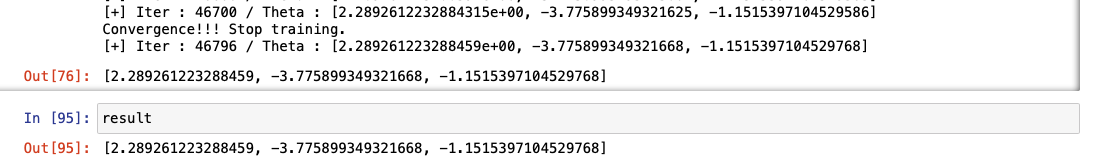
\includegraphics[width=15cm]{ml_2_2.png}
    \caption{Training with Gradient Descent}
    \label{fig:galaxy}
\end{figure}

As you can see, with \texttt{Task1.ipynb}, it took around 46796 iterations to converge all $\theta$s. The total number of iterations might vary time to time depending on your arguments. In my case, for extra precision, I gave no rounding for checking convergence. Meaning that the process was iterated until all 16 fractional digits were identical. As a result, each $\theta$s has value of following table.

\begin{center}
\begin{tabularx}{0.8\textwidth} { 
  | >{\centering\arraybackslash}X 
  | >{\centering\arraybackslash}X 
  | >{\centering\arraybackslash}X | }
 \hline
 \textbf{$\theta_0$} & \textbf{$\theta_1$} & \textbf{$\theta_2$}\\
 \hline
 2.289261223288459  & -3.775899349321668  & -1.1515397104529768 \\
\hline
\end{tabularx}
\end{center}

Therefore, our model is something like this equation.
\[
    h_\theta(x^i) = \frac{1}{1+e^{-(2.289261223288459  + -3.775899349321668 x_1^i + -1.1515397104529768 x_2^i)}}
\]

Meaning that 
\[
    \theta_j = 2.289261223288459 - 3.775899349321668 x_1^i - 3.775899349321668 x_2^i
\]

Now, let's check our model's accuracy and cost using \texttt{calculate_accr} and \texttt{calculate_cost} respectively.
\pagebreak

\begin{figure}[h]
    \centering
    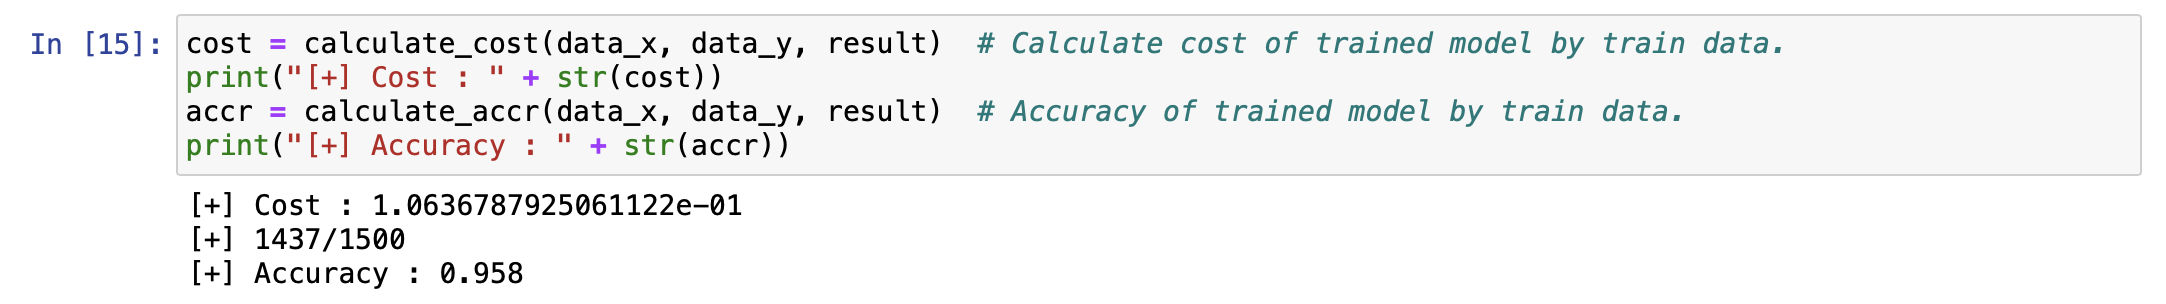
\includegraphics[width=15cm]{ml_2_1.png}
    \caption{Accuracy and Cost with \texttt{train.csv}}
    \label{fig:galaxy}
\end{figure}

Since 1437 data were classified correctly out of 1500 total data, the model had accuracy of 95.8\%. Also, the cost measured with cross entropy was 0.10636787925061122. In summary we can represent our training model with \texttt{train.csv} as following table:

\begin{center}
\begin{tabularx}{0.8\textwidth} { 
  | >{\centering\arraybackslash}X 
  | >{\centering\arraybackslash}X | }
 \hline
 Accuracy & Cost \\
 \hline
 95.8\% & 0.10636787925061122\\
\hline
\end{tabularx}
\end{center}

Now, with those $\theta$ values, let's plot decision boundary with \texttt{train.csv}.

\begin{figure}[h]
    \begin{center}
        \resizebox{0.5\textwidth}{!}{%% Creator: Matplotlib, PGF backend
%%
%% To include the figure in your LaTeX document, write
%%   \input{<filename>.pgf}
%%
%% Make sure the required packages are loaded in your preamble
%%   \usepackage{pgf}
%%
%% Also ensure that all the required font packages are loaded; for instance,
%% the lmodern package is sometimes necessary when using math font.
%%   \usepackage{lmodern}
%%
%% Figures using additional raster images can only be included by \input if
%% they are in the same directory as the main LaTeX file. For loading figures
%% from other directories you can use the `import` package
%%   \usepackage{import}
%%
%% and then include the figures with
%%   \import{<path to file>}{<filename>.pgf}
%%
%% Matplotlib used the following preamble
%%
\begingroup%
\makeatletter%
\begin{pgfpicture}%
\pgfpathrectangle{\pgfpointorigin}{\pgfqpoint{6.000000in}{4.000000in}}%
\pgfusepath{use as bounding box, clip}%
\begin{pgfscope}%
\pgfsetbuttcap%
\pgfsetmiterjoin%
\pgfsetlinewidth{0.000000pt}%
\definecolor{currentstroke}{rgb}{1.000000,1.000000,1.000000}%
\pgfsetstrokecolor{currentstroke}%
\pgfsetstrokeopacity{0.000000}%
\pgfsetdash{}{0pt}%
\pgfpathmoveto{\pgfqpoint{0.000000in}{0.000000in}}%
\pgfpathlineto{\pgfqpoint{6.000000in}{0.000000in}}%
\pgfpathlineto{\pgfqpoint{6.000000in}{4.000000in}}%
\pgfpathlineto{\pgfqpoint{0.000000in}{4.000000in}}%
\pgfpathlineto{\pgfqpoint{0.000000in}{0.000000in}}%
\pgfpathclose%
\pgfusepath{}%
\end{pgfscope}%
\begin{pgfscope}%
\pgfsetbuttcap%
\pgfsetmiterjoin%
\definecolor{currentfill}{rgb}{1.000000,1.000000,1.000000}%
\pgfsetfillcolor{currentfill}%
\pgfsetlinewidth{0.000000pt}%
\definecolor{currentstroke}{rgb}{0.000000,0.000000,0.000000}%
\pgfsetstrokecolor{currentstroke}%
\pgfsetstrokeopacity{0.000000}%
\pgfsetdash{}{0pt}%
\pgfpathmoveto{\pgfqpoint{0.750000in}{0.500000in}}%
\pgfpathlineto{\pgfqpoint{5.400000in}{0.500000in}}%
\pgfpathlineto{\pgfqpoint{5.400000in}{3.520000in}}%
\pgfpathlineto{\pgfqpoint{0.750000in}{3.520000in}}%
\pgfpathlineto{\pgfqpoint{0.750000in}{0.500000in}}%
\pgfpathclose%
\pgfusepath{fill}%
\end{pgfscope}%
\begin{pgfscope}%
\pgfpathrectangle{\pgfqpoint{0.750000in}{0.500000in}}{\pgfqpoint{4.650000in}{3.020000in}}%
\pgfusepath{clip}%
\pgfsetbuttcap%
\pgfsetroundjoin%
\definecolor{currentfill}{rgb}{0.839216,0.152941,0.156863}%
\pgfsetfillcolor{currentfill}%
\pgfsetlinewidth{1.003750pt}%
\definecolor{currentstroke}{rgb}{0.839216,0.152941,0.156863}%
\pgfsetstrokecolor{currentstroke}%
\pgfsetdash{}{0pt}%
\pgfsys@defobject{currentmarker}{\pgfqpoint{-0.041667in}{-0.041667in}}{\pgfqpoint{0.041667in}{0.041667in}}{%
\pgfpathmoveto{\pgfqpoint{0.000000in}{-0.041667in}}%
\pgfpathcurveto{\pgfqpoint{0.011050in}{-0.041667in}}{\pgfqpoint{0.021649in}{-0.037276in}}{\pgfqpoint{0.029463in}{-0.029463in}}%
\pgfpathcurveto{\pgfqpoint{0.037276in}{-0.021649in}}{\pgfqpoint{0.041667in}{-0.011050in}}{\pgfqpoint{0.041667in}{0.000000in}}%
\pgfpathcurveto{\pgfqpoint{0.041667in}{0.011050in}}{\pgfqpoint{0.037276in}{0.021649in}}{\pgfqpoint{0.029463in}{0.029463in}}%
\pgfpathcurveto{\pgfqpoint{0.021649in}{0.037276in}}{\pgfqpoint{0.011050in}{0.041667in}}{\pgfqpoint{0.000000in}{0.041667in}}%
\pgfpathcurveto{\pgfqpoint{-0.011050in}{0.041667in}}{\pgfqpoint{-0.021649in}{0.037276in}}{\pgfqpoint{-0.029463in}{0.029463in}}%
\pgfpathcurveto{\pgfqpoint{-0.037276in}{0.021649in}}{\pgfqpoint{-0.041667in}{0.011050in}}{\pgfqpoint{-0.041667in}{0.000000in}}%
\pgfpathcurveto{\pgfqpoint{-0.041667in}{-0.011050in}}{\pgfqpoint{-0.037276in}{-0.021649in}}{\pgfqpoint{-0.029463in}{-0.029463in}}%
\pgfpathcurveto{\pgfqpoint{-0.021649in}{-0.037276in}}{\pgfqpoint{-0.011050in}{-0.041667in}}{\pgfqpoint{0.000000in}{-0.041667in}}%
\pgfpathlineto{\pgfqpoint{0.000000in}{-0.041667in}}%
\pgfpathclose%
\pgfusepath{stroke,fill}%
}%
\begin{pgfscope}%
\pgfsys@transformshift{4.244333in}{2.003453in}%
\pgfsys@useobject{currentmarker}{}%
\end{pgfscope}%
\end{pgfscope}%
\begin{pgfscope}%
\pgfpathrectangle{\pgfqpoint{0.750000in}{0.500000in}}{\pgfqpoint{4.650000in}{3.020000in}}%
\pgfusepath{clip}%
\pgfsetbuttcap%
\pgfsetroundjoin%
\definecolor{currentfill}{rgb}{0.121569,0.466667,0.705882}%
\pgfsetfillcolor{currentfill}%
\pgfsetlinewidth{1.003750pt}%
\definecolor{currentstroke}{rgb}{0.121569,0.466667,0.705882}%
\pgfsetstrokecolor{currentstroke}%
\pgfsetdash{}{0pt}%
\pgfsys@defobject{currentmarker}{\pgfqpoint{-0.041667in}{-0.041667in}}{\pgfqpoint{0.041667in}{0.041667in}}{%
\pgfpathmoveto{\pgfqpoint{0.000000in}{-0.041667in}}%
\pgfpathcurveto{\pgfqpoint{0.011050in}{-0.041667in}}{\pgfqpoint{0.021649in}{-0.037276in}}{\pgfqpoint{0.029463in}{-0.029463in}}%
\pgfpathcurveto{\pgfqpoint{0.037276in}{-0.021649in}}{\pgfqpoint{0.041667in}{-0.011050in}}{\pgfqpoint{0.041667in}{0.000000in}}%
\pgfpathcurveto{\pgfqpoint{0.041667in}{0.011050in}}{\pgfqpoint{0.037276in}{0.021649in}}{\pgfqpoint{0.029463in}{0.029463in}}%
\pgfpathcurveto{\pgfqpoint{0.021649in}{0.037276in}}{\pgfqpoint{0.011050in}{0.041667in}}{\pgfqpoint{0.000000in}{0.041667in}}%
\pgfpathcurveto{\pgfqpoint{-0.011050in}{0.041667in}}{\pgfqpoint{-0.021649in}{0.037276in}}{\pgfqpoint{-0.029463in}{0.029463in}}%
\pgfpathcurveto{\pgfqpoint{-0.037276in}{0.021649in}}{\pgfqpoint{-0.041667in}{0.011050in}}{\pgfqpoint{-0.041667in}{0.000000in}}%
\pgfpathcurveto{\pgfqpoint{-0.041667in}{-0.011050in}}{\pgfqpoint{-0.037276in}{-0.021649in}}{\pgfqpoint{-0.029463in}{-0.029463in}}%
\pgfpathcurveto{\pgfqpoint{-0.021649in}{-0.037276in}}{\pgfqpoint{-0.011050in}{-0.041667in}}{\pgfqpoint{0.000000in}{-0.041667in}}%
\pgfpathlineto{\pgfqpoint{0.000000in}{-0.041667in}}%
\pgfpathclose%
\pgfusepath{stroke,fill}%
}%
\begin{pgfscope}%
\pgfsys@transformshift{2.598440in}{2.011231in}%
\pgfsys@useobject{currentmarker}{}%
\end{pgfscope}%
\end{pgfscope}%
\begin{pgfscope}%
\pgfpathrectangle{\pgfqpoint{0.750000in}{0.500000in}}{\pgfqpoint{4.650000in}{3.020000in}}%
\pgfusepath{clip}%
\pgfsetbuttcap%
\pgfsetroundjoin%
\definecolor{currentfill}{rgb}{0.121569,0.466667,0.705882}%
\pgfsetfillcolor{currentfill}%
\pgfsetlinewidth{1.003750pt}%
\definecolor{currentstroke}{rgb}{0.121569,0.466667,0.705882}%
\pgfsetstrokecolor{currentstroke}%
\pgfsetdash{}{0pt}%
\pgfpathmoveto{\pgfqpoint{2.598440in}{1.969564in}}%
\pgfpathcurveto{\pgfqpoint{2.609490in}{1.969564in}}{\pgfqpoint{2.620089in}{1.973954in}}{\pgfqpoint{2.627903in}{1.981768in}}%
\pgfpathcurveto{\pgfqpoint{2.635716in}{1.989582in}}{\pgfqpoint{2.640107in}{2.000181in}}{\pgfqpoint{2.640107in}{2.011231in}}%
\pgfpathcurveto{\pgfqpoint{2.640107in}{2.022281in}}{\pgfqpoint{2.635716in}{2.032880in}}{\pgfqpoint{2.627903in}{2.040693in}}%
\pgfpathcurveto{\pgfqpoint{2.620089in}{2.048507in}}{\pgfqpoint{2.609490in}{2.052897in}}{\pgfqpoint{2.598440in}{2.052897in}}%
\pgfpathcurveto{\pgfqpoint{2.587390in}{2.052897in}}{\pgfqpoint{2.576791in}{2.048507in}}{\pgfqpoint{2.568977in}{2.040693in}}%
\pgfpathcurveto{\pgfqpoint{2.561164in}{2.032880in}}{\pgfqpoint{2.556773in}{2.022281in}}{\pgfqpoint{2.556773in}{2.011231in}}%
\pgfpathcurveto{\pgfqpoint{2.556773in}{2.000181in}}{\pgfqpoint{2.561164in}{1.989582in}}{\pgfqpoint{2.568977in}{1.981768in}}%
\pgfpathcurveto{\pgfqpoint{2.576791in}{1.973954in}}{\pgfqpoint{2.587390in}{1.969564in}}{\pgfqpoint{2.598440in}{1.969564in}}%
\pgfpathlineto{\pgfqpoint{2.598440in}{1.969564in}}%
\pgfpathclose%
\pgfusepath{stroke,fill}%
\end{pgfscope}%
\begin{pgfscope}%
\pgfpathrectangle{\pgfqpoint{0.750000in}{0.500000in}}{\pgfqpoint{4.650000in}{3.020000in}}%
\pgfusepath{clip}%
\pgfsetbuttcap%
\pgfsetroundjoin%
\definecolor{currentfill}{rgb}{0.121569,0.466667,0.705882}%
\pgfsetfillcolor{currentfill}%
\pgfsetlinewidth{1.003750pt}%
\definecolor{currentstroke}{rgb}{0.121569,0.466667,0.705882}%
\pgfsetstrokecolor{currentstroke}%
\pgfsetdash{}{0pt}%
\pgfpathmoveto{\pgfqpoint{2.013514in}{2.280525in}}%
\pgfpathcurveto{\pgfqpoint{2.024564in}{2.280525in}}{\pgfqpoint{2.035163in}{2.284915in}}{\pgfqpoint{2.042977in}{2.292729in}}%
\pgfpathcurveto{\pgfqpoint{2.050791in}{2.300543in}}{\pgfqpoint{2.055181in}{2.311142in}}{\pgfqpoint{2.055181in}{2.322192in}}%
\pgfpathcurveto{\pgfqpoint{2.055181in}{2.333242in}}{\pgfqpoint{2.050791in}{2.343841in}}{\pgfqpoint{2.042977in}{2.351654in}}%
\pgfpathcurveto{\pgfqpoint{2.035163in}{2.359468in}}{\pgfqpoint{2.024564in}{2.363858in}}{\pgfqpoint{2.013514in}{2.363858in}}%
\pgfpathcurveto{\pgfqpoint{2.002464in}{2.363858in}}{\pgfqpoint{1.991865in}{2.359468in}}{\pgfqpoint{1.984052in}{2.351654in}}%
\pgfpathcurveto{\pgfqpoint{1.976238in}{2.343841in}}{\pgfqpoint{1.971848in}{2.333242in}}{\pgfqpoint{1.971848in}{2.322192in}}%
\pgfpathcurveto{\pgfqpoint{1.971848in}{2.311142in}}{\pgfqpoint{1.976238in}{2.300543in}}{\pgfqpoint{1.984052in}{2.292729in}}%
\pgfpathcurveto{\pgfqpoint{1.991865in}{2.284915in}}{\pgfqpoint{2.002464in}{2.280525in}}{\pgfqpoint{2.013514in}{2.280525in}}%
\pgfpathlineto{\pgfqpoint{2.013514in}{2.280525in}}%
\pgfpathclose%
\pgfusepath{stroke,fill}%
\end{pgfscope}%
\begin{pgfscope}%
\pgfpathrectangle{\pgfqpoint{0.750000in}{0.500000in}}{\pgfqpoint{4.650000in}{3.020000in}}%
\pgfusepath{clip}%
\pgfsetbuttcap%
\pgfsetroundjoin%
\definecolor{currentfill}{rgb}{0.121569,0.466667,0.705882}%
\pgfsetfillcolor{currentfill}%
\pgfsetlinewidth{1.003750pt}%
\definecolor{currentstroke}{rgb}{0.121569,0.466667,0.705882}%
\pgfsetstrokecolor{currentstroke}%
\pgfsetdash{}{0pt}%
\pgfpathmoveto{\pgfqpoint{2.932076in}{1.564434in}}%
\pgfpathcurveto{\pgfqpoint{2.943126in}{1.564434in}}{\pgfqpoint{2.953725in}{1.568824in}}{\pgfqpoint{2.961539in}{1.576637in}}%
\pgfpathcurveto{\pgfqpoint{2.969353in}{1.584451in}}{\pgfqpoint{2.973743in}{1.595050in}}{\pgfqpoint{2.973743in}{1.606100in}}%
\pgfpathcurveto{\pgfqpoint{2.973743in}{1.617150in}}{\pgfqpoint{2.969353in}{1.627749in}}{\pgfqpoint{2.961539in}{1.635563in}}%
\pgfpathcurveto{\pgfqpoint{2.953725in}{1.643377in}}{\pgfqpoint{2.943126in}{1.647767in}}{\pgfqpoint{2.932076in}{1.647767in}}%
\pgfpathcurveto{\pgfqpoint{2.921026in}{1.647767in}}{\pgfqpoint{2.910427in}{1.643377in}}{\pgfqpoint{2.902613in}{1.635563in}}%
\pgfpathcurveto{\pgfqpoint{2.894800in}{1.627749in}}{\pgfqpoint{2.890410in}{1.617150in}}{\pgfqpoint{2.890410in}{1.606100in}}%
\pgfpathcurveto{\pgfqpoint{2.890410in}{1.595050in}}{\pgfqpoint{2.894800in}{1.584451in}}{\pgfqpoint{2.902613in}{1.576637in}}%
\pgfpathcurveto{\pgfqpoint{2.910427in}{1.568824in}}{\pgfqpoint{2.921026in}{1.564434in}}{\pgfqpoint{2.932076in}{1.564434in}}%
\pgfpathlineto{\pgfqpoint{2.932076in}{1.564434in}}%
\pgfpathclose%
\pgfusepath{stroke,fill}%
\end{pgfscope}%
\begin{pgfscope}%
\pgfpathrectangle{\pgfqpoint{0.750000in}{0.500000in}}{\pgfqpoint{4.650000in}{3.020000in}}%
\pgfusepath{clip}%
\pgfsetbuttcap%
\pgfsetroundjoin%
\definecolor{currentfill}{rgb}{0.121569,0.466667,0.705882}%
\pgfsetfillcolor{currentfill}%
\pgfsetlinewidth{1.003750pt}%
\definecolor{currentstroke}{rgb}{0.121569,0.466667,0.705882}%
\pgfsetstrokecolor{currentstroke}%
\pgfsetdash{}{0pt}%
\pgfpathmoveto{\pgfqpoint{2.200989in}{2.078555in}}%
\pgfpathcurveto{\pgfqpoint{2.212039in}{2.078555in}}{\pgfqpoint{2.222638in}{2.082945in}}{\pgfqpoint{2.230451in}{2.090759in}}%
\pgfpathcurveto{\pgfqpoint{2.238265in}{2.098572in}}{\pgfqpoint{2.242655in}{2.109171in}}{\pgfqpoint{2.242655in}{2.120221in}}%
\pgfpathcurveto{\pgfqpoint{2.242655in}{2.131272in}}{\pgfqpoint{2.238265in}{2.141871in}}{\pgfqpoint{2.230451in}{2.149684in}}%
\pgfpathcurveto{\pgfqpoint{2.222638in}{2.157498in}}{\pgfqpoint{2.212039in}{2.161888in}}{\pgfqpoint{2.200989in}{2.161888in}}%
\pgfpathcurveto{\pgfqpoint{2.189938in}{2.161888in}}{\pgfqpoint{2.179339in}{2.157498in}}{\pgfqpoint{2.171526in}{2.149684in}}%
\pgfpathcurveto{\pgfqpoint{2.163712in}{2.141871in}}{\pgfqpoint{2.159322in}{2.131272in}}{\pgfqpoint{2.159322in}{2.120221in}}%
\pgfpathcurveto{\pgfqpoint{2.159322in}{2.109171in}}{\pgfqpoint{2.163712in}{2.098572in}}{\pgfqpoint{2.171526in}{2.090759in}}%
\pgfpathcurveto{\pgfqpoint{2.179339in}{2.082945in}}{\pgfqpoint{2.189938in}{2.078555in}}{\pgfqpoint{2.200989in}{2.078555in}}%
\pgfpathlineto{\pgfqpoint{2.200989in}{2.078555in}}%
\pgfpathclose%
\pgfusepath{stroke,fill}%
\end{pgfscope}%
\begin{pgfscope}%
\pgfpathrectangle{\pgfqpoint{0.750000in}{0.500000in}}{\pgfqpoint{4.650000in}{3.020000in}}%
\pgfusepath{clip}%
\pgfsetbuttcap%
\pgfsetroundjoin%
\definecolor{currentfill}{rgb}{0.839216,0.152941,0.156863}%
\pgfsetfillcolor{currentfill}%
\pgfsetlinewidth{1.003750pt}%
\definecolor{currentstroke}{rgb}{0.839216,0.152941,0.156863}%
\pgfsetstrokecolor{currentstroke}%
\pgfsetdash{}{0pt}%
\pgfpathmoveto{\pgfqpoint{3.531177in}{2.299282in}}%
\pgfpathcurveto{\pgfqpoint{3.542227in}{2.299282in}}{\pgfqpoint{3.552826in}{2.303673in}}{\pgfqpoint{3.560640in}{2.311486in}}%
\pgfpathcurveto{\pgfqpoint{3.568454in}{2.319300in}}{\pgfqpoint{3.572844in}{2.329899in}}{\pgfqpoint{3.572844in}{2.340949in}}%
\pgfpathcurveto{\pgfqpoint{3.572844in}{2.351999in}}{\pgfqpoint{3.568454in}{2.362598in}}{\pgfqpoint{3.560640in}{2.370412in}}%
\pgfpathcurveto{\pgfqpoint{3.552826in}{2.378225in}}{\pgfqpoint{3.542227in}{2.382616in}}{\pgfqpoint{3.531177in}{2.382616in}}%
\pgfpathcurveto{\pgfqpoint{3.520127in}{2.382616in}}{\pgfqpoint{3.509528in}{2.378225in}}{\pgfqpoint{3.501714in}{2.370412in}}%
\pgfpathcurveto{\pgfqpoint{3.493901in}{2.362598in}}{\pgfqpoint{3.489510in}{2.351999in}}{\pgfqpoint{3.489510in}{2.340949in}}%
\pgfpathcurveto{\pgfqpoint{3.489510in}{2.329899in}}{\pgfqpoint{3.493901in}{2.319300in}}{\pgfqpoint{3.501714in}{2.311486in}}%
\pgfpathcurveto{\pgfqpoint{3.509528in}{2.303673in}}{\pgfqpoint{3.520127in}{2.299282in}}{\pgfqpoint{3.531177in}{2.299282in}}%
\pgfpathlineto{\pgfqpoint{3.531177in}{2.299282in}}%
\pgfpathclose%
\pgfusepath{stroke,fill}%
\end{pgfscope}%
\begin{pgfscope}%
\pgfpathrectangle{\pgfqpoint{0.750000in}{0.500000in}}{\pgfqpoint{4.650000in}{3.020000in}}%
\pgfusepath{clip}%
\pgfsetbuttcap%
\pgfsetroundjoin%
\definecolor{currentfill}{rgb}{0.839216,0.152941,0.156863}%
\pgfsetfillcolor{currentfill}%
\pgfsetlinewidth{1.003750pt}%
\definecolor{currentstroke}{rgb}{0.839216,0.152941,0.156863}%
\pgfsetstrokecolor{currentstroke}%
\pgfsetdash{}{0pt}%
\pgfpathmoveto{\pgfqpoint{3.985192in}{1.995165in}}%
\pgfpathcurveto{\pgfqpoint{3.996242in}{1.995165in}}{\pgfqpoint{4.006841in}{1.999555in}}{\pgfqpoint{4.014655in}{2.007369in}}%
\pgfpathcurveto{\pgfqpoint{4.022469in}{2.015182in}}{\pgfqpoint{4.026859in}{2.025781in}}{\pgfqpoint{4.026859in}{2.036831in}}%
\pgfpathcurveto{\pgfqpoint{4.026859in}{2.047881in}}{\pgfqpoint{4.022469in}{2.058480in}}{\pgfqpoint{4.014655in}{2.066294in}}%
\pgfpathcurveto{\pgfqpoint{4.006841in}{2.074108in}}{\pgfqpoint{3.996242in}{2.078498in}}{\pgfqpoint{3.985192in}{2.078498in}}%
\pgfpathcurveto{\pgfqpoint{3.974142in}{2.078498in}}{\pgfqpoint{3.963543in}{2.074108in}}{\pgfqpoint{3.955729in}{2.066294in}}%
\pgfpathcurveto{\pgfqpoint{3.947916in}{2.058480in}}{\pgfqpoint{3.943525in}{2.047881in}}{\pgfqpoint{3.943525in}{2.036831in}}%
\pgfpathcurveto{\pgfqpoint{3.943525in}{2.025781in}}{\pgfqpoint{3.947916in}{2.015182in}}{\pgfqpoint{3.955729in}{2.007369in}}%
\pgfpathcurveto{\pgfqpoint{3.963543in}{1.999555in}}{\pgfqpoint{3.974142in}{1.995165in}}{\pgfqpoint{3.985192in}{1.995165in}}%
\pgfpathlineto{\pgfqpoint{3.985192in}{1.995165in}}%
\pgfpathclose%
\pgfusepath{stroke,fill}%
\end{pgfscope}%
\begin{pgfscope}%
\pgfpathrectangle{\pgfqpoint{0.750000in}{0.500000in}}{\pgfqpoint{4.650000in}{3.020000in}}%
\pgfusepath{clip}%
\pgfsetbuttcap%
\pgfsetroundjoin%
\definecolor{currentfill}{rgb}{0.839216,0.152941,0.156863}%
\pgfsetfillcolor{currentfill}%
\pgfsetlinewidth{1.003750pt}%
\definecolor{currentstroke}{rgb}{0.839216,0.152941,0.156863}%
\pgfsetstrokecolor{currentstroke}%
\pgfsetdash{}{0pt}%
\pgfpathmoveto{\pgfqpoint{3.387590in}{2.010970in}}%
\pgfpathcurveto{\pgfqpoint{3.398641in}{2.010970in}}{\pgfqpoint{3.409240in}{2.015360in}}{\pgfqpoint{3.417053in}{2.023174in}}%
\pgfpathcurveto{\pgfqpoint{3.424867in}{2.030988in}}{\pgfqpoint{3.429257in}{2.041587in}}{\pgfqpoint{3.429257in}{2.052637in}}%
\pgfpathcurveto{\pgfqpoint{3.429257in}{2.063687in}}{\pgfqpoint{3.424867in}{2.074286in}}{\pgfqpoint{3.417053in}{2.082100in}}%
\pgfpathcurveto{\pgfqpoint{3.409240in}{2.089913in}}{\pgfqpoint{3.398641in}{2.094303in}}{\pgfqpoint{3.387590in}{2.094303in}}%
\pgfpathcurveto{\pgfqpoint{3.376540in}{2.094303in}}{\pgfqpoint{3.365941in}{2.089913in}}{\pgfqpoint{3.358128in}{2.082100in}}%
\pgfpathcurveto{\pgfqpoint{3.350314in}{2.074286in}}{\pgfqpoint{3.345924in}{2.063687in}}{\pgfqpoint{3.345924in}{2.052637in}}%
\pgfpathcurveto{\pgfqpoint{3.345924in}{2.041587in}}{\pgfqpoint{3.350314in}{2.030988in}}{\pgfqpoint{3.358128in}{2.023174in}}%
\pgfpathcurveto{\pgfqpoint{3.365941in}{2.015360in}}{\pgfqpoint{3.376540in}{2.010970in}}{\pgfqpoint{3.387590in}{2.010970in}}%
\pgfpathlineto{\pgfqpoint{3.387590in}{2.010970in}}%
\pgfpathclose%
\pgfusepath{stroke,fill}%
\end{pgfscope}%
\begin{pgfscope}%
\pgfpathrectangle{\pgfqpoint{0.750000in}{0.500000in}}{\pgfqpoint{4.650000in}{3.020000in}}%
\pgfusepath{clip}%
\pgfsetbuttcap%
\pgfsetroundjoin%
\definecolor{currentfill}{rgb}{0.839216,0.152941,0.156863}%
\pgfsetfillcolor{currentfill}%
\pgfsetlinewidth{1.003750pt}%
\definecolor{currentstroke}{rgb}{0.839216,0.152941,0.156863}%
\pgfsetstrokecolor{currentstroke}%
\pgfsetdash{}{0pt}%
\pgfpathmoveto{\pgfqpoint{4.096772in}{2.229572in}}%
\pgfpathcurveto{\pgfqpoint{4.107822in}{2.229572in}}{\pgfqpoint{4.118421in}{2.233962in}}{\pgfqpoint{4.126235in}{2.241775in}}%
\pgfpathcurveto{\pgfqpoint{4.134048in}{2.249589in}}{\pgfqpoint{4.138439in}{2.260188in}}{\pgfqpoint{4.138439in}{2.271238in}}%
\pgfpathcurveto{\pgfqpoint{4.138439in}{2.282288in}}{\pgfqpoint{4.134048in}{2.292887in}}{\pgfqpoint{4.126235in}{2.300701in}}%
\pgfpathcurveto{\pgfqpoint{4.118421in}{2.308515in}}{\pgfqpoint{4.107822in}{2.312905in}}{\pgfqpoint{4.096772in}{2.312905in}}%
\pgfpathcurveto{\pgfqpoint{4.085722in}{2.312905in}}{\pgfqpoint{4.075123in}{2.308515in}}{\pgfqpoint{4.067309in}{2.300701in}}%
\pgfpathcurveto{\pgfqpoint{4.059496in}{2.292887in}}{\pgfqpoint{4.055105in}{2.282288in}}{\pgfqpoint{4.055105in}{2.271238in}}%
\pgfpathcurveto{\pgfqpoint{4.055105in}{2.260188in}}{\pgfqpoint{4.059496in}{2.249589in}}{\pgfqpoint{4.067309in}{2.241775in}}%
\pgfpathcurveto{\pgfqpoint{4.075123in}{2.233962in}}{\pgfqpoint{4.085722in}{2.229572in}}{\pgfqpoint{4.096772in}{2.229572in}}%
\pgfpathlineto{\pgfqpoint{4.096772in}{2.229572in}}%
\pgfpathclose%
\pgfusepath{stroke,fill}%
\end{pgfscope}%
\begin{pgfscope}%
\pgfpathrectangle{\pgfqpoint{0.750000in}{0.500000in}}{\pgfqpoint{4.650000in}{3.020000in}}%
\pgfusepath{clip}%
\pgfsetbuttcap%
\pgfsetroundjoin%
\definecolor{currentfill}{rgb}{0.121569,0.466667,0.705882}%
\pgfsetfillcolor{currentfill}%
\pgfsetlinewidth{1.003750pt}%
\definecolor{currentstroke}{rgb}{0.121569,0.466667,0.705882}%
\pgfsetstrokecolor{currentstroke}%
\pgfsetdash{}{0pt}%
\pgfpathmoveto{\pgfqpoint{2.190560in}{1.944678in}}%
\pgfpathcurveto{\pgfqpoint{2.201610in}{1.944678in}}{\pgfqpoint{2.212209in}{1.949068in}}{\pgfqpoint{2.220023in}{1.956881in}}%
\pgfpathcurveto{\pgfqpoint{2.227836in}{1.964695in}}{\pgfqpoint{2.232227in}{1.975294in}}{\pgfqpoint{2.232227in}{1.986344in}}%
\pgfpathcurveto{\pgfqpoint{2.232227in}{1.997394in}}{\pgfqpoint{2.227836in}{2.007993in}}{\pgfqpoint{2.220023in}{2.015807in}}%
\pgfpathcurveto{\pgfqpoint{2.212209in}{2.023621in}}{\pgfqpoint{2.201610in}{2.028011in}}{\pgfqpoint{2.190560in}{2.028011in}}%
\pgfpathcurveto{\pgfqpoint{2.179510in}{2.028011in}}{\pgfqpoint{2.168911in}{2.023621in}}{\pgfqpoint{2.161097in}{2.015807in}}%
\pgfpathcurveto{\pgfqpoint{2.153284in}{2.007993in}}{\pgfqpoint{2.148893in}{1.997394in}}{\pgfqpoint{2.148893in}{1.986344in}}%
\pgfpathcurveto{\pgfqpoint{2.148893in}{1.975294in}}{\pgfqpoint{2.153284in}{1.964695in}}{\pgfqpoint{2.161097in}{1.956881in}}%
\pgfpathcurveto{\pgfqpoint{2.168911in}{1.949068in}}{\pgfqpoint{2.179510in}{1.944678in}}{\pgfqpoint{2.190560in}{1.944678in}}%
\pgfpathlineto{\pgfqpoint{2.190560in}{1.944678in}}%
\pgfpathclose%
\pgfusepath{stroke,fill}%
\end{pgfscope}%
\begin{pgfscope}%
\pgfpathrectangle{\pgfqpoint{0.750000in}{0.500000in}}{\pgfqpoint{4.650000in}{3.020000in}}%
\pgfusepath{clip}%
\pgfsetbuttcap%
\pgfsetroundjoin%
\definecolor{currentfill}{rgb}{0.121569,0.466667,0.705882}%
\pgfsetfillcolor{currentfill}%
\pgfsetlinewidth{1.003750pt}%
\definecolor{currentstroke}{rgb}{0.121569,0.466667,0.705882}%
\pgfsetstrokecolor{currentstroke}%
\pgfsetdash{}{0pt}%
\pgfpathmoveto{\pgfqpoint{2.090248in}{1.451756in}}%
\pgfpathcurveto{\pgfqpoint{2.101298in}{1.451756in}}{\pgfqpoint{2.111897in}{1.456146in}}{\pgfqpoint{2.119711in}{1.463960in}}%
\pgfpathcurveto{\pgfqpoint{2.127525in}{1.471773in}}{\pgfqpoint{2.131915in}{1.482372in}}{\pgfqpoint{2.131915in}{1.493422in}}%
\pgfpathcurveto{\pgfqpoint{2.131915in}{1.504472in}}{\pgfqpoint{2.127525in}{1.515072in}}{\pgfqpoint{2.119711in}{1.522885in}}%
\pgfpathcurveto{\pgfqpoint{2.111897in}{1.530699in}}{\pgfqpoint{2.101298in}{1.535089in}}{\pgfqpoint{2.090248in}{1.535089in}}%
\pgfpathcurveto{\pgfqpoint{2.079198in}{1.535089in}}{\pgfqpoint{2.068599in}{1.530699in}}{\pgfqpoint{2.060785in}{1.522885in}}%
\pgfpathcurveto{\pgfqpoint{2.052972in}{1.515072in}}{\pgfqpoint{2.048582in}{1.504472in}}{\pgfqpoint{2.048582in}{1.493422in}}%
\pgfpathcurveto{\pgfqpoint{2.048582in}{1.482372in}}{\pgfqpoint{2.052972in}{1.471773in}}{\pgfqpoint{2.060785in}{1.463960in}}%
\pgfpathcurveto{\pgfqpoint{2.068599in}{1.456146in}}{\pgfqpoint{2.079198in}{1.451756in}}{\pgfqpoint{2.090248in}{1.451756in}}%
\pgfpathlineto{\pgfqpoint{2.090248in}{1.451756in}}%
\pgfpathclose%
\pgfusepath{stroke,fill}%
\end{pgfscope}%
\begin{pgfscope}%
\pgfpathrectangle{\pgfqpoint{0.750000in}{0.500000in}}{\pgfqpoint{4.650000in}{3.020000in}}%
\pgfusepath{clip}%
\pgfsetbuttcap%
\pgfsetroundjoin%
\definecolor{currentfill}{rgb}{0.121569,0.466667,0.705882}%
\pgfsetfillcolor{currentfill}%
\pgfsetlinewidth{1.003750pt}%
\definecolor{currentstroke}{rgb}{0.121569,0.466667,0.705882}%
\pgfsetstrokecolor{currentstroke}%
\pgfsetdash{}{0pt}%
\pgfpathmoveto{\pgfqpoint{2.721196in}{1.805111in}}%
\pgfpathcurveto{\pgfqpoint{2.732246in}{1.805111in}}{\pgfqpoint{2.742845in}{1.809501in}}{\pgfqpoint{2.750659in}{1.817314in}}%
\pgfpathcurveto{\pgfqpoint{2.758472in}{1.825128in}}{\pgfqpoint{2.762862in}{1.835727in}}{\pgfqpoint{2.762862in}{1.846777in}}%
\pgfpathcurveto{\pgfqpoint{2.762862in}{1.857827in}}{\pgfqpoint{2.758472in}{1.868426in}}{\pgfqpoint{2.750659in}{1.876240in}}%
\pgfpathcurveto{\pgfqpoint{2.742845in}{1.884054in}}{\pgfqpoint{2.732246in}{1.888444in}}{\pgfqpoint{2.721196in}{1.888444in}}%
\pgfpathcurveto{\pgfqpoint{2.710146in}{1.888444in}}{\pgfqpoint{2.699547in}{1.884054in}}{\pgfqpoint{2.691733in}{1.876240in}}%
\pgfpathcurveto{\pgfqpoint{2.683919in}{1.868426in}}{\pgfqpoint{2.679529in}{1.857827in}}{\pgfqpoint{2.679529in}{1.846777in}}%
\pgfpathcurveto{\pgfqpoint{2.679529in}{1.835727in}}{\pgfqpoint{2.683919in}{1.825128in}}{\pgfqpoint{2.691733in}{1.817314in}}%
\pgfpathcurveto{\pgfqpoint{2.699547in}{1.809501in}}{\pgfqpoint{2.710146in}{1.805111in}}{\pgfqpoint{2.721196in}{1.805111in}}%
\pgfpathlineto{\pgfqpoint{2.721196in}{1.805111in}}%
\pgfpathclose%
\pgfusepath{stroke,fill}%
\end{pgfscope}%
\begin{pgfscope}%
\pgfpathrectangle{\pgfqpoint{0.750000in}{0.500000in}}{\pgfqpoint{4.650000in}{3.020000in}}%
\pgfusepath{clip}%
\pgfsetbuttcap%
\pgfsetroundjoin%
\definecolor{currentfill}{rgb}{0.839216,0.152941,0.156863}%
\pgfsetfillcolor{currentfill}%
\pgfsetlinewidth{1.003750pt}%
\definecolor{currentstroke}{rgb}{0.839216,0.152941,0.156863}%
\pgfsetstrokecolor{currentstroke}%
\pgfsetdash{}{0pt}%
\pgfpathmoveto{\pgfqpoint{3.868223in}{2.209754in}}%
\pgfpathcurveto{\pgfqpoint{3.879273in}{2.209754in}}{\pgfqpoint{3.889872in}{2.214144in}}{\pgfqpoint{3.897686in}{2.221958in}}%
\pgfpathcurveto{\pgfqpoint{3.905500in}{2.229771in}}{\pgfqpoint{3.909890in}{2.240370in}}{\pgfqpoint{3.909890in}{2.251421in}}%
\pgfpathcurveto{\pgfqpoint{3.909890in}{2.262471in}}{\pgfqpoint{3.905500in}{2.273070in}}{\pgfqpoint{3.897686in}{2.280883in}}%
\pgfpathcurveto{\pgfqpoint{3.889872in}{2.288697in}}{\pgfqpoint{3.879273in}{2.293087in}}{\pgfqpoint{3.868223in}{2.293087in}}%
\pgfpathcurveto{\pgfqpoint{3.857173in}{2.293087in}}{\pgfqpoint{3.846574in}{2.288697in}}{\pgfqpoint{3.838761in}{2.280883in}}%
\pgfpathcurveto{\pgfqpoint{3.830947in}{2.273070in}}{\pgfqpoint{3.826557in}{2.262471in}}{\pgfqpoint{3.826557in}{2.251421in}}%
\pgfpathcurveto{\pgfqpoint{3.826557in}{2.240370in}}{\pgfqpoint{3.830947in}{2.229771in}}{\pgfqpoint{3.838761in}{2.221958in}}%
\pgfpathcurveto{\pgfqpoint{3.846574in}{2.214144in}}{\pgfqpoint{3.857173in}{2.209754in}}{\pgfqpoint{3.868223in}{2.209754in}}%
\pgfpathlineto{\pgfqpoint{3.868223in}{2.209754in}}%
\pgfpathclose%
\pgfusepath{stroke,fill}%
\end{pgfscope}%
\begin{pgfscope}%
\pgfpathrectangle{\pgfqpoint{0.750000in}{0.500000in}}{\pgfqpoint{4.650000in}{3.020000in}}%
\pgfusepath{clip}%
\pgfsetbuttcap%
\pgfsetroundjoin%
\definecolor{currentfill}{rgb}{0.121569,0.466667,0.705882}%
\pgfsetfillcolor{currentfill}%
\pgfsetlinewidth{1.003750pt}%
\definecolor{currentstroke}{rgb}{0.121569,0.466667,0.705882}%
\pgfsetstrokecolor{currentstroke}%
\pgfsetdash{}{0pt}%
\pgfpathmoveto{\pgfqpoint{2.540209in}{1.831825in}}%
\pgfpathcurveto{\pgfqpoint{2.551260in}{1.831825in}}{\pgfqpoint{2.561859in}{1.836215in}}{\pgfqpoint{2.569672in}{1.844029in}}%
\pgfpathcurveto{\pgfqpoint{2.577486in}{1.851843in}}{\pgfqpoint{2.581876in}{1.862442in}}{\pgfqpoint{2.581876in}{1.873492in}}%
\pgfpathcurveto{\pgfqpoint{2.581876in}{1.884542in}}{\pgfqpoint{2.577486in}{1.895141in}}{\pgfqpoint{2.569672in}{1.902954in}}%
\pgfpathcurveto{\pgfqpoint{2.561859in}{1.910768in}}{\pgfqpoint{2.551260in}{1.915158in}}{\pgfqpoint{2.540209in}{1.915158in}}%
\pgfpathcurveto{\pgfqpoint{2.529159in}{1.915158in}}{\pgfqpoint{2.518560in}{1.910768in}}{\pgfqpoint{2.510747in}{1.902954in}}%
\pgfpathcurveto{\pgfqpoint{2.502933in}{1.895141in}}{\pgfqpoint{2.498543in}{1.884542in}}{\pgfqpoint{2.498543in}{1.873492in}}%
\pgfpathcurveto{\pgfqpoint{2.498543in}{1.862442in}}{\pgfqpoint{2.502933in}{1.851843in}}{\pgfqpoint{2.510747in}{1.844029in}}%
\pgfpathcurveto{\pgfqpoint{2.518560in}{1.836215in}}{\pgfqpoint{2.529159in}{1.831825in}}{\pgfqpoint{2.540209in}{1.831825in}}%
\pgfpathlineto{\pgfqpoint{2.540209in}{1.831825in}}%
\pgfpathclose%
\pgfusepath{stroke,fill}%
\end{pgfscope}%
\begin{pgfscope}%
\pgfpathrectangle{\pgfqpoint{0.750000in}{0.500000in}}{\pgfqpoint{4.650000in}{3.020000in}}%
\pgfusepath{clip}%
\pgfsetbuttcap%
\pgfsetroundjoin%
\definecolor{currentfill}{rgb}{0.839216,0.152941,0.156863}%
\pgfsetfillcolor{currentfill}%
\pgfsetlinewidth{1.003750pt}%
\definecolor{currentstroke}{rgb}{0.839216,0.152941,0.156863}%
\pgfsetstrokecolor{currentstroke}%
\pgfsetdash{}{0pt}%
\pgfpathmoveto{\pgfqpoint{3.846238in}{2.110506in}}%
\pgfpathcurveto{\pgfqpoint{3.857288in}{2.110506in}}{\pgfqpoint{3.867887in}{2.114896in}}{\pgfqpoint{3.875700in}{2.122709in}}%
\pgfpathcurveto{\pgfqpoint{3.883514in}{2.130523in}}{\pgfqpoint{3.887904in}{2.141122in}}{\pgfqpoint{3.887904in}{2.152172in}}%
\pgfpathcurveto{\pgfqpoint{3.887904in}{2.163222in}}{\pgfqpoint{3.883514in}{2.173821in}}{\pgfqpoint{3.875700in}{2.181635in}}%
\pgfpathcurveto{\pgfqpoint{3.867887in}{2.189449in}}{\pgfqpoint{3.857288in}{2.193839in}}{\pgfqpoint{3.846238in}{2.193839in}}%
\pgfpathcurveto{\pgfqpoint{3.835188in}{2.193839in}}{\pgfqpoint{3.824589in}{2.189449in}}{\pgfqpoint{3.816775in}{2.181635in}}%
\pgfpathcurveto{\pgfqpoint{3.808961in}{2.173821in}}{\pgfqpoint{3.804571in}{2.163222in}}{\pgfqpoint{3.804571in}{2.152172in}}%
\pgfpathcurveto{\pgfqpoint{3.804571in}{2.141122in}}{\pgfqpoint{3.808961in}{2.130523in}}{\pgfqpoint{3.816775in}{2.122709in}}%
\pgfpathcurveto{\pgfqpoint{3.824589in}{2.114896in}}{\pgfqpoint{3.835188in}{2.110506in}}{\pgfqpoint{3.846238in}{2.110506in}}%
\pgfpathlineto{\pgfqpoint{3.846238in}{2.110506in}}%
\pgfpathclose%
\pgfusepath{stroke,fill}%
\end{pgfscope}%
\begin{pgfscope}%
\pgfpathrectangle{\pgfqpoint{0.750000in}{0.500000in}}{\pgfqpoint{4.650000in}{3.020000in}}%
\pgfusepath{clip}%
\pgfsetbuttcap%
\pgfsetroundjoin%
\definecolor{currentfill}{rgb}{0.121569,0.466667,0.705882}%
\pgfsetfillcolor{currentfill}%
\pgfsetlinewidth{1.003750pt}%
\definecolor{currentstroke}{rgb}{0.121569,0.466667,0.705882}%
\pgfsetstrokecolor{currentstroke}%
\pgfsetdash{}{0pt}%
\pgfpathmoveto{\pgfqpoint{3.549734in}{2.165925in}}%
\pgfpathcurveto{\pgfqpoint{3.560784in}{2.165925in}}{\pgfqpoint{3.571383in}{2.170316in}}{\pgfqpoint{3.579197in}{2.178129in}}%
\pgfpathcurveto{\pgfqpoint{3.587010in}{2.185943in}}{\pgfqpoint{3.591401in}{2.196542in}}{\pgfqpoint{3.591401in}{2.207592in}}%
\pgfpathcurveto{\pgfqpoint{3.591401in}{2.218642in}}{\pgfqpoint{3.587010in}{2.229241in}}{\pgfqpoint{3.579197in}{2.237055in}}%
\pgfpathcurveto{\pgfqpoint{3.571383in}{2.244868in}}{\pgfqpoint{3.560784in}{2.249259in}}{\pgfqpoint{3.549734in}{2.249259in}}%
\pgfpathcurveto{\pgfqpoint{3.538684in}{2.249259in}}{\pgfqpoint{3.528085in}{2.244868in}}{\pgfqpoint{3.520271in}{2.237055in}}%
\pgfpathcurveto{\pgfqpoint{3.512457in}{2.229241in}}{\pgfqpoint{3.508067in}{2.218642in}}{\pgfqpoint{3.508067in}{2.207592in}}%
\pgfpathcurveto{\pgfqpoint{3.508067in}{2.196542in}}{\pgfqpoint{3.512457in}{2.185943in}}{\pgfqpoint{3.520271in}{2.178129in}}%
\pgfpathcurveto{\pgfqpoint{3.528085in}{2.170316in}}{\pgfqpoint{3.538684in}{2.165925in}}{\pgfqpoint{3.549734in}{2.165925in}}%
\pgfpathlineto{\pgfqpoint{3.549734in}{2.165925in}}%
\pgfpathclose%
\pgfusepath{stroke,fill}%
\end{pgfscope}%
\begin{pgfscope}%
\pgfpathrectangle{\pgfqpoint{0.750000in}{0.500000in}}{\pgfqpoint{4.650000in}{3.020000in}}%
\pgfusepath{clip}%
\pgfsetbuttcap%
\pgfsetroundjoin%
\definecolor{currentfill}{rgb}{0.839216,0.152941,0.156863}%
\pgfsetfillcolor{currentfill}%
\pgfsetlinewidth{1.003750pt}%
\definecolor{currentstroke}{rgb}{0.839216,0.152941,0.156863}%
\pgfsetstrokecolor{currentstroke}%
\pgfsetdash{}{0pt}%
\pgfpathmoveto{\pgfqpoint{4.417068in}{2.265654in}}%
\pgfpathcurveto{\pgfqpoint{4.428118in}{2.265654in}}{\pgfqpoint{4.438718in}{2.270045in}}{\pgfqpoint{4.446531in}{2.277858in}}%
\pgfpathcurveto{\pgfqpoint{4.454345in}{2.285672in}}{\pgfqpoint{4.458735in}{2.296271in}}{\pgfqpoint{4.458735in}{2.307321in}}%
\pgfpathcurveto{\pgfqpoint{4.458735in}{2.318371in}}{\pgfqpoint{4.454345in}{2.328970in}}{\pgfqpoint{4.446531in}{2.336784in}}%
\pgfpathcurveto{\pgfqpoint{4.438718in}{2.344598in}}{\pgfqpoint{4.428118in}{2.348988in}}{\pgfqpoint{4.417068in}{2.348988in}}%
\pgfpathcurveto{\pgfqpoint{4.406018in}{2.348988in}}{\pgfqpoint{4.395419in}{2.344598in}}{\pgfqpoint{4.387606in}{2.336784in}}%
\pgfpathcurveto{\pgfqpoint{4.379792in}{2.328970in}}{\pgfqpoint{4.375402in}{2.318371in}}{\pgfqpoint{4.375402in}{2.307321in}}%
\pgfpathcurveto{\pgfqpoint{4.375402in}{2.296271in}}{\pgfqpoint{4.379792in}{2.285672in}}{\pgfqpoint{4.387606in}{2.277858in}}%
\pgfpathcurveto{\pgfqpoint{4.395419in}{2.270045in}}{\pgfqpoint{4.406018in}{2.265654in}}{\pgfqpoint{4.417068in}{2.265654in}}%
\pgfpathlineto{\pgfqpoint{4.417068in}{2.265654in}}%
\pgfpathclose%
\pgfusepath{stroke,fill}%
\end{pgfscope}%
\begin{pgfscope}%
\pgfpathrectangle{\pgfqpoint{0.750000in}{0.500000in}}{\pgfqpoint{4.650000in}{3.020000in}}%
\pgfusepath{clip}%
\pgfsetbuttcap%
\pgfsetroundjoin%
\definecolor{currentfill}{rgb}{0.121569,0.466667,0.705882}%
\pgfsetfillcolor{currentfill}%
\pgfsetlinewidth{1.003750pt}%
\definecolor{currentstroke}{rgb}{0.121569,0.466667,0.705882}%
\pgfsetstrokecolor{currentstroke}%
\pgfsetdash{}{0pt}%
\pgfpathmoveto{\pgfqpoint{2.168317in}{2.009907in}}%
\pgfpathcurveto{\pgfqpoint{2.179367in}{2.009907in}}{\pgfqpoint{2.189966in}{2.014297in}}{\pgfqpoint{2.197780in}{2.022111in}}%
\pgfpathcurveto{\pgfqpoint{2.205593in}{2.029924in}}{\pgfqpoint{2.209984in}{2.040523in}}{\pgfqpoint{2.209984in}{2.051573in}}%
\pgfpathcurveto{\pgfqpoint{2.209984in}{2.062623in}}{\pgfqpoint{2.205593in}{2.073223in}}{\pgfqpoint{2.197780in}{2.081036in}}%
\pgfpathcurveto{\pgfqpoint{2.189966in}{2.088850in}}{\pgfqpoint{2.179367in}{2.093240in}}{\pgfqpoint{2.168317in}{2.093240in}}%
\pgfpathcurveto{\pgfqpoint{2.157267in}{2.093240in}}{\pgfqpoint{2.146668in}{2.088850in}}{\pgfqpoint{2.138854in}{2.081036in}}%
\pgfpathcurveto{\pgfqpoint{2.131040in}{2.073223in}}{\pgfqpoint{2.126650in}{2.062623in}}{\pgfqpoint{2.126650in}{2.051573in}}%
\pgfpathcurveto{\pgfqpoint{2.126650in}{2.040523in}}{\pgfqpoint{2.131040in}{2.029924in}}{\pgfqpoint{2.138854in}{2.022111in}}%
\pgfpathcurveto{\pgfqpoint{2.146668in}{2.014297in}}{\pgfqpoint{2.157267in}{2.009907in}}{\pgfqpoint{2.168317in}{2.009907in}}%
\pgfpathlineto{\pgfqpoint{2.168317in}{2.009907in}}%
\pgfpathclose%
\pgfusepath{stroke,fill}%
\end{pgfscope}%
\begin{pgfscope}%
\pgfpathrectangle{\pgfqpoint{0.750000in}{0.500000in}}{\pgfqpoint{4.650000in}{3.020000in}}%
\pgfusepath{clip}%
\pgfsetbuttcap%
\pgfsetroundjoin%
\definecolor{currentfill}{rgb}{0.121569,0.466667,0.705882}%
\pgfsetfillcolor{currentfill}%
\pgfsetlinewidth{1.003750pt}%
\definecolor{currentstroke}{rgb}{0.121569,0.466667,0.705882}%
\pgfsetstrokecolor{currentstroke}%
\pgfsetdash{}{0pt}%
\pgfpathmoveto{\pgfqpoint{2.774204in}{2.106319in}}%
\pgfpathcurveto{\pgfqpoint{2.785254in}{2.106319in}}{\pgfqpoint{2.795853in}{2.110709in}}{\pgfqpoint{2.803666in}{2.118523in}}%
\pgfpathcurveto{\pgfqpoint{2.811480in}{2.126336in}}{\pgfqpoint{2.815870in}{2.136936in}}{\pgfqpoint{2.815870in}{2.147986in}}%
\pgfpathcurveto{\pgfqpoint{2.815870in}{2.159036in}}{\pgfqpoint{2.811480in}{2.169635in}}{\pgfqpoint{2.803666in}{2.177448in}}%
\pgfpathcurveto{\pgfqpoint{2.795853in}{2.185262in}}{\pgfqpoint{2.785254in}{2.189652in}}{\pgfqpoint{2.774204in}{2.189652in}}%
\pgfpathcurveto{\pgfqpoint{2.763154in}{2.189652in}}{\pgfqpoint{2.752554in}{2.185262in}}{\pgfqpoint{2.744741in}{2.177448in}}%
\pgfpathcurveto{\pgfqpoint{2.736927in}{2.169635in}}{\pgfqpoint{2.732537in}{2.159036in}}{\pgfqpoint{2.732537in}{2.147986in}}%
\pgfpathcurveto{\pgfqpoint{2.732537in}{2.136936in}}{\pgfqpoint{2.736927in}{2.126336in}}{\pgfqpoint{2.744741in}{2.118523in}}%
\pgfpathcurveto{\pgfqpoint{2.752554in}{2.110709in}}{\pgfqpoint{2.763154in}{2.106319in}}{\pgfqpoint{2.774204in}{2.106319in}}%
\pgfpathlineto{\pgfqpoint{2.774204in}{2.106319in}}%
\pgfpathclose%
\pgfusepath{stroke,fill}%
\end{pgfscope}%
\begin{pgfscope}%
\pgfpathrectangle{\pgfqpoint{0.750000in}{0.500000in}}{\pgfqpoint{4.650000in}{3.020000in}}%
\pgfusepath{clip}%
\pgfsetbuttcap%
\pgfsetroundjoin%
\definecolor{currentfill}{rgb}{0.121569,0.466667,0.705882}%
\pgfsetfillcolor{currentfill}%
\pgfsetlinewidth{1.003750pt}%
\definecolor{currentstroke}{rgb}{0.121569,0.466667,0.705882}%
\pgfsetstrokecolor{currentstroke}%
\pgfsetdash{}{0pt}%
\pgfpathmoveto{\pgfqpoint{1.854683in}{1.821953in}}%
\pgfpathcurveto{\pgfqpoint{1.865733in}{1.821953in}}{\pgfqpoint{1.876333in}{1.826343in}}{\pgfqpoint{1.884146in}{1.834157in}}%
\pgfpathcurveto{\pgfqpoint{1.891960in}{1.841970in}}{\pgfqpoint{1.896350in}{1.852569in}}{\pgfqpoint{1.896350in}{1.863619in}}%
\pgfpathcurveto{\pgfqpoint{1.896350in}{1.874670in}}{\pgfqpoint{1.891960in}{1.885269in}}{\pgfqpoint{1.884146in}{1.893082in}}%
\pgfpathcurveto{\pgfqpoint{1.876333in}{1.900896in}}{\pgfqpoint{1.865733in}{1.905286in}}{\pgfqpoint{1.854683in}{1.905286in}}%
\pgfpathcurveto{\pgfqpoint{1.843633in}{1.905286in}}{\pgfqpoint{1.833034in}{1.900896in}}{\pgfqpoint{1.825221in}{1.893082in}}%
\pgfpathcurveto{\pgfqpoint{1.817407in}{1.885269in}}{\pgfqpoint{1.813017in}{1.874670in}}{\pgfqpoint{1.813017in}{1.863619in}}%
\pgfpathcurveto{\pgfqpoint{1.813017in}{1.852569in}}{\pgfqpoint{1.817407in}{1.841970in}}{\pgfqpoint{1.825221in}{1.834157in}}%
\pgfpathcurveto{\pgfqpoint{1.833034in}{1.826343in}}{\pgfqpoint{1.843633in}{1.821953in}}{\pgfqpoint{1.854683in}{1.821953in}}%
\pgfpathlineto{\pgfqpoint{1.854683in}{1.821953in}}%
\pgfpathclose%
\pgfusepath{stroke,fill}%
\end{pgfscope}%
\begin{pgfscope}%
\pgfpathrectangle{\pgfqpoint{0.750000in}{0.500000in}}{\pgfqpoint{4.650000in}{3.020000in}}%
\pgfusepath{clip}%
\pgfsetbuttcap%
\pgfsetroundjoin%
\definecolor{currentfill}{rgb}{0.121569,0.466667,0.705882}%
\pgfsetfillcolor{currentfill}%
\pgfsetlinewidth{1.003750pt}%
\definecolor{currentstroke}{rgb}{0.121569,0.466667,0.705882}%
\pgfsetstrokecolor{currentstroke}%
\pgfsetdash{}{0pt}%
\pgfpathmoveto{\pgfqpoint{2.432368in}{1.951205in}}%
\pgfpathcurveto{\pgfqpoint{2.443418in}{1.951205in}}{\pgfqpoint{2.454017in}{1.955596in}}{\pgfqpoint{2.461830in}{1.963409in}}%
\pgfpathcurveto{\pgfqpoint{2.469644in}{1.971223in}}{\pgfqpoint{2.474034in}{1.981822in}}{\pgfqpoint{2.474034in}{1.992872in}}%
\pgfpathcurveto{\pgfqpoint{2.474034in}{2.003922in}}{\pgfqpoint{2.469644in}{2.014521in}}{\pgfqpoint{2.461830in}{2.022335in}}%
\pgfpathcurveto{\pgfqpoint{2.454017in}{2.030148in}}{\pgfqpoint{2.443418in}{2.034539in}}{\pgfqpoint{2.432368in}{2.034539in}}%
\pgfpathcurveto{\pgfqpoint{2.421317in}{2.034539in}}{\pgfqpoint{2.410718in}{2.030148in}}{\pgfqpoint{2.402905in}{2.022335in}}%
\pgfpathcurveto{\pgfqpoint{2.395091in}{2.014521in}}{\pgfqpoint{2.390701in}{2.003922in}}{\pgfqpoint{2.390701in}{1.992872in}}%
\pgfpathcurveto{\pgfqpoint{2.390701in}{1.981822in}}{\pgfqpoint{2.395091in}{1.971223in}}{\pgfqpoint{2.402905in}{1.963409in}}%
\pgfpathcurveto{\pgfqpoint{2.410718in}{1.955596in}}{\pgfqpoint{2.421317in}{1.951205in}}{\pgfqpoint{2.432368in}{1.951205in}}%
\pgfpathlineto{\pgfqpoint{2.432368in}{1.951205in}}%
\pgfpathclose%
\pgfusepath{stroke,fill}%
\end{pgfscope}%
\begin{pgfscope}%
\pgfpathrectangle{\pgfqpoint{0.750000in}{0.500000in}}{\pgfqpoint{4.650000in}{3.020000in}}%
\pgfusepath{clip}%
\pgfsetbuttcap%
\pgfsetroundjoin%
\definecolor{currentfill}{rgb}{0.839216,0.152941,0.156863}%
\pgfsetfillcolor{currentfill}%
\pgfsetlinewidth{1.003750pt}%
\definecolor{currentstroke}{rgb}{0.839216,0.152941,0.156863}%
\pgfsetstrokecolor{currentstroke}%
\pgfsetdash{}{0pt}%
\pgfpathmoveto{\pgfqpoint{4.462739in}{1.697642in}}%
\pgfpathcurveto{\pgfqpoint{4.473789in}{1.697642in}}{\pgfqpoint{4.484388in}{1.702032in}}{\pgfqpoint{4.492202in}{1.709846in}}%
\pgfpathcurveto{\pgfqpoint{4.500016in}{1.717659in}}{\pgfqpoint{4.504406in}{1.728259in}}{\pgfqpoint{4.504406in}{1.739309in}}%
\pgfpathcurveto{\pgfqpoint{4.504406in}{1.750359in}}{\pgfqpoint{4.500016in}{1.760958in}}{\pgfqpoint{4.492202in}{1.768771in}}%
\pgfpathcurveto{\pgfqpoint{4.484388in}{1.776585in}}{\pgfqpoint{4.473789in}{1.780975in}}{\pgfqpoint{4.462739in}{1.780975in}}%
\pgfpathcurveto{\pgfqpoint{4.451689in}{1.780975in}}{\pgfqpoint{4.441090in}{1.776585in}}{\pgfqpoint{4.433277in}{1.768771in}}%
\pgfpathcurveto{\pgfqpoint{4.425463in}{1.760958in}}{\pgfqpoint{4.421073in}{1.750359in}}{\pgfqpoint{4.421073in}{1.739309in}}%
\pgfpathcurveto{\pgfqpoint{4.421073in}{1.728259in}}{\pgfqpoint{4.425463in}{1.717659in}}{\pgfqpoint{4.433277in}{1.709846in}}%
\pgfpathcurveto{\pgfqpoint{4.441090in}{1.702032in}}{\pgfqpoint{4.451689in}{1.697642in}}{\pgfqpoint{4.462739in}{1.697642in}}%
\pgfpathlineto{\pgfqpoint{4.462739in}{1.697642in}}%
\pgfpathclose%
\pgfusepath{stroke,fill}%
\end{pgfscope}%
\begin{pgfscope}%
\pgfpathrectangle{\pgfqpoint{0.750000in}{0.500000in}}{\pgfqpoint{4.650000in}{3.020000in}}%
\pgfusepath{clip}%
\pgfsetbuttcap%
\pgfsetroundjoin%
\definecolor{currentfill}{rgb}{0.839216,0.152941,0.156863}%
\pgfsetfillcolor{currentfill}%
\pgfsetlinewidth{1.003750pt}%
\definecolor{currentstroke}{rgb}{0.839216,0.152941,0.156863}%
\pgfsetstrokecolor{currentstroke}%
\pgfsetdash{}{0pt}%
\pgfpathmoveto{\pgfqpoint{3.850860in}{2.187577in}}%
\pgfpathcurveto{\pgfqpoint{3.861910in}{2.187577in}}{\pgfqpoint{3.872509in}{2.191967in}}{\pgfqpoint{3.880323in}{2.199781in}}%
\pgfpathcurveto{\pgfqpoint{3.888137in}{2.207595in}}{\pgfqpoint{3.892527in}{2.218194in}}{\pgfqpoint{3.892527in}{2.229244in}}%
\pgfpathcurveto{\pgfqpoint{3.892527in}{2.240294in}}{\pgfqpoint{3.888137in}{2.250893in}}{\pgfqpoint{3.880323in}{2.258707in}}%
\pgfpathcurveto{\pgfqpoint{3.872509in}{2.266520in}}{\pgfqpoint{3.861910in}{2.270911in}}{\pgfqpoint{3.850860in}{2.270911in}}%
\pgfpathcurveto{\pgfqpoint{3.839810in}{2.270911in}}{\pgfqpoint{3.829211in}{2.266520in}}{\pgfqpoint{3.821397in}{2.258707in}}%
\pgfpathcurveto{\pgfqpoint{3.813584in}{2.250893in}}{\pgfqpoint{3.809194in}{2.240294in}}{\pgfqpoint{3.809194in}{2.229244in}}%
\pgfpathcurveto{\pgfqpoint{3.809194in}{2.218194in}}{\pgfqpoint{3.813584in}{2.207595in}}{\pgfqpoint{3.821397in}{2.199781in}}%
\pgfpathcurveto{\pgfqpoint{3.829211in}{2.191967in}}{\pgfqpoint{3.839810in}{2.187577in}}{\pgfqpoint{3.850860in}{2.187577in}}%
\pgfpathlineto{\pgfqpoint{3.850860in}{2.187577in}}%
\pgfpathclose%
\pgfusepath{stroke,fill}%
\end{pgfscope}%
\begin{pgfscope}%
\pgfpathrectangle{\pgfqpoint{0.750000in}{0.500000in}}{\pgfqpoint{4.650000in}{3.020000in}}%
\pgfusepath{clip}%
\pgfsetbuttcap%
\pgfsetroundjoin%
\definecolor{currentfill}{rgb}{0.839216,0.152941,0.156863}%
\pgfsetfillcolor{currentfill}%
\pgfsetlinewidth{1.003750pt}%
\definecolor{currentstroke}{rgb}{0.839216,0.152941,0.156863}%
\pgfsetstrokecolor{currentstroke}%
\pgfsetdash{}{0pt}%
\pgfpathmoveto{\pgfqpoint{4.073076in}{2.423759in}}%
\pgfpathcurveto{\pgfqpoint{4.084126in}{2.423759in}}{\pgfqpoint{4.094725in}{2.428149in}}{\pgfqpoint{4.102539in}{2.435963in}}%
\pgfpathcurveto{\pgfqpoint{4.110353in}{2.443777in}}{\pgfqpoint{4.114743in}{2.454376in}}{\pgfqpoint{4.114743in}{2.465426in}}%
\pgfpathcurveto{\pgfqpoint{4.114743in}{2.476476in}}{\pgfqpoint{4.110353in}{2.487075in}}{\pgfqpoint{4.102539in}{2.494888in}}%
\pgfpathcurveto{\pgfqpoint{4.094725in}{2.502702in}}{\pgfqpoint{4.084126in}{2.507092in}}{\pgfqpoint{4.073076in}{2.507092in}}%
\pgfpathcurveto{\pgfqpoint{4.062026in}{2.507092in}}{\pgfqpoint{4.051427in}{2.502702in}}{\pgfqpoint{4.043613in}{2.494888in}}%
\pgfpathcurveto{\pgfqpoint{4.035800in}{2.487075in}}{\pgfqpoint{4.031409in}{2.476476in}}{\pgfqpoint{4.031409in}{2.465426in}}%
\pgfpathcurveto{\pgfqpoint{4.031409in}{2.454376in}}{\pgfqpoint{4.035800in}{2.443777in}}{\pgfqpoint{4.043613in}{2.435963in}}%
\pgfpathcurveto{\pgfqpoint{4.051427in}{2.428149in}}{\pgfqpoint{4.062026in}{2.423759in}}{\pgfqpoint{4.073076in}{2.423759in}}%
\pgfpathlineto{\pgfqpoint{4.073076in}{2.423759in}}%
\pgfpathclose%
\pgfusepath{stroke,fill}%
\end{pgfscope}%
\begin{pgfscope}%
\pgfpathrectangle{\pgfqpoint{0.750000in}{0.500000in}}{\pgfqpoint{4.650000in}{3.020000in}}%
\pgfusepath{clip}%
\pgfsetbuttcap%
\pgfsetroundjoin%
\definecolor{currentfill}{rgb}{0.839216,0.152941,0.156863}%
\pgfsetfillcolor{currentfill}%
\pgfsetlinewidth{1.003750pt}%
\definecolor{currentstroke}{rgb}{0.839216,0.152941,0.156863}%
\pgfsetstrokecolor{currentstroke}%
\pgfsetdash{}{0pt}%
\pgfpathmoveto{\pgfqpoint{3.387115in}{2.545794in}}%
\pgfpathcurveto{\pgfqpoint{3.398165in}{2.545794in}}{\pgfqpoint{3.408764in}{2.550184in}}{\pgfqpoint{3.416577in}{2.557998in}}%
\pgfpathcurveto{\pgfqpoint{3.424391in}{2.565811in}}{\pgfqpoint{3.428781in}{2.576410in}}{\pgfqpoint{3.428781in}{2.587460in}}%
\pgfpathcurveto{\pgfqpoint{3.428781in}{2.598511in}}{\pgfqpoint{3.424391in}{2.609110in}}{\pgfqpoint{3.416577in}{2.616923in}}%
\pgfpathcurveto{\pgfqpoint{3.408764in}{2.624737in}}{\pgfqpoint{3.398165in}{2.629127in}}{\pgfqpoint{3.387115in}{2.629127in}}%
\pgfpathcurveto{\pgfqpoint{3.376065in}{2.629127in}}{\pgfqpoint{3.365466in}{2.624737in}}{\pgfqpoint{3.357652in}{2.616923in}}%
\pgfpathcurveto{\pgfqpoint{3.349838in}{2.609110in}}{\pgfqpoint{3.345448in}{2.598511in}}{\pgfqpoint{3.345448in}{2.587460in}}%
\pgfpathcurveto{\pgfqpoint{3.345448in}{2.576410in}}{\pgfqpoint{3.349838in}{2.565811in}}{\pgfqpoint{3.357652in}{2.557998in}}%
\pgfpathcurveto{\pgfqpoint{3.365466in}{2.550184in}}{\pgfqpoint{3.376065in}{2.545794in}}{\pgfqpoint{3.387115in}{2.545794in}}%
\pgfpathlineto{\pgfqpoint{3.387115in}{2.545794in}}%
\pgfpathclose%
\pgfusepath{stroke,fill}%
\end{pgfscope}%
\begin{pgfscope}%
\pgfpathrectangle{\pgfqpoint{0.750000in}{0.500000in}}{\pgfqpoint{4.650000in}{3.020000in}}%
\pgfusepath{clip}%
\pgfsetbuttcap%
\pgfsetroundjoin%
\definecolor{currentfill}{rgb}{0.121569,0.466667,0.705882}%
\pgfsetfillcolor{currentfill}%
\pgfsetlinewidth{1.003750pt}%
\definecolor{currentstroke}{rgb}{0.121569,0.466667,0.705882}%
\pgfsetstrokecolor{currentstroke}%
\pgfsetdash{}{0pt}%
\pgfpathmoveto{\pgfqpoint{2.135799in}{1.616679in}}%
\pgfpathcurveto{\pgfqpoint{2.146849in}{1.616679in}}{\pgfqpoint{2.157448in}{1.621069in}}{\pgfqpoint{2.165262in}{1.628883in}}%
\pgfpathcurveto{\pgfqpoint{2.173075in}{1.636696in}}{\pgfqpoint{2.177466in}{1.647295in}}{\pgfqpoint{2.177466in}{1.658345in}}%
\pgfpathcurveto{\pgfqpoint{2.177466in}{1.669396in}}{\pgfqpoint{2.173075in}{1.679995in}}{\pgfqpoint{2.165262in}{1.687808in}}%
\pgfpathcurveto{\pgfqpoint{2.157448in}{1.695622in}}{\pgfqpoint{2.146849in}{1.700012in}}{\pgfqpoint{2.135799in}{1.700012in}}%
\pgfpathcurveto{\pgfqpoint{2.124749in}{1.700012in}}{\pgfqpoint{2.114150in}{1.695622in}}{\pgfqpoint{2.106336in}{1.687808in}}%
\pgfpathcurveto{\pgfqpoint{2.098523in}{1.679995in}}{\pgfqpoint{2.094132in}{1.669396in}}{\pgfqpoint{2.094132in}{1.658345in}}%
\pgfpathcurveto{\pgfqpoint{2.094132in}{1.647295in}}{\pgfqpoint{2.098523in}{1.636696in}}{\pgfqpoint{2.106336in}{1.628883in}}%
\pgfpathcurveto{\pgfqpoint{2.114150in}{1.621069in}}{\pgfqpoint{2.124749in}{1.616679in}}{\pgfqpoint{2.135799in}{1.616679in}}%
\pgfpathlineto{\pgfqpoint{2.135799in}{1.616679in}}%
\pgfpathclose%
\pgfusepath{stroke,fill}%
\end{pgfscope}%
\begin{pgfscope}%
\pgfpathrectangle{\pgfqpoint{0.750000in}{0.500000in}}{\pgfqpoint{4.650000in}{3.020000in}}%
\pgfusepath{clip}%
\pgfsetbuttcap%
\pgfsetroundjoin%
\definecolor{currentfill}{rgb}{0.839216,0.152941,0.156863}%
\pgfsetfillcolor{currentfill}%
\pgfsetlinewidth{1.003750pt}%
\definecolor{currentstroke}{rgb}{0.839216,0.152941,0.156863}%
\pgfsetstrokecolor{currentstroke}%
\pgfsetdash{}{0pt}%
\pgfpathmoveto{\pgfqpoint{3.605189in}{2.167601in}}%
\pgfpathcurveto{\pgfqpoint{3.616239in}{2.167601in}}{\pgfqpoint{3.626838in}{2.171991in}}{\pgfqpoint{3.634652in}{2.179805in}}%
\pgfpathcurveto{\pgfqpoint{3.642466in}{2.187618in}}{\pgfqpoint{3.646856in}{2.198217in}}{\pgfqpoint{3.646856in}{2.209267in}}%
\pgfpathcurveto{\pgfqpoint{3.646856in}{2.220318in}}{\pgfqpoint{3.642466in}{2.230917in}}{\pgfqpoint{3.634652in}{2.238730in}}%
\pgfpathcurveto{\pgfqpoint{3.626838in}{2.246544in}}{\pgfqpoint{3.616239in}{2.250934in}}{\pgfqpoint{3.605189in}{2.250934in}}%
\pgfpathcurveto{\pgfqpoint{3.594139in}{2.250934in}}{\pgfqpoint{3.583540in}{2.246544in}}{\pgfqpoint{3.575726in}{2.238730in}}%
\pgfpathcurveto{\pgfqpoint{3.567913in}{2.230917in}}{\pgfqpoint{3.563522in}{2.220318in}}{\pgfqpoint{3.563522in}{2.209267in}}%
\pgfpathcurveto{\pgfqpoint{3.563522in}{2.198217in}}{\pgfqpoint{3.567913in}{2.187618in}}{\pgfqpoint{3.575726in}{2.179805in}}%
\pgfpathcurveto{\pgfqpoint{3.583540in}{2.171991in}}{\pgfqpoint{3.594139in}{2.167601in}}{\pgfqpoint{3.605189in}{2.167601in}}%
\pgfpathlineto{\pgfqpoint{3.605189in}{2.167601in}}%
\pgfpathclose%
\pgfusepath{stroke,fill}%
\end{pgfscope}%
\begin{pgfscope}%
\pgfpathrectangle{\pgfqpoint{0.750000in}{0.500000in}}{\pgfqpoint{4.650000in}{3.020000in}}%
\pgfusepath{clip}%
\pgfsetbuttcap%
\pgfsetroundjoin%
\definecolor{currentfill}{rgb}{0.839216,0.152941,0.156863}%
\pgfsetfillcolor{currentfill}%
\pgfsetlinewidth{1.003750pt}%
\definecolor{currentstroke}{rgb}{0.839216,0.152941,0.156863}%
\pgfsetstrokecolor{currentstroke}%
\pgfsetdash{}{0pt}%
\pgfpathmoveto{\pgfqpoint{4.300629in}{2.270934in}}%
\pgfpathcurveto{\pgfqpoint{4.311679in}{2.270934in}}{\pgfqpoint{4.322278in}{2.275324in}}{\pgfqpoint{4.330091in}{2.283138in}}%
\pgfpathcurveto{\pgfqpoint{4.337905in}{2.290951in}}{\pgfqpoint{4.342295in}{2.301550in}}{\pgfqpoint{4.342295in}{2.312601in}}%
\pgfpathcurveto{\pgfqpoint{4.342295in}{2.323651in}}{\pgfqpoint{4.337905in}{2.334250in}}{\pgfqpoint{4.330091in}{2.342063in}}%
\pgfpathcurveto{\pgfqpoint{4.322278in}{2.349877in}}{\pgfqpoint{4.311679in}{2.354267in}}{\pgfqpoint{4.300629in}{2.354267in}}%
\pgfpathcurveto{\pgfqpoint{4.289579in}{2.354267in}}{\pgfqpoint{4.278980in}{2.349877in}}{\pgfqpoint{4.271166in}{2.342063in}}%
\pgfpathcurveto{\pgfqpoint{4.263352in}{2.334250in}}{\pgfqpoint{4.258962in}{2.323651in}}{\pgfqpoint{4.258962in}{2.312601in}}%
\pgfpathcurveto{\pgfqpoint{4.258962in}{2.301550in}}{\pgfqpoint{4.263352in}{2.290951in}}{\pgfqpoint{4.271166in}{2.283138in}}%
\pgfpathcurveto{\pgfqpoint{4.278980in}{2.275324in}}{\pgfqpoint{4.289579in}{2.270934in}}{\pgfqpoint{4.300629in}{2.270934in}}%
\pgfpathlineto{\pgfqpoint{4.300629in}{2.270934in}}%
\pgfpathclose%
\pgfusepath{stroke,fill}%
\end{pgfscope}%
\begin{pgfscope}%
\pgfpathrectangle{\pgfqpoint{0.750000in}{0.500000in}}{\pgfqpoint{4.650000in}{3.020000in}}%
\pgfusepath{clip}%
\pgfsetbuttcap%
\pgfsetroundjoin%
\definecolor{currentfill}{rgb}{0.121569,0.466667,0.705882}%
\pgfsetfillcolor{currentfill}%
\pgfsetlinewidth{1.003750pt}%
\definecolor{currentstroke}{rgb}{0.121569,0.466667,0.705882}%
\pgfsetstrokecolor{currentstroke}%
\pgfsetdash{}{0pt}%
\pgfpathmoveto{\pgfqpoint{2.226680in}{2.326189in}}%
\pgfpathcurveto{\pgfqpoint{2.237730in}{2.326189in}}{\pgfqpoint{2.248329in}{2.330579in}}{\pgfqpoint{2.256143in}{2.338393in}}%
\pgfpathcurveto{\pgfqpoint{2.263956in}{2.346206in}}{\pgfqpoint{2.268347in}{2.356805in}}{\pgfqpoint{2.268347in}{2.367855in}}%
\pgfpathcurveto{\pgfqpoint{2.268347in}{2.378905in}}{\pgfqpoint{2.263956in}{2.389504in}}{\pgfqpoint{2.256143in}{2.397318in}}%
\pgfpathcurveto{\pgfqpoint{2.248329in}{2.405132in}}{\pgfqpoint{2.237730in}{2.409522in}}{\pgfqpoint{2.226680in}{2.409522in}}%
\pgfpathcurveto{\pgfqpoint{2.215630in}{2.409522in}}{\pgfqpoint{2.205031in}{2.405132in}}{\pgfqpoint{2.197217in}{2.397318in}}%
\pgfpathcurveto{\pgfqpoint{2.189404in}{2.389504in}}{\pgfqpoint{2.185013in}{2.378905in}}{\pgfqpoint{2.185013in}{2.367855in}}%
\pgfpathcurveto{\pgfqpoint{2.185013in}{2.356805in}}{\pgfqpoint{2.189404in}{2.346206in}}{\pgfqpoint{2.197217in}{2.338393in}}%
\pgfpathcurveto{\pgfqpoint{2.205031in}{2.330579in}}{\pgfqpoint{2.215630in}{2.326189in}}{\pgfqpoint{2.226680in}{2.326189in}}%
\pgfpathlineto{\pgfqpoint{2.226680in}{2.326189in}}%
\pgfpathclose%
\pgfusepath{stroke,fill}%
\end{pgfscope}%
\begin{pgfscope}%
\pgfpathrectangle{\pgfqpoint{0.750000in}{0.500000in}}{\pgfqpoint{4.650000in}{3.020000in}}%
\pgfusepath{clip}%
\pgfsetbuttcap%
\pgfsetroundjoin%
\definecolor{currentfill}{rgb}{0.839216,0.152941,0.156863}%
\pgfsetfillcolor{currentfill}%
\pgfsetlinewidth{1.003750pt}%
\definecolor{currentstroke}{rgb}{0.839216,0.152941,0.156863}%
\pgfsetstrokecolor{currentstroke}%
\pgfsetdash{}{0pt}%
\pgfpathmoveto{\pgfqpoint{2.936551in}{2.188196in}}%
\pgfpathcurveto{\pgfqpoint{2.947601in}{2.188196in}}{\pgfqpoint{2.958200in}{2.192587in}}{\pgfqpoint{2.966013in}{2.200400in}}%
\pgfpathcurveto{\pgfqpoint{2.973827in}{2.208214in}}{\pgfqpoint{2.978217in}{2.218813in}}{\pgfqpoint{2.978217in}{2.229863in}}%
\pgfpathcurveto{\pgfqpoint{2.978217in}{2.240913in}}{\pgfqpoint{2.973827in}{2.251512in}}{\pgfqpoint{2.966013in}{2.259326in}}%
\pgfpathcurveto{\pgfqpoint{2.958200in}{2.267139in}}{\pgfqpoint{2.947601in}{2.271530in}}{\pgfqpoint{2.936551in}{2.271530in}}%
\pgfpathcurveto{\pgfqpoint{2.925500in}{2.271530in}}{\pgfqpoint{2.914901in}{2.267139in}}{\pgfqpoint{2.907088in}{2.259326in}}%
\pgfpathcurveto{\pgfqpoint{2.899274in}{2.251512in}}{\pgfqpoint{2.894884in}{2.240913in}}{\pgfqpoint{2.894884in}{2.229863in}}%
\pgfpathcurveto{\pgfqpoint{2.894884in}{2.218813in}}{\pgfqpoint{2.899274in}{2.208214in}}{\pgfqpoint{2.907088in}{2.200400in}}%
\pgfpathcurveto{\pgfqpoint{2.914901in}{2.192587in}}{\pgfqpoint{2.925500in}{2.188196in}}{\pgfqpoint{2.936551in}{2.188196in}}%
\pgfpathlineto{\pgfqpoint{2.936551in}{2.188196in}}%
\pgfpathclose%
\pgfusepath{stroke,fill}%
\end{pgfscope}%
\begin{pgfscope}%
\pgfpathrectangle{\pgfqpoint{0.750000in}{0.500000in}}{\pgfqpoint{4.650000in}{3.020000in}}%
\pgfusepath{clip}%
\pgfsetbuttcap%
\pgfsetroundjoin%
\definecolor{currentfill}{rgb}{0.839216,0.152941,0.156863}%
\pgfsetfillcolor{currentfill}%
\pgfsetlinewidth{1.003750pt}%
\definecolor{currentstroke}{rgb}{0.839216,0.152941,0.156863}%
\pgfsetstrokecolor{currentstroke}%
\pgfsetdash{}{0pt}%
\pgfpathmoveto{\pgfqpoint{3.322503in}{2.421343in}}%
\pgfpathcurveto{\pgfqpoint{3.333553in}{2.421343in}}{\pgfqpoint{3.344152in}{2.425734in}}{\pgfqpoint{3.351966in}{2.433547in}}%
\pgfpathcurveto{\pgfqpoint{3.359779in}{2.441361in}}{\pgfqpoint{3.364170in}{2.451960in}}{\pgfqpoint{3.364170in}{2.463010in}}%
\pgfpathcurveto{\pgfqpoint{3.364170in}{2.474060in}}{\pgfqpoint{3.359779in}{2.484659in}}{\pgfqpoint{3.351966in}{2.492473in}}%
\pgfpathcurveto{\pgfqpoint{3.344152in}{2.500286in}}{\pgfqpoint{3.333553in}{2.504677in}}{\pgfqpoint{3.322503in}{2.504677in}}%
\pgfpathcurveto{\pgfqpoint{3.311453in}{2.504677in}}{\pgfqpoint{3.300854in}{2.500286in}}{\pgfqpoint{3.293040in}{2.492473in}}%
\pgfpathcurveto{\pgfqpoint{3.285227in}{2.484659in}}{\pgfqpoint{3.280836in}{2.474060in}}{\pgfqpoint{3.280836in}{2.463010in}}%
\pgfpathcurveto{\pgfqpoint{3.280836in}{2.451960in}}{\pgfqpoint{3.285227in}{2.441361in}}{\pgfqpoint{3.293040in}{2.433547in}}%
\pgfpathcurveto{\pgfqpoint{3.300854in}{2.425734in}}{\pgfqpoint{3.311453in}{2.421343in}}{\pgfqpoint{3.322503in}{2.421343in}}%
\pgfpathlineto{\pgfqpoint{3.322503in}{2.421343in}}%
\pgfpathclose%
\pgfusepath{stroke,fill}%
\end{pgfscope}%
\begin{pgfscope}%
\pgfpathrectangle{\pgfqpoint{0.750000in}{0.500000in}}{\pgfqpoint{4.650000in}{3.020000in}}%
\pgfusepath{clip}%
\pgfsetbuttcap%
\pgfsetroundjoin%
\definecolor{currentfill}{rgb}{0.121569,0.466667,0.705882}%
\pgfsetfillcolor{currentfill}%
\pgfsetlinewidth{1.003750pt}%
\definecolor{currentstroke}{rgb}{0.121569,0.466667,0.705882}%
\pgfsetstrokecolor{currentstroke}%
\pgfsetdash{}{0pt}%
\pgfpathmoveto{\pgfqpoint{2.396878in}{1.955033in}}%
\pgfpathcurveto{\pgfqpoint{2.407929in}{1.955033in}}{\pgfqpoint{2.418528in}{1.959423in}}{\pgfqpoint{2.426341in}{1.967236in}}%
\pgfpathcurveto{\pgfqpoint{2.434155in}{1.975050in}}{\pgfqpoint{2.438545in}{1.985649in}}{\pgfqpoint{2.438545in}{1.996699in}}%
\pgfpathcurveto{\pgfqpoint{2.438545in}{2.007749in}}{\pgfqpoint{2.434155in}{2.018348in}}{\pgfqpoint{2.426341in}{2.026162in}}%
\pgfpathcurveto{\pgfqpoint{2.418528in}{2.033976in}}{\pgfqpoint{2.407929in}{2.038366in}}{\pgfqpoint{2.396878in}{2.038366in}}%
\pgfpathcurveto{\pgfqpoint{2.385828in}{2.038366in}}{\pgfqpoint{2.375229in}{2.033976in}}{\pgfqpoint{2.367416in}{2.026162in}}%
\pgfpathcurveto{\pgfqpoint{2.359602in}{2.018348in}}{\pgfqpoint{2.355212in}{2.007749in}}{\pgfqpoint{2.355212in}{1.996699in}}%
\pgfpathcurveto{\pgfqpoint{2.355212in}{1.985649in}}{\pgfqpoint{2.359602in}{1.975050in}}{\pgfqpoint{2.367416in}{1.967236in}}%
\pgfpathcurveto{\pgfqpoint{2.375229in}{1.959423in}}{\pgfqpoint{2.385828in}{1.955033in}}{\pgfqpoint{2.396878in}{1.955033in}}%
\pgfpathlineto{\pgfqpoint{2.396878in}{1.955033in}}%
\pgfpathclose%
\pgfusepath{stroke,fill}%
\end{pgfscope}%
\begin{pgfscope}%
\pgfpathrectangle{\pgfqpoint{0.750000in}{0.500000in}}{\pgfqpoint{4.650000in}{3.020000in}}%
\pgfusepath{clip}%
\pgfsetbuttcap%
\pgfsetroundjoin%
\definecolor{currentfill}{rgb}{0.121569,0.466667,0.705882}%
\pgfsetfillcolor{currentfill}%
\pgfsetlinewidth{1.003750pt}%
\definecolor{currentstroke}{rgb}{0.121569,0.466667,0.705882}%
\pgfsetstrokecolor{currentstroke}%
\pgfsetdash{}{0pt}%
\pgfpathmoveto{\pgfqpoint{2.845359in}{2.277004in}}%
\pgfpathcurveto{\pgfqpoint{2.856409in}{2.277004in}}{\pgfqpoint{2.867008in}{2.281394in}}{\pgfqpoint{2.874822in}{2.289208in}}%
\pgfpathcurveto{\pgfqpoint{2.882636in}{2.297021in}}{\pgfqpoint{2.887026in}{2.307620in}}{\pgfqpoint{2.887026in}{2.318670in}}%
\pgfpathcurveto{\pgfqpoint{2.887026in}{2.329721in}}{\pgfqpoint{2.882636in}{2.340320in}}{\pgfqpoint{2.874822in}{2.348133in}}%
\pgfpathcurveto{\pgfqpoint{2.867008in}{2.355947in}}{\pgfqpoint{2.856409in}{2.360337in}}{\pgfqpoint{2.845359in}{2.360337in}}%
\pgfpathcurveto{\pgfqpoint{2.834309in}{2.360337in}}{\pgfqpoint{2.823710in}{2.355947in}}{\pgfqpoint{2.815896in}{2.348133in}}%
\pgfpathcurveto{\pgfqpoint{2.808083in}{2.340320in}}{\pgfqpoint{2.803692in}{2.329721in}}{\pgfqpoint{2.803692in}{2.318670in}}%
\pgfpathcurveto{\pgfqpoint{2.803692in}{2.307620in}}{\pgfqpoint{2.808083in}{2.297021in}}{\pgfqpoint{2.815896in}{2.289208in}}%
\pgfpathcurveto{\pgfqpoint{2.823710in}{2.281394in}}{\pgfqpoint{2.834309in}{2.277004in}}{\pgfqpoint{2.845359in}{2.277004in}}%
\pgfpathlineto{\pgfqpoint{2.845359in}{2.277004in}}%
\pgfpathclose%
\pgfusepath{stroke,fill}%
\end{pgfscope}%
\begin{pgfscope}%
\pgfpathrectangle{\pgfqpoint{0.750000in}{0.500000in}}{\pgfqpoint{4.650000in}{3.020000in}}%
\pgfusepath{clip}%
\pgfsetbuttcap%
\pgfsetroundjoin%
\definecolor{currentfill}{rgb}{0.121569,0.466667,0.705882}%
\pgfsetfillcolor{currentfill}%
\pgfsetlinewidth{1.003750pt}%
\definecolor{currentstroke}{rgb}{0.121569,0.466667,0.705882}%
\pgfsetstrokecolor{currentstroke}%
\pgfsetdash{}{0pt}%
\pgfpathmoveto{\pgfqpoint{2.328779in}{1.945552in}}%
\pgfpathcurveto{\pgfqpoint{2.339829in}{1.945552in}}{\pgfqpoint{2.350428in}{1.949942in}}{\pgfqpoint{2.358242in}{1.957756in}}%
\pgfpathcurveto{\pgfqpoint{2.366055in}{1.965569in}}{\pgfqpoint{2.370446in}{1.976168in}}{\pgfqpoint{2.370446in}{1.987219in}}%
\pgfpathcurveto{\pgfqpoint{2.370446in}{1.998269in}}{\pgfqpoint{2.366055in}{2.008868in}}{\pgfqpoint{2.358242in}{2.016681in}}%
\pgfpathcurveto{\pgfqpoint{2.350428in}{2.024495in}}{\pgfqpoint{2.339829in}{2.028885in}}{\pgfqpoint{2.328779in}{2.028885in}}%
\pgfpathcurveto{\pgfqpoint{2.317729in}{2.028885in}}{\pgfqpoint{2.307130in}{2.024495in}}{\pgfqpoint{2.299316in}{2.016681in}}%
\pgfpathcurveto{\pgfqpoint{2.291503in}{2.008868in}}{\pgfqpoint{2.287112in}{1.998269in}}{\pgfqpoint{2.287112in}{1.987219in}}%
\pgfpathcurveto{\pgfqpoint{2.287112in}{1.976168in}}{\pgfqpoint{2.291503in}{1.965569in}}{\pgfqpoint{2.299316in}{1.957756in}}%
\pgfpathcurveto{\pgfqpoint{2.307130in}{1.949942in}}{\pgfqpoint{2.317729in}{1.945552in}}{\pgfqpoint{2.328779in}{1.945552in}}%
\pgfpathlineto{\pgfqpoint{2.328779in}{1.945552in}}%
\pgfpathclose%
\pgfusepath{stroke,fill}%
\end{pgfscope}%
\begin{pgfscope}%
\pgfpathrectangle{\pgfqpoint{0.750000in}{0.500000in}}{\pgfqpoint{4.650000in}{3.020000in}}%
\pgfusepath{clip}%
\pgfsetbuttcap%
\pgfsetroundjoin%
\definecolor{currentfill}{rgb}{0.121569,0.466667,0.705882}%
\pgfsetfillcolor{currentfill}%
\pgfsetlinewidth{1.003750pt}%
\definecolor{currentstroke}{rgb}{0.121569,0.466667,0.705882}%
\pgfsetstrokecolor{currentstroke}%
\pgfsetdash{}{0pt}%
\pgfpathmoveto{\pgfqpoint{2.483928in}{2.355030in}}%
\pgfpathcurveto{\pgfqpoint{2.494978in}{2.355030in}}{\pgfqpoint{2.505577in}{2.359420in}}{\pgfqpoint{2.513390in}{2.367234in}}%
\pgfpathcurveto{\pgfqpoint{2.521204in}{2.375047in}}{\pgfqpoint{2.525594in}{2.385646in}}{\pgfqpoint{2.525594in}{2.396697in}}%
\pgfpathcurveto{\pgfqpoint{2.525594in}{2.407747in}}{\pgfqpoint{2.521204in}{2.418346in}}{\pgfqpoint{2.513390in}{2.426159in}}%
\pgfpathcurveto{\pgfqpoint{2.505577in}{2.433973in}}{\pgfqpoint{2.494978in}{2.438363in}}{\pgfqpoint{2.483928in}{2.438363in}}%
\pgfpathcurveto{\pgfqpoint{2.472877in}{2.438363in}}{\pgfqpoint{2.462278in}{2.433973in}}{\pgfqpoint{2.454465in}{2.426159in}}%
\pgfpathcurveto{\pgfqpoint{2.446651in}{2.418346in}}{\pgfqpoint{2.442261in}{2.407747in}}{\pgfqpoint{2.442261in}{2.396697in}}%
\pgfpathcurveto{\pgfqpoint{2.442261in}{2.385646in}}{\pgfqpoint{2.446651in}{2.375047in}}{\pgfqpoint{2.454465in}{2.367234in}}%
\pgfpathcurveto{\pgfqpoint{2.462278in}{2.359420in}}{\pgfqpoint{2.472877in}{2.355030in}}{\pgfqpoint{2.483928in}{2.355030in}}%
\pgfpathlineto{\pgfqpoint{2.483928in}{2.355030in}}%
\pgfpathclose%
\pgfusepath{stroke,fill}%
\end{pgfscope}%
\begin{pgfscope}%
\pgfpathrectangle{\pgfqpoint{0.750000in}{0.500000in}}{\pgfqpoint{4.650000in}{3.020000in}}%
\pgfusepath{clip}%
\pgfsetbuttcap%
\pgfsetroundjoin%
\definecolor{currentfill}{rgb}{0.121569,0.466667,0.705882}%
\pgfsetfillcolor{currentfill}%
\pgfsetlinewidth{1.003750pt}%
\definecolor{currentstroke}{rgb}{0.121569,0.466667,0.705882}%
\pgfsetstrokecolor{currentstroke}%
\pgfsetdash{}{0pt}%
\pgfpathmoveto{\pgfqpoint{2.482836in}{1.986296in}}%
\pgfpathcurveto{\pgfqpoint{2.493886in}{1.986296in}}{\pgfqpoint{2.504485in}{1.990686in}}{\pgfqpoint{2.512298in}{1.998499in}}%
\pgfpathcurveto{\pgfqpoint{2.520112in}{2.006313in}}{\pgfqpoint{2.524502in}{2.016912in}}{\pgfqpoint{2.524502in}{2.027962in}}%
\pgfpathcurveto{\pgfqpoint{2.524502in}{2.039012in}}{\pgfqpoint{2.520112in}{2.049611in}}{\pgfqpoint{2.512298in}{2.057425in}}%
\pgfpathcurveto{\pgfqpoint{2.504485in}{2.065239in}}{\pgfqpoint{2.493886in}{2.069629in}}{\pgfqpoint{2.482836in}{2.069629in}}%
\pgfpathcurveto{\pgfqpoint{2.471785in}{2.069629in}}{\pgfqpoint{2.461186in}{2.065239in}}{\pgfqpoint{2.453373in}{2.057425in}}%
\pgfpathcurveto{\pgfqpoint{2.445559in}{2.049611in}}{\pgfqpoint{2.441169in}{2.039012in}}{\pgfqpoint{2.441169in}{2.027962in}}%
\pgfpathcurveto{\pgfqpoint{2.441169in}{2.016912in}}{\pgfqpoint{2.445559in}{2.006313in}}{\pgfqpoint{2.453373in}{1.998499in}}%
\pgfpathcurveto{\pgfqpoint{2.461186in}{1.990686in}}{\pgfqpoint{2.471785in}{1.986296in}}{\pgfqpoint{2.482836in}{1.986296in}}%
\pgfpathlineto{\pgfqpoint{2.482836in}{1.986296in}}%
\pgfpathclose%
\pgfusepath{stroke,fill}%
\end{pgfscope}%
\begin{pgfscope}%
\pgfpathrectangle{\pgfqpoint{0.750000in}{0.500000in}}{\pgfqpoint{4.650000in}{3.020000in}}%
\pgfusepath{clip}%
\pgfsetbuttcap%
\pgfsetroundjoin%
\definecolor{currentfill}{rgb}{0.121569,0.466667,0.705882}%
\pgfsetfillcolor{currentfill}%
\pgfsetlinewidth{1.003750pt}%
\definecolor{currentstroke}{rgb}{0.121569,0.466667,0.705882}%
\pgfsetstrokecolor{currentstroke}%
\pgfsetdash{}{0pt}%
\pgfpathmoveto{\pgfqpoint{2.268758in}{1.737345in}}%
\pgfpathcurveto{\pgfqpoint{2.279808in}{1.737345in}}{\pgfqpoint{2.290407in}{1.741735in}}{\pgfqpoint{2.298221in}{1.749549in}}%
\pgfpathcurveto{\pgfqpoint{2.306034in}{1.757362in}}{\pgfqpoint{2.310425in}{1.767961in}}{\pgfqpoint{2.310425in}{1.779011in}}%
\pgfpathcurveto{\pgfqpoint{2.310425in}{1.790062in}}{\pgfqpoint{2.306034in}{1.800661in}}{\pgfqpoint{2.298221in}{1.808474in}}%
\pgfpathcurveto{\pgfqpoint{2.290407in}{1.816288in}}{\pgfqpoint{2.279808in}{1.820678in}}{\pgfqpoint{2.268758in}{1.820678in}}%
\pgfpathcurveto{\pgfqpoint{2.257708in}{1.820678in}}{\pgfqpoint{2.247109in}{1.816288in}}{\pgfqpoint{2.239295in}{1.808474in}}%
\pgfpathcurveto{\pgfqpoint{2.231481in}{1.800661in}}{\pgfqpoint{2.227091in}{1.790062in}}{\pgfqpoint{2.227091in}{1.779011in}}%
\pgfpathcurveto{\pgfqpoint{2.227091in}{1.767961in}}{\pgfqpoint{2.231481in}{1.757362in}}{\pgfqpoint{2.239295in}{1.749549in}}%
\pgfpathcurveto{\pgfqpoint{2.247109in}{1.741735in}}{\pgfqpoint{2.257708in}{1.737345in}}{\pgfqpoint{2.268758in}{1.737345in}}%
\pgfpathlineto{\pgfqpoint{2.268758in}{1.737345in}}%
\pgfpathclose%
\pgfusepath{stroke,fill}%
\end{pgfscope}%
\begin{pgfscope}%
\pgfpathrectangle{\pgfqpoint{0.750000in}{0.500000in}}{\pgfqpoint{4.650000in}{3.020000in}}%
\pgfusepath{clip}%
\pgfsetbuttcap%
\pgfsetroundjoin%
\definecolor{currentfill}{rgb}{0.839216,0.152941,0.156863}%
\pgfsetfillcolor{currentfill}%
\pgfsetlinewidth{1.003750pt}%
\definecolor{currentstroke}{rgb}{0.839216,0.152941,0.156863}%
\pgfsetstrokecolor{currentstroke}%
\pgfsetdash{}{0pt}%
\pgfpathmoveto{\pgfqpoint{3.424385in}{2.742547in}}%
\pgfpathcurveto{\pgfqpoint{3.435435in}{2.742547in}}{\pgfqpoint{3.446034in}{2.746937in}}{\pgfqpoint{3.453847in}{2.754751in}}%
\pgfpathcurveto{\pgfqpoint{3.461661in}{2.762564in}}{\pgfqpoint{3.466051in}{2.773163in}}{\pgfqpoint{3.466051in}{2.784213in}}%
\pgfpathcurveto{\pgfqpoint{3.466051in}{2.795264in}}{\pgfqpoint{3.461661in}{2.805863in}}{\pgfqpoint{3.453847in}{2.813676in}}%
\pgfpathcurveto{\pgfqpoint{3.446034in}{2.821490in}}{\pgfqpoint{3.435435in}{2.825880in}}{\pgfqpoint{3.424385in}{2.825880in}}%
\pgfpathcurveto{\pgfqpoint{3.413334in}{2.825880in}}{\pgfqpoint{3.402735in}{2.821490in}}{\pgfqpoint{3.394922in}{2.813676in}}%
\pgfpathcurveto{\pgfqpoint{3.387108in}{2.805863in}}{\pgfqpoint{3.382718in}{2.795264in}}{\pgfqpoint{3.382718in}{2.784213in}}%
\pgfpathcurveto{\pgfqpoint{3.382718in}{2.773163in}}{\pgfqpoint{3.387108in}{2.762564in}}{\pgfqpoint{3.394922in}{2.754751in}}%
\pgfpathcurveto{\pgfqpoint{3.402735in}{2.746937in}}{\pgfqpoint{3.413334in}{2.742547in}}{\pgfqpoint{3.424385in}{2.742547in}}%
\pgfpathlineto{\pgfqpoint{3.424385in}{2.742547in}}%
\pgfpathclose%
\pgfusepath{stroke,fill}%
\end{pgfscope}%
\begin{pgfscope}%
\pgfpathrectangle{\pgfqpoint{0.750000in}{0.500000in}}{\pgfqpoint{4.650000in}{3.020000in}}%
\pgfusepath{clip}%
\pgfsetbuttcap%
\pgfsetroundjoin%
\definecolor{currentfill}{rgb}{0.839216,0.152941,0.156863}%
\pgfsetfillcolor{currentfill}%
\pgfsetlinewidth{1.003750pt}%
\definecolor{currentstroke}{rgb}{0.839216,0.152941,0.156863}%
\pgfsetstrokecolor{currentstroke}%
\pgfsetdash{}{0pt}%
\pgfpathmoveto{\pgfqpoint{3.618162in}{2.376859in}}%
\pgfpathcurveto{\pgfqpoint{3.629213in}{2.376859in}}{\pgfqpoint{3.639812in}{2.381249in}}{\pgfqpoint{3.647625in}{2.389063in}}%
\pgfpathcurveto{\pgfqpoint{3.655439in}{2.396877in}}{\pgfqpoint{3.659829in}{2.407476in}}{\pgfqpoint{3.659829in}{2.418526in}}%
\pgfpathcurveto{\pgfqpoint{3.659829in}{2.429576in}}{\pgfqpoint{3.655439in}{2.440175in}}{\pgfqpoint{3.647625in}{2.447989in}}%
\pgfpathcurveto{\pgfqpoint{3.639812in}{2.455802in}}{\pgfqpoint{3.629213in}{2.460193in}}{\pgfqpoint{3.618162in}{2.460193in}}%
\pgfpathcurveto{\pgfqpoint{3.607112in}{2.460193in}}{\pgfqpoint{3.596513in}{2.455802in}}{\pgfqpoint{3.588700in}{2.447989in}}%
\pgfpathcurveto{\pgfqpoint{3.580886in}{2.440175in}}{\pgfqpoint{3.576496in}{2.429576in}}{\pgfqpoint{3.576496in}{2.418526in}}%
\pgfpathcurveto{\pgfqpoint{3.576496in}{2.407476in}}{\pgfqpoint{3.580886in}{2.396877in}}{\pgfqpoint{3.588700in}{2.389063in}}%
\pgfpathcurveto{\pgfqpoint{3.596513in}{2.381249in}}{\pgfqpoint{3.607112in}{2.376859in}}{\pgfqpoint{3.618162in}{2.376859in}}%
\pgfpathlineto{\pgfqpoint{3.618162in}{2.376859in}}%
\pgfpathclose%
\pgfusepath{stroke,fill}%
\end{pgfscope}%
\begin{pgfscope}%
\pgfpathrectangle{\pgfqpoint{0.750000in}{0.500000in}}{\pgfqpoint{4.650000in}{3.020000in}}%
\pgfusepath{clip}%
\pgfsetbuttcap%
\pgfsetroundjoin%
\definecolor{currentfill}{rgb}{0.121569,0.466667,0.705882}%
\pgfsetfillcolor{currentfill}%
\pgfsetlinewidth{1.003750pt}%
\definecolor{currentstroke}{rgb}{0.121569,0.466667,0.705882}%
\pgfsetstrokecolor{currentstroke}%
\pgfsetdash{}{0pt}%
\pgfpathmoveto{\pgfqpoint{2.040166in}{1.565538in}}%
\pgfpathcurveto{\pgfqpoint{2.051216in}{1.565538in}}{\pgfqpoint{2.061815in}{1.569928in}}{\pgfqpoint{2.069629in}{1.577742in}}%
\pgfpathcurveto{\pgfqpoint{2.077442in}{1.585556in}}{\pgfqpoint{2.081833in}{1.596155in}}{\pgfqpoint{2.081833in}{1.607205in}}%
\pgfpathcurveto{\pgfqpoint{2.081833in}{1.618255in}}{\pgfqpoint{2.077442in}{1.628854in}}{\pgfqpoint{2.069629in}{1.636668in}}%
\pgfpathcurveto{\pgfqpoint{2.061815in}{1.644481in}}{\pgfqpoint{2.051216in}{1.648872in}}{\pgfqpoint{2.040166in}{1.648872in}}%
\pgfpathcurveto{\pgfqpoint{2.029116in}{1.648872in}}{\pgfqpoint{2.018517in}{1.644481in}}{\pgfqpoint{2.010703in}{1.636668in}}%
\pgfpathcurveto{\pgfqpoint{2.002889in}{1.628854in}}{\pgfqpoint{1.998499in}{1.618255in}}{\pgfqpoint{1.998499in}{1.607205in}}%
\pgfpathcurveto{\pgfqpoint{1.998499in}{1.596155in}}{\pgfqpoint{2.002889in}{1.585556in}}{\pgfqpoint{2.010703in}{1.577742in}}%
\pgfpathcurveto{\pgfqpoint{2.018517in}{1.569928in}}{\pgfqpoint{2.029116in}{1.565538in}}{\pgfqpoint{2.040166in}{1.565538in}}%
\pgfpathlineto{\pgfqpoint{2.040166in}{1.565538in}}%
\pgfpathclose%
\pgfusepath{stroke,fill}%
\end{pgfscope}%
\begin{pgfscope}%
\pgfpathrectangle{\pgfqpoint{0.750000in}{0.500000in}}{\pgfqpoint{4.650000in}{3.020000in}}%
\pgfusepath{clip}%
\pgfsetbuttcap%
\pgfsetroundjoin%
\definecolor{currentfill}{rgb}{0.121569,0.466667,0.705882}%
\pgfsetfillcolor{currentfill}%
\pgfsetlinewidth{1.003750pt}%
\definecolor{currentstroke}{rgb}{0.121569,0.466667,0.705882}%
\pgfsetstrokecolor{currentstroke}%
\pgfsetdash{}{0pt}%
\pgfpathmoveto{\pgfqpoint{1.708240in}{1.631212in}}%
\pgfpathcurveto{\pgfqpoint{1.719291in}{1.631212in}}{\pgfqpoint{1.729890in}{1.635603in}}{\pgfqpoint{1.737703in}{1.643416in}}%
\pgfpathcurveto{\pgfqpoint{1.745517in}{1.651230in}}{\pgfqpoint{1.749907in}{1.661829in}}{\pgfqpoint{1.749907in}{1.672879in}}%
\pgfpathcurveto{\pgfqpoint{1.749907in}{1.683929in}}{\pgfqpoint{1.745517in}{1.694528in}}{\pgfqpoint{1.737703in}{1.702342in}}%
\pgfpathcurveto{\pgfqpoint{1.729890in}{1.710155in}}{\pgfqpoint{1.719291in}{1.714546in}}{\pgfqpoint{1.708240in}{1.714546in}}%
\pgfpathcurveto{\pgfqpoint{1.697190in}{1.714546in}}{\pgfqpoint{1.686591in}{1.710155in}}{\pgfqpoint{1.678778in}{1.702342in}}%
\pgfpathcurveto{\pgfqpoint{1.670964in}{1.694528in}}{\pgfqpoint{1.666574in}{1.683929in}}{\pgfqpoint{1.666574in}{1.672879in}}%
\pgfpathcurveto{\pgfqpoint{1.666574in}{1.661829in}}{\pgfqpoint{1.670964in}{1.651230in}}{\pgfqpoint{1.678778in}{1.643416in}}%
\pgfpathcurveto{\pgfqpoint{1.686591in}{1.635603in}}{\pgfqpoint{1.697190in}{1.631212in}}{\pgfqpoint{1.708240in}{1.631212in}}%
\pgfpathlineto{\pgfqpoint{1.708240in}{1.631212in}}%
\pgfpathclose%
\pgfusepath{stroke,fill}%
\end{pgfscope}%
\begin{pgfscope}%
\pgfpathrectangle{\pgfqpoint{0.750000in}{0.500000in}}{\pgfqpoint{4.650000in}{3.020000in}}%
\pgfusepath{clip}%
\pgfsetbuttcap%
\pgfsetroundjoin%
\definecolor{currentfill}{rgb}{0.839216,0.152941,0.156863}%
\pgfsetfillcolor{currentfill}%
\pgfsetlinewidth{1.003750pt}%
\definecolor{currentstroke}{rgb}{0.839216,0.152941,0.156863}%
\pgfsetstrokecolor{currentstroke}%
\pgfsetdash{}{0pt}%
\pgfpathmoveto{\pgfqpoint{4.120044in}{1.601026in}}%
\pgfpathcurveto{\pgfqpoint{4.131095in}{1.601026in}}{\pgfqpoint{4.141694in}{1.605417in}}{\pgfqpoint{4.149507in}{1.613230in}}%
\pgfpathcurveto{\pgfqpoint{4.157321in}{1.621044in}}{\pgfqpoint{4.161711in}{1.631643in}}{\pgfqpoint{4.161711in}{1.642693in}}%
\pgfpathcurveto{\pgfqpoint{4.161711in}{1.653743in}}{\pgfqpoint{4.157321in}{1.664342in}}{\pgfqpoint{4.149507in}{1.672156in}}%
\pgfpathcurveto{\pgfqpoint{4.141694in}{1.679969in}}{\pgfqpoint{4.131095in}{1.684360in}}{\pgfqpoint{4.120044in}{1.684360in}}%
\pgfpathcurveto{\pgfqpoint{4.108994in}{1.684360in}}{\pgfqpoint{4.098395in}{1.679969in}}{\pgfqpoint{4.090582in}{1.672156in}}%
\pgfpathcurveto{\pgfqpoint{4.082768in}{1.664342in}}{\pgfqpoint{4.078378in}{1.653743in}}{\pgfqpoint{4.078378in}{1.642693in}}%
\pgfpathcurveto{\pgfqpoint{4.078378in}{1.631643in}}{\pgfqpoint{4.082768in}{1.621044in}}{\pgfqpoint{4.090582in}{1.613230in}}%
\pgfpathcurveto{\pgfqpoint{4.098395in}{1.605417in}}{\pgfqpoint{4.108994in}{1.601026in}}{\pgfqpoint{4.120044in}{1.601026in}}%
\pgfpathlineto{\pgfqpoint{4.120044in}{1.601026in}}%
\pgfpathclose%
\pgfusepath{stroke,fill}%
\end{pgfscope}%
\begin{pgfscope}%
\pgfpathrectangle{\pgfqpoint{0.750000in}{0.500000in}}{\pgfqpoint{4.650000in}{3.020000in}}%
\pgfusepath{clip}%
\pgfsetbuttcap%
\pgfsetroundjoin%
\definecolor{currentfill}{rgb}{0.839216,0.152941,0.156863}%
\pgfsetfillcolor{currentfill}%
\pgfsetlinewidth{1.003750pt}%
\definecolor{currentstroke}{rgb}{0.839216,0.152941,0.156863}%
\pgfsetstrokecolor{currentstroke}%
\pgfsetdash{}{0pt}%
\pgfpathmoveto{\pgfqpoint{3.624231in}{2.533427in}}%
\pgfpathcurveto{\pgfqpoint{3.635281in}{2.533427in}}{\pgfqpoint{3.645880in}{2.537817in}}{\pgfqpoint{3.653694in}{2.545631in}}%
\pgfpathcurveto{\pgfqpoint{3.661507in}{2.553445in}}{\pgfqpoint{3.665898in}{2.564044in}}{\pgfqpoint{3.665898in}{2.575094in}}%
\pgfpathcurveto{\pgfqpoint{3.665898in}{2.586144in}}{\pgfqpoint{3.661507in}{2.596743in}}{\pgfqpoint{3.653694in}{2.604556in}}%
\pgfpathcurveto{\pgfqpoint{3.645880in}{2.612370in}}{\pgfqpoint{3.635281in}{2.616760in}}{\pgfqpoint{3.624231in}{2.616760in}}%
\pgfpathcurveto{\pgfqpoint{3.613181in}{2.616760in}}{\pgfqpoint{3.602582in}{2.612370in}}{\pgfqpoint{3.594768in}{2.604556in}}%
\pgfpathcurveto{\pgfqpoint{3.586955in}{2.596743in}}{\pgfqpoint{3.582564in}{2.586144in}}{\pgfqpoint{3.582564in}{2.575094in}}%
\pgfpathcurveto{\pgfqpoint{3.582564in}{2.564044in}}{\pgfqpoint{3.586955in}{2.553445in}}{\pgfqpoint{3.594768in}{2.545631in}}%
\pgfpathcurveto{\pgfqpoint{3.602582in}{2.537817in}}{\pgfqpoint{3.613181in}{2.533427in}}{\pgfqpoint{3.624231in}{2.533427in}}%
\pgfpathlineto{\pgfqpoint{3.624231in}{2.533427in}}%
\pgfpathclose%
\pgfusepath{stroke,fill}%
\end{pgfscope}%
\begin{pgfscope}%
\pgfpathrectangle{\pgfqpoint{0.750000in}{0.500000in}}{\pgfqpoint{4.650000in}{3.020000in}}%
\pgfusepath{clip}%
\pgfsetbuttcap%
\pgfsetroundjoin%
\definecolor{currentfill}{rgb}{0.839216,0.152941,0.156863}%
\pgfsetfillcolor{currentfill}%
\pgfsetlinewidth{1.003750pt}%
\definecolor{currentstroke}{rgb}{0.839216,0.152941,0.156863}%
\pgfsetstrokecolor{currentstroke}%
\pgfsetdash{}{0pt}%
\pgfpathmoveto{\pgfqpoint{4.523613in}{2.291269in}}%
\pgfpathcurveto{\pgfqpoint{4.534664in}{2.291269in}}{\pgfqpoint{4.545263in}{2.295659in}}{\pgfqpoint{4.553076in}{2.303473in}}%
\pgfpathcurveto{\pgfqpoint{4.560890in}{2.311286in}}{\pgfqpoint{4.565280in}{2.321885in}}{\pgfqpoint{4.565280in}{2.332935in}}%
\pgfpathcurveto{\pgfqpoint{4.565280in}{2.343985in}}{\pgfqpoint{4.560890in}{2.354584in}}{\pgfqpoint{4.553076in}{2.362398in}}%
\pgfpathcurveto{\pgfqpoint{4.545263in}{2.370212in}}{\pgfqpoint{4.534664in}{2.374602in}}{\pgfqpoint{4.523613in}{2.374602in}}%
\pgfpathcurveto{\pgfqpoint{4.512563in}{2.374602in}}{\pgfqpoint{4.501964in}{2.370212in}}{\pgfqpoint{4.494151in}{2.362398in}}%
\pgfpathcurveto{\pgfqpoint{4.486337in}{2.354584in}}{\pgfqpoint{4.481947in}{2.343985in}}{\pgfqpoint{4.481947in}{2.332935in}}%
\pgfpathcurveto{\pgfqpoint{4.481947in}{2.321885in}}{\pgfqpoint{4.486337in}{2.311286in}}{\pgfqpoint{4.494151in}{2.303473in}}%
\pgfpathcurveto{\pgfqpoint{4.501964in}{2.295659in}}{\pgfqpoint{4.512563in}{2.291269in}}{\pgfqpoint{4.523613in}{2.291269in}}%
\pgfpathlineto{\pgfqpoint{4.523613in}{2.291269in}}%
\pgfpathclose%
\pgfusepath{stroke,fill}%
\end{pgfscope}%
\begin{pgfscope}%
\pgfpathrectangle{\pgfqpoint{0.750000in}{0.500000in}}{\pgfqpoint{4.650000in}{3.020000in}}%
\pgfusepath{clip}%
\pgfsetbuttcap%
\pgfsetroundjoin%
\definecolor{currentfill}{rgb}{0.839216,0.152941,0.156863}%
\pgfsetfillcolor{currentfill}%
\pgfsetlinewidth{1.003750pt}%
\definecolor{currentstroke}{rgb}{0.839216,0.152941,0.156863}%
\pgfsetstrokecolor{currentstroke}%
\pgfsetdash{}{0pt}%
\pgfpathmoveto{\pgfqpoint{4.410177in}{2.245096in}}%
\pgfpathcurveto{\pgfqpoint{4.421227in}{2.245096in}}{\pgfqpoint{4.431826in}{2.249486in}}{\pgfqpoint{4.439640in}{2.257300in}}%
\pgfpathcurveto{\pgfqpoint{4.447453in}{2.265114in}}{\pgfqpoint{4.451844in}{2.275713in}}{\pgfqpoint{4.451844in}{2.286763in}}%
\pgfpathcurveto{\pgfqpoint{4.451844in}{2.297813in}}{\pgfqpoint{4.447453in}{2.308412in}}{\pgfqpoint{4.439640in}{2.316225in}}%
\pgfpathcurveto{\pgfqpoint{4.431826in}{2.324039in}}{\pgfqpoint{4.421227in}{2.328429in}}{\pgfqpoint{4.410177in}{2.328429in}}%
\pgfpathcurveto{\pgfqpoint{4.399127in}{2.328429in}}{\pgfqpoint{4.388528in}{2.324039in}}{\pgfqpoint{4.380714in}{2.316225in}}%
\pgfpathcurveto{\pgfqpoint{4.372900in}{2.308412in}}{\pgfqpoint{4.368510in}{2.297813in}}{\pgfqpoint{4.368510in}{2.286763in}}%
\pgfpathcurveto{\pgfqpoint{4.368510in}{2.275713in}}{\pgfqpoint{4.372900in}{2.265114in}}{\pgfqpoint{4.380714in}{2.257300in}}%
\pgfpathcurveto{\pgfqpoint{4.388528in}{2.249486in}}{\pgfqpoint{4.399127in}{2.245096in}}{\pgfqpoint{4.410177in}{2.245096in}}%
\pgfpathlineto{\pgfqpoint{4.410177in}{2.245096in}}%
\pgfpathclose%
\pgfusepath{stroke,fill}%
\end{pgfscope}%
\begin{pgfscope}%
\pgfpathrectangle{\pgfqpoint{0.750000in}{0.500000in}}{\pgfqpoint{4.650000in}{3.020000in}}%
\pgfusepath{clip}%
\pgfsetbuttcap%
\pgfsetroundjoin%
\definecolor{currentfill}{rgb}{0.839216,0.152941,0.156863}%
\pgfsetfillcolor{currentfill}%
\pgfsetlinewidth{1.003750pt}%
\definecolor{currentstroke}{rgb}{0.839216,0.152941,0.156863}%
\pgfsetstrokecolor{currentstroke}%
\pgfsetdash{}{0pt}%
\pgfpathmoveto{\pgfqpoint{3.721545in}{2.548325in}}%
\pgfpathcurveto{\pgfqpoint{3.732595in}{2.548325in}}{\pgfqpoint{3.743194in}{2.552715in}}{\pgfqpoint{3.751008in}{2.560529in}}%
\pgfpathcurveto{\pgfqpoint{3.758821in}{2.568343in}}{\pgfqpoint{3.763212in}{2.578942in}}{\pgfqpoint{3.763212in}{2.589992in}}%
\pgfpathcurveto{\pgfqpoint{3.763212in}{2.601042in}}{\pgfqpoint{3.758821in}{2.611641in}}{\pgfqpoint{3.751008in}{2.619455in}}%
\pgfpathcurveto{\pgfqpoint{3.743194in}{2.627268in}}{\pgfqpoint{3.732595in}{2.631658in}}{\pgfqpoint{3.721545in}{2.631658in}}%
\pgfpathcurveto{\pgfqpoint{3.710495in}{2.631658in}}{\pgfqpoint{3.699896in}{2.627268in}}{\pgfqpoint{3.692082in}{2.619455in}}%
\pgfpathcurveto{\pgfqpoint{3.684269in}{2.611641in}}{\pgfqpoint{3.679878in}{2.601042in}}{\pgfqpoint{3.679878in}{2.589992in}}%
\pgfpathcurveto{\pgfqpoint{3.679878in}{2.578942in}}{\pgfqpoint{3.684269in}{2.568343in}}{\pgfqpoint{3.692082in}{2.560529in}}%
\pgfpathcurveto{\pgfqpoint{3.699896in}{2.552715in}}{\pgfqpoint{3.710495in}{2.548325in}}{\pgfqpoint{3.721545in}{2.548325in}}%
\pgfpathlineto{\pgfqpoint{3.721545in}{2.548325in}}%
\pgfpathclose%
\pgfusepath{stroke,fill}%
\end{pgfscope}%
\begin{pgfscope}%
\pgfpathrectangle{\pgfqpoint{0.750000in}{0.500000in}}{\pgfqpoint{4.650000in}{3.020000in}}%
\pgfusepath{clip}%
\pgfsetbuttcap%
\pgfsetroundjoin%
\definecolor{currentfill}{rgb}{0.121569,0.466667,0.705882}%
\pgfsetfillcolor{currentfill}%
\pgfsetlinewidth{1.003750pt}%
\definecolor{currentstroke}{rgb}{0.121569,0.466667,0.705882}%
\pgfsetstrokecolor{currentstroke}%
\pgfsetdash{}{0pt}%
\pgfpathmoveto{\pgfqpoint{2.001622in}{2.150119in}}%
\pgfpathcurveto{\pgfqpoint{2.012672in}{2.150119in}}{\pgfqpoint{2.023271in}{2.154510in}}{\pgfqpoint{2.031085in}{2.162323in}}%
\pgfpathcurveto{\pgfqpoint{2.038898in}{2.170137in}}{\pgfqpoint{2.043289in}{2.180736in}}{\pgfqpoint{2.043289in}{2.191786in}}%
\pgfpathcurveto{\pgfqpoint{2.043289in}{2.202836in}}{\pgfqpoint{2.038898in}{2.213435in}}{\pgfqpoint{2.031085in}{2.221249in}}%
\pgfpathcurveto{\pgfqpoint{2.023271in}{2.229063in}}{\pgfqpoint{2.012672in}{2.233453in}}{\pgfqpoint{2.001622in}{2.233453in}}%
\pgfpathcurveto{\pgfqpoint{1.990572in}{2.233453in}}{\pgfqpoint{1.979973in}{2.229063in}}{\pgfqpoint{1.972159in}{2.221249in}}%
\pgfpathcurveto{\pgfqpoint{1.964346in}{2.213435in}}{\pgfqpoint{1.959955in}{2.202836in}}{\pgfqpoint{1.959955in}{2.191786in}}%
\pgfpathcurveto{\pgfqpoint{1.959955in}{2.180736in}}{\pgfqpoint{1.964346in}{2.170137in}}{\pgfqpoint{1.972159in}{2.162323in}}%
\pgfpathcurveto{\pgfqpoint{1.979973in}{2.154510in}}{\pgfqpoint{1.990572in}{2.150119in}}{\pgfqpoint{2.001622in}{2.150119in}}%
\pgfpathlineto{\pgfqpoint{2.001622in}{2.150119in}}%
\pgfpathclose%
\pgfusepath{stroke,fill}%
\end{pgfscope}%
\begin{pgfscope}%
\pgfpathrectangle{\pgfqpoint{0.750000in}{0.500000in}}{\pgfqpoint{4.650000in}{3.020000in}}%
\pgfusepath{clip}%
\pgfsetbuttcap%
\pgfsetroundjoin%
\definecolor{currentfill}{rgb}{0.121569,0.466667,0.705882}%
\pgfsetfillcolor{currentfill}%
\pgfsetlinewidth{1.003750pt}%
\definecolor{currentstroke}{rgb}{0.121569,0.466667,0.705882}%
\pgfsetstrokecolor{currentstroke}%
\pgfsetdash{}{0pt}%
\pgfpathmoveto{\pgfqpoint{2.820712in}{2.011235in}}%
\pgfpathcurveto{\pgfqpoint{2.831763in}{2.011235in}}{\pgfqpoint{2.842362in}{2.015625in}}{\pgfqpoint{2.850175in}{2.023439in}}%
\pgfpathcurveto{\pgfqpoint{2.857989in}{2.031252in}}{\pgfqpoint{2.862379in}{2.041851in}}{\pgfqpoint{2.862379in}{2.052902in}}%
\pgfpathcurveto{\pgfqpoint{2.862379in}{2.063952in}}{\pgfqpoint{2.857989in}{2.074551in}}{\pgfqpoint{2.850175in}{2.082364in}}%
\pgfpathcurveto{\pgfqpoint{2.842362in}{2.090178in}}{\pgfqpoint{2.831763in}{2.094568in}}{\pgfqpoint{2.820712in}{2.094568in}}%
\pgfpathcurveto{\pgfqpoint{2.809662in}{2.094568in}}{\pgfqpoint{2.799063in}{2.090178in}}{\pgfqpoint{2.791250in}{2.082364in}}%
\pgfpathcurveto{\pgfqpoint{2.783436in}{2.074551in}}{\pgfqpoint{2.779046in}{2.063952in}}{\pgfqpoint{2.779046in}{2.052902in}}%
\pgfpathcurveto{\pgfqpoint{2.779046in}{2.041851in}}{\pgfqpoint{2.783436in}{2.031252in}}{\pgfqpoint{2.791250in}{2.023439in}}%
\pgfpathcurveto{\pgfqpoint{2.799063in}{2.015625in}}{\pgfqpoint{2.809662in}{2.011235in}}{\pgfqpoint{2.820712in}{2.011235in}}%
\pgfpathlineto{\pgfqpoint{2.820712in}{2.011235in}}%
\pgfpathclose%
\pgfusepath{stroke,fill}%
\end{pgfscope}%
\begin{pgfscope}%
\pgfpathrectangle{\pgfqpoint{0.750000in}{0.500000in}}{\pgfqpoint{4.650000in}{3.020000in}}%
\pgfusepath{clip}%
\pgfsetbuttcap%
\pgfsetroundjoin%
\definecolor{currentfill}{rgb}{0.839216,0.152941,0.156863}%
\pgfsetfillcolor{currentfill}%
\pgfsetlinewidth{1.003750pt}%
\definecolor{currentstroke}{rgb}{0.839216,0.152941,0.156863}%
\pgfsetstrokecolor{currentstroke}%
\pgfsetdash{}{0pt}%
\pgfpathmoveto{\pgfqpoint{3.387988in}{1.797949in}}%
\pgfpathcurveto{\pgfqpoint{3.399038in}{1.797949in}}{\pgfqpoint{3.409637in}{1.802339in}}{\pgfqpoint{3.417451in}{1.810153in}}%
\pgfpathcurveto{\pgfqpoint{3.425264in}{1.817967in}}{\pgfqpoint{3.429655in}{1.828566in}}{\pgfqpoint{3.429655in}{1.839616in}}%
\pgfpathcurveto{\pgfqpoint{3.429655in}{1.850666in}}{\pgfqpoint{3.425264in}{1.861265in}}{\pgfqpoint{3.417451in}{1.869079in}}%
\pgfpathcurveto{\pgfqpoint{3.409637in}{1.876892in}}{\pgfqpoint{3.399038in}{1.881283in}}{\pgfqpoint{3.387988in}{1.881283in}}%
\pgfpathcurveto{\pgfqpoint{3.376938in}{1.881283in}}{\pgfqpoint{3.366339in}{1.876892in}}{\pgfqpoint{3.358525in}{1.869079in}}%
\pgfpathcurveto{\pgfqpoint{3.350712in}{1.861265in}}{\pgfqpoint{3.346321in}{1.850666in}}{\pgfqpoint{3.346321in}{1.839616in}}%
\pgfpathcurveto{\pgfqpoint{3.346321in}{1.828566in}}{\pgfqpoint{3.350712in}{1.817967in}}{\pgfqpoint{3.358525in}{1.810153in}}%
\pgfpathcurveto{\pgfqpoint{3.366339in}{1.802339in}}{\pgfqpoint{3.376938in}{1.797949in}}{\pgfqpoint{3.387988in}{1.797949in}}%
\pgfpathlineto{\pgfqpoint{3.387988in}{1.797949in}}%
\pgfpathclose%
\pgfusepath{stroke,fill}%
\end{pgfscope}%
\begin{pgfscope}%
\pgfpathrectangle{\pgfqpoint{0.750000in}{0.500000in}}{\pgfqpoint{4.650000in}{3.020000in}}%
\pgfusepath{clip}%
\pgfsetbuttcap%
\pgfsetroundjoin%
\definecolor{currentfill}{rgb}{0.121569,0.466667,0.705882}%
\pgfsetfillcolor{currentfill}%
\pgfsetlinewidth{1.003750pt}%
\definecolor{currentstroke}{rgb}{0.121569,0.466667,0.705882}%
\pgfsetstrokecolor{currentstroke}%
\pgfsetdash{}{0pt}%
\pgfpathmoveto{\pgfqpoint{2.255250in}{2.187172in}}%
\pgfpathcurveto{\pgfqpoint{2.266300in}{2.187172in}}{\pgfqpoint{2.276899in}{2.191562in}}{\pgfqpoint{2.284713in}{2.199376in}}%
\pgfpathcurveto{\pgfqpoint{2.292526in}{2.207189in}}{\pgfqpoint{2.296917in}{2.217788in}}{\pgfqpoint{2.296917in}{2.228838in}}%
\pgfpathcurveto{\pgfqpoint{2.296917in}{2.239889in}}{\pgfqpoint{2.292526in}{2.250488in}}{\pgfqpoint{2.284713in}{2.258301in}}%
\pgfpathcurveto{\pgfqpoint{2.276899in}{2.266115in}}{\pgfqpoint{2.266300in}{2.270505in}}{\pgfqpoint{2.255250in}{2.270505in}}%
\pgfpathcurveto{\pgfqpoint{2.244200in}{2.270505in}}{\pgfqpoint{2.233601in}{2.266115in}}{\pgfqpoint{2.225787in}{2.258301in}}%
\pgfpathcurveto{\pgfqpoint{2.217973in}{2.250488in}}{\pgfqpoint{2.213583in}{2.239889in}}{\pgfqpoint{2.213583in}{2.228838in}}%
\pgfpathcurveto{\pgfqpoint{2.213583in}{2.217788in}}{\pgfqpoint{2.217973in}{2.207189in}}{\pgfqpoint{2.225787in}{2.199376in}}%
\pgfpathcurveto{\pgfqpoint{2.233601in}{2.191562in}}{\pgfqpoint{2.244200in}{2.187172in}}{\pgfqpoint{2.255250in}{2.187172in}}%
\pgfpathlineto{\pgfqpoint{2.255250in}{2.187172in}}%
\pgfpathclose%
\pgfusepath{stroke,fill}%
\end{pgfscope}%
\begin{pgfscope}%
\pgfpathrectangle{\pgfqpoint{0.750000in}{0.500000in}}{\pgfqpoint{4.650000in}{3.020000in}}%
\pgfusepath{clip}%
\pgfsetbuttcap%
\pgfsetroundjoin%
\definecolor{currentfill}{rgb}{0.839216,0.152941,0.156863}%
\pgfsetfillcolor{currentfill}%
\pgfsetlinewidth{1.003750pt}%
\definecolor{currentstroke}{rgb}{0.839216,0.152941,0.156863}%
\pgfsetstrokecolor{currentstroke}%
\pgfsetdash{}{0pt}%
\pgfpathmoveto{\pgfqpoint{3.276290in}{2.300801in}}%
\pgfpathcurveto{\pgfqpoint{3.287340in}{2.300801in}}{\pgfqpoint{3.297939in}{2.305191in}}{\pgfqpoint{3.305753in}{2.313005in}}%
\pgfpathcurveto{\pgfqpoint{3.313566in}{2.320819in}}{\pgfqpoint{3.317957in}{2.331418in}}{\pgfqpoint{3.317957in}{2.342468in}}%
\pgfpathcurveto{\pgfqpoint{3.317957in}{2.353518in}}{\pgfqpoint{3.313566in}{2.364117in}}{\pgfqpoint{3.305753in}{2.371931in}}%
\pgfpathcurveto{\pgfqpoint{3.297939in}{2.379744in}}{\pgfqpoint{3.287340in}{2.384135in}}{\pgfqpoint{3.276290in}{2.384135in}}%
\pgfpathcurveto{\pgfqpoint{3.265240in}{2.384135in}}{\pgfqpoint{3.254641in}{2.379744in}}{\pgfqpoint{3.246827in}{2.371931in}}%
\pgfpathcurveto{\pgfqpoint{3.239014in}{2.364117in}}{\pgfqpoint{3.234623in}{2.353518in}}{\pgfqpoint{3.234623in}{2.342468in}}%
\pgfpathcurveto{\pgfqpoint{3.234623in}{2.331418in}}{\pgfqpoint{3.239014in}{2.320819in}}{\pgfqpoint{3.246827in}{2.313005in}}%
\pgfpathcurveto{\pgfqpoint{3.254641in}{2.305191in}}{\pgfqpoint{3.265240in}{2.300801in}}{\pgfqpoint{3.276290in}{2.300801in}}%
\pgfpathlineto{\pgfqpoint{3.276290in}{2.300801in}}%
\pgfpathclose%
\pgfusepath{stroke,fill}%
\end{pgfscope}%
\begin{pgfscope}%
\pgfpathrectangle{\pgfqpoint{0.750000in}{0.500000in}}{\pgfqpoint{4.650000in}{3.020000in}}%
\pgfusepath{clip}%
\pgfsetbuttcap%
\pgfsetroundjoin%
\definecolor{currentfill}{rgb}{0.839216,0.152941,0.156863}%
\pgfsetfillcolor{currentfill}%
\pgfsetlinewidth{1.003750pt}%
\definecolor{currentstroke}{rgb}{0.839216,0.152941,0.156863}%
\pgfsetstrokecolor{currentstroke}%
\pgfsetdash{}{0pt}%
\pgfpathmoveto{\pgfqpoint{3.974491in}{2.356503in}}%
\pgfpathcurveto{\pgfqpoint{3.985541in}{2.356503in}}{\pgfqpoint{3.996140in}{2.360893in}}{\pgfqpoint{4.003954in}{2.368707in}}%
\pgfpathcurveto{\pgfqpoint{4.011767in}{2.376520in}}{\pgfqpoint{4.016158in}{2.387119in}}{\pgfqpoint{4.016158in}{2.398169in}}%
\pgfpathcurveto{\pgfqpoint{4.016158in}{2.409220in}}{\pgfqpoint{4.011767in}{2.419819in}}{\pgfqpoint{4.003954in}{2.427632in}}%
\pgfpathcurveto{\pgfqpoint{3.996140in}{2.435446in}}{\pgfqpoint{3.985541in}{2.439836in}}{\pgfqpoint{3.974491in}{2.439836in}}%
\pgfpathcurveto{\pgfqpoint{3.963441in}{2.439836in}}{\pgfqpoint{3.952842in}{2.435446in}}{\pgfqpoint{3.945028in}{2.427632in}}%
\pgfpathcurveto{\pgfqpoint{3.937215in}{2.419819in}}{\pgfqpoint{3.932824in}{2.409220in}}{\pgfqpoint{3.932824in}{2.398169in}}%
\pgfpathcurveto{\pgfqpoint{3.932824in}{2.387119in}}{\pgfqpoint{3.937215in}{2.376520in}}{\pgfqpoint{3.945028in}{2.368707in}}%
\pgfpathcurveto{\pgfqpoint{3.952842in}{2.360893in}}{\pgfqpoint{3.963441in}{2.356503in}}{\pgfqpoint{3.974491in}{2.356503in}}%
\pgfpathlineto{\pgfqpoint{3.974491in}{2.356503in}}%
\pgfpathclose%
\pgfusepath{stroke,fill}%
\end{pgfscope}%
\begin{pgfscope}%
\pgfpathrectangle{\pgfqpoint{0.750000in}{0.500000in}}{\pgfqpoint{4.650000in}{3.020000in}}%
\pgfusepath{clip}%
\pgfsetbuttcap%
\pgfsetroundjoin%
\definecolor{currentfill}{rgb}{0.839216,0.152941,0.156863}%
\pgfsetfillcolor{currentfill}%
\pgfsetlinewidth{1.003750pt}%
\definecolor{currentstroke}{rgb}{0.839216,0.152941,0.156863}%
\pgfsetstrokecolor{currentstroke}%
\pgfsetdash{}{0pt}%
\pgfpathmoveto{\pgfqpoint{4.689173in}{2.411008in}}%
\pgfpathcurveto{\pgfqpoint{4.700224in}{2.411008in}}{\pgfqpoint{4.710823in}{2.415398in}}{\pgfqpoint{4.718636in}{2.423212in}}%
\pgfpathcurveto{\pgfqpoint{4.726450in}{2.431025in}}{\pgfqpoint{4.730840in}{2.441624in}}{\pgfqpoint{4.730840in}{2.452674in}}%
\pgfpathcurveto{\pgfqpoint{4.730840in}{2.463725in}}{\pgfqpoint{4.726450in}{2.474324in}}{\pgfqpoint{4.718636in}{2.482137in}}%
\pgfpathcurveto{\pgfqpoint{4.710823in}{2.489951in}}{\pgfqpoint{4.700224in}{2.494341in}}{\pgfqpoint{4.689173in}{2.494341in}}%
\pgfpathcurveto{\pgfqpoint{4.678123in}{2.494341in}}{\pgfqpoint{4.667524in}{2.489951in}}{\pgfqpoint{4.659711in}{2.482137in}}%
\pgfpathcurveto{\pgfqpoint{4.651897in}{2.474324in}}{\pgfqpoint{4.647507in}{2.463725in}}{\pgfqpoint{4.647507in}{2.452674in}}%
\pgfpathcurveto{\pgfqpoint{4.647507in}{2.441624in}}{\pgfqpoint{4.651897in}{2.431025in}}{\pgfqpoint{4.659711in}{2.423212in}}%
\pgfpathcurveto{\pgfqpoint{4.667524in}{2.415398in}}{\pgfqpoint{4.678123in}{2.411008in}}{\pgfqpoint{4.689173in}{2.411008in}}%
\pgfpathlineto{\pgfqpoint{4.689173in}{2.411008in}}%
\pgfpathclose%
\pgfusepath{stroke,fill}%
\end{pgfscope}%
\begin{pgfscope}%
\pgfpathrectangle{\pgfqpoint{0.750000in}{0.500000in}}{\pgfqpoint{4.650000in}{3.020000in}}%
\pgfusepath{clip}%
\pgfsetbuttcap%
\pgfsetroundjoin%
\definecolor{currentfill}{rgb}{0.121569,0.466667,0.705882}%
\pgfsetfillcolor{currentfill}%
\pgfsetlinewidth{1.003750pt}%
\definecolor{currentstroke}{rgb}{0.121569,0.466667,0.705882}%
\pgfsetstrokecolor{currentstroke}%
\pgfsetdash{}{0pt}%
\pgfpathmoveto{\pgfqpoint{2.299364in}{1.711495in}}%
\pgfpathcurveto{\pgfqpoint{2.310414in}{1.711495in}}{\pgfqpoint{2.321013in}{1.715885in}}{\pgfqpoint{2.328827in}{1.723699in}}%
\pgfpathcurveto{\pgfqpoint{2.336640in}{1.731512in}}{\pgfqpoint{2.341031in}{1.742111in}}{\pgfqpoint{2.341031in}{1.753161in}}%
\pgfpathcurveto{\pgfqpoint{2.341031in}{1.764212in}}{\pgfqpoint{2.336640in}{1.774811in}}{\pgfqpoint{2.328827in}{1.782624in}}%
\pgfpathcurveto{\pgfqpoint{2.321013in}{1.790438in}}{\pgfqpoint{2.310414in}{1.794828in}}{\pgfqpoint{2.299364in}{1.794828in}}%
\pgfpathcurveto{\pgfqpoint{2.288314in}{1.794828in}}{\pgfqpoint{2.277715in}{1.790438in}}{\pgfqpoint{2.269901in}{1.782624in}}%
\pgfpathcurveto{\pgfqpoint{2.262088in}{1.774811in}}{\pgfqpoint{2.257697in}{1.764212in}}{\pgfqpoint{2.257697in}{1.753161in}}%
\pgfpathcurveto{\pgfqpoint{2.257697in}{1.742111in}}{\pgfqpoint{2.262088in}{1.731512in}}{\pgfqpoint{2.269901in}{1.723699in}}%
\pgfpathcurveto{\pgfqpoint{2.277715in}{1.715885in}}{\pgfqpoint{2.288314in}{1.711495in}}{\pgfqpoint{2.299364in}{1.711495in}}%
\pgfpathlineto{\pgfqpoint{2.299364in}{1.711495in}}%
\pgfpathclose%
\pgfusepath{stroke,fill}%
\end{pgfscope}%
\begin{pgfscope}%
\pgfpathrectangle{\pgfqpoint{0.750000in}{0.500000in}}{\pgfqpoint{4.650000in}{3.020000in}}%
\pgfusepath{clip}%
\pgfsetbuttcap%
\pgfsetroundjoin%
\definecolor{currentfill}{rgb}{0.839216,0.152941,0.156863}%
\pgfsetfillcolor{currentfill}%
\pgfsetlinewidth{1.003750pt}%
\definecolor{currentstroke}{rgb}{0.839216,0.152941,0.156863}%
\pgfsetstrokecolor{currentstroke}%
\pgfsetdash{}{0pt}%
\pgfpathmoveto{\pgfqpoint{4.086357in}{2.458757in}}%
\pgfpathcurveto{\pgfqpoint{4.097407in}{2.458757in}}{\pgfqpoint{4.108006in}{2.463147in}}{\pgfqpoint{4.115819in}{2.470961in}}%
\pgfpathcurveto{\pgfqpoint{4.123633in}{2.478774in}}{\pgfqpoint{4.128023in}{2.489373in}}{\pgfqpoint{4.128023in}{2.500423in}}%
\pgfpathcurveto{\pgfqpoint{4.128023in}{2.511473in}}{\pgfqpoint{4.123633in}{2.522072in}}{\pgfqpoint{4.115819in}{2.529886in}}%
\pgfpathcurveto{\pgfqpoint{4.108006in}{2.537700in}}{\pgfqpoint{4.097407in}{2.542090in}}{\pgfqpoint{4.086357in}{2.542090in}}%
\pgfpathcurveto{\pgfqpoint{4.075306in}{2.542090in}}{\pgfqpoint{4.064707in}{2.537700in}}{\pgfqpoint{4.056894in}{2.529886in}}%
\pgfpathcurveto{\pgfqpoint{4.049080in}{2.522072in}}{\pgfqpoint{4.044690in}{2.511473in}}{\pgfqpoint{4.044690in}{2.500423in}}%
\pgfpathcurveto{\pgfqpoint{4.044690in}{2.489373in}}{\pgfqpoint{4.049080in}{2.478774in}}{\pgfqpoint{4.056894in}{2.470961in}}%
\pgfpathcurveto{\pgfqpoint{4.064707in}{2.463147in}}{\pgfqpoint{4.075306in}{2.458757in}}{\pgfqpoint{4.086357in}{2.458757in}}%
\pgfpathlineto{\pgfqpoint{4.086357in}{2.458757in}}%
\pgfpathclose%
\pgfusepath{stroke,fill}%
\end{pgfscope}%
\begin{pgfscope}%
\pgfpathrectangle{\pgfqpoint{0.750000in}{0.500000in}}{\pgfqpoint{4.650000in}{3.020000in}}%
\pgfusepath{clip}%
\pgfsetbuttcap%
\pgfsetroundjoin%
\definecolor{currentfill}{rgb}{0.839216,0.152941,0.156863}%
\pgfsetfillcolor{currentfill}%
\pgfsetlinewidth{1.003750pt}%
\definecolor{currentstroke}{rgb}{0.839216,0.152941,0.156863}%
\pgfsetstrokecolor{currentstroke}%
\pgfsetdash{}{0pt}%
\pgfpathmoveto{\pgfqpoint{4.664278in}{1.887069in}}%
\pgfpathcurveto{\pgfqpoint{4.675328in}{1.887069in}}{\pgfqpoint{4.685927in}{1.891460in}}{\pgfqpoint{4.693740in}{1.899273in}}%
\pgfpathcurveto{\pgfqpoint{4.701554in}{1.907087in}}{\pgfqpoint{4.705944in}{1.917686in}}{\pgfqpoint{4.705944in}{1.928736in}}%
\pgfpathcurveto{\pgfqpoint{4.705944in}{1.939786in}}{\pgfqpoint{4.701554in}{1.950385in}}{\pgfqpoint{4.693740in}{1.958199in}}%
\pgfpathcurveto{\pgfqpoint{4.685927in}{1.966012in}}{\pgfqpoint{4.675328in}{1.970403in}}{\pgfqpoint{4.664278in}{1.970403in}}%
\pgfpathcurveto{\pgfqpoint{4.653227in}{1.970403in}}{\pgfqpoint{4.642628in}{1.966012in}}{\pgfqpoint{4.634815in}{1.958199in}}%
\pgfpathcurveto{\pgfqpoint{4.627001in}{1.950385in}}{\pgfqpoint{4.622611in}{1.939786in}}{\pgfqpoint{4.622611in}{1.928736in}}%
\pgfpathcurveto{\pgfqpoint{4.622611in}{1.917686in}}{\pgfqpoint{4.627001in}{1.907087in}}{\pgfqpoint{4.634815in}{1.899273in}}%
\pgfpathcurveto{\pgfqpoint{4.642628in}{1.891460in}}{\pgfqpoint{4.653227in}{1.887069in}}{\pgfqpoint{4.664278in}{1.887069in}}%
\pgfpathlineto{\pgfqpoint{4.664278in}{1.887069in}}%
\pgfpathclose%
\pgfusepath{stroke,fill}%
\end{pgfscope}%
\begin{pgfscope}%
\pgfpathrectangle{\pgfqpoint{0.750000in}{0.500000in}}{\pgfqpoint{4.650000in}{3.020000in}}%
\pgfusepath{clip}%
\pgfsetbuttcap%
\pgfsetroundjoin%
\definecolor{currentfill}{rgb}{0.121569,0.466667,0.705882}%
\pgfsetfillcolor{currentfill}%
\pgfsetlinewidth{1.003750pt}%
\definecolor{currentstroke}{rgb}{0.121569,0.466667,0.705882}%
\pgfsetstrokecolor{currentstroke}%
\pgfsetdash{}{0pt}%
\pgfpathmoveto{\pgfqpoint{2.395529in}{1.911488in}}%
\pgfpathcurveto{\pgfqpoint{2.406579in}{1.911488in}}{\pgfqpoint{2.417178in}{1.915879in}}{\pgfqpoint{2.424992in}{1.923692in}}%
\pgfpathcurveto{\pgfqpoint{2.432806in}{1.931506in}}{\pgfqpoint{2.437196in}{1.942105in}}{\pgfqpoint{2.437196in}{1.953155in}}%
\pgfpathcurveto{\pgfqpoint{2.437196in}{1.964205in}}{\pgfqpoint{2.432806in}{1.974804in}}{\pgfqpoint{2.424992in}{1.982618in}}%
\pgfpathcurveto{\pgfqpoint{2.417178in}{1.990432in}}{\pgfqpoint{2.406579in}{1.994822in}}{\pgfqpoint{2.395529in}{1.994822in}}%
\pgfpathcurveto{\pgfqpoint{2.384479in}{1.994822in}}{\pgfqpoint{2.373880in}{1.990432in}}{\pgfqpoint{2.366066in}{1.982618in}}%
\pgfpathcurveto{\pgfqpoint{2.358253in}{1.974804in}}{\pgfqpoint{2.353862in}{1.964205in}}{\pgfqpoint{2.353862in}{1.953155in}}%
\pgfpathcurveto{\pgfqpoint{2.353862in}{1.942105in}}{\pgfqpoint{2.358253in}{1.931506in}}{\pgfqpoint{2.366066in}{1.923692in}}%
\pgfpathcurveto{\pgfqpoint{2.373880in}{1.915879in}}{\pgfqpoint{2.384479in}{1.911488in}}{\pgfqpoint{2.395529in}{1.911488in}}%
\pgfpathlineto{\pgfqpoint{2.395529in}{1.911488in}}%
\pgfpathclose%
\pgfusepath{stroke,fill}%
\end{pgfscope}%
\begin{pgfscope}%
\pgfpathrectangle{\pgfqpoint{0.750000in}{0.500000in}}{\pgfqpoint{4.650000in}{3.020000in}}%
\pgfusepath{clip}%
\pgfsetbuttcap%
\pgfsetroundjoin%
\definecolor{currentfill}{rgb}{0.839216,0.152941,0.156863}%
\pgfsetfillcolor{currentfill}%
\pgfsetlinewidth{1.003750pt}%
\definecolor{currentstroke}{rgb}{0.839216,0.152941,0.156863}%
\pgfsetstrokecolor{currentstroke}%
\pgfsetdash{}{0pt}%
\pgfpathmoveto{\pgfqpoint{3.674230in}{2.176120in}}%
\pgfpathcurveto{\pgfqpoint{3.685280in}{2.176120in}}{\pgfqpoint{3.695879in}{2.180510in}}{\pgfqpoint{3.703693in}{2.188324in}}%
\pgfpathcurveto{\pgfqpoint{3.711506in}{2.196137in}}{\pgfqpoint{3.715896in}{2.206736in}}{\pgfqpoint{3.715896in}{2.217786in}}%
\pgfpathcurveto{\pgfqpoint{3.715896in}{2.228837in}}{\pgfqpoint{3.711506in}{2.239436in}}{\pgfqpoint{3.703693in}{2.247249in}}%
\pgfpathcurveto{\pgfqpoint{3.695879in}{2.255063in}}{\pgfqpoint{3.685280in}{2.259453in}}{\pgfqpoint{3.674230in}{2.259453in}}%
\pgfpathcurveto{\pgfqpoint{3.663180in}{2.259453in}}{\pgfqpoint{3.652581in}{2.255063in}}{\pgfqpoint{3.644767in}{2.247249in}}%
\pgfpathcurveto{\pgfqpoint{3.636953in}{2.239436in}}{\pgfqpoint{3.632563in}{2.228837in}}{\pgfqpoint{3.632563in}{2.217786in}}%
\pgfpathcurveto{\pgfqpoint{3.632563in}{2.206736in}}{\pgfqpoint{3.636953in}{2.196137in}}{\pgfqpoint{3.644767in}{2.188324in}}%
\pgfpathcurveto{\pgfqpoint{3.652581in}{2.180510in}}{\pgfqpoint{3.663180in}{2.176120in}}{\pgfqpoint{3.674230in}{2.176120in}}%
\pgfpathlineto{\pgfqpoint{3.674230in}{2.176120in}}%
\pgfpathclose%
\pgfusepath{stroke,fill}%
\end{pgfscope}%
\begin{pgfscope}%
\pgfpathrectangle{\pgfqpoint{0.750000in}{0.500000in}}{\pgfqpoint{4.650000in}{3.020000in}}%
\pgfusepath{clip}%
\pgfsetbuttcap%
\pgfsetroundjoin%
\definecolor{currentfill}{rgb}{0.121569,0.466667,0.705882}%
\pgfsetfillcolor{currentfill}%
\pgfsetlinewidth{1.003750pt}%
\definecolor{currentstroke}{rgb}{0.121569,0.466667,0.705882}%
\pgfsetstrokecolor{currentstroke}%
\pgfsetdash{}{0pt}%
\pgfpathmoveto{\pgfqpoint{2.310160in}{1.630545in}}%
\pgfpathcurveto{\pgfqpoint{2.321210in}{1.630545in}}{\pgfqpoint{2.331809in}{1.634935in}}{\pgfqpoint{2.339622in}{1.642749in}}%
\pgfpathcurveto{\pgfqpoint{2.347436in}{1.650563in}}{\pgfqpoint{2.351826in}{1.661162in}}{\pgfqpoint{2.351826in}{1.672212in}}%
\pgfpathcurveto{\pgfqpoint{2.351826in}{1.683262in}}{\pgfqpoint{2.347436in}{1.693861in}}{\pgfqpoint{2.339622in}{1.701675in}}%
\pgfpathcurveto{\pgfqpoint{2.331809in}{1.709488in}}{\pgfqpoint{2.321210in}{1.713878in}}{\pgfqpoint{2.310160in}{1.713878in}}%
\pgfpathcurveto{\pgfqpoint{2.299109in}{1.713878in}}{\pgfqpoint{2.288510in}{1.709488in}}{\pgfqpoint{2.280697in}{1.701675in}}%
\pgfpathcurveto{\pgfqpoint{2.272883in}{1.693861in}}{\pgfqpoint{2.268493in}{1.683262in}}{\pgfqpoint{2.268493in}{1.672212in}}%
\pgfpathcurveto{\pgfqpoint{2.268493in}{1.661162in}}{\pgfqpoint{2.272883in}{1.650563in}}{\pgfqpoint{2.280697in}{1.642749in}}%
\pgfpathcurveto{\pgfqpoint{2.288510in}{1.634935in}}{\pgfqpoint{2.299109in}{1.630545in}}{\pgfqpoint{2.310160in}{1.630545in}}%
\pgfpathlineto{\pgfqpoint{2.310160in}{1.630545in}}%
\pgfpathclose%
\pgfusepath{stroke,fill}%
\end{pgfscope}%
\begin{pgfscope}%
\pgfpathrectangle{\pgfqpoint{0.750000in}{0.500000in}}{\pgfqpoint{4.650000in}{3.020000in}}%
\pgfusepath{clip}%
\pgfsetbuttcap%
\pgfsetroundjoin%
\definecolor{currentfill}{rgb}{0.839216,0.152941,0.156863}%
\pgfsetfillcolor{currentfill}%
\pgfsetlinewidth{1.003750pt}%
\definecolor{currentstroke}{rgb}{0.839216,0.152941,0.156863}%
\pgfsetstrokecolor{currentstroke}%
\pgfsetdash{}{0pt}%
\pgfpathmoveto{\pgfqpoint{3.832946in}{2.091556in}}%
\pgfpathcurveto{\pgfqpoint{3.843996in}{2.091556in}}{\pgfqpoint{3.854595in}{2.095946in}}{\pgfqpoint{3.862408in}{2.103760in}}%
\pgfpathcurveto{\pgfqpoint{3.870222in}{2.111574in}}{\pgfqpoint{3.874612in}{2.122173in}}{\pgfqpoint{3.874612in}{2.133223in}}%
\pgfpathcurveto{\pgfqpoint{3.874612in}{2.144273in}}{\pgfqpoint{3.870222in}{2.154872in}}{\pgfqpoint{3.862408in}{2.162686in}}%
\pgfpathcurveto{\pgfqpoint{3.854595in}{2.170499in}}{\pgfqpoint{3.843996in}{2.174889in}}{\pgfqpoint{3.832946in}{2.174889in}}%
\pgfpathcurveto{\pgfqpoint{3.821896in}{2.174889in}}{\pgfqpoint{3.811297in}{2.170499in}}{\pgfqpoint{3.803483in}{2.162686in}}%
\pgfpathcurveto{\pgfqpoint{3.795669in}{2.154872in}}{\pgfqpoint{3.791279in}{2.144273in}}{\pgfqpoint{3.791279in}{2.133223in}}%
\pgfpathcurveto{\pgfqpoint{3.791279in}{2.122173in}}{\pgfqpoint{3.795669in}{2.111574in}}{\pgfqpoint{3.803483in}{2.103760in}}%
\pgfpathcurveto{\pgfqpoint{3.811297in}{2.095946in}}{\pgfqpoint{3.821896in}{2.091556in}}{\pgfqpoint{3.832946in}{2.091556in}}%
\pgfpathlineto{\pgfqpoint{3.832946in}{2.091556in}}%
\pgfpathclose%
\pgfusepath{stroke,fill}%
\end{pgfscope}%
\begin{pgfscope}%
\pgfpathrectangle{\pgfqpoint{0.750000in}{0.500000in}}{\pgfqpoint{4.650000in}{3.020000in}}%
\pgfusepath{clip}%
\pgfsetbuttcap%
\pgfsetroundjoin%
\definecolor{currentfill}{rgb}{0.121569,0.466667,0.705882}%
\pgfsetfillcolor{currentfill}%
\pgfsetlinewidth{1.003750pt}%
\definecolor{currentstroke}{rgb}{0.121569,0.466667,0.705882}%
\pgfsetstrokecolor{currentstroke}%
\pgfsetdash{}{0pt}%
\pgfpathmoveto{\pgfqpoint{2.373690in}{1.615653in}}%
\pgfpathcurveto{\pgfqpoint{2.384740in}{1.615653in}}{\pgfqpoint{2.395339in}{1.620044in}}{\pgfqpoint{2.403153in}{1.627857in}}%
\pgfpathcurveto{\pgfqpoint{2.410966in}{1.635671in}}{\pgfqpoint{2.415357in}{1.646270in}}{\pgfqpoint{2.415357in}{1.657320in}}%
\pgfpathcurveto{\pgfqpoint{2.415357in}{1.668370in}}{\pgfqpoint{2.410966in}{1.678969in}}{\pgfqpoint{2.403153in}{1.686783in}}%
\pgfpathcurveto{\pgfqpoint{2.395339in}{1.694596in}}{\pgfqpoint{2.384740in}{1.698987in}}{\pgfqpoint{2.373690in}{1.698987in}}%
\pgfpathcurveto{\pgfqpoint{2.362640in}{1.698987in}}{\pgfqpoint{2.352041in}{1.694596in}}{\pgfqpoint{2.344227in}{1.686783in}}%
\pgfpathcurveto{\pgfqpoint{2.336414in}{1.678969in}}{\pgfqpoint{2.332023in}{1.668370in}}{\pgfqpoint{2.332023in}{1.657320in}}%
\pgfpathcurveto{\pgfqpoint{2.332023in}{1.646270in}}{\pgfqpoint{2.336414in}{1.635671in}}{\pgfqpoint{2.344227in}{1.627857in}}%
\pgfpathcurveto{\pgfqpoint{2.352041in}{1.620044in}}{\pgfqpoint{2.362640in}{1.615653in}}{\pgfqpoint{2.373690in}{1.615653in}}%
\pgfpathlineto{\pgfqpoint{2.373690in}{1.615653in}}%
\pgfpathclose%
\pgfusepath{stroke,fill}%
\end{pgfscope}%
\begin{pgfscope}%
\pgfpathrectangle{\pgfqpoint{0.750000in}{0.500000in}}{\pgfqpoint{4.650000in}{3.020000in}}%
\pgfusepath{clip}%
\pgfsetbuttcap%
\pgfsetroundjoin%
\definecolor{currentfill}{rgb}{0.839216,0.152941,0.156863}%
\pgfsetfillcolor{currentfill}%
\pgfsetlinewidth{1.003750pt}%
\definecolor{currentstroke}{rgb}{0.839216,0.152941,0.156863}%
\pgfsetstrokecolor{currentstroke}%
\pgfsetdash{}{0pt}%
\pgfpathmoveto{\pgfqpoint{4.518626in}{2.178119in}}%
\pgfpathcurveto{\pgfqpoint{4.529676in}{2.178119in}}{\pgfqpoint{4.540275in}{2.182510in}}{\pgfqpoint{4.548089in}{2.190323in}}%
\pgfpathcurveto{\pgfqpoint{4.555902in}{2.198137in}}{\pgfqpoint{4.560292in}{2.208736in}}{\pgfqpoint{4.560292in}{2.219786in}}%
\pgfpathcurveto{\pgfqpoint{4.560292in}{2.230836in}}{\pgfqpoint{4.555902in}{2.241435in}}{\pgfqpoint{4.548089in}{2.249249in}}%
\pgfpathcurveto{\pgfqpoint{4.540275in}{2.257063in}}{\pgfqpoint{4.529676in}{2.261453in}}{\pgfqpoint{4.518626in}{2.261453in}}%
\pgfpathcurveto{\pgfqpoint{4.507576in}{2.261453in}}{\pgfqpoint{4.496977in}{2.257063in}}{\pgfqpoint{4.489163in}{2.249249in}}%
\pgfpathcurveto{\pgfqpoint{4.481349in}{2.241435in}}{\pgfqpoint{4.476959in}{2.230836in}}{\pgfqpoint{4.476959in}{2.219786in}}%
\pgfpathcurveto{\pgfqpoint{4.476959in}{2.208736in}}{\pgfqpoint{4.481349in}{2.198137in}}{\pgfqpoint{4.489163in}{2.190323in}}%
\pgfpathcurveto{\pgfqpoint{4.496977in}{2.182510in}}{\pgfqpoint{4.507576in}{2.178119in}}{\pgfqpoint{4.518626in}{2.178119in}}%
\pgfpathlineto{\pgfqpoint{4.518626in}{2.178119in}}%
\pgfpathclose%
\pgfusepath{stroke,fill}%
\end{pgfscope}%
\begin{pgfscope}%
\pgfpathrectangle{\pgfqpoint{0.750000in}{0.500000in}}{\pgfqpoint{4.650000in}{3.020000in}}%
\pgfusepath{clip}%
\pgfsetbuttcap%
\pgfsetroundjoin%
\definecolor{currentfill}{rgb}{0.839216,0.152941,0.156863}%
\pgfsetfillcolor{currentfill}%
\pgfsetlinewidth{1.003750pt}%
\definecolor{currentstroke}{rgb}{0.839216,0.152941,0.156863}%
\pgfsetstrokecolor{currentstroke}%
\pgfsetdash{}{0pt}%
\pgfpathmoveto{\pgfqpoint{3.290588in}{1.860227in}}%
\pgfpathcurveto{\pgfqpoint{3.301638in}{1.860227in}}{\pgfqpoint{3.312237in}{1.864617in}}{\pgfqpoint{3.320050in}{1.872431in}}%
\pgfpathcurveto{\pgfqpoint{3.327864in}{1.880245in}}{\pgfqpoint{3.332254in}{1.890844in}}{\pgfqpoint{3.332254in}{1.901894in}}%
\pgfpathcurveto{\pgfqpoint{3.332254in}{1.912944in}}{\pgfqpoint{3.327864in}{1.923543in}}{\pgfqpoint{3.320050in}{1.931357in}}%
\pgfpathcurveto{\pgfqpoint{3.312237in}{1.939170in}}{\pgfqpoint{3.301638in}{1.943560in}}{\pgfqpoint{3.290588in}{1.943560in}}%
\pgfpathcurveto{\pgfqpoint{3.279537in}{1.943560in}}{\pgfqpoint{3.268938in}{1.939170in}}{\pgfqpoint{3.261125in}{1.931357in}}%
\pgfpathcurveto{\pgfqpoint{3.253311in}{1.923543in}}{\pgfqpoint{3.248921in}{1.912944in}}{\pgfqpoint{3.248921in}{1.901894in}}%
\pgfpathcurveto{\pgfqpoint{3.248921in}{1.890844in}}{\pgfqpoint{3.253311in}{1.880245in}}{\pgfqpoint{3.261125in}{1.872431in}}%
\pgfpathcurveto{\pgfqpoint{3.268938in}{1.864617in}}{\pgfqpoint{3.279537in}{1.860227in}}{\pgfqpoint{3.290588in}{1.860227in}}%
\pgfpathlineto{\pgfqpoint{3.290588in}{1.860227in}}%
\pgfpathclose%
\pgfusepath{stroke,fill}%
\end{pgfscope}%
\begin{pgfscope}%
\pgfpathrectangle{\pgfqpoint{0.750000in}{0.500000in}}{\pgfqpoint{4.650000in}{3.020000in}}%
\pgfusepath{clip}%
\pgfsetbuttcap%
\pgfsetroundjoin%
\definecolor{currentfill}{rgb}{0.121569,0.466667,0.705882}%
\pgfsetfillcolor{currentfill}%
\pgfsetlinewidth{1.003750pt}%
\definecolor{currentstroke}{rgb}{0.121569,0.466667,0.705882}%
\pgfsetstrokecolor{currentstroke}%
\pgfsetdash{}{0pt}%
\pgfpathmoveto{\pgfqpoint{2.304019in}{1.582335in}}%
\pgfpathcurveto{\pgfqpoint{2.315069in}{1.582335in}}{\pgfqpoint{2.325668in}{1.586725in}}{\pgfqpoint{2.333481in}{1.594539in}}%
\pgfpathcurveto{\pgfqpoint{2.341295in}{1.602353in}}{\pgfqpoint{2.345685in}{1.612952in}}{\pgfqpoint{2.345685in}{1.624002in}}%
\pgfpathcurveto{\pgfqpoint{2.345685in}{1.635052in}}{\pgfqpoint{2.341295in}{1.645651in}}{\pgfqpoint{2.333481in}{1.653464in}}%
\pgfpathcurveto{\pgfqpoint{2.325668in}{1.661278in}}{\pgfqpoint{2.315069in}{1.665668in}}{\pgfqpoint{2.304019in}{1.665668in}}%
\pgfpathcurveto{\pgfqpoint{2.292969in}{1.665668in}}{\pgfqpoint{2.282370in}{1.661278in}}{\pgfqpoint{2.274556in}{1.653464in}}%
\pgfpathcurveto{\pgfqpoint{2.266742in}{1.645651in}}{\pgfqpoint{2.262352in}{1.635052in}}{\pgfqpoint{2.262352in}{1.624002in}}%
\pgfpathcurveto{\pgfqpoint{2.262352in}{1.612952in}}{\pgfqpoint{2.266742in}{1.602353in}}{\pgfqpoint{2.274556in}{1.594539in}}%
\pgfpathcurveto{\pgfqpoint{2.282370in}{1.586725in}}{\pgfqpoint{2.292969in}{1.582335in}}{\pgfqpoint{2.304019in}{1.582335in}}%
\pgfpathlineto{\pgfqpoint{2.304019in}{1.582335in}}%
\pgfpathclose%
\pgfusepath{stroke,fill}%
\end{pgfscope}%
\begin{pgfscope}%
\pgfpathrectangle{\pgfqpoint{0.750000in}{0.500000in}}{\pgfqpoint{4.650000in}{3.020000in}}%
\pgfusepath{clip}%
\pgfsetbuttcap%
\pgfsetroundjoin%
\definecolor{currentfill}{rgb}{0.839216,0.152941,0.156863}%
\pgfsetfillcolor{currentfill}%
\pgfsetlinewidth{1.003750pt}%
\definecolor{currentstroke}{rgb}{0.839216,0.152941,0.156863}%
\pgfsetstrokecolor{currentstroke}%
\pgfsetdash{}{0pt}%
\pgfpathmoveto{\pgfqpoint{4.209176in}{2.401330in}}%
\pgfpathcurveto{\pgfqpoint{4.220226in}{2.401330in}}{\pgfqpoint{4.230825in}{2.405721in}}{\pgfqpoint{4.238638in}{2.413534in}}%
\pgfpathcurveto{\pgfqpoint{4.246452in}{2.421348in}}{\pgfqpoint{4.250842in}{2.431947in}}{\pgfqpoint{4.250842in}{2.442997in}}%
\pgfpathcurveto{\pgfqpoint{4.250842in}{2.454047in}}{\pgfqpoint{4.246452in}{2.464646in}}{\pgfqpoint{4.238638in}{2.472460in}}%
\pgfpathcurveto{\pgfqpoint{4.230825in}{2.480274in}}{\pgfqpoint{4.220226in}{2.484664in}}{\pgfqpoint{4.209176in}{2.484664in}}%
\pgfpathcurveto{\pgfqpoint{4.198125in}{2.484664in}}{\pgfqpoint{4.187526in}{2.480274in}}{\pgfqpoint{4.179713in}{2.472460in}}%
\pgfpathcurveto{\pgfqpoint{4.171899in}{2.464646in}}{\pgfqpoint{4.167509in}{2.454047in}}{\pgfqpoint{4.167509in}{2.442997in}}%
\pgfpathcurveto{\pgfqpoint{4.167509in}{2.431947in}}{\pgfqpoint{4.171899in}{2.421348in}}{\pgfqpoint{4.179713in}{2.413534in}}%
\pgfpathcurveto{\pgfqpoint{4.187526in}{2.405721in}}{\pgfqpoint{4.198125in}{2.401330in}}{\pgfqpoint{4.209176in}{2.401330in}}%
\pgfpathlineto{\pgfqpoint{4.209176in}{2.401330in}}%
\pgfpathclose%
\pgfusepath{stroke,fill}%
\end{pgfscope}%
\begin{pgfscope}%
\pgfpathrectangle{\pgfqpoint{0.750000in}{0.500000in}}{\pgfqpoint{4.650000in}{3.020000in}}%
\pgfusepath{clip}%
\pgfsetbuttcap%
\pgfsetroundjoin%
\definecolor{currentfill}{rgb}{0.839216,0.152941,0.156863}%
\pgfsetfillcolor{currentfill}%
\pgfsetlinewidth{1.003750pt}%
\definecolor{currentstroke}{rgb}{0.839216,0.152941,0.156863}%
\pgfsetstrokecolor{currentstroke}%
\pgfsetdash{}{0pt}%
\pgfpathmoveto{\pgfqpoint{4.410119in}{2.481445in}}%
\pgfpathcurveto{\pgfqpoint{4.421169in}{2.481445in}}{\pgfqpoint{4.431768in}{2.485835in}}{\pgfqpoint{4.439582in}{2.493648in}}%
\pgfpathcurveto{\pgfqpoint{4.447395in}{2.501462in}}{\pgfqpoint{4.451786in}{2.512061in}}{\pgfqpoint{4.451786in}{2.523111in}}%
\pgfpathcurveto{\pgfqpoint{4.451786in}{2.534161in}}{\pgfqpoint{4.447395in}{2.544760in}}{\pgfqpoint{4.439582in}{2.552574in}}%
\pgfpathcurveto{\pgfqpoint{4.431768in}{2.560388in}}{\pgfqpoint{4.421169in}{2.564778in}}{\pgfqpoint{4.410119in}{2.564778in}}%
\pgfpathcurveto{\pgfqpoint{4.399069in}{2.564778in}}{\pgfqpoint{4.388470in}{2.560388in}}{\pgfqpoint{4.380656in}{2.552574in}}%
\pgfpathcurveto{\pgfqpoint{4.372842in}{2.544760in}}{\pgfqpoint{4.368452in}{2.534161in}}{\pgfqpoint{4.368452in}{2.523111in}}%
\pgfpathcurveto{\pgfqpoint{4.368452in}{2.512061in}}{\pgfqpoint{4.372842in}{2.501462in}}{\pgfqpoint{4.380656in}{2.493648in}}%
\pgfpathcurveto{\pgfqpoint{4.388470in}{2.485835in}}{\pgfqpoint{4.399069in}{2.481445in}}{\pgfqpoint{4.410119in}{2.481445in}}%
\pgfpathlineto{\pgfqpoint{4.410119in}{2.481445in}}%
\pgfpathclose%
\pgfusepath{stroke,fill}%
\end{pgfscope}%
\begin{pgfscope}%
\pgfpathrectangle{\pgfqpoint{0.750000in}{0.500000in}}{\pgfqpoint{4.650000in}{3.020000in}}%
\pgfusepath{clip}%
\pgfsetbuttcap%
\pgfsetroundjoin%
\definecolor{currentfill}{rgb}{0.121569,0.466667,0.705882}%
\pgfsetfillcolor{currentfill}%
\pgfsetlinewidth{1.003750pt}%
\definecolor{currentstroke}{rgb}{0.121569,0.466667,0.705882}%
\pgfsetstrokecolor{currentstroke}%
\pgfsetdash{}{0pt}%
\pgfpathmoveto{\pgfqpoint{1.625426in}{1.821096in}}%
\pgfpathcurveto{\pgfqpoint{1.636476in}{1.821096in}}{\pgfqpoint{1.647075in}{1.825486in}}{\pgfqpoint{1.654889in}{1.833300in}}%
\pgfpathcurveto{\pgfqpoint{1.662702in}{1.841114in}}{\pgfqpoint{1.667093in}{1.851713in}}{\pgfqpoint{1.667093in}{1.862763in}}%
\pgfpathcurveto{\pgfqpoint{1.667093in}{1.873813in}}{\pgfqpoint{1.662702in}{1.884412in}}{\pgfqpoint{1.654889in}{1.892225in}}%
\pgfpathcurveto{\pgfqpoint{1.647075in}{1.900039in}}{\pgfqpoint{1.636476in}{1.904429in}}{\pgfqpoint{1.625426in}{1.904429in}}%
\pgfpathcurveto{\pgfqpoint{1.614376in}{1.904429in}}{\pgfqpoint{1.603777in}{1.900039in}}{\pgfqpoint{1.595963in}{1.892225in}}%
\pgfpathcurveto{\pgfqpoint{1.588149in}{1.884412in}}{\pgfqpoint{1.583759in}{1.873813in}}{\pgfqpoint{1.583759in}{1.862763in}}%
\pgfpathcurveto{\pgfqpoint{1.583759in}{1.851713in}}{\pgfqpoint{1.588149in}{1.841114in}}{\pgfqpoint{1.595963in}{1.833300in}}%
\pgfpathcurveto{\pgfqpoint{1.603777in}{1.825486in}}{\pgfqpoint{1.614376in}{1.821096in}}{\pgfqpoint{1.625426in}{1.821096in}}%
\pgfpathlineto{\pgfqpoint{1.625426in}{1.821096in}}%
\pgfpathclose%
\pgfusepath{stroke,fill}%
\end{pgfscope}%
\begin{pgfscope}%
\pgfpathrectangle{\pgfqpoint{0.750000in}{0.500000in}}{\pgfqpoint{4.650000in}{3.020000in}}%
\pgfusepath{clip}%
\pgfsetbuttcap%
\pgfsetroundjoin%
\definecolor{currentfill}{rgb}{0.121569,0.466667,0.705882}%
\pgfsetfillcolor{currentfill}%
\pgfsetlinewidth{1.003750pt}%
\definecolor{currentstroke}{rgb}{0.121569,0.466667,0.705882}%
\pgfsetstrokecolor{currentstroke}%
\pgfsetdash{}{0pt}%
\pgfpathmoveto{\pgfqpoint{3.257820in}{1.357395in}}%
\pgfpathcurveto{\pgfqpoint{3.268870in}{1.357395in}}{\pgfqpoint{3.279469in}{1.361786in}}{\pgfqpoint{3.287283in}{1.369599in}}%
\pgfpathcurveto{\pgfqpoint{3.295096in}{1.377413in}}{\pgfqpoint{3.299486in}{1.388012in}}{\pgfqpoint{3.299486in}{1.399062in}}%
\pgfpathcurveto{\pgfqpoint{3.299486in}{1.410112in}}{\pgfqpoint{3.295096in}{1.420711in}}{\pgfqpoint{3.287283in}{1.428525in}}%
\pgfpathcurveto{\pgfqpoint{3.279469in}{1.436339in}}{\pgfqpoint{3.268870in}{1.440729in}}{\pgfqpoint{3.257820in}{1.440729in}}%
\pgfpathcurveto{\pgfqpoint{3.246770in}{1.440729in}}{\pgfqpoint{3.236171in}{1.436339in}}{\pgfqpoint{3.228357in}{1.428525in}}%
\pgfpathcurveto{\pgfqpoint{3.220543in}{1.420711in}}{\pgfqpoint{3.216153in}{1.410112in}}{\pgfqpoint{3.216153in}{1.399062in}}%
\pgfpathcurveto{\pgfqpoint{3.216153in}{1.388012in}}{\pgfqpoint{3.220543in}{1.377413in}}{\pgfqpoint{3.228357in}{1.369599in}}%
\pgfpathcurveto{\pgfqpoint{3.236171in}{1.361786in}}{\pgfqpoint{3.246770in}{1.357395in}}{\pgfqpoint{3.257820in}{1.357395in}}%
\pgfpathlineto{\pgfqpoint{3.257820in}{1.357395in}}%
\pgfpathclose%
\pgfusepath{stroke,fill}%
\end{pgfscope}%
\begin{pgfscope}%
\pgfpathrectangle{\pgfqpoint{0.750000in}{0.500000in}}{\pgfqpoint{4.650000in}{3.020000in}}%
\pgfusepath{clip}%
\pgfsetbuttcap%
\pgfsetroundjoin%
\definecolor{currentfill}{rgb}{0.121569,0.466667,0.705882}%
\pgfsetfillcolor{currentfill}%
\pgfsetlinewidth{1.003750pt}%
\definecolor{currentstroke}{rgb}{0.121569,0.466667,0.705882}%
\pgfsetstrokecolor{currentstroke}%
\pgfsetdash{}{0pt}%
\pgfpathmoveto{\pgfqpoint{2.489205in}{2.104934in}}%
\pgfpathcurveto{\pgfqpoint{2.500255in}{2.104934in}}{\pgfqpoint{2.510854in}{2.109324in}}{\pgfqpoint{2.518668in}{2.117138in}}%
\pgfpathcurveto{\pgfqpoint{2.526481in}{2.124951in}}{\pgfqpoint{2.530871in}{2.135550in}}{\pgfqpoint{2.530871in}{2.146601in}}%
\pgfpathcurveto{\pgfqpoint{2.530871in}{2.157651in}}{\pgfqpoint{2.526481in}{2.168250in}}{\pgfqpoint{2.518668in}{2.176063in}}%
\pgfpathcurveto{\pgfqpoint{2.510854in}{2.183877in}}{\pgfqpoint{2.500255in}{2.188267in}}{\pgfqpoint{2.489205in}{2.188267in}}%
\pgfpathcurveto{\pgfqpoint{2.478155in}{2.188267in}}{\pgfqpoint{2.467556in}{2.183877in}}{\pgfqpoint{2.459742in}{2.176063in}}%
\pgfpathcurveto{\pgfqpoint{2.451928in}{2.168250in}}{\pgfqpoint{2.447538in}{2.157651in}}{\pgfqpoint{2.447538in}{2.146601in}}%
\pgfpathcurveto{\pgfqpoint{2.447538in}{2.135550in}}{\pgfqpoint{2.451928in}{2.124951in}}{\pgfqpoint{2.459742in}{2.117138in}}%
\pgfpathcurveto{\pgfqpoint{2.467556in}{2.109324in}}{\pgfqpoint{2.478155in}{2.104934in}}{\pgfqpoint{2.489205in}{2.104934in}}%
\pgfpathlineto{\pgfqpoint{2.489205in}{2.104934in}}%
\pgfpathclose%
\pgfusepath{stroke,fill}%
\end{pgfscope}%
\begin{pgfscope}%
\pgfpathrectangle{\pgfqpoint{0.750000in}{0.500000in}}{\pgfqpoint{4.650000in}{3.020000in}}%
\pgfusepath{clip}%
\pgfsetbuttcap%
\pgfsetroundjoin%
\definecolor{currentfill}{rgb}{0.121569,0.466667,0.705882}%
\pgfsetfillcolor{currentfill}%
\pgfsetlinewidth{1.003750pt}%
\definecolor{currentstroke}{rgb}{0.121569,0.466667,0.705882}%
\pgfsetstrokecolor{currentstroke}%
\pgfsetdash{}{0pt}%
\pgfpathmoveto{\pgfqpoint{1.737705in}{2.211892in}}%
\pgfpathcurveto{\pgfqpoint{1.748755in}{2.211892in}}{\pgfqpoint{1.759354in}{2.216282in}}{\pgfqpoint{1.767168in}{2.224096in}}%
\pgfpathcurveto{\pgfqpoint{1.774981in}{2.231909in}}{\pgfqpoint{1.779372in}{2.242508in}}{\pgfqpoint{1.779372in}{2.253558in}}%
\pgfpathcurveto{\pgfqpoint{1.779372in}{2.264609in}}{\pgfqpoint{1.774981in}{2.275208in}}{\pgfqpoint{1.767168in}{2.283021in}}%
\pgfpathcurveto{\pgfqpoint{1.759354in}{2.290835in}}{\pgfqpoint{1.748755in}{2.295225in}}{\pgfqpoint{1.737705in}{2.295225in}}%
\pgfpathcurveto{\pgfqpoint{1.726655in}{2.295225in}}{\pgfqpoint{1.716056in}{2.290835in}}{\pgfqpoint{1.708242in}{2.283021in}}%
\pgfpathcurveto{\pgfqpoint{1.700429in}{2.275208in}}{\pgfqpoint{1.696038in}{2.264609in}}{\pgfqpoint{1.696038in}{2.253558in}}%
\pgfpathcurveto{\pgfqpoint{1.696038in}{2.242508in}}{\pgfqpoint{1.700429in}{2.231909in}}{\pgfqpoint{1.708242in}{2.224096in}}%
\pgfpathcurveto{\pgfqpoint{1.716056in}{2.216282in}}{\pgfqpoint{1.726655in}{2.211892in}}{\pgfqpoint{1.737705in}{2.211892in}}%
\pgfpathlineto{\pgfqpoint{1.737705in}{2.211892in}}%
\pgfpathclose%
\pgfusepath{stroke,fill}%
\end{pgfscope}%
\begin{pgfscope}%
\pgfpathrectangle{\pgfqpoint{0.750000in}{0.500000in}}{\pgfqpoint{4.650000in}{3.020000in}}%
\pgfusepath{clip}%
\pgfsetbuttcap%
\pgfsetroundjoin%
\definecolor{currentfill}{rgb}{0.839216,0.152941,0.156863}%
\pgfsetfillcolor{currentfill}%
\pgfsetlinewidth{1.003750pt}%
\definecolor{currentstroke}{rgb}{0.839216,0.152941,0.156863}%
\pgfsetstrokecolor{currentstroke}%
\pgfsetdash{}{0pt}%
\pgfpathmoveto{\pgfqpoint{3.569708in}{2.200454in}}%
\pgfpathcurveto{\pgfqpoint{3.580758in}{2.200454in}}{\pgfqpoint{3.591357in}{2.204844in}}{\pgfqpoint{3.599171in}{2.212657in}}%
\pgfpathcurveto{\pgfqpoint{3.606984in}{2.220471in}}{\pgfqpoint{3.611375in}{2.231070in}}{\pgfqpoint{3.611375in}{2.242120in}}%
\pgfpathcurveto{\pgfqpoint{3.611375in}{2.253170in}}{\pgfqpoint{3.606984in}{2.263769in}}{\pgfqpoint{3.599171in}{2.271583in}}%
\pgfpathcurveto{\pgfqpoint{3.591357in}{2.279397in}}{\pgfqpoint{3.580758in}{2.283787in}}{\pgfqpoint{3.569708in}{2.283787in}}%
\pgfpathcurveto{\pgfqpoint{3.558658in}{2.283787in}}{\pgfqpoint{3.548059in}{2.279397in}}{\pgfqpoint{3.540245in}{2.271583in}}%
\pgfpathcurveto{\pgfqpoint{3.532432in}{2.263769in}}{\pgfqpoint{3.528041in}{2.253170in}}{\pgfqpoint{3.528041in}{2.242120in}}%
\pgfpathcurveto{\pgfqpoint{3.528041in}{2.231070in}}{\pgfqpoint{3.532432in}{2.220471in}}{\pgfqpoint{3.540245in}{2.212657in}}%
\pgfpathcurveto{\pgfqpoint{3.548059in}{2.204844in}}{\pgfqpoint{3.558658in}{2.200454in}}{\pgfqpoint{3.569708in}{2.200454in}}%
\pgfpathlineto{\pgfqpoint{3.569708in}{2.200454in}}%
\pgfpathclose%
\pgfusepath{stroke,fill}%
\end{pgfscope}%
\begin{pgfscope}%
\pgfpathrectangle{\pgfqpoint{0.750000in}{0.500000in}}{\pgfqpoint{4.650000in}{3.020000in}}%
\pgfusepath{clip}%
\pgfsetbuttcap%
\pgfsetroundjoin%
\definecolor{currentfill}{rgb}{0.121569,0.466667,0.705882}%
\pgfsetfillcolor{currentfill}%
\pgfsetlinewidth{1.003750pt}%
\definecolor{currentstroke}{rgb}{0.121569,0.466667,0.705882}%
\pgfsetstrokecolor{currentstroke}%
\pgfsetdash{}{0pt}%
\pgfpathmoveto{\pgfqpoint{1.294054in}{1.844664in}}%
\pgfpathcurveto{\pgfqpoint{1.305104in}{1.844664in}}{\pgfqpoint{1.315703in}{1.849054in}}{\pgfqpoint{1.323517in}{1.856868in}}%
\pgfpathcurveto{\pgfqpoint{1.331331in}{1.864682in}}{\pgfqpoint{1.335721in}{1.875281in}}{\pgfqpoint{1.335721in}{1.886331in}}%
\pgfpathcurveto{\pgfqpoint{1.335721in}{1.897381in}}{\pgfqpoint{1.331331in}{1.907980in}}{\pgfqpoint{1.323517in}{1.915794in}}%
\pgfpathcurveto{\pgfqpoint{1.315703in}{1.923607in}}{\pgfqpoint{1.305104in}{1.927997in}}{\pgfqpoint{1.294054in}{1.927997in}}%
\pgfpathcurveto{\pgfqpoint{1.283004in}{1.927997in}}{\pgfqpoint{1.272405in}{1.923607in}}{\pgfqpoint{1.264592in}{1.915794in}}%
\pgfpathcurveto{\pgfqpoint{1.256778in}{1.907980in}}{\pgfqpoint{1.252388in}{1.897381in}}{\pgfqpoint{1.252388in}{1.886331in}}%
\pgfpathcurveto{\pgfqpoint{1.252388in}{1.875281in}}{\pgfqpoint{1.256778in}{1.864682in}}{\pgfqpoint{1.264592in}{1.856868in}}%
\pgfpathcurveto{\pgfqpoint{1.272405in}{1.849054in}}{\pgfqpoint{1.283004in}{1.844664in}}{\pgfqpoint{1.294054in}{1.844664in}}%
\pgfpathlineto{\pgfqpoint{1.294054in}{1.844664in}}%
\pgfpathclose%
\pgfusepath{stroke,fill}%
\end{pgfscope}%
\begin{pgfscope}%
\pgfpathrectangle{\pgfqpoint{0.750000in}{0.500000in}}{\pgfqpoint{4.650000in}{3.020000in}}%
\pgfusepath{clip}%
\pgfsetbuttcap%
\pgfsetroundjoin%
\definecolor{currentfill}{rgb}{0.839216,0.152941,0.156863}%
\pgfsetfillcolor{currentfill}%
\pgfsetlinewidth{1.003750pt}%
\definecolor{currentstroke}{rgb}{0.839216,0.152941,0.156863}%
\pgfsetstrokecolor{currentstroke}%
\pgfsetdash{}{0pt}%
\pgfpathmoveto{\pgfqpoint{3.575490in}{2.062233in}}%
\pgfpathcurveto{\pgfqpoint{3.586540in}{2.062233in}}{\pgfqpoint{3.597139in}{2.066624in}}{\pgfqpoint{3.604953in}{2.074437in}}%
\pgfpathcurveto{\pgfqpoint{3.612766in}{2.082251in}}{\pgfqpoint{3.617157in}{2.092850in}}{\pgfqpoint{3.617157in}{2.103900in}}%
\pgfpathcurveto{\pgfqpoint{3.617157in}{2.114950in}}{\pgfqpoint{3.612766in}{2.125549in}}{\pgfqpoint{3.604953in}{2.133363in}}%
\pgfpathcurveto{\pgfqpoint{3.597139in}{2.141176in}}{\pgfqpoint{3.586540in}{2.145567in}}{\pgfqpoint{3.575490in}{2.145567in}}%
\pgfpathcurveto{\pgfqpoint{3.564440in}{2.145567in}}{\pgfqpoint{3.553841in}{2.141176in}}{\pgfqpoint{3.546027in}{2.133363in}}%
\pgfpathcurveto{\pgfqpoint{3.538214in}{2.125549in}}{\pgfqpoint{3.533823in}{2.114950in}}{\pgfqpoint{3.533823in}{2.103900in}}%
\pgfpathcurveto{\pgfqpoint{3.533823in}{2.092850in}}{\pgfqpoint{3.538214in}{2.082251in}}{\pgfqpoint{3.546027in}{2.074437in}}%
\pgfpathcurveto{\pgfqpoint{3.553841in}{2.066624in}}{\pgfqpoint{3.564440in}{2.062233in}}{\pgfqpoint{3.575490in}{2.062233in}}%
\pgfpathlineto{\pgfqpoint{3.575490in}{2.062233in}}%
\pgfpathclose%
\pgfusepath{stroke,fill}%
\end{pgfscope}%
\begin{pgfscope}%
\pgfpathrectangle{\pgfqpoint{0.750000in}{0.500000in}}{\pgfqpoint{4.650000in}{3.020000in}}%
\pgfusepath{clip}%
\pgfsetbuttcap%
\pgfsetroundjoin%
\definecolor{currentfill}{rgb}{0.121569,0.466667,0.705882}%
\pgfsetfillcolor{currentfill}%
\pgfsetlinewidth{1.003750pt}%
\definecolor{currentstroke}{rgb}{0.121569,0.466667,0.705882}%
\pgfsetstrokecolor{currentstroke}%
\pgfsetdash{}{0pt}%
\pgfpathmoveto{\pgfqpoint{2.168822in}{2.144542in}}%
\pgfpathcurveto{\pgfqpoint{2.179872in}{2.144542in}}{\pgfqpoint{2.190471in}{2.148933in}}{\pgfqpoint{2.198284in}{2.156746in}}%
\pgfpathcurveto{\pgfqpoint{2.206098in}{2.164560in}}{\pgfqpoint{2.210488in}{2.175159in}}{\pgfqpoint{2.210488in}{2.186209in}}%
\pgfpathcurveto{\pgfqpoint{2.210488in}{2.197259in}}{\pgfqpoint{2.206098in}{2.207858in}}{\pgfqpoint{2.198284in}{2.215672in}}%
\pgfpathcurveto{\pgfqpoint{2.190471in}{2.223486in}}{\pgfqpoint{2.179872in}{2.227876in}}{\pgfqpoint{2.168822in}{2.227876in}}%
\pgfpathcurveto{\pgfqpoint{2.157771in}{2.227876in}}{\pgfqpoint{2.147172in}{2.223486in}}{\pgfqpoint{2.139359in}{2.215672in}}%
\pgfpathcurveto{\pgfqpoint{2.131545in}{2.207858in}}{\pgfqpoint{2.127155in}{2.197259in}}{\pgfqpoint{2.127155in}{2.186209in}}%
\pgfpathcurveto{\pgfqpoint{2.127155in}{2.175159in}}{\pgfqpoint{2.131545in}{2.164560in}}{\pgfqpoint{2.139359in}{2.156746in}}%
\pgfpathcurveto{\pgfqpoint{2.147172in}{2.148933in}}{\pgfqpoint{2.157771in}{2.144542in}}{\pgfqpoint{2.168822in}{2.144542in}}%
\pgfpathlineto{\pgfqpoint{2.168822in}{2.144542in}}%
\pgfpathclose%
\pgfusepath{stroke,fill}%
\end{pgfscope}%
\begin{pgfscope}%
\pgfpathrectangle{\pgfqpoint{0.750000in}{0.500000in}}{\pgfqpoint{4.650000in}{3.020000in}}%
\pgfusepath{clip}%
\pgfsetbuttcap%
\pgfsetroundjoin%
\definecolor{currentfill}{rgb}{0.839216,0.152941,0.156863}%
\pgfsetfillcolor{currentfill}%
\pgfsetlinewidth{1.003750pt}%
\definecolor{currentstroke}{rgb}{0.839216,0.152941,0.156863}%
\pgfsetstrokecolor{currentstroke}%
\pgfsetdash{}{0pt}%
\pgfpathmoveto{\pgfqpoint{3.742269in}{2.248742in}}%
\pgfpathcurveto{\pgfqpoint{3.753319in}{2.248742in}}{\pgfqpoint{3.763918in}{2.253132in}}{\pgfqpoint{3.771732in}{2.260945in}}%
\pgfpathcurveto{\pgfqpoint{3.779546in}{2.268759in}}{\pgfqpoint{3.783936in}{2.279358in}}{\pgfqpoint{3.783936in}{2.290408in}}%
\pgfpathcurveto{\pgfqpoint{3.783936in}{2.301458in}}{\pgfqpoint{3.779546in}{2.312057in}}{\pgfqpoint{3.771732in}{2.319871in}}%
\pgfpathcurveto{\pgfqpoint{3.763918in}{2.327685in}}{\pgfqpoint{3.753319in}{2.332075in}}{\pgfqpoint{3.742269in}{2.332075in}}%
\pgfpathcurveto{\pgfqpoint{3.731219in}{2.332075in}}{\pgfqpoint{3.720620in}{2.327685in}}{\pgfqpoint{3.712807in}{2.319871in}}%
\pgfpathcurveto{\pgfqpoint{3.704993in}{2.312057in}}{\pgfqpoint{3.700603in}{2.301458in}}{\pgfqpoint{3.700603in}{2.290408in}}%
\pgfpathcurveto{\pgfqpoint{3.700603in}{2.279358in}}{\pgfqpoint{3.704993in}{2.268759in}}{\pgfqpoint{3.712807in}{2.260945in}}%
\pgfpathcurveto{\pgfqpoint{3.720620in}{2.253132in}}{\pgfqpoint{3.731219in}{2.248742in}}{\pgfqpoint{3.742269in}{2.248742in}}%
\pgfpathlineto{\pgfqpoint{3.742269in}{2.248742in}}%
\pgfpathclose%
\pgfusepath{stroke,fill}%
\end{pgfscope}%
\begin{pgfscope}%
\pgfpathrectangle{\pgfqpoint{0.750000in}{0.500000in}}{\pgfqpoint{4.650000in}{3.020000in}}%
\pgfusepath{clip}%
\pgfsetbuttcap%
\pgfsetroundjoin%
\definecolor{currentfill}{rgb}{0.839216,0.152941,0.156863}%
\pgfsetfillcolor{currentfill}%
\pgfsetlinewidth{1.003750pt}%
\definecolor{currentstroke}{rgb}{0.839216,0.152941,0.156863}%
\pgfsetstrokecolor{currentstroke}%
\pgfsetdash{}{0pt}%
\pgfpathmoveto{\pgfqpoint{3.254571in}{2.337195in}}%
\pgfpathcurveto{\pgfqpoint{3.265621in}{2.337195in}}{\pgfqpoint{3.276220in}{2.341585in}}{\pgfqpoint{3.284034in}{2.349399in}}%
\pgfpathcurveto{\pgfqpoint{3.291847in}{2.357212in}}{\pgfqpoint{3.296237in}{2.367811in}}{\pgfqpoint{3.296237in}{2.378862in}}%
\pgfpathcurveto{\pgfqpoint{3.296237in}{2.389912in}}{\pgfqpoint{3.291847in}{2.400511in}}{\pgfqpoint{3.284034in}{2.408324in}}%
\pgfpathcurveto{\pgfqpoint{3.276220in}{2.416138in}}{\pgfqpoint{3.265621in}{2.420528in}}{\pgfqpoint{3.254571in}{2.420528in}}%
\pgfpathcurveto{\pgfqpoint{3.243521in}{2.420528in}}{\pgfqpoint{3.232922in}{2.416138in}}{\pgfqpoint{3.225108in}{2.408324in}}%
\pgfpathcurveto{\pgfqpoint{3.217294in}{2.400511in}}{\pgfqpoint{3.212904in}{2.389912in}}{\pgfqpoint{3.212904in}{2.378862in}}%
\pgfpathcurveto{\pgfqpoint{3.212904in}{2.367811in}}{\pgfqpoint{3.217294in}{2.357212in}}{\pgfqpoint{3.225108in}{2.349399in}}%
\pgfpathcurveto{\pgfqpoint{3.232922in}{2.341585in}}{\pgfqpoint{3.243521in}{2.337195in}}{\pgfqpoint{3.254571in}{2.337195in}}%
\pgfpathlineto{\pgfqpoint{3.254571in}{2.337195in}}%
\pgfpathclose%
\pgfusepath{stroke,fill}%
\end{pgfscope}%
\begin{pgfscope}%
\pgfpathrectangle{\pgfqpoint{0.750000in}{0.500000in}}{\pgfqpoint{4.650000in}{3.020000in}}%
\pgfusepath{clip}%
\pgfsetbuttcap%
\pgfsetroundjoin%
\definecolor{currentfill}{rgb}{0.121569,0.466667,0.705882}%
\pgfsetfillcolor{currentfill}%
\pgfsetlinewidth{1.003750pt}%
\definecolor{currentstroke}{rgb}{0.121569,0.466667,0.705882}%
\pgfsetstrokecolor{currentstroke}%
\pgfsetdash{}{0pt}%
\pgfpathmoveto{\pgfqpoint{2.642142in}{2.182905in}}%
\pgfpathcurveto{\pgfqpoint{2.653192in}{2.182905in}}{\pgfqpoint{2.663791in}{2.187295in}}{\pgfqpoint{2.671604in}{2.195109in}}%
\pgfpathcurveto{\pgfqpoint{2.679418in}{2.202922in}}{\pgfqpoint{2.683808in}{2.213522in}}{\pgfqpoint{2.683808in}{2.224572in}}%
\pgfpathcurveto{\pgfqpoint{2.683808in}{2.235622in}}{\pgfqpoint{2.679418in}{2.246221in}}{\pgfqpoint{2.671604in}{2.254034in}}%
\pgfpathcurveto{\pgfqpoint{2.663791in}{2.261848in}}{\pgfqpoint{2.653192in}{2.266238in}}{\pgfqpoint{2.642142in}{2.266238in}}%
\pgfpathcurveto{\pgfqpoint{2.631091in}{2.266238in}}{\pgfqpoint{2.620492in}{2.261848in}}{\pgfqpoint{2.612679in}{2.254034in}}%
\pgfpathcurveto{\pgfqpoint{2.604865in}{2.246221in}}{\pgfqpoint{2.600475in}{2.235622in}}{\pgfqpoint{2.600475in}{2.224572in}}%
\pgfpathcurveto{\pgfqpoint{2.600475in}{2.213522in}}{\pgfqpoint{2.604865in}{2.202922in}}{\pgfqpoint{2.612679in}{2.195109in}}%
\pgfpathcurveto{\pgfqpoint{2.620492in}{2.187295in}}{\pgfqpoint{2.631091in}{2.182905in}}{\pgfqpoint{2.642142in}{2.182905in}}%
\pgfpathlineto{\pgfqpoint{2.642142in}{2.182905in}}%
\pgfpathclose%
\pgfusepath{stroke,fill}%
\end{pgfscope}%
\begin{pgfscope}%
\pgfpathrectangle{\pgfqpoint{0.750000in}{0.500000in}}{\pgfqpoint{4.650000in}{3.020000in}}%
\pgfusepath{clip}%
\pgfsetbuttcap%
\pgfsetroundjoin%
\definecolor{currentfill}{rgb}{0.121569,0.466667,0.705882}%
\pgfsetfillcolor{currentfill}%
\pgfsetlinewidth{1.003750pt}%
\definecolor{currentstroke}{rgb}{0.121569,0.466667,0.705882}%
\pgfsetstrokecolor{currentstroke}%
\pgfsetdash{}{0pt}%
\pgfpathmoveto{\pgfqpoint{2.328617in}{1.848431in}}%
\pgfpathcurveto{\pgfqpoint{2.339667in}{1.848431in}}{\pgfqpoint{2.350266in}{1.852821in}}{\pgfqpoint{2.358080in}{1.860635in}}%
\pgfpathcurveto{\pgfqpoint{2.365894in}{1.868448in}}{\pgfqpoint{2.370284in}{1.879047in}}{\pgfqpoint{2.370284in}{1.890098in}}%
\pgfpathcurveto{\pgfqpoint{2.370284in}{1.901148in}}{\pgfqpoint{2.365894in}{1.911747in}}{\pgfqpoint{2.358080in}{1.919560in}}%
\pgfpathcurveto{\pgfqpoint{2.350266in}{1.927374in}}{\pgfqpoint{2.339667in}{1.931764in}}{\pgfqpoint{2.328617in}{1.931764in}}%
\pgfpathcurveto{\pgfqpoint{2.317567in}{1.931764in}}{\pgfqpoint{2.306968in}{1.927374in}}{\pgfqpoint{2.299154in}{1.919560in}}%
\pgfpathcurveto{\pgfqpoint{2.291341in}{1.911747in}}{\pgfqpoint{2.286950in}{1.901148in}}{\pgfqpoint{2.286950in}{1.890098in}}%
\pgfpathcurveto{\pgfqpoint{2.286950in}{1.879047in}}{\pgfqpoint{2.291341in}{1.868448in}}{\pgfqpoint{2.299154in}{1.860635in}}%
\pgfpathcurveto{\pgfqpoint{2.306968in}{1.852821in}}{\pgfqpoint{2.317567in}{1.848431in}}{\pgfqpoint{2.328617in}{1.848431in}}%
\pgfpathlineto{\pgfqpoint{2.328617in}{1.848431in}}%
\pgfpathclose%
\pgfusepath{stroke,fill}%
\end{pgfscope}%
\begin{pgfscope}%
\pgfpathrectangle{\pgfqpoint{0.750000in}{0.500000in}}{\pgfqpoint{4.650000in}{3.020000in}}%
\pgfusepath{clip}%
\pgfsetbuttcap%
\pgfsetroundjoin%
\definecolor{currentfill}{rgb}{0.839216,0.152941,0.156863}%
\pgfsetfillcolor{currentfill}%
\pgfsetlinewidth{1.003750pt}%
\definecolor{currentstroke}{rgb}{0.839216,0.152941,0.156863}%
\pgfsetstrokecolor{currentstroke}%
\pgfsetdash{}{0pt}%
\pgfpathmoveto{\pgfqpoint{3.902881in}{1.885945in}}%
\pgfpathcurveto{\pgfqpoint{3.913931in}{1.885945in}}{\pgfqpoint{3.924530in}{1.890335in}}{\pgfqpoint{3.932343in}{1.898149in}}%
\pgfpathcurveto{\pgfqpoint{3.940157in}{1.905963in}}{\pgfqpoint{3.944547in}{1.916562in}}{\pgfqpoint{3.944547in}{1.927612in}}%
\pgfpathcurveto{\pgfqpoint{3.944547in}{1.938662in}}{\pgfqpoint{3.940157in}{1.949261in}}{\pgfqpoint{3.932343in}{1.957075in}}%
\pgfpathcurveto{\pgfqpoint{3.924530in}{1.964888in}}{\pgfqpoint{3.913931in}{1.969279in}}{\pgfqpoint{3.902881in}{1.969279in}}%
\pgfpathcurveto{\pgfqpoint{3.891831in}{1.969279in}}{\pgfqpoint{3.881232in}{1.964888in}}{\pgfqpoint{3.873418in}{1.957075in}}%
\pgfpathcurveto{\pgfqpoint{3.865604in}{1.949261in}}{\pgfqpoint{3.861214in}{1.938662in}}{\pgfqpoint{3.861214in}{1.927612in}}%
\pgfpathcurveto{\pgfqpoint{3.861214in}{1.916562in}}{\pgfqpoint{3.865604in}{1.905963in}}{\pgfqpoint{3.873418in}{1.898149in}}%
\pgfpathcurveto{\pgfqpoint{3.881232in}{1.890335in}}{\pgfqpoint{3.891831in}{1.885945in}}{\pgfqpoint{3.902881in}{1.885945in}}%
\pgfpathlineto{\pgfqpoint{3.902881in}{1.885945in}}%
\pgfpathclose%
\pgfusepath{stroke,fill}%
\end{pgfscope}%
\begin{pgfscope}%
\pgfpathrectangle{\pgfqpoint{0.750000in}{0.500000in}}{\pgfqpoint{4.650000in}{3.020000in}}%
\pgfusepath{clip}%
\pgfsetbuttcap%
\pgfsetroundjoin%
\definecolor{currentfill}{rgb}{0.121569,0.466667,0.705882}%
\pgfsetfillcolor{currentfill}%
\pgfsetlinewidth{1.003750pt}%
\definecolor{currentstroke}{rgb}{0.121569,0.466667,0.705882}%
\pgfsetstrokecolor{currentstroke}%
\pgfsetdash{}{0pt}%
\pgfpathmoveto{\pgfqpoint{2.794207in}{1.735326in}}%
\pgfpathcurveto{\pgfqpoint{2.805257in}{1.735326in}}{\pgfqpoint{2.815856in}{1.739717in}}{\pgfqpoint{2.823670in}{1.747530in}}%
\pgfpathcurveto{\pgfqpoint{2.831483in}{1.755344in}}{\pgfqpoint{2.835874in}{1.765943in}}{\pgfqpoint{2.835874in}{1.776993in}}%
\pgfpathcurveto{\pgfqpoint{2.835874in}{1.788043in}}{\pgfqpoint{2.831483in}{1.798642in}}{\pgfqpoint{2.823670in}{1.806456in}}%
\pgfpathcurveto{\pgfqpoint{2.815856in}{1.814270in}}{\pgfqpoint{2.805257in}{1.818660in}}{\pgfqpoint{2.794207in}{1.818660in}}%
\pgfpathcurveto{\pgfqpoint{2.783157in}{1.818660in}}{\pgfqpoint{2.772558in}{1.814270in}}{\pgfqpoint{2.764744in}{1.806456in}}%
\pgfpathcurveto{\pgfqpoint{2.756930in}{1.798642in}}{\pgfqpoint{2.752540in}{1.788043in}}{\pgfqpoint{2.752540in}{1.776993in}}%
\pgfpathcurveto{\pgfqpoint{2.752540in}{1.765943in}}{\pgfqpoint{2.756930in}{1.755344in}}{\pgfqpoint{2.764744in}{1.747530in}}%
\pgfpathcurveto{\pgfqpoint{2.772558in}{1.739717in}}{\pgfqpoint{2.783157in}{1.735326in}}{\pgfqpoint{2.794207in}{1.735326in}}%
\pgfpathlineto{\pgfqpoint{2.794207in}{1.735326in}}%
\pgfpathclose%
\pgfusepath{stroke,fill}%
\end{pgfscope}%
\begin{pgfscope}%
\pgfpathrectangle{\pgfqpoint{0.750000in}{0.500000in}}{\pgfqpoint{4.650000in}{3.020000in}}%
\pgfusepath{clip}%
\pgfsetbuttcap%
\pgfsetroundjoin%
\definecolor{currentfill}{rgb}{0.839216,0.152941,0.156863}%
\pgfsetfillcolor{currentfill}%
\pgfsetlinewidth{1.003750pt}%
\definecolor{currentstroke}{rgb}{0.839216,0.152941,0.156863}%
\pgfsetstrokecolor{currentstroke}%
\pgfsetdash{}{0pt}%
\pgfpathmoveto{\pgfqpoint{3.900317in}{1.848122in}}%
\pgfpathcurveto{\pgfqpoint{3.911367in}{1.848122in}}{\pgfqpoint{3.921966in}{1.852512in}}{\pgfqpoint{3.929780in}{1.860326in}}%
\pgfpathcurveto{\pgfqpoint{3.937593in}{1.868139in}}{\pgfqpoint{3.941983in}{1.878739in}}{\pgfqpoint{3.941983in}{1.889789in}}%
\pgfpathcurveto{\pgfqpoint{3.941983in}{1.900839in}}{\pgfqpoint{3.937593in}{1.911438in}}{\pgfqpoint{3.929780in}{1.919251in}}%
\pgfpathcurveto{\pgfqpoint{3.921966in}{1.927065in}}{\pgfqpoint{3.911367in}{1.931455in}}{\pgfqpoint{3.900317in}{1.931455in}}%
\pgfpathcurveto{\pgfqpoint{3.889267in}{1.931455in}}{\pgfqpoint{3.878668in}{1.927065in}}{\pgfqpoint{3.870854in}{1.919251in}}%
\pgfpathcurveto{\pgfqpoint{3.863040in}{1.911438in}}{\pgfqpoint{3.858650in}{1.900839in}}{\pgfqpoint{3.858650in}{1.889789in}}%
\pgfpathcurveto{\pgfqpoint{3.858650in}{1.878739in}}{\pgfqpoint{3.863040in}{1.868139in}}{\pgfqpoint{3.870854in}{1.860326in}}%
\pgfpathcurveto{\pgfqpoint{3.878668in}{1.852512in}}{\pgfqpoint{3.889267in}{1.848122in}}{\pgfqpoint{3.900317in}{1.848122in}}%
\pgfpathlineto{\pgfqpoint{3.900317in}{1.848122in}}%
\pgfpathclose%
\pgfusepath{stroke,fill}%
\end{pgfscope}%
\begin{pgfscope}%
\pgfpathrectangle{\pgfqpoint{0.750000in}{0.500000in}}{\pgfqpoint{4.650000in}{3.020000in}}%
\pgfusepath{clip}%
\pgfsetbuttcap%
\pgfsetroundjoin%
\definecolor{currentfill}{rgb}{0.121569,0.466667,0.705882}%
\pgfsetfillcolor{currentfill}%
\pgfsetlinewidth{1.003750pt}%
\definecolor{currentstroke}{rgb}{0.121569,0.466667,0.705882}%
\pgfsetstrokecolor{currentstroke}%
\pgfsetdash{}{0pt}%
\pgfpathmoveto{\pgfqpoint{2.165343in}{2.293778in}}%
\pgfpathcurveto{\pgfqpoint{2.176393in}{2.293778in}}{\pgfqpoint{2.186992in}{2.298169in}}{\pgfqpoint{2.194806in}{2.305982in}}%
\pgfpathcurveto{\pgfqpoint{2.202619in}{2.313796in}}{\pgfqpoint{2.207010in}{2.324395in}}{\pgfqpoint{2.207010in}{2.335445in}}%
\pgfpathcurveto{\pgfqpoint{2.207010in}{2.346495in}}{\pgfqpoint{2.202619in}{2.357094in}}{\pgfqpoint{2.194806in}{2.364908in}}%
\pgfpathcurveto{\pgfqpoint{2.186992in}{2.372722in}}{\pgfqpoint{2.176393in}{2.377112in}}{\pgfqpoint{2.165343in}{2.377112in}}%
\pgfpathcurveto{\pgfqpoint{2.154293in}{2.377112in}}{\pgfqpoint{2.143694in}{2.372722in}}{\pgfqpoint{2.135880in}{2.364908in}}%
\pgfpathcurveto{\pgfqpoint{2.128066in}{2.357094in}}{\pgfqpoint{2.123676in}{2.346495in}}{\pgfqpoint{2.123676in}{2.335445in}}%
\pgfpathcurveto{\pgfqpoint{2.123676in}{2.324395in}}{\pgfqpoint{2.128066in}{2.313796in}}{\pgfqpoint{2.135880in}{2.305982in}}%
\pgfpathcurveto{\pgfqpoint{2.143694in}{2.298169in}}{\pgfqpoint{2.154293in}{2.293778in}}{\pgfqpoint{2.165343in}{2.293778in}}%
\pgfpathlineto{\pgfqpoint{2.165343in}{2.293778in}}%
\pgfpathclose%
\pgfusepath{stroke,fill}%
\end{pgfscope}%
\begin{pgfscope}%
\pgfpathrectangle{\pgfqpoint{0.750000in}{0.500000in}}{\pgfqpoint{4.650000in}{3.020000in}}%
\pgfusepath{clip}%
\pgfsetbuttcap%
\pgfsetroundjoin%
\definecolor{currentfill}{rgb}{0.121569,0.466667,0.705882}%
\pgfsetfillcolor{currentfill}%
\pgfsetlinewidth{1.003750pt}%
\definecolor{currentstroke}{rgb}{0.121569,0.466667,0.705882}%
\pgfsetstrokecolor{currentstroke}%
\pgfsetdash{}{0pt}%
\pgfpathmoveto{\pgfqpoint{1.713658in}{1.998908in}}%
\pgfpathcurveto{\pgfqpoint{1.724708in}{1.998908in}}{\pgfqpoint{1.735307in}{2.003298in}}{\pgfqpoint{1.743121in}{2.011111in}}%
\pgfpathcurveto{\pgfqpoint{1.750934in}{2.018925in}}{\pgfqpoint{1.755325in}{2.029524in}}{\pgfqpoint{1.755325in}{2.040574in}}%
\pgfpathcurveto{\pgfqpoint{1.755325in}{2.051624in}}{\pgfqpoint{1.750934in}{2.062223in}}{\pgfqpoint{1.743121in}{2.070037in}}%
\pgfpathcurveto{\pgfqpoint{1.735307in}{2.077851in}}{\pgfqpoint{1.724708in}{2.082241in}}{\pgfqpoint{1.713658in}{2.082241in}}%
\pgfpathcurveto{\pgfqpoint{1.702608in}{2.082241in}}{\pgfqpoint{1.692009in}{2.077851in}}{\pgfqpoint{1.684195in}{2.070037in}}%
\pgfpathcurveto{\pgfqpoint{1.676382in}{2.062223in}}{\pgfqpoint{1.671991in}{2.051624in}}{\pgfqpoint{1.671991in}{2.040574in}}%
\pgfpathcurveto{\pgfqpoint{1.671991in}{2.029524in}}{\pgfqpoint{1.676382in}{2.018925in}}{\pgfqpoint{1.684195in}{2.011111in}}%
\pgfpathcurveto{\pgfqpoint{1.692009in}{2.003298in}}{\pgfqpoint{1.702608in}{1.998908in}}{\pgfqpoint{1.713658in}{1.998908in}}%
\pgfpathlineto{\pgfqpoint{1.713658in}{1.998908in}}%
\pgfpathclose%
\pgfusepath{stroke,fill}%
\end{pgfscope}%
\begin{pgfscope}%
\pgfpathrectangle{\pgfqpoint{0.750000in}{0.500000in}}{\pgfqpoint{4.650000in}{3.020000in}}%
\pgfusepath{clip}%
\pgfsetbuttcap%
\pgfsetroundjoin%
\definecolor{currentfill}{rgb}{0.839216,0.152941,0.156863}%
\pgfsetfillcolor{currentfill}%
\pgfsetlinewidth{1.003750pt}%
\definecolor{currentstroke}{rgb}{0.839216,0.152941,0.156863}%
\pgfsetstrokecolor{currentstroke}%
\pgfsetdash{}{0pt}%
\pgfpathmoveto{\pgfqpoint{4.084281in}{2.818873in}}%
\pgfpathcurveto{\pgfqpoint{4.095331in}{2.818873in}}{\pgfqpoint{4.105931in}{2.823264in}}{\pgfqpoint{4.113744in}{2.831077in}}%
\pgfpathcurveto{\pgfqpoint{4.121558in}{2.838891in}}{\pgfqpoint{4.125948in}{2.849490in}}{\pgfqpoint{4.125948in}{2.860540in}}%
\pgfpathcurveto{\pgfqpoint{4.125948in}{2.871590in}}{\pgfqpoint{4.121558in}{2.882189in}}{\pgfqpoint{4.113744in}{2.890003in}}%
\pgfpathcurveto{\pgfqpoint{4.105931in}{2.897817in}}{\pgfqpoint{4.095331in}{2.902207in}}{\pgfqpoint{4.084281in}{2.902207in}}%
\pgfpathcurveto{\pgfqpoint{4.073231in}{2.902207in}}{\pgfqpoint{4.062632in}{2.897817in}}{\pgfqpoint{4.054819in}{2.890003in}}%
\pgfpathcurveto{\pgfqpoint{4.047005in}{2.882189in}}{\pgfqpoint{4.042615in}{2.871590in}}{\pgfqpoint{4.042615in}{2.860540in}}%
\pgfpathcurveto{\pgfqpoint{4.042615in}{2.849490in}}{\pgfqpoint{4.047005in}{2.838891in}}{\pgfqpoint{4.054819in}{2.831077in}}%
\pgfpathcurveto{\pgfqpoint{4.062632in}{2.823264in}}{\pgfqpoint{4.073231in}{2.818873in}}{\pgfqpoint{4.084281in}{2.818873in}}%
\pgfpathlineto{\pgfqpoint{4.084281in}{2.818873in}}%
\pgfpathclose%
\pgfusepath{stroke,fill}%
\end{pgfscope}%
\begin{pgfscope}%
\pgfpathrectangle{\pgfqpoint{0.750000in}{0.500000in}}{\pgfqpoint{4.650000in}{3.020000in}}%
\pgfusepath{clip}%
\pgfsetbuttcap%
\pgfsetroundjoin%
\definecolor{currentfill}{rgb}{0.121569,0.466667,0.705882}%
\pgfsetfillcolor{currentfill}%
\pgfsetlinewidth{1.003750pt}%
\definecolor{currentstroke}{rgb}{0.121569,0.466667,0.705882}%
\pgfsetstrokecolor{currentstroke}%
\pgfsetdash{}{0pt}%
\pgfpathmoveto{\pgfqpoint{2.389514in}{2.113692in}}%
\pgfpathcurveto{\pgfqpoint{2.400564in}{2.113692in}}{\pgfqpoint{2.411163in}{2.118082in}}{\pgfqpoint{2.418977in}{2.125896in}}%
\pgfpathcurveto{\pgfqpoint{2.426790in}{2.133709in}}{\pgfqpoint{2.431181in}{2.144308in}}{\pgfqpoint{2.431181in}{2.155358in}}%
\pgfpathcurveto{\pgfqpoint{2.431181in}{2.166409in}}{\pgfqpoint{2.426790in}{2.177008in}}{\pgfqpoint{2.418977in}{2.184821in}}%
\pgfpathcurveto{\pgfqpoint{2.411163in}{2.192635in}}{\pgfqpoint{2.400564in}{2.197025in}}{\pgfqpoint{2.389514in}{2.197025in}}%
\pgfpathcurveto{\pgfqpoint{2.378464in}{2.197025in}}{\pgfqpoint{2.367865in}{2.192635in}}{\pgfqpoint{2.360051in}{2.184821in}}%
\pgfpathcurveto{\pgfqpoint{2.352237in}{2.177008in}}{\pgfqpoint{2.347847in}{2.166409in}}{\pgfqpoint{2.347847in}{2.155358in}}%
\pgfpathcurveto{\pgfqpoint{2.347847in}{2.144308in}}{\pgfqpoint{2.352237in}{2.133709in}}{\pgfqpoint{2.360051in}{2.125896in}}%
\pgfpathcurveto{\pgfqpoint{2.367865in}{2.118082in}}{\pgfqpoint{2.378464in}{2.113692in}}{\pgfqpoint{2.389514in}{2.113692in}}%
\pgfpathlineto{\pgfqpoint{2.389514in}{2.113692in}}%
\pgfpathclose%
\pgfusepath{stroke,fill}%
\end{pgfscope}%
\begin{pgfscope}%
\pgfpathrectangle{\pgfqpoint{0.750000in}{0.500000in}}{\pgfqpoint{4.650000in}{3.020000in}}%
\pgfusepath{clip}%
\pgfsetbuttcap%
\pgfsetroundjoin%
\definecolor{currentfill}{rgb}{0.121569,0.466667,0.705882}%
\pgfsetfillcolor{currentfill}%
\pgfsetlinewidth{1.003750pt}%
\definecolor{currentstroke}{rgb}{0.121569,0.466667,0.705882}%
\pgfsetstrokecolor{currentstroke}%
\pgfsetdash{}{0pt}%
\pgfpathmoveto{\pgfqpoint{2.643625in}{1.524352in}}%
\pgfpathcurveto{\pgfqpoint{2.654675in}{1.524352in}}{\pgfqpoint{2.665274in}{1.528742in}}{\pgfqpoint{2.673088in}{1.536555in}}%
\pgfpathcurveto{\pgfqpoint{2.680902in}{1.544369in}}{\pgfqpoint{2.685292in}{1.554968in}}{\pgfqpoint{2.685292in}{1.566018in}}%
\pgfpathcurveto{\pgfqpoint{2.685292in}{1.577068in}}{\pgfqpoint{2.680902in}{1.587667in}}{\pgfqpoint{2.673088in}{1.595481in}}%
\pgfpathcurveto{\pgfqpoint{2.665274in}{1.603295in}}{\pgfqpoint{2.654675in}{1.607685in}}{\pgfqpoint{2.643625in}{1.607685in}}%
\pgfpathcurveto{\pgfqpoint{2.632575in}{1.607685in}}{\pgfqpoint{2.621976in}{1.603295in}}{\pgfqpoint{2.614162in}{1.595481in}}%
\pgfpathcurveto{\pgfqpoint{2.606349in}{1.587667in}}{\pgfqpoint{2.601958in}{1.577068in}}{\pgfqpoint{2.601958in}{1.566018in}}%
\pgfpathcurveto{\pgfqpoint{2.601958in}{1.554968in}}{\pgfqpoint{2.606349in}{1.544369in}}{\pgfqpoint{2.614162in}{1.536555in}}%
\pgfpathcurveto{\pgfqpoint{2.621976in}{1.528742in}}{\pgfqpoint{2.632575in}{1.524352in}}{\pgfqpoint{2.643625in}{1.524352in}}%
\pgfpathlineto{\pgfqpoint{2.643625in}{1.524352in}}%
\pgfpathclose%
\pgfusepath{stroke,fill}%
\end{pgfscope}%
\begin{pgfscope}%
\pgfpathrectangle{\pgfqpoint{0.750000in}{0.500000in}}{\pgfqpoint{4.650000in}{3.020000in}}%
\pgfusepath{clip}%
\pgfsetbuttcap%
\pgfsetroundjoin%
\definecolor{currentfill}{rgb}{0.839216,0.152941,0.156863}%
\pgfsetfillcolor{currentfill}%
\pgfsetlinewidth{1.003750pt}%
\definecolor{currentstroke}{rgb}{0.839216,0.152941,0.156863}%
\pgfsetstrokecolor{currentstroke}%
\pgfsetdash{}{0pt}%
\pgfpathmoveto{\pgfqpoint{3.572445in}{2.301262in}}%
\pgfpathcurveto{\pgfqpoint{3.583495in}{2.301262in}}{\pgfqpoint{3.594094in}{2.305653in}}{\pgfqpoint{3.601908in}{2.313466in}}%
\pgfpathcurveto{\pgfqpoint{3.609722in}{2.321280in}}{\pgfqpoint{3.614112in}{2.331879in}}{\pgfqpoint{3.614112in}{2.342929in}}%
\pgfpathcurveto{\pgfqpoint{3.614112in}{2.353979in}}{\pgfqpoint{3.609722in}{2.364578in}}{\pgfqpoint{3.601908in}{2.372392in}}%
\pgfpathcurveto{\pgfqpoint{3.594094in}{2.380205in}}{\pgfqpoint{3.583495in}{2.384596in}}{\pgfqpoint{3.572445in}{2.384596in}}%
\pgfpathcurveto{\pgfqpoint{3.561395in}{2.384596in}}{\pgfqpoint{3.550796in}{2.380205in}}{\pgfqpoint{3.542982in}{2.372392in}}%
\pgfpathcurveto{\pgfqpoint{3.535169in}{2.364578in}}{\pgfqpoint{3.530779in}{2.353979in}}{\pgfqpoint{3.530779in}{2.342929in}}%
\pgfpathcurveto{\pgfqpoint{3.530779in}{2.331879in}}{\pgfqpoint{3.535169in}{2.321280in}}{\pgfqpoint{3.542982in}{2.313466in}}%
\pgfpathcurveto{\pgfqpoint{3.550796in}{2.305653in}}{\pgfqpoint{3.561395in}{2.301262in}}{\pgfqpoint{3.572445in}{2.301262in}}%
\pgfpathlineto{\pgfqpoint{3.572445in}{2.301262in}}%
\pgfpathclose%
\pgfusepath{stroke,fill}%
\end{pgfscope}%
\begin{pgfscope}%
\pgfpathrectangle{\pgfqpoint{0.750000in}{0.500000in}}{\pgfqpoint{4.650000in}{3.020000in}}%
\pgfusepath{clip}%
\pgfsetbuttcap%
\pgfsetroundjoin%
\definecolor{currentfill}{rgb}{0.839216,0.152941,0.156863}%
\pgfsetfillcolor{currentfill}%
\pgfsetlinewidth{1.003750pt}%
\definecolor{currentstroke}{rgb}{0.839216,0.152941,0.156863}%
\pgfsetstrokecolor{currentstroke}%
\pgfsetdash{}{0pt}%
\pgfpathmoveto{\pgfqpoint{4.019426in}{1.877374in}}%
\pgfpathcurveto{\pgfqpoint{4.030477in}{1.877374in}}{\pgfqpoint{4.041076in}{1.881764in}}{\pgfqpoint{4.048889in}{1.889577in}}%
\pgfpathcurveto{\pgfqpoint{4.056703in}{1.897391in}}{\pgfqpoint{4.061093in}{1.907990in}}{\pgfqpoint{4.061093in}{1.919040in}}%
\pgfpathcurveto{\pgfqpoint{4.061093in}{1.930090in}}{\pgfqpoint{4.056703in}{1.940689in}}{\pgfqpoint{4.048889in}{1.948503in}}%
\pgfpathcurveto{\pgfqpoint{4.041076in}{1.956317in}}{\pgfqpoint{4.030477in}{1.960707in}}{\pgfqpoint{4.019426in}{1.960707in}}%
\pgfpathcurveto{\pgfqpoint{4.008376in}{1.960707in}}{\pgfqpoint{3.997777in}{1.956317in}}{\pgfqpoint{3.989964in}{1.948503in}}%
\pgfpathcurveto{\pgfqpoint{3.982150in}{1.940689in}}{\pgfqpoint{3.977760in}{1.930090in}}{\pgfqpoint{3.977760in}{1.919040in}}%
\pgfpathcurveto{\pgfqpoint{3.977760in}{1.907990in}}{\pgfqpoint{3.982150in}{1.897391in}}{\pgfqpoint{3.989964in}{1.889577in}}%
\pgfpathcurveto{\pgfqpoint{3.997777in}{1.881764in}}{\pgfqpoint{4.008376in}{1.877374in}}{\pgfqpoint{4.019426in}{1.877374in}}%
\pgfpathlineto{\pgfqpoint{4.019426in}{1.877374in}}%
\pgfpathclose%
\pgfusepath{stroke,fill}%
\end{pgfscope}%
\begin{pgfscope}%
\pgfpathrectangle{\pgfqpoint{0.750000in}{0.500000in}}{\pgfqpoint{4.650000in}{3.020000in}}%
\pgfusepath{clip}%
\pgfsetbuttcap%
\pgfsetroundjoin%
\definecolor{currentfill}{rgb}{0.839216,0.152941,0.156863}%
\pgfsetfillcolor{currentfill}%
\pgfsetlinewidth{1.003750pt}%
\definecolor{currentstroke}{rgb}{0.839216,0.152941,0.156863}%
\pgfsetstrokecolor{currentstroke}%
\pgfsetdash{}{0pt}%
\pgfpathmoveto{\pgfqpoint{4.209123in}{2.511348in}}%
\pgfpathcurveto{\pgfqpoint{4.220173in}{2.511348in}}{\pgfqpoint{4.230773in}{2.515739in}}{\pgfqpoint{4.238586in}{2.523552in}}%
\pgfpathcurveto{\pgfqpoint{4.246400in}{2.531366in}}{\pgfqpoint{4.250790in}{2.541965in}}{\pgfqpoint{4.250790in}{2.553015in}}%
\pgfpathcurveto{\pgfqpoint{4.250790in}{2.564065in}}{\pgfqpoint{4.246400in}{2.574664in}}{\pgfqpoint{4.238586in}{2.582478in}}%
\pgfpathcurveto{\pgfqpoint{4.230773in}{2.590292in}}{\pgfqpoint{4.220173in}{2.594682in}}{\pgfqpoint{4.209123in}{2.594682in}}%
\pgfpathcurveto{\pgfqpoint{4.198073in}{2.594682in}}{\pgfqpoint{4.187474in}{2.590292in}}{\pgfqpoint{4.179661in}{2.582478in}}%
\pgfpathcurveto{\pgfqpoint{4.171847in}{2.574664in}}{\pgfqpoint{4.167457in}{2.564065in}}{\pgfqpoint{4.167457in}{2.553015in}}%
\pgfpathcurveto{\pgfqpoint{4.167457in}{2.541965in}}{\pgfqpoint{4.171847in}{2.531366in}}{\pgfqpoint{4.179661in}{2.523552in}}%
\pgfpathcurveto{\pgfqpoint{4.187474in}{2.515739in}}{\pgfqpoint{4.198073in}{2.511348in}}{\pgfqpoint{4.209123in}{2.511348in}}%
\pgfpathlineto{\pgfqpoint{4.209123in}{2.511348in}}%
\pgfpathclose%
\pgfusepath{stroke,fill}%
\end{pgfscope}%
\begin{pgfscope}%
\pgfpathrectangle{\pgfqpoint{0.750000in}{0.500000in}}{\pgfqpoint{4.650000in}{3.020000in}}%
\pgfusepath{clip}%
\pgfsetbuttcap%
\pgfsetroundjoin%
\definecolor{currentfill}{rgb}{0.121569,0.466667,0.705882}%
\pgfsetfillcolor{currentfill}%
\pgfsetlinewidth{1.003750pt}%
\definecolor{currentstroke}{rgb}{0.121569,0.466667,0.705882}%
\pgfsetstrokecolor{currentstroke}%
\pgfsetdash{}{0pt}%
\pgfpathmoveto{\pgfqpoint{1.989924in}{2.516255in}}%
\pgfpathcurveto{\pgfqpoint{2.000974in}{2.516255in}}{\pgfqpoint{2.011573in}{2.520645in}}{\pgfqpoint{2.019387in}{2.528459in}}%
\pgfpathcurveto{\pgfqpoint{2.027201in}{2.536273in}}{\pgfqpoint{2.031591in}{2.546872in}}{\pgfqpoint{2.031591in}{2.557922in}}%
\pgfpathcurveto{\pgfqpoint{2.031591in}{2.568972in}}{\pgfqpoint{2.027201in}{2.579571in}}{\pgfqpoint{2.019387in}{2.587385in}}%
\pgfpathcurveto{\pgfqpoint{2.011573in}{2.595198in}}{\pgfqpoint{2.000974in}{2.599588in}}{\pgfqpoint{1.989924in}{2.599588in}}%
\pgfpathcurveto{\pgfqpoint{1.978874in}{2.599588in}}{\pgfqpoint{1.968275in}{2.595198in}}{\pgfqpoint{1.960461in}{2.587385in}}%
\pgfpathcurveto{\pgfqpoint{1.952648in}{2.579571in}}{\pgfqpoint{1.948258in}{2.568972in}}{\pgfqpoint{1.948258in}{2.557922in}}%
\pgfpathcurveto{\pgfqpoint{1.948258in}{2.546872in}}{\pgfqpoint{1.952648in}{2.536273in}}{\pgfqpoint{1.960461in}{2.528459in}}%
\pgfpathcurveto{\pgfqpoint{1.968275in}{2.520645in}}{\pgfqpoint{1.978874in}{2.516255in}}{\pgfqpoint{1.989924in}{2.516255in}}%
\pgfpathlineto{\pgfqpoint{1.989924in}{2.516255in}}%
\pgfpathclose%
\pgfusepath{stroke,fill}%
\end{pgfscope}%
\begin{pgfscope}%
\pgfpathrectangle{\pgfqpoint{0.750000in}{0.500000in}}{\pgfqpoint{4.650000in}{3.020000in}}%
\pgfusepath{clip}%
\pgfsetbuttcap%
\pgfsetroundjoin%
\definecolor{currentfill}{rgb}{0.121569,0.466667,0.705882}%
\pgfsetfillcolor{currentfill}%
\pgfsetlinewidth{1.003750pt}%
\definecolor{currentstroke}{rgb}{0.121569,0.466667,0.705882}%
\pgfsetstrokecolor{currentstroke}%
\pgfsetdash{}{0pt}%
\pgfpathmoveto{\pgfqpoint{2.625419in}{1.997507in}}%
\pgfpathcurveto{\pgfqpoint{2.636470in}{1.997507in}}{\pgfqpoint{2.647069in}{2.001897in}}{\pgfqpoint{2.654882in}{2.009711in}}%
\pgfpathcurveto{\pgfqpoint{2.662696in}{2.017525in}}{\pgfqpoint{2.667086in}{2.028124in}}{\pgfqpoint{2.667086in}{2.039174in}}%
\pgfpathcurveto{\pgfqpoint{2.667086in}{2.050224in}}{\pgfqpoint{2.662696in}{2.060823in}}{\pgfqpoint{2.654882in}{2.068636in}}%
\pgfpathcurveto{\pgfqpoint{2.647069in}{2.076450in}}{\pgfqpoint{2.636470in}{2.080840in}}{\pgfqpoint{2.625419in}{2.080840in}}%
\pgfpathcurveto{\pgfqpoint{2.614369in}{2.080840in}}{\pgfqpoint{2.603770in}{2.076450in}}{\pgfqpoint{2.595957in}{2.068636in}}%
\pgfpathcurveto{\pgfqpoint{2.588143in}{2.060823in}}{\pgfqpoint{2.583753in}{2.050224in}}{\pgfqpoint{2.583753in}{2.039174in}}%
\pgfpathcurveto{\pgfqpoint{2.583753in}{2.028124in}}{\pgfqpoint{2.588143in}{2.017525in}}{\pgfqpoint{2.595957in}{2.009711in}}%
\pgfpathcurveto{\pgfqpoint{2.603770in}{2.001897in}}{\pgfqpoint{2.614369in}{1.997507in}}{\pgfqpoint{2.625419in}{1.997507in}}%
\pgfpathlineto{\pgfqpoint{2.625419in}{1.997507in}}%
\pgfpathclose%
\pgfusepath{stroke,fill}%
\end{pgfscope}%
\begin{pgfscope}%
\pgfpathrectangle{\pgfqpoint{0.750000in}{0.500000in}}{\pgfqpoint{4.650000in}{3.020000in}}%
\pgfusepath{clip}%
\pgfsetbuttcap%
\pgfsetroundjoin%
\definecolor{currentfill}{rgb}{0.839216,0.152941,0.156863}%
\pgfsetfillcolor{currentfill}%
\pgfsetlinewidth{1.003750pt}%
\definecolor{currentstroke}{rgb}{0.839216,0.152941,0.156863}%
\pgfsetstrokecolor{currentstroke}%
\pgfsetdash{}{0pt}%
\pgfpathmoveto{\pgfqpoint{3.748089in}{2.101317in}}%
\pgfpathcurveto{\pgfqpoint{3.759139in}{2.101317in}}{\pgfqpoint{3.769738in}{2.105707in}}{\pgfqpoint{3.777552in}{2.113521in}}%
\pgfpathcurveto{\pgfqpoint{3.785365in}{2.121335in}}{\pgfqpoint{3.789756in}{2.131934in}}{\pgfqpoint{3.789756in}{2.142984in}}%
\pgfpathcurveto{\pgfqpoint{3.789756in}{2.154034in}}{\pgfqpoint{3.785365in}{2.164633in}}{\pgfqpoint{3.777552in}{2.172447in}}%
\pgfpathcurveto{\pgfqpoint{3.769738in}{2.180260in}}{\pgfqpoint{3.759139in}{2.184650in}}{\pgfqpoint{3.748089in}{2.184650in}}%
\pgfpathcurveto{\pgfqpoint{3.737039in}{2.184650in}}{\pgfqpoint{3.726440in}{2.180260in}}{\pgfqpoint{3.718626in}{2.172447in}}%
\pgfpathcurveto{\pgfqpoint{3.710813in}{2.164633in}}{\pgfqpoint{3.706422in}{2.154034in}}{\pgfqpoint{3.706422in}{2.142984in}}%
\pgfpathcurveto{\pgfqpoint{3.706422in}{2.131934in}}{\pgfqpoint{3.710813in}{2.121335in}}{\pgfqpoint{3.718626in}{2.113521in}}%
\pgfpathcurveto{\pgfqpoint{3.726440in}{2.105707in}}{\pgfqpoint{3.737039in}{2.101317in}}{\pgfqpoint{3.748089in}{2.101317in}}%
\pgfpathlineto{\pgfqpoint{3.748089in}{2.101317in}}%
\pgfpathclose%
\pgfusepath{stroke,fill}%
\end{pgfscope}%
\begin{pgfscope}%
\pgfpathrectangle{\pgfqpoint{0.750000in}{0.500000in}}{\pgfqpoint{4.650000in}{3.020000in}}%
\pgfusepath{clip}%
\pgfsetbuttcap%
\pgfsetroundjoin%
\definecolor{currentfill}{rgb}{0.121569,0.466667,0.705882}%
\pgfsetfillcolor{currentfill}%
\pgfsetlinewidth{1.003750pt}%
\definecolor{currentstroke}{rgb}{0.121569,0.466667,0.705882}%
\pgfsetstrokecolor{currentstroke}%
\pgfsetdash{}{0pt}%
\pgfpathmoveto{\pgfqpoint{2.511251in}{1.911446in}}%
\pgfpathcurveto{\pgfqpoint{2.522302in}{1.911446in}}{\pgfqpoint{2.532901in}{1.915836in}}{\pgfqpoint{2.540714in}{1.923650in}}%
\pgfpathcurveto{\pgfqpoint{2.548528in}{1.931463in}}{\pgfqpoint{2.552918in}{1.942062in}}{\pgfqpoint{2.552918in}{1.953112in}}%
\pgfpathcurveto{\pgfqpoint{2.552918in}{1.964163in}}{\pgfqpoint{2.548528in}{1.974762in}}{\pgfqpoint{2.540714in}{1.982575in}}%
\pgfpathcurveto{\pgfqpoint{2.532901in}{1.990389in}}{\pgfqpoint{2.522302in}{1.994779in}}{\pgfqpoint{2.511251in}{1.994779in}}%
\pgfpathcurveto{\pgfqpoint{2.500201in}{1.994779in}}{\pgfqpoint{2.489602in}{1.990389in}}{\pgfqpoint{2.481789in}{1.982575in}}%
\pgfpathcurveto{\pgfqpoint{2.473975in}{1.974762in}}{\pgfqpoint{2.469585in}{1.964163in}}{\pgfqpoint{2.469585in}{1.953112in}}%
\pgfpathcurveto{\pgfqpoint{2.469585in}{1.942062in}}{\pgfqpoint{2.473975in}{1.931463in}}{\pgfqpoint{2.481789in}{1.923650in}}%
\pgfpathcurveto{\pgfqpoint{2.489602in}{1.915836in}}{\pgfqpoint{2.500201in}{1.911446in}}{\pgfqpoint{2.511251in}{1.911446in}}%
\pgfpathlineto{\pgfqpoint{2.511251in}{1.911446in}}%
\pgfpathclose%
\pgfusepath{stroke,fill}%
\end{pgfscope}%
\begin{pgfscope}%
\pgfpathrectangle{\pgfqpoint{0.750000in}{0.500000in}}{\pgfqpoint{4.650000in}{3.020000in}}%
\pgfusepath{clip}%
\pgfsetbuttcap%
\pgfsetroundjoin%
\definecolor{currentfill}{rgb}{0.839216,0.152941,0.156863}%
\pgfsetfillcolor{currentfill}%
\pgfsetlinewidth{1.003750pt}%
\definecolor{currentstroke}{rgb}{0.839216,0.152941,0.156863}%
\pgfsetstrokecolor{currentstroke}%
\pgfsetdash{}{0pt}%
\pgfpathmoveto{\pgfqpoint{3.434851in}{2.194104in}}%
\pgfpathcurveto{\pgfqpoint{3.445901in}{2.194104in}}{\pgfqpoint{3.456500in}{2.198495in}}{\pgfqpoint{3.464314in}{2.206308in}}%
\pgfpathcurveto{\pgfqpoint{3.472128in}{2.214122in}}{\pgfqpoint{3.476518in}{2.224721in}}{\pgfqpoint{3.476518in}{2.235771in}}%
\pgfpathcurveto{\pgfqpoint{3.476518in}{2.246821in}}{\pgfqpoint{3.472128in}{2.257420in}}{\pgfqpoint{3.464314in}{2.265234in}}%
\pgfpathcurveto{\pgfqpoint{3.456500in}{2.273047in}}{\pgfqpoint{3.445901in}{2.277438in}}{\pgfqpoint{3.434851in}{2.277438in}}%
\pgfpathcurveto{\pgfqpoint{3.423801in}{2.277438in}}{\pgfqpoint{3.413202in}{2.273047in}}{\pgfqpoint{3.405388in}{2.265234in}}%
\pgfpathcurveto{\pgfqpoint{3.397575in}{2.257420in}}{\pgfqpoint{3.393184in}{2.246821in}}{\pgfqpoint{3.393184in}{2.235771in}}%
\pgfpathcurveto{\pgfqpoint{3.393184in}{2.224721in}}{\pgfqpoint{3.397575in}{2.214122in}}{\pgfqpoint{3.405388in}{2.206308in}}%
\pgfpathcurveto{\pgfqpoint{3.413202in}{2.198495in}}{\pgfqpoint{3.423801in}{2.194104in}}{\pgfqpoint{3.434851in}{2.194104in}}%
\pgfpathlineto{\pgfqpoint{3.434851in}{2.194104in}}%
\pgfpathclose%
\pgfusepath{stroke,fill}%
\end{pgfscope}%
\begin{pgfscope}%
\pgfpathrectangle{\pgfqpoint{0.750000in}{0.500000in}}{\pgfqpoint{4.650000in}{3.020000in}}%
\pgfusepath{clip}%
\pgfsetbuttcap%
\pgfsetroundjoin%
\definecolor{currentfill}{rgb}{0.839216,0.152941,0.156863}%
\pgfsetfillcolor{currentfill}%
\pgfsetlinewidth{1.003750pt}%
\definecolor{currentstroke}{rgb}{0.839216,0.152941,0.156863}%
\pgfsetstrokecolor{currentstroke}%
\pgfsetdash{}{0pt}%
\pgfpathmoveto{\pgfqpoint{3.627994in}{1.723561in}}%
\pgfpathcurveto{\pgfqpoint{3.639044in}{1.723561in}}{\pgfqpoint{3.649643in}{1.727951in}}{\pgfqpoint{3.657456in}{1.735765in}}%
\pgfpathcurveto{\pgfqpoint{3.665270in}{1.743579in}}{\pgfqpoint{3.669660in}{1.754178in}}{\pgfqpoint{3.669660in}{1.765228in}}%
\pgfpathcurveto{\pgfqpoint{3.669660in}{1.776278in}}{\pgfqpoint{3.665270in}{1.786877in}}{\pgfqpoint{3.657456in}{1.794691in}}%
\pgfpathcurveto{\pgfqpoint{3.649643in}{1.802504in}}{\pgfqpoint{3.639044in}{1.806894in}}{\pgfqpoint{3.627994in}{1.806894in}}%
\pgfpathcurveto{\pgfqpoint{3.616943in}{1.806894in}}{\pgfqpoint{3.606344in}{1.802504in}}{\pgfqpoint{3.598531in}{1.794691in}}%
\pgfpathcurveto{\pgfqpoint{3.590717in}{1.786877in}}{\pgfqpoint{3.586327in}{1.776278in}}{\pgfqpoint{3.586327in}{1.765228in}}%
\pgfpathcurveto{\pgfqpoint{3.586327in}{1.754178in}}{\pgfqpoint{3.590717in}{1.743579in}}{\pgfqpoint{3.598531in}{1.735765in}}%
\pgfpathcurveto{\pgfqpoint{3.606344in}{1.727951in}}{\pgfqpoint{3.616943in}{1.723561in}}{\pgfqpoint{3.627994in}{1.723561in}}%
\pgfpathlineto{\pgfqpoint{3.627994in}{1.723561in}}%
\pgfpathclose%
\pgfusepath{stroke,fill}%
\end{pgfscope}%
\begin{pgfscope}%
\pgfpathrectangle{\pgfqpoint{0.750000in}{0.500000in}}{\pgfqpoint{4.650000in}{3.020000in}}%
\pgfusepath{clip}%
\pgfsetbuttcap%
\pgfsetroundjoin%
\definecolor{currentfill}{rgb}{0.121569,0.466667,0.705882}%
\pgfsetfillcolor{currentfill}%
\pgfsetlinewidth{1.003750pt}%
\definecolor{currentstroke}{rgb}{0.121569,0.466667,0.705882}%
\pgfsetstrokecolor{currentstroke}%
\pgfsetdash{}{0pt}%
\pgfpathmoveto{\pgfqpoint{2.443759in}{1.950797in}}%
\pgfpathcurveto{\pgfqpoint{2.454809in}{1.950797in}}{\pgfqpoint{2.465408in}{1.955187in}}{\pgfqpoint{2.473222in}{1.963001in}}%
\pgfpathcurveto{\pgfqpoint{2.481035in}{1.970815in}}{\pgfqpoint{2.485426in}{1.981414in}}{\pgfqpoint{2.485426in}{1.992464in}}%
\pgfpathcurveto{\pgfqpoint{2.485426in}{2.003514in}}{\pgfqpoint{2.481035in}{2.014113in}}{\pgfqpoint{2.473222in}{2.021926in}}%
\pgfpathcurveto{\pgfqpoint{2.465408in}{2.029740in}}{\pgfqpoint{2.454809in}{2.034130in}}{\pgfqpoint{2.443759in}{2.034130in}}%
\pgfpathcurveto{\pgfqpoint{2.432709in}{2.034130in}}{\pgfqpoint{2.422110in}{2.029740in}}{\pgfqpoint{2.414296in}{2.021926in}}%
\pgfpathcurveto{\pgfqpoint{2.406483in}{2.014113in}}{\pgfqpoint{2.402092in}{2.003514in}}{\pgfqpoint{2.402092in}{1.992464in}}%
\pgfpathcurveto{\pgfqpoint{2.402092in}{1.981414in}}{\pgfqpoint{2.406483in}{1.970815in}}{\pgfqpoint{2.414296in}{1.963001in}}%
\pgfpathcurveto{\pgfqpoint{2.422110in}{1.955187in}}{\pgfqpoint{2.432709in}{1.950797in}}{\pgfqpoint{2.443759in}{1.950797in}}%
\pgfpathlineto{\pgfqpoint{2.443759in}{1.950797in}}%
\pgfpathclose%
\pgfusepath{stroke,fill}%
\end{pgfscope}%
\begin{pgfscope}%
\pgfpathrectangle{\pgfqpoint{0.750000in}{0.500000in}}{\pgfqpoint{4.650000in}{3.020000in}}%
\pgfusepath{clip}%
\pgfsetbuttcap%
\pgfsetroundjoin%
\definecolor{currentfill}{rgb}{0.839216,0.152941,0.156863}%
\pgfsetfillcolor{currentfill}%
\pgfsetlinewidth{1.003750pt}%
\definecolor{currentstroke}{rgb}{0.839216,0.152941,0.156863}%
\pgfsetstrokecolor{currentstroke}%
\pgfsetdash{}{0pt}%
\pgfpathmoveto{\pgfqpoint{4.116973in}{2.321338in}}%
\pgfpathcurveto{\pgfqpoint{4.128023in}{2.321338in}}{\pgfqpoint{4.138622in}{2.325728in}}{\pgfqpoint{4.146436in}{2.333542in}}%
\pgfpathcurveto{\pgfqpoint{4.154249in}{2.341355in}}{\pgfqpoint{4.158640in}{2.351954in}}{\pgfqpoint{4.158640in}{2.363004in}}%
\pgfpathcurveto{\pgfqpoint{4.158640in}{2.374054in}}{\pgfqpoint{4.154249in}{2.384654in}}{\pgfqpoint{4.146436in}{2.392467in}}%
\pgfpathcurveto{\pgfqpoint{4.138622in}{2.400281in}}{\pgfqpoint{4.128023in}{2.404671in}}{\pgfqpoint{4.116973in}{2.404671in}}%
\pgfpathcurveto{\pgfqpoint{4.105923in}{2.404671in}}{\pgfqpoint{4.095324in}{2.400281in}}{\pgfqpoint{4.087510in}{2.392467in}}%
\pgfpathcurveto{\pgfqpoint{4.079697in}{2.384654in}}{\pgfqpoint{4.075306in}{2.374054in}}{\pgfqpoint{4.075306in}{2.363004in}}%
\pgfpathcurveto{\pgfqpoint{4.075306in}{2.351954in}}{\pgfqpoint{4.079697in}{2.341355in}}{\pgfqpoint{4.087510in}{2.333542in}}%
\pgfpathcurveto{\pgfqpoint{4.095324in}{2.325728in}}{\pgfqpoint{4.105923in}{2.321338in}}{\pgfqpoint{4.116973in}{2.321338in}}%
\pgfpathlineto{\pgfqpoint{4.116973in}{2.321338in}}%
\pgfpathclose%
\pgfusepath{stroke,fill}%
\end{pgfscope}%
\begin{pgfscope}%
\pgfpathrectangle{\pgfqpoint{0.750000in}{0.500000in}}{\pgfqpoint{4.650000in}{3.020000in}}%
\pgfusepath{clip}%
\pgfsetbuttcap%
\pgfsetroundjoin%
\definecolor{currentfill}{rgb}{0.839216,0.152941,0.156863}%
\pgfsetfillcolor{currentfill}%
\pgfsetlinewidth{1.003750pt}%
\definecolor{currentstroke}{rgb}{0.839216,0.152941,0.156863}%
\pgfsetstrokecolor{currentstroke}%
\pgfsetdash{}{0pt}%
\pgfpathmoveto{\pgfqpoint{4.008510in}{2.209603in}}%
\pgfpathcurveto{\pgfqpoint{4.019560in}{2.209603in}}{\pgfqpoint{4.030159in}{2.213993in}}{\pgfqpoint{4.037973in}{2.221807in}}%
\pgfpathcurveto{\pgfqpoint{4.045786in}{2.229620in}}{\pgfqpoint{4.050176in}{2.240219in}}{\pgfqpoint{4.050176in}{2.251269in}}%
\pgfpathcurveto{\pgfqpoint{4.050176in}{2.262319in}}{\pgfqpoint{4.045786in}{2.272918in}}{\pgfqpoint{4.037973in}{2.280732in}}%
\pgfpathcurveto{\pgfqpoint{4.030159in}{2.288546in}}{\pgfqpoint{4.019560in}{2.292936in}}{\pgfqpoint{4.008510in}{2.292936in}}%
\pgfpathcurveto{\pgfqpoint{3.997460in}{2.292936in}}{\pgfqpoint{3.986861in}{2.288546in}}{\pgfqpoint{3.979047in}{2.280732in}}%
\pgfpathcurveto{\pgfqpoint{3.971233in}{2.272918in}}{\pgfqpoint{3.966843in}{2.262319in}}{\pgfqpoint{3.966843in}{2.251269in}}%
\pgfpathcurveto{\pgfqpoint{3.966843in}{2.240219in}}{\pgfqpoint{3.971233in}{2.229620in}}{\pgfqpoint{3.979047in}{2.221807in}}%
\pgfpathcurveto{\pgfqpoint{3.986861in}{2.213993in}}{\pgfqpoint{3.997460in}{2.209603in}}{\pgfqpoint{4.008510in}{2.209603in}}%
\pgfpathlineto{\pgfqpoint{4.008510in}{2.209603in}}%
\pgfpathclose%
\pgfusepath{stroke,fill}%
\end{pgfscope}%
\begin{pgfscope}%
\pgfpathrectangle{\pgfqpoint{0.750000in}{0.500000in}}{\pgfqpoint{4.650000in}{3.020000in}}%
\pgfusepath{clip}%
\pgfsetbuttcap%
\pgfsetroundjoin%
\definecolor{currentfill}{rgb}{0.839216,0.152941,0.156863}%
\pgfsetfillcolor{currentfill}%
\pgfsetlinewidth{1.003750pt}%
\definecolor{currentstroke}{rgb}{0.839216,0.152941,0.156863}%
\pgfsetstrokecolor{currentstroke}%
\pgfsetdash{}{0pt}%
\pgfpathmoveto{\pgfqpoint{3.274657in}{2.121949in}}%
\pgfpathcurveto{\pgfqpoint{3.285707in}{2.121949in}}{\pgfqpoint{3.296306in}{2.126339in}}{\pgfqpoint{3.304120in}{2.134152in}}%
\pgfpathcurveto{\pgfqpoint{3.311933in}{2.141966in}}{\pgfqpoint{3.316324in}{2.152565in}}{\pgfqpoint{3.316324in}{2.163615in}}%
\pgfpathcurveto{\pgfqpoint{3.316324in}{2.174665in}}{\pgfqpoint{3.311933in}{2.185264in}}{\pgfqpoint{3.304120in}{2.193078in}}%
\pgfpathcurveto{\pgfqpoint{3.296306in}{2.200892in}}{\pgfqpoint{3.285707in}{2.205282in}}{\pgfqpoint{3.274657in}{2.205282in}}%
\pgfpathcurveto{\pgfqpoint{3.263607in}{2.205282in}}{\pgfqpoint{3.253008in}{2.200892in}}{\pgfqpoint{3.245194in}{2.193078in}}%
\pgfpathcurveto{\pgfqpoint{3.237380in}{2.185264in}}{\pgfqpoint{3.232990in}{2.174665in}}{\pgfqpoint{3.232990in}{2.163615in}}%
\pgfpathcurveto{\pgfqpoint{3.232990in}{2.152565in}}{\pgfqpoint{3.237380in}{2.141966in}}{\pgfqpoint{3.245194in}{2.134152in}}%
\pgfpathcurveto{\pgfqpoint{3.253008in}{2.126339in}}{\pgfqpoint{3.263607in}{2.121949in}}{\pgfqpoint{3.274657in}{2.121949in}}%
\pgfpathlineto{\pgfqpoint{3.274657in}{2.121949in}}%
\pgfpathclose%
\pgfusepath{stroke,fill}%
\end{pgfscope}%
\begin{pgfscope}%
\pgfpathrectangle{\pgfqpoint{0.750000in}{0.500000in}}{\pgfqpoint{4.650000in}{3.020000in}}%
\pgfusepath{clip}%
\pgfsetbuttcap%
\pgfsetroundjoin%
\definecolor{currentfill}{rgb}{0.121569,0.466667,0.705882}%
\pgfsetfillcolor{currentfill}%
\pgfsetlinewidth{1.003750pt}%
\definecolor{currentstroke}{rgb}{0.121569,0.466667,0.705882}%
\pgfsetstrokecolor{currentstroke}%
\pgfsetdash{}{0pt}%
\pgfpathmoveto{\pgfqpoint{2.600752in}{2.300632in}}%
\pgfpathcurveto{\pgfqpoint{2.611802in}{2.300632in}}{\pgfqpoint{2.622401in}{2.305022in}}{\pgfqpoint{2.630215in}{2.312835in}}%
\pgfpathcurveto{\pgfqpoint{2.638028in}{2.320649in}}{\pgfqpoint{2.642418in}{2.331248in}}{\pgfqpoint{2.642418in}{2.342298in}}%
\pgfpathcurveto{\pgfqpoint{2.642418in}{2.353348in}}{\pgfqpoint{2.638028in}{2.363947in}}{\pgfqpoint{2.630215in}{2.371761in}}%
\pgfpathcurveto{\pgfqpoint{2.622401in}{2.379575in}}{\pgfqpoint{2.611802in}{2.383965in}}{\pgfqpoint{2.600752in}{2.383965in}}%
\pgfpathcurveto{\pgfqpoint{2.589702in}{2.383965in}}{\pgfqpoint{2.579103in}{2.379575in}}{\pgfqpoint{2.571289in}{2.371761in}}%
\pgfpathcurveto{\pgfqpoint{2.563475in}{2.363947in}}{\pgfqpoint{2.559085in}{2.353348in}}{\pgfqpoint{2.559085in}{2.342298in}}%
\pgfpathcurveto{\pgfqpoint{2.559085in}{2.331248in}}{\pgfqpoint{2.563475in}{2.320649in}}{\pgfqpoint{2.571289in}{2.312835in}}%
\pgfpathcurveto{\pgfqpoint{2.579103in}{2.305022in}}{\pgfqpoint{2.589702in}{2.300632in}}{\pgfqpoint{2.600752in}{2.300632in}}%
\pgfpathlineto{\pgfqpoint{2.600752in}{2.300632in}}%
\pgfpathclose%
\pgfusepath{stroke,fill}%
\end{pgfscope}%
\begin{pgfscope}%
\pgfpathrectangle{\pgfqpoint{0.750000in}{0.500000in}}{\pgfqpoint{4.650000in}{3.020000in}}%
\pgfusepath{clip}%
\pgfsetbuttcap%
\pgfsetroundjoin%
\definecolor{currentfill}{rgb}{0.839216,0.152941,0.156863}%
\pgfsetfillcolor{currentfill}%
\pgfsetlinewidth{1.003750pt}%
\definecolor{currentstroke}{rgb}{0.839216,0.152941,0.156863}%
\pgfsetstrokecolor{currentstroke}%
\pgfsetdash{}{0pt}%
\pgfpathmoveto{\pgfqpoint{3.763419in}{2.931212in}}%
\pgfpathcurveto{\pgfqpoint{3.774469in}{2.931212in}}{\pgfqpoint{3.785068in}{2.935602in}}{\pgfqpoint{3.792882in}{2.943416in}}%
\pgfpathcurveto{\pgfqpoint{3.800696in}{2.951229in}}{\pgfqpoint{3.805086in}{2.961828in}}{\pgfqpoint{3.805086in}{2.972878in}}%
\pgfpathcurveto{\pgfqpoint{3.805086in}{2.983929in}}{\pgfqpoint{3.800696in}{2.994528in}}{\pgfqpoint{3.792882in}{3.002341in}}%
\pgfpathcurveto{\pgfqpoint{3.785068in}{3.010155in}}{\pgfqpoint{3.774469in}{3.014545in}}{\pgfqpoint{3.763419in}{3.014545in}}%
\pgfpathcurveto{\pgfqpoint{3.752369in}{3.014545in}}{\pgfqpoint{3.741770in}{3.010155in}}{\pgfqpoint{3.733957in}{3.002341in}}%
\pgfpathcurveto{\pgfqpoint{3.726143in}{2.994528in}}{\pgfqpoint{3.721753in}{2.983929in}}{\pgfqpoint{3.721753in}{2.972878in}}%
\pgfpathcurveto{\pgfqpoint{3.721753in}{2.961828in}}{\pgfqpoint{3.726143in}{2.951229in}}{\pgfqpoint{3.733957in}{2.943416in}}%
\pgfpathcurveto{\pgfqpoint{3.741770in}{2.935602in}}{\pgfqpoint{3.752369in}{2.931212in}}{\pgfqpoint{3.763419in}{2.931212in}}%
\pgfpathlineto{\pgfqpoint{3.763419in}{2.931212in}}%
\pgfpathclose%
\pgfusepath{stroke,fill}%
\end{pgfscope}%
\begin{pgfscope}%
\pgfpathrectangle{\pgfqpoint{0.750000in}{0.500000in}}{\pgfqpoint{4.650000in}{3.020000in}}%
\pgfusepath{clip}%
\pgfsetbuttcap%
\pgfsetroundjoin%
\definecolor{currentfill}{rgb}{0.121569,0.466667,0.705882}%
\pgfsetfillcolor{currentfill}%
\pgfsetlinewidth{1.003750pt}%
\definecolor{currentstroke}{rgb}{0.121569,0.466667,0.705882}%
\pgfsetstrokecolor{currentstroke}%
\pgfsetdash{}{0pt}%
\pgfpathmoveto{\pgfqpoint{2.972755in}{2.345081in}}%
\pgfpathcurveto{\pgfqpoint{2.983805in}{2.345081in}}{\pgfqpoint{2.994404in}{2.349471in}}{\pgfqpoint{3.002218in}{2.357285in}}%
\pgfpathcurveto{\pgfqpoint{3.010031in}{2.365098in}}{\pgfqpoint{3.014422in}{2.375697in}}{\pgfqpoint{3.014422in}{2.386747in}}%
\pgfpathcurveto{\pgfqpoint{3.014422in}{2.397797in}}{\pgfqpoint{3.010031in}{2.408396in}}{\pgfqpoint{3.002218in}{2.416210in}}%
\pgfpathcurveto{\pgfqpoint{2.994404in}{2.424024in}}{\pgfqpoint{2.983805in}{2.428414in}}{\pgfqpoint{2.972755in}{2.428414in}}%
\pgfpathcurveto{\pgfqpoint{2.961705in}{2.428414in}}{\pgfqpoint{2.951106in}{2.424024in}}{\pgfqpoint{2.943292in}{2.416210in}}%
\pgfpathcurveto{\pgfqpoint{2.935479in}{2.408396in}}{\pgfqpoint{2.931088in}{2.397797in}}{\pgfqpoint{2.931088in}{2.386747in}}%
\pgfpathcurveto{\pgfqpoint{2.931088in}{2.375697in}}{\pgfqpoint{2.935479in}{2.365098in}}{\pgfqpoint{2.943292in}{2.357285in}}%
\pgfpathcurveto{\pgfqpoint{2.951106in}{2.349471in}}{\pgfqpoint{2.961705in}{2.345081in}}{\pgfqpoint{2.972755in}{2.345081in}}%
\pgfpathlineto{\pgfqpoint{2.972755in}{2.345081in}}%
\pgfpathclose%
\pgfusepath{stroke,fill}%
\end{pgfscope}%
\begin{pgfscope}%
\pgfpathrectangle{\pgfqpoint{0.750000in}{0.500000in}}{\pgfqpoint{4.650000in}{3.020000in}}%
\pgfusepath{clip}%
\pgfsetbuttcap%
\pgfsetroundjoin%
\definecolor{currentfill}{rgb}{0.121569,0.466667,0.705882}%
\pgfsetfillcolor{currentfill}%
\pgfsetlinewidth{1.003750pt}%
\definecolor{currentstroke}{rgb}{0.121569,0.466667,0.705882}%
\pgfsetstrokecolor{currentstroke}%
\pgfsetdash{}{0pt}%
\pgfpathmoveto{\pgfqpoint{1.961234in}{2.527121in}}%
\pgfpathcurveto{\pgfqpoint{1.972284in}{2.527121in}}{\pgfqpoint{1.982883in}{2.531511in}}{\pgfqpoint{1.990697in}{2.539325in}}%
\pgfpathcurveto{\pgfqpoint{1.998510in}{2.547138in}}{\pgfqpoint{2.002901in}{2.557737in}}{\pgfqpoint{2.002901in}{2.568787in}}%
\pgfpathcurveto{\pgfqpoint{2.002901in}{2.579838in}}{\pgfqpoint{1.998510in}{2.590437in}}{\pgfqpoint{1.990697in}{2.598250in}}%
\pgfpathcurveto{\pgfqpoint{1.982883in}{2.606064in}}{\pgfqpoint{1.972284in}{2.610454in}}{\pgfqpoint{1.961234in}{2.610454in}}%
\pgfpathcurveto{\pgfqpoint{1.950184in}{2.610454in}}{\pgfqpoint{1.939585in}{2.606064in}}{\pgfqpoint{1.931771in}{2.598250in}}%
\pgfpathcurveto{\pgfqpoint{1.923958in}{2.590437in}}{\pgfqpoint{1.919567in}{2.579838in}}{\pgfqpoint{1.919567in}{2.568787in}}%
\pgfpathcurveto{\pgfqpoint{1.919567in}{2.557737in}}{\pgfqpoint{1.923958in}{2.547138in}}{\pgfqpoint{1.931771in}{2.539325in}}%
\pgfpathcurveto{\pgfqpoint{1.939585in}{2.531511in}}{\pgfqpoint{1.950184in}{2.527121in}}{\pgfqpoint{1.961234in}{2.527121in}}%
\pgfpathlineto{\pgfqpoint{1.961234in}{2.527121in}}%
\pgfpathclose%
\pgfusepath{stroke,fill}%
\end{pgfscope}%
\begin{pgfscope}%
\pgfpathrectangle{\pgfqpoint{0.750000in}{0.500000in}}{\pgfqpoint{4.650000in}{3.020000in}}%
\pgfusepath{clip}%
\pgfsetbuttcap%
\pgfsetroundjoin%
\definecolor{currentfill}{rgb}{0.121569,0.466667,0.705882}%
\pgfsetfillcolor{currentfill}%
\pgfsetlinewidth{1.003750pt}%
\definecolor{currentstroke}{rgb}{0.121569,0.466667,0.705882}%
\pgfsetstrokecolor{currentstroke}%
\pgfsetdash{}{0pt}%
\pgfpathmoveto{\pgfqpoint{2.681167in}{1.508682in}}%
\pgfpathcurveto{\pgfqpoint{2.692217in}{1.508682in}}{\pgfqpoint{2.702816in}{1.513072in}}{\pgfqpoint{2.710630in}{1.520885in}}%
\pgfpathcurveto{\pgfqpoint{2.718443in}{1.528699in}}{\pgfqpoint{2.722834in}{1.539298in}}{\pgfqpoint{2.722834in}{1.550348in}}%
\pgfpathcurveto{\pgfqpoint{2.722834in}{1.561398in}}{\pgfqpoint{2.718443in}{1.571997in}}{\pgfqpoint{2.710630in}{1.579811in}}%
\pgfpathcurveto{\pgfqpoint{2.702816in}{1.587625in}}{\pgfqpoint{2.692217in}{1.592015in}}{\pgfqpoint{2.681167in}{1.592015in}}%
\pgfpathcurveto{\pgfqpoint{2.670117in}{1.592015in}}{\pgfqpoint{2.659518in}{1.587625in}}{\pgfqpoint{2.651704in}{1.579811in}}%
\pgfpathcurveto{\pgfqpoint{2.643891in}{1.571997in}}{\pgfqpoint{2.639500in}{1.561398in}}{\pgfqpoint{2.639500in}{1.550348in}}%
\pgfpathcurveto{\pgfqpoint{2.639500in}{1.539298in}}{\pgfqpoint{2.643891in}{1.528699in}}{\pgfqpoint{2.651704in}{1.520885in}}%
\pgfpathcurveto{\pgfqpoint{2.659518in}{1.513072in}}{\pgfqpoint{2.670117in}{1.508682in}}{\pgfqpoint{2.681167in}{1.508682in}}%
\pgfpathlineto{\pgfqpoint{2.681167in}{1.508682in}}%
\pgfpathclose%
\pgfusepath{stroke,fill}%
\end{pgfscope}%
\begin{pgfscope}%
\pgfpathrectangle{\pgfqpoint{0.750000in}{0.500000in}}{\pgfqpoint{4.650000in}{3.020000in}}%
\pgfusepath{clip}%
\pgfsetbuttcap%
\pgfsetroundjoin%
\definecolor{currentfill}{rgb}{0.839216,0.152941,0.156863}%
\pgfsetfillcolor{currentfill}%
\pgfsetlinewidth{1.003750pt}%
\definecolor{currentstroke}{rgb}{0.839216,0.152941,0.156863}%
\pgfsetstrokecolor{currentstroke}%
\pgfsetdash{}{0pt}%
\pgfpathmoveto{\pgfqpoint{4.233745in}{2.506130in}}%
\pgfpathcurveto{\pgfqpoint{4.244795in}{2.506130in}}{\pgfqpoint{4.255394in}{2.510520in}}{\pgfqpoint{4.263208in}{2.518334in}}%
\pgfpathcurveto{\pgfqpoint{4.271021in}{2.526148in}}{\pgfqpoint{4.275412in}{2.536747in}}{\pgfqpoint{4.275412in}{2.547797in}}%
\pgfpathcurveto{\pgfqpoint{4.275412in}{2.558847in}}{\pgfqpoint{4.271021in}{2.569446in}}{\pgfqpoint{4.263208in}{2.577260in}}%
\pgfpathcurveto{\pgfqpoint{4.255394in}{2.585073in}}{\pgfqpoint{4.244795in}{2.589464in}}{\pgfqpoint{4.233745in}{2.589464in}}%
\pgfpathcurveto{\pgfqpoint{4.222695in}{2.589464in}}{\pgfqpoint{4.212096in}{2.585073in}}{\pgfqpoint{4.204282in}{2.577260in}}%
\pgfpathcurveto{\pgfqpoint{4.196469in}{2.569446in}}{\pgfqpoint{4.192078in}{2.558847in}}{\pgfqpoint{4.192078in}{2.547797in}}%
\pgfpathcurveto{\pgfqpoint{4.192078in}{2.536747in}}{\pgfqpoint{4.196469in}{2.526148in}}{\pgfqpoint{4.204282in}{2.518334in}}%
\pgfpathcurveto{\pgfqpoint{4.212096in}{2.510520in}}{\pgfqpoint{4.222695in}{2.506130in}}{\pgfqpoint{4.233745in}{2.506130in}}%
\pgfpathlineto{\pgfqpoint{4.233745in}{2.506130in}}%
\pgfpathclose%
\pgfusepath{stroke,fill}%
\end{pgfscope}%
\begin{pgfscope}%
\pgfpathrectangle{\pgfqpoint{0.750000in}{0.500000in}}{\pgfqpoint{4.650000in}{3.020000in}}%
\pgfusepath{clip}%
\pgfsetbuttcap%
\pgfsetroundjoin%
\definecolor{currentfill}{rgb}{0.839216,0.152941,0.156863}%
\pgfsetfillcolor{currentfill}%
\pgfsetlinewidth{1.003750pt}%
\definecolor{currentstroke}{rgb}{0.839216,0.152941,0.156863}%
\pgfsetstrokecolor{currentstroke}%
\pgfsetdash{}{0pt}%
\pgfpathmoveto{\pgfqpoint{3.857161in}{2.427187in}}%
\pgfpathcurveto{\pgfqpoint{3.868211in}{2.427187in}}{\pgfqpoint{3.878811in}{2.431577in}}{\pgfqpoint{3.886624in}{2.439391in}}%
\pgfpathcurveto{\pgfqpoint{3.894438in}{2.447204in}}{\pgfqpoint{3.898828in}{2.457803in}}{\pgfqpoint{3.898828in}{2.468854in}}%
\pgfpathcurveto{\pgfqpoint{3.898828in}{2.479904in}}{\pgfqpoint{3.894438in}{2.490503in}}{\pgfqpoint{3.886624in}{2.498316in}}%
\pgfpathcurveto{\pgfqpoint{3.878811in}{2.506130in}}{\pgfqpoint{3.868211in}{2.510520in}}{\pgfqpoint{3.857161in}{2.510520in}}%
\pgfpathcurveto{\pgfqpoint{3.846111in}{2.510520in}}{\pgfqpoint{3.835512in}{2.506130in}}{\pgfqpoint{3.827699in}{2.498316in}}%
\pgfpathcurveto{\pgfqpoint{3.819885in}{2.490503in}}{\pgfqpoint{3.815495in}{2.479904in}}{\pgfqpoint{3.815495in}{2.468854in}}%
\pgfpathcurveto{\pgfqpoint{3.815495in}{2.457803in}}{\pgfqpoint{3.819885in}{2.447204in}}{\pgfqpoint{3.827699in}{2.439391in}}%
\pgfpathcurveto{\pgfqpoint{3.835512in}{2.431577in}}{\pgfqpoint{3.846111in}{2.427187in}}{\pgfqpoint{3.857161in}{2.427187in}}%
\pgfpathlineto{\pgfqpoint{3.857161in}{2.427187in}}%
\pgfpathclose%
\pgfusepath{stroke,fill}%
\end{pgfscope}%
\begin{pgfscope}%
\pgfpathrectangle{\pgfqpoint{0.750000in}{0.500000in}}{\pgfqpoint{4.650000in}{3.020000in}}%
\pgfusepath{clip}%
\pgfsetbuttcap%
\pgfsetroundjoin%
\definecolor{currentfill}{rgb}{0.121569,0.466667,0.705882}%
\pgfsetfillcolor{currentfill}%
\pgfsetlinewidth{1.003750pt}%
\definecolor{currentstroke}{rgb}{0.121569,0.466667,0.705882}%
\pgfsetstrokecolor{currentstroke}%
\pgfsetdash{}{0pt}%
\pgfpathmoveto{\pgfqpoint{2.077408in}{1.957504in}}%
\pgfpathcurveto{\pgfqpoint{2.088458in}{1.957504in}}{\pgfqpoint{2.099057in}{1.961894in}}{\pgfqpoint{2.106871in}{1.969708in}}%
\pgfpathcurveto{\pgfqpoint{2.114685in}{1.977521in}}{\pgfqpoint{2.119075in}{1.988120in}}{\pgfqpoint{2.119075in}{1.999170in}}%
\pgfpathcurveto{\pgfqpoint{2.119075in}{2.010220in}}{\pgfqpoint{2.114685in}{2.020819in}}{\pgfqpoint{2.106871in}{2.028633in}}%
\pgfpathcurveto{\pgfqpoint{2.099057in}{2.036447in}}{\pgfqpoint{2.088458in}{2.040837in}}{\pgfqpoint{2.077408in}{2.040837in}}%
\pgfpathcurveto{\pgfqpoint{2.066358in}{2.040837in}}{\pgfqpoint{2.055759in}{2.036447in}}{\pgfqpoint{2.047946in}{2.028633in}}%
\pgfpathcurveto{\pgfqpoint{2.040132in}{2.020819in}}{\pgfqpoint{2.035742in}{2.010220in}}{\pgfqpoint{2.035742in}{1.999170in}}%
\pgfpathcurveto{\pgfqpoint{2.035742in}{1.988120in}}{\pgfqpoint{2.040132in}{1.977521in}}{\pgfqpoint{2.047946in}{1.969708in}}%
\pgfpathcurveto{\pgfqpoint{2.055759in}{1.961894in}}{\pgfqpoint{2.066358in}{1.957504in}}{\pgfqpoint{2.077408in}{1.957504in}}%
\pgfpathlineto{\pgfqpoint{2.077408in}{1.957504in}}%
\pgfpathclose%
\pgfusepath{stroke,fill}%
\end{pgfscope}%
\begin{pgfscope}%
\pgfpathrectangle{\pgfqpoint{0.750000in}{0.500000in}}{\pgfqpoint{4.650000in}{3.020000in}}%
\pgfusepath{clip}%
\pgfsetbuttcap%
\pgfsetroundjoin%
\definecolor{currentfill}{rgb}{0.121569,0.466667,0.705882}%
\pgfsetfillcolor{currentfill}%
\pgfsetlinewidth{1.003750pt}%
\definecolor{currentstroke}{rgb}{0.121569,0.466667,0.705882}%
\pgfsetstrokecolor{currentstroke}%
\pgfsetdash{}{0pt}%
\pgfpathmoveto{\pgfqpoint{3.254643in}{2.101269in}}%
\pgfpathcurveto{\pgfqpoint{3.265694in}{2.101269in}}{\pgfqpoint{3.276293in}{2.105659in}}{\pgfqpoint{3.284106in}{2.113473in}}%
\pgfpathcurveto{\pgfqpoint{3.291920in}{2.121287in}}{\pgfqpoint{3.296310in}{2.131886in}}{\pgfqpoint{3.296310in}{2.142936in}}%
\pgfpathcurveto{\pgfqpoint{3.296310in}{2.153986in}}{\pgfqpoint{3.291920in}{2.164585in}}{\pgfqpoint{3.284106in}{2.172399in}}%
\pgfpathcurveto{\pgfqpoint{3.276293in}{2.180212in}}{\pgfqpoint{3.265694in}{2.184603in}}{\pgfqpoint{3.254643in}{2.184603in}}%
\pgfpathcurveto{\pgfqpoint{3.243593in}{2.184603in}}{\pgfqpoint{3.232994in}{2.180212in}}{\pgfqpoint{3.225181in}{2.172399in}}%
\pgfpathcurveto{\pgfqpoint{3.217367in}{2.164585in}}{\pgfqpoint{3.212977in}{2.153986in}}{\pgfqpoint{3.212977in}{2.142936in}}%
\pgfpathcurveto{\pgfqpoint{3.212977in}{2.131886in}}{\pgfqpoint{3.217367in}{2.121287in}}{\pgfqpoint{3.225181in}{2.113473in}}%
\pgfpathcurveto{\pgfqpoint{3.232994in}{2.105659in}}{\pgfqpoint{3.243593in}{2.101269in}}{\pgfqpoint{3.254643in}{2.101269in}}%
\pgfpathlineto{\pgfqpoint{3.254643in}{2.101269in}}%
\pgfpathclose%
\pgfusepath{stroke,fill}%
\end{pgfscope}%
\begin{pgfscope}%
\pgfpathrectangle{\pgfqpoint{0.750000in}{0.500000in}}{\pgfqpoint{4.650000in}{3.020000in}}%
\pgfusepath{clip}%
\pgfsetbuttcap%
\pgfsetroundjoin%
\definecolor{currentfill}{rgb}{0.839216,0.152941,0.156863}%
\pgfsetfillcolor{currentfill}%
\pgfsetlinewidth{1.003750pt}%
\definecolor{currentstroke}{rgb}{0.839216,0.152941,0.156863}%
\pgfsetstrokecolor{currentstroke}%
\pgfsetdash{}{0pt}%
\pgfpathmoveto{\pgfqpoint{3.259973in}{2.523170in}}%
\pgfpathcurveto{\pgfqpoint{3.271023in}{2.523170in}}{\pgfqpoint{3.281622in}{2.527560in}}{\pgfqpoint{3.289436in}{2.535374in}}%
\pgfpathcurveto{\pgfqpoint{3.297249in}{2.543187in}}{\pgfqpoint{3.301639in}{2.553786in}}{\pgfqpoint{3.301639in}{2.564836in}}%
\pgfpathcurveto{\pgfqpoint{3.301639in}{2.575887in}}{\pgfqpoint{3.297249in}{2.586486in}}{\pgfqpoint{3.289436in}{2.594299in}}%
\pgfpathcurveto{\pgfqpoint{3.281622in}{2.602113in}}{\pgfqpoint{3.271023in}{2.606503in}}{\pgfqpoint{3.259973in}{2.606503in}}%
\pgfpathcurveto{\pgfqpoint{3.248923in}{2.606503in}}{\pgfqpoint{3.238324in}{2.602113in}}{\pgfqpoint{3.230510in}{2.594299in}}%
\pgfpathcurveto{\pgfqpoint{3.222696in}{2.586486in}}{\pgfqpoint{3.218306in}{2.575887in}}{\pgfqpoint{3.218306in}{2.564836in}}%
\pgfpathcurveto{\pgfqpoint{3.218306in}{2.553786in}}{\pgfqpoint{3.222696in}{2.543187in}}{\pgfqpoint{3.230510in}{2.535374in}}%
\pgfpathcurveto{\pgfqpoint{3.238324in}{2.527560in}}{\pgfqpoint{3.248923in}{2.523170in}}{\pgfqpoint{3.259973in}{2.523170in}}%
\pgfpathlineto{\pgfqpoint{3.259973in}{2.523170in}}%
\pgfpathclose%
\pgfusepath{stroke,fill}%
\end{pgfscope}%
\begin{pgfscope}%
\pgfpathrectangle{\pgfqpoint{0.750000in}{0.500000in}}{\pgfqpoint{4.650000in}{3.020000in}}%
\pgfusepath{clip}%
\pgfsetbuttcap%
\pgfsetroundjoin%
\definecolor{currentfill}{rgb}{0.839216,0.152941,0.156863}%
\pgfsetfillcolor{currentfill}%
\pgfsetlinewidth{1.003750pt}%
\definecolor{currentstroke}{rgb}{0.839216,0.152941,0.156863}%
\pgfsetstrokecolor{currentstroke}%
\pgfsetdash{}{0pt}%
\pgfpathmoveto{\pgfqpoint{3.639466in}{2.820515in}}%
\pgfpathcurveto{\pgfqpoint{3.650516in}{2.820515in}}{\pgfqpoint{3.661115in}{2.824905in}}{\pgfqpoint{3.668928in}{2.832719in}}%
\pgfpathcurveto{\pgfqpoint{3.676742in}{2.840533in}}{\pgfqpoint{3.681132in}{2.851132in}}{\pgfqpoint{3.681132in}{2.862182in}}%
\pgfpathcurveto{\pgfqpoint{3.681132in}{2.873232in}}{\pgfqpoint{3.676742in}{2.883831in}}{\pgfqpoint{3.668928in}{2.891645in}}%
\pgfpathcurveto{\pgfqpoint{3.661115in}{2.899458in}}{\pgfqpoint{3.650516in}{2.903848in}}{\pgfqpoint{3.639466in}{2.903848in}}%
\pgfpathcurveto{\pgfqpoint{3.628416in}{2.903848in}}{\pgfqpoint{3.617816in}{2.899458in}}{\pgfqpoint{3.610003in}{2.891645in}}%
\pgfpathcurveto{\pgfqpoint{3.602189in}{2.883831in}}{\pgfqpoint{3.597799in}{2.873232in}}{\pgfqpoint{3.597799in}{2.862182in}}%
\pgfpathcurveto{\pgfqpoint{3.597799in}{2.851132in}}{\pgfqpoint{3.602189in}{2.840533in}}{\pgfqpoint{3.610003in}{2.832719in}}%
\pgfpathcurveto{\pgfqpoint{3.617816in}{2.824905in}}{\pgfqpoint{3.628416in}{2.820515in}}{\pgfqpoint{3.639466in}{2.820515in}}%
\pgfpathlineto{\pgfqpoint{3.639466in}{2.820515in}}%
\pgfpathclose%
\pgfusepath{stroke,fill}%
\end{pgfscope}%
\begin{pgfscope}%
\pgfpathrectangle{\pgfqpoint{0.750000in}{0.500000in}}{\pgfqpoint{4.650000in}{3.020000in}}%
\pgfusepath{clip}%
\pgfsetbuttcap%
\pgfsetroundjoin%
\definecolor{currentfill}{rgb}{0.839216,0.152941,0.156863}%
\pgfsetfillcolor{currentfill}%
\pgfsetlinewidth{1.003750pt}%
\definecolor{currentstroke}{rgb}{0.839216,0.152941,0.156863}%
\pgfsetstrokecolor{currentstroke}%
\pgfsetdash{}{0pt}%
\pgfpathmoveto{\pgfqpoint{4.197314in}{2.288690in}}%
\pgfpathcurveto{\pgfqpoint{4.208364in}{2.288690in}}{\pgfqpoint{4.218963in}{2.293080in}}{\pgfqpoint{4.226777in}{2.300894in}}%
\pgfpathcurveto{\pgfqpoint{4.234590in}{2.308707in}}{\pgfqpoint{4.238980in}{2.319306in}}{\pgfqpoint{4.238980in}{2.330357in}}%
\pgfpathcurveto{\pgfqpoint{4.238980in}{2.341407in}}{\pgfqpoint{4.234590in}{2.352006in}}{\pgfqpoint{4.226777in}{2.359819in}}%
\pgfpathcurveto{\pgfqpoint{4.218963in}{2.367633in}}{\pgfqpoint{4.208364in}{2.372023in}}{\pgfqpoint{4.197314in}{2.372023in}}%
\pgfpathcurveto{\pgfqpoint{4.186264in}{2.372023in}}{\pgfqpoint{4.175665in}{2.367633in}}{\pgfqpoint{4.167851in}{2.359819in}}%
\pgfpathcurveto{\pgfqpoint{4.160037in}{2.352006in}}{\pgfqpoint{4.155647in}{2.341407in}}{\pgfqpoint{4.155647in}{2.330357in}}%
\pgfpathcurveto{\pgfqpoint{4.155647in}{2.319306in}}{\pgfqpoint{4.160037in}{2.308707in}}{\pgfqpoint{4.167851in}{2.300894in}}%
\pgfpathcurveto{\pgfqpoint{4.175665in}{2.293080in}}{\pgfqpoint{4.186264in}{2.288690in}}{\pgfqpoint{4.197314in}{2.288690in}}%
\pgfpathlineto{\pgfqpoint{4.197314in}{2.288690in}}%
\pgfpathclose%
\pgfusepath{stroke,fill}%
\end{pgfscope}%
\begin{pgfscope}%
\pgfpathrectangle{\pgfqpoint{0.750000in}{0.500000in}}{\pgfqpoint{4.650000in}{3.020000in}}%
\pgfusepath{clip}%
\pgfsetbuttcap%
\pgfsetroundjoin%
\definecolor{currentfill}{rgb}{0.121569,0.466667,0.705882}%
\pgfsetfillcolor{currentfill}%
\pgfsetlinewidth{1.003750pt}%
\definecolor{currentstroke}{rgb}{0.121569,0.466667,0.705882}%
\pgfsetstrokecolor{currentstroke}%
\pgfsetdash{}{0pt}%
\pgfpathmoveto{\pgfqpoint{2.934597in}{1.982994in}}%
\pgfpathcurveto{\pgfqpoint{2.945647in}{1.982994in}}{\pgfqpoint{2.956246in}{1.987385in}}{\pgfqpoint{2.964060in}{1.995198in}}%
\pgfpathcurveto{\pgfqpoint{2.971874in}{2.003012in}}{\pgfqpoint{2.976264in}{2.013611in}}{\pgfqpoint{2.976264in}{2.024661in}}%
\pgfpathcurveto{\pgfqpoint{2.976264in}{2.035711in}}{\pgfqpoint{2.971874in}{2.046310in}}{\pgfqpoint{2.964060in}{2.054124in}}%
\pgfpathcurveto{\pgfqpoint{2.956246in}{2.061938in}}{\pgfqpoint{2.945647in}{2.066328in}}{\pgfqpoint{2.934597in}{2.066328in}}%
\pgfpathcurveto{\pgfqpoint{2.923547in}{2.066328in}}{\pgfqpoint{2.912948in}{2.061938in}}{\pgfqpoint{2.905134in}{2.054124in}}%
\pgfpathcurveto{\pgfqpoint{2.897321in}{2.046310in}}{\pgfqpoint{2.892931in}{2.035711in}}{\pgfqpoint{2.892931in}{2.024661in}}%
\pgfpathcurveto{\pgfqpoint{2.892931in}{2.013611in}}{\pgfqpoint{2.897321in}{2.003012in}}{\pgfqpoint{2.905134in}{1.995198in}}%
\pgfpathcurveto{\pgfqpoint{2.912948in}{1.987385in}}{\pgfqpoint{2.923547in}{1.982994in}}{\pgfqpoint{2.934597in}{1.982994in}}%
\pgfpathlineto{\pgfqpoint{2.934597in}{1.982994in}}%
\pgfpathclose%
\pgfusepath{stroke,fill}%
\end{pgfscope}%
\begin{pgfscope}%
\pgfpathrectangle{\pgfqpoint{0.750000in}{0.500000in}}{\pgfqpoint{4.650000in}{3.020000in}}%
\pgfusepath{clip}%
\pgfsetbuttcap%
\pgfsetroundjoin%
\definecolor{currentfill}{rgb}{0.121569,0.466667,0.705882}%
\pgfsetfillcolor{currentfill}%
\pgfsetlinewidth{1.003750pt}%
\definecolor{currentstroke}{rgb}{0.121569,0.466667,0.705882}%
\pgfsetstrokecolor{currentstroke}%
\pgfsetdash{}{0pt}%
\pgfpathmoveto{\pgfqpoint{2.284628in}{1.806112in}}%
\pgfpathcurveto{\pgfqpoint{2.295678in}{1.806112in}}{\pgfqpoint{2.306277in}{1.810502in}}{\pgfqpoint{2.314091in}{1.818316in}}%
\pgfpathcurveto{\pgfqpoint{2.321905in}{1.826129in}}{\pgfqpoint{2.326295in}{1.836728in}}{\pgfqpoint{2.326295in}{1.847779in}}%
\pgfpathcurveto{\pgfqpoint{2.326295in}{1.858829in}}{\pgfqpoint{2.321905in}{1.869428in}}{\pgfqpoint{2.314091in}{1.877241in}}%
\pgfpathcurveto{\pgfqpoint{2.306277in}{1.885055in}}{\pgfqpoint{2.295678in}{1.889445in}}{\pgfqpoint{2.284628in}{1.889445in}}%
\pgfpathcurveto{\pgfqpoint{2.273578in}{1.889445in}}{\pgfqpoint{2.262979in}{1.885055in}}{\pgfqpoint{2.255165in}{1.877241in}}%
\pgfpathcurveto{\pgfqpoint{2.247352in}{1.869428in}}{\pgfqpoint{2.242962in}{1.858829in}}{\pgfqpoint{2.242962in}{1.847779in}}%
\pgfpathcurveto{\pgfqpoint{2.242962in}{1.836728in}}{\pgfqpoint{2.247352in}{1.826129in}}{\pgfqpoint{2.255165in}{1.818316in}}%
\pgfpathcurveto{\pgfqpoint{2.262979in}{1.810502in}}{\pgfqpoint{2.273578in}{1.806112in}}{\pgfqpoint{2.284628in}{1.806112in}}%
\pgfpathlineto{\pgfqpoint{2.284628in}{1.806112in}}%
\pgfpathclose%
\pgfusepath{stroke,fill}%
\end{pgfscope}%
\begin{pgfscope}%
\pgfpathrectangle{\pgfqpoint{0.750000in}{0.500000in}}{\pgfqpoint{4.650000in}{3.020000in}}%
\pgfusepath{clip}%
\pgfsetbuttcap%
\pgfsetroundjoin%
\definecolor{currentfill}{rgb}{0.121569,0.466667,0.705882}%
\pgfsetfillcolor{currentfill}%
\pgfsetlinewidth{1.003750pt}%
\definecolor{currentstroke}{rgb}{0.121569,0.466667,0.705882}%
\pgfsetstrokecolor{currentstroke}%
\pgfsetdash{}{0pt}%
\pgfpathmoveto{\pgfqpoint{2.406751in}{2.207149in}}%
\pgfpathcurveto{\pgfqpoint{2.417801in}{2.207149in}}{\pgfqpoint{2.428400in}{2.211539in}}{\pgfqpoint{2.436214in}{2.219353in}}%
\pgfpathcurveto{\pgfqpoint{2.444027in}{2.227167in}}{\pgfqpoint{2.448418in}{2.237766in}}{\pgfqpoint{2.448418in}{2.248816in}}%
\pgfpathcurveto{\pgfqpoint{2.448418in}{2.259866in}}{\pgfqpoint{2.444027in}{2.270465in}}{\pgfqpoint{2.436214in}{2.278278in}}%
\pgfpathcurveto{\pgfqpoint{2.428400in}{2.286092in}}{\pgfqpoint{2.417801in}{2.290482in}}{\pgfqpoint{2.406751in}{2.290482in}}%
\pgfpathcurveto{\pgfqpoint{2.395701in}{2.290482in}}{\pgfqpoint{2.385102in}{2.286092in}}{\pgfqpoint{2.377288in}{2.278278in}}%
\pgfpathcurveto{\pgfqpoint{2.369475in}{2.270465in}}{\pgfqpoint{2.365084in}{2.259866in}}{\pgfqpoint{2.365084in}{2.248816in}}%
\pgfpathcurveto{\pgfqpoint{2.365084in}{2.237766in}}{\pgfqpoint{2.369475in}{2.227167in}}{\pgfqpoint{2.377288in}{2.219353in}}%
\pgfpathcurveto{\pgfqpoint{2.385102in}{2.211539in}}{\pgfqpoint{2.395701in}{2.207149in}}{\pgfqpoint{2.406751in}{2.207149in}}%
\pgfpathlineto{\pgfqpoint{2.406751in}{2.207149in}}%
\pgfpathclose%
\pgfusepath{stroke,fill}%
\end{pgfscope}%
\begin{pgfscope}%
\pgfpathrectangle{\pgfqpoint{0.750000in}{0.500000in}}{\pgfqpoint{4.650000in}{3.020000in}}%
\pgfusepath{clip}%
\pgfsetbuttcap%
\pgfsetroundjoin%
\definecolor{currentfill}{rgb}{0.839216,0.152941,0.156863}%
\pgfsetfillcolor{currentfill}%
\pgfsetlinewidth{1.003750pt}%
\definecolor{currentstroke}{rgb}{0.839216,0.152941,0.156863}%
\pgfsetstrokecolor{currentstroke}%
\pgfsetdash{}{0pt}%
\pgfpathmoveto{\pgfqpoint{3.891563in}{2.484806in}}%
\pgfpathcurveto{\pgfqpoint{3.902613in}{2.484806in}}{\pgfqpoint{3.913213in}{2.489196in}}{\pgfqpoint{3.921026in}{2.497010in}}%
\pgfpathcurveto{\pgfqpoint{3.928840in}{2.504823in}}{\pgfqpoint{3.933230in}{2.515423in}}{\pgfqpoint{3.933230in}{2.526473in}}%
\pgfpathcurveto{\pgfqpoint{3.933230in}{2.537523in}}{\pgfqpoint{3.928840in}{2.548122in}}{\pgfqpoint{3.921026in}{2.555935in}}%
\pgfpathcurveto{\pgfqpoint{3.913213in}{2.563749in}}{\pgfqpoint{3.902613in}{2.568139in}}{\pgfqpoint{3.891563in}{2.568139in}}%
\pgfpathcurveto{\pgfqpoint{3.880513in}{2.568139in}}{\pgfqpoint{3.869914in}{2.563749in}}{\pgfqpoint{3.862101in}{2.555935in}}%
\pgfpathcurveto{\pgfqpoint{3.854287in}{2.548122in}}{\pgfqpoint{3.849897in}{2.537523in}}{\pgfqpoint{3.849897in}{2.526473in}}%
\pgfpathcurveto{\pgfqpoint{3.849897in}{2.515423in}}{\pgfqpoint{3.854287in}{2.504823in}}{\pgfqpoint{3.862101in}{2.497010in}}%
\pgfpathcurveto{\pgfqpoint{3.869914in}{2.489196in}}{\pgfqpoint{3.880513in}{2.484806in}}{\pgfqpoint{3.891563in}{2.484806in}}%
\pgfpathlineto{\pgfqpoint{3.891563in}{2.484806in}}%
\pgfpathclose%
\pgfusepath{stroke,fill}%
\end{pgfscope}%
\begin{pgfscope}%
\pgfpathrectangle{\pgfqpoint{0.750000in}{0.500000in}}{\pgfqpoint{4.650000in}{3.020000in}}%
\pgfusepath{clip}%
\pgfsetbuttcap%
\pgfsetroundjoin%
\definecolor{currentfill}{rgb}{0.839216,0.152941,0.156863}%
\pgfsetfillcolor{currentfill}%
\pgfsetlinewidth{1.003750pt}%
\definecolor{currentstroke}{rgb}{0.839216,0.152941,0.156863}%
\pgfsetstrokecolor{currentstroke}%
\pgfsetdash{}{0pt}%
\pgfpathmoveto{\pgfqpoint{3.011830in}{1.702983in}}%
\pgfpathcurveto{\pgfqpoint{3.022881in}{1.702983in}}{\pgfqpoint{3.033480in}{1.707373in}}{\pgfqpoint{3.041293in}{1.715187in}}%
\pgfpathcurveto{\pgfqpoint{3.049107in}{1.723000in}}{\pgfqpoint{3.053497in}{1.733599in}}{\pgfqpoint{3.053497in}{1.744649in}}%
\pgfpathcurveto{\pgfqpoint{3.053497in}{1.755700in}}{\pgfqpoint{3.049107in}{1.766299in}}{\pgfqpoint{3.041293in}{1.774112in}}%
\pgfpathcurveto{\pgfqpoint{3.033480in}{1.781926in}}{\pgfqpoint{3.022881in}{1.786316in}}{\pgfqpoint{3.011830in}{1.786316in}}%
\pgfpathcurveto{\pgfqpoint{3.000780in}{1.786316in}}{\pgfqpoint{2.990181in}{1.781926in}}{\pgfqpoint{2.982368in}{1.774112in}}%
\pgfpathcurveto{\pgfqpoint{2.974554in}{1.766299in}}{\pgfqpoint{2.970164in}{1.755700in}}{\pgfqpoint{2.970164in}{1.744649in}}%
\pgfpathcurveto{\pgfqpoint{2.970164in}{1.733599in}}{\pgfqpoint{2.974554in}{1.723000in}}{\pgfqpoint{2.982368in}{1.715187in}}%
\pgfpathcurveto{\pgfqpoint{2.990181in}{1.707373in}}{\pgfqpoint{3.000780in}{1.702983in}}{\pgfqpoint{3.011830in}{1.702983in}}%
\pgfpathlineto{\pgfqpoint{3.011830in}{1.702983in}}%
\pgfpathclose%
\pgfusepath{stroke,fill}%
\end{pgfscope}%
\begin{pgfscope}%
\pgfpathrectangle{\pgfqpoint{0.750000in}{0.500000in}}{\pgfqpoint{4.650000in}{3.020000in}}%
\pgfusepath{clip}%
\pgfsetbuttcap%
\pgfsetroundjoin%
\definecolor{currentfill}{rgb}{0.121569,0.466667,0.705882}%
\pgfsetfillcolor{currentfill}%
\pgfsetlinewidth{1.003750pt}%
\definecolor{currentstroke}{rgb}{0.121569,0.466667,0.705882}%
\pgfsetstrokecolor{currentstroke}%
\pgfsetdash{}{0pt}%
\pgfpathmoveto{\pgfqpoint{2.752776in}{2.235174in}}%
\pgfpathcurveto{\pgfqpoint{2.763826in}{2.235174in}}{\pgfqpoint{2.774425in}{2.239564in}}{\pgfqpoint{2.782238in}{2.247378in}}%
\pgfpathcurveto{\pgfqpoint{2.790052in}{2.255191in}}{\pgfqpoint{2.794442in}{2.265790in}}{\pgfqpoint{2.794442in}{2.276841in}}%
\pgfpathcurveto{\pgfqpoint{2.794442in}{2.287891in}}{\pgfqpoint{2.790052in}{2.298490in}}{\pgfqpoint{2.782238in}{2.306303in}}%
\pgfpathcurveto{\pgfqpoint{2.774425in}{2.314117in}}{\pgfqpoint{2.763826in}{2.318507in}}{\pgfqpoint{2.752776in}{2.318507in}}%
\pgfpathcurveto{\pgfqpoint{2.741725in}{2.318507in}}{\pgfqpoint{2.731126in}{2.314117in}}{\pgfqpoint{2.723313in}{2.306303in}}%
\pgfpathcurveto{\pgfqpoint{2.715499in}{2.298490in}}{\pgfqpoint{2.711109in}{2.287891in}}{\pgfqpoint{2.711109in}{2.276841in}}%
\pgfpathcurveto{\pgfqpoint{2.711109in}{2.265790in}}{\pgfqpoint{2.715499in}{2.255191in}}{\pgfqpoint{2.723313in}{2.247378in}}%
\pgfpathcurveto{\pgfqpoint{2.731126in}{2.239564in}}{\pgfqpoint{2.741725in}{2.235174in}}{\pgfqpoint{2.752776in}{2.235174in}}%
\pgfpathlineto{\pgfqpoint{2.752776in}{2.235174in}}%
\pgfpathclose%
\pgfusepath{stroke,fill}%
\end{pgfscope}%
\begin{pgfscope}%
\pgfpathrectangle{\pgfqpoint{0.750000in}{0.500000in}}{\pgfqpoint{4.650000in}{3.020000in}}%
\pgfusepath{clip}%
\pgfsetbuttcap%
\pgfsetroundjoin%
\definecolor{currentfill}{rgb}{0.839216,0.152941,0.156863}%
\pgfsetfillcolor{currentfill}%
\pgfsetlinewidth{1.003750pt}%
\definecolor{currentstroke}{rgb}{0.839216,0.152941,0.156863}%
\pgfsetstrokecolor{currentstroke}%
\pgfsetdash{}{0pt}%
\pgfpathmoveto{\pgfqpoint{3.442850in}{2.318426in}}%
\pgfpathcurveto{\pgfqpoint{3.453900in}{2.318426in}}{\pgfqpoint{3.464499in}{2.322816in}}{\pgfqpoint{3.472312in}{2.330630in}}%
\pgfpathcurveto{\pgfqpoint{3.480126in}{2.338444in}}{\pgfqpoint{3.484516in}{2.349043in}}{\pgfqpoint{3.484516in}{2.360093in}}%
\pgfpathcurveto{\pgfqpoint{3.484516in}{2.371143in}}{\pgfqpoint{3.480126in}{2.381742in}}{\pgfqpoint{3.472312in}{2.389555in}}%
\pgfpathcurveto{\pgfqpoint{3.464499in}{2.397369in}}{\pgfqpoint{3.453900in}{2.401759in}}{\pgfqpoint{3.442850in}{2.401759in}}%
\pgfpathcurveto{\pgfqpoint{3.431799in}{2.401759in}}{\pgfqpoint{3.421200in}{2.397369in}}{\pgfqpoint{3.413387in}{2.389555in}}%
\pgfpathcurveto{\pgfqpoint{3.405573in}{2.381742in}}{\pgfqpoint{3.401183in}{2.371143in}}{\pgfqpoint{3.401183in}{2.360093in}}%
\pgfpathcurveto{\pgfqpoint{3.401183in}{2.349043in}}{\pgfqpoint{3.405573in}{2.338444in}}{\pgfqpoint{3.413387in}{2.330630in}}%
\pgfpathcurveto{\pgfqpoint{3.421200in}{2.322816in}}{\pgfqpoint{3.431799in}{2.318426in}}{\pgfqpoint{3.442850in}{2.318426in}}%
\pgfpathlineto{\pgfqpoint{3.442850in}{2.318426in}}%
\pgfpathclose%
\pgfusepath{stroke,fill}%
\end{pgfscope}%
\begin{pgfscope}%
\pgfpathrectangle{\pgfqpoint{0.750000in}{0.500000in}}{\pgfqpoint{4.650000in}{3.020000in}}%
\pgfusepath{clip}%
\pgfsetbuttcap%
\pgfsetroundjoin%
\definecolor{currentfill}{rgb}{0.121569,0.466667,0.705882}%
\pgfsetfillcolor{currentfill}%
\pgfsetlinewidth{1.003750pt}%
\definecolor{currentstroke}{rgb}{0.121569,0.466667,0.705882}%
\pgfsetstrokecolor{currentstroke}%
\pgfsetdash{}{0pt}%
\pgfpathmoveto{\pgfqpoint{2.403795in}{1.753442in}}%
\pgfpathcurveto{\pgfqpoint{2.414845in}{1.753442in}}{\pgfqpoint{2.425444in}{1.757833in}}{\pgfqpoint{2.433258in}{1.765646in}}%
\pgfpathcurveto{\pgfqpoint{2.441071in}{1.773460in}}{\pgfqpoint{2.445462in}{1.784059in}}{\pgfqpoint{2.445462in}{1.795109in}}%
\pgfpathcurveto{\pgfqpoint{2.445462in}{1.806159in}}{\pgfqpoint{2.441071in}{1.816758in}}{\pgfqpoint{2.433258in}{1.824572in}}%
\pgfpathcurveto{\pgfqpoint{2.425444in}{1.832385in}}{\pgfqpoint{2.414845in}{1.836776in}}{\pgfqpoint{2.403795in}{1.836776in}}%
\pgfpathcurveto{\pgfqpoint{2.392745in}{1.836776in}}{\pgfqpoint{2.382146in}{1.832385in}}{\pgfqpoint{2.374332in}{1.824572in}}%
\pgfpathcurveto{\pgfqpoint{2.366519in}{1.816758in}}{\pgfqpoint{2.362128in}{1.806159in}}{\pgfqpoint{2.362128in}{1.795109in}}%
\pgfpathcurveto{\pgfqpoint{2.362128in}{1.784059in}}{\pgfqpoint{2.366519in}{1.773460in}}{\pgfqpoint{2.374332in}{1.765646in}}%
\pgfpathcurveto{\pgfqpoint{2.382146in}{1.757833in}}{\pgfqpoint{2.392745in}{1.753442in}}{\pgfqpoint{2.403795in}{1.753442in}}%
\pgfpathlineto{\pgfqpoint{2.403795in}{1.753442in}}%
\pgfpathclose%
\pgfusepath{stroke,fill}%
\end{pgfscope}%
\begin{pgfscope}%
\pgfpathrectangle{\pgfqpoint{0.750000in}{0.500000in}}{\pgfqpoint{4.650000in}{3.020000in}}%
\pgfusepath{clip}%
\pgfsetbuttcap%
\pgfsetroundjoin%
\definecolor{currentfill}{rgb}{0.839216,0.152941,0.156863}%
\pgfsetfillcolor{currentfill}%
\pgfsetlinewidth{1.003750pt}%
\definecolor{currentstroke}{rgb}{0.839216,0.152941,0.156863}%
\pgfsetstrokecolor{currentstroke}%
\pgfsetdash{}{0pt}%
\pgfpathmoveto{\pgfqpoint{4.529181in}{2.288041in}}%
\pgfpathcurveto{\pgfqpoint{4.540231in}{2.288041in}}{\pgfqpoint{4.550830in}{2.292432in}}{\pgfqpoint{4.558644in}{2.300245in}}%
\pgfpathcurveto{\pgfqpoint{4.566458in}{2.308059in}}{\pgfqpoint{4.570848in}{2.318658in}}{\pgfqpoint{4.570848in}{2.329708in}}%
\pgfpathcurveto{\pgfqpoint{4.570848in}{2.340758in}}{\pgfqpoint{4.566458in}{2.351357in}}{\pgfqpoint{4.558644in}{2.359171in}}%
\pgfpathcurveto{\pgfqpoint{4.550830in}{2.366985in}}{\pgfqpoint{4.540231in}{2.371375in}}{\pgfqpoint{4.529181in}{2.371375in}}%
\pgfpathcurveto{\pgfqpoint{4.518131in}{2.371375in}}{\pgfqpoint{4.507532in}{2.366985in}}{\pgfqpoint{4.499719in}{2.359171in}}%
\pgfpathcurveto{\pgfqpoint{4.491905in}{2.351357in}}{\pgfqpoint{4.487515in}{2.340758in}}{\pgfqpoint{4.487515in}{2.329708in}}%
\pgfpathcurveto{\pgfqpoint{4.487515in}{2.318658in}}{\pgfqpoint{4.491905in}{2.308059in}}{\pgfqpoint{4.499719in}{2.300245in}}%
\pgfpathcurveto{\pgfqpoint{4.507532in}{2.292432in}}{\pgfqpoint{4.518131in}{2.288041in}}{\pgfqpoint{4.529181in}{2.288041in}}%
\pgfpathlineto{\pgfqpoint{4.529181in}{2.288041in}}%
\pgfpathclose%
\pgfusepath{stroke,fill}%
\end{pgfscope}%
\begin{pgfscope}%
\pgfpathrectangle{\pgfqpoint{0.750000in}{0.500000in}}{\pgfqpoint{4.650000in}{3.020000in}}%
\pgfusepath{clip}%
\pgfsetbuttcap%
\pgfsetroundjoin%
\definecolor{currentfill}{rgb}{0.839216,0.152941,0.156863}%
\pgfsetfillcolor{currentfill}%
\pgfsetlinewidth{1.003750pt}%
\definecolor{currentstroke}{rgb}{0.839216,0.152941,0.156863}%
\pgfsetstrokecolor{currentstroke}%
\pgfsetdash{}{0pt}%
\pgfpathmoveto{\pgfqpoint{4.167282in}{2.395813in}}%
\pgfpathcurveto{\pgfqpoint{4.178333in}{2.395813in}}{\pgfqpoint{4.188932in}{2.400203in}}{\pgfqpoint{4.196745in}{2.408017in}}%
\pgfpathcurveto{\pgfqpoint{4.204559in}{2.415830in}}{\pgfqpoint{4.208949in}{2.426429in}}{\pgfqpoint{4.208949in}{2.437480in}}%
\pgfpathcurveto{\pgfqpoint{4.208949in}{2.448530in}}{\pgfqpoint{4.204559in}{2.459129in}}{\pgfqpoint{4.196745in}{2.466942in}}%
\pgfpathcurveto{\pgfqpoint{4.188932in}{2.474756in}}{\pgfqpoint{4.178333in}{2.479146in}}{\pgfqpoint{4.167282in}{2.479146in}}%
\pgfpathcurveto{\pgfqpoint{4.156232in}{2.479146in}}{\pgfqpoint{4.145633in}{2.474756in}}{\pgfqpoint{4.137820in}{2.466942in}}%
\pgfpathcurveto{\pgfqpoint{4.130006in}{2.459129in}}{\pgfqpoint{4.125616in}{2.448530in}}{\pgfqpoint{4.125616in}{2.437480in}}%
\pgfpathcurveto{\pgfqpoint{4.125616in}{2.426429in}}{\pgfqpoint{4.130006in}{2.415830in}}{\pgfqpoint{4.137820in}{2.408017in}}%
\pgfpathcurveto{\pgfqpoint{4.145633in}{2.400203in}}{\pgfqpoint{4.156232in}{2.395813in}}{\pgfqpoint{4.167282in}{2.395813in}}%
\pgfpathlineto{\pgfqpoint{4.167282in}{2.395813in}}%
\pgfpathclose%
\pgfusepath{stroke,fill}%
\end{pgfscope}%
\begin{pgfscope}%
\pgfpathrectangle{\pgfqpoint{0.750000in}{0.500000in}}{\pgfqpoint{4.650000in}{3.020000in}}%
\pgfusepath{clip}%
\pgfsetbuttcap%
\pgfsetroundjoin%
\definecolor{currentfill}{rgb}{0.839216,0.152941,0.156863}%
\pgfsetfillcolor{currentfill}%
\pgfsetlinewidth{1.003750pt}%
\definecolor{currentstroke}{rgb}{0.839216,0.152941,0.156863}%
\pgfsetstrokecolor{currentstroke}%
\pgfsetdash{}{0pt}%
\pgfpathmoveto{\pgfqpoint{3.443830in}{1.791843in}}%
\pgfpathcurveto{\pgfqpoint{3.454880in}{1.791843in}}{\pgfqpoint{3.465479in}{1.796234in}}{\pgfqpoint{3.473293in}{1.804047in}}%
\pgfpathcurveto{\pgfqpoint{3.481106in}{1.811861in}}{\pgfqpoint{3.485496in}{1.822460in}}{\pgfqpoint{3.485496in}{1.833510in}}%
\pgfpathcurveto{\pgfqpoint{3.485496in}{1.844560in}}{\pgfqpoint{3.481106in}{1.855159in}}{\pgfqpoint{3.473293in}{1.862973in}}%
\pgfpathcurveto{\pgfqpoint{3.465479in}{1.870786in}}{\pgfqpoint{3.454880in}{1.875177in}}{\pgfqpoint{3.443830in}{1.875177in}}%
\pgfpathcurveto{\pgfqpoint{3.432780in}{1.875177in}}{\pgfqpoint{3.422181in}{1.870786in}}{\pgfqpoint{3.414367in}{1.862973in}}%
\pgfpathcurveto{\pgfqpoint{3.406553in}{1.855159in}}{\pgfqpoint{3.402163in}{1.844560in}}{\pgfqpoint{3.402163in}{1.833510in}}%
\pgfpathcurveto{\pgfqpoint{3.402163in}{1.822460in}}{\pgfqpoint{3.406553in}{1.811861in}}{\pgfqpoint{3.414367in}{1.804047in}}%
\pgfpathcurveto{\pgfqpoint{3.422181in}{1.796234in}}{\pgfqpoint{3.432780in}{1.791843in}}{\pgfqpoint{3.443830in}{1.791843in}}%
\pgfpathlineto{\pgfqpoint{3.443830in}{1.791843in}}%
\pgfpathclose%
\pgfusepath{stroke,fill}%
\end{pgfscope}%
\begin{pgfscope}%
\pgfpathrectangle{\pgfqpoint{0.750000in}{0.500000in}}{\pgfqpoint{4.650000in}{3.020000in}}%
\pgfusepath{clip}%
\pgfsetbuttcap%
\pgfsetroundjoin%
\definecolor{currentfill}{rgb}{0.121569,0.466667,0.705882}%
\pgfsetfillcolor{currentfill}%
\pgfsetlinewidth{1.003750pt}%
\definecolor{currentstroke}{rgb}{0.121569,0.466667,0.705882}%
\pgfsetstrokecolor{currentstroke}%
\pgfsetdash{}{0pt}%
\pgfpathmoveto{\pgfqpoint{3.146891in}{2.049184in}}%
\pgfpathcurveto{\pgfqpoint{3.157941in}{2.049184in}}{\pgfqpoint{3.168540in}{2.053574in}}{\pgfqpoint{3.176354in}{2.061388in}}%
\pgfpathcurveto{\pgfqpoint{3.184167in}{2.069202in}}{\pgfqpoint{3.188558in}{2.079801in}}{\pgfqpoint{3.188558in}{2.090851in}}%
\pgfpathcurveto{\pgfqpoint{3.188558in}{2.101901in}}{\pgfqpoint{3.184167in}{2.112500in}}{\pgfqpoint{3.176354in}{2.120314in}}%
\pgfpathcurveto{\pgfqpoint{3.168540in}{2.128127in}}{\pgfqpoint{3.157941in}{2.132517in}}{\pgfqpoint{3.146891in}{2.132517in}}%
\pgfpathcurveto{\pgfqpoint{3.135841in}{2.132517in}}{\pgfqpoint{3.125242in}{2.128127in}}{\pgfqpoint{3.117428in}{2.120314in}}%
\pgfpathcurveto{\pgfqpoint{3.109615in}{2.112500in}}{\pgfqpoint{3.105224in}{2.101901in}}{\pgfqpoint{3.105224in}{2.090851in}}%
\pgfpathcurveto{\pgfqpoint{3.105224in}{2.079801in}}{\pgfqpoint{3.109615in}{2.069202in}}{\pgfqpoint{3.117428in}{2.061388in}}%
\pgfpathcurveto{\pgfqpoint{3.125242in}{2.053574in}}{\pgfqpoint{3.135841in}{2.049184in}}{\pgfqpoint{3.146891in}{2.049184in}}%
\pgfpathlineto{\pgfqpoint{3.146891in}{2.049184in}}%
\pgfpathclose%
\pgfusepath{stroke,fill}%
\end{pgfscope}%
\begin{pgfscope}%
\pgfpathrectangle{\pgfqpoint{0.750000in}{0.500000in}}{\pgfqpoint{4.650000in}{3.020000in}}%
\pgfusepath{clip}%
\pgfsetbuttcap%
\pgfsetroundjoin%
\definecolor{currentfill}{rgb}{0.839216,0.152941,0.156863}%
\pgfsetfillcolor{currentfill}%
\pgfsetlinewidth{1.003750pt}%
\definecolor{currentstroke}{rgb}{0.839216,0.152941,0.156863}%
\pgfsetstrokecolor{currentstroke}%
\pgfsetdash{}{0pt}%
\pgfpathmoveto{\pgfqpoint{4.124254in}{2.410742in}}%
\pgfpathcurveto{\pgfqpoint{4.135304in}{2.410742in}}{\pgfqpoint{4.145903in}{2.415132in}}{\pgfqpoint{4.153717in}{2.422946in}}%
\pgfpathcurveto{\pgfqpoint{4.161530in}{2.430760in}}{\pgfqpoint{4.165920in}{2.441359in}}{\pgfqpoint{4.165920in}{2.452409in}}%
\pgfpathcurveto{\pgfqpoint{4.165920in}{2.463459in}}{\pgfqpoint{4.161530in}{2.474058in}}{\pgfqpoint{4.153717in}{2.481872in}}%
\pgfpathcurveto{\pgfqpoint{4.145903in}{2.489685in}}{\pgfqpoint{4.135304in}{2.494075in}}{\pgfqpoint{4.124254in}{2.494075in}}%
\pgfpathcurveto{\pgfqpoint{4.113204in}{2.494075in}}{\pgfqpoint{4.102605in}{2.489685in}}{\pgfqpoint{4.094791in}{2.481872in}}%
\pgfpathcurveto{\pgfqpoint{4.086977in}{2.474058in}}{\pgfqpoint{4.082587in}{2.463459in}}{\pgfqpoint{4.082587in}{2.452409in}}%
\pgfpathcurveto{\pgfqpoint{4.082587in}{2.441359in}}{\pgfqpoint{4.086977in}{2.430760in}}{\pgfqpoint{4.094791in}{2.422946in}}%
\pgfpathcurveto{\pgfqpoint{4.102605in}{2.415132in}}{\pgfqpoint{4.113204in}{2.410742in}}{\pgfqpoint{4.124254in}{2.410742in}}%
\pgfpathlineto{\pgfqpoint{4.124254in}{2.410742in}}%
\pgfpathclose%
\pgfusepath{stroke,fill}%
\end{pgfscope}%
\begin{pgfscope}%
\pgfpathrectangle{\pgfqpoint{0.750000in}{0.500000in}}{\pgfqpoint{4.650000in}{3.020000in}}%
\pgfusepath{clip}%
\pgfsetbuttcap%
\pgfsetroundjoin%
\definecolor{currentfill}{rgb}{0.839216,0.152941,0.156863}%
\pgfsetfillcolor{currentfill}%
\pgfsetlinewidth{1.003750pt}%
\definecolor{currentstroke}{rgb}{0.839216,0.152941,0.156863}%
\pgfsetstrokecolor{currentstroke}%
\pgfsetdash{}{0pt}%
\pgfpathmoveto{\pgfqpoint{3.752436in}{2.079644in}}%
\pgfpathcurveto{\pgfqpoint{3.763486in}{2.079644in}}{\pgfqpoint{3.774085in}{2.084034in}}{\pgfqpoint{3.781898in}{2.091848in}}%
\pgfpathcurveto{\pgfqpoint{3.789712in}{2.099661in}}{\pgfqpoint{3.794102in}{2.110260in}}{\pgfqpoint{3.794102in}{2.121310in}}%
\pgfpathcurveto{\pgfqpoint{3.794102in}{2.132360in}}{\pgfqpoint{3.789712in}{2.142960in}}{\pgfqpoint{3.781898in}{2.150773in}}%
\pgfpathcurveto{\pgfqpoint{3.774085in}{2.158587in}}{\pgfqpoint{3.763486in}{2.162977in}}{\pgfqpoint{3.752436in}{2.162977in}}%
\pgfpathcurveto{\pgfqpoint{3.741386in}{2.162977in}}{\pgfqpoint{3.730787in}{2.158587in}}{\pgfqpoint{3.722973in}{2.150773in}}%
\pgfpathcurveto{\pgfqpoint{3.715159in}{2.142960in}}{\pgfqpoint{3.710769in}{2.132360in}}{\pgfqpoint{3.710769in}{2.121310in}}%
\pgfpathcurveto{\pgfqpoint{3.710769in}{2.110260in}}{\pgfqpoint{3.715159in}{2.099661in}}{\pgfqpoint{3.722973in}{2.091848in}}%
\pgfpathcurveto{\pgfqpoint{3.730787in}{2.084034in}}{\pgfqpoint{3.741386in}{2.079644in}}{\pgfqpoint{3.752436in}{2.079644in}}%
\pgfpathlineto{\pgfqpoint{3.752436in}{2.079644in}}%
\pgfpathclose%
\pgfusepath{stroke,fill}%
\end{pgfscope}%
\begin{pgfscope}%
\pgfpathrectangle{\pgfqpoint{0.750000in}{0.500000in}}{\pgfqpoint{4.650000in}{3.020000in}}%
\pgfusepath{clip}%
\pgfsetbuttcap%
\pgfsetroundjoin%
\definecolor{currentfill}{rgb}{0.839216,0.152941,0.156863}%
\pgfsetfillcolor{currentfill}%
\pgfsetlinewidth{1.003750pt}%
\definecolor{currentstroke}{rgb}{0.839216,0.152941,0.156863}%
\pgfsetstrokecolor{currentstroke}%
\pgfsetdash{}{0pt}%
\pgfpathmoveto{\pgfqpoint{4.127146in}{2.415154in}}%
\pgfpathcurveto{\pgfqpoint{4.138196in}{2.415154in}}{\pgfqpoint{4.148795in}{2.419544in}}{\pgfqpoint{4.156608in}{2.427358in}}%
\pgfpathcurveto{\pgfqpoint{4.164422in}{2.435171in}}{\pgfqpoint{4.168812in}{2.445770in}}{\pgfqpoint{4.168812in}{2.456821in}}%
\pgfpathcurveto{\pgfqpoint{4.168812in}{2.467871in}}{\pgfqpoint{4.164422in}{2.478470in}}{\pgfqpoint{4.156608in}{2.486283in}}%
\pgfpathcurveto{\pgfqpoint{4.148795in}{2.494097in}}{\pgfqpoint{4.138196in}{2.498487in}}{\pgfqpoint{4.127146in}{2.498487in}}%
\pgfpathcurveto{\pgfqpoint{4.116096in}{2.498487in}}{\pgfqpoint{4.105497in}{2.494097in}}{\pgfqpoint{4.097683in}{2.486283in}}%
\pgfpathcurveto{\pgfqpoint{4.089869in}{2.478470in}}{\pgfqpoint{4.085479in}{2.467871in}}{\pgfqpoint{4.085479in}{2.456821in}}%
\pgfpathcurveto{\pgfqpoint{4.085479in}{2.445770in}}{\pgfqpoint{4.089869in}{2.435171in}}{\pgfqpoint{4.097683in}{2.427358in}}%
\pgfpathcurveto{\pgfqpoint{4.105497in}{2.419544in}}{\pgfqpoint{4.116096in}{2.415154in}}{\pgfqpoint{4.127146in}{2.415154in}}%
\pgfpathlineto{\pgfqpoint{4.127146in}{2.415154in}}%
\pgfpathclose%
\pgfusepath{stroke,fill}%
\end{pgfscope}%
\begin{pgfscope}%
\pgfpathrectangle{\pgfqpoint{0.750000in}{0.500000in}}{\pgfqpoint{4.650000in}{3.020000in}}%
\pgfusepath{clip}%
\pgfsetbuttcap%
\pgfsetroundjoin%
\definecolor{currentfill}{rgb}{0.121569,0.466667,0.705882}%
\pgfsetfillcolor{currentfill}%
\pgfsetlinewidth{1.003750pt}%
\definecolor{currentstroke}{rgb}{0.121569,0.466667,0.705882}%
\pgfsetstrokecolor{currentstroke}%
\pgfsetdash{}{0pt}%
\pgfpathmoveto{\pgfqpoint{2.635726in}{1.837293in}}%
\pgfpathcurveto{\pgfqpoint{2.646776in}{1.837293in}}{\pgfqpoint{2.657375in}{1.841683in}}{\pgfqpoint{2.665189in}{1.849497in}}%
\pgfpathcurveto{\pgfqpoint{2.673003in}{1.857311in}}{\pgfqpoint{2.677393in}{1.867910in}}{\pgfqpoint{2.677393in}{1.878960in}}%
\pgfpathcurveto{\pgfqpoint{2.677393in}{1.890010in}}{\pgfqpoint{2.673003in}{1.900609in}}{\pgfqpoint{2.665189in}{1.908423in}}%
\pgfpathcurveto{\pgfqpoint{2.657375in}{1.916236in}}{\pgfqpoint{2.646776in}{1.920627in}}{\pgfqpoint{2.635726in}{1.920627in}}%
\pgfpathcurveto{\pgfqpoint{2.624676in}{1.920627in}}{\pgfqpoint{2.614077in}{1.916236in}}{\pgfqpoint{2.606263in}{1.908423in}}%
\pgfpathcurveto{\pgfqpoint{2.598450in}{1.900609in}}{\pgfqpoint{2.594060in}{1.890010in}}{\pgfqpoint{2.594060in}{1.878960in}}%
\pgfpathcurveto{\pgfqpoint{2.594060in}{1.867910in}}{\pgfqpoint{2.598450in}{1.857311in}}{\pgfqpoint{2.606263in}{1.849497in}}%
\pgfpathcurveto{\pgfqpoint{2.614077in}{1.841683in}}{\pgfqpoint{2.624676in}{1.837293in}}{\pgfqpoint{2.635726in}{1.837293in}}%
\pgfpathlineto{\pgfqpoint{2.635726in}{1.837293in}}%
\pgfpathclose%
\pgfusepath{stroke,fill}%
\end{pgfscope}%
\begin{pgfscope}%
\pgfpathrectangle{\pgfqpoint{0.750000in}{0.500000in}}{\pgfqpoint{4.650000in}{3.020000in}}%
\pgfusepath{clip}%
\pgfsetbuttcap%
\pgfsetroundjoin%
\definecolor{currentfill}{rgb}{0.839216,0.152941,0.156863}%
\pgfsetfillcolor{currentfill}%
\pgfsetlinewidth{1.003750pt}%
\definecolor{currentstroke}{rgb}{0.839216,0.152941,0.156863}%
\pgfsetstrokecolor{currentstroke}%
\pgfsetdash{}{0pt}%
\pgfpathmoveto{\pgfqpoint{3.497542in}{2.004895in}}%
\pgfpathcurveto{\pgfqpoint{3.508592in}{2.004895in}}{\pgfqpoint{3.519191in}{2.009285in}}{\pgfqpoint{3.527005in}{2.017099in}}%
\pgfpathcurveto{\pgfqpoint{3.534818in}{2.024912in}}{\pgfqpoint{3.539209in}{2.035511in}}{\pgfqpoint{3.539209in}{2.046562in}}%
\pgfpathcurveto{\pgfqpoint{3.539209in}{2.057612in}}{\pgfqpoint{3.534818in}{2.068211in}}{\pgfqpoint{3.527005in}{2.076024in}}%
\pgfpathcurveto{\pgfqpoint{3.519191in}{2.083838in}}{\pgfqpoint{3.508592in}{2.088228in}}{\pgfqpoint{3.497542in}{2.088228in}}%
\pgfpathcurveto{\pgfqpoint{3.486492in}{2.088228in}}{\pgfqpoint{3.475893in}{2.083838in}}{\pgfqpoint{3.468079in}{2.076024in}}%
\pgfpathcurveto{\pgfqpoint{3.460266in}{2.068211in}}{\pgfqpoint{3.455875in}{2.057612in}}{\pgfqpoint{3.455875in}{2.046562in}}%
\pgfpathcurveto{\pgfqpoint{3.455875in}{2.035511in}}{\pgfqpoint{3.460266in}{2.024912in}}{\pgfqpoint{3.468079in}{2.017099in}}%
\pgfpathcurveto{\pgfqpoint{3.475893in}{2.009285in}}{\pgfqpoint{3.486492in}{2.004895in}}{\pgfqpoint{3.497542in}{2.004895in}}%
\pgfpathlineto{\pgfqpoint{3.497542in}{2.004895in}}%
\pgfpathclose%
\pgfusepath{stroke,fill}%
\end{pgfscope}%
\begin{pgfscope}%
\pgfpathrectangle{\pgfqpoint{0.750000in}{0.500000in}}{\pgfqpoint{4.650000in}{3.020000in}}%
\pgfusepath{clip}%
\pgfsetbuttcap%
\pgfsetroundjoin%
\definecolor{currentfill}{rgb}{0.121569,0.466667,0.705882}%
\pgfsetfillcolor{currentfill}%
\pgfsetlinewidth{1.003750pt}%
\definecolor{currentstroke}{rgb}{0.121569,0.466667,0.705882}%
\pgfsetstrokecolor{currentstroke}%
\pgfsetdash{}{0pt}%
\pgfpathmoveto{\pgfqpoint{2.547127in}{1.828932in}}%
\pgfpathcurveto{\pgfqpoint{2.558177in}{1.828932in}}{\pgfqpoint{2.568776in}{1.833323in}}{\pgfqpoint{2.576589in}{1.841136in}}%
\pgfpathcurveto{\pgfqpoint{2.584403in}{1.848950in}}{\pgfqpoint{2.588793in}{1.859549in}}{\pgfqpoint{2.588793in}{1.870599in}}%
\pgfpathcurveto{\pgfqpoint{2.588793in}{1.881649in}}{\pgfqpoint{2.584403in}{1.892248in}}{\pgfqpoint{2.576589in}{1.900062in}}%
\pgfpathcurveto{\pgfqpoint{2.568776in}{1.907875in}}{\pgfqpoint{2.558177in}{1.912266in}}{\pgfqpoint{2.547127in}{1.912266in}}%
\pgfpathcurveto{\pgfqpoint{2.536076in}{1.912266in}}{\pgfqpoint{2.525477in}{1.907875in}}{\pgfqpoint{2.517664in}{1.900062in}}%
\pgfpathcurveto{\pgfqpoint{2.509850in}{1.892248in}}{\pgfqpoint{2.505460in}{1.881649in}}{\pgfqpoint{2.505460in}{1.870599in}}%
\pgfpathcurveto{\pgfqpoint{2.505460in}{1.859549in}}{\pgfqpoint{2.509850in}{1.848950in}}{\pgfqpoint{2.517664in}{1.841136in}}%
\pgfpathcurveto{\pgfqpoint{2.525477in}{1.833323in}}{\pgfqpoint{2.536076in}{1.828932in}}{\pgfqpoint{2.547127in}{1.828932in}}%
\pgfpathlineto{\pgfqpoint{2.547127in}{1.828932in}}%
\pgfpathclose%
\pgfusepath{stroke,fill}%
\end{pgfscope}%
\begin{pgfscope}%
\pgfpathrectangle{\pgfqpoint{0.750000in}{0.500000in}}{\pgfqpoint{4.650000in}{3.020000in}}%
\pgfusepath{clip}%
\pgfsetbuttcap%
\pgfsetroundjoin%
\definecolor{currentfill}{rgb}{0.121569,0.466667,0.705882}%
\pgfsetfillcolor{currentfill}%
\pgfsetlinewidth{1.003750pt}%
\definecolor{currentstroke}{rgb}{0.121569,0.466667,0.705882}%
\pgfsetstrokecolor{currentstroke}%
\pgfsetdash{}{0pt}%
\pgfpathmoveto{\pgfqpoint{1.887865in}{2.002243in}}%
\pgfpathcurveto{\pgfqpoint{1.898915in}{2.002243in}}{\pgfqpoint{1.909514in}{2.006633in}}{\pgfqpoint{1.917328in}{2.014447in}}%
\pgfpathcurveto{\pgfqpoint{1.925141in}{2.022261in}}{\pgfqpoint{1.929532in}{2.032860in}}{\pgfqpoint{1.929532in}{2.043910in}}%
\pgfpathcurveto{\pgfqpoint{1.929532in}{2.054960in}}{\pgfqpoint{1.925141in}{2.065559in}}{\pgfqpoint{1.917328in}{2.073373in}}%
\pgfpathcurveto{\pgfqpoint{1.909514in}{2.081186in}}{\pgfqpoint{1.898915in}{2.085576in}}{\pgfqpoint{1.887865in}{2.085576in}}%
\pgfpathcurveto{\pgfqpoint{1.876815in}{2.085576in}}{\pgfqpoint{1.866216in}{2.081186in}}{\pgfqpoint{1.858402in}{2.073373in}}%
\pgfpathcurveto{\pgfqpoint{1.850589in}{2.065559in}}{\pgfqpoint{1.846198in}{2.054960in}}{\pgfqpoint{1.846198in}{2.043910in}}%
\pgfpathcurveto{\pgfqpoint{1.846198in}{2.032860in}}{\pgfqpoint{1.850589in}{2.022261in}}{\pgfqpoint{1.858402in}{2.014447in}}%
\pgfpathcurveto{\pgfqpoint{1.866216in}{2.006633in}}{\pgfqpoint{1.876815in}{2.002243in}}{\pgfqpoint{1.887865in}{2.002243in}}%
\pgfpathlineto{\pgfqpoint{1.887865in}{2.002243in}}%
\pgfpathclose%
\pgfusepath{stroke,fill}%
\end{pgfscope}%
\begin{pgfscope}%
\pgfpathrectangle{\pgfqpoint{0.750000in}{0.500000in}}{\pgfqpoint{4.650000in}{3.020000in}}%
\pgfusepath{clip}%
\pgfsetbuttcap%
\pgfsetroundjoin%
\definecolor{currentfill}{rgb}{0.121569,0.466667,0.705882}%
\pgfsetfillcolor{currentfill}%
\pgfsetlinewidth{1.003750pt}%
\definecolor{currentstroke}{rgb}{0.121569,0.466667,0.705882}%
\pgfsetstrokecolor{currentstroke}%
\pgfsetdash{}{0pt}%
\pgfpathmoveto{\pgfqpoint{3.169875in}{1.698832in}}%
\pgfpathcurveto{\pgfqpoint{3.180925in}{1.698832in}}{\pgfqpoint{3.191525in}{1.703223in}}{\pgfqpoint{3.199338in}{1.711036in}}%
\pgfpathcurveto{\pgfqpoint{3.207152in}{1.718850in}}{\pgfqpoint{3.211542in}{1.729449in}}{\pgfqpoint{3.211542in}{1.740499in}}%
\pgfpathcurveto{\pgfqpoint{3.211542in}{1.751549in}}{\pgfqpoint{3.207152in}{1.762148in}}{\pgfqpoint{3.199338in}{1.769962in}}%
\pgfpathcurveto{\pgfqpoint{3.191525in}{1.777775in}}{\pgfqpoint{3.180925in}{1.782166in}}{\pgfqpoint{3.169875in}{1.782166in}}%
\pgfpathcurveto{\pgfqpoint{3.158825in}{1.782166in}}{\pgfqpoint{3.148226in}{1.777775in}}{\pgfqpoint{3.140413in}{1.769962in}}%
\pgfpathcurveto{\pgfqpoint{3.132599in}{1.762148in}}{\pgfqpoint{3.128209in}{1.751549in}}{\pgfqpoint{3.128209in}{1.740499in}}%
\pgfpathcurveto{\pgfqpoint{3.128209in}{1.729449in}}{\pgfqpoint{3.132599in}{1.718850in}}{\pgfqpoint{3.140413in}{1.711036in}}%
\pgfpathcurveto{\pgfqpoint{3.148226in}{1.703223in}}{\pgfqpoint{3.158825in}{1.698832in}}{\pgfqpoint{3.169875in}{1.698832in}}%
\pgfpathlineto{\pgfqpoint{3.169875in}{1.698832in}}%
\pgfpathclose%
\pgfusepath{stroke,fill}%
\end{pgfscope}%
\begin{pgfscope}%
\pgfpathrectangle{\pgfqpoint{0.750000in}{0.500000in}}{\pgfqpoint{4.650000in}{3.020000in}}%
\pgfusepath{clip}%
\pgfsetbuttcap%
\pgfsetroundjoin%
\definecolor{currentfill}{rgb}{0.121569,0.466667,0.705882}%
\pgfsetfillcolor{currentfill}%
\pgfsetlinewidth{1.003750pt}%
\definecolor{currentstroke}{rgb}{0.121569,0.466667,0.705882}%
\pgfsetstrokecolor{currentstroke}%
\pgfsetdash{}{0pt}%
\pgfpathmoveto{\pgfqpoint{2.462966in}{2.100550in}}%
\pgfpathcurveto{\pgfqpoint{2.474016in}{2.100550in}}{\pgfqpoint{2.484615in}{2.104940in}}{\pgfqpoint{2.492429in}{2.112754in}}%
\pgfpathcurveto{\pgfqpoint{2.500242in}{2.120568in}}{\pgfqpoint{2.504633in}{2.131167in}}{\pgfqpoint{2.504633in}{2.142217in}}%
\pgfpathcurveto{\pgfqpoint{2.504633in}{2.153267in}}{\pgfqpoint{2.500242in}{2.163866in}}{\pgfqpoint{2.492429in}{2.171679in}}%
\pgfpathcurveto{\pgfqpoint{2.484615in}{2.179493in}}{\pgfqpoint{2.474016in}{2.183883in}}{\pgfqpoint{2.462966in}{2.183883in}}%
\pgfpathcurveto{\pgfqpoint{2.451916in}{2.183883in}}{\pgfqpoint{2.441317in}{2.179493in}}{\pgfqpoint{2.433503in}{2.171679in}}%
\pgfpathcurveto{\pgfqpoint{2.425690in}{2.163866in}}{\pgfqpoint{2.421299in}{2.153267in}}{\pgfqpoint{2.421299in}{2.142217in}}%
\pgfpathcurveto{\pgfqpoint{2.421299in}{2.131167in}}{\pgfqpoint{2.425690in}{2.120568in}}{\pgfqpoint{2.433503in}{2.112754in}}%
\pgfpathcurveto{\pgfqpoint{2.441317in}{2.104940in}}{\pgfqpoint{2.451916in}{2.100550in}}{\pgfqpoint{2.462966in}{2.100550in}}%
\pgfpathlineto{\pgfqpoint{2.462966in}{2.100550in}}%
\pgfpathclose%
\pgfusepath{stroke,fill}%
\end{pgfscope}%
\begin{pgfscope}%
\pgfpathrectangle{\pgfqpoint{0.750000in}{0.500000in}}{\pgfqpoint{4.650000in}{3.020000in}}%
\pgfusepath{clip}%
\pgfsetbuttcap%
\pgfsetroundjoin%
\definecolor{currentfill}{rgb}{0.121569,0.466667,0.705882}%
\pgfsetfillcolor{currentfill}%
\pgfsetlinewidth{1.003750pt}%
\definecolor{currentstroke}{rgb}{0.121569,0.466667,0.705882}%
\pgfsetstrokecolor{currentstroke}%
\pgfsetdash{}{0pt}%
\pgfpathmoveto{\pgfqpoint{2.797353in}{1.779936in}}%
\pgfpathcurveto{\pgfqpoint{2.808403in}{1.779936in}}{\pgfqpoint{2.819002in}{1.784326in}}{\pgfqpoint{2.826816in}{1.792140in}}%
\pgfpathcurveto{\pgfqpoint{2.834630in}{1.799953in}}{\pgfqpoint{2.839020in}{1.810553in}}{\pgfqpoint{2.839020in}{1.821603in}}%
\pgfpathcurveto{\pgfqpoint{2.839020in}{1.832653in}}{\pgfqpoint{2.834630in}{1.843252in}}{\pgfqpoint{2.826816in}{1.851065in}}%
\pgfpathcurveto{\pgfqpoint{2.819002in}{1.858879in}}{\pgfqpoint{2.808403in}{1.863269in}}{\pgfqpoint{2.797353in}{1.863269in}}%
\pgfpathcurveto{\pgfqpoint{2.786303in}{1.863269in}}{\pgfqpoint{2.775704in}{1.858879in}}{\pgfqpoint{2.767890in}{1.851065in}}%
\pgfpathcurveto{\pgfqpoint{2.760077in}{1.843252in}}{\pgfqpoint{2.755687in}{1.832653in}}{\pgfqpoint{2.755687in}{1.821603in}}%
\pgfpathcurveto{\pgfqpoint{2.755687in}{1.810553in}}{\pgfqpoint{2.760077in}{1.799953in}}{\pgfqpoint{2.767890in}{1.792140in}}%
\pgfpathcurveto{\pgfqpoint{2.775704in}{1.784326in}}{\pgfqpoint{2.786303in}{1.779936in}}{\pgfqpoint{2.797353in}{1.779936in}}%
\pgfpathlineto{\pgfqpoint{2.797353in}{1.779936in}}%
\pgfpathclose%
\pgfusepath{stroke,fill}%
\end{pgfscope}%
\begin{pgfscope}%
\pgfpathrectangle{\pgfqpoint{0.750000in}{0.500000in}}{\pgfqpoint{4.650000in}{3.020000in}}%
\pgfusepath{clip}%
\pgfsetbuttcap%
\pgfsetroundjoin%
\definecolor{currentfill}{rgb}{0.839216,0.152941,0.156863}%
\pgfsetfillcolor{currentfill}%
\pgfsetlinewidth{1.003750pt}%
\definecolor{currentstroke}{rgb}{0.839216,0.152941,0.156863}%
\pgfsetstrokecolor{currentstroke}%
\pgfsetdash{}{0pt}%
\pgfpathmoveto{\pgfqpoint{4.632639in}{2.139572in}}%
\pgfpathcurveto{\pgfqpoint{4.643689in}{2.139572in}}{\pgfqpoint{4.654288in}{2.143962in}}{\pgfqpoint{4.662102in}{2.151776in}}%
\pgfpathcurveto{\pgfqpoint{4.669915in}{2.159589in}}{\pgfqpoint{4.674306in}{2.170188in}}{\pgfqpoint{4.674306in}{2.181238in}}%
\pgfpathcurveto{\pgfqpoint{4.674306in}{2.192288in}}{\pgfqpoint{4.669915in}{2.202887in}}{\pgfqpoint{4.662102in}{2.210701in}}%
\pgfpathcurveto{\pgfqpoint{4.654288in}{2.218515in}}{\pgfqpoint{4.643689in}{2.222905in}}{\pgfqpoint{4.632639in}{2.222905in}}%
\pgfpathcurveto{\pgfqpoint{4.621589in}{2.222905in}}{\pgfqpoint{4.610990in}{2.218515in}}{\pgfqpoint{4.603176in}{2.210701in}}%
\pgfpathcurveto{\pgfqpoint{4.595362in}{2.202887in}}{\pgfqpoint{4.590972in}{2.192288in}}{\pgfqpoint{4.590972in}{2.181238in}}%
\pgfpathcurveto{\pgfqpoint{4.590972in}{2.170188in}}{\pgfqpoint{4.595362in}{2.159589in}}{\pgfqpoint{4.603176in}{2.151776in}}%
\pgfpathcurveto{\pgfqpoint{4.610990in}{2.143962in}}{\pgfqpoint{4.621589in}{2.139572in}}{\pgfqpoint{4.632639in}{2.139572in}}%
\pgfpathlineto{\pgfqpoint{4.632639in}{2.139572in}}%
\pgfpathclose%
\pgfusepath{stroke,fill}%
\end{pgfscope}%
\begin{pgfscope}%
\pgfpathrectangle{\pgfqpoint{0.750000in}{0.500000in}}{\pgfqpoint{4.650000in}{3.020000in}}%
\pgfusepath{clip}%
\pgfsetbuttcap%
\pgfsetroundjoin%
\definecolor{currentfill}{rgb}{0.121569,0.466667,0.705882}%
\pgfsetfillcolor{currentfill}%
\pgfsetlinewidth{1.003750pt}%
\definecolor{currentstroke}{rgb}{0.121569,0.466667,0.705882}%
\pgfsetstrokecolor{currentstroke}%
\pgfsetdash{}{0pt}%
\pgfpathmoveto{\pgfqpoint{2.671011in}{2.261146in}}%
\pgfpathcurveto{\pgfqpoint{2.682062in}{2.261146in}}{\pgfqpoint{2.692661in}{2.265536in}}{\pgfqpoint{2.700474in}{2.273350in}}%
\pgfpathcurveto{\pgfqpoint{2.708288in}{2.281164in}}{\pgfqpoint{2.712678in}{2.291763in}}{\pgfqpoint{2.712678in}{2.302813in}}%
\pgfpathcurveto{\pgfqpoint{2.712678in}{2.313863in}}{\pgfqpoint{2.708288in}{2.324462in}}{\pgfqpoint{2.700474in}{2.332276in}}%
\pgfpathcurveto{\pgfqpoint{2.692661in}{2.340089in}}{\pgfqpoint{2.682062in}{2.344479in}}{\pgfqpoint{2.671011in}{2.344479in}}%
\pgfpathcurveto{\pgfqpoint{2.659961in}{2.344479in}}{\pgfqpoint{2.649362in}{2.340089in}}{\pgfqpoint{2.641549in}{2.332276in}}%
\pgfpathcurveto{\pgfqpoint{2.633735in}{2.324462in}}{\pgfqpoint{2.629345in}{2.313863in}}{\pgfqpoint{2.629345in}{2.302813in}}%
\pgfpathcurveto{\pgfqpoint{2.629345in}{2.291763in}}{\pgfqpoint{2.633735in}{2.281164in}}{\pgfqpoint{2.641549in}{2.273350in}}%
\pgfpathcurveto{\pgfqpoint{2.649362in}{2.265536in}}{\pgfqpoint{2.659961in}{2.261146in}}{\pgfqpoint{2.671011in}{2.261146in}}%
\pgfpathlineto{\pgfqpoint{2.671011in}{2.261146in}}%
\pgfpathclose%
\pgfusepath{stroke,fill}%
\end{pgfscope}%
\begin{pgfscope}%
\pgfpathrectangle{\pgfqpoint{0.750000in}{0.500000in}}{\pgfqpoint{4.650000in}{3.020000in}}%
\pgfusepath{clip}%
\pgfsetbuttcap%
\pgfsetroundjoin%
\definecolor{currentfill}{rgb}{0.121569,0.466667,0.705882}%
\pgfsetfillcolor{currentfill}%
\pgfsetlinewidth{1.003750pt}%
\definecolor{currentstroke}{rgb}{0.121569,0.466667,0.705882}%
\pgfsetstrokecolor{currentstroke}%
\pgfsetdash{}{0pt}%
\pgfpathmoveto{\pgfqpoint{1.513604in}{1.860660in}}%
\pgfpathcurveto{\pgfqpoint{1.524654in}{1.860660in}}{\pgfqpoint{1.535253in}{1.865050in}}{\pgfqpoint{1.543067in}{1.872864in}}%
\pgfpathcurveto{\pgfqpoint{1.550881in}{1.880677in}}{\pgfqpoint{1.555271in}{1.891276in}}{\pgfqpoint{1.555271in}{1.902326in}}%
\pgfpathcurveto{\pgfqpoint{1.555271in}{1.913377in}}{\pgfqpoint{1.550881in}{1.923976in}}{\pgfqpoint{1.543067in}{1.931789in}}%
\pgfpathcurveto{\pgfqpoint{1.535253in}{1.939603in}}{\pgfqpoint{1.524654in}{1.943993in}}{\pgfqpoint{1.513604in}{1.943993in}}%
\pgfpathcurveto{\pgfqpoint{1.502554in}{1.943993in}}{\pgfqpoint{1.491955in}{1.939603in}}{\pgfqpoint{1.484142in}{1.931789in}}%
\pgfpathcurveto{\pgfqpoint{1.476328in}{1.923976in}}{\pgfqpoint{1.471938in}{1.913377in}}{\pgfqpoint{1.471938in}{1.902326in}}%
\pgfpathcurveto{\pgfqpoint{1.471938in}{1.891276in}}{\pgfqpoint{1.476328in}{1.880677in}}{\pgfqpoint{1.484142in}{1.872864in}}%
\pgfpathcurveto{\pgfqpoint{1.491955in}{1.865050in}}{\pgfqpoint{1.502554in}{1.860660in}}{\pgfqpoint{1.513604in}{1.860660in}}%
\pgfpathlineto{\pgfqpoint{1.513604in}{1.860660in}}%
\pgfpathclose%
\pgfusepath{stroke,fill}%
\end{pgfscope}%
\begin{pgfscope}%
\pgfpathrectangle{\pgfqpoint{0.750000in}{0.500000in}}{\pgfqpoint{4.650000in}{3.020000in}}%
\pgfusepath{clip}%
\pgfsetbuttcap%
\pgfsetroundjoin%
\definecolor{currentfill}{rgb}{0.121569,0.466667,0.705882}%
\pgfsetfillcolor{currentfill}%
\pgfsetlinewidth{1.003750pt}%
\definecolor{currentstroke}{rgb}{0.121569,0.466667,0.705882}%
\pgfsetstrokecolor{currentstroke}%
\pgfsetdash{}{0pt}%
\pgfpathmoveto{\pgfqpoint{2.332846in}{2.077390in}}%
\pgfpathcurveto{\pgfqpoint{2.343896in}{2.077390in}}{\pgfqpoint{2.354495in}{2.081780in}}{\pgfqpoint{2.362309in}{2.089594in}}%
\pgfpathcurveto{\pgfqpoint{2.370123in}{2.097408in}}{\pgfqpoint{2.374513in}{2.108007in}}{\pgfqpoint{2.374513in}{2.119057in}}%
\pgfpathcurveto{\pgfqpoint{2.374513in}{2.130107in}}{\pgfqpoint{2.370123in}{2.140706in}}{\pgfqpoint{2.362309in}{2.148520in}}%
\pgfpathcurveto{\pgfqpoint{2.354495in}{2.156333in}}{\pgfqpoint{2.343896in}{2.160724in}}{\pgfqpoint{2.332846in}{2.160724in}}%
\pgfpathcurveto{\pgfqpoint{2.321796in}{2.160724in}}{\pgfqpoint{2.311197in}{2.156333in}}{\pgfqpoint{2.303383in}{2.148520in}}%
\pgfpathcurveto{\pgfqpoint{2.295570in}{2.140706in}}{\pgfqpoint{2.291180in}{2.130107in}}{\pgfqpoint{2.291180in}{2.119057in}}%
\pgfpathcurveto{\pgfqpoint{2.291180in}{2.108007in}}{\pgfqpoint{2.295570in}{2.097408in}}{\pgfqpoint{2.303383in}{2.089594in}}%
\pgfpathcurveto{\pgfqpoint{2.311197in}{2.081780in}}{\pgfqpoint{2.321796in}{2.077390in}}{\pgfqpoint{2.332846in}{2.077390in}}%
\pgfpathlineto{\pgfqpoint{2.332846in}{2.077390in}}%
\pgfpathclose%
\pgfusepath{stroke,fill}%
\end{pgfscope}%
\begin{pgfscope}%
\pgfpathrectangle{\pgfqpoint{0.750000in}{0.500000in}}{\pgfqpoint{4.650000in}{3.020000in}}%
\pgfusepath{clip}%
\pgfsetbuttcap%
\pgfsetroundjoin%
\definecolor{currentfill}{rgb}{0.121569,0.466667,0.705882}%
\pgfsetfillcolor{currentfill}%
\pgfsetlinewidth{1.003750pt}%
\definecolor{currentstroke}{rgb}{0.121569,0.466667,0.705882}%
\pgfsetstrokecolor{currentstroke}%
\pgfsetdash{}{0pt}%
\pgfpathmoveto{\pgfqpoint{1.811982in}{2.112184in}}%
\pgfpathcurveto{\pgfqpoint{1.823032in}{2.112184in}}{\pgfqpoint{1.833631in}{2.116575in}}{\pgfqpoint{1.841444in}{2.124388in}}%
\pgfpathcurveto{\pgfqpoint{1.849258in}{2.132202in}}{\pgfqpoint{1.853648in}{2.142801in}}{\pgfqpoint{1.853648in}{2.153851in}}%
\pgfpathcurveto{\pgfqpoint{1.853648in}{2.164901in}}{\pgfqpoint{1.849258in}{2.175500in}}{\pgfqpoint{1.841444in}{2.183314in}}%
\pgfpathcurveto{\pgfqpoint{1.833631in}{2.191127in}}{\pgfqpoint{1.823032in}{2.195518in}}{\pgfqpoint{1.811982in}{2.195518in}}%
\pgfpathcurveto{\pgfqpoint{1.800932in}{2.195518in}}{\pgfqpoint{1.790333in}{2.191127in}}{\pgfqpoint{1.782519in}{2.183314in}}%
\pgfpathcurveto{\pgfqpoint{1.774705in}{2.175500in}}{\pgfqpoint{1.770315in}{2.164901in}}{\pgfqpoint{1.770315in}{2.153851in}}%
\pgfpathcurveto{\pgfqpoint{1.770315in}{2.142801in}}{\pgfqpoint{1.774705in}{2.132202in}}{\pgfqpoint{1.782519in}{2.124388in}}%
\pgfpathcurveto{\pgfqpoint{1.790333in}{2.116575in}}{\pgfqpoint{1.800932in}{2.112184in}}{\pgfqpoint{1.811982in}{2.112184in}}%
\pgfpathlineto{\pgfqpoint{1.811982in}{2.112184in}}%
\pgfpathclose%
\pgfusepath{stroke,fill}%
\end{pgfscope}%
\begin{pgfscope}%
\pgfpathrectangle{\pgfqpoint{0.750000in}{0.500000in}}{\pgfqpoint{4.650000in}{3.020000in}}%
\pgfusepath{clip}%
\pgfsetbuttcap%
\pgfsetroundjoin%
\definecolor{currentfill}{rgb}{0.839216,0.152941,0.156863}%
\pgfsetfillcolor{currentfill}%
\pgfsetlinewidth{1.003750pt}%
\definecolor{currentstroke}{rgb}{0.839216,0.152941,0.156863}%
\pgfsetstrokecolor{currentstroke}%
\pgfsetdash{}{0pt}%
\pgfpathmoveto{\pgfqpoint{3.959971in}{2.641501in}}%
\pgfpathcurveto{\pgfqpoint{3.971021in}{2.641501in}}{\pgfqpoint{3.981620in}{2.645892in}}{\pgfqpoint{3.989433in}{2.653705in}}%
\pgfpathcurveto{\pgfqpoint{3.997247in}{2.661519in}}{\pgfqpoint{4.001637in}{2.672118in}}{\pgfqpoint{4.001637in}{2.683168in}}%
\pgfpathcurveto{\pgfqpoint{4.001637in}{2.694218in}}{\pgfqpoint{3.997247in}{2.704817in}}{\pgfqpoint{3.989433in}{2.712631in}}%
\pgfpathcurveto{\pgfqpoint{3.981620in}{2.720445in}}{\pgfqpoint{3.971021in}{2.724835in}}{\pgfqpoint{3.959971in}{2.724835in}}%
\pgfpathcurveto{\pgfqpoint{3.948921in}{2.724835in}}{\pgfqpoint{3.938322in}{2.720445in}}{\pgfqpoint{3.930508in}{2.712631in}}%
\pgfpathcurveto{\pgfqpoint{3.922694in}{2.704817in}}{\pgfqpoint{3.918304in}{2.694218in}}{\pgfqpoint{3.918304in}{2.683168in}}%
\pgfpathcurveto{\pgfqpoint{3.918304in}{2.672118in}}{\pgfqpoint{3.922694in}{2.661519in}}{\pgfqpoint{3.930508in}{2.653705in}}%
\pgfpathcurveto{\pgfqpoint{3.938322in}{2.645892in}}{\pgfqpoint{3.948921in}{2.641501in}}{\pgfqpoint{3.959971in}{2.641501in}}%
\pgfpathlineto{\pgfqpoint{3.959971in}{2.641501in}}%
\pgfpathclose%
\pgfusepath{stroke,fill}%
\end{pgfscope}%
\begin{pgfscope}%
\pgfpathrectangle{\pgfqpoint{0.750000in}{0.500000in}}{\pgfqpoint{4.650000in}{3.020000in}}%
\pgfusepath{clip}%
\pgfsetbuttcap%
\pgfsetroundjoin%
\definecolor{currentfill}{rgb}{0.839216,0.152941,0.156863}%
\pgfsetfillcolor{currentfill}%
\pgfsetlinewidth{1.003750pt}%
\definecolor{currentstroke}{rgb}{0.839216,0.152941,0.156863}%
\pgfsetstrokecolor{currentstroke}%
\pgfsetdash{}{0pt}%
\pgfpathmoveto{\pgfqpoint{3.512374in}{2.199072in}}%
\pgfpathcurveto{\pgfqpoint{3.523424in}{2.199072in}}{\pgfqpoint{3.534023in}{2.203462in}}{\pgfqpoint{3.541837in}{2.211276in}}%
\pgfpathcurveto{\pgfqpoint{3.549651in}{2.219089in}}{\pgfqpoint{3.554041in}{2.229688in}}{\pgfqpoint{3.554041in}{2.240738in}}%
\pgfpathcurveto{\pgfqpoint{3.554041in}{2.251789in}}{\pgfqpoint{3.549651in}{2.262388in}}{\pgfqpoint{3.541837in}{2.270201in}}%
\pgfpathcurveto{\pgfqpoint{3.534023in}{2.278015in}}{\pgfqpoint{3.523424in}{2.282405in}}{\pgfqpoint{3.512374in}{2.282405in}}%
\pgfpathcurveto{\pgfqpoint{3.501324in}{2.282405in}}{\pgfqpoint{3.490725in}{2.278015in}}{\pgfqpoint{3.482912in}{2.270201in}}%
\pgfpathcurveto{\pgfqpoint{3.475098in}{2.262388in}}{\pgfqpoint{3.470708in}{2.251789in}}{\pgfqpoint{3.470708in}{2.240738in}}%
\pgfpathcurveto{\pgfqpoint{3.470708in}{2.229688in}}{\pgfqpoint{3.475098in}{2.219089in}}{\pgfqpoint{3.482912in}{2.211276in}}%
\pgfpathcurveto{\pgfqpoint{3.490725in}{2.203462in}}{\pgfqpoint{3.501324in}{2.199072in}}{\pgfqpoint{3.512374in}{2.199072in}}%
\pgfpathlineto{\pgfqpoint{3.512374in}{2.199072in}}%
\pgfpathclose%
\pgfusepath{stroke,fill}%
\end{pgfscope}%
\begin{pgfscope}%
\pgfpathrectangle{\pgfqpoint{0.750000in}{0.500000in}}{\pgfqpoint{4.650000in}{3.020000in}}%
\pgfusepath{clip}%
\pgfsetbuttcap%
\pgfsetroundjoin%
\definecolor{currentfill}{rgb}{0.839216,0.152941,0.156863}%
\pgfsetfillcolor{currentfill}%
\pgfsetlinewidth{1.003750pt}%
\definecolor{currentstroke}{rgb}{0.839216,0.152941,0.156863}%
\pgfsetstrokecolor{currentstroke}%
\pgfsetdash{}{0pt}%
\pgfpathmoveto{\pgfqpoint{3.517480in}{2.853673in}}%
\pgfpathcurveto{\pgfqpoint{3.528530in}{2.853673in}}{\pgfqpoint{3.539129in}{2.858064in}}{\pgfqpoint{3.546943in}{2.865877in}}%
\pgfpathcurveto{\pgfqpoint{3.554756in}{2.873691in}}{\pgfqpoint{3.559147in}{2.884290in}}{\pgfqpoint{3.559147in}{2.895340in}}%
\pgfpathcurveto{\pgfqpoint{3.559147in}{2.906390in}}{\pgfqpoint{3.554756in}{2.916989in}}{\pgfqpoint{3.546943in}{2.924803in}}%
\pgfpathcurveto{\pgfqpoint{3.539129in}{2.932617in}}{\pgfqpoint{3.528530in}{2.937007in}}{\pgfqpoint{3.517480in}{2.937007in}}%
\pgfpathcurveto{\pgfqpoint{3.506430in}{2.937007in}}{\pgfqpoint{3.495831in}{2.932617in}}{\pgfqpoint{3.488017in}{2.924803in}}%
\pgfpathcurveto{\pgfqpoint{3.480204in}{2.916989in}}{\pgfqpoint{3.475813in}{2.906390in}}{\pgfqpoint{3.475813in}{2.895340in}}%
\pgfpathcurveto{\pgfqpoint{3.475813in}{2.884290in}}{\pgfqpoint{3.480204in}{2.873691in}}{\pgfqpoint{3.488017in}{2.865877in}}%
\pgfpathcurveto{\pgfqpoint{3.495831in}{2.858064in}}{\pgfqpoint{3.506430in}{2.853673in}}{\pgfqpoint{3.517480in}{2.853673in}}%
\pgfpathlineto{\pgfqpoint{3.517480in}{2.853673in}}%
\pgfpathclose%
\pgfusepath{stroke,fill}%
\end{pgfscope}%
\begin{pgfscope}%
\pgfpathrectangle{\pgfqpoint{0.750000in}{0.500000in}}{\pgfqpoint{4.650000in}{3.020000in}}%
\pgfusepath{clip}%
\pgfsetbuttcap%
\pgfsetroundjoin%
\definecolor{currentfill}{rgb}{0.839216,0.152941,0.156863}%
\pgfsetfillcolor{currentfill}%
\pgfsetlinewidth{1.003750pt}%
\definecolor{currentstroke}{rgb}{0.839216,0.152941,0.156863}%
\pgfsetstrokecolor{currentstroke}%
\pgfsetdash{}{0pt}%
\pgfpathmoveto{\pgfqpoint{3.721968in}{1.776443in}}%
\pgfpathcurveto{\pgfqpoint{3.733018in}{1.776443in}}{\pgfqpoint{3.743617in}{1.780833in}}{\pgfqpoint{3.751431in}{1.788646in}}%
\pgfpathcurveto{\pgfqpoint{3.759244in}{1.796460in}}{\pgfqpoint{3.763634in}{1.807059in}}{\pgfqpoint{3.763634in}{1.818109in}}%
\pgfpathcurveto{\pgfqpoint{3.763634in}{1.829159in}}{\pgfqpoint{3.759244in}{1.839758in}}{\pgfqpoint{3.751431in}{1.847572in}}%
\pgfpathcurveto{\pgfqpoint{3.743617in}{1.855386in}}{\pgfqpoint{3.733018in}{1.859776in}}{\pgfqpoint{3.721968in}{1.859776in}}%
\pgfpathcurveto{\pgfqpoint{3.710918in}{1.859776in}}{\pgfqpoint{3.700319in}{1.855386in}}{\pgfqpoint{3.692505in}{1.847572in}}%
\pgfpathcurveto{\pgfqpoint{3.684691in}{1.839758in}}{\pgfqpoint{3.680301in}{1.829159in}}{\pgfqpoint{3.680301in}{1.818109in}}%
\pgfpathcurveto{\pgfqpoint{3.680301in}{1.807059in}}{\pgfqpoint{3.684691in}{1.796460in}}{\pgfqpoint{3.692505in}{1.788646in}}%
\pgfpathcurveto{\pgfqpoint{3.700319in}{1.780833in}}{\pgfqpoint{3.710918in}{1.776443in}}{\pgfqpoint{3.721968in}{1.776443in}}%
\pgfpathlineto{\pgfqpoint{3.721968in}{1.776443in}}%
\pgfpathclose%
\pgfusepath{stroke,fill}%
\end{pgfscope}%
\begin{pgfscope}%
\pgfpathrectangle{\pgfqpoint{0.750000in}{0.500000in}}{\pgfqpoint{4.650000in}{3.020000in}}%
\pgfusepath{clip}%
\pgfsetbuttcap%
\pgfsetroundjoin%
\definecolor{currentfill}{rgb}{0.121569,0.466667,0.705882}%
\pgfsetfillcolor{currentfill}%
\pgfsetlinewidth{1.003750pt}%
\definecolor{currentstroke}{rgb}{0.121569,0.466667,0.705882}%
\pgfsetstrokecolor{currentstroke}%
\pgfsetdash{}{0pt}%
\pgfpathmoveto{\pgfqpoint{3.260552in}{2.091684in}}%
\pgfpathcurveto{\pgfqpoint{3.271602in}{2.091684in}}{\pgfqpoint{3.282201in}{2.096074in}}{\pgfqpoint{3.290015in}{2.103888in}}%
\pgfpathcurveto{\pgfqpoint{3.297828in}{2.111701in}}{\pgfqpoint{3.302218in}{2.122300in}}{\pgfqpoint{3.302218in}{2.133350in}}%
\pgfpathcurveto{\pgfqpoint{3.302218in}{2.144400in}}{\pgfqpoint{3.297828in}{2.154999in}}{\pgfqpoint{3.290015in}{2.162813in}}%
\pgfpathcurveto{\pgfqpoint{3.282201in}{2.170627in}}{\pgfqpoint{3.271602in}{2.175017in}}{\pgfqpoint{3.260552in}{2.175017in}}%
\pgfpathcurveto{\pgfqpoint{3.249502in}{2.175017in}}{\pgfqpoint{3.238903in}{2.170627in}}{\pgfqpoint{3.231089in}{2.162813in}}%
\pgfpathcurveto{\pgfqpoint{3.223275in}{2.154999in}}{\pgfqpoint{3.218885in}{2.144400in}}{\pgfqpoint{3.218885in}{2.133350in}}%
\pgfpathcurveto{\pgfqpoint{3.218885in}{2.122300in}}{\pgfqpoint{3.223275in}{2.111701in}}{\pgfqpoint{3.231089in}{2.103888in}}%
\pgfpathcurveto{\pgfqpoint{3.238903in}{2.096074in}}{\pgfqpoint{3.249502in}{2.091684in}}{\pgfqpoint{3.260552in}{2.091684in}}%
\pgfpathlineto{\pgfqpoint{3.260552in}{2.091684in}}%
\pgfpathclose%
\pgfusepath{stroke,fill}%
\end{pgfscope}%
\begin{pgfscope}%
\pgfpathrectangle{\pgfqpoint{0.750000in}{0.500000in}}{\pgfqpoint{4.650000in}{3.020000in}}%
\pgfusepath{clip}%
\pgfsetbuttcap%
\pgfsetroundjoin%
\definecolor{currentfill}{rgb}{0.839216,0.152941,0.156863}%
\pgfsetfillcolor{currentfill}%
\pgfsetlinewidth{1.003750pt}%
\definecolor{currentstroke}{rgb}{0.839216,0.152941,0.156863}%
\pgfsetstrokecolor{currentstroke}%
\pgfsetdash{}{0pt}%
\pgfpathmoveto{\pgfqpoint{3.938426in}{2.370983in}}%
\pgfpathcurveto{\pgfqpoint{3.949476in}{2.370983in}}{\pgfqpoint{3.960075in}{2.375373in}}{\pgfqpoint{3.967888in}{2.383187in}}%
\pgfpathcurveto{\pgfqpoint{3.975702in}{2.391000in}}{\pgfqpoint{3.980092in}{2.401599in}}{\pgfqpoint{3.980092in}{2.412650in}}%
\pgfpathcurveto{\pgfqpoint{3.980092in}{2.423700in}}{\pgfqpoint{3.975702in}{2.434299in}}{\pgfqpoint{3.967888in}{2.442112in}}%
\pgfpathcurveto{\pgfqpoint{3.960075in}{2.449926in}}{\pgfqpoint{3.949476in}{2.454316in}}{\pgfqpoint{3.938426in}{2.454316in}}%
\pgfpathcurveto{\pgfqpoint{3.927376in}{2.454316in}}{\pgfqpoint{3.916776in}{2.449926in}}{\pgfqpoint{3.908963in}{2.442112in}}%
\pgfpathcurveto{\pgfqpoint{3.901149in}{2.434299in}}{\pgfqpoint{3.896759in}{2.423700in}}{\pgfqpoint{3.896759in}{2.412650in}}%
\pgfpathcurveto{\pgfqpoint{3.896759in}{2.401599in}}{\pgfqpoint{3.901149in}{2.391000in}}{\pgfqpoint{3.908963in}{2.383187in}}%
\pgfpathcurveto{\pgfqpoint{3.916776in}{2.375373in}}{\pgfqpoint{3.927376in}{2.370983in}}{\pgfqpoint{3.938426in}{2.370983in}}%
\pgfpathlineto{\pgfqpoint{3.938426in}{2.370983in}}%
\pgfpathclose%
\pgfusepath{stroke,fill}%
\end{pgfscope}%
\begin{pgfscope}%
\pgfpathrectangle{\pgfqpoint{0.750000in}{0.500000in}}{\pgfqpoint{4.650000in}{3.020000in}}%
\pgfusepath{clip}%
\pgfsetbuttcap%
\pgfsetroundjoin%
\definecolor{currentfill}{rgb}{0.839216,0.152941,0.156863}%
\pgfsetfillcolor{currentfill}%
\pgfsetlinewidth{1.003750pt}%
\definecolor{currentstroke}{rgb}{0.839216,0.152941,0.156863}%
\pgfsetstrokecolor{currentstroke}%
\pgfsetdash{}{0pt}%
\pgfpathmoveto{\pgfqpoint{3.513703in}{2.476825in}}%
\pgfpathcurveto{\pgfqpoint{3.524754in}{2.476825in}}{\pgfqpoint{3.535353in}{2.481215in}}{\pgfqpoint{3.543166in}{2.489029in}}%
\pgfpathcurveto{\pgfqpoint{3.550980in}{2.496843in}}{\pgfqpoint{3.555370in}{2.507442in}}{\pgfqpoint{3.555370in}{2.518492in}}%
\pgfpathcurveto{\pgfqpoint{3.555370in}{2.529542in}}{\pgfqpoint{3.550980in}{2.540141in}}{\pgfqpoint{3.543166in}{2.547955in}}%
\pgfpathcurveto{\pgfqpoint{3.535353in}{2.555768in}}{\pgfqpoint{3.524754in}{2.560159in}}{\pgfqpoint{3.513703in}{2.560159in}}%
\pgfpathcurveto{\pgfqpoint{3.502653in}{2.560159in}}{\pgfqpoint{3.492054in}{2.555768in}}{\pgfqpoint{3.484241in}{2.547955in}}%
\pgfpathcurveto{\pgfqpoint{3.476427in}{2.540141in}}{\pgfqpoint{3.472037in}{2.529542in}}{\pgfqpoint{3.472037in}{2.518492in}}%
\pgfpathcurveto{\pgfqpoint{3.472037in}{2.507442in}}{\pgfqpoint{3.476427in}{2.496843in}}{\pgfqpoint{3.484241in}{2.489029in}}%
\pgfpathcurveto{\pgfqpoint{3.492054in}{2.481215in}}{\pgfqpoint{3.502653in}{2.476825in}}{\pgfqpoint{3.513703in}{2.476825in}}%
\pgfpathlineto{\pgfqpoint{3.513703in}{2.476825in}}%
\pgfpathclose%
\pgfusepath{stroke,fill}%
\end{pgfscope}%
\begin{pgfscope}%
\pgfpathrectangle{\pgfqpoint{0.750000in}{0.500000in}}{\pgfqpoint{4.650000in}{3.020000in}}%
\pgfusepath{clip}%
\pgfsetbuttcap%
\pgfsetroundjoin%
\definecolor{currentfill}{rgb}{0.121569,0.466667,0.705882}%
\pgfsetfillcolor{currentfill}%
\pgfsetlinewidth{1.003750pt}%
\definecolor{currentstroke}{rgb}{0.121569,0.466667,0.705882}%
\pgfsetstrokecolor{currentstroke}%
\pgfsetdash{}{0pt}%
\pgfpathmoveto{\pgfqpoint{1.745349in}{1.984213in}}%
\pgfpathcurveto{\pgfqpoint{1.756400in}{1.984213in}}{\pgfqpoint{1.766999in}{1.988604in}}{\pgfqpoint{1.774812in}{1.996417in}}%
\pgfpathcurveto{\pgfqpoint{1.782626in}{2.004231in}}{\pgfqpoint{1.787016in}{2.014830in}}{\pgfqpoint{1.787016in}{2.025880in}}%
\pgfpathcurveto{\pgfqpoint{1.787016in}{2.036930in}}{\pgfqpoint{1.782626in}{2.047529in}}{\pgfqpoint{1.774812in}{2.055343in}}%
\pgfpathcurveto{\pgfqpoint{1.766999in}{2.063156in}}{\pgfqpoint{1.756400in}{2.067547in}}{\pgfqpoint{1.745349in}{2.067547in}}%
\pgfpathcurveto{\pgfqpoint{1.734299in}{2.067547in}}{\pgfqpoint{1.723700in}{2.063156in}}{\pgfqpoint{1.715887in}{2.055343in}}%
\pgfpathcurveto{\pgfqpoint{1.708073in}{2.047529in}}{\pgfqpoint{1.703683in}{2.036930in}}{\pgfqpoint{1.703683in}{2.025880in}}%
\pgfpathcurveto{\pgfqpoint{1.703683in}{2.014830in}}{\pgfqpoint{1.708073in}{2.004231in}}{\pgfqpoint{1.715887in}{1.996417in}}%
\pgfpathcurveto{\pgfqpoint{1.723700in}{1.988604in}}{\pgfqpoint{1.734299in}{1.984213in}}{\pgfqpoint{1.745349in}{1.984213in}}%
\pgfpathlineto{\pgfqpoint{1.745349in}{1.984213in}}%
\pgfpathclose%
\pgfusepath{stroke,fill}%
\end{pgfscope}%
\begin{pgfscope}%
\pgfpathrectangle{\pgfqpoint{0.750000in}{0.500000in}}{\pgfqpoint{4.650000in}{3.020000in}}%
\pgfusepath{clip}%
\pgfsetbuttcap%
\pgfsetroundjoin%
\definecolor{currentfill}{rgb}{0.121569,0.466667,0.705882}%
\pgfsetfillcolor{currentfill}%
\pgfsetlinewidth{1.003750pt}%
\definecolor{currentstroke}{rgb}{0.121569,0.466667,0.705882}%
\pgfsetstrokecolor{currentstroke}%
\pgfsetdash{}{0pt}%
\pgfpathmoveto{\pgfqpoint{2.040220in}{2.365000in}}%
\pgfpathcurveto{\pgfqpoint{2.051270in}{2.365000in}}{\pgfqpoint{2.061869in}{2.369390in}}{\pgfqpoint{2.069683in}{2.377204in}}%
\pgfpathcurveto{\pgfqpoint{2.077496in}{2.385017in}}{\pgfqpoint{2.081887in}{2.395616in}}{\pgfqpoint{2.081887in}{2.406666in}}%
\pgfpathcurveto{\pgfqpoint{2.081887in}{2.417716in}}{\pgfqpoint{2.077496in}{2.428316in}}{\pgfqpoint{2.069683in}{2.436129in}}%
\pgfpathcurveto{\pgfqpoint{2.061869in}{2.443943in}}{\pgfqpoint{2.051270in}{2.448333in}}{\pgfqpoint{2.040220in}{2.448333in}}%
\pgfpathcurveto{\pgfqpoint{2.029170in}{2.448333in}}{\pgfqpoint{2.018571in}{2.443943in}}{\pgfqpoint{2.010757in}{2.436129in}}%
\pgfpathcurveto{\pgfqpoint{2.002944in}{2.428316in}}{\pgfqpoint{1.998553in}{2.417716in}}{\pgfqpoint{1.998553in}{2.406666in}}%
\pgfpathcurveto{\pgfqpoint{1.998553in}{2.395616in}}{\pgfqpoint{2.002944in}{2.385017in}}{\pgfqpoint{2.010757in}{2.377204in}}%
\pgfpathcurveto{\pgfqpoint{2.018571in}{2.369390in}}{\pgfqpoint{2.029170in}{2.365000in}}{\pgfqpoint{2.040220in}{2.365000in}}%
\pgfpathlineto{\pgfqpoint{2.040220in}{2.365000in}}%
\pgfpathclose%
\pgfusepath{stroke,fill}%
\end{pgfscope}%
\begin{pgfscope}%
\pgfpathrectangle{\pgfqpoint{0.750000in}{0.500000in}}{\pgfqpoint{4.650000in}{3.020000in}}%
\pgfusepath{clip}%
\pgfsetbuttcap%
\pgfsetroundjoin%
\definecolor{currentfill}{rgb}{0.839216,0.152941,0.156863}%
\pgfsetfillcolor{currentfill}%
\pgfsetlinewidth{1.003750pt}%
\definecolor{currentstroke}{rgb}{0.839216,0.152941,0.156863}%
\pgfsetstrokecolor{currentstroke}%
\pgfsetdash{}{0pt}%
\pgfpathmoveto{\pgfqpoint{4.625468in}{1.822897in}}%
\pgfpathcurveto{\pgfqpoint{4.636518in}{1.822897in}}{\pgfqpoint{4.647117in}{1.827288in}}{\pgfqpoint{4.654931in}{1.835101in}}%
\pgfpathcurveto{\pgfqpoint{4.662745in}{1.842915in}}{\pgfqpoint{4.667135in}{1.853514in}}{\pgfqpoint{4.667135in}{1.864564in}}%
\pgfpathcurveto{\pgfqpoint{4.667135in}{1.875614in}}{\pgfqpoint{4.662745in}{1.886213in}}{\pgfqpoint{4.654931in}{1.894027in}}%
\pgfpathcurveto{\pgfqpoint{4.647117in}{1.901841in}}{\pgfqpoint{4.636518in}{1.906231in}}{\pgfqpoint{4.625468in}{1.906231in}}%
\pgfpathcurveto{\pgfqpoint{4.614418in}{1.906231in}}{\pgfqpoint{4.603819in}{1.901841in}}{\pgfqpoint{4.596006in}{1.894027in}}%
\pgfpathcurveto{\pgfqpoint{4.588192in}{1.886213in}}{\pgfqpoint{4.583802in}{1.875614in}}{\pgfqpoint{4.583802in}{1.864564in}}%
\pgfpathcurveto{\pgfqpoint{4.583802in}{1.853514in}}{\pgfqpoint{4.588192in}{1.842915in}}{\pgfqpoint{4.596006in}{1.835101in}}%
\pgfpathcurveto{\pgfqpoint{4.603819in}{1.827288in}}{\pgfqpoint{4.614418in}{1.822897in}}{\pgfqpoint{4.625468in}{1.822897in}}%
\pgfpathlineto{\pgfqpoint{4.625468in}{1.822897in}}%
\pgfpathclose%
\pgfusepath{stroke,fill}%
\end{pgfscope}%
\begin{pgfscope}%
\pgfpathrectangle{\pgfqpoint{0.750000in}{0.500000in}}{\pgfqpoint{4.650000in}{3.020000in}}%
\pgfusepath{clip}%
\pgfsetbuttcap%
\pgfsetroundjoin%
\definecolor{currentfill}{rgb}{0.839216,0.152941,0.156863}%
\pgfsetfillcolor{currentfill}%
\pgfsetlinewidth{1.003750pt}%
\definecolor{currentstroke}{rgb}{0.839216,0.152941,0.156863}%
\pgfsetstrokecolor{currentstroke}%
\pgfsetdash{}{0pt}%
\pgfpathmoveto{\pgfqpoint{4.266432in}{2.535122in}}%
\pgfpathcurveto{\pgfqpoint{4.277482in}{2.535122in}}{\pgfqpoint{4.288081in}{2.539512in}}{\pgfqpoint{4.295895in}{2.547326in}}%
\pgfpathcurveto{\pgfqpoint{4.303709in}{2.555140in}}{\pgfqpoint{4.308099in}{2.565739in}}{\pgfqpoint{4.308099in}{2.576789in}}%
\pgfpathcurveto{\pgfqpoint{4.308099in}{2.587839in}}{\pgfqpoint{4.303709in}{2.598438in}}{\pgfqpoint{4.295895in}{2.606251in}}%
\pgfpathcurveto{\pgfqpoint{4.288081in}{2.614065in}}{\pgfqpoint{4.277482in}{2.618455in}}{\pgfqpoint{4.266432in}{2.618455in}}%
\pgfpathcurveto{\pgfqpoint{4.255382in}{2.618455in}}{\pgfqpoint{4.244783in}{2.614065in}}{\pgfqpoint{4.236970in}{2.606251in}}%
\pgfpathcurveto{\pgfqpoint{4.229156in}{2.598438in}}{\pgfqpoint{4.224766in}{2.587839in}}{\pgfqpoint{4.224766in}{2.576789in}}%
\pgfpathcurveto{\pgfqpoint{4.224766in}{2.565739in}}{\pgfqpoint{4.229156in}{2.555140in}}{\pgfqpoint{4.236970in}{2.547326in}}%
\pgfpathcurveto{\pgfqpoint{4.244783in}{2.539512in}}{\pgfqpoint{4.255382in}{2.535122in}}{\pgfqpoint{4.266432in}{2.535122in}}%
\pgfpathlineto{\pgfqpoint{4.266432in}{2.535122in}}%
\pgfpathclose%
\pgfusepath{stroke,fill}%
\end{pgfscope}%
\begin{pgfscope}%
\pgfpathrectangle{\pgfqpoint{0.750000in}{0.500000in}}{\pgfqpoint{4.650000in}{3.020000in}}%
\pgfusepath{clip}%
\pgfsetbuttcap%
\pgfsetroundjoin%
\definecolor{currentfill}{rgb}{0.121569,0.466667,0.705882}%
\pgfsetfillcolor{currentfill}%
\pgfsetlinewidth{1.003750pt}%
\definecolor{currentstroke}{rgb}{0.121569,0.466667,0.705882}%
\pgfsetstrokecolor{currentstroke}%
\pgfsetdash{}{0pt}%
\pgfpathmoveto{\pgfqpoint{1.987033in}{2.038572in}}%
\pgfpathcurveto{\pgfqpoint{1.998084in}{2.038572in}}{\pgfqpoint{2.008683in}{2.042962in}}{\pgfqpoint{2.016496in}{2.050776in}}%
\pgfpathcurveto{\pgfqpoint{2.024310in}{2.058590in}}{\pgfqpoint{2.028700in}{2.069189in}}{\pgfqpoint{2.028700in}{2.080239in}}%
\pgfpathcurveto{\pgfqpoint{2.028700in}{2.091289in}}{\pgfqpoint{2.024310in}{2.101888in}}{\pgfqpoint{2.016496in}{2.109702in}}%
\pgfpathcurveto{\pgfqpoint{2.008683in}{2.117515in}}{\pgfqpoint{1.998084in}{2.121906in}}{\pgfqpoint{1.987033in}{2.121906in}}%
\pgfpathcurveto{\pgfqpoint{1.975983in}{2.121906in}}{\pgfqpoint{1.965384in}{2.117515in}}{\pgfqpoint{1.957571in}{2.109702in}}%
\pgfpathcurveto{\pgfqpoint{1.949757in}{2.101888in}}{\pgfqpoint{1.945367in}{2.091289in}}{\pgfqpoint{1.945367in}{2.080239in}}%
\pgfpathcurveto{\pgfqpoint{1.945367in}{2.069189in}}{\pgfqpoint{1.949757in}{2.058590in}}{\pgfqpoint{1.957571in}{2.050776in}}%
\pgfpathcurveto{\pgfqpoint{1.965384in}{2.042962in}}{\pgfqpoint{1.975983in}{2.038572in}}{\pgfqpoint{1.987033in}{2.038572in}}%
\pgfpathlineto{\pgfqpoint{1.987033in}{2.038572in}}%
\pgfpathclose%
\pgfusepath{stroke,fill}%
\end{pgfscope}%
\begin{pgfscope}%
\pgfpathrectangle{\pgfqpoint{0.750000in}{0.500000in}}{\pgfqpoint{4.650000in}{3.020000in}}%
\pgfusepath{clip}%
\pgfsetbuttcap%
\pgfsetroundjoin%
\definecolor{currentfill}{rgb}{0.121569,0.466667,0.705882}%
\pgfsetfillcolor{currentfill}%
\pgfsetlinewidth{1.003750pt}%
\definecolor{currentstroke}{rgb}{0.121569,0.466667,0.705882}%
\pgfsetstrokecolor{currentstroke}%
\pgfsetdash{}{0pt}%
\pgfpathmoveto{\pgfqpoint{1.842811in}{2.529605in}}%
\pgfpathcurveto{\pgfqpoint{1.853861in}{2.529605in}}{\pgfqpoint{1.864460in}{2.533996in}}{\pgfqpoint{1.872273in}{2.541809in}}%
\pgfpathcurveto{\pgfqpoint{1.880087in}{2.549623in}}{\pgfqpoint{1.884477in}{2.560222in}}{\pgfqpoint{1.884477in}{2.571272in}}%
\pgfpathcurveto{\pgfqpoint{1.884477in}{2.582322in}}{\pgfqpoint{1.880087in}{2.592921in}}{\pgfqpoint{1.872273in}{2.600735in}}%
\pgfpathcurveto{\pgfqpoint{1.864460in}{2.608548in}}{\pgfqpoint{1.853861in}{2.612939in}}{\pgfqpoint{1.842811in}{2.612939in}}%
\pgfpathcurveto{\pgfqpoint{1.831761in}{2.612939in}}{\pgfqpoint{1.821162in}{2.608548in}}{\pgfqpoint{1.813348in}{2.600735in}}%
\pgfpathcurveto{\pgfqpoint{1.805534in}{2.592921in}}{\pgfqpoint{1.801144in}{2.582322in}}{\pgfqpoint{1.801144in}{2.571272in}}%
\pgfpathcurveto{\pgfqpoint{1.801144in}{2.560222in}}{\pgfqpoint{1.805534in}{2.549623in}}{\pgfqpoint{1.813348in}{2.541809in}}%
\pgfpathcurveto{\pgfqpoint{1.821162in}{2.533996in}}{\pgfqpoint{1.831761in}{2.529605in}}{\pgfqpoint{1.842811in}{2.529605in}}%
\pgfpathlineto{\pgfqpoint{1.842811in}{2.529605in}}%
\pgfpathclose%
\pgfusepath{stroke,fill}%
\end{pgfscope}%
\begin{pgfscope}%
\pgfpathrectangle{\pgfqpoint{0.750000in}{0.500000in}}{\pgfqpoint{4.650000in}{3.020000in}}%
\pgfusepath{clip}%
\pgfsetbuttcap%
\pgfsetroundjoin%
\definecolor{currentfill}{rgb}{0.121569,0.466667,0.705882}%
\pgfsetfillcolor{currentfill}%
\pgfsetlinewidth{1.003750pt}%
\definecolor{currentstroke}{rgb}{0.121569,0.466667,0.705882}%
\pgfsetstrokecolor{currentstroke}%
\pgfsetdash{}{0pt}%
\pgfpathmoveto{\pgfqpoint{2.588380in}{1.583580in}}%
\pgfpathcurveto{\pgfqpoint{2.599430in}{1.583580in}}{\pgfqpoint{2.610030in}{1.587971in}}{\pgfqpoint{2.617843in}{1.595784in}}%
\pgfpathcurveto{\pgfqpoint{2.625657in}{1.603598in}}{\pgfqpoint{2.630047in}{1.614197in}}{\pgfqpoint{2.630047in}{1.625247in}}%
\pgfpathcurveto{\pgfqpoint{2.630047in}{1.636297in}}{\pgfqpoint{2.625657in}{1.646896in}}{\pgfqpoint{2.617843in}{1.654710in}}%
\pgfpathcurveto{\pgfqpoint{2.610030in}{1.662524in}}{\pgfqpoint{2.599430in}{1.666914in}}{\pgfqpoint{2.588380in}{1.666914in}}%
\pgfpathcurveto{\pgfqpoint{2.577330in}{1.666914in}}{\pgfqpoint{2.566731in}{1.662524in}}{\pgfqpoint{2.558918in}{1.654710in}}%
\pgfpathcurveto{\pgfqpoint{2.551104in}{1.646896in}}{\pgfqpoint{2.546714in}{1.636297in}}{\pgfqpoint{2.546714in}{1.625247in}}%
\pgfpathcurveto{\pgfqpoint{2.546714in}{1.614197in}}{\pgfqpoint{2.551104in}{1.603598in}}{\pgfqpoint{2.558918in}{1.595784in}}%
\pgfpathcurveto{\pgfqpoint{2.566731in}{1.587971in}}{\pgfqpoint{2.577330in}{1.583580in}}{\pgfqpoint{2.588380in}{1.583580in}}%
\pgfpathlineto{\pgfqpoint{2.588380in}{1.583580in}}%
\pgfpathclose%
\pgfusepath{stroke,fill}%
\end{pgfscope}%
\begin{pgfscope}%
\pgfpathrectangle{\pgfqpoint{0.750000in}{0.500000in}}{\pgfqpoint{4.650000in}{3.020000in}}%
\pgfusepath{clip}%
\pgfsetbuttcap%
\pgfsetroundjoin%
\definecolor{currentfill}{rgb}{0.839216,0.152941,0.156863}%
\pgfsetfillcolor{currentfill}%
\pgfsetlinewidth{1.003750pt}%
\definecolor{currentstroke}{rgb}{0.839216,0.152941,0.156863}%
\pgfsetstrokecolor{currentstroke}%
\pgfsetdash{}{0pt}%
\pgfpathmoveto{\pgfqpoint{4.284491in}{2.236599in}}%
\pgfpathcurveto{\pgfqpoint{4.295541in}{2.236599in}}{\pgfqpoint{4.306140in}{2.240989in}}{\pgfqpoint{4.313954in}{2.248803in}}%
\pgfpathcurveto{\pgfqpoint{4.321767in}{2.256616in}}{\pgfqpoint{4.326157in}{2.267215in}}{\pgfqpoint{4.326157in}{2.278265in}}%
\pgfpathcurveto{\pgfqpoint{4.326157in}{2.289315in}}{\pgfqpoint{4.321767in}{2.299915in}}{\pgfqpoint{4.313954in}{2.307728in}}%
\pgfpathcurveto{\pgfqpoint{4.306140in}{2.315542in}}{\pgfqpoint{4.295541in}{2.319932in}}{\pgfqpoint{4.284491in}{2.319932in}}%
\pgfpathcurveto{\pgfqpoint{4.273441in}{2.319932in}}{\pgfqpoint{4.262842in}{2.315542in}}{\pgfqpoint{4.255028in}{2.307728in}}%
\pgfpathcurveto{\pgfqpoint{4.247214in}{2.299915in}}{\pgfqpoint{4.242824in}{2.289315in}}{\pgfqpoint{4.242824in}{2.278265in}}%
\pgfpathcurveto{\pgfqpoint{4.242824in}{2.267215in}}{\pgfqpoint{4.247214in}{2.256616in}}{\pgfqpoint{4.255028in}{2.248803in}}%
\pgfpathcurveto{\pgfqpoint{4.262842in}{2.240989in}}{\pgfqpoint{4.273441in}{2.236599in}}{\pgfqpoint{4.284491in}{2.236599in}}%
\pgfpathlineto{\pgfqpoint{4.284491in}{2.236599in}}%
\pgfpathclose%
\pgfusepath{stroke,fill}%
\end{pgfscope}%
\begin{pgfscope}%
\pgfpathrectangle{\pgfqpoint{0.750000in}{0.500000in}}{\pgfqpoint{4.650000in}{3.020000in}}%
\pgfusepath{clip}%
\pgfsetbuttcap%
\pgfsetroundjoin%
\definecolor{currentfill}{rgb}{0.121569,0.466667,0.705882}%
\pgfsetfillcolor{currentfill}%
\pgfsetlinewidth{1.003750pt}%
\definecolor{currentstroke}{rgb}{0.121569,0.466667,0.705882}%
\pgfsetstrokecolor{currentstroke}%
\pgfsetdash{}{0pt}%
\pgfpathmoveto{\pgfqpoint{3.346119in}{2.200794in}}%
\pgfpathcurveto{\pgfqpoint{3.357170in}{2.200794in}}{\pgfqpoint{3.367769in}{2.205185in}}{\pgfqpoint{3.375582in}{2.212998in}}%
\pgfpathcurveto{\pgfqpoint{3.383396in}{2.220812in}}{\pgfqpoint{3.387786in}{2.231411in}}{\pgfqpoint{3.387786in}{2.242461in}}%
\pgfpathcurveto{\pgfqpoint{3.387786in}{2.253511in}}{\pgfqpoint{3.383396in}{2.264110in}}{\pgfqpoint{3.375582in}{2.271924in}}%
\pgfpathcurveto{\pgfqpoint{3.367769in}{2.279738in}}{\pgfqpoint{3.357170in}{2.284128in}}{\pgfqpoint{3.346119in}{2.284128in}}%
\pgfpathcurveto{\pgfqpoint{3.335069in}{2.284128in}}{\pgfqpoint{3.324470in}{2.279738in}}{\pgfqpoint{3.316657in}{2.271924in}}%
\pgfpathcurveto{\pgfqpoint{3.308843in}{2.264110in}}{\pgfqpoint{3.304453in}{2.253511in}}{\pgfqpoint{3.304453in}{2.242461in}}%
\pgfpathcurveto{\pgfqpoint{3.304453in}{2.231411in}}{\pgfqpoint{3.308843in}{2.220812in}}{\pgfqpoint{3.316657in}{2.212998in}}%
\pgfpathcurveto{\pgfqpoint{3.324470in}{2.205185in}}{\pgfqpoint{3.335069in}{2.200794in}}{\pgfqpoint{3.346119in}{2.200794in}}%
\pgfpathlineto{\pgfqpoint{3.346119in}{2.200794in}}%
\pgfpathclose%
\pgfusepath{stroke,fill}%
\end{pgfscope}%
\begin{pgfscope}%
\pgfpathrectangle{\pgfqpoint{0.750000in}{0.500000in}}{\pgfqpoint{4.650000in}{3.020000in}}%
\pgfusepath{clip}%
\pgfsetbuttcap%
\pgfsetroundjoin%
\definecolor{currentfill}{rgb}{0.121569,0.466667,0.705882}%
\pgfsetfillcolor{currentfill}%
\pgfsetlinewidth{1.003750pt}%
\definecolor{currentstroke}{rgb}{0.121569,0.466667,0.705882}%
\pgfsetstrokecolor{currentstroke}%
\pgfsetdash{}{0pt}%
\pgfpathmoveto{\pgfqpoint{2.628309in}{1.821604in}}%
\pgfpathcurveto{\pgfqpoint{2.639360in}{1.821604in}}{\pgfqpoint{2.649959in}{1.825995in}}{\pgfqpoint{2.657772in}{1.833808in}}%
\pgfpathcurveto{\pgfqpoint{2.665586in}{1.841622in}}{\pgfqpoint{2.669976in}{1.852221in}}{\pgfqpoint{2.669976in}{1.863271in}}%
\pgfpathcurveto{\pgfqpoint{2.669976in}{1.874321in}}{\pgfqpoint{2.665586in}{1.884920in}}{\pgfqpoint{2.657772in}{1.892734in}}%
\pgfpathcurveto{\pgfqpoint{2.649959in}{1.900548in}}{\pgfqpoint{2.639360in}{1.904938in}}{\pgfqpoint{2.628309in}{1.904938in}}%
\pgfpathcurveto{\pgfqpoint{2.617259in}{1.904938in}}{\pgfqpoint{2.606660in}{1.900548in}}{\pgfqpoint{2.598847in}{1.892734in}}%
\pgfpathcurveto{\pgfqpoint{2.591033in}{1.884920in}}{\pgfqpoint{2.586643in}{1.874321in}}{\pgfqpoint{2.586643in}{1.863271in}}%
\pgfpathcurveto{\pgfqpoint{2.586643in}{1.852221in}}{\pgfqpoint{2.591033in}{1.841622in}}{\pgfqpoint{2.598847in}{1.833808in}}%
\pgfpathcurveto{\pgfqpoint{2.606660in}{1.825995in}}{\pgfqpoint{2.617259in}{1.821604in}}{\pgfqpoint{2.628309in}{1.821604in}}%
\pgfpathlineto{\pgfqpoint{2.628309in}{1.821604in}}%
\pgfpathclose%
\pgfusepath{stroke,fill}%
\end{pgfscope}%
\begin{pgfscope}%
\pgfpathrectangle{\pgfqpoint{0.750000in}{0.500000in}}{\pgfqpoint{4.650000in}{3.020000in}}%
\pgfusepath{clip}%
\pgfsetbuttcap%
\pgfsetroundjoin%
\definecolor{currentfill}{rgb}{0.839216,0.152941,0.156863}%
\pgfsetfillcolor{currentfill}%
\pgfsetlinewidth{1.003750pt}%
\definecolor{currentstroke}{rgb}{0.839216,0.152941,0.156863}%
\pgfsetstrokecolor{currentstroke}%
\pgfsetdash{}{0pt}%
\pgfpathmoveto{\pgfqpoint{2.871829in}{2.387894in}}%
\pgfpathcurveto{\pgfqpoint{2.882879in}{2.387894in}}{\pgfqpoint{2.893478in}{2.392284in}}{\pgfqpoint{2.901292in}{2.400098in}}%
\pgfpathcurveto{\pgfqpoint{2.909105in}{2.407911in}}{\pgfqpoint{2.913495in}{2.418510in}}{\pgfqpoint{2.913495in}{2.429560in}}%
\pgfpathcurveto{\pgfqpoint{2.913495in}{2.440611in}}{\pgfqpoint{2.909105in}{2.451210in}}{\pgfqpoint{2.901292in}{2.459023in}}%
\pgfpathcurveto{\pgfqpoint{2.893478in}{2.466837in}}{\pgfqpoint{2.882879in}{2.471227in}}{\pgfqpoint{2.871829in}{2.471227in}}%
\pgfpathcurveto{\pgfqpoint{2.860779in}{2.471227in}}{\pgfqpoint{2.850180in}{2.466837in}}{\pgfqpoint{2.842366in}{2.459023in}}%
\pgfpathcurveto{\pgfqpoint{2.834552in}{2.451210in}}{\pgfqpoint{2.830162in}{2.440611in}}{\pgfqpoint{2.830162in}{2.429560in}}%
\pgfpathcurveto{\pgfqpoint{2.830162in}{2.418510in}}{\pgfqpoint{2.834552in}{2.407911in}}{\pgfqpoint{2.842366in}{2.400098in}}%
\pgfpathcurveto{\pgfqpoint{2.850180in}{2.392284in}}{\pgfqpoint{2.860779in}{2.387894in}}{\pgfqpoint{2.871829in}{2.387894in}}%
\pgfpathlineto{\pgfqpoint{2.871829in}{2.387894in}}%
\pgfpathclose%
\pgfusepath{stroke,fill}%
\end{pgfscope}%
\begin{pgfscope}%
\pgfpathrectangle{\pgfqpoint{0.750000in}{0.500000in}}{\pgfqpoint{4.650000in}{3.020000in}}%
\pgfusepath{clip}%
\pgfsetbuttcap%
\pgfsetroundjoin%
\definecolor{currentfill}{rgb}{0.839216,0.152941,0.156863}%
\pgfsetfillcolor{currentfill}%
\pgfsetlinewidth{1.003750pt}%
\definecolor{currentstroke}{rgb}{0.839216,0.152941,0.156863}%
\pgfsetstrokecolor{currentstroke}%
\pgfsetdash{}{0pt}%
\pgfpathmoveto{\pgfqpoint{3.926159in}{2.222252in}}%
\pgfpathcurveto{\pgfqpoint{3.937209in}{2.222252in}}{\pgfqpoint{3.947808in}{2.226642in}}{\pgfqpoint{3.955622in}{2.234456in}}%
\pgfpathcurveto{\pgfqpoint{3.963435in}{2.242269in}}{\pgfqpoint{3.967826in}{2.252868in}}{\pgfqpoint{3.967826in}{2.263919in}}%
\pgfpathcurveto{\pgfqpoint{3.967826in}{2.274969in}}{\pgfqpoint{3.963435in}{2.285568in}}{\pgfqpoint{3.955622in}{2.293381in}}%
\pgfpathcurveto{\pgfqpoint{3.947808in}{2.301195in}}{\pgfqpoint{3.937209in}{2.305585in}}{\pgfqpoint{3.926159in}{2.305585in}}%
\pgfpathcurveto{\pgfqpoint{3.915109in}{2.305585in}}{\pgfqpoint{3.904510in}{2.301195in}}{\pgfqpoint{3.896696in}{2.293381in}}%
\pgfpathcurveto{\pgfqpoint{3.888883in}{2.285568in}}{\pgfqpoint{3.884492in}{2.274969in}}{\pgfqpoint{3.884492in}{2.263919in}}%
\pgfpathcurveto{\pgfqpoint{3.884492in}{2.252868in}}{\pgfqpoint{3.888883in}{2.242269in}}{\pgfqpoint{3.896696in}{2.234456in}}%
\pgfpathcurveto{\pgfqpoint{3.904510in}{2.226642in}}{\pgfqpoint{3.915109in}{2.222252in}}{\pgfqpoint{3.926159in}{2.222252in}}%
\pgfpathlineto{\pgfqpoint{3.926159in}{2.222252in}}%
\pgfpathclose%
\pgfusepath{stroke,fill}%
\end{pgfscope}%
\begin{pgfscope}%
\pgfpathrectangle{\pgfqpoint{0.750000in}{0.500000in}}{\pgfqpoint{4.650000in}{3.020000in}}%
\pgfusepath{clip}%
\pgfsetbuttcap%
\pgfsetroundjoin%
\definecolor{currentfill}{rgb}{0.839216,0.152941,0.156863}%
\pgfsetfillcolor{currentfill}%
\pgfsetlinewidth{1.003750pt}%
\definecolor{currentstroke}{rgb}{0.839216,0.152941,0.156863}%
\pgfsetstrokecolor{currentstroke}%
\pgfsetdash{}{0pt}%
\pgfpathmoveto{\pgfqpoint{3.618713in}{1.987391in}}%
\pgfpathcurveto{\pgfqpoint{3.629763in}{1.987391in}}{\pgfqpoint{3.640362in}{1.991781in}}{\pgfqpoint{3.648176in}{1.999595in}}%
\pgfpathcurveto{\pgfqpoint{3.655990in}{2.007409in}}{\pgfqpoint{3.660380in}{2.018008in}}{\pgfqpoint{3.660380in}{2.029058in}}%
\pgfpathcurveto{\pgfqpoint{3.660380in}{2.040108in}}{\pgfqpoint{3.655990in}{2.050707in}}{\pgfqpoint{3.648176in}{2.058520in}}%
\pgfpathcurveto{\pgfqpoint{3.640362in}{2.066334in}}{\pgfqpoint{3.629763in}{2.070724in}}{\pgfqpoint{3.618713in}{2.070724in}}%
\pgfpathcurveto{\pgfqpoint{3.607663in}{2.070724in}}{\pgfqpoint{3.597064in}{2.066334in}}{\pgfqpoint{3.589250in}{2.058520in}}%
\pgfpathcurveto{\pgfqpoint{3.581437in}{2.050707in}}{\pgfqpoint{3.577047in}{2.040108in}}{\pgfqpoint{3.577047in}{2.029058in}}%
\pgfpathcurveto{\pgfqpoint{3.577047in}{2.018008in}}{\pgfqpoint{3.581437in}{2.007409in}}{\pgfqpoint{3.589250in}{1.999595in}}%
\pgfpathcurveto{\pgfqpoint{3.597064in}{1.991781in}}{\pgfqpoint{3.607663in}{1.987391in}}{\pgfqpoint{3.618713in}{1.987391in}}%
\pgfpathlineto{\pgfqpoint{3.618713in}{1.987391in}}%
\pgfpathclose%
\pgfusepath{stroke,fill}%
\end{pgfscope}%
\begin{pgfscope}%
\pgfpathrectangle{\pgfqpoint{0.750000in}{0.500000in}}{\pgfqpoint{4.650000in}{3.020000in}}%
\pgfusepath{clip}%
\pgfsetbuttcap%
\pgfsetroundjoin%
\definecolor{currentfill}{rgb}{0.839216,0.152941,0.156863}%
\pgfsetfillcolor{currentfill}%
\pgfsetlinewidth{1.003750pt}%
\definecolor{currentstroke}{rgb}{0.839216,0.152941,0.156863}%
\pgfsetstrokecolor{currentstroke}%
\pgfsetdash{}{0pt}%
\pgfpathmoveto{\pgfqpoint{3.435657in}{1.808704in}}%
\pgfpathcurveto{\pgfqpoint{3.446708in}{1.808704in}}{\pgfqpoint{3.457307in}{1.813095in}}{\pgfqpoint{3.465120in}{1.820908in}}%
\pgfpathcurveto{\pgfqpoint{3.472934in}{1.828722in}}{\pgfqpoint{3.477324in}{1.839321in}}{\pgfqpoint{3.477324in}{1.850371in}}%
\pgfpathcurveto{\pgfqpoint{3.477324in}{1.861421in}}{\pgfqpoint{3.472934in}{1.872020in}}{\pgfqpoint{3.465120in}{1.879834in}}%
\pgfpathcurveto{\pgfqpoint{3.457307in}{1.887647in}}{\pgfqpoint{3.446708in}{1.892038in}}{\pgfqpoint{3.435657in}{1.892038in}}%
\pgfpathcurveto{\pgfqpoint{3.424607in}{1.892038in}}{\pgfqpoint{3.414008in}{1.887647in}}{\pgfqpoint{3.406195in}{1.879834in}}%
\pgfpathcurveto{\pgfqpoint{3.398381in}{1.872020in}}{\pgfqpoint{3.393991in}{1.861421in}}{\pgfqpoint{3.393991in}{1.850371in}}%
\pgfpathcurveto{\pgfqpoint{3.393991in}{1.839321in}}{\pgfqpoint{3.398381in}{1.828722in}}{\pgfqpoint{3.406195in}{1.820908in}}%
\pgfpathcurveto{\pgfqpoint{3.414008in}{1.813095in}}{\pgfqpoint{3.424607in}{1.808704in}}{\pgfqpoint{3.435657in}{1.808704in}}%
\pgfpathlineto{\pgfqpoint{3.435657in}{1.808704in}}%
\pgfpathclose%
\pgfusepath{stroke,fill}%
\end{pgfscope}%
\begin{pgfscope}%
\pgfpathrectangle{\pgfqpoint{0.750000in}{0.500000in}}{\pgfqpoint{4.650000in}{3.020000in}}%
\pgfusepath{clip}%
\pgfsetbuttcap%
\pgfsetroundjoin%
\definecolor{currentfill}{rgb}{0.839216,0.152941,0.156863}%
\pgfsetfillcolor{currentfill}%
\pgfsetlinewidth{1.003750pt}%
\definecolor{currentstroke}{rgb}{0.839216,0.152941,0.156863}%
\pgfsetstrokecolor{currentstroke}%
\pgfsetdash{}{0pt}%
\pgfpathmoveto{\pgfqpoint{3.918155in}{2.764693in}}%
\pgfpathcurveto{\pgfqpoint{3.929205in}{2.764693in}}{\pgfqpoint{3.939804in}{2.769083in}}{\pgfqpoint{3.947618in}{2.776897in}}%
\pgfpathcurveto{\pgfqpoint{3.955431in}{2.784711in}}{\pgfqpoint{3.959821in}{2.795310in}}{\pgfqpoint{3.959821in}{2.806360in}}%
\pgfpathcurveto{\pgfqpoint{3.959821in}{2.817410in}}{\pgfqpoint{3.955431in}{2.828009in}}{\pgfqpoint{3.947618in}{2.835823in}}%
\pgfpathcurveto{\pgfqpoint{3.939804in}{2.843636in}}{\pgfqpoint{3.929205in}{2.848027in}}{\pgfqpoint{3.918155in}{2.848027in}}%
\pgfpathcurveto{\pgfqpoint{3.907105in}{2.848027in}}{\pgfqpoint{3.896506in}{2.843636in}}{\pgfqpoint{3.888692in}{2.835823in}}%
\pgfpathcurveto{\pgfqpoint{3.880878in}{2.828009in}}{\pgfqpoint{3.876488in}{2.817410in}}{\pgfqpoint{3.876488in}{2.806360in}}%
\pgfpathcurveto{\pgfqpoint{3.876488in}{2.795310in}}{\pgfqpoint{3.880878in}{2.784711in}}{\pgfqpoint{3.888692in}{2.776897in}}%
\pgfpathcurveto{\pgfqpoint{3.896506in}{2.769083in}}{\pgfqpoint{3.907105in}{2.764693in}}{\pgfqpoint{3.918155in}{2.764693in}}%
\pgfpathlineto{\pgfqpoint{3.918155in}{2.764693in}}%
\pgfpathclose%
\pgfusepath{stroke,fill}%
\end{pgfscope}%
\begin{pgfscope}%
\pgfpathrectangle{\pgfqpoint{0.750000in}{0.500000in}}{\pgfqpoint{4.650000in}{3.020000in}}%
\pgfusepath{clip}%
\pgfsetbuttcap%
\pgfsetroundjoin%
\definecolor{currentfill}{rgb}{0.839216,0.152941,0.156863}%
\pgfsetfillcolor{currentfill}%
\pgfsetlinewidth{1.003750pt}%
\definecolor{currentstroke}{rgb}{0.839216,0.152941,0.156863}%
\pgfsetstrokecolor{currentstroke}%
\pgfsetdash{}{0pt}%
\pgfpathmoveto{\pgfqpoint{2.987161in}{2.021686in}}%
\pgfpathcurveto{\pgfqpoint{2.998211in}{2.021686in}}{\pgfqpoint{3.008810in}{2.026076in}}{\pgfqpoint{3.016623in}{2.033890in}}%
\pgfpathcurveto{\pgfqpoint{3.024437in}{2.041704in}}{\pgfqpoint{3.028827in}{2.052303in}}{\pgfqpoint{3.028827in}{2.063353in}}%
\pgfpathcurveto{\pgfqpoint{3.028827in}{2.074403in}}{\pgfqpoint{3.024437in}{2.085002in}}{\pgfqpoint{3.016623in}{2.092816in}}%
\pgfpathcurveto{\pgfqpoint{3.008810in}{2.100629in}}{\pgfqpoint{2.998211in}{2.105019in}}{\pgfqpoint{2.987161in}{2.105019in}}%
\pgfpathcurveto{\pgfqpoint{2.976110in}{2.105019in}}{\pgfqpoint{2.965511in}{2.100629in}}{\pgfqpoint{2.957698in}{2.092816in}}%
\pgfpathcurveto{\pgfqpoint{2.949884in}{2.085002in}}{\pgfqpoint{2.945494in}{2.074403in}}{\pgfqpoint{2.945494in}{2.063353in}}%
\pgfpathcurveto{\pgfqpoint{2.945494in}{2.052303in}}{\pgfqpoint{2.949884in}{2.041704in}}{\pgfqpoint{2.957698in}{2.033890in}}%
\pgfpathcurveto{\pgfqpoint{2.965511in}{2.026076in}}{\pgfqpoint{2.976110in}{2.021686in}}{\pgfqpoint{2.987161in}{2.021686in}}%
\pgfpathlineto{\pgfqpoint{2.987161in}{2.021686in}}%
\pgfpathclose%
\pgfusepath{stroke,fill}%
\end{pgfscope}%
\begin{pgfscope}%
\pgfpathrectangle{\pgfqpoint{0.750000in}{0.500000in}}{\pgfqpoint{4.650000in}{3.020000in}}%
\pgfusepath{clip}%
\pgfsetbuttcap%
\pgfsetroundjoin%
\definecolor{currentfill}{rgb}{0.121569,0.466667,0.705882}%
\pgfsetfillcolor{currentfill}%
\pgfsetlinewidth{1.003750pt}%
\definecolor{currentstroke}{rgb}{0.121569,0.466667,0.705882}%
\pgfsetstrokecolor{currentstroke}%
\pgfsetdash{}{0pt}%
\pgfpathmoveto{\pgfqpoint{2.064411in}{1.932572in}}%
\pgfpathcurveto{\pgfqpoint{2.075462in}{1.932572in}}{\pgfqpoint{2.086061in}{1.936962in}}{\pgfqpoint{2.093874in}{1.944776in}}%
\pgfpathcurveto{\pgfqpoint{2.101688in}{1.952589in}}{\pgfqpoint{2.106078in}{1.963188in}}{\pgfqpoint{2.106078in}{1.974239in}}%
\pgfpathcurveto{\pgfqpoint{2.106078in}{1.985289in}}{\pgfqpoint{2.101688in}{1.995888in}}{\pgfqpoint{2.093874in}{2.003701in}}%
\pgfpathcurveto{\pgfqpoint{2.086061in}{2.011515in}}{\pgfqpoint{2.075462in}{2.015905in}}{\pgfqpoint{2.064411in}{2.015905in}}%
\pgfpathcurveto{\pgfqpoint{2.053361in}{2.015905in}}{\pgfqpoint{2.042762in}{2.011515in}}{\pgfqpoint{2.034949in}{2.003701in}}%
\pgfpathcurveto{\pgfqpoint{2.027135in}{1.995888in}}{\pgfqpoint{2.022745in}{1.985289in}}{\pgfqpoint{2.022745in}{1.974239in}}%
\pgfpathcurveto{\pgfqpoint{2.022745in}{1.963188in}}{\pgfqpoint{2.027135in}{1.952589in}}{\pgfqpoint{2.034949in}{1.944776in}}%
\pgfpathcurveto{\pgfqpoint{2.042762in}{1.936962in}}{\pgfqpoint{2.053361in}{1.932572in}}{\pgfqpoint{2.064411in}{1.932572in}}%
\pgfpathlineto{\pgfqpoint{2.064411in}{1.932572in}}%
\pgfpathclose%
\pgfusepath{stroke,fill}%
\end{pgfscope}%
\begin{pgfscope}%
\pgfpathrectangle{\pgfqpoint{0.750000in}{0.500000in}}{\pgfqpoint{4.650000in}{3.020000in}}%
\pgfusepath{clip}%
\pgfsetbuttcap%
\pgfsetroundjoin%
\definecolor{currentfill}{rgb}{0.121569,0.466667,0.705882}%
\pgfsetfillcolor{currentfill}%
\pgfsetlinewidth{1.003750pt}%
\definecolor{currentstroke}{rgb}{0.121569,0.466667,0.705882}%
\pgfsetstrokecolor{currentstroke}%
\pgfsetdash{}{0pt}%
\pgfpathmoveto{\pgfqpoint{2.590133in}{2.060495in}}%
\pgfpathcurveto{\pgfqpoint{2.601183in}{2.060495in}}{\pgfqpoint{2.611782in}{2.064885in}}{\pgfqpoint{2.619596in}{2.072699in}}%
\pgfpathcurveto{\pgfqpoint{2.627410in}{2.080512in}}{\pgfqpoint{2.631800in}{2.091111in}}{\pgfqpoint{2.631800in}{2.102161in}}%
\pgfpathcurveto{\pgfqpoint{2.631800in}{2.113211in}}{\pgfqpoint{2.627410in}{2.123810in}}{\pgfqpoint{2.619596in}{2.131624in}}%
\pgfpathcurveto{\pgfqpoint{2.611782in}{2.139438in}}{\pgfqpoint{2.601183in}{2.143828in}}{\pgfqpoint{2.590133in}{2.143828in}}%
\pgfpathcurveto{\pgfqpoint{2.579083in}{2.143828in}}{\pgfqpoint{2.568484in}{2.139438in}}{\pgfqpoint{2.560670in}{2.131624in}}%
\pgfpathcurveto{\pgfqpoint{2.552857in}{2.123810in}}{\pgfqpoint{2.548467in}{2.113211in}}{\pgfqpoint{2.548467in}{2.102161in}}%
\pgfpathcurveto{\pgfqpoint{2.548467in}{2.091111in}}{\pgfqpoint{2.552857in}{2.080512in}}{\pgfqpoint{2.560670in}{2.072699in}}%
\pgfpathcurveto{\pgfqpoint{2.568484in}{2.064885in}}{\pgfqpoint{2.579083in}{2.060495in}}{\pgfqpoint{2.590133in}{2.060495in}}%
\pgfpathlineto{\pgfqpoint{2.590133in}{2.060495in}}%
\pgfpathclose%
\pgfusepath{stroke,fill}%
\end{pgfscope}%
\begin{pgfscope}%
\pgfpathrectangle{\pgfqpoint{0.750000in}{0.500000in}}{\pgfqpoint{4.650000in}{3.020000in}}%
\pgfusepath{clip}%
\pgfsetbuttcap%
\pgfsetroundjoin%
\definecolor{currentfill}{rgb}{0.121569,0.466667,0.705882}%
\pgfsetfillcolor{currentfill}%
\pgfsetlinewidth{1.003750pt}%
\definecolor{currentstroke}{rgb}{0.121569,0.466667,0.705882}%
\pgfsetstrokecolor{currentstroke}%
\pgfsetdash{}{0pt}%
\pgfpathmoveto{\pgfqpoint{2.236050in}{1.952118in}}%
\pgfpathcurveto{\pgfqpoint{2.247100in}{1.952118in}}{\pgfqpoint{2.257699in}{1.956508in}}{\pgfqpoint{2.265513in}{1.964322in}}%
\pgfpathcurveto{\pgfqpoint{2.273326in}{1.972135in}}{\pgfqpoint{2.277717in}{1.982735in}}{\pgfqpoint{2.277717in}{1.993785in}}%
\pgfpathcurveto{\pgfqpoint{2.277717in}{2.004835in}}{\pgfqpoint{2.273326in}{2.015434in}}{\pgfqpoint{2.265513in}{2.023247in}}%
\pgfpathcurveto{\pgfqpoint{2.257699in}{2.031061in}}{\pgfqpoint{2.247100in}{2.035451in}}{\pgfqpoint{2.236050in}{2.035451in}}%
\pgfpathcurveto{\pgfqpoint{2.225000in}{2.035451in}}{\pgfqpoint{2.214401in}{2.031061in}}{\pgfqpoint{2.206587in}{2.023247in}}%
\pgfpathcurveto{\pgfqpoint{2.198774in}{2.015434in}}{\pgfqpoint{2.194383in}{2.004835in}}{\pgfqpoint{2.194383in}{1.993785in}}%
\pgfpathcurveto{\pgfqpoint{2.194383in}{1.982735in}}{\pgfqpoint{2.198774in}{1.972135in}}{\pgfqpoint{2.206587in}{1.964322in}}%
\pgfpathcurveto{\pgfqpoint{2.214401in}{1.956508in}}{\pgfqpoint{2.225000in}{1.952118in}}{\pgfqpoint{2.236050in}{1.952118in}}%
\pgfpathlineto{\pgfqpoint{2.236050in}{1.952118in}}%
\pgfpathclose%
\pgfusepath{stroke,fill}%
\end{pgfscope}%
\begin{pgfscope}%
\pgfpathrectangle{\pgfqpoint{0.750000in}{0.500000in}}{\pgfqpoint{4.650000in}{3.020000in}}%
\pgfusepath{clip}%
\pgfsetbuttcap%
\pgfsetroundjoin%
\definecolor{currentfill}{rgb}{0.839216,0.152941,0.156863}%
\pgfsetfillcolor{currentfill}%
\pgfsetlinewidth{1.003750pt}%
\definecolor{currentstroke}{rgb}{0.839216,0.152941,0.156863}%
\pgfsetstrokecolor{currentstroke}%
\pgfsetdash{}{0pt}%
\pgfpathmoveto{\pgfqpoint{3.821874in}{2.408531in}}%
\pgfpathcurveto{\pgfqpoint{3.832924in}{2.408531in}}{\pgfqpoint{3.843523in}{2.412921in}}{\pgfqpoint{3.851336in}{2.420735in}}%
\pgfpathcurveto{\pgfqpoint{3.859150in}{2.428549in}}{\pgfqpoint{3.863540in}{2.439148in}}{\pgfqpoint{3.863540in}{2.450198in}}%
\pgfpathcurveto{\pgfqpoint{3.863540in}{2.461248in}}{\pgfqpoint{3.859150in}{2.471847in}}{\pgfqpoint{3.851336in}{2.479660in}}%
\pgfpathcurveto{\pgfqpoint{3.843523in}{2.487474in}}{\pgfqpoint{3.832924in}{2.491864in}}{\pgfqpoint{3.821874in}{2.491864in}}%
\pgfpathcurveto{\pgfqpoint{3.810823in}{2.491864in}}{\pgfqpoint{3.800224in}{2.487474in}}{\pgfqpoint{3.792411in}{2.479660in}}%
\pgfpathcurveto{\pgfqpoint{3.784597in}{2.471847in}}{\pgfqpoint{3.780207in}{2.461248in}}{\pgfqpoint{3.780207in}{2.450198in}}%
\pgfpathcurveto{\pgfqpoint{3.780207in}{2.439148in}}{\pgfqpoint{3.784597in}{2.428549in}}{\pgfqpoint{3.792411in}{2.420735in}}%
\pgfpathcurveto{\pgfqpoint{3.800224in}{2.412921in}}{\pgfqpoint{3.810823in}{2.408531in}}{\pgfqpoint{3.821874in}{2.408531in}}%
\pgfpathlineto{\pgfqpoint{3.821874in}{2.408531in}}%
\pgfpathclose%
\pgfusepath{stroke,fill}%
\end{pgfscope}%
\begin{pgfscope}%
\pgfpathrectangle{\pgfqpoint{0.750000in}{0.500000in}}{\pgfqpoint{4.650000in}{3.020000in}}%
\pgfusepath{clip}%
\pgfsetbuttcap%
\pgfsetroundjoin%
\definecolor{currentfill}{rgb}{0.121569,0.466667,0.705882}%
\pgfsetfillcolor{currentfill}%
\pgfsetlinewidth{1.003750pt}%
\definecolor{currentstroke}{rgb}{0.121569,0.466667,0.705882}%
\pgfsetstrokecolor{currentstroke}%
\pgfsetdash{}{0pt}%
\pgfpathmoveto{\pgfqpoint{2.938840in}{1.416777in}}%
\pgfpathcurveto{\pgfqpoint{2.949890in}{1.416777in}}{\pgfqpoint{2.960489in}{1.421167in}}{\pgfqpoint{2.968303in}{1.428981in}}%
\pgfpathcurveto{\pgfqpoint{2.976117in}{1.436794in}}{\pgfqpoint{2.980507in}{1.447393in}}{\pgfqpoint{2.980507in}{1.458444in}}%
\pgfpathcurveto{\pgfqpoint{2.980507in}{1.469494in}}{\pgfqpoint{2.976117in}{1.480093in}}{\pgfqpoint{2.968303in}{1.487906in}}%
\pgfpathcurveto{\pgfqpoint{2.960489in}{1.495720in}}{\pgfqpoint{2.949890in}{1.500110in}}{\pgfqpoint{2.938840in}{1.500110in}}%
\pgfpathcurveto{\pgfqpoint{2.927790in}{1.500110in}}{\pgfqpoint{2.917191in}{1.495720in}}{\pgfqpoint{2.909378in}{1.487906in}}%
\pgfpathcurveto{\pgfqpoint{2.901564in}{1.480093in}}{\pgfqpoint{2.897174in}{1.469494in}}{\pgfqpoint{2.897174in}{1.458444in}}%
\pgfpathcurveto{\pgfqpoint{2.897174in}{1.447393in}}{\pgfqpoint{2.901564in}{1.436794in}}{\pgfqpoint{2.909378in}{1.428981in}}%
\pgfpathcurveto{\pgfqpoint{2.917191in}{1.421167in}}{\pgfqpoint{2.927790in}{1.416777in}}{\pgfqpoint{2.938840in}{1.416777in}}%
\pgfpathlineto{\pgfqpoint{2.938840in}{1.416777in}}%
\pgfpathclose%
\pgfusepath{stroke,fill}%
\end{pgfscope}%
\begin{pgfscope}%
\pgfpathrectangle{\pgfqpoint{0.750000in}{0.500000in}}{\pgfqpoint{4.650000in}{3.020000in}}%
\pgfusepath{clip}%
\pgfsetbuttcap%
\pgfsetroundjoin%
\definecolor{currentfill}{rgb}{0.839216,0.152941,0.156863}%
\pgfsetfillcolor{currentfill}%
\pgfsetlinewidth{1.003750pt}%
\definecolor{currentstroke}{rgb}{0.839216,0.152941,0.156863}%
\pgfsetstrokecolor{currentstroke}%
\pgfsetdash{}{0pt}%
\pgfpathmoveto{\pgfqpoint{3.290348in}{2.088638in}}%
\pgfpathcurveto{\pgfqpoint{3.301398in}{2.088638in}}{\pgfqpoint{3.311997in}{2.093028in}}{\pgfqpoint{3.319811in}{2.100842in}}%
\pgfpathcurveto{\pgfqpoint{3.327625in}{2.108655in}}{\pgfqpoint{3.332015in}{2.119254in}}{\pgfqpoint{3.332015in}{2.130305in}}%
\pgfpathcurveto{\pgfqpoint{3.332015in}{2.141355in}}{\pgfqpoint{3.327625in}{2.151954in}}{\pgfqpoint{3.319811in}{2.159767in}}%
\pgfpathcurveto{\pgfqpoint{3.311997in}{2.167581in}}{\pgfqpoint{3.301398in}{2.171971in}}{\pgfqpoint{3.290348in}{2.171971in}}%
\pgfpathcurveto{\pgfqpoint{3.279298in}{2.171971in}}{\pgfqpoint{3.268699in}{2.167581in}}{\pgfqpoint{3.260885in}{2.159767in}}%
\pgfpathcurveto{\pgfqpoint{3.253072in}{2.151954in}}{\pgfqpoint{3.248682in}{2.141355in}}{\pgfqpoint{3.248682in}{2.130305in}}%
\pgfpathcurveto{\pgfqpoint{3.248682in}{2.119254in}}{\pgfqpoint{3.253072in}{2.108655in}}{\pgfqpoint{3.260885in}{2.100842in}}%
\pgfpathcurveto{\pgfqpoint{3.268699in}{2.093028in}}{\pgfqpoint{3.279298in}{2.088638in}}{\pgfqpoint{3.290348in}{2.088638in}}%
\pgfpathlineto{\pgfqpoint{3.290348in}{2.088638in}}%
\pgfpathclose%
\pgfusepath{stroke,fill}%
\end{pgfscope}%
\begin{pgfscope}%
\pgfpathrectangle{\pgfqpoint{0.750000in}{0.500000in}}{\pgfqpoint{4.650000in}{3.020000in}}%
\pgfusepath{clip}%
\pgfsetbuttcap%
\pgfsetroundjoin%
\definecolor{currentfill}{rgb}{0.121569,0.466667,0.705882}%
\pgfsetfillcolor{currentfill}%
\pgfsetlinewidth{1.003750pt}%
\definecolor{currentstroke}{rgb}{0.121569,0.466667,0.705882}%
\pgfsetstrokecolor{currentstroke}%
\pgfsetdash{}{0pt}%
\pgfpathmoveto{\pgfqpoint{1.583976in}{1.921636in}}%
\pgfpathcurveto{\pgfqpoint{1.595026in}{1.921636in}}{\pgfqpoint{1.605625in}{1.926027in}}{\pgfqpoint{1.613439in}{1.933840in}}%
\pgfpathcurveto{\pgfqpoint{1.621252in}{1.941654in}}{\pgfqpoint{1.625642in}{1.952253in}}{\pgfqpoint{1.625642in}{1.963303in}}%
\pgfpathcurveto{\pgfqpoint{1.625642in}{1.974353in}}{\pgfqpoint{1.621252in}{1.984952in}}{\pgfqpoint{1.613439in}{1.992766in}}%
\pgfpathcurveto{\pgfqpoint{1.605625in}{2.000579in}}{\pgfqpoint{1.595026in}{2.004970in}}{\pgfqpoint{1.583976in}{2.004970in}}%
\pgfpathcurveto{\pgfqpoint{1.572926in}{2.004970in}}{\pgfqpoint{1.562327in}{2.000579in}}{\pgfqpoint{1.554513in}{1.992766in}}%
\pgfpathcurveto{\pgfqpoint{1.546699in}{1.984952in}}{\pgfqpoint{1.542309in}{1.974353in}}{\pgfqpoint{1.542309in}{1.963303in}}%
\pgfpathcurveto{\pgfqpoint{1.542309in}{1.952253in}}{\pgfqpoint{1.546699in}{1.941654in}}{\pgfqpoint{1.554513in}{1.933840in}}%
\pgfpathcurveto{\pgfqpoint{1.562327in}{1.926027in}}{\pgfqpoint{1.572926in}{1.921636in}}{\pgfqpoint{1.583976in}{1.921636in}}%
\pgfpathlineto{\pgfqpoint{1.583976in}{1.921636in}}%
\pgfpathclose%
\pgfusepath{stroke,fill}%
\end{pgfscope}%
\begin{pgfscope}%
\pgfpathrectangle{\pgfqpoint{0.750000in}{0.500000in}}{\pgfqpoint{4.650000in}{3.020000in}}%
\pgfusepath{clip}%
\pgfsetbuttcap%
\pgfsetroundjoin%
\definecolor{currentfill}{rgb}{0.121569,0.466667,0.705882}%
\pgfsetfillcolor{currentfill}%
\pgfsetlinewidth{1.003750pt}%
\definecolor{currentstroke}{rgb}{0.121569,0.466667,0.705882}%
\pgfsetstrokecolor{currentstroke}%
\pgfsetdash{}{0pt}%
\pgfpathmoveto{\pgfqpoint{2.488155in}{1.811051in}}%
\pgfpathcurveto{\pgfqpoint{2.499205in}{1.811051in}}{\pgfqpoint{2.509804in}{1.815441in}}{\pgfqpoint{2.517618in}{1.823255in}}%
\pgfpathcurveto{\pgfqpoint{2.525431in}{1.831069in}}{\pgfqpoint{2.529821in}{1.841668in}}{\pgfqpoint{2.529821in}{1.852718in}}%
\pgfpathcurveto{\pgfqpoint{2.529821in}{1.863768in}}{\pgfqpoint{2.525431in}{1.874367in}}{\pgfqpoint{2.517618in}{1.882181in}}%
\pgfpathcurveto{\pgfqpoint{2.509804in}{1.889994in}}{\pgfqpoint{2.499205in}{1.894384in}}{\pgfqpoint{2.488155in}{1.894384in}}%
\pgfpathcurveto{\pgfqpoint{2.477105in}{1.894384in}}{\pgfqpoint{2.466506in}{1.889994in}}{\pgfqpoint{2.458692in}{1.882181in}}%
\pgfpathcurveto{\pgfqpoint{2.450878in}{1.874367in}}{\pgfqpoint{2.446488in}{1.863768in}}{\pgfqpoint{2.446488in}{1.852718in}}%
\pgfpathcurveto{\pgfqpoint{2.446488in}{1.841668in}}{\pgfqpoint{2.450878in}{1.831069in}}{\pgfqpoint{2.458692in}{1.823255in}}%
\pgfpathcurveto{\pgfqpoint{2.466506in}{1.815441in}}{\pgfqpoint{2.477105in}{1.811051in}}{\pgfqpoint{2.488155in}{1.811051in}}%
\pgfpathlineto{\pgfqpoint{2.488155in}{1.811051in}}%
\pgfpathclose%
\pgfusepath{stroke,fill}%
\end{pgfscope}%
\begin{pgfscope}%
\pgfpathrectangle{\pgfqpoint{0.750000in}{0.500000in}}{\pgfqpoint{4.650000in}{3.020000in}}%
\pgfusepath{clip}%
\pgfsetbuttcap%
\pgfsetroundjoin%
\definecolor{currentfill}{rgb}{0.839216,0.152941,0.156863}%
\pgfsetfillcolor{currentfill}%
\pgfsetlinewidth{1.003750pt}%
\definecolor{currentstroke}{rgb}{0.839216,0.152941,0.156863}%
\pgfsetstrokecolor{currentstroke}%
\pgfsetdash{}{0pt}%
\pgfpathmoveto{\pgfqpoint{3.253020in}{2.342879in}}%
\pgfpathcurveto{\pgfqpoint{3.264070in}{2.342879in}}{\pgfqpoint{3.274669in}{2.347269in}}{\pgfqpoint{3.282483in}{2.355083in}}%
\pgfpathcurveto{\pgfqpoint{3.290297in}{2.362897in}}{\pgfqpoint{3.294687in}{2.373496in}}{\pgfqpoint{3.294687in}{2.384546in}}%
\pgfpathcurveto{\pgfqpoint{3.294687in}{2.395596in}}{\pgfqpoint{3.290297in}{2.406195in}}{\pgfqpoint{3.282483in}{2.414008in}}%
\pgfpathcurveto{\pgfqpoint{3.274669in}{2.421822in}}{\pgfqpoint{3.264070in}{2.426212in}}{\pgfqpoint{3.253020in}{2.426212in}}%
\pgfpathcurveto{\pgfqpoint{3.241970in}{2.426212in}}{\pgfqpoint{3.231371in}{2.421822in}}{\pgfqpoint{3.223557in}{2.414008in}}%
\pgfpathcurveto{\pgfqpoint{3.215744in}{2.406195in}}{\pgfqpoint{3.211353in}{2.395596in}}{\pgfqpoint{3.211353in}{2.384546in}}%
\pgfpathcurveto{\pgfqpoint{3.211353in}{2.373496in}}{\pgfqpoint{3.215744in}{2.362897in}}{\pgfqpoint{3.223557in}{2.355083in}}%
\pgfpathcurveto{\pgfqpoint{3.231371in}{2.347269in}}{\pgfqpoint{3.241970in}{2.342879in}}{\pgfqpoint{3.253020in}{2.342879in}}%
\pgfpathlineto{\pgfqpoint{3.253020in}{2.342879in}}%
\pgfpathclose%
\pgfusepath{stroke,fill}%
\end{pgfscope}%
\begin{pgfscope}%
\pgfpathrectangle{\pgfqpoint{0.750000in}{0.500000in}}{\pgfqpoint{4.650000in}{3.020000in}}%
\pgfusepath{clip}%
\pgfsetbuttcap%
\pgfsetroundjoin%
\definecolor{currentfill}{rgb}{0.839216,0.152941,0.156863}%
\pgfsetfillcolor{currentfill}%
\pgfsetlinewidth{1.003750pt}%
\definecolor{currentstroke}{rgb}{0.839216,0.152941,0.156863}%
\pgfsetstrokecolor{currentstroke}%
\pgfsetdash{}{0pt}%
\pgfpathmoveto{\pgfqpoint{3.167221in}{2.012787in}}%
\pgfpathcurveto{\pgfqpoint{3.178272in}{2.012787in}}{\pgfqpoint{3.188871in}{2.017178in}}{\pgfqpoint{3.196684in}{2.024991in}}%
\pgfpathcurveto{\pgfqpoint{3.204498in}{2.032805in}}{\pgfqpoint{3.208888in}{2.043404in}}{\pgfqpoint{3.208888in}{2.054454in}}%
\pgfpathcurveto{\pgfqpoint{3.208888in}{2.065504in}}{\pgfqpoint{3.204498in}{2.076103in}}{\pgfqpoint{3.196684in}{2.083917in}}%
\pgfpathcurveto{\pgfqpoint{3.188871in}{2.091730in}}{\pgfqpoint{3.178272in}{2.096121in}}{\pgfqpoint{3.167221in}{2.096121in}}%
\pgfpathcurveto{\pgfqpoint{3.156171in}{2.096121in}}{\pgfqpoint{3.145572in}{2.091730in}}{\pgfqpoint{3.137759in}{2.083917in}}%
\pgfpathcurveto{\pgfqpoint{3.129945in}{2.076103in}}{\pgfqpoint{3.125555in}{2.065504in}}{\pgfqpoint{3.125555in}{2.054454in}}%
\pgfpathcurveto{\pgfqpoint{3.125555in}{2.043404in}}{\pgfqpoint{3.129945in}{2.032805in}}{\pgfqpoint{3.137759in}{2.024991in}}%
\pgfpathcurveto{\pgfqpoint{3.145572in}{2.017178in}}{\pgfqpoint{3.156171in}{2.012787in}}{\pgfqpoint{3.167221in}{2.012787in}}%
\pgfpathlineto{\pgfqpoint{3.167221in}{2.012787in}}%
\pgfpathclose%
\pgfusepath{stroke,fill}%
\end{pgfscope}%
\begin{pgfscope}%
\pgfpathrectangle{\pgfqpoint{0.750000in}{0.500000in}}{\pgfqpoint{4.650000in}{3.020000in}}%
\pgfusepath{clip}%
\pgfsetbuttcap%
\pgfsetroundjoin%
\definecolor{currentfill}{rgb}{0.121569,0.466667,0.705882}%
\pgfsetfillcolor{currentfill}%
\pgfsetlinewidth{1.003750pt}%
\definecolor{currentstroke}{rgb}{0.121569,0.466667,0.705882}%
\pgfsetstrokecolor{currentstroke}%
\pgfsetdash{}{0pt}%
\pgfpathmoveto{\pgfqpoint{2.037226in}{2.155518in}}%
\pgfpathcurveto{\pgfqpoint{2.048276in}{2.155518in}}{\pgfqpoint{2.058875in}{2.159908in}}{\pgfqpoint{2.066689in}{2.167722in}}%
\pgfpathcurveto{\pgfqpoint{2.074503in}{2.175535in}}{\pgfqpoint{2.078893in}{2.186134in}}{\pgfqpoint{2.078893in}{2.197185in}}%
\pgfpathcurveto{\pgfqpoint{2.078893in}{2.208235in}}{\pgfqpoint{2.074503in}{2.218834in}}{\pgfqpoint{2.066689in}{2.226647in}}%
\pgfpathcurveto{\pgfqpoint{2.058875in}{2.234461in}}{\pgfqpoint{2.048276in}{2.238851in}}{\pgfqpoint{2.037226in}{2.238851in}}%
\pgfpathcurveto{\pgfqpoint{2.026176in}{2.238851in}}{\pgfqpoint{2.015577in}{2.234461in}}{\pgfqpoint{2.007763in}{2.226647in}}%
\pgfpathcurveto{\pgfqpoint{1.999950in}{2.218834in}}{\pgfqpoint{1.995560in}{2.208235in}}{\pgfqpoint{1.995560in}{2.197185in}}%
\pgfpathcurveto{\pgfqpoint{1.995560in}{2.186134in}}{\pgfqpoint{1.999950in}{2.175535in}}{\pgfqpoint{2.007763in}{2.167722in}}%
\pgfpathcurveto{\pgfqpoint{2.015577in}{2.159908in}}{\pgfqpoint{2.026176in}{2.155518in}}{\pgfqpoint{2.037226in}{2.155518in}}%
\pgfpathlineto{\pgfqpoint{2.037226in}{2.155518in}}%
\pgfpathclose%
\pgfusepath{stroke,fill}%
\end{pgfscope}%
\begin{pgfscope}%
\pgfpathrectangle{\pgfqpoint{0.750000in}{0.500000in}}{\pgfqpoint{4.650000in}{3.020000in}}%
\pgfusepath{clip}%
\pgfsetbuttcap%
\pgfsetroundjoin%
\definecolor{currentfill}{rgb}{0.121569,0.466667,0.705882}%
\pgfsetfillcolor{currentfill}%
\pgfsetlinewidth{1.003750pt}%
\definecolor{currentstroke}{rgb}{0.121569,0.466667,0.705882}%
\pgfsetstrokecolor{currentstroke}%
\pgfsetdash{}{0pt}%
\pgfpathmoveto{\pgfqpoint{3.345169in}{1.715707in}}%
\pgfpathcurveto{\pgfqpoint{3.356220in}{1.715707in}}{\pgfqpoint{3.366819in}{1.720098in}}{\pgfqpoint{3.374632in}{1.727911in}}%
\pgfpathcurveto{\pgfqpoint{3.382446in}{1.735725in}}{\pgfqpoint{3.386836in}{1.746324in}}{\pgfqpoint{3.386836in}{1.757374in}}%
\pgfpathcurveto{\pgfqpoint{3.386836in}{1.768424in}}{\pgfqpoint{3.382446in}{1.779023in}}{\pgfqpoint{3.374632in}{1.786837in}}%
\pgfpathcurveto{\pgfqpoint{3.366819in}{1.794650in}}{\pgfqpoint{3.356220in}{1.799041in}}{\pgfqpoint{3.345169in}{1.799041in}}%
\pgfpathcurveto{\pgfqpoint{3.334119in}{1.799041in}}{\pgfqpoint{3.323520in}{1.794650in}}{\pgfqpoint{3.315707in}{1.786837in}}%
\pgfpathcurveto{\pgfqpoint{3.307893in}{1.779023in}}{\pgfqpoint{3.303503in}{1.768424in}}{\pgfqpoint{3.303503in}{1.757374in}}%
\pgfpathcurveto{\pgfqpoint{3.303503in}{1.746324in}}{\pgfqpoint{3.307893in}{1.735725in}}{\pgfqpoint{3.315707in}{1.727911in}}%
\pgfpathcurveto{\pgfqpoint{3.323520in}{1.720098in}}{\pgfqpoint{3.334119in}{1.715707in}}{\pgfqpoint{3.345169in}{1.715707in}}%
\pgfpathlineto{\pgfqpoint{3.345169in}{1.715707in}}%
\pgfpathclose%
\pgfusepath{stroke,fill}%
\end{pgfscope}%
\begin{pgfscope}%
\pgfpathrectangle{\pgfqpoint{0.750000in}{0.500000in}}{\pgfqpoint{4.650000in}{3.020000in}}%
\pgfusepath{clip}%
\pgfsetbuttcap%
\pgfsetroundjoin%
\definecolor{currentfill}{rgb}{0.839216,0.152941,0.156863}%
\pgfsetfillcolor{currentfill}%
\pgfsetlinewidth{1.003750pt}%
\definecolor{currentstroke}{rgb}{0.839216,0.152941,0.156863}%
\pgfsetstrokecolor{currentstroke}%
\pgfsetdash{}{0pt}%
\pgfpathmoveto{\pgfqpoint{3.897671in}{2.491226in}}%
\pgfpathcurveto{\pgfqpoint{3.908721in}{2.491226in}}{\pgfqpoint{3.919320in}{2.495617in}}{\pgfqpoint{3.927134in}{2.503430in}}%
\pgfpathcurveto{\pgfqpoint{3.934948in}{2.511244in}}{\pgfqpoint{3.939338in}{2.521843in}}{\pgfqpoint{3.939338in}{2.532893in}}%
\pgfpathcurveto{\pgfqpoint{3.939338in}{2.543943in}}{\pgfqpoint{3.934948in}{2.554542in}}{\pgfqpoint{3.927134in}{2.562356in}}%
\pgfpathcurveto{\pgfqpoint{3.919320in}{2.570169in}}{\pgfqpoint{3.908721in}{2.574560in}}{\pgfqpoint{3.897671in}{2.574560in}}%
\pgfpathcurveto{\pgfqpoint{3.886621in}{2.574560in}}{\pgfqpoint{3.876022in}{2.570169in}}{\pgfqpoint{3.868208in}{2.562356in}}%
\pgfpathcurveto{\pgfqpoint{3.860395in}{2.554542in}}{\pgfqpoint{3.856005in}{2.543943in}}{\pgfqpoint{3.856005in}{2.532893in}}%
\pgfpathcurveto{\pgfqpoint{3.856005in}{2.521843in}}{\pgfqpoint{3.860395in}{2.511244in}}{\pgfqpoint{3.868208in}{2.503430in}}%
\pgfpathcurveto{\pgfqpoint{3.876022in}{2.495617in}}{\pgfqpoint{3.886621in}{2.491226in}}{\pgfqpoint{3.897671in}{2.491226in}}%
\pgfpathlineto{\pgfqpoint{3.897671in}{2.491226in}}%
\pgfpathclose%
\pgfusepath{stroke,fill}%
\end{pgfscope}%
\begin{pgfscope}%
\pgfpathrectangle{\pgfqpoint{0.750000in}{0.500000in}}{\pgfqpoint{4.650000in}{3.020000in}}%
\pgfusepath{clip}%
\pgfsetbuttcap%
\pgfsetroundjoin%
\definecolor{currentfill}{rgb}{0.839216,0.152941,0.156863}%
\pgfsetfillcolor{currentfill}%
\pgfsetlinewidth{1.003750pt}%
\definecolor{currentstroke}{rgb}{0.839216,0.152941,0.156863}%
\pgfsetstrokecolor{currentstroke}%
\pgfsetdash{}{0pt}%
\pgfpathmoveto{\pgfqpoint{4.452991in}{2.252037in}}%
\pgfpathcurveto{\pgfqpoint{4.464041in}{2.252037in}}{\pgfqpoint{4.474640in}{2.256427in}}{\pgfqpoint{4.482454in}{2.264241in}}%
\pgfpathcurveto{\pgfqpoint{4.490267in}{2.272054in}}{\pgfqpoint{4.494658in}{2.282653in}}{\pgfqpoint{4.494658in}{2.293704in}}%
\pgfpathcurveto{\pgfqpoint{4.494658in}{2.304754in}}{\pgfqpoint{4.490267in}{2.315353in}}{\pgfqpoint{4.482454in}{2.323166in}}%
\pgfpathcurveto{\pgfqpoint{4.474640in}{2.330980in}}{\pgfqpoint{4.464041in}{2.335370in}}{\pgfqpoint{4.452991in}{2.335370in}}%
\pgfpathcurveto{\pgfqpoint{4.441941in}{2.335370in}}{\pgfqpoint{4.431342in}{2.330980in}}{\pgfqpoint{4.423528in}{2.323166in}}%
\pgfpathcurveto{\pgfqpoint{4.415714in}{2.315353in}}{\pgfqpoint{4.411324in}{2.304754in}}{\pgfqpoint{4.411324in}{2.293704in}}%
\pgfpathcurveto{\pgfqpoint{4.411324in}{2.282653in}}{\pgfqpoint{4.415714in}{2.272054in}}{\pgfqpoint{4.423528in}{2.264241in}}%
\pgfpathcurveto{\pgfqpoint{4.431342in}{2.256427in}}{\pgfqpoint{4.441941in}{2.252037in}}{\pgfqpoint{4.452991in}{2.252037in}}%
\pgfpathlineto{\pgfqpoint{4.452991in}{2.252037in}}%
\pgfpathclose%
\pgfusepath{stroke,fill}%
\end{pgfscope}%
\begin{pgfscope}%
\pgfpathrectangle{\pgfqpoint{0.750000in}{0.500000in}}{\pgfqpoint{4.650000in}{3.020000in}}%
\pgfusepath{clip}%
\pgfsetbuttcap%
\pgfsetroundjoin%
\definecolor{currentfill}{rgb}{0.839216,0.152941,0.156863}%
\pgfsetfillcolor{currentfill}%
\pgfsetlinewidth{1.003750pt}%
\definecolor{currentstroke}{rgb}{0.839216,0.152941,0.156863}%
\pgfsetstrokecolor{currentstroke}%
\pgfsetdash{}{0pt}%
\pgfpathmoveto{\pgfqpoint{3.613818in}{2.474551in}}%
\pgfpathcurveto{\pgfqpoint{3.624868in}{2.474551in}}{\pgfqpoint{3.635467in}{2.478941in}}{\pgfqpoint{3.643281in}{2.486755in}}%
\pgfpathcurveto{\pgfqpoint{3.651094in}{2.494569in}}{\pgfqpoint{3.655485in}{2.505168in}}{\pgfqpoint{3.655485in}{2.516218in}}%
\pgfpathcurveto{\pgfqpoint{3.655485in}{2.527268in}}{\pgfqpoint{3.651094in}{2.537867in}}{\pgfqpoint{3.643281in}{2.545680in}}%
\pgfpathcurveto{\pgfqpoint{3.635467in}{2.553494in}}{\pgfqpoint{3.624868in}{2.557884in}}{\pgfqpoint{3.613818in}{2.557884in}}%
\pgfpathcurveto{\pgfqpoint{3.602768in}{2.557884in}}{\pgfqpoint{3.592169in}{2.553494in}}{\pgfqpoint{3.584355in}{2.545680in}}%
\pgfpathcurveto{\pgfqpoint{3.576541in}{2.537867in}}{\pgfqpoint{3.572151in}{2.527268in}}{\pgfqpoint{3.572151in}{2.516218in}}%
\pgfpathcurveto{\pgfqpoint{3.572151in}{2.505168in}}{\pgfqpoint{3.576541in}{2.494569in}}{\pgfqpoint{3.584355in}{2.486755in}}%
\pgfpathcurveto{\pgfqpoint{3.592169in}{2.478941in}}{\pgfqpoint{3.602768in}{2.474551in}}{\pgfqpoint{3.613818in}{2.474551in}}%
\pgfpathlineto{\pgfqpoint{3.613818in}{2.474551in}}%
\pgfpathclose%
\pgfusepath{stroke,fill}%
\end{pgfscope}%
\begin{pgfscope}%
\pgfpathrectangle{\pgfqpoint{0.750000in}{0.500000in}}{\pgfqpoint{4.650000in}{3.020000in}}%
\pgfusepath{clip}%
\pgfsetbuttcap%
\pgfsetroundjoin%
\definecolor{currentfill}{rgb}{0.121569,0.466667,0.705882}%
\pgfsetfillcolor{currentfill}%
\pgfsetlinewidth{1.003750pt}%
\definecolor{currentstroke}{rgb}{0.121569,0.466667,0.705882}%
\pgfsetstrokecolor{currentstroke}%
\pgfsetdash{}{0pt}%
\pgfpathmoveto{\pgfqpoint{2.706219in}{1.802240in}}%
\pgfpathcurveto{\pgfqpoint{2.717269in}{1.802240in}}{\pgfqpoint{2.727868in}{1.806630in}}{\pgfqpoint{2.735682in}{1.814444in}}%
\pgfpathcurveto{\pgfqpoint{2.743496in}{1.822257in}}{\pgfqpoint{2.747886in}{1.832856in}}{\pgfqpoint{2.747886in}{1.843906in}}%
\pgfpathcurveto{\pgfqpoint{2.747886in}{1.854957in}}{\pgfqpoint{2.743496in}{1.865556in}}{\pgfqpoint{2.735682in}{1.873369in}}%
\pgfpathcurveto{\pgfqpoint{2.727868in}{1.881183in}}{\pgfqpoint{2.717269in}{1.885573in}}{\pgfqpoint{2.706219in}{1.885573in}}%
\pgfpathcurveto{\pgfqpoint{2.695169in}{1.885573in}}{\pgfqpoint{2.684570in}{1.881183in}}{\pgfqpoint{2.676756in}{1.873369in}}%
\pgfpathcurveto{\pgfqpoint{2.668943in}{1.865556in}}{\pgfqpoint{2.664552in}{1.854957in}}{\pgfqpoint{2.664552in}{1.843906in}}%
\pgfpathcurveto{\pgfqpoint{2.664552in}{1.832856in}}{\pgfqpoint{2.668943in}{1.822257in}}{\pgfqpoint{2.676756in}{1.814444in}}%
\pgfpathcurveto{\pgfqpoint{2.684570in}{1.806630in}}{\pgfqpoint{2.695169in}{1.802240in}}{\pgfqpoint{2.706219in}{1.802240in}}%
\pgfpathlineto{\pgfqpoint{2.706219in}{1.802240in}}%
\pgfpathclose%
\pgfusepath{stroke,fill}%
\end{pgfscope}%
\begin{pgfscope}%
\pgfpathrectangle{\pgfqpoint{0.750000in}{0.500000in}}{\pgfqpoint{4.650000in}{3.020000in}}%
\pgfusepath{clip}%
\pgfsetbuttcap%
\pgfsetroundjoin%
\definecolor{currentfill}{rgb}{0.121569,0.466667,0.705882}%
\pgfsetfillcolor{currentfill}%
\pgfsetlinewidth{1.003750pt}%
\definecolor{currentstroke}{rgb}{0.121569,0.466667,0.705882}%
\pgfsetstrokecolor{currentstroke}%
\pgfsetdash{}{0pt}%
\pgfpathmoveto{\pgfqpoint{2.406089in}{1.851400in}}%
\pgfpathcurveto{\pgfqpoint{2.417140in}{1.851400in}}{\pgfqpoint{2.427739in}{1.855790in}}{\pgfqpoint{2.435552in}{1.863604in}}%
\pgfpathcurveto{\pgfqpoint{2.443366in}{1.871418in}}{\pgfqpoint{2.447756in}{1.882017in}}{\pgfqpoint{2.447756in}{1.893067in}}%
\pgfpathcurveto{\pgfqpoint{2.447756in}{1.904117in}}{\pgfqpoint{2.443366in}{1.914716in}}{\pgfqpoint{2.435552in}{1.922530in}}%
\pgfpathcurveto{\pgfqpoint{2.427739in}{1.930343in}}{\pgfqpoint{2.417140in}{1.934733in}}{\pgfqpoint{2.406089in}{1.934733in}}%
\pgfpathcurveto{\pgfqpoint{2.395039in}{1.934733in}}{\pgfqpoint{2.384440in}{1.930343in}}{\pgfqpoint{2.376627in}{1.922530in}}%
\pgfpathcurveto{\pgfqpoint{2.368813in}{1.914716in}}{\pgfqpoint{2.364423in}{1.904117in}}{\pgfqpoint{2.364423in}{1.893067in}}%
\pgfpathcurveto{\pgfqpoint{2.364423in}{1.882017in}}{\pgfqpoint{2.368813in}{1.871418in}}{\pgfqpoint{2.376627in}{1.863604in}}%
\pgfpathcurveto{\pgfqpoint{2.384440in}{1.855790in}}{\pgfqpoint{2.395039in}{1.851400in}}{\pgfqpoint{2.406089in}{1.851400in}}%
\pgfpathlineto{\pgfqpoint{2.406089in}{1.851400in}}%
\pgfpathclose%
\pgfusepath{stroke,fill}%
\end{pgfscope}%
\begin{pgfscope}%
\pgfpathrectangle{\pgfqpoint{0.750000in}{0.500000in}}{\pgfqpoint{4.650000in}{3.020000in}}%
\pgfusepath{clip}%
\pgfsetbuttcap%
\pgfsetroundjoin%
\definecolor{currentfill}{rgb}{0.121569,0.466667,0.705882}%
\pgfsetfillcolor{currentfill}%
\pgfsetlinewidth{1.003750pt}%
\definecolor{currentstroke}{rgb}{0.121569,0.466667,0.705882}%
\pgfsetstrokecolor{currentstroke}%
\pgfsetdash{}{0pt}%
\pgfpathmoveto{\pgfqpoint{2.761250in}{1.226815in}}%
\pgfpathcurveto{\pgfqpoint{2.772301in}{1.226815in}}{\pgfqpoint{2.782900in}{1.231206in}}{\pgfqpoint{2.790713in}{1.239019in}}%
\pgfpathcurveto{\pgfqpoint{2.798527in}{1.246833in}}{\pgfqpoint{2.802917in}{1.257432in}}{\pgfqpoint{2.802917in}{1.268482in}}%
\pgfpathcurveto{\pgfqpoint{2.802917in}{1.279532in}}{\pgfqpoint{2.798527in}{1.290131in}}{\pgfqpoint{2.790713in}{1.297945in}}%
\pgfpathcurveto{\pgfqpoint{2.782900in}{1.305758in}}{\pgfqpoint{2.772301in}{1.310149in}}{\pgfqpoint{2.761250in}{1.310149in}}%
\pgfpathcurveto{\pgfqpoint{2.750200in}{1.310149in}}{\pgfqpoint{2.739601in}{1.305758in}}{\pgfqpoint{2.731788in}{1.297945in}}%
\pgfpathcurveto{\pgfqpoint{2.723974in}{1.290131in}}{\pgfqpoint{2.719584in}{1.279532in}}{\pgfqpoint{2.719584in}{1.268482in}}%
\pgfpathcurveto{\pgfqpoint{2.719584in}{1.257432in}}{\pgfqpoint{2.723974in}{1.246833in}}{\pgfqpoint{2.731788in}{1.239019in}}%
\pgfpathcurveto{\pgfqpoint{2.739601in}{1.231206in}}{\pgfqpoint{2.750200in}{1.226815in}}{\pgfqpoint{2.761250in}{1.226815in}}%
\pgfpathlineto{\pgfqpoint{2.761250in}{1.226815in}}%
\pgfpathclose%
\pgfusepath{stroke,fill}%
\end{pgfscope}%
\begin{pgfscope}%
\pgfpathrectangle{\pgfqpoint{0.750000in}{0.500000in}}{\pgfqpoint{4.650000in}{3.020000in}}%
\pgfusepath{clip}%
\pgfsetbuttcap%
\pgfsetroundjoin%
\definecolor{currentfill}{rgb}{0.121569,0.466667,0.705882}%
\pgfsetfillcolor{currentfill}%
\pgfsetlinewidth{1.003750pt}%
\definecolor{currentstroke}{rgb}{0.121569,0.466667,0.705882}%
\pgfsetstrokecolor{currentstroke}%
\pgfsetdash{}{0pt}%
\pgfpathmoveto{\pgfqpoint{2.207956in}{2.368729in}}%
\pgfpathcurveto{\pgfqpoint{2.219006in}{2.368729in}}{\pgfqpoint{2.229605in}{2.373119in}}{\pgfqpoint{2.237419in}{2.380932in}}%
\pgfpathcurveto{\pgfqpoint{2.245232in}{2.388746in}}{\pgfqpoint{2.249623in}{2.399345in}}{\pgfqpoint{2.249623in}{2.410395in}}%
\pgfpathcurveto{\pgfqpoint{2.249623in}{2.421445in}}{\pgfqpoint{2.245232in}{2.432044in}}{\pgfqpoint{2.237419in}{2.439858in}}%
\pgfpathcurveto{\pgfqpoint{2.229605in}{2.447672in}}{\pgfqpoint{2.219006in}{2.452062in}}{\pgfqpoint{2.207956in}{2.452062in}}%
\pgfpathcurveto{\pgfqpoint{2.196906in}{2.452062in}}{\pgfqpoint{2.186307in}{2.447672in}}{\pgfqpoint{2.178493in}{2.439858in}}%
\pgfpathcurveto{\pgfqpoint{2.170680in}{2.432044in}}{\pgfqpoint{2.166289in}{2.421445in}}{\pgfqpoint{2.166289in}{2.410395in}}%
\pgfpathcurveto{\pgfqpoint{2.166289in}{2.399345in}}{\pgfqpoint{2.170680in}{2.388746in}}{\pgfqpoint{2.178493in}{2.380932in}}%
\pgfpathcurveto{\pgfqpoint{2.186307in}{2.373119in}}{\pgfqpoint{2.196906in}{2.368729in}}{\pgfqpoint{2.207956in}{2.368729in}}%
\pgfpathlineto{\pgfqpoint{2.207956in}{2.368729in}}%
\pgfpathclose%
\pgfusepath{stroke,fill}%
\end{pgfscope}%
\begin{pgfscope}%
\pgfpathrectangle{\pgfqpoint{0.750000in}{0.500000in}}{\pgfqpoint{4.650000in}{3.020000in}}%
\pgfusepath{clip}%
\pgfsetbuttcap%
\pgfsetroundjoin%
\definecolor{currentfill}{rgb}{0.121569,0.466667,0.705882}%
\pgfsetfillcolor{currentfill}%
\pgfsetlinewidth{1.003750pt}%
\definecolor{currentstroke}{rgb}{0.121569,0.466667,0.705882}%
\pgfsetstrokecolor{currentstroke}%
\pgfsetdash{}{0pt}%
\pgfpathmoveto{\pgfqpoint{2.846704in}{2.273552in}}%
\pgfpathcurveto{\pgfqpoint{2.857755in}{2.273552in}}{\pgfqpoint{2.868354in}{2.277942in}}{\pgfqpoint{2.876167in}{2.285756in}}%
\pgfpathcurveto{\pgfqpoint{2.883981in}{2.293570in}}{\pgfqpoint{2.888371in}{2.304169in}}{\pgfqpoint{2.888371in}{2.315219in}}%
\pgfpathcurveto{\pgfqpoint{2.888371in}{2.326269in}}{\pgfqpoint{2.883981in}{2.336868in}}{\pgfqpoint{2.876167in}{2.344682in}}%
\pgfpathcurveto{\pgfqpoint{2.868354in}{2.352495in}}{\pgfqpoint{2.857755in}{2.356885in}}{\pgfqpoint{2.846704in}{2.356885in}}%
\pgfpathcurveto{\pgfqpoint{2.835654in}{2.356885in}}{\pgfqpoint{2.825055in}{2.352495in}}{\pgfqpoint{2.817242in}{2.344682in}}%
\pgfpathcurveto{\pgfqpoint{2.809428in}{2.336868in}}{\pgfqpoint{2.805038in}{2.326269in}}{\pgfqpoint{2.805038in}{2.315219in}}%
\pgfpathcurveto{\pgfqpoint{2.805038in}{2.304169in}}{\pgfqpoint{2.809428in}{2.293570in}}{\pgfqpoint{2.817242in}{2.285756in}}%
\pgfpathcurveto{\pgfqpoint{2.825055in}{2.277942in}}{\pgfqpoint{2.835654in}{2.273552in}}{\pgfqpoint{2.846704in}{2.273552in}}%
\pgfpathlineto{\pgfqpoint{2.846704in}{2.273552in}}%
\pgfpathclose%
\pgfusepath{stroke,fill}%
\end{pgfscope}%
\begin{pgfscope}%
\pgfpathrectangle{\pgfqpoint{0.750000in}{0.500000in}}{\pgfqpoint{4.650000in}{3.020000in}}%
\pgfusepath{clip}%
\pgfsetbuttcap%
\pgfsetroundjoin%
\definecolor{currentfill}{rgb}{0.121569,0.466667,0.705882}%
\pgfsetfillcolor{currentfill}%
\pgfsetlinewidth{1.003750pt}%
\definecolor{currentstroke}{rgb}{0.121569,0.466667,0.705882}%
\pgfsetstrokecolor{currentstroke}%
\pgfsetdash{}{0pt}%
\pgfpathmoveto{\pgfqpoint{2.161987in}{1.674453in}}%
\pgfpathcurveto{\pgfqpoint{2.173037in}{1.674453in}}{\pgfqpoint{2.183636in}{1.678843in}}{\pgfqpoint{2.191449in}{1.686657in}}%
\pgfpathcurveto{\pgfqpoint{2.199263in}{1.694471in}}{\pgfqpoint{2.203653in}{1.705070in}}{\pgfqpoint{2.203653in}{1.716120in}}%
\pgfpathcurveto{\pgfqpoint{2.203653in}{1.727170in}}{\pgfqpoint{2.199263in}{1.737769in}}{\pgfqpoint{2.191449in}{1.745583in}}%
\pgfpathcurveto{\pgfqpoint{2.183636in}{1.753396in}}{\pgfqpoint{2.173037in}{1.757787in}}{\pgfqpoint{2.161987in}{1.757787in}}%
\pgfpathcurveto{\pgfqpoint{2.150937in}{1.757787in}}{\pgfqpoint{2.140337in}{1.753396in}}{\pgfqpoint{2.132524in}{1.745583in}}%
\pgfpathcurveto{\pgfqpoint{2.124710in}{1.737769in}}{\pgfqpoint{2.120320in}{1.727170in}}{\pgfqpoint{2.120320in}{1.716120in}}%
\pgfpathcurveto{\pgfqpoint{2.120320in}{1.705070in}}{\pgfqpoint{2.124710in}{1.694471in}}{\pgfqpoint{2.132524in}{1.686657in}}%
\pgfpathcurveto{\pgfqpoint{2.140337in}{1.678843in}}{\pgfqpoint{2.150937in}{1.674453in}}{\pgfqpoint{2.161987in}{1.674453in}}%
\pgfpathlineto{\pgfqpoint{2.161987in}{1.674453in}}%
\pgfpathclose%
\pgfusepath{stroke,fill}%
\end{pgfscope}%
\begin{pgfscope}%
\pgfpathrectangle{\pgfqpoint{0.750000in}{0.500000in}}{\pgfqpoint{4.650000in}{3.020000in}}%
\pgfusepath{clip}%
\pgfsetbuttcap%
\pgfsetroundjoin%
\definecolor{currentfill}{rgb}{0.839216,0.152941,0.156863}%
\pgfsetfillcolor{currentfill}%
\pgfsetlinewidth{1.003750pt}%
\definecolor{currentstroke}{rgb}{0.839216,0.152941,0.156863}%
\pgfsetstrokecolor{currentstroke}%
\pgfsetdash{}{0pt}%
\pgfpathmoveto{\pgfqpoint{3.425542in}{2.035387in}}%
\pgfpathcurveto{\pgfqpoint{3.436592in}{2.035387in}}{\pgfqpoint{3.447191in}{2.039777in}}{\pgfqpoint{3.455005in}{2.047591in}}%
\pgfpathcurveto{\pgfqpoint{3.462819in}{2.055404in}}{\pgfqpoint{3.467209in}{2.066003in}}{\pgfqpoint{3.467209in}{2.077054in}}%
\pgfpathcurveto{\pgfqpoint{3.467209in}{2.088104in}}{\pgfqpoint{3.462819in}{2.098703in}}{\pgfqpoint{3.455005in}{2.106516in}}%
\pgfpathcurveto{\pgfqpoint{3.447191in}{2.114330in}}{\pgfqpoint{3.436592in}{2.118720in}}{\pgfqpoint{3.425542in}{2.118720in}}%
\pgfpathcurveto{\pgfqpoint{3.414492in}{2.118720in}}{\pgfqpoint{3.403893in}{2.114330in}}{\pgfqpoint{3.396079in}{2.106516in}}%
\pgfpathcurveto{\pgfqpoint{3.388266in}{2.098703in}}{\pgfqpoint{3.383875in}{2.088104in}}{\pgfqpoint{3.383875in}{2.077054in}}%
\pgfpathcurveto{\pgfqpoint{3.383875in}{2.066003in}}{\pgfqpoint{3.388266in}{2.055404in}}{\pgfqpoint{3.396079in}{2.047591in}}%
\pgfpathcurveto{\pgfqpoint{3.403893in}{2.039777in}}{\pgfqpoint{3.414492in}{2.035387in}}{\pgfqpoint{3.425542in}{2.035387in}}%
\pgfpathlineto{\pgfqpoint{3.425542in}{2.035387in}}%
\pgfpathclose%
\pgfusepath{stroke,fill}%
\end{pgfscope}%
\begin{pgfscope}%
\pgfpathrectangle{\pgfqpoint{0.750000in}{0.500000in}}{\pgfqpoint{4.650000in}{3.020000in}}%
\pgfusepath{clip}%
\pgfsetbuttcap%
\pgfsetroundjoin%
\definecolor{currentfill}{rgb}{0.839216,0.152941,0.156863}%
\pgfsetfillcolor{currentfill}%
\pgfsetlinewidth{1.003750pt}%
\definecolor{currentstroke}{rgb}{0.839216,0.152941,0.156863}%
\pgfsetstrokecolor{currentstroke}%
\pgfsetdash{}{0pt}%
\pgfpathmoveto{\pgfqpoint{4.197862in}{2.331899in}}%
\pgfpathcurveto{\pgfqpoint{4.208912in}{2.331899in}}{\pgfqpoint{4.219511in}{2.336290in}}{\pgfqpoint{4.227324in}{2.344103in}}%
\pgfpathcurveto{\pgfqpoint{4.235138in}{2.351917in}}{\pgfqpoint{4.239528in}{2.362516in}}{\pgfqpoint{4.239528in}{2.373566in}}%
\pgfpathcurveto{\pgfqpoint{4.239528in}{2.384616in}}{\pgfqpoint{4.235138in}{2.395215in}}{\pgfqpoint{4.227324in}{2.403029in}}%
\pgfpathcurveto{\pgfqpoint{4.219511in}{2.410842in}}{\pgfqpoint{4.208912in}{2.415233in}}{\pgfqpoint{4.197862in}{2.415233in}}%
\pgfpathcurveto{\pgfqpoint{4.186812in}{2.415233in}}{\pgfqpoint{4.176213in}{2.410842in}}{\pgfqpoint{4.168399in}{2.403029in}}%
\pgfpathcurveto{\pgfqpoint{4.160585in}{2.395215in}}{\pgfqpoint{4.156195in}{2.384616in}}{\pgfqpoint{4.156195in}{2.373566in}}%
\pgfpathcurveto{\pgfqpoint{4.156195in}{2.362516in}}{\pgfqpoint{4.160585in}{2.351917in}}{\pgfqpoint{4.168399in}{2.344103in}}%
\pgfpathcurveto{\pgfqpoint{4.176213in}{2.336290in}}{\pgfqpoint{4.186812in}{2.331899in}}{\pgfqpoint{4.197862in}{2.331899in}}%
\pgfpathlineto{\pgfqpoint{4.197862in}{2.331899in}}%
\pgfpathclose%
\pgfusepath{stroke,fill}%
\end{pgfscope}%
\begin{pgfscope}%
\pgfpathrectangle{\pgfqpoint{0.750000in}{0.500000in}}{\pgfqpoint{4.650000in}{3.020000in}}%
\pgfusepath{clip}%
\pgfsetbuttcap%
\pgfsetroundjoin%
\definecolor{currentfill}{rgb}{0.839216,0.152941,0.156863}%
\pgfsetfillcolor{currentfill}%
\pgfsetlinewidth{1.003750pt}%
\definecolor{currentstroke}{rgb}{0.839216,0.152941,0.156863}%
\pgfsetstrokecolor{currentstroke}%
\pgfsetdash{}{0pt}%
\pgfpathmoveto{\pgfqpoint{3.259217in}{1.999040in}}%
\pgfpathcurveto{\pgfqpoint{3.270267in}{1.999040in}}{\pgfqpoint{3.280866in}{2.003430in}}{\pgfqpoint{3.288680in}{2.011244in}}%
\pgfpathcurveto{\pgfqpoint{3.296493in}{2.019058in}}{\pgfqpoint{3.300884in}{2.029657in}}{\pgfqpoint{3.300884in}{2.040707in}}%
\pgfpathcurveto{\pgfqpoint{3.300884in}{2.051757in}}{\pgfqpoint{3.296493in}{2.062356in}}{\pgfqpoint{3.288680in}{2.070169in}}%
\pgfpathcurveto{\pgfqpoint{3.280866in}{2.077983in}}{\pgfqpoint{3.270267in}{2.082373in}}{\pgfqpoint{3.259217in}{2.082373in}}%
\pgfpathcurveto{\pgfqpoint{3.248167in}{2.082373in}}{\pgfqpoint{3.237568in}{2.077983in}}{\pgfqpoint{3.229754in}{2.070169in}}%
\pgfpathcurveto{\pgfqpoint{3.221941in}{2.062356in}}{\pgfqpoint{3.217550in}{2.051757in}}{\pgfqpoint{3.217550in}{2.040707in}}%
\pgfpathcurveto{\pgfqpoint{3.217550in}{2.029657in}}{\pgfqpoint{3.221941in}{2.019058in}}{\pgfqpoint{3.229754in}{2.011244in}}%
\pgfpathcurveto{\pgfqpoint{3.237568in}{2.003430in}}{\pgfqpoint{3.248167in}{1.999040in}}{\pgfqpoint{3.259217in}{1.999040in}}%
\pgfpathlineto{\pgfqpoint{3.259217in}{1.999040in}}%
\pgfpathclose%
\pgfusepath{stroke,fill}%
\end{pgfscope}%
\begin{pgfscope}%
\pgfpathrectangle{\pgfqpoint{0.750000in}{0.500000in}}{\pgfqpoint{4.650000in}{3.020000in}}%
\pgfusepath{clip}%
\pgfsetbuttcap%
\pgfsetroundjoin%
\definecolor{currentfill}{rgb}{0.121569,0.466667,0.705882}%
\pgfsetfillcolor{currentfill}%
\pgfsetlinewidth{1.003750pt}%
\definecolor{currentstroke}{rgb}{0.121569,0.466667,0.705882}%
\pgfsetstrokecolor{currentstroke}%
\pgfsetdash{}{0pt}%
\pgfpathmoveto{\pgfqpoint{2.622919in}{1.871551in}}%
\pgfpathcurveto{\pgfqpoint{2.633969in}{1.871551in}}{\pgfqpoint{2.644568in}{1.875941in}}{\pgfqpoint{2.652382in}{1.883755in}}%
\pgfpathcurveto{\pgfqpoint{2.660195in}{1.891568in}}{\pgfqpoint{2.664586in}{1.902167in}}{\pgfqpoint{2.664586in}{1.913217in}}%
\pgfpathcurveto{\pgfqpoint{2.664586in}{1.924268in}}{\pgfqpoint{2.660195in}{1.934867in}}{\pgfqpoint{2.652382in}{1.942680in}}%
\pgfpathcurveto{\pgfqpoint{2.644568in}{1.950494in}}{\pgfqpoint{2.633969in}{1.954884in}}{\pgfqpoint{2.622919in}{1.954884in}}%
\pgfpathcurveto{\pgfqpoint{2.611869in}{1.954884in}}{\pgfqpoint{2.601270in}{1.950494in}}{\pgfqpoint{2.593456in}{1.942680in}}%
\pgfpathcurveto{\pgfqpoint{2.585643in}{1.934867in}}{\pgfqpoint{2.581252in}{1.924268in}}{\pgfqpoint{2.581252in}{1.913217in}}%
\pgfpathcurveto{\pgfqpoint{2.581252in}{1.902167in}}{\pgfqpoint{2.585643in}{1.891568in}}{\pgfqpoint{2.593456in}{1.883755in}}%
\pgfpathcurveto{\pgfqpoint{2.601270in}{1.875941in}}{\pgfqpoint{2.611869in}{1.871551in}}{\pgfqpoint{2.622919in}{1.871551in}}%
\pgfpathlineto{\pgfqpoint{2.622919in}{1.871551in}}%
\pgfpathclose%
\pgfusepath{stroke,fill}%
\end{pgfscope}%
\begin{pgfscope}%
\pgfpathrectangle{\pgfqpoint{0.750000in}{0.500000in}}{\pgfqpoint{4.650000in}{3.020000in}}%
\pgfusepath{clip}%
\pgfsetbuttcap%
\pgfsetroundjoin%
\definecolor{currentfill}{rgb}{0.121569,0.466667,0.705882}%
\pgfsetfillcolor{currentfill}%
\pgfsetlinewidth{1.003750pt}%
\definecolor{currentstroke}{rgb}{0.121569,0.466667,0.705882}%
\pgfsetstrokecolor{currentstroke}%
\pgfsetdash{}{0pt}%
\pgfpathmoveto{\pgfqpoint{3.019568in}{2.006190in}}%
\pgfpathcurveto{\pgfqpoint{3.030619in}{2.006190in}}{\pgfqpoint{3.041218in}{2.010580in}}{\pgfqpoint{3.049031in}{2.018393in}}%
\pgfpathcurveto{\pgfqpoint{3.056845in}{2.026207in}}{\pgfqpoint{3.061235in}{2.036806in}}{\pgfqpoint{3.061235in}{2.047856in}}%
\pgfpathcurveto{\pgfqpoint{3.061235in}{2.058906in}}{\pgfqpoint{3.056845in}{2.069505in}}{\pgfqpoint{3.049031in}{2.077319in}}%
\pgfpathcurveto{\pgfqpoint{3.041218in}{2.085133in}}{\pgfqpoint{3.030619in}{2.089523in}}{\pgfqpoint{3.019568in}{2.089523in}}%
\pgfpathcurveto{\pgfqpoint{3.008518in}{2.089523in}}{\pgfqpoint{2.997919in}{2.085133in}}{\pgfqpoint{2.990106in}{2.077319in}}%
\pgfpathcurveto{\pgfqpoint{2.982292in}{2.069505in}}{\pgfqpoint{2.977902in}{2.058906in}}{\pgfqpoint{2.977902in}{2.047856in}}%
\pgfpathcurveto{\pgfqpoint{2.977902in}{2.036806in}}{\pgfqpoint{2.982292in}{2.026207in}}{\pgfqpoint{2.990106in}{2.018393in}}%
\pgfpathcurveto{\pgfqpoint{2.997919in}{2.010580in}}{\pgfqpoint{3.008518in}{2.006190in}}{\pgfqpoint{3.019568in}{2.006190in}}%
\pgfpathlineto{\pgfqpoint{3.019568in}{2.006190in}}%
\pgfpathclose%
\pgfusepath{stroke,fill}%
\end{pgfscope}%
\begin{pgfscope}%
\pgfpathrectangle{\pgfqpoint{0.750000in}{0.500000in}}{\pgfqpoint{4.650000in}{3.020000in}}%
\pgfusepath{clip}%
\pgfsetbuttcap%
\pgfsetroundjoin%
\definecolor{currentfill}{rgb}{0.839216,0.152941,0.156863}%
\pgfsetfillcolor{currentfill}%
\pgfsetlinewidth{1.003750pt}%
\definecolor{currentstroke}{rgb}{0.839216,0.152941,0.156863}%
\pgfsetstrokecolor{currentstroke}%
\pgfsetdash{}{0pt}%
\pgfpathmoveto{\pgfqpoint{3.584746in}{2.130154in}}%
\pgfpathcurveto{\pgfqpoint{3.595796in}{2.130154in}}{\pgfqpoint{3.606396in}{2.134544in}}{\pgfqpoint{3.614209in}{2.142358in}}%
\pgfpathcurveto{\pgfqpoint{3.622023in}{2.150172in}}{\pgfqpoint{3.626413in}{2.160771in}}{\pgfqpoint{3.626413in}{2.171821in}}%
\pgfpathcurveto{\pgfqpoint{3.626413in}{2.182871in}}{\pgfqpoint{3.622023in}{2.193470in}}{\pgfqpoint{3.614209in}{2.201284in}}%
\pgfpathcurveto{\pgfqpoint{3.606396in}{2.209097in}}{\pgfqpoint{3.595796in}{2.213487in}}{\pgfqpoint{3.584746in}{2.213487in}}%
\pgfpathcurveto{\pgfqpoint{3.573696in}{2.213487in}}{\pgfqpoint{3.563097in}{2.209097in}}{\pgfqpoint{3.555284in}{2.201284in}}%
\pgfpathcurveto{\pgfqpoint{3.547470in}{2.193470in}}{\pgfqpoint{3.543080in}{2.182871in}}{\pgfqpoint{3.543080in}{2.171821in}}%
\pgfpathcurveto{\pgfqpoint{3.543080in}{2.160771in}}{\pgfqpoint{3.547470in}{2.150172in}}{\pgfqpoint{3.555284in}{2.142358in}}%
\pgfpathcurveto{\pgfqpoint{3.563097in}{2.134544in}}{\pgfqpoint{3.573696in}{2.130154in}}{\pgfqpoint{3.584746in}{2.130154in}}%
\pgfpathlineto{\pgfqpoint{3.584746in}{2.130154in}}%
\pgfpathclose%
\pgfusepath{stroke,fill}%
\end{pgfscope}%
\begin{pgfscope}%
\pgfpathrectangle{\pgfqpoint{0.750000in}{0.500000in}}{\pgfqpoint{4.650000in}{3.020000in}}%
\pgfusepath{clip}%
\pgfsetbuttcap%
\pgfsetroundjoin%
\definecolor{currentfill}{rgb}{0.121569,0.466667,0.705882}%
\pgfsetfillcolor{currentfill}%
\pgfsetlinewidth{1.003750pt}%
\definecolor{currentstroke}{rgb}{0.121569,0.466667,0.705882}%
\pgfsetstrokecolor{currentstroke}%
\pgfsetdash{}{0pt}%
\pgfpathmoveto{\pgfqpoint{2.257815in}{1.908147in}}%
\pgfpathcurveto{\pgfqpoint{2.268865in}{1.908147in}}{\pgfqpoint{2.279464in}{1.912537in}}{\pgfqpoint{2.287278in}{1.920351in}}%
\pgfpathcurveto{\pgfqpoint{2.295091in}{1.928165in}}{\pgfqpoint{2.299481in}{1.938764in}}{\pgfqpoint{2.299481in}{1.949814in}}%
\pgfpathcurveto{\pgfqpoint{2.299481in}{1.960864in}}{\pgfqpoint{2.295091in}{1.971463in}}{\pgfqpoint{2.287278in}{1.979277in}}%
\pgfpathcurveto{\pgfqpoint{2.279464in}{1.987090in}}{\pgfqpoint{2.268865in}{1.991480in}}{\pgfqpoint{2.257815in}{1.991480in}}%
\pgfpathcurveto{\pgfqpoint{2.246765in}{1.991480in}}{\pgfqpoint{2.236166in}{1.987090in}}{\pgfqpoint{2.228352in}{1.979277in}}%
\pgfpathcurveto{\pgfqpoint{2.220538in}{1.971463in}}{\pgfqpoint{2.216148in}{1.960864in}}{\pgfqpoint{2.216148in}{1.949814in}}%
\pgfpathcurveto{\pgfqpoint{2.216148in}{1.938764in}}{\pgfqpoint{2.220538in}{1.928165in}}{\pgfqpoint{2.228352in}{1.920351in}}%
\pgfpathcurveto{\pgfqpoint{2.236166in}{1.912537in}}{\pgfqpoint{2.246765in}{1.908147in}}{\pgfqpoint{2.257815in}{1.908147in}}%
\pgfpathlineto{\pgfqpoint{2.257815in}{1.908147in}}%
\pgfpathclose%
\pgfusepath{stroke,fill}%
\end{pgfscope}%
\begin{pgfscope}%
\pgfpathrectangle{\pgfqpoint{0.750000in}{0.500000in}}{\pgfqpoint{4.650000in}{3.020000in}}%
\pgfusepath{clip}%
\pgfsetbuttcap%
\pgfsetroundjoin%
\definecolor{currentfill}{rgb}{0.121569,0.466667,0.705882}%
\pgfsetfillcolor{currentfill}%
\pgfsetlinewidth{1.003750pt}%
\definecolor{currentstroke}{rgb}{0.121569,0.466667,0.705882}%
\pgfsetstrokecolor{currentstroke}%
\pgfsetdash{}{0pt}%
\pgfpathmoveto{\pgfqpoint{2.355446in}{1.907033in}}%
\pgfpathcurveto{\pgfqpoint{2.366497in}{1.907033in}}{\pgfqpoint{2.377096in}{1.911424in}}{\pgfqpoint{2.384909in}{1.919237in}}%
\pgfpathcurveto{\pgfqpoint{2.392723in}{1.927051in}}{\pgfqpoint{2.397113in}{1.937650in}}{\pgfqpoint{2.397113in}{1.948700in}}%
\pgfpathcurveto{\pgfqpoint{2.397113in}{1.959750in}}{\pgfqpoint{2.392723in}{1.970349in}}{\pgfqpoint{2.384909in}{1.978163in}}%
\pgfpathcurveto{\pgfqpoint{2.377096in}{1.985976in}}{\pgfqpoint{2.366497in}{1.990367in}}{\pgfqpoint{2.355446in}{1.990367in}}%
\pgfpathcurveto{\pgfqpoint{2.344396in}{1.990367in}}{\pgfqpoint{2.333797in}{1.985976in}}{\pgfqpoint{2.325984in}{1.978163in}}%
\pgfpathcurveto{\pgfqpoint{2.318170in}{1.970349in}}{\pgfqpoint{2.313780in}{1.959750in}}{\pgfqpoint{2.313780in}{1.948700in}}%
\pgfpathcurveto{\pgfqpoint{2.313780in}{1.937650in}}{\pgfqpoint{2.318170in}{1.927051in}}{\pgfqpoint{2.325984in}{1.919237in}}%
\pgfpathcurveto{\pgfqpoint{2.333797in}{1.911424in}}{\pgfqpoint{2.344396in}{1.907033in}}{\pgfqpoint{2.355446in}{1.907033in}}%
\pgfpathlineto{\pgfqpoint{2.355446in}{1.907033in}}%
\pgfpathclose%
\pgfusepath{stroke,fill}%
\end{pgfscope}%
\begin{pgfscope}%
\pgfpathrectangle{\pgfqpoint{0.750000in}{0.500000in}}{\pgfqpoint{4.650000in}{3.020000in}}%
\pgfusepath{clip}%
\pgfsetbuttcap%
\pgfsetroundjoin%
\definecolor{currentfill}{rgb}{0.121569,0.466667,0.705882}%
\pgfsetfillcolor{currentfill}%
\pgfsetlinewidth{1.003750pt}%
\definecolor{currentstroke}{rgb}{0.121569,0.466667,0.705882}%
\pgfsetstrokecolor{currentstroke}%
\pgfsetdash{}{0pt}%
\pgfpathmoveto{\pgfqpoint{2.594374in}{1.512955in}}%
\pgfpathcurveto{\pgfqpoint{2.605424in}{1.512955in}}{\pgfqpoint{2.616023in}{1.517345in}}{\pgfqpoint{2.623837in}{1.525159in}}%
\pgfpathcurveto{\pgfqpoint{2.631651in}{1.532973in}}{\pgfqpoint{2.636041in}{1.543572in}}{\pgfqpoint{2.636041in}{1.554622in}}%
\pgfpathcurveto{\pgfqpoint{2.636041in}{1.565672in}}{\pgfqpoint{2.631651in}{1.576271in}}{\pgfqpoint{2.623837in}{1.584085in}}%
\pgfpathcurveto{\pgfqpoint{2.616023in}{1.591898in}}{\pgfqpoint{2.605424in}{1.596289in}}{\pgfqpoint{2.594374in}{1.596289in}}%
\pgfpathcurveto{\pgfqpoint{2.583324in}{1.596289in}}{\pgfqpoint{2.572725in}{1.591898in}}{\pgfqpoint{2.564911in}{1.584085in}}%
\pgfpathcurveto{\pgfqpoint{2.557098in}{1.576271in}}{\pgfqpoint{2.552707in}{1.565672in}}{\pgfqpoint{2.552707in}{1.554622in}}%
\pgfpathcurveto{\pgfqpoint{2.552707in}{1.543572in}}{\pgfqpoint{2.557098in}{1.532973in}}{\pgfqpoint{2.564911in}{1.525159in}}%
\pgfpathcurveto{\pgfqpoint{2.572725in}{1.517345in}}{\pgfqpoint{2.583324in}{1.512955in}}{\pgfqpoint{2.594374in}{1.512955in}}%
\pgfpathlineto{\pgfqpoint{2.594374in}{1.512955in}}%
\pgfpathclose%
\pgfusepath{stroke,fill}%
\end{pgfscope}%
\begin{pgfscope}%
\pgfpathrectangle{\pgfqpoint{0.750000in}{0.500000in}}{\pgfqpoint{4.650000in}{3.020000in}}%
\pgfusepath{clip}%
\pgfsetbuttcap%
\pgfsetroundjoin%
\definecolor{currentfill}{rgb}{0.121569,0.466667,0.705882}%
\pgfsetfillcolor{currentfill}%
\pgfsetlinewidth{1.003750pt}%
\definecolor{currentstroke}{rgb}{0.121569,0.466667,0.705882}%
\pgfsetstrokecolor{currentstroke}%
\pgfsetdash{}{0pt}%
\pgfpathmoveto{\pgfqpoint{2.181782in}{1.882226in}}%
\pgfpathcurveto{\pgfqpoint{2.192832in}{1.882226in}}{\pgfqpoint{2.203431in}{1.886617in}}{\pgfqpoint{2.211245in}{1.894430in}}%
\pgfpathcurveto{\pgfqpoint{2.219058in}{1.902244in}}{\pgfqpoint{2.223448in}{1.912843in}}{\pgfqpoint{2.223448in}{1.923893in}}%
\pgfpathcurveto{\pgfqpoint{2.223448in}{1.934943in}}{\pgfqpoint{2.219058in}{1.945542in}}{\pgfqpoint{2.211245in}{1.953356in}}%
\pgfpathcurveto{\pgfqpoint{2.203431in}{1.961169in}}{\pgfqpoint{2.192832in}{1.965560in}}{\pgfqpoint{2.181782in}{1.965560in}}%
\pgfpathcurveto{\pgfqpoint{2.170732in}{1.965560in}}{\pgfqpoint{2.160133in}{1.961169in}}{\pgfqpoint{2.152319in}{1.953356in}}%
\pgfpathcurveto{\pgfqpoint{2.144505in}{1.945542in}}{\pgfqpoint{2.140115in}{1.934943in}}{\pgfqpoint{2.140115in}{1.923893in}}%
\pgfpathcurveto{\pgfqpoint{2.140115in}{1.912843in}}{\pgfqpoint{2.144505in}{1.902244in}}{\pgfqpoint{2.152319in}{1.894430in}}%
\pgfpathcurveto{\pgfqpoint{2.160133in}{1.886617in}}{\pgfqpoint{2.170732in}{1.882226in}}{\pgfqpoint{2.181782in}{1.882226in}}%
\pgfpathlineto{\pgfqpoint{2.181782in}{1.882226in}}%
\pgfpathclose%
\pgfusepath{stroke,fill}%
\end{pgfscope}%
\begin{pgfscope}%
\pgfpathrectangle{\pgfqpoint{0.750000in}{0.500000in}}{\pgfqpoint{4.650000in}{3.020000in}}%
\pgfusepath{clip}%
\pgfsetbuttcap%
\pgfsetroundjoin%
\definecolor{currentfill}{rgb}{0.121569,0.466667,0.705882}%
\pgfsetfillcolor{currentfill}%
\pgfsetlinewidth{1.003750pt}%
\definecolor{currentstroke}{rgb}{0.121569,0.466667,0.705882}%
\pgfsetstrokecolor{currentstroke}%
\pgfsetdash{}{0pt}%
\pgfpathmoveto{\pgfqpoint{2.296164in}{1.470357in}}%
\pgfpathcurveto{\pgfqpoint{2.307214in}{1.470357in}}{\pgfqpoint{2.317813in}{1.474747in}}{\pgfqpoint{2.325627in}{1.482561in}}%
\pgfpathcurveto{\pgfqpoint{2.333440in}{1.490375in}}{\pgfqpoint{2.337830in}{1.500974in}}{\pgfqpoint{2.337830in}{1.512024in}}%
\pgfpathcurveto{\pgfqpoint{2.337830in}{1.523074in}}{\pgfqpoint{2.333440in}{1.533673in}}{\pgfqpoint{2.325627in}{1.541486in}}%
\pgfpathcurveto{\pgfqpoint{2.317813in}{1.549300in}}{\pgfqpoint{2.307214in}{1.553690in}}{\pgfqpoint{2.296164in}{1.553690in}}%
\pgfpathcurveto{\pgfqpoint{2.285114in}{1.553690in}}{\pgfqpoint{2.274515in}{1.549300in}}{\pgfqpoint{2.266701in}{1.541486in}}%
\pgfpathcurveto{\pgfqpoint{2.258887in}{1.533673in}}{\pgfqpoint{2.254497in}{1.523074in}}{\pgfqpoint{2.254497in}{1.512024in}}%
\pgfpathcurveto{\pgfqpoint{2.254497in}{1.500974in}}{\pgfqpoint{2.258887in}{1.490375in}}{\pgfqpoint{2.266701in}{1.482561in}}%
\pgfpathcurveto{\pgfqpoint{2.274515in}{1.474747in}}{\pgfqpoint{2.285114in}{1.470357in}}{\pgfqpoint{2.296164in}{1.470357in}}%
\pgfpathlineto{\pgfqpoint{2.296164in}{1.470357in}}%
\pgfpathclose%
\pgfusepath{stroke,fill}%
\end{pgfscope}%
\begin{pgfscope}%
\pgfpathrectangle{\pgfqpoint{0.750000in}{0.500000in}}{\pgfqpoint{4.650000in}{3.020000in}}%
\pgfusepath{clip}%
\pgfsetbuttcap%
\pgfsetroundjoin%
\definecolor{currentfill}{rgb}{0.121569,0.466667,0.705882}%
\pgfsetfillcolor{currentfill}%
\pgfsetlinewidth{1.003750pt}%
\definecolor{currentstroke}{rgb}{0.121569,0.466667,0.705882}%
\pgfsetstrokecolor{currentstroke}%
\pgfsetdash{}{0pt}%
\pgfpathmoveto{\pgfqpoint{2.562921in}{2.277622in}}%
\pgfpathcurveto{\pgfqpoint{2.573971in}{2.277622in}}{\pgfqpoint{2.584570in}{2.282012in}}{\pgfqpoint{2.592384in}{2.289826in}}%
\pgfpathcurveto{\pgfqpoint{2.600197in}{2.297640in}}{\pgfqpoint{2.604588in}{2.308239in}}{\pgfqpoint{2.604588in}{2.319289in}}%
\pgfpathcurveto{\pgfqpoint{2.604588in}{2.330339in}}{\pgfqpoint{2.600197in}{2.340938in}}{\pgfqpoint{2.592384in}{2.348752in}}%
\pgfpathcurveto{\pgfqpoint{2.584570in}{2.356565in}}{\pgfqpoint{2.573971in}{2.360956in}}{\pgfqpoint{2.562921in}{2.360956in}}%
\pgfpathcurveto{\pgfqpoint{2.551871in}{2.360956in}}{\pgfqpoint{2.541272in}{2.356565in}}{\pgfqpoint{2.533458in}{2.348752in}}%
\pgfpathcurveto{\pgfqpoint{2.525644in}{2.340938in}}{\pgfqpoint{2.521254in}{2.330339in}}{\pgfqpoint{2.521254in}{2.319289in}}%
\pgfpathcurveto{\pgfqpoint{2.521254in}{2.308239in}}{\pgfqpoint{2.525644in}{2.297640in}}{\pgfqpoint{2.533458in}{2.289826in}}%
\pgfpathcurveto{\pgfqpoint{2.541272in}{2.282012in}}{\pgfqpoint{2.551871in}{2.277622in}}{\pgfqpoint{2.562921in}{2.277622in}}%
\pgfpathlineto{\pgfqpoint{2.562921in}{2.277622in}}%
\pgfpathclose%
\pgfusepath{stroke,fill}%
\end{pgfscope}%
\begin{pgfscope}%
\pgfpathrectangle{\pgfqpoint{0.750000in}{0.500000in}}{\pgfqpoint{4.650000in}{3.020000in}}%
\pgfusepath{clip}%
\pgfsetbuttcap%
\pgfsetroundjoin%
\definecolor{currentfill}{rgb}{0.839216,0.152941,0.156863}%
\pgfsetfillcolor{currentfill}%
\pgfsetlinewidth{1.003750pt}%
\definecolor{currentstroke}{rgb}{0.839216,0.152941,0.156863}%
\pgfsetstrokecolor{currentstroke}%
\pgfsetdash{}{0pt}%
\pgfpathmoveto{\pgfqpoint{4.120427in}{2.071317in}}%
\pgfpathcurveto{\pgfqpoint{4.131477in}{2.071317in}}{\pgfqpoint{4.142076in}{2.075707in}}{\pgfqpoint{4.149890in}{2.083521in}}%
\pgfpathcurveto{\pgfqpoint{4.157703in}{2.091335in}}{\pgfqpoint{4.162094in}{2.101934in}}{\pgfqpoint{4.162094in}{2.112984in}}%
\pgfpathcurveto{\pgfqpoint{4.162094in}{2.124034in}}{\pgfqpoint{4.157703in}{2.134633in}}{\pgfqpoint{4.149890in}{2.142447in}}%
\pgfpathcurveto{\pgfqpoint{4.142076in}{2.150260in}}{\pgfqpoint{4.131477in}{2.154650in}}{\pgfqpoint{4.120427in}{2.154650in}}%
\pgfpathcurveto{\pgfqpoint{4.109377in}{2.154650in}}{\pgfqpoint{4.098778in}{2.150260in}}{\pgfqpoint{4.090964in}{2.142447in}}%
\pgfpathcurveto{\pgfqpoint{4.083151in}{2.134633in}}{\pgfqpoint{4.078760in}{2.124034in}}{\pgfqpoint{4.078760in}{2.112984in}}%
\pgfpathcurveto{\pgfqpoint{4.078760in}{2.101934in}}{\pgfqpoint{4.083151in}{2.091335in}}{\pgfqpoint{4.090964in}{2.083521in}}%
\pgfpathcurveto{\pgfqpoint{4.098778in}{2.075707in}}{\pgfqpoint{4.109377in}{2.071317in}}{\pgfqpoint{4.120427in}{2.071317in}}%
\pgfpathlineto{\pgfqpoint{4.120427in}{2.071317in}}%
\pgfpathclose%
\pgfusepath{stroke,fill}%
\end{pgfscope}%
\begin{pgfscope}%
\pgfpathrectangle{\pgfqpoint{0.750000in}{0.500000in}}{\pgfqpoint{4.650000in}{3.020000in}}%
\pgfusepath{clip}%
\pgfsetbuttcap%
\pgfsetroundjoin%
\definecolor{currentfill}{rgb}{0.839216,0.152941,0.156863}%
\pgfsetfillcolor{currentfill}%
\pgfsetlinewidth{1.003750pt}%
\definecolor{currentstroke}{rgb}{0.839216,0.152941,0.156863}%
\pgfsetstrokecolor{currentstroke}%
\pgfsetdash{}{0pt}%
\pgfpathmoveto{\pgfqpoint{5.032481in}{2.711191in}}%
\pgfpathcurveto{\pgfqpoint{5.043531in}{2.711191in}}{\pgfqpoint{5.054130in}{2.715582in}}{\pgfqpoint{5.061944in}{2.723395in}}%
\pgfpathcurveto{\pgfqpoint{5.069757in}{2.731209in}}{\pgfqpoint{5.074147in}{2.741808in}}{\pgfqpoint{5.074147in}{2.752858in}}%
\pgfpathcurveto{\pgfqpoint{5.074147in}{2.763908in}}{\pgfqpoint{5.069757in}{2.774507in}}{\pgfqpoint{5.061944in}{2.782321in}}%
\pgfpathcurveto{\pgfqpoint{5.054130in}{2.790134in}}{\pgfqpoint{5.043531in}{2.794525in}}{\pgfqpoint{5.032481in}{2.794525in}}%
\pgfpathcurveto{\pgfqpoint{5.021431in}{2.794525in}}{\pgfqpoint{5.010832in}{2.790134in}}{\pgfqpoint{5.003018in}{2.782321in}}%
\pgfpathcurveto{\pgfqpoint{4.995204in}{2.774507in}}{\pgfqpoint{4.990814in}{2.763908in}}{\pgfqpoint{4.990814in}{2.752858in}}%
\pgfpathcurveto{\pgfqpoint{4.990814in}{2.741808in}}{\pgfqpoint{4.995204in}{2.731209in}}{\pgfqpoint{5.003018in}{2.723395in}}%
\pgfpathcurveto{\pgfqpoint{5.010832in}{2.715582in}}{\pgfqpoint{5.021431in}{2.711191in}}{\pgfqpoint{5.032481in}{2.711191in}}%
\pgfpathlineto{\pgfqpoint{5.032481in}{2.711191in}}%
\pgfpathclose%
\pgfusepath{stroke,fill}%
\end{pgfscope}%
\begin{pgfscope}%
\pgfpathrectangle{\pgfqpoint{0.750000in}{0.500000in}}{\pgfqpoint{4.650000in}{3.020000in}}%
\pgfusepath{clip}%
\pgfsetbuttcap%
\pgfsetroundjoin%
\definecolor{currentfill}{rgb}{0.121569,0.466667,0.705882}%
\pgfsetfillcolor{currentfill}%
\pgfsetlinewidth{1.003750pt}%
\definecolor{currentstroke}{rgb}{0.121569,0.466667,0.705882}%
\pgfsetstrokecolor{currentstroke}%
\pgfsetdash{}{0pt}%
\pgfpathmoveto{\pgfqpoint{2.145871in}{1.824110in}}%
\pgfpathcurveto{\pgfqpoint{2.156921in}{1.824110in}}{\pgfqpoint{2.167520in}{1.828500in}}{\pgfqpoint{2.175334in}{1.836314in}}%
\pgfpathcurveto{\pgfqpoint{2.183147in}{1.844128in}}{\pgfqpoint{2.187538in}{1.854727in}}{\pgfqpoint{2.187538in}{1.865777in}}%
\pgfpathcurveto{\pgfqpoint{2.187538in}{1.876827in}}{\pgfqpoint{2.183147in}{1.887426in}}{\pgfqpoint{2.175334in}{1.895240in}}%
\pgfpathcurveto{\pgfqpoint{2.167520in}{1.903053in}}{\pgfqpoint{2.156921in}{1.907443in}}{\pgfqpoint{2.145871in}{1.907443in}}%
\pgfpathcurveto{\pgfqpoint{2.134821in}{1.907443in}}{\pgfqpoint{2.124222in}{1.903053in}}{\pgfqpoint{2.116408in}{1.895240in}}%
\pgfpathcurveto{\pgfqpoint{2.108595in}{1.887426in}}{\pgfqpoint{2.104204in}{1.876827in}}{\pgfqpoint{2.104204in}{1.865777in}}%
\pgfpathcurveto{\pgfqpoint{2.104204in}{1.854727in}}{\pgfqpoint{2.108595in}{1.844128in}}{\pgfqpoint{2.116408in}{1.836314in}}%
\pgfpathcurveto{\pgfqpoint{2.124222in}{1.828500in}}{\pgfqpoint{2.134821in}{1.824110in}}{\pgfqpoint{2.145871in}{1.824110in}}%
\pgfpathlineto{\pgfqpoint{2.145871in}{1.824110in}}%
\pgfpathclose%
\pgfusepath{stroke,fill}%
\end{pgfscope}%
\begin{pgfscope}%
\pgfpathrectangle{\pgfqpoint{0.750000in}{0.500000in}}{\pgfqpoint{4.650000in}{3.020000in}}%
\pgfusepath{clip}%
\pgfsetbuttcap%
\pgfsetroundjoin%
\definecolor{currentfill}{rgb}{0.839216,0.152941,0.156863}%
\pgfsetfillcolor{currentfill}%
\pgfsetlinewidth{1.003750pt}%
\definecolor{currentstroke}{rgb}{0.839216,0.152941,0.156863}%
\pgfsetstrokecolor{currentstroke}%
\pgfsetdash{}{0pt}%
\pgfpathmoveto{\pgfqpoint{3.759975in}{1.617515in}}%
\pgfpathcurveto{\pgfqpoint{3.771025in}{1.617515in}}{\pgfqpoint{3.781625in}{1.621905in}}{\pgfqpoint{3.789438in}{1.629719in}}%
\pgfpathcurveto{\pgfqpoint{3.797252in}{1.637532in}}{\pgfqpoint{3.801642in}{1.648131in}}{\pgfqpoint{3.801642in}{1.659182in}}%
\pgfpathcurveto{\pgfqpoint{3.801642in}{1.670232in}}{\pgfqpoint{3.797252in}{1.680831in}}{\pgfqpoint{3.789438in}{1.688644in}}%
\pgfpathcurveto{\pgfqpoint{3.781625in}{1.696458in}}{\pgfqpoint{3.771025in}{1.700848in}}{\pgfqpoint{3.759975in}{1.700848in}}%
\pgfpathcurveto{\pgfqpoint{3.748925in}{1.700848in}}{\pgfqpoint{3.738326in}{1.696458in}}{\pgfqpoint{3.730513in}{1.688644in}}%
\pgfpathcurveto{\pgfqpoint{3.722699in}{1.680831in}}{\pgfqpoint{3.718309in}{1.670232in}}{\pgfqpoint{3.718309in}{1.659182in}}%
\pgfpathcurveto{\pgfqpoint{3.718309in}{1.648131in}}{\pgfqpoint{3.722699in}{1.637532in}}{\pgfqpoint{3.730513in}{1.629719in}}%
\pgfpathcurveto{\pgfqpoint{3.738326in}{1.621905in}}{\pgfqpoint{3.748925in}{1.617515in}}{\pgfqpoint{3.759975in}{1.617515in}}%
\pgfpathlineto{\pgfqpoint{3.759975in}{1.617515in}}%
\pgfpathclose%
\pgfusepath{stroke,fill}%
\end{pgfscope}%
\begin{pgfscope}%
\pgfpathrectangle{\pgfqpoint{0.750000in}{0.500000in}}{\pgfqpoint{4.650000in}{3.020000in}}%
\pgfusepath{clip}%
\pgfsetbuttcap%
\pgfsetroundjoin%
\definecolor{currentfill}{rgb}{0.839216,0.152941,0.156863}%
\pgfsetfillcolor{currentfill}%
\pgfsetlinewidth{1.003750pt}%
\definecolor{currentstroke}{rgb}{0.839216,0.152941,0.156863}%
\pgfsetstrokecolor{currentstroke}%
\pgfsetdash{}{0pt}%
\pgfpathmoveto{\pgfqpoint{3.887771in}{2.229320in}}%
\pgfpathcurveto{\pgfqpoint{3.898821in}{2.229320in}}{\pgfqpoint{3.909420in}{2.233711in}}{\pgfqpoint{3.917234in}{2.241524in}}%
\pgfpathcurveto{\pgfqpoint{3.925047in}{2.249338in}}{\pgfqpoint{3.929438in}{2.259937in}}{\pgfqpoint{3.929438in}{2.270987in}}%
\pgfpathcurveto{\pgfqpoint{3.929438in}{2.282037in}}{\pgfqpoint{3.925047in}{2.292636in}}{\pgfqpoint{3.917234in}{2.300450in}}%
\pgfpathcurveto{\pgfqpoint{3.909420in}{2.308263in}}{\pgfqpoint{3.898821in}{2.312654in}}{\pgfqpoint{3.887771in}{2.312654in}}%
\pgfpathcurveto{\pgfqpoint{3.876721in}{2.312654in}}{\pgfqpoint{3.866122in}{2.308263in}}{\pgfqpoint{3.858308in}{2.300450in}}%
\pgfpathcurveto{\pgfqpoint{3.850495in}{2.292636in}}{\pgfqpoint{3.846104in}{2.282037in}}{\pgfqpoint{3.846104in}{2.270987in}}%
\pgfpathcurveto{\pgfqpoint{3.846104in}{2.259937in}}{\pgfqpoint{3.850495in}{2.249338in}}{\pgfqpoint{3.858308in}{2.241524in}}%
\pgfpathcurveto{\pgfqpoint{3.866122in}{2.233711in}}{\pgfqpoint{3.876721in}{2.229320in}}{\pgfqpoint{3.887771in}{2.229320in}}%
\pgfpathlineto{\pgfqpoint{3.887771in}{2.229320in}}%
\pgfpathclose%
\pgfusepath{stroke,fill}%
\end{pgfscope}%
\begin{pgfscope}%
\pgfpathrectangle{\pgfqpoint{0.750000in}{0.500000in}}{\pgfqpoint{4.650000in}{3.020000in}}%
\pgfusepath{clip}%
\pgfsetbuttcap%
\pgfsetroundjoin%
\definecolor{currentfill}{rgb}{0.839216,0.152941,0.156863}%
\pgfsetfillcolor{currentfill}%
\pgfsetlinewidth{1.003750pt}%
\definecolor{currentstroke}{rgb}{0.839216,0.152941,0.156863}%
\pgfsetstrokecolor{currentstroke}%
\pgfsetdash{}{0pt}%
\pgfpathmoveto{\pgfqpoint{4.131684in}{2.280860in}}%
\pgfpathcurveto{\pgfqpoint{4.142734in}{2.280860in}}{\pgfqpoint{4.153333in}{2.285250in}}{\pgfqpoint{4.161147in}{2.293063in}}%
\pgfpathcurveto{\pgfqpoint{4.168961in}{2.300877in}}{\pgfqpoint{4.173351in}{2.311476in}}{\pgfqpoint{4.173351in}{2.322526in}}%
\pgfpathcurveto{\pgfqpoint{4.173351in}{2.333576in}}{\pgfqpoint{4.168961in}{2.344175in}}{\pgfqpoint{4.161147in}{2.351989in}}%
\pgfpathcurveto{\pgfqpoint{4.153333in}{2.359803in}}{\pgfqpoint{4.142734in}{2.364193in}}{\pgfqpoint{4.131684in}{2.364193in}}%
\pgfpathcurveto{\pgfqpoint{4.120634in}{2.364193in}}{\pgfqpoint{4.110035in}{2.359803in}}{\pgfqpoint{4.102221in}{2.351989in}}%
\pgfpathcurveto{\pgfqpoint{4.094408in}{2.344175in}}{\pgfqpoint{4.090017in}{2.333576in}}{\pgfqpoint{4.090017in}{2.322526in}}%
\pgfpathcurveto{\pgfqpoint{4.090017in}{2.311476in}}{\pgfqpoint{4.094408in}{2.300877in}}{\pgfqpoint{4.102221in}{2.293063in}}%
\pgfpathcurveto{\pgfqpoint{4.110035in}{2.285250in}}{\pgfqpoint{4.120634in}{2.280860in}}{\pgfqpoint{4.131684in}{2.280860in}}%
\pgfpathlineto{\pgfqpoint{4.131684in}{2.280860in}}%
\pgfpathclose%
\pgfusepath{stroke,fill}%
\end{pgfscope}%
\begin{pgfscope}%
\pgfpathrectangle{\pgfqpoint{0.750000in}{0.500000in}}{\pgfqpoint{4.650000in}{3.020000in}}%
\pgfusepath{clip}%
\pgfsetbuttcap%
\pgfsetroundjoin%
\definecolor{currentfill}{rgb}{0.839216,0.152941,0.156863}%
\pgfsetfillcolor{currentfill}%
\pgfsetlinewidth{1.003750pt}%
\definecolor{currentstroke}{rgb}{0.839216,0.152941,0.156863}%
\pgfsetstrokecolor{currentstroke}%
\pgfsetdash{}{0pt}%
\pgfpathmoveto{\pgfqpoint{4.210570in}{2.189252in}}%
\pgfpathcurveto{\pgfqpoint{4.221620in}{2.189252in}}{\pgfqpoint{4.232219in}{2.193643in}}{\pgfqpoint{4.240033in}{2.201456in}}%
\pgfpathcurveto{\pgfqpoint{4.247846in}{2.209270in}}{\pgfqpoint{4.252237in}{2.219869in}}{\pgfqpoint{4.252237in}{2.230919in}}%
\pgfpathcurveto{\pgfqpoint{4.252237in}{2.241969in}}{\pgfqpoint{4.247846in}{2.252568in}}{\pgfqpoint{4.240033in}{2.260382in}}%
\pgfpathcurveto{\pgfqpoint{4.232219in}{2.268195in}}{\pgfqpoint{4.221620in}{2.272586in}}{\pgfqpoint{4.210570in}{2.272586in}}%
\pgfpathcurveto{\pgfqpoint{4.199520in}{2.272586in}}{\pgfqpoint{4.188921in}{2.268195in}}{\pgfqpoint{4.181107in}{2.260382in}}%
\pgfpathcurveto{\pgfqpoint{4.173294in}{2.252568in}}{\pgfqpoint{4.168903in}{2.241969in}}{\pgfqpoint{4.168903in}{2.230919in}}%
\pgfpathcurveto{\pgfqpoint{4.168903in}{2.219869in}}{\pgfqpoint{4.173294in}{2.209270in}}{\pgfqpoint{4.181107in}{2.201456in}}%
\pgfpathcurveto{\pgfqpoint{4.188921in}{2.193643in}}{\pgfqpoint{4.199520in}{2.189252in}}{\pgfqpoint{4.210570in}{2.189252in}}%
\pgfpathlineto{\pgfqpoint{4.210570in}{2.189252in}}%
\pgfpathclose%
\pgfusepath{stroke,fill}%
\end{pgfscope}%
\begin{pgfscope}%
\pgfpathrectangle{\pgfqpoint{0.750000in}{0.500000in}}{\pgfqpoint{4.650000in}{3.020000in}}%
\pgfusepath{clip}%
\pgfsetbuttcap%
\pgfsetroundjoin%
\definecolor{currentfill}{rgb}{0.839216,0.152941,0.156863}%
\pgfsetfillcolor{currentfill}%
\pgfsetlinewidth{1.003750pt}%
\definecolor{currentstroke}{rgb}{0.839216,0.152941,0.156863}%
\pgfsetstrokecolor{currentstroke}%
\pgfsetdash{}{0pt}%
\pgfpathmoveto{\pgfqpoint{3.957849in}{2.228433in}}%
\pgfpathcurveto{\pgfqpoint{3.968899in}{2.228433in}}{\pgfqpoint{3.979498in}{2.232824in}}{\pgfqpoint{3.987311in}{2.240637in}}%
\pgfpathcurveto{\pgfqpoint{3.995125in}{2.248451in}}{\pgfqpoint{3.999515in}{2.259050in}}{\pgfqpoint{3.999515in}{2.270100in}}%
\pgfpathcurveto{\pgfqpoint{3.999515in}{2.281150in}}{\pgfqpoint{3.995125in}{2.291749in}}{\pgfqpoint{3.987311in}{2.299563in}}%
\pgfpathcurveto{\pgfqpoint{3.979498in}{2.307376in}}{\pgfqpoint{3.968899in}{2.311767in}}{\pgfqpoint{3.957849in}{2.311767in}}%
\pgfpathcurveto{\pgfqpoint{3.946798in}{2.311767in}}{\pgfqpoint{3.936199in}{2.307376in}}{\pgfqpoint{3.928386in}{2.299563in}}%
\pgfpathcurveto{\pgfqpoint{3.920572in}{2.291749in}}{\pgfqpoint{3.916182in}{2.281150in}}{\pgfqpoint{3.916182in}{2.270100in}}%
\pgfpathcurveto{\pgfqpoint{3.916182in}{2.259050in}}{\pgfqpoint{3.920572in}{2.248451in}}{\pgfqpoint{3.928386in}{2.240637in}}%
\pgfpathcurveto{\pgfqpoint{3.936199in}{2.232824in}}{\pgfqpoint{3.946798in}{2.228433in}}{\pgfqpoint{3.957849in}{2.228433in}}%
\pgfpathlineto{\pgfqpoint{3.957849in}{2.228433in}}%
\pgfpathclose%
\pgfusepath{stroke,fill}%
\end{pgfscope}%
\begin{pgfscope}%
\pgfpathrectangle{\pgfqpoint{0.750000in}{0.500000in}}{\pgfqpoint{4.650000in}{3.020000in}}%
\pgfusepath{clip}%
\pgfsetbuttcap%
\pgfsetroundjoin%
\definecolor{currentfill}{rgb}{0.839216,0.152941,0.156863}%
\pgfsetfillcolor{currentfill}%
\pgfsetlinewidth{1.003750pt}%
\definecolor{currentstroke}{rgb}{0.839216,0.152941,0.156863}%
\pgfsetstrokecolor{currentstroke}%
\pgfsetdash{}{0pt}%
\pgfpathmoveto{\pgfqpoint{3.487510in}{2.390645in}}%
\pgfpathcurveto{\pgfqpoint{3.498560in}{2.390645in}}{\pgfqpoint{3.509159in}{2.395035in}}{\pgfqpoint{3.516972in}{2.402849in}}%
\pgfpathcurveto{\pgfqpoint{3.524786in}{2.410662in}}{\pgfqpoint{3.529176in}{2.421261in}}{\pgfqpoint{3.529176in}{2.432311in}}%
\pgfpathcurveto{\pgfqpoint{3.529176in}{2.443362in}}{\pgfqpoint{3.524786in}{2.453961in}}{\pgfqpoint{3.516972in}{2.461774in}}%
\pgfpathcurveto{\pgfqpoint{3.509159in}{2.469588in}}{\pgfqpoint{3.498560in}{2.473978in}}{\pgfqpoint{3.487510in}{2.473978in}}%
\pgfpathcurveto{\pgfqpoint{3.476459in}{2.473978in}}{\pgfqpoint{3.465860in}{2.469588in}}{\pgfqpoint{3.458047in}{2.461774in}}%
\pgfpathcurveto{\pgfqpoint{3.450233in}{2.453961in}}{\pgfqpoint{3.445843in}{2.443362in}}{\pgfqpoint{3.445843in}{2.432311in}}%
\pgfpathcurveto{\pgfqpoint{3.445843in}{2.421261in}}{\pgfqpoint{3.450233in}{2.410662in}}{\pgfqpoint{3.458047in}{2.402849in}}%
\pgfpathcurveto{\pgfqpoint{3.465860in}{2.395035in}}{\pgfqpoint{3.476459in}{2.390645in}}{\pgfqpoint{3.487510in}{2.390645in}}%
\pgfpathlineto{\pgfqpoint{3.487510in}{2.390645in}}%
\pgfpathclose%
\pgfusepath{stroke,fill}%
\end{pgfscope}%
\begin{pgfscope}%
\pgfpathrectangle{\pgfqpoint{0.750000in}{0.500000in}}{\pgfqpoint{4.650000in}{3.020000in}}%
\pgfusepath{clip}%
\pgfsetbuttcap%
\pgfsetroundjoin%
\definecolor{currentfill}{rgb}{0.839216,0.152941,0.156863}%
\pgfsetfillcolor{currentfill}%
\pgfsetlinewidth{1.003750pt}%
\definecolor{currentstroke}{rgb}{0.839216,0.152941,0.156863}%
\pgfsetstrokecolor{currentstroke}%
\pgfsetdash{}{0pt}%
\pgfpathmoveto{\pgfqpoint{4.233712in}{2.431596in}}%
\pgfpathcurveto{\pgfqpoint{4.244762in}{2.431596in}}{\pgfqpoint{4.255361in}{2.435986in}}{\pgfqpoint{4.263175in}{2.443799in}}%
\pgfpathcurveto{\pgfqpoint{4.270989in}{2.451613in}}{\pgfqpoint{4.275379in}{2.462212in}}{\pgfqpoint{4.275379in}{2.473262in}}%
\pgfpathcurveto{\pgfqpoint{4.275379in}{2.484312in}}{\pgfqpoint{4.270989in}{2.494911in}}{\pgfqpoint{4.263175in}{2.502725in}}%
\pgfpathcurveto{\pgfqpoint{4.255361in}{2.510539in}}{\pgfqpoint{4.244762in}{2.514929in}}{\pgfqpoint{4.233712in}{2.514929in}}%
\pgfpathcurveto{\pgfqpoint{4.222662in}{2.514929in}}{\pgfqpoint{4.212063in}{2.510539in}}{\pgfqpoint{4.204249in}{2.502725in}}%
\pgfpathcurveto{\pgfqpoint{4.196436in}{2.494911in}}{\pgfqpoint{4.192046in}{2.484312in}}{\pgfqpoint{4.192046in}{2.473262in}}%
\pgfpathcurveto{\pgfqpoint{4.192046in}{2.462212in}}{\pgfqpoint{4.196436in}{2.451613in}}{\pgfqpoint{4.204249in}{2.443799in}}%
\pgfpathcurveto{\pgfqpoint{4.212063in}{2.435986in}}{\pgfqpoint{4.222662in}{2.431596in}}{\pgfqpoint{4.233712in}{2.431596in}}%
\pgfpathlineto{\pgfqpoint{4.233712in}{2.431596in}}%
\pgfpathclose%
\pgfusepath{stroke,fill}%
\end{pgfscope}%
\begin{pgfscope}%
\pgfpathrectangle{\pgfqpoint{0.750000in}{0.500000in}}{\pgfqpoint{4.650000in}{3.020000in}}%
\pgfusepath{clip}%
\pgfsetbuttcap%
\pgfsetroundjoin%
\definecolor{currentfill}{rgb}{0.839216,0.152941,0.156863}%
\pgfsetfillcolor{currentfill}%
\pgfsetlinewidth{1.003750pt}%
\definecolor{currentstroke}{rgb}{0.839216,0.152941,0.156863}%
\pgfsetstrokecolor{currentstroke}%
\pgfsetdash{}{0pt}%
\pgfpathmoveto{\pgfqpoint{4.582451in}{1.721822in}}%
\pgfpathcurveto{\pgfqpoint{4.593501in}{1.721822in}}{\pgfqpoint{4.604100in}{1.726212in}}{\pgfqpoint{4.611913in}{1.734026in}}%
\pgfpathcurveto{\pgfqpoint{4.619727in}{1.741840in}}{\pgfqpoint{4.624117in}{1.752439in}}{\pgfqpoint{4.624117in}{1.763489in}}%
\pgfpathcurveto{\pgfqpoint{4.624117in}{1.774539in}}{\pgfqpoint{4.619727in}{1.785138in}}{\pgfqpoint{4.611913in}{1.792951in}}%
\pgfpathcurveto{\pgfqpoint{4.604100in}{1.800765in}}{\pgfqpoint{4.593501in}{1.805155in}}{\pgfqpoint{4.582451in}{1.805155in}}%
\pgfpathcurveto{\pgfqpoint{4.571400in}{1.805155in}}{\pgfqpoint{4.560801in}{1.800765in}}{\pgfqpoint{4.552988in}{1.792951in}}%
\pgfpathcurveto{\pgfqpoint{4.545174in}{1.785138in}}{\pgfqpoint{4.540784in}{1.774539in}}{\pgfqpoint{4.540784in}{1.763489in}}%
\pgfpathcurveto{\pgfqpoint{4.540784in}{1.752439in}}{\pgfqpoint{4.545174in}{1.741840in}}{\pgfqpoint{4.552988in}{1.734026in}}%
\pgfpathcurveto{\pgfqpoint{4.560801in}{1.726212in}}{\pgfqpoint{4.571400in}{1.721822in}}{\pgfqpoint{4.582451in}{1.721822in}}%
\pgfpathlineto{\pgfqpoint{4.582451in}{1.721822in}}%
\pgfpathclose%
\pgfusepath{stroke,fill}%
\end{pgfscope}%
\begin{pgfscope}%
\pgfpathrectangle{\pgfqpoint{0.750000in}{0.500000in}}{\pgfqpoint{4.650000in}{3.020000in}}%
\pgfusepath{clip}%
\pgfsetbuttcap%
\pgfsetroundjoin%
\definecolor{currentfill}{rgb}{0.121569,0.466667,0.705882}%
\pgfsetfillcolor{currentfill}%
\pgfsetlinewidth{1.003750pt}%
\definecolor{currentstroke}{rgb}{0.121569,0.466667,0.705882}%
\pgfsetstrokecolor{currentstroke}%
\pgfsetdash{}{0pt}%
\pgfpathmoveto{\pgfqpoint{1.999425in}{1.719755in}}%
\pgfpathcurveto{\pgfqpoint{2.010475in}{1.719755in}}{\pgfqpoint{2.021074in}{1.724146in}}{\pgfqpoint{2.028888in}{1.731959in}}%
\pgfpathcurveto{\pgfqpoint{2.036701in}{1.739773in}}{\pgfqpoint{2.041091in}{1.750372in}}{\pgfqpoint{2.041091in}{1.761422in}}%
\pgfpathcurveto{\pgfqpoint{2.041091in}{1.772472in}}{\pgfqpoint{2.036701in}{1.783071in}}{\pgfqpoint{2.028888in}{1.790885in}}%
\pgfpathcurveto{\pgfqpoint{2.021074in}{1.798698in}}{\pgfqpoint{2.010475in}{1.803089in}}{\pgfqpoint{1.999425in}{1.803089in}}%
\pgfpathcurveto{\pgfqpoint{1.988375in}{1.803089in}}{\pgfqpoint{1.977776in}{1.798698in}}{\pgfqpoint{1.969962in}{1.790885in}}%
\pgfpathcurveto{\pgfqpoint{1.962148in}{1.783071in}}{\pgfqpoint{1.957758in}{1.772472in}}{\pgfqpoint{1.957758in}{1.761422in}}%
\pgfpathcurveto{\pgfqpoint{1.957758in}{1.750372in}}{\pgfqpoint{1.962148in}{1.739773in}}{\pgfqpoint{1.969962in}{1.731959in}}%
\pgfpathcurveto{\pgfqpoint{1.977776in}{1.724146in}}{\pgfqpoint{1.988375in}{1.719755in}}{\pgfqpoint{1.999425in}{1.719755in}}%
\pgfpathlineto{\pgfqpoint{1.999425in}{1.719755in}}%
\pgfpathclose%
\pgfusepath{stroke,fill}%
\end{pgfscope}%
\begin{pgfscope}%
\pgfpathrectangle{\pgfqpoint{0.750000in}{0.500000in}}{\pgfqpoint{4.650000in}{3.020000in}}%
\pgfusepath{clip}%
\pgfsetbuttcap%
\pgfsetroundjoin%
\definecolor{currentfill}{rgb}{0.121569,0.466667,0.705882}%
\pgfsetfillcolor{currentfill}%
\pgfsetlinewidth{1.003750pt}%
\definecolor{currentstroke}{rgb}{0.121569,0.466667,0.705882}%
\pgfsetstrokecolor{currentstroke}%
\pgfsetdash{}{0pt}%
\pgfpathmoveto{\pgfqpoint{2.087811in}{1.977992in}}%
\pgfpathcurveto{\pgfqpoint{2.098861in}{1.977992in}}{\pgfqpoint{2.109461in}{1.982382in}}{\pgfqpoint{2.117274in}{1.990196in}}%
\pgfpathcurveto{\pgfqpoint{2.125088in}{1.998009in}}{\pgfqpoint{2.129478in}{2.008608in}}{\pgfqpoint{2.129478in}{2.019659in}}%
\pgfpathcurveto{\pgfqpoint{2.129478in}{2.030709in}}{\pgfqpoint{2.125088in}{2.041308in}}{\pgfqpoint{2.117274in}{2.049121in}}%
\pgfpathcurveto{\pgfqpoint{2.109461in}{2.056935in}}{\pgfqpoint{2.098861in}{2.061325in}}{\pgfqpoint{2.087811in}{2.061325in}}%
\pgfpathcurveto{\pgfqpoint{2.076761in}{2.061325in}}{\pgfqpoint{2.066162in}{2.056935in}}{\pgfqpoint{2.058349in}{2.049121in}}%
\pgfpathcurveto{\pgfqpoint{2.050535in}{2.041308in}}{\pgfqpoint{2.046145in}{2.030709in}}{\pgfqpoint{2.046145in}{2.019659in}}%
\pgfpathcurveto{\pgfqpoint{2.046145in}{2.008608in}}{\pgfqpoint{2.050535in}{1.998009in}}{\pgfqpoint{2.058349in}{1.990196in}}%
\pgfpathcurveto{\pgfqpoint{2.066162in}{1.982382in}}{\pgfqpoint{2.076761in}{1.977992in}}{\pgfqpoint{2.087811in}{1.977992in}}%
\pgfpathlineto{\pgfqpoint{2.087811in}{1.977992in}}%
\pgfpathclose%
\pgfusepath{stroke,fill}%
\end{pgfscope}%
\begin{pgfscope}%
\pgfpathrectangle{\pgfqpoint{0.750000in}{0.500000in}}{\pgfqpoint{4.650000in}{3.020000in}}%
\pgfusepath{clip}%
\pgfsetbuttcap%
\pgfsetroundjoin%
\definecolor{currentfill}{rgb}{0.121569,0.466667,0.705882}%
\pgfsetfillcolor{currentfill}%
\pgfsetlinewidth{1.003750pt}%
\definecolor{currentstroke}{rgb}{0.121569,0.466667,0.705882}%
\pgfsetstrokecolor{currentstroke}%
\pgfsetdash{}{0pt}%
\pgfpathmoveto{\pgfqpoint{2.243515in}{2.406364in}}%
\pgfpathcurveto{\pgfqpoint{2.254565in}{2.406364in}}{\pgfqpoint{2.265164in}{2.410754in}}{\pgfqpoint{2.272978in}{2.418568in}}%
\pgfpathcurveto{\pgfqpoint{2.280791in}{2.426382in}}{\pgfqpoint{2.285182in}{2.436981in}}{\pgfqpoint{2.285182in}{2.448031in}}%
\pgfpathcurveto{\pgfqpoint{2.285182in}{2.459081in}}{\pgfqpoint{2.280791in}{2.469680in}}{\pgfqpoint{2.272978in}{2.477494in}}%
\pgfpathcurveto{\pgfqpoint{2.265164in}{2.485307in}}{\pgfqpoint{2.254565in}{2.489698in}}{\pgfqpoint{2.243515in}{2.489698in}}%
\pgfpathcurveto{\pgfqpoint{2.232465in}{2.489698in}}{\pgfqpoint{2.221866in}{2.485307in}}{\pgfqpoint{2.214052in}{2.477494in}}%
\pgfpathcurveto{\pgfqpoint{2.206239in}{2.469680in}}{\pgfqpoint{2.201848in}{2.459081in}}{\pgfqpoint{2.201848in}{2.448031in}}%
\pgfpathcurveto{\pgfqpoint{2.201848in}{2.436981in}}{\pgfqpoint{2.206239in}{2.426382in}}{\pgfqpoint{2.214052in}{2.418568in}}%
\pgfpathcurveto{\pgfqpoint{2.221866in}{2.410754in}}{\pgfqpoint{2.232465in}{2.406364in}}{\pgfqpoint{2.243515in}{2.406364in}}%
\pgfpathlineto{\pgfqpoint{2.243515in}{2.406364in}}%
\pgfpathclose%
\pgfusepath{stroke,fill}%
\end{pgfscope}%
\begin{pgfscope}%
\pgfpathrectangle{\pgfqpoint{0.750000in}{0.500000in}}{\pgfqpoint{4.650000in}{3.020000in}}%
\pgfusepath{clip}%
\pgfsetbuttcap%
\pgfsetroundjoin%
\definecolor{currentfill}{rgb}{0.121569,0.466667,0.705882}%
\pgfsetfillcolor{currentfill}%
\pgfsetlinewidth{1.003750pt}%
\definecolor{currentstroke}{rgb}{0.121569,0.466667,0.705882}%
\pgfsetstrokecolor{currentstroke}%
\pgfsetdash{}{0pt}%
\pgfpathmoveto{\pgfqpoint{2.541839in}{1.764075in}}%
\pgfpathcurveto{\pgfqpoint{2.552889in}{1.764075in}}{\pgfqpoint{2.563488in}{1.768465in}}{\pgfqpoint{2.571302in}{1.776279in}}%
\pgfpathcurveto{\pgfqpoint{2.579115in}{1.784092in}}{\pgfqpoint{2.583506in}{1.794691in}}{\pgfqpoint{2.583506in}{1.805741in}}%
\pgfpathcurveto{\pgfqpoint{2.583506in}{1.816791in}}{\pgfqpoint{2.579115in}{1.827391in}}{\pgfqpoint{2.571302in}{1.835204in}}%
\pgfpathcurveto{\pgfqpoint{2.563488in}{1.843018in}}{\pgfqpoint{2.552889in}{1.847408in}}{\pgfqpoint{2.541839in}{1.847408in}}%
\pgfpathcurveto{\pgfqpoint{2.530789in}{1.847408in}}{\pgfqpoint{2.520190in}{1.843018in}}{\pgfqpoint{2.512376in}{1.835204in}}%
\pgfpathcurveto{\pgfqpoint{2.504562in}{1.827391in}}{\pgfqpoint{2.500172in}{1.816791in}}{\pgfqpoint{2.500172in}{1.805741in}}%
\pgfpathcurveto{\pgfqpoint{2.500172in}{1.794691in}}{\pgfqpoint{2.504562in}{1.784092in}}{\pgfqpoint{2.512376in}{1.776279in}}%
\pgfpathcurveto{\pgfqpoint{2.520190in}{1.768465in}}{\pgfqpoint{2.530789in}{1.764075in}}{\pgfqpoint{2.541839in}{1.764075in}}%
\pgfpathlineto{\pgfqpoint{2.541839in}{1.764075in}}%
\pgfpathclose%
\pgfusepath{stroke,fill}%
\end{pgfscope}%
\begin{pgfscope}%
\pgfpathrectangle{\pgfqpoint{0.750000in}{0.500000in}}{\pgfqpoint{4.650000in}{3.020000in}}%
\pgfusepath{clip}%
\pgfsetbuttcap%
\pgfsetroundjoin%
\definecolor{currentfill}{rgb}{0.121569,0.466667,0.705882}%
\pgfsetfillcolor{currentfill}%
\pgfsetlinewidth{1.003750pt}%
\definecolor{currentstroke}{rgb}{0.121569,0.466667,0.705882}%
\pgfsetstrokecolor{currentstroke}%
\pgfsetdash{}{0pt}%
\pgfpathmoveto{\pgfqpoint{2.356326in}{2.005479in}}%
\pgfpathcurveto{\pgfqpoint{2.367377in}{2.005479in}}{\pgfqpoint{2.377976in}{2.009870in}}{\pgfqpoint{2.385789in}{2.017683in}}%
\pgfpathcurveto{\pgfqpoint{2.393603in}{2.025497in}}{\pgfqpoint{2.397993in}{2.036096in}}{\pgfqpoint{2.397993in}{2.047146in}}%
\pgfpathcurveto{\pgfqpoint{2.397993in}{2.058196in}}{\pgfqpoint{2.393603in}{2.068795in}}{\pgfqpoint{2.385789in}{2.076609in}}%
\pgfpathcurveto{\pgfqpoint{2.377976in}{2.084422in}}{\pgfqpoint{2.367377in}{2.088813in}}{\pgfqpoint{2.356326in}{2.088813in}}%
\pgfpathcurveto{\pgfqpoint{2.345276in}{2.088813in}}{\pgfqpoint{2.334677in}{2.084422in}}{\pgfqpoint{2.326864in}{2.076609in}}%
\pgfpathcurveto{\pgfqpoint{2.319050in}{2.068795in}}{\pgfqpoint{2.314660in}{2.058196in}}{\pgfqpoint{2.314660in}{2.047146in}}%
\pgfpathcurveto{\pgfqpoint{2.314660in}{2.036096in}}{\pgfqpoint{2.319050in}{2.025497in}}{\pgfqpoint{2.326864in}{2.017683in}}%
\pgfpathcurveto{\pgfqpoint{2.334677in}{2.009870in}}{\pgfqpoint{2.345276in}{2.005479in}}{\pgfqpoint{2.356326in}{2.005479in}}%
\pgfpathlineto{\pgfqpoint{2.356326in}{2.005479in}}%
\pgfpathclose%
\pgfusepath{stroke,fill}%
\end{pgfscope}%
\begin{pgfscope}%
\pgfpathrectangle{\pgfqpoint{0.750000in}{0.500000in}}{\pgfqpoint{4.650000in}{3.020000in}}%
\pgfusepath{clip}%
\pgfsetbuttcap%
\pgfsetroundjoin%
\definecolor{currentfill}{rgb}{0.839216,0.152941,0.156863}%
\pgfsetfillcolor{currentfill}%
\pgfsetlinewidth{1.003750pt}%
\definecolor{currentstroke}{rgb}{0.839216,0.152941,0.156863}%
\pgfsetstrokecolor{currentstroke}%
\pgfsetdash{}{0pt}%
\pgfpathmoveto{\pgfqpoint{3.956628in}{2.736245in}}%
\pgfpathcurveto{\pgfqpoint{3.967678in}{2.736245in}}{\pgfqpoint{3.978277in}{2.740636in}}{\pgfqpoint{3.986091in}{2.748449in}}%
\pgfpathcurveto{\pgfqpoint{3.993904in}{2.756263in}}{\pgfqpoint{3.998295in}{2.766862in}}{\pgfqpoint{3.998295in}{2.777912in}}%
\pgfpathcurveto{\pgfqpoint{3.998295in}{2.788962in}}{\pgfqpoint{3.993904in}{2.799561in}}{\pgfqpoint{3.986091in}{2.807375in}}%
\pgfpathcurveto{\pgfqpoint{3.978277in}{2.815188in}}{\pgfqpoint{3.967678in}{2.819579in}}{\pgfqpoint{3.956628in}{2.819579in}}%
\pgfpathcurveto{\pgfqpoint{3.945578in}{2.819579in}}{\pgfqpoint{3.934979in}{2.815188in}}{\pgfqpoint{3.927165in}{2.807375in}}%
\pgfpathcurveto{\pgfqpoint{3.919351in}{2.799561in}}{\pgfqpoint{3.914961in}{2.788962in}}{\pgfqpoint{3.914961in}{2.777912in}}%
\pgfpathcurveto{\pgfqpoint{3.914961in}{2.766862in}}{\pgfqpoint{3.919351in}{2.756263in}}{\pgfqpoint{3.927165in}{2.748449in}}%
\pgfpathcurveto{\pgfqpoint{3.934979in}{2.740636in}}{\pgfqpoint{3.945578in}{2.736245in}}{\pgfqpoint{3.956628in}{2.736245in}}%
\pgfpathlineto{\pgfqpoint{3.956628in}{2.736245in}}%
\pgfpathclose%
\pgfusepath{stroke,fill}%
\end{pgfscope}%
\begin{pgfscope}%
\pgfpathrectangle{\pgfqpoint{0.750000in}{0.500000in}}{\pgfqpoint{4.650000in}{3.020000in}}%
\pgfusepath{clip}%
\pgfsetbuttcap%
\pgfsetroundjoin%
\definecolor{currentfill}{rgb}{0.839216,0.152941,0.156863}%
\pgfsetfillcolor{currentfill}%
\pgfsetlinewidth{1.003750pt}%
\definecolor{currentstroke}{rgb}{0.839216,0.152941,0.156863}%
\pgfsetstrokecolor{currentstroke}%
\pgfsetdash{}{0pt}%
\pgfpathmoveto{\pgfqpoint{3.428702in}{2.122598in}}%
\pgfpathcurveto{\pgfqpoint{3.439752in}{2.122598in}}{\pgfqpoint{3.450351in}{2.126988in}}{\pgfqpoint{3.458165in}{2.134801in}}%
\pgfpathcurveto{\pgfqpoint{3.465979in}{2.142615in}}{\pgfqpoint{3.470369in}{2.153214in}}{\pgfqpoint{3.470369in}{2.164264in}}%
\pgfpathcurveto{\pgfqpoint{3.470369in}{2.175314in}}{\pgfqpoint{3.465979in}{2.185913in}}{\pgfqpoint{3.458165in}{2.193727in}}%
\pgfpathcurveto{\pgfqpoint{3.450351in}{2.201541in}}{\pgfqpoint{3.439752in}{2.205931in}}{\pgfqpoint{3.428702in}{2.205931in}}%
\pgfpathcurveto{\pgfqpoint{3.417652in}{2.205931in}}{\pgfqpoint{3.407053in}{2.201541in}}{\pgfqpoint{3.399239in}{2.193727in}}%
\pgfpathcurveto{\pgfqpoint{3.391426in}{2.185913in}}{\pgfqpoint{3.387036in}{2.175314in}}{\pgfqpoint{3.387036in}{2.164264in}}%
\pgfpathcurveto{\pgfqpoint{3.387036in}{2.153214in}}{\pgfqpoint{3.391426in}{2.142615in}}{\pgfqpoint{3.399239in}{2.134801in}}%
\pgfpathcurveto{\pgfqpoint{3.407053in}{2.126988in}}{\pgfqpoint{3.417652in}{2.122598in}}{\pgfqpoint{3.428702in}{2.122598in}}%
\pgfpathlineto{\pgfqpoint{3.428702in}{2.122598in}}%
\pgfpathclose%
\pgfusepath{stroke,fill}%
\end{pgfscope}%
\begin{pgfscope}%
\pgfpathrectangle{\pgfqpoint{0.750000in}{0.500000in}}{\pgfqpoint{4.650000in}{3.020000in}}%
\pgfusepath{clip}%
\pgfsetbuttcap%
\pgfsetroundjoin%
\definecolor{currentfill}{rgb}{0.121569,0.466667,0.705882}%
\pgfsetfillcolor{currentfill}%
\pgfsetlinewidth{1.003750pt}%
\definecolor{currentstroke}{rgb}{0.121569,0.466667,0.705882}%
\pgfsetstrokecolor{currentstroke}%
\pgfsetdash{}{0pt}%
\pgfpathmoveto{\pgfqpoint{2.851321in}{1.602556in}}%
\pgfpathcurveto{\pgfqpoint{2.862371in}{1.602556in}}{\pgfqpoint{2.872970in}{1.606946in}}{\pgfqpoint{2.880783in}{1.614760in}}%
\pgfpathcurveto{\pgfqpoint{2.888597in}{1.622573in}}{\pgfqpoint{2.892987in}{1.633172in}}{\pgfqpoint{2.892987in}{1.644222in}}%
\pgfpathcurveto{\pgfqpoint{2.892987in}{1.655273in}}{\pgfqpoint{2.888597in}{1.665872in}}{\pgfqpoint{2.880783in}{1.673685in}}%
\pgfpathcurveto{\pgfqpoint{2.872970in}{1.681499in}}{\pgfqpoint{2.862371in}{1.685889in}}{\pgfqpoint{2.851321in}{1.685889in}}%
\pgfpathcurveto{\pgfqpoint{2.840270in}{1.685889in}}{\pgfqpoint{2.829671in}{1.681499in}}{\pgfqpoint{2.821858in}{1.673685in}}%
\pgfpathcurveto{\pgfqpoint{2.814044in}{1.665872in}}{\pgfqpoint{2.809654in}{1.655273in}}{\pgfqpoint{2.809654in}{1.644222in}}%
\pgfpathcurveto{\pgfqpoint{2.809654in}{1.633172in}}{\pgfqpoint{2.814044in}{1.622573in}}{\pgfqpoint{2.821858in}{1.614760in}}%
\pgfpathcurveto{\pgfqpoint{2.829671in}{1.606946in}}{\pgfqpoint{2.840270in}{1.602556in}}{\pgfqpoint{2.851321in}{1.602556in}}%
\pgfpathlineto{\pgfqpoint{2.851321in}{1.602556in}}%
\pgfpathclose%
\pgfusepath{stroke,fill}%
\end{pgfscope}%
\begin{pgfscope}%
\pgfpathrectangle{\pgfqpoint{0.750000in}{0.500000in}}{\pgfqpoint{4.650000in}{3.020000in}}%
\pgfusepath{clip}%
\pgfsetbuttcap%
\pgfsetroundjoin%
\definecolor{currentfill}{rgb}{0.839216,0.152941,0.156863}%
\pgfsetfillcolor{currentfill}%
\pgfsetlinewidth{1.003750pt}%
\definecolor{currentstroke}{rgb}{0.839216,0.152941,0.156863}%
\pgfsetstrokecolor{currentstroke}%
\pgfsetdash{}{0pt}%
\pgfpathmoveto{\pgfqpoint{3.896833in}{2.043245in}}%
\pgfpathcurveto{\pgfqpoint{3.907883in}{2.043245in}}{\pgfqpoint{3.918482in}{2.047635in}}{\pgfqpoint{3.926296in}{2.055449in}}%
\pgfpathcurveto{\pgfqpoint{3.934109in}{2.063262in}}{\pgfqpoint{3.938499in}{2.073861in}}{\pgfqpoint{3.938499in}{2.084911in}}%
\pgfpathcurveto{\pgfqpoint{3.938499in}{2.095962in}}{\pgfqpoint{3.934109in}{2.106561in}}{\pgfqpoint{3.926296in}{2.114374in}}%
\pgfpathcurveto{\pgfqpoint{3.918482in}{2.122188in}}{\pgfqpoint{3.907883in}{2.126578in}}{\pgfqpoint{3.896833in}{2.126578in}}%
\pgfpathcurveto{\pgfqpoint{3.885783in}{2.126578in}}{\pgfqpoint{3.875184in}{2.122188in}}{\pgfqpoint{3.867370in}{2.114374in}}%
\pgfpathcurveto{\pgfqpoint{3.859556in}{2.106561in}}{\pgfqpoint{3.855166in}{2.095962in}}{\pgfqpoint{3.855166in}{2.084911in}}%
\pgfpathcurveto{\pgfqpoint{3.855166in}{2.073861in}}{\pgfqpoint{3.859556in}{2.063262in}}{\pgfqpoint{3.867370in}{2.055449in}}%
\pgfpathcurveto{\pgfqpoint{3.875184in}{2.047635in}}{\pgfqpoint{3.885783in}{2.043245in}}{\pgfqpoint{3.896833in}{2.043245in}}%
\pgfpathlineto{\pgfqpoint{3.896833in}{2.043245in}}%
\pgfpathclose%
\pgfusepath{stroke,fill}%
\end{pgfscope}%
\begin{pgfscope}%
\pgfpathrectangle{\pgfqpoint{0.750000in}{0.500000in}}{\pgfqpoint{4.650000in}{3.020000in}}%
\pgfusepath{clip}%
\pgfsetbuttcap%
\pgfsetroundjoin%
\definecolor{currentfill}{rgb}{0.839216,0.152941,0.156863}%
\pgfsetfillcolor{currentfill}%
\pgfsetlinewidth{1.003750pt}%
\definecolor{currentstroke}{rgb}{0.839216,0.152941,0.156863}%
\pgfsetstrokecolor{currentstroke}%
\pgfsetdash{}{0pt}%
\pgfpathmoveto{\pgfqpoint{4.793266in}{2.254849in}}%
\pgfpathcurveto{\pgfqpoint{4.804316in}{2.254849in}}{\pgfqpoint{4.814915in}{2.259239in}}{\pgfqpoint{4.822728in}{2.267053in}}%
\pgfpathcurveto{\pgfqpoint{4.830542in}{2.274866in}}{\pgfqpoint{4.834932in}{2.285465in}}{\pgfqpoint{4.834932in}{2.296516in}}%
\pgfpathcurveto{\pgfqpoint{4.834932in}{2.307566in}}{\pgfqpoint{4.830542in}{2.318165in}}{\pgfqpoint{4.822728in}{2.325978in}}%
\pgfpathcurveto{\pgfqpoint{4.814915in}{2.333792in}}{\pgfqpoint{4.804316in}{2.338182in}}{\pgfqpoint{4.793266in}{2.338182in}}%
\pgfpathcurveto{\pgfqpoint{4.782215in}{2.338182in}}{\pgfqpoint{4.771616in}{2.333792in}}{\pgfqpoint{4.763803in}{2.325978in}}%
\pgfpathcurveto{\pgfqpoint{4.755989in}{2.318165in}}{\pgfqpoint{4.751599in}{2.307566in}}{\pgfqpoint{4.751599in}{2.296516in}}%
\pgfpathcurveto{\pgfqpoint{4.751599in}{2.285465in}}{\pgfqpoint{4.755989in}{2.274866in}}{\pgfqpoint{4.763803in}{2.267053in}}%
\pgfpathcurveto{\pgfqpoint{4.771616in}{2.259239in}}{\pgfqpoint{4.782215in}{2.254849in}}{\pgfqpoint{4.793266in}{2.254849in}}%
\pgfpathlineto{\pgfqpoint{4.793266in}{2.254849in}}%
\pgfpathclose%
\pgfusepath{stroke,fill}%
\end{pgfscope}%
\begin{pgfscope}%
\pgfpathrectangle{\pgfqpoint{0.750000in}{0.500000in}}{\pgfqpoint{4.650000in}{3.020000in}}%
\pgfusepath{clip}%
\pgfsetbuttcap%
\pgfsetroundjoin%
\definecolor{currentfill}{rgb}{0.121569,0.466667,0.705882}%
\pgfsetfillcolor{currentfill}%
\pgfsetlinewidth{1.003750pt}%
\definecolor{currentstroke}{rgb}{0.121569,0.466667,0.705882}%
\pgfsetstrokecolor{currentstroke}%
\pgfsetdash{}{0pt}%
\pgfpathmoveto{\pgfqpoint{2.675706in}{1.751189in}}%
\pgfpathcurveto{\pgfqpoint{2.686756in}{1.751189in}}{\pgfqpoint{2.697355in}{1.755579in}}{\pgfqpoint{2.705169in}{1.763392in}}%
\pgfpathcurveto{\pgfqpoint{2.712982in}{1.771206in}}{\pgfqpoint{2.717372in}{1.781805in}}{\pgfqpoint{2.717372in}{1.792855in}}%
\pgfpathcurveto{\pgfqpoint{2.717372in}{1.803905in}}{\pgfqpoint{2.712982in}{1.814504in}}{\pgfqpoint{2.705169in}{1.822318in}}%
\pgfpathcurveto{\pgfqpoint{2.697355in}{1.830132in}}{\pgfqpoint{2.686756in}{1.834522in}}{\pgfqpoint{2.675706in}{1.834522in}}%
\pgfpathcurveto{\pgfqpoint{2.664656in}{1.834522in}}{\pgfqpoint{2.654057in}{1.830132in}}{\pgfqpoint{2.646243in}{1.822318in}}%
\pgfpathcurveto{\pgfqpoint{2.638429in}{1.814504in}}{\pgfqpoint{2.634039in}{1.803905in}}{\pgfqpoint{2.634039in}{1.792855in}}%
\pgfpathcurveto{\pgfqpoint{2.634039in}{1.781805in}}{\pgfqpoint{2.638429in}{1.771206in}}{\pgfqpoint{2.646243in}{1.763392in}}%
\pgfpathcurveto{\pgfqpoint{2.654057in}{1.755579in}}{\pgfqpoint{2.664656in}{1.751189in}}{\pgfqpoint{2.675706in}{1.751189in}}%
\pgfpathlineto{\pgfqpoint{2.675706in}{1.751189in}}%
\pgfpathclose%
\pgfusepath{stroke,fill}%
\end{pgfscope}%
\begin{pgfscope}%
\pgfpathrectangle{\pgfqpoint{0.750000in}{0.500000in}}{\pgfqpoint{4.650000in}{3.020000in}}%
\pgfusepath{clip}%
\pgfsetbuttcap%
\pgfsetroundjoin%
\definecolor{currentfill}{rgb}{0.839216,0.152941,0.156863}%
\pgfsetfillcolor{currentfill}%
\pgfsetlinewidth{1.003750pt}%
\definecolor{currentstroke}{rgb}{0.839216,0.152941,0.156863}%
\pgfsetstrokecolor{currentstroke}%
\pgfsetdash{}{0pt}%
\pgfpathmoveto{\pgfqpoint{3.622288in}{2.018094in}}%
\pgfpathcurveto{\pgfqpoint{3.633338in}{2.018094in}}{\pgfqpoint{3.643938in}{2.022484in}}{\pgfqpoint{3.651751in}{2.030298in}}%
\pgfpathcurveto{\pgfqpoint{3.659565in}{2.038111in}}{\pgfqpoint{3.663955in}{2.048711in}}{\pgfqpoint{3.663955in}{2.059761in}}%
\pgfpathcurveto{\pgfqpoint{3.663955in}{2.070811in}}{\pgfqpoint{3.659565in}{2.081410in}}{\pgfqpoint{3.651751in}{2.089223in}}%
\pgfpathcurveto{\pgfqpoint{3.643938in}{2.097037in}}{\pgfqpoint{3.633338in}{2.101427in}}{\pgfqpoint{3.622288in}{2.101427in}}%
\pgfpathcurveto{\pgfqpoint{3.611238in}{2.101427in}}{\pgfqpoint{3.600639in}{2.097037in}}{\pgfqpoint{3.592826in}{2.089223in}}%
\pgfpathcurveto{\pgfqpoint{3.585012in}{2.081410in}}{\pgfqpoint{3.580622in}{2.070811in}}{\pgfqpoint{3.580622in}{2.059761in}}%
\pgfpathcurveto{\pgfqpoint{3.580622in}{2.048711in}}{\pgfqpoint{3.585012in}{2.038111in}}{\pgfqpoint{3.592826in}{2.030298in}}%
\pgfpathcurveto{\pgfqpoint{3.600639in}{2.022484in}}{\pgfqpoint{3.611238in}{2.018094in}}{\pgfqpoint{3.622288in}{2.018094in}}%
\pgfpathlineto{\pgfqpoint{3.622288in}{2.018094in}}%
\pgfpathclose%
\pgfusepath{stroke,fill}%
\end{pgfscope}%
\begin{pgfscope}%
\pgfpathrectangle{\pgfqpoint{0.750000in}{0.500000in}}{\pgfqpoint{4.650000in}{3.020000in}}%
\pgfusepath{clip}%
\pgfsetbuttcap%
\pgfsetroundjoin%
\definecolor{currentfill}{rgb}{0.839216,0.152941,0.156863}%
\pgfsetfillcolor{currentfill}%
\pgfsetlinewidth{1.003750pt}%
\definecolor{currentstroke}{rgb}{0.839216,0.152941,0.156863}%
\pgfsetstrokecolor{currentstroke}%
\pgfsetdash{}{0pt}%
\pgfpathmoveto{\pgfqpoint{3.936105in}{2.604492in}}%
\pgfpathcurveto{\pgfqpoint{3.947155in}{2.604492in}}{\pgfqpoint{3.957754in}{2.608883in}}{\pgfqpoint{3.965567in}{2.616696in}}%
\pgfpathcurveto{\pgfqpoint{3.973381in}{2.624510in}}{\pgfqpoint{3.977771in}{2.635109in}}{\pgfqpoint{3.977771in}{2.646159in}}%
\pgfpathcurveto{\pgfqpoint{3.977771in}{2.657209in}}{\pgfqpoint{3.973381in}{2.667808in}}{\pgfqpoint{3.965567in}{2.675622in}}%
\pgfpathcurveto{\pgfqpoint{3.957754in}{2.683436in}}{\pgfqpoint{3.947155in}{2.687826in}}{\pgfqpoint{3.936105in}{2.687826in}}%
\pgfpathcurveto{\pgfqpoint{3.925054in}{2.687826in}}{\pgfqpoint{3.914455in}{2.683436in}}{\pgfqpoint{3.906642in}{2.675622in}}%
\pgfpathcurveto{\pgfqpoint{3.898828in}{2.667808in}}{\pgfqpoint{3.894438in}{2.657209in}}{\pgfqpoint{3.894438in}{2.646159in}}%
\pgfpathcurveto{\pgfqpoint{3.894438in}{2.635109in}}{\pgfqpoint{3.898828in}{2.624510in}}{\pgfqpoint{3.906642in}{2.616696in}}%
\pgfpathcurveto{\pgfqpoint{3.914455in}{2.608883in}}{\pgfqpoint{3.925054in}{2.604492in}}{\pgfqpoint{3.936105in}{2.604492in}}%
\pgfpathlineto{\pgfqpoint{3.936105in}{2.604492in}}%
\pgfpathclose%
\pgfusepath{stroke,fill}%
\end{pgfscope}%
\begin{pgfscope}%
\pgfpathrectangle{\pgfqpoint{0.750000in}{0.500000in}}{\pgfqpoint{4.650000in}{3.020000in}}%
\pgfusepath{clip}%
\pgfsetbuttcap%
\pgfsetroundjoin%
\definecolor{currentfill}{rgb}{0.121569,0.466667,0.705882}%
\pgfsetfillcolor{currentfill}%
\pgfsetlinewidth{1.003750pt}%
\definecolor{currentstroke}{rgb}{0.121569,0.466667,0.705882}%
\pgfsetstrokecolor{currentstroke}%
\pgfsetdash{}{0pt}%
\pgfpathmoveto{\pgfqpoint{1.932732in}{2.267807in}}%
\pgfpathcurveto{\pgfqpoint{1.943782in}{2.267807in}}{\pgfqpoint{1.954381in}{2.272197in}}{\pgfqpoint{1.962195in}{2.280011in}}%
\pgfpathcurveto{\pgfqpoint{1.970008in}{2.287824in}}{\pgfqpoint{1.974399in}{2.298423in}}{\pgfqpoint{1.974399in}{2.309473in}}%
\pgfpathcurveto{\pgfqpoint{1.974399in}{2.320524in}}{\pgfqpoint{1.970008in}{2.331123in}}{\pgfqpoint{1.962195in}{2.338936in}}%
\pgfpathcurveto{\pgfqpoint{1.954381in}{2.346750in}}{\pgfqpoint{1.943782in}{2.351140in}}{\pgfqpoint{1.932732in}{2.351140in}}%
\pgfpathcurveto{\pgfqpoint{1.921682in}{2.351140in}}{\pgfqpoint{1.911083in}{2.346750in}}{\pgfqpoint{1.903269in}{2.338936in}}%
\pgfpathcurveto{\pgfqpoint{1.895456in}{2.331123in}}{\pgfqpoint{1.891065in}{2.320524in}}{\pgfqpoint{1.891065in}{2.309473in}}%
\pgfpathcurveto{\pgfqpoint{1.891065in}{2.298423in}}{\pgfqpoint{1.895456in}{2.287824in}}{\pgfqpoint{1.903269in}{2.280011in}}%
\pgfpathcurveto{\pgfqpoint{1.911083in}{2.272197in}}{\pgfqpoint{1.921682in}{2.267807in}}{\pgfqpoint{1.932732in}{2.267807in}}%
\pgfpathlineto{\pgfqpoint{1.932732in}{2.267807in}}%
\pgfpathclose%
\pgfusepath{stroke,fill}%
\end{pgfscope}%
\begin{pgfscope}%
\pgfpathrectangle{\pgfqpoint{0.750000in}{0.500000in}}{\pgfqpoint{4.650000in}{3.020000in}}%
\pgfusepath{clip}%
\pgfsetbuttcap%
\pgfsetroundjoin%
\definecolor{currentfill}{rgb}{0.121569,0.466667,0.705882}%
\pgfsetfillcolor{currentfill}%
\pgfsetlinewidth{1.003750pt}%
\definecolor{currentstroke}{rgb}{0.121569,0.466667,0.705882}%
\pgfsetstrokecolor{currentstroke}%
\pgfsetdash{}{0pt}%
\pgfpathmoveto{\pgfqpoint{2.468110in}{1.506141in}}%
\pgfpathcurveto{\pgfqpoint{2.479160in}{1.506141in}}{\pgfqpoint{2.489759in}{1.510531in}}{\pgfqpoint{2.497572in}{1.518345in}}%
\pgfpathcurveto{\pgfqpoint{2.505386in}{1.526158in}}{\pgfqpoint{2.509776in}{1.536757in}}{\pgfqpoint{2.509776in}{1.547807in}}%
\pgfpathcurveto{\pgfqpoint{2.509776in}{1.558858in}}{\pgfqpoint{2.505386in}{1.569457in}}{\pgfqpoint{2.497572in}{1.577270in}}%
\pgfpathcurveto{\pgfqpoint{2.489759in}{1.585084in}}{\pgfqpoint{2.479160in}{1.589474in}}{\pgfqpoint{2.468110in}{1.589474in}}%
\pgfpathcurveto{\pgfqpoint{2.457060in}{1.589474in}}{\pgfqpoint{2.446461in}{1.585084in}}{\pgfqpoint{2.438647in}{1.577270in}}%
\pgfpathcurveto{\pgfqpoint{2.430833in}{1.569457in}}{\pgfqpoint{2.426443in}{1.558858in}}{\pgfqpoint{2.426443in}{1.547807in}}%
\pgfpathcurveto{\pgfqpoint{2.426443in}{1.536757in}}{\pgfqpoint{2.430833in}{1.526158in}}{\pgfqpoint{2.438647in}{1.518345in}}%
\pgfpathcurveto{\pgfqpoint{2.446461in}{1.510531in}}{\pgfqpoint{2.457060in}{1.506141in}}{\pgfqpoint{2.468110in}{1.506141in}}%
\pgfpathlineto{\pgfqpoint{2.468110in}{1.506141in}}%
\pgfpathclose%
\pgfusepath{stroke,fill}%
\end{pgfscope}%
\begin{pgfscope}%
\pgfpathrectangle{\pgfqpoint{0.750000in}{0.500000in}}{\pgfqpoint{4.650000in}{3.020000in}}%
\pgfusepath{clip}%
\pgfsetbuttcap%
\pgfsetroundjoin%
\definecolor{currentfill}{rgb}{0.839216,0.152941,0.156863}%
\pgfsetfillcolor{currentfill}%
\pgfsetlinewidth{1.003750pt}%
\definecolor{currentstroke}{rgb}{0.839216,0.152941,0.156863}%
\pgfsetstrokecolor{currentstroke}%
\pgfsetdash{}{0pt}%
\pgfpathmoveto{\pgfqpoint{3.183783in}{2.380609in}}%
\pgfpathcurveto{\pgfqpoint{3.194833in}{2.380609in}}{\pgfqpoint{3.205432in}{2.384999in}}{\pgfqpoint{3.213245in}{2.392813in}}%
\pgfpathcurveto{\pgfqpoint{3.221059in}{2.400626in}}{\pgfqpoint{3.225449in}{2.411225in}}{\pgfqpoint{3.225449in}{2.422276in}}%
\pgfpathcurveto{\pgfqpoint{3.225449in}{2.433326in}}{\pgfqpoint{3.221059in}{2.443925in}}{\pgfqpoint{3.213245in}{2.451738in}}%
\pgfpathcurveto{\pgfqpoint{3.205432in}{2.459552in}}{\pgfqpoint{3.194833in}{2.463942in}}{\pgfqpoint{3.183783in}{2.463942in}}%
\pgfpathcurveto{\pgfqpoint{3.172732in}{2.463942in}}{\pgfqpoint{3.162133in}{2.459552in}}{\pgfqpoint{3.154320in}{2.451738in}}%
\pgfpathcurveto{\pgfqpoint{3.146506in}{2.443925in}}{\pgfqpoint{3.142116in}{2.433326in}}{\pgfqpoint{3.142116in}{2.422276in}}%
\pgfpathcurveto{\pgfqpoint{3.142116in}{2.411225in}}{\pgfqpoint{3.146506in}{2.400626in}}{\pgfqpoint{3.154320in}{2.392813in}}%
\pgfpathcurveto{\pgfqpoint{3.162133in}{2.384999in}}{\pgfqpoint{3.172732in}{2.380609in}}{\pgfqpoint{3.183783in}{2.380609in}}%
\pgfpathlineto{\pgfqpoint{3.183783in}{2.380609in}}%
\pgfpathclose%
\pgfusepath{stroke,fill}%
\end{pgfscope}%
\begin{pgfscope}%
\pgfpathrectangle{\pgfqpoint{0.750000in}{0.500000in}}{\pgfqpoint{4.650000in}{3.020000in}}%
\pgfusepath{clip}%
\pgfsetbuttcap%
\pgfsetroundjoin%
\definecolor{currentfill}{rgb}{0.839216,0.152941,0.156863}%
\pgfsetfillcolor{currentfill}%
\pgfsetlinewidth{1.003750pt}%
\definecolor{currentstroke}{rgb}{0.839216,0.152941,0.156863}%
\pgfsetstrokecolor{currentstroke}%
\pgfsetdash{}{0pt}%
\pgfpathmoveto{\pgfqpoint{4.107179in}{2.154330in}}%
\pgfpathcurveto{\pgfqpoint{4.118229in}{2.154330in}}{\pgfqpoint{4.128829in}{2.158721in}}{\pgfqpoint{4.136642in}{2.166534in}}%
\pgfpathcurveto{\pgfqpoint{4.144456in}{2.174348in}}{\pgfqpoint{4.148846in}{2.184947in}}{\pgfqpoint{4.148846in}{2.195997in}}%
\pgfpathcurveto{\pgfqpoint{4.148846in}{2.207047in}}{\pgfqpoint{4.144456in}{2.217646in}}{\pgfqpoint{4.136642in}{2.225460in}}%
\pgfpathcurveto{\pgfqpoint{4.128829in}{2.233273in}}{\pgfqpoint{4.118229in}{2.237664in}}{\pgfqpoint{4.107179in}{2.237664in}}%
\pgfpathcurveto{\pgfqpoint{4.096129in}{2.237664in}}{\pgfqpoint{4.085530in}{2.233273in}}{\pgfqpoint{4.077717in}{2.225460in}}%
\pgfpathcurveto{\pgfqpoint{4.069903in}{2.217646in}}{\pgfqpoint{4.065513in}{2.207047in}}{\pgfqpoint{4.065513in}{2.195997in}}%
\pgfpathcurveto{\pgfqpoint{4.065513in}{2.184947in}}{\pgfqpoint{4.069903in}{2.174348in}}{\pgfqpoint{4.077717in}{2.166534in}}%
\pgfpathcurveto{\pgfqpoint{4.085530in}{2.158721in}}{\pgfqpoint{4.096129in}{2.154330in}}{\pgfqpoint{4.107179in}{2.154330in}}%
\pgfpathlineto{\pgfqpoint{4.107179in}{2.154330in}}%
\pgfpathclose%
\pgfusepath{stroke,fill}%
\end{pgfscope}%
\begin{pgfscope}%
\pgfpathrectangle{\pgfqpoint{0.750000in}{0.500000in}}{\pgfqpoint{4.650000in}{3.020000in}}%
\pgfusepath{clip}%
\pgfsetbuttcap%
\pgfsetroundjoin%
\definecolor{currentfill}{rgb}{0.839216,0.152941,0.156863}%
\pgfsetfillcolor{currentfill}%
\pgfsetlinewidth{1.003750pt}%
\definecolor{currentstroke}{rgb}{0.839216,0.152941,0.156863}%
\pgfsetstrokecolor{currentstroke}%
\pgfsetdash{}{0pt}%
\pgfpathmoveto{\pgfqpoint{3.881689in}{1.937610in}}%
\pgfpathcurveto{\pgfqpoint{3.892739in}{1.937610in}}{\pgfqpoint{3.903338in}{1.942000in}}{\pgfqpoint{3.911152in}{1.949813in}}%
\pgfpathcurveto{\pgfqpoint{3.918965in}{1.957627in}}{\pgfqpoint{3.923356in}{1.968226in}}{\pgfqpoint{3.923356in}{1.979276in}}%
\pgfpathcurveto{\pgfqpoint{3.923356in}{1.990326in}}{\pgfqpoint{3.918965in}{2.000925in}}{\pgfqpoint{3.911152in}{2.008739in}}%
\pgfpathcurveto{\pgfqpoint{3.903338in}{2.016553in}}{\pgfqpoint{3.892739in}{2.020943in}}{\pgfqpoint{3.881689in}{2.020943in}}%
\pgfpathcurveto{\pgfqpoint{3.870639in}{2.020943in}}{\pgfqpoint{3.860040in}{2.016553in}}{\pgfqpoint{3.852226in}{2.008739in}}%
\pgfpathcurveto{\pgfqpoint{3.844412in}{2.000925in}}{\pgfqpoint{3.840022in}{1.990326in}}{\pgfqpoint{3.840022in}{1.979276in}}%
\pgfpathcurveto{\pgfqpoint{3.840022in}{1.968226in}}{\pgfqpoint{3.844412in}{1.957627in}}{\pgfqpoint{3.852226in}{1.949813in}}%
\pgfpathcurveto{\pgfqpoint{3.860040in}{1.942000in}}{\pgfqpoint{3.870639in}{1.937610in}}{\pgfqpoint{3.881689in}{1.937610in}}%
\pgfpathlineto{\pgfqpoint{3.881689in}{1.937610in}}%
\pgfpathclose%
\pgfusepath{stroke,fill}%
\end{pgfscope}%
\begin{pgfscope}%
\pgfpathrectangle{\pgfqpoint{0.750000in}{0.500000in}}{\pgfqpoint{4.650000in}{3.020000in}}%
\pgfusepath{clip}%
\pgfsetbuttcap%
\pgfsetroundjoin%
\definecolor{currentfill}{rgb}{0.121569,0.466667,0.705882}%
\pgfsetfillcolor{currentfill}%
\pgfsetlinewidth{1.003750pt}%
\definecolor{currentstroke}{rgb}{0.121569,0.466667,0.705882}%
\pgfsetstrokecolor{currentstroke}%
\pgfsetdash{}{0pt}%
\pgfpathmoveto{\pgfqpoint{3.002368in}{1.954005in}}%
\pgfpathcurveto{\pgfqpoint{3.013418in}{1.954005in}}{\pgfqpoint{3.024017in}{1.958395in}}{\pgfqpoint{3.031831in}{1.966209in}}%
\pgfpathcurveto{\pgfqpoint{3.039644in}{1.974023in}}{\pgfqpoint{3.044035in}{1.984622in}}{\pgfqpoint{3.044035in}{1.995672in}}%
\pgfpathcurveto{\pgfqpoint{3.044035in}{2.006722in}}{\pgfqpoint{3.039644in}{2.017321in}}{\pgfqpoint{3.031831in}{2.025135in}}%
\pgfpathcurveto{\pgfqpoint{3.024017in}{2.032948in}}{\pgfqpoint{3.013418in}{2.037338in}}{\pgfqpoint{3.002368in}{2.037338in}}%
\pgfpathcurveto{\pgfqpoint{2.991318in}{2.037338in}}{\pgfqpoint{2.980719in}{2.032948in}}{\pgfqpoint{2.972905in}{2.025135in}}%
\pgfpathcurveto{\pgfqpoint{2.965092in}{2.017321in}}{\pgfqpoint{2.960701in}{2.006722in}}{\pgfqpoint{2.960701in}{1.995672in}}%
\pgfpathcurveto{\pgfqpoint{2.960701in}{1.984622in}}{\pgfqpoint{2.965092in}{1.974023in}}{\pgfqpoint{2.972905in}{1.966209in}}%
\pgfpathcurveto{\pgfqpoint{2.980719in}{1.958395in}}{\pgfqpoint{2.991318in}{1.954005in}}{\pgfqpoint{3.002368in}{1.954005in}}%
\pgfpathlineto{\pgfqpoint{3.002368in}{1.954005in}}%
\pgfpathclose%
\pgfusepath{stroke,fill}%
\end{pgfscope}%
\begin{pgfscope}%
\pgfpathrectangle{\pgfqpoint{0.750000in}{0.500000in}}{\pgfqpoint{4.650000in}{3.020000in}}%
\pgfusepath{clip}%
\pgfsetbuttcap%
\pgfsetroundjoin%
\definecolor{currentfill}{rgb}{0.839216,0.152941,0.156863}%
\pgfsetfillcolor{currentfill}%
\pgfsetlinewidth{1.003750pt}%
\definecolor{currentstroke}{rgb}{0.839216,0.152941,0.156863}%
\pgfsetstrokecolor{currentstroke}%
\pgfsetdash{}{0pt}%
\pgfpathmoveto{\pgfqpoint{4.557609in}{2.056782in}}%
\pgfpathcurveto{\pgfqpoint{4.568659in}{2.056782in}}{\pgfqpoint{4.579258in}{2.061172in}}{\pgfqpoint{4.587072in}{2.068985in}}%
\pgfpathcurveto{\pgfqpoint{4.594885in}{2.076799in}}{\pgfqpoint{4.599275in}{2.087398in}}{\pgfqpoint{4.599275in}{2.098448in}}%
\pgfpathcurveto{\pgfqpoint{4.599275in}{2.109498in}}{\pgfqpoint{4.594885in}{2.120097in}}{\pgfqpoint{4.587072in}{2.127911in}}%
\pgfpathcurveto{\pgfqpoint{4.579258in}{2.135725in}}{\pgfqpoint{4.568659in}{2.140115in}}{\pgfqpoint{4.557609in}{2.140115in}}%
\pgfpathcurveto{\pgfqpoint{4.546559in}{2.140115in}}{\pgfqpoint{4.535960in}{2.135725in}}{\pgfqpoint{4.528146in}{2.127911in}}%
\pgfpathcurveto{\pgfqpoint{4.520332in}{2.120097in}}{\pgfqpoint{4.515942in}{2.109498in}}{\pgfqpoint{4.515942in}{2.098448in}}%
\pgfpathcurveto{\pgfqpoint{4.515942in}{2.087398in}}{\pgfqpoint{4.520332in}{2.076799in}}{\pgfqpoint{4.528146in}{2.068985in}}%
\pgfpathcurveto{\pgfqpoint{4.535960in}{2.061172in}}{\pgfqpoint{4.546559in}{2.056782in}}{\pgfqpoint{4.557609in}{2.056782in}}%
\pgfpathlineto{\pgfqpoint{4.557609in}{2.056782in}}%
\pgfpathclose%
\pgfusepath{stroke,fill}%
\end{pgfscope}%
\begin{pgfscope}%
\pgfpathrectangle{\pgfqpoint{0.750000in}{0.500000in}}{\pgfqpoint{4.650000in}{3.020000in}}%
\pgfusepath{clip}%
\pgfsetbuttcap%
\pgfsetroundjoin%
\definecolor{currentfill}{rgb}{0.121569,0.466667,0.705882}%
\pgfsetfillcolor{currentfill}%
\pgfsetlinewidth{1.003750pt}%
\definecolor{currentstroke}{rgb}{0.121569,0.466667,0.705882}%
\pgfsetstrokecolor{currentstroke}%
\pgfsetdash{}{0pt}%
\pgfpathmoveto{\pgfqpoint{2.695067in}{2.030129in}}%
\pgfpathcurveto{\pgfqpoint{2.706117in}{2.030129in}}{\pgfqpoint{2.716716in}{2.034520in}}{\pgfqpoint{2.724530in}{2.042333in}}%
\pgfpathcurveto{\pgfqpoint{2.732344in}{2.050147in}}{\pgfqpoint{2.736734in}{2.060746in}}{\pgfqpoint{2.736734in}{2.071796in}}%
\pgfpathcurveto{\pgfqpoint{2.736734in}{2.082846in}}{\pgfqpoint{2.732344in}{2.093445in}}{\pgfqpoint{2.724530in}{2.101259in}}%
\pgfpathcurveto{\pgfqpoint{2.716716in}{2.109073in}}{\pgfqpoint{2.706117in}{2.113463in}}{\pgfqpoint{2.695067in}{2.113463in}}%
\pgfpathcurveto{\pgfqpoint{2.684017in}{2.113463in}}{\pgfqpoint{2.673418in}{2.109073in}}{\pgfqpoint{2.665604in}{2.101259in}}%
\pgfpathcurveto{\pgfqpoint{2.657791in}{2.093445in}}{\pgfqpoint{2.653401in}{2.082846in}}{\pgfqpoint{2.653401in}{2.071796in}}%
\pgfpathcurveto{\pgfqpoint{2.653401in}{2.060746in}}{\pgfqpoint{2.657791in}{2.050147in}}{\pgfqpoint{2.665604in}{2.042333in}}%
\pgfpathcurveto{\pgfqpoint{2.673418in}{2.034520in}}{\pgfqpoint{2.684017in}{2.030129in}}{\pgfqpoint{2.695067in}{2.030129in}}%
\pgfpathlineto{\pgfqpoint{2.695067in}{2.030129in}}%
\pgfpathclose%
\pgfusepath{stroke,fill}%
\end{pgfscope}%
\begin{pgfscope}%
\pgfpathrectangle{\pgfqpoint{0.750000in}{0.500000in}}{\pgfqpoint{4.650000in}{3.020000in}}%
\pgfusepath{clip}%
\pgfsetbuttcap%
\pgfsetroundjoin%
\definecolor{currentfill}{rgb}{0.839216,0.152941,0.156863}%
\pgfsetfillcolor{currentfill}%
\pgfsetlinewidth{1.003750pt}%
\definecolor{currentstroke}{rgb}{0.839216,0.152941,0.156863}%
\pgfsetstrokecolor{currentstroke}%
\pgfsetdash{}{0pt}%
\pgfpathmoveto{\pgfqpoint{3.243314in}{2.155522in}}%
\pgfpathcurveto{\pgfqpoint{3.254365in}{2.155522in}}{\pgfqpoint{3.264964in}{2.159913in}}{\pgfqpoint{3.272777in}{2.167726in}}%
\pgfpathcurveto{\pgfqpoint{3.280591in}{2.175540in}}{\pgfqpoint{3.284981in}{2.186139in}}{\pgfqpoint{3.284981in}{2.197189in}}%
\pgfpathcurveto{\pgfqpoint{3.284981in}{2.208239in}}{\pgfqpoint{3.280591in}{2.218838in}}{\pgfqpoint{3.272777in}{2.226652in}}%
\pgfpathcurveto{\pgfqpoint{3.264964in}{2.234465in}}{\pgfqpoint{3.254365in}{2.238856in}}{\pgfqpoint{3.243314in}{2.238856in}}%
\pgfpathcurveto{\pgfqpoint{3.232264in}{2.238856in}}{\pgfqpoint{3.221665in}{2.234465in}}{\pgfqpoint{3.213852in}{2.226652in}}%
\pgfpathcurveto{\pgfqpoint{3.206038in}{2.218838in}}{\pgfqpoint{3.201648in}{2.208239in}}{\pgfqpoint{3.201648in}{2.197189in}}%
\pgfpathcurveto{\pgfqpoint{3.201648in}{2.186139in}}{\pgfqpoint{3.206038in}{2.175540in}}{\pgfqpoint{3.213852in}{2.167726in}}%
\pgfpathcurveto{\pgfqpoint{3.221665in}{2.159913in}}{\pgfqpoint{3.232264in}{2.155522in}}{\pgfqpoint{3.243314in}{2.155522in}}%
\pgfpathlineto{\pgfqpoint{3.243314in}{2.155522in}}%
\pgfpathclose%
\pgfusepath{stroke,fill}%
\end{pgfscope}%
\begin{pgfscope}%
\pgfpathrectangle{\pgfqpoint{0.750000in}{0.500000in}}{\pgfqpoint{4.650000in}{3.020000in}}%
\pgfusepath{clip}%
\pgfsetbuttcap%
\pgfsetroundjoin%
\definecolor{currentfill}{rgb}{0.839216,0.152941,0.156863}%
\pgfsetfillcolor{currentfill}%
\pgfsetlinewidth{1.003750pt}%
\definecolor{currentstroke}{rgb}{0.839216,0.152941,0.156863}%
\pgfsetstrokecolor{currentstroke}%
\pgfsetdash{}{0pt}%
\pgfpathmoveto{\pgfqpoint{3.069510in}{2.132790in}}%
\pgfpathcurveto{\pgfqpoint{3.080560in}{2.132790in}}{\pgfqpoint{3.091159in}{2.137180in}}{\pgfqpoint{3.098973in}{2.144993in}}%
\pgfpathcurveto{\pgfqpoint{3.106786in}{2.152807in}}{\pgfqpoint{3.111176in}{2.163406in}}{\pgfqpoint{3.111176in}{2.174456in}}%
\pgfpathcurveto{\pgfqpoint{3.111176in}{2.185506in}}{\pgfqpoint{3.106786in}{2.196105in}}{\pgfqpoint{3.098973in}{2.203919in}}%
\pgfpathcurveto{\pgfqpoint{3.091159in}{2.211733in}}{\pgfqpoint{3.080560in}{2.216123in}}{\pgfqpoint{3.069510in}{2.216123in}}%
\pgfpathcurveto{\pgfqpoint{3.058460in}{2.216123in}}{\pgfqpoint{3.047861in}{2.211733in}}{\pgfqpoint{3.040047in}{2.203919in}}%
\pgfpathcurveto{\pgfqpoint{3.032233in}{2.196105in}}{\pgfqpoint{3.027843in}{2.185506in}}{\pgfqpoint{3.027843in}{2.174456in}}%
\pgfpathcurveto{\pgfqpoint{3.027843in}{2.163406in}}{\pgfqpoint{3.032233in}{2.152807in}}{\pgfqpoint{3.040047in}{2.144993in}}%
\pgfpathcurveto{\pgfqpoint{3.047861in}{2.137180in}}{\pgfqpoint{3.058460in}{2.132790in}}{\pgfqpoint{3.069510in}{2.132790in}}%
\pgfpathlineto{\pgfqpoint{3.069510in}{2.132790in}}%
\pgfpathclose%
\pgfusepath{stroke,fill}%
\end{pgfscope}%
\begin{pgfscope}%
\pgfpathrectangle{\pgfqpoint{0.750000in}{0.500000in}}{\pgfqpoint{4.650000in}{3.020000in}}%
\pgfusepath{clip}%
\pgfsetbuttcap%
\pgfsetroundjoin%
\definecolor{currentfill}{rgb}{0.839216,0.152941,0.156863}%
\pgfsetfillcolor{currentfill}%
\pgfsetlinewidth{1.003750pt}%
\definecolor{currentstroke}{rgb}{0.839216,0.152941,0.156863}%
\pgfsetstrokecolor{currentstroke}%
\pgfsetdash{}{0pt}%
\pgfpathmoveto{\pgfqpoint{3.294650in}{2.848224in}}%
\pgfpathcurveto{\pgfqpoint{3.305700in}{2.848224in}}{\pgfqpoint{3.316299in}{2.852615in}}{\pgfqpoint{3.324112in}{2.860428in}}%
\pgfpathcurveto{\pgfqpoint{3.331926in}{2.868242in}}{\pgfqpoint{3.336316in}{2.878841in}}{\pgfqpoint{3.336316in}{2.889891in}}%
\pgfpathcurveto{\pgfqpoint{3.336316in}{2.900941in}}{\pgfqpoint{3.331926in}{2.911540in}}{\pgfqpoint{3.324112in}{2.919354in}}%
\pgfpathcurveto{\pgfqpoint{3.316299in}{2.927168in}}{\pgfqpoint{3.305700in}{2.931558in}}{\pgfqpoint{3.294650in}{2.931558in}}%
\pgfpathcurveto{\pgfqpoint{3.283600in}{2.931558in}}{\pgfqpoint{3.273000in}{2.927168in}}{\pgfqpoint{3.265187in}{2.919354in}}%
\pgfpathcurveto{\pgfqpoint{3.257373in}{2.911540in}}{\pgfqpoint{3.252983in}{2.900941in}}{\pgfqpoint{3.252983in}{2.889891in}}%
\pgfpathcurveto{\pgfqpoint{3.252983in}{2.878841in}}{\pgfqpoint{3.257373in}{2.868242in}}{\pgfqpoint{3.265187in}{2.860428in}}%
\pgfpathcurveto{\pgfqpoint{3.273000in}{2.852615in}}{\pgfqpoint{3.283600in}{2.848224in}}{\pgfqpoint{3.294650in}{2.848224in}}%
\pgfpathlineto{\pgfqpoint{3.294650in}{2.848224in}}%
\pgfpathclose%
\pgfusepath{stroke,fill}%
\end{pgfscope}%
\begin{pgfscope}%
\pgfpathrectangle{\pgfqpoint{0.750000in}{0.500000in}}{\pgfqpoint{4.650000in}{3.020000in}}%
\pgfusepath{clip}%
\pgfsetbuttcap%
\pgfsetroundjoin%
\definecolor{currentfill}{rgb}{0.839216,0.152941,0.156863}%
\pgfsetfillcolor{currentfill}%
\pgfsetlinewidth{1.003750pt}%
\definecolor{currentstroke}{rgb}{0.839216,0.152941,0.156863}%
\pgfsetstrokecolor{currentstroke}%
\pgfsetdash{}{0pt}%
\pgfpathmoveto{\pgfqpoint{2.912728in}{2.435749in}}%
\pgfpathcurveto{\pgfqpoint{2.923778in}{2.435749in}}{\pgfqpoint{2.934377in}{2.440139in}}{\pgfqpoint{2.942191in}{2.447953in}}%
\pgfpathcurveto{\pgfqpoint{2.950004in}{2.455767in}}{\pgfqpoint{2.954395in}{2.466366in}}{\pgfqpoint{2.954395in}{2.477416in}}%
\pgfpathcurveto{\pgfqpoint{2.954395in}{2.488466in}}{\pgfqpoint{2.950004in}{2.499065in}}{\pgfqpoint{2.942191in}{2.506878in}}%
\pgfpathcurveto{\pgfqpoint{2.934377in}{2.514692in}}{\pgfqpoint{2.923778in}{2.519082in}}{\pgfqpoint{2.912728in}{2.519082in}}%
\pgfpathcurveto{\pgfqpoint{2.901678in}{2.519082in}}{\pgfqpoint{2.891079in}{2.514692in}}{\pgfqpoint{2.883265in}{2.506878in}}%
\pgfpathcurveto{\pgfqpoint{2.875452in}{2.499065in}}{\pgfqpoint{2.871061in}{2.488466in}}{\pgfqpoint{2.871061in}{2.477416in}}%
\pgfpathcurveto{\pgfqpoint{2.871061in}{2.466366in}}{\pgfqpoint{2.875452in}{2.455767in}}{\pgfqpoint{2.883265in}{2.447953in}}%
\pgfpathcurveto{\pgfqpoint{2.891079in}{2.440139in}}{\pgfqpoint{2.901678in}{2.435749in}}{\pgfqpoint{2.912728in}{2.435749in}}%
\pgfpathlineto{\pgfqpoint{2.912728in}{2.435749in}}%
\pgfpathclose%
\pgfusepath{stroke,fill}%
\end{pgfscope}%
\begin{pgfscope}%
\pgfpathrectangle{\pgfqpoint{0.750000in}{0.500000in}}{\pgfqpoint{4.650000in}{3.020000in}}%
\pgfusepath{clip}%
\pgfsetbuttcap%
\pgfsetroundjoin%
\definecolor{currentfill}{rgb}{0.839216,0.152941,0.156863}%
\pgfsetfillcolor{currentfill}%
\pgfsetlinewidth{1.003750pt}%
\definecolor{currentstroke}{rgb}{0.839216,0.152941,0.156863}%
\pgfsetstrokecolor{currentstroke}%
\pgfsetdash{}{0pt}%
\pgfpathmoveto{\pgfqpoint{3.668534in}{1.914492in}}%
\pgfpathcurveto{\pgfqpoint{3.679584in}{1.914492in}}{\pgfqpoint{3.690183in}{1.918883in}}{\pgfqpoint{3.697997in}{1.926696in}}%
\pgfpathcurveto{\pgfqpoint{3.705810in}{1.934510in}}{\pgfqpoint{3.710201in}{1.945109in}}{\pgfqpoint{3.710201in}{1.956159in}}%
\pgfpathcurveto{\pgfqpoint{3.710201in}{1.967209in}}{\pgfqpoint{3.705810in}{1.977808in}}{\pgfqpoint{3.697997in}{1.985622in}}%
\pgfpathcurveto{\pgfqpoint{3.690183in}{1.993435in}}{\pgfqpoint{3.679584in}{1.997826in}}{\pgfqpoint{3.668534in}{1.997826in}}%
\pgfpathcurveto{\pgfqpoint{3.657484in}{1.997826in}}{\pgfqpoint{3.646885in}{1.993435in}}{\pgfqpoint{3.639071in}{1.985622in}}%
\pgfpathcurveto{\pgfqpoint{3.631257in}{1.977808in}}{\pgfqpoint{3.626867in}{1.967209in}}{\pgfqpoint{3.626867in}{1.956159in}}%
\pgfpathcurveto{\pgfqpoint{3.626867in}{1.945109in}}{\pgfqpoint{3.631257in}{1.934510in}}{\pgfqpoint{3.639071in}{1.926696in}}%
\pgfpathcurveto{\pgfqpoint{3.646885in}{1.918883in}}{\pgfqpoint{3.657484in}{1.914492in}}{\pgfqpoint{3.668534in}{1.914492in}}%
\pgfpathlineto{\pgfqpoint{3.668534in}{1.914492in}}%
\pgfpathclose%
\pgfusepath{stroke,fill}%
\end{pgfscope}%
\begin{pgfscope}%
\pgfpathrectangle{\pgfqpoint{0.750000in}{0.500000in}}{\pgfqpoint{4.650000in}{3.020000in}}%
\pgfusepath{clip}%
\pgfsetbuttcap%
\pgfsetroundjoin%
\definecolor{currentfill}{rgb}{0.121569,0.466667,0.705882}%
\pgfsetfillcolor{currentfill}%
\pgfsetlinewidth{1.003750pt}%
\definecolor{currentstroke}{rgb}{0.121569,0.466667,0.705882}%
\pgfsetstrokecolor{currentstroke}%
\pgfsetdash{}{0pt}%
\pgfpathmoveto{\pgfqpoint{1.764829in}{1.624946in}}%
\pgfpathcurveto{\pgfqpoint{1.775880in}{1.624946in}}{\pgfqpoint{1.786479in}{1.629337in}}{\pgfqpoint{1.794292in}{1.637150in}}%
\pgfpathcurveto{\pgfqpoint{1.802106in}{1.644964in}}{\pgfqpoint{1.806496in}{1.655563in}}{\pgfqpoint{1.806496in}{1.666613in}}%
\pgfpathcurveto{\pgfqpoint{1.806496in}{1.677663in}}{\pgfqpoint{1.802106in}{1.688262in}}{\pgfqpoint{1.794292in}{1.696076in}}%
\pgfpathcurveto{\pgfqpoint{1.786479in}{1.703889in}}{\pgfqpoint{1.775880in}{1.708280in}}{\pgfqpoint{1.764829in}{1.708280in}}%
\pgfpathcurveto{\pgfqpoint{1.753779in}{1.708280in}}{\pgfqpoint{1.743180in}{1.703889in}}{\pgfqpoint{1.735367in}{1.696076in}}%
\pgfpathcurveto{\pgfqpoint{1.727553in}{1.688262in}}{\pgfqpoint{1.723163in}{1.677663in}}{\pgfqpoint{1.723163in}{1.666613in}}%
\pgfpathcurveto{\pgfqpoint{1.723163in}{1.655563in}}{\pgfqpoint{1.727553in}{1.644964in}}{\pgfqpoint{1.735367in}{1.637150in}}%
\pgfpathcurveto{\pgfqpoint{1.743180in}{1.629337in}}{\pgfqpoint{1.753779in}{1.624946in}}{\pgfqpoint{1.764829in}{1.624946in}}%
\pgfpathlineto{\pgfqpoint{1.764829in}{1.624946in}}%
\pgfpathclose%
\pgfusepath{stroke,fill}%
\end{pgfscope}%
\begin{pgfscope}%
\pgfpathrectangle{\pgfqpoint{0.750000in}{0.500000in}}{\pgfqpoint{4.650000in}{3.020000in}}%
\pgfusepath{clip}%
\pgfsetbuttcap%
\pgfsetroundjoin%
\definecolor{currentfill}{rgb}{0.839216,0.152941,0.156863}%
\pgfsetfillcolor{currentfill}%
\pgfsetlinewidth{1.003750pt}%
\definecolor{currentstroke}{rgb}{0.839216,0.152941,0.156863}%
\pgfsetstrokecolor{currentstroke}%
\pgfsetdash{}{0pt}%
\pgfpathmoveto{\pgfqpoint{3.431664in}{2.418279in}}%
\pgfpathcurveto{\pgfqpoint{3.442714in}{2.418279in}}{\pgfqpoint{3.453313in}{2.422669in}}{\pgfqpoint{3.461126in}{2.430483in}}%
\pgfpathcurveto{\pgfqpoint{3.468940in}{2.438297in}}{\pgfqpoint{3.473330in}{2.448896in}}{\pgfqpoint{3.473330in}{2.459946in}}%
\pgfpathcurveto{\pgfqpoint{3.473330in}{2.470996in}}{\pgfqpoint{3.468940in}{2.481595in}}{\pgfqpoint{3.461126in}{2.489409in}}%
\pgfpathcurveto{\pgfqpoint{3.453313in}{2.497222in}}{\pgfqpoint{3.442714in}{2.501612in}}{\pgfqpoint{3.431664in}{2.501612in}}%
\pgfpathcurveto{\pgfqpoint{3.420613in}{2.501612in}}{\pgfqpoint{3.410014in}{2.497222in}}{\pgfqpoint{3.402201in}{2.489409in}}%
\pgfpathcurveto{\pgfqpoint{3.394387in}{2.481595in}}{\pgfqpoint{3.389997in}{2.470996in}}{\pgfqpoint{3.389997in}{2.459946in}}%
\pgfpathcurveto{\pgfqpoint{3.389997in}{2.448896in}}{\pgfqpoint{3.394387in}{2.438297in}}{\pgfqpoint{3.402201in}{2.430483in}}%
\pgfpathcurveto{\pgfqpoint{3.410014in}{2.422669in}}{\pgfqpoint{3.420613in}{2.418279in}}{\pgfqpoint{3.431664in}{2.418279in}}%
\pgfpathlineto{\pgfqpoint{3.431664in}{2.418279in}}%
\pgfpathclose%
\pgfusepath{stroke,fill}%
\end{pgfscope}%
\begin{pgfscope}%
\pgfpathrectangle{\pgfqpoint{0.750000in}{0.500000in}}{\pgfqpoint{4.650000in}{3.020000in}}%
\pgfusepath{clip}%
\pgfsetbuttcap%
\pgfsetroundjoin%
\definecolor{currentfill}{rgb}{0.839216,0.152941,0.156863}%
\pgfsetfillcolor{currentfill}%
\pgfsetlinewidth{1.003750pt}%
\definecolor{currentstroke}{rgb}{0.839216,0.152941,0.156863}%
\pgfsetstrokecolor{currentstroke}%
\pgfsetdash{}{0pt}%
\pgfpathmoveto{\pgfqpoint{4.007460in}{1.979764in}}%
\pgfpathcurveto{\pgfqpoint{4.018510in}{1.979764in}}{\pgfqpoint{4.029109in}{1.984154in}}{\pgfqpoint{4.036923in}{1.991968in}}%
\pgfpathcurveto{\pgfqpoint{4.044737in}{1.999781in}}{\pgfqpoint{4.049127in}{2.010380in}}{\pgfqpoint{4.049127in}{2.021431in}}%
\pgfpathcurveto{\pgfqpoint{4.049127in}{2.032481in}}{\pgfqpoint{4.044737in}{2.043080in}}{\pgfqpoint{4.036923in}{2.050893in}}%
\pgfpathcurveto{\pgfqpoint{4.029109in}{2.058707in}}{\pgfqpoint{4.018510in}{2.063097in}}{\pgfqpoint{4.007460in}{2.063097in}}%
\pgfpathcurveto{\pgfqpoint{3.996410in}{2.063097in}}{\pgfqpoint{3.985811in}{2.058707in}}{\pgfqpoint{3.977997in}{2.050893in}}%
\pgfpathcurveto{\pgfqpoint{3.970184in}{2.043080in}}{\pgfqpoint{3.965793in}{2.032481in}}{\pgfqpoint{3.965793in}{2.021431in}}%
\pgfpathcurveto{\pgfqpoint{3.965793in}{2.010380in}}{\pgfqpoint{3.970184in}{1.999781in}}{\pgfqpoint{3.977997in}{1.991968in}}%
\pgfpathcurveto{\pgfqpoint{3.985811in}{1.984154in}}{\pgfqpoint{3.996410in}{1.979764in}}{\pgfqpoint{4.007460in}{1.979764in}}%
\pgfpathlineto{\pgfqpoint{4.007460in}{1.979764in}}%
\pgfpathclose%
\pgfusepath{stroke,fill}%
\end{pgfscope}%
\begin{pgfscope}%
\pgfpathrectangle{\pgfqpoint{0.750000in}{0.500000in}}{\pgfqpoint{4.650000in}{3.020000in}}%
\pgfusepath{clip}%
\pgfsetbuttcap%
\pgfsetroundjoin%
\definecolor{currentfill}{rgb}{0.121569,0.466667,0.705882}%
\pgfsetfillcolor{currentfill}%
\pgfsetlinewidth{1.003750pt}%
\definecolor{currentstroke}{rgb}{0.121569,0.466667,0.705882}%
\pgfsetstrokecolor{currentstroke}%
\pgfsetdash{}{0pt}%
\pgfpathmoveto{\pgfqpoint{2.204305in}{1.959452in}}%
\pgfpathcurveto{\pgfqpoint{2.215355in}{1.959452in}}{\pgfqpoint{2.225955in}{1.963842in}}{\pgfqpoint{2.233768in}{1.971656in}}%
\pgfpathcurveto{\pgfqpoint{2.241582in}{1.979470in}}{\pgfqpoint{2.245972in}{1.990069in}}{\pgfqpoint{2.245972in}{2.001119in}}%
\pgfpathcurveto{\pgfqpoint{2.245972in}{2.012169in}}{\pgfqpoint{2.241582in}{2.022768in}}{\pgfqpoint{2.233768in}{2.030581in}}%
\pgfpathcurveto{\pgfqpoint{2.225955in}{2.038395in}}{\pgfqpoint{2.215355in}{2.042785in}}{\pgfqpoint{2.204305in}{2.042785in}}%
\pgfpathcurveto{\pgfqpoint{2.193255in}{2.042785in}}{\pgfqpoint{2.182656in}{2.038395in}}{\pgfqpoint{2.174843in}{2.030581in}}%
\pgfpathcurveto{\pgfqpoint{2.167029in}{2.022768in}}{\pgfqpoint{2.162639in}{2.012169in}}{\pgfqpoint{2.162639in}{2.001119in}}%
\pgfpathcurveto{\pgfqpoint{2.162639in}{1.990069in}}{\pgfqpoint{2.167029in}{1.979470in}}{\pgfqpoint{2.174843in}{1.971656in}}%
\pgfpathcurveto{\pgfqpoint{2.182656in}{1.963842in}}{\pgfqpoint{2.193255in}{1.959452in}}{\pgfqpoint{2.204305in}{1.959452in}}%
\pgfpathlineto{\pgfqpoint{2.204305in}{1.959452in}}%
\pgfpathclose%
\pgfusepath{stroke,fill}%
\end{pgfscope}%
\begin{pgfscope}%
\pgfpathrectangle{\pgfqpoint{0.750000in}{0.500000in}}{\pgfqpoint{4.650000in}{3.020000in}}%
\pgfusepath{clip}%
\pgfsetbuttcap%
\pgfsetroundjoin%
\definecolor{currentfill}{rgb}{0.121569,0.466667,0.705882}%
\pgfsetfillcolor{currentfill}%
\pgfsetlinewidth{1.003750pt}%
\definecolor{currentstroke}{rgb}{0.121569,0.466667,0.705882}%
\pgfsetstrokecolor{currentstroke}%
\pgfsetdash{}{0pt}%
\pgfpathmoveto{\pgfqpoint{2.519309in}{2.096224in}}%
\pgfpathcurveto{\pgfqpoint{2.530359in}{2.096224in}}{\pgfqpoint{2.540958in}{2.100615in}}{\pgfqpoint{2.548772in}{2.108428in}}%
\pgfpathcurveto{\pgfqpoint{2.556585in}{2.116242in}}{\pgfqpoint{2.560976in}{2.126841in}}{\pgfqpoint{2.560976in}{2.137891in}}%
\pgfpathcurveto{\pgfqpoint{2.560976in}{2.148941in}}{\pgfqpoint{2.556585in}{2.159540in}}{\pgfqpoint{2.548772in}{2.167354in}}%
\pgfpathcurveto{\pgfqpoint{2.540958in}{2.175167in}}{\pgfqpoint{2.530359in}{2.179558in}}{\pgfqpoint{2.519309in}{2.179558in}}%
\pgfpathcurveto{\pgfqpoint{2.508259in}{2.179558in}}{\pgfqpoint{2.497660in}{2.175167in}}{\pgfqpoint{2.489846in}{2.167354in}}%
\pgfpathcurveto{\pgfqpoint{2.482033in}{2.159540in}}{\pgfqpoint{2.477642in}{2.148941in}}{\pgfqpoint{2.477642in}{2.137891in}}%
\pgfpathcurveto{\pgfqpoint{2.477642in}{2.126841in}}{\pgfqpoint{2.482033in}{2.116242in}}{\pgfqpoint{2.489846in}{2.108428in}}%
\pgfpathcurveto{\pgfqpoint{2.497660in}{2.100615in}}{\pgfqpoint{2.508259in}{2.096224in}}{\pgfqpoint{2.519309in}{2.096224in}}%
\pgfpathlineto{\pgfqpoint{2.519309in}{2.096224in}}%
\pgfpathclose%
\pgfusepath{stroke,fill}%
\end{pgfscope}%
\begin{pgfscope}%
\pgfpathrectangle{\pgfqpoint{0.750000in}{0.500000in}}{\pgfqpoint{4.650000in}{3.020000in}}%
\pgfusepath{clip}%
\pgfsetbuttcap%
\pgfsetroundjoin%
\definecolor{currentfill}{rgb}{0.121569,0.466667,0.705882}%
\pgfsetfillcolor{currentfill}%
\pgfsetlinewidth{1.003750pt}%
\definecolor{currentstroke}{rgb}{0.121569,0.466667,0.705882}%
\pgfsetstrokecolor{currentstroke}%
\pgfsetdash{}{0pt}%
\pgfpathmoveto{\pgfqpoint{2.834394in}{1.600201in}}%
\pgfpathcurveto{\pgfqpoint{2.845444in}{1.600201in}}{\pgfqpoint{2.856043in}{1.604591in}}{\pgfqpoint{2.863857in}{1.612405in}}%
\pgfpathcurveto{\pgfqpoint{2.871671in}{1.620218in}}{\pgfqpoint{2.876061in}{1.630817in}}{\pgfqpoint{2.876061in}{1.641867in}}%
\pgfpathcurveto{\pgfqpoint{2.876061in}{1.652917in}}{\pgfqpoint{2.871671in}{1.663516in}}{\pgfqpoint{2.863857in}{1.671330in}}%
\pgfpathcurveto{\pgfqpoint{2.856043in}{1.679144in}}{\pgfqpoint{2.845444in}{1.683534in}}{\pgfqpoint{2.834394in}{1.683534in}}%
\pgfpathcurveto{\pgfqpoint{2.823344in}{1.683534in}}{\pgfqpoint{2.812745in}{1.679144in}}{\pgfqpoint{2.804931in}{1.671330in}}%
\pgfpathcurveto{\pgfqpoint{2.797118in}{1.663516in}}{\pgfqpoint{2.792727in}{1.652917in}}{\pgfqpoint{2.792727in}{1.641867in}}%
\pgfpathcurveto{\pgfqpoint{2.792727in}{1.630817in}}{\pgfqpoint{2.797118in}{1.620218in}}{\pgfqpoint{2.804931in}{1.612405in}}%
\pgfpathcurveto{\pgfqpoint{2.812745in}{1.604591in}}{\pgfqpoint{2.823344in}{1.600201in}}{\pgfqpoint{2.834394in}{1.600201in}}%
\pgfpathlineto{\pgfqpoint{2.834394in}{1.600201in}}%
\pgfpathclose%
\pgfusepath{stroke,fill}%
\end{pgfscope}%
\begin{pgfscope}%
\pgfpathrectangle{\pgfqpoint{0.750000in}{0.500000in}}{\pgfqpoint{4.650000in}{3.020000in}}%
\pgfusepath{clip}%
\pgfsetbuttcap%
\pgfsetroundjoin%
\definecolor{currentfill}{rgb}{0.121569,0.466667,0.705882}%
\pgfsetfillcolor{currentfill}%
\pgfsetlinewidth{1.003750pt}%
\definecolor{currentstroke}{rgb}{0.121569,0.466667,0.705882}%
\pgfsetstrokecolor{currentstroke}%
\pgfsetdash{}{0pt}%
\pgfpathmoveto{\pgfqpoint{2.280032in}{2.270880in}}%
\pgfpathcurveto{\pgfqpoint{2.291082in}{2.270880in}}{\pgfqpoint{2.301681in}{2.275270in}}{\pgfqpoint{2.309494in}{2.283084in}}%
\pgfpathcurveto{\pgfqpoint{2.317308in}{2.290898in}}{\pgfqpoint{2.321698in}{2.301497in}}{\pgfqpoint{2.321698in}{2.312547in}}%
\pgfpathcurveto{\pgfqpoint{2.321698in}{2.323597in}}{\pgfqpoint{2.317308in}{2.334196in}}{\pgfqpoint{2.309494in}{2.342010in}}%
\pgfpathcurveto{\pgfqpoint{2.301681in}{2.349823in}}{\pgfqpoint{2.291082in}{2.354213in}}{\pgfqpoint{2.280032in}{2.354213in}}%
\pgfpathcurveto{\pgfqpoint{2.268982in}{2.354213in}}{\pgfqpoint{2.258382in}{2.349823in}}{\pgfqpoint{2.250569in}{2.342010in}}%
\pgfpathcurveto{\pgfqpoint{2.242755in}{2.334196in}}{\pgfqpoint{2.238365in}{2.323597in}}{\pgfqpoint{2.238365in}{2.312547in}}%
\pgfpathcurveto{\pgfqpoint{2.238365in}{2.301497in}}{\pgfqpoint{2.242755in}{2.290898in}}{\pgfqpoint{2.250569in}{2.283084in}}%
\pgfpathcurveto{\pgfqpoint{2.258382in}{2.275270in}}{\pgfqpoint{2.268982in}{2.270880in}}{\pgfqpoint{2.280032in}{2.270880in}}%
\pgfpathlineto{\pgfqpoint{2.280032in}{2.270880in}}%
\pgfpathclose%
\pgfusepath{stroke,fill}%
\end{pgfscope}%
\begin{pgfscope}%
\pgfpathrectangle{\pgfqpoint{0.750000in}{0.500000in}}{\pgfqpoint{4.650000in}{3.020000in}}%
\pgfusepath{clip}%
\pgfsetbuttcap%
\pgfsetroundjoin%
\definecolor{currentfill}{rgb}{0.839216,0.152941,0.156863}%
\pgfsetfillcolor{currentfill}%
\pgfsetlinewidth{1.003750pt}%
\definecolor{currentstroke}{rgb}{0.839216,0.152941,0.156863}%
\pgfsetstrokecolor{currentstroke}%
\pgfsetdash{}{0pt}%
\pgfpathmoveto{\pgfqpoint{3.913100in}{2.786826in}}%
\pgfpathcurveto{\pgfqpoint{3.924150in}{2.786826in}}{\pgfqpoint{3.934749in}{2.791216in}}{\pgfqpoint{3.942563in}{2.799030in}}%
\pgfpathcurveto{\pgfqpoint{3.950376in}{2.806844in}}{\pgfqpoint{3.954767in}{2.817443in}}{\pgfqpoint{3.954767in}{2.828493in}}%
\pgfpathcurveto{\pgfqpoint{3.954767in}{2.839543in}}{\pgfqpoint{3.950376in}{2.850142in}}{\pgfqpoint{3.942563in}{2.857956in}}%
\pgfpathcurveto{\pgfqpoint{3.934749in}{2.865769in}}{\pgfqpoint{3.924150in}{2.870159in}}{\pgfqpoint{3.913100in}{2.870159in}}%
\pgfpathcurveto{\pgfqpoint{3.902050in}{2.870159in}}{\pgfqpoint{3.891451in}{2.865769in}}{\pgfqpoint{3.883637in}{2.857956in}}%
\pgfpathcurveto{\pgfqpoint{3.875824in}{2.850142in}}{\pgfqpoint{3.871433in}{2.839543in}}{\pgfqpoint{3.871433in}{2.828493in}}%
\pgfpathcurveto{\pgfqpoint{3.871433in}{2.817443in}}{\pgfqpoint{3.875824in}{2.806844in}}{\pgfqpoint{3.883637in}{2.799030in}}%
\pgfpathcurveto{\pgfqpoint{3.891451in}{2.791216in}}{\pgfqpoint{3.902050in}{2.786826in}}{\pgfqpoint{3.913100in}{2.786826in}}%
\pgfpathlineto{\pgfqpoint{3.913100in}{2.786826in}}%
\pgfpathclose%
\pgfusepath{stroke,fill}%
\end{pgfscope}%
\begin{pgfscope}%
\pgfpathrectangle{\pgfqpoint{0.750000in}{0.500000in}}{\pgfqpoint{4.650000in}{3.020000in}}%
\pgfusepath{clip}%
\pgfsetbuttcap%
\pgfsetroundjoin%
\definecolor{currentfill}{rgb}{0.121569,0.466667,0.705882}%
\pgfsetfillcolor{currentfill}%
\pgfsetlinewidth{1.003750pt}%
\definecolor{currentstroke}{rgb}{0.121569,0.466667,0.705882}%
\pgfsetstrokecolor{currentstroke}%
\pgfsetdash{}{0pt}%
\pgfpathmoveto{\pgfqpoint{3.159211in}{1.956163in}}%
\pgfpathcurveto{\pgfqpoint{3.170261in}{1.956163in}}{\pgfqpoint{3.180860in}{1.960553in}}{\pgfqpoint{3.188674in}{1.968367in}}%
\pgfpathcurveto{\pgfqpoint{3.196487in}{1.976180in}}{\pgfqpoint{3.200877in}{1.986779in}}{\pgfqpoint{3.200877in}{1.997829in}}%
\pgfpathcurveto{\pgfqpoint{3.200877in}{2.008880in}}{\pgfqpoint{3.196487in}{2.019479in}}{\pgfqpoint{3.188674in}{2.027292in}}%
\pgfpathcurveto{\pgfqpoint{3.180860in}{2.035106in}}{\pgfqpoint{3.170261in}{2.039496in}}{\pgfqpoint{3.159211in}{2.039496in}}%
\pgfpathcurveto{\pgfqpoint{3.148161in}{2.039496in}}{\pgfqpoint{3.137562in}{2.035106in}}{\pgfqpoint{3.129748in}{2.027292in}}%
\pgfpathcurveto{\pgfqpoint{3.121934in}{2.019479in}}{\pgfqpoint{3.117544in}{2.008880in}}{\pgfqpoint{3.117544in}{1.997829in}}%
\pgfpathcurveto{\pgfqpoint{3.117544in}{1.986779in}}{\pgfqpoint{3.121934in}{1.976180in}}{\pgfqpoint{3.129748in}{1.968367in}}%
\pgfpathcurveto{\pgfqpoint{3.137562in}{1.960553in}}{\pgfqpoint{3.148161in}{1.956163in}}{\pgfqpoint{3.159211in}{1.956163in}}%
\pgfpathlineto{\pgfqpoint{3.159211in}{1.956163in}}%
\pgfpathclose%
\pgfusepath{stroke,fill}%
\end{pgfscope}%
\begin{pgfscope}%
\pgfpathrectangle{\pgfqpoint{0.750000in}{0.500000in}}{\pgfqpoint{4.650000in}{3.020000in}}%
\pgfusepath{clip}%
\pgfsetbuttcap%
\pgfsetroundjoin%
\definecolor{currentfill}{rgb}{0.839216,0.152941,0.156863}%
\pgfsetfillcolor{currentfill}%
\pgfsetlinewidth{1.003750pt}%
\definecolor{currentstroke}{rgb}{0.839216,0.152941,0.156863}%
\pgfsetstrokecolor{currentstroke}%
\pgfsetdash{}{0pt}%
\pgfpathmoveto{\pgfqpoint{3.424148in}{1.971207in}}%
\pgfpathcurveto{\pgfqpoint{3.435198in}{1.971207in}}{\pgfqpoint{3.445797in}{1.975597in}}{\pgfqpoint{3.453610in}{1.983411in}}%
\pgfpathcurveto{\pgfqpoint{3.461424in}{1.991225in}}{\pgfqpoint{3.465814in}{2.001824in}}{\pgfqpoint{3.465814in}{2.012874in}}%
\pgfpathcurveto{\pgfqpoint{3.465814in}{2.023924in}}{\pgfqpoint{3.461424in}{2.034523in}}{\pgfqpoint{3.453610in}{2.042337in}}%
\pgfpathcurveto{\pgfqpoint{3.445797in}{2.050150in}}{\pgfqpoint{3.435198in}{2.054540in}}{\pgfqpoint{3.424148in}{2.054540in}}%
\pgfpathcurveto{\pgfqpoint{3.413097in}{2.054540in}}{\pgfqpoint{3.402498in}{2.050150in}}{\pgfqpoint{3.394685in}{2.042337in}}%
\pgfpathcurveto{\pgfqpoint{3.386871in}{2.034523in}}{\pgfqpoint{3.382481in}{2.023924in}}{\pgfqpoint{3.382481in}{2.012874in}}%
\pgfpathcurveto{\pgfqpoint{3.382481in}{2.001824in}}{\pgfqpoint{3.386871in}{1.991225in}}{\pgfqpoint{3.394685in}{1.983411in}}%
\pgfpathcurveto{\pgfqpoint{3.402498in}{1.975597in}}{\pgfqpoint{3.413097in}{1.971207in}}{\pgfqpoint{3.424148in}{1.971207in}}%
\pgfpathlineto{\pgfqpoint{3.424148in}{1.971207in}}%
\pgfpathclose%
\pgfusepath{stroke,fill}%
\end{pgfscope}%
\begin{pgfscope}%
\pgfpathrectangle{\pgfqpoint{0.750000in}{0.500000in}}{\pgfqpoint{4.650000in}{3.020000in}}%
\pgfusepath{clip}%
\pgfsetbuttcap%
\pgfsetroundjoin%
\definecolor{currentfill}{rgb}{0.839216,0.152941,0.156863}%
\pgfsetfillcolor{currentfill}%
\pgfsetlinewidth{1.003750pt}%
\definecolor{currentstroke}{rgb}{0.839216,0.152941,0.156863}%
\pgfsetstrokecolor{currentstroke}%
\pgfsetdash{}{0pt}%
\pgfpathmoveto{\pgfqpoint{3.933592in}{1.979703in}}%
\pgfpathcurveto{\pgfqpoint{3.944642in}{1.979703in}}{\pgfqpoint{3.955241in}{1.984094in}}{\pgfqpoint{3.963055in}{1.991907in}}%
\pgfpathcurveto{\pgfqpoint{3.970869in}{1.999721in}}{\pgfqpoint{3.975259in}{2.010320in}}{\pgfqpoint{3.975259in}{2.021370in}}%
\pgfpathcurveto{\pgfqpoint{3.975259in}{2.032420in}}{\pgfqpoint{3.970869in}{2.043019in}}{\pgfqpoint{3.963055in}{2.050833in}}%
\pgfpathcurveto{\pgfqpoint{3.955241in}{2.058646in}}{\pgfqpoint{3.944642in}{2.063037in}}{\pgfqpoint{3.933592in}{2.063037in}}%
\pgfpathcurveto{\pgfqpoint{3.922542in}{2.063037in}}{\pgfqpoint{3.911943in}{2.058646in}}{\pgfqpoint{3.904130in}{2.050833in}}%
\pgfpathcurveto{\pgfqpoint{3.896316in}{2.043019in}}{\pgfqpoint{3.891926in}{2.032420in}}{\pgfqpoint{3.891926in}{2.021370in}}%
\pgfpathcurveto{\pgfqpoint{3.891926in}{2.010320in}}{\pgfqpoint{3.896316in}{1.999721in}}{\pgfqpoint{3.904130in}{1.991907in}}%
\pgfpathcurveto{\pgfqpoint{3.911943in}{1.984094in}}{\pgfqpoint{3.922542in}{1.979703in}}{\pgfqpoint{3.933592in}{1.979703in}}%
\pgfpathlineto{\pgfqpoint{3.933592in}{1.979703in}}%
\pgfpathclose%
\pgfusepath{stroke,fill}%
\end{pgfscope}%
\begin{pgfscope}%
\pgfpathrectangle{\pgfqpoint{0.750000in}{0.500000in}}{\pgfqpoint{4.650000in}{3.020000in}}%
\pgfusepath{clip}%
\pgfsetbuttcap%
\pgfsetroundjoin%
\definecolor{currentfill}{rgb}{0.121569,0.466667,0.705882}%
\pgfsetfillcolor{currentfill}%
\pgfsetlinewidth{1.003750pt}%
\definecolor{currentstroke}{rgb}{0.121569,0.466667,0.705882}%
\pgfsetstrokecolor{currentstroke}%
\pgfsetdash{}{0pt}%
\pgfpathmoveto{\pgfqpoint{2.731074in}{1.928714in}}%
\pgfpathcurveto{\pgfqpoint{2.742124in}{1.928714in}}{\pgfqpoint{2.752723in}{1.933104in}}{\pgfqpoint{2.760536in}{1.940918in}}%
\pgfpathcurveto{\pgfqpoint{2.768350in}{1.948731in}}{\pgfqpoint{2.772740in}{1.959330in}}{\pgfqpoint{2.772740in}{1.970380in}}%
\pgfpathcurveto{\pgfqpoint{2.772740in}{1.981430in}}{\pgfqpoint{2.768350in}{1.992029in}}{\pgfqpoint{2.760536in}{1.999843in}}%
\pgfpathcurveto{\pgfqpoint{2.752723in}{2.007657in}}{\pgfqpoint{2.742124in}{2.012047in}}{\pgfqpoint{2.731074in}{2.012047in}}%
\pgfpathcurveto{\pgfqpoint{2.720023in}{2.012047in}}{\pgfqpoint{2.709424in}{2.007657in}}{\pgfqpoint{2.701611in}{1.999843in}}%
\pgfpathcurveto{\pgfqpoint{2.693797in}{1.992029in}}{\pgfqpoint{2.689407in}{1.981430in}}{\pgfqpoint{2.689407in}{1.970380in}}%
\pgfpathcurveto{\pgfqpoint{2.689407in}{1.959330in}}{\pgfqpoint{2.693797in}{1.948731in}}{\pgfqpoint{2.701611in}{1.940918in}}%
\pgfpathcurveto{\pgfqpoint{2.709424in}{1.933104in}}{\pgfqpoint{2.720023in}{1.928714in}}{\pgfqpoint{2.731074in}{1.928714in}}%
\pgfpathlineto{\pgfqpoint{2.731074in}{1.928714in}}%
\pgfpathclose%
\pgfusepath{stroke,fill}%
\end{pgfscope}%
\begin{pgfscope}%
\pgfpathrectangle{\pgfqpoint{0.750000in}{0.500000in}}{\pgfqpoint{4.650000in}{3.020000in}}%
\pgfusepath{clip}%
\pgfsetbuttcap%
\pgfsetroundjoin%
\definecolor{currentfill}{rgb}{0.839216,0.152941,0.156863}%
\pgfsetfillcolor{currentfill}%
\pgfsetlinewidth{1.003750pt}%
\definecolor{currentstroke}{rgb}{0.839216,0.152941,0.156863}%
\pgfsetstrokecolor{currentstroke}%
\pgfsetdash{}{0pt}%
\pgfpathmoveto{\pgfqpoint{3.695982in}{2.040962in}}%
\pgfpathcurveto{\pgfqpoint{3.707032in}{2.040962in}}{\pgfqpoint{3.717631in}{2.045353in}}{\pgfqpoint{3.725444in}{2.053166in}}%
\pgfpathcurveto{\pgfqpoint{3.733258in}{2.060980in}}{\pgfqpoint{3.737648in}{2.071579in}}{\pgfqpoint{3.737648in}{2.082629in}}%
\pgfpathcurveto{\pgfqpoint{3.737648in}{2.093679in}}{\pgfqpoint{3.733258in}{2.104278in}}{\pgfqpoint{3.725444in}{2.112092in}}%
\pgfpathcurveto{\pgfqpoint{3.717631in}{2.119905in}}{\pgfqpoint{3.707032in}{2.124296in}}{\pgfqpoint{3.695982in}{2.124296in}}%
\pgfpathcurveto{\pgfqpoint{3.684931in}{2.124296in}}{\pgfqpoint{3.674332in}{2.119905in}}{\pgfqpoint{3.666519in}{2.112092in}}%
\pgfpathcurveto{\pgfqpoint{3.658705in}{2.104278in}}{\pgfqpoint{3.654315in}{2.093679in}}{\pgfqpoint{3.654315in}{2.082629in}}%
\pgfpathcurveto{\pgfqpoint{3.654315in}{2.071579in}}{\pgfqpoint{3.658705in}{2.060980in}}{\pgfqpoint{3.666519in}{2.053166in}}%
\pgfpathcurveto{\pgfqpoint{3.674332in}{2.045353in}}{\pgfqpoint{3.684931in}{2.040962in}}{\pgfqpoint{3.695982in}{2.040962in}}%
\pgfpathlineto{\pgfqpoint{3.695982in}{2.040962in}}%
\pgfpathclose%
\pgfusepath{stroke,fill}%
\end{pgfscope}%
\begin{pgfscope}%
\pgfpathrectangle{\pgfqpoint{0.750000in}{0.500000in}}{\pgfqpoint{4.650000in}{3.020000in}}%
\pgfusepath{clip}%
\pgfsetbuttcap%
\pgfsetroundjoin%
\definecolor{currentfill}{rgb}{0.839216,0.152941,0.156863}%
\pgfsetfillcolor{currentfill}%
\pgfsetlinewidth{1.003750pt}%
\definecolor{currentstroke}{rgb}{0.839216,0.152941,0.156863}%
\pgfsetstrokecolor{currentstroke}%
\pgfsetdash{}{0pt}%
\pgfpathmoveto{\pgfqpoint{3.776200in}{2.165004in}}%
\pgfpathcurveto{\pgfqpoint{3.787250in}{2.165004in}}{\pgfqpoint{3.797849in}{2.169394in}}{\pgfqpoint{3.805663in}{2.177208in}}%
\pgfpathcurveto{\pgfqpoint{3.813477in}{2.185021in}}{\pgfqpoint{3.817867in}{2.195620in}}{\pgfqpoint{3.817867in}{2.206670in}}%
\pgfpathcurveto{\pgfqpoint{3.817867in}{2.217720in}}{\pgfqpoint{3.813477in}{2.228320in}}{\pgfqpoint{3.805663in}{2.236133in}}%
\pgfpathcurveto{\pgfqpoint{3.797849in}{2.243947in}}{\pgfqpoint{3.787250in}{2.248337in}}{\pgfqpoint{3.776200in}{2.248337in}}%
\pgfpathcurveto{\pgfqpoint{3.765150in}{2.248337in}}{\pgfqpoint{3.754551in}{2.243947in}}{\pgfqpoint{3.746738in}{2.236133in}}%
\pgfpathcurveto{\pgfqpoint{3.738924in}{2.228320in}}{\pgfqpoint{3.734534in}{2.217720in}}{\pgfqpoint{3.734534in}{2.206670in}}%
\pgfpathcurveto{\pgfqpoint{3.734534in}{2.195620in}}{\pgfqpoint{3.738924in}{2.185021in}}{\pgfqpoint{3.746738in}{2.177208in}}%
\pgfpathcurveto{\pgfqpoint{3.754551in}{2.169394in}}{\pgfqpoint{3.765150in}{2.165004in}}{\pgfqpoint{3.776200in}{2.165004in}}%
\pgfpathlineto{\pgfqpoint{3.776200in}{2.165004in}}%
\pgfpathclose%
\pgfusepath{stroke,fill}%
\end{pgfscope}%
\begin{pgfscope}%
\pgfpathrectangle{\pgfqpoint{0.750000in}{0.500000in}}{\pgfqpoint{4.650000in}{3.020000in}}%
\pgfusepath{clip}%
\pgfsetbuttcap%
\pgfsetroundjoin%
\definecolor{currentfill}{rgb}{0.121569,0.466667,0.705882}%
\pgfsetfillcolor{currentfill}%
\pgfsetlinewidth{1.003750pt}%
\definecolor{currentstroke}{rgb}{0.121569,0.466667,0.705882}%
\pgfsetstrokecolor{currentstroke}%
\pgfsetdash{}{0pt}%
\pgfpathmoveto{\pgfqpoint{2.768178in}{2.010211in}}%
\pgfpathcurveto{\pgfqpoint{2.779228in}{2.010211in}}{\pgfqpoint{2.789827in}{2.014601in}}{\pgfqpoint{2.797640in}{2.022414in}}%
\pgfpathcurveto{\pgfqpoint{2.805454in}{2.030228in}}{\pgfqpoint{2.809844in}{2.040827in}}{\pgfqpoint{2.809844in}{2.051877in}}%
\pgfpathcurveto{\pgfqpoint{2.809844in}{2.062927in}}{\pgfqpoint{2.805454in}{2.073526in}}{\pgfqpoint{2.797640in}{2.081340in}}%
\pgfpathcurveto{\pgfqpoint{2.789827in}{2.089154in}}{\pgfqpoint{2.779228in}{2.093544in}}{\pgfqpoint{2.768178in}{2.093544in}}%
\pgfpathcurveto{\pgfqpoint{2.757128in}{2.093544in}}{\pgfqpoint{2.746529in}{2.089154in}}{\pgfqpoint{2.738715in}{2.081340in}}%
\pgfpathcurveto{\pgfqpoint{2.730901in}{2.073526in}}{\pgfqpoint{2.726511in}{2.062927in}}{\pgfqpoint{2.726511in}{2.051877in}}%
\pgfpathcurveto{\pgfqpoint{2.726511in}{2.040827in}}{\pgfqpoint{2.730901in}{2.030228in}}{\pgfqpoint{2.738715in}{2.022414in}}%
\pgfpathcurveto{\pgfqpoint{2.746529in}{2.014601in}}{\pgfqpoint{2.757128in}{2.010211in}}{\pgfqpoint{2.768178in}{2.010211in}}%
\pgfpathlineto{\pgfqpoint{2.768178in}{2.010211in}}%
\pgfpathclose%
\pgfusepath{stroke,fill}%
\end{pgfscope}%
\begin{pgfscope}%
\pgfpathrectangle{\pgfqpoint{0.750000in}{0.500000in}}{\pgfqpoint{4.650000in}{3.020000in}}%
\pgfusepath{clip}%
\pgfsetbuttcap%
\pgfsetroundjoin%
\definecolor{currentfill}{rgb}{0.121569,0.466667,0.705882}%
\pgfsetfillcolor{currentfill}%
\pgfsetlinewidth{1.003750pt}%
\definecolor{currentstroke}{rgb}{0.121569,0.466667,0.705882}%
\pgfsetstrokecolor{currentstroke}%
\pgfsetdash{}{0pt}%
\pgfpathmoveto{\pgfqpoint{2.136345in}{1.799800in}}%
\pgfpathcurveto{\pgfqpoint{2.147395in}{1.799800in}}{\pgfqpoint{2.157994in}{1.804190in}}{\pgfqpoint{2.165808in}{1.812004in}}%
\pgfpathcurveto{\pgfqpoint{2.173622in}{1.819818in}}{\pgfqpoint{2.178012in}{1.830417in}}{\pgfqpoint{2.178012in}{1.841467in}}%
\pgfpathcurveto{\pgfqpoint{2.178012in}{1.852517in}}{\pgfqpoint{2.173622in}{1.863116in}}{\pgfqpoint{2.165808in}{1.870930in}}%
\pgfpathcurveto{\pgfqpoint{2.157994in}{1.878743in}}{\pgfqpoint{2.147395in}{1.883133in}}{\pgfqpoint{2.136345in}{1.883133in}}%
\pgfpathcurveto{\pgfqpoint{2.125295in}{1.883133in}}{\pgfqpoint{2.114696in}{1.878743in}}{\pgfqpoint{2.106882in}{1.870930in}}%
\pgfpathcurveto{\pgfqpoint{2.099069in}{1.863116in}}{\pgfqpoint{2.094679in}{1.852517in}}{\pgfqpoint{2.094679in}{1.841467in}}%
\pgfpathcurveto{\pgfqpoint{2.094679in}{1.830417in}}{\pgfqpoint{2.099069in}{1.819818in}}{\pgfqpoint{2.106882in}{1.812004in}}%
\pgfpathcurveto{\pgfqpoint{2.114696in}{1.804190in}}{\pgfqpoint{2.125295in}{1.799800in}}{\pgfqpoint{2.136345in}{1.799800in}}%
\pgfpathlineto{\pgfqpoint{2.136345in}{1.799800in}}%
\pgfpathclose%
\pgfusepath{stroke,fill}%
\end{pgfscope}%
\begin{pgfscope}%
\pgfpathrectangle{\pgfqpoint{0.750000in}{0.500000in}}{\pgfqpoint{4.650000in}{3.020000in}}%
\pgfusepath{clip}%
\pgfsetbuttcap%
\pgfsetroundjoin%
\definecolor{currentfill}{rgb}{0.839216,0.152941,0.156863}%
\pgfsetfillcolor{currentfill}%
\pgfsetlinewidth{1.003750pt}%
\definecolor{currentstroke}{rgb}{0.839216,0.152941,0.156863}%
\pgfsetstrokecolor{currentstroke}%
\pgfsetdash{}{0pt}%
\pgfpathmoveto{\pgfqpoint{3.561435in}{1.799537in}}%
\pgfpathcurveto{\pgfqpoint{3.572485in}{1.799537in}}{\pgfqpoint{3.583084in}{1.803927in}}{\pgfqpoint{3.590897in}{1.811741in}}%
\pgfpathcurveto{\pgfqpoint{3.598711in}{1.819555in}}{\pgfqpoint{3.603101in}{1.830154in}}{\pgfqpoint{3.603101in}{1.841204in}}%
\pgfpathcurveto{\pgfqpoint{3.603101in}{1.852254in}}{\pgfqpoint{3.598711in}{1.862853in}}{\pgfqpoint{3.590897in}{1.870667in}}%
\pgfpathcurveto{\pgfqpoint{3.583084in}{1.878480in}}{\pgfqpoint{3.572485in}{1.882871in}}{\pgfqpoint{3.561435in}{1.882871in}}%
\pgfpathcurveto{\pgfqpoint{3.550384in}{1.882871in}}{\pgfqpoint{3.539785in}{1.878480in}}{\pgfqpoint{3.531972in}{1.870667in}}%
\pgfpathcurveto{\pgfqpoint{3.524158in}{1.862853in}}{\pgfqpoint{3.519768in}{1.852254in}}{\pgfqpoint{3.519768in}{1.841204in}}%
\pgfpathcurveto{\pgfqpoint{3.519768in}{1.830154in}}{\pgfqpoint{3.524158in}{1.819555in}}{\pgfqpoint{3.531972in}{1.811741in}}%
\pgfpathcurveto{\pgfqpoint{3.539785in}{1.803927in}}{\pgfqpoint{3.550384in}{1.799537in}}{\pgfqpoint{3.561435in}{1.799537in}}%
\pgfpathlineto{\pgfqpoint{3.561435in}{1.799537in}}%
\pgfpathclose%
\pgfusepath{stroke,fill}%
\end{pgfscope}%
\begin{pgfscope}%
\pgfpathrectangle{\pgfqpoint{0.750000in}{0.500000in}}{\pgfqpoint{4.650000in}{3.020000in}}%
\pgfusepath{clip}%
\pgfsetbuttcap%
\pgfsetroundjoin%
\definecolor{currentfill}{rgb}{0.121569,0.466667,0.705882}%
\pgfsetfillcolor{currentfill}%
\pgfsetlinewidth{1.003750pt}%
\definecolor{currentstroke}{rgb}{0.121569,0.466667,0.705882}%
\pgfsetstrokecolor{currentstroke}%
\pgfsetdash{}{0pt}%
\pgfpathmoveto{\pgfqpoint{2.763624in}{1.481514in}}%
\pgfpathcurveto{\pgfqpoint{2.774674in}{1.481514in}}{\pgfqpoint{2.785273in}{1.485904in}}{\pgfqpoint{2.793086in}{1.493718in}}%
\pgfpathcurveto{\pgfqpoint{2.800900in}{1.501532in}}{\pgfqpoint{2.805290in}{1.512131in}}{\pgfqpoint{2.805290in}{1.523181in}}%
\pgfpathcurveto{\pgfqpoint{2.805290in}{1.534231in}}{\pgfqpoint{2.800900in}{1.544830in}}{\pgfqpoint{2.793086in}{1.552644in}}%
\pgfpathcurveto{\pgfqpoint{2.785273in}{1.560457in}}{\pgfqpoint{2.774674in}{1.564847in}}{\pgfqpoint{2.763624in}{1.564847in}}%
\pgfpathcurveto{\pgfqpoint{2.752573in}{1.564847in}}{\pgfqpoint{2.741974in}{1.560457in}}{\pgfqpoint{2.734161in}{1.552644in}}%
\pgfpathcurveto{\pgfqpoint{2.726347in}{1.544830in}}{\pgfqpoint{2.721957in}{1.534231in}}{\pgfqpoint{2.721957in}{1.523181in}}%
\pgfpathcurveto{\pgfqpoint{2.721957in}{1.512131in}}{\pgfqpoint{2.726347in}{1.501532in}}{\pgfqpoint{2.734161in}{1.493718in}}%
\pgfpathcurveto{\pgfqpoint{2.741974in}{1.485904in}}{\pgfqpoint{2.752573in}{1.481514in}}{\pgfqpoint{2.763624in}{1.481514in}}%
\pgfpathlineto{\pgfqpoint{2.763624in}{1.481514in}}%
\pgfpathclose%
\pgfusepath{stroke,fill}%
\end{pgfscope}%
\begin{pgfscope}%
\pgfpathrectangle{\pgfqpoint{0.750000in}{0.500000in}}{\pgfqpoint{4.650000in}{3.020000in}}%
\pgfusepath{clip}%
\pgfsetbuttcap%
\pgfsetroundjoin%
\definecolor{currentfill}{rgb}{0.839216,0.152941,0.156863}%
\pgfsetfillcolor{currentfill}%
\pgfsetlinewidth{1.003750pt}%
\definecolor{currentstroke}{rgb}{0.839216,0.152941,0.156863}%
\pgfsetstrokecolor{currentstroke}%
\pgfsetdash{}{0pt}%
\pgfpathmoveto{\pgfqpoint{3.897632in}{2.056757in}}%
\pgfpathcurveto{\pgfqpoint{3.908683in}{2.056757in}}{\pgfqpoint{3.919282in}{2.061147in}}{\pgfqpoint{3.927095in}{2.068961in}}%
\pgfpathcurveto{\pgfqpoint{3.934909in}{2.076774in}}{\pgfqpoint{3.939299in}{2.087373in}}{\pgfqpoint{3.939299in}{2.098424in}}%
\pgfpathcurveto{\pgfqpoint{3.939299in}{2.109474in}}{\pgfqpoint{3.934909in}{2.120073in}}{\pgfqpoint{3.927095in}{2.127886in}}%
\pgfpathcurveto{\pgfqpoint{3.919282in}{2.135700in}}{\pgfqpoint{3.908683in}{2.140090in}}{\pgfqpoint{3.897632in}{2.140090in}}%
\pgfpathcurveto{\pgfqpoint{3.886582in}{2.140090in}}{\pgfqpoint{3.875983in}{2.135700in}}{\pgfqpoint{3.868170in}{2.127886in}}%
\pgfpathcurveto{\pgfqpoint{3.860356in}{2.120073in}}{\pgfqpoint{3.855966in}{2.109474in}}{\pgfqpoint{3.855966in}{2.098424in}}%
\pgfpathcurveto{\pgfqpoint{3.855966in}{2.087373in}}{\pgfqpoint{3.860356in}{2.076774in}}{\pgfqpoint{3.868170in}{2.068961in}}%
\pgfpathcurveto{\pgfqpoint{3.875983in}{2.061147in}}{\pgfqpoint{3.886582in}{2.056757in}}{\pgfqpoint{3.897632in}{2.056757in}}%
\pgfpathlineto{\pgfqpoint{3.897632in}{2.056757in}}%
\pgfpathclose%
\pgfusepath{stroke,fill}%
\end{pgfscope}%
\begin{pgfscope}%
\pgfpathrectangle{\pgfqpoint{0.750000in}{0.500000in}}{\pgfqpoint{4.650000in}{3.020000in}}%
\pgfusepath{clip}%
\pgfsetbuttcap%
\pgfsetroundjoin%
\definecolor{currentfill}{rgb}{0.839216,0.152941,0.156863}%
\pgfsetfillcolor{currentfill}%
\pgfsetlinewidth{1.003750pt}%
\definecolor{currentstroke}{rgb}{0.839216,0.152941,0.156863}%
\pgfsetstrokecolor{currentstroke}%
\pgfsetdash{}{0pt}%
\pgfpathmoveto{\pgfqpoint{3.263223in}{2.196725in}}%
\pgfpathcurveto{\pgfqpoint{3.274273in}{2.196725in}}{\pgfqpoint{3.284872in}{2.201115in}}{\pgfqpoint{3.292686in}{2.208929in}}%
\pgfpathcurveto{\pgfqpoint{3.300499in}{2.216743in}}{\pgfqpoint{3.304890in}{2.227342in}}{\pgfqpoint{3.304890in}{2.238392in}}%
\pgfpathcurveto{\pgfqpoint{3.304890in}{2.249442in}}{\pgfqpoint{3.300499in}{2.260041in}}{\pgfqpoint{3.292686in}{2.267855in}}%
\pgfpathcurveto{\pgfqpoint{3.284872in}{2.275668in}}{\pgfqpoint{3.274273in}{2.280058in}}{\pgfqpoint{3.263223in}{2.280058in}}%
\pgfpathcurveto{\pgfqpoint{3.252173in}{2.280058in}}{\pgfqpoint{3.241574in}{2.275668in}}{\pgfqpoint{3.233760in}{2.267855in}}%
\pgfpathcurveto{\pgfqpoint{3.225947in}{2.260041in}}{\pgfqpoint{3.221556in}{2.249442in}}{\pgfqpoint{3.221556in}{2.238392in}}%
\pgfpathcurveto{\pgfqpoint{3.221556in}{2.227342in}}{\pgfqpoint{3.225947in}{2.216743in}}{\pgfqpoint{3.233760in}{2.208929in}}%
\pgfpathcurveto{\pgfqpoint{3.241574in}{2.201115in}}{\pgfqpoint{3.252173in}{2.196725in}}{\pgfqpoint{3.263223in}{2.196725in}}%
\pgfpathlineto{\pgfqpoint{3.263223in}{2.196725in}}%
\pgfpathclose%
\pgfusepath{stroke,fill}%
\end{pgfscope}%
\begin{pgfscope}%
\pgfpathrectangle{\pgfqpoint{0.750000in}{0.500000in}}{\pgfqpoint{4.650000in}{3.020000in}}%
\pgfusepath{clip}%
\pgfsetbuttcap%
\pgfsetroundjoin%
\definecolor{currentfill}{rgb}{0.839216,0.152941,0.156863}%
\pgfsetfillcolor{currentfill}%
\pgfsetlinewidth{1.003750pt}%
\definecolor{currentstroke}{rgb}{0.839216,0.152941,0.156863}%
\pgfsetstrokecolor{currentstroke}%
\pgfsetdash{}{0pt}%
\pgfpathmoveto{\pgfqpoint{3.137709in}{2.779168in}}%
\pgfpathcurveto{\pgfqpoint{3.148759in}{2.779168in}}{\pgfqpoint{3.159358in}{2.783558in}}{\pgfqpoint{3.167172in}{2.791372in}}%
\pgfpathcurveto{\pgfqpoint{3.174985in}{2.799185in}}{\pgfqpoint{3.179376in}{2.809784in}}{\pgfqpoint{3.179376in}{2.820834in}}%
\pgfpathcurveto{\pgfqpoint{3.179376in}{2.831885in}}{\pgfqpoint{3.174985in}{2.842484in}}{\pgfqpoint{3.167172in}{2.850297in}}%
\pgfpathcurveto{\pgfqpoint{3.159358in}{2.858111in}}{\pgfqpoint{3.148759in}{2.862501in}}{\pgfqpoint{3.137709in}{2.862501in}}%
\pgfpathcurveto{\pgfqpoint{3.126659in}{2.862501in}}{\pgfqpoint{3.116060in}{2.858111in}}{\pgfqpoint{3.108246in}{2.850297in}}%
\pgfpathcurveto{\pgfqpoint{3.100433in}{2.842484in}}{\pgfqpoint{3.096042in}{2.831885in}}{\pgfqpoint{3.096042in}{2.820834in}}%
\pgfpathcurveto{\pgfqpoint{3.096042in}{2.809784in}}{\pgfqpoint{3.100433in}{2.799185in}}{\pgfqpoint{3.108246in}{2.791372in}}%
\pgfpathcurveto{\pgfqpoint{3.116060in}{2.783558in}}{\pgfqpoint{3.126659in}{2.779168in}}{\pgfqpoint{3.137709in}{2.779168in}}%
\pgfpathlineto{\pgfqpoint{3.137709in}{2.779168in}}%
\pgfpathclose%
\pgfusepath{stroke,fill}%
\end{pgfscope}%
\begin{pgfscope}%
\pgfpathrectangle{\pgfqpoint{0.750000in}{0.500000in}}{\pgfqpoint{4.650000in}{3.020000in}}%
\pgfusepath{clip}%
\pgfsetbuttcap%
\pgfsetroundjoin%
\definecolor{currentfill}{rgb}{0.839216,0.152941,0.156863}%
\pgfsetfillcolor{currentfill}%
\pgfsetlinewidth{1.003750pt}%
\definecolor{currentstroke}{rgb}{0.839216,0.152941,0.156863}%
\pgfsetstrokecolor{currentstroke}%
\pgfsetdash{}{0pt}%
\pgfpathmoveto{\pgfqpoint{2.798046in}{1.610958in}}%
\pgfpathcurveto{\pgfqpoint{2.809096in}{1.610958in}}{\pgfqpoint{2.819695in}{1.615348in}}{\pgfqpoint{2.827509in}{1.623161in}}%
\pgfpathcurveto{\pgfqpoint{2.835322in}{1.630975in}}{\pgfqpoint{2.839712in}{1.641574in}}{\pgfqpoint{2.839712in}{1.652624in}}%
\pgfpathcurveto{\pgfqpoint{2.839712in}{1.663674in}}{\pgfqpoint{2.835322in}{1.674273in}}{\pgfqpoint{2.827509in}{1.682087in}}%
\pgfpathcurveto{\pgfqpoint{2.819695in}{1.689901in}}{\pgfqpoint{2.809096in}{1.694291in}}{\pgfqpoint{2.798046in}{1.694291in}}%
\pgfpathcurveto{\pgfqpoint{2.786996in}{1.694291in}}{\pgfqpoint{2.776397in}{1.689901in}}{\pgfqpoint{2.768583in}{1.682087in}}%
\pgfpathcurveto{\pgfqpoint{2.760769in}{1.674273in}}{\pgfqpoint{2.756379in}{1.663674in}}{\pgfqpoint{2.756379in}{1.652624in}}%
\pgfpathcurveto{\pgfqpoint{2.756379in}{1.641574in}}{\pgfqpoint{2.760769in}{1.630975in}}{\pgfqpoint{2.768583in}{1.623161in}}%
\pgfpathcurveto{\pgfqpoint{2.776397in}{1.615348in}}{\pgfqpoint{2.786996in}{1.610958in}}{\pgfqpoint{2.798046in}{1.610958in}}%
\pgfpathlineto{\pgfqpoint{2.798046in}{1.610958in}}%
\pgfpathclose%
\pgfusepath{stroke,fill}%
\end{pgfscope}%
\begin{pgfscope}%
\pgfpathrectangle{\pgfqpoint{0.750000in}{0.500000in}}{\pgfqpoint{4.650000in}{3.020000in}}%
\pgfusepath{clip}%
\pgfsetbuttcap%
\pgfsetroundjoin%
\definecolor{currentfill}{rgb}{0.839216,0.152941,0.156863}%
\pgfsetfillcolor{currentfill}%
\pgfsetlinewidth{1.003750pt}%
\definecolor{currentstroke}{rgb}{0.839216,0.152941,0.156863}%
\pgfsetstrokecolor{currentstroke}%
\pgfsetdash{}{0pt}%
\pgfpathmoveto{\pgfqpoint{3.249264in}{1.990099in}}%
\pgfpathcurveto{\pgfqpoint{3.260314in}{1.990099in}}{\pgfqpoint{3.270913in}{1.994489in}}{\pgfqpoint{3.278727in}{2.002303in}}%
\pgfpathcurveto{\pgfqpoint{3.286541in}{2.010116in}}{\pgfqpoint{3.290931in}{2.020715in}}{\pgfqpoint{3.290931in}{2.031766in}}%
\pgfpathcurveto{\pgfqpoint{3.290931in}{2.042816in}}{\pgfqpoint{3.286541in}{2.053415in}}{\pgfqpoint{3.278727in}{2.061228in}}%
\pgfpathcurveto{\pgfqpoint{3.270913in}{2.069042in}}{\pgfqpoint{3.260314in}{2.073432in}}{\pgfqpoint{3.249264in}{2.073432in}}%
\pgfpathcurveto{\pgfqpoint{3.238214in}{2.073432in}}{\pgfqpoint{3.227615in}{2.069042in}}{\pgfqpoint{3.219801in}{2.061228in}}%
\pgfpathcurveto{\pgfqpoint{3.211988in}{2.053415in}}{\pgfqpoint{3.207597in}{2.042816in}}{\pgfqpoint{3.207597in}{2.031766in}}%
\pgfpathcurveto{\pgfqpoint{3.207597in}{2.020715in}}{\pgfqpoint{3.211988in}{2.010116in}}{\pgfqpoint{3.219801in}{2.002303in}}%
\pgfpathcurveto{\pgfqpoint{3.227615in}{1.994489in}}{\pgfqpoint{3.238214in}{1.990099in}}{\pgfqpoint{3.249264in}{1.990099in}}%
\pgfpathlineto{\pgfqpoint{3.249264in}{1.990099in}}%
\pgfpathclose%
\pgfusepath{stroke,fill}%
\end{pgfscope}%
\begin{pgfscope}%
\pgfpathrectangle{\pgfqpoint{0.750000in}{0.500000in}}{\pgfqpoint{4.650000in}{3.020000in}}%
\pgfusepath{clip}%
\pgfsetbuttcap%
\pgfsetroundjoin%
\definecolor{currentfill}{rgb}{0.839216,0.152941,0.156863}%
\pgfsetfillcolor{currentfill}%
\pgfsetlinewidth{1.003750pt}%
\definecolor{currentstroke}{rgb}{0.839216,0.152941,0.156863}%
\pgfsetstrokecolor{currentstroke}%
\pgfsetdash{}{0pt}%
\pgfpathmoveto{\pgfqpoint{4.513696in}{2.253734in}}%
\pgfpathcurveto{\pgfqpoint{4.524746in}{2.253734in}}{\pgfqpoint{4.535345in}{2.258124in}}{\pgfqpoint{4.543158in}{2.265938in}}%
\pgfpathcurveto{\pgfqpoint{4.550972in}{2.273752in}}{\pgfqpoint{4.555362in}{2.284351in}}{\pgfqpoint{4.555362in}{2.295401in}}%
\pgfpathcurveto{\pgfqpoint{4.555362in}{2.306451in}}{\pgfqpoint{4.550972in}{2.317050in}}{\pgfqpoint{4.543158in}{2.324864in}}%
\pgfpathcurveto{\pgfqpoint{4.535345in}{2.332677in}}{\pgfqpoint{4.524746in}{2.337067in}}{\pgfqpoint{4.513696in}{2.337067in}}%
\pgfpathcurveto{\pgfqpoint{4.502646in}{2.337067in}}{\pgfqpoint{4.492047in}{2.332677in}}{\pgfqpoint{4.484233in}{2.324864in}}%
\pgfpathcurveto{\pgfqpoint{4.476419in}{2.317050in}}{\pgfqpoint{4.472029in}{2.306451in}}{\pgfqpoint{4.472029in}{2.295401in}}%
\pgfpathcurveto{\pgfqpoint{4.472029in}{2.284351in}}{\pgfqpoint{4.476419in}{2.273752in}}{\pgfqpoint{4.484233in}{2.265938in}}%
\pgfpathcurveto{\pgfqpoint{4.492047in}{2.258124in}}{\pgfqpoint{4.502646in}{2.253734in}}{\pgfqpoint{4.513696in}{2.253734in}}%
\pgfpathlineto{\pgfqpoint{4.513696in}{2.253734in}}%
\pgfpathclose%
\pgfusepath{stroke,fill}%
\end{pgfscope}%
\begin{pgfscope}%
\pgfpathrectangle{\pgfqpoint{0.750000in}{0.500000in}}{\pgfqpoint{4.650000in}{3.020000in}}%
\pgfusepath{clip}%
\pgfsetbuttcap%
\pgfsetroundjoin%
\definecolor{currentfill}{rgb}{0.121569,0.466667,0.705882}%
\pgfsetfillcolor{currentfill}%
\pgfsetlinewidth{1.003750pt}%
\definecolor{currentstroke}{rgb}{0.121569,0.466667,0.705882}%
\pgfsetstrokecolor{currentstroke}%
\pgfsetdash{}{0pt}%
\pgfpathmoveto{\pgfqpoint{2.972810in}{1.986811in}}%
\pgfpathcurveto{\pgfqpoint{2.983860in}{1.986811in}}{\pgfqpoint{2.994459in}{1.991201in}}{\pgfqpoint{3.002273in}{1.999015in}}%
\pgfpathcurveto{\pgfqpoint{3.010087in}{2.006829in}}{\pgfqpoint{3.014477in}{2.017428in}}{\pgfqpoint{3.014477in}{2.028478in}}%
\pgfpathcurveto{\pgfqpoint{3.014477in}{2.039528in}}{\pgfqpoint{3.010087in}{2.050127in}}{\pgfqpoint{3.002273in}{2.057941in}}%
\pgfpathcurveto{\pgfqpoint{2.994459in}{2.065754in}}{\pgfqpoint{2.983860in}{2.070145in}}{\pgfqpoint{2.972810in}{2.070145in}}%
\pgfpathcurveto{\pgfqpoint{2.961760in}{2.070145in}}{\pgfqpoint{2.951161in}{2.065754in}}{\pgfqpoint{2.943347in}{2.057941in}}%
\pgfpathcurveto{\pgfqpoint{2.935534in}{2.050127in}}{\pgfqpoint{2.931144in}{2.039528in}}{\pgfqpoint{2.931144in}{2.028478in}}%
\pgfpathcurveto{\pgfqpoint{2.931144in}{2.017428in}}{\pgfqpoint{2.935534in}{2.006829in}}{\pgfqpoint{2.943347in}{1.999015in}}%
\pgfpathcurveto{\pgfqpoint{2.951161in}{1.991201in}}{\pgfqpoint{2.961760in}{1.986811in}}{\pgfqpoint{2.972810in}{1.986811in}}%
\pgfpathlineto{\pgfqpoint{2.972810in}{1.986811in}}%
\pgfpathclose%
\pgfusepath{stroke,fill}%
\end{pgfscope}%
\begin{pgfscope}%
\pgfpathrectangle{\pgfqpoint{0.750000in}{0.500000in}}{\pgfqpoint{4.650000in}{3.020000in}}%
\pgfusepath{clip}%
\pgfsetbuttcap%
\pgfsetroundjoin%
\definecolor{currentfill}{rgb}{0.121569,0.466667,0.705882}%
\pgfsetfillcolor{currentfill}%
\pgfsetlinewidth{1.003750pt}%
\definecolor{currentstroke}{rgb}{0.121569,0.466667,0.705882}%
\pgfsetstrokecolor{currentstroke}%
\pgfsetdash{}{0pt}%
\pgfpathmoveto{\pgfqpoint{1.729700in}{2.357429in}}%
\pgfpathcurveto{\pgfqpoint{1.740750in}{2.357429in}}{\pgfqpoint{1.751349in}{2.361820in}}{\pgfqpoint{1.759162in}{2.369633in}}%
\pgfpathcurveto{\pgfqpoint{1.766976in}{2.377447in}}{\pgfqpoint{1.771366in}{2.388046in}}{\pgfqpoint{1.771366in}{2.399096in}}%
\pgfpathcurveto{\pgfqpoint{1.771366in}{2.410146in}}{\pgfqpoint{1.766976in}{2.420745in}}{\pgfqpoint{1.759162in}{2.428559in}}%
\pgfpathcurveto{\pgfqpoint{1.751349in}{2.436372in}}{\pgfqpoint{1.740750in}{2.440763in}}{\pgfqpoint{1.729700in}{2.440763in}}%
\pgfpathcurveto{\pgfqpoint{1.718649in}{2.440763in}}{\pgfqpoint{1.708050in}{2.436372in}}{\pgfqpoint{1.700237in}{2.428559in}}%
\pgfpathcurveto{\pgfqpoint{1.692423in}{2.420745in}}{\pgfqpoint{1.688033in}{2.410146in}}{\pgfqpoint{1.688033in}{2.399096in}}%
\pgfpathcurveto{\pgfqpoint{1.688033in}{2.388046in}}{\pgfqpoint{1.692423in}{2.377447in}}{\pgfqpoint{1.700237in}{2.369633in}}%
\pgfpathcurveto{\pgfqpoint{1.708050in}{2.361820in}}{\pgfqpoint{1.718649in}{2.357429in}}{\pgfqpoint{1.729700in}{2.357429in}}%
\pgfpathlineto{\pgfqpoint{1.729700in}{2.357429in}}%
\pgfpathclose%
\pgfusepath{stroke,fill}%
\end{pgfscope}%
\begin{pgfscope}%
\pgfpathrectangle{\pgfqpoint{0.750000in}{0.500000in}}{\pgfqpoint{4.650000in}{3.020000in}}%
\pgfusepath{clip}%
\pgfsetbuttcap%
\pgfsetroundjoin%
\definecolor{currentfill}{rgb}{0.839216,0.152941,0.156863}%
\pgfsetfillcolor{currentfill}%
\pgfsetlinewidth{1.003750pt}%
\definecolor{currentstroke}{rgb}{0.839216,0.152941,0.156863}%
\pgfsetstrokecolor{currentstroke}%
\pgfsetdash{}{0pt}%
\pgfpathmoveto{\pgfqpoint{3.967681in}{2.165581in}}%
\pgfpathcurveto{\pgfqpoint{3.978731in}{2.165581in}}{\pgfqpoint{3.989330in}{2.169971in}}{\pgfqpoint{3.997144in}{2.177785in}}%
\pgfpathcurveto{\pgfqpoint{4.004957in}{2.185599in}}{\pgfqpoint{4.009347in}{2.196198in}}{\pgfqpoint{4.009347in}{2.207248in}}%
\pgfpathcurveto{\pgfqpoint{4.009347in}{2.218298in}}{\pgfqpoint{4.004957in}{2.228897in}}{\pgfqpoint{3.997144in}{2.236711in}}%
\pgfpathcurveto{\pgfqpoint{3.989330in}{2.244524in}}{\pgfqpoint{3.978731in}{2.248914in}}{\pgfqpoint{3.967681in}{2.248914in}}%
\pgfpathcurveto{\pgfqpoint{3.956631in}{2.248914in}}{\pgfqpoint{3.946032in}{2.244524in}}{\pgfqpoint{3.938218in}{2.236711in}}%
\pgfpathcurveto{\pgfqpoint{3.930404in}{2.228897in}}{\pgfqpoint{3.926014in}{2.218298in}}{\pgfqpoint{3.926014in}{2.207248in}}%
\pgfpathcurveto{\pgfqpoint{3.926014in}{2.196198in}}{\pgfqpoint{3.930404in}{2.185599in}}{\pgfqpoint{3.938218in}{2.177785in}}%
\pgfpathcurveto{\pgfqpoint{3.946032in}{2.169971in}}{\pgfqpoint{3.956631in}{2.165581in}}{\pgfqpoint{3.967681in}{2.165581in}}%
\pgfpathlineto{\pgfqpoint{3.967681in}{2.165581in}}%
\pgfpathclose%
\pgfusepath{stroke,fill}%
\end{pgfscope}%
\begin{pgfscope}%
\pgfpathrectangle{\pgfqpoint{0.750000in}{0.500000in}}{\pgfqpoint{4.650000in}{3.020000in}}%
\pgfusepath{clip}%
\pgfsetbuttcap%
\pgfsetroundjoin%
\definecolor{currentfill}{rgb}{0.839216,0.152941,0.156863}%
\pgfsetfillcolor{currentfill}%
\pgfsetlinewidth{1.003750pt}%
\definecolor{currentstroke}{rgb}{0.839216,0.152941,0.156863}%
\pgfsetstrokecolor{currentstroke}%
\pgfsetdash{}{0pt}%
\pgfpathmoveto{\pgfqpoint{2.954103in}{2.181421in}}%
\pgfpathcurveto{\pgfqpoint{2.965153in}{2.181421in}}{\pgfqpoint{2.975752in}{2.185811in}}{\pgfqpoint{2.983565in}{2.193625in}}%
\pgfpathcurveto{\pgfqpoint{2.991379in}{2.201438in}}{\pgfqpoint{2.995769in}{2.212037in}}{\pgfqpoint{2.995769in}{2.223087in}}%
\pgfpathcurveto{\pgfqpoint{2.995769in}{2.234138in}}{\pgfqpoint{2.991379in}{2.244737in}}{\pgfqpoint{2.983565in}{2.252550in}}%
\pgfpathcurveto{\pgfqpoint{2.975752in}{2.260364in}}{\pgfqpoint{2.965153in}{2.264754in}}{\pgfqpoint{2.954103in}{2.264754in}}%
\pgfpathcurveto{\pgfqpoint{2.943053in}{2.264754in}}{\pgfqpoint{2.932454in}{2.260364in}}{\pgfqpoint{2.924640in}{2.252550in}}%
\pgfpathcurveto{\pgfqpoint{2.916826in}{2.244737in}}{\pgfqpoint{2.912436in}{2.234138in}}{\pgfqpoint{2.912436in}{2.223087in}}%
\pgfpathcurveto{\pgfqpoint{2.912436in}{2.212037in}}{\pgfqpoint{2.916826in}{2.201438in}}{\pgfqpoint{2.924640in}{2.193625in}}%
\pgfpathcurveto{\pgfqpoint{2.932454in}{2.185811in}}{\pgfqpoint{2.943053in}{2.181421in}}{\pgfqpoint{2.954103in}{2.181421in}}%
\pgfpathlineto{\pgfqpoint{2.954103in}{2.181421in}}%
\pgfpathclose%
\pgfusepath{stroke,fill}%
\end{pgfscope}%
\begin{pgfscope}%
\pgfpathrectangle{\pgfqpoint{0.750000in}{0.500000in}}{\pgfqpoint{4.650000in}{3.020000in}}%
\pgfusepath{clip}%
\pgfsetbuttcap%
\pgfsetroundjoin%
\definecolor{currentfill}{rgb}{0.121569,0.466667,0.705882}%
\pgfsetfillcolor{currentfill}%
\pgfsetlinewidth{1.003750pt}%
\definecolor{currentstroke}{rgb}{0.121569,0.466667,0.705882}%
\pgfsetstrokecolor{currentstroke}%
\pgfsetdash{}{0pt}%
\pgfpathmoveto{\pgfqpoint{2.049561in}{2.115552in}}%
\pgfpathcurveto{\pgfqpoint{2.060611in}{2.115552in}}{\pgfqpoint{2.071210in}{2.119942in}}{\pgfqpoint{2.079024in}{2.127756in}}%
\pgfpathcurveto{\pgfqpoint{2.086837in}{2.135570in}}{\pgfqpoint{2.091228in}{2.146169in}}{\pgfqpoint{2.091228in}{2.157219in}}%
\pgfpathcurveto{\pgfqpoint{2.091228in}{2.168269in}}{\pgfqpoint{2.086837in}{2.178868in}}{\pgfqpoint{2.079024in}{2.186682in}}%
\pgfpathcurveto{\pgfqpoint{2.071210in}{2.194495in}}{\pgfqpoint{2.060611in}{2.198885in}}{\pgfqpoint{2.049561in}{2.198885in}}%
\pgfpathcurveto{\pgfqpoint{2.038511in}{2.198885in}}{\pgfqpoint{2.027912in}{2.194495in}}{\pgfqpoint{2.020098in}{2.186682in}}%
\pgfpathcurveto{\pgfqpoint{2.012285in}{2.178868in}}{\pgfqpoint{2.007894in}{2.168269in}}{\pgfqpoint{2.007894in}{2.157219in}}%
\pgfpathcurveto{\pgfqpoint{2.007894in}{2.146169in}}{\pgfqpoint{2.012285in}{2.135570in}}{\pgfqpoint{2.020098in}{2.127756in}}%
\pgfpathcurveto{\pgfqpoint{2.027912in}{2.119942in}}{\pgfqpoint{2.038511in}{2.115552in}}{\pgfqpoint{2.049561in}{2.115552in}}%
\pgfpathlineto{\pgfqpoint{2.049561in}{2.115552in}}%
\pgfpathclose%
\pgfusepath{stroke,fill}%
\end{pgfscope}%
\begin{pgfscope}%
\pgfpathrectangle{\pgfqpoint{0.750000in}{0.500000in}}{\pgfqpoint{4.650000in}{3.020000in}}%
\pgfusepath{clip}%
\pgfsetbuttcap%
\pgfsetroundjoin%
\definecolor{currentfill}{rgb}{0.839216,0.152941,0.156863}%
\pgfsetfillcolor{currentfill}%
\pgfsetlinewidth{1.003750pt}%
\definecolor{currentstroke}{rgb}{0.839216,0.152941,0.156863}%
\pgfsetstrokecolor{currentstroke}%
\pgfsetdash{}{0pt}%
\pgfpathmoveto{\pgfqpoint{3.359766in}{2.202248in}}%
\pgfpathcurveto{\pgfqpoint{3.370816in}{2.202248in}}{\pgfqpoint{3.381415in}{2.206638in}}{\pgfqpoint{3.389229in}{2.214452in}}%
\pgfpathcurveto{\pgfqpoint{3.397042in}{2.222266in}}{\pgfqpoint{3.401433in}{2.232865in}}{\pgfqpoint{3.401433in}{2.243915in}}%
\pgfpathcurveto{\pgfqpoint{3.401433in}{2.254965in}}{\pgfqpoint{3.397042in}{2.265564in}}{\pgfqpoint{3.389229in}{2.273378in}}%
\pgfpathcurveto{\pgfqpoint{3.381415in}{2.281191in}}{\pgfqpoint{3.370816in}{2.285582in}}{\pgfqpoint{3.359766in}{2.285582in}}%
\pgfpathcurveto{\pgfqpoint{3.348716in}{2.285582in}}{\pgfqpoint{3.338117in}{2.281191in}}{\pgfqpoint{3.330303in}{2.273378in}}%
\pgfpathcurveto{\pgfqpoint{3.322490in}{2.265564in}}{\pgfqpoint{3.318099in}{2.254965in}}{\pgfqpoint{3.318099in}{2.243915in}}%
\pgfpathcurveto{\pgfqpoint{3.318099in}{2.232865in}}{\pgfqpoint{3.322490in}{2.222266in}}{\pgfqpoint{3.330303in}{2.214452in}}%
\pgfpathcurveto{\pgfqpoint{3.338117in}{2.206638in}}{\pgfqpoint{3.348716in}{2.202248in}}{\pgfqpoint{3.359766in}{2.202248in}}%
\pgfpathlineto{\pgfqpoint{3.359766in}{2.202248in}}%
\pgfpathclose%
\pgfusepath{stroke,fill}%
\end{pgfscope}%
\begin{pgfscope}%
\pgfpathrectangle{\pgfqpoint{0.750000in}{0.500000in}}{\pgfqpoint{4.650000in}{3.020000in}}%
\pgfusepath{clip}%
\pgfsetbuttcap%
\pgfsetroundjoin%
\definecolor{currentfill}{rgb}{0.839216,0.152941,0.156863}%
\pgfsetfillcolor{currentfill}%
\pgfsetlinewidth{1.003750pt}%
\definecolor{currentstroke}{rgb}{0.839216,0.152941,0.156863}%
\pgfsetstrokecolor{currentstroke}%
\pgfsetdash{}{0pt}%
\pgfpathmoveto{\pgfqpoint{3.509352in}{2.421883in}}%
\pgfpathcurveto{\pgfqpoint{3.520402in}{2.421883in}}{\pgfqpoint{3.531001in}{2.426273in}}{\pgfqpoint{3.538815in}{2.434086in}}%
\pgfpathcurveto{\pgfqpoint{3.546629in}{2.441900in}}{\pgfqpoint{3.551019in}{2.452499in}}{\pgfqpoint{3.551019in}{2.463549in}}%
\pgfpathcurveto{\pgfqpoint{3.551019in}{2.474599in}}{\pgfqpoint{3.546629in}{2.485198in}}{\pgfqpoint{3.538815in}{2.493012in}}%
\pgfpathcurveto{\pgfqpoint{3.531001in}{2.500826in}}{\pgfqpoint{3.520402in}{2.505216in}}{\pgfqpoint{3.509352in}{2.505216in}}%
\pgfpathcurveto{\pgfqpoint{3.498302in}{2.505216in}}{\pgfqpoint{3.487703in}{2.500826in}}{\pgfqpoint{3.479890in}{2.493012in}}%
\pgfpathcurveto{\pgfqpoint{3.472076in}{2.485198in}}{\pgfqpoint{3.467686in}{2.474599in}}{\pgfqpoint{3.467686in}{2.463549in}}%
\pgfpathcurveto{\pgfqpoint{3.467686in}{2.452499in}}{\pgfqpoint{3.472076in}{2.441900in}}{\pgfqpoint{3.479890in}{2.434086in}}%
\pgfpathcurveto{\pgfqpoint{3.487703in}{2.426273in}}{\pgfqpoint{3.498302in}{2.421883in}}{\pgfqpoint{3.509352in}{2.421883in}}%
\pgfpathlineto{\pgfqpoint{3.509352in}{2.421883in}}%
\pgfpathclose%
\pgfusepath{stroke,fill}%
\end{pgfscope}%
\begin{pgfscope}%
\pgfpathrectangle{\pgfqpoint{0.750000in}{0.500000in}}{\pgfqpoint{4.650000in}{3.020000in}}%
\pgfusepath{clip}%
\pgfsetbuttcap%
\pgfsetroundjoin%
\definecolor{currentfill}{rgb}{0.839216,0.152941,0.156863}%
\pgfsetfillcolor{currentfill}%
\pgfsetlinewidth{1.003750pt}%
\definecolor{currentstroke}{rgb}{0.839216,0.152941,0.156863}%
\pgfsetstrokecolor{currentstroke}%
\pgfsetdash{}{0pt}%
\pgfpathmoveto{\pgfqpoint{3.155457in}{2.567387in}}%
\pgfpathcurveto{\pgfqpoint{3.166507in}{2.567387in}}{\pgfqpoint{3.177106in}{2.571778in}}{\pgfqpoint{3.184920in}{2.579591in}}%
\pgfpathcurveto{\pgfqpoint{3.192734in}{2.587405in}}{\pgfqpoint{3.197124in}{2.598004in}}{\pgfqpoint{3.197124in}{2.609054in}}%
\pgfpathcurveto{\pgfqpoint{3.197124in}{2.620104in}}{\pgfqpoint{3.192734in}{2.630703in}}{\pgfqpoint{3.184920in}{2.638517in}}%
\pgfpathcurveto{\pgfqpoint{3.177106in}{2.646330in}}{\pgfqpoint{3.166507in}{2.650721in}}{\pgfqpoint{3.155457in}{2.650721in}}%
\pgfpathcurveto{\pgfqpoint{3.144407in}{2.650721in}}{\pgfqpoint{3.133808in}{2.646330in}}{\pgfqpoint{3.125994in}{2.638517in}}%
\pgfpathcurveto{\pgfqpoint{3.118181in}{2.630703in}}{\pgfqpoint{3.113790in}{2.620104in}}{\pgfqpoint{3.113790in}{2.609054in}}%
\pgfpathcurveto{\pgfqpoint{3.113790in}{2.598004in}}{\pgfqpoint{3.118181in}{2.587405in}}{\pgfqpoint{3.125994in}{2.579591in}}%
\pgfpathcurveto{\pgfqpoint{3.133808in}{2.571778in}}{\pgfqpoint{3.144407in}{2.567387in}}{\pgfqpoint{3.155457in}{2.567387in}}%
\pgfpathlineto{\pgfqpoint{3.155457in}{2.567387in}}%
\pgfpathclose%
\pgfusepath{stroke,fill}%
\end{pgfscope}%
\begin{pgfscope}%
\pgfpathrectangle{\pgfqpoint{0.750000in}{0.500000in}}{\pgfqpoint{4.650000in}{3.020000in}}%
\pgfusepath{clip}%
\pgfsetbuttcap%
\pgfsetroundjoin%
\definecolor{currentfill}{rgb}{0.121569,0.466667,0.705882}%
\pgfsetfillcolor{currentfill}%
\pgfsetlinewidth{1.003750pt}%
\definecolor{currentstroke}{rgb}{0.121569,0.466667,0.705882}%
\pgfsetstrokecolor{currentstroke}%
\pgfsetdash{}{0pt}%
\pgfpathmoveto{\pgfqpoint{2.999131in}{2.173022in}}%
\pgfpathcurveto{\pgfqpoint{3.010181in}{2.173022in}}{\pgfqpoint{3.020780in}{2.177412in}}{\pgfqpoint{3.028594in}{2.185226in}}%
\pgfpathcurveto{\pgfqpoint{3.036407in}{2.193040in}}{\pgfqpoint{3.040797in}{2.203639in}}{\pgfqpoint{3.040797in}{2.214689in}}%
\pgfpathcurveto{\pgfqpoint{3.040797in}{2.225739in}}{\pgfqpoint{3.036407in}{2.236338in}}{\pgfqpoint{3.028594in}{2.244152in}}%
\pgfpathcurveto{\pgfqpoint{3.020780in}{2.251965in}}{\pgfqpoint{3.010181in}{2.256355in}}{\pgfqpoint{2.999131in}{2.256355in}}%
\pgfpathcurveto{\pgfqpoint{2.988081in}{2.256355in}}{\pgfqpoint{2.977482in}{2.251965in}}{\pgfqpoint{2.969668in}{2.244152in}}%
\pgfpathcurveto{\pgfqpoint{2.961854in}{2.236338in}}{\pgfqpoint{2.957464in}{2.225739in}}{\pgfqpoint{2.957464in}{2.214689in}}%
\pgfpathcurveto{\pgfqpoint{2.957464in}{2.203639in}}{\pgfqpoint{2.961854in}{2.193040in}}{\pgfqpoint{2.969668in}{2.185226in}}%
\pgfpathcurveto{\pgfqpoint{2.977482in}{2.177412in}}{\pgfqpoint{2.988081in}{2.173022in}}{\pgfqpoint{2.999131in}{2.173022in}}%
\pgfpathlineto{\pgfqpoint{2.999131in}{2.173022in}}%
\pgfpathclose%
\pgfusepath{stroke,fill}%
\end{pgfscope}%
\begin{pgfscope}%
\pgfpathrectangle{\pgfqpoint{0.750000in}{0.500000in}}{\pgfqpoint{4.650000in}{3.020000in}}%
\pgfusepath{clip}%
\pgfsetbuttcap%
\pgfsetroundjoin%
\definecolor{currentfill}{rgb}{0.121569,0.466667,0.705882}%
\pgfsetfillcolor{currentfill}%
\pgfsetlinewidth{1.003750pt}%
\definecolor{currentstroke}{rgb}{0.121569,0.466667,0.705882}%
\pgfsetstrokecolor{currentstroke}%
\pgfsetdash{}{0pt}%
\pgfpathmoveto{\pgfqpoint{2.365684in}{2.303570in}}%
\pgfpathcurveto{\pgfqpoint{2.376734in}{2.303570in}}{\pgfqpoint{2.387333in}{2.307960in}}{\pgfqpoint{2.395147in}{2.315774in}}%
\pgfpathcurveto{\pgfqpoint{2.402961in}{2.323587in}}{\pgfqpoint{2.407351in}{2.334186in}}{\pgfqpoint{2.407351in}{2.345237in}}%
\pgfpathcurveto{\pgfqpoint{2.407351in}{2.356287in}}{\pgfqpoint{2.402961in}{2.366886in}}{\pgfqpoint{2.395147in}{2.374699in}}%
\pgfpathcurveto{\pgfqpoint{2.387333in}{2.382513in}}{\pgfqpoint{2.376734in}{2.386903in}}{\pgfqpoint{2.365684in}{2.386903in}}%
\pgfpathcurveto{\pgfqpoint{2.354634in}{2.386903in}}{\pgfqpoint{2.344035in}{2.382513in}}{\pgfqpoint{2.336221in}{2.374699in}}%
\pgfpathcurveto{\pgfqpoint{2.328408in}{2.366886in}}{\pgfqpoint{2.324018in}{2.356287in}}{\pgfqpoint{2.324018in}{2.345237in}}%
\pgfpathcurveto{\pgfqpoint{2.324018in}{2.334186in}}{\pgfqpoint{2.328408in}{2.323587in}}{\pgfqpoint{2.336221in}{2.315774in}}%
\pgfpathcurveto{\pgfqpoint{2.344035in}{2.307960in}}{\pgfqpoint{2.354634in}{2.303570in}}{\pgfqpoint{2.365684in}{2.303570in}}%
\pgfpathlineto{\pgfqpoint{2.365684in}{2.303570in}}%
\pgfpathclose%
\pgfusepath{stroke,fill}%
\end{pgfscope}%
\begin{pgfscope}%
\pgfpathrectangle{\pgfqpoint{0.750000in}{0.500000in}}{\pgfqpoint{4.650000in}{3.020000in}}%
\pgfusepath{clip}%
\pgfsetbuttcap%
\pgfsetroundjoin%
\definecolor{currentfill}{rgb}{0.839216,0.152941,0.156863}%
\pgfsetfillcolor{currentfill}%
\pgfsetlinewidth{1.003750pt}%
\definecolor{currentstroke}{rgb}{0.839216,0.152941,0.156863}%
\pgfsetstrokecolor{currentstroke}%
\pgfsetdash{}{0pt}%
\pgfpathmoveto{\pgfqpoint{3.330414in}{2.100159in}}%
\pgfpathcurveto{\pgfqpoint{3.341464in}{2.100159in}}{\pgfqpoint{3.352063in}{2.104549in}}{\pgfqpoint{3.359877in}{2.112363in}}%
\pgfpathcurveto{\pgfqpoint{3.367691in}{2.120176in}}{\pgfqpoint{3.372081in}{2.130775in}}{\pgfqpoint{3.372081in}{2.141825in}}%
\pgfpathcurveto{\pgfqpoint{3.372081in}{2.152876in}}{\pgfqpoint{3.367691in}{2.163475in}}{\pgfqpoint{3.359877in}{2.171288in}}%
\pgfpathcurveto{\pgfqpoint{3.352063in}{2.179102in}}{\pgfqpoint{3.341464in}{2.183492in}}{\pgfqpoint{3.330414in}{2.183492in}}%
\pgfpathcurveto{\pgfqpoint{3.319364in}{2.183492in}}{\pgfqpoint{3.308765in}{2.179102in}}{\pgfqpoint{3.300951in}{2.171288in}}%
\pgfpathcurveto{\pgfqpoint{3.293138in}{2.163475in}}{\pgfqpoint{3.288748in}{2.152876in}}{\pgfqpoint{3.288748in}{2.141825in}}%
\pgfpathcurveto{\pgfqpoint{3.288748in}{2.130775in}}{\pgfqpoint{3.293138in}{2.120176in}}{\pgfqpoint{3.300951in}{2.112363in}}%
\pgfpathcurveto{\pgfqpoint{3.308765in}{2.104549in}}{\pgfqpoint{3.319364in}{2.100159in}}{\pgfqpoint{3.330414in}{2.100159in}}%
\pgfpathlineto{\pgfqpoint{3.330414in}{2.100159in}}%
\pgfpathclose%
\pgfusepath{stroke,fill}%
\end{pgfscope}%
\begin{pgfscope}%
\pgfpathrectangle{\pgfqpoint{0.750000in}{0.500000in}}{\pgfqpoint{4.650000in}{3.020000in}}%
\pgfusepath{clip}%
\pgfsetbuttcap%
\pgfsetroundjoin%
\definecolor{currentfill}{rgb}{0.121569,0.466667,0.705882}%
\pgfsetfillcolor{currentfill}%
\pgfsetlinewidth{1.003750pt}%
\definecolor{currentstroke}{rgb}{0.121569,0.466667,0.705882}%
\pgfsetstrokecolor{currentstroke}%
\pgfsetdash{}{0pt}%
\pgfpathmoveto{\pgfqpoint{2.849537in}{1.450372in}}%
\pgfpathcurveto{\pgfqpoint{2.860587in}{1.450372in}}{\pgfqpoint{2.871186in}{1.454762in}}{\pgfqpoint{2.879000in}{1.462576in}}%
\pgfpathcurveto{\pgfqpoint{2.886813in}{1.470390in}}{\pgfqpoint{2.891204in}{1.480989in}}{\pgfqpoint{2.891204in}{1.492039in}}%
\pgfpathcurveto{\pgfqpoint{2.891204in}{1.503089in}}{\pgfqpoint{2.886813in}{1.513688in}}{\pgfqpoint{2.879000in}{1.521502in}}%
\pgfpathcurveto{\pgfqpoint{2.871186in}{1.529315in}}{\pgfqpoint{2.860587in}{1.533705in}}{\pgfqpoint{2.849537in}{1.533705in}}%
\pgfpathcurveto{\pgfqpoint{2.838487in}{1.533705in}}{\pgfqpoint{2.827888in}{1.529315in}}{\pgfqpoint{2.820074in}{1.521502in}}%
\pgfpathcurveto{\pgfqpoint{2.812260in}{1.513688in}}{\pgfqpoint{2.807870in}{1.503089in}}{\pgfqpoint{2.807870in}{1.492039in}}%
\pgfpathcurveto{\pgfqpoint{2.807870in}{1.480989in}}{\pgfqpoint{2.812260in}{1.470390in}}{\pgfqpoint{2.820074in}{1.462576in}}%
\pgfpathcurveto{\pgfqpoint{2.827888in}{1.454762in}}{\pgfqpoint{2.838487in}{1.450372in}}{\pgfqpoint{2.849537in}{1.450372in}}%
\pgfpathlineto{\pgfqpoint{2.849537in}{1.450372in}}%
\pgfpathclose%
\pgfusepath{stroke,fill}%
\end{pgfscope}%
\begin{pgfscope}%
\pgfpathrectangle{\pgfqpoint{0.750000in}{0.500000in}}{\pgfqpoint{4.650000in}{3.020000in}}%
\pgfusepath{clip}%
\pgfsetbuttcap%
\pgfsetroundjoin%
\definecolor{currentfill}{rgb}{0.839216,0.152941,0.156863}%
\pgfsetfillcolor{currentfill}%
\pgfsetlinewidth{1.003750pt}%
\definecolor{currentstroke}{rgb}{0.839216,0.152941,0.156863}%
\pgfsetstrokecolor{currentstroke}%
\pgfsetdash{}{0pt}%
\pgfpathmoveto{\pgfqpoint{5.188636in}{1.914451in}}%
\pgfpathcurveto{\pgfqpoint{5.199686in}{1.914451in}}{\pgfqpoint{5.210286in}{1.918841in}}{\pgfqpoint{5.218099in}{1.926655in}}%
\pgfpathcurveto{\pgfqpoint{5.225913in}{1.934468in}}{\pgfqpoint{5.230303in}{1.945068in}}{\pgfqpoint{5.230303in}{1.956118in}}%
\pgfpathcurveto{\pgfqpoint{5.230303in}{1.967168in}}{\pgfqpoint{5.225913in}{1.977767in}}{\pgfqpoint{5.218099in}{1.985580in}}%
\pgfpathcurveto{\pgfqpoint{5.210286in}{1.993394in}}{\pgfqpoint{5.199686in}{1.997784in}}{\pgfqpoint{5.188636in}{1.997784in}}%
\pgfpathcurveto{\pgfqpoint{5.177586in}{1.997784in}}{\pgfqpoint{5.166987in}{1.993394in}}{\pgfqpoint{5.159174in}{1.985580in}}%
\pgfpathcurveto{\pgfqpoint{5.151360in}{1.977767in}}{\pgfqpoint{5.146970in}{1.967168in}}{\pgfqpoint{5.146970in}{1.956118in}}%
\pgfpathcurveto{\pgfqpoint{5.146970in}{1.945068in}}{\pgfqpoint{5.151360in}{1.934468in}}{\pgfqpoint{5.159174in}{1.926655in}}%
\pgfpathcurveto{\pgfqpoint{5.166987in}{1.918841in}}{\pgfqpoint{5.177586in}{1.914451in}}{\pgfqpoint{5.188636in}{1.914451in}}%
\pgfpathlineto{\pgfqpoint{5.188636in}{1.914451in}}%
\pgfpathclose%
\pgfusepath{stroke,fill}%
\end{pgfscope}%
\begin{pgfscope}%
\pgfpathrectangle{\pgfqpoint{0.750000in}{0.500000in}}{\pgfqpoint{4.650000in}{3.020000in}}%
\pgfusepath{clip}%
\pgfsetbuttcap%
\pgfsetroundjoin%
\definecolor{currentfill}{rgb}{0.121569,0.466667,0.705882}%
\pgfsetfillcolor{currentfill}%
\pgfsetlinewidth{1.003750pt}%
\definecolor{currentstroke}{rgb}{0.121569,0.466667,0.705882}%
\pgfsetstrokecolor{currentstroke}%
\pgfsetdash{}{0pt}%
\pgfpathmoveto{\pgfqpoint{2.316270in}{2.050107in}}%
\pgfpathcurveto{\pgfqpoint{2.327320in}{2.050107in}}{\pgfqpoint{2.337919in}{2.054497in}}{\pgfqpoint{2.345732in}{2.062311in}}%
\pgfpathcurveto{\pgfqpoint{2.353546in}{2.070124in}}{\pgfqpoint{2.357936in}{2.080723in}}{\pgfqpoint{2.357936in}{2.091774in}}%
\pgfpathcurveto{\pgfqpoint{2.357936in}{2.102824in}}{\pgfqpoint{2.353546in}{2.113423in}}{\pgfqpoint{2.345732in}{2.121236in}}%
\pgfpathcurveto{\pgfqpoint{2.337919in}{2.129050in}}{\pgfqpoint{2.327320in}{2.133440in}}{\pgfqpoint{2.316270in}{2.133440in}}%
\pgfpathcurveto{\pgfqpoint{2.305219in}{2.133440in}}{\pgfqpoint{2.294620in}{2.129050in}}{\pgfqpoint{2.286807in}{2.121236in}}%
\pgfpathcurveto{\pgfqpoint{2.278993in}{2.113423in}}{\pgfqpoint{2.274603in}{2.102824in}}{\pgfqpoint{2.274603in}{2.091774in}}%
\pgfpathcurveto{\pgfqpoint{2.274603in}{2.080723in}}{\pgfqpoint{2.278993in}{2.070124in}}{\pgfqpoint{2.286807in}{2.062311in}}%
\pgfpathcurveto{\pgfqpoint{2.294620in}{2.054497in}}{\pgfqpoint{2.305219in}{2.050107in}}{\pgfqpoint{2.316270in}{2.050107in}}%
\pgfpathlineto{\pgfqpoint{2.316270in}{2.050107in}}%
\pgfpathclose%
\pgfusepath{stroke,fill}%
\end{pgfscope}%
\begin{pgfscope}%
\pgfpathrectangle{\pgfqpoint{0.750000in}{0.500000in}}{\pgfqpoint{4.650000in}{3.020000in}}%
\pgfusepath{clip}%
\pgfsetbuttcap%
\pgfsetroundjoin%
\definecolor{currentfill}{rgb}{0.121569,0.466667,0.705882}%
\pgfsetfillcolor{currentfill}%
\pgfsetlinewidth{1.003750pt}%
\definecolor{currentstroke}{rgb}{0.121569,0.466667,0.705882}%
\pgfsetstrokecolor{currentstroke}%
\pgfsetdash{}{0pt}%
\pgfpathmoveto{\pgfqpoint{2.594625in}{2.203403in}}%
\pgfpathcurveto{\pgfqpoint{2.605675in}{2.203403in}}{\pgfqpoint{2.616274in}{2.207793in}}{\pgfqpoint{2.624087in}{2.215606in}}%
\pgfpathcurveto{\pgfqpoint{2.631901in}{2.223420in}}{\pgfqpoint{2.636291in}{2.234019in}}{\pgfqpoint{2.636291in}{2.245069in}}%
\pgfpathcurveto{\pgfqpoint{2.636291in}{2.256119in}}{\pgfqpoint{2.631901in}{2.266718in}}{\pgfqpoint{2.624087in}{2.274532in}}%
\pgfpathcurveto{\pgfqpoint{2.616274in}{2.282346in}}{\pgfqpoint{2.605675in}{2.286736in}}{\pgfqpoint{2.594625in}{2.286736in}}%
\pgfpathcurveto{\pgfqpoint{2.583575in}{2.286736in}}{\pgfqpoint{2.572976in}{2.282346in}}{\pgfqpoint{2.565162in}{2.274532in}}%
\pgfpathcurveto{\pgfqpoint{2.557348in}{2.266718in}}{\pgfqpoint{2.552958in}{2.256119in}}{\pgfqpoint{2.552958in}{2.245069in}}%
\pgfpathcurveto{\pgfqpoint{2.552958in}{2.234019in}}{\pgfqpoint{2.557348in}{2.223420in}}{\pgfqpoint{2.565162in}{2.215606in}}%
\pgfpathcurveto{\pgfqpoint{2.572976in}{2.207793in}}{\pgfqpoint{2.583575in}{2.203403in}}{\pgfqpoint{2.594625in}{2.203403in}}%
\pgfpathlineto{\pgfqpoint{2.594625in}{2.203403in}}%
\pgfpathclose%
\pgfusepath{stroke,fill}%
\end{pgfscope}%
\begin{pgfscope}%
\pgfpathrectangle{\pgfqpoint{0.750000in}{0.500000in}}{\pgfqpoint{4.650000in}{3.020000in}}%
\pgfusepath{clip}%
\pgfsetbuttcap%
\pgfsetroundjoin%
\definecolor{currentfill}{rgb}{0.839216,0.152941,0.156863}%
\pgfsetfillcolor{currentfill}%
\pgfsetlinewidth{1.003750pt}%
\definecolor{currentstroke}{rgb}{0.839216,0.152941,0.156863}%
\pgfsetstrokecolor{currentstroke}%
\pgfsetdash{}{0pt}%
\pgfpathmoveto{\pgfqpoint{4.088513in}{2.685043in}}%
\pgfpathcurveto{\pgfqpoint{4.099563in}{2.685043in}}{\pgfqpoint{4.110162in}{2.689433in}}{\pgfqpoint{4.117976in}{2.697247in}}%
\pgfpathcurveto{\pgfqpoint{4.125789in}{2.705061in}}{\pgfqpoint{4.130180in}{2.715660in}}{\pgfqpoint{4.130180in}{2.726710in}}%
\pgfpathcurveto{\pgfqpoint{4.130180in}{2.737760in}}{\pgfqpoint{4.125789in}{2.748359in}}{\pgfqpoint{4.117976in}{2.756173in}}%
\pgfpathcurveto{\pgfqpoint{4.110162in}{2.763986in}}{\pgfqpoint{4.099563in}{2.768376in}}{\pgfqpoint{4.088513in}{2.768376in}}%
\pgfpathcurveto{\pgfqpoint{4.077463in}{2.768376in}}{\pgfqpoint{4.066864in}{2.763986in}}{\pgfqpoint{4.059050in}{2.756173in}}%
\pgfpathcurveto{\pgfqpoint{4.051237in}{2.748359in}}{\pgfqpoint{4.046846in}{2.737760in}}{\pgfqpoint{4.046846in}{2.726710in}}%
\pgfpathcurveto{\pgfqpoint{4.046846in}{2.715660in}}{\pgfqpoint{4.051237in}{2.705061in}}{\pgfqpoint{4.059050in}{2.697247in}}%
\pgfpathcurveto{\pgfqpoint{4.066864in}{2.689433in}}{\pgfqpoint{4.077463in}{2.685043in}}{\pgfqpoint{4.088513in}{2.685043in}}%
\pgfpathlineto{\pgfqpoint{4.088513in}{2.685043in}}%
\pgfpathclose%
\pgfusepath{stroke,fill}%
\end{pgfscope}%
\begin{pgfscope}%
\pgfpathrectangle{\pgfqpoint{0.750000in}{0.500000in}}{\pgfqpoint{4.650000in}{3.020000in}}%
\pgfusepath{clip}%
\pgfsetbuttcap%
\pgfsetroundjoin%
\definecolor{currentfill}{rgb}{0.839216,0.152941,0.156863}%
\pgfsetfillcolor{currentfill}%
\pgfsetlinewidth{1.003750pt}%
\definecolor{currentstroke}{rgb}{0.839216,0.152941,0.156863}%
\pgfsetstrokecolor{currentstroke}%
\pgfsetdash{}{0pt}%
\pgfpathmoveto{\pgfqpoint{3.070973in}{2.185808in}}%
\pgfpathcurveto{\pgfqpoint{3.082023in}{2.185808in}}{\pgfqpoint{3.092622in}{2.190198in}}{\pgfqpoint{3.100436in}{2.198012in}}%
\pgfpathcurveto{\pgfqpoint{3.108250in}{2.205825in}}{\pgfqpoint{3.112640in}{2.216424in}}{\pgfqpoint{3.112640in}{2.227475in}}%
\pgfpathcurveto{\pgfqpoint{3.112640in}{2.238525in}}{\pgfqpoint{3.108250in}{2.249124in}}{\pgfqpoint{3.100436in}{2.256937in}}%
\pgfpathcurveto{\pgfqpoint{3.092622in}{2.264751in}}{\pgfqpoint{3.082023in}{2.269141in}}{\pgfqpoint{3.070973in}{2.269141in}}%
\pgfpathcurveto{\pgfqpoint{3.059923in}{2.269141in}}{\pgfqpoint{3.049324in}{2.264751in}}{\pgfqpoint{3.041510in}{2.256937in}}%
\pgfpathcurveto{\pgfqpoint{3.033697in}{2.249124in}}{\pgfqpoint{3.029307in}{2.238525in}}{\pgfqpoint{3.029307in}{2.227475in}}%
\pgfpathcurveto{\pgfqpoint{3.029307in}{2.216424in}}{\pgfqpoint{3.033697in}{2.205825in}}{\pgfqpoint{3.041510in}{2.198012in}}%
\pgfpathcurveto{\pgfqpoint{3.049324in}{2.190198in}}{\pgfqpoint{3.059923in}{2.185808in}}{\pgfqpoint{3.070973in}{2.185808in}}%
\pgfpathlineto{\pgfqpoint{3.070973in}{2.185808in}}%
\pgfpathclose%
\pgfusepath{stroke,fill}%
\end{pgfscope}%
\begin{pgfscope}%
\pgfpathrectangle{\pgfqpoint{0.750000in}{0.500000in}}{\pgfqpoint{4.650000in}{3.020000in}}%
\pgfusepath{clip}%
\pgfsetbuttcap%
\pgfsetroundjoin%
\definecolor{currentfill}{rgb}{0.121569,0.466667,0.705882}%
\pgfsetfillcolor{currentfill}%
\pgfsetlinewidth{1.003750pt}%
\definecolor{currentstroke}{rgb}{0.121569,0.466667,0.705882}%
\pgfsetstrokecolor{currentstroke}%
\pgfsetdash{}{0pt}%
\pgfpathmoveto{\pgfqpoint{2.612540in}{1.835571in}}%
\pgfpathcurveto{\pgfqpoint{2.623590in}{1.835571in}}{\pgfqpoint{2.634189in}{1.839961in}}{\pgfqpoint{2.642003in}{1.847775in}}%
\pgfpathcurveto{\pgfqpoint{2.649817in}{1.855589in}}{\pgfqpoint{2.654207in}{1.866188in}}{\pgfqpoint{2.654207in}{1.877238in}}%
\pgfpathcurveto{\pgfqpoint{2.654207in}{1.888288in}}{\pgfqpoint{2.649817in}{1.898887in}}{\pgfqpoint{2.642003in}{1.906701in}}%
\pgfpathcurveto{\pgfqpoint{2.634189in}{1.914514in}}{\pgfqpoint{2.623590in}{1.918905in}}{\pgfqpoint{2.612540in}{1.918905in}}%
\pgfpathcurveto{\pgfqpoint{2.601490in}{1.918905in}}{\pgfqpoint{2.590891in}{1.914514in}}{\pgfqpoint{2.583077in}{1.906701in}}%
\pgfpathcurveto{\pgfqpoint{2.575264in}{1.898887in}}{\pgfqpoint{2.570874in}{1.888288in}}{\pgfqpoint{2.570874in}{1.877238in}}%
\pgfpathcurveto{\pgfqpoint{2.570874in}{1.866188in}}{\pgfqpoint{2.575264in}{1.855589in}}{\pgfqpoint{2.583077in}{1.847775in}}%
\pgfpathcurveto{\pgfqpoint{2.590891in}{1.839961in}}{\pgfqpoint{2.601490in}{1.835571in}}{\pgfqpoint{2.612540in}{1.835571in}}%
\pgfpathlineto{\pgfqpoint{2.612540in}{1.835571in}}%
\pgfpathclose%
\pgfusepath{stroke,fill}%
\end{pgfscope}%
\begin{pgfscope}%
\pgfpathrectangle{\pgfqpoint{0.750000in}{0.500000in}}{\pgfqpoint{4.650000in}{3.020000in}}%
\pgfusepath{clip}%
\pgfsetbuttcap%
\pgfsetroundjoin%
\definecolor{currentfill}{rgb}{0.121569,0.466667,0.705882}%
\pgfsetfillcolor{currentfill}%
\pgfsetlinewidth{1.003750pt}%
\definecolor{currentstroke}{rgb}{0.121569,0.466667,0.705882}%
\pgfsetstrokecolor{currentstroke}%
\pgfsetdash{}{0pt}%
\pgfpathmoveto{\pgfqpoint{2.457078in}{2.080126in}}%
\pgfpathcurveto{\pgfqpoint{2.468128in}{2.080126in}}{\pgfqpoint{2.478727in}{2.084516in}}{\pgfqpoint{2.486541in}{2.092330in}}%
\pgfpathcurveto{\pgfqpoint{2.494355in}{2.100143in}}{\pgfqpoint{2.498745in}{2.110742in}}{\pgfqpoint{2.498745in}{2.121792in}}%
\pgfpathcurveto{\pgfqpoint{2.498745in}{2.132842in}}{\pgfqpoint{2.494355in}{2.143442in}}{\pgfqpoint{2.486541in}{2.151255in}}%
\pgfpathcurveto{\pgfqpoint{2.478727in}{2.159069in}}{\pgfqpoint{2.468128in}{2.163459in}}{\pgfqpoint{2.457078in}{2.163459in}}%
\pgfpathcurveto{\pgfqpoint{2.446028in}{2.163459in}}{\pgfqpoint{2.435429in}{2.159069in}}{\pgfqpoint{2.427615in}{2.151255in}}%
\pgfpathcurveto{\pgfqpoint{2.419802in}{2.143442in}}{\pgfqpoint{2.415412in}{2.132842in}}{\pgfqpoint{2.415412in}{2.121792in}}%
\pgfpathcurveto{\pgfqpoint{2.415412in}{2.110742in}}{\pgfqpoint{2.419802in}{2.100143in}}{\pgfqpoint{2.427615in}{2.092330in}}%
\pgfpathcurveto{\pgfqpoint{2.435429in}{2.084516in}}{\pgfqpoint{2.446028in}{2.080126in}}{\pgfqpoint{2.457078in}{2.080126in}}%
\pgfpathlineto{\pgfqpoint{2.457078in}{2.080126in}}%
\pgfpathclose%
\pgfusepath{stroke,fill}%
\end{pgfscope}%
\begin{pgfscope}%
\pgfpathrectangle{\pgfqpoint{0.750000in}{0.500000in}}{\pgfqpoint{4.650000in}{3.020000in}}%
\pgfusepath{clip}%
\pgfsetbuttcap%
\pgfsetroundjoin%
\definecolor{currentfill}{rgb}{0.121569,0.466667,0.705882}%
\pgfsetfillcolor{currentfill}%
\pgfsetlinewidth{1.003750pt}%
\definecolor{currentstroke}{rgb}{0.121569,0.466667,0.705882}%
\pgfsetstrokecolor{currentstroke}%
\pgfsetdash{}{0pt}%
\pgfpathmoveto{\pgfqpoint{2.836807in}{1.870117in}}%
\pgfpathcurveto{\pgfqpoint{2.847857in}{1.870117in}}{\pgfqpoint{2.858456in}{1.874508in}}{\pgfqpoint{2.866270in}{1.882321in}}%
\pgfpathcurveto{\pgfqpoint{2.874083in}{1.890135in}}{\pgfqpoint{2.878474in}{1.900734in}}{\pgfqpoint{2.878474in}{1.911784in}}%
\pgfpathcurveto{\pgfqpoint{2.878474in}{1.922834in}}{\pgfqpoint{2.874083in}{1.933433in}}{\pgfqpoint{2.866270in}{1.941247in}}%
\pgfpathcurveto{\pgfqpoint{2.858456in}{1.949061in}}{\pgfqpoint{2.847857in}{1.953451in}}{\pgfqpoint{2.836807in}{1.953451in}}%
\pgfpathcurveto{\pgfqpoint{2.825757in}{1.953451in}}{\pgfqpoint{2.815158in}{1.949061in}}{\pgfqpoint{2.807344in}{1.941247in}}%
\pgfpathcurveto{\pgfqpoint{2.799530in}{1.933433in}}{\pgfqpoint{2.795140in}{1.922834in}}{\pgfqpoint{2.795140in}{1.911784in}}%
\pgfpathcurveto{\pgfqpoint{2.795140in}{1.900734in}}{\pgfqpoint{2.799530in}{1.890135in}}{\pgfqpoint{2.807344in}{1.882321in}}%
\pgfpathcurveto{\pgfqpoint{2.815158in}{1.874508in}}{\pgfqpoint{2.825757in}{1.870117in}}{\pgfqpoint{2.836807in}{1.870117in}}%
\pgfpathlineto{\pgfqpoint{2.836807in}{1.870117in}}%
\pgfpathclose%
\pgfusepath{stroke,fill}%
\end{pgfscope}%
\begin{pgfscope}%
\pgfpathrectangle{\pgfqpoint{0.750000in}{0.500000in}}{\pgfqpoint{4.650000in}{3.020000in}}%
\pgfusepath{clip}%
\pgfsetbuttcap%
\pgfsetroundjoin%
\definecolor{currentfill}{rgb}{0.839216,0.152941,0.156863}%
\pgfsetfillcolor{currentfill}%
\pgfsetlinewidth{1.003750pt}%
\definecolor{currentstroke}{rgb}{0.839216,0.152941,0.156863}%
\pgfsetstrokecolor{currentstroke}%
\pgfsetdash{}{0pt}%
\pgfpathmoveto{\pgfqpoint{4.070547in}{2.026803in}}%
\pgfpathcurveto{\pgfqpoint{4.081597in}{2.026803in}}{\pgfqpoint{4.092196in}{2.031193in}}{\pgfqpoint{4.100009in}{2.039006in}}%
\pgfpathcurveto{\pgfqpoint{4.107823in}{2.046820in}}{\pgfqpoint{4.112213in}{2.057419in}}{\pgfqpoint{4.112213in}{2.068469in}}%
\pgfpathcurveto{\pgfqpoint{4.112213in}{2.079519in}}{\pgfqpoint{4.107823in}{2.090118in}}{\pgfqpoint{4.100009in}{2.097932in}}%
\pgfpathcurveto{\pgfqpoint{4.092196in}{2.105746in}}{\pgfqpoint{4.081597in}{2.110136in}}{\pgfqpoint{4.070547in}{2.110136in}}%
\pgfpathcurveto{\pgfqpoint{4.059496in}{2.110136in}}{\pgfqpoint{4.048897in}{2.105746in}}{\pgfqpoint{4.041084in}{2.097932in}}%
\pgfpathcurveto{\pgfqpoint{4.033270in}{2.090118in}}{\pgfqpoint{4.028880in}{2.079519in}}{\pgfqpoint{4.028880in}{2.068469in}}%
\pgfpathcurveto{\pgfqpoint{4.028880in}{2.057419in}}{\pgfqpoint{4.033270in}{2.046820in}}{\pgfqpoint{4.041084in}{2.039006in}}%
\pgfpathcurveto{\pgfqpoint{4.048897in}{2.031193in}}{\pgfqpoint{4.059496in}{2.026803in}}{\pgfqpoint{4.070547in}{2.026803in}}%
\pgfpathlineto{\pgfqpoint{4.070547in}{2.026803in}}%
\pgfpathclose%
\pgfusepath{stroke,fill}%
\end{pgfscope}%
\begin{pgfscope}%
\pgfpathrectangle{\pgfqpoint{0.750000in}{0.500000in}}{\pgfqpoint{4.650000in}{3.020000in}}%
\pgfusepath{clip}%
\pgfsetbuttcap%
\pgfsetroundjoin%
\definecolor{currentfill}{rgb}{0.121569,0.466667,0.705882}%
\pgfsetfillcolor{currentfill}%
\pgfsetlinewidth{1.003750pt}%
\definecolor{currentstroke}{rgb}{0.121569,0.466667,0.705882}%
\pgfsetstrokecolor{currentstroke}%
\pgfsetdash{}{0pt}%
\pgfpathmoveto{\pgfqpoint{2.202446in}{2.208446in}}%
\pgfpathcurveto{\pgfqpoint{2.213497in}{2.208446in}}{\pgfqpoint{2.224096in}{2.212837in}}{\pgfqpoint{2.231909in}{2.220650in}}%
\pgfpathcurveto{\pgfqpoint{2.239723in}{2.228464in}}{\pgfqpoint{2.244113in}{2.239063in}}{\pgfqpoint{2.244113in}{2.250113in}}%
\pgfpathcurveto{\pgfqpoint{2.244113in}{2.261163in}}{\pgfqpoint{2.239723in}{2.271762in}}{\pgfqpoint{2.231909in}{2.279576in}}%
\pgfpathcurveto{\pgfqpoint{2.224096in}{2.287389in}}{\pgfqpoint{2.213497in}{2.291780in}}{\pgfqpoint{2.202446in}{2.291780in}}%
\pgfpathcurveto{\pgfqpoint{2.191396in}{2.291780in}}{\pgfqpoint{2.180797in}{2.287389in}}{\pgfqpoint{2.172984in}{2.279576in}}%
\pgfpathcurveto{\pgfqpoint{2.165170in}{2.271762in}}{\pgfqpoint{2.160780in}{2.261163in}}{\pgfqpoint{2.160780in}{2.250113in}}%
\pgfpathcurveto{\pgfqpoint{2.160780in}{2.239063in}}{\pgfqpoint{2.165170in}{2.228464in}}{\pgfqpoint{2.172984in}{2.220650in}}%
\pgfpathcurveto{\pgfqpoint{2.180797in}{2.212837in}}{\pgfqpoint{2.191396in}{2.208446in}}{\pgfqpoint{2.202446in}{2.208446in}}%
\pgfpathlineto{\pgfqpoint{2.202446in}{2.208446in}}%
\pgfpathclose%
\pgfusepath{stroke,fill}%
\end{pgfscope}%
\begin{pgfscope}%
\pgfpathrectangle{\pgfqpoint{0.750000in}{0.500000in}}{\pgfqpoint{4.650000in}{3.020000in}}%
\pgfusepath{clip}%
\pgfsetbuttcap%
\pgfsetroundjoin%
\definecolor{currentfill}{rgb}{0.121569,0.466667,0.705882}%
\pgfsetfillcolor{currentfill}%
\pgfsetlinewidth{1.003750pt}%
\definecolor{currentstroke}{rgb}{0.121569,0.466667,0.705882}%
\pgfsetstrokecolor{currentstroke}%
\pgfsetdash{}{0pt}%
\pgfpathmoveto{\pgfqpoint{2.335990in}{2.652530in}}%
\pgfpathcurveto{\pgfqpoint{2.347040in}{2.652530in}}{\pgfqpoint{2.357639in}{2.656920in}}{\pgfqpoint{2.365452in}{2.664734in}}%
\pgfpathcurveto{\pgfqpoint{2.373266in}{2.672547in}}{\pgfqpoint{2.377656in}{2.683146in}}{\pgfqpoint{2.377656in}{2.694197in}}%
\pgfpathcurveto{\pgfqpoint{2.377656in}{2.705247in}}{\pgfqpoint{2.373266in}{2.715846in}}{\pgfqpoint{2.365452in}{2.723659in}}%
\pgfpathcurveto{\pgfqpoint{2.357639in}{2.731473in}}{\pgfqpoint{2.347040in}{2.735863in}}{\pgfqpoint{2.335990in}{2.735863in}}%
\pgfpathcurveto{\pgfqpoint{2.324940in}{2.735863in}}{\pgfqpoint{2.314341in}{2.731473in}}{\pgfqpoint{2.306527in}{2.723659in}}%
\pgfpathcurveto{\pgfqpoint{2.298713in}{2.715846in}}{\pgfqpoint{2.294323in}{2.705247in}}{\pgfqpoint{2.294323in}{2.694197in}}%
\pgfpathcurveto{\pgfqpoint{2.294323in}{2.683146in}}{\pgfqpoint{2.298713in}{2.672547in}}{\pgfqpoint{2.306527in}{2.664734in}}%
\pgfpathcurveto{\pgfqpoint{2.314341in}{2.656920in}}{\pgfqpoint{2.324940in}{2.652530in}}{\pgfqpoint{2.335990in}{2.652530in}}%
\pgfpathlineto{\pgfqpoint{2.335990in}{2.652530in}}%
\pgfpathclose%
\pgfusepath{stroke,fill}%
\end{pgfscope}%
\begin{pgfscope}%
\pgfpathrectangle{\pgfqpoint{0.750000in}{0.500000in}}{\pgfqpoint{4.650000in}{3.020000in}}%
\pgfusepath{clip}%
\pgfsetbuttcap%
\pgfsetroundjoin%
\definecolor{currentfill}{rgb}{0.839216,0.152941,0.156863}%
\pgfsetfillcolor{currentfill}%
\pgfsetlinewidth{1.003750pt}%
\definecolor{currentstroke}{rgb}{0.839216,0.152941,0.156863}%
\pgfsetstrokecolor{currentstroke}%
\pgfsetdash{}{0pt}%
\pgfpathmoveto{\pgfqpoint{3.900918in}{2.384442in}}%
\pgfpathcurveto{\pgfqpoint{3.911968in}{2.384442in}}{\pgfqpoint{3.922567in}{2.388832in}}{\pgfqpoint{3.930381in}{2.396645in}}%
\pgfpathcurveto{\pgfqpoint{3.938195in}{2.404459in}}{\pgfqpoint{3.942585in}{2.415058in}}{\pgfqpoint{3.942585in}{2.426108in}}%
\pgfpathcurveto{\pgfqpoint{3.942585in}{2.437158in}}{\pgfqpoint{3.938195in}{2.447757in}}{\pgfqpoint{3.930381in}{2.455571in}}%
\pgfpathcurveto{\pgfqpoint{3.922567in}{2.463385in}}{\pgfqpoint{3.911968in}{2.467775in}}{\pgfqpoint{3.900918in}{2.467775in}}%
\pgfpathcurveto{\pgfqpoint{3.889868in}{2.467775in}}{\pgfqpoint{3.879269in}{2.463385in}}{\pgfqpoint{3.871455in}{2.455571in}}%
\pgfpathcurveto{\pgfqpoint{3.863642in}{2.447757in}}{\pgfqpoint{3.859251in}{2.437158in}}{\pgfqpoint{3.859251in}{2.426108in}}%
\pgfpathcurveto{\pgfqpoint{3.859251in}{2.415058in}}{\pgfqpoint{3.863642in}{2.404459in}}{\pgfqpoint{3.871455in}{2.396645in}}%
\pgfpathcurveto{\pgfqpoint{3.879269in}{2.388832in}}{\pgfqpoint{3.889868in}{2.384442in}}{\pgfqpoint{3.900918in}{2.384442in}}%
\pgfpathlineto{\pgfqpoint{3.900918in}{2.384442in}}%
\pgfpathclose%
\pgfusepath{stroke,fill}%
\end{pgfscope}%
\begin{pgfscope}%
\pgfpathrectangle{\pgfqpoint{0.750000in}{0.500000in}}{\pgfqpoint{4.650000in}{3.020000in}}%
\pgfusepath{clip}%
\pgfsetbuttcap%
\pgfsetroundjoin%
\definecolor{currentfill}{rgb}{0.121569,0.466667,0.705882}%
\pgfsetfillcolor{currentfill}%
\pgfsetlinewidth{1.003750pt}%
\definecolor{currentstroke}{rgb}{0.121569,0.466667,0.705882}%
\pgfsetstrokecolor{currentstroke}%
\pgfsetdash{}{0pt}%
\pgfpathmoveto{\pgfqpoint{2.665272in}{2.059860in}}%
\pgfpathcurveto{\pgfqpoint{2.676322in}{2.059860in}}{\pgfqpoint{2.686921in}{2.064250in}}{\pgfqpoint{2.694735in}{2.072064in}}%
\pgfpathcurveto{\pgfqpoint{2.702548in}{2.079878in}}{\pgfqpoint{2.706939in}{2.090477in}}{\pgfqpoint{2.706939in}{2.101527in}}%
\pgfpathcurveto{\pgfqpoint{2.706939in}{2.112577in}}{\pgfqpoint{2.702548in}{2.123176in}}{\pgfqpoint{2.694735in}{2.130990in}}%
\pgfpathcurveto{\pgfqpoint{2.686921in}{2.138803in}}{\pgfqpoint{2.676322in}{2.143194in}}{\pgfqpoint{2.665272in}{2.143194in}}%
\pgfpathcurveto{\pgfqpoint{2.654222in}{2.143194in}}{\pgfqpoint{2.643623in}{2.138803in}}{\pgfqpoint{2.635809in}{2.130990in}}%
\pgfpathcurveto{\pgfqpoint{2.627996in}{2.123176in}}{\pgfqpoint{2.623605in}{2.112577in}}{\pgfqpoint{2.623605in}{2.101527in}}%
\pgfpathcurveto{\pgfqpoint{2.623605in}{2.090477in}}{\pgfqpoint{2.627996in}{2.079878in}}{\pgfqpoint{2.635809in}{2.072064in}}%
\pgfpathcurveto{\pgfqpoint{2.643623in}{2.064250in}}{\pgfqpoint{2.654222in}{2.059860in}}{\pgfqpoint{2.665272in}{2.059860in}}%
\pgfpathlineto{\pgfqpoint{2.665272in}{2.059860in}}%
\pgfpathclose%
\pgfusepath{stroke,fill}%
\end{pgfscope}%
\begin{pgfscope}%
\pgfpathrectangle{\pgfqpoint{0.750000in}{0.500000in}}{\pgfqpoint{4.650000in}{3.020000in}}%
\pgfusepath{clip}%
\pgfsetbuttcap%
\pgfsetroundjoin%
\definecolor{currentfill}{rgb}{0.121569,0.466667,0.705882}%
\pgfsetfillcolor{currentfill}%
\pgfsetlinewidth{1.003750pt}%
\definecolor{currentstroke}{rgb}{0.121569,0.466667,0.705882}%
\pgfsetstrokecolor{currentstroke}%
\pgfsetdash{}{0pt}%
\pgfpathmoveto{\pgfqpoint{2.166732in}{1.935643in}}%
\pgfpathcurveto{\pgfqpoint{2.177783in}{1.935643in}}{\pgfqpoint{2.188382in}{1.940033in}}{\pgfqpoint{2.196195in}{1.947847in}}%
\pgfpathcurveto{\pgfqpoint{2.204009in}{1.955660in}}{\pgfqpoint{2.208399in}{1.966259in}}{\pgfqpoint{2.208399in}{1.977309in}}%
\pgfpathcurveto{\pgfqpoint{2.208399in}{1.988360in}}{\pgfqpoint{2.204009in}{1.998959in}}{\pgfqpoint{2.196195in}{2.006772in}}%
\pgfpathcurveto{\pgfqpoint{2.188382in}{2.014586in}}{\pgfqpoint{2.177783in}{2.018976in}}{\pgfqpoint{2.166732in}{2.018976in}}%
\pgfpathcurveto{\pgfqpoint{2.155682in}{2.018976in}}{\pgfqpoint{2.145083in}{2.014586in}}{\pgfqpoint{2.137270in}{2.006772in}}%
\pgfpathcurveto{\pgfqpoint{2.129456in}{1.998959in}}{\pgfqpoint{2.125066in}{1.988360in}}{\pgfqpoint{2.125066in}{1.977309in}}%
\pgfpathcurveto{\pgfqpoint{2.125066in}{1.966259in}}{\pgfqpoint{2.129456in}{1.955660in}}{\pgfqpoint{2.137270in}{1.947847in}}%
\pgfpathcurveto{\pgfqpoint{2.145083in}{1.940033in}}{\pgfqpoint{2.155682in}{1.935643in}}{\pgfqpoint{2.166732in}{1.935643in}}%
\pgfpathlineto{\pgfqpoint{2.166732in}{1.935643in}}%
\pgfpathclose%
\pgfusepath{stroke,fill}%
\end{pgfscope}%
\begin{pgfscope}%
\pgfpathrectangle{\pgfqpoint{0.750000in}{0.500000in}}{\pgfqpoint{4.650000in}{3.020000in}}%
\pgfusepath{clip}%
\pgfsetbuttcap%
\pgfsetroundjoin%
\definecolor{currentfill}{rgb}{0.839216,0.152941,0.156863}%
\pgfsetfillcolor{currentfill}%
\pgfsetlinewidth{1.003750pt}%
\definecolor{currentstroke}{rgb}{0.839216,0.152941,0.156863}%
\pgfsetstrokecolor{currentstroke}%
\pgfsetdash{}{0pt}%
\pgfpathmoveto{\pgfqpoint{3.362309in}{2.375204in}}%
\pgfpathcurveto{\pgfqpoint{3.373359in}{2.375204in}}{\pgfqpoint{3.383959in}{2.379594in}}{\pgfqpoint{3.391772in}{2.387408in}}%
\pgfpathcurveto{\pgfqpoint{3.399586in}{2.395221in}}{\pgfqpoint{3.403976in}{2.405820in}}{\pgfqpoint{3.403976in}{2.416870in}}%
\pgfpathcurveto{\pgfqpoint{3.403976in}{2.427920in}}{\pgfqpoint{3.399586in}{2.438519in}}{\pgfqpoint{3.391772in}{2.446333in}}%
\pgfpathcurveto{\pgfqpoint{3.383959in}{2.454147in}}{\pgfqpoint{3.373359in}{2.458537in}}{\pgfqpoint{3.362309in}{2.458537in}}%
\pgfpathcurveto{\pgfqpoint{3.351259in}{2.458537in}}{\pgfqpoint{3.340660in}{2.454147in}}{\pgfqpoint{3.332847in}{2.446333in}}%
\pgfpathcurveto{\pgfqpoint{3.325033in}{2.438519in}}{\pgfqpoint{3.320643in}{2.427920in}}{\pgfqpoint{3.320643in}{2.416870in}}%
\pgfpathcurveto{\pgfqpoint{3.320643in}{2.405820in}}{\pgfqpoint{3.325033in}{2.395221in}}{\pgfqpoint{3.332847in}{2.387408in}}%
\pgfpathcurveto{\pgfqpoint{3.340660in}{2.379594in}}{\pgfqpoint{3.351259in}{2.375204in}}{\pgfqpoint{3.362309in}{2.375204in}}%
\pgfpathlineto{\pgfqpoint{3.362309in}{2.375204in}}%
\pgfpathclose%
\pgfusepath{stroke,fill}%
\end{pgfscope}%
\begin{pgfscope}%
\pgfpathrectangle{\pgfqpoint{0.750000in}{0.500000in}}{\pgfqpoint{4.650000in}{3.020000in}}%
\pgfusepath{clip}%
\pgfsetbuttcap%
\pgfsetroundjoin%
\definecolor{currentfill}{rgb}{0.839216,0.152941,0.156863}%
\pgfsetfillcolor{currentfill}%
\pgfsetlinewidth{1.003750pt}%
\definecolor{currentstroke}{rgb}{0.839216,0.152941,0.156863}%
\pgfsetstrokecolor{currentstroke}%
\pgfsetdash{}{0pt}%
\pgfpathmoveto{\pgfqpoint{3.269817in}{1.901177in}}%
\pgfpathcurveto{\pgfqpoint{3.280867in}{1.901177in}}{\pgfqpoint{3.291466in}{1.905567in}}{\pgfqpoint{3.299280in}{1.913381in}}%
\pgfpathcurveto{\pgfqpoint{3.307093in}{1.921195in}}{\pgfqpoint{3.311484in}{1.931794in}}{\pgfqpoint{3.311484in}{1.942844in}}%
\pgfpathcurveto{\pgfqpoint{3.311484in}{1.953894in}}{\pgfqpoint{3.307093in}{1.964493in}}{\pgfqpoint{3.299280in}{1.972307in}}%
\pgfpathcurveto{\pgfqpoint{3.291466in}{1.980120in}}{\pgfqpoint{3.280867in}{1.984510in}}{\pgfqpoint{3.269817in}{1.984510in}}%
\pgfpathcurveto{\pgfqpoint{3.258767in}{1.984510in}}{\pgfqpoint{3.248168in}{1.980120in}}{\pgfqpoint{3.240354in}{1.972307in}}%
\pgfpathcurveto{\pgfqpoint{3.232541in}{1.964493in}}{\pgfqpoint{3.228150in}{1.953894in}}{\pgfqpoint{3.228150in}{1.942844in}}%
\pgfpathcurveto{\pgfqpoint{3.228150in}{1.931794in}}{\pgfqpoint{3.232541in}{1.921195in}}{\pgfqpoint{3.240354in}{1.913381in}}%
\pgfpathcurveto{\pgfqpoint{3.248168in}{1.905567in}}{\pgfqpoint{3.258767in}{1.901177in}}{\pgfqpoint{3.269817in}{1.901177in}}%
\pgfpathlineto{\pgfqpoint{3.269817in}{1.901177in}}%
\pgfpathclose%
\pgfusepath{stroke,fill}%
\end{pgfscope}%
\begin{pgfscope}%
\pgfpathrectangle{\pgfqpoint{0.750000in}{0.500000in}}{\pgfqpoint{4.650000in}{3.020000in}}%
\pgfusepath{clip}%
\pgfsetbuttcap%
\pgfsetroundjoin%
\definecolor{currentfill}{rgb}{0.121569,0.466667,0.705882}%
\pgfsetfillcolor{currentfill}%
\pgfsetlinewidth{1.003750pt}%
\definecolor{currentstroke}{rgb}{0.121569,0.466667,0.705882}%
\pgfsetstrokecolor{currentstroke}%
\pgfsetdash{}{0pt}%
\pgfpathmoveto{\pgfqpoint{2.869395in}{1.698795in}}%
\pgfpathcurveto{\pgfqpoint{2.880445in}{1.698795in}}{\pgfqpoint{2.891044in}{1.703185in}}{\pgfqpoint{2.898858in}{1.710998in}}%
\pgfpathcurveto{\pgfqpoint{2.906671in}{1.718812in}}{\pgfqpoint{2.911062in}{1.729411in}}{\pgfqpoint{2.911062in}{1.740461in}}%
\pgfpathcurveto{\pgfqpoint{2.911062in}{1.751511in}}{\pgfqpoint{2.906671in}{1.762110in}}{\pgfqpoint{2.898858in}{1.769924in}}%
\pgfpathcurveto{\pgfqpoint{2.891044in}{1.777738in}}{\pgfqpoint{2.880445in}{1.782128in}}{\pgfqpoint{2.869395in}{1.782128in}}%
\pgfpathcurveto{\pgfqpoint{2.858345in}{1.782128in}}{\pgfqpoint{2.847746in}{1.777738in}}{\pgfqpoint{2.839932in}{1.769924in}}%
\pgfpathcurveto{\pgfqpoint{2.832119in}{1.762110in}}{\pgfqpoint{2.827728in}{1.751511in}}{\pgfqpoint{2.827728in}{1.740461in}}%
\pgfpathcurveto{\pgfqpoint{2.827728in}{1.729411in}}{\pgfqpoint{2.832119in}{1.718812in}}{\pgfqpoint{2.839932in}{1.710998in}}%
\pgfpathcurveto{\pgfqpoint{2.847746in}{1.703185in}}{\pgfqpoint{2.858345in}{1.698795in}}{\pgfqpoint{2.869395in}{1.698795in}}%
\pgfpathlineto{\pgfqpoint{2.869395in}{1.698795in}}%
\pgfpathclose%
\pgfusepath{stroke,fill}%
\end{pgfscope}%
\begin{pgfscope}%
\pgfpathrectangle{\pgfqpoint{0.750000in}{0.500000in}}{\pgfqpoint{4.650000in}{3.020000in}}%
\pgfusepath{clip}%
\pgfsetbuttcap%
\pgfsetroundjoin%
\definecolor{currentfill}{rgb}{0.839216,0.152941,0.156863}%
\pgfsetfillcolor{currentfill}%
\pgfsetlinewidth{1.003750pt}%
\definecolor{currentstroke}{rgb}{0.839216,0.152941,0.156863}%
\pgfsetstrokecolor{currentstroke}%
\pgfsetdash{}{0pt}%
\pgfpathmoveto{\pgfqpoint{3.904286in}{2.096687in}}%
\pgfpathcurveto{\pgfqpoint{3.915336in}{2.096687in}}{\pgfqpoint{3.925935in}{2.101077in}}{\pgfqpoint{3.933749in}{2.108891in}}%
\pgfpathcurveto{\pgfqpoint{3.941562in}{2.116705in}}{\pgfqpoint{3.945953in}{2.127304in}}{\pgfqpoint{3.945953in}{2.138354in}}%
\pgfpathcurveto{\pgfqpoint{3.945953in}{2.149404in}}{\pgfqpoint{3.941562in}{2.160003in}}{\pgfqpoint{3.933749in}{2.167817in}}%
\pgfpathcurveto{\pgfqpoint{3.925935in}{2.175630in}}{\pgfqpoint{3.915336in}{2.180020in}}{\pgfqpoint{3.904286in}{2.180020in}}%
\pgfpathcurveto{\pgfqpoint{3.893236in}{2.180020in}}{\pgfqpoint{3.882637in}{2.175630in}}{\pgfqpoint{3.874823in}{2.167817in}}%
\pgfpathcurveto{\pgfqpoint{3.867009in}{2.160003in}}{\pgfqpoint{3.862619in}{2.149404in}}{\pgfqpoint{3.862619in}{2.138354in}}%
\pgfpathcurveto{\pgfqpoint{3.862619in}{2.127304in}}{\pgfqpoint{3.867009in}{2.116705in}}{\pgfqpoint{3.874823in}{2.108891in}}%
\pgfpathcurveto{\pgfqpoint{3.882637in}{2.101077in}}{\pgfqpoint{3.893236in}{2.096687in}}{\pgfqpoint{3.904286in}{2.096687in}}%
\pgfpathlineto{\pgfqpoint{3.904286in}{2.096687in}}%
\pgfpathclose%
\pgfusepath{stroke,fill}%
\end{pgfscope}%
\begin{pgfscope}%
\pgfpathrectangle{\pgfqpoint{0.750000in}{0.500000in}}{\pgfqpoint{4.650000in}{3.020000in}}%
\pgfusepath{clip}%
\pgfsetbuttcap%
\pgfsetroundjoin%
\definecolor{currentfill}{rgb}{0.839216,0.152941,0.156863}%
\pgfsetfillcolor{currentfill}%
\pgfsetlinewidth{1.003750pt}%
\definecolor{currentstroke}{rgb}{0.839216,0.152941,0.156863}%
\pgfsetstrokecolor{currentstroke}%
\pgfsetdash{}{0pt}%
\pgfpathmoveto{\pgfqpoint{4.190618in}{2.705783in}}%
\pgfpathcurveto{\pgfqpoint{4.201668in}{2.705783in}}{\pgfqpoint{4.212267in}{2.710173in}}{\pgfqpoint{4.220081in}{2.717987in}}%
\pgfpathcurveto{\pgfqpoint{4.227894in}{2.725800in}}{\pgfqpoint{4.232285in}{2.736399in}}{\pgfqpoint{4.232285in}{2.747450in}}%
\pgfpathcurveto{\pgfqpoint{4.232285in}{2.758500in}}{\pgfqpoint{4.227894in}{2.769099in}}{\pgfqpoint{4.220081in}{2.776912in}}%
\pgfpathcurveto{\pgfqpoint{4.212267in}{2.784726in}}{\pgfqpoint{4.201668in}{2.789116in}}{\pgfqpoint{4.190618in}{2.789116in}}%
\pgfpathcurveto{\pgfqpoint{4.179568in}{2.789116in}}{\pgfqpoint{4.168969in}{2.784726in}}{\pgfqpoint{4.161155in}{2.776912in}}%
\pgfpathcurveto{\pgfqpoint{4.153341in}{2.769099in}}{\pgfqpoint{4.148951in}{2.758500in}}{\pgfqpoint{4.148951in}{2.747450in}}%
\pgfpathcurveto{\pgfqpoint{4.148951in}{2.736399in}}{\pgfqpoint{4.153341in}{2.725800in}}{\pgfqpoint{4.161155in}{2.717987in}}%
\pgfpathcurveto{\pgfqpoint{4.168969in}{2.710173in}}{\pgfqpoint{4.179568in}{2.705783in}}{\pgfqpoint{4.190618in}{2.705783in}}%
\pgfpathlineto{\pgfqpoint{4.190618in}{2.705783in}}%
\pgfpathclose%
\pgfusepath{stroke,fill}%
\end{pgfscope}%
\begin{pgfscope}%
\pgfpathrectangle{\pgfqpoint{0.750000in}{0.500000in}}{\pgfqpoint{4.650000in}{3.020000in}}%
\pgfusepath{clip}%
\pgfsetbuttcap%
\pgfsetroundjoin%
\definecolor{currentfill}{rgb}{0.839216,0.152941,0.156863}%
\pgfsetfillcolor{currentfill}%
\pgfsetlinewidth{1.003750pt}%
\definecolor{currentstroke}{rgb}{0.839216,0.152941,0.156863}%
\pgfsetstrokecolor{currentstroke}%
\pgfsetdash{}{0pt}%
\pgfpathmoveto{\pgfqpoint{4.137243in}{2.593104in}}%
\pgfpathcurveto{\pgfqpoint{4.148293in}{2.593104in}}{\pgfqpoint{4.158892in}{2.597494in}}{\pgfqpoint{4.166706in}{2.605308in}}%
\pgfpathcurveto{\pgfqpoint{4.174520in}{2.613122in}}{\pgfqpoint{4.178910in}{2.623721in}}{\pgfqpoint{4.178910in}{2.634771in}}%
\pgfpathcurveto{\pgfqpoint{4.178910in}{2.645821in}}{\pgfqpoint{4.174520in}{2.656420in}}{\pgfqpoint{4.166706in}{2.664233in}}%
\pgfpathcurveto{\pgfqpoint{4.158892in}{2.672047in}}{\pgfqpoint{4.148293in}{2.676437in}}{\pgfqpoint{4.137243in}{2.676437in}}%
\pgfpathcurveto{\pgfqpoint{4.126193in}{2.676437in}}{\pgfqpoint{4.115594in}{2.672047in}}{\pgfqpoint{4.107780in}{2.664233in}}%
\pgfpathcurveto{\pgfqpoint{4.099967in}{2.656420in}}{\pgfqpoint{4.095577in}{2.645821in}}{\pgfqpoint{4.095577in}{2.634771in}}%
\pgfpathcurveto{\pgfqpoint{4.095577in}{2.623721in}}{\pgfqpoint{4.099967in}{2.613122in}}{\pgfqpoint{4.107780in}{2.605308in}}%
\pgfpathcurveto{\pgfqpoint{4.115594in}{2.597494in}}{\pgfqpoint{4.126193in}{2.593104in}}{\pgfqpoint{4.137243in}{2.593104in}}%
\pgfpathlineto{\pgfqpoint{4.137243in}{2.593104in}}%
\pgfpathclose%
\pgfusepath{stroke,fill}%
\end{pgfscope}%
\begin{pgfscope}%
\pgfpathrectangle{\pgfqpoint{0.750000in}{0.500000in}}{\pgfqpoint{4.650000in}{3.020000in}}%
\pgfusepath{clip}%
\pgfsetbuttcap%
\pgfsetroundjoin%
\definecolor{currentfill}{rgb}{0.839216,0.152941,0.156863}%
\pgfsetfillcolor{currentfill}%
\pgfsetlinewidth{1.003750pt}%
\definecolor{currentstroke}{rgb}{0.839216,0.152941,0.156863}%
\pgfsetstrokecolor{currentstroke}%
\pgfsetdash{}{0pt}%
\pgfpathmoveto{\pgfqpoint{3.890792in}{2.602814in}}%
\pgfpathcurveto{\pgfqpoint{3.901842in}{2.602814in}}{\pgfqpoint{3.912441in}{2.607204in}}{\pgfqpoint{3.920255in}{2.615018in}}%
\pgfpathcurveto{\pgfqpoint{3.928068in}{2.622832in}}{\pgfqpoint{3.932458in}{2.633431in}}{\pgfqpoint{3.932458in}{2.644481in}}%
\pgfpathcurveto{\pgfqpoint{3.932458in}{2.655531in}}{\pgfqpoint{3.928068in}{2.666130in}}{\pgfqpoint{3.920255in}{2.673944in}}%
\pgfpathcurveto{\pgfqpoint{3.912441in}{2.681757in}}{\pgfqpoint{3.901842in}{2.686147in}}{\pgfqpoint{3.890792in}{2.686147in}}%
\pgfpathcurveto{\pgfqpoint{3.879742in}{2.686147in}}{\pgfqpoint{3.869143in}{2.681757in}}{\pgfqpoint{3.861329in}{2.673944in}}%
\pgfpathcurveto{\pgfqpoint{3.853515in}{2.666130in}}{\pgfqpoint{3.849125in}{2.655531in}}{\pgfqpoint{3.849125in}{2.644481in}}%
\pgfpathcurveto{\pgfqpoint{3.849125in}{2.633431in}}{\pgfqpoint{3.853515in}{2.622832in}}{\pgfqpoint{3.861329in}{2.615018in}}%
\pgfpathcurveto{\pgfqpoint{3.869143in}{2.607204in}}{\pgfqpoint{3.879742in}{2.602814in}}{\pgfqpoint{3.890792in}{2.602814in}}%
\pgfpathlineto{\pgfqpoint{3.890792in}{2.602814in}}%
\pgfpathclose%
\pgfusepath{stroke,fill}%
\end{pgfscope}%
\begin{pgfscope}%
\pgfpathrectangle{\pgfqpoint{0.750000in}{0.500000in}}{\pgfqpoint{4.650000in}{3.020000in}}%
\pgfusepath{clip}%
\pgfsetbuttcap%
\pgfsetroundjoin%
\definecolor{currentfill}{rgb}{0.839216,0.152941,0.156863}%
\pgfsetfillcolor{currentfill}%
\pgfsetlinewidth{1.003750pt}%
\definecolor{currentstroke}{rgb}{0.839216,0.152941,0.156863}%
\pgfsetstrokecolor{currentstroke}%
\pgfsetdash{}{0pt}%
\pgfpathmoveto{\pgfqpoint{4.045955in}{2.167961in}}%
\pgfpathcurveto{\pgfqpoint{4.057006in}{2.167961in}}{\pgfqpoint{4.067605in}{2.172352in}}{\pgfqpoint{4.075418in}{2.180165in}}%
\pgfpathcurveto{\pgfqpoint{4.083232in}{2.187979in}}{\pgfqpoint{4.087622in}{2.198578in}}{\pgfqpoint{4.087622in}{2.209628in}}%
\pgfpathcurveto{\pgfqpoint{4.087622in}{2.220678in}}{\pgfqpoint{4.083232in}{2.231277in}}{\pgfqpoint{4.075418in}{2.239091in}}%
\pgfpathcurveto{\pgfqpoint{4.067605in}{2.246904in}}{\pgfqpoint{4.057006in}{2.251295in}}{\pgfqpoint{4.045955in}{2.251295in}}%
\pgfpathcurveto{\pgfqpoint{4.034905in}{2.251295in}}{\pgfqpoint{4.024306in}{2.246904in}}{\pgfqpoint{4.016493in}{2.239091in}}%
\pgfpathcurveto{\pgfqpoint{4.008679in}{2.231277in}}{\pgfqpoint{4.004289in}{2.220678in}}{\pgfqpoint{4.004289in}{2.209628in}}%
\pgfpathcurveto{\pgfqpoint{4.004289in}{2.198578in}}{\pgfqpoint{4.008679in}{2.187979in}}{\pgfqpoint{4.016493in}{2.180165in}}%
\pgfpathcurveto{\pgfqpoint{4.024306in}{2.172352in}}{\pgfqpoint{4.034905in}{2.167961in}}{\pgfqpoint{4.045955in}{2.167961in}}%
\pgfpathlineto{\pgfqpoint{4.045955in}{2.167961in}}%
\pgfpathclose%
\pgfusepath{stroke,fill}%
\end{pgfscope}%
\begin{pgfscope}%
\pgfpathrectangle{\pgfqpoint{0.750000in}{0.500000in}}{\pgfqpoint{4.650000in}{3.020000in}}%
\pgfusepath{clip}%
\pgfsetbuttcap%
\pgfsetroundjoin%
\definecolor{currentfill}{rgb}{0.839216,0.152941,0.156863}%
\pgfsetfillcolor{currentfill}%
\pgfsetlinewidth{1.003750pt}%
\definecolor{currentstroke}{rgb}{0.839216,0.152941,0.156863}%
\pgfsetstrokecolor{currentstroke}%
\pgfsetdash{}{0pt}%
\pgfpathmoveto{\pgfqpoint{3.843500in}{2.481163in}}%
\pgfpathcurveto{\pgfqpoint{3.854550in}{2.481163in}}{\pgfqpoint{3.865149in}{2.485553in}}{\pgfqpoint{3.872963in}{2.493367in}}%
\pgfpathcurveto{\pgfqpoint{3.880776in}{2.501180in}}{\pgfqpoint{3.885167in}{2.511779in}}{\pgfqpoint{3.885167in}{2.522830in}}%
\pgfpathcurveto{\pgfqpoint{3.885167in}{2.533880in}}{\pgfqpoint{3.880776in}{2.544479in}}{\pgfqpoint{3.872963in}{2.552292in}}%
\pgfpathcurveto{\pgfqpoint{3.865149in}{2.560106in}}{\pgfqpoint{3.854550in}{2.564496in}}{\pgfqpoint{3.843500in}{2.564496in}}%
\pgfpathcurveto{\pgfqpoint{3.832450in}{2.564496in}}{\pgfqpoint{3.821851in}{2.560106in}}{\pgfqpoint{3.814037in}{2.552292in}}%
\pgfpathcurveto{\pgfqpoint{3.806223in}{2.544479in}}{\pgfqpoint{3.801833in}{2.533880in}}{\pgfqpoint{3.801833in}{2.522830in}}%
\pgfpathcurveto{\pgfqpoint{3.801833in}{2.511779in}}{\pgfqpoint{3.806223in}{2.501180in}}{\pgfqpoint{3.814037in}{2.493367in}}%
\pgfpathcurveto{\pgfqpoint{3.821851in}{2.485553in}}{\pgfqpoint{3.832450in}{2.481163in}}{\pgfqpoint{3.843500in}{2.481163in}}%
\pgfpathlineto{\pgfqpoint{3.843500in}{2.481163in}}%
\pgfpathclose%
\pgfusepath{stroke,fill}%
\end{pgfscope}%
\begin{pgfscope}%
\pgfpathrectangle{\pgfqpoint{0.750000in}{0.500000in}}{\pgfqpoint{4.650000in}{3.020000in}}%
\pgfusepath{clip}%
\pgfsetbuttcap%
\pgfsetroundjoin%
\definecolor{currentfill}{rgb}{0.121569,0.466667,0.705882}%
\pgfsetfillcolor{currentfill}%
\pgfsetlinewidth{1.003750pt}%
\definecolor{currentstroke}{rgb}{0.121569,0.466667,0.705882}%
\pgfsetstrokecolor{currentstroke}%
\pgfsetdash{}{0pt}%
\pgfpathmoveto{\pgfqpoint{1.975845in}{1.965231in}}%
\pgfpathcurveto{\pgfqpoint{1.986895in}{1.965231in}}{\pgfqpoint{1.997494in}{1.969621in}}{\pgfqpoint{2.005308in}{1.977434in}}%
\pgfpathcurveto{\pgfqpoint{2.013122in}{1.985248in}}{\pgfqpoint{2.017512in}{1.995847in}}{\pgfqpoint{2.017512in}{2.006897in}}%
\pgfpathcurveto{\pgfqpoint{2.017512in}{2.017947in}}{\pgfqpoint{2.013122in}{2.028546in}}{\pgfqpoint{2.005308in}{2.036360in}}%
\pgfpathcurveto{\pgfqpoint{1.997494in}{2.044174in}}{\pgfqpoint{1.986895in}{2.048564in}}{\pgfqpoint{1.975845in}{2.048564in}}%
\pgfpathcurveto{\pgfqpoint{1.964795in}{2.048564in}}{\pgfqpoint{1.954196in}{2.044174in}}{\pgfqpoint{1.946382in}{2.036360in}}%
\pgfpathcurveto{\pgfqpoint{1.938569in}{2.028546in}}{\pgfqpoint{1.934179in}{2.017947in}}{\pgfqpoint{1.934179in}{2.006897in}}%
\pgfpathcurveto{\pgfqpoint{1.934179in}{1.995847in}}{\pgfqpoint{1.938569in}{1.985248in}}{\pgfqpoint{1.946382in}{1.977434in}}%
\pgfpathcurveto{\pgfqpoint{1.954196in}{1.969621in}}{\pgfqpoint{1.964795in}{1.965231in}}{\pgfqpoint{1.975845in}{1.965231in}}%
\pgfpathlineto{\pgfqpoint{1.975845in}{1.965231in}}%
\pgfpathclose%
\pgfusepath{stroke,fill}%
\end{pgfscope}%
\begin{pgfscope}%
\pgfpathrectangle{\pgfqpoint{0.750000in}{0.500000in}}{\pgfqpoint{4.650000in}{3.020000in}}%
\pgfusepath{clip}%
\pgfsetbuttcap%
\pgfsetroundjoin%
\definecolor{currentfill}{rgb}{0.121569,0.466667,0.705882}%
\pgfsetfillcolor{currentfill}%
\pgfsetlinewidth{1.003750pt}%
\definecolor{currentstroke}{rgb}{0.121569,0.466667,0.705882}%
\pgfsetstrokecolor{currentstroke}%
\pgfsetdash{}{0pt}%
\pgfpathmoveto{\pgfqpoint{2.100810in}{2.109374in}}%
\pgfpathcurveto{\pgfqpoint{2.111860in}{2.109374in}}{\pgfqpoint{2.122459in}{2.113764in}}{\pgfqpoint{2.130273in}{2.121578in}}%
\pgfpathcurveto{\pgfqpoint{2.138087in}{2.129391in}}{\pgfqpoint{2.142477in}{2.139990in}}{\pgfqpoint{2.142477in}{2.151040in}}%
\pgfpathcurveto{\pgfqpoint{2.142477in}{2.162090in}}{\pgfqpoint{2.138087in}{2.172689in}}{\pgfqpoint{2.130273in}{2.180503in}}%
\pgfpathcurveto{\pgfqpoint{2.122459in}{2.188317in}}{\pgfqpoint{2.111860in}{2.192707in}}{\pgfqpoint{2.100810in}{2.192707in}}%
\pgfpathcurveto{\pgfqpoint{2.089760in}{2.192707in}}{\pgfqpoint{2.079161in}{2.188317in}}{\pgfqpoint{2.071347in}{2.180503in}}%
\pgfpathcurveto{\pgfqpoint{2.063534in}{2.172689in}}{\pgfqpoint{2.059144in}{2.162090in}}{\pgfqpoint{2.059144in}{2.151040in}}%
\pgfpathcurveto{\pgfqpoint{2.059144in}{2.139990in}}{\pgfqpoint{2.063534in}{2.129391in}}{\pgfqpoint{2.071347in}{2.121578in}}%
\pgfpathcurveto{\pgfqpoint{2.079161in}{2.113764in}}{\pgfqpoint{2.089760in}{2.109374in}}{\pgfqpoint{2.100810in}{2.109374in}}%
\pgfpathlineto{\pgfqpoint{2.100810in}{2.109374in}}%
\pgfpathclose%
\pgfusepath{stroke,fill}%
\end{pgfscope}%
\begin{pgfscope}%
\pgfpathrectangle{\pgfqpoint{0.750000in}{0.500000in}}{\pgfqpoint{4.650000in}{3.020000in}}%
\pgfusepath{clip}%
\pgfsetbuttcap%
\pgfsetroundjoin%
\definecolor{currentfill}{rgb}{0.121569,0.466667,0.705882}%
\pgfsetfillcolor{currentfill}%
\pgfsetlinewidth{1.003750pt}%
\definecolor{currentstroke}{rgb}{0.121569,0.466667,0.705882}%
\pgfsetstrokecolor{currentstroke}%
\pgfsetdash{}{0pt}%
\pgfpathmoveto{\pgfqpoint{2.529128in}{2.055342in}}%
\pgfpathcurveto{\pgfqpoint{2.540178in}{2.055342in}}{\pgfqpoint{2.550777in}{2.059733in}}{\pgfqpoint{2.558591in}{2.067546in}}%
\pgfpathcurveto{\pgfqpoint{2.566405in}{2.075360in}}{\pgfqpoint{2.570795in}{2.085959in}}{\pgfqpoint{2.570795in}{2.097009in}}%
\pgfpathcurveto{\pgfqpoint{2.570795in}{2.108059in}}{\pgfqpoint{2.566405in}{2.118658in}}{\pgfqpoint{2.558591in}{2.126472in}}%
\pgfpathcurveto{\pgfqpoint{2.550777in}{2.134285in}}{\pgfqpoint{2.540178in}{2.138676in}}{\pgfqpoint{2.529128in}{2.138676in}}%
\pgfpathcurveto{\pgfqpoint{2.518078in}{2.138676in}}{\pgfqpoint{2.507479in}{2.134285in}}{\pgfqpoint{2.499666in}{2.126472in}}%
\pgfpathcurveto{\pgfqpoint{2.491852in}{2.118658in}}{\pgfqpoint{2.487462in}{2.108059in}}{\pgfqpoint{2.487462in}{2.097009in}}%
\pgfpathcurveto{\pgfqpoint{2.487462in}{2.085959in}}{\pgfqpoint{2.491852in}{2.075360in}}{\pgfqpoint{2.499666in}{2.067546in}}%
\pgfpathcurveto{\pgfqpoint{2.507479in}{2.059733in}}{\pgfqpoint{2.518078in}{2.055342in}}{\pgfqpoint{2.529128in}{2.055342in}}%
\pgfpathlineto{\pgfqpoint{2.529128in}{2.055342in}}%
\pgfpathclose%
\pgfusepath{stroke,fill}%
\end{pgfscope}%
\begin{pgfscope}%
\pgfpathrectangle{\pgfqpoint{0.750000in}{0.500000in}}{\pgfqpoint{4.650000in}{3.020000in}}%
\pgfusepath{clip}%
\pgfsetbuttcap%
\pgfsetroundjoin%
\definecolor{currentfill}{rgb}{0.121569,0.466667,0.705882}%
\pgfsetfillcolor{currentfill}%
\pgfsetlinewidth{1.003750pt}%
\definecolor{currentstroke}{rgb}{0.121569,0.466667,0.705882}%
\pgfsetstrokecolor{currentstroke}%
\pgfsetdash{}{0pt}%
\pgfpathmoveto{\pgfqpoint{2.438838in}{2.137113in}}%
\pgfpathcurveto{\pgfqpoint{2.449888in}{2.137113in}}{\pgfqpoint{2.460487in}{2.141503in}}{\pgfqpoint{2.468300in}{2.149317in}}%
\pgfpathcurveto{\pgfqpoint{2.476114in}{2.157130in}}{\pgfqpoint{2.480504in}{2.167730in}}{\pgfqpoint{2.480504in}{2.178780in}}%
\pgfpathcurveto{\pgfqpoint{2.480504in}{2.189830in}}{\pgfqpoint{2.476114in}{2.200429in}}{\pgfqpoint{2.468300in}{2.208242in}}%
\pgfpathcurveto{\pgfqpoint{2.460487in}{2.216056in}}{\pgfqpoint{2.449888in}{2.220446in}}{\pgfqpoint{2.438838in}{2.220446in}}%
\pgfpathcurveto{\pgfqpoint{2.427788in}{2.220446in}}{\pgfqpoint{2.417188in}{2.216056in}}{\pgfqpoint{2.409375in}{2.208242in}}%
\pgfpathcurveto{\pgfqpoint{2.401561in}{2.200429in}}{\pgfqpoint{2.397171in}{2.189830in}}{\pgfqpoint{2.397171in}{2.178780in}}%
\pgfpathcurveto{\pgfqpoint{2.397171in}{2.167730in}}{\pgfqpoint{2.401561in}{2.157130in}}{\pgfqpoint{2.409375in}{2.149317in}}%
\pgfpathcurveto{\pgfqpoint{2.417188in}{2.141503in}}{\pgfqpoint{2.427788in}{2.137113in}}{\pgfqpoint{2.438838in}{2.137113in}}%
\pgfpathlineto{\pgfqpoint{2.438838in}{2.137113in}}%
\pgfpathclose%
\pgfusepath{stroke,fill}%
\end{pgfscope}%
\begin{pgfscope}%
\pgfpathrectangle{\pgfqpoint{0.750000in}{0.500000in}}{\pgfqpoint{4.650000in}{3.020000in}}%
\pgfusepath{clip}%
\pgfsetbuttcap%
\pgfsetroundjoin%
\definecolor{currentfill}{rgb}{0.839216,0.152941,0.156863}%
\pgfsetfillcolor{currentfill}%
\pgfsetlinewidth{1.003750pt}%
\definecolor{currentstroke}{rgb}{0.839216,0.152941,0.156863}%
\pgfsetstrokecolor{currentstroke}%
\pgfsetdash{}{0pt}%
\pgfpathmoveto{\pgfqpoint{4.126463in}{2.588024in}}%
\pgfpathcurveto{\pgfqpoint{4.137513in}{2.588024in}}{\pgfqpoint{4.148112in}{2.592415in}}{\pgfqpoint{4.155926in}{2.600228in}}%
\pgfpathcurveto{\pgfqpoint{4.163740in}{2.608042in}}{\pgfqpoint{4.168130in}{2.618641in}}{\pgfqpoint{4.168130in}{2.629691in}}%
\pgfpathcurveto{\pgfqpoint{4.168130in}{2.640741in}}{\pgfqpoint{4.163740in}{2.651340in}}{\pgfqpoint{4.155926in}{2.659154in}}%
\pgfpathcurveto{\pgfqpoint{4.148112in}{2.666967in}}{\pgfqpoint{4.137513in}{2.671358in}}{\pgfqpoint{4.126463in}{2.671358in}}%
\pgfpathcurveto{\pgfqpoint{4.115413in}{2.671358in}}{\pgfqpoint{4.104814in}{2.666967in}}{\pgfqpoint{4.097000in}{2.659154in}}%
\pgfpathcurveto{\pgfqpoint{4.089187in}{2.651340in}}{\pgfqpoint{4.084796in}{2.640741in}}{\pgfqpoint{4.084796in}{2.629691in}}%
\pgfpathcurveto{\pgfqpoint{4.084796in}{2.618641in}}{\pgfqpoint{4.089187in}{2.608042in}}{\pgfqpoint{4.097000in}{2.600228in}}%
\pgfpathcurveto{\pgfqpoint{4.104814in}{2.592415in}}{\pgfqpoint{4.115413in}{2.588024in}}{\pgfqpoint{4.126463in}{2.588024in}}%
\pgfpathlineto{\pgfqpoint{4.126463in}{2.588024in}}%
\pgfpathclose%
\pgfusepath{stroke,fill}%
\end{pgfscope}%
\begin{pgfscope}%
\pgfpathrectangle{\pgfqpoint{0.750000in}{0.500000in}}{\pgfqpoint{4.650000in}{3.020000in}}%
\pgfusepath{clip}%
\pgfsetbuttcap%
\pgfsetroundjoin%
\definecolor{currentfill}{rgb}{0.121569,0.466667,0.705882}%
\pgfsetfillcolor{currentfill}%
\pgfsetlinewidth{1.003750pt}%
\definecolor{currentstroke}{rgb}{0.121569,0.466667,0.705882}%
\pgfsetstrokecolor{currentstroke}%
\pgfsetdash{}{0pt}%
\pgfpathmoveto{\pgfqpoint{2.252528in}{1.091357in}}%
\pgfpathcurveto{\pgfqpoint{2.263578in}{1.091357in}}{\pgfqpoint{2.274178in}{1.095747in}}{\pgfqpoint{2.281991in}{1.103561in}}%
\pgfpathcurveto{\pgfqpoint{2.289805in}{1.111375in}}{\pgfqpoint{2.294195in}{1.121974in}}{\pgfqpoint{2.294195in}{1.133024in}}%
\pgfpathcurveto{\pgfqpoint{2.294195in}{1.144074in}}{\pgfqpoint{2.289805in}{1.154673in}}{\pgfqpoint{2.281991in}{1.162487in}}%
\pgfpathcurveto{\pgfqpoint{2.274178in}{1.170300in}}{\pgfqpoint{2.263578in}{1.174690in}}{\pgfqpoint{2.252528in}{1.174690in}}%
\pgfpathcurveto{\pgfqpoint{2.241478in}{1.174690in}}{\pgfqpoint{2.230879in}{1.170300in}}{\pgfqpoint{2.223066in}{1.162487in}}%
\pgfpathcurveto{\pgfqpoint{2.215252in}{1.154673in}}{\pgfqpoint{2.210862in}{1.144074in}}{\pgfqpoint{2.210862in}{1.133024in}}%
\pgfpathcurveto{\pgfqpoint{2.210862in}{1.121974in}}{\pgfqpoint{2.215252in}{1.111375in}}{\pgfqpoint{2.223066in}{1.103561in}}%
\pgfpathcurveto{\pgfqpoint{2.230879in}{1.095747in}}{\pgfqpoint{2.241478in}{1.091357in}}{\pgfqpoint{2.252528in}{1.091357in}}%
\pgfpathlineto{\pgfqpoint{2.252528in}{1.091357in}}%
\pgfpathclose%
\pgfusepath{stroke,fill}%
\end{pgfscope}%
\begin{pgfscope}%
\pgfpathrectangle{\pgfqpoint{0.750000in}{0.500000in}}{\pgfqpoint{4.650000in}{3.020000in}}%
\pgfusepath{clip}%
\pgfsetbuttcap%
\pgfsetroundjoin%
\definecolor{currentfill}{rgb}{0.839216,0.152941,0.156863}%
\pgfsetfillcolor{currentfill}%
\pgfsetlinewidth{1.003750pt}%
\definecolor{currentstroke}{rgb}{0.839216,0.152941,0.156863}%
\pgfsetstrokecolor{currentstroke}%
\pgfsetdash{}{0pt}%
\pgfpathmoveto{\pgfqpoint{3.003962in}{1.875740in}}%
\pgfpathcurveto{\pgfqpoint{3.015012in}{1.875740in}}{\pgfqpoint{3.025611in}{1.880130in}}{\pgfqpoint{3.033424in}{1.887944in}}%
\pgfpathcurveto{\pgfqpoint{3.041238in}{1.895757in}}{\pgfqpoint{3.045628in}{1.906356in}}{\pgfqpoint{3.045628in}{1.917406in}}%
\pgfpathcurveto{\pgfqpoint{3.045628in}{1.928456in}}{\pgfqpoint{3.041238in}{1.939055in}}{\pgfqpoint{3.033424in}{1.946869in}}%
\pgfpathcurveto{\pgfqpoint{3.025611in}{1.954683in}}{\pgfqpoint{3.015012in}{1.959073in}}{\pgfqpoint{3.003962in}{1.959073in}}%
\pgfpathcurveto{\pgfqpoint{2.992912in}{1.959073in}}{\pgfqpoint{2.982312in}{1.954683in}}{\pgfqpoint{2.974499in}{1.946869in}}%
\pgfpathcurveto{\pgfqpoint{2.966685in}{1.939055in}}{\pgfqpoint{2.962295in}{1.928456in}}{\pgfqpoint{2.962295in}{1.917406in}}%
\pgfpathcurveto{\pgfqpoint{2.962295in}{1.906356in}}{\pgfqpoint{2.966685in}{1.895757in}}{\pgfqpoint{2.974499in}{1.887944in}}%
\pgfpathcurveto{\pgfqpoint{2.982312in}{1.880130in}}{\pgfqpoint{2.992912in}{1.875740in}}{\pgfqpoint{3.003962in}{1.875740in}}%
\pgfpathlineto{\pgfqpoint{3.003962in}{1.875740in}}%
\pgfpathclose%
\pgfusepath{stroke,fill}%
\end{pgfscope}%
\begin{pgfscope}%
\pgfpathrectangle{\pgfqpoint{0.750000in}{0.500000in}}{\pgfqpoint{4.650000in}{3.020000in}}%
\pgfusepath{clip}%
\pgfsetbuttcap%
\pgfsetroundjoin%
\definecolor{currentfill}{rgb}{0.121569,0.466667,0.705882}%
\pgfsetfillcolor{currentfill}%
\pgfsetlinewidth{1.003750pt}%
\definecolor{currentstroke}{rgb}{0.121569,0.466667,0.705882}%
\pgfsetstrokecolor{currentstroke}%
\pgfsetdash{}{0pt}%
\pgfpathmoveto{\pgfqpoint{2.392138in}{1.726251in}}%
\pgfpathcurveto{\pgfqpoint{2.403189in}{1.726251in}}{\pgfqpoint{2.413788in}{1.730642in}}{\pgfqpoint{2.421601in}{1.738455in}}%
\pgfpathcurveto{\pgfqpoint{2.429415in}{1.746269in}}{\pgfqpoint{2.433805in}{1.756868in}}{\pgfqpoint{2.433805in}{1.767918in}}%
\pgfpathcurveto{\pgfqpoint{2.433805in}{1.778968in}}{\pgfqpoint{2.429415in}{1.789567in}}{\pgfqpoint{2.421601in}{1.797381in}}%
\pgfpathcurveto{\pgfqpoint{2.413788in}{1.805194in}}{\pgfqpoint{2.403189in}{1.809585in}}{\pgfqpoint{2.392138in}{1.809585in}}%
\pgfpathcurveto{\pgfqpoint{2.381088in}{1.809585in}}{\pgfqpoint{2.370489in}{1.805194in}}{\pgfqpoint{2.362676in}{1.797381in}}%
\pgfpathcurveto{\pgfqpoint{2.354862in}{1.789567in}}{\pgfqpoint{2.350472in}{1.778968in}}{\pgfqpoint{2.350472in}{1.767918in}}%
\pgfpathcurveto{\pgfqpoint{2.350472in}{1.756868in}}{\pgfqpoint{2.354862in}{1.746269in}}{\pgfqpoint{2.362676in}{1.738455in}}%
\pgfpathcurveto{\pgfqpoint{2.370489in}{1.730642in}}{\pgfqpoint{2.381088in}{1.726251in}}{\pgfqpoint{2.392138in}{1.726251in}}%
\pgfpathlineto{\pgfqpoint{2.392138in}{1.726251in}}%
\pgfpathclose%
\pgfusepath{stroke,fill}%
\end{pgfscope}%
\begin{pgfscope}%
\pgfpathrectangle{\pgfqpoint{0.750000in}{0.500000in}}{\pgfqpoint{4.650000in}{3.020000in}}%
\pgfusepath{clip}%
\pgfsetbuttcap%
\pgfsetroundjoin%
\definecolor{currentfill}{rgb}{0.121569,0.466667,0.705882}%
\pgfsetfillcolor{currentfill}%
\pgfsetlinewidth{1.003750pt}%
\definecolor{currentstroke}{rgb}{0.121569,0.466667,0.705882}%
\pgfsetstrokecolor{currentstroke}%
\pgfsetdash{}{0pt}%
\pgfpathmoveto{\pgfqpoint{2.352841in}{1.857514in}}%
\pgfpathcurveto{\pgfqpoint{2.363891in}{1.857514in}}{\pgfqpoint{2.374490in}{1.861904in}}{\pgfqpoint{2.382304in}{1.869718in}}%
\pgfpathcurveto{\pgfqpoint{2.390118in}{1.877532in}}{\pgfqpoint{2.394508in}{1.888131in}}{\pgfqpoint{2.394508in}{1.899181in}}%
\pgfpathcurveto{\pgfqpoint{2.394508in}{1.910231in}}{\pgfqpoint{2.390118in}{1.920830in}}{\pgfqpoint{2.382304in}{1.928643in}}%
\pgfpathcurveto{\pgfqpoint{2.374490in}{1.936457in}}{\pgfqpoint{2.363891in}{1.940847in}}{\pgfqpoint{2.352841in}{1.940847in}}%
\pgfpathcurveto{\pgfqpoint{2.341791in}{1.940847in}}{\pgfqpoint{2.331192in}{1.936457in}}{\pgfqpoint{2.323378in}{1.928643in}}%
\pgfpathcurveto{\pgfqpoint{2.315565in}{1.920830in}}{\pgfqpoint{2.311174in}{1.910231in}}{\pgfqpoint{2.311174in}{1.899181in}}%
\pgfpathcurveto{\pgfqpoint{2.311174in}{1.888131in}}{\pgfqpoint{2.315565in}{1.877532in}}{\pgfqpoint{2.323378in}{1.869718in}}%
\pgfpathcurveto{\pgfqpoint{2.331192in}{1.861904in}}{\pgfqpoint{2.341791in}{1.857514in}}{\pgfqpoint{2.352841in}{1.857514in}}%
\pgfpathlineto{\pgfqpoint{2.352841in}{1.857514in}}%
\pgfpathclose%
\pgfusepath{stroke,fill}%
\end{pgfscope}%
\begin{pgfscope}%
\pgfpathrectangle{\pgfqpoint{0.750000in}{0.500000in}}{\pgfqpoint{4.650000in}{3.020000in}}%
\pgfusepath{clip}%
\pgfsetbuttcap%
\pgfsetroundjoin%
\definecolor{currentfill}{rgb}{0.839216,0.152941,0.156863}%
\pgfsetfillcolor{currentfill}%
\pgfsetlinewidth{1.003750pt}%
\definecolor{currentstroke}{rgb}{0.839216,0.152941,0.156863}%
\pgfsetstrokecolor{currentstroke}%
\pgfsetdash{}{0pt}%
\pgfpathmoveto{\pgfqpoint{3.546991in}{2.304727in}}%
\pgfpathcurveto{\pgfqpoint{3.558041in}{2.304727in}}{\pgfqpoint{3.568640in}{2.309117in}}{\pgfqpoint{3.576454in}{2.316931in}}%
\pgfpathcurveto{\pgfqpoint{3.584267in}{2.324745in}}{\pgfqpoint{3.588658in}{2.335344in}}{\pgfqpoint{3.588658in}{2.346394in}}%
\pgfpathcurveto{\pgfqpoint{3.588658in}{2.357444in}}{\pgfqpoint{3.584267in}{2.368043in}}{\pgfqpoint{3.576454in}{2.375857in}}%
\pgfpathcurveto{\pgfqpoint{3.568640in}{2.383670in}}{\pgfqpoint{3.558041in}{2.388061in}}{\pgfqpoint{3.546991in}{2.388061in}}%
\pgfpathcurveto{\pgfqpoint{3.535941in}{2.388061in}}{\pgfqpoint{3.525342in}{2.383670in}}{\pgfqpoint{3.517528in}{2.375857in}}%
\pgfpathcurveto{\pgfqpoint{3.509714in}{2.368043in}}{\pgfqpoint{3.505324in}{2.357444in}}{\pgfqpoint{3.505324in}{2.346394in}}%
\pgfpathcurveto{\pgfqpoint{3.505324in}{2.335344in}}{\pgfqpoint{3.509714in}{2.324745in}}{\pgfqpoint{3.517528in}{2.316931in}}%
\pgfpathcurveto{\pgfqpoint{3.525342in}{2.309117in}}{\pgfqpoint{3.535941in}{2.304727in}}{\pgfqpoint{3.546991in}{2.304727in}}%
\pgfpathlineto{\pgfqpoint{3.546991in}{2.304727in}}%
\pgfpathclose%
\pgfusepath{stroke,fill}%
\end{pgfscope}%
\begin{pgfscope}%
\pgfpathrectangle{\pgfqpoint{0.750000in}{0.500000in}}{\pgfqpoint{4.650000in}{3.020000in}}%
\pgfusepath{clip}%
\pgfsetbuttcap%
\pgfsetroundjoin%
\definecolor{currentfill}{rgb}{0.121569,0.466667,0.705882}%
\pgfsetfillcolor{currentfill}%
\pgfsetlinewidth{1.003750pt}%
\definecolor{currentstroke}{rgb}{0.121569,0.466667,0.705882}%
\pgfsetstrokecolor{currentstroke}%
\pgfsetdash{}{0pt}%
\pgfpathmoveto{\pgfqpoint{2.954920in}{2.461424in}}%
\pgfpathcurveto{\pgfqpoint{2.965970in}{2.461424in}}{\pgfqpoint{2.976569in}{2.465815in}}{\pgfqpoint{2.984383in}{2.473628in}}%
\pgfpathcurveto{\pgfqpoint{2.992196in}{2.481442in}}{\pgfqpoint{2.996587in}{2.492041in}}{\pgfqpoint{2.996587in}{2.503091in}}%
\pgfpathcurveto{\pgfqpoint{2.996587in}{2.514141in}}{\pgfqpoint{2.992196in}{2.524740in}}{\pgfqpoint{2.984383in}{2.532554in}}%
\pgfpathcurveto{\pgfqpoint{2.976569in}{2.540368in}}{\pgfqpoint{2.965970in}{2.544758in}}{\pgfqpoint{2.954920in}{2.544758in}}%
\pgfpathcurveto{\pgfqpoint{2.943870in}{2.544758in}}{\pgfqpoint{2.933271in}{2.540368in}}{\pgfqpoint{2.925457in}{2.532554in}}%
\pgfpathcurveto{\pgfqpoint{2.917644in}{2.524740in}}{\pgfqpoint{2.913253in}{2.514141in}}{\pgfqpoint{2.913253in}{2.503091in}}%
\pgfpathcurveto{\pgfqpoint{2.913253in}{2.492041in}}{\pgfqpoint{2.917644in}{2.481442in}}{\pgfqpoint{2.925457in}{2.473628in}}%
\pgfpathcurveto{\pgfqpoint{2.933271in}{2.465815in}}{\pgfqpoint{2.943870in}{2.461424in}}{\pgfqpoint{2.954920in}{2.461424in}}%
\pgfpathlineto{\pgfqpoint{2.954920in}{2.461424in}}%
\pgfpathclose%
\pgfusepath{stroke,fill}%
\end{pgfscope}%
\begin{pgfscope}%
\pgfpathrectangle{\pgfqpoint{0.750000in}{0.500000in}}{\pgfqpoint{4.650000in}{3.020000in}}%
\pgfusepath{clip}%
\pgfsetbuttcap%
\pgfsetroundjoin%
\definecolor{currentfill}{rgb}{0.839216,0.152941,0.156863}%
\pgfsetfillcolor{currentfill}%
\pgfsetlinewidth{1.003750pt}%
\definecolor{currentstroke}{rgb}{0.839216,0.152941,0.156863}%
\pgfsetstrokecolor{currentstroke}%
\pgfsetdash{}{0pt}%
\pgfpathmoveto{\pgfqpoint{4.264420in}{2.453386in}}%
\pgfpathcurveto{\pgfqpoint{4.275470in}{2.453386in}}{\pgfqpoint{4.286069in}{2.457776in}}{\pgfqpoint{4.293883in}{2.465590in}}%
\pgfpathcurveto{\pgfqpoint{4.301696in}{2.473403in}}{\pgfqpoint{4.306086in}{2.484002in}}{\pgfqpoint{4.306086in}{2.495053in}}%
\pgfpathcurveto{\pgfqpoint{4.306086in}{2.506103in}}{\pgfqpoint{4.301696in}{2.516702in}}{\pgfqpoint{4.293883in}{2.524515in}}%
\pgfpathcurveto{\pgfqpoint{4.286069in}{2.532329in}}{\pgfqpoint{4.275470in}{2.536719in}}{\pgfqpoint{4.264420in}{2.536719in}}%
\pgfpathcurveto{\pgfqpoint{4.253370in}{2.536719in}}{\pgfqpoint{4.242771in}{2.532329in}}{\pgfqpoint{4.234957in}{2.524515in}}%
\pgfpathcurveto{\pgfqpoint{4.227143in}{2.516702in}}{\pgfqpoint{4.222753in}{2.506103in}}{\pgfqpoint{4.222753in}{2.495053in}}%
\pgfpathcurveto{\pgfqpoint{4.222753in}{2.484002in}}{\pgfqpoint{4.227143in}{2.473403in}}{\pgfqpoint{4.234957in}{2.465590in}}%
\pgfpathcurveto{\pgfqpoint{4.242771in}{2.457776in}}{\pgfqpoint{4.253370in}{2.453386in}}{\pgfqpoint{4.264420in}{2.453386in}}%
\pgfpathlineto{\pgfqpoint{4.264420in}{2.453386in}}%
\pgfpathclose%
\pgfusepath{stroke,fill}%
\end{pgfscope}%
\begin{pgfscope}%
\pgfpathrectangle{\pgfqpoint{0.750000in}{0.500000in}}{\pgfqpoint{4.650000in}{3.020000in}}%
\pgfusepath{clip}%
\pgfsetbuttcap%
\pgfsetroundjoin%
\definecolor{currentfill}{rgb}{0.839216,0.152941,0.156863}%
\pgfsetfillcolor{currentfill}%
\pgfsetlinewidth{1.003750pt}%
\definecolor{currentstroke}{rgb}{0.839216,0.152941,0.156863}%
\pgfsetstrokecolor{currentstroke}%
\pgfsetdash{}{0pt}%
\pgfpathmoveto{\pgfqpoint{3.511010in}{1.815042in}}%
\pgfpathcurveto{\pgfqpoint{3.522060in}{1.815042in}}{\pgfqpoint{3.532659in}{1.819432in}}{\pgfqpoint{3.540472in}{1.827245in}}%
\pgfpathcurveto{\pgfqpoint{3.548286in}{1.835059in}}{\pgfqpoint{3.552676in}{1.845658in}}{\pgfqpoint{3.552676in}{1.856708in}}%
\pgfpathcurveto{\pgfqpoint{3.552676in}{1.867758in}}{\pgfqpoint{3.548286in}{1.878357in}}{\pgfqpoint{3.540472in}{1.886171in}}%
\pgfpathcurveto{\pgfqpoint{3.532659in}{1.893985in}}{\pgfqpoint{3.522060in}{1.898375in}}{\pgfqpoint{3.511010in}{1.898375in}}%
\pgfpathcurveto{\pgfqpoint{3.499959in}{1.898375in}}{\pgfqpoint{3.489360in}{1.893985in}}{\pgfqpoint{3.481547in}{1.886171in}}%
\pgfpathcurveto{\pgfqpoint{3.473733in}{1.878357in}}{\pgfqpoint{3.469343in}{1.867758in}}{\pgfqpoint{3.469343in}{1.856708in}}%
\pgfpathcurveto{\pgfqpoint{3.469343in}{1.845658in}}{\pgfqpoint{3.473733in}{1.835059in}}{\pgfqpoint{3.481547in}{1.827245in}}%
\pgfpathcurveto{\pgfqpoint{3.489360in}{1.819432in}}{\pgfqpoint{3.499959in}{1.815042in}}{\pgfqpoint{3.511010in}{1.815042in}}%
\pgfpathlineto{\pgfqpoint{3.511010in}{1.815042in}}%
\pgfpathclose%
\pgfusepath{stroke,fill}%
\end{pgfscope}%
\begin{pgfscope}%
\pgfpathrectangle{\pgfqpoint{0.750000in}{0.500000in}}{\pgfqpoint{4.650000in}{3.020000in}}%
\pgfusepath{clip}%
\pgfsetbuttcap%
\pgfsetroundjoin%
\definecolor{currentfill}{rgb}{0.121569,0.466667,0.705882}%
\pgfsetfillcolor{currentfill}%
\pgfsetlinewidth{1.003750pt}%
\definecolor{currentstroke}{rgb}{0.121569,0.466667,0.705882}%
\pgfsetstrokecolor{currentstroke}%
\pgfsetdash{}{0pt}%
\pgfpathmoveto{\pgfqpoint{2.663346in}{1.827763in}}%
\pgfpathcurveto{\pgfqpoint{2.674396in}{1.827763in}}{\pgfqpoint{2.684995in}{1.832153in}}{\pgfqpoint{2.692808in}{1.839967in}}%
\pgfpathcurveto{\pgfqpoint{2.700622in}{1.847780in}}{\pgfqpoint{2.705012in}{1.858379in}}{\pgfqpoint{2.705012in}{1.869429in}}%
\pgfpathcurveto{\pgfqpoint{2.705012in}{1.880479in}}{\pgfqpoint{2.700622in}{1.891078in}}{\pgfqpoint{2.692808in}{1.898892in}}%
\pgfpathcurveto{\pgfqpoint{2.684995in}{1.906706in}}{\pgfqpoint{2.674396in}{1.911096in}}{\pgfqpoint{2.663346in}{1.911096in}}%
\pgfpathcurveto{\pgfqpoint{2.652295in}{1.911096in}}{\pgfqpoint{2.641696in}{1.906706in}}{\pgfqpoint{2.633883in}{1.898892in}}%
\pgfpathcurveto{\pgfqpoint{2.626069in}{1.891078in}}{\pgfqpoint{2.621679in}{1.880479in}}{\pgfqpoint{2.621679in}{1.869429in}}%
\pgfpathcurveto{\pgfqpoint{2.621679in}{1.858379in}}{\pgfqpoint{2.626069in}{1.847780in}}{\pgfqpoint{2.633883in}{1.839967in}}%
\pgfpathcurveto{\pgfqpoint{2.641696in}{1.832153in}}{\pgfqpoint{2.652295in}{1.827763in}}{\pgfqpoint{2.663346in}{1.827763in}}%
\pgfpathlineto{\pgfqpoint{2.663346in}{1.827763in}}%
\pgfpathclose%
\pgfusepath{stroke,fill}%
\end{pgfscope}%
\begin{pgfscope}%
\pgfpathrectangle{\pgfqpoint{0.750000in}{0.500000in}}{\pgfqpoint{4.650000in}{3.020000in}}%
\pgfusepath{clip}%
\pgfsetbuttcap%
\pgfsetroundjoin%
\definecolor{currentfill}{rgb}{0.839216,0.152941,0.156863}%
\pgfsetfillcolor{currentfill}%
\pgfsetlinewidth{1.003750pt}%
\definecolor{currentstroke}{rgb}{0.839216,0.152941,0.156863}%
\pgfsetstrokecolor{currentstroke}%
\pgfsetdash{}{0pt}%
\pgfpathmoveto{\pgfqpoint{3.627207in}{2.593976in}}%
\pgfpathcurveto{\pgfqpoint{3.638257in}{2.593976in}}{\pgfqpoint{3.648856in}{2.598366in}}{\pgfqpoint{3.656669in}{2.606180in}}%
\pgfpathcurveto{\pgfqpoint{3.664483in}{2.613993in}}{\pgfqpoint{3.668873in}{2.624592in}}{\pgfqpoint{3.668873in}{2.635643in}}%
\pgfpathcurveto{\pgfqpoint{3.668873in}{2.646693in}}{\pgfqpoint{3.664483in}{2.657292in}}{\pgfqpoint{3.656669in}{2.665105in}}%
\pgfpathcurveto{\pgfqpoint{3.648856in}{2.672919in}}{\pgfqpoint{3.638257in}{2.677309in}}{\pgfqpoint{3.627207in}{2.677309in}}%
\pgfpathcurveto{\pgfqpoint{3.616157in}{2.677309in}}{\pgfqpoint{3.605558in}{2.672919in}}{\pgfqpoint{3.597744in}{2.665105in}}%
\pgfpathcurveto{\pgfqpoint{3.589930in}{2.657292in}}{\pgfqpoint{3.585540in}{2.646693in}}{\pgfqpoint{3.585540in}{2.635643in}}%
\pgfpathcurveto{\pgfqpoint{3.585540in}{2.624592in}}{\pgfqpoint{3.589930in}{2.613993in}}{\pgfqpoint{3.597744in}{2.606180in}}%
\pgfpathcurveto{\pgfqpoint{3.605558in}{2.598366in}}{\pgfqpoint{3.616157in}{2.593976in}}{\pgfqpoint{3.627207in}{2.593976in}}%
\pgfpathlineto{\pgfqpoint{3.627207in}{2.593976in}}%
\pgfpathclose%
\pgfusepath{stroke,fill}%
\end{pgfscope}%
\begin{pgfscope}%
\pgfpathrectangle{\pgfqpoint{0.750000in}{0.500000in}}{\pgfqpoint{4.650000in}{3.020000in}}%
\pgfusepath{clip}%
\pgfsetbuttcap%
\pgfsetroundjoin%
\definecolor{currentfill}{rgb}{0.121569,0.466667,0.705882}%
\pgfsetfillcolor{currentfill}%
\pgfsetlinewidth{1.003750pt}%
\definecolor{currentstroke}{rgb}{0.121569,0.466667,0.705882}%
\pgfsetstrokecolor{currentstroke}%
\pgfsetdash{}{0pt}%
\pgfpathmoveto{\pgfqpoint{2.566780in}{1.942454in}}%
\pgfpathcurveto{\pgfqpoint{2.577830in}{1.942454in}}{\pgfqpoint{2.588429in}{1.946845in}}{\pgfqpoint{2.596243in}{1.954658in}}%
\pgfpathcurveto{\pgfqpoint{2.604056in}{1.962472in}}{\pgfqpoint{2.608447in}{1.973071in}}{\pgfqpoint{2.608447in}{1.984121in}}%
\pgfpathcurveto{\pgfqpoint{2.608447in}{1.995171in}}{\pgfqpoint{2.604056in}{2.005770in}}{\pgfqpoint{2.596243in}{2.013584in}}%
\pgfpathcurveto{\pgfqpoint{2.588429in}{2.021398in}}{\pgfqpoint{2.577830in}{2.025788in}}{\pgfqpoint{2.566780in}{2.025788in}}%
\pgfpathcurveto{\pgfqpoint{2.555730in}{2.025788in}}{\pgfqpoint{2.545131in}{2.021398in}}{\pgfqpoint{2.537317in}{2.013584in}}%
\pgfpathcurveto{\pgfqpoint{2.529504in}{2.005770in}}{\pgfqpoint{2.525113in}{1.995171in}}{\pgfqpoint{2.525113in}{1.984121in}}%
\pgfpathcurveto{\pgfqpoint{2.525113in}{1.973071in}}{\pgfqpoint{2.529504in}{1.962472in}}{\pgfqpoint{2.537317in}{1.954658in}}%
\pgfpathcurveto{\pgfqpoint{2.545131in}{1.946845in}}{\pgfqpoint{2.555730in}{1.942454in}}{\pgfqpoint{2.566780in}{1.942454in}}%
\pgfpathlineto{\pgfqpoint{2.566780in}{1.942454in}}%
\pgfpathclose%
\pgfusepath{stroke,fill}%
\end{pgfscope}%
\begin{pgfscope}%
\pgfpathrectangle{\pgfqpoint{0.750000in}{0.500000in}}{\pgfqpoint{4.650000in}{3.020000in}}%
\pgfusepath{clip}%
\pgfsetbuttcap%
\pgfsetroundjoin%
\definecolor{currentfill}{rgb}{0.121569,0.466667,0.705882}%
\pgfsetfillcolor{currentfill}%
\pgfsetlinewidth{1.003750pt}%
\definecolor{currentstroke}{rgb}{0.121569,0.466667,0.705882}%
\pgfsetstrokecolor{currentstroke}%
\pgfsetdash{}{0pt}%
\pgfpathmoveto{\pgfqpoint{2.696110in}{1.930289in}}%
\pgfpathcurveto{\pgfqpoint{2.707161in}{1.930289in}}{\pgfqpoint{2.717760in}{1.934679in}}{\pgfqpoint{2.725573in}{1.942492in}}%
\pgfpathcurveto{\pgfqpoint{2.733387in}{1.950306in}}{\pgfqpoint{2.737777in}{1.960905in}}{\pgfqpoint{2.737777in}{1.971955in}}%
\pgfpathcurveto{\pgfqpoint{2.737777in}{1.983005in}}{\pgfqpoint{2.733387in}{1.993604in}}{\pgfqpoint{2.725573in}{2.001418in}}%
\pgfpathcurveto{\pgfqpoint{2.717760in}{2.009232in}}{\pgfqpoint{2.707161in}{2.013622in}}{\pgfqpoint{2.696110in}{2.013622in}}%
\pgfpathcurveto{\pgfqpoint{2.685060in}{2.013622in}}{\pgfqpoint{2.674461in}{2.009232in}}{\pgfqpoint{2.666648in}{2.001418in}}%
\pgfpathcurveto{\pgfqpoint{2.658834in}{1.993604in}}{\pgfqpoint{2.654444in}{1.983005in}}{\pgfqpoint{2.654444in}{1.971955in}}%
\pgfpathcurveto{\pgfqpoint{2.654444in}{1.960905in}}{\pgfqpoint{2.658834in}{1.950306in}}{\pgfqpoint{2.666648in}{1.942492in}}%
\pgfpathcurveto{\pgfqpoint{2.674461in}{1.934679in}}{\pgfqpoint{2.685060in}{1.930289in}}{\pgfqpoint{2.696110in}{1.930289in}}%
\pgfpathlineto{\pgfqpoint{2.696110in}{1.930289in}}%
\pgfpathclose%
\pgfusepath{stroke,fill}%
\end{pgfscope}%
\begin{pgfscope}%
\pgfpathrectangle{\pgfqpoint{0.750000in}{0.500000in}}{\pgfqpoint{4.650000in}{3.020000in}}%
\pgfusepath{clip}%
\pgfsetbuttcap%
\pgfsetroundjoin%
\definecolor{currentfill}{rgb}{0.121569,0.466667,0.705882}%
\pgfsetfillcolor{currentfill}%
\pgfsetlinewidth{1.003750pt}%
\definecolor{currentstroke}{rgb}{0.121569,0.466667,0.705882}%
\pgfsetstrokecolor{currentstroke}%
\pgfsetdash{}{0pt}%
\pgfpathmoveto{\pgfqpoint{2.697145in}{2.437380in}}%
\pgfpathcurveto{\pgfqpoint{2.708196in}{2.437380in}}{\pgfqpoint{2.718795in}{2.441770in}}{\pgfqpoint{2.726608in}{2.449584in}}%
\pgfpathcurveto{\pgfqpoint{2.734422in}{2.457397in}}{\pgfqpoint{2.738812in}{2.467997in}}{\pgfqpoint{2.738812in}{2.479047in}}%
\pgfpathcurveto{\pgfqpoint{2.738812in}{2.490097in}}{\pgfqpoint{2.734422in}{2.500696in}}{\pgfqpoint{2.726608in}{2.508509in}}%
\pgfpathcurveto{\pgfqpoint{2.718795in}{2.516323in}}{\pgfqpoint{2.708196in}{2.520713in}}{\pgfqpoint{2.697145in}{2.520713in}}%
\pgfpathcurveto{\pgfqpoint{2.686095in}{2.520713in}}{\pgfqpoint{2.675496in}{2.516323in}}{\pgfqpoint{2.667683in}{2.508509in}}%
\pgfpathcurveto{\pgfqpoint{2.659869in}{2.500696in}}{\pgfqpoint{2.655479in}{2.490097in}}{\pgfqpoint{2.655479in}{2.479047in}}%
\pgfpathcurveto{\pgfqpoint{2.655479in}{2.467997in}}{\pgfqpoint{2.659869in}{2.457397in}}{\pgfqpoint{2.667683in}{2.449584in}}%
\pgfpathcurveto{\pgfqpoint{2.675496in}{2.441770in}}{\pgfqpoint{2.686095in}{2.437380in}}{\pgfqpoint{2.697145in}{2.437380in}}%
\pgfpathlineto{\pgfqpoint{2.697145in}{2.437380in}}%
\pgfpathclose%
\pgfusepath{stroke,fill}%
\end{pgfscope}%
\begin{pgfscope}%
\pgfpathrectangle{\pgfqpoint{0.750000in}{0.500000in}}{\pgfqpoint{4.650000in}{3.020000in}}%
\pgfusepath{clip}%
\pgfsetbuttcap%
\pgfsetroundjoin%
\definecolor{currentfill}{rgb}{0.121569,0.466667,0.705882}%
\pgfsetfillcolor{currentfill}%
\pgfsetlinewidth{1.003750pt}%
\definecolor{currentstroke}{rgb}{0.121569,0.466667,0.705882}%
\pgfsetstrokecolor{currentstroke}%
\pgfsetdash{}{0pt}%
\pgfpathmoveto{\pgfqpoint{2.284935in}{2.076285in}}%
\pgfpathcurveto{\pgfqpoint{2.295985in}{2.076285in}}{\pgfqpoint{2.306584in}{2.080676in}}{\pgfqpoint{2.314398in}{2.088489in}}%
\pgfpathcurveto{\pgfqpoint{2.322211in}{2.096303in}}{\pgfqpoint{2.326602in}{2.106902in}}{\pgfqpoint{2.326602in}{2.117952in}}%
\pgfpathcurveto{\pgfqpoint{2.326602in}{2.129002in}}{\pgfqpoint{2.322211in}{2.139601in}}{\pgfqpoint{2.314398in}{2.147415in}}%
\pgfpathcurveto{\pgfqpoint{2.306584in}{2.155228in}}{\pgfqpoint{2.295985in}{2.159619in}}{\pgfqpoint{2.284935in}{2.159619in}}%
\pgfpathcurveto{\pgfqpoint{2.273885in}{2.159619in}}{\pgfqpoint{2.263286in}{2.155228in}}{\pgfqpoint{2.255472in}{2.147415in}}%
\pgfpathcurveto{\pgfqpoint{2.247659in}{2.139601in}}{\pgfqpoint{2.243268in}{2.129002in}}{\pgfqpoint{2.243268in}{2.117952in}}%
\pgfpathcurveto{\pgfqpoint{2.243268in}{2.106902in}}{\pgfqpoint{2.247659in}{2.096303in}}{\pgfqpoint{2.255472in}{2.088489in}}%
\pgfpathcurveto{\pgfqpoint{2.263286in}{2.080676in}}{\pgfqpoint{2.273885in}{2.076285in}}{\pgfqpoint{2.284935in}{2.076285in}}%
\pgfpathlineto{\pgfqpoint{2.284935in}{2.076285in}}%
\pgfpathclose%
\pgfusepath{stroke,fill}%
\end{pgfscope}%
\begin{pgfscope}%
\pgfpathrectangle{\pgfqpoint{0.750000in}{0.500000in}}{\pgfqpoint{4.650000in}{3.020000in}}%
\pgfusepath{clip}%
\pgfsetbuttcap%
\pgfsetroundjoin%
\definecolor{currentfill}{rgb}{0.121569,0.466667,0.705882}%
\pgfsetfillcolor{currentfill}%
\pgfsetlinewidth{1.003750pt}%
\definecolor{currentstroke}{rgb}{0.121569,0.466667,0.705882}%
\pgfsetstrokecolor{currentstroke}%
\pgfsetdash{}{0pt}%
\pgfpathmoveto{\pgfqpoint{2.281087in}{2.200504in}}%
\pgfpathcurveto{\pgfqpoint{2.292137in}{2.200504in}}{\pgfqpoint{2.302736in}{2.204894in}}{\pgfqpoint{2.310550in}{2.212708in}}%
\pgfpathcurveto{\pgfqpoint{2.318363in}{2.220521in}}{\pgfqpoint{2.322754in}{2.231120in}}{\pgfqpoint{2.322754in}{2.242170in}}%
\pgfpathcurveto{\pgfqpoint{2.322754in}{2.253220in}}{\pgfqpoint{2.318363in}{2.263819in}}{\pgfqpoint{2.310550in}{2.271633in}}%
\pgfpathcurveto{\pgfqpoint{2.302736in}{2.279447in}}{\pgfqpoint{2.292137in}{2.283837in}}{\pgfqpoint{2.281087in}{2.283837in}}%
\pgfpathcurveto{\pgfqpoint{2.270037in}{2.283837in}}{\pgfqpoint{2.259438in}{2.279447in}}{\pgfqpoint{2.251624in}{2.271633in}}%
\pgfpathcurveto{\pgfqpoint{2.243811in}{2.263819in}}{\pgfqpoint{2.239420in}{2.253220in}}{\pgfqpoint{2.239420in}{2.242170in}}%
\pgfpathcurveto{\pgfqpoint{2.239420in}{2.231120in}}{\pgfqpoint{2.243811in}{2.220521in}}{\pgfqpoint{2.251624in}{2.212708in}}%
\pgfpathcurveto{\pgfqpoint{2.259438in}{2.204894in}}{\pgfqpoint{2.270037in}{2.200504in}}{\pgfqpoint{2.281087in}{2.200504in}}%
\pgfpathlineto{\pgfqpoint{2.281087in}{2.200504in}}%
\pgfpathclose%
\pgfusepath{stroke,fill}%
\end{pgfscope}%
\begin{pgfscope}%
\pgfpathrectangle{\pgfqpoint{0.750000in}{0.500000in}}{\pgfqpoint{4.650000in}{3.020000in}}%
\pgfusepath{clip}%
\pgfsetbuttcap%
\pgfsetroundjoin%
\definecolor{currentfill}{rgb}{0.839216,0.152941,0.156863}%
\pgfsetfillcolor{currentfill}%
\pgfsetlinewidth{1.003750pt}%
\definecolor{currentstroke}{rgb}{0.839216,0.152941,0.156863}%
\pgfsetstrokecolor{currentstroke}%
\pgfsetdash{}{0pt}%
\pgfpathmoveto{\pgfqpoint{4.073047in}{2.399051in}}%
\pgfpathcurveto{\pgfqpoint{4.084097in}{2.399051in}}{\pgfqpoint{4.094696in}{2.403441in}}{\pgfqpoint{4.102510in}{2.411255in}}%
\pgfpathcurveto{\pgfqpoint{4.110323in}{2.419068in}}{\pgfqpoint{4.114714in}{2.429667in}}{\pgfqpoint{4.114714in}{2.440718in}}%
\pgfpathcurveto{\pgfqpoint{4.114714in}{2.451768in}}{\pgfqpoint{4.110323in}{2.462367in}}{\pgfqpoint{4.102510in}{2.470180in}}%
\pgfpathcurveto{\pgfqpoint{4.094696in}{2.477994in}}{\pgfqpoint{4.084097in}{2.482384in}}{\pgfqpoint{4.073047in}{2.482384in}}%
\pgfpathcurveto{\pgfqpoint{4.061997in}{2.482384in}}{\pgfqpoint{4.051398in}{2.477994in}}{\pgfqpoint{4.043584in}{2.470180in}}%
\pgfpathcurveto{\pgfqpoint{4.035771in}{2.462367in}}{\pgfqpoint{4.031380in}{2.451768in}}{\pgfqpoint{4.031380in}{2.440718in}}%
\pgfpathcurveto{\pgfqpoint{4.031380in}{2.429667in}}{\pgfqpoint{4.035771in}{2.419068in}}{\pgfqpoint{4.043584in}{2.411255in}}%
\pgfpathcurveto{\pgfqpoint{4.051398in}{2.403441in}}{\pgfqpoint{4.061997in}{2.399051in}}{\pgfqpoint{4.073047in}{2.399051in}}%
\pgfpathlineto{\pgfqpoint{4.073047in}{2.399051in}}%
\pgfpathclose%
\pgfusepath{stroke,fill}%
\end{pgfscope}%
\begin{pgfscope}%
\pgfpathrectangle{\pgfqpoint{0.750000in}{0.500000in}}{\pgfqpoint{4.650000in}{3.020000in}}%
\pgfusepath{clip}%
\pgfsetbuttcap%
\pgfsetroundjoin%
\definecolor{currentfill}{rgb}{0.121569,0.466667,0.705882}%
\pgfsetfillcolor{currentfill}%
\pgfsetlinewidth{1.003750pt}%
\definecolor{currentstroke}{rgb}{0.121569,0.466667,0.705882}%
\pgfsetstrokecolor{currentstroke}%
\pgfsetdash{}{0pt}%
\pgfpathmoveto{\pgfqpoint{3.346478in}{1.134995in}}%
\pgfpathcurveto{\pgfqpoint{3.357528in}{1.134995in}}{\pgfqpoint{3.368127in}{1.139385in}}{\pgfqpoint{3.375940in}{1.147199in}}%
\pgfpathcurveto{\pgfqpoint{3.383754in}{1.155012in}}{\pgfqpoint{3.388144in}{1.165611in}}{\pgfqpoint{3.388144in}{1.176661in}}%
\pgfpathcurveto{\pgfqpoint{3.388144in}{1.187712in}}{\pgfqpoint{3.383754in}{1.198311in}}{\pgfqpoint{3.375940in}{1.206124in}}%
\pgfpathcurveto{\pgfqpoint{3.368127in}{1.213938in}}{\pgfqpoint{3.357528in}{1.218328in}}{\pgfqpoint{3.346478in}{1.218328in}}%
\pgfpathcurveto{\pgfqpoint{3.335427in}{1.218328in}}{\pgfqpoint{3.324828in}{1.213938in}}{\pgfqpoint{3.317015in}{1.206124in}}%
\pgfpathcurveto{\pgfqpoint{3.309201in}{1.198311in}}{\pgfqpoint{3.304811in}{1.187712in}}{\pgfqpoint{3.304811in}{1.176661in}}%
\pgfpathcurveto{\pgfqpoint{3.304811in}{1.165611in}}{\pgfqpoint{3.309201in}{1.155012in}}{\pgfqpoint{3.317015in}{1.147199in}}%
\pgfpathcurveto{\pgfqpoint{3.324828in}{1.139385in}}{\pgfqpoint{3.335427in}{1.134995in}}{\pgfqpoint{3.346478in}{1.134995in}}%
\pgfpathlineto{\pgfqpoint{3.346478in}{1.134995in}}%
\pgfpathclose%
\pgfusepath{stroke,fill}%
\end{pgfscope}%
\begin{pgfscope}%
\pgfpathrectangle{\pgfqpoint{0.750000in}{0.500000in}}{\pgfqpoint{4.650000in}{3.020000in}}%
\pgfusepath{clip}%
\pgfsetbuttcap%
\pgfsetroundjoin%
\definecolor{currentfill}{rgb}{0.121569,0.466667,0.705882}%
\pgfsetfillcolor{currentfill}%
\pgfsetlinewidth{1.003750pt}%
\definecolor{currentstroke}{rgb}{0.121569,0.466667,0.705882}%
\pgfsetstrokecolor{currentstroke}%
\pgfsetdash{}{0pt}%
\pgfpathmoveto{\pgfqpoint{1.974852in}{2.196840in}}%
\pgfpathcurveto{\pgfqpoint{1.985902in}{2.196840in}}{\pgfqpoint{1.996501in}{2.201230in}}{\pgfqpoint{2.004314in}{2.209044in}}%
\pgfpathcurveto{\pgfqpoint{2.012128in}{2.216858in}}{\pgfqpoint{2.016518in}{2.227457in}}{\pgfqpoint{2.016518in}{2.238507in}}%
\pgfpathcurveto{\pgfqpoint{2.016518in}{2.249557in}}{\pgfqpoint{2.012128in}{2.260156in}}{\pgfqpoint{2.004314in}{2.267970in}}%
\pgfpathcurveto{\pgfqpoint{1.996501in}{2.275783in}}{\pgfqpoint{1.985902in}{2.280174in}}{\pgfqpoint{1.974852in}{2.280174in}}%
\pgfpathcurveto{\pgfqpoint{1.963801in}{2.280174in}}{\pgfqpoint{1.953202in}{2.275783in}}{\pgfqpoint{1.945389in}{2.267970in}}%
\pgfpathcurveto{\pgfqpoint{1.937575in}{2.260156in}}{\pgfqpoint{1.933185in}{2.249557in}}{\pgfqpoint{1.933185in}{2.238507in}}%
\pgfpathcurveto{\pgfqpoint{1.933185in}{2.227457in}}{\pgfqpoint{1.937575in}{2.216858in}}{\pgfqpoint{1.945389in}{2.209044in}}%
\pgfpathcurveto{\pgfqpoint{1.953202in}{2.201230in}}{\pgfqpoint{1.963801in}{2.196840in}}{\pgfqpoint{1.974852in}{2.196840in}}%
\pgfpathlineto{\pgfqpoint{1.974852in}{2.196840in}}%
\pgfpathclose%
\pgfusepath{stroke,fill}%
\end{pgfscope}%
\begin{pgfscope}%
\pgfpathrectangle{\pgfqpoint{0.750000in}{0.500000in}}{\pgfqpoint{4.650000in}{3.020000in}}%
\pgfusepath{clip}%
\pgfsetbuttcap%
\pgfsetroundjoin%
\definecolor{currentfill}{rgb}{0.121569,0.466667,0.705882}%
\pgfsetfillcolor{currentfill}%
\pgfsetlinewidth{1.003750pt}%
\definecolor{currentstroke}{rgb}{0.121569,0.466667,0.705882}%
\pgfsetstrokecolor{currentstroke}%
\pgfsetdash{}{0pt}%
\pgfpathmoveto{\pgfqpoint{2.924420in}{2.203492in}}%
\pgfpathcurveto{\pgfqpoint{2.935470in}{2.203492in}}{\pgfqpoint{2.946069in}{2.207882in}}{\pgfqpoint{2.953882in}{2.215696in}}%
\pgfpathcurveto{\pgfqpoint{2.961696in}{2.223509in}}{\pgfqpoint{2.966086in}{2.234108in}}{\pgfqpoint{2.966086in}{2.245158in}}%
\pgfpathcurveto{\pgfqpoint{2.966086in}{2.256208in}}{\pgfqpoint{2.961696in}{2.266807in}}{\pgfqpoint{2.953882in}{2.274621in}}%
\pgfpathcurveto{\pgfqpoint{2.946069in}{2.282435in}}{\pgfqpoint{2.935470in}{2.286825in}}{\pgfqpoint{2.924420in}{2.286825in}}%
\pgfpathcurveto{\pgfqpoint{2.913369in}{2.286825in}}{\pgfqpoint{2.902770in}{2.282435in}}{\pgfqpoint{2.894957in}{2.274621in}}%
\pgfpathcurveto{\pgfqpoint{2.887143in}{2.266807in}}{\pgfqpoint{2.882753in}{2.256208in}}{\pgfqpoint{2.882753in}{2.245158in}}%
\pgfpathcurveto{\pgfqpoint{2.882753in}{2.234108in}}{\pgfqpoint{2.887143in}{2.223509in}}{\pgfqpoint{2.894957in}{2.215696in}}%
\pgfpathcurveto{\pgfqpoint{2.902770in}{2.207882in}}{\pgfqpoint{2.913369in}{2.203492in}}{\pgfqpoint{2.924420in}{2.203492in}}%
\pgfpathlineto{\pgfqpoint{2.924420in}{2.203492in}}%
\pgfpathclose%
\pgfusepath{stroke,fill}%
\end{pgfscope}%
\begin{pgfscope}%
\pgfpathrectangle{\pgfqpoint{0.750000in}{0.500000in}}{\pgfqpoint{4.650000in}{3.020000in}}%
\pgfusepath{clip}%
\pgfsetbuttcap%
\pgfsetroundjoin%
\definecolor{currentfill}{rgb}{0.121569,0.466667,0.705882}%
\pgfsetfillcolor{currentfill}%
\pgfsetlinewidth{1.003750pt}%
\definecolor{currentstroke}{rgb}{0.121569,0.466667,0.705882}%
\pgfsetstrokecolor{currentstroke}%
\pgfsetdash{}{0pt}%
\pgfpathmoveto{\pgfqpoint{3.200127in}{1.914155in}}%
\pgfpathcurveto{\pgfqpoint{3.211177in}{1.914155in}}{\pgfqpoint{3.221776in}{1.918545in}}{\pgfqpoint{3.229590in}{1.926359in}}%
\pgfpathcurveto{\pgfqpoint{3.237404in}{1.934172in}}{\pgfqpoint{3.241794in}{1.944771in}}{\pgfqpoint{3.241794in}{1.955821in}}%
\pgfpathcurveto{\pgfqpoint{3.241794in}{1.966872in}}{\pgfqpoint{3.237404in}{1.977471in}}{\pgfqpoint{3.229590in}{1.985284in}}%
\pgfpathcurveto{\pgfqpoint{3.221776in}{1.993098in}}{\pgfqpoint{3.211177in}{1.997488in}}{\pgfqpoint{3.200127in}{1.997488in}}%
\pgfpathcurveto{\pgfqpoint{3.189077in}{1.997488in}}{\pgfqpoint{3.178478in}{1.993098in}}{\pgfqpoint{3.170665in}{1.985284in}}%
\pgfpathcurveto{\pgfqpoint{3.162851in}{1.977471in}}{\pgfqpoint{3.158461in}{1.966872in}}{\pgfqpoint{3.158461in}{1.955821in}}%
\pgfpathcurveto{\pgfqpoint{3.158461in}{1.944771in}}{\pgfqpoint{3.162851in}{1.934172in}}{\pgfqpoint{3.170665in}{1.926359in}}%
\pgfpathcurveto{\pgfqpoint{3.178478in}{1.918545in}}{\pgfqpoint{3.189077in}{1.914155in}}{\pgfqpoint{3.200127in}{1.914155in}}%
\pgfpathlineto{\pgfqpoint{3.200127in}{1.914155in}}%
\pgfpathclose%
\pgfusepath{stroke,fill}%
\end{pgfscope}%
\begin{pgfscope}%
\pgfpathrectangle{\pgfqpoint{0.750000in}{0.500000in}}{\pgfqpoint{4.650000in}{3.020000in}}%
\pgfusepath{clip}%
\pgfsetbuttcap%
\pgfsetroundjoin%
\definecolor{currentfill}{rgb}{0.839216,0.152941,0.156863}%
\pgfsetfillcolor{currentfill}%
\pgfsetlinewidth{1.003750pt}%
\definecolor{currentstroke}{rgb}{0.839216,0.152941,0.156863}%
\pgfsetstrokecolor{currentstroke}%
\pgfsetdash{}{0pt}%
\pgfpathmoveto{\pgfqpoint{3.771749in}{2.829453in}}%
\pgfpathcurveto{\pgfqpoint{3.782799in}{2.829453in}}{\pgfqpoint{3.793398in}{2.833843in}}{\pgfqpoint{3.801212in}{2.841657in}}%
\pgfpathcurveto{\pgfqpoint{3.809025in}{2.849470in}}{\pgfqpoint{3.813416in}{2.860069in}}{\pgfqpoint{3.813416in}{2.871119in}}%
\pgfpathcurveto{\pgfqpoint{3.813416in}{2.882170in}}{\pgfqpoint{3.809025in}{2.892769in}}{\pgfqpoint{3.801212in}{2.900582in}}%
\pgfpathcurveto{\pgfqpoint{3.793398in}{2.908396in}}{\pgfqpoint{3.782799in}{2.912786in}}{\pgfqpoint{3.771749in}{2.912786in}}%
\pgfpathcurveto{\pgfqpoint{3.760699in}{2.912786in}}{\pgfqpoint{3.750100in}{2.908396in}}{\pgfqpoint{3.742286in}{2.900582in}}%
\pgfpathcurveto{\pgfqpoint{3.734473in}{2.892769in}}{\pgfqpoint{3.730082in}{2.882170in}}{\pgfqpoint{3.730082in}{2.871119in}}%
\pgfpathcurveto{\pgfqpoint{3.730082in}{2.860069in}}{\pgfqpoint{3.734473in}{2.849470in}}{\pgfqpoint{3.742286in}{2.841657in}}%
\pgfpathcurveto{\pgfqpoint{3.750100in}{2.833843in}}{\pgfqpoint{3.760699in}{2.829453in}}{\pgfqpoint{3.771749in}{2.829453in}}%
\pgfpathlineto{\pgfqpoint{3.771749in}{2.829453in}}%
\pgfpathclose%
\pgfusepath{stroke,fill}%
\end{pgfscope}%
\begin{pgfscope}%
\pgfpathrectangle{\pgfqpoint{0.750000in}{0.500000in}}{\pgfqpoint{4.650000in}{3.020000in}}%
\pgfusepath{clip}%
\pgfsetbuttcap%
\pgfsetroundjoin%
\definecolor{currentfill}{rgb}{0.121569,0.466667,0.705882}%
\pgfsetfillcolor{currentfill}%
\pgfsetlinewidth{1.003750pt}%
\definecolor{currentstroke}{rgb}{0.121569,0.466667,0.705882}%
\pgfsetstrokecolor{currentstroke}%
\pgfsetdash{}{0pt}%
\pgfpathmoveto{\pgfqpoint{2.399204in}{1.794201in}}%
\pgfpathcurveto{\pgfqpoint{2.410254in}{1.794201in}}{\pgfqpoint{2.420853in}{1.798592in}}{\pgfqpoint{2.428667in}{1.806405in}}%
\pgfpathcurveto{\pgfqpoint{2.436480in}{1.814219in}}{\pgfqpoint{2.440871in}{1.824818in}}{\pgfqpoint{2.440871in}{1.835868in}}%
\pgfpathcurveto{\pgfqpoint{2.440871in}{1.846918in}}{\pgfqpoint{2.436480in}{1.857517in}}{\pgfqpoint{2.428667in}{1.865331in}}%
\pgfpathcurveto{\pgfqpoint{2.420853in}{1.873145in}}{\pgfqpoint{2.410254in}{1.877535in}}{\pgfqpoint{2.399204in}{1.877535in}}%
\pgfpathcurveto{\pgfqpoint{2.388154in}{1.877535in}}{\pgfqpoint{2.377555in}{1.873145in}}{\pgfqpoint{2.369741in}{1.865331in}}%
\pgfpathcurveto{\pgfqpoint{2.361927in}{1.857517in}}{\pgfqpoint{2.357537in}{1.846918in}}{\pgfqpoint{2.357537in}{1.835868in}}%
\pgfpathcurveto{\pgfqpoint{2.357537in}{1.824818in}}{\pgfqpoint{2.361927in}{1.814219in}}{\pgfqpoint{2.369741in}{1.806405in}}%
\pgfpathcurveto{\pgfqpoint{2.377555in}{1.798592in}}{\pgfqpoint{2.388154in}{1.794201in}}{\pgfqpoint{2.399204in}{1.794201in}}%
\pgfpathlineto{\pgfqpoint{2.399204in}{1.794201in}}%
\pgfpathclose%
\pgfusepath{stroke,fill}%
\end{pgfscope}%
\begin{pgfscope}%
\pgfpathrectangle{\pgfqpoint{0.750000in}{0.500000in}}{\pgfqpoint{4.650000in}{3.020000in}}%
\pgfusepath{clip}%
\pgfsetbuttcap%
\pgfsetroundjoin%
\definecolor{currentfill}{rgb}{0.839216,0.152941,0.156863}%
\pgfsetfillcolor{currentfill}%
\pgfsetlinewidth{1.003750pt}%
\definecolor{currentstroke}{rgb}{0.839216,0.152941,0.156863}%
\pgfsetstrokecolor{currentstroke}%
\pgfsetdash{}{0pt}%
\pgfpathmoveto{\pgfqpoint{3.439234in}{2.211600in}}%
\pgfpathcurveto{\pgfqpoint{3.450284in}{2.211600in}}{\pgfqpoint{3.460883in}{2.215991in}}{\pgfqpoint{3.468697in}{2.223804in}}%
\pgfpathcurveto{\pgfqpoint{3.476510in}{2.231618in}}{\pgfqpoint{3.480901in}{2.242217in}}{\pgfqpoint{3.480901in}{2.253267in}}%
\pgfpathcurveto{\pgfqpoint{3.480901in}{2.264317in}}{\pgfqpoint{3.476510in}{2.274916in}}{\pgfqpoint{3.468697in}{2.282730in}}%
\pgfpathcurveto{\pgfqpoint{3.460883in}{2.290543in}}{\pgfqpoint{3.450284in}{2.294934in}}{\pgfqpoint{3.439234in}{2.294934in}}%
\pgfpathcurveto{\pgfqpoint{3.428184in}{2.294934in}}{\pgfqpoint{3.417585in}{2.290543in}}{\pgfqpoint{3.409771in}{2.282730in}}%
\pgfpathcurveto{\pgfqpoint{3.401958in}{2.274916in}}{\pgfqpoint{3.397567in}{2.264317in}}{\pgfqpoint{3.397567in}{2.253267in}}%
\pgfpathcurveto{\pgfqpoint{3.397567in}{2.242217in}}{\pgfqpoint{3.401958in}{2.231618in}}{\pgfqpoint{3.409771in}{2.223804in}}%
\pgfpathcurveto{\pgfqpoint{3.417585in}{2.215991in}}{\pgfqpoint{3.428184in}{2.211600in}}{\pgfqpoint{3.439234in}{2.211600in}}%
\pgfpathlineto{\pgfqpoint{3.439234in}{2.211600in}}%
\pgfpathclose%
\pgfusepath{stroke,fill}%
\end{pgfscope}%
\begin{pgfscope}%
\pgfpathrectangle{\pgfqpoint{0.750000in}{0.500000in}}{\pgfqpoint{4.650000in}{3.020000in}}%
\pgfusepath{clip}%
\pgfsetbuttcap%
\pgfsetroundjoin%
\definecolor{currentfill}{rgb}{0.839216,0.152941,0.156863}%
\pgfsetfillcolor{currentfill}%
\pgfsetlinewidth{1.003750pt}%
\definecolor{currentstroke}{rgb}{0.839216,0.152941,0.156863}%
\pgfsetstrokecolor{currentstroke}%
\pgfsetdash{}{0pt}%
\pgfpathmoveto{\pgfqpoint{3.723310in}{2.476383in}}%
\pgfpathcurveto{\pgfqpoint{3.734360in}{2.476383in}}{\pgfqpoint{3.744959in}{2.480773in}}{\pgfqpoint{3.752773in}{2.488587in}}%
\pgfpathcurveto{\pgfqpoint{3.760586in}{2.496400in}}{\pgfqpoint{3.764977in}{2.507000in}}{\pgfqpoint{3.764977in}{2.518050in}}%
\pgfpathcurveto{\pgfqpoint{3.764977in}{2.529100in}}{\pgfqpoint{3.760586in}{2.539699in}}{\pgfqpoint{3.752773in}{2.547512in}}%
\pgfpathcurveto{\pgfqpoint{3.744959in}{2.555326in}}{\pgfqpoint{3.734360in}{2.559716in}}{\pgfqpoint{3.723310in}{2.559716in}}%
\pgfpathcurveto{\pgfqpoint{3.712260in}{2.559716in}}{\pgfqpoint{3.701661in}{2.555326in}}{\pgfqpoint{3.693847in}{2.547512in}}%
\pgfpathcurveto{\pgfqpoint{3.686033in}{2.539699in}}{\pgfqpoint{3.681643in}{2.529100in}}{\pgfqpoint{3.681643in}{2.518050in}}%
\pgfpathcurveto{\pgfqpoint{3.681643in}{2.507000in}}{\pgfqpoint{3.686033in}{2.496400in}}{\pgfqpoint{3.693847in}{2.488587in}}%
\pgfpathcurveto{\pgfqpoint{3.701661in}{2.480773in}}{\pgfqpoint{3.712260in}{2.476383in}}{\pgfqpoint{3.723310in}{2.476383in}}%
\pgfpathlineto{\pgfqpoint{3.723310in}{2.476383in}}%
\pgfpathclose%
\pgfusepath{stroke,fill}%
\end{pgfscope}%
\begin{pgfscope}%
\pgfpathrectangle{\pgfqpoint{0.750000in}{0.500000in}}{\pgfqpoint{4.650000in}{3.020000in}}%
\pgfusepath{clip}%
\pgfsetbuttcap%
\pgfsetroundjoin%
\definecolor{currentfill}{rgb}{0.839216,0.152941,0.156863}%
\pgfsetfillcolor{currentfill}%
\pgfsetlinewidth{1.003750pt}%
\definecolor{currentstroke}{rgb}{0.839216,0.152941,0.156863}%
\pgfsetstrokecolor{currentstroke}%
\pgfsetdash{}{0pt}%
\pgfpathmoveto{\pgfqpoint{3.341996in}{2.540931in}}%
\pgfpathcurveto{\pgfqpoint{3.353046in}{2.540931in}}{\pgfqpoint{3.363646in}{2.545321in}}{\pgfqpoint{3.371459in}{2.553134in}}%
\pgfpathcurveto{\pgfqpoint{3.379273in}{2.560948in}}{\pgfqpoint{3.383663in}{2.571547in}}{\pgfqpoint{3.383663in}{2.582597in}}%
\pgfpathcurveto{\pgfqpoint{3.383663in}{2.593647in}}{\pgfqpoint{3.379273in}{2.604246in}}{\pgfqpoint{3.371459in}{2.612060in}}%
\pgfpathcurveto{\pgfqpoint{3.363646in}{2.619874in}}{\pgfqpoint{3.353046in}{2.624264in}}{\pgfqpoint{3.341996in}{2.624264in}}%
\pgfpathcurveto{\pgfqpoint{3.330946in}{2.624264in}}{\pgfqpoint{3.320347in}{2.619874in}}{\pgfqpoint{3.312534in}{2.612060in}}%
\pgfpathcurveto{\pgfqpoint{3.304720in}{2.604246in}}{\pgfqpoint{3.300330in}{2.593647in}}{\pgfqpoint{3.300330in}{2.582597in}}%
\pgfpathcurveto{\pgfqpoint{3.300330in}{2.571547in}}{\pgfqpoint{3.304720in}{2.560948in}}{\pgfqpoint{3.312534in}{2.553134in}}%
\pgfpathcurveto{\pgfqpoint{3.320347in}{2.545321in}}{\pgfqpoint{3.330946in}{2.540931in}}{\pgfqpoint{3.341996in}{2.540931in}}%
\pgfpathlineto{\pgfqpoint{3.341996in}{2.540931in}}%
\pgfpathclose%
\pgfusepath{stroke,fill}%
\end{pgfscope}%
\begin{pgfscope}%
\pgfpathrectangle{\pgfqpoint{0.750000in}{0.500000in}}{\pgfqpoint{4.650000in}{3.020000in}}%
\pgfusepath{clip}%
\pgfsetbuttcap%
\pgfsetroundjoin%
\definecolor{currentfill}{rgb}{0.839216,0.152941,0.156863}%
\pgfsetfillcolor{currentfill}%
\pgfsetlinewidth{1.003750pt}%
\definecolor{currentstroke}{rgb}{0.839216,0.152941,0.156863}%
\pgfsetstrokecolor{currentstroke}%
\pgfsetdash{}{0pt}%
\pgfpathmoveto{\pgfqpoint{3.373523in}{2.155725in}}%
\pgfpathcurveto{\pgfqpoint{3.384573in}{2.155725in}}{\pgfqpoint{3.395172in}{2.160116in}}{\pgfqpoint{3.402986in}{2.167929in}}%
\pgfpathcurveto{\pgfqpoint{3.410800in}{2.175743in}}{\pgfqpoint{3.415190in}{2.186342in}}{\pgfqpoint{3.415190in}{2.197392in}}%
\pgfpathcurveto{\pgfqpoint{3.415190in}{2.208442in}}{\pgfqpoint{3.410800in}{2.219041in}}{\pgfqpoint{3.402986in}{2.226855in}}%
\pgfpathcurveto{\pgfqpoint{3.395172in}{2.234669in}}{\pgfqpoint{3.384573in}{2.239059in}}{\pgfqpoint{3.373523in}{2.239059in}}%
\pgfpathcurveto{\pgfqpoint{3.362473in}{2.239059in}}{\pgfqpoint{3.351874in}{2.234669in}}{\pgfqpoint{3.344061in}{2.226855in}}%
\pgfpathcurveto{\pgfqpoint{3.336247in}{2.219041in}}{\pgfqpoint{3.331857in}{2.208442in}}{\pgfqpoint{3.331857in}{2.197392in}}%
\pgfpathcurveto{\pgfqpoint{3.331857in}{2.186342in}}{\pgfqpoint{3.336247in}{2.175743in}}{\pgfqpoint{3.344061in}{2.167929in}}%
\pgfpathcurveto{\pgfqpoint{3.351874in}{2.160116in}}{\pgfqpoint{3.362473in}{2.155725in}}{\pgfqpoint{3.373523in}{2.155725in}}%
\pgfpathlineto{\pgfqpoint{3.373523in}{2.155725in}}%
\pgfpathclose%
\pgfusepath{stroke,fill}%
\end{pgfscope}%
\begin{pgfscope}%
\pgfpathrectangle{\pgfqpoint{0.750000in}{0.500000in}}{\pgfqpoint{4.650000in}{3.020000in}}%
\pgfusepath{clip}%
\pgfsetbuttcap%
\pgfsetroundjoin%
\definecolor{currentfill}{rgb}{0.121569,0.466667,0.705882}%
\pgfsetfillcolor{currentfill}%
\pgfsetlinewidth{1.003750pt}%
\definecolor{currentstroke}{rgb}{0.121569,0.466667,0.705882}%
\pgfsetstrokecolor{currentstroke}%
\pgfsetdash{}{0pt}%
\pgfpathmoveto{\pgfqpoint{2.107317in}{1.279500in}}%
\pgfpathcurveto{\pgfqpoint{2.118367in}{1.279500in}}{\pgfqpoint{2.128966in}{1.283891in}}{\pgfqpoint{2.136780in}{1.291704in}}%
\pgfpathcurveto{\pgfqpoint{2.144594in}{1.299518in}}{\pgfqpoint{2.148984in}{1.310117in}}{\pgfqpoint{2.148984in}{1.321167in}}%
\pgfpathcurveto{\pgfqpoint{2.148984in}{1.332217in}}{\pgfqpoint{2.144594in}{1.342816in}}{\pgfqpoint{2.136780in}{1.350630in}}%
\pgfpathcurveto{\pgfqpoint{2.128966in}{1.358443in}}{\pgfqpoint{2.118367in}{1.362834in}}{\pgfqpoint{2.107317in}{1.362834in}}%
\pgfpathcurveto{\pgfqpoint{2.096267in}{1.362834in}}{\pgfqpoint{2.085668in}{1.358443in}}{\pgfqpoint{2.077854in}{1.350630in}}%
\pgfpathcurveto{\pgfqpoint{2.070041in}{1.342816in}}{\pgfqpoint{2.065651in}{1.332217in}}{\pgfqpoint{2.065651in}{1.321167in}}%
\pgfpathcurveto{\pgfqpoint{2.065651in}{1.310117in}}{\pgfqpoint{2.070041in}{1.299518in}}{\pgfqpoint{2.077854in}{1.291704in}}%
\pgfpathcurveto{\pgfqpoint{2.085668in}{1.283891in}}{\pgfqpoint{2.096267in}{1.279500in}}{\pgfqpoint{2.107317in}{1.279500in}}%
\pgfpathlineto{\pgfqpoint{2.107317in}{1.279500in}}%
\pgfpathclose%
\pgfusepath{stroke,fill}%
\end{pgfscope}%
\begin{pgfscope}%
\pgfpathrectangle{\pgfqpoint{0.750000in}{0.500000in}}{\pgfqpoint{4.650000in}{3.020000in}}%
\pgfusepath{clip}%
\pgfsetbuttcap%
\pgfsetroundjoin%
\definecolor{currentfill}{rgb}{0.839216,0.152941,0.156863}%
\pgfsetfillcolor{currentfill}%
\pgfsetlinewidth{1.003750pt}%
\definecolor{currentstroke}{rgb}{0.839216,0.152941,0.156863}%
\pgfsetstrokecolor{currentstroke}%
\pgfsetdash{}{0pt}%
\pgfpathmoveto{\pgfqpoint{3.915356in}{2.183608in}}%
\pgfpathcurveto{\pgfqpoint{3.926406in}{2.183608in}}{\pgfqpoint{3.937005in}{2.187998in}}{\pgfqpoint{3.944819in}{2.195812in}}%
\pgfpathcurveto{\pgfqpoint{3.952632in}{2.203625in}}{\pgfqpoint{3.957023in}{2.214225in}}{\pgfqpoint{3.957023in}{2.225275in}}%
\pgfpathcurveto{\pgfqpoint{3.957023in}{2.236325in}}{\pgfqpoint{3.952632in}{2.246924in}}{\pgfqpoint{3.944819in}{2.254737in}}%
\pgfpathcurveto{\pgfqpoint{3.937005in}{2.262551in}}{\pgfqpoint{3.926406in}{2.266941in}}{\pgfqpoint{3.915356in}{2.266941in}}%
\pgfpathcurveto{\pgfqpoint{3.904306in}{2.266941in}}{\pgfqpoint{3.893707in}{2.262551in}}{\pgfqpoint{3.885893in}{2.254737in}}%
\pgfpathcurveto{\pgfqpoint{3.878080in}{2.246924in}}{\pgfqpoint{3.873689in}{2.236325in}}{\pgfqpoint{3.873689in}{2.225275in}}%
\pgfpathcurveto{\pgfqpoint{3.873689in}{2.214225in}}{\pgfqpoint{3.878080in}{2.203625in}}{\pgfqpoint{3.885893in}{2.195812in}}%
\pgfpathcurveto{\pgfqpoint{3.893707in}{2.187998in}}{\pgfqpoint{3.904306in}{2.183608in}}{\pgfqpoint{3.915356in}{2.183608in}}%
\pgfpathlineto{\pgfqpoint{3.915356in}{2.183608in}}%
\pgfpathclose%
\pgfusepath{stroke,fill}%
\end{pgfscope}%
\begin{pgfscope}%
\pgfpathrectangle{\pgfqpoint{0.750000in}{0.500000in}}{\pgfqpoint{4.650000in}{3.020000in}}%
\pgfusepath{clip}%
\pgfsetbuttcap%
\pgfsetroundjoin%
\definecolor{currentfill}{rgb}{0.121569,0.466667,0.705882}%
\pgfsetfillcolor{currentfill}%
\pgfsetlinewidth{1.003750pt}%
\definecolor{currentstroke}{rgb}{0.121569,0.466667,0.705882}%
\pgfsetstrokecolor{currentstroke}%
\pgfsetdash{}{0pt}%
\pgfpathmoveto{\pgfqpoint{2.292864in}{1.596215in}}%
\pgfpathcurveto{\pgfqpoint{2.303914in}{1.596215in}}{\pgfqpoint{2.314513in}{1.600605in}}{\pgfqpoint{2.322327in}{1.608419in}}%
\pgfpathcurveto{\pgfqpoint{2.330141in}{1.616232in}}{\pgfqpoint{2.334531in}{1.626831in}}{\pgfqpoint{2.334531in}{1.637881in}}%
\pgfpathcurveto{\pgfqpoint{2.334531in}{1.648932in}}{\pgfqpoint{2.330141in}{1.659531in}}{\pgfqpoint{2.322327in}{1.667344in}}%
\pgfpathcurveto{\pgfqpoint{2.314513in}{1.675158in}}{\pgfqpoint{2.303914in}{1.679548in}}{\pgfqpoint{2.292864in}{1.679548in}}%
\pgfpathcurveto{\pgfqpoint{2.281814in}{1.679548in}}{\pgfqpoint{2.271215in}{1.675158in}}{\pgfqpoint{2.263401in}{1.667344in}}%
\pgfpathcurveto{\pgfqpoint{2.255588in}{1.659531in}}{\pgfqpoint{2.251197in}{1.648932in}}{\pgfqpoint{2.251197in}{1.637881in}}%
\pgfpathcurveto{\pgfqpoint{2.251197in}{1.626831in}}{\pgfqpoint{2.255588in}{1.616232in}}{\pgfqpoint{2.263401in}{1.608419in}}%
\pgfpathcurveto{\pgfqpoint{2.271215in}{1.600605in}}{\pgfqpoint{2.281814in}{1.596215in}}{\pgfqpoint{2.292864in}{1.596215in}}%
\pgfpathlineto{\pgfqpoint{2.292864in}{1.596215in}}%
\pgfpathclose%
\pgfusepath{stroke,fill}%
\end{pgfscope}%
\begin{pgfscope}%
\pgfpathrectangle{\pgfqpoint{0.750000in}{0.500000in}}{\pgfqpoint{4.650000in}{3.020000in}}%
\pgfusepath{clip}%
\pgfsetbuttcap%
\pgfsetroundjoin%
\definecolor{currentfill}{rgb}{0.121569,0.466667,0.705882}%
\pgfsetfillcolor{currentfill}%
\pgfsetlinewidth{1.003750pt}%
\definecolor{currentstroke}{rgb}{0.121569,0.466667,0.705882}%
\pgfsetstrokecolor{currentstroke}%
\pgfsetdash{}{0pt}%
\pgfpathmoveto{\pgfqpoint{1.215044in}{1.848954in}}%
\pgfpathcurveto{\pgfqpoint{1.226095in}{1.848954in}}{\pgfqpoint{1.236694in}{1.853344in}}{\pgfqpoint{1.244507in}{1.861157in}}%
\pgfpathcurveto{\pgfqpoint{1.252321in}{1.868971in}}{\pgfqpoint{1.256711in}{1.879570in}}{\pgfqpoint{1.256711in}{1.890620in}}%
\pgfpathcurveto{\pgfqpoint{1.256711in}{1.901670in}}{\pgfqpoint{1.252321in}{1.912269in}}{\pgfqpoint{1.244507in}{1.920083in}}%
\pgfpathcurveto{\pgfqpoint{1.236694in}{1.927897in}}{\pgfqpoint{1.226095in}{1.932287in}}{\pgfqpoint{1.215044in}{1.932287in}}%
\pgfpathcurveto{\pgfqpoint{1.203994in}{1.932287in}}{\pgfqpoint{1.193395in}{1.927897in}}{\pgfqpoint{1.185582in}{1.920083in}}%
\pgfpathcurveto{\pgfqpoint{1.177768in}{1.912269in}}{\pgfqpoint{1.173378in}{1.901670in}}{\pgfqpoint{1.173378in}{1.890620in}}%
\pgfpathcurveto{\pgfqpoint{1.173378in}{1.879570in}}{\pgfqpoint{1.177768in}{1.868971in}}{\pgfqpoint{1.185582in}{1.861157in}}%
\pgfpathcurveto{\pgfqpoint{1.193395in}{1.853344in}}{\pgfqpoint{1.203994in}{1.848954in}}{\pgfqpoint{1.215044in}{1.848954in}}%
\pgfpathlineto{\pgfqpoint{1.215044in}{1.848954in}}%
\pgfpathclose%
\pgfusepath{stroke,fill}%
\end{pgfscope}%
\begin{pgfscope}%
\pgfpathrectangle{\pgfqpoint{0.750000in}{0.500000in}}{\pgfqpoint{4.650000in}{3.020000in}}%
\pgfusepath{clip}%
\pgfsetbuttcap%
\pgfsetroundjoin%
\definecolor{currentfill}{rgb}{0.121569,0.466667,0.705882}%
\pgfsetfillcolor{currentfill}%
\pgfsetlinewidth{1.003750pt}%
\definecolor{currentstroke}{rgb}{0.121569,0.466667,0.705882}%
\pgfsetstrokecolor{currentstroke}%
\pgfsetdash{}{0pt}%
\pgfpathmoveto{\pgfqpoint{2.381558in}{1.457089in}}%
\pgfpathcurveto{\pgfqpoint{2.392608in}{1.457089in}}{\pgfqpoint{2.403207in}{1.461479in}}{\pgfqpoint{2.411020in}{1.469293in}}%
\pgfpathcurveto{\pgfqpoint{2.418834in}{1.477106in}}{\pgfqpoint{2.423224in}{1.487705in}}{\pgfqpoint{2.423224in}{1.498756in}}%
\pgfpathcurveto{\pgfqpoint{2.423224in}{1.509806in}}{\pgfqpoint{2.418834in}{1.520405in}}{\pgfqpoint{2.411020in}{1.528218in}}%
\pgfpathcurveto{\pgfqpoint{2.403207in}{1.536032in}}{\pgfqpoint{2.392608in}{1.540422in}}{\pgfqpoint{2.381558in}{1.540422in}}%
\pgfpathcurveto{\pgfqpoint{2.370507in}{1.540422in}}{\pgfqpoint{2.359908in}{1.536032in}}{\pgfqpoint{2.352095in}{1.528218in}}%
\pgfpathcurveto{\pgfqpoint{2.344281in}{1.520405in}}{\pgfqpoint{2.339891in}{1.509806in}}{\pgfqpoint{2.339891in}{1.498756in}}%
\pgfpathcurveto{\pgfqpoint{2.339891in}{1.487705in}}{\pgfqpoint{2.344281in}{1.477106in}}{\pgfqpoint{2.352095in}{1.469293in}}%
\pgfpathcurveto{\pgfqpoint{2.359908in}{1.461479in}}{\pgfqpoint{2.370507in}{1.457089in}}{\pgfqpoint{2.381558in}{1.457089in}}%
\pgfpathlineto{\pgfqpoint{2.381558in}{1.457089in}}%
\pgfpathclose%
\pgfusepath{stroke,fill}%
\end{pgfscope}%
\begin{pgfscope}%
\pgfpathrectangle{\pgfqpoint{0.750000in}{0.500000in}}{\pgfqpoint{4.650000in}{3.020000in}}%
\pgfusepath{clip}%
\pgfsetbuttcap%
\pgfsetroundjoin%
\definecolor{currentfill}{rgb}{0.839216,0.152941,0.156863}%
\pgfsetfillcolor{currentfill}%
\pgfsetlinewidth{1.003750pt}%
\definecolor{currentstroke}{rgb}{0.839216,0.152941,0.156863}%
\pgfsetstrokecolor{currentstroke}%
\pgfsetdash{}{0pt}%
\pgfpathmoveto{\pgfqpoint{3.882245in}{2.524004in}}%
\pgfpathcurveto{\pgfqpoint{3.893296in}{2.524004in}}{\pgfqpoint{3.903895in}{2.528395in}}{\pgfqpoint{3.911708in}{2.536208in}}%
\pgfpathcurveto{\pgfqpoint{3.919522in}{2.544022in}}{\pgfqpoint{3.923912in}{2.554621in}}{\pgfqpoint{3.923912in}{2.565671in}}%
\pgfpathcurveto{\pgfqpoint{3.923912in}{2.576721in}}{\pgfqpoint{3.919522in}{2.587320in}}{\pgfqpoint{3.911708in}{2.595134in}}%
\pgfpathcurveto{\pgfqpoint{3.903895in}{2.602947in}}{\pgfqpoint{3.893296in}{2.607338in}}{\pgfqpoint{3.882245in}{2.607338in}}%
\pgfpathcurveto{\pgfqpoint{3.871195in}{2.607338in}}{\pgfqpoint{3.860596in}{2.602947in}}{\pgfqpoint{3.852783in}{2.595134in}}%
\pgfpathcurveto{\pgfqpoint{3.844969in}{2.587320in}}{\pgfqpoint{3.840579in}{2.576721in}}{\pgfqpoint{3.840579in}{2.565671in}}%
\pgfpathcurveto{\pgfqpoint{3.840579in}{2.554621in}}{\pgfqpoint{3.844969in}{2.544022in}}{\pgfqpoint{3.852783in}{2.536208in}}%
\pgfpathcurveto{\pgfqpoint{3.860596in}{2.528395in}}{\pgfqpoint{3.871195in}{2.524004in}}{\pgfqpoint{3.882245in}{2.524004in}}%
\pgfpathlineto{\pgfqpoint{3.882245in}{2.524004in}}%
\pgfpathclose%
\pgfusepath{stroke,fill}%
\end{pgfscope}%
\begin{pgfscope}%
\pgfpathrectangle{\pgfqpoint{0.750000in}{0.500000in}}{\pgfqpoint{4.650000in}{3.020000in}}%
\pgfusepath{clip}%
\pgfsetbuttcap%
\pgfsetroundjoin%
\definecolor{currentfill}{rgb}{0.839216,0.152941,0.156863}%
\pgfsetfillcolor{currentfill}%
\pgfsetlinewidth{1.003750pt}%
\definecolor{currentstroke}{rgb}{0.839216,0.152941,0.156863}%
\pgfsetstrokecolor{currentstroke}%
\pgfsetdash{}{0pt}%
\pgfpathmoveto{\pgfqpoint{4.442355in}{2.145211in}}%
\pgfpathcurveto{\pgfqpoint{4.453406in}{2.145211in}}{\pgfqpoint{4.464005in}{2.149602in}}{\pgfqpoint{4.471818in}{2.157415in}}%
\pgfpathcurveto{\pgfqpoint{4.479632in}{2.165229in}}{\pgfqpoint{4.484022in}{2.175828in}}{\pgfqpoint{4.484022in}{2.186878in}}%
\pgfpathcurveto{\pgfqpoint{4.484022in}{2.197928in}}{\pgfqpoint{4.479632in}{2.208527in}}{\pgfqpoint{4.471818in}{2.216341in}}%
\pgfpathcurveto{\pgfqpoint{4.464005in}{2.224155in}}{\pgfqpoint{4.453406in}{2.228545in}}{\pgfqpoint{4.442355in}{2.228545in}}%
\pgfpathcurveto{\pgfqpoint{4.431305in}{2.228545in}}{\pgfqpoint{4.420706in}{2.224155in}}{\pgfqpoint{4.412893in}{2.216341in}}%
\pgfpathcurveto{\pgfqpoint{4.405079in}{2.208527in}}{\pgfqpoint{4.400689in}{2.197928in}}{\pgfqpoint{4.400689in}{2.186878in}}%
\pgfpathcurveto{\pgfqpoint{4.400689in}{2.175828in}}{\pgfqpoint{4.405079in}{2.165229in}}{\pgfqpoint{4.412893in}{2.157415in}}%
\pgfpathcurveto{\pgfqpoint{4.420706in}{2.149602in}}{\pgfqpoint{4.431305in}{2.145211in}}{\pgfqpoint{4.442355in}{2.145211in}}%
\pgfpathlineto{\pgfqpoint{4.442355in}{2.145211in}}%
\pgfpathclose%
\pgfusepath{stroke,fill}%
\end{pgfscope}%
\begin{pgfscope}%
\pgfpathrectangle{\pgfqpoint{0.750000in}{0.500000in}}{\pgfqpoint{4.650000in}{3.020000in}}%
\pgfusepath{clip}%
\pgfsetbuttcap%
\pgfsetroundjoin%
\definecolor{currentfill}{rgb}{0.839216,0.152941,0.156863}%
\pgfsetfillcolor{currentfill}%
\pgfsetlinewidth{1.003750pt}%
\definecolor{currentstroke}{rgb}{0.839216,0.152941,0.156863}%
\pgfsetstrokecolor{currentstroke}%
\pgfsetdash{}{0pt}%
\pgfpathmoveto{\pgfqpoint{4.085948in}{2.139836in}}%
\pgfpathcurveto{\pgfqpoint{4.096998in}{2.139836in}}{\pgfqpoint{4.107597in}{2.144227in}}{\pgfqpoint{4.115411in}{2.152040in}}%
\pgfpathcurveto{\pgfqpoint{4.123225in}{2.159854in}}{\pgfqpoint{4.127615in}{2.170453in}}{\pgfqpoint{4.127615in}{2.181503in}}%
\pgfpathcurveto{\pgfqpoint{4.127615in}{2.192553in}}{\pgfqpoint{4.123225in}{2.203152in}}{\pgfqpoint{4.115411in}{2.210966in}}%
\pgfpathcurveto{\pgfqpoint{4.107597in}{2.218779in}}{\pgfqpoint{4.096998in}{2.223170in}}{\pgfqpoint{4.085948in}{2.223170in}}%
\pgfpathcurveto{\pgfqpoint{4.074898in}{2.223170in}}{\pgfqpoint{4.064299in}{2.218779in}}{\pgfqpoint{4.056485in}{2.210966in}}%
\pgfpathcurveto{\pgfqpoint{4.048672in}{2.203152in}}{\pgfqpoint{4.044282in}{2.192553in}}{\pgfqpoint{4.044282in}{2.181503in}}%
\pgfpathcurveto{\pgfqpoint{4.044282in}{2.170453in}}{\pgfqpoint{4.048672in}{2.159854in}}{\pgfqpoint{4.056485in}{2.152040in}}%
\pgfpathcurveto{\pgfqpoint{4.064299in}{2.144227in}}{\pgfqpoint{4.074898in}{2.139836in}}{\pgfqpoint{4.085948in}{2.139836in}}%
\pgfpathlineto{\pgfqpoint{4.085948in}{2.139836in}}%
\pgfpathclose%
\pgfusepath{stroke,fill}%
\end{pgfscope}%
\begin{pgfscope}%
\pgfpathrectangle{\pgfqpoint{0.750000in}{0.500000in}}{\pgfqpoint{4.650000in}{3.020000in}}%
\pgfusepath{clip}%
\pgfsetbuttcap%
\pgfsetroundjoin%
\definecolor{currentfill}{rgb}{0.121569,0.466667,0.705882}%
\pgfsetfillcolor{currentfill}%
\pgfsetlinewidth{1.003750pt}%
\definecolor{currentstroke}{rgb}{0.121569,0.466667,0.705882}%
\pgfsetstrokecolor{currentstroke}%
\pgfsetdash{}{0pt}%
\pgfpathmoveto{\pgfqpoint{2.367053in}{1.922342in}}%
\pgfpathcurveto{\pgfqpoint{2.378103in}{1.922342in}}{\pgfqpoint{2.388702in}{1.926732in}}{\pgfqpoint{2.396516in}{1.934546in}}%
\pgfpathcurveto{\pgfqpoint{2.404329in}{1.942359in}}{\pgfqpoint{2.408720in}{1.952958in}}{\pgfqpoint{2.408720in}{1.964008in}}%
\pgfpathcurveto{\pgfqpoint{2.408720in}{1.975058in}}{\pgfqpoint{2.404329in}{1.985657in}}{\pgfqpoint{2.396516in}{1.993471in}}%
\pgfpathcurveto{\pgfqpoint{2.388702in}{2.001285in}}{\pgfqpoint{2.378103in}{2.005675in}}{\pgfqpoint{2.367053in}{2.005675in}}%
\pgfpathcurveto{\pgfqpoint{2.356003in}{2.005675in}}{\pgfqpoint{2.345404in}{2.001285in}}{\pgfqpoint{2.337590in}{1.993471in}}%
\pgfpathcurveto{\pgfqpoint{2.329777in}{1.985657in}}{\pgfqpoint{2.325386in}{1.975058in}}{\pgfqpoint{2.325386in}{1.964008in}}%
\pgfpathcurveto{\pgfqpoint{2.325386in}{1.952958in}}{\pgfqpoint{2.329777in}{1.942359in}}{\pgfqpoint{2.337590in}{1.934546in}}%
\pgfpathcurveto{\pgfqpoint{2.345404in}{1.926732in}}{\pgfqpoint{2.356003in}{1.922342in}}{\pgfqpoint{2.367053in}{1.922342in}}%
\pgfpathlineto{\pgfqpoint{2.367053in}{1.922342in}}%
\pgfpathclose%
\pgfusepath{stroke,fill}%
\end{pgfscope}%
\begin{pgfscope}%
\pgfpathrectangle{\pgfqpoint{0.750000in}{0.500000in}}{\pgfqpoint{4.650000in}{3.020000in}}%
\pgfusepath{clip}%
\pgfsetbuttcap%
\pgfsetroundjoin%
\definecolor{currentfill}{rgb}{0.121569,0.466667,0.705882}%
\pgfsetfillcolor{currentfill}%
\pgfsetlinewidth{1.003750pt}%
\definecolor{currentstroke}{rgb}{0.121569,0.466667,0.705882}%
\pgfsetstrokecolor{currentstroke}%
\pgfsetdash{}{0pt}%
\pgfpathmoveto{\pgfqpoint{2.829669in}{2.002005in}}%
\pgfpathcurveto{\pgfqpoint{2.840720in}{2.002005in}}{\pgfqpoint{2.851319in}{2.006395in}}{\pgfqpoint{2.859132in}{2.014209in}}%
\pgfpathcurveto{\pgfqpoint{2.866946in}{2.022023in}}{\pgfqpoint{2.871336in}{2.032622in}}{\pgfqpoint{2.871336in}{2.043672in}}%
\pgfpathcurveto{\pgfqpoint{2.871336in}{2.054722in}}{\pgfqpoint{2.866946in}{2.065321in}}{\pgfqpoint{2.859132in}{2.073135in}}%
\pgfpathcurveto{\pgfqpoint{2.851319in}{2.080948in}}{\pgfqpoint{2.840720in}{2.085338in}}{\pgfqpoint{2.829669in}{2.085338in}}%
\pgfpathcurveto{\pgfqpoint{2.818619in}{2.085338in}}{\pgfqpoint{2.808020in}{2.080948in}}{\pgfqpoint{2.800207in}{2.073135in}}%
\pgfpathcurveto{\pgfqpoint{2.792393in}{2.065321in}}{\pgfqpoint{2.788003in}{2.054722in}}{\pgfqpoint{2.788003in}{2.043672in}}%
\pgfpathcurveto{\pgfqpoint{2.788003in}{2.032622in}}{\pgfqpoint{2.792393in}{2.022023in}}{\pgfqpoint{2.800207in}{2.014209in}}%
\pgfpathcurveto{\pgfqpoint{2.808020in}{2.006395in}}{\pgfqpoint{2.818619in}{2.002005in}}{\pgfqpoint{2.829669in}{2.002005in}}%
\pgfpathlineto{\pgfqpoint{2.829669in}{2.002005in}}%
\pgfpathclose%
\pgfusepath{stroke,fill}%
\end{pgfscope}%
\begin{pgfscope}%
\pgfpathrectangle{\pgfqpoint{0.750000in}{0.500000in}}{\pgfqpoint{4.650000in}{3.020000in}}%
\pgfusepath{clip}%
\pgfsetbuttcap%
\pgfsetroundjoin%
\definecolor{currentfill}{rgb}{0.839216,0.152941,0.156863}%
\pgfsetfillcolor{currentfill}%
\pgfsetlinewidth{1.003750pt}%
\definecolor{currentstroke}{rgb}{0.839216,0.152941,0.156863}%
\pgfsetstrokecolor{currentstroke}%
\pgfsetdash{}{0pt}%
\pgfpathmoveto{\pgfqpoint{4.027434in}{2.314928in}}%
\pgfpathcurveto{\pgfqpoint{4.038484in}{2.314928in}}{\pgfqpoint{4.049083in}{2.319319in}}{\pgfqpoint{4.056897in}{2.327132in}}%
\pgfpathcurveto{\pgfqpoint{4.064710in}{2.334946in}}{\pgfqpoint{4.069101in}{2.345545in}}{\pgfqpoint{4.069101in}{2.356595in}}%
\pgfpathcurveto{\pgfqpoint{4.069101in}{2.367645in}}{\pgfqpoint{4.064710in}{2.378244in}}{\pgfqpoint{4.056897in}{2.386058in}}%
\pgfpathcurveto{\pgfqpoint{4.049083in}{2.393872in}}{\pgfqpoint{4.038484in}{2.398262in}}{\pgfqpoint{4.027434in}{2.398262in}}%
\pgfpathcurveto{\pgfqpoint{4.016384in}{2.398262in}}{\pgfqpoint{4.005785in}{2.393872in}}{\pgfqpoint{3.997971in}{2.386058in}}%
\pgfpathcurveto{\pgfqpoint{3.990158in}{2.378244in}}{\pgfqpoint{3.985767in}{2.367645in}}{\pgfqpoint{3.985767in}{2.356595in}}%
\pgfpathcurveto{\pgfqpoint{3.985767in}{2.345545in}}{\pgfqpoint{3.990158in}{2.334946in}}{\pgfqpoint{3.997971in}{2.327132in}}%
\pgfpathcurveto{\pgfqpoint{4.005785in}{2.319319in}}{\pgfqpoint{4.016384in}{2.314928in}}{\pgfqpoint{4.027434in}{2.314928in}}%
\pgfpathlineto{\pgfqpoint{4.027434in}{2.314928in}}%
\pgfpathclose%
\pgfusepath{stroke,fill}%
\end{pgfscope}%
\begin{pgfscope}%
\pgfpathrectangle{\pgfqpoint{0.750000in}{0.500000in}}{\pgfqpoint{4.650000in}{3.020000in}}%
\pgfusepath{clip}%
\pgfsetbuttcap%
\pgfsetroundjoin%
\definecolor{currentfill}{rgb}{0.121569,0.466667,0.705882}%
\pgfsetfillcolor{currentfill}%
\pgfsetlinewidth{1.003750pt}%
\definecolor{currentstroke}{rgb}{0.121569,0.466667,0.705882}%
\pgfsetstrokecolor{currentstroke}%
\pgfsetdash{}{0pt}%
\pgfpathmoveto{\pgfqpoint{2.337196in}{2.128021in}}%
\pgfpathcurveto{\pgfqpoint{2.348246in}{2.128021in}}{\pgfqpoint{2.358845in}{2.132412in}}{\pgfqpoint{2.366659in}{2.140225in}}%
\pgfpathcurveto{\pgfqpoint{2.374472in}{2.148039in}}{\pgfqpoint{2.378863in}{2.158638in}}{\pgfqpoint{2.378863in}{2.169688in}}%
\pgfpathcurveto{\pgfqpoint{2.378863in}{2.180738in}}{\pgfqpoint{2.374472in}{2.191337in}}{\pgfqpoint{2.366659in}{2.199151in}}%
\pgfpathcurveto{\pgfqpoint{2.358845in}{2.206964in}}{\pgfqpoint{2.348246in}{2.211355in}}{\pgfqpoint{2.337196in}{2.211355in}}%
\pgfpathcurveto{\pgfqpoint{2.326146in}{2.211355in}}{\pgfqpoint{2.315547in}{2.206964in}}{\pgfqpoint{2.307733in}{2.199151in}}%
\pgfpathcurveto{\pgfqpoint{2.299920in}{2.191337in}}{\pgfqpoint{2.295529in}{2.180738in}}{\pgfqpoint{2.295529in}{2.169688in}}%
\pgfpathcurveto{\pgfqpoint{2.295529in}{2.158638in}}{\pgfqpoint{2.299920in}{2.148039in}}{\pgfqpoint{2.307733in}{2.140225in}}%
\pgfpathcurveto{\pgfqpoint{2.315547in}{2.132412in}}{\pgfqpoint{2.326146in}{2.128021in}}{\pgfqpoint{2.337196in}{2.128021in}}%
\pgfpathlineto{\pgfqpoint{2.337196in}{2.128021in}}%
\pgfpathclose%
\pgfusepath{stroke,fill}%
\end{pgfscope}%
\begin{pgfscope}%
\pgfpathrectangle{\pgfqpoint{0.750000in}{0.500000in}}{\pgfqpoint{4.650000in}{3.020000in}}%
\pgfusepath{clip}%
\pgfsetbuttcap%
\pgfsetroundjoin%
\definecolor{currentfill}{rgb}{0.839216,0.152941,0.156863}%
\pgfsetfillcolor{currentfill}%
\pgfsetlinewidth{1.003750pt}%
\definecolor{currentstroke}{rgb}{0.839216,0.152941,0.156863}%
\pgfsetstrokecolor{currentstroke}%
\pgfsetdash{}{0pt}%
\pgfpathmoveto{\pgfqpoint{3.744697in}{2.341457in}}%
\pgfpathcurveto{\pgfqpoint{3.755747in}{2.341457in}}{\pgfqpoint{3.766346in}{2.345847in}}{\pgfqpoint{3.774160in}{2.353661in}}%
\pgfpathcurveto{\pgfqpoint{3.781973in}{2.361474in}}{\pgfqpoint{3.786364in}{2.372073in}}{\pgfqpoint{3.786364in}{2.383123in}}%
\pgfpathcurveto{\pgfqpoint{3.786364in}{2.394173in}}{\pgfqpoint{3.781973in}{2.404772in}}{\pgfqpoint{3.774160in}{2.412586in}}%
\pgfpathcurveto{\pgfqpoint{3.766346in}{2.420400in}}{\pgfqpoint{3.755747in}{2.424790in}}{\pgfqpoint{3.744697in}{2.424790in}}%
\pgfpathcurveto{\pgfqpoint{3.733647in}{2.424790in}}{\pgfqpoint{3.723048in}{2.420400in}}{\pgfqpoint{3.715234in}{2.412586in}}%
\pgfpathcurveto{\pgfqpoint{3.707421in}{2.404772in}}{\pgfqpoint{3.703030in}{2.394173in}}{\pgfqpoint{3.703030in}{2.383123in}}%
\pgfpathcurveto{\pgfqpoint{3.703030in}{2.372073in}}{\pgfqpoint{3.707421in}{2.361474in}}{\pgfqpoint{3.715234in}{2.353661in}}%
\pgfpathcurveto{\pgfqpoint{3.723048in}{2.345847in}}{\pgfqpoint{3.733647in}{2.341457in}}{\pgfqpoint{3.744697in}{2.341457in}}%
\pgfpathlineto{\pgfqpoint{3.744697in}{2.341457in}}%
\pgfpathclose%
\pgfusepath{stroke,fill}%
\end{pgfscope}%
\begin{pgfscope}%
\pgfpathrectangle{\pgfqpoint{0.750000in}{0.500000in}}{\pgfqpoint{4.650000in}{3.020000in}}%
\pgfusepath{clip}%
\pgfsetbuttcap%
\pgfsetroundjoin%
\definecolor{currentfill}{rgb}{0.121569,0.466667,0.705882}%
\pgfsetfillcolor{currentfill}%
\pgfsetlinewidth{1.003750pt}%
\definecolor{currentstroke}{rgb}{0.121569,0.466667,0.705882}%
\pgfsetstrokecolor{currentstroke}%
\pgfsetdash{}{0pt}%
\pgfpathmoveto{\pgfqpoint{3.115676in}{1.872508in}}%
\pgfpathcurveto{\pgfqpoint{3.126726in}{1.872508in}}{\pgfqpoint{3.137325in}{1.876898in}}{\pgfqpoint{3.145139in}{1.884712in}}%
\pgfpathcurveto{\pgfqpoint{3.152953in}{1.892525in}}{\pgfqpoint{3.157343in}{1.903124in}}{\pgfqpoint{3.157343in}{1.914174in}}%
\pgfpathcurveto{\pgfqpoint{3.157343in}{1.925225in}}{\pgfqpoint{3.152953in}{1.935824in}}{\pgfqpoint{3.145139in}{1.943637in}}%
\pgfpathcurveto{\pgfqpoint{3.137325in}{1.951451in}}{\pgfqpoint{3.126726in}{1.955841in}}{\pgfqpoint{3.115676in}{1.955841in}}%
\pgfpathcurveto{\pgfqpoint{3.104626in}{1.955841in}}{\pgfqpoint{3.094027in}{1.951451in}}{\pgfqpoint{3.086213in}{1.943637in}}%
\pgfpathcurveto{\pgfqpoint{3.078400in}{1.935824in}}{\pgfqpoint{3.074010in}{1.925225in}}{\pgfqpoint{3.074010in}{1.914174in}}%
\pgfpathcurveto{\pgfqpoint{3.074010in}{1.903124in}}{\pgfqpoint{3.078400in}{1.892525in}}{\pgfqpoint{3.086213in}{1.884712in}}%
\pgfpathcurveto{\pgfqpoint{3.094027in}{1.876898in}}{\pgfqpoint{3.104626in}{1.872508in}}{\pgfqpoint{3.115676in}{1.872508in}}%
\pgfpathlineto{\pgfqpoint{3.115676in}{1.872508in}}%
\pgfpathclose%
\pgfusepath{stroke,fill}%
\end{pgfscope}%
\begin{pgfscope}%
\pgfpathrectangle{\pgfqpoint{0.750000in}{0.500000in}}{\pgfqpoint{4.650000in}{3.020000in}}%
\pgfusepath{clip}%
\pgfsetbuttcap%
\pgfsetroundjoin%
\definecolor{currentfill}{rgb}{0.839216,0.152941,0.156863}%
\pgfsetfillcolor{currentfill}%
\pgfsetlinewidth{1.003750pt}%
\definecolor{currentstroke}{rgb}{0.839216,0.152941,0.156863}%
\pgfsetstrokecolor{currentstroke}%
\pgfsetdash{}{0pt}%
\pgfpathmoveto{\pgfqpoint{3.259824in}{2.321075in}}%
\pgfpathcurveto{\pgfqpoint{3.270874in}{2.321075in}}{\pgfqpoint{3.281473in}{2.325465in}}{\pgfqpoint{3.289287in}{2.333279in}}%
\pgfpathcurveto{\pgfqpoint{3.297100in}{2.341092in}}{\pgfqpoint{3.301491in}{2.351691in}}{\pgfqpoint{3.301491in}{2.362741in}}%
\pgfpathcurveto{\pgfqpoint{3.301491in}{2.373792in}}{\pgfqpoint{3.297100in}{2.384391in}}{\pgfqpoint{3.289287in}{2.392204in}}%
\pgfpathcurveto{\pgfqpoint{3.281473in}{2.400018in}}{\pgfqpoint{3.270874in}{2.404408in}}{\pgfqpoint{3.259824in}{2.404408in}}%
\pgfpathcurveto{\pgfqpoint{3.248774in}{2.404408in}}{\pgfqpoint{3.238175in}{2.400018in}}{\pgfqpoint{3.230361in}{2.392204in}}%
\pgfpathcurveto{\pgfqpoint{3.222548in}{2.384391in}}{\pgfqpoint{3.218157in}{2.373792in}}{\pgfqpoint{3.218157in}{2.362741in}}%
\pgfpathcurveto{\pgfqpoint{3.218157in}{2.351691in}}{\pgfqpoint{3.222548in}{2.341092in}}{\pgfqpoint{3.230361in}{2.333279in}}%
\pgfpathcurveto{\pgfqpoint{3.238175in}{2.325465in}}{\pgfqpoint{3.248774in}{2.321075in}}{\pgfqpoint{3.259824in}{2.321075in}}%
\pgfpathlineto{\pgfqpoint{3.259824in}{2.321075in}}%
\pgfpathclose%
\pgfusepath{stroke,fill}%
\end{pgfscope}%
\begin{pgfscope}%
\pgfpathrectangle{\pgfqpoint{0.750000in}{0.500000in}}{\pgfqpoint{4.650000in}{3.020000in}}%
\pgfusepath{clip}%
\pgfsetbuttcap%
\pgfsetroundjoin%
\definecolor{currentfill}{rgb}{0.839216,0.152941,0.156863}%
\pgfsetfillcolor{currentfill}%
\pgfsetlinewidth{1.003750pt}%
\definecolor{currentstroke}{rgb}{0.839216,0.152941,0.156863}%
\pgfsetstrokecolor{currentstroke}%
\pgfsetdash{}{0pt}%
\pgfpathmoveto{\pgfqpoint{3.845841in}{2.135495in}}%
\pgfpathcurveto{\pgfqpoint{3.856891in}{2.135495in}}{\pgfqpoint{3.867490in}{2.139885in}}{\pgfqpoint{3.875304in}{2.147699in}}%
\pgfpathcurveto{\pgfqpoint{3.883117in}{2.155512in}}{\pgfqpoint{3.887508in}{2.166111in}}{\pgfqpoint{3.887508in}{2.177161in}}%
\pgfpathcurveto{\pgfqpoint{3.887508in}{2.188211in}}{\pgfqpoint{3.883117in}{2.198811in}}{\pgfqpoint{3.875304in}{2.206624in}}%
\pgfpathcurveto{\pgfqpoint{3.867490in}{2.214438in}}{\pgfqpoint{3.856891in}{2.218828in}}{\pgfqpoint{3.845841in}{2.218828in}}%
\pgfpathcurveto{\pgfqpoint{3.834791in}{2.218828in}}{\pgfqpoint{3.824192in}{2.214438in}}{\pgfqpoint{3.816378in}{2.206624in}}%
\pgfpathcurveto{\pgfqpoint{3.808564in}{2.198811in}}{\pgfqpoint{3.804174in}{2.188211in}}{\pgfqpoint{3.804174in}{2.177161in}}%
\pgfpathcurveto{\pgfqpoint{3.804174in}{2.166111in}}{\pgfqpoint{3.808564in}{2.155512in}}{\pgfqpoint{3.816378in}{2.147699in}}%
\pgfpathcurveto{\pgfqpoint{3.824192in}{2.139885in}}{\pgfqpoint{3.834791in}{2.135495in}}{\pgfqpoint{3.845841in}{2.135495in}}%
\pgfpathlineto{\pgfqpoint{3.845841in}{2.135495in}}%
\pgfpathclose%
\pgfusepath{stroke,fill}%
\end{pgfscope}%
\begin{pgfscope}%
\pgfpathrectangle{\pgfqpoint{0.750000in}{0.500000in}}{\pgfqpoint{4.650000in}{3.020000in}}%
\pgfusepath{clip}%
\pgfsetbuttcap%
\pgfsetroundjoin%
\definecolor{currentfill}{rgb}{0.121569,0.466667,0.705882}%
\pgfsetfillcolor{currentfill}%
\pgfsetlinewidth{1.003750pt}%
\definecolor{currentstroke}{rgb}{0.121569,0.466667,0.705882}%
\pgfsetstrokecolor{currentstroke}%
\pgfsetdash{}{0pt}%
\pgfpathmoveto{\pgfqpoint{1.688977in}{2.046324in}}%
\pgfpathcurveto{\pgfqpoint{1.700027in}{2.046324in}}{\pgfqpoint{1.710626in}{2.050714in}}{\pgfqpoint{1.718440in}{2.058527in}}%
\pgfpathcurveto{\pgfqpoint{1.726253in}{2.066341in}}{\pgfqpoint{1.730644in}{2.076940in}}{\pgfqpoint{1.730644in}{2.087990in}}%
\pgfpathcurveto{\pgfqpoint{1.730644in}{2.099040in}}{\pgfqpoint{1.726253in}{2.109639in}}{\pgfqpoint{1.718440in}{2.117453in}}%
\pgfpathcurveto{\pgfqpoint{1.710626in}{2.125267in}}{\pgfqpoint{1.700027in}{2.129657in}}{\pgfqpoint{1.688977in}{2.129657in}}%
\pgfpathcurveto{\pgfqpoint{1.677927in}{2.129657in}}{\pgfqpoint{1.667328in}{2.125267in}}{\pgfqpoint{1.659514in}{2.117453in}}%
\pgfpathcurveto{\pgfqpoint{1.651701in}{2.109639in}}{\pgfqpoint{1.647310in}{2.099040in}}{\pgfqpoint{1.647310in}{2.087990in}}%
\pgfpathcurveto{\pgfqpoint{1.647310in}{2.076940in}}{\pgfqpoint{1.651701in}{2.066341in}}{\pgfqpoint{1.659514in}{2.058527in}}%
\pgfpathcurveto{\pgfqpoint{1.667328in}{2.050714in}}{\pgfqpoint{1.677927in}{2.046324in}}{\pgfqpoint{1.688977in}{2.046324in}}%
\pgfpathlineto{\pgfqpoint{1.688977in}{2.046324in}}%
\pgfpathclose%
\pgfusepath{stroke,fill}%
\end{pgfscope}%
\begin{pgfscope}%
\pgfpathrectangle{\pgfqpoint{0.750000in}{0.500000in}}{\pgfqpoint{4.650000in}{3.020000in}}%
\pgfusepath{clip}%
\pgfsetbuttcap%
\pgfsetroundjoin%
\definecolor{currentfill}{rgb}{0.839216,0.152941,0.156863}%
\pgfsetfillcolor{currentfill}%
\pgfsetlinewidth{1.003750pt}%
\definecolor{currentstroke}{rgb}{0.839216,0.152941,0.156863}%
\pgfsetstrokecolor{currentstroke}%
\pgfsetdash{}{0pt}%
\pgfpathmoveto{\pgfqpoint{3.233678in}{2.834627in}}%
\pgfpathcurveto{\pgfqpoint{3.244728in}{2.834627in}}{\pgfqpoint{3.255327in}{2.839017in}}{\pgfqpoint{3.263140in}{2.846831in}}%
\pgfpathcurveto{\pgfqpoint{3.270954in}{2.854644in}}{\pgfqpoint{3.275344in}{2.865243in}}{\pgfqpoint{3.275344in}{2.876293in}}%
\pgfpathcurveto{\pgfqpoint{3.275344in}{2.887344in}}{\pgfqpoint{3.270954in}{2.897943in}}{\pgfqpoint{3.263140in}{2.905756in}}%
\pgfpathcurveto{\pgfqpoint{3.255327in}{2.913570in}}{\pgfqpoint{3.244728in}{2.917960in}}{\pgfqpoint{3.233678in}{2.917960in}}%
\pgfpathcurveto{\pgfqpoint{3.222627in}{2.917960in}}{\pgfqpoint{3.212028in}{2.913570in}}{\pgfqpoint{3.204215in}{2.905756in}}%
\pgfpathcurveto{\pgfqpoint{3.196401in}{2.897943in}}{\pgfqpoint{3.192011in}{2.887344in}}{\pgfqpoint{3.192011in}{2.876293in}}%
\pgfpathcurveto{\pgfqpoint{3.192011in}{2.865243in}}{\pgfqpoint{3.196401in}{2.854644in}}{\pgfqpoint{3.204215in}{2.846831in}}%
\pgfpathcurveto{\pgfqpoint{3.212028in}{2.839017in}}{\pgfqpoint{3.222627in}{2.834627in}}{\pgfqpoint{3.233678in}{2.834627in}}%
\pgfpathlineto{\pgfqpoint{3.233678in}{2.834627in}}%
\pgfpathclose%
\pgfusepath{stroke,fill}%
\end{pgfscope}%
\begin{pgfscope}%
\pgfpathrectangle{\pgfqpoint{0.750000in}{0.500000in}}{\pgfqpoint{4.650000in}{3.020000in}}%
\pgfusepath{clip}%
\pgfsetbuttcap%
\pgfsetroundjoin%
\definecolor{currentfill}{rgb}{0.839216,0.152941,0.156863}%
\pgfsetfillcolor{currentfill}%
\pgfsetlinewidth{1.003750pt}%
\definecolor{currentstroke}{rgb}{0.839216,0.152941,0.156863}%
\pgfsetstrokecolor{currentstroke}%
\pgfsetdash{}{0pt}%
\pgfpathmoveto{\pgfqpoint{3.447826in}{2.412297in}}%
\pgfpathcurveto{\pgfqpoint{3.458876in}{2.412297in}}{\pgfqpoint{3.469475in}{2.416687in}}{\pgfqpoint{3.477289in}{2.424501in}}%
\pgfpathcurveto{\pgfqpoint{3.485102in}{2.432314in}}{\pgfqpoint{3.489493in}{2.442914in}}{\pgfqpoint{3.489493in}{2.453964in}}%
\pgfpathcurveto{\pgfqpoint{3.489493in}{2.465014in}}{\pgfqpoint{3.485102in}{2.475613in}}{\pgfqpoint{3.477289in}{2.483426in}}%
\pgfpathcurveto{\pgfqpoint{3.469475in}{2.491240in}}{\pgfqpoint{3.458876in}{2.495630in}}{\pgfqpoint{3.447826in}{2.495630in}}%
\pgfpathcurveto{\pgfqpoint{3.436776in}{2.495630in}}{\pgfqpoint{3.426177in}{2.491240in}}{\pgfqpoint{3.418363in}{2.483426in}}%
\pgfpathcurveto{\pgfqpoint{3.410550in}{2.475613in}}{\pgfqpoint{3.406159in}{2.465014in}}{\pgfqpoint{3.406159in}{2.453964in}}%
\pgfpathcurveto{\pgfqpoint{3.406159in}{2.442914in}}{\pgfqpoint{3.410550in}{2.432314in}}{\pgfqpoint{3.418363in}{2.424501in}}%
\pgfpathcurveto{\pgfqpoint{3.426177in}{2.416687in}}{\pgfqpoint{3.436776in}{2.412297in}}{\pgfqpoint{3.447826in}{2.412297in}}%
\pgfpathlineto{\pgfqpoint{3.447826in}{2.412297in}}%
\pgfpathclose%
\pgfusepath{stroke,fill}%
\end{pgfscope}%
\begin{pgfscope}%
\pgfpathrectangle{\pgfqpoint{0.750000in}{0.500000in}}{\pgfqpoint{4.650000in}{3.020000in}}%
\pgfusepath{clip}%
\pgfsetbuttcap%
\pgfsetroundjoin%
\definecolor{currentfill}{rgb}{0.121569,0.466667,0.705882}%
\pgfsetfillcolor{currentfill}%
\pgfsetlinewidth{1.003750pt}%
\definecolor{currentstroke}{rgb}{0.121569,0.466667,0.705882}%
\pgfsetstrokecolor{currentstroke}%
\pgfsetdash{}{0pt}%
\pgfpathmoveto{\pgfqpoint{1.373649in}{1.574241in}}%
\pgfpathcurveto{\pgfqpoint{1.384700in}{1.574241in}}{\pgfqpoint{1.395299in}{1.578632in}}{\pgfqpoint{1.403112in}{1.586445in}}%
\pgfpathcurveto{\pgfqpoint{1.410926in}{1.594259in}}{\pgfqpoint{1.415316in}{1.604858in}}{\pgfqpoint{1.415316in}{1.615908in}}%
\pgfpathcurveto{\pgfqpoint{1.415316in}{1.626958in}}{\pgfqpoint{1.410926in}{1.637557in}}{\pgfqpoint{1.403112in}{1.645371in}}%
\pgfpathcurveto{\pgfqpoint{1.395299in}{1.653184in}}{\pgfqpoint{1.384700in}{1.657575in}}{\pgfqpoint{1.373649in}{1.657575in}}%
\pgfpathcurveto{\pgfqpoint{1.362599in}{1.657575in}}{\pgfqpoint{1.352000in}{1.653184in}}{\pgfqpoint{1.344187in}{1.645371in}}%
\pgfpathcurveto{\pgfqpoint{1.336373in}{1.637557in}}{\pgfqpoint{1.331983in}{1.626958in}}{\pgfqpoint{1.331983in}{1.615908in}}%
\pgfpathcurveto{\pgfqpoint{1.331983in}{1.604858in}}{\pgfqpoint{1.336373in}{1.594259in}}{\pgfqpoint{1.344187in}{1.586445in}}%
\pgfpathcurveto{\pgfqpoint{1.352000in}{1.578632in}}{\pgfqpoint{1.362599in}{1.574241in}}{\pgfqpoint{1.373649in}{1.574241in}}%
\pgfpathlineto{\pgfqpoint{1.373649in}{1.574241in}}%
\pgfpathclose%
\pgfusepath{stroke,fill}%
\end{pgfscope}%
\begin{pgfscope}%
\pgfpathrectangle{\pgfqpoint{0.750000in}{0.500000in}}{\pgfqpoint{4.650000in}{3.020000in}}%
\pgfusepath{clip}%
\pgfsetbuttcap%
\pgfsetroundjoin%
\definecolor{currentfill}{rgb}{0.839216,0.152941,0.156863}%
\pgfsetfillcolor{currentfill}%
\pgfsetlinewidth{1.003750pt}%
\definecolor{currentstroke}{rgb}{0.839216,0.152941,0.156863}%
\pgfsetstrokecolor{currentstroke}%
\pgfsetdash{}{0pt}%
\pgfpathmoveto{\pgfqpoint{3.064639in}{2.453926in}}%
\pgfpathcurveto{\pgfqpoint{3.075689in}{2.453926in}}{\pgfqpoint{3.086288in}{2.458316in}}{\pgfqpoint{3.094102in}{2.466130in}}%
\pgfpathcurveto{\pgfqpoint{3.101916in}{2.473943in}}{\pgfqpoint{3.106306in}{2.484542in}}{\pgfqpoint{3.106306in}{2.495592in}}%
\pgfpathcurveto{\pgfqpoint{3.106306in}{2.506643in}}{\pgfqpoint{3.101916in}{2.517242in}}{\pgfqpoint{3.094102in}{2.525055in}}%
\pgfpathcurveto{\pgfqpoint{3.086288in}{2.532869in}}{\pgfqpoint{3.075689in}{2.537259in}}{\pgfqpoint{3.064639in}{2.537259in}}%
\pgfpathcurveto{\pgfqpoint{3.053589in}{2.537259in}}{\pgfqpoint{3.042990in}{2.532869in}}{\pgfqpoint{3.035176in}{2.525055in}}%
\pgfpathcurveto{\pgfqpoint{3.027363in}{2.517242in}}{\pgfqpoint{3.022973in}{2.506643in}}{\pgfqpoint{3.022973in}{2.495592in}}%
\pgfpathcurveto{\pgfqpoint{3.022973in}{2.484542in}}{\pgfqpoint{3.027363in}{2.473943in}}{\pgfqpoint{3.035176in}{2.466130in}}%
\pgfpathcurveto{\pgfqpoint{3.042990in}{2.458316in}}{\pgfqpoint{3.053589in}{2.453926in}}{\pgfqpoint{3.064639in}{2.453926in}}%
\pgfpathlineto{\pgfqpoint{3.064639in}{2.453926in}}%
\pgfpathclose%
\pgfusepath{stroke,fill}%
\end{pgfscope}%
\begin{pgfscope}%
\pgfpathrectangle{\pgfqpoint{0.750000in}{0.500000in}}{\pgfqpoint{4.650000in}{3.020000in}}%
\pgfusepath{clip}%
\pgfsetbuttcap%
\pgfsetroundjoin%
\definecolor{currentfill}{rgb}{0.121569,0.466667,0.705882}%
\pgfsetfillcolor{currentfill}%
\pgfsetlinewidth{1.003750pt}%
\definecolor{currentstroke}{rgb}{0.121569,0.466667,0.705882}%
\pgfsetstrokecolor{currentstroke}%
\pgfsetdash{}{0pt}%
\pgfpathmoveto{\pgfqpoint{2.791087in}{2.357731in}}%
\pgfpathcurveto{\pgfqpoint{2.802137in}{2.357731in}}{\pgfqpoint{2.812736in}{2.362121in}}{\pgfqpoint{2.820550in}{2.369935in}}%
\pgfpathcurveto{\pgfqpoint{2.828363in}{2.377748in}}{\pgfqpoint{2.832753in}{2.388347in}}{\pgfqpoint{2.832753in}{2.399397in}}%
\pgfpathcurveto{\pgfqpoint{2.832753in}{2.410448in}}{\pgfqpoint{2.828363in}{2.421047in}}{\pgfqpoint{2.820550in}{2.428860in}}%
\pgfpathcurveto{\pgfqpoint{2.812736in}{2.436674in}}{\pgfqpoint{2.802137in}{2.441064in}}{\pgfqpoint{2.791087in}{2.441064in}}%
\pgfpathcurveto{\pgfqpoint{2.780037in}{2.441064in}}{\pgfqpoint{2.769438in}{2.436674in}}{\pgfqpoint{2.761624in}{2.428860in}}%
\pgfpathcurveto{\pgfqpoint{2.753810in}{2.421047in}}{\pgfqpoint{2.749420in}{2.410448in}}{\pgfqpoint{2.749420in}{2.399397in}}%
\pgfpathcurveto{\pgfqpoint{2.749420in}{2.388347in}}{\pgfqpoint{2.753810in}{2.377748in}}{\pgfqpoint{2.761624in}{2.369935in}}%
\pgfpathcurveto{\pgfqpoint{2.769438in}{2.362121in}}{\pgfqpoint{2.780037in}{2.357731in}}{\pgfqpoint{2.791087in}{2.357731in}}%
\pgfpathlineto{\pgfqpoint{2.791087in}{2.357731in}}%
\pgfpathclose%
\pgfusepath{stroke,fill}%
\end{pgfscope}%
\begin{pgfscope}%
\pgfpathrectangle{\pgfqpoint{0.750000in}{0.500000in}}{\pgfqpoint{4.650000in}{3.020000in}}%
\pgfusepath{clip}%
\pgfsetbuttcap%
\pgfsetroundjoin%
\definecolor{currentfill}{rgb}{0.121569,0.466667,0.705882}%
\pgfsetfillcolor{currentfill}%
\pgfsetlinewidth{1.003750pt}%
\definecolor{currentstroke}{rgb}{0.121569,0.466667,0.705882}%
\pgfsetstrokecolor{currentstroke}%
\pgfsetdash{}{0pt}%
\pgfpathmoveto{\pgfqpoint{2.434628in}{1.931452in}}%
\pgfpathcurveto{\pgfqpoint{2.445678in}{1.931452in}}{\pgfqpoint{2.456277in}{1.935843in}}{\pgfqpoint{2.464091in}{1.943656in}}%
\pgfpathcurveto{\pgfqpoint{2.471904in}{1.951470in}}{\pgfqpoint{2.476295in}{1.962069in}}{\pgfqpoint{2.476295in}{1.973119in}}%
\pgfpathcurveto{\pgfqpoint{2.476295in}{1.984169in}}{\pgfqpoint{2.471904in}{1.994768in}}{\pgfqpoint{2.464091in}{2.002582in}}%
\pgfpathcurveto{\pgfqpoint{2.456277in}{2.010395in}}{\pgfqpoint{2.445678in}{2.014786in}}{\pgfqpoint{2.434628in}{2.014786in}}%
\pgfpathcurveto{\pgfqpoint{2.423578in}{2.014786in}}{\pgfqpoint{2.412979in}{2.010395in}}{\pgfqpoint{2.405165in}{2.002582in}}%
\pgfpathcurveto{\pgfqpoint{2.397352in}{1.994768in}}{\pgfqpoint{2.392961in}{1.984169in}}{\pgfqpoint{2.392961in}{1.973119in}}%
\pgfpathcurveto{\pgfqpoint{2.392961in}{1.962069in}}{\pgfqpoint{2.397352in}{1.951470in}}{\pgfqpoint{2.405165in}{1.943656in}}%
\pgfpathcurveto{\pgfqpoint{2.412979in}{1.935843in}}{\pgfqpoint{2.423578in}{1.931452in}}{\pgfqpoint{2.434628in}{1.931452in}}%
\pgfpathlineto{\pgfqpoint{2.434628in}{1.931452in}}%
\pgfpathclose%
\pgfusepath{stroke,fill}%
\end{pgfscope}%
\begin{pgfscope}%
\pgfpathrectangle{\pgfqpoint{0.750000in}{0.500000in}}{\pgfqpoint{4.650000in}{3.020000in}}%
\pgfusepath{clip}%
\pgfsetbuttcap%
\pgfsetroundjoin%
\definecolor{currentfill}{rgb}{0.121569,0.466667,0.705882}%
\pgfsetfillcolor{currentfill}%
\pgfsetlinewidth{1.003750pt}%
\definecolor{currentstroke}{rgb}{0.121569,0.466667,0.705882}%
\pgfsetstrokecolor{currentstroke}%
\pgfsetdash{}{0pt}%
\pgfpathmoveto{\pgfqpoint{3.055617in}{1.361398in}}%
\pgfpathcurveto{\pgfqpoint{3.066667in}{1.361398in}}{\pgfqpoint{3.077266in}{1.365788in}}{\pgfqpoint{3.085079in}{1.373602in}}%
\pgfpathcurveto{\pgfqpoint{3.092893in}{1.381415in}}{\pgfqpoint{3.097283in}{1.392015in}}{\pgfqpoint{3.097283in}{1.403065in}}%
\pgfpathcurveto{\pgfqpoint{3.097283in}{1.414115in}}{\pgfqpoint{3.092893in}{1.424714in}}{\pgfqpoint{3.085079in}{1.432527in}}%
\pgfpathcurveto{\pgfqpoint{3.077266in}{1.440341in}}{\pgfqpoint{3.066667in}{1.444731in}}{\pgfqpoint{3.055617in}{1.444731in}}%
\pgfpathcurveto{\pgfqpoint{3.044566in}{1.444731in}}{\pgfqpoint{3.033967in}{1.440341in}}{\pgfqpoint{3.026154in}{1.432527in}}%
\pgfpathcurveto{\pgfqpoint{3.018340in}{1.424714in}}{\pgfqpoint{3.013950in}{1.414115in}}{\pgfqpoint{3.013950in}{1.403065in}}%
\pgfpathcurveto{\pgfqpoint{3.013950in}{1.392015in}}{\pgfqpoint{3.018340in}{1.381415in}}{\pgfqpoint{3.026154in}{1.373602in}}%
\pgfpathcurveto{\pgfqpoint{3.033967in}{1.365788in}}{\pgfqpoint{3.044566in}{1.361398in}}{\pgfqpoint{3.055617in}{1.361398in}}%
\pgfpathlineto{\pgfqpoint{3.055617in}{1.361398in}}%
\pgfpathclose%
\pgfusepath{stroke,fill}%
\end{pgfscope}%
\begin{pgfscope}%
\pgfpathrectangle{\pgfqpoint{0.750000in}{0.500000in}}{\pgfqpoint{4.650000in}{3.020000in}}%
\pgfusepath{clip}%
\pgfsetbuttcap%
\pgfsetroundjoin%
\definecolor{currentfill}{rgb}{0.121569,0.466667,0.705882}%
\pgfsetfillcolor{currentfill}%
\pgfsetlinewidth{1.003750pt}%
\definecolor{currentstroke}{rgb}{0.121569,0.466667,0.705882}%
\pgfsetstrokecolor{currentstroke}%
\pgfsetdash{}{0pt}%
\pgfpathmoveto{\pgfqpoint{2.820438in}{1.960782in}}%
\pgfpathcurveto{\pgfqpoint{2.831488in}{1.960782in}}{\pgfqpoint{2.842087in}{1.965172in}}{\pgfqpoint{2.849900in}{1.972986in}}%
\pgfpathcurveto{\pgfqpoint{2.857714in}{1.980799in}}{\pgfqpoint{2.862104in}{1.991398in}}{\pgfqpoint{2.862104in}{2.002449in}}%
\pgfpathcurveto{\pgfqpoint{2.862104in}{2.013499in}}{\pgfqpoint{2.857714in}{2.024098in}}{\pgfqpoint{2.849900in}{2.031911in}}%
\pgfpathcurveto{\pgfqpoint{2.842087in}{2.039725in}}{\pgfqpoint{2.831488in}{2.044115in}}{\pgfqpoint{2.820438in}{2.044115in}}%
\pgfpathcurveto{\pgfqpoint{2.809388in}{2.044115in}}{\pgfqpoint{2.798789in}{2.039725in}}{\pgfqpoint{2.790975in}{2.031911in}}%
\pgfpathcurveto{\pgfqpoint{2.783161in}{2.024098in}}{\pgfqpoint{2.778771in}{2.013499in}}{\pgfqpoint{2.778771in}{2.002449in}}%
\pgfpathcurveto{\pgfqpoint{2.778771in}{1.991398in}}{\pgfqpoint{2.783161in}{1.980799in}}{\pgfqpoint{2.790975in}{1.972986in}}%
\pgfpathcurveto{\pgfqpoint{2.798789in}{1.965172in}}{\pgfqpoint{2.809388in}{1.960782in}}{\pgfqpoint{2.820438in}{1.960782in}}%
\pgfpathlineto{\pgfqpoint{2.820438in}{1.960782in}}%
\pgfpathclose%
\pgfusepath{stroke,fill}%
\end{pgfscope}%
\begin{pgfscope}%
\pgfpathrectangle{\pgfqpoint{0.750000in}{0.500000in}}{\pgfqpoint{4.650000in}{3.020000in}}%
\pgfusepath{clip}%
\pgfsetbuttcap%
\pgfsetroundjoin%
\definecolor{currentfill}{rgb}{0.121569,0.466667,0.705882}%
\pgfsetfillcolor{currentfill}%
\pgfsetlinewidth{1.003750pt}%
\definecolor{currentstroke}{rgb}{0.121569,0.466667,0.705882}%
\pgfsetstrokecolor{currentstroke}%
\pgfsetdash{}{0pt}%
\pgfpathmoveto{\pgfqpoint{2.166874in}{1.668313in}}%
\pgfpathcurveto{\pgfqpoint{2.177924in}{1.668313in}}{\pgfqpoint{2.188523in}{1.672704in}}{\pgfqpoint{2.196337in}{1.680517in}}%
\pgfpathcurveto{\pgfqpoint{2.204151in}{1.688331in}}{\pgfqpoint{2.208541in}{1.698930in}}{\pgfqpoint{2.208541in}{1.709980in}}%
\pgfpathcurveto{\pgfqpoint{2.208541in}{1.721030in}}{\pgfqpoint{2.204151in}{1.731629in}}{\pgfqpoint{2.196337in}{1.739443in}}%
\pgfpathcurveto{\pgfqpoint{2.188523in}{1.747256in}}{\pgfqpoint{2.177924in}{1.751647in}}{\pgfqpoint{2.166874in}{1.751647in}}%
\pgfpathcurveto{\pgfqpoint{2.155824in}{1.751647in}}{\pgfqpoint{2.145225in}{1.747256in}}{\pgfqpoint{2.137412in}{1.739443in}}%
\pgfpathcurveto{\pgfqpoint{2.129598in}{1.731629in}}{\pgfqpoint{2.125208in}{1.721030in}}{\pgfqpoint{2.125208in}{1.709980in}}%
\pgfpathcurveto{\pgfqpoint{2.125208in}{1.698930in}}{\pgfqpoint{2.129598in}{1.688331in}}{\pgfqpoint{2.137412in}{1.680517in}}%
\pgfpathcurveto{\pgfqpoint{2.145225in}{1.672704in}}{\pgfqpoint{2.155824in}{1.668313in}}{\pgfqpoint{2.166874in}{1.668313in}}%
\pgfpathlineto{\pgfqpoint{2.166874in}{1.668313in}}%
\pgfpathclose%
\pgfusepath{stroke,fill}%
\end{pgfscope}%
\begin{pgfscope}%
\pgfpathrectangle{\pgfqpoint{0.750000in}{0.500000in}}{\pgfqpoint{4.650000in}{3.020000in}}%
\pgfusepath{clip}%
\pgfsetbuttcap%
\pgfsetroundjoin%
\definecolor{currentfill}{rgb}{0.121569,0.466667,0.705882}%
\pgfsetfillcolor{currentfill}%
\pgfsetlinewidth{1.003750pt}%
\definecolor{currentstroke}{rgb}{0.121569,0.466667,0.705882}%
\pgfsetstrokecolor{currentstroke}%
\pgfsetdash{}{0pt}%
\pgfpathmoveto{\pgfqpoint{1.460535in}{1.724472in}}%
\pgfpathcurveto{\pgfqpoint{1.471585in}{1.724472in}}{\pgfqpoint{1.482184in}{1.728862in}}{\pgfqpoint{1.489998in}{1.736676in}}%
\pgfpathcurveto{\pgfqpoint{1.497812in}{1.744490in}}{\pgfqpoint{1.502202in}{1.755089in}}{\pgfqpoint{1.502202in}{1.766139in}}%
\pgfpathcurveto{\pgfqpoint{1.502202in}{1.777189in}}{\pgfqpoint{1.497812in}{1.787788in}}{\pgfqpoint{1.489998in}{1.795602in}}%
\pgfpathcurveto{\pgfqpoint{1.482184in}{1.803415in}}{\pgfqpoint{1.471585in}{1.807806in}}{\pgfqpoint{1.460535in}{1.807806in}}%
\pgfpathcurveto{\pgfqpoint{1.449485in}{1.807806in}}{\pgfqpoint{1.438886in}{1.803415in}}{\pgfqpoint{1.431072in}{1.795602in}}%
\pgfpathcurveto{\pgfqpoint{1.423259in}{1.787788in}}{\pgfqpoint{1.418868in}{1.777189in}}{\pgfqpoint{1.418868in}{1.766139in}}%
\pgfpathcurveto{\pgfqpoint{1.418868in}{1.755089in}}{\pgfqpoint{1.423259in}{1.744490in}}{\pgfqpoint{1.431072in}{1.736676in}}%
\pgfpathcurveto{\pgfqpoint{1.438886in}{1.728862in}}{\pgfqpoint{1.449485in}{1.724472in}}{\pgfqpoint{1.460535in}{1.724472in}}%
\pgfpathlineto{\pgfqpoint{1.460535in}{1.724472in}}%
\pgfpathclose%
\pgfusepath{stroke,fill}%
\end{pgfscope}%
\begin{pgfscope}%
\pgfpathrectangle{\pgfqpoint{0.750000in}{0.500000in}}{\pgfqpoint{4.650000in}{3.020000in}}%
\pgfusepath{clip}%
\pgfsetbuttcap%
\pgfsetroundjoin%
\definecolor{currentfill}{rgb}{0.839216,0.152941,0.156863}%
\pgfsetfillcolor{currentfill}%
\pgfsetlinewidth{1.003750pt}%
\definecolor{currentstroke}{rgb}{0.839216,0.152941,0.156863}%
\pgfsetstrokecolor{currentstroke}%
\pgfsetdash{}{0pt}%
\pgfpathmoveto{\pgfqpoint{3.764201in}{2.690325in}}%
\pgfpathcurveto{\pgfqpoint{3.775251in}{2.690325in}}{\pgfqpoint{3.785850in}{2.694715in}}{\pgfqpoint{3.793664in}{2.702528in}}%
\pgfpathcurveto{\pgfqpoint{3.801477in}{2.710342in}}{\pgfqpoint{3.805868in}{2.720941in}}{\pgfqpoint{3.805868in}{2.731991in}}%
\pgfpathcurveto{\pgfqpoint{3.805868in}{2.743041in}}{\pgfqpoint{3.801477in}{2.753640in}}{\pgfqpoint{3.793664in}{2.761454in}}%
\pgfpathcurveto{\pgfqpoint{3.785850in}{2.769268in}}{\pgfqpoint{3.775251in}{2.773658in}}{\pgfqpoint{3.764201in}{2.773658in}}%
\pgfpathcurveto{\pgfqpoint{3.753151in}{2.773658in}}{\pgfqpoint{3.742552in}{2.769268in}}{\pgfqpoint{3.734738in}{2.761454in}}%
\pgfpathcurveto{\pgfqpoint{3.726925in}{2.753640in}}{\pgfqpoint{3.722534in}{2.743041in}}{\pgfqpoint{3.722534in}{2.731991in}}%
\pgfpathcurveto{\pgfqpoint{3.722534in}{2.720941in}}{\pgfqpoint{3.726925in}{2.710342in}}{\pgfqpoint{3.734738in}{2.702528in}}%
\pgfpathcurveto{\pgfqpoint{3.742552in}{2.694715in}}{\pgfqpoint{3.753151in}{2.690325in}}{\pgfqpoint{3.764201in}{2.690325in}}%
\pgfpathlineto{\pgfqpoint{3.764201in}{2.690325in}}%
\pgfpathclose%
\pgfusepath{stroke,fill}%
\end{pgfscope}%
\begin{pgfscope}%
\pgfpathrectangle{\pgfqpoint{0.750000in}{0.500000in}}{\pgfqpoint{4.650000in}{3.020000in}}%
\pgfusepath{clip}%
\pgfsetbuttcap%
\pgfsetroundjoin%
\definecolor{currentfill}{rgb}{0.839216,0.152941,0.156863}%
\pgfsetfillcolor{currentfill}%
\pgfsetlinewidth{1.003750pt}%
\definecolor{currentstroke}{rgb}{0.839216,0.152941,0.156863}%
\pgfsetstrokecolor{currentstroke}%
\pgfsetdash{}{0pt}%
\pgfpathmoveto{\pgfqpoint{3.400421in}{2.520827in}}%
\pgfpathcurveto{\pgfqpoint{3.411471in}{2.520827in}}{\pgfqpoint{3.422070in}{2.525217in}}{\pgfqpoint{3.429883in}{2.533030in}}%
\pgfpathcurveto{\pgfqpoint{3.437697in}{2.540844in}}{\pgfqpoint{3.442087in}{2.551443in}}{\pgfqpoint{3.442087in}{2.562493in}}%
\pgfpathcurveto{\pgfqpoint{3.442087in}{2.573543in}}{\pgfqpoint{3.437697in}{2.584142in}}{\pgfqpoint{3.429883in}{2.591956in}}%
\pgfpathcurveto{\pgfqpoint{3.422070in}{2.599770in}}{\pgfqpoint{3.411471in}{2.604160in}}{\pgfqpoint{3.400421in}{2.604160in}}%
\pgfpathcurveto{\pgfqpoint{3.389371in}{2.604160in}}{\pgfqpoint{3.378772in}{2.599770in}}{\pgfqpoint{3.370958in}{2.591956in}}%
\pgfpathcurveto{\pgfqpoint{3.363144in}{2.584142in}}{\pgfqpoint{3.358754in}{2.573543in}}{\pgfqpoint{3.358754in}{2.562493in}}%
\pgfpathcurveto{\pgfqpoint{3.358754in}{2.551443in}}{\pgfqpoint{3.363144in}{2.540844in}}{\pgfqpoint{3.370958in}{2.533030in}}%
\pgfpathcurveto{\pgfqpoint{3.378772in}{2.525217in}}{\pgfqpoint{3.389371in}{2.520827in}}{\pgfqpoint{3.400421in}{2.520827in}}%
\pgfpathlineto{\pgfqpoint{3.400421in}{2.520827in}}%
\pgfpathclose%
\pgfusepath{stroke,fill}%
\end{pgfscope}%
\begin{pgfscope}%
\pgfpathrectangle{\pgfqpoint{0.750000in}{0.500000in}}{\pgfqpoint{4.650000in}{3.020000in}}%
\pgfusepath{clip}%
\pgfsetbuttcap%
\pgfsetroundjoin%
\definecolor{currentfill}{rgb}{0.839216,0.152941,0.156863}%
\pgfsetfillcolor{currentfill}%
\pgfsetlinewidth{1.003750pt}%
\definecolor{currentstroke}{rgb}{0.839216,0.152941,0.156863}%
\pgfsetstrokecolor{currentstroke}%
\pgfsetdash{}{0pt}%
\pgfpathmoveto{\pgfqpoint{3.458581in}{1.792162in}}%
\pgfpathcurveto{\pgfqpoint{3.469631in}{1.792162in}}{\pgfqpoint{3.480230in}{1.796553in}}{\pgfqpoint{3.488044in}{1.804366in}}%
\pgfpathcurveto{\pgfqpoint{3.495857in}{1.812180in}}{\pgfqpoint{3.500248in}{1.822779in}}{\pgfqpoint{3.500248in}{1.833829in}}%
\pgfpathcurveto{\pgfqpoint{3.500248in}{1.844879in}}{\pgfqpoint{3.495857in}{1.855478in}}{\pgfqpoint{3.488044in}{1.863292in}}%
\pgfpathcurveto{\pgfqpoint{3.480230in}{1.871105in}}{\pgfqpoint{3.469631in}{1.875496in}}{\pgfqpoint{3.458581in}{1.875496in}}%
\pgfpathcurveto{\pgfqpoint{3.447531in}{1.875496in}}{\pgfqpoint{3.436932in}{1.871105in}}{\pgfqpoint{3.429118in}{1.863292in}}%
\pgfpathcurveto{\pgfqpoint{3.421305in}{1.855478in}}{\pgfqpoint{3.416914in}{1.844879in}}{\pgfqpoint{3.416914in}{1.833829in}}%
\pgfpathcurveto{\pgfqpoint{3.416914in}{1.822779in}}{\pgfqpoint{3.421305in}{1.812180in}}{\pgfqpoint{3.429118in}{1.804366in}}%
\pgfpathcurveto{\pgfqpoint{3.436932in}{1.796553in}}{\pgfqpoint{3.447531in}{1.792162in}}{\pgfqpoint{3.458581in}{1.792162in}}%
\pgfpathlineto{\pgfqpoint{3.458581in}{1.792162in}}%
\pgfpathclose%
\pgfusepath{stroke,fill}%
\end{pgfscope}%
\begin{pgfscope}%
\pgfpathrectangle{\pgfqpoint{0.750000in}{0.500000in}}{\pgfqpoint{4.650000in}{3.020000in}}%
\pgfusepath{clip}%
\pgfsetbuttcap%
\pgfsetroundjoin%
\definecolor{currentfill}{rgb}{0.839216,0.152941,0.156863}%
\pgfsetfillcolor{currentfill}%
\pgfsetlinewidth{1.003750pt}%
\definecolor{currentstroke}{rgb}{0.839216,0.152941,0.156863}%
\pgfsetstrokecolor{currentstroke}%
\pgfsetdash{}{0pt}%
\pgfpathmoveto{\pgfqpoint{3.546890in}{1.852634in}}%
\pgfpathcurveto{\pgfqpoint{3.557940in}{1.852634in}}{\pgfqpoint{3.568539in}{1.857024in}}{\pgfqpoint{3.576353in}{1.864838in}}%
\pgfpathcurveto{\pgfqpoint{3.584167in}{1.872651in}}{\pgfqpoint{3.588557in}{1.883250in}}{\pgfqpoint{3.588557in}{1.894300in}}%
\pgfpathcurveto{\pgfqpoint{3.588557in}{1.905351in}}{\pgfqpoint{3.584167in}{1.915950in}}{\pgfqpoint{3.576353in}{1.923763in}}%
\pgfpathcurveto{\pgfqpoint{3.568539in}{1.931577in}}{\pgfqpoint{3.557940in}{1.935967in}}{\pgfqpoint{3.546890in}{1.935967in}}%
\pgfpathcurveto{\pgfqpoint{3.535840in}{1.935967in}}{\pgfqpoint{3.525241in}{1.931577in}}{\pgfqpoint{3.517428in}{1.923763in}}%
\pgfpathcurveto{\pgfqpoint{3.509614in}{1.915950in}}{\pgfqpoint{3.505224in}{1.905351in}}{\pgfqpoint{3.505224in}{1.894300in}}%
\pgfpathcurveto{\pgfqpoint{3.505224in}{1.883250in}}{\pgfqpoint{3.509614in}{1.872651in}}{\pgfqpoint{3.517428in}{1.864838in}}%
\pgfpathcurveto{\pgfqpoint{3.525241in}{1.857024in}}{\pgfqpoint{3.535840in}{1.852634in}}{\pgfqpoint{3.546890in}{1.852634in}}%
\pgfpathlineto{\pgfqpoint{3.546890in}{1.852634in}}%
\pgfpathclose%
\pgfusepath{stroke,fill}%
\end{pgfscope}%
\begin{pgfscope}%
\pgfpathrectangle{\pgfqpoint{0.750000in}{0.500000in}}{\pgfqpoint{4.650000in}{3.020000in}}%
\pgfusepath{clip}%
\pgfsetbuttcap%
\pgfsetroundjoin%
\definecolor{currentfill}{rgb}{0.121569,0.466667,0.705882}%
\pgfsetfillcolor{currentfill}%
\pgfsetlinewidth{1.003750pt}%
\definecolor{currentstroke}{rgb}{0.121569,0.466667,0.705882}%
\pgfsetstrokecolor{currentstroke}%
\pgfsetdash{}{0pt}%
\pgfpathmoveto{\pgfqpoint{2.391758in}{2.248720in}}%
\pgfpathcurveto{\pgfqpoint{2.402808in}{2.248720in}}{\pgfqpoint{2.413407in}{2.253110in}}{\pgfqpoint{2.421220in}{2.260924in}}%
\pgfpathcurveto{\pgfqpoint{2.429034in}{2.268737in}}{\pgfqpoint{2.433424in}{2.279336in}}{\pgfqpoint{2.433424in}{2.290387in}}%
\pgfpathcurveto{\pgfqpoint{2.433424in}{2.301437in}}{\pgfqpoint{2.429034in}{2.312036in}}{\pgfqpoint{2.421220in}{2.319849in}}%
\pgfpathcurveto{\pgfqpoint{2.413407in}{2.327663in}}{\pgfqpoint{2.402808in}{2.332053in}}{\pgfqpoint{2.391758in}{2.332053in}}%
\pgfpathcurveto{\pgfqpoint{2.380708in}{2.332053in}}{\pgfqpoint{2.370109in}{2.327663in}}{\pgfqpoint{2.362295in}{2.319849in}}%
\pgfpathcurveto{\pgfqpoint{2.354481in}{2.312036in}}{\pgfqpoint{2.350091in}{2.301437in}}{\pgfqpoint{2.350091in}{2.290387in}}%
\pgfpathcurveto{\pgfqpoint{2.350091in}{2.279336in}}{\pgfqpoint{2.354481in}{2.268737in}}{\pgfqpoint{2.362295in}{2.260924in}}%
\pgfpathcurveto{\pgfqpoint{2.370109in}{2.253110in}}{\pgfqpoint{2.380708in}{2.248720in}}{\pgfqpoint{2.391758in}{2.248720in}}%
\pgfpathlineto{\pgfqpoint{2.391758in}{2.248720in}}%
\pgfpathclose%
\pgfusepath{stroke,fill}%
\end{pgfscope}%
\begin{pgfscope}%
\pgfpathrectangle{\pgfqpoint{0.750000in}{0.500000in}}{\pgfqpoint{4.650000in}{3.020000in}}%
\pgfusepath{clip}%
\pgfsetbuttcap%
\pgfsetroundjoin%
\definecolor{currentfill}{rgb}{0.839216,0.152941,0.156863}%
\pgfsetfillcolor{currentfill}%
\pgfsetlinewidth{1.003750pt}%
\definecolor{currentstroke}{rgb}{0.839216,0.152941,0.156863}%
\pgfsetstrokecolor{currentstroke}%
\pgfsetdash{}{0pt}%
\pgfpathmoveto{\pgfqpoint{3.958609in}{2.048122in}}%
\pgfpathcurveto{\pgfqpoint{3.969659in}{2.048122in}}{\pgfqpoint{3.980258in}{2.052513in}}{\pgfqpoint{3.988072in}{2.060326in}}%
\pgfpathcurveto{\pgfqpoint{3.995886in}{2.068140in}}{\pgfqpoint{4.000276in}{2.078739in}}{\pgfqpoint{4.000276in}{2.089789in}}%
\pgfpathcurveto{\pgfqpoint{4.000276in}{2.100839in}}{\pgfqpoint{3.995886in}{2.111438in}}{\pgfqpoint{3.988072in}{2.119252in}}%
\pgfpathcurveto{\pgfqpoint{3.980258in}{2.127065in}}{\pgfqpoint{3.969659in}{2.131456in}}{\pgfqpoint{3.958609in}{2.131456in}}%
\pgfpathcurveto{\pgfqpoint{3.947559in}{2.131456in}}{\pgfqpoint{3.936960in}{2.127065in}}{\pgfqpoint{3.929146in}{2.119252in}}%
\pgfpathcurveto{\pgfqpoint{3.921333in}{2.111438in}}{\pgfqpoint{3.916943in}{2.100839in}}{\pgfqpoint{3.916943in}{2.089789in}}%
\pgfpathcurveto{\pgfqpoint{3.916943in}{2.078739in}}{\pgfqpoint{3.921333in}{2.068140in}}{\pgfqpoint{3.929146in}{2.060326in}}%
\pgfpathcurveto{\pgfqpoint{3.936960in}{2.052513in}}{\pgfqpoint{3.947559in}{2.048122in}}{\pgfqpoint{3.958609in}{2.048122in}}%
\pgfpathlineto{\pgfqpoint{3.958609in}{2.048122in}}%
\pgfpathclose%
\pgfusepath{stroke,fill}%
\end{pgfscope}%
\begin{pgfscope}%
\pgfpathrectangle{\pgfqpoint{0.750000in}{0.500000in}}{\pgfqpoint{4.650000in}{3.020000in}}%
\pgfusepath{clip}%
\pgfsetbuttcap%
\pgfsetroundjoin%
\definecolor{currentfill}{rgb}{0.839216,0.152941,0.156863}%
\pgfsetfillcolor{currentfill}%
\pgfsetlinewidth{1.003750pt}%
\definecolor{currentstroke}{rgb}{0.839216,0.152941,0.156863}%
\pgfsetstrokecolor{currentstroke}%
\pgfsetdash{}{0pt}%
\pgfpathmoveto{\pgfqpoint{3.580826in}{2.239254in}}%
\pgfpathcurveto{\pgfqpoint{3.591876in}{2.239254in}}{\pgfqpoint{3.602475in}{2.243644in}}{\pgfqpoint{3.610289in}{2.251457in}}%
\pgfpathcurveto{\pgfqpoint{3.618102in}{2.259271in}}{\pgfqpoint{3.622493in}{2.269870in}}{\pgfqpoint{3.622493in}{2.280920in}}%
\pgfpathcurveto{\pgfqpoint{3.622493in}{2.291970in}}{\pgfqpoint{3.618102in}{2.302569in}}{\pgfqpoint{3.610289in}{2.310383in}}%
\pgfpathcurveto{\pgfqpoint{3.602475in}{2.318197in}}{\pgfqpoint{3.591876in}{2.322587in}}{\pgfqpoint{3.580826in}{2.322587in}}%
\pgfpathcurveto{\pgfqpoint{3.569776in}{2.322587in}}{\pgfqpoint{3.559177in}{2.318197in}}{\pgfqpoint{3.551363in}{2.310383in}}%
\pgfpathcurveto{\pgfqpoint{3.543549in}{2.302569in}}{\pgfqpoint{3.539159in}{2.291970in}}{\pgfqpoint{3.539159in}{2.280920in}}%
\pgfpathcurveto{\pgfqpoint{3.539159in}{2.269870in}}{\pgfqpoint{3.543549in}{2.259271in}}{\pgfqpoint{3.551363in}{2.251457in}}%
\pgfpathcurveto{\pgfqpoint{3.559177in}{2.243644in}}{\pgfqpoint{3.569776in}{2.239254in}}{\pgfqpoint{3.580826in}{2.239254in}}%
\pgfpathlineto{\pgfqpoint{3.580826in}{2.239254in}}%
\pgfpathclose%
\pgfusepath{stroke,fill}%
\end{pgfscope}%
\begin{pgfscope}%
\pgfpathrectangle{\pgfqpoint{0.750000in}{0.500000in}}{\pgfqpoint{4.650000in}{3.020000in}}%
\pgfusepath{clip}%
\pgfsetbuttcap%
\pgfsetroundjoin%
\definecolor{currentfill}{rgb}{0.121569,0.466667,0.705882}%
\pgfsetfillcolor{currentfill}%
\pgfsetlinewidth{1.003750pt}%
\definecolor{currentstroke}{rgb}{0.121569,0.466667,0.705882}%
\pgfsetstrokecolor{currentstroke}%
\pgfsetdash{}{0pt}%
\pgfpathmoveto{\pgfqpoint{2.008277in}{2.053406in}}%
\pgfpathcurveto{\pgfqpoint{2.019327in}{2.053406in}}{\pgfqpoint{2.029927in}{2.057796in}}{\pgfqpoint{2.037740in}{2.065610in}}%
\pgfpathcurveto{\pgfqpoint{2.045554in}{2.073423in}}{\pgfqpoint{2.049944in}{2.084022in}}{\pgfqpoint{2.049944in}{2.095072in}}%
\pgfpathcurveto{\pgfqpoint{2.049944in}{2.106122in}}{\pgfqpoint{2.045554in}{2.116722in}}{\pgfqpoint{2.037740in}{2.124535in}}%
\pgfpathcurveto{\pgfqpoint{2.029927in}{2.132349in}}{\pgfqpoint{2.019327in}{2.136739in}}{\pgfqpoint{2.008277in}{2.136739in}}%
\pgfpathcurveto{\pgfqpoint{1.997227in}{2.136739in}}{\pgfqpoint{1.986628in}{2.132349in}}{\pgfqpoint{1.978815in}{2.124535in}}%
\pgfpathcurveto{\pgfqpoint{1.971001in}{2.116722in}}{\pgfqpoint{1.966611in}{2.106122in}}{\pgfqpoint{1.966611in}{2.095072in}}%
\pgfpathcurveto{\pgfqpoint{1.966611in}{2.084022in}}{\pgfqpoint{1.971001in}{2.073423in}}{\pgfqpoint{1.978815in}{2.065610in}}%
\pgfpathcurveto{\pgfqpoint{1.986628in}{2.057796in}}{\pgfqpoint{1.997227in}{2.053406in}}{\pgfqpoint{2.008277in}{2.053406in}}%
\pgfpathlineto{\pgfqpoint{2.008277in}{2.053406in}}%
\pgfpathclose%
\pgfusepath{stroke,fill}%
\end{pgfscope}%
\begin{pgfscope}%
\pgfpathrectangle{\pgfqpoint{0.750000in}{0.500000in}}{\pgfqpoint{4.650000in}{3.020000in}}%
\pgfusepath{clip}%
\pgfsetbuttcap%
\pgfsetroundjoin%
\definecolor{currentfill}{rgb}{0.121569,0.466667,0.705882}%
\pgfsetfillcolor{currentfill}%
\pgfsetlinewidth{1.003750pt}%
\definecolor{currentstroke}{rgb}{0.121569,0.466667,0.705882}%
\pgfsetstrokecolor{currentstroke}%
\pgfsetdash{}{0pt}%
\pgfpathmoveto{\pgfqpoint{1.900353in}{1.866672in}}%
\pgfpathcurveto{\pgfqpoint{1.911403in}{1.866672in}}{\pgfqpoint{1.922003in}{1.871062in}}{\pgfqpoint{1.929816in}{1.878875in}}%
\pgfpathcurveto{\pgfqpoint{1.937630in}{1.886689in}}{\pgfqpoint{1.942020in}{1.897288in}}{\pgfqpoint{1.942020in}{1.908338in}}%
\pgfpathcurveto{\pgfqpoint{1.942020in}{1.919388in}}{\pgfqpoint{1.937630in}{1.929987in}}{\pgfqpoint{1.929816in}{1.937801in}}%
\pgfpathcurveto{\pgfqpoint{1.922003in}{1.945615in}}{\pgfqpoint{1.911403in}{1.950005in}}{\pgfqpoint{1.900353in}{1.950005in}}%
\pgfpathcurveto{\pgfqpoint{1.889303in}{1.950005in}}{\pgfqpoint{1.878704in}{1.945615in}}{\pgfqpoint{1.870891in}{1.937801in}}%
\pgfpathcurveto{\pgfqpoint{1.863077in}{1.929987in}}{\pgfqpoint{1.858687in}{1.919388in}}{\pgfqpoint{1.858687in}{1.908338in}}%
\pgfpathcurveto{\pgfqpoint{1.858687in}{1.897288in}}{\pgfqpoint{1.863077in}{1.886689in}}{\pgfqpoint{1.870891in}{1.878875in}}%
\pgfpathcurveto{\pgfqpoint{1.878704in}{1.871062in}}{\pgfqpoint{1.889303in}{1.866672in}}{\pgfqpoint{1.900353in}{1.866672in}}%
\pgfpathlineto{\pgfqpoint{1.900353in}{1.866672in}}%
\pgfpathclose%
\pgfusepath{stroke,fill}%
\end{pgfscope}%
\begin{pgfscope}%
\pgfpathrectangle{\pgfqpoint{0.750000in}{0.500000in}}{\pgfqpoint{4.650000in}{3.020000in}}%
\pgfusepath{clip}%
\pgfsetbuttcap%
\pgfsetroundjoin%
\definecolor{currentfill}{rgb}{0.121569,0.466667,0.705882}%
\pgfsetfillcolor{currentfill}%
\pgfsetlinewidth{1.003750pt}%
\definecolor{currentstroke}{rgb}{0.121569,0.466667,0.705882}%
\pgfsetstrokecolor{currentstroke}%
\pgfsetdash{}{0pt}%
\pgfpathmoveto{\pgfqpoint{2.327415in}{1.916396in}}%
\pgfpathcurveto{\pgfqpoint{2.338465in}{1.916396in}}{\pgfqpoint{2.349064in}{1.920786in}}{\pgfqpoint{2.356877in}{1.928600in}}%
\pgfpathcurveto{\pgfqpoint{2.364691in}{1.936413in}}{\pgfqpoint{2.369081in}{1.947012in}}{\pgfqpoint{2.369081in}{1.958062in}}%
\pgfpathcurveto{\pgfqpoint{2.369081in}{1.969112in}}{\pgfqpoint{2.364691in}{1.979711in}}{\pgfqpoint{2.356877in}{1.987525in}}%
\pgfpathcurveto{\pgfqpoint{2.349064in}{1.995339in}}{\pgfqpoint{2.338465in}{1.999729in}}{\pgfqpoint{2.327415in}{1.999729in}}%
\pgfpathcurveto{\pgfqpoint{2.316365in}{1.999729in}}{\pgfqpoint{2.305765in}{1.995339in}}{\pgfqpoint{2.297952in}{1.987525in}}%
\pgfpathcurveto{\pgfqpoint{2.290138in}{1.979711in}}{\pgfqpoint{2.285748in}{1.969112in}}{\pgfqpoint{2.285748in}{1.958062in}}%
\pgfpathcurveto{\pgfqpoint{2.285748in}{1.947012in}}{\pgfqpoint{2.290138in}{1.936413in}}{\pgfqpoint{2.297952in}{1.928600in}}%
\pgfpathcurveto{\pgfqpoint{2.305765in}{1.920786in}}{\pgfqpoint{2.316365in}{1.916396in}}{\pgfqpoint{2.327415in}{1.916396in}}%
\pgfpathlineto{\pgfqpoint{2.327415in}{1.916396in}}%
\pgfpathclose%
\pgfusepath{stroke,fill}%
\end{pgfscope}%
\begin{pgfscope}%
\pgfpathrectangle{\pgfqpoint{0.750000in}{0.500000in}}{\pgfqpoint{4.650000in}{3.020000in}}%
\pgfusepath{clip}%
\pgfsetbuttcap%
\pgfsetroundjoin%
\definecolor{currentfill}{rgb}{0.121569,0.466667,0.705882}%
\pgfsetfillcolor{currentfill}%
\pgfsetlinewidth{1.003750pt}%
\definecolor{currentstroke}{rgb}{0.121569,0.466667,0.705882}%
\pgfsetstrokecolor{currentstroke}%
\pgfsetdash{}{0pt}%
\pgfpathmoveto{\pgfqpoint{2.353538in}{1.861789in}}%
\pgfpathcurveto{\pgfqpoint{2.364588in}{1.861789in}}{\pgfqpoint{2.375187in}{1.866180in}}{\pgfqpoint{2.383001in}{1.873993in}}%
\pgfpathcurveto{\pgfqpoint{2.390815in}{1.881807in}}{\pgfqpoint{2.395205in}{1.892406in}}{\pgfqpoint{2.395205in}{1.903456in}}%
\pgfpathcurveto{\pgfqpoint{2.395205in}{1.914506in}}{\pgfqpoint{2.390815in}{1.925105in}}{\pgfqpoint{2.383001in}{1.932919in}}%
\pgfpathcurveto{\pgfqpoint{2.375187in}{1.940732in}}{\pgfqpoint{2.364588in}{1.945123in}}{\pgfqpoint{2.353538in}{1.945123in}}%
\pgfpathcurveto{\pgfqpoint{2.342488in}{1.945123in}}{\pgfqpoint{2.331889in}{1.940732in}}{\pgfqpoint{2.324075in}{1.932919in}}%
\pgfpathcurveto{\pgfqpoint{2.316262in}{1.925105in}}{\pgfqpoint{2.311872in}{1.914506in}}{\pgfqpoint{2.311872in}{1.903456in}}%
\pgfpathcurveto{\pgfqpoint{2.311872in}{1.892406in}}{\pgfqpoint{2.316262in}{1.881807in}}{\pgfqpoint{2.324075in}{1.873993in}}%
\pgfpathcurveto{\pgfqpoint{2.331889in}{1.866180in}}{\pgfqpoint{2.342488in}{1.861789in}}{\pgfqpoint{2.353538in}{1.861789in}}%
\pgfpathlineto{\pgfqpoint{2.353538in}{1.861789in}}%
\pgfpathclose%
\pgfusepath{stroke,fill}%
\end{pgfscope}%
\begin{pgfscope}%
\pgfpathrectangle{\pgfqpoint{0.750000in}{0.500000in}}{\pgfqpoint{4.650000in}{3.020000in}}%
\pgfusepath{clip}%
\pgfsetbuttcap%
\pgfsetroundjoin%
\definecolor{currentfill}{rgb}{0.121569,0.466667,0.705882}%
\pgfsetfillcolor{currentfill}%
\pgfsetlinewidth{1.003750pt}%
\definecolor{currentstroke}{rgb}{0.121569,0.466667,0.705882}%
\pgfsetstrokecolor{currentstroke}%
\pgfsetdash{}{0pt}%
\pgfpathmoveto{\pgfqpoint{2.198524in}{2.231984in}}%
\pgfpathcurveto{\pgfqpoint{2.209574in}{2.231984in}}{\pgfqpoint{2.220173in}{2.236374in}}{\pgfqpoint{2.227986in}{2.244188in}}%
\pgfpathcurveto{\pgfqpoint{2.235800in}{2.252002in}}{\pgfqpoint{2.240190in}{2.262601in}}{\pgfqpoint{2.240190in}{2.273651in}}%
\pgfpathcurveto{\pgfqpoint{2.240190in}{2.284701in}}{\pgfqpoint{2.235800in}{2.295300in}}{\pgfqpoint{2.227986in}{2.303113in}}%
\pgfpathcurveto{\pgfqpoint{2.220173in}{2.310927in}}{\pgfqpoint{2.209574in}{2.315317in}}{\pgfqpoint{2.198524in}{2.315317in}}%
\pgfpathcurveto{\pgfqpoint{2.187474in}{2.315317in}}{\pgfqpoint{2.176875in}{2.310927in}}{\pgfqpoint{2.169061in}{2.303113in}}%
\pgfpathcurveto{\pgfqpoint{2.161247in}{2.295300in}}{\pgfqpoint{2.156857in}{2.284701in}}{\pgfqpoint{2.156857in}{2.273651in}}%
\pgfpathcurveto{\pgfqpoint{2.156857in}{2.262601in}}{\pgfqpoint{2.161247in}{2.252002in}}{\pgfqpoint{2.169061in}{2.244188in}}%
\pgfpathcurveto{\pgfqpoint{2.176875in}{2.236374in}}{\pgfqpoint{2.187474in}{2.231984in}}{\pgfqpoint{2.198524in}{2.231984in}}%
\pgfpathlineto{\pgfqpoint{2.198524in}{2.231984in}}%
\pgfpathclose%
\pgfusepath{stroke,fill}%
\end{pgfscope}%
\begin{pgfscope}%
\pgfpathrectangle{\pgfqpoint{0.750000in}{0.500000in}}{\pgfqpoint{4.650000in}{3.020000in}}%
\pgfusepath{clip}%
\pgfsetbuttcap%
\pgfsetroundjoin%
\definecolor{currentfill}{rgb}{0.121569,0.466667,0.705882}%
\pgfsetfillcolor{currentfill}%
\pgfsetlinewidth{1.003750pt}%
\definecolor{currentstroke}{rgb}{0.121569,0.466667,0.705882}%
\pgfsetstrokecolor{currentstroke}%
\pgfsetdash{}{0pt}%
\pgfpathmoveto{\pgfqpoint{2.694338in}{2.208663in}}%
\pgfpathcurveto{\pgfqpoint{2.705388in}{2.208663in}}{\pgfqpoint{2.715987in}{2.213054in}}{\pgfqpoint{2.723801in}{2.220867in}}%
\pgfpathcurveto{\pgfqpoint{2.731614in}{2.228681in}}{\pgfqpoint{2.736005in}{2.239280in}}{\pgfqpoint{2.736005in}{2.250330in}}%
\pgfpathcurveto{\pgfqpoint{2.736005in}{2.261380in}}{\pgfqpoint{2.731614in}{2.271979in}}{\pgfqpoint{2.723801in}{2.279793in}}%
\pgfpathcurveto{\pgfqpoint{2.715987in}{2.287606in}}{\pgfqpoint{2.705388in}{2.291997in}}{\pgfqpoint{2.694338in}{2.291997in}}%
\pgfpathcurveto{\pgfqpoint{2.683288in}{2.291997in}}{\pgfqpoint{2.672689in}{2.287606in}}{\pgfqpoint{2.664875in}{2.279793in}}%
\pgfpathcurveto{\pgfqpoint{2.657062in}{2.271979in}}{\pgfqpoint{2.652671in}{2.261380in}}{\pgfqpoint{2.652671in}{2.250330in}}%
\pgfpathcurveto{\pgfqpoint{2.652671in}{2.239280in}}{\pgfqpoint{2.657062in}{2.228681in}}{\pgfqpoint{2.664875in}{2.220867in}}%
\pgfpathcurveto{\pgfqpoint{2.672689in}{2.213054in}}{\pgfqpoint{2.683288in}{2.208663in}}{\pgfqpoint{2.694338in}{2.208663in}}%
\pgfpathlineto{\pgfqpoint{2.694338in}{2.208663in}}%
\pgfpathclose%
\pgfusepath{stroke,fill}%
\end{pgfscope}%
\begin{pgfscope}%
\pgfpathrectangle{\pgfqpoint{0.750000in}{0.500000in}}{\pgfqpoint{4.650000in}{3.020000in}}%
\pgfusepath{clip}%
\pgfsetbuttcap%
\pgfsetroundjoin%
\definecolor{currentfill}{rgb}{0.839216,0.152941,0.156863}%
\pgfsetfillcolor{currentfill}%
\pgfsetlinewidth{1.003750pt}%
\definecolor{currentstroke}{rgb}{0.839216,0.152941,0.156863}%
\pgfsetstrokecolor{currentstroke}%
\pgfsetdash{}{0pt}%
\pgfpathmoveto{\pgfqpoint{4.231921in}{2.037936in}}%
\pgfpathcurveto{\pgfqpoint{4.242971in}{2.037936in}}{\pgfqpoint{4.253570in}{2.042326in}}{\pgfqpoint{4.261383in}{2.050140in}}%
\pgfpathcurveto{\pgfqpoint{4.269197in}{2.057954in}}{\pgfqpoint{4.273587in}{2.068553in}}{\pgfqpoint{4.273587in}{2.079603in}}%
\pgfpathcurveto{\pgfqpoint{4.273587in}{2.090653in}}{\pgfqpoint{4.269197in}{2.101252in}}{\pgfqpoint{4.261383in}{2.109065in}}%
\pgfpathcurveto{\pgfqpoint{4.253570in}{2.116879in}}{\pgfqpoint{4.242971in}{2.121269in}}{\pgfqpoint{4.231921in}{2.121269in}}%
\pgfpathcurveto{\pgfqpoint{4.220871in}{2.121269in}}{\pgfqpoint{4.210271in}{2.116879in}}{\pgfqpoint{4.202458in}{2.109065in}}%
\pgfpathcurveto{\pgfqpoint{4.194644in}{2.101252in}}{\pgfqpoint{4.190254in}{2.090653in}}{\pgfqpoint{4.190254in}{2.079603in}}%
\pgfpathcurveto{\pgfqpoint{4.190254in}{2.068553in}}{\pgfqpoint{4.194644in}{2.057954in}}{\pgfqpoint{4.202458in}{2.050140in}}%
\pgfpathcurveto{\pgfqpoint{4.210271in}{2.042326in}}{\pgfqpoint{4.220871in}{2.037936in}}{\pgfqpoint{4.231921in}{2.037936in}}%
\pgfpathlineto{\pgfqpoint{4.231921in}{2.037936in}}%
\pgfpathclose%
\pgfusepath{stroke,fill}%
\end{pgfscope}%
\begin{pgfscope}%
\pgfpathrectangle{\pgfqpoint{0.750000in}{0.500000in}}{\pgfqpoint{4.650000in}{3.020000in}}%
\pgfusepath{clip}%
\pgfsetbuttcap%
\pgfsetroundjoin%
\definecolor{currentfill}{rgb}{0.839216,0.152941,0.156863}%
\pgfsetfillcolor{currentfill}%
\pgfsetlinewidth{1.003750pt}%
\definecolor{currentstroke}{rgb}{0.839216,0.152941,0.156863}%
\pgfsetstrokecolor{currentstroke}%
\pgfsetdash{}{0pt}%
\pgfpathmoveto{\pgfqpoint{3.553579in}{2.146054in}}%
\pgfpathcurveto{\pgfqpoint{3.564629in}{2.146054in}}{\pgfqpoint{3.575228in}{2.150445in}}{\pgfqpoint{3.583042in}{2.158258in}}%
\pgfpathcurveto{\pgfqpoint{3.590855in}{2.166072in}}{\pgfqpoint{3.595246in}{2.176671in}}{\pgfqpoint{3.595246in}{2.187721in}}%
\pgfpathcurveto{\pgfqpoint{3.595246in}{2.198771in}}{\pgfqpoint{3.590855in}{2.209370in}}{\pgfqpoint{3.583042in}{2.217184in}}%
\pgfpathcurveto{\pgfqpoint{3.575228in}{2.224998in}}{\pgfqpoint{3.564629in}{2.229388in}}{\pgfqpoint{3.553579in}{2.229388in}}%
\pgfpathcurveto{\pgfqpoint{3.542529in}{2.229388in}}{\pgfqpoint{3.531930in}{2.224998in}}{\pgfqpoint{3.524116in}{2.217184in}}%
\pgfpathcurveto{\pgfqpoint{3.516303in}{2.209370in}}{\pgfqpoint{3.511912in}{2.198771in}}{\pgfqpoint{3.511912in}{2.187721in}}%
\pgfpathcurveto{\pgfqpoint{3.511912in}{2.176671in}}{\pgfqpoint{3.516303in}{2.166072in}}{\pgfqpoint{3.524116in}{2.158258in}}%
\pgfpathcurveto{\pgfqpoint{3.531930in}{2.150445in}}{\pgfqpoint{3.542529in}{2.146054in}}{\pgfqpoint{3.553579in}{2.146054in}}%
\pgfpathlineto{\pgfqpoint{3.553579in}{2.146054in}}%
\pgfpathclose%
\pgfusepath{stroke,fill}%
\end{pgfscope}%
\begin{pgfscope}%
\pgfpathrectangle{\pgfqpoint{0.750000in}{0.500000in}}{\pgfqpoint{4.650000in}{3.020000in}}%
\pgfusepath{clip}%
\pgfsetbuttcap%
\pgfsetroundjoin%
\definecolor{currentfill}{rgb}{0.839216,0.152941,0.156863}%
\pgfsetfillcolor{currentfill}%
\pgfsetlinewidth{1.003750pt}%
\definecolor{currentstroke}{rgb}{0.839216,0.152941,0.156863}%
\pgfsetstrokecolor{currentstroke}%
\pgfsetdash{}{0pt}%
\pgfpathmoveto{\pgfqpoint{3.608680in}{2.345256in}}%
\pgfpathcurveto{\pgfqpoint{3.619730in}{2.345256in}}{\pgfqpoint{3.630329in}{2.349647in}}{\pgfqpoint{3.638142in}{2.357460in}}%
\pgfpathcurveto{\pgfqpoint{3.645956in}{2.365274in}}{\pgfqpoint{3.650346in}{2.375873in}}{\pgfqpoint{3.650346in}{2.386923in}}%
\pgfpathcurveto{\pgfqpoint{3.650346in}{2.397973in}}{\pgfqpoint{3.645956in}{2.408572in}}{\pgfqpoint{3.638142in}{2.416386in}}%
\pgfpathcurveto{\pgfqpoint{3.630329in}{2.424199in}}{\pgfqpoint{3.619730in}{2.428590in}}{\pgfqpoint{3.608680in}{2.428590in}}%
\pgfpathcurveto{\pgfqpoint{3.597629in}{2.428590in}}{\pgfqpoint{3.587030in}{2.424199in}}{\pgfqpoint{3.579217in}{2.416386in}}%
\pgfpathcurveto{\pgfqpoint{3.571403in}{2.408572in}}{\pgfqpoint{3.567013in}{2.397973in}}{\pgfqpoint{3.567013in}{2.386923in}}%
\pgfpathcurveto{\pgfqpoint{3.567013in}{2.375873in}}{\pgfqpoint{3.571403in}{2.365274in}}{\pgfqpoint{3.579217in}{2.357460in}}%
\pgfpathcurveto{\pgfqpoint{3.587030in}{2.349647in}}{\pgfqpoint{3.597629in}{2.345256in}}{\pgfqpoint{3.608680in}{2.345256in}}%
\pgfpathlineto{\pgfqpoint{3.608680in}{2.345256in}}%
\pgfpathclose%
\pgfusepath{stroke,fill}%
\end{pgfscope}%
\begin{pgfscope}%
\pgfpathrectangle{\pgfqpoint{0.750000in}{0.500000in}}{\pgfqpoint{4.650000in}{3.020000in}}%
\pgfusepath{clip}%
\pgfsetbuttcap%
\pgfsetroundjoin%
\definecolor{currentfill}{rgb}{0.839216,0.152941,0.156863}%
\pgfsetfillcolor{currentfill}%
\pgfsetlinewidth{1.003750pt}%
\definecolor{currentstroke}{rgb}{0.839216,0.152941,0.156863}%
\pgfsetstrokecolor{currentstroke}%
\pgfsetdash{}{0pt}%
\pgfpathmoveto{\pgfqpoint{3.612944in}{2.350795in}}%
\pgfpathcurveto{\pgfqpoint{3.623994in}{2.350795in}}{\pgfqpoint{3.634593in}{2.355185in}}{\pgfqpoint{3.642407in}{2.362999in}}%
\pgfpathcurveto{\pgfqpoint{3.650220in}{2.370813in}}{\pgfqpoint{3.654611in}{2.381412in}}{\pgfqpoint{3.654611in}{2.392462in}}%
\pgfpathcurveto{\pgfqpoint{3.654611in}{2.403512in}}{\pgfqpoint{3.650220in}{2.414111in}}{\pgfqpoint{3.642407in}{2.421925in}}%
\pgfpathcurveto{\pgfqpoint{3.634593in}{2.429738in}}{\pgfqpoint{3.623994in}{2.434128in}}{\pgfqpoint{3.612944in}{2.434128in}}%
\pgfpathcurveto{\pgfqpoint{3.601894in}{2.434128in}}{\pgfqpoint{3.591295in}{2.429738in}}{\pgfqpoint{3.583481in}{2.421925in}}%
\pgfpathcurveto{\pgfqpoint{3.575667in}{2.414111in}}{\pgfqpoint{3.571277in}{2.403512in}}{\pgfqpoint{3.571277in}{2.392462in}}%
\pgfpathcurveto{\pgfqpoint{3.571277in}{2.381412in}}{\pgfqpoint{3.575667in}{2.370813in}}{\pgfqpoint{3.583481in}{2.362999in}}%
\pgfpathcurveto{\pgfqpoint{3.591295in}{2.355185in}}{\pgfqpoint{3.601894in}{2.350795in}}{\pgfqpoint{3.612944in}{2.350795in}}%
\pgfpathlineto{\pgfqpoint{3.612944in}{2.350795in}}%
\pgfpathclose%
\pgfusepath{stroke,fill}%
\end{pgfscope}%
\begin{pgfscope}%
\pgfpathrectangle{\pgfqpoint{0.750000in}{0.500000in}}{\pgfqpoint{4.650000in}{3.020000in}}%
\pgfusepath{clip}%
\pgfsetbuttcap%
\pgfsetroundjoin%
\definecolor{currentfill}{rgb}{0.839216,0.152941,0.156863}%
\pgfsetfillcolor{currentfill}%
\pgfsetlinewidth{1.003750pt}%
\definecolor{currentstroke}{rgb}{0.839216,0.152941,0.156863}%
\pgfsetstrokecolor{currentstroke}%
\pgfsetdash{}{0pt}%
\pgfpathmoveto{\pgfqpoint{3.387295in}{2.428113in}}%
\pgfpathcurveto{\pgfqpoint{3.398345in}{2.428113in}}{\pgfqpoint{3.408945in}{2.432503in}}{\pgfqpoint{3.416758in}{2.440317in}}%
\pgfpathcurveto{\pgfqpoint{3.424572in}{2.448130in}}{\pgfqpoint{3.428962in}{2.458729in}}{\pgfqpoint{3.428962in}{2.469780in}}%
\pgfpathcurveto{\pgfqpoint{3.428962in}{2.480830in}}{\pgfqpoint{3.424572in}{2.491429in}}{\pgfqpoint{3.416758in}{2.499242in}}%
\pgfpathcurveto{\pgfqpoint{3.408945in}{2.507056in}}{\pgfqpoint{3.398345in}{2.511446in}}{\pgfqpoint{3.387295in}{2.511446in}}%
\pgfpathcurveto{\pgfqpoint{3.376245in}{2.511446in}}{\pgfqpoint{3.365646in}{2.507056in}}{\pgfqpoint{3.357833in}{2.499242in}}%
\pgfpathcurveto{\pgfqpoint{3.350019in}{2.491429in}}{\pgfqpoint{3.345629in}{2.480830in}}{\pgfqpoint{3.345629in}{2.469780in}}%
\pgfpathcurveto{\pgfqpoint{3.345629in}{2.458729in}}{\pgfqpoint{3.350019in}{2.448130in}}{\pgfqpoint{3.357833in}{2.440317in}}%
\pgfpathcurveto{\pgfqpoint{3.365646in}{2.432503in}}{\pgfqpoint{3.376245in}{2.428113in}}{\pgfqpoint{3.387295in}{2.428113in}}%
\pgfpathlineto{\pgfqpoint{3.387295in}{2.428113in}}%
\pgfpathclose%
\pgfusepath{stroke,fill}%
\end{pgfscope}%
\begin{pgfscope}%
\pgfpathrectangle{\pgfqpoint{0.750000in}{0.500000in}}{\pgfqpoint{4.650000in}{3.020000in}}%
\pgfusepath{clip}%
\pgfsetbuttcap%
\pgfsetroundjoin%
\definecolor{currentfill}{rgb}{0.839216,0.152941,0.156863}%
\pgfsetfillcolor{currentfill}%
\pgfsetlinewidth{1.003750pt}%
\definecolor{currentstroke}{rgb}{0.839216,0.152941,0.156863}%
\pgfsetstrokecolor{currentstroke}%
\pgfsetdash{}{0pt}%
\pgfpathmoveto{\pgfqpoint{3.519213in}{2.026641in}}%
\pgfpathcurveto{\pgfqpoint{3.530263in}{2.026641in}}{\pgfqpoint{3.540862in}{2.031031in}}{\pgfqpoint{3.548676in}{2.038845in}}%
\pgfpathcurveto{\pgfqpoint{3.556489in}{2.046659in}}{\pgfqpoint{3.560879in}{2.057258in}}{\pgfqpoint{3.560879in}{2.068308in}}%
\pgfpathcurveto{\pgfqpoint{3.560879in}{2.079358in}}{\pgfqpoint{3.556489in}{2.089957in}}{\pgfqpoint{3.548676in}{2.097771in}}%
\pgfpathcurveto{\pgfqpoint{3.540862in}{2.105584in}}{\pgfqpoint{3.530263in}{2.109974in}}{\pgfqpoint{3.519213in}{2.109974in}}%
\pgfpathcurveto{\pgfqpoint{3.508163in}{2.109974in}}{\pgfqpoint{3.497564in}{2.105584in}}{\pgfqpoint{3.489750in}{2.097771in}}%
\pgfpathcurveto{\pgfqpoint{3.481936in}{2.089957in}}{\pgfqpoint{3.477546in}{2.079358in}}{\pgfqpoint{3.477546in}{2.068308in}}%
\pgfpathcurveto{\pgfqpoint{3.477546in}{2.057258in}}{\pgfqpoint{3.481936in}{2.046659in}}{\pgfqpoint{3.489750in}{2.038845in}}%
\pgfpathcurveto{\pgfqpoint{3.497564in}{2.031031in}}{\pgfqpoint{3.508163in}{2.026641in}}{\pgfqpoint{3.519213in}{2.026641in}}%
\pgfpathlineto{\pgfqpoint{3.519213in}{2.026641in}}%
\pgfpathclose%
\pgfusepath{stroke,fill}%
\end{pgfscope}%
\begin{pgfscope}%
\pgfpathrectangle{\pgfqpoint{0.750000in}{0.500000in}}{\pgfqpoint{4.650000in}{3.020000in}}%
\pgfusepath{clip}%
\pgfsetbuttcap%
\pgfsetroundjoin%
\definecolor{currentfill}{rgb}{0.839216,0.152941,0.156863}%
\pgfsetfillcolor{currentfill}%
\pgfsetlinewidth{1.003750pt}%
\definecolor{currentstroke}{rgb}{0.839216,0.152941,0.156863}%
\pgfsetstrokecolor{currentstroke}%
\pgfsetdash{}{0pt}%
\pgfpathmoveto{\pgfqpoint{3.546040in}{2.337913in}}%
\pgfpathcurveto{\pgfqpoint{3.557090in}{2.337913in}}{\pgfqpoint{3.567689in}{2.342303in}}{\pgfqpoint{3.575502in}{2.350116in}}%
\pgfpathcurveto{\pgfqpoint{3.583316in}{2.357930in}}{\pgfqpoint{3.587706in}{2.368529in}}{\pgfqpoint{3.587706in}{2.379579in}}%
\pgfpathcurveto{\pgfqpoint{3.587706in}{2.390629in}}{\pgfqpoint{3.583316in}{2.401228in}}{\pgfqpoint{3.575502in}{2.409042in}}%
\pgfpathcurveto{\pgfqpoint{3.567689in}{2.416856in}}{\pgfqpoint{3.557090in}{2.421246in}}{\pgfqpoint{3.546040in}{2.421246in}}%
\pgfpathcurveto{\pgfqpoint{3.534990in}{2.421246in}}{\pgfqpoint{3.524390in}{2.416856in}}{\pgfqpoint{3.516577in}{2.409042in}}%
\pgfpathcurveto{\pgfqpoint{3.508763in}{2.401228in}}{\pgfqpoint{3.504373in}{2.390629in}}{\pgfqpoint{3.504373in}{2.379579in}}%
\pgfpathcurveto{\pgfqpoint{3.504373in}{2.368529in}}{\pgfqpoint{3.508763in}{2.357930in}}{\pgfqpoint{3.516577in}{2.350116in}}%
\pgfpathcurveto{\pgfqpoint{3.524390in}{2.342303in}}{\pgfqpoint{3.534990in}{2.337913in}}{\pgfqpoint{3.546040in}{2.337913in}}%
\pgfpathlineto{\pgfqpoint{3.546040in}{2.337913in}}%
\pgfpathclose%
\pgfusepath{stroke,fill}%
\end{pgfscope}%
\begin{pgfscope}%
\pgfpathrectangle{\pgfqpoint{0.750000in}{0.500000in}}{\pgfqpoint{4.650000in}{3.020000in}}%
\pgfusepath{clip}%
\pgfsetbuttcap%
\pgfsetroundjoin%
\definecolor{currentfill}{rgb}{0.121569,0.466667,0.705882}%
\pgfsetfillcolor{currentfill}%
\pgfsetlinewidth{1.003750pt}%
\definecolor{currentstroke}{rgb}{0.121569,0.466667,0.705882}%
\pgfsetstrokecolor{currentstroke}%
\pgfsetdash{}{0pt}%
\pgfpathmoveto{\pgfqpoint{2.345649in}{2.062115in}}%
\pgfpathcurveto{\pgfqpoint{2.356699in}{2.062115in}}{\pgfqpoint{2.367298in}{2.066505in}}{\pgfqpoint{2.375112in}{2.074319in}}%
\pgfpathcurveto{\pgfqpoint{2.382925in}{2.082132in}}{\pgfqpoint{2.387315in}{2.092731in}}{\pgfqpoint{2.387315in}{2.103781in}}%
\pgfpathcurveto{\pgfqpoint{2.387315in}{2.114831in}}{\pgfqpoint{2.382925in}{2.125430in}}{\pgfqpoint{2.375112in}{2.133244in}}%
\pgfpathcurveto{\pgfqpoint{2.367298in}{2.141058in}}{\pgfqpoint{2.356699in}{2.145448in}}{\pgfqpoint{2.345649in}{2.145448in}}%
\pgfpathcurveto{\pgfqpoint{2.334599in}{2.145448in}}{\pgfqpoint{2.324000in}{2.141058in}}{\pgfqpoint{2.316186in}{2.133244in}}%
\pgfpathcurveto{\pgfqpoint{2.308372in}{2.125430in}}{\pgfqpoint{2.303982in}{2.114831in}}{\pgfqpoint{2.303982in}{2.103781in}}%
\pgfpathcurveto{\pgfqpoint{2.303982in}{2.092731in}}{\pgfqpoint{2.308372in}{2.082132in}}{\pgfqpoint{2.316186in}{2.074319in}}%
\pgfpathcurveto{\pgfqpoint{2.324000in}{2.066505in}}{\pgfqpoint{2.334599in}{2.062115in}}{\pgfqpoint{2.345649in}{2.062115in}}%
\pgfpathlineto{\pgfqpoint{2.345649in}{2.062115in}}%
\pgfpathclose%
\pgfusepath{stroke,fill}%
\end{pgfscope}%
\begin{pgfscope}%
\pgfpathrectangle{\pgfqpoint{0.750000in}{0.500000in}}{\pgfqpoint{4.650000in}{3.020000in}}%
\pgfusepath{clip}%
\pgfsetbuttcap%
\pgfsetroundjoin%
\definecolor{currentfill}{rgb}{0.121569,0.466667,0.705882}%
\pgfsetfillcolor{currentfill}%
\pgfsetlinewidth{1.003750pt}%
\definecolor{currentstroke}{rgb}{0.121569,0.466667,0.705882}%
\pgfsetstrokecolor{currentstroke}%
\pgfsetdash{}{0pt}%
\pgfpathmoveto{\pgfqpoint{2.638572in}{2.062939in}}%
\pgfpathcurveto{\pgfqpoint{2.649622in}{2.062939in}}{\pgfqpoint{2.660221in}{2.067329in}}{\pgfqpoint{2.668035in}{2.075143in}}%
\pgfpathcurveto{\pgfqpoint{2.675848in}{2.082956in}}{\pgfqpoint{2.680239in}{2.093555in}}{\pgfqpoint{2.680239in}{2.104605in}}%
\pgfpathcurveto{\pgfqpoint{2.680239in}{2.115655in}}{\pgfqpoint{2.675848in}{2.126255in}}{\pgfqpoint{2.668035in}{2.134068in}}%
\pgfpathcurveto{\pgfqpoint{2.660221in}{2.141882in}}{\pgfqpoint{2.649622in}{2.146272in}}{\pgfqpoint{2.638572in}{2.146272in}}%
\pgfpathcurveto{\pgfqpoint{2.627522in}{2.146272in}}{\pgfqpoint{2.616923in}{2.141882in}}{\pgfqpoint{2.609109in}{2.134068in}}%
\pgfpathcurveto{\pgfqpoint{2.601296in}{2.126255in}}{\pgfqpoint{2.596905in}{2.115655in}}{\pgfqpoint{2.596905in}{2.104605in}}%
\pgfpathcurveto{\pgfqpoint{2.596905in}{2.093555in}}{\pgfqpoint{2.601296in}{2.082956in}}{\pgfqpoint{2.609109in}{2.075143in}}%
\pgfpathcurveto{\pgfqpoint{2.616923in}{2.067329in}}{\pgfqpoint{2.627522in}{2.062939in}}{\pgfqpoint{2.638572in}{2.062939in}}%
\pgfpathlineto{\pgfqpoint{2.638572in}{2.062939in}}%
\pgfpathclose%
\pgfusepath{stroke,fill}%
\end{pgfscope}%
\begin{pgfscope}%
\pgfpathrectangle{\pgfqpoint{0.750000in}{0.500000in}}{\pgfqpoint{4.650000in}{3.020000in}}%
\pgfusepath{clip}%
\pgfsetbuttcap%
\pgfsetroundjoin%
\definecolor{currentfill}{rgb}{0.839216,0.152941,0.156863}%
\pgfsetfillcolor{currentfill}%
\pgfsetlinewidth{1.003750pt}%
\definecolor{currentstroke}{rgb}{0.839216,0.152941,0.156863}%
\pgfsetstrokecolor{currentstroke}%
\pgfsetdash{}{0pt}%
\pgfpathmoveto{\pgfqpoint{4.183369in}{2.269189in}}%
\pgfpathcurveto{\pgfqpoint{4.194420in}{2.269189in}}{\pgfqpoint{4.205019in}{2.273580in}}{\pgfqpoint{4.212832in}{2.281393in}}%
\pgfpathcurveto{\pgfqpoint{4.220646in}{2.289207in}}{\pgfqpoint{4.225036in}{2.299806in}}{\pgfqpoint{4.225036in}{2.310856in}}%
\pgfpathcurveto{\pgfqpoint{4.225036in}{2.321906in}}{\pgfqpoint{4.220646in}{2.332505in}}{\pgfqpoint{4.212832in}{2.340319in}}%
\pgfpathcurveto{\pgfqpoint{4.205019in}{2.348133in}}{\pgfqpoint{4.194420in}{2.352523in}}{\pgfqpoint{4.183369in}{2.352523in}}%
\pgfpathcurveto{\pgfqpoint{4.172319in}{2.352523in}}{\pgfqpoint{4.161720in}{2.348133in}}{\pgfqpoint{4.153907in}{2.340319in}}%
\pgfpathcurveto{\pgfqpoint{4.146093in}{2.332505in}}{\pgfqpoint{4.141703in}{2.321906in}}{\pgfqpoint{4.141703in}{2.310856in}}%
\pgfpathcurveto{\pgfqpoint{4.141703in}{2.299806in}}{\pgfqpoint{4.146093in}{2.289207in}}{\pgfqpoint{4.153907in}{2.281393in}}%
\pgfpathcurveto{\pgfqpoint{4.161720in}{2.273580in}}{\pgfqpoint{4.172319in}{2.269189in}}{\pgfqpoint{4.183369in}{2.269189in}}%
\pgfpathlineto{\pgfqpoint{4.183369in}{2.269189in}}%
\pgfpathclose%
\pgfusepath{stroke,fill}%
\end{pgfscope}%
\begin{pgfscope}%
\pgfpathrectangle{\pgfqpoint{0.750000in}{0.500000in}}{\pgfqpoint{4.650000in}{3.020000in}}%
\pgfusepath{clip}%
\pgfsetbuttcap%
\pgfsetroundjoin%
\definecolor{currentfill}{rgb}{0.839216,0.152941,0.156863}%
\pgfsetfillcolor{currentfill}%
\pgfsetlinewidth{1.003750pt}%
\definecolor{currentstroke}{rgb}{0.839216,0.152941,0.156863}%
\pgfsetstrokecolor{currentstroke}%
\pgfsetdash{}{0pt}%
\pgfpathmoveto{\pgfqpoint{4.373652in}{2.490671in}}%
\pgfpathcurveto{\pgfqpoint{4.384702in}{2.490671in}}{\pgfqpoint{4.395301in}{2.495061in}}{\pgfqpoint{4.403115in}{2.502875in}}%
\pgfpathcurveto{\pgfqpoint{4.410929in}{2.510689in}}{\pgfqpoint{4.415319in}{2.521288in}}{\pgfqpoint{4.415319in}{2.532338in}}%
\pgfpathcurveto{\pgfqpoint{4.415319in}{2.543388in}}{\pgfqpoint{4.410929in}{2.553987in}}{\pgfqpoint{4.403115in}{2.561801in}}%
\pgfpathcurveto{\pgfqpoint{4.395301in}{2.569614in}}{\pgfqpoint{4.384702in}{2.574004in}}{\pgfqpoint{4.373652in}{2.574004in}}%
\pgfpathcurveto{\pgfqpoint{4.362602in}{2.574004in}}{\pgfqpoint{4.352003in}{2.569614in}}{\pgfqpoint{4.344189in}{2.561801in}}%
\pgfpathcurveto{\pgfqpoint{4.336376in}{2.553987in}}{\pgfqpoint{4.331985in}{2.543388in}}{\pgfqpoint{4.331985in}{2.532338in}}%
\pgfpathcurveto{\pgfqpoint{4.331985in}{2.521288in}}{\pgfqpoint{4.336376in}{2.510689in}}{\pgfqpoint{4.344189in}{2.502875in}}%
\pgfpathcurveto{\pgfqpoint{4.352003in}{2.495061in}}{\pgfqpoint{4.362602in}{2.490671in}}{\pgfqpoint{4.373652in}{2.490671in}}%
\pgfpathlineto{\pgfqpoint{4.373652in}{2.490671in}}%
\pgfpathclose%
\pgfusepath{stroke,fill}%
\end{pgfscope}%
\begin{pgfscope}%
\pgfpathrectangle{\pgfqpoint{0.750000in}{0.500000in}}{\pgfqpoint{4.650000in}{3.020000in}}%
\pgfusepath{clip}%
\pgfsetbuttcap%
\pgfsetroundjoin%
\definecolor{currentfill}{rgb}{0.839216,0.152941,0.156863}%
\pgfsetfillcolor{currentfill}%
\pgfsetlinewidth{1.003750pt}%
\definecolor{currentstroke}{rgb}{0.839216,0.152941,0.156863}%
\pgfsetstrokecolor{currentstroke}%
\pgfsetdash{}{0pt}%
\pgfpathmoveto{\pgfqpoint{3.534624in}{2.032442in}}%
\pgfpathcurveto{\pgfqpoint{3.545674in}{2.032442in}}{\pgfqpoint{3.556273in}{2.036832in}}{\pgfqpoint{3.564087in}{2.044646in}}%
\pgfpathcurveto{\pgfqpoint{3.571901in}{2.052460in}}{\pgfqpoint{3.576291in}{2.063059in}}{\pgfqpoint{3.576291in}{2.074109in}}%
\pgfpathcurveto{\pgfqpoint{3.576291in}{2.085159in}}{\pgfqpoint{3.571901in}{2.095758in}}{\pgfqpoint{3.564087in}{2.103571in}}%
\pgfpathcurveto{\pgfqpoint{3.556273in}{2.111385in}}{\pgfqpoint{3.545674in}{2.115775in}}{\pgfqpoint{3.534624in}{2.115775in}}%
\pgfpathcurveto{\pgfqpoint{3.523574in}{2.115775in}}{\pgfqpoint{3.512975in}{2.111385in}}{\pgfqpoint{3.505161in}{2.103571in}}%
\pgfpathcurveto{\pgfqpoint{3.497348in}{2.095758in}}{\pgfqpoint{3.492957in}{2.085159in}}{\pgfqpoint{3.492957in}{2.074109in}}%
\pgfpathcurveto{\pgfqpoint{3.492957in}{2.063059in}}{\pgfqpoint{3.497348in}{2.052460in}}{\pgfqpoint{3.505161in}{2.044646in}}%
\pgfpathcurveto{\pgfqpoint{3.512975in}{2.036832in}}{\pgfqpoint{3.523574in}{2.032442in}}{\pgfqpoint{3.534624in}{2.032442in}}%
\pgfpathlineto{\pgfqpoint{3.534624in}{2.032442in}}%
\pgfpathclose%
\pgfusepath{stroke,fill}%
\end{pgfscope}%
\begin{pgfscope}%
\pgfpathrectangle{\pgfqpoint{0.750000in}{0.500000in}}{\pgfqpoint{4.650000in}{3.020000in}}%
\pgfusepath{clip}%
\pgfsetbuttcap%
\pgfsetroundjoin%
\definecolor{currentfill}{rgb}{0.121569,0.466667,0.705882}%
\pgfsetfillcolor{currentfill}%
\pgfsetlinewidth{1.003750pt}%
\definecolor{currentstroke}{rgb}{0.121569,0.466667,0.705882}%
\pgfsetstrokecolor{currentstroke}%
\pgfsetdash{}{0pt}%
\pgfpathmoveto{\pgfqpoint{2.672410in}{1.902447in}}%
\pgfpathcurveto{\pgfqpoint{2.683460in}{1.902447in}}{\pgfqpoint{2.694059in}{1.906838in}}{\pgfqpoint{2.701873in}{1.914651in}}%
\pgfpathcurveto{\pgfqpoint{2.709687in}{1.922465in}}{\pgfqpoint{2.714077in}{1.933064in}}{\pgfqpoint{2.714077in}{1.944114in}}%
\pgfpathcurveto{\pgfqpoint{2.714077in}{1.955164in}}{\pgfqpoint{2.709687in}{1.965763in}}{\pgfqpoint{2.701873in}{1.973577in}}%
\pgfpathcurveto{\pgfqpoint{2.694059in}{1.981390in}}{\pgfqpoint{2.683460in}{1.985781in}}{\pgfqpoint{2.672410in}{1.985781in}}%
\pgfpathcurveto{\pgfqpoint{2.661360in}{1.985781in}}{\pgfqpoint{2.650761in}{1.981390in}}{\pgfqpoint{2.642948in}{1.973577in}}%
\pgfpathcurveto{\pgfqpoint{2.635134in}{1.965763in}}{\pgfqpoint{2.630744in}{1.955164in}}{\pgfqpoint{2.630744in}{1.944114in}}%
\pgfpathcurveto{\pgfqpoint{2.630744in}{1.933064in}}{\pgfqpoint{2.635134in}{1.922465in}}{\pgfqpoint{2.642948in}{1.914651in}}%
\pgfpathcurveto{\pgfqpoint{2.650761in}{1.906838in}}{\pgfqpoint{2.661360in}{1.902447in}}{\pgfqpoint{2.672410in}{1.902447in}}%
\pgfpathlineto{\pgfqpoint{2.672410in}{1.902447in}}%
\pgfpathclose%
\pgfusepath{stroke,fill}%
\end{pgfscope}%
\begin{pgfscope}%
\pgfpathrectangle{\pgfqpoint{0.750000in}{0.500000in}}{\pgfqpoint{4.650000in}{3.020000in}}%
\pgfusepath{clip}%
\pgfsetbuttcap%
\pgfsetroundjoin%
\definecolor{currentfill}{rgb}{0.839216,0.152941,0.156863}%
\pgfsetfillcolor{currentfill}%
\pgfsetlinewidth{1.003750pt}%
\definecolor{currentstroke}{rgb}{0.839216,0.152941,0.156863}%
\pgfsetstrokecolor{currentstroke}%
\pgfsetdash{}{0pt}%
\pgfpathmoveto{\pgfqpoint{3.611133in}{2.015593in}}%
\pgfpathcurveto{\pgfqpoint{3.622183in}{2.015593in}}{\pgfqpoint{3.632782in}{2.019983in}}{\pgfqpoint{3.640595in}{2.027797in}}%
\pgfpathcurveto{\pgfqpoint{3.648409in}{2.035610in}}{\pgfqpoint{3.652799in}{2.046209in}}{\pgfqpoint{3.652799in}{2.057259in}}%
\pgfpathcurveto{\pgfqpoint{3.652799in}{2.068310in}}{\pgfqpoint{3.648409in}{2.078909in}}{\pgfqpoint{3.640595in}{2.086722in}}%
\pgfpathcurveto{\pgfqpoint{3.632782in}{2.094536in}}{\pgfqpoint{3.622183in}{2.098926in}}{\pgfqpoint{3.611133in}{2.098926in}}%
\pgfpathcurveto{\pgfqpoint{3.600083in}{2.098926in}}{\pgfqpoint{3.589483in}{2.094536in}}{\pgfqpoint{3.581670in}{2.086722in}}%
\pgfpathcurveto{\pgfqpoint{3.573856in}{2.078909in}}{\pgfqpoint{3.569466in}{2.068310in}}{\pgfqpoint{3.569466in}{2.057259in}}%
\pgfpathcurveto{\pgfqpoint{3.569466in}{2.046209in}}{\pgfqpoint{3.573856in}{2.035610in}}{\pgfqpoint{3.581670in}{2.027797in}}%
\pgfpathcurveto{\pgfqpoint{3.589483in}{2.019983in}}{\pgfqpoint{3.600083in}{2.015593in}}{\pgfqpoint{3.611133in}{2.015593in}}%
\pgfpathlineto{\pgfqpoint{3.611133in}{2.015593in}}%
\pgfpathclose%
\pgfusepath{stroke,fill}%
\end{pgfscope}%
\begin{pgfscope}%
\pgfpathrectangle{\pgfqpoint{0.750000in}{0.500000in}}{\pgfqpoint{4.650000in}{3.020000in}}%
\pgfusepath{clip}%
\pgfsetbuttcap%
\pgfsetroundjoin%
\definecolor{currentfill}{rgb}{0.839216,0.152941,0.156863}%
\pgfsetfillcolor{currentfill}%
\pgfsetlinewidth{1.003750pt}%
\definecolor{currentstroke}{rgb}{0.839216,0.152941,0.156863}%
\pgfsetstrokecolor{currentstroke}%
\pgfsetdash{}{0pt}%
\pgfpathmoveto{\pgfqpoint{4.155324in}{2.457417in}}%
\pgfpathcurveto{\pgfqpoint{4.166374in}{2.457417in}}{\pgfqpoint{4.176973in}{2.461807in}}{\pgfqpoint{4.184786in}{2.469621in}}%
\pgfpathcurveto{\pgfqpoint{4.192600in}{2.477435in}}{\pgfqpoint{4.196990in}{2.488034in}}{\pgfqpoint{4.196990in}{2.499084in}}%
\pgfpathcurveto{\pgfqpoint{4.196990in}{2.510134in}}{\pgfqpoint{4.192600in}{2.520733in}}{\pgfqpoint{4.184786in}{2.528547in}}%
\pgfpathcurveto{\pgfqpoint{4.176973in}{2.536360in}}{\pgfqpoint{4.166374in}{2.540751in}}{\pgfqpoint{4.155324in}{2.540751in}}%
\pgfpathcurveto{\pgfqpoint{4.144273in}{2.540751in}}{\pgfqpoint{4.133674in}{2.536360in}}{\pgfqpoint{4.125861in}{2.528547in}}%
\pgfpathcurveto{\pgfqpoint{4.118047in}{2.520733in}}{\pgfqpoint{4.113657in}{2.510134in}}{\pgfqpoint{4.113657in}{2.499084in}}%
\pgfpathcurveto{\pgfqpoint{4.113657in}{2.488034in}}{\pgfqpoint{4.118047in}{2.477435in}}{\pgfqpoint{4.125861in}{2.469621in}}%
\pgfpathcurveto{\pgfqpoint{4.133674in}{2.461807in}}{\pgfqpoint{4.144273in}{2.457417in}}{\pgfqpoint{4.155324in}{2.457417in}}%
\pgfpathlineto{\pgfqpoint{4.155324in}{2.457417in}}%
\pgfpathclose%
\pgfusepath{stroke,fill}%
\end{pgfscope}%
\begin{pgfscope}%
\pgfpathrectangle{\pgfqpoint{0.750000in}{0.500000in}}{\pgfqpoint{4.650000in}{3.020000in}}%
\pgfusepath{clip}%
\pgfsetbuttcap%
\pgfsetroundjoin%
\definecolor{currentfill}{rgb}{0.121569,0.466667,0.705882}%
\pgfsetfillcolor{currentfill}%
\pgfsetlinewidth{1.003750pt}%
\definecolor{currentstroke}{rgb}{0.121569,0.466667,0.705882}%
\pgfsetstrokecolor{currentstroke}%
\pgfsetdash{}{0pt}%
\pgfpathmoveto{\pgfqpoint{2.390254in}{1.689958in}}%
\pgfpathcurveto{\pgfqpoint{2.401305in}{1.689958in}}{\pgfqpoint{2.411904in}{1.694348in}}{\pgfqpoint{2.419717in}{1.702162in}}%
\pgfpathcurveto{\pgfqpoint{2.427531in}{1.709976in}}{\pgfqpoint{2.431921in}{1.720575in}}{\pgfqpoint{2.431921in}{1.731625in}}%
\pgfpathcurveto{\pgfqpoint{2.431921in}{1.742675in}}{\pgfqpoint{2.427531in}{1.753274in}}{\pgfqpoint{2.419717in}{1.761088in}}%
\pgfpathcurveto{\pgfqpoint{2.411904in}{1.768901in}}{\pgfqpoint{2.401305in}{1.773292in}}{\pgfqpoint{2.390254in}{1.773292in}}%
\pgfpathcurveto{\pgfqpoint{2.379204in}{1.773292in}}{\pgfqpoint{2.368605in}{1.768901in}}{\pgfqpoint{2.360792in}{1.761088in}}%
\pgfpathcurveto{\pgfqpoint{2.352978in}{1.753274in}}{\pgfqpoint{2.348588in}{1.742675in}}{\pgfqpoint{2.348588in}{1.731625in}}%
\pgfpathcurveto{\pgfqpoint{2.348588in}{1.720575in}}{\pgfqpoint{2.352978in}{1.709976in}}{\pgfqpoint{2.360792in}{1.702162in}}%
\pgfpathcurveto{\pgfqpoint{2.368605in}{1.694348in}}{\pgfqpoint{2.379204in}{1.689958in}}{\pgfqpoint{2.390254in}{1.689958in}}%
\pgfpathlineto{\pgfqpoint{2.390254in}{1.689958in}}%
\pgfpathclose%
\pgfusepath{stroke,fill}%
\end{pgfscope}%
\begin{pgfscope}%
\pgfpathrectangle{\pgfqpoint{0.750000in}{0.500000in}}{\pgfqpoint{4.650000in}{3.020000in}}%
\pgfusepath{clip}%
\pgfsetbuttcap%
\pgfsetroundjoin%
\definecolor{currentfill}{rgb}{0.839216,0.152941,0.156863}%
\pgfsetfillcolor{currentfill}%
\pgfsetlinewidth{1.003750pt}%
\definecolor{currentstroke}{rgb}{0.839216,0.152941,0.156863}%
\pgfsetstrokecolor{currentstroke}%
\pgfsetdash{}{0pt}%
\pgfpathmoveto{\pgfqpoint{4.500878in}{2.662983in}}%
\pgfpathcurveto{\pgfqpoint{4.511929in}{2.662983in}}{\pgfqpoint{4.522528in}{2.667374in}}{\pgfqpoint{4.530341in}{2.675187in}}%
\pgfpathcurveto{\pgfqpoint{4.538155in}{2.683001in}}{\pgfqpoint{4.542545in}{2.693600in}}{\pgfqpoint{4.542545in}{2.704650in}}%
\pgfpathcurveto{\pgfqpoint{4.542545in}{2.715700in}}{\pgfqpoint{4.538155in}{2.726299in}}{\pgfqpoint{4.530341in}{2.734113in}}%
\pgfpathcurveto{\pgfqpoint{4.522528in}{2.741926in}}{\pgfqpoint{4.511929in}{2.746317in}}{\pgfqpoint{4.500878in}{2.746317in}}%
\pgfpathcurveto{\pgfqpoint{4.489828in}{2.746317in}}{\pgfqpoint{4.479229in}{2.741926in}}{\pgfqpoint{4.471416in}{2.734113in}}%
\pgfpathcurveto{\pgfqpoint{4.463602in}{2.726299in}}{\pgfqpoint{4.459212in}{2.715700in}}{\pgfqpoint{4.459212in}{2.704650in}}%
\pgfpathcurveto{\pgfqpoint{4.459212in}{2.693600in}}{\pgfqpoint{4.463602in}{2.683001in}}{\pgfqpoint{4.471416in}{2.675187in}}%
\pgfpathcurveto{\pgfqpoint{4.479229in}{2.667374in}}{\pgfqpoint{4.489828in}{2.662983in}}{\pgfqpoint{4.500878in}{2.662983in}}%
\pgfpathlineto{\pgfqpoint{4.500878in}{2.662983in}}%
\pgfpathclose%
\pgfusepath{stroke,fill}%
\end{pgfscope}%
\begin{pgfscope}%
\pgfpathrectangle{\pgfqpoint{0.750000in}{0.500000in}}{\pgfqpoint{4.650000in}{3.020000in}}%
\pgfusepath{clip}%
\pgfsetbuttcap%
\pgfsetroundjoin%
\definecolor{currentfill}{rgb}{0.121569,0.466667,0.705882}%
\pgfsetfillcolor{currentfill}%
\pgfsetlinewidth{1.003750pt}%
\definecolor{currentstroke}{rgb}{0.121569,0.466667,0.705882}%
\pgfsetstrokecolor{currentstroke}%
\pgfsetdash{}{0pt}%
\pgfpathmoveto{\pgfqpoint{2.430851in}{1.724762in}}%
\pgfpathcurveto{\pgfqpoint{2.441901in}{1.724762in}}{\pgfqpoint{2.452500in}{1.729153in}}{\pgfqpoint{2.460314in}{1.736966in}}%
\pgfpathcurveto{\pgfqpoint{2.468127in}{1.744780in}}{\pgfqpoint{2.472518in}{1.755379in}}{\pgfqpoint{2.472518in}{1.766429in}}%
\pgfpathcurveto{\pgfqpoint{2.472518in}{1.777479in}}{\pgfqpoint{2.468127in}{1.788078in}}{\pgfqpoint{2.460314in}{1.795892in}}%
\pgfpathcurveto{\pgfqpoint{2.452500in}{1.803705in}}{\pgfqpoint{2.441901in}{1.808096in}}{\pgfqpoint{2.430851in}{1.808096in}}%
\pgfpathcurveto{\pgfqpoint{2.419801in}{1.808096in}}{\pgfqpoint{2.409202in}{1.803705in}}{\pgfqpoint{2.401388in}{1.795892in}}%
\pgfpathcurveto{\pgfqpoint{2.393575in}{1.788078in}}{\pgfqpoint{2.389184in}{1.777479in}}{\pgfqpoint{2.389184in}{1.766429in}}%
\pgfpathcurveto{\pgfqpoint{2.389184in}{1.755379in}}{\pgfqpoint{2.393575in}{1.744780in}}{\pgfqpoint{2.401388in}{1.736966in}}%
\pgfpathcurveto{\pgfqpoint{2.409202in}{1.729153in}}{\pgfqpoint{2.419801in}{1.724762in}}{\pgfqpoint{2.430851in}{1.724762in}}%
\pgfpathlineto{\pgfqpoint{2.430851in}{1.724762in}}%
\pgfpathclose%
\pgfusepath{stroke,fill}%
\end{pgfscope}%
\begin{pgfscope}%
\pgfpathrectangle{\pgfqpoint{0.750000in}{0.500000in}}{\pgfqpoint{4.650000in}{3.020000in}}%
\pgfusepath{clip}%
\pgfsetbuttcap%
\pgfsetroundjoin%
\definecolor{currentfill}{rgb}{0.121569,0.466667,0.705882}%
\pgfsetfillcolor{currentfill}%
\pgfsetlinewidth{1.003750pt}%
\definecolor{currentstroke}{rgb}{0.121569,0.466667,0.705882}%
\pgfsetstrokecolor{currentstroke}%
\pgfsetdash{}{0pt}%
\pgfpathmoveto{\pgfqpoint{3.060683in}{2.098538in}}%
\pgfpathcurveto{\pgfqpoint{3.071733in}{2.098538in}}{\pgfqpoint{3.082332in}{2.102928in}}{\pgfqpoint{3.090145in}{2.110742in}}%
\pgfpathcurveto{\pgfqpoint{3.097959in}{2.118555in}}{\pgfqpoint{3.102349in}{2.129154in}}{\pgfqpoint{3.102349in}{2.140204in}}%
\pgfpathcurveto{\pgfqpoint{3.102349in}{2.151254in}}{\pgfqpoint{3.097959in}{2.161853in}}{\pgfqpoint{3.090145in}{2.169667in}}%
\pgfpathcurveto{\pgfqpoint{3.082332in}{2.177481in}}{\pgfqpoint{3.071733in}{2.181871in}}{\pgfqpoint{3.060683in}{2.181871in}}%
\pgfpathcurveto{\pgfqpoint{3.049633in}{2.181871in}}{\pgfqpoint{3.039033in}{2.177481in}}{\pgfqpoint{3.031220in}{2.169667in}}%
\pgfpathcurveto{\pgfqpoint{3.023406in}{2.161853in}}{\pgfqpoint{3.019016in}{2.151254in}}{\pgfqpoint{3.019016in}{2.140204in}}%
\pgfpathcurveto{\pgfqpoint{3.019016in}{2.129154in}}{\pgfqpoint{3.023406in}{2.118555in}}{\pgfqpoint{3.031220in}{2.110742in}}%
\pgfpathcurveto{\pgfqpoint{3.039033in}{2.102928in}}{\pgfqpoint{3.049633in}{2.098538in}}{\pgfqpoint{3.060683in}{2.098538in}}%
\pgfpathlineto{\pgfqpoint{3.060683in}{2.098538in}}%
\pgfpathclose%
\pgfusepath{stroke,fill}%
\end{pgfscope}%
\begin{pgfscope}%
\pgfpathrectangle{\pgfqpoint{0.750000in}{0.500000in}}{\pgfqpoint{4.650000in}{3.020000in}}%
\pgfusepath{clip}%
\pgfsetbuttcap%
\pgfsetroundjoin%
\definecolor{currentfill}{rgb}{0.121569,0.466667,0.705882}%
\pgfsetfillcolor{currentfill}%
\pgfsetlinewidth{1.003750pt}%
\definecolor{currentstroke}{rgb}{0.121569,0.466667,0.705882}%
\pgfsetstrokecolor{currentstroke}%
\pgfsetdash{}{0pt}%
\pgfpathmoveto{\pgfqpoint{2.431392in}{2.080741in}}%
\pgfpathcurveto{\pgfqpoint{2.442442in}{2.080741in}}{\pgfqpoint{2.453041in}{2.085131in}}{\pgfqpoint{2.460855in}{2.092945in}}%
\pgfpathcurveto{\pgfqpoint{2.468668in}{2.100758in}}{\pgfqpoint{2.473059in}{2.111358in}}{\pgfqpoint{2.473059in}{2.122408in}}%
\pgfpathcurveto{\pgfqpoint{2.473059in}{2.133458in}}{\pgfqpoint{2.468668in}{2.144057in}}{\pgfqpoint{2.460855in}{2.151870in}}%
\pgfpathcurveto{\pgfqpoint{2.453041in}{2.159684in}}{\pgfqpoint{2.442442in}{2.164074in}}{\pgfqpoint{2.431392in}{2.164074in}}%
\pgfpathcurveto{\pgfqpoint{2.420342in}{2.164074in}}{\pgfqpoint{2.409743in}{2.159684in}}{\pgfqpoint{2.401929in}{2.151870in}}%
\pgfpathcurveto{\pgfqpoint{2.394116in}{2.144057in}}{\pgfqpoint{2.389725in}{2.133458in}}{\pgfqpoint{2.389725in}{2.122408in}}%
\pgfpathcurveto{\pgfqpoint{2.389725in}{2.111358in}}{\pgfqpoint{2.394116in}{2.100758in}}{\pgfqpoint{2.401929in}{2.092945in}}%
\pgfpathcurveto{\pgfqpoint{2.409743in}{2.085131in}}{\pgfqpoint{2.420342in}{2.080741in}}{\pgfqpoint{2.431392in}{2.080741in}}%
\pgfpathlineto{\pgfqpoint{2.431392in}{2.080741in}}%
\pgfpathclose%
\pgfusepath{stroke,fill}%
\end{pgfscope}%
\begin{pgfscope}%
\pgfpathrectangle{\pgfqpoint{0.750000in}{0.500000in}}{\pgfqpoint{4.650000in}{3.020000in}}%
\pgfusepath{clip}%
\pgfsetbuttcap%
\pgfsetroundjoin%
\definecolor{currentfill}{rgb}{0.839216,0.152941,0.156863}%
\pgfsetfillcolor{currentfill}%
\pgfsetlinewidth{1.003750pt}%
\definecolor{currentstroke}{rgb}{0.839216,0.152941,0.156863}%
\pgfsetstrokecolor{currentstroke}%
\pgfsetdash{}{0pt}%
\pgfpathmoveto{\pgfqpoint{3.710001in}{2.439734in}}%
\pgfpathcurveto{\pgfqpoint{3.721051in}{2.439734in}}{\pgfqpoint{3.731650in}{2.444125in}}{\pgfqpoint{3.739464in}{2.451938in}}%
\pgfpathcurveto{\pgfqpoint{3.747277in}{2.459752in}}{\pgfqpoint{3.751668in}{2.470351in}}{\pgfqpoint{3.751668in}{2.481401in}}%
\pgfpathcurveto{\pgfqpoint{3.751668in}{2.492451in}}{\pgfqpoint{3.747277in}{2.503050in}}{\pgfqpoint{3.739464in}{2.510864in}}%
\pgfpathcurveto{\pgfqpoint{3.731650in}{2.518677in}}{\pgfqpoint{3.721051in}{2.523068in}}{\pgfqpoint{3.710001in}{2.523068in}}%
\pgfpathcurveto{\pgfqpoint{3.698951in}{2.523068in}}{\pgfqpoint{3.688352in}{2.518677in}}{\pgfqpoint{3.680538in}{2.510864in}}%
\pgfpathcurveto{\pgfqpoint{3.672724in}{2.503050in}}{\pgfqpoint{3.668334in}{2.492451in}}{\pgfqpoint{3.668334in}{2.481401in}}%
\pgfpathcurveto{\pgfqpoint{3.668334in}{2.470351in}}{\pgfqpoint{3.672724in}{2.459752in}}{\pgfqpoint{3.680538in}{2.451938in}}%
\pgfpathcurveto{\pgfqpoint{3.688352in}{2.444125in}}{\pgfqpoint{3.698951in}{2.439734in}}{\pgfqpoint{3.710001in}{2.439734in}}%
\pgfpathlineto{\pgfqpoint{3.710001in}{2.439734in}}%
\pgfpathclose%
\pgfusepath{stroke,fill}%
\end{pgfscope}%
\begin{pgfscope}%
\pgfpathrectangle{\pgfqpoint{0.750000in}{0.500000in}}{\pgfqpoint{4.650000in}{3.020000in}}%
\pgfusepath{clip}%
\pgfsetbuttcap%
\pgfsetroundjoin%
\definecolor{currentfill}{rgb}{0.121569,0.466667,0.705882}%
\pgfsetfillcolor{currentfill}%
\pgfsetlinewidth{1.003750pt}%
\definecolor{currentstroke}{rgb}{0.121569,0.466667,0.705882}%
\pgfsetstrokecolor{currentstroke}%
\pgfsetdash{}{0pt}%
\pgfpathmoveto{\pgfqpoint{2.301524in}{1.814272in}}%
\pgfpathcurveto{\pgfqpoint{2.312574in}{1.814272in}}{\pgfqpoint{2.323173in}{1.818662in}}{\pgfqpoint{2.330987in}{1.826476in}}%
\pgfpathcurveto{\pgfqpoint{2.338800in}{1.834289in}}{\pgfqpoint{2.343191in}{1.844888in}}{\pgfqpoint{2.343191in}{1.855939in}}%
\pgfpathcurveto{\pgfqpoint{2.343191in}{1.866989in}}{\pgfqpoint{2.338800in}{1.877588in}}{\pgfqpoint{2.330987in}{1.885401in}}%
\pgfpathcurveto{\pgfqpoint{2.323173in}{1.893215in}}{\pgfqpoint{2.312574in}{1.897605in}}{\pgfqpoint{2.301524in}{1.897605in}}%
\pgfpathcurveto{\pgfqpoint{2.290474in}{1.897605in}}{\pgfqpoint{2.279875in}{1.893215in}}{\pgfqpoint{2.272061in}{1.885401in}}%
\pgfpathcurveto{\pgfqpoint{2.264247in}{1.877588in}}{\pgfqpoint{2.259857in}{1.866989in}}{\pgfqpoint{2.259857in}{1.855939in}}%
\pgfpathcurveto{\pgfqpoint{2.259857in}{1.844888in}}{\pgfqpoint{2.264247in}{1.834289in}}{\pgfqpoint{2.272061in}{1.826476in}}%
\pgfpathcurveto{\pgfqpoint{2.279875in}{1.818662in}}{\pgfqpoint{2.290474in}{1.814272in}}{\pgfqpoint{2.301524in}{1.814272in}}%
\pgfpathlineto{\pgfqpoint{2.301524in}{1.814272in}}%
\pgfpathclose%
\pgfusepath{stroke,fill}%
\end{pgfscope}%
\begin{pgfscope}%
\pgfpathrectangle{\pgfqpoint{0.750000in}{0.500000in}}{\pgfqpoint{4.650000in}{3.020000in}}%
\pgfusepath{clip}%
\pgfsetbuttcap%
\pgfsetroundjoin%
\definecolor{currentfill}{rgb}{0.121569,0.466667,0.705882}%
\pgfsetfillcolor{currentfill}%
\pgfsetlinewidth{1.003750pt}%
\definecolor{currentstroke}{rgb}{0.121569,0.466667,0.705882}%
\pgfsetstrokecolor{currentstroke}%
\pgfsetdash{}{0pt}%
\pgfpathmoveto{\pgfqpoint{2.174595in}{1.923812in}}%
\pgfpathcurveto{\pgfqpoint{2.185645in}{1.923812in}}{\pgfqpoint{2.196244in}{1.928202in}}{\pgfqpoint{2.204057in}{1.936016in}}%
\pgfpathcurveto{\pgfqpoint{2.211871in}{1.943830in}}{\pgfqpoint{2.216261in}{1.954429in}}{\pgfqpoint{2.216261in}{1.965479in}}%
\pgfpathcurveto{\pgfqpoint{2.216261in}{1.976529in}}{\pgfqpoint{2.211871in}{1.987128in}}{\pgfqpoint{2.204057in}{1.994942in}}%
\pgfpathcurveto{\pgfqpoint{2.196244in}{2.002755in}}{\pgfqpoint{2.185645in}{2.007146in}}{\pgfqpoint{2.174595in}{2.007146in}}%
\pgfpathcurveto{\pgfqpoint{2.163544in}{2.007146in}}{\pgfqpoint{2.152945in}{2.002755in}}{\pgfqpoint{2.145132in}{1.994942in}}%
\pgfpathcurveto{\pgfqpoint{2.137318in}{1.987128in}}{\pgfqpoint{2.132928in}{1.976529in}}{\pgfqpoint{2.132928in}{1.965479in}}%
\pgfpathcurveto{\pgfqpoint{2.132928in}{1.954429in}}{\pgfqpoint{2.137318in}{1.943830in}}{\pgfqpoint{2.145132in}{1.936016in}}%
\pgfpathcurveto{\pgfqpoint{2.152945in}{1.928202in}}{\pgfqpoint{2.163544in}{1.923812in}}{\pgfqpoint{2.174595in}{1.923812in}}%
\pgfpathlineto{\pgfqpoint{2.174595in}{1.923812in}}%
\pgfpathclose%
\pgfusepath{stroke,fill}%
\end{pgfscope}%
\begin{pgfscope}%
\pgfpathrectangle{\pgfqpoint{0.750000in}{0.500000in}}{\pgfqpoint{4.650000in}{3.020000in}}%
\pgfusepath{clip}%
\pgfsetbuttcap%
\pgfsetroundjoin%
\definecolor{currentfill}{rgb}{0.839216,0.152941,0.156863}%
\pgfsetfillcolor{currentfill}%
\pgfsetlinewidth{1.003750pt}%
\definecolor{currentstroke}{rgb}{0.839216,0.152941,0.156863}%
\pgfsetstrokecolor{currentstroke}%
\pgfsetdash{}{0pt}%
\pgfpathmoveto{\pgfqpoint{4.268694in}{2.441166in}}%
\pgfpathcurveto{\pgfqpoint{4.279744in}{2.441166in}}{\pgfqpoint{4.290343in}{2.445556in}}{\pgfqpoint{4.298156in}{2.453370in}}%
\pgfpathcurveto{\pgfqpoint{4.305970in}{2.461184in}}{\pgfqpoint{4.310360in}{2.471783in}}{\pgfqpoint{4.310360in}{2.482833in}}%
\pgfpathcurveto{\pgfqpoint{4.310360in}{2.493883in}}{\pgfqpoint{4.305970in}{2.504482in}}{\pgfqpoint{4.298156in}{2.512296in}}%
\pgfpathcurveto{\pgfqpoint{4.290343in}{2.520109in}}{\pgfqpoint{4.279744in}{2.524500in}}{\pgfqpoint{4.268694in}{2.524500in}}%
\pgfpathcurveto{\pgfqpoint{4.257643in}{2.524500in}}{\pgfqpoint{4.247044in}{2.520109in}}{\pgfqpoint{4.239231in}{2.512296in}}%
\pgfpathcurveto{\pgfqpoint{4.231417in}{2.504482in}}{\pgfqpoint{4.227027in}{2.493883in}}{\pgfqpoint{4.227027in}{2.482833in}}%
\pgfpathcurveto{\pgfqpoint{4.227027in}{2.471783in}}{\pgfqpoint{4.231417in}{2.461184in}}{\pgfqpoint{4.239231in}{2.453370in}}%
\pgfpathcurveto{\pgfqpoint{4.247044in}{2.445556in}}{\pgfqpoint{4.257643in}{2.441166in}}{\pgfqpoint{4.268694in}{2.441166in}}%
\pgfpathlineto{\pgfqpoint{4.268694in}{2.441166in}}%
\pgfpathclose%
\pgfusepath{stroke,fill}%
\end{pgfscope}%
\begin{pgfscope}%
\pgfpathrectangle{\pgfqpoint{0.750000in}{0.500000in}}{\pgfqpoint{4.650000in}{3.020000in}}%
\pgfusepath{clip}%
\pgfsetbuttcap%
\pgfsetroundjoin%
\definecolor{currentfill}{rgb}{0.839216,0.152941,0.156863}%
\pgfsetfillcolor{currentfill}%
\pgfsetlinewidth{1.003750pt}%
\definecolor{currentstroke}{rgb}{0.839216,0.152941,0.156863}%
\pgfsetstrokecolor{currentstroke}%
\pgfsetdash{}{0pt}%
\pgfpathmoveto{\pgfqpoint{3.573686in}{1.430480in}}%
\pgfpathcurveto{\pgfqpoint{3.584736in}{1.430480in}}{\pgfqpoint{3.595335in}{1.434870in}}{\pgfqpoint{3.603149in}{1.442683in}}%
\pgfpathcurveto{\pgfqpoint{3.610963in}{1.450497in}}{\pgfqpoint{3.615353in}{1.461096in}}{\pgfqpoint{3.615353in}{1.472146in}}%
\pgfpathcurveto{\pgfqpoint{3.615353in}{1.483196in}}{\pgfqpoint{3.610963in}{1.493795in}}{\pgfqpoint{3.603149in}{1.501609in}}%
\pgfpathcurveto{\pgfqpoint{3.595335in}{1.509423in}}{\pgfqpoint{3.584736in}{1.513813in}}{\pgfqpoint{3.573686in}{1.513813in}}%
\pgfpathcurveto{\pgfqpoint{3.562636in}{1.513813in}}{\pgfqpoint{3.552037in}{1.509423in}}{\pgfqpoint{3.544224in}{1.501609in}}%
\pgfpathcurveto{\pgfqpoint{3.536410in}{1.493795in}}{\pgfqpoint{3.532020in}{1.483196in}}{\pgfqpoint{3.532020in}{1.472146in}}%
\pgfpathcurveto{\pgfqpoint{3.532020in}{1.461096in}}{\pgfqpoint{3.536410in}{1.450497in}}{\pgfqpoint{3.544224in}{1.442683in}}%
\pgfpathcurveto{\pgfqpoint{3.552037in}{1.434870in}}{\pgfqpoint{3.562636in}{1.430480in}}{\pgfqpoint{3.573686in}{1.430480in}}%
\pgfpathlineto{\pgfqpoint{3.573686in}{1.430480in}}%
\pgfpathclose%
\pgfusepath{stroke,fill}%
\end{pgfscope}%
\begin{pgfscope}%
\pgfpathrectangle{\pgfqpoint{0.750000in}{0.500000in}}{\pgfqpoint{4.650000in}{3.020000in}}%
\pgfusepath{clip}%
\pgfsetbuttcap%
\pgfsetroundjoin%
\definecolor{currentfill}{rgb}{0.839216,0.152941,0.156863}%
\pgfsetfillcolor{currentfill}%
\pgfsetlinewidth{1.003750pt}%
\definecolor{currentstroke}{rgb}{0.839216,0.152941,0.156863}%
\pgfsetstrokecolor{currentstroke}%
\pgfsetdash{}{0pt}%
\pgfpathmoveto{\pgfqpoint{4.140963in}{1.976858in}}%
\pgfpathcurveto{\pgfqpoint{4.152014in}{1.976858in}}{\pgfqpoint{4.162613in}{1.981248in}}{\pgfqpoint{4.170426in}{1.989062in}}%
\pgfpathcurveto{\pgfqpoint{4.178240in}{1.996876in}}{\pgfqpoint{4.182630in}{2.007475in}}{\pgfqpoint{4.182630in}{2.018525in}}%
\pgfpathcurveto{\pgfqpoint{4.182630in}{2.029575in}}{\pgfqpoint{4.178240in}{2.040174in}}{\pgfqpoint{4.170426in}{2.047988in}}%
\pgfpathcurveto{\pgfqpoint{4.162613in}{2.055801in}}{\pgfqpoint{4.152014in}{2.060192in}}{\pgfqpoint{4.140963in}{2.060192in}}%
\pgfpathcurveto{\pgfqpoint{4.129913in}{2.060192in}}{\pgfqpoint{4.119314in}{2.055801in}}{\pgfqpoint{4.111501in}{2.047988in}}%
\pgfpathcurveto{\pgfqpoint{4.103687in}{2.040174in}}{\pgfqpoint{4.099297in}{2.029575in}}{\pgfqpoint{4.099297in}{2.018525in}}%
\pgfpathcurveto{\pgfqpoint{4.099297in}{2.007475in}}{\pgfqpoint{4.103687in}{1.996876in}}{\pgfqpoint{4.111501in}{1.989062in}}%
\pgfpathcurveto{\pgfqpoint{4.119314in}{1.981248in}}{\pgfqpoint{4.129913in}{1.976858in}}{\pgfqpoint{4.140963in}{1.976858in}}%
\pgfpathlineto{\pgfqpoint{4.140963in}{1.976858in}}%
\pgfpathclose%
\pgfusepath{stroke,fill}%
\end{pgfscope}%
\begin{pgfscope}%
\pgfpathrectangle{\pgfqpoint{0.750000in}{0.500000in}}{\pgfqpoint{4.650000in}{3.020000in}}%
\pgfusepath{clip}%
\pgfsetbuttcap%
\pgfsetroundjoin%
\definecolor{currentfill}{rgb}{0.839216,0.152941,0.156863}%
\pgfsetfillcolor{currentfill}%
\pgfsetlinewidth{1.003750pt}%
\definecolor{currentstroke}{rgb}{0.839216,0.152941,0.156863}%
\pgfsetstrokecolor{currentstroke}%
\pgfsetdash{}{0pt}%
\pgfpathmoveto{\pgfqpoint{4.387187in}{2.610985in}}%
\pgfpathcurveto{\pgfqpoint{4.398237in}{2.610985in}}{\pgfqpoint{4.408836in}{2.615375in}}{\pgfqpoint{4.416650in}{2.623189in}}%
\pgfpathcurveto{\pgfqpoint{4.424464in}{2.631003in}}{\pgfqpoint{4.428854in}{2.641602in}}{\pgfqpoint{4.428854in}{2.652652in}}%
\pgfpathcurveto{\pgfqpoint{4.428854in}{2.663702in}}{\pgfqpoint{4.424464in}{2.674301in}}{\pgfqpoint{4.416650in}{2.682114in}}%
\pgfpathcurveto{\pgfqpoint{4.408836in}{2.689928in}}{\pgfqpoint{4.398237in}{2.694318in}}{\pgfqpoint{4.387187in}{2.694318in}}%
\pgfpathcurveto{\pgfqpoint{4.376137in}{2.694318in}}{\pgfqpoint{4.365538in}{2.689928in}}{\pgfqpoint{4.357724in}{2.682114in}}%
\pgfpathcurveto{\pgfqpoint{4.349911in}{2.674301in}}{\pgfqpoint{4.345521in}{2.663702in}}{\pgfqpoint{4.345521in}{2.652652in}}%
\pgfpathcurveto{\pgfqpoint{4.345521in}{2.641602in}}{\pgfqpoint{4.349911in}{2.631003in}}{\pgfqpoint{4.357724in}{2.623189in}}%
\pgfpathcurveto{\pgfqpoint{4.365538in}{2.615375in}}{\pgfqpoint{4.376137in}{2.610985in}}{\pgfqpoint{4.387187in}{2.610985in}}%
\pgfpathlineto{\pgfqpoint{4.387187in}{2.610985in}}%
\pgfpathclose%
\pgfusepath{stroke,fill}%
\end{pgfscope}%
\begin{pgfscope}%
\pgfpathrectangle{\pgfqpoint{0.750000in}{0.500000in}}{\pgfqpoint{4.650000in}{3.020000in}}%
\pgfusepath{clip}%
\pgfsetbuttcap%
\pgfsetroundjoin%
\definecolor{currentfill}{rgb}{0.839216,0.152941,0.156863}%
\pgfsetfillcolor{currentfill}%
\pgfsetlinewidth{1.003750pt}%
\definecolor{currentstroke}{rgb}{0.839216,0.152941,0.156863}%
\pgfsetstrokecolor{currentstroke}%
\pgfsetdash{}{0pt}%
\pgfpathmoveto{\pgfqpoint{3.471383in}{2.296871in}}%
\pgfpathcurveto{\pgfqpoint{3.482433in}{2.296871in}}{\pgfqpoint{3.493032in}{2.301261in}}{\pgfqpoint{3.500846in}{2.309075in}}%
\pgfpathcurveto{\pgfqpoint{3.508660in}{2.316888in}}{\pgfqpoint{3.513050in}{2.327487in}}{\pgfqpoint{3.513050in}{2.338538in}}%
\pgfpathcurveto{\pgfqpoint{3.513050in}{2.349588in}}{\pgfqpoint{3.508660in}{2.360187in}}{\pgfqpoint{3.500846in}{2.368000in}}%
\pgfpathcurveto{\pgfqpoint{3.493032in}{2.375814in}}{\pgfqpoint{3.482433in}{2.380204in}}{\pgfqpoint{3.471383in}{2.380204in}}%
\pgfpathcurveto{\pgfqpoint{3.460333in}{2.380204in}}{\pgfqpoint{3.449734in}{2.375814in}}{\pgfqpoint{3.441920in}{2.368000in}}%
\pgfpathcurveto{\pgfqpoint{3.434107in}{2.360187in}}{\pgfqpoint{3.429717in}{2.349588in}}{\pgfqpoint{3.429717in}{2.338538in}}%
\pgfpathcurveto{\pgfqpoint{3.429717in}{2.327487in}}{\pgfqpoint{3.434107in}{2.316888in}}{\pgfqpoint{3.441920in}{2.309075in}}%
\pgfpathcurveto{\pgfqpoint{3.449734in}{2.301261in}}{\pgfqpoint{3.460333in}{2.296871in}}{\pgfqpoint{3.471383in}{2.296871in}}%
\pgfpathlineto{\pgfqpoint{3.471383in}{2.296871in}}%
\pgfpathclose%
\pgfusepath{stroke,fill}%
\end{pgfscope}%
\begin{pgfscope}%
\pgfpathrectangle{\pgfqpoint{0.750000in}{0.500000in}}{\pgfqpoint{4.650000in}{3.020000in}}%
\pgfusepath{clip}%
\pgfsetbuttcap%
\pgfsetroundjoin%
\definecolor{currentfill}{rgb}{0.839216,0.152941,0.156863}%
\pgfsetfillcolor{currentfill}%
\pgfsetlinewidth{1.003750pt}%
\definecolor{currentstroke}{rgb}{0.839216,0.152941,0.156863}%
\pgfsetstrokecolor{currentstroke}%
\pgfsetdash{}{0pt}%
\pgfpathmoveto{\pgfqpoint{3.943779in}{2.139284in}}%
\pgfpathcurveto{\pgfqpoint{3.954829in}{2.139284in}}{\pgfqpoint{3.965428in}{2.143675in}}{\pgfqpoint{3.973242in}{2.151488in}}%
\pgfpathcurveto{\pgfqpoint{3.981056in}{2.159302in}}{\pgfqpoint{3.985446in}{2.169901in}}{\pgfqpoint{3.985446in}{2.180951in}}%
\pgfpathcurveto{\pgfqpoint{3.985446in}{2.192001in}}{\pgfqpoint{3.981056in}{2.202600in}}{\pgfqpoint{3.973242in}{2.210414in}}%
\pgfpathcurveto{\pgfqpoint{3.965428in}{2.218227in}}{\pgfqpoint{3.954829in}{2.222618in}}{\pgfqpoint{3.943779in}{2.222618in}}%
\pgfpathcurveto{\pgfqpoint{3.932729in}{2.222618in}}{\pgfqpoint{3.922130in}{2.218227in}}{\pgfqpoint{3.914316in}{2.210414in}}%
\pgfpathcurveto{\pgfqpoint{3.906503in}{2.202600in}}{\pgfqpoint{3.902112in}{2.192001in}}{\pgfqpoint{3.902112in}{2.180951in}}%
\pgfpathcurveto{\pgfqpoint{3.902112in}{2.169901in}}{\pgfqpoint{3.906503in}{2.159302in}}{\pgfqpoint{3.914316in}{2.151488in}}%
\pgfpathcurveto{\pgfqpoint{3.922130in}{2.143675in}}{\pgfqpoint{3.932729in}{2.139284in}}{\pgfqpoint{3.943779in}{2.139284in}}%
\pgfpathlineto{\pgfqpoint{3.943779in}{2.139284in}}%
\pgfpathclose%
\pgfusepath{stroke,fill}%
\end{pgfscope}%
\begin{pgfscope}%
\pgfpathrectangle{\pgfqpoint{0.750000in}{0.500000in}}{\pgfqpoint{4.650000in}{3.020000in}}%
\pgfusepath{clip}%
\pgfsetbuttcap%
\pgfsetroundjoin%
\definecolor{currentfill}{rgb}{0.839216,0.152941,0.156863}%
\pgfsetfillcolor{currentfill}%
\pgfsetlinewidth{1.003750pt}%
\definecolor{currentstroke}{rgb}{0.839216,0.152941,0.156863}%
\pgfsetstrokecolor{currentstroke}%
\pgfsetdash{}{0pt}%
\pgfpathmoveto{\pgfqpoint{3.293678in}{2.047930in}}%
\pgfpathcurveto{\pgfqpoint{3.304729in}{2.047930in}}{\pgfqpoint{3.315328in}{2.052321in}}{\pgfqpoint{3.323141in}{2.060134in}}%
\pgfpathcurveto{\pgfqpoint{3.330955in}{2.067948in}}{\pgfqpoint{3.335345in}{2.078547in}}{\pgfqpoint{3.335345in}{2.089597in}}%
\pgfpathcurveto{\pgfqpoint{3.335345in}{2.100647in}}{\pgfqpoint{3.330955in}{2.111246in}}{\pgfqpoint{3.323141in}{2.119060in}}%
\pgfpathcurveto{\pgfqpoint{3.315328in}{2.126873in}}{\pgfqpoint{3.304729in}{2.131264in}}{\pgfqpoint{3.293678in}{2.131264in}}%
\pgfpathcurveto{\pgfqpoint{3.282628in}{2.131264in}}{\pgfqpoint{3.272029in}{2.126873in}}{\pgfqpoint{3.264216in}{2.119060in}}%
\pgfpathcurveto{\pgfqpoint{3.256402in}{2.111246in}}{\pgfqpoint{3.252012in}{2.100647in}}{\pgfqpoint{3.252012in}{2.089597in}}%
\pgfpathcurveto{\pgfqpoint{3.252012in}{2.078547in}}{\pgfqpoint{3.256402in}{2.067948in}}{\pgfqpoint{3.264216in}{2.060134in}}%
\pgfpathcurveto{\pgfqpoint{3.272029in}{2.052321in}}{\pgfqpoint{3.282628in}{2.047930in}}{\pgfqpoint{3.293678in}{2.047930in}}%
\pgfpathlineto{\pgfqpoint{3.293678in}{2.047930in}}%
\pgfpathclose%
\pgfusepath{stroke,fill}%
\end{pgfscope}%
\begin{pgfscope}%
\pgfpathrectangle{\pgfqpoint{0.750000in}{0.500000in}}{\pgfqpoint{4.650000in}{3.020000in}}%
\pgfusepath{clip}%
\pgfsetbuttcap%
\pgfsetroundjoin%
\definecolor{currentfill}{rgb}{0.121569,0.466667,0.705882}%
\pgfsetfillcolor{currentfill}%
\pgfsetlinewidth{1.003750pt}%
\definecolor{currentstroke}{rgb}{0.121569,0.466667,0.705882}%
\pgfsetstrokecolor{currentstroke}%
\pgfsetdash{}{0pt}%
\pgfpathmoveto{\pgfqpoint{2.514012in}{1.335379in}}%
\pgfpathcurveto{\pgfqpoint{2.525062in}{1.335379in}}{\pgfqpoint{2.535661in}{1.339769in}}{\pgfqpoint{2.543475in}{1.347583in}}%
\pgfpathcurveto{\pgfqpoint{2.551288in}{1.355397in}}{\pgfqpoint{2.555678in}{1.365996in}}{\pgfqpoint{2.555678in}{1.377046in}}%
\pgfpathcurveto{\pgfqpoint{2.555678in}{1.388096in}}{\pgfqpoint{2.551288in}{1.398695in}}{\pgfqpoint{2.543475in}{1.406509in}}%
\pgfpathcurveto{\pgfqpoint{2.535661in}{1.414322in}}{\pgfqpoint{2.525062in}{1.418712in}}{\pgfqpoint{2.514012in}{1.418712in}}%
\pgfpathcurveto{\pgfqpoint{2.502962in}{1.418712in}}{\pgfqpoint{2.492363in}{1.414322in}}{\pgfqpoint{2.484549in}{1.406509in}}%
\pgfpathcurveto{\pgfqpoint{2.476735in}{1.398695in}}{\pgfqpoint{2.472345in}{1.388096in}}{\pgfqpoint{2.472345in}{1.377046in}}%
\pgfpathcurveto{\pgfqpoint{2.472345in}{1.365996in}}{\pgfqpoint{2.476735in}{1.355397in}}{\pgfqpoint{2.484549in}{1.347583in}}%
\pgfpathcurveto{\pgfqpoint{2.492363in}{1.339769in}}{\pgfqpoint{2.502962in}{1.335379in}}{\pgfqpoint{2.514012in}{1.335379in}}%
\pgfpathlineto{\pgfqpoint{2.514012in}{1.335379in}}%
\pgfpathclose%
\pgfusepath{stroke,fill}%
\end{pgfscope}%
\begin{pgfscope}%
\pgfpathrectangle{\pgfqpoint{0.750000in}{0.500000in}}{\pgfqpoint{4.650000in}{3.020000in}}%
\pgfusepath{clip}%
\pgfsetbuttcap%
\pgfsetroundjoin%
\definecolor{currentfill}{rgb}{0.121569,0.466667,0.705882}%
\pgfsetfillcolor{currentfill}%
\pgfsetlinewidth{1.003750pt}%
\definecolor{currentstroke}{rgb}{0.121569,0.466667,0.705882}%
\pgfsetstrokecolor{currentstroke}%
\pgfsetdash{}{0pt}%
\pgfpathmoveto{\pgfqpoint{2.283783in}{2.061992in}}%
\pgfpathcurveto{\pgfqpoint{2.294834in}{2.061992in}}{\pgfqpoint{2.305433in}{2.066383in}}{\pgfqpoint{2.313246in}{2.074196in}}%
\pgfpathcurveto{\pgfqpoint{2.321060in}{2.082010in}}{\pgfqpoint{2.325450in}{2.092609in}}{\pgfqpoint{2.325450in}{2.103659in}}%
\pgfpathcurveto{\pgfqpoint{2.325450in}{2.114709in}}{\pgfqpoint{2.321060in}{2.125308in}}{\pgfqpoint{2.313246in}{2.133122in}}%
\pgfpathcurveto{\pgfqpoint{2.305433in}{2.140935in}}{\pgfqpoint{2.294834in}{2.145326in}}{\pgfqpoint{2.283783in}{2.145326in}}%
\pgfpathcurveto{\pgfqpoint{2.272733in}{2.145326in}}{\pgfqpoint{2.262134in}{2.140935in}}{\pgfqpoint{2.254321in}{2.133122in}}%
\pgfpathcurveto{\pgfqpoint{2.246507in}{2.125308in}}{\pgfqpoint{2.242117in}{2.114709in}}{\pgfqpoint{2.242117in}{2.103659in}}%
\pgfpathcurveto{\pgfqpoint{2.242117in}{2.092609in}}{\pgfqpoint{2.246507in}{2.082010in}}{\pgfqpoint{2.254321in}{2.074196in}}%
\pgfpathcurveto{\pgfqpoint{2.262134in}{2.066383in}}{\pgfqpoint{2.272733in}{2.061992in}}{\pgfqpoint{2.283783in}{2.061992in}}%
\pgfpathlineto{\pgfqpoint{2.283783in}{2.061992in}}%
\pgfpathclose%
\pgfusepath{stroke,fill}%
\end{pgfscope}%
\begin{pgfscope}%
\pgfpathrectangle{\pgfqpoint{0.750000in}{0.500000in}}{\pgfqpoint{4.650000in}{3.020000in}}%
\pgfusepath{clip}%
\pgfsetbuttcap%
\pgfsetroundjoin%
\definecolor{currentfill}{rgb}{0.839216,0.152941,0.156863}%
\pgfsetfillcolor{currentfill}%
\pgfsetlinewidth{1.003750pt}%
\definecolor{currentstroke}{rgb}{0.839216,0.152941,0.156863}%
\pgfsetstrokecolor{currentstroke}%
\pgfsetdash{}{0pt}%
\pgfpathmoveto{\pgfqpoint{3.785998in}{2.624533in}}%
\pgfpathcurveto{\pgfqpoint{3.797048in}{2.624533in}}{\pgfqpoint{3.807647in}{2.628923in}}{\pgfqpoint{3.815461in}{2.636737in}}%
\pgfpathcurveto{\pgfqpoint{3.823274in}{2.644550in}}{\pgfqpoint{3.827665in}{2.655149in}}{\pgfqpoint{3.827665in}{2.666199in}}%
\pgfpathcurveto{\pgfqpoint{3.827665in}{2.677249in}}{\pgfqpoint{3.823274in}{2.687848in}}{\pgfqpoint{3.815461in}{2.695662in}}%
\pgfpathcurveto{\pgfqpoint{3.807647in}{2.703476in}}{\pgfqpoint{3.797048in}{2.707866in}}{\pgfqpoint{3.785998in}{2.707866in}}%
\pgfpathcurveto{\pgfqpoint{3.774948in}{2.707866in}}{\pgfqpoint{3.764349in}{2.703476in}}{\pgfqpoint{3.756535in}{2.695662in}}%
\pgfpathcurveto{\pgfqpoint{3.748721in}{2.687848in}}{\pgfqpoint{3.744331in}{2.677249in}}{\pgfqpoint{3.744331in}{2.666199in}}%
\pgfpathcurveto{\pgfqpoint{3.744331in}{2.655149in}}{\pgfqpoint{3.748721in}{2.644550in}}{\pgfqpoint{3.756535in}{2.636737in}}%
\pgfpathcurveto{\pgfqpoint{3.764349in}{2.628923in}}{\pgfqpoint{3.774948in}{2.624533in}}{\pgfqpoint{3.785998in}{2.624533in}}%
\pgfpathlineto{\pgfqpoint{3.785998in}{2.624533in}}%
\pgfpathclose%
\pgfusepath{stroke,fill}%
\end{pgfscope}%
\begin{pgfscope}%
\pgfpathrectangle{\pgfqpoint{0.750000in}{0.500000in}}{\pgfqpoint{4.650000in}{3.020000in}}%
\pgfusepath{clip}%
\pgfsetbuttcap%
\pgfsetroundjoin%
\definecolor{currentfill}{rgb}{0.121569,0.466667,0.705882}%
\pgfsetfillcolor{currentfill}%
\pgfsetlinewidth{1.003750pt}%
\definecolor{currentstroke}{rgb}{0.121569,0.466667,0.705882}%
\pgfsetstrokecolor{currentstroke}%
\pgfsetdash{}{0pt}%
\pgfpathmoveto{\pgfqpoint{2.221229in}{2.018566in}}%
\pgfpathcurveto{\pgfqpoint{2.232280in}{2.018566in}}{\pgfqpoint{2.242879in}{2.022956in}}{\pgfqpoint{2.250692in}{2.030769in}}%
\pgfpathcurveto{\pgfqpoint{2.258506in}{2.038583in}}{\pgfqpoint{2.262896in}{2.049182in}}{\pgfqpoint{2.262896in}{2.060232in}}%
\pgfpathcurveto{\pgfqpoint{2.262896in}{2.071282in}}{\pgfqpoint{2.258506in}{2.081881in}}{\pgfqpoint{2.250692in}{2.089695in}}%
\pgfpathcurveto{\pgfqpoint{2.242879in}{2.097509in}}{\pgfqpoint{2.232280in}{2.101899in}}{\pgfqpoint{2.221229in}{2.101899in}}%
\pgfpathcurveto{\pgfqpoint{2.210179in}{2.101899in}}{\pgfqpoint{2.199580in}{2.097509in}}{\pgfqpoint{2.191767in}{2.089695in}}%
\pgfpathcurveto{\pgfqpoint{2.183953in}{2.081881in}}{\pgfqpoint{2.179563in}{2.071282in}}{\pgfqpoint{2.179563in}{2.060232in}}%
\pgfpathcurveto{\pgfqpoint{2.179563in}{2.049182in}}{\pgfqpoint{2.183953in}{2.038583in}}{\pgfqpoint{2.191767in}{2.030769in}}%
\pgfpathcurveto{\pgfqpoint{2.199580in}{2.022956in}}{\pgfqpoint{2.210179in}{2.018566in}}{\pgfqpoint{2.221229in}{2.018566in}}%
\pgfpathlineto{\pgfqpoint{2.221229in}{2.018566in}}%
\pgfpathclose%
\pgfusepath{stroke,fill}%
\end{pgfscope}%
\begin{pgfscope}%
\pgfpathrectangle{\pgfqpoint{0.750000in}{0.500000in}}{\pgfqpoint{4.650000in}{3.020000in}}%
\pgfusepath{clip}%
\pgfsetbuttcap%
\pgfsetroundjoin%
\definecolor{currentfill}{rgb}{0.121569,0.466667,0.705882}%
\pgfsetfillcolor{currentfill}%
\pgfsetlinewidth{1.003750pt}%
\definecolor{currentstroke}{rgb}{0.121569,0.466667,0.705882}%
\pgfsetstrokecolor{currentstroke}%
\pgfsetdash{}{0pt}%
\pgfpathmoveto{\pgfqpoint{2.501718in}{1.740817in}}%
\pgfpathcurveto{\pgfqpoint{2.512768in}{1.740817in}}{\pgfqpoint{2.523367in}{1.745207in}}{\pgfqpoint{2.531181in}{1.753021in}}%
\pgfpathcurveto{\pgfqpoint{2.538994in}{1.760834in}}{\pgfqpoint{2.543385in}{1.771433in}}{\pgfqpoint{2.543385in}{1.782483in}}%
\pgfpathcurveto{\pgfqpoint{2.543385in}{1.793534in}}{\pgfqpoint{2.538994in}{1.804133in}}{\pgfqpoint{2.531181in}{1.811946in}}%
\pgfpathcurveto{\pgfqpoint{2.523367in}{1.819760in}}{\pgfqpoint{2.512768in}{1.824150in}}{\pgfqpoint{2.501718in}{1.824150in}}%
\pgfpathcurveto{\pgfqpoint{2.490668in}{1.824150in}}{\pgfqpoint{2.480069in}{1.819760in}}{\pgfqpoint{2.472255in}{1.811946in}}%
\pgfpathcurveto{\pgfqpoint{2.464442in}{1.804133in}}{\pgfqpoint{2.460051in}{1.793534in}}{\pgfqpoint{2.460051in}{1.782483in}}%
\pgfpathcurveto{\pgfqpoint{2.460051in}{1.771433in}}{\pgfqpoint{2.464442in}{1.760834in}}{\pgfqpoint{2.472255in}{1.753021in}}%
\pgfpathcurveto{\pgfqpoint{2.480069in}{1.745207in}}{\pgfqpoint{2.490668in}{1.740817in}}{\pgfqpoint{2.501718in}{1.740817in}}%
\pgfpathlineto{\pgfqpoint{2.501718in}{1.740817in}}%
\pgfpathclose%
\pgfusepath{stroke,fill}%
\end{pgfscope}%
\begin{pgfscope}%
\pgfpathrectangle{\pgfqpoint{0.750000in}{0.500000in}}{\pgfqpoint{4.650000in}{3.020000in}}%
\pgfusepath{clip}%
\pgfsetbuttcap%
\pgfsetroundjoin%
\definecolor{currentfill}{rgb}{0.839216,0.152941,0.156863}%
\pgfsetfillcolor{currentfill}%
\pgfsetlinewidth{1.003750pt}%
\definecolor{currentstroke}{rgb}{0.839216,0.152941,0.156863}%
\pgfsetstrokecolor{currentstroke}%
\pgfsetdash{}{0pt}%
\pgfpathmoveto{\pgfqpoint{3.597743in}{2.008451in}}%
\pgfpathcurveto{\pgfqpoint{3.608793in}{2.008451in}}{\pgfqpoint{3.619392in}{2.012841in}}{\pgfqpoint{3.627206in}{2.020655in}}%
\pgfpathcurveto{\pgfqpoint{3.635019in}{2.028469in}}{\pgfqpoint{3.639409in}{2.039068in}}{\pgfqpoint{3.639409in}{2.050118in}}%
\pgfpathcurveto{\pgfqpoint{3.639409in}{2.061168in}}{\pgfqpoint{3.635019in}{2.071767in}}{\pgfqpoint{3.627206in}{2.079581in}}%
\pgfpathcurveto{\pgfqpoint{3.619392in}{2.087394in}}{\pgfqpoint{3.608793in}{2.091784in}}{\pgfqpoint{3.597743in}{2.091784in}}%
\pgfpathcurveto{\pgfqpoint{3.586693in}{2.091784in}}{\pgfqpoint{3.576094in}{2.087394in}}{\pgfqpoint{3.568280in}{2.079581in}}%
\pgfpathcurveto{\pgfqpoint{3.560466in}{2.071767in}}{\pgfqpoint{3.556076in}{2.061168in}}{\pgfqpoint{3.556076in}{2.050118in}}%
\pgfpathcurveto{\pgfqpoint{3.556076in}{2.039068in}}{\pgfqpoint{3.560466in}{2.028469in}}{\pgfqpoint{3.568280in}{2.020655in}}%
\pgfpathcurveto{\pgfqpoint{3.576094in}{2.012841in}}{\pgfqpoint{3.586693in}{2.008451in}}{\pgfqpoint{3.597743in}{2.008451in}}%
\pgfpathlineto{\pgfqpoint{3.597743in}{2.008451in}}%
\pgfpathclose%
\pgfusepath{stroke,fill}%
\end{pgfscope}%
\begin{pgfscope}%
\pgfpathrectangle{\pgfqpoint{0.750000in}{0.500000in}}{\pgfqpoint{4.650000in}{3.020000in}}%
\pgfusepath{clip}%
\pgfsetbuttcap%
\pgfsetroundjoin%
\definecolor{currentfill}{rgb}{0.839216,0.152941,0.156863}%
\pgfsetfillcolor{currentfill}%
\pgfsetlinewidth{1.003750pt}%
\definecolor{currentstroke}{rgb}{0.839216,0.152941,0.156863}%
\pgfsetstrokecolor{currentstroke}%
\pgfsetdash{}{0pt}%
\pgfpathmoveto{\pgfqpoint{3.777616in}{2.117850in}}%
\pgfpathcurveto{\pgfqpoint{3.788666in}{2.117850in}}{\pgfqpoint{3.799265in}{2.122240in}}{\pgfqpoint{3.807079in}{2.130054in}}%
\pgfpathcurveto{\pgfqpoint{3.814893in}{2.137868in}}{\pgfqpoint{3.819283in}{2.148467in}}{\pgfqpoint{3.819283in}{2.159517in}}%
\pgfpathcurveto{\pgfqpoint{3.819283in}{2.170567in}}{\pgfqpoint{3.814893in}{2.181166in}}{\pgfqpoint{3.807079in}{2.188980in}}%
\pgfpathcurveto{\pgfqpoint{3.799265in}{2.196793in}}{\pgfqpoint{3.788666in}{2.201184in}}{\pgfqpoint{3.777616in}{2.201184in}}%
\pgfpathcurveto{\pgfqpoint{3.766566in}{2.201184in}}{\pgfqpoint{3.755967in}{2.196793in}}{\pgfqpoint{3.748153in}{2.188980in}}%
\pgfpathcurveto{\pgfqpoint{3.740340in}{2.181166in}}{\pgfqpoint{3.735949in}{2.170567in}}{\pgfqpoint{3.735949in}{2.159517in}}%
\pgfpathcurveto{\pgfqpoint{3.735949in}{2.148467in}}{\pgfqpoint{3.740340in}{2.137868in}}{\pgfqpoint{3.748153in}{2.130054in}}%
\pgfpathcurveto{\pgfqpoint{3.755967in}{2.122240in}}{\pgfqpoint{3.766566in}{2.117850in}}{\pgfqpoint{3.777616in}{2.117850in}}%
\pgfpathlineto{\pgfqpoint{3.777616in}{2.117850in}}%
\pgfpathclose%
\pgfusepath{stroke,fill}%
\end{pgfscope}%
\begin{pgfscope}%
\pgfpathrectangle{\pgfqpoint{0.750000in}{0.500000in}}{\pgfqpoint{4.650000in}{3.020000in}}%
\pgfusepath{clip}%
\pgfsetbuttcap%
\pgfsetroundjoin%
\definecolor{currentfill}{rgb}{0.121569,0.466667,0.705882}%
\pgfsetfillcolor{currentfill}%
\pgfsetlinewidth{1.003750pt}%
\definecolor{currentstroke}{rgb}{0.121569,0.466667,0.705882}%
\pgfsetstrokecolor{currentstroke}%
\pgfsetdash{}{0pt}%
\pgfpathmoveto{\pgfqpoint{2.355682in}{1.902858in}}%
\pgfpathcurveto{\pgfqpoint{2.366732in}{1.902858in}}{\pgfqpoint{2.377331in}{1.907249in}}{\pgfqpoint{2.385145in}{1.915062in}}%
\pgfpathcurveto{\pgfqpoint{2.392958in}{1.922876in}}{\pgfqpoint{2.397348in}{1.933475in}}{\pgfqpoint{2.397348in}{1.944525in}}%
\pgfpathcurveto{\pgfqpoint{2.397348in}{1.955575in}}{\pgfqpoint{2.392958in}{1.966174in}}{\pgfqpoint{2.385145in}{1.973988in}}%
\pgfpathcurveto{\pgfqpoint{2.377331in}{1.981801in}}{\pgfqpoint{2.366732in}{1.986192in}}{\pgfqpoint{2.355682in}{1.986192in}}%
\pgfpathcurveto{\pgfqpoint{2.344632in}{1.986192in}}{\pgfqpoint{2.334033in}{1.981801in}}{\pgfqpoint{2.326219in}{1.973988in}}%
\pgfpathcurveto{\pgfqpoint{2.318405in}{1.966174in}}{\pgfqpoint{2.314015in}{1.955575in}}{\pgfqpoint{2.314015in}{1.944525in}}%
\pgfpathcurveto{\pgfqpoint{2.314015in}{1.933475in}}{\pgfqpoint{2.318405in}{1.922876in}}{\pgfqpoint{2.326219in}{1.915062in}}%
\pgfpathcurveto{\pgfqpoint{2.334033in}{1.907249in}}{\pgfqpoint{2.344632in}{1.902858in}}{\pgfqpoint{2.355682in}{1.902858in}}%
\pgfpathlineto{\pgfqpoint{2.355682in}{1.902858in}}%
\pgfpathclose%
\pgfusepath{stroke,fill}%
\end{pgfscope}%
\begin{pgfscope}%
\pgfpathrectangle{\pgfqpoint{0.750000in}{0.500000in}}{\pgfqpoint{4.650000in}{3.020000in}}%
\pgfusepath{clip}%
\pgfsetbuttcap%
\pgfsetroundjoin%
\definecolor{currentfill}{rgb}{0.839216,0.152941,0.156863}%
\pgfsetfillcolor{currentfill}%
\pgfsetlinewidth{1.003750pt}%
\definecolor{currentstroke}{rgb}{0.839216,0.152941,0.156863}%
\pgfsetstrokecolor{currentstroke}%
\pgfsetdash{}{0pt}%
\pgfpathmoveto{\pgfqpoint{4.279365in}{2.694366in}}%
\pgfpathcurveto{\pgfqpoint{4.290415in}{2.694366in}}{\pgfqpoint{4.301014in}{2.698756in}}{\pgfqpoint{4.308828in}{2.706570in}}%
\pgfpathcurveto{\pgfqpoint{4.316641in}{2.714383in}}{\pgfqpoint{4.321032in}{2.724982in}}{\pgfqpoint{4.321032in}{2.736033in}}%
\pgfpathcurveto{\pgfqpoint{4.321032in}{2.747083in}}{\pgfqpoint{4.316641in}{2.757682in}}{\pgfqpoint{4.308828in}{2.765495in}}%
\pgfpathcurveto{\pgfqpoint{4.301014in}{2.773309in}}{\pgfqpoint{4.290415in}{2.777699in}}{\pgfqpoint{4.279365in}{2.777699in}}%
\pgfpathcurveto{\pgfqpoint{4.268315in}{2.777699in}}{\pgfqpoint{4.257716in}{2.773309in}}{\pgfqpoint{4.249902in}{2.765495in}}%
\pgfpathcurveto{\pgfqpoint{4.242088in}{2.757682in}}{\pgfqpoint{4.237698in}{2.747083in}}{\pgfqpoint{4.237698in}{2.736033in}}%
\pgfpathcurveto{\pgfqpoint{4.237698in}{2.724982in}}{\pgfqpoint{4.242088in}{2.714383in}}{\pgfqpoint{4.249902in}{2.706570in}}%
\pgfpathcurveto{\pgfqpoint{4.257716in}{2.698756in}}{\pgfqpoint{4.268315in}{2.694366in}}{\pgfqpoint{4.279365in}{2.694366in}}%
\pgfpathlineto{\pgfqpoint{4.279365in}{2.694366in}}%
\pgfpathclose%
\pgfusepath{stroke,fill}%
\end{pgfscope}%
\begin{pgfscope}%
\pgfpathrectangle{\pgfqpoint{0.750000in}{0.500000in}}{\pgfqpoint{4.650000in}{3.020000in}}%
\pgfusepath{clip}%
\pgfsetbuttcap%
\pgfsetroundjoin%
\definecolor{currentfill}{rgb}{0.121569,0.466667,0.705882}%
\pgfsetfillcolor{currentfill}%
\pgfsetlinewidth{1.003750pt}%
\definecolor{currentstroke}{rgb}{0.121569,0.466667,0.705882}%
\pgfsetstrokecolor{currentstroke}%
\pgfsetdash{}{0pt}%
\pgfpathmoveto{\pgfqpoint{2.108107in}{1.900612in}}%
\pgfpathcurveto{\pgfqpoint{2.119157in}{1.900612in}}{\pgfqpoint{2.129756in}{1.905003in}}{\pgfqpoint{2.137570in}{1.912816in}}%
\pgfpathcurveto{\pgfqpoint{2.145383in}{1.920630in}}{\pgfqpoint{2.149773in}{1.931229in}}{\pgfqpoint{2.149773in}{1.942279in}}%
\pgfpathcurveto{\pgfqpoint{2.149773in}{1.953329in}}{\pgfqpoint{2.145383in}{1.963928in}}{\pgfqpoint{2.137570in}{1.971742in}}%
\pgfpathcurveto{\pgfqpoint{2.129756in}{1.979556in}}{\pgfqpoint{2.119157in}{1.983946in}}{\pgfqpoint{2.108107in}{1.983946in}}%
\pgfpathcurveto{\pgfqpoint{2.097057in}{1.983946in}}{\pgfqpoint{2.086458in}{1.979556in}}{\pgfqpoint{2.078644in}{1.971742in}}%
\pgfpathcurveto{\pgfqpoint{2.070830in}{1.963928in}}{\pgfqpoint{2.066440in}{1.953329in}}{\pgfqpoint{2.066440in}{1.942279in}}%
\pgfpathcurveto{\pgfqpoint{2.066440in}{1.931229in}}{\pgfqpoint{2.070830in}{1.920630in}}{\pgfqpoint{2.078644in}{1.912816in}}%
\pgfpathcurveto{\pgfqpoint{2.086458in}{1.905003in}}{\pgfqpoint{2.097057in}{1.900612in}}{\pgfqpoint{2.108107in}{1.900612in}}%
\pgfpathlineto{\pgfqpoint{2.108107in}{1.900612in}}%
\pgfpathclose%
\pgfusepath{stroke,fill}%
\end{pgfscope}%
\begin{pgfscope}%
\pgfpathrectangle{\pgfqpoint{0.750000in}{0.500000in}}{\pgfqpoint{4.650000in}{3.020000in}}%
\pgfusepath{clip}%
\pgfsetbuttcap%
\pgfsetroundjoin%
\definecolor{currentfill}{rgb}{0.839216,0.152941,0.156863}%
\pgfsetfillcolor{currentfill}%
\pgfsetlinewidth{1.003750pt}%
\definecolor{currentstroke}{rgb}{0.839216,0.152941,0.156863}%
\pgfsetstrokecolor{currentstroke}%
\pgfsetdash{}{0pt}%
\pgfpathmoveto{\pgfqpoint{4.741758in}{2.810766in}}%
\pgfpathcurveto{\pgfqpoint{4.752808in}{2.810766in}}{\pgfqpoint{4.763407in}{2.815156in}}{\pgfqpoint{4.771221in}{2.822970in}}%
\pgfpathcurveto{\pgfqpoint{4.779034in}{2.830784in}}{\pgfqpoint{4.783424in}{2.841383in}}{\pgfqpoint{4.783424in}{2.852433in}}%
\pgfpathcurveto{\pgfqpoint{4.783424in}{2.863483in}}{\pgfqpoint{4.779034in}{2.874082in}}{\pgfqpoint{4.771221in}{2.881896in}}%
\pgfpathcurveto{\pgfqpoint{4.763407in}{2.889709in}}{\pgfqpoint{4.752808in}{2.894100in}}{\pgfqpoint{4.741758in}{2.894100in}}%
\pgfpathcurveto{\pgfqpoint{4.730708in}{2.894100in}}{\pgfqpoint{4.720109in}{2.889709in}}{\pgfqpoint{4.712295in}{2.881896in}}%
\pgfpathcurveto{\pgfqpoint{4.704481in}{2.874082in}}{\pgfqpoint{4.700091in}{2.863483in}}{\pgfqpoint{4.700091in}{2.852433in}}%
\pgfpathcurveto{\pgfqpoint{4.700091in}{2.841383in}}{\pgfqpoint{4.704481in}{2.830784in}}{\pgfqpoint{4.712295in}{2.822970in}}%
\pgfpathcurveto{\pgfqpoint{4.720109in}{2.815156in}}{\pgfqpoint{4.730708in}{2.810766in}}{\pgfqpoint{4.741758in}{2.810766in}}%
\pgfpathlineto{\pgfqpoint{4.741758in}{2.810766in}}%
\pgfpathclose%
\pgfusepath{stroke,fill}%
\end{pgfscope}%
\begin{pgfscope}%
\pgfpathrectangle{\pgfqpoint{0.750000in}{0.500000in}}{\pgfqpoint{4.650000in}{3.020000in}}%
\pgfusepath{clip}%
\pgfsetbuttcap%
\pgfsetroundjoin%
\definecolor{currentfill}{rgb}{0.839216,0.152941,0.156863}%
\pgfsetfillcolor{currentfill}%
\pgfsetlinewidth{1.003750pt}%
\definecolor{currentstroke}{rgb}{0.839216,0.152941,0.156863}%
\pgfsetstrokecolor{currentstroke}%
\pgfsetdash{}{0pt}%
\pgfpathmoveto{\pgfqpoint{3.219064in}{2.602766in}}%
\pgfpathcurveto{\pgfqpoint{3.230114in}{2.602766in}}{\pgfqpoint{3.240713in}{2.607157in}}{\pgfqpoint{3.248527in}{2.614970in}}%
\pgfpathcurveto{\pgfqpoint{3.256341in}{2.622784in}}{\pgfqpoint{3.260731in}{2.633383in}}{\pgfqpoint{3.260731in}{2.644433in}}%
\pgfpathcurveto{\pgfqpoint{3.260731in}{2.655483in}}{\pgfqpoint{3.256341in}{2.666082in}}{\pgfqpoint{3.248527in}{2.673896in}}%
\pgfpathcurveto{\pgfqpoint{3.240713in}{2.681709in}}{\pgfqpoint{3.230114in}{2.686100in}}{\pgfqpoint{3.219064in}{2.686100in}}%
\pgfpathcurveto{\pgfqpoint{3.208014in}{2.686100in}}{\pgfqpoint{3.197415in}{2.681709in}}{\pgfqpoint{3.189601in}{2.673896in}}%
\pgfpathcurveto{\pgfqpoint{3.181788in}{2.666082in}}{\pgfqpoint{3.177398in}{2.655483in}}{\pgfqpoint{3.177398in}{2.644433in}}%
\pgfpathcurveto{\pgfqpoint{3.177398in}{2.633383in}}{\pgfqpoint{3.181788in}{2.622784in}}{\pgfqpoint{3.189601in}{2.614970in}}%
\pgfpathcurveto{\pgfqpoint{3.197415in}{2.607157in}}{\pgfqpoint{3.208014in}{2.602766in}}{\pgfqpoint{3.219064in}{2.602766in}}%
\pgfpathlineto{\pgfqpoint{3.219064in}{2.602766in}}%
\pgfpathclose%
\pgfusepath{stroke,fill}%
\end{pgfscope}%
\begin{pgfscope}%
\pgfpathrectangle{\pgfqpoint{0.750000in}{0.500000in}}{\pgfqpoint{4.650000in}{3.020000in}}%
\pgfusepath{clip}%
\pgfsetbuttcap%
\pgfsetroundjoin%
\definecolor{currentfill}{rgb}{0.839216,0.152941,0.156863}%
\pgfsetfillcolor{currentfill}%
\pgfsetlinewidth{1.003750pt}%
\definecolor{currentstroke}{rgb}{0.839216,0.152941,0.156863}%
\pgfsetstrokecolor{currentstroke}%
\pgfsetdash{}{0pt}%
\pgfpathmoveto{\pgfqpoint{3.243476in}{2.173942in}}%
\pgfpathcurveto{\pgfqpoint{3.254526in}{2.173942in}}{\pgfqpoint{3.265125in}{2.178333in}}{\pgfqpoint{3.272938in}{2.186146in}}%
\pgfpathcurveto{\pgfqpoint{3.280752in}{2.193960in}}{\pgfqpoint{3.285142in}{2.204559in}}{\pgfqpoint{3.285142in}{2.215609in}}%
\pgfpathcurveto{\pgfqpoint{3.285142in}{2.226659in}}{\pgfqpoint{3.280752in}{2.237258in}}{\pgfqpoint{3.272938in}{2.245072in}}%
\pgfpathcurveto{\pgfqpoint{3.265125in}{2.252886in}}{\pgfqpoint{3.254526in}{2.257276in}}{\pgfqpoint{3.243476in}{2.257276in}}%
\pgfpathcurveto{\pgfqpoint{3.232425in}{2.257276in}}{\pgfqpoint{3.221826in}{2.252886in}}{\pgfqpoint{3.214013in}{2.245072in}}%
\pgfpathcurveto{\pgfqpoint{3.206199in}{2.237258in}}{\pgfqpoint{3.201809in}{2.226659in}}{\pgfqpoint{3.201809in}{2.215609in}}%
\pgfpathcurveto{\pgfqpoint{3.201809in}{2.204559in}}{\pgfqpoint{3.206199in}{2.193960in}}{\pgfqpoint{3.214013in}{2.186146in}}%
\pgfpathcurveto{\pgfqpoint{3.221826in}{2.178333in}}{\pgfqpoint{3.232425in}{2.173942in}}{\pgfqpoint{3.243476in}{2.173942in}}%
\pgfpathlineto{\pgfqpoint{3.243476in}{2.173942in}}%
\pgfpathclose%
\pgfusepath{stroke,fill}%
\end{pgfscope}%
\begin{pgfscope}%
\pgfpathrectangle{\pgfqpoint{0.750000in}{0.500000in}}{\pgfqpoint{4.650000in}{3.020000in}}%
\pgfusepath{clip}%
\pgfsetbuttcap%
\pgfsetroundjoin%
\definecolor{currentfill}{rgb}{0.839216,0.152941,0.156863}%
\pgfsetfillcolor{currentfill}%
\pgfsetlinewidth{1.003750pt}%
\definecolor{currentstroke}{rgb}{0.839216,0.152941,0.156863}%
\pgfsetstrokecolor{currentstroke}%
\pgfsetdash{}{0pt}%
\pgfpathmoveto{\pgfqpoint{2.841322in}{2.181258in}}%
\pgfpathcurveto{\pgfqpoint{2.852372in}{2.181258in}}{\pgfqpoint{2.862972in}{2.185648in}}{\pgfqpoint{2.870785in}{2.193462in}}%
\pgfpathcurveto{\pgfqpoint{2.878599in}{2.201275in}}{\pgfqpoint{2.882989in}{2.211874in}}{\pgfqpoint{2.882989in}{2.222924in}}%
\pgfpathcurveto{\pgfqpoint{2.882989in}{2.233974in}}{\pgfqpoint{2.878599in}{2.244574in}}{\pgfqpoint{2.870785in}{2.252387in}}%
\pgfpathcurveto{\pgfqpoint{2.862972in}{2.260201in}}{\pgfqpoint{2.852372in}{2.264591in}}{\pgfqpoint{2.841322in}{2.264591in}}%
\pgfpathcurveto{\pgfqpoint{2.830272in}{2.264591in}}{\pgfqpoint{2.819673in}{2.260201in}}{\pgfqpoint{2.811860in}{2.252387in}}%
\pgfpathcurveto{\pgfqpoint{2.804046in}{2.244574in}}{\pgfqpoint{2.799656in}{2.233974in}}{\pgfqpoint{2.799656in}{2.222924in}}%
\pgfpathcurveto{\pgfqpoint{2.799656in}{2.211874in}}{\pgfqpoint{2.804046in}{2.201275in}}{\pgfqpoint{2.811860in}{2.193462in}}%
\pgfpathcurveto{\pgfqpoint{2.819673in}{2.185648in}}{\pgfqpoint{2.830272in}{2.181258in}}{\pgfqpoint{2.841322in}{2.181258in}}%
\pgfpathlineto{\pgfqpoint{2.841322in}{2.181258in}}%
\pgfpathclose%
\pgfusepath{stroke,fill}%
\end{pgfscope}%
\begin{pgfscope}%
\pgfpathrectangle{\pgfqpoint{0.750000in}{0.500000in}}{\pgfqpoint{4.650000in}{3.020000in}}%
\pgfusepath{clip}%
\pgfsetbuttcap%
\pgfsetroundjoin%
\definecolor{currentfill}{rgb}{0.121569,0.466667,0.705882}%
\pgfsetfillcolor{currentfill}%
\pgfsetlinewidth{1.003750pt}%
\definecolor{currentstroke}{rgb}{0.121569,0.466667,0.705882}%
\pgfsetstrokecolor{currentstroke}%
\pgfsetdash{}{0pt}%
\pgfpathmoveto{\pgfqpoint{2.191488in}{1.759587in}}%
\pgfpathcurveto{\pgfqpoint{2.202538in}{1.759587in}}{\pgfqpoint{2.213137in}{1.763977in}}{\pgfqpoint{2.220951in}{1.771791in}}%
\pgfpathcurveto{\pgfqpoint{2.228764in}{1.779604in}}{\pgfqpoint{2.233155in}{1.790203in}}{\pgfqpoint{2.233155in}{1.801254in}}%
\pgfpathcurveto{\pgfqpoint{2.233155in}{1.812304in}}{\pgfqpoint{2.228764in}{1.822903in}}{\pgfqpoint{2.220951in}{1.830716in}}%
\pgfpathcurveto{\pgfqpoint{2.213137in}{1.838530in}}{\pgfqpoint{2.202538in}{1.842920in}}{\pgfqpoint{2.191488in}{1.842920in}}%
\pgfpathcurveto{\pgfqpoint{2.180438in}{1.842920in}}{\pgfqpoint{2.169839in}{1.838530in}}{\pgfqpoint{2.162025in}{1.830716in}}%
\pgfpathcurveto{\pgfqpoint{2.154212in}{1.822903in}}{\pgfqpoint{2.149821in}{1.812304in}}{\pgfqpoint{2.149821in}{1.801254in}}%
\pgfpathcurveto{\pgfqpoint{2.149821in}{1.790203in}}{\pgfqpoint{2.154212in}{1.779604in}}{\pgfqpoint{2.162025in}{1.771791in}}%
\pgfpathcurveto{\pgfqpoint{2.169839in}{1.763977in}}{\pgfqpoint{2.180438in}{1.759587in}}{\pgfqpoint{2.191488in}{1.759587in}}%
\pgfpathlineto{\pgfqpoint{2.191488in}{1.759587in}}%
\pgfpathclose%
\pgfusepath{stroke,fill}%
\end{pgfscope}%
\begin{pgfscope}%
\pgfpathrectangle{\pgfqpoint{0.750000in}{0.500000in}}{\pgfqpoint{4.650000in}{3.020000in}}%
\pgfusepath{clip}%
\pgfsetbuttcap%
\pgfsetroundjoin%
\definecolor{currentfill}{rgb}{0.839216,0.152941,0.156863}%
\pgfsetfillcolor{currentfill}%
\pgfsetlinewidth{1.003750pt}%
\definecolor{currentstroke}{rgb}{0.839216,0.152941,0.156863}%
\pgfsetstrokecolor{currentstroke}%
\pgfsetdash{}{0pt}%
\pgfpathmoveto{\pgfqpoint{4.056468in}{2.363997in}}%
\pgfpathcurveto{\pgfqpoint{4.067518in}{2.363997in}}{\pgfqpoint{4.078118in}{2.368387in}}{\pgfqpoint{4.085931in}{2.376201in}}%
\pgfpathcurveto{\pgfqpoint{4.093745in}{2.384015in}}{\pgfqpoint{4.098135in}{2.394614in}}{\pgfqpoint{4.098135in}{2.405664in}}%
\pgfpathcurveto{\pgfqpoint{4.098135in}{2.416714in}}{\pgfqpoint{4.093745in}{2.427313in}}{\pgfqpoint{4.085931in}{2.435127in}}%
\pgfpathcurveto{\pgfqpoint{4.078118in}{2.442940in}}{\pgfqpoint{4.067518in}{2.447330in}}{\pgfqpoint{4.056468in}{2.447330in}}%
\pgfpathcurveto{\pgfqpoint{4.045418in}{2.447330in}}{\pgfqpoint{4.034819in}{2.442940in}}{\pgfqpoint{4.027006in}{2.435127in}}%
\pgfpathcurveto{\pgfqpoint{4.019192in}{2.427313in}}{\pgfqpoint{4.014802in}{2.416714in}}{\pgfqpoint{4.014802in}{2.405664in}}%
\pgfpathcurveto{\pgfqpoint{4.014802in}{2.394614in}}{\pgfqpoint{4.019192in}{2.384015in}}{\pgfqpoint{4.027006in}{2.376201in}}%
\pgfpathcurveto{\pgfqpoint{4.034819in}{2.368387in}}{\pgfqpoint{4.045418in}{2.363997in}}{\pgfqpoint{4.056468in}{2.363997in}}%
\pgfpathlineto{\pgfqpoint{4.056468in}{2.363997in}}%
\pgfpathclose%
\pgfusepath{stroke,fill}%
\end{pgfscope}%
\begin{pgfscope}%
\pgfpathrectangle{\pgfqpoint{0.750000in}{0.500000in}}{\pgfqpoint{4.650000in}{3.020000in}}%
\pgfusepath{clip}%
\pgfsetbuttcap%
\pgfsetroundjoin%
\definecolor{currentfill}{rgb}{0.839216,0.152941,0.156863}%
\pgfsetfillcolor{currentfill}%
\pgfsetlinewidth{1.003750pt}%
\definecolor{currentstroke}{rgb}{0.839216,0.152941,0.156863}%
\pgfsetstrokecolor{currentstroke}%
\pgfsetdash{}{0pt}%
\pgfpathmoveto{\pgfqpoint{3.851526in}{2.525169in}}%
\pgfpathcurveto{\pgfqpoint{3.862576in}{2.525169in}}{\pgfqpoint{3.873175in}{2.529559in}}{\pgfqpoint{3.880989in}{2.537373in}}%
\pgfpathcurveto{\pgfqpoint{3.888802in}{2.545187in}}{\pgfqpoint{3.893193in}{2.555786in}}{\pgfqpoint{3.893193in}{2.566836in}}%
\pgfpathcurveto{\pgfqpoint{3.893193in}{2.577886in}}{\pgfqpoint{3.888802in}{2.588485in}}{\pgfqpoint{3.880989in}{2.596299in}}%
\pgfpathcurveto{\pgfqpoint{3.873175in}{2.604112in}}{\pgfqpoint{3.862576in}{2.608503in}}{\pgfqpoint{3.851526in}{2.608503in}}%
\pgfpathcurveto{\pgfqpoint{3.840476in}{2.608503in}}{\pgfqpoint{3.829877in}{2.604112in}}{\pgfqpoint{3.822063in}{2.596299in}}%
\pgfpathcurveto{\pgfqpoint{3.814250in}{2.588485in}}{\pgfqpoint{3.809859in}{2.577886in}}{\pgfqpoint{3.809859in}{2.566836in}}%
\pgfpathcurveto{\pgfqpoint{3.809859in}{2.555786in}}{\pgfqpoint{3.814250in}{2.545187in}}{\pgfqpoint{3.822063in}{2.537373in}}%
\pgfpathcurveto{\pgfqpoint{3.829877in}{2.529559in}}{\pgfqpoint{3.840476in}{2.525169in}}{\pgfqpoint{3.851526in}{2.525169in}}%
\pgfpathlineto{\pgfqpoint{3.851526in}{2.525169in}}%
\pgfpathclose%
\pgfusepath{stroke,fill}%
\end{pgfscope}%
\begin{pgfscope}%
\pgfpathrectangle{\pgfqpoint{0.750000in}{0.500000in}}{\pgfqpoint{4.650000in}{3.020000in}}%
\pgfusepath{clip}%
\pgfsetbuttcap%
\pgfsetroundjoin%
\definecolor{currentfill}{rgb}{0.839216,0.152941,0.156863}%
\pgfsetfillcolor{currentfill}%
\pgfsetlinewidth{1.003750pt}%
\definecolor{currentstroke}{rgb}{0.839216,0.152941,0.156863}%
\pgfsetstrokecolor{currentstroke}%
\pgfsetdash{}{0pt}%
\pgfpathmoveto{\pgfqpoint{2.953490in}{2.775209in}}%
\pgfpathcurveto{\pgfqpoint{2.964540in}{2.775209in}}{\pgfqpoint{2.975139in}{2.779599in}}{\pgfqpoint{2.982953in}{2.787413in}}%
\pgfpathcurveto{\pgfqpoint{2.990767in}{2.795226in}}{\pgfqpoint{2.995157in}{2.805825in}}{\pgfqpoint{2.995157in}{2.816876in}}%
\pgfpathcurveto{\pgfqpoint{2.995157in}{2.827926in}}{\pgfqpoint{2.990767in}{2.838525in}}{\pgfqpoint{2.982953in}{2.846338in}}%
\pgfpathcurveto{\pgfqpoint{2.975139in}{2.854152in}}{\pgfqpoint{2.964540in}{2.858542in}}{\pgfqpoint{2.953490in}{2.858542in}}%
\pgfpathcurveto{\pgfqpoint{2.942440in}{2.858542in}}{\pgfqpoint{2.931841in}{2.854152in}}{\pgfqpoint{2.924028in}{2.846338in}}%
\pgfpathcurveto{\pgfqpoint{2.916214in}{2.838525in}}{\pgfqpoint{2.911824in}{2.827926in}}{\pgfqpoint{2.911824in}{2.816876in}}%
\pgfpathcurveto{\pgfqpoint{2.911824in}{2.805825in}}{\pgfqpoint{2.916214in}{2.795226in}}{\pgfqpoint{2.924028in}{2.787413in}}%
\pgfpathcurveto{\pgfqpoint{2.931841in}{2.779599in}}{\pgfqpoint{2.942440in}{2.775209in}}{\pgfqpoint{2.953490in}{2.775209in}}%
\pgfpathlineto{\pgfqpoint{2.953490in}{2.775209in}}%
\pgfpathclose%
\pgfusepath{stroke,fill}%
\end{pgfscope}%
\begin{pgfscope}%
\pgfpathrectangle{\pgfqpoint{0.750000in}{0.500000in}}{\pgfqpoint{4.650000in}{3.020000in}}%
\pgfusepath{clip}%
\pgfsetbuttcap%
\pgfsetroundjoin%
\definecolor{currentfill}{rgb}{0.839216,0.152941,0.156863}%
\pgfsetfillcolor{currentfill}%
\pgfsetlinewidth{1.003750pt}%
\definecolor{currentstroke}{rgb}{0.839216,0.152941,0.156863}%
\pgfsetstrokecolor{currentstroke}%
\pgfsetdash{}{0pt}%
\pgfpathmoveto{\pgfqpoint{4.783130in}{2.500482in}}%
\pgfpathcurveto{\pgfqpoint{4.794180in}{2.500482in}}{\pgfqpoint{4.804779in}{2.504872in}}{\pgfqpoint{4.812592in}{2.512686in}}%
\pgfpathcurveto{\pgfqpoint{4.820406in}{2.520499in}}{\pgfqpoint{4.824796in}{2.531098in}}{\pgfqpoint{4.824796in}{2.542148in}}%
\pgfpathcurveto{\pgfqpoint{4.824796in}{2.553198in}}{\pgfqpoint{4.820406in}{2.563797in}}{\pgfqpoint{4.812592in}{2.571611in}}%
\pgfpathcurveto{\pgfqpoint{4.804779in}{2.579425in}}{\pgfqpoint{4.794180in}{2.583815in}}{\pgfqpoint{4.783130in}{2.583815in}}%
\pgfpathcurveto{\pgfqpoint{4.772079in}{2.583815in}}{\pgfqpoint{4.761480in}{2.579425in}}{\pgfqpoint{4.753667in}{2.571611in}}%
\pgfpathcurveto{\pgfqpoint{4.745853in}{2.563797in}}{\pgfqpoint{4.741463in}{2.553198in}}{\pgfqpoint{4.741463in}{2.542148in}}%
\pgfpathcurveto{\pgfqpoint{4.741463in}{2.531098in}}{\pgfqpoint{4.745853in}{2.520499in}}{\pgfqpoint{4.753667in}{2.512686in}}%
\pgfpathcurveto{\pgfqpoint{4.761480in}{2.504872in}}{\pgfqpoint{4.772079in}{2.500482in}}{\pgfqpoint{4.783130in}{2.500482in}}%
\pgfpathlineto{\pgfqpoint{4.783130in}{2.500482in}}%
\pgfpathclose%
\pgfusepath{stroke,fill}%
\end{pgfscope}%
\begin{pgfscope}%
\pgfpathrectangle{\pgfqpoint{0.750000in}{0.500000in}}{\pgfqpoint{4.650000in}{3.020000in}}%
\pgfusepath{clip}%
\pgfsetbuttcap%
\pgfsetroundjoin%
\definecolor{currentfill}{rgb}{0.121569,0.466667,0.705882}%
\pgfsetfillcolor{currentfill}%
\pgfsetlinewidth{1.003750pt}%
\definecolor{currentstroke}{rgb}{0.121569,0.466667,0.705882}%
\pgfsetstrokecolor{currentstroke}%
\pgfsetdash{}{0pt}%
\pgfpathmoveto{\pgfqpoint{1.753679in}{2.169790in}}%
\pgfpathcurveto{\pgfqpoint{1.764729in}{2.169790in}}{\pgfqpoint{1.775328in}{2.174180in}}{\pgfqpoint{1.783141in}{2.181994in}}%
\pgfpathcurveto{\pgfqpoint{1.790955in}{2.189807in}}{\pgfqpoint{1.795345in}{2.200406in}}{\pgfqpoint{1.795345in}{2.211456in}}%
\pgfpathcurveto{\pgfqpoint{1.795345in}{2.222506in}}{\pgfqpoint{1.790955in}{2.233106in}}{\pgfqpoint{1.783141in}{2.240919in}}%
\pgfpathcurveto{\pgfqpoint{1.775328in}{2.248733in}}{\pgfqpoint{1.764729in}{2.253123in}}{\pgfqpoint{1.753679in}{2.253123in}}%
\pgfpathcurveto{\pgfqpoint{1.742629in}{2.253123in}}{\pgfqpoint{1.732030in}{2.248733in}}{\pgfqpoint{1.724216in}{2.240919in}}%
\pgfpathcurveto{\pgfqpoint{1.716402in}{2.233106in}}{\pgfqpoint{1.712012in}{2.222506in}}{\pgfqpoint{1.712012in}{2.211456in}}%
\pgfpathcurveto{\pgfqpoint{1.712012in}{2.200406in}}{\pgfqpoint{1.716402in}{2.189807in}}{\pgfqpoint{1.724216in}{2.181994in}}%
\pgfpathcurveto{\pgfqpoint{1.732030in}{2.174180in}}{\pgfqpoint{1.742629in}{2.169790in}}{\pgfqpoint{1.753679in}{2.169790in}}%
\pgfpathlineto{\pgfqpoint{1.753679in}{2.169790in}}%
\pgfpathclose%
\pgfusepath{stroke,fill}%
\end{pgfscope}%
\begin{pgfscope}%
\pgfpathrectangle{\pgfqpoint{0.750000in}{0.500000in}}{\pgfqpoint{4.650000in}{3.020000in}}%
\pgfusepath{clip}%
\pgfsetbuttcap%
\pgfsetroundjoin%
\definecolor{currentfill}{rgb}{0.121569,0.466667,0.705882}%
\pgfsetfillcolor{currentfill}%
\pgfsetlinewidth{1.003750pt}%
\definecolor{currentstroke}{rgb}{0.121569,0.466667,0.705882}%
\pgfsetstrokecolor{currentstroke}%
\pgfsetdash{}{0pt}%
\pgfpathmoveto{\pgfqpoint{2.846014in}{2.292460in}}%
\pgfpathcurveto{\pgfqpoint{2.857064in}{2.292460in}}{\pgfqpoint{2.867663in}{2.296850in}}{\pgfqpoint{2.875477in}{2.304664in}}%
\pgfpathcurveto{\pgfqpoint{2.883290in}{2.312477in}}{\pgfqpoint{2.887680in}{2.323077in}}{\pgfqpoint{2.887680in}{2.334127in}}%
\pgfpathcurveto{\pgfqpoint{2.887680in}{2.345177in}}{\pgfqpoint{2.883290in}{2.355776in}}{\pgfqpoint{2.875477in}{2.363589in}}%
\pgfpathcurveto{\pgfqpoint{2.867663in}{2.371403in}}{\pgfqpoint{2.857064in}{2.375793in}}{\pgfqpoint{2.846014in}{2.375793in}}%
\pgfpathcurveto{\pgfqpoint{2.834964in}{2.375793in}}{\pgfqpoint{2.824365in}{2.371403in}}{\pgfqpoint{2.816551in}{2.363589in}}%
\pgfpathcurveto{\pgfqpoint{2.808737in}{2.355776in}}{\pgfqpoint{2.804347in}{2.345177in}}{\pgfqpoint{2.804347in}{2.334127in}}%
\pgfpathcurveto{\pgfqpoint{2.804347in}{2.323077in}}{\pgfqpoint{2.808737in}{2.312477in}}{\pgfqpoint{2.816551in}{2.304664in}}%
\pgfpathcurveto{\pgfqpoint{2.824365in}{2.296850in}}{\pgfqpoint{2.834964in}{2.292460in}}{\pgfqpoint{2.846014in}{2.292460in}}%
\pgfpathlineto{\pgfqpoint{2.846014in}{2.292460in}}%
\pgfpathclose%
\pgfusepath{stroke,fill}%
\end{pgfscope}%
\begin{pgfscope}%
\pgfpathrectangle{\pgfqpoint{0.750000in}{0.500000in}}{\pgfqpoint{4.650000in}{3.020000in}}%
\pgfusepath{clip}%
\pgfsetbuttcap%
\pgfsetroundjoin%
\definecolor{currentfill}{rgb}{0.839216,0.152941,0.156863}%
\pgfsetfillcolor{currentfill}%
\pgfsetlinewidth{1.003750pt}%
\definecolor{currentstroke}{rgb}{0.839216,0.152941,0.156863}%
\pgfsetstrokecolor{currentstroke}%
\pgfsetdash{}{0pt}%
\pgfpathmoveto{\pgfqpoint{3.797126in}{2.418341in}}%
\pgfpathcurveto{\pgfqpoint{3.808176in}{2.418341in}}{\pgfqpoint{3.818775in}{2.422731in}}{\pgfqpoint{3.826588in}{2.430545in}}%
\pgfpathcurveto{\pgfqpoint{3.834402in}{2.438358in}}{\pgfqpoint{3.838792in}{2.448957in}}{\pgfqpoint{3.838792in}{2.460008in}}%
\pgfpathcurveto{\pgfqpoint{3.838792in}{2.471058in}}{\pgfqpoint{3.834402in}{2.481657in}}{\pgfqpoint{3.826588in}{2.489470in}}%
\pgfpathcurveto{\pgfqpoint{3.818775in}{2.497284in}}{\pgfqpoint{3.808176in}{2.501674in}}{\pgfqpoint{3.797126in}{2.501674in}}%
\pgfpathcurveto{\pgfqpoint{3.786075in}{2.501674in}}{\pgfqpoint{3.775476in}{2.497284in}}{\pgfqpoint{3.767663in}{2.489470in}}%
\pgfpathcurveto{\pgfqpoint{3.759849in}{2.481657in}}{\pgfqpoint{3.755459in}{2.471058in}}{\pgfqpoint{3.755459in}{2.460008in}}%
\pgfpathcurveto{\pgfqpoint{3.755459in}{2.448957in}}{\pgfqpoint{3.759849in}{2.438358in}}{\pgfqpoint{3.767663in}{2.430545in}}%
\pgfpathcurveto{\pgfqpoint{3.775476in}{2.422731in}}{\pgfqpoint{3.786075in}{2.418341in}}{\pgfqpoint{3.797126in}{2.418341in}}%
\pgfpathlineto{\pgfqpoint{3.797126in}{2.418341in}}%
\pgfpathclose%
\pgfusepath{stroke,fill}%
\end{pgfscope}%
\begin{pgfscope}%
\pgfpathrectangle{\pgfqpoint{0.750000in}{0.500000in}}{\pgfqpoint{4.650000in}{3.020000in}}%
\pgfusepath{clip}%
\pgfsetbuttcap%
\pgfsetroundjoin%
\definecolor{currentfill}{rgb}{0.121569,0.466667,0.705882}%
\pgfsetfillcolor{currentfill}%
\pgfsetlinewidth{1.003750pt}%
\definecolor{currentstroke}{rgb}{0.121569,0.466667,0.705882}%
\pgfsetstrokecolor{currentstroke}%
\pgfsetdash{}{0pt}%
\pgfpathmoveto{\pgfqpoint{2.310799in}{1.587114in}}%
\pgfpathcurveto{\pgfqpoint{2.321849in}{1.587114in}}{\pgfqpoint{2.332448in}{1.591504in}}{\pgfqpoint{2.340262in}{1.599318in}}%
\pgfpathcurveto{\pgfqpoint{2.348075in}{1.607131in}}{\pgfqpoint{2.352466in}{1.617730in}}{\pgfqpoint{2.352466in}{1.628780in}}%
\pgfpathcurveto{\pgfqpoint{2.352466in}{1.639830in}}{\pgfqpoint{2.348075in}{1.650429in}}{\pgfqpoint{2.340262in}{1.658243in}}%
\pgfpathcurveto{\pgfqpoint{2.332448in}{1.666057in}}{\pgfqpoint{2.321849in}{1.670447in}}{\pgfqpoint{2.310799in}{1.670447in}}%
\pgfpathcurveto{\pgfqpoint{2.299749in}{1.670447in}}{\pgfqpoint{2.289150in}{1.666057in}}{\pgfqpoint{2.281336in}{1.658243in}}%
\pgfpathcurveto{\pgfqpoint{2.273523in}{1.650429in}}{\pgfqpoint{2.269132in}{1.639830in}}{\pgfqpoint{2.269132in}{1.628780in}}%
\pgfpathcurveto{\pgfqpoint{2.269132in}{1.617730in}}{\pgfqpoint{2.273523in}{1.607131in}}{\pgfqpoint{2.281336in}{1.599318in}}%
\pgfpathcurveto{\pgfqpoint{2.289150in}{1.591504in}}{\pgfqpoint{2.299749in}{1.587114in}}{\pgfqpoint{2.310799in}{1.587114in}}%
\pgfpathlineto{\pgfqpoint{2.310799in}{1.587114in}}%
\pgfpathclose%
\pgfusepath{stroke,fill}%
\end{pgfscope}%
\begin{pgfscope}%
\pgfpathrectangle{\pgfqpoint{0.750000in}{0.500000in}}{\pgfqpoint{4.650000in}{3.020000in}}%
\pgfusepath{clip}%
\pgfsetbuttcap%
\pgfsetroundjoin%
\definecolor{currentfill}{rgb}{0.121569,0.466667,0.705882}%
\pgfsetfillcolor{currentfill}%
\pgfsetlinewidth{1.003750pt}%
\definecolor{currentstroke}{rgb}{0.121569,0.466667,0.705882}%
\pgfsetstrokecolor{currentstroke}%
\pgfsetdash{}{0pt}%
\pgfpathmoveto{\pgfqpoint{2.862049in}{1.887782in}}%
\pgfpathcurveto{\pgfqpoint{2.873099in}{1.887782in}}{\pgfqpoint{2.883698in}{1.892173in}}{\pgfqpoint{2.891512in}{1.899986in}}%
\pgfpathcurveto{\pgfqpoint{2.899325in}{1.907800in}}{\pgfqpoint{2.903716in}{1.918399in}}{\pgfqpoint{2.903716in}{1.929449in}}%
\pgfpathcurveto{\pgfqpoint{2.903716in}{1.940499in}}{\pgfqpoint{2.899325in}{1.951098in}}{\pgfqpoint{2.891512in}{1.958912in}}%
\pgfpathcurveto{\pgfqpoint{2.883698in}{1.966725in}}{\pgfqpoint{2.873099in}{1.971116in}}{\pgfqpoint{2.862049in}{1.971116in}}%
\pgfpathcurveto{\pgfqpoint{2.850999in}{1.971116in}}{\pgfqpoint{2.840400in}{1.966725in}}{\pgfqpoint{2.832586in}{1.958912in}}%
\pgfpathcurveto{\pgfqpoint{2.824773in}{1.951098in}}{\pgfqpoint{2.820382in}{1.940499in}}{\pgfqpoint{2.820382in}{1.929449in}}%
\pgfpathcurveto{\pgfqpoint{2.820382in}{1.918399in}}{\pgfqpoint{2.824773in}{1.907800in}}{\pgfqpoint{2.832586in}{1.899986in}}%
\pgfpathcurveto{\pgfqpoint{2.840400in}{1.892173in}}{\pgfqpoint{2.850999in}{1.887782in}}{\pgfqpoint{2.862049in}{1.887782in}}%
\pgfpathlineto{\pgfqpoint{2.862049in}{1.887782in}}%
\pgfpathclose%
\pgfusepath{stroke,fill}%
\end{pgfscope}%
\begin{pgfscope}%
\pgfpathrectangle{\pgfqpoint{0.750000in}{0.500000in}}{\pgfqpoint{4.650000in}{3.020000in}}%
\pgfusepath{clip}%
\pgfsetbuttcap%
\pgfsetroundjoin%
\definecolor{currentfill}{rgb}{0.839216,0.152941,0.156863}%
\pgfsetfillcolor{currentfill}%
\pgfsetlinewidth{1.003750pt}%
\definecolor{currentstroke}{rgb}{0.839216,0.152941,0.156863}%
\pgfsetstrokecolor{currentstroke}%
\pgfsetdash{}{0pt}%
\pgfpathmoveto{\pgfqpoint{3.710591in}{1.964024in}}%
\pgfpathcurveto{\pgfqpoint{3.721641in}{1.964024in}}{\pgfqpoint{3.732240in}{1.968415in}}{\pgfqpoint{3.740054in}{1.976228in}}%
\pgfpathcurveto{\pgfqpoint{3.747868in}{1.984042in}}{\pgfqpoint{3.752258in}{1.994641in}}{\pgfqpoint{3.752258in}{2.005691in}}%
\pgfpathcurveto{\pgfqpoint{3.752258in}{2.016741in}}{\pgfqpoint{3.747868in}{2.027340in}}{\pgfqpoint{3.740054in}{2.035154in}}%
\pgfpathcurveto{\pgfqpoint{3.732240in}{2.042968in}}{\pgfqpoint{3.721641in}{2.047358in}}{\pgfqpoint{3.710591in}{2.047358in}}%
\pgfpathcurveto{\pgfqpoint{3.699541in}{2.047358in}}{\pgfqpoint{3.688942in}{2.042968in}}{\pgfqpoint{3.681129in}{2.035154in}}%
\pgfpathcurveto{\pgfqpoint{3.673315in}{2.027340in}}{\pgfqpoint{3.668925in}{2.016741in}}{\pgfqpoint{3.668925in}{2.005691in}}%
\pgfpathcurveto{\pgfqpoint{3.668925in}{1.994641in}}{\pgfqpoint{3.673315in}{1.984042in}}{\pgfqpoint{3.681129in}{1.976228in}}%
\pgfpathcurveto{\pgfqpoint{3.688942in}{1.968415in}}{\pgfqpoint{3.699541in}{1.964024in}}{\pgfqpoint{3.710591in}{1.964024in}}%
\pgfpathlineto{\pgfqpoint{3.710591in}{1.964024in}}%
\pgfpathclose%
\pgfusepath{stroke,fill}%
\end{pgfscope}%
\begin{pgfscope}%
\pgfpathrectangle{\pgfqpoint{0.750000in}{0.500000in}}{\pgfqpoint{4.650000in}{3.020000in}}%
\pgfusepath{clip}%
\pgfsetbuttcap%
\pgfsetroundjoin%
\definecolor{currentfill}{rgb}{0.839216,0.152941,0.156863}%
\pgfsetfillcolor{currentfill}%
\pgfsetlinewidth{1.003750pt}%
\definecolor{currentstroke}{rgb}{0.839216,0.152941,0.156863}%
\pgfsetstrokecolor{currentstroke}%
\pgfsetdash{}{0pt}%
\pgfpathmoveto{\pgfqpoint{3.838241in}{2.685718in}}%
\pgfpathcurveto{\pgfqpoint{3.849291in}{2.685718in}}{\pgfqpoint{3.859890in}{2.690108in}}{\pgfqpoint{3.867704in}{2.697922in}}%
\pgfpathcurveto{\pgfqpoint{3.875517in}{2.705736in}}{\pgfqpoint{3.879908in}{2.716335in}}{\pgfqpoint{3.879908in}{2.727385in}}%
\pgfpathcurveto{\pgfqpoint{3.879908in}{2.738435in}}{\pgfqpoint{3.875517in}{2.749034in}}{\pgfqpoint{3.867704in}{2.756847in}}%
\pgfpathcurveto{\pgfqpoint{3.859890in}{2.764661in}}{\pgfqpoint{3.849291in}{2.769051in}}{\pgfqpoint{3.838241in}{2.769051in}}%
\pgfpathcurveto{\pgfqpoint{3.827191in}{2.769051in}}{\pgfqpoint{3.816592in}{2.764661in}}{\pgfqpoint{3.808778in}{2.756847in}}%
\pgfpathcurveto{\pgfqpoint{3.800965in}{2.749034in}}{\pgfqpoint{3.796574in}{2.738435in}}{\pgfqpoint{3.796574in}{2.727385in}}%
\pgfpathcurveto{\pgfqpoint{3.796574in}{2.716335in}}{\pgfqpoint{3.800965in}{2.705736in}}{\pgfqpoint{3.808778in}{2.697922in}}%
\pgfpathcurveto{\pgfqpoint{3.816592in}{2.690108in}}{\pgfqpoint{3.827191in}{2.685718in}}{\pgfqpoint{3.838241in}{2.685718in}}%
\pgfpathlineto{\pgfqpoint{3.838241in}{2.685718in}}%
\pgfpathclose%
\pgfusepath{stroke,fill}%
\end{pgfscope}%
\begin{pgfscope}%
\pgfpathrectangle{\pgfqpoint{0.750000in}{0.500000in}}{\pgfqpoint{4.650000in}{3.020000in}}%
\pgfusepath{clip}%
\pgfsetbuttcap%
\pgfsetroundjoin%
\definecolor{currentfill}{rgb}{0.121569,0.466667,0.705882}%
\pgfsetfillcolor{currentfill}%
\pgfsetlinewidth{1.003750pt}%
\definecolor{currentstroke}{rgb}{0.121569,0.466667,0.705882}%
\pgfsetstrokecolor{currentstroke}%
\pgfsetdash{}{0pt}%
\pgfpathmoveto{\pgfqpoint{2.345069in}{1.941373in}}%
\pgfpathcurveto{\pgfqpoint{2.356120in}{1.941373in}}{\pgfqpoint{2.366719in}{1.945763in}}{\pgfqpoint{2.374532in}{1.953577in}}%
\pgfpathcurveto{\pgfqpoint{2.382346in}{1.961391in}}{\pgfqpoint{2.386736in}{1.971990in}}{\pgfqpoint{2.386736in}{1.983040in}}%
\pgfpathcurveto{\pgfqpoint{2.386736in}{1.994090in}}{\pgfqpoint{2.382346in}{2.004689in}}{\pgfqpoint{2.374532in}{2.012503in}}%
\pgfpathcurveto{\pgfqpoint{2.366719in}{2.020316in}}{\pgfqpoint{2.356120in}{2.024706in}}{\pgfqpoint{2.345069in}{2.024706in}}%
\pgfpathcurveto{\pgfqpoint{2.334019in}{2.024706in}}{\pgfqpoint{2.323420in}{2.020316in}}{\pgfqpoint{2.315607in}{2.012503in}}%
\pgfpathcurveto{\pgfqpoint{2.307793in}{2.004689in}}{\pgfqpoint{2.303403in}{1.994090in}}{\pgfqpoint{2.303403in}{1.983040in}}%
\pgfpathcurveto{\pgfqpoint{2.303403in}{1.971990in}}{\pgfqpoint{2.307793in}{1.961391in}}{\pgfqpoint{2.315607in}{1.953577in}}%
\pgfpathcurveto{\pgfqpoint{2.323420in}{1.945763in}}{\pgfqpoint{2.334019in}{1.941373in}}{\pgfqpoint{2.345069in}{1.941373in}}%
\pgfpathlineto{\pgfqpoint{2.345069in}{1.941373in}}%
\pgfpathclose%
\pgfusepath{stroke,fill}%
\end{pgfscope}%
\begin{pgfscope}%
\pgfpathrectangle{\pgfqpoint{0.750000in}{0.500000in}}{\pgfqpoint{4.650000in}{3.020000in}}%
\pgfusepath{clip}%
\pgfsetbuttcap%
\pgfsetroundjoin%
\definecolor{currentfill}{rgb}{0.839216,0.152941,0.156863}%
\pgfsetfillcolor{currentfill}%
\pgfsetlinewidth{1.003750pt}%
\definecolor{currentstroke}{rgb}{0.839216,0.152941,0.156863}%
\pgfsetstrokecolor{currentstroke}%
\pgfsetdash{}{0pt}%
\pgfpathmoveto{\pgfqpoint{3.793514in}{1.615716in}}%
\pgfpathcurveto{\pgfqpoint{3.804564in}{1.615716in}}{\pgfqpoint{3.815163in}{1.620106in}}{\pgfqpoint{3.822976in}{1.627920in}}%
\pgfpathcurveto{\pgfqpoint{3.830790in}{1.635734in}}{\pgfqpoint{3.835180in}{1.646333in}}{\pgfqpoint{3.835180in}{1.657383in}}%
\pgfpathcurveto{\pgfqpoint{3.835180in}{1.668433in}}{\pgfqpoint{3.830790in}{1.679032in}}{\pgfqpoint{3.822976in}{1.686845in}}%
\pgfpathcurveto{\pgfqpoint{3.815163in}{1.694659in}}{\pgfqpoint{3.804564in}{1.699049in}}{\pgfqpoint{3.793514in}{1.699049in}}%
\pgfpathcurveto{\pgfqpoint{3.782464in}{1.699049in}}{\pgfqpoint{3.771864in}{1.694659in}}{\pgfqpoint{3.764051in}{1.686845in}}%
\pgfpathcurveto{\pgfqpoint{3.756237in}{1.679032in}}{\pgfqpoint{3.751847in}{1.668433in}}{\pgfqpoint{3.751847in}{1.657383in}}%
\pgfpathcurveto{\pgfqpoint{3.751847in}{1.646333in}}{\pgfqpoint{3.756237in}{1.635734in}}{\pgfqpoint{3.764051in}{1.627920in}}%
\pgfpathcurveto{\pgfqpoint{3.771864in}{1.620106in}}{\pgfqpoint{3.782464in}{1.615716in}}{\pgfqpoint{3.793514in}{1.615716in}}%
\pgfpathlineto{\pgfqpoint{3.793514in}{1.615716in}}%
\pgfpathclose%
\pgfusepath{stroke,fill}%
\end{pgfscope}%
\begin{pgfscope}%
\pgfpathrectangle{\pgfqpoint{0.750000in}{0.500000in}}{\pgfqpoint{4.650000in}{3.020000in}}%
\pgfusepath{clip}%
\pgfsetbuttcap%
\pgfsetroundjoin%
\definecolor{currentfill}{rgb}{0.839216,0.152941,0.156863}%
\pgfsetfillcolor{currentfill}%
\pgfsetlinewidth{1.003750pt}%
\definecolor{currentstroke}{rgb}{0.839216,0.152941,0.156863}%
\pgfsetstrokecolor{currentstroke}%
\pgfsetdash{}{0pt}%
\pgfpathmoveto{\pgfqpoint{3.210821in}{2.143822in}}%
\pgfpathcurveto{\pgfqpoint{3.221872in}{2.143822in}}{\pgfqpoint{3.232471in}{2.148212in}}{\pgfqpoint{3.240284in}{2.156025in}}%
\pgfpathcurveto{\pgfqpoint{3.248098in}{2.163839in}}{\pgfqpoint{3.252488in}{2.174438in}}{\pgfqpoint{3.252488in}{2.185488in}}%
\pgfpathcurveto{\pgfqpoint{3.252488in}{2.196538in}}{\pgfqpoint{3.248098in}{2.207137in}}{\pgfqpoint{3.240284in}{2.214951in}}%
\pgfpathcurveto{\pgfqpoint{3.232471in}{2.222765in}}{\pgfqpoint{3.221872in}{2.227155in}}{\pgfqpoint{3.210821in}{2.227155in}}%
\pgfpathcurveto{\pgfqpoint{3.199771in}{2.227155in}}{\pgfqpoint{3.189172in}{2.222765in}}{\pgfqpoint{3.181359in}{2.214951in}}%
\pgfpathcurveto{\pgfqpoint{3.173545in}{2.207137in}}{\pgfqpoint{3.169155in}{2.196538in}}{\pgfqpoint{3.169155in}{2.185488in}}%
\pgfpathcurveto{\pgfqpoint{3.169155in}{2.174438in}}{\pgfqpoint{3.173545in}{2.163839in}}{\pgfqpoint{3.181359in}{2.156025in}}%
\pgfpathcurveto{\pgfqpoint{3.189172in}{2.148212in}}{\pgfqpoint{3.199771in}{2.143822in}}{\pgfqpoint{3.210821in}{2.143822in}}%
\pgfpathlineto{\pgfqpoint{3.210821in}{2.143822in}}%
\pgfpathclose%
\pgfusepath{stroke,fill}%
\end{pgfscope}%
\begin{pgfscope}%
\pgfpathrectangle{\pgfqpoint{0.750000in}{0.500000in}}{\pgfqpoint{4.650000in}{3.020000in}}%
\pgfusepath{clip}%
\pgfsetbuttcap%
\pgfsetroundjoin%
\definecolor{currentfill}{rgb}{0.121569,0.466667,0.705882}%
\pgfsetfillcolor{currentfill}%
\pgfsetlinewidth{1.003750pt}%
\definecolor{currentstroke}{rgb}{0.121569,0.466667,0.705882}%
\pgfsetstrokecolor{currentstroke}%
\pgfsetdash{}{0pt}%
\pgfpathmoveto{\pgfqpoint{2.616032in}{1.655630in}}%
\pgfpathcurveto{\pgfqpoint{2.627082in}{1.655630in}}{\pgfqpoint{2.637681in}{1.660020in}}{\pgfqpoint{2.645494in}{1.667834in}}%
\pgfpathcurveto{\pgfqpoint{2.653308in}{1.675647in}}{\pgfqpoint{2.657698in}{1.686246in}}{\pgfqpoint{2.657698in}{1.697297in}}%
\pgfpathcurveto{\pgfqpoint{2.657698in}{1.708347in}}{\pgfqpoint{2.653308in}{1.718946in}}{\pgfqpoint{2.645494in}{1.726759in}}%
\pgfpathcurveto{\pgfqpoint{2.637681in}{1.734573in}}{\pgfqpoint{2.627082in}{1.738963in}}{\pgfqpoint{2.616032in}{1.738963in}}%
\pgfpathcurveto{\pgfqpoint{2.604981in}{1.738963in}}{\pgfqpoint{2.594382in}{1.734573in}}{\pgfqpoint{2.586569in}{1.726759in}}%
\pgfpathcurveto{\pgfqpoint{2.578755in}{1.718946in}}{\pgfqpoint{2.574365in}{1.708347in}}{\pgfqpoint{2.574365in}{1.697297in}}%
\pgfpathcurveto{\pgfqpoint{2.574365in}{1.686246in}}{\pgfqpoint{2.578755in}{1.675647in}}{\pgfqpoint{2.586569in}{1.667834in}}%
\pgfpathcurveto{\pgfqpoint{2.594382in}{1.660020in}}{\pgfqpoint{2.604981in}{1.655630in}}{\pgfqpoint{2.616032in}{1.655630in}}%
\pgfpathlineto{\pgfqpoint{2.616032in}{1.655630in}}%
\pgfpathclose%
\pgfusepath{stroke,fill}%
\end{pgfscope}%
\begin{pgfscope}%
\pgfpathrectangle{\pgfqpoint{0.750000in}{0.500000in}}{\pgfqpoint{4.650000in}{3.020000in}}%
\pgfusepath{clip}%
\pgfsetbuttcap%
\pgfsetroundjoin%
\definecolor{currentfill}{rgb}{0.121569,0.466667,0.705882}%
\pgfsetfillcolor{currentfill}%
\pgfsetlinewidth{1.003750pt}%
\definecolor{currentstroke}{rgb}{0.121569,0.466667,0.705882}%
\pgfsetstrokecolor{currentstroke}%
\pgfsetdash{}{0pt}%
\pgfpathmoveto{\pgfqpoint{2.520100in}{1.759265in}}%
\pgfpathcurveto{\pgfqpoint{2.531150in}{1.759265in}}{\pgfqpoint{2.541749in}{1.763655in}}{\pgfqpoint{2.549563in}{1.771469in}}%
\pgfpathcurveto{\pgfqpoint{2.557377in}{1.779283in}}{\pgfqpoint{2.561767in}{1.789882in}}{\pgfqpoint{2.561767in}{1.800932in}}%
\pgfpathcurveto{\pgfqpoint{2.561767in}{1.811982in}}{\pgfqpoint{2.557377in}{1.822581in}}{\pgfqpoint{2.549563in}{1.830395in}}%
\pgfpathcurveto{\pgfqpoint{2.541749in}{1.838208in}}{\pgfqpoint{2.531150in}{1.842598in}}{\pgfqpoint{2.520100in}{1.842598in}}%
\pgfpathcurveto{\pgfqpoint{2.509050in}{1.842598in}}{\pgfqpoint{2.498451in}{1.838208in}}{\pgfqpoint{2.490638in}{1.830395in}}%
\pgfpathcurveto{\pgfqpoint{2.482824in}{1.822581in}}{\pgfqpoint{2.478434in}{1.811982in}}{\pgfqpoint{2.478434in}{1.800932in}}%
\pgfpathcurveto{\pgfqpoint{2.478434in}{1.789882in}}{\pgfqpoint{2.482824in}{1.779283in}}{\pgfqpoint{2.490638in}{1.771469in}}%
\pgfpathcurveto{\pgfqpoint{2.498451in}{1.763655in}}{\pgfqpoint{2.509050in}{1.759265in}}{\pgfqpoint{2.520100in}{1.759265in}}%
\pgfpathlineto{\pgfqpoint{2.520100in}{1.759265in}}%
\pgfpathclose%
\pgfusepath{stroke,fill}%
\end{pgfscope}%
\begin{pgfscope}%
\pgfpathrectangle{\pgfqpoint{0.750000in}{0.500000in}}{\pgfqpoint{4.650000in}{3.020000in}}%
\pgfusepath{clip}%
\pgfsetbuttcap%
\pgfsetroundjoin%
\definecolor{currentfill}{rgb}{0.839216,0.152941,0.156863}%
\pgfsetfillcolor{currentfill}%
\pgfsetlinewidth{1.003750pt}%
\definecolor{currentstroke}{rgb}{0.839216,0.152941,0.156863}%
\pgfsetstrokecolor{currentstroke}%
\pgfsetdash{}{0pt}%
\pgfpathmoveto{\pgfqpoint{4.517881in}{2.025592in}}%
\pgfpathcurveto{\pgfqpoint{4.528931in}{2.025592in}}{\pgfqpoint{4.539530in}{2.029982in}}{\pgfqpoint{4.547343in}{2.037796in}}%
\pgfpathcurveto{\pgfqpoint{4.555157in}{2.045610in}}{\pgfqpoint{4.559547in}{2.056209in}}{\pgfqpoint{4.559547in}{2.067259in}}%
\pgfpathcurveto{\pgfqpoint{4.559547in}{2.078309in}}{\pgfqpoint{4.555157in}{2.088908in}}{\pgfqpoint{4.547343in}{2.096722in}}%
\pgfpathcurveto{\pgfqpoint{4.539530in}{2.104535in}}{\pgfqpoint{4.528931in}{2.108925in}}{\pgfqpoint{4.517881in}{2.108925in}}%
\pgfpathcurveto{\pgfqpoint{4.506830in}{2.108925in}}{\pgfqpoint{4.496231in}{2.104535in}}{\pgfqpoint{4.488418in}{2.096722in}}%
\pgfpathcurveto{\pgfqpoint{4.480604in}{2.088908in}}{\pgfqpoint{4.476214in}{2.078309in}}{\pgfqpoint{4.476214in}{2.067259in}}%
\pgfpathcurveto{\pgfqpoint{4.476214in}{2.056209in}}{\pgfqpoint{4.480604in}{2.045610in}}{\pgfqpoint{4.488418in}{2.037796in}}%
\pgfpathcurveto{\pgfqpoint{4.496231in}{2.029982in}}{\pgfqpoint{4.506830in}{2.025592in}}{\pgfqpoint{4.517881in}{2.025592in}}%
\pgfpathlineto{\pgfqpoint{4.517881in}{2.025592in}}%
\pgfpathclose%
\pgfusepath{stroke,fill}%
\end{pgfscope}%
\begin{pgfscope}%
\pgfpathrectangle{\pgfqpoint{0.750000in}{0.500000in}}{\pgfqpoint{4.650000in}{3.020000in}}%
\pgfusepath{clip}%
\pgfsetbuttcap%
\pgfsetroundjoin%
\definecolor{currentfill}{rgb}{0.121569,0.466667,0.705882}%
\pgfsetfillcolor{currentfill}%
\pgfsetlinewidth{1.003750pt}%
\definecolor{currentstroke}{rgb}{0.121569,0.466667,0.705882}%
\pgfsetstrokecolor{currentstroke}%
\pgfsetdash{}{0pt}%
\pgfpathmoveto{\pgfqpoint{1.506560in}{2.132957in}}%
\pgfpathcurveto{\pgfqpoint{1.517610in}{2.132957in}}{\pgfqpoint{1.528209in}{2.137347in}}{\pgfqpoint{1.536022in}{2.145161in}}%
\pgfpathcurveto{\pgfqpoint{1.543836in}{2.152974in}}{\pgfqpoint{1.548226in}{2.163573in}}{\pgfqpoint{1.548226in}{2.174623in}}%
\pgfpathcurveto{\pgfqpoint{1.548226in}{2.185674in}}{\pgfqpoint{1.543836in}{2.196273in}}{\pgfqpoint{1.536022in}{2.204086in}}%
\pgfpathcurveto{\pgfqpoint{1.528209in}{2.211900in}}{\pgfqpoint{1.517610in}{2.216290in}}{\pgfqpoint{1.506560in}{2.216290in}}%
\pgfpathcurveto{\pgfqpoint{1.495509in}{2.216290in}}{\pgfqpoint{1.484910in}{2.211900in}}{\pgfqpoint{1.477097in}{2.204086in}}%
\pgfpathcurveto{\pgfqpoint{1.469283in}{2.196273in}}{\pgfqpoint{1.464893in}{2.185674in}}{\pgfqpoint{1.464893in}{2.174623in}}%
\pgfpathcurveto{\pgfqpoint{1.464893in}{2.163573in}}{\pgfqpoint{1.469283in}{2.152974in}}{\pgfqpoint{1.477097in}{2.145161in}}%
\pgfpathcurveto{\pgfqpoint{1.484910in}{2.137347in}}{\pgfqpoint{1.495509in}{2.132957in}}{\pgfqpoint{1.506560in}{2.132957in}}%
\pgfpathlineto{\pgfqpoint{1.506560in}{2.132957in}}%
\pgfpathclose%
\pgfusepath{stroke,fill}%
\end{pgfscope}%
\begin{pgfscope}%
\pgfpathrectangle{\pgfqpoint{0.750000in}{0.500000in}}{\pgfqpoint{4.650000in}{3.020000in}}%
\pgfusepath{clip}%
\pgfsetbuttcap%
\pgfsetroundjoin%
\definecolor{currentfill}{rgb}{0.839216,0.152941,0.156863}%
\pgfsetfillcolor{currentfill}%
\pgfsetlinewidth{1.003750pt}%
\definecolor{currentstroke}{rgb}{0.839216,0.152941,0.156863}%
\pgfsetstrokecolor{currentstroke}%
\pgfsetdash{}{0pt}%
\pgfpathmoveto{\pgfqpoint{4.450851in}{1.966245in}}%
\pgfpathcurveto{\pgfqpoint{4.461901in}{1.966245in}}{\pgfqpoint{4.472500in}{1.970635in}}{\pgfqpoint{4.480314in}{1.978449in}}%
\pgfpathcurveto{\pgfqpoint{4.488127in}{1.986262in}}{\pgfqpoint{4.492518in}{1.996861in}}{\pgfqpoint{4.492518in}{2.007912in}}%
\pgfpathcurveto{\pgfqpoint{4.492518in}{2.018962in}}{\pgfqpoint{4.488127in}{2.029561in}}{\pgfqpoint{4.480314in}{2.037374in}}%
\pgfpathcurveto{\pgfqpoint{4.472500in}{2.045188in}}{\pgfqpoint{4.461901in}{2.049578in}}{\pgfqpoint{4.450851in}{2.049578in}}%
\pgfpathcurveto{\pgfqpoint{4.439801in}{2.049578in}}{\pgfqpoint{4.429202in}{2.045188in}}{\pgfqpoint{4.421388in}{2.037374in}}%
\pgfpathcurveto{\pgfqpoint{4.413575in}{2.029561in}}{\pgfqpoint{4.409184in}{2.018962in}}{\pgfqpoint{4.409184in}{2.007912in}}%
\pgfpathcurveto{\pgfqpoint{4.409184in}{1.996861in}}{\pgfqpoint{4.413575in}{1.986262in}}{\pgfqpoint{4.421388in}{1.978449in}}%
\pgfpathcurveto{\pgfqpoint{4.429202in}{1.970635in}}{\pgfqpoint{4.439801in}{1.966245in}}{\pgfqpoint{4.450851in}{1.966245in}}%
\pgfpathlineto{\pgfqpoint{4.450851in}{1.966245in}}%
\pgfpathclose%
\pgfusepath{stroke,fill}%
\end{pgfscope}%
\begin{pgfscope}%
\pgfpathrectangle{\pgfqpoint{0.750000in}{0.500000in}}{\pgfqpoint{4.650000in}{3.020000in}}%
\pgfusepath{clip}%
\pgfsetbuttcap%
\pgfsetroundjoin%
\definecolor{currentfill}{rgb}{0.839216,0.152941,0.156863}%
\pgfsetfillcolor{currentfill}%
\pgfsetlinewidth{1.003750pt}%
\definecolor{currentstroke}{rgb}{0.839216,0.152941,0.156863}%
\pgfsetstrokecolor{currentstroke}%
\pgfsetdash{}{0pt}%
\pgfpathmoveto{\pgfqpoint{3.843109in}{2.072557in}}%
\pgfpathcurveto{\pgfqpoint{3.854159in}{2.072557in}}{\pgfqpoint{3.864758in}{2.076947in}}{\pgfqpoint{3.872571in}{2.084761in}}%
\pgfpathcurveto{\pgfqpoint{3.880385in}{2.092574in}}{\pgfqpoint{3.884775in}{2.103173in}}{\pgfqpoint{3.884775in}{2.114224in}}%
\pgfpathcurveto{\pgfqpoint{3.884775in}{2.125274in}}{\pgfqpoint{3.880385in}{2.135873in}}{\pgfqpoint{3.872571in}{2.143686in}}%
\pgfpathcurveto{\pgfqpoint{3.864758in}{2.151500in}}{\pgfqpoint{3.854159in}{2.155890in}}{\pgfqpoint{3.843109in}{2.155890in}}%
\pgfpathcurveto{\pgfqpoint{3.832058in}{2.155890in}}{\pgfqpoint{3.821459in}{2.151500in}}{\pgfqpoint{3.813646in}{2.143686in}}%
\pgfpathcurveto{\pgfqpoint{3.805832in}{2.135873in}}{\pgfqpoint{3.801442in}{2.125274in}}{\pgfqpoint{3.801442in}{2.114224in}}%
\pgfpathcurveto{\pgfqpoint{3.801442in}{2.103173in}}{\pgfqpoint{3.805832in}{2.092574in}}{\pgfqpoint{3.813646in}{2.084761in}}%
\pgfpathcurveto{\pgfqpoint{3.821459in}{2.076947in}}{\pgfqpoint{3.832058in}{2.072557in}}{\pgfqpoint{3.843109in}{2.072557in}}%
\pgfpathlineto{\pgfqpoint{3.843109in}{2.072557in}}%
\pgfpathclose%
\pgfusepath{stroke,fill}%
\end{pgfscope}%
\begin{pgfscope}%
\pgfpathrectangle{\pgfqpoint{0.750000in}{0.500000in}}{\pgfqpoint{4.650000in}{3.020000in}}%
\pgfusepath{clip}%
\pgfsetbuttcap%
\pgfsetroundjoin%
\definecolor{currentfill}{rgb}{0.839216,0.152941,0.156863}%
\pgfsetfillcolor{currentfill}%
\pgfsetlinewidth{1.003750pt}%
\definecolor{currentstroke}{rgb}{0.839216,0.152941,0.156863}%
\pgfsetstrokecolor{currentstroke}%
\pgfsetdash{}{0pt}%
\pgfpathmoveto{\pgfqpoint{4.485653in}{2.359254in}}%
\pgfpathcurveto{\pgfqpoint{4.496703in}{2.359254in}}{\pgfqpoint{4.507302in}{2.363644in}}{\pgfqpoint{4.515115in}{2.371458in}}%
\pgfpathcurveto{\pgfqpoint{4.522929in}{2.379271in}}{\pgfqpoint{4.527319in}{2.389871in}}{\pgfqpoint{4.527319in}{2.400921in}}%
\pgfpathcurveto{\pgfqpoint{4.527319in}{2.411971in}}{\pgfqpoint{4.522929in}{2.422570in}}{\pgfqpoint{4.515115in}{2.430383in}}%
\pgfpathcurveto{\pgfqpoint{4.507302in}{2.438197in}}{\pgfqpoint{4.496703in}{2.442587in}}{\pgfqpoint{4.485653in}{2.442587in}}%
\pgfpathcurveto{\pgfqpoint{4.474602in}{2.442587in}}{\pgfqpoint{4.464003in}{2.438197in}}{\pgfqpoint{4.456190in}{2.430383in}}%
\pgfpathcurveto{\pgfqpoint{4.448376in}{2.422570in}}{\pgfqpoint{4.443986in}{2.411971in}}{\pgfqpoint{4.443986in}{2.400921in}}%
\pgfpathcurveto{\pgfqpoint{4.443986in}{2.389871in}}{\pgfqpoint{4.448376in}{2.379271in}}{\pgfqpoint{4.456190in}{2.371458in}}%
\pgfpathcurveto{\pgfqpoint{4.464003in}{2.363644in}}{\pgfqpoint{4.474602in}{2.359254in}}{\pgfqpoint{4.485653in}{2.359254in}}%
\pgfpathlineto{\pgfqpoint{4.485653in}{2.359254in}}%
\pgfpathclose%
\pgfusepath{stroke,fill}%
\end{pgfscope}%
\begin{pgfscope}%
\pgfpathrectangle{\pgfqpoint{0.750000in}{0.500000in}}{\pgfqpoint{4.650000in}{3.020000in}}%
\pgfusepath{clip}%
\pgfsetbuttcap%
\pgfsetroundjoin%
\definecolor{currentfill}{rgb}{0.121569,0.466667,0.705882}%
\pgfsetfillcolor{currentfill}%
\pgfsetlinewidth{1.003750pt}%
\definecolor{currentstroke}{rgb}{0.121569,0.466667,0.705882}%
\pgfsetstrokecolor{currentstroke}%
\pgfsetdash{}{0pt}%
\pgfpathmoveto{\pgfqpoint{2.135255in}{1.533930in}}%
\pgfpathcurveto{\pgfqpoint{2.146306in}{1.533930in}}{\pgfqpoint{2.156905in}{1.538320in}}{\pgfqpoint{2.164718in}{1.546134in}}%
\pgfpathcurveto{\pgfqpoint{2.172532in}{1.553948in}}{\pgfqpoint{2.176922in}{1.564547in}}{\pgfqpoint{2.176922in}{1.575597in}}%
\pgfpathcurveto{\pgfqpoint{2.176922in}{1.586647in}}{\pgfqpoint{2.172532in}{1.597246in}}{\pgfqpoint{2.164718in}{1.605060in}}%
\pgfpathcurveto{\pgfqpoint{2.156905in}{1.612873in}}{\pgfqpoint{2.146306in}{1.617263in}}{\pgfqpoint{2.135255in}{1.617263in}}%
\pgfpathcurveto{\pgfqpoint{2.124205in}{1.617263in}}{\pgfqpoint{2.113606in}{1.612873in}}{\pgfqpoint{2.105793in}{1.605060in}}%
\pgfpathcurveto{\pgfqpoint{2.097979in}{1.597246in}}{\pgfqpoint{2.093589in}{1.586647in}}{\pgfqpoint{2.093589in}{1.575597in}}%
\pgfpathcurveto{\pgfqpoint{2.093589in}{1.564547in}}{\pgfqpoint{2.097979in}{1.553948in}}{\pgfqpoint{2.105793in}{1.546134in}}%
\pgfpathcurveto{\pgfqpoint{2.113606in}{1.538320in}}{\pgfqpoint{2.124205in}{1.533930in}}{\pgfqpoint{2.135255in}{1.533930in}}%
\pgfpathlineto{\pgfqpoint{2.135255in}{1.533930in}}%
\pgfpathclose%
\pgfusepath{stroke,fill}%
\end{pgfscope}%
\begin{pgfscope}%
\pgfpathrectangle{\pgfqpoint{0.750000in}{0.500000in}}{\pgfqpoint{4.650000in}{3.020000in}}%
\pgfusepath{clip}%
\pgfsetbuttcap%
\pgfsetroundjoin%
\definecolor{currentfill}{rgb}{0.839216,0.152941,0.156863}%
\pgfsetfillcolor{currentfill}%
\pgfsetlinewidth{1.003750pt}%
\definecolor{currentstroke}{rgb}{0.839216,0.152941,0.156863}%
\pgfsetstrokecolor{currentstroke}%
\pgfsetdash{}{0pt}%
\pgfpathmoveto{\pgfqpoint{3.794411in}{2.269288in}}%
\pgfpathcurveto{\pgfqpoint{3.805461in}{2.269288in}}{\pgfqpoint{3.816060in}{2.273679in}}{\pgfqpoint{3.823873in}{2.281492in}}%
\pgfpathcurveto{\pgfqpoint{3.831687in}{2.289306in}}{\pgfqpoint{3.836077in}{2.299905in}}{\pgfqpoint{3.836077in}{2.310955in}}%
\pgfpathcurveto{\pgfqpoint{3.836077in}{2.322005in}}{\pgfqpoint{3.831687in}{2.332604in}}{\pgfqpoint{3.823873in}{2.340418in}}%
\pgfpathcurveto{\pgfqpoint{3.816060in}{2.348231in}}{\pgfqpoint{3.805461in}{2.352622in}}{\pgfqpoint{3.794411in}{2.352622in}}%
\pgfpathcurveto{\pgfqpoint{3.783360in}{2.352622in}}{\pgfqpoint{3.772761in}{2.348231in}}{\pgfqpoint{3.764948in}{2.340418in}}%
\pgfpathcurveto{\pgfqpoint{3.757134in}{2.332604in}}{\pgfqpoint{3.752744in}{2.322005in}}{\pgfqpoint{3.752744in}{2.310955in}}%
\pgfpathcurveto{\pgfqpoint{3.752744in}{2.299905in}}{\pgfqpoint{3.757134in}{2.289306in}}{\pgfqpoint{3.764948in}{2.281492in}}%
\pgfpathcurveto{\pgfqpoint{3.772761in}{2.273679in}}{\pgfqpoint{3.783360in}{2.269288in}}{\pgfqpoint{3.794411in}{2.269288in}}%
\pgfpathlineto{\pgfqpoint{3.794411in}{2.269288in}}%
\pgfpathclose%
\pgfusepath{stroke,fill}%
\end{pgfscope}%
\begin{pgfscope}%
\pgfpathrectangle{\pgfqpoint{0.750000in}{0.500000in}}{\pgfqpoint{4.650000in}{3.020000in}}%
\pgfusepath{clip}%
\pgfsetbuttcap%
\pgfsetroundjoin%
\definecolor{currentfill}{rgb}{0.839216,0.152941,0.156863}%
\pgfsetfillcolor{currentfill}%
\pgfsetlinewidth{1.003750pt}%
\definecolor{currentstroke}{rgb}{0.839216,0.152941,0.156863}%
\pgfsetstrokecolor{currentstroke}%
\pgfsetdash{}{0pt}%
\pgfpathmoveto{\pgfqpoint{4.110458in}{2.509040in}}%
\pgfpathcurveto{\pgfqpoint{4.121508in}{2.509040in}}{\pgfqpoint{4.132108in}{2.513430in}}{\pgfqpoint{4.139921in}{2.521244in}}%
\pgfpathcurveto{\pgfqpoint{4.147735in}{2.529058in}}{\pgfqpoint{4.152125in}{2.539657in}}{\pgfqpoint{4.152125in}{2.550707in}}%
\pgfpathcurveto{\pgfqpoint{4.152125in}{2.561757in}}{\pgfqpoint{4.147735in}{2.572356in}}{\pgfqpoint{4.139921in}{2.580170in}}%
\pgfpathcurveto{\pgfqpoint{4.132108in}{2.587983in}}{\pgfqpoint{4.121508in}{2.592374in}}{\pgfqpoint{4.110458in}{2.592374in}}%
\pgfpathcurveto{\pgfqpoint{4.099408in}{2.592374in}}{\pgfqpoint{4.088809in}{2.587983in}}{\pgfqpoint{4.080996in}{2.580170in}}%
\pgfpathcurveto{\pgfqpoint{4.073182in}{2.572356in}}{\pgfqpoint{4.068792in}{2.561757in}}{\pgfqpoint{4.068792in}{2.550707in}}%
\pgfpathcurveto{\pgfqpoint{4.068792in}{2.539657in}}{\pgfqpoint{4.073182in}{2.529058in}}{\pgfqpoint{4.080996in}{2.521244in}}%
\pgfpathcurveto{\pgfqpoint{4.088809in}{2.513430in}}{\pgfqpoint{4.099408in}{2.509040in}}{\pgfqpoint{4.110458in}{2.509040in}}%
\pgfpathlineto{\pgfqpoint{4.110458in}{2.509040in}}%
\pgfpathclose%
\pgfusepath{stroke,fill}%
\end{pgfscope}%
\begin{pgfscope}%
\pgfpathrectangle{\pgfqpoint{0.750000in}{0.500000in}}{\pgfqpoint{4.650000in}{3.020000in}}%
\pgfusepath{clip}%
\pgfsetbuttcap%
\pgfsetroundjoin%
\definecolor{currentfill}{rgb}{0.839216,0.152941,0.156863}%
\pgfsetfillcolor{currentfill}%
\pgfsetlinewidth{1.003750pt}%
\definecolor{currentstroke}{rgb}{0.839216,0.152941,0.156863}%
\pgfsetstrokecolor{currentstroke}%
\pgfsetdash{}{0pt}%
\pgfpathmoveto{\pgfqpoint{3.881278in}{2.347181in}}%
\pgfpathcurveto{\pgfqpoint{3.892328in}{2.347181in}}{\pgfqpoint{3.902927in}{2.351571in}}{\pgfqpoint{3.910741in}{2.359385in}}%
\pgfpathcurveto{\pgfqpoint{3.918555in}{2.367199in}}{\pgfqpoint{3.922945in}{2.377798in}}{\pgfqpoint{3.922945in}{2.388848in}}%
\pgfpathcurveto{\pgfqpoint{3.922945in}{2.399898in}}{\pgfqpoint{3.918555in}{2.410497in}}{\pgfqpoint{3.910741in}{2.418311in}}%
\pgfpathcurveto{\pgfqpoint{3.902927in}{2.426124in}}{\pgfqpoint{3.892328in}{2.430514in}}{\pgfqpoint{3.881278in}{2.430514in}}%
\pgfpathcurveto{\pgfqpoint{3.870228in}{2.430514in}}{\pgfqpoint{3.859629in}{2.426124in}}{\pgfqpoint{3.851815in}{2.418311in}}%
\pgfpathcurveto{\pgfqpoint{3.844002in}{2.410497in}}{\pgfqpoint{3.839612in}{2.399898in}}{\pgfqpoint{3.839612in}{2.388848in}}%
\pgfpathcurveto{\pgfqpoint{3.839612in}{2.377798in}}{\pgfqpoint{3.844002in}{2.367199in}}{\pgfqpoint{3.851815in}{2.359385in}}%
\pgfpathcurveto{\pgfqpoint{3.859629in}{2.351571in}}{\pgfqpoint{3.870228in}{2.347181in}}{\pgfqpoint{3.881278in}{2.347181in}}%
\pgfpathlineto{\pgfqpoint{3.881278in}{2.347181in}}%
\pgfpathclose%
\pgfusepath{stroke,fill}%
\end{pgfscope}%
\begin{pgfscope}%
\pgfpathrectangle{\pgfqpoint{0.750000in}{0.500000in}}{\pgfqpoint{4.650000in}{3.020000in}}%
\pgfusepath{clip}%
\pgfsetbuttcap%
\pgfsetroundjoin%
\definecolor{currentfill}{rgb}{0.839216,0.152941,0.156863}%
\pgfsetfillcolor{currentfill}%
\pgfsetlinewidth{1.003750pt}%
\definecolor{currentstroke}{rgb}{0.839216,0.152941,0.156863}%
\pgfsetstrokecolor{currentstroke}%
\pgfsetdash{}{0pt}%
\pgfpathmoveto{\pgfqpoint{4.574674in}{2.274567in}}%
\pgfpathcurveto{\pgfqpoint{4.585724in}{2.274567in}}{\pgfqpoint{4.596323in}{2.278957in}}{\pgfqpoint{4.604137in}{2.286771in}}%
\pgfpathcurveto{\pgfqpoint{4.611950in}{2.294584in}}{\pgfqpoint{4.616341in}{2.305183in}}{\pgfqpoint{4.616341in}{2.316234in}}%
\pgfpathcurveto{\pgfqpoint{4.616341in}{2.327284in}}{\pgfqpoint{4.611950in}{2.337883in}}{\pgfqpoint{4.604137in}{2.345696in}}%
\pgfpathcurveto{\pgfqpoint{4.596323in}{2.353510in}}{\pgfqpoint{4.585724in}{2.357900in}}{\pgfqpoint{4.574674in}{2.357900in}}%
\pgfpathcurveto{\pgfqpoint{4.563624in}{2.357900in}}{\pgfqpoint{4.553025in}{2.353510in}}{\pgfqpoint{4.545211in}{2.345696in}}%
\pgfpathcurveto{\pgfqpoint{4.537397in}{2.337883in}}{\pgfqpoint{4.533007in}{2.327284in}}{\pgfqpoint{4.533007in}{2.316234in}}%
\pgfpathcurveto{\pgfqpoint{4.533007in}{2.305183in}}{\pgfqpoint{4.537397in}{2.294584in}}{\pgfqpoint{4.545211in}{2.286771in}}%
\pgfpathcurveto{\pgfqpoint{4.553025in}{2.278957in}}{\pgfqpoint{4.563624in}{2.274567in}}{\pgfqpoint{4.574674in}{2.274567in}}%
\pgfpathlineto{\pgfqpoint{4.574674in}{2.274567in}}%
\pgfpathclose%
\pgfusepath{stroke,fill}%
\end{pgfscope}%
\begin{pgfscope}%
\pgfpathrectangle{\pgfqpoint{0.750000in}{0.500000in}}{\pgfqpoint{4.650000in}{3.020000in}}%
\pgfusepath{clip}%
\pgfsetbuttcap%
\pgfsetroundjoin%
\definecolor{currentfill}{rgb}{0.839216,0.152941,0.156863}%
\pgfsetfillcolor{currentfill}%
\pgfsetlinewidth{1.003750pt}%
\definecolor{currentstroke}{rgb}{0.839216,0.152941,0.156863}%
\pgfsetstrokecolor{currentstroke}%
\pgfsetdash{}{0pt}%
\pgfpathmoveto{\pgfqpoint{3.373519in}{2.424223in}}%
\pgfpathcurveto{\pgfqpoint{3.384569in}{2.424223in}}{\pgfqpoint{3.395168in}{2.428614in}}{\pgfqpoint{3.402982in}{2.436427in}}%
\pgfpathcurveto{\pgfqpoint{3.410796in}{2.444241in}}{\pgfqpoint{3.415186in}{2.454840in}}{\pgfqpoint{3.415186in}{2.465890in}}%
\pgfpathcurveto{\pgfqpoint{3.415186in}{2.476940in}}{\pgfqpoint{3.410796in}{2.487539in}}{\pgfqpoint{3.402982in}{2.495353in}}%
\pgfpathcurveto{\pgfqpoint{3.395168in}{2.503166in}}{\pgfqpoint{3.384569in}{2.507557in}}{\pgfqpoint{3.373519in}{2.507557in}}%
\pgfpathcurveto{\pgfqpoint{3.362469in}{2.507557in}}{\pgfqpoint{3.351870in}{2.503166in}}{\pgfqpoint{3.344056in}{2.495353in}}%
\pgfpathcurveto{\pgfqpoint{3.336243in}{2.487539in}}{\pgfqpoint{3.331853in}{2.476940in}}{\pgfqpoint{3.331853in}{2.465890in}}%
\pgfpathcurveto{\pgfqpoint{3.331853in}{2.454840in}}{\pgfqpoint{3.336243in}{2.444241in}}{\pgfqpoint{3.344056in}{2.436427in}}%
\pgfpathcurveto{\pgfqpoint{3.351870in}{2.428614in}}{\pgfqpoint{3.362469in}{2.424223in}}{\pgfqpoint{3.373519in}{2.424223in}}%
\pgfpathlineto{\pgfqpoint{3.373519in}{2.424223in}}%
\pgfpathclose%
\pgfusepath{stroke,fill}%
\end{pgfscope}%
\begin{pgfscope}%
\pgfpathrectangle{\pgfqpoint{0.750000in}{0.500000in}}{\pgfqpoint{4.650000in}{3.020000in}}%
\pgfusepath{clip}%
\pgfsetbuttcap%
\pgfsetroundjoin%
\definecolor{currentfill}{rgb}{0.839216,0.152941,0.156863}%
\pgfsetfillcolor{currentfill}%
\pgfsetlinewidth{1.003750pt}%
\definecolor{currentstroke}{rgb}{0.839216,0.152941,0.156863}%
\pgfsetstrokecolor{currentstroke}%
\pgfsetdash{}{0pt}%
\pgfpathmoveto{\pgfqpoint{3.613477in}{2.346608in}}%
\pgfpathcurveto{\pgfqpoint{3.624527in}{2.346608in}}{\pgfqpoint{3.635126in}{2.350998in}}{\pgfqpoint{3.642940in}{2.358812in}}%
\pgfpathcurveto{\pgfqpoint{3.650754in}{2.366626in}}{\pgfqpoint{3.655144in}{2.377225in}}{\pgfqpoint{3.655144in}{2.388275in}}%
\pgfpathcurveto{\pgfqpoint{3.655144in}{2.399325in}}{\pgfqpoint{3.650754in}{2.409924in}}{\pgfqpoint{3.642940in}{2.417738in}}%
\pgfpathcurveto{\pgfqpoint{3.635126in}{2.425551in}}{\pgfqpoint{3.624527in}{2.429942in}}{\pgfqpoint{3.613477in}{2.429942in}}%
\pgfpathcurveto{\pgfqpoint{3.602427in}{2.429942in}}{\pgfqpoint{3.591828in}{2.425551in}}{\pgfqpoint{3.584015in}{2.417738in}}%
\pgfpathcurveto{\pgfqpoint{3.576201in}{2.409924in}}{\pgfqpoint{3.571811in}{2.399325in}}{\pgfqpoint{3.571811in}{2.388275in}}%
\pgfpathcurveto{\pgfqpoint{3.571811in}{2.377225in}}{\pgfqpoint{3.576201in}{2.366626in}}{\pgfqpoint{3.584015in}{2.358812in}}%
\pgfpathcurveto{\pgfqpoint{3.591828in}{2.350998in}}{\pgfqpoint{3.602427in}{2.346608in}}{\pgfqpoint{3.613477in}{2.346608in}}%
\pgfpathlineto{\pgfqpoint{3.613477in}{2.346608in}}%
\pgfpathclose%
\pgfusepath{stroke,fill}%
\end{pgfscope}%
\begin{pgfscope}%
\pgfpathrectangle{\pgfqpoint{0.750000in}{0.500000in}}{\pgfqpoint{4.650000in}{3.020000in}}%
\pgfusepath{clip}%
\pgfsetbuttcap%
\pgfsetroundjoin%
\definecolor{currentfill}{rgb}{0.121569,0.466667,0.705882}%
\pgfsetfillcolor{currentfill}%
\pgfsetlinewidth{1.003750pt}%
\definecolor{currentstroke}{rgb}{0.121569,0.466667,0.705882}%
\pgfsetstrokecolor{currentstroke}%
\pgfsetdash{}{0pt}%
\pgfpathmoveto{\pgfqpoint{1.366670in}{1.900259in}}%
\pgfpathcurveto{\pgfqpoint{1.377720in}{1.900259in}}{\pgfqpoint{1.388319in}{1.904649in}}{\pgfqpoint{1.396133in}{1.912462in}}%
\pgfpathcurveto{\pgfqpoint{1.403947in}{1.920276in}}{\pgfqpoint{1.408337in}{1.930875in}}{\pgfqpoint{1.408337in}{1.941925in}}%
\pgfpathcurveto{\pgfqpoint{1.408337in}{1.952975in}}{\pgfqpoint{1.403947in}{1.963574in}}{\pgfqpoint{1.396133in}{1.971388in}}%
\pgfpathcurveto{\pgfqpoint{1.388319in}{1.979202in}}{\pgfqpoint{1.377720in}{1.983592in}}{\pgfqpoint{1.366670in}{1.983592in}}%
\pgfpathcurveto{\pgfqpoint{1.355620in}{1.983592in}}{\pgfqpoint{1.345021in}{1.979202in}}{\pgfqpoint{1.337208in}{1.971388in}}%
\pgfpathcurveto{\pgfqpoint{1.329394in}{1.963574in}}{\pgfqpoint{1.325004in}{1.952975in}}{\pgfqpoint{1.325004in}{1.941925in}}%
\pgfpathcurveto{\pgfqpoint{1.325004in}{1.930875in}}{\pgfqpoint{1.329394in}{1.920276in}}{\pgfqpoint{1.337208in}{1.912462in}}%
\pgfpathcurveto{\pgfqpoint{1.345021in}{1.904649in}}{\pgfqpoint{1.355620in}{1.900259in}}{\pgfqpoint{1.366670in}{1.900259in}}%
\pgfpathlineto{\pgfqpoint{1.366670in}{1.900259in}}%
\pgfpathclose%
\pgfusepath{stroke,fill}%
\end{pgfscope}%
\begin{pgfscope}%
\pgfpathrectangle{\pgfqpoint{0.750000in}{0.500000in}}{\pgfqpoint{4.650000in}{3.020000in}}%
\pgfusepath{clip}%
\pgfsetbuttcap%
\pgfsetroundjoin%
\definecolor{currentfill}{rgb}{0.839216,0.152941,0.156863}%
\pgfsetfillcolor{currentfill}%
\pgfsetlinewidth{1.003750pt}%
\definecolor{currentstroke}{rgb}{0.839216,0.152941,0.156863}%
\pgfsetstrokecolor{currentstroke}%
\pgfsetdash{}{0pt}%
\pgfpathmoveto{\pgfqpoint{3.865827in}{2.345237in}}%
\pgfpathcurveto{\pgfqpoint{3.876878in}{2.345237in}}{\pgfqpoint{3.887477in}{2.349627in}}{\pgfqpoint{3.895290in}{2.357441in}}%
\pgfpathcurveto{\pgfqpoint{3.903104in}{2.365255in}}{\pgfqpoint{3.907494in}{2.375854in}}{\pgfqpoint{3.907494in}{2.386904in}}%
\pgfpathcurveto{\pgfqpoint{3.907494in}{2.397954in}}{\pgfqpoint{3.903104in}{2.408553in}}{\pgfqpoint{3.895290in}{2.416367in}}%
\pgfpathcurveto{\pgfqpoint{3.887477in}{2.424180in}}{\pgfqpoint{3.876878in}{2.428570in}}{\pgfqpoint{3.865827in}{2.428570in}}%
\pgfpathcurveto{\pgfqpoint{3.854777in}{2.428570in}}{\pgfqpoint{3.844178in}{2.424180in}}{\pgfqpoint{3.836365in}{2.416367in}}%
\pgfpathcurveto{\pgfqpoint{3.828551in}{2.408553in}}{\pgfqpoint{3.824161in}{2.397954in}}{\pgfqpoint{3.824161in}{2.386904in}}%
\pgfpathcurveto{\pgfqpoint{3.824161in}{2.375854in}}{\pgfqpoint{3.828551in}{2.365255in}}{\pgfqpoint{3.836365in}{2.357441in}}%
\pgfpathcurveto{\pgfqpoint{3.844178in}{2.349627in}}{\pgfqpoint{3.854777in}{2.345237in}}{\pgfqpoint{3.865827in}{2.345237in}}%
\pgfpathlineto{\pgfqpoint{3.865827in}{2.345237in}}%
\pgfpathclose%
\pgfusepath{stroke,fill}%
\end{pgfscope}%
\begin{pgfscope}%
\pgfpathrectangle{\pgfqpoint{0.750000in}{0.500000in}}{\pgfqpoint{4.650000in}{3.020000in}}%
\pgfusepath{clip}%
\pgfsetbuttcap%
\pgfsetroundjoin%
\definecolor{currentfill}{rgb}{0.121569,0.466667,0.705882}%
\pgfsetfillcolor{currentfill}%
\pgfsetlinewidth{1.003750pt}%
\definecolor{currentstroke}{rgb}{0.121569,0.466667,0.705882}%
\pgfsetstrokecolor{currentstroke}%
\pgfsetdash{}{0pt}%
\pgfpathmoveto{\pgfqpoint{2.923833in}{2.034310in}}%
\pgfpathcurveto{\pgfqpoint{2.934883in}{2.034310in}}{\pgfqpoint{2.945482in}{2.038700in}}{\pgfqpoint{2.953296in}{2.046513in}}%
\pgfpathcurveto{\pgfqpoint{2.961109in}{2.054327in}}{\pgfqpoint{2.965499in}{2.064926in}}{\pgfqpoint{2.965499in}{2.075976in}}%
\pgfpathcurveto{\pgfqpoint{2.965499in}{2.087026in}}{\pgfqpoint{2.961109in}{2.097625in}}{\pgfqpoint{2.953296in}{2.105439in}}%
\pgfpathcurveto{\pgfqpoint{2.945482in}{2.113253in}}{\pgfqpoint{2.934883in}{2.117643in}}{\pgfqpoint{2.923833in}{2.117643in}}%
\pgfpathcurveto{\pgfqpoint{2.912783in}{2.117643in}}{\pgfqpoint{2.902184in}{2.113253in}}{\pgfqpoint{2.894370in}{2.105439in}}%
\pgfpathcurveto{\pgfqpoint{2.886556in}{2.097625in}}{\pgfqpoint{2.882166in}{2.087026in}}{\pgfqpoint{2.882166in}{2.075976in}}%
\pgfpathcurveto{\pgfqpoint{2.882166in}{2.064926in}}{\pgfqpoint{2.886556in}{2.054327in}}{\pgfqpoint{2.894370in}{2.046513in}}%
\pgfpathcurveto{\pgfqpoint{2.902184in}{2.038700in}}{\pgfqpoint{2.912783in}{2.034310in}}{\pgfqpoint{2.923833in}{2.034310in}}%
\pgfpathlineto{\pgfqpoint{2.923833in}{2.034310in}}%
\pgfpathclose%
\pgfusepath{stroke,fill}%
\end{pgfscope}%
\begin{pgfscope}%
\pgfpathrectangle{\pgfqpoint{0.750000in}{0.500000in}}{\pgfqpoint{4.650000in}{3.020000in}}%
\pgfusepath{clip}%
\pgfsetbuttcap%
\pgfsetroundjoin%
\definecolor{currentfill}{rgb}{0.121569,0.466667,0.705882}%
\pgfsetfillcolor{currentfill}%
\pgfsetlinewidth{1.003750pt}%
\definecolor{currentstroke}{rgb}{0.121569,0.466667,0.705882}%
\pgfsetstrokecolor{currentstroke}%
\pgfsetdash{}{0pt}%
\pgfpathmoveto{\pgfqpoint{2.156744in}{1.517997in}}%
\pgfpathcurveto{\pgfqpoint{2.167794in}{1.517997in}}{\pgfqpoint{2.178393in}{1.522387in}}{\pgfqpoint{2.186207in}{1.530201in}}%
\pgfpathcurveto{\pgfqpoint{2.194020in}{1.538015in}}{\pgfqpoint{2.198411in}{1.548614in}}{\pgfqpoint{2.198411in}{1.559664in}}%
\pgfpathcurveto{\pgfqpoint{2.198411in}{1.570714in}}{\pgfqpoint{2.194020in}{1.581313in}}{\pgfqpoint{2.186207in}{1.589126in}}%
\pgfpathcurveto{\pgfqpoint{2.178393in}{1.596940in}}{\pgfqpoint{2.167794in}{1.601330in}}{\pgfqpoint{2.156744in}{1.601330in}}%
\pgfpathcurveto{\pgfqpoint{2.145694in}{1.601330in}}{\pgfqpoint{2.135095in}{1.596940in}}{\pgfqpoint{2.127281in}{1.589126in}}%
\pgfpathcurveto{\pgfqpoint{2.119468in}{1.581313in}}{\pgfqpoint{2.115077in}{1.570714in}}{\pgfqpoint{2.115077in}{1.559664in}}%
\pgfpathcurveto{\pgfqpoint{2.115077in}{1.548614in}}{\pgfqpoint{2.119468in}{1.538015in}}{\pgfqpoint{2.127281in}{1.530201in}}%
\pgfpathcurveto{\pgfqpoint{2.135095in}{1.522387in}}{\pgfqpoint{2.145694in}{1.517997in}}{\pgfqpoint{2.156744in}{1.517997in}}%
\pgfpathlineto{\pgfqpoint{2.156744in}{1.517997in}}%
\pgfpathclose%
\pgfusepath{stroke,fill}%
\end{pgfscope}%
\begin{pgfscope}%
\pgfpathrectangle{\pgfqpoint{0.750000in}{0.500000in}}{\pgfqpoint{4.650000in}{3.020000in}}%
\pgfusepath{clip}%
\pgfsetbuttcap%
\pgfsetroundjoin%
\definecolor{currentfill}{rgb}{0.839216,0.152941,0.156863}%
\pgfsetfillcolor{currentfill}%
\pgfsetlinewidth{1.003750pt}%
\definecolor{currentstroke}{rgb}{0.839216,0.152941,0.156863}%
\pgfsetstrokecolor{currentstroke}%
\pgfsetdash{}{0pt}%
\pgfpathmoveto{\pgfqpoint{4.461844in}{2.368409in}}%
\pgfpathcurveto{\pgfqpoint{4.472894in}{2.368409in}}{\pgfqpoint{4.483493in}{2.372799in}}{\pgfqpoint{4.491306in}{2.380613in}}%
\pgfpathcurveto{\pgfqpoint{4.499120in}{2.388427in}}{\pgfqpoint{4.503510in}{2.399026in}}{\pgfqpoint{4.503510in}{2.410076in}}%
\pgfpathcurveto{\pgfqpoint{4.503510in}{2.421126in}}{\pgfqpoint{4.499120in}{2.431725in}}{\pgfqpoint{4.491306in}{2.439538in}}%
\pgfpathcurveto{\pgfqpoint{4.483493in}{2.447352in}}{\pgfqpoint{4.472894in}{2.451742in}}{\pgfqpoint{4.461844in}{2.451742in}}%
\pgfpathcurveto{\pgfqpoint{4.450793in}{2.451742in}}{\pgfqpoint{4.440194in}{2.447352in}}{\pgfqpoint{4.432381in}{2.439538in}}%
\pgfpathcurveto{\pgfqpoint{4.424567in}{2.431725in}}{\pgfqpoint{4.420177in}{2.421126in}}{\pgfqpoint{4.420177in}{2.410076in}}%
\pgfpathcurveto{\pgfqpoint{4.420177in}{2.399026in}}{\pgfqpoint{4.424567in}{2.388427in}}{\pgfqpoint{4.432381in}{2.380613in}}%
\pgfpathcurveto{\pgfqpoint{4.440194in}{2.372799in}}{\pgfqpoint{4.450793in}{2.368409in}}{\pgfqpoint{4.461844in}{2.368409in}}%
\pgfpathlineto{\pgfqpoint{4.461844in}{2.368409in}}%
\pgfpathclose%
\pgfusepath{stroke,fill}%
\end{pgfscope}%
\begin{pgfscope}%
\pgfpathrectangle{\pgfqpoint{0.750000in}{0.500000in}}{\pgfqpoint{4.650000in}{3.020000in}}%
\pgfusepath{clip}%
\pgfsetbuttcap%
\pgfsetroundjoin%
\definecolor{currentfill}{rgb}{0.121569,0.466667,0.705882}%
\pgfsetfillcolor{currentfill}%
\pgfsetlinewidth{1.003750pt}%
\definecolor{currentstroke}{rgb}{0.121569,0.466667,0.705882}%
\pgfsetstrokecolor{currentstroke}%
\pgfsetdash{}{0pt}%
\pgfpathmoveto{\pgfqpoint{2.717640in}{2.354871in}}%
\pgfpathcurveto{\pgfqpoint{2.728690in}{2.354871in}}{\pgfqpoint{2.739289in}{2.359262in}}{\pgfqpoint{2.747103in}{2.367075in}}%
\pgfpathcurveto{\pgfqpoint{2.754917in}{2.374889in}}{\pgfqpoint{2.759307in}{2.385488in}}{\pgfqpoint{2.759307in}{2.396538in}}%
\pgfpathcurveto{\pgfqpoint{2.759307in}{2.407588in}}{\pgfqpoint{2.754917in}{2.418187in}}{\pgfqpoint{2.747103in}{2.426001in}}%
\pgfpathcurveto{\pgfqpoint{2.739289in}{2.433815in}}{\pgfqpoint{2.728690in}{2.438205in}}{\pgfqpoint{2.717640in}{2.438205in}}%
\pgfpathcurveto{\pgfqpoint{2.706590in}{2.438205in}}{\pgfqpoint{2.695991in}{2.433815in}}{\pgfqpoint{2.688177in}{2.426001in}}%
\pgfpathcurveto{\pgfqpoint{2.680364in}{2.418187in}}{\pgfqpoint{2.675974in}{2.407588in}}{\pgfqpoint{2.675974in}{2.396538in}}%
\pgfpathcurveto{\pgfqpoint{2.675974in}{2.385488in}}{\pgfqpoint{2.680364in}{2.374889in}}{\pgfqpoint{2.688177in}{2.367075in}}%
\pgfpathcurveto{\pgfqpoint{2.695991in}{2.359262in}}{\pgfqpoint{2.706590in}{2.354871in}}{\pgfqpoint{2.717640in}{2.354871in}}%
\pgfpathlineto{\pgfqpoint{2.717640in}{2.354871in}}%
\pgfpathclose%
\pgfusepath{stroke,fill}%
\end{pgfscope}%
\begin{pgfscope}%
\pgfpathrectangle{\pgfqpoint{0.750000in}{0.500000in}}{\pgfqpoint{4.650000in}{3.020000in}}%
\pgfusepath{clip}%
\pgfsetbuttcap%
\pgfsetroundjoin%
\definecolor{currentfill}{rgb}{0.839216,0.152941,0.156863}%
\pgfsetfillcolor{currentfill}%
\pgfsetlinewidth{1.003750pt}%
\definecolor{currentstroke}{rgb}{0.839216,0.152941,0.156863}%
\pgfsetstrokecolor{currentstroke}%
\pgfsetdash{}{0pt}%
\pgfpathmoveto{\pgfqpoint{4.045003in}{2.112778in}}%
\pgfpathcurveto{\pgfqpoint{4.056053in}{2.112778in}}{\pgfqpoint{4.066652in}{2.117169in}}{\pgfqpoint{4.074466in}{2.124982in}}%
\pgfpathcurveto{\pgfqpoint{4.082280in}{2.132796in}}{\pgfqpoint{4.086670in}{2.143395in}}{\pgfqpoint{4.086670in}{2.154445in}}%
\pgfpathcurveto{\pgfqpoint{4.086670in}{2.165495in}}{\pgfqpoint{4.082280in}{2.176094in}}{\pgfqpoint{4.074466in}{2.183908in}}%
\pgfpathcurveto{\pgfqpoint{4.066652in}{2.191721in}}{\pgfqpoint{4.056053in}{2.196112in}}{\pgfqpoint{4.045003in}{2.196112in}}%
\pgfpathcurveto{\pgfqpoint{4.033953in}{2.196112in}}{\pgfqpoint{4.023354in}{2.191721in}}{\pgfqpoint{4.015540in}{2.183908in}}%
\pgfpathcurveto{\pgfqpoint{4.007727in}{2.176094in}}{\pgfqpoint{4.003336in}{2.165495in}}{\pgfqpoint{4.003336in}{2.154445in}}%
\pgfpathcurveto{\pgfqpoint{4.003336in}{2.143395in}}{\pgfqpoint{4.007727in}{2.132796in}}{\pgfqpoint{4.015540in}{2.124982in}}%
\pgfpathcurveto{\pgfqpoint{4.023354in}{2.117169in}}{\pgfqpoint{4.033953in}{2.112778in}}{\pgfqpoint{4.045003in}{2.112778in}}%
\pgfpathlineto{\pgfqpoint{4.045003in}{2.112778in}}%
\pgfpathclose%
\pgfusepath{stroke,fill}%
\end{pgfscope}%
\begin{pgfscope}%
\pgfpathrectangle{\pgfqpoint{0.750000in}{0.500000in}}{\pgfqpoint{4.650000in}{3.020000in}}%
\pgfusepath{clip}%
\pgfsetbuttcap%
\pgfsetroundjoin%
\definecolor{currentfill}{rgb}{0.839216,0.152941,0.156863}%
\pgfsetfillcolor{currentfill}%
\pgfsetlinewidth{1.003750pt}%
\definecolor{currentstroke}{rgb}{0.839216,0.152941,0.156863}%
\pgfsetstrokecolor{currentstroke}%
\pgfsetdash{}{0pt}%
\pgfpathmoveto{\pgfqpoint{4.027201in}{2.238380in}}%
\pgfpathcurveto{\pgfqpoint{4.038251in}{2.238380in}}{\pgfqpoint{4.048850in}{2.242770in}}{\pgfqpoint{4.056664in}{2.250584in}}%
\pgfpathcurveto{\pgfqpoint{4.064477in}{2.258397in}}{\pgfqpoint{4.068867in}{2.268996in}}{\pgfqpoint{4.068867in}{2.280047in}}%
\pgfpathcurveto{\pgfqpoint{4.068867in}{2.291097in}}{\pgfqpoint{4.064477in}{2.301696in}}{\pgfqpoint{4.056664in}{2.309509in}}%
\pgfpathcurveto{\pgfqpoint{4.048850in}{2.317323in}}{\pgfqpoint{4.038251in}{2.321713in}}{\pgfqpoint{4.027201in}{2.321713in}}%
\pgfpathcurveto{\pgfqpoint{4.016151in}{2.321713in}}{\pgfqpoint{4.005552in}{2.317323in}}{\pgfqpoint{3.997738in}{2.309509in}}%
\pgfpathcurveto{\pgfqpoint{3.989924in}{2.301696in}}{\pgfqpoint{3.985534in}{2.291097in}}{\pgfqpoint{3.985534in}{2.280047in}}%
\pgfpathcurveto{\pgfqpoint{3.985534in}{2.268996in}}{\pgfqpoint{3.989924in}{2.258397in}}{\pgfqpoint{3.997738in}{2.250584in}}%
\pgfpathcurveto{\pgfqpoint{4.005552in}{2.242770in}}{\pgfqpoint{4.016151in}{2.238380in}}{\pgfqpoint{4.027201in}{2.238380in}}%
\pgfpathlineto{\pgfqpoint{4.027201in}{2.238380in}}%
\pgfpathclose%
\pgfusepath{stroke,fill}%
\end{pgfscope}%
\begin{pgfscope}%
\pgfpathrectangle{\pgfqpoint{0.750000in}{0.500000in}}{\pgfqpoint{4.650000in}{3.020000in}}%
\pgfusepath{clip}%
\pgfsetbuttcap%
\pgfsetroundjoin%
\definecolor{currentfill}{rgb}{0.121569,0.466667,0.705882}%
\pgfsetfillcolor{currentfill}%
\pgfsetlinewidth{1.003750pt}%
\definecolor{currentstroke}{rgb}{0.121569,0.466667,0.705882}%
\pgfsetstrokecolor{currentstroke}%
\pgfsetdash{}{0pt}%
\pgfpathmoveto{\pgfqpoint{2.090269in}{2.010161in}}%
\pgfpathcurveto{\pgfqpoint{2.101319in}{2.010161in}}{\pgfqpoint{2.111918in}{2.014551in}}{\pgfqpoint{2.119732in}{2.022365in}}%
\pgfpathcurveto{\pgfqpoint{2.127545in}{2.030178in}}{\pgfqpoint{2.131935in}{2.040777in}}{\pgfqpoint{2.131935in}{2.051828in}}%
\pgfpathcurveto{\pgfqpoint{2.131935in}{2.062878in}}{\pgfqpoint{2.127545in}{2.073477in}}{\pgfqpoint{2.119732in}{2.081290in}}%
\pgfpathcurveto{\pgfqpoint{2.111918in}{2.089104in}}{\pgfqpoint{2.101319in}{2.093494in}}{\pgfqpoint{2.090269in}{2.093494in}}%
\pgfpathcurveto{\pgfqpoint{2.079219in}{2.093494in}}{\pgfqpoint{2.068620in}{2.089104in}}{\pgfqpoint{2.060806in}{2.081290in}}%
\pgfpathcurveto{\pgfqpoint{2.052992in}{2.073477in}}{\pgfqpoint{2.048602in}{2.062878in}}{\pgfqpoint{2.048602in}{2.051828in}}%
\pgfpathcurveto{\pgfqpoint{2.048602in}{2.040777in}}{\pgfqpoint{2.052992in}{2.030178in}}{\pgfqpoint{2.060806in}{2.022365in}}%
\pgfpathcurveto{\pgfqpoint{2.068620in}{2.014551in}}{\pgfqpoint{2.079219in}{2.010161in}}{\pgfqpoint{2.090269in}{2.010161in}}%
\pgfpathlineto{\pgfqpoint{2.090269in}{2.010161in}}%
\pgfpathclose%
\pgfusepath{stroke,fill}%
\end{pgfscope}%
\begin{pgfscope}%
\pgfpathrectangle{\pgfqpoint{0.750000in}{0.500000in}}{\pgfqpoint{4.650000in}{3.020000in}}%
\pgfusepath{clip}%
\pgfsetbuttcap%
\pgfsetroundjoin%
\definecolor{currentfill}{rgb}{0.121569,0.466667,0.705882}%
\pgfsetfillcolor{currentfill}%
\pgfsetlinewidth{1.003750pt}%
\definecolor{currentstroke}{rgb}{0.121569,0.466667,0.705882}%
\pgfsetstrokecolor{currentstroke}%
\pgfsetdash{}{0pt}%
\pgfpathmoveto{\pgfqpoint{2.759587in}{1.675630in}}%
\pgfpathcurveto{\pgfqpoint{2.770637in}{1.675630in}}{\pgfqpoint{2.781236in}{1.680020in}}{\pgfqpoint{2.789049in}{1.687834in}}%
\pgfpathcurveto{\pgfqpoint{2.796863in}{1.695648in}}{\pgfqpoint{2.801253in}{1.706247in}}{\pgfqpoint{2.801253in}{1.717297in}}%
\pgfpathcurveto{\pgfqpoint{2.801253in}{1.728347in}}{\pgfqpoint{2.796863in}{1.738946in}}{\pgfqpoint{2.789049in}{1.746760in}}%
\pgfpathcurveto{\pgfqpoint{2.781236in}{1.754573in}}{\pgfqpoint{2.770637in}{1.758963in}}{\pgfqpoint{2.759587in}{1.758963in}}%
\pgfpathcurveto{\pgfqpoint{2.748536in}{1.758963in}}{\pgfqpoint{2.737937in}{1.754573in}}{\pgfqpoint{2.730124in}{1.746760in}}%
\pgfpathcurveto{\pgfqpoint{2.722310in}{1.738946in}}{\pgfqpoint{2.717920in}{1.728347in}}{\pgfqpoint{2.717920in}{1.717297in}}%
\pgfpathcurveto{\pgfqpoint{2.717920in}{1.706247in}}{\pgfqpoint{2.722310in}{1.695648in}}{\pgfqpoint{2.730124in}{1.687834in}}%
\pgfpathcurveto{\pgfqpoint{2.737937in}{1.680020in}}{\pgfqpoint{2.748536in}{1.675630in}}{\pgfqpoint{2.759587in}{1.675630in}}%
\pgfpathlineto{\pgfqpoint{2.759587in}{1.675630in}}%
\pgfpathclose%
\pgfusepath{stroke,fill}%
\end{pgfscope}%
\begin{pgfscope}%
\pgfpathrectangle{\pgfqpoint{0.750000in}{0.500000in}}{\pgfqpoint{4.650000in}{3.020000in}}%
\pgfusepath{clip}%
\pgfsetbuttcap%
\pgfsetroundjoin%
\definecolor{currentfill}{rgb}{0.121569,0.466667,0.705882}%
\pgfsetfillcolor{currentfill}%
\pgfsetlinewidth{1.003750pt}%
\definecolor{currentstroke}{rgb}{0.121569,0.466667,0.705882}%
\pgfsetstrokecolor{currentstroke}%
\pgfsetdash{}{0pt}%
\pgfpathmoveto{\pgfqpoint{2.597544in}{1.940653in}}%
\pgfpathcurveto{\pgfqpoint{2.608594in}{1.940653in}}{\pgfqpoint{2.619193in}{1.945044in}}{\pgfqpoint{2.627007in}{1.952857in}}%
\pgfpathcurveto{\pgfqpoint{2.634820in}{1.960671in}}{\pgfqpoint{2.639211in}{1.971270in}}{\pgfqpoint{2.639211in}{1.982320in}}%
\pgfpathcurveto{\pgfqpoint{2.639211in}{1.993370in}}{\pgfqpoint{2.634820in}{2.003969in}}{\pgfqpoint{2.627007in}{2.011783in}}%
\pgfpathcurveto{\pgfqpoint{2.619193in}{2.019597in}}{\pgfqpoint{2.608594in}{2.023987in}}{\pgfqpoint{2.597544in}{2.023987in}}%
\pgfpathcurveto{\pgfqpoint{2.586494in}{2.023987in}}{\pgfqpoint{2.575895in}{2.019597in}}{\pgfqpoint{2.568081in}{2.011783in}}%
\pgfpathcurveto{\pgfqpoint{2.560267in}{2.003969in}}{\pgfqpoint{2.555877in}{1.993370in}}{\pgfqpoint{2.555877in}{1.982320in}}%
\pgfpathcurveto{\pgfqpoint{2.555877in}{1.971270in}}{\pgfqpoint{2.560267in}{1.960671in}}{\pgfqpoint{2.568081in}{1.952857in}}%
\pgfpathcurveto{\pgfqpoint{2.575895in}{1.945044in}}{\pgfqpoint{2.586494in}{1.940653in}}{\pgfqpoint{2.597544in}{1.940653in}}%
\pgfpathlineto{\pgfqpoint{2.597544in}{1.940653in}}%
\pgfpathclose%
\pgfusepath{stroke,fill}%
\end{pgfscope}%
\begin{pgfscope}%
\pgfpathrectangle{\pgfqpoint{0.750000in}{0.500000in}}{\pgfqpoint{4.650000in}{3.020000in}}%
\pgfusepath{clip}%
\pgfsetbuttcap%
\pgfsetroundjoin%
\definecolor{currentfill}{rgb}{0.121569,0.466667,0.705882}%
\pgfsetfillcolor{currentfill}%
\pgfsetlinewidth{1.003750pt}%
\definecolor{currentstroke}{rgb}{0.121569,0.466667,0.705882}%
\pgfsetstrokecolor{currentstroke}%
\pgfsetdash{}{0pt}%
\pgfpathmoveto{\pgfqpoint{2.902236in}{1.768942in}}%
\pgfpathcurveto{\pgfqpoint{2.913287in}{1.768942in}}{\pgfqpoint{2.923886in}{1.773332in}}{\pgfqpoint{2.931699in}{1.781145in}}%
\pgfpathcurveto{\pgfqpoint{2.939513in}{1.788959in}}{\pgfqpoint{2.943903in}{1.799558in}}{\pgfqpoint{2.943903in}{1.810608in}}%
\pgfpathcurveto{\pgfqpoint{2.943903in}{1.821658in}}{\pgfqpoint{2.939513in}{1.832257in}}{\pgfqpoint{2.931699in}{1.840071in}}%
\pgfpathcurveto{\pgfqpoint{2.923886in}{1.847885in}}{\pgfqpoint{2.913287in}{1.852275in}}{\pgfqpoint{2.902236in}{1.852275in}}%
\pgfpathcurveto{\pgfqpoint{2.891186in}{1.852275in}}{\pgfqpoint{2.880587in}{1.847885in}}{\pgfqpoint{2.872774in}{1.840071in}}%
\pgfpathcurveto{\pgfqpoint{2.864960in}{1.832257in}}{\pgfqpoint{2.860570in}{1.821658in}}{\pgfqpoint{2.860570in}{1.810608in}}%
\pgfpathcurveto{\pgfqpoint{2.860570in}{1.799558in}}{\pgfqpoint{2.864960in}{1.788959in}}{\pgfqpoint{2.872774in}{1.781145in}}%
\pgfpathcurveto{\pgfqpoint{2.880587in}{1.773332in}}{\pgfqpoint{2.891186in}{1.768942in}}{\pgfqpoint{2.902236in}{1.768942in}}%
\pgfpathlineto{\pgfqpoint{2.902236in}{1.768942in}}%
\pgfpathclose%
\pgfusepath{stroke,fill}%
\end{pgfscope}%
\begin{pgfscope}%
\pgfpathrectangle{\pgfqpoint{0.750000in}{0.500000in}}{\pgfqpoint{4.650000in}{3.020000in}}%
\pgfusepath{clip}%
\pgfsetbuttcap%
\pgfsetroundjoin%
\definecolor{currentfill}{rgb}{0.121569,0.466667,0.705882}%
\pgfsetfillcolor{currentfill}%
\pgfsetlinewidth{1.003750pt}%
\definecolor{currentstroke}{rgb}{0.121569,0.466667,0.705882}%
\pgfsetstrokecolor{currentstroke}%
\pgfsetdash{}{0pt}%
\pgfpathmoveto{\pgfqpoint{2.400582in}{1.720077in}}%
\pgfpathcurveto{\pgfqpoint{2.411632in}{1.720077in}}{\pgfqpoint{2.422231in}{1.724468in}}{\pgfqpoint{2.430045in}{1.732281in}}%
\pgfpathcurveto{\pgfqpoint{2.437859in}{1.740095in}}{\pgfqpoint{2.442249in}{1.750694in}}{\pgfqpoint{2.442249in}{1.761744in}}%
\pgfpathcurveto{\pgfqpoint{2.442249in}{1.772794in}}{\pgfqpoint{2.437859in}{1.783393in}}{\pgfqpoint{2.430045in}{1.791207in}}%
\pgfpathcurveto{\pgfqpoint{2.422231in}{1.799021in}}{\pgfqpoint{2.411632in}{1.803411in}}{\pgfqpoint{2.400582in}{1.803411in}}%
\pgfpathcurveto{\pgfqpoint{2.389532in}{1.803411in}}{\pgfqpoint{2.378933in}{1.799021in}}{\pgfqpoint{2.371119in}{1.791207in}}%
\pgfpathcurveto{\pgfqpoint{2.363306in}{1.783393in}}{\pgfqpoint{2.358915in}{1.772794in}}{\pgfqpoint{2.358915in}{1.761744in}}%
\pgfpathcurveto{\pgfqpoint{2.358915in}{1.750694in}}{\pgfqpoint{2.363306in}{1.740095in}}{\pgfqpoint{2.371119in}{1.732281in}}%
\pgfpathcurveto{\pgfqpoint{2.378933in}{1.724468in}}{\pgfqpoint{2.389532in}{1.720077in}}{\pgfqpoint{2.400582in}{1.720077in}}%
\pgfpathlineto{\pgfqpoint{2.400582in}{1.720077in}}%
\pgfpathclose%
\pgfusepath{stroke,fill}%
\end{pgfscope}%
\begin{pgfscope}%
\pgfpathrectangle{\pgfqpoint{0.750000in}{0.500000in}}{\pgfqpoint{4.650000in}{3.020000in}}%
\pgfusepath{clip}%
\pgfsetbuttcap%
\pgfsetroundjoin%
\definecolor{currentfill}{rgb}{0.121569,0.466667,0.705882}%
\pgfsetfillcolor{currentfill}%
\pgfsetlinewidth{1.003750pt}%
\definecolor{currentstroke}{rgb}{0.121569,0.466667,0.705882}%
\pgfsetstrokecolor{currentstroke}%
\pgfsetdash{}{0pt}%
\pgfpathmoveto{\pgfqpoint{2.915562in}{1.900317in}}%
\pgfpathcurveto{\pgfqpoint{2.926612in}{1.900317in}}{\pgfqpoint{2.937211in}{1.904707in}}{\pgfqpoint{2.945025in}{1.912520in}}%
\pgfpathcurveto{\pgfqpoint{2.952839in}{1.920334in}}{\pgfqpoint{2.957229in}{1.930933in}}{\pgfqpoint{2.957229in}{1.941983in}}%
\pgfpathcurveto{\pgfqpoint{2.957229in}{1.953033in}}{\pgfqpoint{2.952839in}{1.963632in}}{\pgfqpoint{2.945025in}{1.971446in}}%
\pgfpathcurveto{\pgfqpoint{2.937211in}{1.979260in}}{\pgfqpoint{2.926612in}{1.983650in}}{\pgfqpoint{2.915562in}{1.983650in}}%
\pgfpathcurveto{\pgfqpoint{2.904512in}{1.983650in}}{\pgfqpoint{2.893913in}{1.979260in}}{\pgfqpoint{2.886099in}{1.971446in}}%
\pgfpathcurveto{\pgfqpoint{2.878286in}{1.963632in}}{\pgfqpoint{2.873896in}{1.953033in}}{\pgfqpoint{2.873896in}{1.941983in}}%
\pgfpathcurveto{\pgfqpoint{2.873896in}{1.930933in}}{\pgfqpoint{2.878286in}{1.920334in}}{\pgfqpoint{2.886099in}{1.912520in}}%
\pgfpathcurveto{\pgfqpoint{2.893913in}{1.904707in}}{\pgfqpoint{2.904512in}{1.900317in}}{\pgfqpoint{2.915562in}{1.900317in}}%
\pgfpathlineto{\pgfqpoint{2.915562in}{1.900317in}}%
\pgfpathclose%
\pgfusepath{stroke,fill}%
\end{pgfscope}%
\begin{pgfscope}%
\pgfpathrectangle{\pgfqpoint{0.750000in}{0.500000in}}{\pgfqpoint{4.650000in}{3.020000in}}%
\pgfusepath{clip}%
\pgfsetbuttcap%
\pgfsetroundjoin%
\definecolor{currentfill}{rgb}{0.839216,0.152941,0.156863}%
\pgfsetfillcolor{currentfill}%
\pgfsetlinewidth{1.003750pt}%
\definecolor{currentstroke}{rgb}{0.839216,0.152941,0.156863}%
\pgfsetstrokecolor{currentstroke}%
\pgfsetdash{}{0pt}%
\pgfpathmoveto{\pgfqpoint{3.338530in}{2.561786in}}%
\pgfpathcurveto{\pgfqpoint{3.349580in}{2.561786in}}{\pgfqpoint{3.360179in}{2.566176in}}{\pgfqpoint{3.367992in}{2.573990in}}%
\pgfpathcurveto{\pgfqpoint{3.375806in}{2.581803in}}{\pgfqpoint{3.380196in}{2.592402in}}{\pgfqpoint{3.380196in}{2.603452in}}%
\pgfpathcurveto{\pgfqpoint{3.380196in}{2.614503in}}{\pgfqpoint{3.375806in}{2.625102in}}{\pgfqpoint{3.367992in}{2.632915in}}%
\pgfpathcurveto{\pgfqpoint{3.360179in}{2.640729in}}{\pgfqpoint{3.349580in}{2.645119in}}{\pgfqpoint{3.338530in}{2.645119in}}%
\pgfpathcurveto{\pgfqpoint{3.327479in}{2.645119in}}{\pgfqpoint{3.316880in}{2.640729in}}{\pgfqpoint{3.309067in}{2.632915in}}%
\pgfpathcurveto{\pgfqpoint{3.301253in}{2.625102in}}{\pgfqpoint{3.296863in}{2.614503in}}{\pgfqpoint{3.296863in}{2.603452in}}%
\pgfpathcurveto{\pgfqpoint{3.296863in}{2.592402in}}{\pgfqpoint{3.301253in}{2.581803in}}{\pgfqpoint{3.309067in}{2.573990in}}%
\pgfpathcurveto{\pgfqpoint{3.316880in}{2.566176in}}{\pgfqpoint{3.327479in}{2.561786in}}{\pgfqpoint{3.338530in}{2.561786in}}%
\pgfpathlineto{\pgfqpoint{3.338530in}{2.561786in}}%
\pgfpathclose%
\pgfusepath{stroke,fill}%
\end{pgfscope}%
\begin{pgfscope}%
\pgfpathrectangle{\pgfqpoint{0.750000in}{0.500000in}}{\pgfqpoint{4.650000in}{3.020000in}}%
\pgfusepath{clip}%
\pgfsetbuttcap%
\pgfsetroundjoin%
\definecolor{currentfill}{rgb}{0.839216,0.152941,0.156863}%
\pgfsetfillcolor{currentfill}%
\pgfsetlinewidth{1.003750pt}%
\definecolor{currentstroke}{rgb}{0.839216,0.152941,0.156863}%
\pgfsetstrokecolor{currentstroke}%
\pgfsetdash{}{0pt}%
\pgfpathmoveto{\pgfqpoint{3.579495in}{2.328333in}}%
\pgfpathcurveto{\pgfqpoint{3.590545in}{2.328333in}}{\pgfqpoint{3.601144in}{2.332723in}}{\pgfqpoint{3.608958in}{2.340537in}}%
\pgfpathcurveto{\pgfqpoint{3.616772in}{2.348351in}}{\pgfqpoint{3.621162in}{2.358950in}}{\pgfqpoint{3.621162in}{2.370000in}}%
\pgfpathcurveto{\pgfqpoint{3.621162in}{2.381050in}}{\pgfqpoint{3.616772in}{2.391649in}}{\pgfqpoint{3.608958in}{2.399463in}}%
\pgfpathcurveto{\pgfqpoint{3.601144in}{2.407276in}}{\pgfqpoint{3.590545in}{2.411667in}}{\pgfqpoint{3.579495in}{2.411667in}}%
\pgfpathcurveto{\pgfqpoint{3.568445in}{2.411667in}}{\pgfqpoint{3.557846in}{2.407276in}}{\pgfqpoint{3.550032in}{2.399463in}}%
\pgfpathcurveto{\pgfqpoint{3.542219in}{2.391649in}}{\pgfqpoint{3.537828in}{2.381050in}}{\pgfqpoint{3.537828in}{2.370000in}}%
\pgfpathcurveto{\pgfqpoint{3.537828in}{2.358950in}}{\pgfqpoint{3.542219in}{2.348351in}}{\pgfqpoint{3.550032in}{2.340537in}}%
\pgfpathcurveto{\pgfqpoint{3.557846in}{2.332723in}}{\pgfqpoint{3.568445in}{2.328333in}}{\pgfqpoint{3.579495in}{2.328333in}}%
\pgfpathlineto{\pgfqpoint{3.579495in}{2.328333in}}%
\pgfpathclose%
\pgfusepath{stroke,fill}%
\end{pgfscope}%
\begin{pgfscope}%
\pgfpathrectangle{\pgfqpoint{0.750000in}{0.500000in}}{\pgfqpoint{4.650000in}{3.020000in}}%
\pgfusepath{clip}%
\pgfsetbuttcap%
\pgfsetroundjoin%
\definecolor{currentfill}{rgb}{0.839216,0.152941,0.156863}%
\pgfsetfillcolor{currentfill}%
\pgfsetlinewidth{1.003750pt}%
\definecolor{currentstroke}{rgb}{0.839216,0.152941,0.156863}%
\pgfsetstrokecolor{currentstroke}%
\pgfsetdash{}{0pt}%
\pgfpathmoveto{\pgfqpoint{3.568912in}{2.599295in}}%
\pgfpathcurveto{\pgfqpoint{3.579962in}{2.599295in}}{\pgfqpoint{3.590561in}{2.603685in}}{\pgfqpoint{3.598375in}{2.611499in}}%
\pgfpathcurveto{\pgfqpoint{3.606188in}{2.619312in}}{\pgfqpoint{3.610579in}{2.629911in}}{\pgfqpoint{3.610579in}{2.640961in}}%
\pgfpathcurveto{\pgfqpoint{3.610579in}{2.652012in}}{\pgfqpoint{3.606188in}{2.662611in}}{\pgfqpoint{3.598375in}{2.670424in}}%
\pgfpathcurveto{\pgfqpoint{3.590561in}{2.678238in}}{\pgfqpoint{3.579962in}{2.682628in}}{\pgfqpoint{3.568912in}{2.682628in}}%
\pgfpathcurveto{\pgfqpoint{3.557862in}{2.682628in}}{\pgfqpoint{3.547263in}{2.678238in}}{\pgfqpoint{3.539449in}{2.670424in}}%
\pgfpathcurveto{\pgfqpoint{3.531636in}{2.662611in}}{\pgfqpoint{3.527245in}{2.652012in}}{\pgfqpoint{3.527245in}{2.640961in}}%
\pgfpathcurveto{\pgfqpoint{3.527245in}{2.629911in}}{\pgfqpoint{3.531636in}{2.619312in}}{\pgfqpoint{3.539449in}{2.611499in}}%
\pgfpathcurveto{\pgfqpoint{3.547263in}{2.603685in}}{\pgfqpoint{3.557862in}{2.599295in}}{\pgfqpoint{3.568912in}{2.599295in}}%
\pgfpathlineto{\pgfqpoint{3.568912in}{2.599295in}}%
\pgfpathclose%
\pgfusepath{stroke,fill}%
\end{pgfscope}%
\begin{pgfscope}%
\pgfpathrectangle{\pgfqpoint{0.750000in}{0.500000in}}{\pgfqpoint{4.650000in}{3.020000in}}%
\pgfusepath{clip}%
\pgfsetbuttcap%
\pgfsetroundjoin%
\definecolor{currentfill}{rgb}{0.839216,0.152941,0.156863}%
\pgfsetfillcolor{currentfill}%
\pgfsetlinewidth{1.003750pt}%
\definecolor{currentstroke}{rgb}{0.839216,0.152941,0.156863}%
\pgfsetstrokecolor{currentstroke}%
\pgfsetdash{}{0pt}%
\pgfpathmoveto{\pgfqpoint{3.360409in}{2.276207in}}%
\pgfpathcurveto{\pgfqpoint{3.371459in}{2.276207in}}{\pgfqpoint{3.382058in}{2.280598in}}{\pgfqpoint{3.389871in}{2.288411in}}%
\pgfpathcurveto{\pgfqpoint{3.397685in}{2.296225in}}{\pgfqpoint{3.402075in}{2.306824in}}{\pgfqpoint{3.402075in}{2.317874in}}%
\pgfpathcurveto{\pgfqpoint{3.402075in}{2.328924in}}{\pgfqpoint{3.397685in}{2.339523in}}{\pgfqpoint{3.389871in}{2.347337in}}%
\pgfpathcurveto{\pgfqpoint{3.382058in}{2.355150in}}{\pgfqpoint{3.371459in}{2.359541in}}{\pgfqpoint{3.360409in}{2.359541in}}%
\pgfpathcurveto{\pgfqpoint{3.349358in}{2.359541in}}{\pgfqpoint{3.338759in}{2.355150in}}{\pgfqpoint{3.330946in}{2.347337in}}%
\pgfpathcurveto{\pgfqpoint{3.323132in}{2.339523in}}{\pgfqpoint{3.318742in}{2.328924in}}{\pgfqpoint{3.318742in}{2.317874in}}%
\pgfpathcurveto{\pgfqpoint{3.318742in}{2.306824in}}{\pgfqpoint{3.323132in}{2.296225in}}{\pgfqpoint{3.330946in}{2.288411in}}%
\pgfpathcurveto{\pgfqpoint{3.338759in}{2.280598in}}{\pgfqpoint{3.349358in}{2.276207in}}{\pgfqpoint{3.360409in}{2.276207in}}%
\pgfpathlineto{\pgfqpoint{3.360409in}{2.276207in}}%
\pgfpathclose%
\pgfusepath{stroke,fill}%
\end{pgfscope}%
\begin{pgfscope}%
\pgfpathrectangle{\pgfqpoint{0.750000in}{0.500000in}}{\pgfqpoint{4.650000in}{3.020000in}}%
\pgfusepath{clip}%
\pgfsetbuttcap%
\pgfsetroundjoin%
\definecolor{currentfill}{rgb}{0.121569,0.466667,0.705882}%
\pgfsetfillcolor{currentfill}%
\pgfsetlinewidth{1.003750pt}%
\definecolor{currentstroke}{rgb}{0.121569,0.466667,0.705882}%
\pgfsetstrokecolor{currentstroke}%
\pgfsetdash{}{0pt}%
\pgfpathmoveto{\pgfqpoint{2.952954in}{2.046655in}}%
\pgfpathcurveto{\pgfqpoint{2.964004in}{2.046655in}}{\pgfqpoint{2.974603in}{2.051046in}}{\pgfqpoint{2.982417in}{2.058859in}}%
\pgfpathcurveto{\pgfqpoint{2.990231in}{2.066673in}}{\pgfqpoint{2.994621in}{2.077272in}}{\pgfqpoint{2.994621in}{2.088322in}}%
\pgfpathcurveto{\pgfqpoint{2.994621in}{2.099372in}}{\pgfqpoint{2.990231in}{2.109971in}}{\pgfqpoint{2.982417in}{2.117785in}}%
\pgfpathcurveto{\pgfqpoint{2.974603in}{2.125598in}}{\pgfqpoint{2.964004in}{2.129989in}}{\pgfqpoint{2.952954in}{2.129989in}}%
\pgfpathcurveto{\pgfqpoint{2.941904in}{2.129989in}}{\pgfqpoint{2.931305in}{2.125598in}}{\pgfqpoint{2.923491in}{2.117785in}}%
\pgfpathcurveto{\pgfqpoint{2.915678in}{2.109971in}}{\pgfqpoint{2.911287in}{2.099372in}}{\pgfqpoint{2.911287in}{2.088322in}}%
\pgfpathcurveto{\pgfqpoint{2.911287in}{2.077272in}}{\pgfqpoint{2.915678in}{2.066673in}}{\pgfqpoint{2.923491in}{2.058859in}}%
\pgfpathcurveto{\pgfqpoint{2.931305in}{2.051046in}}{\pgfqpoint{2.941904in}{2.046655in}}{\pgfqpoint{2.952954in}{2.046655in}}%
\pgfpathlineto{\pgfqpoint{2.952954in}{2.046655in}}%
\pgfpathclose%
\pgfusepath{stroke,fill}%
\end{pgfscope}%
\begin{pgfscope}%
\pgfpathrectangle{\pgfqpoint{0.750000in}{0.500000in}}{\pgfqpoint{4.650000in}{3.020000in}}%
\pgfusepath{clip}%
\pgfsetbuttcap%
\pgfsetroundjoin%
\definecolor{currentfill}{rgb}{0.121569,0.466667,0.705882}%
\pgfsetfillcolor{currentfill}%
\pgfsetlinewidth{1.003750pt}%
\definecolor{currentstroke}{rgb}{0.121569,0.466667,0.705882}%
\pgfsetstrokecolor{currentstroke}%
\pgfsetdash{}{0pt}%
\pgfpathmoveto{\pgfqpoint{1.961614in}{1.793369in}}%
\pgfpathcurveto{\pgfqpoint{1.972664in}{1.793369in}}{\pgfqpoint{1.983264in}{1.797760in}}{\pgfqpoint{1.991077in}{1.805573in}}%
\pgfpathcurveto{\pgfqpoint{1.998891in}{1.813387in}}{\pgfqpoint{2.003281in}{1.823986in}}{\pgfqpoint{2.003281in}{1.835036in}}%
\pgfpathcurveto{\pgfqpoint{2.003281in}{1.846086in}}{\pgfqpoint{1.998891in}{1.856685in}}{\pgfqpoint{1.991077in}{1.864499in}}%
\pgfpathcurveto{\pgfqpoint{1.983264in}{1.872312in}}{\pgfqpoint{1.972664in}{1.876703in}}{\pgfqpoint{1.961614in}{1.876703in}}%
\pgfpathcurveto{\pgfqpoint{1.950564in}{1.876703in}}{\pgfqpoint{1.939965in}{1.872312in}}{\pgfqpoint{1.932152in}{1.864499in}}%
\pgfpathcurveto{\pgfqpoint{1.924338in}{1.856685in}}{\pgfqpoint{1.919948in}{1.846086in}}{\pgfqpoint{1.919948in}{1.835036in}}%
\pgfpathcurveto{\pgfqpoint{1.919948in}{1.823986in}}{\pgfqpoint{1.924338in}{1.813387in}}{\pgfqpoint{1.932152in}{1.805573in}}%
\pgfpathcurveto{\pgfqpoint{1.939965in}{1.797760in}}{\pgfqpoint{1.950564in}{1.793369in}}{\pgfqpoint{1.961614in}{1.793369in}}%
\pgfpathlineto{\pgfqpoint{1.961614in}{1.793369in}}%
\pgfpathclose%
\pgfusepath{stroke,fill}%
\end{pgfscope}%
\begin{pgfscope}%
\pgfpathrectangle{\pgfqpoint{0.750000in}{0.500000in}}{\pgfqpoint{4.650000in}{3.020000in}}%
\pgfusepath{clip}%
\pgfsetbuttcap%
\pgfsetroundjoin%
\definecolor{currentfill}{rgb}{0.839216,0.152941,0.156863}%
\pgfsetfillcolor{currentfill}%
\pgfsetlinewidth{1.003750pt}%
\definecolor{currentstroke}{rgb}{0.839216,0.152941,0.156863}%
\pgfsetstrokecolor{currentstroke}%
\pgfsetdash{}{0pt}%
\pgfpathmoveto{\pgfqpoint{3.860113in}{2.221996in}}%
\pgfpathcurveto{\pgfqpoint{3.871163in}{2.221996in}}{\pgfqpoint{3.881762in}{2.226386in}}{\pgfqpoint{3.889576in}{2.234200in}}%
\pgfpathcurveto{\pgfqpoint{3.897390in}{2.242013in}}{\pgfqpoint{3.901780in}{2.252613in}}{\pgfqpoint{3.901780in}{2.263663in}}%
\pgfpathcurveto{\pgfqpoint{3.901780in}{2.274713in}}{\pgfqpoint{3.897390in}{2.285312in}}{\pgfqpoint{3.889576in}{2.293125in}}%
\pgfpathcurveto{\pgfqpoint{3.881762in}{2.300939in}}{\pgfqpoint{3.871163in}{2.305329in}}{\pgfqpoint{3.860113in}{2.305329in}}%
\pgfpathcurveto{\pgfqpoint{3.849063in}{2.305329in}}{\pgfqpoint{3.838464in}{2.300939in}}{\pgfqpoint{3.830650in}{2.293125in}}%
\pgfpathcurveto{\pgfqpoint{3.822837in}{2.285312in}}{\pgfqpoint{3.818446in}{2.274713in}}{\pgfqpoint{3.818446in}{2.263663in}}%
\pgfpathcurveto{\pgfqpoint{3.818446in}{2.252613in}}{\pgfqpoint{3.822837in}{2.242013in}}{\pgfqpoint{3.830650in}{2.234200in}}%
\pgfpathcurveto{\pgfqpoint{3.838464in}{2.226386in}}{\pgfqpoint{3.849063in}{2.221996in}}{\pgfqpoint{3.860113in}{2.221996in}}%
\pgfpathlineto{\pgfqpoint{3.860113in}{2.221996in}}%
\pgfpathclose%
\pgfusepath{stroke,fill}%
\end{pgfscope}%
\begin{pgfscope}%
\pgfpathrectangle{\pgfqpoint{0.750000in}{0.500000in}}{\pgfqpoint{4.650000in}{3.020000in}}%
\pgfusepath{clip}%
\pgfsetbuttcap%
\pgfsetroundjoin%
\definecolor{currentfill}{rgb}{0.121569,0.466667,0.705882}%
\pgfsetfillcolor{currentfill}%
\pgfsetlinewidth{1.003750pt}%
\definecolor{currentstroke}{rgb}{0.121569,0.466667,0.705882}%
\pgfsetstrokecolor{currentstroke}%
\pgfsetdash{}{0pt}%
\pgfpathmoveto{\pgfqpoint{3.304909in}{2.462031in}}%
\pgfpathcurveto{\pgfqpoint{3.315959in}{2.462031in}}{\pgfqpoint{3.326558in}{2.466422in}}{\pgfqpoint{3.334372in}{2.474235in}}%
\pgfpathcurveto{\pgfqpoint{3.342186in}{2.482049in}}{\pgfqpoint{3.346576in}{2.492648in}}{\pgfqpoint{3.346576in}{2.503698in}}%
\pgfpathcurveto{\pgfqpoint{3.346576in}{2.514748in}}{\pgfqpoint{3.342186in}{2.525347in}}{\pgfqpoint{3.334372in}{2.533161in}}%
\pgfpathcurveto{\pgfqpoint{3.326558in}{2.540974in}}{\pgfqpoint{3.315959in}{2.545365in}}{\pgfqpoint{3.304909in}{2.545365in}}%
\pgfpathcurveto{\pgfqpoint{3.293859in}{2.545365in}}{\pgfqpoint{3.283260in}{2.540974in}}{\pgfqpoint{3.275446in}{2.533161in}}%
\pgfpathcurveto{\pgfqpoint{3.267633in}{2.525347in}}{\pgfqpoint{3.263243in}{2.514748in}}{\pgfqpoint{3.263243in}{2.503698in}}%
\pgfpathcurveto{\pgfqpoint{3.263243in}{2.492648in}}{\pgfqpoint{3.267633in}{2.482049in}}{\pgfqpoint{3.275446in}{2.474235in}}%
\pgfpathcurveto{\pgfqpoint{3.283260in}{2.466422in}}{\pgfqpoint{3.293859in}{2.462031in}}{\pgfqpoint{3.304909in}{2.462031in}}%
\pgfpathlineto{\pgfqpoint{3.304909in}{2.462031in}}%
\pgfpathclose%
\pgfusepath{stroke,fill}%
\end{pgfscope}%
\begin{pgfscope}%
\pgfpathrectangle{\pgfqpoint{0.750000in}{0.500000in}}{\pgfqpoint{4.650000in}{3.020000in}}%
\pgfusepath{clip}%
\pgfsetbuttcap%
\pgfsetroundjoin%
\definecolor{currentfill}{rgb}{0.839216,0.152941,0.156863}%
\pgfsetfillcolor{currentfill}%
\pgfsetlinewidth{1.003750pt}%
\definecolor{currentstroke}{rgb}{0.839216,0.152941,0.156863}%
\pgfsetstrokecolor{currentstroke}%
\pgfsetdash{}{0pt}%
\pgfpathmoveto{\pgfqpoint{3.765775in}{2.604190in}}%
\pgfpathcurveto{\pgfqpoint{3.776825in}{2.604190in}}{\pgfqpoint{3.787424in}{2.608580in}}{\pgfqpoint{3.795237in}{2.616394in}}%
\pgfpathcurveto{\pgfqpoint{3.803051in}{2.624208in}}{\pgfqpoint{3.807441in}{2.634807in}}{\pgfqpoint{3.807441in}{2.645857in}}%
\pgfpathcurveto{\pgfqpoint{3.807441in}{2.656907in}}{\pgfqpoint{3.803051in}{2.667506in}}{\pgfqpoint{3.795237in}{2.675320in}}%
\pgfpathcurveto{\pgfqpoint{3.787424in}{2.683133in}}{\pgfqpoint{3.776825in}{2.687523in}}{\pgfqpoint{3.765775in}{2.687523in}}%
\pgfpathcurveto{\pgfqpoint{3.754724in}{2.687523in}}{\pgfqpoint{3.744125in}{2.683133in}}{\pgfqpoint{3.736312in}{2.675320in}}%
\pgfpathcurveto{\pgfqpoint{3.728498in}{2.667506in}}{\pgfqpoint{3.724108in}{2.656907in}}{\pgfqpoint{3.724108in}{2.645857in}}%
\pgfpathcurveto{\pgfqpoint{3.724108in}{2.634807in}}{\pgfqpoint{3.728498in}{2.624208in}}{\pgfqpoint{3.736312in}{2.616394in}}%
\pgfpathcurveto{\pgfqpoint{3.744125in}{2.608580in}}{\pgfqpoint{3.754724in}{2.604190in}}{\pgfqpoint{3.765775in}{2.604190in}}%
\pgfpathlineto{\pgfqpoint{3.765775in}{2.604190in}}%
\pgfpathclose%
\pgfusepath{stroke,fill}%
\end{pgfscope}%
\begin{pgfscope}%
\pgfpathrectangle{\pgfqpoint{0.750000in}{0.500000in}}{\pgfqpoint{4.650000in}{3.020000in}}%
\pgfusepath{clip}%
\pgfsetbuttcap%
\pgfsetroundjoin%
\definecolor{currentfill}{rgb}{0.121569,0.466667,0.705882}%
\pgfsetfillcolor{currentfill}%
\pgfsetlinewidth{1.003750pt}%
\definecolor{currentstroke}{rgb}{0.121569,0.466667,0.705882}%
\pgfsetstrokecolor{currentstroke}%
\pgfsetdash{}{0pt}%
\pgfpathmoveto{\pgfqpoint{2.671572in}{1.897083in}}%
\pgfpathcurveto{\pgfqpoint{2.682622in}{1.897083in}}{\pgfqpoint{2.693221in}{1.901473in}}{\pgfqpoint{2.701034in}{1.909286in}}%
\pgfpathcurveto{\pgfqpoint{2.708848in}{1.917100in}}{\pgfqpoint{2.713238in}{1.927699in}}{\pgfqpoint{2.713238in}{1.938749in}}%
\pgfpathcurveto{\pgfqpoint{2.713238in}{1.949799in}}{\pgfqpoint{2.708848in}{1.960398in}}{\pgfqpoint{2.701034in}{1.968212in}}%
\pgfpathcurveto{\pgfqpoint{2.693221in}{1.976026in}}{\pgfqpoint{2.682622in}{1.980416in}}{\pgfqpoint{2.671572in}{1.980416in}}%
\pgfpathcurveto{\pgfqpoint{2.660522in}{1.980416in}}{\pgfqpoint{2.649923in}{1.976026in}}{\pgfqpoint{2.642109in}{1.968212in}}%
\pgfpathcurveto{\pgfqpoint{2.634295in}{1.960398in}}{\pgfqpoint{2.629905in}{1.949799in}}{\pgfqpoint{2.629905in}{1.938749in}}%
\pgfpathcurveto{\pgfqpoint{2.629905in}{1.927699in}}{\pgfqpoint{2.634295in}{1.917100in}}{\pgfqpoint{2.642109in}{1.909286in}}%
\pgfpathcurveto{\pgfqpoint{2.649923in}{1.901473in}}{\pgfqpoint{2.660522in}{1.897083in}}{\pgfqpoint{2.671572in}{1.897083in}}%
\pgfpathlineto{\pgfqpoint{2.671572in}{1.897083in}}%
\pgfpathclose%
\pgfusepath{stroke,fill}%
\end{pgfscope}%
\begin{pgfscope}%
\pgfpathrectangle{\pgfqpoint{0.750000in}{0.500000in}}{\pgfqpoint{4.650000in}{3.020000in}}%
\pgfusepath{clip}%
\pgfsetbuttcap%
\pgfsetroundjoin%
\definecolor{currentfill}{rgb}{0.121569,0.466667,0.705882}%
\pgfsetfillcolor{currentfill}%
\pgfsetlinewidth{1.003750pt}%
\definecolor{currentstroke}{rgb}{0.121569,0.466667,0.705882}%
\pgfsetstrokecolor{currentstroke}%
\pgfsetdash{}{0pt}%
\pgfpathmoveto{\pgfqpoint{2.472911in}{1.868379in}}%
\pgfpathcurveto{\pgfqpoint{2.483961in}{1.868379in}}{\pgfqpoint{2.494560in}{1.872769in}}{\pgfqpoint{2.502374in}{1.880583in}}%
\pgfpathcurveto{\pgfqpoint{2.510187in}{1.888396in}}{\pgfqpoint{2.514578in}{1.898995in}}{\pgfqpoint{2.514578in}{1.910045in}}%
\pgfpathcurveto{\pgfqpoint{2.514578in}{1.921096in}}{\pgfqpoint{2.510187in}{1.931695in}}{\pgfqpoint{2.502374in}{1.939508in}}%
\pgfpathcurveto{\pgfqpoint{2.494560in}{1.947322in}}{\pgfqpoint{2.483961in}{1.951712in}}{\pgfqpoint{2.472911in}{1.951712in}}%
\pgfpathcurveto{\pgfqpoint{2.461861in}{1.951712in}}{\pgfqpoint{2.451262in}{1.947322in}}{\pgfqpoint{2.443448in}{1.939508in}}%
\pgfpathcurveto{\pgfqpoint{2.435635in}{1.931695in}}{\pgfqpoint{2.431244in}{1.921096in}}{\pgfqpoint{2.431244in}{1.910045in}}%
\pgfpathcurveto{\pgfqpoint{2.431244in}{1.898995in}}{\pgfqpoint{2.435635in}{1.888396in}}{\pgfqpoint{2.443448in}{1.880583in}}%
\pgfpathcurveto{\pgfqpoint{2.451262in}{1.872769in}}{\pgfqpoint{2.461861in}{1.868379in}}{\pgfqpoint{2.472911in}{1.868379in}}%
\pgfpathlineto{\pgfqpoint{2.472911in}{1.868379in}}%
\pgfpathclose%
\pgfusepath{stroke,fill}%
\end{pgfscope}%
\begin{pgfscope}%
\pgfpathrectangle{\pgfqpoint{0.750000in}{0.500000in}}{\pgfqpoint{4.650000in}{3.020000in}}%
\pgfusepath{clip}%
\pgfsetbuttcap%
\pgfsetroundjoin%
\definecolor{currentfill}{rgb}{0.839216,0.152941,0.156863}%
\pgfsetfillcolor{currentfill}%
\pgfsetlinewidth{1.003750pt}%
\definecolor{currentstroke}{rgb}{0.839216,0.152941,0.156863}%
\pgfsetstrokecolor{currentstroke}%
\pgfsetdash{}{0pt}%
\pgfpathmoveto{\pgfqpoint{3.780843in}{2.720497in}}%
\pgfpathcurveto{\pgfqpoint{3.791893in}{2.720497in}}{\pgfqpoint{3.802492in}{2.724888in}}{\pgfqpoint{3.810305in}{2.732701in}}%
\pgfpathcurveto{\pgfqpoint{3.818119in}{2.740515in}}{\pgfqpoint{3.822509in}{2.751114in}}{\pgfqpoint{3.822509in}{2.762164in}}%
\pgfpathcurveto{\pgfqpoint{3.822509in}{2.773214in}}{\pgfqpoint{3.818119in}{2.783813in}}{\pgfqpoint{3.810305in}{2.791627in}}%
\pgfpathcurveto{\pgfqpoint{3.802492in}{2.799440in}}{\pgfqpoint{3.791893in}{2.803831in}}{\pgfqpoint{3.780843in}{2.803831in}}%
\pgfpathcurveto{\pgfqpoint{3.769793in}{2.803831in}}{\pgfqpoint{3.759194in}{2.799440in}}{\pgfqpoint{3.751380in}{2.791627in}}%
\pgfpathcurveto{\pgfqpoint{3.743566in}{2.783813in}}{\pgfqpoint{3.739176in}{2.773214in}}{\pgfqpoint{3.739176in}{2.762164in}}%
\pgfpathcurveto{\pgfqpoint{3.739176in}{2.751114in}}{\pgfqpoint{3.743566in}{2.740515in}}{\pgfqpoint{3.751380in}{2.732701in}}%
\pgfpathcurveto{\pgfqpoint{3.759194in}{2.724888in}}{\pgfqpoint{3.769793in}{2.720497in}}{\pgfqpoint{3.780843in}{2.720497in}}%
\pgfpathlineto{\pgfqpoint{3.780843in}{2.720497in}}%
\pgfpathclose%
\pgfusepath{stroke,fill}%
\end{pgfscope}%
\begin{pgfscope}%
\pgfpathrectangle{\pgfqpoint{0.750000in}{0.500000in}}{\pgfqpoint{4.650000in}{3.020000in}}%
\pgfusepath{clip}%
\pgfsetbuttcap%
\pgfsetroundjoin%
\definecolor{currentfill}{rgb}{0.121569,0.466667,0.705882}%
\pgfsetfillcolor{currentfill}%
\pgfsetlinewidth{1.003750pt}%
\definecolor{currentstroke}{rgb}{0.121569,0.466667,0.705882}%
\pgfsetstrokecolor{currentstroke}%
\pgfsetdash{}{0pt}%
\pgfpathmoveto{\pgfqpoint{2.384454in}{1.903303in}}%
\pgfpathcurveto{\pgfqpoint{2.395504in}{1.903303in}}{\pgfqpoint{2.406103in}{1.907694in}}{\pgfqpoint{2.413917in}{1.915507in}}%
\pgfpathcurveto{\pgfqpoint{2.421731in}{1.923321in}}{\pgfqpoint{2.426121in}{1.933920in}}{\pgfqpoint{2.426121in}{1.944970in}}%
\pgfpathcurveto{\pgfqpoint{2.426121in}{1.956020in}}{\pgfqpoint{2.421731in}{1.966619in}}{\pgfqpoint{2.413917in}{1.974433in}}%
\pgfpathcurveto{\pgfqpoint{2.406103in}{1.982246in}}{\pgfqpoint{2.395504in}{1.986637in}}{\pgfqpoint{2.384454in}{1.986637in}}%
\pgfpathcurveto{\pgfqpoint{2.373404in}{1.986637in}}{\pgfqpoint{2.362805in}{1.982246in}}{\pgfqpoint{2.354991in}{1.974433in}}%
\pgfpathcurveto{\pgfqpoint{2.347178in}{1.966619in}}{\pgfqpoint{2.342788in}{1.956020in}}{\pgfqpoint{2.342788in}{1.944970in}}%
\pgfpathcurveto{\pgfqpoint{2.342788in}{1.933920in}}{\pgfqpoint{2.347178in}{1.923321in}}{\pgfqpoint{2.354991in}{1.915507in}}%
\pgfpathcurveto{\pgfqpoint{2.362805in}{1.907694in}}{\pgfqpoint{2.373404in}{1.903303in}}{\pgfqpoint{2.384454in}{1.903303in}}%
\pgfpathlineto{\pgfqpoint{2.384454in}{1.903303in}}%
\pgfpathclose%
\pgfusepath{stroke,fill}%
\end{pgfscope}%
\begin{pgfscope}%
\pgfpathrectangle{\pgfqpoint{0.750000in}{0.500000in}}{\pgfqpoint{4.650000in}{3.020000in}}%
\pgfusepath{clip}%
\pgfsetbuttcap%
\pgfsetroundjoin%
\definecolor{currentfill}{rgb}{0.121569,0.466667,0.705882}%
\pgfsetfillcolor{currentfill}%
\pgfsetlinewidth{1.003750pt}%
\definecolor{currentstroke}{rgb}{0.121569,0.466667,0.705882}%
\pgfsetstrokecolor{currentstroke}%
\pgfsetdash{}{0pt}%
\pgfpathmoveto{\pgfqpoint{1.843152in}{2.030025in}}%
\pgfpathcurveto{\pgfqpoint{1.854202in}{2.030025in}}{\pgfqpoint{1.864801in}{2.034415in}}{\pgfqpoint{1.872614in}{2.042229in}}%
\pgfpathcurveto{\pgfqpoint{1.880428in}{2.050043in}}{\pgfqpoint{1.884818in}{2.060642in}}{\pgfqpoint{1.884818in}{2.071692in}}%
\pgfpathcurveto{\pgfqpoint{1.884818in}{2.082742in}}{\pgfqpoint{1.880428in}{2.093341in}}{\pgfqpoint{1.872614in}{2.101155in}}%
\pgfpathcurveto{\pgfqpoint{1.864801in}{2.108968in}}{\pgfqpoint{1.854202in}{2.113359in}}{\pgfqpoint{1.843152in}{2.113359in}}%
\pgfpathcurveto{\pgfqpoint{1.832102in}{2.113359in}}{\pgfqpoint{1.821503in}{2.108968in}}{\pgfqpoint{1.813689in}{2.101155in}}%
\pgfpathcurveto{\pgfqpoint{1.805875in}{2.093341in}}{\pgfqpoint{1.801485in}{2.082742in}}{\pgfqpoint{1.801485in}{2.071692in}}%
\pgfpathcurveto{\pgfqpoint{1.801485in}{2.060642in}}{\pgfqpoint{1.805875in}{2.050043in}}{\pgfqpoint{1.813689in}{2.042229in}}%
\pgfpathcurveto{\pgfqpoint{1.821503in}{2.034415in}}{\pgfqpoint{1.832102in}{2.030025in}}{\pgfqpoint{1.843152in}{2.030025in}}%
\pgfpathlineto{\pgfqpoint{1.843152in}{2.030025in}}%
\pgfpathclose%
\pgfusepath{stroke,fill}%
\end{pgfscope}%
\begin{pgfscope}%
\pgfpathrectangle{\pgfqpoint{0.750000in}{0.500000in}}{\pgfqpoint{4.650000in}{3.020000in}}%
\pgfusepath{clip}%
\pgfsetbuttcap%
\pgfsetroundjoin%
\definecolor{currentfill}{rgb}{0.839216,0.152941,0.156863}%
\pgfsetfillcolor{currentfill}%
\pgfsetlinewidth{1.003750pt}%
\definecolor{currentstroke}{rgb}{0.839216,0.152941,0.156863}%
\pgfsetstrokecolor{currentstroke}%
\pgfsetdash{}{0pt}%
\pgfpathmoveto{\pgfqpoint{4.157814in}{2.592041in}}%
\pgfpathcurveto{\pgfqpoint{4.168864in}{2.592041in}}{\pgfqpoint{4.179464in}{2.596431in}}{\pgfqpoint{4.187277in}{2.604245in}}%
\pgfpathcurveto{\pgfqpoint{4.195091in}{2.612058in}}{\pgfqpoint{4.199481in}{2.622657in}}{\pgfqpoint{4.199481in}{2.633708in}}%
\pgfpathcurveto{\pgfqpoint{4.199481in}{2.644758in}}{\pgfqpoint{4.195091in}{2.655357in}}{\pgfqpoint{4.187277in}{2.663170in}}%
\pgfpathcurveto{\pgfqpoint{4.179464in}{2.670984in}}{\pgfqpoint{4.168864in}{2.675374in}}{\pgfqpoint{4.157814in}{2.675374in}}%
\pgfpathcurveto{\pgfqpoint{4.146764in}{2.675374in}}{\pgfqpoint{4.136165in}{2.670984in}}{\pgfqpoint{4.128352in}{2.663170in}}%
\pgfpathcurveto{\pgfqpoint{4.120538in}{2.655357in}}{\pgfqpoint{4.116148in}{2.644758in}}{\pgfqpoint{4.116148in}{2.633708in}}%
\pgfpathcurveto{\pgfqpoint{4.116148in}{2.622657in}}{\pgfqpoint{4.120538in}{2.612058in}}{\pgfqpoint{4.128352in}{2.604245in}}%
\pgfpathcurveto{\pgfqpoint{4.136165in}{2.596431in}}{\pgfqpoint{4.146764in}{2.592041in}}{\pgfqpoint{4.157814in}{2.592041in}}%
\pgfpathlineto{\pgfqpoint{4.157814in}{2.592041in}}%
\pgfpathclose%
\pgfusepath{stroke,fill}%
\end{pgfscope}%
\begin{pgfscope}%
\pgfpathrectangle{\pgfqpoint{0.750000in}{0.500000in}}{\pgfqpoint{4.650000in}{3.020000in}}%
\pgfusepath{clip}%
\pgfsetbuttcap%
\pgfsetroundjoin%
\definecolor{currentfill}{rgb}{0.121569,0.466667,0.705882}%
\pgfsetfillcolor{currentfill}%
\pgfsetlinewidth{1.003750pt}%
\definecolor{currentstroke}{rgb}{0.121569,0.466667,0.705882}%
\pgfsetstrokecolor{currentstroke}%
\pgfsetdash{}{0pt}%
\pgfpathmoveto{\pgfqpoint{2.501122in}{2.697928in}}%
\pgfpathcurveto{\pgfqpoint{2.512172in}{2.697928in}}{\pgfqpoint{2.522771in}{2.702318in}}{\pgfqpoint{2.530585in}{2.710132in}}%
\pgfpathcurveto{\pgfqpoint{2.538398in}{2.717945in}}{\pgfqpoint{2.542789in}{2.728544in}}{\pgfqpoint{2.542789in}{2.739594in}}%
\pgfpathcurveto{\pgfqpoint{2.542789in}{2.750645in}}{\pgfqpoint{2.538398in}{2.761244in}}{\pgfqpoint{2.530585in}{2.769057in}}%
\pgfpathcurveto{\pgfqpoint{2.522771in}{2.776871in}}{\pgfqpoint{2.512172in}{2.781261in}}{\pgfqpoint{2.501122in}{2.781261in}}%
\pgfpathcurveto{\pgfqpoint{2.490072in}{2.781261in}}{\pgfqpoint{2.479473in}{2.776871in}}{\pgfqpoint{2.471659in}{2.769057in}}%
\pgfpathcurveto{\pgfqpoint{2.463845in}{2.761244in}}{\pgfqpoint{2.459455in}{2.750645in}}{\pgfqpoint{2.459455in}{2.739594in}}%
\pgfpathcurveto{\pgfqpoint{2.459455in}{2.728544in}}{\pgfqpoint{2.463845in}{2.717945in}}{\pgfqpoint{2.471659in}{2.710132in}}%
\pgfpathcurveto{\pgfqpoint{2.479473in}{2.702318in}}{\pgfqpoint{2.490072in}{2.697928in}}{\pgfqpoint{2.501122in}{2.697928in}}%
\pgfpathlineto{\pgfqpoint{2.501122in}{2.697928in}}%
\pgfpathclose%
\pgfusepath{stroke,fill}%
\end{pgfscope}%
\begin{pgfscope}%
\pgfpathrectangle{\pgfqpoint{0.750000in}{0.500000in}}{\pgfqpoint{4.650000in}{3.020000in}}%
\pgfusepath{clip}%
\pgfsetbuttcap%
\pgfsetroundjoin%
\definecolor{currentfill}{rgb}{0.839216,0.152941,0.156863}%
\pgfsetfillcolor{currentfill}%
\pgfsetlinewidth{1.003750pt}%
\definecolor{currentstroke}{rgb}{0.839216,0.152941,0.156863}%
\pgfsetstrokecolor{currentstroke}%
\pgfsetdash{}{0pt}%
\pgfpathmoveto{\pgfqpoint{3.509528in}{2.149629in}}%
\pgfpathcurveto{\pgfqpoint{3.520578in}{2.149629in}}{\pgfqpoint{3.531177in}{2.154019in}}{\pgfqpoint{3.538991in}{2.161833in}}%
\pgfpathcurveto{\pgfqpoint{3.546804in}{2.169646in}}{\pgfqpoint{3.551195in}{2.180245in}}{\pgfqpoint{3.551195in}{2.191296in}}%
\pgfpathcurveto{\pgfqpoint{3.551195in}{2.202346in}}{\pgfqpoint{3.546804in}{2.212945in}}{\pgfqpoint{3.538991in}{2.220758in}}%
\pgfpathcurveto{\pgfqpoint{3.531177in}{2.228572in}}{\pgfqpoint{3.520578in}{2.232962in}}{\pgfqpoint{3.509528in}{2.232962in}}%
\pgfpathcurveto{\pgfqpoint{3.498478in}{2.232962in}}{\pgfqpoint{3.487879in}{2.228572in}}{\pgfqpoint{3.480065in}{2.220758in}}%
\pgfpathcurveto{\pgfqpoint{3.472252in}{2.212945in}}{\pgfqpoint{3.467861in}{2.202346in}}{\pgfqpoint{3.467861in}{2.191296in}}%
\pgfpathcurveto{\pgfqpoint{3.467861in}{2.180245in}}{\pgfqpoint{3.472252in}{2.169646in}}{\pgfqpoint{3.480065in}{2.161833in}}%
\pgfpathcurveto{\pgfqpoint{3.487879in}{2.154019in}}{\pgfqpoint{3.498478in}{2.149629in}}{\pgfqpoint{3.509528in}{2.149629in}}%
\pgfpathlineto{\pgfqpoint{3.509528in}{2.149629in}}%
\pgfpathclose%
\pgfusepath{stroke,fill}%
\end{pgfscope}%
\begin{pgfscope}%
\pgfpathrectangle{\pgfqpoint{0.750000in}{0.500000in}}{\pgfqpoint{4.650000in}{3.020000in}}%
\pgfusepath{clip}%
\pgfsetbuttcap%
\pgfsetroundjoin%
\definecolor{currentfill}{rgb}{0.121569,0.466667,0.705882}%
\pgfsetfillcolor{currentfill}%
\pgfsetlinewidth{1.003750pt}%
\definecolor{currentstroke}{rgb}{0.121569,0.466667,0.705882}%
\pgfsetstrokecolor{currentstroke}%
\pgfsetdash{}{0pt}%
\pgfpathmoveto{\pgfqpoint{2.513187in}{1.931228in}}%
\pgfpathcurveto{\pgfqpoint{2.524237in}{1.931228in}}{\pgfqpoint{2.534836in}{1.935618in}}{\pgfqpoint{2.542649in}{1.943432in}}%
\pgfpathcurveto{\pgfqpoint{2.550463in}{1.951245in}}{\pgfqpoint{2.554853in}{1.961844in}}{\pgfqpoint{2.554853in}{1.972894in}}%
\pgfpathcurveto{\pgfqpoint{2.554853in}{1.983944in}}{\pgfqpoint{2.550463in}{1.994543in}}{\pgfqpoint{2.542649in}{2.002357in}}%
\pgfpathcurveto{\pgfqpoint{2.534836in}{2.010171in}}{\pgfqpoint{2.524237in}{2.014561in}}{\pgfqpoint{2.513187in}{2.014561in}}%
\pgfpathcurveto{\pgfqpoint{2.502137in}{2.014561in}}{\pgfqpoint{2.491538in}{2.010171in}}{\pgfqpoint{2.483724in}{2.002357in}}%
\pgfpathcurveto{\pgfqpoint{2.475910in}{1.994543in}}{\pgfqpoint{2.471520in}{1.983944in}}{\pgfqpoint{2.471520in}{1.972894in}}%
\pgfpathcurveto{\pgfqpoint{2.471520in}{1.961844in}}{\pgfqpoint{2.475910in}{1.951245in}}{\pgfqpoint{2.483724in}{1.943432in}}%
\pgfpathcurveto{\pgfqpoint{2.491538in}{1.935618in}}{\pgfqpoint{2.502137in}{1.931228in}}{\pgfqpoint{2.513187in}{1.931228in}}%
\pgfpathlineto{\pgfqpoint{2.513187in}{1.931228in}}%
\pgfpathclose%
\pgfusepath{stroke,fill}%
\end{pgfscope}%
\begin{pgfscope}%
\pgfpathrectangle{\pgfqpoint{0.750000in}{0.500000in}}{\pgfqpoint{4.650000in}{3.020000in}}%
\pgfusepath{clip}%
\pgfsetbuttcap%
\pgfsetroundjoin%
\definecolor{currentfill}{rgb}{0.839216,0.152941,0.156863}%
\pgfsetfillcolor{currentfill}%
\pgfsetlinewidth{1.003750pt}%
\definecolor{currentstroke}{rgb}{0.839216,0.152941,0.156863}%
\pgfsetstrokecolor{currentstroke}%
\pgfsetdash{}{0pt}%
\pgfpathmoveto{\pgfqpoint{3.763436in}{2.591463in}}%
\pgfpathcurveto{\pgfqpoint{3.774486in}{2.591463in}}{\pgfqpoint{3.785085in}{2.595853in}}{\pgfqpoint{3.792898in}{2.603667in}}%
\pgfpathcurveto{\pgfqpoint{3.800712in}{2.611480in}}{\pgfqpoint{3.805102in}{2.622080in}}{\pgfqpoint{3.805102in}{2.633130in}}%
\pgfpathcurveto{\pgfqpoint{3.805102in}{2.644180in}}{\pgfqpoint{3.800712in}{2.654779in}}{\pgfqpoint{3.792898in}{2.662592in}}%
\pgfpathcurveto{\pgfqpoint{3.785085in}{2.670406in}}{\pgfqpoint{3.774486in}{2.674796in}}{\pgfqpoint{3.763436in}{2.674796in}}%
\pgfpathcurveto{\pgfqpoint{3.752386in}{2.674796in}}{\pgfqpoint{3.741787in}{2.670406in}}{\pgfqpoint{3.733973in}{2.662592in}}%
\pgfpathcurveto{\pgfqpoint{3.726159in}{2.654779in}}{\pgfqpoint{3.721769in}{2.644180in}}{\pgfqpoint{3.721769in}{2.633130in}}%
\pgfpathcurveto{\pgfqpoint{3.721769in}{2.622080in}}{\pgfqpoint{3.726159in}{2.611480in}}{\pgfqpoint{3.733973in}{2.603667in}}%
\pgfpathcurveto{\pgfqpoint{3.741787in}{2.595853in}}{\pgfqpoint{3.752386in}{2.591463in}}{\pgfqpoint{3.763436in}{2.591463in}}%
\pgfpathlineto{\pgfqpoint{3.763436in}{2.591463in}}%
\pgfpathclose%
\pgfusepath{stroke,fill}%
\end{pgfscope}%
\begin{pgfscope}%
\pgfpathrectangle{\pgfqpoint{0.750000in}{0.500000in}}{\pgfqpoint{4.650000in}{3.020000in}}%
\pgfusepath{clip}%
\pgfsetbuttcap%
\pgfsetroundjoin%
\definecolor{currentfill}{rgb}{0.839216,0.152941,0.156863}%
\pgfsetfillcolor{currentfill}%
\pgfsetlinewidth{1.003750pt}%
\definecolor{currentstroke}{rgb}{0.839216,0.152941,0.156863}%
\pgfsetstrokecolor{currentstroke}%
\pgfsetdash{}{0pt}%
\pgfpathmoveto{\pgfqpoint{4.052162in}{2.429398in}}%
\pgfpathcurveto{\pgfqpoint{4.063212in}{2.429398in}}{\pgfqpoint{4.073811in}{2.433788in}}{\pgfqpoint{4.081624in}{2.441602in}}%
\pgfpathcurveto{\pgfqpoint{4.089438in}{2.449415in}}{\pgfqpoint{4.093828in}{2.460014in}}{\pgfqpoint{4.093828in}{2.471065in}}%
\pgfpathcurveto{\pgfqpoint{4.093828in}{2.482115in}}{\pgfqpoint{4.089438in}{2.492714in}}{\pgfqpoint{4.081624in}{2.500527in}}%
\pgfpathcurveto{\pgfqpoint{4.073811in}{2.508341in}}{\pgfqpoint{4.063212in}{2.512731in}}{\pgfqpoint{4.052162in}{2.512731in}}%
\pgfpathcurveto{\pgfqpoint{4.041112in}{2.512731in}}{\pgfqpoint{4.030513in}{2.508341in}}{\pgfqpoint{4.022699in}{2.500527in}}%
\pgfpathcurveto{\pgfqpoint{4.014885in}{2.492714in}}{\pgfqpoint{4.010495in}{2.482115in}}{\pgfqpoint{4.010495in}{2.471065in}}%
\pgfpathcurveto{\pgfqpoint{4.010495in}{2.460014in}}{\pgfqpoint{4.014885in}{2.449415in}}{\pgfqpoint{4.022699in}{2.441602in}}%
\pgfpathcurveto{\pgfqpoint{4.030513in}{2.433788in}}{\pgfqpoint{4.041112in}{2.429398in}}{\pgfqpoint{4.052162in}{2.429398in}}%
\pgfpathlineto{\pgfqpoint{4.052162in}{2.429398in}}%
\pgfpathclose%
\pgfusepath{stroke,fill}%
\end{pgfscope}%
\begin{pgfscope}%
\pgfpathrectangle{\pgfqpoint{0.750000in}{0.500000in}}{\pgfqpoint{4.650000in}{3.020000in}}%
\pgfusepath{clip}%
\pgfsetbuttcap%
\pgfsetroundjoin%
\definecolor{currentfill}{rgb}{0.839216,0.152941,0.156863}%
\pgfsetfillcolor{currentfill}%
\pgfsetlinewidth{1.003750pt}%
\definecolor{currentstroke}{rgb}{0.839216,0.152941,0.156863}%
\pgfsetstrokecolor{currentstroke}%
\pgfsetdash{}{0pt}%
\pgfpathmoveto{\pgfqpoint{3.212229in}{1.765972in}}%
\pgfpathcurveto{\pgfqpoint{3.223279in}{1.765972in}}{\pgfqpoint{3.233878in}{1.770362in}}{\pgfqpoint{3.241692in}{1.778176in}}%
\pgfpathcurveto{\pgfqpoint{3.249506in}{1.785989in}}{\pgfqpoint{3.253896in}{1.796588in}}{\pgfqpoint{3.253896in}{1.807638in}}%
\pgfpathcurveto{\pgfqpoint{3.253896in}{1.818688in}}{\pgfqpoint{3.249506in}{1.829287in}}{\pgfqpoint{3.241692in}{1.837101in}}%
\pgfpathcurveto{\pgfqpoint{3.233878in}{1.844915in}}{\pgfqpoint{3.223279in}{1.849305in}}{\pgfqpoint{3.212229in}{1.849305in}}%
\pgfpathcurveto{\pgfqpoint{3.201179in}{1.849305in}}{\pgfqpoint{3.190580in}{1.844915in}}{\pgfqpoint{3.182767in}{1.837101in}}%
\pgfpathcurveto{\pgfqpoint{3.174953in}{1.829287in}}{\pgfqpoint{3.170563in}{1.818688in}}{\pgfqpoint{3.170563in}{1.807638in}}%
\pgfpathcurveto{\pgfqpoint{3.170563in}{1.796588in}}{\pgfqpoint{3.174953in}{1.785989in}}{\pgfqpoint{3.182767in}{1.778176in}}%
\pgfpathcurveto{\pgfqpoint{3.190580in}{1.770362in}}{\pgfqpoint{3.201179in}{1.765972in}}{\pgfqpoint{3.212229in}{1.765972in}}%
\pgfpathlineto{\pgfqpoint{3.212229in}{1.765972in}}%
\pgfpathclose%
\pgfusepath{stroke,fill}%
\end{pgfscope}%
\begin{pgfscope}%
\pgfpathrectangle{\pgfqpoint{0.750000in}{0.500000in}}{\pgfqpoint{4.650000in}{3.020000in}}%
\pgfusepath{clip}%
\pgfsetbuttcap%
\pgfsetroundjoin%
\definecolor{currentfill}{rgb}{0.839216,0.152941,0.156863}%
\pgfsetfillcolor{currentfill}%
\pgfsetlinewidth{1.003750pt}%
\definecolor{currentstroke}{rgb}{0.839216,0.152941,0.156863}%
\pgfsetstrokecolor{currentstroke}%
\pgfsetdash{}{0pt}%
\pgfpathmoveto{\pgfqpoint{3.237529in}{2.193113in}}%
\pgfpathcurveto{\pgfqpoint{3.248579in}{2.193113in}}{\pgfqpoint{3.259178in}{2.197503in}}{\pgfqpoint{3.266992in}{2.205317in}}%
\pgfpathcurveto{\pgfqpoint{3.274806in}{2.213130in}}{\pgfqpoint{3.279196in}{2.223729in}}{\pgfqpoint{3.279196in}{2.234779in}}%
\pgfpathcurveto{\pgfqpoint{3.279196in}{2.245829in}}{\pgfqpoint{3.274806in}{2.256428in}}{\pgfqpoint{3.266992in}{2.264242in}}%
\pgfpathcurveto{\pgfqpoint{3.259178in}{2.272056in}}{\pgfqpoint{3.248579in}{2.276446in}}{\pgfqpoint{3.237529in}{2.276446in}}%
\pgfpathcurveto{\pgfqpoint{3.226479in}{2.276446in}}{\pgfqpoint{3.215880in}{2.272056in}}{\pgfqpoint{3.208066in}{2.264242in}}%
\pgfpathcurveto{\pgfqpoint{3.200253in}{2.256428in}}{\pgfqpoint{3.195863in}{2.245829in}}{\pgfqpoint{3.195863in}{2.234779in}}%
\pgfpathcurveto{\pgfqpoint{3.195863in}{2.223729in}}{\pgfqpoint{3.200253in}{2.213130in}}{\pgfqpoint{3.208066in}{2.205317in}}%
\pgfpathcurveto{\pgfqpoint{3.215880in}{2.197503in}}{\pgfqpoint{3.226479in}{2.193113in}}{\pgfqpoint{3.237529in}{2.193113in}}%
\pgfpathlineto{\pgfqpoint{3.237529in}{2.193113in}}%
\pgfpathclose%
\pgfusepath{stroke,fill}%
\end{pgfscope}%
\begin{pgfscope}%
\pgfpathrectangle{\pgfqpoint{0.750000in}{0.500000in}}{\pgfqpoint{4.650000in}{3.020000in}}%
\pgfusepath{clip}%
\pgfsetbuttcap%
\pgfsetroundjoin%
\definecolor{currentfill}{rgb}{0.121569,0.466667,0.705882}%
\pgfsetfillcolor{currentfill}%
\pgfsetlinewidth{1.003750pt}%
\definecolor{currentstroke}{rgb}{0.121569,0.466667,0.705882}%
\pgfsetstrokecolor{currentstroke}%
\pgfsetdash{}{0pt}%
\pgfpathmoveto{\pgfqpoint{1.620164in}{2.460186in}}%
\pgfpathcurveto{\pgfqpoint{1.631214in}{2.460186in}}{\pgfqpoint{1.641813in}{2.464576in}}{\pgfqpoint{1.649627in}{2.472390in}}%
\pgfpathcurveto{\pgfqpoint{1.657441in}{2.480204in}}{\pgfqpoint{1.661831in}{2.490803in}}{\pgfqpoint{1.661831in}{2.501853in}}%
\pgfpathcurveto{\pgfqpoint{1.661831in}{2.512903in}}{\pgfqpoint{1.657441in}{2.523502in}}{\pgfqpoint{1.649627in}{2.531316in}}%
\pgfpathcurveto{\pgfqpoint{1.641813in}{2.539129in}}{\pgfqpoint{1.631214in}{2.543519in}}{\pgfqpoint{1.620164in}{2.543519in}}%
\pgfpathcurveto{\pgfqpoint{1.609114in}{2.543519in}}{\pgfqpoint{1.598515in}{2.539129in}}{\pgfqpoint{1.590701in}{2.531316in}}%
\pgfpathcurveto{\pgfqpoint{1.582888in}{2.523502in}}{\pgfqpoint{1.578498in}{2.512903in}}{\pgfqpoint{1.578498in}{2.501853in}}%
\pgfpathcurveto{\pgfqpoint{1.578498in}{2.490803in}}{\pgfqpoint{1.582888in}{2.480204in}}{\pgfqpoint{1.590701in}{2.472390in}}%
\pgfpathcurveto{\pgfqpoint{1.598515in}{2.464576in}}{\pgfqpoint{1.609114in}{2.460186in}}{\pgfqpoint{1.620164in}{2.460186in}}%
\pgfpathlineto{\pgfqpoint{1.620164in}{2.460186in}}%
\pgfpathclose%
\pgfusepath{stroke,fill}%
\end{pgfscope}%
\begin{pgfscope}%
\pgfpathrectangle{\pgfqpoint{0.750000in}{0.500000in}}{\pgfqpoint{4.650000in}{3.020000in}}%
\pgfusepath{clip}%
\pgfsetbuttcap%
\pgfsetroundjoin%
\definecolor{currentfill}{rgb}{0.121569,0.466667,0.705882}%
\pgfsetfillcolor{currentfill}%
\pgfsetlinewidth{1.003750pt}%
\definecolor{currentstroke}{rgb}{0.121569,0.466667,0.705882}%
\pgfsetstrokecolor{currentstroke}%
\pgfsetdash{}{0pt}%
\pgfpathmoveto{\pgfqpoint{2.054999in}{2.226102in}}%
\pgfpathcurveto{\pgfqpoint{2.066050in}{2.226102in}}{\pgfqpoint{2.076649in}{2.230492in}}{\pgfqpoint{2.084462in}{2.238306in}}%
\pgfpathcurveto{\pgfqpoint{2.092276in}{2.246119in}}{\pgfqpoint{2.096666in}{2.256718in}}{\pgfqpoint{2.096666in}{2.267768in}}%
\pgfpathcurveto{\pgfqpoint{2.096666in}{2.278818in}}{\pgfqpoint{2.092276in}{2.289417in}}{\pgfqpoint{2.084462in}{2.297231in}}%
\pgfpathcurveto{\pgfqpoint{2.076649in}{2.305045in}}{\pgfqpoint{2.066050in}{2.309435in}}{\pgfqpoint{2.054999in}{2.309435in}}%
\pgfpathcurveto{\pgfqpoint{2.043949in}{2.309435in}}{\pgfqpoint{2.033350in}{2.305045in}}{\pgfqpoint{2.025537in}{2.297231in}}%
\pgfpathcurveto{\pgfqpoint{2.017723in}{2.289417in}}{\pgfqpoint{2.013333in}{2.278818in}}{\pgfqpoint{2.013333in}{2.267768in}}%
\pgfpathcurveto{\pgfqpoint{2.013333in}{2.256718in}}{\pgfqpoint{2.017723in}{2.246119in}}{\pgfqpoint{2.025537in}{2.238306in}}%
\pgfpathcurveto{\pgfqpoint{2.033350in}{2.230492in}}{\pgfqpoint{2.043949in}{2.226102in}}{\pgfqpoint{2.054999in}{2.226102in}}%
\pgfpathlineto{\pgfqpoint{2.054999in}{2.226102in}}%
\pgfpathclose%
\pgfusepath{stroke,fill}%
\end{pgfscope}%
\begin{pgfscope}%
\pgfpathrectangle{\pgfqpoint{0.750000in}{0.500000in}}{\pgfqpoint{4.650000in}{3.020000in}}%
\pgfusepath{clip}%
\pgfsetbuttcap%
\pgfsetroundjoin%
\definecolor{currentfill}{rgb}{0.121569,0.466667,0.705882}%
\pgfsetfillcolor{currentfill}%
\pgfsetlinewidth{1.003750pt}%
\definecolor{currentstroke}{rgb}{0.121569,0.466667,0.705882}%
\pgfsetstrokecolor{currentstroke}%
\pgfsetdash{}{0pt}%
\pgfpathmoveto{\pgfqpoint{2.807223in}{1.654866in}}%
\pgfpathcurveto{\pgfqpoint{2.818273in}{1.654866in}}{\pgfqpoint{2.828872in}{1.659256in}}{\pgfqpoint{2.836686in}{1.667070in}}%
\pgfpathcurveto{\pgfqpoint{2.844499in}{1.674883in}}{\pgfqpoint{2.848890in}{1.685482in}}{\pgfqpoint{2.848890in}{1.696532in}}%
\pgfpathcurveto{\pgfqpoint{2.848890in}{1.707583in}}{\pgfqpoint{2.844499in}{1.718182in}}{\pgfqpoint{2.836686in}{1.725995in}}%
\pgfpathcurveto{\pgfqpoint{2.828872in}{1.733809in}}{\pgfqpoint{2.818273in}{1.738199in}}{\pgfqpoint{2.807223in}{1.738199in}}%
\pgfpathcurveto{\pgfqpoint{2.796173in}{1.738199in}}{\pgfqpoint{2.785574in}{1.733809in}}{\pgfqpoint{2.777760in}{1.725995in}}%
\pgfpathcurveto{\pgfqpoint{2.769947in}{1.718182in}}{\pgfqpoint{2.765556in}{1.707583in}}{\pgfqpoint{2.765556in}{1.696532in}}%
\pgfpathcurveto{\pgfqpoint{2.765556in}{1.685482in}}{\pgfqpoint{2.769947in}{1.674883in}}{\pgfqpoint{2.777760in}{1.667070in}}%
\pgfpathcurveto{\pgfqpoint{2.785574in}{1.659256in}}{\pgfqpoint{2.796173in}{1.654866in}}{\pgfqpoint{2.807223in}{1.654866in}}%
\pgfpathlineto{\pgfqpoint{2.807223in}{1.654866in}}%
\pgfpathclose%
\pgfusepath{stroke,fill}%
\end{pgfscope}%
\begin{pgfscope}%
\pgfpathrectangle{\pgfqpoint{0.750000in}{0.500000in}}{\pgfqpoint{4.650000in}{3.020000in}}%
\pgfusepath{clip}%
\pgfsetbuttcap%
\pgfsetroundjoin%
\definecolor{currentfill}{rgb}{0.839216,0.152941,0.156863}%
\pgfsetfillcolor{currentfill}%
\pgfsetlinewidth{1.003750pt}%
\definecolor{currentstroke}{rgb}{0.839216,0.152941,0.156863}%
\pgfsetstrokecolor{currentstroke}%
\pgfsetdash{}{0pt}%
\pgfpathmoveto{\pgfqpoint{3.886773in}{2.541664in}}%
\pgfpathcurveto{\pgfqpoint{3.897823in}{2.541664in}}{\pgfqpoint{3.908422in}{2.546054in}}{\pgfqpoint{3.916235in}{2.553868in}}%
\pgfpathcurveto{\pgfqpoint{3.924049in}{2.561682in}}{\pgfqpoint{3.928439in}{2.572281in}}{\pgfqpoint{3.928439in}{2.583331in}}%
\pgfpathcurveto{\pgfqpoint{3.928439in}{2.594381in}}{\pgfqpoint{3.924049in}{2.604980in}}{\pgfqpoint{3.916235in}{2.612794in}}%
\pgfpathcurveto{\pgfqpoint{3.908422in}{2.620607in}}{\pgfqpoint{3.897823in}{2.624997in}}{\pgfqpoint{3.886773in}{2.624997in}}%
\pgfpathcurveto{\pgfqpoint{3.875722in}{2.624997in}}{\pgfqpoint{3.865123in}{2.620607in}}{\pgfqpoint{3.857310in}{2.612794in}}%
\pgfpathcurveto{\pgfqpoint{3.849496in}{2.604980in}}{\pgfqpoint{3.845106in}{2.594381in}}{\pgfqpoint{3.845106in}{2.583331in}}%
\pgfpathcurveto{\pgfqpoint{3.845106in}{2.572281in}}{\pgfqpoint{3.849496in}{2.561682in}}{\pgfqpoint{3.857310in}{2.553868in}}%
\pgfpathcurveto{\pgfqpoint{3.865123in}{2.546054in}}{\pgfqpoint{3.875722in}{2.541664in}}{\pgfqpoint{3.886773in}{2.541664in}}%
\pgfpathlineto{\pgfqpoint{3.886773in}{2.541664in}}%
\pgfpathclose%
\pgfusepath{stroke,fill}%
\end{pgfscope}%
\begin{pgfscope}%
\pgfpathrectangle{\pgfqpoint{0.750000in}{0.500000in}}{\pgfqpoint{4.650000in}{3.020000in}}%
\pgfusepath{clip}%
\pgfsetbuttcap%
\pgfsetroundjoin%
\definecolor{currentfill}{rgb}{0.839216,0.152941,0.156863}%
\pgfsetfillcolor{currentfill}%
\pgfsetlinewidth{1.003750pt}%
\definecolor{currentstroke}{rgb}{0.839216,0.152941,0.156863}%
\pgfsetstrokecolor{currentstroke}%
\pgfsetdash{}{0pt}%
\pgfpathmoveto{\pgfqpoint{2.924823in}{1.844949in}}%
\pgfpathcurveto{\pgfqpoint{2.935873in}{1.844949in}}{\pgfqpoint{2.946472in}{1.849339in}}{\pgfqpoint{2.954286in}{1.857153in}}%
\pgfpathcurveto{\pgfqpoint{2.962099in}{1.864967in}}{\pgfqpoint{2.966490in}{1.875566in}}{\pgfqpoint{2.966490in}{1.886616in}}%
\pgfpathcurveto{\pgfqpoint{2.966490in}{1.897666in}}{\pgfqpoint{2.962099in}{1.908265in}}{\pgfqpoint{2.954286in}{1.916079in}}%
\pgfpathcurveto{\pgfqpoint{2.946472in}{1.923892in}}{\pgfqpoint{2.935873in}{1.928282in}}{\pgfqpoint{2.924823in}{1.928282in}}%
\pgfpathcurveto{\pgfqpoint{2.913773in}{1.928282in}}{\pgfqpoint{2.903174in}{1.923892in}}{\pgfqpoint{2.895360in}{1.916079in}}%
\pgfpathcurveto{\pgfqpoint{2.887547in}{1.908265in}}{\pgfqpoint{2.883156in}{1.897666in}}{\pgfqpoint{2.883156in}{1.886616in}}%
\pgfpathcurveto{\pgfqpoint{2.883156in}{1.875566in}}{\pgfqpoint{2.887547in}{1.864967in}}{\pgfqpoint{2.895360in}{1.857153in}}%
\pgfpathcurveto{\pgfqpoint{2.903174in}{1.849339in}}{\pgfqpoint{2.913773in}{1.844949in}}{\pgfqpoint{2.924823in}{1.844949in}}%
\pgfpathlineto{\pgfqpoint{2.924823in}{1.844949in}}%
\pgfpathclose%
\pgfusepath{stroke,fill}%
\end{pgfscope}%
\begin{pgfscope}%
\pgfpathrectangle{\pgfqpoint{0.750000in}{0.500000in}}{\pgfqpoint{4.650000in}{3.020000in}}%
\pgfusepath{clip}%
\pgfsetbuttcap%
\pgfsetroundjoin%
\definecolor{currentfill}{rgb}{0.121569,0.466667,0.705882}%
\pgfsetfillcolor{currentfill}%
\pgfsetlinewidth{1.003750pt}%
\definecolor{currentstroke}{rgb}{0.121569,0.466667,0.705882}%
\pgfsetstrokecolor{currentstroke}%
\pgfsetdash{}{0pt}%
\pgfpathmoveto{\pgfqpoint{2.250328in}{2.206598in}}%
\pgfpathcurveto{\pgfqpoint{2.261378in}{2.206598in}}{\pgfqpoint{2.271977in}{2.210988in}}{\pgfqpoint{2.279791in}{2.218801in}}%
\pgfpathcurveto{\pgfqpoint{2.287605in}{2.226615in}}{\pgfqpoint{2.291995in}{2.237214in}}{\pgfqpoint{2.291995in}{2.248264in}}%
\pgfpathcurveto{\pgfqpoint{2.291995in}{2.259314in}}{\pgfqpoint{2.287605in}{2.269913in}}{\pgfqpoint{2.279791in}{2.277727in}}%
\pgfpathcurveto{\pgfqpoint{2.271977in}{2.285541in}}{\pgfqpoint{2.261378in}{2.289931in}}{\pgfqpoint{2.250328in}{2.289931in}}%
\pgfpathcurveto{\pgfqpoint{2.239278in}{2.289931in}}{\pgfqpoint{2.228679in}{2.285541in}}{\pgfqpoint{2.220865in}{2.277727in}}%
\pgfpathcurveto{\pgfqpoint{2.213052in}{2.269913in}}{\pgfqpoint{2.208662in}{2.259314in}}{\pgfqpoint{2.208662in}{2.248264in}}%
\pgfpathcurveto{\pgfqpoint{2.208662in}{2.237214in}}{\pgfqpoint{2.213052in}{2.226615in}}{\pgfqpoint{2.220865in}{2.218801in}}%
\pgfpathcurveto{\pgfqpoint{2.228679in}{2.210988in}}{\pgfqpoint{2.239278in}{2.206598in}}{\pgfqpoint{2.250328in}{2.206598in}}%
\pgfpathlineto{\pgfqpoint{2.250328in}{2.206598in}}%
\pgfpathclose%
\pgfusepath{stroke,fill}%
\end{pgfscope}%
\begin{pgfscope}%
\pgfpathrectangle{\pgfqpoint{0.750000in}{0.500000in}}{\pgfqpoint{4.650000in}{3.020000in}}%
\pgfusepath{clip}%
\pgfsetbuttcap%
\pgfsetroundjoin%
\definecolor{currentfill}{rgb}{0.839216,0.152941,0.156863}%
\pgfsetfillcolor{currentfill}%
\pgfsetlinewidth{1.003750pt}%
\definecolor{currentstroke}{rgb}{0.839216,0.152941,0.156863}%
\pgfsetstrokecolor{currentstroke}%
\pgfsetdash{}{0pt}%
\pgfpathmoveto{\pgfqpoint{3.511495in}{1.876081in}}%
\pgfpathcurveto{\pgfqpoint{3.522545in}{1.876081in}}{\pgfqpoint{3.533145in}{1.880471in}}{\pgfqpoint{3.540958in}{1.888285in}}%
\pgfpathcurveto{\pgfqpoint{3.548772in}{1.896098in}}{\pgfqpoint{3.553162in}{1.906697in}}{\pgfqpoint{3.553162in}{1.917747in}}%
\pgfpathcurveto{\pgfqpoint{3.553162in}{1.928797in}}{\pgfqpoint{3.548772in}{1.939396in}}{\pgfqpoint{3.540958in}{1.947210in}}%
\pgfpathcurveto{\pgfqpoint{3.533145in}{1.955024in}}{\pgfqpoint{3.522545in}{1.959414in}}{\pgfqpoint{3.511495in}{1.959414in}}%
\pgfpathcurveto{\pgfqpoint{3.500445in}{1.959414in}}{\pgfqpoint{3.489846in}{1.955024in}}{\pgfqpoint{3.482033in}{1.947210in}}%
\pgfpathcurveto{\pgfqpoint{3.474219in}{1.939396in}}{\pgfqpoint{3.469829in}{1.928797in}}{\pgfqpoint{3.469829in}{1.917747in}}%
\pgfpathcurveto{\pgfqpoint{3.469829in}{1.906697in}}{\pgfqpoint{3.474219in}{1.896098in}}{\pgfqpoint{3.482033in}{1.888285in}}%
\pgfpathcurveto{\pgfqpoint{3.489846in}{1.880471in}}{\pgfqpoint{3.500445in}{1.876081in}}{\pgfqpoint{3.511495in}{1.876081in}}%
\pgfpathlineto{\pgfqpoint{3.511495in}{1.876081in}}%
\pgfpathclose%
\pgfusepath{stroke,fill}%
\end{pgfscope}%
\begin{pgfscope}%
\pgfpathrectangle{\pgfqpoint{0.750000in}{0.500000in}}{\pgfqpoint{4.650000in}{3.020000in}}%
\pgfusepath{clip}%
\pgfsetbuttcap%
\pgfsetroundjoin%
\definecolor{currentfill}{rgb}{0.121569,0.466667,0.705882}%
\pgfsetfillcolor{currentfill}%
\pgfsetlinewidth{1.003750pt}%
\definecolor{currentstroke}{rgb}{0.121569,0.466667,0.705882}%
\pgfsetstrokecolor{currentstroke}%
\pgfsetdash{}{0pt}%
\pgfpathmoveto{\pgfqpoint{2.619496in}{1.786727in}}%
\pgfpathcurveto{\pgfqpoint{2.630546in}{1.786727in}}{\pgfqpoint{2.641145in}{1.791117in}}{\pgfqpoint{2.648959in}{1.798931in}}%
\pgfpathcurveto{\pgfqpoint{2.656772in}{1.806744in}}{\pgfqpoint{2.661162in}{1.817343in}}{\pgfqpoint{2.661162in}{1.828393in}}%
\pgfpathcurveto{\pgfqpoint{2.661162in}{1.839443in}}{\pgfqpoint{2.656772in}{1.850043in}}{\pgfqpoint{2.648959in}{1.857856in}}%
\pgfpathcurveto{\pgfqpoint{2.641145in}{1.865670in}}{\pgfqpoint{2.630546in}{1.870060in}}{\pgfqpoint{2.619496in}{1.870060in}}%
\pgfpathcurveto{\pgfqpoint{2.608446in}{1.870060in}}{\pgfqpoint{2.597847in}{1.865670in}}{\pgfqpoint{2.590033in}{1.857856in}}%
\pgfpathcurveto{\pgfqpoint{2.582219in}{1.850043in}}{\pgfqpoint{2.577829in}{1.839443in}}{\pgfqpoint{2.577829in}{1.828393in}}%
\pgfpathcurveto{\pgfqpoint{2.577829in}{1.817343in}}{\pgfqpoint{2.582219in}{1.806744in}}{\pgfqpoint{2.590033in}{1.798931in}}%
\pgfpathcurveto{\pgfqpoint{2.597847in}{1.791117in}}{\pgfqpoint{2.608446in}{1.786727in}}{\pgfqpoint{2.619496in}{1.786727in}}%
\pgfpathlineto{\pgfqpoint{2.619496in}{1.786727in}}%
\pgfpathclose%
\pgfusepath{stroke,fill}%
\end{pgfscope}%
\begin{pgfscope}%
\pgfpathrectangle{\pgfqpoint{0.750000in}{0.500000in}}{\pgfqpoint{4.650000in}{3.020000in}}%
\pgfusepath{clip}%
\pgfsetbuttcap%
\pgfsetroundjoin%
\definecolor{currentfill}{rgb}{0.121569,0.466667,0.705882}%
\pgfsetfillcolor{currentfill}%
\pgfsetlinewidth{1.003750pt}%
\definecolor{currentstroke}{rgb}{0.121569,0.466667,0.705882}%
\pgfsetstrokecolor{currentstroke}%
\pgfsetdash{}{0pt}%
\pgfpathmoveto{\pgfqpoint{1.766017in}{2.237064in}}%
\pgfpathcurveto{\pgfqpoint{1.777068in}{2.237064in}}{\pgfqpoint{1.787667in}{2.241455in}}{\pgfqpoint{1.795480in}{2.249268in}}%
\pgfpathcurveto{\pgfqpoint{1.803294in}{2.257082in}}{\pgfqpoint{1.807684in}{2.267681in}}{\pgfqpoint{1.807684in}{2.278731in}}%
\pgfpathcurveto{\pgfqpoint{1.807684in}{2.289781in}}{\pgfqpoint{1.803294in}{2.300380in}}{\pgfqpoint{1.795480in}{2.308194in}}%
\pgfpathcurveto{\pgfqpoint{1.787667in}{2.316008in}}{\pgfqpoint{1.777068in}{2.320398in}}{\pgfqpoint{1.766017in}{2.320398in}}%
\pgfpathcurveto{\pgfqpoint{1.754967in}{2.320398in}}{\pgfqpoint{1.744368in}{2.316008in}}{\pgfqpoint{1.736555in}{2.308194in}}%
\pgfpathcurveto{\pgfqpoint{1.728741in}{2.300380in}}{\pgfqpoint{1.724351in}{2.289781in}}{\pgfqpoint{1.724351in}{2.278731in}}%
\pgfpathcurveto{\pgfqpoint{1.724351in}{2.267681in}}{\pgfqpoint{1.728741in}{2.257082in}}{\pgfqpoint{1.736555in}{2.249268in}}%
\pgfpathcurveto{\pgfqpoint{1.744368in}{2.241455in}}{\pgfqpoint{1.754967in}{2.237064in}}{\pgfqpoint{1.766017in}{2.237064in}}%
\pgfpathlineto{\pgfqpoint{1.766017in}{2.237064in}}%
\pgfpathclose%
\pgfusepath{stroke,fill}%
\end{pgfscope}%
\begin{pgfscope}%
\pgfpathrectangle{\pgfqpoint{0.750000in}{0.500000in}}{\pgfqpoint{4.650000in}{3.020000in}}%
\pgfusepath{clip}%
\pgfsetbuttcap%
\pgfsetroundjoin%
\definecolor{currentfill}{rgb}{0.121569,0.466667,0.705882}%
\pgfsetfillcolor{currentfill}%
\pgfsetlinewidth{1.003750pt}%
\definecolor{currentstroke}{rgb}{0.121569,0.466667,0.705882}%
\pgfsetstrokecolor{currentstroke}%
\pgfsetdash{}{0pt}%
\pgfpathmoveto{\pgfqpoint{2.075346in}{1.958996in}}%
\pgfpathcurveto{\pgfqpoint{2.086396in}{1.958996in}}{\pgfqpoint{2.096995in}{1.963386in}}{\pgfqpoint{2.104809in}{1.971200in}}%
\pgfpathcurveto{\pgfqpoint{2.112622in}{1.979013in}}{\pgfqpoint{2.117013in}{1.989612in}}{\pgfqpoint{2.117013in}{2.000662in}}%
\pgfpathcurveto{\pgfqpoint{2.117013in}{2.011712in}}{\pgfqpoint{2.112622in}{2.022311in}}{\pgfqpoint{2.104809in}{2.030125in}}%
\pgfpathcurveto{\pgfqpoint{2.096995in}{2.037939in}}{\pgfqpoint{2.086396in}{2.042329in}}{\pgfqpoint{2.075346in}{2.042329in}}%
\pgfpathcurveto{\pgfqpoint{2.064296in}{2.042329in}}{\pgfqpoint{2.053697in}{2.037939in}}{\pgfqpoint{2.045883in}{2.030125in}}%
\pgfpathcurveto{\pgfqpoint{2.038070in}{2.022311in}}{\pgfqpoint{2.033679in}{2.011712in}}{\pgfqpoint{2.033679in}{2.000662in}}%
\pgfpathcurveto{\pgfqpoint{2.033679in}{1.989612in}}{\pgfqpoint{2.038070in}{1.979013in}}{\pgfqpoint{2.045883in}{1.971200in}}%
\pgfpathcurveto{\pgfqpoint{2.053697in}{1.963386in}}{\pgfqpoint{2.064296in}{1.958996in}}{\pgfqpoint{2.075346in}{1.958996in}}%
\pgfpathlineto{\pgfqpoint{2.075346in}{1.958996in}}%
\pgfpathclose%
\pgfusepath{stroke,fill}%
\end{pgfscope}%
\begin{pgfscope}%
\pgfpathrectangle{\pgfqpoint{0.750000in}{0.500000in}}{\pgfqpoint{4.650000in}{3.020000in}}%
\pgfusepath{clip}%
\pgfsetbuttcap%
\pgfsetroundjoin%
\definecolor{currentfill}{rgb}{0.839216,0.152941,0.156863}%
\pgfsetfillcolor{currentfill}%
\pgfsetlinewidth{1.003750pt}%
\definecolor{currentstroke}{rgb}{0.839216,0.152941,0.156863}%
\pgfsetstrokecolor{currentstroke}%
\pgfsetdash{}{0pt}%
\pgfpathmoveto{\pgfqpoint{3.114983in}{2.878621in}}%
\pgfpathcurveto{\pgfqpoint{3.126033in}{2.878621in}}{\pgfqpoint{3.136632in}{2.883011in}}{\pgfqpoint{3.144446in}{2.890825in}}%
\pgfpathcurveto{\pgfqpoint{3.152260in}{2.898638in}}{\pgfqpoint{3.156650in}{2.909238in}}{\pgfqpoint{3.156650in}{2.920288in}}%
\pgfpathcurveto{\pgfqpoint{3.156650in}{2.931338in}}{\pgfqpoint{3.152260in}{2.941937in}}{\pgfqpoint{3.144446in}{2.949750in}}%
\pgfpathcurveto{\pgfqpoint{3.136632in}{2.957564in}}{\pgfqpoint{3.126033in}{2.961954in}}{\pgfqpoint{3.114983in}{2.961954in}}%
\pgfpathcurveto{\pgfqpoint{3.103933in}{2.961954in}}{\pgfqpoint{3.093334in}{2.957564in}}{\pgfqpoint{3.085520in}{2.949750in}}%
\pgfpathcurveto{\pgfqpoint{3.077707in}{2.941937in}}{\pgfqpoint{3.073317in}{2.931338in}}{\pgfqpoint{3.073317in}{2.920288in}}%
\pgfpathcurveto{\pgfqpoint{3.073317in}{2.909238in}}{\pgfqpoint{3.077707in}{2.898638in}}{\pgfqpoint{3.085520in}{2.890825in}}%
\pgfpathcurveto{\pgfqpoint{3.093334in}{2.883011in}}{\pgfqpoint{3.103933in}{2.878621in}}{\pgfqpoint{3.114983in}{2.878621in}}%
\pgfpathlineto{\pgfqpoint{3.114983in}{2.878621in}}%
\pgfpathclose%
\pgfusepath{stroke,fill}%
\end{pgfscope}%
\begin{pgfscope}%
\pgfpathrectangle{\pgfqpoint{0.750000in}{0.500000in}}{\pgfqpoint{4.650000in}{3.020000in}}%
\pgfusepath{clip}%
\pgfsetbuttcap%
\pgfsetroundjoin%
\definecolor{currentfill}{rgb}{0.121569,0.466667,0.705882}%
\pgfsetfillcolor{currentfill}%
\pgfsetlinewidth{1.003750pt}%
\definecolor{currentstroke}{rgb}{0.121569,0.466667,0.705882}%
\pgfsetstrokecolor{currentstroke}%
\pgfsetdash{}{0pt}%
\pgfpathmoveto{\pgfqpoint{2.395330in}{1.891212in}}%
\pgfpathcurveto{\pgfqpoint{2.406380in}{1.891212in}}{\pgfqpoint{2.416979in}{1.895602in}}{\pgfqpoint{2.424793in}{1.903415in}}%
\pgfpathcurveto{\pgfqpoint{2.432606in}{1.911229in}}{\pgfqpoint{2.436997in}{1.921828in}}{\pgfqpoint{2.436997in}{1.932878in}}%
\pgfpathcurveto{\pgfqpoint{2.436997in}{1.943928in}}{\pgfqpoint{2.432606in}{1.954527in}}{\pgfqpoint{2.424793in}{1.962341in}}%
\pgfpathcurveto{\pgfqpoint{2.416979in}{1.970155in}}{\pgfqpoint{2.406380in}{1.974545in}}{\pgfqpoint{2.395330in}{1.974545in}}%
\pgfpathcurveto{\pgfqpoint{2.384280in}{1.974545in}}{\pgfqpoint{2.373681in}{1.970155in}}{\pgfqpoint{2.365867in}{1.962341in}}%
\pgfpathcurveto{\pgfqpoint{2.358053in}{1.954527in}}{\pgfqpoint{2.353663in}{1.943928in}}{\pgfqpoint{2.353663in}{1.932878in}}%
\pgfpathcurveto{\pgfqpoint{2.353663in}{1.921828in}}{\pgfqpoint{2.358053in}{1.911229in}}{\pgfqpoint{2.365867in}{1.903415in}}%
\pgfpathcurveto{\pgfqpoint{2.373681in}{1.895602in}}{\pgfqpoint{2.384280in}{1.891212in}}{\pgfqpoint{2.395330in}{1.891212in}}%
\pgfpathlineto{\pgfqpoint{2.395330in}{1.891212in}}%
\pgfpathclose%
\pgfusepath{stroke,fill}%
\end{pgfscope}%
\begin{pgfscope}%
\pgfpathrectangle{\pgfqpoint{0.750000in}{0.500000in}}{\pgfqpoint{4.650000in}{3.020000in}}%
\pgfusepath{clip}%
\pgfsetbuttcap%
\pgfsetroundjoin%
\definecolor{currentfill}{rgb}{0.839216,0.152941,0.156863}%
\pgfsetfillcolor{currentfill}%
\pgfsetlinewidth{1.003750pt}%
\definecolor{currentstroke}{rgb}{0.839216,0.152941,0.156863}%
\pgfsetstrokecolor{currentstroke}%
\pgfsetdash{}{0pt}%
\pgfpathmoveto{\pgfqpoint{2.886130in}{2.050091in}}%
\pgfpathcurveto{\pgfqpoint{2.897181in}{2.050091in}}{\pgfqpoint{2.907780in}{2.054481in}}{\pgfqpoint{2.915593in}{2.062295in}}%
\pgfpathcurveto{\pgfqpoint{2.923407in}{2.070108in}}{\pgfqpoint{2.927797in}{2.080707in}}{\pgfqpoint{2.927797in}{2.091757in}}%
\pgfpathcurveto{\pgfqpoint{2.927797in}{2.102807in}}{\pgfqpoint{2.923407in}{2.113406in}}{\pgfqpoint{2.915593in}{2.121220in}}%
\pgfpathcurveto{\pgfqpoint{2.907780in}{2.129034in}}{\pgfqpoint{2.897181in}{2.133424in}}{\pgfqpoint{2.886130in}{2.133424in}}%
\pgfpathcurveto{\pgfqpoint{2.875080in}{2.133424in}}{\pgfqpoint{2.864481in}{2.129034in}}{\pgfqpoint{2.856668in}{2.121220in}}%
\pgfpathcurveto{\pgfqpoint{2.848854in}{2.113406in}}{\pgfqpoint{2.844464in}{2.102807in}}{\pgfqpoint{2.844464in}{2.091757in}}%
\pgfpathcurveto{\pgfqpoint{2.844464in}{2.080707in}}{\pgfqpoint{2.848854in}{2.070108in}}{\pgfqpoint{2.856668in}{2.062295in}}%
\pgfpathcurveto{\pgfqpoint{2.864481in}{2.054481in}}{\pgfqpoint{2.875080in}{2.050091in}}{\pgfqpoint{2.886130in}{2.050091in}}%
\pgfpathlineto{\pgfqpoint{2.886130in}{2.050091in}}%
\pgfpathclose%
\pgfusepath{stroke,fill}%
\end{pgfscope}%
\begin{pgfscope}%
\pgfpathrectangle{\pgfqpoint{0.750000in}{0.500000in}}{\pgfqpoint{4.650000in}{3.020000in}}%
\pgfusepath{clip}%
\pgfsetbuttcap%
\pgfsetroundjoin%
\definecolor{currentfill}{rgb}{0.839216,0.152941,0.156863}%
\pgfsetfillcolor{currentfill}%
\pgfsetlinewidth{1.003750pt}%
\definecolor{currentstroke}{rgb}{0.839216,0.152941,0.156863}%
\pgfsetstrokecolor{currentstroke}%
\pgfsetdash{}{0pt}%
\pgfpathmoveto{\pgfqpoint{4.291535in}{2.634342in}}%
\pgfpathcurveto{\pgfqpoint{4.302586in}{2.634342in}}{\pgfqpoint{4.313185in}{2.638732in}}{\pgfqpoint{4.320998in}{2.646546in}}%
\pgfpathcurveto{\pgfqpoint{4.328812in}{2.654359in}}{\pgfqpoint{4.333202in}{2.664958in}}{\pgfqpoint{4.333202in}{2.676008in}}%
\pgfpathcurveto{\pgfqpoint{4.333202in}{2.687059in}}{\pgfqpoint{4.328812in}{2.697658in}}{\pgfqpoint{4.320998in}{2.705471in}}%
\pgfpathcurveto{\pgfqpoint{4.313185in}{2.713285in}}{\pgfqpoint{4.302586in}{2.717675in}}{\pgfqpoint{4.291535in}{2.717675in}}%
\pgfpathcurveto{\pgfqpoint{4.280485in}{2.717675in}}{\pgfqpoint{4.269886in}{2.713285in}}{\pgfqpoint{4.262073in}{2.705471in}}%
\pgfpathcurveto{\pgfqpoint{4.254259in}{2.697658in}}{\pgfqpoint{4.249869in}{2.687059in}}{\pgfqpoint{4.249869in}{2.676008in}}%
\pgfpathcurveto{\pgfqpoint{4.249869in}{2.664958in}}{\pgfqpoint{4.254259in}{2.654359in}}{\pgfqpoint{4.262073in}{2.646546in}}%
\pgfpathcurveto{\pgfqpoint{4.269886in}{2.638732in}}{\pgfqpoint{4.280485in}{2.634342in}}{\pgfqpoint{4.291535in}{2.634342in}}%
\pgfpathlineto{\pgfqpoint{4.291535in}{2.634342in}}%
\pgfpathclose%
\pgfusepath{stroke,fill}%
\end{pgfscope}%
\begin{pgfscope}%
\pgfpathrectangle{\pgfqpoint{0.750000in}{0.500000in}}{\pgfqpoint{4.650000in}{3.020000in}}%
\pgfusepath{clip}%
\pgfsetbuttcap%
\pgfsetroundjoin%
\definecolor{currentfill}{rgb}{0.839216,0.152941,0.156863}%
\pgfsetfillcolor{currentfill}%
\pgfsetlinewidth{1.003750pt}%
\definecolor{currentstroke}{rgb}{0.839216,0.152941,0.156863}%
\pgfsetstrokecolor{currentstroke}%
\pgfsetdash{}{0pt}%
\pgfpathmoveto{\pgfqpoint{3.574062in}{2.245323in}}%
\pgfpathcurveto{\pgfqpoint{3.585112in}{2.245323in}}{\pgfqpoint{3.595711in}{2.249713in}}{\pgfqpoint{3.603524in}{2.257527in}}%
\pgfpathcurveto{\pgfqpoint{3.611338in}{2.265340in}}{\pgfqpoint{3.615728in}{2.275939in}}{\pgfqpoint{3.615728in}{2.286990in}}%
\pgfpathcurveto{\pgfqpoint{3.615728in}{2.298040in}}{\pgfqpoint{3.611338in}{2.308639in}}{\pgfqpoint{3.603524in}{2.316452in}}%
\pgfpathcurveto{\pgfqpoint{3.595711in}{2.324266in}}{\pgfqpoint{3.585112in}{2.328656in}}{\pgfqpoint{3.574062in}{2.328656in}}%
\pgfpathcurveto{\pgfqpoint{3.563011in}{2.328656in}}{\pgfqpoint{3.552412in}{2.324266in}}{\pgfqpoint{3.544599in}{2.316452in}}%
\pgfpathcurveto{\pgfqpoint{3.536785in}{2.308639in}}{\pgfqpoint{3.532395in}{2.298040in}}{\pgfqpoint{3.532395in}{2.286990in}}%
\pgfpathcurveto{\pgfqpoint{3.532395in}{2.275939in}}{\pgfqpoint{3.536785in}{2.265340in}}{\pgfqpoint{3.544599in}{2.257527in}}%
\pgfpathcurveto{\pgfqpoint{3.552412in}{2.249713in}}{\pgfqpoint{3.563011in}{2.245323in}}{\pgfqpoint{3.574062in}{2.245323in}}%
\pgfpathlineto{\pgfqpoint{3.574062in}{2.245323in}}%
\pgfpathclose%
\pgfusepath{stroke,fill}%
\end{pgfscope}%
\begin{pgfscope}%
\pgfpathrectangle{\pgfqpoint{0.750000in}{0.500000in}}{\pgfqpoint{4.650000in}{3.020000in}}%
\pgfusepath{clip}%
\pgfsetbuttcap%
\pgfsetroundjoin%
\definecolor{currentfill}{rgb}{0.839216,0.152941,0.156863}%
\pgfsetfillcolor{currentfill}%
\pgfsetlinewidth{1.003750pt}%
\definecolor{currentstroke}{rgb}{0.839216,0.152941,0.156863}%
\pgfsetstrokecolor{currentstroke}%
\pgfsetdash{}{0pt}%
\pgfpathmoveto{\pgfqpoint{4.013418in}{1.770442in}}%
\pgfpathcurveto{\pgfqpoint{4.024468in}{1.770442in}}{\pgfqpoint{4.035067in}{1.774833in}}{\pgfqpoint{4.042881in}{1.782646in}}%
\pgfpathcurveto{\pgfqpoint{4.050695in}{1.790460in}}{\pgfqpoint{4.055085in}{1.801059in}}{\pgfqpoint{4.055085in}{1.812109in}}%
\pgfpathcurveto{\pgfqpoint{4.055085in}{1.823159in}}{\pgfqpoint{4.050695in}{1.833758in}}{\pgfqpoint{4.042881in}{1.841572in}}%
\pgfpathcurveto{\pgfqpoint{4.035067in}{1.849385in}}{\pgfqpoint{4.024468in}{1.853776in}}{\pgfqpoint{4.013418in}{1.853776in}}%
\pgfpathcurveto{\pgfqpoint{4.002368in}{1.853776in}}{\pgfqpoint{3.991769in}{1.849385in}}{\pgfqpoint{3.983955in}{1.841572in}}%
\pgfpathcurveto{\pgfqpoint{3.976142in}{1.833758in}}{\pgfqpoint{3.971752in}{1.823159in}}{\pgfqpoint{3.971752in}{1.812109in}}%
\pgfpathcurveto{\pgfqpoint{3.971752in}{1.801059in}}{\pgfqpoint{3.976142in}{1.790460in}}{\pgfqpoint{3.983955in}{1.782646in}}%
\pgfpathcurveto{\pgfqpoint{3.991769in}{1.774833in}}{\pgfqpoint{4.002368in}{1.770442in}}{\pgfqpoint{4.013418in}{1.770442in}}%
\pgfpathlineto{\pgfqpoint{4.013418in}{1.770442in}}%
\pgfpathclose%
\pgfusepath{stroke,fill}%
\end{pgfscope}%
\begin{pgfscope}%
\pgfpathrectangle{\pgfqpoint{0.750000in}{0.500000in}}{\pgfqpoint{4.650000in}{3.020000in}}%
\pgfusepath{clip}%
\pgfsetbuttcap%
\pgfsetroundjoin%
\definecolor{currentfill}{rgb}{0.121569,0.466667,0.705882}%
\pgfsetfillcolor{currentfill}%
\pgfsetlinewidth{1.003750pt}%
\definecolor{currentstroke}{rgb}{0.121569,0.466667,0.705882}%
\pgfsetstrokecolor{currentstroke}%
\pgfsetdash{}{0pt}%
\pgfpathmoveto{\pgfqpoint{2.122653in}{2.117113in}}%
\pgfpathcurveto{\pgfqpoint{2.133703in}{2.117113in}}{\pgfqpoint{2.144302in}{2.121503in}}{\pgfqpoint{2.152116in}{2.129317in}}%
\pgfpathcurveto{\pgfqpoint{2.159929in}{2.137130in}}{\pgfqpoint{2.164320in}{2.147729in}}{\pgfqpoint{2.164320in}{2.158780in}}%
\pgfpathcurveto{\pgfqpoint{2.164320in}{2.169830in}}{\pgfqpoint{2.159929in}{2.180429in}}{\pgfqpoint{2.152116in}{2.188242in}}%
\pgfpathcurveto{\pgfqpoint{2.144302in}{2.196056in}}{\pgfqpoint{2.133703in}{2.200446in}}{\pgfqpoint{2.122653in}{2.200446in}}%
\pgfpathcurveto{\pgfqpoint{2.111603in}{2.200446in}}{\pgfqpoint{2.101004in}{2.196056in}}{\pgfqpoint{2.093190in}{2.188242in}}%
\pgfpathcurveto{\pgfqpoint{2.085377in}{2.180429in}}{\pgfqpoint{2.080986in}{2.169830in}}{\pgfqpoint{2.080986in}{2.158780in}}%
\pgfpathcurveto{\pgfqpoint{2.080986in}{2.147729in}}{\pgfqpoint{2.085377in}{2.137130in}}{\pgfqpoint{2.093190in}{2.129317in}}%
\pgfpathcurveto{\pgfqpoint{2.101004in}{2.121503in}}{\pgfqpoint{2.111603in}{2.117113in}}{\pgfqpoint{2.122653in}{2.117113in}}%
\pgfpathlineto{\pgfqpoint{2.122653in}{2.117113in}}%
\pgfpathclose%
\pgfusepath{stroke,fill}%
\end{pgfscope}%
\begin{pgfscope}%
\pgfpathrectangle{\pgfqpoint{0.750000in}{0.500000in}}{\pgfqpoint{4.650000in}{3.020000in}}%
\pgfusepath{clip}%
\pgfsetbuttcap%
\pgfsetroundjoin%
\definecolor{currentfill}{rgb}{0.839216,0.152941,0.156863}%
\pgfsetfillcolor{currentfill}%
\pgfsetlinewidth{1.003750pt}%
\definecolor{currentstroke}{rgb}{0.839216,0.152941,0.156863}%
\pgfsetstrokecolor{currentstroke}%
\pgfsetdash{}{0pt}%
\pgfpathmoveto{\pgfqpoint{4.316383in}{2.064991in}}%
\pgfpathcurveto{\pgfqpoint{4.327433in}{2.064991in}}{\pgfqpoint{4.338032in}{2.069382in}}{\pgfqpoint{4.345846in}{2.077195in}}%
\pgfpathcurveto{\pgfqpoint{4.353660in}{2.085009in}}{\pgfqpoint{4.358050in}{2.095608in}}{\pgfqpoint{4.358050in}{2.106658in}}%
\pgfpathcurveto{\pgfqpoint{4.358050in}{2.117708in}}{\pgfqpoint{4.353660in}{2.128307in}}{\pgfqpoint{4.345846in}{2.136121in}}%
\pgfpathcurveto{\pgfqpoint{4.338032in}{2.143934in}}{\pgfqpoint{4.327433in}{2.148325in}}{\pgfqpoint{4.316383in}{2.148325in}}%
\pgfpathcurveto{\pgfqpoint{4.305333in}{2.148325in}}{\pgfqpoint{4.294734in}{2.143934in}}{\pgfqpoint{4.286921in}{2.136121in}}%
\pgfpathcurveto{\pgfqpoint{4.279107in}{2.128307in}}{\pgfqpoint{4.274717in}{2.117708in}}{\pgfqpoint{4.274717in}{2.106658in}}%
\pgfpathcurveto{\pgfqpoint{4.274717in}{2.095608in}}{\pgfqpoint{4.279107in}{2.085009in}}{\pgfqpoint{4.286921in}{2.077195in}}%
\pgfpathcurveto{\pgfqpoint{4.294734in}{2.069382in}}{\pgfqpoint{4.305333in}{2.064991in}}{\pgfqpoint{4.316383in}{2.064991in}}%
\pgfpathlineto{\pgfqpoint{4.316383in}{2.064991in}}%
\pgfpathclose%
\pgfusepath{stroke,fill}%
\end{pgfscope}%
\begin{pgfscope}%
\pgfpathrectangle{\pgfqpoint{0.750000in}{0.500000in}}{\pgfqpoint{4.650000in}{3.020000in}}%
\pgfusepath{clip}%
\pgfsetbuttcap%
\pgfsetroundjoin%
\definecolor{currentfill}{rgb}{0.121569,0.466667,0.705882}%
\pgfsetfillcolor{currentfill}%
\pgfsetlinewidth{1.003750pt}%
\definecolor{currentstroke}{rgb}{0.121569,0.466667,0.705882}%
\pgfsetstrokecolor{currentstroke}%
\pgfsetdash{}{0pt}%
\pgfpathmoveto{\pgfqpoint{2.081525in}{2.166561in}}%
\pgfpathcurveto{\pgfqpoint{2.092575in}{2.166561in}}{\pgfqpoint{2.103174in}{2.170951in}}{\pgfqpoint{2.110987in}{2.178765in}}%
\pgfpathcurveto{\pgfqpoint{2.118801in}{2.186578in}}{\pgfqpoint{2.123191in}{2.197178in}}{\pgfqpoint{2.123191in}{2.208228in}}%
\pgfpathcurveto{\pgfqpoint{2.123191in}{2.219278in}}{\pgfqpoint{2.118801in}{2.229877in}}{\pgfqpoint{2.110987in}{2.237690in}}%
\pgfpathcurveto{\pgfqpoint{2.103174in}{2.245504in}}{\pgfqpoint{2.092575in}{2.249894in}}{\pgfqpoint{2.081525in}{2.249894in}}%
\pgfpathcurveto{\pgfqpoint{2.070475in}{2.249894in}}{\pgfqpoint{2.059876in}{2.245504in}}{\pgfqpoint{2.052062in}{2.237690in}}%
\pgfpathcurveto{\pgfqpoint{2.044248in}{2.229877in}}{\pgfqpoint{2.039858in}{2.219278in}}{\pgfqpoint{2.039858in}{2.208228in}}%
\pgfpathcurveto{\pgfqpoint{2.039858in}{2.197178in}}{\pgfqpoint{2.044248in}{2.186578in}}{\pgfqpoint{2.052062in}{2.178765in}}%
\pgfpathcurveto{\pgfqpoint{2.059876in}{2.170951in}}{\pgfqpoint{2.070475in}{2.166561in}}{\pgfqpoint{2.081525in}{2.166561in}}%
\pgfpathlineto{\pgfqpoint{2.081525in}{2.166561in}}%
\pgfpathclose%
\pgfusepath{stroke,fill}%
\end{pgfscope}%
\begin{pgfscope}%
\pgfpathrectangle{\pgfqpoint{0.750000in}{0.500000in}}{\pgfqpoint{4.650000in}{3.020000in}}%
\pgfusepath{clip}%
\pgfsetbuttcap%
\pgfsetroundjoin%
\definecolor{currentfill}{rgb}{0.839216,0.152941,0.156863}%
\pgfsetfillcolor{currentfill}%
\pgfsetlinewidth{1.003750pt}%
\definecolor{currentstroke}{rgb}{0.839216,0.152941,0.156863}%
\pgfsetstrokecolor{currentstroke}%
\pgfsetdash{}{0pt}%
\pgfpathmoveto{\pgfqpoint{4.068480in}{2.714079in}}%
\pgfpathcurveto{\pgfqpoint{4.079530in}{2.714079in}}{\pgfqpoint{4.090129in}{2.718469in}}{\pgfqpoint{4.097943in}{2.726283in}}%
\pgfpathcurveto{\pgfqpoint{4.105756in}{2.734096in}}{\pgfqpoint{4.110147in}{2.744695in}}{\pgfqpoint{4.110147in}{2.755745in}}%
\pgfpathcurveto{\pgfqpoint{4.110147in}{2.766795in}}{\pgfqpoint{4.105756in}{2.777395in}}{\pgfqpoint{4.097943in}{2.785208in}}%
\pgfpathcurveto{\pgfqpoint{4.090129in}{2.793022in}}{\pgfqpoint{4.079530in}{2.797412in}}{\pgfqpoint{4.068480in}{2.797412in}}%
\pgfpathcurveto{\pgfqpoint{4.057430in}{2.797412in}}{\pgfqpoint{4.046831in}{2.793022in}}{\pgfqpoint{4.039017in}{2.785208in}}%
\pgfpathcurveto{\pgfqpoint{4.031204in}{2.777395in}}{\pgfqpoint{4.026813in}{2.766795in}}{\pgfqpoint{4.026813in}{2.755745in}}%
\pgfpathcurveto{\pgfqpoint{4.026813in}{2.744695in}}{\pgfqpoint{4.031204in}{2.734096in}}{\pgfqpoint{4.039017in}{2.726283in}}%
\pgfpathcurveto{\pgfqpoint{4.046831in}{2.718469in}}{\pgfqpoint{4.057430in}{2.714079in}}{\pgfqpoint{4.068480in}{2.714079in}}%
\pgfpathlineto{\pgfqpoint{4.068480in}{2.714079in}}%
\pgfpathclose%
\pgfusepath{stroke,fill}%
\end{pgfscope}%
\begin{pgfscope}%
\pgfpathrectangle{\pgfqpoint{0.750000in}{0.500000in}}{\pgfqpoint{4.650000in}{3.020000in}}%
\pgfusepath{clip}%
\pgfsetbuttcap%
\pgfsetroundjoin%
\definecolor{currentfill}{rgb}{0.121569,0.466667,0.705882}%
\pgfsetfillcolor{currentfill}%
\pgfsetlinewidth{1.003750pt}%
\definecolor{currentstroke}{rgb}{0.121569,0.466667,0.705882}%
\pgfsetstrokecolor{currentstroke}%
\pgfsetdash{}{0pt}%
\pgfpathmoveto{\pgfqpoint{2.578452in}{1.757274in}}%
\pgfpathcurveto{\pgfqpoint{2.589503in}{1.757274in}}{\pgfqpoint{2.600102in}{1.761664in}}{\pgfqpoint{2.607915in}{1.769478in}}%
\pgfpathcurveto{\pgfqpoint{2.615729in}{1.777291in}}{\pgfqpoint{2.620119in}{1.787890in}}{\pgfqpoint{2.620119in}{1.798941in}}%
\pgfpathcurveto{\pgfqpoint{2.620119in}{1.809991in}}{\pgfqpoint{2.615729in}{1.820590in}}{\pgfqpoint{2.607915in}{1.828403in}}%
\pgfpathcurveto{\pgfqpoint{2.600102in}{1.836217in}}{\pgfqpoint{2.589503in}{1.840607in}}{\pgfqpoint{2.578452in}{1.840607in}}%
\pgfpathcurveto{\pgfqpoint{2.567402in}{1.840607in}}{\pgfqpoint{2.556803in}{1.836217in}}{\pgfqpoint{2.548990in}{1.828403in}}%
\pgfpathcurveto{\pgfqpoint{2.541176in}{1.820590in}}{\pgfqpoint{2.536786in}{1.809991in}}{\pgfqpoint{2.536786in}{1.798941in}}%
\pgfpathcurveto{\pgfqpoint{2.536786in}{1.787890in}}{\pgfqpoint{2.541176in}{1.777291in}}{\pgfqpoint{2.548990in}{1.769478in}}%
\pgfpathcurveto{\pgfqpoint{2.556803in}{1.761664in}}{\pgfqpoint{2.567402in}{1.757274in}}{\pgfqpoint{2.578452in}{1.757274in}}%
\pgfpathlineto{\pgfqpoint{2.578452in}{1.757274in}}%
\pgfpathclose%
\pgfusepath{stroke,fill}%
\end{pgfscope}%
\begin{pgfscope}%
\pgfpathrectangle{\pgfqpoint{0.750000in}{0.500000in}}{\pgfqpoint{4.650000in}{3.020000in}}%
\pgfusepath{clip}%
\pgfsetbuttcap%
\pgfsetroundjoin%
\definecolor{currentfill}{rgb}{0.121569,0.466667,0.705882}%
\pgfsetfillcolor{currentfill}%
\pgfsetlinewidth{1.003750pt}%
\definecolor{currentstroke}{rgb}{0.121569,0.466667,0.705882}%
\pgfsetstrokecolor{currentstroke}%
\pgfsetdash{}{0pt}%
\pgfpathmoveto{\pgfqpoint{2.621102in}{1.938956in}}%
\pgfpathcurveto{\pgfqpoint{2.632152in}{1.938956in}}{\pgfqpoint{2.642751in}{1.943346in}}{\pgfqpoint{2.650564in}{1.951159in}}%
\pgfpathcurveto{\pgfqpoint{2.658378in}{1.958973in}}{\pgfqpoint{2.662768in}{1.969572in}}{\pgfqpoint{2.662768in}{1.980622in}}%
\pgfpathcurveto{\pgfqpoint{2.662768in}{1.991672in}}{\pgfqpoint{2.658378in}{2.002271in}}{\pgfqpoint{2.650564in}{2.010085in}}%
\pgfpathcurveto{\pgfqpoint{2.642751in}{2.017899in}}{\pgfqpoint{2.632152in}{2.022289in}}{\pgfqpoint{2.621102in}{2.022289in}}%
\pgfpathcurveto{\pgfqpoint{2.610051in}{2.022289in}}{\pgfqpoint{2.599452in}{2.017899in}}{\pgfqpoint{2.591639in}{2.010085in}}%
\pgfpathcurveto{\pgfqpoint{2.583825in}{2.002271in}}{\pgfqpoint{2.579435in}{1.991672in}}{\pgfqpoint{2.579435in}{1.980622in}}%
\pgfpathcurveto{\pgfqpoint{2.579435in}{1.969572in}}{\pgfqpoint{2.583825in}{1.958973in}}{\pgfqpoint{2.591639in}{1.951159in}}%
\pgfpathcurveto{\pgfqpoint{2.599452in}{1.943346in}}{\pgfqpoint{2.610051in}{1.938956in}}{\pgfqpoint{2.621102in}{1.938956in}}%
\pgfpathlineto{\pgfqpoint{2.621102in}{1.938956in}}%
\pgfpathclose%
\pgfusepath{stroke,fill}%
\end{pgfscope}%
\begin{pgfscope}%
\pgfpathrectangle{\pgfqpoint{0.750000in}{0.500000in}}{\pgfqpoint{4.650000in}{3.020000in}}%
\pgfusepath{clip}%
\pgfsetbuttcap%
\pgfsetroundjoin%
\definecolor{currentfill}{rgb}{0.839216,0.152941,0.156863}%
\pgfsetfillcolor{currentfill}%
\pgfsetlinewidth{1.003750pt}%
\definecolor{currentstroke}{rgb}{0.839216,0.152941,0.156863}%
\pgfsetstrokecolor{currentstroke}%
\pgfsetdash{}{0pt}%
\pgfpathmoveto{\pgfqpoint{4.046413in}{2.455450in}}%
\pgfpathcurveto{\pgfqpoint{4.057463in}{2.455450in}}{\pgfqpoint{4.068062in}{2.459840in}}{\pgfqpoint{4.075876in}{2.467654in}}%
\pgfpathcurveto{\pgfqpoint{4.083690in}{2.475467in}}{\pgfqpoint{4.088080in}{2.486066in}}{\pgfqpoint{4.088080in}{2.497116in}}%
\pgfpathcurveto{\pgfqpoint{4.088080in}{2.508167in}}{\pgfqpoint{4.083690in}{2.518766in}}{\pgfqpoint{4.075876in}{2.526579in}}%
\pgfpathcurveto{\pgfqpoint{4.068062in}{2.534393in}}{\pgfqpoint{4.057463in}{2.538783in}}{\pgfqpoint{4.046413in}{2.538783in}}%
\pgfpathcurveto{\pgfqpoint{4.035363in}{2.538783in}}{\pgfqpoint{4.024764in}{2.534393in}}{\pgfqpoint{4.016950in}{2.526579in}}%
\pgfpathcurveto{\pgfqpoint{4.009137in}{2.518766in}}{\pgfqpoint{4.004746in}{2.508167in}}{\pgfqpoint{4.004746in}{2.497116in}}%
\pgfpathcurveto{\pgfqpoint{4.004746in}{2.486066in}}{\pgfqpoint{4.009137in}{2.475467in}}{\pgfqpoint{4.016950in}{2.467654in}}%
\pgfpathcurveto{\pgfqpoint{4.024764in}{2.459840in}}{\pgfqpoint{4.035363in}{2.455450in}}{\pgfqpoint{4.046413in}{2.455450in}}%
\pgfpathlineto{\pgfqpoint{4.046413in}{2.455450in}}%
\pgfpathclose%
\pgfusepath{stroke,fill}%
\end{pgfscope}%
\begin{pgfscope}%
\pgfpathrectangle{\pgfqpoint{0.750000in}{0.500000in}}{\pgfqpoint{4.650000in}{3.020000in}}%
\pgfusepath{clip}%
\pgfsetbuttcap%
\pgfsetroundjoin%
\definecolor{currentfill}{rgb}{0.121569,0.466667,0.705882}%
\pgfsetfillcolor{currentfill}%
\pgfsetlinewidth{1.003750pt}%
\definecolor{currentstroke}{rgb}{0.121569,0.466667,0.705882}%
\pgfsetstrokecolor{currentstroke}%
\pgfsetdash{}{0pt}%
\pgfpathmoveto{\pgfqpoint{2.178636in}{1.823291in}}%
\pgfpathcurveto{\pgfqpoint{2.189687in}{1.823291in}}{\pgfqpoint{2.200286in}{1.827682in}}{\pgfqpoint{2.208099in}{1.835495in}}%
\pgfpathcurveto{\pgfqpoint{2.215913in}{1.843309in}}{\pgfqpoint{2.220303in}{1.853908in}}{\pgfqpoint{2.220303in}{1.864958in}}%
\pgfpathcurveto{\pgfqpoint{2.220303in}{1.876008in}}{\pgfqpoint{2.215913in}{1.886607in}}{\pgfqpoint{2.208099in}{1.894421in}}%
\pgfpathcurveto{\pgfqpoint{2.200286in}{1.902235in}}{\pgfqpoint{2.189687in}{1.906625in}}{\pgfqpoint{2.178636in}{1.906625in}}%
\pgfpathcurveto{\pgfqpoint{2.167586in}{1.906625in}}{\pgfqpoint{2.156987in}{1.902235in}}{\pgfqpoint{2.149174in}{1.894421in}}%
\pgfpathcurveto{\pgfqpoint{2.141360in}{1.886607in}}{\pgfqpoint{2.136970in}{1.876008in}}{\pgfqpoint{2.136970in}{1.864958in}}%
\pgfpathcurveto{\pgfqpoint{2.136970in}{1.853908in}}{\pgfqpoint{2.141360in}{1.843309in}}{\pgfqpoint{2.149174in}{1.835495in}}%
\pgfpathcurveto{\pgfqpoint{2.156987in}{1.827682in}}{\pgfqpoint{2.167586in}{1.823291in}}{\pgfqpoint{2.178636in}{1.823291in}}%
\pgfpathlineto{\pgfqpoint{2.178636in}{1.823291in}}%
\pgfpathclose%
\pgfusepath{stroke,fill}%
\end{pgfscope}%
\begin{pgfscope}%
\pgfpathrectangle{\pgfqpoint{0.750000in}{0.500000in}}{\pgfqpoint{4.650000in}{3.020000in}}%
\pgfusepath{clip}%
\pgfsetbuttcap%
\pgfsetroundjoin%
\definecolor{currentfill}{rgb}{0.839216,0.152941,0.156863}%
\pgfsetfillcolor{currentfill}%
\pgfsetlinewidth{1.003750pt}%
\definecolor{currentstroke}{rgb}{0.839216,0.152941,0.156863}%
\pgfsetstrokecolor{currentstroke}%
\pgfsetdash{}{0pt}%
\pgfpathmoveto{\pgfqpoint{4.074205in}{1.856682in}}%
\pgfpathcurveto{\pgfqpoint{4.085255in}{1.856682in}}{\pgfqpoint{4.095854in}{1.861073in}}{\pgfqpoint{4.103668in}{1.868886in}}%
\pgfpathcurveto{\pgfqpoint{4.111481in}{1.876700in}}{\pgfqpoint{4.115871in}{1.887299in}}{\pgfqpoint{4.115871in}{1.898349in}}%
\pgfpathcurveto{\pgfqpoint{4.115871in}{1.909399in}}{\pgfqpoint{4.111481in}{1.919998in}}{\pgfqpoint{4.103668in}{1.927812in}}%
\pgfpathcurveto{\pgfqpoint{4.095854in}{1.935626in}}{\pgfqpoint{4.085255in}{1.940016in}}{\pgfqpoint{4.074205in}{1.940016in}}%
\pgfpathcurveto{\pgfqpoint{4.063155in}{1.940016in}}{\pgfqpoint{4.052556in}{1.935626in}}{\pgfqpoint{4.044742in}{1.927812in}}%
\pgfpathcurveto{\pgfqpoint{4.036928in}{1.919998in}}{\pgfqpoint{4.032538in}{1.909399in}}{\pgfqpoint{4.032538in}{1.898349in}}%
\pgfpathcurveto{\pgfqpoint{4.032538in}{1.887299in}}{\pgfqpoint{4.036928in}{1.876700in}}{\pgfqpoint{4.044742in}{1.868886in}}%
\pgfpathcurveto{\pgfqpoint{4.052556in}{1.861073in}}{\pgfqpoint{4.063155in}{1.856682in}}{\pgfqpoint{4.074205in}{1.856682in}}%
\pgfpathlineto{\pgfqpoint{4.074205in}{1.856682in}}%
\pgfpathclose%
\pgfusepath{stroke,fill}%
\end{pgfscope}%
\begin{pgfscope}%
\pgfpathrectangle{\pgfqpoint{0.750000in}{0.500000in}}{\pgfqpoint{4.650000in}{3.020000in}}%
\pgfusepath{clip}%
\pgfsetbuttcap%
\pgfsetroundjoin%
\definecolor{currentfill}{rgb}{0.121569,0.466667,0.705882}%
\pgfsetfillcolor{currentfill}%
\pgfsetlinewidth{1.003750pt}%
\definecolor{currentstroke}{rgb}{0.121569,0.466667,0.705882}%
\pgfsetstrokecolor{currentstroke}%
\pgfsetdash{}{0pt}%
\pgfpathmoveto{\pgfqpoint{1.415088in}{1.871245in}}%
\pgfpathcurveto{\pgfqpoint{1.426138in}{1.871245in}}{\pgfqpoint{1.436737in}{1.875635in}}{\pgfqpoint{1.444550in}{1.883449in}}%
\pgfpathcurveto{\pgfqpoint{1.452364in}{1.891262in}}{\pgfqpoint{1.456754in}{1.901861in}}{\pgfqpoint{1.456754in}{1.912911in}}%
\pgfpathcurveto{\pgfqpoint{1.456754in}{1.923961in}}{\pgfqpoint{1.452364in}{1.934560in}}{\pgfqpoint{1.444550in}{1.942374in}}%
\pgfpathcurveto{\pgfqpoint{1.436737in}{1.950188in}}{\pgfqpoint{1.426138in}{1.954578in}}{\pgfqpoint{1.415088in}{1.954578in}}%
\pgfpathcurveto{\pgfqpoint{1.404037in}{1.954578in}}{\pgfqpoint{1.393438in}{1.950188in}}{\pgfqpoint{1.385625in}{1.942374in}}%
\pgfpathcurveto{\pgfqpoint{1.377811in}{1.934560in}}{\pgfqpoint{1.373421in}{1.923961in}}{\pgfqpoint{1.373421in}{1.912911in}}%
\pgfpathcurveto{\pgfqpoint{1.373421in}{1.901861in}}{\pgfqpoint{1.377811in}{1.891262in}}{\pgfqpoint{1.385625in}{1.883449in}}%
\pgfpathcurveto{\pgfqpoint{1.393438in}{1.875635in}}{\pgfqpoint{1.404037in}{1.871245in}}{\pgfqpoint{1.415088in}{1.871245in}}%
\pgfpathlineto{\pgfqpoint{1.415088in}{1.871245in}}%
\pgfpathclose%
\pgfusepath{stroke,fill}%
\end{pgfscope}%
\begin{pgfscope}%
\pgfpathrectangle{\pgfqpoint{0.750000in}{0.500000in}}{\pgfqpoint{4.650000in}{3.020000in}}%
\pgfusepath{clip}%
\pgfsetbuttcap%
\pgfsetroundjoin%
\definecolor{currentfill}{rgb}{0.839216,0.152941,0.156863}%
\pgfsetfillcolor{currentfill}%
\pgfsetlinewidth{1.003750pt}%
\definecolor{currentstroke}{rgb}{0.839216,0.152941,0.156863}%
\pgfsetstrokecolor{currentstroke}%
\pgfsetdash{}{0pt}%
\pgfpathmoveto{\pgfqpoint{4.092281in}{1.962108in}}%
\pgfpathcurveto{\pgfqpoint{4.103331in}{1.962108in}}{\pgfqpoint{4.113930in}{1.966498in}}{\pgfqpoint{4.121744in}{1.974311in}}%
\pgfpathcurveto{\pgfqpoint{4.129557in}{1.982125in}}{\pgfqpoint{4.133948in}{1.992724in}}{\pgfqpoint{4.133948in}{2.003774in}}%
\pgfpathcurveto{\pgfqpoint{4.133948in}{2.014824in}}{\pgfqpoint{4.129557in}{2.025423in}}{\pgfqpoint{4.121744in}{2.033237in}}%
\pgfpathcurveto{\pgfqpoint{4.113930in}{2.041051in}}{\pgfqpoint{4.103331in}{2.045441in}}{\pgfqpoint{4.092281in}{2.045441in}}%
\pgfpathcurveto{\pgfqpoint{4.081231in}{2.045441in}}{\pgfqpoint{4.070632in}{2.041051in}}{\pgfqpoint{4.062818in}{2.033237in}}%
\pgfpathcurveto{\pgfqpoint{4.055004in}{2.025423in}}{\pgfqpoint{4.050614in}{2.014824in}}{\pgfqpoint{4.050614in}{2.003774in}}%
\pgfpathcurveto{\pgfqpoint{4.050614in}{1.992724in}}{\pgfqpoint{4.055004in}{1.982125in}}{\pgfqpoint{4.062818in}{1.974311in}}%
\pgfpathcurveto{\pgfqpoint{4.070632in}{1.966498in}}{\pgfqpoint{4.081231in}{1.962108in}}{\pgfqpoint{4.092281in}{1.962108in}}%
\pgfpathlineto{\pgfqpoint{4.092281in}{1.962108in}}%
\pgfpathclose%
\pgfusepath{stroke,fill}%
\end{pgfscope}%
\begin{pgfscope}%
\pgfpathrectangle{\pgfqpoint{0.750000in}{0.500000in}}{\pgfqpoint{4.650000in}{3.020000in}}%
\pgfusepath{clip}%
\pgfsetbuttcap%
\pgfsetroundjoin%
\definecolor{currentfill}{rgb}{0.839216,0.152941,0.156863}%
\pgfsetfillcolor{currentfill}%
\pgfsetlinewidth{1.003750pt}%
\definecolor{currentstroke}{rgb}{0.839216,0.152941,0.156863}%
\pgfsetstrokecolor{currentstroke}%
\pgfsetdash{}{0pt}%
\pgfpathmoveto{\pgfqpoint{4.428699in}{2.287001in}}%
\pgfpathcurveto{\pgfqpoint{4.439750in}{2.287001in}}{\pgfqpoint{4.450349in}{2.291391in}}{\pgfqpoint{4.458162in}{2.299204in}}%
\pgfpathcurveto{\pgfqpoint{4.465976in}{2.307018in}}{\pgfqpoint{4.470366in}{2.317617in}}{\pgfqpoint{4.470366in}{2.328667in}}%
\pgfpathcurveto{\pgfqpoint{4.470366in}{2.339717in}}{\pgfqpoint{4.465976in}{2.350316in}}{\pgfqpoint{4.458162in}{2.358130in}}%
\pgfpathcurveto{\pgfqpoint{4.450349in}{2.365944in}}{\pgfqpoint{4.439750in}{2.370334in}}{\pgfqpoint{4.428699in}{2.370334in}}%
\pgfpathcurveto{\pgfqpoint{4.417649in}{2.370334in}}{\pgfqpoint{4.407050in}{2.365944in}}{\pgfqpoint{4.399237in}{2.358130in}}%
\pgfpathcurveto{\pgfqpoint{4.391423in}{2.350316in}}{\pgfqpoint{4.387033in}{2.339717in}}{\pgfqpoint{4.387033in}{2.328667in}}%
\pgfpathcurveto{\pgfqpoint{4.387033in}{2.317617in}}{\pgfqpoint{4.391423in}{2.307018in}}{\pgfqpoint{4.399237in}{2.299204in}}%
\pgfpathcurveto{\pgfqpoint{4.407050in}{2.291391in}}{\pgfqpoint{4.417649in}{2.287001in}}{\pgfqpoint{4.428699in}{2.287001in}}%
\pgfpathlineto{\pgfqpoint{4.428699in}{2.287001in}}%
\pgfpathclose%
\pgfusepath{stroke,fill}%
\end{pgfscope}%
\begin{pgfscope}%
\pgfpathrectangle{\pgfqpoint{0.750000in}{0.500000in}}{\pgfqpoint{4.650000in}{3.020000in}}%
\pgfusepath{clip}%
\pgfsetbuttcap%
\pgfsetroundjoin%
\definecolor{currentfill}{rgb}{0.121569,0.466667,0.705882}%
\pgfsetfillcolor{currentfill}%
\pgfsetlinewidth{1.003750pt}%
\definecolor{currentstroke}{rgb}{0.121569,0.466667,0.705882}%
\pgfsetstrokecolor{currentstroke}%
\pgfsetdash{}{0pt}%
\pgfpathmoveto{\pgfqpoint{2.950419in}{2.145900in}}%
\pgfpathcurveto{\pgfqpoint{2.961470in}{2.145900in}}{\pgfqpoint{2.972069in}{2.150290in}}{\pgfqpoint{2.979882in}{2.158104in}}%
\pgfpathcurveto{\pgfqpoint{2.987696in}{2.165917in}}{\pgfqpoint{2.992086in}{2.176516in}}{\pgfqpoint{2.992086in}{2.187566in}}%
\pgfpathcurveto{\pgfqpoint{2.992086in}{2.198616in}}{\pgfqpoint{2.987696in}{2.209215in}}{\pgfqpoint{2.979882in}{2.217029in}}%
\pgfpathcurveto{\pgfqpoint{2.972069in}{2.224843in}}{\pgfqpoint{2.961470in}{2.229233in}}{\pgfqpoint{2.950419in}{2.229233in}}%
\pgfpathcurveto{\pgfqpoint{2.939369in}{2.229233in}}{\pgfqpoint{2.928770in}{2.224843in}}{\pgfqpoint{2.920957in}{2.217029in}}%
\pgfpathcurveto{\pgfqpoint{2.913143in}{2.209215in}}{\pgfqpoint{2.908753in}{2.198616in}}{\pgfqpoint{2.908753in}{2.187566in}}%
\pgfpathcurveto{\pgfqpoint{2.908753in}{2.176516in}}{\pgfqpoint{2.913143in}{2.165917in}}{\pgfqpoint{2.920957in}{2.158104in}}%
\pgfpathcurveto{\pgfqpoint{2.928770in}{2.150290in}}{\pgfqpoint{2.939369in}{2.145900in}}{\pgfqpoint{2.950419in}{2.145900in}}%
\pgfpathlineto{\pgfqpoint{2.950419in}{2.145900in}}%
\pgfpathclose%
\pgfusepath{stroke,fill}%
\end{pgfscope}%
\begin{pgfscope}%
\pgfpathrectangle{\pgfqpoint{0.750000in}{0.500000in}}{\pgfqpoint{4.650000in}{3.020000in}}%
\pgfusepath{clip}%
\pgfsetbuttcap%
\pgfsetroundjoin%
\definecolor{currentfill}{rgb}{0.839216,0.152941,0.156863}%
\pgfsetfillcolor{currentfill}%
\pgfsetlinewidth{1.003750pt}%
\definecolor{currentstroke}{rgb}{0.839216,0.152941,0.156863}%
\pgfsetstrokecolor{currentstroke}%
\pgfsetdash{}{0pt}%
\pgfpathmoveto{\pgfqpoint{3.084662in}{2.355523in}}%
\pgfpathcurveto{\pgfqpoint{3.095712in}{2.355523in}}{\pgfqpoint{3.106311in}{2.359913in}}{\pgfqpoint{3.114125in}{2.367727in}}%
\pgfpathcurveto{\pgfqpoint{3.121938in}{2.375541in}}{\pgfqpoint{3.126329in}{2.386140in}}{\pgfqpoint{3.126329in}{2.397190in}}%
\pgfpathcurveto{\pgfqpoint{3.126329in}{2.408240in}}{\pgfqpoint{3.121938in}{2.418839in}}{\pgfqpoint{3.114125in}{2.426653in}}%
\pgfpathcurveto{\pgfqpoint{3.106311in}{2.434466in}}{\pgfqpoint{3.095712in}{2.438856in}}{\pgfqpoint{3.084662in}{2.438856in}}%
\pgfpathcurveto{\pgfqpoint{3.073612in}{2.438856in}}{\pgfqpoint{3.063013in}{2.434466in}}{\pgfqpoint{3.055199in}{2.426653in}}%
\pgfpathcurveto{\pgfqpoint{3.047386in}{2.418839in}}{\pgfqpoint{3.042995in}{2.408240in}}{\pgfqpoint{3.042995in}{2.397190in}}%
\pgfpathcurveto{\pgfqpoint{3.042995in}{2.386140in}}{\pgfqpoint{3.047386in}{2.375541in}}{\pgfqpoint{3.055199in}{2.367727in}}%
\pgfpathcurveto{\pgfqpoint{3.063013in}{2.359913in}}{\pgfqpoint{3.073612in}{2.355523in}}{\pgfqpoint{3.084662in}{2.355523in}}%
\pgfpathlineto{\pgfqpoint{3.084662in}{2.355523in}}%
\pgfpathclose%
\pgfusepath{stroke,fill}%
\end{pgfscope}%
\begin{pgfscope}%
\pgfpathrectangle{\pgfqpoint{0.750000in}{0.500000in}}{\pgfqpoint{4.650000in}{3.020000in}}%
\pgfusepath{clip}%
\pgfsetbuttcap%
\pgfsetroundjoin%
\definecolor{currentfill}{rgb}{0.121569,0.466667,0.705882}%
\pgfsetfillcolor{currentfill}%
\pgfsetlinewidth{1.003750pt}%
\definecolor{currentstroke}{rgb}{0.121569,0.466667,0.705882}%
\pgfsetstrokecolor{currentstroke}%
\pgfsetdash{}{0pt}%
\pgfpathmoveto{\pgfqpoint{2.150896in}{1.566288in}}%
\pgfpathcurveto{\pgfqpoint{2.161946in}{1.566288in}}{\pgfqpoint{2.172545in}{1.570678in}}{\pgfqpoint{2.180359in}{1.578492in}}%
\pgfpathcurveto{\pgfqpoint{2.188172in}{1.586306in}}{\pgfqpoint{2.192562in}{1.596905in}}{\pgfqpoint{2.192562in}{1.607955in}}%
\pgfpathcurveto{\pgfqpoint{2.192562in}{1.619005in}}{\pgfqpoint{2.188172in}{1.629604in}}{\pgfqpoint{2.180359in}{1.637417in}}%
\pgfpathcurveto{\pgfqpoint{2.172545in}{1.645231in}}{\pgfqpoint{2.161946in}{1.649621in}}{\pgfqpoint{2.150896in}{1.649621in}}%
\pgfpathcurveto{\pgfqpoint{2.139846in}{1.649621in}}{\pgfqpoint{2.129247in}{1.645231in}}{\pgfqpoint{2.121433in}{1.637417in}}%
\pgfpathcurveto{\pgfqpoint{2.113619in}{1.629604in}}{\pgfqpoint{2.109229in}{1.619005in}}{\pgfqpoint{2.109229in}{1.607955in}}%
\pgfpathcurveto{\pgfqpoint{2.109229in}{1.596905in}}{\pgfqpoint{2.113619in}{1.586306in}}{\pgfqpoint{2.121433in}{1.578492in}}%
\pgfpathcurveto{\pgfqpoint{2.129247in}{1.570678in}}{\pgfqpoint{2.139846in}{1.566288in}}{\pgfqpoint{2.150896in}{1.566288in}}%
\pgfpathlineto{\pgfqpoint{2.150896in}{1.566288in}}%
\pgfpathclose%
\pgfusepath{stroke,fill}%
\end{pgfscope}%
\begin{pgfscope}%
\pgfpathrectangle{\pgfqpoint{0.750000in}{0.500000in}}{\pgfqpoint{4.650000in}{3.020000in}}%
\pgfusepath{clip}%
\pgfsetbuttcap%
\pgfsetroundjoin%
\definecolor{currentfill}{rgb}{0.121569,0.466667,0.705882}%
\pgfsetfillcolor{currentfill}%
\pgfsetlinewidth{1.003750pt}%
\definecolor{currentstroke}{rgb}{0.121569,0.466667,0.705882}%
\pgfsetstrokecolor{currentstroke}%
\pgfsetdash{}{0pt}%
\pgfpathmoveto{\pgfqpoint{2.053772in}{2.315893in}}%
\pgfpathcurveto{\pgfqpoint{2.064822in}{2.315893in}}{\pgfqpoint{2.075421in}{2.320284in}}{\pgfqpoint{2.083235in}{2.328097in}}%
\pgfpathcurveto{\pgfqpoint{2.091048in}{2.335911in}}{\pgfqpoint{2.095439in}{2.346510in}}{\pgfqpoint{2.095439in}{2.357560in}}%
\pgfpathcurveto{\pgfqpoint{2.095439in}{2.368610in}}{\pgfqpoint{2.091048in}{2.379209in}}{\pgfqpoint{2.083235in}{2.387023in}}%
\pgfpathcurveto{\pgfqpoint{2.075421in}{2.394836in}}{\pgfqpoint{2.064822in}{2.399227in}}{\pgfqpoint{2.053772in}{2.399227in}}%
\pgfpathcurveto{\pgfqpoint{2.042722in}{2.399227in}}{\pgfqpoint{2.032123in}{2.394836in}}{\pgfqpoint{2.024309in}{2.387023in}}%
\pgfpathcurveto{\pgfqpoint{2.016496in}{2.379209in}}{\pgfqpoint{2.012105in}{2.368610in}}{\pgfqpoint{2.012105in}{2.357560in}}%
\pgfpathcurveto{\pgfqpoint{2.012105in}{2.346510in}}{\pgfqpoint{2.016496in}{2.335911in}}{\pgfqpoint{2.024309in}{2.328097in}}%
\pgfpathcurveto{\pgfqpoint{2.032123in}{2.320284in}}{\pgfqpoint{2.042722in}{2.315893in}}{\pgfqpoint{2.053772in}{2.315893in}}%
\pgfpathlineto{\pgfqpoint{2.053772in}{2.315893in}}%
\pgfpathclose%
\pgfusepath{stroke,fill}%
\end{pgfscope}%
\begin{pgfscope}%
\pgfpathrectangle{\pgfqpoint{0.750000in}{0.500000in}}{\pgfqpoint{4.650000in}{3.020000in}}%
\pgfusepath{clip}%
\pgfsetbuttcap%
\pgfsetroundjoin%
\definecolor{currentfill}{rgb}{0.121569,0.466667,0.705882}%
\pgfsetfillcolor{currentfill}%
\pgfsetlinewidth{1.003750pt}%
\definecolor{currentstroke}{rgb}{0.121569,0.466667,0.705882}%
\pgfsetstrokecolor{currentstroke}%
\pgfsetdash{}{0pt}%
\pgfpathmoveto{\pgfqpoint{2.860174in}{2.240593in}}%
\pgfpathcurveto{\pgfqpoint{2.871224in}{2.240593in}}{\pgfqpoint{2.881823in}{2.244983in}}{\pgfqpoint{2.889637in}{2.252797in}}%
\pgfpathcurveto{\pgfqpoint{2.897450in}{2.260610in}}{\pgfqpoint{2.901840in}{2.271209in}}{\pgfqpoint{2.901840in}{2.282259in}}%
\pgfpathcurveto{\pgfqpoint{2.901840in}{2.293310in}}{\pgfqpoint{2.897450in}{2.303909in}}{\pgfqpoint{2.889637in}{2.311722in}}%
\pgfpathcurveto{\pgfqpoint{2.881823in}{2.319536in}}{\pgfqpoint{2.871224in}{2.323926in}}{\pgfqpoint{2.860174in}{2.323926in}}%
\pgfpathcurveto{\pgfqpoint{2.849124in}{2.323926in}}{\pgfqpoint{2.838525in}{2.319536in}}{\pgfqpoint{2.830711in}{2.311722in}}%
\pgfpathcurveto{\pgfqpoint{2.822897in}{2.303909in}}{\pgfqpoint{2.818507in}{2.293310in}}{\pgfqpoint{2.818507in}{2.282259in}}%
\pgfpathcurveto{\pgfqpoint{2.818507in}{2.271209in}}{\pgfqpoint{2.822897in}{2.260610in}}{\pgfqpoint{2.830711in}{2.252797in}}%
\pgfpathcurveto{\pgfqpoint{2.838525in}{2.244983in}}{\pgfqpoint{2.849124in}{2.240593in}}{\pgfqpoint{2.860174in}{2.240593in}}%
\pgfpathlineto{\pgfqpoint{2.860174in}{2.240593in}}%
\pgfpathclose%
\pgfusepath{stroke,fill}%
\end{pgfscope}%
\begin{pgfscope}%
\pgfpathrectangle{\pgfqpoint{0.750000in}{0.500000in}}{\pgfqpoint{4.650000in}{3.020000in}}%
\pgfusepath{clip}%
\pgfsetbuttcap%
\pgfsetroundjoin%
\definecolor{currentfill}{rgb}{0.839216,0.152941,0.156863}%
\pgfsetfillcolor{currentfill}%
\pgfsetlinewidth{1.003750pt}%
\definecolor{currentstroke}{rgb}{0.839216,0.152941,0.156863}%
\pgfsetstrokecolor{currentstroke}%
\pgfsetdash{}{0pt}%
\pgfpathmoveto{\pgfqpoint{3.793527in}{2.143791in}}%
\pgfpathcurveto{\pgfqpoint{3.804578in}{2.143791in}}{\pgfqpoint{3.815177in}{2.148181in}}{\pgfqpoint{3.822990in}{2.155995in}}%
\pgfpathcurveto{\pgfqpoint{3.830804in}{2.163809in}}{\pgfqpoint{3.835194in}{2.174408in}}{\pgfqpoint{3.835194in}{2.185458in}}%
\pgfpathcurveto{\pgfqpoint{3.835194in}{2.196508in}}{\pgfqpoint{3.830804in}{2.207107in}}{\pgfqpoint{3.822990in}{2.214920in}}%
\pgfpathcurveto{\pgfqpoint{3.815177in}{2.222734in}}{\pgfqpoint{3.804578in}{2.227124in}}{\pgfqpoint{3.793527in}{2.227124in}}%
\pgfpathcurveto{\pgfqpoint{3.782477in}{2.227124in}}{\pgfqpoint{3.771878in}{2.222734in}}{\pgfqpoint{3.764065in}{2.214920in}}%
\pgfpathcurveto{\pgfqpoint{3.756251in}{2.207107in}}{\pgfqpoint{3.751861in}{2.196508in}}{\pgfqpoint{3.751861in}{2.185458in}}%
\pgfpathcurveto{\pgfqpoint{3.751861in}{2.174408in}}{\pgfqpoint{3.756251in}{2.163809in}}{\pgfqpoint{3.764065in}{2.155995in}}%
\pgfpathcurveto{\pgfqpoint{3.771878in}{2.148181in}}{\pgfqpoint{3.782477in}{2.143791in}}{\pgfqpoint{3.793527in}{2.143791in}}%
\pgfpathlineto{\pgfqpoint{3.793527in}{2.143791in}}%
\pgfpathclose%
\pgfusepath{stroke,fill}%
\end{pgfscope}%
\begin{pgfscope}%
\pgfpathrectangle{\pgfqpoint{0.750000in}{0.500000in}}{\pgfqpoint{4.650000in}{3.020000in}}%
\pgfusepath{clip}%
\pgfsetbuttcap%
\pgfsetroundjoin%
\definecolor{currentfill}{rgb}{0.121569,0.466667,0.705882}%
\pgfsetfillcolor{currentfill}%
\pgfsetlinewidth{1.003750pt}%
\definecolor{currentstroke}{rgb}{0.121569,0.466667,0.705882}%
\pgfsetstrokecolor{currentstroke}%
\pgfsetdash{}{0pt}%
\pgfpathmoveto{\pgfqpoint{1.885803in}{2.460300in}}%
\pgfpathcurveto{\pgfqpoint{1.896854in}{2.460300in}}{\pgfqpoint{1.907453in}{2.464690in}}{\pgfqpoint{1.915266in}{2.472504in}}%
\pgfpathcurveto{\pgfqpoint{1.923080in}{2.480317in}}{\pgfqpoint{1.927470in}{2.490916in}}{\pgfqpoint{1.927470in}{2.501967in}}%
\pgfpathcurveto{\pgfqpoint{1.927470in}{2.513017in}}{\pgfqpoint{1.923080in}{2.523616in}}{\pgfqpoint{1.915266in}{2.531429in}}%
\pgfpathcurveto{\pgfqpoint{1.907453in}{2.539243in}}{\pgfqpoint{1.896854in}{2.543633in}}{\pgfqpoint{1.885803in}{2.543633in}}%
\pgfpathcurveto{\pgfqpoint{1.874753in}{2.543633in}}{\pgfqpoint{1.864154in}{2.539243in}}{\pgfqpoint{1.856341in}{2.531429in}}%
\pgfpathcurveto{\pgfqpoint{1.848527in}{2.523616in}}{\pgfqpoint{1.844137in}{2.513017in}}{\pgfqpoint{1.844137in}{2.501967in}}%
\pgfpathcurveto{\pgfqpoint{1.844137in}{2.490916in}}{\pgfqpoint{1.848527in}{2.480317in}}{\pgfqpoint{1.856341in}{2.472504in}}%
\pgfpathcurveto{\pgfqpoint{1.864154in}{2.464690in}}{\pgfqpoint{1.874753in}{2.460300in}}{\pgfqpoint{1.885803in}{2.460300in}}%
\pgfpathlineto{\pgfqpoint{1.885803in}{2.460300in}}%
\pgfpathclose%
\pgfusepath{stroke,fill}%
\end{pgfscope}%
\begin{pgfscope}%
\pgfpathrectangle{\pgfqpoint{0.750000in}{0.500000in}}{\pgfqpoint{4.650000in}{3.020000in}}%
\pgfusepath{clip}%
\pgfsetbuttcap%
\pgfsetroundjoin%
\definecolor{currentfill}{rgb}{0.839216,0.152941,0.156863}%
\pgfsetfillcolor{currentfill}%
\pgfsetlinewidth{1.003750pt}%
\definecolor{currentstroke}{rgb}{0.839216,0.152941,0.156863}%
\pgfsetstrokecolor{currentstroke}%
\pgfsetdash{}{0pt}%
\pgfpathmoveto{\pgfqpoint{4.047920in}{2.361514in}}%
\pgfpathcurveto{\pgfqpoint{4.058970in}{2.361514in}}{\pgfqpoint{4.069569in}{2.365904in}}{\pgfqpoint{4.077382in}{2.373718in}}%
\pgfpathcurveto{\pgfqpoint{4.085196in}{2.381531in}}{\pgfqpoint{4.089586in}{2.392131in}}{\pgfqpoint{4.089586in}{2.403181in}}%
\pgfpathcurveto{\pgfqpoint{4.089586in}{2.414231in}}{\pgfqpoint{4.085196in}{2.424830in}}{\pgfqpoint{4.077382in}{2.432643in}}%
\pgfpathcurveto{\pgfqpoint{4.069569in}{2.440457in}}{\pgfqpoint{4.058970in}{2.444847in}}{\pgfqpoint{4.047920in}{2.444847in}}%
\pgfpathcurveto{\pgfqpoint{4.036869in}{2.444847in}}{\pgfqpoint{4.026270in}{2.440457in}}{\pgfqpoint{4.018457in}{2.432643in}}%
\pgfpathcurveto{\pgfqpoint{4.010643in}{2.424830in}}{\pgfqpoint{4.006253in}{2.414231in}}{\pgfqpoint{4.006253in}{2.403181in}}%
\pgfpathcurveto{\pgfqpoint{4.006253in}{2.392131in}}{\pgfqpoint{4.010643in}{2.381531in}}{\pgfqpoint{4.018457in}{2.373718in}}%
\pgfpathcurveto{\pgfqpoint{4.026270in}{2.365904in}}{\pgfqpoint{4.036869in}{2.361514in}}{\pgfqpoint{4.047920in}{2.361514in}}%
\pgfpathlineto{\pgfqpoint{4.047920in}{2.361514in}}%
\pgfpathclose%
\pgfusepath{stroke,fill}%
\end{pgfscope}%
\begin{pgfscope}%
\pgfpathrectangle{\pgfqpoint{0.750000in}{0.500000in}}{\pgfqpoint{4.650000in}{3.020000in}}%
\pgfusepath{clip}%
\pgfsetbuttcap%
\pgfsetroundjoin%
\definecolor{currentfill}{rgb}{0.121569,0.466667,0.705882}%
\pgfsetfillcolor{currentfill}%
\pgfsetlinewidth{1.003750pt}%
\definecolor{currentstroke}{rgb}{0.121569,0.466667,0.705882}%
\pgfsetstrokecolor{currentstroke}%
\pgfsetdash{}{0pt}%
\pgfpathmoveto{\pgfqpoint{2.926084in}{2.159070in}}%
\pgfpathcurveto{\pgfqpoint{2.937134in}{2.159070in}}{\pgfqpoint{2.947734in}{2.163460in}}{\pgfqpoint{2.955547in}{2.171274in}}%
\pgfpathcurveto{\pgfqpoint{2.963361in}{2.179087in}}{\pgfqpoint{2.967751in}{2.189686in}}{\pgfqpoint{2.967751in}{2.200736in}}%
\pgfpathcurveto{\pgfqpoint{2.967751in}{2.211786in}}{\pgfqpoint{2.963361in}{2.222385in}}{\pgfqpoint{2.955547in}{2.230199in}}%
\pgfpathcurveto{\pgfqpoint{2.947734in}{2.238013in}}{\pgfqpoint{2.937134in}{2.242403in}}{\pgfqpoint{2.926084in}{2.242403in}}%
\pgfpathcurveto{\pgfqpoint{2.915034in}{2.242403in}}{\pgfqpoint{2.904435in}{2.238013in}}{\pgfqpoint{2.896622in}{2.230199in}}%
\pgfpathcurveto{\pgfqpoint{2.888808in}{2.222385in}}{\pgfqpoint{2.884418in}{2.211786in}}{\pgfqpoint{2.884418in}{2.200736in}}%
\pgfpathcurveto{\pgfqpoint{2.884418in}{2.189686in}}{\pgfqpoint{2.888808in}{2.179087in}}{\pgfqpoint{2.896622in}{2.171274in}}%
\pgfpathcurveto{\pgfqpoint{2.904435in}{2.163460in}}{\pgfqpoint{2.915034in}{2.159070in}}{\pgfqpoint{2.926084in}{2.159070in}}%
\pgfpathlineto{\pgfqpoint{2.926084in}{2.159070in}}%
\pgfpathclose%
\pgfusepath{stroke,fill}%
\end{pgfscope}%
\begin{pgfscope}%
\pgfpathrectangle{\pgfqpoint{0.750000in}{0.500000in}}{\pgfqpoint{4.650000in}{3.020000in}}%
\pgfusepath{clip}%
\pgfsetbuttcap%
\pgfsetroundjoin%
\definecolor{currentfill}{rgb}{0.839216,0.152941,0.156863}%
\pgfsetfillcolor{currentfill}%
\pgfsetlinewidth{1.003750pt}%
\definecolor{currentstroke}{rgb}{0.839216,0.152941,0.156863}%
\pgfsetstrokecolor{currentstroke}%
\pgfsetdash{}{0pt}%
\pgfpathmoveto{\pgfqpoint{3.243118in}{2.560783in}}%
\pgfpathcurveto{\pgfqpoint{3.254168in}{2.560783in}}{\pgfqpoint{3.264767in}{2.565173in}}{\pgfqpoint{3.272581in}{2.572987in}}%
\pgfpathcurveto{\pgfqpoint{3.280395in}{2.580800in}}{\pgfqpoint{3.284785in}{2.591399in}}{\pgfqpoint{3.284785in}{2.602449in}}%
\pgfpathcurveto{\pgfqpoint{3.284785in}{2.613499in}}{\pgfqpoint{3.280395in}{2.624098in}}{\pgfqpoint{3.272581in}{2.631912in}}%
\pgfpathcurveto{\pgfqpoint{3.264767in}{2.639726in}}{\pgfqpoint{3.254168in}{2.644116in}}{\pgfqpoint{3.243118in}{2.644116in}}%
\pgfpathcurveto{\pgfqpoint{3.232068in}{2.644116in}}{\pgfqpoint{3.221469in}{2.639726in}}{\pgfqpoint{3.213655in}{2.631912in}}%
\pgfpathcurveto{\pgfqpoint{3.205842in}{2.624098in}}{\pgfqpoint{3.201451in}{2.613499in}}{\pgfqpoint{3.201451in}{2.602449in}}%
\pgfpathcurveto{\pgfqpoint{3.201451in}{2.591399in}}{\pgfqpoint{3.205842in}{2.580800in}}{\pgfqpoint{3.213655in}{2.572987in}}%
\pgfpathcurveto{\pgfqpoint{3.221469in}{2.565173in}}{\pgfqpoint{3.232068in}{2.560783in}}{\pgfqpoint{3.243118in}{2.560783in}}%
\pgfpathlineto{\pgfqpoint{3.243118in}{2.560783in}}%
\pgfpathclose%
\pgfusepath{stroke,fill}%
\end{pgfscope}%
\begin{pgfscope}%
\pgfpathrectangle{\pgfqpoint{0.750000in}{0.500000in}}{\pgfqpoint{4.650000in}{3.020000in}}%
\pgfusepath{clip}%
\pgfsetbuttcap%
\pgfsetroundjoin%
\definecolor{currentfill}{rgb}{0.839216,0.152941,0.156863}%
\pgfsetfillcolor{currentfill}%
\pgfsetlinewidth{1.003750pt}%
\definecolor{currentstroke}{rgb}{0.839216,0.152941,0.156863}%
\pgfsetstrokecolor{currentstroke}%
\pgfsetdash{}{0pt}%
\pgfpathmoveto{\pgfqpoint{3.527172in}{2.197099in}}%
\pgfpathcurveto{\pgfqpoint{3.538222in}{2.197099in}}{\pgfqpoint{3.548821in}{2.201489in}}{\pgfqpoint{3.556634in}{2.209303in}}%
\pgfpathcurveto{\pgfqpoint{3.564448in}{2.217116in}}{\pgfqpoint{3.568838in}{2.227715in}}{\pgfqpoint{3.568838in}{2.238765in}}%
\pgfpathcurveto{\pgfqpoint{3.568838in}{2.249815in}}{\pgfqpoint{3.564448in}{2.260414in}}{\pgfqpoint{3.556634in}{2.268228in}}%
\pgfpathcurveto{\pgfqpoint{3.548821in}{2.276042in}}{\pgfqpoint{3.538222in}{2.280432in}}{\pgfqpoint{3.527172in}{2.280432in}}%
\pgfpathcurveto{\pgfqpoint{3.516121in}{2.280432in}}{\pgfqpoint{3.505522in}{2.276042in}}{\pgfqpoint{3.497709in}{2.268228in}}%
\pgfpathcurveto{\pgfqpoint{3.489895in}{2.260414in}}{\pgfqpoint{3.485505in}{2.249815in}}{\pgfqpoint{3.485505in}{2.238765in}}%
\pgfpathcurveto{\pgfqpoint{3.485505in}{2.227715in}}{\pgfqpoint{3.489895in}{2.217116in}}{\pgfqpoint{3.497709in}{2.209303in}}%
\pgfpathcurveto{\pgfqpoint{3.505522in}{2.201489in}}{\pgfqpoint{3.516121in}{2.197099in}}{\pgfqpoint{3.527172in}{2.197099in}}%
\pgfpathlineto{\pgfqpoint{3.527172in}{2.197099in}}%
\pgfpathclose%
\pgfusepath{stroke,fill}%
\end{pgfscope}%
\begin{pgfscope}%
\pgfpathrectangle{\pgfqpoint{0.750000in}{0.500000in}}{\pgfqpoint{4.650000in}{3.020000in}}%
\pgfusepath{clip}%
\pgfsetbuttcap%
\pgfsetroundjoin%
\definecolor{currentfill}{rgb}{0.121569,0.466667,0.705882}%
\pgfsetfillcolor{currentfill}%
\pgfsetlinewidth{1.003750pt}%
\definecolor{currentstroke}{rgb}{0.121569,0.466667,0.705882}%
\pgfsetstrokecolor{currentstroke}%
\pgfsetdash{}{0pt}%
\pgfpathmoveto{\pgfqpoint{1.889049in}{1.787930in}}%
\pgfpathcurveto{\pgfqpoint{1.900099in}{1.787930in}}{\pgfqpoint{1.910698in}{1.792320in}}{\pgfqpoint{1.918511in}{1.800134in}}%
\pgfpathcurveto{\pgfqpoint{1.926325in}{1.807947in}}{\pgfqpoint{1.930715in}{1.818546in}}{\pgfqpoint{1.930715in}{1.829596in}}%
\pgfpathcurveto{\pgfqpoint{1.930715in}{1.840647in}}{\pgfqpoint{1.926325in}{1.851246in}}{\pgfqpoint{1.918511in}{1.859059in}}%
\pgfpathcurveto{\pgfqpoint{1.910698in}{1.866873in}}{\pgfqpoint{1.900099in}{1.871263in}}{\pgfqpoint{1.889049in}{1.871263in}}%
\pgfpathcurveto{\pgfqpoint{1.877999in}{1.871263in}}{\pgfqpoint{1.867400in}{1.866873in}}{\pgfqpoint{1.859586in}{1.859059in}}%
\pgfpathcurveto{\pgfqpoint{1.851772in}{1.851246in}}{\pgfqpoint{1.847382in}{1.840647in}}{\pgfqpoint{1.847382in}{1.829596in}}%
\pgfpathcurveto{\pgfqpoint{1.847382in}{1.818546in}}{\pgfqpoint{1.851772in}{1.807947in}}{\pgfqpoint{1.859586in}{1.800134in}}%
\pgfpathcurveto{\pgfqpoint{1.867400in}{1.792320in}}{\pgfqpoint{1.877999in}{1.787930in}}{\pgfqpoint{1.889049in}{1.787930in}}%
\pgfpathlineto{\pgfqpoint{1.889049in}{1.787930in}}%
\pgfpathclose%
\pgfusepath{stroke,fill}%
\end{pgfscope}%
\begin{pgfscope}%
\pgfpathrectangle{\pgfqpoint{0.750000in}{0.500000in}}{\pgfqpoint{4.650000in}{3.020000in}}%
\pgfusepath{clip}%
\pgfsetbuttcap%
\pgfsetroundjoin%
\definecolor{currentfill}{rgb}{0.121569,0.466667,0.705882}%
\pgfsetfillcolor{currentfill}%
\pgfsetlinewidth{1.003750pt}%
\definecolor{currentstroke}{rgb}{0.121569,0.466667,0.705882}%
\pgfsetstrokecolor{currentstroke}%
\pgfsetdash{}{0pt}%
\pgfpathmoveto{\pgfqpoint{2.022754in}{1.662776in}}%
\pgfpathcurveto{\pgfqpoint{2.033804in}{1.662776in}}{\pgfqpoint{2.044403in}{1.667166in}}{\pgfqpoint{2.052216in}{1.674980in}}%
\pgfpathcurveto{\pgfqpoint{2.060030in}{1.682794in}}{\pgfqpoint{2.064420in}{1.693393in}}{\pgfqpoint{2.064420in}{1.704443in}}%
\pgfpathcurveto{\pgfqpoint{2.064420in}{1.715493in}}{\pgfqpoint{2.060030in}{1.726092in}}{\pgfqpoint{2.052216in}{1.733906in}}%
\pgfpathcurveto{\pgfqpoint{2.044403in}{1.741719in}}{\pgfqpoint{2.033804in}{1.746109in}}{\pgfqpoint{2.022754in}{1.746109in}}%
\pgfpathcurveto{\pgfqpoint{2.011704in}{1.746109in}}{\pgfqpoint{2.001104in}{1.741719in}}{\pgfqpoint{1.993291in}{1.733906in}}%
\pgfpathcurveto{\pgfqpoint{1.985477in}{1.726092in}}{\pgfqpoint{1.981087in}{1.715493in}}{\pgfqpoint{1.981087in}{1.704443in}}%
\pgfpathcurveto{\pgfqpoint{1.981087in}{1.693393in}}{\pgfqpoint{1.985477in}{1.682794in}}{\pgfqpoint{1.993291in}{1.674980in}}%
\pgfpathcurveto{\pgfqpoint{2.001104in}{1.667166in}}{\pgfqpoint{2.011704in}{1.662776in}}{\pgfqpoint{2.022754in}{1.662776in}}%
\pgfpathlineto{\pgfqpoint{2.022754in}{1.662776in}}%
\pgfpathclose%
\pgfusepath{stroke,fill}%
\end{pgfscope}%
\begin{pgfscope}%
\pgfpathrectangle{\pgfqpoint{0.750000in}{0.500000in}}{\pgfqpoint{4.650000in}{3.020000in}}%
\pgfusepath{clip}%
\pgfsetbuttcap%
\pgfsetroundjoin%
\definecolor{currentfill}{rgb}{0.121569,0.466667,0.705882}%
\pgfsetfillcolor{currentfill}%
\pgfsetlinewidth{1.003750pt}%
\definecolor{currentstroke}{rgb}{0.121569,0.466667,0.705882}%
\pgfsetstrokecolor{currentstroke}%
\pgfsetdash{}{0pt}%
\pgfpathmoveto{\pgfqpoint{1.967288in}{1.697129in}}%
\pgfpathcurveto{\pgfqpoint{1.978338in}{1.697129in}}{\pgfqpoint{1.988937in}{1.701520in}}{\pgfqpoint{1.996751in}{1.709333in}}%
\pgfpathcurveto{\pgfqpoint{2.004565in}{1.717147in}}{\pgfqpoint{2.008955in}{1.727746in}}{\pgfqpoint{2.008955in}{1.738796in}}%
\pgfpathcurveto{\pgfqpoint{2.008955in}{1.749846in}}{\pgfqpoint{2.004565in}{1.760445in}}{\pgfqpoint{1.996751in}{1.768259in}}%
\pgfpathcurveto{\pgfqpoint{1.988937in}{1.776072in}}{\pgfqpoint{1.978338in}{1.780463in}}{\pgfqpoint{1.967288in}{1.780463in}}%
\pgfpathcurveto{\pgfqpoint{1.956238in}{1.780463in}}{\pgfqpoint{1.945639in}{1.776072in}}{\pgfqpoint{1.937825in}{1.768259in}}%
\pgfpathcurveto{\pgfqpoint{1.930012in}{1.760445in}}{\pgfqpoint{1.925621in}{1.749846in}}{\pgfqpoint{1.925621in}{1.738796in}}%
\pgfpathcurveto{\pgfqpoint{1.925621in}{1.727746in}}{\pgfqpoint{1.930012in}{1.717147in}}{\pgfqpoint{1.937825in}{1.709333in}}%
\pgfpathcurveto{\pgfqpoint{1.945639in}{1.701520in}}{\pgfqpoint{1.956238in}{1.697129in}}{\pgfqpoint{1.967288in}{1.697129in}}%
\pgfpathlineto{\pgfqpoint{1.967288in}{1.697129in}}%
\pgfpathclose%
\pgfusepath{stroke,fill}%
\end{pgfscope}%
\begin{pgfscope}%
\pgfpathrectangle{\pgfqpoint{0.750000in}{0.500000in}}{\pgfqpoint{4.650000in}{3.020000in}}%
\pgfusepath{clip}%
\pgfsetbuttcap%
\pgfsetroundjoin%
\definecolor{currentfill}{rgb}{0.839216,0.152941,0.156863}%
\pgfsetfillcolor{currentfill}%
\pgfsetlinewidth{1.003750pt}%
\definecolor{currentstroke}{rgb}{0.839216,0.152941,0.156863}%
\pgfsetstrokecolor{currentstroke}%
\pgfsetdash{}{0pt}%
\pgfpathmoveto{\pgfqpoint{4.654316in}{2.269385in}}%
\pgfpathcurveto{\pgfqpoint{4.665366in}{2.269385in}}{\pgfqpoint{4.675965in}{2.273775in}}{\pgfqpoint{4.683778in}{2.281589in}}%
\pgfpathcurveto{\pgfqpoint{4.691592in}{2.289403in}}{\pgfqpoint{4.695982in}{2.300002in}}{\pgfqpoint{4.695982in}{2.311052in}}%
\pgfpathcurveto{\pgfqpoint{4.695982in}{2.322102in}}{\pgfqpoint{4.691592in}{2.332701in}}{\pgfqpoint{4.683778in}{2.340515in}}%
\pgfpathcurveto{\pgfqpoint{4.675965in}{2.348328in}}{\pgfqpoint{4.665366in}{2.352719in}}{\pgfqpoint{4.654316in}{2.352719in}}%
\pgfpathcurveto{\pgfqpoint{4.643265in}{2.352719in}}{\pgfqpoint{4.632666in}{2.348328in}}{\pgfqpoint{4.624853in}{2.340515in}}%
\pgfpathcurveto{\pgfqpoint{4.617039in}{2.332701in}}{\pgfqpoint{4.612649in}{2.322102in}}{\pgfqpoint{4.612649in}{2.311052in}}%
\pgfpathcurveto{\pgfqpoint{4.612649in}{2.300002in}}{\pgfqpoint{4.617039in}{2.289403in}}{\pgfqpoint{4.624853in}{2.281589in}}%
\pgfpathcurveto{\pgfqpoint{4.632666in}{2.273775in}}{\pgfqpoint{4.643265in}{2.269385in}}{\pgfqpoint{4.654316in}{2.269385in}}%
\pgfpathlineto{\pgfqpoint{4.654316in}{2.269385in}}%
\pgfpathclose%
\pgfusepath{stroke,fill}%
\end{pgfscope}%
\begin{pgfscope}%
\pgfpathrectangle{\pgfqpoint{0.750000in}{0.500000in}}{\pgfqpoint{4.650000in}{3.020000in}}%
\pgfusepath{clip}%
\pgfsetbuttcap%
\pgfsetroundjoin%
\definecolor{currentfill}{rgb}{0.121569,0.466667,0.705882}%
\pgfsetfillcolor{currentfill}%
\pgfsetlinewidth{1.003750pt}%
\definecolor{currentstroke}{rgb}{0.121569,0.466667,0.705882}%
\pgfsetstrokecolor{currentstroke}%
\pgfsetdash{}{0pt}%
\pgfpathmoveto{\pgfqpoint{2.565134in}{1.154160in}}%
\pgfpathcurveto{\pgfqpoint{2.576184in}{1.154160in}}{\pgfqpoint{2.586783in}{1.158551in}}{\pgfqpoint{2.594597in}{1.166364in}}%
\pgfpathcurveto{\pgfqpoint{2.602411in}{1.174178in}}{\pgfqpoint{2.606801in}{1.184777in}}{\pgfqpoint{2.606801in}{1.195827in}}%
\pgfpathcurveto{\pgfqpoint{2.606801in}{1.206877in}}{\pgfqpoint{2.602411in}{1.217476in}}{\pgfqpoint{2.594597in}{1.225290in}}%
\pgfpathcurveto{\pgfqpoint{2.586783in}{1.233103in}}{\pgfqpoint{2.576184in}{1.237494in}}{\pgfqpoint{2.565134in}{1.237494in}}%
\pgfpathcurveto{\pgfqpoint{2.554084in}{1.237494in}}{\pgfqpoint{2.543485in}{1.233103in}}{\pgfqpoint{2.535672in}{1.225290in}}%
\pgfpathcurveto{\pgfqpoint{2.527858in}{1.217476in}}{\pgfqpoint{2.523468in}{1.206877in}}{\pgfqpoint{2.523468in}{1.195827in}}%
\pgfpathcurveto{\pgfqpoint{2.523468in}{1.184777in}}{\pgfqpoint{2.527858in}{1.174178in}}{\pgfqpoint{2.535672in}{1.166364in}}%
\pgfpathcurveto{\pgfqpoint{2.543485in}{1.158551in}}{\pgfqpoint{2.554084in}{1.154160in}}{\pgfqpoint{2.565134in}{1.154160in}}%
\pgfpathlineto{\pgfqpoint{2.565134in}{1.154160in}}%
\pgfpathclose%
\pgfusepath{stroke,fill}%
\end{pgfscope}%
\begin{pgfscope}%
\pgfpathrectangle{\pgfqpoint{0.750000in}{0.500000in}}{\pgfqpoint{4.650000in}{3.020000in}}%
\pgfusepath{clip}%
\pgfsetbuttcap%
\pgfsetroundjoin%
\definecolor{currentfill}{rgb}{0.839216,0.152941,0.156863}%
\pgfsetfillcolor{currentfill}%
\pgfsetlinewidth{1.003750pt}%
\definecolor{currentstroke}{rgb}{0.839216,0.152941,0.156863}%
\pgfsetstrokecolor{currentstroke}%
\pgfsetdash{}{0pt}%
\pgfpathmoveto{\pgfqpoint{3.620456in}{2.370601in}}%
\pgfpathcurveto{\pgfqpoint{3.631506in}{2.370601in}}{\pgfqpoint{3.642105in}{2.374991in}}{\pgfqpoint{3.649919in}{2.382805in}}%
\pgfpathcurveto{\pgfqpoint{3.657733in}{2.390619in}}{\pgfqpoint{3.662123in}{2.401218in}}{\pgfqpoint{3.662123in}{2.412268in}}%
\pgfpathcurveto{\pgfqpoint{3.662123in}{2.423318in}}{\pgfqpoint{3.657733in}{2.433917in}}{\pgfqpoint{3.649919in}{2.441731in}}%
\pgfpathcurveto{\pgfqpoint{3.642105in}{2.449544in}}{\pgfqpoint{3.631506in}{2.453934in}}{\pgfqpoint{3.620456in}{2.453934in}}%
\pgfpathcurveto{\pgfqpoint{3.609406in}{2.453934in}}{\pgfqpoint{3.598807in}{2.449544in}}{\pgfqpoint{3.590993in}{2.441731in}}%
\pgfpathcurveto{\pgfqpoint{3.583180in}{2.433917in}}{\pgfqpoint{3.578789in}{2.423318in}}{\pgfqpoint{3.578789in}{2.412268in}}%
\pgfpathcurveto{\pgfqpoint{3.578789in}{2.401218in}}{\pgfqpoint{3.583180in}{2.390619in}}{\pgfqpoint{3.590993in}{2.382805in}}%
\pgfpathcurveto{\pgfqpoint{3.598807in}{2.374991in}}{\pgfqpoint{3.609406in}{2.370601in}}{\pgfqpoint{3.620456in}{2.370601in}}%
\pgfpathlineto{\pgfqpoint{3.620456in}{2.370601in}}%
\pgfpathclose%
\pgfusepath{stroke,fill}%
\end{pgfscope}%
\begin{pgfscope}%
\pgfpathrectangle{\pgfqpoint{0.750000in}{0.500000in}}{\pgfqpoint{4.650000in}{3.020000in}}%
\pgfusepath{clip}%
\pgfsetbuttcap%
\pgfsetroundjoin%
\definecolor{currentfill}{rgb}{0.121569,0.466667,0.705882}%
\pgfsetfillcolor{currentfill}%
\pgfsetlinewidth{1.003750pt}%
\definecolor{currentstroke}{rgb}{0.121569,0.466667,0.705882}%
\pgfsetstrokecolor{currentstroke}%
\pgfsetdash{}{0pt}%
\pgfpathmoveto{\pgfqpoint{2.624622in}{1.277416in}}%
\pgfpathcurveto{\pgfqpoint{2.635672in}{1.277416in}}{\pgfqpoint{2.646271in}{1.281807in}}{\pgfqpoint{2.654085in}{1.289620in}}%
\pgfpathcurveto{\pgfqpoint{2.661899in}{1.297434in}}{\pgfqpoint{2.666289in}{1.308033in}}{\pgfqpoint{2.666289in}{1.319083in}}%
\pgfpathcurveto{\pgfqpoint{2.666289in}{1.330133in}}{\pgfqpoint{2.661899in}{1.340732in}}{\pgfqpoint{2.654085in}{1.348546in}}%
\pgfpathcurveto{\pgfqpoint{2.646271in}{1.356359in}}{\pgfqpoint{2.635672in}{1.360750in}}{\pgfqpoint{2.624622in}{1.360750in}}%
\pgfpathcurveto{\pgfqpoint{2.613572in}{1.360750in}}{\pgfqpoint{2.602973in}{1.356359in}}{\pgfqpoint{2.595159in}{1.348546in}}%
\pgfpathcurveto{\pgfqpoint{2.587346in}{1.340732in}}{\pgfqpoint{2.582956in}{1.330133in}}{\pgfqpoint{2.582956in}{1.319083in}}%
\pgfpathcurveto{\pgfqpoint{2.582956in}{1.308033in}}{\pgfqpoint{2.587346in}{1.297434in}}{\pgfqpoint{2.595159in}{1.289620in}}%
\pgfpathcurveto{\pgfqpoint{2.602973in}{1.281807in}}{\pgfqpoint{2.613572in}{1.277416in}}{\pgfqpoint{2.624622in}{1.277416in}}%
\pgfpathlineto{\pgfqpoint{2.624622in}{1.277416in}}%
\pgfpathclose%
\pgfusepath{stroke,fill}%
\end{pgfscope}%
\begin{pgfscope}%
\pgfpathrectangle{\pgfqpoint{0.750000in}{0.500000in}}{\pgfqpoint{4.650000in}{3.020000in}}%
\pgfusepath{clip}%
\pgfsetbuttcap%
\pgfsetroundjoin%
\definecolor{currentfill}{rgb}{0.121569,0.466667,0.705882}%
\pgfsetfillcolor{currentfill}%
\pgfsetlinewidth{1.003750pt}%
\definecolor{currentstroke}{rgb}{0.121569,0.466667,0.705882}%
\pgfsetstrokecolor{currentstroke}%
\pgfsetdash{}{0pt}%
\pgfpathmoveto{\pgfqpoint{2.065126in}{1.587191in}}%
\pgfpathcurveto{\pgfqpoint{2.076177in}{1.587191in}}{\pgfqpoint{2.086776in}{1.591581in}}{\pgfqpoint{2.094589in}{1.599395in}}%
\pgfpathcurveto{\pgfqpoint{2.102403in}{1.607208in}}{\pgfqpoint{2.106793in}{1.617807in}}{\pgfqpoint{2.106793in}{1.628858in}}%
\pgfpathcurveto{\pgfqpoint{2.106793in}{1.639908in}}{\pgfqpoint{2.102403in}{1.650507in}}{\pgfqpoint{2.094589in}{1.658320in}}%
\pgfpathcurveto{\pgfqpoint{2.086776in}{1.666134in}}{\pgfqpoint{2.076177in}{1.670524in}}{\pgfqpoint{2.065126in}{1.670524in}}%
\pgfpathcurveto{\pgfqpoint{2.054076in}{1.670524in}}{\pgfqpoint{2.043477in}{1.666134in}}{\pgfqpoint{2.035664in}{1.658320in}}%
\pgfpathcurveto{\pgfqpoint{2.027850in}{1.650507in}}{\pgfqpoint{2.023460in}{1.639908in}}{\pgfqpoint{2.023460in}{1.628858in}}%
\pgfpathcurveto{\pgfqpoint{2.023460in}{1.617807in}}{\pgfqpoint{2.027850in}{1.607208in}}{\pgfqpoint{2.035664in}{1.599395in}}%
\pgfpathcurveto{\pgfqpoint{2.043477in}{1.591581in}}{\pgfqpoint{2.054076in}{1.587191in}}{\pgfqpoint{2.065126in}{1.587191in}}%
\pgfpathlineto{\pgfqpoint{2.065126in}{1.587191in}}%
\pgfpathclose%
\pgfusepath{stroke,fill}%
\end{pgfscope}%
\begin{pgfscope}%
\pgfpathrectangle{\pgfqpoint{0.750000in}{0.500000in}}{\pgfqpoint{4.650000in}{3.020000in}}%
\pgfusepath{clip}%
\pgfsetbuttcap%
\pgfsetroundjoin%
\definecolor{currentfill}{rgb}{0.839216,0.152941,0.156863}%
\pgfsetfillcolor{currentfill}%
\pgfsetlinewidth{1.003750pt}%
\definecolor{currentstroke}{rgb}{0.839216,0.152941,0.156863}%
\pgfsetstrokecolor{currentstroke}%
\pgfsetdash{}{0pt}%
\pgfpathmoveto{\pgfqpoint{3.564721in}{2.091861in}}%
\pgfpathcurveto{\pgfqpoint{3.575772in}{2.091861in}}{\pgfqpoint{3.586371in}{2.096252in}}{\pgfqpoint{3.594184in}{2.104065in}}%
\pgfpathcurveto{\pgfqpoint{3.601998in}{2.111879in}}{\pgfqpoint{3.606388in}{2.122478in}}{\pgfqpoint{3.606388in}{2.133528in}}%
\pgfpathcurveto{\pgfqpoint{3.606388in}{2.144578in}}{\pgfqpoint{3.601998in}{2.155177in}}{\pgfqpoint{3.594184in}{2.162991in}}%
\pgfpathcurveto{\pgfqpoint{3.586371in}{2.170804in}}{\pgfqpoint{3.575772in}{2.175195in}}{\pgfqpoint{3.564721in}{2.175195in}}%
\pgfpathcurveto{\pgfqpoint{3.553671in}{2.175195in}}{\pgfqpoint{3.543072in}{2.170804in}}{\pgfqpoint{3.535259in}{2.162991in}}%
\pgfpathcurveto{\pgfqpoint{3.527445in}{2.155177in}}{\pgfqpoint{3.523055in}{2.144578in}}{\pgfqpoint{3.523055in}{2.133528in}}%
\pgfpathcurveto{\pgfqpoint{3.523055in}{2.122478in}}{\pgfqpoint{3.527445in}{2.111879in}}{\pgfqpoint{3.535259in}{2.104065in}}%
\pgfpathcurveto{\pgfqpoint{3.543072in}{2.096252in}}{\pgfqpoint{3.553671in}{2.091861in}}{\pgfqpoint{3.564721in}{2.091861in}}%
\pgfpathlineto{\pgfqpoint{3.564721in}{2.091861in}}%
\pgfpathclose%
\pgfusepath{stroke,fill}%
\end{pgfscope}%
\begin{pgfscope}%
\pgfpathrectangle{\pgfqpoint{0.750000in}{0.500000in}}{\pgfqpoint{4.650000in}{3.020000in}}%
\pgfusepath{clip}%
\pgfsetbuttcap%
\pgfsetroundjoin%
\definecolor{currentfill}{rgb}{0.121569,0.466667,0.705882}%
\pgfsetfillcolor{currentfill}%
\pgfsetlinewidth{1.003750pt}%
\definecolor{currentstroke}{rgb}{0.121569,0.466667,0.705882}%
\pgfsetstrokecolor{currentstroke}%
\pgfsetdash{}{0pt}%
\pgfpathmoveto{\pgfqpoint{2.537038in}{1.790531in}}%
\pgfpathcurveto{\pgfqpoint{2.548088in}{1.790531in}}{\pgfqpoint{2.558687in}{1.794921in}}{\pgfqpoint{2.566500in}{1.802734in}}%
\pgfpathcurveto{\pgfqpoint{2.574314in}{1.810548in}}{\pgfqpoint{2.578704in}{1.821147in}}{\pgfqpoint{2.578704in}{1.832197in}}%
\pgfpathcurveto{\pgfqpoint{2.578704in}{1.843247in}}{\pgfqpoint{2.574314in}{1.853846in}}{\pgfqpoint{2.566500in}{1.861660in}}%
\pgfpathcurveto{\pgfqpoint{2.558687in}{1.869474in}}{\pgfqpoint{2.548088in}{1.873864in}}{\pgfqpoint{2.537038in}{1.873864in}}%
\pgfpathcurveto{\pgfqpoint{2.525988in}{1.873864in}}{\pgfqpoint{2.515389in}{1.869474in}}{\pgfqpoint{2.507575in}{1.861660in}}%
\pgfpathcurveto{\pgfqpoint{2.499761in}{1.853846in}}{\pgfqpoint{2.495371in}{1.843247in}}{\pgfqpoint{2.495371in}{1.832197in}}%
\pgfpathcurveto{\pgfqpoint{2.495371in}{1.821147in}}{\pgfqpoint{2.499761in}{1.810548in}}{\pgfqpoint{2.507575in}{1.802734in}}%
\pgfpathcurveto{\pgfqpoint{2.515389in}{1.794921in}}{\pgfqpoint{2.525988in}{1.790531in}}{\pgfqpoint{2.537038in}{1.790531in}}%
\pgfpathlineto{\pgfqpoint{2.537038in}{1.790531in}}%
\pgfpathclose%
\pgfusepath{stroke,fill}%
\end{pgfscope}%
\begin{pgfscope}%
\pgfpathrectangle{\pgfqpoint{0.750000in}{0.500000in}}{\pgfqpoint{4.650000in}{3.020000in}}%
\pgfusepath{clip}%
\pgfsetbuttcap%
\pgfsetroundjoin%
\definecolor{currentfill}{rgb}{0.839216,0.152941,0.156863}%
\pgfsetfillcolor{currentfill}%
\pgfsetlinewidth{1.003750pt}%
\definecolor{currentstroke}{rgb}{0.839216,0.152941,0.156863}%
\pgfsetstrokecolor{currentstroke}%
\pgfsetdash{}{0pt}%
\pgfpathmoveto{\pgfqpoint{3.551326in}{2.305575in}}%
\pgfpathcurveto{\pgfqpoint{3.562376in}{2.305575in}}{\pgfqpoint{3.572975in}{2.309966in}}{\pgfqpoint{3.580789in}{2.317779in}}%
\pgfpathcurveto{\pgfqpoint{3.588602in}{2.325593in}}{\pgfqpoint{3.592993in}{2.336192in}}{\pgfqpoint{3.592993in}{2.347242in}}%
\pgfpathcurveto{\pgfqpoint{3.592993in}{2.358292in}}{\pgfqpoint{3.588602in}{2.368891in}}{\pgfqpoint{3.580789in}{2.376705in}}%
\pgfpathcurveto{\pgfqpoint{3.572975in}{2.384518in}}{\pgfqpoint{3.562376in}{2.388909in}}{\pgfqpoint{3.551326in}{2.388909in}}%
\pgfpathcurveto{\pgfqpoint{3.540276in}{2.388909in}}{\pgfqpoint{3.529677in}{2.384518in}}{\pgfqpoint{3.521863in}{2.376705in}}%
\pgfpathcurveto{\pgfqpoint{3.514050in}{2.368891in}}{\pgfqpoint{3.509659in}{2.358292in}}{\pgfqpoint{3.509659in}{2.347242in}}%
\pgfpathcurveto{\pgfqpoint{3.509659in}{2.336192in}}{\pgfqpoint{3.514050in}{2.325593in}}{\pgfqpoint{3.521863in}{2.317779in}}%
\pgfpathcurveto{\pgfqpoint{3.529677in}{2.309966in}}{\pgfqpoint{3.540276in}{2.305575in}}{\pgfqpoint{3.551326in}{2.305575in}}%
\pgfpathlineto{\pgfqpoint{3.551326in}{2.305575in}}%
\pgfpathclose%
\pgfusepath{stroke,fill}%
\end{pgfscope}%
\begin{pgfscope}%
\pgfpathrectangle{\pgfqpoint{0.750000in}{0.500000in}}{\pgfqpoint{4.650000in}{3.020000in}}%
\pgfusepath{clip}%
\pgfsetbuttcap%
\pgfsetroundjoin%
\definecolor{currentfill}{rgb}{0.121569,0.466667,0.705882}%
\pgfsetfillcolor{currentfill}%
\pgfsetlinewidth{1.003750pt}%
\definecolor{currentstroke}{rgb}{0.121569,0.466667,0.705882}%
\pgfsetstrokecolor{currentstroke}%
\pgfsetdash{}{0pt}%
\pgfpathmoveto{\pgfqpoint{2.350953in}{1.989288in}}%
\pgfpathcurveto{\pgfqpoint{2.362003in}{1.989288in}}{\pgfqpoint{2.372602in}{1.993678in}}{\pgfqpoint{2.380415in}{2.001492in}}%
\pgfpathcurveto{\pgfqpoint{2.388229in}{2.009306in}}{\pgfqpoint{2.392619in}{2.019905in}}{\pgfqpoint{2.392619in}{2.030955in}}%
\pgfpathcurveto{\pgfqpoint{2.392619in}{2.042005in}}{\pgfqpoint{2.388229in}{2.052604in}}{\pgfqpoint{2.380415in}{2.060418in}}%
\pgfpathcurveto{\pgfqpoint{2.372602in}{2.068231in}}{\pgfqpoint{2.362003in}{2.072621in}}{\pgfqpoint{2.350953in}{2.072621in}}%
\pgfpathcurveto{\pgfqpoint{2.339903in}{2.072621in}}{\pgfqpoint{2.329304in}{2.068231in}}{\pgfqpoint{2.321490in}{2.060418in}}%
\pgfpathcurveto{\pgfqpoint{2.313676in}{2.052604in}}{\pgfqpoint{2.309286in}{2.042005in}}{\pgfqpoint{2.309286in}{2.030955in}}%
\pgfpathcurveto{\pgfqpoint{2.309286in}{2.019905in}}{\pgfqpoint{2.313676in}{2.009306in}}{\pgfqpoint{2.321490in}{2.001492in}}%
\pgfpathcurveto{\pgfqpoint{2.329304in}{1.993678in}}{\pgfqpoint{2.339903in}{1.989288in}}{\pgfqpoint{2.350953in}{1.989288in}}%
\pgfpathlineto{\pgfqpoint{2.350953in}{1.989288in}}%
\pgfpathclose%
\pgfusepath{stroke,fill}%
\end{pgfscope}%
\begin{pgfscope}%
\pgfpathrectangle{\pgfqpoint{0.750000in}{0.500000in}}{\pgfqpoint{4.650000in}{3.020000in}}%
\pgfusepath{clip}%
\pgfsetbuttcap%
\pgfsetroundjoin%
\definecolor{currentfill}{rgb}{0.839216,0.152941,0.156863}%
\pgfsetfillcolor{currentfill}%
\pgfsetlinewidth{1.003750pt}%
\definecolor{currentstroke}{rgb}{0.839216,0.152941,0.156863}%
\pgfsetstrokecolor{currentstroke}%
\pgfsetdash{}{0pt}%
\pgfpathmoveto{\pgfqpoint{3.665433in}{2.483656in}}%
\pgfpathcurveto{\pgfqpoint{3.676483in}{2.483656in}}{\pgfqpoint{3.687082in}{2.488046in}}{\pgfqpoint{3.694895in}{2.495860in}}%
\pgfpathcurveto{\pgfqpoint{3.702709in}{2.503673in}}{\pgfqpoint{3.707099in}{2.514272in}}{\pgfqpoint{3.707099in}{2.525323in}}%
\pgfpathcurveto{\pgfqpoint{3.707099in}{2.536373in}}{\pgfqpoint{3.702709in}{2.546972in}}{\pgfqpoint{3.694895in}{2.554785in}}%
\pgfpathcurveto{\pgfqpoint{3.687082in}{2.562599in}}{\pgfqpoint{3.676483in}{2.566989in}}{\pgfqpoint{3.665433in}{2.566989in}}%
\pgfpathcurveto{\pgfqpoint{3.654383in}{2.566989in}}{\pgfqpoint{3.643784in}{2.562599in}}{\pgfqpoint{3.635970in}{2.554785in}}%
\pgfpathcurveto{\pgfqpoint{3.628156in}{2.546972in}}{\pgfqpoint{3.623766in}{2.536373in}}{\pgfqpoint{3.623766in}{2.525323in}}%
\pgfpathcurveto{\pgfqpoint{3.623766in}{2.514272in}}{\pgfqpoint{3.628156in}{2.503673in}}{\pgfqpoint{3.635970in}{2.495860in}}%
\pgfpathcurveto{\pgfqpoint{3.643784in}{2.488046in}}{\pgfqpoint{3.654383in}{2.483656in}}{\pgfqpoint{3.665433in}{2.483656in}}%
\pgfpathlineto{\pgfqpoint{3.665433in}{2.483656in}}%
\pgfpathclose%
\pgfusepath{stroke,fill}%
\end{pgfscope}%
\begin{pgfscope}%
\pgfpathrectangle{\pgfqpoint{0.750000in}{0.500000in}}{\pgfqpoint{4.650000in}{3.020000in}}%
\pgfusepath{clip}%
\pgfsetbuttcap%
\pgfsetroundjoin%
\definecolor{currentfill}{rgb}{0.839216,0.152941,0.156863}%
\pgfsetfillcolor{currentfill}%
\pgfsetlinewidth{1.003750pt}%
\definecolor{currentstroke}{rgb}{0.839216,0.152941,0.156863}%
\pgfsetstrokecolor{currentstroke}%
\pgfsetdash{}{0pt}%
\pgfpathmoveto{\pgfqpoint{4.229892in}{2.428628in}}%
\pgfpathcurveto{\pgfqpoint{4.240942in}{2.428628in}}{\pgfqpoint{4.251541in}{2.433018in}}{\pgfqpoint{4.259354in}{2.440832in}}%
\pgfpathcurveto{\pgfqpoint{4.267168in}{2.448646in}}{\pgfqpoint{4.271558in}{2.459245in}}{\pgfqpoint{4.271558in}{2.470295in}}%
\pgfpathcurveto{\pgfqpoint{4.271558in}{2.481345in}}{\pgfqpoint{4.267168in}{2.491944in}}{\pgfqpoint{4.259354in}{2.499758in}}%
\pgfpathcurveto{\pgfqpoint{4.251541in}{2.507571in}}{\pgfqpoint{4.240942in}{2.511961in}}{\pgfqpoint{4.229892in}{2.511961in}}%
\pgfpathcurveto{\pgfqpoint{4.218841in}{2.511961in}}{\pgfqpoint{4.208242in}{2.507571in}}{\pgfqpoint{4.200429in}{2.499758in}}%
\pgfpathcurveto{\pgfqpoint{4.192615in}{2.491944in}}{\pgfqpoint{4.188225in}{2.481345in}}{\pgfqpoint{4.188225in}{2.470295in}}%
\pgfpathcurveto{\pgfqpoint{4.188225in}{2.459245in}}{\pgfqpoint{4.192615in}{2.448646in}}{\pgfqpoint{4.200429in}{2.440832in}}%
\pgfpathcurveto{\pgfqpoint{4.208242in}{2.433018in}}{\pgfqpoint{4.218841in}{2.428628in}}{\pgfqpoint{4.229892in}{2.428628in}}%
\pgfpathlineto{\pgfqpoint{4.229892in}{2.428628in}}%
\pgfpathclose%
\pgfusepath{stroke,fill}%
\end{pgfscope}%
\begin{pgfscope}%
\pgfpathrectangle{\pgfqpoint{0.750000in}{0.500000in}}{\pgfqpoint{4.650000in}{3.020000in}}%
\pgfusepath{clip}%
\pgfsetbuttcap%
\pgfsetroundjoin%
\definecolor{currentfill}{rgb}{0.121569,0.466667,0.705882}%
\pgfsetfillcolor{currentfill}%
\pgfsetlinewidth{1.003750pt}%
\definecolor{currentstroke}{rgb}{0.121569,0.466667,0.705882}%
\pgfsetstrokecolor{currentstroke}%
\pgfsetdash{}{0pt}%
\pgfpathmoveto{\pgfqpoint{2.759483in}{1.853766in}}%
\pgfpathcurveto{\pgfqpoint{2.770534in}{1.853766in}}{\pgfqpoint{2.781133in}{1.858156in}}{\pgfqpoint{2.788946in}{1.865970in}}%
\pgfpathcurveto{\pgfqpoint{2.796760in}{1.873783in}}{\pgfqpoint{2.801150in}{1.884382in}}{\pgfqpoint{2.801150in}{1.895432in}}%
\pgfpathcurveto{\pgfqpoint{2.801150in}{1.906482in}}{\pgfqpoint{2.796760in}{1.917081in}}{\pgfqpoint{2.788946in}{1.924895in}}%
\pgfpathcurveto{\pgfqpoint{2.781133in}{1.932709in}}{\pgfqpoint{2.770534in}{1.937099in}}{\pgfqpoint{2.759483in}{1.937099in}}%
\pgfpathcurveto{\pgfqpoint{2.748433in}{1.937099in}}{\pgfqpoint{2.737834in}{1.932709in}}{\pgfqpoint{2.730021in}{1.924895in}}%
\pgfpathcurveto{\pgfqpoint{2.722207in}{1.917081in}}{\pgfqpoint{2.717817in}{1.906482in}}{\pgfqpoint{2.717817in}{1.895432in}}%
\pgfpathcurveto{\pgfqpoint{2.717817in}{1.884382in}}{\pgfqpoint{2.722207in}{1.873783in}}{\pgfqpoint{2.730021in}{1.865970in}}%
\pgfpathcurveto{\pgfqpoint{2.737834in}{1.858156in}}{\pgfqpoint{2.748433in}{1.853766in}}{\pgfqpoint{2.759483in}{1.853766in}}%
\pgfpathlineto{\pgfqpoint{2.759483in}{1.853766in}}%
\pgfpathclose%
\pgfusepath{stroke,fill}%
\end{pgfscope}%
\begin{pgfscope}%
\pgfpathrectangle{\pgfqpoint{0.750000in}{0.500000in}}{\pgfqpoint{4.650000in}{3.020000in}}%
\pgfusepath{clip}%
\pgfsetbuttcap%
\pgfsetroundjoin%
\definecolor{currentfill}{rgb}{0.121569,0.466667,0.705882}%
\pgfsetfillcolor{currentfill}%
\pgfsetlinewidth{1.003750pt}%
\definecolor{currentstroke}{rgb}{0.121569,0.466667,0.705882}%
\pgfsetstrokecolor{currentstroke}%
\pgfsetdash{}{0pt}%
\pgfpathmoveto{\pgfqpoint{2.484835in}{2.003180in}}%
\pgfpathcurveto{\pgfqpoint{2.495885in}{2.003180in}}{\pgfqpoint{2.506484in}{2.007570in}}{\pgfqpoint{2.514298in}{2.015384in}}%
\pgfpathcurveto{\pgfqpoint{2.522111in}{2.023197in}}{\pgfqpoint{2.526502in}{2.033796in}}{\pgfqpoint{2.526502in}{2.044846in}}%
\pgfpathcurveto{\pgfqpoint{2.526502in}{2.055897in}}{\pgfqpoint{2.522111in}{2.066496in}}{\pgfqpoint{2.514298in}{2.074309in}}%
\pgfpathcurveto{\pgfqpoint{2.506484in}{2.082123in}}{\pgfqpoint{2.495885in}{2.086513in}}{\pgfqpoint{2.484835in}{2.086513in}}%
\pgfpathcurveto{\pgfqpoint{2.473785in}{2.086513in}}{\pgfqpoint{2.463186in}{2.082123in}}{\pgfqpoint{2.455372in}{2.074309in}}%
\pgfpathcurveto{\pgfqpoint{2.447559in}{2.066496in}}{\pgfqpoint{2.443168in}{2.055897in}}{\pgfqpoint{2.443168in}{2.044846in}}%
\pgfpathcurveto{\pgfqpoint{2.443168in}{2.033796in}}{\pgfqpoint{2.447559in}{2.023197in}}{\pgfqpoint{2.455372in}{2.015384in}}%
\pgfpathcurveto{\pgfqpoint{2.463186in}{2.007570in}}{\pgfqpoint{2.473785in}{2.003180in}}{\pgfqpoint{2.484835in}{2.003180in}}%
\pgfpathlineto{\pgfqpoint{2.484835in}{2.003180in}}%
\pgfpathclose%
\pgfusepath{stroke,fill}%
\end{pgfscope}%
\begin{pgfscope}%
\pgfpathrectangle{\pgfqpoint{0.750000in}{0.500000in}}{\pgfqpoint{4.650000in}{3.020000in}}%
\pgfusepath{clip}%
\pgfsetbuttcap%
\pgfsetroundjoin%
\definecolor{currentfill}{rgb}{0.839216,0.152941,0.156863}%
\pgfsetfillcolor{currentfill}%
\pgfsetlinewidth{1.003750pt}%
\definecolor{currentstroke}{rgb}{0.839216,0.152941,0.156863}%
\pgfsetstrokecolor{currentstroke}%
\pgfsetdash{}{0pt}%
\pgfpathmoveto{\pgfqpoint{2.750873in}{2.291352in}}%
\pgfpathcurveto{\pgfqpoint{2.761923in}{2.291352in}}{\pgfqpoint{2.772522in}{2.295743in}}{\pgfqpoint{2.780336in}{2.303556in}}%
\pgfpathcurveto{\pgfqpoint{2.788149in}{2.311370in}}{\pgfqpoint{2.792540in}{2.321969in}}{\pgfqpoint{2.792540in}{2.333019in}}%
\pgfpathcurveto{\pgfqpoint{2.792540in}{2.344069in}}{\pgfqpoint{2.788149in}{2.354668in}}{\pgfqpoint{2.780336in}{2.362482in}}%
\pgfpathcurveto{\pgfqpoint{2.772522in}{2.370295in}}{\pgfqpoint{2.761923in}{2.374686in}}{\pgfqpoint{2.750873in}{2.374686in}}%
\pgfpathcurveto{\pgfqpoint{2.739823in}{2.374686in}}{\pgfqpoint{2.729224in}{2.370295in}}{\pgfqpoint{2.721410in}{2.362482in}}%
\pgfpathcurveto{\pgfqpoint{2.713596in}{2.354668in}}{\pgfqpoint{2.709206in}{2.344069in}}{\pgfqpoint{2.709206in}{2.333019in}}%
\pgfpathcurveto{\pgfqpoint{2.709206in}{2.321969in}}{\pgfqpoint{2.713596in}{2.311370in}}{\pgfqpoint{2.721410in}{2.303556in}}%
\pgfpathcurveto{\pgfqpoint{2.729224in}{2.295743in}}{\pgfqpoint{2.739823in}{2.291352in}}{\pgfqpoint{2.750873in}{2.291352in}}%
\pgfpathlineto{\pgfqpoint{2.750873in}{2.291352in}}%
\pgfpathclose%
\pgfusepath{stroke,fill}%
\end{pgfscope}%
\begin{pgfscope}%
\pgfpathrectangle{\pgfqpoint{0.750000in}{0.500000in}}{\pgfqpoint{4.650000in}{3.020000in}}%
\pgfusepath{clip}%
\pgfsetbuttcap%
\pgfsetroundjoin%
\definecolor{currentfill}{rgb}{0.839216,0.152941,0.156863}%
\pgfsetfillcolor{currentfill}%
\pgfsetlinewidth{1.003750pt}%
\definecolor{currentstroke}{rgb}{0.839216,0.152941,0.156863}%
\pgfsetstrokecolor{currentstroke}%
\pgfsetdash{}{0pt}%
\pgfpathmoveto{\pgfqpoint{3.934284in}{2.436293in}}%
\pgfpathcurveto{\pgfqpoint{3.945334in}{2.436293in}}{\pgfqpoint{3.955933in}{2.440684in}}{\pgfqpoint{3.963746in}{2.448497in}}%
\pgfpathcurveto{\pgfqpoint{3.971560in}{2.456311in}}{\pgfqpoint{3.975950in}{2.466910in}}{\pgfqpoint{3.975950in}{2.477960in}}%
\pgfpathcurveto{\pgfqpoint{3.975950in}{2.489010in}}{\pgfqpoint{3.971560in}{2.499609in}}{\pgfqpoint{3.963746in}{2.507423in}}%
\pgfpathcurveto{\pgfqpoint{3.955933in}{2.515237in}}{\pgfqpoint{3.945334in}{2.519627in}}{\pgfqpoint{3.934284in}{2.519627in}}%
\pgfpathcurveto{\pgfqpoint{3.923234in}{2.519627in}}{\pgfqpoint{3.912635in}{2.515237in}}{\pgfqpoint{3.904821in}{2.507423in}}%
\pgfpathcurveto{\pgfqpoint{3.897007in}{2.499609in}}{\pgfqpoint{3.892617in}{2.489010in}}{\pgfqpoint{3.892617in}{2.477960in}}%
\pgfpathcurveto{\pgfqpoint{3.892617in}{2.466910in}}{\pgfqpoint{3.897007in}{2.456311in}}{\pgfqpoint{3.904821in}{2.448497in}}%
\pgfpathcurveto{\pgfqpoint{3.912635in}{2.440684in}}{\pgfqpoint{3.923234in}{2.436293in}}{\pgfqpoint{3.934284in}{2.436293in}}%
\pgfpathlineto{\pgfqpoint{3.934284in}{2.436293in}}%
\pgfpathclose%
\pgfusepath{stroke,fill}%
\end{pgfscope}%
\begin{pgfscope}%
\pgfpathrectangle{\pgfqpoint{0.750000in}{0.500000in}}{\pgfqpoint{4.650000in}{3.020000in}}%
\pgfusepath{clip}%
\pgfsetbuttcap%
\pgfsetroundjoin%
\definecolor{currentfill}{rgb}{0.839216,0.152941,0.156863}%
\pgfsetfillcolor{currentfill}%
\pgfsetlinewidth{1.003750pt}%
\definecolor{currentstroke}{rgb}{0.839216,0.152941,0.156863}%
\pgfsetstrokecolor{currentstroke}%
\pgfsetdash{}{0pt}%
\pgfpathmoveto{\pgfqpoint{3.689662in}{2.302514in}}%
\pgfpathcurveto{\pgfqpoint{3.700713in}{2.302514in}}{\pgfqpoint{3.711312in}{2.306904in}}{\pgfqpoint{3.719125in}{2.314718in}}%
\pgfpathcurveto{\pgfqpoint{3.726939in}{2.322531in}}{\pgfqpoint{3.731329in}{2.333130in}}{\pgfqpoint{3.731329in}{2.344180in}}%
\pgfpathcurveto{\pgfqpoint{3.731329in}{2.355231in}}{\pgfqpoint{3.726939in}{2.365830in}}{\pgfqpoint{3.719125in}{2.373643in}}%
\pgfpathcurveto{\pgfqpoint{3.711312in}{2.381457in}}{\pgfqpoint{3.700713in}{2.385847in}}{\pgfqpoint{3.689662in}{2.385847in}}%
\pgfpathcurveto{\pgfqpoint{3.678612in}{2.385847in}}{\pgfqpoint{3.668013in}{2.381457in}}{\pgfqpoint{3.660200in}{2.373643in}}%
\pgfpathcurveto{\pgfqpoint{3.652386in}{2.365830in}}{\pgfqpoint{3.647996in}{2.355231in}}{\pgfqpoint{3.647996in}{2.344180in}}%
\pgfpathcurveto{\pgfqpoint{3.647996in}{2.333130in}}{\pgfqpoint{3.652386in}{2.322531in}}{\pgfqpoint{3.660200in}{2.314718in}}%
\pgfpathcurveto{\pgfqpoint{3.668013in}{2.306904in}}{\pgfqpoint{3.678612in}{2.302514in}}{\pgfqpoint{3.689662in}{2.302514in}}%
\pgfpathlineto{\pgfqpoint{3.689662in}{2.302514in}}%
\pgfpathclose%
\pgfusepath{stroke,fill}%
\end{pgfscope}%
\begin{pgfscope}%
\pgfpathrectangle{\pgfqpoint{0.750000in}{0.500000in}}{\pgfqpoint{4.650000in}{3.020000in}}%
\pgfusepath{clip}%
\pgfsetbuttcap%
\pgfsetroundjoin%
\definecolor{currentfill}{rgb}{0.839216,0.152941,0.156863}%
\pgfsetfillcolor{currentfill}%
\pgfsetlinewidth{1.003750pt}%
\definecolor{currentstroke}{rgb}{0.839216,0.152941,0.156863}%
\pgfsetstrokecolor{currentstroke}%
\pgfsetdash{}{0pt}%
\pgfpathmoveto{\pgfqpoint{2.994017in}{2.387622in}}%
\pgfpathcurveto{\pgfqpoint{3.005067in}{2.387622in}}{\pgfqpoint{3.015666in}{2.392012in}}{\pgfqpoint{3.023479in}{2.399826in}}%
\pgfpathcurveto{\pgfqpoint{3.031293in}{2.407640in}}{\pgfqpoint{3.035683in}{2.418239in}}{\pgfqpoint{3.035683in}{2.429289in}}%
\pgfpathcurveto{\pgfqpoint{3.035683in}{2.440339in}}{\pgfqpoint{3.031293in}{2.450938in}}{\pgfqpoint{3.023479in}{2.458752in}}%
\pgfpathcurveto{\pgfqpoint{3.015666in}{2.466565in}}{\pgfqpoint{3.005067in}{2.470956in}}{\pgfqpoint{2.994017in}{2.470956in}}%
\pgfpathcurveto{\pgfqpoint{2.982967in}{2.470956in}}{\pgfqpoint{2.972367in}{2.466565in}}{\pgfqpoint{2.964554in}{2.458752in}}%
\pgfpathcurveto{\pgfqpoint{2.956740in}{2.450938in}}{\pgfqpoint{2.952350in}{2.440339in}}{\pgfqpoint{2.952350in}{2.429289in}}%
\pgfpathcurveto{\pgfqpoint{2.952350in}{2.418239in}}{\pgfqpoint{2.956740in}{2.407640in}}{\pgfqpoint{2.964554in}{2.399826in}}%
\pgfpathcurveto{\pgfqpoint{2.972367in}{2.392012in}}{\pgfqpoint{2.982967in}{2.387622in}}{\pgfqpoint{2.994017in}{2.387622in}}%
\pgfpathlineto{\pgfqpoint{2.994017in}{2.387622in}}%
\pgfpathclose%
\pgfusepath{stroke,fill}%
\end{pgfscope}%
\begin{pgfscope}%
\pgfpathrectangle{\pgfqpoint{0.750000in}{0.500000in}}{\pgfqpoint{4.650000in}{3.020000in}}%
\pgfusepath{clip}%
\pgfsetbuttcap%
\pgfsetroundjoin%
\definecolor{currentfill}{rgb}{0.839216,0.152941,0.156863}%
\pgfsetfillcolor{currentfill}%
\pgfsetlinewidth{1.003750pt}%
\definecolor{currentstroke}{rgb}{0.839216,0.152941,0.156863}%
\pgfsetstrokecolor{currentstroke}%
\pgfsetdash{}{0pt}%
\pgfpathmoveto{\pgfqpoint{4.284493in}{2.432315in}}%
\pgfpathcurveto{\pgfqpoint{4.295543in}{2.432315in}}{\pgfqpoint{4.306142in}{2.436705in}}{\pgfqpoint{4.313955in}{2.444519in}}%
\pgfpathcurveto{\pgfqpoint{4.321769in}{2.452332in}}{\pgfqpoint{4.326159in}{2.462931in}}{\pgfqpoint{4.326159in}{2.473982in}}%
\pgfpathcurveto{\pgfqpoint{4.326159in}{2.485032in}}{\pgfqpoint{4.321769in}{2.495631in}}{\pgfqpoint{4.313955in}{2.503444in}}%
\pgfpathcurveto{\pgfqpoint{4.306142in}{2.511258in}}{\pgfqpoint{4.295543in}{2.515648in}}{\pgfqpoint{4.284493in}{2.515648in}}%
\pgfpathcurveto{\pgfqpoint{4.273442in}{2.515648in}}{\pgfqpoint{4.262843in}{2.511258in}}{\pgfqpoint{4.255030in}{2.503444in}}%
\pgfpathcurveto{\pgfqpoint{4.247216in}{2.495631in}}{\pgfqpoint{4.242826in}{2.485032in}}{\pgfqpoint{4.242826in}{2.473982in}}%
\pgfpathcurveto{\pgfqpoint{4.242826in}{2.462931in}}{\pgfqpoint{4.247216in}{2.452332in}}{\pgfqpoint{4.255030in}{2.444519in}}%
\pgfpathcurveto{\pgfqpoint{4.262843in}{2.436705in}}{\pgfqpoint{4.273442in}{2.432315in}}{\pgfqpoint{4.284493in}{2.432315in}}%
\pgfpathlineto{\pgfqpoint{4.284493in}{2.432315in}}%
\pgfpathclose%
\pgfusepath{stroke,fill}%
\end{pgfscope}%
\begin{pgfscope}%
\pgfpathrectangle{\pgfqpoint{0.750000in}{0.500000in}}{\pgfqpoint{4.650000in}{3.020000in}}%
\pgfusepath{clip}%
\pgfsetbuttcap%
\pgfsetroundjoin%
\definecolor{currentfill}{rgb}{0.121569,0.466667,0.705882}%
\pgfsetfillcolor{currentfill}%
\pgfsetlinewidth{1.003750pt}%
\definecolor{currentstroke}{rgb}{0.121569,0.466667,0.705882}%
\pgfsetstrokecolor{currentstroke}%
\pgfsetdash{}{0pt}%
\pgfpathmoveto{\pgfqpoint{1.806540in}{1.750831in}}%
\pgfpathcurveto{\pgfqpoint{1.817591in}{1.750831in}}{\pgfqpoint{1.828190in}{1.755221in}}{\pgfqpoint{1.836003in}{1.763035in}}%
\pgfpathcurveto{\pgfqpoint{1.843817in}{1.770849in}}{\pgfqpoint{1.848207in}{1.781448in}}{\pgfqpoint{1.848207in}{1.792498in}}%
\pgfpathcurveto{\pgfqpoint{1.848207in}{1.803548in}}{\pgfqpoint{1.843817in}{1.814147in}}{\pgfqpoint{1.836003in}{1.821960in}}%
\pgfpathcurveto{\pgfqpoint{1.828190in}{1.829774in}}{\pgfqpoint{1.817591in}{1.834164in}}{\pgfqpoint{1.806540in}{1.834164in}}%
\pgfpathcurveto{\pgfqpoint{1.795490in}{1.834164in}}{\pgfqpoint{1.784891in}{1.829774in}}{\pgfqpoint{1.777078in}{1.821960in}}%
\pgfpathcurveto{\pgfqpoint{1.769264in}{1.814147in}}{\pgfqpoint{1.764874in}{1.803548in}}{\pgfqpoint{1.764874in}{1.792498in}}%
\pgfpathcurveto{\pgfqpoint{1.764874in}{1.781448in}}{\pgfqpoint{1.769264in}{1.770849in}}{\pgfqpoint{1.777078in}{1.763035in}}%
\pgfpathcurveto{\pgfqpoint{1.784891in}{1.755221in}}{\pgfqpoint{1.795490in}{1.750831in}}{\pgfqpoint{1.806540in}{1.750831in}}%
\pgfpathlineto{\pgfqpoint{1.806540in}{1.750831in}}%
\pgfpathclose%
\pgfusepath{stroke,fill}%
\end{pgfscope}%
\begin{pgfscope}%
\pgfpathrectangle{\pgfqpoint{0.750000in}{0.500000in}}{\pgfqpoint{4.650000in}{3.020000in}}%
\pgfusepath{clip}%
\pgfsetbuttcap%
\pgfsetroundjoin%
\definecolor{currentfill}{rgb}{0.121569,0.466667,0.705882}%
\pgfsetfillcolor{currentfill}%
\pgfsetlinewidth{1.003750pt}%
\definecolor{currentstroke}{rgb}{0.121569,0.466667,0.705882}%
\pgfsetstrokecolor{currentstroke}%
\pgfsetdash{}{0pt}%
\pgfpathmoveto{\pgfqpoint{2.563230in}{2.491920in}}%
\pgfpathcurveto{\pgfqpoint{2.574280in}{2.491920in}}{\pgfqpoint{2.584879in}{2.496310in}}{\pgfqpoint{2.592693in}{2.504124in}}%
\pgfpathcurveto{\pgfqpoint{2.600506in}{2.511937in}}{\pgfqpoint{2.604897in}{2.522536in}}{\pgfqpoint{2.604897in}{2.533586in}}%
\pgfpathcurveto{\pgfqpoint{2.604897in}{2.544637in}}{\pgfqpoint{2.600506in}{2.555236in}}{\pgfqpoint{2.592693in}{2.563049in}}%
\pgfpathcurveto{\pgfqpoint{2.584879in}{2.570863in}}{\pgfqpoint{2.574280in}{2.575253in}}{\pgfqpoint{2.563230in}{2.575253in}}%
\pgfpathcurveto{\pgfqpoint{2.552180in}{2.575253in}}{\pgfqpoint{2.541581in}{2.570863in}}{\pgfqpoint{2.533767in}{2.563049in}}%
\pgfpathcurveto{\pgfqpoint{2.525954in}{2.555236in}}{\pgfqpoint{2.521563in}{2.544637in}}{\pgfqpoint{2.521563in}{2.533586in}}%
\pgfpathcurveto{\pgfqpoint{2.521563in}{2.522536in}}{\pgfqpoint{2.525954in}{2.511937in}}{\pgfqpoint{2.533767in}{2.504124in}}%
\pgfpathcurveto{\pgfqpoint{2.541581in}{2.496310in}}{\pgfqpoint{2.552180in}{2.491920in}}{\pgfqpoint{2.563230in}{2.491920in}}%
\pgfpathlineto{\pgfqpoint{2.563230in}{2.491920in}}%
\pgfpathclose%
\pgfusepath{stroke,fill}%
\end{pgfscope}%
\begin{pgfscope}%
\pgfpathrectangle{\pgfqpoint{0.750000in}{0.500000in}}{\pgfqpoint{4.650000in}{3.020000in}}%
\pgfusepath{clip}%
\pgfsetbuttcap%
\pgfsetroundjoin%
\definecolor{currentfill}{rgb}{0.839216,0.152941,0.156863}%
\pgfsetfillcolor{currentfill}%
\pgfsetlinewidth{1.003750pt}%
\definecolor{currentstroke}{rgb}{0.839216,0.152941,0.156863}%
\pgfsetstrokecolor{currentstroke}%
\pgfsetdash{}{0pt}%
\pgfpathmoveto{\pgfqpoint{4.140593in}{2.324239in}}%
\pgfpathcurveto{\pgfqpoint{4.151643in}{2.324239in}}{\pgfqpoint{4.162242in}{2.328630in}}{\pgfqpoint{4.170055in}{2.336443in}}%
\pgfpathcurveto{\pgfqpoint{4.177869in}{2.344257in}}{\pgfqpoint{4.182259in}{2.354856in}}{\pgfqpoint{4.182259in}{2.365906in}}%
\pgfpathcurveto{\pgfqpoint{4.182259in}{2.376956in}}{\pgfqpoint{4.177869in}{2.387555in}}{\pgfqpoint{4.170055in}{2.395369in}}%
\pgfpathcurveto{\pgfqpoint{4.162242in}{2.403182in}}{\pgfqpoint{4.151643in}{2.407573in}}{\pgfqpoint{4.140593in}{2.407573in}}%
\pgfpathcurveto{\pgfqpoint{4.129542in}{2.407573in}}{\pgfqpoint{4.118943in}{2.403182in}}{\pgfqpoint{4.111130in}{2.395369in}}%
\pgfpathcurveto{\pgfqpoint{4.103316in}{2.387555in}}{\pgfqpoint{4.098926in}{2.376956in}}{\pgfqpoint{4.098926in}{2.365906in}}%
\pgfpathcurveto{\pgfqpoint{4.098926in}{2.354856in}}{\pgfqpoint{4.103316in}{2.344257in}}{\pgfqpoint{4.111130in}{2.336443in}}%
\pgfpathcurveto{\pgfqpoint{4.118943in}{2.328630in}}{\pgfqpoint{4.129542in}{2.324239in}}{\pgfqpoint{4.140593in}{2.324239in}}%
\pgfpathlineto{\pgfqpoint{4.140593in}{2.324239in}}%
\pgfpathclose%
\pgfusepath{stroke,fill}%
\end{pgfscope}%
\begin{pgfscope}%
\pgfpathrectangle{\pgfqpoint{0.750000in}{0.500000in}}{\pgfqpoint{4.650000in}{3.020000in}}%
\pgfusepath{clip}%
\pgfsetbuttcap%
\pgfsetroundjoin%
\definecolor{currentfill}{rgb}{0.121569,0.466667,0.705882}%
\pgfsetfillcolor{currentfill}%
\pgfsetlinewidth{1.003750pt}%
\definecolor{currentstroke}{rgb}{0.121569,0.466667,0.705882}%
\pgfsetstrokecolor{currentstroke}%
\pgfsetdash{}{0pt}%
\pgfpathmoveto{\pgfqpoint{2.184140in}{2.019801in}}%
\pgfpathcurveto{\pgfqpoint{2.195190in}{2.019801in}}{\pgfqpoint{2.205789in}{2.024191in}}{\pgfqpoint{2.213603in}{2.032005in}}%
\pgfpathcurveto{\pgfqpoint{2.221416in}{2.039819in}}{\pgfqpoint{2.225807in}{2.050418in}}{\pgfqpoint{2.225807in}{2.061468in}}%
\pgfpathcurveto{\pgfqpoint{2.225807in}{2.072518in}}{\pgfqpoint{2.221416in}{2.083117in}}{\pgfqpoint{2.213603in}{2.090930in}}%
\pgfpathcurveto{\pgfqpoint{2.205789in}{2.098744in}}{\pgfqpoint{2.195190in}{2.103134in}}{\pgfqpoint{2.184140in}{2.103134in}}%
\pgfpathcurveto{\pgfqpoint{2.173090in}{2.103134in}}{\pgfqpoint{2.162491in}{2.098744in}}{\pgfqpoint{2.154677in}{2.090930in}}%
\pgfpathcurveto{\pgfqpoint{2.146864in}{2.083117in}}{\pgfqpoint{2.142473in}{2.072518in}}{\pgfqpoint{2.142473in}{2.061468in}}%
\pgfpathcurveto{\pgfqpoint{2.142473in}{2.050418in}}{\pgfqpoint{2.146864in}{2.039819in}}{\pgfqpoint{2.154677in}{2.032005in}}%
\pgfpathcurveto{\pgfqpoint{2.162491in}{2.024191in}}{\pgfqpoint{2.173090in}{2.019801in}}{\pgfqpoint{2.184140in}{2.019801in}}%
\pgfpathlineto{\pgfqpoint{2.184140in}{2.019801in}}%
\pgfpathclose%
\pgfusepath{stroke,fill}%
\end{pgfscope}%
\begin{pgfscope}%
\pgfpathrectangle{\pgfqpoint{0.750000in}{0.500000in}}{\pgfqpoint{4.650000in}{3.020000in}}%
\pgfusepath{clip}%
\pgfsetbuttcap%
\pgfsetroundjoin%
\definecolor{currentfill}{rgb}{0.839216,0.152941,0.156863}%
\pgfsetfillcolor{currentfill}%
\pgfsetlinewidth{1.003750pt}%
\definecolor{currentstroke}{rgb}{0.839216,0.152941,0.156863}%
\pgfsetstrokecolor{currentstroke}%
\pgfsetdash{}{0pt}%
\pgfpathmoveto{\pgfqpoint{4.288576in}{2.498442in}}%
\pgfpathcurveto{\pgfqpoint{4.299626in}{2.498442in}}{\pgfqpoint{4.310225in}{2.502833in}}{\pgfqpoint{4.318039in}{2.510646in}}%
\pgfpathcurveto{\pgfqpoint{4.325853in}{2.518460in}}{\pgfqpoint{4.330243in}{2.529059in}}{\pgfqpoint{4.330243in}{2.540109in}}%
\pgfpathcurveto{\pgfqpoint{4.330243in}{2.551159in}}{\pgfqpoint{4.325853in}{2.561758in}}{\pgfqpoint{4.318039in}{2.569572in}}%
\pgfpathcurveto{\pgfqpoint{4.310225in}{2.577385in}}{\pgfqpoint{4.299626in}{2.581776in}}{\pgfqpoint{4.288576in}{2.581776in}}%
\pgfpathcurveto{\pgfqpoint{4.277526in}{2.581776in}}{\pgfqpoint{4.266927in}{2.577385in}}{\pgfqpoint{4.259114in}{2.569572in}}%
\pgfpathcurveto{\pgfqpoint{4.251300in}{2.561758in}}{\pgfqpoint{4.246910in}{2.551159in}}{\pgfqpoint{4.246910in}{2.540109in}}%
\pgfpathcurveto{\pgfqpoint{4.246910in}{2.529059in}}{\pgfqpoint{4.251300in}{2.518460in}}{\pgfqpoint{4.259114in}{2.510646in}}%
\pgfpathcurveto{\pgfqpoint{4.266927in}{2.502833in}}{\pgfqpoint{4.277526in}{2.498442in}}{\pgfqpoint{4.288576in}{2.498442in}}%
\pgfpathlineto{\pgfqpoint{4.288576in}{2.498442in}}%
\pgfpathclose%
\pgfusepath{stroke,fill}%
\end{pgfscope}%
\begin{pgfscope}%
\pgfpathrectangle{\pgfqpoint{0.750000in}{0.500000in}}{\pgfqpoint{4.650000in}{3.020000in}}%
\pgfusepath{clip}%
\pgfsetbuttcap%
\pgfsetroundjoin%
\definecolor{currentfill}{rgb}{0.839216,0.152941,0.156863}%
\pgfsetfillcolor{currentfill}%
\pgfsetlinewidth{1.003750pt}%
\definecolor{currentstroke}{rgb}{0.839216,0.152941,0.156863}%
\pgfsetstrokecolor{currentstroke}%
\pgfsetdash{}{0pt}%
\pgfpathmoveto{\pgfqpoint{4.374916in}{2.077111in}}%
\pgfpathcurveto{\pgfqpoint{4.385966in}{2.077111in}}{\pgfqpoint{4.396565in}{2.081501in}}{\pgfqpoint{4.404379in}{2.089315in}}%
\pgfpathcurveto{\pgfqpoint{4.412193in}{2.097128in}}{\pgfqpoint{4.416583in}{2.107727in}}{\pgfqpoint{4.416583in}{2.118777in}}%
\pgfpathcurveto{\pgfqpoint{4.416583in}{2.129828in}}{\pgfqpoint{4.412193in}{2.140427in}}{\pgfqpoint{4.404379in}{2.148240in}}%
\pgfpathcurveto{\pgfqpoint{4.396565in}{2.156054in}}{\pgfqpoint{4.385966in}{2.160444in}}{\pgfqpoint{4.374916in}{2.160444in}}%
\pgfpathcurveto{\pgfqpoint{4.363866in}{2.160444in}}{\pgfqpoint{4.353267in}{2.156054in}}{\pgfqpoint{4.345453in}{2.148240in}}%
\pgfpathcurveto{\pgfqpoint{4.337640in}{2.140427in}}{\pgfqpoint{4.333250in}{2.129828in}}{\pgfqpoint{4.333250in}{2.118777in}}%
\pgfpathcurveto{\pgfqpoint{4.333250in}{2.107727in}}{\pgfqpoint{4.337640in}{2.097128in}}{\pgfqpoint{4.345453in}{2.089315in}}%
\pgfpathcurveto{\pgfqpoint{4.353267in}{2.081501in}}{\pgfqpoint{4.363866in}{2.077111in}}{\pgfqpoint{4.374916in}{2.077111in}}%
\pgfpathlineto{\pgfqpoint{4.374916in}{2.077111in}}%
\pgfpathclose%
\pgfusepath{stroke,fill}%
\end{pgfscope}%
\begin{pgfscope}%
\pgfpathrectangle{\pgfqpoint{0.750000in}{0.500000in}}{\pgfqpoint{4.650000in}{3.020000in}}%
\pgfusepath{clip}%
\pgfsetbuttcap%
\pgfsetroundjoin%
\definecolor{currentfill}{rgb}{0.839216,0.152941,0.156863}%
\pgfsetfillcolor{currentfill}%
\pgfsetlinewidth{1.003750pt}%
\definecolor{currentstroke}{rgb}{0.839216,0.152941,0.156863}%
\pgfsetstrokecolor{currentstroke}%
\pgfsetdash{}{0pt}%
\pgfpathmoveto{\pgfqpoint{3.880713in}{2.308046in}}%
\pgfpathcurveto{\pgfqpoint{3.891764in}{2.308046in}}{\pgfqpoint{3.902363in}{2.312437in}}{\pgfqpoint{3.910176in}{2.320250in}}%
\pgfpathcurveto{\pgfqpoint{3.917990in}{2.328064in}}{\pgfqpoint{3.922380in}{2.338663in}}{\pgfqpoint{3.922380in}{2.349713in}}%
\pgfpathcurveto{\pgfqpoint{3.922380in}{2.360763in}}{\pgfqpoint{3.917990in}{2.371362in}}{\pgfqpoint{3.910176in}{2.379176in}}%
\pgfpathcurveto{\pgfqpoint{3.902363in}{2.386990in}}{\pgfqpoint{3.891764in}{2.391380in}}{\pgfqpoint{3.880713in}{2.391380in}}%
\pgfpathcurveto{\pgfqpoint{3.869663in}{2.391380in}}{\pgfqpoint{3.859064in}{2.386990in}}{\pgfqpoint{3.851251in}{2.379176in}}%
\pgfpathcurveto{\pgfqpoint{3.843437in}{2.371362in}}{\pgfqpoint{3.839047in}{2.360763in}}{\pgfqpoint{3.839047in}{2.349713in}}%
\pgfpathcurveto{\pgfqpoint{3.839047in}{2.338663in}}{\pgfqpoint{3.843437in}{2.328064in}}{\pgfqpoint{3.851251in}{2.320250in}}%
\pgfpathcurveto{\pgfqpoint{3.859064in}{2.312437in}}{\pgfqpoint{3.869663in}{2.308046in}}{\pgfqpoint{3.880713in}{2.308046in}}%
\pgfpathlineto{\pgfqpoint{3.880713in}{2.308046in}}%
\pgfpathclose%
\pgfusepath{stroke,fill}%
\end{pgfscope}%
\begin{pgfscope}%
\pgfpathrectangle{\pgfqpoint{0.750000in}{0.500000in}}{\pgfqpoint{4.650000in}{3.020000in}}%
\pgfusepath{clip}%
\pgfsetbuttcap%
\pgfsetroundjoin%
\definecolor{currentfill}{rgb}{0.839216,0.152941,0.156863}%
\pgfsetfillcolor{currentfill}%
\pgfsetlinewidth{1.003750pt}%
\definecolor{currentstroke}{rgb}{0.839216,0.152941,0.156863}%
\pgfsetstrokecolor{currentstroke}%
\pgfsetdash{}{0pt}%
\pgfpathmoveto{\pgfqpoint{3.589435in}{2.426599in}}%
\pgfpathcurveto{\pgfqpoint{3.600486in}{2.426599in}}{\pgfqpoint{3.611085in}{2.430989in}}{\pgfqpoint{3.618898in}{2.438803in}}%
\pgfpathcurveto{\pgfqpoint{3.626712in}{2.446617in}}{\pgfqpoint{3.631102in}{2.457216in}}{\pgfqpoint{3.631102in}{2.468266in}}%
\pgfpathcurveto{\pgfqpoint{3.631102in}{2.479316in}}{\pgfqpoint{3.626712in}{2.489915in}}{\pgfqpoint{3.618898in}{2.497728in}}%
\pgfpathcurveto{\pgfqpoint{3.611085in}{2.505542in}}{\pgfqpoint{3.600486in}{2.509932in}}{\pgfqpoint{3.589435in}{2.509932in}}%
\pgfpathcurveto{\pgfqpoint{3.578385in}{2.509932in}}{\pgfqpoint{3.567786in}{2.505542in}}{\pgfqpoint{3.559973in}{2.497728in}}%
\pgfpathcurveto{\pgfqpoint{3.552159in}{2.489915in}}{\pgfqpoint{3.547769in}{2.479316in}}{\pgfqpoint{3.547769in}{2.468266in}}%
\pgfpathcurveto{\pgfqpoint{3.547769in}{2.457216in}}{\pgfqpoint{3.552159in}{2.446617in}}{\pgfqpoint{3.559973in}{2.438803in}}%
\pgfpathcurveto{\pgfqpoint{3.567786in}{2.430989in}}{\pgfqpoint{3.578385in}{2.426599in}}{\pgfqpoint{3.589435in}{2.426599in}}%
\pgfpathlineto{\pgfqpoint{3.589435in}{2.426599in}}%
\pgfpathclose%
\pgfusepath{stroke,fill}%
\end{pgfscope}%
\begin{pgfscope}%
\pgfpathrectangle{\pgfqpoint{0.750000in}{0.500000in}}{\pgfqpoint{4.650000in}{3.020000in}}%
\pgfusepath{clip}%
\pgfsetbuttcap%
\pgfsetroundjoin%
\definecolor{currentfill}{rgb}{0.121569,0.466667,0.705882}%
\pgfsetfillcolor{currentfill}%
\pgfsetlinewidth{1.003750pt}%
\definecolor{currentstroke}{rgb}{0.121569,0.466667,0.705882}%
\pgfsetstrokecolor{currentstroke}%
\pgfsetdash{}{0pt}%
\pgfpathmoveto{\pgfqpoint{2.465700in}{2.155050in}}%
\pgfpathcurveto{\pgfqpoint{2.476750in}{2.155050in}}{\pgfqpoint{2.487349in}{2.159440in}}{\pgfqpoint{2.495163in}{2.167254in}}%
\pgfpathcurveto{\pgfqpoint{2.502977in}{2.175067in}}{\pgfqpoint{2.507367in}{2.185666in}}{\pgfqpoint{2.507367in}{2.196716in}}%
\pgfpathcurveto{\pgfqpoint{2.507367in}{2.207767in}}{\pgfqpoint{2.502977in}{2.218366in}}{\pgfqpoint{2.495163in}{2.226179in}}%
\pgfpathcurveto{\pgfqpoint{2.487349in}{2.233993in}}{\pgfqpoint{2.476750in}{2.238383in}}{\pgfqpoint{2.465700in}{2.238383in}}%
\pgfpathcurveto{\pgfqpoint{2.454650in}{2.238383in}}{\pgfqpoint{2.444051in}{2.233993in}}{\pgfqpoint{2.436237in}{2.226179in}}%
\pgfpathcurveto{\pgfqpoint{2.428424in}{2.218366in}}{\pgfqpoint{2.424034in}{2.207767in}}{\pgfqpoint{2.424034in}{2.196716in}}%
\pgfpathcurveto{\pgfqpoint{2.424034in}{2.185666in}}{\pgfqpoint{2.428424in}{2.175067in}}{\pgfqpoint{2.436237in}{2.167254in}}%
\pgfpathcurveto{\pgfqpoint{2.444051in}{2.159440in}}{\pgfqpoint{2.454650in}{2.155050in}}{\pgfqpoint{2.465700in}{2.155050in}}%
\pgfpathlineto{\pgfqpoint{2.465700in}{2.155050in}}%
\pgfpathclose%
\pgfusepath{stroke,fill}%
\end{pgfscope}%
\begin{pgfscope}%
\pgfpathrectangle{\pgfqpoint{0.750000in}{0.500000in}}{\pgfqpoint{4.650000in}{3.020000in}}%
\pgfusepath{clip}%
\pgfsetbuttcap%
\pgfsetroundjoin%
\definecolor{currentfill}{rgb}{0.839216,0.152941,0.156863}%
\pgfsetfillcolor{currentfill}%
\pgfsetlinewidth{1.003750pt}%
\definecolor{currentstroke}{rgb}{0.839216,0.152941,0.156863}%
\pgfsetstrokecolor{currentstroke}%
\pgfsetdash{}{0pt}%
\pgfpathmoveto{\pgfqpoint{3.713945in}{2.318119in}}%
\pgfpathcurveto{\pgfqpoint{3.724995in}{2.318119in}}{\pgfqpoint{3.735594in}{2.322510in}}{\pgfqpoint{3.743408in}{2.330323in}}%
\pgfpathcurveto{\pgfqpoint{3.751221in}{2.338137in}}{\pgfqpoint{3.755612in}{2.348736in}}{\pgfqpoint{3.755612in}{2.359786in}}%
\pgfpathcurveto{\pgfqpoint{3.755612in}{2.370836in}}{\pgfqpoint{3.751221in}{2.381435in}}{\pgfqpoint{3.743408in}{2.389249in}}%
\pgfpathcurveto{\pgfqpoint{3.735594in}{2.397063in}}{\pgfqpoint{3.724995in}{2.401453in}}{\pgfqpoint{3.713945in}{2.401453in}}%
\pgfpathcurveto{\pgfqpoint{3.702895in}{2.401453in}}{\pgfqpoint{3.692296in}{2.397063in}}{\pgfqpoint{3.684482in}{2.389249in}}%
\pgfpathcurveto{\pgfqpoint{3.676669in}{2.381435in}}{\pgfqpoint{3.672278in}{2.370836in}}{\pgfqpoint{3.672278in}{2.359786in}}%
\pgfpathcurveto{\pgfqpoint{3.672278in}{2.348736in}}{\pgfqpoint{3.676669in}{2.338137in}}{\pgfqpoint{3.684482in}{2.330323in}}%
\pgfpathcurveto{\pgfqpoint{3.692296in}{2.322510in}}{\pgfqpoint{3.702895in}{2.318119in}}{\pgfqpoint{3.713945in}{2.318119in}}%
\pgfpathlineto{\pgfqpoint{3.713945in}{2.318119in}}%
\pgfpathclose%
\pgfusepath{stroke,fill}%
\end{pgfscope}%
\begin{pgfscope}%
\pgfpathrectangle{\pgfqpoint{0.750000in}{0.500000in}}{\pgfqpoint{4.650000in}{3.020000in}}%
\pgfusepath{clip}%
\pgfsetbuttcap%
\pgfsetroundjoin%
\definecolor{currentfill}{rgb}{0.839216,0.152941,0.156863}%
\pgfsetfillcolor{currentfill}%
\pgfsetlinewidth{1.003750pt}%
\definecolor{currentstroke}{rgb}{0.839216,0.152941,0.156863}%
\pgfsetstrokecolor{currentstroke}%
\pgfsetdash{}{0pt}%
\pgfpathmoveto{\pgfqpoint{3.428987in}{2.409312in}}%
\pgfpathcurveto{\pgfqpoint{3.440038in}{2.409312in}}{\pgfqpoint{3.450637in}{2.413702in}}{\pgfqpoint{3.458450in}{2.421515in}}%
\pgfpathcurveto{\pgfqpoint{3.466264in}{2.429329in}}{\pgfqpoint{3.470654in}{2.439928in}}{\pgfqpoint{3.470654in}{2.450978in}}%
\pgfpathcurveto{\pgfqpoint{3.470654in}{2.462028in}}{\pgfqpoint{3.466264in}{2.472627in}}{\pgfqpoint{3.458450in}{2.480441in}}%
\pgfpathcurveto{\pgfqpoint{3.450637in}{2.488255in}}{\pgfqpoint{3.440038in}{2.492645in}}{\pgfqpoint{3.428987in}{2.492645in}}%
\pgfpathcurveto{\pgfqpoint{3.417937in}{2.492645in}}{\pgfqpoint{3.407338in}{2.488255in}}{\pgfqpoint{3.399525in}{2.480441in}}%
\pgfpathcurveto{\pgfqpoint{3.391711in}{2.472627in}}{\pgfqpoint{3.387321in}{2.462028in}}{\pgfqpoint{3.387321in}{2.450978in}}%
\pgfpathcurveto{\pgfqpoint{3.387321in}{2.439928in}}{\pgfqpoint{3.391711in}{2.429329in}}{\pgfqpoint{3.399525in}{2.421515in}}%
\pgfpathcurveto{\pgfqpoint{3.407338in}{2.413702in}}{\pgfqpoint{3.417937in}{2.409312in}}{\pgfqpoint{3.428987in}{2.409312in}}%
\pgfpathlineto{\pgfqpoint{3.428987in}{2.409312in}}%
\pgfpathclose%
\pgfusepath{stroke,fill}%
\end{pgfscope}%
\begin{pgfscope}%
\pgfpathrectangle{\pgfqpoint{0.750000in}{0.500000in}}{\pgfqpoint{4.650000in}{3.020000in}}%
\pgfusepath{clip}%
\pgfsetbuttcap%
\pgfsetroundjoin%
\definecolor{currentfill}{rgb}{0.121569,0.466667,0.705882}%
\pgfsetfillcolor{currentfill}%
\pgfsetlinewidth{1.003750pt}%
\definecolor{currentstroke}{rgb}{0.121569,0.466667,0.705882}%
\pgfsetstrokecolor{currentstroke}%
\pgfsetdash{}{0pt}%
\pgfpathmoveto{\pgfqpoint{2.643069in}{1.997485in}}%
\pgfpathcurveto{\pgfqpoint{2.654119in}{1.997485in}}{\pgfqpoint{2.664718in}{2.001875in}}{\pgfqpoint{2.672532in}{2.009689in}}%
\pgfpathcurveto{\pgfqpoint{2.680345in}{2.017502in}}{\pgfqpoint{2.684736in}{2.028101in}}{\pgfqpoint{2.684736in}{2.039151in}}%
\pgfpathcurveto{\pgfqpoint{2.684736in}{2.050201in}}{\pgfqpoint{2.680345in}{2.060800in}}{\pgfqpoint{2.672532in}{2.068614in}}%
\pgfpathcurveto{\pgfqpoint{2.664718in}{2.076428in}}{\pgfqpoint{2.654119in}{2.080818in}}{\pgfqpoint{2.643069in}{2.080818in}}%
\pgfpathcurveto{\pgfqpoint{2.632019in}{2.080818in}}{\pgfqpoint{2.621420in}{2.076428in}}{\pgfqpoint{2.613606in}{2.068614in}}%
\pgfpathcurveto{\pgfqpoint{2.605792in}{2.060800in}}{\pgfqpoint{2.601402in}{2.050201in}}{\pgfqpoint{2.601402in}{2.039151in}}%
\pgfpathcurveto{\pgfqpoint{2.601402in}{2.028101in}}{\pgfqpoint{2.605792in}{2.017502in}}{\pgfqpoint{2.613606in}{2.009689in}}%
\pgfpathcurveto{\pgfqpoint{2.621420in}{2.001875in}}{\pgfqpoint{2.632019in}{1.997485in}}{\pgfqpoint{2.643069in}{1.997485in}}%
\pgfpathlineto{\pgfqpoint{2.643069in}{1.997485in}}%
\pgfpathclose%
\pgfusepath{stroke,fill}%
\end{pgfscope}%
\begin{pgfscope}%
\pgfpathrectangle{\pgfqpoint{0.750000in}{0.500000in}}{\pgfqpoint{4.650000in}{3.020000in}}%
\pgfusepath{clip}%
\pgfsetbuttcap%
\pgfsetroundjoin%
\definecolor{currentfill}{rgb}{0.839216,0.152941,0.156863}%
\pgfsetfillcolor{currentfill}%
\pgfsetlinewidth{1.003750pt}%
\definecolor{currentstroke}{rgb}{0.839216,0.152941,0.156863}%
\pgfsetstrokecolor{currentstroke}%
\pgfsetdash{}{0pt}%
\pgfpathmoveto{\pgfqpoint{3.134824in}{1.943601in}}%
\pgfpathcurveto{\pgfqpoint{3.145874in}{1.943601in}}{\pgfqpoint{3.156473in}{1.947991in}}{\pgfqpoint{3.164287in}{1.955805in}}%
\pgfpathcurveto{\pgfqpoint{3.172100in}{1.963618in}}{\pgfqpoint{3.176490in}{1.974217in}}{\pgfqpoint{3.176490in}{1.985267in}}%
\pgfpathcurveto{\pgfqpoint{3.176490in}{1.996318in}}{\pgfqpoint{3.172100in}{2.006917in}}{\pgfqpoint{3.164287in}{2.014730in}}%
\pgfpathcurveto{\pgfqpoint{3.156473in}{2.022544in}}{\pgfqpoint{3.145874in}{2.026934in}}{\pgfqpoint{3.134824in}{2.026934in}}%
\pgfpathcurveto{\pgfqpoint{3.123774in}{2.026934in}}{\pgfqpoint{3.113175in}{2.022544in}}{\pgfqpoint{3.105361in}{2.014730in}}%
\pgfpathcurveto{\pgfqpoint{3.097547in}{2.006917in}}{\pgfqpoint{3.093157in}{1.996318in}}{\pgfqpoint{3.093157in}{1.985267in}}%
\pgfpathcurveto{\pgfqpoint{3.093157in}{1.974217in}}{\pgfqpoint{3.097547in}{1.963618in}}{\pgfqpoint{3.105361in}{1.955805in}}%
\pgfpathcurveto{\pgfqpoint{3.113175in}{1.947991in}}{\pgfqpoint{3.123774in}{1.943601in}}{\pgfqpoint{3.134824in}{1.943601in}}%
\pgfpathlineto{\pgfqpoint{3.134824in}{1.943601in}}%
\pgfpathclose%
\pgfusepath{stroke,fill}%
\end{pgfscope}%
\begin{pgfscope}%
\pgfpathrectangle{\pgfqpoint{0.750000in}{0.500000in}}{\pgfqpoint{4.650000in}{3.020000in}}%
\pgfusepath{clip}%
\pgfsetbuttcap%
\pgfsetroundjoin%
\definecolor{currentfill}{rgb}{0.121569,0.466667,0.705882}%
\pgfsetfillcolor{currentfill}%
\pgfsetlinewidth{1.003750pt}%
\definecolor{currentstroke}{rgb}{0.121569,0.466667,0.705882}%
\pgfsetstrokecolor{currentstroke}%
\pgfsetdash{}{0pt}%
\pgfpathmoveto{\pgfqpoint{2.367955in}{1.512512in}}%
\pgfpathcurveto{\pgfqpoint{2.379006in}{1.512512in}}{\pgfqpoint{2.389605in}{1.516902in}}{\pgfqpoint{2.397418in}{1.524716in}}%
\pgfpathcurveto{\pgfqpoint{2.405232in}{1.532529in}}{\pgfqpoint{2.409622in}{1.543128in}}{\pgfqpoint{2.409622in}{1.554178in}}%
\pgfpathcurveto{\pgfqpoint{2.409622in}{1.565228in}}{\pgfqpoint{2.405232in}{1.575827in}}{\pgfqpoint{2.397418in}{1.583641in}}%
\pgfpathcurveto{\pgfqpoint{2.389605in}{1.591455in}}{\pgfqpoint{2.379006in}{1.595845in}}{\pgfqpoint{2.367955in}{1.595845in}}%
\pgfpathcurveto{\pgfqpoint{2.356905in}{1.595845in}}{\pgfqpoint{2.346306in}{1.591455in}}{\pgfqpoint{2.338493in}{1.583641in}}%
\pgfpathcurveto{\pgfqpoint{2.330679in}{1.575827in}}{\pgfqpoint{2.326289in}{1.565228in}}{\pgfqpoint{2.326289in}{1.554178in}}%
\pgfpathcurveto{\pgfqpoint{2.326289in}{1.543128in}}{\pgfqpoint{2.330679in}{1.532529in}}{\pgfqpoint{2.338493in}{1.524716in}}%
\pgfpathcurveto{\pgfqpoint{2.346306in}{1.516902in}}{\pgfqpoint{2.356905in}{1.512512in}}{\pgfqpoint{2.367955in}{1.512512in}}%
\pgfpathlineto{\pgfqpoint{2.367955in}{1.512512in}}%
\pgfpathclose%
\pgfusepath{stroke,fill}%
\end{pgfscope}%
\begin{pgfscope}%
\pgfpathrectangle{\pgfqpoint{0.750000in}{0.500000in}}{\pgfqpoint{4.650000in}{3.020000in}}%
\pgfusepath{clip}%
\pgfsetbuttcap%
\pgfsetroundjoin%
\definecolor{currentfill}{rgb}{0.121569,0.466667,0.705882}%
\pgfsetfillcolor{currentfill}%
\pgfsetlinewidth{1.003750pt}%
\definecolor{currentstroke}{rgb}{0.121569,0.466667,0.705882}%
\pgfsetstrokecolor{currentstroke}%
\pgfsetdash{}{0pt}%
\pgfpathmoveto{\pgfqpoint{1.789335in}{1.954719in}}%
\pgfpathcurveto{\pgfqpoint{1.800385in}{1.954719in}}{\pgfqpoint{1.810984in}{1.959109in}}{\pgfqpoint{1.818797in}{1.966923in}}%
\pgfpathcurveto{\pgfqpoint{1.826611in}{1.974736in}}{\pgfqpoint{1.831001in}{1.985335in}}{\pgfqpoint{1.831001in}{1.996385in}}%
\pgfpathcurveto{\pgfqpoint{1.831001in}{2.007436in}}{\pgfqpoint{1.826611in}{2.018035in}}{\pgfqpoint{1.818797in}{2.025848in}}%
\pgfpathcurveto{\pgfqpoint{1.810984in}{2.033662in}}{\pgfqpoint{1.800385in}{2.038052in}}{\pgfqpoint{1.789335in}{2.038052in}}%
\pgfpathcurveto{\pgfqpoint{1.778284in}{2.038052in}}{\pgfqpoint{1.767685in}{2.033662in}}{\pgfqpoint{1.759872in}{2.025848in}}%
\pgfpathcurveto{\pgfqpoint{1.752058in}{2.018035in}}{\pgfqpoint{1.747668in}{2.007436in}}{\pgfqpoint{1.747668in}{1.996385in}}%
\pgfpathcurveto{\pgfqpoint{1.747668in}{1.985335in}}{\pgfqpoint{1.752058in}{1.974736in}}{\pgfqpoint{1.759872in}{1.966923in}}%
\pgfpathcurveto{\pgfqpoint{1.767685in}{1.959109in}}{\pgfqpoint{1.778284in}{1.954719in}}{\pgfqpoint{1.789335in}{1.954719in}}%
\pgfpathlineto{\pgfqpoint{1.789335in}{1.954719in}}%
\pgfpathclose%
\pgfusepath{stroke,fill}%
\end{pgfscope}%
\begin{pgfscope}%
\pgfpathrectangle{\pgfqpoint{0.750000in}{0.500000in}}{\pgfqpoint{4.650000in}{3.020000in}}%
\pgfusepath{clip}%
\pgfsetbuttcap%
\pgfsetroundjoin%
\definecolor{currentfill}{rgb}{0.839216,0.152941,0.156863}%
\pgfsetfillcolor{currentfill}%
\pgfsetlinewidth{1.003750pt}%
\definecolor{currentstroke}{rgb}{0.839216,0.152941,0.156863}%
\pgfsetstrokecolor{currentstroke}%
\pgfsetdash{}{0pt}%
\pgfpathmoveto{\pgfqpoint{4.148135in}{2.382724in}}%
\pgfpathcurveto{\pgfqpoint{4.159185in}{2.382724in}}{\pgfqpoint{4.169784in}{2.387115in}}{\pgfqpoint{4.177598in}{2.394928in}}%
\pgfpathcurveto{\pgfqpoint{4.185412in}{2.402742in}}{\pgfqpoint{4.189802in}{2.413341in}}{\pgfqpoint{4.189802in}{2.424391in}}%
\pgfpathcurveto{\pgfqpoint{4.189802in}{2.435441in}}{\pgfqpoint{4.185412in}{2.446040in}}{\pgfqpoint{4.177598in}{2.453854in}}%
\pgfpathcurveto{\pgfqpoint{4.169784in}{2.461668in}}{\pgfqpoint{4.159185in}{2.466058in}}{\pgfqpoint{4.148135in}{2.466058in}}%
\pgfpathcurveto{\pgfqpoint{4.137085in}{2.466058in}}{\pgfqpoint{4.126486in}{2.461668in}}{\pgfqpoint{4.118672in}{2.453854in}}%
\pgfpathcurveto{\pgfqpoint{4.110859in}{2.446040in}}{\pgfqpoint{4.106468in}{2.435441in}}{\pgfqpoint{4.106468in}{2.424391in}}%
\pgfpathcurveto{\pgfqpoint{4.106468in}{2.413341in}}{\pgfqpoint{4.110859in}{2.402742in}}{\pgfqpoint{4.118672in}{2.394928in}}%
\pgfpathcurveto{\pgfqpoint{4.126486in}{2.387115in}}{\pgfqpoint{4.137085in}{2.382724in}}{\pgfqpoint{4.148135in}{2.382724in}}%
\pgfpathlineto{\pgfqpoint{4.148135in}{2.382724in}}%
\pgfpathclose%
\pgfusepath{stroke,fill}%
\end{pgfscope}%
\begin{pgfscope}%
\pgfpathrectangle{\pgfqpoint{0.750000in}{0.500000in}}{\pgfqpoint{4.650000in}{3.020000in}}%
\pgfusepath{clip}%
\pgfsetbuttcap%
\pgfsetroundjoin%
\definecolor{currentfill}{rgb}{0.839216,0.152941,0.156863}%
\pgfsetfillcolor{currentfill}%
\pgfsetlinewidth{1.003750pt}%
\definecolor{currentstroke}{rgb}{0.839216,0.152941,0.156863}%
\pgfsetstrokecolor{currentstroke}%
\pgfsetdash{}{0pt}%
\pgfpathmoveto{\pgfqpoint{3.361880in}{2.350280in}}%
\pgfpathcurveto{\pgfqpoint{3.372930in}{2.350280in}}{\pgfqpoint{3.383529in}{2.354670in}}{\pgfqpoint{3.391342in}{2.362484in}}%
\pgfpathcurveto{\pgfqpoint{3.399156in}{2.370297in}}{\pgfqpoint{3.403546in}{2.380896in}}{\pgfqpoint{3.403546in}{2.391946in}}%
\pgfpathcurveto{\pgfqpoint{3.403546in}{2.402996in}}{\pgfqpoint{3.399156in}{2.413596in}}{\pgfqpoint{3.391342in}{2.421409in}}%
\pgfpathcurveto{\pgfqpoint{3.383529in}{2.429223in}}{\pgfqpoint{3.372930in}{2.433613in}}{\pgfqpoint{3.361880in}{2.433613in}}%
\pgfpathcurveto{\pgfqpoint{3.350830in}{2.433613in}}{\pgfqpoint{3.340231in}{2.429223in}}{\pgfqpoint{3.332417in}{2.421409in}}%
\pgfpathcurveto{\pgfqpoint{3.324603in}{2.413596in}}{\pgfqpoint{3.320213in}{2.402996in}}{\pgfqpoint{3.320213in}{2.391946in}}%
\pgfpathcurveto{\pgfqpoint{3.320213in}{2.380896in}}{\pgfqpoint{3.324603in}{2.370297in}}{\pgfqpoint{3.332417in}{2.362484in}}%
\pgfpathcurveto{\pgfqpoint{3.340231in}{2.354670in}}{\pgfqpoint{3.350830in}{2.350280in}}{\pgfqpoint{3.361880in}{2.350280in}}%
\pgfpathlineto{\pgfqpoint{3.361880in}{2.350280in}}%
\pgfpathclose%
\pgfusepath{stroke,fill}%
\end{pgfscope}%
\begin{pgfscope}%
\pgfpathrectangle{\pgfqpoint{0.750000in}{0.500000in}}{\pgfqpoint{4.650000in}{3.020000in}}%
\pgfusepath{clip}%
\pgfsetbuttcap%
\pgfsetroundjoin%
\definecolor{currentfill}{rgb}{0.121569,0.466667,0.705882}%
\pgfsetfillcolor{currentfill}%
\pgfsetlinewidth{1.003750pt}%
\definecolor{currentstroke}{rgb}{0.121569,0.466667,0.705882}%
\pgfsetstrokecolor{currentstroke}%
\pgfsetdash{}{0pt}%
\pgfpathmoveto{\pgfqpoint{2.502146in}{1.939226in}}%
\pgfpathcurveto{\pgfqpoint{2.513196in}{1.939226in}}{\pgfqpoint{2.523795in}{1.943617in}}{\pgfqpoint{2.531609in}{1.951430in}}%
\pgfpathcurveto{\pgfqpoint{2.539423in}{1.959244in}}{\pgfqpoint{2.543813in}{1.969843in}}{\pgfqpoint{2.543813in}{1.980893in}}%
\pgfpathcurveto{\pgfqpoint{2.543813in}{1.991943in}}{\pgfqpoint{2.539423in}{2.002542in}}{\pgfqpoint{2.531609in}{2.010356in}}%
\pgfpathcurveto{\pgfqpoint{2.523795in}{2.018169in}}{\pgfqpoint{2.513196in}{2.022560in}}{\pgfqpoint{2.502146in}{2.022560in}}%
\pgfpathcurveto{\pgfqpoint{2.491096in}{2.022560in}}{\pgfqpoint{2.480497in}{2.018169in}}{\pgfqpoint{2.472683in}{2.010356in}}%
\pgfpathcurveto{\pgfqpoint{2.464870in}{2.002542in}}{\pgfqpoint{2.460479in}{1.991943in}}{\pgfqpoint{2.460479in}{1.980893in}}%
\pgfpathcurveto{\pgfqpoint{2.460479in}{1.969843in}}{\pgfqpoint{2.464870in}{1.959244in}}{\pgfqpoint{2.472683in}{1.951430in}}%
\pgfpathcurveto{\pgfqpoint{2.480497in}{1.943617in}}{\pgfqpoint{2.491096in}{1.939226in}}{\pgfqpoint{2.502146in}{1.939226in}}%
\pgfpathlineto{\pgfqpoint{2.502146in}{1.939226in}}%
\pgfpathclose%
\pgfusepath{stroke,fill}%
\end{pgfscope}%
\begin{pgfscope}%
\pgfpathrectangle{\pgfqpoint{0.750000in}{0.500000in}}{\pgfqpoint{4.650000in}{3.020000in}}%
\pgfusepath{clip}%
\pgfsetbuttcap%
\pgfsetroundjoin%
\definecolor{currentfill}{rgb}{0.121569,0.466667,0.705882}%
\pgfsetfillcolor{currentfill}%
\pgfsetlinewidth{1.003750pt}%
\definecolor{currentstroke}{rgb}{0.121569,0.466667,0.705882}%
\pgfsetstrokecolor{currentstroke}%
\pgfsetdash{}{0pt}%
\pgfpathmoveto{\pgfqpoint{2.165573in}{2.191930in}}%
\pgfpathcurveto{\pgfqpoint{2.176623in}{2.191930in}}{\pgfqpoint{2.187222in}{2.196321in}}{\pgfqpoint{2.195035in}{2.204134in}}%
\pgfpathcurveto{\pgfqpoint{2.202849in}{2.211948in}}{\pgfqpoint{2.207239in}{2.222547in}}{\pgfqpoint{2.207239in}{2.233597in}}%
\pgfpathcurveto{\pgfqpoint{2.207239in}{2.244647in}}{\pgfqpoint{2.202849in}{2.255246in}}{\pgfqpoint{2.195035in}{2.263060in}}%
\pgfpathcurveto{\pgfqpoint{2.187222in}{2.270874in}}{\pgfqpoint{2.176623in}{2.275264in}}{\pgfqpoint{2.165573in}{2.275264in}}%
\pgfpathcurveto{\pgfqpoint{2.154523in}{2.275264in}}{\pgfqpoint{2.143924in}{2.270874in}}{\pgfqpoint{2.136110in}{2.263060in}}%
\pgfpathcurveto{\pgfqpoint{2.128296in}{2.255246in}}{\pgfqpoint{2.123906in}{2.244647in}}{\pgfqpoint{2.123906in}{2.233597in}}%
\pgfpathcurveto{\pgfqpoint{2.123906in}{2.222547in}}{\pgfqpoint{2.128296in}{2.211948in}}{\pgfqpoint{2.136110in}{2.204134in}}%
\pgfpathcurveto{\pgfqpoint{2.143924in}{2.196321in}}{\pgfqpoint{2.154523in}{2.191930in}}{\pgfqpoint{2.165573in}{2.191930in}}%
\pgfpathlineto{\pgfqpoint{2.165573in}{2.191930in}}%
\pgfpathclose%
\pgfusepath{stroke,fill}%
\end{pgfscope}%
\begin{pgfscope}%
\pgfpathrectangle{\pgfqpoint{0.750000in}{0.500000in}}{\pgfqpoint{4.650000in}{3.020000in}}%
\pgfusepath{clip}%
\pgfsetbuttcap%
\pgfsetroundjoin%
\definecolor{currentfill}{rgb}{0.121569,0.466667,0.705882}%
\pgfsetfillcolor{currentfill}%
\pgfsetlinewidth{1.003750pt}%
\definecolor{currentstroke}{rgb}{0.121569,0.466667,0.705882}%
\pgfsetstrokecolor{currentstroke}%
\pgfsetdash{}{0pt}%
\pgfpathmoveto{\pgfqpoint{2.311450in}{2.292540in}}%
\pgfpathcurveto{\pgfqpoint{2.322500in}{2.292540in}}{\pgfqpoint{2.333099in}{2.296930in}}{\pgfqpoint{2.340913in}{2.304744in}}%
\pgfpathcurveto{\pgfqpoint{2.348727in}{2.312557in}}{\pgfqpoint{2.353117in}{2.323156in}}{\pgfqpoint{2.353117in}{2.334206in}}%
\pgfpathcurveto{\pgfqpoint{2.353117in}{2.345256in}}{\pgfqpoint{2.348727in}{2.355855in}}{\pgfqpoint{2.340913in}{2.363669in}}%
\pgfpathcurveto{\pgfqpoint{2.333099in}{2.371483in}}{\pgfqpoint{2.322500in}{2.375873in}}{\pgfqpoint{2.311450in}{2.375873in}}%
\pgfpathcurveto{\pgfqpoint{2.300400in}{2.375873in}}{\pgfqpoint{2.289801in}{2.371483in}}{\pgfqpoint{2.281987in}{2.363669in}}%
\pgfpathcurveto{\pgfqpoint{2.274174in}{2.355855in}}{\pgfqpoint{2.269784in}{2.345256in}}{\pgfqpoint{2.269784in}{2.334206in}}%
\pgfpathcurveto{\pgfqpoint{2.269784in}{2.323156in}}{\pgfqpoint{2.274174in}{2.312557in}}{\pgfqpoint{2.281987in}{2.304744in}}%
\pgfpathcurveto{\pgfqpoint{2.289801in}{2.296930in}}{\pgfqpoint{2.300400in}{2.292540in}}{\pgfqpoint{2.311450in}{2.292540in}}%
\pgfpathlineto{\pgfqpoint{2.311450in}{2.292540in}}%
\pgfpathclose%
\pgfusepath{stroke,fill}%
\end{pgfscope}%
\begin{pgfscope}%
\pgfpathrectangle{\pgfqpoint{0.750000in}{0.500000in}}{\pgfqpoint{4.650000in}{3.020000in}}%
\pgfusepath{clip}%
\pgfsetbuttcap%
\pgfsetroundjoin%
\definecolor{currentfill}{rgb}{0.121569,0.466667,0.705882}%
\pgfsetfillcolor{currentfill}%
\pgfsetlinewidth{1.003750pt}%
\definecolor{currentstroke}{rgb}{0.121569,0.466667,0.705882}%
\pgfsetstrokecolor{currentstroke}%
\pgfsetdash{}{0pt}%
\pgfpathmoveto{\pgfqpoint{1.551183in}{1.583909in}}%
\pgfpathcurveto{\pgfqpoint{1.562234in}{1.583909in}}{\pgfqpoint{1.572833in}{1.588299in}}{\pgfqpoint{1.580646in}{1.596113in}}%
\pgfpathcurveto{\pgfqpoint{1.588460in}{1.603926in}}{\pgfqpoint{1.592850in}{1.614525in}}{\pgfqpoint{1.592850in}{1.625576in}}%
\pgfpathcurveto{\pgfqpoint{1.592850in}{1.636626in}}{\pgfqpoint{1.588460in}{1.647225in}}{\pgfqpoint{1.580646in}{1.655038in}}%
\pgfpathcurveto{\pgfqpoint{1.572833in}{1.662852in}}{\pgfqpoint{1.562234in}{1.667242in}}{\pgfqpoint{1.551183in}{1.667242in}}%
\pgfpathcurveto{\pgfqpoint{1.540133in}{1.667242in}}{\pgfqpoint{1.529534in}{1.662852in}}{\pgfqpoint{1.521721in}{1.655038in}}%
\pgfpathcurveto{\pgfqpoint{1.513907in}{1.647225in}}{\pgfqpoint{1.509517in}{1.636626in}}{\pgfqpoint{1.509517in}{1.625576in}}%
\pgfpathcurveto{\pgfqpoint{1.509517in}{1.614525in}}{\pgfqpoint{1.513907in}{1.603926in}}{\pgfqpoint{1.521721in}{1.596113in}}%
\pgfpathcurveto{\pgfqpoint{1.529534in}{1.588299in}}{\pgfqpoint{1.540133in}{1.583909in}}{\pgfqpoint{1.551183in}{1.583909in}}%
\pgfpathlineto{\pgfqpoint{1.551183in}{1.583909in}}%
\pgfpathclose%
\pgfusepath{stroke,fill}%
\end{pgfscope}%
\begin{pgfscope}%
\pgfpathrectangle{\pgfqpoint{0.750000in}{0.500000in}}{\pgfqpoint{4.650000in}{3.020000in}}%
\pgfusepath{clip}%
\pgfsetbuttcap%
\pgfsetroundjoin%
\definecolor{currentfill}{rgb}{0.839216,0.152941,0.156863}%
\pgfsetfillcolor{currentfill}%
\pgfsetlinewidth{1.003750pt}%
\definecolor{currentstroke}{rgb}{0.839216,0.152941,0.156863}%
\pgfsetstrokecolor{currentstroke}%
\pgfsetdash{}{0pt}%
\pgfpathmoveto{\pgfqpoint{4.129080in}{2.365932in}}%
\pgfpathcurveto{\pgfqpoint{4.140130in}{2.365932in}}{\pgfqpoint{4.150729in}{2.370322in}}{\pgfqpoint{4.158543in}{2.378136in}}%
\pgfpathcurveto{\pgfqpoint{4.166357in}{2.385950in}}{\pgfqpoint{4.170747in}{2.396549in}}{\pgfqpoint{4.170747in}{2.407599in}}%
\pgfpathcurveto{\pgfqpoint{4.170747in}{2.418649in}}{\pgfqpoint{4.166357in}{2.429248in}}{\pgfqpoint{4.158543in}{2.437062in}}%
\pgfpathcurveto{\pgfqpoint{4.150729in}{2.444875in}}{\pgfqpoint{4.140130in}{2.449266in}}{\pgfqpoint{4.129080in}{2.449266in}}%
\pgfpathcurveto{\pgfqpoint{4.118030in}{2.449266in}}{\pgfqpoint{4.107431in}{2.444875in}}{\pgfqpoint{4.099618in}{2.437062in}}%
\pgfpathcurveto{\pgfqpoint{4.091804in}{2.429248in}}{\pgfqpoint{4.087414in}{2.418649in}}{\pgfqpoint{4.087414in}{2.407599in}}%
\pgfpathcurveto{\pgfqpoint{4.087414in}{2.396549in}}{\pgfqpoint{4.091804in}{2.385950in}}{\pgfqpoint{4.099618in}{2.378136in}}%
\pgfpathcurveto{\pgfqpoint{4.107431in}{2.370322in}}{\pgfqpoint{4.118030in}{2.365932in}}{\pgfqpoint{4.129080in}{2.365932in}}%
\pgfpathlineto{\pgfqpoint{4.129080in}{2.365932in}}%
\pgfpathclose%
\pgfusepath{stroke,fill}%
\end{pgfscope}%
\begin{pgfscope}%
\pgfpathrectangle{\pgfqpoint{0.750000in}{0.500000in}}{\pgfqpoint{4.650000in}{3.020000in}}%
\pgfusepath{clip}%
\pgfsetbuttcap%
\pgfsetroundjoin%
\definecolor{currentfill}{rgb}{0.839216,0.152941,0.156863}%
\pgfsetfillcolor{currentfill}%
\pgfsetlinewidth{1.003750pt}%
\definecolor{currentstroke}{rgb}{0.839216,0.152941,0.156863}%
\pgfsetstrokecolor{currentstroke}%
\pgfsetdash{}{0pt}%
\pgfpathmoveto{\pgfqpoint{4.258967in}{2.019885in}}%
\pgfpathcurveto{\pgfqpoint{4.270017in}{2.019885in}}{\pgfqpoint{4.280616in}{2.024275in}}{\pgfqpoint{4.288430in}{2.032089in}}%
\pgfpathcurveto{\pgfqpoint{4.296244in}{2.039902in}}{\pgfqpoint{4.300634in}{2.050501in}}{\pgfqpoint{4.300634in}{2.061551in}}%
\pgfpathcurveto{\pgfqpoint{4.300634in}{2.072602in}}{\pgfqpoint{4.296244in}{2.083201in}}{\pgfqpoint{4.288430in}{2.091014in}}%
\pgfpathcurveto{\pgfqpoint{4.280616in}{2.098828in}}{\pgfqpoint{4.270017in}{2.103218in}}{\pgfqpoint{4.258967in}{2.103218in}}%
\pgfpathcurveto{\pgfqpoint{4.247917in}{2.103218in}}{\pgfqpoint{4.237318in}{2.098828in}}{\pgfqpoint{4.229504in}{2.091014in}}%
\pgfpathcurveto{\pgfqpoint{4.221691in}{2.083201in}}{\pgfqpoint{4.217301in}{2.072602in}}{\pgfqpoint{4.217301in}{2.061551in}}%
\pgfpathcurveto{\pgfqpoint{4.217301in}{2.050501in}}{\pgfqpoint{4.221691in}{2.039902in}}{\pgfqpoint{4.229504in}{2.032089in}}%
\pgfpathcurveto{\pgfqpoint{4.237318in}{2.024275in}}{\pgfqpoint{4.247917in}{2.019885in}}{\pgfqpoint{4.258967in}{2.019885in}}%
\pgfpathlineto{\pgfqpoint{4.258967in}{2.019885in}}%
\pgfpathclose%
\pgfusepath{stroke,fill}%
\end{pgfscope}%
\begin{pgfscope}%
\pgfpathrectangle{\pgfqpoint{0.750000in}{0.500000in}}{\pgfqpoint{4.650000in}{3.020000in}}%
\pgfusepath{clip}%
\pgfsetbuttcap%
\pgfsetroundjoin%
\definecolor{currentfill}{rgb}{0.839216,0.152941,0.156863}%
\pgfsetfillcolor{currentfill}%
\pgfsetlinewidth{1.003750pt}%
\definecolor{currentstroke}{rgb}{0.839216,0.152941,0.156863}%
\pgfsetstrokecolor{currentstroke}%
\pgfsetdash{}{0pt}%
\pgfpathmoveto{\pgfqpoint{3.505802in}{2.002513in}}%
\pgfpathcurveto{\pgfqpoint{3.516852in}{2.002513in}}{\pgfqpoint{3.527451in}{2.006903in}}{\pgfqpoint{3.535265in}{2.014716in}}%
\pgfpathcurveto{\pgfqpoint{3.543078in}{2.022530in}}{\pgfqpoint{3.547469in}{2.033129in}}{\pgfqpoint{3.547469in}{2.044179in}}%
\pgfpathcurveto{\pgfqpoint{3.547469in}{2.055229in}}{\pgfqpoint{3.543078in}{2.065828in}}{\pgfqpoint{3.535265in}{2.073642in}}%
\pgfpathcurveto{\pgfqpoint{3.527451in}{2.081456in}}{\pgfqpoint{3.516852in}{2.085846in}}{\pgfqpoint{3.505802in}{2.085846in}}%
\pgfpathcurveto{\pgfqpoint{3.494752in}{2.085846in}}{\pgfqpoint{3.484153in}{2.081456in}}{\pgfqpoint{3.476339in}{2.073642in}}%
\pgfpathcurveto{\pgfqpoint{3.468525in}{2.065828in}}{\pgfqpoint{3.464135in}{2.055229in}}{\pgfqpoint{3.464135in}{2.044179in}}%
\pgfpathcurveto{\pgfqpoint{3.464135in}{2.033129in}}{\pgfqpoint{3.468525in}{2.022530in}}{\pgfqpoint{3.476339in}{2.014716in}}%
\pgfpathcurveto{\pgfqpoint{3.484153in}{2.006903in}}{\pgfqpoint{3.494752in}{2.002513in}}{\pgfqpoint{3.505802in}{2.002513in}}%
\pgfpathlineto{\pgfqpoint{3.505802in}{2.002513in}}%
\pgfpathclose%
\pgfusepath{stroke,fill}%
\end{pgfscope}%
\begin{pgfscope}%
\pgfpathrectangle{\pgfqpoint{0.750000in}{0.500000in}}{\pgfqpoint{4.650000in}{3.020000in}}%
\pgfusepath{clip}%
\pgfsetbuttcap%
\pgfsetroundjoin%
\definecolor{currentfill}{rgb}{0.121569,0.466667,0.705882}%
\pgfsetfillcolor{currentfill}%
\pgfsetlinewidth{1.003750pt}%
\definecolor{currentstroke}{rgb}{0.121569,0.466667,0.705882}%
\pgfsetstrokecolor{currentstroke}%
\pgfsetdash{}{0pt}%
\pgfpathmoveto{\pgfqpoint{2.066933in}{1.700763in}}%
\pgfpathcurveto{\pgfqpoint{2.077983in}{1.700763in}}{\pgfqpoint{2.088582in}{1.705153in}}{\pgfqpoint{2.096396in}{1.712967in}}%
\pgfpathcurveto{\pgfqpoint{2.104209in}{1.720780in}}{\pgfqpoint{2.108600in}{1.731379in}}{\pgfqpoint{2.108600in}{1.742429in}}%
\pgfpathcurveto{\pgfqpoint{2.108600in}{1.753480in}}{\pgfqpoint{2.104209in}{1.764079in}}{\pgfqpoint{2.096396in}{1.771892in}}%
\pgfpathcurveto{\pgfqpoint{2.088582in}{1.779706in}}{\pgfqpoint{2.077983in}{1.784096in}}{\pgfqpoint{2.066933in}{1.784096in}}%
\pgfpathcurveto{\pgfqpoint{2.055883in}{1.784096in}}{\pgfqpoint{2.045284in}{1.779706in}}{\pgfqpoint{2.037470in}{1.771892in}}%
\pgfpathcurveto{\pgfqpoint{2.029657in}{1.764079in}}{\pgfqpoint{2.025266in}{1.753480in}}{\pgfqpoint{2.025266in}{1.742429in}}%
\pgfpathcurveto{\pgfqpoint{2.025266in}{1.731379in}}{\pgfqpoint{2.029657in}{1.720780in}}{\pgfqpoint{2.037470in}{1.712967in}}%
\pgfpathcurveto{\pgfqpoint{2.045284in}{1.705153in}}{\pgfqpoint{2.055883in}{1.700763in}}{\pgfqpoint{2.066933in}{1.700763in}}%
\pgfpathlineto{\pgfqpoint{2.066933in}{1.700763in}}%
\pgfpathclose%
\pgfusepath{stroke,fill}%
\end{pgfscope}%
\begin{pgfscope}%
\pgfpathrectangle{\pgfqpoint{0.750000in}{0.500000in}}{\pgfqpoint{4.650000in}{3.020000in}}%
\pgfusepath{clip}%
\pgfsetbuttcap%
\pgfsetroundjoin%
\definecolor{currentfill}{rgb}{0.839216,0.152941,0.156863}%
\pgfsetfillcolor{currentfill}%
\pgfsetlinewidth{1.003750pt}%
\definecolor{currentstroke}{rgb}{0.839216,0.152941,0.156863}%
\pgfsetstrokecolor{currentstroke}%
\pgfsetdash{}{0pt}%
\pgfpathmoveto{\pgfqpoint{3.752927in}{2.480581in}}%
\pgfpathcurveto{\pgfqpoint{3.763977in}{2.480581in}}{\pgfqpoint{3.774577in}{2.484971in}}{\pgfqpoint{3.782390in}{2.492785in}}%
\pgfpathcurveto{\pgfqpoint{3.790204in}{2.500599in}}{\pgfqpoint{3.794594in}{2.511198in}}{\pgfqpoint{3.794594in}{2.522248in}}%
\pgfpathcurveto{\pgfqpoint{3.794594in}{2.533298in}}{\pgfqpoint{3.790204in}{2.543897in}}{\pgfqpoint{3.782390in}{2.551711in}}%
\pgfpathcurveto{\pgfqpoint{3.774577in}{2.559524in}}{\pgfqpoint{3.763977in}{2.563915in}}{\pgfqpoint{3.752927in}{2.563915in}}%
\pgfpathcurveto{\pgfqpoint{3.741877in}{2.563915in}}{\pgfqpoint{3.731278in}{2.559524in}}{\pgfqpoint{3.723465in}{2.551711in}}%
\pgfpathcurveto{\pgfqpoint{3.715651in}{2.543897in}}{\pgfqpoint{3.711261in}{2.533298in}}{\pgfqpoint{3.711261in}{2.522248in}}%
\pgfpathcurveto{\pgfqpoint{3.711261in}{2.511198in}}{\pgfqpoint{3.715651in}{2.500599in}}{\pgfqpoint{3.723465in}{2.492785in}}%
\pgfpathcurveto{\pgfqpoint{3.731278in}{2.484971in}}{\pgfqpoint{3.741877in}{2.480581in}}{\pgfqpoint{3.752927in}{2.480581in}}%
\pgfpathlineto{\pgfqpoint{3.752927in}{2.480581in}}%
\pgfpathclose%
\pgfusepath{stroke,fill}%
\end{pgfscope}%
\begin{pgfscope}%
\pgfpathrectangle{\pgfqpoint{0.750000in}{0.500000in}}{\pgfqpoint{4.650000in}{3.020000in}}%
\pgfusepath{clip}%
\pgfsetbuttcap%
\pgfsetroundjoin%
\definecolor{currentfill}{rgb}{0.839216,0.152941,0.156863}%
\pgfsetfillcolor{currentfill}%
\pgfsetlinewidth{1.003750pt}%
\definecolor{currentstroke}{rgb}{0.839216,0.152941,0.156863}%
\pgfsetstrokecolor{currentstroke}%
\pgfsetdash{}{0pt}%
\pgfpathmoveto{\pgfqpoint{3.830402in}{2.138482in}}%
\pgfpathcurveto{\pgfqpoint{3.841452in}{2.138482in}}{\pgfqpoint{3.852051in}{2.142873in}}{\pgfqpoint{3.859864in}{2.150686in}}%
\pgfpathcurveto{\pgfqpoint{3.867678in}{2.158500in}}{\pgfqpoint{3.872068in}{2.169099in}}{\pgfqpoint{3.872068in}{2.180149in}}%
\pgfpathcurveto{\pgfqpoint{3.872068in}{2.191199in}}{\pgfqpoint{3.867678in}{2.201798in}}{\pgfqpoint{3.859864in}{2.209612in}}%
\pgfpathcurveto{\pgfqpoint{3.852051in}{2.217426in}}{\pgfqpoint{3.841452in}{2.221816in}}{\pgfqpoint{3.830402in}{2.221816in}}%
\pgfpathcurveto{\pgfqpoint{3.819351in}{2.221816in}}{\pgfqpoint{3.808752in}{2.217426in}}{\pgfqpoint{3.800939in}{2.209612in}}%
\pgfpathcurveto{\pgfqpoint{3.793125in}{2.201798in}}{\pgfqpoint{3.788735in}{2.191199in}}{\pgfqpoint{3.788735in}{2.180149in}}%
\pgfpathcurveto{\pgfqpoint{3.788735in}{2.169099in}}{\pgfqpoint{3.793125in}{2.158500in}}{\pgfqpoint{3.800939in}{2.150686in}}%
\pgfpathcurveto{\pgfqpoint{3.808752in}{2.142873in}}{\pgfqpoint{3.819351in}{2.138482in}}{\pgfqpoint{3.830402in}{2.138482in}}%
\pgfpathlineto{\pgfqpoint{3.830402in}{2.138482in}}%
\pgfpathclose%
\pgfusepath{stroke,fill}%
\end{pgfscope}%
\begin{pgfscope}%
\pgfpathrectangle{\pgfqpoint{0.750000in}{0.500000in}}{\pgfqpoint{4.650000in}{3.020000in}}%
\pgfusepath{clip}%
\pgfsetbuttcap%
\pgfsetroundjoin%
\definecolor{currentfill}{rgb}{0.121569,0.466667,0.705882}%
\pgfsetfillcolor{currentfill}%
\pgfsetlinewidth{1.003750pt}%
\definecolor{currentstroke}{rgb}{0.121569,0.466667,0.705882}%
\pgfsetstrokecolor{currentstroke}%
\pgfsetdash{}{0pt}%
\pgfpathmoveto{\pgfqpoint{2.816759in}{1.983668in}}%
\pgfpathcurveto{\pgfqpoint{2.827809in}{1.983668in}}{\pgfqpoint{2.838408in}{1.988059in}}{\pgfqpoint{2.846222in}{1.995872in}}%
\pgfpathcurveto{\pgfqpoint{2.854036in}{2.003686in}}{\pgfqpoint{2.858426in}{2.014285in}}{\pgfqpoint{2.858426in}{2.025335in}}%
\pgfpathcurveto{\pgfqpoint{2.858426in}{2.036385in}}{\pgfqpoint{2.854036in}{2.046984in}}{\pgfqpoint{2.846222in}{2.054798in}}%
\pgfpathcurveto{\pgfqpoint{2.838408in}{2.062611in}}{\pgfqpoint{2.827809in}{2.067002in}}{\pgfqpoint{2.816759in}{2.067002in}}%
\pgfpathcurveto{\pgfqpoint{2.805709in}{2.067002in}}{\pgfqpoint{2.795110in}{2.062611in}}{\pgfqpoint{2.787297in}{2.054798in}}%
\pgfpathcurveto{\pgfqpoint{2.779483in}{2.046984in}}{\pgfqpoint{2.775093in}{2.036385in}}{\pgfqpoint{2.775093in}{2.025335in}}%
\pgfpathcurveto{\pgfqpoint{2.775093in}{2.014285in}}{\pgfqpoint{2.779483in}{2.003686in}}{\pgfqpoint{2.787297in}{1.995872in}}%
\pgfpathcurveto{\pgfqpoint{2.795110in}{1.988059in}}{\pgfqpoint{2.805709in}{1.983668in}}{\pgfqpoint{2.816759in}{1.983668in}}%
\pgfpathlineto{\pgfqpoint{2.816759in}{1.983668in}}%
\pgfpathclose%
\pgfusepath{stroke,fill}%
\end{pgfscope}%
\begin{pgfscope}%
\pgfpathrectangle{\pgfqpoint{0.750000in}{0.500000in}}{\pgfqpoint{4.650000in}{3.020000in}}%
\pgfusepath{clip}%
\pgfsetbuttcap%
\pgfsetroundjoin%
\definecolor{currentfill}{rgb}{0.121569,0.466667,0.705882}%
\pgfsetfillcolor{currentfill}%
\pgfsetlinewidth{1.003750pt}%
\definecolor{currentstroke}{rgb}{0.121569,0.466667,0.705882}%
\pgfsetstrokecolor{currentstroke}%
\pgfsetdash{}{0pt}%
\pgfpathmoveto{\pgfqpoint{2.299513in}{1.526605in}}%
\pgfpathcurveto{\pgfqpoint{2.310563in}{1.526605in}}{\pgfqpoint{2.321162in}{1.530996in}}{\pgfqpoint{2.328976in}{1.538809in}}%
\pgfpathcurveto{\pgfqpoint{2.336789in}{1.546623in}}{\pgfqpoint{2.341179in}{1.557222in}}{\pgfqpoint{2.341179in}{1.568272in}}%
\pgfpathcurveto{\pgfqpoint{2.341179in}{1.579322in}}{\pgfqpoint{2.336789in}{1.589921in}}{\pgfqpoint{2.328976in}{1.597735in}}%
\pgfpathcurveto{\pgfqpoint{2.321162in}{1.605548in}}{\pgfqpoint{2.310563in}{1.609939in}}{\pgfqpoint{2.299513in}{1.609939in}}%
\pgfpathcurveto{\pgfqpoint{2.288463in}{1.609939in}}{\pgfqpoint{2.277864in}{1.605548in}}{\pgfqpoint{2.270050in}{1.597735in}}%
\pgfpathcurveto{\pgfqpoint{2.262236in}{1.589921in}}{\pgfqpoint{2.257846in}{1.579322in}}{\pgfqpoint{2.257846in}{1.568272in}}%
\pgfpathcurveto{\pgfqpoint{2.257846in}{1.557222in}}{\pgfqpoint{2.262236in}{1.546623in}}{\pgfqpoint{2.270050in}{1.538809in}}%
\pgfpathcurveto{\pgfqpoint{2.277864in}{1.530996in}}{\pgfqpoint{2.288463in}{1.526605in}}{\pgfqpoint{2.299513in}{1.526605in}}%
\pgfpathlineto{\pgfqpoint{2.299513in}{1.526605in}}%
\pgfpathclose%
\pgfusepath{stroke,fill}%
\end{pgfscope}%
\begin{pgfscope}%
\pgfpathrectangle{\pgfqpoint{0.750000in}{0.500000in}}{\pgfqpoint{4.650000in}{3.020000in}}%
\pgfusepath{clip}%
\pgfsetbuttcap%
\pgfsetroundjoin%
\definecolor{currentfill}{rgb}{0.121569,0.466667,0.705882}%
\pgfsetfillcolor{currentfill}%
\pgfsetlinewidth{1.003750pt}%
\definecolor{currentstroke}{rgb}{0.121569,0.466667,0.705882}%
\pgfsetstrokecolor{currentstroke}%
\pgfsetdash{}{0pt}%
\pgfpathmoveto{\pgfqpoint{2.579219in}{2.137567in}}%
\pgfpathcurveto{\pgfqpoint{2.590269in}{2.137567in}}{\pgfqpoint{2.600868in}{2.141958in}}{\pgfqpoint{2.608682in}{2.149771in}}%
\pgfpathcurveto{\pgfqpoint{2.616495in}{2.157585in}}{\pgfqpoint{2.620885in}{2.168184in}}{\pgfqpoint{2.620885in}{2.179234in}}%
\pgfpathcurveto{\pgfqpoint{2.620885in}{2.190284in}}{\pgfqpoint{2.616495in}{2.200883in}}{\pgfqpoint{2.608682in}{2.208697in}}%
\pgfpathcurveto{\pgfqpoint{2.600868in}{2.216510in}}{\pgfqpoint{2.590269in}{2.220901in}}{\pgfqpoint{2.579219in}{2.220901in}}%
\pgfpathcurveto{\pgfqpoint{2.568169in}{2.220901in}}{\pgfqpoint{2.557570in}{2.216510in}}{\pgfqpoint{2.549756in}{2.208697in}}%
\pgfpathcurveto{\pgfqpoint{2.541942in}{2.200883in}}{\pgfqpoint{2.537552in}{2.190284in}}{\pgfqpoint{2.537552in}{2.179234in}}%
\pgfpathcurveto{\pgfqpoint{2.537552in}{2.168184in}}{\pgfqpoint{2.541942in}{2.157585in}}{\pgfqpoint{2.549756in}{2.149771in}}%
\pgfpathcurveto{\pgfqpoint{2.557570in}{2.141958in}}{\pgfqpoint{2.568169in}{2.137567in}}{\pgfqpoint{2.579219in}{2.137567in}}%
\pgfpathlineto{\pgfqpoint{2.579219in}{2.137567in}}%
\pgfpathclose%
\pgfusepath{stroke,fill}%
\end{pgfscope}%
\begin{pgfscope}%
\pgfpathrectangle{\pgfqpoint{0.750000in}{0.500000in}}{\pgfqpoint{4.650000in}{3.020000in}}%
\pgfusepath{clip}%
\pgfsetbuttcap%
\pgfsetroundjoin%
\definecolor{currentfill}{rgb}{0.839216,0.152941,0.156863}%
\pgfsetfillcolor{currentfill}%
\pgfsetlinewidth{1.003750pt}%
\definecolor{currentstroke}{rgb}{0.839216,0.152941,0.156863}%
\pgfsetstrokecolor{currentstroke}%
\pgfsetdash{}{0pt}%
\pgfpathmoveto{\pgfqpoint{3.329501in}{2.414932in}}%
\pgfpathcurveto{\pgfqpoint{3.340551in}{2.414932in}}{\pgfqpoint{3.351150in}{2.419323in}}{\pgfqpoint{3.358964in}{2.427136in}}%
\pgfpathcurveto{\pgfqpoint{3.366777in}{2.434950in}}{\pgfqpoint{3.371168in}{2.445549in}}{\pgfqpoint{3.371168in}{2.456599in}}%
\pgfpathcurveto{\pgfqpoint{3.371168in}{2.467649in}}{\pgfqpoint{3.366777in}{2.478248in}}{\pgfqpoint{3.358964in}{2.486062in}}%
\pgfpathcurveto{\pgfqpoint{3.351150in}{2.493875in}}{\pgfqpoint{3.340551in}{2.498266in}}{\pgfqpoint{3.329501in}{2.498266in}}%
\pgfpathcurveto{\pgfqpoint{3.318451in}{2.498266in}}{\pgfqpoint{3.307852in}{2.493875in}}{\pgfqpoint{3.300038in}{2.486062in}}%
\pgfpathcurveto{\pgfqpoint{3.292224in}{2.478248in}}{\pgfqpoint{3.287834in}{2.467649in}}{\pgfqpoint{3.287834in}{2.456599in}}%
\pgfpathcurveto{\pgfqpoint{3.287834in}{2.445549in}}{\pgfqpoint{3.292224in}{2.434950in}}{\pgfqpoint{3.300038in}{2.427136in}}%
\pgfpathcurveto{\pgfqpoint{3.307852in}{2.419323in}}{\pgfqpoint{3.318451in}{2.414932in}}{\pgfqpoint{3.329501in}{2.414932in}}%
\pgfpathlineto{\pgfqpoint{3.329501in}{2.414932in}}%
\pgfpathclose%
\pgfusepath{stroke,fill}%
\end{pgfscope}%
\begin{pgfscope}%
\pgfpathrectangle{\pgfqpoint{0.750000in}{0.500000in}}{\pgfqpoint{4.650000in}{3.020000in}}%
\pgfusepath{clip}%
\pgfsetbuttcap%
\pgfsetroundjoin%
\definecolor{currentfill}{rgb}{0.839216,0.152941,0.156863}%
\pgfsetfillcolor{currentfill}%
\pgfsetlinewidth{1.003750pt}%
\definecolor{currentstroke}{rgb}{0.839216,0.152941,0.156863}%
\pgfsetstrokecolor{currentstroke}%
\pgfsetdash{}{0pt}%
\pgfpathmoveto{\pgfqpoint{3.521583in}{2.798390in}}%
\pgfpathcurveto{\pgfqpoint{3.532633in}{2.798390in}}{\pgfqpoint{3.543232in}{2.802780in}}{\pgfqpoint{3.551046in}{2.810594in}}%
\pgfpathcurveto{\pgfqpoint{3.558860in}{2.818408in}}{\pgfqpoint{3.563250in}{2.829007in}}{\pgfqpoint{3.563250in}{2.840057in}}%
\pgfpathcurveto{\pgfqpoint{3.563250in}{2.851107in}}{\pgfqpoint{3.558860in}{2.861706in}}{\pgfqpoint{3.551046in}{2.869520in}}%
\pgfpathcurveto{\pgfqpoint{3.543232in}{2.877333in}}{\pgfqpoint{3.532633in}{2.881723in}}{\pgfqpoint{3.521583in}{2.881723in}}%
\pgfpathcurveto{\pgfqpoint{3.510533in}{2.881723in}}{\pgfqpoint{3.499934in}{2.877333in}}{\pgfqpoint{3.492120in}{2.869520in}}%
\pgfpathcurveto{\pgfqpoint{3.484307in}{2.861706in}}{\pgfqpoint{3.479917in}{2.851107in}}{\pgfqpoint{3.479917in}{2.840057in}}%
\pgfpathcurveto{\pgfqpoint{3.479917in}{2.829007in}}{\pgfqpoint{3.484307in}{2.818408in}}{\pgfqpoint{3.492120in}{2.810594in}}%
\pgfpathcurveto{\pgfqpoint{3.499934in}{2.802780in}}{\pgfqpoint{3.510533in}{2.798390in}}{\pgfqpoint{3.521583in}{2.798390in}}%
\pgfpathlineto{\pgfqpoint{3.521583in}{2.798390in}}%
\pgfpathclose%
\pgfusepath{stroke,fill}%
\end{pgfscope}%
\begin{pgfscope}%
\pgfpathrectangle{\pgfqpoint{0.750000in}{0.500000in}}{\pgfqpoint{4.650000in}{3.020000in}}%
\pgfusepath{clip}%
\pgfsetbuttcap%
\pgfsetroundjoin%
\definecolor{currentfill}{rgb}{0.839216,0.152941,0.156863}%
\pgfsetfillcolor{currentfill}%
\pgfsetlinewidth{1.003750pt}%
\definecolor{currentstroke}{rgb}{0.839216,0.152941,0.156863}%
\pgfsetstrokecolor{currentstroke}%
\pgfsetdash{}{0pt}%
\pgfpathmoveto{\pgfqpoint{3.358528in}{2.758721in}}%
\pgfpathcurveto{\pgfqpoint{3.369578in}{2.758721in}}{\pgfqpoint{3.380177in}{2.763111in}}{\pgfqpoint{3.387991in}{2.770925in}}%
\pgfpathcurveto{\pgfqpoint{3.395804in}{2.778739in}}{\pgfqpoint{3.400195in}{2.789338in}}{\pgfqpoint{3.400195in}{2.800388in}}%
\pgfpathcurveto{\pgfqpoint{3.400195in}{2.811438in}}{\pgfqpoint{3.395804in}{2.822037in}}{\pgfqpoint{3.387991in}{2.829851in}}%
\pgfpathcurveto{\pgfqpoint{3.380177in}{2.837664in}}{\pgfqpoint{3.369578in}{2.842055in}}{\pgfqpoint{3.358528in}{2.842055in}}%
\pgfpathcurveto{\pgfqpoint{3.347478in}{2.842055in}}{\pgfqpoint{3.336879in}{2.837664in}}{\pgfqpoint{3.329065in}{2.829851in}}%
\pgfpathcurveto{\pgfqpoint{3.321251in}{2.822037in}}{\pgfqpoint{3.316861in}{2.811438in}}{\pgfqpoint{3.316861in}{2.800388in}}%
\pgfpathcurveto{\pgfqpoint{3.316861in}{2.789338in}}{\pgfqpoint{3.321251in}{2.778739in}}{\pgfqpoint{3.329065in}{2.770925in}}%
\pgfpathcurveto{\pgfqpoint{3.336879in}{2.763111in}}{\pgfqpoint{3.347478in}{2.758721in}}{\pgfqpoint{3.358528in}{2.758721in}}%
\pgfpathlineto{\pgfqpoint{3.358528in}{2.758721in}}%
\pgfpathclose%
\pgfusepath{stroke,fill}%
\end{pgfscope}%
\begin{pgfscope}%
\pgfpathrectangle{\pgfqpoint{0.750000in}{0.500000in}}{\pgfqpoint{4.650000in}{3.020000in}}%
\pgfusepath{clip}%
\pgfsetbuttcap%
\pgfsetroundjoin%
\definecolor{currentfill}{rgb}{0.839216,0.152941,0.156863}%
\pgfsetfillcolor{currentfill}%
\pgfsetlinewidth{1.003750pt}%
\definecolor{currentstroke}{rgb}{0.839216,0.152941,0.156863}%
\pgfsetstrokecolor{currentstroke}%
\pgfsetdash{}{0pt}%
\pgfpathmoveto{\pgfqpoint{4.248919in}{2.562841in}}%
\pgfpathcurveto{\pgfqpoint{4.259969in}{2.562841in}}{\pgfqpoint{4.270568in}{2.567231in}}{\pgfqpoint{4.278382in}{2.575045in}}%
\pgfpathcurveto{\pgfqpoint{4.286196in}{2.582859in}}{\pgfqpoint{4.290586in}{2.593458in}}{\pgfqpoint{4.290586in}{2.604508in}}%
\pgfpathcurveto{\pgfqpoint{4.290586in}{2.615558in}}{\pgfqpoint{4.286196in}{2.626157in}}{\pgfqpoint{4.278382in}{2.633971in}}%
\pgfpathcurveto{\pgfqpoint{4.270568in}{2.641784in}}{\pgfqpoint{4.259969in}{2.646174in}}{\pgfqpoint{4.248919in}{2.646174in}}%
\pgfpathcurveto{\pgfqpoint{4.237869in}{2.646174in}}{\pgfqpoint{4.227270in}{2.641784in}}{\pgfqpoint{4.219457in}{2.633971in}}%
\pgfpathcurveto{\pgfqpoint{4.211643in}{2.626157in}}{\pgfqpoint{4.207253in}{2.615558in}}{\pgfqpoint{4.207253in}{2.604508in}}%
\pgfpathcurveto{\pgfqpoint{4.207253in}{2.593458in}}{\pgfqpoint{4.211643in}{2.582859in}}{\pgfqpoint{4.219457in}{2.575045in}}%
\pgfpathcurveto{\pgfqpoint{4.227270in}{2.567231in}}{\pgfqpoint{4.237869in}{2.562841in}}{\pgfqpoint{4.248919in}{2.562841in}}%
\pgfpathlineto{\pgfqpoint{4.248919in}{2.562841in}}%
\pgfpathclose%
\pgfusepath{stroke,fill}%
\end{pgfscope}%
\begin{pgfscope}%
\pgfpathrectangle{\pgfqpoint{0.750000in}{0.500000in}}{\pgfqpoint{4.650000in}{3.020000in}}%
\pgfusepath{clip}%
\pgfsetbuttcap%
\pgfsetroundjoin%
\definecolor{currentfill}{rgb}{0.839216,0.152941,0.156863}%
\pgfsetfillcolor{currentfill}%
\pgfsetlinewidth{1.003750pt}%
\definecolor{currentstroke}{rgb}{0.839216,0.152941,0.156863}%
\pgfsetstrokecolor{currentstroke}%
\pgfsetdash{}{0pt}%
\pgfpathmoveto{\pgfqpoint{3.713740in}{2.309278in}}%
\pgfpathcurveto{\pgfqpoint{3.724790in}{2.309278in}}{\pgfqpoint{3.735389in}{2.313668in}}{\pgfqpoint{3.743202in}{2.321481in}}%
\pgfpathcurveto{\pgfqpoint{3.751016in}{2.329295in}}{\pgfqpoint{3.755406in}{2.339894in}}{\pgfqpoint{3.755406in}{2.350944in}}%
\pgfpathcurveto{\pgfqpoint{3.755406in}{2.361994in}}{\pgfqpoint{3.751016in}{2.372593in}}{\pgfqpoint{3.743202in}{2.380407in}}%
\pgfpathcurveto{\pgfqpoint{3.735389in}{2.388221in}}{\pgfqpoint{3.724790in}{2.392611in}}{\pgfqpoint{3.713740in}{2.392611in}}%
\pgfpathcurveto{\pgfqpoint{3.702690in}{2.392611in}}{\pgfqpoint{3.692091in}{2.388221in}}{\pgfqpoint{3.684277in}{2.380407in}}%
\pgfpathcurveto{\pgfqpoint{3.676463in}{2.372593in}}{\pgfqpoint{3.672073in}{2.361994in}}{\pgfqpoint{3.672073in}{2.350944in}}%
\pgfpathcurveto{\pgfqpoint{3.672073in}{2.339894in}}{\pgfqpoint{3.676463in}{2.329295in}}{\pgfqpoint{3.684277in}{2.321481in}}%
\pgfpathcurveto{\pgfqpoint{3.692091in}{2.313668in}}{\pgfqpoint{3.702690in}{2.309278in}}{\pgfqpoint{3.713740in}{2.309278in}}%
\pgfpathlineto{\pgfqpoint{3.713740in}{2.309278in}}%
\pgfpathclose%
\pgfusepath{stroke,fill}%
\end{pgfscope}%
\begin{pgfscope}%
\pgfpathrectangle{\pgfqpoint{0.750000in}{0.500000in}}{\pgfqpoint{4.650000in}{3.020000in}}%
\pgfusepath{clip}%
\pgfsetbuttcap%
\pgfsetroundjoin%
\definecolor{currentfill}{rgb}{0.121569,0.466667,0.705882}%
\pgfsetfillcolor{currentfill}%
\pgfsetlinewidth{1.003750pt}%
\definecolor{currentstroke}{rgb}{0.121569,0.466667,0.705882}%
\pgfsetstrokecolor{currentstroke}%
\pgfsetdash{}{0pt}%
\pgfpathmoveto{\pgfqpoint{2.255771in}{1.621690in}}%
\pgfpathcurveto{\pgfqpoint{2.266821in}{1.621690in}}{\pgfqpoint{2.277420in}{1.626080in}}{\pgfqpoint{2.285234in}{1.633894in}}%
\pgfpathcurveto{\pgfqpoint{2.293047in}{1.641708in}}{\pgfqpoint{2.297438in}{1.652307in}}{\pgfqpoint{2.297438in}{1.663357in}}%
\pgfpathcurveto{\pgfqpoint{2.297438in}{1.674407in}}{\pgfqpoint{2.293047in}{1.685006in}}{\pgfqpoint{2.285234in}{1.692819in}}%
\pgfpathcurveto{\pgfqpoint{2.277420in}{1.700633in}}{\pgfqpoint{2.266821in}{1.705023in}}{\pgfqpoint{2.255771in}{1.705023in}}%
\pgfpathcurveto{\pgfqpoint{2.244721in}{1.705023in}}{\pgfqpoint{2.234122in}{1.700633in}}{\pgfqpoint{2.226308in}{1.692819in}}%
\pgfpathcurveto{\pgfqpoint{2.218495in}{1.685006in}}{\pgfqpoint{2.214104in}{1.674407in}}{\pgfqpoint{2.214104in}{1.663357in}}%
\pgfpathcurveto{\pgfqpoint{2.214104in}{1.652307in}}{\pgfqpoint{2.218495in}{1.641708in}}{\pgfqpoint{2.226308in}{1.633894in}}%
\pgfpathcurveto{\pgfqpoint{2.234122in}{1.626080in}}{\pgfqpoint{2.244721in}{1.621690in}}{\pgfqpoint{2.255771in}{1.621690in}}%
\pgfpathlineto{\pgfqpoint{2.255771in}{1.621690in}}%
\pgfpathclose%
\pgfusepath{stroke,fill}%
\end{pgfscope}%
\begin{pgfscope}%
\pgfpathrectangle{\pgfqpoint{0.750000in}{0.500000in}}{\pgfqpoint{4.650000in}{3.020000in}}%
\pgfusepath{clip}%
\pgfsetbuttcap%
\pgfsetroundjoin%
\definecolor{currentfill}{rgb}{0.839216,0.152941,0.156863}%
\pgfsetfillcolor{currentfill}%
\pgfsetlinewidth{1.003750pt}%
\definecolor{currentstroke}{rgb}{0.839216,0.152941,0.156863}%
\pgfsetstrokecolor{currentstroke}%
\pgfsetdash{}{0pt}%
\pgfpathmoveto{\pgfqpoint{3.697665in}{1.867347in}}%
\pgfpathcurveto{\pgfqpoint{3.708715in}{1.867347in}}{\pgfqpoint{3.719314in}{1.871738in}}{\pgfqpoint{3.727128in}{1.879551in}}%
\pgfpathcurveto{\pgfqpoint{3.734941in}{1.887365in}}{\pgfqpoint{3.739332in}{1.897964in}}{\pgfqpoint{3.739332in}{1.909014in}}%
\pgfpathcurveto{\pgfqpoint{3.739332in}{1.920064in}}{\pgfqpoint{3.734941in}{1.930663in}}{\pgfqpoint{3.727128in}{1.938477in}}%
\pgfpathcurveto{\pgfqpoint{3.719314in}{1.946290in}}{\pgfqpoint{3.708715in}{1.950681in}}{\pgfqpoint{3.697665in}{1.950681in}}%
\pgfpathcurveto{\pgfqpoint{3.686615in}{1.950681in}}{\pgfqpoint{3.676016in}{1.946290in}}{\pgfqpoint{3.668202in}{1.938477in}}%
\pgfpathcurveto{\pgfqpoint{3.660389in}{1.930663in}}{\pgfqpoint{3.655998in}{1.920064in}}{\pgfqpoint{3.655998in}{1.909014in}}%
\pgfpathcurveto{\pgfqpoint{3.655998in}{1.897964in}}{\pgfqpoint{3.660389in}{1.887365in}}{\pgfqpoint{3.668202in}{1.879551in}}%
\pgfpathcurveto{\pgfqpoint{3.676016in}{1.871738in}}{\pgfqpoint{3.686615in}{1.867347in}}{\pgfqpoint{3.697665in}{1.867347in}}%
\pgfpathlineto{\pgfqpoint{3.697665in}{1.867347in}}%
\pgfpathclose%
\pgfusepath{stroke,fill}%
\end{pgfscope}%
\begin{pgfscope}%
\pgfpathrectangle{\pgfqpoint{0.750000in}{0.500000in}}{\pgfqpoint{4.650000in}{3.020000in}}%
\pgfusepath{clip}%
\pgfsetbuttcap%
\pgfsetroundjoin%
\definecolor{currentfill}{rgb}{0.121569,0.466667,0.705882}%
\pgfsetfillcolor{currentfill}%
\pgfsetlinewidth{1.003750pt}%
\definecolor{currentstroke}{rgb}{0.121569,0.466667,0.705882}%
\pgfsetstrokecolor{currentstroke}%
\pgfsetdash{}{0pt}%
\pgfpathmoveto{\pgfqpoint{2.496207in}{2.252776in}}%
\pgfpathcurveto{\pgfqpoint{2.507258in}{2.252776in}}{\pgfqpoint{2.517857in}{2.257166in}}{\pgfqpoint{2.525670in}{2.264980in}}%
\pgfpathcurveto{\pgfqpoint{2.533484in}{2.272794in}}{\pgfqpoint{2.537874in}{2.283393in}}{\pgfqpoint{2.537874in}{2.294443in}}%
\pgfpathcurveto{\pgfqpoint{2.537874in}{2.305493in}}{\pgfqpoint{2.533484in}{2.316092in}}{\pgfqpoint{2.525670in}{2.323906in}}%
\pgfpathcurveto{\pgfqpoint{2.517857in}{2.331719in}}{\pgfqpoint{2.507258in}{2.336109in}}{\pgfqpoint{2.496207in}{2.336109in}}%
\pgfpathcurveto{\pgfqpoint{2.485157in}{2.336109in}}{\pgfqpoint{2.474558in}{2.331719in}}{\pgfqpoint{2.466745in}{2.323906in}}%
\pgfpathcurveto{\pgfqpoint{2.458931in}{2.316092in}}{\pgfqpoint{2.454541in}{2.305493in}}{\pgfqpoint{2.454541in}{2.294443in}}%
\pgfpathcurveto{\pgfqpoint{2.454541in}{2.283393in}}{\pgfqpoint{2.458931in}{2.272794in}}{\pgfqpoint{2.466745in}{2.264980in}}%
\pgfpathcurveto{\pgfqpoint{2.474558in}{2.257166in}}{\pgfqpoint{2.485157in}{2.252776in}}{\pgfqpoint{2.496207in}{2.252776in}}%
\pgfpathlineto{\pgfqpoint{2.496207in}{2.252776in}}%
\pgfpathclose%
\pgfusepath{stroke,fill}%
\end{pgfscope}%
\begin{pgfscope}%
\pgfpathrectangle{\pgfqpoint{0.750000in}{0.500000in}}{\pgfqpoint{4.650000in}{3.020000in}}%
\pgfusepath{clip}%
\pgfsetbuttcap%
\pgfsetroundjoin%
\definecolor{currentfill}{rgb}{0.121569,0.466667,0.705882}%
\pgfsetfillcolor{currentfill}%
\pgfsetlinewidth{1.003750pt}%
\definecolor{currentstroke}{rgb}{0.121569,0.466667,0.705882}%
\pgfsetstrokecolor{currentstroke}%
\pgfsetdash{}{0pt}%
\pgfpathmoveto{\pgfqpoint{2.238845in}{2.029054in}}%
\pgfpathcurveto{\pgfqpoint{2.249895in}{2.029054in}}{\pgfqpoint{2.260495in}{2.033444in}}{\pgfqpoint{2.268308in}{2.041258in}}%
\pgfpathcurveto{\pgfqpoint{2.276122in}{2.049071in}}{\pgfqpoint{2.280512in}{2.059670in}}{\pgfqpoint{2.280512in}{2.070720in}}%
\pgfpathcurveto{\pgfqpoint{2.280512in}{2.081770in}}{\pgfqpoint{2.276122in}{2.092369in}}{\pgfqpoint{2.268308in}{2.100183in}}%
\pgfpathcurveto{\pgfqpoint{2.260495in}{2.107997in}}{\pgfqpoint{2.249895in}{2.112387in}}{\pgfqpoint{2.238845in}{2.112387in}}%
\pgfpathcurveto{\pgfqpoint{2.227795in}{2.112387in}}{\pgfqpoint{2.217196in}{2.107997in}}{\pgfqpoint{2.209383in}{2.100183in}}%
\pgfpathcurveto{\pgfqpoint{2.201569in}{2.092369in}}{\pgfqpoint{2.197179in}{2.081770in}}{\pgfqpoint{2.197179in}{2.070720in}}%
\pgfpathcurveto{\pgfqpoint{2.197179in}{2.059670in}}{\pgfqpoint{2.201569in}{2.049071in}}{\pgfqpoint{2.209383in}{2.041258in}}%
\pgfpathcurveto{\pgfqpoint{2.217196in}{2.033444in}}{\pgfqpoint{2.227795in}{2.029054in}}{\pgfqpoint{2.238845in}{2.029054in}}%
\pgfpathlineto{\pgfqpoint{2.238845in}{2.029054in}}%
\pgfpathclose%
\pgfusepath{stroke,fill}%
\end{pgfscope}%
\begin{pgfscope}%
\pgfpathrectangle{\pgfqpoint{0.750000in}{0.500000in}}{\pgfqpoint{4.650000in}{3.020000in}}%
\pgfusepath{clip}%
\pgfsetbuttcap%
\pgfsetroundjoin%
\definecolor{currentfill}{rgb}{0.121569,0.466667,0.705882}%
\pgfsetfillcolor{currentfill}%
\pgfsetlinewidth{1.003750pt}%
\definecolor{currentstroke}{rgb}{0.121569,0.466667,0.705882}%
\pgfsetstrokecolor{currentstroke}%
\pgfsetdash{}{0pt}%
\pgfpathmoveto{\pgfqpoint{2.778988in}{2.224326in}}%
\pgfpathcurveto{\pgfqpoint{2.790038in}{2.224326in}}{\pgfqpoint{2.800638in}{2.228716in}}{\pgfqpoint{2.808451in}{2.236530in}}%
\pgfpathcurveto{\pgfqpoint{2.816265in}{2.244343in}}{\pgfqpoint{2.820655in}{2.254942in}}{\pgfqpoint{2.820655in}{2.265992in}}%
\pgfpathcurveto{\pgfqpoint{2.820655in}{2.277043in}}{\pgfqpoint{2.816265in}{2.287642in}}{\pgfqpoint{2.808451in}{2.295455in}}%
\pgfpathcurveto{\pgfqpoint{2.800638in}{2.303269in}}{\pgfqpoint{2.790038in}{2.307659in}}{\pgfqpoint{2.778988in}{2.307659in}}%
\pgfpathcurveto{\pgfqpoint{2.767938in}{2.307659in}}{\pgfqpoint{2.757339in}{2.303269in}}{\pgfqpoint{2.749526in}{2.295455in}}%
\pgfpathcurveto{\pgfqpoint{2.741712in}{2.287642in}}{\pgfqpoint{2.737322in}{2.277043in}}{\pgfqpoint{2.737322in}{2.265992in}}%
\pgfpathcurveto{\pgfqpoint{2.737322in}{2.254942in}}{\pgfqpoint{2.741712in}{2.244343in}}{\pgfqpoint{2.749526in}{2.236530in}}%
\pgfpathcurveto{\pgfqpoint{2.757339in}{2.228716in}}{\pgfqpoint{2.767938in}{2.224326in}}{\pgfqpoint{2.778988in}{2.224326in}}%
\pgfpathlineto{\pgfqpoint{2.778988in}{2.224326in}}%
\pgfpathclose%
\pgfusepath{stroke,fill}%
\end{pgfscope}%
\begin{pgfscope}%
\pgfpathrectangle{\pgfqpoint{0.750000in}{0.500000in}}{\pgfqpoint{4.650000in}{3.020000in}}%
\pgfusepath{clip}%
\pgfsetbuttcap%
\pgfsetroundjoin%
\definecolor{currentfill}{rgb}{0.839216,0.152941,0.156863}%
\pgfsetfillcolor{currentfill}%
\pgfsetlinewidth{1.003750pt}%
\definecolor{currentstroke}{rgb}{0.839216,0.152941,0.156863}%
\pgfsetstrokecolor{currentstroke}%
\pgfsetdash{}{0pt}%
\pgfpathmoveto{\pgfqpoint{4.055803in}{2.360460in}}%
\pgfpathcurveto{\pgfqpoint{4.066853in}{2.360460in}}{\pgfqpoint{4.077452in}{2.364850in}}{\pgfqpoint{4.085266in}{2.372664in}}%
\pgfpathcurveto{\pgfqpoint{4.093080in}{2.380478in}}{\pgfqpoint{4.097470in}{2.391077in}}{\pgfqpoint{4.097470in}{2.402127in}}%
\pgfpathcurveto{\pgfqpoint{4.097470in}{2.413177in}}{\pgfqpoint{4.093080in}{2.423776in}}{\pgfqpoint{4.085266in}{2.431590in}}%
\pgfpathcurveto{\pgfqpoint{4.077452in}{2.439403in}}{\pgfqpoint{4.066853in}{2.443793in}}{\pgfqpoint{4.055803in}{2.443793in}}%
\pgfpathcurveto{\pgfqpoint{4.044753in}{2.443793in}}{\pgfqpoint{4.034154in}{2.439403in}}{\pgfqpoint{4.026341in}{2.431590in}}%
\pgfpathcurveto{\pgfqpoint{4.018527in}{2.423776in}}{\pgfqpoint{4.014137in}{2.413177in}}{\pgfqpoint{4.014137in}{2.402127in}}%
\pgfpathcurveto{\pgfqpoint{4.014137in}{2.391077in}}{\pgfqpoint{4.018527in}{2.380478in}}{\pgfqpoint{4.026341in}{2.372664in}}%
\pgfpathcurveto{\pgfqpoint{4.034154in}{2.364850in}}{\pgfqpoint{4.044753in}{2.360460in}}{\pgfqpoint{4.055803in}{2.360460in}}%
\pgfpathlineto{\pgfqpoint{4.055803in}{2.360460in}}%
\pgfpathclose%
\pgfusepath{stroke,fill}%
\end{pgfscope}%
\begin{pgfscope}%
\pgfpathrectangle{\pgfqpoint{0.750000in}{0.500000in}}{\pgfqpoint{4.650000in}{3.020000in}}%
\pgfusepath{clip}%
\pgfsetbuttcap%
\pgfsetroundjoin%
\definecolor{currentfill}{rgb}{0.121569,0.466667,0.705882}%
\pgfsetfillcolor{currentfill}%
\pgfsetlinewidth{1.003750pt}%
\definecolor{currentstroke}{rgb}{0.121569,0.466667,0.705882}%
\pgfsetstrokecolor{currentstroke}%
\pgfsetdash{}{0pt}%
\pgfpathmoveto{\pgfqpoint{3.132678in}{2.116704in}}%
\pgfpathcurveto{\pgfqpoint{3.143728in}{2.116704in}}{\pgfqpoint{3.154327in}{2.121095in}}{\pgfqpoint{3.162141in}{2.128908in}}%
\pgfpathcurveto{\pgfqpoint{3.169955in}{2.136722in}}{\pgfqpoint{3.174345in}{2.147321in}}{\pgfqpoint{3.174345in}{2.158371in}}%
\pgfpathcurveto{\pgfqpoint{3.174345in}{2.169421in}}{\pgfqpoint{3.169955in}{2.180020in}}{\pgfqpoint{3.162141in}{2.187834in}}%
\pgfpathcurveto{\pgfqpoint{3.154327in}{2.195648in}}{\pgfqpoint{3.143728in}{2.200038in}}{\pgfqpoint{3.132678in}{2.200038in}}%
\pgfpathcurveto{\pgfqpoint{3.121628in}{2.200038in}}{\pgfqpoint{3.111029in}{2.195648in}}{\pgfqpoint{3.103215in}{2.187834in}}%
\pgfpathcurveto{\pgfqpoint{3.095402in}{2.180020in}}{\pgfqpoint{3.091012in}{2.169421in}}{\pgfqpoint{3.091012in}{2.158371in}}%
\pgfpathcurveto{\pgfqpoint{3.091012in}{2.147321in}}{\pgfqpoint{3.095402in}{2.136722in}}{\pgfqpoint{3.103215in}{2.128908in}}%
\pgfpathcurveto{\pgfqpoint{3.111029in}{2.121095in}}{\pgfqpoint{3.121628in}{2.116704in}}{\pgfqpoint{3.132678in}{2.116704in}}%
\pgfpathlineto{\pgfqpoint{3.132678in}{2.116704in}}%
\pgfpathclose%
\pgfusepath{stroke,fill}%
\end{pgfscope}%
\begin{pgfscope}%
\pgfpathrectangle{\pgfqpoint{0.750000in}{0.500000in}}{\pgfqpoint{4.650000in}{3.020000in}}%
\pgfusepath{clip}%
\pgfsetbuttcap%
\pgfsetroundjoin%
\definecolor{currentfill}{rgb}{0.121569,0.466667,0.705882}%
\pgfsetfillcolor{currentfill}%
\pgfsetlinewidth{1.003750pt}%
\definecolor{currentstroke}{rgb}{0.121569,0.466667,0.705882}%
\pgfsetstrokecolor{currentstroke}%
\pgfsetdash{}{0pt}%
\pgfpathmoveto{\pgfqpoint{3.487143in}{2.150886in}}%
\pgfpathcurveto{\pgfqpoint{3.498193in}{2.150886in}}{\pgfqpoint{3.508792in}{2.155276in}}{\pgfqpoint{3.516606in}{2.163090in}}%
\pgfpathcurveto{\pgfqpoint{3.524420in}{2.170903in}}{\pgfqpoint{3.528810in}{2.181502in}}{\pgfqpoint{3.528810in}{2.192552in}}%
\pgfpathcurveto{\pgfqpoint{3.528810in}{2.203603in}}{\pgfqpoint{3.524420in}{2.214202in}}{\pgfqpoint{3.516606in}{2.222015in}}%
\pgfpathcurveto{\pgfqpoint{3.508792in}{2.229829in}}{\pgfqpoint{3.498193in}{2.234219in}}{\pgfqpoint{3.487143in}{2.234219in}}%
\pgfpathcurveto{\pgfqpoint{3.476093in}{2.234219in}}{\pgfqpoint{3.465494in}{2.229829in}}{\pgfqpoint{3.457680in}{2.222015in}}%
\pgfpathcurveto{\pgfqpoint{3.449867in}{2.214202in}}{\pgfqpoint{3.445476in}{2.203603in}}{\pgfqpoint{3.445476in}{2.192552in}}%
\pgfpathcurveto{\pgfqpoint{3.445476in}{2.181502in}}{\pgfqpoint{3.449867in}{2.170903in}}{\pgfqpoint{3.457680in}{2.163090in}}%
\pgfpathcurveto{\pgfqpoint{3.465494in}{2.155276in}}{\pgfqpoint{3.476093in}{2.150886in}}{\pgfqpoint{3.487143in}{2.150886in}}%
\pgfpathlineto{\pgfqpoint{3.487143in}{2.150886in}}%
\pgfpathclose%
\pgfusepath{stroke,fill}%
\end{pgfscope}%
\begin{pgfscope}%
\pgfpathrectangle{\pgfqpoint{0.750000in}{0.500000in}}{\pgfqpoint{4.650000in}{3.020000in}}%
\pgfusepath{clip}%
\pgfsetbuttcap%
\pgfsetroundjoin%
\definecolor{currentfill}{rgb}{0.839216,0.152941,0.156863}%
\pgfsetfillcolor{currentfill}%
\pgfsetlinewidth{1.003750pt}%
\definecolor{currentstroke}{rgb}{0.839216,0.152941,0.156863}%
\pgfsetstrokecolor{currentstroke}%
\pgfsetdash{}{0pt}%
\pgfpathmoveto{\pgfqpoint{3.947437in}{2.334949in}}%
\pgfpathcurveto{\pgfqpoint{3.958487in}{2.334949in}}{\pgfqpoint{3.969086in}{2.339339in}}{\pgfqpoint{3.976900in}{2.347153in}}%
\pgfpathcurveto{\pgfqpoint{3.984713in}{2.354966in}}{\pgfqpoint{3.989104in}{2.365566in}}{\pgfqpoint{3.989104in}{2.376616in}}%
\pgfpathcurveto{\pgfqpoint{3.989104in}{2.387666in}}{\pgfqpoint{3.984713in}{2.398265in}}{\pgfqpoint{3.976900in}{2.406078in}}%
\pgfpathcurveto{\pgfqpoint{3.969086in}{2.413892in}}{\pgfqpoint{3.958487in}{2.418282in}}{\pgfqpoint{3.947437in}{2.418282in}}%
\pgfpathcurveto{\pgfqpoint{3.936387in}{2.418282in}}{\pgfqpoint{3.925788in}{2.413892in}}{\pgfqpoint{3.917974in}{2.406078in}}%
\pgfpathcurveto{\pgfqpoint{3.910160in}{2.398265in}}{\pgfqpoint{3.905770in}{2.387666in}}{\pgfqpoint{3.905770in}{2.376616in}}%
\pgfpathcurveto{\pgfqpoint{3.905770in}{2.365566in}}{\pgfqpoint{3.910160in}{2.354966in}}{\pgfqpoint{3.917974in}{2.347153in}}%
\pgfpathcurveto{\pgfqpoint{3.925788in}{2.339339in}}{\pgfqpoint{3.936387in}{2.334949in}}{\pgfqpoint{3.947437in}{2.334949in}}%
\pgfpathlineto{\pgfqpoint{3.947437in}{2.334949in}}%
\pgfpathclose%
\pgfusepath{stroke,fill}%
\end{pgfscope}%
\begin{pgfscope}%
\pgfpathrectangle{\pgfqpoint{0.750000in}{0.500000in}}{\pgfqpoint{4.650000in}{3.020000in}}%
\pgfusepath{clip}%
\pgfsetbuttcap%
\pgfsetroundjoin%
\definecolor{currentfill}{rgb}{0.839216,0.152941,0.156863}%
\pgfsetfillcolor{currentfill}%
\pgfsetlinewidth{1.003750pt}%
\definecolor{currentstroke}{rgb}{0.839216,0.152941,0.156863}%
\pgfsetstrokecolor{currentstroke}%
\pgfsetdash{}{0pt}%
\pgfpathmoveto{\pgfqpoint{3.561876in}{2.558356in}}%
\pgfpathcurveto{\pgfqpoint{3.572926in}{2.558356in}}{\pgfqpoint{3.583526in}{2.562746in}}{\pgfqpoint{3.591339in}{2.570560in}}%
\pgfpathcurveto{\pgfqpoint{3.599153in}{2.578373in}}{\pgfqpoint{3.603543in}{2.588972in}}{\pgfqpoint{3.603543in}{2.600022in}}%
\pgfpathcurveto{\pgfqpoint{3.603543in}{2.611073in}}{\pgfqpoint{3.599153in}{2.621672in}}{\pgfqpoint{3.591339in}{2.629485in}}%
\pgfpathcurveto{\pgfqpoint{3.583526in}{2.637299in}}{\pgfqpoint{3.572926in}{2.641689in}}{\pgfqpoint{3.561876in}{2.641689in}}%
\pgfpathcurveto{\pgfqpoint{3.550826in}{2.641689in}}{\pgfqpoint{3.540227in}{2.637299in}}{\pgfqpoint{3.532414in}{2.629485in}}%
\pgfpathcurveto{\pgfqpoint{3.524600in}{2.621672in}}{\pgfqpoint{3.520210in}{2.611073in}}{\pgfqpoint{3.520210in}{2.600022in}}%
\pgfpathcurveto{\pgfqpoint{3.520210in}{2.588972in}}{\pgfqpoint{3.524600in}{2.578373in}}{\pgfqpoint{3.532414in}{2.570560in}}%
\pgfpathcurveto{\pgfqpoint{3.540227in}{2.562746in}}{\pgfqpoint{3.550826in}{2.558356in}}{\pgfqpoint{3.561876in}{2.558356in}}%
\pgfpathlineto{\pgfqpoint{3.561876in}{2.558356in}}%
\pgfpathclose%
\pgfusepath{stroke,fill}%
\end{pgfscope}%
\begin{pgfscope}%
\pgfpathrectangle{\pgfqpoint{0.750000in}{0.500000in}}{\pgfqpoint{4.650000in}{3.020000in}}%
\pgfusepath{clip}%
\pgfsetbuttcap%
\pgfsetroundjoin%
\definecolor{currentfill}{rgb}{0.839216,0.152941,0.156863}%
\pgfsetfillcolor{currentfill}%
\pgfsetlinewidth{1.003750pt}%
\definecolor{currentstroke}{rgb}{0.839216,0.152941,0.156863}%
\pgfsetstrokecolor{currentstroke}%
\pgfsetdash{}{0pt}%
\pgfpathmoveto{\pgfqpoint{3.307500in}{2.561913in}}%
\pgfpathcurveto{\pgfqpoint{3.318550in}{2.561913in}}{\pgfqpoint{3.329149in}{2.566303in}}{\pgfqpoint{3.336963in}{2.574117in}}%
\pgfpathcurveto{\pgfqpoint{3.344776in}{2.581931in}}{\pgfqpoint{3.349166in}{2.592530in}}{\pgfqpoint{3.349166in}{2.603580in}}%
\pgfpathcurveto{\pgfqpoint{3.349166in}{2.614630in}}{\pgfqpoint{3.344776in}{2.625229in}}{\pgfqpoint{3.336963in}{2.633043in}}%
\pgfpathcurveto{\pgfqpoint{3.329149in}{2.640856in}}{\pgfqpoint{3.318550in}{2.645246in}}{\pgfqpoint{3.307500in}{2.645246in}}%
\pgfpathcurveto{\pgfqpoint{3.296450in}{2.645246in}}{\pgfqpoint{3.285851in}{2.640856in}}{\pgfqpoint{3.278037in}{2.633043in}}%
\pgfpathcurveto{\pgfqpoint{3.270223in}{2.625229in}}{\pgfqpoint{3.265833in}{2.614630in}}{\pgfqpoint{3.265833in}{2.603580in}}%
\pgfpathcurveto{\pgfqpoint{3.265833in}{2.592530in}}{\pgfqpoint{3.270223in}{2.581931in}}{\pgfqpoint{3.278037in}{2.574117in}}%
\pgfpathcurveto{\pgfqpoint{3.285851in}{2.566303in}}{\pgfqpoint{3.296450in}{2.561913in}}{\pgfqpoint{3.307500in}{2.561913in}}%
\pgfpathlineto{\pgfqpoint{3.307500in}{2.561913in}}%
\pgfpathclose%
\pgfusepath{stroke,fill}%
\end{pgfscope}%
\begin{pgfscope}%
\pgfpathrectangle{\pgfqpoint{0.750000in}{0.500000in}}{\pgfqpoint{4.650000in}{3.020000in}}%
\pgfusepath{clip}%
\pgfsetbuttcap%
\pgfsetroundjoin%
\definecolor{currentfill}{rgb}{0.121569,0.466667,0.705882}%
\pgfsetfillcolor{currentfill}%
\pgfsetlinewidth{1.003750pt}%
\definecolor{currentstroke}{rgb}{0.121569,0.466667,0.705882}%
\pgfsetstrokecolor{currentstroke}%
\pgfsetdash{}{0pt}%
\pgfpathmoveto{\pgfqpoint{2.074758in}{1.821080in}}%
\pgfpathcurveto{\pgfqpoint{2.085808in}{1.821080in}}{\pgfqpoint{2.096407in}{1.825471in}}{\pgfqpoint{2.104221in}{1.833284in}}%
\pgfpathcurveto{\pgfqpoint{2.112035in}{1.841098in}}{\pgfqpoint{2.116425in}{1.851697in}}{\pgfqpoint{2.116425in}{1.862747in}}%
\pgfpathcurveto{\pgfqpoint{2.116425in}{1.873797in}}{\pgfqpoint{2.112035in}{1.884396in}}{\pgfqpoint{2.104221in}{1.892210in}}%
\pgfpathcurveto{\pgfqpoint{2.096407in}{1.900023in}}{\pgfqpoint{2.085808in}{1.904414in}}{\pgfqpoint{2.074758in}{1.904414in}}%
\pgfpathcurveto{\pgfqpoint{2.063708in}{1.904414in}}{\pgfqpoint{2.053109in}{1.900023in}}{\pgfqpoint{2.045295in}{1.892210in}}%
\pgfpathcurveto{\pgfqpoint{2.037482in}{1.884396in}}{\pgfqpoint{2.033092in}{1.873797in}}{\pgfqpoint{2.033092in}{1.862747in}}%
\pgfpathcurveto{\pgfqpoint{2.033092in}{1.851697in}}{\pgfqpoint{2.037482in}{1.841098in}}{\pgfqpoint{2.045295in}{1.833284in}}%
\pgfpathcurveto{\pgfqpoint{2.053109in}{1.825471in}}{\pgfqpoint{2.063708in}{1.821080in}}{\pgfqpoint{2.074758in}{1.821080in}}%
\pgfpathlineto{\pgfqpoint{2.074758in}{1.821080in}}%
\pgfpathclose%
\pgfusepath{stroke,fill}%
\end{pgfscope}%
\begin{pgfscope}%
\pgfpathrectangle{\pgfqpoint{0.750000in}{0.500000in}}{\pgfqpoint{4.650000in}{3.020000in}}%
\pgfusepath{clip}%
\pgfsetbuttcap%
\pgfsetroundjoin%
\definecolor{currentfill}{rgb}{0.839216,0.152941,0.156863}%
\pgfsetfillcolor{currentfill}%
\pgfsetlinewidth{1.003750pt}%
\definecolor{currentstroke}{rgb}{0.839216,0.152941,0.156863}%
\pgfsetstrokecolor{currentstroke}%
\pgfsetdash{}{0pt}%
\pgfpathmoveto{\pgfqpoint{3.539241in}{2.428118in}}%
\pgfpathcurveto{\pgfqpoint{3.550291in}{2.428118in}}{\pgfqpoint{3.560890in}{2.432508in}}{\pgfqpoint{3.568704in}{2.440322in}}%
\pgfpathcurveto{\pgfqpoint{3.576517in}{2.448136in}}{\pgfqpoint{3.580907in}{2.458735in}}{\pgfqpoint{3.580907in}{2.469785in}}%
\pgfpathcurveto{\pgfqpoint{3.580907in}{2.480835in}}{\pgfqpoint{3.576517in}{2.491434in}}{\pgfqpoint{3.568704in}{2.499248in}}%
\pgfpathcurveto{\pgfqpoint{3.560890in}{2.507061in}}{\pgfqpoint{3.550291in}{2.511451in}}{\pgfqpoint{3.539241in}{2.511451in}}%
\pgfpathcurveto{\pgfqpoint{3.528191in}{2.511451in}}{\pgfqpoint{3.517592in}{2.507061in}}{\pgfqpoint{3.509778in}{2.499248in}}%
\pgfpathcurveto{\pgfqpoint{3.501964in}{2.491434in}}{\pgfqpoint{3.497574in}{2.480835in}}{\pgfqpoint{3.497574in}{2.469785in}}%
\pgfpathcurveto{\pgfqpoint{3.497574in}{2.458735in}}{\pgfqpoint{3.501964in}{2.448136in}}{\pgfqpoint{3.509778in}{2.440322in}}%
\pgfpathcurveto{\pgfqpoint{3.517592in}{2.432508in}}{\pgfqpoint{3.528191in}{2.428118in}}{\pgfqpoint{3.539241in}{2.428118in}}%
\pgfpathlineto{\pgfqpoint{3.539241in}{2.428118in}}%
\pgfpathclose%
\pgfusepath{stroke,fill}%
\end{pgfscope}%
\begin{pgfscope}%
\pgfpathrectangle{\pgfqpoint{0.750000in}{0.500000in}}{\pgfqpoint{4.650000in}{3.020000in}}%
\pgfusepath{clip}%
\pgfsetbuttcap%
\pgfsetroundjoin%
\definecolor{currentfill}{rgb}{0.839216,0.152941,0.156863}%
\pgfsetfillcolor{currentfill}%
\pgfsetlinewidth{1.003750pt}%
\definecolor{currentstroke}{rgb}{0.839216,0.152941,0.156863}%
\pgfsetstrokecolor{currentstroke}%
\pgfsetdash{}{0pt}%
\pgfpathmoveto{\pgfqpoint{4.162347in}{2.738827in}}%
\pgfpathcurveto{\pgfqpoint{4.173397in}{2.738827in}}{\pgfqpoint{4.183996in}{2.743217in}}{\pgfqpoint{4.191810in}{2.751031in}}%
\pgfpathcurveto{\pgfqpoint{4.199624in}{2.758844in}}{\pgfqpoint{4.204014in}{2.769443in}}{\pgfqpoint{4.204014in}{2.780493in}}%
\pgfpathcurveto{\pgfqpoint{4.204014in}{2.791544in}}{\pgfqpoint{4.199624in}{2.802143in}}{\pgfqpoint{4.191810in}{2.809956in}}%
\pgfpathcurveto{\pgfqpoint{4.183996in}{2.817770in}}{\pgfqpoint{4.173397in}{2.822160in}}{\pgfqpoint{4.162347in}{2.822160in}}%
\pgfpathcurveto{\pgfqpoint{4.151297in}{2.822160in}}{\pgfqpoint{4.140698in}{2.817770in}}{\pgfqpoint{4.132884in}{2.809956in}}%
\pgfpathcurveto{\pgfqpoint{4.125071in}{2.802143in}}{\pgfqpoint{4.120681in}{2.791544in}}{\pgfqpoint{4.120681in}{2.780493in}}%
\pgfpathcurveto{\pgfqpoint{4.120681in}{2.769443in}}{\pgfqpoint{4.125071in}{2.758844in}}{\pgfqpoint{4.132884in}{2.751031in}}%
\pgfpathcurveto{\pgfqpoint{4.140698in}{2.743217in}}{\pgfqpoint{4.151297in}{2.738827in}}{\pgfqpoint{4.162347in}{2.738827in}}%
\pgfpathlineto{\pgfqpoint{4.162347in}{2.738827in}}%
\pgfpathclose%
\pgfusepath{stroke,fill}%
\end{pgfscope}%
\begin{pgfscope}%
\pgfpathrectangle{\pgfqpoint{0.750000in}{0.500000in}}{\pgfqpoint{4.650000in}{3.020000in}}%
\pgfusepath{clip}%
\pgfsetbuttcap%
\pgfsetroundjoin%
\definecolor{currentfill}{rgb}{0.121569,0.466667,0.705882}%
\pgfsetfillcolor{currentfill}%
\pgfsetlinewidth{1.003750pt}%
\definecolor{currentstroke}{rgb}{0.121569,0.466667,0.705882}%
\pgfsetstrokecolor{currentstroke}%
\pgfsetdash{}{0pt}%
\pgfpathmoveto{\pgfqpoint{2.174561in}{1.998242in}}%
\pgfpathcurveto{\pgfqpoint{2.185611in}{1.998242in}}{\pgfqpoint{2.196210in}{2.002633in}}{\pgfqpoint{2.204023in}{2.010446in}}%
\pgfpathcurveto{\pgfqpoint{2.211837in}{2.018260in}}{\pgfqpoint{2.216227in}{2.028859in}}{\pgfqpoint{2.216227in}{2.039909in}}%
\pgfpathcurveto{\pgfqpoint{2.216227in}{2.050959in}}{\pgfqpoint{2.211837in}{2.061558in}}{\pgfqpoint{2.204023in}{2.069372in}}%
\pgfpathcurveto{\pgfqpoint{2.196210in}{2.077186in}}{\pgfqpoint{2.185611in}{2.081576in}}{\pgfqpoint{2.174561in}{2.081576in}}%
\pgfpathcurveto{\pgfqpoint{2.163510in}{2.081576in}}{\pgfqpoint{2.152911in}{2.077186in}}{\pgfqpoint{2.145098in}{2.069372in}}%
\pgfpathcurveto{\pgfqpoint{2.137284in}{2.061558in}}{\pgfqpoint{2.132894in}{2.050959in}}{\pgfqpoint{2.132894in}{2.039909in}}%
\pgfpathcurveto{\pgfqpoint{2.132894in}{2.028859in}}{\pgfqpoint{2.137284in}{2.018260in}}{\pgfqpoint{2.145098in}{2.010446in}}%
\pgfpathcurveto{\pgfqpoint{2.152911in}{2.002633in}}{\pgfqpoint{2.163510in}{1.998242in}}{\pgfqpoint{2.174561in}{1.998242in}}%
\pgfpathlineto{\pgfqpoint{2.174561in}{1.998242in}}%
\pgfpathclose%
\pgfusepath{stroke,fill}%
\end{pgfscope}%
\begin{pgfscope}%
\pgfpathrectangle{\pgfqpoint{0.750000in}{0.500000in}}{\pgfqpoint{4.650000in}{3.020000in}}%
\pgfusepath{clip}%
\pgfsetbuttcap%
\pgfsetroundjoin%
\definecolor{currentfill}{rgb}{0.121569,0.466667,0.705882}%
\pgfsetfillcolor{currentfill}%
\pgfsetlinewidth{1.003750pt}%
\definecolor{currentstroke}{rgb}{0.121569,0.466667,0.705882}%
\pgfsetstrokecolor{currentstroke}%
\pgfsetdash{}{0pt}%
\pgfpathmoveto{\pgfqpoint{2.897064in}{1.756608in}}%
\pgfpathcurveto{\pgfqpoint{2.908114in}{1.756608in}}{\pgfqpoint{2.918713in}{1.760999in}}{\pgfqpoint{2.926526in}{1.768812in}}%
\pgfpathcurveto{\pgfqpoint{2.934340in}{1.776626in}}{\pgfqpoint{2.938730in}{1.787225in}}{\pgfqpoint{2.938730in}{1.798275in}}%
\pgfpathcurveto{\pgfqpoint{2.938730in}{1.809325in}}{\pgfqpoint{2.934340in}{1.819924in}}{\pgfqpoint{2.926526in}{1.827738in}}%
\pgfpathcurveto{\pgfqpoint{2.918713in}{1.835551in}}{\pgfqpoint{2.908114in}{1.839942in}}{\pgfqpoint{2.897064in}{1.839942in}}%
\pgfpathcurveto{\pgfqpoint{2.886013in}{1.839942in}}{\pgfqpoint{2.875414in}{1.835551in}}{\pgfqpoint{2.867601in}{1.827738in}}%
\pgfpathcurveto{\pgfqpoint{2.859787in}{1.819924in}}{\pgfqpoint{2.855397in}{1.809325in}}{\pgfqpoint{2.855397in}{1.798275in}}%
\pgfpathcurveto{\pgfqpoint{2.855397in}{1.787225in}}{\pgfqpoint{2.859787in}{1.776626in}}{\pgfqpoint{2.867601in}{1.768812in}}%
\pgfpathcurveto{\pgfqpoint{2.875414in}{1.760999in}}{\pgfqpoint{2.886013in}{1.756608in}}{\pgfqpoint{2.897064in}{1.756608in}}%
\pgfpathlineto{\pgfqpoint{2.897064in}{1.756608in}}%
\pgfpathclose%
\pgfusepath{stroke,fill}%
\end{pgfscope}%
\begin{pgfscope}%
\pgfpathrectangle{\pgfqpoint{0.750000in}{0.500000in}}{\pgfqpoint{4.650000in}{3.020000in}}%
\pgfusepath{clip}%
\pgfsetbuttcap%
\pgfsetroundjoin%
\definecolor{currentfill}{rgb}{0.121569,0.466667,0.705882}%
\pgfsetfillcolor{currentfill}%
\pgfsetlinewidth{1.003750pt}%
\definecolor{currentstroke}{rgb}{0.121569,0.466667,0.705882}%
\pgfsetstrokecolor{currentstroke}%
\pgfsetdash{}{0pt}%
\pgfpathmoveto{\pgfqpoint{1.656746in}{2.084036in}}%
\pgfpathcurveto{\pgfqpoint{1.667796in}{2.084036in}}{\pgfqpoint{1.678395in}{2.088426in}}{\pgfqpoint{1.686209in}{2.096240in}}%
\pgfpathcurveto{\pgfqpoint{1.694023in}{2.104054in}}{\pgfqpoint{1.698413in}{2.114653in}}{\pgfqpoint{1.698413in}{2.125703in}}%
\pgfpathcurveto{\pgfqpoint{1.698413in}{2.136753in}}{\pgfqpoint{1.694023in}{2.147352in}}{\pgfqpoint{1.686209in}{2.155165in}}%
\pgfpathcurveto{\pgfqpoint{1.678395in}{2.162979in}}{\pgfqpoint{1.667796in}{2.167369in}}{\pgfqpoint{1.656746in}{2.167369in}}%
\pgfpathcurveto{\pgfqpoint{1.645696in}{2.167369in}}{\pgfqpoint{1.635097in}{2.162979in}}{\pgfqpoint{1.627283in}{2.155165in}}%
\pgfpathcurveto{\pgfqpoint{1.619470in}{2.147352in}}{\pgfqpoint{1.615080in}{2.136753in}}{\pgfqpoint{1.615080in}{2.125703in}}%
\pgfpathcurveto{\pgfqpoint{1.615080in}{2.114653in}}{\pgfqpoint{1.619470in}{2.104054in}}{\pgfqpoint{1.627283in}{2.096240in}}%
\pgfpathcurveto{\pgfqpoint{1.635097in}{2.088426in}}{\pgfqpoint{1.645696in}{2.084036in}}{\pgfqpoint{1.656746in}{2.084036in}}%
\pgfpathlineto{\pgfqpoint{1.656746in}{2.084036in}}%
\pgfpathclose%
\pgfusepath{stroke,fill}%
\end{pgfscope}%
\begin{pgfscope}%
\pgfpathrectangle{\pgfqpoint{0.750000in}{0.500000in}}{\pgfqpoint{4.650000in}{3.020000in}}%
\pgfusepath{clip}%
\pgfsetbuttcap%
\pgfsetroundjoin%
\definecolor{currentfill}{rgb}{0.121569,0.466667,0.705882}%
\pgfsetfillcolor{currentfill}%
\pgfsetlinewidth{1.003750pt}%
\definecolor{currentstroke}{rgb}{0.121569,0.466667,0.705882}%
\pgfsetstrokecolor{currentstroke}%
\pgfsetdash{}{0pt}%
\pgfpathmoveto{\pgfqpoint{2.441224in}{2.471058in}}%
\pgfpathcurveto{\pgfqpoint{2.452274in}{2.471058in}}{\pgfqpoint{2.462873in}{2.475448in}}{\pgfqpoint{2.470687in}{2.483262in}}%
\pgfpathcurveto{\pgfqpoint{2.478500in}{2.491076in}}{\pgfqpoint{2.482891in}{2.501675in}}{\pgfqpoint{2.482891in}{2.512725in}}%
\pgfpathcurveto{\pgfqpoint{2.482891in}{2.523775in}}{\pgfqpoint{2.478500in}{2.534374in}}{\pgfqpoint{2.470687in}{2.542188in}}%
\pgfpathcurveto{\pgfqpoint{2.462873in}{2.550001in}}{\pgfqpoint{2.452274in}{2.554391in}}{\pgfqpoint{2.441224in}{2.554391in}}%
\pgfpathcurveto{\pgfqpoint{2.430174in}{2.554391in}}{\pgfqpoint{2.419575in}{2.550001in}}{\pgfqpoint{2.411761in}{2.542188in}}%
\pgfpathcurveto{\pgfqpoint{2.403948in}{2.534374in}}{\pgfqpoint{2.399557in}{2.523775in}}{\pgfqpoint{2.399557in}{2.512725in}}%
\pgfpathcurveto{\pgfqpoint{2.399557in}{2.501675in}}{\pgfqpoint{2.403948in}{2.491076in}}{\pgfqpoint{2.411761in}{2.483262in}}%
\pgfpathcurveto{\pgfqpoint{2.419575in}{2.475448in}}{\pgfqpoint{2.430174in}{2.471058in}}{\pgfqpoint{2.441224in}{2.471058in}}%
\pgfpathlineto{\pgfqpoint{2.441224in}{2.471058in}}%
\pgfpathclose%
\pgfusepath{stroke,fill}%
\end{pgfscope}%
\begin{pgfscope}%
\pgfpathrectangle{\pgfqpoint{0.750000in}{0.500000in}}{\pgfqpoint{4.650000in}{3.020000in}}%
\pgfusepath{clip}%
\pgfsetbuttcap%
\pgfsetroundjoin%
\definecolor{currentfill}{rgb}{0.121569,0.466667,0.705882}%
\pgfsetfillcolor{currentfill}%
\pgfsetlinewidth{1.003750pt}%
\definecolor{currentstroke}{rgb}{0.121569,0.466667,0.705882}%
\pgfsetstrokecolor{currentstroke}%
\pgfsetdash{}{0pt}%
\pgfpathmoveto{\pgfqpoint{2.157566in}{1.815579in}}%
\pgfpathcurveto{\pgfqpoint{2.168616in}{1.815579in}}{\pgfqpoint{2.179215in}{1.819969in}}{\pgfqpoint{2.187028in}{1.827783in}}%
\pgfpathcurveto{\pgfqpoint{2.194842in}{1.835596in}}{\pgfqpoint{2.199232in}{1.846195in}}{\pgfqpoint{2.199232in}{1.857245in}}%
\pgfpathcurveto{\pgfqpoint{2.199232in}{1.868296in}}{\pgfqpoint{2.194842in}{1.878895in}}{\pgfqpoint{2.187028in}{1.886708in}}%
\pgfpathcurveto{\pgfqpoint{2.179215in}{1.894522in}}{\pgfqpoint{2.168616in}{1.898912in}}{\pgfqpoint{2.157566in}{1.898912in}}%
\pgfpathcurveto{\pgfqpoint{2.146515in}{1.898912in}}{\pgfqpoint{2.135916in}{1.894522in}}{\pgfqpoint{2.128103in}{1.886708in}}%
\pgfpathcurveto{\pgfqpoint{2.120289in}{1.878895in}}{\pgfqpoint{2.115899in}{1.868296in}}{\pgfqpoint{2.115899in}{1.857245in}}%
\pgfpathcurveto{\pgfqpoint{2.115899in}{1.846195in}}{\pgfqpoint{2.120289in}{1.835596in}}{\pgfqpoint{2.128103in}{1.827783in}}%
\pgfpathcurveto{\pgfqpoint{2.135916in}{1.819969in}}{\pgfqpoint{2.146515in}{1.815579in}}{\pgfqpoint{2.157566in}{1.815579in}}%
\pgfpathlineto{\pgfqpoint{2.157566in}{1.815579in}}%
\pgfpathclose%
\pgfusepath{stroke,fill}%
\end{pgfscope}%
\begin{pgfscope}%
\pgfpathrectangle{\pgfqpoint{0.750000in}{0.500000in}}{\pgfqpoint{4.650000in}{3.020000in}}%
\pgfusepath{clip}%
\pgfsetbuttcap%
\pgfsetroundjoin%
\definecolor{currentfill}{rgb}{0.839216,0.152941,0.156863}%
\pgfsetfillcolor{currentfill}%
\pgfsetlinewidth{1.003750pt}%
\definecolor{currentstroke}{rgb}{0.839216,0.152941,0.156863}%
\pgfsetstrokecolor{currentstroke}%
\pgfsetdash{}{0pt}%
\pgfpathmoveto{\pgfqpoint{4.351963in}{2.282351in}}%
\pgfpathcurveto{\pgfqpoint{4.363013in}{2.282351in}}{\pgfqpoint{4.373612in}{2.286742in}}{\pgfqpoint{4.381425in}{2.294555in}}%
\pgfpathcurveto{\pgfqpoint{4.389239in}{2.302369in}}{\pgfqpoint{4.393629in}{2.312968in}}{\pgfqpoint{4.393629in}{2.324018in}}%
\pgfpathcurveto{\pgfqpoint{4.393629in}{2.335068in}}{\pgfqpoint{4.389239in}{2.345667in}}{\pgfqpoint{4.381425in}{2.353481in}}%
\pgfpathcurveto{\pgfqpoint{4.373612in}{2.361294in}}{\pgfqpoint{4.363013in}{2.365685in}}{\pgfqpoint{4.351963in}{2.365685in}}%
\pgfpathcurveto{\pgfqpoint{4.340913in}{2.365685in}}{\pgfqpoint{4.330314in}{2.361294in}}{\pgfqpoint{4.322500in}{2.353481in}}%
\pgfpathcurveto{\pgfqpoint{4.314686in}{2.345667in}}{\pgfqpoint{4.310296in}{2.335068in}}{\pgfqpoint{4.310296in}{2.324018in}}%
\pgfpathcurveto{\pgfqpoint{4.310296in}{2.312968in}}{\pgfqpoint{4.314686in}{2.302369in}}{\pgfqpoint{4.322500in}{2.294555in}}%
\pgfpathcurveto{\pgfqpoint{4.330314in}{2.286742in}}{\pgfqpoint{4.340913in}{2.282351in}}{\pgfqpoint{4.351963in}{2.282351in}}%
\pgfpathlineto{\pgfqpoint{4.351963in}{2.282351in}}%
\pgfpathclose%
\pgfusepath{stroke,fill}%
\end{pgfscope}%
\begin{pgfscope}%
\pgfpathrectangle{\pgfqpoint{0.750000in}{0.500000in}}{\pgfqpoint{4.650000in}{3.020000in}}%
\pgfusepath{clip}%
\pgfsetbuttcap%
\pgfsetroundjoin%
\definecolor{currentfill}{rgb}{0.121569,0.466667,0.705882}%
\pgfsetfillcolor{currentfill}%
\pgfsetlinewidth{1.003750pt}%
\definecolor{currentstroke}{rgb}{0.121569,0.466667,0.705882}%
\pgfsetstrokecolor{currentstroke}%
\pgfsetdash{}{0pt}%
\pgfpathmoveto{\pgfqpoint{2.643899in}{1.917883in}}%
\pgfpathcurveto{\pgfqpoint{2.654949in}{1.917883in}}{\pgfqpoint{2.665548in}{1.922273in}}{\pgfqpoint{2.673362in}{1.930087in}}%
\pgfpathcurveto{\pgfqpoint{2.681176in}{1.937900in}}{\pgfqpoint{2.685566in}{1.948499in}}{\pgfqpoint{2.685566in}{1.959550in}}%
\pgfpathcurveto{\pgfqpoint{2.685566in}{1.970600in}}{\pgfqpoint{2.681176in}{1.981199in}}{\pgfqpoint{2.673362in}{1.989012in}}%
\pgfpathcurveto{\pgfqpoint{2.665548in}{1.996826in}}{\pgfqpoint{2.654949in}{2.001216in}}{\pgfqpoint{2.643899in}{2.001216in}}%
\pgfpathcurveto{\pgfqpoint{2.632849in}{2.001216in}}{\pgfqpoint{2.622250in}{1.996826in}}{\pgfqpoint{2.614436in}{1.989012in}}%
\pgfpathcurveto{\pgfqpoint{2.606623in}{1.981199in}}{\pgfqpoint{2.602232in}{1.970600in}}{\pgfqpoint{2.602232in}{1.959550in}}%
\pgfpathcurveto{\pgfqpoint{2.602232in}{1.948499in}}{\pgfqpoint{2.606623in}{1.937900in}}{\pgfqpoint{2.614436in}{1.930087in}}%
\pgfpathcurveto{\pgfqpoint{2.622250in}{1.922273in}}{\pgfqpoint{2.632849in}{1.917883in}}{\pgfqpoint{2.643899in}{1.917883in}}%
\pgfpathlineto{\pgfqpoint{2.643899in}{1.917883in}}%
\pgfpathclose%
\pgfusepath{stroke,fill}%
\end{pgfscope}%
\begin{pgfscope}%
\pgfpathrectangle{\pgfqpoint{0.750000in}{0.500000in}}{\pgfqpoint{4.650000in}{3.020000in}}%
\pgfusepath{clip}%
\pgfsetbuttcap%
\pgfsetroundjoin%
\definecolor{currentfill}{rgb}{0.121569,0.466667,0.705882}%
\pgfsetfillcolor{currentfill}%
\pgfsetlinewidth{1.003750pt}%
\definecolor{currentstroke}{rgb}{0.121569,0.466667,0.705882}%
\pgfsetstrokecolor{currentstroke}%
\pgfsetdash{}{0pt}%
\pgfpathmoveto{\pgfqpoint{2.205987in}{1.639652in}}%
\pgfpathcurveto{\pgfqpoint{2.217037in}{1.639652in}}{\pgfqpoint{2.227636in}{1.644043in}}{\pgfqpoint{2.235450in}{1.651856in}}%
\pgfpathcurveto{\pgfqpoint{2.243263in}{1.659670in}}{\pgfqpoint{2.247653in}{1.670269in}}{\pgfqpoint{2.247653in}{1.681319in}}%
\pgfpathcurveto{\pgfqpoint{2.247653in}{1.692369in}}{\pgfqpoint{2.243263in}{1.702968in}}{\pgfqpoint{2.235450in}{1.710782in}}%
\pgfpathcurveto{\pgfqpoint{2.227636in}{1.718595in}}{\pgfqpoint{2.217037in}{1.722986in}}{\pgfqpoint{2.205987in}{1.722986in}}%
\pgfpathcurveto{\pgfqpoint{2.194937in}{1.722986in}}{\pgfqpoint{2.184338in}{1.718595in}}{\pgfqpoint{2.176524in}{1.710782in}}%
\pgfpathcurveto{\pgfqpoint{2.168710in}{1.702968in}}{\pgfqpoint{2.164320in}{1.692369in}}{\pgfqpoint{2.164320in}{1.681319in}}%
\pgfpathcurveto{\pgfqpoint{2.164320in}{1.670269in}}{\pgfqpoint{2.168710in}{1.659670in}}{\pgfqpoint{2.176524in}{1.651856in}}%
\pgfpathcurveto{\pgfqpoint{2.184338in}{1.644043in}}{\pgfqpoint{2.194937in}{1.639652in}}{\pgfqpoint{2.205987in}{1.639652in}}%
\pgfpathlineto{\pgfqpoint{2.205987in}{1.639652in}}%
\pgfpathclose%
\pgfusepath{stroke,fill}%
\end{pgfscope}%
\begin{pgfscope}%
\pgfpathrectangle{\pgfqpoint{0.750000in}{0.500000in}}{\pgfqpoint{4.650000in}{3.020000in}}%
\pgfusepath{clip}%
\pgfsetbuttcap%
\pgfsetroundjoin%
\definecolor{currentfill}{rgb}{0.121569,0.466667,0.705882}%
\pgfsetfillcolor{currentfill}%
\pgfsetlinewidth{1.003750pt}%
\definecolor{currentstroke}{rgb}{0.121569,0.466667,0.705882}%
\pgfsetstrokecolor{currentstroke}%
\pgfsetdash{}{0pt}%
\pgfpathmoveto{\pgfqpoint{1.884894in}{2.096361in}}%
\pgfpathcurveto{\pgfqpoint{1.895944in}{2.096361in}}{\pgfqpoint{1.906543in}{2.100751in}}{\pgfqpoint{1.914356in}{2.108565in}}%
\pgfpathcurveto{\pgfqpoint{1.922170in}{2.116379in}}{\pgfqpoint{1.926560in}{2.126978in}}{\pgfqpoint{1.926560in}{2.138028in}}%
\pgfpathcurveto{\pgfqpoint{1.926560in}{2.149078in}}{\pgfqpoint{1.922170in}{2.159677in}}{\pgfqpoint{1.914356in}{2.167491in}}%
\pgfpathcurveto{\pgfqpoint{1.906543in}{2.175304in}}{\pgfqpoint{1.895944in}{2.179694in}}{\pgfqpoint{1.884894in}{2.179694in}}%
\pgfpathcurveto{\pgfqpoint{1.873844in}{2.179694in}}{\pgfqpoint{1.863245in}{2.175304in}}{\pgfqpoint{1.855431in}{2.167491in}}%
\pgfpathcurveto{\pgfqpoint{1.847617in}{2.159677in}}{\pgfqpoint{1.843227in}{2.149078in}}{\pgfqpoint{1.843227in}{2.138028in}}%
\pgfpathcurveto{\pgfqpoint{1.843227in}{2.126978in}}{\pgfqpoint{1.847617in}{2.116379in}}{\pgfqpoint{1.855431in}{2.108565in}}%
\pgfpathcurveto{\pgfqpoint{1.863245in}{2.100751in}}{\pgfqpoint{1.873844in}{2.096361in}}{\pgfqpoint{1.884894in}{2.096361in}}%
\pgfpathlineto{\pgfqpoint{1.884894in}{2.096361in}}%
\pgfpathclose%
\pgfusepath{stroke,fill}%
\end{pgfscope}%
\begin{pgfscope}%
\pgfpathrectangle{\pgfqpoint{0.750000in}{0.500000in}}{\pgfqpoint{4.650000in}{3.020000in}}%
\pgfusepath{clip}%
\pgfsetbuttcap%
\pgfsetroundjoin%
\definecolor{currentfill}{rgb}{0.839216,0.152941,0.156863}%
\pgfsetfillcolor{currentfill}%
\pgfsetlinewidth{1.003750pt}%
\definecolor{currentstroke}{rgb}{0.839216,0.152941,0.156863}%
\pgfsetstrokecolor{currentstroke}%
\pgfsetdash{}{0pt}%
\pgfpathmoveto{\pgfqpoint{3.805433in}{2.776825in}}%
\pgfpathcurveto{\pgfqpoint{3.816483in}{2.776825in}}{\pgfqpoint{3.827082in}{2.781215in}}{\pgfqpoint{3.834896in}{2.789028in}}%
\pgfpathcurveto{\pgfqpoint{3.842710in}{2.796842in}}{\pgfqpoint{3.847100in}{2.807441in}}{\pgfqpoint{3.847100in}{2.818491in}}%
\pgfpathcurveto{\pgfqpoint{3.847100in}{2.829541in}}{\pgfqpoint{3.842710in}{2.840140in}}{\pgfqpoint{3.834896in}{2.847954in}}%
\pgfpathcurveto{\pgfqpoint{3.827082in}{2.855768in}}{\pgfqpoint{3.816483in}{2.860158in}}{\pgfqpoint{3.805433in}{2.860158in}}%
\pgfpathcurveto{\pgfqpoint{3.794383in}{2.860158in}}{\pgfqpoint{3.783784in}{2.855768in}}{\pgfqpoint{3.775971in}{2.847954in}}%
\pgfpathcurveto{\pgfqpoint{3.768157in}{2.840140in}}{\pgfqpoint{3.763767in}{2.829541in}}{\pgfqpoint{3.763767in}{2.818491in}}%
\pgfpathcurveto{\pgfqpoint{3.763767in}{2.807441in}}{\pgfqpoint{3.768157in}{2.796842in}}{\pgfqpoint{3.775971in}{2.789028in}}%
\pgfpathcurveto{\pgfqpoint{3.783784in}{2.781215in}}{\pgfqpoint{3.794383in}{2.776825in}}{\pgfqpoint{3.805433in}{2.776825in}}%
\pgfpathlineto{\pgfqpoint{3.805433in}{2.776825in}}%
\pgfpathclose%
\pgfusepath{stroke,fill}%
\end{pgfscope}%
\begin{pgfscope}%
\pgfpathrectangle{\pgfqpoint{0.750000in}{0.500000in}}{\pgfqpoint{4.650000in}{3.020000in}}%
\pgfusepath{clip}%
\pgfsetbuttcap%
\pgfsetroundjoin%
\definecolor{currentfill}{rgb}{0.121569,0.466667,0.705882}%
\pgfsetfillcolor{currentfill}%
\pgfsetlinewidth{1.003750pt}%
\definecolor{currentstroke}{rgb}{0.121569,0.466667,0.705882}%
\pgfsetstrokecolor{currentstroke}%
\pgfsetdash{}{0pt}%
\pgfpathmoveto{\pgfqpoint{2.514531in}{1.828271in}}%
\pgfpathcurveto{\pgfqpoint{2.525581in}{1.828271in}}{\pgfqpoint{2.536180in}{1.832661in}}{\pgfqpoint{2.543994in}{1.840475in}}%
\pgfpathcurveto{\pgfqpoint{2.551808in}{1.848288in}}{\pgfqpoint{2.556198in}{1.858887in}}{\pgfqpoint{2.556198in}{1.869937in}}%
\pgfpathcurveto{\pgfqpoint{2.556198in}{1.880988in}}{\pgfqpoint{2.551808in}{1.891587in}}{\pgfqpoint{2.543994in}{1.899400in}}%
\pgfpathcurveto{\pgfqpoint{2.536180in}{1.907214in}}{\pgfqpoint{2.525581in}{1.911604in}}{\pgfqpoint{2.514531in}{1.911604in}}%
\pgfpathcurveto{\pgfqpoint{2.503481in}{1.911604in}}{\pgfqpoint{2.492882in}{1.907214in}}{\pgfqpoint{2.485068in}{1.899400in}}%
\pgfpathcurveto{\pgfqpoint{2.477255in}{1.891587in}}{\pgfqpoint{2.472864in}{1.880988in}}{\pgfqpoint{2.472864in}{1.869937in}}%
\pgfpathcurveto{\pgfqpoint{2.472864in}{1.858887in}}{\pgfqpoint{2.477255in}{1.848288in}}{\pgfqpoint{2.485068in}{1.840475in}}%
\pgfpathcurveto{\pgfqpoint{2.492882in}{1.832661in}}{\pgfqpoint{2.503481in}{1.828271in}}{\pgfqpoint{2.514531in}{1.828271in}}%
\pgfpathlineto{\pgfqpoint{2.514531in}{1.828271in}}%
\pgfpathclose%
\pgfusepath{stroke,fill}%
\end{pgfscope}%
\begin{pgfscope}%
\pgfpathrectangle{\pgfqpoint{0.750000in}{0.500000in}}{\pgfqpoint{4.650000in}{3.020000in}}%
\pgfusepath{clip}%
\pgfsetbuttcap%
\pgfsetroundjoin%
\definecolor{currentfill}{rgb}{0.121569,0.466667,0.705882}%
\pgfsetfillcolor{currentfill}%
\pgfsetlinewidth{1.003750pt}%
\definecolor{currentstroke}{rgb}{0.121569,0.466667,0.705882}%
\pgfsetstrokecolor{currentstroke}%
\pgfsetdash{}{0pt}%
\pgfpathmoveto{\pgfqpoint{2.541052in}{1.944892in}}%
\pgfpathcurveto{\pgfqpoint{2.552102in}{1.944892in}}{\pgfqpoint{2.562701in}{1.949282in}}{\pgfqpoint{2.570515in}{1.957096in}}%
\pgfpathcurveto{\pgfqpoint{2.578328in}{1.964909in}}{\pgfqpoint{2.582719in}{1.975508in}}{\pgfqpoint{2.582719in}{1.986558in}}%
\pgfpathcurveto{\pgfqpoint{2.582719in}{1.997609in}}{\pgfqpoint{2.578328in}{2.008208in}}{\pgfqpoint{2.570515in}{2.016021in}}%
\pgfpathcurveto{\pgfqpoint{2.562701in}{2.023835in}}{\pgfqpoint{2.552102in}{2.028225in}}{\pgfqpoint{2.541052in}{2.028225in}}%
\pgfpathcurveto{\pgfqpoint{2.530002in}{2.028225in}}{\pgfqpoint{2.519403in}{2.023835in}}{\pgfqpoint{2.511589in}{2.016021in}}%
\pgfpathcurveto{\pgfqpoint{2.503776in}{2.008208in}}{\pgfqpoint{2.499385in}{1.997609in}}{\pgfqpoint{2.499385in}{1.986558in}}%
\pgfpathcurveto{\pgfqpoint{2.499385in}{1.975508in}}{\pgfqpoint{2.503776in}{1.964909in}}{\pgfqpoint{2.511589in}{1.957096in}}%
\pgfpathcurveto{\pgfqpoint{2.519403in}{1.949282in}}{\pgfqpoint{2.530002in}{1.944892in}}{\pgfqpoint{2.541052in}{1.944892in}}%
\pgfpathlineto{\pgfqpoint{2.541052in}{1.944892in}}%
\pgfpathclose%
\pgfusepath{stroke,fill}%
\end{pgfscope}%
\begin{pgfscope}%
\pgfpathrectangle{\pgfqpoint{0.750000in}{0.500000in}}{\pgfqpoint{4.650000in}{3.020000in}}%
\pgfusepath{clip}%
\pgfsetbuttcap%
\pgfsetroundjoin%
\definecolor{currentfill}{rgb}{0.839216,0.152941,0.156863}%
\pgfsetfillcolor{currentfill}%
\pgfsetlinewidth{1.003750pt}%
\definecolor{currentstroke}{rgb}{0.839216,0.152941,0.156863}%
\pgfsetstrokecolor{currentstroke}%
\pgfsetdash{}{0pt}%
\pgfpathmoveto{\pgfqpoint{4.088576in}{2.099140in}}%
\pgfpathcurveto{\pgfqpoint{4.099626in}{2.099140in}}{\pgfqpoint{4.110225in}{2.103530in}}{\pgfqpoint{4.118039in}{2.111344in}}%
\pgfpathcurveto{\pgfqpoint{4.125853in}{2.119157in}}{\pgfqpoint{4.130243in}{2.129757in}}{\pgfqpoint{4.130243in}{2.140807in}}%
\pgfpathcurveto{\pgfqpoint{4.130243in}{2.151857in}}{\pgfqpoint{4.125853in}{2.162456in}}{\pgfqpoint{4.118039in}{2.170269in}}%
\pgfpathcurveto{\pgfqpoint{4.110225in}{2.178083in}}{\pgfqpoint{4.099626in}{2.182473in}}{\pgfqpoint{4.088576in}{2.182473in}}%
\pgfpathcurveto{\pgfqpoint{4.077526in}{2.182473in}}{\pgfqpoint{4.066927in}{2.178083in}}{\pgfqpoint{4.059113in}{2.170269in}}%
\pgfpathcurveto{\pgfqpoint{4.051300in}{2.162456in}}{\pgfqpoint{4.046910in}{2.151857in}}{\pgfqpoint{4.046910in}{2.140807in}}%
\pgfpathcurveto{\pgfqpoint{4.046910in}{2.129757in}}{\pgfqpoint{4.051300in}{2.119157in}}{\pgfqpoint{4.059113in}{2.111344in}}%
\pgfpathcurveto{\pgfqpoint{4.066927in}{2.103530in}}{\pgfqpoint{4.077526in}{2.099140in}}{\pgfqpoint{4.088576in}{2.099140in}}%
\pgfpathlineto{\pgfqpoint{4.088576in}{2.099140in}}%
\pgfpathclose%
\pgfusepath{stroke,fill}%
\end{pgfscope}%
\begin{pgfscope}%
\pgfpathrectangle{\pgfqpoint{0.750000in}{0.500000in}}{\pgfqpoint{4.650000in}{3.020000in}}%
\pgfusepath{clip}%
\pgfsetbuttcap%
\pgfsetroundjoin%
\definecolor{currentfill}{rgb}{0.121569,0.466667,0.705882}%
\pgfsetfillcolor{currentfill}%
\pgfsetlinewidth{1.003750pt}%
\definecolor{currentstroke}{rgb}{0.121569,0.466667,0.705882}%
\pgfsetstrokecolor{currentstroke}%
\pgfsetdash{}{0pt}%
\pgfpathmoveto{\pgfqpoint{2.276972in}{1.971652in}}%
\pgfpathcurveto{\pgfqpoint{2.288022in}{1.971652in}}{\pgfqpoint{2.298621in}{1.976042in}}{\pgfqpoint{2.306435in}{1.983856in}}%
\pgfpathcurveto{\pgfqpoint{2.314248in}{1.991669in}}{\pgfqpoint{2.318639in}{2.002268in}}{\pgfqpoint{2.318639in}{2.013319in}}%
\pgfpathcurveto{\pgfqpoint{2.318639in}{2.024369in}}{\pgfqpoint{2.314248in}{2.034968in}}{\pgfqpoint{2.306435in}{2.042781in}}%
\pgfpathcurveto{\pgfqpoint{2.298621in}{2.050595in}}{\pgfqpoint{2.288022in}{2.054985in}}{\pgfqpoint{2.276972in}{2.054985in}}%
\pgfpathcurveto{\pgfqpoint{2.265922in}{2.054985in}}{\pgfqpoint{2.255323in}{2.050595in}}{\pgfqpoint{2.247509in}{2.042781in}}%
\pgfpathcurveto{\pgfqpoint{2.239696in}{2.034968in}}{\pgfqpoint{2.235305in}{2.024369in}}{\pgfqpoint{2.235305in}{2.013319in}}%
\pgfpathcurveto{\pgfqpoint{2.235305in}{2.002268in}}{\pgfqpoint{2.239696in}{1.991669in}}{\pgfqpoint{2.247509in}{1.983856in}}%
\pgfpathcurveto{\pgfqpoint{2.255323in}{1.976042in}}{\pgfqpoint{2.265922in}{1.971652in}}{\pgfqpoint{2.276972in}{1.971652in}}%
\pgfpathlineto{\pgfqpoint{2.276972in}{1.971652in}}%
\pgfpathclose%
\pgfusepath{stroke,fill}%
\end{pgfscope}%
\begin{pgfscope}%
\pgfpathrectangle{\pgfqpoint{0.750000in}{0.500000in}}{\pgfqpoint{4.650000in}{3.020000in}}%
\pgfusepath{clip}%
\pgfsetbuttcap%
\pgfsetroundjoin%
\definecolor{currentfill}{rgb}{0.839216,0.152941,0.156863}%
\pgfsetfillcolor{currentfill}%
\pgfsetlinewidth{1.003750pt}%
\definecolor{currentstroke}{rgb}{0.839216,0.152941,0.156863}%
\pgfsetstrokecolor{currentstroke}%
\pgfsetdash{}{0pt}%
\pgfpathmoveto{\pgfqpoint{3.859181in}{2.195034in}}%
\pgfpathcurveto{\pgfqpoint{3.870231in}{2.195034in}}{\pgfqpoint{3.880830in}{2.199425in}}{\pgfqpoint{3.888644in}{2.207238in}}%
\pgfpathcurveto{\pgfqpoint{3.896457in}{2.215052in}}{\pgfqpoint{3.900848in}{2.225651in}}{\pgfqpoint{3.900848in}{2.236701in}}%
\pgfpathcurveto{\pgfqpoint{3.900848in}{2.247751in}}{\pgfqpoint{3.896457in}{2.258350in}}{\pgfqpoint{3.888644in}{2.266164in}}%
\pgfpathcurveto{\pgfqpoint{3.880830in}{2.273977in}}{\pgfqpoint{3.870231in}{2.278368in}}{\pgfqpoint{3.859181in}{2.278368in}}%
\pgfpathcurveto{\pgfqpoint{3.848131in}{2.278368in}}{\pgfqpoint{3.837532in}{2.273977in}}{\pgfqpoint{3.829718in}{2.266164in}}%
\pgfpathcurveto{\pgfqpoint{3.821905in}{2.258350in}}{\pgfqpoint{3.817514in}{2.247751in}}{\pgfqpoint{3.817514in}{2.236701in}}%
\pgfpathcurveto{\pgfqpoint{3.817514in}{2.225651in}}{\pgfqpoint{3.821905in}{2.215052in}}{\pgfqpoint{3.829718in}{2.207238in}}%
\pgfpathcurveto{\pgfqpoint{3.837532in}{2.199425in}}{\pgfqpoint{3.848131in}{2.195034in}}{\pgfqpoint{3.859181in}{2.195034in}}%
\pgfpathlineto{\pgfqpoint{3.859181in}{2.195034in}}%
\pgfpathclose%
\pgfusepath{stroke,fill}%
\end{pgfscope}%
\begin{pgfscope}%
\pgfpathrectangle{\pgfqpoint{0.750000in}{0.500000in}}{\pgfqpoint{4.650000in}{3.020000in}}%
\pgfusepath{clip}%
\pgfsetbuttcap%
\pgfsetroundjoin%
\definecolor{currentfill}{rgb}{0.839216,0.152941,0.156863}%
\pgfsetfillcolor{currentfill}%
\pgfsetlinewidth{1.003750pt}%
\definecolor{currentstroke}{rgb}{0.839216,0.152941,0.156863}%
\pgfsetstrokecolor{currentstroke}%
\pgfsetdash{}{0pt}%
\pgfpathmoveto{\pgfqpoint{3.812104in}{2.533229in}}%
\pgfpathcurveto{\pgfqpoint{3.823154in}{2.533229in}}{\pgfqpoint{3.833753in}{2.537619in}}{\pgfqpoint{3.841567in}{2.545432in}}%
\pgfpathcurveto{\pgfqpoint{3.849380in}{2.553246in}}{\pgfqpoint{3.853771in}{2.563845in}}{\pgfqpoint{3.853771in}{2.574895in}}%
\pgfpathcurveto{\pgfqpoint{3.853771in}{2.585945in}}{\pgfqpoint{3.849380in}{2.596544in}}{\pgfqpoint{3.841567in}{2.604358in}}%
\pgfpathcurveto{\pgfqpoint{3.833753in}{2.612172in}}{\pgfqpoint{3.823154in}{2.616562in}}{\pgfqpoint{3.812104in}{2.616562in}}%
\pgfpathcurveto{\pgfqpoint{3.801054in}{2.616562in}}{\pgfqpoint{3.790455in}{2.612172in}}{\pgfqpoint{3.782641in}{2.604358in}}%
\pgfpathcurveto{\pgfqpoint{3.774828in}{2.596544in}}{\pgfqpoint{3.770437in}{2.585945in}}{\pgfqpoint{3.770437in}{2.574895in}}%
\pgfpathcurveto{\pgfqpoint{3.770437in}{2.563845in}}{\pgfqpoint{3.774828in}{2.553246in}}{\pgfqpoint{3.782641in}{2.545432in}}%
\pgfpathcurveto{\pgfqpoint{3.790455in}{2.537619in}}{\pgfqpoint{3.801054in}{2.533229in}}{\pgfqpoint{3.812104in}{2.533229in}}%
\pgfpathlineto{\pgfqpoint{3.812104in}{2.533229in}}%
\pgfpathclose%
\pgfusepath{stroke,fill}%
\end{pgfscope}%
\begin{pgfscope}%
\pgfpathrectangle{\pgfqpoint{0.750000in}{0.500000in}}{\pgfqpoint{4.650000in}{3.020000in}}%
\pgfusepath{clip}%
\pgfsetbuttcap%
\pgfsetroundjoin%
\definecolor{currentfill}{rgb}{0.121569,0.466667,0.705882}%
\pgfsetfillcolor{currentfill}%
\pgfsetlinewidth{1.003750pt}%
\definecolor{currentstroke}{rgb}{0.121569,0.466667,0.705882}%
\pgfsetstrokecolor{currentstroke}%
\pgfsetdash{}{0pt}%
\pgfpathmoveto{\pgfqpoint{2.153859in}{2.157223in}}%
\pgfpathcurveto{\pgfqpoint{2.164909in}{2.157223in}}{\pgfqpoint{2.175508in}{2.161613in}}{\pgfqpoint{2.183322in}{2.169427in}}%
\pgfpathcurveto{\pgfqpoint{2.191135in}{2.177240in}}{\pgfqpoint{2.195525in}{2.187839in}}{\pgfqpoint{2.195525in}{2.198889in}}%
\pgfpathcurveto{\pgfqpoint{2.195525in}{2.209939in}}{\pgfqpoint{2.191135in}{2.220538in}}{\pgfqpoint{2.183322in}{2.228352in}}%
\pgfpathcurveto{\pgfqpoint{2.175508in}{2.236166in}}{\pgfqpoint{2.164909in}{2.240556in}}{\pgfqpoint{2.153859in}{2.240556in}}%
\pgfpathcurveto{\pgfqpoint{2.142809in}{2.240556in}}{\pgfqpoint{2.132210in}{2.236166in}}{\pgfqpoint{2.124396in}{2.228352in}}%
\pgfpathcurveto{\pgfqpoint{2.116582in}{2.220538in}}{\pgfqpoint{2.112192in}{2.209939in}}{\pgfqpoint{2.112192in}{2.198889in}}%
\pgfpathcurveto{\pgfqpoint{2.112192in}{2.187839in}}{\pgfqpoint{2.116582in}{2.177240in}}{\pgfqpoint{2.124396in}{2.169427in}}%
\pgfpathcurveto{\pgfqpoint{2.132210in}{2.161613in}}{\pgfqpoint{2.142809in}{2.157223in}}{\pgfqpoint{2.153859in}{2.157223in}}%
\pgfpathlineto{\pgfqpoint{2.153859in}{2.157223in}}%
\pgfpathclose%
\pgfusepath{stroke,fill}%
\end{pgfscope}%
\begin{pgfscope}%
\pgfpathrectangle{\pgfqpoint{0.750000in}{0.500000in}}{\pgfqpoint{4.650000in}{3.020000in}}%
\pgfusepath{clip}%
\pgfsetbuttcap%
\pgfsetroundjoin%
\definecolor{currentfill}{rgb}{0.839216,0.152941,0.156863}%
\pgfsetfillcolor{currentfill}%
\pgfsetlinewidth{1.003750pt}%
\definecolor{currentstroke}{rgb}{0.839216,0.152941,0.156863}%
\pgfsetstrokecolor{currentstroke}%
\pgfsetdash{}{0pt}%
\pgfpathmoveto{\pgfqpoint{3.229783in}{2.881384in}}%
\pgfpathcurveto{\pgfqpoint{3.240833in}{2.881384in}}{\pgfqpoint{3.251432in}{2.885774in}}{\pgfqpoint{3.259246in}{2.893588in}}%
\pgfpathcurveto{\pgfqpoint{3.267060in}{2.901401in}}{\pgfqpoint{3.271450in}{2.912000in}}{\pgfqpoint{3.271450in}{2.923050in}}%
\pgfpathcurveto{\pgfqpoint{3.271450in}{2.934100in}}{\pgfqpoint{3.267060in}{2.944700in}}{\pgfqpoint{3.259246in}{2.952513in}}%
\pgfpathcurveto{\pgfqpoint{3.251432in}{2.960327in}}{\pgfqpoint{3.240833in}{2.964717in}}{\pgfqpoint{3.229783in}{2.964717in}}%
\pgfpathcurveto{\pgfqpoint{3.218733in}{2.964717in}}{\pgfqpoint{3.208134in}{2.960327in}}{\pgfqpoint{3.200320in}{2.952513in}}%
\pgfpathcurveto{\pgfqpoint{3.192507in}{2.944700in}}{\pgfqpoint{3.188116in}{2.934100in}}{\pgfqpoint{3.188116in}{2.923050in}}%
\pgfpathcurveto{\pgfqpoint{3.188116in}{2.912000in}}{\pgfqpoint{3.192507in}{2.901401in}}{\pgfqpoint{3.200320in}{2.893588in}}%
\pgfpathcurveto{\pgfqpoint{3.208134in}{2.885774in}}{\pgfqpoint{3.218733in}{2.881384in}}{\pgfqpoint{3.229783in}{2.881384in}}%
\pgfpathlineto{\pgfqpoint{3.229783in}{2.881384in}}%
\pgfpathclose%
\pgfusepath{stroke,fill}%
\end{pgfscope}%
\begin{pgfscope}%
\pgfpathrectangle{\pgfqpoint{0.750000in}{0.500000in}}{\pgfqpoint{4.650000in}{3.020000in}}%
\pgfusepath{clip}%
\pgfsetbuttcap%
\pgfsetroundjoin%
\definecolor{currentfill}{rgb}{0.121569,0.466667,0.705882}%
\pgfsetfillcolor{currentfill}%
\pgfsetlinewidth{1.003750pt}%
\definecolor{currentstroke}{rgb}{0.121569,0.466667,0.705882}%
\pgfsetstrokecolor{currentstroke}%
\pgfsetdash{}{0pt}%
\pgfpathmoveto{\pgfqpoint{1.351727in}{1.497548in}}%
\pgfpathcurveto{\pgfqpoint{1.362777in}{1.497548in}}{\pgfqpoint{1.373376in}{1.501939in}}{\pgfqpoint{1.381189in}{1.509752in}}%
\pgfpathcurveto{\pgfqpoint{1.389003in}{1.517566in}}{\pgfqpoint{1.393393in}{1.528165in}}{\pgfqpoint{1.393393in}{1.539215in}}%
\pgfpathcurveto{\pgfqpoint{1.393393in}{1.550265in}}{\pgfqpoint{1.389003in}{1.560864in}}{\pgfqpoint{1.381189in}{1.568678in}}%
\pgfpathcurveto{\pgfqpoint{1.373376in}{1.576491in}}{\pgfqpoint{1.362777in}{1.580882in}}{\pgfqpoint{1.351727in}{1.580882in}}%
\pgfpathcurveto{\pgfqpoint{1.340677in}{1.580882in}}{\pgfqpoint{1.330078in}{1.576491in}}{\pgfqpoint{1.322264in}{1.568678in}}%
\pgfpathcurveto{\pgfqpoint{1.314450in}{1.560864in}}{\pgfqpoint{1.310060in}{1.550265in}}{\pgfqpoint{1.310060in}{1.539215in}}%
\pgfpathcurveto{\pgfqpoint{1.310060in}{1.528165in}}{\pgfqpoint{1.314450in}{1.517566in}}{\pgfqpoint{1.322264in}{1.509752in}}%
\pgfpathcurveto{\pgfqpoint{1.330078in}{1.501939in}}{\pgfqpoint{1.340677in}{1.497548in}}{\pgfqpoint{1.351727in}{1.497548in}}%
\pgfpathlineto{\pgfqpoint{1.351727in}{1.497548in}}%
\pgfpathclose%
\pgfusepath{stroke,fill}%
\end{pgfscope}%
\begin{pgfscope}%
\pgfpathrectangle{\pgfqpoint{0.750000in}{0.500000in}}{\pgfqpoint{4.650000in}{3.020000in}}%
\pgfusepath{clip}%
\pgfsetbuttcap%
\pgfsetroundjoin%
\definecolor{currentfill}{rgb}{0.839216,0.152941,0.156863}%
\pgfsetfillcolor{currentfill}%
\pgfsetlinewidth{1.003750pt}%
\definecolor{currentstroke}{rgb}{0.839216,0.152941,0.156863}%
\pgfsetstrokecolor{currentstroke}%
\pgfsetdash{}{0pt}%
\pgfpathmoveto{\pgfqpoint{3.676974in}{2.461833in}}%
\pgfpathcurveto{\pgfqpoint{3.688024in}{2.461833in}}{\pgfqpoint{3.698623in}{2.466223in}}{\pgfqpoint{3.706437in}{2.474037in}}%
\pgfpathcurveto{\pgfqpoint{3.714250in}{2.481851in}}{\pgfqpoint{3.718640in}{2.492450in}}{\pgfqpoint{3.718640in}{2.503500in}}%
\pgfpathcurveto{\pgfqpoint{3.718640in}{2.514550in}}{\pgfqpoint{3.714250in}{2.525149in}}{\pgfqpoint{3.706437in}{2.532963in}}%
\pgfpathcurveto{\pgfqpoint{3.698623in}{2.540776in}}{\pgfqpoint{3.688024in}{2.545166in}}{\pgfqpoint{3.676974in}{2.545166in}}%
\pgfpathcurveto{\pgfqpoint{3.665924in}{2.545166in}}{\pgfqpoint{3.655325in}{2.540776in}}{\pgfqpoint{3.647511in}{2.532963in}}%
\pgfpathcurveto{\pgfqpoint{3.639697in}{2.525149in}}{\pgfqpoint{3.635307in}{2.514550in}}{\pgfqpoint{3.635307in}{2.503500in}}%
\pgfpathcurveto{\pgfqpoint{3.635307in}{2.492450in}}{\pgfqpoint{3.639697in}{2.481851in}}{\pgfqpoint{3.647511in}{2.474037in}}%
\pgfpathcurveto{\pgfqpoint{3.655325in}{2.466223in}}{\pgfqpoint{3.665924in}{2.461833in}}{\pgfqpoint{3.676974in}{2.461833in}}%
\pgfpathlineto{\pgfqpoint{3.676974in}{2.461833in}}%
\pgfpathclose%
\pgfusepath{stroke,fill}%
\end{pgfscope}%
\begin{pgfscope}%
\pgfpathrectangle{\pgfqpoint{0.750000in}{0.500000in}}{\pgfqpoint{4.650000in}{3.020000in}}%
\pgfusepath{clip}%
\pgfsetbuttcap%
\pgfsetroundjoin%
\definecolor{currentfill}{rgb}{0.839216,0.152941,0.156863}%
\pgfsetfillcolor{currentfill}%
\pgfsetlinewidth{1.003750pt}%
\definecolor{currentstroke}{rgb}{0.839216,0.152941,0.156863}%
\pgfsetstrokecolor{currentstroke}%
\pgfsetdash{}{0pt}%
\pgfpathmoveto{\pgfqpoint{4.562000in}{2.422994in}}%
\pgfpathcurveto{\pgfqpoint{4.573050in}{2.422994in}}{\pgfqpoint{4.583649in}{2.427384in}}{\pgfqpoint{4.591463in}{2.435197in}}%
\pgfpathcurveto{\pgfqpoint{4.599277in}{2.443011in}}{\pgfqpoint{4.603667in}{2.453610in}}{\pgfqpoint{4.603667in}{2.464660in}}%
\pgfpathcurveto{\pgfqpoint{4.603667in}{2.475710in}}{\pgfqpoint{4.599277in}{2.486309in}}{\pgfqpoint{4.591463in}{2.494123in}}%
\pgfpathcurveto{\pgfqpoint{4.583649in}{2.501937in}}{\pgfqpoint{4.573050in}{2.506327in}}{\pgfqpoint{4.562000in}{2.506327in}}%
\pgfpathcurveto{\pgfqpoint{4.550950in}{2.506327in}}{\pgfqpoint{4.540351in}{2.501937in}}{\pgfqpoint{4.532537in}{2.494123in}}%
\pgfpathcurveto{\pgfqpoint{4.524724in}{2.486309in}}{\pgfqpoint{4.520333in}{2.475710in}}{\pgfqpoint{4.520333in}{2.464660in}}%
\pgfpathcurveto{\pgfqpoint{4.520333in}{2.453610in}}{\pgfqpoint{4.524724in}{2.443011in}}{\pgfqpoint{4.532537in}{2.435197in}}%
\pgfpathcurveto{\pgfqpoint{4.540351in}{2.427384in}}{\pgfqpoint{4.550950in}{2.422994in}}{\pgfqpoint{4.562000in}{2.422994in}}%
\pgfpathlineto{\pgfqpoint{4.562000in}{2.422994in}}%
\pgfpathclose%
\pgfusepath{stroke,fill}%
\end{pgfscope}%
\begin{pgfscope}%
\pgfpathrectangle{\pgfqpoint{0.750000in}{0.500000in}}{\pgfqpoint{4.650000in}{3.020000in}}%
\pgfusepath{clip}%
\pgfsetbuttcap%
\pgfsetroundjoin%
\definecolor{currentfill}{rgb}{0.121569,0.466667,0.705882}%
\pgfsetfillcolor{currentfill}%
\pgfsetlinewidth{1.003750pt}%
\definecolor{currentstroke}{rgb}{0.121569,0.466667,0.705882}%
\pgfsetstrokecolor{currentstroke}%
\pgfsetdash{}{0pt}%
\pgfpathmoveto{\pgfqpoint{1.575677in}{2.083425in}}%
\pgfpathcurveto{\pgfqpoint{1.586727in}{2.083425in}}{\pgfqpoint{1.597326in}{2.087815in}}{\pgfqpoint{1.605139in}{2.095629in}}%
\pgfpathcurveto{\pgfqpoint{1.612953in}{2.103442in}}{\pgfqpoint{1.617343in}{2.114041in}}{\pgfqpoint{1.617343in}{2.125091in}}%
\pgfpathcurveto{\pgfqpoint{1.617343in}{2.136142in}}{\pgfqpoint{1.612953in}{2.146741in}}{\pgfqpoint{1.605139in}{2.154554in}}%
\pgfpathcurveto{\pgfqpoint{1.597326in}{2.162368in}}{\pgfqpoint{1.586727in}{2.166758in}}{\pgfqpoint{1.575677in}{2.166758in}}%
\pgfpathcurveto{\pgfqpoint{1.564627in}{2.166758in}}{\pgfqpoint{1.554028in}{2.162368in}}{\pgfqpoint{1.546214in}{2.154554in}}%
\pgfpathcurveto{\pgfqpoint{1.538400in}{2.146741in}}{\pgfqpoint{1.534010in}{2.136142in}}{\pgfqpoint{1.534010in}{2.125091in}}%
\pgfpathcurveto{\pgfqpoint{1.534010in}{2.114041in}}{\pgfqpoint{1.538400in}{2.103442in}}{\pgfqpoint{1.546214in}{2.095629in}}%
\pgfpathcurveto{\pgfqpoint{1.554028in}{2.087815in}}{\pgfqpoint{1.564627in}{2.083425in}}{\pgfqpoint{1.575677in}{2.083425in}}%
\pgfpathlineto{\pgfqpoint{1.575677in}{2.083425in}}%
\pgfpathclose%
\pgfusepath{stroke,fill}%
\end{pgfscope}%
\begin{pgfscope}%
\pgfpathrectangle{\pgfqpoint{0.750000in}{0.500000in}}{\pgfqpoint{4.650000in}{3.020000in}}%
\pgfusepath{clip}%
\pgfsetbuttcap%
\pgfsetroundjoin%
\definecolor{currentfill}{rgb}{0.839216,0.152941,0.156863}%
\pgfsetfillcolor{currentfill}%
\pgfsetlinewidth{1.003750pt}%
\definecolor{currentstroke}{rgb}{0.839216,0.152941,0.156863}%
\pgfsetstrokecolor{currentstroke}%
\pgfsetdash{}{0pt}%
\pgfpathmoveto{\pgfqpoint{3.970234in}{1.858711in}}%
\pgfpathcurveto{\pgfqpoint{3.981284in}{1.858711in}}{\pgfqpoint{3.991883in}{1.863101in}}{\pgfqpoint{3.999697in}{1.870915in}}%
\pgfpathcurveto{\pgfqpoint{4.007510in}{1.878728in}}{\pgfqpoint{4.011901in}{1.889327in}}{\pgfqpoint{4.011901in}{1.900377in}}%
\pgfpathcurveto{\pgfqpoint{4.011901in}{1.911427in}}{\pgfqpoint{4.007510in}{1.922027in}}{\pgfqpoint{3.999697in}{1.929840in}}%
\pgfpathcurveto{\pgfqpoint{3.991883in}{1.937654in}}{\pgfqpoint{3.981284in}{1.942044in}}{\pgfqpoint{3.970234in}{1.942044in}}%
\pgfpathcurveto{\pgfqpoint{3.959184in}{1.942044in}}{\pgfqpoint{3.948585in}{1.937654in}}{\pgfqpoint{3.940771in}{1.929840in}}%
\pgfpathcurveto{\pgfqpoint{3.932957in}{1.922027in}}{\pgfqpoint{3.928567in}{1.911427in}}{\pgfqpoint{3.928567in}{1.900377in}}%
\pgfpathcurveto{\pgfqpoint{3.928567in}{1.889327in}}{\pgfqpoint{3.932957in}{1.878728in}}{\pgfqpoint{3.940771in}{1.870915in}}%
\pgfpathcurveto{\pgfqpoint{3.948585in}{1.863101in}}{\pgfqpoint{3.959184in}{1.858711in}}{\pgfqpoint{3.970234in}{1.858711in}}%
\pgfpathlineto{\pgfqpoint{3.970234in}{1.858711in}}%
\pgfpathclose%
\pgfusepath{stroke,fill}%
\end{pgfscope}%
\begin{pgfscope}%
\pgfpathrectangle{\pgfqpoint{0.750000in}{0.500000in}}{\pgfqpoint{4.650000in}{3.020000in}}%
\pgfusepath{clip}%
\pgfsetbuttcap%
\pgfsetroundjoin%
\definecolor{currentfill}{rgb}{0.121569,0.466667,0.705882}%
\pgfsetfillcolor{currentfill}%
\pgfsetlinewidth{1.003750pt}%
\definecolor{currentstroke}{rgb}{0.121569,0.466667,0.705882}%
\pgfsetstrokecolor{currentstroke}%
\pgfsetdash{}{0pt}%
\pgfpathmoveto{\pgfqpoint{2.311892in}{1.853517in}}%
\pgfpathcurveto{\pgfqpoint{2.322942in}{1.853517in}}{\pgfqpoint{2.333541in}{1.857907in}}{\pgfqpoint{2.341355in}{1.865721in}}%
\pgfpathcurveto{\pgfqpoint{2.349169in}{1.873534in}}{\pgfqpoint{2.353559in}{1.884133in}}{\pgfqpoint{2.353559in}{1.895184in}}%
\pgfpathcurveto{\pgfqpoint{2.353559in}{1.906234in}}{\pgfqpoint{2.349169in}{1.916833in}}{\pgfqpoint{2.341355in}{1.924646in}}%
\pgfpathcurveto{\pgfqpoint{2.333541in}{1.932460in}}{\pgfqpoint{2.322942in}{1.936850in}}{\pgfqpoint{2.311892in}{1.936850in}}%
\pgfpathcurveto{\pgfqpoint{2.300842in}{1.936850in}}{\pgfqpoint{2.290243in}{1.932460in}}{\pgfqpoint{2.282430in}{1.924646in}}%
\pgfpathcurveto{\pgfqpoint{2.274616in}{1.916833in}}{\pgfqpoint{2.270226in}{1.906234in}}{\pgfqpoint{2.270226in}{1.895184in}}%
\pgfpathcurveto{\pgfqpoint{2.270226in}{1.884133in}}{\pgfqpoint{2.274616in}{1.873534in}}{\pgfqpoint{2.282430in}{1.865721in}}%
\pgfpathcurveto{\pgfqpoint{2.290243in}{1.857907in}}{\pgfqpoint{2.300842in}{1.853517in}}{\pgfqpoint{2.311892in}{1.853517in}}%
\pgfpathlineto{\pgfqpoint{2.311892in}{1.853517in}}%
\pgfpathclose%
\pgfusepath{stroke,fill}%
\end{pgfscope}%
\begin{pgfscope}%
\pgfpathrectangle{\pgfqpoint{0.750000in}{0.500000in}}{\pgfqpoint{4.650000in}{3.020000in}}%
\pgfusepath{clip}%
\pgfsetbuttcap%
\pgfsetroundjoin%
\definecolor{currentfill}{rgb}{0.121569,0.466667,0.705882}%
\pgfsetfillcolor{currentfill}%
\pgfsetlinewidth{1.003750pt}%
\definecolor{currentstroke}{rgb}{0.121569,0.466667,0.705882}%
\pgfsetstrokecolor{currentstroke}%
\pgfsetdash{}{0pt}%
\pgfpathmoveto{\pgfqpoint{2.358818in}{2.077206in}}%
\pgfpathcurveto{\pgfqpoint{2.369868in}{2.077206in}}{\pgfqpoint{2.380468in}{2.081596in}}{\pgfqpoint{2.388281in}{2.089410in}}%
\pgfpathcurveto{\pgfqpoint{2.396095in}{2.097224in}}{\pgfqpoint{2.400485in}{2.107823in}}{\pgfqpoint{2.400485in}{2.118873in}}%
\pgfpathcurveto{\pgfqpoint{2.400485in}{2.129923in}}{\pgfqpoint{2.396095in}{2.140522in}}{\pgfqpoint{2.388281in}{2.148336in}}%
\pgfpathcurveto{\pgfqpoint{2.380468in}{2.156149in}}{\pgfqpoint{2.369868in}{2.160539in}}{\pgfqpoint{2.358818in}{2.160539in}}%
\pgfpathcurveto{\pgfqpoint{2.347768in}{2.160539in}}{\pgfqpoint{2.337169in}{2.156149in}}{\pgfqpoint{2.329356in}{2.148336in}}%
\pgfpathcurveto{\pgfqpoint{2.321542in}{2.140522in}}{\pgfqpoint{2.317152in}{2.129923in}}{\pgfqpoint{2.317152in}{2.118873in}}%
\pgfpathcurveto{\pgfqpoint{2.317152in}{2.107823in}}{\pgfqpoint{2.321542in}{2.097224in}}{\pgfqpoint{2.329356in}{2.089410in}}%
\pgfpathcurveto{\pgfqpoint{2.337169in}{2.081596in}}{\pgfqpoint{2.347768in}{2.077206in}}{\pgfqpoint{2.358818in}{2.077206in}}%
\pgfpathlineto{\pgfqpoint{2.358818in}{2.077206in}}%
\pgfpathclose%
\pgfusepath{stroke,fill}%
\end{pgfscope}%
\begin{pgfscope}%
\pgfpathrectangle{\pgfqpoint{0.750000in}{0.500000in}}{\pgfqpoint{4.650000in}{3.020000in}}%
\pgfusepath{clip}%
\pgfsetbuttcap%
\pgfsetroundjoin%
\definecolor{currentfill}{rgb}{0.839216,0.152941,0.156863}%
\pgfsetfillcolor{currentfill}%
\pgfsetlinewidth{1.003750pt}%
\definecolor{currentstroke}{rgb}{0.839216,0.152941,0.156863}%
\pgfsetstrokecolor{currentstroke}%
\pgfsetdash{}{0pt}%
\pgfpathmoveto{\pgfqpoint{2.956082in}{1.677739in}}%
\pgfpathcurveto{\pgfqpoint{2.967132in}{1.677739in}}{\pgfqpoint{2.977731in}{1.682129in}}{\pgfqpoint{2.985545in}{1.689942in}}%
\pgfpathcurveto{\pgfqpoint{2.993359in}{1.697756in}}{\pgfqpoint{2.997749in}{1.708355in}}{\pgfqpoint{2.997749in}{1.719405in}}%
\pgfpathcurveto{\pgfqpoint{2.997749in}{1.730455in}}{\pgfqpoint{2.993359in}{1.741054in}}{\pgfqpoint{2.985545in}{1.748868in}}%
\pgfpathcurveto{\pgfqpoint{2.977731in}{1.756682in}}{\pgfqpoint{2.967132in}{1.761072in}}{\pgfqpoint{2.956082in}{1.761072in}}%
\pgfpathcurveto{\pgfqpoint{2.945032in}{1.761072in}}{\pgfqpoint{2.934433in}{1.756682in}}{\pgfqpoint{2.926619in}{1.748868in}}%
\pgfpathcurveto{\pgfqpoint{2.918806in}{1.741054in}}{\pgfqpoint{2.914415in}{1.730455in}}{\pgfqpoint{2.914415in}{1.719405in}}%
\pgfpathcurveto{\pgfqpoint{2.914415in}{1.708355in}}{\pgfqpoint{2.918806in}{1.697756in}}{\pgfqpoint{2.926619in}{1.689942in}}%
\pgfpathcurveto{\pgfqpoint{2.934433in}{1.682129in}}{\pgfqpoint{2.945032in}{1.677739in}}{\pgfqpoint{2.956082in}{1.677739in}}%
\pgfpathlineto{\pgfqpoint{2.956082in}{1.677739in}}%
\pgfpathclose%
\pgfusepath{stroke,fill}%
\end{pgfscope}%
\begin{pgfscope}%
\pgfpathrectangle{\pgfqpoint{0.750000in}{0.500000in}}{\pgfqpoint{4.650000in}{3.020000in}}%
\pgfusepath{clip}%
\pgfsetbuttcap%
\pgfsetroundjoin%
\definecolor{currentfill}{rgb}{0.121569,0.466667,0.705882}%
\pgfsetfillcolor{currentfill}%
\pgfsetlinewidth{1.003750pt}%
\definecolor{currentstroke}{rgb}{0.121569,0.466667,0.705882}%
\pgfsetstrokecolor{currentstroke}%
\pgfsetdash{}{0pt}%
\pgfpathmoveto{\pgfqpoint{3.135360in}{2.097123in}}%
\pgfpathcurveto{\pgfqpoint{3.146411in}{2.097123in}}{\pgfqpoint{3.157010in}{2.101513in}}{\pgfqpoint{3.164823in}{2.109327in}}%
\pgfpathcurveto{\pgfqpoint{3.172637in}{2.117140in}}{\pgfqpoint{3.177027in}{2.127739in}}{\pgfqpoint{3.177027in}{2.138789in}}%
\pgfpathcurveto{\pgfqpoint{3.177027in}{2.149840in}}{\pgfqpoint{3.172637in}{2.160439in}}{\pgfqpoint{3.164823in}{2.168252in}}%
\pgfpathcurveto{\pgfqpoint{3.157010in}{2.176066in}}{\pgfqpoint{3.146411in}{2.180456in}}{\pgfqpoint{3.135360in}{2.180456in}}%
\pgfpathcurveto{\pgfqpoint{3.124310in}{2.180456in}}{\pgfqpoint{3.113711in}{2.176066in}}{\pgfqpoint{3.105898in}{2.168252in}}%
\pgfpathcurveto{\pgfqpoint{3.098084in}{2.160439in}}{\pgfqpoint{3.093694in}{2.149840in}}{\pgfqpoint{3.093694in}{2.138789in}}%
\pgfpathcurveto{\pgfqpoint{3.093694in}{2.127739in}}{\pgfqpoint{3.098084in}{2.117140in}}{\pgfqpoint{3.105898in}{2.109327in}}%
\pgfpathcurveto{\pgfqpoint{3.113711in}{2.101513in}}{\pgfqpoint{3.124310in}{2.097123in}}{\pgfqpoint{3.135360in}{2.097123in}}%
\pgfpathlineto{\pgfqpoint{3.135360in}{2.097123in}}%
\pgfpathclose%
\pgfusepath{stroke,fill}%
\end{pgfscope}%
\begin{pgfscope}%
\pgfpathrectangle{\pgfqpoint{0.750000in}{0.500000in}}{\pgfqpoint{4.650000in}{3.020000in}}%
\pgfusepath{clip}%
\pgfsetbuttcap%
\pgfsetroundjoin%
\definecolor{currentfill}{rgb}{0.121569,0.466667,0.705882}%
\pgfsetfillcolor{currentfill}%
\pgfsetlinewidth{1.003750pt}%
\definecolor{currentstroke}{rgb}{0.121569,0.466667,0.705882}%
\pgfsetstrokecolor{currentstroke}%
\pgfsetdash{}{0pt}%
\pgfpathmoveto{\pgfqpoint{2.616827in}{2.091053in}}%
\pgfpathcurveto{\pgfqpoint{2.627877in}{2.091053in}}{\pgfqpoint{2.638476in}{2.095444in}}{\pgfqpoint{2.646290in}{2.103257in}}%
\pgfpathcurveto{\pgfqpoint{2.654103in}{2.111071in}}{\pgfqpoint{2.658493in}{2.121670in}}{\pgfqpoint{2.658493in}{2.132720in}}%
\pgfpathcurveto{\pgfqpoint{2.658493in}{2.143770in}}{\pgfqpoint{2.654103in}{2.154369in}}{\pgfqpoint{2.646290in}{2.162183in}}%
\pgfpathcurveto{\pgfqpoint{2.638476in}{2.169996in}}{\pgfqpoint{2.627877in}{2.174387in}}{\pgfqpoint{2.616827in}{2.174387in}}%
\pgfpathcurveto{\pgfqpoint{2.605777in}{2.174387in}}{\pgfqpoint{2.595178in}{2.169996in}}{\pgfqpoint{2.587364in}{2.162183in}}%
\pgfpathcurveto{\pgfqpoint{2.579550in}{2.154369in}}{\pgfqpoint{2.575160in}{2.143770in}}{\pgfqpoint{2.575160in}{2.132720in}}%
\pgfpathcurveto{\pgfqpoint{2.575160in}{2.121670in}}{\pgfqpoint{2.579550in}{2.111071in}}{\pgfqpoint{2.587364in}{2.103257in}}%
\pgfpathcurveto{\pgfqpoint{2.595178in}{2.095444in}}{\pgfqpoint{2.605777in}{2.091053in}}{\pgfqpoint{2.616827in}{2.091053in}}%
\pgfpathlineto{\pgfqpoint{2.616827in}{2.091053in}}%
\pgfpathclose%
\pgfusepath{stroke,fill}%
\end{pgfscope}%
\begin{pgfscope}%
\pgfpathrectangle{\pgfqpoint{0.750000in}{0.500000in}}{\pgfqpoint{4.650000in}{3.020000in}}%
\pgfusepath{clip}%
\pgfsetbuttcap%
\pgfsetroundjoin%
\definecolor{currentfill}{rgb}{0.121569,0.466667,0.705882}%
\pgfsetfillcolor{currentfill}%
\pgfsetlinewidth{1.003750pt}%
\definecolor{currentstroke}{rgb}{0.121569,0.466667,0.705882}%
\pgfsetstrokecolor{currentstroke}%
\pgfsetdash{}{0pt}%
\pgfpathmoveto{\pgfqpoint{2.439199in}{2.101669in}}%
\pgfpathcurveto{\pgfqpoint{2.450249in}{2.101669in}}{\pgfqpoint{2.460848in}{2.106059in}}{\pgfqpoint{2.468662in}{2.113873in}}%
\pgfpathcurveto{\pgfqpoint{2.476476in}{2.121686in}}{\pgfqpoint{2.480866in}{2.132285in}}{\pgfqpoint{2.480866in}{2.143335in}}%
\pgfpathcurveto{\pgfqpoint{2.480866in}{2.154386in}}{\pgfqpoint{2.476476in}{2.164985in}}{\pgfqpoint{2.468662in}{2.172798in}}%
\pgfpathcurveto{\pgfqpoint{2.460848in}{2.180612in}}{\pgfqpoint{2.450249in}{2.185002in}}{\pgfqpoint{2.439199in}{2.185002in}}%
\pgfpathcurveto{\pgfqpoint{2.428149in}{2.185002in}}{\pgfqpoint{2.417550in}{2.180612in}}{\pgfqpoint{2.409737in}{2.172798in}}%
\pgfpathcurveto{\pgfqpoint{2.401923in}{2.164985in}}{\pgfqpoint{2.397533in}{2.154386in}}{\pgfqpoint{2.397533in}{2.143335in}}%
\pgfpathcurveto{\pgfqpoint{2.397533in}{2.132285in}}{\pgfqpoint{2.401923in}{2.121686in}}{\pgfqpoint{2.409737in}{2.113873in}}%
\pgfpathcurveto{\pgfqpoint{2.417550in}{2.106059in}}{\pgfqpoint{2.428149in}{2.101669in}}{\pgfqpoint{2.439199in}{2.101669in}}%
\pgfpathlineto{\pgfqpoint{2.439199in}{2.101669in}}%
\pgfpathclose%
\pgfusepath{stroke,fill}%
\end{pgfscope}%
\begin{pgfscope}%
\pgfpathrectangle{\pgfqpoint{0.750000in}{0.500000in}}{\pgfqpoint{4.650000in}{3.020000in}}%
\pgfusepath{clip}%
\pgfsetbuttcap%
\pgfsetroundjoin%
\definecolor{currentfill}{rgb}{0.121569,0.466667,0.705882}%
\pgfsetfillcolor{currentfill}%
\pgfsetlinewidth{1.003750pt}%
\definecolor{currentstroke}{rgb}{0.121569,0.466667,0.705882}%
\pgfsetstrokecolor{currentstroke}%
\pgfsetdash{}{0pt}%
\pgfpathmoveto{\pgfqpoint{2.210575in}{1.962433in}}%
\pgfpathcurveto{\pgfqpoint{2.221625in}{1.962433in}}{\pgfqpoint{2.232224in}{1.966823in}}{\pgfqpoint{2.240037in}{1.974637in}}%
\pgfpathcurveto{\pgfqpoint{2.247851in}{1.982450in}}{\pgfqpoint{2.252241in}{1.993049in}}{\pgfqpoint{2.252241in}{2.004099in}}%
\pgfpathcurveto{\pgfqpoint{2.252241in}{2.015150in}}{\pgfqpoint{2.247851in}{2.025749in}}{\pgfqpoint{2.240037in}{2.033562in}}%
\pgfpathcurveto{\pgfqpoint{2.232224in}{2.041376in}}{\pgfqpoint{2.221625in}{2.045766in}}{\pgfqpoint{2.210575in}{2.045766in}}%
\pgfpathcurveto{\pgfqpoint{2.199525in}{2.045766in}}{\pgfqpoint{2.188925in}{2.041376in}}{\pgfqpoint{2.181112in}{2.033562in}}%
\pgfpathcurveto{\pgfqpoint{2.173298in}{2.025749in}}{\pgfqpoint{2.168908in}{2.015150in}}{\pgfqpoint{2.168908in}{2.004099in}}%
\pgfpathcurveto{\pgfqpoint{2.168908in}{1.993049in}}{\pgfqpoint{2.173298in}{1.982450in}}{\pgfqpoint{2.181112in}{1.974637in}}%
\pgfpathcurveto{\pgfqpoint{2.188925in}{1.966823in}}{\pgfqpoint{2.199525in}{1.962433in}}{\pgfqpoint{2.210575in}{1.962433in}}%
\pgfpathlineto{\pgfqpoint{2.210575in}{1.962433in}}%
\pgfpathclose%
\pgfusepath{stroke,fill}%
\end{pgfscope}%
\begin{pgfscope}%
\pgfpathrectangle{\pgfqpoint{0.750000in}{0.500000in}}{\pgfqpoint{4.650000in}{3.020000in}}%
\pgfusepath{clip}%
\pgfsetbuttcap%
\pgfsetroundjoin%
\definecolor{currentfill}{rgb}{0.839216,0.152941,0.156863}%
\pgfsetfillcolor{currentfill}%
\pgfsetlinewidth{1.003750pt}%
\definecolor{currentstroke}{rgb}{0.839216,0.152941,0.156863}%
\pgfsetstrokecolor{currentstroke}%
\pgfsetdash{}{0pt}%
\pgfpathmoveto{\pgfqpoint{4.165416in}{1.875085in}}%
\pgfpathcurveto{\pgfqpoint{4.176467in}{1.875085in}}{\pgfqpoint{4.187066in}{1.879476in}}{\pgfqpoint{4.194879in}{1.887289in}}%
\pgfpathcurveto{\pgfqpoint{4.202693in}{1.895103in}}{\pgfqpoint{4.207083in}{1.905702in}}{\pgfqpoint{4.207083in}{1.916752in}}%
\pgfpathcurveto{\pgfqpoint{4.207083in}{1.927802in}}{\pgfqpoint{4.202693in}{1.938401in}}{\pgfqpoint{4.194879in}{1.946215in}}%
\pgfpathcurveto{\pgfqpoint{4.187066in}{1.954028in}}{\pgfqpoint{4.176467in}{1.958419in}}{\pgfqpoint{4.165416in}{1.958419in}}%
\pgfpathcurveto{\pgfqpoint{4.154366in}{1.958419in}}{\pgfqpoint{4.143767in}{1.954028in}}{\pgfqpoint{4.135954in}{1.946215in}}%
\pgfpathcurveto{\pgfqpoint{4.128140in}{1.938401in}}{\pgfqpoint{4.123750in}{1.927802in}}{\pgfqpoint{4.123750in}{1.916752in}}%
\pgfpathcurveto{\pgfqpoint{4.123750in}{1.905702in}}{\pgfqpoint{4.128140in}{1.895103in}}{\pgfqpoint{4.135954in}{1.887289in}}%
\pgfpathcurveto{\pgfqpoint{4.143767in}{1.879476in}}{\pgfqpoint{4.154366in}{1.875085in}}{\pgfqpoint{4.165416in}{1.875085in}}%
\pgfpathlineto{\pgfqpoint{4.165416in}{1.875085in}}%
\pgfpathclose%
\pgfusepath{stroke,fill}%
\end{pgfscope}%
\begin{pgfscope}%
\pgfpathrectangle{\pgfqpoint{0.750000in}{0.500000in}}{\pgfqpoint{4.650000in}{3.020000in}}%
\pgfusepath{clip}%
\pgfsetbuttcap%
\pgfsetroundjoin%
\definecolor{currentfill}{rgb}{0.121569,0.466667,0.705882}%
\pgfsetfillcolor{currentfill}%
\pgfsetlinewidth{1.003750pt}%
\definecolor{currentstroke}{rgb}{0.121569,0.466667,0.705882}%
\pgfsetstrokecolor{currentstroke}%
\pgfsetdash{}{0pt}%
\pgfpathmoveto{\pgfqpoint{2.322407in}{1.468721in}}%
\pgfpathcurveto{\pgfqpoint{2.333457in}{1.468721in}}{\pgfqpoint{2.344056in}{1.473111in}}{\pgfqpoint{2.351869in}{1.480925in}}%
\pgfpathcurveto{\pgfqpoint{2.359683in}{1.488739in}}{\pgfqpoint{2.364073in}{1.499338in}}{\pgfqpoint{2.364073in}{1.510388in}}%
\pgfpathcurveto{\pgfqpoint{2.364073in}{1.521438in}}{\pgfqpoint{2.359683in}{1.532037in}}{\pgfqpoint{2.351869in}{1.539850in}}%
\pgfpathcurveto{\pgfqpoint{2.344056in}{1.547664in}}{\pgfqpoint{2.333457in}{1.552054in}}{\pgfqpoint{2.322407in}{1.552054in}}%
\pgfpathcurveto{\pgfqpoint{2.311356in}{1.552054in}}{\pgfqpoint{2.300757in}{1.547664in}}{\pgfqpoint{2.292944in}{1.539850in}}%
\pgfpathcurveto{\pgfqpoint{2.285130in}{1.532037in}}{\pgfqpoint{2.280740in}{1.521438in}}{\pgfqpoint{2.280740in}{1.510388in}}%
\pgfpathcurveto{\pgfqpoint{2.280740in}{1.499338in}}{\pgfqpoint{2.285130in}{1.488739in}}{\pgfqpoint{2.292944in}{1.480925in}}%
\pgfpathcurveto{\pgfqpoint{2.300757in}{1.473111in}}{\pgfqpoint{2.311356in}{1.468721in}}{\pgfqpoint{2.322407in}{1.468721in}}%
\pgfpathlineto{\pgfqpoint{2.322407in}{1.468721in}}%
\pgfpathclose%
\pgfusepath{stroke,fill}%
\end{pgfscope}%
\begin{pgfscope}%
\pgfpathrectangle{\pgfqpoint{0.750000in}{0.500000in}}{\pgfqpoint{4.650000in}{3.020000in}}%
\pgfusepath{clip}%
\pgfsetbuttcap%
\pgfsetroundjoin%
\definecolor{currentfill}{rgb}{0.839216,0.152941,0.156863}%
\pgfsetfillcolor{currentfill}%
\pgfsetlinewidth{1.003750pt}%
\definecolor{currentstroke}{rgb}{0.839216,0.152941,0.156863}%
\pgfsetstrokecolor{currentstroke}%
\pgfsetdash{}{0pt}%
\pgfpathmoveto{\pgfqpoint{4.234063in}{2.545881in}}%
\pgfpathcurveto{\pgfqpoint{4.245114in}{2.545881in}}{\pgfqpoint{4.255713in}{2.550271in}}{\pgfqpoint{4.263526in}{2.558085in}}%
\pgfpathcurveto{\pgfqpoint{4.271340in}{2.565899in}}{\pgfqpoint{4.275730in}{2.576498in}}{\pgfqpoint{4.275730in}{2.587548in}}%
\pgfpathcurveto{\pgfqpoint{4.275730in}{2.598598in}}{\pgfqpoint{4.271340in}{2.609197in}}{\pgfqpoint{4.263526in}{2.617010in}}%
\pgfpathcurveto{\pgfqpoint{4.255713in}{2.624824in}}{\pgfqpoint{4.245114in}{2.629214in}}{\pgfqpoint{4.234063in}{2.629214in}}%
\pgfpathcurveto{\pgfqpoint{4.223013in}{2.629214in}}{\pgfqpoint{4.212414in}{2.624824in}}{\pgfqpoint{4.204601in}{2.617010in}}%
\pgfpathcurveto{\pgfqpoint{4.196787in}{2.609197in}}{\pgfqpoint{4.192397in}{2.598598in}}{\pgfqpoint{4.192397in}{2.587548in}}%
\pgfpathcurveto{\pgfqpoint{4.192397in}{2.576498in}}{\pgfqpoint{4.196787in}{2.565899in}}{\pgfqpoint{4.204601in}{2.558085in}}%
\pgfpathcurveto{\pgfqpoint{4.212414in}{2.550271in}}{\pgfqpoint{4.223013in}{2.545881in}}{\pgfqpoint{4.234063in}{2.545881in}}%
\pgfpathlineto{\pgfqpoint{4.234063in}{2.545881in}}%
\pgfpathclose%
\pgfusepath{stroke,fill}%
\end{pgfscope}%
\begin{pgfscope}%
\pgfpathrectangle{\pgfqpoint{0.750000in}{0.500000in}}{\pgfqpoint{4.650000in}{3.020000in}}%
\pgfusepath{clip}%
\pgfsetbuttcap%
\pgfsetroundjoin%
\definecolor{currentfill}{rgb}{0.121569,0.466667,0.705882}%
\pgfsetfillcolor{currentfill}%
\pgfsetlinewidth{1.003750pt}%
\definecolor{currentstroke}{rgb}{0.121569,0.466667,0.705882}%
\pgfsetstrokecolor{currentstroke}%
\pgfsetdash{}{0pt}%
\pgfpathmoveto{\pgfqpoint{2.600039in}{1.946232in}}%
\pgfpathcurveto{\pgfqpoint{2.611089in}{1.946232in}}{\pgfqpoint{2.621688in}{1.950622in}}{\pgfqpoint{2.629502in}{1.958436in}}%
\pgfpathcurveto{\pgfqpoint{2.637315in}{1.966250in}}{\pgfqpoint{2.641706in}{1.976849in}}{\pgfqpoint{2.641706in}{1.987899in}}%
\pgfpathcurveto{\pgfqpoint{2.641706in}{1.998949in}}{\pgfqpoint{2.637315in}{2.009548in}}{\pgfqpoint{2.629502in}{2.017362in}}%
\pgfpathcurveto{\pgfqpoint{2.621688in}{2.025175in}}{\pgfqpoint{2.611089in}{2.029565in}}{\pgfqpoint{2.600039in}{2.029565in}}%
\pgfpathcurveto{\pgfqpoint{2.588989in}{2.029565in}}{\pgfqpoint{2.578390in}{2.025175in}}{\pgfqpoint{2.570576in}{2.017362in}}%
\pgfpathcurveto{\pgfqpoint{2.562762in}{2.009548in}}{\pgfqpoint{2.558372in}{1.998949in}}{\pgfqpoint{2.558372in}{1.987899in}}%
\pgfpathcurveto{\pgfqpoint{2.558372in}{1.976849in}}{\pgfqpoint{2.562762in}{1.966250in}}{\pgfqpoint{2.570576in}{1.958436in}}%
\pgfpathcurveto{\pgfqpoint{2.578390in}{1.950622in}}{\pgfqpoint{2.588989in}{1.946232in}}{\pgfqpoint{2.600039in}{1.946232in}}%
\pgfpathlineto{\pgfqpoint{2.600039in}{1.946232in}}%
\pgfpathclose%
\pgfusepath{stroke,fill}%
\end{pgfscope}%
\begin{pgfscope}%
\pgfpathrectangle{\pgfqpoint{0.750000in}{0.500000in}}{\pgfqpoint{4.650000in}{3.020000in}}%
\pgfusepath{clip}%
\pgfsetbuttcap%
\pgfsetroundjoin%
\definecolor{currentfill}{rgb}{0.839216,0.152941,0.156863}%
\pgfsetfillcolor{currentfill}%
\pgfsetlinewidth{1.003750pt}%
\definecolor{currentstroke}{rgb}{0.839216,0.152941,0.156863}%
\pgfsetstrokecolor{currentstroke}%
\pgfsetdash{}{0pt}%
\pgfpathmoveto{\pgfqpoint{3.306530in}{2.514659in}}%
\pgfpathcurveto{\pgfqpoint{3.317580in}{2.514659in}}{\pgfqpoint{3.328179in}{2.519049in}}{\pgfqpoint{3.335993in}{2.526863in}}%
\pgfpathcurveto{\pgfqpoint{3.343806in}{2.534677in}}{\pgfqpoint{3.348197in}{2.545276in}}{\pgfqpoint{3.348197in}{2.556326in}}%
\pgfpathcurveto{\pgfqpoint{3.348197in}{2.567376in}}{\pgfqpoint{3.343806in}{2.577975in}}{\pgfqpoint{3.335993in}{2.585789in}}%
\pgfpathcurveto{\pgfqpoint{3.328179in}{2.593602in}}{\pgfqpoint{3.317580in}{2.597992in}}{\pgfqpoint{3.306530in}{2.597992in}}%
\pgfpathcurveto{\pgfqpoint{3.295480in}{2.597992in}}{\pgfqpoint{3.284881in}{2.593602in}}{\pgfqpoint{3.277067in}{2.585789in}}%
\pgfpathcurveto{\pgfqpoint{3.269254in}{2.577975in}}{\pgfqpoint{3.264863in}{2.567376in}}{\pgfqpoint{3.264863in}{2.556326in}}%
\pgfpathcurveto{\pgfqpoint{3.264863in}{2.545276in}}{\pgfqpoint{3.269254in}{2.534677in}}{\pgfqpoint{3.277067in}{2.526863in}}%
\pgfpathcurveto{\pgfqpoint{3.284881in}{2.519049in}}{\pgfqpoint{3.295480in}{2.514659in}}{\pgfqpoint{3.306530in}{2.514659in}}%
\pgfpathlineto{\pgfqpoint{3.306530in}{2.514659in}}%
\pgfpathclose%
\pgfusepath{stroke,fill}%
\end{pgfscope}%
\begin{pgfscope}%
\pgfpathrectangle{\pgfqpoint{0.750000in}{0.500000in}}{\pgfqpoint{4.650000in}{3.020000in}}%
\pgfusepath{clip}%
\pgfsetbuttcap%
\pgfsetroundjoin%
\definecolor{currentfill}{rgb}{0.121569,0.466667,0.705882}%
\pgfsetfillcolor{currentfill}%
\pgfsetlinewidth{1.003750pt}%
\definecolor{currentstroke}{rgb}{0.121569,0.466667,0.705882}%
\pgfsetstrokecolor{currentstroke}%
\pgfsetdash{}{0pt}%
\pgfpathmoveto{\pgfqpoint{2.557057in}{1.465845in}}%
\pgfpathcurveto{\pgfqpoint{2.568107in}{1.465845in}}{\pgfqpoint{2.578706in}{1.470235in}}{\pgfqpoint{2.586520in}{1.478049in}}%
\pgfpathcurveto{\pgfqpoint{2.594333in}{1.485862in}}{\pgfqpoint{2.598723in}{1.496461in}}{\pgfqpoint{2.598723in}{1.507511in}}%
\pgfpathcurveto{\pgfqpoint{2.598723in}{1.518561in}}{\pgfqpoint{2.594333in}{1.529160in}}{\pgfqpoint{2.586520in}{1.536974in}}%
\pgfpathcurveto{\pgfqpoint{2.578706in}{1.544788in}}{\pgfqpoint{2.568107in}{1.549178in}}{\pgfqpoint{2.557057in}{1.549178in}}%
\pgfpathcurveto{\pgfqpoint{2.546007in}{1.549178in}}{\pgfqpoint{2.535408in}{1.544788in}}{\pgfqpoint{2.527594in}{1.536974in}}%
\pgfpathcurveto{\pgfqpoint{2.519780in}{1.529160in}}{\pgfqpoint{2.515390in}{1.518561in}}{\pgfqpoint{2.515390in}{1.507511in}}%
\pgfpathcurveto{\pgfqpoint{2.515390in}{1.496461in}}{\pgfqpoint{2.519780in}{1.485862in}}{\pgfqpoint{2.527594in}{1.478049in}}%
\pgfpathcurveto{\pgfqpoint{2.535408in}{1.470235in}}{\pgfqpoint{2.546007in}{1.465845in}}{\pgfqpoint{2.557057in}{1.465845in}}%
\pgfpathlineto{\pgfqpoint{2.557057in}{1.465845in}}%
\pgfpathclose%
\pgfusepath{stroke,fill}%
\end{pgfscope}%
\begin{pgfscope}%
\pgfpathrectangle{\pgfqpoint{0.750000in}{0.500000in}}{\pgfqpoint{4.650000in}{3.020000in}}%
\pgfusepath{clip}%
\pgfsetbuttcap%
\pgfsetroundjoin%
\definecolor{currentfill}{rgb}{0.121569,0.466667,0.705882}%
\pgfsetfillcolor{currentfill}%
\pgfsetlinewidth{1.003750pt}%
\definecolor{currentstroke}{rgb}{0.121569,0.466667,0.705882}%
\pgfsetstrokecolor{currentstroke}%
\pgfsetdash{}{0pt}%
\pgfpathmoveto{\pgfqpoint{1.918346in}{1.755161in}}%
\pgfpathcurveto{\pgfqpoint{1.929397in}{1.755161in}}{\pgfqpoint{1.939996in}{1.759551in}}{\pgfqpoint{1.947809in}{1.767364in}}%
\pgfpathcurveto{\pgfqpoint{1.955623in}{1.775178in}}{\pgfqpoint{1.960013in}{1.785777in}}{\pgfqpoint{1.960013in}{1.796827in}}%
\pgfpathcurveto{\pgfqpoint{1.960013in}{1.807877in}}{\pgfqpoint{1.955623in}{1.818476in}}{\pgfqpoint{1.947809in}{1.826290in}}%
\pgfpathcurveto{\pgfqpoint{1.939996in}{1.834104in}}{\pgfqpoint{1.929397in}{1.838494in}}{\pgfqpoint{1.918346in}{1.838494in}}%
\pgfpathcurveto{\pgfqpoint{1.907296in}{1.838494in}}{\pgfqpoint{1.896697in}{1.834104in}}{\pgfqpoint{1.888884in}{1.826290in}}%
\pgfpathcurveto{\pgfqpoint{1.881070in}{1.818476in}}{\pgfqpoint{1.876680in}{1.807877in}}{\pgfqpoint{1.876680in}{1.796827in}}%
\pgfpathcurveto{\pgfqpoint{1.876680in}{1.785777in}}{\pgfqpoint{1.881070in}{1.775178in}}{\pgfqpoint{1.888884in}{1.767364in}}%
\pgfpathcurveto{\pgfqpoint{1.896697in}{1.759551in}}{\pgfqpoint{1.907296in}{1.755161in}}{\pgfqpoint{1.918346in}{1.755161in}}%
\pgfpathlineto{\pgfqpoint{1.918346in}{1.755161in}}%
\pgfpathclose%
\pgfusepath{stroke,fill}%
\end{pgfscope}%
\begin{pgfscope}%
\pgfpathrectangle{\pgfqpoint{0.750000in}{0.500000in}}{\pgfqpoint{4.650000in}{3.020000in}}%
\pgfusepath{clip}%
\pgfsetbuttcap%
\pgfsetroundjoin%
\definecolor{currentfill}{rgb}{0.839216,0.152941,0.156863}%
\pgfsetfillcolor{currentfill}%
\pgfsetlinewidth{1.003750pt}%
\definecolor{currentstroke}{rgb}{0.839216,0.152941,0.156863}%
\pgfsetstrokecolor{currentstroke}%
\pgfsetdash{}{0pt}%
\pgfpathmoveto{\pgfqpoint{4.204361in}{2.246220in}}%
\pgfpathcurveto{\pgfqpoint{4.215412in}{2.246220in}}{\pgfqpoint{4.226011in}{2.250610in}}{\pgfqpoint{4.233824in}{2.258424in}}%
\pgfpathcurveto{\pgfqpoint{4.241638in}{2.266238in}}{\pgfqpoint{4.246028in}{2.276837in}}{\pgfqpoint{4.246028in}{2.287887in}}%
\pgfpathcurveto{\pgfqpoint{4.246028in}{2.298937in}}{\pgfqpoint{4.241638in}{2.309536in}}{\pgfqpoint{4.233824in}{2.317350in}}%
\pgfpathcurveto{\pgfqpoint{4.226011in}{2.325163in}}{\pgfqpoint{4.215412in}{2.329553in}}{\pgfqpoint{4.204361in}{2.329553in}}%
\pgfpathcurveto{\pgfqpoint{4.193311in}{2.329553in}}{\pgfqpoint{4.182712in}{2.325163in}}{\pgfqpoint{4.174899in}{2.317350in}}%
\pgfpathcurveto{\pgfqpoint{4.167085in}{2.309536in}}{\pgfqpoint{4.162695in}{2.298937in}}{\pgfqpoint{4.162695in}{2.287887in}}%
\pgfpathcurveto{\pgfqpoint{4.162695in}{2.276837in}}{\pgfqpoint{4.167085in}{2.266238in}}{\pgfqpoint{4.174899in}{2.258424in}}%
\pgfpathcurveto{\pgfqpoint{4.182712in}{2.250610in}}{\pgfqpoint{4.193311in}{2.246220in}}{\pgfqpoint{4.204361in}{2.246220in}}%
\pgfpathlineto{\pgfqpoint{4.204361in}{2.246220in}}%
\pgfpathclose%
\pgfusepath{stroke,fill}%
\end{pgfscope}%
\begin{pgfscope}%
\pgfpathrectangle{\pgfqpoint{0.750000in}{0.500000in}}{\pgfqpoint{4.650000in}{3.020000in}}%
\pgfusepath{clip}%
\pgfsetbuttcap%
\pgfsetroundjoin%
\definecolor{currentfill}{rgb}{0.839216,0.152941,0.156863}%
\pgfsetfillcolor{currentfill}%
\pgfsetlinewidth{1.003750pt}%
\definecolor{currentstroke}{rgb}{0.839216,0.152941,0.156863}%
\pgfsetstrokecolor{currentstroke}%
\pgfsetdash{}{0pt}%
\pgfpathmoveto{\pgfqpoint{2.561682in}{2.455418in}}%
\pgfpathcurveto{\pgfqpoint{2.572732in}{2.455418in}}{\pgfqpoint{2.583331in}{2.459808in}}{\pgfqpoint{2.591145in}{2.467622in}}%
\pgfpathcurveto{\pgfqpoint{2.598958in}{2.475435in}}{\pgfqpoint{2.603349in}{2.486034in}}{\pgfqpoint{2.603349in}{2.497084in}}%
\pgfpathcurveto{\pgfqpoint{2.603349in}{2.508134in}}{\pgfqpoint{2.598958in}{2.518733in}}{\pgfqpoint{2.591145in}{2.526547in}}%
\pgfpathcurveto{\pgfqpoint{2.583331in}{2.534361in}}{\pgfqpoint{2.572732in}{2.538751in}}{\pgfqpoint{2.561682in}{2.538751in}}%
\pgfpathcurveto{\pgfqpoint{2.550632in}{2.538751in}}{\pgfqpoint{2.540033in}{2.534361in}}{\pgfqpoint{2.532219in}{2.526547in}}%
\pgfpathcurveto{\pgfqpoint{2.524406in}{2.518733in}}{\pgfqpoint{2.520015in}{2.508134in}}{\pgfqpoint{2.520015in}{2.497084in}}%
\pgfpathcurveto{\pgfqpoint{2.520015in}{2.486034in}}{\pgfqpoint{2.524406in}{2.475435in}}{\pgfqpoint{2.532219in}{2.467622in}}%
\pgfpathcurveto{\pgfqpoint{2.540033in}{2.459808in}}{\pgfqpoint{2.550632in}{2.455418in}}{\pgfqpoint{2.561682in}{2.455418in}}%
\pgfpathlineto{\pgfqpoint{2.561682in}{2.455418in}}%
\pgfpathclose%
\pgfusepath{stroke,fill}%
\end{pgfscope}%
\begin{pgfscope}%
\pgfpathrectangle{\pgfqpoint{0.750000in}{0.500000in}}{\pgfqpoint{4.650000in}{3.020000in}}%
\pgfusepath{clip}%
\pgfsetbuttcap%
\pgfsetroundjoin%
\definecolor{currentfill}{rgb}{0.121569,0.466667,0.705882}%
\pgfsetfillcolor{currentfill}%
\pgfsetlinewidth{1.003750pt}%
\definecolor{currentstroke}{rgb}{0.121569,0.466667,0.705882}%
\pgfsetstrokecolor{currentstroke}%
\pgfsetdash{}{0pt}%
\pgfpathmoveto{\pgfqpoint{2.753502in}{2.023388in}}%
\pgfpathcurveto{\pgfqpoint{2.764552in}{2.023388in}}{\pgfqpoint{2.775151in}{2.027779in}}{\pgfqpoint{2.782965in}{2.035592in}}%
\pgfpathcurveto{\pgfqpoint{2.790779in}{2.043406in}}{\pgfqpoint{2.795169in}{2.054005in}}{\pgfqpoint{2.795169in}{2.065055in}}%
\pgfpathcurveto{\pgfqpoint{2.795169in}{2.076105in}}{\pgfqpoint{2.790779in}{2.086704in}}{\pgfqpoint{2.782965in}{2.094518in}}%
\pgfpathcurveto{\pgfqpoint{2.775151in}{2.102331in}}{\pgfqpoint{2.764552in}{2.106722in}}{\pgfqpoint{2.753502in}{2.106722in}}%
\pgfpathcurveto{\pgfqpoint{2.742452in}{2.106722in}}{\pgfqpoint{2.731853in}{2.102331in}}{\pgfqpoint{2.724039in}{2.094518in}}%
\pgfpathcurveto{\pgfqpoint{2.716226in}{2.086704in}}{\pgfqpoint{2.711835in}{2.076105in}}{\pgfqpoint{2.711835in}{2.065055in}}%
\pgfpathcurveto{\pgfqpoint{2.711835in}{2.054005in}}{\pgfqpoint{2.716226in}{2.043406in}}{\pgfqpoint{2.724039in}{2.035592in}}%
\pgfpathcurveto{\pgfqpoint{2.731853in}{2.027779in}}{\pgfqpoint{2.742452in}{2.023388in}}{\pgfqpoint{2.753502in}{2.023388in}}%
\pgfpathlineto{\pgfqpoint{2.753502in}{2.023388in}}%
\pgfpathclose%
\pgfusepath{stroke,fill}%
\end{pgfscope}%
\begin{pgfscope}%
\pgfpathrectangle{\pgfqpoint{0.750000in}{0.500000in}}{\pgfqpoint{4.650000in}{3.020000in}}%
\pgfusepath{clip}%
\pgfsetbuttcap%
\pgfsetroundjoin%
\definecolor{currentfill}{rgb}{0.121569,0.466667,0.705882}%
\pgfsetfillcolor{currentfill}%
\pgfsetlinewidth{1.003750pt}%
\definecolor{currentstroke}{rgb}{0.121569,0.466667,0.705882}%
\pgfsetstrokecolor{currentstroke}%
\pgfsetdash{}{0pt}%
\pgfpathmoveto{\pgfqpoint{2.874184in}{2.162152in}}%
\pgfpathcurveto{\pgfqpoint{2.885234in}{2.162152in}}{\pgfqpoint{2.895833in}{2.166542in}}{\pgfqpoint{2.903647in}{2.174356in}}%
\pgfpathcurveto{\pgfqpoint{2.911461in}{2.182169in}}{\pgfqpoint{2.915851in}{2.192768in}}{\pgfqpoint{2.915851in}{2.203818in}}%
\pgfpathcurveto{\pgfqpoint{2.915851in}{2.214868in}}{\pgfqpoint{2.911461in}{2.225468in}}{\pgfqpoint{2.903647in}{2.233281in}}%
\pgfpathcurveto{\pgfqpoint{2.895833in}{2.241095in}}{\pgfqpoint{2.885234in}{2.245485in}}{\pgfqpoint{2.874184in}{2.245485in}}%
\pgfpathcurveto{\pgfqpoint{2.863134in}{2.245485in}}{\pgfqpoint{2.852535in}{2.241095in}}{\pgfqpoint{2.844722in}{2.233281in}}%
\pgfpathcurveto{\pgfqpoint{2.836908in}{2.225468in}}{\pgfqpoint{2.832518in}{2.214868in}}{\pgfqpoint{2.832518in}{2.203818in}}%
\pgfpathcurveto{\pgfqpoint{2.832518in}{2.192768in}}{\pgfqpoint{2.836908in}{2.182169in}}{\pgfqpoint{2.844722in}{2.174356in}}%
\pgfpathcurveto{\pgfqpoint{2.852535in}{2.166542in}}{\pgfqpoint{2.863134in}{2.162152in}}{\pgfqpoint{2.874184in}{2.162152in}}%
\pgfpathlineto{\pgfqpoint{2.874184in}{2.162152in}}%
\pgfpathclose%
\pgfusepath{stroke,fill}%
\end{pgfscope}%
\begin{pgfscope}%
\pgfpathrectangle{\pgfqpoint{0.750000in}{0.500000in}}{\pgfqpoint{4.650000in}{3.020000in}}%
\pgfusepath{clip}%
\pgfsetbuttcap%
\pgfsetroundjoin%
\definecolor{currentfill}{rgb}{0.839216,0.152941,0.156863}%
\pgfsetfillcolor{currentfill}%
\pgfsetlinewidth{1.003750pt}%
\definecolor{currentstroke}{rgb}{0.839216,0.152941,0.156863}%
\pgfsetstrokecolor{currentstroke}%
\pgfsetdash{}{0pt}%
\pgfpathmoveto{\pgfqpoint{4.399628in}{2.456640in}}%
\pgfpathcurveto{\pgfqpoint{4.410678in}{2.456640in}}{\pgfqpoint{4.421277in}{2.461030in}}{\pgfqpoint{4.429091in}{2.468844in}}%
\pgfpathcurveto{\pgfqpoint{4.436905in}{2.476657in}}{\pgfqpoint{4.441295in}{2.487256in}}{\pgfqpoint{4.441295in}{2.498307in}}%
\pgfpathcurveto{\pgfqpoint{4.441295in}{2.509357in}}{\pgfqpoint{4.436905in}{2.519956in}}{\pgfqpoint{4.429091in}{2.527769in}}%
\pgfpathcurveto{\pgfqpoint{4.421277in}{2.535583in}}{\pgfqpoint{4.410678in}{2.539973in}}{\pgfqpoint{4.399628in}{2.539973in}}%
\pgfpathcurveto{\pgfqpoint{4.388578in}{2.539973in}}{\pgfqpoint{4.377979in}{2.535583in}}{\pgfqpoint{4.370165in}{2.527769in}}%
\pgfpathcurveto{\pgfqpoint{4.362352in}{2.519956in}}{\pgfqpoint{4.357962in}{2.509357in}}{\pgfqpoint{4.357962in}{2.498307in}}%
\pgfpathcurveto{\pgfqpoint{4.357962in}{2.487256in}}{\pgfqpoint{4.362352in}{2.476657in}}{\pgfqpoint{4.370165in}{2.468844in}}%
\pgfpathcurveto{\pgfqpoint{4.377979in}{2.461030in}}{\pgfqpoint{4.388578in}{2.456640in}}{\pgfqpoint{4.399628in}{2.456640in}}%
\pgfpathlineto{\pgfqpoint{4.399628in}{2.456640in}}%
\pgfpathclose%
\pgfusepath{stroke,fill}%
\end{pgfscope}%
\begin{pgfscope}%
\pgfpathrectangle{\pgfqpoint{0.750000in}{0.500000in}}{\pgfqpoint{4.650000in}{3.020000in}}%
\pgfusepath{clip}%
\pgfsetbuttcap%
\pgfsetroundjoin%
\definecolor{currentfill}{rgb}{0.121569,0.466667,0.705882}%
\pgfsetfillcolor{currentfill}%
\pgfsetlinewidth{1.003750pt}%
\definecolor{currentstroke}{rgb}{0.121569,0.466667,0.705882}%
\pgfsetstrokecolor{currentstroke}%
\pgfsetdash{}{0pt}%
\pgfpathmoveto{\pgfqpoint{2.213444in}{1.810061in}}%
\pgfpathcurveto{\pgfqpoint{2.224494in}{1.810061in}}{\pgfqpoint{2.235093in}{1.814451in}}{\pgfqpoint{2.242907in}{1.822265in}}%
\pgfpathcurveto{\pgfqpoint{2.250720in}{1.830079in}}{\pgfqpoint{2.255111in}{1.840678in}}{\pgfqpoint{2.255111in}{1.851728in}}%
\pgfpathcurveto{\pgfqpoint{2.255111in}{1.862778in}}{\pgfqpoint{2.250720in}{1.873377in}}{\pgfqpoint{2.242907in}{1.881191in}}%
\pgfpathcurveto{\pgfqpoint{2.235093in}{1.889004in}}{\pgfqpoint{2.224494in}{1.893395in}}{\pgfqpoint{2.213444in}{1.893395in}}%
\pgfpathcurveto{\pgfqpoint{2.202394in}{1.893395in}}{\pgfqpoint{2.191795in}{1.889004in}}{\pgfqpoint{2.183981in}{1.881191in}}%
\pgfpathcurveto{\pgfqpoint{2.176168in}{1.873377in}}{\pgfqpoint{2.171777in}{1.862778in}}{\pgfqpoint{2.171777in}{1.851728in}}%
\pgfpathcurveto{\pgfqpoint{2.171777in}{1.840678in}}{\pgfqpoint{2.176168in}{1.830079in}}{\pgfqpoint{2.183981in}{1.822265in}}%
\pgfpathcurveto{\pgfqpoint{2.191795in}{1.814451in}}{\pgfqpoint{2.202394in}{1.810061in}}{\pgfqpoint{2.213444in}{1.810061in}}%
\pgfpathlineto{\pgfqpoint{2.213444in}{1.810061in}}%
\pgfpathclose%
\pgfusepath{stroke,fill}%
\end{pgfscope}%
\begin{pgfscope}%
\pgfpathrectangle{\pgfqpoint{0.750000in}{0.500000in}}{\pgfqpoint{4.650000in}{3.020000in}}%
\pgfusepath{clip}%
\pgfsetbuttcap%
\pgfsetroundjoin%
\definecolor{currentfill}{rgb}{0.839216,0.152941,0.156863}%
\pgfsetfillcolor{currentfill}%
\pgfsetlinewidth{1.003750pt}%
\definecolor{currentstroke}{rgb}{0.839216,0.152941,0.156863}%
\pgfsetstrokecolor{currentstroke}%
\pgfsetdash{}{0pt}%
\pgfpathmoveto{\pgfqpoint{4.160859in}{2.155369in}}%
\pgfpathcurveto{\pgfqpoint{4.171909in}{2.155369in}}{\pgfqpoint{4.182508in}{2.159759in}}{\pgfqpoint{4.190322in}{2.167573in}}%
\pgfpathcurveto{\pgfqpoint{4.198135in}{2.175387in}}{\pgfqpoint{4.202525in}{2.185986in}}{\pgfqpoint{4.202525in}{2.197036in}}%
\pgfpathcurveto{\pgfqpoint{4.202525in}{2.208086in}}{\pgfqpoint{4.198135in}{2.218685in}}{\pgfqpoint{4.190322in}{2.226499in}}%
\pgfpathcurveto{\pgfqpoint{4.182508in}{2.234312in}}{\pgfqpoint{4.171909in}{2.238703in}}{\pgfqpoint{4.160859in}{2.238703in}}%
\pgfpathcurveto{\pgfqpoint{4.149809in}{2.238703in}}{\pgfqpoint{4.139210in}{2.234312in}}{\pgfqpoint{4.131396in}{2.226499in}}%
\pgfpathcurveto{\pgfqpoint{4.123582in}{2.218685in}}{\pgfqpoint{4.119192in}{2.208086in}}{\pgfqpoint{4.119192in}{2.197036in}}%
\pgfpathcurveto{\pgfqpoint{4.119192in}{2.185986in}}{\pgfqpoint{4.123582in}{2.175387in}}{\pgfqpoint{4.131396in}{2.167573in}}%
\pgfpathcurveto{\pgfqpoint{4.139210in}{2.159759in}}{\pgfqpoint{4.149809in}{2.155369in}}{\pgfqpoint{4.160859in}{2.155369in}}%
\pgfpathlineto{\pgfqpoint{4.160859in}{2.155369in}}%
\pgfpathclose%
\pgfusepath{stroke,fill}%
\end{pgfscope}%
\begin{pgfscope}%
\pgfpathrectangle{\pgfqpoint{0.750000in}{0.500000in}}{\pgfqpoint{4.650000in}{3.020000in}}%
\pgfusepath{clip}%
\pgfsetbuttcap%
\pgfsetroundjoin%
\definecolor{currentfill}{rgb}{0.839216,0.152941,0.156863}%
\pgfsetfillcolor{currentfill}%
\pgfsetlinewidth{1.003750pt}%
\definecolor{currentstroke}{rgb}{0.839216,0.152941,0.156863}%
\pgfsetstrokecolor{currentstroke}%
\pgfsetdash{}{0pt}%
\pgfpathmoveto{\pgfqpoint{4.380065in}{2.576037in}}%
\pgfpathcurveto{\pgfqpoint{4.391115in}{2.576037in}}{\pgfqpoint{4.401714in}{2.580427in}}{\pgfqpoint{4.409528in}{2.588240in}}%
\pgfpathcurveto{\pgfqpoint{4.417342in}{2.596054in}}{\pgfqpoint{4.421732in}{2.606653in}}{\pgfqpoint{4.421732in}{2.617703in}}%
\pgfpathcurveto{\pgfqpoint{4.421732in}{2.628753in}}{\pgfqpoint{4.417342in}{2.639352in}}{\pgfqpoint{4.409528in}{2.647166in}}%
\pgfpathcurveto{\pgfqpoint{4.401714in}{2.654980in}}{\pgfqpoint{4.391115in}{2.659370in}}{\pgfqpoint{4.380065in}{2.659370in}}%
\pgfpathcurveto{\pgfqpoint{4.369015in}{2.659370in}}{\pgfqpoint{4.358416in}{2.654980in}}{\pgfqpoint{4.350602in}{2.647166in}}%
\pgfpathcurveto{\pgfqpoint{4.342789in}{2.639352in}}{\pgfqpoint{4.338399in}{2.628753in}}{\pgfqpoint{4.338399in}{2.617703in}}%
\pgfpathcurveto{\pgfqpoint{4.338399in}{2.606653in}}{\pgfqpoint{4.342789in}{2.596054in}}{\pgfqpoint{4.350602in}{2.588240in}}%
\pgfpathcurveto{\pgfqpoint{4.358416in}{2.580427in}}{\pgfqpoint{4.369015in}{2.576037in}}{\pgfqpoint{4.380065in}{2.576037in}}%
\pgfpathlineto{\pgfqpoint{4.380065in}{2.576037in}}%
\pgfpathclose%
\pgfusepath{stroke,fill}%
\end{pgfscope}%
\begin{pgfscope}%
\pgfpathrectangle{\pgfqpoint{0.750000in}{0.500000in}}{\pgfqpoint{4.650000in}{3.020000in}}%
\pgfusepath{clip}%
\pgfsetbuttcap%
\pgfsetroundjoin%
\definecolor{currentfill}{rgb}{0.121569,0.466667,0.705882}%
\pgfsetfillcolor{currentfill}%
\pgfsetlinewidth{1.003750pt}%
\definecolor{currentstroke}{rgb}{0.121569,0.466667,0.705882}%
\pgfsetstrokecolor{currentstroke}%
\pgfsetdash{}{0pt}%
\pgfpathmoveto{\pgfqpoint{2.256853in}{2.090050in}}%
\pgfpathcurveto{\pgfqpoint{2.267903in}{2.090050in}}{\pgfqpoint{2.278502in}{2.094440in}}{\pgfqpoint{2.286316in}{2.102253in}}%
\pgfpathcurveto{\pgfqpoint{2.294129in}{2.110067in}}{\pgfqpoint{2.298520in}{2.120666in}}{\pgfqpoint{2.298520in}{2.131716in}}%
\pgfpathcurveto{\pgfqpoint{2.298520in}{2.142766in}}{\pgfqpoint{2.294129in}{2.153365in}}{\pgfqpoint{2.286316in}{2.161179in}}%
\pgfpathcurveto{\pgfqpoint{2.278502in}{2.168993in}}{\pgfqpoint{2.267903in}{2.173383in}}{\pgfqpoint{2.256853in}{2.173383in}}%
\pgfpathcurveto{\pgfqpoint{2.245803in}{2.173383in}}{\pgfqpoint{2.235204in}{2.168993in}}{\pgfqpoint{2.227390in}{2.161179in}}%
\pgfpathcurveto{\pgfqpoint{2.219577in}{2.153365in}}{\pgfqpoint{2.215186in}{2.142766in}}{\pgfqpoint{2.215186in}{2.131716in}}%
\pgfpathcurveto{\pgfqpoint{2.215186in}{2.120666in}}{\pgfqpoint{2.219577in}{2.110067in}}{\pgfqpoint{2.227390in}{2.102253in}}%
\pgfpathcurveto{\pgfqpoint{2.235204in}{2.094440in}}{\pgfqpoint{2.245803in}{2.090050in}}{\pgfqpoint{2.256853in}{2.090050in}}%
\pgfpathlineto{\pgfqpoint{2.256853in}{2.090050in}}%
\pgfpathclose%
\pgfusepath{stroke,fill}%
\end{pgfscope}%
\begin{pgfscope}%
\pgfpathrectangle{\pgfqpoint{0.750000in}{0.500000in}}{\pgfqpoint{4.650000in}{3.020000in}}%
\pgfusepath{clip}%
\pgfsetbuttcap%
\pgfsetroundjoin%
\definecolor{currentfill}{rgb}{0.121569,0.466667,0.705882}%
\pgfsetfillcolor{currentfill}%
\pgfsetlinewidth{1.003750pt}%
\definecolor{currentstroke}{rgb}{0.121569,0.466667,0.705882}%
\pgfsetstrokecolor{currentstroke}%
\pgfsetdash{}{0pt}%
\pgfpathmoveto{\pgfqpoint{2.456098in}{1.733945in}}%
\pgfpathcurveto{\pgfqpoint{2.467149in}{1.733945in}}{\pgfqpoint{2.477748in}{1.738336in}}{\pgfqpoint{2.485561in}{1.746149in}}%
\pgfpathcurveto{\pgfqpoint{2.493375in}{1.753963in}}{\pgfqpoint{2.497765in}{1.764562in}}{\pgfqpoint{2.497765in}{1.775612in}}%
\pgfpathcurveto{\pgfqpoint{2.497765in}{1.786662in}}{\pgfqpoint{2.493375in}{1.797261in}}{\pgfqpoint{2.485561in}{1.805075in}}%
\pgfpathcurveto{\pgfqpoint{2.477748in}{1.812889in}}{\pgfqpoint{2.467149in}{1.817279in}}{\pgfqpoint{2.456098in}{1.817279in}}%
\pgfpathcurveto{\pgfqpoint{2.445048in}{1.817279in}}{\pgfqpoint{2.434449in}{1.812889in}}{\pgfqpoint{2.426636in}{1.805075in}}%
\pgfpathcurveto{\pgfqpoint{2.418822in}{1.797261in}}{\pgfqpoint{2.414432in}{1.786662in}}{\pgfqpoint{2.414432in}{1.775612in}}%
\pgfpathcurveto{\pgfqpoint{2.414432in}{1.764562in}}{\pgfqpoint{2.418822in}{1.753963in}}{\pgfqpoint{2.426636in}{1.746149in}}%
\pgfpathcurveto{\pgfqpoint{2.434449in}{1.738336in}}{\pgfqpoint{2.445048in}{1.733945in}}{\pgfqpoint{2.456098in}{1.733945in}}%
\pgfpathlineto{\pgfqpoint{2.456098in}{1.733945in}}%
\pgfpathclose%
\pgfusepath{stroke,fill}%
\end{pgfscope}%
\begin{pgfscope}%
\pgfpathrectangle{\pgfqpoint{0.750000in}{0.500000in}}{\pgfqpoint{4.650000in}{3.020000in}}%
\pgfusepath{clip}%
\pgfsetbuttcap%
\pgfsetroundjoin%
\definecolor{currentfill}{rgb}{0.839216,0.152941,0.156863}%
\pgfsetfillcolor{currentfill}%
\pgfsetlinewidth{1.003750pt}%
\definecolor{currentstroke}{rgb}{0.839216,0.152941,0.156863}%
\pgfsetstrokecolor{currentstroke}%
\pgfsetdash{}{0pt}%
\pgfpathmoveto{\pgfqpoint{3.512515in}{2.343065in}}%
\pgfpathcurveto{\pgfqpoint{3.523565in}{2.343065in}}{\pgfqpoint{3.534164in}{2.347455in}}{\pgfqpoint{3.541978in}{2.355269in}}%
\pgfpathcurveto{\pgfqpoint{3.549791in}{2.363082in}}{\pgfqpoint{3.554181in}{2.373681in}}{\pgfqpoint{3.554181in}{2.384731in}}%
\pgfpathcurveto{\pgfqpoint{3.554181in}{2.395782in}}{\pgfqpoint{3.549791in}{2.406381in}}{\pgfqpoint{3.541978in}{2.414194in}}%
\pgfpathcurveto{\pgfqpoint{3.534164in}{2.422008in}}{\pgfqpoint{3.523565in}{2.426398in}}{\pgfqpoint{3.512515in}{2.426398in}}%
\pgfpathcurveto{\pgfqpoint{3.501465in}{2.426398in}}{\pgfqpoint{3.490866in}{2.422008in}}{\pgfqpoint{3.483052in}{2.414194in}}%
\pgfpathcurveto{\pgfqpoint{3.475238in}{2.406381in}}{\pgfqpoint{3.470848in}{2.395782in}}{\pgfqpoint{3.470848in}{2.384731in}}%
\pgfpathcurveto{\pgfqpoint{3.470848in}{2.373681in}}{\pgfqpoint{3.475238in}{2.363082in}}{\pgfqpoint{3.483052in}{2.355269in}}%
\pgfpathcurveto{\pgfqpoint{3.490866in}{2.347455in}}{\pgfqpoint{3.501465in}{2.343065in}}{\pgfqpoint{3.512515in}{2.343065in}}%
\pgfpathlineto{\pgfqpoint{3.512515in}{2.343065in}}%
\pgfpathclose%
\pgfusepath{stroke,fill}%
\end{pgfscope}%
\begin{pgfscope}%
\pgfpathrectangle{\pgfqpoint{0.750000in}{0.500000in}}{\pgfqpoint{4.650000in}{3.020000in}}%
\pgfusepath{clip}%
\pgfsetbuttcap%
\pgfsetroundjoin%
\definecolor{currentfill}{rgb}{0.839216,0.152941,0.156863}%
\pgfsetfillcolor{currentfill}%
\pgfsetlinewidth{1.003750pt}%
\definecolor{currentstroke}{rgb}{0.839216,0.152941,0.156863}%
\pgfsetstrokecolor{currentstroke}%
\pgfsetdash{}{0pt}%
\pgfpathmoveto{\pgfqpoint{3.995223in}{1.769381in}}%
\pgfpathcurveto{\pgfqpoint{4.006273in}{1.769381in}}{\pgfqpoint{4.016872in}{1.773772in}}{\pgfqpoint{4.024686in}{1.781585in}}%
\pgfpathcurveto{\pgfqpoint{4.032500in}{1.789399in}}{\pgfqpoint{4.036890in}{1.799998in}}{\pgfqpoint{4.036890in}{1.811048in}}%
\pgfpathcurveto{\pgfqpoint{4.036890in}{1.822098in}}{\pgfqpoint{4.032500in}{1.832697in}}{\pgfqpoint{4.024686in}{1.840511in}}%
\pgfpathcurveto{\pgfqpoint{4.016872in}{1.848324in}}{\pgfqpoint{4.006273in}{1.852715in}}{\pgfqpoint{3.995223in}{1.852715in}}%
\pgfpathcurveto{\pgfqpoint{3.984173in}{1.852715in}}{\pgfqpoint{3.973574in}{1.848324in}}{\pgfqpoint{3.965761in}{1.840511in}}%
\pgfpathcurveto{\pgfqpoint{3.957947in}{1.832697in}}{\pgfqpoint{3.953557in}{1.822098in}}{\pgfqpoint{3.953557in}{1.811048in}}%
\pgfpathcurveto{\pgfqpoint{3.953557in}{1.799998in}}{\pgfqpoint{3.957947in}{1.789399in}}{\pgfqpoint{3.965761in}{1.781585in}}%
\pgfpathcurveto{\pgfqpoint{3.973574in}{1.773772in}}{\pgfqpoint{3.984173in}{1.769381in}}{\pgfqpoint{3.995223in}{1.769381in}}%
\pgfpathlineto{\pgfqpoint{3.995223in}{1.769381in}}%
\pgfpathclose%
\pgfusepath{stroke,fill}%
\end{pgfscope}%
\begin{pgfscope}%
\pgfpathrectangle{\pgfqpoint{0.750000in}{0.500000in}}{\pgfqpoint{4.650000in}{3.020000in}}%
\pgfusepath{clip}%
\pgfsetbuttcap%
\pgfsetroundjoin%
\definecolor{currentfill}{rgb}{0.839216,0.152941,0.156863}%
\pgfsetfillcolor{currentfill}%
\pgfsetlinewidth{1.003750pt}%
\definecolor{currentstroke}{rgb}{0.839216,0.152941,0.156863}%
\pgfsetstrokecolor{currentstroke}%
\pgfsetdash{}{0pt}%
\pgfpathmoveto{\pgfqpoint{3.322949in}{2.568472in}}%
\pgfpathcurveto{\pgfqpoint{3.333999in}{2.568472in}}{\pgfqpoint{3.344598in}{2.572862in}}{\pgfqpoint{3.352412in}{2.580676in}}%
\pgfpathcurveto{\pgfqpoint{3.360226in}{2.588490in}}{\pgfqpoint{3.364616in}{2.599089in}}{\pgfqpoint{3.364616in}{2.610139in}}%
\pgfpathcurveto{\pgfqpoint{3.364616in}{2.621189in}}{\pgfqpoint{3.360226in}{2.631788in}}{\pgfqpoint{3.352412in}{2.639602in}}%
\pgfpathcurveto{\pgfqpoint{3.344598in}{2.647415in}}{\pgfqpoint{3.333999in}{2.651806in}}{\pgfqpoint{3.322949in}{2.651806in}}%
\pgfpathcurveto{\pgfqpoint{3.311899in}{2.651806in}}{\pgfqpoint{3.301300in}{2.647415in}}{\pgfqpoint{3.293486in}{2.639602in}}%
\pgfpathcurveto{\pgfqpoint{3.285673in}{2.631788in}}{\pgfqpoint{3.281283in}{2.621189in}}{\pgfqpoint{3.281283in}{2.610139in}}%
\pgfpathcurveto{\pgfqpoint{3.281283in}{2.599089in}}{\pgfqpoint{3.285673in}{2.588490in}}{\pgfqpoint{3.293486in}{2.580676in}}%
\pgfpathcurveto{\pgfqpoint{3.301300in}{2.572862in}}{\pgfqpoint{3.311899in}{2.568472in}}{\pgfqpoint{3.322949in}{2.568472in}}%
\pgfpathlineto{\pgfqpoint{3.322949in}{2.568472in}}%
\pgfpathclose%
\pgfusepath{stroke,fill}%
\end{pgfscope}%
\begin{pgfscope}%
\pgfpathrectangle{\pgfqpoint{0.750000in}{0.500000in}}{\pgfqpoint{4.650000in}{3.020000in}}%
\pgfusepath{clip}%
\pgfsetbuttcap%
\pgfsetroundjoin%
\definecolor{currentfill}{rgb}{0.121569,0.466667,0.705882}%
\pgfsetfillcolor{currentfill}%
\pgfsetlinewidth{1.003750pt}%
\definecolor{currentstroke}{rgb}{0.121569,0.466667,0.705882}%
\pgfsetstrokecolor{currentstroke}%
\pgfsetdash{}{0pt}%
\pgfpathmoveto{\pgfqpoint{2.853256in}{1.846165in}}%
\pgfpathcurveto{\pgfqpoint{2.864306in}{1.846165in}}{\pgfqpoint{2.874905in}{1.850556in}}{\pgfqpoint{2.882719in}{1.858369in}}%
\pgfpathcurveto{\pgfqpoint{2.890533in}{1.866183in}}{\pgfqpoint{2.894923in}{1.876782in}}{\pgfqpoint{2.894923in}{1.887832in}}%
\pgfpathcurveto{\pgfqpoint{2.894923in}{1.898882in}}{\pgfqpoint{2.890533in}{1.909481in}}{\pgfqpoint{2.882719in}{1.917295in}}%
\pgfpathcurveto{\pgfqpoint{2.874905in}{1.925108in}}{\pgfqpoint{2.864306in}{1.929499in}}{\pgfqpoint{2.853256in}{1.929499in}}%
\pgfpathcurveto{\pgfqpoint{2.842206in}{1.929499in}}{\pgfqpoint{2.831607in}{1.925108in}}{\pgfqpoint{2.823793in}{1.917295in}}%
\pgfpathcurveto{\pgfqpoint{2.815980in}{1.909481in}}{\pgfqpoint{2.811589in}{1.898882in}}{\pgfqpoint{2.811589in}{1.887832in}}%
\pgfpathcurveto{\pgfqpoint{2.811589in}{1.876782in}}{\pgfqpoint{2.815980in}{1.866183in}}{\pgfqpoint{2.823793in}{1.858369in}}%
\pgfpathcurveto{\pgfqpoint{2.831607in}{1.850556in}}{\pgfqpoint{2.842206in}{1.846165in}}{\pgfqpoint{2.853256in}{1.846165in}}%
\pgfpathlineto{\pgfqpoint{2.853256in}{1.846165in}}%
\pgfpathclose%
\pgfusepath{stroke,fill}%
\end{pgfscope}%
\begin{pgfscope}%
\pgfpathrectangle{\pgfqpoint{0.750000in}{0.500000in}}{\pgfqpoint{4.650000in}{3.020000in}}%
\pgfusepath{clip}%
\pgfsetbuttcap%
\pgfsetroundjoin%
\definecolor{currentfill}{rgb}{0.121569,0.466667,0.705882}%
\pgfsetfillcolor{currentfill}%
\pgfsetlinewidth{1.003750pt}%
\definecolor{currentstroke}{rgb}{0.121569,0.466667,0.705882}%
\pgfsetstrokecolor{currentstroke}%
\pgfsetdash{}{0pt}%
\pgfpathmoveto{\pgfqpoint{2.366507in}{2.108563in}}%
\pgfpathcurveto{\pgfqpoint{2.377557in}{2.108563in}}{\pgfqpoint{2.388156in}{2.112953in}}{\pgfqpoint{2.395970in}{2.120767in}}%
\pgfpathcurveto{\pgfqpoint{2.403783in}{2.128580in}}{\pgfqpoint{2.408174in}{2.139179in}}{\pgfqpoint{2.408174in}{2.150230in}}%
\pgfpathcurveto{\pgfqpoint{2.408174in}{2.161280in}}{\pgfqpoint{2.403783in}{2.171879in}}{\pgfqpoint{2.395970in}{2.179692in}}%
\pgfpathcurveto{\pgfqpoint{2.388156in}{2.187506in}}{\pgfqpoint{2.377557in}{2.191896in}}{\pgfqpoint{2.366507in}{2.191896in}}%
\pgfpathcurveto{\pgfqpoint{2.355457in}{2.191896in}}{\pgfqpoint{2.344858in}{2.187506in}}{\pgfqpoint{2.337044in}{2.179692in}}%
\pgfpathcurveto{\pgfqpoint{2.329231in}{2.171879in}}{\pgfqpoint{2.324840in}{2.161280in}}{\pgfqpoint{2.324840in}{2.150230in}}%
\pgfpathcurveto{\pgfqpoint{2.324840in}{2.139179in}}{\pgfqpoint{2.329231in}{2.128580in}}{\pgfqpoint{2.337044in}{2.120767in}}%
\pgfpathcurveto{\pgfqpoint{2.344858in}{2.112953in}}{\pgfqpoint{2.355457in}{2.108563in}}{\pgfqpoint{2.366507in}{2.108563in}}%
\pgfpathlineto{\pgfqpoint{2.366507in}{2.108563in}}%
\pgfpathclose%
\pgfusepath{stroke,fill}%
\end{pgfscope}%
\begin{pgfscope}%
\pgfpathrectangle{\pgfqpoint{0.750000in}{0.500000in}}{\pgfqpoint{4.650000in}{3.020000in}}%
\pgfusepath{clip}%
\pgfsetbuttcap%
\pgfsetroundjoin%
\definecolor{currentfill}{rgb}{0.839216,0.152941,0.156863}%
\pgfsetfillcolor{currentfill}%
\pgfsetlinewidth{1.003750pt}%
\definecolor{currentstroke}{rgb}{0.839216,0.152941,0.156863}%
\pgfsetstrokecolor{currentstroke}%
\pgfsetdash{}{0pt}%
\pgfpathmoveto{\pgfqpoint{3.904589in}{2.315321in}}%
\pgfpathcurveto{\pgfqpoint{3.915639in}{2.315321in}}{\pgfqpoint{3.926238in}{2.319711in}}{\pgfqpoint{3.934052in}{2.327525in}}%
\pgfpathcurveto{\pgfqpoint{3.941865in}{2.335339in}}{\pgfqpoint{3.946255in}{2.345938in}}{\pgfqpoint{3.946255in}{2.356988in}}%
\pgfpathcurveto{\pgfqpoint{3.946255in}{2.368038in}}{\pgfqpoint{3.941865in}{2.378637in}}{\pgfqpoint{3.934052in}{2.386451in}}%
\pgfpathcurveto{\pgfqpoint{3.926238in}{2.394264in}}{\pgfqpoint{3.915639in}{2.398654in}}{\pgfqpoint{3.904589in}{2.398654in}}%
\pgfpathcurveto{\pgfqpoint{3.893539in}{2.398654in}}{\pgfqpoint{3.882940in}{2.394264in}}{\pgfqpoint{3.875126in}{2.386451in}}%
\pgfpathcurveto{\pgfqpoint{3.867312in}{2.378637in}}{\pgfqpoint{3.862922in}{2.368038in}}{\pgfqpoint{3.862922in}{2.356988in}}%
\pgfpathcurveto{\pgfqpoint{3.862922in}{2.345938in}}{\pgfqpoint{3.867312in}{2.335339in}}{\pgfqpoint{3.875126in}{2.327525in}}%
\pgfpathcurveto{\pgfqpoint{3.882940in}{2.319711in}}{\pgfqpoint{3.893539in}{2.315321in}}{\pgfqpoint{3.904589in}{2.315321in}}%
\pgfpathlineto{\pgfqpoint{3.904589in}{2.315321in}}%
\pgfpathclose%
\pgfusepath{stroke,fill}%
\end{pgfscope}%
\begin{pgfscope}%
\pgfpathrectangle{\pgfqpoint{0.750000in}{0.500000in}}{\pgfqpoint{4.650000in}{3.020000in}}%
\pgfusepath{clip}%
\pgfsetbuttcap%
\pgfsetroundjoin%
\definecolor{currentfill}{rgb}{0.839216,0.152941,0.156863}%
\pgfsetfillcolor{currentfill}%
\pgfsetlinewidth{1.003750pt}%
\definecolor{currentstroke}{rgb}{0.839216,0.152941,0.156863}%
\pgfsetstrokecolor{currentstroke}%
\pgfsetdash{}{0pt}%
\pgfpathmoveto{\pgfqpoint{4.000549in}{2.256253in}}%
\pgfpathcurveto{\pgfqpoint{4.011599in}{2.256253in}}{\pgfqpoint{4.022198in}{2.260643in}}{\pgfqpoint{4.030012in}{2.268457in}}%
\pgfpathcurveto{\pgfqpoint{4.037825in}{2.276270in}}{\pgfqpoint{4.042216in}{2.286869in}}{\pgfqpoint{4.042216in}{2.297920in}}%
\pgfpathcurveto{\pgfqpoint{4.042216in}{2.308970in}}{\pgfqpoint{4.037825in}{2.319569in}}{\pgfqpoint{4.030012in}{2.327382in}}%
\pgfpathcurveto{\pgfqpoint{4.022198in}{2.335196in}}{\pgfqpoint{4.011599in}{2.339586in}}{\pgfqpoint{4.000549in}{2.339586in}}%
\pgfpathcurveto{\pgfqpoint{3.989499in}{2.339586in}}{\pgfqpoint{3.978900in}{2.335196in}}{\pgfqpoint{3.971086in}{2.327382in}}%
\pgfpathcurveto{\pgfqpoint{3.963273in}{2.319569in}}{\pgfqpoint{3.958882in}{2.308970in}}{\pgfqpoint{3.958882in}{2.297920in}}%
\pgfpathcurveto{\pgfqpoint{3.958882in}{2.286869in}}{\pgfqpoint{3.963273in}{2.276270in}}{\pgfqpoint{3.971086in}{2.268457in}}%
\pgfpathcurveto{\pgfqpoint{3.978900in}{2.260643in}}{\pgfqpoint{3.989499in}{2.256253in}}{\pgfqpoint{4.000549in}{2.256253in}}%
\pgfpathlineto{\pgfqpoint{4.000549in}{2.256253in}}%
\pgfpathclose%
\pgfusepath{stroke,fill}%
\end{pgfscope}%
\begin{pgfscope}%
\pgfpathrectangle{\pgfqpoint{0.750000in}{0.500000in}}{\pgfqpoint{4.650000in}{3.020000in}}%
\pgfusepath{clip}%
\pgfsetbuttcap%
\pgfsetroundjoin%
\definecolor{currentfill}{rgb}{0.839216,0.152941,0.156863}%
\pgfsetfillcolor{currentfill}%
\pgfsetlinewidth{1.003750pt}%
\definecolor{currentstroke}{rgb}{0.839216,0.152941,0.156863}%
\pgfsetstrokecolor{currentstroke}%
\pgfsetdash{}{0pt}%
\pgfpathmoveto{\pgfqpoint{3.379532in}{2.034747in}}%
\pgfpathcurveto{\pgfqpoint{3.390582in}{2.034747in}}{\pgfqpoint{3.401181in}{2.039137in}}{\pgfqpoint{3.408995in}{2.046950in}}%
\pgfpathcurveto{\pgfqpoint{3.416808in}{2.054764in}}{\pgfqpoint{3.421199in}{2.065363in}}{\pgfqpoint{3.421199in}{2.076413in}}%
\pgfpathcurveto{\pgfqpoint{3.421199in}{2.087463in}}{\pgfqpoint{3.416808in}{2.098062in}}{\pgfqpoint{3.408995in}{2.105876in}}%
\pgfpathcurveto{\pgfqpoint{3.401181in}{2.113690in}}{\pgfqpoint{3.390582in}{2.118080in}}{\pgfqpoint{3.379532in}{2.118080in}}%
\pgfpathcurveto{\pgfqpoint{3.368482in}{2.118080in}}{\pgfqpoint{3.357883in}{2.113690in}}{\pgfqpoint{3.350069in}{2.105876in}}%
\pgfpathcurveto{\pgfqpoint{3.342256in}{2.098062in}}{\pgfqpoint{3.337865in}{2.087463in}}{\pgfqpoint{3.337865in}{2.076413in}}%
\pgfpathcurveto{\pgfqpoint{3.337865in}{2.065363in}}{\pgfqpoint{3.342256in}{2.054764in}}{\pgfqpoint{3.350069in}{2.046950in}}%
\pgfpathcurveto{\pgfqpoint{3.357883in}{2.039137in}}{\pgfqpoint{3.368482in}{2.034747in}}{\pgfqpoint{3.379532in}{2.034747in}}%
\pgfpathlineto{\pgfqpoint{3.379532in}{2.034747in}}%
\pgfpathclose%
\pgfusepath{stroke,fill}%
\end{pgfscope}%
\begin{pgfscope}%
\pgfpathrectangle{\pgfqpoint{0.750000in}{0.500000in}}{\pgfqpoint{4.650000in}{3.020000in}}%
\pgfusepath{clip}%
\pgfsetbuttcap%
\pgfsetroundjoin%
\definecolor{currentfill}{rgb}{0.839216,0.152941,0.156863}%
\pgfsetfillcolor{currentfill}%
\pgfsetlinewidth{1.003750pt}%
\definecolor{currentstroke}{rgb}{0.839216,0.152941,0.156863}%
\pgfsetstrokecolor{currentstroke}%
\pgfsetdash{}{0pt}%
\pgfpathmoveto{\pgfqpoint{4.028088in}{2.560316in}}%
\pgfpathcurveto{\pgfqpoint{4.039138in}{2.560316in}}{\pgfqpoint{4.049737in}{2.564706in}}{\pgfqpoint{4.057551in}{2.572520in}}%
\pgfpathcurveto{\pgfqpoint{4.065364in}{2.580333in}}{\pgfqpoint{4.069754in}{2.590932in}}{\pgfqpoint{4.069754in}{2.601983in}}%
\pgfpathcurveto{\pgfqpoint{4.069754in}{2.613033in}}{\pgfqpoint{4.065364in}{2.623632in}}{\pgfqpoint{4.057551in}{2.631445in}}%
\pgfpathcurveto{\pgfqpoint{4.049737in}{2.639259in}}{\pgfqpoint{4.039138in}{2.643649in}}{\pgfqpoint{4.028088in}{2.643649in}}%
\pgfpathcurveto{\pgfqpoint{4.017038in}{2.643649in}}{\pgfqpoint{4.006439in}{2.639259in}}{\pgfqpoint{3.998625in}{2.631445in}}%
\pgfpathcurveto{\pgfqpoint{3.990811in}{2.623632in}}{\pgfqpoint{3.986421in}{2.613033in}}{\pgfqpoint{3.986421in}{2.601983in}}%
\pgfpathcurveto{\pgfqpoint{3.986421in}{2.590932in}}{\pgfqpoint{3.990811in}{2.580333in}}{\pgfqpoint{3.998625in}{2.572520in}}%
\pgfpathcurveto{\pgfqpoint{4.006439in}{2.564706in}}{\pgfqpoint{4.017038in}{2.560316in}}{\pgfqpoint{4.028088in}{2.560316in}}%
\pgfpathlineto{\pgfqpoint{4.028088in}{2.560316in}}%
\pgfpathclose%
\pgfusepath{stroke,fill}%
\end{pgfscope}%
\begin{pgfscope}%
\pgfpathrectangle{\pgfqpoint{0.750000in}{0.500000in}}{\pgfqpoint{4.650000in}{3.020000in}}%
\pgfusepath{clip}%
\pgfsetbuttcap%
\pgfsetroundjoin%
\definecolor{currentfill}{rgb}{0.839216,0.152941,0.156863}%
\pgfsetfillcolor{currentfill}%
\pgfsetlinewidth{1.003750pt}%
\definecolor{currentstroke}{rgb}{0.839216,0.152941,0.156863}%
\pgfsetstrokecolor{currentstroke}%
\pgfsetdash{}{0pt}%
\pgfpathmoveto{\pgfqpoint{3.661396in}{2.483590in}}%
\pgfpathcurveto{\pgfqpoint{3.672446in}{2.483590in}}{\pgfqpoint{3.683045in}{2.487980in}}{\pgfqpoint{3.690859in}{2.495794in}}%
\pgfpathcurveto{\pgfqpoint{3.698672in}{2.503608in}}{\pgfqpoint{3.703063in}{2.514207in}}{\pgfqpoint{3.703063in}{2.525257in}}%
\pgfpathcurveto{\pgfqpoint{3.703063in}{2.536307in}}{\pgfqpoint{3.698672in}{2.546906in}}{\pgfqpoint{3.690859in}{2.554720in}}%
\pgfpathcurveto{\pgfqpoint{3.683045in}{2.562533in}}{\pgfqpoint{3.672446in}{2.566923in}}{\pgfqpoint{3.661396in}{2.566923in}}%
\pgfpathcurveto{\pgfqpoint{3.650346in}{2.566923in}}{\pgfqpoint{3.639747in}{2.562533in}}{\pgfqpoint{3.631933in}{2.554720in}}%
\pgfpathcurveto{\pgfqpoint{3.624120in}{2.546906in}}{\pgfqpoint{3.619729in}{2.536307in}}{\pgfqpoint{3.619729in}{2.525257in}}%
\pgfpathcurveto{\pgfqpoint{3.619729in}{2.514207in}}{\pgfqpoint{3.624120in}{2.503608in}}{\pgfqpoint{3.631933in}{2.495794in}}%
\pgfpathcurveto{\pgfqpoint{3.639747in}{2.487980in}}{\pgfqpoint{3.650346in}{2.483590in}}{\pgfqpoint{3.661396in}{2.483590in}}%
\pgfpathlineto{\pgfqpoint{3.661396in}{2.483590in}}%
\pgfpathclose%
\pgfusepath{stroke,fill}%
\end{pgfscope}%
\begin{pgfscope}%
\pgfpathrectangle{\pgfqpoint{0.750000in}{0.500000in}}{\pgfqpoint{4.650000in}{3.020000in}}%
\pgfusepath{clip}%
\pgfsetbuttcap%
\pgfsetroundjoin%
\definecolor{currentfill}{rgb}{0.839216,0.152941,0.156863}%
\pgfsetfillcolor{currentfill}%
\pgfsetlinewidth{1.003750pt}%
\definecolor{currentstroke}{rgb}{0.839216,0.152941,0.156863}%
\pgfsetstrokecolor{currentstroke}%
\pgfsetdash{}{0pt}%
\pgfpathmoveto{\pgfqpoint{3.117155in}{2.656321in}}%
\pgfpathcurveto{\pgfqpoint{3.128205in}{2.656321in}}{\pgfqpoint{3.138804in}{2.660711in}}{\pgfqpoint{3.146617in}{2.668525in}}%
\pgfpathcurveto{\pgfqpoint{3.154431in}{2.676338in}}{\pgfqpoint{3.158821in}{2.686937in}}{\pgfqpoint{3.158821in}{2.697988in}}%
\pgfpathcurveto{\pgfqpoint{3.158821in}{2.709038in}}{\pgfqpoint{3.154431in}{2.719637in}}{\pgfqpoint{3.146617in}{2.727450in}}%
\pgfpathcurveto{\pgfqpoint{3.138804in}{2.735264in}}{\pgfqpoint{3.128205in}{2.739654in}}{\pgfqpoint{3.117155in}{2.739654in}}%
\pgfpathcurveto{\pgfqpoint{3.106104in}{2.739654in}}{\pgfqpoint{3.095505in}{2.735264in}}{\pgfqpoint{3.087692in}{2.727450in}}%
\pgfpathcurveto{\pgfqpoint{3.079878in}{2.719637in}}{\pgfqpoint{3.075488in}{2.709038in}}{\pgfqpoint{3.075488in}{2.697988in}}%
\pgfpathcurveto{\pgfqpoint{3.075488in}{2.686937in}}{\pgfqpoint{3.079878in}{2.676338in}}{\pgfqpoint{3.087692in}{2.668525in}}%
\pgfpathcurveto{\pgfqpoint{3.095505in}{2.660711in}}{\pgfqpoint{3.106104in}{2.656321in}}{\pgfqpoint{3.117155in}{2.656321in}}%
\pgfpathlineto{\pgfqpoint{3.117155in}{2.656321in}}%
\pgfpathclose%
\pgfusepath{stroke,fill}%
\end{pgfscope}%
\begin{pgfscope}%
\pgfpathrectangle{\pgfqpoint{0.750000in}{0.500000in}}{\pgfqpoint{4.650000in}{3.020000in}}%
\pgfusepath{clip}%
\pgfsetbuttcap%
\pgfsetroundjoin%
\definecolor{currentfill}{rgb}{0.121569,0.466667,0.705882}%
\pgfsetfillcolor{currentfill}%
\pgfsetlinewidth{1.003750pt}%
\definecolor{currentstroke}{rgb}{0.121569,0.466667,0.705882}%
\pgfsetstrokecolor{currentstroke}%
\pgfsetdash{}{0pt}%
\pgfpathmoveto{\pgfqpoint{2.614263in}{2.528308in}}%
\pgfpathcurveto{\pgfqpoint{2.625313in}{2.528308in}}{\pgfqpoint{2.635912in}{2.532699in}}{\pgfqpoint{2.643726in}{2.540512in}}%
\pgfpathcurveto{\pgfqpoint{2.651539in}{2.548326in}}{\pgfqpoint{2.655930in}{2.558925in}}{\pgfqpoint{2.655930in}{2.569975in}}%
\pgfpathcurveto{\pgfqpoint{2.655930in}{2.581025in}}{\pgfqpoint{2.651539in}{2.591624in}}{\pgfqpoint{2.643726in}{2.599438in}}%
\pgfpathcurveto{\pgfqpoint{2.635912in}{2.607251in}}{\pgfqpoint{2.625313in}{2.611642in}}{\pgfqpoint{2.614263in}{2.611642in}}%
\pgfpathcurveto{\pgfqpoint{2.603213in}{2.611642in}}{\pgfqpoint{2.592614in}{2.607251in}}{\pgfqpoint{2.584800in}{2.599438in}}%
\pgfpathcurveto{\pgfqpoint{2.576986in}{2.591624in}}{\pgfqpoint{2.572596in}{2.581025in}}{\pgfqpoint{2.572596in}{2.569975in}}%
\pgfpathcurveto{\pgfqpoint{2.572596in}{2.558925in}}{\pgfqpoint{2.576986in}{2.548326in}}{\pgfqpoint{2.584800in}{2.540512in}}%
\pgfpathcurveto{\pgfqpoint{2.592614in}{2.532699in}}{\pgfqpoint{2.603213in}{2.528308in}}{\pgfqpoint{2.614263in}{2.528308in}}%
\pgfpathlineto{\pgfqpoint{2.614263in}{2.528308in}}%
\pgfpathclose%
\pgfusepath{stroke,fill}%
\end{pgfscope}%
\begin{pgfscope}%
\pgfpathrectangle{\pgfqpoint{0.750000in}{0.500000in}}{\pgfqpoint{4.650000in}{3.020000in}}%
\pgfusepath{clip}%
\pgfsetbuttcap%
\pgfsetroundjoin%
\definecolor{currentfill}{rgb}{0.839216,0.152941,0.156863}%
\pgfsetfillcolor{currentfill}%
\pgfsetlinewidth{1.003750pt}%
\definecolor{currentstroke}{rgb}{0.839216,0.152941,0.156863}%
\pgfsetstrokecolor{currentstroke}%
\pgfsetdash{}{0pt}%
\pgfpathmoveto{\pgfqpoint{3.091982in}{1.975108in}}%
\pgfpathcurveto{\pgfqpoint{3.103032in}{1.975108in}}{\pgfqpoint{3.113631in}{1.979498in}}{\pgfqpoint{3.121444in}{1.987312in}}%
\pgfpathcurveto{\pgfqpoint{3.129258in}{1.995125in}}{\pgfqpoint{3.133648in}{2.005724in}}{\pgfqpoint{3.133648in}{2.016775in}}%
\pgfpathcurveto{\pgfqpoint{3.133648in}{2.027825in}}{\pgfqpoint{3.129258in}{2.038424in}}{\pgfqpoint{3.121444in}{2.046237in}}%
\pgfpathcurveto{\pgfqpoint{3.113631in}{2.054051in}}{\pgfqpoint{3.103032in}{2.058441in}}{\pgfqpoint{3.091982in}{2.058441in}}%
\pgfpathcurveto{\pgfqpoint{3.080931in}{2.058441in}}{\pgfqpoint{3.070332in}{2.054051in}}{\pgfqpoint{3.062519in}{2.046237in}}%
\pgfpathcurveto{\pgfqpoint{3.054705in}{2.038424in}}{\pgfqpoint{3.050315in}{2.027825in}}{\pgfqpoint{3.050315in}{2.016775in}}%
\pgfpathcurveto{\pgfqpoint{3.050315in}{2.005724in}}{\pgfqpoint{3.054705in}{1.995125in}}{\pgfqpoint{3.062519in}{1.987312in}}%
\pgfpathcurveto{\pgfqpoint{3.070332in}{1.979498in}}{\pgfqpoint{3.080931in}{1.975108in}}{\pgfqpoint{3.091982in}{1.975108in}}%
\pgfpathlineto{\pgfqpoint{3.091982in}{1.975108in}}%
\pgfpathclose%
\pgfusepath{stroke,fill}%
\end{pgfscope}%
\begin{pgfscope}%
\pgfpathrectangle{\pgfqpoint{0.750000in}{0.500000in}}{\pgfqpoint{4.650000in}{3.020000in}}%
\pgfusepath{clip}%
\pgfsetbuttcap%
\pgfsetroundjoin%
\definecolor{currentfill}{rgb}{0.839216,0.152941,0.156863}%
\pgfsetfillcolor{currentfill}%
\pgfsetlinewidth{1.003750pt}%
\definecolor{currentstroke}{rgb}{0.839216,0.152941,0.156863}%
\pgfsetstrokecolor{currentstroke}%
\pgfsetdash{}{0pt}%
\pgfpathmoveto{\pgfqpoint{4.127307in}{2.478259in}}%
\pgfpathcurveto{\pgfqpoint{4.138357in}{2.478259in}}{\pgfqpoint{4.148956in}{2.482650in}}{\pgfqpoint{4.156770in}{2.490463in}}%
\pgfpathcurveto{\pgfqpoint{4.164583in}{2.498277in}}{\pgfqpoint{4.168974in}{2.508876in}}{\pgfqpoint{4.168974in}{2.519926in}}%
\pgfpathcurveto{\pgfqpoint{4.168974in}{2.530976in}}{\pgfqpoint{4.164583in}{2.541575in}}{\pgfqpoint{4.156770in}{2.549389in}}%
\pgfpathcurveto{\pgfqpoint{4.148956in}{2.557202in}}{\pgfqpoint{4.138357in}{2.561593in}}{\pgfqpoint{4.127307in}{2.561593in}}%
\pgfpathcurveto{\pgfqpoint{4.116257in}{2.561593in}}{\pgfqpoint{4.105658in}{2.557202in}}{\pgfqpoint{4.097844in}{2.549389in}}%
\pgfpathcurveto{\pgfqpoint{4.090030in}{2.541575in}}{\pgfqpoint{4.085640in}{2.530976in}}{\pgfqpoint{4.085640in}{2.519926in}}%
\pgfpathcurveto{\pgfqpoint{4.085640in}{2.508876in}}{\pgfqpoint{4.090030in}{2.498277in}}{\pgfqpoint{4.097844in}{2.490463in}}%
\pgfpathcurveto{\pgfqpoint{4.105658in}{2.482650in}}{\pgfqpoint{4.116257in}{2.478259in}}{\pgfqpoint{4.127307in}{2.478259in}}%
\pgfpathlineto{\pgfqpoint{4.127307in}{2.478259in}}%
\pgfpathclose%
\pgfusepath{stroke,fill}%
\end{pgfscope}%
\begin{pgfscope}%
\pgfpathrectangle{\pgfqpoint{0.750000in}{0.500000in}}{\pgfqpoint{4.650000in}{3.020000in}}%
\pgfusepath{clip}%
\pgfsetbuttcap%
\pgfsetroundjoin%
\definecolor{currentfill}{rgb}{0.839216,0.152941,0.156863}%
\pgfsetfillcolor{currentfill}%
\pgfsetlinewidth{1.003750pt}%
\definecolor{currentstroke}{rgb}{0.839216,0.152941,0.156863}%
\pgfsetstrokecolor{currentstroke}%
\pgfsetdash{}{0pt}%
\pgfpathmoveto{\pgfqpoint{3.102766in}{1.909210in}}%
\pgfpathcurveto{\pgfqpoint{3.113816in}{1.909210in}}{\pgfqpoint{3.124415in}{1.913600in}}{\pgfqpoint{3.132228in}{1.921414in}}%
\pgfpathcurveto{\pgfqpoint{3.140042in}{1.929227in}}{\pgfqpoint{3.144432in}{1.939826in}}{\pgfqpoint{3.144432in}{1.950876in}}%
\pgfpathcurveto{\pgfqpoint{3.144432in}{1.961927in}}{\pgfqpoint{3.140042in}{1.972526in}}{\pgfqpoint{3.132228in}{1.980339in}}%
\pgfpathcurveto{\pgfqpoint{3.124415in}{1.988153in}}{\pgfqpoint{3.113816in}{1.992543in}}{\pgfqpoint{3.102766in}{1.992543in}}%
\pgfpathcurveto{\pgfqpoint{3.091716in}{1.992543in}}{\pgfqpoint{3.081117in}{1.988153in}}{\pgfqpoint{3.073303in}{1.980339in}}%
\pgfpathcurveto{\pgfqpoint{3.065489in}{1.972526in}}{\pgfqpoint{3.061099in}{1.961927in}}{\pgfqpoint{3.061099in}{1.950876in}}%
\pgfpathcurveto{\pgfqpoint{3.061099in}{1.939826in}}{\pgfqpoint{3.065489in}{1.929227in}}{\pgfqpoint{3.073303in}{1.921414in}}%
\pgfpathcurveto{\pgfqpoint{3.081117in}{1.913600in}}{\pgfqpoint{3.091716in}{1.909210in}}{\pgfqpoint{3.102766in}{1.909210in}}%
\pgfpathlineto{\pgfqpoint{3.102766in}{1.909210in}}%
\pgfpathclose%
\pgfusepath{stroke,fill}%
\end{pgfscope}%
\begin{pgfscope}%
\pgfpathrectangle{\pgfqpoint{0.750000in}{0.500000in}}{\pgfqpoint{4.650000in}{3.020000in}}%
\pgfusepath{clip}%
\pgfsetbuttcap%
\pgfsetroundjoin%
\definecolor{currentfill}{rgb}{0.839216,0.152941,0.156863}%
\pgfsetfillcolor{currentfill}%
\pgfsetlinewidth{1.003750pt}%
\definecolor{currentstroke}{rgb}{0.839216,0.152941,0.156863}%
\pgfsetstrokecolor{currentstroke}%
\pgfsetdash{}{0pt}%
\pgfpathmoveto{\pgfqpoint{2.856761in}{2.315381in}}%
\pgfpathcurveto{\pgfqpoint{2.867811in}{2.315381in}}{\pgfqpoint{2.878410in}{2.319772in}}{\pgfqpoint{2.886223in}{2.327585in}}%
\pgfpathcurveto{\pgfqpoint{2.894037in}{2.335399in}}{\pgfqpoint{2.898427in}{2.345998in}}{\pgfqpoint{2.898427in}{2.357048in}}%
\pgfpathcurveto{\pgfqpoint{2.898427in}{2.368098in}}{\pgfqpoint{2.894037in}{2.378697in}}{\pgfqpoint{2.886223in}{2.386511in}}%
\pgfpathcurveto{\pgfqpoint{2.878410in}{2.394324in}}{\pgfqpoint{2.867811in}{2.398715in}}{\pgfqpoint{2.856761in}{2.398715in}}%
\pgfpathcurveto{\pgfqpoint{2.845711in}{2.398715in}}{\pgfqpoint{2.835112in}{2.394324in}}{\pgfqpoint{2.827298in}{2.386511in}}%
\pgfpathcurveto{\pgfqpoint{2.819484in}{2.378697in}}{\pgfqpoint{2.815094in}{2.368098in}}{\pgfqpoint{2.815094in}{2.357048in}}%
\pgfpathcurveto{\pgfqpoint{2.815094in}{2.345998in}}{\pgfqpoint{2.819484in}{2.335399in}}{\pgfqpoint{2.827298in}{2.327585in}}%
\pgfpathcurveto{\pgfqpoint{2.835112in}{2.319772in}}{\pgfqpoint{2.845711in}{2.315381in}}{\pgfqpoint{2.856761in}{2.315381in}}%
\pgfpathlineto{\pgfqpoint{2.856761in}{2.315381in}}%
\pgfpathclose%
\pgfusepath{stroke,fill}%
\end{pgfscope}%
\begin{pgfscope}%
\pgfpathrectangle{\pgfqpoint{0.750000in}{0.500000in}}{\pgfqpoint{4.650000in}{3.020000in}}%
\pgfusepath{clip}%
\pgfsetbuttcap%
\pgfsetroundjoin%
\definecolor{currentfill}{rgb}{0.121569,0.466667,0.705882}%
\pgfsetfillcolor{currentfill}%
\pgfsetlinewidth{1.003750pt}%
\definecolor{currentstroke}{rgb}{0.121569,0.466667,0.705882}%
\pgfsetstrokecolor{currentstroke}%
\pgfsetdash{}{0pt}%
\pgfpathmoveto{\pgfqpoint{2.293639in}{1.862761in}}%
\pgfpathcurveto{\pgfqpoint{2.304689in}{1.862761in}}{\pgfqpoint{2.315288in}{1.867151in}}{\pgfqpoint{2.323102in}{1.874965in}}%
\pgfpathcurveto{\pgfqpoint{2.330915in}{1.882778in}}{\pgfqpoint{2.335305in}{1.893377in}}{\pgfqpoint{2.335305in}{1.904428in}}%
\pgfpathcurveto{\pgfqpoint{2.335305in}{1.915478in}}{\pgfqpoint{2.330915in}{1.926077in}}{\pgfqpoint{2.323102in}{1.933890in}}%
\pgfpathcurveto{\pgfqpoint{2.315288in}{1.941704in}}{\pgfqpoint{2.304689in}{1.946094in}}{\pgfqpoint{2.293639in}{1.946094in}}%
\pgfpathcurveto{\pgfqpoint{2.282589in}{1.946094in}}{\pgfqpoint{2.271990in}{1.941704in}}{\pgfqpoint{2.264176in}{1.933890in}}%
\pgfpathcurveto{\pgfqpoint{2.256362in}{1.926077in}}{\pgfqpoint{2.251972in}{1.915478in}}{\pgfqpoint{2.251972in}{1.904428in}}%
\pgfpathcurveto{\pgfqpoint{2.251972in}{1.893377in}}{\pgfqpoint{2.256362in}{1.882778in}}{\pgfqpoint{2.264176in}{1.874965in}}%
\pgfpathcurveto{\pgfqpoint{2.271990in}{1.867151in}}{\pgfqpoint{2.282589in}{1.862761in}}{\pgfqpoint{2.293639in}{1.862761in}}%
\pgfpathlineto{\pgfqpoint{2.293639in}{1.862761in}}%
\pgfpathclose%
\pgfusepath{stroke,fill}%
\end{pgfscope}%
\begin{pgfscope}%
\pgfpathrectangle{\pgfqpoint{0.750000in}{0.500000in}}{\pgfqpoint{4.650000in}{3.020000in}}%
\pgfusepath{clip}%
\pgfsetbuttcap%
\pgfsetroundjoin%
\definecolor{currentfill}{rgb}{0.121569,0.466667,0.705882}%
\pgfsetfillcolor{currentfill}%
\pgfsetlinewidth{1.003750pt}%
\definecolor{currentstroke}{rgb}{0.121569,0.466667,0.705882}%
\pgfsetstrokecolor{currentstroke}%
\pgfsetdash{}{0pt}%
\pgfpathmoveto{\pgfqpoint{3.206758in}{2.126642in}}%
\pgfpathcurveto{\pgfqpoint{3.217808in}{2.126642in}}{\pgfqpoint{3.228408in}{2.131032in}}{\pgfqpoint{3.236221in}{2.138846in}}%
\pgfpathcurveto{\pgfqpoint{3.244035in}{2.146660in}}{\pgfqpoint{3.248425in}{2.157259in}}{\pgfqpoint{3.248425in}{2.168309in}}%
\pgfpathcurveto{\pgfqpoint{3.248425in}{2.179359in}}{\pgfqpoint{3.244035in}{2.189958in}}{\pgfqpoint{3.236221in}{2.197772in}}%
\pgfpathcurveto{\pgfqpoint{3.228408in}{2.205585in}}{\pgfqpoint{3.217808in}{2.209975in}}{\pgfqpoint{3.206758in}{2.209975in}}%
\pgfpathcurveto{\pgfqpoint{3.195708in}{2.209975in}}{\pgfqpoint{3.185109in}{2.205585in}}{\pgfqpoint{3.177296in}{2.197772in}}%
\pgfpathcurveto{\pgfqpoint{3.169482in}{2.189958in}}{\pgfqpoint{3.165092in}{2.179359in}}{\pgfqpoint{3.165092in}{2.168309in}}%
\pgfpathcurveto{\pgfqpoint{3.165092in}{2.157259in}}{\pgfqpoint{3.169482in}{2.146660in}}{\pgfqpoint{3.177296in}{2.138846in}}%
\pgfpathcurveto{\pgfqpoint{3.185109in}{2.131032in}}{\pgfqpoint{3.195708in}{2.126642in}}{\pgfqpoint{3.206758in}{2.126642in}}%
\pgfpathlineto{\pgfqpoint{3.206758in}{2.126642in}}%
\pgfpathclose%
\pgfusepath{stroke,fill}%
\end{pgfscope}%
\begin{pgfscope}%
\pgfpathrectangle{\pgfqpoint{0.750000in}{0.500000in}}{\pgfqpoint{4.650000in}{3.020000in}}%
\pgfusepath{clip}%
\pgfsetbuttcap%
\pgfsetroundjoin%
\definecolor{currentfill}{rgb}{0.121569,0.466667,0.705882}%
\pgfsetfillcolor{currentfill}%
\pgfsetlinewidth{1.003750pt}%
\definecolor{currentstroke}{rgb}{0.121569,0.466667,0.705882}%
\pgfsetstrokecolor{currentstroke}%
\pgfsetdash{}{0pt}%
\pgfpathmoveto{\pgfqpoint{2.250740in}{2.059526in}}%
\pgfpathcurveto{\pgfqpoint{2.261790in}{2.059526in}}{\pgfqpoint{2.272389in}{2.063916in}}{\pgfqpoint{2.280203in}{2.071730in}}%
\pgfpathcurveto{\pgfqpoint{2.288016in}{2.079543in}}{\pgfqpoint{2.292407in}{2.090143in}}{\pgfqpoint{2.292407in}{2.101193in}}%
\pgfpathcurveto{\pgfqpoint{2.292407in}{2.112243in}}{\pgfqpoint{2.288016in}{2.122842in}}{\pgfqpoint{2.280203in}{2.130655in}}%
\pgfpathcurveto{\pgfqpoint{2.272389in}{2.138469in}}{\pgfqpoint{2.261790in}{2.142859in}}{\pgfqpoint{2.250740in}{2.142859in}}%
\pgfpathcurveto{\pgfqpoint{2.239690in}{2.142859in}}{\pgfqpoint{2.229091in}{2.138469in}}{\pgfqpoint{2.221277in}{2.130655in}}%
\pgfpathcurveto{\pgfqpoint{2.213464in}{2.122842in}}{\pgfqpoint{2.209073in}{2.112243in}}{\pgfqpoint{2.209073in}{2.101193in}}%
\pgfpathcurveto{\pgfqpoint{2.209073in}{2.090143in}}{\pgfqpoint{2.213464in}{2.079543in}}{\pgfqpoint{2.221277in}{2.071730in}}%
\pgfpathcurveto{\pgfqpoint{2.229091in}{2.063916in}}{\pgfqpoint{2.239690in}{2.059526in}}{\pgfqpoint{2.250740in}{2.059526in}}%
\pgfpathlineto{\pgfqpoint{2.250740in}{2.059526in}}%
\pgfpathclose%
\pgfusepath{stroke,fill}%
\end{pgfscope}%
\begin{pgfscope}%
\pgfpathrectangle{\pgfqpoint{0.750000in}{0.500000in}}{\pgfqpoint{4.650000in}{3.020000in}}%
\pgfusepath{clip}%
\pgfsetbuttcap%
\pgfsetroundjoin%
\definecolor{currentfill}{rgb}{0.839216,0.152941,0.156863}%
\pgfsetfillcolor{currentfill}%
\pgfsetlinewidth{1.003750pt}%
\definecolor{currentstroke}{rgb}{0.839216,0.152941,0.156863}%
\pgfsetstrokecolor{currentstroke}%
\pgfsetdash{}{0pt}%
\pgfpathmoveto{\pgfqpoint{3.678177in}{1.808609in}}%
\pgfpathcurveto{\pgfqpoint{3.689227in}{1.808609in}}{\pgfqpoint{3.699826in}{1.812999in}}{\pgfqpoint{3.707640in}{1.820813in}}%
\pgfpathcurveto{\pgfqpoint{3.715454in}{1.828627in}}{\pgfqpoint{3.719844in}{1.839226in}}{\pgfqpoint{3.719844in}{1.850276in}}%
\pgfpathcurveto{\pgfqpoint{3.719844in}{1.861326in}}{\pgfqpoint{3.715454in}{1.871925in}}{\pgfqpoint{3.707640in}{1.879739in}}%
\pgfpathcurveto{\pgfqpoint{3.699826in}{1.887552in}}{\pgfqpoint{3.689227in}{1.891942in}}{\pgfqpoint{3.678177in}{1.891942in}}%
\pgfpathcurveto{\pgfqpoint{3.667127in}{1.891942in}}{\pgfqpoint{3.656528in}{1.887552in}}{\pgfqpoint{3.648714in}{1.879739in}}%
\pgfpathcurveto{\pgfqpoint{3.640901in}{1.871925in}}{\pgfqpoint{3.636511in}{1.861326in}}{\pgfqpoint{3.636511in}{1.850276in}}%
\pgfpathcurveto{\pgfqpoint{3.636511in}{1.839226in}}{\pgfqpoint{3.640901in}{1.828627in}}{\pgfqpoint{3.648714in}{1.820813in}}%
\pgfpathcurveto{\pgfqpoint{3.656528in}{1.812999in}}{\pgfqpoint{3.667127in}{1.808609in}}{\pgfqpoint{3.678177in}{1.808609in}}%
\pgfpathlineto{\pgfqpoint{3.678177in}{1.808609in}}%
\pgfpathclose%
\pgfusepath{stroke,fill}%
\end{pgfscope}%
\begin{pgfscope}%
\pgfpathrectangle{\pgfqpoint{0.750000in}{0.500000in}}{\pgfqpoint{4.650000in}{3.020000in}}%
\pgfusepath{clip}%
\pgfsetbuttcap%
\pgfsetroundjoin%
\definecolor{currentfill}{rgb}{0.839216,0.152941,0.156863}%
\pgfsetfillcolor{currentfill}%
\pgfsetlinewidth{1.003750pt}%
\definecolor{currentstroke}{rgb}{0.839216,0.152941,0.156863}%
\pgfsetstrokecolor{currentstroke}%
\pgfsetdash{}{0pt}%
\pgfpathmoveto{\pgfqpoint{3.773327in}{2.197143in}}%
\pgfpathcurveto{\pgfqpoint{3.784377in}{2.197143in}}{\pgfqpoint{3.794976in}{2.201533in}}{\pgfqpoint{3.802790in}{2.209347in}}%
\pgfpathcurveto{\pgfqpoint{3.810603in}{2.217160in}}{\pgfqpoint{3.814994in}{2.227759in}}{\pgfqpoint{3.814994in}{2.238809in}}%
\pgfpathcurveto{\pgfqpoint{3.814994in}{2.249860in}}{\pgfqpoint{3.810603in}{2.260459in}}{\pgfqpoint{3.802790in}{2.268272in}}%
\pgfpathcurveto{\pgfqpoint{3.794976in}{2.276086in}}{\pgfqpoint{3.784377in}{2.280476in}}{\pgfqpoint{3.773327in}{2.280476in}}%
\pgfpathcurveto{\pgfqpoint{3.762277in}{2.280476in}}{\pgfqpoint{3.751678in}{2.276086in}}{\pgfqpoint{3.743864in}{2.268272in}}%
\pgfpathcurveto{\pgfqpoint{3.736051in}{2.260459in}}{\pgfqpoint{3.731660in}{2.249860in}}{\pgfqpoint{3.731660in}{2.238809in}}%
\pgfpathcurveto{\pgfqpoint{3.731660in}{2.227759in}}{\pgfqpoint{3.736051in}{2.217160in}}{\pgfqpoint{3.743864in}{2.209347in}}%
\pgfpathcurveto{\pgfqpoint{3.751678in}{2.201533in}}{\pgfqpoint{3.762277in}{2.197143in}}{\pgfqpoint{3.773327in}{2.197143in}}%
\pgfpathlineto{\pgfqpoint{3.773327in}{2.197143in}}%
\pgfpathclose%
\pgfusepath{stroke,fill}%
\end{pgfscope}%
\begin{pgfscope}%
\pgfpathrectangle{\pgfqpoint{0.750000in}{0.500000in}}{\pgfqpoint{4.650000in}{3.020000in}}%
\pgfusepath{clip}%
\pgfsetbuttcap%
\pgfsetroundjoin%
\definecolor{currentfill}{rgb}{0.121569,0.466667,0.705882}%
\pgfsetfillcolor{currentfill}%
\pgfsetlinewidth{1.003750pt}%
\definecolor{currentstroke}{rgb}{0.121569,0.466667,0.705882}%
\pgfsetstrokecolor{currentstroke}%
\pgfsetdash{}{0pt}%
\pgfpathmoveto{\pgfqpoint{2.576892in}{2.045083in}}%
\pgfpathcurveto{\pgfqpoint{2.587943in}{2.045083in}}{\pgfqpoint{2.598542in}{2.049473in}}{\pgfqpoint{2.606355in}{2.057287in}}%
\pgfpathcurveto{\pgfqpoint{2.614169in}{2.065101in}}{\pgfqpoint{2.618559in}{2.075700in}}{\pgfqpoint{2.618559in}{2.086750in}}%
\pgfpathcurveto{\pgfqpoint{2.618559in}{2.097800in}}{\pgfqpoint{2.614169in}{2.108399in}}{\pgfqpoint{2.606355in}{2.116213in}}%
\pgfpathcurveto{\pgfqpoint{2.598542in}{2.124026in}}{\pgfqpoint{2.587943in}{2.128416in}}{\pgfqpoint{2.576892in}{2.128416in}}%
\pgfpathcurveto{\pgfqpoint{2.565842in}{2.128416in}}{\pgfqpoint{2.555243in}{2.124026in}}{\pgfqpoint{2.547430in}{2.116213in}}%
\pgfpathcurveto{\pgfqpoint{2.539616in}{2.108399in}}{\pgfqpoint{2.535226in}{2.097800in}}{\pgfqpoint{2.535226in}{2.086750in}}%
\pgfpathcurveto{\pgfqpoint{2.535226in}{2.075700in}}{\pgfqpoint{2.539616in}{2.065101in}}{\pgfqpoint{2.547430in}{2.057287in}}%
\pgfpathcurveto{\pgfqpoint{2.555243in}{2.049473in}}{\pgfqpoint{2.565842in}{2.045083in}}{\pgfqpoint{2.576892in}{2.045083in}}%
\pgfpathlineto{\pgfqpoint{2.576892in}{2.045083in}}%
\pgfpathclose%
\pgfusepath{stroke,fill}%
\end{pgfscope}%
\begin{pgfscope}%
\pgfpathrectangle{\pgfqpoint{0.750000in}{0.500000in}}{\pgfqpoint{4.650000in}{3.020000in}}%
\pgfusepath{clip}%
\pgfsetbuttcap%
\pgfsetroundjoin%
\definecolor{currentfill}{rgb}{0.839216,0.152941,0.156863}%
\pgfsetfillcolor{currentfill}%
\pgfsetlinewidth{1.003750pt}%
\definecolor{currentstroke}{rgb}{0.839216,0.152941,0.156863}%
\pgfsetstrokecolor{currentstroke}%
\pgfsetdash{}{0pt}%
\pgfpathmoveto{\pgfqpoint{3.230378in}{2.485629in}}%
\pgfpathcurveto{\pgfqpoint{3.241428in}{2.485629in}}{\pgfqpoint{3.252027in}{2.490019in}}{\pgfqpoint{3.259840in}{2.497833in}}%
\pgfpathcurveto{\pgfqpoint{3.267654in}{2.505646in}}{\pgfqpoint{3.272044in}{2.516245in}}{\pgfqpoint{3.272044in}{2.527295in}}%
\pgfpathcurveto{\pgfqpoint{3.272044in}{2.538345in}}{\pgfqpoint{3.267654in}{2.548944in}}{\pgfqpoint{3.259840in}{2.556758in}}%
\pgfpathcurveto{\pgfqpoint{3.252027in}{2.564572in}}{\pgfqpoint{3.241428in}{2.568962in}}{\pgfqpoint{3.230378in}{2.568962in}}%
\pgfpathcurveto{\pgfqpoint{3.219327in}{2.568962in}}{\pgfqpoint{3.208728in}{2.564572in}}{\pgfqpoint{3.200915in}{2.556758in}}%
\pgfpathcurveto{\pgfqpoint{3.193101in}{2.548944in}}{\pgfqpoint{3.188711in}{2.538345in}}{\pgfqpoint{3.188711in}{2.527295in}}%
\pgfpathcurveto{\pgfqpoint{3.188711in}{2.516245in}}{\pgfqpoint{3.193101in}{2.505646in}}{\pgfqpoint{3.200915in}{2.497833in}}%
\pgfpathcurveto{\pgfqpoint{3.208728in}{2.490019in}}{\pgfqpoint{3.219327in}{2.485629in}}{\pgfqpoint{3.230378in}{2.485629in}}%
\pgfpathlineto{\pgfqpoint{3.230378in}{2.485629in}}%
\pgfpathclose%
\pgfusepath{stroke,fill}%
\end{pgfscope}%
\begin{pgfscope}%
\pgfpathrectangle{\pgfqpoint{0.750000in}{0.500000in}}{\pgfqpoint{4.650000in}{3.020000in}}%
\pgfusepath{clip}%
\pgfsetbuttcap%
\pgfsetroundjoin%
\definecolor{currentfill}{rgb}{0.839216,0.152941,0.156863}%
\pgfsetfillcolor{currentfill}%
\pgfsetlinewidth{1.003750pt}%
\definecolor{currentstroke}{rgb}{0.839216,0.152941,0.156863}%
\pgfsetstrokecolor{currentstroke}%
\pgfsetdash{}{0pt}%
\pgfpathmoveto{\pgfqpoint{3.434562in}{2.645859in}}%
\pgfpathcurveto{\pgfqpoint{3.445612in}{2.645859in}}{\pgfqpoint{3.456211in}{2.650250in}}{\pgfqpoint{3.464025in}{2.658063in}}%
\pgfpathcurveto{\pgfqpoint{3.471839in}{2.665877in}}{\pgfqpoint{3.476229in}{2.676476in}}{\pgfqpoint{3.476229in}{2.687526in}}%
\pgfpathcurveto{\pgfqpoint{3.476229in}{2.698576in}}{\pgfqpoint{3.471839in}{2.709175in}}{\pgfqpoint{3.464025in}{2.716989in}}%
\pgfpathcurveto{\pgfqpoint{3.456211in}{2.724802in}}{\pgfqpoint{3.445612in}{2.729193in}}{\pgfqpoint{3.434562in}{2.729193in}}%
\pgfpathcurveto{\pgfqpoint{3.423512in}{2.729193in}}{\pgfqpoint{3.412913in}{2.724802in}}{\pgfqpoint{3.405100in}{2.716989in}}%
\pgfpathcurveto{\pgfqpoint{3.397286in}{2.709175in}}{\pgfqpoint{3.392896in}{2.698576in}}{\pgfqpoint{3.392896in}{2.687526in}}%
\pgfpathcurveto{\pgfqpoint{3.392896in}{2.676476in}}{\pgfqpoint{3.397286in}{2.665877in}}{\pgfqpoint{3.405100in}{2.658063in}}%
\pgfpathcurveto{\pgfqpoint{3.412913in}{2.650250in}}{\pgfqpoint{3.423512in}{2.645859in}}{\pgfqpoint{3.434562in}{2.645859in}}%
\pgfpathlineto{\pgfqpoint{3.434562in}{2.645859in}}%
\pgfpathclose%
\pgfusepath{stroke,fill}%
\end{pgfscope}%
\begin{pgfscope}%
\pgfpathrectangle{\pgfqpoint{0.750000in}{0.500000in}}{\pgfqpoint{4.650000in}{3.020000in}}%
\pgfusepath{clip}%
\pgfsetbuttcap%
\pgfsetroundjoin%
\definecolor{currentfill}{rgb}{0.121569,0.466667,0.705882}%
\pgfsetfillcolor{currentfill}%
\pgfsetlinewidth{1.003750pt}%
\definecolor{currentstroke}{rgb}{0.121569,0.466667,0.705882}%
\pgfsetstrokecolor{currentstroke}%
\pgfsetdash{}{0pt}%
\pgfpathmoveto{\pgfqpoint{2.367581in}{2.045721in}}%
\pgfpathcurveto{\pgfqpoint{2.378631in}{2.045721in}}{\pgfqpoint{2.389230in}{2.050112in}}{\pgfqpoint{2.397043in}{2.057925in}}%
\pgfpathcurveto{\pgfqpoint{2.404857in}{2.065739in}}{\pgfqpoint{2.409247in}{2.076338in}}{\pgfqpoint{2.409247in}{2.087388in}}%
\pgfpathcurveto{\pgfqpoint{2.409247in}{2.098438in}}{\pgfqpoint{2.404857in}{2.109037in}}{\pgfqpoint{2.397043in}{2.116851in}}%
\pgfpathcurveto{\pgfqpoint{2.389230in}{2.124664in}}{\pgfqpoint{2.378631in}{2.129055in}}{\pgfqpoint{2.367581in}{2.129055in}}%
\pgfpathcurveto{\pgfqpoint{2.356531in}{2.129055in}}{\pgfqpoint{2.345932in}{2.124664in}}{\pgfqpoint{2.338118in}{2.116851in}}%
\pgfpathcurveto{\pgfqpoint{2.330304in}{2.109037in}}{\pgfqpoint{2.325914in}{2.098438in}}{\pgfqpoint{2.325914in}{2.087388in}}%
\pgfpathcurveto{\pgfqpoint{2.325914in}{2.076338in}}{\pgfqpoint{2.330304in}{2.065739in}}{\pgfqpoint{2.338118in}{2.057925in}}%
\pgfpathcurveto{\pgfqpoint{2.345932in}{2.050112in}}{\pgfqpoint{2.356531in}{2.045721in}}{\pgfqpoint{2.367581in}{2.045721in}}%
\pgfpathlineto{\pgfqpoint{2.367581in}{2.045721in}}%
\pgfpathclose%
\pgfusepath{stroke,fill}%
\end{pgfscope}%
\begin{pgfscope}%
\pgfpathrectangle{\pgfqpoint{0.750000in}{0.500000in}}{\pgfqpoint{4.650000in}{3.020000in}}%
\pgfusepath{clip}%
\pgfsetbuttcap%
\pgfsetroundjoin%
\definecolor{currentfill}{rgb}{0.121569,0.466667,0.705882}%
\pgfsetfillcolor{currentfill}%
\pgfsetlinewidth{1.003750pt}%
\definecolor{currentstroke}{rgb}{0.121569,0.466667,0.705882}%
\pgfsetstrokecolor{currentstroke}%
\pgfsetdash{}{0pt}%
\pgfpathmoveto{\pgfqpoint{3.290699in}{1.841575in}}%
\pgfpathcurveto{\pgfqpoint{3.301749in}{1.841575in}}{\pgfqpoint{3.312348in}{1.845965in}}{\pgfqpoint{3.320162in}{1.853779in}}%
\pgfpathcurveto{\pgfqpoint{3.327975in}{1.861593in}}{\pgfqpoint{3.332366in}{1.872192in}}{\pgfqpoint{3.332366in}{1.883242in}}%
\pgfpathcurveto{\pgfqpoint{3.332366in}{1.894292in}}{\pgfqpoint{3.327975in}{1.904891in}}{\pgfqpoint{3.320162in}{1.912705in}}%
\pgfpathcurveto{\pgfqpoint{3.312348in}{1.920518in}}{\pgfqpoint{3.301749in}{1.924908in}}{\pgfqpoint{3.290699in}{1.924908in}}%
\pgfpathcurveto{\pgfqpoint{3.279649in}{1.924908in}}{\pgfqpoint{3.269050in}{1.920518in}}{\pgfqpoint{3.261236in}{1.912705in}}%
\pgfpathcurveto{\pgfqpoint{3.253423in}{1.904891in}}{\pgfqpoint{3.249032in}{1.894292in}}{\pgfqpoint{3.249032in}{1.883242in}}%
\pgfpathcurveto{\pgfqpoint{3.249032in}{1.872192in}}{\pgfqpoint{3.253423in}{1.861593in}}{\pgfqpoint{3.261236in}{1.853779in}}%
\pgfpathcurveto{\pgfqpoint{3.269050in}{1.845965in}}{\pgfqpoint{3.279649in}{1.841575in}}{\pgfqpoint{3.290699in}{1.841575in}}%
\pgfpathlineto{\pgfqpoint{3.290699in}{1.841575in}}%
\pgfpathclose%
\pgfusepath{stroke,fill}%
\end{pgfscope}%
\begin{pgfscope}%
\pgfpathrectangle{\pgfqpoint{0.750000in}{0.500000in}}{\pgfqpoint{4.650000in}{3.020000in}}%
\pgfusepath{clip}%
\pgfsetbuttcap%
\pgfsetroundjoin%
\definecolor{currentfill}{rgb}{0.121569,0.466667,0.705882}%
\pgfsetfillcolor{currentfill}%
\pgfsetlinewidth{1.003750pt}%
\definecolor{currentstroke}{rgb}{0.121569,0.466667,0.705882}%
\pgfsetstrokecolor{currentstroke}%
\pgfsetdash{}{0pt}%
\pgfpathmoveto{\pgfqpoint{1.656966in}{2.208235in}}%
\pgfpathcurveto{\pgfqpoint{1.668016in}{2.208235in}}{\pgfqpoint{1.678615in}{2.212626in}}{\pgfqpoint{1.686429in}{2.220439in}}%
\pgfpathcurveto{\pgfqpoint{1.694243in}{2.228253in}}{\pgfqpoint{1.698633in}{2.238852in}}{\pgfqpoint{1.698633in}{2.249902in}}%
\pgfpathcurveto{\pgfqpoint{1.698633in}{2.260952in}}{\pgfqpoint{1.694243in}{2.271551in}}{\pgfqpoint{1.686429in}{2.279365in}}%
\pgfpathcurveto{\pgfqpoint{1.678615in}{2.287178in}}{\pgfqpoint{1.668016in}{2.291569in}}{\pgfqpoint{1.656966in}{2.291569in}}%
\pgfpathcurveto{\pgfqpoint{1.645916in}{2.291569in}}{\pgfqpoint{1.635317in}{2.287178in}}{\pgfqpoint{1.627503in}{2.279365in}}%
\pgfpathcurveto{\pgfqpoint{1.619690in}{2.271551in}}{\pgfqpoint{1.615300in}{2.260952in}}{\pgfqpoint{1.615300in}{2.249902in}}%
\pgfpathcurveto{\pgfqpoint{1.615300in}{2.238852in}}{\pgfqpoint{1.619690in}{2.228253in}}{\pgfqpoint{1.627503in}{2.220439in}}%
\pgfpathcurveto{\pgfqpoint{1.635317in}{2.212626in}}{\pgfqpoint{1.645916in}{2.208235in}}{\pgfqpoint{1.656966in}{2.208235in}}%
\pgfpathlineto{\pgfqpoint{1.656966in}{2.208235in}}%
\pgfpathclose%
\pgfusepath{stroke,fill}%
\end{pgfscope}%
\begin{pgfscope}%
\pgfpathrectangle{\pgfqpoint{0.750000in}{0.500000in}}{\pgfqpoint{4.650000in}{3.020000in}}%
\pgfusepath{clip}%
\pgfsetbuttcap%
\pgfsetroundjoin%
\definecolor{currentfill}{rgb}{0.839216,0.152941,0.156863}%
\pgfsetfillcolor{currentfill}%
\pgfsetlinewidth{1.003750pt}%
\definecolor{currentstroke}{rgb}{0.839216,0.152941,0.156863}%
\pgfsetstrokecolor{currentstroke}%
\pgfsetdash{}{0pt}%
\pgfpathmoveto{\pgfqpoint{3.780222in}{2.195856in}}%
\pgfpathcurveto{\pgfqpoint{3.791272in}{2.195856in}}{\pgfqpoint{3.801871in}{2.200247in}}{\pgfqpoint{3.809684in}{2.208060in}}%
\pgfpathcurveto{\pgfqpoint{3.817498in}{2.215874in}}{\pgfqpoint{3.821888in}{2.226473in}}{\pgfqpoint{3.821888in}{2.237523in}}%
\pgfpathcurveto{\pgfqpoint{3.821888in}{2.248573in}}{\pgfqpoint{3.817498in}{2.259172in}}{\pgfqpoint{3.809684in}{2.266986in}}%
\pgfpathcurveto{\pgfqpoint{3.801871in}{2.274799in}}{\pgfqpoint{3.791272in}{2.279190in}}{\pgfqpoint{3.780222in}{2.279190in}}%
\pgfpathcurveto{\pgfqpoint{3.769171in}{2.279190in}}{\pgfqpoint{3.758572in}{2.274799in}}{\pgfqpoint{3.750759in}{2.266986in}}%
\pgfpathcurveto{\pgfqpoint{3.742945in}{2.259172in}}{\pgfqpoint{3.738555in}{2.248573in}}{\pgfqpoint{3.738555in}{2.237523in}}%
\pgfpathcurveto{\pgfqpoint{3.738555in}{2.226473in}}{\pgfqpoint{3.742945in}{2.215874in}}{\pgfqpoint{3.750759in}{2.208060in}}%
\pgfpathcurveto{\pgfqpoint{3.758572in}{2.200247in}}{\pgfqpoint{3.769171in}{2.195856in}}{\pgfqpoint{3.780222in}{2.195856in}}%
\pgfpathlineto{\pgfqpoint{3.780222in}{2.195856in}}%
\pgfpathclose%
\pgfusepath{stroke,fill}%
\end{pgfscope}%
\begin{pgfscope}%
\pgfpathrectangle{\pgfqpoint{0.750000in}{0.500000in}}{\pgfqpoint{4.650000in}{3.020000in}}%
\pgfusepath{clip}%
\pgfsetbuttcap%
\pgfsetroundjoin%
\definecolor{currentfill}{rgb}{0.121569,0.466667,0.705882}%
\pgfsetfillcolor{currentfill}%
\pgfsetlinewidth{1.003750pt}%
\definecolor{currentstroke}{rgb}{0.121569,0.466667,0.705882}%
\pgfsetstrokecolor{currentstroke}%
\pgfsetdash{}{0pt}%
\pgfpathmoveto{\pgfqpoint{2.221549in}{1.905047in}}%
\pgfpathcurveto{\pgfqpoint{2.232599in}{1.905047in}}{\pgfqpoint{2.243198in}{1.909437in}}{\pgfqpoint{2.251011in}{1.917251in}}%
\pgfpathcurveto{\pgfqpoint{2.258825in}{1.925065in}}{\pgfqpoint{2.263215in}{1.935664in}}{\pgfqpoint{2.263215in}{1.946714in}}%
\pgfpathcurveto{\pgfqpoint{2.263215in}{1.957764in}}{\pgfqpoint{2.258825in}{1.968363in}}{\pgfqpoint{2.251011in}{1.976177in}}%
\pgfpathcurveto{\pgfqpoint{2.243198in}{1.983990in}}{\pgfqpoint{2.232599in}{1.988380in}}{\pgfqpoint{2.221549in}{1.988380in}}%
\pgfpathcurveto{\pgfqpoint{2.210498in}{1.988380in}}{\pgfqpoint{2.199899in}{1.983990in}}{\pgfqpoint{2.192086in}{1.976177in}}%
\pgfpathcurveto{\pgfqpoint{2.184272in}{1.968363in}}{\pgfqpoint{2.179882in}{1.957764in}}{\pgfqpoint{2.179882in}{1.946714in}}%
\pgfpathcurveto{\pgfqpoint{2.179882in}{1.935664in}}{\pgfqpoint{2.184272in}{1.925065in}}{\pgfqpoint{2.192086in}{1.917251in}}%
\pgfpathcurveto{\pgfqpoint{2.199899in}{1.909437in}}{\pgfqpoint{2.210498in}{1.905047in}}{\pgfqpoint{2.221549in}{1.905047in}}%
\pgfpathlineto{\pgfqpoint{2.221549in}{1.905047in}}%
\pgfpathclose%
\pgfusepath{stroke,fill}%
\end{pgfscope}%
\begin{pgfscope}%
\pgfpathrectangle{\pgfqpoint{0.750000in}{0.500000in}}{\pgfqpoint{4.650000in}{3.020000in}}%
\pgfusepath{clip}%
\pgfsetbuttcap%
\pgfsetroundjoin%
\definecolor{currentfill}{rgb}{0.121569,0.466667,0.705882}%
\pgfsetfillcolor{currentfill}%
\pgfsetlinewidth{1.003750pt}%
\definecolor{currentstroke}{rgb}{0.121569,0.466667,0.705882}%
\pgfsetstrokecolor{currentstroke}%
\pgfsetdash{}{0pt}%
\pgfpathmoveto{\pgfqpoint{2.138523in}{1.700901in}}%
\pgfpathcurveto{\pgfqpoint{2.149573in}{1.700901in}}{\pgfqpoint{2.160172in}{1.705291in}}{\pgfqpoint{2.167985in}{1.713105in}}%
\pgfpathcurveto{\pgfqpoint{2.175799in}{1.720918in}}{\pgfqpoint{2.180189in}{1.731517in}}{\pgfqpoint{2.180189in}{1.742568in}}%
\pgfpathcurveto{\pgfqpoint{2.180189in}{1.753618in}}{\pgfqpoint{2.175799in}{1.764217in}}{\pgfqpoint{2.167985in}{1.772030in}}%
\pgfpathcurveto{\pgfqpoint{2.160172in}{1.779844in}}{\pgfqpoint{2.149573in}{1.784234in}}{\pgfqpoint{2.138523in}{1.784234in}}%
\pgfpathcurveto{\pgfqpoint{2.127473in}{1.784234in}}{\pgfqpoint{2.116874in}{1.779844in}}{\pgfqpoint{2.109060in}{1.772030in}}%
\pgfpathcurveto{\pgfqpoint{2.101246in}{1.764217in}}{\pgfqpoint{2.096856in}{1.753618in}}{\pgfqpoint{2.096856in}{1.742568in}}%
\pgfpathcurveto{\pgfqpoint{2.096856in}{1.731517in}}{\pgfqpoint{2.101246in}{1.720918in}}{\pgfqpoint{2.109060in}{1.713105in}}%
\pgfpathcurveto{\pgfqpoint{2.116874in}{1.705291in}}{\pgfqpoint{2.127473in}{1.700901in}}{\pgfqpoint{2.138523in}{1.700901in}}%
\pgfpathlineto{\pgfqpoint{2.138523in}{1.700901in}}%
\pgfpathclose%
\pgfusepath{stroke,fill}%
\end{pgfscope}%
\begin{pgfscope}%
\pgfpathrectangle{\pgfqpoint{0.750000in}{0.500000in}}{\pgfqpoint{4.650000in}{3.020000in}}%
\pgfusepath{clip}%
\pgfsetbuttcap%
\pgfsetroundjoin%
\definecolor{currentfill}{rgb}{0.121569,0.466667,0.705882}%
\pgfsetfillcolor{currentfill}%
\pgfsetlinewidth{1.003750pt}%
\definecolor{currentstroke}{rgb}{0.121569,0.466667,0.705882}%
\pgfsetstrokecolor{currentstroke}%
\pgfsetdash{}{0pt}%
\pgfpathmoveto{\pgfqpoint{3.057553in}{1.794153in}}%
\pgfpathcurveto{\pgfqpoint{3.068603in}{1.794153in}}{\pgfqpoint{3.079202in}{1.798543in}}{\pgfqpoint{3.087016in}{1.806357in}}%
\pgfpathcurveto{\pgfqpoint{3.094830in}{1.814170in}}{\pgfqpoint{3.099220in}{1.824769in}}{\pgfqpoint{3.099220in}{1.835819in}}%
\pgfpathcurveto{\pgfqpoint{3.099220in}{1.846870in}}{\pgfqpoint{3.094830in}{1.857469in}}{\pgfqpoint{3.087016in}{1.865282in}}%
\pgfpathcurveto{\pgfqpoint{3.079202in}{1.873096in}}{\pgfqpoint{3.068603in}{1.877486in}}{\pgfqpoint{3.057553in}{1.877486in}}%
\pgfpathcurveto{\pgfqpoint{3.046503in}{1.877486in}}{\pgfqpoint{3.035904in}{1.873096in}}{\pgfqpoint{3.028091in}{1.865282in}}%
\pgfpathcurveto{\pgfqpoint{3.020277in}{1.857469in}}{\pgfqpoint{3.015887in}{1.846870in}}{\pgfqpoint{3.015887in}{1.835819in}}%
\pgfpathcurveto{\pgfqpoint{3.015887in}{1.824769in}}{\pgfqpoint{3.020277in}{1.814170in}}{\pgfqpoint{3.028091in}{1.806357in}}%
\pgfpathcurveto{\pgfqpoint{3.035904in}{1.798543in}}{\pgfqpoint{3.046503in}{1.794153in}}{\pgfqpoint{3.057553in}{1.794153in}}%
\pgfpathlineto{\pgfqpoint{3.057553in}{1.794153in}}%
\pgfpathclose%
\pgfusepath{stroke,fill}%
\end{pgfscope}%
\begin{pgfscope}%
\pgfpathrectangle{\pgfqpoint{0.750000in}{0.500000in}}{\pgfqpoint{4.650000in}{3.020000in}}%
\pgfusepath{clip}%
\pgfsetbuttcap%
\pgfsetroundjoin%
\definecolor{currentfill}{rgb}{0.121569,0.466667,0.705882}%
\pgfsetfillcolor{currentfill}%
\pgfsetlinewidth{1.003750pt}%
\definecolor{currentstroke}{rgb}{0.121569,0.466667,0.705882}%
\pgfsetstrokecolor{currentstroke}%
\pgfsetdash{}{0pt}%
\pgfpathmoveto{\pgfqpoint{2.793724in}{1.712980in}}%
\pgfpathcurveto{\pgfqpoint{2.804774in}{1.712980in}}{\pgfqpoint{2.815373in}{1.717371in}}{\pgfqpoint{2.823187in}{1.725184in}}%
\pgfpathcurveto{\pgfqpoint{2.831001in}{1.732998in}}{\pgfqpoint{2.835391in}{1.743597in}}{\pgfqpoint{2.835391in}{1.754647in}}%
\pgfpathcurveto{\pgfqpoint{2.835391in}{1.765697in}}{\pgfqpoint{2.831001in}{1.776296in}}{\pgfqpoint{2.823187in}{1.784110in}}%
\pgfpathcurveto{\pgfqpoint{2.815373in}{1.791923in}}{\pgfqpoint{2.804774in}{1.796314in}}{\pgfqpoint{2.793724in}{1.796314in}}%
\pgfpathcurveto{\pgfqpoint{2.782674in}{1.796314in}}{\pgfqpoint{2.772075in}{1.791923in}}{\pgfqpoint{2.764261in}{1.784110in}}%
\pgfpathcurveto{\pgfqpoint{2.756448in}{1.776296in}}{\pgfqpoint{2.752057in}{1.765697in}}{\pgfqpoint{2.752057in}{1.754647in}}%
\pgfpathcurveto{\pgfqpoint{2.752057in}{1.743597in}}{\pgfqpoint{2.756448in}{1.732998in}}{\pgfqpoint{2.764261in}{1.725184in}}%
\pgfpathcurveto{\pgfqpoint{2.772075in}{1.717371in}}{\pgfqpoint{2.782674in}{1.712980in}}{\pgfqpoint{2.793724in}{1.712980in}}%
\pgfpathlineto{\pgfqpoint{2.793724in}{1.712980in}}%
\pgfpathclose%
\pgfusepath{stroke,fill}%
\end{pgfscope}%
\begin{pgfscope}%
\pgfpathrectangle{\pgfqpoint{0.750000in}{0.500000in}}{\pgfqpoint{4.650000in}{3.020000in}}%
\pgfusepath{clip}%
\pgfsetbuttcap%
\pgfsetroundjoin%
\definecolor{currentfill}{rgb}{0.121569,0.466667,0.705882}%
\pgfsetfillcolor{currentfill}%
\pgfsetlinewidth{1.003750pt}%
\definecolor{currentstroke}{rgb}{0.121569,0.466667,0.705882}%
\pgfsetstrokecolor{currentstroke}%
\pgfsetdash{}{0pt}%
\pgfpathmoveto{\pgfqpoint{2.381825in}{2.101617in}}%
\pgfpathcurveto{\pgfqpoint{2.392875in}{2.101617in}}{\pgfqpoint{2.403474in}{2.106007in}}{\pgfqpoint{2.411288in}{2.113821in}}%
\pgfpathcurveto{\pgfqpoint{2.419102in}{2.121635in}}{\pgfqpoint{2.423492in}{2.132234in}}{\pgfqpoint{2.423492in}{2.143284in}}%
\pgfpathcurveto{\pgfqpoint{2.423492in}{2.154334in}}{\pgfqpoint{2.419102in}{2.164933in}}{\pgfqpoint{2.411288in}{2.172747in}}%
\pgfpathcurveto{\pgfqpoint{2.403474in}{2.180560in}}{\pgfqpoint{2.392875in}{2.184951in}}{\pgfqpoint{2.381825in}{2.184951in}}%
\pgfpathcurveto{\pgfqpoint{2.370775in}{2.184951in}}{\pgfqpoint{2.360176in}{2.180560in}}{\pgfqpoint{2.352362in}{2.172747in}}%
\pgfpathcurveto{\pgfqpoint{2.344549in}{2.164933in}}{\pgfqpoint{2.340159in}{2.154334in}}{\pgfqpoint{2.340159in}{2.143284in}}%
\pgfpathcurveto{\pgfqpoint{2.340159in}{2.132234in}}{\pgfqpoint{2.344549in}{2.121635in}}{\pgfqpoint{2.352362in}{2.113821in}}%
\pgfpathcurveto{\pgfqpoint{2.360176in}{2.106007in}}{\pgfqpoint{2.370775in}{2.101617in}}{\pgfqpoint{2.381825in}{2.101617in}}%
\pgfpathlineto{\pgfqpoint{2.381825in}{2.101617in}}%
\pgfpathclose%
\pgfusepath{stroke,fill}%
\end{pgfscope}%
\begin{pgfscope}%
\pgfpathrectangle{\pgfqpoint{0.750000in}{0.500000in}}{\pgfqpoint{4.650000in}{3.020000in}}%
\pgfusepath{clip}%
\pgfsetbuttcap%
\pgfsetroundjoin%
\definecolor{currentfill}{rgb}{0.839216,0.152941,0.156863}%
\pgfsetfillcolor{currentfill}%
\pgfsetlinewidth{1.003750pt}%
\definecolor{currentstroke}{rgb}{0.839216,0.152941,0.156863}%
\pgfsetstrokecolor{currentstroke}%
\pgfsetdash{}{0pt}%
\pgfpathmoveto{\pgfqpoint{3.190814in}{2.663413in}}%
\pgfpathcurveto{\pgfqpoint{3.201864in}{2.663413in}}{\pgfqpoint{3.212463in}{2.667803in}}{\pgfqpoint{3.220277in}{2.675617in}}%
\pgfpathcurveto{\pgfqpoint{3.228090in}{2.683430in}}{\pgfqpoint{3.232480in}{2.694029in}}{\pgfqpoint{3.232480in}{2.705079in}}%
\pgfpathcurveto{\pgfqpoint{3.232480in}{2.716130in}}{\pgfqpoint{3.228090in}{2.726729in}}{\pgfqpoint{3.220277in}{2.734542in}}%
\pgfpathcurveto{\pgfqpoint{3.212463in}{2.742356in}}{\pgfqpoint{3.201864in}{2.746746in}}{\pgfqpoint{3.190814in}{2.746746in}}%
\pgfpathcurveto{\pgfqpoint{3.179764in}{2.746746in}}{\pgfqpoint{3.169165in}{2.742356in}}{\pgfqpoint{3.161351in}{2.734542in}}%
\pgfpathcurveto{\pgfqpoint{3.153537in}{2.726729in}}{\pgfqpoint{3.149147in}{2.716130in}}{\pgfqpoint{3.149147in}{2.705079in}}%
\pgfpathcurveto{\pgfqpoint{3.149147in}{2.694029in}}{\pgfqpoint{3.153537in}{2.683430in}}{\pgfqpoint{3.161351in}{2.675617in}}%
\pgfpathcurveto{\pgfqpoint{3.169165in}{2.667803in}}{\pgfqpoint{3.179764in}{2.663413in}}{\pgfqpoint{3.190814in}{2.663413in}}%
\pgfpathlineto{\pgfqpoint{3.190814in}{2.663413in}}%
\pgfpathclose%
\pgfusepath{stroke,fill}%
\end{pgfscope}%
\begin{pgfscope}%
\pgfpathrectangle{\pgfqpoint{0.750000in}{0.500000in}}{\pgfqpoint{4.650000in}{3.020000in}}%
\pgfusepath{clip}%
\pgfsetbuttcap%
\pgfsetroundjoin%
\definecolor{currentfill}{rgb}{0.839216,0.152941,0.156863}%
\pgfsetfillcolor{currentfill}%
\pgfsetlinewidth{1.003750pt}%
\definecolor{currentstroke}{rgb}{0.839216,0.152941,0.156863}%
\pgfsetstrokecolor{currentstroke}%
\pgfsetdash{}{0pt}%
\pgfpathmoveto{\pgfqpoint{3.018588in}{2.075123in}}%
\pgfpathcurveto{\pgfqpoint{3.029638in}{2.075123in}}{\pgfqpoint{3.040237in}{2.079513in}}{\pgfqpoint{3.048051in}{2.087327in}}%
\pgfpathcurveto{\pgfqpoint{3.055864in}{2.095140in}}{\pgfqpoint{3.060254in}{2.105739in}}{\pgfqpoint{3.060254in}{2.116789in}}%
\pgfpathcurveto{\pgfqpoint{3.060254in}{2.127840in}}{\pgfqpoint{3.055864in}{2.138439in}}{\pgfqpoint{3.048051in}{2.146252in}}%
\pgfpathcurveto{\pgfqpoint{3.040237in}{2.154066in}}{\pgfqpoint{3.029638in}{2.158456in}}{\pgfqpoint{3.018588in}{2.158456in}}%
\pgfpathcurveto{\pgfqpoint{3.007538in}{2.158456in}}{\pgfqpoint{2.996939in}{2.154066in}}{\pgfqpoint{2.989125in}{2.146252in}}%
\pgfpathcurveto{\pgfqpoint{2.981311in}{2.138439in}}{\pgfqpoint{2.976921in}{2.127840in}}{\pgfqpoint{2.976921in}{2.116789in}}%
\pgfpathcurveto{\pgfqpoint{2.976921in}{2.105739in}}{\pgfqpoint{2.981311in}{2.095140in}}{\pgfqpoint{2.989125in}{2.087327in}}%
\pgfpathcurveto{\pgfqpoint{2.996939in}{2.079513in}}{\pgfqpoint{3.007538in}{2.075123in}}{\pgfqpoint{3.018588in}{2.075123in}}%
\pgfpathlineto{\pgfqpoint{3.018588in}{2.075123in}}%
\pgfpathclose%
\pgfusepath{stroke,fill}%
\end{pgfscope}%
\begin{pgfscope}%
\pgfpathrectangle{\pgfqpoint{0.750000in}{0.500000in}}{\pgfqpoint{4.650000in}{3.020000in}}%
\pgfusepath{clip}%
\pgfsetbuttcap%
\pgfsetroundjoin%
\definecolor{currentfill}{rgb}{0.121569,0.466667,0.705882}%
\pgfsetfillcolor{currentfill}%
\pgfsetlinewidth{1.003750pt}%
\definecolor{currentstroke}{rgb}{0.121569,0.466667,0.705882}%
\pgfsetstrokecolor{currentstroke}%
\pgfsetdash{}{0pt}%
\pgfpathmoveto{\pgfqpoint{2.464269in}{1.670917in}}%
\pgfpathcurveto{\pgfqpoint{2.475319in}{1.670917in}}{\pgfqpoint{2.485918in}{1.675308in}}{\pgfqpoint{2.493732in}{1.683121in}}%
\pgfpathcurveto{\pgfqpoint{2.501546in}{1.690935in}}{\pgfqpoint{2.505936in}{1.701534in}}{\pgfqpoint{2.505936in}{1.712584in}}%
\pgfpathcurveto{\pgfqpoint{2.505936in}{1.723634in}}{\pgfqpoint{2.501546in}{1.734233in}}{\pgfqpoint{2.493732in}{1.742047in}}%
\pgfpathcurveto{\pgfqpoint{2.485918in}{1.749860in}}{\pgfqpoint{2.475319in}{1.754251in}}{\pgfqpoint{2.464269in}{1.754251in}}%
\pgfpathcurveto{\pgfqpoint{2.453219in}{1.754251in}}{\pgfqpoint{2.442620in}{1.749860in}}{\pgfqpoint{2.434806in}{1.742047in}}%
\pgfpathcurveto{\pgfqpoint{2.426993in}{1.734233in}}{\pgfqpoint{2.422602in}{1.723634in}}{\pgfqpoint{2.422602in}{1.712584in}}%
\pgfpathcurveto{\pgfqpoint{2.422602in}{1.701534in}}{\pgfqpoint{2.426993in}{1.690935in}}{\pgfqpoint{2.434806in}{1.683121in}}%
\pgfpathcurveto{\pgfqpoint{2.442620in}{1.675308in}}{\pgfqpoint{2.453219in}{1.670917in}}{\pgfqpoint{2.464269in}{1.670917in}}%
\pgfpathlineto{\pgfqpoint{2.464269in}{1.670917in}}%
\pgfpathclose%
\pgfusepath{stroke,fill}%
\end{pgfscope}%
\begin{pgfscope}%
\pgfpathrectangle{\pgfqpoint{0.750000in}{0.500000in}}{\pgfqpoint{4.650000in}{3.020000in}}%
\pgfusepath{clip}%
\pgfsetbuttcap%
\pgfsetroundjoin%
\definecolor{currentfill}{rgb}{0.839216,0.152941,0.156863}%
\pgfsetfillcolor{currentfill}%
\pgfsetlinewidth{1.003750pt}%
\definecolor{currentstroke}{rgb}{0.839216,0.152941,0.156863}%
\pgfsetstrokecolor{currentstroke}%
\pgfsetdash{}{0pt}%
\pgfpathmoveto{\pgfqpoint{4.052574in}{2.235074in}}%
\pgfpathcurveto{\pgfqpoint{4.063624in}{2.235074in}}{\pgfqpoint{4.074223in}{2.239464in}}{\pgfqpoint{4.082037in}{2.247278in}}%
\pgfpathcurveto{\pgfqpoint{4.089851in}{2.255092in}}{\pgfqpoint{4.094241in}{2.265691in}}{\pgfqpoint{4.094241in}{2.276741in}}%
\pgfpathcurveto{\pgfqpoint{4.094241in}{2.287791in}}{\pgfqpoint{4.089851in}{2.298390in}}{\pgfqpoint{4.082037in}{2.306203in}}%
\pgfpathcurveto{\pgfqpoint{4.074223in}{2.314017in}}{\pgfqpoint{4.063624in}{2.318407in}}{\pgfqpoint{4.052574in}{2.318407in}}%
\pgfpathcurveto{\pgfqpoint{4.041524in}{2.318407in}}{\pgfqpoint{4.030925in}{2.314017in}}{\pgfqpoint{4.023111in}{2.306203in}}%
\pgfpathcurveto{\pgfqpoint{4.015298in}{2.298390in}}{\pgfqpoint{4.010908in}{2.287791in}}{\pgfqpoint{4.010908in}{2.276741in}}%
\pgfpathcurveto{\pgfqpoint{4.010908in}{2.265691in}}{\pgfqpoint{4.015298in}{2.255092in}}{\pgfqpoint{4.023111in}{2.247278in}}%
\pgfpathcurveto{\pgfqpoint{4.030925in}{2.239464in}}{\pgfqpoint{4.041524in}{2.235074in}}{\pgfqpoint{4.052574in}{2.235074in}}%
\pgfpathlineto{\pgfqpoint{4.052574in}{2.235074in}}%
\pgfpathclose%
\pgfusepath{stroke,fill}%
\end{pgfscope}%
\begin{pgfscope}%
\pgfpathrectangle{\pgfqpoint{0.750000in}{0.500000in}}{\pgfqpoint{4.650000in}{3.020000in}}%
\pgfusepath{clip}%
\pgfsetbuttcap%
\pgfsetroundjoin%
\definecolor{currentfill}{rgb}{0.839216,0.152941,0.156863}%
\pgfsetfillcolor{currentfill}%
\pgfsetlinewidth{1.003750pt}%
\definecolor{currentstroke}{rgb}{0.839216,0.152941,0.156863}%
\pgfsetstrokecolor{currentstroke}%
\pgfsetdash{}{0pt}%
\pgfpathmoveto{\pgfqpoint{3.679132in}{2.106025in}}%
\pgfpathcurveto{\pgfqpoint{3.690182in}{2.106025in}}{\pgfqpoint{3.700781in}{2.110416in}}{\pgfqpoint{3.708595in}{2.118229in}}%
\pgfpathcurveto{\pgfqpoint{3.716408in}{2.126043in}}{\pgfqpoint{3.720798in}{2.136642in}}{\pgfqpoint{3.720798in}{2.147692in}}%
\pgfpathcurveto{\pgfqpoint{3.720798in}{2.158742in}}{\pgfqpoint{3.716408in}{2.169341in}}{\pgfqpoint{3.708595in}{2.177155in}}%
\pgfpathcurveto{\pgfqpoint{3.700781in}{2.184969in}}{\pgfqpoint{3.690182in}{2.189359in}}{\pgfqpoint{3.679132in}{2.189359in}}%
\pgfpathcurveto{\pgfqpoint{3.668082in}{2.189359in}}{\pgfqpoint{3.657483in}{2.184969in}}{\pgfqpoint{3.649669in}{2.177155in}}%
\pgfpathcurveto{\pgfqpoint{3.641855in}{2.169341in}}{\pgfqpoint{3.637465in}{2.158742in}}{\pgfqpoint{3.637465in}{2.147692in}}%
\pgfpathcurveto{\pgfqpoint{3.637465in}{2.136642in}}{\pgfqpoint{3.641855in}{2.126043in}}{\pgfqpoint{3.649669in}{2.118229in}}%
\pgfpathcurveto{\pgfqpoint{3.657483in}{2.110416in}}{\pgfqpoint{3.668082in}{2.106025in}}{\pgfqpoint{3.679132in}{2.106025in}}%
\pgfpathlineto{\pgfqpoint{3.679132in}{2.106025in}}%
\pgfpathclose%
\pgfusepath{stroke,fill}%
\end{pgfscope}%
\begin{pgfscope}%
\pgfpathrectangle{\pgfqpoint{0.750000in}{0.500000in}}{\pgfqpoint{4.650000in}{3.020000in}}%
\pgfusepath{clip}%
\pgfsetbuttcap%
\pgfsetroundjoin%
\definecolor{currentfill}{rgb}{0.121569,0.466667,0.705882}%
\pgfsetfillcolor{currentfill}%
\pgfsetlinewidth{1.003750pt}%
\definecolor{currentstroke}{rgb}{0.121569,0.466667,0.705882}%
\pgfsetstrokecolor{currentstroke}%
\pgfsetdash{}{0pt}%
\pgfpathmoveto{\pgfqpoint{2.490042in}{1.705342in}}%
\pgfpathcurveto{\pgfqpoint{2.501093in}{1.705342in}}{\pgfqpoint{2.511692in}{1.709732in}}{\pgfqpoint{2.519505in}{1.717545in}}%
\pgfpathcurveto{\pgfqpoint{2.527319in}{1.725359in}}{\pgfqpoint{2.531709in}{1.735958in}}{\pgfqpoint{2.531709in}{1.747008in}}%
\pgfpathcurveto{\pgfqpoint{2.531709in}{1.758058in}}{\pgfqpoint{2.527319in}{1.768657in}}{\pgfqpoint{2.519505in}{1.776471in}}%
\pgfpathcurveto{\pgfqpoint{2.511692in}{1.784285in}}{\pgfqpoint{2.501093in}{1.788675in}}{\pgfqpoint{2.490042in}{1.788675in}}%
\pgfpathcurveto{\pgfqpoint{2.478992in}{1.788675in}}{\pgfqpoint{2.468393in}{1.784285in}}{\pgfqpoint{2.460580in}{1.776471in}}%
\pgfpathcurveto{\pgfqpoint{2.452766in}{1.768657in}}{\pgfqpoint{2.448376in}{1.758058in}}{\pgfqpoint{2.448376in}{1.747008in}}%
\pgfpathcurveto{\pgfqpoint{2.448376in}{1.735958in}}{\pgfqpoint{2.452766in}{1.725359in}}{\pgfqpoint{2.460580in}{1.717545in}}%
\pgfpathcurveto{\pgfqpoint{2.468393in}{1.709732in}}{\pgfqpoint{2.478992in}{1.705342in}}{\pgfqpoint{2.490042in}{1.705342in}}%
\pgfpathlineto{\pgfqpoint{2.490042in}{1.705342in}}%
\pgfpathclose%
\pgfusepath{stroke,fill}%
\end{pgfscope}%
\begin{pgfscope}%
\pgfpathrectangle{\pgfqpoint{0.750000in}{0.500000in}}{\pgfqpoint{4.650000in}{3.020000in}}%
\pgfusepath{clip}%
\pgfsetbuttcap%
\pgfsetroundjoin%
\definecolor{currentfill}{rgb}{0.121569,0.466667,0.705882}%
\pgfsetfillcolor{currentfill}%
\pgfsetlinewidth{1.003750pt}%
\definecolor{currentstroke}{rgb}{0.121569,0.466667,0.705882}%
\pgfsetstrokecolor{currentstroke}%
\pgfsetdash{}{0pt}%
\pgfpathmoveto{\pgfqpoint{2.515260in}{1.704206in}}%
\pgfpathcurveto{\pgfqpoint{2.526310in}{1.704206in}}{\pgfqpoint{2.536909in}{1.708596in}}{\pgfqpoint{2.544722in}{1.716410in}}%
\pgfpathcurveto{\pgfqpoint{2.552536in}{1.724224in}}{\pgfqpoint{2.556926in}{1.734823in}}{\pgfqpoint{2.556926in}{1.745873in}}%
\pgfpathcurveto{\pgfqpoint{2.556926in}{1.756923in}}{\pgfqpoint{2.552536in}{1.767522in}}{\pgfqpoint{2.544722in}{1.775336in}}%
\pgfpathcurveto{\pgfqpoint{2.536909in}{1.783149in}}{\pgfqpoint{2.526310in}{1.787539in}}{\pgfqpoint{2.515260in}{1.787539in}}%
\pgfpathcurveto{\pgfqpoint{2.504209in}{1.787539in}}{\pgfqpoint{2.493610in}{1.783149in}}{\pgfqpoint{2.485797in}{1.775336in}}%
\pgfpathcurveto{\pgfqpoint{2.477983in}{1.767522in}}{\pgfqpoint{2.473593in}{1.756923in}}{\pgfqpoint{2.473593in}{1.745873in}}%
\pgfpathcurveto{\pgfqpoint{2.473593in}{1.734823in}}{\pgfqpoint{2.477983in}{1.724224in}}{\pgfqpoint{2.485797in}{1.716410in}}%
\pgfpathcurveto{\pgfqpoint{2.493610in}{1.708596in}}{\pgfqpoint{2.504209in}{1.704206in}}{\pgfqpoint{2.515260in}{1.704206in}}%
\pgfpathlineto{\pgfqpoint{2.515260in}{1.704206in}}%
\pgfpathclose%
\pgfusepath{stroke,fill}%
\end{pgfscope}%
\begin{pgfscope}%
\pgfpathrectangle{\pgfqpoint{0.750000in}{0.500000in}}{\pgfqpoint{4.650000in}{3.020000in}}%
\pgfusepath{clip}%
\pgfsetbuttcap%
\pgfsetroundjoin%
\definecolor{currentfill}{rgb}{0.839216,0.152941,0.156863}%
\pgfsetfillcolor{currentfill}%
\pgfsetlinewidth{1.003750pt}%
\definecolor{currentstroke}{rgb}{0.839216,0.152941,0.156863}%
\pgfsetstrokecolor{currentstroke}%
\pgfsetdash{}{0pt}%
\pgfpathmoveto{\pgfqpoint{4.682871in}{2.286064in}}%
\pgfpathcurveto{\pgfqpoint{4.693921in}{2.286064in}}{\pgfqpoint{4.704520in}{2.290455in}}{\pgfqpoint{4.712334in}{2.298268in}}%
\pgfpathcurveto{\pgfqpoint{4.720147in}{2.306082in}}{\pgfqpoint{4.724538in}{2.316681in}}{\pgfqpoint{4.724538in}{2.327731in}}%
\pgfpathcurveto{\pgfqpoint{4.724538in}{2.338781in}}{\pgfqpoint{4.720147in}{2.349380in}}{\pgfqpoint{4.712334in}{2.357194in}}%
\pgfpathcurveto{\pgfqpoint{4.704520in}{2.365007in}}{\pgfqpoint{4.693921in}{2.369398in}}{\pgfqpoint{4.682871in}{2.369398in}}%
\pgfpathcurveto{\pgfqpoint{4.671821in}{2.369398in}}{\pgfqpoint{4.661222in}{2.365007in}}{\pgfqpoint{4.653408in}{2.357194in}}%
\pgfpathcurveto{\pgfqpoint{4.645595in}{2.349380in}}{\pgfqpoint{4.641204in}{2.338781in}}{\pgfqpoint{4.641204in}{2.327731in}}%
\pgfpathcurveto{\pgfqpoint{4.641204in}{2.316681in}}{\pgfqpoint{4.645595in}{2.306082in}}{\pgfqpoint{4.653408in}{2.298268in}}%
\pgfpathcurveto{\pgfqpoint{4.661222in}{2.290455in}}{\pgfqpoint{4.671821in}{2.286064in}}{\pgfqpoint{4.682871in}{2.286064in}}%
\pgfpathlineto{\pgfqpoint{4.682871in}{2.286064in}}%
\pgfpathclose%
\pgfusepath{stroke,fill}%
\end{pgfscope}%
\begin{pgfscope}%
\pgfpathrectangle{\pgfqpoint{0.750000in}{0.500000in}}{\pgfqpoint{4.650000in}{3.020000in}}%
\pgfusepath{clip}%
\pgfsetbuttcap%
\pgfsetroundjoin%
\definecolor{currentfill}{rgb}{0.121569,0.466667,0.705882}%
\pgfsetfillcolor{currentfill}%
\pgfsetlinewidth{1.003750pt}%
\definecolor{currentstroke}{rgb}{0.121569,0.466667,0.705882}%
\pgfsetstrokecolor{currentstroke}%
\pgfsetdash{}{0pt}%
\pgfpathmoveto{\pgfqpoint{1.782456in}{1.875525in}}%
\pgfpathcurveto{\pgfqpoint{1.793506in}{1.875525in}}{\pgfqpoint{1.804105in}{1.879915in}}{\pgfqpoint{1.811919in}{1.887729in}}%
\pgfpathcurveto{\pgfqpoint{1.819733in}{1.895543in}}{\pgfqpoint{1.824123in}{1.906142in}}{\pgfqpoint{1.824123in}{1.917192in}}%
\pgfpathcurveto{\pgfqpoint{1.824123in}{1.928242in}}{\pgfqpoint{1.819733in}{1.938841in}}{\pgfqpoint{1.811919in}{1.946655in}}%
\pgfpathcurveto{\pgfqpoint{1.804105in}{1.954468in}}{\pgfqpoint{1.793506in}{1.958858in}}{\pgfqpoint{1.782456in}{1.958858in}}%
\pgfpathcurveto{\pgfqpoint{1.771406in}{1.958858in}}{\pgfqpoint{1.760807in}{1.954468in}}{\pgfqpoint{1.752993in}{1.946655in}}%
\pgfpathcurveto{\pgfqpoint{1.745180in}{1.938841in}}{\pgfqpoint{1.740790in}{1.928242in}}{\pgfqpoint{1.740790in}{1.917192in}}%
\pgfpathcurveto{\pgfqpoint{1.740790in}{1.906142in}}{\pgfqpoint{1.745180in}{1.895543in}}{\pgfqpoint{1.752993in}{1.887729in}}%
\pgfpathcurveto{\pgfqpoint{1.760807in}{1.879915in}}{\pgfqpoint{1.771406in}{1.875525in}}{\pgfqpoint{1.782456in}{1.875525in}}%
\pgfpathlineto{\pgfqpoint{1.782456in}{1.875525in}}%
\pgfpathclose%
\pgfusepath{stroke,fill}%
\end{pgfscope}%
\begin{pgfscope}%
\pgfpathrectangle{\pgfqpoint{0.750000in}{0.500000in}}{\pgfqpoint{4.650000in}{3.020000in}}%
\pgfusepath{clip}%
\pgfsetbuttcap%
\pgfsetroundjoin%
\definecolor{currentfill}{rgb}{0.839216,0.152941,0.156863}%
\pgfsetfillcolor{currentfill}%
\pgfsetlinewidth{1.003750pt}%
\definecolor{currentstroke}{rgb}{0.839216,0.152941,0.156863}%
\pgfsetstrokecolor{currentstroke}%
\pgfsetdash{}{0pt}%
\pgfpathmoveto{\pgfqpoint{3.298384in}{2.327665in}}%
\pgfpathcurveto{\pgfqpoint{3.309434in}{2.327665in}}{\pgfqpoint{3.320033in}{2.332055in}}{\pgfqpoint{3.327847in}{2.339869in}}%
\pgfpathcurveto{\pgfqpoint{3.335660in}{2.347682in}}{\pgfqpoint{3.340051in}{2.358281in}}{\pgfqpoint{3.340051in}{2.369331in}}%
\pgfpathcurveto{\pgfqpoint{3.340051in}{2.380381in}}{\pgfqpoint{3.335660in}{2.390981in}}{\pgfqpoint{3.327847in}{2.398794in}}%
\pgfpathcurveto{\pgfqpoint{3.320033in}{2.406608in}}{\pgfqpoint{3.309434in}{2.410998in}}{\pgfqpoint{3.298384in}{2.410998in}}%
\pgfpathcurveto{\pgfqpoint{3.287334in}{2.410998in}}{\pgfqpoint{3.276735in}{2.406608in}}{\pgfqpoint{3.268921in}{2.398794in}}%
\pgfpathcurveto{\pgfqpoint{3.261108in}{2.390981in}}{\pgfqpoint{3.256717in}{2.380381in}}{\pgfqpoint{3.256717in}{2.369331in}}%
\pgfpathcurveto{\pgfqpoint{3.256717in}{2.358281in}}{\pgfqpoint{3.261108in}{2.347682in}}{\pgfqpoint{3.268921in}{2.339869in}}%
\pgfpathcurveto{\pgfqpoint{3.276735in}{2.332055in}}{\pgfqpoint{3.287334in}{2.327665in}}{\pgfqpoint{3.298384in}{2.327665in}}%
\pgfpathlineto{\pgfqpoint{3.298384in}{2.327665in}}%
\pgfpathclose%
\pgfusepath{stroke,fill}%
\end{pgfscope}%
\begin{pgfscope}%
\pgfpathrectangle{\pgfqpoint{0.750000in}{0.500000in}}{\pgfqpoint{4.650000in}{3.020000in}}%
\pgfusepath{clip}%
\pgfsetbuttcap%
\pgfsetroundjoin%
\definecolor{currentfill}{rgb}{0.839216,0.152941,0.156863}%
\pgfsetfillcolor{currentfill}%
\pgfsetlinewidth{1.003750pt}%
\definecolor{currentstroke}{rgb}{0.839216,0.152941,0.156863}%
\pgfsetstrokecolor{currentstroke}%
\pgfsetdash{}{0pt}%
\pgfpathmoveto{\pgfqpoint{4.164522in}{2.125301in}}%
\pgfpathcurveto{\pgfqpoint{4.175572in}{2.125301in}}{\pgfqpoint{4.186171in}{2.129691in}}{\pgfqpoint{4.193985in}{2.137504in}}%
\pgfpathcurveto{\pgfqpoint{4.201798in}{2.145318in}}{\pgfqpoint{4.206189in}{2.155917in}}{\pgfqpoint{4.206189in}{2.166967in}}%
\pgfpathcurveto{\pgfqpoint{4.206189in}{2.178017in}}{\pgfqpoint{4.201798in}{2.188616in}}{\pgfqpoint{4.193985in}{2.196430in}}%
\pgfpathcurveto{\pgfqpoint{4.186171in}{2.204244in}}{\pgfqpoint{4.175572in}{2.208634in}}{\pgfqpoint{4.164522in}{2.208634in}}%
\pgfpathcurveto{\pgfqpoint{4.153472in}{2.208634in}}{\pgfqpoint{4.142873in}{2.204244in}}{\pgfqpoint{4.135059in}{2.196430in}}%
\pgfpathcurveto{\pgfqpoint{4.127246in}{2.188616in}}{\pgfqpoint{4.122855in}{2.178017in}}{\pgfqpoint{4.122855in}{2.166967in}}%
\pgfpathcurveto{\pgfqpoint{4.122855in}{2.155917in}}{\pgfqpoint{4.127246in}{2.145318in}}{\pgfqpoint{4.135059in}{2.137504in}}%
\pgfpathcurveto{\pgfqpoint{4.142873in}{2.129691in}}{\pgfqpoint{4.153472in}{2.125301in}}{\pgfqpoint{4.164522in}{2.125301in}}%
\pgfpathlineto{\pgfqpoint{4.164522in}{2.125301in}}%
\pgfpathclose%
\pgfusepath{stroke,fill}%
\end{pgfscope}%
\begin{pgfscope}%
\pgfpathrectangle{\pgfqpoint{0.750000in}{0.500000in}}{\pgfqpoint{4.650000in}{3.020000in}}%
\pgfusepath{clip}%
\pgfsetbuttcap%
\pgfsetroundjoin%
\definecolor{currentfill}{rgb}{0.121569,0.466667,0.705882}%
\pgfsetfillcolor{currentfill}%
\pgfsetlinewidth{1.003750pt}%
\definecolor{currentstroke}{rgb}{0.121569,0.466667,0.705882}%
\pgfsetstrokecolor{currentstroke}%
\pgfsetdash{}{0pt}%
\pgfpathmoveto{\pgfqpoint{2.253332in}{1.701717in}}%
\pgfpathcurveto{\pgfqpoint{2.264382in}{1.701717in}}{\pgfqpoint{2.274981in}{1.706107in}}{\pgfqpoint{2.282795in}{1.713920in}}%
\pgfpathcurveto{\pgfqpoint{2.290608in}{1.721734in}}{\pgfqpoint{2.294999in}{1.732333in}}{\pgfqpoint{2.294999in}{1.743383in}}%
\pgfpathcurveto{\pgfqpoint{2.294999in}{1.754433in}}{\pgfqpoint{2.290608in}{1.765032in}}{\pgfqpoint{2.282795in}{1.772846in}}%
\pgfpathcurveto{\pgfqpoint{2.274981in}{1.780660in}}{\pgfqpoint{2.264382in}{1.785050in}}{\pgfqpoint{2.253332in}{1.785050in}}%
\pgfpathcurveto{\pgfqpoint{2.242282in}{1.785050in}}{\pgfqpoint{2.231683in}{1.780660in}}{\pgfqpoint{2.223869in}{1.772846in}}%
\pgfpathcurveto{\pgfqpoint{2.216055in}{1.765032in}}{\pgfqpoint{2.211665in}{1.754433in}}{\pgfqpoint{2.211665in}{1.743383in}}%
\pgfpathcurveto{\pgfqpoint{2.211665in}{1.732333in}}{\pgfqpoint{2.216055in}{1.721734in}}{\pgfqpoint{2.223869in}{1.713920in}}%
\pgfpathcurveto{\pgfqpoint{2.231683in}{1.706107in}}{\pgfqpoint{2.242282in}{1.701717in}}{\pgfqpoint{2.253332in}{1.701717in}}%
\pgfpathlineto{\pgfqpoint{2.253332in}{1.701717in}}%
\pgfpathclose%
\pgfusepath{stroke,fill}%
\end{pgfscope}%
\begin{pgfscope}%
\pgfpathrectangle{\pgfqpoint{0.750000in}{0.500000in}}{\pgfqpoint{4.650000in}{3.020000in}}%
\pgfusepath{clip}%
\pgfsetbuttcap%
\pgfsetroundjoin%
\definecolor{currentfill}{rgb}{0.121569,0.466667,0.705882}%
\pgfsetfillcolor{currentfill}%
\pgfsetlinewidth{1.003750pt}%
\definecolor{currentstroke}{rgb}{0.121569,0.466667,0.705882}%
\pgfsetstrokecolor{currentstroke}%
\pgfsetdash{}{0pt}%
\pgfpathmoveto{\pgfqpoint{2.308910in}{1.931387in}}%
\pgfpathcurveto{\pgfqpoint{2.319960in}{1.931387in}}{\pgfqpoint{2.330560in}{1.935777in}}{\pgfqpoint{2.338373in}{1.943591in}}%
\pgfpathcurveto{\pgfqpoint{2.346187in}{1.951404in}}{\pgfqpoint{2.350577in}{1.962003in}}{\pgfqpoint{2.350577in}{1.973054in}}%
\pgfpathcurveto{\pgfqpoint{2.350577in}{1.984104in}}{\pgfqpoint{2.346187in}{1.994703in}}{\pgfqpoint{2.338373in}{2.002516in}}%
\pgfpathcurveto{\pgfqpoint{2.330560in}{2.010330in}}{\pgfqpoint{2.319960in}{2.014720in}}{\pgfqpoint{2.308910in}{2.014720in}}%
\pgfpathcurveto{\pgfqpoint{2.297860in}{2.014720in}}{\pgfqpoint{2.287261in}{2.010330in}}{\pgfqpoint{2.279448in}{2.002516in}}%
\pgfpathcurveto{\pgfqpoint{2.271634in}{1.994703in}}{\pgfqpoint{2.267244in}{1.984104in}}{\pgfqpoint{2.267244in}{1.973054in}}%
\pgfpathcurveto{\pgfqpoint{2.267244in}{1.962003in}}{\pgfqpoint{2.271634in}{1.951404in}}{\pgfqpoint{2.279448in}{1.943591in}}%
\pgfpathcurveto{\pgfqpoint{2.287261in}{1.935777in}}{\pgfqpoint{2.297860in}{1.931387in}}{\pgfqpoint{2.308910in}{1.931387in}}%
\pgfpathlineto{\pgfqpoint{2.308910in}{1.931387in}}%
\pgfpathclose%
\pgfusepath{stroke,fill}%
\end{pgfscope}%
\begin{pgfscope}%
\pgfpathrectangle{\pgfqpoint{0.750000in}{0.500000in}}{\pgfqpoint{4.650000in}{3.020000in}}%
\pgfusepath{clip}%
\pgfsetbuttcap%
\pgfsetroundjoin%
\definecolor{currentfill}{rgb}{0.121569,0.466667,0.705882}%
\pgfsetfillcolor{currentfill}%
\pgfsetlinewidth{1.003750pt}%
\definecolor{currentstroke}{rgb}{0.121569,0.466667,0.705882}%
\pgfsetstrokecolor{currentstroke}%
\pgfsetdash{}{0pt}%
\pgfpathmoveto{\pgfqpoint{2.475589in}{2.167659in}}%
\pgfpathcurveto{\pgfqpoint{2.486639in}{2.167659in}}{\pgfqpoint{2.497238in}{2.172050in}}{\pgfqpoint{2.505051in}{2.179863in}}%
\pgfpathcurveto{\pgfqpoint{2.512865in}{2.187677in}}{\pgfqpoint{2.517255in}{2.198276in}}{\pgfqpoint{2.517255in}{2.209326in}}%
\pgfpathcurveto{\pgfqpoint{2.517255in}{2.220376in}}{\pgfqpoint{2.512865in}{2.230975in}}{\pgfqpoint{2.505051in}{2.238789in}}%
\pgfpathcurveto{\pgfqpoint{2.497238in}{2.246603in}}{\pgfqpoint{2.486639in}{2.250993in}}{\pgfqpoint{2.475589in}{2.250993in}}%
\pgfpathcurveto{\pgfqpoint{2.464538in}{2.250993in}}{\pgfqpoint{2.453939in}{2.246603in}}{\pgfqpoint{2.446126in}{2.238789in}}%
\pgfpathcurveto{\pgfqpoint{2.438312in}{2.230975in}}{\pgfqpoint{2.433922in}{2.220376in}}{\pgfqpoint{2.433922in}{2.209326in}}%
\pgfpathcurveto{\pgfqpoint{2.433922in}{2.198276in}}{\pgfqpoint{2.438312in}{2.187677in}}{\pgfqpoint{2.446126in}{2.179863in}}%
\pgfpathcurveto{\pgfqpoint{2.453939in}{2.172050in}}{\pgfqpoint{2.464538in}{2.167659in}}{\pgfqpoint{2.475589in}{2.167659in}}%
\pgfpathlineto{\pgfqpoint{2.475589in}{2.167659in}}%
\pgfpathclose%
\pgfusepath{stroke,fill}%
\end{pgfscope}%
\begin{pgfscope}%
\pgfpathrectangle{\pgfqpoint{0.750000in}{0.500000in}}{\pgfqpoint{4.650000in}{3.020000in}}%
\pgfusepath{clip}%
\pgfsetbuttcap%
\pgfsetroundjoin%
\definecolor{currentfill}{rgb}{0.121569,0.466667,0.705882}%
\pgfsetfillcolor{currentfill}%
\pgfsetlinewidth{1.003750pt}%
\definecolor{currentstroke}{rgb}{0.121569,0.466667,0.705882}%
\pgfsetstrokecolor{currentstroke}%
\pgfsetdash{}{0pt}%
\pgfpathmoveto{\pgfqpoint{2.231022in}{2.398293in}}%
\pgfpathcurveto{\pgfqpoint{2.242072in}{2.398293in}}{\pgfqpoint{2.252671in}{2.402683in}}{\pgfqpoint{2.260485in}{2.410497in}}%
\pgfpathcurveto{\pgfqpoint{2.268299in}{2.418310in}}{\pgfqpoint{2.272689in}{2.428909in}}{\pgfqpoint{2.272689in}{2.439960in}}%
\pgfpathcurveto{\pgfqpoint{2.272689in}{2.451010in}}{\pgfqpoint{2.268299in}{2.461609in}}{\pgfqpoint{2.260485in}{2.469422in}}%
\pgfpathcurveto{\pgfqpoint{2.252671in}{2.477236in}}{\pgfqpoint{2.242072in}{2.481626in}}{\pgfqpoint{2.231022in}{2.481626in}}%
\pgfpathcurveto{\pgfqpoint{2.219972in}{2.481626in}}{\pgfqpoint{2.209373in}{2.477236in}}{\pgfqpoint{2.201559in}{2.469422in}}%
\pgfpathcurveto{\pgfqpoint{2.193746in}{2.461609in}}{\pgfqpoint{2.189356in}{2.451010in}}{\pgfqpoint{2.189356in}{2.439960in}}%
\pgfpathcurveto{\pgfqpoint{2.189356in}{2.428909in}}{\pgfqpoint{2.193746in}{2.418310in}}{\pgfqpoint{2.201559in}{2.410497in}}%
\pgfpathcurveto{\pgfqpoint{2.209373in}{2.402683in}}{\pgfqpoint{2.219972in}{2.398293in}}{\pgfqpoint{2.231022in}{2.398293in}}%
\pgfpathlineto{\pgfqpoint{2.231022in}{2.398293in}}%
\pgfpathclose%
\pgfusepath{stroke,fill}%
\end{pgfscope}%
\begin{pgfscope}%
\pgfpathrectangle{\pgfqpoint{0.750000in}{0.500000in}}{\pgfqpoint{4.650000in}{3.020000in}}%
\pgfusepath{clip}%
\pgfsetbuttcap%
\pgfsetroundjoin%
\definecolor{currentfill}{rgb}{0.121569,0.466667,0.705882}%
\pgfsetfillcolor{currentfill}%
\pgfsetlinewidth{1.003750pt}%
\definecolor{currentstroke}{rgb}{0.121569,0.466667,0.705882}%
\pgfsetstrokecolor{currentstroke}%
\pgfsetdash{}{0pt}%
\pgfpathmoveto{\pgfqpoint{3.216521in}{2.420600in}}%
\pgfpathcurveto{\pgfqpoint{3.227571in}{2.420600in}}{\pgfqpoint{3.238170in}{2.424990in}}{\pgfqpoint{3.245983in}{2.432804in}}%
\pgfpathcurveto{\pgfqpoint{3.253797in}{2.440617in}}{\pgfqpoint{3.258187in}{2.451216in}}{\pgfqpoint{3.258187in}{2.462266in}}%
\pgfpathcurveto{\pgfqpoint{3.258187in}{2.473317in}}{\pgfqpoint{3.253797in}{2.483916in}}{\pgfqpoint{3.245983in}{2.491729in}}%
\pgfpathcurveto{\pgfqpoint{3.238170in}{2.499543in}}{\pgfqpoint{3.227571in}{2.503933in}}{\pgfqpoint{3.216521in}{2.503933in}}%
\pgfpathcurveto{\pgfqpoint{3.205470in}{2.503933in}}{\pgfqpoint{3.194871in}{2.499543in}}{\pgfqpoint{3.187058in}{2.491729in}}%
\pgfpathcurveto{\pgfqpoint{3.179244in}{2.483916in}}{\pgfqpoint{3.174854in}{2.473317in}}{\pgfqpoint{3.174854in}{2.462266in}}%
\pgfpathcurveto{\pgfqpoint{3.174854in}{2.451216in}}{\pgfqpoint{3.179244in}{2.440617in}}{\pgfqpoint{3.187058in}{2.432804in}}%
\pgfpathcurveto{\pgfqpoint{3.194871in}{2.424990in}}{\pgfqpoint{3.205470in}{2.420600in}}{\pgfqpoint{3.216521in}{2.420600in}}%
\pgfpathlineto{\pgfqpoint{3.216521in}{2.420600in}}%
\pgfpathclose%
\pgfusepath{stroke,fill}%
\end{pgfscope}%
\begin{pgfscope}%
\pgfpathrectangle{\pgfqpoint{0.750000in}{0.500000in}}{\pgfqpoint{4.650000in}{3.020000in}}%
\pgfusepath{clip}%
\pgfsetbuttcap%
\pgfsetroundjoin%
\definecolor{currentfill}{rgb}{0.839216,0.152941,0.156863}%
\pgfsetfillcolor{currentfill}%
\pgfsetlinewidth{1.003750pt}%
\definecolor{currentstroke}{rgb}{0.839216,0.152941,0.156863}%
\pgfsetstrokecolor{currentstroke}%
\pgfsetdash{}{0pt}%
\pgfpathmoveto{\pgfqpoint{3.921962in}{2.074557in}}%
\pgfpathcurveto{\pgfqpoint{3.933013in}{2.074557in}}{\pgfqpoint{3.943612in}{2.078947in}}{\pgfqpoint{3.951425in}{2.086761in}}%
\pgfpathcurveto{\pgfqpoint{3.959239in}{2.094574in}}{\pgfqpoint{3.963629in}{2.105173in}}{\pgfqpoint{3.963629in}{2.116223in}}%
\pgfpathcurveto{\pgfqpoint{3.963629in}{2.127274in}}{\pgfqpoint{3.959239in}{2.137873in}}{\pgfqpoint{3.951425in}{2.145686in}}%
\pgfpathcurveto{\pgfqpoint{3.943612in}{2.153500in}}{\pgfqpoint{3.933013in}{2.157890in}}{\pgfqpoint{3.921962in}{2.157890in}}%
\pgfpathcurveto{\pgfqpoint{3.910912in}{2.157890in}}{\pgfqpoint{3.900313in}{2.153500in}}{\pgfqpoint{3.892500in}{2.145686in}}%
\pgfpathcurveto{\pgfqpoint{3.884686in}{2.137873in}}{\pgfqpoint{3.880296in}{2.127274in}}{\pgfqpoint{3.880296in}{2.116223in}}%
\pgfpathcurveto{\pgfqpoint{3.880296in}{2.105173in}}{\pgfqpoint{3.884686in}{2.094574in}}{\pgfqpoint{3.892500in}{2.086761in}}%
\pgfpathcurveto{\pgfqpoint{3.900313in}{2.078947in}}{\pgfqpoint{3.910912in}{2.074557in}}{\pgfqpoint{3.921962in}{2.074557in}}%
\pgfpathlineto{\pgfqpoint{3.921962in}{2.074557in}}%
\pgfpathclose%
\pgfusepath{stroke,fill}%
\end{pgfscope}%
\begin{pgfscope}%
\pgfpathrectangle{\pgfqpoint{0.750000in}{0.500000in}}{\pgfqpoint{4.650000in}{3.020000in}}%
\pgfusepath{clip}%
\pgfsetbuttcap%
\pgfsetroundjoin%
\definecolor{currentfill}{rgb}{0.839216,0.152941,0.156863}%
\pgfsetfillcolor{currentfill}%
\pgfsetlinewidth{1.003750pt}%
\definecolor{currentstroke}{rgb}{0.839216,0.152941,0.156863}%
\pgfsetstrokecolor{currentstroke}%
\pgfsetdash{}{0pt}%
\pgfpathmoveto{\pgfqpoint{3.703878in}{2.401117in}}%
\pgfpathcurveto{\pgfqpoint{3.714929in}{2.401117in}}{\pgfqpoint{3.725528in}{2.405508in}}{\pgfqpoint{3.733341in}{2.413321in}}%
\pgfpathcurveto{\pgfqpoint{3.741155in}{2.421135in}}{\pgfqpoint{3.745545in}{2.431734in}}{\pgfqpoint{3.745545in}{2.442784in}}%
\pgfpathcurveto{\pgfqpoint{3.745545in}{2.453834in}}{\pgfqpoint{3.741155in}{2.464433in}}{\pgfqpoint{3.733341in}{2.472247in}}%
\pgfpathcurveto{\pgfqpoint{3.725528in}{2.480061in}}{\pgfqpoint{3.714929in}{2.484451in}}{\pgfqpoint{3.703878in}{2.484451in}}%
\pgfpathcurveto{\pgfqpoint{3.692828in}{2.484451in}}{\pgfqpoint{3.682229in}{2.480061in}}{\pgfqpoint{3.674416in}{2.472247in}}%
\pgfpathcurveto{\pgfqpoint{3.666602in}{2.464433in}}{\pgfqpoint{3.662212in}{2.453834in}}{\pgfqpoint{3.662212in}{2.442784in}}%
\pgfpathcurveto{\pgfqpoint{3.662212in}{2.431734in}}{\pgfqpoint{3.666602in}{2.421135in}}{\pgfqpoint{3.674416in}{2.413321in}}%
\pgfpathcurveto{\pgfqpoint{3.682229in}{2.405508in}}{\pgfqpoint{3.692828in}{2.401117in}}{\pgfqpoint{3.703878in}{2.401117in}}%
\pgfpathlineto{\pgfqpoint{3.703878in}{2.401117in}}%
\pgfpathclose%
\pgfusepath{stroke,fill}%
\end{pgfscope}%
\begin{pgfscope}%
\pgfpathrectangle{\pgfqpoint{0.750000in}{0.500000in}}{\pgfqpoint{4.650000in}{3.020000in}}%
\pgfusepath{clip}%
\pgfsetbuttcap%
\pgfsetroundjoin%
\definecolor{currentfill}{rgb}{0.839216,0.152941,0.156863}%
\pgfsetfillcolor{currentfill}%
\pgfsetlinewidth{1.003750pt}%
\definecolor{currentstroke}{rgb}{0.839216,0.152941,0.156863}%
\pgfsetstrokecolor{currentstroke}%
\pgfsetdash{}{0pt}%
\pgfpathmoveto{\pgfqpoint{3.801308in}{2.051387in}}%
\pgfpathcurveto{\pgfqpoint{3.812359in}{2.051387in}}{\pgfqpoint{3.822958in}{2.055777in}}{\pgfqpoint{3.830771in}{2.063591in}}%
\pgfpathcurveto{\pgfqpoint{3.838585in}{2.071404in}}{\pgfqpoint{3.842975in}{2.082003in}}{\pgfqpoint{3.842975in}{2.093053in}}%
\pgfpathcurveto{\pgfqpoint{3.842975in}{2.104104in}}{\pgfqpoint{3.838585in}{2.114703in}}{\pgfqpoint{3.830771in}{2.122516in}}%
\pgfpathcurveto{\pgfqpoint{3.822958in}{2.130330in}}{\pgfqpoint{3.812359in}{2.134720in}}{\pgfqpoint{3.801308in}{2.134720in}}%
\pgfpathcurveto{\pgfqpoint{3.790258in}{2.134720in}}{\pgfqpoint{3.779659in}{2.130330in}}{\pgfqpoint{3.771846in}{2.122516in}}%
\pgfpathcurveto{\pgfqpoint{3.764032in}{2.114703in}}{\pgfqpoint{3.759642in}{2.104104in}}{\pgfqpoint{3.759642in}{2.093053in}}%
\pgfpathcurveto{\pgfqpoint{3.759642in}{2.082003in}}{\pgfqpoint{3.764032in}{2.071404in}}{\pgfqpoint{3.771846in}{2.063591in}}%
\pgfpathcurveto{\pgfqpoint{3.779659in}{2.055777in}}{\pgfqpoint{3.790258in}{2.051387in}}{\pgfqpoint{3.801308in}{2.051387in}}%
\pgfpathlineto{\pgfqpoint{3.801308in}{2.051387in}}%
\pgfpathclose%
\pgfusepath{stroke,fill}%
\end{pgfscope}%
\begin{pgfscope}%
\pgfpathrectangle{\pgfqpoint{0.750000in}{0.500000in}}{\pgfqpoint{4.650000in}{3.020000in}}%
\pgfusepath{clip}%
\pgfsetbuttcap%
\pgfsetroundjoin%
\definecolor{currentfill}{rgb}{0.121569,0.466667,0.705882}%
\pgfsetfillcolor{currentfill}%
\pgfsetlinewidth{1.003750pt}%
\definecolor{currentstroke}{rgb}{0.121569,0.466667,0.705882}%
\pgfsetstrokecolor{currentstroke}%
\pgfsetdash{}{0pt}%
\pgfpathmoveto{\pgfqpoint{2.509962in}{2.149141in}}%
\pgfpathcurveto{\pgfqpoint{2.521012in}{2.149141in}}{\pgfqpoint{2.531611in}{2.153531in}}{\pgfqpoint{2.539425in}{2.161345in}}%
\pgfpathcurveto{\pgfqpoint{2.547239in}{2.169159in}}{\pgfqpoint{2.551629in}{2.179758in}}{\pgfqpoint{2.551629in}{2.190808in}}%
\pgfpathcurveto{\pgfqpoint{2.551629in}{2.201858in}}{\pgfqpoint{2.547239in}{2.212457in}}{\pgfqpoint{2.539425in}{2.220271in}}%
\pgfpathcurveto{\pgfqpoint{2.531611in}{2.228084in}}{\pgfqpoint{2.521012in}{2.232475in}}{\pgfqpoint{2.509962in}{2.232475in}}%
\pgfpathcurveto{\pgfqpoint{2.498912in}{2.232475in}}{\pgfqpoint{2.488313in}{2.228084in}}{\pgfqpoint{2.480500in}{2.220271in}}%
\pgfpathcurveto{\pgfqpoint{2.472686in}{2.212457in}}{\pgfqpoint{2.468296in}{2.201858in}}{\pgfqpoint{2.468296in}{2.190808in}}%
\pgfpathcurveto{\pgfqpoint{2.468296in}{2.179758in}}{\pgfqpoint{2.472686in}{2.169159in}}{\pgfqpoint{2.480500in}{2.161345in}}%
\pgfpathcurveto{\pgfqpoint{2.488313in}{2.153531in}}{\pgfqpoint{2.498912in}{2.149141in}}{\pgfqpoint{2.509962in}{2.149141in}}%
\pgfpathlineto{\pgfqpoint{2.509962in}{2.149141in}}%
\pgfpathclose%
\pgfusepath{stroke,fill}%
\end{pgfscope}%
\begin{pgfscope}%
\pgfpathrectangle{\pgfqpoint{0.750000in}{0.500000in}}{\pgfqpoint{4.650000in}{3.020000in}}%
\pgfusepath{clip}%
\pgfsetbuttcap%
\pgfsetroundjoin%
\definecolor{currentfill}{rgb}{0.839216,0.152941,0.156863}%
\pgfsetfillcolor{currentfill}%
\pgfsetlinewidth{1.003750pt}%
\definecolor{currentstroke}{rgb}{0.839216,0.152941,0.156863}%
\pgfsetstrokecolor{currentstroke}%
\pgfsetdash{}{0pt}%
\pgfpathmoveto{\pgfqpoint{4.744893in}{2.169830in}}%
\pgfpathcurveto{\pgfqpoint{4.755943in}{2.169830in}}{\pgfqpoint{4.766542in}{2.174220in}}{\pgfqpoint{4.774356in}{2.182034in}}%
\pgfpathcurveto{\pgfqpoint{4.782170in}{2.189847in}}{\pgfqpoint{4.786560in}{2.200446in}}{\pgfqpoint{4.786560in}{2.211496in}}%
\pgfpathcurveto{\pgfqpoint{4.786560in}{2.222547in}}{\pgfqpoint{4.782170in}{2.233146in}}{\pgfqpoint{4.774356in}{2.240959in}}%
\pgfpathcurveto{\pgfqpoint{4.766542in}{2.248773in}}{\pgfqpoint{4.755943in}{2.253163in}}{\pgfqpoint{4.744893in}{2.253163in}}%
\pgfpathcurveto{\pgfqpoint{4.733843in}{2.253163in}}{\pgfqpoint{4.723244in}{2.248773in}}{\pgfqpoint{4.715430in}{2.240959in}}%
\pgfpathcurveto{\pgfqpoint{4.707617in}{2.233146in}}{\pgfqpoint{4.703226in}{2.222547in}}{\pgfqpoint{4.703226in}{2.211496in}}%
\pgfpathcurveto{\pgfqpoint{4.703226in}{2.200446in}}{\pgfqpoint{4.707617in}{2.189847in}}{\pgfqpoint{4.715430in}{2.182034in}}%
\pgfpathcurveto{\pgfqpoint{4.723244in}{2.174220in}}{\pgfqpoint{4.733843in}{2.169830in}}{\pgfqpoint{4.744893in}{2.169830in}}%
\pgfpathlineto{\pgfqpoint{4.744893in}{2.169830in}}%
\pgfpathclose%
\pgfusepath{stroke,fill}%
\end{pgfscope}%
\begin{pgfscope}%
\pgfpathrectangle{\pgfqpoint{0.750000in}{0.500000in}}{\pgfqpoint{4.650000in}{3.020000in}}%
\pgfusepath{clip}%
\pgfsetbuttcap%
\pgfsetroundjoin%
\definecolor{currentfill}{rgb}{0.121569,0.466667,0.705882}%
\pgfsetfillcolor{currentfill}%
\pgfsetlinewidth{1.003750pt}%
\definecolor{currentstroke}{rgb}{0.121569,0.466667,0.705882}%
\pgfsetstrokecolor{currentstroke}%
\pgfsetdash{}{0pt}%
\pgfpathmoveto{\pgfqpoint{3.016275in}{2.122846in}}%
\pgfpathcurveto{\pgfqpoint{3.027325in}{2.122846in}}{\pgfqpoint{3.037924in}{2.127236in}}{\pgfqpoint{3.045738in}{2.135050in}}%
\pgfpathcurveto{\pgfqpoint{3.053551in}{2.142863in}}{\pgfqpoint{3.057942in}{2.153462in}}{\pgfqpoint{3.057942in}{2.164512in}}%
\pgfpathcurveto{\pgfqpoint{3.057942in}{2.175563in}}{\pgfqpoint{3.053551in}{2.186162in}}{\pgfqpoint{3.045738in}{2.193975in}}%
\pgfpathcurveto{\pgfqpoint{3.037924in}{2.201789in}}{\pgfqpoint{3.027325in}{2.206179in}}{\pgfqpoint{3.016275in}{2.206179in}}%
\pgfpathcurveto{\pgfqpoint{3.005225in}{2.206179in}}{\pgfqpoint{2.994626in}{2.201789in}}{\pgfqpoint{2.986812in}{2.193975in}}%
\pgfpathcurveto{\pgfqpoint{2.978999in}{2.186162in}}{\pgfqpoint{2.974608in}{2.175563in}}{\pgfqpoint{2.974608in}{2.164512in}}%
\pgfpathcurveto{\pgfqpoint{2.974608in}{2.153462in}}{\pgfqpoint{2.978999in}{2.142863in}}{\pgfqpoint{2.986812in}{2.135050in}}%
\pgfpathcurveto{\pgfqpoint{2.994626in}{2.127236in}}{\pgfqpoint{3.005225in}{2.122846in}}{\pgfqpoint{3.016275in}{2.122846in}}%
\pgfpathlineto{\pgfqpoint{3.016275in}{2.122846in}}%
\pgfpathclose%
\pgfusepath{stroke,fill}%
\end{pgfscope}%
\begin{pgfscope}%
\pgfpathrectangle{\pgfqpoint{0.750000in}{0.500000in}}{\pgfqpoint{4.650000in}{3.020000in}}%
\pgfusepath{clip}%
\pgfsetbuttcap%
\pgfsetroundjoin%
\definecolor{currentfill}{rgb}{0.121569,0.466667,0.705882}%
\pgfsetfillcolor{currentfill}%
\pgfsetlinewidth{1.003750pt}%
\definecolor{currentstroke}{rgb}{0.121569,0.466667,0.705882}%
\pgfsetstrokecolor{currentstroke}%
\pgfsetdash{}{0pt}%
\pgfpathmoveto{\pgfqpoint{2.337786in}{1.728345in}}%
\pgfpathcurveto{\pgfqpoint{2.348836in}{1.728345in}}{\pgfqpoint{2.359435in}{1.732735in}}{\pgfqpoint{2.367249in}{1.740549in}}%
\pgfpathcurveto{\pgfqpoint{2.375062in}{1.748362in}}{\pgfqpoint{2.379453in}{1.758961in}}{\pgfqpoint{2.379453in}{1.770011in}}%
\pgfpathcurveto{\pgfqpoint{2.379453in}{1.781061in}}{\pgfqpoint{2.375062in}{1.791660in}}{\pgfqpoint{2.367249in}{1.799474in}}%
\pgfpathcurveto{\pgfqpoint{2.359435in}{1.807288in}}{\pgfqpoint{2.348836in}{1.811678in}}{\pgfqpoint{2.337786in}{1.811678in}}%
\pgfpathcurveto{\pgfqpoint{2.326736in}{1.811678in}}{\pgfqpoint{2.316137in}{1.807288in}}{\pgfqpoint{2.308323in}{1.799474in}}%
\pgfpathcurveto{\pgfqpoint{2.300510in}{1.791660in}}{\pgfqpoint{2.296119in}{1.781061in}}{\pgfqpoint{2.296119in}{1.770011in}}%
\pgfpathcurveto{\pgfqpoint{2.296119in}{1.758961in}}{\pgfqpoint{2.300510in}{1.748362in}}{\pgfqpoint{2.308323in}{1.740549in}}%
\pgfpathcurveto{\pgfqpoint{2.316137in}{1.732735in}}{\pgfqpoint{2.326736in}{1.728345in}}{\pgfqpoint{2.337786in}{1.728345in}}%
\pgfpathlineto{\pgfqpoint{2.337786in}{1.728345in}}%
\pgfpathclose%
\pgfusepath{stroke,fill}%
\end{pgfscope}%
\begin{pgfscope}%
\pgfpathrectangle{\pgfqpoint{0.750000in}{0.500000in}}{\pgfqpoint{4.650000in}{3.020000in}}%
\pgfusepath{clip}%
\pgfsetbuttcap%
\pgfsetroundjoin%
\definecolor{currentfill}{rgb}{0.121569,0.466667,0.705882}%
\pgfsetfillcolor{currentfill}%
\pgfsetlinewidth{1.003750pt}%
\definecolor{currentstroke}{rgb}{0.121569,0.466667,0.705882}%
\pgfsetstrokecolor{currentstroke}%
\pgfsetdash{}{0pt}%
\pgfpathmoveto{\pgfqpoint{2.113439in}{1.968787in}}%
\pgfpathcurveto{\pgfqpoint{2.124490in}{1.968787in}}{\pgfqpoint{2.135089in}{1.973177in}}{\pgfqpoint{2.142902in}{1.980990in}}%
\pgfpathcurveto{\pgfqpoint{2.150716in}{1.988804in}}{\pgfqpoint{2.155106in}{1.999403in}}{\pgfqpoint{2.155106in}{2.010453in}}%
\pgfpathcurveto{\pgfqpoint{2.155106in}{2.021503in}}{\pgfqpoint{2.150716in}{2.032102in}}{\pgfqpoint{2.142902in}{2.039916in}}%
\pgfpathcurveto{\pgfqpoint{2.135089in}{2.047730in}}{\pgfqpoint{2.124490in}{2.052120in}}{\pgfqpoint{2.113439in}{2.052120in}}%
\pgfpathcurveto{\pgfqpoint{2.102389in}{2.052120in}}{\pgfqpoint{2.091790in}{2.047730in}}{\pgfqpoint{2.083977in}{2.039916in}}%
\pgfpathcurveto{\pgfqpoint{2.076163in}{2.032102in}}{\pgfqpoint{2.071773in}{2.021503in}}{\pgfqpoint{2.071773in}{2.010453in}}%
\pgfpathcurveto{\pgfqpoint{2.071773in}{1.999403in}}{\pgfqpoint{2.076163in}{1.988804in}}{\pgfqpoint{2.083977in}{1.980990in}}%
\pgfpathcurveto{\pgfqpoint{2.091790in}{1.973177in}}{\pgfqpoint{2.102389in}{1.968787in}}{\pgfqpoint{2.113439in}{1.968787in}}%
\pgfpathlineto{\pgfqpoint{2.113439in}{1.968787in}}%
\pgfpathclose%
\pgfusepath{stroke,fill}%
\end{pgfscope}%
\begin{pgfscope}%
\pgfpathrectangle{\pgfqpoint{0.750000in}{0.500000in}}{\pgfqpoint{4.650000in}{3.020000in}}%
\pgfusepath{clip}%
\pgfsetbuttcap%
\pgfsetroundjoin%
\definecolor{currentfill}{rgb}{0.839216,0.152941,0.156863}%
\pgfsetfillcolor{currentfill}%
\pgfsetlinewidth{1.003750pt}%
\definecolor{currentstroke}{rgb}{0.839216,0.152941,0.156863}%
\pgfsetstrokecolor{currentstroke}%
\pgfsetdash{}{0pt}%
\pgfpathmoveto{\pgfqpoint{3.876576in}{2.215516in}}%
\pgfpathcurveto{\pgfqpoint{3.887626in}{2.215516in}}{\pgfqpoint{3.898225in}{2.219906in}}{\pgfqpoint{3.906038in}{2.227720in}}%
\pgfpathcurveto{\pgfqpoint{3.913852in}{2.235533in}}{\pgfqpoint{3.918242in}{2.246132in}}{\pgfqpoint{3.918242in}{2.257182in}}%
\pgfpathcurveto{\pgfqpoint{3.918242in}{2.268233in}}{\pgfqpoint{3.913852in}{2.278832in}}{\pgfqpoint{3.906038in}{2.286645in}}%
\pgfpathcurveto{\pgfqpoint{3.898225in}{2.294459in}}{\pgfqpoint{3.887626in}{2.298849in}}{\pgfqpoint{3.876576in}{2.298849in}}%
\pgfpathcurveto{\pgfqpoint{3.865525in}{2.298849in}}{\pgfqpoint{3.854926in}{2.294459in}}{\pgfqpoint{3.847113in}{2.286645in}}%
\pgfpathcurveto{\pgfqpoint{3.839299in}{2.278832in}}{\pgfqpoint{3.834909in}{2.268233in}}{\pgfqpoint{3.834909in}{2.257182in}}%
\pgfpathcurveto{\pgfqpoint{3.834909in}{2.246132in}}{\pgfqpoint{3.839299in}{2.235533in}}{\pgfqpoint{3.847113in}{2.227720in}}%
\pgfpathcurveto{\pgfqpoint{3.854926in}{2.219906in}}{\pgfqpoint{3.865525in}{2.215516in}}{\pgfqpoint{3.876576in}{2.215516in}}%
\pgfpathlineto{\pgfqpoint{3.876576in}{2.215516in}}%
\pgfpathclose%
\pgfusepath{stroke,fill}%
\end{pgfscope}%
\begin{pgfscope}%
\pgfpathrectangle{\pgfqpoint{0.750000in}{0.500000in}}{\pgfqpoint{4.650000in}{3.020000in}}%
\pgfusepath{clip}%
\pgfsetbuttcap%
\pgfsetroundjoin%
\definecolor{currentfill}{rgb}{0.121569,0.466667,0.705882}%
\pgfsetfillcolor{currentfill}%
\pgfsetlinewidth{1.003750pt}%
\definecolor{currentstroke}{rgb}{0.121569,0.466667,0.705882}%
\pgfsetstrokecolor{currentstroke}%
\pgfsetdash{}{0pt}%
\pgfpathmoveto{\pgfqpoint{2.632086in}{1.924954in}}%
\pgfpathcurveto{\pgfqpoint{2.643136in}{1.924954in}}{\pgfqpoint{2.653735in}{1.929344in}}{\pgfqpoint{2.661549in}{1.937158in}}%
\pgfpathcurveto{\pgfqpoint{2.669362in}{1.944971in}}{\pgfqpoint{2.673752in}{1.955570in}}{\pgfqpoint{2.673752in}{1.966621in}}%
\pgfpathcurveto{\pgfqpoint{2.673752in}{1.977671in}}{\pgfqpoint{2.669362in}{1.988270in}}{\pgfqpoint{2.661549in}{1.996083in}}%
\pgfpathcurveto{\pgfqpoint{2.653735in}{2.003897in}}{\pgfqpoint{2.643136in}{2.008287in}}{\pgfqpoint{2.632086in}{2.008287in}}%
\pgfpathcurveto{\pgfqpoint{2.621036in}{2.008287in}}{\pgfqpoint{2.610437in}{2.003897in}}{\pgfqpoint{2.602623in}{1.996083in}}%
\pgfpathcurveto{\pgfqpoint{2.594809in}{1.988270in}}{\pgfqpoint{2.590419in}{1.977671in}}{\pgfqpoint{2.590419in}{1.966621in}}%
\pgfpathcurveto{\pgfqpoint{2.590419in}{1.955570in}}{\pgfqpoint{2.594809in}{1.944971in}}{\pgfqpoint{2.602623in}{1.937158in}}%
\pgfpathcurveto{\pgfqpoint{2.610437in}{1.929344in}}{\pgfqpoint{2.621036in}{1.924954in}}{\pgfqpoint{2.632086in}{1.924954in}}%
\pgfpathlineto{\pgfqpoint{2.632086in}{1.924954in}}%
\pgfpathclose%
\pgfusepath{stroke,fill}%
\end{pgfscope}%
\begin{pgfscope}%
\pgfpathrectangle{\pgfqpoint{0.750000in}{0.500000in}}{\pgfqpoint{4.650000in}{3.020000in}}%
\pgfusepath{clip}%
\pgfsetbuttcap%
\pgfsetroundjoin%
\definecolor{currentfill}{rgb}{0.839216,0.152941,0.156863}%
\pgfsetfillcolor{currentfill}%
\pgfsetlinewidth{1.003750pt}%
\definecolor{currentstroke}{rgb}{0.839216,0.152941,0.156863}%
\pgfsetstrokecolor{currentstroke}%
\pgfsetdash{}{0pt}%
\pgfpathmoveto{\pgfqpoint{4.370633in}{2.641527in}}%
\pgfpathcurveto{\pgfqpoint{4.381683in}{2.641527in}}{\pgfqpoint{4.392282in}{2.645918in}}{\pgfqpoint{4.400096in}{2.653731in}}%
\pgfpathcurveto{\pgfqpoint{4.407910in}{2.661545in}}{\pgfqpoint{4.412300in}{2.672144in}}{\pgfqpoint{4.412300in}{2.683194in}}%
\pgfpathcurveto{\pgfqpoint{4.412300in}{2.694244in}}{\pgfqpoint{4.407910in}{2.704843in}}{\pgfqpoint{4.400096in}{2.712657in}}%
\pgfpathcurveto{\pgfqpoint{4.392282in}{2.720470in}}{\pgfqpoint{4.381683in}{2.724861in}}{\pgfqpoint{4.370633in}{2.724861in}}%
\pgfpathcurveto{\pgfqpoint{4.359583in}{2.724861in}}{\pgfqpoint{4.348984in}{2.720470in}}{\pgfqpoint{4.341170in}{2.712657in}}%
\pgfpathcurveto{\pgfqpoint{4.333357in}{2.704843in}}{\pgfqpoint{4.328967in}{2.694244in}}{\pgfqpoint{4.328967in}{2.683194in}}%
\pgfpathcurveto{\pgfqpoint{4.328967in}{2.672144in}}{\pgfqpoint{4.333357in}{2.661545in}}{\pgfqpoint{4.341170in}{2.653731in}}%
\pgfpathcurveto{\pgfqpoint{4.348984in}{2.645918in}}{\pgfqpoint{4.359583in}{2.641527in}}{\pgfqpoint{4.370633in}{2.641527in}}%
\pgfpathlineto{\pgfqpoint{4.370633in}{2.641527in}}%
\pgfpathclose%
\pgfusepath{stroke,fill}%
\end{pgfscope}%
\begin{pgfscope}%
\pgfpathrectangle{\pgfqpoint{0.750000in}{0.500000in}}{\pgfqpoint{4.650000in}{3.020000in}}%
\pgfusepath{clip}%
\pgfsetbuttcap%
\pgfsetroundjoin%
\definecolor{currentfill}{rgb}{0.839216,0.152941,0.156863}%
\pgfsetfillcolor{currentfill}%
\pgfsetlinewidth{1.003750pt}%
\definecolor{currentstroke}{rgb}{0.839216,0.152941,0.156863}%
\pgfsetstrokecolor{currentstroke}%
\pgfsetdash{}{0pt}%
\pgfpathmoveto{\pgfqpoint{3.541532in}{2.259781in}}%
\pgfpathcurveto{\pgfqpoint{3.552582in}{2.259781in}}{\pgfqpoint{3.563181in}{2.264171in}}{\pgfqpoint{3.570995in}{2.271985in}}%
\pgfpathcurveto{\pgfqpoint{3.578809in}{2.279798in}}{\pgfqpoint{3.583199in}{2.290397in}}{\pgfqpoint{3.583199in}{2.301447in}}%
\pgfpathcurveto{\pgfqpoint{3.583199in}{2.312498in}}{\pgfqpoint{3.578809in}{2.323097in}}{\pgfqpoint{3.570995in}{2.330910in}}%
\pgfpathcurveto{\pgfqpoint{3.563181in}{2.338724in}}{\pgfqpoint{3.552582in}{2.343114in}}{\pgfqpoint{3.541532in}{2.343114in}}%
\pgfpathcurveto{\pgfqpoint{3.530482in}{2.343114in}}{\pgfqpoint{3.519883in}{2.338724in}}{\pgfqpoint{3.512069in}{2.330910in}}%
\pgfpathcurveto{\pgfqpoint{3.504256in}{2.323097in}}{\pgfqpoint{3.499865in}{2.312498in}}{\pgfqpoint{3.499865in}{2.301447in}}%
\pgfpathcurveto{\pgfqpoint{3.499865in}{2.290397in}}{\pgfqpoint{3.504256in}{2.279798in}}{\pgfqpoint{3.512069in}{2.271985in}}%
\pgfpathcurveto{\pgfqpoint{3.519883in}{2.264171in}}{\pgfqpoint{3.530482in}{2.259781in}}{\pgfqpoint{3.541532in}{2.259781in}}%
\pgfpathlineto{\pgfqpoint{3.541532in}{2.259781in}}%
\pgfpathclose%
\pgfusepath{stroke,fill}%
\end{pgfscope}%
\begin{pgfscope}%
\pgfpathrectangle{\pgfqpoint{0.750000in}{0.500000in}}{\pgfqpoint{4.650000in}{3.020000in}}%
\pgfusepath{clip}%
\pgfsetbuttcap%
\pgfsetroundjoin%
\definecolor{currentfill}{rgb}{0.839216,0.152941,0.156863}%
\pgfsetfillcolor{currentfill}%
\pgfsetlinewidth{1.003750pt}%
\definecolor{currentstroke}{rgb}{0.839216,0.152941,0.156863}%
\pgfsetstrokecolor{currentstroke}%
\pgfsetdash{}{0pt}%
\pgfpathmoveto{\pgfqpoint{4.236640in}{2.600042in}}%
\pgfpathcurveto{\pgfqpoint{4.247691in}{2.600042in}}{\pgfqpoint{4.258290in}{2.604432in}}{\pgfqpoint{4.266103in}{2.612246in}}%
\pgfpathcurveto{\pgfqpoint{4.273917in}{2.620059in}}{\pgfqpoint{4.278307in}{2.630658in}}{\pgfqpoint{4.278307in}{2.641708in}}%
\pgfpathcurveto{\pgfqpoint{4.278307in}{2.652759in}}{\pgfqpoint{4.273917in}{2.663358in}}{\pgfqpoint{4.266103in}{2.671171in}}%
\pgfpathcurveto{\pgfqpoint{4.258290in}{2.678985in}}{\pgfqpoint{4.247691in}{2.683375in}}{\pgfqpoint{4.236640in}{2.683375in}}%
\pgfpathcurveto{\pgfqpoint{4.225590in}{2.683375in}}{\pgfqpoint{4.214991in}{2.678985in}}{\pgfqpoint{4.207178in}{2.671171in}}%
\pgfpathcurveto{\pgfqpoint{4.199364in}{2.663358in}}{\pgfqpoint{4.194974in}{2.652759in}}{\pgfqpoint{4.194974in}{2.641708in}}%
\pgfpathcurveto{\pgfqpoint{4.194974in}{2.630658in}}{\pgfqpoint{4.199364in}{2.620059in}}{\pgfqpoint{4.207178in}{2.612246in}}%
\pgfpathcurveto{\pgfqpoint{4.214991in}{2.604432in}}{\pgfqpoint{4.225590in}{2.600042in}}{\pgfqpoint{4.236640in}{2.600042in}}%
\pgfpathlineto{\pgfqpoint{4.236640in}{2.600042in}}%
\pgfpathclose%
\pgfusepath{stroke,fill}%
\end{pgfscope}%
\begin{pgfscope}%
\pgfpathrectangle{\pgfqpoint{0.750000in}{0.500000in}}{\pgfqpoint{4.650000in}{3.020000in}}%
\pgfusepath{clip}%
\pgfsetbuttcap%
\pgfsetroundjoin%
\definecolor{currentfill}{rgb}{0.121569,0.466667,0.705882}%
\pgfsetfillcolor{currentfill}%
\pgfsetlinewidth{1.003750pt}%
\definecolor{currentstroke}{rgb}{0.121569,0.466667,0.705882}%
\pgfsetstrokecolor{currentstroke}%
\pgfsetdash{}{0pt}%
\pgfpathmoveto{\pgfqpoint{2.990578in}{1.736659in}}%
\pgfpathcurveto{\pgfqpoint{3.001628in}{1.736659in}}{\pgfqpoint{3.012227in}{1.741049in}}{\pgfqpoint{3.020041in}{1.748862in}}%
\pgfpathcurveto{\pgfqpoint{3.027854in}{1.756676in}}{\pgfqpoint{3.032244in}{1.767275in}}{\pgfqpoint{3.032244in}{1.778325in}}%
\pgfpathcurveto{\pgfqpoint{3.032244in}{1.789375in}}{\pgfqpoint{3.027854in}{1.799974in}}{\pgfqpoint{3.020041in}{1.807788in}}%
\pgfpathcurveto{\pgfqpoint{3.012227in}{1.815602in}}{\pgfqpoint{3.001628in}{1.819992in}}{\pgfqpoint{2.990578in}{1.819992in}}%
\pgfpathcurveto{\pgfqpoint{2.979528in}{1.819992in}}{\pgfqpoint{2.968929in}{1.815602in}}{\pgfqpoint{2.961115in}{1.807788in}}%
\pgfpathcurveto{\pgfqpoint{2.953301in}{1.799974in}}{\pgfqpoint{2.948911in}{1.789375in}}{\pgfqpoint{2.948911in}{1.778325in}}%
\pgfpathcurveto{\pgfqpoint{2.948911in}{1.767275in}}{\pgfqpoint{2.953301in}{1.756676in}}{\pgfqpoint{2.961115in}{1.748862in}}%
\pgfpathcurveto{\pgfqpoint{2.968929in}{1.741049in}}{\pgfqpoint{2.979528in}{1.736659in}}{\pgfqpoint{2.990578in}{1.736659in}}%
\pgfpathlineto{\pgfqpoint{2.990578in}{1.736659in}}%
\pgfpathclose%
\pgfusepath{stroke,fill}%
\end{pgfscope}%
\begin{pgfscope}%
\pgfpathrectangle{\pgfqpoint{0.750000in}{0.500000in}}{\pgfqpoint{4.650000in}{3.020000in}}%
\pgfusepath{clip}%
\pgfsetbuttcap%
\pgfsetroundjoin%
\definecolor{currentfill}{rgb}{0.839216,0.152941,0.156863}%
\pgfsetfillcolor{currentfill}%
\pgfsetlinewidth{1.003750pt}%
\definecolor{currentstroke}{rgb}{0.839216,0.152941,0.156863}%
\pgfsetstrokecolor{currentstroke}%
\pgfsetdash{}{0pt}%
\pgfpathmoveto{\pgfqpoint{3.820471in}{2.395772in}}%
\pgfpathcurveto{\pgfqpoint{3.831521in}{2.395772in}}{\pgfqpoint{3.842120in}{2.400162in}}{\pgfqpoint{3.849934in}{2.407976in}}%
\pgfpathcurveto{\pgfqpoint{3.857748in}{2.415790in}}{\pgfqpoint{3.862138in}{2.426389in}}{\pgfqpoint{3.862138in}{2.437439in}}%
\pgfpathcurveto{\pgfqpoint{3.862138in}{2.448489in}}{\pgfqpoint{3.857748in}{2.459088in}}{\pgfqpoint{3.849934in}{2.466902in}}%
\pgfpathcurveto{\pgfqpoint{3.842120in}{2.474715in}}{\pgfqpoint{3.831521in}{2.479106in}}{\pgfqpoint{3.820471in}{2.479106in}}%
\pgfpathcurveto{\pgfqpoint{3.809421in}{2.479106in}}{\pgfqpoint{3.798822in}{2.474715in}}{\pgfqpoint{3.791008in}{2.466902in}}%
\pgfpathcurveto{\pgfqpoint{3.783195in}{2.459088in}}{\pgfqpoint{3.778805in}{2.448489in}}{\pgfqpoint{3.778805in}{2.437439in}}%
\pgfpathcurveto{\pgfqpoint{3.778805in}{2.426389in}}{\pgfqpoint{3.783195in}{2.415790in}}{\pgfqpoint{3.791008in}{2.407976in}}%
\pgfpathcurveto{\pgfqpoint{3.798822in}{2.400162in}}{\pgfqpoint{3.809421in}{2.395772in}}{\pgfqpoint{3.820471in}{2.395772in}}%
\pgfpathlineto{\pgfqpoint{3.820471in}{2.395772in}}%
\pgfpathclose%
\pgfusepath{stroke,fill}%
\end{pgfscope}%
\begin{pgfscope}%
\pgfpathrectangle{\pgfqpoint{0.750000in}{0.500000in}}{\pgfqpoint{4.650000in}{3.020000in}}%
\pgfusepath{clip}%
\pgfsetbuttcap%
\pgfsetroundjoin%
\definecolor{currentfill}{rgb}{0.121569,0.466667,0.705882}%
\pgfsetfillcolor{currentfill}%
\pgfsetlinewidth{1.003750pt}%
\definecolor{currentstroke}{rgb}{0.121569,0.466667,0.705882}%
\pgfsetstrokecolor{currentstroke}%
\pgfsetdash{}{0pt}%
\pgfpathmoveto{\pgfqpoint{2.062718in}{1.554212in}}%
\pgfpathcurveto{\pgfqpoint{2.073769in}{1.554212in}}{\pgfqpoint{2.084368in}{1.558602in}}{\pgfqpoint{2.092181in}{1.566416in}}%
\pgfpathcurveto{\pgfqpoint{2.099995in}{1.574229in}}{\pgfqpoint{2.104385in}{1.584828in}}{\pgfqpoint{2.104385in}{1.595879in}}%
\pgfpathcurveto{\pgfqpoint{2.104385in}{1.606929in}}{\pgfqpoint{2.099995in}{1.617528in}}{\pgfqpoint{2.092181in}{1.625341in}}%
\pgfpathcurveto{\pgfqpoint{2.084368in}{1.633155in}}{\pgfqpoint{2.073769in}{1.637545in}}{\pgfqpoint{2.062718in}{1.637545in}}%
\pgfpathcurveto{\pgfqpoint{2.051668in}{1.637545in}}{\pgfqpoint{2.041069in}{1.633155in}}{\pgfqpoint{2.033256in}{1.625341in}}%
\pgfpathcurveto{\pgfqpoint{2.025442in}{1.617528in}}{\pgfqpoint{2.021052in}{1.606929in}}{\pgfqpoint{2.021052in}{1.595879in}}%
\pgfpathcurveto{\pgfqpoint{2.021052in}{1.584828in}}{\pgfqpoint{2.025442in}{1.574229in}}{\pgfqpoint{2.033256in}{1.566416in}}%
\pgfpathcurveto{\pgfqpoint{2.041069in}{1.558602in}}{\pgfqpoint{2.051668in}{1.554212in}}{\pgfqpoint{2.062718in}{1.554212in}}%
\pgfpathlineto{\pgfqpoint{2.062718in}{1.554212in}}%
\pgfpathclose%
\pgfusepath{stroke,fill}%
\end{pgfscope}%
\begin{pgfscope}%
\pgfpathrectangle{\pgfqpoint{0.750000in}{0.500000in}}{\pgfqpoint{4.650000in}{3.020000in}}%
\pgfusepath{clip}%
\pgfsetbuttcap%
\pgfsetroundjoin%
\definecolor{currentfill}{rgb}{0.121569,0.466667,0.705882}%
\pgfsetfillcolor{currentfill}%
\pgfsetlinewidth{1.003750pt}%
\definecolor{currentstroke}{rgb}{0.121569,0.466667,0.705882}%
\pgfsetstrokecolor{currentstroke}%
\pgfsetdash{}{0pt}%
\pgfpathmoveto{\pgfqpoint{2.167029in}{1.767211in}}%
\pgfpathcurveto{\pgfqpoint{2.178079in}{1.767211in}}{\pgfqpoint{2.188678in}{1.771601in}}{\pgfqpoint{2.196492in}{1.779415in}}%
\pgfpathcurveto{\pgfqpoint{2.204305in}{1.787229in}}{\pgfqpoint{2.208696in}{1.797828in}}{\pgfqpoint{2.208696in}{1.808878in}}%
\pgfpathcurveto{\pgfqpoint{2.208696in}{1.819928in}}{\pgfqpoint{2.204305in}{1.830527in}}{\pgfqpoint{2.196492in}{1.838340in}}%
\pgfpathcurveto{\pgfqpoint{2.188678in}{1.846154in}}{\pgfqpoint{2.178079in}{1.850544in}}{\pgfqpoint{2.167029in}{1.850544in}}%
\pgfpathcurveto{\pgfqpoint{2.155979in}{1.850544in}}{\pgfqpoint{2.145380in}{1.846154in}}{\pgfqpoint{2.137566in}{1.838340in}}%
\pgfpathcurveto{\pgfqpoint{2.129752in}{1.830527in}}{\pgfqpoint{2.125362in}{1.819928in}}{\pgfqpoint{2.125362in}{1.808878in}}%
\pgfpathcurveto{\pgfqpoint{2.125362in}{1.797828in}}{\pgfqpoint{2.129752in}{1.787229in}}{\pgfqpoint{2.137566in}{1.779415in}}%
\pgfpathcurveto{\pgfqpoint{2.145380in}{1.771601in}}{\pgfqpoint{2.155979in}{1.767211in}}{\pgfqpoint{2.167029in}{1.767211in}}%
\pgfpathlineto{\pgfqpoint{2.167029in}{1.767211in}}%
\pgfpathclose%
\pgfusepath{stroke,fill}%
\end{pgfscope}%
\begin{pgfscope}%
\pgfpathrectangle{\pgfqpoint{0.750000in}{0.500000in}}{\pgfqpoint{4.650000in}{3.020000in}}%
\pgfusepath{clip}%
\pgfsetbuttcap%
\pgfsetroundjoin%
\definecolor{currentfill}{rgb}{0.839216,0.152941,0.156863}%
\pgfsetfillcolor{currentfill}%
\pgfsetlinewidth{1.003750pt}%
\definecolor{currentstroke}{rgb}{0.839216,0.152941,0.156863}%
\pgfsetstrokecolor{currentstroke}%
\pgfsetdash{}{0pt}%
\pgfpathmoveto{\pgfqpoint{3.964980in}{2.096558in}}%
\pgfpathcurveto{\pgfqpoint{3.976030in}{2.096558in}}{\pgfqpoint{3.986629in}{2.100948in}}{\pgfqpoint{3.994443in}{2.108762in}}%
\pgfpathcurveto{\pgfqpoint{4.002257in}{2.116576in}}{\pgfqpoint{4.006647in}{2.127175in}}{\pgfqpoint{4.006647in}{2.138225in}}%
\pgfpathcurveto{\pgfqpoint{4.006647in}{2.149275in}}{\pgfqpoint{4.002257in}{2.159874in}}{\pgfqpoint{3.994443in}{2.167688in}}%
\pgfpathcurveto{\pgfqpoint{3.986629in}{2.175501in}}{\pgfqpoint{3.976030in}{2.179891in}}{\pgfqpoint{3.964980in}{2.179891in}}%
\pgfpathcurveto{\pgfqpoint{3.953930in}{2.179891in}}{\pgfqpoint{3.943331in}{2.175501in}}{\pgfqpoint{3.935517in}{2.167688in}}%
\pgfpathcurveto{\pgfqpoint{3.927704in}{2.159874in}}{\pgfqpoint{3.923313in}{2.149275in}}{\pgfqpoint{3.923313in}{2.138225in}}%
\pgfpathcurveto{\pgfqpoint{3.923313in}{2.127175in}}{\pgfqpoint{3.927704in}{2.116576in}}{\pgfqpoint{3.935517in}{2.108762in}}%
\pgfpathcurveto{\pgfqpoint{3.943331in}{2.100948in}}{\pgfqpoint{3.953930in}{2.096558in}}{\pgfqpoint{3.964980in}{2.096558in}}%
\pgfpathlineto{\pgfqpoint{3.964980in}{2.096558in}}%
\pgfpathclose%
\pgfusepath{stroke,fill}%
\end{pgfscope}%
\begin{pgfscope}%
\pgfpathrectangle{\pgfqpoint{0.750000in}{0.500000in}}{\pgfqpoint{4.650000in}{3.020000in}}%
\pgfusepath{clip}%
\pgfsetbuttcap%
\pgfsetroundjoin%
\definecolor{currentfill}{rgb}{0.121569,0.466667,0.705882}%
\pgfsetfillcolor{currentfill}%
\pgfsetlinewidth{1.003750pt}%
\definecolor{currentstroke}{rgb}{0.121569,0.466667,0.705882}%
\pgfsetstrokecolor{currentstroke}%
\pgfsetdash{}{0pt}%
\pgfpathmoveto{\pgfqpoint{2.826273in}{2.052296in}}%
\pgfpathcurveto{\pgfqpoint{2.837323in}{2.052296in}}{\pgfqpoint{2.847922in}{2.056687in}}{\pgfqpoint{2.855736in}{2.064500in}}%
\pgfpathcurveto{\pgfqpoint{2.863550in}{2.072314in}}{\pgfqpoint{2.867940in}{2.082913in}}{\pgfqpoint{2.867940in}{2.093963in}}%
\pgfpathcurveto{\pgfqpoint{2.867940in}{2.105013in}}{\pgfqpoint{2.863550in}{2.115612in}}{\pgfqpoint{2.855736in}{2.123426in}}%
\pgfpathcurveto{\pgfqpoint{2.847922in}{2.131239in}}{\pgfqpoint{2.837323in}{2.135630in}}{\pgfqpoint{2.826273in}{2.135630in}}%
\pgfpathcurveto{\pgfqpoint{2.815223in}{2.135630in}}{\pgfqpoint{2.804624in}{2.131239in}}{\pgfqpoint{2.796811in}{2.123426in}}%
\pgfpathcurveto{\pgfqpoint{2.788997in}{2.115612in}}{\pgfqpoint{2.784607in}{2.105013in}}{\pgfqpoint{2.784607in}{2.093963in}}%
\pgfpathcurveto{\pgfqpoint{2.784607in}{2.082913in}}{\pgfqpoint{2.788997in}{2.072314in}}{\pgfqpoint{2.796811in}{2.064500in}}%
\pgfpathcurveto{\pgfqpoint{2.804624in}{2.056687in}}{\pgfqpoint{2.815223in}{2.052296in}}{\pgfqpoint{2.826273in}{2.052296in}}%
\pgfpathlineto{\pgfqpoint{2.826273in}{2.052296in}}%
\pgfpathclose%
\pgfusepath{stroke,fill}%
\end{pgfscope}%
\begin{pgfscope}%
\pgfpathrectangle{\pgfqpoint{0.750000in}{0.500000in}}{\pgfqpoint{4.650000in}{3.020000in}}%
\pgfusepath{clip}%
\pgfsetbuttcap%
\pgfsetroundjoin%
\definecolor{currentfill}{rgb}{0.121569,0.466667,0.705882}%
\pgfsetfillcolor{currentfill}%
\pgfsetlinewidth{1.003750pt}%
\definecolor{currentstroke}{rgb}{0.121569,0.466667,0.705882}%
\pgfsetstrokecolor{currentstroke}%
\pgfsetdash{}{0pt}%
\pgfpathmoveto{\pgfqpoint{2.359813in}{2.050466in}}%
\pgfpathcurveto{\pgfqpoint{2.370863in}{2.050466in}}{\pgfqpoint{2.381462in}{2.054856in}}{\pgfqpoint{2.389276in}{2.062669in}}%
\pgfpathcurveto{\pgfqpoint{2.397090in}{2.070483in}}{\pgfqpoint{2.401480in}{2.081082in}}{\pgfqpoint{2.401480in}{2.092132in}}%
\pgfpathcurveto{\pgfqpoint{2.401480in}{2.103182in}}{\pgfqpoint{2.397090in}{2.113781in}}{\pgfqpoint{2.389276in}{2.121595in}}%
\pgfpathcurveto{\pgfqpoint{2.381462in}{2.129409in}}{\pgfqpoint{2.370863in}{2.133799in}}{\pgfqpoint{2.359813in}{2.133799in}}%
\pgfpathcurveto{\pgfqpoint{2.348763in}{2.133799in}}{\pgfqpoint{2.338164in}{2.129409in}}{\pgfqpoint{2.330350in}{2.121595in}}%
\pgfpathcurveto{\pgfqpoint{2.322537in}{2.113781in}}{\pgfqpoint{2.318147in}{2.103182in}}{\pgfqpoint{2.318147in}{2.092132in}}%
\pgfpathcurveto{\pgfqpoint{2.318147in}{2.081082in}}{\pgfqpoint{2.322537in}{2.070483in}}{\pgfqpoint{2.330350in}{2.062669in}}%
\pgfpathcurveto{\pgfqpoint{2.338164in}{2.054856in}}{\pgfqpoint{2.348763in}{2.050466in}}{\pgfqpoint{2.359813in}{2.050466in}}%
\pgfpathlineto{\pgfqpoint{2.359813in}{2.050466in}}%
\pgfpathclose%
\pgfusepath{stroke,fill}%
\end{pgfscope}%
\begin{pgfscope}%
\pgfpathrectangle{\pgfqpoint{0.750000in}{0.500000in}}{\pgfqpoint{4.650000in}{3.020000in}}%
\pgfusepath{clip}%
\pgfsetbuttcap%
\pgfsetroundjoin%
\definecolor{currentfill}{rgb}{0.121569,0.466667,0.705882}%
\pgfsetfillcolor{currentfill}%
\pgfsetlinewidth{1.003750pt}%
\definecolor{currentstroke}{rgb}{0.121569,0.466667,0.705882}%
\pgfsetstrokecolor{currentstroke}%
\pgfsetdash{}{0pt}%
\pgfpathmoveto{\pgfqpoint{2.408812in}{2.136419in}}%
\pgfpathcurveto{\pgfqpoint{2.419862in}{2.136419in}}{\pgfqpoint{2.430461in}{2.140809in}}{\pgfqpoint{2.438275in}{2.148623in}}%
\pgfpathcurveto{\pgfqpoint{2.446089in}{2.156436in}}{\pgfqpoint{2.450479in}{2.167036in}}{\pgfqpoint{2.450479in}{2.178086in}}%
\pgfpathcurveto{\pgfqpoint{2.450479in}{2.189136in}}{\pgfqpoint{2.446089in}{2.199735in}}{\pgfqpoint{2.438275in}{2.207548in}}%
\pgfpathcurveto{\pgfqpoint{2.430461in}{2.215362in}}{\pgfqpoint{2.419862in}{2.219752in}}{\pgfqpoint{2.408812in}{2.219752in}}%
\pgfpathcurveto{\pgfqpoint{2.397762in}{2.219752in}}{\pgfqpoint{2.387163in}{2.215362in}}{\pgfqpoint{2.379350in}{2.207548in}}%
\pgfpathcurveto{\pgfqpoint{2.371536in}{2.199735in}}{\pgfqpoint{2.367146in}{2.189136in}}{\pgfqpoint{2.367146in}{2.178086in}}%
\pgfpathcurveto{\pgfqpoint{2.367146in}{2.167036in}}{\pgfqpoint{2.371536in}{2.156436in}}{\pgfqpoint{2.379350in}{2.148623in}}%
\pgfpathcurveto{\pgfqpoint{2.387163in}{2.140809in}}{\pgfqpoint{2.397762in}{2.136419in}}{\pgfqpoint{2.408812in}{2.136419in}}%
\pgfpathlineto{\pgfqpoint{2.408812in}{2.136419in}}%
\pgfpathclose%
\pgfusepath{stroke,fill}%
\end{pgfscope}%
\begin{pgfscope}%
\pgfpathrectangle{\pgfqpoint{0.750000in}{0.500000in}}{\pgfqpoint{4.650000in}{3.020000in}}%
\pgfusepath{clip}%
\pgfsetbuttcap%
\pgfsetroundjoin%
\definecolor{currentfill}{rgb}{0.121569,0.466667,0.705882}%
\pgfsetfillcolor{currentfill}%
\pgfsetlinewidth{1.003750pt}%
\definecolor{currentstroke}{rgb}{0.121569,0.466667,0.705882}%
\pgfsetstrokecolor{currentstroke}%
\pgfsetdash{}{0pt}%
\pgfpathmoveto{\pgfqpoint{2.573751in}{2.016259in}}%
\pgfpathcurveto{\pgfqpoint{2.584801in}{2.016259in}}{\pgfqpoint{2.595400in}{2.020649in}}{\pgfqpoint{2.603214in}{2.028463in}}%
\pgfpathcurveto{\pgfqpoint{2.611027in}{2.036277in}}{\pgfqpoint{2.615418in}{2.046876in}}{\pgfqpoint{2.615418in}{2.057926in}}%
\pgfpathcurveto{\pgfqpoint{2.615418in}{2.068976in}}{\pgfqpoint{2.611027in}{2.079575in}}{\pgfqpoint{2.603214in}{2.087388in}}%
\pgfpathcurveto{\pgfqpoint{2.595400in}{2.095202in}}{\pgfqpoint{2.584801in}{2.099592in}}{\pgfqpoint{2.573751in}{2.099592in}}%
\pgfpathcurveto{\pgfqpoint{2.562701in}{2.099592in}}{\pgfqpoint{2.552102in}{2.095202in}}{\pgfqpoint{2.544288in}{2.087388in}}%
\pgfpathcurveto{\pgfqpoint{2.536475in}{2.079575in}}{\pgfqpoint{2.532084in}{2.068976in}}{\pgfqpoint{2.532084in}{2.057926in}}%
\pgfpathcurveto{\pgfqpoint{2.532084in}{2.046876in}}{\pgfqpoint{2.536475in}{2.036277in}}{\pgfqpoint{2.544288in}{2.028463in}}%
\pgfpathcurveto{\pgfqpoint{2.552102in}{2.020649in}}{\pgfqpoint{2.562701in}{2.016259in}}{\pgfqpoint{2.573751in}{2.016259in}}%
\pgfpathlineto{\pgfqpoint{2.573751in}{2.016259in}}%
\pgfpathclose%
\pgfusepath{stroke,fill}%
\end{pgfscope}%
\begin{pgfscope}%
\pgfpathrectangle{\pgfqpoint{0.750000in}{0.500000in}}{\pgfqpoint{4.650000in}{3.020000in}}%
\pgfusepath{clip}%
\pgfsetbuttcap%
\pgfsetroundjoin%
\definecolor{currentfill}{rgb}{0.839216,0.152941,0.156863}%
\pgfsetfillcolor{currentfill}%
\pgfsetlinewidth{1.003750pt}%
\definecolor{currentstroke}{rgb}{0.839216,0.152941,0.156863}%
\pgfsetstrokecolor{currentstroke}%
\pgfsetdash{}{0pt}%
\pgfpathmoveto{\pgfqpoint{3.473938in}{2.652588in}}%
\pgfpathcurveto{\pgfqpoint{3.484988in}{2.652588in}}{\pgfqpoint{3.495587in}{2.656979in}}{\pgfqpoint{3.503401in}{2.664792in}}%
\pgfpathcurveto{\pgfqpoint{3.511214in}{2.672606in}}{\pgfqpoint{3.515605in}{2.683205in}}{\pgfqpoint{3.515605in}{2.694255in}}%
\pgfpathcurveto{\pgfqpoint{3.515605in}{2.705305in}}{\pgfqpoint{3.511214in}{2.715904in}}{\pgfqpoint{3.503401in}{2.723718in}}%
\pgfpathcurveto{\pgfqpoint{3.495587in}{2.731531in}}{\pgfqpoint{3.484988in}{2.735922in}}{\pgfqpoint{3.473938in}{2.735922in}}%
\pgfpathcurveto{\pgfqpoint{3.462888in}{2.735922in}}{\pgfqpoint{3.452289in}{2.731531in}}{\pgfqpoint{3.444475in}{2.723718in}}%
\pgfpathcurveto{\pgfqpoint{3.436662in}{2.715904in}}{\pgfqpoint{3.432271in}{2.705305in}}{\pgfqpoint{3.432271in}{2.694255in}}%
\pgfpathcurveto{\pgfqpoint{3.432271in}{2.683205in}}{\pgfqpoint{3.436662in}{2.672606in}}{\pgfqpoint{3.444475in}{2.664792in}}%
\pgfpathcurveto{\pgfqpoint{3.452289in}{2.656979in}}{\pgfqpoint{3.462888in}{2.652588in}}{\pgfqpoint{3.473938in}{2.652588in}}%
\pgfpathlineto{\pgfqpoint{3.473938in}{2.652588in}}%
\pgfpathclose%
\pgfusepath{stroke,fill}%
\end{pgfscope}%
\begin{pgfscope}%
\pgfpathrectangle{\pgfqpoint{0.750000in}{0.500000in}}{\pgfqpoint{4.650000in}{3.020000in}}%
\pgfusepath{clip}%
\pgfsetbuttcap%
\pgfsetroundjoin%
\definecolor{currentfill}{rgb}{0.121569,0.466667,0.705882}%
\pgfsetfillcolor{currentfill}%
\pgfsetlinewidth{1.003750pt}%
\definecolor{currentstroke}{rgb}{0.121569,0.466667,0.705882}%
\pgfsetstrokecolor{currentstroke}%
\pgfsetdash{}{0pt}%
\pgfpathmoveto{\pgfqpoint{2.941593in}{1.939509in}}%
\pgfpathcurveto{\pgfqpoint{2.952643in}{1.939509in}}{\pgfqpoint{2.963242in}{1.943900in}}{\pgfqpoint{2.971056in}{1.951713in}}%
\pgfpathcurveto{\pgfqpoint{2.978869in}{1.959527in}}{\pgfqpoint{2.983260in}{1.970126in}}{\pgfqpoint{2.983260in}{1.981176in}}%
\pgfpathcurveto{\pgfqpoint{2.983260in}{1.992226in}}{\pgfqpoint{2.978869in}{2.002825in}}{\pgfqpoint{2.971056in}{2.010639in}}%
\pgfpathcurveto{\pgfqpoint{2.963242in}{2.018453in}}{\pgfqpoint{2.952643in}{2.022843in}}{\pgfqpoint{2.941593in}{2.022843in}}%
\pgfpathcurveto{\pgfqpoint{2.930543in}{2.022843in}}{\pgfqpoint{2.919944in}{2.018453in}}{\pgfqpoint{2.912130in}{2.010639in}}%
\pgfpathcurveto{\pgfqpoint{2.904317in}{2.002825in}}{\pgfqpoint{2.899926in}{1.992226in}}{\pgfqpoint{2.899926in}{1.981176in}}%
\pgfpathcurveto{\pgfqpoint{2.899926in}{1.970126in}}{\pgfqpoint{2.904317in}{1.959527in}}{\pgfqpoint{2.912130in}{1.951713in}}%
\pgfpathcurveto{\pgfqpoint{2.919944in}{1.943900in}}{\pgfqpoint{2.930543in}{1.939509in}}{\pgfqpoint{2.941593in}{1.939509in}}%
\pgfpathlineto{\pgfqpoint{2.941593in}{1.939509in}}%
\pgfpathclose%
\pgfusepath{stroke,fill}%
\end{pgfscope}%
\begin{pgfscope}%
\pgfpathrectangle{\pgfqpoint{0.750000in}{0.500000in}}{\pgfqpoint{4.650000in}{3.020000in}}%
\pgfusepath{clip}%
\pgfsetbuttcap%
\pgfsetroundjoin%
\definecolor{currentfill}{rgb}{0.121569,0.466667,0.705882}%
\pgfsetfillcolor{currentfill}%
\pgfsetlinewidth{1.003750pt}%
\definecolor{currentstroke}{rgb}{0.121569,0.466667,0.705882}%
\pgfsetstrokecolor{currentstroke}%
\pgfsetdash{}{0pt}%
\pgfpathmoveto{\pgfqpoint{2.102459in}{1.936984in}}%
\pgfpathcurveto{\pgfqpoint{2.113509in}{1.936984in}}{\pgfqpoint{2.124108in}{1.941375in}}{\pgfqpoint{2.131922in}{1.949188in}}%
\pgfpathcurveto{\pgfqpoint{2.139735in}{1.957002in}}{\pgfqpoint{2.144125in}{1.967601in}}{\pgfqpoint{2.144125in}{1.978651in}}%
\pgfpathcurveto{\pgfqpoint{2.144125in}{1.989701in}}{\pgfqpoint{2.139735in}{2.000300in}}{\pgfqpoint{2.131922in}{2.008114in}}%
\pgfpathcurveto{\pgfqpoint{2.124108in}{2.015928in}}{\pgfqpoint{2.113509in}{2.020318in}}{\pgfqpoint{2.102459in}{2.020318in}}%
\pgfpathcurveto{\pgfqpoint{2.091409in}{2.020318in}}{\pgfqpoint{2.080810in}{2.015928in}}{\pgfqpoint{2.072996in}{2.008114in}}%
\pgfpathcurveto{\pgfqpoint{2.065182in}{2.000300in}}{\pgfqpoint{2.060792in}{1.989701in}}{\pgfqpoint{2.060792in}{1.978651in}}%
\pgfpathcurveto{\pgfqpoint{2.060792in}{1.967601in}}{\pgfqpoint{2.065182in}{1.957002in}}{\pgfqpoint{2.072996in}{1.949188in}}%
\pgfpathcurveto{\pgfqpoint{2.080810in}{1.941375in}}{\pgfqpoint{2.091409in}{1.936984in}}{\pgfqpoint{2.102459in}{1.936984in}}%
\pgfpathlineto{\pgfqpoint{2.102459in}{1.936984in}}%
\pgfpathclose%
\pgfusepath{stroke,fill}%
\end{pgfscope}%
\begin{pgfscope}%
\pgfpathrectangle{\pgfqpoint{0.750000in}{0.500000in}}{\pgfqpoint{4.650000in}{3.020000in}}%
\pgfusepath{clip}%
\pgfsetbuttcap%
\pgfsetroundjoin%
\definecolor{currentfill}{rgb}{0.839216,0.152941,0.156863}%
\pgfsetfillcolor{currentfill}%
\pgfsetlinewidth{1.003750pt}%
\definecolor{currentstroke}{rgb}{0.839216,0.152941,0.156863}%
\pgfsetstrokecolor{currentstroke}%
\pgfsetdash{}{0pt}%
\pgfpathmoveto{\pgfqpoint{3.653030in}{2.622527in}}%
\pgfpathcurveto{\pgfqpoint{3.664080in}{2.622527in}}{\pgfqpoint{3.674679in}{2.626917in}}{\pgfqpoint{3.682492in}{2.634731in}}%
\pgfpathcurveto{\pgfqpoint{3.690306in}{2.642545in}}{\pgfqpoint{3.694696in}{2.653144in}}{\pgfqpoint{3.694696in}{2.664194in}}%
\pgfpathcurveto{\pgfqpoint{3.694696in}{2.675244in}}{\pgfqpoint{3.690306in}{2.685843in}}{\pgfqpoint{3.682492in}{2.693656in}}%
\pgfpathcurveto{\pgfqpoint{3.674679in}{2.701470in}}{\pgfqpoint{3.664080in}{2.705860in}}{\pgfqpoint{3.653030in}{2.705860in}}%
\pgfpathcurveto{\pgfqpoint{3.641979in}{2.705860in}}{\pgfqpoint{3.631380in}{2.701470in}}{\pgfqpoint{3.623567in}{2.693656in}}%
\pgfpathcurveto{\pgfqpoint{3.615753in}{2.685843in}}{\pgfqpoint{3.611363in}{2.675244in}}{\pgfqpoint{3.611363in}{2.664194in}}%
\pgfpathcurveto{\pgfqpoint{3.611363in}{2.653144in}}{\pgfqpoint{3.615753in}{2.642545in}}{\pgfqpoint{3.623567in}{2.634731in}}%
\pgfpathcurveto{\pgfqpoint{3.631380in}{2.626917in}}{\pgfqpoint{3.641979in}{2.622527in}}{\pgfqpoint{3.653030in}{2.622527in}}%
\pgfpathlineto{\pgfqpoint{3.653030in}{2.622527in}}%
\pgfpathclose%
\pgfusepath{stroke,fill}%
\end{pgfscope}%
\begin{pgfscope}%
\pgfpathrectangle{\pgfqpoint{0.750000in}{0.500000in}}{\pgfqpoint{4.650000in}{3.020000in}}%
\pgfusepath{clip}%
\pgfsetbuttcap%
\pgfsetroundjoin%
\definecolor{currentfill}{rgb}{0.839216,0.152941,0.156863}%
\pgfsetfillcolor{currentfill}%
\pgfsetlinewidth{1.003750pt}%
\definecolor{currentstroke}{rgb}{0.839216,0.152941,0.156863}%
\pgfsetstrokecolor{currentstroke}%
\pgfsetdash{}{0pt}%
\pgfpathmoveto{\pgfqpoint{4.521750in}{2.296129in}}%
\pgfpathcurveto{\pgfqpoint{4.532800in}{2.296129in}}{\pgfqpoint{4.543399in}{2.300519in}}{\pgfqpoint{4.551213in}{2.308333in}}%
\pgfpathcurveto{\pgfqpoint{4.559026in}{2.316146in}}{\pgfqpoint{4.563417in}{2.326745in}}{\pgfqpoint{4.563417in}{2.337795in}}%
\pgfpathcurveto{\pgfqpoint{4.563417in}{2.348845in}}{\pgfqpoint{4.559026in}{2.359445in}}{\pgfqpoint{4.551213in}{2.367258in}}%
\pgfpathcurveto{\pgfqpoint{4.543399in}{2.375072in}}{\pgfqpoint{4.532800in}{2.379462in}}{\pgfqpoint{4.521750in}{2.379462in}}%
\pgfpathcurveto{\pgfqpoint{4.510700in}{2.379462in}}{\pgfqpoint{4.500101in}{2.375072in}}{\pgfqpoint{4.492287in}{2.367258in}}%
\pgfpathcurveto{\pgfqpoint{4.484473in}{2.359445in}}{\pgfqpoint{4.480083in}{2.348845in}}{\pgfqpoint{4.480083in}{2.337795in}}%
\pgfpathcurveto{\pgfqpoint{4.480083in}{2.326745in}}{\pgfqpoint{4.484473in}{2.316146in}}{\pgfqpoint{4.492287in}{2.308333in}}%
\pgfpathcurveto{\pgfqpoint{4.500101in}{2.300519in}}{\pgfqpoint{4.510700in}{2.296129in}}{\pgfqpoint{4.521750in}{2.296129in}}%
\pgfpathlineto{\pgfqpoint{4.521750in}{2.296129in}}%
\pgfpathclose%
\pgfusepath{stroke,fill}%
\end{pgfscope}%
\begin{pgfscope}%
\pgfpathrectangle{\pgfqpoint{0.750000in}{0.500000in}}{\pgfqpoint{4.650000in}{3.020000in}}%
\pgfusepath{clip}%
\pgfsetbuttcap%
\pgfsetroundjoin%
\definecolor{currentfill}{rgb}{0.121569,0.466667,0.705882}%
\pgfsetfillcolor{currentfill}%
\pgfsetlinewidth{1.003750pt}%
\definecolor{currentstroke}{rgb}{0.121569,0.466667,0.705882}%
\pgfsetstrokecolor{currentstroke}%
\pgfsetdash{}{0pt}%
\pgfpathmoveto{\pgfqpoint{1.706387in}{2.037473in}}%
\pgfpathcurveto{\pgfqpoint{1.717438in}{2.037473in}}{\pgfqpoint{1.728037in}{2.041863in}}{\pgfqpoint{1.735850in}{2.049677in}}%
\pgfpathcurveto{\pgfqpoint{1.743664in}{2.057490in}}{\pgfqpoint{1.748054in}{2.068089in}}{\pgfqpoint{1.748054in}{2.079139in}}%
\pgfpathcurveto{\pgfqpoint{1.748054in}{2.090189in}}{\pgfqpoint{1.743664in}{2.100788in}}{\pgfqpoint{1.735850in}{2.108602in}}%
\pgfpathcurveto{\pgfqpoint{1.728037in}{2.116416in}}{\pgfqpoint{1.717438in}{2.120806in}}{\pgfqpoint{1.706387in}{2.120806in}}%
\pgfpathcurveto{\pgfqpoint{1.695337in}{2.120806in}}{\pgfqpoint{1.684738in}{2.116416in}}{\pgfqpoint{1.676925in}{2.108602in}}%
\pgfpathcurveto{\pgfqpoint{1.669111in}{2.100788in}}{\pgfqpoint{1.664721in}{2.090189in}}{\pgfqpoint{1.664721in}{2.079139in}}%
\pgfpathcurveto{\pgfqpoint{1.664721in}{2.068089in}}{\pgfqpoint{1.669111in}{2.057490in}}{\pgfqpoint{1.676925in}{2.049677in}}%
\pgfpathcurveto{\pgfqpoint{1.684738in}{2.041863in}}{\pgfqpoint{1.695337in}{2.037473in}}{\pgfqpoint{1.706387in}{2.037473in}}%
\pgfpathlineto{\pgfqpoint{1.706387in}{2.037473in}}%
\pgfpathclose%
\pgfusepath{stroke,fill}%
\end{pgfscope}%
\begin{pgfscope}%
\pgfpathrectangle{\pgfqpoint{0.750000in}{0.500000in}}{\pgfqpoint{4.650000in}{3.020000in}}%
\pgfusepath{clip}%
\pgfsetbuttcap%
\pgfsetroundjoin%
\definecolor{currentfill}{rgb}{0.121569,0.466667,0.705882}%
\pgfsetfillcolor{currentfill}%
\pgfsetlinewidth{1.003750pt}%
\definecolor{currentstroke}{rgb}{0.121569,0.466667,0.705882}%
\pgfsetstrokecolor{currentstroke}%
\pgfsetdash{}{0pt}%
\pgfpathmoveto{\pgfqpoint{2.276193in}{1.831863in}}%
\pgfpathcurveto{\pgfqpoint{2.287243in}{1.831863in}}{\pgfqpoint{2.297842in}{1.836253in}}{\pgfqpoint{2.305656in}{1.844067in}}%
\pgfpathcurveto{\pgfqpoint{2.313469in}{1.851880in}}{\pgfqpoint{2.317859in}{1.862479in}}{\pgfqpoint{2.317859in}{1.873529in}}%
\pgfpathcurveto{\pgfqpoint{2.317859in}{1.884580in}}{\pgfqpoint{2.313469in}{1.895179in}}{\pgfqpoint{2.305656in}{1.902992in}}%
\pgfpathcurveto{\pgfqpoint{2.297842in}{1.910806in}}{\pgfqpoint{2.287243in}{1.915196in}}{\pgfqpoint{2.276193in}{1.915196in}}%
\pgfpathcurveto{\pgfqpoint{2.265143in}{1.915196in}}{\pgfqpoint{2.254544in}{1.910806in}}{\pgfqpoint{2.246730in}{1.902992in}}%
\pgfpathcurveto{\pgfqpoint{2.238916in}{1.895179in}}{\pgfqpoint{2.234526in}{1.884580in}}{\pgfqpoint{2.234526in}{1.873529in}}%
\pgfpathcurveto{\pgfqpoint{2.234526in}{1.862479in}}{\pgfqpoint{2.238916in}{1.851880in}}{\pgfqpoint{2.246730in}{1.844067in}}%
\pgfpathcurveto{\pgfqpoint{2.254544in}{1.836253in}}{\pgfqpoint{2.265143in}{1.831863in}}{\pgfqpoint{2.276193in}{1.831863in}}%
\pgfpathlineto{\pgfqpoint{2.276193in}{1.831863in}}%
\pgfpathclose%
\pgfusepath{stroke,fill}%
\end{pgfscope}%
\begin{pgfscope}%
\pgfpathrectangle{\pgfqpoint{0.750000in}{0.500000in}}{\pgfqpoint{4.650000in}{3.020000in}}%
\pgfusepath{clip}%
\pgfsetbuttcap%
\pgfsetroundjoin%
\definecolor{currentfill}{rgb}{0.121569,0.466667,0.705882}%
\pgfsetfillcolor{currentfill}%
\pgfsetlinewidth{1.003750pt}%
\definecolor{currentstroke}{rgb}{0.121569,0.466667,0.705882}%
\pgfsetstrokecolor{currentstroke}%
\pgfsetdash{}{0pt}%
\pgfpathmoveto{\pgfqpoint{2.987487in}{1.893293in}}%
\pgfpathcurveto{\pgfqpoint{2.998537in}{1.893293in}}{\pgfqpoint{3.009136in}{1.897683in}}{\pgfqpoint{3.016950in}{1.905497in}}%
\pgfpathcurveto{\pgfqpoint{3.024764in}{1.913311in}}{\pgfqpoint{3.029154in}{1.923910in}}{\pgfqpoint{3.029154in}{1.934960in}}%
\pgfpathcurveto{\pgfqpoint{3.029154in}{1.946010in}}{\pgfqpoint{3.024764in}{1.956609in}}{\pgfqpoint{3.016950in}{1.964423in}}%
\pgfpathcurveto{\pgfqpoint{3.009136in}{1.972236in}}{\pgfqpoint{2.998537in}{1.976627in}}{\pgfqpoint{2.987487in}{1.976627in}}%
\pgfpathcurveto{\pgfqpoint{2.976437in}{1.976627in}}{\pgfqpoint{2.965838in}{1.972236in}}{\pgfqpoint{2.958025in}{1.964423in}}%
\pgfpathcurveto{\pgfqpoint{2.950211in}{1.956609in}}{\pgfqpoint{2.945821in}{1.946010in}}{\pgfqpoint{2.945821in}{1.934960in}}%
\pgfpathcurveto{\pgfqpoint{2.945821in}{1.923910in}}{\pgfqpoint{2.950211in}{1.913311in}}{\pgfqpoint{2.958025in}{1.905497in}}%
\pgfpathcurveto{\pgfqpoint{2.965838in}{1.897683in}}{\pgfqpoint{2.976437in}{1.893293in}}{\pgfqpoint{2.987487in}{1.893293in}}%
\pgfpathlineto{\pgfqpoint{2.987487in}{1.893293in}}%
\pgfpathclose%
\pgfusepath{stroke,fill}%
\end{pgfscope}%
\begin{pgfscope}%
\pgfpathrectangle{\pgfqpoint{0.750000in}{0.500000in}}{\pgfqpoint{4.650000in}{3.020000in}}%
\pgfusepath{clip}%
\pgfsetbuttcap%
\pgfsetroundjoin%
\definecolor{currentfill}{rgb}{0.839216,0.152941,0.156863}%
\pgfsetfillcolor{currentfill}%
\pgfsetlinewidth{1.003750pt}%
\definecolor{currentstroke}{rgb}{0.839216,0.152941,0.156863}%
\pgfsetstrokecolor{currentstroke}%
\pgfsetdash{}{0pt}%
\pgfpathmoveto{\pgfqpoint{4.029635in}{2.127357in}}%
\pgfpathcurveto{\pgfqpoint{4.040685in}{2.127357in}}{\pgfqpoint{4.051284in}{2.131747in}}{\pgfqpoint{4.059098in}{2.139561in}}%
\pgfpathcurveto{\pgfqpoint{4.066911in}{2.147374in}}{\pgfqpoint{4.071302in}{2.157973in}}{\pgfqpoint{4.071302in}{2.169023in}}%
\pgfpathcurveto{\pgfqpoint{4.071302in}{2.180074in}}{\pgfqpoint{4.066911in}{2.190673in}}{\pgfqpoint{4.059098in}{2.198486in}}%
\pgfpathcurveto{\pgfqpoint{4.051284in}{2.206300in}}{\pgfqpoint{4.040685in}{2.210690in}}{\pgfqpoint{4.029635in}{2.210690in}}%
\pgfpathcurveto{\pgfqpoint{4.018585in}{2.210690in}}{\pgfqpoint{4.007986in}{2.206300in}}{\pgfqpoint{4.000172in}{2.198486in}}%
\pgfpathcurveto{\pgfqpoint{3.992359in}{2.190673in}}{\pgfqpoint{3.987968in}{2.180074in}}{\pgfqpoint{3.987968in}{2.169023in}}%
\pgfpathcurveto{\pgfqpoint{3.987968in}{2.157973in}}{\pgfqpoint{3.992359in}{2.147374in}}{\pgfqpoint{4.000172in}{2.139561in}}%
\pgfpathcurveto{\pgfqpoint{4.007986in}{2.131747in}}{\pgfqpoint{4.018585in}{2.127357in}}{\pgfqpoint{4.029635in}{2.127357in}}%
\pgfpathlineto{\pgfqpoint{4.029635in}{2.127357in}}%
\pgfpathclose%
\pgfusepath{stroke,fill}%
\end{pgfscope}%
\begin{pgfscope}%
\pgfpathrectangle{\pgfqpoint{0.750000in}{0.500000in}}{\pgfqpoint{4.650000in}{3.020000in}}%
\pgfusepath{clip}%
\pgfsetbuttcap%
\pgfsetroundjoin%
\definecolor{currentfill}{rgb}{0.121569,0.466667,0.705882}%
\pgfsetfillcolor{currentfill}%
\pgfsetlinewidth{1.003750pt}%
\definecolor{currentstroke}{rgb}{0.121569,0.466667,0.705882}%
\pgfsetstrokecolor{currentstroke}%
\pgfsetdash{}{0pt}%
\pgfpathmoveto{\pgfqpoint{2.810707in}{2.057371in}}%
\pgfpathcurveto{\pgfqpoint{2.821757in}{2.057371in}}{\pgfqpoint{2.832356in}{2.061761in}}{\pgfqpoint{2.840170in}{2.069575in}}%
\pgfpathcurveto{\pgfqpoint{2.847983in}{2.077389in}}{\pgfqpoint{2.852374in}{2.087988in}}{\pgfqpoint{2.852374in}{2.099038in}}%
\pgfpathcurveto{\pgfqpoint{2.852374in}{2.110088in}}{\pgfqpoint{2.847983in}{2.120687in}}{\pgfqpoint{2.840170in}{2.128501in}}%
\pgfpathcurveto{\pgfqpoint{2.832356in}{2.136314in}}{\pgfqpoint{2.821757in}{2.140704in}}{\pgfqpoint{2.810707in}{2.140704in}}%
\pgfpathcurveto{\pgfqpoint{2.799657in}{2.140704in}}{\pgfqpoint{2.789058in}{2.136314in}}{\pgfqpoint{2.781244in}{2.128501in}}%
\pgfpathcurveto{\pgfqpoint{2.773431in}{2.120687in}}{\pgfqpoint{2.769040in}{2.110088in}}{\pgfqpoint{2.769040in}{2.099038in}}%
\pgfpathcurveto{\pgfqpoint{2.769040in}{2.087988in}}{\pgfqpoint{2.773431in}{2.077389in}}{\pgfqpoint{2.781244in}{2.069575in}}%
\pgfpathcurveto{\pgfqpoint{2.789058in}{2.061761in}}{\pgfqpoint{2.799657in}{2.057371in}}{\pgfqpoint{2.810707in}{2.057371in}}%
\pgfpathlineto{\pgfqpoint{2.810707in}{2.057371in}}%
\pgfpathclose%
\pgfusepath{stroke,fill}%
\end{pgfscope}%
\begin{pgfscope}%
\pgfpathrectangle{\pgfqpoint{0.750000in}{0.500000in}}{\pgfqpoint{4.650000in}{3.020000in}}%
\pgfusepath{clip}%
\pgfsetbuttcap%
\pgfsetroundjoin%
\definecolor{currentfill}{rgb}{0.839216,0.152941,0.156863}%
\pgfsetfillcolor{currentfill}%
\pgfsetlinewidth{1.003750pt}%
\definecolor{currentstroke}{rgb}{0.839216,0.152941,0.156863}%
\pgfsetstrokecolor{currentstroke}%
\pgfsetdash{}{0pt}%
\pgfpathmoveto{\pgfqpoint{3.723816in}{2.019836in}}%
\pgfpathcurveto{\pgfqpoint{3.734866in}{2.019836in}}{\pgfqpoint{3.745465in}{2.024226in}}{\pgfqpoint{3.753279in}{2.032040in}}%
\pgfpathcurveto{\pgfqpoint{3.761093in}{2.039854in}}{\pgfqpoint{3.765483in}{2.050453in}}{\pgfqpoint{3.765483in}{2.061503in}}%
\pgfpathcurveto{\pgfqpoint{3.765483in}{2.072553in}}{\pgfqpoint{3.761093in}{2.083152in}}{\pgfqpoint{3.753279in}{2.090966in}}%
\pgfpathcurveto{\pgfqpoint{3.745465in}{2.098779in}}{\pgfqpoint{3.734866in}{2.103169in}}{\pgfqpoint{3.723816in}{2.103169in}}%
\pgfpathcurveto{\pgfqpoint{3.712766in}{2.103169in}}{\pgfqpoint{3.702167in}{2.098779in}}{\pgfqpoint{3.694353in}{2.090966in}}%
\pgfpathcurveto{\pgfqpoint{3.686540in}{2.083152in}}{\pgfqpoint{3.682150in}{2.072553in}}{\pgfqpoint{3.682150in}{2.061503in}}%
\pgfpathcurveto{\pgfqpoint{3.682150in}{2.050453in}}{\pgfqpoint{3.686540in}{2.039854in}}{\pgfqpoint{3.694353in}{2.032040in}}%
\pgfpathcurveto{\pgfqpoint{3.702167in}{2.024226in}}{\pgfqpoint{3.712766in}{2.019836in}}{\pgfqpoint{3.723816in}{2.019836in}}%
\pgfpathlineto{\pgfqpoint{3.723816in}{2.019836in}}%
\pgfpathclose%
\pgfusepath{stroke,fill}%
\end{pgfscope}%
\begin{pgfscope}%
\pgfpathrectangle{\pgfqpoint{0.750000in}{0.500000in}}{\pgfqpoint{4.650000in}{3.020000in}}%
\pgfusepath{clip}%
\pgfsetbuttcap%
\pgfsetroundjoin%
\definecolor{currentfill}{rgb}{0.121569,0.466667,0.705882}%
\pgfsetfillcolor{currentfill}%
\pgfsetlinewidth{1.003750pt}%
\definecolor{currentstroke}{rgb}{0.121569,0.466667,0.705882}%
\pgfsetstrokecolor{currentstroke}%
\pgfsetdash{}{0pt}%
\pgfpathmoveto{\pgfqpoint{3.151393in}{2.278260in}}%
\pgfpathcurveto{\pgfqpoint{3.162443in}{2.278260in}}{\pgfqpoint{3.173042in}{2.282650in}}{\pgfqpoint{3.180855in}{2.290464in}}%
\pgfpathcurveto{\pgfqpoint{3.188669in}{2.298277in}}{\pgfqpoint{3.193059in}{2.308877in}}{\pgfqpoint{3.193059in}{2.319927in}}%
\pgfpathcurveto{\pgfqpoint{3.193059in}{2.330977in}}{\pgfqpoint{3.188669in}{2.341576in}}{\pgfqpoint{3.180855in}{2.349389in}}%
\pgfpathcurveto{\pgfqpoint{3.173042in}{2.357203in}}{\pgfqpoint{3.162443in}{2.361593in}}{\pgfqpoint{3.151393in}{2.361593in}}%
\pgfpathcurveto{\pgfqpoint{3.140342in}{2.361593in}}{\pgfqpoint{3.129743in}{2.357203in}}{\pgfqpoint{3.121930in}{2.349389in}}%
\pgfpathcurveto{\pgfqpoint{3.114116in}{2.341576in}}{\pgfqpoint{3.109726in}{2.330977in}}{\pgfqpoint{3.109726in}{2.319927in}}%
\pgfpathcurveto{\pgfqpoint{3.109726in}{2.308877in}}{\pgfqpoint{3.114116in}{2.298277in}}{\pgfqpoint{3.121930in}{2.290464in}}%
\pgfpathcurveto{\pgfqpoint{3.129743in}{2.282650in}}{\pgfqpoint{3.140342in}{2.278260in}}{\pgfqpoint{3.151393in}{2.278260in}}%
\pgfpathlineto{\pgfqpoint{3.151393in}{2.278260in}}%
\pgfpathclose%
\pgfusepath{stroke,fill}%
\end{pgfscope}%
\begin{pgfscope}%
\pgfpathrectangle{\pgfqpoint{0.750000in}{0.500000in}}{\pgfqpoint{4.650000in}{3.020000in}}%
\pgfusepath{clip}%
\pgfsetbuttcap%
\pgfsetroundjoin%
\definecolor{currentfill}{rgb}{0.121569,0.466667,0.705882}%
\pgfsetfillcolor{currentfill}%
\pgfsetlinewidth{1.003750pt}%
\definecolor{currentstroke}{rgb}{0.121569,0.466667,0.705882}%
\pgfsetstrokecolor{currentstroke}%
\pgfsetdash{}{0pt}%
\pgfpathmoveto{\pgfqpoint{1.916356in}{1.827221in}}%
\pgfpathcurveto{\pgfqpoint{1.927406in}{1.827221in}}{\pgfqpoint{1.938005in}{1.831611in}}{\pgfqpoint{1.945819in}{1.839425in}}%
\pgfpathcurveto{\pgfqpoint{1.953633in}{1.847238in}}{\pgfqpoint{1.958023in}{1.857837in}}{\pgfqpoint{1.958023in}{1.868888in}}%
\pgfpathcurveto{\pgfqpoint{1.958023in}{1.879938in}}{\pgfqpoint{1.953633in}{1.890537in}}{\pgfqpoint{1.945819in}{1.898350in}}%
\pgfpathcurveto{\pgfqpoint{1.938005in}{1.906164in}}{\pgfqpoint{1.927406in}{1.910554in}}{\pgfqpoint{1.916356in}{1.910554in}}%
\pgfpathcurveto{\pgfqpoint{1.905306in}{1.910554in}}{\pgfqpoint{1.894707in}{1.906164in}}{\pgfqpoint{1.886893in}{1.898350in}}%
\pgfpathcurveto{\pgfqpoint{1.879080in}{1.890537in}}{\pgfqpoint{1.874689in}{1.879938in}}{\pgfqpoint{1.874689in}{1.868888in}}%
\pgfpathcurveto{\pgfqpoint{1.874689in}{1.857837in}}{\pgfqpoint{1.879080in}{1.847238in}}{\pgfqpoint{1.886893in}{1.839425in}}%
\pgfpathcurveto{\pgfqpoint{1.894707in}{1.831611in}}{\pgfqpoint{1.905306in}{1.827221in}}{\pgfqpoint{1.916356in}{1.827221in}}%
\pgfpathlineto{\pgfqpoint{1.916356in}{1.827221in}}%
\pgfpathclose%
\pgfusepath{stroke,fill}%
\end{pgfscope}%
\begin{pgfscope}%
\pgfpathrectangle{\pgfqpoint{0.750000in}{0.500000in}}{\pgfqpoint{4.650000in}{3.020000in}}%
\pgfusepath{clip}%
\pgfsetbuttcap%
\pgfsetroundjoin%
\definecolor{currentfill}{rgb}{0.839216,0.152941,0.156863}%
\pgfsetfillcolor{currentfill}%
\pgfsetlinewidth{1.003750pt}%
\definecolor{currentstroke}{rgb}{0.839216,0.152941,0.156863}%
\pgfsetstrokecolor{currentstroke}%
\pgfsetdash{}{0pt}%
\pgfpathmoveto{\pgfqpoint{3.864576in}{2.056357in}}%
\pgfpathcurveto{\pgfqpoint{3.875626in}{2.056357in}}{\pgfqpoint{3.886225in}{2.060747in}}{\pgfqpoint{3.894039in}{2.068561in}}%
\pgfpathcurveto{\pgfqpoint{3.901852in}{2.076374in}}{\pgfqpoint{3.906243in}{2.086973in}}{\pgfqpoint{3.906243in}{2.098023in}}%
\pgfpathcurveto{\pgfqpoint{3.906243in}{2.109074in}}{\pgfqpoint{3.901852in}{2.119673in}}{\pgfqpoint{3.894039in}{2.127486in}}%
\pgfpathcurveto{\pgfqpoint{3.886225in}{2.135300in}}{\pgfqpoint{3.875626in}{2.139690in}}{\pgfqpoint{3.864576in}{2.139690in}}%
\pgfpathcurveto{\pgfqpoint{3.853526in}{2.139690in}}{\pgfqpoint{3.842927in}{2.135300in}}{\pgfqpoint{3.835113in}{2.127486in}}%
\pgfpathcurveto{\pgfqpoint{3.827299in}{2.119673in}}{\pgfqpoint{3.822909in}{2.109074in}}{\pgfqpoint{3.822909in}{2.098023in}}%
\pgfpathcurveto{\pgfqpoint{3.822909in}{2.086973in}}{\pgfqpoint{3.827299in}{2.076374in}}{\pgfqpoint{3.835113in}{2.068561in}}%
\pgfpathcurveto{\pgfqpoint{3.842927in}{2.060747in}}{\pgfqpoint{3.853526in}{2.056357in}}{\pgfqpoint{3.864576in}{2.056357in}}%
\pgfpathlineto{\pgfqpoint{3.864576in}{2.056357in}}%
\pgfpathclose%
\pgfusepath{stroke,fill}%
\end{pgfscope}%
\begin{pgfscope}%
\pgfpathrectangle{\pgfqpoint{0.750000in}{0.500000in}}{\pgfqpoint{4.650000in}{3.020000in}}%
\pgfusepath{clip}%
\pgfsetbuttcap%
\pgfsetroundjoin%
\definecolor{currentfill}{rgb}{0.121569,0.466667,0.705882}%
\pgfsetfillcolor{currentfill}%
\pgfsetlinewidth{1.003750pt}%
\definecolor{currentstroke}{rgb}{0.121569,0.466667,0.705882}%
\pgfsetstrokecolor{currentstroke}%
\pgfsetdash{}{0pt}%
\pgfpathmoveto{\pgfqpoint{2.237531in}{2.329343in}}%
\pgfpathcurveto{\pgfqpoint{2.248581in}{2.329343in}}{\pgfqpoint{2.259180in}{2.333734in}}{\pgfqpoint{2.266993in}{2.341547in}}%
\pgfpathcurveto{\pgfqpoint{2.274807in}{2.349361in}}{\pgfqpoint{2.279197in}{2.359960in}}{\pgfqpoint{2.279197in}{2.371010in}}%
\pgfpathcurveto{\pgfqpoint{2.279197in}{2.382060in}}{\pgfqpoint{2.274807in}{2.392659in}}{\pgfqpoint{2.266993in}{2.400473in}}%
\pgfpathcurveto{\pgfqpoint{2.259180in}{2.408286in}}{\pgfqpoint{2.248581in}{2.412677in}}{\pgfqpoint{2.237531in}{2.412677in}}%
\pgfpathcurveto{\pgfqpoint{2.226480in}{2.412677in}}{\pgfqpoint{2.215881in}{2.408286in}}{\pgfqpoint{2.208068in}{2.400473in}}%
\pgfpathcurveto{\pgfqpoint{2.200254in}{2.392659in}}{\pgfqpoint{2.195864in}{2.382060in}}{\pgfqpoint{2.195864in}{2.371010in}}%
\pgfpathcurveto{\pgfqpoint{2.195864in}{2.359960in}}{\pgfqpoint{2.200254in}{2.349361in}}{\pgfqpoint{2.208068in}{2.341547in}}%
\pgfpathcurveto{\pgfqpoint{2.215881in}{2.333734in}}{\pgfqpoint{2.226480in}{2.329343in}}{\pgfqpoint{2.237531in}{2.329343in}}%
\pgfpathlineto{\pgfqpoint{2.237531in}{2.329343in}}%
\pgfpathclose%
\pgfusepath{stroke,fill}%
\end{pgfscope}%
\begin{pgfscope}%
\pgfpathrectangle{\pgfqpoint{0.750000in}{0.500000in}}{\pgfqpoint{4.650000in}{3.020000in}}%
\pgfusepath{clip}%
\pgfsetbuttcap%
\pgfsetroundjoin%
\definecolor{currentfill}{rgb}{0.839216,0.152941,0.156863}%
\pgfsetfillcolor{currentfill}%
\pgfsetlinewidth{1.003750pt}%
\definecolor{currentstroke}{rgb}{0.839216,0.152941,0.156863}%
\pgfsetstrokecolor{currentstroke}%
\pgfsetdash{}{0pt}%
\pgfpathmoveto{\pgfqpoint{3.705859in}{1.956338in}}%
\pgfpathcurveto{\pgfqpoint{3.716909in}{1.956338in}}{\pgfqpoint{3.727508in}{1.960728in}}{\pgfqpoint{3.735322in}{1.968542in}}%
\pgfpathcurveto{\pgfqpoint{3.743136in}{1.976355in}}{\pgfqpoint{3.747526in}{1.986954in}}{\pgfqpoint{3.747526in}{1.998004in}}%
\pgfpathcurveto{\pgfqpoint{3.747526in}{2.009055in}}{\pgfqpoint{3.743136in}{2.019654in}}{\pgfqpoint{3.735322in}{2.027467in}}%
\pgfpathcurveto{\pgfqpoint{3.727508in}{2.035281in}}{\pgfqpoint{3.716909in}{2.039671in}}{\pgfqpoint{3.705859in}{2.039671in}}%
\pgfpathcurveto{\pgfqpoint{3.694809in}{2.039671in}}{\pgfqpoint{3.684210in}{2.035281in}}{\pgfqpoint{3.676397in}{2.027467in}}%
\pgfpathcurveto{\pgfqpoint{3.668583in}{2.019654in}}{\pgfqpoint{3.664193in}{2.009055in}}{\pgfqpoint{3.664193in}{1.998004in}}%
\pgfpathcurveto{\pgfqpoint{3.664193in}{1.986954in}}{\pgfqpoint{3.668583in}{1.976355in}}{\pgfqpoint{3.676397in}{1.968542in}}%
\pgfpathcurveto{\pgfqpoint{3.684210in}{1.960728in}}{\pgfqpoint{3.694809in}{1.956338in}}{\pgfqpoint{3.705859in}{1.956338in}}%
\pgfpathlineto{\pgfqpoint{3.705859in}{1.956338in}}%
\pgfpathclose%
\pgfusepath{stroke,fill}%
\end{pgfscope}%
\begin{pgfscope}%
\pgfpathrectangle{\pgfqpoint{0.750000in}{0.500000in}}{\pgfqpoint{4.650000in}{3.020000in}}%
\pgfusepath{clip}%
\pgfsetbuttcap%
\pgfsetroundjoin%
\definecolor{currentfill}{rgb}{0.839216,0.152941,0.156863}%
\pgfsetfillcolor{currentfill}%
\pgfsetlinewidth{1.003750pt}%
\definecolor{currentstroke}{rgb}{0.839216,0.152941,0.156863}%
\pgfsetstrokecolor{currentstroke}%
\pgfsetdash{}{0pt}%
\pgfpathmoveto{\pgfqpoint{3.456898in}{1.948021in}}%
\pgfpathcurveto{\pgfqpoint{3.467949in}{1.948021in}}{\pgfqpoint{3.478548in}{1.952412in}}{\pgfqpoint{3.486361in}{1.960225in}}%
\pgfpathcurveto{\pgfqpoint{3.494175in}{1.968039in}}{\pgfqpoint{3.498565in}{1.978638in}}{\pgfqpoint{3.498565in}{1.989688in}}%
\pgfpathcurveto{\pgfqpoint{3.498565in}{2.000738in}}{\pgfqpoint{3.494175in}{2.011337in}}{\pgfqpoint{3.486361in}{2.019151in}}%
\pgfpathcurveto{\pgfqpoint{3.478548in}{2.026964in}}{\pgfqpoint{3.467949in}{2.031355in}}{\pgfqpoint{3.456898in}{2.031355in}}%
\pgfpathcurveto{\pgfqpoint{3.445848in}{2.031355in}}{\pgfqpoint{3.435249in}{2.026964in}}{\pgfqpoint{3.427436in}{2.019151in}}%
\pgfpathcurveto{\pgfqpoint{3.419622in}{2.011337in}}{\pgfqpoint{3.415232in}{2.000738in}}{\pgfqpoint{3.415232in}{1.989688in}}%
\pgfpathcurveto{\pgfqpoint{3.415232in}{1.978638in}}{\pgfqpoint{3.419622in}{1.968039in}}{\pgfqpoint{3.427436in}{1.960225in}}%
\pgfpathcurveto{\pgfqpoint{3.435249in}{1.952412in}}{\pgfqpoint{3.445848in}{1.948021in}}{\pgfqpoint{3.456898in}{1.948021in}}%
\pgfpathlineto{\pgfqpoint{3.456898in}{1.948021in}}%
\pgfpathclose%
\pgfusepath{stroke,fill}%
\end{pgfscope}%
\begin{pgfscope}%
\pgfpathrectangle{\pgfqpoint{0.750000in}{0.500000in}}{\pgfqpoint{4.650000in}{3.020000in}}%
\pgfusepath{clip}%
\pgfsetbuttcap%
\pgfsetroundjoin%
\definecolor{currentfill}{rgb}{0.121569,0.466667,0.705882}%
\pgfsetfillcolor{currentfill}%
\pgfsetlinewidth{1.003750pt}%
\definecolor{currentstroke}{rgb}{0.121569,0.466667,0.705882}%
\pgfsetstrokecolor{currentstroke}%
\pgfsetdash{}{0pt}%
\pgfpathmoveto{\pgfqpoint{2.891321in}{2.345976in}}%
\pgfpathcurveto{\pgfqpoint{2.902371in}{2.345976in}}{\pgfqpoint{2.912970in}{2.350367in}}{\pgfqpoint{2.920783in}{2.358180in}}%
\pgfpathcurveto{\pgfqpoint{2.928597in}{2.365994in}}{\pgfqpoint{2.932987in}{2.376593in}}{\pgfqpoint{2.932987in}{2.387643in}}%
\pgfpathcurveto{\pgfqpoint{2.932987in}{2.398693in}}{\pgfqpoint{2.928597in}{2.409292in}}{\pgfqpoint{2.920783in}{2.417106in}}%
\pgfpathcurveto{\pgfqpoint{2.912970in}{2.424919in}}{\pgfqpoint{2.902371in}{2.429310in}}{\pgfqpoint{2.891321in}{2.429310in}}%
\pgfpathcurveto{\pgfqpoint{2.880270in}{2.429310in}}{\pgfqpoint{2.869671in}{2.424919in}}{\pgfqpoint{2.861858in}{2.417106in}}%
\pgfpathcurveto{\pgfqpoint{2.854044in}{2.409292in}}{\pgfqpoint{2.849654in}{2.398693in}}{\pgfqpoint{2.849654in}{2.387643in}}%
\pgfpathcurveto{\pgfqpoint{2.849654in}{2.376593in}}{\pgfqpoint{2.854044in}{2.365994in}}{\pgfqpoint{2.861858in}{2.358180in}}%
\pgfpathcurveto{\pgfqpoint{2.869671in}{2.350367in}}{\pgfqpoint{2.880270in}{2.345976in}}{\pgfqpoint{2.891321in}{2.345976in}}%
\pgfpathlineto{\pgfqpoint{2.891321in}{2.345976in}}%
\pgfpathclose%
\pgfusepath{stroke,fill}%
\end{pgfscope}%
\begin{pgfscope}%
\pgfpathrectangle{\pgfqpoint{0.750000in}{0.500000in}}{\pgfqpoint{4.650000in}{3.020000in}}%
\pgfusepath{clip}%
\pgfsetbuttcap%
\pgfsetroundjoin%
\definecolor{currentfill}{rgb}{0.839216,0.152941,0.156863}%
\pgfsetfillcolor{currentfill}%
\pgfsetlinewidth{1.003750pt}%
\definecolor{currentstroke}{rgb}{0.839216,0.152941,0.156863}%
\pgfsetstrokecolor{currentstroke}%
\pgfsetdash{}{0pt}%
\pgfpathmoveto{\pgfqpoint{3.891197in}{1.763721in}}%
\pgfpathcurveto{\pgfqpoint{3.902248in}{1.763721in}}{\pgfqpoint{3.912847in}{1.768111in}}{\pgfqpoint{3.920660in}{1.775925in}}%
\pgfpathcurveto{\pgfqpoint{3.928474in}{1.783739in}}{\pgfqpoint{3.932864in}{1.794338in}}{\pgfqpoint{3.932864in}{1.805388in}}%
\pgfpathcurveto{\pgfqpoint{3.932864in}{1.816438in}}{\pgfqpoint{3.928474in}{1.827037in}}{\pgfqpoint{3.920660in}{1.834851in}}%
\pgfpathcurveto{\pgfqpoint{3.912847in}{1.842664in}}{\pgfqpoint{3.902248in}{1.847054in}}{\pgfqpoint{3.891197in}{1.847054in}}%
\pgfpathcurveto{\pgfqpoint{3.880147in}{1.847054in}}{\pgfqpoint{3.869548in}{1.842664in}}{\pgfqpoint{3.861735in}{1.834851in}}%
\pgfpathcurveto{\pgfqpoint{3.853921in}{1.827037in}}{\pgfqpoint{3.849531in}{1.816438in}}{\pgfqpoint{3.849531in}{1.805388in}}%
\pgfpathcurveto{\pgfqpoint{3.849531in}{1.794338in}}{\pgfqpoint{3.853921in}{1.783739in}}{\pgfqpoint{3.861735in}{1.775925in}}%
\pgfpathcurveto{\pgfqpoint{3.869548in}{1.768111in}}{\pgfqpoint{3.880147in}{1.763721in}}{\pgfqpoint{3.891197in}{1.763721in}}%
\pgfpathlineto{\pgfqpoint{3.891197in}{1.763721in}}%
\pgfpathclose%
\pgfusepath{stroke,fill}%
\end{pgfscope}%
\begin{pgfscope}%
\pgfpathrectangle{\pgfqpoint{0.750000in}{0.500000in}}{\pgfqpoint{4.650000in}{3.020000in}}%
\pgfusepath{clip}%
\pgfsetbuttcap%
\pgfsetroundjoin%
\definecolor{currentfill}{rgb}{0.121569,0.466667,0.705882}%
\pgfsetfillcolor{currentfill}%
\pgfsetlinewidth{1.003750pt}%
\definecolor{currentstroke}{rgb}{0.121569,0.466667,0.705882}%
\pgfsetstrokecolor{currentstroke}%
\pgfsetdash{}{0pt}%
\pgfpathmoveto{\pgfqpoint{2.243268in}{1.917449in}}%
\pgfpathcurveto{\pgfqpoint{2.254318in}{1.917449in}}{\pgfqpoint{2.264917in}{1.921839in}}{\pgfqpoint{2.272731in}{1.929653in}}%
\pgfpathcurveto{\pgfqpoint{2.280545in}{1.937467in}}{\pgfqpoint{2.284935in}{1.948066in}}{\pgfqpoint{2.284935in}{1.959116in}}%
\pgfpathcurveto{\pgfqpoint{2.284935in}{1.970166in}}{\pgfqpoint{2.280545in}{1.980765in}}{\pgfqpoint{2.272731in}{1.988578in}}%
\pgfpathcurveto{\pgfqpoint{2.264917in}{1.996392in}}{\pgfqpoint{2.254318in}{2.000782in}}{\pgfqpoint{2.243268in}{2.000782in}}%
\pgfpathcurveto{\pgfqpoint{2.232218in}{2.000782in}}{\pgfqpoint{2.221619in}{1.996392in}}{\pgfqpoint{2.213805in}{1.988578in}}%
\pgfpathcurveto{\pgfqpoint{2.205992in}{1.980765in}}{\pgfqpoint{2.201602in}{1.970166in}}{\pgfqpoint{2.201602in}{1.959116in}}%
\pgfpathcurveto{\pgfqpoint{2.201602in}{1.948066in}}{\pgfqpoint{2.205992in}{1.937467in}}{\pgfqpoint{2.213805in}{1.929653in}}%
\pgfpathcurveto{\pgfqpoint{2.221619in}{1.921839in}}{\pgfqpoint{2.232218in}{1.917449in}}{\pgfqpoint{2.243268in}{1.917449in}}%
\pgfpathlineto{\pgfqpoint{2.243268in}{1.917449in}}%
\pgfpathclose%
\pgfusepath{stroke,fill}%
\end{pgfscope}%
\begin{pgfscope}%
\pgfpathrectangle{\pgfqpoint{0.750000in}{0.500000in}}{\pgfqpoint{4.650000in}{3.020000in}}%
\pgfusepath{clip}%
\pgfsetbuttcap%
\pgfsetroundjoin%
\definecolor{currentfill}{rgb}{0.121569,0.466667,0.705882}%
\pgfsetfillcolor{currentfill}%
\pgfsetlinewidth{1.003750pt}%
\definecolor{currentstroke}{rgb}{0.121569,0.466667,0.705882}%
\pgfsetstrokecolor{currentstroke}%
\pgfsetdash{}{0pt}%
\pgfpathmoveto{\pgfqpoint{2.863454in}{2.625792in}}%
\pgfpathcurveto{\pgfqpoint{2.874504in}{2.625792in}}{\pgfqpoint{2.885103in}{2.630182in}}{\pgfqpoint{2.892917in}{2.637996in}}%
\pgfpathcurveto{\pgfqpoint{2.900731in}{2.645809in}}{\pgfqpoint{2.905121in}{2.656408in}}{\pgfqpoint{2.905121in}{2.667458in}}%
\pgfpathcurveto{\pgfqpoint{2.905121in}{2.678508in}}{\pgfqpoint{2.900731in}{2.689107in}}{\pgfqpoint{2.892917in}{2.696921in}}%
\pgfpathcurveto{\pgfqpoint{2.885103in}{2.704735in}}{\pgfqpoint{2.874504in}{2.709125in}}{\pgfqpoint{2.863454in}{2.709125in}}%
\pgfpathcurveto{\pgfqpoint{2.852404in}{2.709125in}}{\pgfqpoint{2.841805in}{2.704735in}}{\pgfqpoint{2.833991in}{2.696921in}}%
\pgfpathcurveto{\pgfqpoint{2.826178in}{2.689107in}}{\pgfqpoint{2.821788in}{2.678508in}}{\pgfqpoint{2.821788in}{2.667458in}}%
\pgfpathcurveto{\pgfqpoint{2.821788in}{2.656408in}}{\pgfqpoint{2.826178in}{2.645809in}}{\pgfqpoint{2.833991in}{2.637996in}}%
\pgfpathcurveto{\pgfqpoint{2.841805in}{2.630182in}}{\pgfqpoint{2.852404in}{2.625792in}}{\pgfqpoint{2.863454in}{2.625792in}}%
\pgfpathlineto{\pgfqpoint{2.863454in}{2.625792in}}%
\pgfpathclose%
\pgfusepath{stroke,fill}%
\end{pgfscope}%
\begin{pgfscope}%
\pgfpathrectangle{\pgfqpoint{0.750000in}{0.500000in}}{\pgfqpoint{4.650000in}{3.020000in}}%
\pgfusepath{clip}%
\pgfsetbuttcap%
\pgfsetroundjoin%
\definecolor{currentfill}{rgb}{0.121569,0.466667,0.705882}%
\pgfsetfillcolor{currentfill}%
\pgfsetlinewidth{1.003750pt}%
\definecolor{currentstroke}{rgb}{0.121569,0.466667,0.705882}%
\pgfsetstrokecolor{currentstroke}%
\pgfsetdash{}{0pt}%
\pgfpathmoveto{\pgfqpoint{2.557698in}{1.781923in}}%
\pgfpathcurveto{\pgfqpoint{2.568748in}{1.781923in}}{\pgfqpoint{2.579347in}{1.786313in}}{\pgfqpoint{2.587161in}{1.794127in}}%
\pgfpathcurveto{\pgfqpoint{2.594974in}{1.801941in}}{\pgfqpoint{2.599364in}{1.812540in}}{\pgfqpoint{2.599364in}{1.823590in}}%
\pgfpathcurveto{\pgfqpoint{2.599364in}{1.834640in}}{\pgfqpoint{2.594974in}{1.845239in}}{\pgfqpoint{2.587161in}{1.853052in}}%
\pgfpathcurveto{\pgfqpoint{2.579347in}{1.860866in}}{\pgfqpoint{2.568748in}{1.865256in}}{\pgfqpoint{2.557698in}{1.865256in}}%
\pgfpathcurveto{\pgfqpoint{2.546648in}{1.865256in}}{\pgfqpoint{2.536049in}{1.860866in}}{\pgfqpoint{2.528235in}{1.853052in}}%
\pgfpathcurveto{\pgfqpoint{2.520421in}{1.845239in}}{\pgfqpoint{2.516031in}{1.834640in}}{\pgfqpoint{2.516031in}{1.823590in}}%
\pgfpathcurveto{\pgfqpoint{2.516031in}{1.812540in}}{\pgfqpoint{2.520421in}{1.801941in}}{\pgfqpoint{2.528235in}{1.794127in}}%
\pgfpathcurveto{\pgfqpoint{2.536049in}{1.786313in}}{\pgfqpoint{2.546648in}{1.781923in}}{\pgfqpoint{2.557698in}{1.781923in}}%
\pgfpathlineto{\pgfqpoint{2.557698in}{1.781923in}}%
\pgfpathclose%
\pgfusepath{stroke,fill}%
\end{pgfscope}%
\begin{pgfscope}%
\pgfpathrectangle{\pgfqpoint{0.750000in}{0.500000in}}{\pgfqpoint{4.650000in}{3.020000in}}%
\pgfusepath{clip}%
\pgfsetbuttcap%
\pgfsetroundjoin%
\definecolor{currentfill}{rgb}{0.839216,0.152941,0.156863}%
\pgfsetfillcolor{currentfill}%
\pgfsetlinewidth{1.003750pt}%
\definecolor{currentstroke}{rgb}{0.839216,0.152941,0.156863}%
\pgfsetstrokecolor{currentstroke}%
\pgfsetdash{}{0pt}%
\pgfpathmoveto{\pgfqpoint{3.501506in}{2.172852in}}%
\pgfpathcurveto{\pgfqpoint{3.512556in}{2.172852in}}{\pgfqpoint{3.523155in}{2.177242in}}{\pgfqpoint{3.530969in}{2.185056in}}%
\pgfpathcurveto{\pgfqpoint{3.538782in}{2.192869in}}{\pgfqpoint{3.543172in}{2.203468in}}{\pgfqpoint{3.543172in}{2.214518in}}%
\pgfpathcurveto{\pgfqpoint{3.543172in}{2.225568in}}{\pgfqpoint{3.538782in}{2.236168in}}{\pgfqpoint{3.530969in}{2.243981in}}%
\pgfpathcurveto{\pgfqpoint{3.523155in}{2.251795in}}{\pgfqpoint{3.512556in}{2.256185in}}{\pgfqpoint{3.501506in}{2.256185in}}%
\pgfpathcurveto{\pgfqpoint{3.490456in}{2.256185in}}{\pgfqpoint{3.479857in}{2.251795in}}{\pgfqpoint{3.472043in}{2.243981in}}%
\pgfpathcurveto{\pgfqpoint{3.464229in}{2.236168in}}{\pgfqpoint{3.459839in}{2.225568in}}{\pgfqpoint{3.459839in}{2.214518in}}%
\pgfpathcurveto{\pgfqpoint{3.459839in}{2.203468in}}{\pgfqpoint{3.464229in}{2.192869in}}{\pgfqpoint{3.472043in}{2.185056in}}%
\pgfpathcurveto{\pgfqpoint{3.479857in}{2.177242in}}{\pgfqpoint{3.490456in}{2.172852in}}{\pgfqpoint{3.501506in}{2.172852in}}%
\pgfpathlineto{\pgfqpoint{3.501506in}{2.172852in}}%
\pgfpathclose%
\pgfusepath{stroke,fill}%
\end{pgfscope}%
\begin{pgfscope}%
\pgfpathrectangle{\pgfqpoint{0.750000in}{0.500000in}}{\pgfqpoint{4.650000in}{3.020000in}}%
\pgfusepath{clip}%
\pgfsetbuttcap%
\pgfsetroundjoin%
\definecolor{currentfill}{rgb}{0.839216,0.152941,0.156863}%
\pgfsetfillcolor{currentfill}%
\pgfsetlinewidth{1.003750pt}%
\definecolor{currentstroke}{rgb}{0.839216,0.152941,0.156863}%
\pgfsetstrokecolor{currentstroke}%
\pgfsetdash{}{0pt}%
\pgfpathmoveto{\pgfqpoint{3.526741in}{2.347587in}}%
\pgfpathcurveto{\pgfqpoint{3.537791in}{2.347587in}}{\pgfqpoint{3.548390in}{2.351978in}}{\pgfqpoint{3.556204in}{2.359791in}}%
\pgfpathcurveto{\pgfqpoint{3.564018in}{2.367605in}}{\pgfqpoint{3.568408in}{2.378204in}}{\pgfqpoint{3.568408in}{2.389254in}}%
\pgfpathcurveto{\pgfqpoint{3.568408in}{2.400304in}}{\pgfqpoint{3.564018in}{2.410903in}}{\pgfqpoint{3.556204in}{2.418717in}}%
\pgfpathcurveto{\pgfqpoint{3.548390in}{2.426530in}}{\pgfqpoint{3.537791in}{2.430921in}}{\pgfqpoint{3.526741in}{2.430921in}}%
\pgfpathcurveto{\pgfqpoint{3.515691in}{2.430921in}}{\pgfqpoint{3.505092in}{2.426530in}}{\pgfqpoint{3.497278in}{2.418717in}}%
\pgfpathcurveto{\pgfqpoint{3.489465in}{2.410903in}}{\pgfqpoint{3.485075in}{2.400304in}}{\pgfqpoint{3.485075in}{2.389254in}}%
\pgfpathcurveto{\pgfqpoint{3.485075in}{2.378204in}}{\pgfqpoint{3.489465in}{2.367605in}}{\pgfqpoint{3.497278in}{2.359791in}}%
\pgfpathcurveto{\pgfqpoint{3.505092in}{2.351978in}}{\pgfqpoint{3.515691in}{2.347587in}}{\pgfqpoint{3.526741in}{2.347587in}}%
\pgfpathlineto{\pgfqpoint{3.526741in}{2.347587in}}%
\pgfpathclose%
\pgfusepath{stroke,fill}%
\end{pgfscope}%
\begin{pgfscope}%
\pgfpathrectangle{\pgfqpoint{0.750000in}{0.500000in}}{\pgfqpoint{4.650000in}{3.020000in}}%
\pgfusepath{clip}%
\pgfsetbuttcap%
\pgfsetroundjoin%
\definecolor{currentfill}{rgb}{0.839216,0.152941,0.156863}%
\pgfsetfillcolor{currentfill}%
\pgfsetlinewidth{1.003750pt}%
\definecolor{currentstroke}{rgb}{0.839216,0.152941,0.156863}%
\pgfsetstrokecolor{currentstroke}%
\pgfsetdash{}{0pt}%
\pgfpathmoveto{\pgfqpoint{3.709694in}{2.472947in}}%
\pgfpathcurveto{\pgfqpoint{3.720744in}{2.472947in}}{\pgfqpoint{3.731343in}{2.477338in}}{\pgfqpoint{3.739156in}{2.485151in}}%
\pgfpathcurveto{\pgfqpoint{3.746970in}{2.492965in}}{\pgfqpoint{3.751360in}{2.503564in}}{\pgfqpoint{3.751360in}{2.514614in}}%
\pgfpathcurveto{\pgfqpoint{3.751360in}{2.525664in}}{\pgfqpoint{3.746970in}{2.536263in}}{\pgfqpoint{3.739156in}{2.544077in}}%
\pgfpathcurveto{\pgfqpoint{3.731343in}{2.551890in}}{\pgfqpoint{3.720744in}{2.556281in}}{\pgfqpoint{3.709694in}{2.556281in}}%
\pgfpathcurveto{\pgfqpoint{3.698644in}{2.556281in}}{\pgfqpoint{3.688044in}{2.551890in}}{\pgfqpoint{3.680231in}{2.544077in}}%
\pgfpathcurveto{\pgfqpoint{3.672417in}{2.536263in}}{\pgfqpoint{3.668027in}{2.525664in}}{\pgfqpoint{3.668027in}{2.514614in}}%
\pgfpathcurveto{\pgfqpoint{3.668027in}{2.503564in}}{\pgfqpoint{3.672417in}{2.492965in}}{\pgfqpoint{3.680231in}{2.485151in}}%
\pgfpathcurveto{\pgfqpoint{3.688044in}{2.477338in}}{\pgfqpoint{3.698644in}{2.472947in}}{\pgfqpoint{3.709694in}{2.472947in}}%
\pgfpathlineto{\pgfqpoint{3.709694in}{2.472947in}}%
\pgfpathclose%
\pgfusepath{stroke,fill}%
\end{pgfscope}%
\begin{pgfscope}%
\pgfpathrectangle{\pgfqpoint{0.750000in}{0.500000in}}{\pgfqpoint{4.650000in}{3.020000in}}%
\pgfusepath{clip}%
\pgfsetbuttcap%
\pgfsetroundjoin%
\definecolor{currentfill}{rgb}{0.839216,0.152941,0.156863}%
\pgfsetfillcolor{currentfill}%
\pgfsetlinewidth{1.003750pt}%
\definecolor{currentstroke}{rgb}{0.839216,0.152941,0.156863}%
\pgfsetstrokecolor{currentstroke}%
\pgfsetdash{}{0pt}%
\pgfpathmoveto{\pgfqpoint{3.085650in}{2.426661in}}%
\pgfpathcurveto{\pgfqpoint{3.096700in}{2.426661in}}{\pgfqpoint{3.107299in}{2.431051in}}{\pgfqpoint{3.115113in}{2.438864in}}%
\pgfpathcurveto{\pgfqpoint{3.122926in}{2.446678in}}{\pgfqpoint{3.127317in}{2.457277in}}{\pgfqpoint{3.127317in}{2.468327in}}%
\pgfpathcurveto{\pgfqpoint{3.127317in}{2.479377in}}{\pgfqpoint{3.122926in}{2.489976in}}{\pgfqpoint{3.115113in}{2.497790in}}%
\pgfpathcurveto{\pgfqpoint{3.107299in}{2.505604in}}{\pgfqpoint{3.096700in}{2.509994in}}{\pgfqpoint{3.085650in}{2.509994in}}%
\pgfpathcurveto{\pgfqpoint{3.074600in}{2.509994in}}{\pgfqpoint{3.064001in}{2.505604in}}{\pgfqpoint{3.056187in}{2.497790in}}%
\pgfpathcurveto{\pgfqpoint{3.048374in}{2.489976in}}{\pgfqpoint{3.043983in}{2.479377in}}{\pgfqpoint{3.043983in}{2.468327in}}%
\pgfpathcurveto{\pgfqpoint{3.043983in}{2.457277in}}{\pgfqpoint{3.048374in}{2.446678in}}{\pgfqpoint{3.056187in}{2.438864in}}%
\pgfpathcurveto{\pgfqpoint{3.064001in}{2.431051in}}{\pgfqpoint{3.074600in}{2.426661in}}{\pgfqpoint{3.085650in}{2.426661in}}%
\pgfpathlineto{\pgfqpoint{3.085650in}{2.426661in}}%
\pgfpathclose%
\pgfusepath{stroke,fill}%
\end{pgfscope}%
\begin{pgfscope}%
\pgfpathrectangle{\pgfqpoint{0.750000in}{0.500000in}}{\pgfqpoint{4.650000in}{3.020000in}}%
\pgfusepath{clip}%
\pgfsetbuttcap%
\pgfsetroundjoin%
\definecolor{currentfill}{rgb}{0.839216,0.152941,0.156863}%
\pgfsetfillcolor{currentfill}%
\pgfsetlinewidth{1.003750pt}%
\definecolor{currentstroke}{rgb}{0.839216,0.152941,0.156863}%
\pgfsetstrokecolor{currentstroke}%
\pgfsetdash{}{0pt}%
\pgfpathmoveto{\pgfqpoint{4.225757in}{1.987244in}}%
\pgfpathcurveto{\pgfqpoint{4.236807in}{1.987244in}}{\pgfqpoint{4.247406in}{1.991635in}}{\pgfqpoint{4.255220in}{1.999448in}}%
\pgfpathcurveto{\pgfqpoint{4.263034in}{2.007262in}}{\pgfqpoint{4.267424in}{2.017861in}}{\pgfqpoint{4.267424in}{2.028911in}}%
\pgfpathcurveto{\pgfqpoint{4.267424in}{2.039961in}}{\pgfqpoint{4.263034in}{2.050560in}}{\pgfqpoint{4.255220in}{2.058374in}}%
\pgfpathcurveto{\pgfqpoint{4.247406in}{2.066188in}}{\pgfqpoint{4.236807in}{2.070578in}}{\pgfqpoint{4.225757in}{2.070578in}}%
\pgfpathcurveto{\pgfqpoint{4.214707in}{2.070578in}}{\pgfqpoint{4.204108in}{2.066188in}}{\pgfqpoint{4.196294in}{2.058374in}}%
\pgfpathcurveto{\pgfqpoint{4.188481in}{2.050560in}}{\pgfqpoint{4.184091in}{2.039961in}}{\pgfqpoint{4.184091in}{2.028911in}}%
\pgfpathcurveto{\pgfqpoint{4.184091in}{2.017861in}}{\pgfqpoint{4.188481in}{2.007262in}}{\pgfqpoint{4.196294in}{1.999448in}}%
\pgfpathcurveto{\pgfqpoint{4.204108in}{1.991635in}}{\pgfqpoint{4.214707in}{1.987244in}}{\pgfqpoint{4.225757in}{1.987244in}}%
\pgfpathlineto{\pgfqpoint{4.225757in}{1.987244in}}%
\pgfpathclose%
\pgfusepath{stroke,fill}%
\end{pgfscope}%
\begin{pgfscope}%
\pgfpathrectangle{\pgfqpoint{0.750000in}{0.500000in}}{\pgfqpoint{4.650000in}{3.020000in}}%
\pgfusepath{clip}%
\pgfsetbuttcap%
\pgfsetroundjoin%
\definecolor{currentfill}{rgb}{0.839216,0.152941,0.156863}%
\pgfsetfillcolor{currentfill}%
\pgfsetlinewidth{1.003750pt}%
\definecolor{currentstroke}{rgb}{0.839216,0.152941,0.156863}%
\pgfsetstrokecolor{currentstroke}%
\pgfsetdash{}{0pt}%
\pgfpathmoveto{\pgfqpoint{3.437499in}{2.520256in}}%
\pgfpathcurveto{\pgfqpoint{3.448550in}{2.520256in}}{\pgfqpoint{3.459149in}{2.524646in}}{\pgfqpoint{3.466962in}{2.532460in}}%
\pgfpathcurveto{\pgfqpoint{3.474776in}{2.540273in}}{\pgfqpoint{3.479166in}{2.550873in}}{\pgfqpoint{3.479166in}{2.561923in}}%
\pgfpathcurveto{\pgfqpoint{3.479166in}{2.572973in}}{\pgfqpoint{3.474776in}{2.583572in}}{\pgfqpoint{3.466962in}{2.591385in}}%
\pgfpathcurveto{\pgfqpoint{3.459149in}{2.599199in}}{\pgfqpoint{3.448550in}{2.603589in}}{\pgfqpoint{3.437499in}{2.603589in}}%
\pgfpathcurveto{\pgfqpoint{3.426449in}{2.603589in}}{\pgfqpoint{3.415850in}{2.599199in}}{\pgfqpoint{3.408037in}{2.591385in}}%
\pgfpathcurveto{\pgfqpoint{3.400223in}{2.583572in}}{\pgfqpoint{3.395833in}{2.572973in}}{\pgfqpoint{3.395833in}{2.561923in}}%
\pgfpathcurveto{\pgfqpoint{3.395833in}{2.550873in}}{\pgfqpoint{3.400223in}{2.540273in}}{\pgfqpoint{3.408037in}{2.532460in}}%
\pgfpathcurveto{\pgfqpoint{3.415850in}{2.524646in}}{\pgfqpoint{3.426449in}{2.520256in}}{\pgfqpoint{3.437499in}{2.520256in}}%
\pgfpathlineto{\pgfqpoint{3.437499in}{2.520256in}}%
\pgfpathclose%
\pgfusepath{stroke,fill}%
\end{pgfscope}%
\begin{pgfscope}%
\pgfpathrectangle{\pgfqpoint{0.750000in}{0.500000in}}{\pgfqpoint{4.650000in}{3.020000in}}%
\pgfusepath{clip}%
\pgfsetbuttcap%
\pgfsetroundjoin%
\definecolor{currentfill}{rgb}{0.839216,0.152941,0.156863}%
\pgfsetfillcolor{currentfill}%
\pgfsetlinewidth{1.003750pt}%
\definecolor{currentstroke}{rgb}{0.839216,0.152941,0.156863}%
\pgfsetstrokecolor{currentstroke}%
\pgfsetdash{}{0pt}%
\pgfpathmoveto{\pgfqpoint{4.025199in}{1.985424in}}%
\pgfpathcurveto{\pgfqpoint{4.036249in}{1.985424in}}{\pgfqpoint{4.046848in}{1.989814in}}{\pgfqpoint{4.054662in}{1.997628in}}%
\pgfpathcurveto{\pgfqpoint{4.062475in}{2.005442in}}{\pgfqpoint{4.066865in}{2.016041in}}{\pgfqpoint{4.066865in}{2.027091in}}%
\pgfpathcurveto{\pgfqpoint{4.066865in}{2.038141in}}{\pgfqpoint{4.062475in}{2.048740in}}{\pgfqpoint{4.054662in}{2.056553in}}%
\pgfpathcurveto{\pgfqpoint{4.046848in}{2.064367in}}{\pgfqpoint{4.036249in}{2.068757in}}{\pgfqpoint{4.025199in}{2.068757in}}%
\pgfpathcurveto{\pgfqpoint{4.014149in}{2.068757in}}{\pgfqpoint{4.003550in}{2.064367in}}{\pgfqpoint{3.995736in}{2.056553in}}%
\pgfpathcurveto{\pgfqpoint{3.987922in}{2.048740in}}{\pgfqpoint{3.983532in}{2.038141in}}{\pgfqpoint{3.983532in}{2.027091in}}%
\pgfpathcurveto{\pgfqpoint{3.983532in}{2.016041in}}{\pgfqpoint{3.987922in}{2.005442in}}{\pgfqpoint{3.995736in}{1.997628in}}%
\pgfpathcurveto{\pgfqpoint{4.003550in}{1.989814in}}{\pgfqpoint{4.014149in}{1.985424in}}{\pgfqpoint{4.025199in}{1.985424in}}%
\pgfpathlineto{\pgfqpoint{4.025199in}{1.985424in}}%
\pgfpathclose%
\pgfusepath{stroke,fill}%
\end{pgfscope}%
\begin{pgfscope}%
\pgfpathrectangle{\pgfqpoint{0.750000in}{0.500000in}}{\pgfqpoint{4.650000in}{3.020000in}}%
\pgfusepath{clip}%
\pgfsetbuttcap%
\pgfsetroundjoin%
\definecolor{currentfill}{rgb}{0.121569,0.466667,0.705882}%
\pgfsetfillcolor{currentfill}%
\pgfsetlinewidth{1.003750pt}%
\definecolor{currentstroke}{rgb}{0.121569,0.466667,0.705882}%
\pgfsetstrokecolor{currentstroke}%
\pgfsetdash{}{0pt}%
\pgfpathmoveto{\pgfqpoint{3.175282in}{1.812706in}}%
\pgfpathcurveto{\pgfqpoint{3.186332in}{1.812706in}}{\pgfqpoint{3.196931in}{1.817096in}}{\pgfqpoint{3.204745in}{1.824909in}}%
\pgfpathcurveto{\pgfqpoint{3.212558in}{1.832723in}}{\pgfqpoint{3.216949in}{1.843322in}}{\pgfqpoint{3.216949in}{1.854372in}}%
\pgfpathcurveto{\pgfqpoint{3.216949in}{1.865422in}}{\pgfqpoint{3.212558in}{1.876021in}}{\pgfqpoint{3.204745in}{1.883835in}}%
\pgfpathcurveto{\pgfqpoint{3.196931in}{1.891649in}}{\pgfqpoint{3.186332in}{1.896039in}}{\pgfqpoint{3.175282in}{1.896039in}}%
\pgfpathcurveto{\pgfqpoint{3.164232in}{1.896039in}}{\pgfqpoint{3.153633in}{1.891649in}}{\pgfqpoint{3.145819in}{1.883835in}}%
\pgfpathcurveto{\pgfqpoint{3.138006in}{1.876021in}}{\pgfqpoint{3.133615in}{1.865422in}}{\pgfqpoint{3.133615in}{1.854372in}}%
\pgfpathcurveto{\pgfqpoint{3.133615in}{1.843322in}}{\pgfqpoint{3.138006in}{1.832723in}}{\pgfqpoint{3.145819in}{1.824909in}}%
\pgfpathcurveto{\pgfqpoint{3.153633in}{1.817096in}}{\pgfqpoint{3.164232in}{1.812706in}}{\pgfqpoint{3.175282in}{1.812706in}}%
\pgfpathlineto{\pgfqpoint{3.175282in}{1.812706in}}%
\pgfpathclose%
\pgfusepath{stroke,fill}%
\end{pgfscope}%
\begin{pgfscope}%
\pgfpathrectangle{\pgfqpoint{0.750000in}{0.500000in}}{\pgfqpoint{4.650000in}{3.020000in}}%
\pgfusepath{clip}%
\pgfsetbuttcap%
\pgfsetroundjoin%
\definecolor{currentfill}{rgb}{0.839216,0.152941,0.156863}%
\pgfsetfillcolor{currentfill}%
\pgfsetlinewidth{1.003750pt}%
\definecolor{currentstroke}{rgb}{0.839216,0.152941,0.156863}%
\pgfsetstrokecolor{currentstroke}%
\pgfsetdash{}{0pt}%
\pgfpathmoveto{\pgfqpoint{3.886998in}{2.222033in}}%
\pgfpathcurveto{\pgfqpoint{3.898048in}{2.222033in}}{\pgfqpoint{3.908647in}{2.226423in}}{\pgfqpoint{3.916461in}{2.234237in}}%
\pgfpathcurveto{\pgfqpoint{3.924275in}{2.242050in}}{\pgfqpoint{3.928665in}{2.252649in}}{\pgfqpoint{3.928665in}{2.263699in}}%
\pgfpathcurveto{\pgfqpoint{3.928665in}{2.274749in}}{\pgfqpoint{3.924275in}{2.285348in}}{\pgfqpoint{3.916461in}{2.293162in}}%
\pgfpathcurveto{\pgfqpoint{3.908647in}{2.300976in}}{\pgfqpoint{3.898048in}{2.305366in}}{\pgfqpoint{3.886998in}{2.305366in}}%
\pgfpathcurveto{\pgfqpoint{3.875948in}{2.305366in}}{\pgfqpoint{3.865349in}{2.300976in}}{\pgfqpoint{3.857535in}{2.293162in}}%
\pgfpathcurveto{\pgfqpoint{3.849722in}{2.285348in}}{\pgfqpoint{3.845332in}{2.274749in}}{\pgfqpoint{3.845332in}{2.263699in}}%
\pgfpathcurveto{\pgfqpoint{3.845332in}{2.252649in}}{\pgfqpoint{3.849722in}{2.242050in}}{\pgfqpoint{3.857535in}{2.234237in}}%
\pgfpathcurveto{\pgfqpoint{3.865349in}{2.226423in}}{\pgfqpoint{3.875948in}{2.222033in}}{\pgfqpoint{3.886998in}{2.222033in}}%
\pgfpathlineto{\pgfqpoint{3.886998in}{2.222033in}}%
\pgfpathclose%
\pgfusepath{stroke,fill}%
\end{pgfscope}%
\begin{pgfscope}%
\pgfpathrectangle{\pgfqpoint{0.750000in}{0.500000in}}{\pgfqpoint{4.650000in}{3.020000in}}%
\pgfusepath{clip}%
\pgfsetbuttcap%
\pgfsetroundjoin%
\definecolor{currentfill}{rgb}{0.839216,0.152941,0.156863}%
\pgfsetfillcolor{currentfill}%
\pgfsetlinewidth{1.003750pt}%
\definecolor{currentstroke}{rgb}{0.839216,0.152941,0.156863}%
\pgfsetstrokecolor{currentstroke}%
\pgfsetdash{}{0pt}%
\pgfpathmoveto{\pgfqpoint{3.821442in}{2.323455in}}%
\pgfpathcurveto{\pgfqpoint{3.832493in}{2.323455in}}{\pgfqpoint{3.843092in}{2.327846in}}{\pgfqpoint{3.850905in}{2.335659in}}%
\pgfpathcurveto{\pgfqpoint{3.858719in}{2.343473in}}{\pgfqpoint{3.863109in}{2.354072in}}{\pgfqpoint{3.863109in}{2.365122in}}%
\pgfpathcurveto{\pgfqpoint{3.863109in}{2.376172in}}{\pgfqpoint{3.858719in}{2.386771in}}{\pgfqpoint{3.850905in}{2.394585in}}%
\pgfpathcurveto{\pgfqpoint{3.843092in}{2.402398in}}{\pgfqpoint{3.832493in}{2.406789in}}{\pgfqpoint{3.821442in}{2.406789in}}%
\pgfpathcurveto{\pgfqpoint{3.810392in}{2.406789in}}{\pgfqpoint{3.799793in}{2.402398in}}{\pgfqpoint{3.791980in}{2.394585in}}%
\pgfpathcurveto{\pgfqpoint{3.784166in}{2.386771in}}{\pgfqpoint{3.779776in}{2.376172in}}{\pgfqpoint{3.779776in}{2.365122in}}%
\pgfpathcurveto{\pgfqpoint{3.779776in}{2.354072in}}{\pgfqpoint{3.784166in}{2.343473in}}{\pgfqpoint{3.791980in}{2.335659in}}%
\pgfpathcurveto{\pgfqpoint{3.799793in}{2.327846in}}{\pgfqpoint{3.810392in}{2.323455in}}{\pgfqpoint{3.821442in}{2.323455in}}%
\pgfpathlineto{\pgfqpoint{3.821442in}{2.323455in}}%
\pgfpathclose%
\pgfusepath{stroke,fill}%
\end{pgfscope}%
\begin{pgfscope}%
\pgfpathrectangle{\pgfqpoint{0.750000in}{0.500000in}}{\pgfqpoint{4.650000in}{3.020000in}}%
\pgfusepath{clip}%
\pgfsetbuttcap%
\pgfsetroundjoin%
\definecolor{currentfill}{rgb}{0.121569,0.466667,0.705882}%
\pgfsetfillcolor{currentfill}%
\pgfsetlinewidth{1.003750pt}%
\definecolor{currentstroke}{rgb}{0.121569,0.466667,0.705882}%
\pgfsetstrokecolor{currentstroke}%
\pgfsetdash{}{0pt}%
\pgfpathmoveto{\pgfqpoint{2.438731in}{1.804012in}}%
\pgfpathcurveto{\pgfqpoint{2.449782in}{1.804012in}}{\pgfqpoint{2.460381in}{1.808402in}}{\pgfqpoint{2.468194in}{1.816216in}}%
\pgfpathcurveto{\pgfqpoint{2.476008in}{1.824029in}}{\pgfqpoint{2.480398in}{1.834628in}}{\pgfqpoint{2.480398in}{1.845679in}}%
\pgfpathcurveto{\pgfqpoint{2.480398in}{1.856729in}}{\pgfqpoint{2.476008in}{1.867328in}}{\pgfqpoint{2.468194in}{1.875141in}}%
\pgfpathcurveto{\pgfqpoint{2.460381in}{1.882955in}}{\pgfqpoint{2.449782in}{1.887345in}}{\pgfqpoint{2.438731in}{1.887345in}}%
\pgfpathcurveto{\pgfqpoint{2.427681in}{1.887345in}}{\pgfqpoint{2.417082in}{1.882955in}}{\pgfqpoint{2.409269in}{1.875141in}}%
\pgfpathcurveto{\pgfqpoint{2.401455in}{1.867328in}}{\pgfqpoint{2.397065in}{1.856729in}}{\pgfqpoint{2.397065in}{1.845679in}}%
\pgfpathcurveto{\pgfqpoint{2.397065in}{1.834628in}}{\pgfqpoint{2.401455in}{1.824029in}}{\pgfqpoint{2.409269in}{1.816216in}}%
\pgfpathcurveto{\pgfqpoint{2.417082in}{1.808402in}}{\pgfqpoint{2.427681in}{1.804012in}}{\pgfqpoint{2.438731in}{1.804012in}}%
\pgfpathlineto{\pgfqpoint{2.438731in}{1.804012in}}%
\pgfpathclose%
\pgfusepath{stroke,fill}%
\end{pgfscope}%
\begin{pgfscope}%
\pgfpathrectangle{\pgfqpoint{0.750000in}{0.500000in}}{\pgfqpoint{4.650000in}{3.020000in}}%
\pgfusepath{clip}%
\pgfsetbuttcap%
\pgfsetroundjoin%
\definecolor{currentfill}{rgb}{0.839216,0.152941,0.156863}%
\pgfsetfillcolor{currentfill}%
\pgfsetlinewidth{1.003750pt}%
\definecolor{currentstroke}{rgb}{0.839216,0.152941,0.156863}%
\pgfsetstrokecolor{currentstroke}%
\pgfsetdash{}{0pt}%
\pgfpathmoveto{\pgfqpoint{3.386765in}{1.873998in}}%
\pgfpathcurveto{\pgfqpoint{3.397815in}{1.873998in}}{\pgfqpoint{3.408414in}{1.878388in}}{\pgfqpoint{3.416227in}{1.886202in}}%
\pgfpathcurveto{\pgfqpoint{3.424041in}{1.894015in}}{\pgfqpoint{3.428431in}{1.904614in}}{\pgfqpoint{3.428431in}{1.915665in}}%
\pgfpathcurveto{\pgfqpoint{3.428431in}{1.926715in}}{\pgfqpoint{3.424041in}{1.937314in}}{\pgfqpoint{3.416227in}{1.945127in}}%
\pgfpathcurveto{\pgfqpoint{3.408414in}{1.952941in}}{\pgfqpoint{3.397815in}{1.957331in}}{\pgfqpoint{3.386765in}{1.957331in}}%
\pgfpathcurveto{\pgfqpoint{3.375714in}{1.957331in}}{\pgfqpoint{3.365115in}{1.952941in}}{\pgfqpoint{3.357302in}{1.945127in}}%
\pgfpathcurveto{\pgfqpoint{3.349488in}{1.937314in}}{\pgfqpoint{3.345098in}{1.926715in}}{\pgfqpoint{3.345098in}{1.915665in}}%
\pgfpathcurveto{\pgfqpoint{3.345098in}{1.904614in}}{\pgfqpoint{3.349488in}{1.894015in}}{\pgfqpoint{3.357302in}{1.886202in}}%
\pgfpathcurveto{\pgfqpoint{3.365115in}{1.878388in}}{\pgfqpoint{3.375714in}{1.873998in}}{\pgfqpoint{3.386765in}{1.873998in}}%
\pgfpathlineto{\pgfqpoint{3.386765in}{1.873998in}}%
\pgfpathclose%
\pgfusepath{stroke,fill}%
\end{pgfscope}%
\begin{pgfscope}%
\pgfpathrectangle{\pgfqpoint{0.750000in}{0.500000in}}{\pgfqpoint{4.650000in}{3.020000in}}%
\pgfusepath{clip}%
\pgfsetbuttcap%
\pgfsetroundjoin%
\definecolor{currentfill}{rgb}{0.839216,0.152941,0.156863}%
\pgfsetfillcolor{currentfill}%
\pgfsetlinewidth{1.003750pt}%
\definecolor{currentstroke}{rgb}{0.839216,0.152941,0.156863}%
\pgfsetstrokecolor{currentstroke}%
\pgfsetdash{}{0pt}%
\pgfpathmoveto{\pgfqpoint{3.770669in}{1.977258in}}%
\pgfpathcurveto{\pgfqpoint{3.781719in}{1.977258in}}{\pgfqpoint{3.792318in}{1.981649in}}{\pgfqpoint{3.800132in}{1.989462in}}%
\pgfpathcurveto{\pgfqpoint{3.807946in}{1.997276in}}{\pgfqpoint{3.812336in}{2.007875in}}{\pgfqpoint{3.812336in}{2.018925in}}%
\pgfpathcurveto{\pgfqpoint{3.812336in}{2.029975in}}{\pgfqpoint{3.807946in}{2.040574in}}{\pgfqpoint{3.800132in}{2.048388in}}%
\pgfpathcurveto{\pgfqpoint{3.792318in}{2.056201in}}{\pgfqpoint{3.781719in}{2.060592in}}{\pgfqpoint{3.770669in}{2.060592in}}%
\pgfpathcurveto{\pgfqpoint{3.759619in}{2.060592in}}{\pgfqpoint{3.749020in}{2.056201in}}{\pgfqpoint{3.741206in}{2.048388in}}%
\pgfpathcurveto{\pgfqpoint{3.733393in}{2.040574in}}{\pgfqpoint{3.729003in}{2.029975in}}{\pgfqpoint{3.729003in}{2.018925in}}%
\pgfpathcurveto{\pgfqpoint{3.729003in}{2.007875in}}{\pgfqpoint{3.733393in}{1.997276in}}{\pgfqpoint{3.741206in}{1.989462in}}%
\pgfpathcurveto{\pgfqpoint{3.749020in}{1.981649in}}{\pgfqpoint{3.759619in}{1.977258in}}{\pgfqpoint{3.770669in}{1.977258in}}%
\pgfpathlineto{\pgfqpoint{3.770669in}{1.977258in}}%
\pgfpathclose%
\pgfusepath{stroke,fill}%
\end{pgfscope}%
\begin{pgfscope}%
\pgfpathrectangle{\pgfqpoint{0.750000in}{0.500000in}}{\pgfqpoint{4.650000in}{3.020000in}}%
\pgfusepath{clip}%
\pgfsetbuttcap%
\pgfsetroundjoin%
\definecolor{currentfill}{rgb}{0.121569,0.466667,0.705882}%
\pgfsetfillcolor{currentfill}%
\pgfsetlinewidth{1.003750pt}%
\definecolor{currentstroke}{rgb}{0.121569,0.466667,0.705882}%
\pgfsetstrokecolor{currentstroke}%
\pgfsetdash{}{0pt}%
\pgfpathmoveto{\pgfqpoint{3.024614in}{1.872294in}}%
\pgfpathcurveto{\pgfqpoint{3.035665in}{1.872294in}}{\pgfqpoint{3.046264in}{1.876684in}}{\pgfqpoint{3.054077in}{1.884497in}}%
\pgfpathcurveto{\pgfqpoint{3.061891in}{1.892311in}}{\pgfqpoint{3.066281in}{1.902910in}}{\pgfqpoint{3.066281in}{1.913960in}}%
\pgfpathcurveto{\pgfqpoint{3.066281in}{1.925010in}}{\pgfqpoint{3.061891in}{1.935609in}}{\pgfqpoint{3.054077in}{1.943423in}}%
\pgfpathcurveto{\pgfqpoint{3.046264in}{1.951237in}}{\pgfqpoint{3.035665in}{1.955627in}}{\pgfqpoint{3.024614in}{1.955627in}}%
\pgfpathcurveto{\pgfqpoint{3.013564in}{1.955627in}}{\pgfqpoint{3.002965in}{1.951237in}}{\pgfqpoint{2.995152in}{1.943423in}}%
\pgfpathcurveto{\pgfqpoint{2.987338in}{1.935609in}}{\pgfqpoint{2.982948in}{1.925010in}}{\pgfqpoint{2.982948in}{1.913960in}}%
\pgfpathcurveto{\pgfqpoint{2.982948in}{1.902910in}}{\pgfqpoint{2.987338in}{1.892311in}}{\pgfqpoint{2.995152in}{1.884497in}}%
\pgfpathcurveto{\pgfqpoint{3.002965in}{1.876684in}}{\pgfqpoint{3.013564in}{1.872294in}}{\pgfqpoint{3.024614in}{1.872294in}}%
\pgfpathlineto{\pgfqpoint{3.024614in}{1.872294in}}%
\pgfpathclose%
\pgfusepath{stroke,fill}%
\end{pgfscope}%
\begin{pgfscope}%
\pgfpathrectangle{\pgfqpoint{0.750000in}{0.500000in}}{\pgfqpoint{4.650000in}{3.020000in}}%
\pgfusepath{clip}%
\pgfsetbuttcap%
\pgfsetroundjoin%
\definecolor{currentfill}{rgb}{0.839216,0.152941,0.156863}%
\pgfsetfillcolor{currentfill}%
\pgfsetlinewidth{1.003750pt}%
\definecolor{currentstroke}{rgb}{0.839216,0.152941,0.156863}%
\pgfsetstrokecolor{currentstroke}%
\pgfsetdash{}{0pt}%
\pgfpathmoveto{\pgfqpoint{4.129463in}{1.771689in}}%
\pgfpathcurveto{\pgfqpoint{4.140514in}{1.771689in}}{\pgfqpoint{4.151113in}{1.776079in}}{\pgfqpoint{4.158926in}{1.783893in}}%
\pgfpathcurveto{\pgfqpoint{4.166740in}{1.791706in}}{\pgfqpoint{4.171130in}{1.802305in}}{\pgfqpoint{4.171130in}{1.813355in}}%
\pgfpathcurveto{\pgfqpoint{4.171130in}{1.824406in}}{\pgfqpoint{4.166740in}{1.835005in}}{\pgfqpoint{4.158926in}{1.842818in}}%
\pgfpathcurveto{\pgfqpoint{4.151113in}{1.850632in}}{\pgfqpoint{4.140514in}{1.855022in}}{\pgfqpoint{4.129463in}{1.855022in}}%
\pgfpathcurveto{\pgfqpoint{4.118413in}{1.855022in}}{\pgfqpoint{4.107814in}{1.850632in}}{\pgfqpoint{4.100001in}{1.842818in}}%
\pgfpathcurveto{\pgfqpoint{4.092187in}{1.835005in}}{\pgfqpoint{4.087797in}{1.824406in}}{\pgfqpoint{4.087797in}{1.813355in}}%
\pgfpathcurveto{\pgfqpoint{4.087797in}{1.802305in}}{\pgfqpoint{4.092187in}{1.791706in}}{\pgfqpoint{4.100001in}{1.783893in}}%
\pgfpathcurveto{\pgfqpoint{4.107814in}{1.776079in}}{\pgfqpoint{4.118413in}{1.771689in}}{\pgfqpoint{4.129463in}{1.771689in}}%
\pgfpathlineto{\pgfqpoint{4.129463in}{1.771689in}}%
\pgfpathclose%
\pgfusepath{stroke,fill}%
\end{pgfscope}%
\begin{pgfscope}%
\pgfpathrectangle{\pgfqpoint{0.750000in}{0.500000in}}{\pgfqpoint{4.650000in}{3.020000in}}%
\pgfusepath{clip}%
\pgfsetbuttcap%
\pgfsetroundjoin%
\definecolor{currentfill}{rgb}{0.121569,0.466667,0.705882}%
\pgfsetfillcolor{currentfill}%
\pgfsetlinewidth{1.003750pt}%
\definecolor{currentstroke}{rgb}{0.121569,0.466667,0.705882}%
\pgfsetstrokecolor{currentstroke}%
\pgfsetdash{}{0pt}%
\pgfpathmoveto{\pgfqpoint{2.533253in}{2.288555in}}%
\pgfpathcurveto{\pgfqpoint{2.544303in}{2.288555in}}{\pgfqpoint{2.554902in}{2.292945in}}{\pgfqpoint{2.562715in}{2.300759in}}%
\pgfpathcurveto{\pgfqpoint{2.570529in}{2.308572in}}{\pgfqpoint{2.574919in}{2.319171in}}{\pgfqpoint{2.574919in}{2.330222in}}%
\pgfpathcurveto{\pgfqpoint{2.574919in}{2.341272in}}{\pgfqpoint{2.570529in}{2.351871in}}{\pgfqpoint{2.562715in}{2.359684in}}%
\pgfpathcurveto{\pgfqpoint{2.554902in}{2.367498in}}{\pgfqpoint{2.544303in}{2.371888in}}{\pgfqpoint{2.533253in}{2.371888in}}%
\pgfpathcurveto{\pgfqpoint{2.522202in}{2.371888in}}{\pgfqpoint{2.511603in}{2.367498in}}{\pgfqpoint{2.503790in}{2.359684in}}%
\pgfpathcurveto{\pgfqpoint{2.495976in}{2.351871in}}{\pgfqpoint{2.491586in}{2.341272in}}{\pgfqpoint{2.491586in}{2.330222in}}%
\pgfpathcurveto{\pgfqpoint{2.491586in}{2.319171in}}{\pgfqpoint{2.495976in}{2.308572in}}{\pgfqpoint{2.503790in}{2.300759in}}%
\pgfpathcurveto{\pgfqpoint{2.511603in}{2.292945in}}{\pgfqpoint{2.522202in}{2.288555in}}{\pgfqpoint{2.533253in}{2.288555in}}%
\pgfpathlineto{\pgfqpoint{2.533253in}{2.288555in}}%
\pgfpathclose%
\pgfusepath{stroke,fill}%
\end{pgfscope}%
\begin{pgfscope}%
\pgfpathrectangle{\pgfqpoint{0.750000in}{0.500000in}}{\pgfqpoint{4.650000in}{3.020000in}}%
\pgfusepath{clip}%
\pgfsetbuttcap%
\pgfsetroundjoin%
\definecolor{currentfill}{rgb}{0.121569,0.466667,0.705882}%
\pgfsetfillcolor{currentfill}%
\pgfsetlinewidth{1.003750pt}%
\definecolor{currentstroke}{rgb}{0.121569,0.466667,0.705882}%
\pgfsetstrokecolor{currentstroke}%
\pgfsetdash{}{0pt}%
\pgfpathmoveto{\pgfqpoint{2.573790in}{2.214862in}}%
\pgfpathcurveto{\pgfqpoint{2.584840in}{2.214862in}}{\pgfqpoint{2.595440in}{2.219252in}}{\pgfqpoint{2.603253in}{2.227066in}}%
\pgfpathcurveto{\pgfqpoint{2.611067in}{2.234880in}}{\pgfqpoint{2.615457in}{2.245479in}}{\pgfqpoint{2.615457in}{2.256529in}}%
\pgfpathcurveto{\pgfqpoint{2.615457in}{2.267579in}}{\pgfqpoint{2.611067in}{2.278178in}}{\pgfqpoint{2.603253in}{2.285991in}}%
\pgfpathcurveto{\pgfqpoint{2.595440in}{2.293805in}}{\pgfqpoint{2.584840in}{2.298195in}}{\pgfqpoint{2.573790in}{2.298195in}}%
\pgfpathcurveto{\pgfqpoint{2.562740in}{2.298195in}}{\pgfqpoint{2.552141in}{2.293805in}}{\pgfqpoint{2.544328in}{2.285991in}}%
\pgfpathcurveto{\pgfqpoint{2.536514in}{2.278178in}}{\pgfqpoint{2.532124in}{2.267579in}}{\pgfqpoint{2.532124in}{2.256529in}}%
\pgfpathcurveto{\pgfqpoint{2.532124in}{2.245479in}}{\pgfqpoint{2.536514in}{2.234880in}}{\pgfqpoint{2.544328in}{2.227066in}}%
\pgfpathcurveto{\pgfqpoint{2.552141in}{2.219252in}}{\pgfqpoint{2.562740in}{2.214862in}}{\pgfqpoint{2.573790in}{2.214862in}}%
\pgfpathlineto{\pgfqpoint{2.573790in}{2.214862in}}%
\pgfpathclose%
\pgfusepath{stroke,fill}%
\end{pgfscope}%
\begin{pgfscope}%
\pgfpathrectangle{\pgfqpoint{0.750000in}{0.500000in}}{\pgfqpoint{4.650000in}{3.020000in}}%
\pgfusepath{clip}%
\pgfsetbuttcap%
\pgfsetroundjoin%
\definecolor{currentfill}{rgb}{0.839216,0.152941,0.156863}%
\pgfsetfillcolor{currentfill}%
\pgfsetlinewidth{1.003750pt}%
\definecolor{currentstroke}{rgb}{0.839216,0.152941,0.156863}%
\pgfsetstrokecolor{currentstroke}%
\pgfsetdash{}{0pt}%
\pgfpathmoveto{\pgfqpoint{3.989339in}{2.164351in}}%
\pgfpathcurveto{\pgfqpoint{4.000390in}{2.164351in}}{\pgfqpoint{4.010989in}{2.168741in}}{\pgfqpoint{4.018802in}{2.176555in}}%
\pgfpathcurveto{\pgfqpoint{4.026616in}{2.184369in}}{\pgfqpoint{4.031006in}{2.194968in}}{\pgfqpoint{4.031006in}{2.206018in}}%
\pgfpathcurveto{\pgfqpoint{4.031006in}{2.217068in}}{\pgfqpoint{4.026616in}{2.227667in}}{\pgfqpoint{4.018802in}{2.235481in}}%
\pgfpathcurveto{\pgfqpoint{4.010989in}{2.243294in}}{\pgfqpoint{4.000390in}{2.247685in}}{\pgfqpoint{3.989339in}{2.247685in}}%
\pgfpathcurveto{\pgfqpoint{3.978289in}{2.247685in}}{\pgfqpoint{3.967690in}{2.243294in}}{\pgfqpoint{3.959877in}{2.235481in}}%
\pgfpathcurveto{\pgfqpoint{3.952063in}{2.227667in}}{\pgfqpoint{3.947673in}{2.217068in}}{\pgfqpoint{3.947673in}{2.206018in}}%
\pgfpathcurveto{\pgfqpoint{3.947673in}{2.194968in}}{\pgfqpoint{3.952063in}{2.184369in}}{\pgfqpoint{3.959877in}{2.176555in}}%
\pgfpathcurveto{\pgfqpoint{3.967690in}{2.168741in}}{\pgfqpoint{3.978289in}{2.164351in}}{\pgfqpoint{3.989339in}{2.164351in}}%
\pgfpathlineto{\pgfqpoint{3.989339in}{2.164351in}}%
\pgfpathclose%
\pgfusepath{stroke,fill}%
\end{pgfscope}%
\begin{pgfscope}%
\pgfpathrectangle{\pgfqpoint{0.750000in}{0.500000in}}{\pgfqpoint{4.650000in}{3.020000in}}%
\pgfusepath{clip}%
\pgfsetbuttcap%
\pgfsetroundjoin%
\definecolor{currentfill}{rgb}{0.121569,0.466667,0.705882}%
\pgfsetfillcolor{currentfill}%
\pgfsetlinewidth{1.003750pt}%
\definecolor{currentstroke}{rgb}{0.121569,0.466667,0.705882}%
\pgfsetstrokecolor{currentstroke}%
\pgfsetdash{}{0pt}%
\pgfpathmoveto{\pgfqpoint{2.491418in}{1.796062in}}%
\pgfpathcurveto{\pgfqpoint{2.502468in}{1.796062in}}{\pgfqpoint{2.513067in}{1.800452in}}{\pgfqpoint{2.520881in}{1.808266in}}%
\pgfpathcurveto{\pgfqpoint{2.528694in}{1.816079in}}{\pgfqpoint{2.533084in}{1.826678in}}{\pgfqpoint{2.533084in}{1.837728in}}%
\pgfpathcurveto{\pgfqpoint{2.533084in}{1.848779in}}{\pgfqpoint{2.528694in}{1.859378in}}{\pgfqpoint{2.520881in}{1.867191in}}%
\pgfpathcurveto{\pgfqpoint{2.513067in}{1.875005in}}{\pgfqpoint{2.502468in}{1.879395in}}{\pgfqpoint{2.491418in}{1.879395in}}%
\pgfpathcurveto{\pgfqpoint{2.480368in}{1.879395in}}{\pgfqpoint{2.469769in}{1.875005in}}{\pgfqpoint{2.461955in}{1.867191in}}%
\pgfpathcurveto{\pgfqpoint{2.454141in}{1.859378in}}{\pgfqpoint{2.449751in}{1.848779in}}{\pgfqpoint{2.449751in}{1.837728in}}%
\pgfpathcurveto{\pgfqpoint{2.449751in}{1.826678in}}{\pgfqpoint{2.454141in}{1.816079in}}{\pgfqpoint{2.461955in}{1.808266in}}%
\pgfpathcurveto{\pgfqpoint{2.469769in}{1.800452in}}{\pgfqpoint{2.480368in}{1.796062in}}{\pgfqpoint{2.491418in}{1.796062in}}%
\pgfpathlineto{\pgfqpoint{2.491418in}{1.796062in}}%
\pgfpathclose%
\pgfusepath{stroke,fill}%
\end{pgfscope}%
\begin{pgfscope}%
\pgfpathrectangle{\pgfqpoint{0.750000in}{0.500000in}}{\pgfqpoint{4.650000in}{3.020000in}}%
\pgfusepath{clip}%
\pgfsetbuttcap%
\pgfsetroundjoin%
\definecolor{currentfill}{rgb}{0.121569,0.466667,0.705882}%
\pgfsetfillcolor{currentfill}%
\pgfsetlinewidth{1.003750pt}%
\definecolor{currentstroke}{rgb}{0.121569,0.466667,0.705882}%
\pgfsetstrokecolor{currentstroke}%
\pgfsetdash{}{0pt}%
\pgfpathmoveto{\pgfqpoint{2.372940in}{1.730030in}}%
\pgfpathcurveto{\pgfqpoint{2.383990in}{1.730030in}}{\pgfqpoint{2.394589in}{1.734421in}}{\pgfqpoint{2.402403in}{1.742234in}}%
\pgfpathcurveto{\pgfqpoint{2.410217in}{1.750048in}}{\pgfqpoint{2.414607in}{1.760647in}}{\pgfqpoint{2.414607in}{1.771697in}}%
\pgfpathcurveto{\pgfqpoint{2.414607in}{1.782747in}}{\pgfqpoint{2.410217in}{1.793346in}}{\pgfqpoint{2.402403in}{1.801160in}}%
\pgfpathcurveto{\pgfqpoint{2.394589in}{1.808974in}}{\pgfqpoint{2.383990in}{1.813364in}}{\pgfqpoint{2.372940in}{1.813364in}}%
\pgfpathcurveto{\pgfqpoint{2.361890in}{1.813364in}}{\pgfqpoint{2.351291in}{1.808974in}}{\pgfqpoint{2.343478in}{1.801160in}}%
\pgfpathcurveto{\pgfqpoint{2.335664in}{1.793346in}}{\pgfqpoint{2.331274in}{1.782747in}}{\pgfqpoint{2.331274in}{1.771697in}}%
\pgfpathcurveto{\pgfqpoint{2.331274in}{1.760647in}}{\pgfqpoint{2.335664in}{1.750048in}}{\pgfqpoint{2.343478in}{1.742234in}}%
\pgfpathcurveto{\pgfqpoint{2.351291in}{1.734421in}}{\pgfqpoint{2.361890in}{1.730030in}}{\pgfqpoint{2.372940in}{1.730030in}}%
\pgfpathlineto{\pgfqpoint{2.372940in}{1.730030in}}%
\pgfpathclose%
\pgfusepath{stroke,fill}%
\end{pgfscope}%
\begin{pgfscope}%
\pgfpathrectangle{\pgfqpoint{0.750000in}{0.500000in}}{\pgfqpoint{4.650000in}{3.020000in}}%
\pgfusepath{clip}%
\pgfsetbuttcap%
\pgfsetroundjoin%
\definecolor{currentfill}{rgb}{0.839216,0.152941,0.156863}%
\pgfsetfillcolor{currentfill}%
\pgfsetlinewidth{1.003750pt}%
\definecolor{currentstroke}{rgb}{0.839216,0.152941,0.156863}%
\pgfsetstrokecolor{currentstroke}%
\pgfsetdash{}{0pt}%
\pgfpathmoveto{\pgfqpoint{3.406372in}{2.277470in}}%
\pgfpathcurveto{\pgfqpoint{3.417423in}{2.277470in}}{\pgfqpoint{3.428022in}{2.281860in}}{\pgfqpoint{3.435835in}{2.289674in}}%
\pgfpathcurveto{\pgfqpoint{3.443649in}{2.297487in}}{\pgfqpoint{3.448039in}{2.308086in}}{\pgfqpoint{3.448039in}{2.319136in}}%
\pgfpathcurveto{\pgfqpoint{3.448039in}{2.330187in}}{\pgfqpoint{3.443649in}{2.340786in}}{\pgfqpoint{3.435835in}{2.348599in}}%
\pgfpathcurveto{\pgfqpoint{3.428022in}{2.356413in}}{\pgfqpoint{3.417423in}{2.360803in}}{\pgfqpoint{3.406372in}{2.360803in}}%
\pgfpathcurveto{\pgfqpoint{3.395322in}{2.360803in}}{\pgfqpoint{3.384723in}{2.356413in}}{\pgfqpoint{3.376910in}{2.348599in}}%
\pgfpathcurveto{\pgfqpoint{3.369096in}{2.340786in}}{\pgfqpoint{3.364706in}{2.330187in}}{\pgfqpoint{3.364706in}{2.319136in}}%
\pgfpathcurveto{\pgfqpoint{3.364706in}{2.308086in}}{\pgfqpoint{3.369096in}{2.297487in}}{\pgfqpoint{3.376910in}{2.289674in}}%
\pgfpathcurveto{\pgfqpoint{3.384723in}{2.281860in}}{\pgfqpoint{3.395322in}{2.277470in}}{\pgfqpoint{3.406372in}{2.277470in}}%
\pgfpathlineto{\pgfqpoint{3.406372in}{2.277470in}}%
\pgfpathclose%
\pgfusepath{stroke,fill}%
\end{pgfscope}%
\begin{pgfscope}%
\pgfpathrectangle{\pgfqpoint{0.750000in}{0.500000in}}{\pgfqpoint{4.650000in}{3.020000in}}%
\pgfusepath{clip}%
\pgfsetbuttcap%
\pgfsetroundjoin%
\definecolor{currentfill}{rgb}{0.839216,0.152941,0.156863}%
\pgfsetfillcolor{currentfill}%
\pgfsetlinewidth{1.003750pt}%
\definecolor{currentstroke}{rgb}{0.839216,0.152941,0.156863}%
\pgfsetstrokecolor{currentstroke}%
\pgfsetdash{}{0pt}%
\pgfpathmoveto{\pgfqpoint{4.495020in}{2.232352in}}%
\pgfpathcurveto{\pgfqpoint{4.506070in}{2.232352in}}{\pgfqpoint{4.516669in}{2.236742in}}{\pgfqpoint{4.524483in}{2.244556in}}%
\pgfpathcurveto{\pgfqpoint{4.532296in}{2.252369in}}{\pgfqpoint{4.536686in}{2.262968in}}{\pgfqpoint{4.536686in}{2.274018in}}%
\pgfpathcurveto{\pgfqpoint{4.536686in}{2.285069in}}{\pgfqpoint{4.532296in}{2.295668in}}{\pgfqpoint{4.524483in}{2.303481in}}%
\pgfpathcurveto{\pgfqpoint{4.516669in}{2.311295in}}{\pgfqpoint{4.506070in}{2.315685in}}{\pgfqpoint{4.495020in}{2.315685in}}%
\pgfpathcurveto{\pgfqpoint{4.483970in}{2.315685in}}{\pgfqpoint{4.473371in}{2.311295in}}{\pgfqpoint{4.465557in}{2.303481in}}%
\pgfpathcurveto{\pgfqpoint{4.457743in}{2.295668in}}{\pgfqpoint{4.453353in}{2.285069in}}{\pgfqpoint{4.453353in}{2.274018in}}%
\pgfpathcurveto{\pgfqpoint{4.453353in}{2.262968in}}{\pgfqpoint{4.457743in}{2.252369in}}{\pgfqpoint{4.465557in}{2.244556in}}%
\pgfpathcurveto{\pgfqpoint{4.473371in}{2.236742in}}{\pgfqpoint{4.483970in}{2.232352in}}{\pgfqpoint{4.495020in}{2.232352in}}%
\pgfpathlineto{\pgfqpoint{4.495020in}{2.232352in}}%
\pgfpathclose%
\pgfusepath{stroke,fill}%
\end{pgfscope}%
\begin{pgfscope}%
\pgfpathrectangle{\pgfqpoint{0.750000in}{0.500000in}}{\pgfqpoint{4.650000in}{3.020000in}}%
\pgfusepath{clip}%
\pgfsetbuttcap%
\pgfsetroundjoin%
\definecolor{currentfill}{rgb}{0.121569,0.466667,0.705882}%
\pgfsetfillcolor{currentfill}%
\pgfsetlinewidth{1.003750pt}%
\definecolor{currentstroke}{rgb}{0.121569,0.466667,0.705882}%
\pgfsetstrokecolor{currentstroke}%
\pgfsetdash{}{0pt}%
\pgfpathmoveto{\pgfqpoint{2.465078in}{2.176151in}}%
\pgfpathcurveto{\pgfqpoint{2.476128in}{2.176151in}}{\pgfqpoint{2.486727in}{2.180541in}}{\pgfqpoint{2.494541in}{2.188355in}}%
\pgfpathcurveto{\pgfqpoint{2.502355in}{2.196169in}}{\pgfqpoint{2.506745in}{2.206768in}}{\pgfqpoint{2.506745in}{2.217818in}}%
\pgfpathcurveto{\pgfqpoint{2.506745in}{2.228868in}}{\pgfqpoint{2.502355in}{2.239467in}}{\pgfqpoint{2.494541in}{2.247281in}}%
\pgfpathcurveto{\pgfqpoint{2.486727in}{2.255094in}}{\pgfqpoint{2.476128in}{2.259484in}}{\pgfqpoint{2.465078in}{2.259484in}}%
\pgfpathcurveto{\pgfqpoint{2.454028in}{2.259484in}}{\pgfqpoint{2.443429in}{2.255094in}}{\pgfqpoint{2.435615in}{2.247281in}}%
\pgfpathcurveto{\pgfqpoint{2.427802in}{2.239467in}}{\pgfqpoint{2.423411in}{2.228868in}}{\pgfqpoint{2.423411in}{2.217818in}}%
\pgfpathcurveto{\pgfqpoint{2.423411in}{2.206768in}}{\pgfqpoint{2.427802in}{2.196169in}}{\pgfqpoint{2.435615in}{2.188355in}}%
\pgfpathcurveto{\pgfqpoint{2.443429in}{2.180541in}}{\pgfqpoint{2.454028in}{2.176151in}}{\pgfqpoint{2.465078in}{2.176151in}}%
\pgfpathlineto{\pgfqpoint{2.465078in}{2.176151in}}%
\pgfpathclose%
\pgfusepath{stroke,fill}%
\end{pgfscope}%
\begin{pgfscope}%
\pgfpathrectangle{\pgfqpoint{0.750000in}{0.500000in}}{\pgfqpoint{4.650000in}{3.020000in}}%
\pgfusepath{clip}%
\pgfsetbuttcap%
\pgfsetroundjoin%
\definecolor{currentfill}{rgb}{0.839216,0.152941,0.156863}%
\pgfsetfillcolor{currentfill}%
\pgfsetlinewidth{1.003750pt}%
\definecolor{currentstroke}{rgb}{0.839216,0.152941,0.156863}%
\pgfsetstrokecolor{currentstroke}%
\pgfsetdash{}{0pt}%
\pgfpathmoveto{\pgfqpoint{3.941763in}{2.394263in}}%
\pgfpathcurveto{\pgfqpoint{3.952813in}{2.394263in}}{\pgfqpoint{3.963412in}{2.398653in}}{\pgfqpoint{3.971225in}{2.406467in}}%
\pgfpathcurveto{\pgfqpoint{3.979039in}{2.414280in}}{\pgfqpoint{3.983429in}{2.424879in}}{\pgfqpoint{3.983429in}{2.435929in}}%
\pgfpathcurveto{\pgfqpoint{3.983429in}{2.446979in}}{\pgfqpoint{3.979039in}{2.457578in}}{\pgfqpoint{3.971225in}{2.465392in}}%
\pgfpathcurveto{\pgfqpoint{3.963412in}{2.473206in}}{\pgfqpoint{3.952813in}{2.477596in}}{\pgfqpoint{3.941763in}{2.477596in}}%
\pgfpathcurveto{\pgfqpoint{3.930712in}{2.477596in}}{\pgfqpoint{3.920113in}{2.473206in}}{\pgfqpoint{3.912300in}{2.465392in}}%
\pgfpathcurveto{\pgfqpoint{3.904486in}{2.457578in}}{\pgfqpoint{3.900096in}{2.446979in}}{\pgfqpoint{3.900096in}{2.435929in}}%
\pgfpathcurveto{\pgfqpoint{3.900096in}{2.424879in}}{\pgfqpoint{3.904486in}{2.414280in}}{\pgfqpoint{3.912300in}{2.406467in}}%
\pgfpathcurveto{\pgfqpoint{3.920113in}{2.398653in}}{\pgfqpoint{3.930712in}{2.394263in}}{\pgfqpoint{3.941763in}{2.394263in}}%
\pgfpathlineto{\pgfqpoint{3.941763in}{2.394263in}}%
\pgfpathclose%
\pgfusepath{stroke,fill}%
\end{pgfscope}%
\begin{pgfscope}%
\pgfpathrectangle{\pgfqpoint{0.750000in}{0.500000in}}{\pgfqpoint{4.650000in}{3.020000in}}%
\pgfusepath{clip}%
\pgfsetbuttcap%
\pgfsetroundjoin%
\definecolor{currentfill}{rgb}{0.121569,0.466667,0.705882}%
\pgfsetfillcolor{currentfill}%
\pgfsetlinewidth{1.003750pt}%
\definecolor{currentstroke}{rgb}{0.121569,0.466667,0.705882}%
\pgfsetstrokecolor{currentstroke}%
\pgfsetdash{}{0pt}%
\pgfpathmoveto{\pgfqpoint{2.210298in}{1.815687in}}%
\pgfpathcurveto{\pgfqpoint{2.221348in}{1.815687in}}{\pgfqpoint{2.231947in}{1.820077in}}{\pgfqpoint{2.239761in}{1.827891in}}%
\pgfpathcurveto{\pgfqpoint{2.247574in}{1.835704in}}{\pgfqpoint{2.251964in}{1.846303in}}{\pgfqpoint{2.251964in}{1.857353in}}%
\pgfpathcurveto{\pgfqpoint{2.251964in}{1.868403in}}{\pgfqpoint{2.247574in}{1.879002in}}{\pgfqpoint{2.239761in}{1.886816in}}%
\pgfpathcurveto{\pgfqpoint{2.231947in}{1.894630in}}{\pgfqpoint{2.221348in}{1.899020in}}{\pgfqpoint{2.210298in}{1.899020in}}%
\pgfpathcurveto{\pgfqpoint{2.199248in}{1.899020in}}{\pgfqpoint{2.188649in}{1.894630in}}{\pgfqpoint{2.180835in}{1.886816in}}%
\pgfpathcurveto{\pgfqpoint{2.173021in}{1.879002in}}{\pgfqpoint{2.168631in}{1.868403in}}{\pgfqpoint{2.168631in}{1.857353in}}%
\pgfpathcurveto{\pgfqpoint{2.168631in}{1.846303in}}{\pgfqpoint{2.173021in}{1.835704in}}{\pgfqpoint{2.180835in}{1.827891in}}%
\pgfpathcurveto{\pgfqpoint{2.188649in}{1.820077in}}{\pgfqpoint{2.199248in}{1.815687in}}{\pgfqpoint{2.210298in}{1.815687in}}%
\pgfpathlineto{\pgfqpoint{2.210298in}{1.815687in}}%
\pgfpathclose%
\pgfusepath{stroke,fill}%
\end{pgfscope}%
\begin{pgfscope}%
\pgfpathrectangle{\pgfqpoint{0.750000in}{0.500000in}}{\pgfqpoint{4.650000in}{3.020000in}}%
\pgfusepath{clip}%
\pgfsetbuttcap%
\pgfsetroundjoin%
\definecolor{currentfill}{rgb}{0.121569,0.466667,0.705882}%
\pgfsetfillcolor{currentfill}%
\pgfsetlinewidth{1.003750pt}%
\definecolor{currentstroke}{rgb}{0.121569,0.466667,0.705882}%
\pgfsetstrokecolor{currentstroke}%
\pgfsetdash{}{0pt}%
\pgfpathmoveto{\pgfqpoint{1.886472in}{2.110339in}}%
\pgfpathcurveto{\pgfqpoint{1.897522in}{2.110339in}}{\pgfqpoint{1.908121in}{2.114729in}}{\pgfqpoint{1.915934in}{2.122543in}}%
\pgfpathcurveto{\pgfqpoint{1.923748in}{2.130356in}}{\pgfqpoint{1.928138in}{2.140955in}}{\pgfqpoint{1.928138in}{2.152005in}}%
\pgfpathcurveto{\pgfqpoint{1.928138in}{2.163056in}}{\pgfqpoint{1.923748in}{2.173655in}}{\pgfqpoint{1.915934in}{2.181468in}}%
\pgfpathcurveto{\pgfqpoint{1.908121in}{2.189282in}}{\pgfqpoint{1.897522in}{2.193672in}}{\pgfqpoint{1.886472in}{2.193672in}}%
\pgfpathcurveto{\pgfqpoint{1.875421in}{2.193672in}}{\pgfqpoint{1.864822in}{2.189282in}}{\pgfqpoint{1.857009in}{2.181468in}}%
\pgfpathcurveto{\pgfqpoint{1.849195in}{2.173655in}}{\pgfqpoint{1.844805in}{2.163056in}}{\pgfqpoint{1.844805in}{2.152005in}}%
\pgfpathcurveto{\pgfqpoint{1.844805in}{2.140955in}}{\pgfqpoint{1.849195in}{2.130356in}}{\pgfqpoint{1.857009in}{2.122543in}}%
\pgfpathcurveto{\pgfqpoint{1.864822in}{2.114729in}}{\pgfqpoint{1.875421in}{2.110339in}}{\pgfqpoint{1.886472in}{2.110339in}}%
\pgfpathlineto{\pgfqpoint{1.886472in}{2.110339in}}%
\pgfpathclose%
\pgfusepath{stroke,fill}%
\end{pgfscope}%
\begin{pgfscope}%
\pgfpathrectangle{\pgfqpoint{0.750000in}{0.500000in}}{\pgfqpoint{4.650000in}{3.020000in}}%
\pgfusepath{clip}%
\pgfsetbuttcap%
\pgfsetroundjoin%
\definecolor{currentfill}{rgb}{0.121569,0.466667,0.705882}%
\pgfsetfillcolor{currentfill}%
\pgfsetlinewidth{1.003750pt}%
\definecolor{currentstroke}{rgb}{0.121569,0.466667,0.705882}%
\pgfsetstrokecolor{currentstroke}%
\pgfsetdash{}{0pt}%
\pgfpathmoveto{\pgfqpoint{2.112962in}{1.453754in}}%
\pgfpathcurveto{\pgfqpoint{2.124013in}{1.453754in}}{\pgfqpoint{2.134612in}{1.458144in}}{\pgfqpoint{2.142425in}{1.465958in}}%
\pgfpathcurveto{\pgfqpoint{2.150239in}{1.473772in}}{\pgfqpoint{2.154629in}{1.484371in}}{\pgfqpoint{2.154629in}{1.495421in}}%
\pgfpathcurveto{\pgfqpoint{2.154629in}{1.506471in}}{\pgfqpoint{2.150239in}{1.517070in}}{\pgfqpoint{2.142425in}{1.524884in}}%
\pgfpathcurveto{\pgfqpoint{2.134612in}{1.532697in}}{\pgfqpoint{2.124013in}{1.537088in}}{\pgfqpoint{2.112962in}{1.537088in}}%
\pgfpathcurveto{\pgfqpoint{2.101912in}{1.537088in}}{\pgfqpoint{2.091313in}{1.532697in}}{\pgfqpoint{2.083500in}{1.524884in}}%
\pgfpathcurveto{\pgfqpoint{2.075686in}{1.517070in}}{\pgfqpoint{2.071296in}{1.506471in}}{\pgfqpoint{2.071296in}{1.495421in}}%
\pgfpathcurveto{\pgfqpoint{2.071296in}{1.484371in}}{\pgfqpoint{2.075686in}{1.473772in}}{\pgfqpoint{2.083500in}{1.465958in}}%
\pgfpathcurveto{\pgfqpoint{2.091313in}{1.458144in}}{\pgfqpoint{2.101912in}{1.453754in}}{\pgfqpoint{2.112962in}{1.453754in}}%
\pgfpathlineto{\pgfqpoint{2.112962in}{1.453754in}}%
\pgfpathclose%
\pgfusepath{stroke,fill}%
\end{pgfscope}%
\begin{pgfscope}%
\pgfpathrectangle{\pgfqpoint{0.750000in}{0.500000in}}{\pgfqpoint{4.650000in}{3.020000in}}%
\pgfusepath{clip}%
\pgfsetbuttcap%
\pgfsetroundjoin%
\definecolor{currentfill}{rgb}{0.121569,0.466667,0.705882}%
\pgfsetfillcolor{currentfill}%
\pgfsetlinewidth{1.003750pt}%
\definecolor{currentstroke}{rgb}{0.121569,0.466667,0.705882}%
\pgfsetstrokecolor{currentstroke}%
\pgfsetdash{}{0pt}%
\pgfpathmoveto{\pgfqpoint{2.341517in}{2.377489in}}%
\pgfpathcurveto{\pgfqpoint{2.352567in}{2.377489in}}{\pgfqpoint{2.363166in}{2.381879in}}{\pgfqpoint{2.370980in}{2.389693in}}%
\pgfpathcurveto{\pgfqpoint{2.378793in}{2.397507in}}{\pgfqpoint{2.383184in}{2.408106in}}{\pgfqpoint{2.383184in}{2.419156in}}%
\pgfpathcurveto{\pgfqpoint{2.383184in}{2.430206in}}{\pgfqpoint{2.378793in}{2.440805in}}{\pgfqpoint{2.370980in}{2.448618in}}%
\pgfpathcurveto{\pgfqpoint{2.363166in}{2.456432in}}{\pgfqpoint{2.352567in}{2.460822in}}{\pgfqpoint{2.341517in}{2.460822in}}%
\pgfpathcurveto{\pgfqpoint{2.330467in}{2.460822in}}{\pgfqpoint{2.319868in}{2.456432in}}{\pgfqpoint{2.312054in}{2.448618in}}%
\pgfpathcurveto{\pgfqpoint{2.304241in}{2.440805in}}{\pgfqpoint{2.299850in}{2.430206in}}{\pgfqpoint{2.299850in}{2.419156in}}%
\pgfpathcurveto{\pgfqpoint{2.299850in}{2.408106in}}{\pgfqpoint{2.304241in}{2.397507in}}{\pgfqpoint{2.312054in}{2.389693in}}%
\pgfpathcurveto{\pgfqpoint{2.319868in}{2.381879in}}{\pgfqpoint{2.330467in}{2.377489in}}{\pgfqpoint{2.341517in}{2.377489in}}%
\pgfpathlineto{\pgfqpoint{2.341517in}{2.377489in}}%
\pgfpathclose%
\pgfusepath{stroke,fill}%
\end{pgfscope}%
\begin{pgfscope}%
\pgfpathrectangle{\pgfqpoint{0.750000in}{0.500000in}}{\pgfqpoint{4.650000in}{3.020000in}}%
\pgfusepath{clip}%
\pgfsetbuttcap%
\pgfsetroundjoin%
\definecolor{currentfill}{rgb}{0.121569,0.466667,0.705882}%
\pgfsetfillcolor{currentfill}%
\pgfsetlinewidth{1.003750pt}%
\definecolor{currentstroke}{rgb}{0.121569,0.466667,0.705882}%
\pgfsetstrokecolor{currentstroke}%
\pgfsetdash{}{0pt}%
\pgfpathmoveto{\pgfqpoint{2.687295in}{2.531763in}}%
\pgfpathcurveto{\pgfqpoint{2.698345in}{2.531763in}}{\pgfqpoint{2.708944in}{2.536153in}}{\pgfqpoint{2.716758in}{2.543967in}}%
\pgfpathcurveto{\pgfqpoint{2.724571in}{2.551780in}}{\pgfqpoint{2.728961in}{2.562379in}}{\pgfqpoint{2.728961in}{2.573430in}}%
\pgfpathcurveto{\pgfqpoint{2.728961in}{2.584480in}}{\pgfqpoint{2.724571in}{2.595079in}}{\pgfqpoint{2.716758in}{2.602892in}}%
\pgfpathcurveto{\pgfqpoint{2.708944in}{2.610706in}}{\pgfqpoint{2.698345in}{2.615096in}}{\pgfqpoint{2.687295in}{2.615096in}}%
\pgfpathcurveto{\pgfqpoint{2.676245in}{2.615096in}}{\pgfqpoint{2.665646in}{2.610706in}}{\pgfqpoint{2.657832in}{2.602892in}}%
\pgfpathcurveto{\pgfqpoint{2.650018in}{2.595079in}}{\pgfqpoint{2.645628in}{2.584480in}}{\pgfqpoint{2.645628in}{2.573430in}}%
\pgfpathcurveto{\pgfqpoint{2.645628in}{2.562379in}}{\pgfqpoint{2.650018in}{2.551780in}}{\pgfqpoint{2.657832in}{2.543967in}}%
\pgfpathcurveto{\pgfqpoint{2.665646in}{2.536153in}}{\pgfqpoint{2.676245in}{2.531763in}}{\pgfqpoint{2.687295in}{2.531763in}}%
\pgfpathlineto{\pgfqpoint{2.687295in}{2.531763in}}%
\pgfpathclose%
\pgfusepath{stroke,fill}%
\end{pgfscope}%
\begin{pgfscope}%
\pgfpathrectangle{\pgfqpoint{0.750000in}{0.500000in}}{\pgfqpoint{4.650000in}{3.020000in}}%
\pgfusepath{clip}%
\pgfsetbuttcap%
\pgfsetroundjoin%
\definecolor{currentfill}{rgb}{0.121569,0.466667,0.705882}%
\pgfsetfillcolor{currentfill}%
\pgfsetlinewidth{1.003750pt}%
\definecolor{currentstroke}{rgb}{0.121569,0.466667,0.705882}%
\pgfsetstrokecolor{currentstroke}%
\pgfsetdash{}{0pt}%
\pgfpathmoveto{\pgfqpoint{3.063213in}{1.961614in}}%
\pgfpathcurveto{\pgfqpoint{3.074264in}{1.961614in}}{\pgfqpoint{3.084863in}{1.966004in}}{\pgfqpoint{3.092676in}{1.973818in}}%
\pgfpathcurveto{\pgfqpoint{3.100490in}{1.981631in}}{\pgfqpoint{3.104880in}{1.992230in}}{\pgfqpoint{3.104880in}{2.003281in}}%
\pgfpathcurveto{\pgfqpoint{3.104880in}{2.014331in}}{\pgfqpoint{3.100490in}{2.024930in}}{\pgfqpoint{3.092676in}{2.032743in}}%
\pgfpathcurveto{\pgfqpoint{3.084863in}{2.040557in}}{\pgfqpoint{3.074264in}{2.044947in}}{\pgfqpoint{3.063213in}{2.044947in}}%
\pgfpathcurveto{\pgfqpoint{3.052163in}{2.044947in}}{\pgfqpoint{3.041564in}{2.040557in}}{\pgfqpoint{3.033751in}{2.032743in}}%
\pgfpathcurveto{\pgfqpoint{3.025937in}{2.024930in}}{\pgfqpoint{3.021547in}{2.014331in}}{\pgfqpoint{3.021547in}{2.003281in}}%
\pgfpathcurveto{\pgfqpoint{3.021547in}{1.992230in}}{\pgfqpoint{3.025937in}{1.981631in}}{\pgfqpoint{3.033751in}{1.973818in}}%
\pgfpathcurveto{\pgfqpoint{3.041564in}{1.966004in}}{\pgfqpoint{3.052163in}{1.961614in}}{\pgfqpoint{3.063213in}{1.961614in}}%
\pgfpathlineto{\pgfqpoint{3.063213in}{1.961614in}}%
\pgfpathclose%
\pgfusepath{stroke,fill}%
\end{pgfscope}%
\begin{pgfscope}%
\pgfpathrectangle{\pgfqpoint{0.750000in}{0.500000in}}{\pgfqpoint{4.650000in}{3.020000in}}%
\pgfusepath{clip}%
\pgfsetbuttcap%
\pgfsetroundjoin%
\definecolor{currentfill}{rgb}{0.121569,0.466667,0.705882}%
\pgfsetfillcolor{currentfill}%
\pgfsetlinewidth{1.003750pt}%
\definecolor{currentstroke}{rgb}{0.121569,0.466667,0.705882}%
\pgfsetstrokecolor{currentstroke}%
\pgfsetdash{}{0pt}%
\pgfpathmoveto{\pgfqpoint{2.152382in}{2.060915in}}%
\pgfpathcurveto{\pgfqpoint{2.163432in}{2.060915in}}{\pgfqpoint{2.174031in}{2.065305in}}{\pgfqpoint{2.181845in}{2.073119in}}%
\pgfpathcurveto{\pgfqpoint{2.189658in}{2.080932in}}{\pgfqpoint{2.194049in}{2.091531in}}{\pgfqpoint{2.194049in}{2.102582in}}%
\pgfpathcurveto{\pgfqpoint{2.194049in}{2.113632in}}{\pgfqpoint{2.189658in}{2.124231in}}{\pgfqpoint{2.181845in}{2.132044in}}%
\pgfpathcurveto{\pgfqpoint{2.174031in}{2.139858in}}{\pgfqpoint{2.163432in}{2.144248in}}{\pgfqpoint{2.152382in}{2.144248in}}%
\pgfpathcurveto{\pgfqpoint{2.141332in}{2.144248in}}{\pgfqpoint{2.130733in}{2.139858in}}{\pgfqpoint{2.122919in}{2.132044in}}%
\pgfpathcurveto{\pgfqpoint{2.115106in}{2.124231in}}{\pgfqpoint{2.110715in}{2.113632in}}{\pgfqpoint{2.110715in}{2.102582in}}%
\pgfpathcurveto{\pgfqpoint{2.110715in}{2.091531in}}{\pgfqpoint{2.115106in}{2.080932in}}{\pgfqpoint{2.122919in}{2.073119in}}%
\pgfpathcurveto{\pgfqpoint{2.130733in}{2.065305in}}{\pgfqpoint{2.141332in}{2.060915in}}{\pgfqpoint{2.152382in}{2.060915in}}%
\pgfpathlineto{\pgfqpoint{2.152382in}{2.060915in}}%
\pgfpathclose%
\pgfusepath{stroke,fill}%
\end{pgfscope}%
\begin{pgfscope}%
\pgfpathrectangle{\pgfqpoint{0.750000in}{0.500000in}}{\pgfqpoint{4.650000in}{3.020000in}}%
\pgfusepath{clip}%
\pgfsetbuttcap%
\pgfsetroundjoin%
\definecolor{currentfill}{rgb}{0.121569,0.466667,0.705882}%
\pgfsetfillcolor{currentfill}%
\pgfsetlinewidth{1.003750pt}%
\definecolor{currentstroke}{rgb}{0.121569,0.466667,0.705882}%
\pgfsetstrokecolor{currentstroke}%
\pgfsetdash{}{0pt}%
\pgfpathmoveto{\pgfqpoint{2.564832in}{2.022890in}}%
\pgfpathcurveto{\pgfqpoint{2.575882in}{2.022890in}}{\pgfqpoint{2.586481in}{2.027280in}}{\pgfqpoint{2.594295in}{2.035094in}}%
\pgfpathcurveto{\pgfqpoint{2.602109in}{2.042907in}}{\pgfqpoint{2.606499in}{2.053506in}}{\pgfqpoint{2.606499in}{2.064557in}}%
\pgfpathcurveto{\pgfqpoint{2.606499in}{2.075607in}}{\pgfqpoint{2.602109in}{2.086206in}}{\pgfqpoint{2.594295in}{2.094019in}}%
\pgfpathcurveto{\pgfqpoint{2.586481in}{2.101833in}}{\pgfqpoint{2.575882in}{2.106223in}}{\pgfqpoint{2.564832in}{2.106223in}}%
\pgfpathcurveto{\pgfqpoint{2.553782in}{2.106223in}}{\pgfqpoint{2.543183in}{2.101833in}}{\pgfqpoint{2.535369in}{2.094019in}}%
\pgfpathcurveto{\pgfqpoint{2.527556in}{2.086206in}}{\pgfqpoint{2.523166in}{2.075607in}}{\pgfqpoint{2.523166in}{2.064557in}}%
\pgfpathcurveto{\pgfqpoint{2.523166in}{2.053506in}}{\pgfqpoint{2.527556in}{2.042907in}}{\pgfqpoint{2.535369in}{2.035094in}}%
\pgfpathcurveto{\pgfqpoint{2.543183in}{2.027280in}}{\pgfqpoint{2.553782in}{2.022890in}}{\pgfqpoint{2.564832in}{2.022890in}}%
\pgfpathlineto{\pgfqpoint{2.564832in}{2.022890in}}%
\pgfpathclose%
\pgfusepath{stroke,fill}%
\end{pgfscope}%
\begin{pgfscope}%
\pgfpathrectangle{\pgfqpoint{0.750000in}{0.500000in}}{\pgfqpoint{4.650000in}{3.020000in}}%
\pgfusepath{clip}%
\pgfsetbuttcap%
\pgfsetroundjoin%
\definecolor{currentfill}{rgb}{0.839216,0.152941,0.156863}%
\pgfsetfillcolor{currentfill}%
\pgfsetlinewidth{1.003750pt}%
\definecolor{currentstroke}{rgb}{0.839216,0.152941,0.156863}%
\pgfsetstrokecolor{currentstroke}%
\pgfsetdash{}{0pt}%
\pgfpathmoveto{\pgfqpoint{3.702318in}{2.323468in}}%
\pgfpathcurveto{\pgfqpoint{3.713368in}{2.323468in}}{\pgfqpoint{3.723967in}{2.327858in}}{\pgfqpoint{3.731780in}{2.335671in}}%
\pgfpathcurveto{\pgfqpoint{3.739594in}{2.343485in}}{\pgfqpoint{3.743984in}{2.354084in}}{\pgfqpoint{3.743984in}{2.365134in}}%
\pgfpathcurveto{\pgfqpoint{3.743984in}{2.376184in}}{\pgfqpoint{3.739594in}{2.386783in}}{\pgfqpoint{3.731780in}{2.394597in}}%
\pgfpathcurveto{\pgfqpoint{3.723967in}{2.402411in}}{\pgfqpoint{3.713368in}{2.406801in}}{\pgfqpoint{3.702318in}{2.406801in}}%
\pgfpathcurveto{\pgfqpoint{3.691268in}{2.406801in}}{\pgfqpoint{3.680669in}{2.402411in}}{\pgfqpoint{3.672855in}{2.394597in}}%
\pgfpathcurveto{\pgfqpoint{3.665041in}{2.386783in}}{\pgfqpoint{3.660651in}{2.376184in}}{\pgfqpoint{3.660651in}{2.365134in}}%
\pgfpathcurveto{\pgfqpoint{3.660651in}{2.354084in}}{\pgfqpoint{3.665041in}{2.343485in}}{\pgfqpoint{3.672855in}{2.335671in}}%
\pgfpathcurveto{\pgfqpoint{3.680669in}{2.327858in}}{\pgfqpoint{3.691268in}{2.323468in}}{\pgfqpoint{3.702318in}{2.323468in}}%
\pgfpathlineto{\pgfqpoint{3.702318in}{2.323468in}}%
\pgfpathclose%
\pgfusepath{stroke,fill}%
\end{pgfscope}%
\begin{pgfscope}%
\pgfpathrectangle{\pgfqpoint{0.750000in}{0.500000in}}{\pgfqpoint{4.650000in}{3.020000in}}%
\pgfusepath{clip}%
\pgfsetbuttcap%
\pgfsetroundjoin%
\definecolor{currentfill}{rgb}{0.121569,0.466667,0.705882}%
\pgfsetfillcolor{currentfill}%
\pgfsetlinewidth{1.003750pt}%
\definecolor{currentstroke}{rgb}{0.121569,0.466667,0.705882}%
\pgfsetstrokecolor{currentstroke}%
\pgfsetdash{}{0pt}%
\pgfpathmoveto{\pgfqpoint{2.390629in}{2.222670in}}%
\pgfpathcurveto{\pgfqpoint{2.401679in}{2.222670in}}{\pgfqpoint{2.412279in}{2.227060in}}{\pgfqpoint{2.420092in}{2.234873in}}%
\pgfpathcurveto{\pgfqpoint{2.427906in}{2.242687in}}{\pgfqpoint{2.432296in}{2.253286in}}{\pgfqpoint{2.432296in}{2.264336in}}%
\pgfpathcurveto{\pgfqpoint{2.432296in}{2.275386in}}{\pgfqpoint{2.427906in}{2.285985in}}{\pgfqpoint{2.420092in}{2.293799in}}%
\pgfpathcurveto{\pgfqpoint{2.412279in}{2.301613in}}{\pgfqpoint{2.401679in}{2.306003in}}{\pgfqpoint{2.390629in}{2.306003in}}%
\pgfpathcurveto{\pgfqpoint{2.379579in}{2.306003in}}{\pgfqpoint{2.368980in}{2.301613in}}{\pgfqpoint{2.361167in}{2.293799in}}%
\pgfpathcurveto{\pgfqpoint{2.353353in}{2.285985in}}{\pgfqpoint{2.348963in}{2.275386in}}{\pgfqpoint{2.348963in}{2.264336in}}%
\pgfpathcurveto{\pgfqpoint{2.348963in}{2.253286in}}{\pgfqpoint{2.353353in}{2.242687in}}{\pgfqpoint{2.361167in}{2.234873in}}%
\pgfpathcurveto{\pgfqpoint{2.368980in}{2.227060in}}{\pgfqpoint{2.379579in}{2.222670in}}{\pgfqpoint{2.390629in}{2.222670in}}%
\pgfpathlineto{\pgfqpoint{2.390629in}{2.222670in}}%
\pgfpathclose%
\pgfusepath{stroke,fill}%
\end{pgfscope}%
\begin{pgfscope}%
\pgfpathrectangle{\pgfqpoint{0.750000in}{0.500000in}}{\pgfqpoint{4.650000in}{3.020000in}}%
\pgfusepath{clip}%
\pgfsetbuttcap%
\pgfsetroundjoin%
\definecolor{currentfill}{rgb}{0.839216,0.152941,0.156863}%
\pgfsetfillcolor{currentfill}%
\pgfsetlinewidth{1.003750pt}%
\definecolor{currentstroke}{rgb}{0.839216,0.152941,0.156863}%
\pgfsetstrokecolor{currentstroke}%
\pgfsetdash{}{0pt}%
\pgfpathmoveto{\pgfqpoint{3.960140in}{2.224876in}}%
\pgfpathcurveto{\pgfqpoint{3.971190in}{2.224876in}}{\pgfqpoint{3.981789in}{2.229267in}}{\pgfqpoint{3.989603in}{2.237080in}}%
\pgfpathcurveto{\pgfqpoint{3.997416in}{2.244894in}}{\pgfqpoint{4.001807in}{2.255493in}}{\pgfqpoint{4.001807in}{2.266543in}}%
\pgfpathcurveto{\pgfqpoint{4.001807in}{2.277593in}}{\pgfqpoint{3.997416in}{2.288192in}}{\pgfqpoint{3.989603in}{2.296006in}}%
\pgfpathcurveto{\pgfqpoint{3.981789in}{2.303819in}}{\pgfqpoint{3.971190in}{2.308210in}}{\pgfqpoint{3.960140in}{2.308210in}}%
\pgfpathcurveto{\pgfqpoint{3.949090in}{2.308210in}}{\pgfqpoint{3.938491in}{2.303819in}}{\pgfqpoint{3.930677in}{2.296006in}}%
\pgfpathcurveto{\pgfqpoint{3.922864in}{2.288192in}}{\pgfqpoint{3.918473in}{2.277593in}}{\pgfqpoint{3.918473in}{2.266543in}}%
\pgfpathcurveto{\pgfqpoint{3.918473in}{2.255493in}}{\pgfqpoint{3.922864in}{2.244894in}}{\pgfqpoint{3.930677in}{2.237080in}}%
\pgfpathcurveto{\pgfqpoint{3.938491in}{2.229267in}}{\pgfqpoint{3.949090in}{2.224876in}}{\pgfqpoint{3.960140in}{2.224876in}}%
\pgfpathlineto{\pgfqpoint{3.960140in}{2.224876in}}%
\pgfpathclose%
\pgfusepath{stroke,fill}%
\end{pgfscope}%
\begin{pgfscope}%
\pgfpathrectangle{\pgfqpoint{0.750000in}{0.500000in}}{\pgfqpoint{4.650000in}{3.020000in}}%
\pgfusepath{clip}%
\pgfsetbuttcap%
\pgfsetroundjoin%
\definecolor{currentfill}{rgb}{0.121569,0.466667,0.705882}%
\pgfsetfillcolor{currentfill}%
\pgfsetlinewidth{1.003750pt}%
\definecolor{currentstroke}{rgb}{0.121569,0.466667,0.705882}%
\pgfsetstrokecolor{currentstroke}%
\pgfsetdash{}{0pt}%
\pgfpathmoveto{\pgfqpoint{2.938473in}{2.273200in}}%
\pgfpathcurveto{\pgfqpoint{2.949523in}{2.273200in}}{\pgfqpoint{2.960122in}{2.277590in}}{\pgfqpoint{2.967936in}{2.285404in}}%
\pgfpathcurveto{\pgfqpoint{2.975749in}{2.293217in}}{\pgfqpoint{2.980139in}{2.303816in}}{\pgfqpoint{2.980139in}{2.314866in}}%
\pgfpathcurveto{\pgfqpoint{2.980139in}{2.325916in}}{\pgfqpoint{2.975749in}{2.336516in}}{\pgfqpoint{2.967936in}{2.344329in}}%
\pgfpathcurveto{\pgfqpoint{2.960122in}{2.352143in}}{\pgfqpoint{2.949523in}{2.356533in}}{\pgfqpoint{2.938473in}{2.356533in}}%
\pgfpathcurveto{\pgfqpoint{2.927423in}{2.356533in}}{\pgfqpoint{2.916824in}{2.352143in}}{\pgfqpoint{2.909010in}{2.344329in}}%
\pgfpathcurveto{\pgfqpoint{2.901196in}{2.336516in}}{\pgfqpoint{2.896806in}{2.325916in}}{\pgfqpoint{2.896806in}{2.314866in}}%
\pgfpathcurveto{\pgfqpoint{2.896806in}{2.303816in}}{\pgfqpoint{2.901196in}{2.293217in}}{\pgfqpoint{2.909010in}{2.285404in}}%
\pgfpathcurveto{\pgfqpoint{2.916824in}{2.277590in}}{\pgfqpoint{2.927423in}{2.273200in}}{\pgfqpoint{2.938473in}{2.273200in}}%
\pgfpathlineto{\pgfqpoint{2.938473in}{2.273200in}}%
\pgfpathclose%
\pgfusepath{stroke,fill}%
\end{pgfscope}%
\begin{pgfscope}%
\pgfpathrectangle{\pgfqpoint{0.750000in}{0.500000in}}{\pgfqpoint{4.650000in}{3.020000in}}%
\pgfusepath{clip}%
\pgfsetbuttcap%
\pgfsetroundjoin%
\definecolor{currentfill}{rgb}{0.121569,0.466667,0.705882}%
\pgfsetfillcolor{currentfill}%
\pgfsetlinewidth{1.003750pt}%
\definecolor{currentstroke}{rgb}{0.121569,0.466667,0.705882}%
\pgfsetstrokecolor{currentstroke}%
\pgfsetdash{}{0pt}%
\pgfpathmoveto{\pgfqpoint{2.071335in}{2.503787in}}%
\pgfpathcurveto{\pgfqpoint{2.082385in}{2.503787in}}{\pgfqpoint{2.092984in}{2.508177in}}{\pgfqpoint{2.100798in}{2.515991in}}%
\pgfpathcurveto{\pgfqpoint{2.108611in}{2.523804in}}{\pgfqpoint{2.113001in}{2.534403in}}{\pgfqpoint{2.113001in}{2.545453in}}%
\pgfpathcurveto{\pgfqpoint{2.113001in}{2.556504in}}{\pgfqpoint{2.108611in}{2.567103in}}{\pgfqpoint{2.100798in}{2.574916in}}%
\pgfpathcurveto{\pgfqpoint{2.092984in}{2.582730in}}{\pgfqpoint{2.082385in}{2.587120in}}{\pgfqpoint{2.071335in}{2.587120in}}%
\pgfpathcurveto{\pgfqpoint{2.060285in}{2.587120in}}{\pgfqpoint{2.049686in}{2.582730in}}{\pgfqpoint{2.041872in}{2.574916in}}%
\pgfpathcurveto{\pgfqpoint{2.034058in}{2.567103in}}{\pgfqpoint{2.029668in}{2.556504in}}{\pgfqpoint{2.029668in}{2.545453in}}%
\pgfpathcurveto{\pgfqpoint{2.029668in}{2.534403in}}{\pgfqpoint{2.034058in}{2.523804in}}{\pgfqpoint{2.041872in}{2.515991in}}%
\pgfpathcurveto{\pgfqpoint{2.049686in}{2.508177in}}{\pgfqpoint{2.060285in}{2.503787in}}{\pgfqpoint{2.071335in}{2.503787in}}%
\pgfpathlineto{\pgfqpoint{2.071335in}{2.503787in}}%
\pgfpathclose%
\pgfusepath{stroke,fill}%
\end{pgfscope}%
\begin{pgfscope}%
\pgfpathrectangle{\pgfqpoint{0.750000in}{0.500000in}}{\pgfqpoint{4.650000in}{3.020000in}}%
\pgfusepath{clip}%
\pgfsetbuttcap%
\pgfsetroundjoin%
\definecolor{currentfill}{rgb}{0.121569,0.466667,0.705882}%
\pgfsetfillcolor{currentfill}%
\pgfsetlinewidth{1.003750pt}%
\definecolor{currentstroke}{rgb}{0.121569,0.466667,0.705882}%
\pgfsetstrokecolor{currentstroke}%
\pgfsetdash{}{0pt}%
\pgfpathmoveto{\pgfqpoint{2.279069in}{2.203670in}}%
\pgfpathcurveto{\pgfqpoint{2.290119in}{2.203670in}}{\pgfqpoint{2.300718in}{2.208061in}}{\pgfqpoint{2.308531in}{2.215874in}}%
\pgfpathcurveto{\pgfqpoint{2.316345in}{2.223688in}}{\pgfqpoint{2.320735in}{2.234287in}}{\pgfqpoint{2.320735in}{2.245337in}}%
\pgfpathcurveto{\pgfqpoint{2.320735in}{2.256387in}}{\pgfqpoint{2.316345in}{2.266986in}}{\pgfqpoint{2.308531in}{2.274800in}}%
\pgfpathcurveto{\pgfqpoint{2.300718in}{2.282613in}}{\pgfqpoint{2.290119in}{2.287004in}}{\pgfqpoint{2.279069in}{2.287004in}}%
\pgfpathcurveto{\pgfqpoint{2.268018in}{2.287004in}}{\pgfqpoint{2.257419in}{2.282613in}}{\pgfqpoint{2.249606in}{2.274800in}}%
\pgfpathcurveto{\pgfqpoint{2.241792in}{2.266986in}}{\pgfqpoint{2.237402in}{2.256387in}}{\pgfqpoint{2.237402in}{2.245337in}}%
\pgfpathcurveto{\pgfqpoint{2.237402in}{2.234287in}}{\pgfqpoint{2.241792in}{2.223688in}}{\pgfqpoint{2.249606in}{2.215874in}}%
\pgfpathcurveto{\pgfqpoint{2.257419in}{2.208061in}}{\pgfqpoint{2.268018in}{2.203670in}}{\pgfqpoint{2.279069in}{2.203670in}}%
\pgfpathlineto{\pgfqpoint{2.279069in}{2.203670in}}%
\pgfpathclose%
\pgfusepath{stroke,fill}%
\end{pgfscope}%
\begin{pgfscope}%
\pgfpathrectangle{\pgfqpoint{0.750000in}{0.500000in}}{\pgfqpoint{4.650000in}{3.020000in}}%
\pgfusepath{clip}%
\pgfsetbuttcap%
\pgfsetroundjoin%
\definecolor{currentfill}{rgb}{0.839216,0.152941,0.156863}%
\pgfsetfillcolor{currentfill}%
\pgfsetlinewidth{1.003750pt}%
\definecolor{currentstroke}{rgb}{0.839216,0.152941,0.156863}%
\pgfsetstrokecolor{currentstroke}%
\pgfsetdash{}{0pt}%
\pgfpathmoveto{\pgfqpoint{3.911805in}{2.630720in}}%
\pgfpathcurveto{\pgfqpoint{3.922855in}{2.630720in}}{\pgfqpoint{3.933454in}{2.635110in}}{\pgfqpoint{3.941268in}{2.642924in}}%
\pgfpathcurveto{\pgfqpoint{3.949081in}{2.650737in}}{\pgfqpoint{3.953471in}{2.661336in}}{\pgfqpoint{3.953471in}{2.672387in}}%
\pgfpathcurveto{\pgfqpoint{3.953471in}{2.683437in}}{\pgfqpoint{3.949081in}{2.694036in}}{\pgfqpoint{3.941268in}{2.701849in}}%
\pgfpathcurveto{\pgfqpoint{3.933454in}{2.709663in}}{\pgfqpoint{3.922855in}{2.714053in}}{\pgfqpoint{3.911805in}{2.714053in}}%
\pgfpathcurveto{\pgfqpoint{3.900755in}{2.714053in}}{\pgfqpoint{3.890156in}{2.709663in}}{\pgfqpoint{3.882342in}{2.701849in}}%
\pgfpathcurveto{\pgfqpoint{3.874528in}{2.694036in}}{\pgfqpoint{3.870138in}{2.683437in}}{\pgfqpoint{3.870138in}{2.672387in}}%
\pgfpathcurveto{\pgfqpoint{3.870138in}{2.661336in}}{\pgfqpoint{3.874528in}{2.650737in}}{\pgfqpoint{3.882342in}{2.642924in}}%
\pgfpathcurveto{\pgfqpoint{3.890156in}{2.635110in}}{\pgfqpoint{3.900755in}{2.630720in}}{\pgfqpoint{3.911805in}{2.630720in}}%
\pgfpathlineto{\pgfqpoint{3.911805in}{2.630720in}}%
\pgfpathclose%
\pgfusepath{stroke,fill}%
\end{pgfscope}%
\begin{pgfscope}%
\pgfpathrectangle{\pgfqpoint{0.750000in}{0.500000in}}{\pgfqpoint{4.650000in}{3.020000in}}%
\pgfusepath{clip}%
\pgfsetbuttcap%
\pgfsetroundjoin%
\definecolor{currentfill}{rgb}{0.121569,0.466667,0.705882}%
\pgfsetfillcolor{currentfill}%
\pgfsetlinewidth{1.003750pt}%
\definecolor{currentstroke}{rgb}{0.121569,0.466667,0.705882}%
\pgfsetstrokecolor{currentstroke}%
\pgfsetdash{}{0pt}%
\pgfpathmoveto{\pgfqpoint{2.417777in}{1.508108in}}%
\pgfpathcurveto{\pgfqpoint{2.428827in}{1.508108in}}{\pgfqpoint{2.439426in}{1.512498in}}{\pgfqpoint{2.447239in}{1.520312in}}%
\pgfpathcurveto{\pgfqpoint{2.455053in}{1.528126in}}{\pgfqpoint{2.459443in}{1.538725in}}{\pgfqpoint{2.459443in}{1.549775in}}%
\pgfpathcurveto{\pgfqpoint{2.459443in}{1.560825in}}{\pgfqpoint{2.455053in}{1.571424in}}{\pgfqpoint{2.447239in}{1.579237in}}%
\pgfpathcurveto{\pgfqpoint{2.439426in}{1.587051in}}{\pgfqpoint{2.428827in}{1.591441in}}{\pgfqpoint{2.417777in}{1.591441in}}%
\pgfpathcurveto{\pgfqpoint{2.406727in}{1.591441in}}{\pgfqpoint{2.396128in}{1.587051in}}{\pgfqpoint{2.388314in}{1.579237in}}%
\pgfpathcurveto{\pgfqpoint{2.380500in}{1.571424in}}{\pgfqpoint{2.376110in}{1.560825in}}{\pgfqpoint{2.376110in}{1.549775in}}%
\pgfpathcurveto{\pgfqpoint{2.376110in}{1.538725in}}{\pgfqpoint{2.380500in}{1.528126in}}{\pgfqpoint{2.388314in}{1.520312in}}%
\pgfpathcurveto{\pgfqpoint{2.396128in}{1.512498in}}{\pgfqpoint{2.406727in}{1.508108in}}{\pgfqpoint{2.417777in}{1.508108in}}%
\pgfpathlineto{\pgfqpoint{2.417777in}{1.508108in}}%
\pgfpathclose%
\pgfusepath{stroke,fill}%
\end{pgfscope}%
\begin{pgfscope}%
\pgfpathrectangle{\pgfqpoint{0.750000in}{0.500000in}}{\pgfqpoint{4.650000in}{3.020000in}}%
\pgfusepath{clip}%
\pgfsetbuttcap%
\pgfsetroundjoin%
\definecolor{currentfill}{rgb}{0.839216,0.152941,0.156863}%
\pgfsetfillcolor{currentfill}%
\pgfsetlinewidth{1.003750pt}%
\definecolor{currentstroke}{rgb}{0.839216,0.152941,0.156863}%
\pgfsetstrokecolor{currentstroke}%
\pgfsetdash{}{0pt}%
\pgfpathmoveto{\pgfqpoint{3.745854in}{1.965709in}}%
\pgfpathcurveto{\pgfqpoint{3.756904in}{1.965709in}}{\pgfqpoint{3.767503in}{1.970099in}}{\pgfqpoint{3.775317in}{1.977913in}}%
\pgfpathcurveto{\pgfqpoint{3.783130in}{1.985726in}}{\pgfqpoint{3.787521in}{1.996325in}}{\pgfqpoint{3.787521in}{2.007376in}}%
\pgfpathcurveto{\pgfqpoint{3.787521in}{2.018426in}}{\pgfqpoint{3.783130in}{2.029025in}}{\pgfqpoint{3.775317in}{2.036838in}}%
\pgfpathcurveto{\pgfqpoint{3.767503in}{2.044652in}}{\pgfqpoint{3.756904in}{2.049042in}}{\pgfqpoint{3.745854in}{2.049042in}}%
\pgfpathcurveto{\pgfqpoint{3.734804in}{2.049042in}}{\pgfqpoint{3.724205in}{2.044652in}}{\pgfqpoint{3.716391in}{2.036838in}}%
\pgfpathcurveto{\pgfqpoint{3.708578in}{2.029025in}}{\pgfqpoint{3.704187in}{2.018426in}}{\pgfqpoint{3.704187in}{2.007376in}}%
\pgfpathcurveto{\pgfqpoint{3.704187in}{1.996325in}}{\pgfqpoint{3.708578in}{1.985726in}}{\pgfqpoint{3.716391in}{1.977913in}}%
\pgfpathcurveto{\pgfqpoint{3.724205in}{1.970099in}}{\pgfqpoint{3.734804in}{1.965709in}}{\pgfqpoint{3.745854in}{1.965709in}}%
\pgfpathlineto{\pgfqpoint{3.745854in}{1.965709in}}%
\pgfpathclose%
\pgfusepath{stroke,fill}%
\end{pgfscope}%
\begin{pgfscope}%
\pgfpathrectangle{\pgfqpoint{0.750000in}{0.500000in}}{\pgfqpoint{4.650000in}{3.020000in}}%
\pgfusepath{clip}%
\pgfsetbuttcap%
\pgfsetroundjoin%
\definecolor{currentfill}{rgb}{0.121569,0.466667,0.705882}%
\pgfsetfillcolor{currentfill}%
\pgfsetlinewidth{1.003750pt}%
\definecolor{currentstroke}{rgb}{0.121569,0.466667,0.705882}%
\pgfsetstrokecolor{currentstroke}%
\pgfsetdash{}{0pt}%
\pgfpathmoveto{\pgfqpoint{2.206249in}{1.582665in}}%
\pgfpathcurveto{\pgfqpoint{2.217299in}{1.582665in}}{\pgfqpoint{2.227898in}{1.587056in}}{\pgfqpoint{2.235712in}{1.594869in}}%
\pgfpathcurveto{\pgfqpoint{2.243525in}{1.602683in}}{\pgfqpoint{2.247915in}{1.613282in}}{\pgfqpoint{2.247915in}{1.624332in}}%
\pgfpathcurveto{\pgfqpoint{2.247915in}{1.635382in}}{\pgfqpoint{2.243525in}{1.645981in}}{\pgfqpoint{2.235712in}{1.653795in}}%
\pgfpathcurveto{\pgfqpoint{2.227898in}{1.661609in}}{\pgfqpoint{2.217299in}{1.665999in}}{\pgfqpoint{2.206249in}{1.665999in}}%
\pgfpathcurveto{\pgfqpoint{2.195199in}{1.665999in}}{\pgfqpoint{2.184600in}{1.661609in}}{\pgfqpoint{2.176786in}{1.653795in}}%
\pgfpathcurveto{\pgfqpoint{2.168972in}{1.645981in}}{\pgfqpoint{2.164582in}{1.635382in}}{\pgfqpoint{2.164582in}{1.624332in}}%
\pgfpathcurveto{\pgfqpoint{2.164582in}{1.613282in}}{\pgfqpoint{2.168972in}{1.602683in}}{\pgfqpoint{2.176786in}{1.594869in}}%
\pgfpathcurveto{\pgfqpoint{2.184600in}{1.587056in}}{\pgfqpoint{2.195199in}{1.582665in}}{\pgfqpoint{2.206249in}{1.582665in}}%
\pgfpathlineto{\pgfqpoint{2.206249in}{1.582665in}}%
\pgfpathclose%
\pgfusepath{stroke,fill}%
\end{pgfscope}%
\begin{pgfscope}%
\pgfpathrectangle{\pgfqpoint{0.750000in}{0.500000in}}{\pgfqpoint{4.650000in}{3.020000in}}%
\pgfusepath{clip}%
\pgfsetbuttcap%
\pgfsetroundjoin%
\definecolor{currentfill}{rgb}{0.839216,0.152941,0.156863}%
\pgfsetfillcolor{currentfill}%
\pgfsetlinewidth{1.003750pt}%
\definecolor{currentstroke}{rgb}{0.839216,0.152941,0.156863}%
\pgfsetstrokecolor{currentstroke}%
\pgfsetdash{}{0pt}%
\pgfpathmoveto{\pgfqpoint{3.918805in}{2.812159in}}%
\pgfpathcurveto{\pgfqpoint{3.929855in}{2.812159in}}{\pgfqpoint{3.940454in}{2.816550in}}{\pgfqpoint{3.948268in}{2.824363in}}%
\pgfpathcurveto{\pgfqpoint{3.956082in}{2.832177in}}{\pgfqpoint{3.960472in}{2.842776in}}{\pgfqpoint{3.960472in}{2.853826in}}%
\pgfpathcurveto{\pgfqpoint{3.960472in}{2.864876in}}{\pgfqpoint{3.956082in}{2.875475in}}{\pgfqpoint{3.948268in}{2.883289in}}%
\pgfpathcurveto{\pgfqpoint{3.940454in}{2.891103in}}{\pgfqpoint{3.929855in}{2.895493in}}{\pgfqpoint{3.918805in}{2.895493in}}%
\pgfpathcurveto{\pgfqpoint{3.907755in}{2.895493in}}{\pgfqpoint{3.897156in}{2.891103in}}{\pgfqpoint{3.889343in}{2.883289in}}%
\pgfpathcurveto{\pgfqpoint{3.881529in}{2.875475in}}{\pgfqpoint{3.877139in}{2.864876in}}{\pgfqpoint{3.877139in}{2.853826in}}%
\pgfpathcurveto{\pgfqpoint{3.877139in}{2.842776in}}{\pgfqpoint{3.881529in}{2.832177in}}{\pgfqpoint{3.889343in}{2.824363in}}%
\pgfpathcurveto{\pgfqpoint{3.897156in}{2.816550in}}{\pgfqpoint{3.907755in}{2.812159in}}{\pgfqpoint{3.918805in}{2.812159in}}%
\pgfpathlineto{\pgfqpoint{3.918805in}{2.812159in}}%
\pgfpathclose%
\pgfusepath{stroke,fill}%
\end{pgfscope}%
\begin{pgfscope}%
\pgfpathrectangle{\pgfqpoint{0.750000in}{0.500000in}}{\pgfqpoint{4.650000in}{3.020000in}}%
\pgfusepath{clip}%
\pgfsetbuttcap%
\pgfsetroundjoin%
\definecolor{currentfill}{rgb}{0.121569,0.466667,0.705882}%
\pgfsetfillcolor{currentfill}%
\pgfsetlinewidth{1.003750pt}%
\definecolor{currentstroke}{rgb}{0.121569,0.466667,0.705882}%
\pgfsetstrokecolor{currentstroke}%
\pgfsetdash{}{0pt}%
\pgfpathmoveto{\pgfqpoint{2.138034in}{1.907746in}}%
\pgfpathcurveto{\pgfqpoint{2.149084in}{1.907746in}}{\pgfqpoint{2.159683in}{1.912136in}}{\pgfqpoint{2.167496in}{1.919950in}}%
\pgfpathcurveto{\pgfqpoint{2.175310in}{1.927764in}}{\pgfqpoint{2.179700in}{1.938363in}}{\pgfqpoint{2.179700in}{1.949413in}}%
\pgfpathcurveto{\pgfqpoint{2.179700in}{1.960463in}}{\pgfqpoint{2.175310in}{1.971062in}}{\pgfqpoint{2.167496in}{1.978876in}}%
\pgfpathcurveto{\pgfqpoint{2.159683in}{1.986689in}}{\pgfqpoint{2.149084in}{1.991080in}}{\pgfqpoint{2.138034in}{1.991080in}}%
\pgfpathcurveto{\pgfqpoint{2.126983in}{1.991080in}}{\pgfqpoint{2.116384in}{1.986689in}}{\pgfqpoint{2.108571in}{1.978876in}}%
\pgfpathcurveto{\pgfqpoint{2.100757in}{1.971062in}}{\pgfqpoint{2.096367in}{1.960463in}}{\pgfqpoint{2.096367in}{1.949413in}}%
\pgfpathcurveto{\pgfqpoint{2.096367in}{1.938363in}}{\pgfqpoint{2.100757in}{1.927764in}}{\pgfqpoint{2.108571in}{1.919950in}}%
\pgfpathcurveto{\pgfqpoint{2.116384in}{1.912136in}}{\pgfqpoint{2.126983in}{1.907746in}}{\pgfqpoint{2.138034in}{1.907746in}}%
\pgfpathlineto{\pgfqpoint{2.138034in}{1.907746in}}%
\pgfpathclose%
\pgfusepath{stroke,fill}%
\end{pgfscope}%
\begin{pgfscope}%
\pgfpathrectangle{\pgfqpoint{0.750000in}{0.500000in}}{\pgfqpoint{4.650000in}{3.020000in}}%
\pgfusepath{clip}%
\pgfsetbuttcap%
\pgfsetroundjoin%
\definecolor{currentfill}{rgb}{0.839216,0.152941,0.156863}%
\pgfsetfillcolor{currentfill}%
\pgfsetlinewidth{1.003750pt}%
\definecolor{currentstroke}{rgb}{0.839216,0.152941,0.156863}%
\pgfsetstrokecolor{currentstroke}%
\pgfsetdash{}{0pt}%
\pgfpathmoveto{\pgfqpoint{3.972507in}{2.482539in}}%
\pgfpathcurveto{\pgfqpoint{3.983557in}{2.482539in}}{\pgfqpoint{3.994156in}{2.486929in}}{\pgfqpoint{4.001970in}{2.494742in}}%
\pgfpathcurveto{\pgfqpoint{4.009784in}{2.502556in}}{\pgfqpoint{4.014174in}{2.513155in}}{\pgfqpoint{4.014174in}{2.524205in}}%
\pgfpathcurveto{\pgfqpoint{4.014174in}{2.535255in}}{\pgfqpoint{4.009784in}{2.545854in}}{\pgfqpoint{4.001970in}{2.553668in}}%
\pgfpathcurveto{\pgfqpoint{3.994156in}{2.561482in}}{\pgfqpoint{3.983557in}{2.565872in}}{\pgfqpoint{3.972507in}{2.565872in}}%
\pgfpathcurveto{\pgfqpoint{3.961457in}{2.565872in}}{\pgfqpoint{3.950858in}{2.561482in}}{\pgfqpoint{3.943044in}{2.553668in}}%
\pgfpathcurveto{\pgfqpoint{3.935231in}{2.545854in}}{\pgfqpoint{3.930840in}{2.535255in}}{\pgfqpoint{3.930840in}{2.524205in}}%
\pgfpathcurveto{\pgfqpoint{3.930840in}{2.513155in}}{\pgfqpoint{3.935231in}{2.502556in}}{\pgfqpoint{3.943044in}{2.494742in}}%
\pgfpathcurveto{\pgfqpoint{3.950858in}{2.486929in}}{\pgfqpoint{3.961457in}{2.482539in}}{\pgfqpoint{3.972507in}{2.482539in}}%
\pgfpathlineto{\pgfqpoint{3.972507in}{2.482539in}}%
\pgfpathclose%
\pgfusepath{stroke,fill}%
\end{pgfscope}%
\begin{pgfscope}%
\pgfpathrectangle{\pgfqpoint{0.750000in}{0.500000in}}{\pgfqpoint{4.650000in}{3.020000in}}%
\pgfusepath{clip}%
\pgfsetbuttcap%
\pgfsetroundjoin%
\definecolor{currentfill}{rgb}{0.121569,0.466667,0.705882}%
\pgfsetfillcolor{currentfill}%
\pgfsetlinewidth{1.003750pt}%
\definecolor{currentstroke}{rgb}{0.121569,0.466667,0.705882}%
\pgfsetstrokecolor{currentstroke}%
\pgfsetdash{}{0pt}%
\pgfpathmoveto{\pgfqpoint{2.428653in}{1.927590in}}%
\pgfpathcurveto{\pgfqpoint{2.439703in}{1.927590in}}{\pgfqpoint{2.450302in}{1.931981in}}{\pgfqpoint{2.458115in}{1.939794in}}%
\pgfpathcurveto{\pgfqpoint{2.465929in}{1.947608in}}{\pgfqpoint{2.470319in}{1.958207in}}{\pgfqpoint{2.470319in}{1.969257in}}%
\pgfpathcurveto{\pgfqpoint{2.470319in}{1.980307in}}{\pgfqpoint{2.465929in}{1.990906in}}{\pgfqpoint{2.458115in}{1.998720in}}%
\pgfpathcurveto{\pgfqpoint{2.450302in}{2.006534in}}{\pgfqpoint{2.439703in}{2.010924in}}{\pgfqpoint{2.428653in}{2.010924in}}%
\pgfpathcurveto{\pgfqpoint{2.417602in}{2.010924in}}{\pgfqpoint{2.407003in}{2.006534in}}{\pgfqpoint{2.399190in}{1.998720in}}%
\pgfpathcurveto{\pgfqpoint{2.391376in}{1.990906in}}{\pgfqpoint{2.386986in}{1.980307in}}{\pgfqpoint{2.386986in}{1.969257in}}%
\pgfpathcurveto{\pgfqpoint{2.386986in}{1.958207in}}{\pgfqpoint{2.391376in}{1.947608in}}{\pgfqpoint{2.399190in}{1.939794in}}%
\pgfpathcurveto{\pgfqpoint{2.407003in}{1.931981in}}{\pgfqpoint{2.417602in}{1.927590in}}{\pgfqpoint{2.428653in}{1.927590in}}%
\pgfpathlineto{\pgfqpoint{2.428653in}{1.927590in}}%
\pgfpathclose%
\pgfusepath{stroke,fill}%
\end{pgfscope}%
\begin{pgfscope}%
\pgfpathrectangle{\pgfqpoint{0.750000in}{0.500000in}}{\pgfqpoint{4.650000in}{3.020000in}}%
\pgfusepath{clip}%
\pgfsetbuttcap%
\pgfsetroundjoin%
\definecolor{currentfill}{rgb}{0.839216,0.152941,0.156863}%
\pgfsetfillcolor{currentfill}%
\pgfsetlinewidth{1.003750pt}%
\definecolor{currentstroke}{rgb}{0.839216,0.152941,0.156863}%
\pgfsetstrokecolor{currentstroke}%
\pgfsetdash{}{0pt}%
\pgfpathmoveto{\pgfqpoint{3.991946in}{2.081417in}}%
\pgfpathcurveto{\pgfqpoint{4.002996in}{2.081417in}}{\pgfqpoint{4.013595in}{2.085807in}}{\pgfqpoint{4.021408in}{2.093620in}}%
\pgfpathcurveto{\pgfqpoint{4.029222in}{2.101434in}}{\pgfqpoint{4.033612in}{2.112033in}}{\pgfqpoint{4.033612in}{2.123083in}}%
\pgfpathcurveto{\pgfqpoint{4.033612in}{2.134133in}}{\pgfqpoint{4.029222in}{2.144732in}}{\pgfqpoint{4.021408in}{2.152546in}}%
\pgfpathcurveto{\pgfqpoint{4.013595in}{2.160360in}}{\pgfqpoint{4.002996in}{2.164750in}}{\pgfqpoint{3.991946in}{2.164750in}}%
\pgfpathcurveto{\pgfqpoint{3.980895in}{2.164750in}}{\pgfqpoint{3.970296in}{2.160360in}}{\pgfqpoint{3.962483in}{2.152546in}}%
\pgfpathcurveto{\pgfqpoint{3.954669in}{2.144732in}}{\pgfqpoint{3.950279in}{2.134133in}}{\pgfqpoint{3.950279in}{2.123083in}}%
\pgfpathcurveto{\pgfqpoint{3.950279in}{2.112033in}}{\pgfqpoint{3.954669in}{2.101434in}}{\pgfqpoint{3.962483in}{2.093620in}}%
\pgfpathcurveto{\pgfqpoint{3.970296in}{2.085807in}}{\pgfqpoint{3.980895in}{2.081417in}}{\pgfqpoint{3.991946in}{2.081417in}}%
\pgfpathlineto{\pgfqpoint{3.991946in}{2.081417in}}%
\pgfpathclose%
\pgfusepath{stroke,fill}%
\end{pgfscope}%
\begin{pgfscope}%
\pgfpathrectangle{\pgfqpoint{0.750000in}{0.500000in}}{\pgfqpoint{4.650000in}{3.020000in}}%
\pgfusepath{clip}%
\pgfsetbuttcap%
\pgfsetroundjoin%
\definecolor{currentfill}{rgb}{0.839216,0.152941,0.156863}%
\pgfsetfillcolor{currentfill}%
\pgfsetlinewidth{1.003750pt}%
\definecolor{currentstroke}{rgb}{0.839216,0.152941,0.156863}%
\pgfsetstrokecolor{currentstroke}%
\pgfsetdash{}{0pt}%
\pgfpathmoveto{\pgfqpoint{4.074609in}{2.670306in}}%
\pgfpathcurveto{\pgfqpoint{4.085659in}{2.670306in}}{\pgfqpoint{4.096258in}{2.674697in}}{\pgfqpoint{4.104072in}{2.682510in}}%
\pgfpathcurveto{\pgfqpoint{4.111886in}{2.690324in}}{\pgfqpoint{4.116276in}{2.700923in}}{\pgfqpoint{4.116276in}{2.711973in}}%
\pgfpathcurveto{\pgfqpoint{4.116276in}{2.723023in}}{\pgfqpoint{4.111886in}{2.733622in}}{\pgfqpoint{4.104072in}{2.741436in}}%
\pgfpathcurveto{\pgfqpoint{4.096258in}{2.749249in}}{\pgfqpoint{4.085659in}{2.753640in}}{\pgfqpoint{4.074609in}{2.753640in}}%
\pgfpathcurveto{\pgfqpoint{4.063559in}{2.753640in}}{\pgfqpoint{4.052960in}{2.749249in}}{\pgfqpoint{4.045146in}{2.741436in}}%
\pgfpathcurveto{\pgfqpoint{4.037333in}{2.733622in}}{\pgfqpoint{4.032943in}{2.723023in}}{\pgfqpoint{4.032943in}{2.711973in}}%
\pgfpathcurveto{\pgfqpoint{4.032943in}{2.700923in}}{\pgfqpoint{4.037333in}{2.690324in}}{\pgfqpoint{4.045146in}{2.682510in}}%
\pgfpathcurveto{\pgfqpoint{4.052960in}{2.674697in}}{\pgfqpoint{4.063559in}{2.670306in}}{\pgfqpoint{4.074609in}{2.670306in}}%
\pgfpathlineto{\pgfqpoint{4.074609in}{2.670306in}}%
\pgfpathclose%
\pgfusepath{stroke,fill}%
\end{pgfscope}%
\begin{pgfscope}%
\pgfpathrectangle{\pgfqpoint{0.750000in}{0.500000in}}{\pgfqpoint{4.650000in}{3.020000in}}%
\pgfusepath{clip}%
\pgfsetbuttcap%
\pgfsetroundjoin%
\definecolor{currentfill}{rgb}{0.121569,0.466667,0.705882}%
\pgfsetfillcolor{currentfill}%
\pgfsetlinewidth{1.003750pt}%
\definecolor{currentstroke}{rgb}{0.121569,0.466667,0.705882}%
\pgfsetstrokecolor{currentstroke}%
\pgfsetdash{}{0pt}%
\pgfpathmoveto{\pgfqpoint{2.428389in}{2.255568in}}%
\pgfpathcurveto{\pgfqpoint{2.439439in}{2.255568in}}{\pgfqpoint{2.450038in}{2.259959in}}{\pgfqpoint{2.457852in}{2.267772in}}%
\pgfpathcurveto{\pgfqpoint{2.465665in}{2.275586in}}{\pgfqpoint{2.470055in}{2.286185in}}{\pgfqpoint{2.470055in}{2.297235in}}%
\pgfpathcurveto{\pgfqpoint{2.470055in}{2.308285in}}{\pgfqpoint{2.465665in}{2.318884in}}{\pgfqpoint{2.457852in}{2.326698in}}%
\pgfpathcurveto{\pgfqpoint{2.450038in}{2.334512in}}{\pgfqpoint{2.439439in}{2.338902in}}{\pgfqpoint{2.428389in}{2.338902in}}%
\pgfpathcurveto{\pgfqpoint{2.417339in}{2.338902in}}{\pgfqpoint{2.406740in}{2.334512in}}{\pgfqpoint{2.398926in}{2.326698in}}%
\pgfpathcurveto{\pgfqpoint{2.391112in}{2.318884in}}{\pgfqpoint{2.386722in}{2.308285in}}{\pgfqpoint{2.386722in}{2.297235in}}%
\pgfpathcurveto{\pgfqpoint{2.386722in}{2.286185in}}{\pgfqpoint{2.391112in}{2.275586in}}{\pgfqpoint{2.398926in}{2.267772in}}%
\pgfpathcurveto{\pgfqpoint{2.406740in}{2.259959in}}{\pgfqpoint{2.417339in}{2.255568in}}{\pgfqpoint{2.428389in}{2.255568in}}%
\pgfpathlineto{\pgfqpoint{2.428389in}{2.255568in}}%
\pgfpathclose%
\pgfusepath{stroke,fill}%
\end{pgfscope}%
\begin{pgfscope}%
\pgfpathrectangle{\pgfqpoint{0.750000in}{0.500000in}}{\pgfqpoint{4.650000in}{3.020000in}}%
\pgfusepath{clip}%
\pgfsetbuttcap%
\pgfsetroundjoin%
\definecolor{currentfill}{rgb}{0.839216,0.152941,0.156863}%
\pgfsetfillcolor{currentfill}%
\pgfsetlinewidth{1.003750pt}%
\definecolor{currentstroke}{rgb}{0.839216,0.152941,0.156863}%
\pgfsetstrokecolor{currentstroke}%
\pgfsetdash{}{0pt}%
\pgfpathmoveto{\pgfqpoint{3.273886in}{1.826348in}}%
\pgfpathcurveto{\pgfqpoint{3.284936in}{1.826348in}}{\pgfqpoint{3.295535in}{1.830738in}}{\pgfqpoint{3.303348in}{1.838551in}}%
\pgfpathcurveto{\pgfqpoint{3.311162in}{1.846365in}}{\pgfqpoint{3.315552in}{1.856964in}}{\pgfqpoint{3.315552in}{1.868014in}}%
\pgfpathcurveto{\pgfqpoint{3.315552in}{1.879064in}}{\pgfqpoint{3.311162in}{1.889663in}}{\pgfqpoint{3.303348in}{1.897477in}}%
\pgfpathcurveto{\pgfqpoint{3.295535in}{1.905291in}}{\pgfqpoint{3.284936in}{1.909681in}}{\pgfqpoint{3.273886in}{1.909681in}}%
\pgfpathcurveto{\pgfqpoint{3.262836in}{1.909681in}}{\pgfqpoint{3.252237in}{1.905291in}}{\pgfqpoint{3.244423in}{1.897477in}}%
\pgfpathcurveto{\pgfqpoint{3.236609in}{1.889663in}}{\pgfqpoint{3.232219in}{1.879064in}}{\pgfqpoint{3.232219in}{1.868014in}}%
\pgfpathcurveto{\pgfqpoint{3.232219in}{1.856964in}}{\pgfqpoint{3.236609in}{1.846365in}}{\pgfqpoint{3.244423in}{1.838551in}}%
\pgfpathcurveto{\pgfqpoint{3.252237in}{1.830738in}}{\pgfqpoint{3.262836in}{1.826348in}}{\pgfqpoint{3.273886in}{1.826348in}}%
\pgfpathlineto{\pgfqpoint{3.273886in}{1.826348in}}%
\pgfpathclose%
\pgfusepath{stroke,fill}%
\end{pgfscope}%
\begin{pgfscope}%
\pgfpathrectangle{\pgfqpoint{0.750000in}{0.500000in}}{\pgfqpoint{4.650000in}{3.020000in}}%
\pgfusepath{clip}%
\pgfsetbuttcap%
\pgfsetroundjoin%
\definecolor{currentfill}{rgb}{0.121569,0.466667,0.705882}%
\pgfsetfillcolor{currentfill}%
\pgfsetlinewidth{1.003750pt}%
\definecolor{currentstroke}{rgb}{0.121569,0.466667,0.705882}%
\pgfsetstrokecolor{currentstroke}%
\pgfsetdash{}{0pt}%
\pgfpathmoveto{\pgfqpoint{1.799071in}{1.625009in}}%
\pgfpathcurveto{\pgfqpoint{1.810121in}{1.625009in}}{\pgfqpoint{1.820720in}{1.629400in}}{\pgfqpoint{1.828534in}{1.637213in}}%
\pgfpathcurveto{\pgfqpoint{1.836348in}{1.645027in}}{\pgfqpoint{1.840738in}{1.655626in}}{\pgfqpoint{1.840738in}{1.666676in}}%
\pgfpathcurveto{\pgfqpoint{1.840738in}{1.677726in}}{\pgfqpoint{1.836348in}{1.688325in}}{\pgfqpoint{1.828534in}{1.696139in}}%
\pgfpathcurveto{\pgfqpoint{1.820720in}{1.703952in}}{\pgfqpoint{1.810121in}{1.708343in}}{\pgfqpoint{1.799071in}{1.708343in}}%
\pgfpathcurveto{\pgfqpoint{1.788021in}{1.708343in}}{\pgfqpoint{1.777422in}{1.703952in}}{\pgfqpoint{1.769608in}{1.696139in}}%
\pgfpathcurveto{\pgfqpoint{1.761795in}{1.688325in}}{\pgfqpoint{1.757404in}{1.677726in}}{\pgfqpoint{1.757404in}{1.666676in}}%
\pgfpathcurveto{\pgfqpoint{1.757404in}{1.655626in}}{\pgfqpoint{1.761795in}{1.645027in}}{\pgfqpoint{1.769608in}{1.637213in}}%
\pgfpathcurveto{\pgfqpoint{1.777422in}{1.629400in}}{\pgfqpoint{1.788021in}{1.625009in}}{\pgfqpoint{1.799071in}{1.625009in}}%
\pgfpathlineto{\pgfqpoint{1.799071in}{1.625009in}}%
\pgfpathclose%
\pgfusepath{stroke,fill}%
\end{pgfscope}%
\begin{pgfscope}%
\pgfpathrectangle{\pgfqpoint{0.750000in}{0.500000in}}{\pgfqpoint{4.650000in}{3.020000in}}%
\pgfusepath{clip}%
\pgfsetbuttcap%
\pgfsetroundjoin%
\definecolor{currentfill}{rgb}{0.121569,0.466667,0.705882}%
\pgfsetfillcolor{currentfill}%
\pgfsetlinewidth{1.003750pt}%
\definecolor{currentstroke}{rgb}{0.121569,0.466667,0.705882}%
\pgfsetstrokecolor{currentstroke}%
\pgfsetdash{}{0pt}%
\pgfpathmoveto{\pgfqpoint{2.243763in}{1.608702in}}%
\pgfpathcurveto{\pgfqpoint{2.254813in}{1.608702in}}{\pgfqpoint{2.265412in}{1.613092in}}{\pgfqpoint{2.273225in}{1.620905in}}%
\pgfpathcurveto{\pgfqpoint{2.281039in}{1.628719in}}{\pgfqpoint{2.285429in}{1.639318in}}{\pgfqpoint{2.285429in}{1.650368in}}%
\pgfpathcurveto{\pgfqpoint{2.285429in}{1.661418in}}{\pgfqpoint{2.281039in}{1.672017in}}{\pgfqpoint{2.273225in}{1.679831in}}%
\pgfpathcurveto{\pgfqpoint{2.265412in}{1.687645in}}{\pgfqpoint{2.254813in}{1.692035in}}{\pgfqpoint{2.243763in}{1.692035in}}%
\pgfpathcurveto{\pgfqpoint{2.232713in}{1.692035in}}{\pgfqpoint{2.222114in}{1.687645in}}{\pgfqpoint{2.214300in}{1.679831in}}%
\pgfpathcurveto{\pgfqpoint{2.206486in}{1.672017in}}{\pgfqpoint{2.202096in}{1.661418in}}{\pgfqpoint{2.202096in}{1.650368in}}%
\pgfpathcurveto{\pgfqpoint{2.202096in}{1.639318in}}{\pgfqpoint{2.206486in}{1.628719in}}{\pgfqpoint{2.214300in}{1.620905in}}%
\pgfpathcurveto{\pgfqpoint{2.222114in}{1.613092in}}{\pgfqpoint{2.232713in}{1.608702in}}{\pgfqpoint{2.243763in}{1.608702in}}%
\pgfpathlineto{\pgfqpoint{2.243763in}{1.608702in}}%
\pgfpathclose%
\pgfusepath{stroke,fill}%
\end{pgfscope}%
\begin{pgfscope}%
\pgfpathrectangle{\pgfqpoint{0.750000in}{0.500000in}}{\pgfqpoint{4.650000in}{3.020000in}}%
\pgfusepath{clip}%
\pgfsetbuttcap%
\pgfsetroundjoin%
\definecolor{currentfill}{rgb}{0.121569,0.466667,0.705882}%
\pgfsetfillcolor{currentfill}%
\pgfsetlinewidth{1.003750pt}%
\definecolor{currentstroke}{rgb}{0.121569,0.466667,0.705882}%
\pgfsetstrokecolor{currentstroke}%
\pgfsetdash{}{0pt}%
\pgfpathmoveto{\pgfqpoint{2.132363in}{2.279230in}}%
\pgfpathcurveto{\pgfqpoint{2.143413in}{2.279230in}}{\pgfqpoint{2.154012in}{2.283620in}}{\pgfqpoint{2.161826in}{2.291434in}}%
\pgfpathcurveto{\pgfqpoint{2.169639in}{2.299248in}}{\pgfqpoint{2.174029in}{2.309847in}}{\pgfqpoint{2.174029in}{2.320897in}}%
\pgfpathcurveto{\pgfqpoint{2.174029in}{2.331947in}}{\pgfqpoint{2.169639in}{2.342546in}}{\pgfqpoint{2.161826in}{2.350360in}}%
\pgfpathcurveto{\pgfqpoint{2.154012in}{2.358173in}}{\pgfqpoint{2.143413in}{2.362564in}}{\pgfqpoint{2.132363in}{2.362564in}}%
\pgfpathcurveto{\pgfqpoint{2.121313in}{2.362564in}}{\pgfqpoint{2.110714in}{2.358173in}}{\pgfqpoint{2.102900in}{2.350360in}}%
\pgfpathcurveto{\pgfqpoint{2.095086in}{2.342546in}}{\pgfqpoint{2.090696in}{2.331947in}}{\pgfqpoint{2.090696in}{2.320897in}}%
\pgfpathcurveto{\pgfqpoint{2.090696in}{2.309847in}}{\pgfqpoint{2.095086in}{2.299248in}}{\pgfqpoint{2.102900in}{2.291434in}}%
\pgfpathcurveto{\pgfqpoint{2.110714in}{2.283620in}}{\pgfqpoint{2.121313in}{2.279230in}}{\pgfqpoint{2.132363in}{2.279230in}}%
\pgfpathlineto{\pgfqpoint{2.132363in}{2.279230in}}%
\pgfpathclose%
\pgfusepath{stroke,fill}%
\end{pgfscope}%
\begin{pgfscope}%
\pgfpathrectangle{\pgfqpoint{0.750000in}{0.500000in}}{\pgfqpoint{4.650000in}{3.020000in}}%
\pgfusepath{clip}%
\pgfsetbuttcap%
\pgfsetroundjoin%
\definecolor{currentfill}{rgb}{0.839216,0.152941,0.156863}%
\pgfsetfillcolor{currentfill}%
\pgfsetlinewidth{1.003750pt}%
\definecolor{currentstroke}{rgb}{0.839216,0.152941,0.156863}%
\pgfsetstrokecolor{currentstroke}%
\pgfsetdash{}{0pt}%
\pgfpathmoveto{\pgfqpoint{4.159037in}{2.214472in}}%
\pgfpathcurveto{\pgfqpoint{4.170087in}{2.214472in}}{\pgfqpoint{4.180686in}{2.218862in}}{\pgfqpoint{4.188500in}{2.226676in}}%
\pgfpathcurveto{\pgfqpoint{4.196314in}{2.234489in}}{\pgfqpoint{4.200704in}{2.245088in}}{\pgfqpoint{4.200704in}{2.256139in}}%
\pgfpathcurveto{\pgfqpoint{4.200704in}{2.267189in}}{\pgfqpoint{4.196314in}{2.277788in}}{\pgfqpoint{4.188500in}{2.285601in}}%
\pgfpathcurveto{\pgfqpoint{4.180686in}{2.293415in}}{\pgfqpoint{4.170087in}{2.297805in}}{\pgfqpoint{4.159037in}{2.297805in}}%
\pgfpathcurveto{\pgfqpoint{4.147987in}{2.297805in}}{\pgfqpoint{4.137388in}{2.293415in}}{\pgfqpoint{4.129575in}{2.285601in}}%
\pgfpathcurveto{\pgfqpoint{4.121761in}{2.277788in}}{\pgfqpoint{4.117371in}{2.267189in}}{\pgfqpoint{4.117371in}{2.256139in}}%
\pgfpathcurveto{\pgfqpoint{4.117371in}{2.245088in}}{\pgfqpoint{4.121761in}{2.234489in}}{\pgfqpoint{4.129575in}{2.226676in}}%
\pgfpathcurveto{\pgfqpoint{4.137388in}{2.218862in}}{\pgfqpoint{4.147987in}{2.214472in}}{\pgfqpoint{4.159037in}{2.214472in}}%
\pgfpathlineto{\pgfqpoint{4.159037in}{2.214472in}}%
\pgfpathclose%
\pgfusepath{stroke,fill}%
\end{pgfscope}%
\begin{pgfscope}%
\pgfpathrectangle{\pgfqpoint{0.750000in}{0.500000in}}{\pgfqpoint{4.650000in}{3.020000in}}%
\pgfusepath{clip}%
\pgfsetbuttcap%
\pgfsetroundjoin%
\definecolor{currentfill}{rgb}{0.121569,0.466667,0.705882}%
\pgfsetfillcolor{currentfill}%
\pgfsetlinewidth{1.003750pt}%
\definecolor{currentstroke}{rgb}{0.121569,0.466667,0.705882}%
\pgfsetstrokecolor{currentstroke}%
\pgfsetdash{}{0pt}%
\pgfpathmoveto{\pgfqpoint{2.572392in}{1.992815in}}%
\pgfpathcurveto{\pgfqpoint{2.583442in}{1.992815in}}{\pgfqpoint{2.594041in}{1.997205in}}{\pgfqpoint{2.601855in}{2.005019in}}%
\pgfpathcurveto{\pgfqpoint{2.609668in}{2.012832in}}{\pgfqpoint{2.614059in}{2.023431in}}{\pgfqpoint{2.614059in}{2.034482in}}%
\pgfpathcurveto{\pgfqpoint{2.614059in}{2.045532in}}{\pgfqpoint{2.609668in}{2.056131in}}{\pgfqpoint{2.601855in}{2.063944in}}%
\pgfpathcurveto{\pgfqpoint{2.594041in}{2.071758in}}{\pgfqpoint{2.583442in}{2.076148in}}{\pgfqpoint{2.572392in}{2.076148in}}%
\pgfpathcurveto{\pgfqpoint{2.561342in}{2.076148in}}{\pgfqpoint{2.550743in}{2.071758in}}{\pgfqpoint{2.542929in}{2.063944in}}%
\pgfpathcurveto{\pgfqpoint{2.535116in}{2.056131in}}{\pgfqpoint{2.530725in}{2.045532in}}{\pgfqpoint{2.530725in}{2.034482in}}%
\pgfpathcurveto{\pgfqpoint{2.530725in}{2.023431in}}{\pgfqpoint{2.535116in}{2.012832in}}{\pgfqpoint{2.542929in}{2.005019in}}%
\pgfpathcurveto{\pgfqpoint{2.550743in}{1.997205in}}{\pgfqpoint{2.561342in}{1.992815in}}{\pgfqpoint{2.572392in}{1.992815in}}%
\pgfpathlineto{\pgfqpoint{2.572392in}{1.992815in}}%
\pgfpathclose%
\pgfusepath{stroke,fill}%
\end{pgfscope}%
\begin{pgfscope}%
\pgfpathrectangle{\pgfqpoint{0.750000in}{0.500000in}}{\pgfqpoint{4.650000in}{3.020000in}}%
\pgfusepath{clip}%
\pgfsetbuttcap%
\pgfsetroundjoin%
\definecolor{currentfill}{rgb}{0.121569,0.466667,0.705882}%
\pgfsetfillcolor{currentfill}%
\pgfsetlinewidth{1.003750pt}%
\definecolor{currentstroke}{rgb}{0.121569,0.466667,0.705882}%
\pgfsetstrokecolor{currentstroke}%
\pgfsetdash{}{0pt}%
\pgfpathmoveto{\pgfqpoint{2.831573in}{1.391120in}}%
\pgfpathcurveto{\pgfqpoint{2.842623in}{1.391120in}}{\pgfqpoint{2.853222in}{1.395511in}}{\pgfqpoint{2.861036in}{1.403324in}}%
\pgfpathcurveto{\pgfqpoint{2.868849in}{1.411138in}}{\pgfqpoint{2.873240in}{1.421737in}}{\pgfqpoint{2.873240in}{1.432787in}}%
\pgfpathcurveto{\pgfqpoint{2.873240in}{1.443837in}}{\pgfqpoint{2.868849in}{1.454436in}}{\pgfqpoint{2.861036in}{1.462250in}}%
\pgfpathcurveto{\pgfqpoint{2.853222in}{1.470063in}}{\pgfqpoint{2.842623in}{1.474454in}}{\pgfqpoint{2.831573in}{1.474454in}}%
\pgfpathcurveto{\pgfqpoint{2.820523in}{1.474454in}}{\pgfqpoint{2.809924in}{1.470063in}}{\pgfqpoint{2.802110in}{1.462250in}}%
\pgfpathcurveto{\pgfqpoint{2.794296in}{1.454436in}}{\pgfqpoint{2.789906in}{1.443837in}}{\pgfqpoint{2.789906in}{1.432787in}}%
\pgfpathcurveto{\pgfqpoint{2.789906in}{1.421737in}}{\pgfqpoint{2.794296in}{1.411138in}}{\pgfqpoint{2.802110in}{1.403324in}}%
\pgfpathcurveto{\pgfqpoint{2.809924in}{1.395511in}}{\pgfqpoint{2.820523in}{1.391120in}}{\pgfqpoint{2.831573in}{1.391120in}}%
\pgfpathlineto{\pgfqpoint{2.831573in}{1.391120in}}%
\pgfpathclose%
\pgfusepath{stroke,fill}%
\end{pgfscope}%
\begin{pgfscope}%
\pgfpathrectangle{\pgfqpoint{0.750000in}{0.500000in}}{\pgfqpoint{4.650000in}{3.020000in}}%
\pgfusepath{clip}%
\pgfsetbuttcap%
\pgfsetroundjoin%
\definecolor{currentfill}{rgb}{0.121569,0.466667,0.705882}%
\pgfsetfillcolor{currentfill}%
\pgfsetlinewidth{1.003750pt}%
\definecolor{currentstroke}{rgb}{0.121569,0.466667,0.705882}%
\pgfsetstrokecolor{currentstroke}%
\pgfsetdash{}{0pt}%
\pgfpathmoveto{\pgfqpoint{2.217081in}{1.676177in}}%
\pgfpathcurveto{\pgfqpoint{2.228132in}{1.676177in}}{\pgfqpoint{2.238731in}{1.680567in}}{\pgfqpoint{2.246544in}{1.688381in}}%
\pgfpathcurveto{\pgfqpoint{2.254358in}{1.696194in}}{\pgfqpoint{2.258748in}{1.706793in}}{\pgfqpoint{2.258748in}{1.717844in}}%
\pgfpathcurveto{\pgfqpoint{2.258748in}{1.728894in}}{\pgfqpoint{2.254358in}{1.739493in}}{\pgfqpoint{2.246544in}{1.747306in}}%
\pgfpathcurveto{\pgfqpoint{2.238731in}{1.755120in}}{\pgfqpoint{2.228132in}{1.759510in}}{\pgfqpoint{2.217081in}{1.759510in}}%
\pgfpathcurveto{\pgfqpoint{2.206031in}{1.759510in}}{\pgfqpoint{2.195432in}{1.755120in}}{\pgfqpoint{2.187619in}{1.747306in}}%
\pgfpathcurveto{\pgfqpoint{2.179805in}{1.739493in}}{\pgfqpoint{2.175415in}{1.728894in}}{\pgfqpoint{2.175415in}{1.717844in}}%
\pgfpathcurveto{\pgfqpoint{2.175415in}{1.706793in}}{\pgfqpoint{2.179805in}{1.696194in}}{\pgfqpoint{2.187619in}{1.688381in}}%
\pgfpathcurveto{\pgfqpoint{2.195432in}{1.680567in}}{\pgfqpoint{2.206031in}{1.676177in}}{\pgfqpoint{2.217081in}{1.676177in}}%
\pgfpathlineto{\pgfqpoint{2.217081in}{1.676177in}}%
\pgfpathclose%
\pgfusepath{stroke,fill}%
\end{pgfscope}%
\begin{pgfscope}%
\pgfpathrectangle{\pgfqpoint{0.750000in}{0.500000in}}{\pgfqpoint{4.650000in}{3.020000in}}%
\pgfusepath{clip}%
\pgfsetbuttcap%
\pgfsetroundjoin%
\definecolor{currentfill}{rgb}{0.121569,0.466667,0.705882}%
\pgfsetfillcolor{currentfill}%
\pgfsetlinewidth{1.003750pt}%
\definecolor{currentstroke}{rgb}{0.121569,0.466667,0.705882}%
\pgfsetstrokecolor{currentstroke}%
\pgfsetdash{}{0pt}%
\pgfpathmoveto{\pgfqpoint{2.699882in}{1.563933in}}%
\pgfpathcurveto{\pgfqpoint{2.710932in}{1.563933in}}{\pgfqpoint{2.721531in}{1.568323in}}{\pgfqpoint{2.729345in}{1.576137in}}%
\pgfpathcurveto{\pgfqpoint{2.737158in}{1.583951in}}{\pgfqpoint{2.741549in}{1.594550in}}{\pgfqpoint{2.741549in}{1.605600in}}%
\pgfpathcurveto{\pgfqpoint{2.741549in}{1.616650in}}{\pgfqpoint{2.737158in}{1.627249in}}{\pgfqpoint{2.729345in}{1.635062in}}%
\pgfpathcurveto{\pgfqpoint{2.721531in}{1.642876in}}{\pgfqpoint{2.710932in}{1.647266in}}{\pgfqpoint{2.699882in}{1.647266in}}%
\pgfpathcurveto{\pgfqpoint{2.688832in}{1.647266in}}{\pgfqpoint{2.678233in}{1.642876in}}{\pgfqpoint{2.670419in}{1.635062in}}%
\pgfpathcurveto{\pgfqpoint{2.662605in}{1.627249in}}{\pgfqpoint{2.658215in}{1.616650in}}{\pgfqpoint{2.658215in}{1.605600in}}%
\pgfpathcurveto{\pgfqpoint{2.658215in}{1.594550in}}{\pgfqpoint{2.662605in}{1.583951in}}{\pgfqpoint{2.670419in}{1.576137in}}%
\pgfpathcurveto{\pgfqpoint{2.678233in}{1.568323in}}{\pgfqpoint{2.688832in}{1.563933in}}{\pgfqpoint{2.699882in}{1.563933in}}%
\pgfpathlineto{\pgfqpoint{2.699882in}{1.563933in}}%
\pgfpathclose%
\pgfusepath{stroke,fill}%
\end{pgfscope}%
\begin{pgfscope}%
\pgfpathrectangle{\pgfqpoint{0.750000in}{0.500000in}}{\pgfqpoint{4.650000in}{3.020000in}}%
\pgfusepath{clip}%
\pgfsetbuttcap%
\pgfsetroundjoin%
\definecolor{currentfill}{rgb}{0.121569,0.466667,0.705882}%
\pgfsetfillcolor{currentfill}%
\pgfsetlinewidth{1.003750pt}%
\definecolor{currentstroke}{rgb}{0.121569,0.466667,0.705882}%
\pgfsetstrokecolor{currentstroke}%
\pgfsetdash{}{0pt}%
\pgfpathmoveto{\pgfqpoint{2.172732in}{1.951647in}}%
\pgfpathcurveto{\pgfqpoint{2.183782in}{1.951647in}}{\pgfqpoint{2.194381in}{1.956037in}}{\pgfqpoint{2.202195in}{1.963851in}}%
\pgfpathcurveto{\pgfqpoint{2.210008in}{1.971664in}}{\pgfqpoint{2.214399in}{1.982263in}}{\pgfqpoint{2.214399in}{1.993313in}}%
\pgfpathcurveto{\pgfqpoint{2.214399in}{2.004364in}}{\pgfqpoint{2.210008in}{2.014963in}}{\pgfqpoint{2.202195in}{2.022776in}}%
\pgfpathcurveto{\pgfqpoint{2.194381in}{2.030590in}}{\pgfqpoint{2.183782in}{2.034980in}}{\pgfqpoint{2.172732in}{2.034980in}}%
\pgfpathcurveto{\pgfqpoint{2.161682in}{2.034980in}}{\pgfqpoint{2.151083in}{2.030590in}}{\pgfqpoint{2.143269in}{2.022776in}}%
\pgfpathcurveto{\pgfqpoint{2.135456in}{2.014963in}}{\pgfqpoint{2.131065in}{2.004364in}}{\pgfqpoint{2.131065in}{1.993313in}}%
\pgfpathcurveto{\pgfqpoint{2.131065in}{1.982263in}}{\pgfqpoint{2.135456in}{1.971664in}}{\pgfqpoint{2.143269in}{1.963851in}}%
\pgfpathcurveto{\pgfqpoint{2.151083in}{1.956037in}}{\pgfqpoint{2.161682in}{1.951647in}}{\pgfqpoint{2.172732in}{1.951647in}}%
\pgfpathlineto{\pgfqpoint{2.172732in}{1.951647in}}%
\pgfpathclose%
\pgfusepath{stroke,fill}%
\end{pgfscope}%
\begin{pgfscope}%
\pgfpathrectangle{\pgfqpoint{0.750000in}{0.500000in}}{\pgfqpoint{4.650000in}{3.020000in}}%
\pgfusepath{clip}%
\pgfsetbuttcap%
\pgfsetroundjoin%
\definecolor{currentfill}{rgb}{0.839216,0.152941,0.156863}%
\pgfsetfillcolor{currentfill}%
\pgfsetlinewidth{1.003750pt}%
\definecolor{currentstroke}{rgb}{0.839216,0.152941,0.156863}%
\pgfsetstrokecolor{currentstroke}%
\pgfsetdash{}{0pt}%
\pgfpathmoveto{\pgfqpoint{3.223286in}{2.004477in}}%
\pgfpathcurveto{\pgfqpoint{3.234337in}{2.004477in}}{\pgfqpoint{3.244936in}{2.008867in}}{\pgfqpoint{3.252749in}{2.016681in}}%
\pgfpathcurveto{\pgfqpoint{3.260563in}{2.024495in}}{\pgfqpoint{3.264953in}{2.035094in}}{\pgfqpoint{3.264953in}{2.046144in}}%
\pgfpathcurveto{\pgfqpoint{3.264953in}{2.057194in}}{\pgfqpoint{3.260563in}{2.067793in}}{\pgfqpoint{3.252749in}{2.075607in}}%
\pgfpathcurveto{\pgfqpoint{3.244936in}{2.083420in}}{\pgfqpoint{3.234337in}{2.087811in}}{\pgfqpoint{3.223286in}{2.087811in}}%
\pgfpathcurveto{\pgfqpoint{3.212236in}{2.087811in}}{\pgfqpoint{3.201637in}{2.083420in}}{\pgfqpoint{3.193824in}{2.075607in}}%
\pgfpathcurveto{\pgfqpoint{3.186010in}{2.067793in}}{\pgfqpoint{3.181620in}{2.057194in}}{\pgfqpoint{3.181620in}{2.046144in}}%
\pgfpathcurveto{\pgfqpoint{3.181620in}{2.035094in}}{\pgfqpoint{3.186010in}{2.024495in}}{\pgfqpoint{3.193824in}{2.016681in}}%
\pgfpathcurveto{\pgfqpoint{3.201637in}{2.008867in}}{\pgfqpoint{3.212236in}{2.004477in}}{\pgfqpoint{3.223286in}{2.004477in}}%
\pgfpathlineto{\pgfqpoint{3.223286in}{2.004477in}}%
\pgfpathclose%
\pgfusepath{stroke,fill}%
\end{pgfscope}%
\begin{pgfscope}%
\pgfpathrectangle{\pgfqpoint{0.750000in}{0.500000in}}{\pgfqpoint{4.650000in}{3.020000in}}%
\pgfusepath{clip}%
\pgfsetbuttcap%
\pgfsetroundjoin%
\definecolor{currentfill}{rgb}{0.839216,0.152941,0.156863}%
\pgfsetfillcolor{currentfill}%
\pgfsetlinewidth{1.003750pt}%
\definecolor{currentstroke}{rgb}{0.839216,0.152941,0.156863}%
\pgfsetstrokecolor{currentstroke}%
\pgfsetdash{}{0pt}%
\pgfpathmoveto{\pgfqpoint{3.836752in}{2.513368in}}%
\pgfpathcurveto{\pgfqpoint{3.847802in}{2.513368in}}{\pgfqpoint{3.858401in}{2.517758in}}{\pgfqpoint{3.866214in}{2.525572in}}%
\pgfpathcurveto{\pgfqpoint{3.874028in}{2.533386in}}{\pgfqpoint{3.878418in}{2.543985in}}{\pgfqpoint{3.878418in}{2.555035in}}%
\pgfpathcurveto{\pgfqpoint{3.878418in}{2.566085in}}{\pgfqpoint{3.874028in}{2.576684in}}{\pgfqpoint{3.866214in}{2.584498in}}%
\pgfpathcurveto{\pgfqpoint{3.858401in}{2.592311in}}{\pgfqpoint{3.847802in}{2.596701in}}{\pgfqpoint{3.836752in}{2.596701in}}%
\pgfpathcurveto{\pgfqpoint{3.825702in}{2.596701in}}{\pgfqpoint{3.815103in}{2.592311in}}{\pgfqpoint{3.807289in}{2.584498in}}%
\pgfpathcurveto{\pgfqpoint{3.799475in}{2.576684in}}{\pgfqpoint{3.795085in}{2.566085in}}{\pgfqpoint{3.795085in}{2.555035in}}%
\pgfpathcurveto{\pgfqpoint{3.795085in}{2.543985in}}{\pgfqpoint{3.799475in}{2.533386in}}{\pgfqpoint{3.807289in}{2.525572in}}%
\pgfpathcurveto{\pgfqpoint{3.815103in}{2.517758in}}{\pgfqpoint{3.825702in}{2.513368in}}{\pgfqpoint{3.836752in}{2.513368in}}%
\pgfpathlineto{\pgfqpoint{3.836752in}{2.513368in}}%
\pgfpathclose%
\pgfusepath{stroke,fill}%
\end{pgfscope}%
\begin{pgfscope}%
\pgfpathrectangle{\pgfqpoint{0.750000in}{0.500000in}}{\pgfqpoint{4.650000in}{3.020000in}}%
\pgfusepath{clip}%
\pgfsetbuttcap%
\pgfsetroundjoin%
\definecolor{currentfill}{rgb}{0.839216,0.152941,0.156863}%
\pgfsetfillcolor{currentfill}%
\pgfsetlinewidth{1.003750pt}%
\definecolor{currentstroke}{rgb}{0.839216,0.152941,0.156863}%
\pgfsetstrokecolor{currentstroke}%
\pgfsetdash{}{0pt}%
\pgfpathmoveto{\pgfqpoint{3.921293in}{2.380389in}}%
\pgfpathcurveto{\pgfqpoint{3.932343in}{2.380389in}}{\pgfqpoint{3.942942in}{2.384779in}}{\pgfqpoint{3.950756in}{2.392593in}}%
\pgfpathcurveto{\pgfqpoint{3.958570in}{2.400407in}}{\pgfqpoint{3.962960in}{2.411006in}}{\pgfqpoint{3.962960in}{2.422056in}}%
\pgfpathcurveto{\pgfqpoint{3.962960in}{2.433106in}}{\pgfqpoint{3.958570in}{2.443705in}}{\pgfqpoint{3.950756in}{2.451519in}}%
\pgfpathcurveto{\pgfqpoint{3.942942in}{2.459332in}}{\pgfqpoint{3.932343in}{2.463722in}}{\pgfqpoint{3.921293in}{2.463722in}}%
\pgfpathcurveto{\pgfqpoint{3.910243in}{2.463722in}}{\pgfqpoint{3.899644in}{2.459332in}}{\pgfqpoint{3.891830in}{2.451519in}}%
\pgfpathcurveto{\pgfqpoint{3.884017in}{2.443705in}}{\pgfqpoint{3.879627in}{2.433106in}}{\pgfqpoint{3.879627in}{2.422056in}}%
\pgfpathcurveto{\pgfqpoint{3.879627in}{2.411006in}}{\pgfqpoint{3.884017in}{2.400407in}}{\pgfqpoint{3.891830in}{2.392593in}}%
\pgfpathcurveto{\pgfqpoint{3.899644in}{2.384779in}}{\pgfqpoint{3.910243in}{2.380389in}}{\pgfqpoint{3.921293in}{2.380389in}}%
\pgfpathlineto{\pgfqpoint{3.921293in}{2.380389in}}%
\pgfpathclose%
\pgfusepath{stroke,fill}%
\end{pgfscope}%
\begin{pgfscope}%
\pgfpathrectangle{\pgfqpoint{0.750000in}{0.500000in}}{\pgfqpoint{4.650000in}{3.020000in}}%
\pgfusepath{clip}%
\pgfsetbuttcap%
\pgfsetroundjoin%
\definecolor{currentfill}{rgb}{0.839216,0.152941,0.156863}%
\pgfsetfillcolor{currentfill}%
\pgfsetlinewidth{1.003750pt}%
\definecolor{currentstroke}{rgb}{0.839216,0.152941,0.156863}%
\pgfsetstrokecolor{currentstroke}%
\pgfsetdash{}{0pt}%
\pgfpathmoveto{\pgfqpoint{3.893575in}{1.892364in}}%
\pgfpathcurveto{\pgfqpoint{3.904625in}{1.892364in}}{\pgfqpoint{3.915224in}{1.896754in}}{\pgfqpoint{3.923038in}{1.904568in}}%
\pgfpathcurveto{\pgfqpoint{3.930852in}{1.912381in}}{\pgfqpoint{3.935242in}{1.922980in}}{\pgfqpoint{3.935242in}{1.934030in}}%
\pgfpathcurveto{\pgfqpoint{3.935242in}{1.945081in}}{\pgfqpoint{3.930852in}{1.955680in}}{\pgfqpoint{3.923038in}{1.963493in}}%
\pgfpathcurveto{\pgfqpoint{3.915224in}{1.971307in}}{\pgfqpoint{3.904625in}{1.975697in}}{\pgfqpoint{3.893575in}{1.975697in}}%
\pgfpathcurveto{\pgfqpoint{3.882525in}{1.975697in}}{\pgfqpoint{3.871926in}{1.971307in}}{\pgfqpoint{3.864112in}{1.963493in}}%
\pgfpathcurveto{\pgfqpoint{3.856299in}{1.955680in}}{\pgfqpoint{3.851909in}{1.945081in}}{\pgfqpoint{3.851909in}{1.934030in}}%
\pgfpathcurveto{\pgfqpoint{3.851909in}{1.922980in}}{\pgfqpoint{3.856299in}{1.912381in}}{\pgfqpoint{3.864112in}{1.904568in}}%
\pgfpathcurveto{\pgfqpoint{3.871926in}{1.896754in}}{\pgfqpoint{3.882525in}{1.892364in}}{\pgfqpoint{3.893575in}{1.892364in}}%
\pgfpathlineto{\pgfqpoint{3.893575in}{1.892364in}}%
\pgfpathclose%
\pgfusepath{stroke,fill}%
\end{pgfscope}%
\begin{pgfscope}%
\pgfpathrectangle{\pgfqpoint{0.750000in}{0.500000in}}{\pgfqpoint{4.650000in}{3.020000in}}%
\pgfusepath{clip}%
\pgfsetbuttcap%
\pgfsetroundjoin%
\definecolor{currentfill}{rgb}{0.121569,0.466667,0.705882}%
\pgfsetfillcolor{currentfill}%
\pgfsetlinewidth{1.003750pt}%
\definecolor{currentstroke}{rgb}{0.121569,0.466667,0.705882}%
\pgfsetstrokecolor{currentstroke}%
\pgfsetdash{}{0pt}%
\pgfpathmoveto{\pgfqpoint{2.445064in}{1.713060in}}%
\pgfpathcurveto{\pgfqpoint{2.456114in}{1.713060in}}{\pgfqpoint{2.466713in}{1.717450in}}{\pgfqpoint{2.474527in}{1.725264in}}%
\pgfpathcurveto{\pgfqpoint{2.482340in}{1.733077in}}{\pgfqpoint{2.486731in}{1.743676in}}{\pgfqpoint{2.486731in}{1.754726in}}%
\pgfpathcurveto{\pgfqpoint{2.486731in}{1.765777in}}{\pgfqpoint{2.482340in}{1.776376in}}{\pgfqpoint{2.474527in}{1.784189in}}%
\pgfpathcurveto{\pgfqpoint{2.466713in}{1.792003in}}{\pgfqpoint{2.456114in}{1.796393in}}{\pgfqpoint{2.445064in}{1.796393in}}%
\pgfpathcurveto{\pgfqpoint{2.434014in}{1.796393in}}{\pgfqpoint{2.423415in}{1.792003in}}{\pgfqpoint{2.415601in}{1.784189in}}%
\pgfpathcurveto{\pgfqpoint{2.407788in}{1.776376in}}{\pgfqpoint{2.403397in}{1.765777in}}{\pgfqpoint{2.403397in}{1.754726in}}%
\pgfpathcurveto{\pgfqpoint{2.403397in}{1.743676in}}{\pgfqpoint{2.407788in}{1.733077in}}{\pgfqpoint{2.415601in}{1.725264in}}%
\pgfpathcurveto{\pgfqpoint{2.423415in}{1.717450in}}{\pgfqpoint{2.434014in}{1.713060in}}{\pgfqpoint{2.445064in}{1.713060in}}%
\pgfpathlineto{\pgfqpoint{2.445064in}{1.713060in}}%
\pgfpathclose%
\pgfusepath{stroke,fill}%
\end{pgfscope}%
\begin{pgfscope}%
\pgfpathrectangle{\pgfqpoint{0.750000in}{0.500000in}}{\pgfqpoint{4.650000in}{3.020000in}}%
\pgfusepath{clip}%
\pgfsetbuttcap%
\pgfsetroundjoin%
\definecolor{currentfill}{rgb}{0.121569,0.466667,0.705882}%
\pgfsetfillcolor{currentfill}%
\pgfsetlinewidth{1.003750pt}%
\definecolor{currentstroke}{rgb}{0.121569,0.466667,0.705882}%
\pgfsetstrokecolor{currentstroke}%
\pgfsetdash{}{0pt}%
\pgfpathmoveto{\pgfqpoint{3.268294in}{1.984295in}}%
\pgfpathcurveto{\pgfqpoint{3.279345in}{1.984295in}}{\pgfqpoint{3.289944in}{1.988685in}}{\pgfqpoint{3.297757in}{1.996499in}}%
\pgfpathcurveto{\pgfqpoint{3.305571in}{2.004312in}}{\pgfqpoint{3.309961in}{2.014911in}}{\pgfqpoint{3.309961in}{2.025962in}}%
\pgfpathcurveto{\pgfqpoint{3.309961in}{2.037012in}}{\pgfqpoint{3.305571in}{2.047611in}}{\pgfqpoint{3.297757in}{2.055424in}}%
\pgfpathcurveto{\pgfqpoint{3.289944in}{2.063238in}}{\pgfqpoint{3.279345in}{2.067628in}}{\pgfqpoint{3.268294in}{2.067628in}}%
\pgfpathcurveto{\pgfqpoint{3.257244in}{2.067628in}}{\pgfqpoint{3.246645in}{2.063238in}}{\pgfqpoint{3.238832in}{2.055424in}}%
\pgfpathcurveto{\pgfqpoint{3.231018in}{2.047611in}}{\pgfqpoint{3.226628in}{2.037012in}}{\pgfqpoint{3.226628in}{2.025962in}}%
\pgfpathcurveto{\pgfqpoint{3.226628in}{2.014911in}}{\pgfqpoint{3.231018in}{2.004312in}}{\pgfqpoint{3.238832in}{1.996499in}}%
\pgfpathcurveto{\pgfqpoint{3.246645in}{1.988685in}}{\pgfqpoint{3.257244in}{1.984295in}}{\pgfqpoint{3.268294in}{1.984295in}}%
\pgfpathlineto{\pgfqpoint{3.268294in}{1.984295in}}%
\pgfpathclose%
\pgfusepath{stroke,fill}%
\end{pgfscope}%
\begin{pgfscope}%
\pgfpathrectangle{\pgfqpoint{0.750000in}{0.500000in}}{\pgfqpoint{4.650000in}{3.020000in}}%
\pgfusepath{clip}%
\pgfsetbuttcap%
\pgfsetroundjoin%
\definecolor{currentfill}{rgb}{0.121569,0.466667,0.705882}%
\pgfsetfillcolor{currentfill}%
\pgfsetlinewidth{1.003750pt}%
\definecolor{currentstroke}{rgb}{0.121569,0.466667,0.705882}%
\pgfsetstrokecolor{currentstroke}%
\pgfsetdash{}{0pt}%
\pgfpathmoveto{\pgfqpoint{2.319492in}{2.434863in}}%
\pgfpathcurveto{\pgfqpoint{2.330542in}{2.434863in}}{\pgfqpoint{2.341141in}{2.439253in}}{\pgfqpoint{2.348955in}{2.447067in}}%
\pgfpathcurveto{\pgfqpoint{2.356768in}{2.454881in}}{\pgfqpoint{2.361159in}{2.465480in}}{\pgfqpoint{2.361159in}{2.476530in}}%
\pgfpathcurveto{\pgfqpoint{2.361159in}{2.487580in}}{\pgfqpoint{2.356768in}{2.498179in}}{\pgfqpoint{2.348955in}{2.505992in}}%
\pgfpathcurveto{\pgfqpoint{2.341141in}{2.513806in}}{\pgfqpoint{2.330542in}{2.518196in}}{\pgfqpoint{2.319492in}{2.518196in}}%
\pgfpathcurveto{\pgfqpoint{2.308442in}{2.518196in}}{\pgfqpoint{2.297843in}{2.513806in}}{\pgfqpoint{2.290029in}{2.505992in}}%
\pgfpathcurveto{\pgfqpoint{2.282215in}{2.498179in}}{\pgfqpoint{2.277825in}{2.487580in}}{\pgfqpoint{2.277825in}{2.476530in}}%
\pgfpathcurveto{\pgfqpoint{2.277825in}{2.465480in}}{\pgfqpoint{2.282215in}{2.454881in}}{\pgfqpoint{2.290029in}{2.447067in}}%
\pgfpathcurveto{\pgfqpoint{2.297843in}{2.439253in}}{\pgfqpoint{2.308442in}{2.434863in}}{\pgfqpoint{2.319492in}{2.434863in}}%
\pgfpathlineto{\pgfqpoint{2.319492in}{2.434863in}}%
\pgfpathclose%
\pgfusepath{stroke,fill}%
\end{pgfscope}%
\begin{pgfscope}%
\pgfpathrectangle{\pgfqpoint{0.750000in}{0.500000in}}{\pgfqpoint{4.650000in}{3.020000in}}%
\pgfusepath{clip}%
\pgfsetbuttcap%
\pgfsetroundjoin%
\definecolor{currentfill}{rgb}{0.121569,0.466667,0.705882}%
\pgfsetfillcolor{currentfill}%
\pgfsetlinewidth{1.003750pt}%
\definecolor{currentstroke}{rgb}{0.121569,0.466667,0.705882}%
\pgfsetstrokecolor{currentstroke}%
\pgfsetdash{}{0pt}%
\pgfpathmoveto{\pgfqpoint{1.727208in}{2.337036in}}%
\pgfpathcurveto{\pgfqpoint{1.738258in}{2.337036in}}{\pgfqpoint{1.748857in}{2.341426in}}{\pgfqpoint{1.756670in}{2.349240in}}%
\pgfpathcurveto{\pgfqpoint{1.764484in}{2.357053in}}{\pgfqpoint{1.768874in}{2.367652in}}{\pgfqpoint{1.768874in}{2.378703in}}%
\pgfpathcurveto{\pgfqpoint{1.768874in}{2.389753in}}{\pgfqpoint{1.764484in}{2.400352in}}{\pgfqpoint{1.756670in}{2.408165in}}%
\pgfpathcurveto{\pgfqpoint{1.748857in}{2.415979in}}{\pgfqpoint{1.738258in}{2.420369in}}{\pgfqpoint{1.727208in}{2.420369in}}%
\pgfpathcurveto{\pgfqpoint{1.716157in}{2.420369in}}{\pgfqpoint{1.705558in}{2.415979in}}{\pgfqpoint{1.697745in}{2.408165in}}%
\pgfpathcurveto{\pgfqpoint{1.689931in}{2.400352in}}{\pgfqpoint{1.685541in}{2.389753in}}{\pgfqpoint{1.685541in}{2.378703in}}%
\pgfpathcurveto{\pgfqpoint{1.685541in}{2.367652in}}{\pgfqpoint{1.689931in}{2.357053in}}{\pgfqpoint{1.697745in}{2.349240in}}%
\pgfpathcurveto{\pgfqpoint{1.705558in}{2.341426in}}{\pgfqpoint{1.716157in}{2.337036in}}{\pgfqpoint{1.727208in}{2.337036in}}%
\pgfpathlineto{\pgfqpoint{1.727208in}{2.337036in}}%
\pgfpathclose%
\pgfusepath{stroke,fill}%
\end{pgfscope}%
\begin{pgfscope}%
\pgfpathrectangle{\pgfqpoint{0.750000in}{0.500000in}}{\pgfqpoint{4.650000in}{3.020000in}}%
\pgfusepath{clip}%
\pgfsetbuttcap%
\pgfsetroundjoin%
\definecolor{currentfill}{rgb}{0.121569,0.466667,0.705882}%
\pgfsetfillcolor{currentfill}%
\pgfsetlinewidth{1.003750pt}%
\definecolor{currentstroke}{rgb}{0.121569,0.466667,0.705882}%
\pgfsetstrokecolor{currentstroke}%
\pgfsetdash{}{0pt}%
\pgfpathmoveto{\pgfqpoint{1.628074in}{2.400354in}}%
\pgfpathcurveto{\pgfqpoint{1.639124in}{2.400354in}}{\pgfqpoint{1.649723in}{2.404744in}}{\pgfqpoint{1.657537in}{2.412558in}}%
\pgfpathcurveto{\pgfqpoint{1.665351in}{2.420372in}}{\pgfqpoint{1.669741in}{2.430971in}}{\pgfqpoint{1.669741in}{2.442021in}}%
\pgfpathcurveto{\pgfqpoint{1.669741in}{2.453071in}}{\pgfqpoint{1.665351in}{2.463670in}}{\pgfqpoint{1.657537in}{2.471483in}}%
\pgfpathcurveto{\pgfqpoint{1.649723in}{2.479297in}}{\pgfqpoint{1.639124in}{2.483687in}}{\pgfqpoint{1.628074in}{2.483687in}}%
\pgfpathcurveto{\pgfqpoint{1.617024in}{2.483687in}}{\pgfqpoint{1.606425in}{2.479297in}}{\pgfqpoint{1.598611in}{2.471483in}}%
\pgfpathcurveto{\pgfqpoint{1.590798in}{2.463670in}}{\pgfqpoint{1.586407in}{2.453071in}}{\pgfqpoint{1.586407in}{2.442021in}}%
\pgfpathcurveto{\pgfqpoint{1.586407in}{2.430971in}}{\pgfqpoint{1.590798in}{2.420372in}}{\pgfqpoint{1.598611in}{2.412558in}}%
\pgfpathcurveto{\pgfqpoint{1.606425in}{2.404744in}}{\pgfqpoint{1.617024in}{2.400354in}}{\pgfqpoint{1.628074in}{2.400354in}}%
\pgfpathlineto{\pgfqpoint{1.628074in}{2.400354in}}%
\pgfpathclose%
\pgfusepath{stroke,fill}%
\end{pgfscope}%
\begin{pgfscope}%
\pgfpathrectangle{\pgfqpoint{0.750000in}{0.500000in}}{\pgfqpoint{4.650000in}{3.020000in}}%
\pgfusepath{clip}%
\pgfsetbuttcap%
\pgfsetroundjoin%
\definecolor{currentfill}{rgb}{0.121569,0.466667,0.705882}%
\pgfsetfillcolor{currentfill}%
\pgfsetlinewidth{1.003750pt}%
\definecolor{currentstroke}{rgb}{0.121569,0.466667,0.705882}%
\pgfsetstrokecolor{currentstroke}%
\pgfsetdash{}{0pt}%
\pgfpathmoveto{\pgfqpoint{2.423203in}{1.949852in}}%
\pgfpathcurveto{\pgfqpoint{2.434253in}{1.949852in}}{\pgfqpoint{2.444852in}{1.954242in}}{\pgfqpoint{2.452666in}{1.962056in}}%
\pgfpathcurveto{\pgfqpoint{2.460479in}{1.969869in}}{\pgfqpoint{2.464870in}{1.980468in}}{\pgfqpoint{2.464870in}{1.991518in}}%
\pgfpathcurveto{\pgfqpoint{2.464870in}{2.002569in}}{\pgfqpoint{2.460479in}{2.013168in}}{\pgfqpoint{2.452666in}{2.020981in}}%
\pgfpathcurveto{\pgfqpoint{2.444852in}{2.028795in}}{\pgfqpoint{2.434253in}{2.033185in}}{\pgfqpoint{2.423203in}{2.033185in}}%
\pgfpathcurveto{\pgfqpoint{2.412153in}{2.033185in}}{\pgfqpoint{2.401554in}{2.028795in}}{\pgfqpoint{2.393740in}{2.020981in}}%
\pgfpathcurveto{\pgfqpoint{2.385926in}{2.013168in}}{\pgfqpoint{2.381536in}{2.002569in}}{\pgfqpoint{2.381536in}{1.991518in}}%
\pgfpathcurveto{\pgfqpoint{2.381536in}{1.980468in}}{\pgfqpoint{2.385926in}{1.969869in}}{\pgfqpoint{2.393740in}{1.962056in}}%
\pgfpathcurveto{\pgfqpoint{2.401554in}{1.954242in}}{\pgfqpoint{2.412153in}{1.949852in}}{\pgfqpoint{2.423203in}{1.949852in}}%
\pgfpathlineto{\pgfqpoint{2.423203in}{1.949852in}}%
\pgfpathclose%
\pgfusepath{stroke,fill}%
\end{pgfscope}%
\begin{pgfscope}%
\pgfpathrectangle{\pgfqpoint{0.750000in}{0.500000in}}{\pgfqpoint{4.650000in}{3.020000in}}%
\pgfusepath{clip}%
\pgfsetbuttcap%
\pgfsetroundjoin%
\definecolor{currentfill}{rgb}{0.121569,0.466667,0.705882}%
\pgfsetfillcolor{currentfill}%
\pgfsetlinewidth{1.003750pt}%
\definecolor{currentstroke}{rgb}{0.121569,0.466667,0.705882}%
\pgfsetstrokecolor{currentstroke}%
\pgfsetdash{}{0pt}%
\pgfpathmoveto{\pgfqpoint{2.154172in}{1.498025in}}%
\pgfpathcurveto{\pgfqpoint{2.165222in}{1.498025in}}{\pgfqpoint{2.175821in}{1.502416in}}{\pgfqpoint{2.183635in}{1.510229in}}%
\pgfpathcurveto{\pgfqpoint{2.191449in}{1.518043in}}{\pgfqpoint{2.195839in}{1.528642in}}{\pgfqpoint{2.195839in}{1.539692in}}%
\pgfpathcurveto{\pgfqpoint{2.195839in}{1.550742in}}{\pgfqpoint{2.191449in}{1.561341in}}{\pgfqpoint{2.183635in}{1.569155in}}%
\pgfpathcurveto{\pgfqpoint{2.175821in}{1.576969in}}{\pgfqpoint{2.165222in}{1.581359in}}{\pgfqpoint{2.154172in}{1.581359in}}%
\pgfpathcurveto{\pgfqpoint{2.143122in}{1.581359in}}{\pgfqpoint{2.132523in}{1.576969in}}{\pgfqpoint{2.124710in}{1.569155in}}%
\pgfpathcurveto{\pgfqpoint{2.116896in}{1.561341in}}{\pgfqpoint{2.112506in}{1.550742in}}{\pgfqpoint{2.112506in}{1.539692in}}%
\pgfpathcurveto{\pgfqpoint{2.112506in}{1.528642in}}{\pgfqpoint{2.116896in}{1.518043in}}{\pgfqpoint{2.124710in}{1.510229in}}%
\pgfpathcurveto{\pgfqpoint{2.132523in}{1.502416in}}{\pgfqpoint{2.143122in}{1.498025in}}{\pgfqpoint{2.154172in}{1.498025in}}%
\pgfpathlineto{\pgfqpoint{2.154172in}{1.498025in}}%
\pgfpathclose%
\pgfusepath{stroke,fill}%
\end{pgfscope}%
\begin{pgfscope}%
\pgfpathrectangle{\pgfqpoint{0.750000in}{0.500000in}}{\pgfqpoint{4.650000in}{3.020000in}}%
\pgfusepath{clip}%
\pgfsetbuttcap%
\pgfsetroundjoin%
\definecolor{currentfill}{rgb}{0.839216,0.152941,0.156863}%
\pgfsetfillcolor{currentfill}%
\pgfsetlinewidth{1.003750pt}%
\definecolor{currentstroke}{rgb}{0.839216,0.152941,0.156863}%
\pgfsetstrokecolor{currentstroke}%
\pgfsetdash{}{0pt}%
\pgfpathmoveto{\pgfqpoint{3.829425in}{2.517451in}}%
\pgfpathcurveto{\pgfqpoint{3.840476in}{2.517451in}}{\pgfqpoint{3.851075in}{2.521841in}}{\pgfqpoint{3.858888in}{2.529654in}}%
\pgfpathcurveto{\pgfqpoint{3.866702in}{2.537468in}}{\pgfqpoint{3.871092in}{2.548067in}}{\pgfqpoint{3.871092in}{2.559117in}}%
\pgfpathcurveto{\pgfqpoint{3.871092in}{2.570167in}}{\pgfqpoint{3.866702in}{2.580766in}}{\pgfqpoint{3.858888in}{2.588580in}}%
\pgfpathcurveto{\pgfqpoint{3.851075in}{2.596394in}}{\pgfqpoint{3.840476in}{2.600784in}}{\pgfqpoint{3.829425in}{2.600784in}}%
\pgfpathcurveto{\pgfqpoint{3.818375in}{2.600784in}}{\pgfqpoint{3.807776in}{2.596394in}}{\pgfqpoint{3.799963in}{2.588580in}}%
\pgfpathcurveto{\pgfqpoint{3.792149in}{2.580766in}}{\pgfqpoint{3.787759in}{2.570167in}}{\pgfqpoint{3.787759in}{2.559117in}}%
\pgfpathcurveto{\pgfqpoint{3.787759in}{2.548067in}}{\pgfqpoint{3.792149in}{2.537468in}}{\pgfqpoint{3.799963in}{2.529654in}}%
\pgfpathcurveto{\pgfqpoint{3.807776in}{2.521841in}}{\pgfqpoint{3.818375in}{2.517451in}}{\pgfqpoint{3.829425in}{2.517451in}}%
\pgfpathlineto{\pgfqpoint{3.829425in}{2.517451in}}%
\pgfpathclose%
\pgfusepath{stroke,fill}%
\end{pgfscope}%
\begin{pgfscope}%
\pgfpathrectangle{\pgfqpoint{0.750000in}{0.500000in}}{\pgfqpoint{4.650000in}{3.020000in}}%
\pgfusepath{clip}%
\pgfsetbuttcap%
\pgfsetroundjoin%
\definecolor{currentfill}{rgb}{0.839216,0.152941,0.156863}%
\pgfsetfillcolor{currentfill}%
\pgfsetlinewidth{1.003750pt}%
\definecolor{currentstroke}{rgb}{0.839216,0.152941,0.156863}%
\pgfsetstrokecolor{currentstroke}%
\pgfsetdash{}{0pt}%
\pgfpathmoveto{\pgfqpoint{3.242304in}{2.106388in}}%
\pgfpathcurveto{\pgfqpoint{3.253354in}{2.106388in}}{\pgfqpoint{3.263953in}{2.110778in}}{\pgfqpoint{3.271767in}{2.118592in}}%
\pgfpathcurveto{\pgfqpoint{3.279580in}{2.126406in}}{\pgfqpoint{3.283970in}{2.137005in}}{\pgfqpoint{3.283970in}{2.148055in}}%
\pgfpathcurveto{\pgfqpoint{3.283970in}{2.159105in}}{\pgfqpoint{3.279580in}{2.169704in}}{\pgfqpoint{3.271767in}{2.177518in}}%
\pgfpathcurveto{\pgfqpoint{3.263953in}{2.185331in}}{\pgfqpoint{3.253354in}{2.189721in}}{\pgfqpoint{3.242304in}{2.189721in}}%
\pgfpathcurveto{\pgfqpoint{3.231254in}{2.189721in}}{\pgfqpoint{3.220655in}{2.185331in}}{\pgfqpoint{3.212841in}{2.177518in}}%
\pgfpathcurveto{\pgfqpoint{3.205027in}{2.169704in}}{\pgfqpoint{3.200637in}{2.159105in}}{\pgfqpoint{3.200637in}{2.148055in}}%
\pgfpathcurveto{\pgfqpoint{3.200637in}{2.137005in}}{\pgfqpoint{3.205027in}{2.126406in}}{\pgfqpoint{3.212841in}{2.118592in}}%
\pgfpathcurveto{\pgfqpoint{3.220655in}{2.110778in}}{\pgfqpoint{3.231254in}{2.106388in}}{\pgfqpoint{3.242304in}{2.106388in}}%
\pgfpathlineto{\pgfqpoint{3.242304in}{2.106388in}}%
\pgfpathclose%
\pgfusepath{stroke,fill}%
\end{pgfscope}%
\begin{pgfscope}%
\pgfpathrectangle{\pgfqpoint{0.750000in}{0.500000in}}{\pgfqpoint{4.650000in}{3.020000in}}%
\pgfusepath{clip}%
\pgfsetbuttcap%
\pgfsetroundjoin%
\definecolor{currentfill}{rgb}{0.839216,0.152941,0.156863}%
\pgfsetfillcolor{currentfill}%
\pgfsetlinewidth{1.003750pt}%
\definecolor{currentstroke}{rgb}{0.839216,0.152941,0.156863}%
\pgfsetstrokecolor{currentstroke}%
\pgfsetdash{}{0pt}%
\pgfpathmoveto{\pgfqpoint{3.950973in}{2.096753in}}%
\pgfpathcurveto{\pgfqpoint{3.962023in}{2.096753in}}{\pgfqpoint{3.972622in}{2.101144in}}{\pgfqpoint{3.980436in}{2.108957in}}%
\pgfpathcurveto{\pgfqpoint{3.988250in}{2.116771in}}{\pgfqpoint{3.992640in}{2.127370in}}{\pgfqpoint{3.992640in}{2.138420in}}%
\pgfpathcurveto{\pgfqpoint{3.992640in}{2.149470in}}{\pgfqpoint{3.988250in}{2.160069in}}{\pgfqpoint{3.980436in}{2.167883in}}%
\pgfpathcurveto{\pgfqpoint{3.972622in}{2.175697in}}{\pgfqpoint{3.962023in}{2.180087in}}{\pgfqpoint{3.950973in}{2.180087in}}%
\pgfpathcurveto{\pgfqpoint{3.939923in}{2.180087in}}{\pgfqpoint{3.929324in}{2.175697in}}{\pgfqpoint{3.921510in}{2.167883in}}%
\pgfpathcurveto{\pgfqpoint{3.913697in}{2.160069in}}{\pgfqpoint{3.909306in}{2.149470in}}{\pgfqpoint{3.909306in}{2.138420in}}%
\pgfpathcurveto{\pgfqpoint{3.909306in}{2.127370in}}{\pgfqpoint{3.913697in}{2.116771in}}{\pgfqpoint{3.921510in}{2.108957in}}%
\pgfpathcurveto{\pgfqpoint{3.929324in}{2.101144in}}{\pgfqpoint{3.939923in}{2.096753in}}{\pgfqpoint{3.950973in}{2.096753in}}%
\pgfpathlineto{\pgfqpoint{3.950973in}{2.096753in}}%
\pgfpathclose%
\pgfusepath{stroke,fill}%
\end{pgfscope}%
\begin{pgfscope}%
\pgfpathrectangle{\pgfqpoint{0.750000in}{0.500000in}}{\pgfqpoint{4.650000in}{3.020000in}}%
\pgfusepath{clip}%
\pgfsetbuttcap%
\pgfsetroundjoin%
\definecolor{currentfill}{rgb}{0.839216,0.152941,0.156863}%
\pgfsetfillcolor{currentfill}%
\pgfsetlinewidth{1.003750pt}%
\definecolor{currentstroke}{rgb}{0.839216,0.152941,0.156863}%
\pgfsetstrokecolor{currentstroke}%
\pgfsetdash{}{0pt}%
\pgfpathmoveto{\pgfqpoint{4.223831in}{2.210641in}}%
\pgfpathcurveto{\pgfqpoint{4.234881in}{2.210641in}}{\pgfqpoint{4.245480in}{2.215032in}}{\pgfqpoint{4.253293in}{2.222845in}}%
\pgfpathcurveto{\pgfqpoint{4.261107in}{2.230659in}}{\pgfqpoint{4.265497in}{2.241258in}}{\pgfqpoint{4.265497in}{2.252308in}}%
\pgfpathcurveto{\pgfqpoint{4.265497in}{2.263358in}}{\pgfqpoint{4.261107in}{2.273957in}}{\pgfqpoint{4.253293in}{2.281771in}}%
\pgfpathcurveto{\pgfqpoint{4.245480in}{2.289584in}}{\pgfqpoint{4.234881in}{2.293975in}}{\pgfqpoint{4.223831in}{2.293975in}}%
\pgfpathcurveto{\pgfqpoint{4.212780in}{2.293975in}}{\pgfqpoint{4.202181in}{2.289584in}}{\pgfqpoint{4.194368in}{2.281771in}}%
\pgfpathcurveto{\pgfqpoint{4.186554in}{2.273957in}}{\pgfqpoint{4.182164in}{2.263358in}}{\pgfqpoint{4.182164in}{2.252308in}}%
\pgfpathcurveto{\pgfqpoint{4.182164in}{2.241258in}}{\pgfqpoint{4.186554in}{2.230659in}}{\pgfqpoint{4.194368in}{2.222845in}}%
\pgfpathcurveto{\pgfqpoint{4.202181in}{2.215032in}}{\pgfqpoint{4.212780in}{2.210641in}}{\pgfqpoint{4.223831in}{2.210641in}}%
\pgfpathlineto{\pgfqpoint{4.223831in}{2.210641in}}%
\pgfpathclose%
\pgfusepath{stroke,fill}%
\end{pgfscope}%
\begin{pgfscope}%
\pgfpathrectangle{\pgfqpoint{0.750000in}{0.500000in}}{\pgfqpoint{4.650000in}{3.020000in}}%
\pgfusepath{clip}%
\pgfsetbuttcap%
\pgfsetroundjoin%
\definecolor{currentfill}{rgb}{0.839216,0.152941,0.156863}%
\pgfsetfillcolor{currentfill}%
\pgfsetlinewidth{1.003750pt}%
\definecolor{currentstroke}{rgb}{0.839216,0.152941,0.156863}%
\pgfsetstrokecolor{currentstroke}%
\pgfsetdash{}{0pt}%
\pgfpathmoveto{\pgfqpoint{3.304855in}{1.951251in}}%
\pgfpathcurveto{\pgfqpoint{3.315905in}{1.951251in}}{\pgfqpoint{3.326504in}{1.955641in}}{\pgfqpoint{3.334317in}{1.963455in}}%
\pgfpathcurveto{\pgfqpoint{3.342131in}{1.971268in}}{\pgfqpoint{3.346521in}{1.981867in}}{\pgfqpoint{3.346521in}{1.992917in}}%
\pgfpathcurveto{\pgfqpoint{3.346521in}{2.003968in}}{\pgfqpoint{3.342131in}{2.014567in}}{\pgfqpoint{3.334317in}{2.022380in}}%
\pgfpathcurveto{\pgfqpoint{3.326504in}{2.030194in}}{\pgfqpoint{3.315905in}{2.034584in}}{\pgfqpoint{3.304855in}{2.034584in}}%
\pgfpathcurveto{\pgfqpoint{3.293804in}{2.034584in}}{\pgfqpoint{3.283205in}{2.030194in}}{\pgfqpoint{3.275392in}{2.022380in}}%
\pgfpathcurveto{\pgfqpoint{3.267578in}{2.014567in}}{\pgfqpoint{3.263188in}{2.003968in}}{\pgfqpoint{3.263188in}{1.992917in}}%
\pgfpathcurveto{\pgfqpoint{3.263188in}{1.981867in}}{\pgfqpoint{3.267578in}{1.971268in}}{\pgfqpoint{3.275392in}{1.963455in}}%
\pgfpathcurveto{\pgfqpoint{3.283205in}{1.955641in}}{\pgfqpoint{3.293804in}{1.951251in}}{\pgfqpoint{3.304855in}{1.951251in}}%
\pgfpathlineto{\pgfqpoint{3.304855in}{1.951251in}}%
\pgfpathclose%
\pgfusepath{stroke,fill}%
\end{pgfscope}%
\begin{pgfscope}%
\pgfpathrectangle{\pgfqpoint{0.750000in}{0.500000in}}{\pgfqpoint{4.650000in}{3.020000in}}%
\pgfusepath{clip}%
\pgfsetbuttcap%
\pgfsetroundjoin%
\definecolor{currentfill}{rgb}{0.839216,0.152941,0.156863}%
\pgfsetfillcolor{currentfill}%
\pgfsetlinewidth{1.003750pt}%
\definecolor{currentstroke}{rgb}{0.839216,0.152941,0.156863}%
\pgfsetstrokecolor{currentstroke}%
\pgfsetdash{}{0pt}%
\pgfpathmoveto{\pgfqpoint{3.366657in}{2.320631in}}%
\pgfpathcurveto{\pgfqpoint{3.377707in}{2.320631in}}{\pgfqpoint{3.388306in}{2.325022in}}{\pgfqpoint{3.396120in}{2.332835in}}%
\pgfpathcurveto{\pgfqpoint{3.403933in}{2.340649in}}{\pgfqpoint{3.408324in}{2.351248in}}{\pgfqpoint{3.408324in}{2.362298in}}%
\pgfpathcurveto{\pgfqpoint{3.408324in}{2.373348in}}{\pgfqpoint{3.403933in}{2.383947in}}{\pgfqpoint{3.396120in}{2.391761in}}%
\pgfpathcurveto{\pgfqpoint{3.388306in}{2.399574in}}{\pgfqpoint{3.377707in}{2.403965in}}{\pgfqpoint{3.366657in}{2.403965in}}%
\pgfpathcurveto{\pgfqpoint{3.355607in}{2.403965in}}{\pgfqpoint{3.345008in}{2.399574in}}{\pgfqpoint{3.337194in}{2.391761in}}%
\pgfpathcurveto{\pgfqpoint{3.329381in}{2.383947in}}{\pgfqpoint{3.324990in}{2.373348in}}{\pgfqpoint{3.324990in}{2.362298in}}%
\pgfpathcurveto{\pgfqpoint{3.324990in}{2.351248in}}{\pgfqpoint{3.329381in}{2.340649in}}{\pgfqpoint{3.337194in}{2.332835in}}%
\pgfpathcurveto{\pgfqpoint{3.345008in}{2.325022in}}{\pgfqpoint{3.355607in}{2.320631in}}{\pgfqpoint{3.366657in}{2.320631in}}%
\pgfpathlineto{\pgfqpoint{3.366657in}{2.320631in}}%
\pgfpathclose%
\pgfusepath{stroke,fill}%
\end{pgfscope}%
\begin{pgfscope}%
\pgfpathrectangle{\pgfqpoint{0.750000in}{0.500000in}}{\pgfqpoint{4.650000in}{3.020000in}}%
\pgfusepath{clip}%
\pgfsetbuttcap%
\pgfsetroundjoin%
\definecolor{currentfill}{rgb}{0.839216,0.152941,0.156863}%
\pgfsetfillcolor{currentfill}%
\pgfsetlinewidth{1.003750pt}%
\definecolor{currentstroke}{rgb}{0.839216,0.152941,0.156863}%
\pgfsetstrokecolor{currentstroke}%
\pgfsetdash{}{0pt}%
\pgfpathmoveto{\pgfqpoint{4.156087in}{2.513881in}}%
\pgfpathcurveto{\pgfqpoint{4.167137in}{2.513881in}}{\pgfqpoint{4.177736in}{2.518272in}}{\pgfqpoint{4.185550in}{2.526085in}}%
\pgfpathcurveto{\pgfqpoint{4.193364in}{2.533899in}}{\pgfqpoint{4.197754in}{2.544498in}}{\pgfqpoint{4.197754in}{2.555548in}}%
\pgfpathcurveto{\pgfqpoint{4.197754in}{2.566598in}}{\pgfqpoint{4.193364in}{2.577197in}}{\pgfqpoint{4.185550in}{2.585011in}}%
\pgfpathcurveto{\pgfqpoint{4.177736in}{2.592825in}}{\pgfqpoint{4.167137in}{2.597215in}}{\pgfqpoint{4.156087in}{2.597215in}}%
\pgfpathcurveto{\pgfqpoint{4.145037in}{2.597215in}}{\pgfqpoint{4.134438in}{2.592825in}}{\pgfqpoint{4.126624in}{2.585011in}}%
\pgfpathcurveto{\pgfqpoint{4.118811in}{2.577197in}}{\pgfqpoint{4.114420in}{2.566598in}}{\pgfqpoint{4.114420in}{2.555548in}}%
\pgfpathcurveto{\pgfqpoint{4.114420in}{2.544498in}}{\pgfqpoint{4.118811in}{2.533899in}}{\pgfqpoint{4.126624in}{2.526085in}}%
\pgfpathcurveto{\pgfqpoint{4.134438in}{2.518272in}}{\pgfqpoint{4.145037in}{2.513881in}}{\pgfqpoint{4.156087in}{2.513881in}}%
\pgfpathlineto{\pgfqpoint{4.156087in}{2.513881in}}%
\pgfpathclose%
\pgfusepath{stroke,fill}%
\end{pgfscope}%
\begin{pgfscope}%
\pgfpathrectangle{\pgfqpoint{0.750000in}{0.500000in}}{\pgfqpoint{4.650000in}{3.020000in}}%
\pgfusepath{clip}%
\pgfsetbuttcap%
\pgfsetroundjoin%
\definecolor{currentfill}{rgb}{0.839216,0.152941,0.156863}%
\pgfsetfillcolor{currentfill}%
\pgfsetlinewidth{1.003750pt}%
\definecolor{currentstroke}{rgb}{0.839216,0.152941,0.156863}%
\pgfsetstrokecolor{currentstroke}%
\pgfsetdash{}{0pt}%
\pgfpathmoveto{\pgfqpoint{4.091563in}{1.937826in}}%
\pgfpathcurveto{\pgfqpoint{4.102613in}{1.937826in}}{\pgfqpoint{4.113212in}{1.942217in}}{\pgfqpoint{4.121026in}{1.950030in}}%
\pgfpathcurveto{\pgfqpoint{4.128840in}{1.957844in}}{\pgfqpoint{4.133230in}{1.968443in}}{\pgfqpoint{4.133230in}{1.979493in}}%
\pgfpathcurveto{\pgfqpoint{4.133230in}{1.990543in}}{\pgfqpoint{4.128840in}{2.001142in}}{\pgfqpoint{4.121026in}{2.008956in}}%
\pgfpathcurveto{\pgfqpoint{4.113212in}{2.016770in}}{\pgfqpoint{4.102613in}{2.021160in}}{\pgfqpoint{4.091563in}{2.021160in}}%
\pgfpathcurveto{\pgfqpoint{4.080513in}{2.021160in}}{\pgfqpoint{4.069914in}{2.016770in}}{\pgfqpoint{4.062101in}{2.008956in}}%
\pgfpathcurveto{\pgfqpoint{4.054287in}{2.001142in}}{\pgfqpoint{4.049897in}{1.990543in}}{\pgfqpoint{4.049897in}{1.979493in}}%
\pgfpathcurveto{\pgfqpoint{4.049897in}{1.968443in}}{\pgfqpoint{4.054287in}{1.957844in}}{\pgfqpoint{4.062101in}{1.950030in}}%
\pgfpathcurveto{\pgfqpoint{4.069914in}{1.942217in}}{\pgfqpoint{4.080513in}{1.937826in}}{\pgfqpoint{4.091563in}{1.937826in}}%
\pgfpathlineto{\pgfqpoint{4.091563in}{1.937826in}}%
\pgfpathclose%
\pgfusepath{stroke,fill}%
\end{pgfscope}%
\begin{pgfscope}%
\pgfpathrectangle{\pgfqpoint{0.750000in}{0.500000in}}{\pgfqpoint{4.650000in}{3.020000in}}%
\pgfusepath{clip}%
\pgfsetbuttcap%
\pgfsetroundjoin%
\definecolor{currentfill}{rgb}{0.839216,0.152941,0.156863}%
\pgfsetfillcolor{currentfill}%
\pgfsetlinewidth{1.003750pt}%
\definecolor{currentstroke}{rgb}{0.839216,0.152941,0.156863}%
\pgfsetstrokecolor{currentstroke}%
\pgfsetdash{}{0pt}%
\pgfpathmoveto{\pgfqpoint{3.535188in}{1.816864in}}%
\pgfpathcurveto{\pgfqpoint{3.546238in}{1.816864in}}{\pgfqpoint{3.556837in}{1.821254in}}{\pgfqpoint{3.564651in}{1.829068in}}%
\pgfpathcurveto{\pgfqpoint{3.572464in}{1.836882in}}{\pgfqpoint{3.576854in}{1.847481in}}{\pgfqpoint{3.576854in}{1.858531in}}%
\pgfpathcurveto{\pgfqpoint{3.576854in}{1.869581in}}{\pgfqpoint{3.572464in}{1.880180in}}{\pgfqpoint{3.564651in}{1.887994in}}%
\pgfpathcurveto{\pgfqpoint{3.556837in}{1.895807in}}{\pgfqpoint{3.546238in}{1.900198in}}{\pgfqpoint{3.535188in}{1.900198in}}%
\pgfpathcurveto{\pgfqpoint{3.524138in}{1.900198in}}{\pgfqpoint{3.513539in}{1.895807in}}{\pgfqpoint{3.505725in}{1.887994in}}%
\pgfpathcurveto{\pgfqpoint{3.497911in}{1.880180in}}{\pgfqpoint{3.493521in}{1.869581in}}{\pgfqpoint{3.493521in}{1.858531in}}%
\pgfpathcurveto{\pgfqpoint{3.493521in}{1.847481in}}{\pgfqpoint{3.497911in}{1.836882in}}{\pgfqpoint{3.505725in}{1.829068in}}%
\pgfpathcurveto{\pgfqpoint{3.513539in}{1.821254in}}{\pgfqpoint{3.524138in}{1.816864in}}{\pgfqpoint{3.535188in}{1.816864in}}%
\pgfpathlineto{\pgfqpoint{3.535188in}{1.816864in}}%
\pgfpathclose%
\pgfusepath{stroke,fill}%
\end{pgfscope}%
\begin{pgfscope}%
\pgfpathrectangle{\pgfqpoint{0.750000in}{0.500000in}}{\pgfqpoint{4.650000in}{3.020000in}}%
\pgfusepath{clip}%
\pgfsetbuttcap%
\pgfsetroundjoin%
\definecolor{currentfill}{rgb}{0.839216,0.152941,0.156863}%
\pgfsetfillcolor{currentfill}%
\pgfsetlinewidth{1.003750pt}%
\definecolor{currentstroke}{rgb}{0.839216,0.152941,0.156863}%
\pgfsetstrokecolor{currentstroke}%
\pgfsetdash{}{0pt}%
\pgfpathmoveto{\pgfqpoint{3.483377in}{2.554066in}}%
\pgfpathcurveto{\pgfqpoint{3.494427in}{2.554066in}}{\pgfqpoint{3.505026in}{2.558456in}}{\pgfqpoint{3.512840in}{2.566270in}}%
\pgfpathcurveto{\pgfqpoint{3.520653in}{2.574083in}}{\pgfqpoint{3.525044in}{2.584682in}}{\pgfqpoint{3.525044in}{2.595733in}}%
\pgfpathcurveto{\pgfqpoint{3.525044in}{2.606783in}}{\pgfqpoint{3.520653in}{2.617382in}}{\pgfqpoint{3.512840in}{2.625195in}}%
\pgfpathcurveto{\pgfqpoint{3.505026in}{2.633009in}}{\pgfqpoint{3.494427in}{2.637399in}}{\pgfqpoint{3.483377in}{2.637399in}}%
\pgfpathcurveto{\pgfqpoint{3.472327in}{2.637399in}}{\pgfqpoint{3.461728in}{2.633009in}}{\pgfqpoint{3.453914in}{2.625195in}}%
\pgfpathcurveto{\pgfqpoint{3.446101in}{2.617382in}}{\pgfqpoint{3.441710in}{2.606783in}}{\pgfqpoint{3.441710in}{2.595733in}}%
\pgfpathcurveto{\pgfqpoint{3.441710in}{2.584682in}}{\pgfqpoint{3.446101in}{2.574083in}}{\pgfqpoint{3.453914in}{2.566270in}}%
\pgfpathcurveto{\pgfqpoint{3.461728in}{2.558456in}}{\pgfqpoint{3.472327in}{2.554066in}}{\pgfqpoint{3.483377in}{2.554066in}}%
\pgfpathlineto{\pgfqpoint{3.483377in}{2.554066in}}%
\pgfpathclose%
\pgfusepath{stroke,fill}%
\end{pgfscope}%
\begin{pgfscope}%
\pgfpathrectangle{\pgfqpoint{0.750000in}{0.500000in}}{\pgfqpoint{4.650000in}{3.020000in}}%
\pgfusepath{clip}%
\pgfsetbuttcap%
\pgfsetroundjoin%
\definecolor{currentfill}{rgb}{0.839216,0.152941,0.156863}%
\pgfsetfillcolor{currentfill}%
\pgfsetlinewidth{1.003750pt}%
\definecolor{currentstroke}{rgb}{0.839216,0.152941,0.156863}%
\pgfsetstrokecolor{currentstroke}%
\pgfsetdash{}{0pt}%
\pgfpathmoveto{\pgfqpoint{4.206275in}{2.380088in}}%
\pgfpathcurveto{\pgfqpoint{4.217325in}{2.380088in}}{\pgfqpoint{4.227924in}{2.384479in}}{\pgfqpoint{4.235738in}{2.392292in}}%
\pgfpathcurveto{\pgfqpoint{4.243551in}{2.400106in}}{\pgfqpoint{4.247942in}{2.410705in}}{\pgfqpoint{4.247942in}{2.421755in}}%
\pgfpathcurveto{\pgfqpoint{4.247942in}{2.432805in}}{\pgfqpoint{4.243551in}{2.443404in}}{\pgfqpoint{4.235738in}{2.451218in}}%
\pgfpathcurveto{\pgfqpoint{4.227924in}{2.459031in}}{\pgfqpoint{4.217325in}{2.463422in}}{\pgfqpoint{4.206275in}{2.463422in}}%
\pgfpathcurveto{\pgfqpoint{4.195225in}{2.463422in}}{\pgfqpoint{4.184626in}{2.459031in}}{\pgfqpoint{4.176812in}{2.451218in}}%
\pgfpathcurveto{\pgfqpoint{4.168998in}{2.443404in}}{\pgfqpoint{4.164608in}{2.432805in}}{\pgfqpoint{4.164608in}{2.421755in}}%
\pgfpathcurveto{\pgfqpoint{4.164608in}{2.410705in}}{\pgfqpoint{4.168998in}{2.400106in}}{\pgfqpoint{4.176812in}{2.392292in}}%
\pgfpathcurveto{\pgfqpoint{4.184626in}{2.384479in}}{\pgfqpoint{4.195225in}{2.380088in}}{\pgfqpoint{4.206275in}{2.380088in}}%
\pgfpathlineto{\pgfqpoint{4.206275in}{2.380088in}}%
\pgfpathclose%
\pgfusepath{stroke,fill}%
\end{pgfscope}%
\begin{pgfscope}%
\pgfpathrectangle{\pgfqpoint{0.750000in}{0.500000in}}{\pgfqpoint{4.650000in}{3.020000in}}%
\pgfusepath{clip}%
\pgfsetbuttcap%
\pgfsetroundjoin%
\definecolor{currentfill}{rgb}{0.839216,0.152941,0.156863}%
\pgfsetfillcolor{currentfill}%
\pgfsetlinewidth{1.003750pt}%
\definecolor{currentstroke}{rgb}{0.839216,0.152941,0.156863}%
\pgfsetstrokecolor{currentstroke}%
\pgfsetdash{}{0pt}%
\pgfpathmoveto{\pgfqpoint{3.487584in}{1.911379in}}%
\pgfpathcurveto{\pgfqpoint{3.498634in}{1.911379in}}{\pgfqpoint{3.509233in}{1.915769in}}{\pgfqpoint{3.517047in}{1.923582in}}%
\pgfpathcurveto{\pgfqpoint{3.524860in}{1.931396in}}{\pgfqpoint{3.529250in}{1.941995in}}{\pgfqpoint{3.529250in}{1.953045in}}%
\pgfpathcurveto{\pgfqpoint{3.529250in}{1.964095in}}{\pgfqpoint{3.524860in}{1.974694in}}{\pgfqpoint{3.517047in}{1.982508in}}%
\pgfpathcurveto{\pgfqpoint{3.509233in}{1.990322in}}{\pgfqpoint{3.498634in}{1.994712in}}{\pgfqpoint{3.487584in}{1.994712in}}%
\pgfpathcurveto{\pgfqpoint{3.476534in}{1.994712in}}{\pgfqpoint{3.465935in}{1.990322in}}{\pgfqpoint{3.458121in}{1.982508in}}%
\pgfpathcurveto{\pgfqpoint{3.450307in}{1.974694in}}{\pgfqpoint{3.445917in}{1.964095in}}{\pgfqpoint{3.445917in}{1.953045in}}%
\pgfpathcurveto{\pgfqpoint{3.445917in}{1.941995in}}{\pgfqpoint{3.450307in}{1.931396in}}{\pgfqpoint{3.458121in}{1.923582in}}%
\pgfpathcurveto{\pgfqpoint{3.465935in}{1.915769in}}{\pgfqpoint{3.476534in}{1.911379in}}{\pgfqpoint{3.487584in}{1.911379in}}%
\pgfpathlineto{\pgfqpoint{3.487584in}{1.911379in}}%
\pgfpathclose%
\pgfusepath{stroke,fill}%
\end{pgfscope}%
\begin{pgfscope}%
\pgfpathrectangle{\pgfqpoint{0.750000in}{0.500000in}}{\pgfqpoint{4.650000in}{3.020000in}}%
\pgfusepath{clip}%
\pgfsetbuttcap%
\pgfsetroundjoin%
\definecolor{currentfill}{rgb}{0.839216,0.152941,0.156863}%
\pgfsetfillcolor{currentfill}%
\pgfsetlinewidth{1.003750pt}%
\definecolor{currentstroke}{rgb}{0.839216,0.152941,0.156863}%
\pgfsetstrokecolor{currentstroke}%
\pgfsetdash{}{0pt}%
\pgfpathmoveto{\pgfqpoint{3.595190in}{2.439029in}}%
\pgfpathcurveto{\pgfqpoint{3.606240in}{2.439029in}}{\pgfqpoint{3.616839in}{2.443419in}}{\pgfqpoint{3.624653in}{2.451233in}}%
\pgfpathcurveto{\pgfqpoint{3.632467in}{2.459047in}}{\pgfqpoint{3.636857in}{2.469646in}}{\pgfqpoint{3.636857in}{2.480696in}}%
\pgfpathcurveto{\pgfqpoint{3.636857in}{2.491746in}}{\pgfqpoint{3.632467in}{2.502345in}}{\pgfqpoint{3.624653in}{2.510159in}}%
\pgfpathcurveto{\pgfqpoint{3.616839in}{2.517972in}}{\pgfqpoint{3.606240in}{2.522362in}}{\pgfqpoint{3.595190in}{2.522362in}}%
\pgfpathcurveto{\pgfqpoint{3.584140in}{2.522362in}}{\pgfqpoint{3.573541in}{2.517972in}}{\pgfqpoint{3.565727in}{2.510159in}}%
\pgfpathcurveto{\pgfqpoint{3.557914in}{2.502345in}}{\pgfqpoint{3.553524in}{2.491746in}}{\pgfqpoint{3.553524in}{2.480696in}}%
\pgfpathcurveto{\pgfqpoint{3.553524in}{2.469646in}}{\pgfqpoint{3.557914in}{2.459047in}}{\pgfqpoint{3.565727in}{2.451233in}}%
\pgfpathcurveto{\pgfqpoint{3.573541in}{2.443419in}}{\pgfqpoint{3.584140in}{2.439029in}}{\pgfqpoint{3.595190in}{2.439029in}}%
\pgfpathlineto{\pgfqpoint{3.595190in}{2.439029in}}%
\pgfpathclose%
\pgfusepath{stroke,fill}%
\end{pgfscope}%
\begin{pgfscope}%
\pgfpathrectangle{\pgfqpoint{0.750000in}{0.500000in}}{\pgfqpoint{4.650000in}{3.020000in}}%
\pgfusepath{clip}%
\pgfsetbuttcap%
\pgfsetroundjoin%
\definecolor{currentfill}{rgb}{0.121569,0.466667,0.705882}%
\pgfsetfillcolor{currentfill}%
\pgfsetlinewidth{1.003750pt}%
\definecolor{currentstroke}{rgb}{0.121569,0.466667,0.705882}%
\pgfsetstrokecolor{currentstroke}%
\pgfsetdash{}{0pt}%
\pgfpathmoveto{\pgfqpoint{1.885190in}{2.077077in}}%
\pgfpathcurveto{\pgfqpoint{1.896240in}{2.077077in}}{\pgfqpoint{1.906839in}{2.081467in}}{\pgfqpoint{1.914652in}{2.089281in}}%
\pgfpathcurveto{\pgfqpoint{1.922466in}{2.097094in}}{\pgfqpoint{1.926856in}{2.107693in}}{\pgfqpoint{1.926856in}{2.118744in}}%
\pgfpathcurveto{\pgfqpoint{1.926856in}{2.129794in}}{\pgfqpoint{1.922466in}{2.140393in}}{\pgfqpoint{1.914652in}{2.148206in}}%
\pgfpathcurveto{\pgfqpoint{1.906839in}{2.156020in}}{\pgfqpoint{1.896240in}{2.160410in}}{\pgfqpoint{1.885190in}{2.160410in}}%
\pgfpathcurveto{\pgfqpoint{1.874140in}{2.160410in}}{\pgfqpoint{1.863540in}{2.156020in}}{\pgfqpoint{1.855727in}{2.148206in}}%
\pgfpathcurveto{\pgfqpoint{1.847913in}{2.140393in}}{\pgfqpoint{1.843523in}{2.129794in}}{\pgfqpoint{1.843523in}{2.118744in}}%
\pgfpathcurveto{\pgfqpoint{1.843523in}{2.107693in}}{\pgfqpoint{1.847913in}{2.097094in}}{\pgfqpoint{1.855727in}{2.089281in}}%
\pgfpathcurveto{\pgfqpoint{1.863540in}{2.081467in}}{\pgfqpoint{1.874140in}{2.077077in}}{\pgfqpoint{1.885190in}{2.077077in}}%
\pgfpathlineto{\pgfqpoint{1.885190in}{2.077077in}}%
\pgfpathclose%
\pgfusepath{stroke,fill}%
\end{pgfscope}%
\begin{pgfscope}%
\pgfpathrectangle{\pgfqpoint{0.750000in}{0.500000in}}{\pgfqpoint{4.650000in}{3.020000in}}%
\pgfusepath{clip}%
\pgfsetbuttcap%
\pgfsetroundjoin%
\definecolor{currentfill}{rgb}{0.121569,0.466667,0.705882}%
\pgfsetfillcolor{currentfill}%
\pgfsetlinewidth{1.003750pt}%
\definecolor{currentstroke}{rgb}{0.121569,0.466667,0.705882}%
\pgfsetstrokecolor{currentstroke}%
\pgfsetdash{}{0pt}%
\pgfpathmoveto{\pgfqpoint{2.746967in}{1.751423in}}%
\pgfpathcurveto{\pgfqpoint{2.758017in}{1.751423in}}{\pgfqpoint{2.768616in}{1.755813in}}{\pgfqpoint{2.776429in}{1.763627in}}%
\pgfpathcurveto{\pgfqpoint{2.784243in}{1.771441in}}{\pgfqpoint{2.788633in}{1.782040in}}{\pgfqpoint{2.788633in}{1.793090in}}%
\pgfpathcurveto{\pgfqpoint{2.788633in}{1.804140in}}{\pgfqpoint{2.784243in}{1.814739in}}{\pgfqpoint{2.776429in}{1.822553in}}%
\pgfpathcurveto{\pgfqpoint{2.768616in}{1.830366in}}{\pgfqpoint{2.758017in}{1.834757in}}{\pgfqpoint{2.746967in}{1.834757in}}%
\pgfpathcurveto{\pgfqpoint{2.735916in}{1.834757in}}{\pgfqpoint{2.725317in}{1.830366in}}{\pgfqpoint{2.717504in}{1.822553in}}%
\pgfpathcurveto{\pgfqpoint{2.709690in}{1.814739in}}{\pgfqpoint{2.705300in}{1.804140in}}{\pgfqpoint{2.705300in}{1.793090in}}%
\pgfpathcurveto{\pgfqpoint{2.705300in}{1.782040in}}{\pgfqpoint{2.709690in}{1.771441in}}{\pgfqpoint{2.717504in}{1.763627in}}%
\pgfpathcurveto{\pgfqpoint{2.725317in}{1.755813in}}{\pgfqpoint{2.735916in}{1.751423in}}{\pgfqpoint{2.746967in}{1.751423in}}%
\pgfpathlineto{\pgfqpoint{2.746967in}{1.751423in}}%
\pgfpathclose%
\pgfusepath{stroke,fill}%
\end{pgfscope}%
\begin{pgfscope}%
\pgfpathrectangle{\pgfqpoint{0.750000in}{0.500000in}}{\pgfqpoint{4.650000in}{3.020000in}}%
\pgfusepath{clip}%
\pgfsetbuttcap%
\pgfsetroundjoin%
\definecolor{currentfill}{rgb}{0.121569,0.466667,0.705882}%
\pgfsetfillcolor{currentfill}%
\pgfsetlinewidth{1.003750pt}%
\definecolor{currentstroke}{rgb}{0.121569,0.466667,0.705882}%
\pgfsetstrokecolor{currentstroke}%
\pgfsetdash{}{0pt}%
\pgfpathmoveto{\pgfqpoint{2.925113in}{1.661112in}}%
\pgfpathcurveto{\pgfqpoint{2.936163in}{1.661112in}}{\pgfqpoint{2.946762in}{1.665502in}}{\pgfqpoint{2.954576in}{1.673315in}}%
\pgfpathcurveto{\pgfqpoint{2.962389in}{1.681129in}}{\pgfqpoint{2.966780in}{1.691728in}}{\pgfqpoint{2.966780in}{1.702778in}}%
\pgfpathcurveto{\pgfqpoint{2.966780in}{1.713828in}}{\pgfqpoint{2.962389in}{1.724427in}}{\pgfqpoint{2.954576in}{1.732241in}}%
\pgfpathcurveto{\pgfqpoint{2.946762in}{1.740055in}}{\pgfqpoint{2.936163in}{1.744445in}}{\pgfqpoint{2.925113in}{1.744445in}}%
\pgfpathcurveto{\pgfqpoint{2.914063in}{1.744445in}}{\pgfqpoint{2.903464in}{1.740055in}}{\pgfqpoint{2.895650in}{1.732241in}}%
\pgfpathcurveto{\pgfqpoint{2.887837in}{1.724427in}}{\pgfqpoint{2.883446in}{1.713828in}}{\pgfqpoint{2.883446in}{1.702778in}}%
\pgfpathcurveto{\pgfqpoint{2.883446in}{1.691728in}}{\pgfqpoint{2.887837in}{1.681129in}}{\pgfqpoint{2.895650in}{1.673315in}}%
\pgfpathcurveto{\pgfqpoint{2.903464in}{1.665502in}}{\pgfqpoint{2.914063in}{1.661112in}}{\pgfqpoint{2.925113in}{1.661112in}}%
\pgfpathlineto{\pgfqpoint{2.925113in}{1.661112in}}%
\pgfpathclose%
\pgfusepath{stroke,fill}%
\end{pgfscope}%
\begin{pgfscope}%
\pgfpathrectangle{\pgfqpoint{0.750000in}{0.500000in}}{\pgfqpoint{4.650000in}{3.020000in}}%
\pgfusepath{clip}%
\pgfsetbuttcap%
\pgfsetroundjoin%
\definecolor{currentfill}{rgb}{0.839216,0.152941,0.156863}%
\pgfsetfillcolor{currentfill}%
\pgfsetlinewidth{1.003750pt}%
\definecolor{currentstroke}{rgb}{0.839216,0.152941,0.156863}%
\pgfsetstrokecolor{currentstroke}%
\pgfsetdash{}{0pt}%
\pgfpathmoveto{\pgfqpoint{3.219681in}{2.101747in}}%
\pgfpathcurveto{\pgfqpoint{3.230731in}{2.101747in}}{\pgfqpoint{3.241330in}{2.106138in}}{\pgfqpoint{3.249144in}{2.113951in}}%
\pgfpathcurveto{\pgfqpoint{3.256958in}{2.121765in}}{\pgfqpoint{3.261348in}{2.132364in}}{\pgfqpoint{3.261348in}{2.143414in}}%
\pgfpathcurveto{\pgfqpoint{3.261348in}{2.154464in}}{\pgfqpoint{3.256958in}{2.165063in}}{\pgfqpoint{3.249144in}{2.172877in}}%
\pgfpathcurveto{\pgfqpoint{3.241330in}{2.180690in}}{\pgfqpoint{3.230731in}{2.185081in}}{\pgfqpoint{3.219681in}{2.185081in}}%
\pgfpathcurveto{\pgfqpoint{3.208631in}{2.185081in}}{\pgfqpoint{3.198032in}{2.180690in}}{\pgfqpoint{3.190218in}{2.172877in}}%
\pgfpathcurveto{\pgfqpoint{3.182405in}{2.165063in}}{\pgfqpoint{3.178015in}{2.154464in}}{\pgfqpoint{3.178015in}{2.143414in}}%
\pgfpathcurveto{\pgfqpoint{3.178015in}{2.132364in}}{\pgfqpoint{3.182405in}{2.121765in}}{\pgfqpoint{3.190218in}{2.113951in}}%
\pgfpathcurveto{\pgfqpoint{3.198032in}{2.106138in}}{\pgfqpoint{3.208631in}{2.101747in}}{\pgfqpoint{3.219681in}{2.101747in}}%
\pgfpathlineto{\pgfqpoint{3.219681in}{2.101747in}}%
\pgfpathclose%
\pgfusepath{stroke,fill}%
\end{pgfscope}%
\begin{pgfscope}%
\pgfpathrectangle{\pgfqpoint{0.750000in}{0.500000in}}{\pgfqpoint{4.650000in}{3.020000in}}%
\pgfusepath{clip}%
\pgfsetbuttcap%
\pgfsetroundjoin%
\definecolor{currentfill}{rgb}{0.121569,0.466667,0.705882}%
\pgfsetfillcolor{currentfill}%
\pgfsetlinewidth{1.003750pt}%
\definecolor{currentstroke}{rgb}{0.121569,0.466667,0.705882}%
\pgfsetstrokecolor{currentstroke}%
\pgfsetdash{}{0pt}%
\pgfpathmoveto{\pgfqpoint{1.758845in}{2.020738in}}%
\pgfpathcurveto{\pgfqpoint{1.769895in}{2.020738in}}{\pgfqpoint{1.780494in}{2.025128in}}{\pgfqpoint{1.788308in}{2.032942in}}%
\pgfpathcurveto{\pgfqpoint{1.796121in}{2.040755in}}{\pgfqpoint{1.800511in}{2.051354in}}{\pgfqpoint{1.800511in}{2.062405in}}%
\pgfpathcurveto{\pgfqpoint{1.800511in}{2.073455in}}{\pgfqpoint{1.796121in}{2.084054in}}{\pgfqpoint{1.788308in}{2.091867in}}%
\pgfpathcurveto{\pgfqpoint{1.780494in}{2.099681in}}{\pgfqpoint{1.769895in}{2.104071in}}{\pgfqpoint{1.758845in}{2.104071in}}%
\pgfpathcurveto{\pgfqpoint{1.747795in}{2.104071in}}{\pgfqpoint{1.737196in}{2.099681in}}{\pgfqpoint{1.729382in}{2.091867in}}%
\pgfpathcurveto{\pgfqpoint{1.721568in}{2.084054in}}{\pgfqpoint{1.717178in}{2.073455in}}{\pgfqpoint{1.717178in}{2.062405in}}%
\pgfpathcurveto{\pgfqpoint{1.717178in}{2.051354in}}{\pgfqpoint{1.721568in}{2.040755in}}{\pgfqpoint{1.729382in}{2.032942in}}%
\pgfpathcurveto{\pgfqpoint{1.737196in}{2.025128in}}{\pgfqpoint{1.747795in}{2.020738in}}{\pgfqpoint{1.758845in}{2.020738in}}%
\pgfpathlineto{\pgfqpoint{1.758845in}{2.020738in}}%
\pgfpathclose%
\pgfusepath{stroke,fill}%
\end{pgfscope}%
\begin{pgfscope}%
\pgfpathrectangle{\pgfqpoint{0.750000in}{0.500000in}}{\pgfqpoint{4.650000in}{3.020000in}}%
\pgfusepath{clip}%
\pgfsetbuttcap%
\pgfsetroundjoin%
\definecolor{currentfill}{rgb}{0.839216,0.152941,0.156863}%
\pgfsetfillcolor{currentfill}%
\pgfsetlinewidth{1.003750pt}%
\definecolor{currentstroke}{rgb}{0.839216,0.152941,0.156863}%
\pgfsetstrokecolor{currentstroke}%
\pgfsetdash{}{0pt}%
\pgfpathmoveto{\pgfqpoint{4.183868in}{2.315452in}}%
\pgfpathcurveto{\pgfqpoint{4.194918in}{2.315452in}}{\pgfqpoint{4.205517in}{2.319842in}}{\pgfqpoint{4.213331in}{2.327656in}}%
\pgfpathcurveto{\pgfqpoint{4.221144in}{2.335470in}}{\pgfqpoint{4.225534in}{2.346069in}}{\pgfqpoint{4.225534in}{2.357119in}}%
\pgfpathcurveto{\pgfqpoint{4.225534in}{2.368169in}}{\pgfqpoint{4.221144in}{2.378768in}}{\pgfqpoint{4.213331in}{2.386582in}}%
\pgfpathcurveto{\pgfqpoint{4.205517in}{2.394395in}}{\pgfqpoint{4.194918in}{2.398786in}}{\pgfqpoint{4.183868in}{2.398786in}}%
\pgfpathcurveto{\pgfqpoint{4.172818in}{2.398786in}}{\pgfqpoint{4.162219in}{2.394395in}}{\pgfqpoint{4.154405in}{2.386582in}}%
\pgfpathcurveto{\pgfqpoint{4.146591in}{2.378768in}}{\pgfqpoint{4.142201in}{2.368169in}}{\pgfqpoint{4.142201in}{2.357119in}}%
\pgfpathcurveto{\pgfqpoint{4.142201in}{2.346069in}}{\pgfqpoint{4.146591in}{2.335470in}}{\pgfqpoint{4.154405in}{2.327656in}}%
\pgfpathcurveto{\pgfqpoint{4.162219in}{2.319842in}}{\pgfqpoint{4.172818in}{2.315452in}}{\pgfqpoint{4.183868in}{2.315452in}}%
\pgfpathlineto{\pgfqpoint{4.183868in}{2.315452in}}%
\pgfpathclose%
\pgfusepath{stroke,fill}%
\end{pgfscope}%
\begin{pgfscope}%
\pgfpathrectangle{\pgfqpoint{0.750000in}{0.500000in}}{\pgfqpoint{4.650000in}{3.020000in}}%
\pgfusepath{clip}%
\pgfsetbuttcap%
\pgfsetroundjoin%
\definecolor{currentfill}{rgb}{0.121569,0.466667,0.705882}%
\pgfsetfillcolor{currentfill}%
\pgfsetlinewidth{1.003750pt}%
\definecolor{currentstroke}{rgb}{0.121569,0.466667,0.705882}%
\pgfsetstrokecolor{currentstroke}%
\pgfsetdash{}{0pt}%
\pgfpathmoveto{\pgfqpoint{2.447703in}{1.861677in}}%
\pgfpathcurveto{\pgfqpoint{2.458753in}{1.861677in}}{\pgfqpoint{2.469352in}{1.866067in}}{\pgfqpoint{2.477166in}{1.873880in}}%
\pgfpathcurveto{\pgfqpoint{2.484979in}{1.881694in}}{\pgfqpoint{2.489370in}{1.892293in}}{\pgfqpoint{2.489370in}{1.903343in}}%
\pgfpathcurveto{\pgfqpoint{2.489370in}{1.914393in}}{\pgfqpoint{2.484979in}{1.924992in}}{\pgfqpoint{2.477166in}{1.932806in}}%
\pgfpathcurveto{\pgfqpoint{2.469352in}{1.940620in}}{\pgfqpoint{2.458753in}{1.945010in}}{\pgfqpoint{2.447703in}{1.945010in}}%
\pgfpathcurveto{\pgfqpoint{2.436653in}{1.945010in}}{\pgfqpoint{2.426054in}{1.940620in}}{\pgfqpoint{2.418240in}{1.932806in}}%
\pgfpathcurveto{\pgfqpoint{2.410427in}{1.924992in}}{\pgfqpoint{2.406036in}{1.914393in}}{\pgfqpoint{2.406036in}{1.903343in}}%
\pgfpathcurveto{\pgfqpoint{2.406036in}{1.892293in}}{\pgfqpoint{2.410427in}{1.881694in}}{\pgfqpoint{2.418240in}{1.873880in}}%
\pgfpathcurveto{\pgfqpoint{2.426054in}{1.866067in}}{\pgfqpoint{2.436653in}{1.861677in}}{\pgfqpoint{2.447703in}{1.861677in}}%
\pgfpathlineto{\pgfqpoint{2.447703in}{1.861677in}}%
\pgfpathclose%
\pgfusepath{stroke,fill}%
\end{pgfscope}%
\begin{pgfscope}%
\pgfpathrectangle{\pgfqpoint{0.750000in}{0.500000in}}{\pgfqpoint{4.650000in}{3.020000in}}%
\pgfusepath{clip}%
\pgfsetbuttcap%
\pgfsetroundjoin%
\definecolor{currentfill}{rgb}{0.839216,0.152941,0.156863}%
\pgfsetfillcolor{currentfill}%
\pgfsetlinewidth{1.003750pt}%
\definecolor{currentstroke}{rgb}{0.839216,0.152941,0.156863}%
\pgfsetstrokecolor{currentstroke}%
\pgfsetdash{}{0pt}%
\pgfpathmoveto{\pgfqpoint{3.912881in}{2.224311in}}%
\pgfpathcurveto{\pgfqpoint{3.923931in}{2.224311in}}{\pgfqpoint{3.934531in}{2.228702in}}{\pgfqpoint{3.942344in}{2.236515in}}%
\pgfpathcurveto{\pgfqpoint{3.950158in}{2.244329in}}{\pgfqpoint{3.954548in}{2.254928in}}{\pgfqpoint{3.954548in}{2.265978in}}%
\pgfpathcurveto{\pgfqpoint{3.954548in}{2.277028in}}{\pgfqpoint{3.950158in}{2.287627in}}{\pgfqpoint{3.942344in}{2.295441in}}%
\pgfpathcurveto{\pgfqpoint{3.934531in}{2.303255in}}{\pgfqpoint{3.923931in}{2.307645in}}{\pgfqpoint{3.912881in}{2.307645in}}%
\pgfpathcurveto{\pgfqpoint{3.901831in}{2.307645in}}{\pgfqpoint{3.891232in}{2.303255in}}{\pgfqpoint{3.883419in}{2.295441in}}%
\pgfpathcurveto{\pgfqpoint{3.875605in}{2.287627in}}{\pgfqpoint{3.871215in}{2.277028in}}{\pgfqpoint{3.871215in}{2.265978in}}%
\pgfpathcurveto{\pgfqpoint{3.871215in}{2.254928in}}{\pgfqpoint{3.875605in}{2.244329in}}{\pgfqpoint{3.883419in}{2.236515in}}%
\pgfpathcurveto{\pgfqpoint{3.891232in}{2.228702in}}{\pgfqpoint{3.901831in}{2.224311in}}{\pgfqpoint{3.912881in}{2.224311in}}%
\pgfpathlineto{\pgfqpoint{3.912881in}{2.224311in}}%
\pgfpathclose%
\pgfusepath{stroke,fill}%
\end{pgfscope}%
\begin{pgfscope}%
\pgfpathrectangle{\pgfqpoint{0.750000in}{0.500000in}}{\pgfqpoint{4.650000in}{3.020000in}}%
\pgfusepath{clip}%
\pgfsetbuttcap%
\pgfsetroundjoin%
\definecolor{currentfill}{rgb}{0.121569,0.466667,0.705882}%
\pgfsetfillcolor{currentfill}%
\pgfsetlinewidth{1.003750pt}%
\definecolor{currentstroke}{rgb}{0.121569,0.466667,0.705882}%
\pgfsetstrokecolor{currentstroke}%
\pgfsetdash{}{0pt}%
\pgfpathmoveto{\pgfqpoint{1.901044in}{1.879381in}}%
\pgfpathcurveto{\pgfqpoint{1.912094in}{1.879381in}}{\pgfqpoint{1.922693in}{1.883771in}}{\pgfqpoint{1.930507in}{1.891585in}}%
\pgfpathcurveto{\pgfqpoint{1.938320in}{1.899398in}}{\pgfqpoint{1.942711in}{1.909998in}}{\pgfqpoint{1.942711in}{1.921048in}}%
\pgfpathcurveto{\pgfqpoint{1.942711in}{1.932098in}}{\pgfqpoint{1.938320in}{1.942697in}}{\pgfqpoint{1.930507in}{1.950510in}}%
\pgfpathcurveto{\pgfqpoint{1.922693in}{1.958324in}}{\pgfqpoint{1.912094in}{1.962714in}}{\pgfqpoint{1.901044in}{1.962714in}}%
\pgfpathcurveto{\pgfqpoint{1.889994in}{1.962714in}}{\pgfqpoint{1.879395in}{1.958324in}}{\pgfqpoint{1.871581in}{1.950510in}}%
\pgfpathcurveto{\pgfqpoint{1.863768in}{1.942697in}}{\pgfqpoint{1.859377in}{1.932098in}}{\pgfqpoint{1.859377in}{1.921048in}}%
\pgfpathcurveto{\pgfqpoint{1.859377in}{1.909998in}}{\pgfqpoint{1.863768in}{1.899398in}}{\pgfqpoint{1.871581in}{1.891585in}}%
\pgfpathcurveto{\pgfqpoint{1.879395in}{1.883771in}}{\pgfqpoint{1.889994in}{1.879381in}}{\pgfqpoint{1.901044in}{1.879381in}}%
\pgfpathlineto{\pgfqpoint{1.901044in}{1.879381in}}%
\pgfpathclose%
\pgfusepath{stroke,fill}%
\end{pgfscope}%
\begin{pgfscope}%
\pgfpathrectangle{\pgfqpoint{0.750000in}{0.500000in}}{\pgfqpoint{4.650000in}{3.020000in}}%
\pgfusepath{clip}%
\pgfsetbuttcap%
\pgfsetroundjoin%
\definecolor{currentfill}{rgb}{0.839216,0.152941,0.156863}%
\pgfsetfillcolor{currentfill}%
\pgfsetlinewidth{1.003750pt}%
\definecolor{currentstroke}{rgb}{0.839216,0.152941,0.156863}%
\pgfsetstrokecolor{currentstroke}%
\pgfsetdash{}{0pt}%
\pgfpathmoveto{\pgfqpoint{3.803882in}{2.406808in}}%
\pgfpathcurveto{\pgfqpoint{3.814932in}{2.406808in}}{\pgfqpoint{3.825531in}{2.411198in}}{\pgfqpoint{3.833344in}{2.419012in}}%
\pgfpathcurveto{\pgfqpoint{3.841158in}{2.426826in}}{\pgfqpoint{3.845548in}{2.437425in}}{\pgfqpoint{3.845548in}{2.448475in}}%
\pgfpathcurveto{\pgfqpoint{3.845548in}{2.459525in}}{\pgfqpoint{3.841158in}{2.470124in}}{\pgfqpoint{3.833344in}{2.477937in}}%
\pgfpathcurveto{\pgfqpoint{3.825531in}{2.485751in}}{\pgfqpoint{3.814932in}{2.490141in}}{\pgfqpoint{3.803882in}{2.490141in}}%
\pgfpathcurveto{\pgfqpoint{3.792831in}{2.490141in}}{\pgfqpoint{3.782232in}{2.485751in}}{\pgfqpoint{3.774419in}{2.477937in}}%
\pgfpathcurveto{\pgfqpoint{3.766605in}{2.470124in}}{\pgfqpoint{3.762215in}{2.459525in}}{\pgfqpoint{3.762215in}{2.448475in}}%
\pgfpathcurveto{\pgfqpoint{3.762215in}{2.437425in}}{\pgfqpoint{3.766605in}{2.426826in}}{\pgfqpoint{3.774419in}{2.419012in}}%
\pgfpathcurveto{\pgfqpoint{3.782232in}{2.411198in}}{\pgfqpoint{3.792831in}{2.406808in}}{\pgfqpoint{3.803882in}{2.406808in}}%
\pgfpathlineto{\pgfqpoint{3.803882in}{2.406808in}}%
\pgfpathclose%
\pgfusepath{stroke,fill}%
\end{pgfscope}%
\begin{pgfscope}%
\pgfpathrectangle{\pgfqpoint{0.750000in}{0.500000in}}{\pgfqpoint{4.650000in}{3.020000in}}%
\pgfusepath{clip}%
\pgfsetbuttcap%
\pgfsetroundjoin%
\definecolor{currentfill}{rgb}{0.121569,0.466667,0.705882}%
\pgfsetfillcolor{currentfill}%
\pgfsetlinewidth{1.003750pt}%
\definecolor{currentstroke}{rgb}{0.121569,0.466667,0.705882}%
\pgfsetstrokecolor{currentstroke}%
\pgfsetdash{}{0pt}%
\pgfpathmoveto{\pgfqpoint{2.330195in}{1.704639in}}%
\pgfpathcurveto{\pgfqpoint{2.341245in}{1.704639in}}{\pgfqpoint{2.351844in}{1.709029in}}{\pgfqpoint{2.359658in}{1.716843in}}%
\pgfpathcurveto{\pgfqpoint{2.367472in}{1.724656in}}{\pgfqpoint{2.371862in}{1.735255in}}{\pgfqpoint{2.371862in}{1.746305in}}%
\pgfpathcurveto{\pgfqpoint{2.371862in}{1.757356in}}{\pgfqpoint{2.367472in}{1.767955in}}{\pgfqpoint{2.359658in}{1.775768in}}%
\pgfpathcurveto{\pgfqpoint{2.351844in}{1.783582in}}{\pgfqpoint{2.341245in}{1.787972in}}{\pgfqpoint{2.330195in}{1.787972in}}%
\pgfpathcurveto{\pgfqpoint{2.319145in}{1.787972in}}{\pgfqpoint{2.308546in}{1.783582in}}{\pgfqpoint{2.300733in}{1.775768in}}%
\pgfpathcurveto{\pgfqpoint{2.292919in}{1.767955in}}{\pgfqpoint{2.288529in}{1.757356in}}{\pgfqpoint{2.288529in}{1.746305in}}%
\pgfpathcurveto{\pgfqpoint{2.288529in}{1.735255in}}{\pgfqpoint{2.292919in}{1.724656in}}{\pgfqpoint{2.300733in}{1.716843in}}%
\pgfpathcurveto{\pgfqpoint{2.308546in}{1.709029in}}{\pgfqpoint{2.319145in}{1.704639in}}{\pgfqpoint{2.330195in}{1.704639in}}%
\pgfpathlineto{\pgfqpoint{2.330195in}{1.704639in}}%
\pgfpathclose%
\pgfusepath{stroke,fill}%
\end{pgfscope}%
\begin{pgfscope}%
\pgfpathrectangle{\pgfqpoint{0.750000in}{0.500000in}}{\pgfqpoint{4.650000in}{3.020000in}}%
\pgfusepath{clip}%
\pgfsetbuttcap%
\pgfsetroundjoin%
\definecolor{currentfill}{rgb}{0.839216,0.152941,0.156863}%
\pgfsetfillcolor{currentfill}%
\pgfsetlinewidth{1.003750pt}%
\definecolor{currentstroke}{rgb}{0.839216,0.152941,0.156863}%
\pgfsetstrokecolor{currentstroke}%
\pgfsetdash{}{0pt}%
\pgfpathmoveto{\pgfqpoint{3.460430in}{2.463772in}}%
\pgfpathcurveto{\pgfqpoint{3.471480in}{2.463772in}}{\pgfqpoint{3.482079in}{2.468162in}}{\pgfqpoint{3.489893in}{2.475976in}}%
\pgfpathcurveto{\pgfqpoint{3.497706in}{2.483789in}}{\pgfqpoint{3.502097in}{2.494388in}}{\pgfqpoint{3.502097in}{2.505439in}}%
\pgfpathcurveto{\pgfqpoint{3.502097in}{2.516489in}}{\pgfqpoint{3.497706in}{2.527088in}}{\pgfqpoint{3.489893in}{2.534901in}}%
\pgfpathcurveto{\pgfqpoint{3.482079in}{2.542715in}}{\pgfqpoint{3.471480in}{2.547105in}}{\pgfqpoint{3.460430in}{2.547105in}}%
\pgfpathcurveto{\pgfqpoint{3.449380in}{2.547105in}}{\pgfqpoint{3.438781in}{2.542715in}}{\pgfqpoint{3.430967in}{2.534901in}}%
\pgfpathcurveto{\pgfqpoint{3.423154in}{2.527088in}}{\pgfqpoint{3.418763in}{2.516489in}}{\pgfqpoint{3.418763in}{2.505439in}}%
\pgfpathcurveto{\pgfqpoint{3.418763in}{2.494388in}}{\pgfqpoint{3.423154in}{2.483789in}}{\pgfqpoint{3.430967in}{2.475976in}}%
\pgfpathcurveto{\pgfqpoint{3.438781in}{2.468162in}}{\pgfqpoint{3.449380in}{2.463772in}}{\pgfqpoint{3.460430in}{2.463772in}}%
\pgfpathlineto{\pgfqpoint{3.460430in}{2.463772in}}%
\pgfpathclose%
\pgfusepath{stroke,fill}%
\end{pgfscope}%
\begin{pgfscope}%
\pgfpathrectangle{\pgfqpoint{0.750000in}{0.500000in}}{\pgfqpoint{4.650000in}{3.020000in}}%
\pgfusepath{clip}%
\pgfsetbuttcap%
\pgfsetroundjoin%
\definecolor{currentfill}{rgb}{0.121569,0.466667,0.705882}%
\pgfsetfillcolor{currentfill}%
\pgfsetlinewidth{1.003750pt}%
\definecolor{currentstroke}{rgb}{0.121569,0.466667,0.705882}%
\pgfsetstrokecolor{currentstroke}%
\pgfsetdash{}{0pt}%
\pgfpathmoveto{\pgfqpoint{2.251908in}{1.672036in}}%
\pgfpathcurveto{\pgfqpoint{2.262959in}{1.672036in}}{\pgfqpoint{2.273558in}{1.676426in}}{\pgfqpoint{2.281371in}{1.684240in}}%
\pgfpathcurveto{\pgfqpoint{2.289185in}{1.692053in}}{\pgfqpoint{2.293575in}{1.702653in}}{\pgfqpoint{2.293575in}{1.713703in}}%
\pgfpathcurveto{\pgfqpoint{2.293575in}{1.724753in}}{\pgfqpoint{2.289185in}{1.735352in}}{\pgfqpoint{2.281371in}{1.743165in}}%
\pgfpathcurveto{\pgfqpoint{2.273558in}{1.750979in}}{\pgfqpoint{2.262959in}{1.755369in}}{\pgfqpoint{2.251908in}{1.755369in}}%
\pgfpathcurveto{\pgfqpoint{2.240858in}{1.755369in}}{\pgfqpoint{2.230259in}{1.750979in}}{\pgfqpoint{2.222446in}{1.743165in}}%
\pgfpathcurveto{\pgfqpoint{2.214632in}{1.735352in}}{\pgfqpoint{2.210242in}{1.724753in}}{\pgfqpoint{2.210242in}{1.713703in}}%
\pgfpathcurveto{\pgfqpoint{2.210242in}{1.702653in}}{\pgfqpoint{2.214632in}{1.692053in}}{\pgfqpoint{2.222446in}{1.684240in}}%
\pgfpathcurveto{\pgfqpoint{2.230259in}{1.676426in}}{\pgfqpoint{2.240858in}{1.672036in}}{\pgfqpoint{2.251908in}{1.672036in}}%
\pgfpathlineto{\pgfqpoint{2.251908in}{1.672036in}}%
\pgfpathclose%
\pgfusepath{stroke,fill}%
\end{pgfscope}%
\begin{pgfscope}%
\pgfpathrectangle{\pgfqpoint{0.750000in}{0.500000in}}{\pgfqpoint{4.650000in}{3.020000in}}%
\pgfusepath{clip}%
\pgfsetbuttcap%
\pgfsetroundjoin%
\definecolor{currentfill}{rgb}{0.121569,0.466667,0.705882}%
\pgfsetfillcolor{currentfill}%
\pgfsetlinewidth{1.003750pt}%
\definecolor{currentstroke}{rgb}{0.121569,0.466667,0.705882}%
\pgfsetstrokecolor{currentstroke}%
\pgfsetdash{}{0pt}%
\pgfpathmoveto{\pgfqpoint{2.974862in}{1.770152in}}%
\pgfpathcurveto{\pgfqpoint{2.985913in}{1.770152in}}{\pgfqpoint{2.996512in}{1.774543in}}{\pgfqpoint{3.004325in}{1.782356in}}%
\pgfpathcurveto{\pgfqpoint{3.012139in}{1.790170in}}{\pgfqpoint{3.016529in}{1.800769in}}{\pgfqpoint{3.016529in}{1.811819in}}%
\pgfpathcurveto{\pgfqpoint{3.016529in}{1.822869in}}{\pgfqpoint{3.012139in}{1.833468in}}{\pgfqpoint{3.004325in}{1.841282in}}%
\pgfpathcurveto{\pgfqpoint{2.996512in}{1.849096in}}{\pgfqpoint{2.985913in}{1.853486in}}{\pgfqpoint{2.974862in}{1.853486in}}%
\pgfpathcurveto{\pgfqpoint{2.963812in}{1.853486in}}{\pgfqpoint{2.953213in}{1.849096in}}{\pgfqpoint{2.945400in}{1.841282in}}%
\pgfpathcurveto{\pgfqpoint{2.937586in}{1.833468in}}{\pgfqpoint{2.933196in}{1.822869in}}{\pgfqpoint{2.933196in}{1.811819in}}%
\pgfpathcurveto{\pgfqpoint{2.933196in}{1.800769in}}{\pgfqpoint{2.937586in}{1.790170in}}{\pgfqpoint{2.945400in}{1.782356in}}%
\pgfpathcurveto{\pgfqpoint{2.953213in}{1.774543in}}{\pgfqpoint{2.963812in}{1.770152in}}{\pgfqpoint{2.974862in}{1.770152in}}%
\pgfpathlineto{\pgfqpoint{2.974862in}{1.770152in}}%
\pgfpathclose%
\pgfusepath{stroke,fill}%
\end{pgfscope}%
\begin{pgfscope}%
\pgfpathrectangle{\pgfqpoint{0.750000in}{0.500000in}}{\pgfqpoint{4.650000in}{3.020000in}}%
\pgfusepath{clip}%
\pgfsetbuttcap%
\pgfsetroundjoin%
\definecolor{currentfill}{rgb}{0.839216,0.152941,0.156863}%
\pgfsetfillcolor{currentfill}%
\pgfsetlinewidth{1.003750pt}%
\definecolor{currentstroke}{rgb}{0.839216,0.152941,0.156863}%
\pgfsetstrokecolor{currentstroke}%
\pgfsetdash{}{0pt}%
\pgfpathmoveto{\pgfqpoint{3.503123in}{2.082259in}}%
\pgfpathcurveto{\pgfqpoint{3.514173in}{2.082259in}}{\pgfqpoint{3.524772in}{2.086650in}}{\pgfqpoint{3.532586in}{2.094463in}}%
\pgfpathcurveto{\pgfqpoint{3.540399in}{2.102277in}}{\pgfqpoint{3.544789in}{2.112876in}}{\pgfqpoint{3.544789in}{2.123926in}}%
\pgfpathcurveto{\pgfqpoint{3.544789in}{2.134976in}}{\pgfqpoint{3.540399in}{2.145575in}}{\pgfqpoint{3.532586in}{2.153389in}}%
\pgfpathcurveto{\pgfqpoint{3.524772in}{2.161202in}}{\pgfqpoint{3.514173in}{2.165593in}}{\pgfqpoint{3.503123in}{2.165593in}}%
\pgfpathcurveto{\pgfqpoint{3.492073in}{2.165593in}}{\pgfqpoint{3.481474in}{2.161202in}}{\pgfqpoint{3.473660in}{2.153389in}}%
\pgfpathcurveto{\pgfqpoint{3.465846in}{2.145575in}}{\pgfqpoint{3.461456in}{2.134976in}}{\pgfqpoint{3.461456in}{2.123926in}}%
\pgfpathcurveto{\pgfqpoint{3.461456in}{2.112876in}}{\pgfqpoint{3.465846in}{2.102277in}}{\pgfqpoint{3.473660in}{2.094463in}}%
\pgfpathcurveto{\pgfqpoint{3.481474in}{2.086650in}}{\pgfqpoint{3.492073in}{2.082259in}}{\pgfqpoint{3.503123in}{2.082259in}}%
\pgfpathlineto{\pgfqpoint{3.503123in}{2.082259in}}%
\pgfpathclose%
\pgfusepath{stroke,fill}%
\end{pgfscope}%
\begin{pgfscope}%
\pgfpathrectangle{\pgfqpoint{0.750000in}{0.500000in}}{\pgfqpoint{4.650000in}{3.020000in}}%
\pgfusepath{clip}%
\pgfsetbuttcap%
\pgfsetroundjoin%
\definecolor{currentfill}{rgb}{0.839216,0.152941,0.156863}%
\pgfsetfillcolor{currentfill}%
\pgfsetlinewidth{1.003750pt}%
\definecolor{currentstroke}{rgb}{0.839216,0.152941,0.156863}%
\pgfsetstrokecolor{currentstroke}%
\pgfsetdash{}{0pt}%
\pgfpathmoveto{\pgfqpoint{3.692501in}{2.544227in}}%
\pgfpathcurveto{\pgfqpoint{3.703551in}{2.544227in}}{\pgfqpoint{3.714150in}{2.548617in}}{\pgfqpoint{3.721964in}{2.556430in}}%
\pgfpathcurveto{\pgfqpoint{3.729777in}{2.564244in}}{\pgfqpoint{3.734168in}{2.574843in}}{\pgfqpoint{3.734168in}{2.585893in}}%
\pgfpathcurveto{\pgfqpoint{3.734168in}{2.596943in}}{\pgfqpoint{3.729777in}{2.607542in}}{\pgfqpoint{3.721964in}{2.615356in}}%
\pgfpathcurveto{\pgfqpoint{3.714150in}{2.623170in}}{\pgfqpoint{3.703551in}{2.627560in}}{\pgfqpoint{3.692501in}{2.627560in}}%
\pgfpathcurveto{\pgfqpoint{3.681451in}{2.627560in}}{\pgfqpoint{3.670852in}{2.623170in}}{\pgfqpoint{3.663038in}{2.615356in}}%
\pgfpathcurveto{\pgfqpoint{3.655225in}{2.607542in}}{\pgfqpoint{3.650834in}{2.596943in}}{\pgfqpoint{3.650834in}{2.585893in}}%
\pgfpathcurveto{\pgfqpoint{3.650834in}{2.574843in}}{\pgfqpoint{3.655225in}{2.564244in}}{\pgfqpoint{3.663038in}{2.556430in}}%
\pgfpathcurveto{\pgfqpoint{3.670852in}{2.548617in}}{\pgfqpoint{3.681451in}{2.544227in}}{\pgfqpoint{3.692501in}{2.544227in}}%
\pgfpathlineto{\pgfqpoint{3.692501in}{2.544227in}}%
\pgfpathclose%
\pgfusepath{stroke,fill}%
\end{pgfscope}%
\begin{pgfscope}%
\pgfpathrectangle{\pgfqpoint{0.750000in}{0.500000in}}{\pgfqpoint{4.650000in}{3.020000in}}%
\pgfusepath{clip}%
\pgfsetbuttcap%
\pgfsetroundjoin%
\definecolor{currentfill}{rgb}{0.839216,0.152941,0.156863}%
\pgfsetfillcolor{currentfill}%
\pgfsetlinewidth{1.003750pt}%
\definecolor{currentstroke}{rgb}{0.839216,0.152941,0.156863}%
\pgfsetstrokecolor{currentstroke}%
\pgfsetdash{}{0pt}%
\pgfpathmoveto{\pgfqpoint{4.019495in}{2.132484in}}%
\pgfpathcurveto{\pgfqpoint{4.030545in}{2.132484in}}{\pgfqpoint{4.041144in}{2.136875in}}{\pgfqpoint{4.048958in}{2.144688in}}%
\pgfpathcurveto{\pgfqpoint{4.056772in}{2.152502in}}{\pgfqpoint{4.061162in}{2.163101in}}{\pgfqpoint{4.061162in}{2.174151in}}%
\pgfpathcurveto{\pgfqpoint{4.061162in}{2.185201in}}{\pgfqpoint{4.056772in}{2.195800in}}{\pgfqpoint{4.048958in}{2.203614in}}%
\pgfpathcurveto{\pgfqpoint{4.041144in}{2.211427in}}{\pgfqpoint{4.030545in}{2.215818in}}{\pgfqpoint{4.019495in}{2.215818in}}%
\pgfpathcurveto{\pgfqpoint{4.008445in}{2.215818in}}{\pgfqpoint{3.997846in}{2.211427in}}{\pgfqpoint{3.990033in}{2.203614in}}%
\pgfpathcurveto{\pgfqpoint{3.982219in}{2.195800in}}{\pgfqpoint{3.977829in}{2.185201in}}{\pgfqpoint{3.977829in}{2.174151in}}%
\pgfpathcurveto{\pgfqpoint{3.977829in}{2.163101in}}{\pgfqpoint{3.982219in}{2.152502in}}{\pgfqpoint{3.990033in}{2.144688in}}%
\pgfpathcurveto{\pgfqpoint{3.997846in}{2.136875in}}{\pgfqpoint{4.008445in}{2.132484in}}{\pgfqpoint{4.019495in}{2.132484in}}%
\pgfpathlineto{\pgfqpoint{4.019495in}{2.132484in}}%
\pgfpathclose%
\pgfusepath{stroke,fill}%
\end{pgfscope}%
\begin{pgfscope}%
\pgfpathrectangle{\pgfqpoint{0.750000in}{0.500000in}}{\pgfqpoint{4.650000in}{3.020000in}}%
\pgfusepath{clip}%
\pgfsetbuttcap%
\pgfsetroundjoin%
\definecolor{currentfill}{rgb}{0.839216,0.152941,0.156863}%
\pgfsetfillcolor{currentfill}%
\pgfsetlinewidth{1.003750pt}%
\definecolor{currentstroke}{rgb}{0.839216,0.152941,0.156863}%
\pgfsetstrokecolor{currentstroke}%
\pgfsetdash{}{0pt}%
\pgfpathmoveto{\pgfqpoint{4.824130in}{2.765083in}}%
\pgfpathcurveto{\pgfqpoint{4.835180in}{2.765083in}}{\pgfqpoint{4.845779in}{2.769473in}}{\pgfqpoint{4.853593in}{2.777287in}}%
\pgfpathcurveto{\pgfqpoint{4.861406in}{2.785100in}}{\pgfqpoint{4.865797in}{2.795699in}}{\pgfqpoint{4.865797in}{2.806749in}}%
\pgfpathcurveto{\pgfqpoint{4.865797in}{2.817800in}}{\pgfqpoint{4.861406in}{2.828399in}}{\pgfqpoint{4.853593in}{2.836212in}}%
\pgfpathcurveto{\pgfqpoint{4.845779in}{2.844026in}}{\pgfqpoint{4.835180in}{2.848416in}}{\pgfqpoint{4.824130in}{2.848416in}}%
\pgfpathcurveto{\pgfqpoint{4.813080in}{2.848416in}}{\pgfqpoint{4.802481in}{2.844026in}}{\pgfqpoint{4.794667in}{2.836212in}}%
\pgfpathcurveto{\pgfqpoint{4.786853in}{2.828399in}}{\pgfqpoint{4.782463in}{2.817800in}}{\pgfqpoint{4.782463in}{2.806749in}}%
\pgfpathcurveto{\pgfqpoint{4.782463in}{2.795699in}}{\pgfqpoint{4.786853in}{2.785100in}}{\pgfqpoint{4.794667in}{2.777287in}}%
\pgfpathcurveto{\pgfqpoint{4.802481in}{2.769473in}}{\pgfqpoint{4.813080in}{2.765083in}}{\pgfqpoint{4.824130in}{2.765083in}}%
\pgfpathlineto{\pgfqpoint{4.824130in}{2.765083in}}%
\pgfpathclose%
\pgfusepath{stroke,fill}%
\end{pgfscope}%
\begin{pgfscope}%
\pgfpathrectangle{\pgfqpoint{0.750000in}{0.500000in}}{\pgfqpoint{4.650000in}{3.020000in}}%
\pgfusepath{clip}%
\pgfsetbuttcap%
\pgfsetroundjoin%
\definecolor{currentfill}{rgb}{0.839216,0.152941,0.156863}%
\pgfsetfillcolor{currentfill}%
\pgfsetlinewidth{1.003750pt}%
\definecolor{currentstroke}{rgb}{0.839216,0.152941,0.156863}%
\pgfsetstrokecolor{currentstroke}%
\pgfsetdash{}{0pt}%
\pgfpathmoveto{\pgfqpoint{3.187980in}{3.081714in}}%
\pgfpathcurveto{\pgfqpoint{3.199030in}{3.081714in}}{\pgfqpoint{3.209630in}{3.086104in}}{\pgfqpoint{3.217443in}{3.093918in}}%
\pgfpathcurveto{\pgfqpoint{3.225257in}{3.101731in}}{\pgfqpoint{3.229647in}{3.112330in}}{\pgfqpoint{3.229647in}{3.123380in}}%
\pgfpathcurveto{\pgfqpoint{3.229647in}{3.134431in}}{\pgfqpoint{3.225257in}{3.145030in}}{\pgfqpoint{3.217443in}{3.152843in}}%
\pgfpathcurveto{\pgfqpoint{3.209630in}{3.160657in}}{\pgfqpoint{3.199030in}{3.165047in}}{\pgfqpoint{3.187980in}{3.165047in}}%
\pgfpathcurveto{\pgfqpoint{3.176930in}{3.165047in}}{\pgfqpoint{3.166331in}{3.160657in}}{\pgfqpoint{3.158518in}{3.152843in}}%
\pgfpathcurveto{\pgfqpoint{3.150704in}{3.145030in}}{\pgfqpoint{3.146314in}{3.134431in}}{\pgfqpoint{3.146314in}{3.123380in}}%
\pgfpathcurveto{\pgfqpoint{3.146314in}{3.112330in}}{\pgfqpoint{3.150704in}{3.101731in}}{\pgfqpoint{3.158518in}{3.093918in}}%
\pgfpathcurveto{\pgfqpoint{3.166331in}{3.086104in}}{\pgfqpoint{3.176930in}{3.081714in}}{\pgfqpoint{3.187980in}{3.081714in}}%
\pgfpathlineto{\pgfqpoint{3.187980in}{3.081714in}}%
\pgfpathclose%
\pgfusepath{stroke,fill}%
\end{pgfscope}%
\begin{pgfscope}%
\pgfpathrectangle{\pgfqpoint{0.750000in}{0.500000in}}{\pgfqpoint{4.650000in}{3.020000in}}%
\pgfusepath{clip}%
\pgfsetbuttcap%
\pgfsetroundjoin%
\definecolor{currentfill}{rgb}{0.839216,0.152941,0.156863}%
\pgfsetfillcolor{currentfill}%
\pgfsetlinewidth{1.003750pt}%
\definecolor{currentstroke}{rgb}{0.839216,0.152941,0.156863}%
\pgfsetstrokecolor{currentstroke}%
\pgfsetdash{}{0pt}%
\pgfpathmoveto{\pgfqpoint{3.893304in}{2.520639in}}%
\pgfpathcurveto{\pgfqpoint{3.904354in}{2.520639in}}{\pgfqpoint{3.914953in}{2.525029in}}{\pgfqpoint{3.922767in}{2.532843in}}%
\pgfpathcurveto{\pgfqpoint{3.930581in}{2.540656in}}{\pgfqpoint{3.934971in}{2.551255in}}{\pgfqpoint{3.934971in}{2.562305in}}%
\pgfpathcurveto{\pgfqpoint{3.934971in}{2.573355in}}{\pgfqpoint{3.930581in}{2.583955in}}{\pgfqpoint{3.922767in}{2.591768in}}%
\pgfpathcurveto{\pgfqpoint{3.914953in}{2.599582in}}{\pgfqpoint{3.904354in}{2.603972in}}{\pgfqpoint{3.893304in}{2.603972in}}%
\pgfpathcurveto{\pgfqpoint{3.882254in}{2.603972in}}{\pgfqpoint{3.871655in}{2.599582in}}{\pgfqpoint{3.863841in}{2.591768in}}%
\pgfpathcurveto{\pgfqpoint{3.856028in}{2.583955in}}{\pgfqpoint{3.851638in}{2.573355in}}{\pgfqpoint{3.851638in}{2.562305in}}%
\pgfpathcurveto{\pgfqpoint{3.851638in}{2.551255in}}{\pgfqpoint{3.856028in}{2.540656in}}{\pgfqpoint{3.863841in}{2.532843in}}%
\pgfpathcurveto{\pgfqpoint{3.871655in}{2.525029in}}{\pgfqpoint{3.882254in}{2.520639in}}{\pgfqpoint{3.893304in}{2.520639in}}%
\pgfpathlineto{\pgfqpoint{3.893304in}{2.520639in}}%
\pgfpathclose%
\pgfusepath{stroke,fill}%
\end{pgfscope}%
\begin{pgfscope}%
\pgfpathrectangle{\pgfqpoint{0.750000in}{0.500000in}}{\pgfqpoint{4.650000in}{3.020000in}}%
\pgfusepath{clip}%
\pgfsetbuttcap%
\pgfsetroundjoin%
\definecolor{currentfill}{rgb}{0.839216,0.152941,0.156863}%
\pgfsetfillcolor{currentfill}%
\pgfsetlinewidth{1.003750pt}%
\definecolor{currentstroke}{rgb}{0.839216,0.152941,0.156863}%
\pgfsetstrokecolor{currentstroke}%
\pgfsetdash{}{0pt}%
\pgfpathmoveto{\pgfqpoint{3.065150in}{2.125541in}}%
\pgfpathcurveto{\pgfqpoint{3.076200in}{2.125541in}}{\pgfqpoint{3.086799in}{2.129931in}}{\pgfqpoint{3.094613in}{2.137745in}}%
\pgfpathcurveto{\pgfqpoint{3.102427in}{2.145559in}}{\pgfqpoint{3.106817in}{2.156158in}}{\pgfqpoint{3.106817in}{2.167208in}}%
\pgfpathcurveto{\pgfqpoint{3.106817in}{2.178258in}}{\pgfqpoint{3.102427in}{2.188857in}}{\pgfqpoint{3.094613in}{2.196671in}}%
\pgfpathcurveto{\pgfqpoint{3.086799in}{2.204484in}}{\pgfqpoint{3.076200in}{2.208875in}}{\pgfqpoint{3.065150in}{2.208875in}}%
\pgfpathcurveto{\pgfqpoint{3.054100in}{2.208875in}}{\pgfqpoint{3.043501in}{2.204484in}}{\pgfqpoint{3.035687in}{2.196671in}}%
\pgfpathcurveto{\pgfqpoint{3.027874in}{2.188857in}}{\pgfqpoint{3.023483in}{2.178258in}}{\pgfqpoint{3.023483in}{2.167208in}}%
\pgfpathcurveto{\pgfqpoint{3.023483in}{2.156158in}}{\pgfqpoint{3.027874in}{2.145559in}}{\pgfqpoint{3.035687in}{2.137745in}}%
\pgfpathcurveto{\pgfqpoint{3.043501in}{2.129931in}}{\pgfqpoint{3.054100in}{2.125541in}}{\pgfqpoint{3.065150in}{2.125541in}}%
\pgfpathlineto{\pgfqpoint{3.065150in}{2.125541in}}%
\pgfpathclose%
\pgfusepath{stroke,fill}%
\end{pgfscope}%
\begin{pgfscope}%
\pgfpathrectangle{\pgfqpoint{0.750000in}{0.500000in}}{\pgfqpoint{4.650000in}{3.020000in}}%
\pgfusepath{clip}%
\pgfsetbuttcap%
\pgfsetroundjoin%
\definecolor{currentfill}{rgb}{0.839216,0.152941,0.156863}%
\pgfsetfillcolor{currentfill}%
\pgfsetlinewidth{1.003750pt}%
\definecolor{currentstroke}{rgb}{0.839216,0.152941,0.156863}%
\pgfsetstrokecolor{currentstroke}%
\pgfsetdash{}{0pt}%
\pgfpathmoveto{\pgfqpoint{3.858086in}{2.528114in}}%
\pgfpathcurveto{\pgfqpoint{3.869136in}{2.528114in}}{\pgfqpoint{3.879735in}{2.532504in}}{\pgfqpoint{3.887549in}{2.540317in}}%
\pgfpathcurveto{\pgfqpoint{3.895362in}{2.548131in}}{\pgfqpoint{3.899753in}{2.558730in}}{\pgfqpoint{3.899753in}{2.569780in}}%
\pgfpathcurveto{\pgfqpoint{3.899753in}{2.580830in}}{\pgfqpoint{3.895362in}{2.591429in}}{\pgfqpoint{3.887549in}{2.599243in}}%
\pgfpathcurveto{\pgfqpoint{3.879735in}{2.607057in}}{\pgfqpoint{3.869136in}{2.611447in}}{\pgfqpoint{3.858086in}{2.611447in}}%
\pgfpathcurveto{\pgfqpoint{3.847036in}{2.611447in}}{\pgfqpoint{3.836437in}{2.607057in}}{\pgfqpoint{3.828623in}{2.599243in}}%
\pgfpathcurveto{\pgfqpoint{3.820810in}{2.591429in}}{\pgfqpoint{3.816419in}{2.580830in}}{\pgfqpoint{3.816419in}{2.569780in}}%
\pgfpathcurveto{\pgfqpoint{3.816419in}{2.558730in}}{\pgfqpoint{3.820810in}{2.548131in}}{\pgfqpoint{3.828623in}{2.540317in}}%
\pgfpathcurveto{\pgfqpoint{3.836437in}{2.532504in}}{\pgfqpoint{3.847036in}{2.528114in}}{\pgfqpoint{3.858086in}{2.528114in}}%
\pgfpathlineto{\pgfqpoint{3.858086in}{2.528114in}}%
\pgfpathclose%
\pgfusepath{stroke,fill}%
\end{pgfscope}%
\begin{pgfscope}%
\pgfpathrectangle{\pgfqpoint{0.750000in}{0.500000in}}{\pgfqpoint{4.650000in}{3.020000in}}%
\pgfusepath{clip}%
\pgfsetbuttcap%
\pgfsetroundjoin%
\definecolor{currentfill}{rgb}{0.121569,0.466667,0.705882}%
\pgfsetfillcolor{currentfill}%
\pgfsetlinewidth{1.003750pt}%
\definecolor{currentstroke}{rgb}{0.121569,0.466667,0.705882}%
\pgfsetstrokecolor{currentstroke}%
\pgfsetdash{}{0pt}%
\pgfpathmoveto{\pgfqpoint{3.085693in}{2.625859in}}%
\pgfpathcurveto{\pgfqpoint{3.096743in}{2.625859in}}{\pgfqpoint{3.107342in}{2.630249in}}{\pgfqpoint{3.115156in}{2.638063in}}%
\pgfpathcurveto{\pgfqpoint{3.122969in}{2.645876in}}{\pgfqpoint{3.127359in}{2.656475in}}{\pgfqpoint{3.127359in}{2.667525in}}%
\pgfpathcurveto{\pgfqpoint{3.127359in}{2.678576in}}{\pgfqpoint{3.122969in}{2.689175in}}{\pgfqpoint{3.115156in}{2.696988in}}%
\pgfpathcurveto{\pgfqpoint{3.107342in}{2.704802in}}{\pgfqpoint{3.096743in}{2.709192in}}{\pgfqpoint{3.085693in}{2.709192in}}%
\pgfpathcurveto{\pgfqpoint{3.074643in}{2.709192in}}{\pgfqpoint{3.064044in}{2.704802in}}{\pgfqpoint{3.056230in}{2.696988in}}%
\pgfpathcurveto{\pgfqpoint{3.048416in}{2.689175in}}{\pgfqpoint{3.044026in}{2.678576in}}{\pgfqpoint{3.044026in}{2.667525in}}%
\pgfpathcurveto{\pgfqpoint{3.044026in}{2.656475in}}{\pgfqpoint{3.048416in}{2.645876in}}{\pgfqpoint{3.056230in}{2.638063in}}%
\pgfpathcurveto{\pgfqpoint{3.064044in}{2.630249in}}{\pgfqpoint{3.074643in}{2.625859in}}{\pgfqpoint{3.085693in}{2.625859in}}%
\pgfpathlineto{\pgfqpoint{3.085693in}{2.625859in}}%
\pgfpathclose%
\pgfusepath{stroke,fill}%
\end{pgfscope}%
\begin{pgfscope}%
\pgfpathrectangle{\pgfqpoint{0.750000in}{0.500000in}}{\pgfqpoint{4.650000in}{3.020000in}}%
\pgfusepath{clip}%
\pgfsetbuttcap%
\pgfsetroundjoin%
\definecolor{currentfill}{rgb}{0.839216,0.152941,0.156863}%
\pgfsetfillcolor{currentfill}%
\pgfsetlinewidth{1.003750pt}%
\definecolor{currentstroke}{rgb}{0.839216,0.152941,0.156863}%
\pgfsetstrokecolor{currentstroke}%
\pgfsetdash{}{0pt}%
\pgfpathmoveto{\pgfqpoint{3.440614in}{1.853376in}}%
\pgfpathcurveto{\pgfqpoint{3.451664in}{1.853376in}}{\pgfqpoint{3.462263in}{1.857766in}}{\pgfqpoint{3.470077in}{1.865580in}}%
\pgfpathcurveto{\pgfqpoint{3.477890in}{1.873393in}}{\pgfqpoint{3.482281in}{1.883992in}}{\pgfqpoint{3.482281in}{1.895043in}}%
\pgfpathcurveto{\pgfqpoint{3.482281in}{1.906093in}}{\pgfqpoint{3.477890in}{1.916692in}}{\pgfqpoint{3.470077in}{1.924505in}}%
\pgfpathcurveto{\pgfqpoint{3.462263in}{1.932319in}}{\pgfqpoint{3.451664in}{1.936709in}}{\pgfqpoint{3.440614in}{1.936709in}}%
\pgfpathcurveto{\pgfqpoint{3.429564in}{1.936709in}}{\pgfqpoint{3.418965in}{1.932319in}}{\pgfqpoint{3.411151in}{1.924505in}}%
\pgfpathcurveto{\pgfqpoint{3.403338in}{1.916692in}}{\pgfqpoint{3.398947in}{1.906093in}}{\pgfqpoint{3.398947in}{1.895043in}}%
\pgfpathcurveto{\pgfqpoint{3.398947in}{1.883992in}}{\pgfqpoint{3.403338in}{1.873393in}}{\pgfqpoint{3.411151in}{1.865580in}}%
\pgfpathcurveto{\pgfqpoint{3.418965in}{1.857766in}}{\pgfqpoint{3.429564in}{1.853376in}}{\pgfqpoint{3.440614in}{1.853376in}}%
\pgfpathlineto{\pgfqpoint{3.440614in}{1.853376in}}%
\pgfpathclose%
\pgfusepath{stroke,fill}%
\end{pgfscope}%
\begin{pgfscope}%
\pgfpathrectangle{\pgfqpoint{0.750000in}{0.500000in}}{\pgfqpoint{4.650000in}{3.020000in}}%
\pgfusepath{clip}%
\pgfsetbuttcap%
\pgfsetroundjoin%
\definecolor{currentfill}{rgb}{0.121569,0.466667,0.705882}%
\pgfsetfillcolor{currentfill}%
\pgfsetlinewidth{1.003750pt}%
\definecolor{currentstroke}{rgb}{0.121569,0.466667,0.705882}%
\pgfsetstrokecolor{currentstroke}%
\pgfsetdash{}{0pt}%
\pgfpathmoveto{\pgfqpoint{2.178933in}{1.594446in}}%
\pgfpathcurveto{\pgfqpoint{2.189983in}{1.594446in}}{\pgfqpoint{2.200582in}{1.598837in}}{\pgfqpoint{2.208396in}{1.606650in}}%
\pgfpathcurveto{\pgfqpoint{2.216209in}{1.614464in}}{\pgfqpoint{2.220599in}{1.625063in}}{\pgfqpoint{2.220599in}{1.636113in}}%
\pgfpathcurveto{\pgfqpoint{2.220599in}{1.647163in}}{\pgfqpoint{2.216209in}{1.657762in}}{\pgfqpoint{2.208396in}{1.665576in}}%
\pgfpathcurveto{\pgfqpoint{2.200582in}{1.673389in}}{\pgfqpoint{2.189983in}{1.677780in}}{\pgfqpoint{2.178933in}{1.677780in}}%
\pgfpathcurveto{\pgfqpoint{2.167883in}{1.677780in}}{\pgfqpoint{2.157284in}{1.673389in}}{\pgfqpoint{2.149470in}{1.665576in}}%
\pgfpathcurveto{\pgfqpoint{2.141656in}{1.657762in}}{\pgfqpoint{2.137266in}{1.647163in}}{\pgfqpoint{2.137266in}{1.636113in}}%
\pgfpathcurveto{\pgfqpoint{2.137266in}{1.625063in}}{\pgfqpoint{2.141656in}{1.614464in}}{\pgfqpoint{2.149470in}{1.606650in}}%
\pgfpathcurveto{\pgfqpoint{2.157284in}{1.598837in}}{\pgfqpoint{2.167883in}{1.594446in}}{\pgfqpoint{2.178933in}{1.594446in}}%
\pgfpathlineto{\pgfqpoint{2.178933in}{1.594446in}}%
\pgfpathclose%
\pgfusepath{stroke,fill}%
\end{pgfscope}%
\begin{pgfscope}%
\pgfpathrectangle{\pgfqpoint{0.750000in}{0.500000in}}{\pgfqpoint{4.650000in}{3.020000in}}%
\pgfusepath{clip}%
\pgfsetbuttcap%
\pgfsetroundjoin%
\definecolor{currentfill}{rgb}{0.839216,0.152941,0.156863}%
\pgfsetfillcolor{currentfill}%
\pgfsetlinewidth{1.003750pt}%
\definecolor{currentstroke}{rgb}{0.839216,0.152941,0.156863}%
\pgfsetstrokecolor{currentstroke}%
\pgfsetdash{}{0pt}%
\pgfpathmoveto{\pgfqpoint{4.400654in}{1.815143in}}%
\pgfpathcurveto{\pgfqpoint{4.411704in}{1.815143in}}{\pgfqpoint{4.422303in}{1.819533in}}{\pgfqpoint{4.430117in}{1.827347in}}%
\pgfpathcurveto{\pgfqpoint{4.437930in}{1.835160in}}{\pgfqpoint{4.442321in}{1.845759in}}{\pgfqpoint{4.442321in}{1.856810in}}%
\pgfpathcurveto{\pgfqpoint{4.442321in}{1.867860in}}{\pgfqpoint{4.437930in}{1.878459in}}{\pgfqpoint{4.430117in}{1.886272in}}%
\pgfpathcurveto{\pgfqpoint{4.422303in}{1.894086in}}{\pgfqpoint{4.411704in}{1.898476in}}{\pgfqpoint{4.400654in}{1.898476in}}%
\pgfpathcurveto{\pgfqpoint{4.389604in}{1.898476in}}{\pgfqpoint{4.379005in}{1.894086in}}{\pgfqpoint{4.371191in}{1.886272in}}%
\pgfpathcurveto{\pgfqpoint{4.363378in}{1.878459in}}{\pgfqpoint{4.358987in}{1.867860in}}{\pgfqpoint{4.358987in}{1.856810in}}%
\pgfpathcurveto{\pgfqpoint{4.358987in}{1.845759in}}{\pgfqpoint{4.363378in}{1.835160in}}{\pgfqpoint{4.371191in}{1.827347in}}%
\pgfpathcurveto{\pgfqpoint{4.379005in}{1.819533in}}{\pgfqpoint{4.389604in}{1.815143in}}{\pgfqpoint{4.400654in}{1.815143in}}%
\pgfpathlineto{\pgfqpoint{4.400654in}{1.815143in}}%
\pgfpathclose%
\pgfusepath{stroke,fill}%
\end{pgfscope}%
\begin{pgfscope}%
\pgfpathrectangle{\pgfqpoint{0.750000in}{0.500000in}}{\pgfqpoint{4.650000in}{3.020000in}}%
\pgfusepath{clip}%
\pgfsetbuttcap%
\pgfsetroundjoin%
\definecolor{currentfill}{rgb}{0.839216,0.152941,0.156863}%
\pgfsetfillcolor{currentfill}%
\pgfsetlinewidth{1.003750pt}%
\definecolor{currentstroke}{rgb}{0.839216,0.152941,0.156863}%
\pgfsetstrokecolor{currentstroke}%
\pgfsetdash{}{0pt}%
\pgfpathmoveto{\pgfqpoint{3.651273in}{2.501374in}}%
\pgfpathcurveto{\pgfqpoint{3.662323in}{2.501374in}}{\pgfqpoint{3.672922in}{2.505764in}}{\pgfqpoint{3.680736in}{2.513577in}}%
\pgfpathcurveto{\pgfqpoint{3.688549in}{2.521391in}}{\pgfqpoint{3.692940in}{2.531990in}}{\pgfqpoint{3.692940in}{2.543040in}}%
\pgfpathcurveto{\pgfqpoint{3.692940in}{2.554090in}}{\pgfqpoint{3.688549in}{2.564689in}}{\pgfqpoint{3.680736in}{2.572503in}}%
\pgfpathcurveto{\pgfqpoint{3.672922in}{2.580317in}}{\pgfqpoint{3.662323in}{2.584707in}}{\pgfqpoint{3.651273in}{2.584707in}}%
\pgfpathcurveto{\pgfqpoint{3.640223in}{2.584707in}}{\pgfqpoint{3.629624in}{2.580317in}}{\pgfqpoint{3.621810in}{2.572503in}}%
\pgfpathcurveto{\pgfqpoint{3.613997in}{2.564689in}}{\pgfqpoint{3.609606in}{2.554090in}}{\pgfqpoint{3.609606in}{2.543040in}}%
\pgfpathcurveto{\pgfqpoint{3.609606in}{2.531990in}}{\pgfqpoint{3.613997in}{2.521391in}}{\pgfqpoint{3.621810in}{2.513577in}}%
\pgfpathcurveto{\pgfqpoint{3.629624in}{2.505764in}}{\pgfqpoint{3.640223in}{2.501374in}}{\pgfqpoint{3.651273in}{2.501374in}}%
\pgfpathlineto{\pgfqpoint{3.651273in}{2.501374in}}%
\pgfpathclose%
\pgfusepath{stroke,fill}%
\end{pgfscope}%
\begin{pgfscope}%
\pgfpathrectangle{\pgfqpoint{0.750000in}{0.500000in}}{\pgfqpoint{4.650000in}{3.020000in}}%
\pgfusepath{clip}%
\pgfsetbuttcap%
\pgfsetroundjoin%
\definecolor{currentfill}{rgb}{0.121569,0.466667,0.705882}%
\pgfsetfillcolor{currentfill}%
\pgfsetlinewidth{1.003750pt}%
\definecolor{currentstroke}{rgb}{0.121569,0.466667,0.705882}%
\pgfsetstrokecolor{currentstroke}%
\pgfsetdash{}{0pt}%
\pgfpathmoveto{\pgfqpoint{2.738761in}{1.708806in}}%
\pgfpathcurveto{\pgfqpoint{2.749811in}{1.708806in}}{\pgfqpoint{2.760410in}{1.713196in}}{\pgfqpoint{2.768224in}{1.721010in}}%
\pgfpathcurveto{\pgfqpoint{2.776037in}{1.728823in}}{\pgfqpoint{2.780428in}{1.739422in}}{\pgfqpoint{2.780428in}{1.750472in}}%
\pgfpathcurveto{\pgfqpoint{2.780428in}{1.761523in}}{\pgfqpoint{2.776037in}{1.772122in}}{\pgfqpoint{2.768224in}{1.779935in}}%
\pgfpathcurveto{\pgfqpoint{2.760410in}{1.787749in}}{\pgfqpoint{2.749811in}{1.792139in}}{\pgfqpoint{2.738761in}{1.792139in}}%
\pgfpathcurveto{\pgfqpoint{2.727711in}{1.792139in}}{\pgfqpoint{2.717112in}{1.787749in}}{\pgfqpoint{2.709298in}{1.779935in}}%
\pgfpathcurveto{\pgfqpoint{2.701485in}{1.772122in}}{\pgfqpoint{2.697094in}{1.761523in}}{\pgfqpoint{2.697094in}{1.750472in}}%
\pgfpathcurveto{\pgfqpoint{2.697094in}{1.739422in}}{\pgfqpoint{2.701485in}{1.728823in}}{\pgfqpoint{2.709298in}{1.721010in}}%
\pgfpathcurveto{\pgfqpoint{2.717112in}{1.713196in}}{\pgfqpoint{2.727711in}{1.708806in}}{\pgfqpoint{2.738761in}{1.708806in}}%
\pgfpathlineto{\pgfqpoint{2.738761in}{1.708806in}}%
\pgfpathclose%
\pgfusepath{stroke,fill}%
\end{pgfscope}%
\begin{pgfscope}%
\pgfpathrectangle{\pgfqpoint{0.750000in}{0.500000in}}{\pgfqpoint{4.650000in}{3.020000in}}%
\pgfusepath{clip}%
\pgfsetbuttcap%
\pgfsetroundjoin%
\definecolor{currentfill}{rgb}{0.839216,0.152941,0.156863}%
\pgfsetfillcolor{currentfill}%
\pgfsetlinewidth{1.003750pt}%
\definecolor{currentstroke}{rgb}{0.839216,0.152941,0.156863}%
\pgfsetstrokecolor{currentstroke}%
\pgfsetdash{}{0pt}%
\pgfpathmoveto{\pgfqpoint{3.322459in}{1.774478in}}%
\pgfpathcurveto{\pgfqpoint{3.333509in}{1.774478in}}{\pgfqpoint{3.344108in}{1.778868in}}{\pgfqpoint{3.351922in}{1.786682in}}%
\pgfpathcurveto{\pgfqpoint{3.359736in}{1.794496in}}{\pgfqpoint{3.364126in}{1.805095in}}{\pgfqpoint{3.364126in}{1.816145in}}%
\pgfpathcurveto{\pgfqpoint{3.364126in}{1.827195in}}{\pgfqpoint{3.359736in}{1.837794in}}{\pgfqpoint{3.351922in}{1.845607in}}%
\pgfpathcurveto{\pgfqpoint{3.344108in}{1.853421in}}{\pgfqpoint{3.333509in}{1.857811in}}{\pgfqpoint{3.322459in}{1.857811in}}%
\pgfpathcurveto{\pgfqpoint{3.311409in}{1.857811in}}{\pgfqpoint{3.300810in}{1.853421in}}{\pgfqpoint{3.292997in}{1.845607in}}%
\pgfpathcurveto{\pgfqpoint{3.285183in}{1.837794in}}{\pgfqpoint{3.280793in}{1.827195in}}{\pgfqpoint{3.280793in}{1.816145in}}%
\pgfpathcurveto{\pgfqpoint{3.280793in}{1.805095in}}{\pgfqpoint{3.285183in}{1.794496in}}{\pgfqpoint{3.292997in}{1.786682in}}%
\pgfpathcurveto{\pgfqpoint{3.300810in}{1.778868in}}{\pgfqpoint{3.311409in}{1.774478in}}{\pgfqpoint{3.322459in}{1.774478in}}%
\pgfpathlineto{\pgfqpoint{3.322459in}{1.774478in}}%
\pgfpathclose%
\pgfusepath{stroke,fill}%
\end{pgfscope}%
\begin{pgfscope}%
\pgfpathrectangle{\pgfqpoint{0.750000in}{0.500000in}}{\pgfqpoint{4.650000in}{3.020000in}}%
\pgfusepath{clip}%
\pgfsetbuttcap%
\pgfsetroundjoin%
\definecolor{currentfill}{rgb}{0.839216,0.152941,0.156863}%
\pgfsetfillcolor{currentfill}%
\pgfsetlinewidth{1.003750pt}%
\definecolor{currentstroke}{rgb}{0.839216,0.152941,0.156863}%
\pgfsetstrokecolor{currentstroke}%
\pgfsetdash{}{0pt}%
\pgfpathmoveto{\pgfqpoint{4.366561in}{2.043547in}}%
\pgfpathcurveto{\pgfqpoint{4.377611in}{2.043547in}}{\pgfqpoint{4.388210in}{2.047937in}}{\pgfqpoint{4.396024in}{2.055751in}}%
\pgfpathcurveto{\pgfqpoint{4.403837in}{2.063565in}}{\pgfqpoint{4.408227in}{2.074164in}}{\pgfqpoint{4.408227in}{2.085214in}}%
\pgfpathcurveto{\pgfqpoint{4.408227in}{2.096264in}}{\pgfqpoint{4.403837in}{2.106863in}}{\pgfqpoint{4.396024in}{2.114677in}}%
\pgfpathcurveto{\pgfqpoint{4.388210in}{2.122490in}}{\pgfqpoint{4.377611in}{2.126880in}}{\pgfqpoint{4.366561in}{2.126880in}}%
\pgfpathcurveto{\pgfqpoint{4.355511in}{2.126880in}}{\pgfqpoint{4.344912in}{2.122490in}}{\pgfqpoint{4.337098in}{2.114677in}}%
\pgfpathcurveto{\pgfqpoint{4.329284in}{2.106863in}}{\pgfqpoint{4.324894in}{2.096264in}}{\pgfqpoint{4.324894in}{2.085214in}}%
\pgfpathcurveto{\pgfqpoint{4.324894in}{2.074164in}}{\pgfqpoint{4.329284in}{2.063565in}}{\pgfqpoint{4.337098in}{2.055751in}}%
\pgfpathcurveto{\pgfqpoint{4.344912in}{2.047937in}}{\pgfqpoint{4.355511in}{2.043547in}}{\pgfqpoint{4.366561in}{2.043547in}}%
\pgfpathlineto{\pgfqpoint{4.366561in}{2.043547in}}%
\pgfpathclose%
\pgfusepath{stroke,fill}%
\end{pgfscope}%
\begin{pgfscope}%
\pgfpathrectangle{\pgfqpoint{0.750000in}{0.500000in}}{\pgfqpoint{4.650000in}{3.020000in}}%
\pgfusepath{clip}%
\pgfsetbuttcap%
\pgfsetroundjoin%
\definecolor{currentfill}{rgb}{0.121569,0.466667,0.705882}%
\pgfsetfillcolor{currentfill}%
\pgfsetlinewidth{1.003750pt}%
\definecolor{currentstroke}{rgb}{0.121569,0.466667,0.705882}%
\pgfsetstrokecolor{currentstroke}%
\pgfsetdash{}{0pt}%
\pgfpathmoveto{\pgfqpoint{2.443802in}{2.061482in}}%
\pgfpathcurveto{\pgfqpoint{2.454852in}{2.061482in}}{\pgfqpoint{2.465451in}{2.065873in}}{\pgfqpoint{2.473265in}{2.073686in}}%
\pgfpathcurveto{\pgfqpoint{2.481078in}{2.081500in}}{\pgfqpoint{2.485469in}{2.092099in}}{\pgfqpoint{2.485469in}{2.103149in}}%
\pgfpathcurveto{\pgfqpoint{2.485469in}{2.114199in}}{\pgfqpoint{2.481078in}{2.124798in}}{\pgfqpoint{2.473265in}{2.132612in}}%
\pgfpathcurveto{\pgfqpoint{2.465451in}{2.140426in}}{\pgfqpoint{2.454852in}{2.144816in}}{\pgfqpoint{2.443802in}{2.144816in}}%
\pgfpathcurveto{\pgfqpoint{2.432752in}{2.144816in}}{\pgfqpoint{2.422153in}{2.140426in}}{\pgfqpoint{2.414339in}{2.132612in}}%
\pgfpathcurveto{\pgfqpoint{2.406525in}{2.124798in}}{\pgfqpoint{2.402135in}{2.114199in}}{\pgfqpoint{2.402135in}{2.103149in}}%
\pgfpathcurveto{\pgfqpoint{2.402135in}{2.092099in}}{\pgfqpoint{2.406525in}{2.081500in}}{\pgfqpoint{2.414339in}{2.073686in}}%
\pgfpathcurveto{\pgfqpoint{2.422153in}{2.065873in}}{\pgfqpoint{2.432752in}{2.061482in}}{\pgfqpoint{2.443802in}{2.061482in}}%
\pgfpathlineto{\pgfqpoint{2.443802in}{2.061482in}}%
\pgfpathclose%
\pgfusepath{stroke,fill}%
\end{pgfscope}%
\begin{pgfscope}%
\pgfpathrectangle{\pgfqpoint{0.750000in}{0.500000in}}{\pgfqpoint{4.650000in}{3.020000in}}%
\pgfusepath{clip}%
\pgfsetbuttcap%
\pgfsetroundjoin%
\definecolor{currentfill}{rgb}{0.839216,0.152941,0.156863}%
\pgfsetfillcolor{currentfill}%
\pgfsetlinewidth{1.003750pt}%
\definecolor{currentstroke}{rgb}{0.839216,0.152941,0.156863}%
\pgfsetstrokecolor{currentstroke}%
\pgfsetdash{}{0pt}%
\pgfpathmoveto{\pgfqpoint{3.668128in}{2.578745in}}%
\pgfpathcurveto{\pgfqpoint{3.679178in}{2.578745in}}{\pgfqpoint{3.689777in}{2.583135in}}{\pgfqpoint{3.697591in}{2.590949in}}%
\pgfpathcurveto{\pgfqpoint{3.705404in}{2.598762in}}{\pgfqpoint{3.709794in}{2.609361in}}{\pgfqpoint{3.709794in}{2.620411in}}%
\pgfpathcurveto{\pgfqpoint{3.709794in}{2.631462in}}{\pgfqpoint{3.705404in}{2.642061in}}{\pgfqpoint{3.697591in}{2.649874in}}%
\pgfpathcurveto{\pgfqpoint{3.689777in}{2.657688in}}{\pgfqpoint{3.679178in}{2.662078in}}{\pgfqpoint{3.668128in}{2.662078in}}%
\pgfpathcurveto{\pgfqpoint{3.657078in}{2.662078in}}{\pgfqpoint{3.646479in}{2.657688in}}{\pgfqpoint{3.638665in}{2.649874in}}%
\pgfpathcurveto{\pgfqpoint{3.630851in}{2.642061in}}{\pgfqpoint{3.626461in}{2.631462in}}{\pgfqpoint{3.626461in}{2.620411in}}%
\pgfpathcurveto{\pgfqpoint{3.626461in}{2.609361in}}{\pgfqpoint{3.630851in}{2.598762in}}{\pgfqpoint{3.638665in}{2.590949in}}%
\pgfpathcurveto{\pgfqpoint{3.646479in}{2.583135in}}{\pgfqpoint{3.657078in}{2.578745in}}{\pgfqpoint{3.668128in}{2.578745in}}%
\pgfpathlineto{\pgfqpoint{3.668128in}{2.578745in}}%
\pgfpathclose%
\pgfusepath{stroke,fill}%
\end{pgfscope}%
\begin{pgfscope}%
\pgfpathrectangle{\pgfqpoint{0.750000in}{0.500000in}}{\pgfqpoint{4.650000in}{3.020000in}}%
\pgfusepath{clip}%
\pgfsetbuttcap%
\pgfsetroundjoin%
\definecolor{currentfill}{rgb}{0.121569,0.466667,0.705882}%
\pgfsetfillcolor{currentfill}%
\pgfsetlinewidth{1.003750pt}%
\definecolor{currentstroke}{rgb}{0.121569,0.466667,0.705882}%
\pgfsetstrokecolor{currentstroke}%
\pgfsetdash{}{0pt}%
\pgfpathmoveto{\pgfqpoint{2.833086in}{1.779540in}}%
\pgfpathcurveto{\pgfqpoint{2.844136in}{1.779540in}}{\pgfqpoint{2.854735in}{1.783930in}}{\pgfqpoint{2.862548in}{1.791744in}}%
\pgfpathcurveto{\pgfqpoint{2.870362in}{1.799558in}}{\pgfqpoint{2.874752in}{1.810157in}}{\pgfqpoint{2.874752in}{1.821207in}}%
\pgfpathcurveto{\pgfqpoint{2.874752in}{1.832257in}}{\pgfqpoint{2.870362in}{1.842856in}}{\pgfqpoint{2.862548in}{1.850670in}}%
\pgfpathcurveto{\pgfqpoint{2.854735in}{1.858483in}}{\pgfqpoint{2.844136in}{1.862873in}}{\pgfqpoint{2.833086in}{1.862873in}}%
\pgfpathcurveto{\pgfqpoint{2.822036in}{1.862873in}}{\pgfqpoint{2.811437in}{1.858483in}}{\pgfqpoint{2.803623in}{1.850670in}}%
\pgfpathcurveto{\pgfqpoint{2.795809in}{1.842856in}}{\pgfqpoint{2.791419in}{1.832257in}}{\pgfqpoint{2.791419in}{1.821207in}}%
\pgfpathcurveto{\pgfqpoint{2.791419in}{1.810157in}}{\pgfqpoint{2.795809in}{1.799558in}}{\pgfqpoint{2.803623in}{1.791744in}}%
\pgfpathcurveto{\pgfqpoint{2.811437in}{1.783930in}}{\pgfqpoint{2.822036in}{1.779540in}}{\pgfqpoint{2.833086in}{1.779540in}}%
\pgfpathlineto{\pgfqpoint{2.833086in}{1.779540in}}%
\pgfpathclose%
\pgfusepath{stroke,fill}%
\end{pgfscope}%
\begin{pgfscope}%
\pgfpathrectangle{\pgfqpoint{0.750000in}{0.500000in}}{\pgfqpoint{4.650000in}{3.020000in}}%
\pgfusepath{clip}%
\pgfsetbuttcap%
\pgfsetroundjoin%
\definecolor{currentfill}{rgb}{0.121569,0.466667,0.705882}%
\pgfsetfillcolor{currentfill}%
\pgfsetlinewidth{1.003750pt}%
\definecolor{currentstroke}{rgb}{0.121569,0.466667,0.705882}%
\pgfsetstrokecolor{currentstroke}%
\pgfsetdash{}{0pt}%
\pgfpathmoveto{\pgfqpoint{2.452293in}{1.561113in}}%
\pgfpathcurveto{\pgfqpoint{2.463344in}{1.561113in}}{\pgfqpoint{2.473943in}{1.565504in}}{\pgfqpoint{2.481756in}{1.573317in}}%
\pgfpathcurveto{\pgfqpoint{2.489570in}{1.581131in}}{\pgfqpoint{2.493960in}{1.591730in}}{\pgfqpoint{2.493960in}{1.602780in}}%
\pgfpathcurveto{\pgfqpoint{2.493960in}{1.613830in}}{\pgfqpoint{2.489570in}{1.624429in}}{\pgfqpoint{2.481756in}{1.632243in}}%
\pgfpathcurveto{\pgfqpoint{2.473943in}{1.640056in}}{\pgfqpoint{2.463344in}{1.644447in}}{\pgfqpoint{2.452293in}{1.644447in}}%
\pgfpathcurveto{\pgfqpoint{2.441243in}{1.644447in}}{\pgfqpoint{2.430644in}{1.640056in}}{\pgfqpoint{2.422831in}{1.632243in}}%
\pgfpathcurveto{\pgfqpoint{2.415017in}{1.624429in}}{\pgfqpoint{2.410627in}{1.613830in}}{\pgfqpoint{2.410627in}{1.602780in}}%
\pgfpathcurveto{\pgfqpoint{2.410627in}{1.591730in}}{\pgfqpoint{2.415017in}{1.581131in}}{\pgfqpoint{2.422831in}{1.573317in}}%
\pgfpathcurveto{\pgfqpoint{2.430644in}{1.565504in}}{\pgfqpoint{2.441243in}{1.561113in}}{\pgfqpoint{2.452293in}{1.561113in}}%
\pgfpathlineto{\pgfqpoint{2.452293in}{1.561113in}}%
\pgfpathclose%
\pgfusepath{stroke,fill}%
\end{pgfscope}%
\begin{pgfscope}%
\pgfpathrectangle{\pgfqpoint{0.750000in}{0.500000in}}{\pgfqpoint{4.650000in}{3.020000in}}%
\pgfusepath{clip}%
\pgfsetbuttcap%
\pgfsetroundjoin%
\definecolor{currentfill}{rgb}{0.839216,0.152941,0.156863}%
\pgfsetfillcolor{currentfill}%
\pgfsetlinewidth{1.003750pt}%
\definecolor{currentstroke}{rgb}{0.839216,0.152941,0.156863}%
\pgfsetstrokecolor{currentstroke}%
\pgfsetdash{}{0pt}%
\pgfpathmoveto{\pgfqpoint{3.622991in}{2.363531in}}%
\pgfpathcurveto{\pgfqpoint{3.634042in}{2.363531in}}{\pgfqpoint{3.644641in}{2.367921in}}{\pgfqpoint{3.652454in}{2.375735in}}%
\pgfpathcurveto{\pgfqpoint{3.660268in}{2.383548in}}{\pgfqpoint{3.664658in}{2.394147in}}{\pgfqpoint{3.664658in}{2.405198in}}%
\pgfpathcurveto{\pgfqpoint{3.664658in}{2.416248in}}{\pgfqpoint{3.660268in}{2.426847in}}{\pgfqpoint{3.652454in}{2.434660in}}%
\pgfpathcurveto{\pgfqpoint{3.644641in}{2.442474in}}{\pgfqpoint{3.634042in}{2.446864in}}{\pgfqpoint{3.622991in}{2.446864in}}%
\pgfpathcurveto{\pgfqpoint{3.611941in}{2.446864in}}{\pgfqpoint{3.601342in}{2.442474in}}{\pgfqpoint{3.593529in}{2.434660in}}%
\pgfpathcurveto{\pgfqpoint{3.585715in}{2.426847in}}{\pgfqpoint{3.581325in}{2.416248in}}{\pgfqpoint{3.581325in}{2.405198in}}%
\pgfpathcurveto{\pgfqpoint{3.581325in}{2.394147in}}{\pgfqpoint{3.585715in}{2.383548in}}{\pgfqpoint{3.593529in}{2.375735in}}%
\pgfpathcurveto{\pgfqpoint{3.601342in}{2.367921in}}{\pgfqpoint{3.611941in}{2.363531in}}{\pgfqpoint{3.622991in}{2.363531in}}%
\pgfpathlineto{\pgfqpoint{3.622991in}{2.363531in}}%
\pgfpathclose%
\pgfusepath{stroke,fill}%
\end{pgfscope}%
\begin{pgfscope}%
\pgfpathrectangle{\pgfqpoint{0.750000in}{0.500000in}}{\pgfqpoint{4.650000in}{3.020000in}}%
\pgfusepath{clip}%
\pgfsetbuttcap%
\pgfsetroundjoin%
\definecolor{currentfill}{rgb}{0.121569,0.466667,0.705882}%
\pgfsetfillcolor{currentfill}%
\pgfsetlinewidth{1.003750pt}%
\definecolor{currentstroke}{rgb}{0.121569,0.466667,0.705882}%
\pgfsetstrokecolor{currentstroke}%
\pgfsetdash{}{0pt}%
\pgfpathmoveto{\pgfqpoint{2.083929in}{1.359863in}}%
\pgfpathcurveto{\pgfqpoint{2.094979in}{1.359863in}}{\pgfqpoint{2.105578in}{1.364254in}}{\pgfqpoint{2.113392in}{1.372067in}}%
\pgfpathcurveto{\pgfqpoint{2.121205in}{1.379881in}}{\pgfqpoint{2.125595in}{1.390480in}}{\pgfqpoint{2.125595in}{1.401530in}}%
\pgfpathcurveto{\pgfqpoint{2.125595in}{1.412580in}}{\pgfqpoint{2.121205in}{1.423179in}}{\pgfqpoint{2.113392in}{1.430993in}}%
\pgfpathcurveto{\pgfqpoint{2.105578in}{1.438806in}}{\pgfqpoint{2.094979in}{1.443197in}}{\pgfqpoint{2.083929in}{1.443197in}}%
\pgfpathcurveto{\pgfqpoint{2.072879in}{1.443197in}}{\pgfqpoint{2.062280in}{1.438806in}}{\pgfqpoint{2.054466in}{1.430993in}}%
\pgfpathcurveto{\pgfqpoint{2.046652in}{1.423179in}}{\pgfqpoint{2.042262in}{1.412580in}}{\pgfqpoint{2.042262in}{1.401530in}}%
\pgfpathcurveto{\pgfqpoint{2.042262in}{1.390480in}}{\pgfqpoint{2.046652in}{1.379881in}}{\pgfqpoint{2.054466in}{1.372067in}}%
\pgfpathcurveto{\pgfqpoint{2.062280in}{1.364254in}}{\pgfqpoint{2.072879in}{1.359863in}}{\pgfqpoint{2.083929in}{1.359863in}}%
\pgfpathlineto{\pgfqpoint{2.083929in}{1.359863in}}%
\pgfpathclose%
\pgfusepath{stroke,fill}%
\end{pgfscope}%
\begin{pgfscope}%
\pgfpathrectangle{\pgfqpoint{0.750000in}{0.500000in}}{\pgfqpoint{4.650000in}{3.020000in}}%
\pgfusepath{clip}%
\pgfsetbuttcap%
\pgfsetroundjoin%
\definecolor{currentfill}{rgb}{0.839216,0.152941,0.156863}%
\pgfsetfillcolor{currentfill}%
\pgfsetlinewidth{1.003750pt}%
\definecolor{currentstroke}{rgb}{0.839216,0.152941,0.156863}%
\pgfsetstrokecolor{currentstroke}%
\pgfsetdash{}{0pt}%
\pgfpathmoveto{\pgfqpoint{4.407509in}{2.133558in}}%
\pgfpathcurveto{\pgfqpoint{4.418559in}{2.133558in}}{\pgfqpoint{4.429158in}{2.137949in}}{\pgfqpoint{4.436972in}{2.145762in}}%
\pgfpathcurveto{\pgfqpoint{4.444785in}{2.153576in}}{\pgfqpoint{4.449175in}{2.164175in}}{\pgfqpoint{4.449175in}{2.175225in}}%
\pgfpathcurveto{\pgfqpoint{4.449175in}{2.186275in}}{\pgfqpoint{4.444785in}{2.196874in}}{\pgfqpoint{4.436972in}{2.204688in}}%
\pgfpathcurveto{\pgfqpoint{4.429158in}{2.212502in}}{\pgfqpoint{4.418559in}{2.216892in}}{\pgfqpoint{4.407509in}{2.216892in}}%
\pgfpathcurveto{\pgfqpoint{4.396459in}{2.216892in}}{\pgfqpoint{4.385860in}{2.212502in}}{\pgfqpoint{4.378046in}{2.204688in}}%
\pgfpathcurveto{\pgfqpoint{4.370232in}{2.196874in}}{\pgfqpoint{4.365842in}{2.186275in}}{\pgfqpoint{4.365842in}{2.175225in}}%
\pgfpathcurveto{\pgfqpoint{4.365842in}{2.164175in}}{\pgfqpoint{4.370232in}{2.153576in}}{\pgfqpoint{4.378046in}{2.145762in}}%
\pgfpathcurveto{\pgfqpoint{4.385860in}{2.137949in}}{\pgfqpoint{4.396459in}{2.133558in}}{\pgfqpoint{4.407509in}{2.133558in}}%
\pgfpathlineto{\pgfqpoint{4.407509in}{2.133558in}}%
\pgfpathclose%
\pgfusepath{stroke,fill}%
\end{pgfscope}%
\begin{pgfscope}%
\pgfpathrectangle{\pgfqpoint{0.750000in}{0.500000in}}{\pgfqpoint{4.650000in}{3.020000in}}%
\pgfusepath{clip}%
\pgfsetbuttcap%
\pgfsetroundjoin%
\definecolor{currentfill}{rgb}{0.121569,0.466667,0.705882}%
\pgfsetfillcolor{currentfill}%
\pgfsetlinewidth{1.003750pt}%
\definecolor{currentstroke}{rgb}{0.121569,0.466667,0.705882}%
\pgfsetstrokecolor{currentstroke}%
\pgfsetdash{}{0pt}%
\pgfpathmoveto{\pgfqpoint{2.262034in}{1.682169in}}%
\pgfpathcurveto{\pgfqpoint{2.273084in}{1.682169in}}{\pgfqpoint{2.283683in}{1.686559in}}{\pgfqpoint{2.291497in}{1.694373in}}%
\pgfpathcurveto{\pgfqpoint{2.299311in}{1.702187in}}{\pgfqpoint{2.303701in}{1.712786in}}{\pgfqpoint{2.303701in}{1.723836in}}%
\pgfpathcurveto{\pgfqpoint{2.303701in}{1.734886in}}{\pgfqpoint{2.299311in}{1.745485in}}{\pgfqpoint{2.291497in}{1.753298in}}%
\pgfpathcurveto{\pgfqpoint{2.283683in}{1.761112in}}{\pgfqpoint{2.273084in}{1.765502in}}{\pgfqpoint{2.262034in}{1.765502in}}%
\pgfpathcurveto{\pgfqpoint{2.250984in}{1.765502in}}{\pgfqpoint{2.240385in}{1.761112in}}{\pgfqpoint{2.232571in}{1.753298in}}%
\pgfpathcurveto{\pgfqpoint{2.224758in}{1.745485in}}{\pgfqpoint{2.220368in}{1.734886in}}{\pgfqpoint{2.220368in}{1.723836in}}%
\pgfpathcurveto{\pgfqpoint{2.220368in}{1.712786in}}{\pgfqpoint{2.224758in}{1.702187in}}{\pgfqpoint{2.232571in}{1.694373in}}%
\pgfpathcurveto{\pgfqpoint{2.240385in}{1.686559in}}{\pgfqpoint{2.250984in}{1.682169in}}{\pgfqpoint{2.262034in}{1.682169in}}%
\pgfpathlineto{\pgfqpoint{2.262034in}{1.682169in}}%
\pgfpathclose%
\pgfusepath{stroke,fill}%
\end{pgfscope}%
\begin{pgfscope}%
\pgfpathrectangle{\pgfqpoint{0.750000in}{0.500000in}}{\pgfqpoint{4.650000in}{3.020000in}}%
\pgfusepath{clip}%
\pgfsetbuttcap%
\pgfsetroundjoin%
\definecolor{currentfill}{rgb}{0.121569,0.466667,0.705882}%
\pgfsetfillcolor{currentfill}%
\pgfsetlinewidth{1.003750pt}%
\definecolor{currentstroke}{rgb}{0.121569,0.466667,0.705882}%
\pgfsetstrokecolor{currentstroke}%
\pgfsetdash{}{0pt}%
\pgfpathmoveto{\pgfqpoint{2.389554in}{2.145495in}}%
\pgfpathcurveto{\pgfqpoint{2.400604in}{2.145495in}}{\pgfqpoint{2.411203in}{2.149885in}}{\pgfqpoint{2.419016in}{2.157699in}}%
\pgfpathcurveto{\pgfqpoint{2.426830in}{2.165512in}}{\pgfqpoint{2.431220in}{2.176111in}}{\pgfqpoint{2.431220in}{2.187162in}}%
\pgfpathcurveto{\pgfqpoint{2.431220in}{2.198212in}}{\pgfqpoint{2.426830in}{2.208811in}}{\pgfqpoint{2.419016in}{2.216624in}}%
\pgfpathcurveto{\pgfqpoint{2.411203in}{2.224438in}}{\pgfqpoint{2.400604in}{2.228828in}}{\pgfqpoint{2.389554in}{2.228828in}}%
\pgfpathcurveto{\pgfqpoint{2.378503in}{2.228828in}}{\pgfqpoint{2.367904in}{2.224438in}}{\pgfqpoint{2.360091in}{2.216624in}}%
\pgfpathcurveto{\pgfqpoint{2.352277in}{2.208811in}}{\pgfqpoint{2.347887in}{2.198212in}}{\pgfqpoint{2.347887in}{2.187162in}}%
\pgfpathcurveto{\pgfqpoint{2.347887in}{2.176111in}}{\pgfqpoint{2.352277in}{2.165512in}}{\pgfqpoint{2.360091in}{2.157699in}}%
\pgfpathcurveto{\pgfqpoint{2.367904in}{2.149885in}}{\pgfqpoint{2.378503in}{2.145495in}}{\pgfqpoint{2.389554in}{2.145495in}}%
\pgfpathlineto{\pgfqpoint{2.389554in}{2.145495in}}%
\pgfpathclose%
\pgfusepath{stroke,fill}%
\end{pgfscope}%
\begin{pgfscope}%
\pgfpathrectangle{\pgfqpoint{0.750000in}{0.500000in}}{\pgfqpoint{4.650000in}{3.020000in}}%
\pgfusepath{clip}%
\pgfsetbuttcap%
\pgfsetroundjoin%
\definecolor{currentfill}{rgb}{0.839216,0.152941,0.156863}%
\pgfsetfillcolor{currentfill}%
\pgfsetlinewidth{1.003750pt}%
\definecolor{currentstroke}{rgb}{0.839216,0.152941,0.156863}%
\pgfsetstrokecolor{currentstroke}%
\pgfsetdash{}{0pt}%
\pgfpathmoveto{\pgfqpoint{4.497929in}{2.405499in}}%
\pgfpathcurveto{\pgfqpoint{4.508979in}{2.405499in}}{\pgfqpoint{4.519578in}{2.409889in}}{\pgfqpoint{4.527392in}{2.417703in}}%
\pgfpathcurveto{\pgfqpoint{4.535205in}{2.425516in}}{\pgfqpoint{4.539596in}{2.436115in}}{\pgfqpoint{4.539596in}{2.447166in}}%
\pgfpathcurveto{\pgfqpoint{4.539596in}{2.458216in}}{\pgfqpoint{4.535205in}{2.468815in}}{\pgfqpoint{4.527392in}{2.476628in}}%
\pgfpathcurveto{\pgfqpoint{4.519578in}{2.484442in}}{\pgfqpoint{4.508979in}{2.488832in}}{\pgfqpoint{4.497929in}{2.488832in}}%
\pgfpathcurveto{\pgfqpoint{4.486879in}{2.488832in}}{\pgfqpoint{4.476280in}{2.484442in}}{\pgfqpoint{4.468466in}{2.476628in}}%
\pgfpathcurveto{\pgfqpoint{4.460653in}{2.468815in}}{\pgfqpoint{4.456262in}{2.458216in}}{\pgfqpoint{4.456262in}{2.447166in}}%
\pgfpathcurveto{\pgfqpoint{4.456262in}{2.436115in}}{\pgfqpoint{4.460653in}{2.425516in}}{\pgfqpoint{4.468466in}{2.417703in}}%
\pgfpathcurveto{\pgfqpoint{4.476280in}{2.409889in}}{\pgfqpoint{4.486879in}{2.405499in}}{\pgfqpoint{4.497929in}{2.405499in}}%
\pgfpathlineto{\pgfqpoint{4.497929in}{2.405499in}}%
\pgfpathclose%
\pgfusepath{stroke,fill}%
\end{pgfscope}%
\begin{pgfscope}%
\pgfpathrectangle{\pgfqpoint{0.750000in}{0.500000in}}{\pgfqpoint{4.650000in}{3.020000in}}%
\pgfusepath{clip}%
\pgfsetbuttcap%
\pgfsetroundjoin%
\definecolor{currentfill}{rgb}{0.839216,0.152941,0.156863}%
\pgfsetfillcolor{currentfill}%
\pgfsetlinewidth{1.003750pt}%
\definecolor{currentstroke}{rgb}{0.839216,0.152941,0.156863}%
\pgfsetstrokecolor{currentstroke}%
\pgfsetdash{}{0pt}%
\pgfpathmoveto{\pgfqpoint{3.637593in}{2.353287in}}%
\pgfpathcurveto{\pgfqpoint{3.648643in}{2.353287in}}{\pgfqpoint{3.659242in}{2.357677in}}{\pgfqpoint{3.667056in}{2.365491in}}%
\pgfpathcurveto{\pgfqpoint{3.674869in}{2.373304in}}{\pgfqpoint{3.679260in}{2.383904in}}{\pgfqpoint{3.679260in}{2.394954in}}%
\pgfpathcurveto{\pgfqpoint{3.679260in}{2.406004in}}{\pgfqpoint{3.674869in}{2.416603in}}{\pgfqpoint{3.667056in}{2.424416in}}%
\pgfpathcurveto{\pgfqpoint{3.659242in}{2.432230in}}{\pgfqpoint{3.648643in}{2.436620in}}{\pgfqpoint{3.637593in}{2.436620in}}%
\pgfpathcurveto{\pgfqpoint{3.626543in}{2.436620in}}{\pgfqpoint{3.615944in}{2.432230in}}{\pgfqpoint{3.608130in}{2.424416in}}%
\pgfpathcurveto{\pgfqpoint{3.600317in}{2.416603in}}{\pgfqpoint{3.595926in}{2.406004in}}{\pgfqpoint{3.595926in}{2.394954in}}%
\pgfpathcurveto{\pgfqpoint{3.595926in}{2.383904in}}{\pgfqpoint{3.600317in}{2.373304in}}{\pgfqpoint{3.608130in}{2.365491in}}%
\pgfpathcurveto{\pgfqpoint{3.615944in}{2.357677in}}{\pgfqpoint{3.626543in}{2.353287in}}{\pgfqpoint{3.637593in}{2.353287in}}%
\pgfpathlineto{\pgfqpoint{3.637593in}{2.353287in}}%
\pgfpathclose%
\pgfusepath{stroke,fill}%
\end{pgfscope}%
\begin{pgfscope}%
\pgfpathrectangle{\pgfqpoint{0.750000in}{0.500000in}}{\pgfqpoint{4.650000in}{3.020000in}}%
\pgfusepath{clip}%
\pgfsetbuttcap%
\pgfsetroundjoin%
\definecolor{currentfill}{rgb}{0.121569,0.466667,0.705882}%
\pgfsetfillcolor{currentfill}%
\pgfsetlinewidth{1.003750pt}%
\definecolor{currentstroke}{rgb}{0.121569,0.466667,0.705882}%
\pgfsetstrokecolor{currentstroke}%
\pgfsetdash{}{0pt}%
\pgfpathmoveto{\pgfqpoint{1.781305in}{2.217879in}}%
\pgfpathcurveto{\pgfqpoint{1.792355in}{2.217879in}}{\pgfqpoint{1.802954in}{2.222269in}}{\pgfqpoint{1.810768in}{2.230082in}}%
\pgfpathcurveto{\pgfqpoint{1.818581in}{2.237896in}}{\pgfqpoint{1.822971in}{2.248495in}}{\pgfqpoint{1.822971in}{2.259545in}}%
\pgfpathcurveto{\pgfqpoint{1.822971in}{2.270595in}}{\pgfqpoint{1.818581in}{2.281194in}}{\pgfqpoint{1.810768in}{2.289008in}}%
\pgfpathcurveto{\pgfqpoint{1.802954in}{2.296822in}}{\pgfqpoint{1.792355in}{2.301212in}}{\pgfqpoint{1.781305in}{2.301212in}}%
\pgfpathcurveto{\pgfqpoint{1.770255in}{2.301212in}}{\pgfqpoint{1.759656in}{2.296822in}}{\pgfqpoint{1.751842in}{2.289008in}}%
\pgfpathcurveto{\pgfqpoint{1.744028in}{2.281194in}}{\pgfqpoint{1.739638in}{2.270595in}}{\pgfqpoint{1.739638in}{2.259545in}}%
\pgfpathcurveto{\pgfqpoint{1.739638in}{2.248495in}}{\pgfqpoint{1.744028in}{2.237896in}}{\pgfqpoint{1.751842in}{2.230082in}}%
\pgfpathcurveto{\pgfqpoint{1.759656in}{2.222269in}}{\pgfqpoint{1.770255in}{2.217879in}}{\pgfqpoint{1.781305in}{2.217879in}}%
\pgfpathlineto{\pgfqpoint{1.781305in}{2.217879in}}%
\pgfpathclose%
\pgfusepath{stroke,fill}%
\end{pgfscope}%
\begin{pgfscope}%
\pgfpathrectangle{\pgfqpoint{0.750000in}{0.500000in}}{\pgfqpoint{4.650000in}{3.020000in}}%
\pgfusepath{clip}%
\pgfsetbuttcap%
\pgfsetroundjoin%
\definecolor{currentfill}{rgb}{0.839216,0.152941,0.156863}%
\pgfsetfillcolor{currentfill}%
\pgfsetlinewidth{1.003750pt}%
\definecolor{currentstroke}{rgb}{0.839216,0.152941,0.156863}%
\pgfsetstrokecolor{currentstroke}%
\pgfsetdash{}{0pt}%
\pgfpathmoveto{\pgfqpoint{3.886302in}{2.294962in}}%
\pgfpathcurveto{\pgfqpoint{3.897352in}{2.294962in}}{\pgfqpoint{3.907951in}{2.299353in}}{\pgfqpoint{3.915765in}{2.307166in}}%
\pgfpathcurveto{\pgfqpoint{3.923579in}{2.314980in}}{\pgfqpoint{3.927969in}{2.325579in}}{\pgfqpoint{3.927969in}{2.336629in}}%
\pgfpathcurveto{\pgfqpoint{3.927969in}{2.347679in}}{\pgfqpoint{3.923579in}{2.358278in}}{\pgfqpoint{3.915765in}{2.366092in}}%
\pgfpathcurveto{\pgfqpoint{3.907951in}{2.373905in}}{\pgfqpoint{3.897352in}{2.378296in}}{\pgfqpoint{3.886302in}{2.378296in}}%
\pgfpathcurveto{\pgfqpoint{3.875252in}{2.378296in}}{\pgfqpoint{3.864653in}{2.373905in}}{\pgfqpoint{3.856839in}{2.366092in}}%
\pgfpathcurveto{\pgfqpoint{3.849026in}{2.358278in}}{\pgfqpoint{3.844636in}{2.347679in}}{\pgfqpoint{3.844636in}{2.336629in}}%
\pgfpathcurveto{\pgfqpoint{3.844636in}{2.325579in}}{\pgfqpoint{3.849026in}{2.314980in}}{\pgfqpoint{3.856839in}{2.307166in}}%
\pgfpathcurveto{\pgfqpoint{3.864653in}{2.299353in}}{\pgfqpoint{3.875252in}{2.294962in}}{\pgfqpoint{3.886302in}{2.294962in}}%
\pgfpathlineto{\pgfqpoint{3.886302in}{2.294962in}}%
\pgfpathclose%
\pgfusepath{stroke,fill}%
\end{pgfscope}%
\begin{pgfscope}%
\pgfpathrectangle{\pgfqpoint{0.750000in}{0.500000in}}{\pgfqpoint{4.650000in}{3.020000in}}%
\pgfusepath{clip}%
\pgfsetbuttcap%
\pgfsetroundjoin%
\definecolor{currentfill}{rgb}{0.121569,0.466667,0.705882}%
\pgfsetfillcolor{currentfill}%
\pgfsetlinewidth{1.003750pt}%
\definecolor{currentstroke}{rgb}{0.121569,0.466667,0.705882}%
\pgfsetstrokecolor{currentstroke}%
\pgfsetdash{}{0pt}%
\pgfpathmoveto{\pgfqpoint{2.004509in}{2.068524in}}%
\pgfpathcurveto{\pgfqpoint{2.015559in}{2.068524in}}{\pgfqpoint{2.026158in}{2.072914in}}{\pgfqpoint{2.033972in}{2.080728in}}%
\pgfpathcurveto{\pgfqpoint{2.041786in}{2.088541in}}{\pgfqpoint{2.046176in}{2.099140in}}{\pgfqpoint{2.046176in}{2.110190in}}%
\pgfpathcurveto{\pgfqpoint{2.046176in}{2.121241in}}{\pgfqpoint{2.041786in}{2.131840in}}{\pgfqpoint{2.033972in}{2.139653in}}%
\pgfpathcurveto{\pgfqpoint{2.026158in}{2.147467in}}{\pgfqpoint{2.015559in}{2.151857in}}{\pgfqpoint{2.004509in}{2.151857in}}%
\pgfpathcurveto{\pgfqpoint{1.993459in}{2.151857in}}{\pgfqpoint{1.982860in}{2.147467in}}{\pgfqpoint{1.975047in}{2.139653in}}%
\pgfpathcurveto{\pgfqpoint{1.967233in}{2.131840in}}{\pgfqpoint{1.962843in}{2.121241in}}{\pgfqpoint{1.962843in}{2.110190in}}%
\pgfpathcurveto{\pgfqpoint{1.962843in}{2.099140in}}{\pgfqpoint{1.967233in}{2.088541in}}{\pgfqpoint{1.975047in}{2.080728in}}%
\pgfpathcurveto{\pgfqpoint{1.982860in}{2.072914in}}{\pgfqpoint{1.993459in}{2.068524in}}{\pgfqpoint{2.004509in}{2.068524in}}%
\pgfpathlineto{\pgfqpoint{2.004509in}{2.068524in}}%
\pgfpathclose%
\pgfusepath{stroke,fill}%
\end{pgfscope}%
\begin{pgfscope}%
\pgfpathrectangle{\pgfqpoint{0.750000in}{0.500000in}}{\pgfqpoint{4.650000in}{3.020000in}}%
\pgfusepath{clip}%
\pgfsetbuttcap%
\pgfsetroundjoin%
\definecolor{currentfill}{rgb}{0.839216,0.152941,0.156863}%
\pgfsetfillcolor{currentfill}%
\pgfsetlinewidth{1.003750pt}%
\definecolor{currentstroke}{rgb}{0.839216,0.152941,0.156863}%
\pgfsetstrokecolor{currentstroke}%
\pgfsetdash{}{0pt}%
\pgfpathmoveto{\pgfqpoint{4.445579in}{1.998218in}}%
\pgfpathcurveto{\pgfqpoint{4.456629in}{1.998218in}}{\pgfqpoint{4.467228in}{2.002608in}}{\pgfqpoint{4.475042in}{2.010422in}}%
\pgfpathcurveto{\pgfqpoint{4.482856in}{2.018235in}}{\pgfqpoint{4.487246in}{2.028834in}}{\pgfqpoint{4.487246in}{2.039884in}}%
\pgfpathcurveto{\pgfqpoint{4.487246in}{2.050935in}}{\pgfqpoint{4.482856in}{2.061534in}}{\pgfqpoint{4.475042in}{2.069347in}}%
\pgfpathcurveto{\pgfqpoint{4.467228in}{2.077161in}}{\pgfqpoint{4.456629in}{2.081551in}}{\pgfqpoint{4.445579in}{2.081551in}}%
\pgfpathcurveto{\pgfqpoint{4.434529in}{2.081551in}}{\pgfqpoint{4.423930in}{2.077161in}}{\pgfqpoint{4.416116in}{2.069347in}}%
\pgfpathcurveto{\pgfqpoint{4.408303in}{2.061534in}}{\pgfqpoint{4.403913in}{2.050935in}}{\pgfqpoint{4.403913in}{2.039884in}}%
\pgfpathcurveto{\pgfqpoint{4.403913in}{2.028834in}}{\pgfqpoint{4.408303in}{2.018235in}}{\pgfqpoint{4.416116in}{2.010422in}}%
\pgfpathcurveto{\pgfqpoint{4.423930in}{2.002608in}}{\pgfqpoint{4.434529in}{1.998218in}}{\pgfqpoint{4.445579in}{1.998218in}}%
\pgfpathlineto{\pgfqpoint{4.445579in}{1.998218in}}%
\pgfpathclose%
\pgfusepath{stroke,fill}%
\end{pgfscope}%
\begin{pgfscope}%
\pgfpathrectangle{\pgfqpoint{0.750000in}{0.500000in}}{\pgfqpoint{4.650000in}{3.020000in}}%
\pgfusepath{clip}%
\pgfsetbuttcap%
\pgfsetroundjoin%
\definecolor{currentfill}{rgb}{0.121569,0.466667,0.705882}%
\pgfsetfillcolor{currentfill}%
\pgfsetlinewidth{1.003750pt}%
\definecolor{currentstroke}{rgb}{0.121569,0.466667,0.705882}%
\pgfsetstrokecolor{currentstroke}%
\pgfsetdash{}{0pt}%
\pgfpathmoveto{\pgfqpoint{1.805347in}{1.806966in}}%
\pgfpathcurveto{\pgfqpoint{1.816398in}{1.806966in}}{\pgfqpoint{1.826997in}{1.811357in}}{\pgfqpoint{1.834810in}{1.819170in}}%
\pgfpathcurveto{\pgfqpoint{1.842624in}{1.826984in}}{\pgfqpoint{1.847014in}{1.837583in}}{\pgfqpoint{1.847014in}{1.848633in}}%
\pgfpathcurveto{\pgfqpoint{1.847014in}{1.859683in}}{\pgfqpoint{1.842624in}{1.870282in}}{\pgfqpoint{1.834810in}{1.878096in}}%
\pgfpathcurveto{\pgfqpoint{1.826997in}{1.885910in}}{\pgfqpoint{1.816398in}{1.890300in}}{\pgfqpoint{1.805347in}{1.890300in}}%
\pgfpathcurveto{\pgfqpoint{1.794297in}{1.890300in}}{\pgfqpoint{1.783698in}{1.885910in}}{\pgfqpoint{1.775885in}{1.878096in}}%
\pgfpathcurveto{\pgfqpoint{1.768071in}{1.870282in}}{\pgfqpoint{1.763681in}{1.859683in}}{\pgfqpoint{1.763681in}{1.848633in}}%
\pgfpathcurveto{\pgfqpoint{1.763681in}{1.837583in}}{\pgfqpoint{1.768071in}{1.826984in}}{\pgfqpoint{1.775885in}{1.819170in}}%
\pgfpathcurveto{\pgfqpoint{1.783698in}{1.811357in}}{\pgfqpoint{1.794297in}{1.806966in}}{\pgfqpoint{1.805347in}{1.806966in}}%
\pgfpathlineto{\pgfqpoint{1.805347in}{1.806966in}}%
\pgfpathclose%
\pgfusepath{stroke,fill}%
\end{pgfscope}%
\begin{pgfscope}%
\pgfpathrectangle{\pgfqpoint{0.750000in}{0.500000in}}{\pgfqpoint{4.650000in}{3.020000in}}%
\pgfusepath{clip}%
\pgfsetbuttcap%
\pgfsetroundjoin%
\definecolor{currentfill}{rgb}{0.839216,0.152941,0.156863}%
\pgfsetfillcolor{currentfill}%
\pgfsetlinewidth{1.003750pt}%
\definecolor{currentstroke}{rgb}{0.839216,0.152941,0.156863}%
\pgfsetstrokecolor{currentstroke}%
\pgfsetdash{}{0pt}%
\pgfpathmoveto{\pgfqpoint{3.546453in}{2.111947in}}%
\pgfpathcurveto{\pgfqpoint{3.557503in}{2.111947in}}{\pgfqpoint{3.568102in}{2.116337in}}{\pgfqpoint{3.575916in}{2.124151in}}%
\pgfpathcurveto{\pgfqpoint{3.583729in}{2.131964in}}{\pgfqpoint{3.588120in}{2.142563in}}{\pgfqpoint{3.588120in}{2.153614in}}%
\pgfpathcurveto{\pgfqpoint{3.588120in}{2.164664in}}{\pgfqpoint{3.583729in}{2.175263in}}{\pgfqpoint{3.575916in}{2.183076in}}%
\pgfpathcurveto{\pgfqpoint{3.568102in}{2.190890in}}{\pgfqpoint{3.557503in}{2.195280in}}{\pgfqpoint{3.546453in}{2.195280in}}%
\pgfpathcurveto{\pgfqpoint{3.535403in}{2.195280in}}{\pgfqpoint{3.524804in}{2.190890in}}{\pgfqpoint{3.516990in}{2.183076in}}%
\pgfpathcurveto{\pgfqpoint{3.509177in}{2.175263in}}{\pgfqpoint{3.504786in}{2.164664in}}{\pgfqpoint{3.504786in}{2.153614in}}%
\pgfpathcurveto{\pgfqpoint{3.504786in}{2.142563in}}{\pgfqpoint{3.509177in}{2.131964in}}{\pgfqpoint{3.516990in}{2.124151in}}%
\pgfpathcurveto{\pgfqpoint{3.524804in}{2.116337in}}{\pgfqpoint{3.535403in}{2.111947in}}{\pgfqpoint{3.546453in}{2.111947in}}%
\pgfpathlineto{\pgfqpoint{3.546453in}{2.111947in}}%
\pgfpathclose%
\pgfusepath{stroke,fill}%
\end{pgfscope}%
\begin{pgfscope}%
\pgfpathrectangle{\pgfqpoint{0.750000in}{0.500000in}}{\pgfqpoint{4.650000in}{3.020000in}}%
\pgfusepath{clip}%
\pgfsetbuttcap%
\pgfsetroundjoin%
\definecolor{currentfill}{rgb}{0.121569,0.466667,0.705882}%
\pgfsetfillcolor{currentfill}%
\pgfsetlinewidth{1.003750pt}%
\definecolor{currentstroke}{rgb}{0.121569,0.466667,0.705882}%
\pgfsetstrokecolor{currentstroke}%
\pgfsetdash{}{0pt}%
\pgfpathmoveto{\pgfqpoint{1.607927in}{1.633533in}}%
\pgfpathcurveto{\pgfqpoint{1.618977in}{1.633533in}}{\pgfqpoint{1.629576in}{1.637923in}}{\pgfqpoint{1.637390in}{1.645736in}}%
\pgfpathcurveto{\pgfqpoint{1.645204in}{1.653550in}}{\pgfqpoint{1.649594in}{1.664149in}}{\pgfqpoint{1.649594in}{1.675199in}}%
\pgfpathcurveto{\pgfqpoint{1.649594in}{1.686249in}}{\pgfqpoint{1.645204in}{1.696848in}}{\pgfqpoint{1.637390in}{1.704662in}}%
\pgfpathcurveto{\pgfqpoint{1.629576in}{1.712476in}}{\pgfqpoint{1.618977in}{1.716866in}}{\pgfqpoint{1.607927in}{1.716866in}}%
\pgfpathcurveto{\pgfqpoint{1.596877in}{1.716866in}}{\pgfqpoint{1.586278in}{1.712476in}}{\pgfqpoint{1.578464in}{1.704662in}}%
\pgfpathcurveto{\pgfqpoint{1.570651in}{1.696848in}}{\pgfqpoint{1.566261in}{1.686249in}}{\pgfqpoint{1.566261in}{1.675199in}}%
\pgfpathcurveto{\pgfqpoint{1.566261in}{1.664149in}}{\pgfqpoint{1.570651in}{1.653550in}}{\pgfqpoint{1.578464in}{1.645736in}}%
\pgfpathcurveto{\pgfqpoint{1.586278in}{1.637923in}}{\pgfqpoint{1.596877in}{1.633533in}}{\pgfqpoint{1.607927in}{1.633533in}}%
\pgfpathlineto{\pgfqpoint{1.607927in}{1.633533in}}%
\pgfpathclose%
\pgfusepath{stroke,fill}%
\end{pgfscope}%
\begin{pgfscope}%
\pgfpathrectangle{\pgfqpoint{0.750000in}{0.500000in}}{\pgfqpoint{4.650000in}{3.020000in}}%
\pgfusepath{clip}%
\pgfsetbuttcap%
\pgfsetroundjoin%
\definecolor{currentfill}{rgb}{0.839216,0.152941,0.156863}%
\pgfsetfillcolor{currentfill}%
\pgfsetlinewidth{1.003750pt}%
\definecolor{currentstroke}{rgb}{0.839216,0.152941,0.156863}%
\pgfsetstrokecolor{currentstroke}%
\pgfsetdash{}{0pt}%
\pgfpathmoveto{\pgfqpoint{3.626244in}{2.323616in}}%
\pgfpathcurveto{\pgfqpoint{3.637294in}{2.323616in}}{\pgfqpoint{3.647893in}{2.328006in}}{\pgfqpoint{3.655706in}{2.335820in}}%
\pgfpathcurveto{\pgfqpoint{3.663520in}{2.343633in}}{\pgfqpoint{3.667910in}{2.354232in}}{\pgfqpoint{3.667910in}{2.365282in}}%
\pgfpathcurveto{\pgfqpoint{3.667910in}{2.376332in}}{\pgfqpoint{3.663520in}{2.386931in}}{\pgfqpoint{3.655706in}{2.394745in}}%
\pgfpathcurveto{\pgfqpoint{3.647893in}{2.402559in}}{\pgfqpoint{3.637294in}{2.406949in}}{\pgfqpoint{3.626244in}{2.406949in}}%
\pgfpathcurveto{\pgfqpoint{3.615193in}{2.406949in}}{\pgfqpoint{3.604594in}{2.402559in}}{\pgfqpoint{3.596781in}{2.394745in}}%
\pgfpathcurveto{\pgfqpoint{3.588967in}{2.386931in}}{\pgfqpoint{3.584577in}{2.376332in}}{\pgfqpoint{3.584577in}{2.365282in}}%
\pgfpathcurveto{\pgfqpoint{3.584577in}{2.354232in}}{\pgfqpoint{3.588967in}{2.343633in}}{\pgfqpoint{3.596781in}{2.335820in}}%
\pgfpathcurveto{\pgfqpoint{3.604594in}{2.328006in}}{\pgfqpoint{3.615193in}{2.323616in}}{\pgfqpoint{3.626244in}{2.323616in}}%
\pgfpathlineto{\pgfqpoint{3.626244in}{2.323616in}}%
\pgfpathclose%
\pgfusepath{stroke,fill}%
\end{pgfscope}%
\begin{pgfscope}%
\pgfpathrectangle{\pgfqpoint{0.750000in}{0.500000in}}{\pgfqpoint{4.650000in}{3.020000in}}%
\pgfusepath{clip}%
\pgfsetbuttcap%
\pgfsetroundjoin%
\definecolor{currentfill}{rgb}{0.839216,0.152941,0.156863}%
\pgfsetfillcolor{currentfill}%
\pgfsetlinewidth{1.003750pt}%
\definecolor{currentstroke}{rgb}{0.839216,0.152941,0.156863}%
\pgfsetstrokecolor{currentstroke}%
\pgfsetdash{}{0pt}%
\pgfpathmoveto{\pgfqpoint{3.423779in}{2.192724in}}%
\pgfpathcurveto{\pgfqpoint{3.434830in}{2.192724in}}{\pgfqpoint{3.445429in}{2.197114in}}{\pgfqpoint{3.453242in}{2.204927in}}%
\pgfpathcurveto{\pgfqpoint{3.461056in}{2.212741in}}{\pgfqpoint{3.465446in}{2.223340in}}{\pgfqpoint{3.465446in}{2.234390in}}%
\pgfpathcurveto{\pgfqpoint{3.465446in}{2.245440in}}{\pgfqpoint{3.461056in}{2.256039in}}{\pgfqpoint{3.453242in}{2.263853in}}%
\pgfpathcurveto{\pgfqpoint{3.445429in}{2.271667in}}{\pgfqpoint{3.434830in}{2.276057in}}{\pgfqpoint{3.423779in}{2.276057in}}%
\pgfpathcurveto{\pgfqpoint{3.412729in}{2.276057in}}{\pgfqpoint{3.402130in}{2.271667in}}{\pgfqpoint{3.394317in}{2.263853in}}%
\pgfpathcurveto{\pgfqpoint{3.386503in}{2.256039in}}{\pgfqpoint{3.382113in}{2.245440in}}{\pgfqpoint{3.382113in}{2.234390in}}%
\pgfpathcurveto{\pgfqpoint{3.382113in}{2.223340in}}{\pgfqpoint{3.386503in}{2.212741in}}{\pgfqpoint{3.394317in}{2.204927in}}%
\pgfpathcurveto{\pgfqpoint{3.402130in}{2.197114in}}{\pgfqpoint{3.412729in}{2.192724in}}{\pgfqpoint{3.423779in}{2.192724in}}%
\pgfpathlineto{\pgfqpoint{3.423779in}{2.192724in}}%
\pgfpathclose%
\pgfusepath{stroke,fill}%
\end{pgfscope}%
\begin{pgfscope}%
\pgfpathrectangle{\pgfqpoint{0.750000in}{0.500000in}}{\pgfqpoint{4.650000in}{3.020000in}}%
\pgfusepath{clip}%
\pgfsetbuttcap%
\pgfsetroundjoin%
\definecolor{currentfill}{rgb}{0.121569,0.466667,0.705882}%
\pgfsetfillcolor{currentfill}%
\pgfsetlinewidth{1.003750pt}%
\definecolor{currentstroke}{rgb}{0.121569,0.466667,0.705882}%
\pgfsetstrokecolor{currentstroke}%
\pgfsetdash{}{0pt}%
\pgfpathmoveto{\pgfqpoint{2.620789in}{1.500235in}}%
\pgfpathcurveto{\pgfqpoint{2.631839in}{1.500235in}}{\pgfqpoint{2.642438in}{1.504626in}}{\pgfqpoint{2.650252in}{1.512439in}}%
\pgfpathcurveto{\pgfqpoint{2.658066in}{1.520253in}}{\pgfqpoint{2.662456in}{1.530852in}}{\pgfqpoint{2.662456in}{1.541902in}}%
\pgfpathcurveto{\pgfqpoint{2.662456in}{1.552952in}}{\pgfqpoint{2.658066in}{1.563551in}}{\pgfqpoint{2.650252in}{1.571365in}}%
\pgfpathcurveto{\pgfqpoint{2.642438in}{1.579178in}}{\pgfqpoint{2.631839in}{1.583569in}}{\pgfqpoint{2.620789in}{1.583569in}}%
\pgfpathcurveto{\pgfqpoint{2.609739in}{1.583569in}}{\pgfqpoint{2.599140in}{1.579178in}}{\pgfqpoint{2.591326in}{1.571365in}}%
\pgfpathcurveto{\pgfqpoint{2.583513in}{1.563551in}}{\pgfqpoint{2.579122in}{1.552952in}}{\pgfqpoint{2.579122in}{1.541902in}}%
\pgfpathcurveto{\pgfqpoint{2.579122in}{1.530852in}}{\pgfqpoint{2.583513in}{1.520253in}}{\pgfqpoint{2.591326in}{1.512439in}}%
\pgfpathcurveto{\pgfqpoint{2.599140in}{1.504626in}}{\pgfqpoint{2.609739in}{1.500235in}}{\pgfqpoint{2.620789in}{1.500235in}}%
\pgfpathlineto{\pgfqpoint{2.620789in}{1.500235in}}%
\pgfpathclose%
\pgfusepath{stroke,fill}%
\end{pgfscope}%
\begin{pgfscope}%
\pgfpathrectangle{\pgfqpoint{0.750000in}{0.500000in}}{\pgfqpoint{4.650000in}{3.020000in}}%
\pgfusepath{clip}%
\pgfsetbuttcap%
\pgfsetroundjoin%
\definecolor{currentfill}{rgb}{0.121569,0.466667,0.705882}%
\pgfsetfillcolor{currentfill}%
\pgfsetlinewidth{1.003750pt}%
\definecolor{currentstroke}{rgb}{0.121569,0.466667,0.705882}%
\pgfsetstrokecolor{currentstroke}%
\pgfsetdash{}{0pt}%
\pgfpathmoveto{\pgfqpoint{2.672194in}{1.540582in}}%
\pgfpathcurveto{\pgfqpoint{2.683245in}{1.540582in}}{\pgfqpoint{2.693844in}{1.544973in}}{\pgfqpoint{2.701657in}{1.552786in}}%
\pgfpathcurveto{\pgfqpoint{2.709471in}{1.560600in}}{\pgfqpoint{2.713861in}{1.571199in}}{\pgfqpoint{2.713861in}{1.582249in}}%
\pgfpathcurveto{\pgfqpoint{2.713861in}{1.593299in}}{\pgfqpoint{2.709471in}{1.603898in}}{\pgfqpoint{2.701657in}{1.611712in}}%
\pgfpathcurveto{\pgfqpoint{2.693844in}{1.619525in}}{\pgfqpoint{2.683245in}{1.623916in}}{\pgfqpoint{2.672194in}{1.623916in}}%
\pgfpathcurveto{\pgfqpoint{2.661144in}{1.623916in}}{\pgfqpoint{2.650545in}{1.619525in}}{\pgfqpoint{2.642732in}{1.611712in}}%
\pgfpathcurveto{\pgfqpoint{2.634918in}{1.603898in}}{\pgfqpoint{2.630528in}{1.593299in}}{\pgfqpoint{2.630528in}{1.582249in}}%
\pgfpathcurveto{\pgfqpoint{2.630528in}{1.571199in}}{\pgfqpoint{2.634918in}{1.560600in}}{\pgfqpoint{2.642732in}{1.552786in}}%
\pgfpathcurveto{\pgfqpoint{2.650545in}{1.544973in}}{\pgfqpoint{2.661144in}{1.540582in}}{\pgfqpoint{2.672194in}{1.540582in}}%
\pgfpathlineto{\pgfqpoint{2.672194in}{1.540582in}}%
\pgfpathclose%
\pgfusepath{stroke,fill}%
\end{pgfscope}%
\begin{pgfscope}%
\pgfpathrectangle{\pgfqpoint{0.750000in}{0.500000in}}{\pgfqpoint{4.650000in}{3.020000in}}%
\pgfusepath{clip}%
\pgfsetbuttcap%
\pgfsetroundjoin%
\definecolor{currentfill}{rgb}{0.121569,0.466667,0.705882}%
\pgfsetfillcolor{currentfill}%
\pgfsetlinewidth{1.003750pt}%
\definecolor{currentstroke}{rgb}{0.121569,0.466667,0.705882}%
\pgfsetstrokecolor{currentstroke}%
\pgfsetdash{}{0pt}%
\pgfpathmoveto{\pgfqpoint{2.510963in}{1.851885in}}%
\pgfpathcurveto{\pgfqpoint{2.522013in}{1.851885in}}{\pgfqpoint{2.532612in}{1.856276in}}{\pgfqpoint{2.540425in}{1.864089in}}%
\pgfpathcurveto{\pgfqpoint{2.548239in}{1.871903in}}{\pgfqpoint{2.552629in}{1.882502in}}{\pgfqpoint{2.552629in}{1.893552in}}%
\pgfpathcurveto{\pgfqpoint{2.552629in}{1.904602in}}{\pgfqpoint{2.548239in}{1.915201in}}{\pgfqpoint{2.540425in}{1.923015in}}%
\pgfpathcurveto{\pgfqpoint{2.532612in}{1.930828in}}{\pgfqpoint{2.522013in}{1.935219in}}{\pgfqpoint{2.510963in}{1.935219in}}%
\pgfpathcurveto{\pgfqpoint{2.499912in}{1.935219in}}{\pgfqpoint{2.489313in}{1.930828in}}{\pgfqpoint{2.481500in}{1.923015in}}%
\pgfpathcurveto{\pgfqpoint{2.473686in}{1.915201in}}{\pgfqpoint{2.469296in}{1.904602in}}{\pgfqpoint{2.469296in}{1.893552in}}%
\pgfpathcurveto{\pgfqpoint{2.469296in}{1.882502in}}{\pgfqpoint{2.473686in}{1.871903in}}{\pgfqpoint{2.481500in}{1.864089in}}%
\pgfpathcurveto{\pgfqpoint{2.489313in}{1.856276in}}{\pgfqpoint{2.499912in}{1.851885in}}{\pgfqpoint{2.510963in}{1.851885in}}%
\pgfpathlineto{\pgfqpoint{2.510963in}{1.851885in}}%
\pgfpathclose%
\pgfusepath{stroke,fill}%
\end{pgfscope}%
\begin{pgfscope}%
\pgfpathrectangle{\pgfqpoint{0.750000in}{0.500000in}}{\pgfqpoint{4.650000in}{3.020000in}}%
\pgfusepath{clip}%
\pgfsetbuttcap%
\pgfsetroundjoin%
\definecolor{currentfill}{rgb}{0.121569,0.466667,0.705882}%
\pgfsetfillcolor{currentfill}%
\pgfsetlinewidth{1.003750pt}%
\definecolor{currentstroke}{rgb}{0.121569,0.466667,0.705882}%
\pgfsetstrokecolor{currentstroke}%
\pgfsetdash{}{0pt}%
\pgfpathmoveto{\pgfqpoint{2.514374in}{1.844797in}}%
\pgfpathcurveto{\pgfqpoint{2.525424in}{1.844797in}}{\pgfqpoint{2.536023in}{1.849187in}}{\pgfqpoint{2.543837in}{1.857001in}}%
\pgfpathcurveto{\pgfqpoint{2.551650in}{1.864814in}}{\pgfqpoint{2.556041in}{1.875413in}}{\pgfqpoint{2.556041in}{1.886463in}}%
\pgfpathcurveto{\pgfqpoint{2.556041in}{1.897514in}}{\pgfqpoint{2.551650in}{1.908113in}}{\pgfqpoint{2.543837in}{1.915926in}}%
\pgfpathcurveto{\pgfqpoint{2.536023in}{1.923740in}}{\pgfqpoint{2.525424in}{1.928130in}}{\pgfqpoint{2.514374in}{1.928130in}}%
\pgfpathcurveto{\pgfqpoint{2.503324in}{1.928130in}}{\pgfqpoint{2.492725in}{1.923740in}}{\pgfqpoint{2.484911in}{1.915926in}}%
\pgfpathcurveto{\pgfqpoint{2.477098in}{1.908113in}}{\pgfqpoint{2.472707in}{1.897514in}}{\pgfqpoint{2.472707in}{1.886463in}}%
\pgfpathcurveto{\pgfqpoint{2.472707in}{1.875413in}}{\pgfqpoint{2.477098in}{1.864814in}}{\pgfqpoint{2.484911in}{1.857001in}}%
\pgfpathcurveto{\pgfqpoint{2.492725in}{1.849187in}}{\pgfqpoint{2.503324in}{1.844797in}}{\pgfqpoint{2.514374in}{1.844797in}}%
\pgfpathlineto{\pgfqpoint{2.514374in}{1.844797in}}%
\pgfpathclose%
\pgfusepath{stroke,fill}%
\end{pgfscope}%
\begin{pgfscope}%
\pgfpathrectangle{\pgfqpoint{0.750000in}{0.500000in}}{\pgfqpoint{4.650000in}{3.020000in}}%
\pgfusepath{clip}%
\pgfsetbuttcap%
\pgfsetroundjoin%
\definecolor{currentfill}{rgb}{0.121569,0.466667,0.705882}%
\pgfsetfillcolor{currentfill}%
\pgfsetlinewidth{1.003750pt}%
\definecolor{currentstroke}{rgb}{0.121569,0.466667,0.705882}%
\pgfsetstrokecolor{currentstroke}%
\pgfsetdash{}{0pt}%
\pgfpathmoveto{\pgfqpoint{2.271924in}{2.131746in}}%
\pgfpathcurveto{\pgfqpoint{2.282974in}{2.131746in}}{\pgfqpoint{2.293573in}{2.136136in}}{\pgfqpoint{2.301387in}{2.143950in}}%
\pgfpathcurveto{\pgfqpoint{2.309200in}{2.151763in}}{\pgfqpoint{2.313591in}{2.162363in}}{\pgfqpoint{2.313591in}{2.173413in}}%
\pgfpathcurveto{\pgfqpoint{2.313591in}{2.184463in}}{\pgfqpoint{2.309200in}{2.195062in}}{\pgfqpoint{2.301387in}{2.202875in}}%
\pgfpathcurveto{\pgfqpoint{2.293573in}{2.210689in}}{\pgfqpoint{2.282974in}{2.215079in}}{\pgfqpoint{2.271924in}{2.215079in}}%
\pgfpathcurveto{\pgfqpoint{2.260874in}{2.215079in}}{\pgfqpoint{2.250275in}{2.210689in}}{\pgfqpoint{2.242461in}{2.202875in}}%
\pgfpathcurveto{\pgfqpoint{2.234648in}{2.195062in}}{\pgfqpoint{2.230257in}{2.184463in}}{\pgfqpoint{2.230257in}{2.173413in}}%
\pgfpathcurveto{\pgfqpoint{2.230257in}{2.162363in}}{\pgfqpoint{2.234648in}{2.151763in}}{\pgfqpoint{2.242461in}{2.143950in}}%
\pgfpathcurveto{\pgfqpoint{2.250275in}{2.136136in}}{\pgfqpoint{2.260874in}{2.131746in}}{\pgfqpoint{2.271924in}{2.131746in}}%
\pgfpathlineto{\pgfqpoint{2.271924in}{2.131746in}}%
\pgfpathclose%
\pgfusepath{stroke,fill}%
\end{pgfscope}%
\begin{pgfscope}%
\pgfpathrectangle{\pgfqpoint{0.750000in}{0.500000in}}{\pgfqpoint{4.650000in}{3.020000in}}%
\pgfusepath{clip}%
\pgfsetbuttcap%
\pgfsetroundjoin%
\definecolor{currentfill}{rgb}{0.839216,0.152941,0.156863}%
\pgfsetfillcolor{currentfill}%
\pgfsetlinewidth{1.003750pt}%
\definecolor{currentstroke}{rgb}{0.839216,0.152941,0.156863}%
\pgfsetstrokecolor{currentstroke}%
\pgfsetdash{}{0pt}%
\pgfpathmoveto{\pgfqpoint{4.202235in}{2.214954in}}%
\pgfpathcurveto{\pgfqpoint{4.213286in}{2.214954in}}{\pgfqpoint{4.223885in}{2.219344in}}{\pgfqpoint{4.231698in}{2.227158in}}%
\pgfpathcurveto{\pgfqpoint{4.239512in}{2.234971in}}{\pgfqpoint{4.243902in}{2.245570in}}{\pgfqpoint{4.243902in}{2.256620in}}%
\pgfpathcurveto{\pgfqpoint{4.243902in}{2.267670in}}{\pgfqpoint{4.239512in}{2.278269in}}{\pgfqpoint{4.231698in}{2.286083in}}%
\pgfpathcurveto{\pgfqpoint{4.223885in}{2.293897in}}{\pgfqpoint{4.213286in}{2.298287in}}{\pgfqpoint{4.202235in}{2.298287in}}%
\pgfpathcurveto{\pgfqpoint{4.191185in}{2.298287in}}{\pgfqpoint{4.180586in}{2.293897in}}{\pgfqpoint{4.172773in}{2.286083in}}%
\pgfpathcurveto{\pgfqpoint{4.164959in}{2.278269in}}{\pgfqpoint{4.160569in}{2.267670in}}{\pgfqpoint{4.160569in}{2.256620in}}%
\pgfpathcurveto{\pgfqpoint{4.160569in}{2.245570in}}{\pgfqpoint{4.164959in}{2.234971in}}{\pgfqpoint{4.172773in}{2.227158in}}%
\pgfpathcurveto{\pgfqpoint{4.180586in}{2.219344in}}{\pgfqpoint{4.191185in}{2.214954in}}{\pgfqpoint{4.202235in}{2.214954in}}%
\pgfpathlineto{\pgfqpoint{4.202235in}{2.214954in}}%
\pgfpathclose%
\pgfusepath{stroke,fill}%
\end{pgfscope}%
\begin{pgfscope}%
\pgfpathrectangle{\pgfqpoint{0.750000in}{0.500000in}}{\pgfqpoint{4.650000in}{3.020000in}}%
\pgfusepath{clip}%
\pgfsetbuttcap%
\pgfsetroundjoin%
\definecolor{currentfill}{rgb}{0.121569,0.466667,0.705882}%
\pgfsetfillcolor{currentfill}%
\pgfsetlinewidth{1.003750pt}%
\definecolor{currentstroke}{rgb}{0.121569,0.466667,0.705882}%
\pgfsetstrokecolor{currentstroke}%
\pgfsetdash{}{0pt}%
\pgfpathmoveto{\pgfqpoint{2.098369in}{1.836223in}}%
\pgfpathcurveto{\pgfqpoint{2.109419in}{1.836223in}}{\pgfqpoint{2.120018in}{1.840613in}}{\pgfqpoint{2.127832in}{1.848426in}}%
\pgfpathcurveto{\pgfqpoint{2.135645in}{1.856240in}}{\pgfqpoint{2.140035in}{1.866839in}}{\pgfqpoint{2.140035in}{1.877889in}}%
\pgfpathcurveto{\pgfqpoint{2.140035in}{1.888939in}}{\pgfqpoint{2.135645in}{1.899538in}}{\pgfqpoint{2.127832in}{1.907352in}}%
\pgfpathcurveto{\pgfqpoint{2.120018in}{1.915166in}}{\pgfqpoint{2.109419in}{1.919556in}}{\pgfqpoint{2.098369in}{1.919556in}}%
\pgfpathcurveto{\pgfqpoint{2.087319in}{1.919556in}}{\pgfqpoint{2.076720in}{1.915166in}}{\pgfqpoint{2.068906in}{1.907352in}}%
\pgfpathcurveto{\pgfqpoint{2.061092in}{1.899538in}}{\pgfqpoint{2.056702in}{1.888939in}}{\pgfqpoint{2.056702in}{1.877889in}}%
\pgfpathcurveto{\pgfqpoint{2.056702in}{1.866839in}}{\pgfqpoint{2.061092in}{1.856240in}}{\pgfqpoint{2.068906in}{1.848426in}}%
\pgfpathcurveto{\pgfqpoint{2.076720in}{1.840613in}}{\pgfqpoint{2.087319in}{1.836223in}}{\pgfqpoint{2.098369in}{1.836223in}}%
\pgfpathlineto{\pgfqpoint{2.098369in}{1.836223in}}%
\pgfpathclose%
\pgfusepath{stroke,fill}%
\end{pgfscope}%
\begin{pgfscope}%
\pgfpathrectangle{\pgfqpoint{0.750000in}{0.500000in}}{\pgfqpoint{4.650000in}{3.020000in}}%
\pgfusepath{clip}%
\pgfsetbuttcap%
\pgfsetroundjoin%
\definecolor{currentfill}{rgb}{0.121569,0.466667,0.705882}%
\pgfsetfillcolor{currentfill}%
\pgfsetlinewidth{1.003750pt}%
\definecolor{currentstroke}{rgb}{0.121569,0.466667,0.705882}%
\pgfsetstrokecolor{currentstroke}%
\pgfsetdash{}{0pt}%
\pgfpathmoveto{\pgfqpoint{2.514753in}{1.545491in}}%
\pgfpathcurveto{\pgfqpoint{2.525803in}{1.545491in}}{\pgfqpoint{2.536402in}{1.549881in}}{\pgfqpoint{2.544216in}{1.557694in}}%
\pgfpathcurveto{\pgfqpoint{2.552029in}{1.565508in}}{\pgfqpoint{2.556420in}{1.576107in}}{\pgfqpoint{2.556420in}{1.587157in}}%
\pgfpathcurveto{\pgfqpoint{2.556420in}{1.598207in}}{\pgfqpoint{2.552029in}{1.608806in}}{\pgfqpoint{2.544216in}{1.616620in}}%
\pgfpathcurveto{\pgfqpoint{2.536402in}{1.624434in}}{\pgfqpoint{2.525803in}{1.628824in}}{\pgfqpoint{2.514753in}{1.628824in}}%
\pgfpathcurveto{\pgfqpoint{2.503703in}{1.628824in}}{\pgfqpoint{2.493104in}{1.624434in}}{\pgfqpoint{2.485290in}{1.616620in}}%
\pgfpathcurveto{\pgfqpoint{2.477477in}{1.608806in}}{\pgfqpoint{2.473086in}{1.598207in}}{\pgfqpoint{2.473086in}{1.587157in}}%
\pgfpathcurveto{\pgfqpoint{2.473086in}{1.576107in}}{\pgfqpoint{2.477477in}{1.565508in}}{\pgfqpoint{2.485290in}{1.557694in}}%
\pgfpathcurveto{\pgfqpoint{2.493104in}{1.549881in}}{\pgfqpoint{2.503703in}{1.545491in}}{\pgfqpoint{2.514753in}{1.545491in}}%
\pgfpathlineto{\pgfqpoint{2.514753in}{1.545491in}}%
\pgfpathclose%
\pgfusepath{stroke,fill}%
\end{pgfscope}%
\begin{pgfscope}%
\pgfpathrectangle{\pgfqpoint{0.750000in}{0.500000in}}{\pgfqpoint{4.650000in}{3.020000in}}%
\pgfusepath{clip}%
\pgfsetbuttcap%
\pgfsetroundjoin%
\definecolor{currentfill}{rgb}{0.121569,0.466667,0.705882}%
\pgfsetfillcolor{currentfill}%
\pgfsetlinewidth{1.003750pt}%
\definecolor{currentstroke}{rgb}{0.121569,0.466667,0.705882}%
\pgfsetstrokecolor{currentstroke}%
\pgfsetdash{}{0pt}%
\pgfpathmoveto{\pgfqpoint{2.762839in}{2.101153in}}%
\pgfpathcurveto{\pgfqpoint{2.773889in}{2.101153in}}{\pgfqpoint{2.784488in}{2.105543in}}{\pgfqpoint{2.792302in}{2.113357in}}%
\pgfpathcurveto{\pgfqpoint{2.800115in}{2.121170in}}{\pgfqpoint{2.804505in}{2.131769in}}{\pgfqpoint{2.804505in}{2.142819in}}%
\pgfpathcurveto{\pgfqpoint{2.804505in}{2.153870in}}{\pgfqpoint{2.800115in}{2.164469in}}{\pgfqpoint{2.792302in}{2.172282in}}%
\pgfpathcurveto{\pgfqpoint{2.784488in}{2.180096in}}{\pgfqpoint{2.773889in}{2.184486in}}{\pgfqpoint{2.762839in}{2.184486in}}%
\pgfpathcurveto{\pgfqpoint{2.751789in}{2.184486in}}{\pgfqpoint{2.741190in}{2.180096in}}{\pgfqpoint{2.733376in}{2.172282in}}%
\pgfpathcurveto{\pgfqpoint{2.725562in}{2.164469in}}{\pgfqpoint{2.721172in}{2.153870in}}{\pgfqpoint{2.721172in}{2.142819in}}%
\pgfpathcurveto{\pgfqpoint{2.721172in}{2.131769in}}{\pgfqpoint{2.725562in}{2.121170in}}{\pgfqpoint{2.733376in}{2.113357in}}%
\pgfpathcurveto{\pgfqpoint{2.741190in}{2.105543in}}{\pgfqpoint{2.751789in}{2.101153in}}{\pgfqpoint{2.762839in}{2.101153in}}%
\pgfpathlineto{\pgfqpoint{2.762839in}{2.101153in}}%
\pgfpathclose%
\pgfusepath{stroke,fill}%
\end{pgfscope}%
\begin{pgfscope}%
\pgfpathrectangle{\pgfqpoint{0.750000in}{0.500000in}}{\pgfqpoint{4.650000in}{3.020000in}}%
\pgfusepath{clip}%
\pgfsetbuttcap%
\pgfsetroundjoin%
\definecolor{currentfill}{rgb}{0.839216,0.152941,0.156863}%
\pgfsetfillcolor{currentfill}%
\pgfsetlinewidth{1.003750pt}%
\definecolor{currentstroke}{rgb}{0.839216,0.152941,0.156863}%
\pgfsetstrokecolor{currentstroke}%
\pgfsetdash{}{0pt}%
\pgfpathmoveto{\pgfqpoint{4.063377in}{2.244886in}}%
\pgfpathcurveto{\pgfqpoint{4.074427in}{2.244886in}}{\pgfqpoint{4.085026in}{2.249277in}}{\pgfqpoint{4.092839in}{2.257090in}}%
\pgfpathcurveto{\pgfqpoint{4.100653in}{2.264904in}}{\pgfqpoint{4.105043in}{2.275503in}}{\pgfqpoint{4.105043in}{2.286553in}}%
\pgfpathcurveto{\pgfqpoint{4.105043in}{2.297603in}}{\pgfqpoint{4.100653in}{2.308202in}}{\pgfqpoint{4.092839in}{2.316016in}}%
\pgfpathcurveto{\pgfqpoint{4.085026in}{2.323830in}}{\pgfqpoint{4.074427in}{2.328220in}}{\pgfqpoint{4.063377in}{2.328220in}}%
\pgfpathcurveto{\pgfqpoint{4.052326in}{2.328220in}}{\pgfqpoint{4.041727in}{2.323830in}}{\pgfqpoint{4.033914in}{2.316016in}}%
\pgfpathcurveto{\pgfqpoint{4.026100in}{2.308202in}}{\pgfqpoint{4.021710in}{2.297603in}}{\pgfqpoint{4.021710in}{2.286553in}}%
\pgfpathcurveto{\pgfqpoint{4.021710in}{2.275503in}}{\pgfqpoint{4.026100in}{2.264904in}}{\pgfqpoint{4.033914in}{2.257090in}}%
\pgfpathcurveto{\pgfqpoint{4.041727in}{2.249277in}}{\pgfqpoint{4.052326in}{2.244886in}}{\pgfqpoint{4.063377in}{2.244886in}}%
\pgfpathlineto{\pgfqpoint{4.063377in}{2.244886in}}%
\pgfpathclose%
\pgfusepath{stroke,fill}%
\end{pgfscope}%
\begin{pgfscope}%
\pgfpathrectangle{\pgfqpoint{0.750000in}{0.500000in}}{\pgfqpoint{4.650000in}{3.020000in}}%
\pgfusepath{clip}%
\pgfsetbuttcap%
\pgfsetroundjoin%
\definecolor{currentfill}{rgb}{0.839216,0.152941,0.156863}%
\pgfsetfillcolor{currentfill}%
\pgfsetlinewidth{1.003750pt}%
\definecolor{currentstroke}{rgb}{0.839216,0.152941,0.156863}%
\pgfsetstrokecolor{currentstroke}%
\pgfsetdash{}{0pt}%
\pgfpathmoveto{\pgfqpoint{3.553075in}{2.354858in}}%
\pgfpathcurveto{\pgfqpoint{3.564125in}{2.354858in}}{\pgfqpoint{3.574724in}{2.359248in}}{\pgfqpoint{3.582538in}{2.367061in}}%
\pgfpathcurveto{\pgfqpoint{3.590352in}{2.374875in}}{\pgfqpoint{3.594742in}{2.385474in}}{\pgfqpoint{3.594742in}{2.396524in}}%
\pgfpathcurveto{\pgfqpoint{3.594742in}{2.407574in}}{\pgfqpoint{3.590352in}{2.418173in}}{\pgfqpoint{3.582538in}{2.425987in}}%
\pgfpathcurveto{\pgfqpoint{3.574724in}{2.433801in}}{\pgfqpoint{3.564125in}{2.438191in}}{\pgfqpoint{3.553075in}{2.438191in}}%
\pgfpathcurveto{\pgfqpoint{3.542025in}{2.438191in}}{\pgfqpoint{3.531426in}{2.433801in}}{\pgfqpoint{3.523613in}{2.425987in}}%
\pgfpathcurveto{\pgfqpoint{3.515799in}{2.418173in}}{\pgfqpoint{3.511409in}{2.407574in}}{\pgfqpoint{3.511409in}{2.396524in}}%
\pgfpathcurveto{\pgfqpoint{3.511409in}{2.385474in}}{\pgfqpoint{3.515799in}{2.374875in}}{\pgfqpoint{3.523613in}{2.367061in}}%
\pgfpathcurveto{\pgfqpoint{3.531426in}{2.359248in}}{\pgfqpoint{3.542025in}{2.354858in}}{\pgfqpoint{3.553075in}{2.354858in}}%
\pgfpathlineto{\pgfqpoint{3.553075in}{2.354858in}}%
\pgfpathclose%
\pgfusepath{stroke,fill}%
\end{pgfscope}%
\begin{pgfscope}%
\pgfpathrectangle{\pgfqpoint{0.750000in}{0.500000in}}{\pgfqpoint{4.650000in}{3.020000in}}%
\pgfusepath{clip}%
\pgfsetbuttcap%
\pgfsetroundjoin%
\definecolor{currentfill}{rgb}{0.121569,0.466667,0.705882}%
\pgfsetfillcolor{currentfill}%
\pgfsetlinewidth{1.003750pt}%
\definecolor{currentstroke}{rgb}{0.121569,0.466667,0.705882}%
\pgfsetstrokecolor{currentstroke}%
\pgfsetdash{}{0pt}%
\pgfpathmoveto{\pgfqpoint{1.757104in}{1.544282in}}%
\pgfpathcurveto{\pgfqpoint{1.768154in}{1.544282in}}{\pgfqpoint{1.778753in}{1.548673in}}{\pgfqpoint{1.786567in}{1.556486in}}%
\pgfpathcurveto{\pgfqpoint{1.794380in}{1.564300in}}{\pgfqpoint{1.798771in}{1.574899in}}{\pgfqpoint{1.798771in}{1.585949in}}%
\pgfpathcurveto{\pgfqpoint{1.798771in}{1.596999in}}{\pgfqpoint{1.794380in}{1.607598in}}{\pgfqpoint{1.786567in}{1.615412in}}%
\pgfpathcurveto{\pgfqpoint{1.778753in}{1.623225in}}{\pgfqpoint{1.768154in}{1.627616in}}{\pgfqpoint{1.757104in}{1.627616in}}%
\pgfpathcurveto{\pgfqpoint{1.746054in}{1.627616in}}{\pgfqpoint{1.735455in}{1.623225in}}{\pgfqpoint{1.727641in}{1.615412in}}%
\pgfpathcurveto{\pgfqpoint{1.719828in}{1.607598in}}{\pgfqpoint{1.715437in}{1.596999in}}{\pgfqpoint{1.715437in}{1.585949in}}%
\pgfpathcurveto{\pgfqpoint{1.715437in}{1.574899in}}{\pgfqpoint{1.719828in}{1.564300in}}{\pgfqpoint{1.727641in}{1.556486in}}%
\pgfpathcurveto{\pgfqpoint{1.735455in}{1.548673in}}{\pgfqpoint{1.746054in}{1.544282in}}{\pgfqpoint{1.757104in}{1.544282in}}%
\pgfpathlineto{\pgfqpoint{1.757104in}{1.544282in}}%
\pgfpathclose%
\pgfusepath{stroke,fill}%
\end{pgfscope}%
\begin{pgfscope}%
\pgfpathrectangle{\pgfqpoint{0.750000in}{0.500000in}}{\pgfqpoint{4.650000in}{3.020000in}}%
\pgfusepath{clip}%
\pgfsetbuttcap%
\pgfsetroundjoin%
\definecolor{currentfill}{rgb}{0.121569,0.466667,0.705882}%
\pgfsetfillcolor{currentfill}%
\pgfsetlinewidth{1.003750pt}%
\definecolor{currentstroke}{rgb}{0.121569,0.466667,0.705882}%
\pgfsetstrokecolor{currentstroke}%
\pgfsetdash{}{0pt}%
\pgfpathmoveto{\pgfqpoint{3.564925in}{1.847240in}}%
\pgfpathcurveto{\pgfqpoint{3.575975in}{1.847240in}}{\pgfqpoint{3.586574in}{1.851630in}}{\pgfqpoint{3.594388in}{1.859444in}}%
\pgfpathcurveto{\pgfqpoint{3.602201in}{1.867258in}}{\pgfqpoint{3.606592in}{1.877857in}}{\pgfqpoint{3.606592in}{1.888907in}}%
\pgfpathcurveto{\pgfqpoint{3.606592in}{1.899957in}}{\pgfqpoint{3.602201in}{1.910556in}}{\pgfqpoint{3.594388in}{1.918369in}}%
\pgfpathcurveto{\pgfqpoint{3.586574in}{1.926183in}}{\pgfqpoint{3.575975in}{1.930573in}}{\pgfqpoint{3.564925in}{1.930573in}}%
\pgfpathcurveto{\pgfqpoint{3.553875in}{1.930573in}}{\pgfqpoint{3.543276in}{1.926183in}}{\pgfqpoint{3.535462in}{1.918369in}}%
\pgfpathcurveto{\pgfqpoint{3.527649in}{1.910556in}}{\pgfqpoint{3.523258in}{1.899957in}}{\pgfqpoint{3.523258in}{1.888907in}}%
\pgfpathcurveto{\pgfqpoint{3.523258in}{1.877857in}}{\pgfqpoint{3.527649in}{1.867258in}}{\pgfqpoint{3.535462in}{1.859444in}}%
\pgfpathcurveto{\pgfqpoint{3.543276in}{1.851630in}}{\pgfqpoint{3.553875in}{1.847240in}}{\pgfqpoint{3.564925in}{1.847240in}}%
\pgfpathlineto{\pgfqpoint{3.564925in}{1.847240in}}%
\pgfpathclose%
\pgfusepath{stroke,fill}%
\end{pgfscope}%
\begin{pgfscope}%
\pgfpathrectangle{\pgfqpoint{0.750000in}{0.500000in}}{\pgfqpoint{4.650000in}{3.020000in}}%
\pgfusepath{clip}%
\pgfsetbuttcap%
\pgfsetroundjoin%
\definecolor{currentfill}{rgb}{0.839216,0.152941,0.156863}%
\pgfsetfillcolor{currentfill}%
\pgfsetlinewidth{1.003750pt}%
\definecolor{currentstroke}{rgb}{0.839216,0.152941,0.156863}%
\pgfsetstrokecolor{currentstroke}%
\pgfsetdash{}{0pt}%
\pgfpathmoveto{\pgfqpoint{3.724316in}{2.218548in}}%
\pgfpathcurveto{\pgfqpoint{3.735366in}{2.218548in}}{\pgfqpoint{3.745965in}{2.222939in}}{\pgfqpoint{3.753779in}{2.230752in}}%
\pgfpathcurveto{\pgfqpoint{3.761593in}{2.238566in}}{\pgfqpoint{3.765983in}{2.249165in}}{\pgfqpoint{3.765983in}{2.260215in}}%
\pgfpathcurveto{\pgfqpoint{3.765983in}{2.271265in}}{\pgfqpoint{3.761593in}{2.281864in}}{\pgfqpoint{3.753779in}{2.289678in}}%
\pgfpathcurveto{\pgfqpoint{3.745965in}{2.297492in}}{\pgfqpoint{3.735366in}{2.301882in}}{\pgfqpoint{3.724316in}{2.301882in}}%
\pgfpathcurveto{\pgfqpoint{3.713266in}{2.301882in}}{\pgfqpoint{3.702667in}{2.297492in}}{\pgfqpoint{3.694853in}{2.289678in}}%
\pgfpathcurveto{\pgfqpoint{3.687040in}{2.281864in}}{\pgfqpoint{3.682650in}{2.271265in}}{\pgfqpoint{3.682650in}{2.260215in}}%
\pgfpathcurveto{\pgfqpoint{3.682650in}{2.249165in}}{\pgfqpoint{3.687040in}{2.238566in}}{\pgfqpoint{3.694853in}{2.230752in}}%
\pgfpathcurveto{\pgfqpoint{3.702667in}{2.222939in}}{\pgfqpoint{3.713266in}{2.218548in}}{\pgfqpoint{3.724316in}{2.218548in}}%
\pgfpathlineto{\pgfqpoint{3.724316in}{2.218548in}}%
\pgfpathclose%
\pgfusepath{stroke,fill}%
\end{pgfscope}%
\begin{pgfscope}%
\pgfpathrectangle{\pgfqpoint{0.750000in}{0.500000in}}{\pgfqpoint{4.650000in}{3.020000in}}%
\pgfusepath{clip}%
\pgfsetbuttcap%
\pgfsetroundjoin%
\definecolor{currentfill}{rgb}{0.121569,0.466667,0.705882}%
\pgfsetfillcolor{currentfill}%
\pgfsetlinewidth{1.003750pt}%
\definecolor{currentstroke}{rgb}{0.121569,0.466667,0.705882}%
\pgfsetstrokecolor{currentstroke}%
\pgfsetdash{}{0pt}%
\pgfpathmoveto{\pgfqpoint{2.236553in}{1.908004in}}%
\pgfpathcurveto{\pgfqpoint{2.247603in}{1.908004in}}{\pgfqpoint{2.258202in}{1.912394in}}{\pgfqpoint{2.266016in}{1.920208in}}%
\pgfpathcurveto{\pgfqpoint{2.273829in}{1.928021in}}{\pgfqpoint{2.278220in}{1.938620in}}{\pgfqpoint{2.278220in}{1.949670in}}%
\pgfpathcurveto{\pgfqpoint{2.278220in}{1.960721in}}{\pgfqpoint{2.273829in}{1.971320in}}{\pgfqpoint{2.266016in}{1.979133in}}%
\pgfpathcurveto{\pgfqpoint{2.258202in}{1.986947in}}{\pgfqpoint{2.247603in}{1.991337in}}{\pgfqpoint{2.236553in}{1.991337in}}%
\pgfpathcurveto{\pgfqpoint{2.225503in}{1.991337in}}{\pgfqpoint{2.214904in}{1.986947in}}{\pgfqpoint{2.207090in}{1.979133in}}%
\pgfpathcurveto{\pgfqpoint{2.199276in}{1.971320in}}{\pgfqpoint{2.194886in}{1.960721in}}{\pgfqpoint{2.194886in}{1.949670in}}%
\pgfpathcurveto{\pgfqpoint{2.194886in}{1.938620in}}{\pgfqpoint{2.199276in}{1.928021in}}{\pgfqpoint{2.207090in}{1.920208in}}%
\pgfpathcurveto{\pgfqpoint{2.214904in}{1.912394in}}{\pgfqpoint{2.225503in}{1.908004in}}{\pgfqpoint{2.236553in}{1.908004in}}%
\pgfpathlineto{\pgfqpoint{2.236553in}{1.908004in}}%
\pgfpathclose%
\pgfusepath{stroke,fill}%
\end{pgfscope}%
\begin{pgfscope}%
\pgfpathrectangle{\pgfqpoint{0.750000in}{0.500000in}}{\pgfqpoint{4.650000in}{3.020000in}}%
\pgfusepath{clip}%
\pgfsetbuttcap%
\pgfsetroundjoin%
\definecolor{currentfill}{rgb}{0.839216,0.152941,0.156863}%
\pgfsetfillcolor{currentfill}%
\pgfsetlinewidth{1.003750pt}%
\definecolor{currentstroke}{rgb}{0.839216,0.152941,0.156863}%
\pgfsetstrokecolor{currentstroke}%
\pgfsetdash{}{0pt}%
\pgfpathmoveto{\pgfqpoint{2.949404in}{2.180494in}}%
\pgfpathcurveto{\pgfqpoint{2.960455in}{2.180494in}}{\pgfqpoint{2.971054in}{2.184884in}}{\pgfqpoint{2.978867in}{2.192698in}}%
\pgfpathcurveto{\pgfqpoint{2.986681in}{2.200511in}}{\pgfqpoint{2.991071in}{2.211110in}}{\pgfqpoint{2.991071in}{2.222161in}}%
\pgfpathcurveto{\pgfqpoint{2.991071in}{2.233211in}}{\pgfqpoint{2.986681in}{2.243810in}}{\pgfqpoint{2.978867in}{2.251623in}}%
\pgfpathcurveto{\pgfqpoint{2.971054in}{2.259437in}}{\pgfqpoint{2.960455in}{2.263827in}}{\pgfqpoint{2.949404in}{2.263827in}}%
\pgfpathcurveto{\pgfqpoint{2.938354in}{2.263827in}}{\pgfqpoint{2.927755in}{2.259437in}}{\pgfqpoint{2.919942in}{2.251623in}}%
\pgfpathcurveto{\pgfqpoint{2.912128in}{2.243810in}}{\pgfqpoint{2.907738in}{2.233211in}}{\pgfqpoint{2.907738in}{2.222161in}}%
\pgfpathcurveto{\pgfqpoint{2.907738in}{2.211110in}}{\pgfqpoint{2.912128in}{2.200511in}}{\pgfqpoint{2.919942in}{2.192698in}}%
\pgfpathcurveto{\pgfqpoint{2.927755in}{2.184884in}}{\pgfqpoint{2.938354in}{2.180494in}}{\pgfqpoint{2.949404in}{2.180494in}}%
\pgfpathlineto{\pgfqpoint{2.949404in}{2.180494in}}%
\pgfpathclose%
\pgfusepath{stroke,fill}%
\end{pgfscope}%
\begin{pgfscope}%
\pgfpathrectangle{\pgfqpoint{0.750000in}{0.500000in}}{\pgfqpoint{4.650000in}{3.020000in}}%
\pgfusepath{clip}%
\pgfsetbuttcap%
\pgfsetroundjoin%
\definecolor{currentfill}{rgb}{0.121569,0.466667,0.705882}%
\pgfsetfillcolor{currentfill}%
\pgfsetlinewidth{1.003750pt}%
\definecolor{currentstroke}{rgb}{0.121569,0.466667,0.705882}%
\pgfsetstrokecolor{currentstroke}%
\pgfsetdash{}{0pt}%
\pgfpathmoveto{\pgfqpoint{2.485490in}{2.159134in}}%
\pgfpathcurveto{\pgfqpoint{2.496540in}{2.159134in}}{\pgfqpoint{2.507139in}{2.163524in}}{\pgfqpoint{2.514953in}{2.171338in}}%
\pgfpathcurveto{\pgfqpoint{2.522766in}{2.179151in}}{\pgfqpoint{2.527157in}{2.189750in}}{\pgfqpoint{2.527157in}{2.200800in}}%
\pgfpathcurveto{\pgfqpoint{2.527157in}{2.211851in}}{\pgfqpoint{2.522766in}{2.222450in}}{\pgfqpoint{2.514953in}{2.230263in}}%
\pgfpathcurveto{\pgfqpoint{2.507139in}{2.238077in}}{\pgfqpoint{2.496540in}{2.242467in}}{\pgfqpoint{2.485490in}{2.242467in}}%
\pgfpathcurveto{\pgfqpoint{2.474440in}{2.242467in}}{\pgfqpoint{2.463841in}{2.238077in}}{\pgfqpoint{2.456027in}{2.230263in}}%
\pgfpathcurveto{\pgfqpoint{2.448213in}{2.222450in}}{\pgfqpoint{2.443823in}{2.211851in}}{\pgfqpoint{2.443823in}{2.200800in}}%
\pgfpathcurveto{\pgfqpoint{2.443823in}{2.189750in}}{\pgfqpoint{2.448213in}{2.179151in}}{\pgfqpoint{2.456027in}{2.171338in}}%
\pgfpathcurveto{\pgfqpoint{2.463841in}{2.163524in}}{\pgfqpoint{2.474440in}{2.159134in}}{\pgfqpoint{2.485490in}{2.159134in}}%
\pgfpathlineto{\pgfqpoint{2.485490in}{2.159134in}}%
\pgfpathclose%
\pgfusepath{stroke,fill}%
\end{pgfscope}%
\begin{pgfscope}%
\pgfpathrectangle{\pgfqpoint{0.750000in}{0.500000in}}{\pgfqpoint{4.650000in}{3.020000in}}%
\pgfusepath{clip}%
\pgfsetbuttcap%
\pgfsetroundjoin%
\definecolor{currentfill}{rgb}{0.839216,0.152941,0.156863}%
\pgfsetfillcolor{currentfill}%
\pgfsetlinewidth{1.003750pt}%
\definecolor{currentstroke}{rgb}{0.839216,0.152941,0.156863}%
\pgfsetstrokecolor{currentstroke}%
\pgfsetdash{}{0pt}%
\pgfpathmoveto{\pgfqpoint{3.291384in}{2.069884in}}%
\pgfpathcurveto{\pgfqpoint{3.302434in}{2.069884in}}{\pgfqpoint{3.313033in}{2.074274in}}{\pgfqpoint{3.320847in}{2.082088in}}%
\pgfpathcurveto{\pgfqpoint{3.328660in}{2.089901in}}{\pgfqpoint{3.333051in}{2.100500in}}{\pgfqpoint{3.333051in}{2.111550in}}%
\pgfpathcurveto{\pgfqpoint{3.333051in}{2.122601in}}{\pgfqpoint{3.328660in}{2.133200in}}{\pgfqpoint{3.320847in}{2.141013in}}%
\pgfpathcurveto{\pgfqpoint{3.313033in}{2.148827in}}{\pgfqpoint{3.302434in}{2.153217in}}{\pgfqpoint{3.291384in}{2.153217in}}%
\pgfpathcurveto{\pgfqpoint{3.280334in}{2.153217in}}{\pgfqpoint{3.269735in}{2.148827in}}{\pgfqpoint{3.261921in}{2.141013in}}%
\pgfpathcurveto{\pgfqpoint{3.254107in}{2.133200in}}{\pgfqpoint{3.249717in}{2.122601in}}{\pgfqpoint{3.249717in}{2.111550in}}%
\pgfpathcurveto{\pgfqpoint{3.249717in}{2.100500in}}{\pgfqpoint{3.254107in}{2.089901in}}{\pgfqpoint{3.261921in}{2.082088in}}%
\pgfpathcurveto{\pgfqpoint{3.269735in}{2.074274in}}{\pgfqpoint{3.280334in}{2.069884in}}{\pgfqpoint{3.291384in}{2.069884in}}%
\pgfpathlineto{\pgfqpoint{3.291384in}{2.069884in}}%
\pgfpathclose%
\pgfusepath{stroke,fill}%
\end{pgfscope}%
\begin{pgfscope}%
\pgfpathrectangle{\pgfqpoint{0.750000in}{0.500000in}}{\pgfqpoint{4.650000in}{3.020000in}}%
\pgfusepath{clip}%
\pgfsetbuttcap%
\pgfsetroundjoin%
\definecolor{currentfill}{rgb}{0.121569,0.466667,0.705882}%
\pgfsetfillcolor{currentfill}%
\pgfsetlinewidth{1.003750pt}%
\definecolor{currentstroke}{rgb}{0.121569,0.466667,0.705882}%
\pgfsetstrokecolor{currentstroke}%
\pgfsetdash{}{0pt}%
\pgfpathmoveto{\pgfqpoint{2.848644in}{1.702539in}}%
\pgfpathcurveto{\pgfqpoint{2.859694in}{1.702539in}}{\pgfqpoint{2.870293in}{1.706929in}}{\pgfqpoint{2.878106in}{1.714743in}}%
\pgfpathcurveto{\pgfqpoint{2.885920in}{1.722556in}}{\pgfqpoint{2.890310in}{1.733155in}}{\pgfqpoint{2.890310in}{1.744206in}}%
\pgfpathcurveto{\pgfqpoint{2.890310in}{1.755256in}}{\pgfqpoint{2.885920in}{1.765855in}}{\pgfqpoint{2.878106in}{1.773668in}}%
\pgfpathcurveto{\pgfqpoint{2.870293in}{1.781482in}}{\pgfqpoint{2.859694in}{1.785872in}}{\pgfqpoint{2.848644in}{1.785872in}}%
\pgfpathcurveto{\pgfqpoint{2.837593in}{1.785872in}}{\pgfqpoint{2.826994in}{1.781482in}}{\pgfqpoint{2.819181in}{1.773668in}}%
\pgfpathcurveto{\pgfqpoint{2.811367in}{1.765855in}}{\pgfqpoint{2.806977in}{1.755256in}}{\pgfqpoint{2.806977in}{1.744206in}}%
\pgfpathcurveto{\pgfqpoint{2.806977in}{1.733155in}}{\pgfqpoint{2.811367in}{1.722556in}}{\pgfqpoint{2.819181in}{1.714743in}}%
\pgfpathcurveto{\pgfqpoint{2.826994in}{1.706929in}}{\pgfqpoint{2.837593in}{1.702539in}}{\pgfqpoint{2.848644in}{1.702539in}}%
\pgfpathlineto{\pgfqpoint{2.848644in}{1.702539in}}%
\pgfpathclose%
\pgfusepath{stroke,fill}%
\end{pgfscope}%
\begin{pgfscope}%
\pgfpathrectangle{\pgfqpoint{0.750000in}{0.500000in}}{\pgfqpoint{4.650000in}{3.020000in}}%
\pgfusepath{clip}%
\pgfsetbuttcap%
\pgfsetroundjoin%
\definecolor{currentfill}{rgb}{0.121569,0.466667,0.705882}%
\pgfsetfillcolor{currentfill}%
\pgfsetlinewidth{1.003750pt}%
\definecolor{currentstroke}{rgb}{0.121569,0.466667,0.705882}%
\pgfsetstrokecolor{currentstroke}%
\pgfsetdash{}{0pt}%
\pgfpathmoveto{\pgfqpoint{2.743576in}{1.777972in}}%
\pgfpathcurveto{\pgfqpoint{2.754626in}{1.777972in}}{\pgfqpoint{2.765225in}{1.782362in}}{\pgfqpoint{2.773039in}{1.790176in}}%
\pgfpathcurveto{\pgfqpoint{2.780852in}{1.797989in}}{\pgfqpoint{2.785243in}{1.808588in}}{\pgfqpoint{2.785243in}{1.819639in}}%
\pgfpathcurveto{\pgfqpoint{2.785243in}{1.830689in}}{\pgfqpoint{2.780852in}{1.841288in}}{\pgfqpoint{2.773039in}{1.849101in}}%
\pgfpathcurveto{\pgfqpoint{2.765225in}{1.856915in}}{\pgfqpoint{2.754626in}{1.861305in}}{\pgfqpoint{2.743576in}{1.861305in}}%
\pgfpathcurveto{\pgfqpoint{2.732526in}{1.861305in}}{\pgfqpoint{2.721927in}{1.856915in}}{\pgfqpoint{2.714113in}{1.849101in}}%
\pgfpathcurveto{\pgfqpoint{2.706300in}{1.841288in}}{\pgfqpoint{2.701909in}{1.830689in}}{\pgfqpoint{2.701909in}{1.819639in}}%
\pgfpathcurveto{\pgfqpoint{2.701909in}{1.808588in}}{\pgfqpoint{2.706300in}{1.797989in}}{\pgfqpoint{2.714113in}{1.790176in}}%
\pgfpathcurveto{\pgfqpoint{2.721927in}{1.782362in}}{\pgfqpoint{2.732526in}{1.777972in}}{\pgfqpoint{2.743576in}{1.777972in}}%
\pgfpathlineto{\pgfqpoint{2.743576in}{1.777972in}}%
\pgfpathclose%
\pgfusepath{stroke,fill}%
\end{pgfscope}%
\begin{pgfscope}%
\pgfpathrectangle{\pgfqpoint{0.750000in}{0.500000in}}{\pgfqpoint{4.650000in}{3.020000in}}%
\pgfusepath{clip}%
\pgfsetbuttcap%
\pgfsetroundjoin%
\definecolor{currentfill}{rgb}{0.121569,0.466667,0.705882}%
\pgfsetfillcolor{currentfill}%
\pgfsetlinewidth{1.003750pt}%
\definecolor{currentstroke}{rgb}{0.121569,0.466667,0.705882}%
\pgfsetstrokecolor{currentstroke}%
\pgfsetdash{}{0pt}%
\pgfpathmoveto{\pgfqpoint{2.331744in}{1.779551in}}%
\pgfpathcurveto{\pgfqpoint{2.342794in}{1.779551in}}{\pgfqpoint{2.353393in}{1.783941in}}{\pgfqpoint{2.361207in}{1.791755in}}%
\pgfpathcurveto{\pgfqpoint{2.369020in}{1.799568in}}{\pgfqpoint{2.373411in}{1.810167in}}{\pgfqpoint{2.373411in}{1.821217in}}%
\pgfpathcurveto{\pgfqpoint{2.373411in}{1.832268in}}{\pgfqpoint{2.369020in}{1.842867in}}{\pgfqpoint{2.361207in}{1.850680in}}%
\pgfpathcurveto{\pgfqpoint{2.353393in}{1.858494in}}{\pgfqpoint{2.342794in}{1.862884in}}{\pgfqpoint{2.331744in}{1.862884in}}%
\pgfpathcurveto{\pgfqpoint{2.320694in}{1.862884in}}{\pgfqpoint{2.310095in}{1.858494in}}{\pgfqpoint{2.302281in}{1.850680in}}%
\pgfpathcurveto{\pgfqpoint{2.294468in}{1.842867in}}{\pgfqpoint{2.290077in}{1.832268in}}{\pgfqpoint{2.290077in}{1.821217in}}%
\pgfpathcurveto{\pgfqpoint{2.290077in}{1.810167in}}{\pgfqpoint{2.294468in}{1.799568in}}{\pgfqpoint{2.302281in}{1.791755in}}%
\pgfpathcurveto{\pgfqpoint{2.310095in}{1.783941in}}{\pgfqpoint{2.320694in}{1.779551in}}{\pgfqpoint{2.331744in}{1.779551in}}%
\pgfpathlineto{\pgfqpoint{2.331744in}{1.779551in}}%
\pgfpathclose%
\pgfusepath{stroke,fill}%
\end{pgfscope}%
\begin{pgfscope}%
\pgfpathrectangle{\pgfqpoint{0.750000in}{0.500000in}}{\pgfqpoint{4.650000in}{3.020000in}}%
\pgfusepath{clip}%
\pgfsetbuttcap%
\pgfsetroundjoin%
\definecolor{currentfill}{rgb}{0.839216,0.152941,0.156863}%
\pgfsetfillcolor{currentfill}%
\pgfsetlinewidth{1.003750pt}%
\definecolor{currentstroke}{rgb}{0.839216,0.152941,0.156863}%
\pgfsetstrokecolor{currentstroke}%
\pgfsetdash{}{0pt}%
\pgfpathmoveto{\pgfqpoint{4.740089in}{2.472920in}}%
\pgfpathcurveto{\pgfqpoint{4.751139in}{2.472920in}}{\pgfqpoint{4.761738in}{2.477310in}}{\pgfqpoint{4.769552in}{2.485124in}}%
\pgfpathcurveto{\pgfqpoint{4.777366in}{2.492938in}}{\pgfqpoint{4.781756in}{2.503537in}}{\pgfqpoint{4.781756in}{2.514587in}}%
\pgfpathcurveto{\pgfqpoint{4.781756in}{2.525637in}}{\pgfqpoint{4.777366in}{2.536236in}}{\pgfqpoint{4.769552in}{2.544050in}}%
\pgfpathcurveto{\pgfqpoint{4.761738in}{2.551863in}}{\pgfqpoint{4.751139in}{2.556253in}}{\pgfqpoint{4.740089in}{2.556253in}}%
\pgfpathcurveto{\pgfqpoint{4.729039in}{2.556253in}}{\pgfqpoint{4.718440in}{2.551863in}}{\pgfqpoint{4.710627in}{2.544050in}}%
\pgfpathcurveto{\pgfqpoint{4.702813in}{2.536236in}}{\pgfqpoint{4.698423in}{2.525637in}}{\pgfqpoint{4.698423in}{2.514587in}}%
\pgfpathcurveto{\pgfqpoint{4.698423in}{2.503537in}}{\pgfqpoint{4.702813in}{2.492938in}}{\pgfqpoint{4.710627in}{2.485124in}}%
\pgfpathcurveto{\pgfqpoint{4.718440in}{2.477310in}}{\pgfqpoint{4.729039in}{2.472920in}}{\pgfqpoint{4.740089in}{2.472920in}}%
\pgfpathlineto{\pgfqpoint{4.740089in}{2.472920in}}%
\pgfpathclose%
\pgfusepath{stroke,fill}%
\end{pgfscope}%
\begin{pgfscope}%
\pgfpathrectangle{\pgfqpoint{0.750000in}{0.500000in}}{\pgfqpoint{4.650000in}{3.020000in}}%
\pgfusepath{clip}%
\pgfsetbuttcap%
\pgfsetroundjoin%
\definecolor{currentfill}{rgb}{0.121569,0.466667,0.705882}%
\pgfsetfillcolor{currentfill}%
\pgfsetlinewidth{1.003750pt}%
\definecolor{currentstroke}{rgb}{0.121569,0.466667,0.705882}%
\pgfsetstrokecolor{currentstroke}%
\pgfsetdash{}{0pt}%
\pgfpathmoveto{\pgfqpoint{1.989234in}{1.932715in}}%
\pgfpathcurveto{\pgfqpoint{2.000284in}{1.932715in}}{\pgfqpoint{2.010883in}{1.937105in}}{\pgfqpoint{2.018697in}{1.944919in}}%
\pgfpathcurveto{\pgfqpoint{2.026510in}{1.952732in}}{\pgfqpoint{2.030900in}{1.963331in}}{\pgfqpoint{2.030900in}{1.974382in}}%
\pgfpathcurveto{\pgfqpoint{2.030900in}{1.985432in}}{\pgfqpoint{2.026510in}{1.996031in}}{\pgfqpoint{2.018697in}{2.003844in}}%
\pgfpathcurveto{\pgfqpoint{2.010883in}{2.011658in}}{\pgfqpoint{2.000284in}{2.016048in}}{\pgfqpoint{1.989234in}{2.016048in}}%
\pgfpathcurveto{\pgfqpoint{1.978184in}{2.016048in}}{\pgfqpoint{1.967585in}{2.011658in}}{\pgfqpoint{1.959771in}{2.003844in}}%
\pgfpathcurveto{\pgfqpoint{1.951957in}{1.996031in}}{\pgfqpoint{1.947567in}{1.985432in}}{\pgfqpoint{1.947567in}{1.974382in}}%
\pgfpathcurveto{\pgfqpoint{1.947567in}{1.963331in}}{\pgfqpoint{1.951957in}{1.952732in}}{\pgfqpoint{1.959771in}{1.944919in}}%
\pgfpathcurveto{\pgfqpoint{1.967585in}{1.937105in}}{\pgfqpoint{1.978184in}{1.932715in}}{\pgfqpoint{1.989234in}{1.932715in}}%
\pgfpathlineto{\pgfqpoint{1.989234in}{1.932715in}}%
\pgfpathclose%
\pgfusepath{stroke,fill}%
\end{pgfscope}%
\begin{pgfscope}%
\pgfpathrectangle{\pgfqpoint{0.750000in}{0.500000in}}{\pgfqpoint{4.650000in}{3.020000in}}%
\pgfusepath{clip}%
\pgfsetbuttcap%
\pgfsetroundjoin%
\definecolor{currentfill}{rgb}{0.839216,0.152941,0.156863}%
\pgfsetfillcolor{currentfill}%
\pgfsetlinewidth{1.003750pt}%
\definecolor{currentstroke}{rgb}{0.839216,0.152941,0.156863}%
\pgfsetstrokecolor{currentstroke}%
\pgfsetdash{}{0pt}%
\pgfpathmoveto{\pgfqpoint{4.205115in}{2.210215in}}%
\pgfpathcurveto{\pgfqpoint{4.216165in}{2.210215in}}{\pgfqpoint{4.226764in}{2.214605in}}{\pgfqpoint{4.234578in}{2.222419in}}%
\pgfpathcurveto{\pgfqpoint{4.242392in}{2.230232in}}{\pgfqpoint{4.246782in}{2.240831in}}{\pgfqpoint{4.246782in}{2.251881in}}%
\pgfpathcurveto{\pgfqpoint{4.246782in}{2.262932in}}{\pgfqpoint{4.242392in}{2.273531in}}{\pgfqpoint{4.234578in}{2.281344in}}%
\pgfpathcurveto{\pgfqpoint{4.226764in}{2.289158in}}{\pgfqpoint{4.216165in}{2.293548in}}{\pgfqpoint{4.205115in}{2.293548in}}%
\pgfpathcurveto{\pgfqpoint{4.194065in}{2.293548in}}{\pgfqpoint{4.183466in}{2.289158in}}{\pgfqpoint{4.175652in}{2.281344in}}%
\pgfpathcurveto{\pgfqpoint{4.167839in}{2.273531in}}{\pgfqpoint{4.163448in}{2.262932in}}{\pgfqpoint{4.163448in}{2.251881in}}%
\pgfpathcurveto{\pgfqpoint{4.163448in}{2.240831in}}{\pgfqpoint{4.167839in}{2.230232in}}{\pgfqpoint{4.175652in}{2.222419in}}%
\pgfpathcurveto{\pgfqpoint{4.183466in}{2.214605in}}{\pgfqpoint{4.194065in}{2.210215in}}{\pgfqpoint{4.205115in}{2.210215in}}%
\pgfpathlineto{\pgfqpoint{4.205115in}{2.210215in}}%
\pgfpathclose%
\pgfusepath{stroke,fill}%
\end{pgfscope}%
\begin{pgfscope}%
\pgfpathrectangle{\pgfqpoint{0.750000in}{0.500000in}}{\pgfqpoint{4.650000in}{3.020000in}}%
\pgfusepath{clip}%
\pgfsetbuttcap%
\pgfsetroundjoin%
\definecolor{currentfill}{rgb}{0.839216,0.152941,0.156863}%
\pgfsetfillcolor{currentfill}%
\pgfsetlinewidth{1.003750pt}%
\definecolor{currentstroke}{rgb}{0.839216,0.152941,0.156863}%
\pgfsetstrokecolor{currentstroke}%
\pgfsetdash{}{0pt}%
\pgfpathmoveto{\pgfqpoint{3.503197in}{2.389437in}}%
\pgfpathcurveto{\pgfqpoint{3.514247in}{2.389437in}}{\pgfqpoint{3.524846in}{2.393827in}}{\pgfqpoint{3.532660in}{2.401641in}}%
\pgfpathcurveto{\pgfqpoint{3.540474in}{2.409455in}}{\pgfqpoint{3.544864in}{2.420054in}}{\pgfqpoint{3.544864in}{2.431104in}}%
\pgfpathcurveto{\pgfqpoint{3.544864in}{2.442154in}}{\pgfqpoint{3.540474in}{2.452753in}}{\pgfqpoint{3.532660in}{2.460567in}}%
\pgfpathcurveto{\pgfqpoint{3.524846in}{2.468380in}}{\pgfqpoint{3.514247in}{2.472770in}}{\pgfqpoint{3.503197in}{2.472770in}}%
\pgfpathcurveto{\pgfqpoint{3.492147in}{2.472770in}}{\pgfqpoint{3.481548in}{2.468380in}}{\pgfqpoint{3.473734in}{2.460567in}}%
\pgfpathcurveto{\pgfqpoint{3.465921in}{2.452753in}}{\pgfqpoint{3.461530in}{2.442154in}}{\pgfqpoint{3.461530in}{2.431104in}}%
\pgfpathcurveto{\pgfqpoint{3.461530in}{2.420054in}}{\pgfqpoint{3.465921in}{2.409455in}}{\pgfqpoint{3.473734in}{2.401641in}}%
\pgfpathcurveto{\pgfqpoint{3.481548in}{2.393827in}}{\pgfqpoint{3.492147in}{2.389437in}}{\pgfqpoint{3.503197in}{2.389437in}}%
\pgfpathlineto{\pgfqpoint{3.503197in}{2.389437in}}%
\pgfpathclose%
\pgfusepath{stroke,fill}%
\end{pgfscope}%
\begin{pgfscope}%
\pgfpathrectangle{\pgfqpoint{0.750000in}{0.500000in}}{\pgfqpoint{4.650000in}{3.020000in}}%
\pgfusepath{clip}%
\pgfsetbuttcap%
\pgfsetroundjoin%
\definecolor{currentfill}{rgb}{0.839216,0.152941,0.156863}%
\pgfsetfillcolor{currentfill}%
\pgfsetlinewidth{1.003750pt}%
\definecolor{currentstroke}{rgb}{0.839216,0.152941,0.156863}%
\pgfsetstrokecolor{currentstroke}%
\pgfsetdash{}{0pt}%
\pgfpathmoveto{\pgfqpoint{4.204866in}{1.953922in}}%
\pgfpathcurveto{\pgfqpoint{4.215916in}{1.953922in}}{\pgfqpoint{4.226515in}{1.958313in}}{\pgfqpoint{4.234328in}{1.966126in}}%
\pgfpathcurveto{\pgfqpoint{4.242142in}{1.973940in}}{\pgfqpoint{4.246532in}{1.984539in}}{\pgfqpoint{4.246532in}{1.995589in}}%
\pgfpathcurveto{\pgfqpoint{4.246532in}{2.006639in}}{\pgfqpoint{4.242142in}{2.017238in}}{\pgfqpoint{4.234328in}{2.025052in}}%
\pgfpathcurveto{\pgfqpoint{4.226515in}{2.032865in}}{\pgfqpoint{4.215916in}{2.037256in}}{\pgfqpoint{4.204866in}{2.037256in}}%
\pgfpathcurveto{\pgfqpoint{4.193815in}{2.037256in}}{\pgfqpoint{4.183216in}{2.032865in}}{\pgfqpoint{4.175403in}{2.025052in}}%
\pgfpathcurveto{\pgfqpoint{4.167589in}{2.017238in}}{\pgfqpoint{4.163199in}{2.006639in}}{\pgfqpoint{4.163199in}{1.995589in}}%
\pgfpathcurveto{\pgfqpoint{4.163199in}{1.984539in}}{\pgfqpoint{4.167589in}{1.973940in}}{\pgfqpoint{4.175403in}{1.966126in}}%
\pgfpathcurveto{\pgfqpoint{4.183216in}{1.958313in}}{\pgfqpoint{4.193815in}{1.953922in}}{\pgfqpoint{4.204866in}{1.953922in}}%
\pgfpathlineto{\pgfqpoint{4.204866in}{1.953922in}}%
\pgfpathclose%
\pgfusepath{stroke,fill}%
\end{pgfscope}%
\begin{pgfscope}%
\pgfpathrectangle{\pgfqpoint{0.750000in}{0.500000in}}{\pgfqpoint{4.650000in}{3.020000in}}%
\pgfusepath{clip}%
\pgfsetbuttcap%
\pgfsetroundjoin%
\definecolor{currentfill}{rgb}{0.121569,0.466667,0.705882}%
\pgfsetfillcolor{currentfill}%
\pgfsetlinewidth{1.003750pt}%
\definecolor{currentstroke}{rgb}{0.121569,0.466667,0.705882}%
\pgfsetstrokecolor{currentstroke}%
\pgfsetdash{}{0pt}%
\pgfpathmoveto{\pgfqpoint{2.604002in}{1.700721in}}%
\pgfpathcurveto{\pgfqpoint{2.615052in}{1.700721in}}{\pgfqpoint{2.625651in}{1.705111in}}{\pgfqpoint{2.633465in}{1.712925in}}%
\pgfpathcurveto{\pgfqpoint{2.641278in}{1.720739in}}{\pgfqpoint{2.645668in}{1.731338in}}{\pgfqpoint{2.645668in}{1.742388in}}%
\pgfpathcurveto{\pgfqpoint{2.645668in}{1.753438in}}{\pgfqpoint{2.641278in}{1.764037in}}{\pgfqpoint{2.633465in}{1.771851in}}%
\pgfpathcurveto{\pgfqpoint{2.625651in}{1.779664in}}{\pgfqpoint{2.615052in}{1.784054in}}{\pgfqpoint{2.604002in}{1.784054in}}%
\pgfpathcurveto{\pgfqpoint{2.592952in}{1.784054in}}{\pgfqpoint{2.582353in}{1.779664in}}{\pgfqpoint{2.574539in}{1.771851in}}%
\pgfpathcurveto{\pgfqpoint{2.566725in}{1.764037in}}{\pgfqpoint{2.562335in}{1.753438in}}{\pgfqpoint{2.562335in}{1.742388in}}%
\pgfpathcurveto{\pgfqpoint{2.562335in}{1.731338in}}{\pgfqpoint{2.566725in}{1.720739in}}{\pgfqpoint{2.574539in}{1.712925in}}%
\pgfpathcurveto{\pgfqpoint{2.582353in}{1.705111in}}{\pgfqpoint{2.592952in}{1.700721in}}{\pgfqpoint{2.604002in}{1.700721in}}%
\pgfpathlineto{\pgfqpoint{2.604002in}{1.700721in}}%
\pgfpathclose%
\pgfusepath{stroke,fill}%
\end{pgfscope}%
\begin{pgfscope}%
\pgfpathrectangle{\pgfqpoint{0.750000in}{0.500000in}}{\pgfqpoint{4.650000in}{3.020000in}}%
\pgfusepath{clip}%
\pgfsetbuttcap%
\pgfsetroundjoin%
\definecolor{currentfill}{rgb}{0.121569,0.466667,0.705882}%
\pgfsetfillcolor{currentfill}%
\pgfsetlinewidth{1.003750pt}%
\definecolor{currentstroke}{rgb}{0.121569,0.466667,0.705882}%
\pgfsetstrokecolor{currentstroke}%
\pgfsetdash{}{0pt}%
\pgfpathmoveto{\pgfqpoint{2.821516in}{2.069531in}}%
\pgfpathcurveto{\pgfqpoint{2.832566in}{2.069531in}}{\pgfqpoint{2.843165in}{2.073921in}}{\pgfqpoint{2.850979in}{2.081735in}}%
\pgfpathcurveto{\pgfqpoint{2.858792in}{2.089548in}}{\pgfqpoint{2.863183in}{2.100147in}}{\pgfqpoint{2.863183in}{2.111198in}}%
\pgfpathcurveto{\pgfqpoint{2.863183in}{2.122248in}}{\pgfqpoint{2.858792in}{2.132847in}}{\pgfqpoint{2.850979in}{2.140660in}}%
\pgfpathcurveto{\pgfqpoint{2.843165in}{2.148474in}}{\pgfqpoint{2.832566in}{2.152864in}}{\pgfqpoint{2.821516in}{2.152864in}}%
\pgfpathcurveto{\pgfqpoint{2.810466in}{2.152864in}}{\pgfqpoint{2.799867in}{2.148474in}}{\pgfqpoint{2.792053in}{2.140660in}}%
\pgfpathcurveto{\pgfqpoint{2.784240in}{2.132847in}}{\pgfqpoint{2.779849in}{2.122248in}}{\pgfqpoint{2.779849in}{2.111198in}}%
\pgfpathcurveto{\pgfqpoint{2.779849in}{2.100147in}}{\pgfqpoint{2.784240in}{2.089548in}}{\pgfqpoint{2.792053in}{2.081735in}}%
\pgfpathcurveto{\pgfqpoint{2.799867in}{2.073921in}}{\pgfqpoint{2.810466in}{2.069531in}}{\pgfqpoint{2.821516in}{2.069531in}}%
\pgfpathlineto{\pgfqpoint{2.821516in}{2.069531in}}%
\pgfpathclose%
\pgfusepath{stroke,fill}%
\end{pgfscope}%
\begin{pgfscope}%
\pgfpathrectangle{\pgfqpoint{0.750000in}{0.500000in}}{\pgfqpoint{4.650000in}{3.020000in}}%
\pgfusepath{clip}%
\pgfsetbuttcap%
\pgfsetroundjoin%
\definecolor{currentfill}{rgb}{0.121569,0.466667,0.705882}%
\pgfsetfillcolor{currentfill}%
\pgfsetlinewidth{1.003750pt}%
\definecolor{currentstroke}{rgb}{0.121569,0.466667,0.705882}%
\pgfsetstrokecolor{currentstroke}%
\pgfsetdash{}{0pt}%
\pgfpathmoveto{\pgfqpoint{2.273706in}{1.769913in}}%
\pgfpathcurveto{\pgfqpoint{2.284756in}{1.769913in}}{\pgfqpoint{2.295355in}{1.774303in}}{\pgfqpoint{2.303169in}{1.782116in}}%
\pgfpathcurveto{\pgfqpoint{2.310982in}{1.789930in}}{\pgfqpoint{2.315373in}{1.800529in}}{\pgfqpoint{2.315373in}{1.811579in}}%
\pgfpathcurveto{\pgfqpoint{2.315373in}{1.822629in}}{\pgfqpoint{2.310982in}{1.833228in}}{\pgfqpoint{2.303169in}{1.841042in}}%
\pgfpathcurveto{\pgfqpoint{2.295355in}{1.848856in}}{\pgfqpoint{2.284756in}{1.853246in}}{\pgfqpoint{2.273706in}{1.853246in}}%
\pgfpathcurveto{\pgfqpoint{2.262656in}{1.853246in}}{\pgfqpoint{2.252057in}{1.848856in}}{\pgfqpoint{2.244243in}{1.841042in}}%
\pgfpathcurveto{\pgfqpoint{2.236430in}{1.833228in}}{\pgfqpoint{2.232039in}{1.822629in}}{\pgfqpoint{2.232039in}{1.811579in}}%
\pgfpathcurveto{\pgfqpoint{2.232039in}{1.800529in}}{\pgfqpoint{2.236430in}{1.789930in}}{\pgfqpoint{2.244243in}{1.782116in}}%
\pgfpathcurveto{\pgfqpoint{2.252057in}{1.774303in}}{\pgfqpoint{2.262656in}{1.769913in}}{\pgfqpoint{2.273706in}{1.769913in}}%
\pgfpathlineto{\pgfqpoint{2.273706in}{1.769913in}}%
\pgfpathclose%
\pgfusepath{stroke,fill}%
\end{pgfscope}%
\begin{pgfscope}%
\pgfpathrectangle{\pgfqpoint{0.750000in}{0.500000in}}{\pgfqpoint{4.650000in}{3.020000in}}%
\pgfusepath{clip}%
\pgfsetbuttcap%
\pgfsetroundjoin%
\definecolor{currentfill}{rgb}{0.121569,0.466667,0.705882}%
\pgfsetfillcolor{currentfill}%
\pgfsetlinewidth{1.003750pt}%
\definecolor{currentstroke}{rgb}{0.121569,0.466667,0.705882}%
\pgfsetstrokecolor{currentstroke}%
\pgfsetdash{}{0pt}%
\pgfpathmoveto{\pgfqpoint{2.188073in}{1.559330in}}%
\pgfpathcurveto{\pgfqpoint{2.199123in}{1.559330in}}{\pgfqpoint{2.209722in}{1.563721in}}{\pgfqpoint{2.217535in}{1.571534in}}%
\pgfpathcurveto{\pgfqpoint{2.225349in}{1.579348in}}{\pgfqpoint{2.229739in}{1.589947in}}{\pgfqpoint{2.229739in}{1.600997in}}%
\pgfpathcurveto{\pgfqpoint{2.229739in}{1.612047in}}{\pgfqpoint{2.225349in}{1.622646in}}{\pgfqpoint{2.217535in}{1.630460in}}%
\pgfpathcurveto{\pgfqpoint{2.209722in}{1.638273in}}{\pgfqpoint{2.199123in}{1.642664in}}{\pgfqpoint{2.188073in}{1.642664in}}%
\pgfpathcurveto{\pgfqpoint{2.177023in}{1.642664in}}{\pgfqpoint{2.166424in}{1.638273in}}{\pgfqpoint{2.158610in}{1.630460in}}%
\pgfpathcurveto{\pgfqpoint{2.150796in}{1.622646in}}{\pgfqpoint{2.146406in}{1.612047in}}{\pgfqpoint{2.146406in}{1.600997in}}%
\pgfpathcurveto{\pgfqpoint{2.146406in}{1.589947in}}{\pgfqpoint{2.150796in}{1.579348in}}{\pgfqpoint{2.158610in}{1.571534in}}%
\pgfpathcurveto{\pgfqpoint{2.166424in}{1.563721in}}{\pgfqpoint{2.177023in}{1.559330in}}{\pgfqpoint{2.188073in}{1.559330in}}%
\pgfpathlineto{\pgfqpoint{2.188073in}{1.559330in}}%
\pgfpathclose%
\pgfusepath{stroke,fill}%
\end{pgfscope}%
\begin{pgfscope}%
\pgfpathrectangle{\pgfqpoint{0.750000in}{0.500000in}}{\pgfqpoint{4.650000in}{3.020000in}}%
\pgfusepath{clip}%
\pgfsetbuttcap%
\pgfsetroundjoin%
\definecolor{currentfill}{rgb}{0.839216,0.152941,0.156863}%
\pgfsetfillcolor{currentfill}%
\pgfsetlinewidth{1.003750pt}%
\definecolor{currentstroke}{rgb}{0.839216,0.152941,0.156863}%
\pgfsetstrokecolor{currentstroke}%
\pgfsetdash{}{0pt}%
\pgfpathmoveto{\pgfqpoint{4.285789in}{2.166578in}}%
\pgfpathcurveto{\pgfqpoint{4.296839in}{2.166578in}}{\pgfqpoint{4.307438in}{2.170968in}}{\pgfqpoint{4.315252in}{2.178782in}}%
\pgfpathcurveto{\pgfqpoint{4.323065in}{2.186595in}}{\pgfqpoint{4.327455in}{2.197194in}}{\pgfqpoint{4.327455in}{2.208244in}}%
\pgfpathcurveto{\pgfqpoint{4.327455in}{2.219295in}}{\pgfqpoint{4.323065in}{2.229894in}}{\pgfqpoint{4.315252in}{2.237707in}}%
\pgfpathcurveto{\pgfqpoint{4.307438in}{2.245521in}}{\pgfqpoint{4.296839in}{2.249911in}}{\pgfqpoint{4.285789in}{2.249911in}}%
\pgfpathcurveto{\pgfqpoint{4.274739in}{2.249911in}}{\pgfqpoint{4.264140in}{2.245521in}}{\pgfqpoint{4.256326in}{2.237707in}}%
\pgfpathcurveto{\pgfqpoint{4.248512in}{2.229894in}}{\pgfqpoint{4.244122in}{2.219295in}}{\pgfqpoint{4.244122in}{2.208244in}}%
\pgfpathcurveto{\pgfqpoint{4.244122in}{2.197194in}}{\pgfqpoint{4.248512in}{2.186595in}}{\pgfqpoint{4.256326in}{2.178782in}}%
\pgfpathcurveto{\pgfqpoint{4.264140in}{2.170968in}}{\pgfqpoint{4.274739in}{2.166578in}}{\pgfqpoint{4.285789in}{2.166578in}}%
\pgfpathlineto{\pgfqpoint{4.285789in}{2.166578in}}%
\pgfpathclose%
\pgfusepath{stroke,fill}%
\end{pgfscope}%
\begin{pgfscope}%
\pgfpathrectangle{\pgfqpoint{0.750000in}{0.500000in}}{\pgfqpoint{4.650000in}{3.020000in}}%
\pgfusepath{clip}%
\pgfsetbuttcap%
\pgfsetroundjoin%
\definecolor{currentfill}{rgb}{0.839216,0.152941,0.156863}%
\pgfsetfillcolor{currentfill}%
\pgfsetlinewidth{1.003750pt}%
\definecolor{currentstroke}{rgb}{0.839216,0.152941,0.156863}%
\pgfsetstrokecolor{currentstroke}%
\pgfsetdash{}{0pt}%
\pgfpathmoveto{\pgfqpoint{4.394566in}{1.983754in}}%
\pgfpathcurveto{\pgfqpoint{4.405616in}{1.983754in}}{\pgfqpoint{4.416215in}{1.988144in}}{\pgfqpoint{4.424029in}{1.995958in}}%
\pgfpathcurveto{\pgfqpoint{4.431843in}{2.003771in}}{\pgfqpoint{4.436233in}{2.014370in}}{\pgfqpoint{4.436233in}{2.025421in}}%
\pgfpathcurveto{\pgfqpoint{4.436233in}{2.036471in}}{\pgfqpoint{4.431843in}{2.047070in}}{\pgfqpoint{4.424029in}{2.054883in}}%
\pgfpathcurveto{\pgfqpoint{4.416215in}{2.062697in}}{\pgfqpoint{4.405616in}{2.067087in}}{\pgfqpoint{4.394566in}{2.067087in}}%
\pgfpathcurveto{\pgfqpoint{4.383516in}{2.067087in}}{\pgfqpoint{4.372917in}{2.062697in}}{\pgfqpoint{4.365103in}{2.054883in}}%
\pgfpathcurveto{\pgfqpoint{4.357290in}{2.047070in}}{\pgfqpoint{4.352900in}{2.036471in}}{\pgfqpoint{4.352900in}{2.025421in}}%
\pgfpathcurveto{\pgfqpoint{4.352900in}{2.014370in}}{\pgfqpoint{4.357290in}{2.003771in}}{\pgfqpoint{4.365103in}{1.995958in}}%
\pgfpathcurveto{\pgfqpoint{4.372917in}{1.988144in}}{\pgfqpoint{4.383516in}{1.983754in}}{\pgfqpoint{4.394566in}{1.983754in}}%
\pgfpathlineto{\pgfqpoint{4.394566in}{1.983754in}}%
\pgfpathclose%
\pgfusepath{stroke,fill}%
\end{pgfscope}%
\begin{pgfscope}%
\pgfpathrectangle{\pgfqpoint{0.750000in}{0.500000in}}{\pgfqpoint{4.650000in}{3.020000in}}%
\pgfusepath{clip}%
\pgfsetbuttcap%
\pgfsetroundjoin%
\definecolor{currentfill}{rgb}{0.839216,0.152941,0.156863}%
\pgfsetfillcolor{currentfill}%
\pgfsetlinewidth{1.003750pt}%
\definecolor{currentstroke}{rgb}{0.839216,0.152941,0.156863}%
\pgfsetstrokecolor{currentstroke}%
\pgfsetdash{}{0pt}%
\pgfpathmoveto{\pgfqpoint{3.932118in}{2.493566in}}%
\pgfpathcurveto{\pgfqpoint{3.943168in}{2.493566in}}{\pgfqpoint{3.953767in}{2.497956in}}{\pgfqpoint{3.961581in}{2.505770in}}%
\pgfpathcurveto{\pgfqpoint{3.969394in}{2.513584in}}{\pgfqpoint{3.973784in}{2.524183in}}{\pgfqpoint{3.973784in}{2.535233in}}%
\pgfpathcurveto{\pgfqpoint{3.973784in}{2.546283in}}{\pgfqpoint{3.969394in}{2.556882in}}{\pgfqpoint{3.961581in}{2.564696in}}%
\pgfpathcurveto{\pgfqpoint{3.953767in}{2.572509in}}{\pgfqpoint{3.943168in}{2.576900in}}{\pgfqpoint{3.932118in}{2.576900in}}%
\pgfpathcurveto{\pgfqpoint{3.921068in}{2.576900in}}{\pgfqpoint{3.910469in}{2.572509in}}{\pgfqpoint{3.902655in}{2.564696in}}%
\pgfpathcurveto{\pgfqpoint{3.894841in}{2.556882in}}{\pgfqpoint{3.890451in}{2.546283in}}{\pgfqpoint{3.890451in}{2.535233in}}%
\pgfpathcurveto{\pgfqpoint{3.890451in}{2.524183in}}{\pgfqpoint{3.894841in}{2.513584in}}{\pgfqpoint{3.902655in}{2.505770in}}%
\pgfpathcurveto{\pgfqpoint{3.910469in}{2.497956in}}{\pgfqpoint{3.921068in}{2.493566in}}{\pgfqpoint{3.932118in}{2.493566in}}%
\pgfpathlineto{\pgfqpoint{3.932118in}{2.493566in}}%
\pgfpathclose%
\pgfusepath{stroke,fill}%
\end{pgfscope}%
\begin{pgfscope}%
\pgfpathrectangle{\pgfqpoint{0.750000in}{0.500000in}}{\pgfqpoint{4.650000in}{3.020000in}}%
\pgfusepath{clip}%
\pgfsetbuttcap%
\pgfsetroundjoin%
\definecolor{currentfill}{rgb}{0.839216,0.152941,0.156863}%
\pgfsetfillcolor{currentfill}%
\pgfsetlinewidth{1.003750pt}%
\definecolor{currentstroke}{rgb}{0.839216,0.152941,0.156863}%
\pgfsetstrokecolor{currentstroke}%
\pgfsetdash{}{0pt}%
\pgfpathmoveto{\pgfqpoint{3.562649in}{2.475264in}}%
\pgfpathcurveto{\pgfqpoint{3.573699in}{2.475264in}}{\pgfqpoint{3.584298in}{2.479654in}}{\pgfqpoint{3.592112in}{2.487468in}}%
\pgfpathcurveto{\pgfqpoint{3.599925in}{2.495282in}}{\pgfqpoint{3.604316in}{2.505881in}}{\pgfqpoint{3.604316in}{2.516931in}}%
\pgfpathcurveto{\pgfqpoint{3.604316in}{2.527981in}}{\pgfqpoint{3.599925in}{2.538580in}}{\pgfqpoint{3.592112in}{2.546394in}}%
\pgfpathcurveto{\pgfqpoint{3.584298in}{2.554207in}}{\pgfqpoint{3.573699in}{2.558597in}}{\pgfqpoint{3.562649in}{2.558597in}}%
\pgfpathcurveto{\pgfqpoint{3.551599in}{2.558597in}}{\pgfqpoint{3.541000in}{2.554207in}}{\pgfqpoint{3.533186in}{2.546394in}}%
\pgfpathcurveto{\pgfqpoint{3.525373in}{2.538580in}}{\pgfqpoint{3.520982in}{2.527981in}}{\pgfqpoint{3.520982in}{2.516931in}}%
\pgfpathcurveto{\pgfqpoint{3.520982in}{2.505881in}}{\pgfqpoint{3.525373in}{2.495282in}}{\pgfqpoint{3.533186in}{2.487468in}}%
\pgfpathcurveto{\pgfqpoint{3.541000in}{2.479654in}}{\pgfqpoint{3.551599in}{2.475264in}}{\pgfqpoint{3.562649in}{2.475264in}}%
\pgfpathlineto{\pgfqpoint{3.562649in}{2.475264in}}%
\pgfpathclose%
\pgfusepath{stroke,fill}%
\end{pgfscope}%
\begin{pgfscope}%
\pgfpathrectangle{\pgfqpoint{0.750000in}{0.500000in}}{\pgfqpoint{4.650000in}{3.020000in}}%
\pgfusepath{clip}%
\pgfsetbuttcap%
\pgfsetroundjoin%
\definecolor{currentfill}{rgb}{0.121569,0.466667,0.705882}%
\pgfsetfillcolor{currentfill}%
\pgfsetlinewidth{1.003750pt}%
\definecolor{currentstroke}{rgb}{0.121569,0.466667,0.705882}%
\pgfsetstrokecolor{currentstroke}%
\pgfsetdash{}{0pt}%
\pgfpathmoveto{\pgfqpoint{2.539222in}{1.965343in}}%
\pgfpathcurveto{\pgfqpoint{2.550272in}{1.965343in}}{\pgfqpoint{2.560871in}{1.969733in}}{\pgfqpoint{2.568685in}{1.977547in}}%
\pgfpathcurveto{\pgfqpoint{2.576498in}{1.985361in}}{\pgfqpoint{2.580888in}{1.995960in}}{\pgfqpoint{2.580888in}{2.007010in}}%
\pgfpathcurveto{\pgfqpoint{2.580888in}{2.018060in}}{\pgfqpoint{2.576498in}{2.028659in}}{\pgfqpoint{2.568685in}{2.036472in}}%
\pgfpathcurveto{\pgfqpoint{2.560871in}{2.044286in}}{\pgfqpoint{2.550272in}{2.048676in}}{\pgfqpoint{2.539222in}{2.048676in}}%
\pgfpathcurveto{\pgfqpoint{2.528172in}{2.048676in}}{\pgfqpoint{2.517573in}{2.044286in}}{\pgfqpoint{2.509759in}{2.036472in}}%
\pgfpathcurveto{\pgfqpoint{2.501945in}{2.028659in}}{\pgfqpoint{2.497555in}{2.018060in}}{\pgfqpoint{2.497555in}{2.007010in}}%
\pgfpathcurveto{\pgfqpoint{2.497555in}{1.995960in}}{\pgfqpoint{2.501945in}{1.985361in}}{\pgfqpoint{2.509759in}{1.977547in}}%
\pgfpathcurveto{\pgfqpoint{2.517573in}{1.969733in}}{\pgfqpoint{2.528172in}{1.965343in}}{\pgfqpoint{2.539222in}{1.965343in}}%
\pgfpathlineto{\pgfqpoint{2.539222in}{1.965343in}}%
\pgfpathclose%
\pgfusepath{stroke,fill}%
\end{pgfscope}%
\begin{pgfscope}%
\pgfpathrectangle{\pgfqpoint{0.750000in}{0.500000in}}{\pgfqpoint{4.650000in}{3.020000in}}%
\pgfusepath{clip}%
\pgfsetbuttcap%
\pgfsetroundjoin%
\definecolor{currentfill}{rgb}{0.839216,0.152941,0.156863}%
\pgfsetfillcolor{currentfill}%
\pgfsetlinewidth{1.003750pt}%
\definecolor{currentstroke}{rgb}{0.839216,0.152941,0.156863}%
\pgfsetstrokecolor{currentstroke}%
\pgfsetdash{}{0pt}%
\pgfpathmoveto{\pgfqpoint{3.809864in}{2.157724in}}%
\pgfpathcurveto{\pgfqpoint{3.820914in}{2.157724in}}{\pgfqpoint{3.831513in}{2.162114in}}{\pgfqpoint{3.839327in}{2.169928in}}%
\pgfpathcurveto{\pgfqpoint{3.847141in}{2.177741in}}{\pgfqpoint{3.851531in}{2.188340in}}{\pgfqpoint{3.851531in}{2.199391in}}%
\pgfpathcurveto{\pgfqpoint{3.851531in}{2.210441in}}{\pgfqpoint{3.847141in}{2.221040in}}{\pgfqpoint{3.839327in}{2.228853in}}%
\pgfpathcurveto{\pgfqpoint{3.831513in}{2.236667in}}{\pgfqpoint{3.820914in}{2.241057in}}{\pgfqpoint{3.809864in}{2.241057in}}%
\pgfpathcurveto{\pgfqpoint{3.798814in}{2.241057in}}{\pgfqpoint{3.788215in}{2.236667in}}{\pgfqpoint{3.780401in}{2.228853in}}%
\pgfpathcurveto{\pgfqpoint{3.772588in}{2.221040in}}{\pgfqpoint{3.768198in}{2.210441in}}{\pgfqpoint{3.768198in}{2.199391in}}%
\pgfpathcurveto{\pgfqpoint{3.768198in}{2.188340in}}{\pgfqpoint{3.772588in}{2.177741in}}{\pgfqpoint{3.780401in}{2.169928in}}%
\pgfpathcurveto{\pgfqpoint{3.788215in}{2.162114in}}{\pgfqpoint{3.798814in}{2.157724in}}{\pgfqpoint{3.809864in}{2.157724in}}%
\pgfpathlineto{\pgfqpoint{3.809864in}{2.157724in}}%
\pgfpathclose%
\pgfusepath{stroke,fill}%
\end{pgfscope}%
\begin{pgfscope}%
\pgfpathrectangle{\pgfqpoint{0.750000in}{0.500000in}}{\pgfqpoint{4.650000in}{3.020000in}}%
\pgfusepath{clip}%
\pgfsetbuttcap%
\pgfsetroundjoin%
\definecolor{currentfill}{rgb}{0.121569,0.466667,0.705882}%
\pgfsetfillcolor{currentfill}%
\pgfsetlinewidth{1.003750pt}%
\definecolor{currentstroke}{rgb}{0.121569,0.466667,0.705882}%
\pgfsetstrokecolor{currentstroke}%
\pgfsetdash{}{0pt}%
\pgfpathmoveto{\pgfqpoint{2.144934in}{2.117062in}}%
\pgfpathcurveto{\pgfqpoint{2.155984in}{2.117062in}}{\pgfqpoint{2.166583in}{2.121453in}}{\pgfqpoint{2.174397in}{2.129266in}}%
\pgfpathcurveto{\pgfqpoint{2.182210in}{2.137080in}}{\pgfqpoint{2.186601in}{2.147679in}}{\pgfqpoint{2.186601in}{2.158729in}}%
\pgfpathcurveto{\pgfqpoint{2.186601in}{2.169779in}}{\pgfqpoint{2.182210in}{2.180378in}}{\pgfqpoint{2.174397in}{2.188192in}}%
\pgfpathcurveto{\pgfqpoint{2.166583in}{2.196006in}}{\pgfqpoint{2.155984in}{2.200396in}}{\pgfqpoint{2.144934in}{2.200396in}}%
\pgfpathcurveto{\pgfqpoint{2.133884in}{2.200396in}}{\pgfqpoint{2.123285in}{2.196006in}}{\pgfqpoint{2.115471in}{2.188192in}}%
\pgfpathcurveto{\pgfqpoint{2.107658in}{2.180378in}}{\pgfqpoint{2.103267in}{2.169779in}}{\pgfqpoint{2.103267in}{2.158729in}}%
\pgfpathcurveto{\pgfqpoint{2.103267in}{2.147679in}}{\pgfqpoint{2.107658in}{2.137080in}}{\pgfqpoint{2.115471in}{2.129266in}}%
\pgfpathcurveto{\pgfqpoint{2.123285in}{2.121453in}}{\pgfqpoint{2.133884in}{2.117062in}}{\pgfqpoint{2.144934in}{2.117062in}}%
\pgfpathlineto{\pgfqpoint{2.144934in}{2.117062in}}%
\pgfpathclose%
\pgfusepath{stroke,fill}%
\end{pgfscope}%
\begin{pgfscope}%
\pgfpathrectangle{\pgfqpoint{0.750000in}{0.500000in}}{\pgfqpoint{4.650000in}{3.020000in}}%
\pgfusepath{clip}%
\pgfsetbuttcap%
\pgfsetroundjoin%
\definecolor{currentfill}{rgb}{0.839216,0.152941,0.156863}%
\pgfsetfillcolor{currentfill}%
\pgfsetlinewidth{1.003750pt}%
\definecolor{currentstroke}{rgb}{0.839216,0.152941,0.156863}%
\pgfsetstrokecolor{currentstroke}%
\pgfsetdash{}{0pt}%
\pgfpathmoveto{\pgfqpoint{3.915238in}{2.399354in}}%
\pgfpathcurveto{\pgfqpoint{3.926288in}{2.399354in}}{\pgfqpoint{3.936887in}{2.403745in}}{\pgfqpoint{3.944700in}{2.411558in}}%
\pgfpathcurveto{\pgfqpoint{3.952514in}{2.419372in}}{\pgfqpoint{3.956904in}{2.429971in}}{\pgfqpoint{3.956904in}{2.441021in}}%
\pgfpathcurveto{\pgfqpoint{3.956904in}{2.452071in}}{\pgfqpoint{3.952514in}{2.462670in}}{\pgfqpoint{3.944700in}{2.470484in}}%
\pgfpathcurveto{\pgfqpoint{3.936887in}{2.478298in}}{\pgfqpoint{3.926288in}{2.482688in}}{\pgfqpoint{3.915238in}{2.482688in}}%
\pgfpathcurveto{\pgfqpoint{3.904187in}{2.482688in}}{\pgfqpoint{3.893588in}{2.478298in}}{\pgfqpoint{3.885775in}{2.470484in}}%
\pgfpathcurveto{\pgfqpoint{3.877961in}{2.462670in}}{\pgfqpoint{3.873571in}{2.452071in}}{\pgfqpoint{3.873571in}{2.441021in}}%
\pgfpathcurveto{\pgfqpoint{3.873571in}{2.429971in}}{\pgfqpoint{3.877961in}{2.419372in}}{\pgfqpoint{3.885775in}{2.411558in}}%
\pgfpathcurveto{\pgfqpoint{3.893588in}{2.403745in}}{\pgfqpoint{3.904187in}{2.399354in}}{\pgfqpoint{3.915238in}{2.399354in}}%
\pgfpathlineto{\pgfqpoint{3.915238in}{2.399354in}}%
\pgfpathclose%
\pgfusepath{stroke,fill}%
\end{pgfscope}%
\begin{pgfscope}%
\pgfpathrectangle{\pgfqpoint{0.750000in}{0.500000in}}{\pgfqpoint{4.650000in}{3.020000in}}%
\pgfusepath{clip}%
\pgfsetbuttcap%
\pgfsetroundjoin%
\definecolor{currentfill}{rgb}{0.839216,0.152941,0.156863}%
\pgfsetfillcolor{currentfill}%
\pgfsetlinewidth{1.003750pt}%
\definecolor{currentstroke}{rgb}{0.839216,0.152941,0.156863}%
\pgfsetstrokecolor{currentstroke}%
\pgfsetdash{}{0pt}%
\pgfpathmoveto{\pgfqpoint{4.068222in}{2.072335in}}%
\pgfpathcurveto{\pgfqpoint{4.079272in}{2.072335in}}{\pgfqpoint{4.089871in}{2.076726in}}{\pgfqpoint{4.097684in}{2.084539in}}%
\pgfpathcurveto{\pgfqpoint{4.105498in}{2.092353in}}{\pgfqpoint{4.109888in}{2.102952in}}{\pgfqpoint{4.109888in}{2.114002in}}%
\pgfpathcurveto{\pgfqpoint{4.109888in}{2.125052in}}{\pgfqpoint{4.105498in}{2.135651in}}{\pgfqpoint{4.097684in}{2.143465in}}%
\pgfpathcurveto{\pgfqpoint{4.089871in}{2.151278in}}{\pgfqpoint{4.079272in}{2.155669in}}{\pgfqpoint{4.068222in}{2.155669in}}%
\pgfpathcurveto{\pgfqpoint{4.057172in}{2.155669in}}{\pgfqpoint{4.046573in}{2.151278in}}{\pgfqpoint{4.038759in}{2.143465in}}%
\pgfpathcurveto{\pgfqpoint{4.030945in}{2.135651in}}{\pgfqpoint{4.026555in}{2.125052in}}{\pgfqpoint{4.026555in}{2.114002in}}%
\pgfpathcurveto{\pgfqpoint{4.026555in}{2.102952in}}{\pgfqpoint{4.030945in}{2.092353in}}{\pgfqpoint{4.038759in}{2.084539in}}%
\pgfpathcurveto{\pgfqpoint{4.046573in}{2.076726in}}{\pgfqpoint{4.057172in}{2.072335in}}{\pgfqpoint{4.068222in}{2.072335in}}%
\pgfpathlineto{\pgfqpoint{4.068222in}{2.072335in}}%
\pgfpathclose%
\pgfusepath{stroke,fill}%
\end{pgfscope}%
\begin{pgfscope}%
\pgfpathrectangle{\pgfqpoint{0.750000in}{0.500000in}}{\pgfqpoint{4.650000in}{3.020000in}}%
\pgfusepath{clip}%
\pgfsetbuttcap%
\pgfsetroundjoin%
\definecolor{currentfill}{rgb}{0.121569,0.466667,0.705882}%
\pgfsetfillcolor{currentfill}%
\pgfsetlinewidth{1.003750pt}%
\definecolor{currentstroke}{rgb}{0.121569,0.466667,0.705882}%
\pgfsetstrokecolor{currentstroke}%
\pgfsetdash{}{0pt}%
\pgfpathmoveto{\pgfqpoint{2.134978in}{1.756627in}}%
\pgfpathcurveto{\pgfqpoint{2.146028in}{1.756627in}}{\pgfqpoint{2.156627in}{1.761017in}}{\pgfqpoint{2.164440in}{1.768831in}}%
\pgfpathcurveto{\pgfqpoint{2.172254in}{1.776645in}}{\pgfqpoint{2.176644in}{1.787244in}}{\pgfqpoint{2.176644in}{1.798294in}}%
\pgfpathcurveto{\pgfqpoint{2.176644in}{1.809344in}}{\pgfqpoint{2.172254in}{1.819943in}}{\pgfqpoint{2.164440in}{1.827757in}}%
\pgfpathcurveto{\pgfqpoint{2.156627in}{1.835570in}}{\pgfqpoint{2.146028in}{1.839960in}}{\pgfqpoint{2.134978in}{1.839960in}}%
\pgfpathcurveto{\pgfqpoint{2.123927in}{1.839960in}}{\pgfqpoint{2.113328in}{1.835570in}}{\pgfqpoint{2.105515in}{1.827757in}}%
\pgfpathcurveto{\pgfqpoint{2.097701in}{1.819943in}}{\pgfqpoint{2.093311in}{1.809344in}}{\pgfqpoint{2.093311in}{1.798294in}}%
\pgfpathcurveto{\pgfqpoint{2.093311in}{1.787244in}}{\pgfqpoint{2.097701in}{1.776645in}}{\pgfqpoint{2.105515in}{1.768831in}}%
\pgfpathcurveto{\pgfqpoint{2.113328in}{1.761017in}}{\pgfqpoint{2.123927in}{1.756627in}}{\pgfqpoint{2.134978in}{1.756627in}}%
\pgfpathlineto{\pgfqpoint{2.134978in}{1.756627in}}%
\pgfpathclose%
\pgfusepath{stroke,fill}%
\end{pgfscope}%
\begin{pgfscope}%
\pgfpathrectangle{\pgfqpoint{0.750000in}{0.500000in}}{\pgfqpoint{4.650000in}{3.020000in}}%
\pgfusepath{clip}%
\pgfsetbuttcap%
\pgfsetroundjoin%
\definecolor{currentfill}{rgb}{0.839216,0.152941,0.156863}%
\pgfsetfillcolor{currentfill}%
\pgfsetlinewidth{1.003750pt}%
\definecolor{currentstroke}{rgb}{0.839216,0.152941,0.156863}%
\pgfsetstrokecolor{currentstroke}%
\pgfsetdash{}{0pt}%
\pgfpathmoveto{\pgfqpoint{3.530801in}{2.201267in}}%
\pgfpathcurveto{\pgfqpoint{3.541851in}{2.201267in}}{\pgfqpoint{3.552450in}{2.205658in}}{\pgfqpoint{3.560264in}{2.213471in}}%
\pgfpathcurveto{\pgfqpoint{3.568078in}{2.221285in}}{\pgfqpoint{3.572468in}{2.231884in}}{\pgfqpoint{3.572468in}{2.242934in}}%
\pgfpathcurveto{\pgfqpoint{3.572468in}{2.253984in}}{\pgfqpoint{3.568078in}{2.264583in}}{\pgfqpoint{3.560264in}{2.272397in}}%
\pgfpathcurveto{\pgfqpoint{3.552450in}{2.280211in}}{\pgfqpoint{3.541851in}{2.284601in}}{\pgfqpoint{3.530801in}{2.284601in}}%
\pgfpathcurveto{\pgfqpoint{3.519751in}{2.284601in}}{\pgfqpoint{3.509152in}{2.280211in}}{\pgfqpoint{3.501339in}{2.272397in}}%
\pgfpathcurveto{\pgfqpoint{3.493525in}{2.264583in}}{\pgfqpoint{3.489135in}{2.253984in}}{\pgfqpoint{3.489135in}{2.242934in}}%
\pgfpathcurveto{\pgfqpoint{3.489135in}{2.231884in}}{\pgfqpoint{3.493525in}{2.221285in}}{\pgfqpoint{3.501339in}{2.213471in}}%
\pgfpathcurveto{\pgfqpoint{3.509152in}{2.205658in}}{\pgfqpoint{3.519751in}{2.201267in}}{\pgfqpoint{3.530801in}{2.201267in}}%
\pgfpathlineto{\pgfqpoint{3.530801in}{2.201267in}}%
\pgfpathclose%
\pgfusepath{stroke,fill}%
\end{pgfscope}%
\begin{pgfscope}%
\pgfpathrectangle{\pgfqpoint{0.750000in}{0.500000in}}{\pgfqpoint{4.650000in}{3.020000in}}%
\pgfusepath{clip}%
\pgfsetbuttcap%
\pgfsetroundjoin%
\definecolor{currentfill}{rgb}{0.839216,0.152941,0.156863}%
\pgfsetfillcolor{currentfill}%
\pgfsetlinewidth{1.003750pt}%
\definecolor{currentstroke}{rgb}{0.839216,0.152941,0.156863}%
\pgfsetstrokecolor{currentstroke}%
\pgfsetdash{}{0pt}%
\pgfpathmoveto{\pgfqpoint{3.000103in}{2.270726in}}%
\pgfpathcurveto{\pgfqpoint{3.011153in}{2.270726in}}{\pgfqpoint{3.021752in}{2.275116in}}{\pgfqpoint{3.029566in}{2.282930in}}%
\pgfpathcurveto{\pgfqpoint{3.037379in}{2.290743in}}{\pgfqpoint{3.041770in}{2.301343in}}{\pgfqpoint{3.041770in}{2.312393in}}%
\pgfpathcurveto{\pgfqpoint{3.041770in}{2.323443in}}{\pgfqpoint{3.037379in}{2.334042in}}{\pgfqpoint{3.029566in}{2.341855in}}%
\pgfpathcurveto{\pgfqpoint{3.021752in}{2.349669in}}{\pgfqpoint{3.011153in}{2.354059in}}{\pgfqpoint{3.000103in}{2.354059in}}%
\pgfpathcurveto{\pgfqpoint{2.989053in}{2.354059in}}{\pgfqpoint{2.978454in}{2.349669in}}{\pgfqpoint{2.970640in}{2.341855in}}%
\pgfpathcurveto{\pgfqpoint{2.962827in}{2.334042in}}{\pgfqpoint{2.958436in}{2.323443in}}{\pgfqpoint{2.958436in}{2.312393in}}%
\pgfpathcurveto{\pgfqpoint{2.958436in}{2.301343in}}{\pgfqpoint{2.962827in}{2.290743in}}{\pgfqpoint{2.970640in}{2.282930in}}%
\pgfpathcurveto{\pgfqpoint{2.978454in}{2.275116in}}{\pgfqpoint{2.989053in}{2.270726in}}{\pgfqpoint{3.000103in}{2.270726in}}%
\pgfpathlineto{\pgfqpoint{3.000103in}{2.270726in}}%
\pgfpathclose%
\pgfusepath{stroke,fill}%
\end{pgfscope}%
\begin{pgfscope}%
\pgfpathrectangle{\pgfqpoint{0.750000in}{0.500000in}}{\pgfqpoint{4.650000in}{3.020000in}}%
\pgfusepath{clip}%
\pgfsetbuttcap%
\pgfsetroundjoin%
\definecolor{currentfill}{rgb}{0.839216,0.152941,0.156863}%
\pgfsetfillcolor{currentfill}%
\pgfsetlinewidth{1.003750pt}%
\definecolor{currentstroke}{rgb}{0.839216,0.152941,0.156863}%
\pgfsetstrokecolor{currentstroke}%
\pgfsetdash{}{0pt}%
\pgfpathmoveto{\pgfqpoint{3.659065in}{2.127927in}}%
\pgfpathcurveto{\pgfqpoint{3.670115in}{2.127927in}}{\pgfqpoint{3.680714in}{2.132318in}}{\pgfqpoint{3.688528in}{2.140131in}}%
\pgfpathcurveto{\pgfqpoint{3.696341in}{2.147945in}}{\pgfqpoint{3.700731in}{2.158544in}}{\pgfqpoint{3.700731in}{2.169594in}}%
\pgfpathcurveto{\pgfqpoint{3.700731in}{2.180644in}}{\pgfqpoint{3.696341in}{2.191243in}}{\pgfqpoint{3.688528in}{2.199057in}}%
\pgfpathcurveto{\pgfqpoint{3.680714in}{2.206871in}}{\pgfqpoint{3.670115in}{2.211261in}}{\pgfqpoint{3.659065in}{2.211261in}}%
\pgfpathcurveto{\pgfqpoint{3.648015in}{2.211261in}}{\pgfqpoint{3.637416in}{2.206871in}}{\pgfqpoint{3.629602in}{2.199057in}}%
\pgfpathcurveto{\pgfqpoint{3.621788in}{2.191243in}}{\pgfqpoint{3.617398in}{2.180644in}}{\pgfqpoint{3.617398in}{2.169594in}}%
\pgfpathcurveto{\pgfqpoint{3.617398in}{2.158544in}}{\pgfqpoint{3.621788in}{2.147945in}}{\pgfqpoint{3.629602in}{2.140131in}}%
\pgfpathcurveto{\pgfqpoint{3.637416in}{2.132318in}}{\pgfqpoint{3.648015in}{2.127927in}}{\pgfqpoint{3.659065in}{2.127927in}}%
\pgfpathlineto{\pgfqpoint{3.659065in}{2.127927in}}%
\pgfpathclose%
\pgfusepath{stroke,fill}%
\end{pgfscope}%
\begin{pgfscope}%
\pgfpathrectangle{\pgfqpoint{0.750000in}{0.500000in}}{\pgfqpoint{4.650000in}{3.020000in}}%
\pgfusepath{clip}%
\pgfsetbuttcap%
\pgfsetroundjoin%
\definecolor{currentfill}{rgb}{0.839216,0.152941,0.156863}%
\pgfsetfillcolor{currentfill}%
\pgfsetlinewidth{1.003750pt}%
\definecolor{currentstroke}{rgb}{0.839216,0.152941,0.156863}%
\pgfsetstrokecolor{currentstroke}%
\pgfsetdash{}{0pt}%
\pgfpathmoveto{\pgfqpoint{3.433134in}{3.034419in}}%
\pgfpathcurveto{\pgfqpoint{3.444184in}{3.034419in}}{\pgfqpoint{3.454783in}{3.038809in}}{\pgfqpoint{3.462597in}{3.046623in}}%
\pgfpathcurveto{\pgfqpoint{3.470411in}{3.054436in}}{\pgfqpoint{3.474801in}{3.065035in}}{\pgfqpoint{3.474801in}{3.076085in}}%
\pgfpathcurveto{\pgfqpoint{3.474801in}{3.087135in}}{\pgfqpoint{3.470411in}{3.097735in}}{\pgfqpoint{3.462597in}{3.105548in}}%
\pgfpathcurveto{\pgfqpoint{3.454783in}{3.113362in}}{\pgfqpoint{3.444184in}{3.117752in}}{\pgfqpoint{3.433134in}{3.117752in}}%
\pgfpathcurveto{\pgfqpoint{3.422084in}{3.117752in}}{\pgfqpoint{3.411485in}{3.113362in}}{\pgfqpoint{3.403671in}{3.105548in}}%
\pgfpathcurveto{\pgfqpoint{3.395858in}{3.097735in}}{\pgfqpoint{3.391467in}{3.087135in}}{\pgfqpoint{3.391467in}{3.076085in}}%
\pgfpathcurveto{\pgfqpoint{3.391467in}{3.065035in}}{\pgfqpoint{3.395858in}{3.054436in}}{\pgfqpoint{3.403671in}{3.046623in}}%
\pgfpathcurveto{\pgfqpoint{3.411485in}{3.038809in}}{\pgfqpoint{3.422084in}{3.034419in}}{\pgfqpoint{3.433134in}{3.034419in}}%
\pgfpathlineto{\pgfqpoint{3.433134in}{3.034419in}}%
\pgfpathclose%
\pgfusepath{stroke,fill}%
\end{pgfscope}%
\begin{pgfscope}%
\pgfpathrectangle{\pgfqpoint{0.750000in}{0.500000in}}{\pgfqpoint{4.650000in}{3.020000in}}%
\pgfusepath{clip}%
\pgfsetbuttcap%
\pgfsetroundjoin%
\definecolor{currentfill}{rgb}{0.839216,0.152941,0.156863}%
\pgfsetfillcolor{currentfill}%
\pgfsetlinewidth{1.003750pt}%
\definecolor{currentstroke}{rgb}{0.839216,0.152941,0.156863}%
\pgfsetstrokecolor{currentstroke}%
\pgfsetdash{}{0pt}%
\pgfpathmoveto{\pgfqpoint{3.646872in}{2.218217in}}%
\pgfpathcurveto{\pgfqpoint{3.657922in}{2.218217in}}{\pgfqpoint{3.668521in}{2.222607in}}{\pgfqpoint{3.676335in}{2.230421in}}%
\pgfpathcurveto{\pgfqpoint{3.684148in}{2.238234in}}{\pgfqpoint{3.688539in}{2.248833in}}{\pgfqpoint{3.688539in}{2.259883in}}%
\pgfpathcurveto{\pgfqpoint{3.688539in}{2.270934in}}{\pgfqpoint{3.684148in}{2.281533in}}{\pgfqpoint{3.676335in}{2.289346in}}%
\pgfpathcurveto{\pgfqpoint{3.668521in}{2.297160in}}{\pgfqpoint{3.657922in}{2.301550in}}{\pgfqpoint{3.646872in}{2.301550in}}%
\pgfpathcurveto{\pgfqpoint{3.635822in}{2.301550in}}{\pgfqpoint{3.625223in}{2.297160in}}{\pgfqpoint{3.617409in}{2.289346in}}%
\pgfpathcurveto{\pgfqpoint{3.609596in}{2.281533in}}{\pgfqpoint{3.605205in}{2.270934in}}{\pgfqpoint{3.605205in}{2.259883in}}%
\pgfpathcurveto{\pgfqpoint{3.605205in}{2.248833in}}{\pgfqpoint{3.609596in}{2.238234in}}{\pgfqpoint{3.617409in}{2.230421in}}%
\pgfpathcurveto{\pgfqpoint{3.625223in}{2.222607in}}{\pgfqpoint{3.635822in}{2.218217in}}{\pgfqpoint{3.646872in}{2.218217in}}%
\pgfpathlineto{\pgfqpoint{3.646872in}{2.218217in}}%
\pgfpathclose%
\pgfusepath{stroke,fill}%
\end{pgfscope}%
\begin{pgfscope}%
\pgfpathrectangle{\pgfqpoint{0.750000in}{0.500000in}}{\pgfqpoint{4.650000in}{3.020000in}}%
\pgfusepath{clip}%
\pgfsetbuttcap%
\pgfsetroundjoin%
\definecolor{currentfill}{rgb}{0.121569,0.466667,0.705882}%
\pgfsetfillcolor{currentfill}%
\pgfsetlinewidth{1.003750pt}%
\definecolor{currentstroke}{rgb}{0.121569,0.466667,0.705882}%
\pgfsetstrokecolor{currentstroke}%
\pgfsetdash{}{0pt}%
\pgfpathmoveto{\pgfqpoint{1.360505in}{1.989397in}}%
\pgfpathcurveto{\pgfqpoint{1.371555in}{1.989397in}}{\pgfqpoint{1.382154in}{1.993787in}}{\pgfqpoint{1.389968in}{2.001601in}}%
\pgfpathcurveto{\pgfqpoint{1.397782in}{2.009414in}}{\pgfqpoint{1.402172in}{2.020013in}}{\pgfqpoint{1.402172in}{2.031063in}}%
\pgfpathcurveto{\pgfqpoint{1.402172in}{2.042113in}}{\pgfqpoint{1.397782in}{2.052712in}}{\pgfqpoint{1.389968in}{2.060526in}}%
\pgfpathcurveto{\pgfqpoint{1.382154in}{2.068340in}}{\pgfqpoint{1.371555in}{2.072730in}}{\pgfqpoint{1.360505in}{2.072730in}}%
\pgfpathcurveto{\pgfqpoint{1.349455in}{2.072730in}}{\pgfqpoint{1.338856in}{2.068340in}}{\pgfqpoint{1.331042in}{2.060526in}}%
\pgfpathcurveto{\pgfqpoint{1.323229in}{2.052712in}}{\pgfqpoint{1.318839in}{2.042113in}}{\pgfqpoint{1.318839in}{2.031063in}}%
\pgfpathcurveto{\pgfqpoint{1.318839in}{2.020013in}}{\pgfqpoint{1.323229in}{2.009414in}}{\pgfqpoint{1.331042in}{2.001601in}}%
\pgfpathcurveto{\pgfqpoint{1.338856in}{1.993787in}}{\pgfqpoint{1.349455in}{1.989397in}}{\pgfqpoint{1.360505in}{1.989397in}}%
\pgfpathlineto{\pgfqpoint{1.360505in}{1.989397in}}%
\pgfpathclose%
\pgfusepath{stroke,fill}%
\end{pgfscope}%
\begin{pgfscope}%
\pgfpathrectangle{\pgfqpoint{0.750000in}{0.500000in}}{\pgfqpoint{4.650000in}{3.020000in}}%
\pgfusepath{clip}%
\pgfsetbuttcap%
\pgfsetroundjoin%
\definecolor{currentfill}{rgb}{0.121569,0.466667,0.705882}%
\pgfsetfillcolor{currentfill}%
\pgfsetlinewidth{1.003750pt}%
\definecolor{currentstroke}{rgb}{0.121569,0.466667,0.705882}%
\pgfsetstrokecolor{currentstroke}%
\pgfsetdash{}{0pt}%
\pgfpathmoveto{\pgfqpoint{2.336255in}{1.776748in}}%
\pgfpathcurveto{\pgfqpoint{2.347305in}{1.776748in}}{\pgfqpoint{2.357904in}{1.781138in}}{\pgfqpoint{2.365718in}{1.788952in}}%
\pgfpathcurveto{\pgfqpoint{2.373532in}{1.796765in}}{\pgfqpoint{2.377922in}{1.807364in}}{\pgfqpoint{2.377922in}{1.818415in}}%
\pgfpathcurveto{\pgfqpoint{2.377922in}{1.829465in}}{\pgfqpoint{2.373532in}{1.840064in}}{\pgfqpoint{2.365718in}{1.847877in}}%
\pgfpathcurveto{\pgfqpoint{2.357904in}{1.855691in}}{\pgfqpoint{2.347305in}{1.860081in}}{\pgfqpoint{2.336255in}{1.860081in}}%
\pgfpathcurveto{\pgfqpoint{2.325205in}{1.860081in}}{\pgfqpoint{2.314606in}{1.855691in}}{\pgfqpoint{2.306792in}{1.847877in}}%
\pgfpathcurveto{\pgfqpoint{2.298979in}{1.840064in}}{\pgfqpoint{2.294588in}{1.829465in}}{\pgfqpoint{2.294588in}{1.818415in}}%
\pgfpathcurveto{\pgfqpoint{2.294588in}{1.807364in}}{\pgfqpoint{2.298979in}{1.796765in}}{\pgfqpoint{2.306792in}{1.788952in}}%
\pgfpathcurveto{\pgfqpoint{2.314606in}{1.781138in}}{\pgfqpoint{2.325205in}{1.776748in}}{\pgfqpoint{2.336255in}{1.776748in}}%
\pgfpathlineto{\pgfqpoint{2.336255in}{1.776748in}}%
\pgfpathclose%
\pgfusepath{stroke,fill}%
\end{pgfscope}%
\begin{pgfscope}%
\pgfpathrectangle{\pgfqpoint{0.750000in}{0.500000in}}{\pgfqpoint{4.650000in}{3.020000in}}%
\pgfusepath{clip}%
\pgfsetbuttcap%
\pgfsetroundjoin%
\definecolor{currentfill}{rgb}{0.121569,0.466667,0.705882}%
\pgfsetfillcolor{currentfill}%
\pgfsetlinewidth{1.003750pt}%
\definecolor{currentstroke}{rgb}{0.121569,0.466667,0.705882}%
\pgfsetstrokecolor{currentstroke}%
\pgfsetdash{}{0pt}%
\pgfpathmoveto{\pgfqpoint{2.565395in}{2.317683in}}%
\pgfpathcurveto{\pgfqpoint{2.576445in}{2.317683in}}{\pgfqpoint{2.587044in}{2.322073in}}{\pgfqpoint{2.594858in}{2.329887in}}%
\pgfpathcurveto{\pgfqpoint{2.602671in}{2.337700in}}{\pgfqpoint{2.607062in}{2.348300in}}{\pgfqpoint{2.607062in}{2.359350in}}%
\pgfpathcurveto{\pgfqpoint{2.607062in}{2.370400in}}{\pgfqpoint{2.602671in}{2.380999in}}{\pgfqpoint{2.594858in}{2.388812in}}%
\pgfpathcurveto{\pgfqpoint{2.587044in}{2.396626in}}{\pgfqpoint{2.576445in}{2.401016in}}{\pgfqpoint{2.565395in}{2.401016in}}%
\pgfpathcurveto{\pgfqpoint{2.554345in}{2.401016in}}{\pgfqpoint{2.543746in}{2.396626in}}{\pgfqpoint{2.535932in}{2.388812in}}%
\pgfpathcurveto{\pgfqpoint{2.528119in}{2.380999in}}{\pgfqpoint{2.523728in}{2.370400in}}{\pgfqpoint{2.523728in}{2.359350in}}%
\pgfpathcurveto{\pgfqpoint{2.523728in}{2.348300in}}{\pgfqpoint{2.528119in}{2.337700in}}{\pgfqpoint{2.535932in}{2.329887in}}%
\pgfpathcurveto{\pgfqpoint{2.543746in}{2.322073in}}{\pgfqpoint{2.554345in}{2.317683in}}{\pgfqpoint{2.565395in}{2.317683in}}%
\pgfpathlineto{\pgfqpoint{2.565395in}{2.317683in}}%
\pgfpathclose%
\pgfusepath{stroke,fill}%
\end{pgfscope}%
\begin{pgfscope}%
\pgfpathrectangle{\pgfqpoint{0.750000in}{0.500000in}}{\pgfqpoint{4.650000in}{3.020000in}}%
\pgfusepath{clip}%
\pgfsetbuttcap%
\pgfsetroundjoin%
\definecolor{currentfill}{rgb}{0.839216,0.152941,0.156863}%
\pgfsetfillcolor{currentfill}%
\pgfsetlinewidth{1.003750pt}%
\definecolor{currentstroke}{rgb}{0.839216,0.152941,0.156863}%
\pgfsetstrokecolor{currentstroke}%
\pgfsetdash{}{0pt}%
\pgfpathmoveto{\pgfqpoint{4.468196in}{2.211753in}}%
\pgfpathcurveto{\pgfqpoint{4.479246in}{2.211753in}}{\pgfqpoint{4.489845in}{2.216143in}}{\pgfqpoint{4.497659in}{2.223957in}}%
\pgfpathcurveto{\pgfqpoint{4.505473in}{2.231770in}}{\pgfqpoint{4.509863in}{2.242369in}}{\pgfqpoint{4.509863in}{2.253419in}}%
\pgfpathcurveto{\pgfqpoint{4.509863in}{2.264469in}}{\pgfqpoint{4.505473in}{2.275068in}}{\pgfqpoint{4.497659in}{2.282882in}}%
\pgfpathcurveto{\pgfqpoint{4.489845in}{2.290696in}}{\pgfqpoint{4.479246in}{2.295086in}}{\pgfqpoint{4.468196in}{2.295086in}}%
\pgfpathcurveto{\pgfqpoint{4.457146in}{2.295086in}}{\pgfqpoint{4.446547in}{2.290696in}}{\pgfqpoint{4.438733in}{2.282882in}}%
\pgfpathcurveto{\pgfqpoint{4.430920in}{2.275068in}}{\pgfqpoint{4.426529in}{2.264469in}}{\pgfqpoint{4.426529in}{2.253419in}}%
\pgfpathcurveto{\pgfqpoint{4.426529in}{2.242369in}}{\pgfqpoint{4.430920in}{2.231770in}}{\pgfqpoint{4.438733in}{2.223957in}}%
\pgfpathcurveto{\pgfqpoint{4.446547in}{2.216143in}}{\pgfqpoint{4.457146in}{2.211753in}}{\pgfqpoint{4.468196in}{2.211753in}}%
\pgfpathlineto{\pgfqpoint{4.468196in}{2.211753in}}%
\pgfpathclose%
\pgfusepath{stroke,fill}%
\end{pgfscope}%
\begin{pgfscope}%
\pgfpathrectangle{\pgfqpoint{0.750000in}{0.500000in}}{\pgfqpoint{4.650000in}{3.020000in}}%
\pgfusepath{clip}%
\pgfsetbuttcap%
\pgfsetroundjoin%
\definecolor{currentfill}{rgb}{0.121569,0.466667,0.705882}%
\pgfsetfillcolor{currentfill}%
\pgfsetlinewidth{1.003750pt}%
\definecolor{currentstroke}{rgb}{0.121569,0.466667,0.705882}%
\pgfsetstrokecolor{currentstroke}%
\pgfsetdash{}{0pt}%
\pgfpathmoveto{\pgfqpoint{2.747081in}{1.749452in}}%
\pgfpathcurveto{\pgfqpoint{2.758131in}{1.749452in}}{\pgfqpoint{2.768730in}{1.753842in}}{\pgfqpoint{2.776544in}{1.761656in}}%
\pgfpathcurveto{\pgfqpoint{2.784357in}{1.769469in}}{\pgfqpoint{2.788748in}{1.780069in}}{\pgfqpoint{2.788748in}{1.791119in}}%
\pgfpathcurveto{\pgfqpoint{2.788748in}{1.802169in}}{\pgfqpoint{2.784357in}{1.812768in}}{\pgfqpoint{2.776544in}{1.820581in}}%
\pgfpathcurveto{\pgfqpoint{2.768730in}{1.828395in}}{\pgfqpoint{2.758131in}{1.832785in}}{\pgfqpoint{2.747081in}{1.832785in}}%
\pgfpathcurveto{\pgfqpoint{2.736031in}{1.832785in}}{\pgfqpoint{2.725432in}{1.828395in}}{\pgfqpoint{2.717618in}{1.820581in}}%
\pgfpathcurveto{\pgfqpoint{2.709805in}{1.812768in}}{\pgfqpoint{2.705414in}{1.802169in}}{\pgfqpoint{2.705414in}{1.791119in}}%
\pgfpathcurveto{\pgfqpoint{2.705414in}{1.780069in}}{\pgfqpoint{2.709805in}{1.769469in}}{\pgfqpoint{2.717618in}{1.761656in}}%
\pgfpathcurveto{\pgfqpoint{2.725432in}{1.753842in}}{\pgfqpoint{2.736031in}{1.749452in}}{\pgfqpoint{2.747081in}{1.749452in}}%
\pgfpathlineto{\pgfqpoint{2.747081in}{1.749452in}}%
\pgfpathclose%
\pgfusepath{stroke,fill}%
\end{pgfscope}%
\begin{pgfscope}%
\pgfpathrectangle{\pgfqpoint{0.750000in}{0.500000in}}{\pgfqpoint{4.650000in}{3.020000in}}%
\pgfusepath{clip}%
\pgfsetbuttcap%
\pgfsetroundjoin%
\definecolor{currentfill}{rgb}{0.121569,0.466667,0.705882}%
\pgfsetfillcolor{currentfill}%
\pgfsetlinewidth{1.003750pt}%
\definecolor{currentstroke}{rgb}{0.121569,0.466667,0.705882}%
\pgfsetstrokecolor{currentstroke}%
\pgfsetdash{}{0pt}%
\pgfpathmoveto{\pgfqpoint{3.534975in}{1.561702in}}%
\pgfpathcurveto{\pgfqpoint{3.546025in}{1.561702in}}{\pgfqpoint{3.556624in}{1.566092in}}{\pgfqpoint{3.564438in}{1.573906in}}%
\pgfpathcurveto{\pgfqpoint{3.572252in}{1.581719in}}{\pgfqpoint{3.576642in}{1.592319in}}{\pgfqpoint{3.576642in}{1.603369in}}%
\pgfpathcurveto{\pgfqpoint{3.576642in}{1.614419in}}{\pgfqpoint{3.572252in}{1.625018in}}{\pgfqpoint{3.564438in}{1.632831in}}%
\pgfpathcurveto{\pgfqpoint{3.556624in}{1.640645in}}{\pgfqpoint{3.546025in}{1.645035in}}{\pgfqpoint{3.534975in}{1.645035in}}%
\pgfpathcurveto{\pgfqpoint{3.523925in}{1.645035in}}{\pgfqpoint{3.513326in}{1.640645in}}{\pgfqpoint{3.505512in}{1.632831in}}%
\pgfpathcurveto{\pgfqpoint{3.497699in}{1.625018in}}{\pgfqpoint{3.493309in}{1.614419in}}{\pgfqpoint{3.493309in}{1.603369in}}%
\pgfpathcurveto{\pgfqpoint{3.493309in}{1.592319in}}{\pgfqpoint{3.497699in}{1.581719in}}{\pgfqpoint{3.505512in}{1.573906in}}%
\pgfpathcurveto{\pgfqpoint{3.513326in}{1.566092in}}{\pgfqpoint{3.523925in}{1.561702in}}{\pgfqpoint{3.534975in}{1.561702in}}%
\pgfpathlineto{\pgfqpoint{3.534975in}{1.561702in}}%
\pgfpathclose%
\pgfusepath{stroke,fill}%
\end{pgfscope}%
\begin{pgfscope}%
\pgfpathrectangle{\pgfqpoint{0.750000in}{0.500000in}}{\pgfqpoint{4.650000in}{3.020000in}}%
\pgfusepath{clip}%
\pgfsetbuttcap%
\pgfsetroundjoin%
\definecolor{currentfill}{rgb}{0.839216,0.152941,0.156863}%
\pgfsetfillcolor{currentfill}%
\pgfsetlinewidth{1.003750pt}%
\definecolor{currentstroke}{rgb}{0.839216,0.152941,0.156863}%
\pgfsetstrokecolor{currentstroke}%
\pgfsetdash{}{0pt}%
\pgfpathmoveto{\pgfqpoint{3.473716in}{2.037047in}}%
\pgfpathcurveto{\pgfqpoint{3.484767in}{2.037047in}}{\pgfqpoint{3.495366in}{2.041437in}}{\pgfqpoint{3.503179in}{2.049251in}}%
\pgfpathcurveto{\pgfqpoint{3.510993in}{2.057065in}}{\pgfqpoint{3.515383in}{2.067664in}}{\pgfqpoint{3.515383in}{2.078714in}}%
\pgfpathcurveto{\pgfqpoint{3.515383in}{2.089764in}}{\pgfqpoint{3.510993in}{2.100363in}}{\pgfqpoint{3.503179in}{2.108177in}}%
\pgfpathcurveto{\pgfqpoint{3.495366in}{2.115990in}}{\pgfqpoint{3.484767in}{2.120381in}}{\pgfqpoint{3.473716in}{2.120381in}}%
\pgfpathcurveto{\pgfqpoint{3.462666in}{2.120381in}}{\pgfqpoint{3.452067in}{2.115990in}}{\pgfqpoint{3.444254in}{2.108177in}}%
\pgfpathcurveto{\pgfqpoint{3.436440in}{2.100363in}}{\pgfqpoint{3.432050in}{2.089764in}}{\pgfqpoint{3.432050in}{2.078714in}}%
\pgfpathcurveto{\pgfqpoint{3.432050in}{2.067664in}}{\pgfqpoint{3.436440in}{2.057065in}}{\pgfqpoint{3.444254in}{2.049251in}}%
\pgfpathcurveto{\pgfqpoint{3.452067in}{2.041437in}}{\pgfqpoint{3.462666in}{2.037047in}}{\pgfqpoint{3.473716in}{2.037047in}}%
\pgfpathlineto{\pgfqpoint{3.473716in}{2.037047in}}%
\pgfpathclose%
\pgfusepath{stroke,fill}%
\end{pgfscope}%
\begin{pgfscope}%
\pgfpathrectangle{\pgfqpoint{0.750000in}{0.500000in}}{\pgfqpoint{4.650000in}{3.020000in}}%
\pgfusepath{clip}%
\pgfsetbuttcap%
\pgfsetroundjoin%
\definecolor{currentfill}{rgb}{0.121569,0.466667,0.705882}%
\pgfsetfillcolor{currentfill}%
\pgfsetlinewidth{1.003750pt}%
\definecolor{currentstroke}{rgb}{0.121569,0.466667,0.705882}%
\pgfsetstrokecolor{currentstroke}%
\pgfsetdash{}{0pt}%
\pgfpathmoveto{\pgfqpoint{2.772050in}{1.777521in}}%
\pgfpathcurveto{\pgfqpoint{2.783100in}{1.777521in}}{\pgfqpoint{2.793699in}{1.781911in}}{\pgfqpoint{2.801512in}{1.789725in}}%
\pgfpathcurveto{\pgfqpoint{2.809326in}{1.797538in}}{\pgfqpoint{2.813716in}{1.808137in}}{\pgfqpoint{2.813716in}{1.819187in}}%
\pgfpathcurveto{\pgfqpoint{2.813716in}{1.830238in}}{\pgfqpoint{2.809326in}{1.840837in}}{\pgfqpoint{2.801512in}{1.848650in}}%
\pgfpathcurveto{\pgfqpoint{2.793699in}{1.856464in}}{\pgfqpoint{2.783100in}{1.860854in}}{\pgfqpoint{2.772050in}{1.860854in}}%
\pgfpathcurveto{\pgfqpoint{2.761000in}{1.860854in}}{\pgfqpoint{2.750401in}{1.856464in}}{\pgfqpoint{2.742587in}{1.848650in}}%
\pgfpathcurveto{\pgfqpoint{2.734773in}{1.840837in}}{\pgfqpoint{2.730383in}{1.830238in}}{\pgfqpoint{2.730383in}{1.819187in}}%
\pgfpathcurveto{\pgfqpoint{2.730383in}{1.808137in}}{\pgfqpoint{2.734773in}{1.797538in}}{\pgfqpoint{2.742587in}{1.789725in}}%
\pgfpathcurveto{\pgfqpoint{2.750401in}{1.781911in}}{\pgfqpoint{2.761000in}{1.777521in}}{\pgfqpoint{2.772050in}{1.777521in}}%
\pgfpathlineto{\pgfqpoint{2.772050in}{1.777521in}}%
\pgfpathclose%
\pgfusepath{stroke,fill}%
\end{pgfscope}%
\begin{pgfscope}%
\pgfpathrectangle{\pgfqpoint{0.750000in}{0.500000in}}{\pgfqpoint{4.650000in}{3.020000in}}%
\pgfusepath{clip}%
\pgfsetbuttcap%
\pgfsetroundjoin%
\definecolor{currentfill}{rgb}{0.839216,0.152941,0.156863}%
\pgfsetfillcolor{currentfill}%
\pgfsetlinewidth{1.003750pt}%
\definecolor{currentstroke}{rgb}{0.839216,0.152941,0.156863}%
\pgfsetstrokecolor{currentstroke}%
\pgfsetdash{}{0pt}%
\pgfpathmoveto{\pgfqpoint{4.130433in}{1.880141in}}%
\pgfpathcurveto{\pgfqpoint{4.141483in}{1.880141in}}{\pgfqpoint{4.152082in}{1.884531in}}{\pgfqpoint{4.159896in}{1.892344in}}%
\pgfpathcurveto{\pgfqpoint{4.167709in}{1.900158in}}{\pgfqpoint{4.172099in}{1.910757in}}{\pgfqpoint{4.172099in}{1.921807in}}%
\pgfpathcurveto{\pgfqpoint{4.172099in}{1.932857in}}{\pgfqpoint{4.167709in}{1.943456in}}{\pgfqpoint{4.159896in}{1.951270in}}%
\pgfpathcurveto{\pgfqpoint{4.152082in}{1.959084in}}{\pgfqpoint{4.141483in}{1.963474in}}{\pgfqpoint{4.130433in}{1.963474in}}%
\pgfpathcurveto{\pgfqpoint{4.119383in}{1.963474in}}{\pgfqpoint{4.108784in}{1.959084in}}{\pgfqpoint{4.100970in}{1.951270in}}%
\pgfpathcurveto{\pgfqpoint{4.093156in}{1.943456in}}{\pgfqpoint{4.088766in}{1.932857in}}{\pgfqpoint{4.088766in}{1.921807in}}%
\pgfpathcurveto{\pgfqpoint{4.088766in}{1.910757in}}{\pgfqpoint{4.093156in}{1.900158in}}{\pgfqpoint{4.100970in}{1.892344in}}%
\pgfpathcurveto{\pgfqpoint{4.108784in}{1.884531in}}{\pgfqpoint{4.119383in}{1.880141in}}{\pgfqpoint{4.130433in}{1.880141in}}%
\pgfpathlineto{\pgfqpoint{4.130433in}{1.880141in}}%
\pgfpathclose%
\pgfusepath{stroke,fill}%
\end{pgfscope}%
\begin{pgfscope}%
\pgfpathrectangle{\pgfqpoint{0.750000in}{0.500000in}}{\pgfqpoint{4.650000in}{3.020000in}}%
\pgfusepath{clip}%
\pgfsetbuttcap%
\pgfsetroundjoin%
\definecolor{currentfill}{rgb}{0.839216,0.152941,0.156863}%
\pgfsetfillcolor{currentfill}%
\pgfsetlinewidth{1.003750pt}%
\definecolor{currentstroke}{rgb}{0.839216,0.152941,0.156863}%
\pgfsetstrokecolor{currentstroke}%
\pgfsetdash{}{0pt}%
\pgfpathmoveto{\pgfqpoint{3.744841in}{2.223537in}}%
\pgfpathcurveto{\pgfqpoint{3.755891in}{2.223537in}}{\pgfqpoint{3.766490in}{2.227928in}}{\pgfqpoint{3.774304in}{2.235741in}}%
\pgfpathcurveto{\pgfqpoint{3.782117in}{2.243555in}}{\pgfqpoint{3.786508in}{2.254154in}}{\pgfqpoint{3.786508in}{2.265204in}}%
\pgfpathcurveto{\pgfqpoint{3.786508in}{2.276254in}}{\pgfqpoint{3.782117in}{2.286853in}}{\pgfqpoint{3.774304in}{2.294667in}}%
\pgfpathcurveto{\pgfqpoint{3.766490in}{2.302481in}}{\pgfqpoint{3.755891in}{2.306871in}}{\pgfqpoint{3.744841in}{2.306871in}}%
\pgfpathcurveto{\pgfqpoint{3.733791in}{2.306871in}}{\pgfqpoint{3.723192in}{2.302481in}}{\pgfqpoint{3.715378in}{2.294667in}}%
\pgfpathcurveto{\pgfqpoint{3.707565in}{2.286853in}}{\pgfqpoint{3.703174in}{2.276254in}}{\pgfqpoint{3.703174in}{2.265204in}}%
\pgfpathcurveto{\pgfqpoint{3.703174in}{2.254154in}}{\pgfqpoint{3.707565in}{2.243555in}}{\pgfqpoint{3.715378in}{2.235741in}}%
\pgfpathcurveto{\pgfqpoint{3.723192in}{2.227928in}}{\pgfqpoint{3.733791in}{2.223537in}}{\pgfqpoint{3.744841in}{2.223537in}}%
\pgfpathlineto{\pgfqpoint{3.744841in}{2.223537in}}%
\pgfpathclose%
\pgfusepath{stroke,fill}%
\end{pgfscope}%
\begin{pgfscope}%
\pgfpathrectangle{\pgfqpoint{0.750000in}{0.500000in}}{\pgfqpoint{4.650000in}{3.020000in}}%
\pgfusepath{clip}%
\pgfsetbuttcap%
\pgfsetroundjoin%
\definecolor{currentfill}{rgb}{0.839216,0.152941,0.156863}%
\pgfsetfillcolor{currentfill}%
\pgfsetlinewidth{1.003750pt}%
\definecolor{currentstroke}{rgb}{0.839216,0.152941,0.156863}%
\pgfsetstrokecolor{currentstroke}%
\pgfsetdash{}{0pt}%
\pgfpathmoveto{\pgfqpoint{3.923589in}{2.183320in}}%
\pgfpathcurveto{\pgfqpoint{3.934639in}{2.183320in}}{\pgfqpoint{3.945238in}{2.187710in}}{\pgfqpoint{3.953052in}{2.195524in}}%
\pgfpathcurveto{\pgfqpoint{3.960865in}{2.203337in}}{\pgfqpoint{3.965256in}{2.213936in}}{\pgfqpoint{3.965256in}{2.224987in}}%
\pgfpathcurveto{\pgfqpoint{3.965256in}{2.236037in}}{\pgfqpoint{3.960865in}{2.246636in}}{\pgfqpoint{3.953052in}{2.254449in}}%
\pgfpathcurveto{\pgfqpoint{3.945238in}{2.262263in}}{\pgfqpoint{3.934639in}{2.266653in}}{\pgfqpoint{3.923589in}{2.266653in}}%
\pgfpathcurveto{\pgfqpoint{3.912539in}{2.266653in}}{\pgfqpoint{3.901940in}{2.262263in}}{\pgfqpoint{3.894126in}{2.254449in}}%
\pgfpathcurveto{\pgfqpoint{3.886313in}{2.246636in}}{\pgfqpoint{3.881922in}{2.236037in}}{\pgfqpoint{3.881922in}{2.224987in}}%
\pgfpathcurveto{\pgfqpoint{3.881922in}{2.213936in}}{\pgfqpoint{3.886313in}{2.203337in}}{\pgfqpoint{3.894126in}{2.195524in}}%
\pgfpathcurveto{\pgfqpoint{3.901940in}{2.187710in}}{\pgfqpoint{3.912539in}{2.183320in}}{\pgfqpoint{3.923589in}{2.183320in}}%
\pgfpathlineto{\pgfqpoint{3.923589in}{2.183320in}}%
\pgfpathclose%
\pgfusepath{stroke,fill}%
\end{pgfscope}%
\begin{pgfscope}%
\pgfpathrectangle{\pgfqpoint{0.750000in}{0.500000in}}{\pgfqpoint{4.650000in}{3.020000in}}%
\pgfusepath{clip}%
\pgfsetbuttcap%
\pgfsetroundjoin%
\definecolor{currentfill}{rgb}{0.839216,0.152941,0.156863}%
\pgfsetfillcolor{currentfill}%
\pgfsetlinewidth{1.003750pt}%
\definecolor{currentstroke}{rgb}{0.839216,0.152941,0.156863}%
\pgfsetstrokecolor{currentstroke}%
\pgfsetdash{}{0pt}%
\pgfpathmoveto{\pgfqpoint{3.515505in}{1.966521in}}%
\pgfpathcurveto{\pgfqpoint{3.526555in}{1.966521in}}{\pgfqpoint{3.537154in}{1.970911in}}{\pgfqpoint{3.544968in}{1.978725in}}%
\pgfpathcurveto{\pgfqpoint{3.552782in}{1.986539in}}{\pgfqpoint{3.557172in}{1.997138in}}{\pgfqpoint{3.557172in}{2.008188in}}%
\pgfpathcurveto{\pgfqpoint{3.557172in}{2.019238in}}{\pgfqpoint{3.552782in}{2.029837in}}{\pgfqpoint{3.544968in}{2.037651in}}%
\pgfpathcurveto{\pgfqpoint{3.537154in}{2.045464in}}{\pgfqpoint{3.526555in}{2.049854in}}{\pgfqpoint{3.515505in}{2.049854in}}%
\pgfpathcurveto{\pgfqpoint{3.504455in}{2.049854in}}{\pgfqpoint{3.493856in}{2.045464in}}{\pgfqpoint{3.486042in}{2.037651in}}%
\pgfpathcurveto{\pgfqpoint{3.478229in}{2.029837in}}{\pgfqpoint{3.473838in}{2.019238in}}{\pgfqpoint{3.473838in}{2.008188in}}%
\pgfpathcurveto{\pgfqpoint{3.473838in}{1.997138in}}{\pgfqpoint{3.478229in}{1.986539in}}{\pgfqpoint{3.486042in}{1.978725in}}%
\pgfpathcurveto{\pgfqpoint{3.493856in}{1.970911in}}{\pgfqpoint{3.504455in}{1.966521in}}{\pgfqpoint{3.515505in}{1.966521in}}%
\pgfpathlineto{\pgfqpoint{3.515505in}{1.966521in}}%
\pgfpathclose%
\pgfusepath{stroke,fill}%
\end{pgfscope}%
\begin{pgfscope}%
\pgfpathrectangle{\pgfqpoint{0.750000in}{0.500000in}}{\pgfqpoint{4.650000in}{3.020000in}}%
\pgfusepath{clip}%
\pgfsetbuttcap%
\pgfsetroundjoin%
\definecolor{currentfill}{rgb}{0.839216,0.152941,0.156863}%
\pgfsetfillcolor{currentfill}%
\pgfsetlinewidth{1.003750pt}%
\definecolor{currentstroke}{rgb}{0.839216,0.152941,0.156863}%
\pgfsetstrokecolor{currentstroke}%
\pgfsetdash{}{0pt}%
\pgfpathmoveto{\pgfqpoint{4.732918in}{2.283548in}}%
\pgfpathcurveto{\pgfqpoint{4.743968in}{2.283548in}}{\pgfqpoint{4.754567in}{2.287938in}}{\pgfqpoint{4.762381in}{2.295752in}}%
\pgfpathcurveto{\pgfqpoint{4.770195in}{2.303566in}}{\pgfqpoint{4.774585in}{2.314165in}}{\pgfqpoint{4.774585in}{2.325215in}}%
\pgfpathcurveto{\pgfqpoint{4.774585in}{2.336265in}}{\pgfqpoint{4.770195in}{2.346864in}}{\pgfqpoint{4.762381in}{2.354678in}}%
\pgfpathcurveto{\pgfqpoint{4.754567in}{2.362491in}}{\pgfqpoint{4.743968in}{2.366882in}}{\pgfqpoint{4.732918in}{2.366882in}}%
\pgfpathcurveto{\pgfqpoint{4.721868in}{2.366882in}}{\pgfqpoint{4.711269in}{2.362491in}}{\pgfqpoint{4.703456in}{2.354678in}}%
\pgfpathcurveto{\pgfqpoint{4.695642in}{2.346864in}}{\pgfqpoint{4.691252in}{2.336265in}}{\pgfqpoint{4.691252in}{2.325215in}}%
\pgfpathcurveto{\pgfqpoint{4.691252in}{2.314165in}}{\pgfqpoint{4.695642in}{2.303566in}}{\pgfqpoint{4.703456in}{2.295752in}}%
\pgfpathcurveto{\pgfqpoint{4.711269in}{2.287938in}}{\pgfqpoint{4.721868in}{2.283548in}}{\pgfqpoint{4.732918in}{2.283548in}}%
\pgfpathlineto{\pgfqpoint{4.732918in}{2.283548in}}%
\pgfpathclose%
\pgfusepath{stroke,fill}%
\end{pgfscope}%
\begin{pgfscope}%
\pgfpathrectangle{\pgfqpoint{0.750000in}{0.500000in}}{\pgfqpoint{4.650000in}{3.020000in}}%
\pgfusepath{clip}%
\pgfsetbuttcap%
\pgfsetroundjoin%
\definecolor{currentfill}{rgb}{0.121569,0.466667,0.705882}%
\pgfsetfillcolor{currentfill}%
\pgfsetlinewidth{1.003750pt}%
\definecolor{currentstroke}{rgb}{0.121569,0.466667,0.705882}%
\pgfsetstrokecolor{currentstroke}%
\pgfsetdash{}{0pt}%
\pgfpathmoveto{\pgfqpoint{2.178118in}{2.151770in}}%
\pgfpathcurveto{\pgfqpoint{2.189168in}{2.151770in}}{\pgfqpoint{2.199767in}{2.156160in}}{\pgfqpoint{2.207581in}{2.163974in}}%
\pgfpathcurveto{\pgfqpoint{2.215394in}{2.171787in}}{\pgfqpoint{2.219784in}{2.182386in}}{\pgfqpoint{2.219784in}{2.193437in}}%
\pgfpathcurveto{\pgfqpoint{2.219784in}{2.204487in}}{\pgfqpoint{2.215394in}{2.215086in}}{\pgfqpoint{2.207581in}{2.222899in}}%
\pgfpathcurveto{\pgfqpoint{2.199767in}{2.230713in}}{\pgfqpoint{2.189168in}{2.235103in}}{\pgfqpoint{2.178118in}{2.235103in}}%
\pgfpathcurveto{\pgfqpoint{2.167068in}{2.235103in}}{\pgfqpoint{2.156469in}{2.230713in}}{\pgfqpoint{2.148655in}{2.222899in}}%
\pgfpathcurveto{\pgfqpoint{2.140841in}{2.215086in}}{\pgfqpoint{2.136451in}{2.204487in}}{\pgfqpoint{2.136451in}{2.193437in}}%
\pgfpathcurveto{\pgfqpoint{2.136451in}{2.182386in}}{\pgfqpoint{2.140841in}{2.171787in}}{\pgfqpoint{2.148655in}{2.163974in}}%
\pgfpathcurveto{\pgfqpoint{2.156469in}{2.156160in}}{\pgfqpoint{2.167068in}{2.151770in}}{\pgfqpoint{2.178118in}{2.151770in}}%
\pgfpathlineto{\pgfqpoint{2.178118in}{2.151770in}}%
\pgfpathclose%
\pgfusepath{stroke,fill}%
\end{pgfscope}%
\begin{pgfscope}%
\pgfpathrectangle{\pgfqpoint{0.750000in}{0.500000in}}{\pgfqpoint{4.650000in}{3.020000in}}%
\pgfusepath{clip}%
\pgfsetbuttcap%
\pgfsetroundjoin%
\definecolor{currentfill}{rgb}{0.839216,0.152941,0.156863}%
\pgfsetfillcolor{currentfill}%
\pgfsetlinewidth{1.003750pt}%
\definecolor{currentstroke}{rgb}{0.839216,0.152941,0.156863}%
\pgfsetstrokecolor{currentstroke}%
\pgfsetdash{}{0pt}%
\pgfpathmoveto{\pgfqpoint{3.285083in}{2.291742in}}%
\pgfpathcurveto{\pgfqpoint{3.296134in}{2.291742in}}{\pgfqpoint{3.306733in}{2.296132in}}{\pgfqpoint{3.314546in}{2.303945in}}%
\pgfpathcurveto{\pgfqpoint{3.322360in}{2.311759in}}{\pgfqpoint{3.326750in}{2.322358in}}{\pgfqpoint{3.326750in}{2.333408in}}%
\pgfpathcurveto{\pgfqpoint{3.326750in}{2.344458in}}{\pgfqpoint{3.322360in}{2.355057in}}{\pgfqpoint{3.314546in}{2.362871in}}%
\pgfpathcurveto{\pgfqpoint{3.306733in}{2.370685in}}{\pgfqpoint{3.296134in}{2.375075in}}{\pgfqpoint{3.285083in}{2.375075in}}%
\pgfpathcurveto{\pgfqpoint{3.274033in}{2.375075in}}{\pgfqpoint{3.263434in}{2.370685in}}{\pgfqpoint{3.255621in}{2.362871in}}%
\pgfpathcurveto{\pgfqpoint{3.247807in}{2.355057in}}{\pgfqpoint{3.243417in}{2.344458in}}{\pgfqpoint{3.243417in}{2.333408in}}%
\pgfpathcurveto{\pgfqpoint{3.243417in}{2.322358in}}{\pgfqpoint{3.247807in}{2.311759in}}{\pgfqpoint{3.255621in}{2.303945in}}%
\pgfpathcurveto{\pgfqpoint{3.263434in}{2.296132in}}{\pgfqpoint{3.274033in}{2.291742in}}{\pgfqpoint{3.285083in}{2.291742in}}%
\pgfpathlineto{\pgfqpoint{3.285083in}{2.291742in}}%
\pgfpathclose%
\pgfusepath{stroke,fill}%
\end{pgfscope}%
\begin{pgfscope}%
\pgfpathrectangle{\pgfqpoint{0.750000in}{0.500000in}}{\pgfqpoint{4.650000in}{3.020000in}}%
\pgfusepath{clip}%
\pgfsetbuttcap%
\pgfsetroundjoin%
\definecolor{currentfill}{rgb}{0.121569,0.466667,0.705882}%
\pgfsetfillcolor{currentfill}%
\pgfsetlinewidth{1.003750pt}%
\definecolor{currentstroke}{rgb}{0.121569,0.466667,0.705882}%
\pgfsetstrokecolor{currentstroke}%
\pgfsetdash{}{0pt}%
\pgfpathmoveto{\pgfqpoint{1.941510in}{2.036359in}}%
\pgfpathcurveto{\pgfqpoint{1.952560in}{2.036359in}}{\pgfqpoint{1.963159in}{2.040750in}}{\pgfqpoint{1.970973in}{2.048563in}}%
\pgfpathcurveto{\pgfqpoint{1.978787in}{2.056377in}}{\pgfqpoint{1.983177in}{2.066976in}}{\pgfqpoint{1.983177in}{2.078026in}}%
\pgfpathcurveto{\pgfqpoint{1.983177in}{2.089076in}}{\pgfqpoint{1.978787in}{2.099675in}}{\pgfqpoint{1.970973in}{2.107489in}}%
\pgfpathcurveto{\pgfqpoint{1.963159in}{2.115303in}}{\pgfqpoint{1.952560in}{2.119693in}}{\pgfqpoint{1.941510in}{2.119693in}}%
\pgfpathcurveto{\pgfqpoint{1.930460in}{2.119693in}}{\pgfqpoint{1.919861in}{2.115303in}}{\pgfqpoint{1.912047in}{2.107489in}}%
\pgfpathcurveto{\pgfqpoint{1.904234in}{2.099675in}}{\pgfqpoint{1.899843in}{2.089076in}}{\pgfqpoint{1.899843in}{2.078026in}}%
\pgfpathcurveto{\pgfqpoint{1.899843in}{2.066976in}}{\pgfqpoint{1.904234in}{2.056377in}}{\pgfqpoint{1.912047in}{2.048563in}}%
\pgfpathcurveto{\pgfqpoint{1.919861in}{2.040750in}}{\pgfqpoint{1.930460in}{2.036359in}}{\pgfqpoint{1.941510in}{2.036359in}}%
\pgfpathlineto{\pgfqpoint{1.941510in}{2.036359in}}%
\pgfpathclose%
\pgfusepath{stroke,fill}%
\end{pgfscope}%
\begin{pgfscope}%
\pgfpathrectangle{\pgfqpoint{0.750000in}{0.500000in}}{\pgfqpoint{4.650000in}{3.020000in}}%
\pgfusepath{clip}%
\pgfsetbuttcap%
\pgfsetroundjoin%
\definecolor{currentfill}{rgb}{0.121569,0.466667,0.705882}%
\pgfsetfillcolor{currentfill}%
\pgfsetlinewidth{1.003750pt}%
\definecolor{currentstroke}{rgb}{0.121569,0.466667,0.705882}%
\pgfsetstrokecolor{currentstroke}%
\pgfsetdash{}{0pt}%
\pgfpathmoveto{\pgfqpoint{2.552994in}{2.200127in}}%
\pgfpathcurveto{\pgfqpoint{2.564044in}{2.200127in}}{\pgfqpoint{2.574643in}{2.204518in}}{\pgfqpoint{2.582456in}{2.212331in}}%
\pgfpathcurveto{\pgfqpoint{2.590270in}{2.220145in}}{\pgfqpoint{2.594660in}{2.230744in}}{\pgfqpoint{2.594660in}{2.241794in}}%
\pgfpathcurveto{\pgfqpoint{2.594660in}{2.252844in}}{\pgfqpoint{2.590270in}{2.263443in}}{\pgfqpoint{2.582456in}{2.271257in}}%
\pgfpathcurveto{\pgfqpoint{2.574643in}{2.279070in}}{\pgfqpoint{2.564044in}{2.283461in}}{\pgfqpoint{2.552994in}{2.283461in}}%
\pgfpathcurveto{\pgfqpoint{2.541943in}{2.283461in}}{\pgfqpoint{2.531344in}{2.279070in}}{\pgfqpoint{2.523531in}{2.271257in}}%
\pgfpathcurveto{\pgfqpoint{2.515717in}{2.263443in}}{\pgfqpoint{2.511327in}{2.252844in}}{\pgfqpoint{2.511327in}{2.241794in}}%
\pgfpathcurveto{\pgfqpoint{2.511327in}{2.230744in}}{\pgfqpoint{2.515717in}{2.220145in}}{\pgfqpoint{2.523531in}{2.212331in}}%
\pgfpathcurveto{\pgfqpoint{2.531344in}{2.204518in}}{\pgfqpoint{2.541943in}{2.200127in}}{\pgfqpoint{2.552994in}{2.200127in}}%
\pgfpathlineto{\pgfqpoint{2.552994in}{2.200127in}}%
\pgfpathclose%
\pgfusepath{stroke,fill}%
\end{pgfscope}%
\begin{pgfscope}%
\pgfpathrectangle{\pgfqpoint{0.750000in}{0.500000in}}{\pgfqpoint{4.650000in}{3.020000in}}%
\pgfusepath{clip}%
\pgfsetbuttcap%
\pgfsetroundjoin%
\definecolor{currentfill}{rgb}{0.121569,0.466667,0.705882}%
\pgfsetfillcolor{currentfill}%
\pgfsetlinewidth{1.003750pt}%
\definecolor{currentstroke}{rgb}{0.121569,0.466667,0.705882}%
\pgfsetstrokecolor{currentstroke}%
\pgfsetdash{}{0pt}%
\pgfpathmoveto{\pgfqpoint{2.384218in}{1.387401in}}%
\pgfpathcurveto{\pgfqpoint{2.395268in}{1.387401in}}{\pgfqpoint{2.405867in}{1.391792in}}{\pgfqpoint{2.413681in}{1.399605in}}%
\pgfpathcurveto{\pgfqpoint{2.421494in}{1.407419in}}{\pgfqpoint{2.425884in}{1.418018in}}{\pgfqpoint{2.425884in}{1.429068in}}%
\pgfpathcurveto{\pgfqpoint{2.425884in}{1.440118in}}{\pgfqpoint{2.421494in}{1.450717in}}{\pgfqpoint{2.413681in}{1.458531in}}%
\pgfpathcurveto{\pgfqpoint{2.405867in}{1.466345in}}{\pgfqpoint{2.395268in}{1.470735in}}{\pgfqpoint{2.384218in}{1.470735in}}%
\pgfpathcurveto{\pgfqpoint{2.373168in}{1.470735in}}{\pgfqpoint{2.362569in}{1.466345in}}{\pgfqpoint{2.354755in}{1.458531in}}%
\pgfpathcurveto{\pgfqpoint{2.346941in}{1.450717in}}{\pgfqpoint{2.342551in}{1.440118in}}{\pgfqpoint{2.342551in}{1.429068in}}%
\pgfpathcurveto{\pgfqpoint{2.342551in}{1.418018in}}{\pgfqpoint{2.346941in}{1.407419in}}{\pgfqpoint{2.354755in}{1.399605in}}%
\pgfpathcurveto{\pgfqpoint{2.362569in}{1.391792in}}{\pgfqpoint{2.373168in}{1.387401in}}{\pgfqpoint{2.384218in}{1.387401in}}%
\pgfpathlineto{\pgfqpoint{2.384218in}{1.387401in}}%
\pgfpathclose%
\pgfusepath{stroke,fill}%
\end{pgfscope}%
\begin{pgfscope}%
\pgfpathrectangle{\pgfqpoint{0.750000in}{0.500000in}}{\pgfqpoint{4.650000in}{3.020000in}}%
\pgfusepath{clip}%
\pgfsetbuttcap%
\pgfsetroundjoin%
\definecolor{currentfill}{rgb}{0.121569,0.466667,0.705882}%
\pgfsetfillcolor{currentfill}%
\pgfsetlinewidth{1.003750pt}%
\definecolor{currentstroke}{rgb}{0.121569,0.466667,0.705882}%
\pgfsetstrokecolor{currentstroke}%
\pgfsetdash{}{0pt}%
\pgfpathmoveto{\pgfqpoint{2.580969in}{2.007041in}}%
\pgfpathcurveto{\pgfqpoint{2.592020in}{2.007041in}}{\pgfqpoint{2.602619in}{2.011431in}}{\pgfqpoint{2.610432in}{2.019245in}}%
\pgfpathcurveto{\pgfqpoint{2.618246in}{2.027059in}}{\pgfqpoint{2.622636in}{2.037658in}}{\pgfqpoint{2.622636in}{2.048708in}}%
\pgfpathcurveto{\pgfqpoint{2.622636in}{2.059758in}}{\pgfqpoint{2.618246in}{2.070357in}}{\pgfqpoint{2.610432in}{2.078171in}}%
\pgfpathcurveto{\pgfqpoint{2.602619in}{2.085984in}}{\pgfqpoint{2.592020in}{2.090374in}}{\pgfqpoint{2.580969in}{2.090374in}}%
\pgfpathcurveto{\pgfqpoint{2.569919in}{2.090374in}}{\pgfqpoint{2.559320in}{2.085984in}}{\pgfqpoint{2.551507in}{2.078171in}}%
\pgfpathcurveto{\pgfqpoint{2.543693in}{2.070357in}}{\pgfqpoint{2.539303in}{2.059758in}}{\pgfqpoint{2.539303in}{2.048708in}}%
\pgfpathcurveto{\pgfqpoint{2.539303in}{2.037658in}}{\pgfqpoint{2.543693in}{2.027059in}}{\pgfqpoint{2.551507in}{2.019245in}}%
\pgfpathcurveto{\pgfqpoint{2.559320in}{2.011431in}}{\pgfqpoint{2.569919in}{2.007041in}}{\pgfqpoint{2.580969in}{2.007041in}}%
\pgfpathlineto{\pgfqpoint{2.580969in}{2.007041in}}%
\pgfpathclose%
\pgfusepath{stroke,fill}%
\end{pgfscope}%
\begin{pgfscope}%
\pgfpathrectangle{\pgfqpoint{0.750000in}{0.500000in}}{\pgfqpoint{4.650000in}{3.020000in}}%
\pgfusepath{clip}%
\pgfsetbuttcap%
\pgfsetroundjoin%
\definecolor{currentfill}{rgb}{0.839216,0.152941,0.156863}%
\pgfsetfillcolor{currentfill}%
\pgfsetlinewidth{1.003750pt}%
\definecolor{currentstroke}{rgb}{0.839216,0.152941,0.156863}%
\pgfsetstrokecolor{currentstroke}%
\pgfsetdash{}{0pt}%
\pgfpathmoveto{\pgfqpoint{3.744438in}{2.031358in}}%
\pgfpathcurveto{\pgfqpoint{3.755488in}{2.031358in}}{\pgfqpoint{3.766087in}{2.035749in}}{\pgfqpoint{3.773901in}{2.043562in}}%
\pgfpathcurveto{\pgfqpoint{3.781714in}{2.051376in}}{\pgfqpoint{3.786104in}{2.061975in}}{\pgfqpoint{3.786104in}{2.073025in}}%
\pgfpathcurveto{\pgfqpoint{3.786104in}{2.084075in}}{\pgfqpoint{3.781714in}{2.094674in}}{\pgfqpoint{3.773901in}{2.102488in}}%
\pgfpathcurveto{\pgfqpoint{3.766087in}{2.110302in}}{\pgfqpoint{3.755488in}{2.114692in}}{\pgfqpoint{3.744438in}{2.114692in}}%
\pgfpathcurveto{\pgfqpoint{3.733388in}{2.114692in}}{\pgfqpoint{3.722789in}{2.110302in}}{\pgfqpoint{3.714975in}{2.102488in}}%
\pgfpathcurveto{\pgfqpoint{3.707161in}{2.094674in}}{\pgfqpoint{3.702771in}{2.084075in}}{\pgfqpoint{3.702771in}{2.073025in}}%
\pgfpathcurveto{\pgfqpoint{3.702771in}{2.061975in}}{\pgfqpoint{3.707161in}{2.051376in}}{\pgfqpoint{3.714975in}{2.043562in}}%
\pgfpathcurveto{\pgfqpoint{3.722789in}{2.035749in}}{\pgfqpoint{3.733388in}{2.031358in}}{\pgfqpoint{3.744438in}{2.031358in}}%
\pgfpathlineto{\pgfqpoint{3.744438in}{2.031358in}}%
\pgfpathclose%
\pgfusepath{stroke,fill}%
\end{pgfscope}%
\begin{pgfscope}%
\pgfpathrectangle{\pgfqpoint{0.750000in}{0.500000in}}{\pgfqpoint{4.650000in}{3.020000in}}%
\pgfusepath{clip}%
\pgfsetbuttcap%
\pgfsetroundjoin%
\definecolor{currentfill}{rgb}{0.121569,0.466667,0.705882}%
\pgfsetfillcolor{currentfill}%
\pgfsetlinewidth{1.003750pt}%
\definecolor{currentstroke}{rgb}{0.121569,0.466667,0.705882}%
\pgfsetstrokecolor{currentstroke}%
\pgfsetdash{}{0pt}%
\pgfpathmoveto{\pgfqpoint{2.391809in}{1.804564in}}%
\pgfpathcurveto{\pgfqpoint{2.402859in}{1.804564in}}{\pgfqpoint{2.413458in}{1.808955in}}{\pgfqpoint{2.421271in}{1.816768in}}%
\pgfpathcurveto{\pgfqpoint{2.429085in}{1.824582in}}{\pgfqpoint{2.433475in}{1.835181in}}{\pgfqpoint{2.433475in}{1.846231in}}%
\pgfpathcurveto{\pgfqpoint{2.433475in}{1.857281in}}{\pgfqpoint{2.429085in}{1.867880in}}{\pgfqpoint{2.421271in}{1.875694in}}%
\pgfpathcurveto{\pgfqpoint{2.413458in}{1.883507in}}{\pgfqpoint{2.402859in}{1.887898in}}{\pgfqpoint{2.391809in}{1.887898in}}%
\pgfpathcurveto{\pgfqpoint{2.380758in}{1.887898in}}{\pgfqpoint{2.370159in}{1.883507in}}{\pgfqpoint{2.362346in}{1.875694in}}%
\pgfpathcurveto{\pgfqpoint{2.354532in}{1.867880in}}{\pgfqpoint{2.350142in}{1.857281in}}{\pgfqpoint{2.350142in}{1.846231in}}%
\pgfpathcurveto{\pgfqpoint{2.350142in}{1.835181in}}{\pgfqpoint{2.354532in}{1.824582in}}{\pgfqpoint{2.362346in}{1.816768in}}%
\pgfpathcurveto{\pgfqpoint{2.370159in}{1.808955in}}{\pgfqpoint{2.380758in}{1.804564in}}{\pgfqpoint{2.391809in}{1.804564in}}%
\pgfpathlineto{\pgfqpoint{2.391809in}{1.804564in}}%
\pgfpathclose%
\pgfusepath{stroke,fill}%
\end{pgfscope}%
\begin{pgfscope}%
\pgfpathrectangle{\pgfqpoint{0.750000in}{0.500000in}}{\pgfqpoint{4.650000in}{3.020000in}}%
\pgfusepath{clip}%
\pgfsetbuttcap%
\pgfsetroundjoin%
\definecolor{currentfill}{rgb}{0.121569,0.466667,0.705882}%
\pgfsetfillcolor{currentfill}%
\pgfsetlinewidth{1.003750pt}%
\definecolor{currentstroke}{rgb}{0.121569,0.466667,0.705882}%
\pgfsetstrokecolor{currentstroke}%
\pgfsetdash{}{0pt}%
\pgfpathmoveto{\pgfqpoint{1.836455in}{1.663900in}}%
\pgfpathcurveto{\pgfqpoint{1.847506in}{1.663900in}}{\pgfqpoint{1.858105in}{1.668290in}}{\pgfqpoint{1.865918in}{1.676104in}}%
\pgfpathcurveto{\pgfqpoint{1.873732in}{1.683918in}}{\pgfqpoint{1.878122in}{1.694517in}}{\pgfqpoint{1.878122in}{1.705567in}}%
\pgfpathcurveto{\pgfqpoint{1.878122in}{1.716617in}}{\pgfqpoint{1.873732in}{1.727216in}}{\pgfqpoint{1.865918in}{1.735030in}}%
\pgfpathcurveto{\pgfqpoint{1.858105in}{1.742843in}}{\pgfqpoint{1.847506in}{1.747234in}}{\pgfqpoint{1.836455in}{1.747234in}}%
\pgfpathcurveto{\pgfqpoint{1.825405in}{1.747234in}}{\pgfqpoint{1.814806in}{1.742843in}}{\pgfqpoint{1.806993in}{1.735030in}}%
\pgfpathcurveto{\pgfqpoint{1.799179in}{1.727216in}}{\pgfqpoint{1.794789in}{1.716617in}}{\pgfqpoint{1.794789in}{1.705567in}}%
\pgfpathcurveto{\pgfqpoint{1.794789in}{1.694517in}}{\pgfqpoint{1.799179in}{1.683918in}}{\pgfqpoint{1.806993in}{1.676104in}}%
\pgfpathcurveto{\pgfqpoint{1.814806in}{1.668290in}}{\pgfqpoint{1.825405in}{1.663900in}}{\pgfqpoint{1.836455in}{1.663900in}}%
\pgfpathlineto{\pgfqpoint{1.836455in}{1.663900in}}%
\pgfpathclose%
\pgfusepath{stroke,fill}%
\end{pgfscope}%
\begin{pgfscope}%
\pgfpathrectangle{\pgfqpoint{0.750000in}{0.500000in}}{\pgfqpoint{4.650000in}{3.020000in}}%
\pgfusepath{clip}%
\pgfsetbuttcap%
\pgfsetroundjoin%
\definecolor{currentfill}{rgb}{0.839216,0.152941,0.156863}%
\pgfsetfillcolor{currentfill}%
\pgfsetlinewidth{1.003750pt}%
\definecolor{currentstroke}{rgb}{0.839216,0.152941,0.156863}%
\pgfsetstrokecolor{currentstroke}%
\pgfsetdash{}{0pt}%
\pgfpathmoveto{\pgfqpoint{4.623735in}{2.118903in}}%
\pgfpathcurveto{\pgfqpoint{4.634785in}{2.118903in}}{\pgfqpoint{4.645384in}{2.123294in}}{\pgfqpoint{4.653198in}{2.131107in}}%
\pgfpathcurveto{\pgfqpoint{4.661011in}{2.138921in}}{\pgfqpoint{4.665402in}{2.149520in}}{\pgfqpoint{4.665402in}{2.160570in}}%
\pgfpathcurveto{\pgfqpoint{4.665402in}{2.171620in}}{\pgfqpoint{4.661011in}{2.182219in}}{\pgfqpoint{4.653198in}{2.190033in}}%
\pgfpathcurveto{\pgfqpoint{4.645384in}{2.197846in}}{\pgfqpoint{4.634785in}{2.202237in}}{\pgfqpoint{4.623735in}{2.202237in}}%
\pgfpathcurveto{\pgfqpoint{4.612685in}{2.202237in}}{\pgfqpoint{4.602086in}{2.197846in}}{\pgfqpoint{4.594272in}{2.190033in}}%
\pgfpathcurveto{\pgfqpoint{4.586459in}{2.182219in}}{\pgfqpoint{4.582068in}{2.171620in}}{\pgfqpoint{4.582068in}{2.160570in}}%
\pgfpathcurveto{\pgfqpoint{4.582068in}{2.149520in}}{\pgfqpoint{4.586459in}{2.138921in}}{\pgfqpoint{4.594272in}{2.131107in}}%
\pgfpathcurveto{\pgfqpoint{4.602086in}{2.123294in}}{\pgfqpoint{4.612685in}{2.118903in}}{\pgfqpoint{4.623735in}{2.118903in}}%
\pgfpathlineto{\pgfqpoint{4.623735in}{2.118903in}}%
\pgfpathclose%
\pgfusepath{stroke,fill}%
\end{pgfscope}%
\begin{pgfscope}%
\pgfpathrectangle{\pgfqpoint{0.750000in}{0.500000in}}{\pgfqpoint{4.650000in}{3.020000in}}%
\pgfusepath{clip}%
\pgfsetbuttcap%
\pgfsetroundjoin%
\definecolor{currentfill}{rgb}{0.839216,0.152941,0.156863}%
\pgfsetfillcolor{currentfill}%
\pgfsetlinewidth{1.003750pt}%
\definecolor{currentstroke}{rgb}{0.839216,0.152941,0.156863}%
\pgfsetstrokecolor{currentstroke}%
\pgfsetdash{}{0pt}%
\pgfpathmoveto{\pgfqpoint{3.030637in}{2.562191in}}%
\pgfpathcurveto{\pgfqpoint{3.041687in}{2.562191in}}{\pgfqpoint{3.052286in}{2.566582in}}{\pgfqpoint{3.060100in}{2.574395in}}%
\pgfpathcurveto{\pgfqpoint{3.067913in}{2.582209in}}{\pgfqpoint{3.072303in}{2.592808in}}{\pgfqpoint{3.072303in}{2.603858in}}%
\pgfpathcurveto{\pgfqpoint{3.072303in}{2.614908in}}{\pgfqpoint{3.067913in}{2.625507in}}{\pgfqpoint{3.060100in}{2.633321in}}%
\pgfpathcurveto{\pgfqpoint{3.052286in}{2.641134in}}{\pgfqpoint{3.041687in}{2.645525in}}{\pgfqpoint{3.030637in}{2.645525in}}%
\pgfpathcurveto{\pgfqpoint{3.019587in}{2.645525in}}{\pgfqpoint{3.008988in}{2.641134in}}{\pgfqpoint{3.001174in}{2.633321in}}%
\pgfpathcurveto{\pgfqpoint{2.993360in}{2.625507in}}{\pgfqpoint{2.988970in}{2.614908in}}{\pgfqpoint{2.988970in}{2.603858in}}%
\pgfpathcurveto{\pgfqpoint{2.988970in}{2.592808in}}{\pgfqpoint{2.993360in}{2.582209in}}{\pgfqpoint{3.001174in}{2.574395in}}%
\pgfpathcurveto{\pgfqpoint{3.008988in}{2.566582in}}{\pgfqpoint{3.019587in}{2.562191in}}{\pgfqpoint{3.030637in}{2.562191in}}%
\pgfpathlineto{\pgfqpoint{3.030637in}{2.562191in}}%
\pgfpathclose%
\pgfusepath{stroke,fill}%
\end{pgfscope}%
\begin{pgfscope}%
\pgfpathrectangle{\pgfqpoint{0.750000in}{0.500000in}}{\pgfqpoint{4.650000in}{3.020000in}}%
\pgfusepath{clip}%
\pgfsetbuttcap%
\pgfsetroundjoin%
\definecolor{currentfill}{rgb}{0.839216,0.152941,0.156863}%
\pgfsetfillcolor{currentfill}%
\pgfsetlinewidth{1.003750pt}%
\definecolor{currentstroke}{rgb}{0.839216,0.152941,0.156863}%
\pgfsetstrokecolor{currentstroke}%
\pgfsetdash{}{0pt}%
\pgfpathmoveto{\pgfqpoint{3.594918in}{2.694992in}}%
\pgfpathcurveto{\pgfqpoint{3.605968in}{2.694992in}}{\pgfqpoint{3.616567in}{2.699382in}}{\pgfqpoint{3.624381in}{2.707196in}}%
\pgfpathcurveto{\pgfqpoint{3.632194in}{2.715010in}}{\pgfqpoint{3.636585in}{2.725609in}}{\pgfqpoint{3.636585in}{2.736659in}}%
\pgfpathcurveto{\pgfqpoint{3.636585in}{2.747709in}}{\pgfqpoint{3.632194in}{2.758308in}}{\pgfqpoint{3.624381in}{2.766122in}}%
\pgfpathcurveto{\pgfqpoint{3.616567in}{2.773935in}}{\pgfqpoint{3.605968in}{2.778325in}}{\pgfqpoint{3.594918in}{2.778325in}}%
\pgfpathcurveto{\pgfqpoint{3.583868in}{2.778325in}}{\pgfqpoint{3.573269in}{2.773935in}}{\pgfqpoint{3.565455in}{2.766122in}}%
\pgfpathcurveto{\pgfqpoint{3.557642in}{2.758308in}}{\pgfqpoint{3.553251in}{2.747709in}}{\pgfqpoint{3.553251in}{2.736659in}}%
\pgfpathcurveto{\pgfqpoint{3.553251in}{2.725609in}}{\pgfqpoint{3.557642in}{2.715010in}}{\pgfqpoint{3.565455in}{2.707196in}}%
\pgfpathcurveto{\pgfqpoint{3.573269in}{2.699382in}}{\pgfqpoint{3.583868in}{2.694992in}}{\pgfqpoint{3.594918in}{2.694992in}}%
\pgfpathlineto{\pgfqpoint{3.594918in}{2.694992in}}%
\pgfpathclose%
\pgfusepath{stroke,fill}%
\end{pgfscope}%
\begin{pgfscope}%
\pgfpathrectangle{\pgfqpoint{0.750000in}{0.500000in}}{\pgfqpoint{4.650000in}{3.020000in}}%
\pgfusepath{clip}%
\pgfsetbuttcap%
\pgfsetroundjoin%
\definecolor{currentfill}{rgb}{0.839216,0.152941,0.156863}%
\pgfsetfillcolor{currentfill}%
\pgfsetlinewidth{1.003750pt}%
\definecolor{currentstroke}{rgb}{0.839216,0.152941,0.156863}%
\pgfsetstrokecolor{currentstroke}%
\pgfsetdash{}{0pt}%
\pgfpathmoveto{\pgfqpoint{4.685045in}{2.591387in}}%
\pgfpathcurveto{\pgfqpoint{4.696095in}{2.591387in}}{\pgfqpoint{4.706694in}{2.595777in}}{\pgfqpoint{4.714507in}{2.603591in}}%
\pgfpathcurveto{\pgfqpoint{4.722321in}{2.611404in}}{\pgfqpoint{4.726711in}{2.622003in}}{\pgfqpoint{4.726711in}{2.633054in}}%
\pgfpathcurveto{\pgfqpoint{4.726711in}{2.644104in}}{\pgfqpoint{4.722321in}{2.654703in}}{\pgfqpoint{4.714507in}{2.662516in}}%
\pgfpathcurveto{\pgfqpoint{4.706694in}{2.670330in}}{\pgfqpoint{4.696095in}{2.674720in}}{\pgfqpoint{4.685045in}{2.674720in}}%
\pgfpathcurveto{\pgfqpoint{4.673994in}{2.674720in}}{\pgfqpoint{4.663395in}{2.670330in}}{\pgfqpoint{4.655582in}{2.662516in}}%
\pgfpathcurveto{\pgfqpoint{4.647768in}{2.654703in}}{\pgfqpoint{4.643378in}{2.644104in}}{\pgfqpoint{4.643378in}{2.633054in}}%
\pgfpathcurveto{\pgfqpoint{4.643378in}{2.622003in}}{\pgfqpoint{4.647768in}{2.611404in}}{\pgfqpoint{4.655582in}{2.603591in}}%
\pgfpathcurveto{\pgfqpoint{4.663395in}{2.595777in}}{\pgfqpoint{4.673994in}{2.591387in}}{\pgfqpoint{4.685045in}{2.591387in}}%
\pgfpathlineto{\pgfqpoint{4.685045in}{2.591387in}}%
\pgfpathclose%
\pgfusepath{stroke,fill}%
\end{pgfscope}%
\begin{pgfscope}%
\pgfpathrectangle{\pgfqpoint{0.750000in}{0.500000in}}{\pgfqpoint{4.650000in}{3.020000in}}%
\pgfusepath{clip}%
\pgfsetbuttcap%
\pgfsetroundjoin%
\definecolor{currentfill}{rgb}{0.839216,0.152941,0.156863}%
\pgfsetfillcolor{currentfill}%
\pgfsetlinewidth{1.003750pt}%
\definecolor{currentstroke}{rgb}{0.839216,0.152941,0.156863}%
\pgfsetstrokecolor{currentstroke}%
\pgfsetdash{}{0pt}%
\pgfpathmoveto{\pgfqpoint{4.004655in}{2.788878in}}%
\pgfpathcurveto{\pgfqpoint{4.015705in}{2.788878in}}{\pgfqpoint{4.026304in}{2.793268in}}{\pgfqpoint{4.034118in}{2.801081in}}%
\pgfpathcurveto{\pgfqpoint{4.041931in}{2.808895in}}{\pgfqpoint{4.046322in}{2.819494in}}{\pgfqpoint{4.046322in}{2.830544in}}%
\pgfpathcurveto{\pgfqpoint{4.046322in}{2.841594in}}{\pgfqpoint{4.041931in}{2.852193in}}{\pgfqpoint{4.034118in}{2.860007in}}%
\pgfpathcurveto{\pgfqpoint{4.026304in}{2.867821in}}{\pgfqpoint{4.015705in}{2.872211in}}{\pgfqpoint{4.004655in}{2.872211in}}%
\pgfpathcurveto{\pgfqpoint{3.993605in}{2.872211in}}{\pgfqpoint{3.983006in}{2.867821in}}{\pgfqpoint{3.975192in}{2.860007in}}%
\pgfpathcurveto{\pgfqpoint{3.967378in}{2.852193in}}{\pgfqpoint{3.962988in}{2.841594in}}{\pgfqpoint{3.962988in}{2.830544in}}%
\pgfpathcurveto{\pgfqpoint{3.962988in}{2.819494in}}{\pgfqpoint{3.967378in}{2.808895in}}{\pgfqpoint{3.975192in}{2.801081in}}%
\pgfpathcurveto{\pgfqpoint{3.983006in}{2.793268in}}{\pgfqpoint{3.993605in}{2.788878in}}{\pgfqpoint{4.004655in}{2.788878in}}%
\pgfpathlineto{\pgfqpoint{4.004655in}{2.788878in}}%
\pgfpathclose%
\pgfusepath{stroke,fill}%
\end{pgfscope}%
\begin{pgfscope}%
\pgfpathrectangle{\pgfqpoint{0.750000in}{0.500000in}}{\pgfqpoint{4.650000in}{3.020000in}}%
\pgfusepath{clip}%
\pgfsetbuttcap%
\pgfsetroundjoin%
\definecolor{currentfill}{rgb}{0.839216,0.152941,0.156863}%
\pgfsetfillcolor{currentfill}%
\pgfsetlinewidth{1.003750pt}%
\definecolor{currentstroke}{rgb}{0.839216,0.152941,0.156863}%
\pgfsetstrokecolor{currentstroke}%
\pgfsetdash{}{0pt}%
\pgfpathmoveto{\pgfqpoint{4.010113in}{2.549572in}}%
\pgfpathcurveto{\pgfqpoint{4.021163in}{2.549572in}}{\pgfqpoint{4.031762in}{2.553962in}}{\pgfqpoint{4.039576in}{2.561776in}}%
\pgfpathcurveto{\pgfqpoint{4.047389in}{2.569590in}}{\pgfqpoint{4.051780in}{2.580189in}}{\pgfqpoint{4.051780in}{2.591239in}}%
\pgfpathcurveto{\pgfqpoint{4.051780in}{2.602289in}}{\pgfqpoint{4.047389in}{2.612888in}}{\pgfqpoint{4.039576in}{2.620702in}}%
\pgfpathcurveto{\pgfqpoint{4.031762in}{2.628515in}}{\pgfqpoint{4.021163in}{2.632906in}}{\pgfqpoint{4.010113in}{2.632906in}}%
\pgfpathcurveto{\pgfqpoint{3.999063in}{2.632906in}}{\pgfqpoint{3.988464in}{2.628515in}}{\pgfqpoint{3.980650in}{2.620702in}}%
\pgfpathcurveto{\pgfqpoint{3.972836in}{2.612888in}}{\pgfqpoint{3.968446in}{2.602289in}}{\pgfqpoint{3.968446in}{2.591239in}}%
\pgfpathcurveto{\pgfqpoint{3.968446in}{2.580189in}}{\pgfqpoint{3.972836in}{2.569590in}}{\pgfqpoint{3.980650in}{2.561776in}}%
\pgfpathcurveto{\pgfqpoint{3.988464in}{2.553962in}}{\pgfqpoint{3.999063in}{2.549572in}}{\pgfqpoint{4.010113in}{2.549572in}}%
\pgfpathlineto{\pgfqpoint{4.010113in}{2.549572in}}%
\pgfpathclose%
\pgfusepath{stroke,fill}%
\end{pgfscope}%
\begin{pgfscope}%
\pgfpathrectangle{\pgfqpoint{0.750000in}{0.500000in}}{\pgfqpoint{4.650000in}{3.020000in}}%
\pgfusepath{clip}%
\pgfsetbuttcap%
\pgfsetroundjoin%
\definecolor{currentfill}{rgb}{0.839216,0.152941,0.156863}%
\pgfsetfillcolor{currentfill}%
\pgfsetlinewidth{1.003750pt}%
\definecolor{currentstroke}{rgb}{0.839216,0.152941,0.156863}%
\pgfsetstrokecolor{currentstroke}%
\pgfsetdash{}{0pt}%
\pgfpathmoveto{\pgfqpoint{3.785425in}{1.981580in}}%
\pgfpathcurveto{\pgfqpoint{3.796475in}{1.981580in}}{\pgfqpoint{3.807074in}{1.985970in}}{\pgfqpoint{3.814888in}{1.993783in}}%
\pgfpathcurveto{\pgfqpoint{3.822701in}{2.001597in}}{\pgfqpoint{3.827091in}{2.012196in}}{\pgfqpoint{3.827091in}{2.023246in}}%
\pgfpathcurveto{\pgfqpoint{3.827091in}{2.034296in}}{\pgfqpoint{3.822701in}{2.044895in}}{\pgfqpoint{3.814888in}{2.052709in}}%
\pgfpathcurveto{\pgfqpoint{3.807074in}{2.060523in}}{\pgfqpoint{3.796475in}{2.064913in}}{\pgfqpoint{3.785425in}{2.064913in}}%
\pgfpathcurveto{\pgfqpoint{3.774375in}{2.064913in}}{\pgfqpoint{3.763776in}{2.060523in}}{\pgfqpoint{3.755962in}{2.052709in}}%
\pgfpathcurveto{\pgfqpoint{3.748148in}{2.044895in}}{\pgfqpoint{3.743758in}{2.034296in}}{\pgfqpoint{3.743758in}{2.023246in}}%
\pgfpathcurveto{\pgfqpoint{3.743758in}{2.012196in}}{\pgfqpoint{3.748148in}{2.001597in}}{\pgfqpoint{3.755962in}{1.993783in}}%
\pgfpathcurveto{\pgfqpoint{3.763776in}{1.985970in}}{\pgfqpoint{3.774375in}{1.981580in}}{\pgfqpoint{3.785425in}{1.981580in}}%
\pgfpathlineto{\pgfqpoint{3.785425in}{1.981580in}}%
\pgfpathclose%
\pgfusepath{stroke,fill}%
\end{pgfscope}%
\begin{pgfscope}%
\pgfpathrectangle{\pgfqpoint{0.750000in}{0.500000in}}{\pgfqpoint{4.650000in}{3.020000in}}%
\pgfusepath{clip}%
\pgfsetbuttcap%
\pgfsetroundjoin%
\definecolor{currentfill}{rgb}{0.839216,0.152941,0.156863}%
\pgfsetfillcolor{currentfill}%
\pgfsetlinewidth{1.003750pt}%
\definecolor{currentstroke}{rgb}{0.839216,0.152941,0.156863}%
\pgfsetstrokecolor{currentstroke}%
\pgfsetdash{}{0pt}%
\pgfpathmoveto{\pgfqpoint{3.348472in}{1.951173in}}%
\pgfpathcurveto{\pgfqpoint{3.359522in}{1.951173in}}{\pgfqpoint{3.370121in}{1.955563in}}{\pgfqpoint{3.377935in}{1.963377in}}%
\pgfpathcurveto{\pgfqpoint{3.385748in}{1.971191in}}{\pgfqpoint{3.390139in}{1.981790in}}{\pgfqpoint{3.390139in}{1.992840in}}%
\pgfpathcurveto{\pgfqpoint{3.390139in}{2.003890in}}{\pgfqpoint{3.385748in}{2.014489in}}{\pgfqpoint{3.377935in}{2.022303in}}%
\pgfpathcurveto{\pgfqpoint{3.370121in}{2.030116in}}{\pgfqpoint{3.359522in}{2.034506in}}{\pgfqpoint{3.348472in}{2.034506in}}%
\pgfpathcurveto{\pgfqpoint{3.337422in}{2.034506in}}{\pgfqpoint{3.326823in}{2.030116in}}{\pgfqpoint{3.319009in}{2.022303in}}%
\pgfpathcurveto{\pgfqpoint{3.311196in}{2.014489in}}{\pgfqpoint{3.306805in}{2.003890in}}{\pgfqpoint{3.306805in}{1.992840in}}%
\pgfpathcurveto{\pgfqpoint{3.306805in}{1.981790in}}{\pgfqpoint{3.311196in}{1.971191in}}{\pgfqpoint{3.319009in}{1.963377in}}%
\pgfpathcurveto{\pgfqpoint{3.326823in}{1.955563in}}{\pgfqpoint{3.337422in}{1.951173in}}{\pgfqpoint{3.348472in}{1.951173in}}%
\pgfpathlineto{\pgfqpoint{3.348472in}{1.951173in}}%
\pgfpathclose%
\pgfusepath{stroke,fill}%
\end{pgfscope}%
\begin{pgfscope}%
\pgfpathrectangle{\pgfqpoint{0.750000in}{0.500000in}}{\pgfqpoint{4.650000in}{3.020000in}}%
\pgfusepath{clip}%
\pgfsetbuttcap%
\pgfsetroundjoin%
\definecolor{currentfill}{rgb}{0.839216,0.152941,0.156863}%
\pgfsetfillcolor{currentfill}%
\pgfsetlinewidth{1.003750pt}%
\definecolor{currentstroke}{rgb}{0.839216,0.152941,0.156863}%
\pgfsetstrokecolor{currentstroke}%
\pgfsetdash{}{0pt}%
\pgfpathmoveto{\pgfqpoint{3.084729in}{2.182051in}}%
\pgfpathcurveto{\pgfqpoint{3.095779in}{2.182051in}}{\pgfqpoint{3.106378in}{2.186441in}}{\pgfqpoint{3.114192in}{2.194254in}}%
\pgfpathcurveto{\pgfqpoint{3.122005in}{2.202068in}}{\pgfqpoint{3.126396in}{2.212667in}}{\pgfqpoint{3.126396in}{2.223717in}}%
\pgfpathcurveto{\pgfqpoint{3.126396in}{2.234767in}}{\pgfqpoint{3.122005in}{2.245366in}}{\pgfqpoint{3.114192in}{2.253180in}}%
\pgfpathcurveto{\pgfqpoint{3.106378in}{2.260994in}}{\pgfqpoint{3.095779in}{2.265384in}}{\pgfqpoint{3.084729in}{2.265384in}}%
\pgfpathcurveto{\pgfqpoint{3.073679in}{2.265384in}}{\pgfqpoint{3.063080in}{2.260994in}}{\pgfqpoint{3.055266in}{2.253180in}}%
\pgfpathcurveto{\pgfqpoint{3.047453in}{2.245366in}}{\pgfqpoint{3.043062in}{2.234767in}}{\pgfqpoint{3.043062in}{2.223717in}}%
\pgfpathcurveto{\pgfqpoint{3.043062in}{2.212667in}}{\pgfqpoint{3.047453in}{2.202068in}}{\pgfqpoint{3.055266in}{2.194254in}}%
\pgfpathcurveto{\pgfqpoint{3.063080in}{2.186441in}}{\pgfqpoint{3.073679in}{2.182051in}}{\pgfqpoint{3.084729in}{2.182051in}}%
\pgfpathlineto{\pgfqpoint{3.084729in}{2.182051in}}%
\pgfpathclose%
\pgfusepath{stroke,fill}%
\end{pgfscope}%
\begin{pgfscope}%
\pgfpathrectangle{\pgfqpoint{0.750000in}{0.500000in}}{\pgfqpoint{4.650000in}{3.020000in}}%
\pgfusepath{clip}%
\pgfsetbuttcap%
\pgfsetroundjoin%
\definecolor{currentfill}{rgb}{0.839216,0.152941,0.156863}%
\pgfsetfillcolor{currentfill}%
\pgfsetlinewidth{1.003750pt}%
\definecolor{currentstroke}{rgb}{0.839216,0.152941,0.156863}%
\pgfsetstrokecolor{currentstroke}%
\pgfsetdash{}{0pt}%
\pgfpathmoveto{\pgfqpoint{3.807159in}{1.999322in}}%
\pgfpathcurveto{\pgfqpoint{3.818209in}{1.999322in}}{\pgfqpoint{3.828808in}{2.003712in}}{\pgfqpoint{3.836622in}{2.011526in}}%
\pgfpathcurveto{\pgfqpoint{3.844435in}{2.019339in}}{\pgfqpoint{3.848826in}{2.029938in}}{\pgfqpoint{3.848826in}{2.040988in}}%
\pgfpathcurveto{\pgfqpoint{3.848826in}{2.052038in}}{\pgfqpoint{3.844435in}{2.062637in}}{\pgfqpoint{3.836622in}{2.070451in}}%
\pgfpathcurveto{\pgfqpoint{3.828808in}{2.078265in}}{\pgfqpoint{3.818209in}{2.082655in}}{\pgfqpoint{3.807159in}{2.082655in}}%
\pgfpathcurveto{\pgfqpoint{3.796109in}{2.082655in}}{\pgfqpoint{3.785510in}{2.078265in}}{\pgfqpoint{3.777696in}{2.070451in}}%
\pgfpathcurveto{\pgfqpoint{3.769883in}{2.062637in}}{\pgfqpoint{3.765492in}{2.052038in}}{\pgfqpoint{3.765492in}{2.040988in}}%
\pgfpathcurveto{\pgfqpoint{3.765492in}{2.029938in}}{\pgfqpoint{3.769883in}{2.019339in}}{\pgfqpoint{3.777696in}{2.011526in}}%
\pgfpathcurveto{\pgfqpoint{3.785510in}{2.003712in}}{\pgfqpoint{3.796109in}{1.999322in}}{\pgfqpoint{3.807159in}{1.999322in}}%
\pgfpathlineto{\pgfqpoint{3.807159in}{1.999322in}}%
\pgfpathclose%
\pgfusepath{stroke,fill}%
\end{pgfscope}%
\begin{pgfscope}%
\pgfpathrectangle{\pgfqpoint{0.750000in}{0.500000in}}{\pgfqpoint{4.650000in}{3.020000in}}%
\pgfusepath{clip}%
\pgfsetbuttcap%
\pgfsetroundjoin%
\definecolor{currentfill}{rgb}{0.839216,0.152941,0.156863}%
\pgfsetfillcolor{currentfill}%
\pgfsetlinewidth{1.003750pt}%
\definecolor{currentstroke}{rgb}{0.839216,0.152941,0.156863}%
\pgfsetstrokecolor{currentstroke}%
\pgfsetdash{}{0pt}%
\pgfpathmoveto{\pgfqpoint{3.730309in}{2.106763in}}%
\pgfpathcurveto{\pgfqpoint{3.741359in}{2.106763in}}{\pgfqpoint{3.751958in}{2.111153in}}{\pgfqpoint{3.759771in}{2.118967in}}%
\pgfpathcurveto{\pgfqpoint{3.767585in}{2.126780in}}{\pgfqpoint{3.771975in}{2.137379in}}{\pgfqpoint{3.771975in}{2.148430in}}%
\pgfpathcurveto{\pgfqpoint{3.771975in}{2.159480in}}{\pgfqpoint{3.767585in}{2.170079in}}{\pgfqpoint{3.759771in}{2.177892in}}%
\pgfpathcurveto{\pgfqpoint{3.751958in}{2.185706in}}{\pgfqpoint{3.741359in}{2.190096in}}{\pgfqpoint{3.730309in}{2.190096in}}%
\pgfpathcurveto{\pgfqpoint{3.719258in}{2.190096in}}{\pgfqpoint{3.708659in}{2.185706in}}{\pgfqpoint{3.700846in}{2.177892in}}%
\pgfpathcurveto{\pgfqpoint{3.693032in}{2.170079in}}{\pgfqpoint{3.688642in}{2.159480in}}{\pgfqpoint{3.688642in}{2.148430in}}%
\pgfpathcurveto{\pgfqpoint{3.688642in}{2.137379in}}{\pgfqpoint{3.693032in}{2.126780in}}{\pgfqpoint{3.700846in}{2.118967in}}%
\pgfpathcurveto{\pgfqpoint{3.708659in}{2.111153in}}{\pgfqpoint{3.719258in}{2.106763in}}{\pgfqpoint{3.730309in}{2.106763in}}%
\pgfpathlineto{\pgfqpoint{3.730309in}{2.106763in}}%
\pgfpathclose%
\pgfusepath{stroke,fill}%
\end{pgfscope}%
\begin{pgfscope}%
\pgfpathrectangle{\pgfqpoint{0.750000in}{0.500000in}}{\pgfqpoint{4.650000in}{3.020000in}}%
\pgfusepath{clip}%
\pgfsetbuttcap%
\pgfsetroundjoin%
\definecolor{currentfill}{rgb}{0.839216,0.152941,0.156863}%
\pgfsetfillcolor{currentfill}%
\pgfsetlinewidth{1.003750pt}%
\definecolor{currentstroke}{rgb}{0.839216,0.152941,0.156863}%
\pgfsetstrokecolor{currentstroke}%
\pgfsetdash{}{0pt}%
\pgfpathmoveto{\pgfqpoint{3.472682in}{2.449863in}}%
\pgfpathcurveto{\pgfqpoint{3.483732in}{2.449863in}}{\pgfqpoint{3.494331in}{2.454253in}}{\pgfqpoint{3.502145in}{2.462067in}}%
\pgfpathcurveto{\pgfqpoint{3.509958in}{2.469880in}}{\pgfqpoint{3.514349in}{2.480479in}}{\pgfqpoint{3.514349in}{2.491530in}}%
\pgfpathcurveto{\pgfqpoint{3.514349in}{2.502580in}}{\pgfqpoint{3.509958in}{2.513179in}}{\pgfqpoint{3.502145in}{2.520992in}}%
\pgfpathcurveto{\pgfqpoint{3.494331in}{2.528806in}}{\pgfqpoint{3.483732in}{2.533196in}}{\pgfqpoint{3.472682in}{2.533196in}}%
\pgfpathcurveto{\pgfqpoint{3.461632in}{2.533196in}}{\pgfqpoint{3.451033in}{2.528806in}}{\pgfqpoint{3.443219in}{2.520992in}}%
\pgfpathcurveto{\pgfqpoint{3.435405in}{2.513179in}}{\pgfqpoint{3.431015in}{2.502580in}}{\pgfqpoint{3.431015in}{2.491530in}}%
\pgfpathcurveto{\pgfqpoint{3.431015in}{2.480479in}}{\pgfqpoint{3.435405in}{2.469880in}}{\pgfqpoint{3.443219in}{2.462067in}}%
\pgfpathcurveto{\pgfqpoint{3.451033in}{2.454253in}}{\pgfqpoint{3.461632in}{2.449863in}}{\pgfqpoint{3.472682in}{2.449863in}}%
\pgfpathlineto{\pgfqpoint{3.472682in}{2.449863in}}%
\pgfpathclose%
\pgfusepath{stroke,fill}%
\end{pgfscope}%
\begin{pgfscope}%
\pgfpathrectangle{\pgfqpoint{0.750000in}{0.500000in}}{\pgfqpoint{4.650000in}{3.020000in}}%
\pgfusepath{clip}%
\pgfsetbuttcap%
\pgfsetroundjoin%
\definecolor{currentfill}{rgb}{0.121569,0.466667,0.705882}%
\pgfsetfillcolor{currentfill}%
\pgfsetlinewidth{1.003750pt}%
\definecolor{currentstroke}{rgb}{0.121569,0.466667,0.705882}%
\pgfsetstrokecolor{currentstroke}%
\pgfsetdash{}{0pt}%
\pgfpathmoveto{\pgfqpoint{1.960147in}{1.482213in}}%
\pgfpathcurveto{\pgfqpoint{1.971197in}{1.482213in}}{\pgfqpoint{1.981796in}{1.486603in}}{\pgfqpoint{1.989610in}{1.494416in}}%
\pgfpathcurveto{\pgfqpoint{1.997424in}{1.502230in}}{\pgfqpoint{2.001814in}{1.512829in}}{\pgfqpoint{2.001814in}{1.523879in}}%
\pgfpathcurveto{\pgfqpoint{2.001814in}{1.534929in}}{\pgfqpoint{1.997424in}{1.545528in}}{\pgfqpoint{1.989610in}{1.553342in}}%
\pgfpathcurveto{\pgfqpoint{1.981796in}{1.561156in}}{\pgfqpoint{1.971197in}{1.565546in}}{\pgfqpoint{1.960147in}{1.565546in}}%
\pgfpathcurveto{\pgfqpoint{1.949097in}{1.565546in}}{\pgfqpoint{1.938498in}{1.561156in}}{\pgfqpoint{1.930684in}{1.553342in}}%
\pgfpathcurveto{\pgfqpoint{1.922871in}{1.545528in}}{\pgfqpoint{1.918480in}{1.534929in}}{\pgfqpoint{1.918480in}{1.523879in}}%
\pgfpathcurveto{\pgfqpoint{1.918480in}{1.512829in}}{\pgfqpoint{1.922871in}{1.502230in}}{\pgfqpoint{1.930684in}{1.494416in}}%
\pgfpathcurveto{\pgfqpoint{1.938498in}{1.486603in}}{\pgfqpoint{1.949097in}{1.482213in}}{\pgfqpoint{1.960147in}{1.482213in}}%
\pgfpathlineto{\pgfqpoint{1.960147in}{1.482213in}}%
\pgfpathclose%
\pgfusepath{stroke,fill}%
\end{pgfscope}%
\begin{pgfscope}%
\pgfpathrectangle{\pgfqpoint{0.750000in}{0.500000in}}{\pgfqpoint{4.650000in}{3.020000in}}%
\pgfusepath{clip}%
\pgfsetbuttcap%
\pgfsetroundjoin%
\definecolor{currentfill}{rgb}{0.839216,0.152941,0.156863}%
\pgfsetfillcolor{currentfill}%
\pgfsetlinewidth{1.003750pt}%
\definecolor{currentstroke}{rgb}{0.839216,0.152941,0.156863}%
\pgfsetstrokecolor{currentstroke}%
\pgfsetdash{}{0pt}%
\pgfpathmoveto{\pgfqpoint{3.235690in}{2.079522in}}%
\pgfpathcurveto{\pgfqpoint{3.246740in}{2.079522in}}{\pgfqpoint{3.257339in}{2.083912in}}{\pgfqpoint{3.265153in}{2.091726in}}%
\pgfpathcurveto{\pgfqpoint{3.272966in}{2.099539in}}{\pgfqpoint{3.277357in}{2.110138in}}{\pgfqpoint{3.277357in}{2.121188in}}%
\pgfpathcurveto{\pgfqpoint{3.277357in}{2.132239in}}{\pgfqpoint{3.272966in}{2.142838in}}{\pgfqpoint{3.265153in}{2.150651in}}%
\pgfpathcurveto{\pgfqpoint{3.257339in}{2.158465in}}{\pgfqpoint{3.246740in}{2.162855in}}{\pgfqpoint{3.235690in}{2.162855in}}%
\pgfpathcurveto{\pgfqpoint{3.224640in}{2.162855in}}{\pgfqpoint{3.214041in}{2.158465in}}{\pgfqpoint{3.206227in}{2.150651in}}%
\pgfpathcurveto{\pgfqpoint{3.198413in}{2.142838in}}{\pgfqpoint{3.194023in}{2.132239in}}{\pgfqpoint{3.194023in}{2.121188in}}%
\pgfpathcurveto{\pgfqpoint{3.194023in}{2.110138in}}{\pgfqpoint{3.198413in}{2.099539in}}{\pgfqpoint{3.206227in}{2.091726in}}%
\pgfpathcurveto{\pgfqpoint{3.214041in}{2.083912in}}{\pgfqpoint{3.224640in}{2.079522in}}{\pgfqpoint{3.235690in}{2.079522in}}%
\pgfpathlineto{\pgfqpoint{3.235690in}{2.079522in}}%
\pgfpathclose%
\pgfusepath{stroke,fill}%
\end{pgfscope}%
\begin{pgfscope}%
\pgfpathrectangle{\pgfqpoint{0.750000in}{0.500000in}}{\pgfqpoint{4.650000in}{3.020000in}}%
\pgfusepath{clip}%
\pgfsetbuttcap%
\pgfsetroundjoin%
\definecolor{currentfill}{rgb}{0.121569,0.466667,0.705882}%
\pgfsetfillcolor{currentfill}%
\pgfsetlinewidth{1.003750pt}%
\definecolor{currentstroke}{rgb}{0.121569,0.466667,0.705882}%
\pgfsetstrokecolor{currentstroke}%
\pgfsetdash{}{0pt}%
\pgfpathmoveto{\pgfqpoint{2.571868in}{1.803709in}}%
\pgfpathcurveto{\pgfqpoint{2.582918in}{1.803709in}}{\pgfqpoint{2.593517in}{1.808099in}}{\pgfqpoint{2.601331in}{1.815913in}}%
\pgfpathcurveto{\pgfqpoint{2.609144in}{1.823726in}}{\pgfqpoint{2.613535in}{1.834325in}}{\pgfqpoint{2.613535in}{1.845375in}}%
\pgfpathcurveto{\pgfqpoint{2.613535in}{1.856425in}}{\pgfqpoint{2.609144in}{1.867024in}}{\pgfqpoint{2.601331in}{1.874838in}}%
\pgfpathcurveto{\pgfqpoint{2.593517in}{1.882652in}}{\pgfqpoint{2.582918in}{1.887042in}}{\pgfqpoint{2.571868in}{1.887042in}}%
\pgfpathcurveto{\pgfqpoint{2.560818in}{1.887042in}}{\pgfqpoint{2.550219in}{1.882652in}}{\pgfqpoint{2.542405in}{1.874838in}}%
\pgfpathcurveto{\pgfqpoint{2.534592in}{1.867024in}}{\pgfqpoint{2.530201in}{1.856425in}}{\pgfqpoint{2.530201in}{1.845375in}}%
\pgfpathcurveto{\pgfqpoint{2.530201in}{1.834325in}}{\pgfqpoint{2.534592in}{1.823726in}}{\pgfqpoint{2.542405in}{1.815913in}}%
\pgfpathcurveto{\pgfqpoint{2.550219in}{1.808099in}}{\pgfqpoint{2.560818in}{1.803709in}}{\pgfqpoint{2.571868in}{1.803709in}}%
\pgfpathlineto{\pgfqpoint{2.571868in}{1.803709in}}%
\pgfpathclose%
\pgfusepath{stroke,fill}%
\end{pgfscope}%
\begin{pgfscope}%
\pgfpathrectangle{\pgfqpoint{0.750000in}{0.500000in}}{\pgfqpoint{4.650000in}{3.020000in}}%
\pgfusepath{clip}%
\pgfsetbuttcap%
\pgfsetroundjoin%
\definecolor{currentfill}{rgb}{0.121569,0.466667,0.705882}%
\pgfsetfillcolor{currentfill}%
\pgfsetlinewidth{1.003750pt}%
\definecolor{currentstroke}{rgb}{0.121569,0.466667,0.705882}%
\pgfsetstrokecolor{currentstroke}%
\pgfsetdash{}{0pt}%
\pgfpathmoveto{\pgfqpoint{3.175383in}{2.082363in}}%
\pgfpathcurveto{\pgfqpoint{3.186433in}{2.082363in}}{\pgfqpoint{3.197032in}{2.086753in}}{\pgfqpoint{3.204846in}{2.094567in}}%
\pgfpathcurveto{\pgfqpoint{3.212660in}{2.102381in}}{\pgfqpoint{3.217050in}{2.112980in}}{\pgfqpoint{3.217050in}{2.124030in}}%
\pgfpathcurveto{\pgfqpoint{3.217050in}{2.135080in}}{\pgfqpoint{3.212660in}{2.145679in}}{\pgfqpoint{3.204846in}{2.153493in}}%
\pgfpathcurveto{\pgfqpoint{3.197032in}{2.161306in}}{\pgfqpoint{3.186433in}{2.165697in}}{\pgfqpoint{3.175383in}{2.165697in}}%
\pgfpathcurveto{\pgfqpoint{3.164333in}{2.165697in}}{\pgfqpoint{3.153734in}{2.161306in}}{\pgfqpoint{3.145921in}{2.153493in}}%
\pgfpathcurveto{\pgfqpoint{3.138107in}{2.145679in}}{\pgfqpoint{3.133717in}{2.135080in}}{\pgfqpoint{3.133717in}{2.124030in}}%
\pgfpathcurveto{\pgfqpoint{3.133717in}{2.112980in}}{\pgfqpoint{3.138107in}{2.102381in}}{\pgfqpoint{3.145921in}{2.094567in}}%
\pgfpathcurveto{\pgfqpoint{3.153734in}{2.086753in}}{\pgfqpoint{3.164333in}{2.082363in}}{\pgfqpoint{3.175383in}{2.082363in}}%
\pgfpathlineto{\pgfqpoint{3.175383in}{2.082363in}}%
\pgfpathclose%
\pgfusepath{stroke,fill}%
\end{pgfscope}%
\begin{pgfscope}%
\pgfpathrectangle{\pgfqpoint{0.750000in}{0.500000in}}{\pgfqpoint{4.650000in}{3.020000in}}%
\pgfusepath{clip}%
\pgfsetbuttcap%
\pgfsetroundjoin%
\definecolor{currentfill}{rgb}{0.839216,0.152941,0.156863}%
\pgfsetfillcolor{currentfill}%
\pgfsetlinewidth{1.003750pt}%
\definecolor{currentstroke}{rgb}{0.839216,0.152941,0.156863}%
\pgfsetstrokecolor{currentstroke}%
\pgfsetdash{}{0pt}%
\pgfpathmoveto{\pgfqpoint{4.372702in}{2.585345in}}%
\pgfpathcurveto{\pgfqpoint{4.383752in}{2.585345in}}{\pgfqpoint{4.394351in}{2.589735in}}{\pgfqpoint{4.402165in}{2.597548in}}%
\pgfpathcurveto{\pgfqpoint{4.409978in}{2.605362in}}{\pgfqpoint{4.414369in}{2.615961in}}{\pgfqpoint{4.414369in}{2.627011in}}%
\pgfpathcurveto{\pgfqpoint{4.414369in}{2.638061in}}{\pgfqpoint{4.409978in}{2.648660in}}{\pgfqpoint{4.402165in}{2.656474in}}%
\pgfpathcurveto{\pgfqpoint{4.394351in}{2.664288in}}{\pgfqpoint{4.383752in}{2.668678in}}{\pgfqpoint{4.372702in}{2.668678in}}%
\pgfpathcurveto{\pgfqpoint{4.361652in}{2.668678in}}{\pgfqpoint{4.351053in}{2.664288in}}{\pgfqpoint{4.343239in}{2.656474in}}%
\pgfpathcurveto{\pgfqpoint{4.335426in}{2.648660in}}{\pgfqpoint{4.331035in}{2.638061in}}{\pgfqpoint{4.331035in}{2.627011in}}%
\pgfpathcurveto{\pgfqpoint{4.331035in}{2.615961in}}{\pgfqpoint{4.335426in}{2.605362in}}{\pgfqpoint{4.343239in}{2.597548in}}%
\pgfpathcurveto{\pgfqpoint{4.351053in}{2.589735in}}{\pgfqpoint{4.361652in}{2.585345in}}{\pgfqpoint{4.372702in}{2.585345in}}%
\pgfpathlineto{\pgfqpoint{4.372702in}{2.585345in}}%
\pgfpathclose%
\pgfusepath{stroke,fill}%
\end{pgfscope}%
\begin{pgfscope}%
\pgfpathrectangle{\pgfqpoint{0.750000in}{0.500000in}}{\pgfqpoint{4.650000in}{3.020000in}}%
\pgfusepath{clip}%
\pgfsetbuttcap%
\pgfsetroundjoin%
\definecolor{currentfill}{rgb}{0.121569,0.466667,0.705882}%
\pgfsetfillcolor{currentfill}%
\pgfsetlinewidth{1.003750pt}%
\definecolor{currentstroke}{rgb}{0.121569,0.466667,0.705882}%
\pgfsetstrokecolor{currentstroke}%
\pgfsetdash{}{0pt}%
\pgfpathmoveto{\pgfqpoint{1.866965in}{2.113006in}}%
\pgfpathcurveto{\pgfqpoint{1.878016in}{2.113006in}}{\pgfqpoint{1.888615in}{2.117397in}}{\pgfqpoint{1.896428in}{2.125210in}}%
\pgfpathcurveto{\pgfqpoint{1.904242in}{2.133024in}}{\pgfqpoint{1.908632in}{2.143623in}}{\pgfqpoint{1.908632in}{2.154673in}}%
\pgfpathcurveto{\pgfqpoint{1.908632in}{2.165723in}}{\pgfqpoint{1.904242in}{2.176322in}}{\pgfqpoint{1.896428in}{2.184136in}}%
\pgfpathcurveto{\pgfqpoint{1.888615in}{2.191949in}}{\pgfqpoint{1.878016in}{2.196340in}}{\pgfqpoint{1.866965in}{2.196340in}}%
\pgfpathcurveto{\pgfqpoint{1.855915in}{2.196340in}}{\pgfqpoint{1.845316in}{2.191949in}}{\pgfqpoint{1.837503in}{2.184136in}}%
\pgfpathcurveto{\pgfqpoint{1.829689in}{2.176322in}}{\pgfqpoint{1.825299in}{2.165723in}}{\pgfqpoint{1.825299in}{2.154673in}}%
\pgfpathcurveto{\pgfqpoint{1.825299in}{2.143623in}}{\pgfqpoint{1.829689in}{2.133024in}}{\pgfqpoint{1.837503in}{2.125210in}}%
\pgfpathcurveto{\pgfqpoint{1.845316in}{2.117397in}}{\pgfqpoint{1.855915in}{2.113006in}}{\pgfqpoint{1.866965in}{2.113006in}}%
\pgfpathlineto{\pgfqpoint{1.866965in}{2.113006in}}%
\pgfpathclose%
\pgfusepath{stroke,fill}%
\end{pgfscope}%
\begin{pgfscope}%
\pgfpathrectangle{\pgfqpoint{0.750000in}{0.500000in}}{\pgfqpoint{4.650000in}{3.020000in}}%
\pgfusepath{clip}%
\pgfsetbuttcap%
\pgfsetroundjoin%
\definecolor{currentfill}{rgb}{0.121569,0.466667,0.705882}%
\pgfsetfillcolor{currentfill}%
\pgfsetlinewidth{1.003750pt}%
\definecolor{currentstroke}{rgb}{0.121569,0.466667,0.705882}%
\pgfsetstrokecolor{currentstroke}%
\pgfsetdash{}{0pt}%
\pgfpathmoveto{\pgfqpoint{1.912128in}{2.059648in}}%
\pgfpathcurveto{\pgfqpoint{1.923179in}{2.059648in}}{\pgfqpoint{1.933778in}{2.064038in}}{\pgfqpoint{1.941591in}{2.071852in}}%
\pgfpathcurveto{\pgfqpoint{1.949405in}{2.079666in}}{\pgfqpoint{1.953795in}{2.090265in}}{\pgfqpoint{1.953795in}{2.101315in}}%
\pgfpathcurveto{\pgfqpoint{1.953795in}{2.112365in}}{\pgfqpoint{1.949405in}{2.122964in}}{\pgfqpoint{1.941591in}{2.130778in}}%
\pgfpathcurveto{\pgfqpoint{1.933778in}{2.138591in}}{\pgfqpoint{1.923179in}{2.142982in}}{\pgfqpoint{1.912128in}{2.142982in}}%
\pgfpathcurveto{\pgfqpoint{1.901078in}{2.142982in}}{\pgfqpoint{1.890479in}{2.138591in}}{\pgfqpoint{1.882666in}{2.130778in}}%
\pgfpathcurveto{\pgfqpoint{1.874852in}{2.122964in}}{\pgfqpoint{1.870462in}{2.112365in}}{\pgfqpoint{1.870462in}{2.101315in}}%
\pgfpathcurveto{\pgfqpoint{1.870462in}{2.090265in}}{\pgfqpoint{1.874852in}{2.079666in}}{\pgfqpoint{1.882666in}{2.071852in}}%
\pgfpathcurveto{\pgfqpoint{1.890479in}{2.064038in}}{\pgfqpoint{1.901078in}{2.059648in}}{\pgfqpoint{1.912128in}{2.059648in}}%
\pgfpathlineto{\pgfqpoint{1.912128in}{2.059648in}}%
\pgfpathclose%
\pgfusepath{stroke,fill}%
\end{pgfscope}%
\begin{pgfscope}%
\pgfpathrectangle{\pgfqpoint{0.750000in}{0.500000in}}{\pgfqpoint{4.650000in}{3.020000in}}%
\pgfusepath{clip}%
\pgfsetbuttcap%
\pgfsetroundjoin%
\definecolor{currentfill}{rgb}{0.839216,0.152941,0.156863}%
\pgfsetfillcolor{currentfill}%
\pgfsetlinewidth{1.003750pt}%
\definecolor{currentstroke}{rgb}{0.839216,0.152941,0.156863}%
\pgfsetstrokecolor{currentstroke}%
\pgfsetdash{}{0pt}%
\pgfpathmoveto{\pgfqpoint{4.383724in}{2.475093in}}%
\pgfpathcurveto{\pgfqpoint{4.394774in}{2.475093in}}{\pgfqpoint{4.405373in}{2.479483in}}{\pgfqpoint{4.413187in}{2.487296in}}%
\pgfpathcurveto{\pgfqpoint{4.421000in}{2.495110in}}{\pgfqpoint{4.425391in}{2.505709in}}{\pgfqpoint{4.425391in}{2.516759in}}%
\pgfpathcurveto{\pgfqpoint{4.425391in}{2.527809in}}{\pgfqpoint{4.421000in}{2.538408in}}{\pgfqpoint{4.413187in}{2.546222in}}%
\pgfpathcurveto{\pgfqpoint{4.405373in}{2.554036in}}{\pgfqpoint{4.394774in}{2.558426in}}{\pgfqpoint{4.383724in}{2.558426in}}%
\pgfpathcurveto{\pgfqpoint{4.372674in}{2.558426in}}{\pgfqpoint{4.362075in}{2.554036in}}{\pgfqpoint{4.354261in}{2.546222in}}%
\pgfpathcurveto{\pgfqpoint{4.346447in}{2.538408in}}{\pgfqpoint{4.342057in}{2.527809in}}{\pgfqpoint{4.342057in}{2.516759in}}%
\pgfpathcurveto{\pgfqpoint{4.342057in}{2.505709in}}{\pgfqpoint{4.346447in}{2.495110in}}{\pgfqpoint{4.354261in}{2.487296in}}%
\pgfpathcurveto{\pgfqpoint{4.362075in}{2.479483in}}{\pgfqpoint{4.372674in}{2.475093in}}{\pgfqpoint{4.383724in}{2.475093in}}%
\pgfpathlineto{\pgfqpoint{4.383724in}{2.475093in}}%
\pgfpathclose%
\pgfusepath{stroke,fill}%
\end{pgfscope}%
\begin{pgfscope}%
\pgfpathrectangle{\pgfqpoint{0.750000in}{0.500000in}}{\pgfqpoint{4.650000in}{3.020000in}}%
\pgfusepath{clip}%
\pgfsetbuttcap%
\pgfsetroundjoin%
\definecolor{currentfill}{rgb}{0.121569,0.466667,0.705882}%
\pgfsetfillcolor{currentfill}%
\pgfsetlinewidth{1.003750pt}%
\definecolor{currentstroke}{rgb}{0.121569,0.466667,0.705882}%
\pgfsetstrokecolor{currentstroke}%
\pgfsetdash{}{0pt}%
\pgfpathmoveto{\pgfqpoint{2.400736in}{1.857273in}}%
\pgfpathcurveto{\pgfqpoint{2.411786in}{1.857273in}}{\pgfqpoint{2.422385in}{1.861663in}}{\pgfqpoint{2.430199in}{1.869476in}}%
\pgfpathcurveto{\pgfqpoint{2.438013in}{1.877290in}}{\pgfqpoint{2.442403in}{1.887889in}}{\pgfqpoint{2.442403in}{1.898939in}}%
\pgfpathcurveto{\pgfqpoint{2.442403in}{1.909989in}}{\pgfqpoint{2.438013in}{1.920588in}}{\pgfqpoint{2.430199in}{1.928402in}}%
\pgfpathcurveto{\pgfqpoint{2.422385in}{1.936216in}}{\pgfqpoint{2.411786in}{1.940606in}}{\pgfqpoint{2.400736in}{1.940606in}}%
\pgfpathcurveto{\pgfqpoint{2.389686in}{1.940606in}}{\pgfqpoint{2.379087in}{1.936216in}}{\pgfqpoint{2.371274in}{1.928402in}}%
\pgfpathcurveto{\pgfqpoint{2.363460in}{1.920588in}}{\pgfqpoint{2.359070in}{1.909989in}}{\pgfqpoint{2.359070in}{1.898939in}}%
\pgfpathcurveto{\pgfqpoint{2.359070in}{1.887889in}}{\pgfqpoint{2.363460in}{1.877290in}}{\pgfqpoint{2.371274in}{1.869476in}}%
\pgfpathcurveto{\pgfqpoint{2.379087in}{1.861663in}}{\pgfqpoint{2.389686in}{1.857273in}}{\pgfqpoint{2.400736in}{1.857273in}}%
\pgfpathlineto{\pgfqpoint{2.400736in}{1.857273in}}%
\pgfpathclose%
\pgfusepath{stroke,fill}%
\end{pgfscope}%
\begin{pgfscope}%
\pgfpathrectangle{\pgfqpoint{0.750000in}{0.500000in}}{\pgfqpoint{4.650000in}{3.020000in}}%
\pgfusepath{clip}%
\pgfsetbuttcap%
\pgfsetroundjoin%
\definecolor{currentfill}{rgb}{0.839216,0.152941,0.156863}%
\pgfsetfillcolor{currentfill}%
\pgfsetlinewidth{1.003750pt}%
\definecolor{currentstroke}{rgb}{0.839216,0.152941,0.156863}%
\pgfsetstrokecolor{currentstroke}%
\pgfsetdash{}{0pt}%
\pgfpathmoveto{\pgfqpoint{3.781161in}{2.098459in}}%
\pgfpathcurveto{\pgfqpoint{3.792211in}{2.098459in}}{\pgfqpoint{3.802810in}{2.102849in}}{\pgfqpoint{3.810624in}{2.110663in}}%
\pgfpathcurveto{\pgfqpoint{3.818437in}{2.118477in}}{\pgfqpoint{3.822827in}{2.129076in}}{\pgfqpoint{3.822827in}{2.140126in}}%
\pgfpathcurveto{\pgfqpoint{3.822827in}{2.151176in}}{\pgfqpoint{3.818437in}{2.161775in}}{\pgfqpoint{3.810624in}{2.169589in}}%
\pgfpathcurveto{\pgfqpoint{3.802810in}{2.177402in}}{\pgfqpoint{3.792211in}{2.181793in}}{\pgfqpoint{3.781161in}{2.181793in}}%
\pgfpathcurveto{\pgfqpoint{3.770111in}{2.181793in}}{\pgfqpoint{3.759512in}{2.177402in}}{\pgfqpoint{3.751698in}{2.169589in}}%
\pgfpathcurveto{\pgfqpoint{3.743884in}{2.161775in}}{\pgfqpoint{3.739494in}{2.151176in}}{\pgfqpoint{3.739494in}{2.140126in}}%
\pgfpathcurveto{\pgfqpoint{3.739494in}{2.129076in}}{\pgfqpoint{3.743884in}{2.118477in}}{\pgfqpoint{3.751698in}{2.110663in}}%
\pgfpathcurveto{\pgfqpoint{3.759512in}{2.102849in}}{\pgfqpoint{3.770111in}{2.098459in}}{\pgfqpoint{3.781161in}{2.098459in}}%
\pgfpathlineto{\pgfqpoint{3.781161in}{2.098459in}}%
\pgfpathclose%
\pgfusepath{stroke,fill}%
\end{pgfscope}%
\begin{pgfscope}%
\pgfpathrectangle{\pgfqpoint{0.750000in}{0.500000in}}{\pgfqpoint{4.650000in}{3.020000in}}%
\pgfusepath{clip}%
\pgfsetbuttcap%
\pgfsetroundjoin%
\definecolor{currentfill}{rgb}{0.121569,0.466667,0.705882}%
\pgfsetfillcolor{currentfill}%
\pgfsetlinewidth{1.003750pt}%
\definecolor{currentstroke}{rgb}{0.121569,0.466667,0.705882}%
\pgfsetstrokecolor{currentstroke}%
\pgfsetdash{}{0pt}%
\pgfpathmoveto{\pgfqpoint{2.705724in}{1.984481in}}%
\pgfpathcurveto{\pgfqpoint{2.716774in}{1.984481in}}{\pgfqpoint{2.727373in}{1.988872in}}{\pgfqpoint{2.735186in}{1.996685in}}%
\pgfpathcurveto{\pgfqpoint{2.743000in}{2.004499in}}{\pgfqpoint{2.747390in}{2.015098in}}{\pgfqpoint{2.747390in}{2.026148in}}%
\pgfpathcurveto{\pgfqpoint{2.747390in}{2.037198in}}{\pgfqpoint{2.743000in}{2.047797in}}{\pgfqpoint{2.735186in}{2.055611in}}%
\pgfpathcurveto{\pgfqpoint{2.727373in}{2.063424in}}{\pgfqpoint{2.716774in}{2.067815in}}{\pgfqpoint{2.705724in}{2.067815in}}%
\pgfpathcurveto{\pgfqpoint{2.694674in}{2.067815in}}{\pgfqpoint{2.684074in}{2.063424in}}{\pgfqpoint{2.676261in}{2.055611in}}%
\pgfpathcurveto{\pgfqpoint{2.668447in}{2.047797in}}{\pgfqpoint{2.664057in}{2.037198in}}{\pgfqpoint{2.664057in}{2.026148in}}%
\pgfpathcurveto{\pgfqpoint{2.664057in}{2.015098in}}{\pgfqpoint{2.668447in}{2.004499in}}{\pgfqpoint{2.676261in}{1.996685in}}%
\pgfpathcurveto{\pgfqpoint{2.684074in}{1.988872in}}{\pgfqpoint{2.694674in}{1.984481in}}{\pgfqpoint{2.705724in}{1.984481in}}%
\pgfpathlineto{\pgfqpoint{2.705724in}{1.984481in}}%
\pgfpathclose%
\pgfusepath{stroke,fill}%
\end{pgfscope}%
\begin{pgfscope}%
\pgfpathrectangle{\pgfqpoint{0.750000in}{0.500000in}}{\pgfqpoint{4.650000in}{3.020000in}}%
\pgfusepath{clip}%
\pgfsetbuttcap%
\pgfsetroundjoin%
\definecolor{currentfill}{rgb}{0.121569,0.466667,0.705882}%
\pgfsetfillcolor{currentfill}%
\pgfsetlinewidth{1.003750pt}%
\definecolor{currentstroke}{rgb}{0.121569,0.466667,0.705882}%
\pgfsetstrokecolor{currentstroke}%
\pgfsetdash{}{0pt}%
\pgfpathmoveto{\pgfqpoint{1.808971in}{2.189122in}}%
\pgfpathcurveto{\pgfqpoint{1.820021in}{2.189122in}}{\pgfqpoint{1.830620in}{2.193512in}}{\pgfqpoint{1.838434in}{2.201326in}}%
\pgfpathcurveto{\pgfqpoint{1.846248in}{2.209140in}}{\pgfqpoint{1.850638in}{2.219739in}}{\pgfqpoint{1.850638in}{2.230789in}}%
\pgfpathcurveto{\pgfqpoint{1.850638in}{2.241839in}}{\pgfqpoint{1.846248in}{2.252438in}}{\pgfqpoint{1.838434in}{2.260252in}}%
\pgfpathcurveto{\pgfqpoint{1.830620in}{2.268065in}}{\pgfqpoint{1.820021in}{2.272456in}}{\pgfqpoint{1.808971in}{2.272456in}}%
\pgfpathcurveto{\pgfqpoint{1.797921in}{2.272456in}}{\pgfqpoint{1.787322in}{2.268065in}}{\pgfqpoint{1.779508in}{2.260252in}}%
\pgfpathcurveto{\pgfqpoint{1.771695in}{2.252438in}}{\pgfqpoint{1.767304in}{2.241839in}}{\pgfqpoint{1.767304in}{2.230789in}}%
\pgfpathcurveto{\pgfqpoint{1.767304in}{2.219739in}}{\pgfqpoint{1.771695in}{2.209140in}}{\pgfqpoint{1.779508in}{2.201326in}}%
\pgfpathcurveto{\pgfqpoint{1.787322in}{2.193512in}}{\pgfqpoint{1.797921in}{2.189122in}}{\pgfqpoint{1.808971in}{2.189122in}}%
\pgfpathlineto{\pgfqpoint{1.808971in}{2.189122in}}%
\pgfpathclose%
\pgfusepath{stroke,fill}%
\end{pgfscope}%
\begin{pgfscope}%
\pgfpathrectangle{\pgfqpoint{0.750000in}{0.500000in}}{\pgfqpoint{4.650000in}{3.020000in}}%
\pgfusepath{clip}%
\pgfsetbuttcap%
\pgfsetroundjoin%
\definecolor{currentfill}{rgb}{0.121569,0.466667,0.705882}%
\pgfsetfillcolor{currentfill}%
\pgfsetlinewidth{1.003750pt}%
\definecolor{currentstroke}{rgb}{0.121569,0.466667,0.705882}%
\pgfsetstrokecolor{currentstroke}%
\pgfsetdash{}{0pt}%
\pgfpathmoveto{\pgfqpoint{1.817791in}{1.968305in}}%
\pgfpathcurveto{\pgfqpoint{1.828841in}{1.968305in}}{\pgfqpoint{1.839440in}{1.972695in}}{\pgfqpoint{1.847253in}{1.980509in}}%
\pgfpathcurveto{\pgfqpoint{1.855067in}{1.988322in}}{\pgfqpoint{1.859457in}{1.998921in}}{\pgfqpoint{1.859457in}{2.009972in}}%
\pgfpathcurveto{\pgfqpoint{1.859457in}{2.021022in}}{\pgfqpoint{1.855067in}{2.031621in}}{\pgfqpoint{1.847253in}{2.039434in}}%
\pgfpathcurveto{\pgfqpoint{1.839440in}{2.047248in}}{\pgfqpoint{1.828841in}{2.051638in}}{\pgfqpoint{1.817791in}{2.051638in}}%
\pgfpathcurveto{\pgfqpoint{1.806741in}{2.051638in}}{\pgfqpoint{1.796142in}{2.047248in}}{\pgfqpoint{1.788328in}{2.039434in}}%
\pgfpathcurveto{\pgfqpoint{1.780514in}{2.031621in}}{\pgfqpoint{1.776124in}{2.021022in}}{\pgfqpoint{1.776124in}{2.009972in}}%
\pgfpathcurveto{\pgfqpoint{1.776124in}{1.998921in}}{\pgfqpoint{1.780514in}{1.988322in}}{\pgfqpoint{1.788328in}{1.980509in}}%
\pgfpathcurveto{\pgfqpoint{1.796142in}{1.972695in}}{\pgfqpoint{1.806741in}{1.968305in}}{\pgfqpoint{1.817791in}{1.968305in}}%
\pgfpathlineto{\pgfqpoint{1.817791in}{1.968305in}}%
\pgfpathclose%
\pgfusepath{stroke,fill}%
\end{pgfscope}%
\begin{pgfscope}%
\pgfpathrectangle{\pgfqpoint{0.750000in}{0.500000in}}{\pgfqpoint{4.650000in}{3.020000in}}%
\pgfusepath{clip}%
\pgfsetbuttcap%
\pgfsetroundjoin%
\definecolor{currentfill}{rgb}{0.839216,0.152941,0.156863}%
\pgfsetfillcolor{currentfill}%
\pgfsetlinewidth{1.003750pt}%
\definecolor{currentstroke}{rgb}{0.839216,0.152941,0.156863}%
\pgfsetstrokecolor{currentstroke}%
\pgfsetdash{}{0pt}%
\pgfpathmoveto{\pgfqpoint{3.967081in}{2.263176in}}%
\pgfpathcurveto{\pgfqpoint{3.978131in}{2.263176in}}{\pgfqpoint{3.988730in}{2.267566in}}{\pgfqpoint{3.996544in}{2.275380in}}%
\pgfpathcurveto{\pgfqpoint{4.004357in}{2.283193in}}{\pgfqpoint{4.008748in}{2.293792in}}{\pgfqpoint{4.008748in}{2.304842in}}%
\pgfpathcurveto{\pgfqpoint{4.008748in}{2.315892in}}{\pgfqpoint{4.004357in}{2.326491in}}{\pgfqpoint{3.996544in}{2.334305in}}%
\pgfpathcurveto{\pgfqpoint{3.988730in}{2.342119in}}{\pgfqpoint{3.978131in}{2.346509in}}{\pgfqpoint{3.967081in}{2.346509in}}%
\pgfpathcurveto{\pgfqpoint{3.956031in}{2.346509in}}{\pgfqpoint{3.945432in}{2.342119in}}{\pgfqpoint{3.937618in}{2.334305in}}%
\pgfpathcurveto{\pgfqpoint{3.929805in}{2.326491in}}{\pgfqpoint{3.925414in}{2.315892in}}{\pgfqpoint{3.925414in}{2.304842in}}%
\pgfpathcurveto{\pgfqpoint{3.925414in}{2.293792in}}{\pgfqpoint{3.929805in}{2.283193in}}{\pgfqpoint{3.937618in}{2.275380in}}%
\pgfpathcurveto{\pgfqpoint{3.945432in}{2.267566in}}{\pgfqpoint{3.956031in}{2.263176in}}{\pgfqpoint{3.967081in}{2.263176in}}%
\pgfpathlineto{\pgfqpoint{3.967081in}{2.263176in}}%
\pgfpathclose%
\pgfusepath{stroke,fill}%
\end{pgfscope}%
\begin{pgfscope}%
\pgfpathrectangle{\pgfqpoint{0.750000in}{0.500000in}}{\pgfqpoint{4.650000in}{3.020000in}}%
\pgfusepath{clip}%
\pgfsetbuttcap%
\pgfsetroundjoin%
\definecolor{currentfill}{rgb}{0.121569,0.466667,0.705882}%
\pgfsetfillcolor{currentfill}%
\pgfsetlinewidth{1.003750pt}%
\definecolor{currentstroke}{rgb}{0.121569,0.466667,0.705882}%
\pgfsetstrokecolor{currentstroke}%
\pgfsetdash{}{0pt}%
\pgfpathmoveto{\pgfqpoint{2.304418in}{1.740317in}}%
\pgfpathcurveto{\pgfqpoint{2.315468in}{1.740317in}}{\pgfqpoint{2.326067in}{1.744707in}}{\pgfqpoint{2.333881in}{1.752521in}}%
\pgfpathcurveto{\pgfqpoint{2.341695in}{1.760334in}}{\pgfqpoint{2.346085in}{1.770933in}}{\pgfqpoint{2.346085in}{1.781983in}}%
\pgfpathcurveto{\pgfqpoint{2.346085in}{1.793034in}}{\pgfqpoint{2.341695in}{1.803633in}}{\pgfqpoint{2.333881in}{1.811446in}}%
\pgfpathcurveto{\pgfqpoint{2.326067in}{1.819260in}}{\pgfqpoint{2.315468in}{1.823650in}}{\pgfqpoint{2.304418in}{1.823650in}}%
\pgfpathcurveto{\pgfqpoint{2.293368in}{1.823650in}}{\pgfqpoint{2.282769in}{1.819260in}}{\pgfqpoint{2.274956in}{1.811446in}}%
\pgfpathcurveto{\pgfqpoint{2.267142in}{1.803633in}}{\pgfqpoint{2.262752in}{1.793034in}}{\pgfqpoint{2.262752in}{1.781983in}}%
\pgfpathcurveto{\pgfqpoint{2.262752in}{1.770933in}}{\pgfqpoint{2.267142in}{1.760334in}}{\pgfqpoint{2.274956in}{1.752521in}}%
\pgfpathcurveto{\pgfqpoint{2.282769in}{1.744707in}}{\pgfqpoint{2.293368in}{1.740317in}}{\pgfqpoint{2.304418in}{1.740317in}}%
\pgfpathlineto{\pgfqpoint{2.304418in}{1.740317in}}%
\pgfpathclose%
\pgfusepath{stroke,fill}%
\end{pgfscope}%
\begin{pgfscope}%
\pgfpathrectangle{\pgfqpoint{0.750000in}{0.500000in}}{\pgfqpoint{4.650000in}{3.020000in}}%
\pgfusepath{clip}%
\pgfsetbuttcap%
\pgfsetroundjoin%
\definecolor{currentfill}{rgb}{0.121569,0.466667,0.705882}%
\pgfsetfillcolor{currentfill}%
\pgfsetlinewidth{1.003750pt}%
\definecolor{currentstroke}{rgb}{0.121569,0.466667,0.705882}%
\pgfsetstrokecolor{currentstroke}%
\pgfsetdash{}{0pt}%
\pgfpathmoveto{\pgfqpoint{2.176722in}{2.165558in}}%
\pgfpathcurveto{\pgfqpoint{2.187772in}{2.165558in}}{\pgfqpoint{2.198371in}{2.169948in}}{\pgfqpoint{2.206185in}{2.177762in}}%
\pgfpathcurveto{\pgfqpoint{2.213998in}{2.185575in}}{\pgfqpoint{2.218389in}{2.196174in}}{\pgfqpoint{2.218389in}{2.207225in}}%
\pgfpathcurveto{\pgfqpoint{2.218389in}{2.218275in}}{\pgfqpoint{2.213998in}{2.228874in}}{\pgfqpoint{2.206185in}{2.236687in}}%
\pgfpathcurveto{\pgfqpoint{2.198371in}{2.244501in}}{\pgfqpoint{2.187772in}{2.248891in}}{\pgfqpoint{2.176722in}{2.248891in}}%
\pgfpathcurveto{\pgfqpoint{2.165672in}{2.248891in}}{\pgfqpoint{2.155073in}{2.244501in}}{\pgfqpoint{2.147259in}{2.236687in}}%
\pgfpathcurveto{\pgfqpoint{2.139446in}{2.228874in}}{\pgfqpoint{2.135055in}{2.218275in}}{\pgfqpoint{2.135055in}{2.207225in}}%
\pgfpathcurveto{\pgfqpoint{2.135055in}{2.196174in}}{\pgfqpoint{2.139446in}{2.185575in}}{\pgfqpoint{2.147259in}{2.177762in}}%
\pgfpathcurveto{\pgfqpoint{2.155073in}{2.169948in}}{\pgfqpoint{2.165672in}{2.165558in}}{\pgfqpoint{2.176722in}{2.165558in}}%
\pgfpathlineto{\pgfqpoint{2.176722in}{2.165558in}}%
\pgfpathclose%
\pgfusepath{stroke,fill}%
\end{pgfscope}%
\begin{pgfscope}%
\pgfpathrectangle{\pgfqpoint{0.750000in}{0.500000in}}{\pgfqpoint{4.650000in}{3.020000in}}%
\pgfusepath{clip}%
\pgfsetbuttcap%
\pgfsetroundjoin%
\definecolor{currentfill}{rgb}{0.121569,0.466667,0.705882}%
\pgfsetfillcolor{currentfill}%
\pgfsetlinewidth{1.003750pt}%
\definecolor{currentstroke}{rgb}{0.121569,0.466667,0.705882}%
\pgfsetstrokecolor{currentstroke}%
\pgfsetdash{}{0pt}%
\pgfpathmoveto{\pgfqpoint{3.449626in}{2.179099in}}%
\pgfpathcurveto{\pgfqpoint{3.460676in}{2.179099in}}{\pgfqpoint{3.471275in}{2.183489in}}{\pgfqpoint{3.479089in}{2.191303in}}%
\pgfpathcurveto{\pgfqpoint{3.486903in}{2.199116in}}{\pgfqpoint{3.491293in}{2.209715in}}{\pgfqpoint{3.491293in}{2.220765in}}%
\pgfpathcurveto{\pgfqpoint{3.491293in}{2.231816in}}{\pgfqpoint{3.486903in}{2.242415in}}{\pgfqpoint{3.479089in}{2.250228in}}%
\pgfpathcurveto{\pgfqpoint{3.471275in}{2.258042in}}{\pgfqpoint{3.460676in}{2.262432in}}{\pgfqpoint{3.449626in}{2.262432in}}%
\pgfpathcurveto{\pgfqpoint{3.438576in}{2.262432in}}{\pgfqpoint{3.427977in}{2.258042in}}{\pgfqpoint{3.420163in}{2.250228in}}%
\pgfpathcurveto{\pgfqpoint{3.412350in}{2.242415in}}{\pgfqpoint{3.407960in}{2.231816in}}{\pgfqpoint{3.407960in}{2.220765in}}%
\pgfpathcurveto{\pgfqpoint{3.407960in}{2.209715in}}{\pgfqpoint{3.412350in}{2.199116in}}{\pgfqpoint{3.420163in}{2.191303in}}%
\pgfpathcurveto{\pgfqpoint{3.427977in}{2.183489in}}{\pgfqpoint{3.438576in}{2.179099in}}{\pgfqpoint{3.449626in}{2.179099in}}%
\pgfpathlineto{\pgfqpoint{3.449626in}{2.179099in}}%
\pgfpathclose%
\pgfusepath{stroke,fill}%
\end{pgfscope}%
\begin{pgfscope}%
\pgfpathrectangle{\pgfqpoint{0.750000in}{0.500000in}}{\pgfqpoint{4.650000in}{3.020000in}}%
\pgfusepath{clip}%
\pgfsetbuttcap%
\pgfsetroundjoin%
\definecolor{currentfill}{rgb}{0.121569,0.466667,0.705882}%
\pgfsetfillcolor{currentfill}%
\pgfsetlinewidth{1.003750pt}%
\definecolor{currentstroke}{rgb}{0.121569,0.466667,0.705882}%
\pgfsetstrokecolor{currentstroke}%
\pgfsetdash{}{0pt}%
\pgfpathmoveto{\pgfqpoint{2.342456in}{2.085741in}}%
\pgfpathcurveto{\pgfqpoint{2.353506in}{2.085741in}}{\pgfqpoint{2.364105in}{2.090131in}}{\pgfqpoint{2.371919in}{2.097945in}}%
\pgfpathcurveto{\pgfqpoint{2.379732in}{2.105758in}}{\pgfqpoint{2.384123in}{2.116357in}}{\pgfqpoint{2.384123in}{2.127407in}}%
\pgfpathcurveto{\pgfqpoint{2.384123in}{2.138457in}}{\pgfqpoint{2.379732in}{2.149056in}}{\pgfqpoint{2.371919in}{2.156870in}}%
\pgfpathcurveto{\pgfqpoint{2.364105in}{2.164684in}}{\pgfqpoint{2.353506in}{2.169074in}}{\pgfqpoint{2.342456in}{2.169074in}}%
\pgfpathcurveto{\pgfqpoint{2.331406in}{2.169074in}}{\pgfqpoint{2.320807in}{2.164684in}}{\pgfqpoint{2.312993in}{2.156870in}}%
\pgfpathcurveto{\pgfqpoint{2.305179in}{2.149056in}}{\pgfqpoint{2.300789in}{2.138457in}}{\pgfqpoint{2.300789in}{2.127407in}}%
\pgfpathcurveto{\pgfqpoint{2.300789in}{2.116357in}}{\pgfqpoint{2.305179in}{2.105758in}}{\pgfqpoint{2.312993in}{2.097945in}}%
\pgfpathcurveto{\pgfqpoint{2.320807in}{2.090131in}}{\pgfqpoint{2.331406in}{2.085741in}}{\pgfqpoint{2.342456in}{2.085741in}}%
\pgfpathlineto{\pgfqpoint{2.342456in}{2.085741in}}%
\pgfpathclose%
\pgfusepath{stroke,fill}%
\end{pgfscope}%
\begin{pgfscope}%
\pgfpathrectangle{\pgfqpoint{0.750000in}{0.500000in}}{\pgfqpoint{4.650000in}{3.020000in}}%
\pgfusepath{clip}%
\pgfsetbuttcap%
\pgfsetroundjoin%
\definecolor{currentfill}{rgb}{0.839216,0.152941,0.156863}%
\pgfsetfillcolor{currentfill}%
\pgfsetlinewidth{1.003750pt}%
\definecolor{currentstroke}{rgb}{0.839216,0.152941,0.156863}%
\pgfsetstrokecolor{currentstroke}%
\pgfsetdash{}{0pt}%
\pgfpathmoveto{\pgfqpoint{3.183998in}{1.909935in}}%
\pgfpathcurveto{\pgfqpoint{3.195048in}{1.909935in}}{\pgfqpoint{3.205647in}{1.914325in}}{\pgfqpoint{3.213460in}{1.922139in}}%
\pgfpathcurveto{\pgfqpoint{3.221274in}{1.929953in}}{\pgfqpoint{3.225664in}{1.940552in}}{\pgfqpoint{3.225664in}{1.951602in}}%
\pgfpathcurveto{\pgfqpoint{3.225664in}{1.962652in}}{\pgfqpoint{3.221274in}{1.973251in}}{\pgfqpoint{3.213460in}{1.981065in}}%
\pgfpathcurveto{\pgfqpoint{3.205647in}{1.988878in}}{\pgfqpoint{3.195048in}{1.993269in}}{\pgfqpoint{3.183998in}{1.993269in}}%
\pgfpathcurveto{\pgfqpoint{3.172947in}{1.993269in}}{\pgfqpoint{3.162348in}{1.988878in}}{\pgfqpoint{3.154535in}{1.981065in}}%
\pgfpathcurveto{\pgfqpoint{3.146721in}{1.973251in}}{\pgfqpoint{3.142331in}{1.962652in}}{\pgfqpoint{3.142331in}{1.951602in}}%
\pgfpathcurveto{\pgfqpoint{3.142331in}{1.940552in}}{\pgfqpoint{3.146721in}{1.929953in}}{\pgfqpoint{3.154535in}{1.922139in}}%
\pgfpathcurveto{\pgfqpoint{3.162348in}{1.914325in}}{\pgfqpoint{3.172947in}{1.909935in}}{\pgfqpoint{3.183998in}{1.909935in}}%
\pgfpathlineto{\pgfqpoint{3.183998in}{1.909935in}}%
\pgfpathclose%
\pgfusepath{stroke,fill}%
\end{pgfscope}%
\begin{pgfscope}%
\pgfpathrectangle{\pgfqpoint{0.750000in}{0.500000in}}{\pgfqpoint{4.650000in}{3.020000in}}%
\pgfusepath{clip}%
\pgfsetbuttcap%
\pgfsetroundjoin%
\definecolor{currentfill}{rgb}{0.121569,0.466667,0.705882}%
\pgfsetfillcolor{currentfill}%
\pgfsetlinewidth{1.003750pt}%
\definecolor{currentstroke}{rgb}{0.121569,0.466667,0.705882}%
\pgfsetstrokecolor{currentstroke}%
\pgfsetdash{}{0pt}%
\pgfpathmoveto{\pgfqpoint{2.569404in}{1.538081in}}%
\pgfpathcurveto{\pgfqpoint{2.580454in}{1.538081in}}{\pgfqpoint{2.591053in}{1.542472in}}{\pgfqpoint{2.598867in}{1.550285in}}%
\pgfpathcurveto{\pgfqpoint{2.606680in}{1.558099in}}{\pgfqpoint{2.611071in}{1.568698in}}{\pgfqpoint{2.611071in}{1.579748in}}%
\pgfpathcurveto{\pgfqpoint{2.611071in}{1.590798in}}{\pgfqpoint{2.606680in}{1.601397in}}{\pgfqpoint{2.598867in}{1.609211in}}%
\pgfpathcurveto{\pgfqpoint{2.591053in}{1.617024in}}{\pgfqpoint{2.580454in}{1.621415in}}{\pgfqpoint{2.569404in}{1.621415in}}%
\pgfpathcurveto{\pgfqpoint{2.558354in}{1.621415in}}{\pgfqpoint{2.547755in}{1.617024in}}{\pgfqpoint{2.539941in}{1.609211in}}%
\pgfpathcurveto{\pgfqpoint{2.532128in}{1.601397in}}{\pgfqpoint{2.527737in}{1.590798in}}{\pgfqpoint{2.527737in}{1.579748in}}%
\pgfpathcurveto{\pgfqpoint{2.527737in}{1.568698in}}{\pgfqpoint{2.532128in}{1.558099in}}{\pgfqpoint{2.539941in}{1.550285in}}%
\pgfpathcurveto{\pgfqpoint{2.547755in}{1.542472in}}{\pgfqpoint{2.558354in}{1.538081in}}{\pgfqpoint{2.569404in}{1.538081in}}%
\pgfpathlineto{\pgfqpoint{2.569404in}{1.538081in}}%
\pgfpathclose%
\pgfusepath{stroke,fill}%
\end{pgfscope}%
\begin{pgfscope}%
\pgfpathrectangle{\pgfqpoint{0.750000in}{0.500000in}}{\pgfqpoint{4.650000in}{3.020000in}}%
\pgfusepath{clip}%
\pgfsetbuttcap%
\pgfsetroundjoin%
\definecolor{currentfill}{rgb}{0.121569,0.466667,0.705882}%
\pgfsetfillcolor{currentfill}%
\pgfsetlinewidth{1.003750pt}%
\definecolor{currentstroke}{rgb}{0.121569,0.466667,0.705882}%
\pgfsetstrokecolor{currentstroke}%
\pgfsetdash{}{0pt}%
\pgfpathmoveto{\pgfqpoint{2.752456in}{2.297518in}}%
\pgfpathcurveto{\pgfqpoint{2.763506in}{2.297518in}}{\pgfqpoint{2.774105in}{2.301908in}}{\pgfqpoint{2.781919in}{2.309722in}}%
\pgfpathcurveto{\pgfqpoint{2.789732in}{2.317536in}}{\pgfqpoint{2.794122in}{2.328135in}}{\pgfqpoint{2.794122in}{2.339185in}}%
\pgfpathcurveto{\pgfqpoint{2.794122in}{2.350235in}}{\pgfqpoint{2.789732in}{2.360834in}}{\pgfqpoint{2.781919in}{2.368648in}}%
\pgfpathcurveto{\pgfqpoint{2.774105in}{2.376461in}}{\pgfqpoint{2.763506in}{2.380851in}}{\pgfqpoint{2.752456in}{2.380851in}}%
\pgfpathcurveto{\pgfqpoint{2.741406in}{2.380851in}}{\pgfqpoint{2.730807in}{2.376461in}}{\pgfqpoint{2.722993in}{2.368648in}}%
\pgfpathcurveto{\pgfqpoint{2.715179in}{2.360834in}}{\pgfqpoint{2.710789in}{2.350235in}}{\pgfqpoint{2.710789in}{2.339185in}}%
\pgfpathcurveto{\pgfqpoint{2.710789in}{2.328135in}}{\pgfqpoint{2.715179in}{2.317536in}}{\pgfqpoint{2.722993in}{2.309722in}}%
\pgfpathcurveto{\pgfqpoint{2.730807in}{2.301908in}}{\pgfqpoint{2.741406in}{2.297518in}}{\pgfqpoint{2.752456in}{2.297518in}}%
\pgfpathlineto{\pgfqpoint{2.752456in}{2.297518in}}%
\pgfpathclose%
\pgfusepath{stroke,fill}%
\end{pgfscope}%
\begin{pgfscope}%
\pgfpathrectangle{\pgfqpoint{0.750000in}{0.500000in}}{\pgfqpoint{4.650000in}{3.020000in}}%
\pgfusepath{clip}%
\pgfsetbuttcap%
\pgfsetroundjoin%
\definecolor{currentfill}{rgb}{0.121569,0.466667,0.705882}%
\pgfsetfillcolor{currentfill}%
\pgfsetlinewidth{1.003750pt}%
\definecolor{currentstroke}{rgb}{0.121569,0.466667,0.705882}%
\pgfsetstrokecolor{currentstroke}%
\pgfsetdash{}{0pt}%
\pgfpathmoveto{\pgfqpoint{2.367482in}{2.279697in}}%
\pgfpathcurveto{\pgfqpoint{2.378532in}{2.279697in}}{\pgfqpoint{2.389131in}{2.284087in}}{\pgfqpoint{2.396945in}{2.291900in}}%
\pgfpathcurveto{\pgfqpoint{2.404758in}{2.299714in}}{\pgfqpoint{2.409149in}{2.310313in}}{\pgfqpoint{2.409149in}{2.321363in}}%
\pgfpathcurveto{\pgfqpoint{2.409149in}{2.332413in}}{\pgfqpoint{2.404758in}{2.343012in}}{\pgfqpoint{2.396945in}{2.350826in}}%
\pgfpathcurveto{\pgfqpoint{2.389131in}{2.358640in}}{\pgfqpoint{2.378532in}{2.363030in}}{\pgfqpoint{2.367482in}{2.363030in}}%
\pgfpathcurveto{\pgfqpoint{2.356432in}{2.363030in}}{\pgfqpoint{2.345833in}{2.358640in}}{\pgfqpoint{2.338019in}{2.350826in}}%
\pgfpathcurveto{\pgfqpoint{2.330206in}{2.343012in}}{\pgfqpoint{2.325815in}{2.332413in}}{\pgfqpoint{2.325815in}{2.321363in}}%
\pgfpathcurveto{\pgfqpoint{2.325815in}{2.310313in}}{\pgfqpoint{2.330206in}{2.299714in}}{\pgfqpoint{2.338019in}{2.291900in}}%
\pgfpathcurveto{\pgfqpoint{2.345833in}{2.284087in}}{\pgfqpoint{2.356432in}{2.279697in}}{\pgfqpoint{2.367482in}{2.279697in}}%
\pgfpathlineto{\pgfqpoint{2.367482in}{2.279697in}}%
\pgfpathclose%
\pgfusepath{stroke,fill}%
\end{pgfscope}%
\begin{pgfscope}%
\pgfpathrectangle{\pgfqpoint{0.750000in}{0.500000in}}{\pgfqpoint{4.650000in}{3.020000in}}%
\pgfusepath{clip}%
\pgfsetbuttcap%
\pgfsetroundjoin%
\definecolor{currentfill}{rgb}{0.839216,0.152941,0.156863}%
\pgfsetfillcolor{currentfill}%
\pgfsetlinewidth{1.003750pt}%
\definecolor{currentstroke}{rgb}{0.839216,0.152941,0.156863}%
\pgfsetstrokecolor{currentstroke}%
\pgfsetdash{}{0pt}%
\pgfpathmoveto{\pgfqpoint{3.425156in}{2.433158in}}%
\pgfpathcurveto{\pgfqpoint{3.436206in}{2.433158in}}{\pgfqpoint{3.446805in}{2.437549in}}{\pgfqpoint{3.454619in}{2.445362in}}%
\pgfpathcurveto{\pgfqpoint{3.462432in}{2.453176in}}{\pgfqpoint{3.466823in}{2.463775in}}{\pgfqpoint{3.466823in}{2.474825in}}%
\pgfpathcurveto{\pgfqpoint{3.466823in}{2.485875in}}{\pgfqpoint{3.462432in}{2.496474in}}{\pgfqpoint{3.454619in}{2.504288in}}%
\pgfpathcurveto{\pgfqpoint{3.446805in}{2.512102in}}{\pgfqpoint{3.436206in}{2.516492in}}{\pgfqpoint{3.425156in}{2.516492in}}%
\pgfpathcurveto{\pgfqpoint{3.414106in}{2.516492in}}{\pgfqpoint{3.403507in}{2.512102in}}{\pgfqpoint{3.395693in}{2.504288in}}%
\pgfpathcurveto{\pgfqpoint{3.387880in}{2.496474in}}{\pgfqpoint{3.383489in}{2.485875in}}{\pgfqpoint{3.383489in}{2.474825in}}%
\pgfpathcurveto{\pgfqpoint{3.383489in}{2.463775in}}{\pgfqpoint{3.387880in}{2.453176in}}{\pgfqpoint{3.395693in}{2.445362in}}%
\pgfpathcurveto{\pgfqpoint{3.403507in}{2.437549in}}{\pgfqpoint{3.414106in}{2.433158in}}{\pgfqpoint{3.425156in}{2.433158in}}%
\pgfpathlineto{\pgfqpoint{3.425156in}{2.433158in}}%
\pgfpathclose%
\pgfusepath{stroke,fill}%
\end{pgfscope}%
\begin{pgfscope}%
\pgfpathrectangle{\pgfqpoint{0.750000in}{0.500000in}}{\pgfqpoint{4.650000in}{3.020000in}}%
\pgfusepath{clip}%
\pgfsetbuttcap%
\pgfsetroundjoin%
\definecolor{currentfill}{rgb}{0.121569,0.466667,0.705882}%
\pgfsetfillcolor{currentfill}%
\pgfsetlinewidth{1.003750pt}%
\definecolor{currentstroke}{rgb}{0.121569,0.466667,0.705882}%
\pgfsetstrokecolor{currentstroke}%
\pgfsetdash{}{0pt}%
\pgfpathmoveto{\pgfqpoint{2.352682in}{1.976906in}}%
\pgfpathcurveto{\pgfqpoint{2.363732in}{1.976906in}}{\pgfqpoint{2.374331in}{1.981297in}}{\pgfqpoint{2.382144in}{1.989110in}}%
\pgfpathcurveto{\pgfqpoint{2.389958in}{1.996924in}}{\pgfqpoint{2.394348in}{2.007523in}}{\pgfqpoint{2.394348in}{2.018573in}}%
\pgfpathcurveto{\pgfqpoint{2.394348in}{2.029623in}}{\pgfqpoint{2.389958in}{2.040222in}}{\pgfqpoint{2.382144in}{2.048036in}}%
\pgfpathcurveto{\pgfqpoint{2.374331in}{2.055850in}}{\pgfqpoint{2.363732in}{2.060240in}}{\pgfqpoint{2.352682in}{2.060240in}}%
\pgfpathcurveto{\pgfqpoint{2.341631in}{2.060240in}}{\pgfqpoint{2.331032in}{2.055850in}}{\pgfqpoint{2.323219in}{2.048036in}}%
\pgfpathcurveto{\pgfqpoint{2.315405in}{2.040222in}}{\pgfqpoint{2.311015in}{2.029623in}}{\pgfqpoint{2.311015in}{2.018573in}}%
\pgfpathcurveto{\pgfqpoint{2.311015in}{2.007523in}}{\pgfqpoint{2.315405in}{1.996924in}}{\pgfqpoint{2.323219in}{1.989110in}}%
\pgfpathcurveto{\pgfqpoint{2.331032in}{1.981297in}}{\pgfqpoint{2.341631in}{1.976906in}}{\pgfqpoint{2.352682in}{1.976906in}}%
\pgfpathlineto{\pgfqpoint{2.352682in}{1.976906in}}%
\pgfpathclose%
\pgfusepath{stroke,fill}%
\end{pgfscope}%
\begin{pgfscope}%
\pgfpathrectangle{\pgfqpoint{0.750000in}{0.500000in}}{\pgfqpoint{4.650000in}{3.020000in}}%
\pgfusepath{clip}%
\pgfsetbuttcap%
\pgfsetroundjoin%
\definecolor{currentfill}{rgb}{0.121569,0.466667,0.705882}%
\pgfsetfillcolor{currentfill}%
\pgfsetlinewidth{1.003750pt}%
\definecolor{currentstroke}{rgb}{0.121569,0.466667,0.705882}%
\pgfsetstrokecolor{currentstroke}%
\pgfsetdash{}{0pt}%
\pgfpathmoveto{\pgfqpoint{2.146368in}{2.293123in}}%
\pgfpathcurveto{\pgfqpoint{2.157419in}{2.293123in}}{\pgfqpoint{2.168018in}{2.297513in}}{\pgfqpoint{2.175831in}{2.305327in}}%
\pgfpathcurveto{\pgfqpoint{2.183645in}{2.313141in}}{\pgfqpoint{2.188035in}{2.323740in}}{\pgfqpoint{2.188035in}{2.334790in}}%
\pgfpathcurveto{\pgfqpoint{2.188035in}{2.345840in}}{\pgfqpoint{2.183645in}{2.356439in}}{\pgfqpoint{2.175831in}{2.364253in}}%
\pgfpathcurveto{\pgfqpoint{2.168018in}{2.372066in}}{\pgfqpoint{2.157419in}{2.376456in}}{\pgfqpoint{2.146368in}{2.376456in}}%
\pgfpathcurveto{\pgfqpoint{2.135318in}{2.376456in}}{\pgfqpoint{2.124719in}{2.372066in}}{\pgfqpoint{2.116906in}{2.364253in}}%
\pgfpathcurveto{\pgfqpoint{2.109092in}{2.356439in}}{\pgfqpoint{2.104702in}{2.345840in}}{\pgfqpoint{2.104702in}{2.334790in}}%
\pgfpathcurveto{\pgfqpoint{2.104702in}{2.323740in}}{\pgfqpoint{2.109092in}{2.313141in}}{\pgfqpoint{2.116906in}{2.305327in}}%
\pgfpathcurveto{\pgfqpoint{2.124719in}{2.297513in}}{\pgfqpoint{2.135318in}{2.293123in}}{\pgfqpoint{2.146368in}{2.293123in}}%
\pgfpathlineto{\pgfqpoint{2.146368in}{2.293123in}}%
\pgfpathclose%
\pgfusepath{stroke,fill}%
\end{pgfscope}%
\begin{pgfscope}%
\pgfpathrectangle{\pgfqpoint{0.750000in}{0.500000in}}{\pgfqpoint{4.650000in}{3.020000in}}%
\pgfusepath{clip}%
\pgfsetbuttcap%
\pgfsetroundjoin%
\definecolor{currentfill}{rgb}{0.839216,0.152941,0.156863}%
\pgfsetfillcolor{currentfill}%
\pgfsetlinewidth{1.003750pt}%
\definecolor{currentstroke}{rgb}{0.839216,0.152941,0.156863}%
\pgfsetstrokecolor{currentstroke}%
\pgfsetdash{}{0pt}%
\pgfpathmoveto{\pgfqpoint{3.790825in}{2.217088in}}%
\pgfpathcurveto{\pgfqpoint{3.801875in}{2.217088in}}{\pgfqpoint{3.812474in}{2.221478in}}{\pgfqpoint{3.820288in}{2.229292in}}%
\pgfpathcurveto{\pgfqpoint{3.828102in}{2.237105in}}{\pgfqpoint{3.832492in}{2.247704in}}{\pgfqpoint{3.832492in}{2.258754in}}%
\pgfpathcurveto{\pgfqpoint{3.832492in}{2.269805in}}{\pgfqpoint{3.828102in}{2.280404in}}{\pgfqpoint{3.820288in}{2.288217in}}%
\pgfpathcurveto{\pgfqpoint{3.812474in}{2.296031in}}{\pgfqpoint{3.801875in}{2.300421in}}{\pgfqpoint{3.790825in}{2.300421in}}%
\pgfpathcurveto{\pgfqpoint{3.779775in}{2.300421in}}{\pgfqpoint{3.769176in}{2.296031in}}{\pgfqpoint{3.761362in}{2.288217in}}%
\pgfpathcurveto{\pgfqpoint{3.753549in}{2.280404in}}{\pgfqpoint{3.749159in}{2.269805in}}{\pgfqpoint{3.749159in}{2.258754in}}%
\pgfpathcurveto{\pgfqpoint{3.749159in}{2.247704in}}{\pgfqpoint{3.753549in}{2.237105in}}{\pgfqpoint{3.761362in}{2.229292in}}%
\pgfpathcurveto{\pgfqpoint{3.769176in}{2.221478in}}{\pgfqpoint{3.779775in}{2.217088in}}{\pgfqpoint{3.790825in}{2.217088in}}%
\pgfpathlineto{\pgfqpoint{3.790825in}{2.217088in}}%
\pgfpathclose%
\pgfusepath{stroke,fill}%
\end{pgfscope}%
\begin{pgfscope}%
\pgfpathrectangle{\pgfqpoint{0.750000in}{0.500000in}}{\pgfqpoint{4.650000in}{3.020000in}}%
\pgfusepath{clip}%
\pgfsetbuttcap%
\pgfsetroundjoin%
\definecolor{currentfill}{rgb}{0.839216,0.152941,0.156863}%
\pgfsetfillcolor{currentfill}%
\pgfsetlinewidth{1.003750pt}%
\definecolor{currentstroke}{rgb}{0.839216,0.152941,0.156863}%
\pgfsetstrokecolor{currentstroke}%
\pgfsetdash{}{0pt}%
\pgfpathmoveto{\pgfqpoint{4.697952in}{2.509010in}}%
\pgfpathcurveto{\pgfqpoint{4.709002in}{2.509010in}}{\pgfqpoint{4.719601in}{2.513400in}}{\pgfqpoint{4.727414in}{2.521214in}}%
\pgfpathcurveto{\pgfqpoint{4.735228in}{2.529028in}}{\pgfqpoint{4.739618in}{2.539627in}}{\pgfqpoint{4.739618in}{2.550677in}}%
\pgfpathcurveto{\pgfqpoint{4.739618in}{2.561727in}}{\pgfqpoint{4.735228in}{2.572326in}}{\pgfqpoint{4.727414in}{2.580139in}}%
\pgfpathcurveto{\pgfqpoint{4.719601in}{2.587953in}}{\pgfqpoint{4.709002in}{2.592343in}}{\pgfqpoint{4.697952in}{2.592343in}}%
\pgfpathcurveto{\pgfqpoint{4.686901in}{2.592343in}}{\pgfqpoint{4.676302in}{2.587953in}}{\pgfqpoint{4.668489in}{2.580139in}}%
\pgfpathcurveto{\pgfqpoint{4.660675in}{2.572326in}}{\pgfqpoint{4.656285in}{2.561727in}}{\pgfqpoint{4.656285in}{2.550677in}}%
\pgfpathcurveto{\pgfqpoint{4.656285in}{2.539627in}}{\pgfqpoint{4.660675in}{2.529028in}}{\pgfqpoint{4.668489in}{2.521214in}}%
\pgfpathcurveto{\pgfqpoint{4.676302in}{2.513400in}}{\pgfqpoint{4.686901in}{2.509010in}}{\pgfqpoint{4.697952in}{2.509010in}}%
\pgfpathlineto{\pgfqpoint{4.697952in}{2.509010in}}%
\pgfpathclose%
\pgfusepath{stroke,fill}%
\end{pgfscope}%
\begin{pgfscope}%
\pgfpathrectangle{\pgfqpoint{0.750000in}{0.500000in}}{\pgfqpoint{4.650000in}{3.020000in}}%
\pgfusepath{clip}%
\pgfsetbuttcap%
\pgfsetroundjoin%
\definecolor{currentfill}{rgb}{0.121569,0.466667,0.705882}%
\pgfsetfillcolor{currentfill}%
\pgfsetlinewidth{1.003750pt}%
\definecolor{currentstroke}{rgb}{0.121569,0.466667,0.705882}%
\pgfsetstrokecolor{currentstroke}%
\pgfsetdash{}{0pt}%
\pgfpathmoveto{\pgfqpoint{2.786788in}{1.974643in}}%
\pgfpathcurveto{\pgfqpoint{2.797838in}{1.974643in}}{\pgfqpoint{2.808437in}{1.979033in}}{\pgfqpoint{2.816251in}{1.986847in}}%
\pgfpathcurveto{\pgfqpoint{2.824065in}{1.994660in}}{\pgfqpoint{2.828455in}{2.005259in}}{\pgfqpoint{2.828455in}{2.016309in}}%
\pgfpathcurveto{\pgfqpoint{2.828455in}{2.027360in}}{\pgfqpoint{2.824065in}{2.037959in}}{\pgfqpoint{2.816251in}{2.045772in}}%
\pgfpathcurveto{\pgfqpoint{2.808437in}{2.053586in}}{\pgfqpoint{2.797838in}{2.057976in}}{\pgfqpoint{2.786788in}{2.057976in}}%
\pgfpathcurveto{\pgfqpoint{2.775738in}{2.057976in}}{\pgfqpoint{2.765139in}{2.053586in}}{\pgfqpoint{2.757326in}{2.045772in}}%
\pgfpathcurveto{\pgfqpoint{2.749512in}{2.037959in}}{\pgfqpoint{2.745122in}{2.027360in}}{\pgfqpoint{2.745122in}{2.016309in}}%
\pgfpathcurveto{\pgfqpoint{2.745122in}{2.005259in}}{\pgfqpoint{2.749512in}{1.994660in}}{\pgfqpoint{2.757326in}{1.986847in}}%
\pgfpathcurveto{\pgfqpoint{2.765139in}{1.979033in}}{\pgfqpoint{2.775738in}{1.974643in}}{\pgfqpoint{2.786788in}{1.974643in}}%
\pgfpathlineto{\pgfqpoint{2.786788in}{1.974643in}}%
\pgfpathclose%
\pgfusepath{stroke,fill}%
\end{pgfscope}%
\begin{pgfscope}%
\pgfpathrectangle{\pgfqpoint{0.750000in}{0.500000in}}{\pgfqpoint{4.650000in}{3.020000in}}%
\pgfusepath{clip}%
\pgfsetbuttcap%
\pgfsetroundjoin%
\definecolor{currentfill}{rgb}{0.121569,0.466667,0.705882}%
\pgfsetfillcolor{currentfill}%
\pgfsetlinewidth{1.003750pt}%
\definecolor{currentstroke}{rgb}{0.121569,0.466667,0.705882}%
\pgfsetstrokecolor{currentstroke}%
\pgfsetdash{}{0pt}%
\pgfpathmoveto{\pgfqpoint{2.019747in}{1.629083in}}%
\pgfpathcurveto{\pgfqpoint{2.030798in}{1.629083in}}{\pgfqpoint{2.041397in}{1.633474in}}{\pgfqpoint{2.049210in}{1.641287in}}%
\pgfpathcurveto{\pgfqpoint{2.057024in}{1.649101in}}{\pgfqpoint{2.061414in}{1.659700in}}{\pgfqpoint{2.061414in}{1.670750in}}%
\pgfpathcurveto{\pgfqpoint{2.061414in}{1.681800in}}{\pgfqpoint{2.057024in}{1.692399in}}{\pgfqpoint{2.049210in}{1.700213in}}%
\pgfpathcurveto{\pgfqpoint{2.041397in}{1.708026in}}{\pgfqpoint{2.030798in}{1.712417in}}{\pgfqpoint{2.019747in}{1.712417in}}%
\pgfpathcurveto{\pgfqpoint{2.008697in}{1.712417in}}{\pgfqpoint{1.998098in}{1.708026in}}{\pgfqpoint{1.990285in}{1.700213in}}%
\pgfpathcurveto{\pgfqpoint{1.982471in}{1.692399in}}{\pgfqpoint{1.978081in}{1.681800in}}{\pgfqpoint{1.978081in}{1.670750in}}%
\pgfpathcurveto{\pgfqpoint{1.978081in}{1.659700in}}{\pgfqpoint{1.982471in}{1.649101in}}{\pgfqpoint{1.990285in}{1.641287in}}%
\pgfpathcurveto{\pgfqpoint{1.998098in}{1.633474in}}{\pgfqpoint{2.008697in}{1.629083in}}{\pgfqpoint{2.019747in}{1.629083in}}%
\pgfpathlineto{\pgfqpoint{2.019747in}{1.629083in}}%
\pgfpathclose%
\pgfusepath{stroke,fill}%
\end{pgfscope}%
\begin{pgfscope}%
\pgfpathrectangle{\pgfqpoint{0.750000in}{0.500000in}}{\pgfqpoint{4.650000in}{3.020000in}}%
\pgfusepath{clip}%
\pgfsetbuttcap%
\pgfsetroundjoin%
\definecolor{currentfill}{rgb}{0.839216,0.152941,0.156863}%
\pgfsetfillcolor{currentfill}%
\pgfsetlinewidth{1.003750pt}%
\definecolor{currentstroke}{rgb}{0.839216,0.152941,0.156863}%
\pgfsetstrokecolor{currentstroke}%
\pgfsetdash{}{0pt}%
\pgfpathmoveto{\pgfqpoint{3.967138in}{2.186380in}}%
\pgfpathcurveto{\pgfqpoint{3.978188in}{2.186380in}}{\pgfqpoint{3.988787in}{2.190771in}}{\pgfqpoint{3.996601in}{2.198584in}}%
\pgfpathcurveto{\pgfqpoint{4.004414in}{2.206398in}}{\pgfqpoint{4.008804in}{2.216997in}}{\pgfqpoint{4.008804in}{2.228047in}}%
\pgfpathcurveto{\pgfqpoint{4.008804in}{2.239097in}}{\pgfqpoint{4.004414in}{2.249696in}}{\pgfqpoint{3.996601in}{2.257510in}}%
\pgfpathcurveto{\pgfqpoint{3.988787in}{2.265323in}}{\pgfqpoint{3.978188in}{2.269714in}}{\pgfqpoint{3.967138in}{2.269714in}}%
\pgfpathcurveto{\pgfqpoint{3.956088in}{2.269714in}}{\pgfqpoint{3.945489in}{2.265323in}}{\pgfqpoint{3.937675in}{2.257510in}}%
\pgfpathcurveto{\pgfqpoint{3.929861in}{2.249696in}}{\pgfqpoint{3.925471in}{2.239097in}}{\pgfqpoint{3.925471in}{2.228047in}}%
\pgfpathcurveto{\pgfqpoint{3.925471in}{2.216997in}}{\pgfqpoint{3.929861in}{2.206398in}}{\pgfqpoint{3.937675in}{2.198584in}}%
\pgfpathcurveto{\pgfqpoint{3.945489in}{2.190771in}}{\pgfqpoint{3.956088in}{2.186380in}}{\pgfqpoint{3.967138in}{2.186380in}}%
\pgfpathlineto{\pgfqpoint{3.967138in}{2.186380in}}%
\pgfpathclose%
\pgfusepath{stroke,fill}%
\end{pgfscope}%
\begin{pgfscope}%
\pgfpathrectangle{\pgfqpoint{0.750000in}{0.500000in}}{\pgfqpoint{4.650000in}{3.020000in}}%
\pgfusepath{clip}%
\pgfsetbuttcap%
\pgfsetroundjoin%
\definecolor{currentfill}{rgb}{0.121569,0.466667,0.705882}%
\pgfsetfillcolor{currentfill}%
\pgfsetlinewidth{1.003750pt}%
\definecolor{currentstroke}{rgb}{0.121569,0.466667,0.705882}%
\pgfsetstrokecolor{currentstroke}%
\pgfsetdash{}{0pt}%
\pgfpathmoveto{\pgfqpoint{2.237915in}{1.919099in}}%
\pgfpathcurveto{\pgfqpoint{2.248965in}{1.919099in}}{\pgfqpoint{2.259564in}{1.923489in}}{\pgfqpoint{2.267378in}{1.931303in}}%
\pgfpathcurveto{\pgfqpoint{2.275191in}{1.939117in}}{\pgfqpoint{2.279581in}{1.949716in}}{\pgfqpoint{2.279581in}{1.960766in}}%
\pgfpathcurveto{\pgfqpoint{2.279581in}{1.971816in}}{\pgfqpoint{2.275191in}{1.982415in}}{\pgfqpoint{2.267378in}{1.990229in}}%
\pgfpathcurveto{\pgfqpoint{2.259564in}{1.998042in}}{\pgfqpoint{2.248965in}{2.002432in}}{\pgfqpoint{2.237915in}{2.002432in}}%
\pgfpathcurveto{\pgfqpoint{2.226865in}{2.002432in}}{\pgfqpoint{2.216266in}{1.998042in}}{\pgfqpoint{2.208452in}{1.990229in}}%
\pgfpathcurveto{\pgfqpoint{2.200638in}{1.982415in}}{\pgfqpoint{2.196248in}{1.971816in}}{\pgfqpoint{2.196248in}{1.960766in}}%
\pgfpathcurveto{\pgfqpoint{2.196248in}{1.949716in}}{\pgfqpoint{2.200638in}{1.939117in}}{\pgfqpoint{2.208452in}{1.931303in}}%
\pgfpathcurveto{\pgfqpoint{2.216266in}{1.923489in}}{\pgfqpoint{2.226865in}{1.919099in}}{\pgfqpoint{2.237915in}{1.919099in}}%
\pgfpathlineto{\pgfqpoint{2.237915in}{1.919099in}}%
\pgfpathclose%
\pgfusepath{stroke,fill}%
\end{pgfscope}%
\begin{pgfscope}%
\pgfpathrectangle{\pgfqpoint{0.750000in}{0.500000in}}{\pgfqpoint{4.650000in}{3.020000in}}%
\pgfusepath{clip}%
\pgfsetbuttcap%
\pgfsetroundjoin%
\definecolor{currentfill}{rgb}{0.121569,0.466667,0.705882}%
\pgfsetfillcolor{currentfill}%
\pgfsetlinewidth{1.003750pt}%
\definecolor{currentstroke}{rgb}{0.121569,0.466667,0.705882}%
\pgfsetstrokecolor{currentstroke}%
\pgfsetdash{}{0pt}%
\pgfpathmoveto{\pgfqpoint{2.885769in}{1.747830in}}%
\pgfpathcurveto{\pgfqpoint{2.896819in}{1.747830in}}{\pgfqpoint{2.907418in}{1.752220in}}{\pgfqpoint{2.915232in}{1.760034in}}%
\pgfpathcurveto{\pgfqpoint{2.923045in}{1.767847in}}{\pgfqpoint{2.927435in}{1.778446in}}{\pgfqpoint{2.927435in}{1.789496in}}%
\pgfpathcurveto{\pgfqpoint{2.927435in}{1.800546in}}{\pgfqpoint{2.923045in}{1.811145in}}{\pgfqpoint{2.915232in}{1.818959in}}%
\pgfpathcurveto{\pgfqpoint{2.907418in}{1.826773in}}{\pgfqpoint{2.896819in}{1.831163in}}{\pgfqpoint{2.885769in}{1.831163in}}%
\pgfpathcurveto{\pgfqpoint{2.874719in}{1.831163in}}{\pgfqpoint{2.864120in}{1.826773in}}{\pgfqpoint{2.856306in}{1.818959in}}%
\pgfpathcurveto{\pgfqpoint{2.848492in}{1.811145in}}{\pgfqpoint{2.844102in}{1.800546in}}{\pgfqpoint{2.844102in}{1.789496in}}%
\pgfpathcurveto{\pgfqpoint{2.844102in}{1.778446in}}{\pgfqpoint{2.848492in}{1.767847in}}{\pgfqpoint{2.856306in}{1.760034in}}%
\pgfpathcurveto{\pgfqpoint{2.864120in}{1.752220in}}{\pgfqpoint{2.874719in}{1.747830in}}{\pgfqpoint{2.885769in}{1.747830in}}%
\pgfpathlineto{\pgfqpoint{2.885769in}{1.747830in}}%
\pgfpathclose%
\pgfusepath{stroke,fill}%
\end{pgfscope}%
\begin{pgfscope}%
\pgfpathrectangle{\pgfqpoint{0.750000in}{0.500000in}}{\pgfqpoint{4.650000in}{3.020000in}}%
\pgfusepath{clip}%
\pgfsetbuttcap%
\pgfsetroundjoin%
\definecolor{currentfill}{rgb}{0.121569,0.466667,0.705882}%
\pgfsetfillcolor{currentfill}%
\pgfsetlinewidth{1.003750pt}%
\definecolor{currentstroke}{rgb}{0.121569,0.466667,0.705882}%
\pgfsetstrokecolor{currentstroke}%
\pgfsetdash{}{0pt}%
\pgfpathmoveto{\pgfqpoint{1.655133in}{2.080681in}}%
\pgfpathcurveto{\pgfqpoint{1.666183in}{2.080681in}}{\pgfqpoint{1.676782in}{2.085071in}}{\pgfqpoint{1.684596in}{2.092885in}}%
\pgfpathcurveto{\pgfqpoint{1.692410in}{2.100698in}}{\pgfqpoint{1.696800in}{2.111297in}}{\pgfqpoint{1.696800in}{2.122348in}}%
\pgfpathcurveto{\pgfqpoint{1.696800in}{2.133398in}}{\pgfqpoint{1.692410in}{2.143997in}}{\pgfqpoint{1.684596in}{2.151810in}}%
\pgfpathcurveto{\pgfqpoint{1.676782in}{2.159624in}}{\pgfqpoint{1.666183in}{2.164014in}}{\pgfqpoint{1.655133in}{2.164014in}}%
\pgfpathcurveto{\pgfqpoint{1.644083in}{2.164014in}}{\pgfqpoint{1.633484in}{2.159624in}}{\pgfqpoint{1.625670in}{2.151810in}}%
\pgfpathcurveto{\pgfqpoint{1.617857in}{2.143997in}}{\pgfqpoint{1.613467in}{2.133398in}}{\pgfqpoint{1.613467in}{2.122348in}}%
\pgfpathcurveto{\pgfqpoint{1.613467in}{2.111297in}}{\pgfqpoint{1.617857in}{2.100698in}}{\pgfqpoint{1.625670in}{2.092885in}}%
\pgfpathcurveto{\pgfqpoint{1.633484in}{2.085071in}}{\pgfqpoint{1.644083in}{2.080681in}}{\pgfqpoint{1.655133in}{2.080681in}}%
\pgfpathlineto{\pgfqpoint{1.655133in}{2.080681in}}%
\pgfpathclose%
\pgfusepath{stroke,fill}%
\end{pgfscope}%
\begin{pgfscope}%
\pgfpathrectangle{\pgfqpoint{0.750000in}{0.500000in}}{\pgfqpoint{4.650000in}{3.020000in}}%
\pgfusepath{clip}%
\pgfsetbuttcap%
\pgfsetroundjoin%
\definecolor{currentfill}{rgb}{0.121569,0.466667,0.705882}%
\pgfsetfillcolor{currentfill}%
\pgfsetlinewidth{1.003750pt}%
\definecolor{currentstroke}{rgb}{0.121569,0.466667,0.705882}%
\pgfsetstrokecolor{currentstroke}%
\pgfsetdash{}{0pt}%
\pgfpathmoveto{\pgfqpoint{2.731867in}{2.405086in}}%
\pgfpathcurveto{\pgfqpoint{2.742917in}{2.405086in}}{\pgfqpoint{2.753516in}{2.409476in}}{\pgfqpoint{2.761330in}{2.417290in}}%
\pgfpathcurveto{\pgfqpoint{2.769144in}{2.425103in}}{\pgfqpoint{2.773534in}{2.435703in}}{\pgfqpoint{2.773534in}{2.446753in}}%
\pgfpathcurveto{\pgfqpoint{2.773534in}{2.457803in}}{\pgfqpoint{2.769144in}{2.468402in}}{\pgfqpoint{2.761330in}{2.476215in}}%
\pgfpathcurveto{\pgfqpoint{2.753516in}{2.484029in}}{\pgfqpoint{2.742917in}{2.488419in}}{\pgfqpoint{2.731867in}{2.488419in}}%
\pgfpathcurveto{\pgfqpoint{2.720817in}{2.488419in}}{\pgfqpoint{2.710218in}{2.484029in}}{\pgfqpoint{2.702405in}{2.476215in}}%
\pgfpathcurveto{\pgfqpoint{2.694591in}{2.468402in}}{\pgfqpoint{2.690201in}{2.457803in}}{\pgfqpoint{2.690201in}{2.446753in}}%
\pgfpathcurveto{\pgfqpoint{2.690201in}{2.435703in}}{\pgfqpoint{2.694591in}{2.425103in}}{\pgfqpoint{2.702405in}{2.417290in}}%
\pgfpathcurveto{\pgfqpoint{2.710218in}{2.409476in}}{\pgfqpoint{2.720817in}{2.405086in}}{\pgfqpoint{2.731867in}{2.405086in}}%
\pgfpathlineto{\pgfqpoint{2.731867in}{2.405086in}}%
\pgfpathclose%
\pgfusepath{stroke,fill}%
\end{pgfscope}%
\begin{pgfscope}%
\pgfpathrectangle{\pgfqpoint{0.750000in}{0.500000in}}{\pgfqpoint{4.650000in}{3.020000in}}%
\pgfusepath{clip}%
\pgfsetbuttcap%
\pgfsetroundjoin%
\definecolor{currentfill}{rgb}{0.839216,0.152941,0.156863}%
\pgfsetfillcolor{currentfill}%
\pgfsetlinewidth{1.003750pt}%
\definecolor{currentstroke}{rgb}{0.839216,0.152941,0.156863}%
\pgfsetstrokecolor{currentstroke}%
\pgfsetdash{}{0pt}%
\pgfpathmoveto{\pgfqpoint{4.082118in}{1.955022in}}%
\pgfpathcurveto{\pgfqpoint{4.093168in}{1.955022in}}{\pgfqpoint{4.103767in}{1.959413in}}{\pgfqpoint{4.111581in}{1.967226in}}%
\pgfpathcurveto{\pgfqpoint{4.119394in}{1.975040in}}{\pgfqpoint{4.123784in}{1.985639in}}{\pgfqpoint{4.123784in}{1.996689in}}%
\pgfpathcurveto{\pgfqpoint{4.123784in}{2.007739in}}{\pgfqpoint{4.119394in}{2.018338in}}{\pgfqpoint{4.111581in}{2.026152in}}%
\pgfpathcurveto{\pgfqpoint{4.103767in}{2.033965in}}{\pgfqpoint{4.093168in}{2.038356in}}{\pgfqpoint{4.082118in}{2.038356in}}%
\pgfpathcurveto{\pgfqpoint{4.071068in}{2.038356in}}{\pgfqpoint{4.060469in}{2.033965in}}{\pgfqpoint{4.052655in}{2.026152in}}%
\pgfpathcurveto{\pgfqpoint{4.044841in}{2.018338in}}{\pgfqpoint{4.040451in}{2.007739in}}{\pgfqpoint{4.040451in}{1.996689in}}%
\pgfpathcurveto{\pgfqpoint{4.040451in}{1.985639in}}{\pgfqpoint{4.044841in}{1.975040in}}{\pgfqpoint{4.052655in}{1.967226in}}%
\pgfpathcurveto{\pgfqpoint{4.060469in}{1.959413in}}{\pgfqpoint{4.071068in}{1.955022in}}{\pgfqpoint{4.082118in}{1.955022in}}%
\pgfpathlineto{\pgfqpoint{4.082118in}{1.955022in}}%
\pgfpathclose%
\pgfusepath{stroke,fill}%
\end{pgfscope}%
\begin{pgfscope}%
\pgfpathrectangle{\pgfqpoint{0.750000in}{0.500000in}}{\pgfqpoint{4.650000in}{3.020000in}}%
\pgfusepath{clip}%
\pgfsetbuttcap%
\pgfsetroundjoin%
\definecolor{currentfill}{rgb}{0.121569,0.466667,0.705882}%
\pgfsetfillcolor{currentfill}%
\pgfsetlinewidth{1.003750pt}%
\definecolor{currentstroke}{rgb}{0.121569,0.466667,0.705882}%
\pgfsetstrokecolor{currentstroke}%
\pgfsetdash{}{0pt}%
\pgfpathmoveto{\pgfqpoint{2.088663in}{2.251130in}}%
\pgfpathcurveto{\pgfqpoint{2.099713in}{2.251130in}}{\pgfqpoint{2.110312in}{2.255520in}}{\pgfqpoint{2.118125in}{2.263333in}}%
\pgfpathcurveto{\pgfqpoint{2.125939in}{2.271147in}}{\pgfqpoint{2.130329in}{2.281746in}}{\pgfqpoint{2.130329in}{2.292796in}}%
\pgfpathcurveto{\pgfqpoint{2.130329in}{2.303846in}}{\pgfqpoint{2.125939in}{2.314445in}}{\pgfqpoint{2.118125in}{2.322259in}}%
\pgfpathcurveto{\pgfqpoint{2.110312in}{2.330073in}}{\pgfqpoint{2.099713in}{2.334463in}}{\pgfqpoint{2.088663in}{2.334463in}}%
\pgfpathcurveto{\pgfqpoint{2.077612in}{2.334463in}}{\pgfqpoint{2.067013in}{2.330073in}}{\pgfqpoint{2.059200in}{2.322259in}}%
\pgfpathcurveto{\pgfqpoint{2.051386in}{2.314445in}}{\pgfqpoint{2.046996in}{2.303846in}}{\pgfqpoint{2.046996in}{2.292796in}}%
\pgfpathcurveto{\pgfqpoint{2.046996in}{2.281746in}}{\pgfqpoint{2.051386in}{2.271147in}}{\pgfqpoint{2.059200in}{2.263333in}}%
\pgfpathcurveto{\pgfqpoint{2.067013in}{2.255520in}}{\pgfqpoint{2.077612in}{2.251130in}}{\pgfqpoint{2.088663in}{2.251130in}}%
\pgfpathlineto{\pgfqpoint{2.088663in}{2.251130in}}%
\pgfpathclose%
\pgfusepath{stroke,fill}%
\end{pgfscope}%
\begin{pgfscope}%
\pgfpathrectangle{\pgfqpoint{0.750000in}{0.500000in}}{\pgfqpoint{4.650000in}{3.020000in}}%
\pgfusepath{clip}%
\pgfsetbuttcap%
\pgfsetroundjoin%
\definecolor{currentfill}{rgb}{0.121569,0.466667,0.705882}%
\pgfsetfillcolor{currentfill}%
\pgfsetlinewidth{1.003750pt}%
\definecolor{currentstroke}{rgb}{0.121569,0.466667,0.705882}%
\pgfsetstrokecolor{currentstroke}%
\pgfsetdash{}{0pt}%
\pgfpathmoveto{\pgfqpoint{2.533258in}{2.024422in}}%
\pgfpathcurveto{\pgfqpoint{2.544308in}{2.024422in}}{\pgfqpoint{2.554907in}{2.028813in}}{\pgfqpoint{2.562721in}{2.036626in}}%
\pgfpathcurveto{\pgfqpoint{2.570534in}{2.044440in}}{\pgfqpoint{2.574924in}{2.055039in}}{\pgfqpoint{2.574924in}{2.066089in}}%
\pgfpathcurveto{\pgfqpoint{2.574924in}{2.077139in}}{\pgfqpoint{2.570534in}{2.087738in}}{\pgfqpoint{2.562721in}{2.095552in}}%
\pgfpathcurveto{\pgfqpoint{2.554907in}{2.103365in}}{\pgfqpoint{2.544308in}{2.107756in}}{\pgfqpoint{2.533258in}{2.107756in}}%
\pgfpathcurveto{\pgfqpoint{2.522208in}{2.107756in}}{\pgfqpoint{2.511609in}{2.103365in}}{\pgfqpoint{2.503795in}{2.095552in}}%
\pgfpathcurveto{\pgfqpoint{2.495981in}{2.087738in}}{\pgfqpoint{2.491591in}{2.077139in}}{\pgfqpoint{2.491591in}{2.066089in}}%
\pgfpathcurveto{\pgfqpoint{2.491591in}{2.055039in}}{\pgfqpoint{2.495981in}{2.044440in}}{\pgfqpoint{2.503795in}{2.036626in}}%
\pgfpathcurveto{\pgfqpoint{2.511609in}{2.028813in}}{\pgfqpoint{2.522208in}{2.024422in}}{\pgfqpoint{2.533258in}{2.024422in}}%
\pgfpathlineto{\pgfqpoint{2.533258in}{2.024422in}}%
\pgfpathclose%
\pgfusepath{stroke,fill}%
\end{pgfscope}%
\begin{pgfscope}%
\pgfpathrectangle{\pgfqpoint{0.750000in}{0.500000in}}{\pgfqpoint{4.650000in}{3.020000in}}%
\pgfusepath{clip}%
\pgfsetbuttcap%
\pgfsetroundjoin%
\definecolor{currentfill}{rgb}{0.121569,0.466667,0.705882}%
\pgfsetfillcolor{currentfill}%
\pgfsetlinewidth{1.003750pt}%
\definecolor{currentstroke}{rgb}{0.121569,0.466667,0.705882}%
\pgfsetstrokecolor{currentstroke}%
\pgfsetdash{}{0pt}%
\pgfpathmoveto{\pgfqpoint{2.291494in}{1.793264in}}%
\pgfpathcurveto{\pgfqpoint{2.302544in}{1.793264in}}{\pgfqpoint{2.313143in}{1.797654in}}{\pgfqpoint{2.320957in}{1.805468in}}%
\pgfpathcurveto{\pgfqpoint{2.328770in}{1.813281in}}{\pgfqpoint{2.333161in}{1.823880in}}{\pgfqpoint{2.333161in}{1.834930in}}%
\pgfpathcurveto{\pgfqpoint{2.333161in}{1.845980in}}{\pgfqpoint{2.328770in}{1.856580in}}{\pgfqpoint{2.320957in}{1.864393in}}%
\pgfpathcurveto{\pgfqpoint{2.313143in}{1.872207in}}{\pgfqpoint{2.302544in}{1.876597in}}{\pgfqpoint{2.291494in}{1.876597in}}%
\pgfpathcurveto{\pgfqpoint{2.280444in}{1.876597in}}{\pgfqpoint{2.269845in}{1.872207in}}{\pgfqpoint{2.262031in}{1.864393in}}%
\pgfpathcurveto{\pgfqpoint{2.254218in}{1.856580in}}{\pgfqpoint{2.249827in}{1.845980in}}{\pgfqpoint{2.249827in}{1.834930in}}%
\pgfpathcurveto{\pgfqpoint{2.249827in}{1.823880in}}{\pgfqpoint{2.254218in}{1.813281in}}{\pgfqpoint{2.262031in}{1.805468in}}%
\pgfpathcurveto{\pgfqpoint{2.269845in}{1.797654in}}{\pgfqpoint{2.280444in}{1.793264in}}{\pgfqpoint{2.291494in}{1.793264in}}%
\pgfpathlineto{\pgfqpoint{2.291494in}{1.793264in}}%
\pgfpathclose%
\pgfusepath{stroke,fill}%
\end{pgfscope}%
\begin{pgfscope}%
\pgfpathrectangle{\pgfqpoint{0.750000in}{0.500000in}}{\pgfqpoint{4.650000in}{3.020000in}}%
\pgfusepath{clip}%
\pgfsetbuttcap%
\pgfsetroundjoin%
\definecolor{currentfill}{rgb}{0.121569,0.466667,0.705882}%
\pgfsetfillcolor{currentfill}%
\pgfsetlinewidth{1.003750pt}%
\definecolor{currentstroke}{rgb}{0.121569,0.466667,0.705882}%
\pgfsetstrokecolor{currentstroke}%
\pgfsetdash{}{0pt}%
\pgfpathmoveto{\pgfqpoint{1.647681in}{2.402014in}}%
\pgfpathcurveto{\pgfqpoint{1.658731in}{2.402014in}}{\pgfqpoint{1.669330in}{2.406405in}}{\pgfqpoint{1.677144in}{2.414218in}}%
\pgfpathcurveto{\pgfqpoint{1.684958in}{2.422032in}}{\pgfqpoint{1.689348in}{2.432631in}}{\pgfqpoint{1.689348in}{2.443681in}}%
\pgfpathcurveto{\pgfqpoint{1.689348in}{2.454731in}}{\pgfqpoint{1.684958in}{2.465330in}}{\pgfqpoint{1.677144in}{2.473144in}}%
\pgfpathcurveto{\pgfqpoint{1.669330in}{2.480958in}}{\pgfqpoint{1.658731in}{2.485348in}}{\pgfqpoint{1.647681in}{2.485348in}}%
\pgfpathcurveto{\pgfqpoint{1.636631in}{2.485348in}}{\pgfqpoint{1.626032in}{2.480958in}}{\pgfqpoint{1.618219in}{2.473144in}}%
\pgfpathcurveto{\pgfqpoint{1.610405in}{2.465330in}}{\pgfqpoint{1.606015in}{2.454731in}}{\pgfqpoint{1.606015in}{2.443681in}}%
\pgfpathcurveto{\pgfqpoint{1.606015in}{2.432631in}}{\pgfqpoint{1.610405in}{2.422032in}}{\pgfqpoint{1.618219in}{2.414218in}}%
\pgfpathcurveto{\pgfqpoint{1.626032in}{2.406405in}}{\pgfqpoint{1.636631in}{2.402014in}}{\pgfqpoint{1.647681in}{2.402014in}}%
\pgfpathlineto{\pgfqpoint{1.647681in}{2.402014in}}%
\pgfpathclose%
\pgfusepath{stroke,fill}%
\end{pgfscope}%
\begin{pgfscope}%
\pgfpathrectangle{\pgfqpoint{0.750000in}{0.500000in}}{\pgfqpoint{4.650000in}{3.020000in}}%
\pgfusepath{clip}%
\pgfsetbuttcap%
\pgfsetroundjoin%
\definecolor{currentfill}{rgb}{0.121569,0.466667,0.705882}%
\pgfsetfillcolor{currentfill}%
\pgfsetlinewidth{1.003750pt}%
\definecolor{currentstroke}{rgb}{0.121569,0.466667,0.705882}%
\pgfsetstrokecolor{currentstroke}%
\pgfsetdash{}{0pt}%
\pgfpathmoveto{\pgfqpoint{3.207091in}{1.890561in}}%
\pgfpathcurveto{\pgfqpoint{3.218141in}{1.890561in}}{\pgfqpoint{3.228740in}{1.894951in}}{\pgfqpoint{3.236553in}{1.902765in}}%
\pgfpathcurveto{\pgfqpoint{3.244367in}{1.910578in}}{\pgfqpoint{3.248757in}{1.921178in}}{\pgfqpoint{3.248757in}{1.932228in}}%
\pgfpathcurveto{\pgfqpoint{3.248757in}{1.943278in}}{\pgfqpoint{3.244367in}{1.953877in}}{\pgfqpoint{3.236553in}{1.961690in}}%
\pgfpathcurveto{\pgfqpoint{3.228740in}{1.969504in}}{\pgfqpoint{3.218141in}{1.973894in}}{\pgfqpoint{3.207091in}{1.973894in}}%
\pgfpathcurveto{\pgfqpoint{3.196041in}{1.973894in}}{\pgfqpoint{3.185442in}{1.969504in}}{\pgfqpoint{3.177628in}{1.961690in}}%
\pgfpathcurveto{\pgfqpoint{3.169814in}{1.953877in}}{\pgfqpoint{3.165424in}{1.943278in}}{\pgfqpoint{3.165424in}{1.932228in}}%
\pgfpathcurveto{\pgfqpoint{3.165424in}{1.921178in}}{\pgfqpoint{3.169814in}{1.910578in}}{\pgfqpoint{3.177628in}{1.902765in}}%
\pgfpathcurveto{\pgfqpoint{3.185442in}{1.894951in}}{\pgfqpoint{3.196041in}{1.890561in}}{\pgfqpoint{3.207091in}{1.890561in}}%
\pgfpathlineto{\pgfqpoint{3.207091in}{1.890561in}}%
\pgfpathclose%
\pgfusepath{stroke,fill}%
\end{pgfscope}%
\begin{pgfscope}%
\pgfpathrectangle{\pgfqpoint{0.750000in}{0.500000in}}{\pgfqpoint{4.650000in}{3.020000in}}%
\pgfusepath{clip}%
\pgfsetbuttcap%
\pgfsetroundjoin%
\definecolor{currentfill}{rgb}{0.121569,0.466667,0.705882}%
\pgfsetfillcolor{currentfill}%
\pgfsetlinewidth{1.003750pt}%
\definecolor{currentstroke}{rgb}{0.121569,0.466667,0.705882}%
\pgfsetstrokecolor{currentstroke}%
\pgfsetdash{}{0pt}%
\pgfpathmoveto{\pgfqpoint{1.824813in}{1.678549in}}%
\pgfpathcurveto{\pgfqpoint{1.835863in}{1.678549in}}{\pgfqpoint{1.846462in}{1.682939in}}{\pgfqpoint{1.854276in}{1.690753in}}%
\pgfpathcurveto{\pgfqpoint{1.862089in}{1.698566in}}{\pgfqpoint{1.866480in}{1.709165in}}{\pgfqpoint{1.866480in}{1.720215in}}%
\pgfpathcurveto{\pgfqpoint{1.866480in}{1.731265in}}{\pgfqpoint{1.862089in}{1.741865in}}{\pgfqpoint{1.854276in}{1.749678in}}%
\pgfpathcurveto{\pgfqpoint{1.846462in}{1.757492in}}{\pgfqpoint{1.835863in}{1.761882in}}{\pgfqpoint{1.824813in}{1.761882in}}%
\pgfpathcurveto{\pgfqpoint{1.813763in}{1.761882in}}{\pgfqpoint{1.803164in}{1.757492in}}{\pgfqpoint{1.795350in}{1.749678in}}%
\pgfpathcurveto{\pgfqpoint{1.787536in}{1.741865in}}{\pgfqpoint{1.783146in}{1.731265in}}{\pgfqpoint{1.783146in}{1.720215in}}%
\pgfpathcurveto{\pgfqpoint{1.783146in}{1.709165in}}{\pgfqpoint{1.787536in}{1.698566in}}{\pgfqpoint{1.795350in}{1.690753in}}%
\pgfpathcurveto{\pgfqpoint{1.803164in}{1.682939in}}{\pgfqpoint{1.813763in}{1.678549in}}{\pgfqpoint{1.824813in}{1.678549in}}%
\pgfpathlineto{\pgfqpoint{1.824813in}{1.678549in}}%
\pgfpathclose%
\pgfusepath{stroke,fill}%
\end{pgfscope}%
\begin{pgfscope}%
\pgfpathrectangle{\pgfqpoint{0.750000in}{0.500000in}}{\pgfqpoint{4.650000in}{3.020000in}}%
\pgfusepath{clip}%
\pgfsetbuttcap%
\pgfsetroundjoin%
\definecolor{currentfill}{rgb}{0.839216,0.152941,0.156863}%
\pgfsetfillcolor{currentfill}%
\pgfsetlinewidth{1.003750pt}%
\definecolor{currentstroke}{rgb}{0.839216,0.152941,0.156863}%
\pgfsetstrokecolor{currentstroke}%
\pgfsetdash{}{0pt}%
\pgfpathmoveto{\pgfqpoint{4.496607in}{2.325013in}}%
\pgfpathcurveto{\pgfqpoint{4.507657in}{2.325013in}}{\pgfqpoint{4.518256in}{2.329404in}}{\pgfqpoint{4.526069in}{2.337217in}}%
\pgfpathcurveto{\pgfqpoint{4.533883in}{2.345031in}}{\pgfqpoint{4.538273in}{2.355630in}}{\pgfqpoint{4.538273in}{2.366680in}}%
\pgfpathcurveto{\pgfqpoint{4.538273in}{2.377730in}}{\pgfqpoint{4.533883in}{2.388329in}}{\pgfqpoint{4.526069in}{2.396143in}}%
\pgfpathcurveto{\pgfqpoint{4.518256in}{2.403956in}}{\pgfqpoint{4.507657in}{2.408347in}}{\pgfqpoint{4.496607in}{2.408347in}}%
\pgfpathcurveto{\pgfqpoint{4.485557in}{2.408347in}}{\pgfqpoint{4.474957in}{2.403956in}}{\pgfqpoint{4.467144in}{2.396143in}}%
\pgfpathcurveto{\pgfqpoint{4.459330in}{2.388329in}}{\pgfqpoint{4.454940in}{2.377730in}}{\pgfqpoint{4.454940in}{2.366680in}}%
\pgfpathcurveto{\pgfqpoint{4.454940in}{2.355630in}}{\pgfqpoint{4.459330in}{2.345031in}}{\pgfqpoint{4.467144in}{2.337217in}}%
\pgfpathcurveto{\pgfqpoint{4.474957in}{2.329404in}}{\pgfqpoint{4.485557in}{2.325013in}}{\pgfqpoint{4.496607in}{2.325013in}}%
\pgfpathlineto{\pgfqpoint{4.496607in}{2.325013in}}%
\pgfpathclose%
\pgfusepath{stroke,fill}%
\end{pgfscope}%
\begin{pgfscope}%
\pgfpathrectangle{\pgfqpoint{0.750000in}{0.500000in}}{\pgfqpoint{4.650000in}{3.020000in}}%
\pgfusepath{clip}%
\pgfsetbuttcap%
\pgfsetroundjoin%
\definecolor{currentfill}{rgb}{0.121569,0.466667,0.705882}%
\pgfsetfillcolor{currentfill}%
\pgfsetlinewidth{1.003750pt}%
\definecolor{currentstroke}{rgb}{0.121569,0.466667,0.705882}%
\pgfsetstrokecolor{currentstroke}%
\pgfsetdash{}{0pt}%
\pgfpathmoveto{\pgfqpoint{2.667934in}{1.771400in}}%
\pgfpathcurveto{\pgfqpoint{2.678984in}{1.771400in}}{\pgfqpoint{2.689583in}{1.775790in}}{\pgfqpoint{2.697397in}{1.783604in}}%
\pgfpathcurveto{\pgfqpoint{2.705210in}{1.791418in}}{\pgfqpoint{2.709600in}{1.802017in}}{\pgfqpoint{2.709600in}{1.813067in}}%
\pgfpathcurveto{\pgfqpoint{2.709600in}{1.824117in}}{\pgfqpoint{2.705210in}{1.834716in}}{\pgfqpoint{2.697397in}{1.842530in}}%
\pgfpathcurveto{\pgfqpoint{2.689583in}{1.850343in}}{\pgfqpoint{2.678984in}{1.854733in}}{\pgfqpoint{2.667934in}{1.854733in}}%
\pgfpathcurveto{\pgfqpoint{2.656884in}{1.854733in}}{\pgfqpoint{2.646285in}{1.850343in}}{\pgfqpoint{2.638471in}{1.842530in}}%
\pgfpathcurveto{\pgfqpoint{2.630657in}{1.834716in}}{\pgfqpoint{2.626267in}{1.824117in}}{\pgfqpoint{2.626267in}{1.813067in}}%
\pgfpathcurveto{\pgfqpoint{2.626267in}{1.802017in}}{\pgfqpoint{2.630657in}{1.791418in}}{\pgfqpoint{2.638471in}{1.783604in}}%
\pgfpathcurveto{\pgfqpoint{2.646285in}{1.775790in}}{\pgfqpoint{2.656884in}{1.771400in}}{\pgfqpoint{2.667934in}{1.771400in}}%
\pgfpathlineto{\pgfqpoint{2.667934in}{1.771400in}}%
\pgfpathclose%
\pgfusepath{stroke,fill}%
\end{pgfscope}%
\begin{pgfscope}%
\pgfpathrectangle{\pgfqpoint{0.750000in}{0.500000in}}{\pgfqpoint{4.650000in}{3.020000in}}%
\pgfusepath{clip}%
\pgfsetbuttcap%
\pgfsetroundjoin%
\definecolor{currentfill}{rgb}{0.121569,0.466667,0.705882}%
\pgfsetfillcolor{currentfill}%
\pgfsetlinewidth{1.003750pt}%
\definecolor{currentstroke}{rgb}{0.121569,0.466667,0.705882}%
\pgfsetstrokecolor{currentstroke}%
\pgfsetdash{}{0pt}%
\pgfpathmoveto{\pgfqpoint{2.447581in}{2.268204in}}%
\pgfpathcurveto{\pgfqpoint{2.458631in}{2.268204in}}{\pgfqpoint{2.469230in}{2.272594in}}{\pgfqpoint{2.477044in}{2.280408in}}%
\pgfpathcurveto{\pgfqpoint{2.484857in}{2.288221in}}{\pgfqpoint{2.489247in}{2.298820in}}{\pgfqpoint{2.489247in}{2.309870in}}%
\pgfpathcurveto{\pgfqpoint{2.489247in}{2.320920in}}{\pgfqpoint{2.484857in}{2.331520in}}{\pgfqpoint{2.477044in}{2.339333in}}%
\pgfpathcurveto{\pgfqpoint{2.469230in}{2.347147in}}{\pgfqpoint{2.458631in}{2.351537in}}{\pgfqpoint{2.447581in}{2.351537in}}%
\pgfpathcurveto{\pgfqpoint{2.436531in}{2.351537in}}{\pgfqpoint{2.425932in}{2.347147in}}{\pgfqpoint{2.418118in}{2.339333in}}%
\pgfpathcurveto{\pgfqpoint{2.410304in}{2.331520in}}{\pgfqpoint{2.405914in}{2.320920in}}{\pgfqpoint{2.405914in}{2.309870in}}%
\pgfpathcurveto{\pgfqpoint{2.405914in}{2.298820in}}{\pgfqpoint{2.410304in}{2.288221in}}{\pgfqpoint{2.418118in}{2.280408in}}%
\pgfpathcurveto{\pgfqpoint{2.425932in}{2.272594in}}{\pgfqpoint{2.436531in}{2.268204in}}{\pgfqpoint{2.447581in}{2.268204in}}%
\pgfpathlineto{\pgfqpoint{2.447581in}{2.268204in}}%
\pgfpathclose%
\pgfusepath{stroke,fill}%
\end{pgfscope}%
\begin{pgfscope}%
\pgfpathrectangle{\pgfqpoint{0.750000in}{0.500000in}}{\pgfqpoint{4.650000in}{3.020000in}}%
\pgfusepath{clip}%
\pgfsetbuttcap%
\pgfsetroundjoin%
\definecolor{currentfill}{rgb}{0.839216,0.152941,0.156863}%
\pgfsetfillcolor{currentfill}%
\pgfsetlinewidth{1.003750pt}%
\definecolor{currentstroke}{rgb}{0.839216,0.152941,0.156863}%
\pgfsetstrokecolor{currentstroke}%
\pgfsetdash{}{0pt}%
\pgfpathmoveto{\pgfqpoint{3.912369in}{2.205671in}}%
\pgfpathcurveto{\pgfqpoint{3.923419in}{2.205671in}}{\pgfqpoint{3.934018in}{2.210061in}}{\pgfqpoint{3.941832in}{2.217875in}}%
\pgfpathcurveto{\pgfqpoint{3.949645in}{2.225688in}}{\pgfqpoint{3.954036in}{2.236288in}}{\pgfqpoint{3.954036in}{2.247338in}}%
\pgfpathcurveto{\pgfqpoint{3.954036in}{2.258388in}}{\pgfqpoint{3.949645in}{2.268987in}}{\pgfqpoint{3.941832in}{2.276800in}}%
\pgfpathcurveto{\pgfqpoint{3.934018in}{2.284614in}}{\pgfqpoint{3.923419in}{2.289004in}}{\pgfqpoint{3.912369in}{2.289004in}}%
\pgfpathcurveto{\pgfqpoint{3.901319in}{2.289004in}}{\pgfqpoint{3.890720in}{2.284614in}}{\pgfqpoint{3.882906in}{2.276800in}}%
\pgfpathcurveto{\pgfqpoint{3.875093in}{2.268987in}}{\pgfqpoint{3.870702in}{2.258388in}}{\pgfqpoint{3.870702in}{2.247338in}}%
\pgfpathcurveto{\pgfqpoint{3.870702in}{2.236288in}}{\pgfqpoint{3.875093in}{2.225688in}}{\pgfqpoint{3.882906in}{2.217875in}}%
\pgfpathcurveto{\pgfqpoint{3.890720in}{2.210061in}}{\pgfqpoint{3.901319in}{2.205671in}}{\pgfqpoint{3.912369in}{2.205671in}}%
\pgfpathlineto{\pgfqpoint{3.912369in}{2.205671in}}%
\pgfpathclose%
\pgfusepath{stroke,fill}%
\end{pgfscope}%
\begin{pgfscope}%
\pgfpathrectangle{\pgfqpoint{0.750000in}{0.500000in}}{\pgfqpoint{4.650000in}{3.020000in}}%
\pgfusepath{clip}%
\pgfsetbuttcap%
\pgfsetroundjoin%
\definecolor{currentfill}{rgb}{0.839216,0.152941,0.156863}%
\pgfsetfillcolor{currentfill}%
\pgfsetlinewidth{1.003750pt}%
\definecolor{currentstroke}{rgb}{0.839216,0.152941,0.156863}%
\pgfsetstrokecolor{currentstroke}%
\pgfsetdash{}{0pt}%
\pgfpathmoveto{\pgfqpoint{4.030024in}{2.276736in}}%
\pgfpathcurveto{\pgfqpoint{4.041074in}{2.276736in}}{\pgfqpoint{4.051673in}{2.281126in}}{\pgfqpoint{4.059487in}{2.288939in}}%
\pgfpathcurveto{\pgfqpoint{4.067300in}{2.296753in}}{\pgfqpoint{4.071691in}{2.307352in}}{\pgfqpoint{4.071691in}{2.318402in}}%
\pgfpathcurveto{\pgfqpoint{4.071691in}{2.329452in}}{\pgfqpoint{4.067300in}{2.340051in}}{\pgfqpoint{4.059487in}{2.347865in}}%
\pgfpathcurveto{\pgfqpoint{4.051673in}{2.355679in}}{\pgfqpoint{4.041074in}{2.360069in}}{\pgfqpoint{4.030024in}{2.360069in}}%
\pgfpathcurveto{\pgfqpoint{4.018974in}{2.360069in}}{\pgfqpoint{4.008375in}{2.355679in}}{\pgfqpoint{4.000561in}{2.347865in}}%
\pgfpathcurveto{\pgfqpoint{3.992748in}{2.340051in}}{\pgfqpoint{3.988357in}{2.329452in}}{\pgfqpoint{3.988357in}{2.318402in}}%
\pgfpathcurveto{\pgfqpoint{3.988357in}{2.307352in}}{\pgfqpoint{3.992748in}{2.296753in}}{\pgfqpoint{4.000561in}{2.288939in}}%
\pgfpathcurveto{\pgfqpoint{4.008375in}{2.281126in}}{\pgfqpoint{4.018974in}{2.276736in}}{\pgfqpoint{4.030024in}{2.276736in}}%
\pgfpathlineto{\pgfqpoint{4.030024in}{2.276736in}}%
\pgfpathclose%
\pgfusepath{stroke,fill}%
\end{pgfscope}%
\begin{pgfscope}%
\pgfpathrectangle{\pgfqpoint{0.750000in}{0.500000in}}{\pgfqpoint{4.650000in}{3.020000in}}%
\pgfusepath{clip}%
\pgfsetbuttcap%
\pgfsetroundjoin%
\definecolor{currentfill}{rgb}{0.839216,0.152941,0.156863}%
\pgfsetfillcolor{currentfill}%
\pgfsetlinewidth{1.003750pt}%
\definecolor{currentstroke}{rgb}{0.839216,0.152941,0.156863}%
\pgfsetstrokecolor{currentstroke}%
\pgfsetdash{}{0pt}%
\pgfpathmoveto{\pgfqpoint{3.689577in}{2.693909in}}%
\pgfpathcurveto{\pgfqpoint{3.700627in}{2.693909in}}{\pgfqpoint{3.711226in}{2.698299in}}{\pgfqpoint{3.719040in}{2.706113in}}%
\pgfpathcurveto{\pgfqpoint{3.726853in}{2.713927in}}{\pgfqpoint{3.731244in}{2.724526in}}{\pgfqpoint{3.731244in}{2.735576in}}%
\pgfpathcurveto{\pgfqpoint{3.731244in}{2.746626in}}{\pgfqpoint{3.726853in}{2.757225in}}{\pgfqpoint{3.719040in}{2.765039in}}%
\pgfpathcurveto{\pgfqpoint{3.711226in}{2.772852in}}{\pgfqpoint{3.700627in}{2.777243in}}{\pgfqpoint{3.689577in}{2.777243in}}%
\pgfpathcurveto{\pgfqpoint{3.678527in}{2.777243in}}{\pgfqpoint{3.667928in}{2.772852in}}{\pgfqpoint{3.660114in}{2.765039in}}%
\pgfpathcurveto{\pgfqpoint{3.652300in}{2.757225in}}{\pgfqpoint{3.647910in}{2.746626in}}{\pgfqpoint{3.647910in}{2.735576in}}%
\pgfpathcurveto{\pgfqpoint{3.647910in}{2.724526in}}{\pgfqpoint{3.652300in}{2.713927in}}{\pgfqpoint{3.660114in}{2.706113in}}%
\pgfpathcurveto{\pgfqpoint{3.667928in}{2.698299in}}{\pgfqpoint{3.678527in}{2.693909in}}{\pgfqpoint{3.689577in}{2.693909in}}%
\pgfpathlineto{\pgfqpoint{3.689577in}{2.693909in}}%
\pgfpathclose%
\pgfusepath{stroke,fill}%
\end{pgfscope}%
\begin{pgfscope}%
\pgfpathrectangle{\pgfqpoint{0.750000in}{0.500000in}}{\pgfqpoint{4.650000in}{3.020000in}}%
\pgfusepath{clip}%
\pgfsetbuttcap%
\pgfsetroundjoin%
\definecolor{currentfill}{rgb}{0.121569,0.466667,0.705882}%
\pgfsetfillcolor{currentfill}%
\pgfsetlinewidth{1.003750pt}%
\definecolor{currentstroke}{rgb}{0.121569,0.466667,0.705882}%
\pgfsetstrokecolor{currentstroke}%
\pgfsetdash{}{0pt}%
\pgfpathmoveto{\pgfqpoint{2.557030in}{1.902842in}}%
\pgfpathcurveto{\pgfqpoint{2.568080in}{1.902842in}}{\pgfqpoint{2.578679in}{1.907233in}}{\pgfqpoint{2.586492in}{1.915046in}}%
\pgfpathcurveto{\pgfqpoint{2.594306in}{1.922860in}}{\pgfqpoint{2.598696in}{1.933459in}}{\pgfqpoint{2.598696in}{1.944509in}}%
\pgfpathcurveto{\pgfqpoint{2.598696in}{1.955559in}}{\pgfqpoint{2.594306in}{1.966158in}}{\pgfqpoint{2.586492in}{1.973972in}}%
\pgfpathcurveto{\pgfqpoint{2.578679in}{1.981785in}}{\pgfqpoint{2.568080in}{1.986176in}}{\pgfqpoint{2.557030in}{1.986176in}}%
\pgfpathcurveto{\pgfqpoint{2.545979in}{1.986176in}}{\pgfqpoint{2.535380in}{1.981785in}}{\pgfqpoint{2.527567in}{1.973972in}}%
\pgfpathcurveto{\pgfqpoint{2.519753in}{1.966158in}}{\pgfqpoint{2.515363in}{1.955559in}}{\pgfqpoint{2.515363in}{1.944509in}}%
\pgfpathcurveto{\pgfqpoint{2.515363in}{1.933459in}}{\pgfqpoint{2.519753in}{1.922860in}}{\pgfqpoint{2.527567in}{1.915046in}}%
\pgfpathcurveto{\pgfqpoint{2.535380in}{1.907233in}}{\pgfqpoint{2.545979in}{1.902842in}}{\pgfqpoint{2.557030in}{1.902842in}}%
\pgfpathlineto{\pgfqpoint{2.557030in}{1.902842in}}%
\pgfpathclose%
\pgfusepath{stroke,fill}%
\end{pgfscope}%
\begin{pgfscope}%
\pgfpathrectangle{\pgfqpoint{0.750000in}{0.500000in}}{\pgfqpoint{4.650000in}{3.020000in}}%
\pgfusepath{clip}%
\pgfsetbuttcap%
\pgfsetroundjoin%
\definecolor{currentfill}{rgb}{0.839216,0.152941,0.156863}%
\pgfsetfillcolor{currentfill}%
\pgfsetlinewidth{1.003750pt}%
\definecolor{currentstroke}{rgb}{0.839216,0.152941,0.156863}%
\pgfsetstrokecolor{currentstroke}%
\pgfsetdash{}{0pt}%
\pgfpathmoveto{\pgfqpoint{3.510855in}{2.390973in}}%
\pgfpathcurveto{\pgfqpoint{3.521905in}{2.390973in}}{\pgfqpoint{3.532504in}{2.395364in}}{\pgfqpoint{3.540317in}{2.403177in}}%
\pgfpathcurveto{\pgfqpoint{3.548131in}{2.410991in}}{\pgfqpoint{3.552521in}{2.421590in}}{\pgfqpoint{3.552521in}{2.432640in}}%
\pgfpathcurveto{\pgfqpoint{3.552521in}{2.443690in}}{\pgfqpoint{3.548131in}{2.454289in}}{\pgfqpoint{3.540317in}{2.462103in}}%
\pgfpathcurveto{\pgfqpoint{3.532504in}{2.469916in}}{\pgfqpoint{3.521905in}{2.474307in}}{\pgfqpoint{3.510855in}{2.474307in}}%
\pgfpathcurveto{\pgfqpoint{3.499804in}{2.474307in}}{\pgfqpoint{3.489205in}{2.469916in}}{\pgfqpoint{3.481392in}{2.462103in}}%
\pgfpathcurveto{\pgfqpoint{3.473578in}{2.454289in}}{\pgfqpoint{3.469188in}{2.443690in}}{\pgfqpoint{3.469188in}{2.432640in}}%
\pgfpathcurveto{\pgfqpoint{3.469188in}{2.421590in}}{\pgfqpoint{3.473578in}{2.410991in}}{\pgfqpoint{3.481392in}{2.403177in}}%
\pgfpathcurveto{\pgfqpoint{3.489205in}{2.395364in}}{\pgfqpoint{3.499804in}{2.390973in}}{\pgfqpoint{3.510855in}{2.390973in}}%
\pgfpathlineto{\pgfqpoint{3.510855in}{2.390973in}}%
\pgfpathclose%
\pgfusepath{stroke,fill}%
\end{pgfscope}%
\begin{pgfscope}%
\pgfpathrectangle{\pgfqpoint{0.750000in}{0.500000in}}{\pgfqpoint{4.650000in}{3.020000in}}%
\pgfusepath{clip}%
\pgfsetbuttcap%
\pgfsetroundjoin%
\definecolor{currentfill}{rgb}{0.839216,0.152941,0.156863}%
\pgfsetfillcolor{currentfill}%
\pgfsetlinewidth{1.003750pt}%
\definecolor{currentstroke}{rgb}{0.839216,0.152941,0.156863}%
\pgfsetstrokecolor{currentstroke}%
\pgfsetdash{}{0pt}%
\pgfpathmoveto{\pgfqpoint{3.982271in}{2.567116in}}%
\pgfpathcurveto{\pgfqpoint{3.993321in}{2.567116in}}{\pgfqpoint{4.003920in}{2.571506in}}{\pgfqpoint{4.011734in}{2.579320in}}%
\pgfpathcurveto{\pgfqpoint{4.019547in}{2.587133in}}{\pgfqpoint{4.023937in}{2.597732in}}{\pgfqpoint{4.023937in}{2.608782in}}%
\pgfpathcurveto{\pgfqpoint{4.023937in}{2.619833in}}{\pgfqpoint{4.019547in}{2.630432in}}{\pgfqpoint{4.011734in}{2.638245in}}%
\pgfpathcurveto{\pgfqpoint{4.003920in}{2.646059in}}{\pgfqpoint{3.993321in}{2.650449in}}{\pgfqpoint{3.982271in}{2.650449in}}%
\pgfpathcurveto{\pgfqpoint{3.971221in}{2.650449in}}{\pgfqpoint{3.960622in}{2.646059in}}{\pgfqpoint{3.952808in}{2.638245in}}%
\pgfpathcurveto{\pgfqpoint{3.944994in}{2.630432in}}{\pgfqpoint{3.940604in}{2.619833in}}{\pgfqpoint{3.940604in}{2.608782in}}%
\pgfpathcurveto{\pgfqpoint{3.940604in}{2.597732in}}{\pgfqpoint{3.944994in}{2.587133in}}{\pgfqpoint{3.952808in}{2.579320in}}%
\pgfpathcurveto{\pgfqpoint{3.960622in}{2.571506in}}{\pgfqpoint{3.971221in}{2.567116in}}{\pgfqpoint{3.982271in}{2.567116in}}%
\pgfpathlineto{\pgfqpoint{3.982271in}{2.567116in}}%
\pgfpathclose%
\pgfusepath{stroke,fill}%
\end{pgfscope}%
\begin{pgfscope}%
\pgfpathrectangle{\pgfqpoint{0.750000in}{0.500000in}}{\pgfqpoint{4.650000in}{3.020000in}}%
\pgfusepath{clip}%
\pgfsetbuttcap%
\pgfsetroundjoin%
\definecolor{currentfill}{rgb}{0.121569,0.466667,0.705882}%
\pgfsetfillcolor{currentfill}%
\pgfsetlinewidth{1.003750pt}%
\definecolor{currentstroke}{rgb}{0.121569,0.466667,0.705882}%
\pgfsetstrokecolor{currentstroke}%
\pgfsetdash{}{0pt}%
\pgfpathmoveto{\pgfqpoint{2.273507in}{1.789960in}}%
\pgfpathcurveto{\pgfqpoint{2.284557in}{1.789960in}}{\pgfqpoint{2.295156in}{1.794350in}}{\pgfqpoint{2.302970in}{1.802164in}}%
\pgfpathcurveto{\pgfqpoint{2.310784in}{1.809977in}}{\pgfqpoint{2.315174in}{1.820576in}}{\pgfqpoint{2.315174in}{1.831627in}}%
\pgfpathcurveto{\pgfqpoint{2.315174in}{1.842677in}}{\pgfqpoint{2.310784in}{1.853276in}}{\pgfqpoint{2.302970in}{1.861089in}}%
\pgfpathcurveto{\pgfqpoint{2.295156in}{1.868903in}}{\pgfqpoint{2.284557in}{1.873293in}}{\pgfqpoint{2.273507in}{1.873293in}}%
\pgfpathcurveto{\pgfqpoint{2.262457in}{1.873293in}}{\pgfqpoint{2.251858in}{1.868903in}}{\pgfqpoint{2.244044in}{1.861089in}}%
\pgfpathcurveto{\pgfqpoint{2.236231in}{1.853276in}}{\pgfqpoint{2.231841in}{1.842677in}}{\pgfqpoint{2.231841in}{1.831627in}}%
\pgfpathcurveto{\pgfqpoint{2.231841in}{1.820576in}}{\pgfqpoint{2.236231in}{1.809977in}}{\pgfqpoint{2.244044in}{1.802164in}}%
\pgfpathcurveto{\pgfqpoint{2.251858in}{1.794350in}}{\pgfqpoint{2.262457in}{1.789960in}}{\pgfqpoint{2.273507in}{1.789960in}}%
\pgfpathlineto{\pgfqpoint{2.273507in}{1.789960in}}%
\pgfpathclose%
\pgfusepath{stroke,fill}%
\end{pgfscope}%
\begin{pgfscope}%
\pgfpathrectangle{\pgfqpoint{0.750000in}{0.500000in}}{\pgfqpoint{4.650000in}{3.020000in}}%
\pgfusepath{clip}%
\pgfsetbuttcap%
\pgfsetroundjoin%
\definecolor{currentfill}{rgb}{0.839216,0.152941,0.156863}%
\pgfsetfillcolor{currentfill}%
\pgfsetlinewidth{1.003750pt}%
\definecolor{currentstroke}{rgb}{0.839216,0.152941,0.156863}%
\pgfsetstrokecolor{currentstroke}%
\pgfsetdash{}{0pt}%
\pgfpathmoveto{\pgfqpoint{4.595084in}{2.110681in}}%
\pgfpathcurveto{\pgfqpoint{4.606134in}{2.110681in}}{\pgfqpoint{4.616733in}{2.115071in}}{\pgfqpoint{4.624547in}{2.122884in}}%
\pgfpathcurveto{\pgfqpoint{4.632361in}{2.130698in}}{\pgfqpoint{4.636751in}{2.141297in}}{\pgfqpoint{4.636751in}{2.152347in}}%
\pgfpathcurveto{\pgfqpoint{4.636751in}{2.163397in}}{\pgfqpoint{4.632361in}{2.173996in}}{\pgfqpoint{4.624547in}{2.181810in}}%
\pgfpathcurveto{\pgfqpoint{4.616733in}{2.189624in}}{\pgfqpoint{4.606134in}{2.194014in}}{\pgfqpoint{4.595084in}{2.194014in}}%
\pgfpathcurveto{\pgfqpoint{4.584034in}{2.194014in}}{\pgfqpoint{4.573435in}{2.189624in}}{\pgfqpoint{4.565621in}{2.181810in}}%
\pgfpathcurveto{\pgfqpoint{4.557808in}{2.173996in}}{\pgfqpoint{4.553418in}{2.163397in}}{\pgfqpoint{4.553418in}{2.152347in}}%
\pgfpathcurveto{\pgfqpoint{4.553418in}{2.141297in}}{\pgfqpoint{4.557808in}{2.130698in}}{\pgfqpoint{4.565621in}{2.122884in}}%
\pgfpathcurveto{\pgfqpoint{4.573435in}{2.115071in}}{\pgfqpoint{4.584034in}{2.110681in}}{\pgfqpoint{4.595084in}{2.110681in}}%
\pgfpathlineto{\pgfqpoint{4.595084in}{2.110681in}}%
\pgfpathclose%
\pgfusepath{stroke,fill}%
\end{pgfscope}%
\begin{pgfscope}%
\pgfpathrectangle{\pgfqpoint{0.750000in}{0.500000in}}{\pgfqpoint{4.650000in}{3.020000in}}%
\pgfusepath{clip}%
\pgfsetbuttcap%
\pgfsetroundjoin%
\definecolor{currentfill}{rgb}{0.121569,0.466667,0.705882}%
\pgfsetfillcolor{currentfill}%
\pgfsetlinewidth{1.003750pt}%
\definecolor{currentstroke}{rgb}{0.121569,0.466667,0.705882}%
\pgfsetstrokecolor{currentstroke}%
\pgfsetdash{}{0pt}%
\pgfpathmoveto{\pgfqpoint{2.458280in}{2.182436in}}%
\pgfpathcurveto{\pgfqpoint{2.469330in}{2.182436in}}{\pgfqpoint{2.479929in}{2.186826in}}{\pgfqpoint{2.487743in}{2.194640in}}%
\pgfpathcurveto{\pgfqpoint{2.495556in}{2.202454in}}{\pgfqpoint{2.499947in}{2.213053in}}{\pgfqpoint{2.499947in}{2.224103in}}%
\pgfpathcurveto{\pgfqpoint{2.499947in}{2.235153in}}{\pgfqpoint{2.495556in}{2.245752in}}{\pgfqpoint{2.487743in}{2.253566in}}%
\pgfpathcurveto{\pgfqpoint{2.479929in}{2.261379in}}{\pgfqpoint{2.469330in}{2.265770in}}{\pgfqpoint{2.458280in}{2.265770in}}%
\pgfpathcurveto{\pgfqpoint{2.447230in}{2.265770in}}{\pgfqpoint{2.436631in}{2.261379in}}{\pgfqpoint{2.428817in}{2.253566in}}%
\pgfpathcurveto{\pgfqpoint{2.421003in}{2.245752in}}{\pgfqpoint{2.416613in}{2.235153in}}{\pgfqpoint{2.416613in}{2.224103in}}%
\pgfpathcurveto{\pgfqpoint{2.416613in}{2.213053in}}{\pgfqpoint{2.421003in}{2.202454in}}{\pgfqpoint{2.428817in}{2.194640in}}%
\pgfpathcurveto{\pgfqpoint{2.436631in}{2.186826in}}{\pgfqpoint{2.447230in}{2.182436in}}{\pgfqpoint{2.458280in}{2.182436in}}%
\pgfpathlineto{\pgfqpoint{2.458280in}{2.182436in}}%
\pgfpathclose%
\pgfusepath{stroke,fill}%
\end{pgfscope}%
\begin{pgfscope}%
\pgfpathrectangle{\pgfqpoint{0.750000in}{0.500000in}}{\pgfqpoint{4.650000in}{3.020000in}}%
\pgfusepath{clip}%
\pgfsetbuttcap%
\pgfsetroundjoin%
\definecolor{currentfill}{rgb}{0.121569,0.466667,0.705882}%
\pgfsetfillcolor{currentfill}%
\pgfsetlinewidth{1.003750pt}%
\definecolor{currentstroke}{rgb}{0.121569,0.466667,0.705882}%
\pgfsetstrokecolor{currentstroke}%
\pgfsetdash{}{0pt}%
\pgfpathmoveto{\pgfqpoint{2.461115in}{2.049260in}}%
\pgfpathcurveto{\pgfqpoint{2.472165in}{2.049260in}}{\pgfqpoint{2.482764in}{2.053651in}}{\pgfqpoint{2.490578in}{2.061464in}}%
\pgfpathcurveto{\pgfqpoint{2.498391in}{2.069278in}}{\pgfqpoint{2.502782in}{2.079877in}}{\pgfqpoint{2.502782in}{2.090927in}}%
\pgfpathcurveto{\pgfqpoint{2.502782in}{2.101977in}}{\pgfqpoint{2.498391in}{2.112576in}}{\pgfqpoint{2.490578in}{2.120390in}}%
\pgfpathcurveto{\pgfqpoint{2.482764in}{2.128204in}}{\pgfqpoint{2.472165in}{2.132594in}}{\pgfqpoint{2.461115in}{2.132594in}}%
\pgfpathcurveto{\pgfqpoint{2.450065in}{2.132594in}}{\pgfqpoint{2.439466in}{2.128204in}}{\pgfqpoint{2.431652in}{2.120390in}}%
\pgfpathcurveto{\pgfqpoint{2.423838in}{2.112576in}}{\pgfqpoint{2.419448in}{2.101977in}}{\pgfqpoint{2.419448in}{2.090927in}}%
\pgfpathcurveto{\pgfqpoint{2.419448in}{2.079877in}}{\pgfqpoint{2.423838in}{2.069278in}}{\pgfqpoint{2.431652in}{2.061464in}}%
\pgfpathcurveto{\pgfqpoint{2.439466in}{2.053651in}}{\pgfqpoint{2.450065in}{2.049260in}}{\pgfqpoint{2.461115in}{2.049260in}}%
\pgfpathlineto{\pgfqpoint{2.461115in}{2.049260in}}%
\pgfpathclose%
\pgfusepath{stroke,fill}%
\end{pgfscope}%
\begin{pgfscope}%
\pgfpathrectangle{\pgfqpoint{0.750000in}{0.500000in}}{\pgfqpoint{4.650000in}{3.020000in}}%
\pgfusepath{clip}%
\pgfsetbuttcap%
\pgfsetroundjoin%
\definecolor{currentfill}{rgb}{0.121569,0.466667,0.705882}%
\pgfsetfillcolor{currentfill}%
\pgfsetlinewidth{1.003750pt}%
\definecolor{currentstroke}{rgb}{0.121569,0.466667,0.705882}%
\pgfsetstrokecolor{currentstroke}%
\pgfsetdash{}{0pt}%
\pgfpathmoveto{\pgfqpoint{2.797426in}{2.426901in}}%
\pgfpathcurveto{\pgfqpoint{2.808476in}{2.426901in}}{\pgfqpoint{2.819075in}{2.431291in}}{\pgfqpoint{2.826889in}{2.439105in}}%
\pgfpathcurveto{\pgfqpoint{2.834702in}{2.446918in}}{\pgfqpoint{2.839093in}{2.457518in}}{\pgfqpoint{2.839093in}{2.468568in}}%
\pgfpathcurveto{\pgfqpoint{2.839093in}{2.479618in}}{\pgfqpoint{2.834702in}{2.490217in}}{\pgfqpoint{2.826889in}{2.498030in}}%
\pgfpathcurveto{\pgfqpoint{2.819075in}{2.505844in}}{\pgfqpoint{2.808476in}{2.510234in}}{\pgfqpoint{2.797426in}{2.510234in}}%
\pgfpathcurveto{\pgfqpoint{2.786376in}{2.510234in}}{\pgfqpoint{2.775777in}{2.505844in}}{\pgfqpoint{2.767963in}{2.498030in}}%
\pgfpathcurveto{\pgfqpoint{2.760149in}{2.490217in}}{\pgfqpoint{2.755759in}{2.479618in}}{\pgfqpoint{2.755759in}{2.468568in}}%
\pgfpathcurveto{\pgfqpoint{2.755759in}{2.457518in}}{\pgfqpoint{2.760149in}{2.446918in}}{\pgfqpoint{2.767963in}{2.439105in}}%
\pgfpathcurveto{\pgfqpoint{2.775777in}{2.431291in}}{\pgfqpoint{2.786376in}{2.426901in}}{\pgfqpoint{2.797426in}{2.426901in}}%
\pgfpathlineto{\pgfqpoint{2.797426in}{2.426901in}}%
\pgfpathclose%
\pgfusepath{stroke,fill}%
\end{pgfscope}%
\begin{pgfscope}%
\pgfpathrectangle{\pgfqpoint{0.750000in}{0.500000in}}{\pgfqpoint{4.650000in}{3.020000in}}%
\pgfusepath{clip}%
\pgfsetbuttcap%
\pgfsetroundjoin%
\definecolor{currentfill}{rgb}{0.121569,0.466667,0.705882}%
\pgfsetfillcolor{currentfill}%
\pgfsetlinewidth{1.003750pt}%
\definecolor{currentstroke}{rgb}{0.121569,0.466667,0.705882}%
\pgfsetstrokecolor{currentstroke}%
\pgfsetdash{}{0pt}%
\pgfpathmoveto{\pgfqpoint{2.198126in}{1.402780in}}%
\pgfpathcurveto{\pgfqpoint{2.209176in}{1.402780in}}{\pgfqpoint{2.219775in}{1.407171in}}{\pgfqpoint{2.227588in}{1.414984in}}%
\pgfpathcurveto{\pgfqpoint{2.235402in}{1.422798in}}{\pgfqpoint{2.239792in}{1.433397in}}{\pgfqpoint{2.239792in}{1.444447in}}%
\pgfpathcurveto{\pgfqpoint{2.239792in}{1.455497in}}{\pgfqpoint{2.235402in}{1.466096in}}{\pgfqpoint{2.227588in}{1.473910in}}%
\pgfpathcurveto{\pgfqpoint{2.219775in}{1.481723in}}{\pgfqpoint{2.209176in}{1.486114in}}{\pgfqpoint{2.198126in}{1.486114in}}%
\pgfpathcurveto{\pgfqpoint{2.187075in}{1.486114in}}{\pgfqpoint{2.176476in}{1.481723in}}{\pgfqpoint{2.168663in}{1.473910in}}%
\pgfpathcurveto{\pgfqpoint{2.160849in}{1.466096in}}{\pgfqpoint{2.156459in}{1.455497in}}{\pgfqpoint{2.156459in}{1.444447in}}%
\pgfpathcurveto{\pgfqpoint{2.156459in}{1.433397in}}{\pgfqpoint{2.160849in}{1.422798in}}{\pgfqpoint{2.168663in}{1.414984in}}%
\pgfpathcurveto{\pgfqpoint{2.176476in}{1.407171in}}{\pgfqpoint{2.187075in}{1.402780in}}{\pgfqpoint{2.198126in}{1.402780in}}%
\pgfpathlineto{\pgfqpoint{2.198126in}{1.402780in}}%
\pgfpathclose%
\pgfusepath{stroke,fill}%
\end{pgfscope}%
\begin{pgfscope}%
\pgfpathrectangle{\pgfqpoint{0.750000in}{0.500000in}}{\pgfqpoint{4.650000in}{3.020000in}}%
\pgfusepath{clip}%
\pgfsetbuttcap%
\pgfsetroundjoin%
\definecolor{currentfill}{rgb}{0.121569,0.466667,0.705882}%
\pgfsetfillcolor{currentfill}%
\pgfsetlinewidth{1.003750pt}%
\definecolor{currentstroke}{rgb}{0.121569,0.466667,0.705882}%
\pgfsetstrokecolor{currentstroke}%
\pgfsetdash{}{0pt}%
\pgfpathmoveto{\pgfqpoint{2.447326in}{2.282293in}}%
\pgfpathcurveto{\pgfqpoint{2.458376in}{2.282293in}}{\pgfqpoint{2.468975in}{2.286683in}}{\pgfqpoint{2.476789in}{2.294497in}}%
\pgfpathcurveto{\pgfqpoint{2.484602in}{2.302310in}}{\pgfqpoint{2.488993in}{2.312909in}}{\pgfqpoint{2.488993in}{2.323959in}}%
\pgfpathcurveto{\pgfqpoint{2.488993in}{2.335010in}}{\pgfqpoint{2.484602in}{2.345609in}}{\pgfqpoint{2.476789in}{2.353422in}}%
\pgfpathcurveto{\pgfqpoint{2.468975in}{2.361236in}}{\pgfqpoint{2.458376in}{2.365626in}}{\pgfqpoint{2.447326in}{2.365626in}}%
\pgfpathcurveto{\pgfqpoint{2.436276in}{2.365626in}}{\pgfqpoint{2.425677in}{2.361236in}}{\pgfqpoint{2.417863in}{2.353422in}}%
\pgfpathcurveto{\pgfqpoint{2.410050in}{2.345609in}}{\pgfqpoint{2.405659in}{2.335010in}}{\pgfqpoint{2.405659in}{2.323959in}}%
\pgfpathcurveto{\pgfqpoint{2.405659in}{2.312909in}}{\pgfqpoint{2.410050in}{2.302310in}}{\pgfqpoint{2.417863in}{2.294497in}}%
\pgfpathcurveto{\pgfqpoint{2.425677in}{2.286683in}}{\pgfqpoint{2.436276in}{2.282293in}}{\pgfqpoint{2.447326in}{2.282293in}}%
\pgfpathlineto{\pgfqpoint{2.447326in}{2.282293in}}%
\pgfpathclose%
\pgfusepath{stroke,fill}%
\end{pgfscope}%
\begin{pgfscope}%
\pgfpathrectangle{\pgfqpoint{0.750000in}{0.500000in}}{\pgfqpoint{4.650000in}{3.020000in}}%
\pgfusepath{clip}%
\pgfsetbuttcap%
\pgfsetroundjoin%
\definecolor{currentfill}{rgb}{0.839216,0.152941,0.156863}%
\pgfsetfillcolor{currentfill}%
\pgfsetlinewidth{1.003750pt}%
\definecolor{currentstroke}{rgb}{0.839216,0.152941,0.156863}%
\pgfsetstrokecolor{currentstroke}%
\pgfsetdash{}{0pt}%
\pgfpathmoveto{\pgfqpoint{3.307038in}{2.273936in}}%
\pgfpathcurveto{\pgfqpoint{3.318088in}{2.273936in}}{\pgfqpoint{3.328687in}{2.278326in}}{\pgfqpoint{3.336501in}{2.286139in}}%
\pgfpathcurveto{\pgfqpoint{3.344314in}{2.293953in}}{\pgfqpoint{3.348704in}{2.304552in}}{\pgfqpoint{3.348704in}{2.315602in}}%
\pgfpathcurveto{\pgfqpoint{3.348704in}{2.326652in}}{\pgfqpoint{3.344314in}{2.337251in}}{\pgfqpoint{3.336501in}{2.345065in}}%
\pgfpathcurveto{\pgfqpoint{3.328687in}{2.352879in}}{\pgfqpoint{3.318088in}{2.357269in}}{\pgfqpoint{3.307038in}{2.357269in}}%
\pgfpathcurveto{\pgfqpoint{3.295988in}{2.357269in}}{\pgfqpoint{3.285389in}{2.352879in}}{\pgfqpoint{3.277575in}{2.345065in}}%
\pgfpathcurveto{\pgfqpoint{3.269761in}{2.337251in}}{\pgfqpoint{3.265371in}{2.326652in}}{\pgfqpoint{3.265371in}{2.315602in}}%
\pgfpathcurveto{\pgfqpoint{3.265371in}{2.304552in}}{\pgfqpoint{3.269761in}{2.293953in}}{\pgfqpoint{3.277575in}{2.286139in}}%
\pgfpathcurveto{\pgfqpoint{3.285389in}{2.278326in}}{\pgfqpoint{3.295988in}{2.273936in}}{\pgfqpoint{3.307038in}{2.273936in}}%
\pgfpathlineto{\pgfqpoint{3.307038in}{2.273936in}}%
\pgfpathclose%
\pgfusepath{stroke,fill}%
\end{pgfscope}%
\begin{pgfscope}%
\pgfpathrectangle{\pgfqpoint{0.750000in}{0.500000in}}{\pgfqpoint{4.650000in}{3.020000in}}%
\pgfusepath{clip}%
\pgfsetbuttcap%
\pgfsetroundjoin%
\definecolor{currentfill}{rgb}{0.121569,0.466667,0.705882}%
\pgfsetfillcolor{currentfill}%
\pgfsetlinewidth{1.003750pt}%
\definecolor{currentstroke}{rgb}{0.121569,0.466667,0.705882}%
\pgfsetstrokecolor{currentstroke}%
\pgfsetdash{}{0pt}%
\pgfpathmoveto{\pgfqpoint{3.162396in}{1.755541in}}%
\pgfpathcurveto{\pgfqpoint{3.173446in}{1.755541in}}{\pgfqpoint{3.184045in}{1.759931in}}{\pgfqpoint{3.191859in}{1.767744in}}%
\pgfpathcurveto{\pgfqpoint{3.199673in}{1.775558in}}{\pgfqpoint{3.204063in}{1.786157in}}{\pgfqpoint{3.204063in}{1.797207in}}%
\pgfpathcurveto{\pgfqpoint{3.204063in}{1.808257in}}{\pgfqpoint{3.199673in}{1.818856in}}{\pgfqpoint{3.191859in}{1.826670in}}%
\pgfpathcurveto{\pgfqpoint{3.184045in}{1.834484in}}{\pgfqpoint{3.173446in}{1.838874in}}{\pgfqpoint{3.162396in}{1.838874in}}%
\pgfpathcurveto{\pgfqpoint{3.151346in}{1.838874in}}{\pgfqpoint{3.140747in}{1.834484in}}{\pgfqpoint{3.132933in}{1.826670in}}%
\pgfpathcurveto{\pgfqpoint{3.125120in}{1.818856in}}{\pgfqpoint{3.120730in}{1.808257in}}{\pgfqpoint{3.120730in}{1.797207in}}%
\pgfpathcurveto{\pgfqpoint{3.120730in}{1.786157in}}{\pgfqpoint{3.125120in}{1.775558in}}{\pgfqpoint{3.132933in}{1.767744in}}%
\pgfpathcurveto{\pgfqpoint{3.140747in}{1.759931in}}{\pgfqpoint{3.151346in}{1.755541in}}{\pgfqpoint{3.162396in}{1.755541in}}%
\pgfpathlineto{\pgfqpoint{3.162396in}{1.755541in}}%
\pgfpathclose%
\pgfusepath{stroke,fill}%
\end{pgfscope}%
\begin{pgfscope}%
\pgfpathrectangle{\pgfqpoint{0.750000in}{0.500000in}}{\pgfqpoint{4.650000in}{3.020000in}}%
\pgfusepath{clip}%
\pgfsetbuttcap%
\pgfsetroundjoin%
\definecolor{currentfill}{rgb}{0.121569,0.466667,0.705882}%
\pgfsetfillcolor{currentfill}%
\pgfsetlinewidth{1.003750pt}%
\definecolor{currentstroke}{rgb}{0.121569,0.466667,0.705882}%
\pgfsetstrokecolor{currentstroke}%
\pgfsetdash{}{0pt}%
\pgfpathmoveto{\pgfqpoint{2.718388in}{1.783508in}}%
\pgfpathcurveto{\pgfqpoint{2.729438in}{1.783508in}}{\pgfqpoint{2.740037in}{1.787898in}}{\pgfqpoint{2.747850in}{1.795712in}}%
\pgfpathcurveto{\pgfqpoint{2.755664in}{1.803526in}}{\pgfqpoint{2.760054in}{1.814125in}}{\pgfqpoint{2.760054in}{1.825175in}}%
\pgfpathcurveto{\pgfqpoint{2.760054in}{1.836225in}}{\pgfqpoint{2.755664in}{1.846824in}}{\pgfqpoint{2.747850in}{1.854638in}}%
\pgfpathcurveto{\pgfqpoint{2.740037in}{1.862451in}}{\pgfqpoint{2.729438in}{1.866841in}}{\pgfqpoint{2.718388in}{1.866841in}}%
\pgfpathcurveto{\pgfqpoint{2.707337in}{1.866841in}}{\pgfqpoint{2.696738in}{1.862451in}}{\pgfqpoint{2.688925in}{1.854638in}}%
\pgfpathcurveto{\pgfqpoint{2.681111in}{1.846824in}}{\pgfqpoint{2.676721in}{1.836225in}}{\pgfqpoint{2.676721in}{1.825175in}}%
\pgfpathcurveto{\pgfqpoint{2.676721in}{1.814125in}}{\pgfqpoint{2.681111in}{1.803526in}}{\pgfqpoint{2.688925in}{1.795712in}}%
\pgfpathcurveto{\pgfqpoint{2.696738in}{1.787898in}}{\pgfqpoint{2.707337in}{1.783508in}}{\pgfqpoint{2.718388in}{1.783508in}}%
\pgfpathlineto{\pgfqpoint{2.718388in}{1.783508in}}%
\pgfpathclose%
\pgfusepath{stroke,fill}%
\end{pgfscope}%
\begin{pgfscope}%
\pgfpathrectangle{\pgfqpoint{0.750000in}{0.500000in}}{\pgfqpoint{4.650000in}{3.020000in}}%
\pgfusepath{clip}%
\pgfsetbuttcap%
\pgfsetroundjoin%
\definecolor{currentfill}{rgb}{0.839216,0.152941,0.156863}%
\pgfsetfillcolor{currentfill}%
\pgfsetlinewidth{1.003750pt}%
\definecolor{currentstroke}{rgb}{0.839216,0.152941,0.156863}%
\pgfsetstrokecolor{currentstroke}%
\pgfsetdash{}{0pt}%
\pgfpathmoveto{\pgfqpoint{4.420769in}{2.091952in}}%
\pgfpathcurveto{\pgfqpoint{4.431819in}{2.091952in}}{\pgfqpoint{4.442418in}{2.096342in}}{\pgfqpoint{4.450232in}{2.104156in}}%
\pgfpathcurveto{\pgfqpoint{4.458045in}{2.111969in}}{\pgfqpoint{4.462436in}{2.122569in}}{\pgfqpoint{4.462436in}{2.133619in}}%
\pgfpathcurveto{\pgfqpoint{4.462436in}{2.144669in}}{\pgfqpoint{4.458045in}{2.155268in}}{\pgfqpoint{4.450232in}{2.163081in}}%
\pgfpathcurveto{\pgfqpoint{4.442418in}{2.170895in}}{\pgfqpoint{4.431819in}{2.175285in}}{\pgfqpoint{4.420769in}{2.175285in}}%
\pgfpathcurveto{\pgfqpoint{4.409719in}{2.175285in}}{\pgfqpoint{4.399120in}{2.170895in}}{\pgfqpoint{4.391306in}{2.163081in}}%
\pgfpathcurveto{\pgfqpoint{4.383493in}{2.155268in}}{\pgfqpoint{4.379102in}{2.144669in}}{\pgfqpoint{4.379102in}{2.133619in}}%
\pgfpathcurveto{\pgfqpoint{4.379102in}{2.122569in}}{\pgfqpoint{4.383493in}{2.111969in}}{\pgfqpoint{4.391306in}{2.104156in}}%
\pgfpathcurveto{\pgfqpoint{4.399120in}{2.096342in}}{\pgfqpoint{4.409719in}{2.091952in}}{\pgfqpoint{4.420769in}{2.091952in}}%
\pgfpathlineto{\pgfqpoint{4.420769in}{2.091952in}}%
\pgfpathclose%
\pgfusepath{stroke,fill}%
\end{pgfscope}%
\begin{pgfscope}%
\pgfpathrectangle{\pgfqpoint{0.750000in}{0.500000in}}{\pgfqpoint{4.650000in}{3.020000in}}%
\pgfusepath{clip}%
\pgfsetbuttcap%
\pgfsetroundjoin%
\definecolor{currentfill}{rgb}{0.839216,0.152941,0.156863}%
\pgfsetfillcolor{currentfill}%
\pgfsetlinewidth{1.003750pt}%
\definecolor{currentstroke}{rgb}{0.839216,0.152941,0.156863}%
\pgfsetstrokecolor{currentstroke}%
\pgfsetdash{}{0pt}%
\pgfpathmoveto{\pgfqpoint{3.782774in}{2.026367in}}%
\pgfpathcurveto{\pgfqpoint{3.793824in}{2.026367in}}{\pgfqpoint{3.804423in}{2.030757in}}{\pgfqpoint{3.812237in}{2.038571in}}%
\pgfpathcurveto{\pgfqpoint{3.820051in}{2.046384in}}{\pgfqpoint{3.824441in}{2.056984in}}{\pgfqpoint{3.824441in}{2.068034in}}%
\pgfpathcurveto{\pgfqpoint{3.824441in}{2.079084in}}{\pgfqpoint{3.820051in}{2.089683in}}{\pgfqpoint{3.812237in}{2.097496in}}%
\pgfpathcurveto{\pgfqpoint{3.804423in}{2.105310in}}{\pgfqpoint{3.793824in}{2.109700in}}{\pgfqpoint{3.782774in}{2.109700in}}%
\pgfpathcurveto{\pgfqpoint{3.771724in}{2.109700in}}{\pgfqpoint{3.761125in}{2.105310in}}{\pgfqpoint{3.753311in}{2.097496in}}%
\pgfpathcurveto{\pgfqpoint{3.745498in}{2.089683in}}{\pgfqpoint{3.741108in}{2.079084in}}{\pgfqpoint{3.741108in}{2.068034in}}%
\pgfpathcurveto{\pgfqpoint{3.741108in}{2.056984in}}{\pgfqpoint{3.745498in}{2.046384in}}{\pgfqpoint{3.753311in}{2.038571in}}%
\pgfpathcurveto{\pgfqpoint{3.761125in}{2.030757in}}{\pgfqpoint{3.771724in}{2.026367in}}{\pgfqpoint{3.782774in}{2.026367in}}%
\pgfpathlineto{\pgfqpoint{3.782774in}{2.026367in}}%
\pgfpathclose%
\pgfusepath{stroke,fill}%
\end{pgfscope}%
\begin{pgfscope}%
\pgfpathrectangle{\pgfqpoint{0.750000in}{0.500000in}}{\pgfqpoint{4.650000in}{3.020000in}}%
\pgfusepath{clip}%
\pgfsetbuttcap%
\pgfsetroundjoin%
\definecolor{currentfill}{rgb}{0.121569,0.466667,0.705882}%
\pgfsetfillcolor{currentfill}%
\pgfsetlinewidth{1.003750pt}%
\definecolor{currentstroke}{rgb}{0.121569,0.466667,0.705882}%
\pgfsetstrokecolor{currentstroke}%
\pgfsetdash{}{0pt}%
\pgfpathmoveto{\pgfqpoint{1.794699in}{2.031660in}}%
\pgfpathcurveto{\pgfqpoint{1.805749in}{2.031660in}}{\pgfqpoint{1.816348in}{2.036051in}}{\pgfqpoint{1.824162in}{2.043864in}}%
\pgfpathcurveto{\pgfqpoint{1.831976in}{2.051678in}}{\pgfqpoint{1.836366in}{2.062277in}}{\pgfqpoint{1.836366in}{2.073327in}}%
\pgfpathcurveto{\pgfqpoint{1.836366in}{2.084377in}}{\pgfqpoint{1.831976in}{2.094976in}}{\pgfqpoint{1.824162in}{2.102790in}}%
\pgfpathcurveto{\pgfqpoint{1.816348in}{2.110603in}}{\pgfqpoint{1.805749in}{2.114994in}}{\pgfqpoint{1.794699in}{2.114994in}}%
\pgfpathcurveto{\pgfqpoint{1.783649in}{2.114994in}}{\pgfqpoint{1.773050in}{2.110603in}}{\pgfqpoint{1.765237in}{2.102790in}}%
\pgfpathcurveto{\pgfqpoint{1.757423in}{2.094976in}}{\pgfqpoint{1.753033in}{2.084377in}}{\pgfqpoint{1.753033in}{2.073327in}}%
\pgfpathcurveto{\pgfqpoint{1.753033in}{2.062277in}}{\pgfqpoint{1.757423in}{2.051678in}}{\pgfqpoint{1.765237in}{2.043864in}}%
\pgfpathcurveto{\pgfqpoint{1.773050in}{2.036051in}}{\pgfqpoint{1.783649in}{2.031660in}}{\pgfqpoint{1.794699in}{2.031660in}}%
\pgfpathlineto{\pgfqpoint{1.794699in}{2.031660in}}%
\pgfpathclose%
\pgfusepath{stroke,fill}%
\end{pgfscope}%
\begin{pgfscope}%
\pgfpathrectangle{\pgfqpoint{0.750000in}{0.500000in}}{\pgfqpoint{4.650000in}{3.020000in}}%
\pgfusepath{clip}%
\pgfsetbuttcap%
\pgfsetroundjoin%
\definecolor{currentfill}{rgb}{0.839216,0.152941,0.156863}%
\pgfsetfillcolor{currentfill}%
\pgfsetlinewidth{1.003750pt}%
\definecolor{currentstroke}{rgb}{0.839216,0.152941,0.156863}%
\pgfsetstrokecolor{currentstroke}%
\pgfsetdash{}{0pt}%
\pgfpathmoveto{\pgfqpoint{3.483878in}{2.540047in}}%
\pgfpathcurveto{\pgfqpoint{3.494928in}{2.540047in}}{\pgfqpoint{3.505527in}{2.544437in}}{\pgfqpoint{3.513340in}{2.552251in}}%
\pgfpathcurveto{\pgfqpoint{3.521154in}{2.560065in}}{\pgfqpoint{3.525544in}{2.570664in}}{\pgfqpoint{3.525544in}{2.581714in}}%
\pgfpathcurveto{\pgfqpoint{3.525544in}{2.592764in}}{\pgfqpoint{3.521154in}{2.603363in}}{\pgfqpoint{3.513340in}{2.611177in}}%
\pgfpathcurveto{\pgfqpoint{3.505527in}{2.618990in}}{\pgfqpoint{3.494928in}{2.623381in}}{\pgfqpoint{3.483878in}{2.623381in}}%
\pgfpathcurveto{\pgfqpoint{3.472827in}{2.623381in}}{\pgfqpoint{3.462228in}{2.618990in}}{\pgfqpoint{3.454415in}{2.611177in}}%
\pgfpathcurveto{\pgfqpoint{3.446601in}{2.603363in}}{\pgfqpoint{3.442211in}{2.592764in}}{\pgfqpoint{3.442211in}{2.581714in}}%
\pgfpathcurveto{\pgfqpoint{3.442211in}{2.570664in}}{\pgfqpoint{3.446601in}{2.560065in}}{\pgfqpoint{3.454415in}{2.552251in}}%
\pgfpathcurveto{\pgfqpoint{3.462228in}{2.544437in}}{\pgfqpoint{3.472827in}{2.540047in}}{\pgfqpoint{3.483878in}{2.540047in}}%
\pgfpathlineto{\pgfqpoint{3.483878in}{2.540047in}}%
\pgfpathclose%
\pgfusepath{stroke,fill}%
\end{pgfscope}%
\begin{pgfscope}%
\pgfpathrectangle{\pgfqpoint{0.750000in}{0.500000in}}{\pgfqpoint{4.650000in}{3.020000in}}%
\pgfusepath{clip}%
\pgfsetbuttcap%
\pgfsetroundjoin%
\definecolor{currentfill}{rgb}{0.121569,0.466667,0.705882}%
\pgfsetfillcolor{currentfill}%
\pgfsetlinewidth{1.003750pt}%
\definecolor{currentstroke}{rgb}{0.121569,0.466667,0.705882}%
\pgfsetstrokecolor{currentstroke}%
\pgfsetdash{}{0pt}%
\pgfpathmoveto{\pgfqpoint{2.866882in}{1.634855in}}%
\pgfpathcurveto{\pgfqpoint{2.877932in}{1.634855in}}{\pgfqpoint{2.888531in}{1.639246in}}{\pgfqpoint{2.896345in}{1.647059in}}%
\pgfpathcurveto{\pgfqpoint{2.904159in}{1.654873in}}{\pgfqpoint{2.908549in}{1.665472in}}{\pgfqpoint{2.908549in}{1.676522in}}%
\pgfpathcurveto{\pgfqpoint{2.908549in}{1.687572in}}{\pgfqpoint{2.904159in}{1.698171in}}{\pgfqpoint{2.896345in}{1.705985in}}%
\pgfpathcurveto{\pgfqpoint{2.888531in}{1.713799in}}{\pgfqpoint{2.877932in}{1.718189in}}{\pgfqpoint{2.866882in}{1.718189in}}%
\pgfpathcurveto{\pgfqpoint{2.855832in}{1.718189in}}{\pgfqpoint{2.845233in}{1.713799in}}{\pgfqpoint{2.837419in}{1.705985in}}%
\pgfpathcurveto{\pgfqpoint{2.829606in}{1.698171in}}{\pgfqpoint{2.825216in}{1.687572in}}{\pgfqpoint{2.825216in}{1.676522in}}%
\pgfpathcurveto{\pgfqpoint{2.825216in}{1.665472in}}{\pgfqpoint{2.829606in}{1.654873in}}{\pgfqpoint{2.837419in}{1.647059in}}%
\pgfpathcurveto{\pgfqpoint{2.845233in}{1.639246in}}{\pgfqpoint{2.855832in}{1.634855in}}{\pgfqpoint{2.866882in}{1.634855in}}%
\pgfpathlineto{\pgfqpoint{2.866882in}{1.634855in}}%
\pgfpathclose%
\pgfusepath{stroke,fill}%
\end{pgfscope}%
\begin{pgfscope}%
\pgfpathrectangle{\pgfqpoint{0.750000in}{0.500000in}}{\pgfqpoint{4.650000in}{3.020000in}}%
\pgfusepath{clip}%
\pgfsetbuttcap%
\pgfsetroundjoin%
\definecolor{currentfill}{rgb}{0.121569,0.466667,0.705882}%
\pgfsetfillcolor{currentfill}%
\pgfsetlinewidth{1.003750pt}%
\definecolor{currentstroke}{rgb}{0.121569,0.466667,0.705882}%
\pgfsetstrokecolor{currentstroke}%
\pgfsetdash{}{0pt}%
\pgfpathmoveto{\pgfqpoint{1.933003in}{2.029252in}}%
\pgfpathcurveto{\pgfqpoint{1.944053in}{2.029252in}}{\pgfqpoint{1.954652in}{2.033642in}}{\pgfqpoint{1.962465in}{2.041456in}}%
\pgfpathcurveto{\pgfqpoint{1.970279in}{2.049269in}}{\pgfqpoint{1.974669in}{2.059868in}}{\pgfqpoint{1.974669in}{2.070919in}}%
\pgfpathcurveto{\pgfqpoint{1.974669in}{2.081969in}}{\pgfqpoint{1.970279in}{2.092568in}}{\pgfqpoint{1.962465in}{2.100381in}}%
\pgfpathcurveto{\pgfqpoint{1.954652in}{2.108195in}}{\pgfqpoint{1.944053in}{2.112585in}}{\pgfqpoint{1.933003in}{2.112585in}}%
\pgfpathcurveto{\pgfqpoint{1.921953in}{2.112585in}}{\pgfqpoint{1.911354in}{2.108195in}}{\pgfqpoint{1.903540in}{2.100381in}}%
\pgfpathcurveto{\pgfqpoint{1.895726in}{2.092568in}}{\pgfqpoint{1.891336in}{2.081969in}}{\pgfqpoint{1.891336in}{2.070919in}}%
\pgfpathcurveto{\pgfqpoint{1.891336in}{2.059868in}}{\pgfqpoint{1.895726in}{2.049269in}}{\pgfqpoint{1.903540in}{2.041456in}}%
\pgfpathcurveto{\pgfqpoint{1.911354in}{2.033642in}}{\pgfqpoint{1.921953in}{2.029252in}}{\pgfqpoint{1.933003in}{2.029252in}}%
\pgfpathlineto{\pgfqpoint{1.933003in}{2.029252in}}%
\pgfpathclose%
\pgfusepath{stroke,fill}%
\end{pgfscope}%
\begin{pgfscope}%
\pgfpathrectangle{\pgfqpoint{0.750000in}{0.500000in}}{\pgfqpoint{4.650000in}{3.020000in}}%
\pgfusepath{clip}%
\pgfsetbuttcap%
\pgfsetroundjoin%
\definecolor{currentfill}{rgb}{0.121569,0.466667,0.705882}%
\pgfsetfillcolor{currentfill}%
\pgfsetlinewidth{1.003750pt}%
\definecolor{currentstroke}{rgb}{0.121569,0.466667,0.705882}%
\pgfsetstrokecolor{currentstroke}%
\pgfsetdash{}{0pt}%
\pgfpathmoveto{\pgfqpoint{2.401309in}{2.370804in}}%
\pgfpathcurveto{\pgfqpoint{2.412359in}{2.370804in}}{\pgfqpoint{2.422958in}{2.375194in}}{\pgfqpoint{2.430771in}{2.383008in}}%
\pgfpathcurveto{\pgfqpoint{2.438585in}{2.390821in}}{\pgfqpoint{2.442975in}{2.401420in}}{\pgfqpoint{2.442975in}{2.412470in}}%
\pgfpathcurveto{\pgfqpoint{2.442975in}{2.423520in}}{\pgfqpoint{2.438585in}{2.434120in}}{\pgfqpoint{2.430771in}{2.441933in}}%
\pgfpathcurveto{\pgfqpoint{2.422958in}{2.449747in}}{\pgfqpoint{2.412359in}{2.454137in}}{\pgfqpoint{2.401309in}{2.454137in}}%
\pgfpathcurveto{\pgfqpoint{2.390258in}{2.454137in}}{\pgfqpoint{2.379659in}{2.449747in}}{\pgfqpoint{2.371846in}{2.441933in}}%
\pgfpathcurveto{\pgfqpoint{2.364032in}{2.434120in}}{\pgfqpoint{2.359642in}{2.423520in}}{\pgfqpoint{2.359642in}{2.412470in}}%
\pgfpathcurveto{\pgfqpoint{2.359642in}{2.401420in}}{\pgfqpoint{2.364032in}{2.390821in}}{\pgfqpoint{2.371846in}{2.383008in}}%
\pgfpathcurveto{\pgfqpoint{2.379659in}{2.375194in}}{\pgfqpoint{2.390258in}{2.370804in}}{\pgfqpoint{2.401309in}{2.370804in}}%
\pgfpathlineto{\pgfqpoint{2.401309in}{2.370804in}}%
\pgfpathclose%
\pgfusepath{stroke,fill}%
\end{pgfscope}%
\begin{pgfscope}%
\pgfpathrectangle{\pgfqpoint{0.750000in}{0.500000in}}{\pgfqpoint{4.650000in}{3.020000in}}%
\pgfusepath{clip}%
\pgfsetbuttcap%
\pgfsetroundjoin%
\definecolor{currentfill}{rgb}{0.839216,0.152941,0.156863}%
\pgfsetfillcolor{currentfill}%
\pgfsetlinewidth{1.003750pt}%
\definecolor{currentstroke}{rgb}{0.839216,0.152941,0.156863}%
\pgfsetstrokecolor{currentstroke}%
\pgfsetdash{}{0pt}%
\pgfpathmoveto{\pgfqpoint{3.937953in}{2.393923in}}%
\pgfpathcurveto{\pgfqpoint{3.949003in}{2.393923in}}{\pgfqpoint{3.959602in}{2.398314in}}{\pgfqpoint{3.967416in}{2.406127in}}%
\pgfpathcurveto{\pgfqpoint{3.975229in}{2.413941in}}{\pgfqpoint{3.979619in}{2.424540in}}{\pgfqpoint{3.979619in}{2.435590in}}%
\pgfpathcurveto{\pgfqpoint{3.979619in}{2.446640in}}{\pgfqpoint{3.975229in}{2.457239in}}{\pgfqpoint{3.967416in}{2.465053in}}%
\pgfpathcurveto{\pgfqpoint{3.959602in}{2.472866in}}{\pgfqpoint{3.949003in}{2.477257in}}{\pgfqpoint{3.937953in}{2.477257in}}%
\pgfpathcurveto{\pgfqpoint{3.926903in}{2.477257in}}{\pgfqpoint{3.916304in}{2.472866in}}{\pgfqpoint{3.908490in}{2.465053in}}%
\pgfpathcurveto{\pgfqpoint{3.900676in}{2.457239in}}{\pgfqpoint{3.896286in}{2.446640in}}{\pgfqpoint{3.896286in}{2.435590in}}%
\pgfpathcurveto{\pgfqpoint{3.896286in}{2.424540in}}{\pgfqpoint{3.900676in}{2.413941in}}{\pgfqpoint{3.908490in}{2.406127in}}%
\pgfpathcurveto{\pgfqpoint{3.916304in}{2.398314in}}{\pgfqpoint{3.926903in}{2.393923in}}{\pgfqpoint{3.937953in}{2.393923in}}%
\pgfpathlineto{\pgfqpoint{3.937953in}{2.393923in}}%
\pgfpathclose%
\pgfusepath{stroke,fill}%
\end{pgfscope}%
\begin{pgfscope}%
\pgfpathrectangle{\pgfqpoint{0.750000in}{0.500000in}}{\pgfqpoint{4.650000in}{3.020000in}}%
\pgfusepath{clip}%
\pgfsetbuttcap%
\pgfsetroundjoin%
\definecolor{currentfill}{rgb}{0.839216,0.152941,0.156863}%
\pgfsetfillcolor{currentfill}%
\pgfsetlinewidth{1.003750pt}%
\definecolor{currentstroke}{rgb}{0.839216,0.152941,0.156863}%
\pgfsetstrokecolor{currentstroke}%
\pgfsetdash{}{0pt}%
\pgfpathmoveto{\pgfqpoint{4.430603in}{2.404288in}}%
\pgfpathcurveto{\pgfqpoint{4.441653in}{2.404288in}}{\pgfqpoint{4.452252in}{2.408678in}}{\pgfqpoint{4.460066in}{2.416492in}}%
\pgfpathcurveto{\pgfqpoint{4.467880in}{2.424305in}}{\pgfqpoint{4.472270in}{2.434904in}}{\pgfqpoint{4.472270in}{2.445954in}}%
\pgfpathcurveto{\pgfqpoint{4.472270in}{2.457005in}}{\pgfqpoint{4.467880in}{2.467604in}}{\pgfqpoint{4.460066in}{2.475417in}}%
\pgfpathcurveto{\pgfqpoint{4.452252in}{2.483231in}}{\pgfqpoint{4.441653in}{2.487621in}}{\pgfqpoint{4.430603in}{2.487621in}}%
\pgfpathcurveto{\pgfqpoint{4.419553in}{2.487621in}}{\pgfqpoint{4.408954in}{2.483231in}}{\pgfqpoint{4.401140in}{2.475417in}}%
\pgfpathcurveto{\pgfqpoint{4.393327in}{2.467604in}}{\pgfqpoint{4.388937in}{2.457005in}}{\pgfqpoint{4.388937in}{2.445954in}}%
\pgfpathcurveto{\pgfqpoint{4.388937in}{2.434904in}}{\pgfqpoint{4.393327in}{2.424305in}}{\pgfqpoint{4.401140in}{2.416492in}}%
\pgfpathcurveto{\pgfqpoint{4.408954in}{2.408678in}}{\pgfqpoint{4.419553in}{2.404288in}}{\pgfqpoint{4.430603in}{2.404288in}}%
\pgfpathlineto{\pgfqpoint{4.430603in}{2.404288in}}%
\pgfpathclose%
\pgfusepath{stroke,fill}%
\end{pgfscope}%
\begin{pgfscope}%
\pgfpathrectangle{\pgfqpoint{0.750000in}{0.500000in}}{\pgfqpoint{4.650000in}{3.020000in}}%
\pgfusepath{clip}%
\pgfsetbuttcap%
\pgfsetroundjoin%
\definecolor{currentfill}{rgb}{0.839216,0.152941,0.156863}%
\pgfsetfillcolor{currentfill}%
\pgfsetlinewidth{1.003750pt}%
\definecolor{currentstroke}{rgb}{0.839216,0.152941,0.156863}%
\pgfsetstrokecolor{currentstroke}%
\pgfsetdash{}{0pt}%
\pgfpathmoveto{\pgfqpoint{3.772189in}{2.140718in}}%
\pgfpathcurveto{\pgfqpoint{3.783239in}{2.140718in}}{\pgfqpoint{3.793838in}{2.145108in}}{\pgfqpoint{3.801652in}{2.152922in}}%
\pgfpathcurveto{\pgfqpoint{3.809466in}{2.160736in}}{\pgfqpoint{3.813856in}{2.171335in}}{\pgfqpoint{3.813856in}{2.182385in}}%
\pgfpathcurveto{\pgfqpoint{3.813856in}{2.193435in}}{\pgfqpoint{3.809466in}{2.204034in}}{\pgfqpoint{3.801652in}{2.211847in}}%
\pgfpathcurveto{\pgfqpoint{3.793838in}{2.219661in}}{\pgfqpoint{3.783239in}{2.224051in}}{\pgfqpoint{3.772189in}{2.224051in}}%
\pgfpathcurveto{\pgfqpoint{3.761139in}{2.224051in}}{\pgfqpoint{3.750540in}{2.219661in}}{\pgfqpoint{3.742726in}{2.211847in}}%
\pgfpathcurveto{\pgfqpoint{3.734913in}{2.204034in}}{\pgfqpoint{3.730523in}{2.193435in}}{\pgfqpoint{3.730523in}{2.182385in}}%
\pgfpathcurveto{\pgfqpoint{3.730523in}{2.171335in}}{\pgfqpoint{3.734913in}{2.160736in}}{\pgfqpoint{3.742726in}{2.152922in}}%
\pgfpathcurveto{\pgfqpoint{3.750540in}{2.145108in}}{\pgfqpoint{3.761139in}{2.140718in}}{\pgfqpoint{3.772189in}{2.140718in}}%
\pgfpathlineto{\pgfqpoint{3.772189in}{2.140718in}}%
\pgfpathclose%
\pgfusepath{stroke,fill}%
\end{pgfscope}%
\begin{pgfscope}%
\pgfpathrectangle{\pgfqpoint{0.750000in}{0.500000in}}{\pgfqpoint{4.650000in}{3.020000in}}%
\pgfusepath{clip}%
\pgfsetbuttcap%
\pgfsetroundjoin%
\definecolor{currentfill}{rgb}{0.839216,0.152941,0.156863}%
\pgfsetfillcolor{currentfill}%
\pgfsetlinewidth{1.003750pt}%
\definecolor{currentstroke}{rgb}{0.839216,0.152941,0.156863}%
\pgfsetstrokecolor{currentstroke}%
\pgfsetdash{}{0pt}%
\pgfpathmoveto{\pgfqpoint{3.713672in}{1.777599in}}%
\pgfpathcurveto{\pgfqpoint{3.724723in}{1.777599in}}{\pgfqpoint{3.735322in}{1.781989in}}{\pgfqpoint{3.743135in}{1.789803in}}%
\pgfpathcurveto{\pgfqpoint{3.750949in}{1.797616in}}{\pgfqpoint{3.755339in}{1.808215in}}{\pgfqpoint{3.755339in}{1.819265in}}%
\pgfpathcurveto{\pgfqpoint{3.755339in}{1.830316in}}{\pgfqpoint{3.750949in}{1.840915in}}{\pgfqpoint{3.743135in}{1.848728in}}%
\pgfpathcurveto{\pgfqpoint{3.735322in}{1.856542in}}{\pgfqpoint{3.724723in}{1.860932in}}{\pgfqpoint{3.713672in}{1.860932in}}%
\pgfpathcurveto{\pgfqpoint{3.702622in}{1.860932in}}{\pgfqpoint{3.692023in}{1.856542in}}{\pgfqpoint{3.684210in}{1.848728in}}%
\pgfpathcurveto{\pgfqpoint{3.676396in}{1.840915in}}{\pgfqpoint{3.672006in}{1.830316in}}{\pgfqpoint{3.672006in}{1.819265in}}%
\pgfpathcurveto{\pgfqpoint{3.672006in}{1.808215in}}{\pgfqpoint{3.676396in}{1.797616in}}{\pgfqpoint{3.684210in}{1.789803in}}%
\pgfpathcurveto{\pgfqpoint{3.692023in}{1.781989in}}{\pgfqpoint{3.702622in}{1.777599in}}{\pgfqpoint{3.713672in}{1.777599in}}%
\pgfpathlineto{\pgfqpoint{3.713672in}{1.777599in}}%
\pgfpathclose%
\pgfusepath{stroke,fill}%
\end{pgfscope}%
\begin{pgfscope}%
\pgfpathrectangle{\pgfqpoint{0.750000in}{0.500000in}}{\pgfqpoint{4.650000in}{3.020000in}}%
\pgfusepath{clip}%
\pgfsetbuttcap%
\pgfsetroundjoin%
\definecolor{currentfill}{rgb}{0.839216,0.152941,0.156863}%
\pgfsetfillcolor{currentfill}%
\pgfsetlinewidth{1.003750pt}%
\definecolor{currentstroke}{rgb}{0.839216,0.152941,0.156863}%
\pgfsetstrokecolor{currentstroke}%
\pgfsetdash{}{0pt}%
\pgfpathmoveto{\pgfqpoint{3.983249in}{2.852808in}}%
\pgfpathcurveto{\pgfqpoint{3.994299in}{2.852808in}}{\pgfqpoint{4.004898in}{2.857198in}}{\pgfqpoint{4.012712in}{2.865011in}}%
\pgfpathcurveto{\pgfqpoint{4.020525in}{2.872825in}}{\pgfqpoint{4.024916in}{2.883424in}}{\pgfqpoint{4.024916in}{2.894474in}}%
\pgfpathcurveto{\pgfqpoint{4.024916in}{2.905524in}}{\pgfqpoint{4.020525in}{2.916123in}}{\pgfqpoint{4.012712in}{2.923937in}}%
\pgfpathcurveto{\pgfqpoint{4.004898in}{2.931751in}}{\pgfqpoint{3.994299in}{2.936141in}}{\pgfqpoint{3.983249in}{2.936141in}}%
\pgfpathcurveto{\pgfqpoint{3.972199in}{2.936141in}}{\pgfqpoint{3.961600in}{2.931751in}}{\pgfqpoint{3.953786in}{2.923937in}}%
\pgfpathcurveto{\pgfqpoint{3.945972in}{2.916123in}}{\pgfqpoint{3.941582in}{2.905524in}}{\pgfqpoint{3.941582in}{2.894474in}}%
\pgfpathcurveto{\pgfqpoint{3.941582in}{2.883424in}}{\pgfqpoint{3.945972in}{2.872825in}}{\pgfqpoint{3.953786in}{2.865011in}}%
\pgfpathcurveto{\pgfqpoint{3.961600in}{2.857198in}}{\pgfqpoint{3.972199in}{2.852808in}}{\pgfqpoint{3.983249in}{2.852808in}}%
\pgfpathlineto{\pgfqpoint{3.983249in}{2.852808in}}%
\pgfpathclose%
\pgfusepath{stroke,fill}%
\end{pgfscope}%
\begin{pgfscope}%
\pgfpathrectangle{\pgfqpoint{0.750000in}{0.500000in}}{\pgfqpoint{4.650000in}{3.020000in}}%
\pgfusepath{clip}%
\pgfsetbuttcap%
\pgfsetroundjoin%
\definecolor{currentfill}{rgb}{0.121569,0.466667,0.705882}%
\pgfsetfillcolor{currentfill}%
\pgfsetlinewidth{1.003750pt}%
\definecolor{currentstroke}{rgb}{0.121569,0.466667,0.705882}%
\pgfsetstrokecolor{currentstroke}%
\pgfsetdash{}{0pt}%
\pgfpathmoveto{\pgfqpoint{1.857863in}{1.657696in}}%
\pgfpathcurveto{\pgfqpoint{1.868913in}{1.657696in}}{\pgfqpoint{1.879512in}{1.662087in}}{\pgfqpoint{1.887326in}{1.669900in}}%
\pgfpathcurveto{\pgfqpoint{1.895139in}{1.677714in}}{\pgfqpoint{1.899529in}{1.688313in}}{\pgfqpoint{1.899529in}{1.699363in}}%
\pgfpathcurveto{\pgfqpoint{1.899529in}{1.710413in}}{\pgfqpoint{1.895139in}{1.721012in}}{\pgfqpoint{1.887326in}{1.728826in}}%
\pgfpathcurveto{\pgfqpoint{1.879512in}{1.736640in}}{\pgfqpoint{1.868913in}{1.741030in}}{\pgfqpoint{1.857863in}{1.741030in}}%
\pgfpathcurveto{\pgfqpoint{1.846813in}{1.741030in}}{\pgfqpoint{1.836214in}{1.736640in}}{\pgfqpoint{1.828400in}{1.728826in}}%
\pgfpathcurveto{\pgfqpoint{1.820586in}{1.721012in}}{\pgfqpoint{1.816196in}{1.710413in}}{\pgfqpoint{1.816196in}{1.699363in}}%
\pgfpathcurveto{\pgfqpoint{1.816196in}{1.688313in}}{\pgfqpoint{1.820586in}{1.677714in}}{\pgfqpoint{1.828400in}{1.669900in}}%
\pgfpathcurveto{\pgfqpoint{1.836214in}{1.662087in}}{\pgfqpoint{1.846813in}{1.657696in}}{\pgfqpoint{1.857863in}{1.657696in}}%
\pgfpathlineto{\pgfqpoint{1.857863in}{1.657696in}}%
\pgfpathclose%
\pgfusepath{stroke,fill}%
\end{pgfscope}%
\begin{pgfscope}%
\pgfpathrectangle{\pgfqpoint{0.750000in}{0.500000in}}{\pgfqpoint{4.650000in}{3.020000in}}%
\pgfusepath{clip}%
\pgfsetbuttcap%
\pgfsetroundjoin%
\definecolor{currentfill}{rgb}{0.121569,0.466667,0.705882}%
\pgfsetfillcolor{currentfill}%
\pgfsetlinewidth{1.003750pt}%
\definecolor{currentstroke}{rgb}{0.121569,0.466667,0.705882}%
\pgfsetstrokecolor{currentstroke}%
\pgfsetdash{}{0pt}%
\pgfpathmoveto{\pgfqpoint{2.392880in}{1.937894in}}%
\pgfpathcurveto{\pgfqpoint{2.403930in}{1.937894in}}{\pgfqpoint{2.414529in}{1.942284in}}{\pgfqpoint{2.422343in}{1.950098in}}%
\pgfpathcurveto{\pgfqpoint{2.430156in}{1.957912in}}{\pgfqpoint{2.434546in}{1.968511in}}{\pgfqpoint{2.434546in}{1.979561in}}%
\pgfpathcurveto{\pgfqpoint{2.434546in}{1.990611in}}{\pgfqpoint{2.430156in}{2.001210in}}{\pgfqpoint{2.422343in}{2.009023in}}%
\pgfpathcurveto{\pgfqpoint{2.414529in}{2.016837in}}{\pgfqpoint{2.403930in}{2.021227in}}{\pgfqpoint{2.392880in}{2.021227in}}%
\pgfpathcurveto{\pgfqpoint{2.381830in}{2.021227in}}{\pgfqpoint{2.371231in}{2.016837in}}{\pgfqpoint{2.363417in}{2.009023in}}%
\pgfpathcurveto{\pgfqpoint{2.355603in}{2.001210in}}{\pgfqpoint{2.351213in}{1.990611in}}{\pgfqpoint{2.351213in}{1.979561in}}%
\pgfpathcurveto{\pgfqpoint{2.351213in}{1.968511in}}{\pgfqpoint{2.355603in}{1.957912in}}{\pgfqpoint{2.363417in}{1.950098in}}%
\pgfpathcurveto{\pgfqpoint{2.371231in}{1.942284in}}{\pgfqpoint{2.381830in}{1.937894in}}{\pgfqpoint{2.392880in}{1.937894in}}%
\pgfpathlineto{\pgfqpoint{2.392880in}{1.937894in}}%
\pgfpathclose%
\pgfusepath{stroke,fill}%
\end{pgfscope}%
\begin{pgfscope}%
\pgfpathrectangle{\pgfqpoint{0.750000in}{0.500000in}}{\pgfqpoint{4.650000in}{3.020000in}}%
\pgfusepath{clip}%
\pgfsetbuttcap%
\pgfsetroundjoin%
\definecolor{currentfill}{rgb}{0.839216,0.152941,0.156863}%
\pgfsetfillcolor{currentfill}%
\pgfsetlinewidth{1.003750pt}%
\definecolor{currentstroke}{rgb}{0.839216,0.152941,0.156863}%
\pgfsetstrokecolor{currentstroke}%
\pgfsetdash{}{0pt}%
\pgfpathmoveto{\pgfqpoint{3.391324in}{1.712069in}}%
\pgfpathcurveto{\pgfqpoint{3.402375in}{1.712069in}}{\pgfqpoint{3.412974in}{1.716459in}}{\pgfqpoint{3.420787in}{1.724273in}}%
\pgfpathcurveto{\pgfqpoint{3.428601in}{1.732086in}}{\pgfqpoint{3.432991in}{1.742685in}}{\pgfqpoint{3.432991in}{1.753735in}}%
\pgfpathcurveto{\pgfqpoint{3.432991in}{1.764785in}}{\pgfqpoint{3.428601in}{1.775385in}}{\pgfqpoint{3.420787in}{1.783198in}}%
\pgfpathcurveto{\pgfqpoint{3.412974in}{1.791012in}}{\pgfqpoint{3.402375in}{1.795402in}}{\pgfqpoint{3.391324in}{1.795402in}}%
\pgfpathcurveto{\pgfqpoint{3.380274in}{1.795402in}}{\pgfqpoint{3.369675in}{1.791012in}}{\pgfqpoint{3.361862in}{1.783198in}}%
\pgfpathcurveto{\pgfqpoint{3.354048in}{1.775385in}}{\pgfqpoint{3.349658in}{1.764785in}}{\pgfqpoint{3.349658in}{1.753735in}}%
\pgfpathcurveto{\pgfqpoint{3.349658in}{1.742685in}}{\pgfqpoint{3.354048in}{1.732086in}}{\pgfqpoint{3.361862in}{1.724273in}}%
\pgfpathcurveto{\pgfqpoint{3.369675in}{1.716459in}}{\pgfqpoint{3.380274in}{1.712069in}}{\pgfqpoint{3.391324in}{1.712069in}}%
\pgfpathlineto{\pgfqpoint{3.391324in}{1.712069in}}%
\pgfpathclose%
\pgfusepath{stroke,fill}%
\end{pgfscope}%
\begin{pgfscope}%
\pgfpathrectangle{\pgfqpoint{0.750000in}{0.500000in}}{\pgfqpoint{4.650000in}{3.020000in}}%
\pgfusepath{clip}%
\pgfsetbuttcap%
\pgfsetroundjoin%
\definecolor{currentfill}{rgb}{0.839216,0.152941,0.156863}%
\pgfsetfillcolor{currentfill}%
\pgfsetlinewidth{1.003750pt}%
\definecolor{currentstroke}{rgb}{0.839216,0.152941,0.156863}%
\pgfsetstrokecolor{currentstroke}%
\pgfsetdash{}{0pt}%
\pgfpathmoveto{\pgfqpoint{4.292335in}{1.726755in}}%
\pgfpathcurveto{\pgfqpoint{4.303385in}{1.726755in}}{\pgfqpoint{4.313984in}{1.731145in}}{\pgfqpoint{4.321798in}{1.738959in}}%
\pgfpathcurveto{\pgfqpoint{4.329611in}{1.746772in}}{\pgfqpoint{4.334002in}{1.757371in}}{\pgfqpoint{4.334002in}{1.768421in}}%
\pgfpathcurveto{\pgfqpoint{4.334002in}{1.779471in}}{\pgfqpoint{4.329611in}{1.790071in}}{\pgfqpoint{4.321798in}{1.797884in}}%
\pgfpathcurveto{\pgfqpoint{4.313984in}{1.805698in}}{\pgfqpoint{4.303385in}{1.810088in}}{\pgfqpoint{4.292335in}{1.810088in}}%
\pgfpathcurveto{\pgfqpoint{4.281285in}{1.810088in}}{\pgfqpoint{4.270686in}{1.805698in}}{\pgfqpoint{4.262872in}{1.797884in}}%
\pgfpathcurveto{\pgfqpoint{4.255059in}{1.790071in}}{\pgfqpoint{4.250668in}{1.779471in}}{\pgfqpoint{4.250668in}{1.768421in}}%
\pgfpathcurveto{\pgfqpoint{4.250668in}{1.757371in}}{\pgfqpoint{4.255059in}{1.746772in}}{\pgfqpoint{4.262872in}{1.738959in}}%
\pgfpathcurveto{\pgfqpoint{4.270686in}{1.731145in}}{\pgfqpoint{4.281285in}{1.726755in}}{\pgfqpoint{4.292335in}{1.726755in}}%
\pgfpathlineto{\pgfqpoint{4.292335in}{1.726755in}}%
\pgfpathclose%
\pgfusepath{stroke,fill}%
\end{pgfscope}%
\begin{pgfscope}%
\pgfpathrectangle{\pgfqpoint{0.750000in}{0.500000in}}{\pgfqpoint{4.650000in}{3.020000in}}%
\pgfusepath{clip}%
\pgfsetbuttcap%
\pgfsetroundjoin%
\definecolor{currentfill}{rgb}{0.839216,0.152941,0.156863}%
\pgfsetfillcolor{currentfill}%
\pgfsetlinewidth{1.003750pt}%
\definecolor{currentstroke}{rgb}{0.839216,0.152941,0.156863}%
\pgfsetstrokecolor{currentstroke}%
\pgfsetdash{}{0pt}%
\pgfpathmoveto{\pgfqpoint{3.683779in}{2.186882in}}%
\pgfpathcurveto{\pgfqpoint{3.694829in}{2.186882in}}{\pgfqpoint{3.705428in}{2.191272in}}{\pgfqpoint{3.713241in}{2.199086in}}%
\pgfpathcurveto{\pgfqpoint{3.721055in}{2.206899in}}{\pgfqpoint{3.725445in}{2.217498in}}{\pgfqpoint{3.725445in}{2.228548in}}%
\pgfpathcurveto{\pgfqpoint{3.725445in}{2.239598in}}{\pgfqpoint{3.721055in}{2.250197in}}{\pgfqpoint{3.713241in}{2.258011in}}%
\pgfpathcurveto{\pgfqpoint{3.705428in}{2.265825in}}{\pgfqpoint{3.694829in}{2.270215in}}{\pgfqpoint{3.683779in}{2.270215in}}%
\pgfpathcurveto{\pgfqpoint{3.672728in}{2.270215in}}{\pgfqpoint{3.662129in}{2.265825in}}{\pgfqpoint{3.654316in}{2.258011in}}%
\pgfpathcurveto{\pgfqpoint{3.646502in}{2.250197in}}{\pgfqpoint{3.642112in}{2.239598in}}{\pgfqpoint{3.642112in}{2.228548in}}%
\pgfpathcurveto{\pgfqpoint{3.642112in}{2.217498in}}{\pgfqpoint{3.646502in}{2.206899in}}{\pgfqpoint{3.654316in}{2.199086in}}%
\pgfpathcurveto{\pgfqpoint{3.662129in}{2.191272in}}{\pgfqpoint{3.672728in}{2.186882in}}{\pgfqpoint{3.683779in}{2.186882in}}%
\pgfpathlineto{\pgfqpoint{3.683779in}{2.186882in}}%
\pgfpathclose%
\pgfusepath{stroke,fill}%
\end{pgfscope}%
\begin{pgfscope}%
\pgfpathrectangle{\pgfqpoint{0.750000in}{0.500000in}}{\pgfqpoint{4.650000in}{3.020000in}}%
\pgfusepath{clip}%
\pgfsetbuttcap%
\pgfsetroundjoin%
\definecolor{currentfill}{rgb}{0.121569,0.466667,0.705882}%
\pgfsetfillcolor{currentfill}%
\pgfsetlinewidth{1.003750pt}%
\definecolor{currentstroke}{rgb}{0.121569,0.466667,0.705882}%
\pgfsetstrokecolor{currentstroke}%
\pgfsetdash{}{0pt}%
\pgfpathmoveto{\pgfqpoint{2.776566in}{1.960948in}}%
\pgfpathcurveto{\pgfqpoint{2.787616in}{1.960948in}}{\pgfqpoint{2.798215in}{1.965338in}}{\pgfqpoint{2.806029in}{1.973152in}}%
\pgfpathcurveto{\pgfqpoint{2.813843in}{1.980965in}}{\pgfqpoint{2.818233in}{1.991564in}}{\pgfqpoint{2.818233in}{2.002614in}}%
\pgfpathcurveto{\pgfqpoint{2.818233in}{2.013665in}}{\pgfqpoint{2.813843in}{2.024264in}}{\pgfqpoint{2.806029in}{2.032077in}}%
\pgfpathcurveto{\pgfqpoint{2.798215in}{2.039891in}}{\pgfqpoint{2.787616in}{2.044281in}}{\pgfqpoint{2.776566in}{2.044281in}}%
\pgfpathcurveto{\pgfqpoint{2.765516in}{2.044281in}}{\pgfqpoint{2.754917in}{2.039891in}}{\pgfqpoint{2.747103in}{2.032077in}}%
\pgfpathcurveto{\pgfqpoint{2.739290in}{2.024264in}}{\pgfqpoint{2.734900in}{2.013665in}}{\pgfqpoint{2.734900in}{2.002614in}}%
\pgfpathcurveto{\pgfqpoint{2.734900in}{1.991564in}}{\pgfqpoint{2.739290in}{1.980965in}}{\pgfqpoint{2.747103in}{1.973152in}}%
\pgfpathcurveto{\pgfqpoint{2.754917in}{1.965338in}}{\pgfqpoint{2.765516in}{1.960948in}}{\pgfqpoint{2.776566in}{1.960948in}}%
\pgfpathlineto{\pgfqpoint{2.776566in}{1.960948in}}%
\pgfpathclose%
\pgfusepath{stroke,fill}%
\end{pgfscope}%
\begin{pgfscope}%
\pgfpathrectangle{\pgfqpoint{0.750000in}{0.500000in}}{\pgfqpoint{4.650000in}{3.020000in}}%
\pgfusepath{clip}%
\pgfsetbuttcap%
\pgfsetroundjoin%
\definecolor{currentfill}{rgb}{0.121569,0.466667,0.705882}%
\pgfsetfillcolor{currentfill}%
\pgfsetlinewidth{1.003750pt}%
\definecolor{currentstroke}{rgb}{0.121569,0.466667,0.705882}%
\pgfsetstrokecolor{currentstroke}%
\pgfsetdash{}{0pt}%
\pgfpathmoveto{\pgfqpoint{2.229073in}{1.955667in}}%
\pgfpathcurveto{\pgfqpoint{2.240123in}{1.955667in}}{\pgfqpoint{2.250722in}{1.960057in}}{\pgfqpoint{2.258536in}{1.967871in}}%
\pgfpathcurveto{\pgfqpoint{2.266350in}{1.975685in}}{\pgfqpoint{2.270740in}{1.986284in}}{\pgfqpoint{2.270740in}{1.997334in}}%
\pgfpathcurveto{\pgfqpoint{2.270740in}{2.008384in}}{\pgfqpoint{2.266350in}{2.018983in}}{\pgfqpoint{2.258536in}{2.026796in}}%
\pgfpathcurveto{\pgfqpoint{2.250722in}{2.034610in}}{\pgfqpoint{2.240123in}{2.039000in}}{\pgfqpoint{2.229073in}{2.039000in}}%
\pgfpathcurveto{\pgfqpoint{2.218023in}{2.039000in}}{\pgfqpoint{2.207424in}{2.034610in}}{\pgfqpoint{2.199610in}{2.026796in}}%
\pgfpathcurveto{\pgfqpoint{2.191797in}{2.018983in}}{\pgfqpoint{2.187407in}{2.008384in}}{\pgfqpoint{2.187407in}{1.997334in}}%
\pgfpathcurveto{\pgfqpoint{2.187407in}{1.986284in}}{\pgfqpoint{2.191797in}{1.975685in}}{\pgfqpoint{2.199610in}{1.967871in}}%
\pgfpathcurveto{\pgfqpoint{2.207424in}{1.960057in}}{\pgfqpoint{2.218023in}{1.955667in}}{\pgfqpoint{2.229073in}{1.955667in}}%
\pgfpathlineto{\pgfqpoint{2.229073in}{1.955667in}}%
\pgfpathclose%
\pgfusepath{stroke,fill}%
\end{pgfscope}%
\begin{pgfscope}%
\pgfpathrectangle{\pgfqpoint{0.750000in}{0.500000in}}{\pgfqpoint{4.650000in}{3.020000in}}%
\pgfusepath{clip}%
\pgfsetbuttcap%
\pgfsetroundjoin%
\definecolor{currentfill}{rgb}{0.121569,0.466667,0.705882}%
\pgfsetfillcolor{currentfill}%
\pgfsetlinewidth{1.003750pt}%
\definecolor{currentstroke}{rgb}{0.121569,0.466667,0.705882}%
\pgfsetstrokecolor{currentstroke}%
\pgfsetdash{}{0pt}%
\pgfpathmoveto{\pgfqpoint{2.221023in}{1.752777in}}%
\pgfpathcurveto{\pgfqpoint{2.232073in}{1.752777in}}{\pgfqpoint{2.242672in}{1.757167in}}{\pgfqpoint{2.250486in}{1.764981in}}%
\pgfpathcurveto{\pgfqpoint{2.258300in}{1.772794in}}{\pgfqpoint{2.262690in}{1.783393in}}{\pgfqpoint{2.262690in}{1.794443in}}%
\pgfpathcurveto{\pgfqpoint{2.262690in}{1.805493in}}{\pgfqpoint{2.258300in}{1.816092in}}{\pgfqpoint{2.250486in}{1.823906in}}%
\pgfpathcurveto{\pgfqpoint{2.242672in}{1.831720in}}{\pgfqpoint{2.232073in}{1.836110in}}{\pgfqpoint{2.221023in}{1.836110in}}%
\pgfpathcurveto{\pgfqpoint{2.209973in}{1.836110in}}{\pgfqpoint{2.199374in}{1.831720in}}{\pgfqpoint{2.191560in}{1.823906in}}%
\pgfpathcurveto{\pgfqpoint{2.183747in}{1.816092in}}{\pgfqpoint{2.179356in}{1.805493in}}{\pgfqpoint{2.179356in}{1.794443in}}%
\pgfpathcurveto{\pgfqpoint{2.179356in}{1.783393in}}{\pgfqpoint{2.183747in}{1.772794in}}{\pgfqpoint{2.191560in}{1.764981in}}%
\pgfpathcurveto{\pgfqpoint{2.199374in}{1.757167in}}{\pgfqpoint{2.209973in}{1.752777in}}{\pgfqpoint{2.221023in}{1.752777in}}%
\pgfpathlineto{\pgfqpoint{2.221023in}{1.752777in}}%
\pgfpathclose%
\pgfusepath{stroke,fill}%
\end{pgfscope}%
\begin{pgfscope}%
\pgfpathrectangle{\pgfqpoint{0.750000in}{0.500000in}}{\pgfqpoint{4.650000in}{3.020000in}}%
\pgfusepath{clip}%
\pgfsetbuttcap%
\pgfsetroundjoin%
\definecolor{currentfill}{rgb}{0.121569,0.466667,0.705882}%
\pgfsetfillcolor{currentfill}%
\pgfsetlinewidth{1.003750pt}%
\definecolor{currentstroke}{rgb}{0.121569,0.466667,0.705882}%
\pgfsetstrokecolor{currentstroke}%
\pgfsetdash{}{0pt}%
\pgfpathmoveto{\pgfqpoint{2.245302in}{1.668979in}}%
\pgfpathcurveto{\pgfqpoint{2.256352in}{1.668979in}}{\pgfqpoint{2.266951in}{1.673369in}}{\pgfqpoint{2.274765in}{1.681183in}}%
\pgfpathcurveto{\pgfqpoint{2.282578in}{1.688996in}}{\pgfqpoint{2.286968in}{1.699595in}}{\pgfqpoint{2.286968in}{1.710645in}}%
\pgfpathcurveto{\pgfqpoint{2.286968in}{1.721696in}}{\pgfqpoint{2.282578in}{1.732295in}}{\pgfqpoint{2.274765in}{1.740108in}}%
\pgfpathcurveto{\pgfqpoint{2.266951in}{1.747922in}}{\pgfqpoint{2.256352in}{1.752312in}}{\pgfqpoint{2.245302in}{1.752312in}}%
\pgfpathcurveto{\pgfqpoint{2.234252in}{1.752312in}}{\pgfqpoint{2.223653in}{1.747922in}}{\pgfqpoint{2.215839in}{1.740108in}}%
\pgfpathcurveto{\pgfqpoint{2.208025in}{1.732295in}}{\pgfqpoint{2.203635in}{1.721696in}}{\pgfqpoint{2.203635in}{1.710645in}}%
\pgfpathcurveto{\pgfqpoint{2.203635in}{1.699595in}}{\pgfqpoint{2.208025in}{1.688996in}}{\pgfqpoint{2.215839in}{1.681183in}}%
\pgfpathcurveto{\pgfqpoint{2.223653in}{1.673369in}}{\pgfqpoint{2.234252in}{1.668979in}}{\pgfqpoint{2.245302in}{1.668979in}}%
\pgfpathlineto{\pgfqpoint{2.245302in}{1.668979in}}%
\pgfpathclose%
\pgfusepath{stroke,fill}%
\end{pgfscope}%
\begin{pgfscope}%
\pgfpathrectangle{\pgfqpoint{0.750000in}{0.500000in}}{\pgfqpoint{4.650000in}{3.020000in}}%
\pgfusepath{clip}%
\pgfsetbuttcap%
\pgfsetroundjoin%
\definecolor{currentfill}{rgb}{0.121569,0.466667,0.705882}%
\pgfsetfillcolor{currentfill}%
\pgfsetlinewidth{1.003750pt}%
\definecolor{currentstroke}{rgb}{0.121569,0.466667,0.705882}%
\pgfsetstrokecolor{currentstroke}%
\pgfsetdash{}{0pt}%
\pgfpathmoveto{\pgfqpoint{2.380824in}{1.785858in}}%
\pgfpathcurveto{\pgfqpoint{2.391874in}{1.785858in}}{\pgfqpoint{2.402473in}{1.790248in}}{\pgfqpoint{2.410287in}{1.798062in}}%
\pgfpathcurveto{\pgfqpoint{2.418101in}{1.805875in}}{\pgfqpoint{2.422491in}{1.816474in}}{\pgfqpoint{2.422491in}{1.827524in}}%
\pgfpathcurveto{\pgfqpoint{2.422491in}{1.838575in}}{\pgfqpoint{2.418101in}{1.849174in}}{\pgfqpoint{2.410287in}{1.856987in}}%
\pgfpathcurveto{\pgfqpoint{2.402473in}{1.864801in}}{\pgfqpoint{2.391874in}{1.869191in}}{\pgfqpoint{2.380824in}{1.869191in}}%
\pgfpathcurveto{\pgfqpoint{2.369774in}{1.869191in}}{\pgfqpoint{2.359175in}{1.864801in}}{\pgfqpoint{2.351361in}{1.856987in}}%
\pgfpathcurveto{\pgfqpoint{2.343548in}{1.849174in}}{\pgfqpoint{2.339158in}{1.838575in}}{\pgfqpoint{2.339158in}{1.827524in}}%
\pgfpathcurveto{\pgfqpoint{2.339158in}{1.816474in}}{\pgfqpoint{2.343548in}{1.805875in}}{\pgfqpoint{2.351361in}{1.798062in}}%
\pgfpathcurveto{\pgfqpoint{2.359175in}{1.790248in}}{\pgfqpoint{2.369774in}{1.785858in}}{\pgfqpoint{2.380824in}{1.785858in}}%
\pgfpathlineto{\pgfqpoint{2.380824in}{1.785858in}}%
\pgfpathclose%
\pgfusepath{stroke,fill}%
\end{pgfscope}%
\begin{pgfscope}%
\pgfpathrectangle{\pgfqpoint{0.750000in}{0.500000in}}{\pgfqpoint{4.650000in}{3.020000in}}%
\pgfusepath{clip}%
\pgfsetbuttcap%
\pgfsetroundjoin%
\definecolor{currentfill}{rgb}{0.839216,0.152941,0.156863}%
\pgfsetfillcolor{currentfill}%
\pgfsetlinewidth{1.003750pt}%
\definecolor{currentstroke}{rgb}{0.839216,0.152941,0.156863}%
\pgfsetstrokecolor{currentstroke}%
\pgfsetdash{}{0pt}%
\pgfpathmoveto{\pgfqpoint{3.766651in}{2.548051in}}%
\pgfpathcurveto{\pgfqpoint{3.777701in}{2.548051in}}{\pgfqpoint{3.788300in}{2.552441in}}{\pgfqpoint{3.796114in}{2.560255in}}%
\pgfpathcurveto{\pgfqpoint{3.803927in}{2.568068in}}{\pgfqpoint{3.808318in}{2.578667in}}{\pgfqpoint{3.808318in}{2.589717in}}%
\pgfpathcurveto{\pgfqpoint{3.808318in}{2.600767in}}{\pgfqpoint{3.803927in}{2.611366in}}{\pgfqpoint{3.796114in}{2.619180in}}%
\pgfpathcurveto{\pgfqpoint{3.788300in}{2.626994in}}{\pgfqpoint{3.777701in}{2.631384in}}{\pgfqpoint{3.766651in}{2.631384in}}%
\pgfpathcurveto{\pgfqpoint{3.755601in}{2.631384in}}{\pgfqpoint{3.745002in}{2.626994in}}{\pgfqpoint{3.737188in}{2.619180in}}%
\pgfpathcurveto{\pgfqpoint{3.729375in}{2.611366in}}{\pgfqpoint{3.724984in}{2.600767in}}{\pgfqpoint{3.724984in}{2.589717in}}%
\pgfpathcurveto{\pgfqpoint{3.724984in}{2.578667in}}{\pgfqpoint{3.729375in}{2.568068in}}{\pgfqpoint{3.737188in}{2.560255in}}%
\pgfpathcurveto{\pgfqpoint{3.745002in}{2.552441in}}{\pgfqpoint{3.755601in}{2.548051in}}{\pgfqpoint{3.766651in}{2.548051in}}%
\pgfpathlineto{\pgfqpoint{3.766651in}{2.548051in}}%
\pgfpathclose%
\pgfusepath{stroke,fill}%
\end{pgfscope}%
\begin{pgfscope}%
\pgfpathrectangle{\pgfqpoint{0.750000in}{0.500000in}}{\pgfqpoint{4.650000in}{3.020000in}}%
\pgfusepath{clip}%
\pgfsetbuttcap%
\pgfsetroundjoin%
\definecolor{currentfill}{rgb}{0.839216,0.152941,0.156863}%
\pgfsetfillcolor{currentfill}%
\pgfsetlinewidth{1.003750pt}%
\definecolor{currentstroke}{rgb}{0.839216,0.152941,0.156863}%
\pgfsetstrokecolor{currentstroke}%
\pgfsetdash{}{0pt}%
\pgfpathmoveto{\pgfqpoint{3.130709in}{2.370340in}}%
\pgfpathcurveto{\pgfqpoint{3.141759in}{2.370340in}}{\pgfqpoint{3.152358in}{2.374730in}}{\pgfqpoint{3.160171in}{2.382543in}}%
\pgfpathcurveto{\pgfqpoint{3.167985in}{2.390357in}}{\pgfqpoint{3.172375in}{2.400956in}}{\pgfqpoint{3.172375in}{2.412006in}}%
\pgfpathcurveto{\pgfqpoint{3.172375in}{2.423056in}}{\pgfqpoint{3.167985in}{2.433655in}}{\pgfqpoint{3.160171in}{2.441469in}}%
\pgfpathcurveto{\pgfqpoint{3.152358in}{2.449283in}}{\pgfqpoint{3.141759in}{2.453673in}}{\pgfqpoint{3.130709in}{2.453673in}}%
\pgfpathcurveto{\pgfqpoint{3.119658in}{2.453673in}}{\pgfqpoint{3.109059in}{2.449283in}}{\pgfqpoint{3.101246in}{2.441469in}}%
\pgfpathcurveto{\pgfqpoint{3.093432in}{2.433655in}}{\pgfqpoint{3.089042in}{2.423056in}}{\pgfqpoint{3.089042in}{2.412006in}}%
\pgfpathcurveto{\pgfqpoint{3.089042in}{2.400956in}}{\pgfqpoint{3.093432in}{2.390357in}}{\pgfqpoint{3.101246in}{2.382543in}}%
\pgfpathcurveto{\pgfqpoint{3.109059in}{2.374730in}}{\pgfqpoint{3.119658in}{2.370340in}}{\pgfqpoint{3.130709in}{2.370340in}}%
\pgfpathlineto{\pgfqpoint{3.130709in}{2.370340in}}%
\pgfpathclose%
\pgfusepath{stroke,fill}%
\end{pgfscope}%
\begin{pgfscope}%
\pgfpathrectangle{\pgfqpoint{0.750000in}{0.500000in}}{\pgfqpoint{4.650000in}{3.020000in}}%
\pgfusepath{clip}%
\pgfsetbuttcap%
\pgfsetroundjoin%
\definecolor{currentfill}{rgb}{0.839216,0.152941,0.156863}%
\pgfsetfillcolor{currentfill}%
\pgfsetlinewidth{1.003750pt}%
\definecolor{currentstroke}{rgb}{0.839216,0.152941,0.156863}%
\pgfsetstrokecolor{currentstroke}%
\pgfsetdash{}{0pt}%
\pgfpathmoveto{\pgfqpoint{4.392438in}{2.394092in}}%
\pgfpathcurveto{\pgfqpoint{4.403488in}{2.394092in}}{\pgfqpoint{4.414087in}{2.398482in}}{\pgfqpoint{4.421901in}{2.406296in}}%
\pgfpathcurveto{\pgfqpoint{4.429714in}{2.414110in}}{\pgfqpoint{4.434104in}{2.424709in}}{\pgfqpoint{4.434104in}{2.435759in}}%
\pgfpathcurveto{\pgfqpoint{4.434104in}{2.446809in}}{\pgfqpoint{4.429714in}{2.457408in}}{\pgfqpoint{4.421901in}{2.465222in}}%
\pgfpathcurveto{\pgfqpoint{4.414087in}{2.473035in}}{\pgfqpoint{4.403488in}{2.477426in}}{\pgfqpoint{4.392438in}{2.477426in}}%
\pgfpathcurveto{\pgfqpoint{4.381388in}{2.477426in}}{\pgfqpoint{4.370789in}{2.473035in}}{\pgfqpoint{4.362975in}{2.465222in}}%
\pgfpathcurveto{\pgfqpoint{4.355161in}{2.457408in}}{\pgfqpoint{4.350771in}{2.446809in}}{\pgfqpoint{4.350771in}{2.435759in}}%
\pgfpathcurveto{\pgfqpoint{4.350771in}{2.424709in}}{\pgfqpoint{4.355161in}{2.414110in}}{\pgfqpoint{4.362975in}{2.406296in}}%
\pgfpathcurveto{\pgfqpoint{4.370789in}{2.398482in}}{\pgfqpoint{4.381388in}{2.394092in}}{\pgfqpoint{4.392438in}{2.394092in}}%
\pgfpathlineto{\pgfqpoint{4.392438in}{2.394092in}}%
\pgfpathclose%
\pgfusepath{stroke,fill}%
\end{pgfscope}%
\begin{pgfscope}%
\pgfpathrectangle{\pgfqpoint{0.750000in}{0.500000in}}{\pgfqpoint{4.650000in}{3.020000in}}%
\pgfusepath{clip}%
\pgfsetbuttcap%
\pgfsetroundjoin%
\definecolor{currentfill}{rgb}{0.121569,0.466667,0.705882}%
\pgfsetfillcolor{currentfill}%
\pgfsetlinewidth{1.003750pt}%
\definecolor{currentstroke}{rgb}{0.121569,0.466667,0.705882}%
\pgfsetstrokecolor{currentstroke}%
\pgfsetdash{}{0pt}%
\pgfpathmoveto{\pgfqpoint{2.822217in}{1.947883in}}%
\pgfpathcurveto{\pgfqpoint{2.833267in}{1.947883in}}{\pgfqpoint{2.843866in}{1.952273in}}{\pgfqpoint{2.851680in}{1.960087in}}%
\pgfpathcurveto{\pgfqpoint{2.859493in}{1.967901in}}{\pgfqpoint{2.863884in}{1.978500in}}{\pgfqpoint{2.863884in}{1.989550in}}%
\pgfpathcurveto{\pgfqpoint{2.863884in}{2.000600in}}{\pgfqpoint{2.859493in}{2.011199in}}{\pgfqpoint{2.851680in}{2.019013in}}%
\pgfpathcurveto{\pgfqpoint{2.843866in}{2.026826in}}{\pgfqpoint{2.833267in}{2.031216in}}{\pgfqpoint{2.822217in}{2.031216in}}%
\pgfpathcurveto{\pgfqpoint{2.811167in}{2.031216in}}{\pgfqpoint{2.800568in}{2.026826in}}{\pgfqpoint{2.792754in}{2.019013in}}%
\pgfpathcurveto{\pgfqpoint{2.784941in}{2.011199in}}{\pgfqpoint{2.780550in}{2.000600in}}{\pgfqpoint{2.780550in}{1.989550in}}%
\pgfpathcurveto{\pgfqpoint{2.780550in}{1.978500in}}{\pgfqpoint{2.784941in}{1.967901in}}{\pgfqpoint{2.792754in}{1.960087in}}%
\pgfpathcurveto{\pgfqpoint{2.800568in}{1.952273in}}{\pgfqpoint{2.811167in}{1.947883in}}{\pgfqpoint{2.822217in}{1.947883in}}%
\pgfpathlineto{\pgfqpoint{2.822217in}{1.947883in}}%
\pgfpathclose%
\pgfusepath{stroke,fill}%
\end{pgfscope}%
\begin{pgfscope}%
\pgfpathrectangle{\pgfqpoint{0.750000in}{0.500000in}}{\pgfqpoint{4.650000in}{3.020000in}}%
\pgfusepath{clip}%
\pgfsetbuttcap%
\pgfsetroundjoin%
\definecolor{currentfill}{rgb}{0.839216,0.152941,0.156863}%
\pgfsetfillcolor{currentfill}%
\pgfsetlinewidth{1.003750pt}%
\definecolor{currentstroke}{rgb}{0.839216,0.152941,0.156863}%
\pgfsetstrokecolor{currentstroke}%
\pgfsetdash{}{0pt}%
\pgfpathmoveto{\pgfqpoint{3.726135in}{1.864378in}}%
\pgfpathcurveto{\pgfqpoint{3.737185in}{1.864378in}}{\pgfqpoint{3.747784in}{1.868768in}}{\pgfqpoint{3.755598in}{1.876582in}}%
\pgfpathcurveto{\pgfqpoint{3.763412in}{1.884396in}}{\pgfqpoint{3.767802in}{1.894995in}}{\pgfqpoint{3.767802in}{1.906045in}}%
\pgfpathcurveto{\pgfqpoint{3.767802in}{1.917095in}}{\pgfqpoint{3.763412in}{1.927694in}}{\pgfqpoint{3.755598in}{1.935507in}}%
\pgfpathcurveto{\pgfqpoint{3.747784in}{1.943321in}}{\pgfqpoint{3.737185in}{1.947711in}}{\pgfqpoint{3.726135in}{1.947711in}}%
\pgfpathcurveto{\pgfqpoint{3.715085in}{1.947711in}}{\pgfqpoint{3.704486in}{1.943321in}}{\pgfqpoint{3.696672in}{1.935507in}}%
\pgfpathcurveto{\pgfqpoint{3.688859in}{1.927694in}}{\pgfqpoint{3.684469in}{1.917095in}}{\pgfqpoint{3.684469in}{1.906045in}}%
\pgfpathcurveto{\pgfqpoint{3.684469in}{1.894995in}}{\pgfqpoint{3.688859in}{1.884396in}}{\pgfqpoint{3.696672in}{1.876582in}}%
\pgfpathcurveto{\pgfqpoint{3.704486in}{1.868768in}}{\pgfqpoint{3.715085in}{1.864378in}}{\pgfqpoint{3.726135in}{1.864378in}}%
\pgfpathlineto{\pgfqpoint{3.726135in}{1.864378in}}%
\pgfpathclose%
\pgfusepath{stroke,fill}%
\end{pgfscope}%
\begin{pgfscope}%
\pgfpathrectangle{\pgfqpoint{0.750000in}{0.500000in}}{\pgfqpoint{4.650000in}{3.020000in}}%
\pgfusepath{clip}%
\pgfsetbuttcap%
\pgfsetroundjoin%
\definecolor{currentfill}{rgb}{0.121569,0.466667,0.705882}%
\pgfsetfillcolor{currentfill}%
\pgfsetlinewidth{1.003750pt}%
\definecolor{currentstroke}{rgb}{0.121569,0.466667,0.705882}%
\pgfsetstrokecolor{currentstroke}%
\pgfsetdash{}{0pt}%
\pgfpathmoveto{\pgfqpoint{1.654932in}{2.630409in}}%
\pgfpathcurveto{\pgfqpoint{1.665983in}{2.630409in}}{\pgfqpoint{1.676582in}{2.634799in}}{\pgfqpoint{1.684395in}{2.642613in}}%
\pgfpathcurveto{\pgfqpoint{1.692209in}{2.650427in}}{\pgfqpoint{1.696599in}{2.661026in}}{\pgfqpoint{1.696599in}{2.672076in}}%
\pgfpathcurveto{\pgfqpoint{1.696599in}{2.683126in}}{\pgfqpoint{1.692209in}{2.693725in}}{\pgfqpoint{1.684395in}{2.701539in}}%
\pgfpathcurveto{\pgfqpoint{1.676582in}{2.709352in}}{\pgfqpoint{1.665983in}{2.713743in}}{\pgfqpoint{1.654932in}{2.713743in}}%
\pgfpathcurveto{\pgfqpoint{1.643882in}{2.713743in}}{\pgfqpoint{1.633283in}{2.709352in}}{\pgfqpoint{1.625470in}{2.701539in}}%
\pgfpathcurveto{\pgfqpoint{1.617656in}{2.693725in}}{\pgfqpoint{1.613266in}{2.683126in}}{\pgfqpoint{1.613266in}{2.672076in}}%
\pgfpathcurveto{\pgfqpoint{1.613266in}{2.661026in}}{\pgfqpoint{1.617656in}{2.650427in}}{\pgfqpoint{1.625470in}{2.642613in}}%
\pgfpathcurveto{\pgfqpoint{1.633283in}{2.634799in}}{\pgfqpoint{1.643882in}{2.630409in}}{\pgfqpoint{1.654932in}{2.630409in}}%
\pgfpathlineto{\pgfqpoint{1.654932in}{2.630409in}}%
\pgfpathclose%
\pgfusepath{stroke,fill}%
\end{pgfscope}%
\begin{pgfscope}%
\pgfpathrectangle{\pgfqpoint{0.750000in}{0.500000in}}{\pgfqpoint{4.650000in}{3.020000in}}%
\pgfusepath{clip}%
\pgfsetbuttcap%
\pgfsetroundjoin%
\definecolor{currentfill}{rgb}{0.121569,0.466667,0.705882}%
\pgfsetfillcolor{currentfill}%
\pgfsetlinewidth{1.003750pt}%
\definecolor{currentstroke}{rgb}{0.121569,0.466667,0.705882}%
\pgfsetstrokecolor{currentstroke}%
\pgfsetdash{}{0pt}%
\pgfpathmoveto{\pgfqpoint{2.904283in}{1.470127in}}%
\pgfpathcurveto{\pgfqpoint{2.915333in}{1.470127in}}{\pgfqpoint{2.925932in}{1.474517in}}{\pgfqpoint{2.933745in}{1.482331in}}%
\pgfpathcurveto{\pgfqpoint{2.941559in}{1.490144in}}{\pgfqpoint{2.945949in}{1.500743in}}{\pgfqpoint{2.945949in}{1.511793in}}%
\pgfpathcurveto{\pgfqpoint{2.945949in}{1.522844in}}{\pgfqpoint{2.941559in}{1.533443in}}{\pgfqpoint{2.933745in}{1.541256in}}%
\pgfpathcurveto{\pgfqpoint{2.925932in}{1.549070in}}{\pgfqpoint{2.915333in}{1.553460in}}{\pgfqpoint{2.904283in}{1.553460in}}%
\pgfpathcurveto{\pgfqpoint{2.893232in}{1.553460in}}{\pgfqpoint{2.882633in}{1.549070in}}{\pgfqpoint{2.874820in}{1.541256in}}%
\pgfpathcurveto{\pgfqpoint{2.867006in}{1.533443in}}{\pgfqpoint{2.862616in}{1.522844in}}{\pgfqpoint{2.862616in}{1.511793in}}%
\pgfpathcurveto{\pgfqpoint{2.862616in}{1.500743in}}{\pgfqpoint{2.867006in}{1.490144in}}{\pgfqpoint{2.874820in}{1.482331in}}%
\pgfpathcurveto{\pgfqpoint{2.882633in}{1.474517in}}{\pgfqpoint{2.893232in}{1.470127in}}{\pgfqpoint{2.904283in}{1.470127in}}%
\pgfpathlineto{\pgfqpoint{2.904283in}{1.470127in}}%
\pgfpathclose%
\pgfusepath{stroke,fill}%
\end{pgfscope}%
\begin{pgfscope}%
\pgfpathrectangle{\pgfqpoint{0.750000in}{0.500000in}}{\pgfqpoint{4.650000in}{3.020000in}}%
\pgfusepath{clip}%
\pgfsetbuttcap%
\pgfsetroundjoin%
\definecolor{currentfill}{rgb}{0.839216,0.152941,0.156863}%
\pgfsetfillcolor{currentfill}%
\pgfsetlinewidth{1.003750pt}%
\definecolor{currentstroke}{rgb}{0.839216,0.152941,0.156863}%
\pgfsetstrokecolor{currentstroke}%
\pgfsetdash{}{0pt}%
\pgfpathmoveto{\pgfqpoint{4.023081in}{2.697379in}}%
\pgfpathcurveto{\pgfqpoint{4.034131in}{2.697379in}}{\pgfqpoint{4.044730in}{2.701769in}}{\pgfqpoint{4.052544in}{2.709583in}}%
\pgfpathcurveto{\pgfqpoint{4.060357in}{2.717396in}}{\pgfqpoint{4.064748in}{2.727995in}}{\pgfqpoint{4.064748in}{2.739045in}}%
\pgfpathcurveto{\pgfqpoint{4.064748in}{2.750095in}}{\pgfqpoint{4.060357in}{2.760694in}}{\pgfqpoint{4.052544in}{2.768508in}}%
\pgfpathcurveto{\pgfqpoint{4.044730in}{2.776322in}}{\pgfqpoint{4.034131in}{2.780712in}}{\pgfqpoint{4.023081in}{2.780712in}}%
\pgfpathcurveto{\pgfqpoint{4.012031in}{2.780712in}}{\pgfqpoint{4.001432in}{2.776322in}}{\pgfqpoint{3.993618in}{2.768508in}}%
\pgfpathcurveto{\pgfqpoint{3.985805in}{2.760694in}}{\pgfqpoint{3.981414in}{2.750095in}}{\pgfqpoint{3.981414in}{2.739045in}}%
\pgfpathcurveto{\pgfqpoint{3.981414in}{2.727995in}}{\pgfqpoint{3.985805in}{2.717396in}}{\pgfqpoint{3.993618in}{2.709583in}}%
\pgfpathcurveto{\pgfqpoint{4.001432in}{2.701769in}}{\pgfqpoint{4.012031in}{2.697379in}}{\pgfqpoint{4.023081in}{2.697379in}}%
\pgfpathlineto{\pgfqpoint{4.023081in}{2.697379in}}%
\pgfpathclose%
\pgfusepath{stroke,fill}%
\end{pgfscope}%
\begin{pgfscope}%
\pgfpathrectangle{\pgfqpoint{0.750000in}{0.500000in}}{\pgfqpoint{4.650000in}{3.020000in}}%
\pgfusepath{clip}%
\pgfsetbuttcap%
\pgfsetroundjoin%
\definecolor{currentfill}{rgb}{0.839216,0.152941,0.156863}%
\pgfsetfillcolor{currentfill}%
\pgfsetlinewidth{1.003750pt}%
\definecolor{currentstroke}{rgb}{0.839216,0.152941,0.156863}%
\pgfsetstrokecolor{currentstroke}%
\pgfsetdash{}{0pt}%
\pgfpathmoveto{\pgfqpoint{2.940126in}{2.476875in}}%
\pgfpathcurveto{\pgfqpoint{2.951176in}{2.476875in}}{\pgfqpoint{2.961775in}{2.481265in}}{\pgfqpoint{2.969589in}{2.489079in}}%
\pgfpathcurveto{\pgfqpoint{2.977402in}{2.496892in}}{\pgfqpoint{2.981792in}{2.507491in}}{\pgfqpoint{2.981792in}{2.518542in}}%
\pgfpathcurveto{\pgfqpoint{2.981792in}{2.529592in}}{\pgfqpoint{2.977402in}{2.540191in}}{\pgfqpoint{2.969589in}{2.548004in}}%
\pgfpathcurveto{\pgfqpoint{2.961775in}{2.555818in}}{\pgfqpoint{2.951176in}{2.560208in}}{\pgfqpoint{2.940126in}{2.560208in}}%
\pgfpathcurveto{\pgfqpoint{2.929076in}{2.560208in}}{\pgfqpoint{2.918477in}{2.555818in}}{\pgfqpoint{2.910663in}{2.548004in}}%
\pgfpathcurveto{\pgfqpoint{2.902849in}{2.540191in}}{\pgfqpoint{2.898459in}{2.529592in}}{\pgfqpoint{2.898459in}{2.518542in}}%
\pgfpathcurveto{\pgfqpoint{2.898459in}{2.507491in}}{\pgfqpoint{2.902849in}{2.496892in}}{\pgfqpoint{2.910663in}{2.489079in}}%
\pgfpathcurveto{\pgfqpoint{2.918477in}{2.481265in}}{\pgfqpoint{2.929076in}{2.476875in}}{\pgfqpoint{2.940126in}{2.476875in}}%
\pgfpathlineto{\pgfqpoint{2.940126in}{2.476875in}}%
\pgfpathclose%
\pgfusepath{stroke,fill}%
\end{pgfscope}%
\begin{pgfscope}%
\pgfpathrectangle{\pgfqpoint{0.750000in}{0.500000in}}{\pgfqpoint{4.650000in}{3.020000in}}%
\pgfusepath{clip}%
\pgfsetbuttcap%
\pgfsetroundjoin%
\definecolor{currentfill}{rgb}{0.121569,0.466667,0.705882}%
\pgfsetfillcolor{currentfill}%
\pgfsetlinewidth{1.003750pt}%
\definecolor{currentstroke}{rgb}{0.121569,0.466667,0.705882}%
\pgfsetstrokecolor{currentstroke}%
\pgfsetdash{}{0pt}%
\pgfpathmoveto{\pgfqpoint{2.778348in}{1.843764in}}%
\pgfpathcurveto{\pgfqpoint{2.789398in}{1.843764in}}{\pgfqpoint{2.799997in}{1.848154in}}{\pgfqpoint{2.807811in}{1.855968in}}%
\pgfpathcurveto{\pgfqpoint{2.815625in}{1.863782in}}{\pgfqpoint{2.820015in}{1.874381in}}{\pgfqpoint{2.820015in}{1.885431in}}%
\pgfpathcurveto{\pgfqpoint{2.820015in}{1.896481in}}{\pgfqpoint{2.815625in}{1.907080in}}{\pgfqpoint{2.807811in}{1.914894in}}%
\pgfpathcurveto{\pgfqpoint{2.799997in}{1.922707in}}{\pgfqpoint{2.789398in}{1.927097in}}{\pgfqpoint{2.778348in}{1.927097in}}%
\pgfpathcurveto{\pgfqpoint{2.767298in}{1.927097in}}{\pgfqpoint{2.756699in}{1.922707in}}{\pgfqpoint{2.748885in}{1.914894in}}%
\pgfpathcurveto{\pgfqpoint{2.741072in}{1.907080in}}{\pgfqpoint{2.736681in}{1.896481in}}{\pgfqpoint{2.736681in}{1.885431in}}%
\pgfpathcurveto{\pgfqpoint{2.736681in}{1.874381in}}{\pgfqpoint{2.741072in}{1.863782in}}{\pgfqpoint{2.748885in}{1.855968in}}%
\pgfpathcurveto{\pgfqpoint{2.756699in}{1.848154in}}{\pgfqpoint{2.767298in}{1.843764in}}{\pgfqpoint{2.778348in}{1.843764in}}%
\pgfpathlineto{\pgfqpoint{2.778348in}{1.843764in}}%
\pgfpathclose%
\pgfusepath{stroke,fill}%
\end{pgfscope}%
\begin{pgfscope}%
\pgfpathrectangle{\pgfqpoint{0.750000in}{0.500000in}}{\pgfqpoint{4.650000in}{3.020000in}}%
\pgfusepath{clip}%
\pgfsetbuttcap%
\pgfsetroundjoin%
\definecolor{currentfill}{rgb}{0.121569,0.466667,0.705882}%
\pgfsetfillcolor{currentfill}%
\pgfsetlinewidth{1.003750pt}%
\definecolor{currentstroke}{rgb}{0.121569,0.466667,0.705882}%
\pgfsetstrokecolor{currentstroke}%
\pgfsetdash{}{0pt}%
\pgfpathmoveto{\pgfqpoint{1.692353in}{1.774700in}}%
\pgfpathcurveto{\pgfqpoint{1.703403in}{1.774700in}}{\pgfqpoint{1.714002in}{1.779090in}}{\pgfqpoint{1.721816in}{1.786904in}}%
\pgfpathcurveto{\pgfqpoint{1.729629in}{1.794718in}}{\pgfqpoint{1.734020in}{1.805317in}}{\pgfqpoint{1.734020in}{1.816367in}}%
\pgfpathcurveto{\pgfqpoint{1.734020in}{1.827417in}}{\pgfqpoint{1.729629in}{1.838016in}}{\pgfqpoint{1.721816in}{1.845830in}}%
\pgfpathcurveto{\pgfqpoint{1.714002in}{1.853643in}}{\pgfqpoint{1.703403in}{1.858034in}}{\pgfqpoint{1.692353in}{1.858034in}}%
\pgfpathcurveto{\pgfqpoint{1.681303in}{1.858034in}}{\pgfqpoint{1.670704in}{1.853643in}}{\pgfqpoint{1.662890in}{1.845830in}}%
\pgfpathcurveto{\pgfqpoint{1.655077in}{1.838016in}}{\pgfqpoint{1.650686in}{1.827417in}}{\pgfqpoint{1.650686in}{1.816367in}}%
\pgfpathcurveto{\pgfqpoint{1.650686in}{1.805317in}}{\pgfqpoint{1.655077in}{1.794718in}}{\pgfqpoint{1.662890in}{1.786904in}}%
\pgfpathcurveto{\pgfqpoint{1.670704in}{1.779090in}}{\pgfqpoint{1.681303in}{1.774700in}}{\pgfqpoint{1.692353in}{1.774700in}}%
\pgfpathlineto{\pgfqpoint{1.692353in}{1.774700in}}%
\pgfpathclose%
\pgfusepath{stroke,fill}%
\end{pgfscope}%
\begin{pgfscope}%
\pgfpathrectangle{\pgfqpoint{0.750000in}{0.500000in}}{\pgfqpoint{4.650000in}{3.020000in}}%
\pgfusepath{clip}%
\pgfsetbuttcap%
\pgfsetroundjoin%
\definecolor{currentfill}{rgb}{0.121569,0.466667,0.705882}%
\pgfsetfillcolor{currentfill}%
\pgfsetlinewidth{1.003750pt}%
\definecolor{currentstroke}{rgb}{0.121569,0.466667,0.705882}%
\pgfsetstrokecolor{currentstroke}%
\pgfsetdash{}{0pt}%
\pgfpathmoveto{\pgfqpoint{1.780787in}{2.038985in}}%
\pgfpathcurveto{\pgfqpoint{1.791837in}{2.038985in}}{\pgfqpoint{1.802436in}{2.043376in}}{\pgfqpoint{1.810250in}{2.051189in}}%
\pgfpathcurveto{\pgfqpoint{1.818064in}{2.059003in}}{\pgfqpoint{1.822454in}{2.069602in}}{\pgfqpoint{1.822454in}{2.080652in}}%
\pgfpathcurveto{\pgfqpoint{1.822454in}{2.091702in}}{\pgfqpoint{1.818064in}{2.102301in}}{\pgfqpoint{1.810250in}{2.110115in}}%
\pgfpathcurveto{\pgfqpoint{1.802436in}{2.117929in}}{\pgfqpoint{1.791837in}{2.122319in}}{\pgfqpoint{1.780787in}{2.122319in}}%
\pgfpathcurveto{\pgfqpoint{1.769737in}{2.122319in}}{\pgfqpoint{1.759138in}{2.117929in}}{\pgfqpoint{1.751325in}{2.110115in}}%
\pgfpathcurveto{\pgfqpoint{1.743511in}{2.102301in}}{\pgfqpoint{1.739121in}{2.091702in}}{\pgfqpoint{1.739121in}{2.080652in}}%
\pgfpathcurveto{\pgfqpoint{1.739121in}{2.069602in}}{\pgfqpoint{1.743511in}{2.059003in}}{\pgfqpoint{1.751325in}{2.051189in}}%
\pgfpathcurveto{\pgfqpoint{1.759138in}{2.043376in}}{\pgfqpoint{1.769737in}{2.038985in}}{\pgfqpoint{1.780787in}{2.038985in}}%
\pgfpathlineto{\pgfqpoint{1.780787in}{2.038985in}}%
\pgfpathclose%
\pgfusepath{stroke,fill}%
\end{pgfscope}%
\begin{pgfscope}%
\pgfpathrectangle{\pgfqpoint{0.750000in}{0.500000in}}{\pgfqpoint{4.650000in}{3.020000in}}%
\pgfusepath{clip}%
\pgfsetbuttcap%
\pgfsetroundjoin%
\definecolor{currentfill}{rgb}{0.839216,0.152941,0.156863}%
\pgfsetfillcolor{currentfill}%
\pgfsetlinewidth{1.003750pt}%
\definecolor{currentstroke}{rgb}{0.839216,0.152941,0.156863}%
\pgfsetstrokecolor{currentstroke}%
\pgfsetdash{}{0pt}%
\pgfpathmoveto{\pgfqpoint{4.240650in}{2.593219in}}%
\pgfpathcurveto{\pgfqpoint{4.251700in}{2.593219in}}{\pgfqpoint{4.262299in}{2.597609in}}{\pgfqpoint{4.270112in}{2.605423in}}%
\pgfpathcurveto{\pgfqpoint{4.277926in}{2.613236in}}{\pgfqpoint{4.282316in}{2.623835in}}{\pgfqpoint{4.282316in}{2.634885in}}%
\pgfpathcurveto{\pgfqpoint{4.282316in}{2.645936in}}{\pgfqpoint{4.277926in}{2.656535in}}{\pgfqpoint{4.270112in}{2.664348in}}%
\pgfpathcurveto{\pgfqpoint{4.262299in}{2.672162in}}{\pgfqpoint{4.251700in}{2.676552in}}{\pgfqpoint{4.240650in}{2.676552in}}%
\pgfpathcurveto{\pgfqpoint{4.229599in}{2.676552in}}{\pgfqpoint{4.219000in}{2.672162in}}{\pgfqpoint{4.211187in}{2.664348in}}%
\pgfpathcurveto{\pgfqpoint{4.203373in}{2.656535in}}{\pgfqpoint{4.198983in}{2.645936in}}{\pgfqpoint{4.198983in}{2.634885in}}%
\pgfpathcurveto{\pgfqpoint{4.198983in}{2.623835in}}{\pgfqpoint{4.203373in}{2.613236in}}{\pgfqpoint{4.211187in}{2.605423in}}%
\pgfpathcurveto{\pgfqpoint{4.219000in}{2.597609in}}{\pgfqpoint{4.229599in}{2.593219in}}{\pgfqpoint{4.240650in}{2.593219in}}%
\pgfpathlineto{\pgfqpoint{4.240650in}{2.593219in}}%
\pgfpathclose%
\pgfusepath{stroke,fill}%
\end{pgfscope}%
\begin{pgfscope}%
\pgfpathrectangle{\pgfqpoint{0.750000in}{0.500000in}}{\pgfqpoint{4.650000in}{3.020000in}}%
\pgfusepath{clip}%
\pgfsetbuttcap%
\pgfsetroundjoin%
\definecolor{currentfill}{rgb}{0.839216,0.152941,0.156863}%
\pgfsetfillcolor{currentfill}%
\pgfsetlinewidth{1.003750pt}%
\definecolor{currentstroke}{rgb}{0.839216,0.152941,0.156863}%
\pgfsetstrokecolor{currentstroke}%
\pgfsetdash{}{0pt}%
\pgfpathmoveto{\pgfqpoint{3.776440in}{2.167724in}}%
\pgfpathcurveto{\pgfqpoint{3.787490in}{2.167724in}}{\pgfqpoint{3.798089in}{2.172115in}}{\pgfqpoint{3.805903in}{2.179928in}}%
\pgfpathcurveto{\pgfqpoint{3.813716in}{2.187742in}}{\pgfqpoint{3.818106in}{2.198341in}}{\pgfqpoint{3.818106in}{2.209391in}}%
\pgfpathcurveto{\pgfqpoint{3.818106in}{2.220441in}}{\pgfqpoint{3.813716in}{2.231040in}}{\pgfqpoint{3.805903in}{2.238854in}}%
\pgfpathcurveto{\pgfqpoint{3.798089in}{2.246668in}}{\pgfqpoint{3.787490in}{2.251058in}}{\pgfqpoint{3.776440in}{2.251058in}}%
\pgfpathcurveto{\pgfqpoint{3.765390in}{2.251058in}}{\pgfqpoint{3.754791in}{2.246668in}}{\pgfqpoint{3.746977in}{2.238854in}}%
\pgfpathcurveto{\pgfqpoint{3.739163in}{2.231040in}}{\pgfqpoint{3.734773in}{2.220441in}}{\pgfqpoint{3.734773in}{2.209391in}}%
\pgfpathcurveto{\pgfqpoint{3.734773in}{2.198341in}}{\pgfqpoint{3.739163in}{2.187742in}}{\pgfqpoint{3.746977in}{2.179928in}}%
\pgfpathcurveto{\pgfqpoint{3.754791in}{2.172115in}}{\pgfqpoint{3.765390in}{2.167724in}}{\pgfqpoint{3.776440in}{2.167724in}}%
\pgfpathlineto{\pgfqpoint{3.776440in}{2.167724in}}%
\pgfpathclose%
\pgfusepath{stroke,fill}%
\end{pgfscope}%
\begin{pgfscope}%
\pgfpathrectangle{\pgfqpoint{0.750000in}{0.500000in}}{\pgfqpoint{4.650000in}{3.020000in}}%
\pgfusepath{clip}%
\pgfsetbuttcap%
\pgfsetroundjoin%
\definecolor{currentfill}{rgb}{0.121569,0.466667,0.705882}%
\pgfsetfillcolor{currentfill}%
\pgfsetlinewidth{1.003750pt}%
\definecolor{currentstroke}{rgb}{0.121569,0.466667,0.705882}%
\pgfsetstrokecolor{currentstroke}%
\pgfsetdash{}{0pt}%
\pgfpathmoveto{\pgfqpoint{2.537106in}{2.412706in}}%
\pgfpathcurveto{\pgfqpoint{2.548156in}{2.412706in}}{\pgfqpoint{2.558755in}{2.417096in}}{\pgfqpoint{2.566568in}{2.424910in}}%
\pgfpathcurveto{\pgfqpoint{2.574382in}{2.432724in}}{\pgfqpoint{2.578772in}{2.443323in}}{\pgfqpoint{2.578772in}{2.454373in}}%
\pgfpathcurveto{\pgfqpoint{2.578772in}{2.465423in}}{\pgfqpoint{2.574382in}{2.476022in}}{\pgfqpoint{2.566568in}{2.483835in}}%
\pgfpathcurveto{\pgfqpoint{2.558755in}{2.491649in}}{\pgfqpoint{2.548156in}{2.496039in}}{\pgfqpoint{2.537106in}{2.496039in}}%
\pgfpathcurveto{\pgfqpoint{2.526055in}{2.496039in}}{\pgfqpoint{2.515456in}{2.491649in}}{\pgfqpoint{2.507643in}{2.483835in}}%
\pgfpathcurveto{\pgfqpoint{2.499829in}{2.476022in}}{\pgfqpoint{2.495439in}{2.465423in}}{\pgfqpoint{2.495439in}{2.454373in}}%
\pgfpathcurveto{\pgfqpoint{2.495439in}{2.443323in}}{\pgfqpoint{2.499829in}{2.432724in}}{\pgfqpoint{2.507643in}{2.424910in}}%
\pgfpathcurveto{\pgfqpoint{2.515456in}{2.417096in}}{\pgfqpoint{2.526055in}{2.412706in}}{\pgfqpoint{2.537106in}{2.412706in}}%
\pgfpathlineto{\pgfqpoint{2.537106in}{2.412706in}}%
\pgfpathclose%
\pgfusepath{stroke,fill}%
\end{pgfscope}%
\begin{pgfscope}%
\pgfpathrectangle{\pgfqpoint{0.750000in}{0.500000in}}{\pgfqpoint{4.650000in}{3.020000in}}%
\pgfusepath{clip}%
\pgfsetbuttcap%
\pgfsetroundjoin%
\definecolor{currentfill}{rgb}{0.121569,0.466667,0.705882}%
\pgfsetfillcolor{currentfill}%
\pgfsetlinewidth{1.003750pt}%
\definecolor{currentstroke}{rgb}{0.121569,0.466667,0.705882}%
\pgfsetstrokecolor{currentstroke}%
\pgfsetdash{}{0pt}%
\pgfpathmoveto{\pgfqpoint{2.562423in}{2.528419in}}%
\pgfpathcurveto{\pgfqpoint{2.573473in}{2.528419in}}{\pgfqpoint{2.584072in}{2.532810in}}{\pgfqpoint{2.591886in}{2.540623in}}%
\pgfpathcurveto{\pgfqpoint{2.599699in}{2.548437in}}{\pgfqpoint{2.604090in}{2.559036in}}{\pgfqpoint{2.604090in}{2.570086in}}%
\pgfpathcurveto{\pgfqpoint{2.604090in}{2.581136in}}{\pgfqpoint{2.599699in}{2.591735in}}{\pgfqpoint{2.591886in}{2.599549in}}%
\pgfpathcurveto{\pgfqpoint{2.584072in}{2.607362in}}{\pgfqpoint{2.573473in}{2.611753in}}{\pgfqpoint{2.562423in}{2.611753in}}%
\pgfpathcurveto{\pgfqpoint{2.551373in}{2.611753in}}{\pgfqpoint{2.540774in}{2.607362in}}{\pgfqpoint{2.532960in}{2.599549in}}%
\pgfpathcurveto{\pgfqpoint{2.525147in}{2.591735in}}{\pgfqpoint{2.520756in}{2.581136in}}{\pgfqpoint{2.520756in}{2.570086in}}%
\pgfpathcurveto{\pgfqpoint{2.520756in}{2.559036in}}{\pgfqpoint{2.525147in}{2.548437in}}{\pgfqpoint{2.532960in}{2.540623in}}%
\pgfpathcurveto{\pgfqpoint{2.540774in}{2.532810in}}{\pgfqpoint{2.551373in}{2.528419in}}{\pgfqpoint{2.562423in}{2.528419in}}%
\pgfpathlineto{\pgfqpoint{2.562423in}{2.528419in}}%
\pgfpathclose%
\pgfusepath{stroke,fill}%
\end{pgfscope}%
\begin{pgfscope}%
\pgfpathrectangle{\pgfqpoint{0.750000in}{0.500000in}}{\pgfqpoint{4.650000in}{3.020000in}}%
\pgfusepath{clip}%
\pgfsetbuttcap%
\pgfsetroundjoin%
\definecolor{currentfill}{rgb}{0.121569,0.466667,0.705882}%
\pgfsetfillcolor{currentfill}%
\pgfsetlinewidth{1.003750pt}%
\definecolor{currentstroke}{rgb}{0.121569,0.466667,0.705882}%
\pgfsetstrokecolor{currentstroke}%
\pgfsetdash{}{0pt}%
\pgfpathmoveto{\pgfqpoint{2.300333in}{2.742014in}}%
\pgfpathcurveto{\pgfqpoint{2.311383in}{2.742014in}}{\pgfqpoint{2.321982in}{2.746404in}}{\pgfqpoint{2.329796in}{2.754218in}}%
\pgfpathcurveto{\pgfqpoint{2.337609in}{2.762031in}}{\pgfqpoint{2.342000in}{2.772630in}}{\pgfqpoint{2.342000in}{2.783680in}}%
\pgfpathcurveto{\pgfqpoint{2.342000in}{2.794731in}}{\pgfqpoint{2.337609in}{2.805330in}}{\pgfqpoint{2.329796in}{2.813143in}}%
\pgfpathcurveto{\pgfqpoint{2.321982in}{2.820957in}}{\pgfqpoint{2.311383in}{2.825347in}}{\pgfqpoint{2.300333in}{2.825347in}}%
\pgfpathcurveto{\pgfqpoint{2.289283in}{2.825347in}}{\pgfqpoint{2.278684in}{2.820957in}}{\pgfqpoint{2.270870in}{2.813143in}}%
\pgfpathcurveto{\pgfqpoint{2.263057in}{2.805330in}}{\pgfqpoint{2.258666in}{2.794731in}}{\pgfqpoint{2.258666in}{2.783680in}}%
\pgfpathcurveto{\pgfqpoint{2.258666in}{2.772630in}}{\pgfqpoint{2.263057in}{2.762031in}}{\pgfqpoint{2.270870in}{2.754218in}}%
\pgfpathcurveto{\pgfqpoint{2.278684in}{2.746404in}}{\pgfqpoint{2.289283in}{2.742014in}}{\pgfqpoint{2.300333in}{2.742014in}}%
\pgfpathlineto{\pgfqpoint{2.300333in}{2.742014in}}%
\pgfpathclose%
\pgfusepath{stroke,fill}%
\end{pgfscope}%
\begin{pgfscope}%
\pgfpathrectangle{\pgfqpoint{0.750000in}{0.500000in}}{\pgfqpoint{4.650000in}{3.020000in}}%
\pgfusepath{clip}%
\pgfsetbuttcap%
\pgfsetroundjoin%
\definecolor{currentfill}{rgb}{0.121569,0.466667,0.705882}%
\pgfsetfillcolor{currentfill}%
\pgfsetlinewidth{1.003750pt}%
\definecolor{currentstroke}{rgb}{0.121569,0.466667,0.705882}%
\pgfsetstrokecolor{currentstroke}%
\pgfsetdash{}{0pt}%
\pgfpathmoveto{\pgfqpoint{2.082772in}{1.821308in}}%
\pgfpathcurveto{\pgfqpoint{2.093823in}{1.821308in}}{\pgfqpoint{2.104422in}{1.825699in}}{\pgfqpoint{2.112235in}{1.833512in}}%
\pgfpathcurveto{\pgfqpoint{2.120049in}{1.841326in}}{\pgfqpoint{2.124439in}{1.851925in}}{\pgfqpoint{2.124439in}{1.862975in}}%
\pgfpathcurveto{\pgfqpoint{2.124439in}{1.874025in}}{\pgfqpoint{2.120049in}{1.884624in}}{\pgfqpoint{2.112235in}{1.892438in}}%
\pgfpathcurveto{\pgfqpoint{2.104422in}{1.900251in}}{\pgfqpoint{2.093823in}{1.904642in}}{\pgfqpoint{2.082772in}{1.904642in}}%
\pgfpathcurveto{\pgfqpoint{2.071722in}{1.904642in}}{\pgfqpoint{2.061123in}{1.900251in}}{\pgfqpoint{2.053310in}{1.892438in}}%
\pgfpathcurveto{\pgfqpoint{2.045496in}{1.884624in}}{\pgfqpoint{2.041106in}{1.874025in}}{\pgfqpoint{2.041106in}{1.862975in}}%
\pgfpathcurveto{\pgfqpoint{2.041106in}{1.851925in}}{\pgfqpoint{2.045496in}{1.841326in}}{\pgfqpoint{2.053310in}{1.833512in}}%
\pgfpathcurveto{\pgfqpoint{2.061123in}{1.825699in}}{\pgfqpoint{2.071722in}{1.821308in}}{\pgfqpoint{2.082772in}{1.821308in}}%
\pgfpathlineto{\pgfqpoint{2.082772in}{1.821308in}}%
\pgfpathclose%
\pgfusepath{stroke,fill}%
\end{pgfscope}%
\begin{pgfscope}%
\pgfpathrectangle{\pgfqpoint{0.750000in}{0.500000in}}{\pgfqpoint{4.650000in}{3.020000in}}%
\pgfusepath{clip}%
\pgfsetbuttcap%
\pgfsetroundjoin%
\definecolor{currentfill}{rgb}{0.121569,0.466667,0.705882}%
\pgfsetfillcolor{currentfill}%
\pgfsetlinewidth{1.003750pt}%
\definecolor{currentstroke}{rgb}{0.121569,0.466667,0.705882}%
\pgfsetstrokecolor{currentstroke}%
\pgfsetdash{}{0pt}%
\pgfpathmoveto{\pgfqpoint{2.471097in}{1.823445in}}%
\pgfpathcurveto{\pgfqpoint{2.482147in}{1.823445in}}{\pgfqpoint{2.492746in}{1.827835in}}{\pgfqpoint{2.500560in}{1.835649in}}%
\pgfpathcurveto{\pgfqpoint{2.508373in}{1.843462in}}{\pgfqpoint{2.512763in}{1.854061in}}{\pgfqpoint{2.512763in}{1.865111in}}%
\pgfpathcurveto{\pgfqpoint{2.512763in}{1.876162in}}{\pgfqpoint{2.508373in}{1.886761in}}{\pgfqpoint{2.500560in}{1.894574in}}%
\pgfpathcurveto{\pgfqpoint{2.492746in}{1.902388in}}{\pgfqpoint{2.482147in}{1.906778in}}{\pgfqpoint{2.471097in}{1.906778in}}%
\pgfpathcurveto{\pgfqpoint{2.460047in}{1.906778in}}{\pgfqpoint{2.449448in}{1.902388in}}{\pgfqpoint{2.441634in}{1.894574in}}%
\pgfpathcurveto{\pgfqpoint{2.433820in}{1.886761in}}{\pgfqpoint{2.429430in}{1.876162in}}{\pgfqpoint{2.429430in}{1.865111in}}%
\pgfpathcurveto{\pgfqpoint{2.429430in}{1.854061in}}{\pgfqpoint{2.433820in}{1.843462in}}{\pgfqpoint{2.441634in}{1.835649in}}%
\pgfpathcurveto{\pgfqpoint{2.449448in}{1.827835in}}{\pgfqpoint{2.460047in}{1.823445in}}{\pgfqpoint{2.471097in}{1.823445in}}%
\pgfpathlineto{\pgfqpoint{2.471097in}{1.823445in}}%
\pgfpathclose%
\pgfusepath{stroke,fill}%
\end{pgfscope}%
\begin{pgfscope}%
\pgfpathrectangle{\pgfqpoint{0.750000in}{0.500000in}}{\pgfqpoint{4.650000in}{3.020000in}}%
\pgfusepath{clip}%
\pgfsetbuttcap%
\pgfsetroundjoin%
\definecolor{currentfill}{rgb}{0.121569,0.466667,0.705882}%
\pgfsetfillcolor{currentfill}%
\pgfsetlinewidth{1.003750pt}%
\definecolor{currentstroke}{rgb}{0.121569,0.466667,0.705882}%
\pgfsetstrokecolor{currentstroke}%
\pgfsetdash{}{0pt}%
\pgfpathmoveto{\pgfqpoint{2.376891in}{1.911661in}}%
\pgfpathcurveto{\pgfqpoint{2.387941in}{1.911661in}}{\pgfqpoint{2.398540in}{1.916051in}}{\pgfqpoint{2.406354in}{1.923865in}}%
\pgfpathcurveto{\pgfqpoint{2.414167in}{1.931678in}}{\pgfqpoint{2.418558in}{1.942277in}}{\pgfqpoint{2.418558in}{1.953327in}}%
\pgfpathcurveto{\pgfqpoint{2.418558in}{1.964377in}}{\pgfqpoint{2.414167in}{1.974976in}}{\pgfqpoint{2.406354in}{1.982790in}}%
\pgfpathcurveto{\pgfqpoint{2.398540in}{1.990604in}}{\pgfqpoint{2.387941in}{1.994994in}}{\pgfqpoint{2.376891in}{1.994994in}}%
\pgfpathcurveto{\pgfqpoint{2.365841in}{1.994994in}}{\pgfqpoint{2.355242in}{1.990604in}}{\pgfqpoint{2.347428in}{1.982790in}}%
\pgfpathcurveto{\pgfqpoint{2.339614in}{1.974976in}}{\pgfqpoint{2.335224in}{1.964377in}}{\pgfqpoint{2.335224in}{1.953327in}}%
\pgfpathcurveto{\pgfqpoint{2.335224in}{1.942277in}}{\pgfqpoint{2.339614in}{1.931678in}}{\pgfqpoint{2.347428in}{1.923865in}}%
\pgfpathcurveto{\pgfqpoint{2.355242in}{1.916051in}}{\pgfqpoint{2.365841in}{1.911661in}}{\pgfqpoint{2.376891in}{1.911661in}}%
\pgfpathlineto{\pgfqpoint{2.376891in}{1.911661in}}%
\pgfpathclose%
\pgfusepath{stroke,fill}%
\end{pgfscope}%
\begin{pgfscope}%
\pgfpathrectangle{\pgfqpoint{0.750000in}{0.500000in}}{\pgfqpoint{4.650000in}{3.020000in}}%
\pgfusepath{clip}%
\pgfsetbuttcap%
\pgfsetroundjoin%
\definecolor{currentfill}{rgb}{0.839216,0.152941,0.156863}%
\pgfsetfillcolor{currentfill}%
\pgfsetlinewidth{1.003750pt}%
\definecolor{currentstroke}{rgb}{0.839216,0.152941,0.156863}%
\pgfsetstrokecolor{currentstroke}%
\pgfsetdash{}{0pt}%
\pgfpathmoveto{\pgfqpoint{3.714728in}{2.257223in}}%
\pgfpathcurveto{\pgfqpoint{3.725778in}{2.257223in}}{\pgfqpoint{3.736377in}{2.261613in}}{\pgfqpoint{3.744191in}{2.269427in}}%
\pgfpathcurveto{\pgfqpoint{3.752005in}{2.277240in}}{\pgfqpoint{3.756395in}{2.287839in}}{\pgfqpoint{3.756395in}{2.298889in}}%
\pgfpathcurveto{\pgfqpoint{3.756395in}{2.309940in}}{\pgfqpoint{3.752005in}{2.320539in}}{\pgfqpoint{3.744191in}{2.328352in}}%
\pgfpathcurveto{\pgfqpoint{3.736377in}{2.336166in}}{\pgfqpoint{3.725778in}{2.340556in}}{\pgfqpoint{3.714728in}{2.340556in}}%
\pgfpathcurveto{\pgfqpoint{3.703678in}{2.340556in}}{\pgfqpoint{3.693079in}{2.336166in}}{\pgfqpoint{3.685265in}{2.328352in}}%
\pgfpathcurveto{\pgfqpoint{3.677452in}{2.320539in}}{\pgfqpoint{3.673062in}{2.309940in}}{\pgfqpoint{3.673062in}{2.298889in}}%
\pgfpathcurveto{\pgfqpoint{3.673062in}{2.287839in}}{\pgfqpoint{3.677452in}{2.277240in}}{\pgfqpoint{3.685265in}{2.269427in}}%
\pgfpathcurveto{\pgfqpoint{3.693079in}{2.261613in}}{\pgfqpoint{3.703678in}{2.257223in}}{\pgfqpoint{3.714728in}{2.257223in}}%
\pgfpathlineto{\pgfqpoint{3.714728in}{2.257223in}}%
\pgfpathclose%
\pgfusepath{stroke,fill}%
\end{pgfscope}%
\begin{pgfscope}%
\pgfpathrectangle{\pgfqpoint{0.750000in}{0.500000in}}{\pgfqpoint{4.650000in}{3.020000in}}%
\pgfusepath{clip}%
\pgfsetbuttcap%
\pgfsetroundjoin%
\definecolor{currentfill}{rgb}{0.121569,0.466667,0.705882}%
\pgfsetfillcolor{currentfill}%
\pgfsetlinewidth{1.003750pt}%
\definecolor{currentstroke}{rgb}{0.121569,0.466667,0.705882}%
\pgfsetstrokecolor{currentstroke}%
\pgfsetdash{}{0pt}%
\pgfpathmoveto{\pgfqpoint{2.178404in}{1.802516in}}%
\pgfpathcurveto{\pgfqpoint{2.189455in}{1.802516in}}{\pgfqpoint{2.200054in}{1.806906in}}{\pgfqpoint{2.207867in}{1.814720in}}%
\pgfpathcurveto{\pgfqpoint{2.215681in}{1.822534in}}{\pgfqpoint{2.220071in}{1.833133in}}{\pgfqpoint{2.220071in}{1.844183in}}%
\pgfpathcurveto{\pgfqpoint{2.220071in}{1.855233in}}{\pgfqpoint{2.215681in}{1.865832in}}{\pgfqpoint{2.207867in}{1.873646in}}%
\pgfpathcurveto{\pgfqpoint{2.200054in}{1.881459in}}{\pgfqpoint{2.189455in}{1.885850in}}{\pgfqpoint{2.178404in}{1.885850in}}%
\pgfpathcurveto{\pgfqpoint{2.167354in}{1.885850in}}{\pgfqpoint{2.156755in}{1.881459in}}{\pgfqpoint{2.148942in}{1.873646in}}%
\pgfpathcurveto{\pgfqpoint{2.141128in}{1.865832in}}{\pgfqpoint{2.136738in}{1.855233in}}{\pgfqpoint{2.136738in}{1.844183in}}%
\pgfpathcurveto{\pgfqpoint{2.136738in}{1.833133in}}{\pgfqpoint{2.141128in}{1.822534in}}{\pgfqpoint{2.148942in}{1.814720in}}%
\pgfpathcurveto{\pgfqpoint{2.156755in}{1.806906in}}{\pgfqpoint{2.167354in}{1.802516in}}{\pgfqpoint{2.178404in}{1.802516in}}%
\pgfpathlineto{\pgfqpoint{2.178404in}{1.802516in}}%
\pgfpathclose%
\pgfusepath{stroke,fill}%
\end{pgfscope}%
\begin{pgfscope}%
\pgfpathrectangle{\pgfqpoint{0.750000in}{0.500000in}}{\pgfqpoint{4.650000in}{3.020000in}}%
\pgfusepath{clip}%
\pgfsetbuttcap%
\pgfsetroundjoin%
\definecolor{currentfill}{rgb}{0.121569,0.466667,0.705882}%
\pgfsetfillcolor{currentfill}%
\pgfsetlinewidth{1.003750pt}%
\definecolor{currentstroke}{rgb}{0.121569,0.466667,0.705882}%
\pgfsetstrokecolor{currentstroke}%
\pgfsetdash{}{0pt}%
\pgfpathmoveto{\pgfqpoint{2.373641in}{1.594900in}}%
\pgfpathcurveto{\pgfqpoint{2.384691in}{1.594900in}}{\pgfqpoint{2.395290in}{1.599290in}}{\pgfqpoint{2.403104in}{1.607104in}}%
\pgfpathcurveto{\pgfqpoint{2.410917in}{1.614917in}}{\pgfqpoint{2.415308in}{1.625516in}}{\pgfqpoint{2.415308in}{1.636567in}}%
\pgfpathcurveto{\pgfqpoint{2.415308in}{1.647617in}}{\pgfqpoint{2.410917in}{1.658216in}}{\pgfqpoint{2.403104in}{1.666029in}}%
\pgfpathcurveto{\pgfqpoint{2.395290in}{1.673843in}}{\pgfqpoint{2.384691in}{1.678233in}}{\pgfqpoint{2.373641in}{1.678233in}}%
\pgfpathcurveto{\pgfqpoint{2.362591in}{1.678233in}}{\pgfqpoint{2.351992in}{1.673843in}}{\pgfqpoint{2.344178in}{1.666029in}}%
\pgfpathcurveto{\pgfqpoint{2.336365in}{1.658216in}}{\pgfqpoint{2.331974in}{1.647617in}}{\pgfqpoint{2.331974in}{1.636567in}}%
\pgfpathcurveto{\pgfqpoint{2.331974in}{1.625516in}}{\pgfqpoint{2.336365in}{1.614917in}}{\pgfqpoint{2.344178in}{1.607104in}}%
\pgfpathcurveto{\pgfqpoint{2.351992in}{1.599290in}}{\pgfqpoint{2.362591in}{1.594900in}}{\pgfqpoint{2.373641in}{1.594900in}}%
\pgfpathlineto{\pgfqpoint{2.373641in}{1.594900in}}%
\pgfpathclose%
\pgfusepath{stroke,fill}%
\end{pgfscope}%
\begin{pgfscope}%
\pgfpathrectangle{\pgfqpoint{0.750000in}{0.500000in}}{\pgfqpoint{4.650000in}{3.020000in}}%
\pgfusepath{clip}%
\pgfsetbuttcap%
\pgfsetroundjoin%
\definecolor{currentfill}{rgb}{0.839216,0.152941,0.156863}%
\pgfsetfillcolor{currentfill}%
\pgfsetlinewidth{1.003750pt}%
\definecolor{currentstroke}{rgb}{0.839216,0.152941,0.156863}%
\pgfsetstrokecolor{currentstroke}%
\pgfsetdash{}{0pt}%
\pgfpathmoveto{\pgfqpoint{4.126528in}{2.249225in}}%
\pgfpathcurveto{\pgfqpoint{4.137578in}{2.249225in}}{\pgfqpoint{4.148177in}{2.253616in}}{\pgfqpoint{4.155991in}{2.261429in}}%
\pgfpathcurveto{\pgfqpoint{4.163804in}{2.269243in}}{\pgfqpoint{4.168195in}{2.279842in}}{\pgfqpoint{4.168195in}{2.290892in}}%
\pgfpathcurveto{\pgfqpoint{4.168195in}{2.301942in}}{\pgfqpoint{4.163804in}{2.312541in}}{\pgfqpoint{4.155991in}{2.320355in}}%
\pgfpathcurveto{\pgfqpoint{4.148177in}{2.328168in}}{\pgfqpoint{4.137578in}{2.332559in}}{\pgfqpoint{4.126528in}{2.332559in}}%
\pgfpathcurveto{\pgfqpoint{4.115478in}{2.332559in}}{\pgfqpoint{4.104879in}{2.328168in}}{\pgfqpoint{4.097065in}{2.320355in}}%
\pgfpathcurveto{\pgfqpoint{4.089252in}{2.312541in}}{\pgfqpoint{4.084861in}{2.301942in}}{\pgfqpoint{4.084861in}{2.290892in}}%
\pgfpathcurveto{\pgfqpoint{4.084861in}{2.279842in}}{\pgfqpoint{4.089252in}{2.269243in}}{\pgfqpoint{4.097065in}{2.261429in}}%
\pgfpathcurveto{\pgfqpoint{4.104879in}{2.253616in}}{\pgfqpoint{4.115478in}{2.249225in}}{\pgfqpoint{4.126528in}{2.249225in}}%
\pgfpathlineto{\pgfqpoint{4.126528in}{2.249225in}}%
\pgfpathclose%
\pgfusepath{stroke,fill}%
\end{pgfscope}%
\begin{pgfscope}%
\pgfpathrectangle{\pgfqpoint{0.750000in}{0.500000in}}{\pgfqpoint{4.650000in}{3.020000in}}%
\pgfusepath{clip}%
\pgfsetbuttcap%
\pgfsetroundjoin%
\definecolor{currentfill}{rgb}{0.121569,0.466667,0.705882}%
\pgfsetfillcolor{currentfill}%
\pgfsetlinewidth{1.003750pt}%
\definecolor{currentstroke}{rgb}{0.121569,0.466667,0.705882}%
\pgfsetstrokecolor{currentstroke}%
\pgfsetdash{}{0pt}%
\pgfpathmoveto{\pgfqpoint{2.690595in}{2.059641in}}%
\pgfpathcurveto{\pgfqpoint{2.701645in}{2.059641in}}{\pgfqpoint{2.712244in}{2.064031in}}{\pgfqpoint{2.720058in}{2.071844in}}%
\pgfpathcurveto{\pgfqpoint{2.727872in}{2.079658in}}{\pgfqpoint{2.732262in}{2.090257in}}{\pgfqpoint{2.732262in}{2.101307in}}%
\pgfpathcurveto{\pgfqpoint{2.732262in}{2.112357in}}{\pgfqpoint{2.727872in}{2.122956in}}{\pgfqpoint{2.720058in}{2.130770in}}%
\pgfpathcurveto{\pgfqpoint{2.712244in}{2.138584in}}{\pgfqpoint{2.701645in}{2.142974in}}{\pgfqpoint{2.690595in}{2.142974in}}%
\pgfpathcurveto{\pgfqpoint{2.679545in}{2.142974in}}{\pgfqpoint{2.668946in}{2.138584in}}{\pgfqpoint{2.661132in}{2.130770in}}%
\pgfpathcurveto{\pgfqpoint{2.653319in}{2.122956in}}{\pgfqpoint{2.648929in}{2.112357in}}{\pgfqpoint{2.648929in}{2.101307in}}%
\pgfpathcurveto{\pgfqpoint{2.648929in}{2.090257in}}{\pgfqpoint{2.653319in}{2.079658in}}{\pgfqpoint{2.661132in}{2.071844in}}%
\pgfpathcurveto{\pgfqpoint{2.668946in}{2.064031in}}{\pgfqpoint{2.679545in}{2.059641in}}{\pgfqpoint{2.690595in}{2.059641in}}%
\pgfpathlineto{\pgfqpoint{2.690595in}{2.059641in}}%
\pgfpathclose%
\pgfusepath{stroke,fill}%
\end{pgfscope}%
\begin{pgfscope}%
\pgfpathrectangle{\pgfqpoint{0.750000in}{0.500000in}}{\pgfqpoint{4.650000in}{3.020000in}}%
\pgfusepath{clip}%
\pgfsetbuttcap%
\pgfsetroundjoin%
\definecolor{currentfill}{rgb}{0.121569,0.466667,0.705882}%
\pgfsetfillcolor{currentfill}%
\pgfsetlinewidth{1.003750pt}%
\definecolor{currentstroke}{rgb}{0.121569,0.466667,0.705882}%
\pgfsetstrokecolor{currentstroke}%
\pgfsetdash{}{0pt}%
\pgfpathmoveto{\pgfqpoint{2.009850in}{2.093450in}}%
\pgfpathcurveto{\pgfqpoint{2.020900in}{2.093450in}}{\pgfqpoint{2.031499in}{2.097840in}}{\pgfqpoint{2.039313in}{2.105654in}}%
\pgfpathcurveto{\pgfqpoint{2.047127in}{2.113467in}}{\pgfqpoint{2.051517in}{2.124067in}}{\pgfqpoint{2.051517in}{2.135117in}}%
\pgfpathcurveto{\pgfqpoint{2.051517in}{2.146167in}}{\pgfqpoint{2.047127in}{2.156766in}}{\pgfqpoint{2.039313in}{2.164579in}}%
\pgfpathcurveto{\pgfqpoint{2.031499in}{2.172393in}}{\pgfqpoint{2.020900in}{2.176783in}}{\pgfqpoint{2.009850in}{2.176783in}}%
\pgfpathcurveto{\pgfqpoint{1.998800in}{2.176783in}}{\pgfqpoint{1.988201in}{2.172393in}}{\pgfqpoint{1.980387in}{2.164579in}}%
\pgfpathcurveto{\pgfqpoint{1.972574in}{2.156766in}}{\pgfqpoint{1.968183in}{2.146167in}}{\pgfqpoint{1.968183in}{2.135117in}}%
\pgfpathcurveto{\pgfqpoint{1.968183in}{2.124067in}}{\pgfqpoint{1.972574in}{2.113467in}}{\pgfqpoint{1.980387in}{2.105654in}}%
\pgfpathcurveto{\pgfqpoint{1.988201in}{2.097840in}}{\pgfqpoint{1.998800in}{2.093450in}}{\pgfqpoint{2.009850in}{2.093450in}}%
\pgfpathlineto{\pgfqpoint{2.009850in}{2.093450in}}%
\pgfpathclose%
\pgfusepath{stroke,fill}%
\end{pgfscope}%
\begin{pgfscope}%
\pgfpathrectangle{\pgfqpoint{0.750000in}{0.500000in}}{\pgfqpoint{4.650000in}{3.020000in}}%
\pgfusepath{clip}%
\pgfsetbuttcap%
\pgfsetroundjoin%
\definecolor{currentfill}{rgb}{0.121569,0.466667,0.705882}%
\pgfsetfillcolor{currentfill}%
\pgfsetlinewidth{1.003750pt}%
\definecolor{currentstroke}{rgb}{0.121569,0.466667,0.705882}%
\pgfsetstrokecolor{currentstroke}%
\pgfsetdash{}{0pt}%
\pgfpathmoveto{\pgfqpoint{1.488490in}{1.727755in}}%
\pgfpathcurveto{\pgfqpoint{1.499540in}{1.727755in}}{\pgfqpoint{1.510139in}{1.732145in}}{\pgfqpoint{1.517953in}{1.739959in}}%
\pgfpathcurveto{\pgfqpoint{1.525766in}{1.747772in}}{\pgfqpoint{1.530156in}{1.758371in}}{\pgfqpoint{1.530156in}{1.769422in}}%
\pgfpathcurveto{\pgfqpoint{1.530156in}{1.780472in}}{\pgfqpoint{1.525766in}{1.791071in}}{\pgfqpoint{1.517953in}{1.798884in}}%
\pgfpathcurveto{\pgfqpoint{1.510139in}{1.806698in}}{\pgfqpoint{1.499540in}{1.811088in}}{\pgfqpoint{1.488490in}{1.811088in}}%
\pgfpathcurveto{\pgfqpoint{1.477440in}{1.811088in}}{\pgfqpoint{1.466841in}{1.806698in}}{\pgfqpoint{1.459027in}{1.798884in}}%
\pgfpathcurveto{\pgfqpoint{1.451213in}{1.791071in}}{\pgfqpoint{1.446823in}{1.780472in}}{\pgfqpoint{1.446823in}{1.769422in}}%
\pgfpathcurveto{\pgfqpoint{1.446823in}{1.758371in}}{\pgfqpoint{1.451213in}{1.747772in}}{\pgfqpoint{1.459027in}{1.739959in}}%
\pgfpathcurveto{\pgfqpoint{1.466841in}{1.732145in}}{\pgfqpoint{1.477440in}{1.727755in}}{\pgfqpoint{1.488490in}{1.727755in}}%
\pgfpathlineto{\pgfqpoint{1.488490in}{1.727755in}}%
\pgfpathclose%
\pgfusepath{stroke,fill}%
\end{pgfscope}%
\begin{pgfscope}%
\pgfpathrectangle{\pgfqpoint{0.750000in}{0.500000in}}{\pgfqpoint{4.650000in}{3.020000in}}%
\pgfusepath{clip}%
\pgfsetbuttcap%
\pgfsetroundjoin%
\definecolor{currentfill}{rgb}{0.839216,0.152941,0.156863}%
\pgfsetfillcolor{currentfill}%
\pgfsetlinewidth{1.003750pt}%
\definecolor{currentstroke}{rgb}{0.839216,0.152941,0.156863}%
\pgfsetstrokecolor{currentstroke}%
\pgfsetdash{}{0pt}%
\pgfpathmoveto{\pgfqpoint{3.796601in}{1.926261in}}%
\pgfpathcurveto{\pgfqpoint{3.807651in}{1.926261in}}{\pgfqpoint{3.818250in}{1.930651in}}{\pgfqpoint{3.826064in}{1.938465in}}%
\pgfpathcurveto{\pgfqpoint{3.833877in}{1.946278in}}{\pgfqpoint{3.838268in}{1.956877in}}{\pgfqpoint{3.838268in}{1.967927in}}%
\pgfpathcurveto{\pgfqpoint{3.838268in}{1.978978in}}{\pgfqpoint{3.833877in}{1.989577in}}{\pgfqpoint{3.826064in}{1.997390in}}%
\pgfpathcurveto{\pgfqpoint{3.818250in}{2.005204in}}{\pgfqpoint{3.807651in}{2.009594in}}{\pgfqpoint{3.796601in}{2.009594in}}%
\pgfpathcurveto{\pgfqpoint{3.785551in}{2.009594in}}{\pgfqpoint{3.774952in}{2.005204in}}{\pgfqpoint{3.767138in}{1.997390in}}%
\pgfpathcurveto{\pgfqpoint{3.759325in}{1.989577in}}{\pgfqpoint{3.754934in}{1.978978in}}{\pgfqpoint{3.754934in}{1.967927in}}%
\pgfpathcurveto{\pgfqpoint{3.754934in}{1.956877in}}{\pgfqpoint{3.759325in}{1.946278in}}{\pgfqpoint{3.767138in}{1.938465in}}%
\pgfpathcurveto{\pgfqpoint{3.774952in}{1.930651in}}{\pgfqpoint{3.785551in}{1.926261in}}{\pgfqpoint{3.796601in}{1.926261in}}%
\pgfpathlineto{\pgfqpoint{3.796601in}{1.926261in}}%
\pgfpathclose%
\pgfusepath{stroke,fill}%
\end{pgfscope}%
\begin{pgfscope}%
\pgfpathrectangle{\pgfqpoint{0.750000in}{0.500000in}}{\pgfqpoint{4.650000in}{3.020000in}}%
\pgfusepath{clip}%
\pgfsetbuttcap%
\pgfsetroundjoin%
\definecolor{currentfill}{rgb}{0.839216,0.152941,0.156863}%
\pgfsetfillcolor{currentfill}%
\pgfsetlinewidth{1.003750pt}%
\definecolor{currentstroke}{rgb}{0.839216,0.152941,0.156863}%
\pgfsetstrokecolor{currentstroke}%
\pgfsetdash{}{0pt}%
\pgfpathmoveto{\pgfqpoint{3.638154in}{2.400405in}}%
\pgfpathcurveto{\pgfqpoint{3.649205in}{2.400405in}}{\pgfqpoint{3.659804in}{2.404796in}}{\pgfqpoint{3.667617in}{2.412609in}}%
\pgfpathcurveto{\pgfqpoint{3.675431in}{2.420423in}}{\pgfqpoint{3.679821in}{2.431022in}}{\pgfqpoint{3.679821in}{2.442072in}}%
\pgfpathcurveto{\pgfqpoint{3.679821in}{2.453122in}}{\pgfqpoint{3.675431in}{2.463721in}}{\pgfqpoint{3.667617in}{2.471535in}}%
\pgfpathcurveto{\pgfqpoint{3.659804in}{2.479348in}}{\pgfqpoint{3.649205in}{2.483739in}}{\pgfqpoint{3.638154in}{2.483739in}}%
\pgfpathcurveto{\pgfqpoint{3.627104in}{2.483739in}}{\pgfqpoint{3.616505in}{2.479348in}}{\pgfqpoint{3.608692in}{2.471535in}}%
\pgfpathcurveto{\pgfqpoint{3.600878in}{2.463721in}}{\pgfqpoint{3.596488in}{2.453122in}}{\pgfqpoint{3.596488in}{2.442072in}}%
\pgfpathcurveto{\pgfqpoint{3.596488in}{2.431022in}}{\pgfqpoint{3.600878in}{2.420423in}}{\pgfqpoint{3.608692in}{2.412609in}}%
\pgfpathcurveto{\pgfqpoint{3.616505in}{2.404796in}}{\pgfqpoint{3.627104in}{2.400405in}}{\pgfqpoint{3.638154in}{2.400405in}}%
\pgfpathlineto{\pgfqpoint{3.638154in}{2.400405in}}%
\pgfpathclose%
\pgfusepath{stroke,fill}%
\end{pgfscope}%
\begin{pgfscope}%
\pgfpathrectangle{\pgfqpoint{0.750000in}{0.500000in}}{\pgfqpoint{4.650000in}{3.020000in}}%
\pgfusepath{clip}%
\pgfsetbuttcap%
\pgfsetroundjoin%
\definecolor{currentfill}{rgb}{0.839216,0.152941,0.156863}%
\pgfsetfillcolor{currentfill}%
\pgfsetlinewidth{1.003750pt}%
\definecolor{currentstroke}{rgb}{0.839216,0.152941,0.156863}%
\pgfsetstrokecolor{currentstroke}%
\pgfsetdash{}{0pt}%
\pgfpathmoveto{\pgfqpoint{4.133772in}{2.322151in}}%
\pgfpathcurveto{\pgfqpoint{4.144822in}{2.322151in}}{\pgfqpoint{4.155421in}{2.326541in}}{\pgfqpoint{4.163234in}{2.334354in}}%
\pgfpathcurveto{\pgfqpoint{4.171048in}{2.342168in}}{\pgfqpoint{4.175438in}{2.352767in}}{\pgfqpoint{4.175438in}{2.363817in}}%
\pgfpathcurveto{\pgfqpoint{4.175438in}{2.374867in}}{\pgfqpoint{4.171048in}{2.385466in}}{\pgfqpoint{4.163234in}{2.393280in}}%
\pgfpathcurveto{\pgfqpoint{4.155421in}{2.401094in}}{\pgfqpoint{4.144822in}{2.405484in}}{\pgfqpoint{4.133772in}{2.405484in}}%
\pgfpathcurveto{\pgfqpoint{4.122722in}{2.405484in}}{\pgfqpoint{4.112122in}{2.401094in}}{\pgfqpoint{4.104309in}{2.393280in}}%
\pgfpathcurveto{\pgfqpoint{4.096495in}{2.385466in}}{\pgfqpoint{4.092105in}{2.374867in}}{\pgfqpoint{4.092105in}{2.363817in}}%
\pgfpathcurveto{\pgfqpoint{4.092105in}{2.352767in}}{\pgfqpoint{4.096495in}{2.342168in}}{\pgfqpoint{4.104309in}{2.334354in}}%
\pgfpathcurveto{\pgfqpoint{4.112122in}{2.326541in}}{\pgfqpoint{4.122722in}{2.322151in}}{\pgfqpoint{4.133772in}{2.322151in}}%
\pgfpathlineto{\pgfqpoint{4.133772in}{2.322151in}}%
\pgfpathclose%
\pgfusepath{stroke,fill}%
\end{pgfscope}%
\begin{pgfscope}%
\pgfpathrectangle{\pgfqpoint{0.750000in}{0.500000in}}{\pgfqpoint{4.650000in}{3.020000in}}%
\pgfusepath{clip}%
\pgfsetbuttcap%
\pgfsetroundjoin%
\definecolor{currentfill}{rgb}{0.121569,0.466667,0.705882}%
\pgfsetfillcolor{currentfill}%
\pgfsetlinewidth{1.003750pt}%
\definecolor{currentstroke}{rgb}{0.121569,0.466667,0.705882}%
\pgfsetstrokecolor{currentstroke}%
\pgfsetdash{}{0pt}%
\pgfpathmoveto{\pgfqpoint{2.294212in}{1.969684in}}%
\pgfpathcurveto{\pgfqpoint{2.305262in}{1.969684in}}{\pgfqpoint{2.315861in}{1.974075in}}{\pgfqpoint{2.323675in}{1.981888in}}%
\pgfpathcurveto{\pgfqpoint{2.331488in}{1.989702in}}{\pgfqpoint{2.335878in}{2.000301in}}{\pgfqpoint{2.335878in}{2.011351in}}%
\pgfpathcurveto{\pgfqpoint{2.335878in}{2.022401in}}{\pgfqpoint{2.331488in}{2.033000in}}{\pgfqpoint{2.323675in}{2.040814in}}%
\pgfpathcurveto{\pgfqpoint{2.315861in}{2.048627in}}{\pgfqpoint{2.305262in}{2.053018in}}{\pgfqpoint{2.294212in}{2.053018in}}%
\pgfpathcurveto{\pgfqpoint{2.283162in}{2.053018in}}{\pgfqpoint{2.272563in}{2.048627in}}{\pgfqpoint{2.264749in}{2.040814in}}%
\pgfpathcurveto{\pgfqpoint{2.256935in}{2.033000in}}{\pgfqpoint{2.252545in}{2.022401in}}{\pgfqpoint{2.252545in}{2.011351in}}%
\pgfpathcurveto{\pgfqpoint{2.252545in}{2.000301in}}{\pgfqpoint{2.256935in}{1.989702in}}{\pgfqpoint{2.264749in}{1.981888in}}%
\pgfpathcurveto{\pgfqpoint{2.272563in}{1.974075in}}{\pgfqpoint{2.283162in}{1.969684in}}{\pgfqpoint{2.294212in}{1.969684in}}%
\pgfpathlineto{\pgfqpoint{2.294212in}{1.969684in}}%
\pgfpathclose%
\pgfusepath{stroke,fill}%
\end{pgfscope}%
\begin{pgfscope}%
\pgfpathrectangle{\pgfqpoint{0.750000in}{0.500000in}}{\pgfqpoint{4.650000in}{3.020000in}}%
\pgfusepath{clip}%
\pgfsetbuttcap%
\pgfsetroundjoin%
\definecolor{currentfill}{rgb}{0.121569,0.466667,0.705882}%
\pgfsetfillcolor{currentfill}%
\pgfsetlinewidth{1.003750pt}%
\definecolor{currentstroke}{rgb}{0.121569,0.466667,0.705882}%
\pgfsetstrokecolor{currentstroke}%
\pgfsetdash{}{0pt}%
\pgfpathmoveto{\pgfqpoint{2.923954in}{1.583722in}}%
\pgfpathcurveto{\pgfqpoint{2.935004in}{1.583722in}}{\pgfqpoint{2.945603in}{1.588112in}}{\pgfqpoint{2.953417in}{1.595926in}}%
\pgfpathcurveto{\pgfqpoint{2.961230in}{1.603739in}}{\pgfqpoint{2.965621in}{1.614338in}}{\pgfqpoint{2.965621in}{1.625389in}}%
\pgfpathcurveto{\pgfqpoint{2.965621in}{1.636439in}}{\pgfqpoint{2.961230in}{1.647038in}}{\pgfqpoint{2.953417in}{1.654851in}}%
\pgfpathcurveto{\pgfqpoint{2.945603in}{1.662665in}}{\pgfqpoint{2.935004in}{1.667055in}}{\pgfqpoint{2.923954in}{1.667055in}}%
\pgfpathcurveto{\pgfqpoint{2.912904in}{1.667055in}}{\pgfqpoint{2.902305in}{1.662665in}}{\pgfqpoint{2.894491in}{1.654851in}}%
\pgfpathcurveto{\pgfqpoint{2.886677in}{1.647038in}}{\pgfqpoint{2.882287in}{1.636439in}}{\pgfqpoint{2.882287in}{1.625389in}}%
\pgfpathcurveto{\pgfqpoint{2.882287in}{1.614338in}}{\pgfqpoint{2.886677in}{1.603739in}}{\pgfqpoint{2.894491in}{1.595926in}}%
\pgfpathcurveto{\pgfqpoint{2.902305in}{1.588112in}}{\pgfqpoint{2.912904in}{1.583722in}}{\pgfqpoint{2.923954in}{1.583722in}}%
\pgfpathlineto{\pgfqpoint{2.923954in}{1.583722in}}%
\pgfpathclose%
\pgfusepath{stroke,fill}%
\end{pgfscope}%
\begin{pgfscope}%
\pgfpathrectangle{\pgfqpoint{0.750000in}{0.500000in}}{\pgfqpoint{4.650000in}{3.020000in}}%
\pgfusepath{clip}%
\pgfsetbuttcap%
\pgfsetroundjoin%
\definecolor{currentfill}{rgb}{0.121569,0.466667,0.705882}%
\pgfsetfillcolor{currentfill}%
\pgfsetlinewidth{1.003750pt}%
\definecolor{currentstroke}{rgb}{0.121569,0.466667,0.705882}%
\pgfsetstrokecolor{currentstroke}%
\pgfsetdash{}{0pt}%
\pgfpathmoveto{\pgfqpoint{2.628204in}{2.354948in}}%
\pgfpathcurveto{\pgfqpoint{2.639254in}{2.354948in}}{\pgfqpoint{2.649853in}{2.359338in}}{\pgfqpoint{2.657667in}{2.367152in}}%
\pgfpathcurveto{\pgfqpoint{2.665480in}{2.374966in}}{\pgfqpoint{2.669871in}{2.385565in}}{\pgfqpoint{2.669871in}{2.396615in}}%
\pgfpathcurveto{\pgfqpoint{2.669871in}{2.407665in}}{\pgfqpoint{2.665480in}{2.418264in}}{\pgfqpoint{2.657667in}{2.426078in}}%
\pgfpathcurveto{\pgfqpoint{2.649853in}{2.433891in}}{\pgfqpoint{2.639254in}{2.438281in}}{\pgfqpoint{2.628204in}{2.438281in}}%
\pgfpathcurveto{\pgfqpoint{2.617154in}{2.438281in}}{\pgfqpoint{2.606555in}{2.433891in}}{\pgfqpoint{2.598741in}{2.426078in}}%
\pgfpathcurveto{\pgfqpoint{2.590928in}{2.418264in}}{\pgfqpoint{2.586537in}{2.407665in}}{\pgfqpoint{2.586537in}{2.396615in}}%
\pgfpathcurveto{\pgfqpoint{2.586537in}{2.385565in}}{\pgfqpoint{2.590928in}{2.374966in}}{\pgfqpoint{2.598741in}{2.367152in}}%
\pgfpathcurveto{\pgfqpoint{2.606555in}{2.359338in}}{\pgfqpoint{2.617154in}{2.354948in}}{\pgfqpoint{2.628204in}{2.354948in}}%
\pgfpathlineto{\pgfqpoint{2.628204in}{2.354948in}}%
\pgfpathclose%
\pgfusepath{stroke,fill}%
\end{pgfscope}%
\begin{pgfscope}%
\pgfpathrectangle{\pgfqpoint{0.750000in}{0.500000in}}{\pgfqpoint{4.650000in}{3.020000in}}%
\pgfusepath{clip}%
\pgfsetbuttcap%
\pgfsetroundjoin%
\definecolor{currentfill}{rgb}{0.121569,0.466667,0.705882}%
\pgfsetfillcolor{currentfill}%
\pgfsetlinewidth{1.003750pt}%
\definecolor{currentstroke}{rgb}{0.121569,0.466667,0.705882}%
\pgfsetstrokecolor{currentstroke}%
\pgfsetdash{}{0pt}%
\pgfpathmoveto{\pgfqpoint{2.024894in}{1.559965in}}%
\pgfpathcurveto{\pgfqpoint{2.035944in}{1.559965in}}{\pgfqpoint{2.046543in}{1.564355in}}{\pgfqpoint{2.054356in}{1.572169in}}%
\pgfpathcurveto{\pgfqpoint{2.062170in}{1.579982in}}{\pgfqpoint{2.066560in}{1.590581in}}{\pgfqpoint{2.066560in}{1.601632in}}%
\pgfpathcurveto{\pgfqpoint{2.066560in}{1.612682in}}{\pgfqpoint{2.062170in}{1.623281in}}{\pgfqpoint{2.054356in}{1.631094in}}%
\pgfpathcurveto{\pgfqpoint{2.046543in}{1.638908in}}{\pgfqpoint{2.035944in}{1.643298in}}{\pgfqpoint{2.024894in}{1.643298in}}%
\pgfpathcurveto{\pgfqpoint{2.013844in}{1.643298in}}{\pgfqpoint{2.003245in}{1.638908in}}{\pgfqpoint{1.995431in}{1.631094in}}%
\pgfpathcurveto{\pgfqpoint{1.987617in}{1.623281in}}{\pgfqpoint{1.983227in}{1.612682in}}{\pgfqpoint{1.983227in}{1.601632in}}%
\pgfpathcurveto{\pgfqpoint{1.983227in}{1.590581in}}{\pgfqpoint{1.987617in}{1.579982in}}{\pgfqpoint{1.995431in}{1.572169in}}%
\pgfpathcurveto{\pgfqpoint{2.003245in}{1.564355in}}{\pgfqpoint{2.013844in}{1.559965in}}{\pgfqpoint{2.024894in}{1.559965in}}%
\pgfpathlineto{\pgfqpoint{2.024894in}{1.559965in}}%
\pgfpathclose%
\pgfusepath{stroke,fill}%
\end{pgfscope}%
\begin{pgfscope}%
\pgfpathrectangle{\pgfqpoint{0.750000in}{0.500000in}}{\pgfqpoint{4.650000in}{3.020000in}}%
\pgfusepath{clip}%
\pgfsetbuttcap%
\pgfsetroundjoin%
\definecolor{currentfill}{rgb}{0.839216,0.152941,0.156863}%
\pgfsetfillcolor{currentfill}%
\pgfsetlinewidth{1.003750pt}%
\definecolor{currentstroke}{rgb}{0.839216,0.152941,0.156863}%
\pgfsetstrokecolor{currentstroke}%
\pgfsetdash{}{0pt}%
\pgfpathmoveto{\pgfqpoint{4.267270in}{2.172842in}}%
\pgfpathcurveto{\pgfqpoint{4.278320in}{2.172842in}}{\pgfqpoint{4.288919in}{2.177232in}}{\pgfqpoint{4.296733in}{2.185046in}}%
\pgfpathcurveto{\pgfqpoint{4.304547in}{2.192859in}}{\pgfqpoint{4.308937in}{2.203458in}}{\pgfqpoint{4.308937in}{2.214508in}}%
\pgfpathcurveto{\pgfqpoint{4.308937in}{2.225559in}}{\pgfqpoint{4.304547in}{2.236158in}}{\pgfqpoint{4.296733in}{2.243971in}}%
\pgfpathcurveto{\pgfqpoint{4.288919in}{2.251785in}}{\pgfqpoint{4.278320in}{2.256175in}}{\pgfqpoint{4.267270in}{2.256175in}}%
\pgfpathcurveto{\pgfqpoint{4.256220in}{2.256175in}}{\pgfqpoint{4.245621in}{2.251785in}}{\pgfqpoint{4.237807in}{2.243971in}}%
\pgfpathcurveto{\pgfqpoint{4.229994in}{2.236158in}}{\pgfqpoint{4.225603in}{2.225559in}}{\pgfqpoint{4.225603in}{2.214508in}}%
\pgfpathcurveto{\pgfqpoint{4.225603in}{2.203458in}}{\pgfqpoint{4.229994in}{2.192859in}}{\pgfqpoint{4.237807in}{2.185046in}}%
\pgfpathcurveto{\pgfqpoint{4.245621in}{2.177232in}}{\pgfqpoint{4.256220in}{2.172842in}}{\pgfqpoint{4.267270in}{2.172842in}}%
\pgfpathlineto{\pgfqpoint{4.267270in}{2.172842in}}%
\pgfpathclose%
\pgfusepath{stroke,fill}%
\end{pgfscope}%
\begin{pgfscope}%
\pgfpathrectangle{\pgfqpoint{0.750000in}{0.500000in}}{\pgfqpoint{4.650000in}{3.020000in}}%
\pgfusepath{clip}%
\pgfsetbuttcap%
\pgfsetroundjoin%
\definecolor{currentfill}{rgb}{0.839216,0.152941,0.156863}%
\pgfsetfillcolor{currentfill}%
\pgfsetlinewidth{1.003750pt}%
\definecolor{currentstroke}{rgb}{0.839216,0.152941,0.156863}%
\pgfsetstrokecolor{currentstroke}%
\pgfsetdash{}{0pt}%
\pgfpathmoveto{\pgfqpoint{4.143029in}{2.515134in}}%
\pgfpathcurveto{\pgfqpoint{4.154079in}{2.515134in}}{\pgfqpoint{4.164678in}{2.519524in}}{\pgfqpoint{4.172492in}{2.527338in}}%
\pgfpathcurveto{\pgfqpoint{4.180306in}{2.535151in}}{\pgfqpoint{4.184696in}{2.545750in}}{\pgfqpoint{4.184696in}{2.556801in}}%
\pgfpathcurveto{\pgfqpoint{4.184696in}{2.567851in}}{\pgfqpoint{4.180306in}{2.578450in}}{\pgfqpoint{4.172492in}{2.586263in}}%
\pgfpathcurveto{\pgfqpoint{4.164678in}{2.594077in}}{\pgfqpoint{4.154079in}{2.598467in}}{\pgfqpoint{4.143029in}{2.598467in}}%
\pgfpathcurveto{\pgfqpoint{4.131979in}{2.598467in}}{\pgfqpoint{4.121380in}{2.594077in}}{\pgfqpoint{4.113566in}{2.586263in}}%
\pgfpathcurveto{\pgfqpoint{4.105753in}{2.578450in}}{\pgfqpoint{4.101362in}{2.567851in}}{\pgfqpoint{4.101362in}{2.556801in}}%
\pgfpathcurveto{\pgfqpoint{4.101362in}{2.545750in}}{\pgfqpoint{4.105753in}{2.535151in}}{\pgfqpoint{4.113566in}{2.527338in}}%
\pgfpathcurveto{\pgfqpoint{4.121380in}{2.519524in}}{\pgfqpoint{4.131979in}{2.515134in}}{\pgfqpoint{4.143029in}{2.515134in}}%
\pgfpathlineto{\pgfqpoint{4.143029in}{2.515134in}}%
\pgfpathclose%
\pgfusepath{stroke,fill}%
\end{pgfscope}%
\begin{pgfscope}%
\pgfpathrectangle{\pgfqpoint{0.750000in}{0.500000in}}{\pgfqpoint{4.650000in}{3.020000in}}%
\pgfusepath{clip}%
\pgfsetbuttcap%
\pgfsetroundjoin%
\definecolor{currentfill}{rgb}{0.121569,0.466667,0.705882}%
\pgfsetfillcolor{currentfill}%
\pgfsetlinewidth{1.003750pt}%
\definecolor{currentstroke}{rgb}{0.121569,0.466667,0.705882}%
\pgfsetstrokecolor{currentstroke}%
\pgfsetdash{}{0pt}%
\pgfpathmoveto{\pgfqpoint{1.965247in}{1.865579in}}%
\pgfpathcurveto{\pgfqpoint{1.976297in}{1.865579in}}{\pgfqpoint{1.986896in}{1.869969in}}{\pgfqpoint{1.994710in}{1.877783in}}%
\pgfpathcurveto{\pgfqpoint{2.002523in}{1.885597in}}{\pgfqpoint{2.006914in}{1.896196in}}{\pgfqpoint{2.006914in}{1.907246in}}%
\pgfpathcurveto{\pgfqpoint{2.006914in}{1.918296in}}{\pgfqpoint{2.002523in}{1.928895in}}{\pgfqpoint{1.994710in}{1.936709in}}%
\pgfpathcurveto{\pgfqpoint{1.986896in}{1.944522in}}{\pgfqpoint{1.976297in}{1.948913in}}{\pgfqpoint{1.965247in}{1.948913in}}%
\pgfpathcurveto{\pgfqpoint{1.954197in}{1.948913in}}{\pgfqpoint{1.943598in}{1.944522in}}{\pgfqpoint{1.935784in}{1.936709in}}%
\pgfpathcurveto{\pgfqpoint{1.927971in}{1.928895in}}{\pgfqpoint{1.923580in}{1.918296in}}{\pgfqpoint{1.923580in}{1.907246in}}%
\pgfpathcurveto{\pgfqpoint{1.923580in}{1.896196in}}{\pgfqpoint{1.927971in}{1.885597in}}{\pgfqpoint{1.935784in}{1.877783in}}%
\pgfpathcurveto{\pgfqpoint{1.943598in}{1.869969in}}{\pgfqpoint{1.954197in}{1.865579in}}{\pgfqpoint{1.965247in}{1.865579in}}%
\pgfpathlineto{\pgfqpoint{1.965247in}{1.865579in}}%
\pgfpathclose%
\pgfusepath{stroke,fill}%
\end{pgfscope}%
\begin{pgfscope}%
\pgfpathrectangle{\pgfqpoint{0.750000in}{0.500000in}}{\pgfqpoint{4.650000in}{3.020000in}}%
\pgfusepath{clip}%
\pgfsetbuttcap%
\pgfsetroundjoin%
\definecolor{currentfill}{rgb}{0.121569,0.466667,0.705882}%
\pgfsetfillcolor{currentfill}%
\pgfsetlinewidth{1.003750pt}%
\definecolor{currentstroke}{rgb}{0.121569,0.466667,0.705882}%
\pgfsetstrokecolor{currentstroke}%
\pgfsetdash{}{0pt}%
\pgfpathmoveto{\pgfqpoint{2.308811in}{1.882045in}}%
\pgfpathcurveto{\pgfqpoint{2.319861in}{1.882045in}}{\pgfqpoint{2.330460in}{1.886435in}}{\pgfqpoint{2.338273in}{1.894249in}}%
\pgfpathcurveto{\pgfqpoint{2.346087in}{1.902062in}}{\pgfqpoint{2.350477in}{1.912661in}}{\pgfqpoint{2.350477in}{1.923711in}}%
\pgfpathcurveto{\pgfqpoint{2.350477in}{1.934762in}}{\pgfqpoint{2.346087in}{1.945361in}}{\pgfqpoint{2.338273in}{1.953174in}}%
\pgfpathcurveto{\pgfqpoint{2.330460in}{1.960988in}}{\pgfqpoint{2.319861in}{1.965378in}}{\pgfqpoint{2.308811in}{1.965378in}}%
\pgfpathcurveto{\pgfqpoint{2.297760in}{1.965378in}}{\pgfqpoint{2.287161in}{1.960988in}}{\pgfqpoint{2.279348in}{1.953174in}}%
\pgfpathcurveto{\pgfqpoint{2.271534in}{1.945361in}}{\pgfqpoint{2.267144in}{1.934762in}}{\pgfqpoint{2.267144in}{1.923711in}}%
\pgfpathcurveto{\pgfqpoint{2.267144in}{1.912661in}}{\pgfqpoint{2.271534in}{1.902062in}}{\pgfqpoint{2.279348in}{1.894249in}}%
\pgfpathcurveto{\pgfqpoint{2.287161in}{1.886435in}}{\pgfqpoint{2.297760in}{1.882045in}}{\pgfqpoint{2.308811in}{1.882045in}}%
\pgfpathlineto{\pgfqpoint{2.308811in}{1.882045in}}%
\pgfpathclose%
\pgfusepath{stroke,fill}%
\end{pgfscope}%
\begin{pgfscope}%
\pgfpathrectangle{\pgfqpoint{0.750000in}{0.500000in}}{\pgfqpoint{4.650000in}{3.020000in}}%
\pgfusepath{clip}%
\pgfsetbuttcap%
\pgfsetroundjoin%
\definecolor{currentfill}{rgb}{0.839216,0.152941,0.156863}%
\pgfsetfillcolor{currentfill}%
\pgfsetlinewidth{1.003750pt}%
\definecolor{currentstroke}{rgb}{0.839216,0.152941,0.156863}%
\pgfsetstrokecolor{currentstroke}%
\pgfsetdash{}{0pt}%
\pgfpathmoveto{\pgfqpoint{4.104404in}{2.532646in}}%
\pgfpathcurveto{\pgfqpoint{4.115454in}{2.532646in}}{\pgfqpoint{4.126053in}{2.537037in}}{\pgfqpoint{4.133867in}{2.544850in}}%
\pgfpathcurveto{\pgfqpoint{4.141680in}{2.552664in}}{\pgfqpoint{4.146071in}{2.563263in}}{\pgfqpoint{4.146071in}{2.574313in}}%
\pgfpathcurveto{\pgfqpoint{4.146071in}{2.585363in}}{\pgfqpoint{4.141680in}{2.595962in}}{\pgfqpoint{4.133867in}{2.603776in}}%
\pgfpathcurveto{\pgfqpoint{4.126053in}{2.611589in}}{\pgfqpoint{4.115454in}{2.615980in}}{\pgfqpoint{4.104404in}{2.615980in}}%
\pgfpathcurveto{\pgfqpoint{4.093354in}{2.615980in}}{\pgfqpoint{4.082755in}{2.611589in}}{\pgfqpoint{4.074941in}{2.603776in}}%
\pgfpathcurveto{\pgfqpoint{4.067128in}{2.595962in}}{\pgfqpoint{4.062737in}{2.585363in}}{\pgfqpoint{4.062737in}{2.574313in}}%
\pgfpathcurveto{\pgfqpoint{4.062737in}{2.563263in}}{\pgfqpoint{4.067128in}{2.552664in}}{\pgfqpoint{4.074941in}{2.544850in}}%
\pgfpathcurveto{\pgfqpoint{4.082755in}{2.537037in}}{\pgfqpoint{4.093354in}{2.532646in}}{\pgfqpoint{4.104404in}{2.532646in}}%
\pgfpathlineto{\pgfqpoint{4.104404in}{2.532646in}}%
\pgfpathclose%
\pgfusepath{stroke,fill}%
\end{pgfscope}%
\begin{pgfscope}%
\pgfpathrectangle{\pgfqpoint{0.750000in}{0.500000in}}{\pgfqpoint{4.650000in}{3.020000in}}%
\pgfusepath{clip}%
\pgfsetbuttcap%
\pgfsetroundjoin%
\definecolor{currentfill}{rgb}{0.839216,0.152941,0.156863}%
\pgfsetfillcolor{currentfill}%
\pgfsetlinewidth{1.003750pt}%
\definecolor{currentstroke}{rgb}{0.839216,0.152941,0.156863}%
\pgfsetstrokecolor{currentstroke}%
\pgfsetdash{}{0pt}%
\pgfpathmoveto{\pgfqpoint{4.517899in}{2.519553in}}%
\pgfpathcurveto{\pgfqpoint{4.528950in}{2.519553in}}{\pgfqpoint{4.539549in}{2.523944in}}{\pgfqpoint{4.547362in}{2.531757in}}%
\pgfpathcurveto{\pgfqpoint{4.555176in}{2.539571in}}{\pgfqpoint{4.559566in}{2.550170in}}{\pgfqpoint{4.559566in}{2.561220in}}%
\pgfpathcurveto{\pgfqpoint{4.559566in}{2.572270in}}{\pgfqpoint{4.555176in}{2.582869in}}{\pgfqpoint{4.547362in}{2.590683in}}%
\pgfpathcurveto{\pgfqpoint{4.539549in}{2.598497in}}{\pgfqpoint{4.528950in}{2.602887in}}{\pgfqpoint{4.517899in}{2.602887in}}%
\pgfpathcurveto{\pgfqpoint{4.506849in}{2.602887in}}{\pgfqpoint{4.496250in}{2.598497in}}{\pgfqpoint{4.488437in}{2.590683in}}%
\pgfpathcurveto{\pgfqpoint{4.480623in}{2.582869in}}{\pgfqpoint{4.476233in}{2.572270in}}{\pgfqpoint{4.476233in}{2.561220in}}%
\pgfpathcurveto{\pgfqpoint{4.476233in}{2.550170in}}{\pgfqpoint{4.480623in}{2.539571in}}{\pgfqpoint{4.488437in}{2.531757in}}%
\pgfpathcurveto{\pgfqpoint{4.496250in}{2.523944in}}{\pgfqpoint{4.506849in}{2.519553in}}{\pgfqpoint{4.517899in}{2.519553in}}%
\pgfpathlineto{\pgfqpoint{4.517899in}{2.519553in}}%
\pgfpathclose%
\pgfusepath{stroke,fill}%
\end{pgfscope}%
\begin{pgfscope}%
\pgfpathrectangle{\pgfqpoint{0.750000in}{0.500000in}}{\pgfqpoint{4.650000in}{3.020000in}}%
\pgfusepath{clip}%
\pgfsetbuttcap%
\pgfsetroundjoin%
\definecolor{currentfill}{rgb}{0.121569,0.466667,0.705882}%
\pgfsetfillcolor{currentfill}%
\pgfsetlinewidth{1.003750pt}%
\definecolor{currentstroke}{rgb}{0.121569,0.466667,0.705882}%
\pgfsetstrokecolor{currentstroke}%
\pgfsetdash{}{0pt}%
\pgfpathmoveto{\pgfqpoint{2.115540in}{1.961384in}}%
\pgfpathcurveto{\pgfqpoint{2.126590in}{1.961384in}}{\pgfqpoint{2.137189in}{1.965775in}}{\pgfqpoint{2.145002in}{1.973588in}}%
\pgfpathcurveto{\pgfqpoint{2.152816in}{1.981402in}}{\pgfqpoint{2.157206in}{1.992001in}}{\pgfqpoint{2.157206in}{2.003051in}}%
\pgfpathcurveto{\pgfqpoint{2.157206in}{2.014101in}}{\pgfqpoint{2.152816in}{2.024700in}}{\pgfqpoint{2.145002in}{2.032514in}}%
\pgfpathcurveto{\pgfqpoint{2.137189in}{2.040327in}}{\pgfqpoint{2.126590in}{2.044718in}}{\pgfqpoint{2.115540in}{2.044718in}}%
\pgfpathcurveto{\pgfqpoint{2.104489in}{2.044718in}}{\pgfqpoint{2.093890in}{2.040327in}}{\pgfqpoint{2.086077in}{2.032514in}}%
\pgfpathcurveto{\pgfqpoint{2.078263in}{2.024700in}}{\pgfqpoint{2.073873in}{2.014101in}}{\pgfqpoint{2.073873in}{2.003051in}}%
\pgfpathcurveto{\pgfqpoint{2.073873in}{1.992001in}}{\pgfqpoint{2.078263in}{1.981402in}}{\pgfqpoint{2.086077in}{1.973588in}}%
\pgfpathcurveto{\pgfqpoint{2.093890in}{1.965775in}}{\pgfqpoint{2.104489in}{1.961384in}}{\pgfqpoint{2.115540in}{1.961384in}}%
\pgfpathlineto{\pgfqpoint{2.115540in}{1.961384in}}%
\pgfpathclose%
\pgfusepath{stroke,fill}%
\end{pgfscope}%
\begin{pgfscope}%
\pgfpathrectangle{\pgfqpoint{0.750000in}{0.500000in}}{\pgfqpoint{4.650000in}{3.020000in}}%
\pgfusepath{clip}%
\pgfsetbuttcap%
\pgfsetroundjoin%
\definecolor{currentfill}{rgb}{0.839216,0.152941,0.156863}%
\pgfsetfillcolor{currentfill}%
\pgfsetlinewidth{1.003750pt}%
\definecolor{currentstroke}{rgb}{0.839216,0.152941,0.156863}%
\pgfsetstrokecolor{currentstroke}%
\pgfsetdash{}{0pt}%
\pgfpathmoveto{\pgfqpoint{3.763873in}{2.041615in}}%
\pgfpathcurveto{\pgfqpoint{3.774923in}{2.041615in}}{\pgfqpoint{3.785522in}{2.046005in}}{\pgfqpoint{3.793335in}{2.053819in}}%
\pgfpathcurveto{\pgfqpoint{3.801149in}{2.061633in}}{\pgfqpoint{3.805539in}{2.072232in}}{\pgfqpoint{3.805539in}{2.083282in}}%
\pgfpathcurveto{\pgfqpoint{3.805539in}{2.094332in}}{\pgfqpoint{3.801149in}{2.104931in}}{\pgfqpoint{3.793335in}{2.112744in}}%
\pgfpathcurveto{\pgfqpoint{3.785522in}{2.120558in}}{\pgfqpoint{3.774923in}{2.124948in}}{\pgfqpoint{3.763873in}{2.124948in}}%
\pgfpathcurveto{\pgfqpoint{3.752822in}{2.124948in}}{\pgfqpoint{3.742223in}{2.120558in}}{\pgfqpoint{3.734410in}{2.112744in}}%
\pgfpathcurveto{\pgfqpoint{3.726596in}{2.104931in}}{\pgfqpoint{3.722206in}{2.094332in}}{\pgfqpoint{3.722206in}{2.083282in}}%
\pgfpathcurveto{\pgfqpoint{3.722206in}{2.072232in}}{\pgfqpoint{3.726596in}{2.061633in}}{\pgfqpoint{3.734410in}{2.053819in}}%
\pgfpathcurveto{\pgfqpoint{3.742223in}{2.046005in}}{\pgfqpoint{3.752822in}{2.041615in}}{\pgfqpoint{3.763873in}{2.041615in}}%
\pgfpathlineto{\pgfqpoint{3.763873in}{2.041615in}}%
\pgfpathclose%
\pgfusepath{stroke,fill}%
\end{pgfscope}%
\begin{pgfscope}%
\pgfpathrectangle{\pgfqpoint{0.750000in}{0.500000in}}{\pgfqpoint{4.650000in}{3.020000in}}%
\pgfusepath{clip}%
\pgfsetbuttcap%
\pgfsetroundjoin%
\definecolor{currentfill}{rgb}{0.121569,0.466667,0.705882}%
\pgfsetfillcolor{currentfill}%
\pgfsetlinewidth{1.003750pt}%
\definecolor{currentstroke}{rgb}{0.121569,0.466667,0.705882}%
\pgfsetstrokecolor{currentstroke}%
\pgfsetdash{}{0pt}%
\pgfpathmoveto{\pgfqpoint{2.523829in}{2.549165in}}%
\pgfpathcurveto{\pgfqpoint{2.534879in}{2.549165in}}{\pgfqpoint{2.545478in}{2.553555in}}{\pgfqpoint{2.553292in}{2.561369in}}%
\pgfpathcurveto{\pgfqpoint{2.561105in}{2.569182in}}{\pgfqpoint{2.565496in}{2.579781in}}{\pgfqpoint{2.565496in}{2.590831in}}%
\pgfpathcurveto{\pgfqpoint{2.565496in}{2.601881in}}{\pgfqpoint{2.561105in}{2.612480in}}{\pgfqpoint{2.553292in}{2.620294in}}%
\pgfpathcurveto{\pgfqpoint{2.545478in}{2.628108in}}{\pgfqpoint{2.534879in}{2.632498in}}{\pgfqpoint{2.523829in}{2.632498in}}%
\pgfpathcurveto{\pgfqpoint{2.512779in}{2.632498in}}{\pgfqpoint{2.502180in}{2.628108in}}{\pgfqpoint{2.494366in}{2.620294in}}%
\pgfpathcurveto{\pgfqpoint{2.486553in}{2.612480in}}{\pgfqpoint{2.482162in}{2.601881in}}{\pgfqpoint{2.482162in}{2.590831in}}%
\pgfpathcurveto{\pgfqpoint{2.482162in}{2.579781in}}{\pgfqpoint{2.486553in}{2.569182in}}{\pgfqpoint{2.494366in}{2.561369in}}%
\pgfpathcurveto{\pgfqpoint{2.502180in}{2.553555in}}{\pgfqpoint{2.512779in}{2.549165in}}{\pgfqpoint{2.523829in}{2.549165in}}%
\pgfpathlineto{\pgfqpoint{2.523829in}{2.549165in}}%
\pgfpathclose%
\pgfusepath{stroke,fill}%
\end{pgfscope}%
\begin{pgfscope}%
\pgfpathrectangle{\pgfqpoint{0.750000in}{0.500000in}}{\pgfqpoint{4.650000in}{3.020000in}}%
\pgfusepath{clip}%
\pgfsetbuttcap%
\pgfsetroundjoin%
\definecolor{currentfill}{rgb}{0.839216,0.152941,0.156863}%
\pgfsetfillcolor{currentfill}%
\pgfsetlinewidth{1.003750pt}%
\definecolor{currentstroke}{rgb}{0.839216,0.152941,0.156863}%
\pgfsetstrokecolor{currentstroke}%
\pgfsetdash{}{0pt}%
\pgfpathmoveto{\pgfqpoint{3.952358in}{2.300345in}}%
\pgfpathcurveto{\pgfqpoint{3.963408in}{2.300345in}}{\pgfqpoint{3.974007in}{2.304735in}}{\pgfqpoint{3.981821in}{2.312549in}}%
\pgfpathcurveto{\pgfqpoint{3.989634in}{2.320362in}}{\pgfqpoint{3.994024in}{2.330961in}}{\pgfqpoint{3.994024in}{2.342012in}}%
\pgfpathcurveto{\pgfqpoint{3.994024in}{2.353062in}}{\pgfqpoint{3.989634in}{2.363661in}}{\pgfqpoint{3.981821in}{2.371474in}}%
\pgfpathcurveto{\pgfqpoint{3.974007in}{2.379288in}}{\pgfqpoint{3.963408in}{2.383678in}}{\pgfqpoint{3.952358in}{2.383678in}}%
\pgfpathcurveto{\pgfqpoint{3.941308in}{2.383678in}}{\pgfqpoint{3.930709in}{2.379288in}}{\pgfqpoint{3.922895in}{2.371474in}}%
\pgfpathcurveto{\pgfqpoint{3.915081in}{2.363661in}}{\pgfqpoint{3.910691in}{2.353062in}}{\pgfqpoint{3.910691in}{2.342012in}}%
\pgfpathcurveto{\pgfqpoint{3.910691in}{2.330961in}}{\pgfqpoint{3.915081in}{2.320362in}}{\pgfqpoint{3.922895in}{2.312549in}}%
\pgfpathcurveto{\pgfqpoint{3.930709in}{2.304735in}}{\pgfqpoint{3.941308in}{2.300345in}}{\pgfqpoint{3.952358in}{2.300345in}}%
\pgfpathlineto{\pgfqpoint{3.952358in}{2.300345in}}%
\pgfpathclose%
\pgfusepath{stroke,fill}%
\end{pgfscope}%
\begin{pgfscope}%
\pgfpathrectangle{\pgfqpoint{0.750000in}{0.500000in}}{\pgfqpoint{4.650000in}{3.020000in}}%
\pgfusepath{clip}%
\pgfsetbuttcap%
\pgfsetroundjoin%
\definecolor{currentfill}{rgb}{0.121569,0.466667,0.705882}%
\pgfsetfillcolor{currentfill}%
\pgfsetlinewidth{1.003750pt}%
\definecolor{currentstroke}{rgb}{0.121569,0.466667,0.705882}%
\pgfsetstrokecolor{currentstroke}%
\pgfsetdash{}{0pt}%
\pgfpathmoveto{\pgfqpoint{2.546394in}{2.102640in}}%
\pgfpathcurveto{\pgfqpoint{2.557445in}{2.102640in}}{\pgfqpoint{2.568044in}{2.107030in}}{\pgfqpoint{2.575857in}{2.114844in}}%
\pgfpathcurveto{\pgfqpoint{2.583671in}{2.122657in}}{\pgfqpoint{2.588061in}{2.133256in}}{\pgfqpoint{2.588061in}{2.144306in}}%
\pgfpathcurveto{\pgfqpoint{2.588061in}{2.155357in}}{\pgfqpoint{2.583671in}{2.165956in}}{\pgfqpoint{2.575857in}{2.173769in}}%
\pgfpathcurveto{\pgfqpoint{2.568044in}{2.181583in}}{\pgfqpoint{2.557445in}{2.185973in}}{\pgfqpoint{2.546394in}{2.185973in}}%
\pgfpathcurveto{\pgfqpoint{2.535344in}{2.185973in}}{\pgfqpoint{2.524745in}{2.181583in}}{\pgfqpoint{2.516932in}{2.173769in}}%
\pgfpathcurveto{\pgfqpoint{2.509118in}{2.165956in}}{\pgfqpoint{2.504728in}{2.155357in}}{\pgfqpoint{2.504728in}{2.144306in}}%
\pgfpathcurveto{\pgfqpoint{2.504728in}{2.133256in}}{\pgfqpoint{2.509118in}{2.122657in}}{\pgfqpoint{2.516932in}{2.114844in}}%
\pgfpathcurveto{\pgfqpoint{2.524745in}{2.107030in}}{\pgfqpoint{2.535344in}{2.102640in}}{\pgfqpoint{2.546394in}{2.102640in}}%
\pgfpathlineto{\pgfqpoint{2.546394in}{2.102640in}}%
\pgfpathclose%
\pgfusepath{stroke,fill}%
\end{pgfscope}%
\begin{pgfscope}%
\pgfpathrectangle{\pgfqpoint{0.750000in}{0.500000in}}{\pgfqpoint{4.650000in}{3.020000in}}%
\pgfusepath{clip}%
\pgfsetbuttcap%
\pgfsetroundjoin%
\definecolor{currentfill}{rgb}{0.121569,0.466667,0.705882}%
\pgfsetfillcolor{currentfill}%
\pgfsetlinewidth{1.003750pt}%
\definecolor{currentstroke}{rgb}{0.121569,0.466667,0.705882}%
\pgfsetstrokecolor{currentstroke}%
\pgfsetdash{}{0pt}%
\pgfpathmoveto{\pgfqpoint{2.672274in}{2.081444in}}%
\pgfpathcurveto{\pgfqpoint{2.683324in}{2.081444in}}{\pgfqpoint{2.693923in}{2.085834in}}{\pgfqpoint{2.701737in}{2.093648in}}%
\pgfpathcurveto{\pgfqpoint{2.709550in}{2.101461in}}{\pgfqpoint{2.713940in}{2.112060in}}{\pgfqpoint{2.713940in}{2.123110in}}%
\pgfpathcurveto{\pgfqpoint{2.713940in}{2.134161in}}{\pgfqpoint{2.709550in}{2.144760in}}{\pgfqpoint{2.701737in}{2.152573in}}%
\pgfpathcurveto{\pgfqpoint{2.693923in}{2.160387in}}{\pgfqpoint{2.683324in}{2.164777in}}{\pgfqpoint{2.672274in}{2.164777in}}%
\pgfpathcurveto{\pgfqpoint{2.661224in}{2.164777in}}{\pgfqpoint{2.650625in}{2.160387in}}{\pgfqpoint{2.642811in}{2.152573in}}%
\pgfpathcurveto{\pgfqpoint{2.634997in}{2.144760in}}{\pgfqpoint{2.630607in}{2.134161in}}{\pgfqpoint{2.630607in}{2.123110in}}%
\pgfpathcurveto{\pgfqpoint{2.630607in}{2.112060in}}{\pgfqpoint{2.634997in}{2.101461in}}{\pgfqpoint{2.642811in}{2.093648in}}%
\pgfpathcurveto{\pgfqpoint{2.650625in}{2.085834in}}{\pgfqpoint{2.661224in}{2.081444in}}{\pgfqpoint{2.672274in}{2.081444in}}%
\pgfpathlineto{\pgfqpoint{2.672274in}{2.081444in}}%
\pgfpathclose%
\pgfusepath{stroke,fill}%
\end{pgfscope}%
\begin{pgfscope}%
\pgfpathrectangle{\pgfqpoint{0.750000in}{0.500000in}}{\pgfqpoint{4.650000in}{3.020000in}}%
\pgfusepath{clip}%
\pgfsetbuttcap%
\pgfsetroundjoin%
\definecolor{currentfill}{rgb}{0.839216,0.152941,0.156863}%
\pgfsetfillcolor{currentfill}%
\pgfsetlinewidth{1.003750pt}%
\definecolor{currentstroke}{rgb}{0.839216,0.152941,0.156863}%
\pgfsetstrokecolor{currentstroke}%
\pgfsetdash{}{0pt}%
\pgfpathmoveto{\pgfqpoint{4.394156in}{2.476556in}}%
\pgfpathcurveto{\pgfqpoint{4.405206in}{2.476556in}}{\pgfqpoint{4.415805in}{2.480946in}}{\pgfqpoint{4.423619in}{2.488760in}}%
\pgfpathcurveto{\pgfqpoint{4.431432in}{2.496573in}}{\pgfqpoint{4.435822in}{2.507172in}}{\pgfqpoint{4.435822in}{2.518222in}}%
\pgfpathcurveto{\pgfqpoint{4.435822in}{2.529272in}}{\pgfqpoint{4.431432in}{2.539872in}}{\pgfqpoint{4.423619in}{2.547685in}}%
\pgfpathcurveto{\pgfqpoint{4.415805in}{2.555499in}}{\pgfqpoint{4.405206in}{2.559889in}}{\pgfqpoint{4.394156in}{2.559889in}}%
\pgfpathcurveto{\pgfqpoint{4.383106in}{2.559889in}}{\pgfqpoint{4.372507in}{2.555499in}}{\pgfqpoint{4.364693in}{2.547685in}}%
\pgfpathcurveto{\pgfqpoint{4.356879in}{2.539872in}}{\pgfqpoint{4.352489in}{2.529272in}}{\pgfqpoint{4.352489in}{2.518222in}}%
\pgfpathcurveto{\pgfqpoint{4.352489in}{2.507172in}}{\pgfqpoint{4.356879in}{2.496573in}}{\pgfqpoint{4.364693in}{2.488760in}}%
\pgfpathcurveto{\pgfqpoint{4.372507in}{2.480946in}}{\pgfqpoint{4.383106in}{2.476556in}}{\pgfqpoint{4.394156in}{2.476556in}}%
\pgfpathlineto{\pgfqpoint{4.394156in}{2.476556in}}%
\pgfpathclose%
\pgfusepath{stroke,fill}%
\end{pgfscope}%
\begin{pgfscope}%
\pgfpathrectangle{\pgfqpoint{0.750000in}{0.500000in}}{\pgfqpoint{4.650000in}{3.020000in}}%
\pgfusepath{clip}%
\pgfsetbuttcap%
\pgfsetroundjoin%
\definecolor{currentfill}{rgb}{0.839216,0.152941,0.156863}%
\pgfsetfillcolor{currentfill}%
\pgfsetlinewidth{1.003750pt}%
\definecolor{currentstroke}{rgb}{0.839216,0.152941,0.156863}%
\pgfsetstrokecolor{currentstroke}%
\pgfsetdash{}{0pt}%
\pgfpathmoveto{\pgfqpoint{4.658816in}{2.363968in}}%
\pgfpathcurveto{\pgfqpoint{4.669866in}{2.363968in}}{\pgfqpoint{4.680465in}{2.368359in}}{\pgfqpoint{4.688279in}{2.376172in}}%
\pgfpathcurveto{\pgfqpoint{4.696093in}{2.383986in}}{\pgfqpoint{4.700483in}{2.394585in}}{\pgfqpoint{4.700483in}{2.405635in}}%
\pgfpathcurveto{\pgfqpoint{4.700483in}{2.416685in}}{\pgfqpoint{4.696093in}{2.427284in}}{\pgfqpoint{4.688279in}{2.435098in}}%
\pgfpathcurveto{\pgfqpoint{4.680465in}{2.442911in}}{\pgfqpoint{4.669866in}{2.447302in}}{\pgfqpoint{4.658816in}{2.447302in}}%
\pgfpathcurveto{\pgfqpoint{4.647766in}{2.447302in}}{\pgfqpoint{4.637167in}{2.442911in}}{\pgfqpoint{4.629353in}{2.435098in}}%
\pgfpathcurveto{\pgfqpoint{4.621540in}{2.427284in}}{\pgfqpoint{4.617149in}{2.416685in}}{\pgfqpoint{4.617149in}{2.405635in}}%
\pgfpathcurveto{\pgfqpoint{4.617149in}{2.394585in}}{\pgfqpoint{4.621540in}{2.383986in}}{\pgfqpoint{4.629353in}{2.376172in}}%
\pgfpathcurveto{\pgfqpoint{4.637167in}{2.368359in}}{\pgfqpoint{4.647766in}{2.363968in}}{\pgfqpoint{4.658816in}{2.363968in}}%
\pgfpathlineto{\pgfqpoint{4.658816in}{2.363968in}}%
\pgfpathclose%
\pgfusepath{stroke,fill}%
\end{pgfscope}%
\begin{pgfscope}%
\pgfpathrectangle{\pgfqpoint{0.750000in}{0.500000in}}{\pgfqpoint{4.650000in}{3.020000in}}%
\pgfusepath{clip}%
\pgfsetbuttcap%
\pgfsetroundjoin%
\definecolor{currentfill}{rgb}{0.839216,0.152941,0.156863}%
\pgfsetfillcolor{currentfill}%
\pgfsetlinewidth{1.003750pt}%
\definecolor{currentstroke}{rgb}{0.839216,0.152941,0.156863}%
\pgfsetstrokecolor{currentstroke}%
\pgfsetdash{}{0pt}%
\pgfpathmoveto{\pgfqpoint{3.313956in}{2.166613in}}%
\pgfpathcurveto{\pgfqpoint{3.325006in}{2.166613in}}{\pgfqpoint{3.335605in}{2.171003in}}{\pgfqpoint{3.343419in}{2.178817in}}%
\pgfpathcurveto{\pgfqpoint{3.351232in}{2.186630in}}{\pgfqpoint{3.355623in}{2.197229in}}{\pgfqpoint{3.355623in}{2.208279in}}%
\pgfpathcurveto{\pgfqpoint{3.355623in}{2.219330in}}{\pgfqpoint{3.351232in}{2.229929in}}{\pgfqpoint{3.343419in}{2.237742in}}%
\pgfpathcurveto{\pgfqpoint{3.335605in}{2.245556in}}{\pgfqpoint{3.325006in}{2.249946in}}{\pgfqpoint{3.313956in}{2.249946in}}%
\pgfpathcurveto{\pgfqpoint{3.302906in}{2.249946in}}{\pgfqpoint{3.292307in}{2.245556in}}{\pgfqpoint{3.284493in}{2.237742in}}%
\pgfpathcurveto{\pgfqpoint{3.276680in}{2.229929in}}{\pgfqpoint{3.272289in}{2.219330in}}{\pgfqpoint{3.272289in}{2.208279in}}%
\pgfpathcurveto{\pgfqpoint{3.272289in}{2.197229in}}{\pgfqpoint{3.276680in}{2.186630in}}{\pgfqpoint{3.284493in}{2.178817in}}%
\pgfpathcurveto{\pgfqpoint{3.292307in}{2.171003in}}{\pgfqpoint{3.302906in}{2.166613in}}{\pgfqpoint{3.313956in}{2.166613in}}%
\pgfpathlineto{\pgfqpoint{3.313956in}{2.166613in}}%
\pgfpathclose%
\pgfusepath{stroke,fill}%
\end{pgfscope}%
\begin{pgfscope}%
\pgfpathrectangle{\pgfqpoint{0.750000in}{0.500000in}}{\pgfqpoint{4.650000in}{3.020000in}}%
\pgfusepath{clip}%
\pgfsetbuttcap%
\pgfsetroundjoin%
\definecolor{currentfill}{rgb}{0.839216,0.152941,0.156863}%
\pgfsetfillcolor{currentfill}%
\pgfsetlinewidth{1.003750pt}%
\definecolor{currentstroke}{rgb}{0.839216,0.152941,0.156863}%
\pgfsetstrokecolor{currentstroke}%
\pgfsetdash{}{0pt}%
\pgfpathmoveto{\pgfqpoint{4.402250in}{2.641124in}}%
\pgfpathcurveto{\pgfqpoint{4.413300in}{2.641124in}}{\pgfqpoint{4.423899in}{2.645514in}}{\pgfqpoint{4.431712in}{2.653328in}}%
\pgfpathcurveto{\pgfqpoint{4.439526in}{2.661141in}}{\pgfqpoint{4.443916in}{2.671740in}}{\pgfqpoint{4.443916in}{2.682790in}}%
\pgfpathcurveto{\pgfqpoint{4.443916in}{2.693840in}}{\pgfqpoint{4.439526in}{2.704440in}}{\pgfqpoint{4.431712in}{2.712253in}}%
\pgfpathcurveto{\pgfqpoint{4.423899in}{2.720067in}}{\pgfqpoint{4.413300in}{2.724457in}}{\pgfqpoint{4.402250in}{2.724457in}}%
\pgfpathcurveto{\pgfqpoint{4.391199in}{2.724457in}}{\pgfqpoint{4.380600in}{2.720067in}}{\pgfqpoint{4.372787in}{2.712253in}}%
\pgfpathcurveto{\pgfqpoint{4.364973in}{2.704440in}}{\pgfqpoint{4.360583in}{2.693840in}}{\pgfqpoint{4.360583in}{2.682790in}}%
\pgfpathcurveto{\pgfqpoint{4.360583in}{2.671740in}}{\pgfqpoint{4.364973in}{2.661141in}}{\pgfqpoint{4.372787in}{2.653328in}}%
\pgfpathcurveto{\pgfqpoint{4.380600in}{2.645514in}}{\pgfqpoint{4.391199in}{2.641124in}}{\pgfqpoint{4.402250in}{2.641124in}}%
\pgfpathlineto{\pgfqpoint{4.402250in}{2.641124in}}%
\pgfpathclose%
\pgfusepath{stroke,fill}%
\end{pgfscope}%
\begin{pgfscope}%
\pgfpathrectangle{\pgfqpoint{0.750000in}{0.500000in}}{\pgfqpoint{4.650000in}{3.020000in}}%
\pgfusepath{clip}%
\pgfsetbuttcap%
\pgfsetroundjoin%
\definecolor{currentfill}{rgb}{0.121569,0.466667,0.705882}%
\pgfsetfillcolor{currentfill}%
\pgfsetlinewidth{1.003750pt}%
\definecolor{currentstroke}{rgb}{0.121569,0.466667,0.705882}%
\pgfsetstrokecolor{currentstroke}%
\pgfsetdash{}{0pt}%
\pgfpathmoveto{\pgfqpoint{2.261377in}{1.655167in}}%
\pgfpathcurveto{\pgfqpoint{2.272427in}{1.655167in}}{\pgfqpoint{2.283026in}{1.659558in}}{\pgfqpoint{2.290840in}{1.667371in}}%
\pgfpathcurveto{\pgfqpoint{2.298653in}{1.675185in}}{\pgfqpoint{2.303043in}{1.685784in}}{\pgfqpoint{2.303043in}{1.696834in}}%
\pgfpathcurveto{\pgfqpoint{2.303043in}{1.707884in}}{\pgfqpoint{2.298653in}{1.718483in}}{\pgfqpoint{2.290840in}{1.726297in}}%
\pgfpathcurveto{\pgfqpoint{2.283026in}{1.734111in}}{\pgfqpoint{2.272427in}{1.738501in}}{\pgfqpoint{2.261377in}{1.738501in}}%
\pgfpathcurveto{\pgfqpoint{2.250327in}{1.738501in}}{\pgfqpoint{2.239728in}{1.734111in}}{\pgfqpoint{2.231914in}{1.726297in}}%
\pgfpathcurveto{\pgfqpoint{2.224100in}{1.718483in}}{\pgfqpoint{2.219710in}{1.707884in}}{\pgfqpoint{2.219710in}{1.696834in}}%
\pgfpathcurveto{\pgfqpoint{2.219710in}{1.685784in}}{\pgfqpoint{2.224100in}{1.675185in}}{\pgfqpoint{2.231914in}{1.667371in}}%
\pgfpathcurveto{\pgfqpoint{2.239728in}{1.659558in}}{\pgfqpoint{2.250327in}{1.655167in}}{\pgfqpoint{2.261377in}{1.655167in}}%
\pgfpathlineto{\pgfqpoint{2.261377in}{1.655167in}}%
\pgfpathclose%
\pgfusepath{stroke,fill}%
\end{pgfscope}%
\begin{pgfscope}%
\pgfpathrectangle{\pgfqpoint{0.750000in}{0.500000in}}{\pgfqpoint{4.650000in}{3.020000in}}%
\pgfusepath{clip}%
\pgfsetbuttcap%
\pgfsetroundjoin%
\definecolor{currentfill}{rgb}{0.121569,0.466667,0.705882}%
\pgfsetfillcolor{currentfill}%
\pgfsetlinewidth{1.003750pt}%
\definecolor{currentstroke}{rgb}{0.121569,0.466667,0.705882}%
\pgfsetstrokecolor{currentstroke}%
\pgfsetdash{}{0pt}%
\pgfpathmoveto{\pgfqpoint{2.631399in}{1.513881in}}%
\pgfpathcurveto{\pgfqpoint{2.642450in}{1.513881in}}{\pgfqpoint{2.653049in}{1.518271in}}{\pgfqpoint{2.660862in}{1.526085in}}%
\pgfpathcurveto{\pgfqpoint{2.668676in}{1.533898in}}{\pgfqpoint{2.673066in}{1.544497in}}{\pgfqpoint{2.673066in}{1.555548in}}%
\pgfpathcurveto{\pgfqpoint{2.673066in}{1.566598in}}{\pgfqpoint{2.668676in}{1.577197in}}{\pgfqpoint{2.660862in}{1.585010in}}%
\pgfpathcurveto{\pgfqpoint{2.653049in}{1.592824in}}{\pgfqpoint{2.642450in}{1.597214in}}{\pgfqpoint{2.631399in}{1.597214in}}%
\pgfpathcurveto{\pgfqpoint{2.620349in}{1.597214in}}{\pgfqpoint{2.609750in}{1.592824in}}{\pgfqpoint{2.601937in}{1.585010in}}%
\pgfpathcurveto{\pgfqpoint{2.594123in}{1.577197in}}{\pgfqpoint{2.589733in}{1.566598in}}{\pgfqpoint{2.589733in}{1.555548in}}%
\pgfpathcurveto{\pgfqpoint{2.589733in}{1.544497in}}{\pgfqpoint{2.594123in}{1.533898in}}{\pgfqpoint{2.601937in}{1.526085in}}%
\pgfpathcurveto{\pgfqpoint{2.609750in}{1.518271in}}{\pgfqpoint{2.620349in}{1.513881in}}{\pgfqpoint{2.631399in}{1.513881in}}%
\pgfpathlineto{\pgfqpoint{2.631399in}{1.513881in}}%
\pgfpathclose%
\pgfusepath{stroke,fill}%
\end{pgfscope}%
\begin{pgfscope}%
\pgfpathrectangle{\pgfqpoint{0.750000in}{0.500000in}}{\pgfqpoint{4.650000in}{3.020000in}}%
\pgfusepath{clip}%
\pgfsetbuttcap%
\pgfsetroundjoin%
\definecolor{currentfill}{rgb}{0.121569,0.466667,0.705882}%
\pgfsetfillcolor{currentfill}%
\pgfsetlinewidth{1.003750pt}%
\definecolor{currentstroke}{rgb}{0.121569,0.466667,0.705882}%
\pgfsetstrokecolor{currentstroke}%
\pgfsetdash{}{0pt}%
\pgfpathmoveto{\pgfqpoint{1.441349in}{2.185220in}}%
\pgfpathcurveto{\pgfqpoint{1.452399in}{2.185220in}}{\pgfqpoint{1.462998in}{2.189610in}}{\pgfqpoint{1.470811in}{2.197424in}}%
\pgfpathcurveto{\pgfqpoint{1.478625in}{2.205237in}}{\pgfqpoint{1.483015in}{2.215836in}}{\pgfqpoint{1.483015in}{2.226886in}}%
\pgfpathcurveto{\pgfqpoint{1.483015in}{2.237936in}}{\pgfqpoint{1.478625in}{2.248536in}}{\pgfqpoint{1.470811in}{2.256349in}}%
\pgfpathcurveto{\pgfqpoint{1.462998in}{2.264163in}}{\pgfqpoint{1.452399in}{2.268553in}}{\pgfqpoint{1.441349in}{2.268553in}}%
\pgfpathcurveto{\pgfqpoint{1.430298in}{2.268553in}}{\pgfqpoint{1.419699in}{2.264163in}}{\pgfqpoint{1.411886in}{2.256349in}}%
\pgfpathcurveto{\pgfqpoint{1.404072in}{2.248536in}}{\pgfqpoint{1.399682in}{2.237936in}}{\pgfqpoint{1.399682in}{2.226886in}}%
\pgfpathcurveto{\pgfqpoint{1.399682in}{2.215836in}}{\pgfqpoint{1.404072in}{2.205237in}}{\pgfqpoint{1.411886in}{2.197424in}}%
\pgfpathcurveto{\pgfqpoint{1.419699in}{2.189610in}}{\pgfqpoint{1.430298in}{2.185220in}}{\pgfqpoint{1.441349in}{2.185220in}}%
\pgfpathlineto{\pgfqpoint{1.441349in}{2.185220in}}%
\pgfpathclose%
\pgfusepath{stroke,fill}%
\end{pgfscope}%
\begin{pgfscope}%
\pgfpathrectangle{\pgfqpoint{0.750000in}{0.500000in}}{\pgfqpoint{4.650000in}{3.020000in}}%
\pgfusepath{clip}%
\pgfsetbuttcap%
\pgfsetroundjoin%
\definecolor{currentfill}{rgb}{0.839216,0.152941,0.156863}%
\pgfsetfillcolor{currentfill}%
\pgfsetlinewidth{1.003750pt}%
\definecolor{currentstroke}{rgb}{0.839216,0.152941,0.156863}%
\pgfsetstrokecolor{currentstroke}%
\pgfsetdash{}{0pt}%
\pgfpathmoveto{\pgfqpoint{4.126564in}{2.840865in}}%
\pgfpathcurveto{\pgfqpoint{4.137614in}{2.840865in}}{\pgfqpoint{4.148213in}{2.845255in}}{\pgfqpoint{4.156026in}{2.853069in}}%
\pgfpathcurveto{\pgfqpoint{4.163840in}{2.860882in}}{\pgfqpoint{4.168230in}{2.871481in}}{\pgfqpoint{4.168230in}{2.882532in}}%
\pgfpathcurveto{\pgfqpoint{4.168230in}{2.893582in}}{\pgfqpoint{4.163840in}{2.904181in}}{\pgfqpoint{4.156026in}{2.911994in}}%
\pgfpathcurveto{\pgfqpoint{4.148213in}{2.919808in}}{\pgfqpoint{4.137614in}{2.924198in}}{\pgfqpoint{4.126564in}{2.924198in}}%
\pgfpathcurveto{\pgfqpoint{4.115513in}{2.924198in}}{\pgfqpoint{4.104914in}{2.919808in}}{\pgfqpoint{4.097101in}{2.911994in}}%
\pgfpathcurveto{\pgfqpoint{4.089287in}{2.904181in}}{\pgfqpoint{4.084897in}{2.893582in}}{\pgfqpoint{4.084897in}{2.882532in}}%
\pgfpathcurveto{\pgfqpoint{4.084897in}{2.871481in}}{\pgfqpoint{4.089287in}{2.860882in}}{\pgfqpoint{4.097101in}{2.853069in}}%
\pgfpathcurveto{\pgfqpoint{4.104914in}{2.845255in}}{\pgfqpoint{4.115513in}{2.840865in}}{\pgfqpoint{4.126564in}{2.840865in}}%
\pgfpathlineto{\pgfqpoint{4.126564in}{2.840865in}}%
\pgfpathclose%
\pgfusepath{stroke,fill}%
\end{pgfscope}%
\begin{pgfscope}%
\pgfpathrectangle{\pgfqpoint{0.750000in}{0.500000in}}{\pgfqpoint{4.650000in}{3.020000in}}%
\pgfusepath{clip}%
\pgfsetbuttcap%
\pgfsetroundjoin%
\definecolor{currentfill}{rgb}{0.839216,0.152941,0.156863}%
\pgfsetfillcolor{currentfill}%
\pgfsetlinewidth{1.003750pt}%
\definecolor{currentstroke}{rgb}{0.839216,0.152941,0.156863}%
\pgfsetstrokecolor{currentstroke}%
\pgfsetdash{}{0pt}%
\pgfpathmoveto{\pgfqpoint{3.806034in}{2.866396in}}%
\pgfpathcurveto{\pgfqpoint{3.817084in}{2.866396in}}{\pgfqpoint{3.827683in}{2.870786in}}{\pgfqpoint{3.835497in}{2.878600in}}%
\pgfpathcurveto{\pgfqpoint{3.843310in}{2.886414in}}{\pgfqpoint{3.847700in}{2.897013in}}{\pgfqpoint{3.847700in}{2.908063in}}%
\pgfpathcurveto{\pgfqpoint{3.847700in}{2.919113in}}{\pgfqpoint{3.843310in}{2.929712in}}{\pgfqpoint{3.835497in}{2.937526in}}%
\pgfpathcurveto{\pgfqpoint{3.827683in}{2.945339in}}{\pgfqpoint{3.817084in}{2.949729in}}{\pgfqpoint{3.806034in}{2.949729in}}%
\pgfpathcurveto{\pgfqpoint{3.794984in}{2.949729in}}{\pgfqpoint{3.784385in}{2.945339in}}{\pgfqpoint{3.776571in}{2.937526in}}%
\pgfpathcurveto{\pgfqpoint{3.768757in}{2.929712in}}{\pgfqpoint{3.764367in}{2.919113in}}{\pgfqpoint{3.764367in}{2.908063in}}%
\pgfpathcurveto{\pgfqpoint{3.764367in}{2.897013in}}{\pgfqpoint{3.768757in}{2.886414in}}{\pgfqpoint{3.776571in}{2.878600in}}%
\pgfpathcurveto{\pgfqpoint{3.784385in}{2.870786in}}{\pgfqpoint{3.794984in}{2.866396in}}{\pgfqpoint{3.806034in}{2.866396in}}%
\pgfpathlineto{\pgfqpoint{3.806034in}{2.866396in}}%
\pgfpathclose%
\pgfusepath{stroke,fill}%
\end{pgfscope}%
\begin{pgfscope}%
\pgfpathrectangle{\pgfqpoint{0.750000in}{0.500000in}}{\pgfqpoint{4.650000in}{3.020000in}}%
\pgfusepath{clip}%
\pgfsetbuttcap%
\pgfsetroundjoin%
\definecolor{currentfill}{rgb}{0.839216,0.152941,0.156863}%
\pgfsetfillcolor{currentfill}%
\pgfsetlinewidth{1.003750pt}%
\definecolor{currentstroke}{rgb}{0.839216,0.152941,0.156863}%
\pgfsetstrokecolor{currentstroke}%
\pgfsetdash{}{0pt}%
\pgfpathmoveto{\pgfqpoint{3.749545in}{1.962359in}}%
\pgfpathcurveto{\pgfqpoint{3.760595in}{1.962359in}}{\pgfqpoint{3.771194in}{1.966750in}}{\pgfqpoint{3.779008in}{1.974563in}}%
\pgfpathcurveto{\pgfqpoint{3.786821in}{1.982377in}}{\pgfqpoint{3.791212in}{1.992976in}}{\pgfqpoint{3.791212in}{2.004026in}}%
\pgfpathcurveto{\pgfqpoint{3.791212in}{2.015076in}}{\pgfqpoint{3.786821in}{2.025675in}}{\pgfqpoint{3.779008in}{2.033489in}}%
\pgfpathcurveto{\pgfqpoint{3.771194in}{2.041302in}}{\pgfqpoint{3.760595in}{2.045693in}}{\pgfqpoint{3.749545in}{2.045693in}}%
\pgfpathcurveto{\pgfqpoint{3.738495in}{2.045693in}}{\pgfqpoint{3.727896in}{2.041302in}}{\pgfqpoint{3.720082in}{2.033489in}}%
\pgfpathcurveto{\pgfqpoint{3.712268in}{2.025675in}}{\pgfqpoint{3.707878in}{2.015076in}}{\pgfqpoint{3.707878in}{2.004026in}}%
\pgfpathcurveto{\pgfqpoint{3.707878in}{1.992976in}}{\pgfqpoint{3.712268in}{1.982377in}}{\pgfqpoint{3.720082in}{1.974563in}}%
\pgfpathcurveto{\pgfqpoint{3.727896in}{1.966750in}}{\pgfqpoint{3.738495in}{1.962359in}}{\pgfqpoint{3.749545in}{1.962359in}}%
\pgfpathlineto{\pgfqpoint{3.749545in}{1.962359in}}%
\pgfpathclose%
\pgfusepath{stroke,fill}%
\end{pgfscope}%
\begin{pgfscope}%
\pgfpathrectangle{\pgfqpoint{0.750000in}{0.500000in}}{\pgfqpoint{4.650000in}{3.020000in}}%
\pgfusepath{clip}%
\pgfsetbuttcap%
\pgfsetroundjoin%
\definecolor{currentfill}{rgb}{0.121569,0.466667,0.705882}%
\pgfsetfillcolor{currentfill}%
\pgfsetlinewidth{1.003750pt}%
\definecolor{currentstroke}{rgb}{0.121569,0.466667,0.705882}%
\pgfsetstrokecolor{currentstroke}%
\pgfsetdash{}{0pt}%
\pgfpathmoveto{\pgfqpoint{2.508489in}{2.193499in}}%
\pgfpathcurveto{\pgfqpoint{2.519539in}{2.193499in}}{\pgfqpoint{2.530138in}{2.197889in}}{\pgfqpoint{2.537951in}{2.205703in}}%
\pgfpathcurveto{\pgfqpoint{2.545765in}{2.213517in}}{\pgfqpoint{2.550155in}{2.224116in}}{\pgfqpoint{2.550155in}{2.235166in}}%
\pgfpathcurveto{\pgfqpoint{2.550155in}{2.246216in}}{\pgfqpoint{2.545765in}{2.256815in}}{\pgfqpoint{2.537951in}{2.264629in}}%
\pgfpathcurveto{\pgfqpoint{2.530138in}{2.272442in}}{\pgfqpoint{2.519539in}{2.276833in}}{\pgfqpoint{2.508489in}{2.276833in}}%
\pgfpathcurveto{\pgfqpoint{2.497439in}{2.276833in}}{\pgfqpoint{2.486840in}{2.272442in}}{\pgfqpoint{2.479026in}{2.264629in}}%
\pgfpathcurveto{\pgfqpoint{2.471212in}{2.256815in}}{\pgfqpoint{2.466822in}{2.246216in}}{\pgfqpoint{2.466822in}{2.235166in}}%
\pgfpathcurveto{\pgfqpoint{2.466822in}{2.224116in}}{\pgfqpoint{2.471212in}{2.213517in}}{\pgfqpoint{2.479026in}{2.205703in}}%
\pgfpathcurveto{\pgfqpoint{2.486840in}{2.197889in}}{\pgfqpoint{2.497439in}{2.193499in}}{\pgfqpoint{2.508489in}{2.193499in}}%
\pgfpathlineto{\pgfqpoint{2.508489in}{2.193499in}}%
\pgfpathclose%
\pgfusepath{stroke,fill}%
\end{pgfscope}%
\begin{pgfscope}%
\pgfpathrectangle{\pgfqpoint{0.750000in}{0.500000in}}{\pgfqpoint{4.650000in}{3.020000in}}%
\pgfusepath{clip}%
\pgfsetbuttcap%
\pgfsetroundjoin%
\definecolor{currentfill}{rgb}{0.121569,0.466667,0.705882}%
\pgfsetfillcolor{currentfill}%
\pgfsetlinewidth{1.003750pt}%
\definecolor{currentstroke}{rgb}{0.121569,0.466667,0.705882}%
\pgfsetstrokecolor{currentstroke}%
\pgfsetdash{}{0pt}%
\pgfpathmoveto{\pgfqpoint{1.826994in}{2.038824in}}%
\pgfpathcurveto{\pgfqpoint{1.838044in}{2.038824in}}{\pgfqpoint{1.848643in}{2.043214in}}{\pgfqpoint{1.856457in}{2.051028in}}%
\pgfpathcurveto{\pgfqpoint{1.864270in}{2.058841in}}{\pgfqpoint{1.868661in}{2.069440in}}{\pgfqpoint{1.868661in}{2.080491in}}%
\pgfpathcurveto{\pgfqpoint{1.868661in}{2.091541in}}{\pgfqpoint{1.864270in}{2.102140in}}{\pgfqpoint{1.856457in}{2.109953in}}%
\pgfpathcurveto{\pgfqpoint{1.848643in}{2.117767in}}{\pgfqpoint{1.838044in}{2.122157in}}{\pgfqpoint{1.826994in}{2.122157in}}%
\pgfpathcurveto{\pgfqpoint{1.815944in}{2.122157in}}{\pgfqpoint{1.805345in}{2.117767in}}{\pgfqpoint{1.797531in}{2.109953in}}%
\pgfpathcurveto{\pgfqpoint{1.789717in}{2.102140in}}{\pgfqpoint{1.785327in}{2.091541in}}{\pgfqpoint{1.785327in}{2.080491in}}%
\pgfpathcurveto{\pgfqpoint{1.785327in}{2.069440in}}{\pgfqpoint{1.789717in}{2.058841in}}{\pgfqpoint{1.797531in}{2.051028in}}%
\pgfpathcurveto{\pgfqpoint{1.805345in}{2.043214in}}{\pgfqpoint{1.815944in}{2.038824in}}{\pgfqpoint{1.826994in}{2.038824in}}%
\pgfpathlineto{\pgfqpoint{1.826994in}{2.038824in}}%
\pgfpathclose%
\pgfusepath{stroke,fill}%
\end{pgfscope}%
\begin{pgfscope}%
\pgfpathrectangle{\pgfqpoint{0.750000in}{0.500000in}}{\pgfqpoint{4.650000in}{3.020000in}}%
\pgfusepath{clip}%
\pgfsetbuttcap%
\pgfsetroundjoin%
\definecolor{currentfill}{rgb}{0.839216,0.152941,0.156863}%
\pgfsetfillcolor{currentfill}%
\pgfsetlinewidth{1.003750pt}%
\definecolor{currentstroke}{rgb}{0.839216,0.152941,0.156863}%
\pgfsetstrokecolor{currentstroke}%
\pgfsetdash{}{0pt}%
\pgfpathmoveto{\pgfqpoint{3.755491in}{2.325760in}}%
\pgfpathcurveto{\pgfqpoint{3.766541in}{2.325760in}}{\pgfqpoint{3.777140in}{2.330150in}}{\pgfqpoint{3.784954in}{2.337964in}}%
\pgfpathcurveto{\pgfqpoint{3.792767in}{2.345778in}}{\pgfqpoint{3.797157in}{2.356377in}}{\pgfqpoint{3.797157in}{2.367427in}}%
\pgfpathcurveto{\pgfqpoint{3.797157in}{2.378477in}}{\pgfqpoint{3.792767in}{2.389076in}}{\pgfqpoint{3.784954in}{2.396890in}}%
\pgfpathcurveto{\pgfqpoint{3.777140in}{2.404703in}}{\pgfqpoint{3.766541in}{2.409093in}}{\pgfqpoint{3.755491in}{2.409093in}}%
\pgfpathcurveto{\pgfqpoint{3.744441in}{2.409093in}}{\pgfqpoint{3.733842in}{2.404703in}}{\pgfqpoint{3.726028in}{2.396890in}}%
\pgfpathcurveto{\pgfqpoint{3.718214in}{2.389076in}}{\pgfqpoint{3.713824in}{2.378477in}}{\pgfqpoint{3.713824in}{2.367427in}}%
\pgfpathcurveto{\pgfqpoint{3.713824in}{2.356377in}}{\pgfqpoint{3.718214in}{2.345778in}}{\pgfqpoint{3.726028in}{2.337964in}}%
\pgfpathcurveto{\pgfqpoint{3.733842in}{2.330150in}}{\pgfqpoint{3.744441in}{2.325760in}}{\pgfqpoint{3.755491in}{2.325760in}}%
\pgfpathlineto{\pgfqpoint{3.755491in}{2.325760in}}%
\pgfpathclose%
\pgfusepath{stroke,fill}%
\end{pgfscope}%
\begin{pgfscope}%
\pgfpathrectangle{\pgfqpoint{0.750000in}{0.500000in}}{\pgfqpoint{4.650000in}{3.020000in}}%
\pgfusepath{clip}%
\pgfsetbuttcap%
\pgfsetroundjoin%
\definecolor{currentfill}{rgb}{0.839216,0.152941,0.156863}%
\pgfsetfillcolor{currentfill}%
\pgfsetlinewidth{1.003750pt}%
\definecolor{currentstroke}{rgb}{0.839216,0.152941,0.156863}%
\pgfsetstrokecolor{currentstroke}%
\pgfsetdash{}{0pt}%
\pgfpathmoveto{\pgfqpoint{3.550447in}{2.066232in}}%
\pgfpathcurveto{\pgfqpoint{3.561497in}{2.066232in}}{\pgfqpoint{3.572096in}{2.070622in}}{\pgfqpoint{3.579910in}{2.078435in}}%
\pgfpathcurveto{\pgfqpoint{3.587724in}{2.086249in}}{\pgfqpoint{3.592114in}{2.096848in}}{\pgfqpoint{3.592114in}{2.107898in}}%
\pgfpathcurveto{\pgfqpoint{3.592114in}{2.118948in}}{\pgfqpoint{3.587724in}{2.129547in}}{\pgfqpoint{3.579910in}{2.137361in}}%
\pgfpathcurveto{\pgfqpoint{3.572096in}{2.145175in}}{\pgfqpoint{3.561497in}{2.149565in}}{\pgfqpoint{3.550447in}{2.149565in}}%
\pgfpathcurveto{\pgfqpoint{3.539397in}{2.149565in}}{\pgfqpoint{3.528798in}{2.145175in}}{\pgfqpoint{3.520985in}{2.137361in}}%
\pgfpathcurveto{\pgfqpoint{3.513171in}{2.129547in}}{\pgfqpoint{3.508781in}{2.118948in}}{\pgfqpoint{3.508781in}{2.107898in}}%
\pgfpathcurveto{\pgfqpoint{3.508781in}{2.096848in}}{\pgfqpoint{3.513171in}{2.086249in}}{\pgfqpoint{3.520985in}{2.078435in}}%
\pgfpathcurveto{\pgfqpoint{3.528798in}{2.070622in}}{\pgfqpoint{3.539397in}{2.066232in}}{\pgfqpoint{3.550447in}{2.066232in}}%
\pgfpathlineto{\pgfqpoint{3.550447in}{2.066232in}}%
\pgfpathclose%
\pgfusepath{stroke,fill}%
\end{pgfscope}%
\begin{pgfscope}%
\pgfpathrectangle{\pgfqpoint{0.750000in}{0.500000in}}{\pgfqpoint{4.650000in}{3.020000in}}%
\pgfusepath{clip}%
\pgfsetbuttcap%
\pgfsetroundjoin%
\definecolor{currentfill}{rgb}{0.121569,0.466667,0.705882}%
\pgfsetfillcolor{currentfill}%
\pgfsetlinewidth{1.003750pt}%
\definecolor{currentstroke}{rgb}{0.121569,0.466667,0.705882}%
\pgfsetstrokecolor{currentstroke}%
\pgfsetdash{}{0pt}%
\pgfpathmoveto{\pgfqpoint{2.488284in}{2.161040in}}%
\pgfpathcurveto{\pgfqpoint{2.499334in}{2.161040in}}{\pgfqpoint{2.509933in}{2.165431in}}{\pgfqpoint{2.517747in}{2.173244in}}%
\pgfpathcurveto{\pgfqpoint{2.525561in}{2.181058in}}{\pgfqpoint{2.529951in}{2.191657in}}{\pgfqpoint{2.529951in}{2.202707in}}%
\pgfpathcurveto{\pgfqpoint{2.529951in}{2.213757in}}{\pgfqpoint{2.525561in}{2.224356in}}{\pgfqpoint{2.517747in}{2.232170in}}%
\pgfpathcurveto{\pgfqpoint{2.509933in}{2.239983in}}{\pgfqpoint{2.499334in}{2.244374in}}{\pgfqpoint{2.488284in}{2.244374in}}%
\pgfpathcurveto{\pgfqpoint{2.477234in}{2.244374in}}{\pgfqpoint{2.466635in}{2.239983in}}{\pgfqpoint{2.458822in}{2.232170in}}%
\pgfpathcurveto{\pgfqpoint{2.451008in}{2.224356in}}{\pgfqpoint{2.446618in}{2.213757in}}{\pgfqpoint{2.446618in}{2.202707in}}%
\pgfpathcurveto{\pgfqpoint{2.446618in}{2.191657in}}{\pgfqpoint{2.451008in}{2.181058in}}{\pgfqpoint{2.458822in}{2.173244in}}%
\pgfpathcurveto{\pgfqpoint{2.466635in}{2.165431in}}{\pgfqpoint{2.477234in}{2.161040in}}{\pgfqpoint{2.488284in}{2.161040in}}%
\pgfpathlineto{\pgfqpoint{2.488284in}{2.161040in}}%
\pgfpathclose%
\pgfusepath{stroke,fill}%
\end{pgfscope}%
\begin{pgfscope}%
\pgfpathrectangle{\pgfqpoint{0.750000in}{0.500000in}}{\pgfqpoint{4.650000in}{3.020000in}}%
\pgfusepath{clip}%
\pgfsetbuttcap%
\pgfsetroundjoin%
\definecolor{currentfill}{rgb}{0.839216,0.152941,0.156863}%
\pgfsetfillcolor{currentfill}%
\pgfsetlinewidth{1.003750pt}%
\definecolor{currentstroke}{rgb}{0.839216,0.152941,0.156863}%
\pgfsetstrokecolor{currentstroke}%
\pgfsetdash{}{0pt}%
\pgfpathmoveto{\pgfqpoint{2.537190in}{1.993965in}}%
\pgfpathcurveto{\pgfqpoint{2.548240in}{1.993965in}}{\pgfqpoint{2.558839in}{1.998355in}}{\pgfqpoint{2.566652in}{2.006169in}}%
\pgfpathcurveto{\pgfqpoint{2.574466in}{2.013983in}}{\pgfqpoint{2.578856in}{2.024582in}}{\pgfqpoint{2.578856in}{2.035632in}}%
\pgfpathcurveto{\pgfqpoint{2.578856in}{2.046682in}}{\pgfqpoint{2.574466in}{2.057281in}}{\pgfqpoint{2.566652in}{2.065095in}}%
\pgfpathcurveto{\pgfqpoint{2.558839in}{2.072908in}}{\pgfqpoint{2.548240in}{2.077299in}}{\pgfqpoint{2.537190in}{2.077299in}}%
\pgfpathcurveto{\pgfqpoint{2.526140in}{2.077299in}}{\pgfqpoint{2.515541in}{2.072908in}}{\pgfqpoint{2.507727in}{2.065095in}}%
\pgfpathcurveto{\pgfqpoint{2.499913in}{2.057281in}}{\pgfqpoint{2.495523in}{2.046682in}}{\pgfqpoint{2.495523in}{2.035632in}}%
\pgfpathcurveto{\pgfqpoint{2.495523in}{2.024582in}}{\pgfqpoint{2.499913in}{2.013983in}}{\pgfqpoint{2.507727in}{2.006169in}}%
\pgfpathcurveto{\pgfqpoint{2.515541in}{1.998355in}}{\pgfqpoint{2.526140in}{1.993965in}}{\pgfqpoint{2.537190in}{1.993965in}}%
\pgfpathlineto{\pgfqpoint{2.537190in}{1.993965in}}%
\pgfpathclose%
\pgfusepath{stroke,fill}%
\end{pgfscope}%
\begin{pgfscope}%
\pgfpathrectangle{\pgfqpoint{0.750000in}{0.500000in}}{\pgfqpoint{4.650000in}{3.020000in}}%
\pgfusepath{clip}%
\pgfsetbuttcap%
\pgfsetroundjoin%
\definecolor{currentfill}{rgb}{0.839216,0.152941,0.156863}%
\pgfsetfillcolor{currentfill}%
\pgfsetlinewidth{1.003750pt}%
\definecolor{currentstroke}{rgb}{0.839216,0.152941,0.156863}%
\pgfsetstrokecolor{currentstroke}%
\pgfsetdash{}{0pt}%
\pgfpathmoveto{\pgfqpoint{4.097369in}{2.350694in}}%
\pgfpathcurveto{\pgfqpoint{4.108420in}{2.350694in}}{\pgfqpoint{4.119019in}{2.355084in}}{\pgfqpoint{4.126832in}{2.362898in}}%
\pgfpathcurveto{\pgfqpoint{4.134646in}{2.370711in}}{\pgfqpoint{4.139036in}{2.381310in}}{\pgfqpoint{4.139036in}{2.392361in}}%
\pgfpathcurveto{\pgfqpoint{4.139036in}{2.403411in}}{\pgfqpoint{4.134646in}{2.414010in}}{\pgfqpoint{4.126832in}{2.421823in}}%
\pgfpathcurveto{\pgfqpoint{4.119019in}{2.429637in}}{\pgfqpoint{4.108420in}{2.434027in}}{\pgfqpoint{4.097369in}{2.434027in}}%
\pgfpathcurveto{\pgfqpoint{4.086319in}{2.434027in}}{\pgfqpoint{4.075720in}{2.429637in}}{\pgfqpoint{4.067907in}{2.421823in}}%
\pgfpathcurveto{\pgfqpoint{4.060093in}{2.414010in}}{\pgfqpoint{4.055703in}{2.403411in}}{\pgfqpoint{4.055703in}{2.392361in}}%
\pgfpathcurveto{\pgfqpoint{4.055703in}{2.381310in}}{\pgfqpoint{4.060093in}{2.370711in}}{\pgfqpoint{4.067907in}{2.362898in}}%
\pgfpathcurveto{\pgfqpoint{4.075720in}{2.355084in}}{\pgfqpoint{4.086319in}{2.350694in}}{\pgfqpoint{4.097369in}{2.350694in}}%
\pgfpathlineto{\pgfqpoint{4.097369in}{2.350694in}}%
\pgfpathclose%
\pgfusepath{stroke,fill}%
\end{pgfscope}%
\begin{pgfscope}%
\pgfpathrectangle{\pgfqpoint{0.750000in}{0.500000in}}{\pgfqpoint{4.650000in}{3.020000in}}%
\pgfusepath{clip}%
\pgfsetbuttcap%
\pgfsetroundjoin%
\definecolor{currentfill}{rgb}{0.121569,0.466667,0.705882}%
\pgfsetfillcolor{currentfill}%
\pgfsetlinewidth{1.003750pt}%
\definecolor{currentstroke}{rgb}{0.121569,0.466667,0.705882}%
\pgfsetstrokecolor{currentstroke}%
\pgfsetdash{}{0pt}%
\pgfpathmoveto{\pgfqpoint{1.957455in}{1.802136in}}%
\pgfpathcurveto{\pgfqpoint{1.968505in}{1.802136in}}{\pgfqpoint{1.979104in}{1.806527in}}{\pgfqpoint{1.986917in}{1.814340in}}%
\pgfpathcurveto{\pgfqpoint{1.994731in}{1.822154in}}{\pgfqpoint{1.999121in}{1.832753in}}{\pgfqpoint{1.999121in}{1.843803in}}%
\pgfpathcurveto{\pgfqpoint{1.999121in}{1.854853in}}{\pgfqpoint{1.994731in}{1.865452in}}{\pgfqpoint{1.986917in}{1.873266in}}%
\pgfpathcurveto{\pgfqpoint{1.979104in}{1.881079in}}{\pgfqpoint{1.968505in}{1.885470in}}{\pgfqpoint{1.957455in}{1.885470in}}%
\pgfpathcurveto{\pgfqpoint{1.946404in}{1.885470in}}{\pgfqpoint{1.935805in}{1.881079in}}{\pgfqpoint{1.927992in}{1.873266in}}%
\pgfpathcurveto{\pgfqpoint{1.920178in}{1.865452in}}{\pgfqpoint{1.915788in}{1.854853in}}{\pgfqpoint{1.915788in}{1.843803in}}%
\pgfpathcurveto{\pgfqpoint{1.915788in}{1.832753in}}{\pgfqpoint{1.920178in}{1.822154in}}{\pgfqpoint{1.927992in}{1.814340in}}%
\pgfpathcurveto{\pgfqpoint{1.935805in}{1.806527in}}{\pgfqpoint{1.946404in}{1.802136in}}{\pgfqpoint{1.957455in}{1.802136in}}%
\pgfpathlineto{\pgfqpoint{1.957455in}{1.802136in}}%
\pgfpathclose%
\pgfusepath{stroke,fill}%
\end{pgfscope}%
\begin{pgfscope}%
\pgfpathrectangle{\pgfqpoint{0.750000in}{0.500000in}}{\pgfqpoint{4.650000in}{3.020000in}}%
\pgfusepath{clip}%
\pgfsetbuttcap%
\pgfsetroundjoin%
\definecolor{currentfill}{rgb}{0.839216,0.152941,0.156863}%
\pgfsetfillcolor{currentfill}%
\pgfsetlinewidth{1.003750pt}%
\definecolor{currentstroke}{rgb}{0.839216,0.152941,0.156863}%
\pgfsetstrokecolor{currentstroke}%
\pgfsetdash{}{0pt}%
\pgfpathmoveto{\pgfqpoint{4.362512in}{1.822866in}}%
\pgfpathcurveto{\pgfqpoint{4.373563in}{1.822866in}}{\pgfqpoint{4.384162in}{1.827256in}}{\pgfqpoint{4.391975in}{1.835069in}}%
\pgfpathcurveto{\pgfqpoint{4.399789in}{1.842883in}}{\pgfqpoint{4.404179in}{1.853482in}}{\pgfqpoint{4.404179in}{1.864532in}}%
\pgfpathcurveto{\pgfqpoint{4.404179in}{1.875582in}}{\pgfqpoint{4.399789in}{1.886181in}}{\pgfqpoint{4.391975in}{1.893995in}}%
\pgfpathcurveto{\pgfqpoint{4.384162in}{1.901809in}}{\pgfqpoint{4.373563in}{1.906199in}}{\pgfqpoint{4.362512in}{1.906199in}}%
\pgfpathcurveto{\pgfqpoint{4.351462in}{1.906199in}}{\pgfqpoint{4.340863in}{1.901809in}}{\pgfqpoint{4.333050in}{1.893995in}}%
\pgfpathcurveto{\pgfqpoint{4.325236in}{1.886181in}}{\pgfqpoint{4.320846in}{1.875582in}}{\pgfqpoint{4.320846in}{1.864532in}}%
\pgfpathcurveto{\pgfqpoint{4.320846in}{1.853482in}}{\pgfqpoint{4.325236in}{1.842883in}}{\pgfqpoint{4.333050in}{1.835069in}}%
\pgfpathcurveto{\pgfqpoint{4.340863in}{1.827256in}}{\pgfqpoint{4.351462in}{1.822866in}}{\pgfqpoint{4.362512in}{1.822866in}}%
\pgfpathlineto{\pgfqpoint{4.362512in}{1.822866in}}%
\pgfpathclose%
\pgfusepath{stroke,fill}%
\end{pgfscope}%
\begin{pgfscope}%
\pgfpathrectangle{\pgfqpoint{0.750000in}{0.500000in}}{\pgfqpoint{4.650000in}{3.020000in}}%
\pgfusepath{clip}%
\pgfsetbuttcap%
\pgfsetroundjoin%
\definecolor{currentfill}{rgb}{0.121569,0.466667,0.705882}%
\pgfsetfillcolor{currentfill}%
\pgfsetlinewidth{1.003750pt}%
\definecolor{currentstroke}{rgb}{0.121569,0.466667,0.705882}%
\pgfsetstrokecolor{currentstroke}%
\pgfsetdash{}{0pt}%
\pgfpathmoveto{\pgfqpoint{3.326426in}{2.091621in}}%
\pgfpathcurveto{\pgfqpoint{3.337476in}{2.091621in}}{\pgfqpoint{3.348075in}{2.096011in}}{\pgfqpoint{3.355889in}{2.103825in}}%
\pgfpathcurveto{\pgfqpoint{3.363703in}{2.111638in}}{\pgfqpoint{3.368093in}{2.122238in}}{\pgfqpoint{3.368093in}{2.133288in}}%
\pgfpathcurveto{\pgfqpoint{3.368093in}{2.144338in}}{\pgfqpoint{3.363703in}{2.154937in}}{\pgfqpoint{3.355889in}{2.162750in}}%
\pgfpathcurveto{\pgfqpoint{3.348075in}{2.170564in}}{\pgfqpoint{3.337476in}{2.174954in}}{\pgfqpoint{3.326426in}{2.174954in}}%
\pgfpathcurveto{\pgfqpoint{3.315376in}{2.174954in}}{\pgfqpoint{3.304777in}{2.170564in}}{\pgfqpoint{3.296963in}{2.162750in}}%
\pgfpathcurveto{\pgfqpoint{3.289150in}{2.154937in}}{\pgfqpoint{3.284760in}{2.144338in}}{\pgfqpoint{3.284760in}{2.133288in}}%
\pgfpathcurveto{\pgfqpoint{3.284760in}{2.122238in}}{\pgfqpoint{3.289150in}{2.111638in}}{\pgfqpoint{3.296963in}{2.103825in}}%
\pgfpathcurveto{\pgfqpoint{3.304777in}{2.096011in}}{\pgfqpoint{3.315376in}{2.091621in}}{\pgfqpoint{3.326426in}{2.091621in}}%
\pgfpathlineto{\pgfqpoint{3.326426in}{2.091621in}}%
\pgfpathclose%
\pgfusepath{stroke,fill}%
\end{pgfscope}%
\begin{pgfscope}%
\pgfpathrectangle{\pgfqpoint{0.750000in}{0.500000in}}{\pgfqpoint{4.650000in}{3.020000in}}%
\pgfusepath{clip}%
\pgfsetbuttcap%
\pgfsetroundjoin%
\definecolor{currentfill}{rgb}{0.839216,0.152941,0.156863}%
\pgfsetfillcolor{currentfill}%
\pgfsetlinewidth{1.003750pt}%
\definecolor{currentstroke}{rgb}{0.839216,0.152941,0.156863}%
\pgfsetstrokecolor{currentstroke}%
\pgfsetdash{}{0pt}%
\pgfpathmoveto{\pgfqpoint{3.677705in}{1.603988in}}%
\pgfpathcurveto{\pgfqpoint{3.688755in}{1.603988in}}{\pgfqpoint{3.699354in}{1.608378in}}{\pgfqpoint{3.707168in}{1.616192in}}%
\pgfpathcurveto{\pgfqpoint{3.714981in}{1.624005in}}{\pgfqpoint{3.719372in}{1.634604in}}{\pgfqpoint{3.719372in}{1.645654in}}%
\pgfpathcurveto{\pgfqpoint{3.719372in}{1.656704in}}{\pgfqpoint{3.714981in}{1.667303in}}{\pgfqpoint{3.707168in}{1.675117in}}%
\pgfpathcurveto{\pgfqpoint{3.699354in}{1.682931in}}{\pgfqpoint{3.688755in}{1.687321in}}{\pgfqpoint{3.677705in}{1.687321in}}%
\pgfpathcurveto{\pgfqpoint{3.666655in}{1.687321in}}{\pgfqpoint{3.656056in}{1.682931in}}{\pgfqpoint{3.648242in}{1.675117in}}%
\pgfpathcurveto{\pgfqpoint{3.640429in}{1.667303in}}{\pgfqpoint{3.636038in}{1.656704in}}{\pgfqpoint{3.636038in}{1.645654in}}%
\pgfpathcurveto{\pgfqpoint{3.636038in}{1.634604in}}{\pgfqpoint{3.640429in}{1.624005in}}{\pgfqpoint{3.648242in}{1.616192in}}%
\pgfpathcurveto{\pgfqpoint{3.656056in}{1.608378in}}{\pgfqpoint{3.666655in}{1.603988in}}{\pgfqpoint{3.677705in}{1.603988in}}%
\pgfpathlineto{\pgfqpoint{3.677705in}{1.603988in}}%
\pgfpathclose%
\pgfusepath{stroke,fill}%
\end{pgfscope}%
\begin{pgfscope}%
\pgfpathrectangle{\pgfqpoint{0.750000in}{0.500000in}}{\pgfqpoint{4.650000in}{3.020000in}}%
\pgfusepath{clip}%
\pgfsetbuttcap%
\pgfsetroundjoin%
\definecolor{currentfill}{rgb}{0.839216,0.152941,0.156863}%
\pgfsetfillcolor{currentfill}%
\pgfsetlinewidth{1.003750pt}%
\definecolor{currentstroke}{rgb}{0.839216,0.152941,0.156863}%
\pgfsetstrokecolor{currentstroke}%
\pgfsetdash{}{0pt}%
\pgfpathmoveto{\pgfqpoint{3.863570in}{2.282311in}}%
\pgfpathcurveto{\pgfqpoint{3.874620in}{2.282311in}}{\pgfqpoint{3.885219in}{2.286701in}}{\pgfqpoint{3.893032in}{2.294515in}}%
\pgfpathcurveto{\pgfqpoint{3.900846in}{2.302328in}}{\pgfqpoint{3.905236in}{2.312927in}}{\pgfqpoint{3.905236in}{2.323978in}}%
\pgfpathcurveto{\pgfqpoint{3.905236in}{2.335028in}}{\pgfqpoint{3.900846in}{2.345627in}}{\pgfqpoint{3.893032in}{2.353440in}}%
\pgfpathcurveto{\pgfqpoint{3.885219in}{2.361254in}}{\pgfqpoint{3.874620in}{2.365644in}}{\pgfqpoint{3.863570in}{2.365644in}}%
\pgfpathcurveto{\pgfqpoint{3.852519in}{2.365644in}}{\pgfqpoint{3.841920in}{2.361254in}}{\pgfqpoint{3.834107in}{2.353440in}}%
\pgfpathcurveto{\pgfqpoint{3.826293in}{2.345627in}}{\pgfqpoint{3.821903in}{2.335028in}}{\pgfqpoint{3.821903in}{2.323978in}}%
\pgfpathcurveto{\pgfqpoint{3.821903in}{2.312927in}}{\pgfqpoint{3.826293in}{2.302328in}}{\pgfqpoint{3.834107in}{2.294515in}}%
\pgfpathcurveto{\pgfqpoint{3.841920in}{2.286701in}}{\pgfqpoint{3.852519in}{2.282311in}}{\pgfqpoint{3.863570in}{2.282311in}}%
\pgfpathlineto{\pgfqpoint{3.863570in}{2.282311in}}%
\pgfpathclose%
\pgfusepath{stroke,fill}%
\end{pgfscope}%
\begin{pgfscope}%
\pgfpathrectangle{\pgfqpoint{0.750000in}{0.500000in}}{\pgfqpoint{4.650000in}{3.020000in}}%
\pgfusepath{clip}%
\pgfsetbuttcap%
\pgfsetroundjoin%
\definecolor{currentfill}{rgb}{0.121569,0.466667,0.705882}%
\pgfsetfillcolor{currentfill}%
\pgfsetlinewidth{1.003750pt}%
\definecolor{currentstroke}{rgb}{0.121569,0.466667,0.705882}%
\pgfsetstrokecolor{currentstroke}%
\pgfsetdash{}{0pt}%
\pgfpathmoveto{\pgfqpoint{2.299099in}{1.430059in}}%
\pgfpathcurveto{\pgfqpoint{2.310149in}{1.430059in}}{\pgfqpoint{2.320748in}{1.434450in}}{\pgfqpoint{2.328562in}{1.442263in}}%
\pgfpathcurveto{\pgfqpoint{2.336376in}{1.450077in}}{\pgfqpoint{2.340766in}{1.460676in}}{\pgfqpoint{2.340766in}{1.471726in}}%
\pgfpathcurveto{\pgfqpoint{2.340766in}{1.482776in}}{\pgfqpoint{2.336376in}{1.493375in}}{\pgfqpoint{2.328562in}{1.501189in}}%
\pgfpathcurveto{\pgfqpoint{2.320748in}{1.509002in}}{\pgfqpoint{2.310149in}{1.513393in}}{\pgfqpoint{2.299099in}{1.513393in}}%
\pgfpathcurveto{\pgfqpoint{2.288049in}{1.513393in}}{\pgfqpoint{2.277450in}{1.509002in}}{\pgfqpoint{2.269636in}{1.501189in}}%
\pgfpathcurveto{\pgfqpoint{2.261823in}{1.493375in}}{\pgfqpoint{2.257432in}{1.482776in}}{\pgfqpoint{2.257432in}{1.471726in}}%
\pgfpathcurveto{\pgfqpoint{2.257432in}{1.460676in}}{\pgfqpoint{2.261823in}{1.450077in}}{\pgfqpoint{2.269636in}{1.442263in}}%
\pgfpathcurveto{\pgfqpoint{2.277450in}{1.434450in}}{\pgfqpoint{2.288049in}{1.430059in}}{\pgfqpoint{2.299099in}{1.430059in}}%
\pgfpathlineto{\pgfqpoint{2.299099in}{1.430059in}}%
\pgfpathclose%
\pgfusepath{stroke,fill}%
\end{pgfscope}%
\begin{pgfscope}%
\pgfpathrectangle{\pgfqpoint{0.750000in}{0.500000in}}{\pgfqpoint{4.650000in}{3.020000in}}%
\pgfusepath{clip}%
\pgfsetbuttcap%
\pgfsetroundjoin%
\definecolor{currentfill}{rgb}{0.839216,0.152941,0.156863}%
\pgfsetfillcolor{currentfill}%
\pgfsetlinewidth{1.003750pt}%
\definecolor{currentstroke}{rgb}{0.839216,0.152941,0.156863}%
\pgfsetstrokecolor{currentstroke}%
\pgfsetdash{}{0pt}%
\pgfpathmoveto{\pgfqpoint{3.307534in}{2.345773in}}%
\pgfpathcurveto{\pgfqpoint{3.318584in}{2.345773in}}{\pgfqpoint{3.329183in}{2.350163in}}{\pgfqpoint{3.336997in}{2.357976in}}%
\pgfpathcurveto{\pgfqpoint{3.344810in}{2.365790in}}{\pgfqpoint{3.349200in}{2.376389in}}{\pgfqpoint{3.349200in}{2.387439in}}%
\pgfpathcurveto{\pgfqpoint{3.349200in}{2.398489in}}{\pgfqpoint{3.344810in}{2.409088in}}{\pgfqpoint{3.336997in}{2.416902in}}%
\pgfpathcurveto{\pgfqpoint{3.329183in}{2.424716in}}{\pgfqpoint{3.318584in}{2.429106in}}{\pgfqpoint{3.307534in}{2.429106in}}%
\pgfpathcurveto{\pgfqpoint{3.296484in}{2.429106in}}{\pgfqpoint{3.285885in}{2.424716in}}{\pgfqpoint{3.278071in}{2.416902in}}%
\pgfpathcurveto{\pgfqpoint{3.270257in}{2.409088in}}{\pgfqpoint{3.265867in}{2.398489in}}{\pgfqpoint{3.265867in}{2.387439in}}%
\pgfpathcurveto{\pgfqpoint{3.265867in}{2.376389in}}{\pgfqpoint{3.270257in}{2.365790in}}{\pgfqpoint{3.278071in}{2.357976in}}%
\pgfpathcurveto{\pgfqpoint{3.285885in}{2.350163in}}{\pgfqpoint{3.296484in}{2.345773in}}{\pgfqpoint{3.307534in}{2.345773in}}%
\pgfpathlineto{\pgfqpoint{3.307534in}{2.345773in}}%
\pgfpathclose%
\pgfusepath{stroke,fill}%
\end{pgfscope}%
\begin{pgfscope}%
\pgfpathrectangle{\pgfqpoint{0.750000in}{0.500000in}}{\pgfqpoint{4.650000in}{3.020000in}}%
\pgfusepath{clip}%
\pgfsetbuttcap%
\pgfsetroundjoin%
\definecolor{currentfill}{rgb}{0.839216,0.152941,0.156863}%
\pgfsetfillcolor{currentfill}%
\pgfsetlinewidth{1.003750pt}%
\definecolor{currentstroke}{rgb}{0.839216,0.152941,0.156863}%
\pgfsetstrokecolor{currentstroke}%
\pgfsetdash{}{0pt}%
\pgfpathmoveto{\pgfqpoint{3.800607in}{2.171898in}}%
\pgfpathcurveto{\pgfqpoint{3.811657in}{2.171898in}}{\pgfqpoint{3.822256in}{2.176288in}}{\pgfqpoint{3.830070in}{2.184101in}}%
\pgfpathcurveto{\pgfqpoint{3.837884in}{2.191915in}}{\pgfqpoint{3.842274in}{2.202514in}}{\pgfqpoint{3.842274in}{2.213564in}}%
\pgfpathcurveto{\pgfqpoint{3.842274in}{2.224614in}}{\pgfqpoint{3.837884in}{2.235213in}}{\pgfqpoint{3.830070in}{2.243027in}}%
\pgfpathcurveto{\pgfqpoint{3.822256in}{2.250841in}}{\pgfqpoint{3.811657in}{2.255231in}}{\pgfqpoint{3.800607in}{2.255231in}}%
\pgfpathcurveto{\pgfqpoint{3.789557in}{2.255231in}}{\pgfqpoint{3.778958in}{2.250841in}}{\pgfqpoint{3.771144in}{2.243027in}}%
\pgfpathcurveto{\pgfqpoint{3.763331in}{2.235213in}}{\pgfqpoint{3.758941in}{2.224614in}}{\pgfqpoint{3.758941in}{2.213564in}}%
\pgfpathcurveto{\pgfqpoint{3.758941in}{2.202514in}}{\pgfqpoint{3.763331in}{2.191915in}}{\pgfqpoint{3.771144in}{2.184101in}}%
\pgfpathcurveto{\pgfqpoint{3.778958in}{2.176288in}}{\pgfqpoint{3.789557in}{2.171898in}}{\pgfqpoint{3.800607in}{2.171898in}}%
\pgfpathlineto{\pgfqpoint{3.800607in}{2.171898in}}%
\pgfpathclose%
\pgfusepath{stroke,fill}%
\end{pgfscope}%
\begin{pgfscope}%
\pgfpathrectangle{\pgfqpoint{0.750000in}{0.500000in}}{\pgfqpoint{4.650000in}{3.020000in}}%
\pgfusepath{clip}%
\pgfsetbuttcap%
\pgfsetroundjoin%
\definecolor{currentfill}{rgb}{0.121569,0.466667,0.705882}%
\pgfsetfillcolor{currentfill}%
\pgfsetlinewidth{1.003750pt}%
\definecolor{currentstroke}{rgb}{0.121569,0.466667,0.705882}%
\pgfsetstrokecolor{currentstroke}%
\pgfsetdash{}{0pt}%
\pgfpathmoveto{\pgfqpoint{2.827087in}{2.238879in}}%
\pgfpathcurveto{\pgfqpoint{2.838137in}{2.238879in}}{\pgfqpoint{2.848736in}{2.243269in}}{\pgfqpoint{2.856550in}{2.251083in}}%
\pgfpathcurveto{\pgfqpoint{2.864364in}{2.258896in}}{\pgfqpoint{2.868754in}{2.269495in}}{\pgfqpoint{2.868754in}{2.280545in}}%
\pgfpathcurveto{\pgfqpoint{2.868754in}{2.291595in}}{\pgfqpoint{2.864364in}{2.302194in}}{\pgfqpoint{2.856550in}{2.310008in}}%
\pgfpathcurveto{\pgfqpoint{2.848736in}{2.317822in}}{\pgfqpoint{2.838137in}{2.322212in}}{\pgfqpoint{2.827087in}{2.322212in}}%
\pgfpathcurveto{\pgfqpoint{2.816037in}{2.322212in}}{\pgfqpoint{2.805438in}{2.317822in}}{\pgfqpoint{2.797624in}{2.310008in}}%
\pgfpathcurveto{\pgfqpoint{2.789811in}{2.302194in}}{\pgfqpoint{2.785421in}{2.291595in}}{\pgfqpoint{2.785421in}{2.280545in}}%
\pgfpathcurveto{\pgfqpoint{2.785421in}{2.269495in}}{\pgfqpoint{2.789811in}{2.258896in}}{\pgfqpoint{2.797624in}{2.251083in}}%
\pgfpathcurveto{\pgfqpoint{2.805438in}{2.243269in}}{\pgfqpoint{2.816037in}{2.238879in}}{\pgfqpoint{2.827087in}{2.238879in}}%
\pgfpathlineto{\pgfqpoint{2.827087in}{2.238879in}}%
\pgfpathclose%
\pgfusepath{stroke,fill}%
\end{pgfscope}%
\begin{pgfscope}%
\pgfpathrectangle{\pgfqpoint{0.750000in}{0.500000in}}{\pgfqpoint{4.650000in}{3.020000in}}%
\pgfusepath{clip}%
\pgfsetbuttcap%
\pgfsetroundjoin%
\definecolor{currentfill}{rgb}{0.121569,0.466667,0.705882}%
\pgfsetfillcolor{currentfill}%
\pgfsetlinewidth{1.003750pt}%
\definecolor{currentstroke}{rgb}{0.121569,0.466667,0.705882}%
\pgfsetstrokecolor{currentstroke}%
\pgfsetdash{}{0pt}%
\pgfpathmoveto{\pgfqpoint{2.238988in}{1.949415in}}%
\pgfpathcurveto{\pgfqpoint{2.250038in}{1.949415in}}{\pgfqpoint{2.260637in}{1.953805in}}{\pgfqpoint{2.268450in}{1.961619in}}%
\pgfpathcurveto{\pgfqpoint{2.276264in}{1.969433in}}{\pgfqpoint{2.280654in}{1.980032in}}{\pgfqpoint{2.280654in}{1.991082in}}%
\pgfpathcurveto{\pgfqpoint{2.280654in}{2.002132in}}{\pgfqpoint{2.276264in}{2.012731in}}{\pgfqpoint{2.268450in}{2.020545in}}%
\pgfpathcurveto{\pgfqpoint{2.260637in}{2.028358in}}{\pgfqpoint{2.250038in}{2.032748in}}{\pgfqpoint{2.238988in}{2.032748in}}%
\pgfpathcurveto{\pgfqpoint{2.227937in}{2.032748in}}{\pgfqpoint{2.217338in}{2.028358in}}{\pgfqpoint{2.209525in}{2.020545in}}%
\pgfpathcurveto{\pgfqpoint{2.201711in}{2.012731in}}{\pgfqpoint{2.197321in}{2.002132in}}{\pgfqpoint{2.197321in}{1.991082in}}%
\pgfpathcurveto{\pgfqpoint{2.197321in}{1.980032in}}{\pgfqpoint{2.201711in}{1.969433in}}{\pgfqpoint{2.209525in}{1.961619in}}%
\pgfpathcurveto{\pgfqpoint{2.217338in}{1.953805in}}{\pgfqpoint{2.227937in}{1.949415in}}{\pgfqpoint{2.238988in}{1.949415in}}%
\pgfpathlineto{\pgfqpoint{2.238988in}{1.949415in}}%
\pgfpathclose%
\pgfusepath{stroke,fill}%
\end{pgfscope}%
\begin{pgfscope}%
\pgfpathrectangle{\pgfqpoint{0.750000in}{0.500000in}}{\pgfqpoint{4.650000in}{3.020000in}}%
\pgfusepath{clip}%
\pgfsetbuttcap%
\pgfsetroundjoin%
\definecolor{currentfill}{rgb}{0.839216,0.152941,0.156863}%
\pgfsetfillcolor{currentfill}%
\pgfsetlinewidth{1.003750pt}%
\definecolor{currentstroke}{rgb}{0.839216,0.152941,0.156863}%
\pgfsetstrokecolor{currentstroke}%
\pgfsetdash{}{0pt}%
\pgfpathmoveto{\pgfqpoint{3.882482in}{2.521803in}}%
\pgfpathcurveto{\pgfqpoint{3.893532in}{2.521803in}}{\pgfqpoint{3.904131in}{2.526194in}}{\pgfqpoint{3.911945in}{2.534007in}}%
\pgfpathcurveto{\pgfqpoint{3.919758in}{2.541821in}}{\pgfqpoint{3.924149in}{2.552420in}}{\pgfqpoint{3.924149in}{2.563470in}}%
\pgfpathcurveto{\pgfqpoint{3.924149in}{2.574520in}}{\pgfqpoint{3.919758in}{2.585119in}}{\pgfqpoint{3.911945in}{2.592933in}}%
\pgfpathcurveto{\pgfqpoint{3.904131in}{2.600746in}}{\pgfqpoint{3.893532in}{2.605137in}}{\pgfqpoint{3.882482in}{2.605137in}}%
\pgfpathcurveto{\pgfqpoint{3.871432in}{2.605137in}}{\pgfqpoint{3.860833in}{2.600746in}}{\pgfqpoint{3.853019in}{2.592933in}}%
\pgfpathcurveto{\pgfqpoint{3.845206in}{2.585119in}}{\pgfqpoint{3.840815in}{2.574520in}}{\pgfqpoint{3.840815in}{2.563470in}}%
\pgfpathcurveto{\pgfqpoint{3.840815in}{2.552420in}}{\pgfqpoint{3.845206in}{2.541821in}}{\pgfqpoint{3.853019in}{2.534007in}}%
\pgfpathcurveto{\pgfqpoint{3.860833in}{2.526194in}}{\pgfqpoint{3.871432in}{2.521803in}}{\pgfqpoint{3.882482in}{2.521803in}}%
\pgfpathlineto{\pgfqpoint{3.882482in}{2.521803in}}%
\pgfpathclose%
\pgfusepath{stroke,fill}%
\end{pgfscope}%
\begin{pgfscope}%
\pgfpathrectangle{\pgfqpoint{0.750000in}{0.500000in}}{\pgfqpoint{4.650000in}{3.020000in}}%
\pgfusepath{clip}%
\pgfsetbuttcap%
\pgfsetroundjoin%
\definecolor{currentfill}{rgb}{0.121569,0.466667,0.705882}%
\pgfsetfillcolor{currentfill}%
\pgfsetlinewidth{1.003750pt}%
\definecolor{currentstroke}{rgb}{0.121569,0.466667,0.705882}%
\pgfsetstrokecolor{currentstroke}%
\pgfsetdash{}{0pt}%
\pgfpathmoveto{\pgfqpoint{2.083000in}{1.839368in}}%
\pgfpathcurveto{\pgfqpoint{2.094050in}{1.839368in}}{\pgfqpoint{2.104649in}{1.843759in}}{\pgfqpoint{2.112463in}{1.851572in}}%
\pgfpathcurveto{\pgfqpoint{2.120276in}{1.859386in}}{\pgfqpoint{2.124667in}{1.869985in}}{\pgfqpoint{2.124667in}{1.881035in}}%
\pgfpathcurveto{\pgfqpoint{2.124667in}{1.892085in}}{\pgfqpoint{2.120276in}{1.902684in}}{\pgfqpoint{2.112463in}{1.910498in}}%
\pgfpathcurveto{\pgfqpoint{2.104649in}{1.918311in}}{\pgfqpoint{2.094050in}{1.922702in}}{\pgfqpoint{2.083000in}{1.922702in}}%
\pgfpathcurveto{\pgfqpoint{2.071950in}{1.922702in}}{\pgfqpoint{2.061351in}{1.918311in}}{\pgfqpoint{2.053537in}{1.910498in}}%
\pgfpathcurveto{\pgfqpoint{2.045724in}{1.902684in}}{\pgfqpoint{2.041333in}{1.892085in}}{\pgfqpoint{2.041333in}{1.881035in}}%
\pgfpathcurveto{\pgfqpoint{2.041333in}{1.869985in}}{\pgfqpoint{2.045724in}{1.859386in}}{\pgfqpoint{2.053537in}{1.851572in}}%
\pgfpathcurveto{\pgfqpoint{2.061351in}{1.843759in}}{\pgfqpoint{2.071950in}{1.839368in}}{\pgfqpoint{2.083000in}{1.839368in}}%
\pgfpathlineto{\pgfqpoint{2.083000in}{1.839368in}}%
\pgfpathclose%
\pgfusepath{stroke,fill}%
\end{pgfscope}%
\begin{pgfscope}%
\pgfpathrectangle{\pgfqpoint{0.750000in}{0.500000in}}{\pgfqpoint{4.650000in}{3.020000in}}%
\pgfusepath{clip}%
\pgfsetbuttcap%
\pgfsetroundjoin%
\definecolor{currentfill}{rgb}{0.121569,0.466667,0.705882}%
\pgfsetfillcolor{currentfill}%
\pgfsetlinewidth{1.003750pt}%
\definecolor{currentstroke}{rgb}{0.121569,0.466667,0.705882}%
\pgfsetstrokecolor{currentstroke}%
\pgfsetdash{}{0pt}%
\pgfpathmoveto{\pgfqpoint{2.371760in}{1.667553in}}%
\pgfpathcurveto{\pgfqpoint{2.382810in}{1.667553in}}{\pgfqpoint{2.393409in}{1.671944in}}{\pgfqpoint{2.401223in}{1.679757in}}%
\pgfpathcurveto{\pgfqpoint{2.409036in}{1.687571in}}{\pgfqpoint{2.413427in}{1.698170in}}{\pgfqpoint{2.413427in}{1.709220in}}%
\pgfpathcurveto{\pgfqpoint{2.413427in}{1.720270in}}{\pgfqpoint{2.409036in}{1.730869in}}{\pgfqpoint{2.401223in}{1.738683in}}%
\pgfpathcurveto{\pgfqpoint{2.393409in}{1.746496in}}{\pgfqpoint{2.382810in}{1.750887in}}{\pgfqpoint{2.371760in}{1.750887in}}%
\pgfpathcurveto{\pgfqpoint{2.360710in}{1.750887in}}{\pgfqpoint{2.350111in}{1.746496in}}{\pgfqpoint{2.342297in}{1.738683in}}%
\pgfpathcurveto{\pgfqpoint{2.334484in}{1.730869in}}{\pgfqpoint{2.330093in}{1.720270in}}{\pgfqpoint{2.330093in}{1.709220in}}%
\pgfpathcurveto{\pgfqpoint{2.330093in}{1.698170in}}{\pgfqpoint{2.334484in}{1.687571in}}{\pgfqpoint{2.342297in}{1.679757in}}%
\pgfpathcurveto{\pgfqpoint{2.350111in}{1.671944in}}{\pgfqpoint{2.360710in}{1.667553in}}{\pgfqpoint{2.371760in}{1.667553in}}%
\pgfpathlineto{\pgfqpoint{2.371760in}{1.667553in}}%
\pgfpathclose%
\pgfusepath{stroke,fill}%
\end{pgfscope}%
\begin{pgfscope}%
\pgfpathrectangle{\pgfqpoint{0.750000in}{0.500000in}}{\pgfqpoint{4.650000in}{3.020000in}}%
\pgfusepath{clip}%
\pgfsetbuttcap%
\pgfsetroundjoin%
\definecolor{currentfill}{rgb}{0.839216,0.152941,0.156863}%
\pgfsetfillcolor{currentfill}%
\pgfsetlinewidth{1.003750pt}%
\definecolor{currentstroke}{rgb}{0.839216,0.152941,0.156863}%
\pgfsetstrokecolor{currentstroke}%
\pgfsetdash{}{0pt}%
\pgfpathmoveto{\pgfqpoint{3.619546in}{1.619381in}}%
\pgfpathcurveto{\pgfqpoint{3.630597in}{1.619381in}}{\pgfqpoint{3.641196in}{1.623771in}}{\pgfqpoint{3.649009in}{1.631584in}}%
\pgfpathcurveto{\pgfqpoint{3.656823in}{1.639398in}}{\pgfqpoint{3.661213in}{1.649997in}}{\pgfqpoint{3.661213in}{1.661047in}}%
\pgfpathcurveto{\pgfqpoint{3.661213in}{1.672097in}}{\pgfqpoint{3.656823in}{1.682696in}}{\pgfqpoint{3.649009in}{1.690510in}}%
\pgfpathcurveto{\pgfqpoint{3.641196in}{1.698324in}}{\pgfqpoint{3.630597in}{1.702714in}}{\pgfqpoint{3.619546in}{1.702714in}}%
\pgfpathcurveto{\pgfqpoint{3.608496in}{1.702714in}}{\pgfqpoint{3.597897in}{1.698324in}}{\pgfqpoint{3.590084in}{1.690510in}}%
\pgfpathcurveto{\pgfqpoint{3.582270in}{1.682696in}}{\pgfqpoint{3.577880in}{1.672097in}}{\pgfqpoint{3.577880in}{1.661047in}}%
\pgfpathcurveto{\pgfqpoint{3.577880in}{1.649997in}}{\pgfqpoint{3.582270in}{1.639398in}}{\pgfqpoint{3.590084in}{1.631584in}}%
\pgfpathcurveto{\pgfqpoint{3.597897in}{1.623771in}}{\pgfqpoint{3.608496in}{1.619381in}}{\pgfqpoint{3.619546in}{1.619381in}}%
\pgfpathlineto{\pgfqpoint{3.619546in}{1.619381in}}%
\pgfpathclose%
\pgfusepath{stroke,fill}%
\end{pgfscope}%
\begin{pgfscope}%
\pgfpathrectangle{\pgfqpoint{0.750000in}{0.500000in}}{\pgfqpoint{4.650000in}{3.020000in}}%
\pgfusepath{clip}%
\pgfsetbuttcap%
\pgfsetroundjoin%
\definecolor{currentfill}{rgb}{0.839216,0.152941,0.156863}%
\pgfsetfillcolor{currentfill}%
\pgfsetlinewidth{1.003750pt}%
\definecolor{currentstroke}{rgb}{0.839216,0.152941,0.156863}%
\pgfsetstrokecolor{currentstroke}%
\pgfsetdash{}{0pt}%
\pgfpathmoveto{\pgfqpoint{3.802699in}{2.644603in}}%
\pgfpathcurveto{\pgfqpoint{3.813749in}{2.644603in}}{\pgfqpoint{3.824348in}{2.648993in}}{\pgfqpoint{3.832162in}{2.656806in}}%
\pgfpathcurveto{\pgfqpoint{3.839976in}{2.664620in}}{\pgfqpoint{3.844366in}{2.675219in}}{\pgfqpoint{3.844366in}{2.686269in}}%
\pgfpathcurveto{\pgfqpoint{3.844366in}{2.697319in}}{\pgfqpoint{3.839976in}{2.707918in}}{\pgfqpoint{3.832162in}{2.715732in}}%
\pgfpathcurveto{\pgfqpoint{3.824348in}{2.723546in}}{\pgfqpoint{3.813749in}{2.727936in}}{\pgfqpoint{3.802699in}{2.727936in}}%
\pgfpathcurveto{\pgfqpoint{3.791649in}{2.727936in}}{\pgfqpoint{3.781050in}{2.723546in}}{\pgfqpoint{3.773236in}{2.715732in}}%
\pgfpathcurveto{\pgfqpoint{3.765423in}{2.707918in}}{\pgfqpoint{3.761032in}{2.697319in}}{\pgfqpoint{3.761032in}{2.686269in}}%
\pgfpathcurveto{\pgfqpoint{3.761032in}{2.675219in}}{\pgfqpoint{3.765423in}{2.664620in}}{\pgfqpoint{3.773236in}{2.656806in}}%
\pgfpathcurveto{\pgfqpoint{3.781050in}{2.648993in}}{\pgfqpoint{3.791649in}{2.644603in}}{\pgfqpoint{3.802699in}{2.644603in}}%
\pgfpathlineto{\pgfqpoint{3.802699in}{2.644603in}}%
\pgfpathclose%
\pgfusepath{stroke,fill}%
\end{pgfscope}%
\begin{pgfscope}%
\pgfpathrectangle{\pgfqpoint{0.750000in}{0.500000in}}{\pgfqpoint{4.650000in}{3.020000in}}%
\pgfusepath{clip}%
\pgfsetbuttcap%
\pgfsetroundjoin%
\definecolor{currentfill}{rgb}{0.121569,0.466667,0.705882}%
\pgfsetfillcolor{currentfill}%
\pgfsetlinewidth{1.003750pt}%
\definecolor{currentstroke}{rgb}{0.121569,0.466667,0.705882}%
\pgfsetstrokecolor{currentstroke}%
\pgfsetdash{}{0pt}%
\pgfpathmoveto{\pgfqpoint{2.257086in}{2.005703in}}%
\pgfpathcurveto{\pgfqpoint{2.268136in}{2.005703in}}{\pgfqpoint{2.278735in}{2.010093in}}{\pgfqpoint{2.286549in}{2.017907in}}%
\pgfpathcurveto{\pgfqpoint{2.294362in}{2.025721in}}{\pgfqpoint{2.298753in}{2.036320in}}{\pgfqpoint{2.298753in}{2.047370in}}%
\pgfpathcurveto{\pgfqpoint{2.298753in}{2.058420in}}{\pgfqpoint{2.294362in}{2.069019in}}{\pgfqpoint{2.286549in}{2.076833in}}%
\pgfpathcurveto{\pgfqpoint{2.278735in}{2.084646in}}{\pgfqpoint{2.268136in}{2.089036in}}{\pgfqpoint{2.257086in}{2.089036in}}%
\pgfpathcurveto{\pgfqpoint{2.246036in}{2.089036in}}{\pgfqpoint{2.235437in}{2.084646in}}{\pgfqpoint{2.227623in}{2.076833in}}%
\pgfpathcurveto{\pgfqpoint{2.219809in}{2.069019in}}{\pgfqpoint{2.215419in}{2.058420in}}{\pgfqpoint{2.215419in}{2.047370in}}%
\pgfpathcurveto{\pgfqpoint{2.215419in}{2.036320in}}{\pgfqpoint{2.219809in}{2.025721in}}{\pgfqpoint{2.227623in}{2.017907in}}%
\pgfpathcurveto{\pgfqpoint{2.235437in}{2.010093in}}{\pgfqpoint{2.246036in}{2.005703in}}{\pgfqpoint{2.257086in}{2.005703in}}%
\pgfpathlineto{\pgfqpoint{2.257086in}{2.005703in}}%
\pgfpathclose%
\pgfusepath{stroke,fill}%
\end{pgfscope}%
\begin{pgfscope}%
\pgfpathrectangle{\pgfqpoint{0.750000in}{0.500000in}}{\pgfqpoint{4.650000in}{3.020000in}}%
\pgfusepath{clip}%
\pgfsetbuttcap%
\pgfsetroundjoin%
\definecolor{currentfill}{rgb}{0.839216,0.152941,0.156863}%
\pgfsetfillcolor{currentfill}%
\pgfsetlinewidth{1.003750pt}%
\definecolor{currentstroke}{rgb}{0.839216,0.152941,0.156863}%
\pgfsetstrokecolor{currentstroke}%
\pgfsetdash{}{0pt}%
\pgfpathmoveto{\pgfqpoint{3.183289in}{2.412418in}}%
\pgfpathcurveto{\pgfqpoint{3.194339in}{2.412418in}}{\pgfqpoint{3.204938in}{2.416808in}}{\pgfqpoint{3.212751in}{2.424622in}}%
\pgfpathcurveto{\pgfqpoint{3.220565in}{2.432435in}}{\pgfqpoint{3.224955in}{2.443034in}}{\pgfqpoint{3.224955in}{2.454084in}}%
\pgfpathcurveto{\pgfqpoint{3.224955in}{2.465134in}}{\pgfqpoint{3.220565in}{2.475734in}}{\pgfqpoint{3.212751in}{2.483547in}}%
\pgfpathcurveto{\pgfqpoint{3.204938in}{2.491361in}}{\pgfqpoint{3.194339in}{2.495751in}}{\pgfqpoint{3.183289in}{2.495751in}}%
\pgfpathcurveto{\pgfqpoint{3.172238in}{2.495751in}}{\pgfqpoint{3.161639in}{2.491361in}}{\pgfqpoint{3.153826in}{2.483547in}}%
\pgfpathcurveto{\pgfqpoint{3.146012in}{2.475734in}}{\pgfqpoint{3.141622in}{2.465134in}}{\pgfqpoint{3.141622in}{2.454084in}}%
\pgfpathcurveto{\pgfqpoint{3.141622in}{2.443034in}}{\pgfqpoint{3.146012in}{2.432435in}}{\pgfqpoint{3.153826in}{2.424622in}}%
\pgfpathcurveto{\pgfqpoint{3.161639in}{2.416808in}}{\pgfqpoint{3.172238in}{2.412418in}}{\pgfqpoint{3.183289in}{2.412418in}}%
\pgfpathlineto{\pgfqpoint{3.183289in}{2.412418in}}%
\pgfpathclose%
\pgfusepath{stroke,fill}%
\end{pgfscope}%
\begin{pgfscope}%
\pgfpathrectangle{\pgfqpoint{0.750000in}{0.500000in}}{\pgfqpoint{4.650000in}{3.020000in}}%
\pgfusepath{clip}%
\pgfsetbuttcap%
\pgfsetroundjoin%
\definecolor{currentfill}{rgb}{0.839216,0.152941,0.156863}%
\pgfsetfillcolor{currentfill}%
\pgfsetlinewidth{1.003750pt}%
\definecolor{currentstroke}{rgb}{0.839216,0.152941,0.156863}%
\pgfsetstrokecolor{currentstroke}%
\pgfsetdash{}{0pt}%
\pgfpathmoveto{\pgfqpoint{3.566849in}{2.075600in}}%
\pgfpathcurveto{\pgfqpoint{3.577899in}{2.075600in}}{\pgfqpoint{3.588498in}{2.079991in}}{\pgfqpoint{3.596312in}{2.087804in}}%
\pgfpathcurveto{\pgfqpoint{3.604126in}{2.095618in}}{\pgfqpoint{3.608516in}{2.106217in}}{\pgfqpoint{3.608516in}{2.117267in}}%
\pgfpathcurveto{\pgfqpoint{3.608516in}{2.128317in}}{\pgfqpoint{3.604126in}{2.138916in}}{\pgfqpoint{3.596312in}{2.146730in}}%
\pgfpathcurveto{\pgfqpoint{3.588498in}{2.154544in}}{\pgfqpoint{3.577899in}{2.158934in}}{\pgfqpoint{3.566849in}{2.158934in}}%
\pgfpathcurveto{\pgfqpoint{3.555799in}{2.158934in}}{\pgfqpoint{3.545200in}{2.154544in}}{\pgfqpoint{3.537386in}{2.146730in}}%
\pgfpathcurveto{\pgfqpoint{3.529573in}{2.138916in}}{\pgfqpoint{3.525183in}{2.128317in}}{\pgfqpoint{3.525183in}{2.117267in}}%
\pgfpathcurveto{\pgfqpoint{3.525183in}{2.106217in}}{\pgfqpoint{3.529573in}{2.095618in}}{\pgfqpoint{3.537386in}{2.087804in}}%
\pgfpathcurveto{\pgfqpoint{3.545200in}{2.079991in}}{\pgfqpoint{3.555799in}{2.075600in}}{\pgfqpoint{3.566849in}{2.075600in}}%
\pgfpathlineto{\pgfqpoint{3.566849in}{2.075600in}}%
\pgfpathclose%
\pgfusepath{stroke,fill}%
\end{pgfscope}%
\begin{pgfscope}%
\pgfpathrectangle{\pgfqpoint{0.750000in}{0.500000in}}{\pgfqpoint{4.650000in}{3.020000in}}%
\pgfusepath{clip}%
\pgfsetbuttcap%
\pgfsetroundjoin%
\definecolor{currentfill}{rgb}{0.839216,0.152941,0.156863}%
\pgfsetfillcolor{currentfill}%
\pgfsetlinewidth{1.003750pt}%
\definecolor{currentstroke}{rgb}{0.839216,0.152941,0.156863}%
\pgfsetstrokecolor{currentstroke}%
\pgfsetdash{}{0pt}%
\pgfpathmoveto{\pgfqpoint{3.888840in}{1.618712in}}%
\pgfpathcurveto{\pgfqpoint{3.899890in}{1.618712in}}{\pgfqpoint{3.910489in}{1.623102in}}{\pgfqpoint{3.918302in}{1.630916in}}%
\pgfpathcurveto{\pgfqpoint{3.926116in}{1.638729in}}{\pgfqpoint{3.930506in}{1.649328in}}{\pgfqpoint{3.930506in}{1.660379in}}%
\pgfpathcurveto{\pgfqpoint{3.930506in}{1.671429in}}{\pgfqpoint{3.926116in}{1.682028in}}{\pgfqpoint{3.918302in}{1.689841in}}%
\pgfpathcurveto{\pgfqpoint{3.910489in}{1.697655in}}{\pgfqpoint{3.899890in}{1.702045in}}{\pgfqpoint{3.888840in}{1.702045in}}%
\pgfpathcurveto{\pgfqpoint{3.877789in}{1.702045in}}{\pgfqpoint{3.867190in}{1.697655in}}{\pgfqpoint{3.859377in}{1.689841in}}%
\pgfpathcurveto{\pgfqpoint{3.851563in}{1.682028in}}{\pgfqpoint{3.847173in}{1.671429in}}{\pgfqpoint{3.847173in}{1.660379in}}%
\pgfpathcurveto{\pgfqpoint{3.847173in}{1.649328in}}{\pgfqpoint{3.851563in}{1.638729in}}{\pgfqpoint{3.859377in}{1.630916in}}%
\pgfpathcurveto{\pgfqpoint{3.867190in}{1.623102in}}{\pgfqpoint{3.877789in}{1.618712in}}{\pgfqpoint{3.888840in}{1.618712in}}%
\pgfpathlineto{\pgfqpoint{3.888840in}{1.618712in}}%
\pgfpathclose%
\pgfusepath{stroke,fill}%
\end{pgfscope}%
\begin{pgfscope}%
\pgfpathrectangle{\pgfqpoint{0.750000in}{0.500000in}}{\pgfqpoint{4.650000in}{3.020000in}}%
\pgfusepath{clip}%
\pgfsetbuttcap%
\pgfsetroundjoin%
\definecolor{currentfill}{rgb}{0.839216,0.152941,0.156863}%
\pgfsetfillcolor{currentfill}%
\pgfsetlinewidth{1.003750pt}%
\definecolor{currentstroke}{rgb}{0.839216,0.152941,0.156863}%
\pgfsetstrokecolor{currentstroke}%
\pgfsetdash{}{0pt}%
\pgfpathmoveto{\pgfqpoint{3.689568in}{1.865543in}}%
\pgfpathcurveto{\pgfqpoint{3.700618in}{1.865543in}}{\pgfqpoint{3.711217in}{1.869933in}}{\pgfqpoint{3.719031in}{1.877747in}}%
\pgfpathcurveto{\pgfqpoint{3.726845in}{1.885561in}}{\pgfqpoint{3.731235in}{1.896160in}}{\pgfqpoint{3.731235in}{1.907210in}}%
\pgfpathcurveto{\pgfqpoint{3.731235in}{1.918260in}}{\pgfqpoint{3.726845in}{1.928859in}}{\pgfqpoint{3.719031in}{1.936673in}}%
\pgfpathcurveto{\pgfqpoint{3.711217in}{1.944486in}}{\pgfqpoint{3.700618in}{1.948876in}}{\pgfqpoint{3.689568in}{1.948876in}}%
\pgfpathcurveto{\pgfqpoint{3.678518in}{1.948876in}}{\pgfqpoint{3.667919in}{1.944486in}}{\pgfqpoint{3.660105in}{1.936673in}}%
\pgfpathcurveto{\pgfqpoint{3.652292in}{1.928859in}}{\pgfqpoint{3.647902in}{1.918260in}}{\pgfqpoint{3.647902in}{1.907210in}}%
\pgfpathcurveto{\pgfqpoint{3.647902in}{1.896160in}}{\pgfqpoint{3.652292in}{1.885561in}}{\pgfqpoint{3.660105in}{1.877747in}}%
\pgfpathcurveto{\pgfqpoint{3.667919in}{1.869933in}}{\pgfqpoint{3.678518in}{1.865543in}}{\pgfqpoint{3.689568in}{1.865543in}}%
\pgfpathlineto{\pgfqpoint{3.689568in}{1.865543in}}%
\pgfpathclose%
\pgfusepath{stroke,fill}%
\end{pgfscope}%
\begin{pgfscope}%
\pgfpathrectangle{\pgfqpoint{0.750000in}{0.500000in}}{\pgfqpoint{4.650000in}{3.020000in}}%
\pgfusepath{clip}%
\pgfsetbuttcap%
\pgfsetroundjoin%
\definecolor{currentfill}{rgb}{0.121569,0.466667,0.705882}%
\pgfsetfillcolor{currentfill}%
\pgfsetlinewidth{1.003750pt}%
\definecolor{currentstroke}{rgb}{0.121569,0.466667,0.705882}%
\pgfsetstrokecolor{currentstroke}%
\pgfsetdash{}{0pt}%
\pgfpathmoveto{\pgfqpoint{2.109920in}{1.969767in}}%
\pgfpathcurveto{\pgfqpoint{2.120970in}{1.969767in}}{\pgfqpoint{2.131569in}{1.974157in}}{\pgfqpoint{2.139383in}{1.981971in}}%
\pgfpathcurveto{\pgfqpoint{2.147197in}{1.989785in}}{\pgfqpoint{2.151587in}{2.000384in}}{\pgfqpoint{2.151587in}{2.011434in}}%
\pgfpathcurveto{\pgfqpoint{2.151587in}{2.022484in}}{\pgfqpoint{2.147197in}{2.033083in}}{\pgfqpoint{2.139383in}{2.040897in}}%
\pgfpathcurveto{\pgfqpoint{2.131569in}{2.048710in}}{\pgfqpoint{2.120970in}{2.053100in}}{\pgfqpoint{2.109920in}{2.053100in}}%
\pgfpathcurveto{\pgfqpoint{2.098870in}{2.053100in}}{\pgfqpoint{2.088271in}{2.048710in}}{\pgfqpoint{2.080458in}{2.040897in}}%
\pgfpathcurveto{\pgfqpoint{2.072644in}{2.033083in}}{\pgfqpoint{2.068254in}{2.022484in}}{\pgfqpoint{2.068254in}{2.011434in}}%
\pgfpathcurveto{\pgfqpoint{2.068254in}{2.000384in}}{\pgfqpoint{2.072644in}{1.989785in}}{\pgfqpoint{2.080458in}{1.981971in}}%
\pgfpathcurveto{\pgfqpoint{2.088271in}{1.974157in}}{\pgfqpoint{2.098870in}{1.969767in}}{\pgfqpoint{2.109920in}{1.969767in}}%
\pgfpathlineto{\pgfqpoint{2.109920in}{1.969767in}}%
\pgfpathclose%
\pgfusepath{stroke,fill}%
\end{pgfscope}%
\begin{pgfscope}%
\pgfpathrectangle{\pgfqpoint{0.750000in}{0.500000in}}{\pgfqpoint{4.650000in}{3.020000in}}%
\pgfusepath{clip}%
\pgfsetbuttcap%
\pgfsetroundjoin%
\definecolor{currentfill}{rgb}{0.121569,0.466667,0.705882}%
\pgfsetfillcolor{currentfill}%
\pgfsetlinewidth{1.003750pt}%
\definecolor{currentstroke}{rgb}{0.121569,0.466667,0.705882}%
\pgfsetstrokecolor{currentstroke}%
\pgfsetdash{}{0pt}%
\pgfpathmoveto{\pgfqpoint{1.924840in}{2.389232in}}%
\pgfpathcurveto{\pgfqpoint{1.935890in}{2.389232in}}{\pgfqpoint{1.946489in}{2.393622in}}{\pgfqpoint{1.954303in}{2.401436in}}%
\pgfpathcurveto{\pgfqpoint{1.962117in}{2.409250in}}{\pgfqpoint{1.966507in}{2.419849in}}{\pgfqpoint{1.966507in}{2.430899in}}%
\pgfpathcurveto{\pgfqpoint{1.966507in}{2.441949in}}{\pgfqpoint{1.962117in}{2.452548in}}{\pgfqpoint{1.954303in}{2.460362in}}%
\pgfpathcurveto{\pgfqpoint{1.946489in}{2.468175in}}{\pgfqpoint{1.935890in}{2.472566in}}{\pgfqpoint{1.924840in}{2.472566in}}%
\pgfpathcurveto{\pgfqpoint{1.913790in}{2.472566in}}{\pgfqpoint{1.903191in}{2.468175in}}{\pgfqpoint{1.895377in}{2.460362in}}%
\pgfpathcurveto{\pgfqpoint{1.887564in}{2.452548in}}{\pgfqpoint{1.883173in}{2.441949in}}{\pgfqpoint{1.883173in}{2.430899in}}%
\pgfpathcurveto{\pgfqpoint{1.883173in}{2.419849in}}{\pgfqpoint{1.887564in}{2.409250in}}{\pgfqpoint{1.895377in}{2.401436in}}%
\pgfpathcurveto{\pgfqpoint{1.903191in}{2.393622in}}{\pgfqpoint{1.913790in}{2.389232in}}{\pgfqpoint{1.924840in}{2.389232in}}%
\pgfpathlineto{\pgfqpoint{1.924840in}{2.389232in}}%
\pgfpathclose%
\pgfusepath{stroke,fill}%
\end{pgfscope}%
\begin{pgfscope}%
\pgfpathrectangle{\pgfqpoint{0.750000in}{0.500000in}}{\pgfqpoint{4.650000in}{3.020000in}}%
\pgfusepath{clip}%
\pgfsetbuttcap%
\pgfsetroundjoin%
\definecolor{currentfill}{rgb}{0.121569,0.466667,0.705882}%
\pgfsetfillcolor{currentfill}%
\pgfsetlinewidth{1.003750pt}%
\definecolor{currentstroke}{rgb}{0.121569,0.466667,0.705882}%
\pgfsetstrokecolor{currentstroke}%
\pgfsetdash{}{0pt}%
\pgfpathmoveto{\pgfqpoint{2.330658in}{1.621868in}}%
\pgfpathcurveto{\pgfqpoint{2.341708in}{1.621868in}}{\pgfqpoint{2.352307in}{1.626258in}}{\pgfqpoint{2.360121in}{1.634072in}}%
\pgfpathcurveto{\pgfqpoint{2.367934in}{1.641885in}}{\pgfqpoint{2.372325in}{1.652484in}}{\pgfqpoint{2.372325in}{1.663534in}}%
\pgfpathcurveto{\pgfqpoint{2.372325in}{1.674585in}}{\pgfqpoint{2.367934in}{1.685184in}}{\pgfqpoint{2.360121in}{1.692997in}}%
\pgfpathcurveto{\pgfqpoint{2.352307in}{1.700811in}}{\pgfqpoint{2.341708in}{1.705201in}}{\pgfqpoint{2.330658in}{1.705201in}}%
\pgfpathcurveto{\pgfqpoint{2.319608in}{1.705201in}}{\pgfqpoint{2.309009in}{1.700811in}}{\pgfqpoint{2.301195in}{1.692997in}}%
\pgfpathcurveto{\pgfqpoint{2.293382in}{1.685184in}}{\pgfqpoint{2.288991in}{1.674585in}}{\pgfqpoint{2.288991in}{1.663534in}}%
\pgfpathcurveto{\pgfqpoint{2.288991in}{1.652484in}}{\pgfqpoint{2.293382in}{1.641885in}}{\pgfqpoint{2.301195in}{1.634072in}}%
\pgfpathcurveto{\pgfqpoint{2.309009in}{1.626258in}}{\pgfqpoint{2.319608in}{1.621868in}}{\pgfqpoint{2.330658in}{1.621868in}}%
\pgfpathlineto{\pgfqpoint{2.330658in}{1.621868in}}%
\pgfpathclose%
\pgfusepath{stroke,fill}%
\end{pgfscope}%
\begin{pgfscope}%
\pgfpathrectangle{\pgfqpoint{0.750000in}{0.500000in}}{\pgfqpoint{4.650000in}{3.020000in}}%
\pgfusepath{clip}%
\pgfsetbuttcap%
\pgfsetroundjoin%
\definecolor{currentfill}{rgb}{0.121569,0.466667,0.705882}%
\pgfsetfillcolor{currentfill}%
\pgfsetlinewidth{1.003750pt}%
\definecolor{currentstroke}{rgb}{0.121569,0.466667,0.705882}%
\pgfsetstrokecolor{currentstroke}%
\pgfsetdash{}{0pt}%
\pgfpathmoveto{\pgfqpoint{3.014735in}{1.242668in}}%
\pgfpathcurveto{\pgfqpoint{3.025785in}{1.242668in}}{\pgfqpoint{3.036384in}{1.247059in}}{\pgfqpoint{3.044197in}{1.254872in}}%
\pgfpathcurveto{\pgfqpoint{3.052011in}{1.262686in}}{\pgfqpoint{3.056401in}{1.273285in}}{\pgfqpoint{3.056401in}{1.284335in}}%
\pgfpathcurveto{\pgfqpoint{3.056401in}{1.295385in}}{\pgfqpoint{3.052011in}{1.305984in}}{\pgfqpoint{3.044197in}{1.313798in}}%
\pgfpathcurveto{\pgfqpoint{3.036384in}{1.321612in}}{\pgfqpoint{3.025785in}{1.326002in}}{\pgfqpoint{3.014735in}{1.326002in}}%
\pgfpathcurveto{\pgfqpoint{3.003684in}{1.326002in}}{\pgfqpoint{2.993085in}{1.321612in}}{\pgfqpoint{2.985272in}{1.313798in}}%
\pgfpathcurveto{\pgfqpoint{2.977458in}{1.305984in}}{\pgfqpoint{2.973068in}{1.295385in}}{\pgfqpoint{2.973068in}{1.284335in}}%
\pgfpathcurveto{\pgfqpoint{2.973068in}{1.273285in}}{\pgfqpoint{2.977458in}{1.262686in}}{\pgfqpoint{2.985272in}{1.254872in}}%
\pgfpathcurveto{\pgfqpoint{2.993085in}{1.247059in}}{\pgfqpoint{3.003684in}{1.242668in}}{\pgfqpoint{3.014735in}{1.242668in}}%
\pgfpathlineto{\pgfqpoint{3.014735in}{1.242668in}}%
\pgfpathclose%
\pgfusepath{stroke,fill}%
\end{pgfscope}%
\begin{pgfscope}%
\pgfpathrectangle{\pgfqpoint{0.750000in}{0.500000in}}{\pgfqpoint{4.650000in}{3.020000in}}%
\pgfusepath{clip}%
\pgfsetbuttcap%
\pgfsetroundjoin%
\definecolor{currentfill}{rgb}{0.839216,0.152941,0.156863}%
\pgfsetfillcolor{currentfill}%
\pgfsetlinewidth{1.003750pt}%
\definecolor{currentstroke}{rgb}{0.839216,0.152941,0.156863}%
\pgfsetstrokecolor{currentstroke}%
\pgfsetdash{}{0pt}%
\pgfpathmoveto{\pgfqpoint{3.658490in}{1.650753in}}%
\pgfpathcurveto{\pgfqpoint{3.669540in}{1.650753in}}{\pgfqpoint{3.680139in}{1.655143in}}{\pgfqpoint{3.687953in}{1.662956in}}%
\pgfpathcurveto{\pgfqpoint{3.695766in}{1.670770in}}{\pgfqpoint{3.700157in}{1.681369in}}{\pgfqpoint{3.700157in}{1.692419in}}%
\pgfpathcurveto{\pgfqpoint{3.700157in}{1.703469in}}{\pgfqpoint{3.695766in}{1.714068in}}{\pgfqpoint{3.687953in}{1.721882in}}%
\pgfpathcurveto{\pgfqpoint{3.680139in}{1.729696in}}{\pgfqpoint{3.669540in}{1.734086in}}{\pgfqpoint{3.658490in}{1.734086in}}%
\pgfpathcurveto{\pgfqpoint{3.647440in}{1.734086in}}{\pgfqpoint{3.636841in}{1.729696in}}{\pgfqpoint{3.629027in}{1.721882in}}%
\pgfpathcurveto{\pgfqpoint{3.621213in}{1.714068in}}{\pgfqpoint{3.616823in}{1.703469in}}{\pgfqpoint{3.616823in}{1.692419in}}%
\pgfpathcurveto{\pgfqpoint{3.616823in}{1.681369in}}{\pgfqpoint{3.621213in}{1.670770in}}{\pgfqpoint{3.629027in}{1.662956in}}%
\pgfpathcurveto{\pgfqpoint{3.636841in}{1.655143in}}{\pgfqpoint{3.647440in}{1.650753in}}{\pgfqpoint{3.658490in}{1.650753in}}%
\pgfpathlineto{\pgfqpoint{3.658490in}{1.650753in}}%
\pgfpathclose%
\pgfusepath{stroke,fill}%
\end{pgfscope}%
\begin{pgfscope}%
\pgfpathrectangle{\pgfqpoint{0.750000in}{0.500000in}}{\pgfqpoint{4.650000in}{3.020000in}}%
\pgfusepath{clip}%
\pgfsetbuttcap%
\pgfsetroundjoin%
\definecolor{currentfill}{rgb}{0.121569,0.466667,0.705882}%
\pgfsetfillcolor{currentfill}%
\pgfsetlinewidth{1.003750pt}%
\definecolor{currentstroke}{rgb}{0.121569,0.466667,0.705882}%
\pgfsetstrokecolor{currentstroke}%
\pgfsetdash{}{0pt}%
\pgfpathmoveto{\pgfqpoint{2.516648in}{2.007787in}}%
\pgfpathcurveto{\pgfqpoint{2.527698in}{2.007787in}}{\pgfqpoint{2.538297in}{2.012177in}}{\pgfqpoint{2.546111in}{2.019991in}}%
\pgfpathcurveto{\pgfqpoint{2.553924in}{2.027804in}}{\pgfqpoint{2.558314in}{2.038403in}}{\pgfqpoint{2.558314in}{2.049453in}}%
\pgfpathcurveto{\pgfqpoint{2.558314in}{2.060504in}}{\pgfqpoint{2.553924in}{2.071103in}}{\pgfqpoint{2.546111in}{2.078916in}}%
\pgfpathcurveto{\pgfqpoint{2.538297in}{2.086730in}}{\pgfqpoint{2.527698in}{2.091120in}}{\pgfqpoint{2.516648in}{2.091120in}}%
\pgfpathcurveto{\pgfqpoint{2.505598in}{2.091120in}}{\pgfqpoint{2.494999in}{2.086730in}}{\pgfqpoint{2.487185in}{2.078916in}}%
\pgfpathcurveto{\pgfqpoint{2.479371in}{2.071103in}}{\pgfqpoint{2.474981in}{2.060504in}}{\pgfqpoint{2.474981in}{2.049453in}}%
\pgfpathcurveto{\pgfqpoint{2.474981in}{2.038403in}}{\pgfqpoint{2.479371in}{2.027804in}}{\pgfqpoint{2.487185in}{2.019991in}}%
\pgfpathcurveto{\pgfqpoint{2.494999in}{2.012177in}}{\pgfqpoint{2.505598in}{2.007787in}}{\pgfqpoint{2.516648in}{2.007787in}}%
\pgfpathlineto{\pgfqpoint{2.516648in}{2.007787in}}%
\pgfpathclose%
\pgfusepath{stroke,fill}%
\end{pgfscope}%
\begin{pgfscope}%
\pgfpathrectangle{\pgfqpoint{0.750000in}{0.500000in}}{\pgfqpoint{4.650000in}{3.020000in}}%
\pgfusepath{clip}%
\pgfsetbuttcap%
\pgfsetroundjoin%
\definecolor{currentfill}{rgb}{0.121569,0.466667,0.705882}%
\pgfsetfillcolor{currentfill}%
\pgfsetlinewidth{1.003750pt}%
\definecolor{currentstroke}{rgb}{0.121569,0.466667,0.705882}%
\pgfsetstrokecolor{currentstroke}%
\pgfsetdash{}{0pt}%
\pgfpathmoveto{\pgfqpoint{2.422770in}{1.979964in}}%
\pgfpathcurveto{\pgfqpoint{2.433820in}{1.979964in}}{\pgfqpoint{2.444419in}{1.984354in}}{\pgfqpoint{2.452233in}{1.992168in}}%
\pgfpathcurveto{\pgfqpoint{2.460046in}{1.999982in}}{\pgfqpoint{2.464437in}{2.010581in}}{\pgfqpoint{2.464437in}{2.021631in}}%
\pgfpathcurveto{\pgfqpoint{2.464437in}{2.032681in}}{\pgfqpoint{2.460046in}{2.043280in}}{\pgfqpoint{2.452233in}{2.051094in}}%
\pgfpathcurveto{\pgfqpoint{2.444419in}{2.058907in}}{\pgfqpoint{2.433820in}{2.063297in}}{\pgfqpoint{2.422770in}{2.063297in}}%
\pgfpathcurveto{\pgfqpoint{2.411720in}{2.063297in}}{\pgfqpoint{2.401121in}{2.058907in}}{\pgfqpoint{2.393307in}{2.051094in}}%
\pgfpathcurveto{\pgfqpoint{2.385494in}{2.043280in}}{\pgfqpoint{2.381103in}{2.032681in}}{\pgfqpoint{2.381103in}{2.021631in}}%
\pgfpathcurveto{\pgfqpoint{2.381103in}{2.010581in}}{\pgfqpoint{2.385494in}{1.999982in}}{\pgfqpoint{2.393307in}{1.992168in}}%
\pgfpathcurveto{\pgfqpoint{2.401121in}{1.984354in}}{\pgfqpoint{2.411720in}{1.979964in}}{\pgfqpoint{2.422770in}{1.979964in}}%
\pgfpathlineto{\pgfqpoint{2.422770in}{1.979964in}}%
\pgfpathclose%
\pgfusepath{stroke,fill}%
\end{pgfscope}%
\begin{pgfscope}%
\pgfpathrectangle{\pgfqpoint{0.750000in}{0.500000in}}{\pgfqpoint{4.650000in}{3.020000in}}%
\pgfusepath{clip}%
\pgfsetbuttcap%
\pgfsetroundjoin%
\definecolor{currentfill}{rgb}{0.839216,0.152941,0.156863}%
\pgfsetfillcolor{currentfill}%
\pgfsetlinewidth{1.003750pt}%
\definecolor{currentstroke}{rgb}{0.839216,0.152941,0.156863}%
\pgfsetstrokecolor{currentstroke}%
\pgfsetdash{}{0pt}%
\pgfpathmoveto{\pgfqpoint{3.284896in}{2.810701in}}%
\pgfpathcurveto{\pgfqpoint{3.295946in}{2.810701in}}{\pgfqpoint{3.306545in}{2.815091in}}{\pgfqpoint{3.314359in}{2.822905in}}%
\pgfpathcurveto{\pgfqpoint{3.322173in}{2.830719in}}{\pgfqpoint{3.326563in}{2.841318in}}{\pgfqpoint{3.326563in}{2.852368in}}%
\pgfpathcurveto{\pgfqpoint{3.326563in}{2.863418in}}{\pgfqpoint{3.322173in}{2.874017in}}{\pgfqpoint{3.314359in}{2.881831in}}%
\pgfpathcurveto{\pgfqpoint{3.306545in}{2.889644in}}{\pgfqpoint{3.295946in}{2.894035in}}{\pgfqpoint{3.284896in}{2.894035in}}%
\pgfpathcurveto{\pgfqpoint{3.273846in}{2.894035in}}{\pgfqpoint{3.263247in}{2.889644in}}{\pgfqpoint{3.255433in}{2.881831in}}%
\pgfpathcurveto{\pgfqpoint{3.247620in}{2.874017in}}{\pgfqpoint{3.243229in}{2.863418in}}{\pgfqpoint{3.243229in}{2.852368in}}%
\pgfpathcurveto{\pgfqpoint{3.243229in}{2.841318in}}{\pgfqpoint{3.247620in}{2.830719in}}{\pgfqpoint{3.255433in}{2.822905in}}%
\pgfpathcurveto{\pgfqpoint{3.263247in}{2.815091in}}{\pgfqpoint{3.273846in}{2.810701in}}{\pgfqpoint{3.284896in}{2.810701in}}%
\pgfpathlineto{\pgfqpoint{3.284896in}{2.810701in}}%
\pgfpathclose%
\pgfusepath{stroke,fill}%
\end{pgfscope}%
\begin{pgfscope}%
\pgfpathrectangle{\pgfqpoint{0.750000in}{0.500000in}}{\pgfqpoint{4.650000in}{3.020000in}}%
\pgfusepath{clip}%
\pgfsetbuttcap%
\pgfsetroundjoin%
\definecolor{currentfill}{rgb}{0.121569,0.466667,0.705882}%
\pgfsetfillcolor{currentfill}%
\pgfsetlinewidth{1.003750pt}%
\definecolor{currentstroke}{rgb}{0.121569,0.466667,0.705882}%
\pgfsetstrokecolor{currentstroke}%
\pgfsetdash{}{0pt}%
\pgfpathmoveto{\pgfqpoint{2.648197in}{1.947277in}}%
\pgfpathcurveto{\pgfqpoint{2.659247in}{1.947277in}}{\pgfqpoint{2.669846in}{1.951668in}}{\pgfqpoint{2.677660in}{1.959481in}}%
\pgfpathcurveto{\pgfqpoint{2.685473in}{1.967295in}}{\pgfqpoint{2.689864in}{1.977894in}}{\pgfqpoint{2.689864in}{1.988944in}}%
\pgfpathcurveto{\pgfqpoint{2.689864in}{1.999994in}}{\pgfqpoint{2.685473in}{2.010593in}}{\pgfqpoint{2.677660in}{2.018407in}}%
\pgfpathcurveto{\pgfqpoint{2.669846in}{2.026221in}}{\pgfqpoint{2.659247in}{2.030611in}}{\pgfqpoint{2.648197in}{2.030611in}}%
\pgfpathcurveto{\pgfqpoint{2.637147in}{2.030611in}}{\pgfqpoint{2.626548in}{2.026221in}}{\pgfqpoint{2.618734in}{2.018407in}}%
\pgfpathcurveto{\pgfqpoint{2.610920in}{2.010593in}}{\pgfqpoint{2.606530in}{1.999994in}}{\pgfqpoint{2.606530in}{1.988944in}}%
\pgfpathcurveto{\pgfqpoint{2.606530in}{1.977894in}}{\pgfqpoint{2.610920in}{1.967295in}}{\pgfqpoint{2.618734in}{1.959481in}}%
\pgfpathcurveto{\pgfqpoint{2.626548in}{1.951668in}}{\pgfqpoint{2.637147in}{1.947277in}}{\pgfqpoint{2.648197in}{1.947277in}}%
\pgfpathlineto{\pgfqpoint{2.648197in}{1.947277in}}%
\pgfpathclose%
\pgfusepath{stroke,fill}%
\end{pgfscope}%
\begin{pgfscope}%
\pgfpathrectangle{\pgfqpoint{0.750000in}{0.500000in}}{\pgfqpoint{4.650000in}{3.020000in}}%
\pgfusepath{clip}%
\pgfsetbuttcap%
\pgfsetroundjoin%
\definecolor{currentfill}{rgb}{0.839216,0.152941,0.156863}%
\pgfsetfillcolor{currentfill}%
\pgfsetlinewidth{1.003750pt}%
\definecolor{currentstroke}{rgb}{0.839216,0.152941,0.156863}%
\pgfsetstrokecolor{currentstroke}%
\pgfsetdash{}{0pt}%
\pgfpathmoveto{\pgfqpoint{3.418984in}{2.870759in}}%
\pgfpathcurveto{\pgfqpoint{3.430034in}{2.870759in}}{\pgfqpoint{3.440633in}{2.875149in}}{\pgfqpoint{3.448446in}{2.882963in}}%
\pgfpathcurveto{\pgfqpoint{3.456260in}{2.890777in}}{\pgfqpoint{3.460650in}{2.901376in}}{\pgfqpoint{3.460650in}{2.912426in}}%
\pgfpathcurveto{\pgfqpoint{3.460650in}{2.923476in}}{\pgfqpoint{3.456260in}{2.934075in}}{\pgfqpoint{3.448446in}{2.941888in}}%
\pgfpathcurveto{\pgfqpoint{3.440633in}{2.949702in}}{\pgfqpoint{3.430034in}{2.954092in}}{\pgfqpoint{3.418984in}{2.954092in}}%
\pgfpathcurveto{\pgfqpoint{3.407933in}{2.954092in}}{\pgfqpoint{3.397334in}{2.949702in}}{\pgfqpoint{3.389521in}{2.941888in}}%
\pgfpathcurveto{\pgfqpoint{3.381707in}{2.934075in}}{\pgfqpoint{3.377317in}{2.923476in}}{\pgfqpoint{3.377317in}{2.912426in}}%
\pgfpathcurveto{\pgfqpoint{3.377317in}{2.901376in}}{\pgfqpoint{3.381707in}{2.890777in}}{\pgfqpoint{3.389521in}{2.882963in}}%
\pgfpathcurveto{\pgfqpoint{3.397334in}{2.875149in}}{\pgfqpoint{3.407933in}{2.870759in}}{\pgfqpoint{3.418984in}{2.870759in}}%
\pgfpathlineto{\pgfqpoint{3.418984in}{2.870759in}}%
\pgfpathclose%
\pgfusepath{stroke,fill}%
\end{pgfscope}%
\begin{pgfscope}%
\pgfpathrectangle{\pgfqpoint{0.750000in}{0.500000in}}{\pgfqpoint{4.650000in}{3.020000in}}%
\pgfusepath{clip}%
\pgfsetbuttcap%
\pgfsetroundjoin%
\definecolor{currentfill}{rgb}{0.839216,0.152941,0.156863}%
\pgfsetfillcolor{currentfill}%
\pgfsetlinewidth{1.003750pt}%
\definecolor{currentstroke}{rgb}{0.839216,0.152941,0.156863}%
\pgfsetstrokecolor{currentstroke}%
\pgfsetdash{}{0pt}%
\pgfpathmoveto{\pgfqpoint{3.104319in}{1.852550in}}%
\pgfpathcurveto{\pgfqpoint{3.115369in}{1.852550in}}{\pgfqpoint{3.125968in}{1.856940in}}{\pgfqpoint{3.133782in}{1.864754in}}%
\pgfpathcurveto{\pgfqpoint{3.141596in}{1.872568in}}{\pgfqpoint{3.145986in}{1.883167in}}{\pgfqpoint{3.145986in}{1.894217in}}%
\pgfpathcurveto{\pgfqpoint{3.145986in}{1.905267in}}{\pgfqpoint{3.141596in}{1.915866in}}{\pgfqpoint{3.133782in}{1.923680in}}%
\pgfpathcurveto{\pgfqpoint{3.125968in}{1.931493in}}{\pgfqpoint{3.115369in}{1.935883in}}{\pgfqpoint{3.104319in}{1.935883in}}%
\pgfpathcurveto{\pgfqpoint{3.093269in}{1.935883in}}{\pgfqpoint{3.082670in}{1.931493in}}{\pgfqpoint{3.074857in}{1.923680in}}%
\pgfpathcurveto{\pgfqpoint{3.067043in}{1.915866in}}{\pgfqpoint{3.062653in}{1.905267in}}{\pgfqpoint{3.062653in}{1.894217in}}%
\pgfpathcurveto{\pgfqpoint{3.062653in}{1.883167in}}{\pgfqpoint{3.067043in}{1.872568in}}{\pgfqpoint{3.074857in}{1.864754in}}%
\pgfpathcurveto{\pgfqpoint{3.082670in}{1.856940in}}{\pgfqpoint{3.093269in}{1.852550in}}{\pgfqpoint{3.104319in}{1.852550in}}%
\pgfpathlineto{\pgfqpoint{3.104319in}{1.852550in}}%
\pgfpathclose%
\pgfusepath{stroke,fill}%
\end{pgfscope}%
\begin{pgfscope}%
\pgfpathrectangle{\pgfqpoint{0.750000in}{0.500000in}}{\pgfqpoint{4.650000in}{3.020000in}}%
\pgfusepath{clip}%
\pgfsetbuttcap%
\pgfsetroundjoin%
\definecolor{currentfill}{rgb}{0.839216,0.152941,0.156863}%
\pgfsetfillcolor{currentfill}%
\pgfsetlinewidth{1.003750pt}%
\definecolor{currentstroke}{rgb}{0.839216,0.152941,0.156863}%
\pgfsetstrokecolor{currentstroke}%
\pgfsetdash{}{0pt}%
\pgfpathmoveto{\pgfqpoint{3.850041in}{2.106705in}}%
\pgfpathcurveto{\pgfqpoint{3.861092in}{2.106705in}}{\pgfqpoint{3.871691in}{2.111095in}}{\pgfqpoint{3.879504in}{2.118909in}}%
\pgfpathcurveto{\pgfqpoint{3.887318in}{2.126722in}}{\pgfqpoint{3.891708in}{2.137321in}}{\pgfqpoint{3.891708in}{2.148371in}}%
\pgfpathcurveto{\pgfqpoint{3.891708in}{2.159422in}}{\pgfqpoint{3.887318in}{2.170021in}}{\pgfqpoint{3.879504in}{2.177834in}}%
\pgfpathcurveto{\pgfqpoint{3.871691in}{2.185648in}}{\pgfqpoint{3.861092in}{2.190038in}}{\pgfqpoint{3.850041in}{2.190038in}}%
\pgfpathcurveto{\pgfqpoint{3.838991in}{2.190038in}}{\pgfqpoint{3.828392in}{2.185648in}}{\pgfqpoint{3.820579in}{2.177834in}}%
\pgfpathcurveto{\pgfqpoint{3.812765in}{2.170021in}}{\pgfqpoint{3.808375in}{2.159422in}}{\pgfqpoint{3.808375in}{2.148371in}}%
\pgfpathcurveto{\pgfqpoint{3.808375in}{2.137321in}}{\pgfqpoint{3.812765in}{2.126722in}}{\pgfqpoint{3.820579in}{2.118909in}}%
\pgfpathcurveto{\pgfqpoint{3.828392in}{2.111095in}}{\pgfqpoint{3.838991in}{2.106705in}}{\pgfqpoint{3.850041in}{2.106705in}}%
\pgfpathlineto{\pgfqpoint{3.850041in}{2.106705in}}%
\pgfpathclose%
\pgfusepath{stroke,fill}%
\end{pgfscope}%
\begin{pgfscope}%
\pgfpathrectangle{\pgfqpoint{0.750000in}{0.500000in}}{\pgfqpoint{4.650000in}{3.020000in}}%
\pgfusepath{clip}%
\pgfsetbuttcap%
\pgfsetroundjoin%
\definecolor{currentfill}{rgb}{0.121569,0.466667,0.705882}%
\pgfsetfillcolor{currentfill}%
\pgfsetlinewidth{1.003750pt}%
\definecolor{currentstroke}{rgb}{0.121569,0.466667,0.705882}%
\pgfsetstrokecolor{currentstroke}%
\pgfsetdash{}{0pt}%
\pgfpathmoveto{\pgfqpoint{3.185872in}{1.980220in}}%
\pgfpathcurveto{\pgfqpoint{3.196922in}{1.980220in}}{\pgfqpoint{3.207521in}{1.984611in}}{\pgfqpoint{3.215334in}{1.992424in}}%
\pgfpathcurveto{\pgfqpoint{3.223148in}{2.000238in}}{\pgfqpoint{3.227538in}{2.010837in}}{\pgfqpoint{3.227538in}{2.021887in}}%
\pgfpathcurveto{\pgfqpoint{3.227538in}{2.032937in}}{\pgfqpoint{3.223148in}{2.043536in}}{\pgfqpoint{3.215334in}{2.051350in}}%
\pgfpathcurveto{\pgfqpoint{3.207521in}{2.059163in}}{\pgfqpoint{3.196922in}{2.063554in}}{\pgfqpoint{3.185872in}{2.063554in}}%
\pgfpathcurveto{\pgfqpoint{3.174821in}{2.063554in}}{\pgfqpoint{3.164222in}{2.059163in}}{\pgfqpoint{3.156409in}{2.051350in}}%
\pgfpathcurveto{\pgfqpoint{3.148595in}{2.043536in}}{\pgfqpoint{3.144205in}{2.032937in}}{\pgfqpoint{3.144205in}{2.021887in}}%
\pgfpathcurveto{\pgfqpoint{3.144205in}{2.010837in}}{\pgfqpoint{3.148595in}{2.000238in}}{\pgfqpoint{3.156409in}{1.992424in}}%
\pgfpathcurveto{\pgfqpoint{3.164222in}{1.984611in}}{\pgfqpoint{3.174821in}{1.980220in}}{\pgfqpoint{3.185872in}{1.980220in}}%
\pgfpathlineto{\pgfqpoint{3.185872in}{1.980220in}}%
\pgfpathclose%
\pgfusepath{stroke,fill}%
\end{pgfscope}%
\begin{pgfscope}%
\pgfpathrectangle{\pgfqpoint{0.750000in}{0.500000in}}{\pgfqpoint{4.650000in}{3.020000in}}%
\pgfusepath{clip}%
\pgfsetbuttcap%
\pgfsetroundjoin%
\definecolor{currentfill}{rgb}{0.839216,0.152941,0.156863}%
\pgfsetfillcolor{currentfill}%
\pgfsetlinewidth{1.003750pt}%
\definecolor{currentstroke}{rgb}{0.839216,0.152941,0.156863}%
\pgfsetstrokecolor{currentstroke}%
\pgfsetdash{}{0pt}%
\pgfpathmoveto{\pgfqpoint{3.447865in}{2.664714in}}%
\pgfpathcurveto{\pgfqpoint{3.458915in}{2.664714in}}{\pgfqpoint{3.469514in}{2.669105in}}{\pgfqpoint{3.477328in}{2.676918in}}%
\pgfpathcurveto{\pgfqpoint{3.485141in}{2.684732in}}{\pgfqpoint{3.489531in}{2.695331in}}{\pgfqpoint{3.489531in}{2.706381in}}%
\pgfpathcurveto{\pgfqpoint{3.489531in}{2.717431in}}{\pgfqpoint{3.485141in}{2.728030in}}{\pgfqpoint{3.477328in}{2.735844in}}%
\pgfpathcurveto{\pgfqpoint{3.469514in}{2.743657in}}{\pgfqpoint{3.458915in}{2.748048in}}{\pgfqpoint{3.447865in}{2.748048in}}%
\pgfpathcurveto{\pgfqpoint{3.436815in}{2.748048in}}{\pgfqpoint{3.426216in}{2.743657in}}{\pgfqpoint{3.418402in}{2.735844in}}%
\pgfpathcurveto{\pgfqpoint{3.410588in}{2.728030in}}{\pgfqpoint{3.406198in}{2.717431in}}{\pgfqpoint{3.406198in}{2.706381in}}%
\pgfpathcurveto{\pgfqpoint{3.406198in}{2.695331in}}{\pgfqpoint{3.410588in}{2.684732in}}{\pgfqpoint{3.418402in}{2.676918in}}%
\pgfpathcurveto{\pgfqpoint{3.426216in}{2.669105in}}{\pgfqpoint{3.436815in}{2.664714in}}{\pgfqpoint{3.447865in}{2.664714in}}%
\pgfpathlineto{\pgfqpoint{3.447865in}{2.664714in}}%
\pgfpathclose%
\pgfusepath{stroke,fill}%
\end{pgfscope}%
\begin{pgfscope}%
\pgfpathrectangle{\pgfqpoint{0.750000in}{0.500000in}}{\pgfqpoint{4.650000in}{3.020000in}}%
\pgfusepath{clip}%
\pgfsetbuttcap%
\pgfsetroundjoin%
\definecolor{currentfill}{rgb}{0.121569,0.466667,0.705882}%
\pgfsetfillcolor{currentfill}%
\pgfsetlinewidth{1.003750pt}%
\definecolor{currentstroke}{rgb}{0.121569,0.466667,0.705882}%
\pgfsetstrokecolor{currentstroke}%
\pgfsetdash{}{0pt}%
\pgfpathmoveto{\pgfqpoint{2.455115in}{1.985431in}}%
\pgfpathcurveto{\pgfqpoint{2.466165in}{1.985431in}}{\pgfqpoint{2.476764in}{1.989821in}}{\pgfqpoint{2.484578in}{1.997635in}}%
\pgfpathcurveto{\pgfqpoint{2.492391in}{2.005448in}}{\pgfqpoint{2.496782in}{2.016047in}}{\pgfqpoint{2.496782in}{2.027098in}}%
\pgfpathcurveto{\pgfqpoint{2.496782in}{2.038148in}}{\pgfqpoint{2.492391in}{2.048747in}}{\pgfqpoint{2.484578in}{2.056560in}}%
\pgfpathcurveto{\pgfqpoint{2.476764in}{2.064374in}}{\pgfqpoint{2.466165in}{2.068764in}}{\pgfqpoint{2.455115in}{2.068764in}}%
\pgfpathcurveto{\pgfqpoint{2.444065in}{2.068764in}}{\pgfqpoint{2.433466in}{2.064374in}}{\pgfqpoint{2.425652in}{2.056560in}}%
\pgfpathcurveto{\pgfqpoint{2.417839in}{2.048747in}}{\pgfqpoint{2.413448in}{2.038148in}}{\pgfqpoint{2.413448in}{2.027098in}}%
\pgfpathcurveto{\pgfqpoint{2.413448in}{2.016047in}}{\pgfqpoint{2.417839in}{2.005448in}}{\pgfqpoint{2.425652in}{1.997635in}}%
\pgfpathcurveto{\pgfqpoint{2.433466in}{1.989821in}}{\pgfqpoint{2.444065in}{1.985431in}}{\pgfqpoint{2.455115in}{1.985431in}}%
\pgfpathlineto{\pgfqpoint{2.455115in}{1.985431in}}%
\pgfpathclose%
\pgfusepath{stroke,fill}%
\end{pgfscope}%
\begin{pgfscope}%
\pgfpathrectangle{\pgfqpoint{0.750000in}{0.500000in}}{\pgfqpoint{4.650000in}{3.020000in}}%
\pgfusepath{clip}%
\pgfsetbuttcap%
\pgfsetroundjoin%
\definecolor{currentfill}{rgb}{0.121569,0.466667,0.705882}%
\pgfsetfillcolor{currentfill}%
\pgfsetlinewidth{1.003750pt}%
\definecolor{currentstroke}{rgb}{0.121569,0.466667,0.705882}%
\pgfsetstrokecolor{currentstroke}%
\pgfsetdash{}{0pt}%
\pgfpathmoveto{\pgfqpoint{2.402407in}{1.865261in}}%
\pgfpathcurveto{\pgfqpoint{2.413457in}{1.865261in}}{\pgfqpoint{2.424056in}{1.869651in}}{\pgfqpoint{2.431869in}{1.877465in}}%
\pgfpathcurveto{\pgfqpoint{2.439683in}{1.885278in}}{\pgfqpoint{2.444073in}{1.895877in}}{\pgfqpoint{2.444073in}{1.906927in}}%
\pgfpathcurveto{\pgfqpoint{2.444073in}{1.917978in}}{\pgfqpoint{2.439683in}{1.928577in}}{\pgfqpoint{2.431869in}{1.936390in}}%
\pgfpathcurveto{\pgfqpoint{2.424056in}{1.944204in}}{\pgfqpoint{2.413457in}{1.948594in}}{\pgfqpoint{2.402407in}{1.948594in}}%
\pgfpathcurveto{\pgfqpoint{2.391356in}{1.948594in}}{\pgfqpoint{2.380757in}{1.944204in}}{\pgfqpoint{2.372944in}{1.936390in}}%
\pgfpathcurveto{\pgfqpoint{2.365130in}{1.928577in}}{\pgfqpoint{2.360740in}{1.917978in}}{\pgfqpoint{2.360740in}{1.906927in}}%
\pgfpathcurveto{\pgfqpoint{2.360740in}{1.895877in}}{\pgfqpoint{2.365130in}{1.885278in}}{\pgfqpoint{2.372944in}{1.877465in}}%
\pgfpathcurveto{\pgfqpoint{2.380757in}{1.869651in}}{\pgfqpoint{2.391356in}{1.865261in}}{\pgfqpoint{2.402407in}{1.865261in}}%
\pgfpathlineto{\pgfqpoint{2.402407in}{1.865261in}}%
\pgfpathclose%
\pgfusepath{stroke,fill}%
\end{pgfscope}%
\begin{pgfscope}%
\pgfpathrectangle{\pgfqpoint{0.750000in}{0.500000in}}{\pgfqpoint{4.650000in}{3.020000in}}%
\pgfusepath{clip}%
\pgfsetbuttcap%
\pgfsetroundjoin%
\definecolor{currentfill}{rgb}{0.121569,0.466667,0.705882}%
\pgfsetfillcolor{currentfill}%
\pgfsetlinewidth{1.003750pt}%
\definecolor{currentstroke}{rgb}{0.121569,0.466667,0.705882}%
\pgfsetstrokecolor{currentstroke}%
\pgfsetdash{}{0pt}%
\pgfpathmoveto{\pgfqpoint{2.856084in}{2.184586in}}%
\pgfpathcurveto{\pgfqpoint{2.867135in}{2.184586in}}{\pgfqpoint{2.877734in}{2.188976in}}{\pgfqpoint{2.885547in}{2.196790in}}%
\pgfpathcurveto{\pgfqpoint{2.893361in}{2.204604in}}{\pgfqpoint{2.897751in}{2.215203in}}{\pgfqpoint{2.897751in}{2.226253in}}%
\pgfpathcurveto{\pgfqpoint{2.897751in}{2.237303in}}{\pgfqpoint{2.893361in}{2.247902in}}{\pgfqpoint{2.885547in}{2.255716in}}%
\pgfpathcurveto{\pgfqpoint{2.877734in}{2.263529in}}{\pgfqpoint{2.867135in}{2.267919in}}{\pgfqpoint{2.856084in}{2.267919in}}%
\pgfpathcurveto{\pgfqpoint{2.845034in}{2.267919in}}{\pgfqpoint{2.834435in}{2.263529in}}{\pgfqpoint{2.826622in}{2.255716in}}%
\pgfpathcurveto{\pgfqpoint{2.818808in}{2.247902in}}{\pgfqpoint{2.814418in}{2.237303in}}{\pgfqpoint{2.814418in}{2.226253in}}%
\pgfpathcurveto{\pgfqpoint{2.814418in}{2.215203in}}{\pgfqpoint{2.818808in}{2.204604in}}{\pgfqpoint{2.826622in}{2.196790in}}%
\pgfpathcurveto{\pgfqpoint{2.834435in}{2.188976in}}{\pgfqpoint{2.845034in}{2.184586in}}{\pgfqpoint{2.856084in}{2.184586in}}%
\pgfpathlineto{\pgfqpoint{2.856084in}{2.184586in}}%
\pgfpathclose%
\pgfusepath{stroke,fill}%
\end{pgfscope}%
\begin{pgfscope}%
\pgfpathrectangle{\pgfqpoint{0.750000in}{0.500000in}}{\pgfqpoint{4.650000in}{3.020000in}}%
\pgfusepath{clip}%
\pgfsetbuttcap%
\pgfsetroundjoin%
\definecolor{currentfill}{rgb}{0.121569,0.466667,0.705882}%
\pgfsetfillcolor{currentfill}%
\pgfsetlinewidth{1.003750pt}%
\definecolor{currentstroke}{rgb}{0.121569,0.466667,0.705882}%
\pgfsetstrokecolor{currentstroke}%
\pgfsetdash{}{0pt}%
\pgfpathmoveto{\pgfqpoint{2.488280in}{1.762899in}}%
\pgfpathcurveto{\pgfqpoint{2.499330in}{1.762899in}}{\pgfqpoint{2.509929in}{1.767290in}}{\pgfqpoint{2.517743in}{1.775103in}}%
\pgfpathcurveto{\pgfqpoint{2.525556in}{1.782917in}}{\pgfqpoint{2.529947in}{1.793516in}}{\pgfqpoint{2.529947in}{1.804566in}}%
\pgfpathcurveto{\pgfqpoint{2.529947in}{1.815616in}}{\pgfqpoint{2.525556in}{1.826215in}}{\pgfqpoint{2.517743in}{1.834029in}}%
\pgfpathcurveto{\pgfqpoint{2.509929in}{1.841842in}}{\pgfqpoint{2.499330in}{1.846233in}}{\pgfqpoint{2.488280in}{1.846233in}}%
\pgfpathcurveto{\pgfqpoint{2.477230in}{1.846233in}}{\pgfqpoint{2.466631in}{1.841842in}}{\pgfqpoint{2.458817in}{1.834029in}}%
\pgfpathcurveto{\pgfqpoint{2.451004in}{1.826215in}}{\pgfqpoint{2.446613in}{1.815616in}}{\pgfqpoint{2.446613in}{1.804566in}}%
\pgfpathcurveto{\pgfqpoint{2.446613in}{1.793516in}}{\pgfqpoint{2.451004in}{1.782917in}}{\pgfqpoint{2.458817in}{1.775103in}}%
\pgfpathcurveto{\pgfqpoint{2.466631in}{1.767290in}}{\pgfqpoint{2.477230in}{1.762899in}}{\pgfqpoint{2.488280in}{1.762899in}}%
\pgfpathlineto{\pgfqpoint{2.488280in}{1.762899in}}%
\pgfpathclose%
\pgfusepath{stroke,fill}%
\end{pgfscope}%
\begin{pgfscope}%
\pgfpathrectangle{\pgfqpoint{0.750000in}{0.500000in}}{\pgfqpoint{4.650000in}{3.020000in}}%
\pgfusepath{clip}%
\pgfsetbuttcap%
\pgfsetroundjoin%
\definecolor{currentfill}{rgb}{0.839216,0.152941,0.156863}%
\pgfsetfillcolor{currentfill}%
\pgfsetlinewidth{1.003750pt}%
\definecolor{currentstroke}{rgb}{0.839216,0.152941,0.156863}%
\pgfsetstrokecolor{currentstroke}%
\pgfsetdash{}{0pt}%
\pgfpathmoveto{\pgfqpoint{4.103035in}{1.761092in}}%
\pgfpathcurveto{\pgfqpoint{4.114085in}{1.761092in}}{\pgfqpoint{4.124684in}{1.765482in}}{\pgfqpoint{4.132497in}{1.773296in}}%
\pgfpathcurveto{\pgfqpoint{4.140311in}{1.781109in}}{\pgfqpoint{4.144701in}{1.791708in}}{\pgfqpoint{4.144701in}{1.802758in}}%
\pgfpathcurveto{\pgfqpoint{4.144701in}{1.813809in}}{\pgfqpoint{4.140311in}{1.824408in}}{\pgfqpoint{4.132497in}{1.832221in}}%
\pgfpathcurveto{\pgfqpoint{4.124684in}{1.840035in}}{\pgfqpoint{4.114085in}{1.844425in}}{\pgfqpoint{4.103035in}{1.844425in}}%
\pgfpathcurveto{\pgfqpoint{4.091985in}{1.844425in}}{\pgfqpoint{4.081386in}{1.840035in}}{\pgfqpoint{4.073572in}{1.832221in}}%
\pgfpathcurveto{\pgfqpoint{4.065758in}{1.824408in}}{\pgfqpoint{4.061368in}{1.813809in}}{\pgfqpoint{4.061368in}{1.802758in}}%
\pgfpathcurveto{\pgfqpoint{4.061368in}{1.791708in}}{\pgfqpoint{4.065758in}{1.781109in}}{\pgfqpoint{4.073572in}{1.773296in}}%
\pgfpathcurveto{\pgfqpoint{4.081386in}{1.765482in}}{\pgfqpoint{4.091985in}{1.761092in}}{\pgfqpoint{4.103035in}{1.761092in}}%
\pgfpathlineto{\pgfqpoint{4.103035in}{1.761092in}}%
\pgfpathclose%
\pgfusepath{stroke,fill}%
\end{pgfscope}%
\begin{pgfscope}%
\pgfpathrectangle{\pgfqpoint{0.750000in}{0.500000in}}{\pgfqpoint{4.650000in}{3.020000in}}%
\pgfusepath{clip}%
\pgfsetbuttcap%
\pgfsetroundjoin%
\definecolor{currentfill}{rgb}{0.839216,0.152941,0.156863}%
\pgfsetfillcolor{currentfill}%
\pgfsetlinewidth{1.003750pt}%
\definecolor{currentstroke}{rgb}{0.839216,0.152941,0.156863}%
\pgfsetstrokecolor{currentstroke}%
\pgfsetdash{}{0pt}%
\pgfpathmoveto{\pgfqpoint{3.620213in}{2.117154in}}%
\pgfpathcurveto{\pgfqpoint{3.631263in}{2.117154in}}{\pgfqpoint{3.641862in}{2.121544in}}{\pgfqpoint{3.649676in}{2.129358in}}%
\pgfpathcurveto{\pgfqpoint{3.657489in}{2.137172in}}{\pgfqpoint{3.661879in}{2.147771in}}{\pgfqpoint{3.661879in}{2.158821in}}%
\pgfpathcurveto{\pgfqpoint{3.661879in}{2.169871in}}{\pgfqpoint{3.657489in}{2.180470in}}{\pgfqpoint{3.649676in}{2.188284in}}%
\pgfpathcurveto{\pgfqpoint{3.641862in}{2.196097in}}{\pgfqpoint{3.631263in}{2.200487in}}{\pgfqpoint{3.620213in}{2.200487in}}%
\pgfpathcurveto{\pgfqpoint{3.609163in}{2.200487in}}{\pgfqpoint{3.598564in}{2.196097in}}{\pgfqpoint{3.590750in}{2.188284in}}%
\pgfpathcurveto{\pgfqpoint{3.582936in}{2.180470in}}{\pgfqpoint{3.578546in}{2.169871in}}{\pgfqpoint{3.578546in}{2.158821in}}%
\pgfpathcurveto{\pgfqpoint{3.578546in}{2.147771in}}{\pgfqpoint{3.582936in}{2.137172in}}{\pgfqpoint{3.590750in}{2.129358in}}%
\pgfpathcurveto{\pgfqpoint{3.598564in}{2.121544in}}{\pgfqpoint{3.609163in}{2.117154in}}{\pgfqpoint{3.620213in}{2.117154in}}%
\pgfpathlineto{\pgfqpoint{3.620213in}{2.117154in}}%
\pgfpathclose%
\pgfusepath{stroke,fill}%
\end{pgfscope}%
\begin{pgfscope}%
\pgfpathrectangle{\pgfqpoint{0.750000in}{0.500000in}}{\pgfqpoint{4.650000in}{3.020000in}}%
\pgfusepath{clip}%
\pgfsetbuttcap%
\pgfsetroundjoin%
\definecolor{currentfill}{rgb}{0.839216,0.152941,0.156863}%
\pgfsetfillcolor{currentfill}%
\pgfsetlinewidth{1.003750pt}%
\definecolor{currentstroke}{rgb}{0.839216,0.152941,0.156863}%
\pgfsetstrokecolor{currentstroke}%
\pgfsetdash{}{0pt}%
\pgfpathmoveto{\pgfqpoint{3.356718in}{2.367896in}}%
\pgfpathcurveto{\pgfqpoint{3.367768in}{2.367896in}}{\pgfqpoint{3.378367in}{2.372286in}}{\pgfqpoint{3.386181in}{2.380100in}}%
\pgfpathcurveto{\pgfqpoint{3.393995in}{2.387913in}}{\pgfqpoint{3.398385in}{2.398512in}}{\pgfqpoint{3.398385in}{2.409562in}}%
\pgfpathcurveto{\pgfqpoint{3.398385in}{2.420613in}}{\pgfqpoint{3.393995in}{2.431212in}}{\pgfqpoint{3.386181in}{2.439025in}}%
\pgfpathcurveto{\pgfqpoint{3.378367in}{2.446839in}}{\pgfqpoint{3.367768in}{2.451229in}}{\pgfqpoint{3.356718in}{2.451229in}}%
\pgfpathcurveto{\pgfqpoint{3.345668in}{2.451229in}}{\pgfqpoint{3.335069in}{2.446839in}}{\pgfqpoint{3.327255in}{2.439025in}}%
\pgfpathcurveto{\pgfqpoint{3.319442in}{2.431212in}}{\pgfqpoint{3.315052in}{2.420613in}}{\pgfqpoint{3.315052in}{2.409562in}}%
\pgfpathcurveto{\pgfqpoint{3.315052in}{2.398512in}}{\pgfqpoint{3.319442in}{2.387913in}}{\pgfqpoint{3.327255in}{2.380100in}}%
\pgfpathcurveto{\pgfqpoint{3.335069in}{2.372286in}}{\pgfqpoint{3.345668in}{2.367896in}}{\pgfqpoint{3.356718in}{2.367896in}}%
\pgfpathlineto{\pgfqpoint{3.356718in}{2.367896in}}%
\pgfpathclose%
\pgfusepath{stroke,fill}%
\end{pgfscope}%
\begin{pgfscope}%
\pgfpathrectangle{\pgfqpoint{0.750000in}{0.500000in}}{\pgfqpoint{4.650000in}{3.020000in}}%
\pgfusepath{clip}%
\pgfsetbuttcap%
\pgfsetroundjoin%
\definecolor{currentfill}{rgb}{0.839216,0.152941,0.156863}%
\pgfsetfillcolor{currentfill}%
\pgfsetlinewidth{1.003750pt}%
\definecolor{currentstroke}{rgb}{0.839216,0.152941,0.156863}%
\pgfsetstrokecolor{currentstroke}%
\pgfsetdash{}{0pt}%
\pgfpathmoveto{\pgfqpoint{4.102426in}{2.272734in}}%
\pgfpathcurveto{\pgfqpoint{4.113476in}{2.272734in}}{\pgfqpoint{4.124075in}{2.277125in}}{\pgfqpoint{4.131889in}{2.284938in}}%
\pgfpathcurveto{\pgfqpoint{4.139702in}{2.292752in}}{\pgfqpoint{4.144093in}{2.303351in}}{\pgfqpoint{4.144093in}{2.314401in}}%
\pgfpathcurveto{\pgfqpoint{4.144093in}{2.325451in}}{\pgfqpoint{4.139702in}{2.336050in}}{\pgfqpoint{4.131889in}{2.343864in}}%
\pgfpathcurveto{\pgfqpoint{4.124075in}{2.351677in}}{\pgfqpoint{4.113476in}{2.356068in}}{\pgfqpoint{4.102426in}{2.356068in}}%
\pgfpathcurveto{\pgfqpoint{4.091376in}{2.356068in}}{\pgfqpoint{4.080777in}{2.351677in}}{\pgfqpoint{4.072963in}{2.343864in}}%
\pgfpathcurveto{\pgfqpoint{4.065149in}{2.336050in}}{\pgfqpoint{4.060759in}{2.325451in}}{\pgfqpoint{4.060759in}{2.314401in}}%
\pgfpathcurveto{\pgfqpoint{4.060759in}{2.303351in}}{\pgfqpoint{4.065149in}{2.292752in}}{\pgfqpoint{4.072963in}{2.284938in}}%
\pgfpathcurveto{\pgfqpoint{4.080777in}{2.277125in}}{\pgfqpoint{4.091376in}{2.272734in}}{\pgfqpoint{4.102426in}{2.272734in}}%
\pgfpathlineto{\pgfqpoint{4.102426in}{2.272734in}}%
\pgfpathclose%
\pgfusepath{stroke,fill}%
\end{pgfscope}%
\begin{pgfscope}%
\pgfpathrectangle{\pgfqpoint{0.750000in}{0.500000in}}{\pgfqpoint{4.650000in}{3.020000in}}%
\pgfusepath{clip}%
\pgfsetbuttcap%
\pgfsetroundjoin%
\definecolor{currentfill}{rgb}{0.121569,0.466667,0.705882}%
\pgfsetfillcolor{currentfill}%
\pgfsetlinewidth{1.003750pt}%
\definecolor{currentstroke}{rgb}{0.121569,0.466667,0.705882}%
\pgfsetstrokecolor{currentstroke}%
\pgfsetdash{}{0pt}%
\pgfpathmoveto{\pgfqpoint{1.858248in}{2.250612in}}%
\pgfpathcurveto{\pgfqpoint{1.869298in}{2.250612in}}{\pgfqpoint{1.879897in}{2.255003in}}{\pgfqpoint{1.887710in}{2.262816in}}%
\pgfpathcurveto{\pgfqpoint{1.895524in}{2.270630in}}{\pgfqpoint{1.899914in}{2.281229in}}{\pgfqpoint{1.899914in}{2.292279in}}%
\pgfpathcurveto{\pgfqpoint{1.899914in}{2.303329in}}{\pgfqpoint{1.895524in}{2.313928in}}{\pgfqpoint{1.887710in}{2.321742in}}%
\pgfpathcurveto{\pgfqpoint{1.879897in}{2.329555in}}{\pgfqpoint{1.869298in}{2.333946in}}{\pgfqpoint{1.858248in}{2.333946in}}%
\pgfpathcurveto{\pgfqpoint{1.847197in}{2.333946in}}{\pgfqpoint{1.836598in}{2.329555in}}{\pgfqpoint{1.828785in}{2.321742in}}%
\pgfpathcurveto{\pgfqpoint{1.820971in}{2.313928in}}{\pgfqpoint{1.816581in}{2.303329in}}{\pgfqpoint{1.816581in}{2.292279in}}%
\pgfpathcurveto{\pgfqpoint{1.816581in}{2.281229in}}{\pgfqpoint{1.820971in}{2.270630in}}{\pgfqpoint{1.828785in}{2.262816in}}%
\pgfpathcurveto{\pgfqpoint{1.836598in}{2.255003in}}{\pgfqpoint{1.847197in}{2.250612in}}{\pgfqpoint{1.858248in}{2.250612in}}%
\pgfpathlineto{\pgfqpoint{1.858248in}{2.250612in}}%
\pgfpathclose%
\pgfusepath{stroke,fill}%
\end{pgfscope}%
\begin{pgfscope}%
\pgfpathrectangle{\pgfqpoint{0.750000in}{0.500000in}}{\pgfqpoint{4.650000in}{3.020000in}}%
\pgfusepath{clip}%
\pgfsetbuttcap%
\pgfsetroundjoin%
\definecolor{currentfill}{rgb}{0.121569,0.466667,0.705882}%
\pgfsetfillcolor{currentfill}%
\pgfsetlinewidth{1.003750pt}%
\definecolor{currentstroke}{rgb}{0.121569,0.466667,0.705882}%
\pgfsetstrokecolor{currentstroke}%
\pgfsetdash{}{0pt}%
\pgfpathmoveto{\pgfqpoint{2.489590in}{1.743503in}}%
\pgfpathcurveto{\pgfqpoint{2.500641in}{1.743503in}}{\pgfqpoint{2.511240in}{1.747893in}}{\pgfqpoint{2.519053in}{1.755707in}}%
\pgfpathcurveto{\pgfqpoint{2.526867in}{1.763521in}}{\pgfqpoint{2.531257in}{1.774120in}}{\pgfqpoint{2.531257in}{1.785170in}}%
\pgfpathcurveto{\pgfqpoint{2.531257in}{1.796220in}}{\pgfqpoint{2.526867in}{1.806819in}}{\pgfqpoint{2.519053in}{1.814633in}}%
\pgfpathcurveto{\pgfqpoint{2.511240in}{1.822446in}}{\pgfqpoint{2.500641in}{1.826836in}}{\pgfqpoint{2.489590in}{1.826836in}}%
\pgfpathcurveto{\pgfqpoint{2.478540in}{1.826836in}}{\pgfqpoint{2.467941in}{1.822446in}}{\pgfqpoint{2.460128in}{1.814633in}}%
\pgfpathcurveto{\pgfqpoint{2.452314in}{1.806819in}}{\pgfqpoint{2.447924in}{1.796220in}}{\pgfqpoint{2.447924in}{1.785170in}}%
\pgfpathcurveto{\pgfqpoint{2.447924in}{1.774120in}}{\pgfqpoint{2.452314in}{1.763521in}}{\pgfqpoint{2.460128in}{1.755707in}}%
\pgfpathcurveto{\pgfqpoint{2.467941in}{1.747893in}}{\pgfqpoint{2.478540in}{1.743503in}}{\pgfqpoint{2.489590in}{1.743503in}}%
\pgfpathlineto{\pgfqpoint{2.489590in}{1.743503in}}%
\pgfpathclose%
\pgfusepath{stroke,fill}%
\end{pgfscope}%
\begin{pgfscope}%
\pgfpathrectangle{\pgfqpoint{0.750000in}{0.500000in}}{\pgfqpoint{4.650000in}{3.020000in}}%
\pgfusepath{clip}%
\pgfsetbuttcap%
\pgfsetroundjoin%
\definecolor{currentfill}{rgb}{0.839216,0.152941,0.156863}%
\pgfsetfillcolor{currentfill}%
\pgfsetlinewidth{1.003750pt}%
\definecolor{currentstroke}{rgb}{0.839216,0.152941,0.156863}%
\pgfsetstrokecolor{currentstroke}%
\pgfsetdash{}{0pt}%
\pgfpathmoveto{\pgfqpoint{2.955406in}{2.090038in}}%
\pgfpathcurveto{\pgfqpoint{2.966456in}{2.090038in}}{\pgfqpoint{2.977055in}{2.094428in}}{\pgfqpoint{2.984869in}{2.102242in}}%
\pgfpathcurveto{\pgfqpoint{2.992682in}{2.110056in}}{\pgfqpoint{2.997073in}{2.120655in}}{\pgfqpoint{2.997073in}{2.131705in}}%
\pgfpathcurveto{\pgfqpoint{2.997073in}{2.142755in}}{\pgfqpoint{2.992682in}{2.153354in}}{\pgfqpoint{2.984869in}{2.161168in}}%
\pgfpathcurveto{\pgfqpoint{2.977055in}{2.168981in}}{\pgfqpoint{2.966456in}{2.173371in}}{\pgfqpoint{2.955406in}{2.173371in}}%
\pgfpathcurveto{\pgfqpoint{2.944356in}{2.173371in}}{\pgfqpoint{2.933757in}{2.168981in}}{\pgfqpoint{2.925943in}{2.161168in}}%
\pgfpathcurveto{\pgfqpoint{2.918130in}{2.153354in}}{\pgfqpoint{2.913739in}{2.142755in}}{\pgfqpoint{2.913739in}{2.131705in}}%
\pgfpathcurveto{\pgfqpoint{2.913739in}{2.120655in}}{\pgfqpoint{2.918130in}{2.110056in}}{\pgfqpoint{2.925943in}{2.102242in}}%
\pgfpathcurveto{\pgfqpoint{2.933757in}{2.094428in}}{\pgfqpoint{2.944356in}{2.090038in}}{\pgfqpoint{2.955406in}{2.090038in}}%
\pgfpathlineto{\pgfqpoint{2.955406in}{2.090038in}}%
\pgfpathclose%
\pgfusepath{stroke,fill}%
\end{pgfscope}%
\begin{pgfscope}%
\pgfpathrectangle{\pgfqpoint{0.750000in}{0.500000in}}{\pgfqpoint{4.650000in}{3.020000in}}%
\pgfusepath{clip}%
\pgfsetbuttcap%
\pgfsetroundjoin%
\definecolor{currentfill}{rgb}{0.121569,0.466667,0.705882}%
\pgfsetfillcolor{currentfill}%
\pgfsetlinewidth{1.003750pt}%
\definecolor{currentstroke}{rgb}{0.121569,0.466667,0.705882}%
\pgfsetstrokecolor{currentstroke}%
\pgfsetdash{}{0pt}%
\pgfpathmoveto{\pgfqpoint{2.281638in}{2.610738in}}%
\pgfpathcurveto{\pgfqpoint{2.292688in}{2.610738in}}{\pgfqpoint{2.303287in}{2.615128in}}{\pgfqpoint{2.311100in}{2.622942in}}%
\pgfpathcurveto{\pgfqpoint{2.318914in}{2.630755in}}{\pgfqpoint{2.323304in}{2.641354in}}{\pgfqpoint{2.323304in}{2.652405in}}%
\pgfpathcurveto{\pgfqpoint{2.323304in}{2.663455in}}{\pgfqpoint{2.318914in}{2.674054in}}{\pgfqpoint{2.311100in}{2.681867in}}%
\pgfpathcurveto{\pgfqpoint{2.303287in}{2.689681in}}{\pgfqpoint{2.292688in}{2.694071in}}{\pgfqpoint{2.281638in}{2.694071in}}%
\pgfpathcurveto{\pgfqpoint{2.270587in}{2.694071in}}{\pgfqpoint{2.259988in}{2.689681in}}{\pgfqpoint{2.252175in}{2.681867in}}%
\pgfpathcurveto{\pgfqpoint{2.244361in}{2.674054in}}{\pgfqpoint{2.239971in}{2.663455in}}{\pgfqpoint{2.239971in}{2.652405in}}%
\pgfpathcurveto{\pgfqpoint{2.239971in}{2.641354in}}{\pgfqpoint{2.244361in}{2.630755in}}{\pgfqpoint{2.252175in}{2.622942in}}%
\pgfpathcurveto{\pgfqpoint{2.259988in}{2.615128in}}{\pgfqpoint{2.270587in}{2.610738in}}{\pgfqpoint{2.281638in}{2.610738in}}%
\pgfpathlineto{\pgfqpoint{2.281638in}{2.610738in}}%
\pgfpathclose%
\pgfusepath{stroke,fill}%
\end{pgfscope}%
\begin{pgfscope}%
\pgfpathrectangle{\pgfqpoint{0.750000in}{0.500000in}}{\pgfqpoint{4.650000in}{3.020000in}}%
\pgfusepath{clip}%
\pgfsetbuttcap%
\pgfsetroundjoin%
\definecolor{currentfill}{rgb}{0.839216,0.152941,0.156863}%
\pgfsetfillcolor{currentfill}%
\pgfsetlinewidth{1.003750pt}%
\definecolor{currentstroke}{rgb}{0.839216,0.152941,0.156863}%
\pgfsetstrokecolor{currentstroke}%
\pgfsetdash{}{0pt}%
\pgfpathmoveto{\pgfqpoint{3.981401in}{1.927769in}}%
\pgfpathcurveto{\pgfqpoint{3.992451in}{1.927769in}}{\pgfqpoint{4.003050in}{1.932160in}}{\pgfqpoint{4.010864in}{1.939973in}}%
\pgfpathcurveto{\pgfqpoint{4.018678in}{1.947787in}}{\pgfqpoint{4.023068in}{1.958386in}}{\pgfqpoint{4.023068in}{1.969436in}}%
\pgfpathcurveto{\pgfqpoint{4.023068in}{1.980486in}}{\pgfqpoint{4.018678in}{1.991085in}}{\pgfqpoint{4.010864in}{1.998899in}}%
\pgfpathcurveto{\pgfqpoint{4.003050in}{2.006713in}}{\pgfqpoint{3.992451in}{2.011103in}}{\pgfqpoint{3.981401in}{2.011103in}}%
\pgfpathcurveto{\pgfqpoint{3.970351in}{2.011103in}}{\pgfqpoint{3.959752in}{2.006713in}}{\pgfqpoint{3.951938in}{1.998899in}}%
\pgfpathcurveto{\pgfqpoint{3.944125in}{1.991085in}}{\pgfqpoint{3.939734in}{1.980486in}}{\pgfqpoint{3.939734in}{1.969436in}}%
\pgfpathcurveto{\pgfqpoint{3.939734in}{1.958386in}}{\pgfqpoint{3.944125in}{1.947787in}}{\pgfqpoint{3.951938in}{1.939973in}}%
\pgfpathcurveto{\pgfqpoint{3.959752in}{1.932160in}}{\pgfqpoint{3.970351in}{1.927769in}}{\pgfqpoint{3.981401in}{1.927769in}}%
\pgfpathlineto{\pgfqpoint{3.981401in}{1.927769in}}%
\pgfpathclose%
\pgfusepath{stroke,fill}%
\end{pgfscope}%
\begin{pgfscope}%
\pgfpathrectangle{\pgfqpoint{0.750000in}{0.500000in}}{\pgfqpoint{4.650000in}{3.020000in}}%
\pgfusepath{clip}%
\pgfsetbuttcap%
\pgfsetroundjoin%
\definecolor{currentfill}{rgb}{0.121569,0.466667,0.705882}%
\pgfsetfillcolor{currentfill}%
\pgfsetlinewidth{1.003750pt}%
\definecolor{currentstroke}{rgb}{0.121569,0.466667,0.705882}%
\pgfsetstrokecolor{currentstroke}%
\pgfsetdash{}{0pt}%
\pgfpathmoveto{\pgfqpoint{2.911591in}{2.210929in}}%
\pgfpathcurveto{\pgfqpoint{2.922641in}{2.210929in}}{\pgfqpoint{2.933240in}{2.215319in}}{\pgfqpoint{2.941054in}{2.223133in}}%
\pgfpathcurveto{\pgfqpoint{2.948868in}{2.230946in}}{\pgfqpoint{2.953258in}{2.241545in}}{\pgfqpoint{2.953258in}{2.252595in}}%
\pgfpathcurveto{\pgfqpoint{2.953258in}{2.263645in}}{\pgfqpoint{2.948868in}{2.274244in}}{\pgfqpoint{2.941054in}{2.282058in}}%
\pgfpathcurveto{\pgfqpoint{2.933240in}{2.289872in}}{\pgfqpoint{2.922641in}{2.294262in}}{\pgfqpoint{2.911591in}{2.294262in}}%
\pgfpathcurveto{\pgfqpoint{2.900541in}{2.294262in}}{\pgfqpoint{2.889942in}{2.289872in}}{\pgfqpoint{2.882129in}{2.282058in}}%
\pgfpathcurveto{\pgfqpoint{2.874315in}{2.274244in}}{\pgfqpoint{2.869925in}{2.263645in}}{\pgfqpoint{2.869925in}{2.252595in}}%
\pgfpathcurveto{\pgfqpoint{2.869925in}{2.241545in}}{\pgfqpoint{2.874315in}{2.230946in}}{\pgfqpoint{2.882129in}{2.223133in}}%
\pgfpathcurveto{\pgfqpoint{2.889942in}{2.215319in}}{\pgfqpoint{2.900541in}{2.210929in}}{\pgfqpoint{2.911591in}{2.210929in}}%
\pgfpathlineto{\pgfqpoint{2.911591in}{2.210929in}}%
\pgfpathclose%
\pgfusepath{stroke,fill}%
\end{pgfscope}%
\begin{pgfscope}%
\pgfpathrectangle{\pgfqpoint{0.750000in}{0.500000in}}{\pgfqpoint{4.650000in}{3.020000in}}%
\pgfusepath{clip}%
\pgfsetbuttcap%
\pgfsetroundjoin%
\definecolor{currentfill}{rgb}{0.839216,0.152941,0.156863}%
\pgfsetfillcolor{currentfill}%
\pgfsetlinewidth{1.003750pt}%
\definecolor{currentstroke}{rgb}{0.839216,0.152941,0.156863}%
\pgfsetstrokecolor{currentstroke}%
\pgfsetdash{}{0pt}%
\pgfpathmoveto{\pgfqpoint{3.527623in}{2.268185in}}%
\pgfpathcurveto{\pgfqpoint{3.538673in}{2.268185in}}{\pgfqpoint{3.549272in}{2.272576in}}{\pgfqpoint{3.557085in}{2.280389in}}%
\pgfpathcurveto{\pgfqpoint{3.564899in}{2.288203in}}{\pgfqpoint{3.569289in}{2.298802in}}{\pgfqpoint{3.569289in}{2.309852in}}%
\pgfpathcurveto{\pgfqpoint{3.569289in}{2.320902in}}{\pgfqpoint{3.564899in}{2.331501in}}{\pgfqpoint{3.557085in}{2.339315in}}%
\pgfpathcurveto{\pgfqpoint{3.549272in}{2.347128in}}{\pgfqpoint{3.538673in}{2.351519in}}{\pgfqpoint{3.527623in}{2.351519in}}%
\pgfpathcurveto{\pgfqpoint{3.516572in}{2.351519in}}{\pgfqpoint{3.505973in}{2.347128in}}{\pgfqpoint{3.498160in}{2.339315in}}%
\pgfpathcurveto{\pgfqpoint{3.490346in}{2.331501in}}{\pgfqpoint{3.485956in}{2.320902in}}{\pgfqpoint{3.485956in}{2.309852in}}%
\pgfpathcurveto{\pgfqpoint{3.485956in}{2.298802in}}{\pgfqpoint{3.490346in}{2.288203in}}{\pgfqpoint{3.498160in}{2.280389in}}%
\pgfpathcurveto{\pgfqpoint{3.505973in}{2.272576in}}{\pgfqpoint{3.516572in}{2.268185in}}{\pgfqpoint{3.527623in}{2.268185in}}%
\pgfpathlineto{\pgfqpoint{3.527623in}{2.268185in}}%
\pgfpathclose%
\pgfusepath{stroke,fill}%
\end{pgfscope}%
\begin{pgfscope}%
\pgfpathrectangle{\pgfqpoint{0.750000in}{0.500000in}}{\pgfqpoint{4.650000in}{3.020000in}}%
\pgfusepath{clip}%
\pgfsetbuttcap%
\pgfsetroundjoin%
\definecolor{currentfill}{rgb}{0.121569,0.466667,0.705882}%
\pgfsetfillcolor{currentfill}%
\pgfsetlinewidth{1.003750pt}%
\definecolor{currentstroke}{rgb}{0.121569,0.466667,0.705882}%
\pgfsetstrokecolor{currentstroke}%
\pgfsetdash{}{0pt}%
\pgfpathmoveto{\pgfqpoint{1.853123in}{2.409477in}}%
\pgfpathcurveto{\pgfqpoint{1.864173in}{2.409477in}}{\pgfqpoint{1.874772in}{2.413867in}}{\pgfqpoint{1.882586in}{2.421681in}}%
\pgfpathcurveto{\pgfqpoint{1.890399in}{2.429494in}}{\pgfqpoint{1.894789in}{2.440093in}}{\pgfqpoint{1.894789in}{2.451144in}}%
\pgfpathcurveto{\pgfqpoint{1.894789in}{2.462194in}}{\pgfqpoint{1.890399in}{2.472793in}}{\pgfqpoint{1.882586in}{2.480606in}}%
\pgfpathcurveto{\pgfqpoint{1.874772in}{2.488420in}}{\pgfqpoint{1.864173in}{2.492810in}}{\pgfqpoint{1.853123in}{2.492810in}}%
\pgfpathcurveto{\pgfqpoint{1.842073in}{2.492810in}}{\pgfqpoint{1.831474in}{2.488420in}}{\pgfqpoint{1.823660in}{2.480606in}}%
\pgfpathcurveto{\pgfqpoint{1.815846in}{2.472793in}}{\pgfqpoint{1.811456in}{2.462194in}}{\pgfqpoint{1.811456in}{2.451144in}}%
\pgfpathcurveto{\pgfqpoint{1.811456in}{2.440093in}}{\pgfqpoint{1.815846in}{2.429494in}}{\pgfqpoint{1.823660in}{2.421681in}}%
\pgfpathcurveto{\pgfqpoint{1.831474in}{2.413867in}}{\pgfqpoint{1.842073in}{2.409477in}}{\pgfqpoint{1.853123in}{2.409477in}}%
\pgfpathlineto{\pgfqpoint{1.853123in}{2.409477in}}%
\pgfpathclose%
\pgfusepath{stroke,fill}%
\end{pgfscope}%
\begin{pgfscope}%
\pgfpathrectangle{\pgfqpoint{0.750000in}{0.500000in}}{\pgfqpoint{4.650000in}{3.020000in}}%
\pgfusepath{clip}%
\pgfsetbuttcap%
\pgfsetroundjoin%
\definecolor{currentfill}{rgb}{0.121569,0.466667,0.705882}%
\pgfsetfillcolor{currentfill}%
\pgfsetlinewidth{1.003750pt}%
\definecolor{currentstroke}{rgb}{0.121569,0.466667,0.705882}%
\pgfsetstrokecolor{currentstroke}%
\pgfsetdash{}{0pt}%
\pgfpathmoveto{\pgfqpoint{2.904188in}{2.178791in}}%
\pgfpathcurveto{\pgfqpoint{2.915238in}{2.178791in}}{\pgfqpoint{2.925837in}{2.183181in}}{\pgfqpoint{2.933651in}{2.190995in}}%
\pgfpathcurveto{\pgfqpoint{2.941465in}{2.198808in}}{\pgfqpoint{2.945855in}{2.209407in}}{\pgfqpoint{2.945855in}{2.220457in}}%
\pgfpathcurveto{\pgfqpoint{2.945855in}{2.231508in}}{\pgfqpoint{2.941465in}{2.242107in}}{\pgfqpoint{2.933651in}{2.249920in}}%
\pgfpathcurveto{\pgfqpoint{2.925837in}{2.257734in}}{\pgfqpoint{2.915238in}{2.262124in}}{\pgfqpoint{2.904188in}{2.262124in}}%
\pgfpathcurveto{\pgfqpoint{2.893138in}{2.262124in}}{\pgfqpoint{2.882539in}{2.257734in}}{\pgfqpoint{2.874725in}{2.249920in}}%
\pgfpathcurveto{\pgfqpoint{2.866912in}{2.242107in}}{\pgfqpoint{2.862521in}{2.231508in}}{\pgfqpoint{2.862521in}{2.220457in}}%
\pgfpathcurveto{\pgfqpoint{2.862521in}{2.209407in}}{\pgfqpoint{2.866912in}{2.198808in}}{\pgfqpoint{2.874725in}{2.190995in}}%
\pgfpathcurveto{\pgfqpoint{2.882539in}{2.183181in}}{\pgfqpoint{2.893138in}{2.178791in}}{\pgfqpoint{2.904188in}{2.178791in}}%
\pgfpathlineto{\pgfqpoint{2.904188in}{2.178791in}}%
\pgfpathclose%
\pgfusepath{stroke,fill}%
\end{pgfscope}%
\begin{pgfscope}%
\pgfpathrectangle{\pgfqpoint{0.750000in}{0.500000in}}{\pgfqpoint{4.650000in}{3.020000in}}%
\pgfusepath{clip}%
\pgfsetbuttcap%
\pgfsetroundjoin%
\definecolor{currentfill}{rgb}{0.839216,0.152941,0.156863}%
\pgfsetfillcolor{currentfill}%
\pgfsetlinewidth{1.003750pt}%
\definecolor{currentstroke}{rgb}{0.839216,0.152941,0.156863}%
\pgfsetstrokecolor{currentstroke}%
\pgfsetdash{}{0pt}%
\pgfpathmoveto{\pgfqpoint{3.243513in}{1.885446in}}%
\pgfpathcurveto{\pgfqpoint{3.254563in}{1.885446in}}{\pgfqpoint{3.265162in}{1.889837in}}{\pgfqpoint{3.272975in}{1.897650in}}%
\pgfpathcurveto{\pgfqpoint{3.280789in}{1.905464in}}{\pgfqpoint{3.285179in}{1.916063in}}{\pgfqpoint{3.285179in}{1.927113in}}%
\pgfpathcurveto{\pgfqpoint{3.285179in}{1.938163in}}{\pgfqpoint{3.280789in}{1.948762in}}{\pgfqpoint{3.272975in}{1.956576in}}%
\pgfpathcurveto{\pgfqpoint{3.265162in}{1.964389in}}{\pgfqpoint{3.254563in}{1.968780in}}{\pgfqpoint{3.243513in}{1.968780in}}%
\pgfpathcurveto{\pgfqpoint{3.232462in}{1.968780in}}{\pgfqpoint{3.221863in}{1.964389in}}{\pgfqpoint{3.214050in}{1.956576in}}%
\pgfpathcurveto{\pgfqpoint{3.206236in}{1.948762in}}{\pgfqpoint{3.201846in}{1.938163in}}{\pgfqpoint{3.201846in}{1.927113in}}%
\pgfpathcurveto{\pgfqpoint{3.201846in}{1.916063in}}{\pgfqpoint{3.206236in}{1.905464in}}{\pgfqpoint{3.214050in}{1.897650in}}%
\pgfpathcurveto{\pgfqpoint{3.221863in}{1.889837in}}{\pgfqpoint{3.232462in}{1.885446in}}{\pgfqpoint{3.243513in}{1.885446in}}%
\pgfpathlineto{\pgfqpoint{3.243513in}{1.885446in}}%
\pgfpathclose%
\pgfusepath{stroke,fill}%
\end{pgfscope}%
\begin{pgfscope}%
\pgfpathrectangle{\pgfqpoint{0.750000in}{0.500000in}}{\pgfqpoint{4.650000in}{3.020000in}}%
\pgfusepath{clip}%
\pgfsetbuttcap%
\pgfsetroundjoin%
\definecolor{currentfill}{rgb}{0.839216,0.152941,0.156863}%
\pgfsetfillcolor{currentfill}%
\pgfsetlinewidth{1.003750pt}%
\definecolor{currentstroke}{rgb}{0.839216,0.152941,0.156863}%
\pgfsetstrokecolor{currentstroke}%
\pgfsetdash{}{0pt}%
\pgfpathmoveto{\pgfqpoint{3.693264in}{2.140600in}}%
\pgfpathcurveto{\pgfqpoint{3.704314in}{2.140600in}}{\pgfqpoint{3.714913in}{2.144990in}}{\pgfqpoint{3.722727in}{2.152804in}}%
\pgfpathcurveto{\pgfqpoint{3.730540in}{2.160617in}}{\pgfqpoint{3.734930in}{2.171216in}}{\pgfqpoint{3.734930in}{2.182266in}}%
\pgfpathcurveto{\pgfqpoint{3.734930in}{2.193317in}}{\pgfqpoint{3.730540in}{2.203916in}}{\pgfqpoint{3.722727in}{2.211729in}}%
\pgfpathcurveto{\pgfqpoint{3.714913in}{2.219543in}}{\pgfqpoint{3.704314in}{2.223933in}}{\pgfqpoint{3.693264in}{2.223933in}}%
\pgfpathcurveto{\pgfqpoint{3.682214in}{2.223933in}}{\pgfqpoint{3.671615in}{2.219543in}}{\pgfqpoint{3.663801in}{2.211729in}}%
\pgfpathcurveto{\pgfqpoint{3.655987in}{2.203916in}}{\pgfqpoint{3.651597in}{2.193317in}}{\pgfqpoint{3.651597in}{2.182266in}}%
\pgfpathcurveto{\pgfqpoint{3.651597in}{2.171216in}}{\pgfqpoint{3.655987in}{2.160617in}}{\pgfqpoint{3.663801in}{2.152804in}}%
\pgfpathcurveto{\pgfqpoint{3.671615in}{2.144990in}}{\pgfqpoint{3.682214in}{2.140600in}}{\pgfqpoint{3.693264in}{2.140600in}}%
\pgfpathlineto{\pgfqpoint{3.693264in}{2.140600in}}%
\pgfpathclose%
\pgfusepath{stroke,fill}%
\end{pgfscope}%
\begin{pgfscope}%
\pgfpathrectangle{\pgfqpoint{0.750000in}{0.500000in}}{\pgfqpoint{4.650000in}{3.020000in}}%
\pgfusepath{clip}%
\pgfsetbuttcap%
\pgfsetroundjoin%
\definecolor{currentfill}{rgb}{0.839216,0.152941,0.156863}%
\pgfsetfillcolor{currentfill}%
\pgfsetlinewidth{1.003750pt}%
\definecolor{currentstroke}{rgb}{0.839216,0.152941,0.156863}%
\pgfsetstrokecolor{currentstroke}%
\pgfsetdash{}{0pt}%
\pgfpathmoveto{\pgfqpoint{3.275941in}{2.372617in}}%
\pgfpathcurveto{\pgfqpoint{3.286991in}{2.372617in}}{\pgfqpoint{3.297590in}{2.377007in}}{\pgfqpoint{3.305404in}{2.384821in}}%
\pgfpathcurveto{\pgfqpoint{3.313218in}{2.392634in}}{\pgfqpoint{3.317608in}{2.403233in}}{\pgfqpoint{3.317608in}{2.414283in}}%
\pgfpathcurveto{\pgfqpoint{3.317608in}{2.425333in}}{\pgfqpoint{3.313218in}{2.435932in}}{\pgfqpoint{3.305404in}{2.443746in}}%
\pgfpathcurveto{\pgfqpoint{3.297590in}{2.451560in}}{\pgfqpoint{3.286991in}{2.455950in}}{\pgfqpoint{3.275941in}{2.455950in}}%
\pgfpathcurveto{\pgfqpoint{3.264891in}{2.455950in}}{\pgfqpoint{3.254292in}{2.451560in}}{\pgfqpoint{3.246479in}{2.443746in}}%
\pgfpathcurveto{\pgfqpoint{3.238665in}{2.435932in}}{\pgfqpoint{3.234275in}{2.425333in}}{\pgfqpoint{3.234275in}{2.414283in}}%
\pgfpathcurveto{\pgfqpoint{3.234275in}{2.403233in}}{\pgfqpoint{3.238665in}{2.392634in}}{\pgfqpoint{3.246479in}{2.384821in}}%
\pgfpathcurveto{\pgfqpoint{3.254292in}{2.377007in}}{\pgfqpoint{3.264891in}{2.372617in}}{\pgfqpoint{3.275941in}{2.372617in}}%
\pgfpathlineto{\pgfqpoint{3.275941in}{2.372617in}}%
\pgfpathclose%
\pgfusepath{stroke,fill}%
\end{pgfscope}%
\begin{pgfscope}%
\pgfpathrectangle{\pgfqpoint{0.750000in}{0.500000in}}{\pgfqpoint{4.650000in}{3.020000in}}%
\pgfusepath{clip}%
\pgfsetbuttcap%
\pgfsetroundjoin%
\definecolor{currentfill}{rgb}{0.839216,0.152941,0.156863}%
\pgfsetfillcolor{currentfill}%
\pgfsetlinewidth{1.003750pt}%
\definecolor{currentstroke}{rgb}{0.839216,0.152941,0.156863}%
\pgfsetstrokecolor{currentstroke}%
\pgfsetdash{}{0pt}%
\pgfpathmoveto{\pgfqpoint{4.043532in}{2.511454in}}%
\pgfpathcurveto{\pgfqpoint{4.054582in}{2.511454in}}{\pgfqpoint{4.065181in}{2.515845in}}{\pgfqpoint{4.072995in}{2.523658in}}%
\pgfpathcurveto{\pgfqpoint{4.080808in}{2.531472in}}{\pgfqpoint{4.085199in}{2.542071in}}{\pgfqpoint{4.085199in}{2.553121in}}%
\pgfpathcurveto{\pgfqpoint{4.085199in}{2.564171in}}{\pgfqpoint{4.080808in}{2.574770in}}{\pgfqpoint{4.072995in}{2.582584in}}%
\pgfpathcurveto{\pgfqpoint{4.065181in}{2.590397in}}{\pgfqpoint{4.054582in}{2.594788in}}{\pgfqpoint{4.043532in}{2.594788in}}%
\pgfpathcurveto{\pgfqpoint{4.032482in}{2.594788in}}{\pgfqpoint{4.021883in}{2.590397in}}{\pgfqpoint{4.014069in}{2.582584in}}%
\pgfpathcurveto{\pgfqpoint{4.006256in}{2.574770in}}{\pgfqpoint{4.001865in}{2.564171in}}{\pgfqpoint{4.001865in}{2.553121in}}%
\pgfpathcurveto{\pgfqpoint{4.001865in}{2.542071in}}{\pgfqpoint{4.006256in}{2.531472in}}{\pgfqpoint{4.014069in}{2.523658in}}%
\pgfpathcurveto{\pgfqpoint{4.021883in}{2.515845in}}{\pgfqpoint{4.032482in}{2.511454in}}{\pgfqpoint{4.043532in}{2.511454in}}%
\pgfpathlineto{\pgfqpoint{4.043532in}{2.511454in}}%
\pgfpathclose%
\pgfusepath{stroke,fill}%
\end{pgfscope}%
\begin{pgfscope}%
\pgfpathrectangle{\pgfqpoint{0.750000in}{0.500000in}}{\pgfqpoint{4.650000in}{3.020000in}}%
\pgfusepath{clip}%
\pgfsetbuttcap%
\pgfsetroundjoin%
\definecolor{currentfill}{rgb}{0.121569,0.466667,0.705882}%
\pgfsetfillcolor{currentfill}%
\pgfsetlinewidth{1.003750pt}%
\definecolor{currentstroke}{rgb}{0.121569,0.466667,0.705882}%
\pgfsetstrokecolor{currentstroke}%
\pgfsetdash{}{0pt}%
\pgfpathmoveto{\pgfqpoint{1.705888in}{2.449428in}}%
\pgfpathcurveto{\pgfqpoint{1.716938in}{2.449428in}}{\pgfqpoint{1.727537in}{2.453818in}}{\pgfqpoint{1.735351in}{2.461631in}}%
\pgfpathcurveto{\pgfqpoint{1.743164in}{2.469445in}}{\pgfqpoint{1.747555in}{2.480044in}}{\pgfqpoint{1.747555in}{2.491094in}}%
\pgfpathcurveto{\pgfqpoint{1.747555in}{2.502144in}}{\pgfqpoint{1.743164in}{2.512743in}}{\pgfqpoint{1.735351in}{2.520557in}}%
\pgfpathcurveto{\pgfqpoint{1.727537in}{2.528371in}}{\pgfqpoint{1.716938in}{2.532761in}}{\pgfqpoint{1.705888in}{2.532761in}}%
\pgfpathcurveto{\pgfqpoint{1.694838in}{2.532761in}}{\pgfqpoint{1.684239in}{2.528371in}}{\pgfqpoint{1.676425in}{2.520557in}}%
\pgfpathcurveto{\pgfqpoint{1.668611in}{2.512743in}}{\pgfqpoint{1.664221in}{2.502144in}}{\pgfqpoint{1.664221in}{2.491094in}}%
\pgfpathcurveto{\pgfqpoint{1.664221in}{2.480044in}}{\pgfqpoint{1.668611in}{2.469445in}}{\pgfqpoint{1.676425in}{2.461631in}}%
\pgfpathcurveto{\pgfqpoint{1.684239in}{2.453818in}}{\pgfqpoint{1.694838in}{2.449428in}}{\pgfqpoint{1.705888in}{2.449428in}}%
\pgfpathlineto{\pgfqpoint{1.705888in}{2.449428in}}%
\pgfpathclose%
\pgfusepath{stroke,fill}%
\end{pgfscope}%
\begin{pgfscope}%
\pgfpathrectangle{\pgfqpoint{0.750000in}{0.500000in}}{\pgfqpoint{4.650000in}{3.020000in}}%
\pgfusepath{clip}%
\pgfsetbuttcap%
\pgfsetroundjoin%
\definecolor{currentfill}{rgb}{0.839216,0.152941,0.156863}%
\pgfsetfillcolor{currentfill}%
\pgfsetlinewidth{1.003750pt}%
\definecolor{currentstroke}{rgb}{0.839216,0.152941,0.156863}%
\pgfsetstrokecolor{currentstroke}%
\pgfsetdash{}{0pt}%
\pgfpathmoveto{\pgfqpoint{3.858889in}{2.324414in}}%
\pgfpathcurveto{\pgfqpoint{3.869939in}{2.324414in}}{\pgfqpoint{3.880538in}{2.328804in}}{\pgfqpoint{3.888352in}{2.336618in}}%
\pgfpathcurveto{\pgfqpoint{3.896165in}{2.344432in}}{\pgfqpoint{3.900556in}{2.355031in}}{\pgfqpoint{3.900556in}{2.366081in}}%
\pgfpathcurveto{\pgfqpoint{3.900556in}{2.377131in}}{\pgfqpoint{3.896165in}{2.387730in}}{\pgfqpoint{3.888352in}{2.395544in}}%
\pgfpathcurveto{\pgfqpoint{3.880538in}{2.403357in}}{\pgfqpoint{3.869939in}{2.407747in}}{\pgfqpoint{3.858889in}{2.407747in}}%
\pgfpathcurveto{\pgfqpoint{3.847839in}{2.407747in}}{\pgfqpoint{3.837240in}{2.403357in}}{\pgfqpoint{3.829426in}{2.395544in}}%
\pgfpathcurveto{\pgfqpoint{3.821612in}{2.387730in}}{\pgfqpoint{3.817222in}{2.377131in}}{\pgfqpoint{3.817222in}{2.366081in}}%
\pgfpathcurveto{\pgfqpoint{3.817222in}{2.355031in}}{\pgfqpoint{3.821612in}{2.344432in}}{\pgfqpoint{3.829426in}{2.336618in}}%
\pgfpathcurveto{\pgfqpoint{3.837240in}{2.328804in}}{\pgfqpoint{3.847839in}{2.324414in}}{\pgfqpoint{3.858889in}{2.324414in}}%
\pgfpathlineto{\pgfqpoint{3.858889in}{2.324414in}}%
\pgfpathclose%
\pgfusepath{stroke,fill}%
\end{pgfscope}%
\begin{pgfscope}%
\pgfpathrectangle{\pgfqpoint{0.750000in}{0.500000in}}{\pgfqpoint{4.650000in}{3.020000in}}%
\pgfusepath{clip}%
\pgfsetbuttcap%
\pgfsetroundjoin%
\definecolor{currentfill}{rgb}{0.839216,0.152941,0.156863}%
\pgfsetfillcolor{currentfill}%
\pgfsetlinewidth{1.003750pt}%
\definecolor{currentstroke}{rgb}{0.839216,0.152941,0.156863}%
\pgfsetstrokecolor{currentstroke}%
\pgfsetdash{}{0pt}%
\pgfpathmoveto{\pgfqpoint{4.359709in}{2.411982in}}%
\pgfpathcurveto{\pgfqpoint{4.370760in}{2.411982in}}{\pgfqpoint{4.381359in}{2.416372in}}{\pgfqpoint{4.389172in}{2.424186in}}%
\pgfpathcurveto{\pgfqpoint{4.396986in}{2.432000in}}{\pgfqpoint{4.401376in}{2.442599in}}{\pgfqpoint{4.401376in}{2.453649in}}%
\pgfpathcurveto{\pgfqpoint{4.401376in}{2.464699in}}{\pgfqpoint{4.396986in}{2.475298in}}{\pgfqpoint{4.389172in}{2.483111in}}%
\pgfpathcurveto{\pgfqpoint{4.381359in}{2.490925in}}{\pgfqpoint{4.370760in}{2.495315in}}{\pgfqpoint{4.359709in}{2.495315in}}%
\pgfpathcurveto{\pgfqpoint{4.348659in}{2.495315in}}{\pgfqpoint{4.338060in}{2.490925in}}{\pgfqpoint{4.330247in}{2.483111in}}%
\pgfpathcurveto{\pgfqpoint{4.322433in}{2.475298in}}{\pgfqpoint{4.318043in}{2.464699in}}{\pgfqpoint{4.318043in}{2.453649in}}%
\pgfpathcurveto{\pgfqpoint{4.318043in}{2.442599in}}{\pgfqpoint{4.322433in}{2.432000in}}{\pgfqpoint{4.330247in}{2.424186in}}%
\pgfpathcurveto{\pgfqpoint{4.338060in}{2.416372in}}{\pgfqpoint{4.348659in}{2.411982in}}{\pgfqpoint{4.359709in}{2.411982in}}%
\pgfpathlineto{\pgfqpoint{4.359709in}{2.411982in}}%
\pgfpathclose%
\pgfusepath{stroke,fill}%
\end{pgfscope}%
\begin{pgfscope}%
\pgfpathrectangle{\pgfqpoint{0.750000in}{0.500000in}}{\pgfqpoint{4.650000in}{3.020000in}}%
\pgfusepath{clip}%
\pgfsetbuttcap%
\pgfsetroundjoin%
\definecolor{currentfill}{rgb}{0.839216,0.152941,0.156863}%
\pgfsetfillcolor{currentfill}%
\pgfsetlinewidth{1.003750pt}%
\definecolor{currentstroke}{rgb}{0.839216,0.152941,0.156863}%
\pgfsetstrokecolor{currentstroke}%
\pgfsetdash{}{0pt}%
\pgfpathmoveto{\pgfqpoint{3.649464in}{2.530067in}}%
\pgfpathcurveto{\pgfqpoint{3.660514in}{2.530067in}}{\pgfqpoint{3.671113in}{2.534457in}}{\pgfqpoint{3.678926in}{2.542271in}}%
\pgfpathcurveto{\pgfqpoint{3.686740in}{2.550085in}}{\pgfqpoint{3.691130in}{2.560684in}}{\pgfqpoint{3.691130in}{2.571734in}}%
\pgfpathcurveto{\pgfqpoint{3.691130in}{2.582784in}}{\pgfqpoint{3.686740in}{2.593383in}}{\pgfqpoint{3.678926in}{2.601197in}}%
\pgfpathcurveto{\pgfqpoint{3.671113in}{2.609010in}}{\pgfqpoint{3.660514in}{2.613400in}}{\pgfqpoint{3.649464in}{2.613400in}}%
\pgfpathcurveto{\pgfqpoint{3.638414in}{2.613400in}}{\pgfqpoint{3.627814in}{2.609010in}}{\pgfqpoint{3.620001in}{2.601197in}}%
\pgfpathcurveto{\pgfqpoint{3.612187in}{2.593383in}}{\pgfqpoint{3.607797in}{2.582784in}}{\pgfqpoint{3.607797in}{2.571734in}}%
\pgfpathcurveto{\pgfqpoint{3.607797in}{2.560684in}}{\pgfqpoint{3.612187in}{2.550085in}}{\pgfqpoint{3.620001in}{2.542271in}}%
\pgfpathcurveto{\pgfqpoint{3.627814in}{2.534457in}}{\pgfqpoint{3.638414in}{2.530067in}}{\pgfqpoint{3.649464in}{2.530067in}}%
\pgfpathlineto{\pgfqpoint{3.649464in}{2.530067in}}%
\pgfpathclose%
\pgfusepath{stroke,fill}%
\end{pgfscope}%
\begin{pgfscope}%
\pgfpathrectangle{\pgfqpoint{0.750000in}{0.500000in}}{\pgfqpoint{4.650000in}{3.020000in}}%
\pgfusepath{clip}%
\pgfsetbuttcap%
\pgfsetroundjoin%
\definecolor{currentfill}{rgb}{0.839216,0.152941,0.156863}%
\pgfsetfillcolor{currentfill}%
\pgfsetlinewidth{1.003750pt}%
\definecolor{currentstroke}{rgb}{0.839216,0.152941,0.156863}%
\pgfsetstrokecolor{currentstroke}%
\pgfsetdash{}{0pt}%
\pgfpathmoveto{\pgfqpoint{4.049799in}{2.587419in}}%
\pgfpathcurveto{\pgfqpoint{4.060849in}{2.587419in}}{\pgfqpoint{4.071448in}{2.591809in}}{\pgfqpoint{4.079262in}{2.599623in}}%
\pgfpathcurveto{\pgfqpoint{4.087075in}{2.607436in}}{\pgfqpoint{4.091466in}{2.618035in}}{\pgfqpoint{4.091466in}{2.629086in}}%
\pgfpathcurveto{\pgfqpoint{4.091466in}{2.640136in}}{\pgfqpoint{4.087075in}{2.650735in}}{\pgfqpoint{4.079262in}{2.658548in}}%
\pgfpathcurveto{\pgfqpoint{4.071448in}{2.666362in}}{\pgfqpoint{4.060849in}{2.670752in}}{\pgfqpoint{4.049799in}{2.670752in}}%
\pgfpathcurveto{\pgfqpoint{4.038749in}{2.670752in}}{\pgfqpoint{4.028150in}{2.666362in}}{\pgfqpoint{4.020336in}{2.658548in}}%
\pgfpathcurveto{\pgfqpoint{4.012523in}{2.650735in}}{\pgfqpoint{4.008132in}{2.640136in}}{\pgfqpoint{4.008132in}{2.629086in}}%
\pgfpathcurveto{\pgfqpoint{4.008132in}{2.618035in}}{\pgfqpoint{4.012523in}{2.607436in}}{\pgfqpoint{4.020336in}{2.599623in}}%
\pgfpathcurveto{\pgfqpoint{4.028150in}{2.591809in}}{\pgfqpoint{4.038749in}{2.587419in}}{\pgfqpoint{4.049799in}{2.587419in}}%
\pgfpathlineto{\pgfqpoint{4.049799in}{2.587419in}}%
\pgfpathclose%
\pgfusepath{stroke,fill}%
\end{pgfscope}%
\begin{pgfscope}%
\pgfpathrectangle{\pgfqpoint{0.750000in}{0.500000in}}{\pgfqpoint{4.650000in}{3.020000in}}%
\pgfusepath{clip}%
\pgfsetbuttcap%
\pgfsetroundjoin%
\definecolor{currentfill}{rgb}{0.839216,0.152941,0.156863}%
\pgfsetfillcolor{currentfill}%
\pgfsetlinewidth{1.003750pt}%
\definecolor{currentstroke}{rgb}{0.839216,0.152941,0.156863}%
\pgfsetstrokecolor{currentstroke}%
\pgfsetdash{}{0pt}%
\pgfpathmoveto{\pgfqpoint{3.493367in}{2.054411in}}%
\pgfpathcurveto{\pgfqpoint{3.504417in}{2.054411in}}{\pgfqpoint{3.515016in}{2.058801in}}{\pgfqpoint{3.522830in}{2.066615in}}%
\pgfpathcurveto{\pgfqpoint{3.530644in}{2.074429in}}{\pgfqpoint{3.535034in}{2.085028in}}{\pgfqpoint{3.535034in}{2.096078in}}%
\pgfpathcurveto{\pgfqpoint{3.535034in}{2.107128in}}{\pgfqpoint{3.530644in}{2.117727in}}{\pgfqpoint{3.522830in}{2.125541in}}%
\pgfpathcurveto{\pgfqpoint{3.515016in}{2.133354in}}{\pgfqpoint{3.504417in}{2.137744in}}{\pgfqpoint{3.493367in}{2.137744in}}%
\pgfpathcurveto{\pgfqpoint{3.482317in}{2.137744in}}{\pgfqpoint{3.471718in}{2.133354in}}{\pgfqpoint{3.463904in}{2.125541in}}%
\pgfpathcurveto{\pgfqpoint{3.456091in}{2.117727in}}{\pgfqpoint{3.451700in}{2.107128in}}{\pgfqpoint{3.451700in}{2.096078in}}%
\pgfpathcurveto{\pgfqpoint{3.451700in}{2.085028in}}{\pgfqpoint{3.456091in}{2.074429in}}{\pgfqpoint{3.463904in}{2.066615in}}%
\pgfpathcurveto{\pgfqpoint{3.471718in}{2.058801in}}{\pgfqpoint{3.482317in}{2.054411in}}{\pgfqpoint{3.493367in}{2.054411in}}%
\pgfpathlineto{\pgfqpoint{3.493367in}{2.054411in}}%
\pgfpathclose%
\pgfusepath{stroke,fill}%
\end{pgfscope}%
\begin{pgfscope}%
\pgfpathrectangle{\pgfqpoint{0.750000in}{0.500000in}}{\pgfqpoint{4.650000in}{3.020000in}}%
\pgfusepath{clip}%
\pgfsetbuttcap%
\pgfsetroundjoin%
\definecolor{currentfill}{rgb}{0.121569,0.466667,0.705882}%
\pgfsetfillcolor{currentfill}%
\pgfsetlinewidth{1.003750pt}%
\definecolor{currentstroke}{rgb}{0.121569,0.466667,0.705882}%
\pgfsetstrokecolor{currentstroke}%
\pgfsetdash{}{0pt}%
\pgfpathmoveto{\pgfqpoint{2.997731in}{1.890763in}}%
\pgfpathcurveto{\pgfqpoint{3.008781in}{1.890763in}}{\pgfqpoint{3.019380in}{1.895154in}}{\pgfqpoint{3.027194in}{1.902967in}}%
\pgfpathcurveto{\pgfqpoint{3.035007in}{1.910781in}}{\pgfqpoint{3.039397in}{1.921380in}}{\pgfqpoint{3.039397in}{1.932430in}}%
\pgfpathcurveto{\pgfqpoint{3.039397in}{1.943480in}}{\pgfqpoint{3.035007in}{1.954079in}}{\pgfqpoint{3.027194in}{1.961893in}}%
\pgfpathcurveto{\pgfqpoint{3.019380in}{1.969707in}}{\pgfqpoint{3.008781in}{1.974097in}}{\pgfqpoint{2.997731in}{1.974097in}}%
\pgfpathcurveto{\pgfqpoint{2.986681in}{1.974097in}}{\pgfqpoint{2.976082in}{1.969707in}}{\pgfqpoint{2.968268in}{1.961893in}}%
\pgfpathcurveto{\pgfqpoint{2.960454in}{1.954079in}}{\pgfqpoint{2.956064in}{1.943480in}}{\pgfqpoint{2.956064in}{1.932430in}}%
\pgfpathcurveto{\pgfqpoint{2.956064in}{1.921380in}}{\pgfqpoint{2.960454in}{1.910781in}}{\pgfqpoint{2.968268in}{1.902967in}}%
\pgfpathcurveto{\pgfqpoint{2.976082in}{1.895154in}}{\pgfqpoint{2.986681in}{1.890763in}}{\pgfqpoint{2.997731in}{1.890763in}}%
\pgfpathlineto{\pgfqpoint{2.997731in}{1.890763in}}%
\pgfpathclose%
\pgfusepath{stroke,fill}%
\end{pgfscope}%
\begin{pgfscope}%
\pgfpathrectangle{\pgfqpoint{0.750000in}{0.500000in}}{\pgfqpoint{4.650000in}{3.020000in}}%
\pgfusepath{clip}%
\pgfsetbuttcap%
\pgfsetroundjoin%
\definecolor{currentfill}{rgb}{0.121569,0.466667,0.705882}%
\pgfsetfillcolor{currentfill}%
\pgfsetlinewidth{1.003750pt}%
\definecolor{currentstroke}{rgb}{0.121569,0.466667,0.705882}%
\pgfsetstrokecolor{currentstroke}%
\pgfsetdash{}{0pt}%
\pgfpathmoveto{\pgfqpoint{2.123149in}{1.882617in}}%
\pgfpathcurveto{\pgfqpoint{2.134200in}{1.882617in}}{\pgfqpoint{2.144799in}{1.887008in}}{\pgfqpoint{2.152612in}{1.894821in}}%
\pgfpathcurveto{\pgfqpoint{2.160426in}{1.902635in}}{\pgfqpoint{2.164816in}{1.913234in}}{\pgfqpoint{2.164816in}{1.924284in}}%
\pgfpathcurveto{\pgfqpoint{2.164816in}{1.935334in}}{\pgfqpoint{2.160426in}{1.945933in}}{\pgfqpoint{2.152612in}{1.953747in}}%
\pgfpathcurveto{\pgfqpoint{2.144799in}{1.961560in}}{\pgfqpoint{2.134200in}{1.965951in}}{\pgfqpoint{2.123149in}{1.965951in}}%
\pgfpathcurveto{\pgfqpoint{2.112099in}{1.965951in}}{\pgfqpoint{2.101500in}{1.961560in}}{\pgfqpoint{2.093687in}{1.953747in}}%
\pgfpathcurveto{\pgfqpoint{2.085873in}{1.945933in}}{\pgfqpoint{2.081483in}{1.935334in}}{\pgfqpoint{2.081483in}{1.924284in}}%
\pgfpathcurveto{\pgfqpoint{2.081483in}{1.913234in}}{\pgfqpoint{2.085873in}{1.902635in}}{\pgfqpoint{2.093687in}{1.894821in}}%
\pgfpathcurveto{\pgfqpoint{2.101500in}{1.887008in}}{\pgfqpoint{2.112099in}{1.882617in}}{\pgfqpoint{2.123149in}{1.882617in}}%
\pgfpathlineto{\pgfqpoint{2.123149in}{1.882617in}}%
\pgfpathclose%
\pgfusepath{stroke,fill}%
\end{pgfscope}%
\begin{pgfscope}%
\pgfpathrectangle{\pgfqpoint{0.750000in}{0.500000in}}{\pgfqpoint{4.650000in}{3.020000in}}%
\pgfusepath{clip}%
\pgfsetbuttcap%
\pgfsetroundjoin%
\definecolor{currentfill}{rgb}{0.839216,0.152941,0.156863}%
\pgfsetfillcolor{currentfill}%
\pgfsetlinewidth{1.003750pt}%
\definecolor{currentstroke}{rgb}{0.839216,0.152941,0.156863}%
\pgfsetstrokecolor{currentstroke}%
\pgfsetdash{}{0pt}%
\pgfpathmoveto{\pgfqpoint{3.479646in}{2.377334in}}%
\pgfpathcurveto{\pgfqpoint{3.490696in}{2.377334in}}{\pgfqpoint{3.501295in}{2.381725in}}{\pgfqpoint{3.509109in}{2.389538in}}%
\pgfpathcurveto{\pgfqpoint{3.516922in}{2.397352in}}{\pgfqpoint{3.521313in}{2.407951in}}{\pgfqpoint{3.521313in}{2.419001in}}%
\pgfpathcurveto{\pgfqpoint{3.521313in}{2.430051in}}{\pgfqpoint{3.516922in}{2.440650in}}{\pgfqpoint{3.509109in}{2.448464in}}%
\pgfpathcurveto{\pgfqpoint{3.501295in}{2.456277in}}{\pgfqpoint{3.490696in}{2.460668in}}{\pgfqpoint{3.479646in}{2.460668in}}%
\pgfpathcurveto{\pgfqpoint{3.468596in}{2.460668in}}{\pgfqpoint{3.457997in}{2.456277in}}{\pgfqpoint{3.450183in}{2.448464in}}%
\pgfpathcurveto{\pgfqpoint{3.442370in}{2.440650in}}{\pgfqpoint{3.437979in}{2.430051in}}{\pgfqpoint{3.437979in}{2.419001in}}%
\pgfpathcurveto{\pgfqpoint{3.437979in}{2.407951in}}{\pgfqpoint{3.442370in}{2.397352in}}{\pgfqpoint{3.450183in}{2.389538in}}%
\pgfpathcurveto{\pgfqpoint{3.457997in}{2.381725in}}{\pgfqpoint{3.468596in}{2.377334in}}{\pgfqpoint{3.479646in}{2.377334in}}%
\pgfpathlineto{\pgfqpoint{3.479646in}{2.377334in}}%
\pgfpathclose%
\pgfusepath{stroke,fill}%
\end{pgfscope}%
\begin{pgfscope}%
\pgfpathrectangle{\pgfqpoint{0.750000in}{0.500000in}}{\pgfqpoint{4.650000in}{3.020000in}}%
\pgfusepath{clip}%
\pgfsetbuttcap%
\pgfsetroundjoin%
\definecolor{currentfill}{rgb}{0.121569,0.466667,0.705882}%
\pgfsetfillcolor{currentfill}%
\pgfsetlinewidth{1.003750pt}%
\definecolor{currentstroke}{rgb}{0.121569,0.466667,0.705882}%
\pgfsetstrokecolor{currentstroke}%
\pgfsetdash{}{0pt}%
\pgfpathmoveto{\pgfqpoint{1.924785in}{2.038782in}}%
\pgfpathcurveto{\pgfqpoint{1.935835in}{2.038782in}}{\pgfqpoint{1.946434in}{2.043172in}}{\pgfqpoint{1.954248in}{2.050986in}}%
\pgfpathcurveto{\pgfqpoint{1.962062in}{2.058799in}}{\pgfqpoint{1.966452in}{2.069398in}}{\pgfqpoint{1.966452in}{2.080449in}}%
\pgfpathcurveto{\pgfqpoint{1.966452in}{2.091499in}}{\pgfqpoint{1.962062in}{2.102098in}}{\pgfqpoint{1.954248in}{2.109911in}}%
\pgfpathcurveto{\pgfqpoint{1.946434in}{2.117725in}}{\pgfqpoint{1.935835in}{2.122115in}}{\pgfqpoint{1.924785in}{2.122115in}}%
\pgfpathcurveto{\pgfqpoint{1.913735in}{2.122115in}}{\pgfqpoint{1.903136in}{2.117725in}}{\pgfqpoint{1.895322in}{2.109911in}}%
\pgfpathcurveto{\pgfqpoint{1.887509in}{2.102098in}}{\pgfqpoint{1.883119in}{2.091499in}}{\pgfqpoint{1.883119in}{2.080449in}}%
\pgfpathcurveto{\pgfqpoint{1.883119in}{2.069398in}}{\pgfqpoint{1.887509in}{2.058799in}}{\pgfqpoint{1.895322in}{2.050986in}}%
\pgfpathcurveto{\pgfqpoint{1.903136in}{2.043172in}}{\pgfqpoint{1.913735in}{2.038782in}}{\pgfqpoint{1.924785in}{2.038782in}}%
\pgfpathlineto{\pgfqpoint{1.924785in}{2.038782in}}%
\pgfpathclose%
\pgfusepath{stroke,fill}%
\end{pgfscope}%
\begin{pgfscope}%
\pgfpathrectangle{\pgfqpoint{0.750000in}{0.500000in}}{\pgfqpoint{4.650000in}{3.020000in}}%
\pgfusepath{clip}%
\pgfsetbuttcap%
\pgfsetroundjoin%
\definecolor{currentfill}{rgb}{0.121569,0.466667,0.705882}%
\pgfsetfillcolor{currentfill}%
\pgfsetlinewidth{1.003750pt}%
\definecolor{currentstroke}{rgb}{0.121569,0.466667,0.705882}%
\pgfsetstrokecolor{currentstroke}%
\pgfsetdash{}{0pt}%
\pgfpathmoveto{\pgfqpoint{2.581725in}{2.206454in}}%
\pgfpathcurveto{\pgfqpoint{2.592775in}{2.206454in}}{\pgfqpoint{2.603374in}{2.210844in}}{\pgfqpoint{2.611188in}{2.218658in}}%
\pgfpathcurveto{\pgfqpoint{2.619001in}{2.226472in}}{\pgfqpoint{2.623392in}{2.237071in}}{\pgfqpoint{2.623392in}{2.248121in}}%
\pgfpathcurveto{\pgfqpoint{2.623392in}{2.259171in}}{\pgfqpoint{2.619001in}{2.269770in}}{\pgfqpoint{2.611188in}{2.277584in}}%
\pgfpathcurveto{\pgfqpoint{2.603374in}{2.285397in}}{\pgfqpoint{2.592775in}{2.289787in}}{\pgfqpoint{2.581725in}{2.289787in}}%
\pgfpathcurveto{\pgfqpoint{2.570675in}{2.289787in}}{\pgfqpoint{2.560076in}{2.285397in}}{\pgfqpoint{2.552262in}{2.277584in}}%
\pgfpathcurveto{\pgfqpoint{2.544448in}{2.269770in}}{\pgfqpoint{2.540058in}{2.259171in}}{\pgfqpoint{2.540058in}{2.248121in}}%
\pgfpathcurveto{\pgfqpoint{2.540058in}{2.237071in}}{\pgfqpoint{2.544448in}{2.226472in}}{\pgfqpoint{2.552262in}{2.218658in}}%
\pgfpathcurveto{\pgfqpoint{2.560076in}{2.210844in}}{\pgfqpoint{2.570675in}{2.206454in}}{\pgfqpoint{2.581725in}{2.206454in}}%
\pgfpathlineto{\pgfqpoint{2.581725in}{2.206454in}}%
\pgfpathclose%
\pgfusepath{stroke,fill}%
\end{pgfscope}%
\begin{pgfscope}%
\pgfpathrectangle{\pgfqpoint{0.750000in}{0.500000in}}{\pgfqpoint{4.650000in}{3.020000in}}%
\pgfusepath{clip}%
\pgfsetbuttcap%
\pgfsetroundjoin%
\definecolor{currentfill}{rgb}{0.121569,0.466667,0.705882}%
\pgfsetfillcolor{currentfill}%
\pgfsetlinewidth{1.003750pt}%
\definecolor{currentstroke}{rgb}{0.121569,0.466667,0.705882}%
\pgfsetstrokecolor{currentstroke}%
\pgfsetdash{}{0pt}%
\pgfpathmoveto{\pgfqpoint{3.132967in}{1.723794in}}%
\pgfpathcurveto{\pgfqpoint{3.144017in}{1.723794in}}{\pgfqpoint{3.154616in}{1.728184in}}{\pgfqpoint{3.162430in}{1.735997in}}%
\pgfpathcurveto{\pgfqpoint{3.170244in}{1.743811in}}{\pgfqpoint{3.174634in}{1.754410in}}{\pgfqpoint{3.174634in}{1.765460in}}%
\pgfpathcurveto{\pgfqpoint{3.174634in}{1.776510in}}{\pgfqpoint{3.170244in}{1.787109in}}{\pgfqpoint{3.162430in}{1.794923in}}%
\pgfpathcurveto{\pgfqpoint{3.154616in}{1.802737in}}{\pgfqpoint{3.144017in}{1.807127in}}{\pgfqpoint{3.132967in}{1.807127in}}%
\pgfpathcurveto{\pgfqpoint{3.121917in}{1.807127in}}{\pgfqpoint{3.111318in}{1.802737in}}{\pgfqpoint{3.103504in}{1.794923in}}%
\pgfpathcurveto{\pgfqpoint{3.095691in}{1.787109in}}{\pgfqpoint{3.091300in}{1.776510in}}{\pgfqpoint{3.091300in}{1.765460in}}%
\pgfpathcurveto{\pgfqpoint{3.091300in}{1.754410in}}{\pgfqpoint{3.095691in}{1.743811in}}{\pgfqpoint{3.103504in}{1.735997in}}%
\pgfpathcurveto{\pgfqpoint{3.111318in}{1.728184in}}{\pgfqpoint{3.121917in}{1.723794in}}{\pgfqpoint{3.132967in}{1.723794in}}%
\pgfpathlineto{\pgfqpoint{3.132967in}{1.723794in}}%
\pgfpathclose%
\pgfusepath{stroke,fill}%
\end{pgfscope}%
\begin{pgfscope}%
\pgfpathrectangle{\pgfqpoint{0.750000in}{0.500000in}}{\pgfqpoint{4.650000in}{3.020000in}}%
\pgfusepath{clip}%
\pgfsetbuttcap%
\pgfsetroundjoin%
\definecolor{currentfill}{rgb}{0.121569,0.466667,0.705882}%
\pgfsetfillcolor{currentfill}%
\pgfsetlinewidth{1.003750pt}%
\definecolor{currentstroke}{rgb}{0.121569,0.466667,0.705882}%
\pgfsetstrokecolor{currentstroke}%
\pgfsetdash{}{0pt}%
\pgfpathmoveto{\pgfqpoint{2.215176in}{2.124833in}}%
\pgfpathcurveto{\pgfqpoint{2.226226in}{2.124833in}}{\pgfqpoint{2.236825in}{2.129223in}}{\pgfqpoint{2.244638in}{2.137037in}}%
\pgfpathcurveto{\pgfqpoint{2.252452in}{2.144850in}}{\pgfqpoint{2.256842in}{2.155450in}}{\pgfqpoint{2.256842in}{2.166500in}}%
\pgfpathcurveto{\pgfqpoint{2.256842in}{2.177550in}}{\pgfqpoint{2.252452in}{2.188149in}}{\pgfqpoint{2.244638in}{2.195962in}}%
\pgfpathcurveto{\pgfqpoint{2.236825in}{2.203776in}}{\pgfqpoint{2.226226in}{2.208166in}}{\pgfqpoint{2.215176in}{2.208166in}}%
\pgfpathcurveto{\pgfqpoint{2.204125in}{2.208166in}}{\pgfqpoint{2.193526in}{2.203776in}}{\pgfqpoint{2.185713in}{2.195962in}}%
\pgfpathcurveto{\pgfqpoint{2.177899in}{2.188149in}}{\pgfqpoint{2.173509in}{2.177550in}}{\pgfqpoint{2.173509in}{2.166500in}}%
\pgfpathcurveto{\pgfqpoint{2.173509in}{2.155450in}}{\pgfqpoint{2.177899in}{2.144850in}}{\pgfqpoint{2.185713in}{2.137037in}}%
\pgfpathcurveto{\pgfqpoint{2.193526in}{2.129223in}}{\pgfqpoint{2.204125in}{2.124833in}}{\pgfqpoint{2.215176in}{2.124833in}}%
\pgfpathlineto{\pgfqpoint{2.215176in}{2.124833in}}%
\pgfpathclose%
\pgfusepath{stroke,fill}%
\end{pgfscope}%
\begin{pgfscope}%
\pgfpathrectangle{\pgfqpoint{0.750000in}{0.500000in}}{\pgfqpoint{4.650000in}{3.020000in}}%
\pgfusepath{clip}%
\pgfsetbuttcap%
\pgfsetroundjoin%
\definecolor{currentfill}{rgb}{0.121569,0.466667,0.705882}%
\pgfsetfillcolor{currentfill}%
\pgfsetlinewidth{1.003750pt}%
\definecolor{currentstroke}{rgb}{0.121569,0.466667,0.705882}%
\pgfsetstrokecolor{currentstroke}%
\pgfsetdash{}{0pt}%
\pgfpathmoveto{\pgfqpoint{2.177791in}{2.210618in}}%
\pgfpathcurveto{\pgfqpoint{2.188841in}{2.210618in}}{\pgfqpoint{2.199440in}{2.215008in}}{\pgfqpoint{2.207254in}{2.222822in}}%
\pgfpathcurveto{\pgfqpoint{2.215067in}{2.230635in}}{\pgfqpoint{2.219458in}{2.241234in}}{\pgfqpoint{2.219458in}{2.252285in}}%
\pgfpathcurveto{\pgfqpoint{2.219458in}{2.263335in}}{\pgfqpoint{2.215067in}{2.273934in}}{\pgfqpoint{2.207254in}{2.281747in}}%
\pgfpathcurveto{\pgfqpoint{2.199440in}{2.289561in}}{\pgfqpoint{2.188841in}{2.293951in}}{\pgfqpoint{2.177791in}{2.293951in}}%
\pgfpathcurveto{\pgfqpoint{2.166741in}{2.293951in}}{\pgfqpoint{2.156142in}{2.289561in}}{\pgfqpoint{2.148328in}{2.281747in}}%
\pgfpathcurveto{\pgfqpoint{2.140514in}{2.273934in}}{\pgfqpoint{2.136124in}{2.263335in}}{\pgfqpoint{2.136124in}{2.252285in}}%
\pgfpathcurveto{\pgfqpoint{2.136124in}{2.241234in}}{\pgfqpoint{2.140514in}{2.230635in}}{\pgfqpoint{2.148328in}{2.222822in}}%
\pgfpathcurveto{\pgfqpoint{2.156142in}{2.215008in}}{\pgfqpoint{2.166741in}{2.210618in}}{\pgfqpoint{2.177791in}{2.210618in}}%
\pgfpathlineto{\pgfqpoint{2.177791in}{2.210618in}}%
\pgfpathclose%
\pgfusepath{stroke,fill}%
\end{pgfscope}%
\begin{pgfscope}%
\pgfpathrectangle{\pgfqpoint{0.750000in}{0.500000in}}{\pgfqpoint{4.650000in}{3.020000in}}%
\pgfusepath{clip}%
\pgfsetbuttcap%
\pgfsetroundjoin%
\definecolor{currentfill}{rgb}{0.121569,0.466667,0.705882}%
\pgfsetfillcolor{currentfill}%
\pgfsetlinewidth{1.003750pt}%
\definecolor{currentstroke}{rgb}{0.121569,0.466667,0.705882}%
\pgfsetstrokecolor{currentstroke}%
\pgfsetdash{}{0pt}%
\pgfpathmoveto{\pgfqpoint{2.736214in}{2.462626in}}%
\pgfpathcurveto{\pgfqpoint{2.747264in}{2.462626in}}{\pgfqpoint{2.757863in}{2.467016in}}{\pgfqpoint{2.765677in}{2.474830in}}%
\pgfpathcurveto{\pgfqpoint{2.773490in}{2.482644in}}{\pgfqpoint{2.777881in}{2.493243in}}{\pgfqpoint{2.777881in}{2.504293in}}%
\pgfpathcurveto{\pgfqpoint{2.777881in}{2.515343in}}{\pgfqpoint{2.773490in}{2.525942in}}{\pgfqpoint{2.765677in}{2.533756in}}%
\pgfpathcurveto{\pgfqpoint{2.757863in}{2.541569in}}{\pgfqpoint{2.747264in}{2.545959in}}{\pgfqpoint{2.736214in}{2.545959in}}%
\pgfpathcurveto{\pgfqpoint{2.725164in}{2.545959in}}{\pgfqpoint{2.714565in}{2.541569in}}{\pgfqpoint{2.706751in}{2.533756in}}%
\pgfpathcurveto{\pgfqpoint{2.698938in}{2.525942in}}{\pgfqpoint{2.694547in}{2.515343in}}{\pgfqpoint{2.694547in}{2.504293in}}%
\pgfpathcurveto{\pgfqpoint{2.694547in}{2.493243in}}{\pgfqpoint{2.698938in}{2.482644in}}{\pgfqpoint{2.706751in}{2.474830in}}%
\pgfpathcurveto{\pgfqpoint{2.714565in}{2.467016in}}{\pgfqpoint{2.725164in}{2.462626in}}{\pgfqpoint{2.736214in}{2.462626in}}%
\pgfpathlineto{\pgfqpoint{2.736214in}{2.462626in}}%
\pgfpathclose%
\pgfusepath{stroke,fill}%
\end{pgfscope}%
\begin{pgfscope}%
\pgfpathrectangle{\pgfqpoint{0.750000in}{0.500000in}}{\pgfqpoint{4.650000in}{3.020000in}}%
\pgfusepath{clip}%
\pgfsetbuttcap%
\pgfsetroundjoin%
\definecolor{currentfill}{rgb}{0.121569,0.466667,0.705882}%
\pgfsetfillcolor{currentfill}%
\pgfsetlinewidth{1.003750pt}%
\definecolor{currentstroke}{rgb}{0.121569,0.466667,0.705882}%
\pgfsetstrokecolor{currentstroke}%
\pgfsetdash{}{0pt}%
\pgfpathmoveto{\pgfqpoint{2.526068in}{1.930983in}}%
\pgfpathcurveto{\pgfqpoint{2.537118in}{1.930983in}}{\pgfqpoint{2.547718in}{1.935374in}}{\pgfqpoint{2.555531in}{1.943187in}}%
\pgfpathcurveto{\pgfqpoint{2.563345in}{1.951001in}}{\pgfqpoint{2.567735in}{1.961600in}}{\pgfqpoint{2.567735in}{1.972650in}}%
\pgfpathcurveto{\pgfqpoint{2.567735in}{1.983700in}}{\pgfqpoint{2.563345in}{1.994299in}}{\pgfqpoint{2.555531in}{2.002113in}}%
\pgfpathcurveto{\pgfqpoint{2.547718in}{2.009926in}}{\pgfqpoint{2.537118in}{2.014317in}}{\pgfqpoint{2.526068in}{2.014317in}}%
\pgfpathcurveto{\pgfqpoint{2.515018in}{2.014317in}}{\pgfqpoint{2.504419in}{2.009926in}}{\pgfqpoint{2.496606in}{2.002113in}}%
\pgfpathcurveto{\pgfqpoint{2.488792in}{1.994299in}}{\pgfqpoint{2.484402in}{1.983700in}}{\pgfqpoint{2.484402in}{1.972650in}}%
\pgfpathcurveto{\pgfqpoint{2.484402in}{1.961600in}}{\pgfqpoint{2.488792in}{1.951001in}}{\pgfqpoint{2.496606in}{1.943187in}}%
\pgfpathcurveto{\pgfqpoint{2.504419in}{1.935374in}}{\pgfqpoint{2.515018in}{1.930983in}}{\pgfqpoint{2.526068in}{1.930983in}}%
\pgfpathlineto{\pgfqpoint{2.526068in}{1.930983in}}%
\pgfpathclose%
\pgfusepath{stroke,fill}%
\end{pgfscope}%
\begin{pgfscope}%
\pgfpathrectangle{\pgfqpoint{0.750000in}{0.500000in}}{\pgfqpoint{4.650000in}{3.020000in}}%
\pgfusepath{clip}%
\pgfsetbuttcap%
\pgfsetroundjoin%
\definecolor{currentfill}{rgb}{0.839216,0.152941,0.156863}%
\pgfsetfillcolor{currentfill}%
\pgfsetlinewidth{1.003750pt}%
\definecolor{currentstroke}{rgb}{0.839216,0.152941,0.156863}%
\pgfsetstrokecolor{currentstroke}%
\pgfsetdash{}{0pt}%
\pgfpathmoveto{\pgfqpoint{3.926621in}{2.146902in}}%
\pgfpathcurveto{\pgfqpoint{3.937672in}{2.146902in}}{\pgfqpoint{3.948271in}{2.151292in}}{\pgfqpoint{3.956084in}{2.159105in}}%
\pgfpathcurveto{\pgfqpoint{3.963898in}{2.166919in}}{\pgfqpoint{3.968288in}{2.177518in}}{\pgfqpoint{3.968288in}{2.188568in}}%
\pgfpathcurveto{\pgfqpoint{3.968288in}{2.199618in}}{\pgfqpoint{3.963898in}{2.210217in}}{\pgfqpoint{3.956084in}{2.218031in}}%
\pgfpathcurveto{\pgfqpoint{3.948271in}{2.225845in}}{\pgfqpoint{3.937672in}{2.230235in}}{\pgfqpoint{3.926621in}{2.230235in}}%
\pgfpathcurveto{\pgfqpoint{3.915571in}{2.230235in}}{\pgfqpoint{3.904972in}{2.225845in}}{\pgfqpoint{3.897159in}{2.218031in}}%
\pgfpathcurveto{\pgfqpoint{3.889345in}{2.210217in}}{\pgfqpoint{3.884955in}{2.199618in}}{\pgfqpoint{3.884955in}{2.188568in}}%
\pgfpathcurveto{\pgfqpoint{3.884955in}{2.177518in}}{\pgfqpoint{3.889345in}{2.166919in}}{\pgfqpoint{3.897159in}{2.159105in}}%
\pgfpathcurveto{\pgfqpoint{3.904972in}{2.151292in}}{\pgfqpoint{3.915571in}{2.146902in}}{\pgfqpoint{3.926621in}{2.146902in}}%
\pgfpathlineto{\pgfqpoint{3.926621in}{2.146902in}}%
\pgfpathclose%
\pgfusepath{stroke,fill}%
\end{pgfscope}%
\begin{pgfscope}%
\pgfpathrectangle{\pgfqpoint{0.750000in}{0.500000in}}{\pgfqpoint{4.650000in}{3.020000in}}%
\pgfusepath{clip}%
\pgfsetbuttcap%
\pgfsetroundjoin%
\definecolor{currentfill}{rgb}{0.121569,0.466667,0.705882}%
\pgfsetfillcolor{currentfill}%
\pgfsetlinewidth{1.003750pt}%
\definecolor{currentstroke}{rgb}{0.121569,0.466667,0.705882}%
\pgfsetstrokecolor{currentstroke}%
\pgfsetdash{}{0pt}%
\pgfpathmoveto{\pgfqpoint{2.377233in}{1.952781in}}%
\pgfpathcurveto{\pgfqpoint{2.388283in}{1.952781in}}{\pgfqpoint{2.398882in}{1.957171in}}{\pgfqpoint{2.406695in}{1.964985in}}%
\pgfpathcurveto{\pgfqpoint{2.414509in}{1.972798in}}{\pgfqpoint{2.418899in}{1.983397in}}{\pgfqpoint{2.418899in}{1.994447in}}%
\pgfpathcurveto{\pgfqpoint{2.418899in}{2.005498in}}{\pgfqpoint{2.414509in}{2.016097in}}{\pgfqpoint{2.406695in}{2.023910in}}%
\pgfpathcurveto{\pgfqpoint{2.398882in}{2.031724in}}{\pgfqpoint{2.388283in}{2.036114in}}{\pgfqpoint{2.377233in}{2.036114in}}%
\pgfpathcurveto{\pgfqpoint{2.366183in}{2.036114in}}{\pgfqpoint{2.355583in}{2.031724in}}{\pgfqpoint{2.347770in}{2.023910in}}%
\pgfpathcurveto{\pgfqpoint{2.339956in}{2.016097in}}{\pgfqpoint{2.335566in}{2.005498in}}{\pgfqpoint{2.335566in}{1.994447in}}%
\pgfpathcurveto{\pgfqpoint{2.335566in}{1.983397in}}{\pgfqpoint{2.339956in}{1.972798in}}{\pgfqpoint{2.347770in}{1.964985in}}%
\pgfpathcurveto{\pgfqpoint{2.355583in}{1.957171in}}{\pgfqpoint{2.366183in}{1.952781in}}{\pgfqpoint{2.377233in}{1.952781in}}%
\pgfpathlineto{\pgfqpoint{2.377233in}{1.952781in}}%
\pgfpathclose%
\pgfusepath{stroke,fill}%
\end{pgfscope}%
\begin{pgfscope}%
\pgfpathrectangle{\pgfqpoint{0.750000in}{0.500000in}}{\pgfqpoint{4.650000in}{3.020000in}}%
\pgfusepath{clip}%
\pgfsetbuttcap%
\pgfsetroundjoin%
\definecolor{currentfill}{rgb}{0.839216,0.152941,0.156863}%
\pgfsetfillcolor{currentfill}%
\pgfsetlinewidth{1.003750pt}%
\definecolor{currentstroke}{rgb}{0.839216,0.152941,0.156863}%
\pgfsetstrokecolor{currentstroke}%
\pgfsetdash{}{0pt}%
\pgfpathmoveto{\pgfqpoint{3.731768in}{2.247425in}}%
\pgfpathcurveto{\pgfqpoint{3.742818in}{2.247425in}}{\pgfqpoint{3.753417in}{2.251816in}}{\pgfqpoint{3.761231in}{2.259629in}}%
\pgfpathcurveto{\pgfqpoint{3.769044in}{2.267443in}}{\pgfqpoint{3.773435in}{2.278042in}}{\pgfqpoint{3.773435in}{2.289092in}}%
\pgfpathcurveto{\pgfqpoint{3.773435in}{2.300142in}}{\pgfqpoint{3.769044in}{2.310741in}}{\pgfqpoint{3.761231in}{2.318555in}}%
\pgfpathcurveto{\pgfqpoint{3.753417in}{2.326368in}}{\pgfqpoint{3.742818in}{2.330759in}}{\pgfqpoint{3.731768in}{2.330759in}}%
\pgfpathcurveto{\pgfqpoint{3.720718in}{2.330759in}}{\pgfqpoint{3.710119in}{2.326368in}}{\pgfqpoint{3.702305in}{2.318555in}}%
\pgfpathcurveto{\pgfqpoint{3.694492in}{2.310741in}}{\pgfqpoint{3.690101in}{2.300142in}}{\pgfqpoint{3.690101in}{2.289092in}}%
\pgfpathcurveto{\pgfqpoint{3.690101in}{2.278042in}}{\pgfqpoint{3.694492in}{2.267443in}}{\pgfqpoint{3.702305in}{2.259629in}}%
\pgfpathcurveto{\pgfqpoint{3.710119in}{2.251816in}}{\pgfqpoint{3.720718in}{2.247425in}}{\pgfqpoint{3.731768in}{2.247425in}}%
\pgfpathlineto{\pgfqpoint{3.731768in}{2.247425in}}%
\pgfpathclose%
\pgfusepath{stroke,fill}%
\end{pgfscope}%
\begin{pgfscope}%
\pgfpathrectangle{\pgfqpoint{0.750000in}{0.500000in}}{\pgfqpoint{4.650000in}{3.020000in}}%
\pgfusepath{clip}%
\pgfsetbuttcap%
\pgfsetroundjoin%
\definecolor{currentfill}{rgb}{0.121569,0.466667,0.705882}%
\pgfsetfillcolor{currentfill}%
\pgfsetlinewidth{1.003750pt}%
\definecolor{currentstroke}{rgb}{0.121569,0.466667,0.705882}%
\pgfsetstrokecolor{currentstroke}%
\pgfsetdash{}{0pt}%
\pgfpathmoveto{\pgfqpoint{2.311772in}{1.906094in}}%
\pgfpathcurveto{\pgfqpoint{2.322822in}{1.906094in}}{\pgfqpoint{2.333421in}{1.910484in}}{\pgfqpoint{2.341234in}{1.918298in}}%
\pgfpathcurveto{\pgfqpoint{2.349048in}{1.926111in}}{\pgfqpoint{2.353438in}{1.936710in}}{\pgfqpoint{2.353438in}{1.947761in}}%
\pgfpathcurveto{\pgfqpoint{2.353438in}{1.958811in}}{\pgfqpoint{2.349048in}{1.969410in}}{\pgfqpoint{2.341234in}{1.977223in}}%
\pgfpathcurveto{\pgfqpoint{2.333421in}{1.985037in}}{\pgfqpoint{2.322822in}{1.989427in}}{\pgfqpoint{2.311772in}{1.989427in}}%
\pgfpathcurveto{\pgfqpoint{2.300722in}{1.989427in}}{\pgfqpoint{2.290123in}{1.985037in}}{\pgfqpoint{2.282309in}{1.977223in}}%
\pgfpathcurveto{\pgfqpoint{2.274495in}{1.969410in}}{\pgfqpoint{2.270105in}{1.958811in}}{\pgfqpoint{2.270105in}{1.947761in}}%
\pgfpathcurveto{\pgfqpoint{2.270105in}{1.936710in}}{\pgfqpoint{2.274495in}{1.926111in}}{\pgfqpoint{2.282309in}{1.918298in}}%
\pgfpathcurveto{\pgfqpoint{2.290123in}{1.910484in}}{\pgfqpoint{2.300722in}{1.906094in}}{\pgfqpoint{2.311772in}{1.906094in}}%
\pgfpathlineto{\pgfqpoint{2.311772in}{1.906094in}}%
\pgfpathclose%
\pgfusepath{stroke,fill}%
\end{pgfscope}%
\begin{pgfscope}%
\pgfpathrectangle{\pgfqpoint{0.750000in}{0.500000in}}{\pgfqpoint{4.650000in}{3.020000in}}%
\pgfusepath{clip}%
\pgfsetbuttcap%
\pgfsetroundjoin%
\definecolor{currentfill}{rgb}{0.839216,0.152941,0.156863}%
\pgfsetfillcolor{currentfill}%
\pgfsetlinewidth{1.003750pt}%
\definecolor{currentstroke}{rgb}{0.839216,0.152941,0.156863}%
\pgfsetstrokecolor{currentstroke}%
\pgfsetdash{}{0pt}%
\pgfpathmoveto{\pgfqpoint{3.911929in}{2.247320in}}%
\pgfpathcurveto{\pgfqpoint{3.922979in}{2.247320in}}{\pgfqpoint{3.933578in}{2.251710in}}{\pgfqpoint{3.941392in}{2.259524in}}%
\pgfpathcurveto{\pgfqpoint{3.949206in}{2.267337in}}{\pgfqpoint{3.953596in}{2.277936in}}{\pgfqpoint{3.953596in}{2.288986in}}%
\pgfpathcurveto{\pgfqpoint{3.953596in}{2.300037in}}{\pgfqpoint{3.949206in}{2.310636in}}{\pgfqpoint{3.941392in}{2.318449in}}%
\pgfpathcurveto{\pgfqpoint{3.933578in}{2.326263in}}{\pgfqpoint{3.922979in}{2.330653in}}{\pgfqpoint{3.911929in}{2.330653in}}%
\pgfpathcurveto{\pgfqpoint{3.900879in}{2.330653in}}{\pgfqpoint{3.890280in}{2.326263in}}{\pgfqpoint{3.882466in}{2.318449in}}%
\pgfpathcurveto{\pgfqpoint{3.874653in}{2.310636in}}{\pgfqpoint{3.870263in}{2.300037in}}{\pgfqpoint{3.870263in}{2.288986in}}%
\pgfpathcurveto{\pgfqpoint{3.870263in}{2.277936in}}{\pgfqpoint{3.874653in}{2.267337in}}{\pgfqpoint{3.882466in}{2.259524in}}%
\pgfpathcurveto{\pgfqpoint{3.890280in}{2.251710in}}{\pgfqpoint{3.900879in}{2.247320in}}{\pgfqpoint{3.911929in}{2.247320in}}%
\pgfpathlineto{\pgfqpoint{3.911929in}{2.247320in}}%
\pgfpathclose%
\pgfusepath{stroke,fill}%
\end{pgfscope}%
\begin{pgfscope}%
\pgfpathrectangle{\pgfqpoint{0.750000in}{0.500000in}}{\pgfqpoint{4.650000in}{3.020000in}}%
\pgfusepath{clip}%
\pgfsetbuttcap%
\pgfsetroundjoin%
\definecolor{currentfill}{rgb}{0.839216,0.152941,0.156863}%
\pgfsetfillcolor{currentfill}%
\pgfsetlinewidth{1.003750pt}%
\definecolor{currentstroke}{rgb}{0.839216,0.152941,0.156863}%
\pgfsetstrokecolor{currentstroke}%
\pgfsetdash{}{0pt}%
\pgfpathmoveto{\pgfqpoint{2.620204in}{2.418097in}}%
\pgfpathcurveto{\pgfqpoint{2.631254in}{2.418097in}}{\pgfqpoint{2.641853in}{2.422487in}}{\pgfqpoint{2.649666in}{2.430300in}}%
\pgfpathcurveto{\pgfqpoint{2.657480in}{2.438114in}}{\pgfqpoint{2.661870in}{2.448713in}}{\pgfqpoint{2.661870in}{2.459763in}}%
\pgfpathcurveto{\pgfqpoint{2.661870in}{2.470813in}}{\pgfqpoint{2.657480in}{2.481412in}}{\pgfqpoint{2.649666in}{2.489226in}}%
\pgfpathcurveto{\pgfqpoint{2.641853in}{2.497040in}}{\pgfqpoint{2.631254in}{2.501430in}}{\pgfqpoint{2.620204in}{2.501430in}}%
\pgfpathcurveto{\pgfqpoint{2.609154in}{2.501430in}}{\pgfqpoint{2.598554in}{2.497040in}}{\pgfqpoint{2.590741in}{2.489226in}}%
\pgfpathcurveto{\pgfqpoint{2.582927in}{2.481412in}}{\pgfqpoint{2.578537in}{2.470813in}}{\pgfqpoint{2.578537in}{2.459763in}}%
\pgfpathcurveto{\pgfqpoint{2.578537in}{2.448713in}}{\pgfqpoint{2.582927in}{2.438114in}}{\pgfqpoint{2.590741in}{2.430300in}}%
\pgfpathcurveto{\pgfqpoint{2.598554in}{2.422487in}}{\pgfqpoint{2.609154in}{2.418097in}}{\pgfqpoint{2.620204in}{2.418097in}}%
\pgfpathlineto{\pgfqpoint{2.620204in}{2.418097in}}%
\pgfpathclose%
\pgfusepath{stroke,fill}%
\end{pgfscope}%
\begin{pgfscope}%
\pgfpathrectangle{\pgfqpoint{0.750000in}{0.500000in}}{\pgfqpoint{4.650000in}{3.020000in}}%
\pgfusepath{clip}%
\pgfsetbuttcap%
\pgfsetroundjoin%
\definecolor{currentfill}{rgb}{0.839216,0.152941,0.156863}%
\pgfsetfillcolor{currentfill}%
\pgfsetlinewidth{1.003750pt}%
\definecolor{currentstroke}{rgb}{0.839216,0.152941,0.156863}%
\pgfsetstrokecolor{currentstroke}%
\pgfsetdash{}{0pt}%
\pgfpathmoveto{\pgfqpoint{3.722943in}{2.551729in}}%
\pgfpathcurveto{\pgfqpoint{3.733993in}{2.551729in}}{\pgfqpoint{3.744592in}{2.556119in}}{\pgfqpoint{3.752406in}{2.563933in}}%
\pgfpathcurveto{\pgfqpoint{3.760219in}{2.571746in}}{\pgfqpoint{3.764609in}{2.582345in}}{\pgfqpoint{3.764609in}{2.593396in}}%
\pgfpathcurveto{\pgfqpoint{3.764609in}{2.604446in}}{\pgfqpoint{3.760219in}{2.615045in}}{\pgfqpoint{3.752406in}{2.622858in}}%
\pgfpathcurveto{\pgfqpoint{3.744592in}{2.630672in}}{\pgfqpoint{3.733993in}{2.635062in}}{\pgfqpoint{3.722943in}{2.635062in}}%
\pgfpathcurveto{\pgfqpoint{3.711893in}{2.635062in}}{\pgfqpoint{3.701294in}{2.630672in}}{\pgfqpoint{3.693480in}{2.622858in}}%
\pgfpathcurveto{\pgfqpoint{3.685666in}{2.615045in}}{\pgfqpoint{3.681276in}{2.604446in}}{\pgfqpoint{3.681276in}{2.593396in}}%
\pgfpathcurveto{\pgfqpoint{3.681276in}{2.582345in}}{\pgfqpoint{3.685666in}{2.571746in}}{\pgfqpoint{3.693480in}{2.563933in}}%
\pgfpathcurveto{\pgfqpoint{3.701294in}{2.556119in}}{\pgfqpoint{3.711893in}{2.551729in}}{\pgfqpoint{3.722943in}{2.551729in}}%
\pgfpathlineto{\pgfqpoint{3.722943in}{2.551729in}}%
\pgfpathclose%
\pgfusepath{stroke,fill}%
\end{pgfscope}%
\begin{pgfscope}%
\pgfpathrectangle{\pgfqpoint{0.750000in}{0.500000in}}{\pgfqpoint{4.650000in}{3.020000in}}%
\pgfusepath{clip}%
\pgfsetbuttcap%
\pgfsetroundjoin%
\definecolor{currentfill}{rgb}{0.121569,0.466667,0.705882}%
\pgfsetfillcolor{currentfill}%
\pgfsetlinewidth{1.003750pt}%
\definecolor{currentstroke}{rgb}{0.121569,0.466667,0.705882}%
\pgfsetstrokecolor{currentstroke}%
\pgfsetdash{}{0pt}%
\pgfpathmoveto{\pgfqpoint{1.743346in}{1.692951in}}%
\pgfpathcurveto{\pgfqpoint{1.754396in}{1.692951in}}{\pgfqpoint{1.764995in}{1.697341in}}{\pgfqpoint{1.772809in}{1.705154in}}%
\pgfpathcurveto{\pgfqpoint{1.780622in}{1.712968in}}{\pgfqpoint{1.785013in}{1.723567in}}{\pgfqpoint{1.785013in}{1.734617in}}%
\pgfpathcurveto{\pgfqpoint{1.785013in}{1.745667in}}{\pgfqpoint{1.780622in}{1.756266in}}{\pgfqpoint{1.772809in}{1.764080in}}%
\pgfpathcurveto{\pgfqpoint{1.764995in}{1.771894in}}{\pgfqpoint{1.754396in}{1.776284in}}{\pgfqpoint{1.743346in}{1.776284in}}%
\pgfpathcurveto{\pgfqpoint{1.732296in}{1.776284in}}{\pgfqpoint{1.721697in}{1.771894in}}{\pgfqpoint{1.713883in}{1.764080in}}%
\pgfpathcurveto{\pgfqpoint{1.706070in}{1.756266in}}{\pgfqpoint{1.701679in}{1.745667in}}{\pgfqpoint{1.701679in}{1.734617in}}%
\pgfpathcurveto{\pgfqpoint{1.701679in}{1.723567in}}{\pgfqpoint{1.706070in}{1.712968in}}{\pgfqpoint{1.713883in}{1.705154in}}%
\pgfpathcurveto{\pgfqpoint{1.721697in}{1.697341in}}{\pgfqpoint{1.732296in}{1.692951in}}{\pgfqpoint{1.743346in}{1.692951in}}%
\pgfpathlineto{\pgfqpoint{1.743346in}{1.692951in}}%
\pgfpathclose%
\pgfusepath{stroke,fill}%
\end{pgfscope}%
\begin{pgfscope}%
\pgfpathrectangle{\pgfqpoint{0.750000in}{0.500000in}}{\pgfqpoint{4.650000in}{3.020000in}}%
\pgfusepath{clip}%
\pgfsetbuttcap%
\pgfsetroundjoin%
\definecolor{currentfill}{rgb}{0.839216,0.152941,0.156863}%
\pgfsetfillcolor{currentfill}%
\pgfsetlinewidth{1.003750pt}%
\definecolor{currentstroke}{rgb}{0.839216,0.152941,0.156863}%
\pgfsetstrokecolor{currentstroke}%
\pgfsetdash{}{0pt}%
\pgfpathmoveto{\pgfqpoint{3.821389in}{2.201842in}}%
\pgfpathcurveto{\pgfqpoint{3.832439in}{2.201842in}}{\pgfqpoint{3.843038in}{2.206233in}}{\pgfqpoint{3.850852in}{2.214046in}}%
\pgfpathcurveto{\pgfqpoint{3.858665in}{2.221860in}}{\pgfqpoint{3.863056in}{2.232459in}}{\pgfqpoint{3.863056in}{2.243509in}}%
\pgfpathcurveto{\pgfqpoint{3.863056in}{2.254559in}}{\pgfqpoint{3.858665in}{2.265158in}}{\pgfqpoint{3.850852in}{2.272972in}}%
\pgfpathcurveto{\pgfqpoint{3.843038in}{2.280785in}}{\pgfqpoint{3.832439in}{2.285176in}}{\pgfqpoint{3.821389in}{2.285176in}}%
\pgfpathcurveto{\pgfqpoint{3.810339in}{2.285176in}}{\pgfqpoint{3.799740in}{2.280785in}}{\pgfqpoint{3.791926in}{2.272972in}}%
\pgfpathcurveto{\pgfqpoint{3.784112in}{2.265158in}}{\pgfqpoint{3.779722in}{2.254559in}}{\pgfqpoint{3.779722in}{2.243509in}}%
\pgfpathcurveto{\pgfqpoint{3.779722in}{2.232459in}}{\pgfqpoint{3.784112in}{2.221860in}}{\pgfqpoint{3.791926in}{2.214046in}}%
\pgfpathcurveto{\pgfqpoint{3.799740in}{2.206233in}}{\pgfqpoint{3.810339in}{2.201842in}}{\pgfqpoint{3.821389in}{2.201842in}}%
\pgfpathlineto{\pgfqpoint{3.821389in}{2.201842in}}%
\pgfpathclose%
\pgfusepath{stroke,fill}%
\end{pgfscope}%
\begin{pgfscope}%
\pgfpathrectangle{\pgfqpoint{0.750000in}{0.500000in}}{\pgfqpoint{4.650000in}{3.020000in}}%
\pgfusepath{clip}%
\pgfsetbuttcap%
\pgfsetroundjoin%
\definecolor{currentfill}{rgb}{0.839216,0.152941,0.156863}%
\pgfsetfillcolor{currentfill}%
\pgfsetlinewidth{1.003750pt}%
\definecolor{currentstroke}{rgb}{0.839216,0.152941,0.156863}%
\pgfsetstrokecolor{currentstroke}%
\pgfsetdash{}{0pt}%
\pgfpathmoveto{\pgfqpoint{3.997564in}{1.985421in}}%
\pgfpathcurveto{\pgfqpoint{4.008614in}{1.985421in}}{\pgfqpoint{4.019213in}{1.989811in}}{\pgfqpoint{4.027027in}{1.997625in}}%
\pgfpathcurveto{\pgfqpoint{4.034841in}{2.005439in}}{\pgfqpoint{4.039231in}{2.016038in}}{\pgfqpoint{4.039231in}{2.027088in}}%
\pgfpathcurveto{\pgfqpoint{4.039231in}{2.038138in}}{\pgfqpoint{4.034841in}{2.048737in}}{\pgfqpoint{4.027027in}{2.056551in}}%
\pgfpathcurveto{\pgfqpoint{4.019213in}{2.064364in}}{\pgfqpoint{4.008614in}{2.068755in}}{\pgfqpoint{3.997564in}{2.068755in}}%
\pgfpathcurveto{\pgfqpoint{3.986514in}{2.068755in}}{\pgfqpoint{3.975915in}{2.064364in}}{\pgfqpoint{3.968101in}{2.056551in}}%
\pgfpathcurveto{\pgfqpoint{3.960288in}{2.048737in}}{\pgfqpoint{3.955898in}{2.038138in}}{\pgfqpoint{3.955898in}{2.027088in}}%
\pgfpathcurveto{\pgfqpoint{3.955898in}{2.016038in}}{\pgfqpoint{3.960288in}{2.005439in}}{\pgfqpoint{3.968101in}{1.997625in}}%
\pgfpathcurveto{\pgfqpoint{3.975915in}{1.989811in}}{\pgfqpoint{3.986514in}{1.985421in}}{\pgfqpoint{3.997564in}{1.985421in}}%
\pgfpathlineto{\pgfqpoint{3.997564in}{1.985421in}}%
\pgfpathclose%
\pgfusepath{stroke,fill}%
\end{pgfscope}%
\begin{pgfscope}%
\pgfpathrectangle{\pgfqpoint{0.750000in}{0.500000in}}{\pgfqpoint{4.650000in}{3.020000in}}%
\pgfusepath{clip}%
\pgfsetbuttcap%
\pgfsetroundjoin%
\definecolor{currentfill}{rgb}{0.121569,0.466667,0.705882}%
\pgfsetfillcolor{currentfill}%
\pgfsetlinewidth{1.003750pt}%
\definecolor{currentstroke}{rgb}{0.121569,0.466667,0.705882}%
\pgfsetstrokecolor{currentstroke}%
\pgfsetdash{}{0pt}%
\pgfpathmoveto{\pgfqpoint{2.954024in}{1.926915in}}%
\pgfpathcurveto{\pgfqpoint{2.965074in}{1.926915in}}{\pgfqpoint{2.975673in}{1.931305in}}{\pgfqpoint{2.983487in}{1.939119in}}%
\pgfpathcurveto{\pgfqpoint{2.991300in}{1.946933in}}{\pgfqpoint{2.995690in}{1.957532in}}{\pgfqpoint{2.995690in}{1.968582in}}%
\pgfpathcurveto{\pgfqpoint{2.995690in}{1.979632in}}{\pgfqpoint{2.991300in}{1.990231in}}{\pgfqpoint{2.983487in}{1.998044in}}%
\pgfpathcurveto{\pgfqpoint{2.975673in}{2.005858in}}{\pgfqpoint{2.965074in}{2.010248in}}{\pgfqpoint{2.954024in}{2.010248in}}%
\pgfpathcurveto{\pgfqpoint{2.942974in}{2.010248in}}{\pgfqpoint{2.932375in}{2.005858in}}{\pgfqpoint{2.924561in}{1.998044in}}%
\pgfpathcurveto{\pgfqpoint{2.916747in}{1.990231in}}{\pgfqpoint{2.912357in}{1.979632in}}{\pgfqpoint{2.912357in}{1.968582in}}%
\pgfpathcurveto{\pgfqpoint{2.912357in}{1.957532in}}{\pgfqpoint{2.916747in}{1.946933in}}{\pgfqpoint{2.924561in}{1.939119in}}%
\pgfpathcurveto{\pgfqpoint{2.932375in}{1.931305in}}{\pgfqpoint{2.942974in}{1.926915in}}{\pgfqpoint{2.954024in}{1.926915in}}%
\pgfpathlineto{\pgfqpoint{2.954024in}{1.926915in}}%
\pgfpathclose%
\pgfusepath{stroke,fill}%
\end{pgfscope}%
\begin{pgfscope}%
\pgfpathrectangle{\pgfqpoint{0.750000in}{0.500000in}}{\pgfqpoint{4.650000in}{3.020000in}}%
\pgfusepath{clip}%
\pgfsetbuttcap%
\pgfsetroundjoin%
\definecolor{currentfill}{rgb}{0.839216,0.152941,0.156863}%
\pgfsetfillcolor{currentfill}%
\pgfsetlinewidth{1.003750pt}%
\definecolor{currentstroke}{rgb}{0.839216,0.152941,0.156863}%
\pgfsetstrokecolor{currentstroke}%
\pgfsetdash{}{0pt}%
\pgfpathmoveto{\pgfqpoint{3.347365in}{2.418173in}}%
\pgfpathcurveto{\pgfqpoint{3.358415in}{2.418173in}}{\pgfqpoint{3.369014in}{2.422564in}}{\pgfqpoint{3.376828in}{2.430377in}}%
\pgfpathcurveto{\pgfqpoint{3.384641in}{2.438191in}}{\pgfqpoint{3.389031in}{2.448790in}}{\pgfqpoint{3.389031in}{2.459840in}}%
\pgfpathcurveto{\pgfqpoint{3.389031in}{2.470890in}}{\pgfqpoint{3.384641in}{2.481489in}}{\pgfqpoint{3.376828in}{2.489303in}}%
\pgfpathcurveto{\pgfqpoint{3.369014in}{2.497117in}}{\pgfqpoint{3.358415in}{2.501507in}}{\pgfqpoint{3.347365in}{2.501507in}}%
\pgfpathcurveto{\pgfqpoint{3.336315in}{2.501507in}}{\pgfqpoint{3.325716in}{2.497117in}}{\pgfqpoint{3.317902in}{2.489303in}}%
\pgfpathcurveto{\pgfqpoint{3.310088in}{2.481489in}}{\pgfqpoint{3.305698in}{2.470890in}}{\pgfqpoint{3.305698in}{2.459840in}}%
\pgfpathcurveto{\pgfqpoint{3.305698in}{2.448790in}}{\pgfqpoint{3.310088in}{2.438191in}}{\pgfqpoint{3.317902in}{2.430377in}}%
\pgfpathcurveto{\pgfqpoint{3.325716in}{2.422564in}}{\pgfqpoint{3.336315in}{2.418173in}}{\pgfqpoint{3.347365in}{2.418173in}}%
\pgfpathlineto{\pgfqpoint{3.347365in}{2.418173in}}%
\pgfpathclose%
\pgfusepath{stroke,fill}%
\end{pgfscope}%
\begin{pgfscope}%
\pgfpathrectangle{\pgfqpoint{0.750000in}{0.500000in}}{\pgfqpoint{4.650000in}{3.020000in}}%
\pgfusepath{clip}%
\pgfsetbuttcap%
\pgfsetroundjoin%
\definecolor{currentfill}{rgb}{0.839216,0.152941,0.156863}%
\pgfsetfillcolor{currentfill}%
\pgfsetlinewidth{1.003750pt}%
\definecolor{currentstroke}{rgb}{0.839216,0.152941,0.156863}%
\pgfsetstrokecolor{currentstroke}%
\pgfsetdash{}{0pt}%
\pgfpathmoveto{\pgfqpoint{4.484345in}{2.823889in}}%
\pgfpathcurveto{\pgfqpoint{4.495395in}{2.823889in}}{\pgfqpoint{4.505994in}{2.828279in}}{\pgfqpoint{4.513808in}{2.836093in}}%
\pgfpathcurveto{\pgfqpoint{4.521622in}{2.843906in}}{\pgfqpoint{4.526012in}{2.854505in}}{\pgfqpoint{4.526012in}{2.865556in}}%
\pgfpathcurveto{\pgfqpoint{4.526012in}{2.876606in}}{\pgfqpoint{4.521622in}{2.887205in}}{\pgfqpoint{4.513808in}{2.895018in}}%
\pgfpathcurveto{\pgfqpoint{4.505994in}{2.902832in}}{\pgfqpoint{4.495395in}{2.907222in}}{\pgfqpoint{4.484345in}{2.907222in}}%
\pgfpathcurveto{\pgfqpoint{4.473295in}{2.907222in}}{\pgfqpoint{4.462696in}{2.902832in}}{\pgfqpoint{4.454883in}{2.895018in}}%
\pgfpathcurveto{\pgfqpoint{4.447069in}{2.887205in}}{\pgfqpoint{4.442679in}{2.876606in}}{\pgfqpoint{4.442679in}{2.865556in}}%
\pgfpathcurveto{\pgfqpoint{4.442679in}{2.854505in}}{\pgfqpoint{4.447069in}{2.843906in}}{\pgfqpoint{4.454883in}{2.836093in}}%
\pgfpathcurveto{\pgfqpoint{4.462696in}{2.828279in}}{\pgfqpoint{4.473295in}{2.823889in}}{\pgfqpoint{4.484345in}{2.823889in}}%
\pgfpathlineto{\pgfqpoint{4.484345in}{2.823889in}}%
\pgfpathclose%
\pgfusepath{stroke,fill}%
\end{pgfscope}%
\begin{pgfscope}%
\pgfpathrectangle{\pgfqpoint{0.750000in}{0.500000in}}{\pgfqpoint{4.650000in}{3.020000in}}%
\pgfusepath{clip}%
\pgfsetbuttcap%
\pgfsetroundjoin%
\definecolor{currentfill}{rgb}{0.839216,0.152941,0.156863}%
\pgfsetfillcolor{currentfill}%
\pgfsetlinewidth{1.003750pt}%
\definecolor{currentstroke}{rgb}{0.839216,0.152941,0.156863}%
\pgfsetstrokecolor{currentstroke}%
\pgfsetdash{}{0pt}%
\pgfpathmoveto{\pgfqpoint{3.719141in}{1.943879in}}%
\pgfpathcurveto{\pgfqpoint{3.730191in}{1.943879in}}{\pgfqpoint{3.740790in}{1.948270in}}{\pgfqpoint{3.748604in}{1.956083in}}%
\pgfpathcurveto{\pgfqpoint{3.756417in}{1.963897in}}{\pgfqpoint{3.760807in}{1.974496in}}{\pgfqpoint{3.760807in}{1.985546in}}%
\pgfpathcurveto{\pgfqpoint{3.760807in}{1.996596in}}{\pgfqpoint{3.756417in}{2.007195in}}{\pgfqpoint{3.748604in}{2.015009in}}%
\pgfpathcurveto{\pgfqpoint{3.740790in}{2.022822in}}{\pgfqpoint{3.730191in}{2.027213in}}{\pgfqpoint{3.719141in}{2.027213in}}%
\pgfpathcurveto{\pgfqpoint{3.708091in}{2.027213in}}{\pgfqpoint{3.697492in}{2.022822in}}{\pgfqpoint{3.689678in}{2.015009in}}%
\pgfpathcurveto{\pgfqpoint{3.681864in}{2.007195in}}{\pgfqpoint{3.677474in}{1.996596in}}{\pgfqpoint{3.677474in}{1.985546in}}%
\pgfpathcurveto{\pgfqpoint{3.677474in}{1.974496in}}{\pgfqpoint{3.681864in}{1.963897in}}{\pgfqpoint{3.689678in}{1.956083in}}%
\pgfpathcurveto{\pgfqpoint{3.697492in}{1.948270in}}{\pgfqpoint{3.708091in}{1.943879in}}{\pgfqpoint{3.719141in}{1.943879in}}%
\pgfpathlineto{\pgfqpoint{3.719141in}{1.943879in}}%
\pgfpathclose%
\pgfusepath{stroke,fill}%
\end{pgfscope}%
\begin{pgfscope}%
\pgfpathrectangle{\pgfqpoint{0.750000in}{0.500000in}}{\pgfqpoint{4.650000in}{3.020000in}}%
\pgfusepath{clip}%
\pgfsetbuttcap%
\pgfsetroundjoin%
\definecolor{currentfill}{rgb}{0.121569,0.466667,0.705882}%
\pgfsetfillcolor{currentfill}%
\pgfsetlinewidth{1.003750pt}%
\definecolor{currentstroke}{rgb}{0.121569,0.466667,0.705882}%
\pgfsetstrokecolor{currentstroke}%
\pgfsetdash{}{0pt}%
\pgfpathmoveto{\pgfqpoint{2.246636in}{2.127947in}}%
\pgfpathcurveto{\pgfqpoint{2.257686in}{2.127947in}}{\pgfqpoint{2.268285in}{2.132338in}}{\pgfqpoint{2.276098in}{2.140151in}}%
\pgfpathcurveto{\pgfqpoint{2.283912in}{2.147965in}}{\pgfqpoint{2.288302in}{2.158564in}}{\pgfqpoint{2.288302in}{2.169614in}}%
\pgfpathcurveto{\pgfqpoint{2.288302in}{2.180664in}}{\pgfqpoint{2.283912in}{2.191263in}}{\pgfqpoint{2.276098in}{2.199077in}}%
\pgfpathcurveto{\pgfqpoint{2.268285in}{2.206890in}}{\pgfqpoint{2.257686in}{2.211281in}}{\pgfqpoint{2.246636in}{2.211281in}}%
\pgfpathcurveto{\pgfqpoint{2.235586in}{2.211281in}}{\pgfqpoint{2.224987in}{2.206890in}}{\pgfqpoint{2.217173in}{2.199077in}}%
\pgfpathcurveto{\pgfqpoint{2.209359in}{2.191263in}}{\pgfqpoint{2.204969in}{2.180664in}}{\pgfqpoint{2.204969in}{2.169614in}}%
\pgfpathcurveto{\pgfqpoint{2.204969in}{2.158564in}}{\pgfqpoint{2.209359in}{2.147965in}}{\pgfqpoint{2.217173in}{2.140151in}}%
\pgfpathcurveto{\pgfqpoint{2.224987in}{2.132338in}}{\pgfqpoint{2.235586in}{2.127947in}}{\pgfqpoint{2.246636in}{2.127947in}}%
\pgfpathlineto{\pgfqpoint{2.246636in}{2.127947in}}%
\pgfpathclose%
\pgfusepath{stroke,fill}%
\end{pgfscope}%
\begin{pgfscope}%
\pgfpathrectangle{\pgfqpoint{0.750000in}{0.500000in}}{\pgfqpoint{4.650000in}{3.020000in}}%
\pgfusepath{clip}%
\pgfsetbuttcap%
\pgfsetroundjoin%
\definecolor{currentfill}{rgb}{0.839216,0.152941,0.156863}%
\pgfsetfillcolor{currentfill}%
\pgfsetlinewidth{1.003750pt}%
\definecolor{currentstroke}{rgb}{0.839216,0.152941,0.156863}%
\pgfsetstrokecolor{currentstroke}%
\pgfsetdash{}{0pt}%
\pgfpathmoveto{\pgfqpoint{3.987833in}{2.423856in}}%
\pgfpathcurveto{\pgfqpoint{3.998883in}{2.423856in}}{\pgfqpoint{4.009482in}{2.428246in}}{\pgfqpoint{4.017296in}{2.436059in}}%
\pgfpathcurveto{\pgfqpoint{4.025109in}{2.443873in}}{\pgfqpoint{4.029500in}{2.454472in}}{\pgfqpoint{4.029500in}{2.465522in}}%
\pgfpathcurveto{\pgfqpoint{4.029500in}{2.476572in}}{\pgfqpoint{4.025109in}{2.487171in}}{\pgfqpoint{4.017296in}{2.494985in}}%
\pgfpathcurveto{\pgfqpoint{4.009482in}{2.502799in}}{\pgfqpoint{3.998883in}{2.507189in}}{\pgfqpoint{3.987833in}{2.507189in}}%
\pgfpathcurveto{\pgfqpoint{3.976783in}{2.507189in}}{\pgfqpoint{3.966184in}{2.502799in}}{\pgfqpoint{3.958370in}{2.494985in}}%
\pgfpathcurveto{\pgfqpoint{3.950557in}{2.487171in}}{\pgfqpoint{3.946166in}{2.476572in}}{\pgfqpoint{3.946166in}{2.465522in}}%
\pgfpathcurveto{\pgfqpoint{3.946166in}{2.454472in}}{\pgfqpoint{3.950557in}{2.443873in}}{\pgfqpoint{3.958370in}{2.436059in}}%
\pgfpathcurveto{\pgfqpoint{3.966184in}{2.428246in}}{\pgfqpoint{3.976783in}{2.423856in}}{\pgfqpoint{3.987833in}{2.423856in}}%
\pgfpathlineto{\pgfqpoint{3.987833in}{2.423856in}}%
\pgfpathclose%
\pgfusepath{stroke,fill}%
\end{pgfscope}%
\begin{pgfscope}%
\pgfpathrectangle{\pgfqpoint{0.750000in}{0.500000in}}{\pgfqpoint{4.650000in}{3.020000in}}%
\pgfusepath{clip}%
\pgfsetbuttcap%
\pgfsetroundjoin%
\definecolor{currentfill}{rgb}{0.121569,0.466667,0.705882}%
\pgfsetfillcolor{currentfill}%
\pgfsetlinewidth{1.003750pt}%
\definecolor{currentstroke}{rgb}{0.121569,0.466667,0.705882}%
\pgfsetstrokecolor{currentstroke}%
\pgfsetdash{}{0pt}%
\pgfpathmoveto{\pgfqpoint{2.221168in}{2.014605in}}%
\pgfpathcurveto{\pgfqpoint{2.232218in}{2.014605in}}{\pgfqpoint{2.242818in}{2.018995in}}{\pgfqpoint{2.250631in}{2.026809in}}%
\pgfpathcurveto{\pgfqpoint{2.258445in}{2.034622in}}{\pgfqpoint{2.262835in}{2.045221in}}{\pgfqpoint{2.262835in}{2.056272in}}%
\pgfpathcurveto{\pgfqpoint{2.262835in}{2.067322in}}{\pgfqpoint{2.258445in}{2.077921in}}{\pgfqpoint{2.250631in}{2.085734in}}%
\pgfpathcurveto{\pgfqpoint{2.242818in}{2.093548in}}{\pgfqpoint{2.232218in}{2.097938in}}{\pgfqpoint{2.221168in}{2.097938in}}%
\pgfpathcurveto{\pgfqpoint{2.210118in}{2.097938in}}{\pgfqpoint{2.199519in}{2.093548in}}{\pgfqpoint{2.191706in}{2.085734in}}%
\pgfpathcurveto{\pgfqpoint{2.183892in}{2.077921in}}{\pgfqpoint{2.179502in}{2.067322in}}{\pgfqpoint{2.179502in}{2.056272in}}%
\pgfpathcurveto{\pgfqpoint{2.179502in}{2.045221in}}{\pgfqpoint{2.183892in}{2.034622in}}{\pgfqpoint{2.191706in}{2.026809in}}%
\pgfpathcurveto{\pgfqpoint{2.199519in}{2.018995in}}{\pgfqpoint{2.210118in}{2.014605in}}{\pgfqpoint{2.221168in}{2.014605in}}%
\pgfpathlineto{\pgfqpoint{2.221168in}{2.014605in}}%
\pgfpathclose%
\pgfusepath{stroke,fill}%
\end{pgfscope}%
\begin{pgfscope}%
\pgfpathrectangle{\pgfqpoint{0.750000in}{0.500000in}}{\pgfqpoint{4.650000in}{3.020000in}}%
\pgfusepath{clip}%
\pgfsetbuttcap%
\pgfsetroundjoin%
\definecolor{currentfill}{rgb}{0.121569,0.466667,0.705882}%
\pgfsetfillcolor{currentfill}%
\pgfsetlinewidth{1.003750pt}%
\definecolor{currentstroke}{rgb}{0.121569,0.466667,0.705882}%
\pgfsetstrokecolor{currentstroke}%
\pgfsetdash{}{0pt}%
\pgfpathmoveto{\pgfqpoint{2.804155in}{1.766140in}}%
\pgfpathcurveto{\pgfqpoint{2.815205in}{1.766140in}}{\pgfqpoint{2.825804in}{1.770530in}}{\pgfqpoint{2.833618in}{1.778343in}}%
\pgfpathcurveto{\pgfqpoint{2.841431in}{1.786157in}}{\pgfqpoint{2.845822in}{1.796756in}}{\pgfqpoint{2.845822in}{1.807806in}}%
\pgfpathcurveto{\pgfqpoint{2.845822in}{1.818856in}}{\pgfqpoint{2.841431in}{1.829455in}}{\pgfqpoint{2.833618in}{1.837269in}}%
\pgfpathcurveto{\pgfqpoint{2.825804in}{1.845083in}}{\pgfqpoint{2.815205in}{1.849473in}}{\pgfqpoint{2.804155in}{1.849473in}}%
\pgfpathcurveto{\pgfqpoint{2.793105in}{1.849473in}}{\pgfqpoint{2.782506in}{1.845083in}}{\pgfqpoint{2.774692in}{1.837269in}}%
\pgfpathcurveto{\pgfqpoint{2.766879in}{1.829455in}}{\pgfqpoint{2.762488in}{1.818856in}}{\pgfqpoint{2.762488in}{1.807806in}}%
\pgfpathcurveto{\pgfqpoint{2.762488in}{1.796756in}}{\pgfqpoint{2.766879in}{1.786157in}}{\pgfqpoint{2.774692in}{1.778343in}}%
\pgfpathcurveto{\pgfqpoint{2.782506in}{1.770530in}}{\pgfqpoint{2.793105in}{1.766140in}}{\pgfqpoint{2.804155in}{1.766140in}}%
\pgfpathlineto{\pgfqpoint{2.804155in}{1.766140in}}%
\pgfpathclose%
\pgfusepath{stroke,fill}%
\end{pgfscope}%
\begin{pgfscope}%
\pgfpathrectangle{\pgfqpoint{0.750000in}{0.500000in}}{\pgfqpoint{4.650000in}{3.020000in}}%
\pgfusepath{clip}%
\pgfsetbuttcap%
\pgfsetroundjoin%
\definecolor{currentfill}{rgb}{0.121569,0.466667,0.705882}%
\pgfsetfillcolor{currentfill}%
\pgfsetlinewidth{1.003750pt}%
\definecolor{currentstroke}{rgb}{0.121569,0.466667,0.705882}%
\pgfsetstrokecolor{currentstroke}%
\pgfsetdash{}{0pt}%
\pgfpathmoveto{\pgfqpoint{2.919745in}{1.948381in}}%
\pgfpathcurveto{\pgfqpoint{2.930795in}{1.948381in}}{\pgfqpoint{2.941394in}{1.952772in}}{\pgfqpoint{2.949208in}{1.960585in}}%
\pgfpathcurveto{\pgfqpoint{2.957021in}{1.968399in}}{\pgfqpoint{2.961411in}{1.978998in}}{\pgfqpoint{2.961411in}{1.990048in}}%
\pgfpathcurveto{\pgfqpoint{2.961411in}{2.001098in}}{\pgfqpoint{2.957021in}{2.011697in}}{\pgfqpoint{2.949208in}{2.019511in}}%
\pgfpathcurveto{\pgfqpoint{2.941394in}{2.027324in}}{\pgfqpoint{2.930795in}{2.031715in}}{\pgfqpoint{2.919745in}{2.031715in}}%
\pgfpathcurveto{\pgfqpoint{2.908695in}{2.031715in}}{\pgfqpoint{2.898096in}{2.027324in}}{\pgfqpoint{2.890282in}{2.019511in}}%
\pgfpathcurveto{\pgfqpoint{2.882468in}{2.011697in}}{\pgfqpoint{2.878078in}{2.001098in}}{\pgfqpoint{2.878078in}{1.990048in}}%
\pgfpathcurveto{\pgfqpoint{2.878078in}{1.978998in}}{\pgfqpoint{2.882468in}{1.968399in}}{\pgfqpoint{2.890282in}{1.960585in}}%
\pgfpathcurveto{\pgfqpoint{2.898096in}{1.952772in}}{\pgfqpoint{2.908695in}{1.948381in}}{\pgfqpoint{2.919745in}{1.948381in}}%
\pgfpathlineto{\pgfqpoint{2.919745in}{1.948381in}}%
\pgfpathclose%
\pgfusepath{stroke,fill}%
\end{pgfscope}%
\begin{pgfscope}%
\pgfpathrectangle{\pgfqpoint{0.750000in}{0.500000in}}{\pgfqpoint{4.650000in}{3.020000in}}%
\pgfusepath{clip}%
\pgfsetbuttcap%
\pgfsetroundjoin%
\definecolor{currentfill}{rgb}{0.839216,0.152941,0.156863}%
\pgfsetfillcolor{currentfill}%
\pgfsetlinewidth{1.003750pt}%
\definecolor{currentstroke}{rgb}{0.839216,0.152941,0.156863}%
\pgfsetstrokecolor{currentstroke}%
\pgfsetdash{}{0pt}%
\pgfpathmoveto{\pgfqpoint{3.296585in}{1.931980in}}%
\pgfpathcurveto{\pgfqpoint{3.307635in}{1.931980in}}{\pgfqpoint{3.318234in}{1.936370in}}{\pgfqpoint{3.326048in}{1.944184in}}%
\pgfpathcurveto{\pgfqpoint{3.333861in}{1.951997in}}{\pgfqpoint{3.338251in}{1.962596in}}{\pgfqpoint{3.338251in}{1.973646in}}%
\pgfpathcurveto{\pgfqpoint{3.338251in}{1.984697in}}{\pgfqpoint{3.333861in}{1.995296in}}{\pgfqpoint{3.326048in}{2.003109in}}%
\pgfpathcurveto{\pgfqpoint{3.318234in}{2.010923in}}{\pgfqpoint{3.307635in}{2.015313in}}{\pgfqpoint{3.296585in}{2.015313in}}%
\pgfpathcurveto{\pgfqpoint{3.285535in}{2.015313in}}{\pgfqpoint{3.274936in}{2.010923in}}{\pgfqpoint{3.267122in}{2.003109in}}%
\pgfpathcurveto{\pgfqpoint{3.259308in}{1.995296in}}{\pgfqpoint{3.254918in}{1.984697in}}{\pgfqpoint{3.254918in}{1.973646in}}%
\pgfpathcurveto{\pgfqpoint{3.254918in}{1.962596in}}{\pgfqpoint{3.259308in}{1.951997in}}{\pgfqpoint{3.267122in}{1.944184in}}%
\pgfpathcurveto{\pgfqpoint{3.274936in}{1.936370in}}{\pgfqpoint{3.285535in}{1.931980in}}{\pgfqpoint{3.296585in}{1.931980in}}%
\pgfpathlineto{\pgfqpoint{3.296585in}{1.931980in}}%
\pgfpathclose%
\pgfusepath{stroke,fill}%
\end{pgfscope}%
\begin{pgfscope}%
\pgfpathrectangle{\pgfqpoint{0.750000in}{0.500000in}}{\pgfqpoint{4.650000in}{3.020000in}}%
\pgfusepath{clip}%
\pgfsetbuttcap%
\pgfsetroundjoin%
\definecolor{currentfill}{rgb}{0.121569,0.466667,0.705882}%
\pgfsetfillcolor{currentfill}%
\pgfsetlinewidth{1.003750pt}%
\definecolor{currentstroke}{rgb}{0.121569,0.466667,0.705882}%
\pgfsetstrokecolor{currentstroke}%
\pgfsetdash{}{0pt}%
\pgfpathmoveto{\pgfqpoint{2.552423in}{1.867571in}}%
\pgfpathcurveto{\pgfqpoint{2.563473in}{1.867571in}}{\pgfqpoint{2.574072in}{1.871962in}}{\pgfqpoint{2.581886in}{1.879775in}}%
\pgfpathcurveto{\pgfqpoint{2.589700in}{1.887589in}}{\pgfqpoint{2.594090in}{1.898188in}}{\pgfqpoint{2.594090in}{1.909238in}}%
\pgfpathcurveto{\pgfqpoint{2.594090in}{1.920288in}}{\pgfqpoint{2.589700in}{1.930887in}}{\pgfqpoint{2.581886in}{1.938701in}}%
\pgfpathcurveto{\pgfqpoint{2.574072in}{1.946515in}}{\pgfqpoint{2.563473in}{1.950905in}}{\pgfqpoint{2.552423in}{1.950905in}}%
\pgfpathcurveto{\pgfqpoint{2.541373in}{1.950905in}}{\pgfqpoint{2.530774in}{1.946515in}}{\pgfqpoint{2.522960in}{1.938701in}}%
\pgfpathcurveto{\pgfqpoint{2.515147in}{1.930887in}}{\pgfqpoint{2.510757in}{1.920288in}}{\pgfqpoint{2.510757in}{1.909238in}}%
\pgfpathcurveto{\pgfqpoint{2.510757in}{1.898188in}}{\pgfqpoint{2.515147in}{1.887589in}}{\pgfqpoint{2.522960in}{1.879775in}}%
\pgfpathcurveto{\pgfqpoint{2.530774in}{1.871962in}}{\pgfqpoint{2.541373in}{1.867571in}}{\pgfqpoint{2.552423in}{1.867571in}}%
\pgfpathlineto{\pgfqpoint{2.552423in}{1.867571in}}%
\pgfpathclose%
\pgfusepath{stroke,fill}%
\end{pgfscope}%
\begin{pgfscope}%
\pgfpathrectangle{\pgfqpoint{0.750000in}{0.500000in}}{\pgfqpoint{4.650000in}{3.020000in}}%
\pgfusepath{clip}%
\pgfsetbuttcap%
\pgfsetroundjoin%
\definecolor{currentfill}{rgb}{0.839216,0.152941,0.156863}%
\pgfsetfillcolor{currentfill}%
\pgfsetlinewidth{1.003750pt}%
\definecolor{currentstroke}{rgb}{0.839216,0.152941,0.156863}%
\pgfsetstrokecolor{currentstroke}%
\pgfsetdash{}{0pt}%
\pgfpathmoveto{\pgfqpoint{3.948587in}{2.191889in}}%
\pgfpathcurveto{\pgfqpoint{3.959637in}{2.191889in}}{\pgfqpoint{3.970236in}{2.196279in}}{\pgfqpoint{3.978050in}{2.204092in}}%
\pgfpathcurveto{\pgfqpoint{3.985863in}{2.211906in}}{\pgfqpoint{3.990254in}{2.222505in}}{\pgfqpoint{3.990254in}{2.233555in}}%
\pgfpathcurveto{\pgfqpoint{3.990254in}{2.244605in}}{\pgfqpoint{3.985863in}{2.255204in}}{\pgfqpoint{3.978050in}{2.263018in}}%
\pgfpathcurveto{\pgfqpoint{3.970236in}{2.270832in}}{\pgfqpoint{3.959637in}{2.275222in}}{\pgfqpoint{3.948587in}{2.275222in}}%
\pgfpathcurveto{\pgfqpoint{3.937537in}{2.275222in}}{\pgfqpoint{3.926938in}{2.270832in}}{\pgfqpoint{3.919124in}{2.263018in}}%
\pgfpathcurveto{\pgfqpoint{3.911311in}{2.255204in}}{\pgfqpoint{3.906920in}{2.244605in}}{\pgfqpoint{3.906920in}{2.233555in}}%
\pgfpathcurveto{\pgfqpoint{3.906920in}{2.222505in}}{\pgfqpoint{3.911311in}{2.211906in}}{\pgfqpoint{3.919124in}{2.204092in}}%
\pgfpathcurveto{\pgfqpoint{3.926938in}{2.196279in}}{\pgfqpoint{3.937537in}{2.191889in}}{\pgfqpoint{3.948587in}{2.191889in}}%
\pgfpathlineto{\pgfqpoint{3.948587in}{2.191889in}}%
\pgfpathclose%
\pgfusepath{stroke,fill}%
\end{pgfscope}%
\begin{pgfscope}%
\pgfpathrectangle{\pgfqpoint{0.750000in}{0.500000in}}{\pgfqpoint{4.650000in}{3.020000in}}%
\pgfusepath{clip}%
\pgfsetbuttcap%
\pgfsetroundjoin%
\definecolor{currentfill}{rgb}{0.839216,0.152941,0.156863}%
\pgfsetfillcolor{currentfill}%
\pgfsetlinewidth{1.003750pt}%
\definecolor{currentstroke}{rgb}{0.839216,0.152941,0.156863}%
\pgfsetstrokecolor{currentstroke}%
\pgfsetdash{}{0pt}%
\pgfpathmoveto{\pgfqpoint{3.351127in}{1.981778in}}%
\pgfpathcurveto{\pgfqpoint{3.362177in}{1.981778in}}{\pgfqpoint{3.372776in}{1.986169in}}{\pgfqpoint{3.380589in}{1.993982in}}%
\pgfpathcurveto{\pgfqpoint{3.388403in}{2.001796in}}{\pgfqpoint{3.392793in}{2.012395in}}{\pgfqpoint{3.392793in}{2.023445in}}%
\pgfpathcurveto{\pgfqpoint{3.392793in}{2.034495in}}{\pgfqpoint{3.388403in}{2.045094in}}{\pgfqpoint{3.380589in}{2.052908in}}%
\pgfpathcurveto{\pgfqpoint{3.372776in}{2.060721in}}{\pgfqpoint{3.362177in}{2.065112in}}{\pgfqpoint{3.351127in}{2.065112in}}%
\pgfpathcurveto{\pgfqpoint{3.340077in}{2.065112in}}{\pgfqpoint{3.329478in}{2.060721in}}{\pgfqpoint{3.321664in}{2.052908in}}%
\pgfpathcurveto{\pgfqpoint{3.313850in}{2.045094in}}{\pgfqpoint{3.309460in}{2.034495in}}{\pgfqpoint{3.309460in}{2.023445in}}%
\pgfpathcurveto{\pgfqpoint{3.309460in}{2.012395in}}{\pgfqpoint{3.313850in}{2.001796in}}{\pgfqpoint{3.321664in}{1.993982in}}%
\pgfpathcurveto{\pgfqpoint{3.329478in}{1.986169in}}{\pgfqpoint{3.340077in}{1.981778in}}{\pgfqpoint{3.351127in}{1.981778in}}%
\pgfpathlineto{\pgfqpoint{3.351127in}{1.981778in}}%
\pgfpathclose%
\pgfusepath{stroke,fill}%
\end{pgfscope}%
\begin{pgfscope}%
\pgfpathrectangle{\pgfqpoint{0.750000in}{0.500000in}}{\pgfqpoint{4.650000in}{3.020000in}}%
\pgfusepath{clip}%
\pgfsetbuttcap%
\pgfsetroundjoin%
\definecolor{currentfill}{rgb}{0.121569,0.466667,0.705882}%
\pgfsetfillcolor{currentfill}%
\pgfsetlinewidth{1.003750pt}%
\definecolor{currentstroke}{rgb}{0.121569,0.466667,0.705882}%
\pgfsetstrokecolor{currentstroke}%
\pgfsetdash{}{0pt}%
\pgfpathmoveto{\pgfqpoint{2.350430in}{1.935605in}}%
\pgfpathcurveto{\pgfqpoint{2.361480in}{1.935605in}}{\pgfqpoint{2.372079in}{1.939995in}}{\pgfqpoint{2.379892in}{1.947809in}}%
\pgfpathcurveto{\pgfqpoint{2.387706in}{1.955622in}}{\pgfqpoint{2.392096in}{1.966221in}}{\pgfqpoint{2.392096in}{1.977272in}}%
\pgfpathcurveto{\pgfqpoint{2.392096in}{1.988322in}}{\pgfqpoint{2.387706in}{1.998921in}}{\pgfqpoint{2.379892in}{2.006734in}}%
\pgfpathcurveto{\pgfqpoint{2.372079in}{2.014548in}}{\pgfqpoint{2.361480in}{2.018938in}}{\pgfqpoint{2.350430in}{2.018938in}}%
\pgfpathcurveto{\pgfqpoint{2.339379in}{2.018938in}}{\pgfqpoint{2.328780in}{2.014548in}}{\pgfqpoint{2.320967in}{2.006734in}}%
\pgfpathcurveto{\pgfqpoint{2.313153in}{1.998921in}}{\pgfqpoint{2.308763in}{1.988322in}}{\pgfqpoint{2.308763in}{1.977272in}}%
\pgfpathcurveto{\pgfqpoint{2.308763in}{1.966221in}}{\pgfqpoint{2.313153in}{1.955622in}}{\pgfqpoint{2.320967in}{1.947809in}}%
\pgfpathcurveto{\pgfqpoint{2.328780in}{1.939995in}}{\pgfqpoint{2.339379in}{1.935605in}}{\pgfqpoint{2.350430in}{1.935605in}}%
\pgfpathlineto{\pgfqpoint{2.350430in}{1.935605in}}%
\pgfpathclose%
\pgfusepath{stroke,fill}%
\end{pgfscope}%
\begin{pgfscope}%
\pgfpathrectangle{\pgfqpoint{0.750000in}{0.500000in}}{\pgfqpoint{4.650000in}{3.020000in}}%
\pgfusepath{clip}%
\pgfsetbuttcap%
\pgfsetroundjoin%
\definecolor{currentfill}{rgb}{0.121569,0.466667,0.705882}%
\pgfsetfillcolor{currentfill}%
\pgfsetlinewidth{1.003750pt}%
\definecolor{currentstroke}{rgb}{0.121569,0.466667,0.705882}%
\pgfsetstrokecolor{currentstroke}%
\pgfsetdash{}{0pt}%
\pgfpathmoveto{\pgfqpoint{2.861112in}{1.633800in}}%
\pgfpathcurveto{\pgfqpoint{2.872162in}{1.633800in}}{\pgfqpoint{2.882761in}{1.638191in}}{\pgfqpoint{2.890575in}{1.646004in}}%
\pgfpathcurveto{\pgfqpoint{2.898388in}{1.653818in}}{\pgfqpoint{2.902779in}{1.664417in}}{\pgfqpoint{2.902779in}{1.675467in}}%
\pgfpathcurveto{\pgfqpoint{2.902779in}{1.686517in}}{\pgfqpoint{2.898388in}{1.697116in}}{\pgfqpoint{2.890575in}{1.704930in}}%
\pgfpathcurveto{\pgfqpoint{2.882761in}{1.712744in}}{\pgfqpoint{2.872162in}{1.717134in}}{\pgfqpoint{2.861112in}{1.717134in}}%
\pgfpathcurveto{\pgfqpoint{2.850062in}{1.717134in}}{\pgfqpoint{2.839463in}{1.712744in}}{\pgfqpoint{2.831649in}{1.704930in}}%
\pgfpathcurveto{\pgfqpoint{2.823835in}{1.697116in}}{\pgfqpoint{2.819445in}{1.686517in}}{\pgfqpoint{2.819445in}{1.675467in}}%
\pgfpathcurveto{\pgfqpoint{2.819445in}{1.664417in}}{\pgfqpoint{2.823835in}{1.653818in}}{\pgfqpoint{2.831649in}{1.646004in}}%
\pgfpathcurveto{\pgfqpoint{2.839463in}{1.638191in}}{\pgfqpoint{2.850062in}{1.633800in}}{\pgfqpoint{2.861112in}{1.633800in}}%
\pgfpathlineto{\pgfqpoint{2.861112in}{1.633800in}}%
\pgfpathclose%
\pgfusepath{stroke,fill}%
\end{pgfscope}%
\begin{pgfscope}%
\pgfpathrectangle{\pgfqpoint{0.750000in}{0.500000in}}{\pgfqpoint{4.650000in}{3.020000in}}%
\pgfusepath{clip}%
\pgfsetbuttcap%
\pgfsetroundjoin%
\definecolor{currentfill}{rgb}{0.121569,0.466667,0.705882}%
\pgfsetfillcolor{currentfill}%
\pgfsetlinewidth{1.003750pt}%
\definecolor{currentstroke}{rgb}{0.121569,0.466667,0.705882}%
\pgfsetstrokecolor{currentstroke}%
\pgfsetdash{}{0pt}%
\pgfpathmoveto{\pgfqpoint{2.171258in}{2.234242in}}%
\pgfpathcurveto{\pgfqpoint{2.182308in}{2.234242in}}{\pgfqpoint{2.192907in}{2.238632in}}{\pgfqpoint{2.200721in}{2.246446in}}%
\pgfpathcurveto{\pgfqpoint{2.208535in}{2.254259in}}{\pgfqpoint{2.212925in}{2.264858in}}{\pgfqpoint{2.212925in}{2.275909in}}%
\pgfpathcurveto{\pgfqpoint{2.212925in}{2.286959in}}{\pgfqpoint{2.208535in}{2.297558in}}{\pgfqpoint{2.200721in}{2.305371in}}%
\pgfpathcurveto{\pgfqpoint{2.192907in}{2.313185in}}{\pgfqpoint{2.182308in}{2.317575in}}{\pgfqpoint{2.171258in}{2.317575in}}%
\pgfpathcurveto{\pgfqpoint{2.160208in}{2.317575in}}{\pgfqpoint{2.149609in}{2.313185in}}{\pgfqpoint{2.141795in}{2.305371in}}%
\pgfpathcurveto{\pgfqpoint{2.133982in}{2.297558in}}{\pgfqpoint{2.129592in}{2.286959in}}{\pgfqpoint{2.129592in}{2.275909in}}%
\pgfpathcurveto{\pgfqpoint{2.129592in}{2.264858in}}{\pgfqpoint{2.133982in}{2.254259in}}{\pgfqpoint{2.141795in}{2.246446in}}%
\pgfpathcurveto{\pgfqpoint{2.149609in}{2.238632in}}{\pgfqpoint{2.160208in}{2.234242in}}{\pgfqpoint{2.171258in}{2.234242in}}%
\pgfpathlineto{\pgfqpoint{2.171258in}{2.234242in}}%
\pgfpathclose%
\pgfusepath{stroke,fill}%
\end{pgfscope}%
\begin{pgfscope}%
\pgfpathrectangle{\pgfqpoint{0.750000in}{0.500000in}}{\pgfqpoint{4.650000in}{3.020000in}}%
\pgfusepath{clip}%
\pgfsetbuttcap%
\pgfsetroundjoin%
\definecolor{currentfill}{rgb}{0.121569,0.466667,0.705882}%
\pgfsetfillcolor{currentfill}%
\pgfsetlinewidth{1.003750pt}%
\definecolor{currentstroke}{rgb}{0.121569,0.466667,0.705882}%
\pgfsetstrokecolor{currentstroke}%
\pgfsetdash{}{0pt}%
\pgfpathmoveto{\pgfqpoint{2.093481in}{2.379602in}}%
\pgfpathcurveto{\pgfqpoint{2.104531in}{2.379602in}}{\pgfqpoint{2.115130in}{2.383992in}}{\pgfqpoint{2.122944in}{2.391806in}}%
\pgfpathcurveto{\pgfqpoint{2.130758in}{2.399620in}}{\pgfqpoint{2.135148in}{2.410219in}}{\pgfqpoint{2.135148in}{2.421269in}}%
\pgfpathcurveto{\pgfqpoint{2.135148in}{2.432319in}}{\pgfqpoint{2.130758in}{2.442918in}}{\pgfqpoint{2.122944in}{2.450732in}}%
\pgfpathcurveto{\pgfqpoint{2.115130in}{2.458545in}}{\pgfqpoint{2.104531in}{2.462936in}}{\pgfqpoint{2.093481in}{2.462936in}}%
\pgfpathcurveto{\pgfqpoint{2.082431in}{2.462936in}}{\pgfqpoint{2.071832in}{2.458545in}}{\pgfqpoint{2.064019in}{2.450732in}}%
\pgfpathcurveto{\pgfqpoint{2.056205in}{2.442918in}}{\pgfqpoint{2.051815in}{2.432319in}}{\pgfqpoint{2.051815in}{2.421269in}}%
\pgfpathcurveto{\pgfqpoint{2.051815in}{2.410219in}}{\pgfqpoint{2.056205in}{2.399620in}}{\pgfqpoint{2.064019in}{2.391806in}}%
\pgfpathcurveto{\pgfqpoint{2.071832in}{2.383992in}}{\pgfqpoint{2.082431in}{2.379602in}}{\pgfqpoint{2.093481in}{2.379602in}}%
\pgfpathlineto{\pgfqpoint{2.093481in}{2.379602in}}%
\pgfpathclose%
\pgfusepath{stroke,fill}%
\end{pgfscope}%
\begin{pgfscope}%
\pgfpathrectangle{\pgfqpoint{0.750000in}{0.500000in}}{\pgfqpoint{4.650000in}{3.020000in}}%
\pgfusepath{clip}%
\pgfsetbuttcap%
\pgfsetroundjoin%
\definecolor{currentfill}{rgb}{0.839216,0.152941,0.156863}%
\pgfsetfillcolor{currentfill}%
\pgfsetlinewidth{1.003750pt}%
\definecolor{currentstroke}{rgb}{0.839216,0.152941,0.156863}%
\pgfsetstrokecolor{currentstroke}%
\pgfsetdash{}{0pt}%
\pgfpathmoveto{\pgfqpoint{3.985173in}{2.469743in}}%
\pgfpathcurveto{\pgfqpoint{3.996224in}{2.469743in}}{\pgfqpoint{4.006823in}{2.474133in}}{\pgfqpoint{4.014636in}{2.481947in}}%
\pgfpathcurveto{\pgfqpoint{4.022450in}{2.489761in}}{\pgfqpoint{4.026840in}{2.500360in}}{\pgfqpoint{4.026840in}{2.511410in}}%
\pgfpathcurveto{\pgfqpoint{4.026840in}{2.522460in}}{\pgfqpoint{4.022450in}{2.533059in}}{\pgfqpoint{4.014636in}{2.540873in}}%
\pgfpathcurveto{\pgfqpoint{4.006823in}{2.548686in}}{\pgfqpoint{3.996224in}{2.553076in}}{\pgfqpoint{3.985173in}{2.553076in}}%
\pgfpathcurveto{\pgfqpoint{3.974123in}{2.553076in}}{\pgfqpoint{3.963524in}{2.548686in}}{\pgfqpoint{3.955711in}{2.540873in}}%
\pgfpathcurveto{\pgfqpoint{3.947897in}{2.533059in}}{\pgfqpoint{3.943507in}{2.522460in}}{\pgfqpoint{3.943507in}{2.511410in}}%
\pgfpathcurveto{\pgfqpoint{3.943507in}{2.500360in}}{\pgfqpoint{3.947897in}{2.489761in}}{\pgfqpoint{3.955711in}{2.481947in}}%
\pgfpathcurveto{\pgfqpoint{3.963524in}{2.474133in}}{\pgfqpoint{3.974123in}{2.469743in}}{\pgfqpoint{3.985173in}{2.469743in}}%
\pgfpathlineto{\pgfqpoint{3.985173in}{2.469743in}}%
\pgfpathclose%
\pgfusepath{stroke,fill}%
\end{pgfscope}%
\begin{pgfscope}%
\pgfpathrectangle{\pgfqpoint{0.750000in}{0.500000in}}{\pgfqpoint{4.650000in}{3.020000in}}%
\pgfusepath{clip}%
\pgfsetbuttcap%
\pgfsetroundjoin%
\definecolor{currentfill}{rgb}{0.121569,0.466667,0.705882}%
\pgfsetfillcolor{currentfill}%
\pgfsetlinewidth{1.003750pt}%
\definecolor{currentstroke}{rgb}{0.121569,0.466667,0.705882}%
\pgfsetstrokecolor{currentstroke}%
\pgfsetdash{}{0pt}%
\pgfpathmoveto{\pgfqpoint{2.228582in}{2.154742in}}%
\pgfpathcurveto{\pgfqpoint{2.239632in}{2.154742in}}{\pgfqpoint{2.250231in}{2.159133in}}{\pgfqpoint{2.258045in}{2.166946in}}%
\pgfpathcurveto{\pgfqpoint{2.265858in}{2.174760in}}{\pgfqpoint{2.270248in}{2.185359in}}{\pgfqpoint{2.270248in}{2.196409in}}%
\pgfpathcurveto{\pgfqpoint{2.270248in}{2.207459in}}{\pgfqpoint{2.265858in}{2.218058in}}{\pgfqpoint{2.258045in}{2.225872in}}%
\pgfpathcurveto{\pgfqpoint{2.250231in}{2.233685in}}{\pgfqpoint{2.239632in}{2.238076in}}{\pgfqpoint{2.228582in}{2.238076in}}%
\pgfpathcurveto{\pgfqpoint{2.217532in}{2.238076in}}{\pgfqpoint{2.206933in}{2.233685in}}{\pgfqpoint{2.199119in}{2.225872in}}%
\pgfpathcurveto{\pgfqpoint{2.191305in}{2.218058in}}{\pgfqpoint{2.186915in}{2.207459in}}{\pgfqpoint{2.186915in}{2.196409in}}%
\pgfpathcurveto{\pgfqpoint{2.186915in}{2.185359in}}{\pgfqpoint{2.191305in}{2.174760in}}{\pgfqpoint{2.199119in}{2.166946in}}%
\pgfpathcurveto{\pgfqpoint{2.206933in}{2.159133in}}{\pgfqpoint{2.217532in}{2.154742in}}{\pgfqpoint{2.228582in}{2.154742in}}%
\pgfpathlineto{\pgfqpoint{2.228582in}{2.154742in}}%
\pgfpathclose%
\pgfusepath{stroke,fill}%
\end{pgfscope}%
\begin{pgfscope}%
\pgfpathrectangle{\pgfqpoint{0.750000in}{0.500000in}}{\pgfqpoint{4.650000in}{3.020000in}}%
\pgfusepath{clip}%
\pgfsetbuttcap%
\pgfsetroundjoin%
\definecolor{currentfill}{rgb}{0.839216,0.152941,0.156863}%
\pgfsetfillcolor{currentfill}%
\pgfsetlinewidth{1.003750pt}%
\definecolor{currentstroke}{rgb}{0.839216,0.152941,0.156863}%
\pgfsetstrokecolor{currentstroke}%
\pgfsetdash{}{0pt}%
\pgfpathmoveto{\pgfqpoint{3.829014in}{1.962301in}}%
\pgfpathcurveto{\pgfqpoint{3.840064in}{1.962301in}}{\pgfqpoint{3.850663in}{1.966691in}}{\pgfqpoint{3.858477in}{1.974505in}}%
\pgfpathcurveto{\pgfqpoint{3.866291in}{1.982318in}}{\pgfqpoint{3.870681in}{1.992917in}}{\pgfqpoint{3.870681in}{2.003967in}}%
\pgfpathcurveto{\pgfqpoint{3.870681in}{2.015017in}}{\pgfqpoint{3.866291in}{2.025617in}}{\pgfqpoint{3.858477in}{2.033430in}}%
\pgfpathcurveto{\pgfqpoint{3.850663in}{2.041244in}}{\pgfqpoint{3.840064in}{2.045634in}}{\pgfqpoint{3.829014in}{2.045634in}}%
\pgfpathcurveto{\pgfqpoint{3.817964in}{2.045634in}}{\pgfqpoint{3.807365in}{2.041244in}}{\pgfqpoint{3.799551in}{2.033430in}}%
\pgfpathcurveto{\pgfqpoint{3.791738in}{2.025617in}}{\pgfqpoint{3.787348in}{2.015017in}}{\pgfqpoint{3.787348in}{2.003967in}}%
\pgfpathcurveto{\pgfqpoint{3.787348in}{1.992917in}}{\pgfqpoint{3.791738in}{1.982318in}}{\pgfqpoint{3.799551in}{1.974505in}}%
\pgfpathcurveto{\pgfqpoint{3.807365in}{1.966691in}}{\pgfqpoint{3.817964in}{1.962301in}}{\pgfqpoint{3.829014in}{1.962301in}}%
\pgfpathlineto{\pgfqpoint{3.829014in}{1.962301in}}%
\pgfpathclose%
\pgfusepath{stroke,fill}%
\end{pgfscope}%
\begin{pgfscope}%
\pgfpathrectangle{\pgfqpoint{0.750000in}{0.500000in}}{\pgfqpoint{4.650000in}{3.020000in}}%
\pgfusepath{clip}%
\pgfsetbuttcap%
\pgfsetroundjoin%
\definecolor{currentfill}{rgb}{0.839216,0.152941,0.156863}%
\pgfsetfillcolor{currentfill}%
\pgfsetlinewidth{1.003750pt}%
\definecolor{currentstroke}{rgb}{0.839216,0.152941,0.156863}%
\pgfsetstrokecolor{currentstroke}%
\pgfsetdash{}{0pt}%
\pgfpathmoveto{\pgfqpoint{4.255464in}{2.178927in}}%
\pgfpathcurveto{\pgfqpoint{4.266514in}{2.178927in}}{\pgfqpoint{4.277113in}{2.183317in}}{\pgfqpoint{4.284927in}{2.191131in}}%
\pgfpathcurveto{\pgfqpoint{4.292741in}{2.198945in}}{\pgfqpoint{4.297131in}{2.209544in}}{\pgfqpoint{4.297131in}{2.220594in}}%
\pgfpathcurveto{\pgfqpoint{4.297131in}{2.231644in}}{\pgfqpoint{4.292741in}{2.242243in}}{\pgfqpoint{4.284927in}{2.250057in}}%
\pgfpathcurveto{\pgfqpoint{4.277113in}{2.257870in}}{\pgfqpoint{4.266514in}{2.262261in}}{\pgfqpoint{4.255464in}{2.262261in}}%
\pgfpathcurveto{\pgfqpoint{4.244414in}{2.262261in}}{\pgfqpoint{4.233815in}{2.257870in}}{\pgfqpoint{4.226001in}{2.250057in}}%
\pgfpathcurveto{\pgfqpoint{4.218188in}{2.242243in}}{\pgfqpoint{4.213797in}{2.231644in}}{\pgfqpoint{4.213797in}{2.220594in}}%
\pgfpathcurveto{\pgfqpoint{4.213797in}{2.209544in}}{\pgfqpoint{4.218188in}{2.198945in}}{\pgfqpoint{4.226001in}{2.191131in}}%
\pgfpathcurveto{\pgfqpoint{4.233815in}{2.183317in}}{\pgfqpoint{4.244414in}{2.178927in}}{\pgfqpoint{4.255464in}{2.178927in}}%
\pgfpathlineto{\pgfqpoint{4.255464in}{2.178927in}}%
\pgfpathclose%
\pgfusepath{stroke,fill}%
\end{pgfscope}%
\begin{pgfscope}%
\pgfpathrectangle{\pgfqpoint{0.750000in}{0.500000in}}{\pgfqpoint{4.650000in}{3.020000in}}%
\pgfusepath{clip}%
\pgfsetbuttcap%
\pgfsetroundjoin%
\definecolor{currentfill}{rgb}{0.839216,0.152941,0.156863}%
\pgfsetfillcolor{currentfill}%
\pgfsetlinewidth{1.003750pt}%
\definecolor{currentstroke}{rgb}{0.839216,0.152941,0.156863}%
\pgfsetstrokecolor{currentstroke}%
\pgfsetdash{}{0pt}%
\pgfpathmoveto{\pgfqpoint{3.586125in}{2.785258in}}%
\pgfpathcurveto{\pgfqpoint{3.597175in}{2.785258in}}{\pgfqpoint{3.607774in}{2.789648in}}{\pgfqpoint{3.615588in}{2.797462in}}%
\pgfpathcurveto{\pgfqpoint{3.623402in}{2.805275in}}{\pgfqpoint{3.627792in}{2.815874in}}{\pgfqpoint{3.627792in}{2.826924in}}%
\pgfpathcurveto{\pgfqpoint{3.627792in}{2.837974in}}{\pgfqpoint{3.623402in}{2.848573in}}{\pgfqpoint{3.615588in}{2.856387in}}%
\pgfpathcurveto{\pgfqpoint{3.607774in}{2.864201in}}{\pgfqpoint{3.597175in}{2.868591in}}{\pgfqpoint{3.586125in}{2.868591in}}%
\pgfpathcurveto{\pgfqpoint{3.575075in}{2.868591in}}{\pgfqpoint{3.564476in}{2.864201in}}{\pgfqpoint{3.556662in}{2.856387in}}%
\pgfpathcurveto{\pgfqpoint{3.548849in}{2.848573in}}{\pgfqpoint{3.544458in}{2.837974in}}{\pgfqpoint{3.544458in}{2.826924in}}%
\pgfpathcurveto{\pgfqpoint{3.544458in}{2.815874in}}{\pgfqpoint{3.548849in}{2.805275in}}{\pgfqpoint{3.556662in}{2.797462in}}%
\pgfpathcurveto{\pgfqpoint{3.564476in}{2.789648in}}{\pgfqpoint{3.575075in}{2.785258in}}{\pgfqpoint{3.586125in}{2.785258in}}%
\pgfpathlineto{\pgfqpoint{3.586125in}{2.785258in}}%
\pgfpathclose%
\pgfusepath{stroke,fill}%
\end{pgfscope}%
\begin{pgfscope}%
\pgfpathrectangle{\pgfqpoint{0.750000in}{0.500000in}}{\pgfqpoint{4.650000in}{3.020000in}}%
\pgfusepath{clip}%
\pgfsetbuttcap%
\pgfsetroundjoin%
\definecolor{currentfill}{rgb}{0.839216,0.152941,0.156863}%
\pgfsetfillcolor{currentfill}%
\pgfsetlinewidth{1.003750pt}%
\definecolor{currentstroke}{rgb}{0.839216,0.152941,0.156863}%
\pgfsetstrokecolor{currentstroke}%
\pgfsetdash{}{0pt}%
\pgfpathmoveto{\pgfqpoint{4.139242in}{2.467099in}}%
\pgfpathcurveto{\pgfqpoint{4.150292in}{2.467099in}}{\pgfqpoint{4.160891in}{2.471489in}}{\pgfqpoint{4.168705in}{2.479302in}}%
\pgfpathcurveto{\pgfqpoint{4.176519in}{2.487116in}}{\pgfqpoint{4.180909in}{2.497715in}}{\pgfqpoint{4.180909in}{2.508765in}}%
\pgfpathcurveto{\pgfqpoint{4.180909in}{2.519815in}}{\pgfqpoint{4.176519in}{2.530414in}}{\pgfqpoint{4.168705in}{2.538228in}}%
\pgfpathcurveto{\pgfqpoint{4.160891in}{2.546042in}}{\pgfqpoint{4.150292in}{2.550432in}}{\pgfqpoint{4.139242in}{2.550432in}}%
\pgfpathcurveto{\pgfqpoint{4.128192in}{2.550432in}}{\pgfqpoint{4.117593in}{2.546042in}}{\pgfqpoint{4.109779in}{2.538228in}}%
\pgfpathcurveto{\pgfqpoint{4.101966in}{2.530414in}}{\pgfqpoint{4.097576in}{2.519815in}}{\pgfqpoint{4.097576in}{2.508765in}}%
\pgfpathcurveto{\pgfqpoint{4.097576in}{2.497715in}}{\pgfqpoint{4.101966in}{2.487116in}}{\pgfqpoint{4.109779in}{2.479302in}}%
\pgfpathcurveto{\pgfqpoint{4.117593in}{2.471489in}}{\pgfqpoint{4.128192in}{2.467099in}}{\pgfqpoint{4.139242in}{2.467099in}}%
\pgfpathlineto{\pgfqpoint{4.139242in}{2.467099in}}%
\pgfpathclose%
\pgfusepath{stroke,fill}%
\end{pgfscope}%
\begin{pgfscope}%
\pgfpathrectangle{\pgfqpoint{0.750000in}{0.500000in}}{\pgfqpoint{4.650000in}{3.020000in}}%
\pgfusepath{clip}%
\pgfsetbuttcap%
\pgfsetroundjoin%
\definecolor{currentfill}{rgb}{0.839216,0.152941,0.156863}%
\pgfsetfillcolor{currentfill}%
\pgfsetlinewidth{1.003750pt}%
\definecolor{currentstroke}{rgb}{0.839216,0.152941,0.156863}%
\pgfsetstrokecolor{currentstroke}%
\pgfsetdash{}{0pt}%
\pgfpathmoveto{\pgfqpoint{3.904824in}{2.334300in}}%
\pgfpathcurveto{\pgfqpoint{3.915874in}{2.334300in}}{\pgfqpoint{3.926473in}{2.338691in}}{\pgfqpoint{3.934286in}{2.346504in}}%
\pgfpathcurveto{\pgfqpoint{3.942100in}{2.354318in}}{\pgfqpoint{3.946490in}{2.364917in}}{\pgfqpoint{3.946490in}{2.375967in}}%
\pgfpathcurveto{\pgfqpoint{3.946490in}{2.387017in}}{\pgfqpoint{3.942100in}{2.397616in}}{\pgfqpoint{3.934286in}{2.405430in}}%
\pgfpathcurveto{\pgfqpoint{3.926473in}{2.413243in}}{\pgfqpoint{3.915874in}{2.417634in}}{\pgfqpoint{3.904824in}{2.417634in}}%
\pgfpathcurveto{\pgfqpoint{3.893774in}{2.417634in}}{\pgfqpoint{3.883175in}{2.413243in}}{\pgfqpoint{3.875361in}{2.405430in}}%
\pgfpathcurveto{\pgfqpoint{3.867547in}{2.397616in}}{\pgfqpoint{3.863157in}{2.387017in}}{\pgfqpoint{3.863157in}{2.375967in}}%
\pgfpathcurveto{\pgfqpoint{3.863157in}{2.364917in}}{\pgfqpoint{3.867547in}{2.354318in}}{\pgfqpoint{3.875361in}{2.346504in}}%
\pgfpathcurveto{\pgfqpoint{3.883175in}{2.338691in}}{\pgfqpoint{3.893774in}{2.334300in}}{\pgfqpoint{3.904824in}{2.334300in}}%
\pgfpathlineto{\pgfqpoint{3.904824in}{2.334300in}}%
\pgfpathclose%
\pgfusepath{stroke,fill}%
\end{pgfscope}%
\begin{pgfscope}%
\pgfpathrectangle{\pgfqpoint{0.750000in}{0.500000in}}{\pgfqpoint{4.650000in}{3.020000in}}%
\pgfusepath{clip}%
\pgfsetbuttcap%
\pgfsetroundjoin%
\definecolor{currentfill}{rgb}{0.839216,0.152941,0.156863}%
\pgfsetfillcolor{currentfill}%
\pgfsetlinewidth{1.003750pt}%
\definecolor{currentstroke}{rgb}{0.839216,0.152941,0.156863}%
\pgfsetstrokecolor{currentstroke}%
\pgfsetdash{}{0pt}%
\pgfpathmoveto{\pgfqpoint{3.201371in}{2.240727in}}%
\pgfpathcurveto{\pgfqpoint{3.212422in}{2.240727in}}{\pgfqpoint{3.223021in}{2.245117in}}{\pgfqpoint{3.230834in}{2.252931in}}%
\pgfpathcurveto{\pgfqpoint{3.238648in}{2.260745in}}{\pgfqpoint{3.243038in}{2.271344in}}{\pgfqpoint{3.243038in}{2.282394in}}%
\pgfpathcurveto{\pgfqpoint{3.243038in}{2.293444in}}{\pgfqpoint{3.238648in}{2.304043in}}{\pgfqpoint{3.230834in}{2.311857in}}%
\pgfpathcurveto{\pgfqpoint{3.223021in}{2.319670in}}{\pgfqpoint{3.212422in}{2.324061in}}{\pgfqpoint{3.201371in}{2.324061in}}%
\pgfpathcurveto{\pgfqpoint{3.190321in}{2.324061in}}{\pgfqpoint{3.179722in}{2.319670in}}{\pgfqpoint{3.171909in}{2.311857in}}%
\pgfpathcurveto{\pgfqpoint{3.164095in}{2.304043in}}{\pgfqpoint{3.159705in}{2.293444in}}{\pgfqpoint{3.159705in}{2.282394in}}%
\pgfpathcurveto{\pgfqpoint{3.159705in}{2.271344in}}{\pgfqpoint{3.164095in}{2.260745in}}{\pgfqpoint{3.171909in}{2.252931in}}%
\pgfpathcurveto{\pgfqpoint{3.179722in}{2.245117in}}{\pgfqpoint{3.190321in}{2.240727in}}{\pgfqpoint{3.201371in}{2.240727in}}%
\pgfpathlineto{\pgfqpoint{3.201371in}{2.240727in}}%
\pgfpathclose%
\pgfusepath{stroke,fill}%
\end{pgfscope}%
\begin{pgfscope}%
\pgfpathrectangle{\pgfqpoint{0.750000in}{0.500000in}}{\pgfqpoint{4.650000in}{3.020000in}}%
\pgfusepath{clip}%
\pgfsetbuttcap%
\pgfsetroundjoin%
\definecolor{currentfill}{rgb}{0.121569,0.466667,0.705882}%
\pgfsetfillcolor{currentfill}%
\pgfsetlinewidth{1.003750pt}%
\definecolor{currentstroke}{rgb}{0.121569,0.466667,0.705882}%
\pgfsetstrokecolor{currentstroke}%
\pgfsetdash{}{0pt}%
\pgfpathmoveto{\pgfqpoint{2.862911in}{2.317262in}}%
\pgfpathcurveto{\pgfqpoint{2.873962in}{2.317262in}}{\pgfqpoint{2.884561in}{2.321652in}}{\pgfqpoint{2.892374in}{2.329466in}}%
\pgfpathcurveto{\pgfqpoint{2.900188in}{2.337280in}}{\pgfqpoint{2.904578in}{2.347879in}}{\pgfqpoint{2.904578in}{2.358929in}}%
\pgfpathcurveto{\pgfqpoint{2.904578in}{2.369979in}}{\pgfqpoint{2.900188in}{2.380578in}}{\pgfqpoint{2.892374in}{2.388392in}}%
\pgfpathcurveto{\pgfqpoint{2.884561in}{2.396205in}}{\pgfqpoint{2.873962in}{2.400596in}}{\pgfqpoint{2.862911in}{2.400596in}}%
\pgfpathcurveto{\pgfqpoint{2.851861in}{2.400596in}}{\pgfqpoint{2.841262in}{2.396205in}}{\pgfqpoint{2.833449in}{2.388392in}}%
\pgfpathcurveto{\pgfqpoint{2.825635in}{2.380578in}}{\pgfqpoint{2.821245in}{2.369979in}}{\pgfqpoint{2.821245in}{2.358929in}}%
\pgfpathcurveto{\pgfqpoint{2.821245in}{2.347879in}}{\pgfqpoint{2.825635in}{2.337280in}}{\pgfqpoint{2.833449in}{2.329466in}}%
\pgfpathcurveto{\pgfqpoint{2.841262in}{2.321652in}}{\pgfqpoint{2.851861in}{2.317262in}}{\pgfqpoint{2.862911in}{2.317262in}}%
\pgfpathlineto{\pgfqpoint{2.862911in}{2.317262in}}%
\pgfpathclose%
\pgfusepath{stroke,fill}%
\end{pgfscope}%
\begin{pgfscope}%
\pgfpathrectangle{\pgfqpoint{0.750000in}{0.500000in}}{\pgfqpoint{4.650000in}{3.020000in}}%
\pgfusepath{clip}%
\pgfsetbuttcap%
\pgfsetroundjoin%
\definecolor{currentfill}{rgb}{0.121569,0.466667,0.705882}%
\pgfsetfillcolor{currentfill}%
\pgfsetlinewidth{1.003750pt}%
\definecolor{currentstroke}{rgb}{0.121569,0.466667,0.705882}%
\pgfsetstrokecolor{currentstroke}%
\pgfsetdash{}{0pt}%
\pgfpathmoveto{\pgfqpoint{2.159452in}{2.290973in}}%
\pgfpathcurveto{\pgfqpoint{2.170502in}{2.290973in}}{\pgfqpoint{2.181101in}{2.295363in}}{\pgfqpoint{2.188915in}{2.303177in}}%
\pgfpathcurveto{\pgfqpoint{2.196728in}{2.310990in}}{\pgfqpoint{2.201118in}{2.321589in}}{\pgfqpoint{2.201118in}{2.332640in}}%
\pgfpathcurveto{\pgfqpoint{2.201118in}{2.343690in}}{\pgfqpoint{2.196728in}{2.354289in}}{\pgfqpoint{2.188915in}{2.362102in}}%
\pgfpathcurveto{\pgfqpoint{2.181101in}{2.369916in}}{\pgfqpoint{2.170502in}{2.374306in}}{\pgfqpoint{2.159452in}{2.374306in}}%
\pgfpathcurveto{\pgfqpoint{2.148402in}{2.374306in}}{\pgfqpoint{2.137803in}{2.369916in}}{\pgfqpoint{2.129989in}{2.362102in}}%
\pgfpathcurveto{\pgfqpoint{2.122175in}{2.354289in}}{\pgfqpoint{2.117785in}{2.343690in}}{\pgfqpoint{2.117785in}{2.332640in}}%
\pgfpathcurveto{\pgfqpoint{2.117785in}{2.321589in}}{\pgfqpoint{2.122175in}{2.310990in}}{\pgfqpoint{2.129989in}{2.303177in}}%
\pgfpathcurveto{\pgfqpoint{2.137803in}{2.295363in}}{\pgfqpoint{2.148402in}{2.290973in}}{\pgfqpoint{2.159452in}{2.290973in}}%
\pgfpathlineto{\pgfqpoint{2.159452in}{2.290973in}}%
\pgfpathclose%
\pgfusepath{stroke,fill}%
\end{pgfscope}%
\begin{pgfscope}%
\pgfpathrectangle{\pgfqpoint{0.750000in}{0.500000in}}{\pgfqpoint{4.650000in}{3.020000in}}%
\pgfusepath{clip}%
\pgfsetbuttcap%
\pgfsetroundjoin%
\definecolor{currentfill}{rgb}{0.121569,0.466667,0.705882}%
\pgfsetfillcolor{currentfill}%
\pgfsetlinewidth{1.003750pt}%
\definecolor{currentstroke}{rgb}{0.121569,0.466667,0.705882}%
\pgfsetstrokecolor{currentstroke}%
\pgfsetdash{}{0pt}%
\pgfpathmoveto{\pgfqpoint{1.945301in}{1.944839in}}%
\pgfpathcurveto{\pgfqpoint{1.956351in}{1.944839in}}{\pgfqpoint{1.966950in}{1.949230in}}{\pgfqpoint{1.974763in}{1.957043in}}%
\pgfpathcurveto{\pgfqpoint{1.982577in}{1.964857in}}{\pgfqpoint{1.986967in}{1.975456in}}{\pgfqpoint{1.986967in}{1.986506in}}%
\pgfpathcurveto{\pgfqpoint{1.986967in}{1.997556in}}{\pgfqpoint{1.982577in}{2.008155in}}{\pgfqpoint{1.974763in}{2.015969in}}%
\pgfpathcurveto{\pgfqpoint{1.966950in}{2.023782in}}{\pgfqpoint{1.956351in}{2.028173in}}{\pgfqpoint{1.945301in}{2.028173in}}%
\pgfpathcurveto{\pgfqpoint{1.934250in}{2.028173in}}{\pgfqpoint{1.923651in}{2.023782in}}{\pgfqpoint{1.915838in}{2.015969in}}%
\pgfpathcurveto{\pgfqpoint{1.908024in}{2.008155in}}{\pgfqpoint{1.903634in}{1.997556in}}{\pgfqpoint{1.903634in}{1.986506in}}%
\pgfpathcurveto{\pgfqpoint{1.903634in}{1.975456in}}{\pgfqpoint{1.908024in}{1.964857in}}{\pgfqpoint{1.915838in}{1.957043in}}%
\pgfpathcurveto{\pgfqpoint{1.923651in}{1.949230in}}{\pgfqpoint{1.934250in}{1.944839in}}{\pgfqpoint{1.945301in}{1.944839in}}%
\pgfpathlineto{\pgfqpoint{1.945301in}{1.944839in}}%
\pgfpathclose%
\pgfusepath{stroke,fill}%
\end{pgfscope}%
\begin{pgfscope}%
\pgfpathrectangle{\pgfqpoint{0.750000in}{0.500000in}}{\pgfqpoint{4.650000in}{3.020000in}}%
\pgfusepath{clip}%
\pgfsetbuttcap%
\pgfsetroundjoin%
\definecolor{currentfill}{rgb}{0.121569,0.466667,0.705882}%
\pgfsetfillcolor{currentfill}%
\pgfsetlinewidth{1.003750pt}%
\definecolor{currentstroke}{rgb}{0.121569,0.466667,0.705882}%
\pgfsetstrokecolor{currentstroke}%
\pgfsetdash{}{0pt}%
\pgfpathmoveto{\pgfqpoint{2.319659in}{1.774961in}}%
\pgfpathcurveto{\pgfqpoint{2.330709in}{1.774961in}}{\pgfqpoint{2.341308in}{1.779351in}}{\pgfqpoint{2.349122in}{1.787165in}}%
\pgfpathcurveto{\pgfqpoint{2.356936in}{1.794978in}}{\pgfqpoint{2.361326in}{1.805578in}}{\pgfqpoint{2.361326in}{1.816628in}}%
\pgfpathcurveto{\pgfqpoint{2.361326in}{1.827678in}}{\pgfqpoint{2.356936in}{1.838277in}}{\pgfqpoint{2.349122in}{1.846090in}}%
\pgfpathcurveto{\pgfqpoint{2.341308in}{1.853904in}}{\pgfqpoint{2.330709in}{1.858294in}}{\pgfqpoint{2.319659in}{1.858294in}}%
\pgfpathcurveto{\pgfqpoint{2.308609in}{1.858294in}}{\pgfqpoint{2.298010in}{1.853904in}}{\pgfqpoint{2.290196in}{1.846090in}}%
\pgfpathcurveto{\pgfqpoint{2.282383in}{1.838277in}}{\pgfqpoint{2.277992in}{1.827678in}}{\pgfqpoint{2.277992in}{1.816628in}}%
\pgfpathcurveto{\pgfqpoint{2.277992in}{1.805578in}}{\pgfqpoint{2.282383in}{1.794978in}}{\pgfqpoint{2.290196in}{1.787165in}}%
\pgfpathcurveto{\pgfqpoint{2.298010in}{1.779351in}}{\pgfqpoint{2.308609in}{1.774961in}}{\pgfqpoint{2.319659in}{1.774961in}}%
\pgfpathlineto{\pgfqpoint{2.319659in}{1.774961in}}%
\pgfpathclose%
\pgfusepath{stroke,fill}%
\end{pgfscope}%
\begin{pgfscope}%
\pgfpathrectangle{\pgfqpoint{0.750000in}{0.500000in}}{\pgfqpoint{4.650000in}{3.020000in}}%
\pgfusepath{clip}%
\pgfsetbuttcap%
\pgfsetroundjoin%
\definecolor{currentfill}{rgb}{0.121569,0.466667,0.705882}%
\pgfsetfillcolor{currentfill}%
\pgfsetlinewidth{1.003750pt}%
\definecolor{currentstroke}{rgb}{0.121569,0.466667,0.705882}%
\pgfsetstrokecolor{currentstroke}%
\pgfsetdash{}{0pt}%
\pgfpathmoveto{\pgfqpoint{2.329465in}{2.512717in}}%
\pgfpathcurveto{\pgfqpoint{2.340515in}{2.512717in}}{\pgfqpoint{2.351114in}{2.517107in}}{\pgfqpoint{2.358928in}{2.524921in}}%
\pgfpathcurveto{\pgfqpoint{2.366741in}{2.532735in}}{\pgfqpoint{2.371132in}{2.543334in}}{\pgfqpoint{2.371132in}{2.554384in}}%
\pgfpathcurveto{\pgfqpoint{2.371132in}{2.565434in}}{\pgfqpoint{2.366741in}{2.576033in}}{\pgfqpoint{2.358928in}{2.583847in}}%
\pgfpathcurveto{\pgfqpoint{2.351114in}{2.591660in}}{\pgfqpoint{2.340515in}{2.596051in}}{\pgfqpoint{2.329465in}{2.596051in}}%
\pgfpathcurveto{\pgfqpoint{2.318415in}{2.596051in}}{\pgfqpoint{2.307816in}{2.591660in}}{\pgfqpoint{2.300002in}{2.583847in}}%
\pgfpathcurveto{\pgfqpoint{2.292189in}{2.576033in}}{\pgfqpoint{2.287798in}{2.565434in}}{\pgfqpoint{2.287798in}{2.554384in}}%
\pgfpathcurveto{\pgfqpoint{2.287798in}{2.543334in}}{\pgfqpoint{2.292189in}{2.532735in}}{\pgfqpoint{2.300002in}{2.524921in}}%
\pgfpathcurveto{\pgfqpoint{2.307816in}{2.517107in}}{\pgfqpoint{2.318415in}{2.512717in}}{\pgfqpoint{2.329465in}{2.512717in}}%
\pgfpathlineto{\pgfqpoint{2.329465in}{2.512717in}}%
\pgfpathclose%
\pgfusepath{stroke,fill}%
\end{pgfscope}%
\begin{pgfscope}%
\pgfpathrectangle{\pgfqpoint{0.750000in}{0.500000in}}{\pgfqpoint{4.650000in}{3.020000in}}%
\pgfusepath{clip}%
\pgfsetbuttcap%
\pgfsetroundjoin%
\definecolor{currentfill}{rgb}{0.839216,0.152941,0.156863}%
\pgfsetfillcolor{currentfill}%
\pgfsetlinewidth{1.003750pt}%
\definecolor{currentstroke}{rgb}{0.839216,0.152941,0.156863}%
\pgfsetstrokecolor{currentstroke}%
\pgfsetdash{}{0pt}%
\pgfpathmoveto{\pgfqpoint{4.832842in}{2.200481in}}%
\pgfpathcurveto{\pgfqpoint{4.843893in}{2.200481in}}{\pgfqpoint{4.854492in}{2.204871in}}{\pgfqpoint{4.862305in}{2.212685in}}%
\pgfpathcurveto{\pgfqpoint{4.870119in}{2.220498in}}{\pgfqpoint{4.874509in}{2.231097in}}{\pgfqpoint{4.874509in}{2.242148in}}%
\pgfpathcurveto{\pgfqpoint{4.874509in}{2.253198in}}{\pgfqpoint{4.870119in}{2.263797in}}{\pgfqpoint{4.862305in}{2.271610in}}%
\pgfpathcurveto{\pgfqpoint{4.854492in}{2.279424in}}{\pgfqpoint{4.843893in}{2.283814in}}{\pgfqpoint{4.832842in}{2.283814in}}%
\pgfpathcurveto{\pgfqpoint{4.821792in}{2.283814in}}{\pgfqpoint{4.811193in}{2.279424in}}{\pgfqpoint{4.803380in}{2.271610in}}%
\pgfpathcurveto{\pgfqpoint{4.795566in}{2.263797in}}{\pgfqpoint{4.791176in}{2.253198in}}{\pgfqpoint{4.791176in}{2.242148in}}%
\pgfpathcurveto{\pgfqpoint{4.791176in}{2.231097in}}{\pgfqpoint{4.795566in}{2.220498in}}{\pgfqpoint{4.803380in}{2.212685in}}%
\pgfpathcurveto{\pgfqpoint{4.811193in}{2.204871in}}{\pgfqpoint{4.821792in}{2.200481in}}{\pgfqpoint{4.832842in}{2.200481in}}%
\pgfpathlineto{\pgfqpoint{4.832842in}{2.200481in}}%
\pgfpathclose%
\pgfusepath{stroke,fill}%
\end{pgfscope}%
\begin{pgfscope}%
\pgfpathrectangle{\pgfqpoint{0.750000in}{0.500000in}}{\pgfqpoint{4.650000in}{3.020000in}}%
\pgfusepath{clip}%
\pgfsetbuttcap%
\pgfsetroundjoin%
\definecolor{currentfill}{rgb}{0.839216,0.152941,0.156863}%
\pgfsetfillcolor{currentfill}%
\pgfsetlinewidth{1.003750pt}%
\definecolor{currentstroke}{rgb}{0.839216,0.152941,0.156863}%
\pgfsetstrokecolor{currentstroke}%
\pgfsetdash{}{0pt}%
\pgfpathmoveto{\pgfqpoint{3.075362in}{2.102966in}}%
\pgfpathcurveto{\pgfqpoint{3.086412in}{2.102966in}}{\pgfqpoint{3.097011in}{2.107356in}}{\pgfqpoint{3.104825in}{2.115170in}}%
\pgfpathcurveto{\pgfqpoint{3.112638in}{2.122983in}}{\pgfqpoint{3.117028in}{2.133582in}}{\pgfqpoint{3.117028in}{2.144633in}}%
\pgfpathcurveto{\pgfqpoint{3.117028in}{2.155683in}}{\pgfqpoint{3.112638in}{2.166282in}}{\pgfqpoint{3.104825in}{2.174095in}}%
\pgfpathcurveto{\pgfqpoint{3.097011in}{2.181909in}}{\pgfqpoint{3.086412in}{2.186299in}}{\pgfqpoint{3.075362in}{2.186299in}}%
\pgfpathcurveto{\pgfqpoint{3.064312in}{2.186299in}}{\pgfqpoint{3.053713in}{2.181909in}}{\pgfqpoint{3.045899in}{2.174095in}}%
\pgfpathcurveto{\pgfqpoint{3.038085in}{2.166282in}}{\pgfqpoint{3.033695in}{2.155683in}}{\pgfqpoint{3.033695in}{2.144633in}}%
\pgfpathcurveto{\pgfqpoint{3.033695in}{2.133582in}}{\pgfqpoint{3.038085in}{2.122983in}}{\pgfqpoint{3.045899in}{2.115170in}}%
\pgfpathcurveto{\pgfqpoint{3.053713in}{2.107356in}}{\pgfqpoint{3.064312in}{2.102966in}}{\pgfqpoint{3.075362in}{2.102966in}}%
\pgfpathlineto{\pgfqpoint{3.075362in}{2.102966in}}%
\pgfpathclose%
\pgfusepath{stroke,fill}%
\end{pgfscope}%
\begin{pgfscope}%
\pgfpathrectangle{\pgfqpoint{0.750000in}{0.500000in}}{\pgfqpoint{4.650000in}{3.020000in}}%
\pgfusepath{clip}%
\pgfsetbuttcap%
\pgfsetroundjoin%
\definecolor{currentfill}{rgb}{0.121569,0.466667,0.705882}%
\pgfsetfillcolor{currentfill}%
\pgfsetlinewidth{1.003750pt}%
\definecolor{currentstroke}{rgb}{0.121569,0.466667,0.705882}%
\pgfsetstrokecolor{currentstroke}%
\pgfsetdash{}{0pt}%
\pgfpathmoveto{\pgfqpoint{1.315803in}{2.162785in}}%
\pgfpathcurveto{\pgfqpoint{1.326853in}{2.162785in}}{\pgfqpoint{1.337452in}{2.167176in}}{\pgfqpoint{1.345265in}{2.174989in}}%
\pgfpathcurveto{\pgfqpoint{1.353079in}{2.182803in}}{\pgfqpoint{1.357469in}{2.193402in}}{\pgfqpoint{1.357469in}{2.204452in}}%
\pgfpathcurveto{\pgfqpoint{1.357469in}{2.215502in}}{\pgfqpoint{1.353079in}{2.226101in}}{\pgfqpoint{1.345265in}{2.233915in}}%
\pgfpathcurveto{\pgfqpoint{1.337452in}{2.241728in}}{\pgfqpoint{1.326853in}{2.246119in}}{\pgfqpoint{1.315803in}{2.246119in}}%
\pgfpathcurveto{\pgfqpoint{1.304752in}{2.246119in}}{\pgfqpoint{1.294153in}{2.241728in}}{\pgfqpoint{1.286340in}{2.233915in}}%
\pgfpathcurveto{\pgfqpoint{1.278526in}{2.226101in}}{\pgfqpoint{1.274136in}{2.215502in}}{\pgfqpoint{1.274136in}{2.204452in}}%
\pgfpathcurveto{\pgfqpoint{1.274136in}{2.193402in}}{\pgfqpoint{1.278526in}{2.182803in}}{\pgfqpoint{1.286340in}{2.174989in}}%
\pgfpathcurveto{\pgfqpoint{1.294153in}{2.167176in}}{\pgfqpoint{1.304752in}{2.162785in}}{\pgfqpoint{1.315803in}{2.162785in}}%
\pgfpathlineto{\pgfqpoint{1.315803in}{2.162785in}}%
\pgfpathclose%
\pgfusepath{stroke,fill}%
\end{pgfscope}%
\begin{pgfscope}%
\pgfpathrectangle{\pgfqpoint{0.750000in}{0.500000in}}{\pgfqpoint{4.650000in}{3.020000in}}%
\pgfusepath{clip}%
\pgfsetbuttcap%
\pgfsetroundjoin%
\definecolor{currentfill}{rgb}{0.839216,0.152941,0.156863}%
\pgfsetfillcolor{currentfill}%
\pgfsetlinewidth{1.003750pt}%
\definecolor{currentstroke}{rgb}{0.839216,0.152941,0.156863}%
\pgfsetstrokecolor{currentstroke}%
\pgfsetdash{}{0pt}%
\pgfpathmoveto{\pgfqpoint{3.547162in}{1.967879in}}%
\pgfpathcurveto{\pgfqpoint{3.558213in}{1.967879in}}{\pgfqpoint{3.568812in}{1.972269in}}{\pgfqpoint{3.576625in}{1.980083in}}%
\pgfpathcurveto{\pgfqpoint{3.584439in}{1.987897in}}{\pgfqpoint{3.588829in}{1.998496in}}{\pgfqpoint{3.588829in}{2.009546in}}%
\pgfpathcurveto{\pgfqpoint{3.588829in}{2.020596in}}{\pgfqpoint{3.584439in}{2.031195in}}{\pgfqpoint{3.576625in}{2.039009in}}%
\pgfpathcurveto{\pgfqpoint{3.568812in}{2.046822in}}{\pgfqpoint{3.558213in}{2.051213in}}{\pgfqpoint{3.547162in}{2.051213in}}%
\pgfpathcurveto{\pgfqpoint{3.536112in}{2.051213in}}{\pgfqpoint{3.525513in}{2.046822in}}{\pgfqpoint{3.517700in}{2.039009in}}%
\pgfpathcurveto{\pgfqpoint{3.509886in}{2.031195in}}{\pgfqpoint{3.505496in}{2.020596in}}{\pgfqpoint{3.505496in}{2.009546in}}%
\pgfpathcurveto{\pgfqpoint{3.505496in}{1.998496in}}{\pgfqpoint{3.509886in}{1.987897in}}{\pgfqpoint{3.517700in}{1.980083in}}%
\pgfpathcurveto{\pgfqpoint{3.525513in}{1.972269in}}{\pgfqpoint{3.536112in}{1.967879in}}{\pgfqpoint{3.547162in}{1.967879in}}%
\pgfpathlineto{\pgfqpoint{3.547162in}{1.967879in}}%
\pgfpathclose%
\pgfusepath{stroke,fill}%
\end{pgfscope}%
\begin{pgfscope}%
\pgfpathrectangle{\pgfqpoint{0.750000in}{0.500000in}}{\pgfqpoint{4.650000in}{3.020000in}}%
\pgfusepath{clip}%
\pgfsetbuttcap%
\pgfsetroundjoin%
\definecolor{currentfill}{rgb}{0.121569,0.466667,0.705882}%
\pgfsetfillcolor{currentfill}%
\pgfsetlinewidth{1.003750pt}%
\definecolor{currentstroke}{rgb}{0.121569,0.466667,0.705882}%
\pgfsetstrokecolor{currentstroke}%
\pgfsetdash{}{0pt}%
\pgfpathmoveto{\pgfqpoint{3.096213in}{1.931586in}}%
\pgfpathcurveto{\pgfqpoint{3.107263in}{1.931586in}}{\pgfqpoint{3.117862in}{1.935976in}}{\pgfqpoint{3.125676in}{1.943790in}}%
\pgfpathcurveto{\pgfqpoint{3.133489in}{1.951603in}}{\pgfqpoint{3.137879in}{1.962202in}}{\pgfqpoint{3.137879in}{1.973252in}}%
\pgfpathcurveto{\pgfqpoint{3.137879in}{1.984303in}}{\pgfqpoint{3.133489in}{1.994902in}}{\pgfqpoint{3.125676in}{2.002715in}}%
\pgfpathcurveto{\pgfqpoint{3.117862in}{2.010529in}}{\pgfqpoint{3.107263in}{2.014919in}}{\pgfqpoint{3.096213in}{2.014919in}}%
\pgfpathcurveto{\pgfqpoint{3.085163in}{2.014919in}}{\pgfqpoint{3.074564in}{2.010529in}}{\pgfqpoint{3.066750in}{2.002715in}}%
\pgfpathcurveto{\pgfqpoint{3.058936in}{1.994902in}}{\pgfqpoint{3.054546in}{1.984303in}}{\pgfqpoint{3.054546in}{1.973252in}}%
\pgfpathcurveto{\pgfqpoint{3.054546in}{1.962202in}}{\pgfqpoint{3.058936in}{1.951603in}}{\pgfqpoint{3.066750in}{1.943790in}}%
\pgfpathcurveto{\pgfqpoint{3.074564in}{1.935976in}}{\pgfqpoint{3.085163in}{1.931586in}}{\pgfqpoint{3.096213in}{1.931586in}}%
\pgfpathlineto{\pgfqpoint{3.096213in}{1.931586in}}%
\pgfpathclose%
\pgfusepath{stroke,fill}%
\end{pgfscope}%
\begin{pgfscope}%
\pgfpathrectangle{\pgfqpoint{0.750000in}{0.500000in}}{\pgfqpoint{4.650000in}{3.020000in}}%
\pgfusepath{clip}%
\pgfsetbuttcap%
\pgfsetroundjoin%
\definecolor{currentfill}{rgb}{0.121569,0.466667,0.705882}%
\pgfsetfillcolor{currentfill}%
\pgfsetlinewidth{1.003750pt}%
\definecolor{currentstroke}{rgb}{0.121569,0.466667,0.705882}%
\pgfsetstrokecolor{currentstroke}%
\pgfsetdash{}{0pt}%
\pgfpathmoveto{\pgfqpoint{2.259389in}{2.544364in}}%
\pgfpathcurveto{\pgfqpoint{2.270439in}{2.544364in}}{\pgfqpoint{2.281038in}{2.548754in}}{\pgfqpoint{2.288852in}{2.556568in}}%
\pgfpathcurveto{\pgfqpoint{2.296666in}{2.564381in}}{\pgfqpoint{2.301056in}{2.574980in}}{\pgfqpoint{2.301056in}{2.586031in}}%
\pgfpathcurveto{\pgfqpoint{2.301056in}{2.597081in}}{\pgfqpoint{2.296666in}{2.607680in}}{\pgfqpoint{2.288852in}{2.615493in}}%
\pgfpathcurveto{\pgfqpoint{2.281038in}{2.623307in}}{\pgfqpoint{2.270439in}{2.627697in}}{\pgfqpoint{2.259389in}{2.627697in}}%
\pgfpathcurveto{\pgfqpoint{2.248339in}{2.627697in}}{\pgfqpoint{2.237740in}{2.623307in}}{\pgfqpoint{2.229926in}{2.615493in}}%
\pgfpathcurveto{\pgfqpoint{2.222113in}{2.607680in}}{\pgfqpoint{2.217723in}{2.597081in}}{\pgfqpoint{2.217723in}{2.586031in}}%
\pgfpathcurveto{\pgfqpoint{2.217723in}{2.574980in}}{\pgfqpoint{2.222113in}{2.564381in}}{\pgfqpoint{2.229926in}{2.556568in}}%
\pgfpathcurveto{\pgfqpoint{2.237740in}{2.548754in}}{\pgfqpoint{2.248339in}{2.544364in}}{\pgfqpoint{2.259389in}{2.544364in}}%
\pgfpathlineto{\pgfqpoint{2.259389in}{2.544364in}}%
\pgfpathclose%
\pgfusepath{stroke,fill}%
\end{pgfscope}%
\begin{pgfscope}%
\pgfpathrectangle{\pgfqpoint{0.750000in}{0.500000in}}{\pgfqpoint{4.650000in}{3.020000in}}%
\pgfusepath{clip}%
\pgfsetbuttcap%
\pgfsetroundjoin%
\definecolor{currentfill}{rgb}{0.839216,0.152941,0.156863}%
\pgfsetfillcolor{currentfill}%
\pgfsetlinewidth{1.003750pt}%
\definecolor{currentstroke}{rgb}{0.839216,0.152941,0.156863}%
\pgfsetstrokecolor{currentstroke}%
\pgfsetdash{}{0pt}%
\pgfpathmoveto{\pgfqpoint{4.082336in}{2.228984in}}%
\pgfpathcurveto{\pgfqpoint{4.093386in}{2.228984in}}{\pgfqpoint{4.103985in}{2.233374in}}{\pgfqpoint{4.111799in}{2.241188in}}%
\pgfpathcurveto{\pgfqpoint{4.119612in}{2.249002in}}{\pgfqpoint{4.124002in}{2.259601in}}{\pgfqpoint{4.124002in}{2.270651in}}%
\pgfpathcurveto{\pgfqpoint{4.124002in}{2.281701in}}{\pgfqpoint{4.119612in}{2.292300in}}{\pgfqpoint{4.111799in}{2.300114in}}%
\pgfpathcurveto{\pgfqpoint{4.103985in}{2.307927in}}{\pgfqpoint{4.093386in}{2.312317in}}{\pgfqpoint{4.082336in}{2.312317in}}%
\pgfpathcurveto{\pgfqpoint{4.071286in}{2.312317in}}{\pgfqpoint{4.060687in}{2.307927in}}{\pgfqpoint{4.052873in}{2.300114in}}%
\pgfpathcurveto{\pgfqpoint{4.045059in}{2.292300in}}{\pgfqpoint{4.040669in}{2.281701in}}{\pgfqpoint{4.040669in}{2.270651in}}%
\pgfpathcurveto{\pgfqpoint{4.040669in}{2.259601in}}{\pgfqpoint{4.045059in}{2.249002in}}{\pgfqpoint{4.052873in}{2.241188in}}%
\pgfpathcurveto{\pgfqpoint{4.060687in}{2.233374in}}{\pgfqpoint{4.071286in}{2.228984in}}{\pgfqpoint{4.082336in}{2.228984in}}%
\pgfpathlineto{\pgfqpoint{4.082336in}{2.228984in}}%
\pgfpathclose%
\pgfusepath{stroke,fill}%
\end{pgfscope}%
\begin{pgfscope}%
\pgfpathrectangle{\pgfqpoint{0.750000in}{0.500000in}}{\pgfqpoint{4.650000in}{3.020000in}}%
\pgfusepath{clip}%
\pgfsetbuttcap%
\pgfsetroundjoin%
\definecolor{currentfill}{rgb}{0.839216,0.152941,0.156863}%
\pgfsetfillcolor{currentfill}%
\pgfsetlinewidth{1.003750pt}%
\definecolor{currentstroke}{rgb}{0.839216,0.152941,0.156863}%
\pgfsetstrokecolor{currentstroke}%
\pgfsetdash{}{0pt}%
\pgfpathmoveto{\pgfqpoint{3.741967in}{2.400003in}}%
\pgfpathcurveto{\pgfqpoint{3.753017in}{2.400003in}}{\pgfqpoint{3.763616in}{2.404393in}}{\pgfqpoint{3.771429in}{2.412207in}}%
\pgfpathcurveto{\pgfqpoint{3.779243in}{2.420021in}}{\pgfqpoint{3.783633in}{2.430620in}}{\pgfqpoint{3.783633in}{2.441670in}}%
\pgfpathcurveto{\pgfqpoint{3.783633in}{2.452720in}}{\pgfqpoint{3.779243in}{2.463319in}}{\pgfqpoint{3.771429in}{2.471132in}}%
\pgfpathcurveto{\pgfqpoint{3.763616in}{2.478946in}}{\pgfqpoint{3.753017in}{2.483336in}}{\pgfqpoint{3.741967in}{2.483336in}}%
\pgfpathcurveto{\pgfqpoint{3.730916in}{2.483336in}}{\pgfqpoint{3.720317in}{2.478946in}}{\pgfqpoint{3.712504in}{2.471132in}}%
\pgfpathcurveto{\pgfqpoint{3.704690in}{2.463319in}}{\pgfqpoint{3.700300in}{2.452720in}}{\pgfqpoint{3.700300in}{2.441670in}}%
\pgfpathcurveto{\pgfqpoint{3.700300in}{2.430620in}}{\pgfqpoint{3.704690in}{2.420021in}}{\pgfqpoint{3.712504in}{2.412207in}}%
\pgfpathcurveto{\pgfqpoint{3.720317in}{2.404393in}}{\pgfqpoint{3.730916in}{2.400003in}}{\pgfqpoint{3.741967in}{2.400003in}}%
\pgfpathlineto{\pgfqpoint{3.741967in}{2.400003in}}%
\pgfpathclose%
\pgfusepath{stroke,fill}%
\end{pgfscope}%
\begin{pgfscope}%
\pgfpathrectangle{\pgfqpoint{0.750000in}{0.500000in}}{\pgfqpoint{4.650000in}{3.020000in}}%
\pgfusepath{clip}%
\pgfsetbuttcap%
\pgfsetroundjoin%
\definecolor{currentfill}{rgb}{0.121569,0.466667,0.705882}%
\pgfsetfillcolor{currentfill}%
\pgfsetlinewidth{1.003750pt}%
\definecolor{currentstroke}{rgb}{0.121569,0.466667,0.705882}%
\pgfsetstrokecolor{currentstroke}%
\pgfsetdash{}{0pt}%
\pgfpathmoveto{\pgfqpoint{1.905210in}{1.710435in}}%
\pgfpathcurveto{\pgfqpoint{1.916260in}{1.710435in}}{\pgfqpoint{1.926859in}{1.714826in}}{\pgfqpoint{1.934673in}{1.722639in}}%
\pgfpathcurveto{\pgfqpoint{1.942487in}{1.730453in}}{\pgfqpoint{1.946877in}{1.741052in}}{\pgfqpoint{1.946877in}{1.752102in}}%
\pgfpathcurveto{\pgfqpoint{1.946877in}{1.763152in}}{\pgfqpoint{1.942487in}{1.773751in}}{\pgfqpoint{1.934673in}{1.781565in}}%
\pgfpathcurveto{\pgfqpoint{1.926859in}{1.789379in}}{\pgfqpoint{1.916260in}{1.793769in}}{\pgfqpoint{1.905210in}{1.793769in}}%
\pgfpathcurveto{\pgfqpoint{1.894160in}{1.793769in}}{\pgfqpoint{1.883561in}{1.789379in}}{\pgfqpoint{1.875748in}{1.781565in}}%
\pgfpathcurveto{\pgfqpoint{1.867934in}{1.773751in}}{\pgfqpoint{1.863544in}{1.763152in}}{\pgfqpoint{1.863544in}{1.752102in}}%
\pgfpathcurveto{\pgfqpoint{1.863544in}{1.741052in}}{\pgfqpoint{1.867934in}{1.730453in}}{\pgfqpoint{1.875748in}{1.722639in}}%
\pgfpathcurveto{\pgfqpoint{1.883561in}{1.714826in}}{\pgfqpoint{1.894160in}{1.710435in}}{\pgfqpoint{1.905210in}{1.710435in}}%
\pgfpathlineto{\pgfqpoint{1.905210in}{1.710435in}}%
\pgfpathclose%
\pgfusepath{stroke,fill}%
\end{pgfscope}%
\begin{pgfscope}%
\pgfpathrectangle{\pgfqpoint{0.750000in}{0.500000in}}{\pgfqpoint{4.650000in}{3.020000in}}%
\pgfusepath{clip}%
\pgfsetbuttcap%
\pgfsetroundjoin%
\definecolor{currentfill}{rgb}{0.839216,0.152941,0.156863}%
\pgfsetfillcolor{currentfill}%
\pgfsetlinewidth{1.003750pt}%
\definecolor{currentstroke}{rgb}{0.839216,0.152941,0.156863}%
\pgfsetstrokecolor{currentstroke}%
\pgfsetdash{}{0pt}%
\pgfpathmoveto{\pgfqpoint{3.926088in}{2.049836in}}%
\pgfpathcurveto{\pgfqpoint{3.937138in}{2.049836in}}{\pgfqpoint{3.947738in}{2.054227in}}{\pgfqpoint{3.955551in}{2.062040in}}%
\pgfpathcurveto{\pgfqpoint{3.963365in}{2.069854in}}{\pgfqpoint{3.967755in}{2.080453in}}{\pgfqpoint{3.967755in}{2.091503in}}%
\pgfpathcurveto{\pgfqpoint{3.967755in}{2.102553in}}{\pgfqpoint{3.963365in}{2.113152in}}{\pgfqpoint{3.955551in}{2.120966in}}%
\pgfpathcurveto{\pgfqpoint{3.947738in}{2.128779in}}{\pgfqpoint{3.937138in}{2.133170in}}{\pgfqpoint{3.926088in}{2.133170in}}%
\pgfpathcurveto{\pgfqpoint{3.915038in}{2.133170in}}{\pgfqpoint{3.904439in}{2.128779in}}{\pgfqpoint{3.896626in}{2.120966in}}%
\pgfpathcurveto{\pgfqpoint{3.888812in}{2.113152in}}{\pgfqpoint{3.884422in}{2.102553in}}{\pgfqpoint{3.884422in}{2.091503in}}%
\pgfpathcurveto{\pgfqpoint{3.884422in}{2.080453in}}{\pgfqpoint{3.888812in}{2.069854in}}{\pgfqpoint{3.896626in}{2.062040in}}%
\pgfpathcurveto{\pgfqpoint{3.904439in}{2.054227in}}{\pgfqpoint{3.915038in}{2.049836in}}{\pgfqpoint{3.926088in}{2.049836in}}%
\pgfpathlineto{\pgfqpoint{3.926088in}{2.049836in}}%
\pgfpathclose%
\pgfusepath{stroke,fill}%
\end{pgfscope}%
\begin{pgfscope}%
\pgfpathrectangle{\pgfqpoint{0.750000in}{0.500000in}}{\pgfqpoint{4.650000in}{3.020000in}}%
\pgfusepath{clip}%
\pgfsetbuttcap%
\pgfsetroundjoin%
\definecolor{currentfill}{rgb}{0.121569,0.466667,0.705882}%
\pgfsetfillcolor{currentfill}%
\pgfsetlinewidth{1.003750pt}%
\definecolor{currentstroke}{rgb}{0.121569,0.466667,0.705882}%
\pgfsetstrokecolor{currentstroke}%
\pgfsetdash{}{0pt}%
\pgfpathmoveto{\pgfqpoint{2.492552in}{2.036384in}}%
\pgfpathcurveto{\pgfqpoint{2.503602in}{2.036384in}}{\pgfqpoint{2.514201in}{2.040774in}}{\pgfqpoint{2.522015in}{2.048588in}}%
\pgfpathcurveto{\pgfqpoint{2.529829in}{2.056402in}}{\pgfqpoint{2.534219in}{2.067001in}}{\pgfqpoint{2.534219in}{2.078051in}}%
\pgfpathcurveto{\pgfqpoint{2.534219in}{2.089101in}}{\pgfqpoint{2.529829in}{2.099700in}}{\pgfqpoint{2.522015in}{2.107514in}}%
\pgfpathcurveto{\pgfqpoint{2.514201in}{2.115327in}}{\pgfqpoint{2.503602in}{2.119717in}}{\pgfqpoint{2.492552in}{2.119717in}}%
\pgfpathcurveto{\pgfqpoint{2.481502in}{2.119717in}}{\pgfqpoint{2.470903in}{2.115327in}}{\pgfqpoint{2.463090in}{2.107514in}}%
\pgfpathcurveto{\pgfqpoint{2.455276in}{2.099700in}}{\pgfqpoint{2.450886in}{2.089101in}}{\pgfqpoint{2.450886in}{2.078051in}}%
\pgfpathcurveto{\pgfqpoint{2.450886in}{2.067001in}}{\pgfqpoint{2.455276in}{2.056402in}}{\pgfqpoint{2.463090in}{2.048588in}}%
\pgfpathcurveto{\pgfqpoint{2.470903in}{2.040774in}}{\pgfqpoint{2.481502in}{2.036384in}}{\pgfqpoint{2.492552in}{2.036384in}}%
\pgfpathlineto{\pgfqpoint{2.492552in}{2.036384in}}%
\pgfpathclose%
\pgfusepath{stroke,fill}%
\end{pgfscope}%
\begin{pgfscope}%
\pgfpathrectangle{\pgfqpoint{0.750000in}{0.500000in}}{\pgfqpoint{4.650000in}{3.020000in}}%
\pgfusepath{clip}%
\pgfsetbuttcap%
\pgfsetroundjoin%
\definecolor{currentfill}{rgb}{0.121569,0.466667,0.705882}%
\pgfsetfillcolor{currentfill}%
\pgfsetlinewidth{1.003750pt}%
\definecolor{currentstroke}{rgb}{0.121569,0.466667,0.705882}%
\pgfsetstrokecolor{currentstroke}%
\pgfsetdash{}{0pt}%
\pgfpathmoveto{\pgfqpoint{2.991808in}{1.458835in}}%
\pgfpathcurveto{\pgfqpoint{3.002858in}{1.458835in}}{\pgfqpoint{3.013457in}{1.463225in}}{\pgfqpoint{3.021271in}{1.471039in}}%
\pgfpathcurveto{\pgfqpoint{3.029084in}{1.478853in}}{\pgfqpoint{3.033474in}{1.489452in}}{\pgfqpoint{3.033474in}{1.500502in}}%
\pgfpathcurveto{\pgfqpoint{3.033474in}{1.511552in}}{\pgfqpoint{3.029084in}{1.522151in}}{\pgfqpoint{3.021271in}{1.529965in}}%
\pgfpathcurveto{\pgfqpoint{3.013457in}{1.537778in}}{\pgfqpoint{3.002858in}{1.542168in}}{\pgfqpoint{2.991808in}{1.542168in}}%
\pgfpathcurveto{\pgfqpoint{2.980758in}{1.542168in}}{\pgfqpoint{2.970159in}{1.537778in}}{\pgfqpoint{2.962345in}{1.529965in}}%
\pgfpathcurveto{\pgfqpoint{2.954531in}{1.522151in}}{\pgfqpoint{2.950141in}{1.511552in}}{\pgfqpoint{2.950141in}{1.500502in}}%
\pgfpathcurveto{\pgfqpoint{2.950141in}{1.489452in}}{\pgfqpoint{2.954531in}{1.478853in}}{\pgfqpoint{2.962345in}{1.471039in}}%
\pgfpathcurveto{\pgfqpoint{2.970159in}{1.463225in}}{\pgfqpoint{2.980758in}{1.458835in}}{\pgfqpoint{2.991808in}{1.458835in}}%
\pgfpathlineto{\pgfqpoint{2.991808in}{1.458835in}}%
\pgfpathclose%
\pgfusepath{stroke,fill}%
\end{pgfscope}%
\begin{pgfscope}%
\pgfpathrectangle{\pgfqpoint{0.750000in}{0.500000in}}{\pgfqpoint{4.650000in}{3.020000in}}%
\pgfusepath{clip}%
\pgfsetbuttcap%
\pgfsetroundjoin%
\definecolor{currentfill}{rgb}{0.839216,0.152941,0.156863}%
\pgfsetfillcolor{currentfill}%
\pgfsetlinewidth{1.003750pt}%
\definecolor{currentstroke}{rgb}{0.839216,0.152941,0.156863}%
\pgfsetstrokecolor{currentstroke}%
\pgfsetdash{}{0pt}%
\pgfpathmoveto{\pgfqpoint{3.274446in}{2.612346in}}%
\pgfpathcurveto{\pgfqpoint{3.285496in}{2.612346in}}{\pgfqpoint{3.296095in}{2.616737in}}{\pgfqpoint{3.303908in}{2.624550in}}%
\pgfpathcurveto{\pgfqpoint{3.311722in}{2.632364in}}{\pgfqpoint{3.316112in}{2.642963in}}{\pgfqpoint{3.316112in}{2.654013in}}%
\pgfpathcurveto{\pgfqpoint{3.316112in}{2.665063in}}{\pgfqpoint{3.311722in}{2.675662in}}{\pgfqpoint{3.303908in}{2.683476in}}%
\pgfpathcurveto{\pgfqpoint{3.296095in}{2.691289in}}{\pgfqpoint{3.285496in}{2.695680in}}{\pgfqpoint{3.274446in}{2.695680in}}%
\pgfpathcurveto{\pgfqpoint{3.263395in}{2.695680in}}{\pgfqpoint{3.252796in}{2.691289in}}{\pgfqpoint{3.244983in}{2.683476in}}%
\pgfpathcurveto{\pgfqpoint{3.237169in}{2.675662in}}{\pgfqpoint{3.232779in}{2.665063in}}{\pgfqpoint{3.232779in}{2.654013in}}%
\pgfpathcurveto{\pgfqpoint{3.232779in}{2.642963in}}{\pgfqpoint{3.237169in}{2.632364in}}{\pgfqpoint{3.244983in}{2.624550in}}%
\pgfpathcurveto{\pgfqpoint{3.252796in}{2.616737in}}{\pgfqpoint{3.263395in}{2.612346in}}{\pgfqpoint{3.274446in}{2.612346in}}%
\pgfpathlineto{\pgfqpoint{3.274446in}{2.612346in}}%
\pgfpathclose%
\pgfusepath{stroke,fill}%
\end{pgfscope}%
\begin{pgfscope}%
\pgfpathrectangle{\pgfqpoint{0.750000in}{0.500000in}}{\pgfqpoint{4.650000in}{3.020000in}}%
\pgfusepath{clip}%
\pgfsetbuttcap%
\pgfsetroundjoin%
\definecolor{currentfill}{rgb}{0.839216,0.152941,0.156863}%
\pgfsetfillcolor{currentfill}%
\pgfsetlinewidth{1.003750pt}%
\definecolor{currentstroke}{rgb}{0.839216,0.152941,0.156863}%
\pgfsetstrokecolor{currentstroke}%
\pgfsetdash{}{0pt}%
\pgfpathmoveto{\pgfqpoint{3.850615in}{1.873497in}}%
\pgfpathcurveto{\pgfqpoint{3.861665in}{1.873497in}}{\pgfqpoint{3.872264in}{1.877887in}}{\pgfqpoint{3.880078in}{1.885701in}}%
\pgfpathcurveto{\pgfqpoint{3.887891in}{1.893514in}}{\pgfqpoint{3.892282in}{1.904113in}}{\pgfqpoint{3.892282in}{1.915163in}}%
\pgfpathcurveto{\pgfqpoint{3.892282in}{1.926213in}}{\pgfqpoint{3.887891in}{1.936812in}}{\pgfqpoint{3.880078in}{1.944626in}}%
\pgfpathcurveto{\pgfqpoint{3.872264in}{1.952440in}}{\pgfqpoint{3.861665in}{1.956830in}}{\pgfqpoint{3.850615in}{1.956830in}}%
\pgfpathcurveto{\pgfqpoint{3.839565in}{1.956830in}}{\pgfqpoint{3.828966in}{1.952440in}}{\pgfqpoint{3.821152in}{1.944626in}}%
\pgfpathcurveto{\pgfqpoint{3.813339in}{1.936812in}}{\pgfqpoint{3.808948in}{1.926213in}}{\pgfqpoint{3.808948in}{1.915163in}}%
\pgfpathcurveto{\pgfqpoint{3.808948in}{1.904113in}}{\pgfqpoint{3.813339in}{1.893514in}}{\pgfqpoint{3.821152in}{1.885701in}}%
\pgfpathcurveto{\pgfqpoint{3.828966in}{1.877887in}}{\pgfqpoint{3.839565in}{1.873497in}}{\pgfqpoint{3.850615in}{1.873497in}}%
\pgfpathlineto{\pgfqpoint{3.850615in}{1.873497in}}%
\pgfpathclose%
\pgfusepath{stroke,fill}%
\end{pgfscope}%
\begin{pgfscope}%
\pgfpathrectangle{\pgfqpoint{0.750000in}{0.500000in}}{\pgfqpoint{4.650000in}{3.020000in}}%
\pgfusepath{clip}%
\pgfsetbuttcap%
\pgfsetroundjoin%
\definecolor{currentfill}{rgb}{0.839216,0.152941,0.156863}%
\pgfsetfillcolor{currentfill}%
\pgfsetlinewidth{1.003750pt}%
\definecolor{currentstroke}{rgb}{0.839216,0.152941,0.156863}%
\pgfsetstrokecolor{currentstroke}%
\pgfsetdash{}{0pt}%
\pgfpathmoveto{\pgfqpoint{4.063205in}{2.291547in}}%
\pgfpathcurveto{\pgfqpoint{4.074255in}{2.291547in}}{\pgfqpoint{4.084854in}{2.295937in}}{\pgfqpoint{4.092668in}{2.303751in}}%
\pgfpathcurveto{\pgfqpoint{4.100481in}{2.311564in}}{\pgfqpoint{4.104872in}{2.322163in}}{\pgfqpoint{4.104872in}{2.333214in}}%
\pgfpathcurveto{\pgfqpoint{4.104872in}{2.344264in}}{\pgfqpoint{4.100481in}{2.354863in}}{\pgfqpoint{4.092668in}{2.362676in}}%
\pgfpathcurveto{\pgfqpoint{4.084854in}{2.370490in}}{\pgfqpoint{4.074255in}{2.374880in}}{\pgfqpoint{4.063205in}{2.374880in}}%
\pgfpathcurveto{\pgfqpoint{4.052155in}{2.374880in}}{\pgfqpoint{4.041556in}{2.370490in}}{\pgfqpoint{4.033742in}{2.362676in}}%
\pgfpathcurveto{\pgfqpoint{4.025929in}{2.354863in}}{\pgfqpoint{4.021538in}{2.344264in}}{\pgfqpoint{4.021538in}{2.333214in}}%
\pgfpathcurveto{\pgfqpoint{4.021538in}{2.322163in}}{\pgfqpoint{4.025929in}{2.311564in}}{\pgfqpoint{4.033742in}{2.303751in}}%
\pgfpathcurveto{\pgfqpoint{4.041556in}{2.295937in}}{\pgfqpoint{4.052155in}{2.291547in}}{\pgfqpoint{4.063205in}{2.291547in}}%
\pgfpathlineto{\pgfqpoint{4.063205in}{2.291547in}}%
\pgfpathclose%
\pgfusepath{stroke,fill}%
\end{pgfscope}%
\begin{pgfscope}%
\pgfpathrectangle{\pgfqpoint{0.750000in}{0.500000in}}{\pgfqpoint{4.650000in}{3.020000in}}%
\pgfusepath{clip}%
\pgfsetbuttcap%
\pgfsetroundjoin%
\definecolor{currentfill}{rgb}{0.121569,0.466667,0.705882}%
\pgfsetfillcolor{currentfill}%
\pgfsetlinewidth{1.003750pt}%
\definecolor{currentstroke}{rgb}{0.121569,0.466667,0.705882}%
\pgfsetstrokecolor{currentstroke}%
\pgfsetdash{}{0pt}%
\pgfpathmoveto{\pgfqpoint{3.088011in}{1.924788in}}%
\pgfpathcurveto{\pgfqpoint{3.099061in}{1.924788in}}{\pgfqpoint{3.109660in}{1.929178in}}{\pgfqpoint{3.117473in}{1.936992in}}%
\pgfpathcurveto{\pgfqpoint{3.125287in}{1.944806in}}{\pgfqpoint{3.129677in}{1.955405in}}{\pgfqpoint{3.129677in}{1.966455in}}%
\pgfpathcurveto{\pgfqpoint{3.129677in}{1.977505in}}{\pgfqpoint{3.125287in}{1.988104in}}{\pgfqpoint{3.117473in}{1.995918in}}%
\pgfpathcurveto{\pgfqpoint{3.109660in}{2.003731in}}{\pgfqpoint{3.099061in}{2.008122in}}{\pgfqpoint{3.088011in}{2.008122in}}%
\pgfpathcurveto{\pgfqpoint{3.076960in}{2.008122in}}{\pgfqpoint{3.066361in}{2.003731in}}{\pgfqpoint{3.058548in}{1.995918in}}%
\pgfpathcurveto{\pgfqpoint{3.050734in}{1.988104in}}{\pgfqpoint{3.046344in}{1.977505in}}{\pgfqpoint{3.046344in}{1.966455in}}%
\pgfpathcurveto{\pgfqpoint{3.046344in}{1.955405in}}{\pgfqpoint{3.050734in}{1.944806in}}{\pgfqpoint{3.058548in}{1.936992in}}%
\pgfpathcurveto{\pgfqpoint{3.066361in}{1.929178in}}{\pgfqpoint{3.076960in}{1.924788in}}{\pgfqpoint{3.088011in}{1.924788in}}%
\pgfpathlineto{\pgfqpoint{3.088011in}{1.924788in}}%
\pgfpathclose%
\pgfusepath{stroke,fill}%
\end{pgfscope}%
\begin{pgfscope}%
\pgfpathrectangle{\pgfqpoint{0.750000in}{0.500000in}}{\pgfqpoint{4.650000in}{3.020000in}}%
\pgfusepath{clip}%
\pgfsetbuttcap%
\pgfsetroundjoin%
\definecolor{currentfill}{rgb}{0.839216,0.152941,0.156863}%
\pgfsetfillcolor{currentfill}%
\pgfsetlinewidth{1.003750pt}%
\definecolor{currentstroke}{rgb}{0.839216,0.152941,0.156863}%
\pgfsetstrokecolor{currentstroke}%
\pgfsetdash{}{0pt}%
\pgfpathmoveto{\pgfqpoint{4.155862in}{2.206088in}}%
\pgfpathcurveto{\pgfqpoint{4.166912in}{2.206088in}}{\pgfqpoint{4.177511in}{2.210478in}}{\pgfqpoint{4.185325in}{2.218292in}}%
\pgfpathcurveto{\pgfqpoint{4.193138in}{2.226106in}}{\pgfqpoint{4.197528in}{2.236705in}}{\pgfqpoint{4.197528in}{2.247755in}}%
\pgfpathcurveto{\pgfqpoint{4.197528in}{2.258805in}}{\pgfqpoint{4.193138in}{2.269404in}}{\pgfqpoint{4.185325in}{2.277218in}}%
\pgfpathcurveto{\pgfqpoint{4.177511in}{2.285031in}}{\pgfqpoint{4.166912in}{2.289422in}}{\pgfqpoint{4.155862in}{2.289422in}}%
\pgfpathcurveto{\pgfqpoint{4.144812in}{2.289422in}}{\pgfqpoint{4.134213in}{2.285031in}}{\pgfqpoint{4.126399in}{2.277218in}}%
\pgfpathcurveto{\pgfqpoint{4.118585in}{2.269404in}}{\pgfqpoint{4.114195in}{2.258805in}}{\pgfqpoint{4.114195in}{2.247755in}}%
\pgfpathcurveto{\pgfqpoint{4.114195in}{2.236705in}}{\pgfqpoint{4.118585in}{2.226106in}}{\pgfqpoint{4.126399in}{2.218292in}}%
\pgfpathcurveto{\pgfqpoint{4.134213in}{2.210478in}}{\pgfqpoint{4.144812in}{2.206088in}}{\pgfqpoint{4.155862in}{2.206088in}}%
\pgfpathlineto{\pgfqpoint{4.155862in}{2.206088in}}%
\pgfpathclose%
\pgfusepath{stroke,fill}%
\end{pgfscope}%
\begin{pgfscope}%
\pgfpathrectangle{\pgfqpoint{0.750000in}{0.500000in}}{\pgfqpoint{4.650000in}{3.020000in}}%
\pgfusepath{clip}%
\pgfsetbuttcap%
\pgfsetroundjoin%
\definecolor{currentfill}{rgb}{0.121569,0.466667,0.705882}%
\pgfsetfillcolor{currentfill}%
\pgfsetlinewidth{1.003750pt}%
\definecolor{currentstroke}{rgb}{0.121569,0.466667,0.705882}%
\pgfsetstrokecolor{currentstroke}%
\pgfsetdash{}{0pt}%
\pgfpathmoveto{\pgfqpoint{1.699574in}{1.747972in}}%
\pgfpathcurveto{\pgfqpoint{1.710624in}{1.747972in}}{\pgfqpoint{1.721223in}{1.752362in}}{\pgfqpoint{1.729037in}{1.760176in}}%
\pgfpathcurveto{\pgfqpoint{1.736850in}{1.767989in}}{\pgfqpoint{1.741240in}{1.778588in}}{\pgfqpoint{1.741240in}{1.789638in}}%
\pgfpathcurveto{\pgfqpoint{1.741240in}{1.800689in}}{\pgfqpoint{1.736850in}{1.811288in}}{\pgfqpoint{1.729037in}{1.819101in}}%
\pgfpathcurveto{\pgfqpoint{1.721223in}{1.826915in}}{\pgfqpoint{1.710624in}{1.831305in}}{\pgfqpoint{1.699574in}{1.831305in}}%
\pgfpathcurveto{\pgfqpoint{1.688524in}{1.831305in}}{\pgfqpoint{1.677925in}{1.826915in}}{\pgfqpoint{1.670111in}{1.819101in}}%
\pgfpathcurveto{\pgfqpoint{1.662297in}{1.811288in}}{\pgfqpoint{1.657907in}{1.800689in}}{\pgfqpoint{1.657907in}{1.789638in}}%
\pgfpathcurveto{\pgfqpoint{1.657907in}{1.778588in}}{\pgfqpoint{1.662297in}{1.767989in}}{\pgfqpoint{1.670111in}{1.760176in}}%
\pgfpathcurveto{\pgfqpoint{1.677925in}{1.752362in}}{\pgfqpoint{1.688524in}{1.747972in}}{\pgfqpoint{1.699574in}{1.747972in}}%
\pgfpathlineto{\pgfqpoint{1.699574in}{1.747972in}}%
\pgfpathclose%
\pgfusepath{stroke,fill}%
\end{pgfscope}%
\begin{pgfscope}%
\pgfpathrectangle{\pgfqpoint{0.750000in}{0.500000in}}{\pgfqpoint{4.650000in}{3.020000in}}%
\pgfusepath{clip}%
\pgfsetbuttcap%
\pgfsetroundjoin%
\definecolor{currentfill}{rgb}{0.121569,0.466667,0.705882}%
\pgfsetfillcolor{currentfill}%
\pgfsetlinewidth{1.003750pt}%
\definecolor{currentstroke}{rgb}{0.121569,0.466667,0.705882}%
\pgfsetstrokecolor{currentstroke}%
\pgfsetdash{}{0pt}%
\pgfpathmoveto{\pgfqpoint{2.355760in}{1.622710in}}%
\pgfpathcurveto{\pgfqpoint{2.366810in}{1.622710in}}{\pgfqpoint{2.377409in}{1.627100in}}{\pgfqpoint{2.385223in}{1.634914in}}%
\pgfpathcurveto{\pgfqpoint{2.393036in}{1.642727in}}{\pgfqpoint{2.397427in}{1.653326in}}{\pgfqpoint{2.397427in}{1.664377in}}%
\pgfpathcurveto{\pgfqpoint{2.397427in}{1.675427in}}{\pgfqpoint{2.393036in}{1.686026in}}{\pgfqpoint{2.385223in}{1.693839in}}%
\pgfpathcurveto{\pgfqpoint{2.377409in}{1.701653in}}{\pgfqpoint{2.366810in}{1.706043in}}{\pgfqpoint{2.355760in}{1.706043in}}%
\pgfpathcurveto{\pgfqpoint{2.344710in}{1.706043in}}{\pgfqpoint{2.334111in}{1.701653in}}{\pgfqpoint{2.326297in}{1.693839in}}%
\pgfpathcurveto{\pgfqpoint{2.318484in}{1.686026in}}{\pgfqpoint{2.314093in}{1.675427in}}{\pgfqpoint{2.314093in}{1.664377in}}%
\pgfpathcurveto{\pgfqpoint{2.314093in}{1.653326in}}{\pgfqpoint{2.318484in}{1.642727in}}{\pgfqpoint{2.326297in}{1.634914in}}%
\pgfpathcurveto{\pgfqpoint{2.334111in}{1.627100in}}{\pgfqpoint{2.344710in}{1.622710in}}{\pgfqpoint{2.355760in}{1.622710in}}%
\pgfpathlineto{\pgfqpoint{2.355760in}{1.622710in}}%
\pgfpathclose%
\pgfusepath{stroke,fill}%
\end{pgfscope}%
\begin{pgfscope}%
\pgfpathrectangle{\pgfqpoint{0.750000in}{0.500000in}}{\pgfqpoint{4.650000in}{3.020000in}}%
\pgfusepath{clip}%
\pgfsetbuttcap%
\pgfsetroundjoin%
\definecolor{currentfill}{rgb}{0.839216,0.152941,0.156863}%
\pgfsetfillcolor{currentfill}%
\pgfsetlinewidth{1.003750pt}%
\definecolor{currentstroke}{rgb}{0.839216,0.152941,0.156863}%
\pgfsetstrokecolor{currentstroke}%
\pgfsetdash{}{0pt}%
\pgfpathmoveto{\pgfqpoint{3.884764in}{2.155232in}}%
\pgfpathcurveto{\pgfqpoint{3.895814in}{2.155232in}}{\pgfqpoint{3.906413in}{2.159622in}}{\pgfqpoint{3.914226in}{2.167436in}}%
\pgfpathcurveto{\pgfqpoint{3.922040in}{2.175250in}}{\pgfqpoint{3.926430in}{2.185849in}}{\pgfqpoint{3.926430in}{2.196899in}}%
\pgfpathcurveto{\pgfqpoint{3.926430in}{2.207949in}}{\pgfqpoint{3.922040in}{2.218548in}}{\pgfqpoint{3.914226in}{2.226362in}}%
\pgfpathcurveto{\pgfqpoint{3.906413in}{2.234175in}}{\pgfqpoint{3.895814in}{2.238566in}}{\pgfqpoint{3.884764in}{2.238566in}}%
\pgfpathcurveto{\pgfqpoint{3.873714in}{2.238566in}}{\pgfqpoint{3.863114in}{2.234175in}}{\pgfqpoint{3.855301in}{2.226362in}}%
\pgfpathcurveto{\pgfqpoint{3.847487in}{2.218548in}}{\pgfqpoint{3.843097in}{2.207949in}}{\pgfqpoint{3.843097in}{2.196899in}}%
\pgfpathcurveto{\pgfqpoint{3.843097in}{2.185849in}}{\pgfqpoint{3.847487in}{2.175250in}}{\pgfqpoint{3.855301in}{2.167436in}}%
\pgfpathcurveto{\pgfqpoint{3.863114in}{2.159622in}}{\pgfqpoint{3.873714in}{2.155232in}}{\pgfqpoint{3.884764in}{2.155232in}}%
\pgfpathlineto{\pgfqpoint{3.884764in}{2.155232in}}%
\pgfpathclose%
\pgfusepath{stroke,fill}%
\end{pgfscope}%
\begin{pgfscope}%
\pgfpathrectangle{\pgfqpoint{0.750000in}{0.500000in}}{\pgfqpoint{4.650000in}{3.020000in}}%
\pgfusepath{clip}%
\pgfsetbuttcap%
\pgfsetroundjoin%
\definecolor{currentfill}{rgb}{0.839216,0.152941,0.156863}%
\pgfsetfillcolor{currentfill}%
\pgfsetlinewidth{1.003750pt}%
\definecolor{currentstroke}{rgb}{0.839216,0.152941,0.156863}%
\pgfsetstrokecolor{currentstroke}%
\pgfsetdash{}{0pt}%
\pgfpathmoveto{\pgfqpoint{3.985199in}{2.199568in}}%
\pgfpathcurveto{\pgfqpoint{3.996249in}{2.199568in}}{\pgfqpoint{4.006848in}{2.203958in}}{\pgfqpoint{4.014662in}{2.211772in}}%
\pgfpathcurveto{\pgfqpoint{4.022475in}{2.219586in}}{\pgfqpoint{4.026866in}{2.230185in}}{\pgfqpoint{4.026866in}{2.241235in}}%
\pgfpathcurveto{\pgfqpoint{4.026866in}{2.252285in}}{\pgfqpoint{4.022475in}{2.262884in}}{\pgfqpoint{4.014662in}{2.270698in}}%
\pgfpathcurveto{\pgfqpoint{4.006848in}{2.278511in}}{\pgfqpoint{3.996249in}{2.282901in}}{\pgfqpoint{3.985199in}{2.282901in}}%
\pgfpathcurveto{\pgfqpoint{3.974149in}{2.282901in}}{\pgfqpoint{3.963550in}{2.278511in}}{\pgfqpoint{3.955736in}{2.270698in}}%
\pgfpathcurveto{\pgfqpoint{3.947922in}{2.262884in}}{\pgfqpoint{3.943532in}{2.252285in}}{\pgfqpoint{3.943532in}{2.241235in}}%
\pgfpathcurveto{\pgfqpoint{3.943532in}{2.230185in}}{\pgfqpoint{3.947922in}{2.219586in}}{\pgfqpoint{3.955736in}{2.211772in}}%
\pgfpathcurveto{\pgfqpoint{3.963550in}{2.203958in}}{\pgfqpoint{3.974149in}{2.199568in}}{\pgfqpoint{3.985199in}{2.199568in}}%
\pgfpathlineto{\pgfqpoint{3.985199in}{2.199568in}}%
\pgfpathclose%
\pgfusepath{stroke,fill}%
\end{pgfscope}%
\begin{pgfscope}%
\pgfpathrectangle{\pgfqpoint{0.750000in}{0.500000in}}{\pgfqpoint{4.650000in}{3.020000in}}%
\pgfusepath{clip}%
\pgfsetbuttcap%
\pgfsetroundjoin%
\definecolor{currentfill}{rgb}{0.121569,0.466667,0.705882}%
\pgfsetfillcolor{currentfill}%
\pgfsetlinewidth{1.003750pt}%
\definecolor{currentstroke}{rgb}{0.121569,0.466667,0.705882}%
\pgfsetstrokecolor{currentstroke}%
\pgfsetdash{}{0pt}%
\pgfpathmoveto{\pgfqpoint{2.648344in}{2.467417in}}%
\pgfpathcurveto{\pgfqpoint{2.659394in}{2.467417in}}{\pgfqpoint{2.669993in}{2.471807in}}{\pgfqpoint{2.677807in}{2.479621in}}%
\pgfpathcurveto{\pgfqpoint{2.685620in}{2.487434in}}{\pgfqpoint{2.690010in}{2.498033in}}{\pgfqpoint{2.690010in}{2.509084in}}%
\pgfpathcurveto{\pgfqpoint{2.690010in}{2.520134in}}{\pgfqpoint{2.685620in}{2.530733in}}{\pgfqpoint{2.677807in}{2.538546in}}%
\pgfpathcurveto{\pgfqpoint{2.669993in}{2.546360in}}{\pgfqpoint{2.659394in}{2.550750in}}{\pgfqpoint{2.648344in}{2.550750in}}%
\pgfpathcurveto{\pgfqpoint{2.637294in}{2.550750in}}{\pgfqpoint{2.626695in}{2.546360in}}{\pgfqpoint{2.618881in}{2.538546in}}%
\pgfpathcurveto{\pgfqpoint{2.611067in}{2.530733in}}{\pgfqpoint{2.606677in}{2.520134in}}{\pgfqpoint{2.606677in}{2.509084in}}%
\pgfpathcurveto{\pgfqpoint{2.606677in}{2.498033in}}{\pgfqpoint{2.611067in}{2.487434in}}{\pgfqpoint{2.618881in}{2.479621in}}%
\pgfpathcurveto{\pgfqpoint{2.626695in}{2.471807in}}{\pgfqpoint{2.637294in}{2.467417in}}{\pgfqpoint{2.648344in}{2.467417in}}%
\pgfpathlineto{\pgfqpoint{2.648344in}{2.467417in}}%
\pgfpathclose%
\pgfusepath{stroke,fill}%
\end{pgfscope}%
\begin{pgfscope}%
\pgfpathrectangle{\pgfqpoint{0.750000in}{0.500000in}}{\pgfqpoint{4.650000in}{3.020000in}}%
\pgfusepath{clip}%
\pgfsetbuttcap%
\pgfsetroundjoin%
\definecolor{currentfill}{rgb}{0.121569,0.466667,0.705882}%
\pgfsetfillcolor{currentfill}%
\pgfsetlinewidth{1.003750pt}%
\definecolor{currentstroke}{rgb}{0.121569,0.466667,0.705882}%
\pgfsetstrokecolor{currentstroke}%
\pgfsetdash{}{0pt}%
\pgfpathmoveto{\pgfqpoint{2.505390in}{2.297369in}}%
\pgfpathcurveto{\pgfqpoint{2.516440in}{2.297369in}}{\pgfqpoint{2.527040in}{2.301759in}}{\pgfqpoint{2.534853in}{2.309573in}}%
\pgfpathcurveto{\pgfqpoint{2.542667in}{2.317386in}}{\pgfqpoint{2.547057in}{2.327985in}}{\pgfqpoint{2.547057in}{2.339035in}}%
\pgfpathcurveto{\pgfqpoint{2.547057in}{2.350086in}}{\pgfqpoint{2.542667in}{2.360685in}}{\pgfqpoint{2.534853in}{2.368498in}}%
\pgfpathcurveto{\pgfqpoint{2.527040in}{2.376312in}}{\pgfqpoint{2.516440in}{2.380702in}}{\pgfqpoint{2.505390in}{2.380702in}}%
\pgfpathcurveto{\pgfqpoint{2.494340in}{2.380702in}}{\pgfqpoint{2.483741in}{2.376312in}}{\pgfqpoint{2.475928in}{2.368498in}}%
\pgfpathcurveto{\pgfqpoint{2.468114in}{2.360685in}}{\pgfqpoint{2.463724in}{2.350086in}}{\pgfqpoint{2.463724in}{2.339035in}}%
\pgfpathcurveto{\pgfqpoint{2.463724in}{2.327985in}}{\pgfqpoint{2.468114in}{2.317386in}}{\pgfqpoint{2.475928in}{2.309573in}}%
\pgfpathcurveto{\pgfqpoint{2.483741in}{2.301759in}}{\pgfqpoint{2.494340in}{2.297369in}}{\pgfqpoint{2.505390in}{2.297369in}}%
\pgfpathlineto{\pgfqpoint{2.505390in}{2.297369in}}%
\pgfpathclose%
\pgfusepath{stroke,fill}%
\end{pgfscope}%
\begin{pgfscope}%
\pgfpathrectangle{\pgfqpoint{0.750000in}{0.500000in}}{\pgfqpoint{4.650000in}{3.020000in}}%
\pgfusepath{clip}%
\pgfsetbuttcap%
\pgfsetroundjoin%
\definecolor{currentfill}{rgb}{0.839216,0.152941,0.156863}%
\pgfsetfillcolor{currentfill}%
\pgfsetlinewidth{1.003750pt}%
\definecolor{currentstroke}{rgb}{0.839216,0.152941,0.156863}%
\pgfsetstrokecolor{currentstroke}%
\pgfsetdash{}{0pt}%
\pgfpathmoveto{\pgfqpoint{4.027354in}{1.880854in}}%
\pgfpathcurveto{\pgfqpoint{4.038404in}{1.880854in}}{\pgfqpoint{4.049003in}{1.885244in}}{\pgfqpoint{4.056817in}{1.893058in}}%
\pgfpathcurveto{\pgfqpoint{4.064631in}{1.900872in}}{\pgfqpoint{4.069021in}{1.911471in}}{\pgfqpoint{4.069021in}{1.922521in}}%
\pgfpathcurveto{\pgfqpoint{4.069021in}{1.933571in}}{\pgfqpoint{4.064631in}{1.944170in}}{\pgfqpoint{4.056817in}{1.951983in}}%
\pgfpathcurveto{\pgfqpoint{4.049003in}{1.959797in}}{\pgfqpoint{4.038404in}{1.964187in}}{\pgfqpoint{4.027354in}{1.964187in}}%
\pgfpathcurveto{\pgfqpoint{4.016304in}{1.964187in}}{\pgfqpoint{4.005705in}{1.959797in}}{\pgfqpoint{3.997891in}{1.951983in}}%
\pgfpathcurveto{\pgfqpoint{3.990078in}{1.944170in}}{\pgfqpoint{3.985688in}{1.933571in}}{\pgfqpoint{3.985688in}{1.922521in}}%
\pgfpathcurveto{\pgfqpoint{3.985688in}{1.911471in}}{\pgfqpoint{3.990078in}{1.900872in}}{\pgfqpoint{3.997891in}{1.893058in}}%
\pgfpathcurveto{\pgfqpoint{4.005705in}{1.885244in}}{\pgfqpoint{4.016304in}{1.880854in}}{\pgfqpoint{4.027354in}{1.880854in}}%
\pgfpathlineto{\pgfqpoint{4.027354in}{1.880854in}}%
\pgfpathclose%
\pgfusepath{stroke,fill}%
\end{pgfscope}%
\begin{pgfscope}%
\pgfpathrectangle{\pgfqpoint{0.750000in}{0.500000in}}{\pgfqpoint{4.650000in}{3.020000in}}%
\pgfusepath{clip}%
\pgfsetbuttcap%
\pgfsetroundjoin%
\definecolor{currentfill}{rgb}{0.839216,0.152941,0.156863}%
\pgfsetfillcolor{currentfill}%
\pgfsetlinewidth{1.003750pt}%
\definecolor{currentstroke}{rgb}{0.839216,0.152941,0.156863}%
\pgfsetstrokecolor{currentstroke}%
\pgfsetdash{}{0pt}%
\pgfpathmoveto{\pgfqpoint{3.262691in}{1.646037in}}%
\pgfpathcurveto{\pgfqpoint{3.273741in}{1.646037in}}{\pgfqpoint{3.284340in}{1.650428in}}{\pgfqpoint{3.292154in}{1.658241in}}%
\pgfpathcurveto{\pgfqpoint{3.299967in}{1.666055in}}{\pgfqpoint{3.304358in}{1.676654in}}{\pgfqpoint{3.304358in}{1.687704in}}%
\pgfpathcurveto{\pgfqpoint{3.304358in}{1.698754in}}{\pgfqpoint{3.299967in}{1.709353in}}{\pgfqpoint{3.292154in}{1.717167in}}%
\pgfpathcurveto{\pgfqpoint{3.284340in}{1.724980in}}{\pgfqpoint{3.273741in}{1.729371in}}{\pgfqpoint{3.262691in}{1.729371in}}%
\pgfpathcurveto{\pgfqpoint{3.251641in}{1.729371in}}{\pgfqpoint{3.241042in}{1.724980in}}{\pgfqpoint{3.233228in}{1.717167in}}%
\pgfpathcurveto{\pgfqpoint{3.225415in}{1.709353in}}{\pgfqpoint{3.221024in}{1.698754in}}{\pgfqpoint{3.221024in}{1.687704in}}%
\pgfpathcurveto{\pgfqpoint{3.221024in}{1.676654in}}{\pgfqpoint{3.225415in}{1.666055in}}{\pgfqpoint{3.233228in}{1.658241in}}%
\pgfpathcurveto{\pgfqpoint{3.241042in}{1.650428in}}{\pgfqpoint{3.251641in}{1.646037in}}{\pgfqpoint{3.262691in}{1.646037in}}%
\pgfpathlineto{\pgfqpoint{3.262691in}{1.646037in}}%
\pgfpathclose%
\pgfusepath{stroke,fill}%
\end{pgfscope}%
\begin{pgfscope}%
\pgfpathrectangle{\pgfqpoint{0.750000in}{0.500000in}}{\pgfqpoint{4.650000in}{3.020000in}}%
\pgfusepath{clip}%
\pgfsetbuttcap%
\pgfsetroundjoin%
\definecolor{currentfill}{rgb}{0.839216,0.152941,0.156863}%
\pgfsetfillcolor{currentfill}%
\pgfsetlinewidth{1.003750pt}%
\definecolor{currentstroke}{rgb}{0.839216,0.152941,0.156863}%
\pgfsetstrokecolor{currentstroke}%
\pgfsetdash{}{0pt}%
\pgfpathmoveto{\pgfqpoint{4.312627in}{1.895148in}}%
\pgfpathcurveto{\pgfqpoint{4.323677in}{1.895148in}}{\pgfqpoint{4.334276in}{1.899538in}}{\pgfqpoint{4.342090in}{1.907351in}}%
\pgfpathcurveto{\pgfqpoint{4.349903in}{1.915165in}}{\pgfqpoint{4.354294in}{1.925764in}}{\pgfqpoint{4.354294in}{1.936814in}}%
\pgfpathcurveto{\pgfqpoint{4.354294in}{1.947864in}}{\pgfqpoint{4.349903in}{1.958463in}}{\pgfqpoint{4.342090in}{1.966277in}}%
\pgfpathcurveto{\pgfqpoint{4.334276in}{1.974091in}}{\pgfqpoint{4.323677in}{1.978481in}}{\pgfqpoint{4.312627in}{1.978481in}}%
\pgfpathcurveto{\pgfqpoint{4.301577in}{1.978481in}}{\pgfqpoint{4.290978in}{1.974091in}}{\pgfqpoint{4.283164in}{1.966277in}}%
\pgfpathcurveto{\pgfqpoint{4.275350in}{1.958463in}}{\pgfqpoint{4.270960in}{1.947864in}}{\pgfqpoint{4.270960in}{1.936814in}}%
\pgfpathcurveto{\pgfqpoint{4.270960in}{1.925764in}}{\pgfqpoint{4.275350in}{1.915165in}}{\pgfqpoint{4.283164in}{1.907351in}}%
\pgfpathcurveto{\pgfqpoint{4.290978in}{1.899538in}}{\pgfqpoint{4.301577in}{1.895148in}}{\pgfqpoint{4.312627in}{1.895148in}}%
\pgfpathlineto{\pgfqpoint{4.312627in}{1.895148in}}%
\pgfpathclose%
\pgfusepath{stroke,fill}%
\end{pgfscope}%
\begin{pgfscope}%
\pgfpathrectangle{\pgfqpoint{0.750000in}{0.500000in}}{\pgfqpoint{4.650000in}{3.020000in}}%
\pgfusepath{clip}%
\pgfsetbuttcap%
\pgfsetroundjoin%
\definecolor{currentfill}{rgb}{0.121569,0.466667,0.705882}%
\pgfsetfillcolor{currentfill}%
\pgfsetlinewidth{1.003750pt}%
\definecolor{currentstroke}{rgb}{0.121569,0.466667,0.705882}%
\pgfsetstrokecolor{currentstroke}%
\pgfsetdash{}{0pt}%
\pgfpathmoveto{\pgfqpoint{2.531065in}{2.055533in}}%
\pgfpathcurveto{\pgfqpoint{2.542115in}{2.055533in}}{\pgfqpoint{2.552714in}{2.059923in}}{\pgfqpoint{2.560528in}{2.067737in}}%
\pgfpathcurveto{\pgfqpoint{2.568342in}{2.075551in}}{\pgfqpoint{2.572732in}{2.086150in}}{\pgfqpoint{2.572732in}{2.097200in}}%
\pgfpathcurveto{\pgfqpoint{2.572732in}{2.108250in}}{\pgfqpoint{2.568342in}{2.118849in}}{\pgfqpoint{2.560528in}{2.126663in}}%
\pgfpathcurveto{\pgfqpoint{2.552714in}{2.134476in}}{\pgfqpoint{2.542115in}{2.138866in}}{\pgfqpoint{2.531065in}{2.138866in}}%
\pgfpathcurveto{\pgfqpoint{2.520015in}{2.138866in}}{\pgfqpoint{2.509416in}{2.134476in}}{\pgfqpoint{2.501603in}{2.126663in}}%
\pgfpathcurveto{\pgfqpoint{2.493789in}{2.118849in}}{\pgfqpoint{2.489399in}{2.108250in}}{\pgfqpoint{2.489399in}{2.097200in}}%
\pgfpathcurveto{\pgfqpoint{2.489399in}{2.086150in}}{\pgfqpoint{2.493789in}{2.075551in}}{\pgfqpoint{2.501603in}{2.067737in}}%
\pgfpathcurveto{\pgfqpoint{2.509416in}{2.059923in}}{\pgfqpoint{2.520015in}{2.055533in}}{\pgfqpoint{2.531065in}{2.055533in}}%
\pgfpathlineto{\pgfqpoint{2.531065in}{2.055533in}}%
\pgfpathclose%
\pgfusepath{stroke,fill}%
\end{pgfscope}%
\begin{pgfscope}%
\pgfpathrectangle{\pgfqpoint{0.750000in}{0.500000in}}{\pgfqpoint{4.650000in}{3.020000in}}%
\pgfusepath{clip}%
\pgfsetbuttcap%
\pgfsetroundjoin%
\definecolor{currentfill}{rgb}{0.121569,0.466667,0.705882}%
\pgfsetfillcolor{currentfill}%
\pgfsetlinewidth{1.003750pt}%
\definecolor{currentstroke}{rgb}{0.121569,0.466667,0.705882}%
\pgfsetstrokecolor{currentstroke}%
\pgfsetdash{}{0pt}%
\pgfpathmoveto{\pgfqpoint{3.365478in}{1.909066in}}%
\pgfpathcurveto{\pgfqpoint{3.376528in}{1.909066in}}{\pgfqpoint{3.387127in}{1.913456in}}{\pgfqpoint{3.394941in}{1.921270in}}%
\pgfpathcurveto{\pgfqpoint{3.402755in}{1.929083in}}{\pgfqpoint{3.407145in}{1.939682in}}{\pgfqpoint{3.407145in}{1.950733in}}%
\pgfpathcurveto{\pgfqpoint{3.407145in}{1.961783in}}{\pgfqpoint{3.402755in}{1.972382in}}{\pgfqpoint{3.394941in}{1.980195in}}%
\pgfpathcurveto{\pgfqpoint{3.387127in}{1.988009in}}{\pgfqpoint{3.376528in}{1.992399in}}{\pgfqpoint{3.365478in}{1.992399in}}%
\pgfpathcurveto{\pgfqpoint{3.354428in}{1.992399in}}{\pgfqpoint{3.343829in}{1.988009in}}{\pgfqpoint{3.336015in}{1.980195in}}%
\pgfpathcurveto{\pgfqpoint{3.328202in}{1.972382in}}{\pgfqpoint{3.323811in}{1.961783in}}{\pgfqpoint{3.323811in}{1.950733in}}%
\pgfpathcurveto{\pgfqpoint{3.323811in}{1.939682in}}{\pgfqpoint{3.328202in}{1.929083in}}{\pgfqpoint{3.336015in}{1.921270in}}%
\pgfpathcurveto{\pgfqpoint{3.343829in}{1.913456in}}{\pgfqpoint{3.354428in}{1.909066in}}{\pgfqpoint{3.365478in}{1.909066in}}%
\pgfpathlineto{\pgfqpoint{3.365478in}{1.909066in}}%
\pgfpathclose%
\pgfusepath{stroke,fill}%
\end{pgfscope}%
\begin{pgfscope}%
\pgfpathrectangle{\pgfqpoint{0.750000in}{0.500000in}}{\pgfqpoint{4.650000in}{3.020000in}}%
\pgfusepath{clip}%
\pgfsetbuttcap%
\pgfsetroundjoin%
\definecolor{currentfill}{rgb}{0.121569,0.466667,0.705882}%
\pgfsetfillcolor{currentfill}%
\pgfsetlinewidth{1.003750pt}%
\definecolor{currentstroke}{rgb}{0.121569,0.466667,0.705882}%
\pgfsetstrokecolor{currentstroke}%
\pgfsetdash{}{0pt}%
\pgfpathmoveto{\pgfqpoint{2.053480in}{1.704968in}}%
\pgfpathcurveto{\pgfqpoint{2.064530in}{1.704968in}}{\pgfqpoint{2.075129in}{1.709359in}}{\pgfqpoint{2.082943in}{1.717172in}}%
\pgfpathcurveto{\pgfqpoint{2.090756in}{1.724986in}}{\pgfqpoint{2.095147in}{1.735585in}}{\pgfqpoint{2.095147in}{1.746635in}}%
\pgfpathcurveto{\pgfqpoint{2.095147in}{1.757685in}}{\pgfqpoint{2.090756in}{1.768284in}}{\pgfqpoint{2.082943in}{1.776098in}}%
\pgfpathcurveto{\pgfqpoint{2.075129in}{1.783911in}}{\pgfqpoint{2.064530in}{1.788302in}}{\pgfqpoint{2.053480in}{1.788302in}}%
\pgfpathcurveto{\pgfqpoint{2.042430in}{1.788302in}}{\pgfqpoint{2.031831in}{1.783911in}}{\pgfqpoint{2.024017in}{1.776098in}}%
\pgfpathcurveto{\pgfqpoint{2.016204in}{1.768284in}}{\pgfqpoint{2.011813in}{1.757685in}}{\pgfqpoint{2.011813in}{1.746635in}}%
\pgfpathcurveto{\pgfqpoint{2.011813in}{1.735585in}}{\pgfqpoint{2.016204in}{1.724986in}}{\pgfqpoint{2.024017in}{1.717172in}}%
\pgfpathcurveto{\pgfqpoint{2.031831in}{1.709359in}}{\pgfqpoint{2.042430in}{1.704968in}}{\pgfqpoint{2.053480in}{1.704968in}}%
\pgfpathlineto{\pgfqpoint{2.053480in}{1.704968in}}%
\pgfpathclose%
\pgfusepath{stroke,fill}%
\end{pgfscope}%
\begin{pgfscope}%
\pgfpathrectangle{\pgfqpoint{0.750000in}{0.500000in}}{\pgfqpoint{4.650000in}{3.020000in}}%
\pgfusepath{clip}%
\pgfsetbuttcap%
\pgfsetroundjoin%
\definecolor{currentfill}{rgb}{0.839216,0.152941,0.156863}%
\pgfsetfillcolor{currentfill}%
\pgfsetlinewidth{1.003750pt}%
\definecolor{currentstroke}{rgb}{0.839216,0.152941,0.156863}%
\pgfsetstrokecolor{currentstroke}%
\pgfsetdash{}{0pt}%
\pgfpathmoveto{\pgfqpoint{4.582833in}{1.982719in}}%
\pgfpathcurveto{\pgfqpoint{4.593883in}{1.982719in}}{\pgfqpoint{4.604482in}{1.987109in}}{\pgfqpoint{4.612295in}{1.994923in}}%
\pgfpathcurveto{\pgfqpoint{4.620109in}{2.002736in}}{\pgfqpoint{4.624499in}{2.013335in}}{\pgfqpoint{4.624499in}{2.024385in}}%
\pgfpathcurveto{\pgfqpoint{4.624499in}{2.035435in}}{\pgfqpoint{4.620109in}{2.046034in}}{\pgfqpoint{4.612295in}{2.053848in}}%
\pgfpathcurveto{\pgfqpoint{4.604482in}{2.061662in}}{\pgfqpoint{4.593883in}{2.066052in}}{\pgfqpoint{4.582833in}{2.066052in}}%
\pgfpathcurveto{\pgfqpoint{4.571783in}{2.066052in}}{\pgfqpoint{4.561184in}{2.061662in}}{\pgfqpoint{4.553370in}{2.053848in}}%
\pgfpathcurveto{\pgfqpoint{4.545556in}{2.046034in}}{\pgfqpoint{4.541166in}{2.035435in}}{\pgfqpoint{4.541166in}{2.024385in}}%
\pgfpathcurveto{\pgfqpoint{4.541166in}{2.013335in}}{\pgfqpoint{4.545556in}{2.002736in}}{\pgfqpoint{4.553370in}{1.994923in}}%
\pgfpathcurveto{\pgfqpoint{4.561184in}{1.987109in}}{\pgfqpoint{4.571783in}{1.982719in}}{\pgfqpoint{4.582833in}{1.982719in}}%
\pgfpathlineto{\pgfqpoint{4.582833in}{1.982719in}}%
\pgfpathclose%
\pgfusepath{stroke,fill}%
\end{pgfscope}%
\begin{pgfscope}%
\pgfpathrectangle{\pgfqpoint{0.750000in}{0.500000in}}{\pgfqpoint{4.650000in}{3.020000in}}%
\pgfusepath{clip}%
\pgfsetbuttcap%
\pgfsetroundjoin%
\definecolor{currentfill}{rgb}{0.839216,0.152941,0.156863}%
\pgfsetfillcolor{currentfill}%
\pgfsetlinewidth{1.003750pt}%
\definecolor{currentstroke}{rgb}{0.839216,0.152941,0.156863}%
\pgfsetstrokecolor{currentstroke}%
\pgfsetdash{}{0pt}%
\pgfpathmoveto{\pgfqpoint{3.369008in}{1.989597in}}%
\pgfpathcurveto{\pgfqpoint{3.380058in}{1.989597in}}{\pgfqpoint{3.390657in}{1.993987in}}{\pgfqpoint{3.398470in}{2.001801in}}%
\pgfpathcurveto{\pgfqpoint{3.406284in}{2.009615in}}{\pgfqpoint{3.410674in}{2.020214in}}{\pgfqpoint{3.410674in}{2.031264in}}%
\pgfpathcurveto{\pgfqpoint{3.410674in}{2.042314in}}{\pgfqpoint{3.406284in}{2.052913in}}{\pgfqpoint{3.398470in}{2.060727in}}%
\pgfpathcurveto{\pgfqpoint{3.390657in}{2.068540in}}{\pgfqpoint{3.380058in}{2.072931in}}{\pgfqpoint{3.369008in}{2.072931in}}%
\pgfpathcurveto{\pgfqpoint{3.357957in}{2.072931in}}{\pgfqpoint{3.347358in}{2.068540in}}{\pgfqpoint{3.339545in}{2.060727in}}%
\pgfpathcurveto{\pgfqpoint{3.331731in}{2.052913in}}{\pgfqpoint{3.327341in}{2.042314in}}{\pgfqpoint{3.327341in}{2.031264in}}%
\pgfpathcurveto{\pgfqpoint{3.327341in}{2.020214in}}{\pgfqpoint{3.331731in}{2.009615in}}{\pgfqpoint{3.339545in}{2.001801in}}%
\pgfpathcurveto{\pgfqpoint{3.347358in}{1.993987in}}{\pgfqpoint{3.357957in}{1.989597in}}{\pgfqpoint{3.369008in}{1.989597in}}%
\pgfpathlineto{\pgfqpoint{3.369008in}{1.989597in}}%
\pgfpathclose%
\pgfusepath{stroke,fill}%
\end{pgfscope}%
\begin{pgfscope}%
\pgfpathrectangle{\pgfqpoint{0.750000in}{0.500000in}}{\pgfqpoint{4.650000in}{3.020000in}}%
\pgfusepath{clip}%
\pgfsetbuttcap%
\pgfsetroundjoin%
\definecolor{currentfill}{rgb}{0.121569,0.466667,0.705882}%
\pgfsetfillcolor{currentfill}%
\pgfsetlinewidth{1.003750pt}%
\definecolor{currentstroke}{rgb}{0.121569,0.466667,0.705882}%
\pgfsetstrokecolor{currentstroke}%
\pgfsetdash{}{0pt}%
\pgfpathmoveto{\pgfqpoint{2.197977in}{1.973555in}}%
\pgfpathcurveto{\pgfqpoint{2.209027in}{1.973555in}}{\pgfqpoint{2.219626in}{1.977946in}}{\pgfqpoint{2.227440in}{1.985759in}}%
\pgfpathcurveto{\pgfqpoint{2.235254in}{1.993573in}}{\pgfqpoint{2.239644in}{2.004172in}}{\pgfqpoint{2.239644in}{2.015222in}}%
\pgfpathcurveto{\pgfqpoint{2.239644in}{2.026272in}}{\pgfqpoint{2.235254in}{2.036871in}}{\pgfqpoint{2.227440in}{2.044685in}}%
\pgfpathcurveto{\pgfqpoint{2.219626in}{2.052499in}}{\pgfqpoint{2.209027in}{2.056889in}}{\pgfqpoint{2.197977in}{2.056889in}}%
\pgfpathcurveto{\pgfqpoint{2.186927in}{2.056889in}}{\pgfqpoint{2.176328in}{2.052499in}}{\pgfqpoint{2.168514in}{2.044685in}}%
\pgfpathcurveto{\pgfqpoint{2.160701in}{2.036871in}}{\pgfqpoint{2.156311in}{2.026272in}}{\pgfqpoint{2.156311in}{2.015222in}}%
\pgfpathcurveto{\pgfqpoint{2.156311in}{2.004172in}}{\pgfqpoint{2.160701in}{1.993573in}}{\pgfqpoint{2.168514in}{1.985759in}}%
\pgfpathcurveto{\pgfqpoint{2.176328in}{1.977946in}}{\pgfqpoint{2.186927in}{1.973555in}}{\pgfqpoint{2.197977in}{1.973555in}}%
\pgfpathlineto{\pgfqpoint{2.197977in}{1.973555in}}%
\pgfpathclose%
\pgfusepath{stroke,fill}%
\end{pgfscope}%
\begin{pgfscope}%
\pgfpathrectangle{\pgfqpoint{0.750000in}{0.500000in}}{\pgfqpoint{4.650000in}{3.020000in}}%
\pgfusepath{clip}%
\pgfsetbuttcap%
\pgfsetroundjoin%
\definecolor{currentfill}{rgb}{0.839216,0.152941,0.156863}%
\pgfsetfillcolor{currentfill}%
\pgfsetlinewidth{1.003750pt}%
\definecolor{currentstroke}{rgb}{0.839216,0.152941,0.156863}%
\pgfsetstrokecolor{currentstroke}%
\pgfsetdash{}{0pt}%
\pgfpathmoveto{\pgfqpoint{4.254079in}{1.989090in}}%
\pgfpathcurveto{\pgfqpoint{4.265129in}{1.989090in}}{\pgfqpoint{4.275728in}{1.993481in}}{\pgfqpoint{4.283542in}{2.001294in}}%
\pgfpathcurveto{\pgfqpoint{4.291356in}{2.009108in}}{\pgfqpoint{4.295746in}{2.019707in}}{\pgfqpoint{4.295746in}{2.030757in}}%
\pgfpathcurveto{\pgfqpoint{4.295746in}{2.041807in}}{\pgfqpoint{4.291356in}{2.052406in}}{\pgfqpoint{4.283542in}{2.060220in}}%
\pgfpathcurveto{\pgfqpoint{4.275728in}{2.068033in}}{\pgfqpoint{4.265129in}{2.072424in}}{\pgfqpoint{4.254079in}{2.072424in}}%
\pgfpathcurveto{\pgfqpoint{4.243029in}{2.072424in}}{\pgfqpoint{4.232430in}{2.068033in}}{\pgfqpoint{4.224616in}{2.060220in}}%
\pgfpathcurveto{\pgfqpoint{4.216803in}{2.052406in}}{\pgfqpoint{4.212412in}{2.041807in}}{\pgfqpoint{4.212412in}{2.030757in}}%
\pgfpathcurveto{\pgfqpoint{4.212412in}{2.019707in}}{\pgfqpoint{4.216803in}{2.009108in}}{\pgfqpoint{4.224616in}{2.001294in}}%
\pgfpathcurveto{\pgfqpoint{4.232430in}{1.993481in}}{\pgfqpoint{4.243029in}{1.989090in}}{\pgfqpoint{4.254079in}{1.989090in}}%
\pgfpathlineto{\pgfqpoint{4.254079in}{1.989090in}}%
\pgfpathclose%
\pgfusepath{stroke,fill}%
\end{pgfscope}%
\begin{pgfscope}%
\pgfpathrectangle{\pgfqpoint{0.750000in}{0.500000in}}{\pgfqpoint{4.650000in}{3.020000in}}%
\pgfusepath{clip}%
\pgfsetbuttcap%
\pgfsetroundjoin%
\definecolor{currentfill}{rgb}{0.839216,0.152941,0.156863}%
\pgfsetfillcolor{currentfill}%
\pgfsetlinewidth{1.003750pt}%
\definecolor{currentstroke}{rgb}{0.839216,0.152941,0.156863}%
\pgfsetstrokecolor{currentstroke}%
\pgfsetdash{}{0pt}%
\pgfpathmoveto{\pgfqpoint{3.710800in}{2.290320in}}%
\pgfpathcurveto{\pgfqpoint{3.721850in}{2.290320in}}{\pgfqpoint{3.732449in}{2.294710in}}{\pgfqpoint{3.740262in}{2.302524in}}%
\pgfpathcurveto{\pgfqpoint{3.748076in}{2.310337in}}{\pgfqpoint{3.752466in}{2.320936in}}{\pgfqpoint{3.752466in}{2.331986in}}%
\pgfpathcurveto{\pgfqpoint{3.752466in}{2.343036in}}{\pgfqpoint{3.748076in}{2.353635in}}{\pgfqpoint{3.740262in}{2.361449in}}%
\pgfpathcurveto{\pgfqpoint{3.732449in}{2.369263in}}{\pgfqpoint{3.721850in}{2.373653in}}{\pgfqpoint{3.710800in}{2.373653in}}%
\pgfpathcurveto{\pgfqpoint{3.699750in}{2.373653in}}{\pgfqpoint{3.689150in}{2.369263in}}{\pgfqpoint{3.681337in}{2.361449in}}%
\pgfpathcurveto{\pgfqpoint{3.673523in}{2.353635in}}{\pgfqpoint{3.669133in}{2.343036in}}{\pgfqpoint{3.669133in}{2.331986in}}%
\pgfpathcurveto{\pgfqpoint{3.669133in}{2.320936in}}{\pgfqpoint{3.673523in}{2.310337in}}{\pgfqpoint{3.681337in}{2.302524in}}%
\pgfpathcurveto{\pgfqpoint{3.689150in}{2.294710in}}{\pgfqpoint{3.699750in}{2.290320in}}{\pgfqpoint{3.710800in}{2.290320in}}%
\pgfpathlineto{\pgfqpoint{3.710800in}{2.290320in}}%
\pgfpathclose%
\pgfusepath{stroke,fill}%
\end{pgfscope}%
\begin{pgfscope}%
\pgfpathrectangle{\pgfqpoint{0.750000in}{0.500000in}}{\pgfqpoint{4.650000in}{3.020000in}}%
\pgfusepath{clip}%
\pgfsetbuttcap%
\pgfsetroundjoin%
\definecolor{currentfill}{rgb}{0.839216,0.152941,0.156863}%
\pgfsetfillcolor{currentfill}%
\pgfsetlinewidth{1.003750pt}%
\definecolor{currentstroke}{rgb}{0.839216,0.152941,0.156863}%
\pgfsetstrokecolor{currentstroke}%
\pgfsetdash{}{0pt}%
\pgfpathmoveto{\pgfqpoint{3.682784in}{2.601801in}}%
\pgfpathcurveto{\pgfqpoint{3.693834in}{2.601801in}}{\pgfqpoint{3.704434in}{2.606192in}}{\pgfqpoint{3.712247in}{2.614005in}}%
\pgfpathcurveto{\pgfqpoint{3.720061in}{2.621819in}}{\pgfqpoint{3.724451in}{2.632418in}}{\pgfqpoint{3.724451in}{2.643468in}}%
\pgfpathcurveto{\pgfqpoint{3.724451in}{2.654518in}}{\pgfqpoint{3.720061in}{2.665117in}}{\pgfqpoint{3.712247in}{2.672931in}}%
\pgfpathcurveto{\pgfqpoint{3.704434in}{2.680745in}}{\pgfqpoint{3.693834in}{2.685135in}}{\pgfqpoint{3.682784in}{2.685135in}}%
\pgfpathcurveto{\pgfqpoint{3.671734in}{2.685135in}}{\pgfqpoint{3.661135in}{2.680745in}}{\pgfqpoint{3.653322in}{2.672931in}}%
\pgfpathcurveto{\pgfqpoint{3.645508in}{2.665117in}}{\pgfqpoint{3.641118in}{2.654518in}}{\pgfqpoint{3.641118in}{2.643468in}}%
\pgfpathcurveto{\pgfqpoint{3.641118in}{2.632418in}}{\pgfqpoint{3.645508in}{2.621819in}}{\pgfqpoint{3.653322in}{2.614005in}}%
\pgfpathcurveto{\pgfqpoint{3.661135in}{2.606192in}}{\pgfqpoint{3.671734in}{2.601801in}}{\pgfqpoint{3.682784in}{2.601801in}}%
\pgfpathlineto{\pgfqpoint{3.682784in}{2.601801in}}%
\pgfpathclose%
\pgfusepath{stroke,fill}%
\end{pgfscope}%
\begin{pgfscope}%
\pgfpathrectangle{\pgfqpoint{0.750000in}{0.500000in}}{\pgfqpoint{4.650000in}{3.020000in}}%
\pgfusepath{clip}%
\pgfsetbuttcap%
\pgfsetroundjoin%
\definecolor{currentfill}{rgb}{0.839216,0.152941,0.156863}%
\pgfsetfillcolor{currentfill}%
\pgfsetlinewidth{1.003750pt}%
\definecolor{currentstroke}{rgb}{0.839216,0.152941,0.156863}%
\pgfsetstrokecolor{currentstroke}%
\pgfsetdash{}{0pt}%
\pgfpathmoveto{\pgfqpoint{4.063279in}{2.187356in}}%
\pgfpathcurveto{\pgfqpoint{4.074329in}{2.187356in}}{\pgfqpoint{4.084928in}{2.191746in}}{\pgfqpoint{4.092742in}{2.199560in}}%
\pgfpathcurveto{\pgfqpoint{4.100556in}{2.207373in}}{\pgfqpoint{4.104946in}{2.217972in}}{\pgfqpoint{4.104946in}{2.229022in}}%
\pgfpathcurveto{\pgfqpoint{4.104946in}{2.240072in}}{\pgfqpoint{4.100556in}{2.250671in}}{\pgfqpoint{4.092742in}{2.258485in}}%
\pgfpathcurveto{\pgfqpoint{4.084928in}{2.266299in}}{\pgfqpoint{4.074329in}{2.270689in}}{\pgfqpoint{4.063279in}{2.270689in}}%
\pgfpathcurveto{\pgfqpoint{4.052229in}{2.270689in}}{\pgfqpoint{4.041630in}{2.266299in}}{\pgfqpoint{4.033816in}{2.258485in}}%
\pgfpathcurveto{\pgfqpoint{4.026003in}{2.250671in}}{\pgfqpoint{4.021613in}{2.240072in}}{\pgfqpoint{4.021613in}{2.229022in}}%
\pgfpathcurveto{\pgfqpoint{4.021613in}{2.217972in}}{\pgfqpoint{4.026003in}{2.207373in}}{\pgfqpoint{4.033816in}{2.199560in}}%
\pgfpathcurveto{\pgfqpoint{4.041630in}{2.191746in}}{\pgfqpoint{4.052229in}{2.187356in}}{\pgfqpoint{4.063279in}{2.187356in}}%
\pgfpathlineto{\pgfqpoint{4.063279in}{2.187356in}}%
\pgfpathclose%
\pgfusepath{stroke,fill}%
\end{pgfscope}%
\begin{pgfscope}%
\pgfpathrectangle{\pgfqpoint{0.750000in}{0.500000in}}{\pgfqpoint{4.650000in}{3.020000in}}%
\pgfusepath{clip}%
\pgfsetbuttcap%
\pgfsetroundjoin%
\definecolor{currentfill}{rgb}{0.121569,0.466667,0.705882}%
\pgfsetfillcolor{currentfill}%
\pgfsetlinewidth{1.003750pt}%
\definecolor{currentstroke}{rgb}{0.121569,0.466667,0.705882}%
\pgfsetstrokecolor{currentstroke}%
\pgfsetdash{}{0pt}%
\pgfpathmoveto{\pgfqpoint{2.315821in}{2.595347in}}%
\pgfpathcurveto{\pgfqpoint{2.326871in}{2.595347in}}{\pgfqpoint{2.337470in}{2.599737in}}{\pgfqpoint{2.345284in}{2.607551in}}%
\pgfpathcurveto{\pgfqpoint{2.353097in}{2.615365in}}{\pgfqpoint{2.357488in}{2.625964in}}{\pgfqpoint{2.357488in}{2.637014in}}%
\pgfpathcurveto{\pgfqpoint{2.357488in}{2.648064in}}{\pgfqpoint{2.353097in}{2.658663in}}{\pgfqpoint{2.345284in}{2.666477in}}%
\pgfpathcurveto{\pgfqpoint{2.337470in}{2.674290in}}{\pgfqpoint{2.326871in}{2.678681in}}{\pgfqpoint{2.315821in}{2.678681in}}%
\pgfpathcurveto{\pgfqpoint{2.304771in}{2.678681in}}{\pgfqpoint{2.294172in}{2.674290in}}{\pgfqpoint{2.286358in}{2.666477in}}%
\pgfpathcurveto{\pgfqpoint{2.278545in}{2.658663in}}{\pgfqpoint{2.274154in}{2.648064in}}{\pgfqpoint{2.274154in}{2.637014in}}%
\pgfpathcurveto{\pgfqpoint{2.274154in}{2.625964in}}{\pgfqpoint{2.278545in}{2.615365in}}{\pgfqpoint{2.286358in}{2.607551in}}%
\pgfpathcurveto{\pgfqpoint{2.294172in}{2.599737in}}{\pgfqpoint{2.304771in}{2.595347in}}{\pgfqpoint{2.315821in}{2.595347in}}%
\pgfpathlineto{\pgfqpoint{2.315821in}{2.595347in}}%
\pgfpathclose%
\pgfusepath{stroke,fill}%
\end{pgfscope}%
\begin{pgfscope}%
\pgfpathrectangle{\pgfqpoint{0.750000in}{0.500000in}}{\pgfqpoint{4.650000in}{3.020000in}}%
\pgfusepath{clip}%
\pgfsetbuttcap%
\pgfsetroundjoin%
\definecolor{currentfill}{rgb}{0.121569,0.466667,0.705882}%
\pgfsetfillcolor{currentfill}%
\pgfsetlinewidth{1.003750pt}%
\definecolor{currentstroke}{rgb}{0.121569,0.466667,0.705882}%
\pgfsetstrokecolor{currentstroke}%
\pgfsetdash{}{0pt}%
\pgfpathmoveto{\pgfqpoint{2.563208in}{1.944312in}}%
\pgfpathcurveto{\pgfqpoint{2.574258in}{1.944312in}}{\pgfqpoint{2.584857in}{1.948702in}}{\pgfqpoint{2.592671in}{1.956515in}}%
\pgfpathcurveto{\pgfqpoint{2.600484in}{1.964329in}}{\pgfqpoint{2.604874in}{1.974928in}}{\pgfqpoint{2.604874in}{1.985978in}}%
\pgfpathcurveto{\pgfqpoint{2.604874in}{1.997028in}}{\pgfqpoint{2.600484in}{2.007627in}}{\pgfqpoint{2.592671in}{2.015441in}}%
\pgfpathcurveto{\pgfqpoint{2.584857in}{2.023255in}}{\pgfqpoint{2.574258in}{2.027645in}}{\pgfqpoint{2.563208in}{2.027645in}}%
\pgfpathcurveto{\pgfqpoint{2.552158in}{2.027645in}}{\pgfqpoint{2.541559in}{2.023255in}}{\pgfqpoint{2.533745in}{2.015441in}}%
\pgfpathcurveto{\pgfqpoint{2.525931in}{2.007627in}}{\pgfqpoint{2.521541in}{1.997028in}}{\pgfqpoint{2.521541in}{1.985978in}}%
\pgfpathcurveto{\pgfqpoint{2.521541in}{1.974928in}}{\pgfqpoint{2.525931in}{1.964329in}}{\pgfqpoint{2.533745in}{1.956515in}}%
\pgfpathcurveto{\pgfqpoint{2.541559in}{1.948702in}}{\pgfqpoint{2.552158in}{1.944312in}}{\pgfqpoint{2.563208in}{1.944312in}}%
\pgfpathlineto{\pgfqpoint{2.563208in}{1.944312in}}%
\pgfpathclose%
\pgfusepath{stroke,fill}%
\end{pgfscope}%
\begin{pgfscope}%
\pgfpathrectangle{\pgfqpoint{0.750000in}{0.500000in}}{\pgfqpoint{4.650000in}{3.020000in}}%
\pgfusepath{clip}%
\pgfsetbuttcap%
\pgfsetroundjoin%
\definecolor{currentfill}{rgb}{0.121569,0.466667,0.705882}%
\pgfsetfillcolor{currentfill}%
\pgfsetlinewidth{1.003750pt}%
\definecolor{currentstroke}{rgb}{0.121569,0.466667,0.705882}%
\pgfsetstrokecolor{currentstroke}%
\pgfsetdash{}{0pt}%
\pgfpathmoveto{\pgfqpoint{2.221437in}{1.923425in}}%
\pgfpathcurveto{\pgfqpoint{2.232487in}{1.923425in}}{\pgfqpoint{2.243086in}{1.927815in}}{\pgfqpoint{2.250900in}{1.935629in}}%
\pgfpathcurveto{\pgfqpoint{2.258713in}{1.943443in}}{\pgfqpoint{2.263104in}{1.954042in}}{\pgfqpoint{2.263104in}{1.965092in}}%
\pgfpathcurveto{\pgfqpoint{2.263104in}{1.976142in}}{\pgfqpoint{2.258713in}{1.986741in}}{\pgfqpoint{2.250900in}{1.994555in}}%
\pgfpathcurveto{\pgfqpoint{2.243086in}{2.002368in}}{\pgfqpoint{2.232487in}{2.006759in}}{\pgfqpoint{2.221437in}{2.006759in}}%
\pgfpathcurveto{\pgfqpoint{2.210387in}{2.006759in}}{\pgfqpoint{2.199788in}{2.002368in}}{\pgfqpoint{2.191974in}{1.994555in}}%
\pgfpathcurveto{\pgfqpoint{2.184161in}{1.986741in}}{\pgfqpoint{2.179770in}{1.976142in}}{\pgfqpoint{2.179770in}{1.965092in}}%
\pgfpathcurveto{\pgfqpoint{2.179770in}{1.954042in}}{\pgfqpoint{2.184161in}{1.943443in}}{\pgfqpoint{2.191974in}{1.935629in}}%
\pgfpathcurveto{\pgfqpoint{2.199788in}{1.927815in}}{\pgfqpoint{2.210387in}{1.923425in}}{\pgfqpoint{2.221437in}{1.923425in}}%
\pgfpathlineto{\pgfqpoint{2.221437in}{1.923425in}}%
\pgfpathclose%
\pgfusepath{stroke,fill}%
\end{pgfscope}%
\begin{pgfscope}%
\pgfpathrectangle{\pgfqpoint{0.750000in}{0.500000in}}{\pgfqpoint{4.650000in}{3.020000in}}%
\pgfusepath{clip}%
\pgfsetbuttcap%
\pgfsetroundjoin%
\definecolor{currentfill}{rgb}{0.839216,0.152941,0.156863}%
\pgfsetfillcolor{currentfill}%
\pgfsetlinewidth{1.003750pt}%
\definecolor{currentstroke}{rgb}{0.839216,0.152941,0.156863}%
\pgfsetstrokecolor{currentstroke}%
\pgfsetdash{}{0pt}%
\pgfpathmoveto{\pgfqpoint{3.016140in}{2.231268in}}%
\pgfpathcurveto{\pgfqpoint{3.027190in}{2.231268in}}{\pgfqpoint{3.037789in}{2.235658in}}{\pgfqpoint{3.045603in}{2.243472in}}%
\pgfpathcurveto{\pgfqpoint{3.053417in}{2.251286in}}{\pgfqpoint{3.057807in}{2.261885in}}{\pgfqpoint{3.057807in}{2.272935in}}%
\pgfpathcurveto{\pgfqpoint{3.057807in}{2.283985in}}{\pgfqpoint{3.053417in}{2.294584in}}{\pgfqpoint{3.045603in}{2.302398in}}%
\pgfpathcurveto{\pgfqpoint{3.037789in}{2.310211in}}{\pgfqpoint{3.027190in}{2.314602in}}{\pgfqpoint{3.016140in}{2.314602in}}%
\pgfpathcurveto{\pgfqpoint{3.005090in}{2.314602in}}{\pgfqpoint{2.994491in}{2.310211in}}{\pgfqpoint{2.986677in}{2.302398in}}%
\pgfpathcurveto{\pgfqpoint{2.978864in}{2.294584in}}{\pgfqpoint{2.974474in}{2.283985in}}{\pgfqpoint{2.974474in}{2.272935in}}%
\pgfpathcurveto{\pgfqpoint{2.974474in}{2.261885in}}{\pgfqpoint{2.978864in}{2.251286in}}{\pgfqpoint{2.986677in}{2.243472in}}%
\pgfpathcurveto{\pgfqpoint{2.994491in}{2.235658in}}{\pgfqpoint{3.005090in}{2.231268in}}{\pgfqpoint{3.016140in}{2.231268in}}%
\pgfpathlineto{\pgfqpoint{3.016140in}{2.231268in}}%
\pgfpathclose%
\pgfusepath{stroke,fill}%
\end{pgfscope}%
\begin{pgfscope}%
\pgfpathrectangle{\pgfqpoint{0.750000in}{0.500000in}}{\pgfqpoint{4.650000in}{3.020000in}}%
\pgfusepath{clip}%
\pgfsetbuttcap%
\pgfsetroundjoin%
\definecolor{currentfill}{rgb}{0.121569,0.466667,0.705882}%
\pgfsetfillcolor{currentfill}%
\pgfsetlinewidth{1.003750pt}%
\definecolor{currentstroke}{rgb}{0.121569,0.466667,0.705882}%
\pgfsetstrokecolor{currentstroke}%
\pgfsetdash{}{0pt}%
\pgfpathmoveto{\pgfqpoint{2.598313in}{2.081041in}}%
\pgfpathcurveto{\pgfqpoint{2.609363in}{2.081041in}}{\pgfqpoint{2.619962in}{2.085431in}}{\pgfqpoint{2.627776in}{2.093245in}}%
\pgfpathcurveto{\pgfqpoint{2.635589in}{2.101058in}}{\pgfqpoint{2.639980in}{2.111657in}}{\pgfqpoint{2.639980in}{2.122708in}}%
\pgfpathcurveto{\pgfqpoint{2.639980in}{2.133758in}}{\pgfqpoint{2.635589in}{2.144357in}}{\pgfqpoint{2.627776in}{2.152170in}}%
\pgfpathcurveto{\pgfqpoint{2.619962in}{2.159984in}}{\pgfqpoint{2.609363in}{2.164374in}}{\pgfqpoint{2.598313in}{2.164374in}}%
\pgfpathcurveto{\pgfqpoint{2.587263in}{2.164374in}}{\pgfqpoint{2.576664in}{2.159984in}}{\pgfqpoint{2.568850in}{2.152170in}}%
\pgfpathcurveto{\pgfqpoint{2.561037in}{2.144357in}}{\pgfqpoint{2.556646in}{2.133758in}}{\pgfqpoint{2.556646in}{2.122708in}}%
\pgfpathcurveto{\pgfqpoint{2.556646in}{2.111657in}}{\pgfqpoint{2.561037in}{2.101058in}}{\pgfqpoint{2.568850in}{2.093245in}}%
\pgfpathcurveto{\pgfqpoint{2.576664in}{2.085431in}}{\pgfqpoint{2.587263in}{2.081041in}}{\pgfqpoint{2.598313in}{2.081041in}}%
\pgfpathlineto{\pgfqpoint{2.598313in}{2.081041in}}%
\pgfpathclose%
\pgfusepath{stroke,fill}%
\end{pgfscope}%
\begin{pgfscope}%
\pgfpathrectangle{\pgfqpoint{0.750000in}{0.500000in}}{\pgfqpoint{4.650000in}{3.020000in}}%
\pgfusepath{clip}%
\pgfsetbuttcap%
\pgfsetroundjoin%
\definecolor{currentfill}{rgb}{0.839216,0.152941,0.156863}%
\pgfsetfillcolor{currentfill}%
\pgfsetlinewidth{1.003750pt}%
\definecolor{currentstroke}{rgb}{0.839216,0.152941,0.156863}%
\pgfsetstrokecolor{currentstroke}%
\pgfsetdash{}{0pt}%
\pgfpathmoveto{\pgfqpoint{4.180173in}{2.295367in}}%
\pgfpathcurveto{\pgfqpoint{4.191223in}{2.295367in}}{\pgfqpoint{4.201822in}{2.299757in}}{\pgfqpoint{4.209635in}{2.307570in}}%
\pgfpathcurveto{\pgfqpoint{4.217449in}{2.315384in}}{\pgfqpoint{4.221839in}{2.325983in}}{\pgfqpoint{4.221839in}{2.337033in}}%
\pgfpathcurveto{\pgfqpoint{4.221839in}{2.348083in}}{\pgfqpoint{4.217449in}{2.358682in}}{\pgfqpoint{4.209635in}{2.366496in}}%
\pgfpathcurveto{\pgfqpoint{4.201822in}{2.374310in}}{\pgfqpoint{4.191223in}{2.378700in}}{\pgfqpoint{4.180173in}{2.378700in}}%
\pgfpathcurveto{\pgfqpoint{4.169122in}{2.378700in}}{\pgfqpoint{4.158523in}{2.374310in}}{\pgfqpoint{4.150710in}{2.366496in}}%
\pgfpathcurveto{\pgfqpoint{4.142896in}{2.358682in}}{\pgfqpoint{4.138506in}{2.348083in}}{\pgfqpoint{4.138506in}{2.337033in}}%
\pgfpathcurveto{\pgfqpoint{4.138506in}{2.325983in}}{\pgfqpoint{4.142896in}{2.315384in}}{\pgfqpoint{4.150710in}{2.307570in}}%
\pgfpathcurveto{\pgfqpoint{4.158523in}{2.299757in}}{\pgfqpoint{4.169122in}{2.295367in}}{\pgfqpoint{4.180173in}{2.295367in}}%
\pgfpathlineto{\pgfqpoint{4.180173in}{2.295367in}}%
\pgfpathclose%
\pgfusepath{stroke,fill}%
\end{pgfscope}%
\begin{pgfscope}%
\pgfpathrectangle{\pgfqpoint{0.750000in}{0.500000in}}{\pgfqpoint{4.650000in}{3.020000in}}%
\pgfusepath{clip}%
\pgfsetbuttcap%
\pgfsetroundjoin%
\definecolor{currentfill}{rgb}{0.121569,0.466667,0.705882}%
\pgfsetfillcolor{currentfill}%
\pgfsetlinewidth{1.003750pt}%
\definecolor{currentstroke}{rgb}{0.121569,0.466667,0.705882}%
\pgfsetstrokecolor{currentstroke}%
\pgfsetdash{}{0pt}%
\pgfpathmoveto{\pgfqpoint{2.522471in}{2.249657in}}%
\pgfpathcurveto{\pgfqpoint{2.533522in}{2.249657in}}{\pgfqpoint{2.544121in}{2.254047in}}{\pgfqpoint{2.551934in}{2.261861in}}%
\pgfpathcurveto{\pgfqpoint{2.559748in}{2.269674in}}{\pgfqpoint{2.564138in}{2.280274in}}{\pgfqpoint{2.564138in}{2.291324in}}%
\pgfpathcurveto{\pgfqpoint{2.564138in}{2.302374in}}{\pgfqpoint{2.559748in}{2.312973in}}{\pgfqpoint{2.551934in}{2.320786in}}%
\pgfpathcurveto{\pgfqpoint{2.544121in}{2.328600in}}{\pgfqpoint{2.533522in}{2.332990in}}{\pgfqpoint{2.522471in}{2.332990in}}%
\pgfpathcurveto{\pgfqpoint{2.511421in}{2.332990in}}{\pgfqpoint{2.500822in}{2.328600in}}{\pgfqpoint{2.493009in}{2.320786in}}%
\pgfpathcurveto{\pgfqpoint{2.485195in}{2.312973in}}{\pgfqpoint{2.480805in}{2.302374in}}{\pgfqpoint{2.480805in}{2.291324in}}%
\pgfpathcurveto{\pgfqpoint{2.480805in}{2.280274in}}{\pgfqpoint{2.485195in}{2.269674in}}{\pgfqpoint{2.493009in}{2.261861in}}%
\pgfpathcurveto{\pgfqpoint{2.500822in}{2.254047in}}{\pgfqpoint{2.511421in}{2.249657in}}{\pgfqpoint{2.522471in}{2.249657in}}%
\pgfpathlineto{\pgfqpoint{2.522471in}{2.249657in}}%
\pgfpathclose%
\pgfusepath{stroke,fill}%
\end{pgfscope}%
\begin{pgfscope}%
\pgfpathrectangle{\pgfqpoint{0.750000in}{0.500000in}}{\pgfqpoint{4.650000in}{3.020000in}}%
\pgfusepath{clip}%
\pgfsetbuttcap%
\pgfsetroundjoin%
\definecolor{currentfill}{rgb}{0.121569,0.466667,0.705882}%
\pgfsetfillcolor{currentfill}%
\pgfsetlinewidth{1.003750pt}%
\definecolor{currentstroke}{rgb}{0.121569,0.466667,0.705882}%
\pgfsetstrokecolor{currentstroke}%
\pgfsetdash{}{0pt}%
\pgfpathmoveto{\pgfqpoint{2.275255in}{1.914869in}}%
\pgfpathcurveto{\pgfqpoint{2.286305in}{1.914869in}}{\pgfqpoint{2.296904in}{1.919259in}}{\pgfqpoint{2.304717in}{1.927072in}}%
\pgfpathcurveto{\pgfqpoint{2.312531in}{1.934886in}}{\pgfqpoint{2.316921in}{1.945485in}}{\pgfqpoint{2.316921in}{1.956535in}}%
\pgfpathcurveto{\pgfqpoint{2.316921in}{1.967585in}}{\pgfqpoint{2.312531in}{1.978184in}}{\pgfqpoint{2.304717in}{1.985998in}}%
\pgfpathcurveto{\pgfqpoint{2.296904in}{1.993812in}}{\pgfqpoint{2.286305in}{1.998202in}}{\pgfqpoint{2.275255in}{1.998202in}}%
\pgfpathcurveto{\pgfqpoint{2.264205in}{1.998202in}}{\pgfqpoint{2.253606in}{1.993812in}}{\pgfqpoint{2.245792in}{1.985998in}}%
\pgfpathcurveto{\pgfqpoint{2.237978in}{1.978184in}}{\pgfqpoint{2.233588in}{1.967585in}}{\pgfqpoint{2.233588in}{1.956535in}}%
\pgfpathcurveto{\pgfqpoint{2.233588in}{1.945485in}}{\pgfqpoint{2.237978in}{1.934886in}}{\pgfqpoint{2.245792in}{1.927072in}}%
\pgfpathcurveto{\pgfqpoint{2.253606in}{1.919259in}}{\pgfqpoint{2.264205in}{1.914869in}}{\pgfqpoint{2.275255in}{1.914869in}}%
\pgfpathlineto{\pgfqpoint{2.275255in}{1.914869in}}%
\pgfpathclose%
\pgfusepath{stroke,fill}%
\end{pgfscope}%
\begin{pgfscope}%
\pgfpathrectangle{\pgfqpoint{0.750000in}{0.500000in}}{\pgfqpoint{4.650000in}{3.020000in}}%
\pgfusepath{clip}%
\pgfsetbuttcap%
\pgfsetroundjoin%
\definecolor{currentfill}{rgb}{0.121569,0.466667,0.705882}%
\pgfsetfillcolor{currentfill}%
\pgfsetlinewidth{1.003750pt}%
\definecolor{currentstroke}{rgb}{0.121569,0.466667,0.705882}%
\pgfsetstrokecolor{currentstroke}%
\pgfsetdash{}{0pt}%
\pgfpathmoveto{\pgfqpoint{2.309523in}{1.752068in}}%
\pgfpathcurveto{\pgfqpoint{2.320573in}{1.752068in}}{\pgfqpoint{2.331172in}{1.756458in}}{\pgfqpoint{2.338986in}{1.764272in}}%
\pgfpathcurveto{\pgfqpoint{2.346799in}{1.772085in}}{\pgfqpoint{2.351189in}{1.782684in}}{\pgfqpoint{2.351189in}{1.793735in}}%
\pgfpathcurveto{\pgfqpoint{2.351189in}{1.804785in}}{\pgfqpoint{2.346799in}{1.815384in}}{\pgfqpoint{2.338986in}{1.823197in}}%
\pgfpathcurveto{\pgfqpoint{2.331172in}{1.831011in}}{\pgfqpoint{2.320573in}{1.835401in}}{\pgfqpoint{2.309523in}{1.835401in}}%
\pgfpathcurveto{\pgfqpoint{2.298473in}{1.835401in}}{\pgfqpoint{2.287874in}{1.831011in}}{\pgfqpoint{2.280060in}{1.823197in}}%
\pgfpathcurveto{\pgfqpoint{2.272246in}{1.815384in}}{\pgfqpoint{2.267856in}{1.804785in}}{\pgfqpoint{2.267856in}{1.793735in}}%
\pgfpathcurveto{\pgfqpoint{2.267856in}{1.782684in}}{\pgfqpoint{2.272246in}{1.772085in}}{\pgfqpoint{2.280060in}{1.764272in}}%
\pgfpathcurveto{\pgfqpoint{2.287874in}{1.756458in}}{\pgfqpoint{2.298473in}{1.752068in}}{\pgfqpoint{2.309523in}{1.752068in}}%
\pgfpathlineto{\pgfqpoint{2.309523in}{1.752068in}}%
\pgfpathclose%
\pgfusepath{stroke,fill}%
\end{pgfscope}%
\begin{pgfscope}%
\pgfpathrectangle{\pgfqpoint{0.750000in}{0.500000in}}{\pgfqpoint{4.650000in}{3.020000in}}%
\pgfusepath{clip}%
\pgfsetbuttcap%
\pgfsetroundjoin%
\definecolor{currentfill}{rgb}{0.121569,0.466667,0.705882}%
\pgfsetfillcolor{currentfill}%
\pgfsetlinewidth{1.003750pt}%
\definecolor{currentstroke}{rgb}{0.121569,0.466667,0.705882}%
\pgfsetstrokecolor{currentstroke}%
\pgfsetdash{}{0pt}%
\pgfpathmoveto{\pgfqpoint{2.345019in}{2.001703in}}%
\pgfpathcurveto{\pgfqpoint{2.356069in}{2.001703in}}{\pgfqpoint{2.366668in}{2.006093in}}{\pgfqpoint{2.374481in}{2.013907in}}%
\pgfpathcurveto{\pgfqpoint{2.382295in}{2.021720in}}{\pgfqpoint{2.386685in}{2.032319in}}{\pgfqpoint{2.386685in}{2.043370in}}%
\pgfpathcurveto{\pgfqpoint{2.386685in}{2.054420in}}{\pgfqpoint{2.382295in}{2.065019in}}{\pgfqpoint{2.374481in}{2.072832in}}%
\pgfpathcurveto{\pgfqpoint{2.366668in}{2.080646in}}{\pgfqpoint{2.356069in}{2.085036in}}{\pgfqpoint{2.345019in}{2.085036in}}%
\pgfpathcurveto{\pgfqpoint{2.333969in}{2.085036in}}{\pgfqpoint{2.323370in}{2.080646in}}{\pgfqpoint{2.315556in}{2.072832in}}%
\pgfpathcurveto{\pgfqpoint{2.307742in}{2.065019in}}{\pgfqpoint{2.303352in}{2.054420in}}{\pgfqpoint{2.303352in}{2.043370in}}%
\pgfpathcurveto{\pgfqpoint{2.303352in}{2.032319in}}{\pgfqpoint{2.307742in}{2.021720in}}{\pgfqpoint{2.315556in}{2.013907in}}%
\pgfpathcurveto{\pgfqpoint{2.323370in}{2.006093in}}{\pgfqpoint{2.333969in}{2.001703in}}{\pgfqpoint{2.345019in}{2.001703in}}%
\pgfpathlineto{\pgfqpoint{2.345019in}{2.001703in}}%
\pgfpathclose%
\pgfusepath{stroke,fill}%
\end{pgfscope}%
\begin{pgfscope}%
\pgfpathrectangle{\pgfqpoint{0.750000in}{0.500000in}}{\pgfqpoint{4.650000in}{3.020000in}}%
\pgfusepath{clip}%
\pgfsetbuttcap%
\pgfsetroundjoin%
\definecolor{currentfill}{rgb}{0.839216,0.152941,0.156863}%
\pgfsetfillcolor{currentfill}%
\pgfsetlinewidth{1.003750pt}%
\definecolor{currentstroke}{rgb}{0.839216,0.152941,0.156863}%
\pgfsetstrokecolor{currentstroke}%
\pgfsetdash{}{0pt}%
\pgfpathmoveto{\pgfqpoint{3.884651in}{2.456423in}}%
\pgfpathcurveto{\pgfqpoint{3.895701in}{2.456423in}}{\pgfqpoint{3.906300in}{2.460813in}}{\pgfqpoint{3.914113in}{2.468627in}}%
\pgfpathcurveto{\pgfqpoint{3.921927in}{2.476440in}}{\pgfqpoint{3.926317in}{2.487040in}}{\pgfqpoint{3.926317in}{2.498090in}}%
\pgfpathcurveto{\pgfqpoint{3.926317in}{2.509140in}}{\pgfqpoint{3.921927in}{2.519739in}}{\pgfqpoint{3.914113in}{2.527552in}}%
\pgfpathcurveto{\pgfqpoint{3.906300in}{2.535366in}}{\pgfqpoint{3.895701in}{2.539756in}}{\pgfqpoint{3.884651in}{2.539756in}}%
\pgfpathcurveto{\pgfqpoint{3.873601in}{2.539756in}}{\pgfqpoint{3.863001in}{2.535366in}}{\pgfqpoint{3.855188in}{2.527552in}}%
\pgfpathcurveto{\pgfqpoint{3.847374in}{2.519739in}}{\pgfqpoint{3.842984in}{2.509140in}}{\pgfqpoint{3.842984in}{2.498090in}}%
\pgfpathcurveto{\pgfqpoint{3.842984in}{2.487040in}}{\pgfqpoint{3.847374in}{2.476440in}}{\pgfqpoint{3.855188in}{2.468627in}}%
\pgfpathcurveto{\pgfqpoint{3.863001in}{2.460813in}}{\pgfqpoint{3.873601in}{2.456423in}}{\pgfqpoint{3.884651in}{2.456423in}}%
\pgfpathlineto{\pgfqpoint{3.884651in}{2.456423in}}%
\pgfpathclose%
\pgfusepath{stroke,fill}%
\end{pgfscope}%
\begin{pgfscope}%
\pgfpathrectangle{\pgfqpoint{0.750000in}{0.500000in}}{\pgfqpoint{4.650000in}{3.020000in}}%
\pgfusepath{clip}%
\pgfsetbuttcap%
\pgfsetroundjoin%
\definecolor{currentfill}{rgb}{0.839216,0.152941,0.156863}%
\pgfsetfillcolor{currentfill}%
\pgfsetlinewidth{1.003750pt}%
\definecolor{currentstroke}{rgb}{0.839216,0.152941,0.156863}%
\pgfsetstrokecolor{currentstroke}%
\pgfsetdash{}{0pt}%
\pgfpathmoveto{\pgfqpoint{3.308341in}{2.272057in}}%
\pgfpathcurveto{\pgfqpoint{3.319391in}{2.272057in}}{\pgfqpoint{3.329990in}{2.276447in}}{\pgfqpoint{3.337804in}{2.284261in}}%
\pgfpathcurveto{\pgfqpoint{3.345618in}{2.292074in}}{\pgfqpoint{3.350008in}{2.302673in}}{\pgfqpoint{3.350008in}{2.313724in}}%
\pgfpathcurveto{\pgfqpoint{3.350008in}{2.324774in}}{\pgfqpoint{3.345618in}{2.335373in}}{\pgfqpoint{3.337804in}{2.343186in}}%
\pgfpathcurveto{\pgfqpoint{3.329990in}{2.351000in}}{\pgfqpoint{3.319391in}{2.355390in}}{\pgfqpoint{3.308341in}{2.355390in}}%
\pgfpathcurveto{\pgfqpoint{3.297291in}{2.355390in}}{\pgfqpoint{3.286692in}{2.351000in}}{\pgfqpoint{3.278879in}{2.343186in}}%
\pgfpathcurveto{\pgfqpoint{3.271065in}{2.335373in}}{\pgfqpoint{3.266675in}{2.324774in}}{\pgfqpoint{3.266675in}{2.313724in}}%
\pgfpathcurveto{\pgfqpoint{3.266675in}{2.302673in}}{\pgfqpoint{3.271065in}{2.292074in}}{\pgfqpoint{3.278879in}{2.284261in}}%
\pgfpathcurveto{\pgfqpoint{3.286692in}{2.276447in}}{\pgfqpoint{3.297291in}{2.272057in}}{\pgfqpoint{3.308341in}{2.272057in}}%
\pgfpathlineto{\pgfqpoint{3.308341in}{2.272057in}}%
\pgfpathclose%
\pgfusepath{stroke,fill}%
\end{pgfscope}%
\begin{pgfscope}%
\pgfpathrectangle{\pgfqpoint{0.750000in}{0.500000in}}{\pgfqpoint{4.650000in}{3.020000in}}%
\pgfusepath{clip}%
\pgfsetbuttcap%
\pgfsetroundjoin%
\definecolor{currentfill}{rgb}{0.121569,0.466667,0.705882}%
\pgfsetfillcolor{currentfill}%
\pgfsetlinewidth{1.003750pt}%
\definecolor{currentstroke}{rgb}{0.121569,0.466667,0.705882}%
\pgfsetstrokecolor{currentstroke}%
\pgfsetdash{}{0pt}%
\pgfpathmoveto{\pgfqpoint{1.721423in}{2.086293in}}%
\pgfpathcurveto{\pgfqpoint{1.732473in}{2.086293in}}{\pgfqpoint{1.743072in}{2.090683in}}{\pgfqpoint{1.750886in}{2.098497in}}%
\pgfpathcurveto{\pgfqpoint{1.758700in}{2.106311in}}{\pgfqpoint{1.763090in}{2.116910in}}{\pgfqpoint{1.763090in}{2.127960in}}%
\pgfpathcurveto{\pgfqpoint{1.763090in}{2.139010in}}{\pgfqpoint{1.758700in}{2.149609in}}{\pgfqpoint{1.750886in}{2.157423in}}%
\pgfpathcurveto{\pgfqpoint{1.743072in}{2.165236in}}{\pgfqpoint{1.732473in}{2.169626in}}{\pgfqpoint{1.721423in}{2.169626in}}%
\pgfpathcurveto{\pgfqpoint{1.710373in}{2.169626in}}{\pgfqpoint{1.699774in}{2.165236in}}{\pgfqpoint{1.691960in}{2.157423in}}%
\pgfpathcurveto{\pgfqpoint{1.684147in}{2.149609in}}{\pgfqpoint{1.679757in}{2.139010in}}{\pgfqpoint{1.679757in}{2.127960in}}%
\pgfpathcurveto{\pgfqpoint{1.679757in}{2.116910in}}{\pgfqpoint{1.684147in}{2.106311in}}{\pgfqpoint{1.691960in}{2.098497in}}%
\pgfpathcurveto{\pgfqpoint{1.699774in}{2.090683in}}{\pgfqpoint{1.710373in}{2.086293in}}{\pgfqpoint{1.721423in}{2.086293in}}%
\pgfpathlineto{\pgfqpoint{1.721423in}{2.086293in}}%
\pgfpathclose%
\pgfusepath{stroke,fill}%
\end{pgfscope}%
\begin{pgfscope}%
\pgfpathrectangle{\pgfqpoint{0.750000in}{0.500000in}}{\pgfqpoint{4.650000in}{3.020000in}}%
\pgfusepath{clip}%
\pgfsetbuttcap%
\pgfsetroundjoin%
\definecolor{currentfill}{rgb}{0.121569,0.466667,0.705882}%
\pgfsetfillcolor{currentfill}%
\pgfsetlinewidth{1.003750pt}%
\definecolor{currentstroke}{rgb}{0.121569,0.466667,0.705882}%
\pgfsetstrokecolor{currentstroke}%
\pgfsetdash{}{0pt}%
\pgfpathmoveto{\pgfqpoint{1.665160in}{1.808651in}}%
\pgfpathcurveto{\pgfqpoint{1.676210in}{1.808651in}}{\pgfqpoint{1.686809in}{1.813042in}}{\pgfqpoint{1.694622in}{1.820855in}}%
\pgfpathcurveto{\pgfqpoint{1.702436in}{1.828669in}}{\pgfqpoint{1.706826in}{1.839268in}}{\pgfqpoint{1.706826in}{1.850318in}}%
\pgfpathcurveto{\pgfqpoint{1.706826in}{1.861368in}}{\pgfqpoint{1.702436in}{1.871967in}}{\pgfqpoint{1.694622in}{1.879781in}}%
\pgfpathcurveto{\pgfqpoint{1.686809in}{1.887594in}}{\pgfqpoint{1.676210in}{1.891985in}}{\pgfqpoint{1.665160in}{1.891985in}}%
\pgfpathcurveto{\pgfqpoint{1.654109in}{1.891985in}}{\pgfqpoint{1.643510in}{1.887594in}}{\pgfqpoint{1.635697in}{1.879781in}}%
\pgfpathcurveto{\pgfqpoint{1.627883in}{1.871967in}}{\pgfqpoint{1.623493in}{1.861368in}}{\pgfqpoint{1.623493in}{1.850318in}}%
\pgfpathcurveto{\pgfqpoint{1.623493in}{1.839268in}}{\pgfqpoint{1.627883in}{1.828669in}}{\pgfqpoint{1.635697in}{1.820855in}}%
\pgfpathcurveto{\pgfqpoint{1.643510in}{1.813042in}}{\pgfqpoint{1.654109in}{1.808651in}}{\pgfqpoint{1.665160in}{1.808651in}}%
\pgfpathlineto{\pgfqpoint{1.665160in}{1.808651in}}%
\pgfpathclose%
\pgfusepath{stroke,fill}%
\end{pgfscope}%
\begin{pgfscope}%
\pgfpathrectangle{\pgfqpoint{0.750000in}{0.500000in}}{\pgfqpoint{4.650000in}{3.020000in}}%
\pgfusepath{clip}%
\pgfsetbuttcap%
\pgfsetroundjoin%
\definecolor{currentfill}{rgb}{0.839216,0.152941,0.156863}%
\pgfsetfillcolor{currentfill}%
\pgfsetlinewidth{1.003750pt}%
\definecolor{currentstroke}{rgb}{0.839216,0.152941,0.156863}%
\pgfsetstrokecolor{currentstroke}%
\pgfsetdash{}{0pt}%
\pgfpathmoveto{\pgfqpoint{3.836052in}{2.054304in}}%
\pgfpathcurveto{\pgfqpoint{3.847102in}{2.054304in}}{\pgfqpoint{3.857701in}{2.058694in}}{\pgfqpoint{3.865515in}{2.066508in}}%
\pgfpathcurveto{\pgfqpoint{3.873329in}{2.074321in}}{\pgfqpoint{3.877719in}{2.084920in}}{\pgfqpoint{3.877719in}{2.095970in}}%
\pgfpathcurveto{\pgfqpoint{3.877719in}{2.107020in}}{\pgfqpoint{3.873329in}{2.117620in}}{\pgfqpoint{3.865515in}{2.125433in}}%
\pgfpathcurveto{\pgfqpoint{3.857701in}{2.133247in}}{\pgfqpoint{3.847102in}{2.137637in}}{\pgfqpoint{3.836052in}{2.137637in}}%
\pgfpathcurveto{\pgfqpoint{3.825002in}{2.137637in}}{\pgfqpoint{3.814403in}{2.133247in}}{\pgfqpoint{3.806589in}{2.125433in}}%
\pgfpathcurveto{\pgfqpoint{3.798776in}{2.117620in}}{\pgfqpoint{3.794386in}{2.107020in}}{\pgfqpoint{3.794386in}{2.095970in}}%
\pgfpathcurveto{\pgfqpoint{3.794386in}{2.084920in}}{\pgfqpoint{3.798776in}{2.074321in}}{\pgfqpoint{3.806589in}{2.066508in}}%
\pgfpathcurveto{\pgfqpoint{3.814403in}{2.058694in}}{\pgfqpoint{3.825002in}{2.054304in}}{\pgfqpoint{3.836052in}{2.054304in}}%
\pgfpathlineto{\pgfqpoint{3.836052in}{2.054304in}}%
\pgfpathclose%
\pgfusepath{stroke,fill}%
\end{pgfscope}%
\begin{pgfscope}%
\pgfpathrectangle{\pgfqpoint{0.750000in}{0.500000in}}{\pgfqpoint{4.650000in}{3.020000in}}%
\pgfusepath{clip}%
\pgfsetbuttcap%
\pgfsetroundjoin%
\definecolor{currentfill}{rgb}{0.839216,0.152941,0.156863}%
\pgfsetfillcolor{currentfill}%
\pgfsetlinewidth{1.003750pt}%
\definecolor{currentstroke}{rgb}{0.839216,0.152941,0.156863}%
\pgfsetstrokecolor{currentstroke}%
\pgfsetdash{}{0pt}%
\pgfpathmoveto{\pgfqpoint{4.021049in}{2.157071in}}%
\pgfpathcurveto{\pgfqpoint{4.032099in}{2.157071in}}{\pgfqpoint{4.042698in}{2.161462in}}{\pgfqpoint{4.050512in}{2.169275in}}%
\pgfpathcurveto{\pgfqpoint{4.058325in}{2.177089in}}{\pgfqpoint{4.062716in}{2.187688in}}{\pgfqpoint{4.062716in}{2.198738in}}%
\pgfpathcurveto{\pgfqpoint{4.062716in}{2.209788in}}{\pgfqpoint{4.058325in}{2.220387in}}{\pgfqpoint{4.050512in}{2.228201in}}%
\pgfpathcurveto{\pgfqpoint{4.042698in}{2.236015in}}{\pgfqpoint{4.032099in}{2.240405in}}{\pgfqpoint{4.021049in}{2.240405in}}%
\pgfpathcurveto{\pgfqpoint{4.009999in}{2.240405in}}{\pgfqpoint{3.999400in}{2.236015in}}{\pgfqpoint{3.991586in}{2.228201in}}%
\pgfpathcurveto{\pgfqpoint{3.983772in}{2.220387in}}{\pgfqpoint{3.979382in}{2.209788in}}{\pgfqpoint{3.979382in}{2.198738in}}%
\pgfpathcurveto{\pgfqpoint{3.979382in}{2.187688in}}{\pgfqpoint{3.983772in}{2.177089in}}{\pgfqpoint{3.991586in}{2.169275in}}%
\pgfpathcurveto{\pgfqpoint{3.999400in}{2.161462in}}{\pgfqpoint{4.009999in}{2.157071in}}{\pgfqpoint{4.021049in}{2.157071in}}%
\pgfpathlineto{\pgfqpoint{4.021049in}{2.157071in}}%
\pgfpathclose%
\pgfusepath{stroke,fill}%
\end{pgfscope}%
\begin{pgfscope}%
\pgfpathrectangle{\pgfqpoint{0.750000in}{0.500000in}}{\pgfqpoint{4.650000in}{3.020000in}}%
\pgfusepath{clip}%
\pgfsetbuttcap%
\pgfsetroundjoin%
\definecolor{currentfill}{rgb}{0.121569,0.466667,0.705882}%
\pgfsetfillcolor{currentfill}%
\pgfsetlinewidth{1.003750pt}%
\definecolor{currentstroke}{rgb}{0.121569,0.466667,0.705882}%
\pgfsetstrokecolor{currentstroke}%
\pgfsetdash{}{0pt}%
\pgfpathmoveto{\pgfqpoint{2.011314in}{1.998082in}}%
\pgfpathcurveto{\pgfqpoint{2.022364in}{1.998082in}}{\pgfqpoint{2.032963in}{2.002472in}}{\pgfqpoint{2.040777in}{2.010286in}}%
\pgfpathcurveto{\pgfqpoint{2.048590in}{2.018100in}}{\pgfqpoint{2.052980in}{2.028699in}}{\pgfqpoint{2.052980in}{2.039749in}}%
\pgfpathcurveto{\pgfqpoint{2.052980in}{2.050799in}}{\pgfqpoint{2.048590in}{2.061398in}}{\pgfqpoint{2.040777in}{2.069211in}}%
\pgfpathcurveto{\pgfqpoint{2.032963in}{2.077025in}}{\pgfqpoint{2.022364in}{2.081415in}}{\pgfqpoint{2.011314in}{2.081415in}}%
\pgfpathcurveto{\pgfqpoint{2.000264in}{2.081415in}}{\pgfqpoint{1.989665in}{2.077025in}}{\pgfqpoint{1.981851in}{2.069211in}}%
\pgfpathcurveto{\pgfqpoint{1.974037in}{2.061398in}}{\pgfqpoint{1.969647in}{2.050799in}}{\pgfqpoint{1.969647in}{2.039749in}}%
\pgfpathcurveto{\pgfqpoint{1.969647in}{2.028699in}}{\pgfqpoint{1.974037in}{2.018100in}}{\pgfqpoint{1.981851in}{2.010286in}}%
\pgfpathcurveto{\pgfqpoint{1.989665in}{2.002472in}}{\pgfqpoint{2.000264in}{1.998082in}}{\pgfqpoint{2.011314in}{1.998082in}}%
\pgfpathlineto{\pgfqpoint{2.011314in}{1.998082in}}%
\pgfpathclose%
\pgfusepath{stroke,fill}%
\end{pgfscope}%
\begin{pgfscope}%
\pgfpathrectangle{\pgfqpoint{0.750000in}{0.500000in}}{\pgfqpoint{4.650000in}{3.020000in}}%
\pgfusepath{clip}%
\pgfsetbuttcap%
\pgfsetroundjoin%
\definecolor{currentfill}{rgb}{0.121569,0.466667,0.705882}%
\pgfsetfillcolor{currentfill}%
\pgfsetlinewidth{1.003750pt}%
\definecolor{currentstroke}{rgb}{0.121569,0.466667,0.705882}%
\pgfsetstrokecolor{currentstroke}%
\pgfsetdash{}{0pt}%
\pgfpathmoveto{\pgfqpoint{2.709407in}{2.170604in}}%
\pgfpathcurveto{\pgfqpoint{2.720457in}{2.170604in}}{\pgfqpoint{2.731056in}{2.174995in}}{\pgfqpoint{2.738869in}{2.182808in}}%
\pgfpathcurveto{\pgfqpoint{2.746683in}{2.190622in}}{\pgfqpoint{2.751073in}{2.201221in}}{\pgfqpoint{2.751073in}{2.212271in}}%
\pgfpathcurveto{\pgfqpoint{2.751073in}{2.223321in}}{\pgfqpoint{2.746683in}{2.233920in}}{\pgfqpoint{2.738869in}{2.241734in}}%
\pgfpathcurveto{\pgfqpoint{2.731056in}{2.249547in}}{\pgfqpoint{2.720457in}{2.253938in}}{\pgfqpoint{2.709407in}{2.253938in}}%
\pgfpathcurveto{\pgfqpoint{2.698356in}{2.253938in}}{\pgfqpoint{2.687757in}{2.249547in}}{\pgfqpoint{2.679944in}{2.241734in}}%
\pgfpathcurveto{\pgfqpoint{2.672130in}{2.233920in}}{\pgfqpoint{2.667740in}{2.223321in}}{\pgfqpoint{2.667740in}{2.212271in}}%
\pgfpathcurveto{\pgfqpoint{2.667740in}{2.201221in}}{\pgfqpoint{2.672130in}{2.190622in}}{\pgfqpoint{2.679944in}{2.182808in}}%
\pgfpathcurveto{\pgfqpoint{2.687757in}{2.174995in}}{\pgfqpoint{2.698356in}{2.170604in}}{\pgfqpoint{2.709407in}{2.170604in}}%
\pgfpathlineto{\pgfqpoint{2.709407in}{2.170604in}}%
\pgfpathclose%
\pgfusepath{stroke,fill}%
\end{pgfscope}%
\begin{pgfscope}%
\pgfpathrectangle{\pgfqpoint{0.750000in}{0.500000in}}{\pgfqpoint{4.650000in}{3.020000in}}%
\pgfusepath{clip}%
\pgfsetbuttcap%
\pgfsetroundjoin%
\definecolor{currentfill}{rgb}{0.121569,0.466667,0.705882}%
\pgfsetfillcolor{currentfill}%
\pgfsetlinewidth{1.003750pt}%
\definecolor{currentstroke}{rgb}{0.121569,0.466667,0.705882}%
\pgfsetstrokecolor{currentstroke}%
\pgfsetdash{}{0pt}%
\pgfpathmoveto{\pgfqpoint{2.711429in}{2.136011in}}%
\pgfpathcurveto{\pgfqpoint{2.722479in}{2.136011in}}{\pgfqpoint{2.733078in}{2.140402in}}{\pgfqpoint{2.740892in}{2.148215in}}%
\pgfpathcurveto{\pgfqpoint{2.748705in}{2.156029in}}{\pgfqpoint{2.753095in}{2.166628in}}{\pgfqpoint{2.753095in}{2.177678in}}%
\pgfpathcurveto{\pgfqpoint{2.753095in}{2.188728in}}{\pgfqpoint{2.748705in}{2.199327in}}{\pgfqpoint{2.740892in}{2.207141in}}%
\pgfpathcurveto{\pgfqpoint{2.733078in}{2.214954in}}{\pgfqpoint{2.722479in}{2.219345in}}{\pgfqpoint{2.711429in}{2.219345in}}%
\pgfpathcurveto{\pgfqpoint{2.700379in}{2.219345in}}{\pgfqpoint{2.689780in}{2.214954in}}{\pgfqpoint{2.681966in}{2.207141in}}%
\pgfpathcurveto{\pgfqpoint{2.674152in}{2.199327in}}{\pgfqpoint{2.669762in}{2.188728in}}{\pgfqpoint{2.669762in}{2.177678in}}%
\pgfpathcurveto{\pgfqpoint{2.669762in}{2.166628in}}{\pgfqpoint{2.674152in}{2.156029in}}{\pgfqpoint{2.681966in}{2.148215in}}%
\pgfpathcurveto{\pgfqpoint{2.689780in}{2.140402in}}{\pgfqpoint{2.700379in}{2.136011in}}{\pgfqpoint{2.711429in}{2.136011in}}%
\pgfpathlineto{\pgfqpoint{2.711429in}{2.136011in}}%
\pgfpathclose%
\pgfusepath{stroke,fill}%
\end{pgfscope}%
\begin{pgfscope}%
\pgfpathrectangle{\pgfqpoint{0.750000in}{0.500000in}}{\pgfqpoint{4.650000in}{3.020000in}}%
\pgfusepath{clip}%
\pgfsetbuttcap%
\pgfsetroundjoin%
\definecolor{currentfill}{rgb}{0.121569,0.466667,0.705882}%
\pgfsetfillcolor{currentfill}%
\pgfsetlinewidth{1.003750pt}%
\definecolor{currentstroke}{rgb}{0.121569,0.466667,0.705882}%
\pgfsetstrokecolor{currentstroke}%
\pgfsetdash{}{0pt}%
\pgfpathmoveto{\pgfqpoint{2.681159in}{1.632536in}}%
\pgfpathcurveto{\pgfqpoint{2.692209in}{1.632536in}}{\pgfqpoint{2.702808in}{1.636926in}}{\pgfqpoint{2.710622in}{1.644740in}}%
\pgfpathcurveto{\pgfqpoint{2.718436in}{1.652554in}}{\pgfqpoint{2.722826in}{1.663153in}}{\pgfqpoint{2.722826in}{1.674203in}}%
\pgfpathcurveto{\pgfqpoint{2.722826in}{1.685253in}}{\pgfqpoint{2.718436in}{1.695852in}}{\pgfqpoint{2.710622in}{1.703666in}}%
\pgfpathcurveto{\pgfqpoint{2.702808in}{1.711479in}}{\pgfqpoint{2.692209in}{1.715870in}}{\pgfqpoint{2.681159in}{1.715870in}}%
\pgfpathcurveto{\pgfqpoint{2.670109in}{1.715870in}}{\pgfqpoint{2.659510in}{1.711479in}}{\pgfqpoint{2.651696in}{1.703666in}}%
\pgfpathcurveto{\pgfqpoint{2.643883in}{1.695852in}}{\pgfqpoint{2.639492in}{1.685253in}}{\pgfqpoint{2.639492in}{1.674203in}}%
\pgfpathcurveto{\pgfqpoint{2.639492in}{1.663153in}}{\pgfqpoint{2.643883in}{1.652554in}}{\pgfqpoint{2.651696in}{1.644740in}}%
\pgfpathcurveto{\pgfqpoint{2.659510in}{1.636926in}}{\pgfqpoint{2.670109in}{1.632536in}}{\pgfqpoint{2.681159in}{1.632536in}}%
\pgfpathlineto{\pgfqpoint{2.681159in}{1.632536in}}%
\pgfpathclose%
\pgfusepath{stroke,fill}%
\end{pgfscope}%
\begin{pgfscope}%
\pgfpathrectangle{\pgfqpoint{0.750000in}{0.500000in}}{\pgfqpoint{4.650000in}{3.020000in}}%
\pgfusepath{clip}%
\pgfsetbuttcap%
\pgfsetroundjoin%
\definecolor{currentfill}{rgb}{0.839216,0.152941,0.156863}%
\pgfsetfillcolor{currentfill}%
\pgfsetlinewidth{1.003750pt}%
\definecolor{currentstroke}{rgb}{0.839216,0.152941,0.156863}%
\pgfsetstrokecolor{currentstroke}%
\pgfsetdash{}{0pt}%
\pgfpathmoveto{\pgfqpoint{4.108923in}{2.817220in}}%
\pgfpathcurveto{\pgfqpoint{4.119973in}{2.817220in}}{\pgfqpoint{4.130572in}{2.821610in}}{\pgfqpoint{4.138386in}{2.829424in}}%
\pgfpathcurveto{\pgfqpoint{4.146199in}{2.837238in}}{\pgfqpoint{4.150590in}{2.847837in}}{\pgfqpoint{4.150590in}{2.858887in}}%
\pgfpathcurveto{\pgfqpoint{4.150590in}{2.869937in}}{\pgfqpoint{4.146199in}{2.880536in}}{\pgfqpoint{4.138386in}{2.888350in}}%
\pgfpathcurveto{\pgfqpoint{4.130572in}{2.896163in}}{\pgfqpoint{4.119973in}{2.900553in}}{\pgfqpoint{4.108923in}{2.900553in}}%
\pgfpathcurveto{\pgfqpoint{4.097873in}{2.900553in}}{\pgfqpoint{4.087274in}{2.896163in}}{\pgfqpoint{4.079460in}{2.888350in}}%
\pgfpathcurveto{\pgfqpoint{4.071647in}{2.880536in}}{\pgfqpoint{4.067256in}{2.869937in}}{\pgfqpoint{4.067256in}{2.858887in}}%
\pgfpathcurveto{\pgfqpoint{4.067256in}{2.847837in}}{\pgfqpoint{4.071647in}{2.837238in}}{\pgfqpoint{4.079460in}{2.829424in}}%
\pgfpathcurveto{\pgfqpoint{4.087274in}{2.821610in}}{\pgfqpoint{4.097873in}{2.817220in}}{\pgfqpoint{4.108923in}{2.817220in}}%
\pgfpathlineto{\pgfqpoint{4.108923in}{2.817220in}}%
\pgfpathclose%
\pgfusepath{stroke,fill}%
\end{pgfscope}%
\begin{pgfscope}%
\pgfpathrectangle{\pgfqpoint{0.750000in}{0.500000in}}{\pgfqpoint{4.650000in}{3.020000in}}%
\pgfusepath{clip}%
\pgfsetbuttcap%
\pgfsetroundjoin%
\definecolor{currentfill}{rgb}{0.121569,0.466667,0.705882}%
\pgfsetfillcolor{currentfill}%
\pgfsetlinewidth{1.003750pt}%
\definecolor{currentstroke}{rgb}{0.121569,0.466667,0.705882}%
\pgfsetstrokecolor{currentstroke}%
\pgfsetdash{}{0pt}%
\pgfpathmoveto{\pgfqpoint{2.192377in}{2.098048in}}%
\pgfpathcurveto{\pgfqpoint{2.203427in}{2.098048in}}{\pgfqpoint{2.214026in}{2.102438in}}{\pgfqpoint{2.221840in}{2.110251in}}%
\pgfpathcurveto{\pgfqpoint{2.229653in}{2.118065in}}{\pgfqpoint{2.234044in}{2.128664in}}{\pgfqpoint{2.234044in}{2.139714in}}%
\pgfpathcurveto{\pgfqpoint{2.234044in}{2.150764in}}{\pgfqpoint{2.229653in}{2.161363in}}{\pgfqpoint{2.221840in}{2.169177in}}%
\pgfpathcurveto{\pgfqpoint{2.214026in}{2.176991in}}{\pgfqpoint{2.203427in}{2.181381in}}{\pgfqpoint{2.192377in}{2.181381in}}%
\pgfpathcurveto{\pgfqpoint{2.181327in}{2.181381in}}{\pgfqpoint{2.170728in}{2.176991in}}{\pgfqpoint{2.162914in}{2.169177in}}%
\pgfpathcurveto{\pgfqpoint{2.155100in}{2.161363in}}{\pgfqpoint{2.150710in}{2.150764in}}{\pgfqpoint{2.150710in}{2.139714in}}%
\pgfpathcurveto{\pgfqpoint{2.150710in}{2.128664in}}{\pgfqpoint{2.155100in}{2.118065in}}{\pgfqpoint{2.162914in}{2.110251in}}%
\pgfpathcurveto{\pgfqpoint{2.170728in}{2.102438in}}{\pgfqpoint{2.181327in}{2.098048in}}{\pgfqpoint{2.192377in}{2.098048in}}%
\pgfpathlineto{\pgfqpoint{2.192377in}{2.098048in}}%
\pgfpathclose%
\pgfusepath{stroke,fill}%
\end{pgfscope}%
\begin{pgfscope}%
\pgfpathrectangle{\pgfqpoint{0.750000in}{0.500000in}}{\pgfqpoint{4.650000in}{3.020000in}}%
\pgfusepath{clip}%
\pgfsetbuttcap%
\pgfsetroundjoin%
\definecolor{currentfill}{rgb}{0.839216,0.152941,0.156863}%
\pgfsetfillcolor{currentfill}%
\pgfsetlinewidth{1.003750pt}%
\definecolor{currentstroke}{rgb}{0.839216,0.152941,0.156863}%
\pgfsetstrokecolor{currentstroke}%
\pgfsetdash{}{0pt}%
\pgfpathmoveto{\pgfqpoint{4.088232in}{1.973309in}}%
\pgfpathcurveto{\pgfqpoint{4.099282in}{1.973309in}}{\pgfqpoint{4.109881in}{1.977699in}}{\pgfqpoint{4.117695in}{1.985513in}}%
\pgfpathcurveto{\pgfqpoint{4.125508in}{1.993326in}}{\pgfqpoint{4.129898in}{2.003925in}}{\pgfqpoint{4.129898in}{2.014975in}}%
\pgfpathcurveto{\pgfqpoint{4.129898in}{2.026025in}}{\pgfqpoint{4.125508in}{2.036624in}}{\pgfqpoint{4.117695in}{2.044438in}}%
\pgfpathcurveto{\pgfqpoint{4.109881in}{2.052252in}}{\pgfqpoint{4.099282in}{2.056642in}}{\pgfqpoint{4.088232in}{2.056642in}}%
\pgfpathcurveto{\pgfqpoint{4.077182in}{2.056642in}}{\pgfqpoint{4.066583in}{2.052252in}}{\pgfqpoint{4.058769in}{2.044438in}}%
\pgfpathcurveto{\pgfqpoint{4.050955in}{2.036624in}}{\pgfqpoint{4.046565in}{2.026025in}}{\pgfqpoint{4.046565in}{2.014975in}}%
\pgfpathcurveto{\pgfqpoint{4.046565in}{2.003925in}}{\pgfqpoint{4.050955in}{1.993326in}}{\pgfqpoint{4.058769in}{1.985513in}}%
\pgfpathcurveto{\pgfqpoint{4.066583in}{1.977699in}}{\pgfqpoint{4.077182in}{1.973309in}}{\pgfqpoint{4.088232in}{1.973309in}}%
\pgfpathlineto{\pgfqpoint{4.088232in}{1.973309in}}%
\pgfpathclose%
\pgfusepath{stroke,fill}%
\end{pgfscope}%
\begin{pgfscope}%
\pgfpathrectangle{\pgfqpoint{0.750000in}{0.500000in}}{\pgfqpoint{4.650000in}{3.020000in}}%
\pgfusepath{clip}%
\pgfsetbuttcap%
\pgfsetroundjoin%
\definecolor{currentfill}{rgb}{0.839216,0.152941,0.156863}%
\pgfsetfillcolor{currentfill}%
\pgfsetlinewidth{1.003750pt}%
\definecolor{currentstroke}{rgb}{0.839216,0.152941,0.156863}%
\pgfsetstrokecolor{currentstroke}%
\pgfsetdash{}{0pt}%
\pgfpathmoveto{\pgfqpoint{3.276966in}{2.098838in}}%
\pgfpathcurveto{\pgfqpoint{3.288016in}{2.098838in}}{\pgfqpoint{3.298615in}{2.103228in}}{\pgfqpoint{3.306429in}{2.111042in}}%
\pgfpathcurveto{\pgfqpoint{3.314242in}{2.118855in}}{\pgfqpoint{3.318633in}{2.129454in}}{\pgfqpoint{3.318633in}{2.140505in}}%
\pgfpathcurveto{\pgfqpoint{3.318633in}{2.151555in}}{\pgfqpoint{3.314242in}{2.162154in}}{\pgfqpoint{3.306429in}{2.169967in}}%
\pgfpathcurveto{\pgfqpoint{3.298615in}{2.177781in}}{\pgfqpoint{3.288016in}{2.182171in}}{\pgfqpoint{3.276966in}{2.182171in}}%
\pgfpathcurveto{\pgfqpoint{3.265916in}{2.182171in}}{\pgfqpoint{3.255317in}{2.177781in}}{\pgfqpoint{3.247503in}{2.169967in}}%
\pgfpathcurveto{\pgfqpoint{3.239689in}{2.162154in}}{\pgfqpoint{3.235299in}{2.151555in}}{\pgfqpoint{3.235299in}{2.140505in}}%
\pgfpathcurveto{\pgfqpoint{3.235299in}{2.129454in}}{\pgfqpoint{3.239689in}{2.118855in}}{\pgfqpoint{3.247503in}{2.111042in}}%
\pgfpathcurveto{\pgfqpoint{3.255317in}{2.103228in}}{\pgfqpoint{3.265916in}{2.098838in}}{\pgfqpoint{3.276966in}{2.098838in}}%
\pgfpathlineto{\pgfqpoint{3.276966in}{2.098838in}}%
\pgfpathclose%
\pgfusepath{stroke,fill}%
\end{pgfscope}%
\begin{pgfscope}%
\pgfpathrectangle{\pgfqpoint{0.750000in}{0.500000in}}{\pgfqpoint{4.650000in}{3.020000in}}%
\pgfusepath{clip}%
\pgfsetbuttcap%
\pgfsetroundjoin%
\definecolor{currentfill}{rgb}{0.839216,0.152941,0.156863}%
\pgfsetfillcolor{currentfill}%
\pgfsetlinewidth{1.003750pt}%
\definecolor{currentstroke}{rgb}{0.839216,0.152941,0.156863}%
\pgfsetstrokecolor{currentstroke}%
\pgfsetdash{}{0pt}%
\pgfpathmoveto{\pgfqpoint{3.665801in}{2.049247in}}%
\pgfpathcurveto{\pgfqpoint{3.676851in}{2.049247in}}{\pgfqpoint{3.687450in}{2.053637in}}{\pgfqpoint{3.695263in}{2.061451in}}%
\pgfpathcurveto{\pgfqpoint{3.703077in}{2.069265in}}{\pgfqpoint{3.707467in}{2.079864in}}{\pgfqpoint{3.707467in}{2.090914in}}%
\pgfpathcurveto{\pgfqpoint{3.707467in}{2.101964in}}{\pgfqpoint{3.703077in}{2.112563in}}{\pgfqpoint{3.695263in}{2.120377in}}%
\pgfpathcurveto{\pgfqpoint{3.687450in}{2.128190in}}{\pgfqpoint{3.676851in}{2.132580in}}{\pgfqpoint{3.665801in}{2.132580in}}%
\pgfpathcurveto{\pgfqpoint{3.654750in}{2.132580in}}{\pgfqpoint{3.644151in}{2.128190in}}{\pgfqpoint{3.636338in}{2.120377in}}%
\pgfpathcurveto{\pgfqpoint{3.628524in}{2.112563in}}{\pgfqpoint{3.624134in}{2.101964in}}{\pgfqpoint{3.624134in}{2.090914in}}%
\pgfpathcurveto{\pgfqpoint{3.624134in}{2.079864in}}{\pgfqpoint{3.628524in}{2.069265in}}{\pgfqpoint{3.636338in}{2.061451in}}%
\pgfpathcurveto{\pgfqpoint{3.644151in}{2.053637in}}{\pgfqpoint{3.654750in}{2.049247in}}{\pgfqpoint{3.665801in}{2.049247in}}%
\pgfpathlineto{\pgfqpoint{3.665801in}{2.049247in}}%
\pgfpathclose%
\pgfusepath{stroke,fill}%
\end{pgfscope}%
\begin{pgfscope}%
\pgfpathrectangle{\pgfqpoint{0.750000in}{0.500000in}}{\pgfqpoint{4.650000in}{3.020000in}}%
\pgfusepath{clip}%
\pgfsetbuttcap%
\pgfsetroundjoin%
\definecolor{currentfill}{rgb}{0.121569,0.466667,0.705882}%
\pgfsetfillcolor{currentfill}%
\pgfsetlinewidth{1.003750pt}%
\definecolor{currentstroke}{rgb}{0.121569,0.466667,0.705882}%
\pgfsetstrokecolor{currentstroke}%
\pgfsetdash{}{0pt}%
\pgfpathmoveto{\pgfqpoint{2.210456in}{1.728448in}}%
\pgfpathcurveto{\pgfqpoint{2.221507in}{1.728448in}}{\pgfqpoint{2.232106in}{1.732839in}}{\pgfqpoint{2.239919in}{1.740652in}}%
\pgfpathcurveto{\pgfqpoint{2.247733in}{1.748466in}}{\pgfqpoint{2.252123in}{1.759065in}}{\pgfqpoint{2.252123in}{1.770115in}}%
\pgfpathcurveto{\pgfqpoint{2.252123in}{1.781165in}}{\pgfqpoint{2.247733in}{1.791764in}}{\pgfqpoint{2.239919in}{1.799578in}}%
\pgfpathcurveto{\pgfqpoint{2.232106in}{1.807391in}}{\pgfqpoint{2.221507in}{1.811782in}}{\pgfqpoint{2.210456in}{1.811782in}}%
\pgfpathcurveto{\pgfqpoint{2.199406in}{1.811782in}}{\pgfqpoint{2.188807in}{1.807391in}}{\pgfqpoint{2.180994in}{1.799578in}}%
\pgfpathcurveto{\pgfqpoint{2.173180in}{1.791764in}}{\pgfqpoint{2.168790in}{1.781165in}}{\pgfqpoint{2.168790in}{1.770115in}}%
\pgfpathcurveto{\pgfqpoint{2.168790in}{1.759065in}}{\pgfqpoint{2.173180in}{1.748466in}}{\pgfqpoint{2.180994in}{1.740652in}}%
\pgfpathcurveto{\pgfqpoint{2.188807in}{1.732839in}}{\pgfqpoint{2.199406in}{1.728448in}}{\pgfqpoint{2.210456in}{1.728448in}}%
\pgfpathlineto{\pgfqpoint{2.210456in}{1.728448in}}%
\pgfpathclose%
\pgfusepath{stroke,fill}%
\end{pgfscope}%
\begin{pgfscope}%
\pgfpathrectangle{\pgfqpoint{0.750000in}{0.500000in}}{\pgfqpoint{4.650000in}{3.020000in}}%
\pgfusepath{clip}%
\pgfsetbuttcap%
\pgfsetroundjoin%
\definecolor{currentfill}{rgb}{0.839216,0.152941,0.156863}%
\pgfsetfillcolor{currentfill}%
\pgfsetlinewidth{1.003750pt}%
\definecolor{currentstroke}{rgb}{0.839216,0.152941,0.156863}%
\pgfsetstrokecolor{currentstroke}%
\pgfsetdash{}{0pt}%
\pgfpathmoveto{\pgfqpoint{4.656166in}{2.240297in}}%
\pgfpathcurveto{\pgfqpoint{4.667216in}{2.240297in}}{\pgfqpoint{4.677815in}{2.244687in}}{\pgfqpoint{4.685629in}{2.252501in}}%
\pgfpathcurveto{\pgfqpoint{4.693442in}{2.260315in}}{\pgfqpoint{4.697832in}{2.270914in}}{\pgfqpoint{4.697832in}{2.281964in}}%
\pgfpathcurveto{\pgfqpoint{4.697832in}{2.293014in}}{\pgfqpoint{4.693442in}{2.303613in}}{\pgfqpoint{4.685629in}{2.311426in}}%
\pgfpathcurveto{\pgfqpoint{4.677815in}{2.319240in}}{\pgfqpoint{4.667216in}{2.323630in}}{\pgfqpoint{4.656166in}{2.323630in}}%
\pgfpathcurveto{\pgfqpoint{4.645116in}{2.323630in}}{\pgfqpoint{4.634517in}{2.319240in}}{\pgfqpoint{4.626703in}{2.311426in}}%
\pgfpathcurveto{\pgfqpoint{4.618889in}{2.303613in}}{\pgfqpoint{4.614499in}{2.293014in}}{\pgfqpoint{4.614499in}{2.281964in}}%
\pgfpathcurveto{\pgfqpoint{4.614499in}{2.270914in}}{\pgfqpoint{4.618889in}{2.260315in}}{\pgfqpoint{4.626703in}{2.252501in}}%
\pgfpathcurveto{\pgfqpoint{4.634517in}{2.244687in}}{\pgfqpoint{4.645116in}{2.240297in}}{\pgfqpoint{4.656166in}{2.240297in}}%
\pgfpathlineto{\pgfqpoint{4.656166in}{2.240297in}}%
\pgfpathclose%
\pgfusepath{stroke,fill}%
\end{pgfscope}%
\begin{pgfscope}%
\pgfpathrectangle{\pgfqpoint{0.750000in}{0.500000in}}{\pgfqpoint{4.650000in}{3.020000in}}%
\pgfusepath{clip}%
\pgfsetbuttcap%
\pgfsetroundjoin%
\definecolor{currentfill}{rgb}{0.121569,0.466667,0.705882}%
\pgfsetfillcolor{currentfill}%
\pgfsetlinewidth{1.003750pt}%
\definecolor{currentstroke}{rgb}{0.121569,0.466667,0.705882}%
\pgfsetstrokecolor{currentstroke}%
\pgfsetdash{}{0pt}%
\pgfpathmoveto{\pgfqpoint{2.679239in}{2.327959in}}%
\pgfpathcurveto{\pgfqpoint{2.690289in}{2.327959in}}{\pgfqpoint{2.700888in}{2.332349in}}{\pgfqpoint{2.708701in}{2.340163in}}%
\pgfpathcurveto{\pgfqpoint{2.716515in}{2.347977in}}{\pgfqpoint{2.720905in}{2.358576in}}{\pgfqpoint{2.720905in}{2.369626in}}%
\pgfpathcurveto{\pgfqpoint{2.720905in}{2.380676in}}{\pgfqpoint{2.716515in}{2.391275in}}{\pgfqpoint{2.708701in}{2.399088in}}%
\pgfpathcurveto{\pgfqpoint{2.700888in}{2.406902in}}{\pgfqpoint{2.690289in}{2.411292in}}{\pgfqpoint{2.679239in}{2.411292in}}%
\pgfpathcurveto{\pgfqpoint{2.668189in}{2.411292in}}{\pgfqpoint{2.657589in}{2.406902in}}{\pgfqpoint{2.649776in}{2.399088in}}%
\pgfpathcurveto{\pgfqpoint{2.641962in}{2.391275in}}{\pgfqpoint{2.637572in}{2.380676in}}{\pgfqpoint{2.637572in}{2.369626in}}%
\pgfpathcurveto{\pgfqpoint{2.637572in}{2.358576in}}{\pgfqpoint{2.641962in}{2.347977in}}{\pgfqpoint{2.649776in}{2.340163in}}%
\pgfpathcurveto{\pgfqpoint{2.657589in}{2.332349in}}{\pgfqpoint{2.668189in}{2.327959in}}{\pgfqpoint{2.679239in}{2.327959in}}%
\pgfpathlineto{\pgfqpoint{2.679239in}{2.327959in}}%
\pgfpathclose%
\pgfusepath{stroke,fill}%
\end{pgfscope}%
\begin{pgfscope}%
\pgfpathrectangle{\pgfqpoint{0.750000in}{0.500000in}}{\pgfqpoint{4.650000in}{3.020000in}}%
\pgfusepath{clip}%
\pgfsetbuttcap%
\pgfsetroundjoin%
\definecolor{currentfill}{rgb}{0.121569,0.466667,0.705882}%
\pgfsetfillcolor{currentfill}%
\pgfsetlinewidth{1.003750pt}%
\definecolor{currentstroke}{rgb}{0.121569,0.466667,0.705882}%
\pgfsetstrokecolor{currentstroke}%
\pgfsetdash{}{0pt}%
\pgfpathmoveto{\pgfqpoint{3.012451in}{1.870518in}}%
\pgfpathcurveto{\pgfqpoint{3.023501in}{1.870518in}}{\pgfqpoint{3.034100in}{1.874908in}}{\pgfqpoint{3.041914in}{1.882722in}}%
\pgfpathcurveto{\pgfqpoint{3.049728in}{1.890536in}}{\pgfqpoint{3.054118in}{1.901135in}}{\pgfqpoint{3.054118in}{1.912185in}}%
\pgfpathcurveto{\pgfqpoint{3.054118in}{1.923235in}}{\pgfqpoint{3.049728in}{1.933834in}}{\pgfqpoint{3.041914in}{1.941648in}}%
\pgfpathcurveto{\pgfqpoint{3.034100in}{1.949461in}}{\pgfqpoint{3.023501in}{1.953851in}}{\pgfqpoint{3.012451in}{1.953851in}}%
\pgfpathcurveto{\pgfqpoint{3.001401in}{1.953851in}}{\pgfqpoint{2.990802in}{1.949461in}}{\pgfqpoint{2.982988in}{1.941648in}}%
\pgfpathcurveto{\pgfqpoint{2.975175in}{1.933834in}}{\pgfqpoint{2.970785in}{1.923235in}}{\pgfqpoint{2.970785in}{1.912185in}}%
\pgfpathcurveto{\pgfqpoint{2.970785in}{1.901135in}}{\pgfqpoint{2.975175in}{1.890536in}}{\pgfqpoint{2.982988in}{1.882722in}}%
\pgfpathcurveto{\pgfqpoint{2.990802in}{1.874908in}}{\pgfqpoint{3.001401in}{1.870518in}}{\pgfqpoint{3.012451in}{1.870518in}}%
\pgfpathlineto{\pgfqpoint{3.012451in}{1.870518in}}%
\pgfpathclose%
\pgfusepath{stroke,fill}%
\end{pgfscope}%
\begin{pgfscope}%
\pgfpathrectangle{\pgfqpoint{0.750000in}{0.500000in}}{\pgfqpoint{4.650000in}{3.020000in}}%
\pgfusepath{clip}%
\pgfsetbuttcap%
\pgfsetroundjoin%
\definecolor{currentfill}{rgb}{0.121569,0.466667,0.705882}%
\pgfsetfillcolor{currentfill}%
\pgfsetlinewidth{1.003750pt}%
\definecolor{currentstroke}{rgb}{0.121569,0.466667,0.705882}%
\pgfsetstrokecolor{currentstroke}%
\pgfsetdash{}{0pt}%
\pgfpathmoveto{\pgfqpoint{2.310871in}{1.856007in}}%
\pgfpathcurveto{\pgfqpoint{2.321921in}{1.856007in}}{\pgfqpoint{2.332520in}{1.860397in}}{\pgfqpoint{2.340333in}{1.868211in}}%
\pgfpathcurveto{\pgfqpoint{2.348147in}{1.876024in}}{\pgfqpoint{2.352537in}{1.886623in}}{\pgfqpoint{2.352537in}{1.897674in}}%
\pgfpathcurveto{\pgfqpoint{2.352537in}{1.908724in}}{\pgfqpoint{2.348147in}{1.919323in}}{\pgfqpoint{2.340333in}{1.927136in}}%
\pgfpathcurveto{\pgfqpoint{2.332520in}{1.934950in}}{\pgfqpoint{2.321921in}{1.939340in}}{\pgfqpoint{2.310871in}{1.939340in}}%
\pgfpathcurveto{\pgfqpoint{2.299821in}{1.939340in}}{\pgfqpoint{2.289222in}{1.934950in}}{\pgfqpoint{2.281408in}{1.927136in}}%
\pgfpathcurveto{\pgfqpoint{2.273594in}{1.919323in}}{\pgfqpoint{2.269204in}{1.908724in}}{\pgfqpoint{2.269204in}{1.897674in}}%
\pgfpathcurveto{\pgfqpoint{2.269204in}{1.886623in}}{\pgfqpoint{2.273594in}{1.876024in}}{\pgfqpoint{2.281408in}{1.868211in}}%
\pgfpathcurveto{\pgfqpoint{2.289222in}{1.860397in}}{\pgfqpoint{2.299821in}{1.856007in}}{\pgfqpoint{2.310871in}{1.856007in}}%
\pgfpathlineto{\pgfqpoint{2.310871in}{1.856007in}}%
\pgfpathclose%
\pgfusepath{stroke,fill}%
\end{pgfscope}%
\begin{pgfscope}%
\pgfpathrectangle{\pgfqpoint{0.750000in}{0.500000in}}{\pgfqpoint{4.650000in}{3.020000in}}%
\pgfusepath{clip}%
\pgfsetbuttcap%
\pgfsetroundjoin%
\definecolor{currentfill}{rgb}{0.839216,0.152941,0.156863}%
\pgfsetfillcolor{currentfill}%
\pgfsetlinewidth{1.003750pt}%
\definecolor{currentstroke}{rgb}{0.839216,0.152941,0.156863}%
\pgfsetstrokecolor{currentstroke}%
\pgfsetdash{}{0pt}%
\pgfpathmoveto{\pgfqpoint{4.695983in}{2.373025in}}%
\pgfpathcurveto{\pgfqpoint{4.707033in}{2.373025in}}{\pgfqpoint{4.717632in}{2.377416in}}{\pgfqpoint{4.725446in}{2.385229in}}%
\pgfpathcurveto{\pgfqpoint{4.733259in}{2.393043in}}{\pgfqpoint{4.737649in}{2.403642in}}{\pgfqpoint{4.737649in}{2.414692in}}%
\pgfpathcurveto{\pgfqpoint{4.737649in}{2.425742in}}{\pgfqpoint{4.733259in}{2.436341in}}{\pgfqpoint{4.725446in}{2.444155in}}%
\pgfpathcurveto{\pgfqpoint{4.717632in}{2.451968in}}{\pgfqpoint{4.707033in}{2.456359in}}{\pgfqpoint{4.695983in}{2.456359in}}%
\pgfpathcurveto{\pgfqpoint{4.684933in}{2.456359in}}{\pgfqpoint{4.674334in}{2.451968in}}{\pgfqpoint{4.666520in}{2.444155in}}%
\pgfpathcurveto{\pgfqpoint{4.658706in}{2.436341in}}{\pgfqpoint{4.654316in}{2.425742in}}{\pgfqpoint{4.654316in}{2.414692in}}%
\pgfpathcurveto{\pgfqpoint{4.654316in}{2.403642in}}{\pgfqpoint{4.658706in}{2.393043in}}{\pgfqpoint{4.666520in}{2.385229in}}%
\pgfpathcurveto{\pgfqpoint{4.674334in}{2.377416in}}{\pgfqpoint{4.684933in}{2.373025in}}{\pgfqpoint{4.695983in}{2.373025in}}%
\pgfpathlineto{\pgfqpoint{4.695983in}{2.373025in}}%
\pgfpathclose%
\pgfusepath{stroke,fill}%
\end{pgfscope}%
\begin{pgfscope}%
\pgfpathrectangle{\pgfqpoint{0.750000in}{0.500000in}}{\pgfqpoint{4.650000in}{3.020000in}}%
\pgfusepath{clip}%
\pgfsetbuttcap%
\pgfsetroundjoin%
\definecolor{currentfill}{rgb}{0.839216,0.152941,0.156863}%
\pgfsetfillcolor{currentfill}%
\pgfsetlinewidth{1.003750pt}%
\definecolor{currentstroke}{rgb}{0.839216,0.152941,0.156863}%
\pgfsetstrokecolor{currentstroke}%
\pgfsetdash{}{0pt}%
\pgfpathmoveto{\pgfqpoint{3.306149in}{1.622505in}}%
\pgfpathcurveto{\pgfqpoint{3.317199in}{1.622505in}}{\pgfqpoint{3.327798in}{1.626895in}}{\pgfqpoint{3.335612in}{1.634709in}}%
\pgfpathcurveto{\pgfqpoint{3.343425in}{1.642523in}}{\pgfqpoint{3.347816in}{1.653122in}}{\pgfqpoint{3.347816in}{1.664172in}}%
\pgfpathcurveto{\pgfqpoint{3.347816in}{1.675222in}}{\pgfqpoint{3.343425in}{1.685821in}}{\pgfqpoint{3.335612in}{1.693634in}}%
\pgfpathcurveto{\pgfqpoint{3.327798in}{1.701448in}}{\pgfqpoint{3.317199in}{1.705838in}}{\pgfqpoint{3.306149in}{1.705838in}}%
\pgfpathcurveto{\pgfqpoint{3.295099in}{1.705838in}}{\pgfqpoint{3.284500in}{1.701448in}}{\pgfqpoint{3.276686in}{1.693634in}}%
\pgfpathcurveto{\pgfqpoint{3.268873in}{1.685821in}}{\pgfqpoint{3.264482in}{1.675222in}}{\pgfqpoint{3.264482in}{1.664172in}}%
\pgfpathcurveto{\pgfqpoint{3.264482in}{1.653122in}}{\pgfqpoint{3.268873in}{1.642523in}}{\pgfqpoint{3.276686in}{1.634709in}}%
\pgfpathcurveto{\pgfqpoint{3.284500in}{1.626895in}}{\pgfqpoint{3.295099in}{1.622505in}}{\pgfqpoint{3.306149in}{1.622505in}}%
\pgfpathlineto{\pgfqpoint{3.306149in}{1.622505in}}%
\pgfpathclose%
\pgfusepath{stroke,fill}%
\end{pgfscope}%
\begin{pgfscope}%
\pgfpathrectangle{\pgfqpoint{0.750000in}{0.500000in}}{\pgfqpoint{4.650000in}{3.020000in}}%
\pgfusepath{clip}%
\pgfsetbuttcap%
\pgfsetroundjoin%
\definecolor{currentfill}{rgb}{0.121569,0.466667,0.705882}%
\pgfsetfillcolor{currentfill}%
\pgfsetlinewidth{1.003750pt}%
\definecolor{currentstroke}{rgb}{0.121569,0.466667,0.705882}%
\pgfsetstrokecolor{currentstroke}%
\pgfsetdash{}{0pt}%
\pgfpathmoveto{\pgfqpoint{2.873041in}{1.735648in}}%
\pgfpathcurveto{\pgfqpoint{2.884091in}{1.735648in}}{\pgfqpoint{2.894690in}{1.740038in}}{\pgfqpoint{2.902504in}{1.747852in}}%
\pgfpathcurveto{\pgfqpoint{2.910318in}{1.755666in}}{\pgfqpoint{2.914708in}{1.766265in}}{\pgfqpoint{2.914708in}{1.777315in}}%
\pgfpathcurveto{\pgfqpoint{2.914708in}{1.788365in}}{\pgfqpoint{2.910318in}{1.798964in}}{\pgfqpoint{2.902504in}{1.806778in}}%
\pgfpathcurveto{\pgfqpoint{2.894690in}{1.814591in}}{\pgfqpoint{2.884091in}{1.818982in}}{\pgfqpoint{2.873041in}{1.818982in}}%
\pgfpathcurveto{\pgfqpoint{2.861991in}{1.818982in}}{\pgfqpoint{2.851392in}{1.814591in}}{\pgfqpoint{2.843578in}{1.806778in}}%
\pgfpathcurveto{\pgfqpoint{2.835765in}{1.798964in}}{\pgfqpoint{2.831374in}{1.788365in}}{\pgfqpoint{2.831374in}{1.777315in}}%
\pgfpathcurveto{\pgfqpoint{2.831374in}{1.766265in}}{\pgfqpoint{2.835765in}{1.755666in}}{\pgfqpoint{2.843578in}{1.747852in}}%
\pgfpathcurveto{\pgfqpoint{2.851392in}{1.740038in}}{\pgfqpoint{2.861991in}{1.735648in}}{\pgfqpoint{2.873041in}{1.735648in}}%
\pgfpathlineto{\pgfqpoint{2.873041in}{1.735648in}}%
\pgfpathclose%
\pgfusepath{stroke,fill}%
\end{pgfscope}%
\begin{pgfscope}%
\pgfpathrectangle{\pgfqpoint{0.750000in}{0.500000in}}{\pgfqpoint{4.650000in}{3.020000in}}%
\pgfusepath{clip}%
\pgfsetbuttcap%
\pgfsetroundjoin%
\definecolor{currentfill}{rgb}{0.839216,0.152941,0.156863}%
\pgfsetfillcolor{currentfill}%
\pgfsetlinewidth{1.003750pt}%
\definecolor{currentstroke}{rgb}{0.839216,0.152941,0.156863}%
\pgfsetstrokecolor{currentstroke}%
\pgfsetdash{}{0pt}%
\pgfpathmoveto{\pgfqpoint{3.412057in}{2.395808in}}%
\pgfpathcurveto{\pgfqpoint{3.423107in}{2.395808in}}{\pgfqpoint{3.433706in}{2.400199in}}{\pgfqpoint{3.441519in}{2.408012in}}%
\pgfpathcurveto{\pgfqpoint{3.449333in}{2.415826in}}{\pgfqpoint{3.453723in}{2.426425in}}{\pgfqpoint{3.453723in}{2.437475in}}%
\pgfpathcurveto{\pgfqpoint{3.453723in}{2.448525in}}{\pgfqpoint{3.449333in}{2.459124in}}{\pgfqpoint{3.441519in}{2.466938in}}%
\pgfpathcurveto{\pgfqpoint{3.433706in}{2.474751in}}{\pgfqpoint{3.423107in}{2.479142in}}{\pgfqpoint{3.412057in}{2.479142in}}%
\pgfpathcurveto{\pgfqpoint{3.401006in}{2.479142in}}{\pgfqpoint{3.390407in}{2.474751in}}{\pgfqpoint{3.382594in}{2.466938in}}%
\pgfpathcurveto{\pgfqpoint{3.374780in}{2.459124in}}{\pgfqpoint{3.370390in}{2.448525in}}{\pgfqpoint{3.370390in}{2.437475in}}%
\pgfpathcurveto{\pgfqpoint{3.370390in}{2.426425in}}{\pgfqpoint{3.374780in}{2.415826in}}{\pgfqpoint{3.382594in}{2.408012in}}%
\pgfpathcurveto{\pgfqpoint{3.390407in}{2.400199in}}{\pgfqpoint{3.401006in}{2.395808in}}{\pgfqpoint{3.412057in}{2.395808in}}%
\pgfpathlineto{\pgfqpoint{3.412057in}{2.395808in}}%
\pgfpathclose%
\pgfusepath{stroke,fill}%
\end{pgfscope}%
\begin{pgfscope}%
\pgfpathrectangle{\pgfqpoint{0.750000in}{0.500000in}}{\pgfqpoint{4.650000in}{3.020000in}}%
\pgfusepath{clip}%
\pgfsetbuttcap%
\pgfsetroundjoin%
\definecolor{currentfill}{rgb}{0.121569,0.466667,0.705882}%
\pgfsetfillcolor{currentfill}%
\pgfsetlinewidth{1.003750pt}%
\definecolor{currentstroke}{rgb}{0.121569,0.466667,0.705882}%
\pgfsetstrokecolor{currentstroke}%
\pgfsetdash{}{0pt}%
\pgfpathmoveto{\pgfqpoint{2.552447in}{2.192522in}}%
\pgfpathcurveto{\pgfqpoint{2.563497in}{2.192522in}}{\pgfqpoint{2.574096in}{2.196912in}}{\pgfqpoint{2.581910in}{2.204726in}}%
\pgfpathcurveto{\pgfqpoint{2.589724in}{2.212539in}}{\pgfqpoint{2.594114in}{2.223138in}}{\pgfqpoint{2.594114in}{2.234188in}}%
\pgfpathcurveto{\pgfqpoint{2.594114in}{2.245238in}}{\pgfqpoint{2.589724in}{2.255838in}}{\pgfqpoint{2.581910in}{2.263651in}}%
\pgfpathcurveto{\pgfqpoint{2.574096in}{2.271465in}}{\pgfqpoint{2.563497in}{2.275855in}}{\pgfqpoint{2.552447in}{2.275855in}}%
\pgfpathcurveto{\pgfqpoint{2.541397in}{2.275855in}}{\pgfqpoint{2.530798in}{2.271465in}}{\pgfqpoint{2.522985in}{2.263651in}}%
\pgfpathcurveto{\pgfqpoint{2.515171in}{2.255838in}}{\pgfqpoint{2.510781in}{2.245238in}}{\pgfqpoint{2.510781in}{2.234188in}}%
\pgfpathcurveto{\pgfqpoint{2.510781in}{2.223138in}}{\pgfqpoint{2.515171in}{2.212539in}}{\pgfqpoint{2.522985in}{2.204726in}}%
\pgfpathcurveto{\pgfqpoint{2.530798in}{2.196912in}}{\pgfqpoint{2.541397in}{2.192522in}}{\pgfqpoint{2.552447in}{2.192522in}}%
\pgfpathlineto{\pgfqpoint{2.552447in}{2.192522in}}%
\pgfpathclose%
\pgfusepath{stroke,fill}%
\end{pgfscope}%
\begin{pgfscope}%
\pgfpathrectangle{\pgfqpoint{0.750000in}{0.500000in}}{\pgfqpoint{4.650000in}{3.020000in}}%
\pgfusepath{clip}%
\pgfsetbuttcap%
\pgfsetroundjoin%
\definecolor{currentfill}{rgb}{0.839216,0.152941,0.156863}%
\pgfsetfillcolor{currentfill}%
\pgfsetlinewidth{1.003750pt}%
\definecolor{currentstroke}{rgb}{0.839216,0.152941,0.156863}%
\pgfsetstrokecolor{currentstroke}%
\pgfsetdash{}{0pt}%
\pgfpathmoveto{\pgfqpoint{3.539864in}{1.587000in}}%
\pgfpathcurveto{\pgfqpoint{3.550914in}{1.587000in}}{\pgfqpoint{3.561513in}{1.591390in}}{\pgfqpoint{3.569327in}{1.599204in}}%
\pgfpathcurveto{\pgfqpoint{3.577140in}{1.607018in}}{\pgfqpoint{3.581530in}{1.617617in}}{\pgfqpoint{3.581530in}{1.628667in}}%
\pgfpathcurveto{\pgfqpoint{3.581530in}{1.639717in}}{\pgfqpoint{3.577140in}{1.650316in}}{\pgfqpoint{3.569327in}{1.658130in}}%
\pgfpathcurveto{\pgfqpoint{3.561513in}{1.665943in}}{\pgfqpoint{3.550914in}{1.670333in}}{\pgfqpoint{3.539864in}{1.670333in}}%
\pgfpathcurveto{\pgfqpoint{3.528814in}{1.670333in}}{\pgfqpoint{3.518215in}{1.665943in}}{\pgfqpoint{3.510401in}{1.658130in}}%
\pgfpathcurveto{\pgfqpoint{3.502587in}{1.650316in}}{\pgfqpoint{3.498197in}{1.639717in}}{\pgfqpoint{3.498197in}{1.628667in}}%
\pgfpathcurveto{\pgfqpoint{3.498197in}{1.617617in}}{\pgfqpoint{3.502587in}{1.607018in}}{\pgfqpoint{3.510401in}{1.599204in}}%
\pgfpathcurveto{\pgfqpoint{3.518215in}{1.591390in}}{\pgfqpoint{3.528814in}{1.587000in}}{\pgfqpoint{3.539864in}{1.587000in}}%
\pgfpathlineto{\pgfqpoint{3.539864in}{1.587000in}}%
\pgfpathclose%
\pgfusepath{stroke,fill}%
\end{pgfscope}%
\begin{pgfscope}%
\pgfpathrectangle{\pgfqpoint{0.750000in}{0.500000in}}{\pgfqpoint{4.650000in}{3.020000in}}%
\pgfusepath{clip}%
\pgfsetbuttcap%
\pgfsetroundjoin%
\definecolor{currentfill}{rgb}{0.121569,0.466667,0.705882}%
\pgfsetfillcolor{currentfill}%
\pgfsetlinewidth{1.003750pt}%
\definecolor{currentstroke}{rgb}{0.121569,0.466667,0.705882}%
\pgfsetstrokecolor{currentstroke}%
\pgfsetdash{}{0pt}%
\pgfpathmoveto{\pgfqpoint{2.351185in}{2.042000in}}%
\pgfpathcurveto{\pgfqpoint{2.362235in}{2.042000in}}{\pgfqpoint{2.372834in}{2.046390in}}{\pgfqpoint{2.380648in}{2.054203in}}%
\pgfpathcurveto{\pgfqpoint{2.388461in}{2.062017in}}{\pgfqpoint{2.392851in}{2.072616in}}{\pgfqpoint{2.392851in}{2.083666in}}%
\pgfpathcurveto{\pgfqpoint{2.392851in}{2.094716in}}{\pgfqpoint{2.388461in}{2.105315in}}{\pgfqpoint{2.380648in}{2.113129in}}%
\pgfpathcurveto{\pgfqpoint{2.372834in}{2.120943in}}{\pgfqpoint{2.362235in}{2.125333in}}{\pgfqpoint{2.351185in}{2.125333in}}%
\pgfpathcurveto{\pgfqpoint{2.340135in}{2.125333in}}{\pgfqpoint{2.329536in}{2.120943in}}{\pgfqpoint{2.321722in}{2.113129in}}%
\pgfpathcurveto{\pgfqpoint{2.313908in}{2.105315in}}{\pgfqpoint{2.309518in}{2.094716in}}{\pgfqpoint{2.309518in}{2.083666in}}%
\pgfpathcurveto{\pgfqpoint{2.309518in}{2.072616in}}{\pgfqpoint{2.313908in}{2.062017in}}{\pgfqpoint{2.321722in}{2.054203in}}%
\pgfpathcurveto{\pgfqpoint{2.329536in}{2.046390in}}{\pgfqpoint{2.340135in}{2.042000in}}{\pgfqpoint{2.351185in}{2.042000in}}%
\pgfpathlineto{\pgfqpoint{2.351185in}{2.042000in}}%
\pgfpathclose%
\pgfusepath{stroke,fill}%
\end{pgfscope}%
\begin{pgfscope}%
\pgfpathrectangle{\pgfqpoint{0.750000in}{0.500000in}}{\pgfqpoint{4.650000in}{3.020000in}}%
\pgfusepath{clip}%
\pgfsetbuttcap%
\pgfsetroundjoin%
\definecolor{currentfill}{rgb}{0.839216,0.152941,0.156863}%
\pgfsetfillcolor{currentfill}%
\pgfsetlinewidth{1.003750pt}%
\definecolor{currentstroke}{rgb}{0.839216,0.152941,0.156863}%
\pgfsetstrokecolor{currentstroke}%
\pgfsetdash{}{0pt}%
\pgfpathmoveto{\pgfqpoint{4.312699in}{2.053016in}}%
\pgfpathcurveto{\pgfqpoint{4.323749in}{2.053016in}}{\pgfqpoint{4.334348in}{2.057407in}}{\pgfqpoint{4.342161in}{2.065220in}}%
\pgfpathcurveto{\pgfqpoint{4.349975in}{2.073034in}}{\pgfqpoint{4.354365in}{2.083633in}}{\pgfqpoint{4.354365in}{2.094683in}}%
\pgfpathcurveto{\pgfqpoint{4.354365in}{2.105733in}}{\pgfqpoint{4.349975in}{2.116332in}}{\pgfqpoint{4.342161in}{2.124146in}}%
\pgfpathcurveto{\pgfqpoint{4.334348in}{2.131959in}}{\pgfqpoint{4.323749in}{2.136350in}}{\pgfqpoint{4.312699in}{2.136350in}}%
\pgfpathcurveto{\pgfqpoint{4.301649in}{2.136350in}}{\pgfqpoint{4.291049in}{2.131959in}}{\pgfqpoint{4.283236in}{2.124146in}}%
\pgfpathcurveto{\pgfqpoint{4.275422in}{2.116332in}}{\pgfqpoint{4.271032in}{2.105733in}}{\pgfqpoint{4.271032in}{2.094683in}}%
\pgfpathcurveto{\pgfqpoint{4.271032in}{2.083633in}}{\pgfqpoint{4.275422in}{2.073034in}}{\pgfqpoint{4.283236in}{2.065220in}}%
\pgfpathcurveto{\pgfqpoint{4.291049in}{2.057407in}}{\pgfqpoint{4.301649in}{2.053016in}}{\pgfqpoint{4.312699in}{2.053016in}}%
\pgfpathlineto{\pgfqpoint{4.312699in}{2.053016in}}%
\pgfpathclose%
\pgfusepath{stroke,fill}%
\end{pgfscope}%
\begin{pgfscope}%
\pgfpathrectangle{\pgfqpoint{0.750000in}{0.500000in}}{\pgfqpoint{4.650000in}{3.020000in}}%
\pgfusepath{clip}%
\pgfsetbuttcap%
\pgfsetroundjoin%
\definecolor{currentfill}{rgb}{0.121569,0.466667,0.705882}%
\pgfsetfillcolor{currentfill}%
\pgfsetlinewidth{1.003750pt}%
\definecolor{currentstroke}{rgb}{0.121569,0.466667,0.705882}%
\pgfsetstrokecolor{currentstroke}%
\pgfsetdash{}{0pt}%
\pgfpathmoveto{\pgfqpoint{2.503842in}{2.917610in}}%
\pgfpathcurveto{\pgfqpoint{2.514892in}{2.917610in}}{\pgfqpoint{2.525492in}{2.922000in}}{\pgfqpoint{2.533305in}{2.929814in}}%
\pgfpathcurveto{\pgfqpoint{2.541119in}{2.937627in}}{\pgfqpoint{2.545509in}{2.948226in}}{\pgfqpoint{2.545509in}{2.959277in}}%
\pgfpathcurveto{\pgfqpoint{2.545509in}{2.970327in}}{\pgfqpoint{2.541119in}{2.980926in}}{\pgfqpoint{2.533305in}{2.988739in}}%
\pgfpathcurveto{\pgfqpoint{2.525492in}{2.996553in}}{\pgfqpoint{2.514892in}{3.000943in}}{\pgfqpoint{2.503842in}{3.000943in}}%
\pgfpathcurveto{\pgfqpoint{2.492792in}{3.000943in}}{\pgfqpoint{2.482193in}{2.996553in}}{\pgfqpoint{2.474380in}{2.988739in}}%
\pgfpathcurveto{\pgfqpoint{2.466566in}{2.980926in}}{\pgfqpoint{2.462176in}{2.970327in}}{\pgfqpoint{2.462176in}{2.959277in}}%
\pgfpathcurveto{\pgfqpoint{2.462176in}{2.948226in}}{\pgfqpoint{2.466566in}{2.937627in}}{\pgfqpoint{2.474380in}{2.929814in}}%
\pgfpathcurveto{\pgfqpoint{2.482193in}{2.922000in}}{\pgfqpoint{2.492792in}{2.917610in}}{\pgfqpoint{2.503842in}{2.917610in}}%
\pgfpathlineto{\pgfqpoint{2.503842in}{2.917610in}}%
\pgfpathclose%
\pgfusepath{stroke,fill}%
\end{pgfscope}%
\begin{pgfscope}%
\pgfpathrectangle{\pgfqpoint{0.750000in}{0.500000in}}{\pgfqpoint{4.650000in}{3.020000in}}%
\pgfusepath{clip}%
\pgfsetbuttcap%
\pgfsetroundjoin%
\definecolor{currentfill}{rgb}{0.121569,0.466667,0.705882}%
\pgfsetfillcolor{currentfill}%
\pgfsetlinewidth{1.003750pt}%
\definecolor{currentstroke}{rgb}{0.121569,0.466667,0.705882}%
\pgfsetstrokecolor{currentstroke}%
\pgfsetdash{}{0pt}%
\pgfpathmoveto{\pgfqpoint{2.043344in}{1.949687in}}%
\pgfpathcurveto{\pgfqpoint{2.054394in}{1.949687in}}{\pgfqpoint{2.064993in}{1.954077in}}{\pgfqpoint{2.072807in}{1.961890in}}%
\pgfpathcurveto{\pgfqpoint{2.080620in}{1.969704in}}{\pgfqpoint{2.085010in}{1.980303in}}{\pgfqpoint{2.085010in}{1.991353in}}%
\pgfpathcurveto{\pgfqpoint{2.085010in}{2.002403in}}{\pgfqpoint{2.080620in}{2.013002in}}{\pgfqpoint{2.072807in}{2.020816in}}%
\pgfpathcurveto{\pgfqpoint{2.064993in}{2.028630in}}{\pgfqpoint{2.054394in}{2.033020in}}{\pgfqpoint{2.043344in}{2.033020in}}%
\pgfpathcurveto{\pgfqpoint{2.032294in}{2.033020in}}{\pgfqpoint{2.021695in}{2.028630in}}{\pgfqpoint{2.013881in}{2.020816in}}%
\pgfpathcurveto{\pgfqpoint{2.006067in}{2.013002in}}{\pgfqpoint{2.001677in}{2.002403in}}{\pgfqpoint{2.001677in}{1.991353in}}%
\pgfpathcurveto{\pgfqpoint{2.001677in}{1.980303in}}{\pgfqpoint{2.006067in}{1.969704in}}{\pgfqpoint{2.013881in}{1.961890in}}%
\pgfpathcurveto{\pgfqpoint{2.021695in}{1.954077in}}{\pgfqpoint{2.032294in}{1.949687in}}{\pgfqpoint{2.043344in}{1.949687in}}%
\pgfpathlineto{\pgfqpoint{2.043344in}{1.949687in}}%
\pgfpathclose%
\pgfusepath{stroke,fill}%
\end{pgfscope}%
\begin{pgfscope}%
\pgfpathrectangle{\pgfqpoint{0.750000in}{0.500000in}}{\pgfqpoint{4.650000in}{3.020000in}}%
\pgfusepath{clip}%
\pgfsetbuttcap%
\pgfsetroundjoin%
\definecolor{currentfill}{rgb}{0.839216,0.152941,0.156863}%
\pgfsetfillcolor{currentfill}%
\pgfsetlinewidth{1.003750pt}%
\definecolor{currentstroke}{rgb}{0.839216,0.152941,0.156863}%
\pgfsetstrokecolor{currentstroke}%
\pgfsetdash{}{0pt}%
\pgfpathmoveto{\pgfqpoint{3.705448in}{2.455132in}}%
\pgfpathcurveto{\pgfqpoint{3.716498in}{2.455132in}}{\pgfqpoint{3.727097in}{2.459522in}}{\pgfqpoint{3.734911in}{2.467336in}}%
\pgfpathcurveto{\pgfqpoint{3.742724in}{2.475149in}}{\pgfqpoint{3.747115in}{2.485748in}}{\pgfqpoint{3.747115in}{2.496798in}}%
\pgfpathcurveto{\pgfqpoint{3.747115in}{2.507848in}}{\pgfqpoint{3.742724in}{2.518447in}}{\pgfqpoint{3.734911in}{2.526261in}}%
\pgfpathcurveto{\pgfqpoint{3.727097in}{2.534075in}}{\pgfqpoint{3.716498in}{2.538465in}}{\pgfqpoint{3.705448in}{2.538465in}}%
\pgfpathcurveto{\pgfqpoint{3.694398in}{2.538465in}}{\pgfqpoint{3.683799in}{2.534075in}}{\pgfqpoint{3.675985in}{2.526261in}}%
\pgfpathcurveto{\pgfqpoint{3.668172in}{2.518447in}}{\pgfqpoint{3.663781in}{2.507848in}}{\pgfqpoint{3.663781in}{2.496798in}}%
\pgfpathcurveto{\pgfqpoint{3.663781in}{2.485748in}}{\pgfqpoint{3.668172in}{2.475149in}}{\pgfqpoint{3.675985in}{2.467336in}}%
\pgfpathcurveto{\pgfqpoint{3.683799in}{2.459522in}}{\pgfqpoint{3.694398in}{2.455132in}}{\pgfqpoint{3.705448in}{2.455132in}}%
\pgfpathlineto{\pgfqpoint{3.705448in}{2.455132in}}%
\pgfpathclose%
\pgfusepath{stroke,fill}%
\end{pgfscope}%
\begin{pgfscope}%
\pgfpathrectangle{\pgfqpoint{0.750000in}{0.500000in}}{\pgfqpoint{4.650000in}{3.020000in}}%
\pgfusepath{clip}%
\pgfsetbuttcap%
\pgfsetroundjoin%
\definecolor{currentfill}{rgb}{0.839216,0.152941,0.156863}%
\pgfsetfillcolor{currentfill}%
\pgfsetlinewidth{1.003750pt}%
\definecolor{currentstroke}{rgb}{0.839216,0.152941,0.156863}%
\pgfsetstrokecolor{currentstroke}%
\pgfsetdash{}{0pt}%
\pgfpathmoveto{\pgfqpoint{3.410129in}{2.427627in}}%
\pgfpathcurveto{\pgfqpoint{3.421179in}{2.427627in}}{\pgfqpoint{3.431778in}{2.432017in}}{\pgfqpoint{3.439591in}{2.439831in}}%
\pgfpathcurveto{\pgfqpoint{3.447405in}{2.447644in}}{\pgfqpoint{3.451795in}{2.458243in}}{\pgfqpoint{3.451795in}{2.469293in}}%
\pgfpathcurveto{\pgfqpoint{3.451795in}{2.480343in}}{\pgfqpoint{3.447405in}{2.490942in}}{\pgfqpoint{3.439591in}{2.498756in}}%
\pgfpathcurveto{\pgfqpoint{3.431778in}{2.506570in}}{\pgfqpoint{3.421179in}{2.510960in}}{\pgfqpoint{3.410129in}{2.510960in}}%
\pgfpathcurveto{\pgfqpoint{3.399078in}{2.510960in}}{\pgfqpoint{3.388479in}{2.506570in}}{\pgfqpoint{3.380666in}{2.498756in}}%
\pgfpathcurveto{\pgfqpoint{3.372852in}{2.490942in}}{\pgfqpoint{3.368462in}{2.480343in}}{\pgfqpoint{3.368462in}{2.469293in}}%
\pgfpathcurveto{\pgfqpoint{3.368462in}{2.458243in}}{\pgfqpoint{3.372852in}{2.447644in}}{\pgfqpoint{3.380666in}{2.439831in}}%
\pgfpathcurveto{\pgfqpoint{3.388479in}{2.432017in}}{\pgfqpoint{3.399078in}{2.427627in}}{\pgfqpoint{3.410129in}{2.427627in}}%
\pgfpathlineto{\pgfqpoint{3.410129in}{2.427627in}}%
\pgfpathclose%
\pgfusepath{stroke,fill}%
\end{pgfscope}%
\begin{pgfscope}%
\pgfpathrectangle{\pgfqpoint{0.750000in}{0.500000in}}{\pgfqpoint{4.650000in}{3.020000in}}%
\pgfusepath{clip}%
\pgfsetbuttcap%
\pgfsetroundjoin%
\definecolor{currentfill}{rgb}{0.839216,0.152941,0.156863}%
\pgfsetfillcolor{currentfill}%
\pgfsetlinewidth{1.003750pt}%
\definecolor{currentstroke}{rgb}{0.839216,0.152941,0.156863}%
\pgfsetstrokecolor{currentstroke}%
\pgfsetdash{}{0pt}%
\pgfpathmoveto{\pgfqpoint{4.256193in}{2.317425in}}%
\pgfpathcurveto{\pgfqpoint{4.267243in}{2.317425in}}{\pgfqpoint{4.277842in}{2.321815in}}{\pgfqpoint{4.285656in}{2.329629in}}%
\pgfpathcurveto{\pgfqpoint{4.293470in}{2.337442in}}{\pgfqpoint{4.297860in}{2.348041in}}{\pgfqpoint{4.297860in}{2.359092in}}%
\pgfpathcurveto{\pgfqpoint{4.297860in}{2.370142in}}{\pgfqpoint{4.293470in}{2.380741in}}{\pgfqpoint{4.285656in}{2.388554in}}%
\pgfpathcurveto{\pgfqpoint{4.277842in}{2.396368in}}{\pgfqpoint{4.267243in}{2.400758in}}{\pgfqpoint{4.256193in}{2.400758in}}%
\pgfpathcurveto{\pgfqpoint{4.245143in}{2.400758in}}{\pgfqpoint{4.234544in}{2.396368in}}{\pgfqpoint{4.226730in}{2.388554in}}%
\pgfpathcurveto{\pgfqpoint{4.218917in}{2.380741in}}{\pgfqpoint{4.214527in}{2.370142in}}{\pgfqpoint{4.214527in}{2.359092in}}%
\pgfpathcurveto{\pgfqpoint{4.214527in}{2.348041in}}{\pgfqpoint{4.218917in}{2.337442in}}{\pgfqpoint{4.226730in}{2.329629in}}%
\pgfpathcurveto{\pgfqpoint{4.234544in}{2.321815in}}{\pgfqpoint{4.245143in}{2.317425in}}{\pgfqpoint{4.256193in}{2.317425in}}%
\pgfpathlineto{\pgfqpoint{4.256193in}{2.317425in}}%
\pgfpathclose%
\pgfusepath{stroke,fill}%
\end{pgfscope}%
\begin{pgfscope}%
\pgfpathrectangle{\pgfqpoint{0.750000in}{0.500000in}}{\pgfqpoint{4.650000in}{3.020000in}}%
\pgfusepath{clip}%
\pgfsetbuttcap%
\pgfsetroundjoin%
\definecolor{currentfill}{rgb}{0.839216,0.152941,0.156863}%
\pgfsetfillcolor{currentfill}%
\pgfsetlinewidth{1.003750pt}%
\definecolor{currentstroke}{rgb}{0.839216,0.152941,0.156863}%
\pgfsetstrokecolor{currentstroke}%
\pgfsetdash{}{0pt}%
\pgfpathmoveto{\pgfqpoint{3.502531in}{1.904299in}}%
\pgfpathcurveto{\pgfqpoint{3.513581in}{1.904299in}}{\pgfqpoint{3.524180in}{1.908689in}}{\pgfqpoint{3.531994in}{1.916503in}}%
\pgfpathcurveto{\pgfqpoint{3.539808in}{1.924316in}}{\pgfqpoint{3.544198in}{1.934915in}}{\pgfqpoint{3.544198in}{1.945965in}}%
\pgfpathcurveto{\pgfqpoint{3.544198in}{1.957015in}}{\pgfqpoint{3.539808in}{1.967615in}}{\pgfqpoint{3.531994in}{1.975428in}}%
\pgfpathcurveto{\pgfqpoint{3.524180in}{1.983242in}}{\pgfqpoint{3.513581in}{1.987632in}}{\pgfqpoint{3.502531in}{1.987632in}}%
\pgfpathcurveto{\pgfqpoint{3.491481in}{1.987632in}}{\pgfqpoint{3.480882in}{1.983242in}}{\pgfqpoint{3.473068in}{1.975428in}}%
\pgfpathcurveto{\pgfqpoint{3.465255in}{1.967615in}}{\pgfqpoint{3.460865in}{1.957015in}}{\pgfqpoint{3.460865in}{1.945965in}}%
\pgfpathcurveto{\pgfqpoint{3.460865in}{1.934915in}}{\pgfqpoint{3.465255in}{1.924316in}}{\pgfqpoint{3.473068in}{1.916503in}}%
\pgfpathcurveto{\pgfqpoint{3.480882in}{1.908689in}}{\pgfqpoint{3.491481in}{1.904299in}}{\pgfqpoint{3.502531in}{1.904299in}}%
\pgfpathlineto{\pgfqpoint{3.502531in}{1.904299in}}%
\pgfpathclose%
\pgfusepath{stroke,fill}%
\end{pgfscope}%
\begin{pgfscope}%
\pgfpathrectangle{\pgfqpoint{0.750000in}{0.500000in}}{\pgfqpoint{4.650000in}{3.020000in}}%
\pgfusepath{clip}%
\pgfsetbuttcap%
\pgfsetroundjoin%
\definecolor{currentfill}{rgb}{0.839216,0.152941,0.156863}%
\pgfsetfillcolor{currentfill}%
\pgfsetlinewidth{1.003750pt}%
\definecolor{currentstroke}{rgb}{0.839216,0.152941,0.156863}%
\pgfsetstrokecolor{currentstroke}%
\pgfsetdash{}{0pt}%
\pgfpathmoveto{\pgfqpoint{3.836019in}{2.316735in}}%
\pgfpathcurveto{\pgfqpoint{3.847069in}{2.316735in}}{\pgfqpoint{3.857668in}{2.321125in}}{\pgfqpoint{3.865482in}{2.328938in}}%
\pgfpathcurveto{\pgfqpoint{3.873295in}{2.336752in}}{\pgfqpoint{3.877685in}{2.347351in}}{\pgfqpoint{3.877685in}{2.358401in}}%
\pgfpathcurveto{\pgfqpoint{3.877685in}{2.369451in}}{\pgfqpoint{3.873295in}{2.380050in}}{\pgfqpoint{3.865482in}{2.387864in}}%
\pgfpathcurveto{\pgfqpoint{3.857668in}{2.395678in}}{\pgfqpoint{3.847069in}{2.400068in}}{\pgfqpoint{3.836019in}{2.400068in}}%
\pgfpathcurveto{\pgfqpoint{3.824969in}{2.400068in}}{\pgfqpoint{3.814370in}{2.395678in}}{\pgfqpoint{3.806556in}{2.387864in}}%
\pgfpathcurveto{\pgfqpoint{3.798742in}{2.380050in}}{\pgfqpoint{3.794352in}{2.369451in}}{\pgfqpoint{3.794352in}{2.358401in}}%
\pgfpathcurveto{\pgfqpoint{3.794352in}{2.347351in}}{\pgfqpoint{3.798742in}{2.336752in}}{\pgfqpoint{3.806556in}{2.328938in}}%
\pgfpathcurveto{\pgfqpoint{3.814370in}{2.321125in}}{\pgfqpoint{3.824969in}{2.316735in}}{\pgfqpoint{3.836019in}{2.316735in}}%
\pgfpathlineto{\pgfqpoint{3.836019in}{2.316735in}}%
\pgfpathclose%
\pgfusepath{stroke,fill}%
\end{pgfscope}%
\begin{pgfscope}%
\pgfpathrectangle{\pgfqpoint{0.750000in}{0.500000in}}{\pgfqpoint{4.650000in}{3.020000in}}%
\pgfusepath{clip}%
\pgfsetbuttcap%
\pgfsetroundjoin%
\definecolor{currentfill}{rgb}{0.839216,0.152941,0.156863}%
\pgfsetfillcolor{currentfill}%
\pgfsetlinewidth{1.003750pt}%
\definecolor{currentstroke}{rgb}{0.839216,0.152941,0.156863}%
\pgfsetstrokecolor{currentstroke}%
\pgfsetdash{}{0pt}%
\pgfpathmoveto{\pgfqpoint{3.642257in}{2.263444in}}%
\pgfpathcurveto{\pgfqpoint{3.653307in}{2.263444in}}{\pgfqpoint{3.663906in}{2.267834in}}{\pgfqpoint{3.671720in}{2.275647in}}%
\pgfpathcurveto{\pgfqpoint{3.679533in}{2.283461in}}{\pgfqpoint{3.683923in}{2.294060in}}{\pgfqpoint{3.683923in}{2.305110in}}%
\pgfpathcurveto{\pgfqpoint{3.683923in}{2.316160in}}{\pgfqpoint{3.679533in}{2.326759in}}{\pgfqpoint{3.671720in}{2.334573in}}%
\pgfpathcurveto{\pgfqpoint{3.663906in}{2.342387in}}{\pgfqpoint{3.653307in}{2.346777in}}{\pgfqpoint{3.642257in}{2.346777in}}%
\pgfpathcurveto{\pgfqpoint{3.631207in}{2.346777in}}{\pgfqpoint{3.620608in}{2.342387in}}{\pgfqpoint{3.612794in}{2.334573in}}%
\pgfpathcurveto{\pgfqpoint{3.604980in}{2.326759in}}{\pgfqpoint{3.600590in}{2.316160in}}{\pgfqpoint{3.600590in}{2.305110in}}%
\pgfpathcurveto{\pgfqpoint{3.600590in}{2.294060in}}{\pgfqpoint{3.604980in}{2.283461in}}{\pgfqpoint{3.612794in}{2.275647in}}%
\pgfpathcurveto{\pgfqpoint{3.620608in}{2.267834in}}{\pgfqpoint{3.631207in}{2.263444in}}{\pgfqpoint{3.642257in}{2.263444in}}%
\pgfpathlineto{\pgfqpoint{3.642257in}{2.263444in}}%
\pgfpathclose%
\pgfusepath{stroke,fill}%
\end{pgfscope}%
\begin{pgfscope}%
\pgfpathrectangle{\pgfqpoint{0.750000in}{0.500000in}}{\pgfqpoint{4.650000in}{3.020000in}}%
\pgfusepath{clip}%
\pgfsetbuttcap%
\pgfsetroundjoin%
\definecolor{currentfill}{rgb}{0.839216,0.152941,0.156863}%
\pgfsetfillcolor{currentfill}%
\pgfsetlinewidth{1.003750pt}%
\definecolor{currentstroke}{rgb}{0.839216,0.152941,0.156863}%
\pgfsetstrokecolor{currentstroke}%
\pgfsetdash{}{0pt}%
\pgfpathmoveto{\pgfqpoint{3.489738in}{2.356819in}}%
\pgfpathcurveto{\pgfqpoint{3.500788in}{2.356819in}}{\pgfqpoint{3.511387in}{2.361210in}}{\pgfqpoint{3.519200in}{2.369023in}}%
\pgfpathcurveto{\pgfqpoint{3.527014in}{2.376837in}}{\pgfqpoint{3.531404in}{2.387436in}}{\pgfqpoint{3.531404in}{2.398486in}}%
\pgfpathcurveto{\pgfqpoint{3.531404in}{2.409536in}}{\pgfqpoint{3.527014in}{2.420135in}}{\pgfqpoint{3.519200in}{2.427949in}}%
\pgfpathcurveto{\pgfqpoint{3.511387in}{2.435763in}}{\pgfqpoint{3.500788in}{2.440153in}}{\pgfqpoint{3.489738in}{2.440153in}}%
\pgfpathcurveto{\pgfqpoint{3.478687in}{2.440153in}}{\pgfqpoint{3.468088in}{2.435763in}}{\pgfqpoint{3.460275in}{2.427949in}}%
\pgfpathcurveto{\pgfqpoint{3.452461in}{2.420135in}}{\pgfqpoint{3.448071in}{2.409536in}}{\pgfqpoint{3.448071in}{2.398486in}}%
\pgfpathcurveto{\pgfqpoint{3.448071in}{2.387436in}}{\pgfqpoint{3.452461in}{2.376837in}}{\pgfqpoint{3.460275in}{2.369023in}}%
\pgfpathcurveto{\pgfqpoint{3.468088in}{2.361210in}}{\pgfqpoint{3.478687in}{2.356819in}}{\pgfqpoint{3.489738in}{2.356819in}}%
\pgfpathlineto{\pgfqpoint{3.489738in}{2.356819in}}%
\pgfpathclose%
\pgfusepath{stroke,fill}%
\end{pgfscope}%
\begin{pgfscope}%
\pgfpathrectangle{\pgfqpoint{0.750000in}{0.500000in}}{\pgfqpoint{4.650000in}{3.020000in}}%
\pgfusepath{clip}%
\pgfsetbuttcap%
\pgfsetroundjoin%
\definecolor{currentfill}{rgb}{0.121569,0.466667,0.705882}%
\pgfsetfillcolor{currentfill}%
\pgfsetlinewidth{1.003750pt}%
\definecolor{currentstroke}{rgb}{0.121569,0.466667,0.705882}%
\pgfsetstrokecolor{currentstroke}%
\pgfsetdash{}{0pt}%
\pgfpathmoveto{\pgfqpoint{2.732378in}{1.988796in}}%
\pgfpathcurveto{\pgfqpoint{2.743428in}{1.988796in}}{\pgfqpoint{2.754027in}{1.993187in}}{\pgfqpoint{2.761841in}{2.001000in}}%
\pgfpathcurveto{\pgfqpoint{2.769655in}{2.008814in}}{\pgfqpoint{2.774045in}{2.019413in}}{\pgfqpoint{2.774045in}{2.030463in}}%
\pgfpathcurveto{\pgfqpoint{2.774045in}{2.041513in}}{\pgfqpoint{2.769655in}{2.052112in}}{\pgfqpoint{2.761841in}{2.059926in}}%
\pgfpathcurveto{\pgfqpoint{2.754027in}{2.067739in}}{\pgfqpoint{2.743428in}{2.072130in}}{\pgfqpoint{2.732378in}{2.072130in}}%
\pgfpathcurveto{\pgfqpoint{2.721328in}{2.072130in}}{\pgfqpoint{2.710729in}{2.067739in}}{\pgfqpoint{2.702916in}{2.059926in}}%
\pgfpathcurveto{\pgfqpoint{2.695102in}{2.052112in}}{\pgfqpoint{2.690712in}{2.041513in}}{\pgfqpoint{2.690712in}{2.030463in}}%
\pgfpathcurveto{\pgfqpoint{2.690712in}{2.019413in}}{\pgfqpoint{2.695102in}{2.008814in}}{\pgfqpoint{2.702916in}{2.001000in}}%
\pgfpathcurveto{\pgfqpoint{2.710729in}{1.993187in}}{\pgfqpoint{2.721328in}{1.988796in}}{\pgfqpoint{2.732378in}{1.988796in}}%
\pgfpathlineto{\pgfqpoint{2.732378in}{1.988796in}}%
\pgfpathclose%
\pgfusepath{stroke,fill}%
\end{pgfscope}%
\begin{pgfscope}%
\pgfpathrectangle{\pgfqpoint{0.750000in}{0.500000in}}{\pgfqpoint{4.650000in}{3.020000in}}%
\pgfusepath{clip}%
\pgfsetbuttcap%
\pgfsetroundjoin%
\definecolor{currentfill}{rgb}{0.121569,0.466667,0.705882}%
\pgfsetfillcolor{currentfill}%
\pgfsetlinewidth{1.003750pt}%
\definecolor{currentstroke}{rgb}{0.121569,0.466667,0.705882}%
\pgfsetstrokecolor{currentstroke}%
\pgfsetdash{}{0pt}%
\pgfpathmoveto{\pgfqpoint{2.097955in}{1.786597in}}%
\pgfpathcurveto{\pgfqpoint{2.109005in}{1.786597in}}{\pgfqpoint{2.119604in}{1.790987in}}{\pgfqpoint{2.127418in}{1.798801in}}%
\pgfpathcurveto{\pgfqpoint{2.135231in}{1.806614in}}{\pgfqpoint{2.139622in}{1.817213in}}{\pgfqpoint{2.139622in}{1.828263in}}%
\pgfpathcurveto{\pgfqpoint{2.139622in}{1.839314in}}{\pgfqpoint{2.135231in}{1.849913in}}{\pgfqpoint{2.127418in}{1.857726in}}%
\pgfpathcurveto{\pgfqpoint{2.119604in}{1.865540in}}{\pgfqpoint{2.109005in}{1.869930in}}{\pgfqpoint{2.097955in}{1.869930in}}%
\pgfpathcurveto{\pgfqpoint{2.086905in}{1.869930in}}{\pgfqpoint{2.076306in}{1.865540in}}{\pgfqpoint{2.068492in}{1.857726in}}%
\pgfpathcurveto{\pgfqpoint{2.060679in}{1.849913in}}{\pgfqpoint{2.056288in}{1.839314in}}{\pgfqpoint{2.056288in}{1.828263in}}%
\pgfpathcurveto{\pgfqpoint{2.056288in}{1.817213in}}{\pgfqpoint{2.060679in}{1.806614in}}{\pgfqpoint{2.068492in}{1.798801in}}%
\pgfpathcurveto{\pgfqpoint{2.076306in}{1.790987in}}{\pgfqpoint{2.086905in}{1.786597in}}{\pgfqpoint{2.097955in}{1.786597in}}%
\pgfpathlineto{\pgfqpoint{2.097955in}{1.786597in}}%
\pgfpathclose%
\pgfusepath{stroke,fill}%
\end{pgfscope}%
\begin{pgfscope}%
\pgfpathrectangle{\pgfqpoint{0.750000in}{0.500000in}}{\pgfqpoint{4.650000in}{3.020000in}}%
\pgfusepath{clip}%
\pgfsetbuttcap%
\pgfsetroundjoin%
\definecolor{currentfill}{rgb}{0.839216,0.152941,0.156863}%
\pgfsetfillcolor{currentfill}%
\pgfsetlinewidth{1.003750pt}%
\definecolor{currentstroke}{rgb}{0.839216,0.152941,0.156863}%
\pgfsetstrokecolor{currentstroke}%
\pgfsetdash{}{0pt}%
\pgfpathmoveto{\pgfqpoint{4.224576in}{2.479259in}}%
\pgfpathcurveto{\pgfqpoint{4.235626in}{2.479259in}}{\pgfqpoint{4.246225in}{2.483649in}}{\pgfqpoint{4.254039in}{2.491463in}}%
\pgfpathcurveto{\pgfqpoint{4.261852in}{2.499277in}}{\pgfqpoint{4.266243in}{2.509876in}}{\pgfqpoint{4.266243in}{2.520926in}}%
\pgfpathcurveto{\pgfqpoint{4.266243in}{2.531976in}}{\pgfqpoint{4.261852in}{2.542575in}}{\pgfqpoint{4.254039in}{2.550389in}}%
\pgfpathcurveto{\pgfqpoint{4.246225in}{2.558202in}}{\pgfqpoint{4.235626in}{2.562593in}}{\pgfqpoint{4.224576in}{2.562593in}}%
\pgfpathcurveto{\pgfqpoint{4.213526in}{2.562593in}}{\pgfqpoint{4.202927in}{2.558202in}}{\pgfqpoint{4.195113in}{2.550389in}}%
\pgfpathcurveto{\pgfqpoint{4.187300in}{2.542575in}}{\pgfqpoint{4.182909in}{2.531976in}}{\pgfqpoint{4.182909in}{2.520926in}}%
\pgfpathcurveto{\pgfqpoint{4.182909in}{2.509876in}}{\pgfqpoint{4.187300in}{2.499277in}}{\pgfqpoint{4.195113in}{2.491463in}}%
\pgfpathcurveto{\pgfqpoint{4.202927in}{2.483649in}}{\pgfqpoint{4.213526in}{2.479259in}}{\pgfqpoint{4.224576in}{2.479259in}}%
\pgfpathlineto{\pgfqpoint{4.224576in}{2.479259in}}%
\pgfpathclose%
\pgfusepath{stroke,fill}%
\end{pgfscope}%
\begin{pgfscope}%
\pgfpathrectangle{\pgfqpoint{0.750000in}{0.500000in}}{\pgfqpoint{4.650000in}{3.020000in}}%
\pgfusepath{clip}%
\pgfsetbuttcap%
\pgfsetroundjoin%
\definecolor{currentfill}{rgb}{0.839216,0.152941,0.156863}%
\pgfsetfillcolor{currentfill}%
\pgfsetlinewidth{1.003750pt}%
\definecolor{currentstroke}{rgb}{0.839216,0.152941,0.156863}%
\pgfsetstrokecolor{currentstroke}%
\pgfsetdash{}{0pt}%
\pgfpathmoveto{\pgfqpoint{4.472680in}{2.529927in}}%
\pgfpathcurveto{\pgfqpoint{4.483730in}{2.529927in}}{\pgfqpoint{4.494329in}{2.534317in}}{\pgfqpoint{4.502143in}{2.542130in}}%
\pgfpathcurveto{\pgfqpoint{4.509956in}{2.549944in}}{\pgfqpoint{4.514347in}{2.560543in}}{\pgfqpoint{4.514347in}{2.571593in}}%
\pgfpathcurveto{\pgfqpoint{4.514347in}{2.582643in}}{\pgfqpoint{4.509956in}{2.593242in}}{\pgfqpoint{4.502143in}{2.601056in}}%
\pgfpathcurveto{\pgfqpoint{4.494329in}{2.608870in}}{\pgfqpoint{4.483730in}{2.613260in}}{\pgfqpoint{4.472680in}{2.613260in}}%
\pgfpathcurveto{\pgfqpoint{4.461630in}{2.613260in}}{\pgfqpoint{4.451031in}{2.608870in}}{\pgfqpoint{4.443217in}{2.601056in}}%
\pgfpathcurveto{\pgfqpoint{4.435404in}{2.593242in}}{\pgfqpoint{4.431013in}{2.582643in}}{\pgfqpoint{4.431013in}{2.571593in}}%
\pgfpathcurveto{\pgfqpoint{4.431013in}{2.560543in}}{\pgfqpoint{4.435404in}{2.549944in}}{\pgfqpoint{4.443217in}{2.542130in}}%
\pgfpathcurveto{\pgfqpoint{4.451031in}{2.534317in}}{\pgfqpoint{4.461630in}{2.529927in}}{\pgfqpoint{4.472680in}{2.529927in}}%
\pgfpathlineto{\pgfqpoint{4.472680in}{2.529927in}}%
\pgfpathclose%
\pgfusepath{stroke,fill}%
\end{pgfscope}%
\begin{pgfscope}%
\pgfpathrectangle{\pgfqpoint{0.750000in}{0.500000in}}{\pgfqpoint{4.650000in}{3.020000in}}%
\pgfusepath{clip}%
\pgfsetbuttcap%
\pgfsetroundjoin%
\definecolor{currentfill}{rgb}{0.121569,0.466667,0.705882}%
\pgfsetfillcolor{currentfill}%
\pgfsetlinewidth{1.003750pt}%
\definecolor{currentstroke}{rgb}{0.121569,0.466667,0.705882}%
\pgfsetstrokecolor{currentstroke}%
\pgfsetdash{}{0pt}%
\pgfpathmoveto{\pgfqpoint{2.317127in}{2.138440in}}%
\pgfpathcurveto{\pgfqpoint{2.328177in}{2.138440in}}{\pgfqpoint{2.338776in}{2.142830in}}{\pgfqpoint{2.346590in}{2.150644in}}%
\pgfpathcurveto{\pgfqpoint{2.354404in}{2.158457in}}{\pgfqpoint{2.358794in}{2.169056in}}{\pgfqpoint{2.358794in}{2.180106in}}%
\pgfpathcurveto{\pgfqpoint{2.358794in}{2.191156in}}{\pgfqpoint{2.354404in}{2.201756in}}{\pgfqpoint{2.346590in}{2.209569in}}%
\pgfpathcurveto{\pgfqpoint{2.338776in}{2.217383in}}{\pgfqpoint{2.328177in}{2.221773in}}{\pgfqpoint{2.317127in}{2.221773in}}%
\pgfpathcurveto{\pgfqpoint{2.306077in}{2.221773in}}{\pgfqpoint{2.295478in}{2.217383in}}{\pgfqpoint{2.287664in}{2.209569in}}%
\pgfpathcurveto{\pgfqpoint{2.279851in}{2.201756in}}{\pgfqpoint{2.275460in}{2.191156in}}{\pgfqpoint{2.275460in}{2.180106in}}%
\pgfpathcurveto{\pgfqpoint{2.275460in}{2.169056in}}{\pgfqpoint{2.279851in}{2.158457in}}{\pgfqpoint{2.287664in}{2.150644in}}%
\pgfpathcurveto{\pgfqpoint{2.295478in}{2.142830in}}{\pgfqpoint{2.306077in}{2.138440in}}{\pgfqpoint{2.317127in}{2.138440in}}%
\pgfpathlineto{\pgfqpoint{2.317127in}{2.138440in}}%
\pgfpathclose%
\pgfusepath{stroke,fill}%
\end{pgfscope}%
\begin{pgfscope}%
\pgfpathrectangle{\pgfqpoint{0.750000in}{0.500000in}}{\pgfqpoint{4.650000in}{3.020000in}}%
\pgfusepath{clip}%
\pgfsetbuttcap%
\pgfsetroundjoin%
\definecolor{currentfill}{rgb}{0.121569,0.466667,0.705882}%
\pgfsetfillcolor{currentfill}%
\pgfsetlinewidth{1.003750pt}%
\definecolor{currentstroke}{rgb}{0.121569,0.466667,0.705882}%
\pgfsetstrokecolor{currentstroke}%
\pgfsetdash{}{0pt}%
\pgfpathmoveto{\pgfqpoint{2.473938in}{2.083958in}}%
\pgfpathcurveto{\pgfqpoint{2.484988in}{2.083958in}}{\pgfqpoint{2.495587in}{2.088349in}}{\pgfqpoint{2.503401in}{2.096162in}}%
\pgfpathcurveto{\pgfqpoint{2.511215in}{2.103976in}}{\pgfqpoint{2.515605in}{2.114575in}}{\pgfqpoint{2.515605in}{2.125625in}}%
\pgfpathcurveto{\pgfqpoint{2.515605in}{2.136675in}}{\pgfqpoint{2.511215in}{2.147274in}}{\pgfqpoint{2.503401in}{2.155088in}}%
\pgfpathcurveto{\pgfqpoint{2.495587in}{2.162901in}}{\pgfqpoint{2.484988in}{2.167292in}}{\pgfqpoint{2.473938in}{2.167292in}}%
\pgfpathcurveto{\pgfqpoint{2.462888in}{2.167292in}}{\pgfqpoint{2.452289in}{2.162901in}}{\pgfqpoint{2.444475in}{2.155088in}}%
\pgfpathcurveto{\pgfqpoint{2.436662in}{2.147274in}}{\pgfqpoint{2.432272in}{2.136675in}}{\pgfqpoint{2.432272in}{2.125625in}}%
\pgfpathcurveto{\pgfqpoint{2.432272in}{2.114575in}}{\pgfqpoint{2.436662in}{2.103976in}}{\pgfqpoint{2.444475in}{2.096162in}}%
\pgfpathcurveto{\pgfqpoint{2.452289in}{2.088349in}}{\pgfqpoint{2.462888in}{2.083958in}}{\pgfqpoint{2.473938in}{2.083958in}}%
\pgfpathlineto{\pgfqpoint{2.473938in}{2.083958in}}%
\pgfpathclose%
\pgfusepath{stroke,fill}%
\end{pgfscope}%
\begin{pgfscope}%
\pgfpathrectangle{\pgfqpoint{0.750000in}{0.500000in}}{\pgfqpoint{4.650000in}{3.020000in}}%
\pgfusepath{clip}%
\pgfsetbuttcap%
\pgfsetroundjoin%
\definecolor{currentfill}{rgb}{0.839216,0.152941,0.156863}%
\pgfsetfillcolor{currentfill}%
\pgfsetlinewidth{1.003750pt}%
\definecolor{currentstroke}{rgb}{0.839216,0.152941,0.156863}%
\pgfsetstrokecolor{currentstroke}%
\pgfsetdash{}{0pt}%
\pgfpathmoveto{\pgfqpoint{3.557819in}{2.332566in}}%
\pgfpathcurveto{\pgfqpoint{3.568869in}{2.332566in}}{\pgfqpoint{3.579468in}{2.336956in}}{\pgfqpoint{3.587282in}{2.344770in}}%
\pgfpathcurveto{\pgfqpoint{3.595095in}{2.352583in}}{\pgfqpoint{3.599486in}{2.363182in}}{\pgfqpoint{3.599486in}{2.374232in}}%
\pgfpathcurveto{\pgfqpoint{3.599486in}{2.385283in}}{\pgfqpoint{3.595095in}{2.395882in}}{\pgfqpoint{3.587282in}{2.403695in}}%
\pgfpathcurveto{\pgfqpoint{3.579468in}{2.411509in}}{\pgfqpoint{3.568869in}{2.415899in}}{\pgfqpoint{3.557819in}{2.415899in}}%
\pgfpathcurveto{\pgfqpoint{3.546769in}{2.415899in}}{\pgfqpoint{3.536170in}{2.411509in}}{\pgfqpoint{3.528356in}{2.403695in}}%
\pgfpathcurveto{\pgfqpoint{3.520543in}{2.395882in}}{\pgfqpoint{3.516152in}{2.385283in}}{\pgfqpoint{3.516152in}{2.374232in}}%
\pgfpathcurveto{\pgfqpoint{3.516152in}{2.363182in}}{\pgfqpoint{3.520543in}{2.352583in}}{\pgfqpoint{3.528356in}{2.344770in}}%
\pgfpathcurveto{\pgfqpoint{3.536170in}{2.336956in}}{\pgfqpoint{3.546769in}{2.332566in}}{\pgfqpoint{3.557819in}{2.332566in}}%
\pgfpathlineto{\pgfqpoint{3.557819in}{2.332566in}}%
\pgfpathclose%
\pgfusepath{stroke,fill}%
\end{pgfscope}%
\begin{pgfscope}%
\pgfpathrectangle{\pgfqpoint{0.750000in}{0.500000in}}{\pgfqpoint{4.650000in}{3.020000in}}%
\pgfusepath{clip}%
\pgfsetbuttcap%
\pgfsetroundjoin%
\definecolor{currentfill}{rgb}{0.121569,0.466667,0.705882}%
\pgfsetfillcolor{currentfill}%
\pgfsetlinewidth{1.003750pt}%
\definecolor{currentstroke}{rgb}{0.121569,0.466667,0.705882}%
\pgfsetstrokecolor{currentstroke}%
\pgfsetdash{}{0pt}%
\pgfpathmoveto{\pgfqpoint{1.846902in}{1.978873in}}%
\pgfpathcurveto{\pgfqpoint{1.857952in}{1.978873in}}{\pgfqpoint{1.868551in}{1.983263in}}{\pgfqpoint{1.876365in}{1.991077in}}%
\pgfpathcurveto{\pgfqpoint{1.884178in}{1.998891in}}{\pgfqpoint{1.888569in}{2.009490in}}{\pgfqpoint{1.888569in}{2.020540in}}%
\pgfpathcurveto{\pgfqpoint{1.888569in}{2.031590in}}{\pgfqpoint{1.884178in}{2.042189in}}{\pgfqpoint{1.876365in}{2.050003in}}%
\pgfpathcurveto{\pgfqpoint{1.868551in}{2.057816in}}{\pgfqpoint{1.857952in}{2.062206in}}{\pgfqpoint{1.846902in}{2.062206in}}%
\pgfpathcurveto{\pgfqpoint{1.835852in}{2.062206in}}{\pgfqpoint{1.825253in}{2.057816in}}{\pgfqpoint{1.817439in}{2.050003in}}%
\pgfpathcurveto{\pgfqpoint{1.809625in}{2.042189in}}{\pgfqpoint{1.805235in}{2.031590in}}{\pgfqpoint{1.805235in}{2.020540in}}%
\pgfpathcurveto{\pgfqpoint{1.805235in}{2.009490in}}{\pgfqpoint{1.809625in}{1.998891in}}{\pgfqpoint{1.817439in}{1.991077in}}%
\pgfpathcurveto{\pgfqpoint{1.825253in}{1.983263in}}{\pgfqpoint{1.835852in}{1.978873in}}{\pgfqpoint{1.846902in}{1.978873in}}%
\pgfpathlineto{\pgfqpoint{1.846902in}{1.978873in}}%
\pgfpathclose%
\pgfusepath{stroke,fill}%
\end{pgfscope}%
\begin{pgfscope}%
\pgfpathrectangle{\pgfqpoint{0.750000in}{0.500000in}}{\pgfqpoint{4.650000in}{3.020000in}}%
\pgfusepath{clip}%
\pgfsetbuttcap%
\pgfsetroundjoin%
\definecolor{currentfill}{rgb}{0.839216,0.152941,0.156863}%
\pgfsetfillcolor{currentfill}%
\pgfsetlinewidth{1.003750pt}%
\definecolor{currentstroke}{rgb}{0.839216,0.152941,0.156863}%
\pgfsetstrokecolor{currentstroke}%
\pgfsetdash{}{0pt}%
\pgfpathmoveto{\pgfqpoint{3.170584in}{2.463997in}}%
\pgfpathcurveto{\pgfqpoint{3.181635in}{2.463997in}}{\pgfqpoint{3.192234in}{2.468387in}}{\pgfqpoint{3.200047in}{2.476201in}}%
\pgfpathcurveto{\pgfqpoint{3.207861in}{2.484015in}}{\pgfqpoint{3.212251in}{2.494614in}}{\pgfqpoint{3.212251in}{2.505664in}}%
\pgfpathcurveto{\pgfqpoint{3.212251in}{2.516714in}}{\pgfqpoint{3.207861in}{2.527313in}}{\pgfqpoint{3.200047in}{2.535127in}}%
\pgfpathcurveto{\pgfqpoint{3.192234in}{2.542940in}}{\pgfqpoint{3.181635in}{2.547330in}}{\pgfqpoint{3.170584in}{2.547330in}}%
\pgfpathcurveto{\pgfqpoint{3.159534in}{2.547330in}}{\pgfqpoint{3.148935in}{2.542940in}}{\pgfqpoint{3.141122in}{2.535127in}}%
\pgfpathcurveto{\pgfqpoint{3.133308in}{2.527313in}}{\pgfqpoint{3.128918in}{2.516714in}}{\pgfqpoint{3.128918in}{2.505664in}}%
\pgfpathcurveto{\pgfqpoint{3.128918in}{2.494614in}}{\pgfqpoint{3.133308in}{2.484015in}}{\pgfqpoint{3.141122in}{2.476201in}}%
\pgfpathcurveto{\pgfqpoint{3.148935in}{2.468387in}}{\pgfqpoint{3.159534in}{2.463997in}}{\pgfqpoint{3.170584in}{2.463997in}}%
\pgfpathlineto{\pgfqpoint{3.170584in}{2.463997in}}%
\pgfpathclose%
\pgfusepath{stroke,fill}%
\end{pgfscope}%
\begin{pgfscope}%
\pgfpathrectangle{\pgfqpoint{0.750000in}{0.500000in}}{\pgfqpoint{4.650000in}{3.020000in}}%
\pgfusepath{clip}%
\pgfsetbuttcap%
\pgfsetroundjoin%
\definecolor{currentfill}{rgb}{0.121569,0.466667,0.705882}%
\pgfsetfillcolor{currentfill}%
\pgfsetlinewidth{1.003750pt}%
\definecolor{currentstroke}{rgb}{0.121569,0.466667,0.705882}%
\pgfsetstrokecolor{currentstroke}%
\pgfsetdash{}{0pt}%
\pgfpathmoveto{\pgfqpoint{2.683467in}{2.026674in}}%
\pgfpathcurveto{\pgfqpoint{2.694518in}{2.026674in}}{\pgfqpoint{2.705117in}{2.031064in}}{\pgfqpoint{2.712930in}{2.038878in}}%
\pgfpathcurveto{\pgfqpoint{2.720744in}{2.046692in}}{\pgfqpoint{2.725134in}{2.057291in}}{\pgfqpoint{2.725134in}{2.068341in}}%
\pgfpathcurveto{\pgfqpoint{2.725134in}{2.079391in}}{\pgfqpoint{2.720744in}{2.089990in}}{\pgfqpoint{2.712930in}{2.097803in}}%
\pgfpathcurveto{\pgfqpoint{2.705117in}{2.105617in}}{\pgfqpoint{2.694518in}{2.110007in}}{\pgfqpoint{2.683467in}{2.110007in}}%
\pgfpathcurveto{\pgfqpoint{2.672417in}{2.110007in}}{\pgfqpoint{2.661818in}{2.105617in}}{\pgfqpoint{2.654005in}{2.097803in}}%
\pgfpathcurveto{\pgfqpoint{2.646191in}{2.089990in}}{\pgfqpoint{2.641801in}{2.079391in}}{\pgfqpoint{2.641801in}{2.068341in}}%
\pgfpathcurveto{\pgfqpoint{2.641801in}{2.057291in}}{\pgfqpoint{2.646191in}{2.046692in}}{\pgfqpoint{2.654005in}{2.038878in}}%
\pgfpathcurveto{\pgfqpoint{2.661818in}{2.031064in}}{\pgfqpoint{2.672417in}{2.026674in}}{\pgfqpoint{2.683467in}{2.026674in}}%
\pgfpathlineto{\pgfqpoint{2.683467in}{2.026674in}}%
\pgfpathclose%
\pgfusepath{stroke,fill}%
\end{pgfscope}%
\begin{pgfscope}%
\pgfpathrectangle{\pgfqpoint{0.750000in}{0.500000in}}{\pgfqpoint{4.650000in}{3.020000in}}%
\pgfusepath{clip}%
\pgfsetbuttcap%
\pgfsetroundjoin%
\definecolor{currentfill}{rgb}{0.839216,0.152941,0.156863}%
\pgfsetfillcolor{currentfill}%
\pgfsetlinewidth{1.003750pt}%
\definecolor{currentstroke}{rgb}{0.839216,0.152941,0.156863}%
\pgfsetstrokecolor{currentstroke}%
\pgfsetdash{}{0pt}%
\pgfpathmoveto{\pgfqpoint{3.435016in}{1.935719in}}%
\pgfpathcurveto{\pgfqpoint{3.446066in}{1.935719in}}{\pgfqpoint{3.456665in}{1.940110in}}{\pgfqpoint{3.464478in}{1.947923in}}%
\pgfpathcurveto{\pgfqpoint{3.472292in}{1.955737in}}{\pgfqpoint{3.476682in}{1.966336in}}{\pgfqpoint{3.476682in}{1.977386in}}%
\pgfpathcurveto{\pgfqpoint{3.476682in}{1.988436in}}{\pgfqpoint{3.472292in}{1.999035in}}{\pgfqpoint{3.464478in}{2.006849in}}%
\pgfpathcurveto{\pgfqpoint{3.456665in}{2.014663in}}{\pgfqpoint{3.446066in}{2.019053in}}{\pgfqpoint{3.435016in}{2.019053in}}%
\pgfpathcurveto{\pgfqpoint{3.423965in}{2.019053in}}{\pgfqpoint{3.413366in}{2.014663in}}{\pgfqpoint{3.405553in}{2.006849in}}%
\pgfpathcurveto{\pgfqpoint{3.397739in}{1.999035in}}{\pgfqpoint{3.393349in}{1.988436in}}{\pgfqpoint{3.393349in}{1.977386in}}%
\pgfpathcurveto{\pgfqpoint{3.393349in}{1.966336in}}{\pgfqpoint{3.397739in}{1.955737in}}{\pgfqpoint{3.405553in}{1.947923in}}%
\pgfpathcurveto{\pgfqpoint{3.413366in}{1.940110in}}{\pgfqpoint{3.423965in}{1.935719in}}{\pgfqpoint{3.435016in}{1.935719in}}%
\pgfpathlineto{\pgfqpoint{3.435016in}{1.935719in}}%
\pgfpathclose%
\pgfusepath{stroke,fill}%
\end{pgfscope}%
\begin{pgfscope}%
\pgfpathrectangle{\pgfqpoint{0.750000in}{0.500000in}}{\pgfqpoint{4.650000in}{3.020000in}}%
\pgfusepath{clip}%
\pgfsetbuttcap%
\pgfsetroundjoin%
\definecolor{currentfill}{rgb}{0.839216,0.152941,0.156863}%
\pgfsetfillcolor{currentfill}%
\pgfsetlinewidth{1.003750pt}%
\definecolor{currentstroke}{rgb}{0.839216,0.152941,0.156863}%
\pgfsetstrokecolor{currentstroke}%
\pgfsetdash{}{0pt}%
\pgfpathmoveto{\pgfqpoint{3.843180in}{1.814349in}}%
\pgfpathcurveto{\pgfqpoint{3.854230in}{1.814349in}}{\pgfqpoint{3.864829in}{1.818739in}}{\pgfqpoint{3.872643in}{1.826553in}}%
\pgfpathcurveto{\pgfqpoint{3.880457in}{1.834367in}}{\pgfqpoint{3.884847in}{1.844966in}}{\pgfqpoint{3.884847in}{1.856016in}}%
\pgfpathcurveto{\pgfqpoint{3.884847in}{1.867066in}}{\pgfqpoint{3.880457in}{1.877665in}}{\pgfqpoint{3.872643in}{1.885479in}}%
\pgfpathcurveto{\pgfqpoint{3.864829in}{1.893292in}}{\pgfqpoint{3.854230in}{1.897682in}}{\pgfqpoint{3.843180in}{1.897682in}}%
\pgfpathcurveto{\pgfqpoint{3.832130in}{1.897682in}}{\pgfqpoint{3.821531in}{1.893292in}}{\pgfqpoint{3.813717in}{1.885479in}}%
\pgfpathcurveto{\pgfqpoint{3.805904in}{1.877665in}}{\pgfqpoint{3.801513in}{1.867066in}}{\pgfqpoint{3.801513in}{1.856016in}}%
\pgfpathcurveto{\pgfqpoint{3.801513in}{1.844966in}}{\pgfqpoint{3.805904in}{1.834367in}}{\pgfqpoint{3.813717in}{1.826553in}}%
\pgfpathcurveto{\pgfqpoint{3.821531in}{1.818739in}}{\pgfqpoint{3.832130in}{1.814349in}}{\pgfqpoint{3.843180in}{1.814349in}}%
\pgfpathlineto{\pgfqpoint{3.843180in}{1.814349in}}%
\pgfpathclose%
\pgfusepath{stroke,fill}%
\end{pgfscope}%
\begin{pgfscope}%
\pgfpathrectangle{\pgfqpoint{0.750000in}{0.500000in}}{\pgfqpoint{4.650000in}{3.020000in}}%
\pgfusepath{clip}%
\pgfsetbuttcap%
\pgfsetroundjoin%
\definecolor{currentfill}{rgb}{0.839216,0.152941,0.156863}%
\pgfsetfillcolor{currentfill}%
\pgfsetlinewidth{1.003750pt}%
\definecolor{currentstroke}{rgb}{0.839216,0.152941,0.156863}%
\pgfsetstrokecolor{currentstroke}%
\pgfsetdash{}{0pt}%
\pgfpathmoveto{\pgfqpoint{4.732018in}{2.624631in}}%
\pgfpathcurveto{\pgfqpoint{4.743068in}{2.624631in}}{\pgfqpoint{4.753667in}{2.629022in}}{\pgfqpoint{4.761481in}{2.636835in}}%
\pgfpathcurveto{\pgfqpoint{4.769294in}{2.644649in}}{\pgfqpoint{4.773685in}{2.655248in}}{\pgfqpoint{4.773685in}{2.666298in}}%
\pgfpathcurveto{\pgfqpoint{4.773685in}{2.677348in}}{\pgfqpoint{4.769294in}{2.687947in}}{\pgfqpoint{4.761481in}{2.695761in}}%
\pgfpathcurveto{\pgfqpoint{4.753667in}{2.703574in}}{\pgfqpoint{4.743068in}{2.707965in}}{\pgfqpoint{4.732018in}{2.707965in}}%
\pgfpathcurveto{\pgfqpoint{4.720968in}{2.707965in}}{\pgfqpoint{4.710369in}{2.703574in}}{\pgfqpoint{4.702555in}{2.695761in}}%
\pgfpathcurveto{\pgfqpoint{4.694741in}{2.687947in}}{\pgfqpoint{4.690351in}{2.677348in}}{\pgfqpoint{4.690351in}{2.666298in}}%
\pgfpathcurveto{\pgfqpoint{4.690351in}{2.655248in}}{\pgfqpoint{4.694741in}{2.644649in}}{\pgfqpoint{4.702555in}{2.636835in}}%
\pgfpathcurveto{\pgfqpoint{4.710369in}{2.629022in}}{\pgfqpoint{4.720968in}{2.624631in}}{\pgfqpoint{4.732018in}{2.624631in}}%
\pgfpathlineto{\pgfqpoint{4.732018in}{2.624631in}}%
\pgfpathclose%
\pgfusepath{stroke,fill}%
\end{pgfscope}%
\begin{pgfscope}%
\pgfpathrectangle{\pgfqpoint{0.750000in}{0.500000in}}{\pgfqpoint{4.650000in}{3.020000in}}%
\pgfusepath{clip}%
\pgfsetbuttcap%
\pgfsetroundjoin%
\definecolor{currentfill}{rgb}{0.121569,0.466667,0.705882}%
\pgfsetfillcolor{currentfill}%
\pgfsetlinewidth{1.003750pt}%
\definecolor{currentstroke}{rgb}{0.121569,0.466667,0.705882}%
\pgfsetstrokecolor{currentstroke}%
\pgfsetdash{}{0pt}%
\pgfpathmoveto{\pgfqpoint{1.608483in}{1.878266in}}%
\pgfpathcurveto{\pgfqpoint{1.619533in}{1.878266in}}{\pgfqpoint{1.630132in}{1.882657in}}{\pgfqpoint{1.637945in}{1.890470in}}%
\pgfpathcurveto{\pgfqpoint{1.645759in}{1.898284in}}{\pgfqpoint{1.650149in}{1.908883in}}{\pgfqpoint{1.650149in}{1.919933in}}%
\pgfpathcurveto{\pgfqpoint{1.650149in}{1.930983in}}{\pgfqpoint{1.645759in}{1.941582in}}{\pgfqpoint{1.637945in}{1.949396in}}%
\pgfpathcurveto{\pgfqpoint{1.630132in}{1.957209in}}{\pgfqpoint{1.619533in}{1.961600in}}{\pgfqpoint{1.608483in}{1.961600in}}%
\pgfpathcurveto{\pgfqpoint{1.597433in}{1.961600in}}{\pgfqpoint{1.586834in}{1.957209in}}{\pgfqpoint{1.579020in}{1.949396in}}%
\pgfpathcurveto{\pgfqpoint{1.571206in}{1.941582in}}{\pgfqpoint{1.566816in}{1.930983in}}{\pgfqpoint{1.566816in}{1.919933in}}%
\pgfpathcurveto{\pgfqpoint{1.566816in}{1.908883in}}{\pgfqpoint{1.571206in}{1.898284in}}{\pgfqpoint{1.579020in}{1.890470in}}%
\pgfpathcurveto{\pgfqpoint{1.586834in}{1.882657in}}{\pgfqpoint{1.597433in}{1.878266in}}{\pgfqpoint{1.608483in}{1.878266in}}%
\pgfpathlineto{\pgfqpoint{1.608483in}{1.878266in}}%
\pgfpathclose%
\pgfusepath{stroke,fill}%
\end{pgfscope}%
\begin{pgfscope}%
\pgfpathrectangle{\pgfqpoint{0.750000in}{0.500000in}}{\pgfqpoint{4.650000in}{3.020000in}}%
\pgfusepath{clip}%
\pgfsetbuttcap%
\pgfsetroundjoin%
\definecolor{currentfill}{rgb}{0.839216,0.152941,0.156863}%
\pgfsetfillcolor{currentfill}%
\pgfsetlinewidth{1.003750pt}%
\definecolor{currentstroke}{rgb}{0.839216,0.152941,0.156863}%
\pgfsetstrokecolor{currentstroke}%
\pgfsetdash{}{0pt}%
\pgfpathmoveto{\pgfqpoint{4.222985in}{2.289840in}}%
\pgfpathcurveto{\pgfqpoint{4.234035in}{2.289840in}}{\pgfqpoint{4.244634in}{2.294231in}}{\pgfqpoint{4.252447in}{2.302044in}}%
\pgfpathcurveto{\pgfqpoint{4.260261in}{2.309858in}}{\pgfqpoint{4.264651in}{2.320457in}}{\pgfqpoint{4.264651in}{2.331507in}}%
\pgfpathcurveto{\pgfqpoint{4.264651in}{2.342557in}}{\pgfqpoint{4.260261in}{2.353156in}}{\pgfqpoint{4.252447in}{2.360970in}}%
\pgfpathcurveto{\pgfqpoint{4.244634in}{2.368784in}}{\pgfqpoint{4.234035in}{2.373174in}}{\pgfqpoint{4.222985in}{2.373174in}}%
\pgfpathcurveto{\pgfqpoint{4.211934in}{2.373174in}}{\pgfqpoint{4.201335in}{2.368784in}}{\pgfqpoint{4.193522in}{2.360970in}}%
\pgfpathcurveto{\pgfqpoint{4.185708in}{2.353156in}}{\pgfqpoint{4.181318in}{2.342557in}}{\pgfqpoint{4.181318in}{2.331507in}}%
\pgfpathcurveto{\pgfqpoint{4.181318in}{2.320457in}}{\pgfqpoint{4.185708in}{2.309858in}}{\pgfqpoint{4.193522in}{2.302044in}}%
\pgfpathcurveto{\pgfqpoint{4.201335in}{2.294231in}}{\pgfqpoint{4.211934in}{2.289840in}}{\pgfqpoint{4.222985in}{2.289840in}}%
\pgfpathlineto{\pgfqpoint{4.222985in}{2.289840in}}%
\pgfpathclose%
\pgfusepath{stroke,fill}%
\end{pgfscope}%
\begin{pgfscope}%
\pgfpathrectangle{\pgfqpoint{0.750000in}{0.500000in}}{\pgfqpoint{4.650000in}{3.020000in}}%
\pgfusepath{clip}%
\pgfsetbuttcap%
\pgfsetroundjoin%
\definecolor{currentfill}{rgb}{0.839216,0.152941,0.156863}%
\pgfsetfillcolor{currentfill}%
\pgfsetlinewidth{1.003750pt}%
\definecolor{currentstroke}{rgb}{0.839216,0.152941,0.156863}%
\pgfsetstrokecolor{currentstroke}%
\pgfsetdash{}{0pt}%
\pgfpathmoveto{\pgfqpoint{4.293516in}{2.636589in}}%
\pgfpathcurveto{\pgfqpoint{4.304566in}{2.636589in}}{\pgfqpoint{4.315165in}{2.640980in}}{\pgfqpoint{4.322979in}{2.648793in}}%
\pgfpathcurveto{\pgfqpoint{4.330792in}{2.656607in}}{\pgfqpoint{4.335182in}{2.667206in}}{\pgfqpoint{4.335182in}{2.678256in}}%
\pgfpathcurveto{\pgfqpoint{4.335182in}{2.689306in}}{\pgfqpoint{4.330792in}{2.699905in}}{\pgfqpoint{4.322979in}{2.707719in}}%
\pgfpathcurveto{\pgfqpoint{4.315165in}{2.715532in}}{\pgfqpoint{4.304566in}{2.719923in}}{\pgfqpoint{4.293516in}{2.719923in}}%
\pgfpathcurveto{\pgfqpoint{4.282466in}{2.719923in}}{\pgfqpoint{4.271867in}{2.715532in}}{\pgfqpoint{4.264053in}{2.707719in}}%
\pgfpathcurveto{\pgfqpoint{4.256239in}{2.699905in}}{\pgfqpoint{4.251849in}{2.689306in}}{\pgfqpoint{4.251849in}{2.678256in}}%
\pgfpathcurveto{\pgfqpoint{4.251849in}{2.667206in}}{\pgfqpoint{4.256239in}{2.656607in}}{\pgfqpoint{4.264053in}{2.648793in}}%
\pgfpathcurveto{\pgfqpoint{4.271867in}{2.640980in}}{\pgfqpoint{4.282466in}{2.636589in}}{\pgfqpoint{4.293516in}{2.636589in}}%
\pgfpathlineto{\pgfqpoint{4.293516in}{2.636589in}}%
\pgfpathclose%
\pgfusepath{stroke,fill}%
\end{pgfscope}%
\begin{pgfscope}%
\pgfpathrectangle{\pgfqpoint{0.750000in}{0.500000in}}{\pgfqpoint{4.650000in}{3.020000in}}%
\pgfusepath{clip}%
\pgfsetbuttcap%
\pgfsetroundjoin%
\definecolor{currentfill}{rgb}{0.839216,0.152941,0.156863}%
\pgfsetfillcolor{currentfill}%
\pgfsetlinewidth{1.003750pt}%
\definecolor{currentstroke}{rgb}{0.839216,0.152941,0.156863}%
\pgfsetstrokecolor{currentstroke}%
\pgfsetdash{}{0pt}%
\pgfpathmoveto{\pgfqpoint{3.823483in}{2.537008in}}%
\pgfpathcurveto{\pgfqpoint{3.834533in}{2.537008in}}{\pgfqpoint{3.845132in}{2.541398in}}{\pgfqpoint{3.852946in}{2.549212in}}%
\pgfpathcurveto{\pgfqpoint{3.860760in}{2.557025in}}{\pgfqpoint{3.865150in}{2.567624in}}{\pgfqpoint{3.865150in}{2.578674in}}%
\pgfpathcurveto{\pgfqpoint{3.865150in}{2.589725in}}{\pgfqpoint{3.860760in}{2.600324in}}{\pgfqpoint{3.852946in}{2.608137in}}%
\pgfpathcurveto{\pgfqpoint{3.845132in}{2.615951in}}{\pgfqpoint{3.834533in}{2.620341in}}{\pgfqpoint{3.823483in}{2.620341in}}%
\pgfpathcurveto{\pgfqpoint{3.812433in}{2.620341in}}{\pgfqpoint{3.801834in}{2.615951in}}{\pgfqpoint{3.794020in}{2.608137in}}%
\pgfpathcurveto{\pgfqpoint{3.786207in}{2.600324in}}{\pgfqpoint{3.781817in}{2.589725in}}{\pgfqpoint{3.781817in}{2.578674in}}%
\pgfpathcurveto{\pgfqpoint{3.781817in}{2.567624in}}{\pgfqpoint{3.786207in}{2.557025in}}{\pgfqpoint{3.794020in}{2.549212in}}%
\pgfpathcurveto{\pgfqpoint{3.801834in}{2.541398in}}{\pgfqpoint{3.812433in}{2.537008in}}{\pgfqpoint{3.823483in}{2.537008in}}%
\pgfpathlineto{\pgfqpoint{3.823483in}{2.537008in}}%
\pgfpathclose%
\pgfusepath{stroke,fill}%
\end{pgfscope}%
\begin{pgfscope}%
\pgfpathrectangle{\pgfqpoint{0.750000in}{0.500000in}}{\pgfqpoint{4.650000in}{3.020000in}}%
\pgfusepath{clip}%
\pgfsetbuttcap%
\pgfsetroundjoin%
\definecolor{currentfill}{rgb}{0.121569,0.466667,0.705882}%
\pgfsetfillcolor{currentfill}%
\pgfsetlinewidth{1.003750pt}%
\definecolor{currentstroke}{rgb}{0.121569,0.466667,0.705882}%
\pgfsetstrokecolor{currentstroke}%
\pgfsetdash{}{0pt}%
\pgfpathmoveto{\pgfqpoint{2.524870in}{2.279746in}}%
\pgfpathcurveto{\pgfqpoint{2.535921in}{2.279746in}}{\pgfqpoint{2.546520in}{2.284136in}}{\pgfqpoint{2.554333in}{2.291950in}}%
\pgfpathcurveto{\pgfqpoint{2.562147in}{2.299763in}}{\pgfqpoint{2.566537in}{2.310362in}}{\pgfqpoint{2.566537in}{2.321412in}}%
\pgfpathcurveto{\pgfqpoint{2.566537in}{2.332462in}}{\pgfqpoint{2.562147in}{2.343061in}}{\pgfqpoint{2.554333in}{2.350875in}}%
\pgfpathcurveto{\pgfqpoint{2.546520in}{2.358689in}}{\pgfqpoint{2.535921in}{2.363079in}}{\pgfqpoint{2.524870in}{2.363079in}}%
\pgfpathcurveto{\pgfqpoint{2.513820in}{2.363079in}}{\pgfqpoint{2.503221in}{2.358689in}}{\pgfqpoint{2.495408in}{2.350875in}}%
\pgfpathcurveto{\pgfqpoint{2.487594in}{2.343061in}}{\pgfqpoint{2.483204in}{2.332462in}}{\pgfqpoint{2.483204in}{2.321412in}}%
\pgfpathcurveto{\pgfqpoint{2.483204in}{2.310362in}}{\pgfqpoint{2.487594in}{2.299763in}}{\pgfqpoint{2.495408in}{2.291950in}}%
\pgfpathcurveto{\pgfqpoint{2.503221in}{2.284136in}}{\pgfqpoint{2.513820in}{2.279746in}}{\pgfqpoint{2.524870in}{2.279746in}}%
\pgfpathlineto{\pgfqpoint{2.524870in}{2.279746in}}%
\pgfpathclose%
\pgfusepath{stroke,fill}%
\end{pgfscope}%
\begin{pgfscope}%
\pgfpathrectangle{\pgfqpoint{0.750000in}{0.500000in}}{\pgfqpoint{4.650000in}{3.020000in}}%
\pgfusepath{clip}%
\pgfsetbuttcap%
\pgfsetroundjoin%
\definecolor{currentfill}{rgb}{0.839216,0.152941,0.156863}%
\pgfsetfillcolor{currentfill}%
\pgfsetlinewidth{1.003750pt}%
\definecolor{currentstroke}{rgb}{0.839216,0.152941,0.156863}%
\pgfsetstrokecolor{currentstroke}%
\pgfsetdash{}{0pt}%
\pgfpathmoveto{\pgfqpoint{3.626553in}{2.258555in}}%
\pgfpathcurveto{\pgfqpoint{3.637603in}{2.258555in}}{\pgfqpoint{3.648202in}{2.262946in}}{\pgfqpoint{3.656015in}{2.270759in}}%
\pgfpathcurveto{\pgfqpoint{3.663829in}{2.278573in}}{\pgfqpoint{3.668219in}{2.289172in}}{\pgfqpoint{3.668219in}{2.300222in}}%
\pgfpathcurveto{\pgfqpoint{3.668219in}{2.311272in}}{\pgfqpoint{3.663829in}{2.321871in}}{\pgfqpoint{3.656015in}{2.329685in}}%
\pgfpathcurveto{\pgfqpoint{3.648202in}{2.337499in}}{\pgfqpoint{3.637603in}{2.341889in}}{\pgfqpoint{3.626553in}{2.341889in}}%
\pgfpathcurveto{\pgfqpoint{3.615502in}{2.341889in}}{\pgfqpoint{3.604903in}{2.337499in}}{\pgfqpoint{3.597090in}{2.329685in}}%
\pgfpathcurveto{\pgfqpoint{3.589276in}{2.321871in}}{\pgfqpoint{3.584886in}{2.311272in}}{\pgfqpoint{3.584886in}{2.300222in}}%
\pgfpathcurveto{\pgfqpoint{3.584886in}{2.289172in}}{\pgfqpoint{3.589276in}{2.278573in}}{\pgfqpoint{3.597090in}{2.270759in}}%
\pgfpathcurveto{\pgfqpoint{3.604903in}{2.262946in}}{\pgfqpoint{3.615502in}{2.258555in}}{\pgfqpoint{3.626553in}{2.258555in}}%
\pgfpathlineto{\pgfqpoint{3.626553in}{2.258555in}}%
\pgfpathclose%
\pgfusepath{stroke,fill}%
\end{pgfscope}%
\begin{pgfscope}%
\pgfpathrectangle{\pgfqpoint{0.750000in}{0.500000in}}{\pgfqpoint{4.650000in}{3.020000in}}%
\pgfusepath{clip}%
\pgfsetbuttcap%
\pgfsetroundjoin%
\definecolor{currentfill}{rgb}{0.121569,0.466667,0.705882}%
\pgfsetfillcolor{currentfill}%
\pgfsetlinewidth{1.003750pt}%
\definecolor{currentstroke}{rgb}{0.121569,0.466667,0.705882}%
\pgfsetstrokecolor{currentstroke}%
\pgfsetdash{}{0pt}%
\pgfpathmoveto{\pgfqpoint{2.431231in}{2.421810in}}%
\pgfpathcurveto{\pgfqpoint{2.442281in}{2.421810in}}{\pgfqpoint{2.452880in}{2.426200in}}{\pgfqpoint{2.460694in}{2.434014in}}%
\pgfpathcurveto{\pgfqpoint{2.468507in}{2.441827in}}{\pgfqpoint{2.472897in}{2.452426in}}{\pgfqpoint{2.472897in}{2.463476in}}%
\pgfpathcurveto{\pgfqpoint{2.472897in}{2.474527in}}{\pgfqpoint{2.468507in}{2.485126in}}{\pgfqpoint{2.460694in}{2.492939in}}%
\pgfpathcurveto{\pgfqpoint{2.452880in}{2.500753in}}{\pgfqpoint{2.442281in}{2.505143in}}{\pgfqpoint{2.431231in}{2.505143in}}%
\pgfpathcurveto{\pgfqpoint{2.420181in}{2.505143in}}{\pgfqpoint{2.409582in}{2.500753in}}{\pgfqpoint{2.401768in}{2.492939in}}%
\pgfpathcurveto{\pgfqpoint{2.393954in}{2.485126in}}{\pgfqpoint{2.389564in}{2.474527in}}{\pgfqpoint{2.389564in}{2.463476in}}%
\pgfpathcurveto{\pgfqpoint{2.389564in}{2.452426in}}{\pgfqpoint{2.393954in}{2.441827in}}{\pgfqpoint{2.401768in}{2.434014in}}%
\pgfpathcurveto{\pgfqpoint{2.409582in}{2.426200in}}{\pgfqpoint{2.420181in}{2.421810in}}{\pgfqpoint{2.431231in}{2.421810in}}%
\pgfpathlineto{\pgfqpoint{2.431231in}{2.421810in}}%
\pgfpathclose%
\pgfusepath{stroke,fill}%
\end{pgfscope}%
\begin{pgfscope}%
\pgfpathrectangle{\pgfqpoint{0.750000in}{0.500000in}}{\pgfqpoint{4.650000in}{3.020000in}}%
\pgfusepath{clip}%
\pgfsetbuttcap%
\pgfsetroundjoin%
\definecolor{currentfill}{rgb}{0.839216,0.152941,0.156863}%
\pgfsetfillcolor{currentfill}%
\pgfsetlinewidth{1.003750pt}%
\definecolor{currentstroke}{rgb}{0.839216,0.152941,0.156863}%
\pgfsetstrokecolor{currentstroke}%
\pgfsetdash{}{0pt}%
\pgfpathmoveto{\pgfqpoint{3.411876in}{2.131084in}}%
\pgfpathcurveto{\pgfqpoint{3.422926in}{2.131084in}}{\pgfqpoint{3.433525in}{2.135475in}}{\pgfqpoint{3.441338in}{2.143288in}}%
\pgfpathcurveto{\pgfqpoint{3.449152in}{2.151102in}}{\pgfqpoint{3.453542in}{2.161701in}}{\pgfqpoint{3.453542in}{2.172751in}}%
\pgfpathcurveto{\pgfqpoint{3.453542in}{2.183801in}}{\pgfqpoint{3.449152in}{2.194400in}}{\pgfqpoint{3.441338in}{2.202214in}}%
\pgfpathcurveto{\pgfqpoint{3.433525in}{2.210027in}}{\pgfqpoint{3.422926in}{2.214418in}}{\pgfqpoint{3.411876in}{2.214418in}}%
\pgfpathcurveto{\pgfqpoint{3.400825in}{2.214418in}}{\pgfqpoint{3.390226in}{2.210027in}}{\pgfqpoint{3.382413in}{2.202214in}}%
\pgfpathcurveto{\pgfqpoint{3.374599in}{2.194400in}}{\pgfqpoint{3.370209in}{2.183801in}}{\pgfqpoint{3.370209in}{2.172751in}}%
\pgfpathcurveto{\pgfqpoint{3.370209in}{2.161701in}}{\pgfqpoint{3.374599in}{2.151102in}}{\pgfqpoint{3.382413in}{2.143288in}}%
\pgfpathcurveto{\pgfqpoint{3.390226in}{2.135475in}}{\pgfqpoint{3.400825in}{2.131084in}}{\pgfqpoint{3.411876in}{2.131084in}}%
\pgfpathlineto{\pgfqpoint{3.411876in}{2.131084in}}%
\pgfpathclose%
\pgfusepath{stroke,fill}%
\end{pgfscope}%
\begin{pgfscope}%
\pgfpathrectangle{\pgfqpoint{0.750000in}{0.500000in}}{\pgfqpoint{4.650000in}{3.020000in}}%
\pgfusepath{clip}%
\pgfsetbuttcap%
\pgfsetroundjoin%
\definecolor{currentfill}{rgb}{0.121569,0.466667,0.705882}%
\pgfsetfillcolor{currentfill}%
\pgfsetlinewidth{1.003750pt}%
\definecolor{currentstroke}{rgb}{0.121569,0.466667,0.705882}%
\pgfsetstrokecolor{currentstroke}%
\pgfsetdash{}{0pt}%
\pgfpathmoveto{\pgfqpoint{1.911334in}{2.323835in}}%
\pgfpathcurveto{\pgfqpoint{1.922384in}{2.323835in}}{\pgfqpoint{1.932983in}{2.328225in}}{\pgfqpoint{1.940797in}{2.336039in}}%
\pgfpathcurveto{\pgfqpoint{1.948611in}{2.343852in}}{\pgfqpoint{1.953001in}{2.354451in}}{\pgfqpoint{1.953001in}{2.365501in}}%
\pgfpathcurveto{\pgfqpoint{1.953001in}{2.376552in}}{\pgfqpoint{1.948611in}{2.387151in}}{\pgfqpoint{1.940797in}{2.394964in}}%
\pgfpathcurveto{\pgfqpoint{1.932983in}{2.402778in}}{\pgfqpoint{1.922384in}{2.407168in}}{\pgfqpoint{1.911334in}{2.407168in}}%
\pgfpathcurveto{\pgfqpoint{1.900284in}{2.407168in}}{\pgfqpoint{1.889685in}{2.402778in}}{\pgfqpoint{1.881871in}{2.394964in}}%
\pgfpathcurveto{\pgfqpoint{1.874058in}{2.387151in}}{\pgfqpoint{1.869668in}{2.376552in}}{\pgfqpoint{1.869668in}{2.365501in}}%
\pgfpathcurveto{\pgfqpoint{1.869668in}{2.354451in}}{\pgfqpoint{1.874058in}{2.343852in}}{\pgfqpoint{1.881871in}{2.336039in}}%
\pgfpathcurveto{\pgfqpoint{1.889685in}{2.328225in}}{\pgfqpoint{1.900284in}{2.323835in}}{\pgfqpoint{1.911334in}{2.323835in}}%
\pgfpathlineto{\pgfqpoint{1.911334in}{2.323835in}}%
\pgfpathclose%
\pgfusepath{stroke,fill}%
\end{pgfscope}%
\begin{pgfscope}%
\pgfpathrectangle{\pgfqpoint{0.750000in}{0.500000in}}{\pgfqpoint{4.650000in}{3.020000in}}%
\pgfusepath{clip}%
\pgfsetbuttcap%
\pgfsetroundjoin%
\definecolor{currentfill}{rgb}{0.121569,0.466667,0.705882}%
\pgfsetfillcolor{currentfill}%
\pgfsetlinewidth{1.003750pt}%
\definecolor{currentstroke}{rgb}{0.121569,0.466667,0.705882}%
\pgfsetstrokecolor{currentstroke}%
\pgfsetdash{}{0pt}%
\pgfpathmoveto{\pgfqpoint{2.701023in}{2.219505in}}%
\pgfpathcurveto{\pgfqpoint{2.712073in}{2.219505in}}{\pgfqpoint{2.722672in}{2.223896in}}{\pgfqpoint{2.730486in}{2.231709in}}%
\pgfpathcurveto{\pgfqpoint{2.738299in}{2.239523in}}{\pgfqpoint{2.742689in}{2.250122in}}{\pgfqpoint{2.742689in}{2.261172in}}%
\pgfpathcurveto{\pgfqpoint{2.742689in}{2.272222in}}{\pgfqpoint{2.738299in}{2.282821in}}{\pgfqpoint{2.730486in}{2.290635in}}%
\pgfpathcurveto{\pgfqpoint{2.722672in}{2.298448in}}{\pgfqpoint{2.712073in}{2.302839in}}{\pgfqpoint{2.701023in}{2.302839in}}%
\pgfpathcurveto{\pgfqpoint{2.689973in}{2.302839in}}{\pgfqpoint{2.679374in}{2.298448in}}{\pgfqpoint{2.671560in}{2.290635in}}%
\pgfpathcurveto{\pgfqpoint{2.663746in}{2.282821in}}{\pgfqpoint{2.659356in}{2.272222in}}{\pgfqpoint{2.659356in}{2.261172in}}%
\pgfpathcurveto{\pgfqpoint{2.659356in}{2.250122in}}{\pgfqpoint{2.663746in}{2.239523in}}{\pgfqpoint{2.671560in}{2.231709in}}%
\pgfpathcurveto{\pgfqpoint{2.679374in}{2.223896in}}{\pgfqpoint{2.689973in}{2.219505in}}{\pgfqpoint{2.701023in}{2.219505in}}%
\pgfpathlineto{\pgfqpoint{2.701023in}{2.219505in}}%
\pgfpathclose%
\pgfusepath{stroke,fill}%
\end{pgfscope}%
\begin{pgfscope}%
\pgfpathrectangle{\pgfqpoint{0.750000in}{0.500000in}}{\pgfqpoint{4.650000in}{3.020000in}}%
\pgfusepath{clip}%
\pgfsetbuttcap%
\pgfsetroundjoin%
\definecolor{currentfill}{rgb}{0.121569,0.466667,0.705882}%
\pgfsetfillcolor{currentfill}%
\pgfsetlinewidth{1.003750pt}%
\definecolor{currentstroke}{rgb}{0.121569,0.466667,0.705882}%
\pgfsetstrokecolor{currentstroke}%
\pgfsetdash{}{0pt}%
\pgfpathmoveto{\pgfqpoint{1.881053in}{2.158293in}}%
\pgfpathcurveto{\pgfqpoint{1.892103in}{2.158293in}}{\pgfqpoint{1.902702in}{2.162683in}}{\pgfqpoint{1.910516in}{2.170497in}}%
\pgfpathcurveto{\pgfqpoint{1.918330in}{2.178310in}}{\pgfqpoint{1.922720in}{2.188909in}}{\pgfqpoint{1.922720in}{2.199960in}}%
\pgfpathcurveto{\pgfqpoint{1.922720in}{2.211010in}}{\pgfqpoint{1.918330in}{2.221609in}}{\pgfqpoint{1.910516in}{2.229422in}}%
\pgfpathcurveto{\pgfqpoint{1.902702in}{2.237236in}}{\pgfqpoint{1.892103in}{2.241626in}}{\pgfqpoint{1.881053in}{2.241626in}}%
\pgfpathcurveto{\pgfqpoint{1.870003in}{2.241626in}}{\pgfqpoint{1.859404in}{2.237236in}}{\pgfqpoint{1.851590in}{2.229422in}}%
\pgfpathcurveto{\pgfqpoint{1.843777in}{2.221609in}}{\pgfqpoint{1.839386in}{2.211010in}}{\pgfqpoint{1.839386in}{2.199960in}}%
\pgfpathcurveto{\pgfqpoint{1.839386in}{2.188909in}}{\pgfqpoint{1.843777in}{2.178310in}}{\pgfqpoint{1.851590in}{2.170497in}}%
\pgfpathcurveto{\pgfqpoint{1.859404in}{2.162683in}}{\pgfqpoint{1.870003in}{2.158293in}}{\pgfqpoint{1.881053in}{2.158293in}}%
\pgfpathlineto{\pgfqpoint{1.881053in}{2.158293in}}%
\pgfpathclose%
\pgfusepath{stroke,fill}%
\end{pgfscope}%
\begin{pgfscope}%
\pgfpathrectangle{\pgfqpoint{0.750000in}{0.500000in}}{\pgfqpoint{4.650000in}{3.020000in}}%
\pgfusepath{clip}%
\pgfsetbuttcap%
\pgfsetroundjoin%
\definecolor{currentfill}{rgb}{0.839216,0.152941,0.156863}%
\pgfsetfillcolor{currentfill}%
\pgfsetlinewidth{1.003750pt}%
\definecolor{currentstroke}{rgb}{0.839216,0.152941,0.156863}%
\pgfsetstrokecolor{currentstroke}%
\pgfsetdash{}{0pt}%
\pgfpathmoveto{\pgfqpoint{3.814444in}{2.444576in}}%
\pgfpathcurveto{\pgfqpoint{3.825494in}{2.444576in}}{\pgfqpoint{3.836093in}{2.448966in}}{\pgfqpoint{3.843907in}{2.456780in}}%
\pgfpathcurveto{\pgfqpoint{3.851720in}{2.464593in}}{\pgfqpoint{3.856110in}{2.475192in}}{\pgfqpoint{3.856110in}{2.486243in}}%
\pgfpathcurveto{\pgfqpoint{3.856110in}{2.497293in}}{\pgfqpoint{3.851720in}{2.507892in}}{\pgfqpoint{3.843907in}{2.515705in}}%
\pgfpathcurveto{\pgfqpoint{3.836093in}{2.523519in}}{\pgfqpoint{3.825494in}{2.527909in}}{\pgfqpoint{3.814444in}{2.527909in}}%
\pgfpathcurveto{\pgfqpoint{3.803394in}{2.527909in}}{\pgfqpoint{3.792795in}{2.523519in}}{\pgfqpoint{3.784981in}{2.515705in}}%
\pgfpathcurveto{\pgfqpoint{3.777167in}{2.507892in}}{\pgfqpoint{3.772777in}{2.497293in}}{\pgfqpoint{3.772777in}{2.486243in}}%
\pgfpathcurveto{\pgfqpoint{3.772777in}{2.475192in}}{\pgfqpoint{3.777167in}{2.464593in}}{\pgfqpoint{3.784981in}{2.456780in}}%
\pgfpathcurveto{\pgfqpoint{3.792795in}{2.448966in}}{\pgfqpoint{3.803394in}{2.444576in}}{\pgfqpoint{3.814444in}{2.444576in}}%
\pgfpathlineto{\pgfqpoint{3.814444in}{2.444576in}}%
\pgfpathclose%
\pgfusepath{stroke,fill}%
\end{pgfscope}%
\begin{pgfscope}%
\pgfpathrectangle{\pgfqpoint{0.750000in}{0.500000in}}{\pgfqpoint{4.650000in}{3.020000in}}%
\pgfusepath{clip}%
\pgfsetbuttcap%
\pgfsetroundjoin%
\definecolor{currentfill}{rgb}{0.121569,0.466667,0.705882}%
\pgfsetfillcolor{currentfill}%
\pgfsetlinewidth{1.003750pt}%
\definecolor{currentstroke}{rgb}{0.121569,0.466667,0.705882}%
\pgfsetstrokecolor{currentstroke}%
\pgfsetdash{}{0pt}%
\pgfpathmoveto{\pgfqpoint{2.672997in}{1.959878in}}%
\pgfpathcurveto{\pgfqpoint{2.684047in}{1.959878in}}{\pgfqpoint{2.694646in}{1.964268in}}{\pgfqpoint{2.702460in}{1.972082in}}%
\pgfpathcurveto{\pgfqpoint{2.710274in}{1.979896in}}{\pgfqpoint{2.714664in}{1.990495in}}{\pgfqpoint{2.714664in}{2.001545in}}%
\pgfpathcurveto{\pgfqpoint{2.714664in}{2.012595in}}{\pgfqpoint{2.710274in}{2.023194in}}{\pgfqpoint{2.702460in}{2.031008in}}%
\pgfpathcurveto{\pgfqpoint{2.694646in}{2.038821in}}{\pgfqpoint{2.684047in}{2.043211in}}{\pgfqpoint{2.672997in}{2.043211in}}%
\pgfpathcurveto{\pgfqpoint{2.661947in}{2.043211in}}{\pgfqpoint{2.651348in}{2.038821in}}{\pgfqpoint{2.643534in}{2.031008in}}%
\pgfpathcurveto{\pgfqpoint{2.635721in}{2.023194in}}{\pgfqpoint{2.631330in}{2.012595in}}{\pgfqpoint{2.631330in}{2.001545in}}%
\pgfpathcurveto{\pgfqpoint{2.631330in}{1.990495in}}{\pgfqpoint{2.635721in}{1.979896in}}{\pgfqpoint{2.643534in}{1.972082in}}%
\pgfpathcurveto{\pgfqpoint{2.651348in}{1.964268in}}{\pgfqpoint{2.661947in}{1.959878in}}{\pgfqpoint{2.672997in}{1.959878in}}%
\pgfpathlineto{\pgfqpoint{2.672997in}{1.959878in}}%
\pgfpathclose%
\pgfusepath{stroke,fill}%
\end{pgfscope}%
\begin{pgfscope}%
\pgfpathrectangle{\pgfqpoint{0.750000in}{0.500000in}}{\pgfqpoint{4.650000in}{3.020000in}}%
\pgfusepath{clip}%
\pgfsetbuttcap%
\pgfsetroundjoin%
\definecolor{currentfill}{rgb}{0.839216,0.152941,0.156863}%
\pgfsetfillcolor{currentfill}%
\pgfsetlinewidth{1.003750pt}%
\definecolor{currentstroke}{rgb}{0.839216,0.152941,0.156863}%
\pgfsetstrokecolor{currentstroke}%
\pgfsetdash{}{0pt}%
\pgfpathmoveto{\pgfqpoint{4.147985in}{2.264840in}}%
\pgfpathcurveto{\pgfqpoint{4.159035in}{2.264840in}}{\pgfqpoint{4.169634in}{2.269230in}}{\pgfqpoint{4.177448in}{2.277044in}}%
\pgfpathcurveto{\pgfqpoint{4.185261in}{2.284857in}}{\pgfqpoint{4.189652in}{2.295456in}}{\pgfqpoint{4.189652in}{2.306507in}}%
\pgfpathcurveto{\pgfqpoint{4.189652in}{2.317557in}}{\pgfqpoint{4.185261in}{2.328156in}}{\pgfqpoint{4.177448in}{2.335969in}}%
\pgfpathcurveto{\pgfqpoint{4.169634in}{2.343783in}}{\pgfqpoint{4.159035in}{2.348173in}}{\pgfqpoint{4.147985in}{2.348173in}}%
\pgfpathcurveto{\pgfqpoint{4.136935in}{2.348173in}}{\pgfqpoint{4.126336in}{2.343783in}}{\pgfqpoint{4.118522in}{2.335969in}}%
\pgfpathcurveto{\pgfqpoint{4.110708in}{2.328156in}}{\pgfqpoint{4.106318in}{2.317557in}}{\pgfqpoint{4.106318in}{2.306507in}}%
\pgfpathcurveto{\pgfqpoint{4.106318in}{2.295456in}}{\pgfqpoint{4.110708in}{2.284857in}}{\pgfqpoint{4.118522in}{2.277044in}}%
\pgfpathcurveto{\pgfqpoint{4.126336in}{2.269230in}}{\pgfqpoint{4.136935in}{2.264840in}}{\pgfqpoint{4.147985in}{2.264840in}}%
\pgfpathlineto{\pgfqpoint{4.147985in}{2.264840in}}%
\pgfpathclose%
\pgfusepath{stroke,fill}%
\end{pgfscope}%
\begin{pgfscope}%
\pgfpathrectangle{\pgfqpoint{0.750000in}{0.500000in}}{\pgfqpoint{4.650000in}{3.020000in}}%
\pgfusepath{clip}%
\pgfsetbuttcap%
\pgfsetroundjoin%
\definecolor{currentfill}{rgb}{0.839216,0.152941,0.156863}%
\pgfsetfillcolor{currentfill}%
\pgfsetlinewidth{1.003750pt}%
\definecolor{currentstroke}{rgb}{0.839216,0.152941,0.156863}%
\pgfsetstrokecolor{currentstroke}%
\pgfsetdash{}{0pt}%
\pgfpathmoveto{\pgfqpoint{4.055501in}{2.322147in}}%
\pgfpathcurveto{\pgfqpoint{4.066551in}{2.322147in}}{\pgfqpoint{4.077150in}{2.326537in}}{\pgfqpoint{4.084964in}{2.334351in}}%
\pgfpathcurveto{\pgfqpoint{4.092777in}{2.342164in}}{\pgfqpoint{4.097168in}{2.352764in}}{\pgfqpoint{4.097168in}{2.363814in}}%
\pgfpathcurveto{\pgfqpoint{4.097168in}{2.374864in}}{\pgfqpoint{4.092777in}{2.385463in}}{\pgfqpoint{4.084964in}{2.393276in}}%
\pgfpathcurveto{\pgfqpoint{4.077150in}{2.401090in}}{\pgfqpoint{4.066551in}{2.405480in}}{\pgfqpoint{4.055501in}{2.405480in}}%
\pgfpathcurveto{\pgfqpoint{4.044451in}{2.405480in}}{\pgfqpoint{4.033852in}{2.401090in}}{\pgfqpoint{4.026038in}{2.393276in}}%
\pgfpathcurveto{\pgfqpoint{4.018225in}{2.385463in}}{\pgfqpoint{4.013834in}{2.374864in}}{\pgfqpoint{4.013834in}{2.363814in}}%
\pgfpathcurveto{\pgfqpoint{4.013834in}{2.352764in}}{\pgfqpoint{4.018225in}{2.342164in}}{\pgfqpoint{4.026038in}{2.334351in}}%
\pgfpathcurveto{\pgfqpoint{4.033852in}{2.326537in}}{\pgfqpoint{4.044451in}{2.322147in}}{\pgfqpoint{4.055501in}{2.322147in}}%
\pgfpathlineto{\pgfqpoint{4.055501in}{2.322147in}}%
\pgfpathclose%
\pgfusepath{stroke,fill}%
\end{pgfscope}%
\begin{pgfscope}%
\pgfpathrectangle{\pgfqpoint{0.750000in}{0.500000in}}{\pgfqpoint{4.650000in}{3.020000in}}%
\pgfusepath{clip}%
\pgfsetbuttcap%
\pgfsetroundjoin%
\definecolor{currentfill}{rgb}{0.839216,0.152941,0.156863}%
\pgfsetfillcolor{currentfill}%
\pgfsetlinewidth{1.003750pt}%
\definecolor{currentstroke}{rgb}{0.839216,0.152941,0.156863}%
\pgfsetstrokecolor{currentstroke}%
\pgfsetdash{}{0pt}%
\pgfpathmoveto{\pgfqpoint{3.779012in}{2.793890in}}%
\pgfpathcurveto{\pgfqpoint{3.790062in}{2.793890in}}{\pgfqpoint{3.800661in}{2.798280in}}{\pgfqpoint{3.808475in}{2.806094in}}%
\pgfpathcurveto{\pgfqpoint{3.816288in}{2.813907in}}{\pgfqpoint{3.820679in}{2.824506in}}{\pgfqpoint{3.820679in}{2.835557in}}%
\pgfpathcurveto{\pgfqpoint{3.820679in}{2.846607in}}{\pgfqpoint{3.816288in}{2.857206in}}{\pgfqpoint{3.808475in}{2.865019in}}%
\pgfpathcurveto{\pgfqpoint{3.800661in}{2.872833in}}{\pgfqpoint{3.790062in}{2.877223in}}{\pgfqpoint{3.779012in}{2.877223in}}%
\pgfpathcurveto{\pgfqpoint{3.767962in}{2.877223in}}{\pgfqpoint{3.757363in}{2.872833in}}{\pgfqpoint{3.749549in}{2.865019in}}%
\pgfpathcurveto{\pgfqpoint{3.741735in}{2.857206in}}{\pgfqpoint{3.737345in}{2.846607in}}{\pgfqpoint{3.737345in}{2.835557in}}%
\pgfpathcurveto{\pgfqpoint{3.737345in}{2.824506in}}{\pgfqpoint{3.741735in}{2.813907in}}{\pgfqpoint{3.749549in}{2.806094in}}%
\pgfpathcurveto{\pgfqpoint{3.757363in}{2.798280in}}{\pgfqpoint{3.767962in}{2.793890in}}{\pgfqpoint{3.779012in}{2.793890in}}%
\pgfpathlineto{\pgfqpoint{3.779012in}{2.793890in}}%
\pgfpathclose%
\pgfusepath{stroke,fill}%
\end{pgfscope}%
\begin{pgfscope}%
\pgfpathrectangle{\pgfqpoint{0.750000in}{0.500000in}}{\pgfqpoint{4.650000in}{3.020000in}}%
\pgfusepath{clip}%
\pgfsetbuttcap%
\pgfsetroundjoin%
\definecolor{currentfill}{rgb}{0.839216,0.152941,0.156863}%
\pgfsetfillcolor{currentfill}%
\pgfsetlinewidth{1.003750pt}%
\definecolor{currentstroke}{rgb}{0.839216,0.152941,0.156863}%
\pgfsetstrokecolor{currentstroke}%
\pgfsetdash{}{0pt}%
\pgfpathmoveto{\pgfqpoint{3.803217in}{2.567967in}}%
\pgfpathcurveto{\pgfqpoint{3.814267in}{2.567967in}}{\pgfqpoint{3.824866in}{2.572357in}}{\pgfqpoint{3.832680in}{2.580171in}}%
\pgfpathcurveto{\pgfqpoint{3.840494in}{2.587984in}}{\pgfqpoint{3.844884in}{2.598583in}}{\pgfqpoint{3.844884in}{2.609633in}}%
\pgfpathcurveto{\pgfqpoint{3.844884in}{2.620684in}}{\pgfqpoint{3.840494in}{2.631283in}}{\pgfqpoint{3.832680in}{2.639096in}}%
\pgfpathcurveto{\pgfqpoint{3.824866in}{2.646910in}}{\pgfqpoint{3.814267in}{2.651300in}}{\pgfqpoint{3.803217in}{2.651300in}}%
\pgfpathcurveto{\pgfqpoint{3.792167in}{2.651300in}}{\pgfqpoint{3.781568in}{2.646910in}}{\pgfqpoint{3.773755in}{2.639096in}}%
\pgfpathcurveto{\pgfqpoint{3.765941in}{2.631283in}}{\pgfqpoint{3.761551in}{2.620684in}}{\pgfqpoint{3.761551in}{2.609633in}}%
\pgfpathcurveto{\pgfqpoint{3.761551in}{2.598583in}}{\pgfqpoint{3.765941in}{2.587984in}}{\pgfqpoint{3.773755in}{2.580171in}}%
\pgfpathcurveto{\pgfqpoint{3.781568in}{2.572357in}}{\pgfqpoint{3.792167in}{2.567967in}}{\pgfqpoint{3.803217in}{2.567967in}}%
\pgfpathlineto{\pgfqpoint{3.803217in}{2.567967in}}%
\pgfpathclose%
\pgfusepath{stroke,fill}%
\end{pgfscope}%
\begin{pgfscope}%
\pgfpathrectangle{\pgfqpoint{0.750000in}{0.500000in}}{\pgfqpoint{4.650000in}{3.020000in}}%
\pgfusepath{clip}%
\pgfsetbuttcap%
\pgfsetroundjoin%
\definecolor{currentfill}{rgb}{0.839216,0.152941,0.156863}%
\pgfsetfillcolor{currentfill}%
\pgfsetlinewidth{1.003750pt}%
\definecolor{currentstroke}{rgb}{0.839216,0.152941,0.156863}%
\pgfsetstrokecolor{currentstroke}%
\pgfsetdash{}{0pt}%
\pgfpathmoveto{\pgfqpoint{3.726638in}{2.320383in}}%
\pgfpathcurveto{\pgfqpoint{3.737688in}{2.320383in}}{\pgfqpoint{3.748287in}{2.324774in}}{\pgfqpoint{3.756101in}{2.332587in}}%
\pgfpathcurveto{\pgfqpoint{3.763915in}{2.340401in}}{\pgfqpoint{3.768305in}{2.351000in}}{\pgfqpoint{3.768305in}{2.362050in}}%
\pgfpathcurveto{\pgfqpoint{3.768305in}{2.373100in}}{\pgfqpoint{3.763915in}{2.383699in}}{\pgfqpoint{3.756101in}{2.391513in}}%
\pgfpathcurveto{\pgfqpoint{3.748287in}{2.399326in}}{\pgfqpoint{3.737688in}{2.403717in}}{\pgfqpoint{3.726638in}{2.403717in}}%
\pgfpathcurveto{\pgfqpoint{3.715588in}{2.403717in}}{\pgfqpoint{3.704989in}{2.399326in}}{\pgfqpoint{3.697175in}{2.391513in}}%
\pgfpathcurveto{\pgfqpoint{3.689362in}{2.383699in}}{\pgfqpoint{3.684972in}{2.373100in}}{\pgfqpoint{3.684972in}{2.362050in}}%
\pgfpathcurveto{\pgfqpoint{3.684972in}{2.351000in}}{\pgfqpoint{3.689362in}{2.340401in}}{\pgfqpoint{3.697175in}{2.332587in}}%
\pgfpathcurveto{\pgfqpoint{3.704989in}{2.324774in}}{\pgfqpoint{3.715588in}{2.320383in}}{\pgfqpoint{3.726638in}{2.320383in}}%
\pgfpathlineto{\pgfqpoint{3.726638in}{2.320383in}}%
\pgfpathclose%
\pgfusepath{stroke,fill}%
\end{pgfscope}%
\begin{pgfscope}%
\pgfpathrectangle{\pgfqpoint{0.750000in}{0.500000in}}{\pgfqpoint{4.650000in}{3.020000in}}%
\pgfusepath{clip}%
\pgfsetbuttcap%
\pgfsetroundjoin%
\definecolor{currentfill}{rgb}{0.121569,0.466667,0.705882}%
\pgfsetfillcolor{currentfill}%
\pgfsetlinewidth{1.003750pt}%
\definecolor{currentstroke}{rgb}{0.121569,0.466667,0.705882}%
\pgfsetstrokecolor{currentstroke}%
\pgfsetdash{}{0pt}%
\pgfpathmoveto{\pgfqpoint{3.019305in}{1.621321in}}%
\pgfpathcurveto{\pgfqpoint{3.030355in}{1.621321in}}{\pgfqpoint{3.040954in}{1.625711in}}{\pgfqpoint{3.048768in}{1.633524in}}%
\pgfpathcurveto{\pgfqpoint{3.056581in}{1.641338in}}{\pgfqpoint{3.060972in}{1.651937in}}{\pgfqpoint{3.060972in}{1.662987in}}%
\pgfpathcurveto{\pgfqpoint{3.060972in}{1.674037in}}{\pgfqpoint{3.056581in}{1.684636in}}{\pgfqpoint{3.048768in}{1.692450in}}%
\pgfpathcurveto{\pgfqpoint{3.040954in}{1.700264in}}{\pgfqpoint{3.030355in}{1.704654in}}{\pgfqpoint{3.019305in}{1.704654in}}%
\pgfpathcurveto{\pgfqpoint{3.008255in}{1.704654in}}{\pgfqpoint{2.997656in}{1.700264in}}{\pgfqpoint{2.989842in}{1.692450in}}%
\pgfpathcurveto{\pgfqpoint{2.982029in}{1.684636in}}{\pgfqpoint{2.977638in}{1.674037in}}{\pgfqpoint{2.977638in}{1.662987in}}%
\pgfpathcurveto{\pgfqpoint{2.977638in}{1.651937in}}{\pgfqpoint{2.982029in}{1.641338in}}{\pgfqpoint{2.989842in}{1.633524in}}%
\pgfpathcurveto{\pgfqpoint{2.997656in}{1.625711in}}{\pgfqpoint{3.008255in}{1.621321in}}{\pgfqpoint{3.019305in}{1.621321in}}%
\pgfpathlineto{\pgfqpoint{3.019305in}{1.621321in}}%
\pgfpathclose%
\pgfusepath{stroke,fill}%
\end{pgfscope}%
\begin{pgfscope}%
\pgfpathrectangle{\pgfqpoint{0.750000in}{0.500000in}}{\pgfqpoint{4.650000in}{3.020000in}}%
\pgfusepath{clip}%
\pgfsetbuttcap%
\pgfsetroundjoin%
\definecolor{currentfill}{rgb}{0.839216,0.152941,0.156863}%
\pgfsetfillcolor{currentfill}%
\pgfsetlinewidth{1.003750pt}%
\definecolor{currentstroke}{rgb}{0.839216,0.152941,0.156863}%
\pgfsetstrokecolor{currentstroke}%
\pgfsetdash{}{0pt}%
\pgfpathmoveto{\pgfqpoint{4.125294in}{2.554004in}}%
\pgfpathcurveto{\pgfqpoint{4.136344in}{2.554004in}}{\pgfqpoint{4.146943in}{2.558394in}}{\pgfqpoint{4.154757in}{2.566207in}}%
\pgfpathcurveto{\pgfqpoint{4.162571in}{2.574021in}}{\pgfqpoint{4.166961in}{2.584620in}}{\pgfqpoint{4.166961in}{2.595670in}}%
\pgfpathcurveto{\pgfqpoint{4.166961in}{2.606720in}}{\pgfqpoint{4.162571in}{2.617319in}}{\pgfqpoint{4.154757in}{2.625133in}}%
\pgfpathcurveto{\pgfqpoint{4.146943in}{2.632947in}}{\pgfqpoint{4.136344in}{2.637337in}}{\pgfqpoint{4.125294in}{2.637337in}}%
\pgfpathcurveto{\pgfqpoint{4.114244in}{2.637337in}}{\pgfqpoint{4.103645in}{2.632947in}}{\pgfqpoint{4.095831in}{2.625133in}}%
\pgfpathcurveto{\pgfqpoint{4.088018in}{2.617319in}}{\pgfqpoint{4.083628in}{2.606720in}}{\pgfqpoint{4.083628in}{2.595670in}}%
\pgfpathcurveto{\pgfqpoint{4.083628in}{2.584620in}}{\pgfqpoint{4.088018in}{2.574021in}}{\pgfqpoint{4.095831in}{2.566207in}}%
\pgfpathcurveto{\pgfqpoint{4.103645in}{2.558394in}}{\pgfqpoint{4.114244in}{2.554004in}}{\pgfqpoint{4.125294in}{2.554004in}}%
\pgfpathlineto{\pgfqpoint{4.125294in}{2.554004in}}%
\pgfpathclose%
\pgfusepath{stroke,fill}%
\end{pgfscope}%
\begin{pgfscope}%
\pgfpathrectangle{\pgfqpoint{0.750000in}{0.500000in}}{\pgfqpoint{4.650000in}{3.020000in}}%
\pgfusepath{clip}%
\pgfsetbuttcap%
\pgfsetroundjoin%
\definecolor{currentfill}{rgb}{0.839216,0.152941,0.156863}%
\pgfsetfillcolor{currentfill}%
\pgfsetlinewidth{1.003750pt}%
\definecolor{currentstroke}{rgb}{0.839216,0.152941,0.156863}%
\pgfsetstrokecolor{currentstroke}%
\pgfsetdash{}{0pt}%
\pgfpathmoveto{\pgfqpoint{4.371694in}{2.231060in}}%
\pgfpathcurveto{\pgfqpoint{4.382744in}{2.231060in}}{\pgfqpoint{4.393343in}{2.235450in}}{\pgfqpoint{4.401157in}{2.243264in}}%
\pgfpathcurveto{\pgfqpoint{4.408970in}{2.251078in}}{\pgfqpoint{4.413361in}{2.261677in}}{\pgfqpoint{4.413361in}{2.272727in}}%
\pgfpathcurveto{\pgfqpoint{4.413361in}{2.283777in}}{\pgfqpoint{4.408970in}{2.294376in}}{\pgfqpoint{4.401157in}{2.302189in}}%
\pgfpathcurveto{\pgfqpoint{4.393343in}{2.310003in}}{\pgfqpoint{4.382744in}{2.314393in}}{\pgfqpoint{4.371694in}{2.314393in}}%
\pgfpathcurveto{\pgfqpoint{4.360644in}{2.314393in}}{\pgfqpoint{4.350045in}{2.310003in}}{\pgfqpoint{4.342231in}{2.302189in}}%
\pgfpathcurveto{\pgfqpoint{4.334418in}{2.294376in}}{\pgfqpoint{4.330027in}{2.283777in}}{\pgfqpoint{4.330027in}{2.272727in}}%
\pgfpathcurveto{\pgfqpoint{4.330027in}{2.261677in}}{\pgfqpoint{4.334418in}{2.251078in}}{\pgfqpoint{4.342231in}{2.243264in}}%
\pgfpathcurveto{\pgfqpoint{4.350045in}{2.235450in}}{\pgfqpoint{4.360644in}{2.231060in}}{\pgfqpoint{4.371694in}{2.231060in}}%
\pgfpathlineto{\pgfqpoint{4.371694in}{2.231060in}}%
\pgfpathclose%
\pgfusepath{stroke,fill}%
\end{pgfscope}%
\begin{pgfscope}%
\pgfpathrectangle{\pgfqpoint{0.750000in}{0.500000in}}{\pgfqpoint{4.650000in}{3.020000in}}%
\pgfusepath{clip}%
\pgfsetbuttcap%
\pgfsetroundjoin%
\definecolor{currentfill}{rgb}{0.839216,0.152941,0.156863}%
\pgfsetfillcolor{currentfill}%
\pgfsetlinewidth{1.003750pt}%
\definecolor{currentstroke}{rgb}{0.839216,0.152941,0.156863}%
\pgfsetstrokecolor{currentstroke}%
\pgfsetdash{}{0pt}%
\pgfpathmoveto{\pgfqpoint{4.123477in}{2.431028in}}%
\pgfpathcurveto{\pgfqpoint{4.134527in}{2.431028in}}{\pgfqpoint{4.145126in}{2.435418in}}{\pgfqpoint{4.152940in}{2.443232in}}%
\pgfpathcurveto{\pgfqpoint{4.160753in}{2.451046in}}{\pgfqpoint{4.165144in}{2.461645in}}{\pgfqpoint{4.165144in}{2.472695in}}%
\pgfpathcurveto{\pgfqpoint{4.165144in}{2.483745in}}{\pgfqpoint{4.160753in}{2.494344in}}{\pgfqpoint{4.152940in}{2.502157in}}%
\pgfpathcurveto{\pgfqpoint{4.145126in}{2.509971in}}{\pgfqpoint{4.134527in}{2.514361in}}{\pgfqpoint{4.123477in}{2.514361in}}%
\pgfpathcurveto{\pgfqpoint{4.112427in}{2.514361in}}{\pgfqpoint{4.101828in}{2.509971in}}{\pgfqpoint{4.094014in}{2.502157in}}%
\pgfpathcurveto{\pgfqpoint{4.086201in}{2.494344in}}{\pgfqpoint{4.081810in}{2.483745in}}{\pgfqpoint{4.081810in}{2.472695in}}%
\pgfpathcurveto{\pgfqpoint{4.081810in}{2.461645in}}{\pgfqpoint{4.086201in}{2.451046in}}{\pgfqpoint{4.094014in}{2.443232in}}%
\pgfpathcurveto{\pgfqpoint{4.101828in}{2.435418in}}{\pgfqpoint{4.112427in}{2.431028in}}{\pgfqpoint{4.123477in}{2.431028in}}%
\pgfpathlineto{\pgfqpoint{4.123477in}{2.431028in}}%
\pgfpathclose%
\pgfusepath{stroke,fill}%
\end{pgfscope}%
\begin{pgfscope}%
\pgfpathrectangle{\pgfqpoint{0.750000in}{0.500000in}}{\pgfqpoint{4.650000in}{3.020000in}}%
\pgfusepath{clip}%
\pgfsetbuttcap%
\pgfsetroundjoin%
\definecolor{currentfill}{rgb}{0.121569,0.466667,0.705882}%
\pgfsetfillcolor{currentfill}%
\pgfsetlinewidth{1.003750pt}%
\definecolor{currentstroke}{rgb}{0.121569,0.466667,0.705882}%
\pgfsetstrokecolor{currentstroke}%
\pgfsetdash{}{0pt}%
\pgfpathmoveto{\pgfqpoint{2.552570in}{1.699233in}}%
\pgfpathcurveto{\pgfqpoint{2.563620in}{1.699233in}}{\pgfqpoint{2.574219in}{1.703624in}}{\pgfqpoint{2.582033in}{1.711437in}}%
\pgfpathcurveto{\pgfqpoint{2.589846in}{1.719251in}}{\pgfqpoint{2.594236in}{1.729850in}}{\pgfqpoint{2.594236in}{1.740900in}}%
\pgfpathcurveto{\pgfqpoint{2.594236in}{1.751950in}}{\pgfqpoint{2.589846in}{1.762549in}}{\pgfqpoint{2.582033in}{1.770363in}}%
\pgfpathcurveto{\pgfqpoint{2.574219in}{1.778176in}}{\pgfqpoint{2.563620in}{1.782567in}}{\pgfqpoint{2.552570in}{1.782567in}}%
\pgfpathcurveto{\pgfqpoint{2.541520in}{1.782567in}}{\pgfqpoint{2.530921in}{1.778176in}}{\pgfqpoint{2.523107in}{1.770363in}}%
\pgfpathcurveto{\pgfqpoint{2.515293in}{1.762549in}}{\pgfqpoint{2.510903in}{1.751950in}}{\pgfqpoint{2.510903in}{1.740900in}}%
\pgfpathcurveto{\pgfqpoint{2.510903in}{1.729850in}}{\pgfqpoint{2.515293in}{1.719251in}}{\pgfqpoint{2.523107in}{1.711437in}}%
\pgfpathcurveto{\pgfqpoint{2.530921in}{1.703624in}}{\pgfqpoint{2.541520in}{1.699233in}}{\pgfqpoint{2.552570in}{1.699233in}}%
\pgfpathlineto{\pgfqpoint{2.552570in}{1.699233in}}%
\pgfpathclose%
\pgfusepath{stroke,fill}%
\end{pgfscope}%
\begin{pgfscope}%
\pgfpathrectangle{\pgfqpoint{0.750000in}{0.500000in}}{\pgfqpoint{4.650000in}{3.020000in}}%
\pgfusepath{clip}%
\pgfsetbuttcap%
\pgfsetroundjoin%
\definecolor{currentfill}{rgb}{0.121569,0.466667,0.705882}%
\pgfsetfillcolor{currentfill}%
\pgfsetlinewidth{1.003750pt}%
\definecolor{currentstroke}{rgb}{0.121569,0.466667,0.705882}%
\pgfsetstrokecolor{currentstroke}%
\pgfsetdash{}{0pt}%
\pgfpathmoveto{\pgfqpoint{2.227279in}{1.687838in}}%
\pgfpathcurveto{\pgfqpoint{2.238329in}{1.687838in}}{\pgfqpoint{2.248928in}{1.692229in}}{\pgfqpoint{2.256742in}{1.700042in}}%
\pgfpathcurveto{\pgfqpoint{2.264556in}{1.707856in}}{\pgfqpoint{2.268946in}{1.718455in}}{\pgfqpoint{2.268946in}{1.729505in}}%
\pgfpathcurveto{\pgfqpoint{2.268946in}{1.740555in}}{\pgfqpoint{2.264556in}{1.751154in}}{\pgfqpoint{2.256742in}{1.758968in}}%
\pgfpathcurveto{\pgfqpoint{2.248928in}{1.766781in}}{\pgfqpoint{2.238329in}{1.771172in}}{\pgfqpoint{2.227279in}{1.771172in}}%
\pgfpathcurveto{\pgfqpoint{2.216229in}{1.771172in}}{\pgfqpoint{2.205630in}{1.766781in}}{\pgfqpoint{2.197816in}{1.758968in}}%
\pgfpathcurveto{\pgfqpoint{2.190003in}{1.751154in}}{\pgfqpoint{2.185612in}{1.740555in}}{\pgfqpoint{2.185612in}{1.729505in}}%
\pgfpathcurveto{\pgfqpoint{2.185612in}{1.718455in}}{\pgfqpoint{2.190003in}{1.707856in}}{\pgfqpoint{2.197816in}{1.700042in}}%
\pgfpathcurveto{\pgfqpoint{2.205630in}{1.692229in}}{\pgfqpoint{2.216229in}{1.687838in}}{\pgfqpoint{2.227279in}{1.687838in}}%
\pgfpathlineto{\pgfqpoint{2.227279in}{1.687838in}}%
\pgfpathclose%
\pgfusepath{stroke,fill}%
\end{pgfscope}%
\begin{pgfscope}%
\pgfpathrectangle{\pgfqpoint{0.750000in}{0.500000in}}{\pgfqpoint{4.650000in}{3.020000in}}%
\pgfusepath{clip}%
\pgfsetbuttcap%
\pgfsetroundjoin%
\definecolor{currentfill}{rgb}{0.839216,0.152941,0.156863}%
\pgfsetfillcolor{currentfill}%
\pgfsetlinewidth{1.003750pt}%
\definecolor{currentstroke}{rgb}{0.839216,0.152941,0.156863}%
\pgfsetstrokecolor{currentstroke}%
\pgfsetdash{}{0pt}%
\pgfpathmoveto{\pgfqpoint{4.404695in}{2.172373in}}%
\pgfpathcurveto{\pgfqpoint{4.415745in}{2.172373in}}{\pgfqpoint{4.426344in}{2.176764in}}{\pgfqpoint{4.434158in}{2.184577in}}%
\pgfpathcurveto{\pgfqpoint{4.441972in}{2.192391in}}{\pgfqpoint{4.446362in}{2.202990in}}{\pgfqpoint{4.446362in}{2.214040in}}%
\pgfpathcurveto{\pgfqpoint{4.446362in}{2.225090in}}{\pgfqpoint{4.441972in}{2.235689in}}{\pgfqpoint{4.434158in}{2.243503in}}%
\pgfpathcurveto{\pgfqpoint{4.426344in}{2.251316in}}{\pgfqpoint{4.415745in}{2.255707in}}{\pgfqpoint{4.404695in}{2.255707in}}%
\pgfpathcurveto{\pgfqpoint{4.393645in}{2.255707in}}{\pgfqpoint{4.383046in}{2.251316in}}{\pgfqpoint{4.375232in}{2.243503in}}%
\pgfpathcurveto{\pgfqpoint{4.367419in}{2.235689in}}{\pgfqpoint{4.363029in}{2.225090in}}{\pgfqpoint{4.363029in}{2.214040in}}%
\pgfpathcurveto{\pgfqpoint{4.363029in}{2.202990in}}{\pgfqpoint{4.367419in}{2.192391in}}{\pgfqpoint{4.375232in}{2.184577in}}%
\pgfpathcurveto{\pgfqpoint{4.383046in}{2.176764in}}{\pgfqpoint{4.393645in}{2.172373in}}{\pgfqpoint{4.404695in}{2.172373in}}%
\pgfpathlineto{\pgfqpoint{4.404695in}{2.172373in}}%
\pgfpathclose%
\pgfusepath{stroke,fill}%
\end{pgfscope}%
\begin{pgfscope}%
\pgfpathrectangle{\pgfqpoint{0.750000in}{0.500000in}}{\pgfqpoint{4.650000in}{3.020000in}}%
\pgfusepath{clip}%
\pgfsetbuttcap%
\pgfsetroundjoin%
\definecolor{currentfill}{rgb}{0.839216,0.152941,0.156863}%
\pgfsetfillcolor{currentfill}%
\pgfsetlinewidth{1.003750pt}%
\definecolor{currentstroke}{rgb}{0.839216,0.152941,0.156863}%
\pgfsetstrokecolor{currentstroke}%
\pgfsetdash{}{0pt}%
\pgfpathmoveto{\pgfqpoint{3.545593in}{2.333930in}}%
\pgfpathcurveto{\pgfqpoint{3.556643in}{2.333930in}}{\pgfqpoint{3.567242in}{2.338320in}}{\pgfqpoint{3.575056in}{2.346134in}}%
\pgfpathcurveto{\pgfqpoint{3.582870in}{2.353947in}}{\pgfqpoint{3.587260in}{2.364546in}}{\pgfqpoint{3.587260in}{2.375597in}}%
\pgfpathcurveto{\pgfqpoint{3.587260in}{2.386647in}}{\pgfqpoint{3.582870in}{2.397246in}}{\pgfqpoint{3.575056in}{2.405059in}}%
\pgfpathcurveto{\pgfqpoint{3.567242in}{2.412873in}}{\pgfqpoint{3.556643in}{2.417263in}}{\pgfqpoint{3.545593in}{2.417263in}}%
\pgfpathcurveto{\pgfqpoint{3.534543in}{2.417263in}}{\pgfqpoint{3.523944in}{2.412873in}}{\pgfqpoint{3.516130in}{2.405059in}}%
\pgfpathcurveto{\pgfqpoint{3.508317in}{2.397246in}}{\pgfqpoint{3.503926in}{2.386647in}}{\pgfqpoint{3.503926in}{2.375597in}}%
\pgfpathcurveto{\pgfqpoint{3.503926in}{2.364546in}}{\pgfqpoint{3.508317in}{2.353947in}}{\pgfqpoint{3.516130in}{2.346134in}}%
\pgfpathcurveto{\pgfqpoint{3.523944in}{2.338320in}}{\pgfqpoint{3.534543in}{2.333930in}}{\pgfqpoint{3.545593in}{2.333930in}}%
\pgfpathlineto{\pgfqpoint{3.545593in}{2.333930in}}%
\pgfpathclose%
\pgfusepath{stroke,fill}%
\end{pgfscope}%
\begin{pgfscope}%
\pgfpathrectangle{\pgfqpoint{0.750000in}{0.500000in}}{\pgfqpoint{4.650000in}{3.020000in}}%
\pgfusepath{clip}%
\pgfsetbuttcap%
\pgfsetroundjoin%
\definecolor{currentfill}{rgb}{0.121569,0.466667,0.705882}%
\pgfsetfillcolor{currentfill}%
\pgfsetlinewidth{1.003750pt}%
\definecolor{currentstroke}{rgb}{0.121569,0.466667,0.705882}%
\pgfsetstrokecolor{currentstroke}%
\pgfsetdash{}{0pt}%
\pgfpathmoveto{\pgfqpoint{2.338637in}{2.028256in}}%
\pgfpathcurveto{\pgfqpoint{2.349687in}{2.028256in}}{\pgfqpoint{2.360286in}{2.032646in}}{\pgfqpoint{2.368100in}{2.040460in}}%
\pgfpathcurveto{\pgfqpoint{2.375913in}{2.048273in}}{\pgfqpoint{2.380303in}{2.058872in}}{\pgfqpoint{2.380303in}{2.069922in}}%
\pgfpathcurveto{\pgfqpoint{2.380303in}{2.080973in}}{\pgfqpoint{2.375913in}{2.091572in}}{\pgfqpoint{2.368100in}{2.099385in}}%
\pgfpathcurveto{\pgfqpoint{2.360286in}{2.107199in}}{\pgfqpoint{2.349687in}{2.111589in}}{\pgfqpoint{2.338637in}{2.111589in}}%
\pgfpathcurveto{\pgfqpoint{2.327587in}{2.111589in}}{\pgfqpoint{2.316988in}{2.107199in}}{\pgfqpoint{2.309174in}{2.099385in}}%
\pgfpathcurveto{\pgfqpoint{2.301360in}{2.091572in}}{\pgfqpoint{2.296970in}{2.080973in}}{\pgfqpoint{2.296970in}{2.069922in}}%
\pgfpathcurveto{\pgfqpoint{2.296970in}{2.058872in}}{\pgfqpoint{2.301360in}{2.048273in}}{\pgfqpoint{2.309174in}{2.040460in}}%
\pgfpathcurveto{\pgfqpoint{2.316988in}{2.032646in}}{\pgfqpoint{2.327587in}{2.028256in}}{\pgfqpoint{2.338637in}{2.028256in}}%
\pgfpathlineto{\pgfqpoint{2.338637in}{2.028256in}}%
\pgfpathclose%
\pgfusepath{stroke,fill}%
\end{pgfscope}%
\begin{pgfscope}%
\pgfpathrectangle{\pgfqpoint{0.750000in}{0.500000in}}{\pgfqpoint{4.650000in}{3.020000in}}%
\pgfusepath{clip}%
\pgfsetbuttcap%
\pgfsetroundjoin%
\definecolor{currentfill}{rgb}{0.121569,0.466667,0.705882}%
\pgfsetfillcolor{currentfill}%
\pgfsetlinewidth{1.003750pt}%
\definecolor{currentstroke}{rgb}{0.121569,0.466667,0.705882}%
\pgfsetstrokecolor{currentstroke}%
\pgfsetdash{}{0pt}%
\pgfpathmoveto{\pgfqpoint{2.417889in}{2.019125in}}%
\pgfpathcurveto{\pgfqpoint{2.428939in}{2.019125in}}{\pgfqpoint{2.439538in}{2.023515in}}{\pgfqpoint{2.447352in}{2.031329in}}%
\pgfpathcurveto{\pgfqpoint{2.455165in}{2.039142in}}{\pgfqpoint{2.459556in}{2.049741in}}{\pgfqpoint{2.459556in}{2.060792in}}%
\pgfpathcurveto{\pgfqpoint{2.459556in}{2.071842in}}{\pgfqpoint{2.455165in}{2.082441in}}{\pgfqpoint{2.447352in}{2.090254in}}%
\pgfpathcurveto{\pgfqpoint{2.439538in}{2.098068in}}{\pgfqpoint{2.428939in}{2.102458in}}{\pgfqpoint{2.417889in}{2.102458in}}%
\pgfpathcurveto{\pgfqpoint{2.406839in}{2.102458in}}{\pgfqpoint{2.396240in}{2.098068in}}{\pgfqpoint{2.388426in}{2.090254in}}%
\pgfpathcurveto{\pgfqpoint{2.380613in}{2.082441in}}{\pgfqpoint{2.376222in}{2.071842in}}{\pgfqpoint{2.376222in}{2.060792in}}%
\pgfpathcurveto{\pgfqpoint{2.376222in}{2.049741in}}{\pgfqpoint{2.380613in}{2.039142in}}{\pgfqpoint{2.388426in}{2.031329in}}%
\pgfpathcurveto{\pgfqpoint{2.396240in}{2.023515in}}{\pgfqpoint{2.406839in}{2.019125in}}{\pgfqpoint{2.417889in}{2.019125in}}%
\pgfpathlineto{\pgfqpoint{2.417889in}{2.019125in}}%
\pgfpathclose%
\pgfusepath{stroke,fill}%
\end{pgfscope}%
\begin{pgfscope}%
\pgfpathrectangle{\pgfqpoint{0.750000in}{0.500000in}}{\pgfqpoint{4.650000in}{3.020000in}}%
\pgfusepath{clip}%
\pgfsetbuttcap%
\pgfsetroundjoin%
\definecolor{currentfill}{rgb}{0.121569,0.466667,0.705882}%
\pgfsetfillcolor{currentfill}%
\pgfsetlinewidth{1.003750pt}%
\definecolor{currentstroke}{rgb}{0.121569,0.466667,0.705882}%
\pgfsetstrokecolor{currentstroke}%
\pgfsetdash{}{0pt}%
\pgfpathmoveto{\pgfqpoint{2.035485in}{1.813725in}}%
\pgfpathcurveto{\pgfqpoint{2.046535in}{1.813725in}}{\pgfqpoint{2.057134in}{1.818116in}}{\pgfqpoint{2.064948in}{1.825929in}}%
\pgfpathcurveto{\pgfqpoint{2.072762in}{1.833743in}}{\pgfqpoint{2.077152in}{1.844342in}}{\pgfqpoint{2.077152in}{1.855392in}}%
\pgfpathcurveto{\pgfqpoint{2.077152in}{1.866442in}}{\pgfqpoint{2.072762in}{1.877041in}}{\pgfqpoint{2.064948in}{1.884855in}}%
\pgfpathcurveto{\pgfqpoint{2.057134in}{1.892668in}}{\pgfqpoint{2.046535in}{1.897059in}}{\pgfqpoint{2.035485in}{1.897059in}}%
\pgfpathcurveto{\pgfqpoint{2.024435in}{1.897059in}}{\pgfqpoint{2.013836in}{1.892668in}}{\pgfqpoint{2.006022in}{1.884855in}}%
\pgfpathcurveto{\pgfqpoint{1.998209in}{1.877041in}}{\pgfqpoint{1.993818in}{1.866442in}}{\pgfqpoint{1.993818in}{1.855392in}}%
\pgfpathcurveto{\pgfqpoint{1.993818in}{1.844342in}}{\pgfqpoint{1.998209in}{1.833743in}}{\pgfqpoint{2.006022in}{1.825929in}}%
\pgfpathcurveto{\pgfqpoint{2.013836in}{1.818116in}}{\pgfqpoint{2.024435in}{1.813725in}}{\pgfqpoint{2.035485in}{1.813725in}}%
\pgfpathlineto{\pgfqpoint{2.035485in}{1.813725in}}%
\pgfpathclose%
\pgfusepath{stroke,fill}%
\end{pgfscope}%
\begin{pgfscope}%
\pgfpathrectangle{\pgfqpoint{0.750000in}{0.500000in}}{\pgfqpoint{4.650000in}{3.020000in}}%
\pgfusepath{clip}%
\pgfsetbuttcap%
\pgfsetroundjoin%
\definecolor{currentfill}{rgb}{0.121569,0.466667,0.705882}%
\pgfsetfillcolor{currentfill}%
\pgfsetlinewidth{1.003750pt}%
\definecolor{currentstroke}{rgb}{0.121569,0.466667,0.705882}%
\pgfsetstrokecolor{currentstroke}%
\pgfsetdash{}{0pt}%
\pgfpathmoveto{\pgfqpoint{2.800778in}{1.650611in}}%
\pgfpathcurveto{\pgfqpoint{2.811829in}{1.650611in}}{\pgfqpoint{2.822428in}{1.655001in}}{\pgfqpoint{2.830241in}{1.662815in}}%
\pgfpathcurveto{\pgfqpoint{2.838055in}{1.670628in}}{\pgfqpoint{2.842445in}{1.681227in}}{\pgfqpoint{2.842445in}{1.692278in}}%
\pgfpathcurveto{\pgfqpoint{2.842445in}{1.703328in}}{\pgfqpoint{2.838055in}{1.713927in}}{\pgfqpoint{2.830241in}{1.721740in}}%
\pgfpathcurveto{\pgfqpoint{2.822428in}{1.729554in}}{\pgfqpoint{2.811829in}{1.733944in}}{\pgfqpoint{2.800778in}{1.733944in}}%
\pgfpathcurveto{\pgfqpoint{2.789728in}{1.733944in}}{\pgfqpoint{2.779129in}{1.729554in}}{\pgfqpoint{2.771316in}{1.721740in}}%
\pgfpathcurveto{\pgfqpoint{2.763502in}{1.713927in}}{\pgfqpoint{2.759112in}{1.703328in}}{\pgfqpoint{2.759112in}{1.692278in}}%
\pgfpathcurveto{\pgfqpoint{2.759112in}{1.681227in}}{\pgfqpoint{2.763502in}{1.670628in}}{\pgfqpoint{2.771316in}{1.662815in}}%
\pgfpathcurveto{\pgfqpoint{2.779129in}{1.655001in}}{\pgfqpoint{2.789728in}{1.650611in}}{\pgfqpoint{2.800778in}{1.650611in}}%
\pgfpathlineto{\pgfqpoint{2.800778in}{1.650611in}}%
\pgfpathclose%
\pgfusepath{stroke,fill}%
\end{pgfscope}%
\begin{pgfscope}%
\pgfpathrectangle{\pgfqpoint{0.750000in}{0.500000in}}{\pgfqpoint{4.650000in}{3.020000in}}%
\pgfusepath{clip}%
\pgfsetbuttcap%
\pgfsetroundjoin%
\definecolor{currentfill}{rgb}{0.121569,0.466667,0.705882}%
\pgfsetfillcolor{currentfill}%
\pgfsetlinewidth{1.003750pt}%
\definecolor{currentstroke}{rgb}{0.121569,0.466667,0.705882}%
\pgfsetstrokecolor{currentstroke}%
\pgfsetdash{}{0pt}%
\pgfpathmoveto{\pgfqpoint{1.920139in}{1.686555in}}%
\pgfpathcurveto{\pgfqpoint{1.931189in}{1.686555in}}{\pgfqpoint{1.941788in}{1.690945in}}{\pgfqpoint{1.949602in}{1.698759in}}%
\pgfpathcurveto{\pgfqpoint{1.957415in}{1.706572in}}{\pgfqpoint{1.961806in}{1.717171in}}{\pgfqpoint{1.961806in}{1.728221in}}%
\pgfpathcurveto{\pgfqpoint{1.961806in}{1.739271in}}{\pgfqpoint{1.957415in}{1.749870in}}{\pgfqpoint{1.949602in}{1.757684in}}%
\pgfpathcurveto{\pgfqpoint{1.941788in}{1.765498in}}{\pgfqpoint{1.931189in}{1.769888in}}{\pgfqpoint{1.920139in}{1.769888in}}%
\pgfpathcurveto{\pgfqpoint{1.909089in}{1.769888in}}{\pgfqpoint{1.898490in}{1.765498in}}{\pgfqpoint{1.890676in}{1.757684in}}%
\pgfpathcurveto{\pgfqpoint{1.882862in}{1.749870in}}{\pgfqpoint{1.878472in}{1.739271in}}{\pgfqpoint{1.878472in}{1.728221in}}%
\pgfpathcurveto{\pgfqpoint{1.878472in}{1.717171in}}{\pgfqpoint{1.882862in}{1.706572in}}{\pgfqpoint{1.890676in}{1.698759in}}%
\pgfpathcurveto{\pgfqpoint{1.898490in}{1.690945in}}{\pgfqpoint{1.909089in}{1.686555in}}{\pgfqpoint{1.920139in}{1.686555in}}%
\pgfpathlineto{\pgfqpoint{1.920139in}{1.686555in}}%
\pgfpathclose%
\pgfusepath{stroke,fill}%
\end{pgfscope}%
\begin{pgfscope}%
\pgfpathrectangle{\pgfqpoint{0.750000in}{0.500000in}}{\pgfqpoint{4.650000in}{3.020000in}}%
\pgfusepath{clip}%
\pgfsetbuttcap%
\pgfsetroundjoin%
\definecolor{currentfill}{rgb}{0.121569,0.466667,0.705882}%
\pgfsetfillcolor{currentfill}%
\pgfsetlinewidth{1.003750pt}%
\definecolor{currentstroke}{rgb}{0.121569,0.466667,0.705882}%
\pgfsetstrokecolor{currentstroke}%
\pgfsetdash{}{0pt}%
\pgfpathmoveto{\pgfqpoint{2.750391in}{1.915457in}}%
\pgfpathcurveto{\pgfqpoint{2.761442in}{1.915457in}}{\pgfqpoint{2.772041in}{1.919847in}}{\pgfqpoint{2.779854in}{1.927660in}}%
\pgfpathcurveto{\pgfqpoint{2.787668in}{1.935474in}}{\pgfqpoint{2.792058in}{1.946073in}}{\pgfqpoint{2.792058in}{1.957123in}}%
\pgfpathcurveto{\pgfqpoint{2.792058in}{1.968173in}}{\pgfqpoint{2.787668in}{1.978772in}}{\pgfqpoint{2.779854in}{1.986586in}}%
\pgfpathcurveto{\pgfqpoint{2.772041in}{1.994400in}}{\pgfqpoint{2.761442in}{1.998790in}}{\pgfqpoint{2.750391in}{1.998790in}}%
\pgfpathcurveto{\pgfqpoint{2.739341in}{1.998790in}}{\pgfqpoint{2.728742in}{1.994400in}}{\pgfqpoint{2.720929in}{1.986586in}}%
\pgfpathcurveto{\pgfqpoint{2.713115in}{1.978772in}}{\pgfqpoint{2.708725in}{1.968173in}}{\pgfqpoint{2.708725in}{1.957123in}}%
\pgfpathcurveto{\pgfqpoint{2.708725in}{1.946073in}}{\pgfqpoint{2.713115in}{1.935474in}}{\pgfqpoint{2.720929in}{1.927660in}}%
\pgfpathcurveto{\pgfqpoint{2.728742in}{1.919847in}}{\pgfqpoint{2.739341in}{1.915457in}}{\pgfqpoint{2.750391in}{1.915457in}}%
\pgfpathlineto{\pgfqpoint{2.750391in}{1.915457in}}%
\pgfpathclose%
\pgfusepath{stroke,fill}%
\end{pgfscope}%
\begin{pgfscope}%
\pgfpathrectangle{\pgfqpoint{0.750000in}{0.500000in}}{\pgfqpoint{4.650000in}{3.020000in}}%
\pgfusepath{clip}%
\pgfsetbuttcap%
\pgfsetroundjoin%
\definecolor{currentfill}{rgb}{0.839216,0.152941,0.156863}%
\pgfsetfillcolor{currentfill}%
\pgfsetlinewidth{1.003750pt}%
\definecolor{currentstroke}{rgb}{0.839216,0.152941,0.156863}%
\pgfsetstrokecolor{currentstroke}%
\pgfsetdash{}{0pt}%
\pgfpathmoveto{\pgfqpoint{3.578619in}{2.466910in}}%
\pgfpathcurveto{\pgfqpoint{3.589669in}{2.466910in}}{\pgfqpoint{3.600268in}{2.471300in}}{\pgfqpoint{3.608082in}{2.479114in}}%
\pgfpathcurveto{\pgfqpoint{3.615895in}{2.486927in}}{\pgfqpoint{3.620286in}{2.497526in}}{\pgfqpoint{3.620286in}{2.508576in}}%
\pgfpathcurveto{\pgfqpoint{3.620286in}{2.519626in}}{\pgfqpoint{3.615895in}{2.530225in}}{\pgfqpoint{3.608082in}{2.538039in}}%
\pgfpathcurveto{\pgfqpoint{3.600268in}{2.545853in}}{\pgfqpoint{3.589669in}{2.550243in}}{\pgfqpoint{3.578619in}{2.550243in}}%
\pgfpathcurveto{\pgfqpoint{3.567569in}{2.550243in}}{\pgfqpoint{3.556970in}{2.545853in}}{\pgfqpoint{3.549156in}{2.538039in}}%
\pgfpathcurveto{\pgfqpoint{3.541342in}{2.530225in}}{\pgfqpoint{3.536952in}{2.519626in}}{\pgfqpoint{3.536952in}{2.508576in}}%
\pgfpathcurveto{\pgfqpoint{3.536952in}{2.497526in}}{\pgfqpoint{3.541342in}{2.486927in}}{\pgfqpoint{3.549156in}{2.479114in}}%
\pgfpathcurveto{\pgfqpoint{3.556970in}{2.471300in}}{\pgfqpoint{3.567569in}{2.466910in}}{\pgfqpoint{3.578619in}{2.466910in}}%
\pgfpathlineto{\pgfqpoint{3.578619in}{2.466910in}}%
\pgfpathclose%
\pgfusepath{stroke,fill}%
\end{pgfscope}%
\begin{pgfscope}%
\pgfpathrectangle{\pgfqpoint{0.750000in}{0.500000in}}{\pgfqpoint{4.650000in}{3.020000in}}%
\pgfusepath{clip}%
\pgfsetbuttcap%
\pgfsetroundjoin%
\definecolor{currentfill}{rgb}{0.839216,0.152941,0.156863}%
\pgfsetfillcolor{currentfill}%
\pgfsetlinewidth{1.003750pt}%
\definecolor{currentstroke}{rgb}{0.839216,0.152941,0.156863}%
\pgfsetstrokecolor{currentstroke}%
\pgfsetdash{}{0pt}%
\pgfpathmoveto{\pgfqpoint{4.076240in}{2.080384in}}%
\pgfpathcurveto{\pgfqpoint{4.087290in}{2.080384in}}{\pgfqpoint{4.097889in}{2.084775in}}{\pgfqpoint{4.105703in}{2.092588in}}%
\pgfpathcurveto{\pgfqpoint{4.113516in}{2.100402in}}{\pgfqpoint{4.117907in}{2.111001in}}{\pgfqpoint{4.117907in}{2.122051in}}%
\pgfpathcurveto{\pgfqpoint{4.117907in}{2.133101in}}{\pgfqpoint{4.113516in}{2.143700in}}{\pgfqpoint{4.105703in}{2.151514in}}%
\pgfpathcurveto{\pgfqpoint{4.097889in}{2.159327in}}{\pgfqpoint{4.087290in}{2.163718in}}{\pgfqpoint{4.076240in}{2.163718in}}%
\pgfpathcurveto{\pgfqpoint{4.065190in}{2.163718in}}{\pgfqpoint{4.054591in}{2.159327in}}{\pgfqpoint{4.046777in}{2.151514in}}%
\pgfpathcurveto{\pgfqpoint{4.038964in}{2.143700in}}{\pgfqpoint{4.034573in}{2.133101in}}{\pgfqpoint{4.034573in}{2.122051in}}%
\pgfpathcurveto{\pgfqpoint{4.034573in}{2.111001in}}{\pgfqpoint{4.038964in}{2.100402in}}{\pgfqpoint{4.046777in}{2.092588in}}%
\pgfpathcurveto{\pgfqpoint{4.054591in}{2.084775in}}{\pgfqpoint{4.065190in}{2.080384in}}{\pgfqpoint{4.076240in}{2.080384in}}%
\pgfpathlineto{\pgfqpoint{4.076240in}{2.080384in}}%
\pgfpathclose%
\pgfusepath{stroke,fill}%
\end{pgfscope}%
\begin{pgfscope}%
\pgfpathrectangle{\pgfqpoint{0.750000in}{0.500000in}}{\pgfqpoint{4.650000in}{3.020000in}}%
\pgfusepath{clip}%
\pgfsetbuttcap%
\pgfsetroundjoin%
\definecolor{currentfill}{rgb}{0.121569,0.466667,0.705882}%
\pgfsetfillcolor{currentfill}%
\pgfsetlinewidth{1.003750pt}%
\definecolor{currentstroke}{rgb}{0.121569,0.466667,0.705882}%
\pgfsetstrokecolor{currentstroke}%
\pgfsetdash{}{0pt}%
\pgfpathmoveto{\pgfqpoint{2.553638in}{1.616444in}}%
\pgfpathcurveto{\pgfqpoint{2.564688in}{1.616444in}}{\pgfqpoint{2.575287in}{1.620834in}}{\pgfqpoint{2.583101in}{1.628648in}}%
\pgfpathcurveto{\pgfqpoint{2.590915in}{1.636462in}}{\pgfqpoint{2.595305in}{1.647061in}}{\pgfqpoint{2.595305in}{1.658111in}}%
\pgfpathcurveto{\pgfqpoint{2.595305in}{1.669161in}}{\pgfqpoint{2.590915in}{1.679760in}}{\pgfqpoint{2.583101in}{1.687574in}}%
\pgfpathcurveto{\pgfqpoint{2.575287in}{1.695387in}}{\pgfqpoint{2.564688in}{1.699777in}}{\pgfqpoint{2.553638in}{1.699777in}}%
\pgfpathcurveto{\pgfqpoint{2.542588in}{1.699777in}}{\pgfqpoint{2.531989in}{1.695387in}}{\pgfqpoint{2.524175in}{1.687574in}}%
\pgfpathcurveto{\pgfqpoint{2.516362in}{1.679760in}}{\pgfqpoint{2.511972in}{1.669161in}}{\pgfqpoint{2.511972in}{1.658111in}}%
\pgfpathcurveto{\pgfqpoint{2.511972in}{1.647061in}}{\pgfqpoint{2.516362in}{1.636462in}}{\pgfqpoint{2.524175in}{1.628648in}}%
\pgfpathcurveto{\pgfqpoint{2.531989in}{1.620834in}}{\pgfqpoint{2.542588in}{1.616444in}}{\pgfqpoint{2.553638in}{1.616444in}}%
\pgfpathlineto{\pgfqpoint{2.553638in}{1.616444in}}%
\pgfpathclose%
\pgfusepath{stroke,fill}%
\end{pgfscope}%
\begin{pgfscope}%
\pgfpathrectangle{\pgfqpoint{0.750000in}{0.500000in}}{\pgfqpoint{4.650000in}{3.020000in}}%
\pgfusepath{clip}%
\pgfsetbuttcap%
\pgfsetroundjoin%
\definecolor{currentfill}{rgb}{0.121569,0.466667,0.705882}%
\pgfsetfillcolor{currentfill}%
\pgfsetlinewidth{1.003750pt}%
\definecolor{currentstroke}{rgb}{0.121569,0.466667,0.705882}%
\pgfsetstrokecolor{currentstroke}%
\pgfsetdash{}{0pt}%
\pgfpathmoveto{\pgfqpoint{1.800334in}{1.915075in}}%
\pgfpathcurveto{\pgfqpoint{1.811384in}{1.915075in}}{\pgfqpoint{1.821983in}{1.919465in}}{\pgfqpoint{1.829797in}{1.927279in}}%
\pgfpathcurveto{\pgfqpoint{1.837610in}{1.935092in}}{\pgfqpoint{1.842001in}{1.945691in}}{\pgfqpoint{1.842001in}{1.956741in}}%
\pgfpathcurveto{\pgfqpoint{1.842001in}{1.967792in}}{\pgfqpoint{1.837610in}{1.978391in}}{\pgfqpoint{1.829797in}{1.986204in}}%
\pgfpathcurveto{\pgfqpoint{1.821983in}{1.994018in}}{\pgfqpoint{1.811384in}{1.998408in}}{\pgfqpoint{1.800334in}{1.998408in}}%
\pgfpathcurveto{\pgfqpoint{1.789284in}{1.998408in}}{\pgfqpoint{1.778685in}{1.994018in}}{\pgfqpoint{1.770871in}{1.986204in}}%
\pgfpathcurveto{\pgfqpoint{1.763058in}{1.978391in}}{\pgfqpoint{1.758667in}{1.967792in}}{\pgfqpoint{1.758667in}{1.956741in}}%
\pgfpathcurveto{\pgfqpoint{1.758667in}{1.945691in}}{\pgfqpoint{1.763058in}{1.935092in}}{\pgfqpoint{1.770871in}{1.927279in}}%
\pgfpathcurveto{\pgfqpoint{1.778685in}{1.919465in}}{\pgfqpoint{1.789284in}{1.915075in}}{\pgfqpoint{1.800334in}{1.915075in}}%
\pgfpathlineto{\pgfqpoint{1.800334in}{1.915075in}}%
\pgfpathclose%
\pgfusepath{stroke,fill}%
\end{pgfscope}%
\begin{pgfscope}%
\pgfpathrectangle{\pgfqpoint{0.750000in}{0.500000in}}{\pgfqpoint{4.650000in}{3.020000in}}%
\pgfusepath{clip}%
\pgfsetbuttcap%
\pgfsetroundjoin%
\definecolor{currentfill}{rgb}{0.839216,0.152941,0.156863}%
\pgfsetfillcolor{currentfill}%
\pgfsetlinewidth{1.003750pt}%
\definecolor{currentstroke}{rgb}{0.839216,0.152941,0.156863}%
\pgfsetstrokecolor{currentstroke}%
\pgfsetdash{}{0pt}%
\pgfpathmoveto{\pgfqpoint{3.750268in}{2.477088in}}%
\pgfpathcurveto{\pgfqpoint{3.761319in}{2.477088in}}{\pgfqpoint{3.771918in}{2.481479in}}{\pgfqpoint{3.779731in}{2.489292in}}%
\pgfpathcurveto{\pgfqpoint{3.787545in}{2.497106in}}{\pgfqpoint{3.791935in}{2.507705in}}{\pgfqpoint{3.791935in}{2.518755in}}%
\pgfpathcurveto{\pgfqpoint{3.791935in}{2.529805in}}{\pgfqpoint{3.787545in}{2.540404in}}{\pgfqpoint{3.779731in}{2.548218in}}%
\pgfpathcurveto{\pgfqpoint{3.771918in}{2.556031in}}{\pgfqpoint{3.761319in}{2.560422in}}{\pgfqpoint{3.750268in}{2.560422in}}%
\pgfpathcurveto{\pgfqpoint{3.739218in}{2.560422in}}{\pgfqpoint{3.728619in}{2.556031in}}{\pgfqpoint{3.720806in}{2.548218in}}%
\pgfpathcurveto{\pgfqpoint{3.712992in}{2.540404in}}{\pgfqpoint{3.708602in}{2.529805in}}{\pgfqpoint{3.708602in}{2.518755in}}%
\pgfpathcurveto{\pgfqpoint{3.708602in}{2.507705in}}{\pgfqpoint{3.712992in}{2.497106in}}{\pgfqpoint{3.720806in}{2.489292in}}%
\pgfpathcurveto{\pgfqpoint{3.728619in}{2.481479in}}{\pgfqpoint{3.739218in}{2.477088in}}{\pgfqpoint{3.750268in}{2.477088in}}%
\pgfpathlineto{\pgfqpoint{3.750268in}{2.477088in}}%
\pgfpathclose%
\pgfusepath{stroke,fill}%
\end{pgfscope}%
\begin{pgfscope}%
\pgfpathrectangle{\pgfqpoint{0.750000in}{0.500000in}}{\pgfqpoint{4.650000in}{3.020000in}}%
\pgfusepath{clip}%
\pgfsetbuttcap%
\pgfsetroundjoin%
\definecolor{currentfill}{rgb}{0.121569,0.466667,0.705882}%
\pgfsetfillcolor{currentfill}%
\pgfsetlinewidth{1.003750pt}%
\definecolor{currentstroke}{rgb}{0.121569,0.466667,0.705882}%
\pgfsetstrokecolor{currentstroke}%
\pgfsetdash{}{0pt}%
\pgfpathmoveto{\pgfqpoint{2.747558in}{2.309955in}}%
\pgfpathcurveto{\pgfqpoint{2.758609in}{2.309955in}}{\pgfqpoint{2.769208in}{2.314345in}}{\pgfqpoint{2.777021in}{2.322159in}}%
\pgfpathcurveto{\pgfqpoint{2.784835in}{2.329973in}}{\pgfqpoint{2.789225in}{2.340572in}}{\pgfqpoint{2.789225in}{2.351622in}}%
\pgfpathcurveto{\pgfqpoint{2.789225in}{2.362672in}}{\pgfqpoint{2.784835in}{2.373271in}}{\pgfqpoint{2.777021in}{2.381084in}}%
\pgfpathcurveto{\pgfqpoint{2.769208in}{2.388898in}}{\pgfqpoint{2.758609in}{2.393288in}}{\pgfqpoint{2.747558in}{2.393288in}}%
\pgfpathcurveto{\pgfqpoint{2.736508in}{2.393288in}}{\pgfqpoint{2.725909in}{2.388898in}}{\pgfqpoint{2.718096in}{2.381084in}}%
\pgfpathcurveto{\pgfqpoint{2.710282in}{2.373271in}}{\pgfqpoint{2.705892in}{2.362672in}}{\pgfqpoint{2.705892in}{2.351622in}}%
\pgfpathcurveto{\pgfqpoint{2.705892in}{2.340572in}}{\pgfqpoint{2.710282in}{2.329973in}}{\pgfqpoint{2.718096in}{2.322159in}}%
\pgfpathcurveto{\pgfqpoint{2.725909in}{2.314345in}}{\pgfqpoint{2.736508in}{2.309955in}}{\pgfqpoint{2.747558in}{2.309955in}}%
\pgfpathlineto{\pgfqpoint{2.747558in}{2.309955in}}%
\pgfpathclose%
\pgfusepath{stroke,fill}%
\end{pgfscope}%
\begin{pgfscope}%
\pgfpathrectangle{\pgfqpoint{0.750000in}{0.500000in}}{\pgfqpoint{4.650000in}{3.020000in}}%
\pgfusepath{clip}%
\pgfsetbuttcap%
\pgfsetroundjoin%
\definecolor{currentfill}{rgb}{0.121569,0.466667,0.705882}%
\pgfsetfillcolor{currentfill}%
\pgfsetlinewidth{1.003750pt}%
\definecolor{currentstroke}{rgb}{0.121569,0.466667,0.705882}%
\pgfsetstrokecolor{currentstroke}%
\pgfsetdash{}{0pt}%
\pgfpathmoveto{\pgfqpoint{2.637171in}{2.197126in}}%
\pgfpathcurveto{\pgfqpoint{2.648221in}{2.197126in}}{\pgfqpoint{2.658820in}{2.201516in}}{\pgfqpoint{2.666634in}{2.209330in}}%
\pgfpathcurveto{\pgfqpoint{2.674447in}{2.217143in}}{\pgfqpoint{2.678837in}{2.227743in}}{\pgfqpoint{2.678837in}{2.238793in}}%
\pgfpathcurveto{\pgfqpoint{2.678837in}{2.249843in}}{\pgfqpoint{2.674447in}{2.260442in}}{\pgfqpoint{2.666634in}{2.268255in}}%
\pgfpathcurveto{\pgfqpoint{2.658820in}{2.276069in}}{\pgfqpoint{2.648221in}{2.280459in}}{\pgfqpoint{2.637171in}{2.280459in}}%
\pgfpathcurveto{\pgfqpoint{2.626121in}{2.280459in}}{\pgfqpoint{2.615522in}{2.276069in}}{\pgfqpoint{2.607708in}{2.268255in}}%
\pgfpathcurveto{\pgfqpoint{2.599894in}{2.260442in}}{\pgfqpoint{2.595504in}{2.249843in}}{\pgfqpoint{2.595504in}{2.238793in}}%
\pgfpathcurveto{\pgfqpoint{2.595504in}{2.227743in}}{\pgfqpoint{2.599894in}{2.217143in}}{\pgfqpoint{2.607708in}{2.209330in}}%
\pgfpathcurveto{\pgfqpoint{2.615522in}{2.201516in}}{\pgfqpoint{2.626121in}{2.197126in}}{\pgfqpoint{2.637171in}{2.197126in}}%
\pgfpathlineto{\pgfqpoint{2.637171in}{2.197126in}}%
\pgfpathclose%
\pgfusepath{stroke,fill}%
\end{pgfscope}%
\begin{pgfscope}%
\pgfpathrectangle{\pgfqpoint{0.750000in}{0.500000in}}{\pgfqpoint{4.650000in}{3.020000in}}%
\pgfusepath{clip}%
\pgfsetbuttcap%
\pgfsetroundjoin%
\definecolor{currentfill}{rgb}{0.121569,0.466667,0.705882}%
\pgfsetfillcolor{currentfill}%
\pgfsetlinewidth{1.003750pt}%
\definecolor{currentstroke}{rgb}{0.121569,0.466667,0.705882}%
\pgfsetstrokecolor{currentstroke}%
\pgfsetdash{}{0pt}%
\pgfpathmoveto{\pgfqpoint{2.959334in}{1.577493in}}%
\pgfpathcurveto{\pgfqpoint{2.970384in}{1.577493in}}{\pgfqpoint{2.980983in}{1.581883in}}{\pgfqpoint{2.988797in}{1.589697in}}%
\pgfpathcurveto{\pgfqpoint{2.996610in}{1.597511in}}{\pgfqpoint{3.001001in}{1.608110in}}{\pgfqpoint{3.001001in}{1.619160in}}%
\pgfpathcurveto{\pgfqpoint{3.001001in}{1.630210in}}{\pgfqpoint{2.996610in}{1.640809in}}{\pgfqpoint{2.988797in}{1.648623in}}%
\pgfpathcurveto{\pgfqpoint{2.980983in}{1.656436in}}{\pgfqpoint{2.970384in}{1.660827in}}{\pgfqpoint{2.959334in}{1.660827in}}%
\pgfpathcurveto{\pgfqpoint{2.948284in}{1.660827in}}{\pgfqpoint{2.937685in}{1.656436in}}{\pgfqpoint{2.929871in}{1.648623in}}%
\pgfpathcurveto{\pgfqpoint{2.922058in}{1.640809in}}{\pgfqpoint{2.917667in}{1.630210in}}{\pgfqpoint{2.917667in}{1.619160in}}%
\pgfpathcurveto{\pgfqpoint{2.917667in}{1.608110in}}{\pgfqpoint{2.922058in}{1.597511in}}{\pgfqpoint{2.929871in}{1.589697in}}%
\pgfpathcurveto{\pgfqpoint{2.937685in}{1.581883in}}{\pgfqpoint{2.948284in}{1.577493in}}{\pgfqpoint{2.959334in}{1.577493in}}%
\pgfpathlineto{\pgfqpoint{2.959334in}{1.577493in}}%
\pgfpathclose%
\pgfusepath{stroke,fill}%
\end{pgfscope}%
\begin{pgfscope}%
\pgfpathrectangle{\pgfqpoint{0.750000in}{0.500000in}}{\pgfqpoint{4.650000in}{3.020000in}}%
\pgfusepath{clip}%
\pgfsetbuttcap%
\pgfsetroundjoin%
\definecolor{currentfill}{rgb}{0.121569,0.466667,0.705882}%
\pgfsetfillcolor{currentfill}%
\pgfsetlinewidth{1.003750pt}%
\definecolor{currentstroke}{rgb}{0.121569,0.466667,0.705882}%
\pgfsetstrokecolor{currentstroke}%
\pgfsetdash{}{0pt}%
\pgfpathmoveto{\pgfqpoint{1.964419in}{2.009073in}}%
\pgfpathcurveto{\pgfqpoint{1.975469in}{2.009073in}}{\pgfqpoint{1.986068in}{2.013463in}}{\pgfqpoint{1.993882in}{2.021277in}}%
\pgfpathcurveto{\pgfqpoint{2.001695in}{2.029090in}}{\pgfqpoint{2.006085in}{2.039689in}}{\pgfqpoint{2.006085in}{2.050740in}}%
\pgfpathcurveto{\pgfqpoint{2.006085in}{2.061790in}}{\pgfqpoint{2.001695in}{2.072389in}}{\pgfqpoint{1.993882in}{2.080202in}}%
\pgfpathcurveto{\pgfqpoint{1.986068in}{2.088016in}}{\pgfqpoint{1.975469in}{2.092406in}}{\pgfqpoint{1.964419in}{2.092406in}}%
\pgfpathcurveto{\pgfqpoint{1.953369in}{2.092406in}}{\pgfqpoint{1.942770in}{2.088016in}}{\pgfqpoint{1.934956in}{2.080202in}}%
\pgfpathcurveto{\pgfqpoint{1.927142in}{2.072389in}}{\pgfqpoint{1.922752in}{2.061790in}}{\pgfqpoint{1.922752in}{2.050740in}}%
\pgfpathcurveto{\pgfqpoint{1.922752in}{2.039689in}}{\pgfqpoint{1.927142in}{2.029090in}}{\pgfqpoint{1.934956in}{2.021277in}}%
\pgfpathcurveto{\pgfqpoint{1.942770in}{2.013463in}}{\pgfqpoint{1.953369in}{2.009073in}}{\pgfqpoint{1.964419in}{2.009073in}}%
\pgfpathlineto{\pgfqpoint{1.964419in}{2.009073in}}%
\pgfpathclose%
\pgfusepath{stroke,fill}%
\end{pgfscope}%
\begin{pgfscope}%
\pgfpathrectangle{\pgfqpoint{0.750000in}{0.500000in}}{\pgfqpoint{4.650000in}{3.020000in}}%
\pgfusepath{clip}%
\pgfsetbuttcap%
\pgfsetroundjoin%
\definecolor{currentfill}{rgb}{0.839216,0.152941,0.156863}%
\pgfsetfillcolor{currentfill}%
\pgfsetlinewidth{1.003750pt}%
\definecolor{currentstroke}{rgb}{0.839216,0.152941,0.156863}%
\pgfsetstrokecolor{currentstroke}%
\pgfsetdash{}{0pt}%
\pgfpathmoveto{\pgfqpoint{4.464784in}{2.109852in}}%
\pgfpathcurveto{\pgfqpoint{4.475834in}{2.109852in}}{\pgfqpoint{4.486433in}{2.114242in}}{\pgfqpoint{4.494247in}{2.122055in}}%
\pgfpathcurveto{\pgfqpoint{4.502060in}{2.129869in}}{\pgfqpoint{4.506451in}{2.140468in}}{\pgfqpoint{4.506451in}{2.151518in}}%
\pgfpathcurveto{\pgfqpoint{4.506451in}{2.162568in}}{\pgfqpoint{4.502060in}{2.173167in}}{\pgfqpoint{4.494247in}{2.180981in}}%
\pgfpathcurveto{\pgfqpoint{4.486433in}{2.188795in}}{\pgfqpoint{4.475834in}{2.193185in}}{\pgfqpoint{4.464784in}{2.193185in}}%
\pgfpathcurveto{\pgfqpoint{4.453734in}{2.193185in}}{\pgfqpoint{4.443135in}{2.188795in}}{\pgfqpoint{4.435321in}{2.180981in}}%
\pgfpathcurveto{\pgfqpoint{4.427508in}{2.173167in}}{\pgfqpoint{4.423117in}{2.162568in}}{\pgfqpoint{4.423117in}{2.151518in}}%
\pgfpathcurveto{\pgfqpoint{4.423117in}{2.140468in}}{\pgfqpoint{4.427508in}{2.129869in}}{\pgfqpoint{4.435321in}{2.122055in}}%
\pgfpathcurveto{\pgfqpoint{4.443135in}{2.114242in}}{\pgfqpoint{4.453734in}{2.109852in}}{\pgfqpoint{4.464784in}{2.109852in}}%
\pgfpathlineto{\pgfqpoint{4.464784in}{2.109852in}}%
\pgfpathclose%
\pgfusepath{stroke,fill}%
\end{pgfscope}%
\begin{pgfscope}%
\pgfpathrectangle{\pgfqpoint{0.750000in}{0.500000in}}{\pgfqpoint{4.650000in}{3.020000in}}%
\pgfusepath{clip}%
\pgfsetbuttcap%
\pgfsetroundjoin%
\definecolor{currentfill}{rgb}{0.121569,0.466667,0.705882}%
\pgfsetfillcolor{currentfill}%
\pgfsetlinewidth{1.003750pt}%
\definecolor{currentstroke}{rgb}{0.121569,0.466667,0.705882}%
\pgfsetstrokecolor{currentstroke}%
\pgfsetdash{}{0pt}%
\pgfpathmoveto{\pgfqpoint{2.240064in}{1.711700in}}%
\pgfpathcurveto{\pgfqpoint{2.251115in}{1.711700in}}{\pgfqpoint{2.261714in}{1.716090in}}{\pgfqpoint{2.269527in}{1.723904in}}%
\pgfpathcurveto{\pgfqpoint{2.277341in}{1.731717in}}{\pgfqpoint{2.281731in}{1.742316in}}{\pgfqpoint{2.281731in}{1.753366in}}%
\pgfpathcurveto{\pgfqpoint{2.281731in}{1.764417in}}{\pgfqpoint{2.277341in}{1.775016in}}{\pgfqpoint{2.269527in}{1.782829in}}%
\pgfpathcurveto{\pgfqpoint{2.261714in}{1.790643in}}{\pgfqpoint{2.251115in}{1.795033in}}{\pgfqpoint{2.240064in}{1.795033in}}%
\pgfpathcurveto{\pgfqpoint{2.229014in}{1.795033in}}{\pgfqpoint{2.218415in}{1.790643in}}{\pgfqpoint{2.210602in}{1.782829in}}%
\pgfpathcurveto{\pgfqpoint{2.202788in}{1.775016in}}{\pgfqpoint{2.198398in}{1.764417in}}{\pgfqpoint{2.198398in}{1.753366in}}%
\pgfpathcurveto{\pgfqpoint{2.198398in}{1.742316in}}{\pgfqpoint{2.202788in}{1.731717in}}{\pgfqpoint{2.210602in}{1.723904in}}%
\pgfpathcurveto{\pgfqpoint{2.218415in}{1.716090in}}{\pgfqpoint{2.229014in}{1.711700in}}{\pgfqpoint{2.240064in}{1.711700in}}%
\pgfpathlineto{\pgfqpoint{2.240064in}{1.711700in}}%
\pgfpathclose%
\pgfusepath{stroke,fill}%
\end{pgfscope}%
\begin{pgfscope}%
\pgfpathrectangle{\pgfqpoint{0.750000in}{0.500000in}}{\pgfqpoint{4.650000in}{3.020000in}}%
\pgfusepath{clip}%
\pgfsetbuttcap%
\pgfsetroundjoin%
\definecolor{currentfill}{rgb}{0.839216,0.152941,0.156863}%
\pgfsetfillcolor{currentfill}%
\pgfsetlinewidth{1.003750pt}%
\definecolor{currentstroke}{rgb}{0.839216,0.152941,0.156863}%
\pgfsetstrokecolor{currentstroke}%
\pgfsetdash{}{0pt}%
\pgfpathmoveto{\pgfqpoint{3.765916in}{2.693448in}}%
\pgfpathcurveto{\pgfqpoint{3.776966in}{2.693448in}}{\pgfqpoint{3.787565in}{2.697838in}}{\pgfqpoint{3.795379in}{2.705652in}}%
\pgfpathcurveto{\pgfqpoint{3.803192in}{2.713466in}}{\pgfqpoint{3.807583in}{2.724065in}}{\pgfqpoint{3.807583in}{2.735115in}}%
\pgfpathcurveto{\pgfqpoint{3.807583in}{2.746165in}}{\pgfqpoint{3.803192in}{2.756764in}}{\pgfqpoint{3.795379in}{2.764578in}}%
\pgfpathcurveto{\pgfqpoint{3.787565in}{2.772391in}}{\pgfqpoint{3.776966in}{2.776782in}}{\pgfqpoint{3.765916in}{2.776782in}}%
\pgfpathcurveto{\pgfqpoint{3.754866in}{2.776782in}}{\pgfqpoint{3.744267in}{2.772391in}}{\pgfqpoint{3.736453in}{2.764578in}}%
\pgfpathcurveto{\pgfqpoint{3.728640in}{2.756764in}}{\pgfqpoint{3.724249in}{2.746165in}}{\pgfqpoint{3.724249in}{2.735115in}}%
\pgfpathcurveto{\pgfqpoint{3.724249in}{2.724065in}}{\pgfqpoint{3.728640in}{2.713466in}}{\pgfqpoint{3.736453in}{2.705652in}}%
\pgfpathcurveto{\pgfqpoint{3.744267in}{2.697838in}}{\pgfqpoint{3.754866in}{2.693448in}}{\pgfqpoint{3.765916in}{2.693448in}}%
\pgfpathlineto{\pgfqpoint{3.765916in}{2.693448in}}%
\pgfpathclose%
\pgfusepath{stroke,fill}%
\end{pgfscope}%
\begin{pgfscope}%
\pgfpathrectangle{\pgfqpoint{0.750000in}{0.500000in}}{\pgfqpoint{4.650000in}{3.020000in}}%
\pgfusepath{clip}%
\pgfsetbuttcap%
\pgfsetroundjoin%
\definecolor{currentfill}{rgb}{0.839216,0.152941,0.156863}%
\pgfsetfillcolor{currentfill}%
\pgfsetlinewidth{1.003750pt}%
\definecolor{currentstroke}{rgb}{0.839216,0.152941,0.156863}%
\pgfsetstrokecolor{currentstroke}%
\pgfsetdash{}{0pt}%
\pgfpathmoveto{\pgfqpoint{3.870380in}{2.724097in}}%
\pgfpathcurveto{\pgfqpoint{3.881430in}{2.724097in}}{\pgfqpoint{3.892029in}{2.728487in}}{\pgfqpoint{3.899843in}{2.736301in}}%
\pgfpathcurveto{\pgfqpoint{3.907657in}{2.744115in}}{\pgfqpoint{3.912047in}{2.754714in}}{\pgfqpoint{3.912047in}{2.765764in}}%
\pgfpathcurveto{\pgfqpoint{3.912047in}{2.776814in}}{\pgfqpoint{3.907657in}{2.787413in}}{\pgfqpoint{3.899843in}{2.795226in}}%
\pgfpathcurveto{\pgfqpoint{3.892029in}{2.803040in}}{\pgfqpoint{3.881430in}{2.807430in}}{\pgfqpoint{3.870380in}{2.807430in}}%
\pgfpathcurveto{\pgfqpoint{3.859330in}{2.807430in}}{\pgfqpoint{3.848731in}{2.803040in}}{\pgfqpoint{3.840918in}{2.795226in}}%
\pgfpathcurveto{\pgfqpoint{3.833104in}{2.787413in}}{\pgfqpoint{3.828714in}{2.776814in}}{\pgfqpoint{3.828714in}{2.765764in}}%
\pgfpathcurveto{\pgfqpoint{3.828714in}{2.754714in}}{\pgfqpoint{3.833104in}{2.744115in}}{\pgfqpoint{3.840918in}{2.736301in}}%
\pgfpathcurveto{\pgfqpoint{3.848731in}{2.728487in}}{\pgfqpoint{3.859330in}{2.724097in}}{\pgfqpoint{3.870380in}{2.724097in}}%
\pgfpathlineto{\pgfqpoint{3.870380in}{2.724097in}}%
\pgfpathclose%
\pgfusepath{stroke,fill}%
\end{pgfscope}%
\begin{pgfscope}%
\pgfpathrectangle{\pgfqpoint{0.750000in}{0.500000in}}{\pgfqpoint{4.650000in}{3.020000in}}%
\pgfusepath{clip}%
\pgfsetbuttcap%
\pgfsetroundjoin%
\definecolor{currentfill}{rgb}{0.839216,0.152941,0.156863}%
\pgfsetfillcolor{currentfill}%
\pgfsetlinewidth{1.003750pt}%
\definecolor{currentstroke}{rgb}{0.839216,0.152941,0.156863}%
\pgfsetstrokecolor{currentstroke}%
\pgfsetdash{}{0pt}%
\pgfpathmoveto{\pgfqpoint{3.938064in}{2.379809in}}%
\pgfpathcurveto{\pgfqpoint{3.949114in}{2.379809in}}{\pgfqpoint{3.959713in}{2.384200in}}{\pgfqpoint{3.967527in}{2.392013in}}%
\pgfpathcurveto{\pgfqpoint{3.975341in}{2.399827in}}{\pgfqpoint{3.979731in}{2.410426in}}{\pgfqpoint{3.979731in}{2.421476in}}%
\pgfpathcurveto{\pgfqpoint{3.979731in}{2.432526in}}{\pgfqpoint{3.975341in}{2.443125in}}{\pgfqpoint{3.967527in}{2.450939in}}%
\pgfpathcurveto{\pgfqpoint{3.959713in}{2.458753in}}{\pgfqpoint{3.949114in}{2.463143in}}{\pgfqpoint{3.938064in}{2.463143in}}%
\pgfpathcurveto{\pgfqpoint{3.927014in}{2.463143in}}{\pgfqpoint{3.916415in}{2.458753in}}{\pgfqpoint{3.908601in}{2.450939in}}%
\pgfpathcurveto{\pgfqpoint{3.900788in}{2.443125in}}{\pgfqpoint{3.896398in}{2.432526in}}{\pgfqpoint{3.896398in}{2.421476in}}%
\pgfpathcurveto{\pgfqpoint{3.896398in}{2.410426in}}{\pgfqpoint{3.900788in}{2.399827in}}{\pgfqpoint{3.908601in}{2.392013in}}%
\pgfpathcurveto{\pgfqpoint{3.916415in}{2.384200in}}{\pgfqpoint{3.927014in}{2.379809in}}{\pgfqpoint{3.938064in}{2.379809in}}%
\pgfpathlineto{\pgfqpoint{3.938064in}{2.379809in}}%
\pgfpathclose%
\pgfusepath{stroke,fill}%
\end{pgfscope}%
\begin{pgfscope}%
\pgfpathrectangle{\pgfqpoint{0.750000in}{0.500000in}}{\pgfqpoint{4.650000in}{3.020000in}}%
\pgfusepath{clip}%
\pgfsetbuttcap%
\pgfsetroundjoin%
\definecolor{currentfill}{rgb}{0.121569,0.466667,0.705882}%
\pgfsetfillcolor{currentfill}%
\pgfsetlinewidth{1.003750pt}%
\definecolor{currentstroke}{rgb}{0.121569,0.466667,0.705882}%
\pgfsetstrokecolor{currentstroke}%
\pgfsetdash{}{0pt}%
\pgfpathmoveto{\pgfqpoint{2.371128in}{2.085656in}}%
\pgfpathcurveto{\pgfqpoint{2.382178in}{2.085656in}}{\pgfqpoint{2.392777in}{2.090046in}}{\pgfqpoint{2.400591in}{2.097860in}}%
\pgfpathcurveto{\pgfqpoint{2.408404in}{2.105673in}}{\pgfqpoint{2.412795in}{2.116272in}}{\pgfqpoint{2.412795in}{2.127322in}}%
\pgfpathcurveto{\pgfqpoint{2.412795in}{2.138373in}}{\pgfqpoint{2.408404in}{2.148972in}}{\pgfqpoint{2.400591in}{2.156785in}}%
\pgfpathcurveto{\pgfqpoint{2.392777in}{2.164599in}}{\pgfqpoint{2.382178in}{2.168989in}}{\pgfqpoint{2.371128in}{2.168989in}}%
\pgfpathcurveto{\pgfqpoint{2.360078in}{2.168989in}}{\pgfqpoint{2.349479in}{2.164599in}}{\pgfqpoint{2.341665in}{2.156785in}}%
\pgfpathcurveto{\pgfqpoint{2.333851in}{2.148972in}}{\pgfqpoint{2.329461in}{2.138373in}}{\pgfqpoint{2.329461in}{2.127322in}}%
\pgfpathcurveto{\pgfqpoint{2.329461in}{2.116272in}}{\pgfqpoint{2.333851in}{2.105673in}}{\pgfqpoint{2.341665in}{2.097860in}}%
\pgfpathcurveto{\pgfqpoint{2.349479in}{2.090046in}}{\pgfqpoint{2.360078in}{2.085656in}}{\pgfqpoint{2.371128in}{2.085656in}}%
\pgfpathlineto{\pgfqpoint{2.371128in}{2.085656in}}%
\pgfpathclose%
\pgfusepath{stroke,fill}%
\end{pgfscope}%
\begin{pgfscope}%
\pgfpathrectangle{\pgfqpoint{0.750000in}{0.500000in}}{\pgfqpoint{4.650000in}{3.020000in}}%
\pgfusepath{clip}%
\pgfsetbuttcap%
\pgfsetroundjoin%
\definecolor{currentfill}{rgb}{0.839216,0.152941,0.156863}%
\pgfsetfillcolor{currentfill}%
\pgfsetlinewidth{1.003750pt}%
\definecolor{currentstroke}{rgb}{0.839216,0.152941,0.156863}%
\pgfsetstrokecolor{currentstroke}%
\pgfsetdash{}{0pt}%
\pgfpathmoveto{\pgfqpoint{3.449291in}{1.814470in}}%
\pgfpathcurveto{\pgfqpoint{3.460341in}{1.814470in}}{\pgfqpoint{3.470940in}{1.818861in}}{\pgfqpoint{3.478754in}{1.826674in}}%
\pgfpathcurveto{\pgfqpoint{3.486568in}{1.834488in}}{\pgfqpoint{3.490958in}{1.845087in}}{\pgfqpoint{3.490958in}{1.856137in}}%
\pgfpathcurveto{\pgfqpoint{3.490958in}{1.867187in}}{\pgfqpoint{3.486568in}{1.877786in}}{\pgfqpoint{3.478754in}{1.885600in}}%
\pgfpathcurveto{\pgfqpoint{3.470940in}{1.893413in}}{\pgfqpoint{3.460341in}{1.897804in}}{\pgfqpoint{3.449291in}{1.897804in}}%
\pgfpathcurveto{\pgfqpoint{3.438241in}{1.897804in}}{\pgfqpoint{3.427642in}{1.893413in}}{\pgfqpoint{3.419828in}{1.885600in}}%
\pgfpathcurveto{\pgfqpoint{3.412015in}{1.877786in}}{\pgfqpoint{3.407625in}{1.867187in}}{\pgfqpoint{3.407625in}{1.856137in}}%
\pgfpathcurveto{\pgfqpoint{3.407625in}{1.845087in}}{\pgfqpoint{3.412015in}{1.834488in}}{\pgfqpoint{3.419828in}{1.826674in}}%
\pgfpathcurveto{\pgfqpoint{3.427642in}{1.818861in}}{\pgfqpoint{3.438241in}{1.814470in}}{\pgfqpoint{3.449291in}{1.814470in}}%
\pgfpathlineto{\pgfqpoint{3.449291in}{1.814470in}}%
\pgfpathclose%
\pgfusepath{stroke,fill}%
\end{pgfscope}%
\begin{pgfscope}%
\pgfpathrectangle{\pgfqpoint{0.750000in}{0.500000in}}{\pgfqpoint{4.650000in}{3.020000in}}%
\pgfusepath{clip}%
\pgfsetbuttcap%
\pgfsetroundjoin%
\definecolor{currentfill}{rgb}{0.839216,0.152941,0.156863}%
\pgfsetfillcolor{currentfill}%
\pgfsetlinewidth{1.003750pt}%
\definecolor{currentstroke}{rgb}{0.839216,0.152941,0.156863}%
\pgfsetstrokecolor{currentstroke}%
\pgfsetdash{}{0pt}%
\pgfpathmoveto{\pgfqpoint{3.915846in}{2.324459in}}%
\pgfpathcurveto{\pgfqpoint{3.926897in}{2.324459in}}{\pgfqpoint{3.937496in}{2.328849in}}{\pgfqpoint{3.945309in}{2.336663in}}%
\pgfpathcurveto{\pgfqpoint{3.953123in}{2.344477in}}{\pgfqpoint{3.957513in}{2.355076in}}{\pgfqpoint{3.957513in}{2.366126in}}%
\pgfpathcurveto{\pgfqpoint{3.957513in}{2.377176in}}{\pgfqpoint{3.953123in}{2.387775in}}{\pgfqpoint{3.945309in}{2.395589in}}%
\pgfpathcurveto{\pgfqpoint{3.937496in}{2.403402in}}{\pgfqpoint{3.926897in}{2.407792in}}{\pgfqpoint{3.915846in}{2.407792in}}%
\pgfpathcurveto{\pgfqpoint{3.904796in}{2.407792in}}{\pgfqpoint{3.894197in}{2.403402in}}{\pgfqpoint{3.886384in}{2.395589in}}%
\pgfpathcurveto{\pgfqpoint{3.878570in}{2.387775in}}{\pgfqpoint{3.874180in}{2.377176in}}{\pgfqpoint{3.874180in}{2.366126in}}%
\pgfpathcurveto{\pgfqpoint{3.874180in}{2.355076in}}{\pgfqpoint{3.878570in}{2.344477in}}{\pgfqpoint{3.886384in}{2.336663in}}%
\pgfpathcurveto{\pgfqpoint{3.894197in}{2.328849in}}{\pgfqpoint{3.904796in}{2.324459in}}{\pgfqpoint{3.915846in}{2.324459in}}%
\pgfpathlineto{\pgfqpoint{3.915846in}{2.324459in}}%
\pgfpathclose%
\pgfusepath{stroke,fill}%
\end{pgfscope}%
\begin{pgfscope}%
\pgfpathrectangle{\pgfqpoint{0.750000in}{0.500000in}}{\pgfqpoint{4.650000in}{3.020000in}}%
\pgfusepath{clip}%
\pgfsetbuttcap%
\pgfsetroundjoin%
\definecolor{currentfill}{rgb}{0.839216,0.152941,0.156863}%
\pgfsetfillcolor{currentfill}%
\pgfsetlinewidth{1.003750pt}%
\definecolor{currentstroke}{rgb}{0.839216,0.152941,0.156863}%
\pgfsetstrokecolor{currentstroke}%
\pgfsetdash{}{0pt}%
\pgfpathmoveto{\pgfqpoint{4.215204in}{2.528136in}}%
\pgfpathcurveto{\pgfqpoint{4.226254in}{2.528136in}}{\pgfqpoint{4.236853in}{2.532527in}}{\pgfqpoint{4.244667in}{2.540340in}}%
\pgfpathcurveto{\pgfqpoint{4.252481in}{2.548154in}}{\pgfqpoint{4.256871in}{2.558753in}}{\pgfqpoint{4.256871in}{2.569803in}}%
\pgfpathcurveto{\pgfqpoint{4.256871in}{2.580853in}}{\pgfqpoint{4.252481in}{2.591452in}}{\pgfqpoint{4.244667in}{2.599266in}}%
\pgfpathcurveto{\pgfqpoint{4.236853in}{2.607079in}}{\pgfqpoint{4.226254in}{2.611470in}}{\pgfqpoint{4.215204in}{2.611470in}}%
\pgfpathcurveto{\pgfqpoint{4.204154in}{2.611470in}}{\pgfqpoint{4.193555in}{2.607079in}}{\pgfqpoint{4.185741in}{2.599266in}}%
\pgfpathcurveto{\pgfqpoint{4.177928in}{2.591452in}}{\pgfqpoint{4.173538in}{2.580853in}}{\pgfqpoint{4.173538in}{2.569803in}}%
\pgfpathcurveto{\pgfqpoint{4.173538in}{2.558753in}}{\pgfqpoint{4.177928in}{2.548154in}}{\pgfqpoint{4.185741in}{2.540340in}}%
\pgfpathcurveto{\pgfqpoint{4.193555in}{2.532527in}}{\pgfqpoint{4.204154in}{2.528136in}}{\pgfqpoint{4.215204in}{2.528136in}}%
\pgfpathlineto{\pgfqpoint{4.215204in}{2.528136in}}%
\pgfpathclose%
\pgfusepath{stroke,fill}%
\end{pgfscope}%
\begin{pgfscope}%
\pgfpathrectangle{\pgfqpoint{0.750000in}{0.500000in}}{\pgfqpoint{4.650000in}{3.020000in}}%
\pgfusepath{clip}%
\pgfsetbuttcap%
\pgfsetroundjoin%
\definecolor{currentfill}{rgb}{0.121569,0.466667,0.705882}%
\pgfsetfillcolor{currentfill}%
\pgfsetlinewidth{1.003750pt}%
\definecolor{currentstroke}{rgb}{0.121569,0.466667,0.705882}%
\pgfsetstrokecolor{currentstroke}%
\pgfsetdash{}{0pt}%
\pgfpathmoveto{\pgfqpoint{2.335803in}{1.836165in}}%
\pgfpathcurveto{\pgfqpoint{2.346853in}{1.836165in}}{\pgfqpoint{2.357453in}{1.840555in}}{\pgfqpoint{2.365266in}{1.848368in}}%
\pgfpathcurveto{\pgfqpoint{2.373080in}{1.856182in}}{\pgfqpoint{2.377470in}{1.866781in}}{\pgfqpoint{2.377470in}{1.877831in}}%
\pgfpathcurveto{\pgfqpoint{2.377470in}{1.888881in}}{\pgfqpoint{2.373080in}{1.899480in}}{\pgfqpoint{2.365266in}{1.907294in}}%
\pgfpathcurveto{\pgfqpoint{2.357453in}{1.915108in}}{\pgfqpoint{2.346853in}{1.919498in}}{\pgfqpoint{2.335803in}{1.919498in}}%
\pgfpathcurveto{\pgfqpoint{2.324753in}{1.919498in}}{\pgfqpoint{2.314154in}{1.915108in}}{\pgfqpoint{2.306341in}{1.907294in}}%
\pgfpathcurveto{\pgfqpoint{2.298527in}{1.899480in}}{\pgfqpoint{2.294137in}{1.888881in}}{\pgfqpoint{2.294137in}{1.877831in}}%
\pgfpathcurveto{\pgfqpoint{2.294137in}{1.866781in}}{\pgfqpoint{2.298527in}{1.856182in}}{\pgfqpoint{2.306341in}{1.848368in}}%
\pgfpathcurveto{\pgfqpoint{2.314154in}{1.840555in}}{\pgfqpoint{2.324753in}{1.836165in}}{\pgfqpoint{2.335803in}{1.836165in}}%
\pgfpathlineto{\pgfqpoint{2.335803in}{1.836165in}}%
\pgfpathclose%
\pgfusepath{stroke,fill}%
\end{pgfscope}%
\begin{pgfscope}%
\pgfpathrectangle{\pgfqpoint{0.750000in}{0.500000in}}{\pgfqpoint{4.650000in}{3.020000in}}%
\pgfusepath{clip}%
\pgfsetbuttcap%
\pgfsetroundjoin%
\definecolor{currentfill}{rgb}{0.121569,0.466667,0.705882}%
\pgfsetfillcolor{currentfill}%
\pgfsetlinewidth{1.003750pt}%
\definecolor{currentstroke}{rgb}{0.121569,0.466667,0.705882}%
\pgfsetstrokecolor{currentstroke}%
\pgfsetdash{}{0pt}%
\pgfpathmoveto{\pgfqpoint{2.761415in}{1.650925in}}%
\pgfpathcurveto{\pgfqpoint{2.772465in}{1.650925in}}{\pgfqpoint{2.783064in}{1.655316in}}{\pgfqpoint{2.790877in}{1.663129in}}%
\pgfpathcurveto{\pgfqpoint{2.798691in}{1.670943in}}{\pgfqpoint{2.803081in}{1.681542in}}{\pgfqpoint{2.803081in}{1.692592in}}%
\pgfpathcurveto{\pgfqpoint{2.803081in}{1.703642in}}{\pgfqpoint{2.798691in}{1.714241in}}{\pgfqpoint{2.790877in}{1.722055in}}%
\pgfpathcurveto{\pgfqpoint{2.783064in}{1.729868in}}{\pgfqpoint{2.772465in}{1.734259in}}{\pgfqpoint{2.761415in}{1.734259in}}%
\pgfpathcurveto{\pgfqpoint{2.750365in}{1.734259in}}{\pgfqpoint{2.739765in}{1.729868in}}{\pgfqpoint{2.731952in}{1.722055in}}%
\pgfpathcurveto{\pgfqpoint{2.724138in}{1.714241in}}{\pgfqpoint{2.719748in}{1.703642in}}{\pgfqpoint{2.719748in}{1.692592in}}%
\pgfpathcurveto{\pgfqpoint{2.719748in}{1.681542in}}{\pgfqpoint{2.724138in}{1.670943in}}{\pgfqpoint{2.731952in}{1.663129in}}%
\pgfpathcurveto{\pgfqpoint{2.739765in}{1.655316in}}{\pgfqpoint{2.750365in}{1.650925in}}{\pgfqpoint{2.761415in}{1.650925in}}%
\pgfpathlineto{\pgfqpoint{2.761415in}{1.650925in}}%
\pgfpathclose%
\pgfusepath{stroke,fill}%
\end{pgfscope}%
\begin{pgfscope}%
\pgfpathrectangle{\pgfqpoint{0.750000in}{0.500000in}}{\pgfqpoint{4.650000in}{3.020000in}}%
\pgfusepath{clip}%
\pgfsetbuttcap%
\pgfsetroundjoin%
\definecolor{currentfill}{rgb}{0.121569,0.466667,0.705882}%
\pgfsetfillcolor{currentfill}%
\pgfsetlinewidth{1.003750pt}%
\definecolor{currentstroke}{rgb}{0.121569,0.466667,0.705882}%
\pgfsetstrokecolor{currentstroke}%
\pgfsetdash{}{0pt}%
\pgfpathmoveto{\pgfqpoint{2.631391in}{1.956843in}}%
\pgfpathcurveto{\pgfqpoint{2.642441in}{1.956843in}}{\pgfqpoint{2.653040in}{1.961233in}}{\pgfqpoint{2.660854in}{1.969047in}}%
\pgfpathcurveto{\pgfqpoint{2.668668in}{1.976860in}}{\pgfqpoint{2.673058in}{1.987459in}}{\pgfqpoint{2.673058in}{1.998510in}}%
\pgfpathcurveto{\pgfqpoint{2.673058in}{2.009560in}}{\pgfqpoint{2.668668in}{2.020159in}}{\pgfqpoint{2.660854in}{2.027972in}}%
\pgfpathcurveto{\pgfqpoint{2.653040in}{2.035786in}}{\pgfqpoint{2.642441in}{2.040176in}}{\pgfqpoint{2.631391in}{2.040176in}}%
\pgfpathcurveto{\pgfqpoint{2.620341in}{2.040176in}}{\pgfqpoint{2.609742in}{2.035786in}}{\pgfqpoint{2.601929in}{2.027972in}}%
\pgfpathcurveto{\pgfqpoint{2.594115in}{2.020159in}}{\pgfqpoint{2.589725in}{2.009560in}}{\pgfqpoint{2.589725in}{1.998510in}}%
\pgfpathcurveto{\pgfqpoint{2.589725in}{1.987459in}}{\pgfqpoint{2.594115in}{1.976860in}}{\pgfqpoint{2.601929in}{1.969047in}}%
\pgfpathcurveto{\pgfqpoint{2.609742in}{1.961233in}}{\pgfqpoint{2.620341in}{1.956843in}}{\pgfqpoint{2.631391in}{1.956843in}}%
\pgfpathlineto{\pgfqpoint{2.631391in}{1.956843in}}%
\pgfpathclose%
\pgfusepath{stroke,fill}%
\end{pgfscope}%
\begin{pgfscope}%
\pgfpathrectangle{\pgfqpoint{0.750000in}{0.500000in}}{\pgfqpoint{4.650000in}{3.020000in}}%
\pgfusepath{clip}%
\pgfsetbuttcap%
\pgfsetroundjoin%
\definecolor{currentfill}{rgb}{0.121569,0.466667,0.705882}%
\pgfsetfillcolor{currentfill}%
\pgfsetlinewidth{1.003750pt}%
\definecolor{currentstroke}{rgb}{0.121569,0.466667,0.705882}%
\pgfsetstrokecolor{currentstroke}%
\pgfsetdash{}{0pt}%
\pgfpathmoveto{\pgfqpoint{2.178747in}{1.948479in}}%
\pgfpathcurveto{\pgfqpoint{2.189798in}{1.948479in}}{\pgfqpoint{2.200397in}{1.952869in}}{\pgfqpoint{2.208210in}{1.960683in}}%
\pgfpathcurveto{\pgfqpoint{2.216024in}{1.968496in}}{\pgfqpoint{2.220414in}{1.979095in}}{\pgfqpoint{2.220414in}{1.990146in}}%
\pgfpathcurveto{\pgfqpoint{2.220414in}{2.001196in}}{\pgfqpoint{2.216024in}{2.011795in}}{\pgfqpoint{2.208210in}{2.019608in}}%
\pgfpathcurveto{\pgfqpoint{2.200397in}{2.027422in}}{\pgfqpoint{2.189798in}{2.031812in}}{\pgfqpoint{2.178747in}{2.031812in}}%
\pgfpathcurveto{\pgfqpoint{2.167697in}{2.031812in}}{\pgfqpoint{2.157098in}{2.027422in}}{\pgfqpoint{2.149285in}{2.019608in}}%
\pgfpathcurveto{\pgfqpoint{2.141471in}{2.011795in}}{\pgfqpoint{2.137081in}{2.001196in}}{\pgfqpoint{2.137081in}{1.990146in}}%
\pgfpathcurveto{\pgfqpoint{2.137081in}{1.979095in}}{\pgfqpoint{2.141471in}{1.968496in}}{\pgfqpoint{2.149285in}{1.960683in}}%
\pgfpathcurveto{\pgfqpoint{2.157098in}{1.952869in}}{\pgfqpoint{2.167697in}{1.948479in}}{\pgfqpoint{2.178747in}{1.948479in}}%
\pgfpathlineto{\pgfqpoint{2.178747in}{1.948479in}}%
\pgfpathclose%
\pgfusepath{stroke,fill}%
\end{pgfscope}%
\begin{pgfscope}%
\pgfpathrectangle{\pgfqpoint{0.750000in}{0.500000in}}{\pgfqpoint{4.650000in}{3.020000in}}%
\pgfusepath{clip}%
\pgfsetbuttcap%
\pgfsetroundjoin%
\definecolor{currentfill}{rgb}{0.839216,0.152941,0.156863}%
\pgfsetfillcolor{currentfill}%
\pgfsetlinewidth{1.003750pt}%
\definecolor{currentstroke}{rgb}{0.839216,0.152941,0.156863}%
\pgfsetstrokecolor{currentstroke}%
\pgfsetdash{}{0pt}%
\pgfpathmoveto{\pgfqpoint{3.612647in}{2.377343in}}%
\pgfpathcurveto{\pgfqpoint{3.623697in}{2.377343in}}{\pgfqpoint{3.634296in}{2.381734in}}{\pgfqpoint{3.642110in}{2.389547in}}%
\pgfpathcurveto{\pgfqpoint{3.649924in}{2.397361in}}{\pgfqpoint{3.654314in}{2.407960in}}{\pgfqpoint{3.654314in}{2.419010in}}%
\pgfpathcurveto{\pgfqpoint{3.654314in}{2.430060in}}{\pgfqpoint{3.649924in}{2.440659in}}{\pgfqpoint{3.642110in}{2.448473in}}%
\pgfpathcurveto{\pgfqpoint{3.634296in}{2.456287in}}{\pgfqpoint{3.623697in}{2.460677in}}{\pgfqpoint{3.612647in}{2.460677in}}%
\pgfpathcurveto{\pgfqpoint{3.601597in}{2.460677in}}{\pgfqpoint{3.590998in}{2.456287in}}{\pgfqpoint{3.583184in}{2.448473in}}%
\pgfpathcurveto{\pgfqpoint{3.575371in}{2.440659in}}{\pgfqpoint{3.570981in}{2.430060in}}{\pgfqpoint{3.570981in}{2.419010in}}%
\pgfpathcurveto{\pgfqpoint{3.570981in}{2.407960in}}{\pgfqpoint{3.575371in}{2.397361in}}{\pgfqpoint{3.583184in}{2.389547in}}%
\pgfpathcurveto{\pgfqpoint{3.590998in}{2.381734in}}{\pgfqpoint{3.601597in}{2.377343in}}{\pgfqpoint{3.612647in}{2.377343in}}%
\pgfpathlineto{\pgfqpoint{3.612647in}{2.377343in}}%
\pgfpathclose%
\pgfusepath{stroke,fill}%
\end{pgfscope}%
\begin{pgfscope}%
\pgfpathrectangle{\pgfqpoint{0.750000in}{0.500000in}}{\pgfqpoint{4.650000in}{3.020000in}}%
\pgfusepath{clip}%
\pgfsetbuttcap%
\pgfsetroundjoin%
\definecolor{currentfill}{rgb}{0.839216,0.152941,0.156863}%
\pgfsetfillcolor{currentfill}%
\pgfsetlinewidth{1.003750pt}%
\definecolor{currentstroke}{rgb}{0.839216,0.152941,0.156863}%
\pgfsetstrokecolor{currentstroke}%
\pgfsetdash{}{0pt}%
\pgfpathmoveto{\pgfqpoint{3.958058in}{2.689528in}}%
\pgfpathcurveto{\pgfqpoint{3.969108in}{2.689528in}}{\pgfqpoint{3.979707in}{2.693918in}}{\pgfqpoint{3.987521in}{2.701732in}}%
\pgfpathcurveto{\pgfqpoint{3.995334in}{2.709546in}}{\pgfqpoint{3.999725in}{2.720145in}}{\pgfqpoint{3.999725in}{2.731195in}}%
\pgfpathcurveto{\pgfqpoint{3.999725in}{2.742245in}}{\pgfqpoint{3.995334in}{2.752844in}}{\pgfqpoint{3.987521in}{2.760658in}}%
\pgfpathcurveto{\pgfqpoint{3.979707in}{2.768471in}}{\pgfqpoint{3.969108in}{2.772862in}}{\pgfqpoint{3.958058in}{2.772862in}}%
\pgfpathcurveto{\pgfqpoint{3.947008in}{2.772862in}}{\pgfqpoint{3.936409in}{2.768471in}}{\pgfqpoint{3.928595in}{2.760658in}}%
\pgfpathcurveto{\pgfqpoint{3.920781in}{2.752844in}}{\pgfqpoint{3.916391in}{2.742245in}}{\pgfqpoint{3.916391in}{2.731195in}}%
\pgfpathcurveto{\pgfqpoint{3.916391in}{2.720145in}}{\pgfqpoint{3.920781in}{2.709546in}}{\pgfqpoint{3.928595in}{2.701732in}}%
\pgfpathcurveto{\pgfqpoint{3.936409in}{2.693918in}}{\pgfqpoint{3.947008in}{2.689528in}}{\pgfqpoint{3.958058in}{2.689528in}}%
\pgfpathlineto{\pgfqpoint{3.958058in}{2.689528in}}%
\pgfpathclose%
\pgfusepath{stroke,fill}%
\end{pgfscope}%
\begin{pgfscope}%
\pgfpathrectangle{\pgfqpoint{0.750000in}{0.500000in}}{\pgfqpoint{4.650000in}{3.020000in}}%
\pgfusepath{clip}%
\pgfsetbuttcap%
\pgfsetroundjoin%
\definecolor{currentfill}{rgb}{0.839216,0.152941,0.156863}%
\pgfsetfillcolor{currentfill}%
\pgfsetlinewidth{1.003750pt}%
\definecolor{currentstroke}{rgb}{0.839216,0.152941,0.156863}%
\pgfsetstrokecolor{currentstroke}%
\pgfsetdash{}{0pt}%
\pgfpathmoveto{\pgfqpoint{3.905749in}{2.443464in}}%
\pgfpathcurveto{\pgfqpoint{3.916799in}{2.443464in}}{\pgfqpoint{3.927398in}{2.447854in}}{\pgfqpoint{3.935212in}{2.455668in}}%
\pgfpathcurveto{\pgfqpoint{3.943026in}{2.463481in}}{\pgfqpoint{3.947416in}{2.474080in}}{\pgfqpoint{3.947416in}{2.485131in}}%
\pgfpathcurveto{\pgfqpoint{3.947416in}{2.496181in}}{\pgfqpoint{3.943026in}{2.506780in}}{\pgfqpoint{3.935212in}{2.514593in}}%
\pgfpathcurveto{\pgfqpoint{3.927398in}{2.522407in}}{\pgfqpoint{3.916799in}{2.526797in}}{\pgfqpoint{3.905749in}{2.526797in}}%
\pgfpathcurveto{\pgfqpoint{3.894699in}{2.526797in}}{\pgfqpoint{3.884100in}{2.522407in}}{\pgfqpoint{3.876286in}{2.514593in}}%
\pgfpathcurveto{\pgfqpoint{3.868473in}{2.506780in}}{\pgfqpoint{3.864083in}{2.496181in}}{\pgfqpoint{3.864083in}{2.485131in}}%
\pgfpathcurveto{\pgfqpoint{3.864083in}{2.474080in}}{\pgfqpoint{3.868473in}{2.463481in}}{\pgfqpoint{3.876286in}{2.455668in}}%
\pgfpathcurveto{\pgfqpoint{3.884100in}{2.447854in}}{\pgfqpoint{3.894699in}{2.443464in}}{\pgfqpoint{3.905749in}{2.443464in}}%
\pgfpathlineto{\pgfqpoint{3.905749in}{2.443464in}}%
\pgfpathclose%
\pgfusepath{stroke,fill}%
\end{pgfscope}%
\begin{pgfscope}%
\pgfpathrectangle{\pgfqpoint{0.750000in}{0.500000in}}{\pgfqpoint{4.650000in}{3.020000in}}%
\pgfusepath{clip}%
\pgfsetbuttcap%
\pgfsetroundjoin%
\definecolor{currentfill}{rgb}{0.839216,0.152941,0.156863}%
\pgfsetfillcolor{currentfill}%
\pgfsetlinewidth{1.003750pt}%
\definecolor{currentstroke}{rgb}{0.839216,0.152941,0.156863}%
\pgfsetstrokecolor{currentstroke}%
\pgfsetdash{}{0pt}%
\pgfpathmoveto{\pgfqpoint{4.072195in}{2.524481in}}%
\pgfpathcurveto{\pgfqpoint{4.083245in}{2.524481in}}{\pgfqpoint{4.093844in}{2.528871in}}{\pgfqpoint{4.101658in}{2.536685in}}%
\pgfpathcurveto{\pgfqpoint{4.109471in}{2.544498in}}{\pgfqpoint{4.113862in}{2.555097in}}{\pgfqpoint{4.113862in}{2.566147in}}%
\pgfpathcurveto{\pgfqpoint{4.113862in}{2.577197in}}{\pgfqpoint{4.109471in}{2.587796in}}{\pgfqpoint{4.101658in}{2.595610in}}%
\pgfpathcurveto{\pgfqpoint{4.093844in}{2.603424in}}{\pgfqpoint{4.083245in}{2.607814in}}{\pgfqpoint{4.072195in}{2.607814in}}%
\pgfpathcurveto{\pgfqpoint{4.061145in}{2.607814in}}{\pgfqpoint{4.050546in}{2.603424in}}{\pgfqpoint{4.042732in}{2.595610in}}%
\pgfpathcurveto{\pgfqpoint{4.034919in}{2.587796in}}{\pgfqpoint{4.030528in}{2.577197in}}{\pgfqpoint{4.030528in}{2.566147in}}%
\pgfpathcurveto{\pgfqpoint{4.030528in}{2.555097in}}{\pgfqpoint{4.034919in}{2.544498in}}{\pgfqpoint{4.042732in}{2.536685in}}%
\pgfpathcurveto{\pgfqpoint{4.050546in}{2.528871in}}{\pgfqpoint{4.061145in}{2.524481in}}{\pgfqpoint{4.072195in}{2.524481in}}%
\pgfpathlineto{\pgfqpoint{4.072195in}{2.524481in}}%
\pgfpathclose%
\pgfusepath{stroke,fill}%
\end{pgfscope}%
\begin{pgfscope}%
\pgfpathrectangle{\pgfqpoint{0.750000in}{0.500000in}}{\pgfqpoint{4.650000in}{3.020000in}}%
\pgfusepath{clip}%
\pgfsetbuttcap%
\pgfsetroundjoin%
\definecolor{currentfill}{rgb}{0.121569,0.466667,0.705882}%
\pgfsetfillcolor{currentfill}%
\pgfsetlinewidth{1.003750pt}%
\definecolor{currentstroke}{rgb}{0.121569,0.466667,0.705882}%
\pgfsetstrokecolor{currentstroke}%
\pgfsetdash{}{0pt}%
\pgfpathmoveto{\pgfqpoint{2.956303in}{1.962729in}}%
\pgfpathcurveto{\pgfqpoint{2.967353in}{1.962729in}}{\pgfqpoint{2.977952in}{1.967119in}}{\pgfqpoint{2.985766in}{1.974932in}}%
\pgfpathcurveto{\pgfqpoint{2.993580in}{1.982746in}}{\pgfqpoint{2.997970in}{1.993345in}}{\pgfqpoint{2.997970in}{2.004395in}}%
\pgfpathcurveto{\pgfqpoint{2.997970in}{2.015445in}}{\pgfqpoint{2.993580in}{2.026044in}}{\pgfqpoint{2.985766in}{2.033858in}}%
\pgfpathcurveto{\pgfqpoint{2.977952in}{2.041672in}}{\pgfqpoint{2.967353in}{2.046062in}}{\pgfqpoint{2.956303in}{2.046062in}}%
\pgfpathcurveto{\pgfqpoint{2.945253in}{2.046062in}}{\pgfqpoint{2.934654in}{2.041672in}}{\pgfqpoint{2.926840in}{2.033858in}}%
\pgfpathcurveto{\pgfqpoint{2.919027in}{2.026044in}}{\pgfqpoint{2.914637in}{2.015445in}}{\pgfqpoint{2.914637in}{2.004395in}}%
\pgfpathcurveto{\pgfqpoint{2.914637in}{1.993345in}}{\pgfqpoint{2.919027in}{1.982746in}}{\pgfqpoint{2.926840in}{1.974932in}}%
\pgfpathcurveto{\pgfqpoint{2.934654in}{1.967119in}}{\pgfqpoint{2.945253in}{1.962729in}}{\pgfqpoint{2.956303in}{1.962729in}}%
\pgfpathlineto{\pgfqpoint{2.956303in}{1.962729in}}%
\pgfpathclose%
\pgfusepath{stroke,fill}%
\end{pgfscope}%
\begin{pgfscope}%
\pgfpathrectangle{\pgfqpoint{0.750000in}{0.500000in}}{\pgfqpoint{4.650000in}{3.020000in}}%
\pgfusepath{clip}%
\pgfsetbuttcap%
\pgfsetroundjoin%
\definecolor{currentfill}{rgb}{0.121569,0.466667,0.705882}%
\pgfsetfillcolor{currentfill}%
\pgfsetlinewidth{1.003750pt}%
\definecolor{currentstroke}{rgb}{0.121569,0.466667,0.705882}%
\pgfsetstrokecolor{currentstroke}%
\pgfsetdash{}{0pt}%
\pgfpathmoveto{\pgfqpoint{1.941763in}{1.966861in}}%
\pgfpathcurveto{\pgfqpoint{1.952813in}{1.966861in}}{\pgfqpoint{1.963412in}{1.971251in}}{\pgfqpoint{1.971226in}{1.979064in}}%
\pgfpathcurveto{\pgfqpoint{1.979040in}{1.986878in}}{\pgfqpoint{1.983430in}{1.997477in}}{\pgfqpoint{1.983430in}{2.008527in}}%
\pgfpathcurveto{\pgfqpoint{1.983430in}{2.019577in}}{\pgfqpoint{1.979040in}{2.030176in}}{\pgfqpoint{1.971226in}{2.037990in}}%
\pgfpathcurveto{\pgfqpoint{1.963412in}{2.045804in}}{\pgfqpoint{1.952813in}{2.050194in}}{\pgfqpoint{1.941763in}{2.050194in}}%
\pgfpathcurveto{\pgfqpoint{1.930713in}{2.050194in}}{\pgfqpoint{1.920114in}{2.045804in}}{\pgfqpoint{1.912300in}{2.037990in}}%
\pgfpathcurveto{\pgfqpoint{1.904487in}{2.030176in}}{\pgfqpoint{1.900096in}{2.019577in}}{\pgfqpoint{1.900096in}{2.008527in}}%
\pgfpathcurveto{\pgfqpoint{1.900096in}{1.997477in}}{\pgfqpoint{1.904487in}{1.986878in}}{\pgfqpoint{1.912300in}{1.979064in}}%
\pgfpathcurveto{\pgfqpoint{1.920114in}{1.971251in}}{\pgfqpoint{1.930713in}{1.966861in}}{\pgfqpoint{1.941763in}{1.966861in}}%
\pgfpathlineto{\pgfqpoint{1.941763in}{1.966861in}}%
\pgfpathclose%
\pgfusepath{stroke,fill}%
\end{pgfscope}%
\begin{pgfscope}%
\pgfpathrectangle{\pgfqpoint{0.750000in}{0.500000in}}{\pgfqpoint{4.650000in}{3.020000in}}%
\pgfusepath{clip}%
\pgfsetbuttcap%
\pgfsetroundjoin%
\definecolor{currentfill}{rgb}{0.121569,0.466667,0.705882}%
\pgfsetfillcolor{currentfill}%
\pgfsetlinewidth{1.003750pt}%
\definecolor{currentstroke}{rgb}{0.121569,0.466667,0.705882}%
\pgfsetstrokecolor{currentstroke}%
\pgfsetdash{}{0pt}%
\pgfpathmoveto{\pgfqpoint{1.542373in}{2.120026in}}%
\pgfpathcurveto{\pgfqpoint{1.553423in}{2.120026in}}{\pgfqpoint{1.564022in}{2.124417in}}{\pgfqpoint{1.571836in}{2.132230in}}%
\pgfpathcurveto{\pgfqpoint{1.579650in}{2.140044in}}{\pgfqpoint{1.584040in}{2.150643in}}{\pgfqpoint{1.584040in}{2.161693in}}%
\pgfpathcurveto{\pgfqpoint{1.584040in}{2.172743in}}{\pgfqpoint{1.579650in}{2.183342in}}{\pgfqpoint{1.571836in}{2.191156in}}%
\pgfpathcurveto{\pgfqpoint{1.564022in}{2.198969in}}{\pgfqpoint{1.553423in}{2.203360in}}{\pgfqpoint{1.542373in}{2.203360in}}%
\pgfpathcurveto{\pgfqpoint{1.531323in}{2.203360in}}{\pgfqpoint{1.520724in}{2.198969in}}{\pgfqpoint{1.512910in}{2.191156in}}%
\pgfpathcurveto{\pgfqpoint{1.505097in}{2.183342in}}{\pgfqpoint{1.500706in}{2.172743in}}{\pgfqpoint{1.500706in}{2.161693in}}%
\pgfpathcurveto{\pgfqpoint{1.500706in}{2.150643in}}{\pgfqpoint{1.505097in}{2.140044in}}{\pgfqpoint{1.512910in}{2.132230in}}%
\pgfpathcurveto{\pgfqpoint{1.520724in}{2.124417in}}{\pgfqpoint{1.531323in}{2.120026in}}{\pgfqpoint{1.542373in}{2.120026in}}%
\pgfpathlineto{\pgfqpoint{1.542373in}{2.120026in}}%
\pgfpathclose%
\pgfusepath{stroke,fill}%
\end{pgfscope}%
\begin{pgfscope}%
\pgfpathrectangle{\pgfqpoint{0.750000in}{0.500000in}}{\pgfqpoint{4.650000in}{3.020000in}}%
\pgfusepath{clip}%
\pgfsetbuttcap%
\pgfsetroundjoin%
\definecolor{currentfill}{rgb}{0.839216,0.152941,0.156863}%
\pgfsetfillcolor{currentfill}%
\pgfsetlinewidth{1.003750pt}%
\definecolor{currentstroke}{rgb}{0.839216,0.152941,0.156863}%
\pgfsetstrokecolor{currentstroke}%
\pgfsetdash{}{0pt}%
\pgfpathmoveto{\pgfqpoint{4.092583in}{2.435581in}}%
\pgfpathcurveto{\pgfqpoint{4.103633in}{2.435581in}}{\pgfqpoint{4.114232in}{2.439972in}}{\pgfqpoint{4.122046in}{2.447785in}}%
\pgfpathcurveto{\pgfqpoint{4.129859in}{2.455599in}}{\pgfqpoint{4.134250in}{2.466198in}}{\pgfqpoint{4.134250in}{2.477248in}}%
\pgfpathcurveto{\pgfqpoint{4.134250in}{2.488298in}}{\pgfqpoint{4.129859in}{2.498897in}}{\pgfqpoint{4.122046in}{2.506711in}}%
\pgfpathcurveto{\pgfqpoint{4.114232in}{2.514524in}}{\pgfqpoint{4.103633in}{2.518915in}}{\pgfqpoint{4.092583in}{2.518915in}}%
\pgfpathcurveto{\pgfqpoint{4.081533in}{2.518915in}}{\pgfqpoint{4.070934in}{2.514524in}}{\pgfqpoint{4.063120in}{2.506711in}}%
\pgfpathcurveto{\pgfqpoint{4.055307in}{2.498897in}}{\pgfqpoint{4.050916in}{2.488298in}}{\pgfqpoint{4.050916in}{2.477248in}}%
\pgfpathcurveto{\pgfqpoint{4.050916in}{2.466198in}}{\pgfqpoint{4.055307in}{2.455599in}}{\pgfqpoint{4.063120in}{2.447785in}}%
\pgfpathcurveto{\pgfqpoint{4.070934in}{2.439972in}}{\pgfqpoint{4.081533in}{2.435581in}}{\pgfqpoint{4.092583in}{2.435581in}}%
\pgfpathlineto{\pgfqpoint{4.092583in}{2.435581in}}%
\pgfpathclose%
\pgfusepath{stroke,fill}%
\end{pgfscope}%
\begin{pgfscope}%
\pgfpathrectangle{\pgfqpoint{0.750000in}{0.500000in}}{\pgfqpoint{4.650000in}{3.020000in}}%
\pgfusepath{clip}%
\pgfsetbuttcap%
\pgfsetroundjoin%
\definecolor{currentfill}{rgb}{0.839216,0.152941,0.156863}%
\pgfsetfillcolor{currentfill}%
\pgfsetlinewidth{1.003750pt}%
\definecolor{currentstroke}{rgb}{0.839216,0.152941,0.156863}%
\pgfsetstrokecolor{currentstroke}%
\pgfsetdash{}{0pt}%
\pgfpathmoveto{\pgfqpoint{4.370928in}{2.394630in}}%
\pgfpathcurveto{\pgfqpoint{4.381978in}{2.394630in}}{\pgfqpoint{4.392577in}{2.399020in}}{\pgfqpoint{4.400390in}{2.406834in}}%
\pgfpathcurveto{\pgfqpoint{4.408204in}{2.414648in}}{\pgfqpoint{4.412594in}{2.425247in}}{\pgfqpoint{4.412594in}{2.436297in}}%
\pgfpathcurveto{\pgfqpoint{4.412594in}{2.447347in}}{\pgfqpoint{4.408204in}{2.457946in}}{\pgfqpoint{4.400390in}{2.465759in}}%
\pgfpathcurveto{\pgfqpoint{4.392577in}{2.473573in}}{\pgfqpoint{4.381978in}{2.477963in}}{\pgfqpoint{4.370928in}{2.477963in}}%
\pgfpathcurveto{\pgfqpoint{4.359877in}{2.477963in}}{\pgfqpoint{4.349278in}{2.473573in}}{\pgfqpoint{4.341465in}{2.465759in}}%
\pgfpathcurveto{\pgfqpoint{4.333651in}{2.457946in}}{\pgfqpoint{4.329261in}{2.447347in}}{\pgfqpoint{4.329261in}{2.436297in}}%
\pgfpathcurveto{\pgfqpoint{4.329261in}{2.425247in}}{\pgfqpoint{4.333651in}{2.414648in}}{\pgfqpoint{4.341465in}{2.406834in}}%
\pgfpathcurveto{\pgfqpoint{4.349278in}{2.399020in}}{\pgfqpoint{4.359877in}{2.394630in}}{\pgfqpoint{4.370928in}{2.394630in}}%
\pgfpathlineto{\pgfqpoint{4.370928in}{2.394630in}}%
\pgfpathclose%
\pgfusepath{stroke,fill}%
\end{pgfscope}%
\begin{pgfscope}%
\pgfpathrectangle{\pgfqpoint{0.750000in}{0.500000in}}{\pgfqpoint{4.650000in}{3.020000in}}%
\pgfusepath{clip}%
\pgfsetbuttcap%
\pgfsetroundjoin%
\definecolor{currentfill}{rgb}{0.839216,0.152941,0.156863}%
\pgfsetfillcolor{currentfill}%
\pgfsetlinewidth{1.003750pt}%
\definecolor{currentstroke}{rgb}{0.839216,0.152941,0.156863}%
\pgfsetstrokecolor{currentstroke}%
\pgfsetdash{}{0pt}%
\pgfpathmoveto{\pgfqpoint{3.633422in}{2.523514in}}%
\pgfpathcurveto{\pgfqpoint{3.644472in}{2.523514in}}{\pgfqpoint{3.655071in}{2.527904in}}{\pgfqpoint{3.662885in}{2.535718in}}%
\pgfpathcurveto{\pgfqpoint{3.670698in}{2.543532in}}{\pgfqpoint{3.675089in}{2.554131in}}{\pgfqpoint{3.675089in}{2.565181in}}%
\pgfpathcurveto{\pgfqpoint{3.675089in}{2.576231in}}{\pgfqpoint{3.670698in}{2.586830in}}{\pgfqpoint{3.662885in}{2.594643in}}%
\pgfpathcurveto{\pgfqpoint{3.655071in}{2.602457in}}{\pgfqpoint{3.644472in}{2.606847in}}{\pgfqpoint{3.633422in}{2.606847in}}%
\pgfpathcurveto{\pgfqpoint{3.622372in}{2.606847in}}{\pgfqpoint{3.611773in}{2.602457in}}{\pgfqpoint{3.603959in}{2.594643in}}%
\pgfpathcurveto{\pgfqpoint{3.596146in}{2.586830in}}{\pgfqpoint{3.591755in}{2.576231in}}{\pgfqpoint{3.591755in}{2.565181in}}%
\pgfpathcurveto{\pgfqpoint{3.591755in}{2.554131in}}{\pgfqpoint{3.596146in}{2.543532in}}{\pgfqpoint{3.603959in}{2.535718in}}%
\pgfpathcurveto{\pgfqpoint{3.611773in}{2.527904in}}{\pgfqpoint{3.622372in}{2.523514in}}{\pgfqpoint{3.633422in}{2.523514in}}%
\pgfpathlineto{\pgfqpoint{3.633422in}{2.523514in}}%
\pgfpathclose%
\pgfusepath{stroke,fill}%
\end{pgfscope}%
\begin{pgfscope}%
\pgfpathrectangle{\pgfqpoint{0.750000in}{0.500000in}}{\pgfqpoint{4.650000in}{3.020000in}}%
\pgfusepath{clip}%
\pgfsetbuttcap%
\pgfsetroundjoin%
\definecolor{currentfill}{rgb}{0.839216,0.152941,0.156863}%
\pgfsetfillcolor{currentfill}%
\pgfsetlinewidth{1.003750pt}%
\definecolor{currentstroke}{rgb}{0.839216,0.152941,0.156863}%
\pgfsetstrokecolor{currentstroke}%
\pgfsetdash{}{0pt}%
\pgfpathmoveto{\pgfqpoint{4.422422in}{2.145616in}}%
\pgfpathcurveto{\pgfqpoint{4.433472in}{2.145616in}}{\pgfqpoint{4.444071in}{2.150006in}}{\pgfqpoint{4.451885in}{2.157820in}}%
\pgfpathcurveto{\pgfqpoint{4.459698in}{2.165633in}}{\pgfqpoint{4.464089in}{2.176232in}}{\pgfqpoint{4.464089in}{2.187283in}}%
\pgfpathcurveto{\pgfqpoint{4.464089in}{2.198333in}}{\pgfqpoint{4.459698in}{2.208932in}}{\pgfqpoint{4.451885in}{2.216745in}}%
\pgfpathcurveto{\pgfqpoint{4.444071in}{2.224559in}}{\pgfqpoint{4.433472in}{2.228949in}}{\pgfqpoint{4.422422in}{2.228949in}}%
\pgfpathcurveto{\pgfqpoint{4.411372in}{2.228949in}}{\pgfqpoint{4.400773in}{2.224559in}}{\pgfqpoint{4.392959in}{2.216745in}}%
\pgfpathcurveto{\pgfqpoint{4.385146in}{2.208932in}}{\pgfqpoint{4.380755in}{2.198333in}}{\pgfqpoint{4.380755in}{2.187283in}}%
\pgfpathcurveto{\pgfqpoint{4.380755in}{2.176232in}}{\pgfqpoint{4.385146in}{2.165633in}}{\pgfqpoint{4.392959in}{2.157820in}}%
\pgfpathcurveto{\pgfqpoint{4.400773in}{2.150006in}}{\pgfqpoint{4.411372in}{2.145616in}}{\pgfqpoint{4.422422in}{2.145616in}}%
\pgfpathlineto{\pgfqpoint{4.422422in}{2.145616in}}%
\pgfpathclose%
\pgfusepath{stroke,fill}%
\end{pgfscope}%
\begin{pgfscope}%
\pgfpathrectangle{\pgfqpoint{0.750000in}{0.500000in}}{\pgfqpoint{4.650000in}{3.020000in}}%
\pgfusepath{clip}%
\pgfsetbuttcap%
\pgfsetroundjoin%
\definecolor{currentfill}{rgb}{0.121569,0.466667,0.705882}%
\pgfsetfillcolor{currentfill}%
\pgfsetlinewidth{1.003750pt}%
\definecolor{currentstroke}{rgb}{0.121569,0.466667,0.705882}%
\pgfsetstrokecolor{currentstroke}%
\pgfsetdash{}{0pt}%
\pgfpathmoveto{\pgfqpoint{1.488564in}{2.031676in}}%
\pgfpathcurveto{\pgfqpoint{1.499614in}{2.031676in}}{\pgfqpoint{1.510213in}{2.036066in}}{\pgfqpoint{1.518027in}{2.043879in}}%
\pgfpathcurveto{\pgfqpoint{1.525840in}{2.051693in}}{\pgfqpoint{1.530231in}{2.062292in}}{\pgfqpoint{1.530231in}{2.073342in}}%
\pgfpathcurveto{\pgfqpoint{1.530231in}{2.084392in}}{\pgfqpoint{1.525840in}{2.094991in}}{\pgfqpoint{1.518027in}{2.102805in}}%
\pgfpathcurveto{\pgfqpoint{1.510213in}{2.110619in}}{\pgfqpoint{1.499614in}{2.115009in}}{\pgfqpoint{1.488564in}{2.115009in}}%
\pgfpathcurveto{\pgfqpoint{1.477514in}{2.115009in}}{\pgfqpoint{1.466915in}{2.110619in}}{\pgfqpoint{1.459101in}{2.102805in}}%
\pgfpathcurveto{\pgfqpoint{1.451287in}{2.094991in}}{\pgfqpoint{1.446897in}{2.084392in}}{\pgfqpoint{1.446897in}{2.073342in}}%
\pgfpathcurveto{\pgfqpoint{1.446897in}{2.062292in}}{\pgfqpoint{1.451287in}{2.051693in}}{\pgfqpoint{1.459101in}{2.043879in}}%
\pgfpathcurveto{\pgfqpoint{1.466915in}{2.036066in}}{\pgfqpoint{1.477514in}{2.031676in}}{\pgfqpoint{1.488564in}{2.031676in}}%
\pgfpathlineto{\pgfqpoint{1.488564in}{2.031676in}}%
\pgfpathclose%
\pgfusepath{stroke,fill}%
\end{pgfscope}%
\begin{pgfscope}%
\pgfpathrectangle{\pgfqpoint{0.750000in}{0.500000in}}{\pgfqpoint{4.650000in}{3.020000in}}%
\pgfusepath{clip}%
\pgfsetbuttcap%
\pgfsetroundjoin%
\definecolor{currentfill}{rgb}{0.839216,0.152941,0.156863}%
\pgfsetfillcolor{currentfill}%
\pgfsetlinewidth{1.003750pt}%
\definecolor{currentstroke}{rgb}{0.839216,0.152941,0.156863}%
\pgfsetstrokecolor{currentstroke}%
\pgfsetdash{}{0pt}%
\pgfpathmoveto{\pgfqpoint{3.080349in}{2.006771in}}%
\pgfpathcurveto{\pgfqpoint{3.091399in}{2.006771in}}{\pgfqpoint{3.101998in}{2.011161in}}{\pgfqpoint{3.109811in}{2.018975in}}%
\pgfpathcurveto{\pgfqpoint{3.117625in}{2.026788in}}{\pgfqpoint{3.122015in}{2.037387in}}{\pgfqpoint{3.122015in}{2.048438in}}%
\pgfpathcurveto{\pgfqpoint{3.122015in}{2.059488in}}{\pgfqpoint{3.117625in}{2.070087in}}{\pgfqpoint{3.109811in}{2.077900in}}%
\pgfpathcurveto{\pgfqpoint{3.101998in}{2.085714in}}{\pgfqpoint{3.091399in}{2.090104in}}{\pgfqpoint{3.080349in}{2.090104in}}%
\pgfpathcurveto{\pgfqpoint{3.069298in}{2.090104in}}{\pgfqpoint{3.058699in}{2.085714in}}{\pgfqpoint{3.050886in}{2.077900in}}%
\pgfpathcurveto{\pgfqpoint{3.043072in}{2.070087in}}{\pgfqpoint{3.038682in}{2.059488in}}{\pgfqpoint{3.038682in}{2.048438in}}%
\pgfpathcurveto{\pgfqpoint{3.038682in}{2.037387in}}{\pgfqpoint{3.043072in}{2.026788in}}{\pgfqpoint{3.050886in}{2.018975in}}%
\pgfpathcurveto{\pgfqpoint{3.058699in}{2.011161in}}{\pgfqpoint{3.069298in}{2.006771in}}{\pgfqpoint{3.080349in}{2.006771in}}%
\pgfpathlineto{\pgfqpoint{3.080349in}{2.006771in}}%
\pgfpathclose%
\pgfusepath{stroke,fill}%
\end{pgfscope}%
\begin{pgfscope}%
\pgfpathrectangle{\pgfqpoint{0.750000in}{0.500000in}}{\pgfqpoint{4.650000in}{3.020000in}}%
\pgfusepath{clip}%
\pgfsetbuttcap%
\pgfsetroundjoin%
\definecolor{currentfill}{rgb}{0.839216,0.152941,0.156863}%
\pgfsetfillcolor{currentfill}%
\pgfsetlinewidth{1.003750pt}%
\definecolor{currentstroke}{rgb}{0.839216,0.152941,0.156863}%
\pgfsetstrokecolor{currentstroke}%
\pgfsetdash{}{0pt}%
\pgfpathmoveto{\pgfqpoint{3.273454in}{2.144869in}}%
\pgfpathcurveto{\pgfqpoint{3.284504in}{2.144869in}}{\pgfqpoint{3.295103in}{2.149260in}}{\pgfqpoint{3.302916in}{2.157073in}}%
\pgfpathcurveto{\pgfqpoint{3.310730in}{2.164887in}}{\pgfqpoint{3.315120in}{2.175486in}}{\pgfqpoint{3.315120in}{2.186536in}}%
\pgfpathcurveto{\pgfqpoint{3.315120in}{2.197586in}}{\pgfqpoint{3.310730in}{2.208185in}}{\pgfqpoint{3.302916in}{2.215999in}}%
\pgfpathcurveto{\pgfqpoint{3.295103in}{2.223813in}}{\pgfqpoint{3.284504in}{2.228203in}}{\pgfqpoint{3.273454in}{2.228203in}}%
\pgfpathcurveto{\pgfqpoint{3.262403in}{2.228203in}}{\pgfqpoint{3.251804in}{2.223813in}}{\pgfqpoint{3.243991in}{2.215999in}}%
\pgfpathcurveto{\pgfqpoint{3.236177in}{2.208185in}}{\pgfqpoint{3.231787in}{2.197586in}}{\pgfqpoint{3.231787in}{2.186536in}}%
\pgfpathcurveto{\pgfqpoint{3.231787in}{2.175486in}}{\pgfqpoint{3.236177in}{2.164887in}}{\pgfqpoint{3.243991in}{2.157073in}}%
\pgfpathcurveto{\pgfqpoint{3.251804in}{2.149260in}}{\pgfqpoint{3.262403in}{2.144869in}}{\pgfqpoint{3.273454in}{2.144869in}}%
\pgfpathlineto{\pgfqpoint{3.273454in}{2.144869in}}%
\pgfpathclose%
\pgfusepath{stroke,fill}%
\end{pgfscope}%
\begin{pgfscope}%
\pgfpathrectangle{\pgfqpoint{0.750000in}{0.500000in}}{\pgfqpoint{4.650000in}{3.020000in}}%
\pgfusepath{clip}%
\pgfsetbuttcap%
\pgfsetroundjoin%
\definecolor{currentfill}{rgb}{0.839216,0.152941,0.156863}%
\pgfsetfillcolor{currentfill}%
\pgfsetlinewidth{1.003750pt}%
\definecolor{currentstroke}{rgb}{0.839216,0.152941,0.156863}%
\pgfsetstrokecolor{currentstroke}%
\pgfsetdash{}{0pt}%
\pgfpathmoveto{\pgfqpoint{4.174428in}{2.476526in}}%
\pgfpathcurveto{\pgfqpoint{4.185479in}{2.476526in}}{\pgfqpoint{4.196078in}{2.480916in}}{\pgfqpoint{4.203891in}{2.488730in}}%
\pgfpathcurveto{\pgfqpoint{4.211705in}{2.496543in}}{\pgfqpoint{4.216095in}{2.507142in}}{\pgfqpoint{4.216095in}{2.518192in}}%
\pgfpathcurveto{\pgfqpoint{4.216095in}{2.529243in}}{\pgfqpoint{4.211705in}{2.539842in}}{\pgfqpoint{4.203891in}{2.547655in}}%
\pgfpathcurveto{\pgfqpoint{4.196078in}{2.555469in}}{\pgfqpoint{4.185479in}{2.559859in}}{\pgfqpoint{4.174428in}{2.559859in}}%
\pgfpathcurveto{\pgfqpoint{4.163378in}{2.559859in}}{\pgfqpoint{4.152779in}{2.555469in}}{\pgfqpoint{4.144966in}{2.547655in}}%
\pgfpathcurveto{\pgfqpoint{4.137152in}{2.539842in}}{\pgfqpoint{4.132762in}{2.529243in}}{\pgfqpoint{4.132762in}{2.518192in}}%
\pgfpathcurveto{\pgfqpoint{4.132762in}{2.507142in}}{\pgfqpoint{4.137152in}{2.496543in}}{\pgfqpoint{4.144966in}{2.488730in}}%
\pgfpathcurveto{\pgfqpoint{4.152779in}{2.480916in}}{\pgfqpoint{4.163378in}{2.476526in}}{\pgfqpoint{4.174428in}{2.476526in}}%
\pgfpathlineto{\pgfqpoint{4.174428in}{2.476526in}}%
\pgfpathclose%
\pgfusepath{stroke,fill}%
\end{pgfscope}%
\begin{pgfscope}%
\pgfpathrectangle{\pgfqpoint{0.750000in}{0.500000in}}{\pgfqpoint{4.650000in}{3.020000in}}%
\pgfusepath{clip}%
\pgfsetbuttcap%
\pgfsetroundjoin%
\definecolor{currentfill}{rgb}{0.839216,0.152941,0.156863}%
\pgfsetfillcolor{currentfill}%
\pgfsetlinewidth{1.003750pt}%
\definecolor{currentstroke}{rgb}{0.839216,0.152941,0.156863}%
\pgfsetstrokecolor{currentstroke}%
\pgfsetdash{}{0pt}%
\pgfpathmoveto{\pgfqpoint{3.679806in}{2.287871in}}%
\pgfpathcurveto{\pgfqpoint{3.690856in}{2.287871in}}{\pgfqpoint{3.701455in}{2.292261in}}{\pgfqpoint{3.709269in}{2.300074in}}%
\pgfpathcurveto{\pgfqpoint{3.717083in}{2.307888in}}{\pgfqpoint{3.721473in}{2.318487in}}{\pgfqpoint{3.721473in}{2.329537in}}%
\pgfpathcurveto{\pgfqpoint{3.721473in}{2.340587in}}{\pgfqpoint{3.717083in}{2.351186in}}{\pgfqpoint{3.709269in}{2.359000in}}%
\pgfpathcurveto{\pgfqpoint{3.701455in}{2.366814in}}{\pgfqpoint{3.690856in}{2.371204in}}{\pgfqpoint{3.679806in}{2.371204in}}%
\pgfpathcurveto{\pgfqpoint{3.668756in}{2.371204in}}{\pgfqpoint{3.658157in}{2.366814in}}{\pgfqpoint{3.650344in}{2.359000in}}%
\pgfpathcurveto{\pgfqpoint{3.642530in}{2.351186in}}{\pgfqpoint{3.638140in}{2.340587in}}{\pgfqpoint{3.638140in}{2.329537in}}%
\pgfpathcurveto{\pgfqpoint{3.638140in}{2.318487in}}{\pgfqpoint{3.642530in}{2.307888in}}{\pgfqpoint{3.650344in}{2.300074in}}%
\pgfpathcurveto{\pgfqpoint{3.658157in}{2.292261in}}{\pgfqpoint{3.668756in}{2.287871in}}{\pgfqpoint{3.679806in}{2.287871in}}%
\pgfpathlineto{\pgfqpoint{3.679806in}{2.287871in}}%
\pgfpathclose%
\pgfusepath{stroke,fill}%
\end{pgfscope}%
\begin{pgfscope}%
\pgfpathrectangle{\pgfqpoint{0.750000in}{0.500000in}}{\pgfqpoint{4.650000in}{3.020000in}}%
\pgfusepath{clip}%
\pgfsetbuttcap%
\pgfsetroundjoin%
\definecolor{currentfill}{rgb}{0.121569,0.466667,0.705882}%
\pgfsetfillcolor{currentfill}%
\pgfsetlinewidth{1.003750pt}%
\definecolor{currentstroke}{rgb}{0.121569,0.466667,0.705882}%
\pgfsetstrokecolor{currentstroke}%
\pgfsetdash{}{0pt}%
\pgfpathmoveto{\pgfqpoint{2.041394in}{2.027274in}}%
\pgfpathcurveto{\pgfqpoint{2.052444in}{2.027274in}}{\pgfqpoint{2.063043in}{2.031665in}}{\pgfqpoint{2.070857in}{2.039478in}}%
\pgfpathcurveto{\pgfqpoint{2.078671in}{2.047292in}}{\pgfqpoint{2.083061in}{2.057891in}}{\pgfqpoint{2.083061in}{2.068941in}}%
\pgfpathcurveto{\pgfqpoint{2.083061in}{2.079991in}}{\pgfqpoint{2.078671in}{2.090590in}}{\pgfqpoint{2.070857in}{2.098404in}}%
\pgfpathcurveto{\pgfqpoint{2.063043in}{2.106218in}}{\pgfqpoint{2.052444in}{2.110608in}}{\pgfqpoint{2.041394in}{2.110608in}}%
\pgfpathcurveto{\pgfqpoint{2.030344in}{2.110608in}}{\pgfqpoint{2.019745in}{2.106218in}}{\pgfqpoint{2.011931in}{2.098404in}}%
\pgfpathcurveto{\pgfqpoint{2.004118in}{2.090590in}}{\pgfqpoint{1.999728in}{2.079991in}}{\pgfqpoint{1.999728in}{2.068941in}}%
\pgfpathcurveto{\pgfqpoint{1.999728in}{2.057891in}}{\pgfqpoint{2.004118in}{2.047292in}}{\pgfqpoint{2.011931in}{2.039478in}}%
\pgfpathcurveto{\pgfqpoint{2.019745in}{2.031665in}}{\pgfqpoint{2.030344in}{2.027274in}}{\pgfqpoint{2.041394in}{2.027274in}}%
\pgfpathlineto{\pgfqpoint{2.041394in}{2.027274in}}%
\pgfpathclose%
\pgfusepath{stroke,fill}%
\end{pgfscope}%
\begin{pgfscope}%
\pgfpathrectangle{\pgfqpoint{0.750000in}{0.500000in}}{\pgfqpoint{4.650000in}{3.020000in}}%
\pgfusepath{clip}%
\pgfsetbuttcap%
\pgfsetroundjoin%
\definecolor{currentfill}{rgb}{0.839216,0.152941,0.156863}%
\pgfsetfillcolor{currentfill}%
\pgfsetlinewidth{1.003750pt}%
\definecolor{currentstroke}{rgb}{0.839216,0.152941,0.156863}%
\pgfsetstrokecolor{currentstroke}%
\pgfsetdash{}{0pt}%
\pgfpathmoveto{\pgfqpoint{4.711363in}{2.894940in}}%
\pgfpathcurveto{\pgfqpoint{4.722414in}{2.894940in}}{\pgfqpoint{4.733013in}{2.899331in}}{\pgfqpoint{4.740826in}{2.907144in}}%
\pgfpathcurveto{\pgfqpoint{4.748640in}{2.914958in}}{\pgfqpoint{4.753030in}{2.925557in}}{\pgfqpoint{4.753030in}{2.936607in}}%
\pgfpathcurveto{\pgfqpoint{4.753030in}{2.947657in}}{\pgfqpoint{4.748640in}{2.958256in}}{\pgfqpoint{4.740826in}{2.966070in}}%
\pgfpathcurveto{\pgfqpoint{4.733013in}{2.973884in}}{\pgfqpoint{4.722414in}{2.978274in}}{\pgfqpoint{4.711363in}{2.978274in}}%
\pgfpathcurveto{\pgfqpoint{4.700313in}{2.978274in}}{\pgfqpoint{4.689714in}{2.973884in}}{\pgfqpoint{4.681901in}{2.966070in}}%
\pgfpathcurveto{\pgfqpoint{4.674087in}{2.958256in}}{\pgfqpoint{4.669697in}{2.947657in}}{\pgfqpoint{4.669697in}{2.936607in}}%
\pgfpathcurveto{\pgfqpoint{4.669697in}{2.925557in}}{\pgfqpoint{4.674087in}{2.914958in}}{\pgfqpoint{4.681901in}{2.907144in}}%
\pgfpathcurveto{\pgfqpoint{4.689714in}{2.899331in}}{\pgfqpoint{4.700313in}{2.894940in}}{\pgfqpoint{4.711363in}{2.894940in}}%
\pgfpathlineto{\pgfqpoint{4.711363in}{2.894940in}}%
\pgfpathclose%
\pgfusepath{stroke,fill}%
\end{pgfscope}%
\begin{pgfscope}%
\pgfpathrectangle{\pgfqpoint{0.750000in}{0.500000in}}{\pgfqpoint{4.650000in}{3.020000in}}%
\pgfusepath{clip}%
\pgfsetbuttcap%
\pgfsetroundjoin%
\definecolor{currentfill}{rgb}{0.121569,0.466667,0.705882}%
\pgfsetfillcolor{currentfill}%
\pgfsetlinewidth{1.003750pt}%
\definecolor{currentstroke}{rgb}{0.121569,0.466667,0.705882}%
\pgfsetstrokecolor{currentstroke}%
\pgfsetdash{}{0pt}%
\pgfpathmoveto{\pgfqpoint{2.711765in}{1.899333in}}%
\pgfpathcurveto{\pgfqpoint{2.722815in}{1.899333in}}{\pgfqpoint{2.733414in}{1.903723in}}{\pgfqpoint{2.741228in}{1.911537in}}%
\pgfpathcurveto{\pgfqpoint{2.749041in}{1.919351in}}{\pgfqpoint{2.753431in}{1.929950in}}{\pgfqpoint{2.753431in}{1.941000in}}%
\pgfpathcurveto{\pgfqpoint{2.753431in}{1.952050in}}{\pgfqpoint{2.749041in}{1.962649in}}{\pgfqpoint{2.741228in}{1.970463in}}%
\pgfpathcurveto{\pgfqpoint{2.733414in}{1.978276in}}{\pgfqpoint{2.722815in}{1.982666in}}{\pgfqpoint{2.711765in}{1.982666in}}%
\pgfpathcurveto{\pgfqpoint{2.700715in}{1.982666in}}{\pgfqpoint{2.690116in}{1.978276in}}{\pgfqpoint{2.682302in}{1.970463in}}%
\pgfpathcurveto{\pgfqpoint{2.674488in}{1.962649in}}{\pgfqpoint{2.670098in}{1.952050in}}{\pgfqpoint{2.670098in}{1.941000in}}%
\pgfpathcurveto{\pgfqpoint{2.670098in}{1.929950in}}{\pgfqpoint{2.674488in}{1.919351in}}{\pgfqpoint{2.682302in}{1.911537in}}%
\pgfpathcurveto{\pgfqpoint{2.690116in}{1.903723in}}{\pgfqpoint{2.700715in}{1.899333in}}{\pgfqpoint{2.711765in}{1.899333in}}%
\pgfpathlineto{\pgfqpoint{2.711765in}{1.899333in}}%
\pgfpathclose%
\pgfusepath{stroke,fill}%
\end{pgfscope}%
\begin{pgfscope}%
\pgfpathrectangle{\pgfqpoint{0.750000in}{0.500000in}}{\pgfqpoint{4.650000in}{3.020000in}}%
\pgfusepath{clip}%
\pgfsetbuttcap%
\pgfsetroundjoin%
\definecolor{currentfill}{rgb}{0.121569,0.466667,0.705882}%
\pgfsetfillcolor{currentfill}%
\pgfsetlinewidth{1.003750pt}%
\definecolor{currentstroke}{rgb}{0.121569,0.466667,0.705882}%
\pgfsetstrokecolor{currentstroke}%
\pgfsetdash{}{0pt}%
\pgfpathmoveto{\pgfqpoint{2.978996in}{2.220635in}}%
\pgfpathcurveto{\pgfqpoint{2.990046in}{2.220635in}}{\pgfqpoint{3.000645in}{2.225025in}}{\pgfqpoint{3.008459in}{2.232839in}}%
\pgfpathcurveto{\pgfqpoint{3.016272in}{2.240652in}}{\pgfqpoint{3.020663in}{2.251251in}}{\pgfqpoint{3.020663in}{2.262301in}}%
\pgfpathcurveto{\pgfqpoint{3.020663in}{2.273352in}}{\pgfqpoint{3.016272in}{2.283951in}}{\pgfqpoint{3.008459in}{2.291764in}}%
\pgfpathcurveto{\pgfqpoint{3.000645in}{2.299578in}}{\pgfqpoint{2.990046in}{2.303968in}}{\pgfqpoint{2.978996in}{2.303968in}}%
\pgfpathcurveto{\pgfqpoint{2.967946in}{2.303968in}}{\pgfqpoint{2.957347in}{2.299578in}}{\pgfqpoint{2.949533in}{2.291764in}}%
\pgfpathcurveto{\pgfqpoint{2.941719in}{2.283951in}}{\pgfqpoint{2.937329in}{2.273352in}}{\pgfqpoint{2.937329in}{2.262301in}}%
\pgfpathcurveto{\pgfqpoint{2.937329in}{2.251251in}}{\pgfqpoint{2.941719in}{2.240652in}}{\pgfqpoint{2.949533in}{2.232839in}}%
\pgfpathcurveto{\pgfqpoint{2.957347in}{2.225025in}}{\pgfqpoint{2.967946in}{2.220635in}}{\pgfqpoint{2.978996in}{2.220635in}}%
\pgfpathlineto{\pgfqpoint{2.978996in}{2.220635in}}%
\pgfpathclose%
\pgfusepath{stroke,fill}%
\end{pgfscope}%
\begin{pgfscope}%
\pgfpathrectangle{\pgfqpoint{0.750000in}{0.500000in}}{\pgfqpoint{4.650000in}{3.020000in}}%
\pgfusepath{clip}%
\pgfsetbuttcap%
\pgfsetroundjoin%
\definecolor{currentfill}{rgb}{0.839216,0.152941,0.156863}%
\pgfsetfillcolor{currentfill}%
\pgfsetlinewidth{1.003750pt}%
\definecolor{currentstroke}{rgb}{0.839216,0.152941,0.156863}%
\pgfsetstrokecolor{currentstroke}%
\pgfsetdash{}{0pt}%
\pgfpathmoveto{\pgfqpoint{3.973466in}{2.437445in}}%
\pgfpathcurveto{\pgfqpoint{3.984516in}{2.437445in}}{\pgfqpoint{3.995115in}{2.441835in}}{\pgfqpoint{4.002929in}{2.449649in}}%
\pgfpathcurveto{\pgfqpoint{4.010742in}{2.457462in}}{\pgfqpoint{4.015133in}{2.468061in}}{\pgfqpoint{4.015133in}{2.479111in}}%
\pgfpathcurveto{\pgfqpoint{4.015133in}{2.490161in}}{\pgfqpoint{4.010742in}{2.500760in}}{\pgfqpoint{4.002929in}{2.508574in}}%
\pgfpathcurveto{\pgfqpoint{3.995115in}{2.516388in}}{\pgfqpoint{3.984516in}{2.520778in}}{\pgfqpoint{3.973466in}{2.520778in}}%
\pgfpathcurveto{\pgfqpoint{3.962416in}{2.520778in}}{\pgfqpoint{3.951817in}{2.516388in}}{\pgfqpoint{3.944003in}{2.508574in}}%
\pgfpathcurveto{\pgfqpoint{3.936190in}{2.500760in}}{\pgfqpoint{3.931799in}{2.490161in}}{\pgfqpoint{3.931799in}{2.479111in}}%
\pgfpathcurveto{\pgfqpoint{3.931799in}{2.468061in}}{\pgfqpoint{3.936190in}{2.457462in}}{\pgfqpoint{3.944003in}{2.449649in}}%
\pgfpathcurveto{\pgfqpoint{3.951817in}{2.441835in}}{\pgfqpoint{3.962416in}{2.437445in}}{\pgfqpoint{3.973466in}{2.437445in}}%
\pgfpathlineto{\pgfqpoint{3.973466in}{2.437445in}}%
\pgfpathclose%
\pgfusepath{stroke,fill}%
\end{pgfscope}%
\begin{pgfscope}%
\pgfpathrectangle{\pgfqpoint{0.750000in}{0.500000in}}{\pgfqpoint{4.650000in}{3.020000in}}%
\pgfusepath{clip}%
\pgfsetbuttcap%
\pgfsetroundjoin%
\definecolor{currentfill}{rgb}{0.839216,0.152941,0.156863}%
\pgfsetfillcolor{currentfill}%
\pgfsetlinewidth{1.003750pt}%
\definecolor{currentstroke}{rgb}{0.839216,0.152941,0.156863}%
\pgfsetstrokecolor{currentstroke}%
\pgfsetdash{}{0pt}%
\pgfpathmoveto{\pgfqpoint{3.468045in}{1.806730in}}%
\pgfpathcurveto{\pgfqpoint{3.479095in}{1.806730in}}{\pgfqpoint{3.489694in}{1.811121in}}{\pgfqpoint{3.497508in}{1.818934in}}%
\pgfpathcurveto{\pgfqpoint{3.505321in}{1.826748in}}{\pgfqpoint{3.509711in}{1.837347in}}{\pgfqpoint{3.509711in}{1.848397in}}%
\pgfpathcurveto{\pgfqpoint{3.509711in}{1.859447in}}{\pgfqpoint{3.505321in}{1.870046in}}{\pgfqpoint{3.497508in}{1.877860in}}%
\pgfpathcurveto{\pgfqpoint{3.489694in}{1.885674in}}{\pgfqpoint{3.479095in}{1.890064in}}{\pgfqpoint{3.468045in}{1.890064in}}%
\pgfpathcurveto{\pgfqpoint{3.456995in}{1.890064in}}{\pgfqpoint{3.446396in}{1.885674in}}{\pgfqpoint{3.438582in}{1.877860in}}%
\pgfpathcurveto{\pgfqpoint{3.430768in}{1.870046in}}{\pgfqpoint{3.426378in}{1.859447in}}{\pgfqpoint{3.426378in}{1.848397in}}%
\pgfpathcurveto{\pgfqpoint{3.426378in}{1.837347in}}{\pgfqpoint{3.430768in}{1.826748in}}{\pgfqpoint{3.438582in}{1.818934in}}%
\pgfpathcurveto{\pgfqpoint{3.446396in}{1.811121in}}{\pgfqpoint{3.456995in}{1.806730in}}{\pgfqpoint{3.468045in}{1.806730in}}%
\pgfpathlineto{\pgfqpoint{3.468045in}{1.806730in}}%
\pgfpathclose%
\pgfusepath{stroke,fill}%
\end{pgfscope}%
\begin{pgfscope}%
\pgfpathrectangle{\pgfqpoint{0.750000in}{0.500000in}}{\pgfqpoint{4.650000in}{3.020000in}}%
\pgfusepath{clip}%
\pgfsetbuttcap%
\pgfsetroundjoin%
\definecolor{currentfill}{rgb}{0.121569,0.466667,0.705882}%
\pgfsetfillcolor{currentfill}%
\pgfsetlinewidth{1.003750pt}%
\definecolor{currentstroke}{rgb}{0.121569,0.466667,0.705882}%
\pgfsetstrokecolor{currentstroke}%
\pgfsetdash{}{0pt}%
\pgfpathmoveto{\pgfqpoint{2.546843in}{2.657496in}}%
\pgfpathcurveto{\pgfqpoint{2.557893in}{2.657496in}}{\pgfqpoint{2.568492in}{2.661886in}}{\pgfqpoint{2.576306in}{2.669700in}}%
\pgfpathcurveto{\pgfqpoint{2.584119in}{2.677513in}}{\pgfqpoint{2.588509in}{2.688112in}}{\pgfqpoint{2.588509in}{2.699163in}}%
\pgfpathcurveto{\pgfqpoint{2.588509in}{2.710213in}}{\pgfqpoint{2.584119in}{2.720812in}}{\pgfqpoint{2.576306in}{2.728625in}}%
\pgfpathcurveto{\pgfqpoint{2.568492in}{2.736439in}}{\pgfqpoint{2.557893in}{2.740829in}}{\pgfqpoint{2.546843in}{2.740829in}}%
\pgfpathcurveto{\pgfqpoint{2.535793in}{2.740829in}}{\pgfqpoint{2.525194in}{2.736439in}}{\pgfqpoint{2.517380in}{2.728625in}}%
\pgfpathcurveto{\pgfqpoint{2.509566in}{2.720812in}}{\pgfqpoint{2.505176in}{2.710213in}}{\pgfqpoint{2.505176in}{2.699163in}}%
\pgfpathcurveto{\pgfqpoint{2.505176in}{2.688112in}}{\pgfqpoint{2.509566in}{2.677513in}}{\pgfqpoint{2.517380in}{2.669700in}}%
\pgfpathcurveto{\pgfqpoint{2.525194in}{2.661886in}}{\pgfqpoint{2.535793in}{2.657496in}}{\pgfqpoint{2.546843in}{2.657496in}}%
\pgfpathlineto{\pgfqpoint{2.546843in}{2.657496in}}%
\pgfpathclose%
\pgfusepath{stroke,fill}%
\end{pgfscope}%
\begin{pgfscope}%
\pgfpathrectangle{\pgfqpoint{0.750000in}{0.500000in}}{\pgfqpoint{4.650000in}{3.020000in}}%
\pgfusepath{clip}%
\pgfsetbuttcap%
\pgfsetroundjoin%
\definecolor{currentfill}{rgb}{0.839216,0.152941,0.156863}%
\pgfsetfillcolor{currentfill}%
\pgfsetlinewidth{1.003750pt}%
\definecolor{currentstroke}{rgb}{0.839216,0.152941,0.156863}%
\pgfsetstrokecolor{currentstroke}%
\pgfsetdash{}{0pt}%
\pgfpathmoveto{\pgfqpoint{4.136432in}{2.143758in}}%
\pgfpathcurveto{\pgfqpoint{4.147482in}{2.143758in}}{\pgfqpoint{4.158081in}{2.148148in}}{\pgfqpoint{4.165895in}{2.155962in}}%
\pgfpathcurveto{\pgfqpoint{4.173708in}{2.163775in}}{\pgfqpoint{4.178099in}{2.174374in}}{\pgfqpoint{4.178099in}{2.185425in}}%
\pgfpathcurveto{\pgfqpoint{4.178099in}{2.196475in}}{\pgfqpoint{4.173708in}{2.207074in}}{\pgfqpoint{4.165895in}{2.214887in}}%
\pgfpathcurveto{\pgfqpoint{4.158081in}{2.222701in}}{\pgfqpoint{4.147482in}{2.227091in}}{\pgfqpoint{4.136432in}{2.227091in}}%
\pgfpathcurveto{\pgfqpoint{4.125382in}{2.227091in}}{\pgfqpoint{4.114783in}{2.222701in}}{\pgfqpoint{4.106969in}{2.214887in}}%
\pgfpathcurveto{\pgfqpoint{4.099155in}{2.207074in}}{\pgfqpoint{4.094765in}{2.196475in}}{\pgfqpoint{4.094765in}{2.185425in}}%
\pgfpathcurveto{\pgfqpoint{4.094765in}{2.174374in}}{\pgfqpoint{4.099155in}{2.163775in}}{\pgfqpoint{4.106969in}{2.155962in}}%
\pgfpathcurveto{\pgfqpoint{4.114783in}{2.148148in}}{\pgfqpoint{4.125382in}{2.143758in}}{\pgfqpoint{4.136432in}{2.143758in}}%
\pgfpathlineto{\pgfqpoint{4.136432in}{2.143758in}}%
\pgfpathclose%
\pgfusepath{stroke,fill}%
\end{pgfscope}%
\begin{pgfscope}%
\pgfpathrectangle{\pgfqpoint{0.750000in}{0.500000in}}{\pgfqpoint{4.650000in}{3.020000in}}%
\pgfusepath{clip}%
\pgfsetbuttcap%
\pgfsetroundjoin%
\definecolor{currentfill}{rgb}{0.839216,0.152941,0.156863}%
\pgfsetfillcolor{currentfill}%
\pgfsetlinewidth{1.003750pt}%
\definecolor{currentstroke}{rgb}{0.839216,0.152941,0.156863}%
\pgfsetstrokecolor{currentstroke}%
\pgfsetdash{}{0pt}%
\pgfpathmoveto{\pgfqpoint{4.288136in}{2.698506in}}%
\pgfpathcurveto{\pgfqpoint{4.299186in}{2.698506in}}{\pgfqpoint{4.309785in}{2.702897in}}{\pgfqpoint{4.317599in}{2.710710in}}%
\pgfpathcurveto{\pgfqpoint{4.325412in}{2.718524in}}{\pgfqpoint{4.329803in}{2.729123in}}{\pgfqpoint{4.329803in}{2.740173in}}%
\pgfpathcurveto{\pgfqpoint{4.329803in}{2.751223in}}{\pgfqpoint{4.325412in}{2.761822in}}{\pgfqpoint{4.317599in}{2.769636in}}%
\pgfpathcurveto{\pgfqpoint{4.309785in}{2.777449in}}{\pgfqpoint{4.299186in}{2.781840in}}{\pgfqpoint{4.288136in}{2.781840in}}%
\pgfpathcurveto{\pgfqpoint{4.277086in}{2.781840in}}{\pgfqpoint{4.266487in}{2.777449in}}{\pgfqpoint{4.258673in}{2.769636in}}%
\pgfpathcurveto{\pgfqpoint{4.250860in}{2.761822in}}{\pgfqpoint{4.246469in}{2.751223in}}{\pgfqpoint{4.246469in}{2.740173in}}%
\pgfpathcurveto{\pgfqpoint{4.246469in}{2.729123in}}{\pgfqpoint{4.250860in}{2.718524in}}{\pgfqpoint{4.258673in}{2.710710in}}%
\pgfpathcurveto{\pgfqpoint{4.266487in}{2.702897in}}{\pgfqpoint{4.277086in}{2.698506in}}{\pgfqpoint{4.288136in}{2.698506in}}%
\pgfpathlineto{\pgfqpoint{4.288136in}{2.698506in}}%
\pgfpathclose%
\pgfusepath{stroke,fill}%
\end{pgfscope}%
\begin{pgfscope}%
\pgfpathrectangle{\pgfqpoint{0.750000in}{0.500000in}}{\pgfqpoint{4.650000in}{3.020000in}}%
\pgfusepath{clip}%
\pgfsetbuttcap%
\pgfsetroundjoin%
\definecolor{currentfill}{rgb}{0.839216,0.152941,0.156863}%
\pgfsetfillcolor{currentfill}%
\pgfsetlinewidth{1.003750pt}%
\definecolor{currentstroke}{rgb}{0.839216,0.152941,0.156863}%
\pgfsetstrokecolor{currentstroke}%
\pgfsetdash{}{0pt}%
\pgfpathmoveto{\pgfqpoint{4.158591in}{1.886004in}}%
\pgfpathcurveto{\pgfqpoint{4.169642in}{1.886004in}}{\pgfqpoint{4.180241in}{1.890394in}}{\pgfqpoint{4.188054in}{1.898208in}}%
\pgfpathcurveto{\pgfqpoint{4.195868in}{1.906021in}}{\pgfqpoint{4.200258in}{1.916620in}}{\pgfqpoint{4.200258in}{1.927671in}}%
\pgfpathcurveto{\pgfqpoint{4.200258in}{1.938721in}}{\pgfqpoint{4.195868in}{1.949320in}}{\pgfqpoint{4.188054in}{1.957133in}}%
\pgfpathcurveto{\pgfqpoint{4.180241in}{1.964947in}}{\pgfqpoint{4.169642in}{1.969337in}}{\pgfqpoint{4.158591in}{1.969337in}}%
\pgfpathcurveto{\pgfqpoint{4.147541in}{1.969337in}}{\pgfqpoint{4.136942in}{1.964947in}}{\pgfqpoint{4.129129in}{1.957133in}}%
\pgfpathcurveto{\pgfqpoint{4.121315in}{1.949320in}}{\pgfqpoint{4.116925in}{1.938721in}}{\pgfqpoint{4.116925in}{1.927671in}}%
\pgfpathcurveto{\pgfqpoint{4.116925in}{1.916620in}}{\pgfqpoint{4.121315in}{1.906021in}}{\pgfqpoint{4.129129in}{1.898208in}}%
\pgfpathcurveto{\pgfqpoint{4.136942in}{1.890394in}}{\pgfqpoint{4.147541in}{1.886004in}}{\pgfqpoint{4.158591in}{1.886004in}}%
\pgfpathlineto{\pgfqpoint{4.158591in}{1.886004in}}%
\pgfpathclose%
\pgfusepath{stroke,fill}%
\end{pgfscope}%
\begin{pgfscope}%
\pgfpathrectangle{\pgfqpoint{0.750000in}{0.500000in}}{\pgfqpoint{4.650000in}{3.020000in}}%
\pgfusepath{clip}%
\pgfsetbuttcap%
\pgfsetroundjoin%
\definecolor{currentfill}{rgb}{0.121569,0.466667,0.705882}%
\pgfsetfillcolor{currentfill}%
\pgfsetlinewidth{1.003750pt}%
\definecolor{currentstroke}{rgb}{0.121569,0.466667,0.705882}%
\pgfsetstrokecolor{currentstroke}%
\pgfsetdash{}{0pt}%
\pgfpathmoveto{\pgfqpoint{2.013083in}{2.249687in}}%
\pgfpathcurveto{\pgfqpoint{2.024133in}{2.249687in}}{\pgfqpoint{2.034732in}{2.254077in}}{\pgfqpoint{2.042545in}{2.261891in}}%
\pgfpathcurveto{\pgfqpoint{2.050359in}{2.269704in}}{\pgfqpoint{2.054749in}{2.280303in}}{\pgfqpoint{2.054749in}{2.291353in}}%
\pgfpathcurveto{\pgfqpoint{2.054749in}{2.302404in}}{\pgfqpoint{2.050359in}{2.313003in}}{\pgfqpoint{2.042545in}{2.320816in}}%
\pgfpathcurveto{\pgfqpoint{2.034732in}{2.328630in}}{\pgfqpoint{2.024133in}{2.333020in}}{\pgfqpoint{2.013083in}{2.333020in}}%
\pgfpathcurveto{\pgfqpoint{2.002032in}{2.333020in}}{\pgfqpoint{1.991433in}{2.328630in}}{\pgfqpoint{1.983620in}{2.320816in}}%
\pgfpathcurveto{\pgfqpoint{1.975806in}{2.313003in}}{\pgfqpoint{1.971416in}{2.302404in}}{\pgfqpoint{1.971416in}{2.291353in}}%
\pgfpathcurveto{\pgfqpoint{1.971416in}{2.280303in}}{\pgfqpoint{1.975806in}{2.269704in}}{\pgfqpoint{1.983620in}{2.261891in}}%
\pgfpathcurveto{\pgfqpoint{1.991433in}{2.254077in}}{\pgfqpoint{2.002032in}{2.249687in}}{\pgfqpoint{2.013083in}{2.249687in}}%
\pgfpathlineto{\pgfqpoint{2.013083in}{2.249687in}}%
\pgfpathclose%
\pgfusepath{stroke,fill}%
\end{pgfscope}%
\begin{pgfscope}%
\pgfpathrectangle{\pgfqpoint{0.750000in}{0.500000in}}{\pgfqpoint{4.650000in}{3.020000in}}%
\pgfusepath{clip}%
\pgfsetbuttcap%
\pgfsetroundjoin%
\definecolor{currentfill}{rgb}{0.121569,0.466667,0.705882}%
\pgfsetfillcolor{currentfill}%
\pgfsetlinewidth{1.003750pt}%
\definecolor{currentstroke}{rgb}{0.121569,0.466667,0.705882}%
\pgfsetstrokecolor{currentstroke}%
\pgfsetdash{}{0pt}%
\pgfpathmoveto{\pgfqpoint{2.954893in}{2.121148in}}%
\pgfpathcurveto{\pgfqpoint{2.965943in}{2.121148in}}{\pgfqpoint{2.976542in}{2.125539in}}{\pgfqpoint{2.984356in}{2.133352in}}%
\pgfpathcurveto{\pgfqpoint{2.992169in}{2.141166in}}{\pgfqpoint{2.996559in}{2.151765in}}{\pgfqpoint{2.996559in}{2.162815in}}%
\pgfpathcurveto{\pgfqpoint{2.996559in}{2.173865in}}{\pgfqpoint{2.992169in}{2.184464in}}{\pgfqpoint{2.984356in}{2.192278in}}%
\pgfpathcurveto{\pgfqpoint{2.976542in}{2.200091in}}{\pgfqpoint{2.965943in}{2.204482in}}{\pgfqpoint{2.954893in}{2.204482in}}%
\pgfpathcurveto{\pgfqpoint{2.943843in}{2.204482in}}{\pgfqpoint{2.933244in}{2.200091in}}{\pgfqpoint{2.925430in}{2.192278in}}%
\pgfpathcurveto{\pgfqpoint{2.917616in}{2.184464in}}{\pgfqpoint{2.913226in}{2.173865in}}{\pgfqpoint{2.913226in}{2.162815in}}%
\pgfpathcurveto{\pgfqpoint{2.913226in}{2.151765in}}{\pgfqpoint{2.917616in}{2.141166in}}{\pgfqpoint{2.925430in}{2.133352in}}%
\pgfpathcurveto{\pgfqpoint{2.933244in}{2.125539in}}{\pgfqpoint{2.943843in}{2.121148in}}{\pgfqpoint{2.954893in}{2.121148in}}%
\pgfpathlineto{\pgfqpoint{2.954893in}{2.121148in}}%
\pgfpathclose%
\pgfusepath{stroke,fill}%
\end{pgfscope}%
\begin{pgfscope}%
\pgfpathrectangle{\pgfqpoint{0.750000in}{0.500000in}}{\pgfqpoint{4.650000in}{3.020000in}}%
\pgfusepath{clip}%
\pgfsetbuttcap%
\pgfsetroundjoin%
\definecolor{currentfill}{rgb}{0.839216,0.152941,0.156863}%
\pgfsetfillcolor{currentfill}%
\pgfsetlinewidth{1.003750pt}%
\definecolor{currentstroke}{rgb}{0.839216,0.152941,0.156863}%
\pgfsetstrokecolor{currentstroke}%
\pgfsetdash{}{0pt}%
\pgfpathmoveto{\pgfqpoint{3.713224in}{2.423856in}}%
\pgfpathcurveto{\pgfqpoint{3.724274in}{2.423856in}}{\pgfqpoint{3.734873in}{2.428246in}}{\pgfqpoint{3.742687in}{2.436059in}}%
\pgfpathcurveto{\pgfqpoint{3.750501in}{2.443873in}}{\pgfqpoint{3.754891in}{2.454472in}}{\pgfqpoint{3.754891in}{2.465522in}}%
\pgfpathcurveto{\pgfqpoint{3.754891in}{2.476572in}}{\pgfqpoint{3.750501in}{2.487171in}}{\pgfqpoint{3.742687in}{2.494985in}}%
\pgfpathcurveto{\pgfqpoint{3.734873in}{2.502799in}}{\pgfqpoint{3.724274in}{2.507189in}}{\pgfqpoint{3.713224in}{2.507189in}}%
\pgfpathcurveto{\pgfqpoint{3.702174in}{2.507189in}}{\pgfqpoint{3.691575in}{2.502799in}}{\pgfqpoint{3.683762in}{2.494985in}}%
\pgfpathcurveto{\pgfqpoint{3.675948in}{2.487171in}}{\pgfqpoint{3.671558in}{2.476572in}}{\pgfqpoint{3.671558in}{2.465522in}}%
\pgfpathcurveto{\pgfqpoint{3.671558in}{2.454472in}}{\pgfqpoint{3.675948in}{2.443873in}}{\pgfqpoint{3.683762in}{2.436059in}}%
\pgfpathcurveto{\pgfqpoint{3.691575in}{2.428246in}}{\pgfqpoint{3.702174in}{2.423856in}}{\pgfqpoint{3.713224in}{2.423856in}}%
\pgfpathlineto{\pgfqpoint{3.713224in}{2.423856in}}%
\pgfpathclose%
\pgfusepath{stroke,fill}%
\end{pgfscope}%
\begin{pgfscope}%
\pgfpathrectangle{\pgfqpoint{0.750000in}{0.500000in}}{\pgfqpoint{4.650000in}{3.020000in}}%
\pgfusepath{clip}%
\pgfsetbuttcap%
\pgfsetroundjoin%
\definecolor{currentfill}{rgb}{0.839216,0.152941,0.156863}%
\pgfsetfillcolor{currentfill}%
\pgfsetlinewidth{1.003750pt}%
\definecolor{currentstroke}{rgb}{0.839216,0.152941,0.156863}%
\pgfsetstrokecolor{currentstroke}%
\pgfsetdash{}{0pt}%
\pgfpathmoveto{\pgfqpoint{3.438506in}{1.886346in}}%
\pgfpathcurveto{\pgfqpoint{3.449556in}{1.886346in}}{\pgfqpoint{3.460155in}{1.890736in}}{\pgfqpoint{3.467968in}{1.898550in}}%
\pgfpathcurveto{\pgfqpoint{3.475782in}{1.906363in}}{\pgfqpoint{3.480172in}{1.916963in}}{\pgfqpoint{3.480172in}{1.928013in}}%
\pgfpathcurveto{\pgfqpoint{3.480172in}{1.939063in}}{\pgfqpoint{3.475782in}{1.949662in}}{\pgfqpoint{3.467968in}{1.957475in}}%
\pgfpathcurveto{\pgfqpoint{3.460155in}{1.965289in}}{\pgfqpoint{3.449556in}{1.969679in}}{\pgfqpoint{3.438506in}{1.969679in}}%
\pgfpathcurveto{\pgfqpoint{3.427455in}{1.969679in}}{\pgfqpoint{3.416856in}{1.965289in}}{\pgfqpoint{3.409043in}{1.957475in}}%
\pgfpathcurveto{\pgfqpoint{3.401229in}{1.949662in}}{\pgfqpoint{3.396839in}{1.939063in}}{\pgfqpoint{3.396839in}{1.928013in}}%
\pgfpathcurveto{\pgfqpoint{3.396839in}{1.916963in}}{\pgfqpoint{3.401229in}{1.906363in}}{\pgfqpoint{3.409043in}{1.898550in}}%
\pgfpathcurveto{\pgfqpoint{3.416856in}{1.890736in}}{\pgfqpoint{3.427455in}{1.886346in}}{\pgfqpoint{3.438506in}{1.886346in}}%
\pgfpathlineto{\pgfqpoint{3.438506in}{1.886346in}}%
\pgfpathclose%
\pgfusepath{stroke,fill}%
\end{pgfscope}%
\begin{pgfscope}%
\pgfpathrectangle{\pgfqpoint{0.750000in}{0.500000in}}{\pgfqpoint{4.650000in}{3.020000in}}%
\pgfusepath{clip}%
\pgfsetbuttcap%
\pgfsetroundjoin%
\definecolor{currentfill}{rgb}{0.839216,0.152941,0.156863}%
\pgfsetfillcolor{currentfill}%
\pgfsetlinewidth{1.003750pt}%
\definecolor{currentstroke}{rgb}{0.839216,0.152941,0.156863}%
\pgfsetstrokecolor{currentstroke}%
\pgfsetdash{}{0pt}%
\pgfpathmoveto{\pgfqpoint{4.129502in}{1.905960in}}%
\pgfpathcurveto{\pgfqpoint{4.140552in}{1.905960in}}{\pgfqpoint{4.151151in}{1.910350in}}{\pgfqpoint{4.158965in}{1.918163in}}%
\pgfpathcurveto{\pgfqpoint{4.166778in}{1.925977in}}{\pgfqpoint{4.171168in}{1.936576in}}{\pgfqpoint{4.171168in}{1.947626in}}%
\pgfpathcurveto{\pgfqpoint{4.171168in}{1.958676in}}{\pgfqpoint{4.166778in}{1.969275in}}{\pgfqpoint{4.158965in}{1.977089in}}%
\pgfpathcurveto{\pgfqpoint{4.151151in}{1.984903in}}{\pgfqpoint{4.140552in}{1.989293in}}{\pgfqpoint{4.129502in}{1.989293in}}%
\pgfpathcurveto{\pgfqpoint{4.118452in}{1.989293in}}{\pgfqpoint{4.107853in}{1.984903in}}{\pgfqpoint{4.100039in}{1.977089in}}%
\pgfpathcurveto{\pgfqpoint{4.092225in}{1.969275in}}{\pgfqpoint{4.087835in}{1.958676in}}{\pgfqpoint{4.087835in}{1.947626in}}%
\pgfpathcurveto{\pgfqpoint{4.087835in}{1.936576in}}{\pgfqpoint{4.092225in}{1.925977in}}{\pgfqpoint{4.100039in}{1.918163in}}%
\pgfpathcurveto{\pgfqpoint{4.107853in}{1.910350in}}{\pgfqpoint{4.118452in}{1.905960in}}{\pgfqpoint{4.129502in}{1.905960in}}%
\pgfpathlineto{\pgfqpoint{4.129502in}{1.905960in}}%
\pgfpathclose%
\pgfusepath{stroke,fill}%
\end{pgfscope}%
\begin{pgfscope}%
\pgfpathrectangle{\pgfqpoint{0.750000in}{0.500000in}}{\pgfqpoint{4.650000in}{3.020000in}}%
\pgfusepath{clip}%
\pgfsetbuttcap%
\pgfsetroundjoin%
\definecolor{currentfill}{rgb}{0.121569,0.466667,0.705882}%
\pgfsetfillcolor{currentfill}%
\pgfsetlinewidth{1.003750pt}%
\definecolor{currentstroke}{rgb}{0.121569,0.466667,0.705882}%
\pgfsetstrokecolor{currentstroke}%
\pgfsetdash{}{0pt}%
\pgfpathmoveto{\pgfqpoint{2.277836in}{1.579552in}}%
\pgfpathcurveto{\pgfqpoint{2.288886in}{1.579552in}}{\pgfqpoint{2.299485in}{1.583943in}}{\pgfqpoint{2.307299in}{1.591756in}}%
\pgfpathcurveto{\pgfqpoint{2.315113in}{1.599570in}}{\pgfqpoint{2.319503in}{1.610169in}}{\pgfqpoint{2.319503in}{1.621219in}}%
\pgfpathcurveto{\pgfqpoint{2.319503in}{1.632269in}}{\pgfqpoint{2.315113in}{1.642868in}}{\pgfqpoint{2.307299in}{1.650682in}}%
\pgfpathcurveto{\pgfqpoint{2.299485in}{1.658495in}}{\pgfqpoint{2.288886in}{1.662886in}}{\pgfqpoint{2.277836in}{1.662886in}}%
\pgfpathcurveto{\pgfqpoint{2.266786in}{1.662886in}}{\pgfqpoint{2.256187in}{1.658495in}}{\pgfqpoint{2.248373in}{1.650682in}}%
\pgfpathcurveto{\pgfqpoint{2.240560in}{1.642868in}}{\pgfqpoint{2.236170in}{1.632269in}}{\pgfqpoint{2.236170in}{1.621219in}}%
\pgfpathcurveto{\pgfqpoint{2.236170in}{1.610169in}}{\pgfqpoint{2.240560in}{1.599570in}}{\pgfqpoint{2.248373in}{1.591756in}}%
\pgfpathcurveto{\pgfqpoint{2.256187in}{1.583943in}}{\pgfqpoint{2.266786in}{1.579552in}}{\pgfqpoint{2.277836in}{1.579552in}}%
\pgfpathlineto{\pgfqpoint{2.277836in}{1.579552in}}%
\pgfpathclose%
\pgfusepath{stroke,fill}%
\end{pgfscope}%
\begin{pgfscope}%
\pgfpathrectangle{\pgfqpoint{0.750000in}{0.500000in}}{\pgfqpoint{4.650000in}{3.020000in}}%
\pgfusepath{clip}%
\pgfsetbuttcap%
\pgfsetroundjoin%
\definecolor{currentfill}{rgb}{0.839216,0.152941,0.156863}%
\pgfsetfillcolor{currentfill}%
\pgfsetlinewidth{1.003750pt}%
\definecolor{currentstroke}{rgb}{0.839216,0.152941,0.156863}%
\pgfsetstrokecolor{currentstroke}%
\pgfsetdash{}{0pt}%
\pgfpathmoveto{\pgfqpoint{3.172897in}{2.331766in}}%
\pgfpathcurveto{\pgfqpoint{3.183947in}{2.331766in}}{\pgfqpoint{3.194546in}{2.336156in}}{\pgfqpoint{3.202360in}{2.343970in}}%
\pgfpathcurveto{\pgfqpoint{3.210174in}{2.351783in}}{\pgfqpoint{3.214564in}{2.362382in}}{\pgfqpoint{3.214564in}{2.373433in}}%
\pgfpathcurveto{\pgfqpoint{3.214564in}{2.384483in}}{\pgfqpoint{3.210174in}{2.395082in}}{\pgfqpoint{3.202360in}{2.402895in}}%
\pgfpathcurveto{\pgfqpoint{3.194546in}{2.410709in}}{\pgfqpoint{3.183947in}{2.415099in}}{\pgfqpoint{3.172897in}{2.415099in}}%
\pgfpathcurveto{\pgfqpoint{3.161847in}{2.415099in}}{\pgfqpoint{3.151248in}{2.410709in}}{\pgfqpoint{3.143434in}{2.402895in}}%
\pgfpathcurveto{\pgfqpoint{3.135621in}{2.395082in}}{\pgfqpoint{3.131231in}{2.384483in}}{\pgfqpoint{3.131231in}{2.373433in}}%
\pgfpathcurveto{\pgfqpoint{3.131231in}{2.362382in}}{\pgfqpoint{3.135621in}{2.351783in}}{\pgfqpoint{3.143434in}{2.343970in}}%
\pgfpathcurveto{\pgfqpoint{3.151248in}{2.336156in}}{\pgfqpoint{3.161847in}{2.331766in}}{\pgfqpoint{3.172897in}{2.331766in}}%
\pgfpathlineto{\pgfqpoint{3.172897in}{2.331766in}}%
\pgfpathclose%
\pgfusepath{stroke,fill}%
\end{pgfscope}%
\begin{pgfscope}%
\pgfpathrectangle{\pgfqpoint{0.750000in}{0.500000in}}{\pgfqpoint{4.650000in}{3.020000in}}%
\pgfusepath{clip}%
\pgfsetbuttcap%
\pgfsetroundjoin%
\definecolor{currentfill}{rgb}{0.121569,0.466667,0.705882}%
\pgfsetfillcolor{currentfill}%
\pgfsetlinewidth{1.003750pt}%
\definecolor{currentstroke}{rgb}{0.121569,0.466667,0.705882}%
\pgfsetstrokecolor{currentstroke}%
\pgfsetdash{}{0pt}%
\pgfpathmoveto{\pgfqpoint{2.770392in}{1.646894in}}%
\pgfpathcurveto{\pgfqpoint{2.781442in}{1.646894in}}{\pgfqpoint{2.792041in}{1.651284in}}{\pgfqpoint{2.799855in}{1.659098in}}%
\pgfpathcurveto{\pgfqpoint{2.807668in}{1.666911in}}{\pgfqpoint{2.812059in}{1.677510in}}{\pgfqpoint{2.812059in}{1.688561in}}%
\pgfpathcurveto{\pgfqpoint{2.812059in}{1.699611in}}{\pgfqpoint{2.807668in}{1.710210in}}{\pgfqpoint{2.799855in}{1.718023in}}%
\pgfpathcurveto{\pgfqpoint{2.792041in}{1.725837in}}{\pgfqpoint{2.781442in}{1.730227in}}{\pgfqpoint{2.770392in}{1.730227in}}%
\pgfpathcurveto{\pgfqpoint{2.759342in}{1.730227in}}{\pgfqpoint{2.748743in}{1.725837in}}{\pgfqpoint{2.740929in}{1.718023in}}%
\pgfpathcurveto{\pgfqpoint{2.733116in}{1.710210in}}{\pgfqpoint{2.728725in}{1.699611in}}{\pgfqpoint{2.728725in}{1.688561in}}%
\pgfpathcurveto{\pgfqpoint{2.728725in}{1.677510in}}{\pgfqpoint{2.733116in}{1.666911in}}{\pgfqpoint{2.740929in}{1.659098in}}%
\pgfpathcurveto{\pgfqpoint{2.748743in}{1.651284in}}{\pgfqpoint{2.759342in}{1.646894in}}{\pgfqpoint{2.770392in}{1.646894in}}%
\pgfpathlineto{\pgfqpoint{2.770392in}{1.646894in}}%
\pgfpathclose%
\pgfusepath{stroke,fill}%
\end{pgfscope}%
\begin{pgfscope}%
\pgfpathrectangle{\pgfqpoint{0.750000in}{0.500000in}}{\pgfqpoint{4.650000in}{3.020000in}}%
\pgfusepath{clip}%
\pgfsetbuttcap%
\pgfsetroundjoin%
\definecolor{currentfill}{rgb}{0.839216,0.152941,0.156863}%
\pgfsetfillcolor{currentfill}%
\pgfsetlinewidth{1.003750pt}%
\definecolor{currentstroke}{rgb}{0.839216,0.152941,0.156863}%
\pgfsetstrokecolor{currentstroke}%
\pgfsetdash{}{0pt}%
\pgfpathmoveto{\pgfqpoint{3.347681in}{2.185539in}}%
\pgfpathcurveto{\pgfqpoint{3.358732in}{2.185539in}}{\pgfqpoint{3.369331in}{2.189929in}}{\pgfqpoint{3.377144in}{2.197743in}}%
\pgfpathcurveto{\pgfqpoint{3.384958in}{2.205557in}}{\pgfqpoint{3.389348in}{2.216156in}}{\pgfqpoint{3.389348in}{2.227206in}}%
\pgfpathcurveto{\pgfqpoint{3.389348in}{2.238256in}}{\pgfqpoint{3.384958in}{2.248855in}}{\pgfqpoint{3.377144in}{2.256669in}}%
\pgfpathcurveto{\pgfqpoint{3.369331in}{2.264482in}}{\pgfqpoint{3.358732in}{2.268872in}}{\pgfqpoint{3.347681in}{2.268872in}}%
\pgfpathcurveto{\pgfqpoint{3.336631in}{2.268872in}}{\pgfqpoint{3.326032in}{2.264482in}}{\pgfqpoint{3.318219in}{2.256669in}}%
\pgfpathcurveto{\pgfqpoint{3.310405in}{2.248855in}}{\pgfqpoint{3.306015in}{2.238256in}}{\pgfqpoint{3.306015in}{2.227206in}}%
\pgfpathcurveto{\pgfqpoint{3.306015in}{2.216156in}}{\pgfqpoint{3.310405in}{2.205557in}}{\pgfqpoint{3.318219in}{2.197743in}}%
\pgfpathcurveto{\pgfqpoint{3.326032in}{2.189929in}}{\pgfqpoint{3.336631in}{2.185539in}}{\pgfqpoint{3.347681in}{2.185539in}}%
\pgfpathlineto{\pgfqpoint{3.347681in}{2.185539in}}%
\pgfpathclose%
\pgfusepath{stroke,fill}%
\end{pgfscope}%
\begin{pgfscope}%
\pgfpathrectangle{\pgfqpoint{0.750000in}{0.500000in}}{\pgfqpoint{4.650000in}{3.020000in}}%
\pgfusepath{clip}%
\pgfsetbuttcap%
\pgfsetroundjoin%
\definecolor{currentfill}{rgb}{0.121569,0.466667,0.705882}%
\pgfsetfillcolor{currentfill}%
\pgfsetlinewidth{1.003750pt}%
\definecolor{currentstroke}{rgb}{0.121569,0.466667,0.705882}%
\pgfsetstrokecolor{currentstroke}%
\pgfsetdash{}{0pt}%
\pgfpathmoveto{\pgfqpoint{2.144539in}{2.410615in}}%
\pgfpathcurveto{\pgfqpoint{2.155589in}{2.410615in}}{\pgfqpoint{2.166188in}{2.415006in}}{\pgfqpoint{2.174002in}{2.422819in}}%
\pgfpathcurveto{\pgfqpoint{2.181815in}{2.430633in}}{\pgfqpoint{2.186206in}{2.441232in}}{\pgfqpoint{2.186206in}{2.452282in}}%
\pgfpathcurveto{\pgfqpoint{2.186206in}{2.463332in}}{\pgfqpoint{2.181815in}{2.473931in}}{\pgfqpoint{2.174002in}{2.481745in}}%
\pgfpathcurveto{\pgfqpoint{2.166188in}{2.489558in}}{\pgfqpoint{2.155589in}{2.493949in}}{\pgfqpoint{2.144539in}{2.493949in}}%
\pgfpathcurveto{\pgfqpoint{2.133489in}{2.493949in}}{\pgfqpoint{2.122890in}{2.489558in}}{\pgfqpoint{2.115076in}{2.481745in}}%
\pgfpathcurveto{\pgfqpoint{2.107263in}{2.473931in}}{\pgfqpoint{2.102872in}{2.463332in}}{\pgfqpoint{2.102872in}{2.452282in}}%
\pgfpathcurveto{\pgfqpoint{2.102872in}{2.441232in}}{\pgfqpoint{2.107263in}{2.430633in}}{\pgfqpoint{2.115076in}{2.422819in}}%
\pgfpathcurveto{\pgfqpoint{2.122890in}{2.415006in}}{\pgfqpoint{2.133489in}{2.410615in}}{\pgfqpoint{2.144539in}{2.410615in}}%
\pgfpathlineto{\pgfqpoint{2.144539in}{2.410615in}}%
\pgfpathclose%
\pgfusepath{stroke,fill}%
\end{pgfscope}%
\begin{pgfscope}%
\pgfpathrectangle{\pgfqpoint{0.750000in}{0.500000in}}{\pgfqpoint{4.650000in}{3.020000in}}%
\pgfusepath{clip}%
\pgfsetbuttcap%
\pgfsetroundjoin%
\definecolor{currentfill}{rgb}{0.839216,0.152941,0.156863}%
\pgfsetfillcolor{currentfill}%
\pgfsetlinewidth{1.003750pt}%
\definecolor{currentstroke}{rgb}{0.839216,0.152941,0.156863}%
\pgfsetstrokecolor{currentstroke}%
\pgfsetdash{}{0pt}%
\pgfpathmoveto{\pgfqpoint{3.749856in}{2.452320in}}%
\pgfpathcurveto{\pgfqpoint{3.760906in}{2.452320in}}{\pgfqpoint{3.771505in}{2.456711in}}{\pgfqpoint{3.779318in}{2.464524in}}%
\pgfpathcurveto{\pgfqpoint{3.787132in}{2.472338in}}{\pgfqpoint{3.791522in}{2.482937in}}{\pgfqpoint{3.791522in}{2.493987in}}%
\pgfpathcurveto{\pgfqpoint{3.791522in}{2.505037in}}{\pgfqpoint{3.787132in}{2.515636in}}{\pgfqpoint{3.779318in}{2.523450in}}%
\pgfpathcurveto{\pgfqpoint{3.771505in}{2.531263in}}{\pgfqpoint{3.760906in}{2.535654in}}{\pgfqpoint{3.749856in}{2.535654in}}%
\pgfpathcurveto{\pgfqpoint{3.738805in}{2.535654in}}{\pgfqpoint{3.728206in}{2.531263in}}{\pgfqpoint{3.720393in}{2.523450in}}%
\pgfpathcurveto{\pgfqpoint{3.712579in}{2.515636in}}{\pgfqpoint{3.708189in}{2.505037in}}{\pgfqpoint{3.708189in}{2.493987in}}%
\pgfpathcurveto{\pgfqpoint{3.708189in}{2.482937in}}{\pgfqpoint{3.712579in}{2.472338in}}{\pgfqpoint{3.720393in}{2.464524in}}%
\pgfpathcurveto{\pgfqpoint{3.728206in}{2.456711in}}{\pgfqpoint{3.738805in}{2.452320in}}{\pgfqpoint{3.749856in}{2.452320in}}%
\pgfpathlineto{\pgfqpoint{3.749856in}{2.452320in}}%
\pgfpathclose%
\pgfusepath{stroke,fill}%
\end{pgfscope}%
\begin{pgfscope}%
\pgfpathrectangle{\pgfqpoint{0.750000in}{0.500000in}}{\pgfqpoint{4.650000in}{3.020000in}}%
\pgfusepath{clip}%
\pgfsetbuttcap%
\pgfsetroundjoin%
\definecolor{currentfill}{rgb}{0.839216,0.152941,0.156863}%
\pgfsetfillcolor{currentfill}%
\pgfsetlinewidth{1.003750pt}%
\definecolor{currentstroke}{rgb}{0.839216,0.152941,0.156863}%
\pgfsetstrokecolor{currentstroke}%
\pgfsetdash{}{0pt}%
\pgfpathmoveto{\pgfqpoint{3.676693in}{2.490062in}}%
\pgfpathcurveto{\pgfqpoint{3.687743in}{2.490062in}}{\pgfqpoint{3.698342in}{2.494452in}}{\pgfqpoint{3.706156in}{2.502266in}}%
\pgfpathcurveto{\pgfqpoint{3.713969in}{2.510079in}}{\pgfqpoint{3.718360in}{2.520678in}}{\pgfqpoint{3.718360in}{2.531729in}}%
\pgfpathcurveto{\pgfqpoint{3.718360in}{2.542779in}}{\pgfqpoint{3.713969in}{2.553378in}}{\pgfqpoint{3.706156in}{2.561191in}}%
\pgfpathcurveto{\pgfqpoint{3.698342in}{2.569005in}}{\pgfqpoint{3.687743in}{2.573395in}}{\pgfqpoint{3.676693in}{2.573395in}}%
\pgfpathcurveto{\pgfqpoint{3.665643in}{2.573395in}}{\pgfqpoint{3.655044in}{2.569005in}}{\pgfqpoint{3.647230in}{2.561191in}}%
\pgfpathcurveto{\pgfqpoint{3.639417in}{2.553378in}}{\pgfqpoint{3.635026in}{2.542779in}}{\pgfqpoint{3.635026in}{2.531729in}}%
\pgfpathcurveto{\pgfqpoint{3.635026in}{2.520678in}}{\pgfqpoint{3.639417in}{2.510079in}}{\pgfqpoint{3.647230in}{2.502266in}}%
\pgfpathcurveto{\pgfqpoint{3.655044in}{2.494452in}}{\pgfqpoint{3.665643in}{2.490062in}}{\pgfqpoint{3.676693in}{2.490062in}}%
\pgfpathlineto{\pgfqpoint{3.676693in}{2.490062in}}%
\pgfpathclose%
\pgfusepath{stroke,fill}%
\end{pgfscope}%
\begin{pgfscope}%
\pgfpathrectangle{\pgfqpoint{0.750000in}{0.500000in}}{\pgfqpoint{4.650000in}{3.020000in}}%
\pgfusepath{clip}%
\pgfsetbuttcap%
\pgfsetroundjoin%
\definecolor{currentfill}{rgb}{0.121569,0.466667,0.705882}%
\pgfsetfillcolor{currentfill}%
\pgfsetlinewidth{1.003750pt}%
\definecolor{currentstroke}{rgb}{0.121569,0.466667,0.705882}%
\pgfsetstrokecolor{currentstroke}%
\pgfsetdash{}{0pt}%
\pgfpathmoveto{\pgfqpoint{2.682073in}{1.448225in}}%
\pgfpathcurveto{\pgfqpoint{2.693123in}{1.448225in}}{\pgfqpoint{2.703723in}{1.452616in}}{\pgfqpoint{2.711536in}{1.460429in}}%
\pgfpathcurveto{\pgfqpoint{2.719350in}{1.468243in}}{\pgfqpoint{2.723740in}{1.478842in}}{\pgfqpoint{2.723740in}{1.489892in}}%
\pgfpathcurveto{\pgfqpoint{2.723740in}{1.500942in}}{\pgfqpoint{2.719350in}{1.511541in}}{\pgfqpoint{2.711536in}{1.519355in}}%
\pgfpathcurveto{\pgfqpoint{2.703723in}{1.527168in}}{\pgfqpoint{2.693123in}{1.531559in}}{\pgfqpoint{2.682073in}{1.531559in}}%
\pgfpathcurveto{\pgfqpoint{2.671023in}{1.531559in}}{\pgfqpoint{2.660424in}{1.527168in}}{\pgfqpoint{2.652611in}{1.519355in}}%
\pgfpathcurveto{\pgfqpoint{2.644797in}{1.511541in}}{\pgfqpoint{2.640407in}{1.500942in}}{\pgfqpoint{2.640407in}{1.489892in}}%
\pgfpathcurveto{\pgfqpoint{2.640407in}{1.478842in}}{\pgfqpoint{2.644797in}{1.468243in}}{\pgfqpoint{2.652611in}{1.460429in}}%
\pgfpathcurveto{\pgfqpoint{2.660424in}{1.452616in}}{\pgfqpoint{2.671023in}{1.448225in}}{\pgfqpoint{2.682073in}{1.448225in}}%
\pgfpathlineto{\pgfqpoint{2.682073in}{1.448225in}}%
\pgfpathclose%
\pgfusepath{stroke,fill}%
\end{pgfscope}%
\begin{pgfscope}%
\pgfpathrectangle{\pgfqpoint{0.750000in}{0.500000in}}{\pgfqpoint{4.650000in}{3.020000in}}%
\pgfusepath{clip}%
\pgfsetbuttcap%
\pgfsetroundjoin%
\definecolor{currentfill}{rgb}{0.839216,0.152941,0.156863}%
\pgfsetfillcolor{currentfill}%
\pgfsetlinewidth{1.003750pt}%
\definecolor{currentstroke}{rgb}{0.839216,0.152941,0.156863}%
\pgfsetstrokecolor{currentstroke}%
\pgfsetdash{}{0pt}%
\pgfpathmoveto{\pgfqpoint{3.647142in}{2.727477in}}%
\pgfpathcurveto{\pgfqpoint{3.658192in}{2.727477in}}{\pgfqpoint{3.668791in}{2.731868in}}{\pgfqpoint{3.676605in}{2.739681in}}%
\pgfpathcurveto{\pgfqpoint{3.684418in}{2.747495in}}{\pgfqpoint{3.688809in}{2.758094in}}{\pgfqpoint{3.688809in}{2.769144in}}%
\pgfpathcurveto{\pgfqpoint{3.688809in}{2.780194in}}{\pgfqpoint{3.684418in}{2.790793in}}{\pgfqpoint{3.676605in}{2.798607in}}%
\pgfpathcurveto{\pgfqpoint{3.668791in}{2.806421in}}{\pgfqpoint{3.658192in}{2.810811in}}{\pgfqpoint{3.647142in}{2.810811in}}%
\pgfpathcurveto{\pgfqpoint{3.636092in}{2.810811in}}{\pgfqpoint{3.625493in}{2.806421in}}{\pgfqpoint{3.617679in}{2.798607in}}%
\pgfpathcurveto{\pgfqpoint{3.609866in}{2.790793in}}{\pgfqpoint{3.605475in}{2.780194in}}{\pgfqpoint{3.605475in}{2.769144in}}%
\pgfpathcurveto{\pgfqpoint{3.605475in}{2.758094in}}{\pgfqpoint{3.609866in}{2.747495in}}{\pgfqpoint{3.617679in}{2.739681in}}%
\pgfpathcurveto{\pgfqpoint{3.625493in}{2.731868in}}{\pgfqpoint{3.636092in}{2.727477in}}{\pgfqpoint{3.647142in}{2.727477in}}%
\pgfpathlineto{\pgfqpoint{3.647142in}{2.727477in}}%
\pgfpathclose%
\pgfusepath{stroke,fill}%
\end{pgfscope}%
\begin{pgfscope}%
\pgfpathrectangle{\pgfqpoint{0.750000in}{0.500000in}}{\pgfqpoint{4.650000in}{3.020000in}}%
\pgfusepath{clip}%
\pgfsetbuttcap%
\pgfsetroundjoin%
\definecolor{currentfill}{rgb}{0.839216,0.152941,0.156863}%
\pgfsetfillcolor{currentfill}%
\pgfsetlinewidth{1.003750pt}%
\definecolor{currentstroke}{rgb}{0.839216,0.152941,0.156863}%
\pgfsetstrokecolor{currentstroke}%
\pgfsetdash{}{0pt}%
\pgfpathmoveto{\pgfqpoint{2.792446in}{2.137300in}}%
\pgfpathcurveto{\pgfqpoint{2.803496in}{2.137300in}}{\pgfqpoint{2.814095in}{2.141691in}}{\pgfqpoint{2.821909in}{2.149504in}}%
\pgfpathcurveto{\pgfqpoint{2.829722in}{2.157318in}}{\pgfqpoint{2.834112in}{2.167917in}}{\pgfqpoint{2.834112in}{2.178967in}}%
\pgfpathcurveto{\pgfqpoint{2.834112in}{2.190017in}}{\pgfqpoint{2.829722in}{2.200616in}}{\pgfqpoint{2.821909in}{2.208430in}}%
\pgfpathcurveto{\pgfqpoint{2.814095in}{2.216243in}}{\pgfqpoint{2.803496in}{2.220634in}}{\pgfqpoint{2.792446in}{2.220634in}}%
\pgfpathcurveto{\pgfqpoint{2.781396in}{2.220634in}}{\pgfqpoint{2.770797in}{2.216243in}}{\pgfqpoint{2.762983in}{2.208430in}}%
\pgfpathcurveto{\pgfqpoint{2.755169in}{2.200616in}}{\pgfqpoint{2.750779in}{2.190017in}}{\pgfqpoint{2.750779in}{2.178967in}}%
\pgfpathcurveto{\pgfqpoint{2.750779in}{2.167917in}}{\pgfqpoint{2.755169in}{2.157318in}}{\pgfqpoint{2.762983in}{2.149504in}}%
\pgfpathcurveto{\pgfqpoint{2.770797in}{2.141691in}}{\pgfqpoint{2.781396in}{2.137300in}}{\pgfqpoint{2.792446in}{2.137300in}}%
\pgfpathlineto{\pgfqpoint{2.792446in}{2.137300in}}%
\pgfpathclose%
\pgfusepath{stroke,fill}%
\end{pgfscope}%
\begin{pgfscope}%
\pgfpathrectangle{\pgfqpoint{0.750000in}{0.500000in}}{\pgfqpoint{4.650000in}{3.020000in}}%
\pgfusepath{clip}%
\pgfsetbuttcap%
\pgfsetroundjoin%
\definecolor{currentfill}{rgb}{0.121569,0.466667,0.705882}%
\pgfsetfillcolor{currentfill}%
\pgfsetlinewidth{1.003750pt}%
\definecolor{currentstroke}{rgb}{0.121569,0.466667,0.705882}%
\pgfsetstrokecolor{currentstroke}%
\pgfsetdash{}{0pt}%
\pgfpathmoveto{\pgfqpoint{2.661457in}{1.942766in}}%
\pgfpathcurveto{\pgfqpoint{2.672507in}{1.942766in}}{\pgfqpoint{2.683106in}{1.947156in}}{\pgfqpoint{2.690919in}{1.954970in}}%
\pgfpathcurveto{\pgfqpoint{2.698733in}{1.962784in}}{\pgfqpoint{2.703123in}{1.973383in}}{\pgfqpoint{2.703123in}{1.984433in}}%
\pgfpathcurveto{\pgfqpoint{2.703123in}{1.995483in}}{\pgfqpoint{2.698733in}{2.006082in}}{\pgfqpoint{2.690919in}{2.013896in}}%
\pgfpathcurveto{\pgfqpoint{2.683106in}{2.021709in}}{\pgfqpoint{2.672507in}{2.026100in}}{\pgfqpoint{2.661457in}{2.026100in}}%
\pgfpathcurveto{\pgfqpoint{2.650406in}{2.026100in}}{\pgfqpoint{2.639807in}{2.021709in}}{\pgfqpoint{2.631994in}{2.013896in}}%
\pgfpathcurveto{\pgfqpoint{2.624180in}{2.006082in}}{\pgfqpoint{2.619790in}{1.995483in}}{\pgfqpoint{2.619790in}{1.984433in}}%
\pgfpathcurveto{\pgfqpoint{2.619790in}{1.973383in}}{\pgfqpoint{2.624180in}{1.962784in}}{\pgfqpoint{2.631994in}{1.954970in}}%
\pgfpathcurveto{\pgfqpoint{2.639807in}{1.947156in}}{\pgfqpoint{2.650406in}{1.942766in}}{\pgfqpoint{2.661457in}{1.942766in}}%
\pgfpathlineto{\pgfqpoint{2.661457in}{1.942766in}}%
\pgfpathclose%
\pgfusepath{stroke,fill}%
\end{pgfscope}%
\begin{pgfscope}%
\pgfpathrectangle{\pgfqpoint{0.750000in}{0.500000in}}{\pgfqpoint{4.650000in}{3.020000in}}%
\pgfusepath{clip}%
\pgfsetbuttcap%
\pgfsetroundjoin%
\definecolor{currentfill}{rgb}{0.121569,0.466667,0.705882}%
\pgfsetfillcolor{currentfill}%
\pgfsetlinewidth{1.003750pt}%
\definecolor{currentstroke}{rgb}{0.121569,0.466667,0.705882}%
\pgfsetstrokecolor{currentstroke}%
\pgfsetdash{}{0pt}%
\pgfpathmoveto{\pgfqpoint{3.124057in}{1.286427in}}%
\pgfpathcurveto{\pgfqpoint{3.135108in}{1.286427in}}{\pgfqpoint{3.145707in}{1.290817in}}{\pgfqpoint{3.153520in}{1.298631in}}%
\pgfpathcurveto{\pgfqpoint{3.161334in}{1.306444in}}{\pgfqpoint{3.165724in}{1.317044in}}{\pgfqpoint{3.165724in}{1.328094in}}%
\pgfpathcurveto{\pgfqpoint{3.165724in}{1.339144in}}{\pgfqpoint{3.161334in}{1.349743in}}{\pgfqpoint{3.153520in}{1.357556in}}%
\pgfpathcurveto{\pgfqpoint{3.145707in}{1.365370in}}{\pgfqpoint{3.135108in}{1.369760in}}{\pgfqpoint{3.124057in}{1.369760in}}%
\pgfpathcurveto{\pgfqpoint{3.113007in}{1.369760in}}{\pgfqpoint{3.102408in}{1.365370in}}{\pgfqpoint{3.094595in}{1.357556in}}%
\pgfpathcurveto{\pgfqpoint{3.086781in}{1.349743in}}{\pgfqpoint{3.082391in}{1.339144in}}{\pgfqpoint{3.082391in}{1.328094in}}%
\pgfpathcurveto{\pgfqpoint{3.082391in}{1.317044in}}{\pgfqpoint{3.086781in}{1.306444in}}{\pgfqpoint{3.094595in}{1.298631in}}%
\pgfpathcurveto{\pgfqpoint{3.102408in}{1.290817in}}{\pgfqpoint{3.113007in}{1.286427in}}{\pgfqpoint{3.124057in}{1.286427in}}%
\pgfpathlineto{\pgfqpoint{3.124057in}{1.286427in}}%
\pgfpathclose%
\pgfusepath{stroke,fill}%
\end{pgfscope}%
\begin{pgfscope}%
\pgfpathrectangle{\pgfqpoint{0.750000in}{0.500000in}}{\pgfqpoint{4.650000in}{3.020000in}}%
\pgfusepath{clip}%
\pgfsetbuttcap%
\pgfsetroundjoin%
\definecolor{currentfill}{rgb}{0.121569,0.466667,0.705882}%
\pgfsetfillcolor{currentfill}%
\pgfsetlinewidth{1.003750pt}%
\definecolor{currentstroke}{rgb}{0.121569,0.466667,0.705882}%
\pgfsetstrokecolor{currentstroke}%
\pgfsetdash{}{0pt}%
\pgfpathmoveto{\pgfqpoint{2.653752in}{1.594514in}}%
\pgfpathcurveto{\pgfqpoint{2.664802in}{1.594514in}}{\pgfqpoint{2.675401in}{1.598905in}}{\pgfqpoint{2.683215in}{1.606718in}}%
\pgfpathcurveto{\pgfqpoint{2.691029in}{1.614532in}}{\pgfqpoint{2.695419in}{1.625131in}}{\pgfqpoint{2.695419in}{1.636181in}}%
\pgfpathcurveto{\pgfqpoint{2.695419in}{1.647231in}}{\pgfqpoint{2.691029in}{1.657830in}}{\pgfqpoint{2.683215in}{1.665644in}}%
\pgfpathcurveto{\pgfqpoint{2.675401in}{1.673457in}}{\pgfqpoint{2.664802in}{1.677848in}}{\pgfqpoint{2.653752in}{1.677848in}}%
\pgfpathcurveto{\pgfqpoint{2.642702in}{1.677848in}}{\pgfqpoint{2.632103in}{1.673457in}}{\pgfqpoint{2.624290in}{1.665644in}}%
\pgfpathcurveto{\pgfqpoint{2.616476in}{1.657830in}}{\pgfqpoint{2.612086in}{1.647231in}}{\pgfqpoint{2.612086in}{1.636181in}}%
\pgfpathcurveto{\pgfqpoint{2.612086in}{1.625131in}}{\pgfqpoint{2.616476in}{1.614532in}}{\pgfqpoint{2.624290in}{1.606718in}}%
\pgfpathcurveto{\pgfqpoint{2.632103in}{1.598905in}}{\pgfqpoint{2.642702in}{1.594514in}}{\pgfqpoint{2.653752in}{1.594514in}}%
\pgfpathlineto{\pgfqpoint{2.653752in}{1.594514in}}%
\pgfpathclose%
\pgfusepath{stroke,fill}%
\end{pgfscope}%
\begin{pgfscope}%
\pgfpathrectangle{\pgfqpoint{0.750000in}{0.500000in}}{\pgfqpoint{4.650000in}{3.020000in}}%
\pgfusepath{clip}%
\pgfsetbuttcap%
\pgfsetroundjoin%
\definecolor{currentfill}{rgb}{0.839216,0.152941,0.156863}%
\pgfsetfillcolor{currentfill}%
\pgfsetlinewidth{1.003750pt}%
\definecolor{currentstroke}{rgb}{0.839216,0.152941,0.156863}%
\pgfsetstrokecolor{currentstroke}%
\pgfsetdash{}{0pt}%
\pgfpathmoveto{\pgfqpoint{3.494728in}{2.241148in}}%
\pgfpathcurveto{\pgfqpoint{3.505778in}{2.241148in}}{\pgfqpoint{3.516377in}{2.245539in}}{\pgfqpoint{3.524191in}{2.253352in}}%
\pgfpathcurveto{\pgfqpoint{3.532004in}{2.261166in}}{\pgfqpoint{3.536395in}{2.271765in}}{\pgfqpoint{3.536395in}{2.282815in}}%
\pgfpathcurveto{\pgfqpoint{3.536395in}{2.293865in}}{\pgfqpoint{3.532004in}{2.304464in}}{\pgfqpoint{3.524191in}{2.312278in}}%
\pgfpathcurveto{\pgfqpoint{3.516377in}{2.320091in}}{\pgfqpoint{3.505778in}{2.324482in}}{\pgfqpoint{3.494728in}{2.324482in}}%
\pgfpathcurveto{\pgfqpoint{3.483678in}{2.324482in}}{\pgfqpoint{3.473079in}{2.320091in}}{\pgfqpoint{3.465265in}{2.312278in}}%
\pgfpathcurveto{\pgfqpoint{3.457451in}{2.304464in}}{\pgfqpoint{3.453061in}{2.293865in}}{\pgfqpoint{3.453061in}{2.282815in}}%
\pgfpathcurveto{\pgfqpoint{3.453061in}{2.271765in}}{\pgfqpoint{3.457451in}{2.261166in}}{\pgfqpoint{3.465265in}{2.253352in}}%
\pgfpathcurveto{\pgfqpoint{3.473079in}{2.245539in}}{\pgfqpoint{3.483678in}{2.241148in}}{\pgfqpoint{3.494728in}{2.241148in}}%
\pgfpathlineto{\pgfqpoint{3.494728in}{2.241148in}}%
\pgfpathclose%
\pgfusepath{stroke,fill}%
\end{pgfscope}%
\begin{pgfscope}%
\pgfpathrectangle{\pgfqpoint{0.750000in}{0.500000in}}{\pgfqpoint{4.650000in}{3.020000in}}%
\pgfusepath{clip}%
\pgfsetbuttcap%
\pgfsetroundjoin%
\definecolor{currentfill}{rgb}{0.121569,0.466667,0.705882}%
\pgfsetfillcolor{currentfill}%
\pgfsetlinewidth{1.003750pt}%
\definecolor{currentstroke}{rgb}{0.121569,0.466667,0.705882}%
\pgfsetstrokecolor{currentstroke}%
\pgfsetdash{}{0pt}%
\pgfpathmoveto{\pgfqpoint{2.485989in}{2.096946in}}%
\pgfpathcurveto{\pgfqpoint{2.497039in}{2.096946in}}{\pgfqpoint{2.507638in}{2.101336in}}{\pgfqpoint{2.515452in}{2.109150in}}%
\pgfpathcurveto{\pgfqpoint{2.523266in}{2.116964in}}{\pgfqpoint{2.527656in}{2.127563in}}{\pgfqpoint{2.527656in}{2.138613in}}%
\pgfpathcurveto{\pgfqpoint{2.527656in}{2.149663in}}{\pgfqpoint{2.523266in}{2.160262in}}{\pgfqpoint{2.515452in}{2.168076in}}%
\pgfpathcurveto{\pgfqpoint{2.507638in}{2.175889in}}{\pgfqpoint{2.497039in}{2.180280in}}{\pgfqpoint{2.485989in}{2.180280in}}%
\pgfpathcurveto{\pgfqpoint{2.474939in}{2.180280in}}{\pgfqpoint{2.464340in}{2.175889in}}{\pgfqpoint{2.456526in}{2.168076in}}%
\pgfpathcurveto{\pgfqpoint{2.448713in}{2.160262in}}{\pgfqpoint{2.444322in}{2.149663in}}{\pgfqpoint{2.444322in}{2.138613in}}%
\pgfpathcurveto{\pgfqpoint{2.444322in}{2.127563in}}{\pgfqpoint{2.448713in}{2.116964in}}{\pgfqpoint{2.456526in}{2.109150in}}%
\pgfpathcurveto{\pgfqpoint{2.464340in}{2.101336in}}{\pgfqpoint{2.474939in}{2.096946in}}{\pgfqpoint{2.485989in}{2.096946in}}%
\pgfpathlineto{\pgfqpoint{2.485989in}{2.096946in}}%
\pgfpathclose%
\pgfusepath{stroke,fill}%
\end{pgfscope}%
\begin{pgfscope}%
\pgfpathrectangle{\pgfqpoint{0.750000in}{0.500000in}}{\pgfqpoint{4.650000in}{3.020000in}}%
\pgfusepath{clip}%
\pgfsetbuttcap%
\pgfsetroundjoin%
\definecolor{currentfill}{rgb}{0.121569,0.466667,0.705882}%
\pgfsetfillcolor{currentfill}%
\pgfsetlinewidth{1.003750pt}%
\definecolor{currentstroke}{rgb}{0.121569,0.466667,0.705882}%
\pgfsetstrokecolor{currentstroke}%
\pgfsetdash{}{0pt}%
\pgfpathmoveto{\pgfqpoint{1.988496in}{1.915883in}}%
\pgfpathcurveto{\pgfqpoint{1.999546in}{1.915883in}}{\pgfqpoint{2.010145in}{1.920273in}}{\pgfqpoint{2.017958in}{1.928086in}}%
\pgfpathcurveto{\pgfqpoint{2.025772in}{1.935900in}}{\pgfqpoint{2.030162in}{1.946499in}}{\pgfqpoint{2.030162in}{1.957549in}}%
\pgfpathcurveto{\pgfqpoint{2.030162in}{1.968599in}}{\pgfqpoint{2.025772in}{1.979198in}}{\pgfqpoint{2.017958in}{1.987012in}}%
\pgfpathcurveto{\pgfqpoint{2.010145in}{1.994826in}}{\pgfqpoint{1.999546in}{1.999216in}}{\pgfqpoint{1.988496in}{1.999216in}}%
\pgfpathcurveto{\pgfqpoint{1.977445in}{1.999216in}}{\pgfqpoint{1.966846in}{1.994826in}}{\pgfqpoint{1.959033in}{1.987012in}}%
\pgfpathcurveto{\pgfqpoint{1.951219in}{1.979198in}}{\pgfqpoint{1.946829in}{1.968599in}}{\pgfqpoint{1.946829in}{1.957549in}}%
\pgfpathcurveto{\pgfqpoint{1.946829in}{1.946499in}}{\pgfqpoint{1.951219in}{1.935900in}}{\pgfqpoint{1.959033in}{1.928086in}}%
\pgfpathcurveto{\pgfqpoint{1.966846in}{1.920273in}}{\pgfqpoint{1.977445in}{1.915883in}}{\pgfqpoint{1.988496in}{1.915883in}}%
\pgfpathlineto{\pgfqpoint{1.988496in}{1.915883in}}%
\pgfpathclose%
\pgfusepath{stroke,fill}%
\end{pgfscope}%
\begin{pgfscope}%
\pgfpathrectangle{\pgfqpoint{0.750000in}{0.500000in}}{\pgfqpoint{4.650000in}{3.020000in}}%
\pgfusepath{clip}%
\pgfsetbuttcap%
\pgfsetroundjoin%
\definecolor{currentfill}{rgb}{0.121569,0.466667,0.705882}%
\pgfsetfillcolor{currentfill}%
\pgfsetlinewidth{1.003750pt}%
\definecolor{currentstroke}{rgb}{0.121569,0.466667,0.705882}%
\pgfsetstrokecolor{currentstroke}%
\pgfsetdash{}{0pt}%
\pgfpathmoveto{\pgfqpoint{1.681031in}{1.789109in}}%
\pgfpathcurveto{\pgfqpoint{1.692081in}{1.789109in}}{\pgfqpoint{1.702680in}{1.793500in}}{\pgfqpoint{1.710494in}{1.801313in}}%
\pgfpathcurveto{\pgfqpoint{1.718308in}{1.809127in}}{\pgfqpoint{1.722698in}{1.819726in}}{\pgfqpoint{1.722698in}{1.830776in}}%
\pgfpathcurveto{\pgfqpoint{1.722698in}{1.841826in}}{\pgfqpoint{1.718308in}{1.852425in}}{\pgfqpoint{1.710494in}{1.860239in}}%
\pgfpathcurveto{\pgfqpoint{1.702680in}{1.868052in}}{\pgfqpoint{1.692081in}{1.872443in}}{\pgfqpoint{1.681031in}{1.872443in}}%
\pgfpathcurveto{\pgfqpoint{1.669981in}{1.872443in}}{\pgfqpoint{1.659382in}{1.868052in}}{\pgfqpoint{1.651568in}{1.860239in}}%
\pgfpathcurveto{\pgfqpoint{1.643755in}{1.852425in}}{\pgfqpoint{1.639364in}{1.841826in}}{\pgfqpoint{1.639364in}{1.830776in}}%
\pgfpathcurveto{\pgfqpoint{1.639364in}{1.819726in}}{\pgfqpoint{1.643755in}{1.809127in}}{\pgfqpoint{1.651568in}{1.801313in}}%
\pgfpathcurveto{\pgfqpoint{1.659382in}{1.793500in}}{\pgfqpoint{1.669981in}{1.789109in}}{\pgfqpoint{1.681031in}{1.789109in}}%
\pgfpathlineto{\pgfqpoint{1.681031in}{1.789109in}}%
\pgfpathclose%
\pgfusepath{stroke,fill}%
\end{pgfscope}%
\begin{pgfscope}%
\pgfpathrectangle{\pgfqpoint{0.750000in}{0.500000in}}{\pgfqpoint{4.650000in}{3.020000in}}%
\pgfusepath{clip}%
\pgfsetbuttcap%
\pgfsetroundjoin%
\definecolor{currentfill}{rgb}{0.839216,0.152941,0.156863}%
\pgfsetfillcolor{currentfill}%
\pgfsetlinewidth{1.003750pt}%
\definecolor{currentstroke}{rgb}{0.839216,0.152941,0.156863}%
\pgfsetstrokecolor{currentstroke}%
\pgfsetdash{}{0pt}%
\pgfpathmoveto{\pgfqpoint{4.160098in}{2.433568in}}%
\pgfpathcurveto{\pgfqpoint{4.171148in}{2.433568in}}{\pgfqpoint{4.181747in}{2.437958in}}{\pgfqpoint{4.189560in}{2.445772in}}%
\pgfpathcurveto{\pgfqpoint{4.197374in}{2.453586in}}{\pgfqpoint{4.201764in}{2.464185in}}{\pgfqpoint{4.201764in}{2.475235in}}%
\pgfpathcurveto{\pgfqpoint{4.201764in}{2.486285in}}{\pgfqpoint{4.197374in}{2.496884in}}{\pgfqpoint{4.189560in}{2.504698in}}%
\pgfpathcurveto{\pgfqpoint{4.181747in}{2.512511in}}{\pgfqpoint{4.171148in}{2.516902in}}{\pgfqpoint{4.160098in}{2.516902in}}%
\pgfpathcurveto{\pgfqpoint{4.149047in}{2.516902in}}{\pgfqpoint{4.138448in}{2.512511in}}{\pgfqpoint{4.130635in}{2.504698in}}%
\pgfpathcurveto{\pgfqpoint{4.122821in}{2.496884in}}{\pgfqpoint{4.118431in}{2.486285in}}{\pgfqpoint{4.118431in}{2.475235in}}%
\pgfpathcurveto{\pgfqpoint{4.118431in}{2.464185in}}{\pgfqpoint{4.122821in}{2.453586in}}{\pgfqpoint{4.130635in}{2.445772in}}%
\pgfpathcurveto{\pgfqpoint{4.138448in}{2.437958in}}{\pgfqpoint{4.149047in}{2.433568in}}{\pgfqpoint{4.160098in}{2.433568in}}%
\pgfpathlineto{\pgfqpoint{4.160098in}{2.433568in}}%
\pgfpathclose%
\pgfusepath{stroke,fill}%
\end{pgfscope}%
\begin{pgfscope}%
\pgfpathrectangle{\pgfqpoint{0.750000in}{0.500000in}}{\pgfqpoint{4.650000in}{3.020000in}}%
\pgfusepath{clip}%
\pgfsetbuttcap%
\pgfsetroundjoin%
\definecolor{currentfill}{rgb}{0.839216,0.152941,0.156863}%
\pgfsetfillcolor{currentfill}%
\pgfsetlinewidth{1.003750pt}%
\definecolor{currentstroke}{rgb}{0.839216,0.152941,0.156863}%
\pgfsetstrokecolor{currentstroke}%
\pgfsetdash{}{0pt}%
\pgfpathmoveto{\pgfqpoint{4.110794in}{2.510182in}}%
\pgfpathcurveto{\pgfqpoint{4.121844in}{2.510182in}}{\pgfqpoint{4.132444in}{2.514572in}}{\pgfqpoint{4.140257in}{2.522386in}}%
\pgfpathcurveto{\pgfqpoint{4.148071in}{2.530200in}}{\pgfqpoint{4.152461in}{2.540799in}}{\pgfqpoint{4.152461in}{2.551849in}}%
\pgfpathcurveto{\pgfqpoint{4.152461in}{2.562899in}}{\pgfqpoint{4.148071in}{2.573498in}}{\pgfqpoint{4.140257in}{2.581312in}}%
\pgfpathcurveto{\pgfqpoint{4.132444in}{2.589125in}}{\pgfqpoint{4.121844in}{2.593516in}}{\pgfqpoint{4.110794in}{2.593516in}}%
\pgfpathcurveto{\pgfqpoint{4.099744in}{2.593516in}}{\pgfqpoint{4.089145in}{2.589125in}}{\pgfqpoint{4.081332in}{2.581312in}}%
\pgfpathcurveto{\pgfqpoint{4.073518in}{2.573498in}}{\pgfqpoint{4.069128in}{2.562899in}}{\pgfqpoint{4.069128in}{2.551849in}}%
\pgfpathcurveto{\pgfqpoint{4.069128in}{2.540799in}}{\pgfqpoint{4.073518in}{2.530200in}}{\pgfqpoint{4.081332in}{2.522386in}}%
\pgfpathcurveto{\pgfqpoint{4.089145in}{2.514572in}}{\pgfqpoint{4.099744in}{2.510182in}}{\pgfqpoint{4.110794in}{2.510182in}}%
\pgfpathlineto{\pgfqpoint{4.110794in}{2.510182in}}%
\pgfpathclose%
\pgfusepath{stroke,fill}%
\end{pgfscope}%
\begin{pgfscope}%
\pgfpathrectangle{\pgfqpoint{0.750000in}{0.500000in}}{\pgfqpoint{4.650000in}{3.020000in}}%
\pgfusepath{clip}%
\pgfsetbuttcap%
\pgfsetroundjoin%
\definecolor{currentfill}{rgb}{0.121569,0.466667,0.705882}%
\pgfsetfillcolor{currentfill}%
\pgfsetlinewidth{1.003750pt}%
\definecolor{currentstroke}{rgb}{0.121569,0.466667,0.705882}%
\pgfsetstrokecolor{currentstroke}%
\pgfsetdash{}{0pt}%
\pgfpathmoveto{\pgfqpoint{1.888142in}{1.212149in}}%
\pgfpathcurveto{\pgfqpoint{1.899192in}{1.212149in}}{\pgfqpoint{1.909791in}{1.216540in}}{\pgfqpoint{1.917604in}{1.224353in}}%
\pgfpathcurveto{\pgfqpoint{1.925418in}{1.232167in}}{\pgfqpoint{1.929808in}{1.242766in}}{\pgfqpoint{1.929808in}{1.253816in}}%
\pgfpathcurveto{\pgfqpoint{1.929808in}{1.264866in}}{\pgfqpoint{1.925418in}{1.275465in}}{\pgfqpoint{1.917604in}{1.283279in}}%
\pgfpathcurveto{\pgfqpoint{1.909791in}{1.291093in}}{\pgfqpoint{1.899192in}{1.295483in}}{\pgfqpoint{1.888142in}{1.295483in}}%
\pgfpathcurveto{\pgfqpoint{1.877091in}{1.295483in}}{\pgfqpoint{1.866492in}{1.291093in}}{\pgfqpoint{1.858679in}{1.283279in}}%
\pgfpathcurveto{\pgfqpoint{1.850865in}{1.275465in}}{\pgfqpoint{1.846475in}{1.264866in}}{\pgfqpoint{1.846475in}{1.253816in}}%
\pgfpathcurveto{\pgfqpoint{1.846475in}{1.242766in}}{\pgfqpoint{1.850865in}{1.232167in}}{\pgfqpoint{1.858679in}{1.224353in}}%
\pgfpathcurveto{\pgfqpoint{1.866492in}{1.216540in}}{\pgfqpoint{1.877091in}{1.212149in}}{\pgfqpoint{1.888142in}{1.212149in}}%
\pgfpathlineto{\pgfqpoint{1.888142in}{1.212149in}}%
\pgfpathclose%
\pgfusepath{stroke,fill}%
\end{pgfscope}%
\begin{pgfscope}%
\pgfpathrectangle{\pgfqpoint{0.750000in}{0.500000in}}{\pgfqpoint{4.650000in}{3.020000in}}%
\pgfusepath{clip}%
\pgfsetbuttcap%
\pgfsetroundjoin%
\definecolor{currentfill}{rgb}{0.121569,0.466667,0.705882}%
\pgfsetfillcolor{currentfill}%
\pgfsetlinewidth{1.003750pt}%
\definecolor{currentstroke}{rgb}{0.121569,0.466667,0.705882}%
\pgfsetstrokecolor{currentstroke}%
\pgfsetdash{}{0pt}%
\pgfpathmoveto{\pgfqpoint{2.480506in}{2.426899in}}%
\pgfpathcurveto{\pgfqpoint{2.491556in}{2.426899in}}{\pgfqpoint{2.502155in}{2.431289in}}{\pgfqpoint{2.509969in}{2.439103in}}%
\pgfpathcurveto{\pgfqpoint{2.517782in}{2.446917in}}{\pgfqpoint{2.522173in}{2.457516in}}{\pgfqpoint{2.522173in}{2.468566in}}%
\pgfpathcurveto{\pgfqpoint{2.522173in}{2.479616in}}{\pgfqpoint{2.517782in}{2.490215in}}{\pgfqpoint{2.509969in}{2.498029in}}%
\pgfpathcurveto{\pgfqpoint{2.502155in}{2.505842in}}{\pgfqpoint{2.491556in}{2.510232in}}{\pgfqpoint{2.480506in}{2.510232in}}%
\pgfpathcurveto{\pgfqpoint{2.469456in}{2.510232in}}{\pgfqpoint{2.458857in}{2.505842in}}{\pgfqpoint{2.451043in}{2.498029in}}%
\pgfpathcurveto{\pgfqpoint{2.443230in}{2.490215in}}{\pgfqpoint{2.438839in}{2.479616in}}{\pgfqpoint{2.438839in}{2.468566in}}%
\pgfpathcurveto{\pgfqpoint{2.438839in}{2.457516in}}{\pgfqpoint{2.443230in}{2.446917in}}{\pgfqpoint{2.451043in}{2.439103in}}%
\pgfpathcurveto{\pgfqpoint{2.458857in}{2.431289in}}{\pgfqpoint{2.469456in}{2.426899in}}{\pgfqpoint{2.480506in}{2.426899in}}%
\pgfpathlineto{\pgfqpoint{2.480506in}{2.426899in}}%
\pgfpathclose%
\pgfusepath{stroke,fill}%
\end{pgfscope}%
\begin{pgfscope}%
\pgfpathrectangle{\pgfqpoint{0.750000in}{0.500000in}}{\pgfqpoint{4.650000in}{3.020000in}}%
\pgfusepath{clip}%
\pgfsetbuttcap%
\pgfsetroundjoin%
\definecolor{currentfill}{rgb}{0.839216,0.152941,0.156863}%
\pgfsetfillcolor{currentfill}%
\pgfsetlinewidth{1.003750pt}%
\definecolor{currentstroke}{rgb}{0.839216,0.152941,0.156863}%
\pgfsetstrokecolor{currentstroke}%
\pgfsetdash{}{0pt}%
\pgfpathmoveto{\pgfqpoint{4.012489in}{2.324916in}}%
\pgfpathcurveto{\pgfqpoint{4.023539in}{2.324916in}}{\pgfqpoint{4.034138in}{2.329306in}}{\pgfqpoint{4.041952in}{2.337119in}}%
\pgfpathcurveto{\pgfqpoint{4.049765in}{2.344933in}}{\pgfqpoint{4.054156in}{2.355532in}}{\pgfqpoint{4.054156in}{2.366582in}}%
\pgfpathcurveto{\pgfqpoint{4.054156in}{2.377632in}}{\pgfqpoint{4.049765in}{2.388231in}}{\pgfqpoint{4.041952in}{2.396045in}}%
\pgfpathcurveto{\pgfqpoint{4.034138in}{2.403859in}}{\pgfqpoint{4.023539in}{2.408249in}}{\pgfqpoint{4.012489in}{2.408249in}}%
\pgfpathcurveto{\pgfqpoint{4.001439in}{2.408249in}}{\pgfqpoint{3.990840in}{2.403859in}}{\pgfqpoint{3.983026in}{2.396045in}}%
\pgfpathcurveto{\pgfqpoint{3.975213in}{2.388231in}}{\pgfqpoint{3.970822in}{2.377632in}}{\pgfqpoint{3.970822in}{2.366582in}}%
\pgfpathcurveto{\pgfqpoint{3.970822in}{2.355532in}}{\pgfqpoint{3.975213in}{2.344933in}}{\pgfqpoint{3.983026in}{2.337119in}}%
\pgfpathcurveto{\pgfqpoint{3.990840in}{2.329306in}}{\pgfqpoint{4.001439in}{2.324916in}}{\pgfqpoint{4.012489in}{2.324916in}}%
\pgfpathlineto{\pgfqpoint{4.012489in}{2.324916in}}%
\pgfpathclose%
\pgfusepath{stroke,fill}%
\end{pgfscope}%
\begin{pgfscope}%
\pgfpathrectangle{\pgfqpoint{0.750000in}{0.500000in}}{\pgfqpoint{4.650000in}{3.020000in}}%
\pgfusepath{clip}%
\pgfsetbuttcap%
\pgfsetroundjoin%
\definecolor{currentfill}{rgb}{0.121569,0.466667,0.705882}%
\pgfsetfillcolor{currentfill}%
\pgfsetlinewidth{1.003750pt}%
\definecolor{currentstroke}{rgb}{0.121569,0.466667,0.705882}%
\pgfsetstrokecolor{currentstroke}%
\pgfsetdash{}{0pt}%
\pgfpathmoveto{\pgfqpoint{2.205899in}{2.195859in}}%
\pgfpathcurveto{\pgfqpoint{2.216949in}{2.195859in}}{\pgfqpoint{2.227548in}{2.200249in}}{\pgfqpoint{2.235361in}{2.208063in}}%
\pgfpathcurveto{\pgfqpoint{2.243175in}{2.215877in}}{\pgfqpoint{2.247565in}{2.226476in}}{\pgfqpoint{2.247565in}{2.237526in}}%
\pgfpathcurveto{\pgfqpoint{2.247565in}{2.248576in}}{\pgfqpoint{2.243175in}{2.259175in}}{\pgfqpoint{2.235361in}{2.266989in}}%
\pgfpathcurveto{\pgfqpoint{2.227548in}{2.274802in}}{\pgfqpoint{2.216949in}{2.279193in}}{\pgfqpoint{2.205899in}{2.279193in}}%
\pgfpathcurveto{\pgfqpoint{2.194848in}{2.279193in}}{\pgfqpoint{2.184249in}{2.274802in}}{\pgfqpoint{2.176436in}{2.266989in}}%
\pgfpathcurveto{\pgfqpoint{2.168622in}{2.259175in}}{\pgfqpoint{2.164232in}{2.248576in}}{\pgfqpoint{2.164232in}{2.237526in}}%
\pgfpathcurveto{\pgfqpoint{2.164232in}{2.226476in}}{\pgfqpoint{2.168622in}{2.215877in}}{\pgfqpoint{2.176436in}{2.208063in}}%
\pgfpathcurveto{\pgfqpoint{2.184249in}{2.200249in}}{\pgfqpoint{2.194848in}{2.195859in}}{\pgfqpoint{2.205899in}{2.195859in}}%
\pgfpathlineto{\pgfqpoint{2.205899in}{2.195859in}}%
\pgfpathclose%
\pgfusepath{stroke,fill}%
\end{pgfscope}%
\begin{pgfscope}%
\pgfpathrectangle{\pgfqpoint{0.750000in}{0.500000in}}{\pgfqpoint{4.650000in}{3.020000in}}%
\pgfusepath{clip}%
\pgfsetbuttcap%
\pgfsetroundjoin%
\definecolor{currentfill}{rgb}{0.121569,0.466667,0.705882}%
\pgfsetfillcolor{currentfill}%
\pgfsetlinewidth{1.003750pt}%
\definecolor{currentstroke}{rgb}{0.121569,0.466667,0.705882}%
\pgfsetstrokecolor{currentstroke}%
\pgfsetdash{}{0pt}%
\pgfpathmoveto{\pgfqpoint{2.803653in}{2.219868in}}%
\pgfpathcurveto{\pgfqpoint{2.814704in}{2.219868in}}{\pgfqpoint{2.825303in}{2.224259in}}{\pgfqpoint{2.833116in}{2.232072in}}%
\pgfpathcurveto{\pgfqpoint{2.840930in}{2.239886in}}{\pgfqpoint{2.845320in}{2.250485in}}{\pgfqpoint{2.845320in}{2.261535in}}%
\pgfpathcurveto{\pgfqpoint{2.845320in}{2.272585in}}{\pgfqpoint{2.840930in}{2.283184in}}{\pgfqpoint{2.833116in}{2.290998in}}%
\pgfpathcurveto{\pgfqpoint{2.825303in}{2.298811in}}{\pgfqpoint{2.814704in}{2.303202in}}{\pgfqpoint{2.803653in}{2.303202in}}%
\pgfpathcurveto{\pgfqpoint{2.792603in}{2.303202in}}{\pgfqpoint{2.782004in}{2.298811in}}{\pgfqpoint{2.774191in}{2.290998in}}%
\pgfpathcurveto{\pgfqpoint{2.766377in}{2.283184in}}{\pgfqpoint{2.761987in}{2.272585in}}{\pgfqpoint{2.761987in}{2.261535in}}%
\pgfpathcurveto{\pgfqpoint{2.761987in}{2.250485in}}{\pgfqpoint{2.766377in}{2.239886in}}{\pgfqpoint{2.774191in}{2.232072in}}%
\pgfpathcurveto{\pgfqpoint{2.782004in}{2.224259in}}{\pgfqpoint{2.792603in}{2.219868in}}{\pgfqpoint{2.803653in}{2.219868in}}%
\pgfpathlineto{\pgfqpoint{2.803653in}{2.219868in}}%
\pgfpathclose%
\pgfusepath{stroke,fill}%
\end{pgfscope}%
\begin{pgfscope}%
\pgfpathrectangle{\pgfqpoint{0.750000in}{0.500000in}}{\pgfqpoint{4.650000in}{3.020000in}}%
\pgfusepath{clip}%
\pgfsetbuttcap%
\pgfsetroundjoin%
\definecolor{currentfill}{rgb}{0.839216,0.152941,0.156863}%
\pgfsetfillcolor{currentfill}%
\pgfsetlinewidth{1.003750pt}%
\definecolor{currentstroke}{rgb}{0.839216,0.152941,0.156863}%
\pgfsetstrokecolor{currentstroke}%
\pgfsetdash{}{0pt}%
\pgfpathmoveto{\pgfqpoint{3.511927in}{2.416782in}}%
\pgfpathcurveto{\pgfqpoint{3.522977in}{2.416782in}}{\pgfqpoint{3.533577in}{2.421172in}}{\pgfqpoint{3.541390in}{2.428986in}}%
\pgfpathcurveto{\pgfqpoint{3.549204in}{2.436799in}}{\pgfqpoint{3.553594in}{2.447398in}}{\pgfqpoint{3.553594in}{2.458449in}}%
\pgfpathcurveto{\pgfqpoint{3.553594in}{2.469499in}}{\pgfqpoint{3.549204in}{2.480098in}}{\pgfqpoint{3.541390in}{2.487911in}}%
\pgfpathcurveto{\pgfqpoint{3.533577in}{2.495725in}}{\pgfqpoint{3.522977in}{2.500115in}}{\pgfqpoint{3.511927in}{2.500115in}}%
\pgfpathcurveto{\pgfqpoint{3.500877in}{2.500115in}}{\pgfqpoint{3.490278in}{2.495725in}}{\pgfqpoint{3.482465in}{2.487911in}}%
\pgfpathcurveto{\pgfqpoint{3.474651in}{2.480098in}}{\pgfqpoint{3.470261in}{2.469499in}}{\pgfqpoint{3.470261in}{2.458449in}}%
\pgfpathcurveto{\pgfqpoint{3.470261in}{2.447398in}}{\pgfqpoint{3.474651in}{2.436799in}}{\pgfqpoint{3.482465in}{2.428986in}}%
\pgfpathcurveto{\pgfqpoint{3.490278in}{2.421172in}}{\pgfqpoint{3.500877in}{2.416782in}}{\pgfqpoint{3.511927in}{2.416782in}}%
\pgfpathlineto{\pgfqpoint{3.511927in}{2.416782in}}%
\pgfpathclose%
\pgfusepath{stroke,fill}%
\end{pgfscope}%
\begin{pgfscope}%
\pgfpathrectangle{\pgfqpoint{0.750000in}{0.500000in}}{\pgfqpoint{4.650000in}{3.020000in}}%
\pgfusepath{clip}%
\pgfsetbuttcap%
\pgfsetroundjoin%
\definecolor{currentfill}{rgb}{0.839216,0.152941,0.156863}%
\pgfsetfillcolor{currentfill}%
\pgfsetlinewidth{1.003750pt}%
\definecolor{currentstroke}{rgb}{0.839216,0.152941,0.156863}%
\pgfsetstrokecolor{currentstroke}%
\pgfsetdash{}{0pt}%
\pgfpathmoveto{\pgfqpoint{3.774590in}{2.688919in}}%
\pgfpathcurveto{\pgfqpoint{3.785640in}{2.688919in}}{\pgfqpoint{3.796239in}{2.693309in}}{\pgfqpoint{3.804052in}{2.701123in}}%
\pgfpathcurveto{\pgfqpoint{3.811866in}{2.708937in}}{\pgfqpoint{3.816256in}{2.719536in}}{\pgfqpoint{3.816256in}{2.730586in}}%
\pgfpathcurveto{\pgfqpoint{3.816256in}{2.741636in}}{\pgfqpoint{3.811866in}{2.752235in}}{\pgfqpoint{3.804052in}{2.760049in}}%
\pgfpathcurveto{\pgfqpoint{3.796239in}{2.767862in}}{\pgfqpoint{3.785640in}{2.772253in}}{\pgfqpoint{3.774590in}{2.772253in}}%
\pgfpathcurveto{\pgfqpoint{3.763539in}{2.772253in}}{\pgfqpoint{3.752940in}{2.767862in}}{\pgfqpoint{3.745127in}{2.760049in}}%
\pgfpathcurveto{\pgfqpoint{3.737313in}{2.752235in}}{\pgfqpoint{3.732923in}{2.741636in}}{\pgfqpoint{3.732923in}{2.730586in}}%
\pgfpathcurveto{\pgfqpoint{3.732923in}{2.719536in}}{\pgfqpoint{3.737313in}{2.708937in}}{\pgfqpoint{3.745127in}{2.701123in}}%
\pgfpathcurveto{\pgfqpoint{3.752940in}{2.693309in}}{\pgfqpoint{3.763539in}{2.688919in}}{\pgfqpoint{3.774590in}{2.688919in}}%
\pgfpathlineto{\pgfqpoint{3.774590in}{2.688919in}}%
\pgfpathclose%
\pgfusepath{stroke,fill}%
\end{pgfscope}%
\begin{pgfscope}%
\pgfpathrectangle{\pgfqpoint{0.750000in}{0.500000in}}{\pgfqpoint{4.650000in}{3.020000in}}%
\pgfusepath{clip}%
\pgfsetbuttcap%
\pgfsetroundjoin%
\definecolor{currentfill}{rgb}{0.121569,0.466667,0.705882}%
\pgfsetfillcolor{currentfill}%
\pgfsetlinewidth{1.003750pt}%
\definecolor{currentstroke}{rgb}{0.121569,0.466667,0.705882}%
\pgfsetstrokecolor{currentstroke}%
\pgfsetdash{}{0pt}%
\pgfpathmoveto{\pgfqpoint{2.036401in}{1.562934in}}%
\pgfpathcurveto{\pgfqpoint{2.047451in}{1.562934in}}{\pgfqpoint{2.058050in}{1.567324in}}{\pgfqpoint{2.065864in}{1.575138in}}%
\pgfpathcurveto{\pgfqpoint{2.073677in}{1.582952in}}{\pgfqpoint{2.078067in}{1.593551in}}{\pgfqpoint{2.078067in}{1.604601in}}%
\pgfpathcurveto{\pgfqpoint{2.078067in}{1.615651in}}{\pgfqpoint{2.073677in}{1.626250in}}{\pgfqpoint{2.065864in}{1.634063in}}%
\pgfpathcurveto{\pgfqpoint{2.058050in}{1.641877in}}{\pgfqpoint{2.047451in}{1.646267in}}{\pgfqpoint{2.036401in}{1.646267in}}%
\pgfpathcurveto{\pgfqpoint{2.025351in}{1.646267in}}{\pgfqpoint{2.014752in}{1.641877in}}{\pgfqpoint{2.006938in}{1.634063in}}%
\pgfpathcurveto{\pgfqpoint{1.999124in}{1.626250in}}{\pgfqpoint{1.994734in}{1.615651in}}{\pgfqpoint{1.994734in}{1.604601in}}%
\pgfpathcurveto{\pgfqpoint{1.994734in}{1.593551in}}{\pgfqpoint{1.999124in}{1.582952in}}{\pgfqpoint{2.006938in}{1.575138in}}%
\pgfpathcurveto{\pgfqpoint{2.014752in}{1.567324in}}{\pgfqpoint{2.025351in}{1.562934in}}{\pgfqpoint{2.036401in}{1.562934in}}%
\pgfpathlineto{\pgfqpoint{2.036401in}{1.562934in}}%
\pgfpathclose%
\pgfusepath{stroke,fill}%
\end{pgfscope}%
\begin{pgfscope}%
\pgfpathrectangle{\pgfqpoint{0.750000in}{0.500000in}}{\pgfqpoint{4.650000in}{3.020000in}}%
\pgfusepath{clip}%
\pgfsetbuttcap%
\pgfsetroundjoin%
\definecolor{currentfill}{rgb}{0.839216,0.152941,0.156863}%
\pgfsetfillcolor{currentfill}%
\pgfsetlinewidth{1.003750pt}%
\definecolor{currentstroke}{rgb}{0.839216,0.152941,0.156863}%
\pgfsetstrokecolor{currentstroke}%
\pgfsetdash{}{0pt}%
\pgfpathmoveto{\pgfqpoint{4.104641in}{2.509399in}}%
\pgfpathcurveto{\pgfqpoint{4.115691in}{2.509399in}}{\pgfqpoint{4.126290in}{2.513789in}}{\pgfqpoint{4.134103in}{2.521603in}}%
\pgfpathcurveto{\pgfqpoint{4.141917in}{2.529416in}}{\pgfqpoint{4.146307in}{2.540015in}}{\pgfqpoint{4.146307in}{2.551065in}}%
\pgfpathcurveto{\pgfqpoint{4.146307in}{2.562116in}}{\pgfqpoint{4.141917in}{2.572715in}}{\pgfqpoint{4.134103in}{2.580528in}}%
\pgfpathcurveto{\pgfqpoint{4.126290in}{2.588342in}}{\pgfqpoint{4.115691in}{2.592732in}}{\pgfqpoint{4.104641in}{2.592732in}}%
\pgfpathcurveto{\pgfqpoint{4.093590in}{2.592732in}}{\pgfqpoint{4.082991in}{2.588342in}}{\pgfqpoint{4.075178in}{2.580528in}}%
\pgfpathcurveto{\pgfqpoint{4.067364in}{2.572715in}}{\pgfqpoint{4.062974in}{2.562116in}}{\pgfqpoint{4.062974in}{2.551065in}}%
\pgfpathcurveto{\pgfqpoint{4.062974in}{2.540015in}}{\pgfqpoint{4.067364in}{2.529416in}}{\pgfqpoint{4.075178in}{2.521603in}}%
\pgfpathcurveto{\pgfqpoint{4.082991in}{2.513789in}}{\pgfqpoint{4.093590in}{2.509399in}}{\pgfqpoint{4.104641in}{2.509399in}}%
\pgfpathlineto{\pgfqpoint{4.104641in}{2.509399in}}%
\pgfpathclose%
\pgfusepath{stroke,fill}%
\end{pgfscope}%
\begin{pgfscope}%
\pgfpathrectangle{\pgfqpoint{0.750000in}{0.500000in}}{\pgfqpoint{4.650000in}{3.020000in}}%
\pgfusepath{clip}%
\pgfsetbuttcap%
\pgfsetroundjoin%
\definecolor{currentfill}{rgb}{0.839216,0.152941,0.156863}%
\pgfsetfillcolor{currentfill}%
\pgfsetlinewidth{1.003750pt}%
\definecolor{currentstroke}{rgb}{0.839216,0.152941,0.156863}%
\pgfsetstrokecolor{currentstroke}%
\pgfsetdash{}{0pt}%
\pgfpathmoveto{\pgfqpoint{3.553612in}{2.043146in}}%
\pgfpathcurveto{\pgfqpoint{3.564662in}{2.043146in}}{\pgfqpoint{3.575261in}{2.047536in}}{\pgfqpoint{3.583075in}{2.055350in}}%
\pgfpathcurveto{\pgfqpoint{3.590889in}{2.063164in}}{\pgfqpoint{3.595279in}{2.073763in}}{\pgfqpoint{3.595279in}{2.084813in}}%
\pgfpathcurveto{\pgfqpoint{3.595279in}{2.095863in}}{\pgfqpoint{3.590889in}{2.106462in}}{\pgfqpoint{3.583075in}{2.114276in}}%
\pgfpathcurveto{\pgfqpoint{3.575261in}{2.122089in}}{\pgfqpoint{3.564662in}{2.126479in}}{\pgfqpoint{3.553612in}{2.126479in}}%
\pgfpathcurveto{\pgfqpoint{3.542562in}{2.126479in}}{\pgfqpoint{3.531963in}{2.122089in}}{\pgfqpoint{3.524149in}{2.114276in}}%
\pgfpathcurveto{\pgfqpoint{3.516336in}{2.106462in}}{\pgfqpoint{3.511946in}{2.095863in}}{\pgfqpoint{3.511946in}{2.084813in}}%
\pgfpathcurveto{\pgfqpoint{3.511946in}{2.073763in}}{\pgfqpoint{3.516336in}{2.063164in}}{\pgfqpoint{3.524149in}{2.055350in}}%
\pgfpathcurveto{\pgfqpoint{3.531963in}{2.047536in}}{\pgfqpoint{3.542562in}{2.043146in}}{\pgfqpoint{3.553612in}{2.043146in}}%
\pgfpathlineto{\pgfqpoint{3.553612in}{2.043146in}}%
\pgfpathclose%
\pgfusepath{stroke,fill}%
\end{pgfscope}%
\begin{pgfscope}%
\pgfpathrectangle{\pgfqpoint{0.750000in}{0.500000in}}{\pgfqpoint{4.650000in}{3.020000in}}%
\pgfusepath{clip}%
\pgfsetbuttcap%
\pgfsetroundjoin%
\definecolor{currentfill}{rgb}{0.121569,0.466667,0.705882}%
\pgfsetfillcolor{currentfill}%
\pgfsetlinewidth{1.003750pt}%
\definecolor{currentstroke}{rgb}{0.121569,0.466667,0.705882}%
\pgfsetstrokecolor{currentstroke}%
\pgfsetdash{}{0pt}%
\pgfpathmoveto{\pgfqpoint{3.040591in}{1.711083in}}%
\pgfpathcurveto{\pgfqpoint{3.051641in}{1.711083in}}{\pgfqpoint{3.062240in}{1.715473in}}{\pgfqpoint{3.070054in}{1.723287in}}%
\pgfpathcurveto{\pgfqpoint{3.077867in}{1.731101in}}{\pgfqpoint{3.082258in}{1.741700in}}{\pgfqpoint{3.082258in}{1.752750in}}%
\pgfpathcurveto{\pgfqpoint{3.082258in}{1.763800in}}{\pgfqpoint{3.077867in}{1.774399in}}{\pgfqpoint{3.070054in}{1.782213in}}%
\pgfpathcurveto{\pgfqpoint{3.062240in}{1.790026in}}{\pgfqpoint{3.051641in}{1.794416in}}{\pgfqpoint{3.040591in}{1.794416in}}%
\pgfpathcurveto{\pgfqpoint{3.029541in}{1.794416in}}{\pgfqpoint{3.018942in}{1.790026in}}{\pgfqpoint{3.011128in}{1.782213in}}%
\pgfpathcurveto{\pgfqpoint{3.003315in}{1.774399in}}{\pgfqpoint{2.998924in}{1.763800in}}{\pgfqpoint{2.998924in}{1.752750in}}%
\pgfpathcurveto{\pgfqpoint{2.998924in}{1.741700in}}{\pgfqpoint{3.003315in}{1.731101in}}{\pgfqpoint{3.011128in}{1.723287in}}%
\pgfpathcurveto{\pgfqpoint{3.018942in}{1.715473in}}{\pgfqpoint{3.029541in}{1.711083in}}{\pgfqpoint{3.040591in}{1.711083in}}%
\pgfpathlineto{\pgfqpoint{3.040591in}{1.711083in}}%
\pgfpathclose%
\pgfusepath{stroke,fill}%
\end{pgfscope}%
\begin{pgfscope}%
\pgfpathrectangle{\pgfqpoint{0.750000in}{0.500000in}}{\pgfqpoint{4.650000in}{3.020000in}}%
\pgfusepath{clip}%
\pgfsetbuttcap%
\pgfsetroundjoin%
\definecolor{currentfill}{rgb}{0.839216,0.152941,0.156863}%
\pgfsetfillcolor{currentfill}%
\pgfsetlinewidth{1.003750pt}%
\definecolor{currentstroke}{rgb}{0.839216,0.152941,0.156863}%
\pgfsetstrokecolor{currentstroke}%
\pgfsetdash{}{0pt}%
\pgfpathmoveto{\pgfqpoint{4.366707in}{2.112664in}}%
\pgfpathcurveto{\pgfqpoint{4.377757in}{2.112664in}}{\pgfqpoint{4.388356in}{2.117054in}}{\pgfqpoint{4.396170in}{2.124868in}}%
\pgfpathcurveto{\pgfqpoint{4.403984in}{2.132681in}}{\pgfqpoint{4.408374in}{2.143280in}}{\pgfqpoint{4.408374in}{2.154330in}}%
\pgfpathcurveto{\pgfqpoint{4.408374in}{2.165380in}}{\pgfqpoint{4.403984in}{2.175980in}}{\pgfqpoint{4.396170in}{2.183793in}}%
\pgfpathcurveto{\pgfqpoint{4.388356in}{2.191607in}}{\pgfqpoint{4.377757in}{2.195997in}}{\pgfqpoint{4.366707in}{2.195997in}}%
\pgfpathcurveto{\pgfqpoint{4.355657in}{2.195997in}}{\pgfqpoint{4.345058in}{2.191607in}}{\pgfqpoint{4.337244in}{2.183793in}}%
\pgfpathcurveto{\pgfqpoint{4.329431in}{2.175980in}}{\pgfqpoint{4.325041in}{2.165380in}}{\pgfqpoint{4.325041in}{2.154330in}}%
\pgfpathcurveto{\pgfqpoint{4.325041in}{2.143280in}}{\pgfqpoint{4.329431in}{2.132681in}}{\pgfqpoint{4.337244in}{2.124868in}}%
\pgfpathcurveto{\pgfqpoint{4.345058in}{2.117054in}}{\pgfqpoint{4.355657in}{2.112664in}}{\pgfqpoint{4.366707in}{2.112664in}}%
\pgfpathlineto{\pgfqpoint{4.366707in}{2.112664in}}%
\pgfpathclose%
\pgfusepath{stroke,fill}%
\end{pgfscope}%
\begin{pgfscope}%
\pgfpathrectangle{\pgfqpoint{0.750000in}{0.500000in}}{\pgfqpoint{4.650000in}{3.020000in}}%
\pgfusepath{clip}%
\pgfsetbuttcap%
\pgfsetroundjoin%
\definecolor{currentfill}{rgb}{0.839216,0.152941,0.156863}%
\pgfsetfillcolor{currentfill}%
\pgfsetlinewidth{1.003750pt}%
\definecolor{currentstroke}{rgb}{0.839216,0.152941,0.156863}%
\pgfsetstrokecolor{currentstroke}%
\pgfsetdash{}{0pt}%
\pgfpathmoveto{\pgfqpoint{3.156255in}{2.232693in}}%
\pgfpathcurveto{\pgfqpoint{3.167305in}{2.232693in}}{\pgfqpoint{3.177904in}{2.237083in}}{\pgfqpoint{3.185718in}{2.244896in}}%
\pgfpathcurveto{\pgfqpoint{3.193532in}{2.252710in}}{\pgfqpoint{3.197922in}{2.263309in}}{\pgfqpoint{3.197922in}{2.274359in}}%
\pgfpathcurveto{\pgfqpoint{3.197922in}{2.285409in}}{\pgfqpoint{3.193532in}{2.296008in}}{\pgfqpoint{3.185718in}{2.303822in}}%
\pgfpathcurveto{\pgfqpoint{3.177904in}{2.311636in}}{\pgfqpoint{3.167305in}{2.316026in}}{\pgfqpoint{3.156255in}{2.316026in}}%
\pgfpathcurveto{\pgfqpoint{3.145205in}{2.316026in}}{\pgfqpoint{3.134606in}{2.311636in}}{\pgfqpoint{3.126793in}{2.303822in}}%
\pgfpathcurveto{\pgfqpoint{3.118979in}{2.296008in}}{\pgfqpoint{3.114589in}{2.285409in}}{\pgfqpoint{3.114589in}{2.274359in}}%
\pgfpathcurveto{\pgfqpoint{3.114589in}{2.263309in}}{\pgfqpoint{3.118979in}{2.252710in}}{\pgfqpoint{3.126793in}{2.244896in}}%
\pgfpathcurveto{\pgfqpoint{3.134606in}{2.237083in}}{\pgfqpoint{3.145205in}{2.232693in}}{\pgfqpoint{3.156255in}{2.232693in}}%
\pgfpathlineto{\pgfqpoint{3.156255in}{2.232693in}}%
\pgfpathclose%
\pgfusepath{stroke,fill}%
\end{pgfscope}%
\begin{pgfscope}%
\pgfpathrectangle{\pgfqpoint{0.750000in}{0.500000in}}{\pgfqpoint{4.650000in}{3.020000in}}%
\pgfusepath{clip}%
\pgfsetbuttcap%
\pgfsetroundjoin%
\definecolor{currentfill}{rgb}{0.121569,0.466667,0.705882}%
\pgfsetfillcolor{currentfill}%
\pgfsetlinewidth{1.003750pt}%
\definecolor{currentstroke}{rgb}{0.121569,0.466667,0.705882}%
\pgfsetstrokecolor{currentstroke}%
\pgfsetdash{}{0pt}%
\pgfpathmoveto{\pgfqpoint{2.298760in}{1.887163in}}%
\pgfpathcurveto{\pgfqpoint{2.309810in}{1.887163in}}{\pgfqpoint{2.320409in}{1.891553in}}{\pgfqpoint{2.328223in}{1.899367in}}%
\pgfpathcurveto{\pgfqpoint{2.336036in}{1.907181in}}{\pgfqpoint{2.340427in}{1.917780in}}{\pgfqpoint{2.340427in}{1.928830in}}%
\pgfpathcurveto{\pgfqpoint{2.340427in}{1.939880in}}{\pgfqpoint{2.336036in}{1.950479in}}{\pgfqpoint{2.328223in}{1.958292in}}%
\pgfpathcurveto{\pgfqpoint{2.320409in}{1.966106in}}{\pgfqpoint{2.309810in}{1.970496in}}{\pgfqpoint{2.298760in}{1.970496in}}%
\pgfpathcurveto{\pgfqpoint{2.287710in}{1.970496in}}{\pgfqpoint{2.277111in}{1.966106in}}{\pgfqpoint{2.269297in}{1.958292in}}%
\pgfpathcurveto{\pgfqpoint{2.261484in}{1.950479in}}{\pgfqpoint{2.257093in}{1.939880in}}{\pgfqpoint{2.257093in}{1.928830in}}%
\pgfpathcurveto{\pgfqpoint{2.257093in}{1.917780in}}{\pgfqpoint{2.261484in}{1.907181in}}{\pgfqpoint{2.269297in}{1.899367in}}%
\pgfpathcurveto{\pgfqpoint{2.277111in}{1.891553in}}{\pgfqpoint{2.287710in}{1.887163in}}{\pgfqpoint{2.298760in}{1.887163in}}%
\pgfpathlineto{\pgfqpoint{2.298760in}{1.887163in}}%
\pgfpathclose%
\pgfusepath{stroke,fill}%
\end{pgfscope}%
\begin{pgfscope}%
\pgfpathrectangle{\pgfqpoint{0.750000in}{0.500000in}}{\pgfqpoint{4.650000in}{3.020000in}}%
\pgfusepath{clip}%
\pgfsetbuttcap%
\pgfsetroundjoin%
\definecolor{currentfill}{rgb}{0.839216,0.152941,0.156863}%
\pgfsetfillcolor{currentfill}%
\pgfsetlinewidth{1.003750pt}%
\definecolor{currentstroke}{rgb}{0.839216,0.152941,0.156863}%
\pgfsetstrokecolor{currentstroke}%
\pgfsetdash{}{0pt}%
\pgfpathmoveto{\pgfqpoint{3.479418in}{2.213263in}}%
\pgfpathcurveto{\pgfqpoint{3.490468in}{2.213263in}}{\pgfqpoint{3.501067in}{2.217653in}}{\pgfqpoint{3.508880in}{2.225467in}}%
\pgfpathcurveto{\pgfqpoint{3.516694in}{2.233281in}}{\pgfqpoint{3.521084in}{2.243880in}}{\pgfqpoint{3.521084in}{2.254930in}}%
\pgfpathcurveto{\pgfqpoint{3.521084in}{2.265980in}}{\pgfqpoint{3.516694in}{2.276579in}}{\pgfqpoint{3.508880in}{2.284393in}}%
\pgfpathcurveto{\pgfqpoint{3.501067in}{2.292206in}}{\pgfqpoint{3.490468in}{2.296597in}}{\pgfqpoint{3.479418in}{2.296597in}}%
\pgfpathcurveto{\pgfqpoint{3.468368in}{2.296597in}}{\pgfqpoint{3.457769in}{2.292206in}}{\pgfqpoint{3.449955in}{2.284393in}}%
\pgfpathcurveto{\pgfqpoint{3.442141in}{2.276579in}}{\pgfqpoint{3.437751in}{2.265980in}}{\pgfqpoint{3.437751in}{2.254930in}}%
\pgfpathcurveto{\pgfqpoint{3.437751in}{2.243880in}}{\pgfqpoint{3.442141in}{2.233281in}}{\pgfqpoint{3.449955in}{2.225467in}}%
\pgfpathcurveto{\pgfqpoint{3.457769in}{2.217653in}}{\pgfqpoint{3.468368in}{2.213263in}}{\pgfqpoint{3.479418in}{2.213263in}}%
\pgfpathlineto{\pgfqpoint{3.479418in}{2.213263in}}%
\pgfpathclose%
\pgfusepath{stroke,fill}%
\end{pgfscope}%
\begin{pgfscope}%
\pgfpathrectangle{\pgfqpoint{0.750000in}{0.500000in}}{\pgfqpoint{4.650000in}{3.020000in}}%
\pgfusepath{clip}%
\pgfsetbuttcap%
\pgfsetroundjoin%
\definecolor{currentfill}{rgb}{0.839216,0.152941,0.156863}%
\pgfsetfillcolor{currentfill}%
\pgfsetlinewidth{1.003750pt}%
\definecolor{currentstroke}{rgb}{0.839216,0.152941,0.156863}%
\pgfsetstrokecolor{currentstroke}%
\pgfsetdash{}{0pt}%
\pgfpathmoveto{\pgfqpoint{3.981969in}{2.290255in}}%
\pgfpathcurveto{\pgfqpoint{3.993019in}{2.290255in}}{\pgfqpoint{4.003618in}{2.294646in}}{\pgfqpoint{4.011432in}{2.302459in}}%
\pgfpathcurveto{\pgfqpoint{4.019245in}{2.310273in}}{\pgfqpoint{4.023635in}{2.320872in}}{\pgfqpoint{4.023635in}{2.331922in}}%
\pgfpathcurveto{\pgfqpoint{4.023635in}{2.342972in}}{\pgfqpoint{4.019245in}{2.353571in}}{\pgfqpoint{4.011432in}{2.361385in}}%
\pgfpathcurveto{\pgfqpoint{4.003618in}{2.369198in}}{\pgfqpoint{3.993019in}{2.373589in}}{\pgfqpoint{3.981969in}{2.373589in}}%
\pgfpathcurveto{\pgfqpoint{3.970919in}{2.373589in}}{\pgfqpoint{3.960320in}{2.369198in}}{\pgfqpoint{3.952506in}{2.361385in}}%
\pgfpathcurveto{\pgfqpoint{3.944692in}{2.353571in}}{\pgfqpoint{3.940302in}{2.342972in}}{\pgfqpoint{3.940302in}{2.331922in}}%
\pgfpathcurveto{\pgfqpoint{3.940302in}{2.320872in}}{\pgfqpoint{3.944692in}{2.310273in}}{\pgfqpoint{3.952506in}{2.302459in}}%
\pgfpathcurveto{\pgfqpoint{3.960320in}{2.294646in}}{\pgfqpoint{3.970919in}{2.290255in}}{\pgfqpoint{3.981969in}{2.290255in}}%
\pgfpathlineto{\pgfqpoint{3.981969in}{2.290255in}}%
\pgfpathclose%
\pgfusepath{stroke,fill}%
\end{pgfscope}%
\begin{pgfscope}%
\pgfpathrectangle{\pgfqpoint{0.750000in}{0.500000in}}{\pgfqpoint{4.650000in}{3.020000in}}%
\pgfusepath{clip}%
\pgfsetbuttcap%
\pgfsetroundjoin%
\definecolor{currentfill}{rgb}{0.839216,0.152941,0.156863}%
\pgfsetfillcolor{currentfill}%
\pgfsetlinewidth{1.003750pt}%
\definecolor{currentstroke}{rgb}{0.839216,0.152941,0.156863}%
\pgfsetstrokecolor{currentstroke}%
\pgfsetdash{}{0pt}%
\pgfpathmoveto{\pgfqpoint{3.682190in}{2.161716in}}%
\pgfpathcurveto{\pgfqpoint{3.693240in}{2.161716in}}{\pgfqpoint{3.703839in}{2.166106in}}{\pgfqpoint{3.711652in}{2.173920in}}%
\pgfpathcurveto{\pgfqpoint{3.719466in}{2.181733in}}{\pgfqpoint{3.723856in}{2.192332in}}{\pgfqpoint{3.723856in}{2.203382in}}%
\pgfpathcurveto{\pgfqpoint{3.723856in}{2.214433in}}{\pgfqpoint{3.719466in}{2.225032in}}{\pgfqpoint{3.711652in}{2.232845in}}%
\pgfpathcurveto{\pgfqpoint{3.703839in}{2.240659in}}{\pgfqpoint{3.693240in}{2.245049in}}{\pgfqpoint{3.682190in}{2.245049in}}%
\pgfpathcurveto{\pgfqpoint{3.671139in}{2.245049in}}{\pgfqpoint{3.660540in}{2.240659in}}{\pgfqpoint{3.652727in}{2.232845in}}%
\pgfpathcurveto{\pgfqpoint{3.644913in}{2.225032in}}{\pgfqpoint{3.640523in}{2.214433in}}{\pgfqpoint{3.640523in}{2.203382in}}%
\pgfpathcurveto{\pgfqpoint{3.640523in}{2.192332in}}{\pgfqpoint{3.644913in}{2.181733in}}{\pgfqpoint{3.652727in}{2.173920in}}%
\pgfpathcurveto{\pgfqpoint{3.660540in}{2.166106in}}{\pgfqpoint{3.671139in}{2.161716in}}{\pgfqpoint{3.682190in}{2.161716in}}%
\pgfpathlineto{\pgfqpoint{3.682190in}{2.161716in}}%
\pgfpathclose%
\pgfusepath{stroke,fill}%
\end{pgfscope}%
\begin{pgfscope}%
\pgfpathrectangle{\pgfqpoint{0.750000in}{0.500000in}}{\pgfqpoint{4.650000in}{3.020000in}}%
\pgfusepath{clip}%
\pgfsetbuttcap%
\pgfsetroundjoin%
\definecolor{currentfill}{rgb}{0.121569,0.466667,0.705882}%
\pgfsetfillcolor{currentfill}%
\pgfsetlinewidth{1.003750pt}%
\definecolor{currentstroke}{rgb}{0.121569,0.466667,0.705882}%
\pgfsetstrokecolor{currentstroke}%
\pgfsetdash{}{0pt}%
\pgfpathmoveto{\pgfqpoint{2.799916in}{2.534201in}}%
\pgfpathcurveto{\pgfqpoint{2.810966in}{2.534201in}}{\pgfqpoint{2.821565in}{2.538592in}}{\pgfqpoint{2.829379in}{2.546405in}}%
\pgfpathcurveto{\pgfqpoint{2.837192in}{2.554219in}}{\pgfqpoint{2.841582in}{2.564818in}}{\pgfqpoint{2.841582in}{2.575868in}}%
\pgfpathcurveto{\pgfqpoint{2.841582in}{2.586918in}}{\pgfqpoint{2.837192in}{2.597517in}}{\pgfqpoint{2.829379in}{2.605331in}}%
\pgfpathcurveto{\pgfqpoint{2.821565in}{2.613144in}}{\pgfqpoint{2.810966in}{2.617535in}}{\pgfqpoint{2.799916in}{2.617535in}}%
\pgfpathcurveto{\pgfqpoint{2.788866in}{2.617535in}}{\pgfqpoint{2.778267in}{2.613144in}}{\pgfqpoint{2.770453in}{2.605331in}}%
\pgfpathcurveto{\pgfqpoint{2.762639in}{2.597517in}}{\pgfqpoint{2.758249in}{2.586918in}}{\pgfqpoint{2.758249in}{2.575868in}}%
\pgfpathcurveto{\pgfqpoint{2.758249in}{2.564818in}}{\pgfqpoint{2.762639in}{2.554219in}}{\pgfqpoint{2.770453in}{2.546405in}}%
\pgfpathcurveto{\pgfqpoint{2.778267in}{2.538592in}}{\pgfqpoint{2.788866in}{2.534201in}}{\pgfqpoint{2.799916in}{2.534201in}}%
\pgfpathlineto{\pgfqpoint{2.799916in}{2.534201in}}%
\pgfpathclose%
\pgfusepath{stroke,fill}%
\end{pgfscope}%
\begin{pgfscope}%
\pgfpathrectangle{\pgfqpoint{0.750000in}{0.500000in}}{\pgfqpoint{4.650000in}{3.020000in}}%
\pgfusepath{clip}%
\pgfsetbuttcap%
\pgfsetroundjoin%
\definecolor{currentfill}{rgb}{0.121569,0.466667,0.705882}%
\pgfsetfillcolor{currentfill}%
\pgfsetlinewidth{1.003750pt}%
\definecolor{currentstroke}{rgb}{0.121569,0.466667,0.705882}%
\pgfsetstrokecolor{currentstroke}%
\pgfsetdash{}{0pt}%
\pgfpathmoveto{\pgfqpoint{2.292429in}{1.842834in}}%
\pgfpathcurveto{\pgfqpoint{2.303479in}{1.842834in}}{\pgfqpoint{2.314078in}{1.847224in}}{\pgfqpoint{2.321892in}{1.855038in}}%
\pgfpathcurveto{\pgfqpoint{2.329705in}{1.862851in}}{\pgfqpoint{2.334096in}{1.873450in}}{\pgfqpoint{2.334096in}{1.884500in}}%
\pgfpathcurveto{\pgfqpoint{2.334096in}{1.895550in}}{\pgfqpoint{2.329705in}{1.906149in}}{\pgfqpoint{2.321892in}{1.913963in}}%
\pgfpathcurveto{\pgfqpoint{2.314078in}{1.921777in}}{\pgfqpoint{2.303479in}{1.926167in}}{\pgfqpoint{2.292429in}{1.926167in}}%
\pgfpathcurveto{\pgfqpoint{2.281379in}{1.926167in}}{\pgfqpoint{2.270780in}{1.921777in}}{\pgfqpoint{2.262966in}{1.913963in}}%
\pgfpathcurveto{\pgfqpoint{2.255153in}{1.906149in}}{\pgfqpoint{2.250762in}{1.895550in}}{\pgfqpoint{2.250762in}{1.884500in}}%
\pgfpathcurveto{\pgfqpoint{2.250762in}{1.873450in}}{\pgfqpoint{2.255153in}{1.862851in}}{\pgfqpoint{2.262966in}{1.855038in}}%
\pgfpathcurveto{\pgfqpoint{2.270780in}{1.847224in}}{\pgfqpoint{2.281379in}{1.842834in}}{\pgfqpoint{2.292429in}{1.842834in}}%
\pgfpathlineto{\pgfqpoint{2.292429in}{1.842834in}}%
\pgfpathclose%
\pgfusepath{stroke,fill}%
\end{pgfscope}%
\begin{pgfscope}%
\pgfpathrectangle{\pgfqpoint{0.750000in}{0.500000in}}{\pgfqpoint{4.650000in}{3.020000in}}%
\pgfusepath{clip}%
\pgfsetbuttcap%
\pgfsetroundjoin%
\definecolor{currentfill}{rgb}{0.121569,0.466667,0.705882}%
\pgfsetfillcolor{currentfill}%
\pgfsetlinewidth{1.003750pt}%
\definecolor{currentstroke}{rgb}{0.121569,0.466667,0.705882}%
\pgfsetstrokecolor{currentstroke}%
\pgfsetdash{}{0pt}%
\pgfpathmoveto{\pgfqpoint{3.017367in}{1.557429in}}%
\pgfpathcurveto{\pgfqpoint{3.028418in}{1.557429in}}{\pgfqpoint{3.039017in}{1.561820in}}{\pgfqpoint{3.046830in}{1.569633in}}%
\pgfpathcurveto{\pgfqpoint{3.054644in}{1.577447in}}{\pgfqpoint{3.059034in}{1.588046in}}{\pgfqpoint{3.059034in}{1.599096in}}%
\pgfpathcurveto{\pgfqpoint{3.059034in}{1.610146in}}{\pgfqpoint{3.054644in}{1.620745in}}{\pgfqpoint{3.046830in}{1.628559in}}%
\pgfpathcurveto{\pgfqpoint{3.039017in}{1.636372in}}{\pgfqpoint{3.028418in}{1.640763in}}{\pgfqpoint{3.017367in}{1.640763in}}%
\pgfpathcurveto{\pgfqpoint{3.006317in}{1.640763in}}{\pgfqpoint{2.995718in}{1.636372in}}{\pgfqpoint{2.987905in}{1.628559in}}%
\pgfpathcurveto{\pgfqpoint{2.980091in}{1.620745in}}{\pgfqpoint{2.975701in}{1.610146in}}{\pgfqpoint{2.975701in}{1.599096in}}%
\pgfpathcurveto{\pgfqpoint{2.975701in}{1.588046in}}{\pgfqpoint{2.980091in}{1.577447in}}{\pgfqpoint{2.987905in}{1.569633in}}%
\pgfpathcurveto{\pgfqpoint{2.995718in}{1.561820in}}{\pgfqpoint{3.006317in}{1.557429in}}{\pgfqpoint{3.017367in}{1.557429in}}%
\pgfpathlineto{\pgfqpoint{3.017367in}{1.557429in}}%
\pgfpathclose%
\pgfusepath{stroke,fill}%
\end{pgfscope}%
\begin{pgfscope}%
\pgfpathrectangle{\pgfqpoint{0.750000in}{0.500000in}}{\pgfqpoint{4.650000in}{3.020000in}}%
\pgfusepath{clip}%
\pgfsetbuttcap%
\pgfsetroundjoin%
\definecolor{currentfill}{rgb}{0.839216,0.152941,0.156863}%
\pgfsetfillcolor{currentfill}%
\pgfsetlinewidth{1.003750pt}%
\definecolor{currentstroke}{rgb}{0.839216,0.152941,0.156863}%
\pgfsetstrokecolor{currentstroke}%
\pgfsetdash{}{0pt}%
\pgfpathmoveto{\pgfqpoint{4.138034in}{2.672657in}}%
\pgfpathcurveto{\pgfqpoint{4.149084in}{2.672657in}}{\pgfqpoint{4.159683in}{2.677048in}}{\pgfqpoint{4.167496in}{2.684861in}}%
\pgfpathcurveto{\pgfqpoint{4.175310in}{2.692675in}}{\pgfqpoint{4.179700in}{2.703274in}}{\pgfqpoint{4.179700in}{2.714324in}}%
\pgfpathcurveto{\pgfqpoint{4.179700in}{2.725374in}}{\pgfqpoint{4.175310in}{2.735973in}}{\pgfqpoint{4.167496in}{2.743787in}}%
\pgfpathcurveto{\pgfqpoint{4.159683in}{2.751600in}}{\pgfqpoint{4.149084in}{2.755991in}}{\pgfqpoint{4.138034in}{2.755991in}}%
\pgfpathcurveto{\pgfqpoint{4.126984in}{2.755991in}}{\pgfqpoint{4.116384in}{2.751600in}}{\pgfqpoint{4.108571in}{2.743787in}}%
\pgfpathcurveto{\pgfqpoint{4.100757in}{2.735973in}}{\pgfqpoint{4.096367in}{2.725374in}}{\pgfqpoint{4.096367in}{2.714324in}}%
\pgfpathcurveto{\pgfqpoint{4.096367in}{2.703274in}}{\pgfqpoint{4.100757in}{2.692675in}}{\pgfqpoint{4.108571in}{2.684861in}}%
\pgfpathcurveto{\pgfqpoint{4.116384in}{2.677048in}}{\pgfqpoint{4.126984in}{2.672657in}}{\pgfqpoint{4.138034in}{2.672657in}}%
\pgfpathlineto{\pgfqpoint{4.138034in}{2.672657in}}%
\pgfpathclose%
\pgfusepath{stroke,fill}%
\end{pgfscope}%
\begin{pgfscope}%
\pgfpathrectangle{\pgfqpoint{0.750000in}{0.500000in}}{\pgfqpoint{4.650000in}{3.020000in}}%
\pgfusepath{clip}%
\pgfsetbuttcap%
\pgfsetroundjoin%
\definecolor{currentfill}{rgb}{0.839216,0.152941,0.156863}%
\pgfsetfillcolor{currentfill}%
\pgfsetlinewidth{1.003750pt}%
\definecolor{currentstroke}{rgb}{0.839216,0.152941,0.156863}%
\pgfsetstrokecolor{currentstroke}%
\pgfsetdash{}{0pt}%
\pgfpathmoveto{\pgfqpoint{3.174371in}{1.976417in}}%
\pgfpathcurveto{\pgfqpoint{3.185421in}{1.976417in}}{\pgfqpoint{3.196020in}{1.980807in}}{\pgfqpoint{3.203834in}{1.988620in}}%
\pgfpathcurveto{\pgfqpoint{3.211648in}{1.996434in}}{\pgfqpoint{3.216038in}{2.007033in}}{\pgfqpoint{3.216038in}{2.018083in}}%
\pgfpathcurveto{\pgfqpoint{3.216038in}{2.029133in}}{\pgfqpoint{3.211648in}{2.039732in}}{\pgfqpoint{3.203834in}{2.047546in}}%
\pgfpathcurveto{\pgfqpoint{3.196020in}{2.055360in}}{\pgfqpoint{3.185421in}{2.059750in}}{\pgfqpoint{3.174371in}{2.059750in}}%
\pgfpathcurveto{\pgfqpoint{3.163321in}{2.059750in}}{\pgfqpoint{3.152722in}{2.055360in}}{\pgfqpoint{3.144908in}{2.047546in}}%
\pgfpathcurveto{\pgfqpoint{3.137095in}{2.039732in}}{\pgfqpoint{3.132705in}{2.029133in}}{\pgfqpoint{3.132705in}{2.018083in}}%
\pgfpathcurveto{\pgfqpoint{3.132705in}{2.007033in}}{\pgfqpoint{3.137095in}{1.996434in}}{\pgfqpoint{3.144908in}{1.988620in}}%
\pgfpathcurveto{\pgfqpoint{3.152722in}{1.980807in}}{\pgfqpoint{3.163321in}{1.976417in}}{\pgfqpoint{3.174371in}{1.976417in}}%
\pgfpathlineto{\pgfqpoint{3.174371in}{1.976417in}}%
\pgfpathclose%
\pgfusepath{stroke,fill}%
\end{pgfscope}%
\begin{pgfscope}%
\pgfpathrectangle{\pgfqpoint{0.750000in}{0.500000in}}{\pgfqpoint{4.650000in}{3.020000in}}%
\pgfusepath{clip}%
\pgfsetbuttcap%
\pgfsetroundjoin%
\definecolor{currentfill}{rgb}{0.121569,0.466667,0.705882}%
\pgfsetfillcolor{currentfill}%
\pgfsetlinewidth{1.003750pt}%
\definecolor{currentstroke}{rgb}{0.121569,0.466667,0.705882}%
\pgfsetstrokecolor{currentstroke}%
\pgfsetdash{}{0pt}%
\pgfpathmoveto{\pgfqpoint{3.599351in}{1.386567in}}%
\pgfpathcurveto{\pgfqpoint{3.610401in}{1.386567in}}{\pgfqpoint{3.621000in}{1.390957in}}{\pgfqpoint{3.628814in}{1.398770in}}%
\pgfpathcurveto{\pgfqpoint{3.636627in}{1.406584in}}{\pgfqpoint{3.641018in}{1.417183in}}{\pgfqpoint{3.641018in}{1.428233in}}%
\pgfpathcurveto{\pgfqpoint{3.641018in}{1.439283in}}{\pgfqpoint{3.636627in}{1.449882in}}{\pgfqpoint{3.628814in}{1.457696in}}%
\pgfpathcurveto{\pgfqpoint{3.621000in}{1.465510in}}{\pgfqpoint{3.610401in}{1.469900in}}{\pgfqpoint{3.599351in}{1.469900in}}%
\pgfpathcurveto{\pgfqpoint{3.588301in}{1.469900in}}{\pgfqpoint{3.577702in}{1.465510in}}{\pgfqpoint{3.569888in}{1.457696in}}%
\pgfpathcurveto{\pgfqpoint{3.562074in}{1.449882in}}{\pgfqpoint{3.557684in}{1.439283in}}{\pgfqpoint{3.557684in}{1.428233in}}%
\pgfpathcurveto{\pgfqpoint{3.557684in}{1.417183in}}{\pgfqpoint{3.562074in}{1.406584in}}{\pgfqpoint{3.569888in}{1.398770in}}%
\pgfpathcurveto{\pgfqpoint{3.577702in}{1.390957in}}{\pgfqpoint{3.588301in}{1.386567in}}{\pgfqpoint{3.599351in}{1.386567in}}%
\pgfpathlineto{\pgfqpoint{3.599351in}{1.386567in}}%
\pgfpathclose%
\pgfusepath{stroke,fill}%
\end{pgfscope}%
\begin{pgfscope}%
\pgfpathrectangle{\pgfqpoint{0.750000in}{0.500000in}}{\pgfqpoint{4.650000in}{3.020000in}}%
\pgfusepath{clip}%
\pgfsetbuttcap%
\pgfsetroundjoin%
\definecolor{currentfill}{rgb}{0.839216,0.152941,0.156863}%
\pgfsetfillcolor{currentfill}%
\pgfsetlinewidth{1.003750pt}%
\definecolor{currentstroke}{rgb}{0.839216,0.152941,0.156863}%
\pgfsetstrokecolor{currentstroke}%
\pgfsetdash{}{0pt}%
\pgfpathmoveto{\pgfqpoint{3.423739in}{2.628292in}}%
\pgfpathcurveto{\pgfqpoint{3.434789in}{2.628292in}}{\pgfqpoint{3.445388in}{2.632682in}}{\pgfqpoint{3.453201in}{2.640496in}}%
\pgfpathcurveto{\pgfqpoint{3.461015in}{2.648309in}}{\pgfqpoint{3.465405in}{2.658908in}}{\pgfqpoint{3.465405in}{2.669958in}}%
\pgfpathcurveto{\pgfqpoint{3.465405in}{2.681009in}}{\pgfqpoint{3.461015in}{2.691608in}}{\pgfqpoint{3.453201in}{2.699421in}}%
\pgfpathcurveto{\pgfqpoint{3.445388in}{2.707235in}}{\pgfqpoint{3.434789in}{2.711625in}}{\pgfqpoint{3.423739in}{2.711625in}}%
\pgfpathcurveto{\pgfqpoint{3.412688in}{2.711625in}}{\pgfqpoint{3.402089in}{2.707235in}}{\pgfqpoint{3.394276in}{2.699421in}}%
\pgfpathcurveto{\pgfqpoint{3.386462in}{2.691608in}}{\pgfqpoint{3.382072in}{2.681009in}}{\pgfqpoint{3.382072in}{2.669958in}}%
\pgfpathcurveto{\pgfqpoint{3.382072in}{2.658908in}}{\pgfqpoint{3.386462in}{2.648309in}}{\pgfqpoint{3.394276in}{2.640496in}}%
\pgfpathcurveto{\pgfqpoint{3.402089in}{2.632682in}}{\pgfqpoint{3.412688in}{2.628292in}}{\pgfqpoint{3.423739in}{2.628292in}}%
\pgfpathlineto{\pgfqpoint{3.423739in}{2.628292in}}%
\pgfpathclose%
\pgfusepath{stroke,fill}%
\end{pgfscope}%
\begin{pgfscope}%
\pgfpathrectangle{\pgfqpoint{0.750000in}{0.500000in}}{\pgfqpoint{4.650000in}{3.020000in}}%
\pgfusepath{clip}%
\pgfsetbuttcap%
\pgfsetroundjoin%
\definecolor{currentfill}{rgb}{0.839216,0.152941,0.156863}%
\pgfsetfillcolor{currentfill}%
\pgfsetlinewidth{1.003750pt}%
\definecolor{currentstroke}{rgb}{0.839216,0.152941,0.156863}%
\pgfsetstrokecolor{currentstroke}%
\pgfsetdash{}{0pt}%
\pgfpathmoveto{\pgfqpoint{4.023868in}{2.649808in}}%
\pgfpathcurveto{\pgfqpoint{4.034919in}{2.649808in}}{\pgfqpoint{4.045518in}{2.654199in}}{\pgfqpoint{4.053331in}{2.662012in}}%
\pgfpathcurveto{\pgfqpoint{4.061145in}{2.669826in}}{\pgfqpoint{4.065535in}{2.680425in}}{\pgfqpoint{4.065535in}{2.691475in}}%
\pgfpathcurveto{\pgfqpoint{4.065535in}{2.702525in}}{\pgfqpoint{4.061145in}{2.713124in}}{\pgfqpoint{4.053331in}{2.720938in}}%
\pgfpathcurveto{\pgfqpoint{4.045518in}{2.728752in}}{\pgfqpoint{4.034919in}{2.733142in}}{\pgfqpoint{4.023868in}{2.733142in}}%
\pgfpathcurveto{\pgfqpoint{4.012818in}{2.733142in}}{\pgfqpoint{4.002219in}{2.728752in}}{\pgfqpoint{3.994406in}{2.720938in}}%
\pgfpathcurveto{\pgfqpoint{3.986592in}{2.713124in}}{\pgfqpoint{3.982202in}{2.702525in}}{\pgfqpoint{3.982202in}{2.691475in}}%
\pgfpathcurveto{\pgfqpoint{3.982202in}{2.680425in}}{\pgfqpoint{3.986592in}{2.669826in}}{\pgfqpoint{3.994406in}{2.662012in}}%
\pgfpathcurveto{\pgfqpoint{4.002219in}{2.654199in}}{\pgfqpoint{4.012818in}{2.649808in}}{\pgfqpoint{4.023868in}{2.649808in}}%
\pgfpathlineto{\pgfqpoint{4.023868in}{2.649808in}}%
\pgfpathclose%
\pgfusepath{stroke,fill}%
\end{pgfscope}%
\begin{pgfscope}%
\pgfpathrectangle{\pgfqpoint{0.750000in}{0.500000in}}{\pgfqpoint{4.650000in}{3.020000in}}%
\pgfusepath{clip}%
\pgfsetbuttcap%
\pgfsetroundjoin%
\definecolor{currentfill}{rgb}{0.839216,0.152941,0.156863}%
\pgfsetfillcolor{currentfill}%
\pgfsetlinewidth{1.003750pt}%
\definecolor{currentstroke}{rgb}{0.839216,0.152941,0.156863}%
\pgfsetstrokecolor{currentstroke}%
\pgfsetdash{}{0pt}%
\pgfpathmoveto{\pgfqpoint{3.876599in}{1.690904in}}%
\pgfpathcurveto{\pgfqpoint{3.887649in}{1.690904in}}{\pgfqpoint{3.898248in}{1.695294in}}{\pgfqpoint{3.906062in}{1.703108in}}%
\pgfpathcurveto{\pgfqpoint{3.913875in}{1.710921in}}{\pgfqpoint{3.918266in}{1.721520in}}{\pgfqpoint{3.918266in}{1.732570in}}%
\pgfpathcurveto{\pgfqpoint{3.918266in}{1.743620in}}{\pgfqpoint{3.913875in}{1.754220in}}{\pgfqpoint{3.906062in}{1.762033in}}%
\pgfpathcurveto{\pgfqpoint{3.898248in}{1.769847in}}{\pgfqpoint{3.887649in}{1.774237in}}{\pgfqpoint{3.876599in}{1.774237in}}%
\pgfpathcurveto{\pgfqpoint{3.865549in}{1.774237in}}{\pgfqpoint{3.854950in}{1.769847in}}{\pgfqpoint{3.847136in}{1.762033in}}%
\pgfpathcurveto{\pgfqpoint{3.839323in}{1.754220in}}{\pgfqpoint{3.834932in}{1.743620in}}{\pgfqpoint{3.834932in}{1.732570in}}%
\pgfpathcurveto{\pgfqpoint{3.834932in}{1.721520in}}{\pgfqpoint{3.839323in}{1.710921in}}{\pgfqpoint{3.847136in}{1.703108in}}%
\pgfpathcurveto{\pgfqpoint{3.854950in}{1.695294in}}{\pgfqpoint{3.865549in}{1.690904in}}{\pgfqpoint{3.876599in}{1.690904in}}%
\pgfpathlineto{\pgfqpoint{3.876599in}{1.690904in}}%
\pgfpathclose%
\pgfusepath{stroke,fill}%
\end{pgfscope}%
\begin{pgfscope}%
\pgfpathrectangle{\pgfqpoint{0.750000in}{0.500000in}}{\pgfqpoint{4.650000in}{3.020000in}}%
\pgfusepath{clip}%
\pgfsetbuttcap%
\pgfsetroundjoin%
\definecolor{currentfill}{rgb}{0.839216,0.152941,0.156863}%
\pgfsetfillcolor{currentfill}%
\pgfsetlinewidth{1.003750pt}%
\definecolor{currentstroke}{rgb}{0.839216,0.152941,0.156863}%
\pgfsetstrokecolor{currentstroke}%
\pgfsetdash{}{0pt}%
\pgfpathmoveto{\pgfqpoint{3.495987in}{2.070090in}}%
\pgfpathcurveto{\pgfqpoint{3.507037in}{2.070090in}}{\pgfqpoint{3.517636in}{2.074480in}}{\pgfqpoint{3.525449in}{2.082293in}}%
\pgfpathcurveto{\pgfqpoint{3.533263in}{2.090107in}}{\pgfqpoint{3.537653in}{2.100706in}}{\pgfqpoint{3.537653in}{2.111756in}}%
\pgfpathcurveto{\pgfqpoint{3.537653in}{2.122806in}}{\pgfqpoint{3.533263in}{2.133405in}}{\pgfqpoint{3.525449in}{2.141219in}}%
\pgfpathcurveto{\pgfqpoint{3.517636in}{2.149033in}}{\pgfqpoint{3.507037in}{2.153423in}}{\pgfqpoint{3.495987in}{2.153423in}}%
\pgfpathcurveto{\pgfqpoint{3.484937in}{2.153423in}}{\pgfqpoint{3.474338in}{2.149033in}}{\pgfqpoint{3.466524in}{2.141219in}}%
\pgfpathcurveto{\pgfqpoint{3.458710in}{2.133405in}}{\pgfqpoint{3.454320in}{2.122806in}}{\pgfqpoint{3.454320in}{2.111756in}}%
\pgfpathcurveto{\pgfqpoint{3.454320in}{2.100706in}}{\pgfqpoint{3.458710in}{2.090107in}}{\pgfqpoint{3.466524in}{2.082293in}}%
\pgfpathcurveto{\pgfqpoint{3.474338in}{2.074480in}}{\pgfqpoint{3.484937in}{2.070090in}}{\pgfqpoint{3.495987in}{2.070090in}}%
\pgfpathlineto{\pgfqpoint{3.495987in}{2.070090in}}%
\pgfpathclose%
\pgfusepath{stroke,fill}%
\end{pgfscope}%
\begin{pgfscope}%
\pgfpathrectangle{\pgfqpoint{0.750000in}{0.500000in}}{\pgfqpoint{4.650000in}{3.020000in}}%
\pgfusepath{clip}%
\pgfsetbuttcap%
\pgfsetroundjoin%
\definecolor{currentfill}{rgb}{0.121569,0.466667,0.705882}%
\pgfsetfillcolor{currentfill}%
\pgfsetlinewidth{1.003750pt}%
\definecolor{currentstroke}{rgb}{0.121569,0.466667,0.705882}%
\pgfsetstrokecolor{currentstroke}%
\pgfsetdash{}{0pt}%
\pgfpathmoveto{\pgfqpoint{3.195592in}{1.460197in}}%
\pgfpathcurveto{\pgfqpoint{3.206642in}{1.460197in}}{\pgfqpoint{3.217241in}{1.464587in}}{\pgfqpoint{3.225055in}{1.472401in}}%
\pgfpathcurveto{\pgfqpoint{3.232868in}{1.480215in}}{\pgfqpoint{3.237259in}{1.490814in}}{\pgfqpoint{3.237259in}{1.501864in}}%
\pgfpathcurveto{\pgfqpoint{3.237259in}{1.512914in}}{\pgfqpoint{3.232868in}{1.523513in}}{\pgfqpoint{3.225055in}{1.531327in}}%
\pgfpathcurveto{\pgfqpoint{3.217241in}{1.539140in}}{\pgfqpoint{3.206642in}{1.543530in}}{\pgfqpoint{3.195592in}{1.543530in}}%
\pgfpathcurveto{\pgfqpoint{3.184542in}{1.543530in}}{\pgfqpoint{3.173943in}{1.539140in}}{\pgfqpoint{3.166129in}{1.531327in}}%
\pgfpathcurveto{\pgfqpoint{3.158315in}{1.523513in}}{\pgfqpoint{3.153925in}{1.512914in}}{\pgfqpoint{3.153925in}{1.501864in}}%
\pgfpathcurveto{\pgfqpoint{3.153925in}{1.490814in}}{\pgfqpoint{3.158315in}{1.480215in}}{\pgfqpoint{3.166129in}{1.472401in}}%
\pgfpathcurveto{\pgfqpoint{3.173943in}{1.464587in}}{\pgfqpoint{3.184542in}{1.460197in}}{\pgfqpoint{3.195592in}{1.460197in}}%
\pgfpathlineto{\pgfqpoint{3.195592in}{1.460197in}}%
\pgfpathclose%
\pgfusepath{stroke,fill}%
\end{pgfscope}%
\begin{pgfscope}%
\pgfpathrectangle{\pgfqpoint{0.750000in}{0.500000in}}{\pgfqpoint{4.650000in}{3.020000in}}%
\pgfusepath{clip}%
\pgfsetbuttcap%
\pgfsetroundjoin%
\definecolor{currentfill}{rgb}{0.839216,0.152941,0.156863}%
\pgfsetfillcolor{currentfill}%
\pgfsetlinewidth{1.003750pt}%
\definecolor{currentstroke}{rgb}{0.839216,0.152941,0.156863}%
\pgfsetstrokecolor{currentstroke}%
\pgfsetdash{}{0pt}%
\pgfpathmoveto{\pgfqpoint{3.584150in}{2.084883in}}%
\pgfpathcurveto{\pgfqpoint{3.595200in}{2.084883in}}{\pgfqpoint{3.605799in}{2.089273in}}{\pgfqpoint{3.613613in}{2.097087in}}%
\pgfpathcurveto{\pgfqpoint{3.621426in}{2.104900in}}{\pgfqpoint{3.625817in}{2.115500in}}{\pgfqpoint{3.625817in}{2.126550in}}%
\pgfpathcurveto{\pgfqpoint{3.625817in}{2.137600in}}{\pgfqpoint{3.621426in}{2.148199in}}{\pgfqpoint{3.613613in}{2.156012in}}%
\pgfpathcurveto{\pgfqpoint{3.605799in}{2.163826in}}{\pgfqpoint{3.595200in}{2.168216in}}{\pgfqpoint{3.584150in}{2.168216in}}%
\pgfpathcurveto{\pgfqpoint{3.573100in}{2.168216in}}{\pgfqpoint{3.562501in}{2.163826in}}{\pgfqpoint{3.554687in}{2.156012in}}%
\pgfpathcurveto{\pgfqpoint{3.546873in}{2.148199in}}{\pgfqpoint{3.542483in}{2.137600in}}{\pgfqpoint{3.542483in}{2.126550in}}%
\pgfpathcurveto{\pgfqpoint{3.542483in}{2.115500in}}{\pgfqpoint{3.546873in}{2.104900in}}{\pgfqpoint{3.554687in}{2.097087in}}%
\pgfpathcurveto{\pgfqpoint{3.562501in}{2.089273in}}{\pgfqpoint{3.573100in}{2.084883in}}{\pgfqpoint{3.584150in}{2.084883in}}%
\pgfpathlineto{\pgfqpoint{3.584150in}{2.084883in}}%
\pgfpathclose%
\pgfusepath{stroke,fill}%
\end{pgfscope}%
\begin{pgfscope}%
\pgfpathrectangle{\pgfqpoint{0.750000in}{0.500000in}}{\pgfqpoint{4.650000in}{3.020000in}}%
\pgfusepath{clip}%
\pgfsetbuttcap%
\pgfsetroundjoin%
\definecolor{currentfill}{rgb}{0.121569,0.466667,0.705882}%
\pgfsetfillcolor{currentfill}%
\pgfsetlinewidth{1.003750pt}%
\definecolor{currentstroke}{rgb}{0.121569,0.466667,0.705882}%
\pgfsetstrokecolor{currentstroke}%
\pgfsetdash{}{0pt}%
\pgfpathmoveto{\pgfqpoint{2.469995in}{2.387839in}}%
\pgfpathcurveto{\pgfqpoint{2.481046in}{2.387839in}}{\pgfqpoint{2.491645in}{2.392230in}}{\pgfqpoint{2.499458in}{2.400043in}}%
\pgfpathcurveto{\pgfqpoint{2.507272in}{2.407857in}}{\pgfqpoint{2.511662in}{2.418456in}}{\pgfqpoint{2.511662in}{2.429506in}}%
\pgfpathcurveto{\pgfqpoint{2.511662in}{2.440556in}}{\pgfqpoint{2.507272in}{2.451155in}}{\pgfqpoint{2.499458in}{2.458969in}}%
\pgfpathcurveto{\pgfqpoint{2.491645in}{2.466783in}}{\pgfqpoint{2.481046in}{2.471173in}}{\pgfqpoint{2.469995in}{2.471173in}}%
\pgfpathcurveto{\pgfqpoint{2.458945in}{2.471173in}}{\pgfqpoint{2.448346in}{2.466783in}}{\pgfqpoint{2.440533in}{2.458969in}}%
\pgfpathcurveto{\pgfqpoint{2.432719in}{2.451155in}}{\pgfqpoint{2.428329in}{2.440556in}}{\pgfqpoint{2.428329in}{2.429506in}}%
\pgfpathcurveto{\pgfqpoint{2.428329in}{2.418456in}}{\pgfqpoint{2.432719in}{2.407857in}}{\pgfqpoint{2.440533in}{2.400043in}}%
\pgfpathcurveto{\pgfqpoint{2.448346in}{2.392230in}}{\pgfqpoint{2.458945in}{2.387839in}}{\pgfqpoint{2.469995in}{2.387839in}}%
\pgfpathlineto{\pgfqpoint{2.469995in}{2.387839in}}%
\pgfpathclose%
\pgfusepath{stroke,fill}%
\end{pgfscope}%
\begin{pgfscope}%
\pgfpathrectangle{\pgfqpoint{0.750000in}{0.500000in}}{\pgfqpoint{4.650000in}{3.020000in}}%
\pgfusepath{clip}%
\pgfsetbuttcap%
\pgfsetroundjoin%
\definecolor{currentfill}{rgb}{0.839216,0.152941,0.156863}%
\pgfsetfillcolor{currentfill}%
\pgfsetlinewidth{1.003750pt}%
\definecolor{currentstroke}{rgb}{0.839216,0.152941,0.156863}%
\pgfsetstrokecolor{currentstroke}%
\pgfsetdash{}{0pt}%
\pgfpathmoveto{\pgfqpoint{3.258745in}{1.761409in}}%
\pgfpathcurveto{\pgfqpoint{3.269795in}{1.761409in}}{\pgfqpoint{3.280394in}{1.765800in}}{\pgfqpoint{3.288208in}{1.773613in}}%
\pgfpathcurveto{\pgfqpoint{3.296022in}{1.781427in}}{\pgfqpoint{3.300412in}{1.792026in}}{\pgfqpoint{3.300412in}{1.803076in}}%
\pgfpathcurveto{\pgfqpoint{3.300412in}{1.814126in}}{\pgfqpoint{3.296022in}{1.824725in}}{\pgfqpoint{3.288208in}{1.832539in}}%
\pgfpathcurveto{\pgfqpoint{3.280394in}{1.840352in}}{\pgfqpoint{3.269795in}{1.844743in}}{\pgfqpoint{3.258745in}{1.844743in}}%
\pgfpathcurveto{\pgfqpoint{3.247695in}{1.844743in}}{\pgfqpoint{3.237096in}{1.840352in}}{\pgfqpoint{3.229282in}{1.832539in}}%
\pgfpathcurveto{\pgfqpoint{3.221469in}{1.824725in}}{\pgfqpoint{3.217078in}{1.814126in}}{\pgfqpoint{3.217078in}{1.803076in}}%
\pgfpathcurveto{\pgfqpoint{3.217078in}{1.792026in}}{\pgfqpoint{3.221469in}{1.781427in}}{\pgfqpoint{3.229282in}{1.773613in}}%
\pgfpathcurveto{\pgfqpoint{3.237096in}{1.765800in}}{\pgfqpoint{3.247695in}{1.761409in}}{\pgfqpoint{3.258745in}{1.761409in}}%
\pgfpathlineto{\pgfqpoint{3.258745in}{1.761409in}}%
\pgfpathclose%
\pgfusepath{stroke,fill}%
\end{pgfscope}%
\begin{pgfscope}%
\pgfpathrectangle{\pgfqpoint{0.750000in}{0.500000in}}{\pgfqpoint{4.650000in}{3.020000in}}%
\pgfusepath{clip}%
\pgfsetbuttcap%
\pgfsetroundjoin%
\definecolor{currentfill}{rgb}{0.121569,0.466667,0.705882}%
\pgfsetfillcolor{currentfill}%
\pgfsetlinewidth{1.003750pt}%
\definecolor{currentstroke}{rgb}{0.121569,0.466667,0.705882}%
\pgfsetstrokecolor{currentstroke}%
\pgfsetdash{}{0pt}%
\pgfpathmoveto{\pgfqpoint{2.793051in}{1.845980in}}%
\pgfpathcurveto{\pgfqpoint{2.804101in}{1.845980in}}{\pgfqpoint{2.814700in}{1.850370in}}{\pgfqpoint{2.822514in}{1.858184in}}%
\pgfpathcurveto{\pgfqpoint{2.830327in}{1.865997in}}{\pgfqpoint{2.834718in}{1.876596in}}{\pgfqpoint{2.834718in}{1.887646in}}%
\pgfpathcurveto{\pgfqpoint{2.834718in}{1.898697in}}{\pgfqpoint{2.830327in}{1.909296in}}{\pgfqpoint{2.822514in}{1.917109in}}%
\pgfpathcurveto{\pgfqpoint{2.814700in}{1.924923in}}{\pgfqpoint{2.804101in}{1.929313in}}{\pgfqpoint{2.793051in}{1.929313in}}%
\pgfpathcurveto{\pgfqpoint{2.782001in}{1.929313in}}{\pgfqpoint{2.771402in}{1.924923in}}{\pgfqpoint{2.763588in}{1.917109in}}%
\pgfpathcurveto{\pgfqpoint{2.755775in}{1.909296in}}{\pgfqpoint{2.751384in}{1.898697in}}{\pgfqpoint{2.751384in}{1.887646in}}%
\pgfpathcurveto{\pgfqpoint{2.751384in}{1.876596in}}{\pgfqpoint{2.755775in}{1.865997in}}{\pgfqpoint{2.763588in}{1.858184in}}%
\pgfpathcurveto{\pgfqpoint{2.771402in}{1.850370in}}{\pgfqpoint{2.782001in}{1.845980in}}{\pgfqpoint{2.793051in}{1.845980in}}%
\pgfpathlineto{\pgfqpoint{2.793051in}{1.845980in}}%
\pgfpathclose%
\pgfusepath{stroke,fill}%
\end{pgfscope}%
\begin{pgfscope}%
\pgfpathrectangle{\pgfqpoint{0.750000in}{0.500000in}}{\pgfqpoint{4.650000in}{3.020000in}}%
\pgfusepath{clip}%
\pgfsetbuttcap%
\pgfsetroundjoin%
\definecolor{currentfill}{rgb}{0.839216,0.152941,0.156863}%
\pgfsetfillcolor{currentfill}%
\pgfsetlinewidth{1.003750pt}%
\definecolor{currentstroke}{rgb}{0.839216,0.152941,0.156863}%
\pgfsetstrokecolor{currentstroke}%
\pgfsetdash{}{0pt}%
\pgfpathmoveto{\pgfqpoint{4.527339in}{2.560049in}}%
\pgfpathcurveto{\pgfqpoint{4.538389in}{2.560049in}}{\pgfqpoint{4.548988in}{2.564439in}}{\pgfqpoint{4.556802in}{2.572253in}}%
\pgfpathcurveto{\pgfqpoint{4.564615in}{2.580066in}}{\pgfqpoint{4.569005in}{2.590665in}}{\pgfqpoint{4.569005in}{2.601715in}}%
\pgfpathcurveto{\pgfqpoint{4.569005in}{2.612766in}}{\pgfqpoint{4.564615in}{2.623365in}}{\pgfqpoint{4.556802in}{2.631178in}}%
\pgfpathcurveto{\pgfqpoint{4.548988in}{2.638992in}}{\pgfqpoint{4.538389in}{2.643382in}}{\pgfqpoint{4.527339in}{2.643382in}}%
\pgfpathcurveto{\pgfqpoint{4.516289in}{2.643382in}}{\pgfqpoint{4.505690in}{2.638992in}}{\pgfqpoint{4.497876in}{2.631178in}}%
\pgfpathcurveto{\pgfqpoint{4.490062in}{2.623365in}}{\pgfqpoint{4.485672in}{2.612766in}}{\pgfqpoint{4.485672in}{2.601715in}}%
\pgfpathcurveto{\pgfqpoint{4.485672in}{2.590665in}}{\pgfqpoint{4.490062in}{2.580066in}}{\pgfqpoint{4.497876in}{2.572253in}}%
\pgfpathcurveto{\pgfqpoint{4.505690in}{2.564439in}}{\pgfqpoint{4.516289in}{2.560049in}}{\pgfqpoint{4.527339in}{2.560049in}}%
\pgfpathlineto{\pgfqpoint{4.527339in}{2.560049in}}%
\pgfpathclose%
\pgfusepath{stroke,fill}%
\end{pgfscope}%
\begin{pgfscope}%
\pgfpathrectangle{\pgfqpoint{0.750000in}{0.500000in}}{\pgfqpoint{4.650000in}{3.020000in}}%
\pgfusepath{clip}%
\pgfsetbuttcap%
\pgfsetroundjoin%
\definecolor{currentfill}{rgb}{0.839216,0.152941,0.156863}%
\pgfsetfillcolor{currentfill}%
\pgfsetlinewidth{1.003750pt}%
\definecolor{currentstroke}{rgb}{0.839216,0.152941,0.156863}%
\pgfsetstrokecolor{currentstroke}%
\pgfsetdash{}{0pt}%
\pgfpathmoveto{\pgfqpoint{2.721351in}{2.589297in}}%
\pgfpathcurveto{\pgfqpoint{2.732401in}{2.589297in}}{\pgfqpoint{2.743000in}{2.593687in}}{\pgfqpoint{2.750814in}{2.601501in}}%
\pgfpathcurveto{\pgfqpoint{2.758627in}{2.609314in}}{\pgfqpoint{2.763018in}{2.619913in}}{\pgfqpoint{2.763018in}{2.630963in}}%
\pgfpathcurveto{\pgfqpoint{2.763018in}{2.642014in}}{\pgfqpoint{2.758627in}{2.652613in}}{\pgfqpoint{2.750814in}{2.660426in}}%
\pgfpathcurveto{\pgfqpoint{2.743000in}{2.668240in}}{\pgfqpoint{2.732401in}{2.672630in}}{\pgfqpoint{2.721351in}{2.672630in}}%
\pgfpathcurveto{\pgfqpoint{2.710301in}{2.672630in}}{\pgfqpoint{2.699702in}{2.668240in}}{\pgfqpoint{2.691888in}{2.660426in}}%
\pgfpathcurveto{\pgfqpoint{2.684075in}{2.652613in}}{\pgfqpoint{2.679684in}{2.642014in}}{\pgfqpoint{2.679684in}{2.630963in}}%
\pgfpathcurveto{\pgfqpoint{2.679684in}{2.619913in}}{\pgfqpoint{2.684075in}{2.609314in}}{\pgfqpoint{2.691888in}{2.601501in}}%
\pgfpathcurveto{\pgfqpoint{2.699702in}{2.593687in}}{\pgfqpoint{2.710301in}{2.589297in}}{\pgfqpoint{2.721351in}{2.589297in}}%
\pgfpathlineto{\pgfqpoint{2.721351in}{2.589297in}}%
\pgfpathclose%
\pgfusepath{stroke,fill}%
\end{pgfscope}%
\begin{pgfscope}%
\pgfpathrectangle{\pgfqpoint{0.750000in}{0.500000in}}{\pgfqpoint{4.650000in}{3.020000in}}%
\pgfusepath{clip}%
\pgfsetbuttcap%
\pgfsetroundjoin%
\definecolor{currentfill}{rgb}{0.839216,0.152941,0.156863}%
\pgfsetfillcolor{currentfill}%
\pgfsetlinewidth{1.003750pt}%
\definecolor{currentstroke}{rgb}{0.839216,0.152941,0.156863}%
\pgfsetstrokecolor{currentstroke}%
\pgfsetdash{}{0pt}%
\pgfpathmoveto{\pgfqpoint{3.708302in}{2.364019in}}%
\pgfpathcurveto{\pgfqpoint{3.719352in}{2.364019in}}{\pgfqpoint{3.729951in}{2.368409in}}{\pgfqpoint{3.737765in}{2.376223in}}%
\pgfpathcurveto{\pgfqpoint{3.745578in}{2.384036in}}{\pgfqpoint{3.749969in}{2.394635in}}{\pgfqpoint{3.749969in}{2.405686in}}%
\pgfpathcurveto{\pgfqpoint{3.749969in}{2.416736in}}{\pgfqpoint{3.745578in}{2.427335in}}{\pgfqpoint{3.737765in}{2.435148in}}%
\pgfpathcurveto{\pgfqpoint{3.729951in}{2.442962in}}{\pgfqpoint{3.719352in}{2.447352in}}{\pgfqpoint{3.708302in}{2.447352in}}%
\pgfpathcurveto{\pgfqpoint{3.697252in}{2.447352in}}{\pgfqpoint{3.686653in}{2.442962in}}{\pgfqpoint{3.678839in}{2.435148in}}%
\pgfpathcurveto{\pgfqpoint{3.671026in}{2.427335in}}{\pgfqpoint{3.666635in}{2.416736in}}{\pgfqpoint{3.666635in}{2.405686in}}%
\pgfpathcurveto{\pgfqpoint{3.666635in}{2.394635in}}{\pgfqpoint{3.671026in}{2.384036in}}{\pgfqpoint{3.678839in}{2.376223in}}%
\pgfpathcurveto{\pgfqpoint{3.686653in}{2.368409in}}{\pgfqpoint{3.697252in}{2.364019in}}{\pgfqpoint{3.708302in}{2.364019in}}%
\pgfpathlineto{\pgfqpoint{3.708302in}{2.364019in}}%
\pgfpathclose%
\pgfusepath{stroke,fill}%
\end{pgfscope}%
\begin{pgfscope}%
\pgfpathrectangle{\pgfqpoint{0.750000in}{0.500000in}}{\pgfqpoint{4.650000in}{3.020000in}}%
\pgfusepath{clip}%
\pgfsetbuttcap%
\pgfsetroundjoin%
\definecolor{currentfill}{rgb}{0.839216,0.152941,0.156863}%
\pgfsetfillcolor{currentfill}%
\pgfsetlinewidth{1.003750pt}%
\definecolor{currentstroke}{rgb}{0.839216,0.152941,0.156863}%
\pgfsetstrokecolor{currentstroke}%
\pgfsetdash{}{0pt}%
\pgfpathmoveto{\pgfqpoint{3.647059in}{2.124376in}}%
\pgfpathcurveto{\pgfqpoint{3.658109in}{2.124376in}}{\pgfqpoint{3.668708in}{2.128766in}}{\pgfqpoint{3.676522in}{2.136580in}}%
\pgfpathcurveto{\pgfqpoint{3.684336in}{2.144393in}}{\pgfqpoint{3.688726in}{2.154992in}}{\pgfqpoint{3.688726in}{2.166042in}}%
\pgfpathcurveto{\pgfqpoint{3.688726in}{2.177093in}}{\pgfqpoint{3.684336in}{2.187692in}}{\pgfqpoint{3.676522in}{2.195505in}}%
\pgfpathcurveto{\pgfqpoint{3.668708in}{2.203319in}}{\pgfqpoint{3.658109in}{2.207709in}}{\pgfqpoint{3.647059in}{2.207709in}}%
\pgfpathcurveto{\pgfqpoint{3.636009in}{2.207709in}}{\pgfqpoint{3.625410in}{2.203319in}}{\pgfqpoint{3.617596in}{2.195505in}}%
\pgfpathcurveto{\pgfqpoint{3.609783in}{2.187692in}}{\pgfqpoint{3.605393in}{2.177093in}}{\pgfqpoint{3.605393in}{2.166042in}}%
\pgfpathcurveto{\pgfqpoint{3.605393in}{2.154992in}}{\pgfqpoint{3.609783in}{2.144393in}}{\pgfqpoint{3.617596in}{2.136580in}}%
\pgfpathcurveto{\pgfqpoint{3.625410in}{2.128766in}}{\pgfqpoint{3.636009in}{2.124376in}}{\pgfqpoint{3.647059in}{2.124376in}}%
\pgfpathlineto{\pgfqpoint{3.647059in}{2.124376in}}%
\pgfpathclose%
\pgfusepath{stroke,fill}%
\end{pgfscope}%
\begin{pgfscope}%
\pgfpathrectangle{\pgfqpoint{0.750000in}{0.500000in}}{\pgfqpoint{4.650000in}{3.020000in}}%
\pgfusepath{clip}%
\pgfsetbuttcap%
\pgfsetroundjoin%
\definecolor{currentfill}{rgb}{0.121569,0.466667,0.705882}%
\pgfsetfillcolor{currentfill}%
\pgfsetlinewidth{1.003750pt}%
\definecolor{currentstroke}{rgb}{0.121569,0.466667,0.705882}%
\pgfsetstrokecolor{currentstroke}%
\pgfsetdash{}{0pt}%
\pgfpathmoveto{\pgfqpoint{1.830966in}{1.843004in}}%
\pgfpathcurveto{\pgfqpoint{1.842016in}{1.843004in}}{\pgfqpoint{1.852615in}{1.847394in}}{\pgfqpoint{1.860429in}{1.855208in}}%
\pgfpathcurveto{\pgfqpoint{1.868243in}{1.863021in}}{\pgfqpoint{1.872633in}{1.873620in}}{\pgfqpoint{1.872633in}{1.884671in}}%
\pgfpathcurveto{\pgfqpoint{1.872633in}{1.895721in}}{\pgfqpoint{1.868243in}{1.906320in}}{\pgfqpoint{1.860429in}{1.914133in}}%
\pgfpathcurveto{\pgfqpoint{1.852615in}{1.921947in}}{\pgfqpoint{1.842016in}{1.926337in}}{\pgfqpoint{1.830966in}{1.926337in}}%
\pgfpathcurveto{\pgfqpoint{1.819916in}{1.926337in}}{\pgfqpoint{1.809317in}{1.921947in}}{\pgfqpoint{1.801503in}{1.914133in}}%
\pgfpathcurveto{\pgfqpoint{1.793690in}{1.906320in}}{\pgfqpoint{1.789299in}{1.895721in}}{\pgfqpoint{1.789299in}{1.884671in}}%
\pgfpathcurveto{\pgfqpoint{1.789299in}{1.873620in}}{\pgfqpoint{1.793690in}{1.863021in}}{\pgfqpoint{1.801503in}{1.855208in}}%
\pgfpathcurveto{\pgfqpoint{1.809317in}{1.847394in}}{\pgfqpoint{1.819916in}{1.843004in}}{\pgfqpoint{1.830966in}{1.843004in}}%
\pgfpathlineto{\pgfqpoint{1.830966in}{1.843004in}}%
\pgfpathclose%
\pgfusepath{stroke,fill}%
\end{pgfscope}%
\begin{pgfscope}%
\pgfpathrectangle{\pgfqpoint{0.750000in}{0.500000in}}{\pgfqpoint{4.650000in}{3.020000in}}%
\pgfusepath{clip}%
\pgfsetbuttcap%
\pgfsetroundjoin%
\definecolor{currentfill}{rgb}{0.839216,0.152941,0.156863}%
\pgfsetfillcolor{currentfill}%
\pgfsetlinewidth{1.003750pt}%
\definecolor{currentstroke}{rgb}{0.839216,0.152941,0.156863}%
\pgfsetstrokecolor{currentstroke}%
\pgfsetdash{}{0pt}%
\pgfpathmoveto{\pgfqpoint{4.141368in}{2.436567in}}%
\pgfpathcurveto{\pgfqpoint{4.152418in}{2.436567in}}{\pgfqpoint{4.163017in}{2.440957in}}{\pgfqpoint{4.170831in}{2.448770in}}%
\pgfpathcurveto{\pgfqpoint{4.178645in}{2.456584in}}{\pgfqpoint{4.183035in}{2.467183in}}{\pgfqpoint{4.183035in}{2.478233in}}%
\pgfpathcurveto{\pgfqpoint{4.183035in}{2.489283in}}{\pgfqpoint{4.178645in}{2.499882in}}{\pgfqpoint{4.170831in}{2.507696in}}%
\pgfpathcurveto{\pgfqpoint{4.163017in}{2.515510in}}{\pgfqpoint{4.152418in}{2.519900in}}{\pgfqpoint{4.141368in}{2.519900in}}%
\pgfpathcurveto{\pgfqpoint{4.130318in}{2.519900in}}{\pgfqpoint{4.119719in}{2.515510in}}{\pgfqpoint{4.111906in}{2.507696in}}%
\pgfpathcurveto{\pgfqpoint{4.104092in}{2.499882in}}{\pgfqpoint{4.099702in}{2.489283in}}{\pgfqpoint{4.099702in}{2.478233in}}%
\pgfpathcurveto{\pgfqpoint{4.099702in}{2.467183in}}{\pgfqpoint{4.104092in}{2.456584in}}{\pgfqpoint{4.111906in}{2.448770in}}%
\pgfpathcurveto{\pgfqpoint{4.119719in}{2.440957in}}{\pgfqpoint{4.130318in}{2.436567in}}{\pgfqpoint{4.141368in}{2.436567in}}%
\pgfpathlineto{\pgfqpoint{4.141368in}{2.436567in}}%
\pgfpathclose%
\pgfusepath{stroke,fill}%
\end{pgfscope}%
\begin{pgfscope}%
\pgfpathrectangle{\pgfqpoint{0.750000in}{0.500000in}}{\pgfqpoint{4.650000in}{3.020000in}}%
\pgfusepath{clip}%
\pgfsetbuttcap%
\pgfsetroundjoin%
\definecolor{currentfill}{rgb}{0.839216,0.152941,0.156863}%
\pgfsetfillcolor{currentfill}%
\pgfsetlinewidth{1.003750pt}%
\definecolor{currentstroke}{rgb}{0.839216,0.152941,0.156863}%
\pgfsetstrokecolor{currentstroke}%
\pgfsetdash{}{0pt}%
\pgfpathmoveto{\pgfqpoint{3.687171in}{1.922575in}}%
\pgfpathcurveto{\pgfqpoint{3.698222in}{1.922575in}}{\pgfqpoint{3.708821in}{1.926965in}}{\pgfqpoint{3.716634in}{1.934779in}}%
\pgfpathcurveto{\pgfqpoint{3.724448in}{1.942592in}}{\pgfqpoint{3.728838in}{1.953191in}}{\pgfqpoint{3.728838in}{1.964241in}}%
\pgfpathcurveto{\pgfqpoint{3.728838in}{1.975292in}}{\pgfqpoint{3.724448in}{1.985891in}}{\pgfqpoint{3.716634in}{1.993704in}}%
\pgfpathcurveto{\pgfqpoint{3.708821in}{2.001518in}}{\pgfqpoint{3.698222in}{2.005908in}}{\pgfqpoint{3.687171in}{2.005908in}}%
\pgfpathcurveto{\pgfqpoint{3.676121in}{2.005908in}}{\pgfqpoint{3.665522in}{2.001518in}}{\pgfqpoint{3.657709in}{1.993704in}}%
\pgfpathcurveto{\pgfqpoint{3.649895in}{1.985891in}}{\pgfqpoint{3.645505in}{1.975292in}}{\pgfqpoint{3.645505in}{1.964241in}}%
\pgfpathcurveto{\pgfqpoint{3.645505in}{1.953191in}}{\pgfqpoint{3.649895in}{1.942592in}}{\pgfqpoint{3.657709in}{1.934779in}}%
\pgfpathcurveto{\pgfqpoint{3.665522in}{1.926965in}}{\pgfqpoint{3.676121in}{1.922575in}}{\pgfqpoint{3.687171in}{1.922575in}}%
\pgfpathlineto{\pgfqpoint{3.687171in}{1.922575in}}%
\pgfpathclose%
\pgfusepath{stroke,fill}%
\end{pgfscope}%
\begin{pgfscope}%
\pgfpathrectangle{\pgfqpoint{0.750000in}{0.500000in}}{\pgfqpoint{4.650000in}{3.020000in}}%
\pgfusepath{clip}%
\pgfsetbuttcap%
\pgfsetroundjoin%
\definecolor{currentfill}{rgb}{0.839216,0.152941,0.156863}%
\pgfsetfillcolor{currentfill}%
\pgfsetlinewidth{1.003750pt}%
\definecolor{currentstroke}{rgb}{0.839216,0.152941,0.156863}%
\pgfsetstrokecolor{currentstroke}%
\pgfsetdash{}{0pt}%
\pgfpathmoveto{\pgfqpoint{3.794581in}{2.697222in}}%
\pgfpathcurveto{\pgfqpoint{3.805631in}{2.697222in}}{\pgfqpoint{3.816230in}{2.701612in}}{\pgfqpoint{3.824044in}{2.709426in}}%
\pgfpathcurveto{\pgfqpoint{3.831857in}{2.717240in}}{\pgfqpoint{3.836248in}{2.727839in}}{\pgfqpoint{3.836248in}{2.738889in}}%
\pgfpathcurveto{\pgfqpoint{3.836248in}{2.749939in}}{\pgfqpoint{3.831857in}{2.760538in}}{\pgfqpoint{3.824044in}{2.768352in}}%
\pgfpathcurveto{\pgfqpoint{3.816230in}{2.776165in}}{\pgfqpoint{3.805631in}{2.780555in}}{\pgfqpoint{3.794581in}{2.780555in}}%
\pgfpathcurveto{\pgfqpoint{3.783531in}{2.780555in}}{\pgfqpoint{3.772932in}{2.776165in}}{\pgfqpoint{3.765118in}{2.768352in}}%
\pgfpathcurveto{\pgfqpoint{3.757305in}{2.760538in}}{\pgfqpoint{3.752914in}{2.749939in}}{\pgfqpoint{3.752914in}{2.738889in}}%
\pgfpathcurveto{\pgfqpoint{3.752914in}{2.727839in}}{\pgfqpoint{3.757305in}{2.717240in}}{\pgfqpoint{3.765118in}{2.709426in}}%
\pgfpathcurveto{\pgfqpoint{3.772932in}{2.701612in}}{\pgfqpoint{3.783531in}{2.697222in}}{\pgfqpoint{3.794581in}{2.697222in}}%
\pgfpathlineto{\pgfqpoint{3.794581in}{2.697222in}}%
\pgfpathclose%
\pgfusepath{stroke,fill}%
\end{pgfscope}%
\begin{pgfscope}%
\pgfpathrectangle{\pgfqpoint{0.750000in}{0.500000in}}{\pgfqpoint{4.650000in}{3.020000in}}%
\pgfusepath{clip}%
\pgfsetbuttcap%
\pgfsetroundjoin%
\definecolor{currentfill}{rgb}{0.839216,0.152941,0.156863}%
\pgfsetfillcolor{currentfill}%
\pgfsetlinewidth{1.003750pt}%
\definecolor{currentstroke}{rgb}{0.839216,0.152941,0.156863}%
\pgfsetstrokecolor{currentstroke}%
\pgfsetdash{}{0pt}%
\pgfpathmoveto{\pgfqpoint{3.114443in}{1.851745in}}%
\pgfpathcurveto{\pgfqpoint{3.125493in}{1.851745in}}{\pgfqpoint{3.136092in}{1.856135in}}{\pgfqpoint{3.143906in}{1.863949in}}%
\pgfpathcurveto{\pgfqpoint{3.151719in}{1.871763in}}{\pgfqpoint{3.156110in}{1.882362in}}{\pgfqpoint{3.156110in}{1.893412in}}%
\pgfpathcurveto{\pgfqpoint{3.156110in}{1.904462in}}{\pgfqpoint{3.151719in}{1.915061in}}{\pgfqpoint{3.143906in}{1.922875in}}%
\pgfpathcurveto{\pgfqpoint{3.136092in}{1.930688in}}{\pgfqpoint{3.125493in}{1.935078in}}{\pgfqpoint{3.114443in}{1.935078in}}%
\pgfpathcurveto{\pgfqpoint{3.103393in}{1.935078in}}{\pgfqpoint{3.092794in}{1.930688in}}{\pgfqpoint{3.084980in}{1.922875in}}%
\pgfpathcurveto{\pgfqpoint{3.077166in}{1.915061in}}{\pgfqpoint{3.072776in}{1.904462in}}{\pgfqpoint{3.072776in}{1.893412in}}%
\pgfpathcurveto{\pgfqpoint{3.072776in}{1.882362in}}{\pgfqpoint{3.077166in}{1.871763in}}{\pgfqpoint{3.084980in}{1.863949in}}%
\pgfpathcurveto{\pgfqpoint{3.092794in}{1.856135in}}{\pgfqpoint{3.103393in}{1.851745in}}{\pgfqpoint{3.114443in}{1.851745in}}%
\pgfpathlineto{\pgfqpoint{3.114443in}{1.851745in}}%
\pgfpathclose%
\pgfusepath{stroke,fill}%
\end{pgfscope}%
\begin{pgfscope}%
\pgfpathrectangle{\pgfqpoint{0.750000in}{0.500000in}}{\pgfqpoint{4.650000in}{3.020000in}}%
\pgfusepath{clip}%
\pgfsetbuttcap%
\pgfsetroundjoin%
\definecolor{currentfill}{rgb}{0.839216,0.152941,0.156863}%
\pgfsetfillcolor{currentfill}%
\pgfsetlinewidth{1.003750pt}%
\definecolor{currentstroke}{rgb}{0.839216,0.152941,0.156863}%
\pgfsetstrokecolor{currentstroke}%
\pgfsetdash{}{0pt}%
\pgfpathmoveto{\pgfqpoint{4.305205in}{2.417064in}}%
\pgfpathcurveto{\pgfqpoint{4.316255in}{2.417064in}}{\pgfqpoint{4.326854in}{2.421454in}}{\pgfqpoint{4.334668in}{2.429268in}}%
\pgfpathcurveto{\pgfqpoint{4.342481in}{2.437082in}}{\pgfqpoint{4.346871in}{2.447681in}}{\pgfqpoint{4.346871in}{2.458731in}}%
\pgfpathcurveto{\pgfqpoint{4.346871in}{2.469781in}}{\pgfqpoint{4.342481in}{2.480380in}}{\pgfqpoint{4.334668in}{2.488194in}}%
\pgfpathcurveto{\pgfqpoint{4.326854in}{2.496007in}}{\pgfqpoint{4.316255in}{2.500397in}}{\pgfqpoint{4.305205in}{2.500397in}}%
\pgfpathcurveto{\pgfqpoint{4.294155in}{2.500397in}}{\pgfqpoint{4.283556in}{2.496007in}}{\pgfqpoint{4.275742in}{2.488194in}}%
\pgfpathcurveto{\pgfqpoint{4.267928in}{2.480380in}}{\pgfqpoint{4.263538in}{2.469781in}}{\pgfqpoint{4.263538in}{2.458731in}}%
\pgfpathcurveto{\pgfqpoint{4.263538in}{2.447681in}}{\pgfqpoint{4.267928in}{2.437082in}}{\pgfqpoint{4.275742in}{2.429268in}}%
\pgfpathcurveto{\pgfqpoint{4.283556in}{2.421454in}}{\pgfqpoint{4.294155in}{2.417064in}}{\pgfqpoint{4.305205in}{2.417064in}}%
\pgfpathlineto{\pgfqpoint{4.305205in}{2.417064in}}%
\pgfpathclose%
\pgfusepath{stroke,fill}%
\end{pgfscope}%
\begin{pgfscope}%
\pgfpathrectangle{\pgfqpoint{0.750000in}{0.500000in}}{\pgfqpoint{4.650000in}{3.020000in}}%
\pgfusepath{clip}%
\pgfsetbuttcap%
\pgfsetroundjoin%
\definecolor{currentfill}{rgb}{0.121569,0.466667,0.705882}%
\pgfsetfillcolor{currentfill}%
\pgfsetlinewidth{1.003750pt}%
\definecolor{currentstroke}{rgb}{0.121569,0.466667,0.705882}%
\pgfsetstrokecolor{currentstroke}%
\pgfsetdash{}{0pt}%
\pgfpathmoveto{\pgfqpoint{2.906909in}{1.417048in}}%
\pgfpathcurveto{\pgfqpoint{2.917960in}{1.417048in}}{\pgfqpoint{2.928559in}{1.421438in}}{\pgfqpoint{2.936372in}{1.429251in}}%
\pgfpathcurveto{\pgfqpoint{2.944186in}{1.437065in}}{\pgfqpoint{2.948576in}{1.447664in}}{\pgfqpoint{2.948576in}{1.458714in}}%
\pgfpathcurveto{\pgfqpoint{2.948576in}{1.469764in}}{\pgfqpoint{2.944186in}{1.480363in}}{\pgfqpoint{2.936372in}{1.488177in}}%
\pgfpathcurveto{\pgfqpoint{2.928559in}{1.495991in}}{\pgfqpoint{2.917960in}{1.500381in}}{\pgfqpoint{2.906909in}{1.500381in}}%
\pgfpathcurveto{\pgfqpoint{2.895859in}{1.500381in}}{\pgfqpoint{2.885260in}{1.495991in}}{\pgfqpoint{2.877447in}{1.488177in}}%
\pgfpathcurveto{\pgfqpoint{2.869633in}{1.480363in}}{\pgfqpoint{2.865243in}{1.469764in}}{\pgfqpoint{2.865243in}{1.458714in}}%
\pgfpathcurveto{\pgfqpoint{2.865243in}{1.447664in}}{\pgfqpoint{2.869633in}{1.437065in}}{\pgfqpoint{2.877447in}{1.429251in}}%
\pgfpathcurveto{\pgfqpoint{2.885260in}{1.421438in}}{\pgfqpoint{2.895859in}{1.417048in}}{\pgfqpoint{2.906909in}{1.417048in}}%
\pgfpathlineto{\pgfqpoint{2.906909in}{1.417048in}}%
\pgfpathclose%
\pgfusepath{stroke,fill}%
\end{pgfscope}%
\begin{pgfscope}%
\pgfpathrectangle{\pgfqpoint{0.750000in}{0.500000in}}{\pgfqpoint{4.650000in}{3.020000in}}%
\pgfusepath{clip}%
\pgfsetbuttcap%
\pgfsetroundjoin%
\definecolor{currentfill}{rgb}{0.121569,0.466667,0.705882}%
\pgfsetfillcolor{currentfill}%
\pgfsetlinewidth{1.003750pt}%
\definecolor{currentstroke}{rgb}{0.121569,0.466667,0.705882}%
\pgfsetstrokecolor{currentstroke}%
\pgfsetdash{}{0pt}%
\pgfpathmoveto{\pgfqpoint{2.460022in}{2.138443in}}%
\pgfpathcurveto{\pgfqpoint{2.471072in}{2.138443in}}{\pgfqpoint{2.481671in}{2.142833in}}{\pgfqpoint{2.489484in}{2.150647in}}%
\pgfpathcurveto{\pgfqpoint{2.497298in}{2.158461in}}{\pgfqpoint{2.501688in}{2.169060in}}{\pgfqpoint{2.501688in}{2.180110in}}%
\pgfpathcurveto{\pgfqpoint{2.501688in}{2.191160in}}{\pgfqpoint{2.497298in}{2.201759in}}{\pgfqpoint{2.489484in}{2.209573in}}%
\pgfpathcurveto{\pgfqpoint{2.481671in}{2.217386in}}{\pgfqpoint{2.471072in}{2.221777in}}{\pgfqpoint{2.460022in}{2.221777in}}%
\pgfpathcurveto{\pgfqpoint{2.448972in}{2.221777in}}{\pgfqpoint{2.438373in}{2.217386in}}{\pgfqpoint{2.430559in}{2.209573in}}%
\pgfpathcurveto{\pgfqpoint{2.422745in}{2.201759in}}{\pgfqpoint{2.418355in}{2.191160in}}{\pgfqpoint{2.418355in}{2.180110in}}%
\pgfpathcurveto{\pgfqpoint{2.418355in}{2.169060in}}{\pgfqpoint{2.422745in}{2.158461in}}{\pgfqpoint{2.430559in}{2.150647in}}%
\pgfpathcurveto{\pgfqpoint{2.438373in}{2.142833in}}{\pgfqpoint{2.448972in}{2.138443in}}{\pgfqpoint{2.460022in}{2.138443in}}%
\pgfpathlineto{\pgfqpoint{2.460022in}{2.138443in}}%
\pgfpathclose%
\pgfusepath{stroke,fill}%
\end{pgfscope}%
\begin{pgfscope}%
\pgfpathrectangle{\pgfqpoint{0.750000in}{0.500000in}}{\pgfqpoint{4.650000in}{3.020000in}}%
\pgfusepath{clip}%
\pgfsetbuttcap%
\pgfsetroundjoin%
\definecolor{currentfill}{rgb}{0.839216,0.152941,0.156863}%
\pgfsetfillcolor{currentfill}%
\pgfsetlinewidth{1.003750pt}%
\definecolor{currentstroke}{rgb}{0.839216,0.152941,0.156863}%
\pgfsetstrokecolor{currentstroke}%
\pgfsetdash{}{0pt}%
\pgfpathmoveto{\pgfqpoint{4.020843in}{2.466288in}}%
\pgfpathcurveto{\pgfqpoint{4.031893in}{2.466288in}}{\pgfqpoint{4.042492in}{2.470678in}}{\pgfqpoint{4.050306in}{2.478492in}}%
\pgfpathcurveto{\pgfqpoint{4.058119in}{2.486305in}}{\pgfqpoint{4.062510in}{2.496904in}}{\pgfqpoint{4.062510in}{2.507954in}}%
\pgfpathcurveto{\pgfqpoint{4.062510in}{2.519004in}}{\pgfqpoint{4.058119in}{2.529603in}}{\pgfqpoint{4.050306in}{2.537417in}}%
\pgfpathcurveto{\pgfqpoint{4.042492in}{2.545231in}}{\pgfqpoint{4.031893in}{2.549621in}}{\pgfqpoint{4.020843in}{2.549621in}}%
\pgfpathcurveto{\pgfqpoint{4.009793in}{2.549621in}}{\pgfqpoint{3.999194in}{2.545231in}}{\pgfqpoint{3.991380in}{2.537417in}}%
\pgfpathcurveto{\pgfqpoint{3.983567in}{2.529603in}}{\pgfqpoint{3.979176in}{2.519004in}}{\pgfqpoint{3.979176in}{2.507954in}}%
\pgfpathcurveto{\pgfqpoint{3.979176in}{2.496904in}}{\pgfqpoint{3.983567in}{2.486305in}}{\pgfqpoint{3.991380in}{2.478492in}}%
\pgfpathcurveto{\pgfqpoint{3.999194in}{2.470678in}}{\pgfqpoint{4.009793in}{2.466288in}}{\pgfqpoint{4.020843in}{2.466288in}}%
\pgfpathlineto{\pgfqpoint{4.020843in}{2.466288in}}%
\pgfpathclose%
\pgfusepath{stroke,fill}%
\end{pgfscope}%
\begin{pgfscope}%
\pgfpathrectangle{\pgfqpoint{0.750000in}{0.500000in}}{\pgfqpoint{4.650000in}{3.020000in}}%
\pgfusepath{clip}%
\pgfsetbuttcap%
\pgfsetroundjoin%
\definecolor{currentfill}{rgb}{0.121569,0.466667,0.705882}%
\pgfsetfillcolor{currentfill}%
\pgfsetlinewidth{1.003750pt}%
\definecolor{currentstroke}{rgb}{0.121569,0.466667,0.705882}%
\pgfsetstrokecolor{currentstroke}%
\pgfsetdash{}{0pt}%
\pgfpathmoveto{\pgfqpoint{1.929228in}{2.143011in}}%
\pgfpathcurveto{\pgfqpoint{1.940278in}{2.143011in}}{\pgfqpoint{1.950877in}{2.147402in}}{\pgfqpoint{1.958691in}{2.155215in}}%
\pgfpathcurveto{\pgfqpoint{1.966505in}{2.163029in}}{\pgfqpoint{1.970895in}{2.173628in}}{\pgfqpoint{1.970895in}{2.184678in}}%
\pgfpathcurveto{\pgfqpoint{1.970895in}{2.195728in}}{\pgfqpoint{1.966505in}{2.206327in}}{\pgfqpoint{1.958691in}{2.214141in}}%
\pgfpathcurveto{\pgfqpoint{1.950877in}{2.221955in}}{\pgfqpoint{1.940278in}{2.226345in}}{\pgfqpoint{1.929228in}{2.226345in}}%
\pgfpathcurveto{\pgfqpoint{1.918178in}{2.226345in}}{\pgfqpoint{1.907579in}{2.221955in}}{\pgfqpoint{1.899765in}{2.214141in}}%
\pgfpathcurveto{\pgfqpoint{1.891952in}{2.206327in}}{\pgfqpoint{1.887562in}{2.195728in}}{\pgfqpoint{1.887562in}{2.184678in}}%
\pgfpathcurveto{\pgfqpoint{1.887562in}{2.173628in}}{\pgfqpoint{1.891952in}{2.163029in}}{\pgfqpoint{1.899765in}{2.155215in}}%
\pgfpathcurveto{\pgfqpoint{1.907579in}{2.147402in}}{\pgfqpoint{1.918178in}{2.143011in}}{\pgfqpoint{1.929228in}{2.143011in}}%
\pgfpathlineto{\pgfqpoint{1.929228in}{2.143011in}}%
\pgfpathclose%
\pgfusepath{stroke,fill}%
\end{pgfscope}%
\begin{pgfscope}%
\pgfpathrectangle{\pgfqpoint{0.750000in}{0.500000in}}{\pgfqpoint{4.650000in}{3.020000in}}%
\pgfusepath{clip}%
\pgfsetbuttcap%
\pgfsetroundjoin%
\definecolor{currentfill}{rgb}{0.121569,0.466667,0.705882}%
\pgfsetfillcolor{currentfill}%
\pgfsetlinewidth{1.003750pt}%
\definecolor{currentstroke}{rgb}{0.121569,0.466667,0.705882}%
\pgfsetstrokecolor{currentstroke}%
\pgfsetdash{}{0pt}%
\pgfpathmoveto{\pgfqpoint{2.225010in}{1.825153in}}%
\pgfpathcurveto{\pgfqpoint{2.236061in}{1.825153in}}{\pgfqpoint{2.246660in}{1.829543in}}{\pgfqpoint{2.254473in}{1.837357in}}%
\pgfpathcurveto{\pgfqpoint{2.262287in}{1.845170in}}{\pgfqpoint{2.266677in}{1.855769in}}{\pgfqpoint{2.266677in}{1.866819in}}%
\pgfpathcurveto{\pgfqpoint{2.266677in}{1.877869in}}{\pgfqpoint{2.262287in}{1.888468in}}{\pgfqpoint{2.254473in}{1.896282in}}%
\pgfpathcurveto{\pgfqpoint{2.246660in}{1.904096in}}{\pgfqpoint{2.236061in}{1.908486in}}{\pgfqpoint{2.225010in}{1.908486in}}%
\pgfpathcurveto{\pgfqpoint{2.213960in}{1.908486in}}{\pgfqpoint{2.203361in}{1.904096in}}{\pgfqpoint{2.195548in}{1.896282in}}%
\pgfpathcurveto{\pgfqpoint{2.187734in}{1.888468in}}{\pgfqpoint{2.183344in}{1.877869in}}{\pgfqpoint{2.183344in}{1.866819in}}%
\pgfpathcurveto{\pgfqpoint{2.183344in}{1.855769in}}{\pgfqpoint{2.187734in}{1.845170in}}{\pgfqpoint{2.195548in}{1.837357in}}%
\pgfpathcurveto{\pgfqpoint{2.203361in}{1.829543in}}{\pgfqpoint{2.213960in}{1.825153in}}{\pgfqpoint{2.225010in}{1.825153in}}%
\pgfpathlineto{\pgfqpoint{2.225010in}{1.825153in}}%
\pgfpathclose%
\pgfusepath{stroke,fill}%
\end{pgfscope}%
\begin{pgfscope}%
\pgfpathrectangle{\pgfqpoint{0.750000in}{0.500000in}}{\pgfqpoint{4.650000in}{3.020000in}}%
\pgfusepath{clip}%
\pgfsetbuttcap%
\pgfsetroundjoin%
\definecolor{currentfill}{rgb}{0.121569,0.466667,0.705882}%
\pgfsetfillcolor{currentfill}%
\pgfsetlinewidth{1.003750pt}%
\definecolor{currentstroke}{rgb}{0.121569,0.466667,0.705882}%
\pgfsetstrokecolor{currentstroke}%
\pgfsetdash{}{0pt}%
\pgfpathmoveto{\pgfqpoint{1.856258in}{1.842508in}}%
\pgfpathcurveto{\pgfqpoint{1.867309in}{1.842508in}}{\pgfqpoint{1.877908in}{1.846899in}}{\pgfqpoint{1.885721in}{1.854712in}}%
\pgfpathcurveto{\pgfqpoint{1.893535in}{1.862526in}}{\pgfqpoint{1.897925in}{1.873125in}}{\pgfqpoint{1.897925in}{1.884175in}}%
\pgfpathcurveto{\pgfqpoint{1.897925in}{1.895225in}}{\pgfqpoint{1.893535in}{1.905824in}}{\pgfqpoint{1.885721in}{1.913638in}}%
\pgfpathcurveto{\pgfqpoint{1.877908in}{1.921452in}}{\pgfqpoint{1.867309in}{1.925842in}}{\pgfqpoint{1.856258in}{1.925842in}}%
\pgfpathcurveto{\pgfqpoint{1.845208in}{1.925842in}}{\pgfqpoint{1.834609in}{1.921452in}}{\pgfqpoint{1.826796in}{1.913638in}}%
\pgfpathcurveto{\pgfqpoint{1.818982in}{1.905824in}}{\pgfqpoint{1.814592in}{1.895225in}}{\pgfqpoint{1.814592in}{1.884175in}}%
\pgfpathcurveto{\pgfqpoint{1.814592in}{1.873125in}}{\pgfqpoint{1.818982in}{1.862526in}}{\pgfqpoint{1.826796in}{1.854712in}}%
\pgfpathcurveto{\pgfqpoint{1.834609in}{1.846899in}}{\pgfqpoint{1.845208in}{1.842508in}}{\pgfqpoint{1.856258in}{1.842508in}}%
\pgfpathlineto{\pgfqpoint{1.856258in}{1.842508in}}%
\pgfpathclose%
\pgfusepath{stroke,fill}%
\end{pgfscope}%
\begin{pgfscope}%
\pgfpathrectangle{\pgfqpoint{0.750000in}{0.500000in}}{\pgfqpoint{4.650000in}{3.020000in}}%
\pgfusepath{clip}%
\pgfsetbuttcap%
\pgfsetroundjoin%
\definecolor{currentfill}{rgb}{0.839216,0.152941,0.156863}%
\pgfsetfillcolor{currentfill}%
\pgfsetlinewidth{1.003750pt}%
\definecolor{currentstroke}{rgb}{0.839216,0.152941,0.156863}%
\pgfsetstrokecolor{currentstroke}%
\pgfsetdash{}{0pt}%
\pgfpathmoveto{\pgfqpoint{3.270304in}{1.947363in}}%
\pgfpathcurveto{\pgfqpoint{3.281354in}{1.947363in}}{\pgfqpoint{3.291953in}{1.951753in}}{\pgfqpoint{3.299767in}{1.959567in}}%
\pgfpathcurveto{\pgfqpoint{3.307580in}{1.967381in}}{\pgfqpoint{3.311971in}{1.977980in}}{\pgfqpoint{3.311971in}{1.989030in}}%
\pgfpathcurveto{\pgfqpoint{3.311971in}{2.000080in}}{\pgfqpoint{3.307580in}{2.010679in}}{\pgfqpoint{3.299767in}{2.018493in}}%
\pgfpathcurveto{\pgfqpoint{3.291953in}{2.026306in}}{\pgfqpoint{3.281354in}{2.030696in}}{\pgfqpoint{3.270304in}{2.030696in}}%
\pgfpathcurveto{\pgfqpoint{3.259254in}{2.030696in}}{\pgfqpoint{3.248655in}{2.026306in}}{\pgfqpoint{3.240841in}{2.018493in}}%
\pgfpathcurveto{\pgfqpoint{3.233027in}{2.010679in}}{\pgfqpoint{3.228637in}{2.000080in}}{\pgfqpoint{3.228637in}{1.989030in}}%
\pgfpathcurveto{\pgfqpoint{3.228637in}{1.977980in}}{\pgfqpoint{3.233027in}{1.967381in}}{\pgfqpoint{3.240841in}{1.959567in}}%
\pgfpathcurveto{\pgfqpoint{3.248655in}{1.951753in}}{\pgfqpoint{3.259254in}{1.947363in}}{\pgfqpoint{3.270304in}{1.947363in}}%
\pgfpathlineto{\pgfqpoint{3.270304in}{1.947363in}}%
\pgfpathclose%
\pgfusepath{stroke,fill}%
\end{pgfscope}%
\begin{pgfscope}%
\pgfpathrectangle{\pgfqpoint{0.750000in}{0.500000in}}{\pgfqpoint{4.650000in}{3.020000in}}%
\pgfusepath{clip}%
\pgfsetbuttcap%
\pgfsetroundjoin%
\definecolor{currentfill}{rgb}{0.121569,0.466667,0.705882}%
\pgfsetfillcolor{currentfill}%
\pgfsetlinewidth{1.003750pt}%
\definecolor{currentstroke}{rgb}{0.121569,0.466667,0.705882}%
\pgfsetstrokecolor{currentstroke}%
\pgfsetdash{}{0pt}%
\pgfpathmoveto{\pgfqpoint{2.180962in}{1.820705in}}%
\pgfpathcurveto{\pgfqpoint{2.192012in}{1.820705in}}{\pgfqpoint{2.202612in}{1.825095in}}{\pgfqpoint{2.210425in}{1.832909in}}%
\pgfpathcurveto{\pgfqpoint{2.218239in}{1.840722in}}{\pgfqpoint{2.222629in}{1.851321in}}{\pgfqpoint{2.222629in}{1.862371in}}%
\pgfpathcurveto{\pgfqpoint{2.222629in}{1.873422in}}{\pgfqpoint{2.218239in}{1.884021in}}{\pgfqpoint{2.210425in}{1.891834in}}%
\pgfpathcurveto{\pgfqpoint{2.202612in}{1.899648in}}{\pgfqpoint{2.192012in}{1.904038in}}{\pgfqpoint{2.180962in}{1.904038in}}%
\pgfpathcurveto{\pgfqpoint{2.169912in}{1.904038in}}{\pgfqpoint{2.159313in}{1.899648in}}{\pgfqpoint{2.151500in}{1.891834in}}%
\pgfpathcurveto{\pgfqpoint{2.143686in}{1.884021in}}{\pgfqpoint{2.139296in}{1.873422in}}{\pgfqpoint{2.139296in}{1.862371in}}%
\pgfpathcurveto{\pgfqpoint{2.139296in}{1.851321in}}{\pgfqpoint{2.143686in}{1.840722in}}{\pgfqpoint{2.151500in}{1.832909in}}%
\pgfpathcurveto{\pgfqpoint{2.159313in}{1.825095in}}{\pgfqpoint{2.169912in}{1.820705in}}{\pgfqpoint{2.180962in}{1.820705in}}%
\pgfpathlineto{\pgfqpoint{2.180962in}{1.820705in}}%
\pgfpathclose%
\pgfusepath{stroke,fill}%
\end{pgfscope}%
\begin{pgfscope}%
\pgfpathrectangle{\pgfqpoint{0.750000in}{0.500000in}}{\pgfqpoint{4.650000in}{3.020000in}}%
\pgfusepath{clip}%
\pgfsetbuttcap%
\pgfsetroundjoin%
\definecolor{currentfill}{rgb}{0.839216,0.152941,0.156863}%
\pgfsetfillcolor{currentfill}%
\pgfsetlinewidth{1.003750pt}%
\definecolor{currentstroke}{rgb}{0.839216,0.152941,0.156863}%
\pgfsetstrokecolor{currentstroke}%
\pgfsetdash{}{0pt}%
\pgfpathmoveto{\pgfqpoint{3.323268in}{2.273251in}}%
\pgfpathcurveto{\pgfqpoint{3.334318in}{2.273251in}}{\pgfqpoint{3.344917in}{2.277642in}}{\pgfqpoint{3.352731in}{2.285455in}}%
\pgfpathcurveto{\pgfqpoint{3.360544in}{2.293269in}}{\pgfqpoint{3.364934in}{2.303868in}}{\pgfqpoint{3.364934in}{2.314918in}}%
\pgfpathcurveto{\pgfqpoint{3.364934in}{2.325968in}}{\pgfqpoint{3.360544in}{2.336567in}}{\pgfqpoint{3.352731in}{2.344381in}}%
\pgfpathcurveto{\pgfqpoint{3.344917in}{2.352194in}}{\pgfqpoint{3.334318in}{2.356585in}}{\pgfqpoint{3.323268in}{2.356585in}}%
\pgfpathcurveto{\pgfqpoint{3.312218in}{2.356585in}}{\pgfqpoint{3.301619in}{2.352194in}}{\pgfqpoint{3.293805in}{2.344381in}}%
\pgfpathcurveto{\pgfqpoint{3.285991in}{2.336567in}}{\pgfqpoint{3.281601in}{2.325968in}}{\pgfqpoint{3.281601in}{2.314918in}}%
\pgfpathcurveto{\pgfqpoint{3.281601in}{2.303868in}}{\pgfqpoint{3.285991in}{2.293269in}}{\pgfqpoint{3.293805in}{2.285455in}}%
\pgfpathcurveto{\pgfqpoint{3.301619in}{2.277642in}}{\pgfqpoint{3.312218in}{2.273251in}}{\pgfqpoint{3.323268in}{2.273251in}}%
\pgfpathlineto{\pgfqpoint{3.323268in}{2.273251in}}%
\pgfpathclose%
\pgfusepath{stroke,fill}%
\end{pgfscope}%
\begin{pgfscope}%
\pgfpathrectangle{\pgfqpoint{0.750000in}{0.500000in}}{\pgfqpoint{4.650000in}{3.020000in}}%
\pgfusepath{clip}%
\pgfsetbuttcap%
\pgfsetroundjoin%
\definecolor{currentfill}{rgb}{0.839216,0.152941,0.156863}%
\pgfsetfillcolor{currentfill}%
\pgfsetlinewidth{1.003750pt}%
\definecolor{currentstroke}{rgb}{0.839216,0.152941,0.156863}%
\pgfsetstrokecolor{currentstroke}%
\pgfsetdash{}{0pt}%
\pgfpathmoveto{\pgfqpoint{3.438932in}{2.814264in}}%
\pgfpathcurveto{\pgfqpoint{3.449982in}{2.814264in}}{\pgfqpoint{3.460581in}{2.818655in}}{\pgfqpoint{3.468395in}{2.826468in}}%
\pgfpathcurveto{\pgfqpoint{3.476209in}{2.834282in}}{\pgfqpoint{3.480599in}{2.844881in}}{\pgfqpoint{3.480599in}{2.855931in}}%
\pgfpathcurveto{\pgfqpoint{3.480599in}{2.866981in}}{\pgfqpoint{3.476209in}{2.877580in}}{\pgfqpoint{3.468395in}{2.885394in}}%
\pgfpathcurveto{\pgfqpoint{3.460581in}{2.893207in}}{\pgfqpoint{3.449982in}{2.897598in}}{\pgfqpoint{3.438932in}{2.897598in}}%
\pgfpathcurveto{\pgfqpoint{3.427882in}{2.897598in}}{\pgfqpoint{3.417283in}{2.893207in}}{\pgfqpoint{3.409470in}{2.885394in}}%
\pgfpathcurveto{\pgfqpoint{3.401656in}{2.877580in}}{\pgfqpoint{3.397266in}{2.866981in}}{\pgfqpoint{3.397266in}{2.855931in}}%
\pgfpathcurveto{\pgfqpoint{3.397266in}{2.844881in}}{\pgfqpoint{3.401656in}{2.834282in}}{\pgfqpoint{3.409470in}{2.826468in}}%
\pgfpathcurveto{\pgfqpoint{3.417283in}{2.818655in}}{\pgfqpoint{3.427882in}{2.814264in}}{\pgfqpoint{3.438932in}{2.814264in}}%
\pgfpathlineto{\pgfqpoint{3.438932in}{2.814264in}}%
\pgfpathclose%
\pgfusepath{stroke,fill}%
\end{pgfscope}%
\begin{pgfscope}%
\pgfpathrectangle{\pgfqpoint{0.750000in}{0.500000in}}{\pgfqpoint{4.650000in}{3.020000in}}%
\pgfusepath{clip}%
\pgfsetbuttcap%
\pgfsetroundjoin%
\definecolor{currentfill}{rgb}{0.839216,0.152941,0.156863}%
\pgfsetfillcolor{currentfill}%
\pgfsetlinewidth{1.003750pt}%
\definecolor{currentstroke}{rgb}{0.839216,0.152941,0.156863}%
\pgfsetstrokecolor{currentstroke}%
\pgfsetdash{}{0pt}%
\pgfpathmoveto{\pgfqpoint{3.447602in}{2.351052in}}%
\pgfpathcurveto{\pgfqpoint{3.458652in}{2.351052in}}{\pgfqpoint{3.469251in}{2.355442in}}{\pgfqpoint{3.477065in}{2.363256in}}%
\pgfpathcurveto{\pgfqpoint{3.484879in}{2.371070in}}{\pgfqpoint{3.489269in}{2.381669in}}{\pgfqpoint{3.489269in}{2.392719in}}%
\pgfpathcurveto{\pgfqpoint{3.489269in}{2.403769in}}{\pgfqpoint{3.484879in}{2.414368in}}{\pgfqpoint{3.477065in}{2.422181in}}%
\pgfpathcurveto{\pgfqpoint{3.469251in}{2.429995in}}{\pgfqpoint{3.458652in}{2.434385in}}{\pgfqpoint{3.447602in}{2.434385in}}%
\pgfpathcurveto{\pgfqpoint{3.436552in}{2.434385in}}{\pgfqpoint{3.425953in}{2.429995in}}{\pgfqpoint{3.418139in}{2.422181in}}%
\pgfpathcurveto{\pgfqpoint{3.410326in}{2.414368in}}{\pgfqpoint{3.405936in}{2.403769in}}{\pgfqpoint{3.405936in}{2.392719in}}%
\pgfpathcurveto{\pgfqpoint{3.405936in}{2.381669in}}{\pgfqpoint{3.410326in}{2.371070in}}{\pgfqpoint{3.418139in}{2.363256in}}%
\pgfpathcurveto{\pgfqpoint{3.425953in}{2.355442in}}{\pgfqpoint{3.436552in}{2.351052in}}{\pgfqpoint{3.447602in}{2.351052in}}%
\pgfpathlineto{\pgfqpoint{3.447602in}{2.351052in}}%
\pgfpathclose%
\pgfusepath{stroke,fill}%
\end{pgfscope}%
\begin{pgfscope}%
\pgfpathrectangle{\pgfqpoint{0.750000in}{0.500000in}}{\pgfqpoint{4.650000in}{3.020000in}}%
\pgfusepath{clip}%
\pgfsetbuttcap%
\pgfsetroundjoin%
\definecolor{currentfill}{rgb}{0.839216,0.152941,0.156863}%
\pgfsetfillcolor{currentfill}%
\pgfsetlinewidth{1.003750pt}%
\definecolor{currentstroke}{rgb}{0.839216,0.152941,0.156863}%
\pgfsetstrokecolor{currentstroke}%
\pgfsetdash{}{0pt}%
\pgfpathmoveto{\pgfqpoint{3.633107in}{2.457281in}}%
\pgfpathcurveto{\pgfqpoint{3.644157in}{2.457281in}}{\pgfqpoint{3.654756in}{2.461671in}}{\pgfqpoint{3.662570in}{2.469484in}}%
\pgfpathcurveto{\pgfqpoint{3.670384in}{2.477298in}}{\pgfqpoint{3.674774in}{2.487897in}}{\pgfqpoint{3.674774in}{2.498947in}}%
\pgfpathcurveto{\pgfqpoint{3.674774in}{2.509997in}}{\pgfqpoint{3.670384in}{2.520596in}}{\pgfqpoint{3.662570in}{2.528410in}}%
\pgfpathcurveto{\pgfqpoint{3.654756in}{2.536224in}}{\pgfqpoint{3.644157in}{2.540614in}}{\pgfqpoint{3.633107in}{2.540614in}}%
\pgfpathcurveto{\pgfqpoint{3.622057in}{2.540614in}}{\pgfqpoint{3.611458in}{2.536224in}}{\pgfqpoint{3.603644in}{2.528410in}}%
\pgfpathcurveto{\pgfqpoint{3.595831in}{2.520596in}}{\pgfqpoint{3.591441in}{2.509997in}}{\pgfqpoint{3.591441in}{2.498947in}}%
\pgfpathcurveto{\pgfqpoint{3.591441in}{2.487897in}}{\pgfqpoint{3.595831in}{2.477298in}}{\pgfqpoint{3.603644in}{2.469484in}}%
\pgfpathcurveto{\pgfqpoint{3.611458in}{2.461671in}}{\pgfqpoint{3.622057in}{2.457281in}}{\pgfqpoint{3.633107in}{2.457281in}}%
\pgfpathlineto{\pgfqpoint{3.633107in}{2.457281in}}%
\pgfpathclose%
\pgfusepath{stroke,fill}%
\end{pgfscope}%
\begin{pgfscope}%
\pgfpathrectangle{\pgfqpoint{0.750000in}{0.500000in}}{\pgfqpoint{4.650000in}{3.020000in}}%
\pgfusepath{clip}%
\pgfsetbuttcap%
\pgfsetroundjoin%
\definecolor{currentfill}{rgb}{0.839216,0.152941,0.156863}%
\pgfsetfillcolor{currentfill}%
\pgfsetlinewidth{1.003750pt}%
\definecolor{currentstroke}{rgb}{0.839216,0.152941,0.156863}%
\pgfsetstrokecolor{currentstroke}%
\pgfsetdash{}{0pt}%
\pgfpathmoveto{\pgfqpoint{4.023240in}{2.902164in}}%
\pgfpathcurveto{\pgfqpoint{4.034290in}{2.902164in}}{\pgfqpoint{4.044889in}{2.906554in}}{\pgfqpoint{4.052703in}{2.914368in}}%
\pgfpathcurveto{\pgfqpoint{4.060516in}{2.922181in}}{\pgfqpoint{4.064907in}{2.932780in}}{\pgfqpoint{4.064907in}{2.943830in}}%
\pgfpathcurveto{\pgfqpoint{4.064907in}{2.954880in}}{\pgfqpoint{4.060516in}{2.965480in}}{\pgfqpoint{4.052703in}{2.973293in}}%
\pgfpathcurveto{\pgfqpoint{4.044889in}{2.981107in}}{\pgfqpoint{4.034290in}{2.985497in}}{\pgfqpoint{4.023240in}{2.985497in}}%
\pgfpathcurveto{\pgfqpoint{4.012190in}{2.985497in}}{\pgfqpoint{4.001591in}{2.981107in}}{\pgfqpoint{3.993777in}{2.973293in}}%
\pgfpathcurveto{\pgfqpoint{3.985964in}{2.965480in}}{\pgfqpoint{3.981573in}{2.954880in}}{\pgfqpoint{3.981573in}{2.943830in}}%
\pgfpathcurveto{\pgfqpoint{3.981573in}{2.932780in}}{\pgfqpoint{3.985964in}{2.922181in}}{\pgfqpoint{3.993777in}{2.914368in}}%
\pgfpathcurveto{\pgfqpoint{4.001591in}{2.906554in}}{\pgfqpoint{4.012190in}{2.902164in}}{\pgfqpoint{4.023240in}{2.902164in}}%
\pgfpathlineto{\pgfqpoint{4.023240in}{2.902164in}}%
\pgfpathclose%
\pgfusepath{stroke,fill}%
\end{pgfscope}%
\begin{pgfscope}%
\pgfpathrectangle{\pgfqpoint{0.750000in}{0.500000in}}{\pgfqpoint{4.650000in}{3.020000in}}%
\pgfusepath{clip}%
\pgfsetbuttcap%
\pgfsetroundjoin%
\definecolor{currentfill}{rgb}{0.121569,0.466667,0.705882}%
\pgfsetfillcolor{currentfill}%
\pgfsetlinewidth{1.003750pt}%
\definecolor{currentstroke}{rgb}{0.121569,0.466667,0.705882}%
\pgfsetstrokecolor{currentstroke}%
\pgfsetdash{}{0pt}%
\pgfpathmoveto{\pgfqpoint{2.500813in}{1.792651in}}%
\pgfpathcurveto{\pgfqpoint{2.511863in}{1.792651in}}{\pgfqpoint{2.522462in}{1.797042in}}{\pgfqpoint{2.530276in}{1.804855in}}%
\pgfpathcurveto{\pgfqpoint{2.538090in}{1.812669in}}{\pgfqpoint{2.542480in}{1.823268in}}{\pgfqpoint{2.542480in}{1.834318in}}%
\pgfpathcurveto{\pgfqpoint{2.542480in}{1.845368in}}{\pgfqpoint{2.538090in}{1.855967in}}{\pgfqpoint{2.530276in}{1.863781in}}%
\pgfpathcurveto{\pgfqpoint{2.522462in}{1.871595in}}{\pgfqpoint{2.511863in}{1.875985in}}{\pgfqpoint{2.500813in}{1.875985in}}%
\pgfpathcurveto{\pgfqpoint{2.489763in}{1.875985in}}{\pgfqpoint{2.479164in}{1.871595in}}{\pgfqpoint{2.471350in}{1.863781in}}%
\pgfpathcurveto{\pgfqpoint{2.463537in}{1.855967in}}{\pgfqpoint{2.459146in}{1.845368in}}{\pgfqpoint{2.459146in}{1.834318in}}%
\pgfpathcurveto{\pgfqpoint{2.459146in}{1.823268in}}{\pgfqpoint{2.463537in}{1.812669in}}{\pgfqpoint{2.471350in}{1.804855in}}%
\pgfpathcurveto{\pgfqpoint{2.479164in}{1.797042in}}{\pgfqpoint{2.489763in}{1.792651in}}{\pgfqpoint{2.500813in}{1.792651in}}%
\pgfpathlineto{\pgfqpoint{2.500813in}{1.792651in}}%
\pgfpathclose%
\pgfusepath{stroke,fill}%
\end{pgfscope}%
\begin{pgfscope}%
\pgfpathrectangle{\pgfqpoint{0.750000in}{0.500000in}}{\pgfqpoint{4.650000in}{3.020000in}}%
\pgfusepath{clip}%
\pgfsetbuttcap%
\pgfsetroundjoin%
\definecolor{currentfill}{rgb}{0.121569,0.466667,0.705882}%
\pgfsetfillcolor{currentfill}%
\pgfsetlinewidth{1.003750pt}%
\definecolor{currentstroke}{rgb}{0.121569,0.466667,0.705882}%
\pgfsetstrokecolor{currentstroke}%
\pgfsetdash{}{0pt}%
\pgfpathmoveto{\pgfqpoint{1.811057in}{1.815231in}}%
\pgfpathcurveto{\pgfqpoint{1.822107in}{1.815231in}}{\pgfqpoint{1.832706in}{1.819621in}}{\pgfqpoint{1.840520in}{1.827435in}}%
\pgfpathcurveto{\pgfqpoint{1.848333in}{1.835249in}}{\pgfqpoint{1.852724in}{1.845848in}}{\pgfqpoint{1.852724in}{1.856898in}}%
\pgfpathcurveto{\pgfqpoint{1.852724in}{1.867948in}}{\pgfqpoint{1.848333in}{1.878547in}}{\pgfqpoint{1.840520in}{1.886361in}}%
\pgfpathcurveto{\pgfqpoint{1.832706in}{1.894174in}}{\pgfqpoint{1.822107in}{1.898564in}}{\pgfqpoint{1.811057in}{1.898564in}}%
\pgfpathcurveto{\pgfqpoint{1.800007in}{1.898564in}}{\pgfqpoint{1.789408in}{1.894174in}}{\pgfqpoint{1.781594in}{1.886361in}}%
\pgfpathcurveto{\pgfqpoint{1.773781in}{1.878547in}}{\pgfqpoint{1.769390in}{1.867948in}}{\pgfqpoint{1.769390in}{1.856898in}}%
\pgfpathcurveto{\pgfqpoint{1.769390in}{1.845848in}}{\pgfqpoint{1.773781in}{1.835249in}}{\pgfqpoint{1.781594in}{1.827435in}}%
\pgfpathcurveto{\pgfqpoint{1.789408in}{1.819621in}}{\pgfqpoint{1.800007in}{1.815231in}}{\pgfqpoint{1.811057in}{1.815231in}}%
\pgfpathlineto{\pgfqpoint{1.811057in}{1.815231in}}%
\pgfpathclose%
\pgfusepath{stroke,fill}%
\end{pgfscope}%
\begin{pgfscope}%
\pgfpathrectangle{\pgfqpoint{0.750000in}{0.500000in}}{\pgfqpoint{4.650000in}{3.020000in}}%
\pgfusepath{clip}%
\pgfsetbuttcap%
\pgfsetroundjoin%
\definecolor{currentfill}{rgb}{0.839216,0.152941,0.156863}%
\pgfsetfillcolor{currentfill}%
\pgfsetlinewidth{1.003750pt}%
\definecolor{currentstroke}{rgb}{0.839216,0.152941,0.156863}%
\pgfsetstrokecolor{currentstroke}%
\pgfsetdash{}{0pt}%
\pgfpathmoveto{\pgfqpoint{3.681842in}{2.335518in}}%
\pgfpathcurveto{\pgfqpoint{3.692892in}{2.335518in}}{\pgfqpoint{3.703491in}{2.339908in}}{\pgfqpoint{3.711304in}{2.347722in}}%
\pgfpathcurveto{\pgfqpoint{3.719118in}{2.355536in}}{\pgfqpoint{3.723508in}{2.366135in}}{\pgfqpoint{3.723508in}{2.377185in}}%
\pgfpathcurveto{\pgfqpoint{3.723508in}{2.388235in}}{\pgfqpoint{3.719118in}{2.398834in}}{\pgfqpoint{3.711304in}{2.406648in}}%
\pgfpathcurveto{\pgfqpoint{3.703491in}{2.414461in}}{\pgfqpoint{3.692892in}{2.418852in}}{\pgfqpoint{3.681842in}{2.418852in}}%
\pgfpathcurveto{\pgfqpoint{3.670792in}{2.418852in}}{\pgfqpoint{3.660192in}{2.414461in}}{\pgfqpoint{3.652379in}{2.406648in}}%
\pgfpathcurveto{\pgfqpoint{3.644565in}{2.398834in}}{\pgfqpoint{3.640175in}{2.388235in}}{\pgfqpoint{3.640175in}{2.377185in}}%
\pgfpathcurveto{\pgfqpoint{3.640175in}{2.366135in}}{\pgfqpoint{3.644565in}{2.355536in}}{\pgfqpoint{3.652379in}{2.347722in}}%
\pgfpathcurveto{\pgfqpoint{3.660192in}{2.339908in}}{\pgfqpoint{3.670792in}{2.335518in}}{\pgfqpoint{3.681842in}{2.335518in}}%
\pgfpathlineto{\pgfqpoint{3.681842in}{2.335518in}}%
\pgfpathclose%
\pgfusepath{stroke,fill}%
\end{pgfscope}%
\begin{pgfscope}%
\pgfpathrectangle{\pgfqpoint{0.750000in}{0.500000in}}{\pgfqpoint{4.650000in}{3.020000in}}%
\pgfusepath{clip}%
\pgfsetbuttcap%
\pgfsetroundjoin%
\definecolor{currentfill}{rgb}{0.839216,0.152941,0.156863}%
\pgfsetfillcolor{currentfill}%
\pgfsetlinewidth{1.003750pt}%
\definecolor{currentstroke}{rgb}{0.839216,0.152941,0.156863}%
\pgfsetstrokecolor{currentstroke}%
\pgfsetdash{}{0pt}%
\pgfpathmoveto{\pgfqpoint{3.821949in}{2.561904in}}%
\pgfpathcurveto{\pgfqpoint{3.832999in}{2.561904in}}{\pgfqpoint{3.843598in}{2.566294in}}{\pgfqpoint{3.851412in}{2.574107in}}%
\pgfpathcurveto{\pgfqpoint{3.859226in}{2.581921in}}{\pgfqpoint{3.863616in}{2.592520in}}{\pgfqpoint{3.863616in}{2.603570in}}%
\pgfpathcurveto{\pgfqpoint{3.863616in}{2.614620in}}{\pgfqpoint{3.859226in}{2.625219in}}{\pgfqpoint{3.851412in}{2.633033in}}%
\pgfpathcurveto{\pgfqpoint{3.843598in}{2.640847in}}{\pgfqpoint{3.832999in}{2.645237in}}{\pgfqpoint{3.821949in}{2.645237in}}%
\pgfpathcurveto{\pgfqpoint{3.810899in}{2.645237in}}{\pgfqpoint{3.800300in}{2.640847in}}{\pgfqpoint{3.792486in}{2.633033in}}%
\pgfpathcurveto{\pgfqpoint{3.784673in}{2.625219in}}{\pgfqpoint{3.780283in}{2.614620in}}{\pgfqpoint{3.780283in}{2.603570in}}%
\pgfpathcurveto{\pgfqpoint{3.780283in}{2.592520in}}{\pgfqpoint{3.784673in}{2.581921in}}{\pgfqpoint{3.792486in}{2.574107in}}%
\pgfpathcurveto{\pgfqpoint{3.800300in}{2.566294in}}{\pgfqpoint{3.810899in}{2.561904in}}{\pgfqpoint{3.821949in}{2.561904in}}%
\pgfpathlineto{\pgfqpoint{3.821949in}{2.561904in}}%
\pgfpathclose%
\pgfusepath{stroke,fill}%
\end{pgfscope}%
\begin{pgfscope}%
\pgfpathrectangle{\pgfqpoint{0.750000in}{0.500000in}}{\pgfqpoint{4.650000in}{3.020000in}}%
\pgfusepath{clip}%
\pgfsetbuttcap%
\pgfsetroundjoin%
\definecolor{currentfill}{rgb}{0.121569,0.466667,0.705882}%
\pgfsetfillcolor{currentfill}%
\pgfsetlinewidth{1.003750pt}%
\definecolor{currentstroke}{rgb}{0.121569,0.466667,0.705882}%
\pgfsetstrokecolor{currentstroke}%
\pgfsetdash{}{0pt}%
\pgfpathmoveto{\pgfqpoint{2.096019in}{2.274079in}}%
\pgfpathcurveto{\pgfqpoint{2.107069in}{2.274079in}}{\pgfqpoint{2.117668in}{2.278470in}}{\pgfqpoint{2.125482in}{2.286283in}}%
\pgfpathcurveto{\pgfqpoint{2.133295in}{2.294097in}}{\pgfqpoint{2.137686in}{2.304696in}}{\pgfqpoint{2.137686in}{2.315746in}}%
\pgfpathcurveto{\pgfqpoint{2.137686in}{2.326796in}}{\pgfqpoint{2.133295in}{2.337395in}}{\pgfqpoint{2.125482in}{2.345209in}}%
\pgfpathcurveto{\pgfqpoint{2.117668in}{2.353022in}}{\pgfqpoint{2.107069in}{2.357413in}}{\pgfqpoint{2.096019in}{2.357413in}}%
\pgfpathcurveto{\pgfqpoint{2.084969in}{2.357413in}}{\pgfqpoint{2.074370in}{2.353022in}}{\pgfqpoint{2.066556in}{2.345209in}}%
\pgfpathcurveto{\pgfqpoint{2.058743in}{2.337395in}}{\pgfqpoint{2.054352in}{2.326796in}}{\pgfqpoint{2.054352in}{2.315746in}}%
\pgfpathcurveto{\pgfqpoint{2.054352in}{2.304696in}}{\pgfqpoint{2.058743in}{2.294097in}}{\pgfqpoint{2.066556in}{2.286283in}}%
\pgfpathcurveto{\pgfqpoint{2.074370in}{2.278470in}}{\pgfqpoint{2.084969in}{2.274079in}}{\pgfqpoint{2.096019in}{2.274079in}}%
\pgfpathlineto{\pgfqpoint{2.096019in}{2.274079in}}%
\pgfpathclose%
\pgfusepath{stroke,fill}%
\end{pgfscope}%
\begin{pgfscope}%
\pgfpathrectangle{\pgfqpoint{0.750000in}{0.500000in}}{\pgfqpoint{4.650000in}{3.020000in}}%
\pgfusepath{clip}%
\pgfsetbuttcap%
\pgfsetroundjoin%
\definecolor{currentfill}{rgb}{0.839216,0.152941,0.156863}%
\pgfsetfillcolor{currentfill}%
\pgfsetlinewidth{1.003750pt}%
\definecolor{currentstroke}{rgb}{0.839216,0.152941,0.156863}%
\pgfsetstrokecolor{currentstroke}%
\pgfsetdash{}{0pt}%
\pgfpathmoveto{\pgfqpoint{3.901654in}{2.417127in}}%
\pgfpathcurveto{\pgfqpoint{3.912704in}{2.417127in}}{\pgfqpoint{3.923303in}{2.421518in}}{\pgfqpoint{3.931117in}{2.429331in}}%
\pgfpathcurveto{\pgfqpoint{3.938931in}{2.437145in}}{\pgfqpoint{3.943321in}{2.447744in}}{\pgfqpoint{3.943321in}{2.458794in}}%
\pgfpathcurveto{\pgfqpoint{3.943321in}{2.469844in}}{\pgfqpoint{3.938931in}{2.480443in}}{\pgfqpoint{3.931117in}{2.488257in}}%
\pgfpathcurveto{\pgfqpoint{3.923303in}{2.496070in}}{\pgfqpoint{3.912704in}{2.500461in}}{\pgfqpoint{3.901654in}{2.500461in}}%
\pgfpathcurveto{\pgfqpoint{3.890604in}{2.500461in}}{\pgfqpoint{3.880005in}{2.496070in}}{\pgfqpoint{3.872192in}{2.488257in}}%
\pgfpathcurveto{\pgfqpoint{3.864378in}{2.480443in}}{\pgfqpoint{3.859988in}{2.469844in}}{\pgfqpoint{3.859988in}{2.458794in}}%
\pgfpathcurveto{\pgfqpoint{3.859988in}{2.447744in}}{\pgfqpoint{3.864378in}{2.437145in}}{\pgfqpoint{3.872192in}{2.429331in}}%
\pgfpathcurveto{\pgfqpoint{3.880005in}{2.421518in}}{\pgfqpoint{3.890604in}{2.417127in}}{\pgfqpoint{3.901654in}{2.417127in}}%
\pgfpathlineto{\pgfqpoint{3.901654in}{2.417127in}}%
\pgfpathclose%
\pgfusepath{stroke,fill}%
\end{pgfscope}%
\begin{pgfscope}%
\pgfpathrectangle{\pgfqpoint{0.750000in}{0.500000in}}{\pgfqpoint{4.650000in}{3.020000in}}%
\pgfusepath{clip}%
\pgfsetbuttcap%
\pgfsetroundjoin%
\definecolor{currentfill}{rgb}{0.839216,0.152941,0.156863}%
\pgfsetfillcolor{currentfill}%
\pgfsetlinewidth{1.003750pt}%
\definecolor{currentstroke}{rgb}{0.839216,0.152941,0.156863}%
\pgfsetstrokecolor{currentstroke}%
\pgfsetdash{}{0pt}%
\pgfpathmoveto{\pgfqpoint{3.983173in}{2.048812in}}%
\pgfpathcurveto{\pgfqpoint{3.994223in}{2.048812in}}{\pgfqpoint{4.004822in}{2.053202in}}{\pgfqpoint{4.012635in}{2.061016in}}%
\pgfpathcurveto{\pgfqpoint{4.020449in}{2.068829in}}{\pgfqpoint{4.024839in}{2.079428in}}{\pgfqpoint{4.024839in}{2.090478in}}%
\pgfpathcurveto{\pgfqpoint{4.024839in}{2.101528in}}{\pgfqpoint{4.020449in}{2.112127in}}{\pgfqpoint{4.012635in}{2.119941in}}%
\pgfpathcurveto{\pgfqpoint{4.004822in}{2.127755in}}{\pgfqpoint{3.994223in}{2.132145in}}{\pgfqpoint{3.983173in}{2.132145in}}%
\pgfpathcurveto{\pgfqpoint{3.972122in}{2.132145in}}{\pgfqpoint{3.961523in}{2.127755in}}{\pgfqpoint{3.953710in}{2.119941in}}%
\pgfpathcurveto{\pgfqpoint{3.945896in}{2.112127in}}{\pgfqpoint{3.941506in}{2.101528in}}{\pgfqpoint{3.941506in}{2.090478in}}%
\pgfpathcurveto{\pgfqpoint{3.941506in}{2.079428in}}{\pgfqpoint{3.945896in}{2.068829in}}{\pgfqpoint{3.953710in}{2.061016in}}%
\pgfpathcurveto{\pgfqpoint{3.961523in}{2.053202in}}{\pgfqpoint{3.972122in}{2.048812in}}{\pgfqpoint{3.983173in}{2.048812in}}%
\pgfpathlineto{\pgfqpoint{3.983173in}{2.048812in}}%
\pgfpathclose%
\pgfusepath{stroke,fill}%
\end{pgfscope}%
\begin{pgfscope}%
\pgfpathrectangle{\pgfqpoint{0.750000in}{0.500000in}}{\pgfqpoint{4.650000in}{3.020000in}}%
\pgfusepath{clip}%
\pgfsetbuttcap%
\pgfsetroundjoin%
\definecolor{currentfill}{rgb}{0.839216,0.152941,0.156863}%
\pgfsetfillcolor{currentfill}%
\pgfsetlinewidth{1.003750pt}%
\definecolor{currentstroke}{rgb}{0.839216,0.152941,0.156863}%
\pgfsetstrokecolor{currentstroke}%
\pgfsetdash{}{0pt}%
\pgfpathmoveto{\pgfqpoint{3.987856in}{2.423902in}}%
\pgfpathcurveto{\pgfqpoint{3.998906in}{2.423902in}}{\pgfqpoint{4.009505in}{2.428292in}}{\pgfqpoint{4.017319in}{2.436106in}}%
\pgfpathcurveto{\pgfqpoint{4.025133in}{2.443919in}}{\pgfqpoint{4.029523in}{2.454518in}}{\pgfqpoint{4.029523in}{2.465568in}}%
\pgfpathcurveto{\pgfqpoint{4.029523in}{2.476619in}}{\pgfqpoint{4.025133in}{2.487218in}}{\pgfqpoint{4.017319in}{2.495031in}}%
\pgfpathcurveto{\pgfqpoint{4.009505in}{2.502845in}}{\pgfqpoint{3.998906in}{2.507235in}}{\pgfqpoint{3.987856in}{2.507235in}}%
\pgfpathcurveto{\pgfqpoint{3.976806in}{2.507235in}}{\pgfqpoint{3.966207in}{2.502845in}}{\pgfqpoint{3.958393in}{2.495031in}}%
\pgfpathcurveto{\pgfqpoint{3.950580in}{2.487218in}}{\pgfqpoint{3.946190in}{2.476619in}}{\pgfqpoint{3.946190in}{2.465568in}}%
\pgfpathcurveto{\pgfqpoint{3.946190in}{2.454518in}}{\pgfqpoint{3.950580in}{2.443919in}}{\pgfqpoint{3.958393in}{2.436106in}}%
\pgfpathcurveto{\pgfqpoint{3.966207in}{2.428292in}}{\pgfqpoint{3.976806in}{2.423902in}}{\pgfqpoint{3.987856in}{2.423902in}}%
\pgfpathlineto{\pgfqpoint{3.987856in}{2.423902in}}%
\pgfpathclose%
\pgfusepath{stroke,fill}%
\end{pgfscope}%
\begin{pgfscope}%
\pgfpathrectangle{\pgfqpoint{0.750000in}{0.500000in}}{\pgfqpoint{4.650000in}{3.020000in}}%
\pgfusepath{clip}%
\pgfsetbuttcap%
\pgfsetroundjoin%
\definecolor{currentfill}{rgb}{0.121569,0.466667,0.705882}%
\pgfsetfillcolor{currentfill}%
\pgfsetlinewidth{1.003750pt}%
\definecolor{currentstroke}{rgb}{0.121569,0.466667,0.705882}%
\pgfsetstrokecolor{currentstroke}%
\pgfsetdash{}{0pt}%
\pgfpathmoveto{\pgfqpoint{3.088299in}{1.465331in}}%
\pgfpathcurveto{\pgfqpoint{3.099350in}{1.465331in}}{\pgfqpoint{3.109949in}{1.469722in}}{\pgfqpoint{3.117762in}{1.477535in}}%
\pgfpathcurveto{\pgfqpoint{3.125576in}{1.485349in}}{\pgfqpoint{3.129966in}{1.495948in}}{\pgfqpoint{3.129966in}{1.506998in}}%
\pgfpathcurveto{\pgfqpoint{3.129966in}{1.518048in}}{\pgfqpoint{3.125576in}{1.528647in}}{\pgfqpoint{3.117762in}{1.536461in}}%
\pgfpathcurveto{\pgfqpoint{3.109949in}{1.544275in}}{\pgfqpoint{3.099350in}{1.548665in}}{\pgfqpoint{3.088299in}{1.548665in}}%
\pgfpathcurveto{\pgfqpoint{3.077249in}{1.548665in}}{\pgfqpoint{3.066650in}{1.544275in}}{\pgfqpoint{3.058837in}{1.536461in}}%
\pgfpathcurveto{\pgfqpoint{3.051023in}{1.528647in}}{\pgfqpoint{3.046633in}{1.518048in}}{\pgfqpoint{3.046633in}{1.506998in}}%
\pgfpathcurveto{\pgfqpoint{3.046633in}{1.495948in}}{\pgfqpoint{3.051023in}{1.485349in}}{\pgfqpoint{3.058837in}{1.477535in}}%
\pgfpathcurveto{\pgfqpoint{3.066650in}{1.469722in}}{\pgfqpoint{3.077249in}{1.465331in}}{\pgfqpoint{3.088299in}{1.465331in}}%
\pgfpathlineto{\pgfqpoint{3.088299in}{1.465331in}}%
\pgfpathclose%
\pgfusepath{stroke,fill}%
\end{pgfscope}%
\begin{pgfscope}%
\pgfpathrectangle{\pgfqpoint{0.750000in}{0.500000in}}{\pgfqpoint{4.650000in}{3.020000in}}%
\pgfusepath{clip}%
\pgfsetbuttcap%
\pgfsetroundjoin%
\definecolor{currentfill}{rgb}{0.839216,0.152941,0.156863}%
\pgfsetfillcolor{currentfill}%
\pgfsetlinewidth{1.003750pt}%
\definecolor{currentstroke}{rgb}{0.839216,0.152941,0.156863}%
\pgfsetstrokecolor{currentstroke}%
\pgfsetdash{}{0pt}%
\pgfpathmoveto{\pgfqpoint{2.974348in}{2.393990in}}%
\pgfpathcurveto{\pgfqpoint{2.985398in}{2.393990in}}{\pgfqpoint{2.995997in}{2.398380in}}{\pgfqpoint{3.003811in}{2.406193in}}%
\pgfpathcurveto{\pgfqpoint{3.011625in}{2.414007in}}{\pgfqpoint{3.016015in}{2.424606in}}{\pgfqpoint{3.016015in}{2.435656in}}%
\pgfpathcurveto{\pgfqpoint{3.016015in}{2.446706in}}{\pgfqpoint{3.011625in}{2.457305in}}{\pgfqpoint{3.003811in}{2.465119in}}%
\pgfpathcurveto{\pgfqpoint{2.995997in}{2.472933in}}{\pgfqpoint{2.985398in}{2.477323in}}{\pgfqpoint{2.974348in}{2.477323in}}%
\pgfpathcurveto{\pgfqpoint{2.963298in}{2.477323in}}{\pgfqpoint{2.952699in}{2.472933in}}{\pgfqpoint{2.944885in}{2.465119in}}%
\pgfpathcurveto{\pgfqpoint{2.937072in}{2.457305in}}{\pgfqpoint{2.932682in}{2.446706in}}{\pgfqpoint{2.932682in}{2.435656in}}%
\pgfpathcurveto{\pgfqpoint{2.932682in}{2.424606in}}{\pgfqpoint{2.937072in}{2.414007in}}{\pgfqpoint{2.944885in}{2.406193in}}%
\pgfpathcurveto{\pgfqpoint{2.952699in}{2.398380in}}{\pgfqpoint{2.963298in}{2.393990in}}{\pgfqpoint{2.974348in}{2.393990in}}%
\pgfpathlineto{\pgfqpoint{2.974348in}{2.393990in}}%
\pgfpathclose%
\pgfusepath{stroke,fill}%
\end{pgfscope}%
\begin{pgfscope}%
\pgfpathrectangle{\pgfqpoint{0.750000in}{0.500000in}}{\pgfqpoint{4.650000in}{3.020000in}}%
\pgfusepath{clip}%
\pgfsetbuttcap%
\pgfsetroundjoin%
\definecolor{currentfill}{rgb}{0.839216,0.152941,0.156863}%
\pgfsetfillcolor{currentfill}%
\pgfsetlinewidth{1.003750pt}%
\definecolor{currentstroke}{rgb}{0.839216,0.152941,0.156863}%
\pgfsetstrokecolor{currentstroke}%
\pgfsetdash{}{0pt}%
\pgfpathmoveto{\pgfqpoint{4.243793in}{2.043507in}}%
\pgfpathcurveto{\pgfqpoint{4.254843in}{2.043507in}}{\pgfqpoint{4.265442in}{2.047897in}}{\pgfqpoint{4.273256in}{2.055711in}}%
\pgfpathcurveto{\pgfqpoint{4.281069in}{2.063525in}}{\pgfqpoint{4.285460in}{2.074124in}}{\pgfqpoint{4.285460in}{2.085174in}}%
\pgfpathcurveto{\pgfqpoint{4.285460in}{2.096224in}}{\pgfqpoint{4.281069in}{2.106823in}}{\pgfqpoint{4.273256in}{2.114637in}}%
\pgfpathcurveto{\pgfqpoint{4.265442in}{2.122450in}}{\pgfqpoint{4.254843in}{2.126841in}}{\pgfqpoint{4.243793in}{2.126841in}}%
\pgfpathcurveto{\pgfqpoint{4.232743in}{2.126841in}}{\pgfqpoint{4.222144in}{2.122450in}}{\pgfqpoint{4.214330in}{2.114637in}}%
\pgfpathcurveto{\pgfqpoint{4.206517in}{2.106823in}}{\pgfqpoint{4.202126in}{2.096224in}}{\pgfqpoint{4.202126in}{2.085174in}}%
\pgfpathcurveto{\pgfqpoint{4.202126in}{2.074124in}}{\pgfqpoint{4.206517in}{2.063525in}}{\pgfqpoint{4.214330in}{2.055711in}}%
\pgfpathcurveto{\pgfqpoint{4.222144in}{2.047897in}}{\pgfqpoint{4.232743in}{2.043507in}}{\pgfqpoint{4.243793in}{2.043507in}}%
\pgfpathlineto{\pgfqpoint{4.243793in}{2.043507in}}%
\pgfpathclose%
\pgfusepath{stroke,fill}%
\end{pgfscope}%
\begin{pgfscope}%
\pgfpathrectangle{\pgfqpoint{0.750000in}{0.500000in}}{\pgfqpoint{4.650000in}{3.020000in}}%
\pgfusepath{clip}%
\pgfsetbuttcap%
\pgfsetroundjoin%
\definecolor{currentfill}{rgb}{0.839216,0.152941,0.156863}%
\pgfsetfillcolor{currentfill}%
\pgfsetlinewidth{1.003750pt}%
\definecolor{currentstroke}{rgb}{0.839216,0.152941,0.156863}%
\pgfsetstrokecolor{currentstroke}%
\pgfsetdash{}{0pt}%
\pgfpathmoveto{\pgfqpoint{3.795361in}{2.584747in}}%
\pgfpathcurveto{\pgfqpoint{3.806411in}{2.584747in}}{\pgfqpoint{3.817010in}{2.589137in}}{\pgfqpoint{3.824823in}{2.596951in}}%
\pgfpathcurveto{\pgfqpoint{3.832637in}{2.604765in}}{\pgfqpoint{3.837027in}{2.615364in}}{\pgfqpoint{3.837027in}{2.626414in}}%
\pgfpathcurveto{\pgfqpoint{3.837027in}{2.637464in}}{\pgfqpoint{3.832637in}{2.648063in}}{\pgfqpoint{3.824823in}{2.655877in}}%
\pgfpathcurveto{\pgfqpoint{3.817010in}{2.663690in}}{\pgfqpoint{3.806411in}{2.668081in}}{\pgfqpoint{3.795361in}{2.668081in}}%
\pgfpathcurveto{\pgfqpoint{3.784311in}{2.668081in}}{\pgfqpoint{3.773712in}{2.663690in}}{\pgfqpoint{3.765898in}{2.655877in}}%
\pgfpathcurveto{\pgfqpoint{3.758084in}{2.648063in}}{\pgfqpoint{3.753694in}{2.637464in}}{\pgfqpoint{3.753694in}{2.626414in}}%
\pgfpathcurveto{\pgfqpoint{3.753694in}{2.615364in}}{\pgfqpoint{3.758084in}{2.604765in}}{\pgfqpoint{3.765898in}{2.596951in}}%
\pgfpathcurveto{\pgfqpoint{3.773712in}{2.589137in}}{\pgfqpoint{3.784311in}{2.584747in}}{\pgfqpoint{3.795361in}{2.584747in}}%
\pgfpathlineto{\pgfqpoint{3.795361in}{2.584747in}}%
\pgfpathclose%
\pgfusepath{stroke,fill}%
\end{pgfscope}%
\begin{pgfscope}%
\pgfpathrectangle{\pgfqpoint{0.750000in}{0.500000in}}{\pgfqpoint{4.650000in}{3.020000in}}%
\pgfusepath{clip}%
\pgfsetbuttcap%
\pgfsetroundjoin%
\definecolor{currentfill}{rgb}{0.121569,0.466667,0.705882}%
\pgfsetfillcolor{currentfill}%
\pgfsetlinewidth{1.003750pt}%
\definecolor{currentstroke}{rgb}{0.121569,0.466667,0.705882}%
\pgfsetstrokecolor{currentstroke}%
\pgfsetdash{}{0pt}%
\pgfpathmoveto{\pgfqpoint{1.931911in}{1.688145in}}%
\pgfpathcurveto{\pgfqpoint{1.942961in}{1.688145in}}{\pgfqpoint{1.953560in}{1.692535in}}{\pgfqpoint{1.961374in}{1.700348in}}%
\pgfpathcurveto{\pgfqpoint{1.969188in}{1.708162in}}{\pgfqpoint{1.973578in}{1.718761in}}{\pgfqpoint{1.973578in}{1.729811in}}%
\pgfpathcurveto{\pgfqpoint{1.973578in}{1.740861in}}{\pgfqpoint{1.969188in}{1.751460in}}{\pgfqpoint{1.961374in}{1.759274in}}%
\pgfpathcurveto{\pgfqpoint{1.953560in}{1.767088in}}{\pgfqpoint{1.942961in}{1.771478in}}{\pgfqpoint{1.931911in}{1.771478in}}%
\pgfpathcurveto{\pgfqpoint{1.920861in}{1.771478in}}{\pgfqpoint{1.910262in}{1.767088in}}{\pgfqpoint{1.902448in}{1.759274in}}%
\pgfpathcurveto{\pgfqpoint{1.894635in}{1.751460in}}{\pgfqpoint{1.890245in}{1.740861in}}{\pgfqpoint{1.890245in}{1.729811in}}%
\pgfpathcurveto{\pgfqpoint{1.890245in}{1.718761in}}{\pgfqpoint{1.894635in}{1.708162in}}{\pgfqpoint{1.902448in}{1.700348in}}%
\pgfpathcurveto{\pgfqpoint{1.910262in}{1.692535in}}{\pgfqpoint{1.920861in}{1.688145in}}{\pgfqpoint{1.931911in}{1.688145in}}%
\pgfpathlineto{\pgfqpoint{1.931911in}{1.688145in}}%
\pgfpathclose%
\pgfusepath{stroke,fill}%
\end{pgfscope}%
\begin{pgfscope}%
\pgfpathrectangle{\pgfqpoint{0.750000in}{0.500000in}}{\pgfqpoint{4.650000in}{3.020000in}}%
\pgfusepath{clip}%
\pgfsetbuttcap%
\pgfsetroundjoin%
\definecolor{currentfill}{rgb}{0.839216,0.152941,0.156863}%
\pgfsetfillcolor{currentfill}%
\pgfsetlinewidth{1.003750pt}%
\definecolor{currentstroke}{rgb}{0.839216,0.152941,0.156863}%
\pgfsetstrokecolor{currentstroke}%
\pgfsetdash{}{0pt}%
\pgfpathmoveto{\pgfqpoint{3.707838in}{1.995718in}}%
\pgfpathcurveto{\pgfqpoint{3.718888in}{1.995718in}}{\pgfqpoint{3.729487in}{2.000108in}}{\pgfqpoint{3.737301in}{2.007922in}}%
\pgfpathcurveto{\pgfqpoint{3.745114in}{2.015735in}}{\pgfqpoint{3.749505in}{2.026334in}}{\pgfqpoint{3.749505in}{2.037384in}}%
\pgfpathcurveto{\pgfqpoint{3.749505in}{2.048435in}}{\pgfqpoint{3.745114in}{2.059034in}}{\pgfqpoint{3.737301in}{2.066847in}}%
\pgfpathcurveto{\pgfqpoint{3.729487in}{2.074661in}}{\pgfqpoint{3.718888in}{2.079051in}}{\pgfqpoint{3.707838in}{2.079051in}}%
\pgfpathcurveto{\pgfqpoint{3.696788in}{2.079051in}}{\pgfqpoint{3.686189in}{2.074661in}}{\pgfqpoint{3.678375in}{2.066847in}}%
\pgfpathcurveto{\pgfqpoint{3.670562in}{2.059034in}}{\pgfqpoint{3.666171in}{2.048435in}}{\pgfqpoint{3.666171in}{2.037384in}}%
\pgfpathcurveto{\pgfqpoint{3.666171in}{2.026334in}}{\pgfqpoint{3.670562in}{2.015735in}}{\pgfqpoint{3.678375in}{2.007922in}}%
\pgfpathcurveto{\pgfqpoint{3.686189in}{2.000108in}}{\pgfqpoint{3.696788in}{1.995718in}}{\pgfqpoint{3.707838in}{1.995718in}}%
\pgfpathlineto{\pgfqpoint{3.707838in}{1.995718in}}%
\pgfpathclose%
\pgfusepath{stroke,fill}%
\end{pgfscope}%
\begin{pgfscope}%
\pgfpathrectangle{\pgfqpoint{0.750000in}{0.500000in}}{\pgfqpoint{4.650000in}{3.020000in}}%
\pgfusepath{clip}%
\pgfsetbuttcap%
\pgfsetroundjoin%
\definecolor{currentfill}{rgb}{0.121569,0.466667,0.705882}%
\pgfsetfillcolor{currentfill}%
\pgfsetlinewidth{1.003750pt}%
\definecolor{currentstroke}{rgb}{0.121569,0.466667,0.705882}%
\pgfsetstrokecolor{currentstroke}%
\pgfsetdash{}{0pt}%
\pgfpathmoveto{\pgfqpoint{3.270380in}{1.847926in}}%
\pgfpathcurveto{\pgfqpoint{3.281430in}{1.847926in}}{\pgfqpoint{3.292029in}{1.852317in}}{\pgfqpoint{3.299842in}{1.860130in}}%
\pgfpathcurveto{\pgfqpoint{3.307656in}{1.867944in}}{\pgfqpoint{3.312046in}{1.878543in}}{\pgfqpoint{3.312046in}{1.889593in}}%
\pgfpathcurveto{\pgfqpoint{3.312046in}{1.900643in}}{\pgfqpoint{3.307656in}{1.911242in}}{\pgfqpoint{3.299842in}{1.919056in}}%
\pgfpathcurveto{\pgfqpoint{3.292029in}{1.926869in}}{\pgfqpoint{3.281430in}{1.931260in}}{\pgfqpoint{3.270380in}{1.931260in}}%
\pgfpathcurveto{\pgfqpoint{3.259329in}{1.931260in}}{\pgfqpoint{3.248730in}{1.926869in}}{\pgfqpoint{3.240917in}{1.919056in}}%
\pgfpathcurveto{\pgfqpoint{3.233103in}{1.911242in}}{\pgfqpoint{3.228713in}{1.900643in}}{\pgfqpoint{3.228713in}{1.889593in}}%
\pgfpathcurveto{\pgfqpoint{3.228713in}{1.878543in}}{\pgfqpoint{3.233103in}{1.867944in}}{\pgfqpoint{3.240917in}{1.860130in}}%
\pgfpathcurveto{\pgfqpoint{3.248730in}{1.852317in}}{\pgfqpoint{3.259329in}{1.847926in}}{\pgfqpoint{3.270380in}{1.847926in}}%
\pgfpathlineto{\pgfqpoint{3.270380in}{1.847926in}}%
\pgfpathclose%
\pgfusepath{stroke,fill}%
\end{pgfscope}%
\begin{pgfscope}%
\pgfpathrectangle{\pgfqpoint{0.750000in}{0.500000in}}{\pgfqpoint{4.650000in}{3.020000in}}%
\pgfusepath{clip}%
\pgfsetbuttcap%
\pgfsetroundjoin%
\definecolor{currentfill}{rgb}{0.121569,0.466667,0.705882}%
\pgfsetfillcolor{currentfill}%
\pgfsetlinewidth{1.003750pt}%
\definecolor{currentstroke}{rgb}{0.121569,0.466667,0.705882}%
\pgfsetstrokecolor{currentstroke}%
\pgfsetdash{}{0pt}%
\pgfpathmoveto{\pgfqpoint{2.821764in}{2.150168in}}%
\pgfpathcurveto{\pgfqpoint{2.832814in}{2.150168in}}{\pgfqpoint{2.843413in}{2.154558in}}{\pgfqpoint{2.851227in}{2.162372in}}%
\pgfpathcurveto{\pgfqpoint{2.859040in}{2.170185in}}{\pgfqpoint{2.863431in}{2.180785in}}{\pgfqpoint{2.863431in}{2.191835in}}%
\pgfpathcurveto{\pgfqpoint{2.863431in}{2.202885in}}{\pgfqpoint{2.859040in}{2.213484in}}{\pgfqpoint{2.851227in}{2.221297in}}%
\pgfpathcurveto{\pgfqpoint{2.843413in}{2.229111in}}{\pgfqpoint{2.832814in}{2.233501in}}{\pgfqpoint{2.821764in}{2.233501in}}%
\pgfpathcurveto{\pgfqpoint{2.810714in}{2.233501in}}{\pgfqpoint{2.800115in}{2.229111in}}{\pgfqpoint{2.792301in}{2.221297in}}%
\pgfpathcurveto{\pgfqpoint{2.784488in}{2.213484in}}{\pgfqpoint{2.780097in}{2.202885in}}{\pgfqpoint{2.780097in}{2.191835in}}%
\pgfpathcurveto{\pgfqpoint{2.780097in}{2.180785in}}{\pgfqpoint{2.784488in}{2.170185in}}{\pgfqpoint{2.792301in}{2.162372in}}%
\pgfpathcurveto{\pgfqpoint{2.800115in}{2.154558in}}{\pgfqpoint{2.810714in}{2.150168in}}{\pgfqpoint{2.821764in}{2.150168in}}%
\pgfpathlineto{\pgfqpoint{2.821764in}{2.150168in}}%
\pgfpathclose%
\pgfusepath{stroke,fill}%
\end{pgfscope}%
\begin{pgfscope}%
\pgfpathrectangle{\pgfqpoint{0.750000in}{0.500000in}}{\pgfqpoint{4.650000in}{3.020000in}}%
\pgfusepath{clip}%
\pgfsetbuttcap%
\pgfsetroundjoin%
\definecolor{currentfill}{rgb}{0.121569,0.466667,0.705882}%
\pgfsetfillcolor{currentfill}%
\pgfsetlinewidth{1.003750pt}%
\definecolor{currentstroke}{rgb}{0.121569,0.466667,0.705882}%
\pgfsetstrokecolor{currentstroke}%
\pgfsetdash{}{0pt}%
\pgfpathmoveto{\pgfqpoint{1.891194in}{2.102708in}}%
\pgfpathcurveto{\pgfqpoint{1.902244in}{2.102708in}}{\pgfqpoint{1.912843in}{2.107098in}}{\pgfqpoint{1.920656in}{2.114912in}}%
\pgfpathcurveto{\pgfqpoint{1.928470in}{2.122725in}}{\pgfqpoint{1.932860in}{2.133324in}}{\pgfqpoint{1.932860in}{2.144375in}}%
\pgfpathcurveto{\pgfqpoint{1.932860in}{2.155425in}}{\pgfqpoint{1.928470in}{2.166024in}}{\pgfqpoint{1.920656in}{2.173837in}}%
\pgfpathcurveto{\pgfqpoint{1.912843in}{2.181651in}}{\pgfqpoint{1.902244in}{2.186041in}}{\pgfqpoint{1.891194in}{2.186041in}}%
\pgfpathcurveto{\pgfqpoint{1.880144in}{2.186041in}}{\pgfqpoint{1.869544in}{2.181651in}}{\pgfqpoint{1.861731in}{2.173837in}}%
\pgfpathcurveto{\pgfqpoint{1.853917in}{2.166024in}}{\pgfqpoint{1.849527in}{2.155425in}}{\pgfqpoint{1.849527in}{2.144375in}}%
\pgfpathcurveto{\pgfqpoint{1.849527in}{2.133324in}}{\pgfqpoint{1.853917in}{2.122725in}}{\pgfqpoint{1.861731in}{2.114912in}}%
\pgfpathcurveto{\pgfqpoint{1.869544in}{2.107098in}}{\pgfqpoint{1.880144in}{2.102708in}}{\pgfqpoint{1.891194in}{2.102708in}}%
\pgfpathlineto{\pgfqpoint{1.891194in}{2.102708in}}%
\pgfpathclose%
\pgfusepath{stroke,fill}%
\end{pgfscope}%
\begin{pgfscope}%
\pgfpathrectangle{\pgfqpoint{0.750000in}{0.500000in}}{\pgfqpoint{4.650000in}{3.020000in}}%
\pgfusepath{clip}%
\pgfsetbuttcap%
\pgfsetroundjoin%
\definecolor{currentfill}{rgb}{0.121569,0.466667,0.705882}%
\pgfsetfillcolor{currentfill}%
\pgfsetlinewidth{1.003750pt}%
\definecolor{currentstroke}{rgb}{0.121569,0.466667,0.705882}%
\pgfsetstrokecolor{currentstroke}%
\pgfsetdash{}{0pt}%
\pgfpathmoveto{\pgfqpoint{2.161061in}{1.907528in}}%
\pgfpathcurveto{\pgfqpoint{2.172111in}{1.907528in}}{\pgfqpoint{2.182710in}{1.911918in}}{\pgfqpoint{2.190524in}{1.919732in}}%
\pgfpathcurveto{\pgfqpoint{2.198338in}{1.927546in}}{\pgfqpoint{2.202728in}{1.938145in}}{\pgfqpoint{2.202728in}{1.949195in}}%
\pgfpathcurveto{\pgfqpoint{2.202728in}{1.960245in}}{\pgfqpoint{2.198338in}{1.970844in}}{\pgfqpoint{2.190524in}{1.978658in}}%
\pgfpathcurveto{\pgfqpoint{2.182710in}{1.986471in}}{\pgfqpoint{2.172111in}{1.990861in}}{\pgfqpoint{2.161061in}{1.990861in}}%
\pgfpathcurveto{\pgfqpoint{2.150011in}{1.990861in}}{\pgfqpoint{2.139412in}{1.986471in}}{\pgfqpoint{2.131598in}{1.978658in}}%
\pgfpathcurveto{\pgfqpoint{2.123785in}{1.970844in}}{\pgfqpoint{2.119394in}{1.960245in}}{\pgfqpoint{2.119394in}{1.949195in}}%
\pgfpathcurveto{\pgfqpoint{2.119394in}{1.938145in}}{\pgfqpoint{2.123785in}{1.927546in}}{\pgfqpoint{2.131598in}{1.919732in}}%
\pgfpathcurveto{\pgfqpoint{2.139412in}{1.911918in}}{\pgfqpoint{2.150011in}{1.907528in}}{\pgfqpoint{2.161061in}{1.907528in}}%
\pgfpathlineto{\pgfqpoint{2.161061in}{1.907528in}}%
\pgfpathclose%
\pgfusepath{stroke,fill}%
\end{pgfscope}%
\begin{pgfscope}%
\pgfpathrectangle{\pgfqpoint{0.750000in}{0.500000in}}{\pgfqpoint{4.650000in}{3.020000in}}%
\pgfusepath{clip}%
\pgfsetbuttcap%
\pgfsetroundjoin%
\definecolor{currentfill}{rgb}{0.121569,0.466667,0.705882}%
\pgfsetfillcolor{currentfill}%
\pgfsetlinewidth{1.003750pt}%
\definecolor{currentstroke}{rgb}{0.121569,0.466667,0.705882}%
\pgfsetstrokecolor{currentstroke}%
\pgfsetdash{}{0pt}%
\pgfpathmoveto{\pgfqpoint{2.178144in}{1.905403in}}%
\pgfpathcurveto{\pgfqpoint{2.189194in}{1.905403in}}{\pgfqpoint{2.199793in}{1.909793in}}{\pgfqpoint{2.207607in}{1.917607in}}%
\pgfpathcurveto{\pgfqpoint{2.215420in}{1.925421in}}{\pgfqpoint{2.219810in}{1.936020in}}{\pgfqpoint{2.219810in}{1.947070in}}%
\pgfpathcurveto{\pgfqpoint{2.219810in}{1.958120in}}{\pgfqpoint{2.215420in}{1.968719in}}{\pgfqpoint{2.207607in}{1.976533in}}%
\pgfpathcurveto{\pgfqpoint{2.199793in}{1.984346in}}{\pgfqpoint{2.189194in}{1.988737in}}{\pgfqpoint{2.178144in}{1.988737in}}%
\pgfpathcurveto{\pgfqpoint{2.167094in}{1.988737in}}{\pgfqpoint{2.156495in}{1.984346in}}{\pgfqpoint{2.148681in}{1.976533in}}%
\pgfpathcurveto{\pgfqpoint{2.140867in}{1.968719in}}{\pgfqpoint{2.136477in}{1.958120in}}{\pgfqpoint{2.136477in}{1.947070in}}%
\pgfpathcurveto{\pgfqpoint{2.136477in}{1.936020in}}{\pgfqpoint{2.140867in}{1.925421in}}{\pgfqpoint{2.148681in}{1.917607in}}%
\pgfpathcurveto{\pgfqpoint{2.156495in}{1.909793in}}{\pgfqpoint{2.167094in}{1.905403in}}{\pgfqpoint{2.178144in}{1.905403in}}%
\pgfpathlineto{\pgfqpoint{2.178144in}{1.905403in}}%
\pgfpathclose%
\pgfusepath{stroke,fill}%
\end{pgfscope}%
\begin{pgfscope}%
\pgfpathrectangle{\pgfqpoint{0.750000in}{0.500000in}}{\pgfqpoint{4.650000in}{3.020000in}}%
\pgfusepath{clip}%
\pgfsetbuttcap%
\pgfsetroundjoin%
\definecolor{currentfill}{rgb}{0.121569,0.466667,0.705882}%
\pgfsetfillcolor{currentfill}%
\pgfsetlinewidth{1.003750pt}%
\definecolor{currentstroke}{rgb}{0.121569,0.466667,0.705882}%
\pgfsetstrokecolor{currentstroke}%
\pgfsetdash{}{0pt}%
\pgfpathmoveto{\pgfqpoint{2.639601in}{1.790580in}}%
\pgfpathcurveto{\pgfqpoint{2.650651in}{1.790580in}}{\pgfqpoint{2.661250in}{1.794970in}}{\pgfqpoint{2.669063in}{1.802784in}}%
\pgfpathcurveto{\pgfqpoint{2.676877in}{1.810598in}}{\pgfqpoint{2.681267in}{1.821197in}}{\pgfqpoint{2.681267in}{1.832247in}}%
\pgfpathcurveto{\pgfqpoint{2.681267in}{1.843297in}}{\pgfqpoint{2.676877in}{1.853896in}}{\pgfqpoint{2.669063in}{1.861710in}}%
\pgfpathcurveto{\pgfqpoint{2.661250in}{1.869523in}}{\pgfqpoint{2.650651in}{1.873913in}}{\pgfqpoint{2.639601in}{1.873913in}}%
\pgfpathcurveto{\pgfqpoint{2.628550in}{1.873913in}}{\pgfqpoint{2.617951in}{1.869523in}}{\pgfqpoint{2.610138in}{1.861710in}}%
\pgfpathcurveto{\pgfqpoint{2.602324in}{1.853896in}}{\pgfqpoint{2.597934in}{1.843297in}}{\pgfqpoint{2.597934in}{1.832247in}}%
\pgfpathcurveto{\pgfqpoint{2.597934in}{1.821197in}}{\pgfqpoint{2.602324in}{1.810598in}}{\pgfqpoint{2.610138in}{1.802784in}}%
\pgfpathcurveto{\pgfqpoint{2.617951in}{1.794970in}}{\pgfqpoint{2.628550in}{1.790580in}}{\pgfqpoint{2.639601in}{1.790580in}}%
\pgfpathlineto{\pgfqpoint{2.639601in}{1.790580in}}%
\pgfpathclose%
\pgfusepath{stroke,fill}%
\end{pgfscope}%
\begin{pgfscope}%
\pgfpathrectangle{\pgfqpoint{0.750000in}{0.500000in}}{\pgfqpoint{4.650000in}{3.020000in}}%
\pgfusepath{clip}%
\pgfsetbuttcap%
\pgfsetroundjoin%
\definecolor{currentfill}{rgb}{0.839216,0.152941,0.156863}%
\pgfsetfillcolor{currentfill}%
\pgfsetlinewidth{1.003750pt}%
\definecolor{currentstroke}{rgb}{0.839216,0.152941,0.156863}%
\pgfsetstrokecolor{currentstroke}%
\pgfsetdash{}{0pt}%
\pgfpathmoveto{\pgfqpoint{4.130156in}{2.333890in}}%
\pgfpathcurveto{\pgfqpoint{4.141206in}{2.333890in}}{\pgfqpoint{4.151805in}{2.338281in}}{\pgfqpoint{4.159619in}{2.346094in}}%
\pgfpathcurveto{\pgfqpoint{4.167433in}{2.353908in}}{\pgfqpoint{4.171823in}{2.364507in}}{\pgfqpoint{4.171823in}{2.375557in}}%
\pgfpathcurveto{\pgfqpoint{4.171823in}{2.386607in}}{\pgfqpoint{4.167433in}{2.397206in}}{\pgfqpoint{4.159619in}{2.405020in}}%
\pgfpathcurveto{\pgfqpoint{4.151805in}{2.412834in}}{\pgfqpoint{4.141206in}{2.417224in}}{\pgfqpoint{4.130156in}{2.417224in}}%
\pgfpathcurveto{\pgfqpoint{4.119106in}{2.417224in}}{\pgfqpoint{4.108507in}{2.412834in}}{\pgfqpoint{4.100693in}{2.405020in}}%
\pgfpathcurveto{\pgfqpoint{4.092880in}{2.397206in}}{\pgfqpoint{4.088489in}{2.386607in}}{\pgfqpoint{4.088489in}{2.375557in}}%
\pgfpathcurveto{\pgfqpoint{4.088489in}{2.364507in}}{\pgfqpoint{4.092880in}{2.353908in}}{\pgfqpoint{4.100693in}{2.346094in}}%
\pgfpathcurveto{\pgfqpoint{4.108507in}{2.338281in}}{\pgfqpoint{4.119106in}{2.333890in}}{\pgfqpoint{4.130156in}{2.333890in}}%
\pgfpathlineto{\pgfqpoint{4.130156in}{2.333890in}}%
\pgfpathclose%
\pgfusepath{stroke,fill}%
\end{pgfscope}%
\begin{pgfscope}%
\pgfpathrectangle{\pgfqpoint{0.750000in}{0.500000in}}{\pgfqpoint{4.650000in}{3.020000in}}%
\pgfusepath{clip}%
\pgfsetbuttcap%
\pgfsetroundjoin%
\definecolor{currentfill}{rgb}{0.121569,0.466667,0.705882}%
\pgfsetfillcolor{currentfill}%
\pgfsetlinewidth{1.003750pt}%
\definecolor{currentstroke}{rgb}{0.121569,0.466667,0.705882}%
\pgfsetstrokecolor{currentstroke}%
\pgfsetdash{}{0pt}%
\pgfpathmoveto{\pgfqpoint{2.801556in}{2.430214in}}%
\pgfpathcurveto{\pgfqpoint{2.812607in}{2.430214in}}{\pgfqpoint{2.823206in}{2.434605in}}{\pgfqpoint{2.831019in}{2.442418in}}%
\pgfpathcurveto{\pgfqpoint{2.838833in}{2.450232in}}{\pgfqpoint{2.843223in}{2.460831in}}{\pgfqpoint{2.843223in}{2.471881in}}%
\pgfpathcurveto{\pgfqpoint{2.843223in}{2.482931in}}{\pgfqpoint{2.838833in}{2.493530in}}{\pgfqpoint{2.831019in}{2.501344in}}%
\pgfpathcurveto{\pgfqpoint{2.823206in}{2.509157in}}{\pgfqpoint{2.812607in}{2.513548in}}{\pgfqpoint{2.801556in}{2.513548in}}%
\pgfpathcurveto{\pgfqpoint{2.790506in}{2.513548in}}{\pgfqpoint{2.779907in}{2.509157in}}{\pgfqpoint{2.772094in}{2.501344in}}%
\pgfpathcurveto{\pgfqpoint{2.764280in}{2.493530in}}{\pgfqpoint{2.759890in}{2.482931in}}{\pgfqpoint{2.759890in}{2.471881in}}%
\pgfpathcurveto{\pgfqpoint{2.759890in}{2.460831in}}{\pgfqpoint{2.764280in}{2.450232in}}{\pgfqpoint{2.772094in}{2.442418in}}%
\pgfpathcurveto{\pgfqpoint{2.779907in}{2.434605in}}{\pgfqpoint{2.790506in}{2.430214in}}{\pgfqpoint{2.801556in}{2.430214in}}%
\pgfpathlineto{\pgfqpoint{2.801556in}{2.430214in}}%
\pgfpathclose%
\pgfusepath{stroke,fill}%
\end{pgfscope}%
\begin{pgfscope}%
\pgfpathrectangle{\pgfqpoint{0.750000in}{0.500000in}}{\pgfqpoint{4.650000in}{3.020000in}}%
\pgfusepath{clip}%
\pgfsetbuttcap%
\pgfsetroundjoin%
\definecolor{currentfill}{rgb}{0.121569,0.466667,0.705882}%
\pgfsetfillcolor{currentfill}%
\pgfsetlinewidth{1.003750pt}%
\definecolor{currentstroke}{rgb}{0.121569,0.466667,0.705882}%
\pgfsetstrokecolor{currentstroke}%
\pgfsetdash{}{0pt}%
\pgfpathmoveto{\pgfqpoint{2.578289in}{1.856562in}}%
\pgfpathcurveto{\pgfqpoint{2.589339in}{1.856562in}}{\pgfqpoint{2.599938in}{1.860952in}}{\pgfqpoint{2.607752in}{1.868766in}}%
\pgfpathcurveto{\pgfqpoint{2.615565in}{1.876579in}}{\pgfqpoint{2.619956in}{1.887178in}}{\pgfqpoint{2.619956in}{1.898228in}}%
\pgfpathcurveto{\pgfqpoint{2.619956in}{1.909279in}}{\pgfqpoint{2.615565in}{1.919878in}}{\pgfqpoint{2.607752in}{1.927691in}}%
\pgfpathcurveto{\pgfqpoint{2.599938in}{1.935505in}}{\pgfqpoint{2.589339in}{1.939895in}}{\pgfqpoint{2.578289in}{1.939895in}}%
\pgfpathcurveto{\pgfqpoint{2.567239in}{1.939895in}}{\pgfqpoint{2.556640in}{1.935505in}}{\pgfqpoint{2.548826in}{1.927691in}}%
\pgfpathcurveto{\pgfqpoint{2.541013in}{1.919878in}}{\pgfqpoint{2.536622in}{1.909279in}}{\pgfqpoint{2.536622in}{1.898228in}}%
\pgfpathcurveto{\pgfqpoint{2.536622in}{1.887178in}}{\pgfqpoint{2.541013in}{1.876579in}}{\pgfqpoint{2.548826in}{1.868766in}}%
\pgfpathcurveto{\pgfqpoint{2.556640in}{1.860952in}}{\pgfqpoint{2.567239in}{1.856562in}}{\pgfqpoint{2.578289in}{1.856562in}}%
\pgfpathlineto{\pgfqpoint{2.578289in}{1.856562in}}%
\pgfpathclose%
\pgfusepath{stroke,fill}%
\end{pgfscope}%
\begin{pgfscope}%
\pgfpathrectangle{\pgfqpoint{0.750000in}{0.500000in}}{\pgfqpoint{4.650000in}{3.020000in}}%
\pgfusepath{clip}%
\pgfsetbuttcap%
\pgfsetroundjoin%
\definecolor{currentfill}{rgb}{0.839216,0.152941,0.156863}%
\pgfsetfillcolor{currentfill}%
\pgfsetlinewidth{1.003750pt}%
\definecolor{currentstroke}{rgb}{0.839216,0.152941,0.156863}%
\pgfsetstrokecolor{currentstroke}%
\pgfsetdash{}{0pt}%
\pgfpathmoveto{\pgfqpoint{4.200329in}{2.108523in}}%
\pgfpathcurveto{\pgfqpoint{4.211379in}{2.108523in}}{\pgfqpoint{4.221978in}{2.112913in}}{\pgfqpoint{4.229792in}{2.120727in}}%
\pgfpathcurveto{\pgfqpoint{4.237606in}{2.128540in}}{\pgfqpoint{4.241996in}{2.139139in}}{\pgfqpoint{4.241996in}{2.150189in}}%
\pgfpathcurveto{\pgfqpoint{4.241996in}{2.161240in}}{\pgfqpoint{4.237606in}{2.171839in}}{\pgfqpoint{4.229792in}{2.179652in}}%
\pgfpathcurveto{\pgfqpoint{4.221978in}{2.187466in}}{\pgfqpoint{4.211379in}{2.191856in}}{\pgfqpoint{4.200329in}{2.191856in}}%
\pgfpathcurveto{\pgfqpoint{4.189279in}{2.191856in}}{\pgfqpoint{4.178680in}{2.187466in}}{\pgfqpoint{4.170866in}{2.179652in}}%
\pgfpathcurveto{\pgfqpoint{4.163053in}{2.171839in}}{\pgfqpoint{4.158662in}{2.161240in}}{\pgfqpoint{4.158662in}{2.150189in}}%
\pgfpathcurveto{\pgfqpoint{4.158662in}{2.139139in}}{\pgfqpoint{4.163053in}{2.128540in}}{\pgfqpoint{4.170866in}{2.120727in}}%
\pgfpathcurveto{\pgfqpoint{4.178680in}{2.112913in}}{\pgfqpoint{4.189279in}{2.108523in}}{\pgfqpoint{4.200329in}{2.108523in}}%
\pgfpathlineto{\pgfqpoint{4.200329in}{2.108523in}}%
\pgfpathclose%
\pgfusepath{stroke,fill}%
\end{pgfscope}%
\begin{pgfscope}%
\pgfpathrectangle{\pgfqpoint{0.750000in}{0.500000in}}{\pgfqpoint{4.650000in}{3.020000in}}%
\pgfusepath{clip}%
\pgfsetbuttcap%
\pgfsetroundjoin%
\definecolor{currentfill}{rgb}{0.121569,0.466667,0.705882}%
\pgfsetfillcolor{currentfill}%
\pgfsetlinewidth{1.003750pt}%
\definecolor{currentstroke}{rgb}{0.121569,0.466667,0.705882}%
\pgfsetstrokecolor{currentstroke}%
\pgfsetdash{}{0pt}%
\pgfpathmoveto{\pgfqpoint{2.158027in}{1.770914in}}%
\pgfpathcurveto{\pgfqpoint{2.169077in}{1.770914in}}{\pgfqpoint{2.179676in}{1.775304in}}{\pgfqpoint{2.187490in}{1.783117in}}%
\pgfpathcurveto{\pgfqpoint{2.195304in}{1.790931in}}{\pgfqpoint{2.199694in}{1.801530in}}{\pgfqpoint{2.199694in}{1.812580in}}%
\pgfpathcurveto{\pgfqpoint{2.199694in}{1.823630in}}{\pgfqpoint{2.195304in}{1.834229in}}{\pgfqpoint{2.187490in}{1.842043in}}%
\pgfpathcurveto{\pgfqpoint{2.179676in}{1.849857in}}{\pgfqpoint{2.169077in}{1.854247in}}{\pgfqpoint{2.158027in}{1.854247in}}%
\pgfpathcurveto{\pgfqpoint{2.146977in}{1.854247in}}{\pgfqpoint{2.136378in}{1.849857in}}{\pgfqpoint{2.128565in}{1.842043in}}%
\pgfpathcurveto{\pgfqpoint{2.120751in}{1.834229in}}{\pgfqpoint{2.116361in}{1.823630in}}{\pgfqpoint{2.116361in}{1.812580in}}%
\pgfpathcurveto{\pgfqpoint{2.116361in}{1.801530in}}{\pgfqpoint{2.120751in}{1.790931in}}{\pgfqpoint{2.128565in}{1.783117in}}%
\pgfpathcurveto{\pgfqpoint{2.136378in}{1.775304in}}{\pgfqpoint{2.146977in}{1.770914in}}{\pgfqpoint{2.158027in}{1.770914in}}%
\pgfpathlineto{\pgfqpoint{2.158027in}{1.770914in}}%
\pgfpathclose%
\pgfusepath{stroke,fill}%
\end{pgfscope}%
\begin{pgfscope}%
\pgfpathrectangle{\pgfqpoint{0.750000in}{0.500000in}}{\pgfqpoint{4.650000in}{3.020000in}}%
\pgfusepath{clip}%
\pgfsetbuttcap%
\pgfsetroundjoin%
\definecolor{currentfill}{rgb}{0.839216,0.152941,0.156863}%
\pgfsetfillcolor{currentfill}%
\pgfsetlinewidth{1.003750pt}%
\definecolor{currentstroke}{rgb}{0.839216,0.152941,0.156863}%
\pgfsetstrokecolor{currentstroke}%
\pgfsetdash{}{0pt}%
\pgfpathmoveto{\pgfqpoint{3.402225in}{2.047943in}}%
\pgfpathcurveto{\pgfqpoint{3.413275in}{2.047943in}}{\pgfqpoint{3.423874in}{2.052333in}}{\pgfqpoint{3.431688in}{2.060147in}}%
\pgfpathcurveto{\pgfqpoint{3.439502in}{2.067960in}}{\pgfqpoint{3.443892in}{2.078559in}}{\pgfqpoint{3.443892in}{2.089609in}}%
\pgfpathcurveto{\pgfqpoint{3.443892in}{2.100660in}}{\pgfqpoint{3.439502in}{2.111259in}}{\pgfqpoint{3.431688in}{2.119072in}}%
\pgfpathcurveto{\pgfqpoint{3.423874in}{2.126886in}}{\pgfqpoint{3.413275in}{2.131276in}}{\pgfqpoint{3.402225in}{2.131276in}}%
\pgfpathcurveto{\pgfqpoint{3.391175in}{2.131276in}}{\pgfqpoint{3.380576in}{2.126886in}}{\pgfqpoint{3.372762in}{2.119072in}}%
\pgfpathcurveto{\pgfqpoint{3.364949in}{2.111259in}}{\pgfqpoint{3.360559in}{2.100660in}}{\pgfqpoint{3.360559in}{2.089609in}}%
\pgfpathcurveto{\pgfqpoint{3.360559in}{2.078559in}}{\pgfqpoint{3.364949in}{2.067960in}}{\pgfqpoint{3.372762in}{2.060147in}}%
\pgfpathcurveto{\pgfqpoint{3.380576in}{2.052333in}}{\pgfqpoint{3.391175in}{2.047943in}}{\pgfqpoint{3.402225in}{2.047943in}}%
\pgfpathlineto{\pgfqpoint{3.402225in}{2.047943in}}%
\pgfpathclose%
\pgfusepath{stroke,fill}%
\end{pgfscope}%
\begin{pgfscope}%
\pgfpathrectangle{\pgfqpoint{0.750000in}{0.500000in}}{\pgfqpoint{4.650000in}{3.020000in}}%
\pgfusepath{clip}%
\pgfsetbuttcap%
\pgfsetroundjoin%
\definecolor{currentfill}{rgb}{0.121569,0.466667,0.705882}%
\pgfsetfillcolor{currentfill}%
\pgfsetlinewidth{1.003750pt}%
\definecolor{currentstroke}{rgb}{0.121569,0.466667,0.705882}%
\pgfsetstrokecolor{currentstroke}%
\pgfsetdash{}{0pt}%
\pgfpathmoveto{\pgfqpoint{3.344939in}{2.297912in}}%
\pgfpathcurveto{\pgfqpoint{3.355989in}{2.297912in}}{\pgfqpoint{3.366588in}{2.302303in}}{\pgfqpoint{3.374402in}{2.310116in}}%
\pgfpathcurveto{\pgfqpoint{3.382215in}{2.317930in}}{\pgfqpoint{3.386606in}{2.328529in}}{\pgfqpoint{3.386606in}{2.339579in}}%
\pgfpathcurveto{\pgfqpoint{3.386606in}{2.350629in}}{\pgfqpoint{3.382215in}{2.361228in}}{\pgfqpoint{3.374402in}{2.369042in}}%
\pgfpathcurveto{\pgfqpoint{3.366588in}{2.376856in}}{\pgfqpoint{3.355989in}{2.381246in}}{\pgfqpoint{3.344939in}{2.381246in}}%
\pgfpathcurveto{\pgfqpoint{3.333889in}{2.381246in}}{\pgfqpoint{3.323290in}{2.376856in}}{\pgfqpoint{3.315476in}{2.369042in}}%
\pgfpathcurveto{\pgfqpoint{3.307662in}{2.361228in}}{\pgfqpoint{3.303272in}{2.350629in}}{\pgfqpoint{3.303272in}{2.339579in}}%
\pgfpathcurveto{\pgfqpoint{3.303272in}{2.328529in}}{\pgfqpoint{3.307662in}{2.317930in}}{\pgfqpoint{3.315476in}{2.310116in}}%
\pgfpathcurveto{\pgfqpoint{3.323290in}{2.302303in}}{\pgfqpoint{3.333889in}{2.297912in}}{\pgfqpoint{3.344939in}{2.297912in}}%
\pgfpathlineto{\pgfqpoint{3.344939in}{2.297912in}}%
\pgfpathclose%
\pgfusepath{stroke,fill}%
\end{pgfscope}%
\begin{pgfscope}%
\pgfpathrectangle{\pgfqpoint{0.750000in}{0.500000in}}{\pgfqpoint{4.650000in}{3.020000in}}%
\pgfusepath{clip}%
\pgfsetbuttcap%
\pgfsetroundjoin%
\definecolor{currentfill}{rgb}{0.121569,0.466667,0.705882}%
\pgfsetfillcolor{currentfill}%
\pgfsetlinewidth{1.003750pt}%
\definecolor{currentstroke}{rgb}{0.121569,0.466667,0.705882}%
\pgfsetstrokecolor{currentstroke}%
\pgfsetdash{}{0pt}%
\pgfpathmoveto{\pgfqpoint{3.144684in}{1.417308in}}%
\pgfpathcurveto{\pgfqpoint{3.155734in}{1.417308in}}{\pgfqpoint{3.166333in}{1.421698in}}{\pgfqpoint{3.174147in}{1.429512in}}%
\pgfpathcurveto{\pgfqpoint{3.181960in}{1.437325in}}{\pgfqpoint{3.186350in}{1.447924in}}{\pgfqpoint{3.186350in}{1.458974in}}%
\pgfpathcurveto{\pgfqpoint{3.186350in}{1.470024in}}{\pgfqpoint{3.181960in}{1.480624in}}{\pgfqpoint{3.174147in}{1.488437in}}%
\pgfpathcurveto{\pgfqpoint{3.166333in}{1.496251in}}{\pgfqpoint{3.155734in}{1.500641in}}{\pgfqpoint{3.144684in}{1.500641in}}%
\pgfpathcurveto{\pgfqpoint{3.133634in}{1.500641in}}{\pgfqpoint{3.123035in}{1.496251in}}{\pgfqpoint{3.115221in}{1.488437in}}%
\pgfpathcurveto{\pgfqpoint{3.107407in}{1.480624in}}{\pgfqpoint{3.103017in}{1.470024in}}{\pgfqpoint{3.103017in}{1.458974in}}%
\pgfpathcurveto{\pgfqpoint{3.103017in}{1.447924in}}{\pgfqpoint{3.107407in}{1.437325in}}{\pgfqpoint{3.115221in}{1.429512in}}%
\pgfpathcurveto{\pgfqpoint{3.123035in}{1.421698in}}{\pgfqpoint{3.133634in}{1.417308in}}{\pgfqpoint{3.144684in}{1.417308in}}%
\pgfpathlineto{\pgfqpoint{3.144684in}{1.417308in}}%
\pgfpathclose%
\pgfusepath{stroke,fill}%
\end{pgfscope}%
\begin{pgfscope}%
\pgfpathrectangle{\pgfqpoint{0.750000in}{0.500000in}}{\pgfqpoint{4.650000in}{3.020000in}}%
\pgfusepath{clip}%
\pgfsetbuttcap%
\pgfsetroundjoin%
\definecolor{currentfill}{rgb}{0.839216,0.152941,0.156863}%
\pgfsetfillcolor{currentfill}%
\pgfsetlinewidth{1.003750pt}%
\definecolor{currentstroke}{rgb}{0.839216,0.152941,0.156863}%
\pgfsetstrokecolor{currentstroke}%
\pgfsetdash{}{0pt}%
\pgfpathmoveto{\pgfqpoint{3.901127in}{2.289642in}}%
\pgfpathcurveto{\pgfqpoint{3.912177in}{2.289642in}}{\pgfqpoint{3.922776in}{2.294032in}}{\pgfqpoint{3.930590in}{2.301846in}}%
\pgfpathcurveto{\pgfqpoint{3.938403in}{2.309659in}}{\pgfqpoint{3.942793in}{2.320258in}}{\pgfqpoint{3.942793in}{2.331309in}}%
\pgfpathcurveto{\pgfqpoint{3.942793in}{2.342359in}}{\pgfqpoint{3.938403in}{2.352958in}}{\pgfqpoint{3.930590in}{2.360771in}}%
\pgfpathcurveto{\pgfqpoint{3.922776in}{2.368585in}}{\pgfqpoint{3.912177in}{2.372975in}}{\pgfqpoint{3.901127in}{2.372975in}}%
\pgfpathcurveto{\pgfqpoint{3.890077in}{2.372975in}}{\pgfqpoint{3.879478in}{2.368585in}}{\pgfqpoint{3.871664in}{2.360771in}}%
\pgfpathcurveto{\pgfqpoint{3.863850in}{2.352958in}}{\pgfqpoint{3.859460in}{2.342359in}}{\pgfqpoint{3.859460in}{2.331309in}}%
\pgfpathcurveto{\pgfqpoint{3.859460in}{2.320258in}}{\pgfqpoint{3.863850in}{2.309659in}}{\pgfqpoint{3.871664in}{2.301846in}}%
\pgfpathcurveto{\pgfqpoint{3.879478in}{2.294032in}}{\pgfqpoint{3.890077in}{2.289642in}}{\pgfqpoint{3.901127in}{2.289642in}}%
\pgfpathlineto{\pgfqpoint{3.901127in}{2.289642in}}%
\pgfpathclose%
\pgfusepath{stroke,fill}%
\end{pgfscope}%
\begin{pgfscope}%
\pgfpathrectangle{\pgfqpoint{0.750000in}{0.500000in}}{\pgfqpoint{4.650000in}{3.020000in}}%
\pgfusepath{clip}%
\pgfsetbuttcap%
\pgfsetroundjoin%
\definecolor{currentfill}{rgb}{0.121569,0.466667,0.705882}%
\pgfsetfillcolor{currentfill}%
\pgfsetlinewidth{1.003750pt}%
\definecolor{currentstroke}{rgb}{0.121569,0.466667,0.705882}%
\pgfsetstrokecolor{currentstroke}%
\pgfsetdash{}{0pt}%
\pgfpathmoveto{\pgfqpoint{2.543624in}{1.696935in}}%
\pgfpathcurveto{\pgfqpoint{2.554674in}{1.696935in}}{\pgfqpoint{2.565273in}{1.701326in}}{\pgfqpoint{2.573086in}{1.709139in}}%
\pgfpathcurveto{\pgfqpoint{2.580900in}{1.716953in}}{\pgfqpoint{2.585290in}{1.727552in}}{\pgfqpoint{2.585290in}{1.738602in}}%
\pgfpathcurveto{\pgfqpoint{2.585290in}{1.749652in}}{\pgfqpoint{2.580900in}{1.760251in}}{\pgfqpoint{2.573086in}{1.768065in}}%
\pgfpathcurveto{\pgfqpoint{2.565273in}{1.775879in}}{\pgfqpoint{2.554674in}{1.780269in}}{\pgfqpoint{2.543624in}{1.780269in}}%
\pgfpathcurveto{\pgfqpoint{2.532573in}{1.780269in}}{\pgfqpoint{2.521974in}{1.775879in}}{\pgfqpoint{2.514161in}{1.768065in}}%
\pgfpathcurveto{\pgfqpoint{2.506347in}{1.760251in}}{\pgfqpoint{2.501957in}{1.749652in}}{\pgfqpoint{2.501957in}{1.738602in}}%
\pgfpathcurveto{\pgfqpoint{2.501957in}{1.727552in}}{\pgfqpoint{2.506347in}{1.716953in}}{\pgfqpoint{2.514161in}{1.709139in}}%
\pgfpathcurveto{\pgfqpoint{2.521974in}{1.701326in}}{\pgfqpoint{2.532573in}{1.696935in}}{\pgfqpoint{2.543624in}{1.696935in}}%
\pgfpathlineto{\pgfqpoint{2.543624in}{1.696935in}}%
\pgfpathclose%
\pgfusepath{stroke,fill}%
\end{pgfscope}%
\begin{pgfscope}%
\pgfpathrectangle{\pgfqpoint{0.750000in}{0.500000in}}{\pgfqpoint{4.650000in}{3.020000in}}%
\pgfusepath{clip}%
\pgfsetbuttcap%
\pgfsetroundjoin%
\definecolor{currentfill}{rgb}{0.121569,0.466667,0.705882}%
\pgfsetfillcolor{currentfill}%
\pgfsetlinewidth{1.003750pt}%
\definecolor{currentstroke}{rgb}{0.121569,0.466667,0.705882}%
\pgfsetstrokecolor{currentstroke}%
\pgfsetdash{}{0pt}%
\pgfpathmoveto{\pgfqpoint{1.526826in}{2.208143in}}%
\pgfpathcurveto{\pgfqpoint{1.537876in}{2.208143in}}{\pgfqpoint{1.548475in}{2.212533in}}{\pgfqpoint{1.556288in}{2.220346in}}%
\pgfpathcurveto{\pgfqpoint{1.564102in}{2.228160in}}{\pgfqpoint{1.568492in}{2.238759in}}{\pgfqpoint{1.568492in}{2.249809in}}%
\pgfpathcurveto{\pgfqpoint{1.568492in}{2.260859in}}{\pgfqpoint{1.564102in}{2.271458in}}{\pgfqpoint{1.556288in}{2.279272in}}%
\pgfpathcurveto{\pgfqpoint{1.548475in}{2.287086in}}{\pgfqpoint{1.537876in}{2.291476in}}{\pgfqpoint{1.526826in}{2.291476in}}%
\pgfpathcurveto{\pgfqpoint{1.515776in}{2.291476in}}{\pgfqpoint{1.505177in}{2.287086in}}{\pgfqpoint{1.497363in}{2.279272in}}%
\pgfpathcurveto{\pgfqpoint{1.489549in}{2.271458in}}{\pgfqpoint{1.485159in}{2.260859in}}{\pgfqpoint{1.485159in}{2.249809in}}%
\pgfpathcurveto{\pgfqpoint{1.485159in}{2.238759in}}{\pgfqpoint{1.489549in}{2.228160in}}{\pgfqpoint{1.497363in}{2.220346in}}%
\pgfpathcurveto{\pgfqpoint{1.505177in}{2.212533in}}{\pgfqpoint{1.515776in}{2.208143in}}{\pgfqpoint{1.526826in}{2.208143in}}%
\pgfpathlineto{\pgfqpoint{1.526826in}{2.208143in}}%
\pgfpathclose%
\pgfusepath{stroke,fill}%
\end{pgfscope}%
\begin{pgfscope}%
\pgfpathrectangle{\pgfqpoint{0.750000in}{0.500000in}}{\pgfqpoint{4.650000in}{3.020000in}}%
\pgfusepath{clip}%
\pgfsetbuttcap%
\pgfsetroundjoin%
\definecolor{currentfill}{rgb}{0.839216,0.152941,0.156863}%
\pgfsetfillcolor{currentfill}%
\pgfsetlinewidth{1.003750pt}%
\definecolor{currentstroke}{rgb}{0.839216,0.152941,0.156863}%
\pgfsetstrokecolor{currentstroke}%
\pgfsetdash{}{0pt}%
\pgfpathmoveto{\pgfqpoint{2.725186in}{2.557508in}}%
\pgfpathcurveto{\pgfqpoint{2.736236in}{2.557508in}}{\pgfqpoint{2.746835in}{2.561898in}}{\pgfqpoint{2.754649in}{2.569712in}}%
\pgfpathcurveto{\pgfqpoint{2.762463in}{2.577525in}}{\pgfqpoint{2.766853in}{2.588124in}}{\pgfqpoint{2.766853in}{2.599174in}}%
\pgfpathcurveto{\pgfqpoint{2.766853in}{2.610225in}}{\pgfqpoint{2.762463in}{2.620824in}}{\pgfqpoint{2.754649in}{2.628637in}}%
\pgfpathcurveto{\pgfqpoint{2.746835in}{2.636451in}}{\pgfqpoint{2.736236in}{2.640841in}}{\pgfqpoint{2.725186in}{2.640841in}}%
\pgfpathcurveto{\pgfqpoint{2.714136in}{2.640841in}}{\pgfqpoint{2.703537in}{2.636451in}}{\pgfqpoint{2.695723in}{2.628637in}}%
\pgfpathcurveto{\pgfqpoint{2.687910in}{2.620824in}}{\pgfqpoint{2.683520in}{2.610225in}}{\pgfqpoint{2.683520in}{2.599174in}}%
\pgfpathcurveto{\pgfqpoint{2.683520in}{2.588124in}}{\pgfqpoint{2.687910in}{2.577525in}}{\pgfqpoint{2.695723in}{2.569712in}}%
\pgfpathcurveto{\pgfqpoint{2.703537in}{2.561898in}}{\pgfqpoint{2.714136in}{2.557508in}}{\pgfqpoint{2.725186in}{2.557508in}}%
\pgfpathlineto{\pgfqpoint{2.725186in}{2.557508in}}%
\pgfpathclose%
\pgfusepath{stroke,fill}%
\end{pgfscope}%
\begin{pgfscope}%
\pgfpathrectangle{\pgfqpoint{0.750000in}{0.500000in}}{\pgfqpoint{4.650000in}{3.020000in}}%
\pgfusepath{clip}%
\pgfsetbuttcap%
\pgfsetroundjoin%
\definecolor{currentfill}{rgb}{0.121569,0.466667,0.705882}%
\pgfsetfillcolor{currentfill}%
\pgfsetlinewidth{1.003750pt}%
\definecolor{currentstroke}{rgb}{0.121569,0.466667,0.705882}%
\pgfsetstrokecolor{currentstroke}%
\pgfsetdash{}{0pt}%
\pgfpathmoveto{\pgfqpoint{2.123924in}{1.973210in}}%
\pgfpathcurveto{\pgfqpoint{2.134974in}{1.973210in}}{\pgfqpoint{2.145573in}{1.977600in}}{\pgfqpoint{2.153387in}{1.985414in}}%
\pgfpathcurveto{\pgfqpoint{2.161200in}{1.993227in}}{\pgfqpoint{2.165590in}{2.003827in}}{\pgfqpoint{2.165590in}{2.014877in}}%
\pgfpathcurveto{\pgfqpoint{2.165590in}{2.025927in}}{\pgfqpoint{2.161200in}{2.036526in}}{\pgfqpoint{2.153387in}{2.044339in}}%
\pgfpathcurveto{\pgfqpoint{2.145573in}{2.052153in}}{\pgfqpoint{2.134974in}{2.056543in}}{\pgfqpoint{2.123924in}{2.056543in}}%
\pgfpathcurveto{\pgfqpoint{2.112874in}{2.056543in}}{\pgfqpoint{2.102275in}{2.052153in}}{\pgfqpoint{2.094461in}{2.044339in}}%
\pgfpathcurveto{\pgfqpoint{2.086647in}{2.036526in}}{\pgfqpoint{2.082257in}{2.025927in}}{\pgfqpoint{2.082257in}{2.014877in}}%
\pgfpathcurveto{\pgfqpoint{2.082257in}{2.003827in}}{\pgfqpoint{2.086647in}{1.993227in}}{\pgfqpoint{2.094461in}{1.985414in}}%
\pgfpathcurveto{\pgfqpoint{2.102275in}{1.977600in}}{\pgfqpoint{2.112874in}{1.973210in}}{\pgfqpoint{2.123924in}{1.973210in}}%
\pgfpathlineto{\pgfqpoint{2.123924in}{1.973210in}}%
\pgfpathclose%
\pgfusepath{stroke,fill}%
\end{pgfscope}%
\begin{pgfscope}%
\pgfpathrectangle{\pgfqpoint{0.750000in}{0.500000in}}{\pgfqpoint{4.650000in}{3.020000in}}%
\pgfusepath{clip}%
\pgfsetbuttcap%
\pgfsetroundjoin%
\definecolor{currentfill}{rgb}{0.839216,0.152941,0.156863}%
\pgfsetfillcolor{currentfill}%
\pgfsetlinewidth{1.003750pt}%
\definecolor{currentstroke}{rgb}{0.839216,0.152941,0.156863}%
\pgfsetstrokecolor{currentstroke}%
\pgfsetdash{}{0pt}%
\pgfpathmoveto{\pgfqpoint{3.398135in}{1.645178in}}%
\pgfpathcurveto{\pgfqpoint{3.409186in}{1.645178in}}{\pgfqpoint{3.419785in}{1.649569in}}{\pgfqpoint{3.427598in}{1.657382in}}%
\pgfpathcurveto{\pgfqpoint{3.435412in}{1.665196in}}{\pgfqpoint{3.439802in}{1.675795in}}{\pgfqpoint{3.439802in}{1.686845in}}%
\pgfpathcurveto{\pgfqpoint{3.439802in}{1.697895in}}{\pgfqpoint{3.435412in}{1.708494in}}{\pgfqpoint{3.427598in}{1.716308in}}%
\pgfpathcurveto{\pgfqpoint{3.419785in}{1.724122in}}{\pgfqpoint{3.409186in}{1.728512in}}{\pgfqpoint{3.398135in}{1.728512in}}%
\pgfpathcurveto{\pgfqpoint{3.387085in}{1.728512in}}{\pgfqpoint{3.376486in}{1.724122in}}{\pgfqpoint{3.368673in}{1.716308in}}%
\pgfpathcurveto{\pgfqpoint{3.360859in}{1.708494in}}{\pgfqpoint{3.356469in}{1.697895in}}{\pgfqpoint{3.356469in}{1.686845in}}%
\pgfpathcurveto{\pgfqpoint{3.356469in}{1.675795in}}{\pgfqpoint{3.360859in}{1.665196in}}{\pgfqpoint{3.368673in}{1.657382in}}%
\pgfpathcurveto{\pgfqpoint{3.376486in}{1.649569in}}{\pgfqpoint{3.387085in}{1.645178in}}{\pgfqpoint{3.398135in}{1.645178in}}%
\pgfpathlineto{\pgfqpoint{3.398135in}{1.645178in}}%
\pgfpathclose%
\pgfusepath{stroke,fill}%
\end{pgfscope}%
\begin{pgfscope}%
\pgfpathrectangle{\pgfqpoint{0.750000in}{0.500000in}}{\pgfqpoint{4.650000in}{3.020000in}}%
\pgfusepath{clip}%
\pgfsetbuttcap%
\pgfsetroundjoin%
\definecolor{currentfill}{rgb}{0.839216,0.152941,0.156863}%
\pgfsetfillcolor{currentfill}%
\pgfsetlinewidth{1.003750pt}%
\definecolor{currentstroke}{rgb}{0.839216,0.152941,0.156863}%
\pgfsetstrokecolor{currentstroke}%
\pgfsetdash{}{0pt}%
\pgfpathmoveto{\pgfqpoint{3.969214in}{2.385469in}}%
\pgfpathcurveto{\pgfqpoint{3.980264in}{2.385469in}}{\pgfqpoint{3.990863in}{2.389859in}}{\pgfqpoint{3.998677in}{2.397672in}}%
\pgfpathcurveto{\pgfqpoint{4.006490in}{2.405486in}}{\pgfqpoint{4.010881in}{2.416085in}}{\pgfqpoint{4.010881in}{2.427135in}}%
\pgfpathcurveto{\pgfqpoint{4.010881in}{2.438185in}}{\pgfqpoint{4.006490in}{2.448784in}}{\pgfqpoint{3.998677in}{2.456598in}}%
\pgfpathcurveto{\pgfqpoint{3.990863in}{2.464412in}}{\pgfqpoint{3.980264in}{2.468802in}}{\pgfqpoint{3.969214in}{2.468802in}}%
\pgfpathcurveto{\pgfqpoint{3.958164in}{2.468802in}}{\pgfqpoint{3.947565in}{2.464412in}}{\pgfqpoint{3.939751in}{2.456598in}}%
\pgfpathcurveto{\pgfqpoint{3.931938in}{2.448784in}}{\pgfqpoint{3.927547in}{2.438185in}}{\pgfqpoint{3.927547in}{2.427135in}}%
\pgfpathcurveto{\pgfqpoint{3.927547in}{2.416085in}}{\pgfqpoint{3.931938in}{2.405486in}}{\pgfqpoint{3.939751in}{2.397672in}}%
\pgfpathcurveto{\pgfqpoint{3.947565in}{2.389859in}}{\pgfqpoint{3.958164in}{2.385469in}}{\pgfqpoint{3.969214in}{2.385469in}}%
\pgfpathlineto{\pgfqpoint{3.969214in}{2.385469in}}%
\pgfpathclose%
\pgfusepath{stroke,fill}%
\end{pgfscope}%
\begin{pgfscope}%
\pgfpathrectangle{\pgfqpoint{0.750000in}{0.500000in}}{\pgfqpoint{4.650000in}{3.020000in}}%
\pgfusepath{clip}%
\pgfsetbuttcap%
\pgfsetroundjoin%
\definecolor{currentfill}{rgb}{0.121569,0.466667,0.705882}%
\pgfsetfillcolor{currentfill}%
\pgfsetlinewidth{1.003750pt}%
\definecolor{currentstroke}{rgb}{0.121569,0.466667,0.705882}%
\pgfsetstrokecolor{currentstroke}%
\pgfsetdash{}{0pt}%
\pgfpathmoveto{\pgfqpoint{2.752741in}{1.965553in}}%
\pgfpathcurveto{\pgfqpoint{2.763792in}{1.965553in}}{\pgfqpoint{2.774391in}{1.969944in}}{\pgfqpoint{2.782204in}{1.977757in}}%
\pgfpathcurveto{\pgfqpoint{2.790018in}{1.985571in}}{\pgfqpoint{2.794408in}{1.996170in}}{\pgfqpoint{2.794408in}{2.007220in}}%
\pgfpathcurveto{\pgfqpoint{2.794408in}{2.018270in}}{\pgfqpoint{2.790018in}{2.028869in}}{\pgfqpoint{2.782204in}{2.036683in}}%
\pgfpathcurveto{\pgfqpoint{2.774391in}{2.044496in}}{\pgfqpoint{2.763792in}{2.048887in}}{\pgfqpoint{2.752741in}{2.048887in}}%
\pgfpathcurveto{\pgfqpoint{2.741691in}{2.048887in}}{\pgfqpoint{2.731092in}{2.044496in}}{\pgfqpoint{2.723279in}{2.036683in}}%
\pgfpathcurveto{\pgfqpoint{2.715465in}{2.028869in}}{\pgfqpoint{2.711075in}{2.018270in}}{\pgfqpoint{2.711075in}{2.007220in}}%
\pgfpathcurveto{\pgfqpoint{2.711075in}{1.996170in}}{\pgfqpoint{2.715465in}{1.985571in}}{\pgfqpoint{2.723279in}{1.977757in}}%
\pgfpathcurveto{\pgfqpoint{2.731092in}{1.969944in}}{\pgfqpoint{2.741691in}{1.965553in}}{\pgfqpoint{2.752741in}{1.965553in}}%
\pgfpathlineto{\pgfqpoint{2.752741in}{1.965553in}}%
\pgfpathclose%
\pgfusepath{stroke,fill}%
\end{pgfscope}%
\begin{pgfscope}%
\pgfpathrectangle{\pgfqpoint{0.750000in}{0.500000in}}{\pgfqpoint{4.650000in}{3.020000in}}%
\pgfusepath{clip}%
\pgfsetbuttcap%
\pgfsetroundjoin%
\definecolor{currentfill}{rgb}{0.121569,0.466667,0.705882}%
\pgfsetfillcolor{currentfill}%
\pgfsetlinewidth{1.003750pt}%
\definecolor{currentstroke}{rgb}{0.121569,0.466667,0.705882}%
\pgfsetstrokecolor{currentstroke}%
\pgfsetdash{}{0pt}%
\pgfpathmoveto{\pgfqpoint{1.804259in}{1.605364in}}%
\pgfpathcurveto{\pgfqpoint{1.815309in}{1.605364in}}{\pgfqpoint{1.825908in}{1.609754in}}{\pgfqpoint{1.833722in}{1.617568in}}%
\pgfpathcurveto{\pgfqpoint{1.841535in}{1.625381in}}{\pgfqpoint{1.845926in}{1.635980in}}{\pgfqpoint{1.845926in}{1.647031in}}%
\pgfpathcurveto{\pgfqpoint{1.845926in}{1.658081in}}{\pgfqpoint{1.841535in}{1.668680in}}{\pgfqpoint{1.833722in}{1.676493in}}%
\pgfpathcurveto{\pgfqpoint{1.825908in}{1.684307in}}{\pgfqpoint{1.815309in}{1.688697in}}{\pgfqpoint{1.804259in}{1.688697in}}%
\pgfpathcurveto{\pgfqpoint{1.793209in}{1.688697in}}{\pgfqpoint{1.782610in}{1.684307in}}{\pgfqpoint{1.774796in}{1.676493in}}%
\pgfpathcurveto{\pgfqpoint{1.766983in}{1.668680in}}{\pgfqpoint{1.762592in}{1.658081in}}{\pgfqpoint{1.762592in}{1.647031in}}%
\pgfpathcurveto{\pgfqpoint{1.762592in}{1.635980in}}{\pgfqpoint{1.766983in}{1.625381in}}{\pgfqpoint{1.774796in}{1.617568in}}%
\pgfpathcurveto{\pgfqpoint{1.782610in}{1.609754in}}{\pgfqpoint{1.793209in}{1.605364in}}{\pgfqpoint{1.804259in}{1.605364in}}%
\pgfpathlineto{\pgfqpoint{1.804259in}{1.605364in}}%
\pgfpathclose%
\pgfusepath{stroke,fill}%
\end{pgfscope}%
\begin{pgfscope}%
\pgfpathrectangle{\pgfqpoint{0.750000in}{0.500000in}}{\pgfqpoint{4.650000in}{3.020000in}}%
\pgfusepath{clip}%
\pgfsetbuttcap%
\pgfsetroundjoin%
\definecolor{currentfill}{rgb}{0.121569,0.466667,0.705882}%
\pgfsetfillcolor{currentfill}%
\pgfsetlinewidth{1.003750pt}%
\definecolor{currentstroke}{rgb}{0.121569,0.466667,0.705882}%
\pgfsetstrokecolor{currentstroke}%
\pgfsetdash{}{0pt}%
\pgfpathmoveto{\pgfqpoint{2.497782in}{1.575711in}}%
\pgfpathcurveto{\pgfqpoint{2.508832in}{1.575711in}}{\pgfqpoint{2.519431in}{1.580101in}}{\pgfqpoint{2.527245in}{1.587915in}}%
\pgfpathcurveto{\pgfqpoint{2.535059in}{1.595728in}}{\pgfqpoint{2.539449in}{1.606327in}}{\pgfqpoint{2.539449in}{1.617377in}}%
\pgfpathcurveto{\pgfqpoint{2.539449in}{1.628427in}}{\pgfqpoint{2.535059in}{1.639026in}}{\pgfqpoint{2.527245in}{1.646840in}}%
\pgfpathcurveto{\pgfqpoint{2.519431in}{1.654654in}}{\pgfqpoint{2.508832in}{1.659044in}}{\pgfqpoint{2.497782in}{1.659044in}}%
\pgfpathcurveto{\pgfqpoint{2.486732in}{1.659044in}}{\pgfqpoint{2.476133in}{1.654654in}}{\pgfqpoint{2.468319in}{1.646840in}}%
\pgfpathcurveto{\pgfqpoint{2.460506in}{1.639026in}}{\pgfqpoint{2.456115in}{1.628427in}}{\pgfqpoint{2.456115in}{1.617377in}}%
\pgfpathcurveto{\pgfqpoint{2.456115in}{1.606327in}}{\pgfqpoint{2.460506in}{1.595728in}}{\pgfqpoint{2.468319in}{1.587915in}}%
\pgfpathcurveto{\pgfqpoint{2.476133in}{1.580101in}}{\pgfqpoint{2.486732in}{1.575711in}}{\pgfqpoint{2.497782in}{1.575711in}}%
\pgfpathlineto{\pgfqpoint{2.497782in}{1.575711in}}%
\pgfpathclose%
\pgfusepath{stroke,fill}%
\end{pgfscope}%
\begin{pgfscope}%
\pgfpathrectangle{\pgfqpoint{0.750000in}{0.500000in}}{\pgfqpoint{4.650000in}{3.020000in}}%
\pgfusepath{clip}%
\pgfsetbuttcap%
\pgfsetroundjoin%
\definecolor{currentfill}{rgb}{0.839216,0.152941,0.156863}%
\pgfsetfillcolor{currentfill}%
\pgfsetlinewidth{1.003750pt}%
\definecolor{currentstroke}{rgb}{0.839216,0.152941,0.156863}%
\pgfsetstrokecolor{currentstroke}%
\pgfsetdash{}{0pt}%
\pgfpathmoveto{\pgfqpoint{3.321284in}{1.994167in}}%
\pgfpathcurveto{\pgfqpoint{3.332335in}{1.994167in}}{\pgfqpoint{3.342934in}{1.998557in}}{\pgfqpoint{3.350747in}{2.006371in}}%
\pgfpathcurveto{\pgfqpoint{3.358561in}{2.014184in}}{\pgfqpoint{3.362951in}{2.024783in}}{\pgfqpoint{3.362951in}{2.035833in}}%
\pgfpathcurveto{\pgfqpoint{3.362951in}{2.046884in}}{\pgfqpoint{3.358561in}{2.057483in}}{\pgfqpoint{3.350747in}{2.065296in}}%
\pgfpathcurveto{\pgfqpoint{3.342934in}{2.073110in}}{\pgfqpoint{3.332335in}{2.077500in}}{\pgfqpoint{3.321284in}{2.077500in}}%
\pgfpathcurveto{\pgfqpoint{3.310234in}{2.077500in}}{\pgfqpoint{3.299635in}{2.073110in}}{\pgfqpoint{3.291822in}{2.065296in}}%
\pgfpathcurveto{\pgfqpoint{3.284008in}{2.057483in}}{\pgfqpoint{3.279618in}{2.046884in}}{\pgfqpoint{3.279618in}{2.035833in}}%
\pgfpathcurveto{\pgfqpoint{3.279618in}{2.024783in}}{\pgfqpoint{3.284008in}{2.014184in}}{\pgfqpoint{3.291822in}{2.006371in}}%
\pgfpathcurveto{\pgfqpoint{3.299635in}{1.998557in}}{\pgfqpoint{3.310234in}{1.994167in}}{\pgfqpoint{3.321284in}{1.994167in}}%
\pgfpathlineto{\pgfqpoint{3.321284in}{1.994167in}}%
\pgfpathclose%
\pgfusepath{stroke,fill}%
\end{pgfscope}%
\begin{pgfscope}%
\pgfpathrectangle{\pgfqpoint{0.750000in}{0.500000in}}{\pgfqpoint{4.650000in}{3.020000in}}%
\pgfusepath{clip}%
\pgfsetbuttcap%
\pgfsetroundjoin%
\definecolor{currentfill}{rgb}{0.839216,0.152941,0.156863}%
\pgfsetfillcolor{currentfill}%
\pgfsetlinewidth{1.003750pt}%
\definecolor{currentstroke}{rgb}{0.839216,0.152941,0.156863}%
\pgfsetstrokecolor{currentstroke}%
\pgfsetdash{}{0pt}%
\pgfpathmoveto{\pgfqpoint{3.381793in}{1.870478in}}%
\pgfpathcurveto{\pgfqpoint{3.392844in}{1.870478in}}{\pgfqpoint{3.403443in}{1.874868in}}{\pgfqpoint{3.411256in}{1.882682in}}%
\pgfpathcurveto{\pgfqpoint{3.419070in}{1.890495in}}{\pgfqpoint{3.423460in}{1.901094in}}{\pgfqpoint{3.423460in}{1.912144in}}%
\pgfpathcurveto{\pgfqpoint{3.423460in}{1.923194in}}{\pgfqpoint{3.419070in}{1.933793in}}{\pgfqpoint{3.411256in}{1.941607in}}%
\pgfpathcurveto{\pgfqpoint{3.403443in}{1.949421in}}{\pgfqpoint{3.392844in}{1.953811in}}{\pgfqpoint{3.381793in}{1.953811in}}%
\pgfpathcurveto{\pgfqpoint{3.370743in}{1.953811in}}{\pgfqpoint{3.360144in}{1.949421in}}{\pgfqpoint{3.352331in}{1.941607in}}%
\pgfpathcurveto{\pgfqpoint{3.344517in}{1.933793in}}{\pgfqpoint{3.340127in}{1.923194in}}{\pgfqpoint{3.340127in}{1.912144in}}%
\pgfpathcurveto{\pgfqpoint{3.340127in}{1.901094in}}{\pgfqpoint{3.344517in}{1.890495in}}{\pgfqpoint{3.352331in}{1.882682in}}%
\pgfpathcurveto{\pgfqpoint{3.360144in}{1.874868in}}{\pgfqpoint{3.370743in}{1.870478in}}{\pgfqpoint{3.381793in}{1.870478in}}%
\pgfpathlineto{\pgfqpoint{3.381793in}{1.870478in}}%
\pgfpathclose%
\pgfusepath{stroke,fill}%
\end{pgfscope}%
\begin{pgfscope}%
\pgfpathrectangle{\pgfqpoint{0.750000in}{0.500000in}}{\pgfqpoint{4.650000in}{3.020000in}}%
\pgfusepath{clip}%
\pgfsetbuttcap%
\pgfsetroundjoin%
\definecolor{currentfill}{rgb}{0.121569,0.466667,0.705882}%
\pgfsetfillcolor{currentfill}%
\pgfsetlinewidth{1.003750pt}%
\definecolor{currentstroke}{rgb}{0.121569,0.466667,0.705882}%
\pgfsetstrokecolor{currentstroke}%
\pgfsetdash{}{0pt}%
\pgfpathmoveto{\pgfqpoint{2.436007in}{1.503075in}}%
\pgfpathcurveto{\pgfqpoint{2.447057in}{1.503075in}}{\pgfqpoint{2.457656in}{1.507465in}}{\pgfqpoint{2.465470in}{1.515279in}}%
\pgfpathcurveto{\pgfqpoint{2.473283in}{1.523092in}}{\pgfqpoint{2.477673in}{1.533691in}}{\pgfqpoint{2.477673in}{1.544742in}}%
\pgfpathcurveto{\pgfqpoint{2.477673in}{1.555792in}}{\pgfqpoint{2.473283in}{1.566391in}}{\pgfqpoint{2.465470in}{1.574204in}}%
\pgfpathcurveto{\pgfqpoint{2.457656in}{1.582018in}}{\pgfqpoint{2.447057in}{1.586408in}}{\pgfqpoint{2.436007in}{1.586408in}}%
\pgfpathcurveto{\pgfqpoint{2.424957in}{1.586408in}}{\pgfqpoint{2.414358in}{1.582018in}}{\pgfqpoint{2.406544in}{1.574204in}}%
\pgfpathcurveto{\pgfqpoint{2.398730in}{1.566391in}}{\pgfqpoint{2.394340in}{1.555792in}}{\pgfqpoint{2.394340in}{1.544742in}}%
\pgfpathcurveto{\pgfqpoint{2.394340in}{1.533691in}}{\pgfqpoint{2.398730in}{1.523092in}}{\pgfqpoint{2.406544in}{1.515279in}}%
\pgfpathcurveto{\pgfqpoint{2.414358in}{1.507465in}}{\pgfqpoint{2.424957in}{1.503075in}}{\pgfqpoint{2.436007in}{1.503075in}}%
\pgfpathlineto{\pgfqpoint{2.436007in}{1.503075in}}%
\pgfpathclose%
\pgfusepath{stroke,fill}%
\end{pgfscope}%
\begin{pgfscope}%
\pgfpathrectangle{\pgfqpoint{0.750000in}{0.500000in}}{\pgfqpoint{4.650000in}{3.020000in}}%
\pgfusepath{clip}%
\pgfsetbuttcap%
\pgfsetroundjoin%
\definecolor{currentfill}{rgb}{0.121569,0.466667,0.705882}%
\pgfsetfillcolor{currentfill}%
\pgfsetlinewidth{1.003750pt}%
\definecolor{currentstroke}{rgb}{0.121569,0.466667,0.705882}%
\pgfsetstrokecolor{currentstroke}%
\pgfsetdash{}{0pt}%
\pgfpathmoveto{\pgfqpoint{2.404651in}{1.915367in}}%
\pgfpathcurveto{\pgfqpoint{2.415701in}{1.915367in}}{\pgfqpoint{2.426300in}{1.919758in}}{\pgfqpoint{2.434113in}{1.927571in}}%
\pgfpathcurveto{\pgfqpoint{2.441927in}{1.935385in}}{\pgfqpoint{2.446317in}{1.945984in}}{\pgfqpoint{2.446317in}{1.957034in}}%
\pgfpathcurveto{\pgfqpoint{2.446317in}{1.968084in}}{\pgfqpoint{2.441927in}{1.978683in}}{\pgfqpoint{2.434113in}{1.986497in}}%
\pgfpathcurveto{\pgfqpoint{2.426300in}{1.994311in}}{\pgfqpoint{2.415701in}{1.998701in}}{\pgfqpoint{2.404651in}{1.998701in}}%
\pgfpathcurveto{\pgfqpoint{2.393601in}{1.998701in}}{\pgfqpoint{2.383002in}{1.994311in}}{\pgfqpoint{2.375188in}{1.986497in}}%
\pgfpathcurveto{\pgfqpoint{2.367374in}{1.978683in}}{\pgfqpoint{2.362984in}{1.968084in}}{\pgfqpoint{2.362984in}{1.957034in}}%
\pgfpathcurveto{\pgfqpoint{2.362984in}{1.945984in}}{\pgfqpoint{2.367374in}{1.935385in}}{\pgfqpoint{2.375188in}{1.927571in}}%
\pgfpathcurveto{\pgfqpoint{2.383002in}{1.919758in}}{\pgfqpoint{2.393601in}{1.915367in}}{\pgfqpoint{2.404651in}{1.915367in}}%
\pgfpathlineto{\pgfqpoint{2.404651in}{1.915367in}}%
\pgfpathclose%
\pgfusepath{stroke,fill}%
\end{pgfscope}%
\begin{pgfscope}%
\pgfpathrectangle{\pgfqpoint{0.750000in}{0.500000in}}{\pgfqpoint{4.650000in}{3.020000in}}%
\pgfusepath{clip}%
\pgfsetbuttcap%
\pgfsetroundjoin%
\definecolor{currentfill}{rgb}{0.839216,0.152941,0.156863}%
\pgfsetfillcolor{currentfill}%
\pgfsetlinewidth{1.003750pt}%
\definecolor{currentstroke}{rgb}{0.839216,0.152941,0.156863}%
\pgfsetstrokecolor{currentstroke}%
\pgfsetdash{}{0pt}%
\pgfpathmoveto{\pgfqpoint{4.001405in}{2.341261in}}%
\pgfpathcurveto{\pgfqpoint{4.012455in}{2.341261in}}{\pgfqpoint{4.023054in}{2.345652in}}{\pgfqpoint{4.030868in}{2.353465in}}%
\pgfpathcurveto{\pgfqpoint{4.038682in}{2.361279in}}{\pgfqpoint{4.043072in}{2.371878in}}{\pgfqpoint{4.043072in}{2.382928in}}%
\pgfpathcurveto{\pgfqpoint{4.043072in}{2.393978in}}{\pgfqpoint{4.038682in}{2.404577in}}{\pgfqpoint{4.030868in}{2.412391in}}%
\pgfpathcurveto{\pgfqpoint{4.023054in}{2.420204in}}{\pgfqpoint{4.012455in}{2.424595in}}{\pgfqpoint{4.001405in}{2.424595in}}%
\pgfpathcurveto{\pgfqpoint{3.990355in}{2.424595in}}{\pgfqpoint{3.979756in}{2.420204in}}{\pgfqpoint{3.971942in}{2.412391in}}%
\pgfpathcurveto{\pgfqpoint{3.964129in}{2.404577in}}{\pgfqpoint{3.959738in}{2.393978in}}{\pgfqpoint{3.959738in}{2.382928in}}%
\pgfpathcurveto{\pgfqpoint{3.959738in}{2.371878in}}{\pgfqpoint{3.964129in}{2.361279in}}{\pgfqpoint{3.971942in}{2.353465in}}%
\pgfpathcurveto{\pgfqpoint{3.979756in}{2.345652in}}{\pgfqpoint{3.990355in}{2.341261in}}{\pgfqpoint{4.001405in}{2.341261in}}%
\pgfpathlineto{\pgfqpoint{4.001405in}{2.341261in}}%
\pgfpathclose%
\pgfusepath{stroke,fill}%
\end{pgfscope}%
\begin{pgfscope}%
\pgfpathrectangle{\pgfqpoint{0.750000in}{0.500000in}}{\pgfqpoint{4.650000in}{3.020000in}}%
\pgfusepath{clip}%
\pgfsetbuttcap%
\pgfsetroundjoin%
\definecolor{currentfill}{rgb}{0.839216,0.152941,0.156863}%
\pgfsetfillcolor{currentfill}%
\pgfsetlinewidth{1.003750pt}%
\definecolor{currentstroke}{rgb}{0.839216,0.152941,0.156863}%
\pgfsetstrokecolor{currentstroke}%
\pgfsetdash{}{0pt}%
\pgfpathmoveto{\pgfqpoint{3.733455in}{2.484888in}}%
\pgfpathcurveto{\pgfqpoint{3.744505in}{2.484888in}}{\pgfqpoint{3.755104in}{2.489278in}}{\pgfqpoint{3.762918in}{2.497092in}}%
\pgfpathcurveto{\pgfqpoint{3.770732in}{2.504906in}}{\pgfqpoint{3.775122in}{2.515505in}}{\pgfqpoint{3.775122in}{2.526555in}}%
\pgfpathcurveto{\pgfqpoint{3.775122in}{2.537605in}}{\pgfqpoint{3.770732in}{2.548204in}}{\pgfqpoint{3.762918in}{2.556018in}}%
\pgfpathcurveto{\pgfqpoint{3.755104in}{2.563831in}}{\pgfqpoint{3.744505in}{2.568222in}}{\pgfqpoint{3.733455in}{2.568222in}}%
\pgfpathcurveto{\pgfqpoint{3.722405in}{2.568222in}}{\pgfqpoint{3.711806in}{2.563831in}}{\pgfqpoint{3.703992in}{2.556018in}}%
\pgfpathcurveto{\pgfqpoint{3.696179in}{2.548204in}}{\pgfqpoint{3.691789in}{2.537605in}}{\pgfqpoint{3.691789in}{2.526555in}}%
\pgfpathcurveto{\pgfqpoint{3.691789in}{2.515505in}}{\pgfqpoint{3.696179in}{2.504906in}}{\pgfqpoint{3.703992in}{2.497092in}}%
\pgfpathcurveto{\pgfqpoint{3.711806in}{2.489278in}}{\pgfqpoint{3.722405in}{2.484888in}}{\pgfqpoint{3.733455in}{2.484888in}}%
\pgfpathlineto{\pgfqpoint{3.733455in}{2.484888in}}%
\pgfpathclose%
\pgfusepath{stroke,fill}%
\end{pgfscope}%
\begin{pgfscope}%
\pgfpathrectangle{\pgfqpoint{0.750000in}{0.500000in}}{\pgfqpoint{4.650000in}{3.020000in}}%
\pgfusepath{clip}%
\pgfsetbuttcap%
\pgfsetroundjoin%
\definecolor{currentfill}{rgb}{0.839216,0.152941,0.156863}%
\pgfsetfillcolor{currentfill}%
\pgfsetlinewidth{1.003750pt}%
\definecolor{currentstroke}{rgb}{0.839216,0.152941,0.156863}%
\pgfsetstrokecolor{currentstroke}%
\pgfsetdash{}{0pt}%
\pgfpathmoveto{\pgfqpoint{3.515764in}{1.688359in}}%
\pgfpathcurveto{\pgfqpoint{3.526814in}{1.688359in}}{\pgfqpoint{3.537413in}{1.692749in}}{\pgfqpoint{3.545227in}{1.700562in}}%
\pgfpathcurveto{\pgfqpoint{3.553041in}{1.708376in}}{\pgfqpoint{3.557431in}{1.718975in}}{\pgfqpoint{3.557431in}{1.730025in}}%
\pgfpathcurveto{\pgfqpoint{3.557431in}{1.741075in}}{\pgfqpoint{3.553041in}{1.751674in}}{\pgfqpoint{3.545227in}{1.759488in}}%
\pgfpathcurveto{\pgfqpoint{3.537413in}{1.767302in}}{\pgfqpoint{3.526814in}{1.771692in}}{\pgfqpoint{3.515764in}{1.771692in}}%
\pgfpathcurveto{\pgfqpoint{3.504714in}{1.771692in}}{\pgfqpoint{3.494115in}{1.767302in}}{\pgfqpoint{3.486302in}{1.759488in}}%
\pgfpathcurveto{\pgfqpoint{3.478488in}{1.751674in}}{\pgfqpoint{3.474098in}{1.741075in}}{\pgfqpoint{3.474098in}{1.730025in}}%
\pgfpathcurveto{\pgfqpoint{3.474098in}{1.718975in}}{\pgfqpoint{3.478488in}{1.708376in}}{\pgfqpoint{3.486302in}{1.700562in}}%
\pgfpathcurveto{\pgfqpoint{3.494115in}{1.692749in}}{\pgfqpoint{3.504714in}{1.688359in}}{\pgfqpoint{3.515764in}{1.688359in}}%
\pgfpathlineto{\pgfqpoint{3.515764in}{1.688359in}}%
\pgfpathclose%
\pgfusepath{stroke,fill}%
\end{pgfscope}%
\begin{pgfscope}%
\pgfpathrectangle{\pgfqpoint{0.750000in}{0.500000in}}{\pgfqpoint{4.650000in}{3.020000in}}%
\pgfusepath{clip}%
\pgfsetbuttcap%
\pgfsetroundjoin%
\definecolor{currentfill}{rgb}{0.839216,0.152941,0.156863}%
\pgfsetfillcolor{currentfill}%
\pgfsetlinewidth{1.003750pt}%
\definecolor{currentstroke}{rgb}{0.839216,0.152941,0.156863}%
\pgfsetstrokecolor{currentstroke}%
\pgfsetdash{}{0pt}%
\pgfpathmoveto{\pgfqpoint{3.422844in}{2.304784in}}%
\pgfpathcurveto{\pgfqpoint{3.433894in}{2.304784in}}{\pgfqpoint{3.444493in}{2.309174in}}{\pgfqpoint{3.452307in}{2.316988in}}%
\pgfpathcurveto{\pgfqpoint{3.460120in}{2.324801in}}{\pgfqpoint{3.464511in}{2.335400in}}{\pgfqpoint{3.464511in}{2.346450in}}%
\pgfpathcurveto{\pgfqpoint{3.464511in}{2.357500in}}{\pgfqpoint{3.460120in}{2.368099in}}{\pgfqpoint{3.452307in}{2.375913in}}%
\pgfpathcurveto{\pgfqpoint{3.444493in}{2.383727in}}{\pgfqpoint{3.433894in}{2.388117in}}{\pgfqpoint{3.422844in}{2.388117in}}%
\pgfpathcurveto{\pgfqpoint{3.411794in}{2.388117in}}{\pgfqpoint{3.401195in}{2.383727in}}{\pgfqpoint{3.393381in}{2.375913in}}%
\pgfpathcurveto{\pgfqpoint{3.385568in}{2.368099in}}{\pgfqpoint{3.381177in}{2.357500in}}{\pgfqpoint{3.381177in}{2.346450in}}%
\pgfpathcurveto{\pgfqpoint{3.381177in}{2.335400in}}{\pgfqpoint{3.385568in}{2.324801in}}{\pgfqpoint{3.393381in}{2.316988in}}%
\pgfpathcurveto{\pgfqpoint{3.401195in}{2.309174in}}{\pgfqpoint{3.411794in}{2.304784in}}{\pgfqpoint{3.422844in}{2.304784in}}%
\pgfpathlineto{\pgfqpoint{3.422844in}{2.304784in}}%
\pgfpathclose%
\pgfusepath{stroke,fill}%
\end{pgfscope}%
\begin{pgfscope}%
\pgfpathrectangle{\pgfqpoint{0.750000in}{0.500000in}}{\pgfqpoint{4.650000in}{3.020000in}}%
\pgfusepath{clip}%
\pgfsetbuttcap%
\pgfsetroundjoin%
\definecolor{currentfill}{rgb}{0.121569,0.466667,0.705882}%
\pgfsetfillcolor{currentfill}%
\pgfsetlinewidth{1.003750pt}%
\definecolor{currentstroke}{rgb}{0.121569,0.466667,0.705882}%
\pgfsetstrokecolor{currentstroke}%
\pgfsetdash{}{0pt}%
\pgfpathmoveto{\pgfqpoint{1.500423in}{2.284826in}}%
\pgfpathcurveto{\pgfqpoint{1.511473in}{2.284826in}}{\pgfqpoint{1.522073in}{2.289216in}}{\pgfqpoint{1.529886in}{2.297030in}}%
\pgfpathcurveto{\pgfqpoint{1.537700in}{2.304843in}}{\pgfqpoint{1.542090in}{2.315442in}}{\pgfqpoint{1.542090in}{2.326492in}}%
\pgfpathcurveto{\pgfqpoint{1.542090in}{2.337543in}}{\pgfqpoint{1.537700in}{2.348142in}}{\pgfqpoint{1.529886in}{2.355955in}}%
\pgfpathcurveto{\pgfqpoint{1.522073in}{2.363769in}}{\pgfqpoint{1.511473in}{2.368159in}}{\pgfqpoint{1.500423in}{2.368159in}}%
\pgfpathcurveto{\pgfqpoint{1.489373in}{2.368159in}}{\pgfqpoint{1.478774in}{2.363769in}}{\pgfqpoint{1.470961in}{2.355955in}}%
\pgfpathcurveto{\pgfqpoint{1.463147in}{2.348142in}}{\pgfqpoint{1.458757in}{2.337543in}}{\pgfqpoint{1.458757in}{2.326492in}}%
\pgfpathcurveto{\pgfqpoint{1.458757in}{2.315442in}}{\pgfqpoint{1.463147in}{2.304843in}}{\pgfqpoint{1.470961in}{2.297030in}}%
\pgfpathcurveto{\pgfqpoint{1.478774in}{2.289216in}}{\pgfqpoint{1.489373in}{2.284826in}}{\pgfqpoint{1.500423in}{2.284826in}}%
\pgfpathlineto{\pgfqpoint{1.500423in}{2.284826in}}%
\pgfpathclose%
\pgfusepath{stroke,fill}%
\end{pgfscope}%
\begin{pgfscope}%
\pgfpathrectangle{\pgfqpoint{0.750000in}{0.500000in}}{\pgfqpoint{4.650000in}{3.020000in}}%
\pgfusepath{clip}%
\pgfsetbuttcap%
\pgfsetroundjoin%
\definecolor{currentfill}{rgb}{0.121569,0.466667,0.705882}%
\pgfsetfillcolor{currentfill}%
\pgfsetlinewidth{1.003750pt}%
\definecolor{currentstroke}{rgb}{0.121569,0.466667,0.705882}%
\pgfsetstrokecolor{currentstroke}%
\pgfsetdash{}{0pt}%
\pgfpathmoveto{\pgfqpoint{2.303334in}{1.896834in}}%
\pgfpathcurveto{\pgfqpoint{2.314384in}{1.896834in}}{\pgfqpoint{2.324983in}{1.901224in}}{\pgfqpoint{2.332797in}{1.909038in}}%
\pgfpathcurveto{\pgfqpoint{2.340611in}{1.916851in}}{\pgfqpoint{2.345001in}{1.927451in}}{\pgfqpoint{2.345001in}{1.938501in}}%
\pgfpathcurveto{\pgfqpoint{2.345001in}{1.949551in}}{\pgfqpoint{2.340611in}{1.960150in}}{\pgfqpoint{2.332797in}{1.967963in}}%
\pgfpathcurveto{\pgfqpoint{2.324983in}{1.975777in}}{\pgfqpoint{2.314384in}{1.980167in}}{\pgfqpoint{2.303334in}{1.980167in}}%
\pgfpathcurveto{\pgfqpoint{2.292284in}{1.980167in}}{\pgfqpoint{2.281685in}{1.975777in}}{\pgfqpoint{2.273871in}{1.967963in}}%
\pgfpathcurveto{\pgfqpoint{2.266058in}{1.960150in}}{\pgfqpoint{2.261668in}{1.949551in}}{\pgfqpoint{2.261668in}{1.938501in}}%
\pgfpathcurveto{\pgfqpoint{2.261668in}{1.927451in}}{\pgfqpoint{2.266058in}{1.916851in}}{\pgfqpoint{2.273871in}{1.909038in}}%
\pgfpathcurveto{\pgfqpoint{2.281685in}{1.901224in}}{\pgfqpoint{2.292284in}{1.896834in}}{\pgfqpoint{2.303334in}{1.896834in}}%
\pgfpathlineto{\pgfqpoint{2.303334in}{1.896834in}}%
\pgfpathclose%
\pgfusepath{stroke,fill}%
\end{pgfscope}%
\begin{pgfscope}%
\pgfpathrectangle{\pgfqpoint{0.750000in}{0.500000in}}{\pgfqpoint{4.650000in}{3.020000in}}%
\pgfusepath{clip}%
\pgfsetbuttcap%
\pgfsetroundjoin%
\definecolor{currentfill}{rgb}{0.121569,0.466667,0.705882}%
\pgfsetfillcolor{currentfill}%
\pgfsetlinewidth{1.003750pt}%
\definecolor{currentstroke}{rgb}{0.121569,0.466667,0.705882}%
\pgfsetstrokecolor{currentstroke}%
\pgfsetdash{}{0pt}%
\pgfpathmoveto{\pgfqpoint{2.110998in}{2.549708in}}%
\pgfpathcurveto{\pgfqpoint{2.122048in}{2.549708in}}{\pgfqpoint{2.132647in}{2.554098in}}{\pgfqpoint{2.140460in}{2.561912in}}%
\pgfpathcurveto{\pgfqpoint{2.148274in}{2.569725in}}{\pgfqpoint{2.152664in}{2.580324in}}{\pgfqpoint{2.152664in}{2.591375in}}%
\pgfpathcurveto{\pgfqpoint{2.152664in}{2.602425in}}{\pgfqpoint{2.148274in}{2.613024in}}{\pgfqpoint{2.140460in}{2.620837in}}%
\pgfpathcurveto{\pgfqpoint{2.132647in}{2.628651in}}{\pgfqpoint{2.122048in}{2.633041in}}{\pgfqpoint{2.110998in}{2.633041in}}%
\pgfpathcurveto{\pgfqpoint{2.099947in}{2.633041in}}{\pgfqpoint{2.089348in}{2.628651in}}{\pgfqpoint{2.081535in}{2.620837in}}%
\pgfpathcurveto{\pgfqpoint{2.073721in}{2.613024in}}{\pgfqpoint{2.069331in}{2.602425in}}{\pgfqpoint{2.069331in}{2.591375in}}%
\pgfpathcurveto{\pgfqpoint{2.069331in}{2.580324in}}{\pgfqpoint{2.073721in}{2.569725in}}{\pgfqpoint{2.081535in}{2.561912in}}%
\pgfpathcurveto{\pgfqpoint{2.089348in}{2.554098in}}{\pgfqpoint{2.099947in}{2.549708in}}{\pgfqpoint{2.110998in}{2.549708in}}%
\pgfpathlineto{\pgfqpoint{2.110998in}{2.549708in}}%
\pgfpathclose%
\pgfusepath{stroke,fill}%
\end{pgfscope}%
\begin{pgfscope}%
\pgfpathrectangle{\pgfqpoint{0.750000in}{0.500000in}}{\pgfqpoint{4.650000in}{3.020000in}}%
\pgfusepath{clip}%
\pgfsetbuttcap%
\pgfsetroundjoin%
\definecolor{currentfill}{rgb}{0.121569,0.466667,0.705882}%
\pgfsetfillcolor{currentfill}%
\pgfsetlinewidth{1.003750pt}%
\definecolor{currentstroke}{rgb}{0.121569,0.466667,0.705882}%
\pgfsetstrokecolor{currentstroke}%
\pgfsetdash{}{0pt}%
\pgfpathmoveto{\pgfqpoint{2.156797in}{1.565389in}}%
\pgfpathcurveto{\pgfqpoint{2.167847in}{1.565389in}}{\pgfqpoint{2.178446in}{1.569779in}}{\pgfqpoint{2.186260in}{1.577593in}}%
\pgfpathcurveto{\pgfqpoint{2.194073in}{1.585406in}}{\pgfqpoint{2.198464in}{1.596005in}}{\pgfqpoint{2.198464in}{1.607056in}}%
\pgfpathcurveto{\pgfqpoint{2.198464in}{1.618106in}}{\pgfqpoint{2.194073in}{1.628705in}}{\pgfqpoint{2.186260in}{1.636518in}}%
\pgfpathcurveto{\pgfqpoint{2.178446in}{1.644332in}}{\pgfqpoint{2.167847in}{1.648722in}}{\pgfqpoint{2.156797in}{1.648722in}}%
\pgfpathcurveto{\pgfqpoint{2.145747in}{1.648722in}}{\pgfqpoint{2.135148in}{1.644332in}}{\pgfqpoint{2.127334in}{1.636518in}}%
\pgfpathcurveto{\pgfqpoint{2.119520in}{1.628705in}}{\pgfqpoint{2.115130in}{1.618106in}}{\pgfqpoint{2.115130in}{1.607056in}}%
\pgfpathcurveto{\pgfqpoint{2.115130in}{1.596005in}}{\pgfqpoint{2.119520in}{1.585406in}}{\pgfqpoint{2.127334in}{1.577593in}}%
\pgfpathcurveto{\pgfqpoint{2.135148in}{1.569779in}}{\pgfqpoint{2.145747in}{1.565389in}}{\pgfqpoint{2.156797in}{1.565389in}}%
\pgfpathlineto{\pgfqpoint{2.156797in}{1.565389in}}%
\pgfpathclose%
\pgfusepath{stroke,fill}%
\end{pgfscope}%
\begin{pgfscope}%
\pgfpathrectangle{\pgfqpoint{0.750000in}{0.500000in}}{\pgfqpoint{4.650000in}{3.020000in}}%
\pgfusepath{clip}%
\pgfsetbuttcap%
\pgfsetroundjoin%
\definecolor{currentfill}{rgb}{0.121569,0.466667,0.705882}%
\pgfsetfillcolor{currentfill}%
\pgfsetlinewidth{1.003750pt}%
\definecolor{currentstroke}{rgb}{0.121569,0.466667,0.705882}%
\pgfsetstrokecolor{currentstroke}%
\pgfsetdash{}{0pt}%
\pgfpathmoveto{\pgfqpoint{2.550600in}{1.603038in}}%
\pgfpathcurveto{\pgfqpoint{2.561650in}{1.603038in}}{\pgfqpoint{2.572249in}{1.607428in}}{\pgfqpoint{2.580063in}{1.615242in}}%
\pgfpathcurveto{\pgfqpoint{2.587877in}{1.623056in}}{\pgfqpoint{2.592267in}{1.633655in}}{\pgfqpoint{2.592267in}{1.644705in}}%
\pgfpathcurveto{\pgfqpoint{2.592267in}{1.655755in}}{\pgfqpoint{2.587877in}{1.666354in}}{\pgfqpoint{2.580063in}{1.674167in}}%
\pgfpathcurveto{\pgfqpoint{2.572249in}{1.681981in}}{\pgfqpoint{2.561650in}{1.686371in}}{\pgfqpoint{2.550600in}{1.686371in}}%
\pgfpathcurveto{\pgfqpoint{2.539550in}{1.686371in}}{\pgfqpoint{2.528951in}{1.681981in}}{\pgfqpoint{2.521138in}{1.674167in}}%
\pgfpathcurveto{\pgfqpoint{2.513324in}{1.666354in}}{\pgfqpoint{2.508934in}{1.655755in}}{\pgfqpoint{2.508934in}{1.644705in}}%
\pgfpathcurveto{\pgfqpoint{2.508934in}{1.633655in}}{\pgfqpoint{2.513324in}{1.623056in}}{\pgfqpoint{2.521138in}{1.615242in}}%
\pgfpathcurveto{\pgfqpoint{2.528951in}{1.607428in}}{\pgfqpoint{2.539550in}{1.603038in}}{\pgfqpoint{2.550600in}{1.603038in}}%
\pgfpathlineto{\pgfqpoint{2.550600in}{1.603038in}}%
\pgfpathclose%
\pgfusepath{stroke,fill}%
\end{pgfscope}%
\begin{pgfscope}%
\pgfpathrectangle{\pgfqpoint{0.750000in}{0.500000in}}{\pgfqpoint{4.650000in}{3.020000in}}%
\pgfusepath{clip}%
\pgfsetbuttcap%
\pgfsetroundjoin%
\definecolor{currentfill}{rgb}{0.839216,0.152941,0.156863}%
\pgfsetfillcolor{currentfill}%
\pgfsetlinewidth{1.003750pt}%
\definecolor{currentstroke}{rgb}{0.839216,0.152941,0.156863}%
\pgfsetstrokecolor{currentstroke}%
\pgfsetdash{}{0pt}%
\pgfpathmoveto{\pgfqpoint{4.095155in}{2.116761in}}%
\pgfpathcurveto{\pgfqpoint{4.106206in}{2.116761in}}{\pgfqpoint{4.116805in}{2.121151in}}{\pgfqpoint{4.124618in}{2.128965in}}%
\pgfpathcurveto{\pgfqpoint{4.132432in}{2.136778in}}{\pgfqpoint{4.136822in}{2.147377in}}{\pgfqpoint{4.136822in}{2.158427in}}%
\pgfpathcurveto{\pgfqpoint{4.136822in}{2.169477in}}{\pgfqpoint{4.132432in}{2.180077in}}{\pgfqpoint{4.124618in}{2.187890in}}%
\pgfpathcurveto{\pgfqpoint{4.116805in}{2.195704in}}{\pgfqpoint{4.106206in}{2.200094in}}{\pgfqpoint{4.095155in}{2.200094in}}%
\pgfpathcurveto{\pgfqpoint{4.084105in}{2.200094in}}{\pgfqpoint{4.073506in}{2.195704in}}{\pgfqpoint{4.065693in}{2.187890in}}%
\pgfpathcurveto{\pgfqpoint{4.057879in}{2.180077in}}{\pgfqpoint{4.053489in}{2.169477in}}{\pgfqpoint{4.053489in}{2.158427in}}%
\pgfpathcurveto{\pgfqpoint{4.053489in}{2.147377in}}{\pgfqpoint{4.057879in}{2.136778in}}{\pgfqpoint{4.065693in}{2.128965in}}%
\pgfpathcurveto{\pgfqpoint{4.073506in}{2.121151in}}{\pgfqpoint{4.084105in}{2.116761in}}{\pgfqpoint{4.095155in}{2.116761in}}%
\pgfpathlineto{\pgfqpoint{4.095155in}{2.116761in}}%
\pgfpathclose%
\pgfusepath{stroke,fill}%
\end{pgfscope}%
\begin{pgfscope}%
\pgfpathrectangle{\pgfqpoint{0.750000in}{0.500000in}}{\pgfqpoint{4.650000in}{3.020000in}}%
\pgfusepath{clip}%
\pgfsetbuttcap%
\pgfsetroundjoin%
\definecolor{currentfill}{rgb}{0.839216,0.152941,0.156863}%
\pgfsetfillcolor{currentfill}%
\pgfsetlinewidth{1.003750pt}%
\definecolor{currentstroke}{rgb}{0.839216,0.152941,0.156863}%
\pgfsetstrokecolor{currentstroke}%
\pgfsetdash{}{0pt}%
\pgfpathmoveto{\pgfqpoint{3.277054in}{2.042477in}}%
\pgfpathcurveto{\pgfqpoint{3.288104in}{2.042477in}}{\pgfqpoint{3.298703in}{2.046867in}}{\pgfqpoint{3.306516in}{2.054681in}}%
\pgfpathcurveto{\pgfqpoint{3.314330in}{2.062494in}}{\pgfqpoint{3.318720in}{2.073094in}}{\pgfqpoint{3.318720in}{2.084144in}}%
\pgfpathcurveto{\pgfqpoint{3.318720in}{2.095194in}}{\pgfqpoint{3.314330in}{2.105793in}}{\pgfqpoint{3.306516in}{2.113606in}}%
\pgfpathcurveto{\pgfqpoint{3.298703in}{2.121420in}}{\pgfqpoint{3.288104in}{2.125810in}}{\pgfqpoint{3.277054in}{2.125810in}}%
\pgfpathcurveto{\pgfqpoint{3.266003in}{2.125810in}}{\pgfqpoint{3.255404in}{2.121420in}}{\pgfqpoint{3.247591in}{2.113606in}}%
\pgfpathcurveto{\pgfqpoint{3.239777in}{2.105793in}}{\pgfqpoint{3.235387in}{2.095194in}}{\pgfqpoint{3.235387in}{2.084144in}}%
\pgfpathcurveto{\pgfqpoint{3.235387in}{2.073094in}}{\pgfqpoint{3.239777in}{2.062494in}}{\pgfqpoint{3.247591in}{2.054681in}}%
\pgfpathcurveto{\pgfqpoint{3.255404in}{2.046867in}}{\pgfqpoint{3.266003in}{2.042477in}}{\pgfqpoint{3.277054in}{2.042477in}}%
\pgfpathlineto{\pgfqpoint{3.277054in}{2.042477in}}%
\pgfpathclose%
\pgfusepath{stroke,fill}%
\end{pgfscope}%
\begin{pgfscope}%
\pgfpathrectangle{\pgfqpoint{0.750000in}{0.500000in}}{\pgfqpoint{4.650000in}{3.020000in}}%
\pgfusepath{clip}%
\pgfsetbuttcap%
\pgfsetroundjoin%
\definecolor{currentfill}{rgb}{0.121569,0.466667,0.705882}%
\pgfsetfillcolor{currentfill}%
\pgfsetlinewidth{1.003750pt}%
\definecolor{currentstroke}{rgb}{0.121569,0.466667,0.705882}%
\pgfsetstrokecolor{currentstroke}%
\pgfsetdash{}{0pt}%
\pgfpathmoveto{\pgfqpoint{1.342108in}{1.908771in}}%
\pgfpathcurveto{\pgfqpoint{1.353158in}{1.908771in}}{\pgfqpoint{1.363757in}{1.913161in}}{\pgfqpoint{1.371570in}{1.920974in}}%
\pgfpathcurveto{\pgfqpoint{1.379384in}{1.928788in}}{\pgfqpoint{1.383774in}{1.939387in}}{\pgfqpoint{1.383774in}{1.950437in}}%
\pgfpathcurveto{\pgfqpoint{1.383774in}{1.961487in}}{\pgfqpoint{1.379384in}{1.972086in}}{\pgfqpoint{1.371570in}{1.979900in}}%
\pgfpathcurveto{\pgfqpoint{1.363757in}{1.987714in}}{\pgfqpoint{1.353158in}{1.992104in}}{\pgfqpoint{1.342108in}{1.992104in}}%
\pgfpathcurveto{\pgfqpoint{1.331057in}{1.992104in}}{\pgfqpoint{1.320458in}{1.987714in}}{\pgfqpoint{1.312645in}{1.979900in}}%
\pgfpathcurveto{\pgfqpoint{1.304831in}{1.972086in}}{\pgfqpoint{1.300441in}{1.961487in}}{\pgfqpoint{1.300441in}{1.950437in}}%
\pgfpathcurveto{\pgfqpoint{1.300441in}{1.939387in}}{\pgfqpoint{1.304831in}{1.928788in}}{\pgfqpoint{1.312645in}{1.920974in}}%
\pgfpathcurveto{\pgfqpoint{1.320458in}{1.913161in}}{\pgfqpoint{1.331057in}{1.908771in}}{\pgfqpoint{1.342108in}{1.908771in}}%
\pgfpathlineto{\pgfqpoint{1.342108in}{1.908771in}}%
\pgfpathclose%
\pgfusepath{stroke,fill}%
\end{pgfscope}%
\begin{pgfscope}%
\pgfpathrectangle{\pgfqpoint{0.750000in}{0.500000in}}{\pgfqpoint{4.650000in}{3.020000in}}%
\pgfusepath{clip}%
\pgfsetbuttcap%
\pgfsetroundjoin%
\definecolor{currentfill}{rgb}{0.839216,0.152941,0.156863}%
\pgfsetfillcolor{currentfill}%
\pgfsetlinewidth{1.003750pt}%
\definecolor{currentstroke}{rgb}{0.839216,0.152941,0.156863}%
\pgfsetstrokecolor{currentstroke}%
\pgfsetdash{}{0pt}%
\pgfpathmoveto{\pgfqpoint{4.057931in}{1.923455in}}%
\pgfpathcurveto{\pgfqpoint{4.068981in}{1.923455in}}{\pgfqpoint{4.079580in}{1.927846in}}{\pgfqpoint{4.087394in}{1.935659in}}%
\pgfpathcurveto{\pgfqpoint{4.095207in}{1.943473in}}{\pgfqpoint{4.099598in}{1.954072in}}{\pgfqpoint{4.099598in}{1.965122in}}%
\pgfpathcurveto{\pgfqpoint{4.099598in}{1.976172in}}{\pgfqpoint{4.095207in}{1.986771in}}{\pgfqpoint{4.087394in}{1.994585in}}%
\pgfpathcurveto{\pgfqpoint{4.079580in}{2.002398in}}{\pgfqpoint{4.068981in}{2.006789in}}{\pgfqpoint{4.057931in}{2.006789in}}%
\pgfpathcurveto{\pgfqpoint{4.046881in}{2.006789in}}{\pgfqpoint{4.036282in}{2.002398in}}{\pgfqpoint{4.028468in}{1.994585in}}%
\pgfpathcurveto{\pgfqpoint{4.020655in}{1.986771in}}{\pgfqpoint{4.016264in}{1.976172in}}{\pgfqpoint{4.016264in}{1.965122in}}%
\pgfpathcurveto{\pgfqpoint{4.016264in}{1.954072in}}{\pgfqpoint{4.020655in}{1.943473in}}{\pgfqpoint{4.028468in}{1.935659in}}%
\pgfpathcurveto{\pgfqpoint{4.036282in}{1.927846in}}{\pgfqpoint{4.046881in}{1.923455in}}{\pgfqpoint{4.057931in}{1.923455in}}%
\pgfpathlineto{\pgfqpoint{4.057931in}{1.923455in}}%
\pgfpathclose%
\pgfusepath{stroke,fill}%
\end{pgfscope}%
\begin{pgfscope}%
\pgfpathrectangle{\pgfqpoint{0.750000in}{0.500000in}}{\pgfqpoint{4.650000in}{3.020000in}}%
\pgfusepath{clip}%
\pgfsetbuttcap%
\pgfsetroundjoin%
\definecolor{currentfill}{rgb}{0.121569,0.466667,0.705882}%
\pgfsetfillcolor{currentfill}%
\pgfsetlinewidth{1.003750pt}%
\definecolor{currentstroke}{rgb}{0.121569,0.466667,0.705882}%
\pgfsetstrokecolor{currentstroke}%
\pgfsetdash{}{0pt}%
\pgfpathmoveto{\pgfqpoint{2.475879in}{2.086904in}}%
\pgfpathcurveto{\pgfqpoint{2.486929in}{2.086904in}}{\pgfqpoint{2.497528in}{2.091295in}}{\pgfqpoint{2.505341in}{2.099108in}}%
\pgfpathcurveto{\pgfqpoint{2.513155in}{2.106922in}}{\pgfqpoint{2.517545in}{2.117521in}}{\pgfqpoint{2.517545in}{2.128571in}}%
\pgfpathcurveto{\pgfqpoint{2.517545in}{2.139621in}}{\pgfqpoint{2.513155in}{2.150220in}}{\pgfqpoint{2.505341in}{2.158034in}}%
\pgfpathcurveto{\pgfqpoint{2.497528in}{2.165847in}}{\pgfqpoint{2.486929in}{2.170238in}}{\pgfqpoint{2.475879in}{2.170238in}}%
\pgfpathcurveto{\pgfqpoint{2.464828in}{2.170238in}}{\pgfqpoint{2.454229in}{2.165847in}}{\pgfqpoint{2.446416in}{2.158034in}}%
\pgfpathcurveto{\pgfqpoint{2.438602in}{2.150220in}}{\pgfqpoint{2.434212in}{2.139621in}}{\pgfqpoint{2.434212in}{2.128571in}}%
\pgfpathcurveto{\pgfqpoint{2.434212in}{2.117521in}}{\pgfqpoint{2.438602in}{2.106922in}}{\pgfqpoint{2.446416in}{2.099108in}}%
\pgfpathcurveto{\pgfqpoint{2.454229in}{2.091295in}}{\pgfqpoint{2.464828in}{2.086904in}}{\pgfqpoint{2.475879in}{2.086904in}}%
\pgfpathlineto{\pgfqpoint{2.475879in}{2.086904in}}%
\pgfpathclose%
\pgfusepath{stroke,fill}%
\end{pgfscope}%
\begin{pgfscope}%
\pgfpathrectangle{\pgfqpoint{0.750000in}{0.500000in}}{\pgfqpoint{4.650000in}{3.020000in}}%
\pgfusepath{clip}%
\pgfsetbuttcap%
\pgfsetroundjoin%
\definecolor{currentfill}{rgb}{0.121569,0.466667,0.705882}%
\pgfsetfillcolor{currentfill}%
\pgfsetlinewidth{1.003750pt}%
\definecolor{currentstroke}{rgb}{0.121569,0.466667,0.705882}%
\pgfsetstrokecolor{currentstroke}%
\pgfsetdash{}{0pt}%
\pgfpathmoveto{\pgfqpoint{2.622056in}{2.094149in}}%
\pgfpathcurveto{\pgfqpoint{2.633106in}{2.094149in}}{\pgfqpoint{2.643705in}{2.098540in}}{\pgfqpoint{2.651519in}{2.106353in}}%
\pgfpathcurveto{\pgfqpoint{2.659332in}{2.114167in}}{\pgfqpoint{2.663722in}{2.124766in}}{\pgfqpoint{2.663722in}{2.135816in}}%
\pgfpathcurveto{\pgfqpoint{2.663722in}{2.146866in}}{\pgfqpoint{2.659332in}{2.157465in}}{\pgfqpoint{2.651519in}{2.165279in}}%
\pgfpathcurveto{\pgfqpoint{2.643705in}{2.173092in}}{\pgfqpoint{2.633106in}{2.177483in}}{\pgfqpoint{2.622056in}{2.177483in}}%
\pgfpathcurveto{\pgfqpoint{2.611006in}{2.177483in}}{\pgfqpoint{2.600407in}{2.173092in}}{\pgfqpoint{2.592593in}{2.165279in}}%
\pgfpathcurveto{\pgfqpoint{2.584779in}{2.157465in}}{\pgfqpoint{2.580389in}{2.146866in}}{\pgfqpoint{2.580389in}{2.135816in}}%
\pgfpathcurveto{\pgfqpoint{2.580389in}{2.124766in}}{\pgfqpoint{2.584779in}{2.114167in}}{\pgfqpoint{2.592593in}{2.106353in}}%
\pgfpathcurveto{\pgfqpoint{2.600407in}{2.098540in}}{\pgfqpoint{2.611006in}{2.094149in}}{\pgfqpoint{2.622056in}{2.094149in}}%
\pgfpathlineto{\pgfqpoint{2.622056in}{2.094149in}}%
\pgfpathclose%
\pgfusepath{stroke,fill}%
\end{pgfscope}%
\begin{pgfscope}%
\pgfpathrectangle{\pgfqpoint{0.750000in}{0.500000in}}{\pgfqpoint{4.650000in}{3.020000in}}%
\pgfusepath{clip}%
\pgfsetbuttcap%
\pgfsetroundjoin%
\definecolor{currentfill}{rgb}{0.839216,0.152941,0.156863}%
\pgfsetfillcolor{currentfill}%
\pgfsetlinewidth{1.003750pt}%
\definecolor{currentstroke}{rgb}{0.839216,0.152941,0.156863}%
\pgfsetstrokecolor{currentstroke}%
\pgfsetdash{}{0pt}%
\pgfpathmoveto{\pgfqpoint{3.940921in}{2.348113in}}%
\pgfpathcurveto{\pgfqpoint{3.951971in}{2.348113in}}{\pgfqpoint{3.962570in}{2.352503in}}{\pgfqpoint{3.970384in}{2.360316in}}%
\pgfpathcurveto{\pgfqpoint{3.978198in}{2.368130in}}{\pgfqpoint{3.982588in}{2.378729in}}{\pgfqpoint{3.982588in}{2.389779in}}%
\pgfpathcurveto{\pgfqpoint{3.982588in}{2.400829in}}{\pgfqpoint{3.978198in}{2.411428in}}{\pgfqpoint{3.970384in}{2.419242in}}%
\pgfpathcurveto{\pgfqpoint{3.962570in}{2.427056in}}{\pgfqpoint{3.951971in}{2.431446in}}{\pgfqpoint{3.940921in}{2.431446in}}%
\pgfpathcurveto{\pgfqpoint{3.929871in}{2.431446in}}{\pgfqpoint{3.919272in}{2.427056in}}{\pgfqpoint{3.911458in}{2.419242in}}%
\pgfpathcurveto{\pgfqpoint{3.903645in}{2.411428in}}{\pgfqpoint{3.899254in}{2.400829in}}{\pgfqpoint{3.899254in}{2.389779in}}%
\pgfpathcurveto{\pgfqpoint{3.899254in}{2.378729in}}{\pgfqpoint{3.903645in}{2.368130in}}{\pgfqpoint{3.911458in}{2.360316in}}%
\pgfpathcurveto{\pgfqpoint{3.919272in}{2.352503in}}{\pgfqpoint{3.929871in}{2.348113in}}{\pgfqpoint{3.940921in}{2.348113in}}%
\pgfpathlineto{\pgfqpoint{3.940921in}{2.348113in}}%
\pgfpathclose%
\pgfusepath{stroke,fill}%
\end{pgfscope}%
\begin{pgfscope}%
\pgfsetbuttcap%
\pgfsetroundjoin%
\definecolor{currentfill}{rgb}{0.000000,0.000000,0.000000}%
\pgfsetfillcolor{currentfill}%
\pgfsetlinewidth{0.803000pt}%
\definecolor{currentstroke}{rgb}{0.000000,0.000000,0.000000}%
\pgfsetstrokecolor{currentstroke}%
\pgfsetdash{}{0pt}%
\pgfsys@defobject{currentmarker}{\pgfqpoint{0.000000in}{-0.048611in}}{\pgfqpoint{0.000000in}{0.000000in}}{%
\pgfpathmoveto{\pgfqpoint{0.000000in}{0.000000in}}%
\pgfpathlineto{\pgfqpoint{0.000000in}{-0.048611in}}%
\pgfusepath{stroke,fill}%
}%
\begin{pgfscope}%
\pgfsys@transformshift{0.961364in}{0.500000in}%
\pgfsys@useobject{currentmarker}{}%
\end{pgfscope}%
\end{pgfscope}%
\begin{pgfscope}%
\definecolor{textcolor}{rgb}{0.000000,0.000000,0.000000}%
\pgfsetstrokecolor{textcolor}%
\pgfsetfillcolor{textcolor}%
\pgftext[x=0.961364in,y=0.402778in,,top]{\color{textcolor}\rmfamily\fontsize{10.000000}{12.000000}\selectfont \(\displaystyle {\ensuremath{-}4}\)}%
\end{pgfscope}%
\begin{pgfscope}%
\pgfsetbuttcap%
\pgfsetroundjoin%
\definecolor{currentfill}{rgb}{0.000000,0.000000,0.000000}%
\pgfsetfillcolor{currentfill}%
\pgfsetlinewidth{0.803000pt}%
\definecolor{currentstroke}{rgb}{0.000000,0.000000,0.000000}%
\pgfsetstrokecolor{currentstroke}%
\pgfsetdash{}{0pt}%
\pgfsys@defobject{currentmarker}{\pgfqpoint{0.000000in}{-0.048611in}}{\pgfqpoint{0.000000in}{0.000000in}}{%
\pgfpathmoveto{\pgfqpoint{0.000000in}{0.000000in}}%
\pgfpathlineto{\pgfqpoint{0.000000in}{-0.048611in}}%
\pgfusepath{stroke,fill}%
}%
\begin{pgfscope}%
\pgfsys@transformshift{1.906336in}{0.500000in}%
\pgfsys@useobject{currentmarker}{}%
\end{pgfscope}%
\end{pgfscope}%
\begin{pgfscope}%
\definecolor{textcolor}{rgb}{0.000000,0.000000,0.000000}%
\pgfsetstrokecolor{textcolor}%
\pgfsetfillcolor{textcolor}%
\pgftext[x=1.906336in,y=0.402778in,,top]{\color{textcolor}\rmfamily\fontsize{10.000000}{12.000000}\selectfont \(\displaystyle {\ensuremath{-}2}\)}%
\end{pgfscope}%
\begin{pgfscope}%
\pgfsetbuttcap%
\pgfsetroundjoin%
\definecolor{currentfill}{rgb}{0.000000,0.000000,0.000000}%
\pgfsetfillcolor{currentfill}%
\pgfsetlinewidth{0.803000pt}%
\definecolor{currentstroke}{rgb}{0.000000,0.000000,0.000000}%
\pgfsetstrokecolor{currentstroke}%
\pgfsetdash{}{0pt}%
\pgfsys@defobject{currentmarker}{\pgfqpoint{0.000000in}{-0.048611in}}{\pgfqpoint{0.000000in}{0.000000in}}{%
\pgfpathmoveto{\pgfqpoint{0.000000in}{0.000000in}}%
\pgfpathlineto{\pgfqpoint{0.000000in}{-0.048611in}}%
\pgfusepath{stroke,fill}%
}%
\begin{pgfscope}%
\pgfsys@transformshift{2.851308in}{0.500000in}%
\pgfsys@useobject{currentmarker}{}%
\end{pgfscope}%
\end{pgfscope}%
\begin{pgfscope}%
\definecolor{textcolor}{rgb}{0.000000,0.000000,0.000000}%
\pgfsetstrokecolor{textcolor}%
\pgfsetfillcolor{textcolor}%
\pgftext[x=2.851308in,y=0.402778in,,top]{\color{textcolor}\rmfamily\fontsize{10.000000}{12.000000}\selectfont \(\displaystyle {0}\)}%
\end{pgfscope}%
\begin{pgfscope}%
\pgfsetbuttcap%
\pgfsetroundjoin%
\definecolor{currentfill}{rgb}{0.000000,0.000000,0.000000}%
\pgfsetfillcolor{currentfill}%
\pgfsetlinewidth{0.803000pt}%
\definecolor{currentstroke}{rgb}{0.000000,0.000000,0.000000}%
\pgfsetstrokecolor{currentstroke}%
\pgfsetdash{}{0pt}%
\pgfsys@defobject{currentmarker}{\pgfqpoint{0.000000in}{-0.048611in}}{\pgfqpoint{0.000000in}{0.000000in}}{%
\pgfpathmoveto{\pgfqpoint{0.000000in}{0.000000in}}%
\pgfpathlineto{\pgfqpoint{0.000000in}{-0.048611in}}%
\pgfusepath{stroke,fill}%
}%
\begin{pgfscope}%
\pgfsys@transformshift{3.796280in}{0.500000in}%
\pgfsys@useobject{currentmarker}{}%
\end{pgfscope}%
\end{pgfscope}%
\begin{pgfscope}%
\definecolor{textcolor}{rgb}{0.000000,0.000000,0.000000}%
\pgfsetstrokecolor{textcolor}%
\pgfsetfillcolor{textcolor}%
\pgftext[x=3.796280in,y=0.402778in,,top]{\color{textcolor}\rmfamily\fontsize{10.000000}{12.000000}\selectfont \(\displaystyle {2}\)}%
\end{pgfscope}%
\begin{pgfscope}%
\pgfsetbuttcap%
\pgfsetroundjoin%
\definecolor{currentfill}{rgb}{0.000000,0.000000,0.000000}%
\pgfsetfillcolor{currentfill}%
\pgfsetlinewidth{0.803000pt}%
\definecolor{currentstroke}{rgb}{0.000000,0.000000,0.000000}%
\pgfsetstrokecolor{currentstroke}%
\pgfsetdash{}{0pt}%
\pgfsys@defobject{currentmarker}{\pgfqpoint{0.000000in}{-0.048611in}}{\pgfqpoint{0.000000in}{0.000000in}}{%
\pgfpathmoveto{\pgfqpoint{0.000000in}{0.000000in}}%
\pgfpathlineto{\pgfqpoint{0.000000in}{-0.048611in}}%
\pgfusepath{stroke,fill}%
}%
\begin{pgfscope}%
\pgfsys@transformshift{4.741252in}{0.500000in}%
\pgfsys@useobject{currentmarker}{}%
\end{pgfscope}%
\end{pgfscope}%
\begin{pgfscope}%
\definecolor{textcolor}{rgb}{0.000000,0.000000,0.000000}%
\pgfsetstrokecolor{textcolor}%
\pgfsetfillcolor{textcolor}%
\pgftext[x=4.741252in,y=0.402778in,,top]{\color{textcolor}\rmfamily\fontsize{10.000000}{12.000000}\selectfont \(\displaystyle {4}\)}%
\end{pgfscope}%
\begin{pgfscope}%
\definecolor{textcolor}{rgb}{0.000000,0.000000,0.000000}%
\pgfsetstrokecolor{textcolor}%
\pgfsetfillcolor{textcolor}%
\pgftext[x=3.075000in,y=0.223766in,,top]{\color{textcolor}\rmfamily\fontsize{10.000000}{12.000000}\selectfont x1}%
\end{pgfscope}%
\begin{pgfscope}%
\pgfsetbuttcap%
\pgfsetroundjoin%
\definecolor{currentfill}{rgb}{0.000000,0.000000,0.000000}%
\pgfsetfillcolor{currentfill}%
\pgfsetlinewidth{0.803000pt}%
\definecolor{currentstroke}{rgb}{0.000000,0.000000,0.000000}%
\pgfsetstrokecolor{currentstroke}%
\pgfsetdash{}{0pt}%
\pgfsys@defobject{currentmarker}{\pgfqpoint{-0.048611in}{0.000000in}}{\pgfqpoint{-0.000000in}{0.000000in}}{%
\pgfpathmoveto{\pgfqpoint{-0.000000in}{0.000000in}}%
\pgfpathlineto{\pgfqpoint{-0.048611in}{0.000000in}}%
\pgfusepath{stroke,fill}%
}%
\begin{pgfscope}%
\pgfsys@transformshift{0.750000in}{0.802000in}%
\pgfsys@useobject{currentmarker}{}%
\end{pgfscope}%
\end{pgfscope}%
\begin{pgfscope}%
\definecolor{textcolor}{rgb}{0.000000,0.000000,0.000000}%
\pgfsetstrokecolor{textcolor}%
\pgfsetfillcolor{textcolor}%
\pgftext[x=0.475308in, y=0.753775in, left, base]{\color{textcolor}\rmfamily\fontsize{10.000000}{12.000000}\selectfont \(\displaystyle {\ensuremath{-}4}\)}%
\end{pgfscope}%
\begin{pgfscope}%
\pgfsetbuttcap%
\pgfsetroundjoin%
\definecolor{currentfill}{rgb}{0.000000,0.000000,0.000000}%
\pgfsetfillcolor{currentfill}%
\pgfsetlinewidth{0.803000pt}%
\definecolor{currentstroke}{rgb}{0.000000,0.000000,0.000000}%
\pgfsetstrokecolor{currentstroke}%
\pgfsetdash{}{0pt}%
\pgfsys@defobject{currentmarker}{\pgfqpoint{-0.048611in}{0.000000in}}{\pgfqpoint{-0.000000in}{0.000000in}}{%
\pgfpathmoveto{\pgfqpoint{-0.000000in}{0.000000in}}%
\pgfpathlineto{\pgfqpoint{-0.048611in}{0.000000in}}%
\pgfusepath{stroke,fill}%
}%
\begin{pgfscope}%
\pgfsys@transformshift{0.750000in}{1.406000in}%
\pgfsys@useobject{currentmarker}{}%
\end{pgfscope}%
\end{pgfscope}%
\begin{pgfscope}%
\definecolor{textcolor}{rgb}{0.000000,0.000000,0.000000}%
\pgfsetstrokecolor{textcolor}%
\pgfsetfillcolor{textcolor}%
\pgftext[x=0.475308in, y=1.357775in, left, base]{\color{textcolor}\rmfamily\fontsize{10.000000}{12.000000}\selectfont \(\displaystyle {\ensuremath{-}2}\)}%
\end{pgfscope}%
\begin{pgfscope}%
\pgfsetbuttcap%
\pgfsetroundjoin%
\definecolor{currentfill}{rgb}{0.000000,0.000000,0.000000}%
\pgfsetfillcolor{currentfill}%
\pgfsetlinewidth{0.803000pt}%
\definecolor{currentstroke}{rgb}{0.000000,0.000000,0.000000}%
\pgfsetstrokecolor{currentstroke}%
\pgfsetdash{}{0pt}%
\pgfsys@defobject{currentmarker}{\pgfqpoint{-0.048611in}{0.000000in}}{\pgfqpoint{-0.000000in}{0.000000in}}{%
\pgfpathmoveto{\pgfqpoint{-0.000000in}{0.000000in}}%
\pgfpathlineto{\pgfqpoint{-0.048611in}{0.000000in}}%
\pgfusepath{stroke,fill}%
}%
\begin{pgfscope}%
\pgfsys@transformshift{0.750000in}{2.010000in}%
\pgfsys@useobject{currentmarker}{}%
\end{pgfscope}%
\end{pgfscope}%
\begin{pgfscope}%
\definecolor{textcolor}{rgb}{0.000000,0.000000,0.000000}%
\pgfsetstrokecolor{textcolor}%
\pgfsetfillcolor{textcolor}%
\pgftext[x=0.583333in, y=1.961775in, left, base]{\color{textcolor}\rmfamily\fontsize{10.000000}{12.000000}\selectfont \(\displaystyle {0}\)}%
\end{pgfscope}%
\begin{pgfscope}%
\pgfsetbuttcap%
\pgfsetroundjoin%
\definecolor{currentfill}{rgb}{0.000000,0.000000,0.000000}%
\pgfsetfillcolor{currentfill}%
\pgfsetlinewidth{0.803000pt}%
\definecolor{currentstroke}{rgb}{0.000000,0.000000,0.000000}%
\pgfsetstrokecolor{currentstroke}%
\pgfsetdash{}{0pt}%
\pgfsys@defobject{currentmarker}{\pgfqpoint{-0.048611in}{0.000000in}}{\pgfqpoint{-0.000000in}{0.000000in}}{%
\pgfpathmoveto{\pgfqpoint{-0.000000in}{0.000000in}}%
\pgfpathlineto{\pgfqpoint{-0.048611in}{0.000000in}}%
\pgfusepath{stroke,fill}%
}%
\begin{pgfscope}%
\pgfsys@transformshift{0.750000in}{2.614000in}%
\pgfsys@useobject{currentmarker}{}%
\end{pgfscope}%
\end{pgfscope}%
\begin{pgfscope}%
\definecolor{textcolor}{rgb}{0.000000,0.000000,0.000000}%
\pgfsetstrokecolor{textcolor}%
\pgfsetfillcolor{textcolor}%
\pgftext[x=0.583333in, y=2.565775in, left, base]{\color{textcolor}\rmfamily\fontsize{10.000000}{12.000000}\selectfont \(\displaystyle {2}\)}%
\end{pgfscope}%
\begin{pgfscope}%
\pgfsetbuttcap%
\pgfsetroundjoin%
\definecolor{currentfill}{rgb}{0.000000,0.000000,0.000000}%
\pgfsetfillcolor{currentfill}%
\pgfsetlinewidth{0.803000pt}%
\definecolor{currentstroke}{rgb}{0.000000,0.000000,0.000000}%
\pgfsetstrokecolor{currentstroke}%
\pgfsetdash{}{0pt}%
\pgfsys@defobject{currentmarker}{\pgfqpoint{-0.048611in}{0.000000in}}{\pgfqpoint{-0.000000in}{0.000000in}}{%
\pgfpathmoveto{\pgfqpoint{-0.000000in}{0.000000in}}%
\pgfpathlineto{\pgfqpoint{-0.048611in}{0.000000in}}%
\pgfusepath{stroke,fill}%
}%
\begin{pgfscope}%
\pgfsys@transformshift{0.750000in}{3.218000in}%
\pgfsys@useobject{currentmarker}{}%
\end{pgfscope}%
\end{pgfscope}%
\begin{pgfscope}%
\definecolor{textcolor}{rgb}{0.000000,0.000000,0.000000}%
\pgfsetstrokecolor{textcolor}%
\pgfsetfillcolor{textcolor}%
\pgftext[x=0.583333in, y=3.169775in, left, base]{\color{textcolor}\rmfamily\fontsize{10.000000}{12.000000}\selectfont \(\displaystyle {4}\)}%
\end{pgfscope}%
\begin{pgfscope}%
\definecolor{textcolor}{rgb}{0.000000,0.000000,0.000000}%
\pgfsetstrokecolor{textcolor}%
\pgfsetfillcolor{textcolor}%
\pgftext[x=0.419753in,y=2.010000in,,bottom,rotate=90.000000]{\color{textcolor}\rmfamily\fontsize{10.000000}{12.000000}\selectfont x2}%
\end{pgfscope}%
\begin{pgfscope}%
\pgfpathrectangle{\pgfqpoint{0.750000in}{0.500000in}}{\pgfqpoint{4.650000in}{3.020000in}}%
\pgfusepath{clip}%
\pgfsetbuttcap%
\pgfsetroundjoin%
\pgfsetlinewidth{1.505625pt}%
\definecolor{currentstroke}{rgb}{0.000000,0.000000,0.000000}%
\pgfsetstrokecolor{currentstroke}%
\pgfsetdash{{5.550000pt}{2.400000pt}}{0.000000pt}%
\pgfpathmoveto{\pgfqpoint{2.410668in}{3.533889in}}%
\pgfpathlineto{\pgfqpoint{2.412230in}{3.530616in}}%
\pgfpathlineto{\pgfqpoint{2.450411in}{3.450595in}}%
\pgfpathlineto{\pgfqpoint{2.488591in}{3.370574in}}%
\pgfpathlineto{\pgfqpoint{2.526772in}{3.290553in}}%
\pgfpathlineto{\pgfqpoint{2.564953in}{3.210533in}}%
\pgfpathlineto{\pgfqpoint{2.603134in}{3.130512in}}%
\pgfpathlineto{\pgfqpoint{2.641314in}{3.050491in}}%
\pgfpathlineto{\pgfqpoint{2.679495in}{2.970470in}}%
\pgfpathlineto{\pgfqpoint{2.717676in}{2.890449in}}%
\pgfpathlineto{\pgfqpoint{2.755856in}{2.810428in}}%
\pgfpathlineto{\pgfqpoint{2.794037in}{2.730407in}}%
\pgfpathlineto{\pgfqpoint{2.832218in}{2.650387in}}%
\pgfpathlineto{\pgfqpoint{2.870398in}{2.570366in}}%
\pgfpathlineto{\pgfqpoint{2.908579in}{2.490345in}}%
\pgfpathlineto{\pgfqpoint{2.946760in}{2.410324in}}%
\pgfpathlineto{\pgfqpoint{2.984940in}{2.330303in}}%
\pgfpathlineto{\pgfqpoint{3.023121in}{2.250282in}}%
\pgfpathlineto{\pgfqpoint{3.061302in}{2.170261in}}%
\pgfpathlineto{\pgfqpoint{3.099483in}{2.090240in}}%
\pgfpathlineto{\pgfqpoint{3.137663in}{2.010220in}}%
\pgfpathlineto{\pgfqpoint{3.175844in}{1.930199in}}%
\pgfpathlineto{\pgfqpoint{3.214025in}{1.850178in}}%
\pgfpathlineto{\pgfqpoint{3.252205in}{1.770157in}}%
\pgfpathlineto{\pgfqpoint{3.290386in}{1.690136in}}%
\pgfpathlineto{\pgfqpoint{3.328567in}{1.610115in}}%
\pgfpathlineto{\pgfqpoint{3.366747in}{1.530094in}}%
\pgfpathlineto{\pgfqpoint{3.404928in}{1.450074in}}%
\pgfpathlineto{\pgfqpoint{3.443109in}{1.370053in}}%
\pgfpathlineto{\pgfqpoint{3.481290in}{1.290032in}}%
\pgfpathlineto{\pgfqpoint{3.519470in}{1.210011in}}%
\pgfpathlineto{\pgfqpoint{3.557651in}{1.129990in}}%
\pgfpathlineto{\pgfqpoint{3.595832in}{1.049969in}}%
\pgfpathlineto{\pgfqpoint{3.634012in}{0.969948in}}%
\pgfpathlineto{\pgfqpoint{3.672193in}{0.889928in}}%
\pgfpathlineto{\pgfqpoint{3.710374in}{0.809907in}}%
\pgfpathlineto{\pgfqpoint{3.748554in}{0.729886in}}%
\pgfpathlineto{\pgfqpoint{3.786735in}{0.649865in}}%
\pgfpathlineto{\pgfqpoint{3.824916in}{0.569844in}}%
\pgfpathlineto{\pgfqpoint{3.863096in}{0.489823in}}%
\pgfpathlineto{\pgfqpoint{3.864868in}{0.486111in}}%
\pgfusepath{stroke}%
\end{pgfscope}%
\begin{pgfscope}%
\pgfsetrectcap%
\pgfsetmiterjoin%
\pgfsetlinewidth{0.803000pt}%
\definecolor{currentstroke}{rgb}{0.000000,0.000000,0.000000}%
\pgfsetstrokecolor{currentstroke}%
\pgfsetdash{}{0pt}%
\pgfpathmoveto{\pgfqpoint{0.750000in}{0.500000in}}%
\pgfpathlineto{\pgfqpoint{0.750000in}{3.520000in}}%
\pgfusepath{stroke}%
\end{pgfscope}%
\begin{pgfscope}%
\pgfsetrectcap%
\pgfsetmiterjoin%
\pgfsetlinewidth{0.803000pt}%
\definecolor{currentstroke}{rgb}{0.000000,0.000000,0.000000}%
\pgfsetstrokecolor{currentstroke}%
\pgfsetdash{}{0pt}%
\pgfpathmoveto{\pgfqpoint{5.400000in}{0.500000in}}%
\pgfpathlineto{\pgfqpoint{5.400000in}{3.520000in}}%
\pgfusepath{stroke}%
\end{pgfscope}%
\begin{pgfscope}%
\pgfsetrectcap%
\pgfsetmiterjoin%
\pgfsetlinewidth{0.803000pt}%
\definecolor{currentstroke}{rgb}{0.000000,0.000000,0.000000}%
\pgfsetstrokecolor{currentstroke}%
\pgfsetdash{}{0pt}%
\pgfpathmoveto{\pgfqpoint{0.750000in}{0.500000in}}%
\pgfpathlineto{\pgfqpoint{5.400000in}{0.500000in}}%
\pgfusepath{stroke}%
\end{pgfscope}%
\begin{pgfscope}%
\pgfsetrectcap%
\pgfsetmiterjoin%
\pgfsetlinewidth{0.803000pt}%
\definecolor{currentstroke}{rgb}{0.000000,0.000000,0.000000}%
\pgfsetstrokecolor{currentstroke}%
\pgfsetdash{}{0pt}%
\pgfpathmoveto{\pgfqpoint{0.750000in}{3.520000in}}%
\pgfpathlineto{\pgfqpoint{5.400000in}{3.520000in}}%
\pgfusepath{stroke}%
\end{pgfscope}%
\begin{pgfscope}%
\definecolor{textcolor}{rgb}{0.000000,0.000000,0.000000}%
\pgfsetstrokecolor{textcolor}%
\pgfsetfillcolor{textcolor}%
\pgftext[x=3.075000in,y=3.603333in,,base]{\color{textcolor}\rmfamily\fontsize{12.000000}{14.400000}\selectfont Train Data with Decision Boundary}%
\end{pgfscope}%
\begin{pgfscope}%
\pgfsetbuttcap%
\pgfsetmiterjoin%
\definecolor{currentfill}{rgb}{1.000000,1.000000,1.000000}%
\pgfsetfillcolor{currentfill}%
\pgfsetfillopacity{0.800000}%
\pgfsetlinewidth{1.003750pt}%
\definecolor{currentstroke}{rgb}{0.800000,0.800000,0.800000}%
\pgfsetstrokecolor{currentstroke}%
\pgfsetstrokeopacity{0.800000}%
\pgfsetdash{}{0pt}%
\pgfpathmoveto{\pgfqpoint{0.847222in}{2.827871in}}%
\pgfpathlineto{\pgfqpoint{2.442518in}{2.827871in}}%
\pgfpathquadraticcurveto{\pgfqpoint{2.470296in}{2.827871in}}{\pgfqpoint{2.470296in}{2.855648in}}%
\pgfpathlineto{\pgfqpoint{2.470296in}{3.422778in}}%
\pgfpathquadraticcurveto{\pgfqpoint{2.470296in}{3.450556in}}{\pgfqpoint{2.442518in}{3.450556in}}%
\pgfpathlineto{\pgfqpoint{0.847222in}{3.450556in}}%
\pgfpathquadraticcurveto{\pgfqpoint{0.819444in}{3.450556in}}{\pgfqpoint{0.819444in}{3.422778in}}%
\pgfpathlineto{\pgfqpoint{0.819444in}{2.855648in}}%
\pgfpathquadraticcurveto{\pgfqpoint{0.819444in}{2.827871in}}{\pgfqpoint{0.847222in}{2.827871in}}%
\pgfpathlineto{\pgfqpoint{0.847222in}{2.827871in}}%
\pgfpathclose%
\pgfusepath{stroke,fill}%
\end{pgfscope}%
\begin{pgfscope}%
\pgfsetbuttcap%
\pgfsetroundjoin%
\definecolor{currentfill}{rgb}{0.839216,0.152941,0.156863}%
\pgfsetfillcolor{currentfill}%
\pgfsetlinewidth{1.003750pt}%
\definecolor{currentstroke}{rgb}{0.839216,0.152941,0.156863}%
\pgfsetstrokecolor{currentstroke}%
\pgfsetdash{}{0pt}%
\pgfsys@defobject{currentmarker}{\pgfqpoint{-0.041667in}{-0.041667in}}{\pgfqpoint{0.041667in}{0.041667in}}{%
\pgfpathmoveto{\pgfqpoint{0.000000in}{-0.041667in}}%
\pgfpathcurveto{\pgfqpoint{0.011050in}{-0.041667in}}{\pgfqpoint{0.021649in}{-0.037276in}}{\pgfqpoint{0.029463in}{-0.029463in}}%
\pgfpathcurveto{\pgfqpoint{0.037276in}{-0.021649in}}{\pgfqpoint{0.041667in}{-0.011050in}}{\pgfqpoint{0.041667in}{0.000000in}}%
\pgfpathcurveto{\pgfqpoint{0.041667in}{0.011050in}}{\pgfqpoint{0.037276in}{0.021649in}}{\pgfqpoint{0.029463in}{0.029463in}}%
\pgfpathcurveto{\pgfqpoint{0.021649in}{0.037276in}}{\pgfqpoint{0.011050in}{0.041667in}}{\pgfqpoint{0.000000in}{0.041667in}}%
\pgfpathcurveto{\pgfqpoint{-0.011050in}{0.041667in}}{\pgfqpoint{-0.021649in}{0.037276in}}{\pgfqpoint{-0.029463in}{0.029463in}}%
\pgfpathcurveto{\pgfqpoint{-0.037276in}{0.021649in}}{\pgfqpoint{-0.041667in}{0.011050in}}{\pgfqpoint{-0.041667in}{0.000000in}}%
\pgfpathcurveto{\pgfqpoint{-0.041667in}{-0.011050in}}{\pgfqpoint{-0.037276in}{-0.021649in}}{\pgfqpoint{-0.029463in}{-0.029463in}}%
\pgfpathcurveto{\pgfqpoint{-0.021649in}{-0.037276in}}{\pgfqpoint{-0.011050in}{-0.041667in}}{\pgfqpoint{0.000000in}{-0.041667in}}%
\pgfpathlineto{\pgfqpoint{0.000000in}{-0.041667in}}%
\pgfpathclose%
\pgfusepath{stroke,fill}%
}%
\begin{pgfscope}%
\pgfsys@transformshift{1.013889in}{3.334236in}%
\pgfsys@useobject{currentmarker}{}%
\end{pgfscope}%
\end{pgfscope}%
\begin{pgfscope}%
\definecolor{textcolor}{rgb}{0.000000,0.000000,0.000000}%
\pgfsetstrokecolor{textcolor}%
\pgfsetfillcolor{textcolor}%
\pgftext[x=1.263889in,y=3.297778in,left,base]{\color{textcolor}\rmfamily\fontsize{10.000000}{12.000000}\selectfont 0}%
\end{pgfscope}%
\begin{pgfscope}%
\pgfsetbuttcap%
\pgfsetroundjoin%
\definecolor{currentfill}{rgb}{0.121569,0.466667,0.705882}%
\pgfsetfillcolor{currentfill}%
\pgfsetlinewidth{1.003750pt}%
\definecolor{currentstroke}{rgb}{0.121569,0.466667,0.705882}%
\pgfsetstrokecolor{currentstroke}%
\pgfsetdash{}{0pt}%
\pgfsys@defobject{currentmarker}{\pgfqpoint{-0.041667in}{-0.041667in}}{\pgfqpoint{0.041667in}{0.041667in}}{%
\pgfpathmoveto{\pgfqpoint{0.000000in}{-0.041667in}}%
\pgfpathcurveto{\pgfqpoint{0.011050in}{-0.041667in}}{\pgfqpoint{0.021649in}{-0.037276in}}{\pgfqpoint{0.029463in}{-0.029463in}}%
\pgfpathcurveto{\pgfqpoint{0.037276in}{-0.021649in}}{\pgfqpoint{0.041667in}{-0.011050in}}{\pgfqpoint{0.041667in}{0.000000in}}%
\pgfpathcurveto{\pgfqpoint{0.041667in}{0.011050in}}{\pgfqpoint{0.037276in}{0.021649in}}{\pgfqpoint{0.029463in}{0.029463in}}%
\pgfpathcurveto{\pgfqpoint{0.021649in}{0.037276in}}{\pgfqpoint{0.011050in}{0.041667in}}{\pgfqpoint{0.000000in}{0.041667in}}%
\pgfpathcurveto{\pgfqpoint{-0.011050in}{0.041667in}}{\pgfqpoint{-0.021649in}{0.037276in}}{\pgfqpoint{-0.029463in}{0.029463in}}%
\pgfpathcurveto{\pgfqpoint{-0.037276in}{0.021649in}}{\pgfqpoint{-0.041667in}{0.011050in}}{\pgfqpoint{-0.041667in}{0.000000in}}%
\pgfpathcurveto{\pgfqpoint{-0.041667in}{-0.011050in}}{\pgfqpoint{-0.037276in}{-0.021649in}}{\pgfqpoint{-0.029463in}{-0.029463in}}%
\pgfpathcurveto{\pgfqpoint{-0.021649in}{-0.037276in}}{\pgfqpoint{-0.011050in}{-0.041667in}}{\pgfqpoint{0.000000in}{-0.041667in}}%
\pgfpathlineto{\pgfqpoint{0.000000in}{-0.041667in}}%
\pgfpathclose%
\pgfusepath{stroke,fill}%
}%
\begin{pgfscope}%
\pgfsys@transformshift{1.013889in}{3.140563in}%
\pgfsys@useobject{currentmarker}{}%
\end{pgfscope}%
\end{pgfscope}%
\begin{pgfscope}%
\definecolor{textcolor}{rgb}{0.000000,0.000000,0.000000}%
\pgfsetstrokecolor{textcolor}%
\pgfsetfillcolor{textcolor}%
\pgftext[x=1.263889in,y=3.104105in,left,base]{\color{textcolor}\rmfamily\fontsize{10.000000}{12.000000}\selectfont 1}%
\end{pgfscope}%
\begin{pgfscope}%
\pgfsetbuttcap%
\pgfsetroundjoin%
\pgfsetlinewidth{1.505625pt}%
\definecolor{currentstroke}{rgb}{0.000000,0.000000,0.000000}%
\pgfsetstrokecolor{currentstroke}%
\pgfsetdash{{5.550000pt}{2.400000pt}}{0.000000pt}%
\pgfpathmoveto{\pgfqpoint{0.875000in}{2.959043in}}%
\pgfpathlineto{\pgfqpoint{1.013889in}{2.959043in}}%
\pgfpathlineto{\pgfqpoint{1.152778in}{2.959043in}}%
\pgfusepath{stroke}%
\end{pgfscope}%
\begin{pgfscope}%
\definecolor{textcolor}{rgb}{0.000000,0.000000,0.000000}%
\pgfsetstrokecolor{textcolor}%
\pgfsetfillcolor{textcolor}%
\pgftext[x=1.263889in,y=2.910432in,left,base]{\color{textcolor}\rmfamily\fontsize{10.000000}{12.000000}\selectfont Decision Boundary}%
\end{pgfscope}%
\end{pgfpicture}%
\makeatother%
\endgroup%
}
    \end{center}
    \caption{Decision Boundary with \texttt{train.csv}}
\end{figure}

For correct and wrong classifications, the plot looked something like following plot.

\begin{figure}[h]
    \begin{center}
        \resizebox{0.5\textwidth}{!}{%% Creator: Matplotlib, PGF backend
%%
%% To include the figure in your LaTeX document, write
%%   \input{<filename>.pgf}
%%
%% Make sure the required packages are loaded in your preamble
%%   \usepackage{pgf}
%%
%% Also ensure that all the required font packages are loaded; for instance,
%% the lmodern package is sometimes necessary when using math font.
%%   \usepackage{lmodern}
%%
%% Figures using additional raster images can only be included by \input if
%% they are in the same directory as the main LaTeX file. For loading figures
%% from other directories you can use the `import` package
%%   \usepackage{import}
%%
%% and then include the figures with
%%   \import{<path to file>}{<filename>.pgf}
%%
%% Matplotlib used the following preamble
%%
\begingroup%
\makeatletter%
\begin{pgfpicture}%
\pgfpathrectangle{\pgfpointorigin}{\pgfqpoint{6.000000in}{4.000000in}}%
\pgfusepath{use as bounding box, clip}%
\begin{pgfscope}%
\pgfsetbuttcap%
\pgfsetmiterjoin%
\pgfsetlinewidth{0.000000pt}%
\definecolor{currentstroke}{rgb}{1.000000,1.000000,1.000000}%
\pgfsetstrokecolor{currentstroke}%
\pgfsetstrokeopacity{0.000000}%
\pgfsetdash{}{0pt}%
\pgfpathmoveto{\pgfqpoint{0.000000in}{0.000000in}}%
\pgfpathlineto{\pgfqpoint{6.000000in}{0.000000in}}%
\pgfpathlineto{\pgfqpoint{6.000000in}{4.000000in}}%
\pgfpathlineto{\pgfqpoint{0.000000in}{4.000000in}}%
\pgfpathlineto{\pgfqpoint{0.000000in}{0.000000in}}%
\pgfpathclose%
\pgfusepath{}%
\end{pgfscope}%
\begin{pgfscope}%
\pgfsetbuttcap%
\pgfsetmiterjoin%
\definecolor{currentfill}{rgb}{1.000000,1.000000,1.000000}%
\pgfsetfillcolor{currentfill}%
\pgfsetlinewidth{0.000000pt}%
\definecolor{currentstroke}{rgb}{0.000000,0.000000,0.000000}%
\pgfsetstrokecolor{currentstroke}%
\pgfsetstrokeopacity{0.000000}%
\pgfsetdash{}{0pt}%
\pgfpathmoveto{\pgfqpoint{0.750000in}{0.500000in}}%
\pgfpathlineto{\pgfqpoint{5.400000in}{0.500000in}}%
\pgfpathlineto{\pgfqpoint{5.400000in}{3.520000in}}%
\pgfpathlineto{\pgfqpoint{0.750000in}{3.520000in}}%
\pgfpathlineto{\pgfqpoint{0.750000in}{0.500000in}}%
\pgfpathclose%
\pgfusepath{fill}%
\end{pgfscope}%
\begin{pgfscope}%
\pgfpathrectangle{\pgfqpoint{0.750000in}{0.500000in}}{\pgfqpoint{4.650000in}{3.020000in}}%
\pgfusepath{clip}%
\pgfsetbuttcap%
\pgfsetroundjoin%
\definecolor{currentfill}{rgb}{0.172549,0.627451,0.172549}%
\pgfsetfillcolor{currentfill}%
\pgfsetlinewidth{1.003750pt}%
\definecolor{currentstroke}{rgb}{0.172549,0.627451,0.172549}%
\pgfsetstrokecolor{currentstroke}%
\pgfsetdash{}{0pt}%
\pgfsys@defobject{currentmarker}{\pgfqpoint{-0.041667in}{-0.041667in}}{\pgfqpoint{0.041667in}{0.041667in}}{%
\pgfpathmoveto{\pgfqpoint{0.000000in}{-0.041667in}}%
\pgfpathcurveto{\pgfqpoint{0.011050in}{-0.041667in}}{\pgfqpoint{0.021649in}{-0.037276in}}{\pgfqpoint{0.029463in}{-0.029463in}}%
\pgfpathcurveto{\pgfqpoint{0.037276in}{-0.021649in}}{\pgfqpoint{0.041667in}{-0.011050in}}{\pgfqpoint{0.041667in}{0.000000in}}%
\pgfpathcurveto{\pgfqpoint{0.041667in}{0.011050in}}{\pgfqpoint{0.037276in}{0.021649in}}{\pgfqpoint{0.029463in}{0.029463in}}%
\pgfpathcurveto{\pgfqpoint{0.021649in}{0.037276in}}{\pgfqpoint{0.011050in}{0.041667in}}{\pgfqpoint{0.000000in}{0.041667in}}%
\pgfpathcurveto{\pgfqpoint{-0.011050in}{0.041667in}}{\pgfqpoint{-0.021649in}{0.037276in}}{\pgfqpoint{-0.029463in}{0.029463in}}%
\pgfpathcurveto{\pgfqpoint{-0.037276in}{0.021649in}}{\pgfqpoint{-0.041667in}{0.011050in}}{\pgfqpoint{-0.041667in}{0.000000in}}%
\pgfpathcurveto{\pgfqpoint{-0.041667in}{-0.011050in}}{\pgfqpoint{-0.037276in}{-0.021649in}}{\pgfqpoint{-0.029463in}{-0.029463in}}%
\pgfpathcurveto{\pgfqpoint{-0.021649in}{-0.037276in}}{\pgfqpoint{-0.011050in}{-0.041667in}}{\pgfqpoint{0.000000in}{-0.041667in}}%
\pgfpathlineto{\pgfqpoint{0.000000in}{-0.041667in}}%
\pgfpathclose%
\pgfusepath{stroke,fill}%
}%
\begin{pgfscope}%
\pgfsys@transformshift{4.244333in}{2.003453in}%
\pgfsys@useobject{currentmarker}{}%
\end{pgfscope}%
\end{pgfscope}%
\begin{pgfscope}%
\pgfpathrectangle{\pgfqpoint{0.750000in}{0.500000in}}{\pgfqpoint{4.650000in}{3.020000in}}%
\pgfusepath{clip}%
\pgfsetbuttcap%
\pgfsetroundjoin%
\definecolor{currentfill}{rgb}{0.839216,0.152941,0.156863}%
\pgfsetfillcolor{currentfill}%
\pgfsetlinewidth{1.003750pt}%
\definecolor{currentstroke}{rgb}{0.839216,0.152941,0.156863}%
\pgfsetstrokecolor{currentstroke}%
\pgfsetdash{}{0pt}%
\pgfsys@defobject{currentmarker}{\pgfqpoint{-0.041667in}{-0.041667in}}{\pgfqpoint{0.041667in}{0.041667in}}{%
\pgfpathmoveto{\pgfqpoint{0.000000in}{-0.041667in}}%
\pgfpathcurveto{\pgfqpoint{0.011050in}{-0.041667in}}{\pgfqpoint{0.021649in}{-0.037276in}}{\pgfqpoint{0.029463in}{-0.029463in}}%
\pgfpathcurveto{\pgfqpoint{0.037276in}{-0.021649in}}{\pgfqpoint{0.041667in}{-0.011050in}}{\pgfqpoint{0.041667in}{0.000000in}}%
\pgfpathcurveto{\pgfqpoint{0.041667in}{0.011050in}}{\pgfqpoint{0.037276in}{0.021649in}}{\pgfqpoint{0.029463in}{0.029463in}}%
\pgfpathcurveto{\pgfqpoint{0.021649in}{0.037276in}}{\pgfqpoint{0.011050in}{0.041667in}}{\pgfqpoint{0.000000in}{0.041667in}}%
\pgfpathcurveto{\pgfqpoint{-0.011050in}{0.041667in}}{\pgfqpoint{-0.021649in}{0.037276in}}{\pgfqpoint{-0.029463in}{0.029463in}}%
\pgfpathcurveto{\pgfqpoint{-0.037276in}{0.021649in}}{\pgfqpoint{-0.041667in}{0.011050in}}{\pgfqpoint{-0.041667in}{0.000000in}}%
\pgfpathcurveto{\pgfqpoint{-0.041667in}{-0.011050in}}{\pgfqpoint{-0.037276in}{-0.021649in}}{\pgfqpoint{-0.029463in}{-0.029463in}}%
\pgfpathcurveto{\pgfqpoint{-0.021649in}{-0.037276in}}{\pgfqpoint{-0.011050in}{-0.041667in}}{\pgfqpoint{0.000000in}{-0.041667in}}%
\pgfpathlineto{\pgfqpoint{0.000000in}{-0.041667in}}%
\pgfpathclose%
\pgfusepath{stroke,fill}%
}%
\begin{pgfscope}%
\pgfsys@transformshift{3.549734in}{2.207592in}%
\pgfsys@useobject{currentmarker}{}%
\end{pgfscope}%
\end{pgfscope}%
\begin{pgfscope}%
\pgfpathrectangle{\pgfqpoint{0.750000in}{0.500000in}}{\pgfqpoint{4.650000in}{3.020000in}}%
\pgfusepath{clip}%
\pgfsetbuttcap%
\pgfsetroundjoin%
\definecolor{currentfill}{rgb}{0.172549,0.627451,0.172549}%
\pgfsetfillcolor{currentfill}%
\pgfsetlinewidth{1.003750pt}%
\definecolor{currentstroke}{rgb}{0.172549,0.627451,0.172549}%
\pgfsetstrokecolor{currentstroke}%
\pgfsetdash{}{0pt}%
\pgfsys@defobject{currentmarker}{\pgfqpoint{-0.041667in}{-0.041667in}}{\pgfqpoint{0.041667in}{0.041667in}}{%
\pgfpathmoveto{\pgfqpoint{0.000000in}{-0.041667in}}%
\pgfpathcurveto{\pgfqpoint{0.011050in}{-0.041667in}}{\pgfqpoint{0.021649in}{-0.037276in}}{\pgfqpoint{0.029463in}{-0.029463in}}%
\pgfpathcurveto{\pgfqpoint{0.037276in}{-0.021649in}}{\pgfqpoint{0.041667in}{-0.011050in}}{\pgfqpoint{0.041667in}{0.000000in}}%
\pgfpathcurveto{\pgfqpoint{0.041667in}{0.011050in}}{\pgfqpoint{0.037276in}{0.021649in}}{\pgfqpoint{0.029463in}{0.029463in}}%
\pgfpathcurveto{\pgfqpoint{0.021649in}{0.037276in}}{\pgfqpoint{0.011050in}{0.041667in}}{\pgfqpoint{0.000000in}{0.041667in}}%
\pgfpathcurveto{\pgfqpoint{-0.011050in}{0.041667in}}{\pgfqpoint{-0.021649in}{0.037276in}}{\pgfqpoint{-0.029463in}{0.029463in}}%
\pgfpathcurveto{\pgfqpoint{-0.037276in}{0.021649in}}{\pgfqpoint{-0.041667in}{0.011050in}}{\pgfqpoint{-0.041667in}{0.000000in}}%
\pgfpathcurveto{\pgfqpoint{-0.041667in}{-0.011050in}}{\pgfqpoint{-0.037276in}{-0.021649in}}{\pgfqpoint{-0.029463in}{-0.029463in}}%
\pgfpathcurveto{\pgfqpoint{-0.021649in}{-0.037276in}}{\pgfqpoint{-0.011050in}{-0.041667in}}{\pgfqpoint{0.000000in}{-0.041667in}}%
\pgfpathlineto{\pgfqpoint{0.000000in}{-0.041667in}}%
\pgfpathclose%
\pgfusepath{stroke,fill}%
}%
\begin{pgfscope}%
\pgfsys@transformshift{4.244333in}{2.003453in}%
\pgfsys@useobject{currentmarker}{}%
\end{pgfscope}%
\end{pgfscope}%
\begin{pgfscope}%
\pgfpathrectangle{\pgfqpoint{0.750000in}{0.500000in}}{\pgfqpoint{4.650000in}{3.020000in}}%
\pgfusepath{clip}%
\pgfsetbuttcap%
\pgfsetroundjoin%
\definecolor{currentfill}{rgb}{0.172549,0.627451,0.172549}%
\pgfsetfillcolor{currentfill}%
\pgfsetlinewidth{1.003750pt}%
\definecolor{currentstroke}{rgb}{0.172549,0.627451,0.172549}%
\pgfsetstrokecolor{currentstroke}%
\pgfsetdash{}{0pt}%
\pgfsys@defobject{currentmarker}{\pgfqpoint{-0.041667in}{-0.041667in}}{\pgfqpoint{0.041667in}{0.041667in}}{%
\pgfpathmoveto{\pgfqpoint{0.000000in}{-0.041667in}}%
\pgfpathcurveto{\pgfqpoint{0.011050in}{-0.041667in}}{\pgfqpoint{0.021649in}{-0.037276in}}{\pgfqpoint{0.029463in}{-0.029463in}}%
\pgfpathcurveto{\pgfqpoint{0.037276in}{-0.021649in}}{\pgfqpoint{0.041667in}{-0.011050in}}{\pgfqpoint{0.041667in}{0.000000in}}%
\pgfpathcurveto{\pgfqpoint{0.041667in}{0.011050in}}{\pgfqpoint{0.037276in}{0.021649in}}{\pgfqpoint{0.029463in}{0.029463in}}%
\pgfpathcurveto{\pgfqpoint{0.021649in}{0.037276in}}{\pgfqpoint{0.011050in}{0.041667in}}{\pgfqpoint{0.000000in}{0.041667in}}%
\pgfpathcurveto{\pgfqpoint{-0.011050in}{0.041667in}}{\pgfqpoint{-0.021649in}{0.037276in}}{\pgfqpoint{-0.029463in}{0.029463in}}%
\pgfpathcurveto{\pgfqpoint{-0.037276in}{0.021649in}}{\pgfqpoint{-0.041667in}{0.011050in}}{\pgfqpoint{-0.041667in}{0.000000in}}%
\pgfpathcurveto{\pgfqpoint{-0.041667in}{-0.011050in}}{\pgfqpoint{-0.037276in}{-0.021649in}}{\pgfqpoint{-0.029463in}{-0.029463in}}%
\pgfpathcurveto{\pgfqpoint{-0.021649in}{-0.037276in}}{\pgfqpoint{-0.011050in}{-0.041667in}}{\pgfqpoint{0.000000in}{-0.041667in}}%
\pgfpathlineto{\pgfqpoint{0.000000in}{-0.041667in}}%
\pgfpathclose%
\pgfusepath{stroke,fill}%
}%
\begin{pgfscope}%
\pgfsys@transformshift{2.598440in}{2.011231in}%
\pgfsys@useobject{currentmarker}{}%
\end{pgfscope}%
\end{pgfscope}%
\begin{pgfscope}%
\pgfpathrectangle{\pgfqpoint{0.750000in}{0.500000in}}{\pgfqpoint{4.650000in}{3.020000in}}%
\pgfusepath{clip}%
\pgfsetbuttcap%
\pgfsetroundjoin%
\definecolor{currentfill}{rgb}{0.172549,0.627451,0.172549}%
\pgfsetfillcolor{currentfill}%
\pgfsetlinewidth{1.003750pt}%
\definecolor{currentstroke}{rgb}{0.172549,0.627451,0.172549}%
\pgfsetstrokecolor{currentstroke}%
\pgfsetdash{}{0pt}%
\pgfsys@defobject{currentmarker}{\pgfqpoint{-0.041667in}{-0.041667in}}{\pgfqpoint{0.041667in}{0.041667in}}{%
\pgfpathmoveto{\pgfqpoint{0.000000in}{-0.041667in}}%
\pgfpathcurveto{\pgfqpoint{0.011050in}{-0.041667in}}{\pgfqpoint{0.021649in}{-0.037276in}}{\pgfqpoint{0.029463in}{-0.029463in}}%
\pgfpathcurveto{\pgfqpoint{0.037276in}{-0.021649in}}{\pgfqpoint{0.041667in}{-0.011050in}}{\pgfqpoint{0.041667in}{0.000000in}}%
\pgfpathcurveto{\pgfqpoint{0.041667in}{0.011050in}}{\pgfqpoint{0.037276in}{0.021649in}}{\pgfqpoint{0.029463in}{0.029463in}}%
\pgfpathcurveto{\pgfqpoint{0.021649in}{0.037276in}}{\pgfqpoint{0.011050in}{0.041667in}}{\pgfqpoint{0.000000in}{0.041667in}}%
\pgfpathcurveto{\pgfqpoint{-0.011050in}{0.041667in}}{\pgfqpoint{-0.021649in}{0.037276in}}{\pgfqpoint{-0.029463in}{0.029463in}}%
\pgfpathcurveto{\pgfqpoint{-0.037276in}{0.021649in}}{\pgfqpoint{-0.041667in}{0.011050in}}{\pgfqpoint{-0.041667in}{0.000000in}}%
\pgfpathcurveto{\pgfqpoint{-0.041667in}{-0.011050in}}{\pgfqpoint{-0.037276in}{-0.021649in}}{\pgfqpoint{-0.029463in}{-0.029463in}}%
\pgfpathcurveto{\pgfqpoint{-0.021649in}{-0.037276in}}{\pgfqpoint{-0.011050in}{-0.041667in}}{\pgfqpoint{0.000000in}{-0.041667in}}%
\pgfpathlineto{\pgfqpoint{0.000000in}{-0.041667in}}%
\pgfpathclose%
\pgfusepath{stroke,fill}%
}%
\begin{pgfscope}%
\pgfsys@transformshift{2.013514in}{2.322192in}%
\pgfsys@useobject{currentmarker}{}%
\end{pgfscope}%
\end{pgfscope}%
\begin{pgfscope}%
\pgfpathrectangle{\pgfqpoint{0.750000in}{0.500000in}}{\pgfqpoint{4.650000in}{3.020000in}}%
\pgfusepath{clip}%
\pgfsetbuttcap%
\pgfsetroundjoin%
\definecolor{currentfill}{rgb}{0.172549,0.627451,0.172549}%
\pgfsetfillcolor{currentfill}%
\pgfsetlinewidth{1.003750pt}%
\definecolor{currentstroke}{rgb}{0.172549,0.627451,0.172549}%
\pgfsetstrokecolor{currentstroke}%
\pgfsetdash{}{0pt}%
\pgfsys@defobject{currentmarker}{\pgfqpoint{-0.041667in}{-0.041667in}}{\pgfqpoint{0.041667in}{0.041667in}}{%
\pgfpathmoveto{\pgfqpoint{0.000000in}{-0.041667in}}%
\pgfpathcurveto{\pgfqpoint{0.011050in}{-0.041667in}}{\pgfqpoint{0.021649in}{-0.037276in}}{\pgfqpoint{0.029463in}{-0.029463in}}%
\pgfpathcurveto{\pgfqpoint{0.037276in}{-0.021649in}}{\pgfqpoint{0.041667in}{-0.011050in}}{\pgfqpoint{0.041667in}{0.000000in}}%
\pgfpathcurveto{\pgfqpoint{0.041667in}{0.011050in}}{\pgfqpoint{0.037276in}{0.021649in}}{\pgfqpoint{0.029463in}{0.029463in}}%
\pgfpathcurveto{\pgfqpoint{0.021649in}{0.037276in}}{\pgfqpoint{0.011050in}{0.041667in}}{\pgfqpoint{0.000000in}{0.041667in}}%
\pgfpathcurveto{\pgfqpoint{-0.011050in}{0.041667in}}{\pgfqpoint{-0.021649in}{0.037276in}}{\pgfqpoint{-0.029463in}{0.029463in}}%
\pgfpathcurveto{\pgfqpoint{-0.037276in}{0.021649in}}{\pgfqpoint{-0.041667in}{0.011050in}}{\pgfqpoint{-0.041667in}{0.000000in}}%
\pgfpathcurveto{\pgfqpoint{-0.041667in}{-0.011050in}}{\pgfqpoint{-0.037276in}{-0.021649in}}{\pgfqpoint{-0.029463in}{-0.029463in}}%
\pgfpathcurveto{\pgfqpoint{-0.021649in}{-0.037276in}}{\pgfqpoint{-0.011050in}{-0.041667in}}{\pgfqpoint{0.000000in}{-0.041667in}}%
\pgfpathlineto{\pgfqpoint{0.000000in}{-0.041667in}}%
\pgfpathclose%
\pgfusepath{stroke,fill}%
}%
\begin{pgfscope}%
\pgfsys@transformshift{2.932076in}{1.606100in}%
\pgfsys@useobject{currentmarker}{}%
\end{pgfscope}%
\end{pgfscope}%
\begin{pgfscope}%
\pgfpathrectangle{\pgfqpoint{0.750000in}{0.500000in}}{\pgfqpoint{4.650000in}{3.020000in}}%
\pgfusepath{clip}%
\pgfsetbuttcap%
\pgfsetroundjoin%
\definecolor{currentfill}{rgb}{0.172549,0.627451,0.172549}%
\pgfsetfillcolor{currentfill}%
\pgfsetlinewidth{1.003750pt}%
\definecolor{currentstroke}{rgb}{0.172549,0.627451,0.172549}%
\pgfsetstrokecolor{currentstroke}%
\pgfsetdash{}{0pt}%
\pgfsys@defobject{currentmarker}{\pgfqpoint{-0.041667in}{-0.041667in}}{\pgfqpoint{0.041667in}{0.041667in}}{%
\pgfpathmoveto{\pgfqpoint{0.000000in}{-0.041667in}}%
\pgfpathcurveto{\pgfqpoint{0.011050in}{-0.041667in}}{\pgfqpoint{0.021649in}{-0.037276in}}{\pgfqpoint{0.029463in}{-0.029463in}}%
\pgfpathcurveto{\pgfqpoint{0.037276in}{-0.021649in}}{\pgfqpoint{0.041667in}{-0.011050in}}{\pgfqpoint{0.041667in}{0.000000in}}%
\pgfpathcurveto{\pgfqpoint{0.041667in}{0.011050in}}{\pgfqpoint{0.037276in}{0.021649in}}{\pgfqpoint{0.029463in}{0.029463in}}%
\pgfpathcurveto{\pgfqpoint{0.021649in}{0.037276in}}{\pgfqpoint{0.011050in}{0.041667in}}{\pgfqpoint{0.000000in}{0.041667in}}%
\pgfpathcurveto{\pgfqpoint{-0.011050in}{0.041667in}}{\pgfqpoint{-0.021649in}{0.037276in}}{\pgfqpoint{-0.029463in}{0.029463in}}%
\pgfpathcurveto{\pgfqpoint{-0.037276in}{0.021649in}}{\pgfqpoint{-0.041667in}{0.011050in}}{\pgfqpoint{-0.041667in}{0.000000in}}%
\pgfpathcurveto{\pgfqpoint{-0.041667in}{-0.011050in}}{\pgfqpoint{-0.037276in}{-0.021649in}}{\pgfqpoint{-0.029463in}{-0.029463in}}%
\pgfpathcurveto{\pgfqpoint{-0.021649in}{-0.037276in}}{\pgfqpoint{-0.011050in}{-0.041667in}}{\pgfqpoint{0.000000in}{-0.041667in}}%
\pgfpathlineto{\pgfqpoint{0.000000in}{-0.041667in}}%
\pgfpathclose%
\pgfusepath{stroke,fill}%
}%
\begin{pgfscope}%
\pgfsys@transformshift{2.200989in}{2.120221in}%
\pgfsys@useobject{currentmarker}{}%
\end{pgfscope}%
\end{pgfscope}%
\begin{pgfscope}%
\pgfpathrectangle{\pgfqpoint{0.750000in}{0.500000in}}{\pgfqpoint{4.650000in}{3.020000in}}%
\pgfusepath{clip}%
\pgfsetbuttcap%
\pgfsetroundjoin%
\definecolor{currentfill}{rgb}{0.172549,0.627451,0.172549}%
\pgfsetfillcolor{currentfill}%
\pgfsetlinewidth{1.003750pt}%
\definecolor{currentstroke}{rgb}{0.172549,0.627451,0.172549}%
\pgfsetstrokecolor{currentstroke}%
\pgfsetdash{}{0pt}%
\pgfsys@defobject{currentmarker}{\pgfqpoint{-0.041667in}{-0.041667in}}{\pgfqpoint{0.041667in}{0.041667in}}{%
\pgfpathmoveto{\pgfqpoint{0.000000in}{-0.041667in}}%
\pgfpathcurveto{\pgfqpoint{0.011050in}{-0.041667in}}{\pgfqpoint{0.021649in}{-0.037276in}}{\pgfqpoint{0.029463in}{-0.029463in}}%
\pgfpathcurveto{\pgfqpoint{0.037276in}{-0.021649in}}{\pgfqpoint{0.041667in}{-0.011050in}}{\pgfqpoint{0.041667in}{0.000000in}}%
\pgfpathcurveto{\pgfqpoint{0.041667in}{0.011050in}}{\pgfqpoint{0.037276in}{0.021649in}}{\pgfqpoint{0.029463in}{0.029463in}}%
\pgfpathcurveto{\pgfqpoint{0.021649in}{0.037276in}}{\pgfqpoint{0.011050in}{0.041667in}}{\pgfqpoint{0.000000in}{0.041667in}}%
\pgfpathcurveto{\pgfqpoint{-0.011050in}{0.041667in}}{\pgfqpoint{-0.021649in}{0.037276in}}{\pgfqpoint{-0.029463in}{0.029463in}}%
\pgfpathcurveto{\pgfqpoint{-0.037276in}{0.021649in}}{\pgfqpoint{-0.041667in}{0.011050in}}{\pgfqpoint{-0.041667in}{0.000000in}}%
\pgfpathcurveto{\pgfqpoint{-0.041667in}{-0.011050in}}{\pgfqpoint{-0.037276in}{-0.021649in}}{\pgfqpoint{-0.029463in}{-0.029463in}}%
\pgfpathcurveto{\pgfqpoint{-0.021649in}{-0.037276in}}{\pgfqpoint{-0.011050in}{-0.041667in}}{\pgfqpoint{0.000000in}{-0.041667in}}%
\pgfpathlineto{\pgfqpoint{0.000000in}{-0.041667in}}%
\pgfpathclose%
\pgfusepath{stroke,fill}%
}%
\begin{pgfscope}%
\pgfsys@transformshift{3.531177in}{2.340949in}%
\pgfsys@useobject{currentmarker}{}%
\end{pgfscope}%
\end{pgfscope}%
\begin{pgfscope}%
\pgfpathrectangle{\pgfqpoint{0.750000in}{0.500000in}}{\pgfqpoint{4.650000in}{3.020000in}}%
\pgfusepath{clip}%
\pgfsetbuttcap%
\pgfsetroundjoin%
\definecolor{currentfill}{rgb}{0.172549,0.627451,0.172549}%
\pgfsetfillcolor{currentfill}%
\pgfsetlinewidth{1.003750pt}%
\definecolor{currentstroke}{rgb}{0.172549,0.627451,0.172549}%
\pgfsetstrokecolor{currentstroke}%
\pgfsetdash{}{0pt}%
\pgfsys@defobject{currentmarker}{\pgfqpoint{-0.041667in}{-0.041667in}}{\pgfqpoint{0.041667in}{0.041667in}}{%
\pgfpathmoveto{\pgfqpoint{0.000000in}{-0.041667in}}%
\pgfpathcurveto{\pgfqpoint{0.011050in}{-0.041667in}}{\pgfqpoint{0.021649in}{-0.037276in}}{\pgfqpoint{0.029463in}{-0.029463in}}%
\pgfpathcurveto{\pgfqpoint{0.037276in}{-0.021649in}}{\pgfqpoint{0.041667in}{-0.011050in}}{\pgfqpoint{0.041667in}{0.000000in}}%
\pgfpathcurveto{\pgfqpoint{0.041667in}{0.011050in}}{\pgfqpoint{0.037276in}{0.021649in}}{\pgfqpoint{0.029463in}{0.029463in}}%
\pgfpathcurveto{\pgfqpoint{0.021649in}{0.037276in}}{\pgfqpoint{0.011050in}{0.041667in}}{\pgfqpoint{0.000000in}{0.041667in}}%
\pgfpathcurveto{\pgfqpoint{-0.011050in}{0.041667in}}{\pgfqpoint{-0.021649in}{0.037276in}}{\pgfqpoint{-0.029463in}{0.029463in}}%
\pgfpathcurveto{\pgfqpoint{-0.037276in}{0.021649in}}{\pgfqpoint{-0.041667in}{0.011050in}}{\pgfqpoint{-0.041667in}{0.000000in}}%
\pgfpathcurveto{\pgfqpoint{-0.041667in}{-0.011050in}}{\pgfqpoint{-0.037276in}{-0.021649in}}{\pgfqpoint{-0.029463in}{-0.029463in}}%
\pgfpathcurveto{\pgfqpoint{-0.021649in}{-0.037276in}}{\pgfqpoint{-0.011050in}{-0.041667in}}{\pgfqpoint{0.000000in}{-0.041667in}}%
\pgfpathlineto{\pgfqpoint{0.000000in}{-0.041667in}}%
\pgfpathclose%
\pgfusepath{stroke,fill}%
}%
\begin{pgfscope}%
\pgfsys@transformshift{3.985192in}{2.036831in}%
\pgfsys@useobject{currentmarker}{}%
\end{pgfscope}%
\end{pgfscope}%
\begin{pgfscope}%
\pgfpathrectangle{\pgfqpoint{0.750000in}{0.500000in}}{\pgfqpoint{4.650000in}{3.020000in}}%
\pgfusepath{clip}%
\pgfsetbuttcap%
\pgfsetroundjoin%
\definecolor{currentfill}{rgb}{0.172549,0.627451,0.172549}%
\pgfsetfillcolor{currentfill}%
\pgfsetlinewidth{1.003750pt}%
\definecolor{currentstroke}{rgb}{0.172549,0.627451,0.172549}%
\pgfsetstrokecolor{currentstroke}%
\pgfsetdash{}{0pt}%
\pgfsys@defobject{currentmarker}{\pgfqpoint{-0.041667in}{-0.041667in}}{\pgfqpoint{0.041667in}{0.041667in}}{%
\pgfpathmoveto{\pgfqpoint{0.000000in}{-0.041667in}}%
\pgfpathcurveto{\pgfqpoint{0.011050in}{-0.041667in}}{\pgfqpoint{0.021649in}{-0.037276in}}{\pgfqpoint{0.029463in}{-0.029463in}}%
\pgfpathcurveto{\pgfqpoint{0.037276in}{-0.021649in}}{\pgfqpoint{0.041667in}{-0.011050in}}{\pgfqpoint{0.041667in}{0.000000in}}%
\pgfpathcurveto{\pgfqpoint{0.041667in}{0.011050in}}{\pgfqpoint{0.037276in}{0.021649in}}{\pgfqpoint{0.029463in}{0.029463in}}%
\pgfpathcurveto{\pgfqpoint{0.021649in}{0.037276in}}{\pgfqpoint{0.011050in}{0.041667in}}{\pgfqpoint{0.000000in}{0.041667in}}%
\pgfpathcurveto{\pgfqpoint{-0.011050in}{0.041667in}}{\pgfqpoint{-0.021649in}{0.037276in}}{\pgfqpoint{-0.029463in}{0.029463in}}%
\pgfpathcurveto{\pgfqpoint{-0.037276in}{0.021649in}}{\pgfqpoint{-0.041667in}{0.011050in}}{\pgfqpoint{-0.041667in}{0.000000in}}%
\pgfpathcurveto{\pgfqpoint{-0.041667in}{-0.011050in}}{\pgfqpoint{-0.037276in}{-0.021649in}}{\pgfqpoint{-0.029463in}{-0.029463in}}%
\pgfpathcurveto{\pgfqpoint{-0.021649in}{-0.037276in}}{\pgfqpoint{-0.011050in}{-0.041667in}}{\pgfqpoint{0.000000in}{-0.041667in}}%
\pgfpathlineto{\pgfqpoint{0.000000in}{-0.041667in}}%
\pgfpathclose%
\pgfusepath{stroke,fill}%
}%
\begin{pgfscope}%
\pgfsys@transformshift{3.387590in}{2.052637in}%
\pgfsys@useobject{currentmarker}{}%
\end{pgfscope}%
\end{pgfscope}%
\begin{pgfscope}%
\pgfpathrectangle{\pgfqpoint{0.750000in}{0.500000in}}{\pgfqpoint{4.650000in}{3.020000in}}%
\pgfusepath{clip}%
\pgfsetbuttcap%
\pgfsetroundjoin%
\definecolor{currentfill}{rgb}{0.172549,0.627451,0.172549}%
\pgfsetfillcolor{currentfill}%
\pgfsetlinewidth{1.003750pt}%
\definecolor{currentstroke}{rgb}{0.172549,0.627451,0.172549}%
\pgfsetstrokecolor{currentstroke}%
\pgfsetdash{}{0pt}%
\pgfsys@defobject{currentmarker}{\pgfqpoint{-0.041667in}{-0.041667in}}{\pgfqpoint{0.041667in}{0.041667in}}{%
\pgfpathmoveto{\pgfqpoint{0.000000in}{-0.041667in}}%
\pgfpathcurveto{\pgfqpoint{0.011050in}{-0.041667in}}{\pgfqpoint{0.021649in}{-0.037276in}}{\pgfqpoint{0.029463in}{-0.029463in}}%
\pgfpathcurveto{\pgfqpoint{0.037276in}{-0.021649in}}{\pgfqpoint{0.041667in}{-0.011050in}}{\pgfqpoint{0.041667in}{0.000000in}}%
\pgfpathcurveto{\pgfqpoint{0.041667in}{0.011050in}}{\pgfqpoint{0.037276in}{0.021649in}}{\pgfqpoint{0.029463in}{0.029463in}}%
\pgfpathcurveto{\pgfqpoint{0.021649in}{0.037276in}}{\pgfqpoint{0.011050in}{0.041667in}}{\pgfqpoint{0.000000in}{0.041667in}}%
\pgfpathcurveto{\pgfqpoint{-0.011050in}{0.041667in}}{\pgfqpoint{-0.021649in}{0.037276in}}{\pgfqpoint{-0.029463in}{0.029463in}}%
\pgfpathcurveto{\pgfqpoint{-0.037276in}{0.021649in}}{\pgfqpoint{-0.041667in}{0.011050in}}{\pgfqpoint{-0.041667in}{0.000000in}}%
\pgfpathcurveto{\pgfqpoint{-0.041667in}{-0.011050in}}{\pgfqpoint{-0.037276in}{-0.021649in}}{\pgfqpoint{-0.029463in}{-0.029463in}}%
\pgfpathcurveto{\pgfqpoint{-0.021649in}{-0.037276in}}{\pgfqpoint{-0.011050in}{-0.041667in}}{\pgfqpoint{0.000000in}{-0.041667in}}%
\pgfpathlineto{\pgfqpoint{0.000000in}{-0.041667in}}%
\pgfpathclose%
\pgfusepath{stroke,fill}%
}%
\begin{pgfscope}%
\pgfsys@transformshift{4.096772in}{2.271238in}%
\pgfsys@useobject{currentmarker}{}%
\end{pgfscope}%
\end{pgfscope}%
\begin{pgfscope}%
\pgfpathrectangle{\pgfqpoint{0.750000in}{0.500000in}}{\pgfqpoint{4.650000in}{3.020000in}}%
\pgfusepath{clip}%
\pgfsetbuttcap%
\pgfsetroundjoin%
\definecolor{currentfill}{rgb}{0.172549,0.627451,0.172549}%
\pgfsetfillcolor{currentfill}%
\pgfsetlinewidth{1.003750pt}%
\definecolor{currentstroke}{rgb}{0.172549,0.627451,0.172549}%
\pgfsetstrokecolor{currentstroke}%
\pgfsetdash{}{0pt}%
\pgfsys@defobject{currentmarker}{\pgfqpoint{-0.041667in}{-0.041667in}}{\pgfqpoint{0.041667in}{0.041667in}}{%
\pgfpathmoveto{\pgfqpoint{0.000000in}{-0.041667in}}%
\pgfpathcurveto{\pgfqpoint{0.011050in}{-0.041667in}}{\pgfqpoint{0.021649in}{-0.037276in}}{\pgfqpoint{0.029463in}{-0.029463in}}%
\pgfpathcurveto{\pgfqpoint{0.037276in}{-0.021649in}}{\pgfqpoint{0.041667in}{-0.011050in}}{\pgfqpoint{0.041667in}{0.000000in}}%
\pgfpathcurveto{\pgfqpoint{0.041667in}{0.011050in}}{\pgfqpoint{0.037276in}{0.021649in}}{\pgfqpoint{0.029463in}{0.029463in}}%
\pgfpathcurveto{\pgfqpoint{0.021649in}{0.037276in}}{\pgfqpoint{0.011050in}{0.041667in}}{\pgfqpoint{0.000000in}{0.041667in}}%
\pgfpathcurveto{\pgfqpoint{-0.011050in}{0.041667in}}{\pgfqpoint{-0.021649in}{0.037276in}}{\pgfqpoint{-0.029463in}{0.029463in}}%
\pgfpathcurveto{\pgfqpoint{-0.037276in}{0.021649in}}{\pgfqpoint{-0.041667in}{0.011050in}}{\pgfqpoint{-0.041667in}{0.000000in}}%
\pgfpathcurveto{\pgfqpoint{-0.041667in}{-0.011050in}}{\pgfqpoint{-0.037276in}{-0.021649in}}{\pgfqpoint{-0.029463in}{-0.029463in}}%
\pgfpathcurveto{\pgfqpoint{-0.021649in}{-0.037276in}}{\pgfqpoint{-0.011050in}{-0.041667in}}{\pgfqpoint{0.000000in}{-0.041667in}}%
\pgfpathlineto{\pgfqpoint{0.000000in}{-0.041667in}}%
\pgfpathclose%
\pgfusepath{stroke,fill}%
}%
\begin{pgfscope}%
\pgfsys@transformshift{2.190560in}{1.986344in}%
\pgfsys@useobject{currentmarker}{}%
\end{pgfscope}%
\end{pgfscope}%
\begin{pgfscope}%
\pgfpathrectangle{\pgfqpoint{0.750000in}{0.500000in}}{\pgfqpoint{4.650000in}{3.020000in}}%
\pgfusepath{clip}%
\pgfsetbuttcap%
\pgfsetroundjoin%
\definecolor{currentfill}{rgb}{0.172549,0.627451,0.172549}%
\pgfsetfillcolor{currentfill}%
\pgfsetlinewidth{1.003750pt}%
\definecolor{currentstroke}{rgb}{0.172549,0.627451,0.172549}%
\pgfsetstrokecolor{currentstroke}%
\pgfsetdash{}{0pt}%
\pgfsys@defobject{currentmarker}{\pgfqpoint{-0.041667in}{-0.041667in}}{\pgfqpoint{0.041667in}{0.041667in}}{%
\pgfpathmoveto{\pgfqpoint{0.000000in}{-0.041667in}}%
\pgfpathcurveto{\pgfqpoint{0.011050in}{-0.041667in}}{\pgfqpoint{0.021649in}{-0.037276in}}{\pgfqpoint{0.029463in}{-0.029463in}}%
\pgfpathcurveto{\pgfqpoint{0.037276in}{-0.021649in}}{\pgfqpoint{0.041667in}{-0.011050in}}{\pgfqpoint{0.041667in}{0.000000in}}%
\pgfpathcurveto{\pgfqpoint{0.041667in}{0.011050in}}{\pgfqpoint{0.037276in}{0.021649in}}{\pgfqpoint{0.029463in}{0.029463in}}%
\pgfpathcurveto{\pgfqpoint{0.021649in}{0.037276in}}{\pgfqpoint{0.011050in}{0.041667in}}{\pgfqpoint{0.000000in}{0.041667in}}%
\pgfpathcurveto{\pgfqpoint{-0.011050in}{0.041667in}}{\pgfqpoint{-0.021649in}{0.037276in}}{\pgfqpoint{-0.029463in}{0.029463in}}%
\pgfpathcurveto{\pgfqpoint{-0.037276in}{0.021649in}}{\pgfqpoint{-0.041667in}{0.011050in}}{\pgfqpoint{-0.041667in}{0.000000in}}%
\pgfpathcurveto{\pgfqpoint{-0.041667in}{-0.011050in}}{\pgfqpoint{-0.037276in}{-0.021649in}}{\pgfqpoint{-0.029463in}{-0.029463in}}%
\pgfpathcurveto{\pgfqpoint{-0.021649in}{-0.037276in}}{\pgfqpoint{-0.011050in}{-0.041667in}}{\pgfqpoint{0.000000in}{-0.041667in}}%
\pgfpathlineto{\pgfqpoint{0.000000in}{-0.041667in}}%
\pgfpathclose%
\pgfusepath{stroke,fill}%
}%
\begin{pgfscope}%
\pgfsys@transformshift{2.090248in}{1.493422in}%
\pgfsys@useobject{currentmarker}{}%
\end{pgfscope}%
\end{pgfscope}%
\begin{pgfscope}%
\pgfpathrectangle{\pgfqpoint{0.750000in}{0.500000in}}{\pgfqpoint{4.650000in}{3.020000in}}%
\pgfusepath{clip}%
\pgfsetbuttcap%
\pgfsetroundjoin%
\definecolor{currentfill}{rgb}{0.172549,0.627451,0.172549}%
\pgfsetfillcolor{currentfill}%
\pgfsetlinewidth{1.003750pt}%
\definecolor{currentstroke}{rgb}{0.172549,0.627451,0.172549}%
\pgfsetstrokecolor{currentstroke}%
\pgfsetdash{}{0pt}%
\pgfsys@defobject{currentmarker}{\pgfqpoint{-0.041667in}{-0.041667in}}{\pgfqpoint{0.041667in}{0.041667in}}{%
\pgfpathmoveto{\pgfqpoint{0.000000in}{-0.041667in}}%
\pgfpathcurveto{\pgfqpoint{0.011050in}{-0.041667in}}{\pgfqpoint{0.021649in}{-0.037276in}}{\pgfqpoint{0.029463in}{-0.029463in}}%
\pgfpathcurveto{\pgfqpoint{0.037276in}{-0.021649in}}{\pgfqpoint{0.041667in}{-0.011050in}}{\pgfqpoint{0.041667in}{0.000000in}}%
\pgfpathcurveto{\pgfqpoint{0.041667in}{0.011050in}}{\pgfqpoint{0.037276in}{0.021649in}}{\pgfqpoint{0.029463in}{0.029463in}}%
\pgfpathcurveto{\pgfqpoint{0.021649in}{0.037276in}}{\pgfqpoint{0.011050in}{0.041667in}}{\pgfqpoint{0.000000in}{0.041667in}}%
\pgfpathcurveto{\pgfqpoint{-0.011050in}{0.041667in}}{\pgfqpoint{-0.021649in}{0.037276in}}{\pgfqpoint{-0.029463in}{0.029463in}}%
\pgfpathcurveto{\pgfqpoint{-0.037276in}{0.021649in}}{\pgfqpoint{-0.041667in}{0.011050in}}{\pgfqpoint{-0.041667in}{0.000000in}}%
\pgfpathcurveto{\pgfqpoint{-0.041667in}{-0.011050in}}{\pgfqpoint{-0.037276in}{-0.021649in}}{\pgfqpoint{-0.029463in}{-0.029463in}}%
\pgfpathcurveto{\pgfqpoint{-0.021649in}{-0.037276in}}{\pgfqpoint{-0.011050in}{-0.041667in}}{\pgfqpoint{0.000000in}{-0.041667in}}%
\pgfpathlineto{\pgfqpoint{0.000000in}{-0.041667in}}%
\pgfpathclose%
\pgfusepath{stroke,fill}%
}%
\begin{pgfscope}%
\pgfsys@transformshift{2.721196in}{1.846777in}%
\pgfsys@useobject{currentmarker}{}%
\end{pgfscope}%
\end{pgfscope}%
\begin{pgfscope}%
\pgfpathrectangle{\pgfqpoint{0.750000in}{0.500000in}}{\pgfqpoint{4.650000in}{3.020000in}}%
\pgfusepath{clip}%
\pgfsetbuttcap%
\pgfsetroundjoin%
\definecolor{currentfill}{rgb}{0.172549,0.627451,0.172549}%
\pgfsetfillcolor{currentfill}%
\pgfsetlinewidth{1.003750pt}%
\definecolor{currentstroke}{rgb}{0.172549,0.627451,0.172549}%
\pgfsetstrokecolor{currentstroke}%
\pgfsetdash{}{0pt}%
\pgfsys@defobject{currentmarker}{\pgfqpoint{-0.041667in}{-0.041667in}}{\pgfqpoint{0.041667in}{0.041667in}}{%
\pgfpathmoveto{\pgfqpoint{0.000000in}{-0.041667in}}%
\pgfpathcurveto{\pgfqpoint{0.011050in}{-0.041667in}}{\pgfqpoint{0.021649in}{-0.037276in}}{\pgfqpoint{0.029463in}{-0.029463in}}%
\pgfpathcurveto{\pgfqpoint{0.037276in}{-0.021649in}}{\pgfqpoint{0.041667in}{-0.011050in}}{\pgfqpoint{0.041667in}{0.000000in}}%
\pgfpathcurveto{\pgfqpoint{0.041667in}{0.011050in}}{\pgfqpoint{0.037276in}{0.021649in}}{\pgfqpoint{0.029463in}{0.029463in}}%
\pgfpathcurveto{\pgfqpoint{0.021649in}{0.037276in}}{\pgfqpoint{0.011050in}{0.041667in}}{\pgfqpoint{0.000000in}{0.041667in}}%
\pgfpathcurveto{\pgfqpoint{-0.011050in}{0.041667in}}{\pgfqpoint{-0.021649in}{0.037276in}}{\pgfqpoint{-0.029463in}{0.029463in}}%
\pgfpathcurveto{\pgfqpoint{-0.037276in}{0.021649in}}{\pgfqpoint{-0.041667in}{0.011050in}}{\pgfqpoint{-0.041667in}{0.000000in}}%
\pgfpathcurveto{\pgfqpoint{-0.041667in}{-0.011050in}}{\pgfqpoint{-0.037276in}{-0.021649in}}{\pgfqpoint{-0.029463in}{-0.029463in}}%
\pgfpathcurveto{\pgfqpoint{-0.021649in}{-0.037276in}}{\pgfqpoint{-0.011050in}{-0.041667in}}{\pgfqpoint{0.000000in}{-0.041667in}}%
\pgfpathlineto{\pgfqpoint{0.000000in}{-0.041667in}}%
\pgfpathclose%
\pgfusepath{stroke,fill}%
}%
\begin{pgfscope}%
\pgfsys@transformshift{3.868223in}{2.251421in}%
\pgfsys@useobject{currentmarker}{}%
\end{pgfscope}%
\end{pgfscope}%
\begin{pgfscope}%
\pgfpathrectangle{\pgfqpoint{0.750000in}{0.500000in}}{\pgfqpoint{4.650000in}{3.020000in}}%
\pgfusepath{clip}%
\pgfsetbuttcap%
\pgfsetroundjoin%
\definecolor{currentfill}{rgb}{0.172549,0.627451,0.172549}%
\pgfsetfillcolor{currentfill}%
\pgfsetlinewidth{1.003750pt}%
\definecolor{currentstroke}{rgb}{0.172549,0.627451,0.172549}%
\pgfsetstrokecolor{currentstroke}%
\pgfsetdash{}{0pt}%
\pgfsys@defobject{currentmarker}{\pgfqpoint{-0.041667in}{-0.041667in}}{\pgfqpoint{0.041667in}{0.041667in}}{%
\pgfpathmoveto{\pgfqpoint{0.000000in}{-0.041667in}}%
\pgfpathcurveto{\pgfqpoint{0.011050in}{-0.041667in}}{\pgfqpoint{0.021649in}{-0.037276in}}{\pgfqpoint{0.029463in}{-0.029463in}}%
\pgfpathcurveto{\pgfqpoint{0.037276in}{-0.021649in}}{\pgfqpoint{0.041667in}{-0.011050in}}{\pgfqpoint{0.041667in}{0.000000in}}%
\pgfpathcurveto{\pgfqpoint{0.041667in}{0.011050in}}{\pgfqpoint{0.037276in}{0.021649in}}{\pgfqpoint{0.029463in}{0.029463in}}%
\pgfpathcurveto{\pgfqpoint{0.021649in}{0.037276in}}{\pgfqpoint{0.011050in}{0.041667in}}{\pgfqpoint{0.000000in}{0.041667in}}%
\pgfpathcurveto{\pgfqpoint{-0.011050in}{0.041667in}}{\pgfqpoint{-0.021649in}{0.037276in}}{\pgfqpoint{-0.029463in}{0.029463in}}%
\pgfpathcurveto{\pgfqpoint{-0.037276in}{0.021649in}}{\pgfqpoint{-0.041667in}{0.011050in}}{\pgfqpoint{-0.041667in}{0.000000in}}%
\pgfpathcurveto{\pgfqpoint{-0.041667in}{-0.011050in}}{\pgfqpoint{-0.037276in}{-0.021649in}}{\pgfqpoint{-0.029463in}{-0.029463in}}%
\pgfpathcurveto{\pgfqpoint{-0.021649in}{-0.037276in}}{\pgfqpoint{-0.011050in}{-0.041667in}}{\pgfqpoint{0.000000in}{-0.041667in}}%
\pgfpathlineto{\pgfqpoint{0.000000in}{-0.041667in}}%
\pgfpathclose%
\pgfusepath{stroke,fill}%
}%
\begin{pgfscope}%
\pgfsys@transformshift{2.540209in}{1.873492in}%
\pgfsys@useobject{currentmarker}{}%
\end{pgfscope}%
\end{pgfscope}%
\begin{pgfscope}%
\pgfpathrectangle{\pgfqpoint{0.750000in}{0.500000in}}{\pgfqpoint{4.650000in}{3.020000in}}%
\pgfusepath{clip}%
\pgfsetbuttcap%
\pgfsetroundjoin%
\definecolor{currentfill}{rgb}{0.172549,0.627451,0.172549}%
\pgfsetfillcolor{currentfill}%
\pgfsetlinewidth{1.003750pt}%
\definecolor{currentstroke}{rgb}{0.172549,0.627451,0.172549}%
\pgfsetstrokecolor{currentstroke}%
\pgfsetdash{}{0pt}%
\pgfsys@defobject{currentmarker}{\pgfqpoint{-0.041667in}{-0.041667in}}{\pgfqpoint{0.041667in}{0.041667in}}{%
\pgfpathmoveto{\pgfqpoint{0.000000in}{-0.041667in}}%
\pgfpathcurveto{\pgfqpoint{0.011050in}{-0.041667in}}{\pgfqpoint{0.021649in}{-0.037276in}}{\pgfqpoint{0.029463in}{-0.029463in}}%
\pgfpathcurveto{\pgfqpoint{0.037276in}{-0.021649in}}{\pgfqpoint{0.041667in}{-0.011050in}}{\pgfqpoint{0.041667in}{0.000000in}}%
\pgfpathcurveto{\pgfqpoint{0.041667in}{0.011050in}}{\pgfqpoint{0.037276in}{0.021649in}}{\pgfqpoint{0.029463in}{0.029463in}}%
\pgfpathcurveto{\pgfqpoint{0.021649in}{0.037276in}}{\pgfqpoint{0.011050in}{0.041667in}}{\pgfqpoint{0.000000in}{0.041667in}}%
\pgfpathcurveto{\pgfqpoint{-0.011050in}{0.041667in}}{\pgfqpoint{-0.021649in}{0.037276in}}{\pgfqpoint{-0.029463in}{0.029463in}}%
\pgfpathcurveto{\pgfqpoint{-0.037276in}{0.021649in}}{\pgfqpoint{-0.041667in}{0.011050in}}{\pgfqpoint{-0.041667in}{0.000000in}}%
\pgfpathcurveto{\pgfqpoint{-0.041667in}{-0.011050in}}{\pgfqpoint{-0.037276in}{-0.021649in}}{\pgfqpoint{-0.029463in}{-0.029463in}}%
\pgfpathcurveto{\pgfqpoint{-0.021649in}{-0.037276in}}{\pgfqpoint{-0.011050in}{-0.041667in}}{\pgfqpoint{0.000000in}{-0.041667in}}%
\pgfpathlineto{\pgfqpoint{0.000000in}{-0.041667in}}%
\pgfpathclose%
\pgfusepath{stroke,fill}%
}%
\begin{pgfscope}%
\pgfsys@transformshift{3.846238in}{2.152172in}%
\pgfsys@useobject{currentmarker}{}%
\end{pgfscope}%
\end{pgfscope}%
\begin{pgfscope}%
\pgfpathrectangle{\pgfqpoint{0.750000in}{0.500000in}}{\pgfqpoint{4.650000in}{3.020000in}}%
\pgfusepath{clip}%
\pgfsetbuttcap%
\pgfsetroundjoin%
\definecolor{currentfill}{rgb}{0.172549,0.627451,0.172549}%
\pgfsetfillcolor{currentfill}%
\pgfsetlinewidth{1.003750pt}%
\definecolor{currentstroke}{rgb}{0.172549,0.627451,0.172549}%
\pgfsetstrokecolor{currentstroke}%
\pgfsetdash{}{0pt}%
\pgfsys@defobject{currentmarker}{\pgfqpoint{-0.041667in}{-0.041667in}}{\pgfqpoint{0.041667in}{0.041667in}}{%
\pgfpathmoveto{\pgfqpoint{0.000000in}{-0.041667in}}%
\pgfpathcurveto{\pgfqpoint{0.011050in}{-0.041667in}}{\pgfqpoint{0.021649in}{-0.037276in}}{\pgfqpoint{0.029463in}{-0.029463in}}%
\pgfpathcurveto{\pgfqpoint{0.037276in}{-0.021649in}}{\pgfqpoint{0.041667in}{-0.011050in}}{\pgfqpoint{0.041667in}{0.000000in}}%
\pgfpathcurveto{\pgfqpoint{0.041667in}{0.011050in}}{\pgfqpoint{0.037276in}{0.021649in}}{\pgfqpoint{0.029463in}{0.029463in}}%
\pgfpathcurveto{\pgfqpoint{0.021649in}{0.037276in}}{\pgfqpoint{0.011050in}{0.041667in}}{\pgfqpoint{0.000000in}{0.041667in}}%
\pgfpathcurveto{\pgfqpoint{-0.011050in}{0.041667in}}{\pgfqpoint{-0.021649in}{0.037276in}}{\pgfqpoint{-0.029463in}{0.029463in}}%
\pgfpathcurveto{\pgfqpoint{-0.037276in}{0.021649in}}{\pgfqpoint{-0.041667in}{0.011050in}}{\pgfqpoint{-0.041667in}{0.000000in}}%
\pgfpathcurveto{\pgfqpoint{-0.041667in}{-0.011050in}}{\pgfqpoint{-0.037276in}{-0.021649in}}{\pgfqpoint{-0.029463in}{-0.029463in}}%
\pgfpathcurveto{\pgfqpoint{-0.021649in}{-0.037276in}}{\pgfqpoint{-0.011050in}{-0.041667in}}{\pgfqpoint{0.000000in}{-0.041667in}}%
\pgfpathlineto{\pgfqpoint{0.000000in}{-0.041667in}}%
\pgfpathclose%
\pgfusepath{stroke,fill}%
}%
\begin{pgfscope}%
\pgfsys@transformshift{4.417068in}{2.307321in}%
\pgfsys@useobject{currentmarker}{}%
\end{pgfscope}%
\end{pgfscope}%
\begin{pgfscope}%
\pgfpathrectangle{\pgfqpoint{0.750000in}{0.500000in}}{\pgfqpoint{4.650000in}{3.020000in}}%
\pgfusepath{clip}%
\pgfsetbuttcap%
\pgfsetroundjoin%
\definecolor{currentfill}{rgb}{0.172549,0.627451,0.172549}%
\pgfsetfillcolor{currentfill}%
\pgfsetlinewidth{1.003750pt}%
\definecolor{currentstroke}{rgb}{0.172549,0.627451,0.172549}%
\pgfsetstrokecolor{currentstroke}%
\pgfsetdash{}{0pt}%
\pgfsys@defobject{currentmarker}{\pgfqpoint{-0.041667in}{-0.041667in}}{\pgfqpoint{0.041667in}{0.041667in}}{%
\pgfpathmoveto{\pgfqpoint{0.000000in}{-0.041667in}}%
\pgfpathcurveto{\pgfqpoint{0.011050in}{-0.041667in}}{\pgfqpoint{0.021649in}{-0.037276in}}{\pgfqpoint{0.029463in}{-0.029463in}}%
\pgfpathcurveto{\pgfqpoint{0.037276in}{-0.021649in}}{\pgfqpoint{0.041667in}{-0.011050in}}{\pgfqpoint{0.041667in}{0.000000in}}%
\pgfpathcurveto{\pgfqpoint{0.041667in}{0.011050in}}{\pgfqpoint{0.037276in}{0.021649in}}{\pgfqpoint{0.029463in}{0.029463in}}%
\pgfpathcurveto{\pgfqpoint{0.021649in}{0.037276in}}{\pgfqpoint{0.011050in}{0.041667in}}{\pgfqpoint{0.000000in}{0.041667in}}%
\pgfpathcurveto{\pgfqpoint{-0.011050in}{0.041667in}}{\pgfqpoint{-0.021649in}{0.037276in}}{\pgfqpoint{-0.029463in}{0.029463in}}%
\pgfpathcurveto{\pgfqpoint{-0.037276in}{0.021649in}}{\pgfqpoint{-0.041667in}{0.011050in}}{\pgfqpoint{-0.041667in}{0.000000in}}%
\pgfpathcurveto{\pgfqpoint{-0.041667in}{-0.011050in}}{\pgfqpoint{-0.037276in}{-0.021649in}}{\pgfqpoint{-0.029463in}{-0.029463in}}%
\pgfpathcurveto{\pgfqpoint{-0.021649in}{-0.037276in}}{\pgfqpoint{-0.011050in}{-0.041667in}}{\pgfqpoint{0.000000in}{-0.041667in}}%
\pgfpathlineto{\pgfqpoint{0.000000in}{-0.041667in}}%
\pgfpathclose%
\pgfusepath{stroke,fill}%
}%
\begin{pgfscope}%
\pgfsys@transformshift{2.168317in}{2.051573in}%
\pgfsys@useobject{currentmarker}{}%
\end{pgfscope}%
\end{pgfscope}%
\begin{pgfscope}%
\pgfpathrectangle{\pgfqpoint{0.750000in}{0.500000in}}{\pgfqpoint{4.650000in}{3.020000in}}%
\pgfusepath{clip}%
\pgfsetbuttcap%
\pgfsetroundjoin%
\definecolor{currentfill}{rgb}{0.172549,0.627451,0.172549}%
\pgfsetfillcolor{currentfill}%
\pgfsetlinewidth{1.003750pt}%
\definecolor{currentstroke}{rgb}{0.172549,0.627451,0.172549}%
\pgfsetstrokecolor{currentstroke}%
\pgfsetdash{}{0pt}%
\pgfsys@defobject{currentmarker}{\pgfqpoint{-0.041667in}{-0.041667in}}{\pgfqpoint{0.041667in}{0.041667in}}{%
\pgfpathmoveto{\pgfqpoint{0.000000in}{-0.041667in}}%
\pgfpathcurveto{\pgfqpoint{0.011050in}{-0.041667in}}{\pgfqpoint{0.021649in}{-0.037276in}}{\pgfqpoint{0.029463in}{-0.029463in}}%
\pgfpathcurveto{\pgfqpoint{0.037276in}{-0.021649in}}{\pgfqpoint{0.041667in}{-0.011050in}}{\pgfqpoint{0.041667in}{0.000000in}}%
\pgfpathcurveto{\pgfqpoint{0.041667in}{0.011050in}}{\pgfqpoint{0.037276in}{0.021649in}}{\pgfqpoint{0.029463in}{0.029463in}}%
\pgfpathcurveto{\pgfqpoint{0.021649in}{0.037276in}}{\pgfqpoint{0.011050in}{0.041667in}}{\pgfqpoint{0.000000in}{0.041667in}}%
\pgfpathcurveto{\pgfqpoint{-0.011050in}{0.041667in}}{\pgfqpoint{-0.021649in}{0.037276in}}{\pgfqpoint{-0.029463in}{0.029463in}}%
\pgfpathcurveto{\pgfqpoint{-0.037276in}{0.021649in}}{\pgfqpoint{-0.041667in}{0.011050in}}{\pgfqpoint{-0.041667in}{0.000000in}}%
\pgfpathcurveto{\pgfqpoint{-0.041667in}{-0.011050in}}{\pgfqpoint{-0.037276in}{-0.021649in}}{\pgfqpoint{-0.029463in}{-0.029463in}}%
\pgfpathcurveto{\pgfqpoint{-0.021649in}{-0.037276in}}{\pgfqpoint{-0.011050in}{-0.041667in}}{\pgfqpoint{0.000000in}{-0.041667in}}%
\pgfpathlineto{\pgfqpoint{0.000000in}{-0.041667in}}%
\pgfpathclose%
\pgfusepath{stroke,fill}%
}%
\begin{pgfscope}%
\pgfsys@transformshift{2.774204in}{2.147986in}%
\pgfsys@useobject{currentmarker}{}%
\end{pgfscope}%
\end{pgfscope}%
\begin{pgfscope}%
\pgfpathrectangle{\pgfqpoint{0.750000in}{0.500000in}}{\pgfqpoint{4.650000in}{3.020000in}}%
\pgfusepath{clip}%
\pgfsetbuttcap%
\pgfsetroundjoin%
\definecolor{currentfill}{rgb}{0.172549,0.627451,0.172549}%
\pgfsetfillcolor{currentfill}%
\pgfsetlinewidth{1.003750pt}%
\definecolor{currentstroke}{rgb}{0.172549,0.627451,0.172549}%
\pgfsetstrokecolor{currentstroke}%
\pgfsetdash{}{0pt}%
\pgfsys@defobject{currentmarker}{\pgfqpoint{-0.041667in}{-0.041667in}}{\pgfqpoint{0.041667in}{0.041667in}}{%
\pgfpathmoveto{\pgfqpoint{0.000000in}{-0.041667in}}%
\pgfpathcurveto{\pgfqpoint{0.011050in}{-0.041667in}}{\pgfqpoint{0.021649in}{-0.037276in}}{\pgfqpoint{0.029463in}{-0.029463in}}%
\pgfpathcurveto{\pgfqpoint{0.037276in}{-0.021649in}}{\pgfqpoint{0.041667in}{-0.011050in}}{\pgfqpoint{0.041667in}{0.000000in}}%
\pgfpathcurveto{\pgfqpoint{0.041667in}{0.011050in}}{\pgfqpoint{0.037276in}{0.021649in}}{\pgfqpoint{0.029463in}{0.029463in}}%
\pgfpathcurveto{\pgfqpoint{0.021649in}{0.037276in}}{\pgfqpoint{0.011050in}{0.041667in}}{\pgfqpoint{0.000000in}{0.041667in}}%
\pgfpathcurveto{\pgfqpoint{-0.011050in}{0.041667in}}{\pgfqpoint{-0.021649in}{0.037276in}}{\pgfqpoint{-0.029463in}{0.029463in}}%
\pgfpathcurveto{\pgfqpoint{-0.037276in}{0.021649in}}{\pgfqpoint{-0.041667in}{0.011050in}}{\pgfqpoint{-0.041667in}{0.000000in}}%
\pgfpathcurveto{\pgfqpoint{-0.041667in}{-0.011050in}}{\pgfqpoint{-0.037276in}{-0.021649in}}{\pgfqpoint{-0.029463in}{-0.029463in}}%
\pgfpathcurveto{\pgfqpoint{-0.021649in}{-0.037276in}}{\pgfqpoint{-0.011050in}{-0.041667in}}{\pgfqpoint{0.000000in}{-0.041667in}}%
\pgfpathlineto{\pgfqpoint{0.000000in}{-0.041667in}}%
\pgfpathclose%
\pgfusepath{stroke,fill}%
}%
\begin{pgfscope}%
\pgfsys@transformshift{1.854683in}{1.863619in}%
\pgfsys@useobject{currentmarker}{}%
\end{pgfscope}%
\end{pgfscope}%
\begin{pgfscope}%
\pgfpathrectangle{\pgfqpoint{0.750000in}{0.500000in}}{\pgfqpoint{4.650000in}{3.020000in}}%
\pgfusepath{clip}%
\pgfsetbuttcap%
\pgfsetroundjoin%
\definecolor{currentfill}{rgb}{0.172549,0.627451,0.172549}%
\pgfsetfillcolor{currentfill}%
\pgfsetlinewidth{1.003750pt}%
\definecolor{currentstroke}{rgb}{0.172549,0.627451,0.172549}%
\pgfsetstrokecolor{currentstroke}%
\pgfsetdash{}{0pt}%
\pgfsys@defobject{currentmarker}{\pgfqpoint{-0.041667in}{-0.041667in}}{\pgfqpoint{0.041667in}{0.041667in}}{%
\pgfpathmoveto{\pgfqpoint{0.000000in}{-0.041667in}}%
\pgfpathcurveto{\pgfqpoint{0.011050in}{-0.041667in}}{\pgfqpoint{0.021649in}{-0.037276in}}{\pgfqpoint{0.029463in}{-0.029463in}}%
\pgfpathcurveto{\pgfqpoint{0.037276in}{-0.021649in}}{\pgfqpoint{0.041667in}{-0.011050in}}{\pgfqpoint{0.041667in}{0.000000in}}%
\pgfpathcurveto{\pgfqpoint{0.041667in}{0.011050in}}{\pgfqpoint{0.037276in}{0.021649in}}{\pgfqpoint{0.029463in}{0.029463in}}%
\pgfpathcurveto{\pgfqpoint{0.021649in}{0.037276in}}{\pgfqpoint{0.011050in}{0.041667in}}{\pgfqpoint{0.000000in}{0.041667in}}%
\pgfpathcurveto{\pgfqpoint{-0.011050in}{0.041667in}}{\pgfqpoint{-0.021649in}{0.037276in}}{\pgfqpoint{-0.029463in}{0.029463in}}%
\pgfpathcurveto{\pgfqpoint{-0.037276in}{0.021649in}}{\pgfqpoint{-0.041667in}{0.011050in}}{\pgfqpoint{-0.041667in}{0.000000in}}%
\pgfpathcurveto{\pgfqpoint{-0.041667in}{-0.011050in}}{\pgfqpoint{-0.037276in}{-0.021649in}}{\pgfqpoint{-0.029463in}{-0.029463in}}%
\pgfpathcurveto{\pgfqpoint{-0.021649in}{-0.037276in}}{\pgfqpoint{-0.011050in}{-0.041667in}}{\pgfqpoint{0.000000in}{-0.041667in}}%
\pgfpathlineto{\pgfqpoint{0.000000in}{-0.041667in}}%
\pgfpathclose%
\pgfusepath{stroke,fill}%
}%
\begin{pgfscope}%
\pgfsys@transformshift{2.432368in}{1.992872in}%
\pgfsys@useobject{currentmarker}{}%
\end{pgfscope}%
\end{pgfscope}%
\begin{pgfscope}%
\pgfpathrectangle{\pgfqpoint{0.750000in}{0.500000in}}{\pgfqpoint{4.650000in}{3.020000in}}%
\pgfusepath{clip}%
\pgfsetbuttcap%
\pgfsetroundjoin%
\definecolor{currentfill}{rgb}{0.172549,0.627451,0.172549}%
\pgfsetfillcolor{currentfill}%
\pgfsetlinewidth{1.003750pt}%
\definecolor{currentstroke}{rgb}{0.172549,0.627451,0.172549}%
\pgfsetstrokecolor{currentstroke}%
\pgfsetdash{}{0pt}%
\pgfsys@defobject{currentmarker}{\pgfqpoint{-0.041667in}{-0.041667in}}{\pgfqpoint{0.041667in}{0.041667in}}{%
\pgfpathmoveto{\pgfqpoint{0.000000in}{-0.041667in}}%
\pgfpathcurveto{\pgfqpoint{0.011050in}{-0.041667in}}{\pgfqpoint{0.021649in}{-0.037276in}}{\pgfqpoint{0.029463in}{-0.029463in}}%
\pgfpathcurveto{\pgfqpoint{0.037276in}{-0.021649in}}{\pgfqpoint{0.041667in}{-0.011050in}}{\pgfqpoint{0.041667in}{0.000000in}}%
\pgfpathcurveto{\pgfqpoint{0.041667in}{0.011050in}}{\pgfqpoint{0.037276in}{0.021649in}}{\pgfqpoint{0.029463in}{0.029463in}}%
\pgfpathcurveto{\pgfqpoint{0.021649in}{0.037276in}}{\pgfqpoint{0.011050in}{0.041667in}}{\pgfqpoint{0.000000in}{0.041667in}}%
\pgfpathcurveto{\pgfqpoint{-0.011050in}{0.041667in}}{\pgfqpoint{-0.021649in}{0.037276in}}{\pgfqpoint{-0.029463in}{0.029463in}}%
\pgfpathcurveto{\pgfqpoint{-0.037276in}{0.021649in}}{\pgfqpoint{-0.041667in}{0.011050in}}{\pgfqpoint{-0.041667in}{0.000000in}}%
\pgfpathcurveto{\pgfqpoint{-0.041667in}{-0.011050in}}{\pgfqpoint{-0.037276in}{-0.021649in}}{\pgfqpoint{-0.029463in}{-0.029463in}}%
\pgfpathcurveto{\pgfqpoint{-0.021649in}{-0.037276in}}{\pgfqpoint{-0.011050in}{-0.041667in}}{\pgfqpoint{0.000000in}{-0.041667in}}%
\pgfpathlineto{\pgfqpoint{0.000000in}{-0.041667in}}%
\pgfpathclose%
\pgfusepath{stroke,fill}%
}%
\begin{pgfscope}%
\pgfsys@transformshift{4.462739in}{1.739309in}%
\pgfsys@useobject{currentmarker}{}%
\end{pgfscope}%
\end{pgfscope}%
\begin{pgfscope}%
\pgfpathrectangle{\pgfqpoint{0.750000in}{0.500000in}}{\pgfqpoint{4.650000in}{3.020000in}}%
\pgfusepath{clip}%
\pgfsetbuttcap%
\pgfsetroundjoin%
\definecolor{currentfill}{rgb}{0.172549,0.627451,0.172549}%
\pgfsetfillcolor{currentfill}%
\pgfsetlinewidth{1.003750pt}%
\definecolor{currentstroke}{rgb}{0.172549,0.627451,0.172549}%
\pgfsetstrokecolor{currentstroke}%
\pgfsetdash{}{0pt}%
\pgfsys@defobject{currentmarker}{\pgfqpoint{-0.041667in}{-0.041667in}}{\pgfqpoint{0.041667in}{0.041667in}}{%
\pgfpathmoveto{\pgfqpoint{0.000000in}{-0.041667in}}%
\pgfpathcurveto{\pgfqpoint{0.011050in}{-0.041667in}}{\pgfqpoint{0.021649in}{-0.037276in}}{\pgfqpoint{0.029463in}{-0.029463in}}%
\pgfpathcurveto{\pgfqpoint{0.037276in}{-0.021649in}}{\pgfqpoint{0.041667in}{-0.011050in}}{\pgfqpoint{0.041667in}{0.000000in}}%
\pgfpathcurveto{\pgfqpoint{0.041667in}{0.011050in}}{\pgfqpoint{0.037276in}{0.021649in}}{\pgfqpoint{0.029463in}{0.029463in}}%
\pgfpathcurveto{\pgfqpoint{0.021649in}{0.037276in}}{\pgfqpoint{0.011050in}{0.041667in}}{\pgfqpoint{0.000000in}{0.041667in}}%
\pgfpathcurveto{\pgfqpoint{-0.011050in}{0.041667in}}{\pgfqpoint{-0.021649in}{0.037276in}}{\pgfqpoint{-0.029463in}{0.029463in}}%
\pgfpathcurveto{\pgfqpoint{-0.037276in}{0.021649in}}{\pgfqpoint{-0.041667in}{0.011050in}}{\pgfqpoint{-0.041667in}{0.000000in}}%
\pgfpathcurveto{\pgfqpoint{-0.041667in}{-0.011050in}}{\pgfqpoint{-0.037276in}{-0.021649in}}{\pgfqpoint{-0.029463in}{-0.029463in}}%
\pgfpathcurveto{\pgfqpoint{-0.021649in}{-0.037276in}}{\pgfqpoint{-0.011050in}{-0.041667in}}{\pgfqpoint{0.000000in}{-0.041667in}}%
\pgfpathlineto{\pgfqpoint{0.000000in}{-0.041667in}}%
\pgfpathclose%
\pgfusepath{stroke,fill}%
}%
\begin{pgfscope}%
\pgfsys@transformshift{3.850860in}{2.229244in}%
\pgfsys@useobject{currentmarker}{}%
\end{pgfscope}%
\end{pgfscope}%
\begin{pgfscope}%
\pgfpathrectangle{\pgfqpoint{0.750000in}{0.500000in}}{\pgfqpoint{4.650000in}{3.020000in}}%
\pgfusepath{clip}%
\pgfsetbuttcap%
\pgfsetroundjoin%
\definecolor{currentfill}{rgb}{0.172549,0.627451,0.172549}%
\pgfsetfillcolor{currentfill}%
\pgfsetlinewidth{1.003750pt}%
\definecolor{currentstroke}{rgb}{0.172549,0.627451,0.172549}%
\pgfsetstrokecolor{currentstroke}%
\pgfsetdash{}{0pt}%
\pgfsys@defobject{currentmarker}{\pgfqpoint{-0.041667in}{-0.041667in}}{\pgfqpoint{0.041667in}{0.041667in}}{%
\pgfpathmoveto{\pgfqpoint{0.000000in}{-0.041667in}}%
\pgfpathcurveto{\pgfqpoint{0.011050in}{-0.041667in}}{\pgfqpoint{0.021649in}{-0.037276in}}{\pgfqpoint{0.029463in}{-0.029463in}}%
\pgfpathcurveto{\pgfqpoint{0.037276in}{-0.021649in}}{\pgfqpoint{0.041667in}{-0.011050in}}{\pgfqpoint{0.041667in}{0.000000in}}%
\pgfpathcurveto{\pgfqpoint{0.041667in}{0.011050in}}{\pgfqpoint{0.037276in}{0.021649in}}{\pgfqpoint{0.029463in}{0.029463in}}%
\pgfpathcurveto{\pgfqpoint{0.021649in}{0.037276in}}{\pgfqpoint{0.011050in}{0.041667in}}{\pgfqpoint{0.000000in}{0.041667in}}%
\pgfpathcurveto{\pgfqpoint{-0.011050in}{0.041667in}}{\pgfqpoint{-0.021649in}{0.037276in}}{\pgfqpoint{-0.029463in}{0.029463in}}%
\pgfpathcurveto{\pgfqpoint{-0.037276in}{0.021649in}}{\pgfqpoint{-0.041667in}{0.011050in}}{\pgfqpoint{-0.041667in}{0.000000in}}%
\pgfpathcurveto{\pgfqpoint{-0.041667in}{-0.011050in}}{\pgfqpoint{-0.037276in}{-0.021649in}}{\pgfqpoint{-0.029463in}{-0.029463in}}%
\pgfpathcurveto{\pgfqpoint{-0.021649in}{-0.037276in}}{\pgfqpoint{-0.011050in}{-0.041667in}}{\pgfqpoint{0.000000in}{-0.041667in}}%
\pgfpathlineto{\pgfqpoint{0.000000in}{-0.041667in}}%
\pgfpathclose%
\pgfusepath{stroke,fill}%
}%
\begin{pgfscope}%
\pgfsys@transformshift{4.073076in}{2.465426in}%
\pgfsys@useobject{currentmarker}{}%
\end{pgfscope}%
\end{pgfscope}%
\begin{pgfscope}%
\pgfpathrectangle{\pgfqpoint{0.750000in}{0.500000in}}{\pgfqpoint{4.650000in}{3.020000in}}%
\pgfusepath{clip}%
\pgfsetbuttcap%
\pgfsetroundjoin%
\definecolor{currentfill}{rgb}{0.172549,0.627451,0.172549}%
\pgfsetfillcolor{currentfill}%
\pgfsetlinewidth{1.003750pt}%
\definecolor{currentstroke}{rgb}{0.172549,0.627451,0.172549}%
\pgfsetstrokecolor{currentstroke}%
\pgfsetdash{}{0pt}%
\pgfsys@defobject{currentmarker}{\pgfqpoint{-0.041667in}{-0.041667in}}{\pgfqpoint{0.041667in}{0.041667in}}{%
\pgfpathmoveto{\pgfqpoint{0.000000in}{-0.041667in}}%
\pgfpathcurveto{\pgfqpoint{0.011050in}{-0.041667in}}{\pgfqpoint{0.021649in}{-0.037276in}}{\pgfqpoint{0.029463in}{-0.029463in}}%
\pgfpathcurveto{\pgfqpoint{0.037276in}{-0.021649in}}{\pgfqpoint{0.041667in}{-0.011050in}}{\pgfqpoint{0.041667in}{0.000000in}}%
\pgfpathcurveto{\pgfqpoint{0.041667in}{0.011050in}}{\pgfqpoint{0.037276in}{0.021649in}}{\pgfqpoint{0.029463in}{0.029463in}}%
\pgfpathcurveto{\pgfqpoint{0.021649in}{0.037276in}}{\pgfqpoint{0.011050in}{0.041667in}}{\pgfqpoint{0.000000in}{0.041667in}}%
\pgfpathcurveto{\pgfqpoint{-0.011050in}{0.041667in}}{\pgfqpoint{-0.021649in}{0.037276in}}{\pgfqpoint{-0.029463in}{0.029463in}}%
\pgfpathcurveto{\pgfqpoint{-0.037276in}{0.021649in}}{\pgfqpoint{-0.041667in}{0.011050in}}{\pgfqpoint{-0.041667in}{0.000000in}}%
\pgfpathcurveto{\pgfqpoint{-0.041667in}{-0.011050in}}{\pgfqpoint{-0.037276in}{-0.021649in}}{\pgfqpoint{-0.029463in}{-0.029463in}}%
\pgfpathcurveto{\pgfqpoint{-0.021649in}{-0.037276in}}{\pgfqpoint{-0.011050in}{-0.041667in}}{\pgfqpoint{0.000000in}{-0.041667in}}%
\pgfpathlineto{\pgfqpoint{0.000000in}{-0.041667in}}%
\pgfpathclose%
\pgfusepath{stroke,fill}%
}%
\begin{pgfscope}%
\pgfsys@transformshift{3.387115in}{2.587460in}%
\pgfsys@useobject{currentmarker}{}%
\end{pgfscope}%
\end{pgfscope}%
\begin{pgfscope}%
\pgfpathrectangle{\pgfqpoint{0.750000in}{0.500000in}}{\pgfqpoint{4.650000in}{3.020000in}}%
\pgfusepath{clip}%
\pgfsetbuttcap%
\pgfsetroundjoin%
\definecolor{currentfill}{rgb}{0.172549,0.627451,0.172549}%
\pgfsetfillcolor{currentfill}%
\pgfsetlinewidth{1.003750pt}%
\definecolor{currentstroke}{rgb}{0.172549,0.627451,0.172549}%
\pgfsetstrokecolor{currentstroke}%
\pgfsetdash{}{0pt}%
\pgfsys@defobject{currentmarker}{\pgfqpoint{-0.041667in}{-0.041667in}}{\pgfqpoint{0.041667in}{0.041667in}}{%
\pgfpathmoveto{\pgfqpoint{0.000000in}{-0.041667in}}%
\pgfpathcurveto{\pgfqpoint{0.011050in}{-0.041667in}}{\pgfqpoint{0.021649in}{-0.037276in}}{\pgfqpoint{0.029463in}{-0.029463in}}%
\pgfpathcurveto{\pgfqpoint{0.037276in}{-0.021649in}}{\pgfqpoint{0.041667in}{-0.011050in}}{\pgfqpoint{0.041667in}{0.000000in}}%
\pgfpathcurveto{\pgfqpoint{0.041667in}{0.011050in}}{\pgfqpoint{0.037276in}{0.021649in}}{\pgfqpoint{0.029463in}{0.029463in}}%
\pgfpathcurveto{\pgfqpoint{0.021649in}{0.037276in}}{\pgfqpoint{0.011050in}{0.041667in}}{\pgfqpoint{0.000000in}{0.041667in}}%
\pgfpathcurveto{\pgfqpoint{-0.011050in}{0.041667in}}{\pgfqpoint{-0.021649in}{0.037276in}}{\pgfqpoint{-0.029463in}{0.029463in}}%
\pgfpathcurveto{\pgfqpoint{-0.037276in}{0.021649in}}{\pgfqpoint{-0.041667in}{0.011050in}}{\pgfqpoint{-0.041667in}{0.000000in}}%
\pgfpathcurveto{\pgfqpoint{-0.041667in}{-0.011050in}}{\pgfqpoint{-0.037276in}{-0.021649in}}{\pgfqpoint{-0.029463in}{-0.029463in}}%
\pgfpathcurveto{\pgfqpoint{-0.021649in}{-0.037276in}}{\pgfqpoint{-0.011050in}{-0.041667in}}{\pgfqpoint{0.000000in}{-0.041667in}}%
\pgfpathlineto{\pgfqpoint{0.000000in}{-0.041667in}}%
\pgfpathclose%
\pgfusepath{stroke,fill}%
}%
\begin{pgfscope}%
\pgfsys@transformshift{2.135799in}{1.658345in}%
\pgfsys@useobject{currentmarker}{}%
\end{pgfscope}%
\end{pgfscope}%
\begin{pgfscope}%
\pgfpathrectangle{\pgfqpoint{0.750000in}{0.500000in}}{\pgfqpoint{4.650000in}{3.020000in}}%
\pgfusepath{clip}%
\pgfsetbuttcap%
\pgfsetroundjoin%
\definecolor{currentfill}{rgb}{0.172549,0.627451,0.172549}%
\pgfsetfillcolor{currentfill}%
\pgfsetlinewidth{1.003750pt}%
\definecolor{currentstroke}{rgb}{0.172549,0.627451,0.172549}%
\pgfsetstrokecolor{currentstroke}%
\pgfsetdash{}{0pt}%
\pgfsys@defobject{currentmarker}{\pgfqpoint{-0.041667in}{-0.041667in}}{\pgfqpoint{0.041667in}{0.041667in}}{%
\pgfpathmoveto{\pgfqpoint{0.000000in}{-0.041667in}}%
\pgfpathcurveto{\pgfqpoint{0.011050in}{-0.041667in}}{\pgfqpoint{0.021649in}{-0.037276in}}{\pgfqpoint{0.029463in}{-0.029463in}}%
\pgfpathcurveto{\pgfqpoint{0.037276in}{-0.021649in}}{\pgfqpoint{0.041667in}{-0.011050in}}{\pgfqpoint{0.041667in}{0.000000in}}%
\pgfpathcurveto{\pgfqpoint{0.041667in}{0.011050in}}{\pgfqpoint{0.037276in}{0.021649in}}{\pgfqpoint{0.029463in}{0.029463in}}%
\pgfpathcurveto{\pgfqpoint{0.021649in}{0.037276in}}{\pgfqpoint{0.011050in}{0.041667in}}{\pgfqpoint{0.000000in}{0.041667in}}%
\pgfpathcurveto{\pgfqpoint{-0.011050in}{0.041667in}}{\pgfqpoint{-0.021649in}{0.037276in}}{\pgfqpoint{-0.029463in}{0.029463in}}%
\pgfpathcurveto{\pgfqpoint{-0.037276in}{0.021649in}}{\pgfqpoint{-0.041667in}{0.011050in}}{\pgfqpoint{-0.041667in}{0.000000in}}%
\pgfpathcurveto{\pgfqpoint{-0.041667in}{-0.011050in}}{\pgfqpoint{-0.037276in}{-0.021649in}}{\pgfqpoint{-0.029463in}{-0.029463in}}%
\pgfpathcurveto{\pgfqpoint{-0.021649in}{-0.037276in}}{\pgfqpoint{-0.011050in}{-0.041667in}}{\pgfqpoint{0.000000in}{-0.041667in}}%
\pgfpathlineto{\pgfqpoint{0.000000in}{-0.041667in}}%
\pgfpathclose%
\pgfusepath{stroke,fill}%
}%
\begin{pgfscope}%
\pgfsys@transformshift{3.605189in}{2.209267in}%
\pgfsys@useobject{currentmarker}{}%
\end{pgfscope}%
\end{pgfscope}%
\begin{pgfscope}%
\pgfpathrectangle{\pgfqpoint{0.750000in}{0.500000in}}{\pgfqpoint{4.650000in}{3.020000in}}%
\pgfusepath{clip}%
\pgfsetbuttcap%
\pgfsetroundjoin%
\definecolor{currentfill}{rgb}{0.172549,0.627451,0.172549}%
\pgfsetfillcolor{currentfill}%
\pgfsetlinewidth{1.003750pt}%
\definecolor{currentstroke}{rgb}{0.172549,0.627451,0.172549}%
\pgfsetstrokecolor{currentstroke}%
\pgfsetdash{}{0pt}%
\pgfsys@defobject{currentmarker}{\pgfqpoint{-0.041667in}{-0.041667in}}{\pgfqpoint{0.041667in}{0.041667in}}{%
\pgfpathmoveto{\pgfqpoint{0.000000in}{-0.041667in}}%
\pgfpathcurveto{\pgfqpoint{0.011050in}{-0.041667in}}{\pgfqpoint{0.021649in}{-0.037276in}}{\pgfqpoint{0.029463in}{-0.029463in}}%
\pgfpathcurveto{\pgfqpoint{0.037276in}{-0.021649in}}{\pgfqpoint{0.041667in}{-0.011050in}}{\pgfqpoint{0.041667in}{0.000000in}}%
\pgfpathcurveto{\pgfqpoint{0.041667in}{0.011050in}}{\pgfqpoint{0.037276in}{0.021649in}}{\pgfqpoint{0.029463in}{0.029463in}}%
\pgfpathcurveto{\pgfqpoint{0.021649in}{0.037276in}}{\pgfqpoint{0.011050in}{0.041667in}}{\pgfqpoint{0.000000in}{0.041667in}}%
\pgfpathcurveto{\pgfqpoint{-0.011050in}{0.041667in}}{\pgfqpoint{-0.021649in}{0.037276in}}{\pgfqpoint{-0.029463in}{0.029463in}}%
\pgfpathcurveto{\pgfqpoint{-0.037276in}{0.021649in}}{\pgfqpoint{-0.041667in}{0.011050in}}{\pgfqpoint{-0.041667in}{0.000000in}}%
\pgfpathcurveto{\pgfqpoint{-0.041667in}{-0.011050in}}{\pgfqpoint{-0.037276in}{-0.021649in}}{\pgfqpoint{-0.029463in}{-0.029463in}}%
\pgfpathcurveto{\pgfqpoint{-0.021649in}{-0.037276in}}{\pgfqpoint{-0.011050in}{-0.041667in}}{\pgfqpoint{0.000000in}{-0.041667in}}%
\pgfpathlineto{\pgfqpoint{0.000000in}{-0.041667in}}%
\pgfpathclose%
\pgfusepath{stroke,fill}%
}%
\begin{pgfscope}%
\pgfsys@transformshift{4.300629in}{2.312601in}%
\pgfsys@useobject{currentmarker}{}%
\end{pgfscope}%
\end{pgfscope}%
\begin{pgfscope}%
\pgfpathrectangle{\pgfqpoint{0.750000in}{0.500000in}}{\pgfqpoint{4.650000in}{3.020000in}}%
\pgfusepath{clip}%
\pgfsetbuttcap%
\pgfsetroundjoin%
\definecolor{currentfill}{rgb}{0.172549,0.627451,0.172549}%
\pgfsetfillcolor{currentfill}%
\pgfsetlinewidth{1.003750pt}%
\definecolor{currentstroke}{rgb}{0.172549,0.627451,0.172549}%
\pgfsetstrokecolor{currentstroke}%
\pgfsetdash{}{0pt}%
\pgfsys@defobject{currentmarker}{\pgfqpoint{-0.041667in}{-0.041667in}}{\pgfqpoint{0.041667in}{0.041667in}}{%
\pgfpathmoveto{\pgfqpoint{0.000000in}{-0.041667in}}%
\pgfpathcurveto{\pgfqpoint{0.011050in}{-0.041667in}}{\pgfqpoint{0.021649in}{-0.037276in}}{\pgfqpoint{0.029463in}{-0.029463in}}%
\pgfpathcurveto{\pgfqpoint{0.037276in}{-0.021649in}}{\pgfqpoint{0.041667in}{-0.011050in}}{\pgfqpoint{0.041667in}{0.000000in}}%
\pgfpathcurveto{\pgfqpoint{0.041667in}{0.011050in}}{\pgfqpoint{0.037276in}{0.021649in}}{\pgfqpoint{0.029463in}{0.029463in}}%
\pgfpathcurveto{\pgfqpoint{0.021649in}{0.037276in}}{\pgfqpoint{0.011050in}{0.041667in}}{\pgfqpoint{0.000000in}{0.041667in}}%
\pgfpathcurveto{\pgfqpoint{-0.011050in}{0.041667in}}{\pgfqpoint{-0.021649in}{0.037276in}}{\pgfqpoint{-0.029463in}{0.029463in}}%
\pgfpathcurveto{\pgfqpoint{-0.037276in}{0.021649in}}{\pgfqpoint{-0.041667in}{0.011050in}}{\pgfqpoint{-0.041667in}{0.000000in}}%
\pgfpathcurveto{\pgfqpoint{-0.041667in}{-0.011050in}}{\pgfqpoint{-0.037276in}{-0.021649in}}{\pgfqpoint{-0.029463in}{-0.029463in}}%
\pgfpathcurveto{\pgfqpoint{-0.021649in}{-0.037276in}}{\pgfqpoint{-0.011050in}{-0.041667in}}{\pgfqpoint{0.000000in}{-0.041667in}}%
\pgfpathlineto{\pgfqpoint{0.000000in}{-0.041667in}}%
\pgfpathclose%
\pgfusepath{stroke,fill}%
}%
\begin{pgfscope}%
\pgfsys@transformshift{2.226680in}{2.367855in}%
\pgfsys@useobject{currentmarker}{}%
\end{pgfscope}%
\end{pgfscope}%
\begin{pgfscope}%
\pgfpathrectangle{\pgfqpoint{0.750000in}{0.500000in}}{\pgfqpoint{4.650000in}{3.020000in}}%
\pgfusepath{clip}%
\pgfsetbuttcap%
\pgfsetroundjoin%
\definecolor{currentfill}{rgb}{0.172549,0.627451,0.172549}%
\pgfsetfillcolor{currentfill}%
\pgfsetlinewidth{1.003750pt}%
\definecolor{currentstroke}{rgb}{0.172549,0.627451,0.172549}%
\pgfsetstrokecolor{currentstroke}%
\pgfsetdash{}{0pt}%
\pgfsys@defobject{currentmarker}{\pgfqpoint{-0.041667in}{-0.041667in}}{\pgfqpoint{0.041667in}{0.041667in}}{%
\pgfpathmoveto{\pgfqpoint{0.000000in}{-0.041667in}}%
\pgfpathcurveto{\pgfqpoint{0.011050in}{-0.041667in}}{\pgfqpoint{0.021649in}{-0.037276in}}{\pgfqpoint{0.029463in}{-0.029463in}}%
\pgfpathcurveto{\pgfqpoint{0.037276in}{-0.021649in}}{\pgfqpoint{0.041667in}{-0.011050in}}{\pgfqpoint{0.041667in}{0.000000in}}%
\pgfpathcurveto{\pgfqpoint{0.041667in}{0.011050in}}{\pgfqpoint{0.037276in}{0.021649in}}{\pgfqpoint{0.029463in}{0.029463in}}%
\pgfpathcurveto{\pgfqpoint{0.021649in}{0.037276in}}{\pgfqpoint{0.011050in}{0.041667in}}{\pgfqpoint{0.000000in}{0.041667in}}%
\pgfpathcurveto{\pgfqpoint{-0.011050in}{0.041667in}}{\pgfqpoint{-0.021649in}{0.037276in}}{\pgfqpoint{-0.029463in}{0.029463in}}%
\pgfpathcurveto{\pgfqpoint{-0.037276in}{0.021649in}}{\pgfqpoint{-0.041667in}{0.011050in}}{\pgfqpoint{-0.041667in}{0.000000in}}%
\pgfpathcurveto{\pgfqpoint{-0.041667in}{-0.011050in}}{\pgfqpoint{-0.037276in}{-0.021649in}}{\pgfqpoint{-0.029463in}{-0.029463in}}%
\pgfpathcurveto{\pgfqpoint{-0.021649in}{-0.037276in}}{\pgfqpoint{-0.011050in}{-0.041667in}}{\pgfqpoint{0.000000in}{-0.041667in}}%
\pgfpathlineto{\pgfqpoint{0.000000in}{-0.041667in}}%
\pgfpathclose%
\pgfusepath{stroke,fill}%
}%
\begin{pgfscope}%
\pgfsys@transformshift{3.322503in}{2.463010in}%
\pgfsys@useobject{currentmarker}{}%
\end{pgfscope}%
\end{pgfscope}%
\begin{pgfscope}%
\pgfpathrectangle{\pgfqpoint{0.750000in}{0.500000in}}{\pgfqpoint{4.650000in}{3.020000in}}%
\pgfusepath{clip}%
\pgfsetbuttcap%
\pgfsetroundjoin%
\definecolor{currentfill}{rgb}{0.172549,0.627451,0.172549}%
\pgfsetfillcolor{currentfill}%
\pgfsetlinewidth{1.003750pt}%
\definecolor{currentstroke}{rgb}{0.172549,0.627451,0.172549}%
\pgfsetstrokecolor{currentstroke}%
\pgfsetdash{}{0pt}%
\pgfsys@defobject{currentmarker}{\pgfqpoint{-0.041667in}{-0.041667in}}{\pgfqpoint{0.041667in}{0.041667in}}{%
\pgfpathmoveto{\pgfqpoint{0.000000in}{-0.041667in}}%
\pgfpathcurveto{\pgfqpoint{0.011050in}{-0.041667in}}{\pgfqpoint{0.021649in}{-0.037276in}}{\pgfqpoint{0.029463in}{-0.029463in}}%
\pgfpathcurveto{\pgfqpoint{0.037276in}{-0.021649in}}{\pgfqpoint{0.041667in}{-0.011050in}}{\pgfqpoint{0.041667in}{0.000000in}}%
\pgfpathcurveto{\pgfqpoint{0.041667in}{0.011050in}}{\pgfqpoint{0.037276in}{0.021649in}}{\pgfqpoint{0.029463in}{0.029463in}}%
\pgfpathcurveto{\pgfqpoint{0.021649in}{0.037276in}}{\pgfqpoint{0.011050in}{0.041667in}}{\pgfqpoint{0.000000in}{0.041667in}}%
\pgfpathcurveto{\pgfqpoint{-0.011050in}{0.041667in}}{\pgfqpoint{-0.021649in}{0.037276in}}{\pgfqpoint{-0.029463in}{0.029463in}}%
\pgfpathcurveto{\pgfqpoint{-0.037276in}{0.021649in}}{\pgfqpoint{-0.041667in}{0.011050in}}{\pgfqpoint{-0.041667in}{0.000000in}}%
\pgfpathcurveto{\pgfqpoint{-0.041667in}{-0.011050in}}{\pgfqpoint{-0.037276in}{-0.021649in}}{\pgfqpoint{-0.029463in}{-0.029463in}}%
\pgfpathcurveto{\pgfqpoint{-0.021649in}{-0.037276in}}{\pgfqpoint{-0.011050in}{-0.041667in}}{\pgfqpoint{0.000000in}{-0.041667in}}%
\pgfpathlineto{\pgfqpoint{0.000000in}{-0.041667in}}%
\pgfpathclose%
\pgfusepath{stroke,fill}%
}%
\begin{pgfscope}%
\pgfsys@transformshift{2.396878in}{1.996699in}%
\pgfsys@useobject{currentmarker}{}%
\end{pgfscope}%
\end{pgfscope}%
\begin{pgfscope}%
\pgfpathrectangle{\pgfqpoint{0.750000in}{0.500000in}}{\pgfqpoint{4.650000in}{3.020000in}}%
\pgfusepath{clip}%
\pgfsetbuttcap%
\pgfsetroundjoin%
\definecolor{currentfill}{rgb}{0.172549,0.627451,0.172549}%
\pgfsetfillcolor{currentfill}%
\pgfsetlinewidth{1.003750pt}%
\definecolor{currentstroke}{rgb}{0.172549,0.627451,0.172549}%
\pgfsetstrokecolor{currentstroke}%
\pgfsetdash{}{0pt}%
\pgfsys@defobject{currentmarker}{\pgfqpoint{-0.041667in}{-0.041667in}}{\pgfqpoint{0.041667in}{0.041667in}}{%
\pgfpathmoveto{\pgfqpoint{0.000000in}{-0.041667in}}%
\pgfpathcurveto{\pgfqpoint{0.011050in}{-0.041667in}}{\pgfqpoint{0.021649in}{-0.037276in}}{\pgfqpoint{0.029463in}{-0.029463in}}%
\pgfpathcurveto{\pgfqpoint{0.037276in}{-0.021649in}}{\pgfqpoint{0.041667in}{-0.011050in}}{\pgfqpoint{0.041667in}{0.000000in}}%
\pgfpathcurveto{\pgfqpoint{0.041667in}{0.011050in}}{\pgfqpoint{0.037276in}{0.021649in}}{\pgfqpoint{0.029463in}{0.029463in}}%
\pgfpathcurveto{\pgfqpoint{0.021649in}{0.037276in}}{\pgfqpoint{0.011050in}{0.041667in}}{\pgfqpoint{0.000000in}{0.041667in}}%
\pgfpathcurveto{\pgfqpoint{-0.011050in}{0.041667in}}{\pgfqpoint{-0.021649in}{0.037276in}}{\pgfqpoint{-0.029463in}{0.029463in}}%
\pgfpathcurveto{\pgfqpoint{-0.037276in}{0.021649in}}{\pgfqpoint{-0.041667in}{0.011050in}}{\pgfqpoint{-0.041667in}{0.000000in}}%
\pgfpathcurveto{\pgfqpoint{-0.041667in}{-0.011050in}}{\pgfqpoint{-0.037276in}{-0.021649in}}{\pgfqpoint{-0.029463in}{-0.029463in}}%
\pgfpathcurveto{\pgfqpoint{-0.021649in}{-0.037276in}}{\pgfqpoint{-0.011050in}{-0.041667in}}{\pgfqpoint{0.000000in}{-0.041667in}}%
\pgfpathlineto{\pgfqpoint{0.000000in}{-0.041667in}}%
\pgfpathclose%
\pgfusepath{stroke,fill}%
}%
\begin{pgfscope}%
\pgfsys@transformshift{2.845359in}{2.318670in}%
\pgfsys@useobject{currentmarker}{}%
\end{pgfscope}%
\end{pgfscope}%
\begin{pgfscope}%
\pgfpathrectangle{\pgfqpoint{0.750000in}{0.500000in}}{\pgfqpoint{4.650000in}{3.020000in}}%
\pgfusepath{clip}%
\pgfsetbuttcap%
\pgfsetroundjoin%
\definecolor{currentfill}{rgb}{0.172549,0.627451,0.172549}%
\pgfsetfillcolor{currentfill}%
\pgfsetlinewidth{1.003750pt}%
\definecolor{currentstroke}{rgb}{0.172549,0.627451,0.172549}%
\pgfsetstrokecolor{currentstroke}%
\pgfsetdash{}{0pt}%
\pgfsys@defobject{currentmarker}{\pgfqpoint{-0.041667in}{-0.041667in}}{\pgfqpoint{0.041667in}{0.041667in}}{%
\pgfpathmoveto{\pgfqpoint{0.000000in}{-0.041667in}}%
\pgfpathcurveto{\pgfqpoint{0.011050in}{-0.041667in}}{\pgfqpoint{0.021649in}{-0.037276in}}{\pgfqpoint{0.029463in}{-0.029463in}}%
\pgfpathcurveto{\pgfqpoint{0.037276in}{-0.021649in}}{\pgfqpoint{0.041667in}{-0.011050in}}{\pgfqpoint{0.041667in}{0.000000in}}%
\pgfpathcurveto{\pgfqpoint{0.041667in}{0.011050in}}{\pgfqpoint{0.037276in}{0.021649in}}{\pgfqpoint{0.029463in}{0.029463in}}%
\pgfpathcurveto{\pgfqpoint{0.021649in}{0.037276in}}{\pgfqpoint{0.011050in}{0.041667in}}{\pgfqpoint{0.000000in}{0.041667in}}%
\pgfpathcurveto{\pgfqpoint{-0.011050in}{0.041667in}}{\pgfqpoint{-0.021649in}{0.037276in}}{\pgfqpoint{-0.029463in}{0.029463in}}%
\pgfpathcurveto{\pgfqpoint{-0.037276in}{0.021649in}}{\pgfqpoint{-0.041667in}{0.011050in}}{\pgfqpoint{-0.041667in}{0.000000in}}%
\pgfpathcurveto{\pgfqpoint{-0.041667in}{-0.011050in}}{\pgfqpoint{-0.037276in}{-0.021649in}}{\pgfqpoint{-0.029463in}{-0.029463in}}%
\pgfpathcurveto{\pgfqpoint{-0.021649in}{-0.037276in}}{\pgfqpoint{-0.011050in}{-0.041667in}}{\pgfqpoint{0.000000in}{-0.041667in}}%
\pgfpathlineto{\pgfqpoint{0.000000in}{-0.041667in}}%
\pgfpathclose%
\pgfusepath{stroke,fill}%
}%
\begin{pgfscope}%
\pgfsys@transformshift{2.328779in}{1.987219in}%
\pgfsys@useobject{currentmarker}{}%
\end{pgfscope}%
\end{pgfscope}%
\begin{pgfscope}%
\pgfpathrectangle{\pgfqpoint{0.750000in}{0.500000in}}{\pgfqpoint{4.650000in}{3.020000in}}%
\pgfusepath{clip}%
\pgfsetbuttcap%
\pgfsetroundjoin%
\definecolor{currentfill}{rgb}{0.172549,0.627451,0.172549}%
\pgfsetfillcolor{currentfill}%
\pgfsetlinewidth{1.003750pt}%
\definecolor{currentstroke}{rgb}{0.172549,0.627451,0.172549}%
\pgfsetstrokecolor{currentstroke}%
\pgfsetdash{}{0pt}%
\pgfsys@defobject{currentmarker}{\pgfqpoint{-0.041667in}{-0.041667in}}{\pgfqpoint{0.041667in}{0.041667in}}{%
\pgfpathmoveto{\pgfqpoint{0.000000in}{-0.041667in}}%
\pgfpathcurveto{\pgfqpoint{0.011050in}{-0.041667in}}{\pgfqpoint{0.021649in}{-0.037276in}}{\pgfqpoint{0.029463in}{-0.029463in}}%
\pgfpathcurveto{\pgfqpoint{0.037276in}{-0.021649in}}{\pgfqpoint{0.041667in}{-0.011050in}}{\pgfqpoint{0.041667in}{0.000000in}}%
\pgfpathcurveto{\pgfqpoint{0.041667in}{0.011050in}}{\pgfqpoint{0.037276in}{0.021649in}}{\pgfqpoint{0.029463in}{0.029463in}}%
\pgfpathcurveto{\pgfqpoint{0.021649in}{0.037276in}}{\pgfqpoint{0.011050in}{0.041667in}}{\pgfqpoint{0.000000in}{0.041667in}}%
\pgfpathcurveto{\pgfqpoint{-0.011050in}{0.041667in}}{\pgfqpoint{-0.021649in}{0.037276in}}{\pgfqpoint{-0.029463in}{0.029463in}}%
\pgfpathcurveto{\pgfqpoint{-0.037276in}{0.021649in}}{\pgfqpoint{-0.041667in}{0.011050in}}{\pgfqpoint{-0.041667in}{0.000000in}}%
\pgfpathcurveto{\pgfqpoint{-0.041667in}{-0.011050in}}{\pgfqpoint{-0.037276in}{-0.021649in}}{\pgfqpoint{-0.029463in}{-0.029463in}}%
\pgfpathcurveto{\pgfqpoint{-0.021649in}{-0.037276in}}{\pgfqpoint{-0.011050in}{-0.041667in}}{\pgfqpoint{0.000000in}{-0.041667in}}%
\pgfpathlineto{\pgfqpoint{0.000000in}{-0.041667in}}%
\pgfpathclose%
\pgfusepath{stroke,fill}%
}%
\begin{pgfscope}%
\pgfsys@transformshift{2.483928in}{2.396697in}%
\pgfsys@useobject{currentmarker}{}%
\end{pgfscope}%
\end{pgfscope}%
\begin{pgfscope}%
\pgfpathrectangle{\pgfqpoint{0.750000in}{0.500000in}}{\pgfqpoint{4.650000in}{3.020000in}}%
\pgfusepath{clip}%
\pgfsetbuttcap%
\pgfsetroundjoin%
\definecolor{currentfill}{rgb}{0.172549,0.627451,0.172549}%
\pgfsetfillcolor{currentfill}%
\pgfsetlinewidth{1.003750pt}%
\definecolor{currentstroke}{rgb}{0.172549,0.627451,0.172549}%
\pgfsetstrokecolor{currentstroke}%
\pgfsetdash{}{0pt}%
\pgfsys@defobject{currentmarker}{\pgfqpoint{-0.041667in}{-0.041667in}}{\pgfqpoint{0.041667in}{0.041667in}}{%
\pgfpathmoveto{\pgfqpoint{0.000000in}{-0.041667in}}%
\pgfpathcurveto{\pgfqpoint{0.011050in}{-0.041667in}}{\pgfqpoint{0.021649in}{-0.037276in}}{\pgfqpoint{0.029463in}{-0.029463in}}%
\pgfpathcurveto{\pgfqpoint{0.037276in}{-0.021649in}}{\pgfqpoint{0.041667in}{-0.011050in}}{\pgfqpoint{0.041667in}{0.000000in}}%
\pgfpathcurveto{\pgfqpoint{0.041667in}{0.011050in}}{\pgfqpoint{0.037276in}{0.021649in}}{\pgfqpoint{0.029463in}{0.029463in}}%
\pgfpathcurveto{\pgfqpoint{0.021649in}{0.037276in}}{\pgfqpoint{0.011050in}{0.041667in}}{\pgfqpoint{0.000000in}{0.041667in}}%
\pgfpathcurveto{\pgfqpoint{-0.011050in}{0.041667in}}{\pgfqpoint{-0.021649in}{0.037276in}}{\pgfqpoint{-0.029463in}{0.029463in}}%
\pgfpathcurveto{\pgfqpoint{-0.037276in}{0.021649in}}{\pgfqpoint{-0.041667in}{0.011050in}}{\pgfqpoint{-0.041667in}{0.000000in}}%
\pgfpathcurveto{\pgfqpoint{-0.041667in}{-0.011050in}}{\pgfqpoint{-0.037276in}{-0.021649in}}{\pgfqpoint{-0.029463in}{-0.029463in}}%
\pgfpathcurveto{\pgfqpoint{-0.021649in}{-0.037276in}}{\pgfqpoint{-0.011050in}{-0.041667in}}{\pgfqpoint{0.000000in}{-0.041667in}}%
\pgfpathlineto{\pgfqpoint{0.000000in}{-0.041667in}}%
\pgfpathclose%
\pgfusepath{stroke,fill}%
}%
\begin{pgfscope}%
\pgfsys@transformshift{2.482836in}{2.027962in}%
\pgfsys@useobject{currentmarker}{}%
\end{pgfscope}%
\end{pgfscope}%
\begin{pgfscope}%
\pgfpathrectangle{\pgfqpoint{0.750000in}{0.500000in}}{\pgfqpoint{4.650000in}{3.020000in}}%
\pgfusepath{clip}%
\pgfsetbuttcap%
\pgfsetroundjoin%
\definecolor{currentfill}{rgb}{0.172549,0.627451,0.172549}%
\pgfsetfillcolor{currentfill}%
\pgfsetlinewidth{1.003750pt}%
\definecolor{currentstroke}{rgb}{0.172549,0.627451,0.172549}%
\pgfsetstrokecolor{currentstroke}%
\pgfsetdash{}{0pt}%
\pgfsys@defobject{currentmarker}{\pgfqpoint{-0.041667in}{-0.041667in}}{\pgfqpoint{0.041667in}{0.041667in}}{%
\pgfpathmoveto{\pgfqpoint{0.000000in}{-0.041667in}}%
\pgfpathcurveto{\pgfqpoint{0.011050in}{-0.041667in}}{\pgfqpoint{0.021649in}{-0.037276in}}{\pgfqpoint{0.029463in}{-0.029463in}}%
\pgfpathcurveto{\pgfqpoint{0.037276in}{-0.021649in}}{\pgfqpoint{0.041667in}{-0.011050in}}{\pgfqpoint{0.041667in}{0.000000in}}%
\pgfpathcurveto{\pgfqpoint{0.041667in}{0.011050in}}{\pgfqpoint{0.037276in}{0.021649in}}{\pgfqpoint{0.029463in}{0.029463in}}%
\pgfpathcurveto{\pgfqpoint{0.021649in}{0.037276in}}{\pgfqpoint{0.011050in}{0.041667in}}{\pgfqpoint{0.000000in}{0.041667in}}%
\pgfpathcurveto{\pgfqpoint{-0.011050in}{0.041667in}}{\pgfqpoint{-0.021649in}{0.037276in}}{\pgfqpoint{-0.029463in}{0.029463in}}%
\pgfpathcurveto{\pgfqpoint{-0.037276in}{0.021649in}}{\pgfqpoint{-0.041667in}{0.011050in}}{\pgfqpoint{-0.041667in}{0.000000in}}%
\pgfpathcurveto{\pgfqpoint{-0.041667in}{-0.011050in}}{\pgfqpoint{-0.037276in}{-0.021649in}}{\pgfqpoint{-0.029463in}{-0.029463in}}%
\pgfpathcurveto{\pgfqpoint{-0.021649in}{-0.037276in}}{\pgfqpoint{-0.011050in}{-0.041667in}}{\pgfqpoint{0.000000in}{-0.041667in}}%
\pgfpathlineto{\pgfqpoint{0.000000in}{-0.041667in}}%
\pgfpathclose%
\pgfusepath{stroke,fill}%
}%
\begin{pgfscope}%
\pgfsys@transformshift{2.268758in}{1.779011in}%
\pgfsys@useobject{currentmarker}{}%
\end{pgfscope}%
\end{pgfscope}%
\begin{pgfscope}%
\pgfpathrectangle{\pgfqpoint{0.750000in}{0.500000in}}{\pgfqpoint{4.650000in}{3.020000in}}%
\pgfusepath{clip}%
\pgfsetbuttcap%
\pgfsetroundjoin%
\definecolor{currentfill}{rgb}{0.172549,0.627451,0.172549}%
\pgfsetfillcolor{currentfill}%
\pgfsetlinewidth{1.003750pt}%
\definecolor{currentstroke}{rgb}{0.172549,0.627451,0.172549}%
\pgfsetstrokecolor{currentstroke}%
\pgfsetdash{}{0pt}%
\pgfsys@defobject{currentmarker}{\pgfqpoint{-0.041667in}{-0.041667in}}{\pgfqpoint{0.041667in}{0.041667in}}{%
\pgfpathmoveto{\pgfqpoint{0.000000in}{-0.041667in}}%
\pgfpathcurveto{\pgfqpoint{0.011050in}{-0.041667in}}{\pgfqpoint{0.021649in}{-0.037276in}}{\pgfqpoint{0.029463in}{-0.029463in}}%
\pgfpathcurveto{\pgfqpoint{0.037276in}{-0.021649in}}{\pgfqpoint{0.041667in}{-0.011050in}}{\pgfqpoint{0.041667in}{0.000000in}}%
\pgfpathcurveto{\pgfqpoint{0.041667in}{0.011050in}}{\pgfqpoint{0.037276in}{0.021649in}}{\pgfqpoint{0.029463in}{0.029463in}}%
\pgfpathcurveto{\pgfqpoint{0.021649in}{0.037276in}}{\pgfqpoint{0.011050in}{0.041667in}}{\pgfqpoint{0.000000in}{0.041667in}}%
\pgfpathcurveto{\pgfqpoint{-0.011050in}{0.041667in}}{\pgfqpoint{-0.021649in}{0.037276in}}{\pgfqpoint{-0.029463in}{0.029463in}}%
\pgfpathcurveto{\pgfqpoint{-0.037276in}{0.021649in}}{\pgfqpoint{-0.041667in}{0.011050in}}{\pgfqpoint{-0.041667in}{0.000000in}}%
\pgfpathcurveto{\pgfqpoint{-0.041667in}{-0.011050in}}{\pgfqpoint{-0.037276in}{-0.021649in}}{\pgfqpoint{-0.029463in}{-0.029463in}}%
\pgfpathcurveto{\pgfqpoint{-0.021649in}{-0.037276in}}{\pgfqpoint{-0.011050in}{-0.041667in}}{\pgfqpoint{0.000000in}{-0.041667in}}%
\pgfpathlineto{\pgfqpoint{0.000000in}{-0.041667in}}%
\pgfpathclose%
\pgfusepath{stroke,fill}%
}%
\begin{pgfscope}%
\pgfsys@transformshift{3.424385in}{2.784213in}%
\pgfsys@useobject{currentmarker}{}%
\end{pgfscope}%
\end{pgfscope}%
\begin{pgfscope}%
\pgfpathrectangle{\pgfqpoint{0.750000in}{0.500000in}}{\pgfqpoint{4.650000in}{3.020000in}}%
\pgfusepath{clip}%
\pgfsetbuttcap%
\pgfsetroundjoin%
\definecolor{currentfill}{rgb}{0.172549,0.627451,0.172549}%
\pgfsetfillcolor{currentfill}%
\pgfsetlinewidth{1.003750pt}%
\definecolor{currentstroke}{rgb}{0.172549,0.627451,0.172549}%
\pgfsetstrokecolor{currentstroke}%
\pgfsetdash{}{0pt}%
\pgfsys@defobject{currentmarker}{\pgfqpoint{-0.041667in}{-0.041667in}}{\pgfqpoint{0.041667in}{0.041667in}}{%
\pgfpathmoveto{\pgfqpoint{0.000000in}{-0.041667in}}%
\pgfpathcurveto{\pgfqpoint{0.011050in}{-0.041667in}}{\pgfqpoint{0.021649in}{-0.037276in}}{\pgfqpoint{0.029463in}{-0.029463in}}%
\pgfpathcurveto{\pgfqpoint{0.037276in}{-0.021649in}}{\pgfqpoint{0.041667in}{-0.011050in}}{\pgfqpoint{0.041667in}{0.000000in}}%
\pgfpathcurveto{\pgfqpoint{0.041667in}{0.011050in}}{\pgfqpoint{0.037276in}{0.021649in}}{\pgfqpoint{0.029463in}{0.029463in}}%
\pgfpathcurveto{\pgfqpoint{0.021649in}{0.037276in}}{\pgfqpoint{0.011050in}{0.041667in}}{\pgfqpoint{0.000000in}{0.041667in}}%
\pgfpathcurveto{\pgfqpoint{-0.011050in}{0.041667in}}{\pgfqpoint{-0.021649in}{0.037276in}}{\pgfqpoint{-0.029463in}{0.029463in}}%
\pgfpathcurveto{\pgfqpoint{-0.037276in}{0.021649in}}{\pgfqpoint{-0.041667in}{0.011050in}}{\pgfqpoint{-0.041667in}{0.000000in}}%
\pgfpathcurveto{\pgfqpoint{-0.041667in}{-0.011050in}}{\pgfqpoint{-0.037276in}{-0.021649in}}{\pgfqpoint{-0.029463in}{-0.029463in}}%
\pgfpathcurveto{\pgfqpoint{-0.021649in}{-0.037276in}}{\pgfqpoint{-0.011050in}{-0.041667in}}{\pgfqpoint{0.000000in}{-0.041667in}}%
\pgfpathlineto{\pgfqpoint{0.000000in}{-0.041667in}}%
\pgfpathclose%
\pgfusepath{stroke,fill}%
}%
\begin{pgfscope}%
\pgfsys@transformshift{3.618162in}{2.418526in}%
\pgfsys@useobject{currentmarker}{}%
\end{pgfscope}%
\end{pgfscope}%
\begin{pgfscope}%
\pgfpathrectangle{\pgfqpoint{0.750000in}{0.500000in}}{\pgfqpoint{4.650000in}{3.020000in}}%
\pgfusepath{clip}%
\pgfsetbuttcap%
\pgfsetroundjoin%
\definecolor{currentfill}{rgb}{0.172549,0.627451,0.172549}%
\pgfsetfillcolor{currentfill}%
\pgfsetlinewidth{1.003750pt}%
\definecolor{currentstroke}{rgb}{0.172549,0.627451,0.172549}%
\pgfsetstrokecolor{currentstroke}%
\pgfsetdash{}{0pt}%
\pgfsys@defobject{currentmarker}{\pgfqpoint{-0.041667in}{-0.041667in}}{\pgfqpoint{0.041667in}{0.041667in}}{%
\pgfpathmoveto{\pgfqpoint{0.000000in}{-0.041667in}}%
\pgfpathcurveto{\pgfqpoint{0.011050in}{-0.041667in}}{\pgfqpoint{0.021649in}{-0.037276in}}{\pgfqpoint{0.029463in}{-0.029463in}}%
\pgfpathcurveto{\pgfqpoint{0.037276in}{-0.021649in}}{\pgfqpoint{0.041667in}{-0.011050in}}{\pgfqpoint{0.041667in}{0.000000in}}%
\pgfpathcurveto{\pgfqpoint{0.041667in}{0.011050in}}{\pgfqpoint{0.037276in}{0.021649in}}{\pgfqpoint{0.029463in}{0.029463in}}%
\pgfpathcurveto{\pgfqpoint{0.021649in}{0.037276in}}{\pgfqpoint{0.011050in}{0.041667in}}{\pgfqpoint{0.000000in}{0.041667in}}%
\pgfpathcurveto{\pgfqpoint{-0.011050in}{0.041667in}}{\pgfqpoint{-0.021649in}{0.037276in}}{\pgfqpoint{-0.029463in}{0.029463in}}%
\pgfpathcurveto{\pgfqpoint{-0.037276in}{0.021649in}}{\pgfqpoint{-0.041667in}{0.011050in}}{\pgfqpoint{-0.041667in}{0.000000in}}%
\pgfpathcurveto{\pgfqpoint{-0.041667in}{-0.011050in}}{\pgfqpoint{-0.037276in}{-0.021649in}}{\pgfqpoint{-0.029463in}{-0.029463in}}%
\pgfpathcurveto{\pgfqpoint{-0.021649in}{-0.037276in}}{\pgfqpoint{-0.011050in}{-0.041667in}}{\pgfqpoint{0.000000in}{-0.041667in}}%
\pgfpathlineto{\pgfqpoint{0.000000in}{-0.041667in}}%
\pgfpathclose%
\pgfusepath{stroke,fill}%
}%
\begin{pgfscope}%
\pgfsys@transformshift{2.040166in}{1.607205in}%
\pgfsys@useobject{currentmarker}{}%
\end{pgfscope}%
\end{pgfscope}%
\begin{pgfscope}%
\pgfpathrectangle{\pgfqpoint{0.750000in}{0.500000in}}{\pgfqpoint{4.650000in}{3.020000in}}%
\pgfusepath{clip}%
\pgfsetbuttcap%
\pgfsetroundjoin%
\definecolor{currentfill}{rgb}{0.172549,0.627451,0.172549}%
\pgfsetfillcolor{currentfill}%
\pgfsetlinewidth{1.003750pt}%
\definecolor{currentstroke}{rgb}{0.172549,0.627451,0.172549}%
\pgfsetstrokecolor{currentstroke}%
\pgfsetdash{}{0pt}%
\pgfsys@defobject{currentmarker}{\pgfqpoint{-0.041667in}{-0.041667in}}{\pgfqpoint{0.041667in}{0.041667in}}{%
\pgfpathmoveto{\pgfqpoint{0.000000in}{-0.041667in}}%
\pgfpathcurveto{\pgfqpoint{0.011050in}{-0.041667in}}{\pgfqpoint{0.021649in}{-0.037276in}}{\pgfqpoint{0.029463in}{-0.029463in}}%
\pgfpathcurveto{\pgfqpoint{0.037276in}{-0.021649in}}{\pgfqpoint{0.041667in}{-0.011050in}}{\pgfqpoint{0.041667in}{0.000000in}}%
\pgfpathcurveto{\pgfqpoint{0.041667in}{0.011050in}}{\pgfqpoint{0.037276in}{0.021649in}}{\pgfqpoint{0.029463in}{0.029463in}}%
\pgfpathcurveto{\pgfqpoint{0.021649in}{0.037276in}}{\pgfqpoint{0.011050in}{0.041667in}}{\pgfqpoint{0.000000in}{0.041667in}}%
\pgfpathcurveto{\pgfqpoint{-0.011050in}{0.041667in}}{\pgfqpoint{-0.021649in}{0.037276in}}{\pgfqpoint{-0.029463in}{0.029463in}}%
\pgfpathcurveto{\pgfqpoint{-0.037276in}{0.021649in}}{\pgfqpoint{-0.041667in}{0.011050in}}{\pgfqpoint{-0.041667in}{0.000000in}}%
\pgfpathcurveto{\pgfqpoint{-0.041667in}{-0.011050in}}{\pgfqpoint{-0.037276in}{-0.021649in}}{\pgfqpoint{-0.029463in}{-0.029463in}}%
\pgfpathcurveto{\pgfqpoint{-0.021649in}{-0.037276in}}{\pgfqpoint{-0.011050in}{-0.041667in}}{\pgfqpoint{0.000000in}{-0.041667in}}%
\pgfpathlineto{\pgfqpoint{0.000000in}{-0.041667in}}%
\pgfpathclose%
\pgfusepath{stroke,fill}%
}%
\begin{pgfscope}%
\pgfsys@transformshift{1.708240in}{1.672879in}%
\pgfsys@useobject{currentmarker}{}%
\end{pgfscope}%
\end{pgfscope}%
\begin{pgfscope}%
\pgfpathrectangle{\pgfqpoint{0.750000in}{0.500000in}}{\pgfqpoint{4.650000in}{3.020000in}}%
\pgfusepath{clip}%
\pgfsetbuttcap%
\pgfsetroundjoin%
\definecolor{currentfill}{rgb}{0.172549,0.627451,0.172549}%
\pgfsetfillcolor{currentfill}%
\pgfsetlinewidth{1.003750pt}%
\definecolor{currentstroke}{rgb}{0.172549,0.627451,0.172549}%
\pgfsetstrokecolor{currentstroke}%
\pgfsetdash{}{0pt}%
\pgfsys@defobject{currentmarker}{\pgfqpoint{-0.041667in}{-0.041667in}}{\pgfqpoint{0.041667in}{0.041667in}}{%
\pgfpathmoveto{\pgfqpoint{0.000000in}{-0.041667in}}%
\pgfpathcurveto{\pgfqpoint{0.011050in}{-0.041667in}}{\pgfqpoint{0.021649in}{-0.037276in}}{\pgfqpoint{0.029463in}{-0.029463in}}%
\pgfpathcurveto{\pgfqpoint{0.037276in}{-0.021649in}}{\pgfqpoint{0.041667in}{-0.011050in}}{\pgfqpoint{0.041667in}{0.000000in}}%
\pgfpathcurveto{\pgfqpoint{0.041667in}{0.011050in}}{\pgfqpoint{0.037276in}{0.021649in}}{\pgfqpoint{0.029463in}{0.029463in}}%
\pgfpathcurveto{\pgfqpoint{0.021649in}{0.037276in}}{\pgfqpoint{0.011050in}{0.041667in}}{\pgfqpoint{0.000000in}{0.041667in}}%
\pgfpathcurveto{\pgfqpoint{-0.011050in}{0.041667in}}{\pgfqpoint{-0.021649in}{0.037276in}}{\pgfqpoint{-0.029463in}{0.029463in}}%
\pgfpathcurveto{\pgfqpoint{-0.037276in}{0.021649in}}{\pgfqpoint{-0.041667in}{0.011050in}}{\pgfqpoint{-0.041667in}{0.000000in}}%
\pgfpathcurveto{\pgfqpoint{-0.041667in}{-0.011050in}}{\pgfqpoint{-0.037276in}{-0.021649in}}{\pgfqpoint{-0.029463in}{-0.029463in}}%
\pgfpathcurveto{\pgfqpoint{-0.021649in}{-0.037276in}}{\pgfqpoint{-0.011050in}{-0.041667in}}{\pgfqpoint{0.000000in}{-0.041667in}}%
\pgfpathlineto{\pgfqpoint{0.000000in}{-0.041667in}}%
\pgfpathclose%
\pgfusepath{stroke,fill}%
}%
\begin{pgfscope}%
\pgfsys@transformshift{4.120044in}{1.642693in}%
\pgfsys@useobject{currentmarker}{}%
\end{pgfscope}%
\end{pgfscope}%
\begin{pgfscope}%
\pgfpathrectangle{\pgfqpoint{0.750000in}{0.500000in}}{\pgfqpoint{4.650000in}{3.020000in}}%
\pgfusepath{clip}%
\pgfsetbuttcap%
\pgfsetroundjoin%
\definecolor{currentfill}{rgb}{0.172549,0.627451,0.172549}%
\pgfsetfillcolor{currentfill}%
\pgfsetlinewidth{1.003750pt}%
\definecolor{currentstroke}{rgb}{0.172549,0.627451,0.172549}%
\pgfsetstrokecolor{currentstroke}%
\pgfsetdash{}{0pt}%
\pgfsys@defobject{currentmarker}{\pgfqpoint{-0.041667in}{-0.041667in}}{\pgfqpoint{0.041667in}{0.041667in}}{%
\pgfpathmoveto{\pgfqpoint{0.000000in}{-0.041667in}}%
\pgfpathcurveto{\pgfqpoint{0.011050in}{-0.041667in}}{\pgfqpoint{0.021649in}{-0.037276in}}{\pgfqpoint{0.029463in}{-0.029463in}}%
\pgfpathcurveto{\pgfqpoint{0.037276in}{-0.021649in}}{\pgfqpoint{0.041667in}{-0.011050in}}{\pgfqpoint{0.041667in}{0.000000in}}%
\pgfpathcurveto{\pgfqpoint{0.041667in}{0.011050in}}{\pgfqpoint{0.037276in}{0.021649in}}{\pgfqpoint{0.029463in}{0.029463in}}%
\pgfpathcurveto{\pgfqpoint{0.021649in}{0.037276in}}{\pgfqpoint{0.011050in}{0.041667in}}{\pgfqpoint{0.000000in}{0.041667in}}%
\pgfpathcurveto{\pgfqpoint{-0.011050in}{0.041667in}}{\pgfqpoint{-0.021649in}{0.037276in}}{\pgfqpoint{-0.029463in}{0.029463in}}%
\pgfpathcurveto{\pgfqpoint{-0.037276in}{0.021649in}}{\pgfqpoint{-0.041667in}{0.011050in}}{\pgfqpoint{-0.041667in}{0.000000in}}%
\pgfpathcurveto{\pgfqpoint{-0.041667in}{-0.011050in}}{\pgfqpoint{-0.037276in}{-0.021649in}}{\pgfqpoint{-0.029463in}{-0.029463in}}%
\pgfpathcurveto{\pgfqpoint{-0.021649in}{-0.037276in}}{\pgfqpoint{-0.011050in}{-0.041667in}}{\pgfqpoint{0.000000in}{-0.041667in}}%
\pgfpathlineto{\pgfqpoint{0.000000in}{-0.041667in}}%
\pgfpathclose%
\pgfusepath{stroke,fill}%
}%
\begin{pgfscope}%
\pgfsys@transformshift{3.624231in}{2.575094in}%
\pgfsys@useobject{currentmarker}{}%
\end{pgfscope}%
\end{pgfscope}%
\begin{pgfscope}%
\pgfpathrectangle{\pgfqpoint{0.750000in}{0.500000in}}{\pgfqpoint{4.650000in}{3.020000in}}%
\pgfusepath{clip}%
\pgfsetbuttcap%
\pgfsetroundjoin%
\definecolor{currentfill}{rgb}{0.172549,0.627451,0.172549}%
\pgfsetfillcolor{currentfill}%
\pgfsetlinewidth{1.003750pt}%
\definecolor{currentstroke}{rgb}{0.172549,0.627451,0.172549}%
\pgfsetstrokecolor{currentstroke}%
\pgfsetdash{}{0pt}%
\pgfsys@defobject{currentmarker}{\pgfqpoint{-0.041667in}{-0.041667in}}{\pgfqpoint{0.041667in}{0.041667in}}{%
\pgfpathmoveto{\pgfqpoint{0.000000in}{-0.041667in}}%
\pgfpathcurveto{\pgfqpoint{0.011050in}{-0.041667in}}{\pgfqpoint{0.021649in}{-0.037276in}}{\pgfqpoint{0.029463in}{-0.029463in}}%
\pgfpathcurveto{\pgfqpoint{0.037276in}{-0.021649in}}{\pgfqpoint{0.041667in}{-0.011050in}}{\pgfqpoint{0.041667in}{0.000000in}}%
\pgfpathcurveto{\pgfqpoint{0.041667in}{0.011050in}}{\pgfqpoint{0.037276in}{0.021649in}}{\pgfqpoint{0.029463in}{0.029463in}}%
\pgfpathcurveto{\pgfqpoint{0.021649in}{0.037276in}}{\pgfqpoint{0.011050in}{0.041667in}}{\pgfqpoint{0.000000in}{0.041667in}}%
\pgfpathcurveto{\pgfqpoint{-0.011050in}{0.041667in}}{\pgfqpoint{-0.021649in}{0.037276in}}{\pgfqpoint{-0.029463in}{0.029463in}}%
\pgfpathcurveto{\pgfqpoint{-0.037276in}{0.021649in}}{\pgfqpoint{-0.041667in}{0.011050in}}{\pgfqpoint{-0.041667in}{0.000000in}}%
\pgfpathcurveto{\pgfqpoint{-0.041667in}{-0.011050in}}{\pgfqpoint{-0.037276in}{-0.021649in}}{\pgfqpoint{-0.029463in}{-0.029463in}}%
\pgfpathcurveto{\pgfqpoint{-0.021649in}{-0.037276in}}{\pgfqpoint{-0.011050in}{-0.041667in}}{\pgfqpoint{0.000000in}{-0.041667in}}%
\pgfpathlineto{\pgfqpoint{0.000000in}{-0.041667in}}%
\pgfpathclose%
\pgfusepath{stroke,fill}%
}%
\begin{pgfscope}%
\pgfsys@transformshift{4.523613in}{2.332935in}%
\pgfsys@useobject{currentmarker}{}%
\end{pgfscope}%
\end{pgfscope}%
\begin{pgfscope}%
\pgfpathrectangle{\pgfqpoint{0.750000in}{0.500000in}}{\pgfqpoint{4.650000in}{3.020000in}}%
\pgfusepath{clip}%
\pgfsetbuttcap%
\pgfsetroundjoin%
\definecolor{currentfill}{rgb}{0.172549,0.627451,0.172549}%
\pgfsetfillcolor{currentfill}%
\pgfsetlinewidth{1.003750pt}%
\definecolor{currentstroke}{rgb}{0.172549,0.627451,0.172549}%
\pgfsetstrokecolor{currentstroke}%
\pgfsetdash{}{0pt}%
\pgfsys@defobject{currentmarker}{\pgfqpoint{-0.041667in}{-0.041667in}}{\pgfqpoint{0.041667in}{0.041667in}}{%
\pgfpathmoveto{\pgfqpoint{0.000000in}{-0.041667in}}%
\pgfpathcurveto{\pgfqpoint{0.011050in}{-0.041667in}}{\pgfqpoint{0.021649in}{-0.037276in}}{\pgfqpoint{0.029463in}{-0.029463in}}%
\pgfpathcurveto{\pgfqpoint{0.037276in}{-0.021649in}}{\pgfqpoint{0.041667in}{-0.011050in}}{\pgfqpoint{0.041667in}{0.000000in}}%
\pgfpathcurveto{\pgfqpoint{0.041667in}{0.011050in}}{\pgfqpoint{0.037276in}{0.021649in}}{\pgfqpoint{0.029463in}{0.029463in}}%
\pgfpathcurveto{\pgfqpoint{0.021649in}{0.037276in}}{\pgfqpoint{0.011050in}{0.041667in}}{\pgfqpoint{0.000000in}{0.041667in}}%
\pgfpathcurveto{\pgfqpoint{-0.011050in}{0.041667in}}{\pgfqpoint{-0.021649in}{0.037276in}}{\pgfqpoint{-0.029463in}{0.029463in}}%
\pgfpathcurveto{\pgfqpoint{-0.037276in}{0.021649in}}{\pgfqpoint{-0.041667in}{0.011050in}}{\pgfqpoint{-0.041667in}{0.000000in}}%
\pgfpathcurveto{\pgfqpoint{-0.041667in}{-0.011050in}}{\pgfqpoint{-0.037276in}{-0.021649in}}{\pgfqpoint{-0.029463in}{-0.029463in}}%
\pgfpathcurveto{\pgfqpoint{-0.021649in}{-0.037276in}}{\pgfqpoint{-0.011050in}{-0.041667in}}{\pgfqpoint{0.000000in}{-0.041667in}}%
\pgfpathlineto{\pgfqpoint{0.000000in}{-0.041667in}}%
\pgfpathclose%
\pgfusepath{stroke,fill}%
}%
\begin{pgfscope}%
\pgfsys@transformshift{4.410177in}{2.286763in}%
\pgfsys@useobject{currentmarker}{}%
\end{pgfscope}%
\end{pgfscope}%
\begin{pgfscope}%
\pgfpathrectangle{\pgfqpoint{0.750000in}{0.500000in}}{\pgfqpoint{4.650000in}{3.020000in}}%
\pgfusepath{clip}%
\pgfsetbuttcap%
\pgfsetroundjoin%
\definecolor{currentfill}{rgb}{0.172549,0.627451,0.172549}%
\pgfsetfillcolor{currentfill}%
\pgfsetlinewidth{1.003750pt}%
\definecolor{currentstroke}{rgb}{0.172549,0.627451,0.172549}%
\pgfsetstrokecolor{currentstroke}%
\pgfsetdash{}{0pt}%
\pgfsys@defobject{currentmarker}{\pgfqpoint{-0.041667in}{-0.041667in}}{\pgfqpoint{0.041667in}{0.041667in}}{%
\pgfpathmoveto{\pgfqpoint{0.000000in}{-0.041667in}}%
\pgfpathcurveto{\pgfqpoint{0.011050in}{-0.041667in}}{\pgfqpoint{0.021649in}{-0.037276in}}{\pgfqpoint{0.029463in}{-0.029463in}}%
\pgfpathcurveto{\pgfqpoint{0.037276in}{-0.021649in}}{\pgfqpoint{0.041667in}{-0.011050in}}{\pgfqpoint{0.041667in}{0.000000in}}%
\pgfpathcurveto{\pgfqpoint{0.041667in}{0.011050in}}{\pgfqpoint{0.037276in}{0.021649in}}{\pgfqpoint{0.029463in}{0.029463in}}%
\pgfpathcurveto{\pgfqpoint{0.021649in}{0.037276in}}{\pgfqpoint{0.011050in}{0.041667in}}{\pgfqpoint{0.000000in}{0.041667in}}%
\pgfpathcurveto{\pgfqpoint{-0.011050in}{0.041667in}}{\pgfqpoint{-0.021649in}{0.037276in}}{\pgfqpoint{-0.029463in}{0.029463in}}%
\pgfpathcurveto{\pgfqpoint{-0.037276in}{0.021649in}}{\pgfqpoint{-0.041667in}{0.011050in}}{\pgfqpoint{-0.041667in}{0.000000in}}%
\pgfpathcurveto{\pgfqpoint{-0.041667in}{-0.011050in}}{\pgfqpoint{-0.037276in}{-0.021649in}}{\pgfqpoint{-0.029463in}{-0.029463in}}%
\pgfpathcurveto{\pgfqpoint{-0.021649in}{-0.037276in}}{\pgfqpoint{-0.011050in}{-0.041667in}}{\pgfqpoint{0.000000in}{-0.041667in}}%
\pgfpathlineto{\pgfqpoint{0.000000in}{-0.041667in}}%
\pgfpathclose%
\pgfusepath{stroke,fill}%
}%
\begin{pgfscope}%
\pgfsys@transformshift{3.721545in}{2.589992in}%
\pgfsys@useobject{currentmarker}{}%
\end{pgfscope}%
\end{pgfscope}%
\begin{pgfscope}%
\pgfpathrectangle{\pgfqpoint{0.750000in}{0.500000in}}{\pgfqpoint{4.650000in}{3.020000in}}%
\pgfusepath{clip}%
\pgfsetbuttcap%
\pgfsetroundjoin%
\definecolor{currentfill}{rgb}{0.172549,0.627451,0.172549}%
\pgfsetfillcolor{currentfill}%
\pgfsetlinewidth{1.003750pt}%
\definecolor{currentstroke}{rgb}{0.172549,0.627451,0.172549}%
\pgfsetstrokecolor{currentstroke}%
\pgfsetdash{}{0pt}%
\pgfsys@defobject{currentmarker}{\pgfqpoint{-0.041667in}{-0.041667in}}{\pgfqpoint{0.041667in}{0.041667in}}{%
\pgfpathmoveto{\pgfqpoint{0.000000in}{-0.041667in}}%
\pgfpathcurveto{\pgfqpoint{0.011050in}{-0.041667in}}{\pgfqpoint{0.021649in}{-0.037276in}}{\pgfqpoint{0.029463in}{-0.029463in}}%
\pgfpathcurveto{\pgfqpoint{0.037276in}{-0.021649in}}{\pgfqpoint{0.041667in}{-0.011050in}}{\pgfqpoint{0.041667in}{0.000000in}}%
\pgfpathcurveto{\pgfqpoint{0.041667in}{0.011050in}}{\pgfqpoint{0.037276in}{0.021649in}}{\pgfqpoint{0.029463in}{0.029463in}}%
\pgfpathcurveto{\pgfqpoint{0.021649in}{0.037276in}}{\pgfqpoint{0.011050in}{0.041667in}}{\pgfqpoint{0.000000in}{0.041667in}}%
\pgfpathcurveto{\pgfqpoint{-0.011050in}{0.041667in}}{\pgfqpoint{-0.021649in}{0.037276in}}{\pgfqpoint{-0.029463in}{0.029463in}}%
\pgfpathcurveto{\pgfqpoint{-0.037276in}{0.021649in}}{\pgfqpoint{-0.041667in}{0.011050in}}{\pgfqpoint{-0.041667in}{0.000000in}}%
\pgfpathcurveto{\pgfqpoint{-0.041667in}{-0.011050in}}{\pgfqpoint{-0.037276in}{-0.021649in}}{\pgfqpoint{-0.029463in}{-0.029463in}}%
\pgfpathcurveto{\pgfqpoint{-0.021649in}{-0.037276in}}{\pgfqpoint{-0.011050in}{-0.041667in}}{\pgfqpoint{0.000000in}{-0.041667in}}%
\pgfpathlineto{\pgfqpoint{0.000000in}{-0.041667in}}%
\pgfpathclose%
\pgfusepath{stroke,fill}%
}%
\begin{pgfscope}%
\pgfsys@transformshift{2.001622in}{2.191786in}%
\pgfsys@useobject{currentmarker}{}%
\end{pgfscope}%
\end{pgfscope}%
\begin{pgfscope}%
\pgfpathrectangle{\pgfqpoint{0.750000in}{0.500000in}}{\pgfqpoint{4.650000in}{3.020000in}}%
\pgfusepath{clip}%
\pgfsetbuttcap%
\pgfsetroundjoin%
\definecolor{currentfill}{rgb}{0.172549,0.627451,0.172549}%
\pgfsetfillcolor{currentfill}%
\pgfsetlinewidth{1.003750pt}%
\definecolor{currentstroke}{rgb}{0.172549,0.627451,0.172549}%
\pgfsetstrokecolor{currentstroke}%
\pgfsetdash{}{0pt}%
\pgfsys@defobject{currentmarker}{\pgfqpoint{-0.041667in}{-0.041667in}}{\pgfqpoint{0.041667in}{0.041667in}}{%
\pgfpathmoveto{\pgfqpoint{0.000000in}{-0.041667in}}%
\pgfpathcurveto{\pgfqpoint{0.011050in}{-0.041667in}}{\pgfqpoint{0.021649in}{-0.037276in}}{\pgfqpoint{0.029463in}{-0.029463in}}%
\pgfpathcurveto{\pgfqpoint{0.037276in}{-0.021649in}}{\pgfqpoint{0.041667in}{-0.011050in}}{\pgfqpoint{0.041667in}{0.000000in}}%
\pgfpathcurveto{\pgfqpoint{0.041667in}{0.011050in}}{\pgfqpoint{0.037276in}{0.021649in}}{\pgfqpoint{0.029463in}{0.029463in}}%
\pgfpathcurveto{\pgfqpoint{0.021649in}{0.037276in}}{\pgfqpoint{0.011050in}{0.041667in}}{\pgfqpoint{0.000000in}{0.041667in}}%
\pgfpathcurveto{\pgfqpoint{-0.011050in}{0.041667in}}{\pgfqpoint{-0.021649in}{0.037276in}}{\pgfqpoint{-0.029463in}{0.029463in}}%
\pgfpathcurveto{\pgfqpoint{-0.037276in}{0.021649in}}{\pgfqpoint{-0.041667in}{0.011050in}}{\pgfqpoint{-0.041667in}{0.000000in}}%
\pgfpathcurveto{\pgfqpoint{-0.041667in}{-0.011050in}}{\pgfqpoint{-0.037276in}{-0.021649in}}{\pgfqpoint{-0.029463in}{-0.029463in}}%
\pgfpathcurveto{\pgfqpoint{-0.021649in}{-0.037276in}}{\pgfqpoint{-0.011050in}{-0.041667in}}{\pgfqpoint{0.000000in}{-0.041667in}}%
\pgfpathlineto{\pgfqpoint{0.000000in}{-0.041667in}}%
\pgfpathclose%
\pgfusepath{stroke,fill}%
}%
\begin{pgfscope}%
\pgfsys@transformshift{2.820712in}{2.052902in}%
\pgfsys@useobject{currentmarker}{}%
\end{pgfscope}%
\end{pgfscope}%
\begin{pgfscope}%
\pgfpathrectangle{\pgfqpoint{0.750000in}{0.500000in}}{\pgfqpoint{4.650000in}{3.020000in}}%
\pgfusepath{clip}%
\pgfsetbuttcap%
\pgfsetroundjoin%
\definecolor{currentfill}{rgb}{0.172549,0.627451,0.172549}%
\pgfsetfillcolor{currentfill}%
\pgfsetlinewidth{1.003750pt}%
\definecolor{currentstroke}{rgb}{0.172549,0.627451,0.172549}%
\pgfsetstrokecolor{currentstroke}%
\pgfsetdash{}{0pt}%
\pgfsys@defobject{currentmarker}{\pgfqpoint{-0.041667in}{-0.041667in}}{\pgfqpoint{0.041667in}{0.041667in}}{%
\pgfpathmoveto{\pgfqpoint{0.000000in}{-0.041667in}}%
\pgfpathcurveto{\pgfqpoint{0.011050in}{-0.041667in}}{\pgfqpoint{0.021649in}{-0.037276in}}{\pgfqpoint{0.029463in}{-0.029463in}}%
\pgfpathcurveto{\pgfqpoint{0.037276in}{-0.021649in}}{\pgfqpoint{0.041667in}{-0.011050in}}{\pgfqpoint{0.041667in}{0.000000in}}%
\pgfpathcurveto{\pgfqpoint{0.041667in}{0.011050in}}{\pgfqpoint{0.037276in}{0.021649in}}{\pgfqpoint{0.029463in}{0.029463in}}%
\pgfpathcurveto{\pgfqpoint{0.021649in}{0.037276in}}{\pgfqpoint{0.011050in}{0.041667in}}{\pgfqpoint{0.000000in}{0.041667in}}%
\pgfpathcurveto{\pgfqpoint{-0.011050in}{0.041667in}}{\pgfqpoint{-0.021649in}{0.037276in}}{\pgfqpoint{-0.029463in}{0.029463in}}%
\pgfpathcurveto{\pgfqpoint{-0.037276in}{0.021649in}}{\pgfqpoint{-0.041667in}{0.011050in}}{\pgfqpoint{-0.041667in}{0.000000in}}%
\pgfpathcurveto{\pgfqpoint{-0.041667in}{-0.011050in}}{\pgfqpoint{-0.037276in}{-0.021649in}}{\pgfqpoint{-0.029463in}{-0.029463in}}%
\pgfpathcurveto{\pgfqpoint{-0.021649in}{-0.037276in}}{\pgfqpoint{-0.011050in}{-0.041667in}}{\pgfqpoint{0.000000in}{-0.041667in}}%
\pgfpathlineto{\pgfqpoint{0.000000in}{-0.041667in}}%
\pgfpathclose%
\pgfusepath{stroke,fill}%
}%
\begin{pgfscope}%
\pgfsys@transformshift{3.387988in}{1.839616in}%
\pgfsys@useobject{currentmarker}{}%
\end{pgfscope}%
\end{pgfscope}%
\begin{pgfscope}%
\pgfpathrectangle{\pgfqpoint{0.750000in}{0.500000in}}{\pgfqpoint{4.650000in}{3.020000in}}%
\pgfusepath{clip}%
\pgfsetbuttcap%
\pgfsetroundjoin%
\definecolor{currentfill}{rgb}{0.172549,0.627451,0.172549}%
\pgfsetfillcolor{currentfill}%
\pgfsetlinewidth{1.003750pt}%
\definecolor{currentstroke}{rgb}{0.172549,0.627451,0.172549}%
\pgfsetstrokecolor{currentstroke}%
\pgfsetdash{}{0pt}%
\pgfsys@defobject{currentmarker}{\pgfqpoint{-0.041667in}{-0.041667in}}{\pgfqpoint{0.041667in}{0.041667in}}{%
\pgfpathmoveto{\pgfqpoint{0.000000in}{-0.041667in}}%
\pgfpathcurveto{\pgfqpoint{0.011050in}{-0.041667in}}{\pgfqpoint{0.021649in}{-0.037276in}}{\pgfqpoint{0.029463in}{-0.029463in}}%
\pgfpathcurveto{\pgfqpoint{0.037276in}{-0.021649in}}{\pgfqpoint{0.041667in}{-0.011050in}}{\pgfqpoint{0.041667in}{0.000000in}}%
\pgfpathcurveto{\pgfqpoint{0.041667in}{0.011050in}}{\pgfqpoint{0.037276in}{0.021649in}}{\pgfqpoint{0.029463in}{0.029463in}}%
\pgfpathcurveto{\pgfqpoint{0.021649in}{0.037276in}}{\pgfqpoint{0.011050in}{0.041667in}}{\pgfqpoint{0.000000in}{0.041667in}}%
\pgfpathcurveto{\pgfqpoint{-0.011050in}{0.041667in}}{\pgfqpoint{-0.021649in}{0.037276in}}{\pgfqpoint{-0.029463in}{0.029463in}}%
\pgfpathcurveto{\pgfqpoint{-0.037276in}{0.021649in}}{\pgfqpoint{-0.041667in}{0.011050in}}{\pgfqpoint{-0.041667in}{0.000000in}}%
\pgfpathcurveto{\pgfqpoint{-0.041667in}{-0.011050in}}{\pgfqpoint{-0.037276in}{-0.021649in}}{\pgfqpoint{-0.029463in}{-0.029463in}}%
\pgfpathcurveto{\pgfqpoint{-0.021649in}{-0.037276in}}{\pgfqpoint{-0.011050in}{-0.041667in}}{\pgfqpoint{0.000000in}{-0.041667in}}%
\pgfpathlineto{\pgfqpoint{0.000000in}{-0.041667in}}%
\pgfpathclose%
\pgfusepath{stroke,fill}%
}%
\begin{pgfscope}%
\pgfsys@transformshift{2.255250in}{2.228838in}%
\pgfsys@useobject{currentmarker}{}%
\end{pgfscope}%
\end{pgfscope}%
\begin{pgfscope}%
\pgfpathrectangle{\pgfqpoint{0.750000in}{0.500000in}}{\pgfqpoint{4.650000in}{3.020000in}}%
\pgfusepath{clip}%
\pgfsetbuttcap%
\pgfsetroundjoin%
\definecolor{currentfill}{rgb}{0.172549,0.627451,0.172549}%
\pgfsetfillcolor{currentfill}%
\pgfsetlinewidth{1.003750pt}%
\definecolor{currentstroke}{rgb}{0.172549,0.627451,0.172549}%
\pgfsetstrokecolor{currentstroke}%
\pgfsetdash{}{0pt}%
\pgfsys@defobject{currentmarker}{\pgfqpoint{-0.041667in}{-0.041667in}}{\pgfqpoint{0.041667in}{0.041667in}}{%
\pgfpathmoveto{\pgfqpoint{0.000000in}{-0.041667in}}%
\pgfpathcurveto{\pgfqpoint{0.011050in}{-0.041667in}}{\pgfqpoint{0.021649in}{-0.037276in}}{\pgfqpoint{0.029463in}{-0.029463in}}%
\pgfpathcurveto{\pgfqpoint{0.037276in}{-0.021649in}}{\pgfqpoint{0.041667in}{-0.011050in}}{\pgfqpoint{0.041667in}{0.000000in}}%
\pgfpathcurveto{\pgfqpoint{0.041667in}{0.011050in}}{\pgfqpoint{0.037276in}{0.021649in}}{\pgfqpoint{0.029463in}{0.029463in}}%
\pgfpathcurveto{\pgfqpoint{0.021649in}{0.037276in}}{\pgfqpoint{0.011050in}{0.041667in}}{\pgfqpoint{0.000000in}{0.041667in}}%
\pgfpathcurveto{\pgfqpoint{-0.011050in}{0.041667in}}{\pgfqpoint{-0.021649in}{0.037276in}}{\pgfqpoint{-0.029463in}{0.029463in}}%
\pgfpathcurveto{\pgfqpoint{-0.037276in}{0.021649in}}{\pgfqpoint{-0.041667in}{0.011050in}}{\pgfqpoint{-0.041667in}{0.000000in}}%
\pgfpathcurveto{\pgfqpoint{-0.041667in}{-0.011050in}}{\pgfqpoint{-0.037276in}{-0.021649in}}{\pgfqpoint{-0.029463in}{-0.029463in}}%
\pgfpathcurveto{\pgfqpoint{-0.021649in}{-0.037276in}}{\pgfqpoint{-0.011050in}{-0.041667in}}{\pgfqpoint{0.000000in}{-0.041667in}}%
\pgfpathlineto{\pgfqpoint{0.000000in}{-0.041667in}}%
\pgfpathclose%
\pgfusepath{stroke,fill}%
}%
\begin{pgfscope}%
\pgfsys@transformshift{3.276290in}{2.342468in}%
\pgfsys@useobject{currentmarker}{}%
\end{pgfscope}%
\end{pgfscope}%
\begin{pgfscope}%
\pgfpathrectangle{\pgfqpoint{0.750000in}{0.500000in}}{\pgfqpoint{4.650000in}{3.020000in}}%
\pgfusepath{clip}%
\pgfsetbuttcap%
\pgfsetroundjoin%
\definecolor{currentfill}{rgb}{0.172549,0.627451,0.172549}%
\pgfsetfillcolor{currentfill}%
\pgfsetlinewidth{1.003750pt}%
\definecolor{currentstroke}{rgb}{0.172549,0.627451,0.172549}%
\pgfsetstrokecolor{currentstroke}%
\pgfsetdash{}{0pt}%
\pgfsys@defobject{currentmarker}{\pgfqpoint{-0.041667in}{-0.041667in}}{\pgfqpoint{0.041667in}{0.041667in}}{%
\pgfpathmoveto{\pgfqpoint{0.000000in}{-0.041667in}}%
\pgfpathcurveto{\pgfqpoint{0.011050in}{-0.041667in}}{\pgfqpoint{0.021649in}{-0.037276in}}{\pgfqpoint{0.029463in}{-0.029463in}}%
\pgfpathcurveto{\pgfqpoint{0.037276in}{-0.021649in}}{\pgfqpoint{0.041667in}{-0.011050in}}{\pgfqpoint{0.041667in}{0.000000in}}%
\pgfpathcurveto{\pgfqpoint{0.041667in}{0.011050in}}{\pgfqpoint{0.037276in}{0.021649in}}{\pgfqpoint{0.029463in}{0.029463in}}%
\pgfpathcurveto{\pgfqpoint{0.021649in}{0.037276in}}{\pgfqpoint{0.011050in}{0.041667in}}{\pgfqpoint{0.000000in}{0.041667in}}%
\pgfpathcurveto{\pgfqpoint{-0.011050in}{0.041667in}}{\pgfqpoint{-0.021649in}{0.037276in}}{\pgfqpoint{-0.029463in}{0.029463in}}%
\pgfpathcurveto{\pgfqpoint{-0.037276in}{0.021649in}}{\pgfqpoint{-0.041667in}{0.011050in}}{\pgfqpoint{-0.041667in}{0.000000in}}%
\pgfpathcurveto{\pgfqpoint{-0.041667in}{-0.011050in}}{\pgfqpoint{-0.037276in}{-0.021649in}}{\pgfqpoint{-0.029463in}{-0.029463in}}%
\pgfpathcurveto{\pgfqpoint{-0.021649in}{-0.037276in}}{\pgfqpoint{-0.011050in}{-0.041667in}}{\pgfqpoint{0.000000in}{-0.041667in}}%
\pgfpathlineto{\pgfqpoint{0.000000in}{-0.041667in}}%
\pgfpathclose%
\pgfusepath{stroke,fill}%
}%
\begin{pgfscope}%
\pgfsys@transformshift{3.974491in}{2.398169in}%
\pgfsys@useobject{currentmarker}{}%
\end{pgfscope}%
\end{pgfscope}%
\begin{pgfscope}%
\pgfpathrectangle{\pgfqpoint{0.750000in}{0.500000in}}{\pgfqpoint{4.650000in}{3.020000in}}%
\pgfusepath{clip}%
\pgfsetbuttcap%
\pgfsetroundjoin%
\definecolor{currentfill}{rgb}{0.172549,0.627451,0.172549}%
\pgfsetfillcolor{currentfill}%
\pgfsetlinewidth{1.003750pt}%
\definecolor{currentstroke}{rgb}{0.172549,0.627451,0.172549}%
\pgfsetstrokecolor{currentstroke}%
\pgfsetdash{}{0pt}%
\pgfsys@defobject{currentmarker}{\pgfqpoint{-0.041667in}{-0.041667in}}{\pgfqpoint{0.041667in}{0.041667in}}{%
\pgfpathmoveto{\pgfqpoint{0.000000in}{-0.041667in}}%
\pgfpathcurveto{\pgfqpoint{0.011050in}{-0.041667in}}{\pgfqpoint{0.021649in}{-0.037276in}}{\pgfqpoint{0.029463in}{-0.029463in}}%
\pgfpathcurveto{\pgfqpoint{0.037276in}{-0.021649in}}{\pgfqpoint{0.041667in}{-0.011050in}}{\pgfqpoint{0.041667in}{0.000000in}}%
\pgfpathcurveto{\pgfqpoint{0.041667in}{0.011050in}}{\pgfqpoint{0.037276in}{0.021649in}}{\pgfqpoint{0.029463in}{0.029463in}}%
\pgfpathcurveto{\pgfqpoint{0.021649in}{0.037276in}}{\pgfqpoint{0.011050in}{0.041667in}}{\pgfqpoint{0.000000in}{0.041667in}}%
\pgfpathcurveto{\pgfqpoint{-0.011050in}{0.041667in}}{\pgfqpoint{-0.021649in}{0.037276in}}{\pgfqpoint{-0.029463in}{0.029463in}}%
\pgfpathcurveto{\pgfqpoint{-0.037276in}{0.021649in}}{\pgfqpoint{-0.041667in}{0.011050in}}{\pgfqpoint{-0.041667in}{0.000000in}}%
\pgfpathcurveto{\pgfqpoint{-0.041667in}{-0.011050in}}{\pgfqpoint{-0.037276in}{-0.021649in}}{\pgfqpoint{-0.029463in}{-0.029463in}}%
\pgfpathcurveto{\pgfqpoint{-0.021649in}{-0.037276in}}{\pgfqpoint{-0.011050in}{-0.041667in}}{\pgfqpoint{0.000000in}{-0.041667in}}%
\pgfpathlineto{\pgfqpoint{0.000000in}{-0.041667in}}%
\pgfpathclose%
\pgfusepath{stroke,fill}%
}%
\begin{pgfscope}%
\pgfsys@transformshift{4.689173in}{2.452674in}%
\pgfsys@useobject{currentmarker}{}%
\end{pgfscope}%
\end{pgfscope}%
\begin{pgfscope}%
\pgfpathrectangle{\pgfqpoint{0.750000in}{0.500000in}}{\pgfqpoint{4.650000in}{3.020000in}}%
\pgfusepath{clip}%
\pgfsetbuttcap%
\pgfsetroundjoin%
\definecolor{currentfill}{rgb}{0.172549,0.627451,0.172549}%
\pgfsetfillcolor{currentfill}%
\pgfsetlinewidth{1.003750pt}%
\definecolor{currentstroke}{rgb}{0.172549,0.627451,0.172549}%
\pgfsetstrokecolor{currentstroke}%
\pgfsetdash{}{0pt}%
\pgfsys@defobject{currentmarker}{\pgfqpoint{-0.041667in}{-0.041667in}}{\pgfqpoint{0.041667in}{0.041667in}}{%
\pgfpathmoveto{\pgfqpoint{0.000000in}{-0.041667in}}%
\pgfpathcurveto{\pgfqpoint{0.011050in}{-0.041667in}}{\pgfqpoint{0.021649in}{-0.037276in}}{\pgfqpoint{0.029463in}{-0.029463in}}%
\pgfpathcurveto{\pgfqpoint{0.037276in}{-0.021649in}}{\pgfqpoint{0.041667in}{-0.011050in}}{\pgfqpoint{0.041667in}{0.000000in}}%
\pgfpathcurveto{\pgfqpoint{0.041667in}{0.011050in}}{\pgfqpoint{0.037276in}{0.021649in}}{\pgfqpoint{0.029463in}{0.029463in}}%
\pgfpathcurveto{\pgfqpoint{0.021649in}{0.037276in}}{\pgfqpoint{0.011050in}{0.041667in}}{\pgfqpoint{0.000000in}{0.041667in}}%
\pgfpathcurveto{\pgfqpoint{-0.011050in}{0.041667in}}{\pgfqpoint{-0.021649in}{0.037276in}}{\pgfqpoint{-0.029463in}{0.029463in}}%
\pgfpathcurveto{\pgfqpoint{-0.037276in}{0.021649in}}{\pgfqpoint{-0.041667in}{0.011050in}}{\pgfqpoint{-0.041667in}{0.000000in}}%
\pgfpathcurveto{\pgfqpoint{-0.041667in}{-0.011050in}}{\pgfqpoint{-0.037276in}{-0.021649in}}{\pgfqpoint{-0.029463in}{-0.029463in}}%
\pgfpathcurveto{\pgfqpoint{-0.021649in}{-0.037276in}}{\pgfqpoint{-0.011050in}{-0.041667in}}{\pgfqpoint{0.000000in}{-0.041667in}}%
\pgfpathlineto{\pgfqpoint{0.000000in}{-0.041667in}}%
\pgfpathclose%
\pgfusepath{stroke,fill}%
}%
\begin{pgfscope}%
\pgfsys@transformshift{2.299364in}{1.753161in}%
\pgfsys@useobject{currentmarker}{}%
\end{pgfscope}%
\end{pgfscope}%
\begin{pgfscope}%
\pgfpathrectangle{\pgfqpoint{0.750000in}{0.500000in}}{\pgfqpoint{4.650000in}{3.020000in}}%
\pgfusepath{clip}%
\pgfsetbuttcap%
\pgfsetroundjoin%
\definecolor{currentfill}{rgb}{0.172549,0.627451,0.172549}%
\pgfsetfillcolor{currentfill}%
\pgfsetlinewidth{1.003750pt}%
\definecolor{currentstroke}{rgb}{0.172549,0.627451,0.172549}%
\pgfsetstrokecolor{currentstroke}%
\pgfsetdash{}{0pt}%
\pgfsys@defobject{currentmarker}{\pgfqpoint{-0.041667in}{-0.041667in}}{\pgfqpoint{0.041667in}{0.041667in}}{%
\pgfpathmoveto{\pgfqpoint{0.000000in}{-0.041667in}}%
\pgfpathcurveto{\pgfqpoint{0.011050in}{-0.041667in}}{\pgfqpoint{0.021649in}{-0.037276in}}{\pgfqpoint{0.029463in}{-0.029463in}}%
\pgfpathcurveto{\pgfqpoint{0.037276in}{-0.021649in}}{\pgfqpoint{0.041667in}{-0.011050in}}{\pgfqpoint{0.041667in}{0.000000in}}%
\pgfpathcurveto{\pgfqpoint{0.041667in}{0.011050in}}{\pgfqpoint{0.037276in}{0.021649in}}{\pgfqpoint{0.029463in}{0.029463in}}%
\pgfpathcurveto{\pgfqpoint{0.021649in}{0.037276in}}{\pgfqpoint{0.011050in}{0.041667in}}{\pgfqpoint{0.000000in}{0.041667in}}%
\pgfpathcurveto{\pgfqpoint{-0.011050in}{0.041667in}}{\pgfqpoint{-0.021649in}{0.037276in}}{\pgfqpoint{-0.029463in}{0.029463in}}%
\pgfpathcurveto{\pgfqpoint{-0.037276in}{0.021649in}}{\pgfqpoint{-0.041667in}{0.011050in}}{\pgfqpoint{-0.041667in}{0.000000in}}%
\pgfpathcurveto{\pgfqpoint{-0.041667in}{-0.011050in}}{\pgfqpoint{-0.037276in}{-0.021649in}}{\pgfqpoint{-0.029463in}{-0.029463in}}%
\pgfpathcurveto{\pgfqpoint{-0.021649in}{-0.037276in}}{\pgfqpoint{-0.011050in}{-0.041667in}}{\pgfqpoint{0.000000in}{-0.041667in}}%
\pgfpathlineto{\pgfqpoint{0.000000in}{-0.041667in}}%
\pgfpathclose%
\pgfusepath{stroke,fill}%
}%
\begin{pgfscope}%
\pgfsys@transformshift{4.086357in}{2.500423in}%
\pgfsys@useobject{currentmarker}{}%
\end{pgfscope}%
\end{pgfscope}%
\begin{pgfscope}%
\pgfpathrectangle{\pgfqpoint{0.750000in}{0.500000in}}{\pgfqpoint{4.650000in}{3.020000in}}%
\pgfusepath{clip}%
\pgfsetbuttcap%
\pgfsetroundjoin%
\definecolor{currentfill}{rgb}{0.172549,0.627451,0.172549}%
\pgfsetfillcolor{currentfill}%
\pgfsetlinewidth{1.003750pt}%
\definecolor{currentstroke}{rgb}{0.172549,0.627451,0.172549}%
\pgfsetstrokecolor{currentstroke}%
\pgfsetdash{}{0pt}%
\pgfsys@defobject{currentmarker}{\pgfqpoint{-0.041667in}{-0.041667in}}{\pgfqpoint{0.041667in}{0.041667in}}{%
\pgfpathmoveto{\pgfqpoint{0.000000in}{-0.041667in}}%
\pgfpathcurveto{\pgfqpoint{0.011050in}{-0.041667in}}{\pgfqpoint{0.021649in}{-0.037276in}}{\pgfqpoint{0.029463in}{-0.029463in}}%
\pgfpathcurveto{\pgfqpoint{0.037276in}{-0.021649in}}{\pgfqpoint{0.041667in}{-0.011050in}}{\pgfqpoint{0.041667in}{0.000000in}}%
\pgfpathcurveto{\pgfqpoint{0.041667in}{0.011050in}}{\pgfqpoint{0.037276in}{0.021649in}}{\pgfqpoint{0.029463in}{0.029463in}}%
\pgfpathcurveto{\pgfqpoint{0.021649in}{0.037276in}}{\pgfqpoint{0.011050in}{0.041667in}}{\pgfqpoint{0.000000in}{0.041667in}}%
\pgfpathcurveto{\pgfqpoint{-0.011050in}{0.041667in}}{\pgfqpoint{-0.021649in}{0.037276in}}{\pgfqpoint{-0.029463in}{0.029463in}}%
\pgfpathcurveto{\pgfqpoint{-0.037276in}{0.021649in}}{\pgfqpoint{-0.041667in}{0.011050in}}{\pgfqpoint{-0.041667in}{0.000000in}}%
\pgfpathcurveto{\pgfqpoint{-0.041667in}{-0.011050in}}{\pgfqpoint{-0.037276in}{-0.021649in}}{\pgfqpoint{-0.029463in}{-0.029463in}}%
\pgfpathcurveto{\pgfqpoint{-0.021649in}{-0.037276in}}{\pgfqpoint{-0.011050in}{-0.041667in}}{\pgfqpoint{0.000000in}{-0.041667in}}%
\pgfpathlineto{\pgfqpoint{0.000000in}{-0.041667in}}%
\pgfpathclose%
\pgfusepath{stroke,fill}%
}%
\begin{pgfscope}%
\pgfsys@transformshift{4.664278in}{1.928736in}%
\pgfsys@useobject{currentmarker}{}%
\end{pgfscope}%
\end{pgfscope}%
\begin{pgfscope}%
\pgfpathrectangle{\pgfqpoint{0.750000in}{0.500000in}}{\pgfqpoint{4.650000in}{3.020000in}}%
\pgfusepath{clip}%
\pgfsetbuttcap%
\pgfsetroundjoin%
\definecolor{currentfill}{rgb}{0.172549,0.627451,0.172549}%
\pgfsetfillcolor{currentfill}%
\pgfsetlinewidth{1.003750pt}%
\definecolor{currentstroke}{rgb}{0.172549,0.627451,0.172549}%
\pgfsetstrokecolor{currentstroke}%
\pgfsetdash{}{0pt}%
\pgfsys@defobject{currentmarker}{\pgfqpoint{-0.041667in}{-0.041667in}}{\pgfqpoint{0.041667in}{0.041667in}}{%
\pgfpathmoveto{\pgfqpoint{0.000000in}{-0.041667in}}%
\pgfpathcurveto{\pgfqpoint{0.011050in}{-0.041667in}}{\pgfqpoint{0.021649in}{-0.037276in}}{\pgfqpoint{0.029463in}{-0.029463in}}%
\pgfpathcurveto{\pgfqpoint{0.037276in}{-0.021649in}}{\pgfqpoint{0.041667in}{-0.011050in}}{\pgfqpoint{0.041667in}{0.000000in}}%
\pgfpathcurveto{\pgfqpoint{0.041667in}{0.011050in}}{\pgfqpoint{0.037276in}{0.021649in}}{\pgfqpoint{0.029463in}{0.029463in}}%
\pgfpathcurveto{\pgfqpoint{0.021649in}{0.037276in}}{\pgfqpoint{0.011050in}{0.041667in}}{\pgfqpoint{0.000000in}{0.041667in}}%
\pgfpathcurveto{\pgfqpoint{-0.011050in}{0.041667in}}{\pgfqpoint{-0.021649in}{0.037276in}}{\pgfqpoint{-0.029463in}{0.029463in}}%
\pgfpathcurveto{\pgfqpoint{-0.037276in}{0.021649in}}{\pgfqpoint{-0.041667in}{0.011050in}}{\pgfqpoint{-0.041667in}{0.000000in}}%
\pgfpathcurveto{\pgfqpoint{-0.041667in}{-0.011050in}}{\pgfqpoint{-0.037276in}{-0.021649in}}{\pgfqpoint{-0.029463in}{-0.029463in}}%
\pgfpathcurveto{\pgfqpoint{-0.021649in}{-0.037276in}}{\pgfqpoint{-0.011050in}{-0.041667in}}{\pgfqpoint{0.000000in}{-0.041667in}}%
\pgfpathlineto{\pgfqpoint{0.000000in}{-0.041667in}}%
\pgfpathclose%
\pgfusepath{stroke,fill}%
}%
\begin{pgfscope}%
\pgfsys@transformshift{2.395529in}{1.953155in}%
\pgfsys@useobject{currentmarker}{}%
\end{pgfscope}%
\end{pgfscope}%
\begin{pgfscope}%
\pgfpathrectangle{\pgfqpoint{0.750000in}{0.500000in}}{\pgfqpoint{4.650000in}{3.020000in}}%
\pgfusepath{clip}%
\pgfsetbuttcap%
\pgfsetroundjoin%
\definecolor{currentfill}{rgb}{0.172549,0.627451,0.172549}%
\pgfsetfillcolor{currentfill}%
\pgfsetlinewidth{1.003750pt}%
\definecolor{currentstroke}{rgb}{0.172549,0.627451,0.172549}%
\pgfsetstrokecolor{currentstroke}%
\pgfsetdash{}{0pt}%
\pgfsys@defobject{currentmarker}{\pgfqpoint{-0.041667in}{-0.041667in}}{\pgfqpoint{0.041667in}{0.041667in}}{%
\pgfpathmoveto{\pgfqpoint{0.000000in}{-0.041667in}}%
\pgfpathcurveto{\pgfqpoint{0.011050in}{-0.041667in}}{\pgfqpoint{0.021649in}{-0.037276in}}{\pgfqpoint{0.029463in}{-0.029463in}}%
\pgfpathcurveto{\pgfqpoint{0.037276in}{-0.021649in}}{\pgfqpoint{0.041667in}{-0.011050in}}{\pgfqpoint{0.041667in}{0.000000in}}%
\pgfpathcurveto{\pgfqpoint{0.041667in}{0.011050in}}{\pgfqpoint{0.037276in}{0.021649in}}{\pgfqpoint{0.029463in}{0.029463in}}%
\pgfpathcurveto{\pgfqpoint{0.021649in}{0.037276in}}{\pgfqpoint{0.011050in}{0.041667in}}{\pgfqpoint{0.000000in}{0.041667in}}%
\pgfpathcurveto{\pgfqpoint{-0.011050in}{0.041667in}}{\pgfqpoint{-0.021649in}{0.037276in}}{\pgfqpoint{-0.029463in}{0.029463in}}%
\pgfpathcurveto{\pgfqpoint{-0.037276in}{0.021649in}}{\pgfqpoint{-0.041667in}{0.011050in}}{\pgfqpoint{-0.041667in}{0.000000in}}%
\pgfpathcurveto{\pgfqpoint{-0.041667in}{-0.011050in}}{\pgfqpoint{-0.037276in}{-0.021649in}}{\pgfqpoint{-0.029463in}{-0.029463in}}%
\pgfpathcurveto{\pgfqpoint{-0.021649in}{-0.037276in}}{\pgfqpoint{-0.011050in}{-0.041667in}}{\pgfqpoint{0.000000in}{-0.041667in}}%
\pgfpathlineto{\pgfqpoint{0.000000in}{-0.041667in}}%
\pgfpathclose%
\pgfusepath{stroke,fill}%
}%
\begin{pgfscope}%
\pgfsys@transformshift{3.674230in}{2.217786in}%
\pgfsys@useobject{currentmarker}{}%
\end{pgfscope}%
\end{pgfscope}%
\begin{pgfscope}%
\pgfpathrectangle{\pgfqpoint{0.750000in}{0.500000in}}{\pgfqpoint{4.650000in}{3.020000in}}%
\pgfusepath{clip}%
\pgfsetbuttcap%
\pgfsetroundjoin%
\definecolor{currentfill}{rgb}{0.172549,0.627451,0.172549}%
\pgfsetfillcolor{currentfill}%
\pgfsetlinewidth{1.003750pt}%
\definecolor{currentstroke}{rgb}{0.172549,0.627451,0.172549}%
\pgfsetstrokecolor{currentstroke}%
\pgfsetdash{}{0pt}%
\pgfsys@defobject{currentmarker}{\pgfqpoint{-0.041667in}{-0.041667in}}{\pgfqpoint{0.041667in}{0.041667in}}{%
\pgfpathmoveto{\pgfqpoint{0.000000in}{-0.041667in}}%
\pgfpathcurveto{\pgfqpoint{0.011050in}{-0.041667in}}{\pgfqpoint{0.021649in}{-0.037276in}}{\pgfqpoint{0.029463in}{-0.029463in}}%
\pgfpathcurveto{\pgfqpoint{0.037276in}{-0.021649in}}{\pgfqpoint{0.041667in}{-0.011050in}}{\pgfqpoint{0.041667in}{0.000000in}}%
\pgfpathcurveto{\pgfqpoint{0.041667in}{0.011050in}}{\pgfqpoint{0.037276in}{0.021649in}}{\pgfqpoint{0.029463in}{0.029463in}}%
\pgfpathcurveto{\pgfqpoint{0.021649in}{0.037276in}}{\pgfqpoint{0.011050in}{0.041667in}}{\pgfqpoint{0.000000in}{0.041667in}}%
\pgfpathcurveto{\pgfqpoint{-0.011050in}{0.041667in}}{\pgfqpoint{-0.021649in}{0.037276in}}{\pgfqpoint{-0.029463in}{0.029463in}}%
\pgfpathcurveto{\pgfqpoint{-0.037276in}{0.021649in}}{\pgfqpoint{-0.041667in}{0.011050in}}{\pgfqpoint{-0.041667in}{0.000000in}}%
\pgfpathcurveto{\pgfqpoint{-0.041667in}{-0.011050in}}{\pgfqpoint{-0.037276in}{-0.021649in}}{\pgfqpoint{-0.029463in}{-0.029463in}}%
\pgfpathcurveto{\pgfqpoint{-0.021649in}{-0.037276in}}{\pgfqpoint{-0.011050in}{-0.041667in}}{\pgfqpoint{0.000000in}{-0.041667in}}%
\pgfpathlineto{\pgfqpoint{0.000000in}{-0.041667in}}%
\pgfpathclose%
\pgfusepath{stroke,fill}%
}%
\begin{pgfscope}%
\pgfsys@transformshift{2.310160in}{1.672212in}%
\pgfsys@useobject{currentmarker}{}%
\end{pgfscope}%
\end{pgfscope}%
\begin{pgfscope}%
\pgfpathrectangle{\pgfqpoint{0.750000in}{0.500000in}}{\pgfqpoint{4.650000in}{3.020000in}}%
\pgfusepath{clip}%
\pgfsetbuttcap%
\pgfsetroundjoin%
\definecolor{currentfill}{rgb}{0.172549,0.627451,0.172549}%
\pgfsetfillcolor{currentfill}%
\pgfsetlinewidth{1.003750pt}%
\definecolor{currentstroke}{rgb}{0.172549,0.627451,0.172549}%
\pgfsetstrokecolor{currentstroke}%
\pgfsetdash{}{0pt}%
\pgfsys@defobject{currentmarker}{\pgfqpoint{-0.041667in}{-0.041667in}}{\pgfqpoint{0.041667in}{0.041667in}}{%
\pgfpathmoveto{\pgfqpoint{0.000000in}{-0.041667in}}%
\pgfpathcurveto{\pgfqpoint{0.011050in}{-0.041667in}}{\pgfqpoint{0.021649in}{-0.037276in}}{\pgfqpoint{0.029463in}{-0.029463in}}%
\pgfpathcurveto{\pgfqpoint{0.037276in}{-0.021649in}}{\pgfqpoint{0.041667in}{-0.011050in}}{\pgfqpoint{0.041667in}{0.000000in}}%
\pgfpathcurveto{\pgfqpoint{0.041667in}{0.011050in}}{\pgfqpoint{0.037276in}{0.021649in}}{\pgfqpoint{0.029463in}{0.029463in}}%
\pgfpathcurveto{\pgfqpoint{0.021649in}{0.037276in}}{\pgfqpoint{0.011050in}{0.041667in}}{\pgfqpoint{0.000000in}{0.041667in}}%
\pgfpathcurveto{\pgfqpoint{-0.011050in}{0.041667in}}{\pgfqpoint{-0.021649in}{0.037276in}}{\pgfqpoint{-0.029463in}{0.029463in}}%
\pgfpathcurveto{\pgfqpoint{-0.037276in}{0.021649in}}{\pgfqpoint{-0.041667in}{0.011050in}}{\pgfqpoint{-0.041667in}{0.000000in}}%
\pgfpathcurveto{\pgfqpoint{-0.041667in}{-0.011050in}}{\pgfqpoint{-0.037276in}{-0.021649in}}{\pgfqpoint{-0.029463in}{-0.029463in}}%
\pgfpathcurveto{\pgfqpoint{-0.021649in}{-0.037276in}}{\pgfqpoint{-0.011050in}{-0.041667in}}{\pgfqpoint{0.000000in}{-0.041667in}}%
\pgfpathlineto{\pgfqpoint{0.000000in}{-0.041667in}}%
\pgfpathclose%
\pgfusepath{stroke,fill}%
}%
\begin{pgfscope}%
\pgfsys@transformshift{3.832946in}{2.133223in}%
\pgfsys@useobject{currentmarker}{}%
\end{pgfscope}%
\end{pgfscope}%
\begin{pgfscope}%
\pgfpathrectangle{\pgfqpoint{0.750000in}{0.500000in}}{\pgfqpoint{4.650000in}{3.020000in}}%
\pgfusepath{clip}%
\pgfsetbuttcap%
\pgfsetroundjoin%
\definecolor{currentfill}{rgb}{0.172549,0.627451,0.172549}%
\pgfsetfillcolor{currentfill}%
\pgfsetlinewidth{1.003750pt}%
\definecolor{currentstroke}{rgb}{0.172549,0.627451,0.172549}%
\pgfsetstrokecolor{currentstroke}%
\pgfsetdash{}{0pt}%
\pgfsys@defobject{currentmarker}{\pgfqpoint{-0.041667in}{-0.041667in}}{\pgfqpoint{0.041667in}{0.041667in}}{%
\pgfpathmoveto{\pgfqpoint{0.000000in}{-0.041667in}}%
\pgfpathcurveto{\pgfqpoint{0.011050in}{-0.041667in}}{\pgfqpoint{0.021649in}{-0.037276in}}{\pgfqpoint{0.029463in}{-0.029463in}}%
\pgfpathcurveto{\pgfqpoint{0.037276in}{-0.021649in}}{\pgfqpoint{0.041667in}{-0.011050in}}{\pgfqpoint{0.041667in}{0.000000in}}%
\pgfpathcurveto{\pgfqpoint{0.041667in}{0.011050in}}{\pgfqpoint{0.037276in}{0.021649in}}{\pgfqpoint{0.029463in}{0.029463in}}%
\pgfpathcurveto{\pgfqpoint{0.021649in}{0.037276in}}{\pgfqpoint{0.011050in}{0.041667in}}{\pgfqpoint{0.000000in}{0.041667in}}%
\pgfpathcurveto{\pgfqpoint{-0.011050in}{0.041667in}}{\pgfqpoint{-0.021649in}{0.037276in}}{\pgfqpoint{-0.029463in}{0.029463in}}%
\pgfpathcurveto{\pgfqpoint{-0.037276in}{0.021649in}}{\pgfqpoint{-0.041667in}{0.011050in}}{\pgfqpoint{-0.041667in}{0.000000in}}%
\pgfpathcurveto{\pgfqpoint{-0.041667in}{-0.011050in}}{\pgfqpoint{-0.037276in}{-0.021649in}}{\pgfqpoint{-0.029463in}{-0.029463in}}%
\pgfpathcurveto{\pgfqpoint{-0.021649in}{-0.037276in}}{\pgfqpoint{-0.011050in}{-0.041667in}}{\pgfqpoint{0.000000in}{-0.041667in}}%
\pgfpathlineto{\pgfqpoint{0.000000in}{-0.041667in}}%
\pgfpathclose%
\pgfusepath{stroke,fill}%
}%
\begin{pgfscope}%
\pgfsys@transformshift{2.373690in}{1.657320in}%
\pgfsys@useobject{currentmarker}{}%
\end{pgfscope}%
\end{pgfscope}%
\begin{pgfscope}%
\pgfpathrectangle{\pgfqpoint{0.750000in}{0.500000in}}{\pgfqpoint{4.650000in}{3.020000in}}%
\pgfusepath{clip}%
\pgfsetbuttcap%
\pgfsetroundjoin%
\definecolor{currentfill}{rgb}{0.172549,0.627451,0.172549}%
\pgfsetfillcolor{currentfill}%
\pgfsetlinewidth{1.003750pt}%
\definecolor{currentstroke}{rgb}{0.172549,0.627451,0.172549}%
\pgfsetstrokecolor{currentstroke}%
\pgfsetdash{}{0pt}%
\pgfsys@defobject{currentmarker}{\pgfqpoint{-0.041667in}{-0.041667in}}{\pgfqpoint{0.041667in}{0.041667in}}{%
\pgfpathmoveto{\pgfqpoint{0.000000in}{-0.041667in}}%
\pgfpathcurveto{\pgfqpoint{0.011050in}{-0.041667in}}{\pgfqpoint{0.021649in}{-0.037276in}}{\pgfqpoint{0.029463in}{-0.029463in}}%
\pgfpathcurveto{\pgfqpoint{0.037276in}{-0.021649in}}{\pgfqpoint{0.041667in}{-0.011050in}}{\pgfqpoint{0.041667in}{0.000000in}}%
\pgfpathcurveto{\pgfqpoint{0.041667in}{0.011050in}}{\pgfqpoint{0.037276in}{0.021649in}}{\pgfqpoint{0.029463in}{0.029463in}}%
\pgfpathcurveto{\pgfqpoint{0.021649in}{0.037276in}}{\pgfqpoint{0.011050in}{0.041667in}}{\pgfqpoint{0.000000in}{0.041667in}}%
\pgfpathcurveto{\pgfqpoint{-0.011050in}{0.041667in}}{\pgfqpoint{-0.021649in}{0.037276in}}{\pgfqpoint{-0.029463in}{0.029463in}}%
\pgfpathcurveto{\pgfqpoint{-0.037276in}{0.021649in}}{\pgfqpoint{-0.041667in}{0.011050in}}{\pgfqpoint{-0.041667in}{0.000000in}}%
\pgfpathcurveto{\pgfqpoint{-0.041667in}{-0.011050in}}{\pgfqpoint{-0.037276in}{-0.021649in}}{\pgfqpoint{-0.029463in}{-0.029463in}}%
\pgfpathcurveto{\pgfqpoint{-0.021649in}{-0.037276in}}{\pgfqpoint{-0.011050in}{-0.041667in}}{\pgfqpoint{0.000000in}{-0.041667in}}%
\pgfpathlineto{\pgfqpoint{0.000000in}{-0.041667in}}%
\pgfpathclose%
\pgfusepath{stroke,fill}%
}%
\begin{pgfscope}%
\pgfsys@transformshift{4.518626in}{2.219786in}%
\pgfsys@useobject{currentmarker}{}%
\end{pgfscope}%
\end{pgfscope}%
\begin{pgfscope}%
\pgfpathrectangle{\pgfqpoint{0.750000in}{0.500000in}}{\pgfqpoint{4.650000in}{3.020000in}}%
\pgfusepath{clip}%
\pgfsetbuttcap%
\pgfsetroundjoin%
\definecolor{currentfill}{rgb}{0.172549,0.627451,0.172549}%
\pgfsetfillcolor{currentfill}%
\pgfsetlinewidth{1.003750pt}%
\definecolor{currentstroke}{rgb}{0.172549,0.627451,0.172549}%
\pgfsetstrokecolor{currentstroke}%
\pgfsetdash{}{0pt}%
\pgfsys@defobject{currentmarker}{\pgfqpoint{-0.041667in}{-0.041667in}}{\pgfqpoint{0.041667in}{0.041667in}}{%
\pgfpathmoveto{\pgfqpoint{0.000000in}{-0.041667in}}%
\pgfpathcurveto{\pgfqpoint{0.011050in}{-0.041667in}}{\pgfqpoint{0.021649in}{-0.037276in}}{\pgfqpoint{0.029463in}{-0.029463in}}%
\pgfpathcurveto{\pgfqpoint{0.037276in}{-0.021649in}}{\pgfqpoint{0.041667in}{-0.011050in}}{\pgfqpoint{0.041667in}{0.000000in}}%
\pgfpathcurveto{\pgfqpoint{0.041667in}{0.011050in}}{\pgfqpoint{0.037276in}{0.021649in}}{\pgfqpoint{0.029463in}{0.029463in}}%
\pgfpathcurveto{\pgfqpoint{0.021649in}{0.037276in}}{\pgfqpoint{0.011050in}{0.041667in}}{\pgfqpoint{0.000000in}{0.041667in}}%
\pgfpathcurveto{\pgfqpoint{-0.011050in}{0.041667in}}{\pgfqpoint{-0.021649in}{0.037276in}}{\pgfqpoint{-0.029463in}{0.029463in}}%
\pgfpathcurveto{\pgfqpoint{-0.037276in}{0.021649in}}{\pgfqpoint{-0.041667in}{0.011050in}}{\pgfqpoint{-0.041667in}{0.000000in}}%
\pgfpathcurveto{\pgfqpoint{-0.041667in}{-0.011050in}}{\pgfqpoint{-0.037276in}{-0.021649in}}{\pgfqpoint{-0.029463in}{-0.029463in}}%
\pgfpathcurveto{\pgfqpoint{-0.021649in}{-0.037276in}}{\pgfqpoint{-0.011050in}{-0.041667in}}{\pgfqpoint{0.000000in}{-0.041667in}}%
\pgfpathlineto{\pgfqpoint{0.000000in}{-0.041667in}}%
\pgfpathclose%
\pgfusepath{stroke,fill}%
}%
\begin{pgfscope}%
\pgfsys@transformshift{3.290588in}{1.901894in}%
\pgfsys@useobject{currentmarker}{}%
\end{pgfscope}%
\end{pgfscope}%
\begin{pgfscope}%
\pgfpathrectangle{\pgfqpoint{0.750000in}{0.500000in}}{\pgfqpoint{4.650000in}{3.020000in}}%
\pgfusepath{clip}%
\pgfsetbuttcap%
\pgfsetroundjoin%
\definecolor{currentfill}{rgb}{0.172549,0.627451,0.172549}%
\pgfsetfillcolor{currentfill}%
\pgfsetlinewidth{1.003750pt}%
\definecolor{currentstroke}{rgb}{0.172549,0.627451,0.172549}%
\pgfsetstrokecolor{currentstroke}%
\pgfsetdash{}{0pt}%
\pgfsys@defobject{currentmarker}{\pgfqpoint{-0.041667in}{-0.041667in}}{\pgfqpoint{0.041667in}{0.041667in}}{%
\pgfpathmoveto{\pgfqpoint{0.000000in}{-0.041667in}}%
\pgfpathcurveto{\pgfqpoint{0.011050in}{-0.041667in}}{\pgfqpoint{0.021649in}{-0.037276in}}{\pgfqpoint{0.029463in}{-0.029463in}}%
\pgfpathcurveto{\pgfqpoint{0.037276in}{-0.021649in}}{\pgfqpoint{0.041667in}{-0.011050in}}{\pgfqpoint{0.041667in}{0.000000in}}%
\pgfpathcurveto{\pgfqpoint{0.041667in}{0.011050in}}{\pgfqpoint{0.037276in}{0.021649in}}{\pgfqpoint{0.029463in}{0.029463in}}%
\pgfpathcurveto{\pgfqpoint{0.021649in}{0.037276in}}{\pgfqpoint{0.011050in}{0.041667in}}{\pgfqpoint{0.000000in}{0.041667in}}%
\pgfpathcurveto{\pgfqpoint{-0.011050in}{0.041667in}}{\pgfqpoint{-0.021649in}{0.037276in}}{\pgfqpoint{-0.029463in}{0.029463in}}%
\pgfpathcurveto{\pgfqpoint{-0.037276in}{0.021649in}}{\pgfqpoint{-0.041667in}{0.011050in}}{\pgfqpoint{-0.041667in}{0.000000in}}%
\pgfpathcurveto{\pgfqpoint{-0.041667in}{-0.011050in}}{\pgfqpoint{-0.037276in}{-0.021649in}}{\pgfqpoint{-0.029463in}{-0.029463in}}%
\pgfpathcurveto{\pgfqpoint{-0.021649in}{-0.037276in}}{\pgfqpoint{-0.011050in}{-0.041667in}}{\pgfqpoint{0.000000in}{-0.041667in}}%
\pgfpathlineto{\pgfqpoint{0.000000in}{-0.041667in}}%
\pgfpathclose%
\pgfusepath{stroke,fill}%
}%
\begin{pgfscope}%
\pgfsys@transformshift{2.304019in}{1.624002in}%
\pgfsys@useobject{currentmarker}{}%
\end{pgfscope}%
\end{pgfscope}%
\begin{pgfscope}%
\pgfpathrectangle{\pgfqpoint{0.750000in}{0.500000in}}{\pgfqpoint{4.650000in}{3.020000in}}%
\pgfusepath{clip}%
\pgfsetbuttcap%
\pgfsetroundjoin%
\definecolor{currentfill}{rgb}{0.172549,0.627451,0.172549}%
\pgfsetfillcolor{currentfill}%
\pgfsetlinewidth{1.003750pt}%
\definecolor{currentstroke}{rgb}{0.172549,0.627451,0.172549}%
\pgfsetstrokecolor{currentstroke}%
\pgfsetdash{}{0pt}%
\pgfsys@defobject{currentmarker}{\pgfqpoint{-0.041667in}{-0.041667in}}{\pgfqpoint{0.041667in}{0.041667in}}{%
\pgfpathmoveto{\pgfqpoint{0.000000in}{-0.041667in}}%
\pgfpathcurveto{\pgfqpoint{0.011050in}{-0.041667in}}{\pgfqpoint{0.021649in}{-0.037276in}}{\pgfqpoint{0.029463in}{-0.029463in}}%
\pgfpathcurveto{\pgfqpoint{0.037276in}{-0.021649in}}{\pgfqpoint{0.041667in}{-0.011050in}}{\pgfqpoint{0.041667in}{0.000000in}}%
\pgfpathcurveto{\pgfqpoint{0.041667in}{0.011050in}}{\pgfqpoint{0.037276in}{0.021649in}}{\pgfqpoint{0.029463in}{0.029463in}}%
\pgfpathcurveto{\pgfqpoint{0.021649in}{0.037276in}}{\pgfqpoint{0.011050in}{0.041667in}}{\pgfqpoint{0.000000in}{0.041667in}}%
\pgfpathcurveto{\pgfqpoint{-0.011050in}{0.041667in}}{\pgfqpoint{-0.021649in}{0.037276in}}{\pgfqpoint{-0.029463in}{0.029463in}}%
\pgfpathcurveto{\pgfqpoint{-0.037276in}{0.021649in}}{\pgfqpoint{-0.041667in}{0.011050in}}{\pgfqpoint{-0.041667in}{0.000000in}}%
\pgfpathcurveto{\pgfqpoint{-0.041667in}{-0.011050in}}{\pgfqpoint{-0.037276in}{-0.021649in}}{\pgfqpoint{-0.029463in}{-0.029463in}}%
\pgfpathcurveto{\pgfqpoint{-0.021649in}{-0.037276in}}{\pgfqpoint{-0.011050in}{-0.041667in}}{\pgfqpoint{0.000000in}{-0.041667in}}%
\pgfpathlineto{\pgfqpoint{0.000000in}{-0.041667in}}%
\pgfpathclose%
\pgfusepath{stroke,fill}%
}%
\begin{pgfscope}%
\pgfsys@transformshift{4.209176in}{2.442997in}%
\pgfsys@useobject{currentmarker}{}%
\end{pgfscope}%
\end{pgfscope}%
\begin{pgfscope}%
\pgfpathrectangle{\pgfqpoint{0.750000in}{0.500000in}}{\pgfqpoint{4.650000in}{3.020000in}}%
\pgfusepath{clip}%
\pgfsetbuttcap%
\pgfsetroundjoin%
\definecolor{currentfill}{rgb}{0.172549,0.627451,0.172549}%
\pgfsetfillcolor{currentfill}%
\pgfsetlinewidth{1.003750pt}%
\definecolor{currentstroke}{rgb}{0.172549,0.627451,0.172549}%
\pgfsetstrokecolor{currentstroke}%
\pgfsetdash{}{0pt}%
\pgfsys@defobject{currentmarker}{\pgfqpoint{-0.041667in}{-0.041667in}}{\pgfqpoint{0.041667in}{0.041667in}}{%
\pgfpathmoveto{\pgfqpoint{0.000000in}{-0.041667in}}%
\pgfpathcurveto{\pgfqpoint{0.011050in}{-0.041667in}}{\pgfqpoint{0.021649in}{-0.037276in}}{\pgfqpoint{0.029463in}{-0.029463in}}%
\pgfpathcurveto{\pgfqpoint{0.037276in}{-0.021649in}}{\pgfqpoint{0.041667in}{-0.011050in}}{\pgfqpoint{0.041667in}{0.000000in}}%
\pgfpathcurveto{\pgfqpoint{0.041667in}{0.011050in}}{\pgfqpoint{0.037276in}{0.021649in}}{\pgfqpoint{0.029463in}{0.029463in}}%
\pgfpathcurveto{\pgfqpoint{0.021649in}{0.037276in}}{\pgfqpoint{0.011050in}{0.041667in}}{\pgfqpoint{0.000000in}{0.041667in}}%
\pgfpathcurveto{\pgfqpoint{-0.011050in}{0.041667in}}{\pgfqpoint{-0.021649in}{0.037276in}}{\pgfqpoint{-0.029463in}{0.029463in}}%
\pgfpathcurveto{\pgfqpoint{-0.037276in}{0.021649in}}{\pgfqpoint{-0.041667in}{0.011050in}}{\pgfqpoint{-0.041667in}{0.000000in}}%
\pgfpathcurveto{\pgfqpoint{-0.041667in}{-0.011050in}}{\pgfqpoint{-0.037276in}{-0.021649in}}{\pgfqpoint{-0.029463in}{-0.029463in}}%
\pgfpathcurveto{\pgfqpoint{-0.021649in}{-0.037276in}}{\pgfqpoint{-0.011050in}{-0.041667in}}{\pgfqpoint{0.000000in}{-0.041667in}}%
\pgfpathlineto{\pgfqpoint{0.000000in}{-0.041667in}}%
\pgfpathclose%
\pgfusepath{stroke,fill}%
}%
\begin{pgfscope}%
\pgfsys@transformshift{4.410119in}{2.523111in}%
\pgfsys@useobject{currentmarker}{}%
\end{pgfscope}%
\end{pgfscope}%
\begin{pgfscope}%
\pgfpathrectangle{\pgfqpoint{0.750000in}{0.500000in}}{\pgfqpoint{4.650000in}{3.020000in}}%
\pgfusepath{clip}%
\pgfsetbuttcap%
\pgfsetroundjoin%
\definecolor{currentfill}{rgb}{0.172549,0.627451,0.172549}%
\pgfsetfillcolor{currentfill}%
\pgfsetlinewidth{1.003750pt}%
\definecolor{currentstroke}{rgb}{0.172549,0.627451,0.172549}%
\pgfsetstrokecolor{currentstroke}%
\pgfsetdash{}{0pt}%
\pgfsys@defobject{currentmarker}{\pgfqpoint{-0.041667in}{-0.041667in}}{\pgfqpoint{0.041667in}{0.041667in}}{%
\pgfpathmoveto{\pgfqpoint{0.000000in}{-0.041667in}}%
\pgfpathcurveto{\pgfqpoint{0.011050in}{-0.041667in}}{\pgfqpoint{0.021649in}{-0.037276in}}{\pgfqpoint{0.029463in}{-0.029463in}}%
\pgfpathcurveto{\pgfqpoint{0.037276in}{-0.021649in}}{\pgfqpoint{0.041667in}{-0.011050in}}{\pgfqpoint{0.041667in}{0.000000in}}%
\pgfpathcurveto{\pgfqpoint{0.041667in}{0.011050in}}{\pgfqpoint{0.037276in}{0.021649in}}{\pgfqpoint{0.029463in}{0.029463in}}%
\pgfpathcurveto{\pgfqpoint{0.021649in}{0.037276in}}{\pgfqpoint{0.011050in}{0.041667in}}{\pgfqpoint{0.000000in}{0.041667in}}%
\pgfpathcurveto{\pgfqpoint{-0.011050in}{0.041667in}}{\pgfqpoint{-0.021649in}{0.037276in}}{\pgfqpoint{-0.029463in}{0.029463in}}%
\pgfpathcurveto{\pgfqpoint{-0.037276in}{0.021649in}}{\pgfqpoint{-0.041667in}{0.011050in}}{\pgfqpoint{-0.041667in}{0.000000in}}%
\pgfpathcurveto{\pgfqpoint{-0.041667in}{-0.011050in}}{\pgfqpoint{-0.037276in}{-0.021649in}}{\pgfqpoint{-0.029463in}{-0.029463in}}%
\pgfpathcurveto{\pgfqpoint{-0.021649in}{-0.037276in}}{\pgfqpoint{-0.011050in}{-0.041667in}}{\pgfqpoint{0.000000in}{-0.041667in}}%
\pgfpathlineto{\pgfqpoint{0.000000in}{-0.041667in}}%
\pgfpathclose%
\pgfusepath{stroke,fill}%
}%
\begin{pgfscope}%
\pgfsys@transformshift{1.625426in}{1.862763in}%
\pgfsys@useobject{currentmarker}{}%
\end{pgfscope}%
\end{pgfscope}%
\begin{pgfscope}%
\pgfpathrectangle{\pgfqpoint{0.750000in}{0.500000in}}{\pgfqpoint{4.650000in}{3.020000in}}%
\pgfusepath{clip}%
\pgfsetbuttcap%
\pgfsetroundjoin%
\definecolor{currentfill}{rgb}{0.172549,0.627451,0.172549}%
\pgfsetfillcolor{currentfill}%
\pgfsetlinewidth{1.003750pt}%
\definecolor{currentstroke}{rgb}{0.172549,0.627451,0.172549}%
\pgfsetstrokecolor{currentstroke}%
\pgfsetdash{}{0pt}%
\pgfsys@defobject{currentmarker}{\pgfqpoint{-0.041667in}{-0.041667in}}{\pgfqpoint{0.041667in}{0.041667in}}{%
\pgfpathmoveto{\pgfqpoint{0.000000in}{-0.041667in}}%
\pgfpathcurveto{\pgfqpoint{0.011050in}{-0.041667in}}{\pgfqpoint{0.021649in}{-0.037276in}}{\pgfqpoint{0.029463in}{-0.029463in}}%
\pgfpathcurveto{\pgfqpoint{0.037276in}{-0.021649in}}{\pgfqpoint{0.041667in}{-0.011050in}}{\pgfqpoint{0.041667in}{0.000000in}}%
\pgfpathcurveto{\pgfqpoint{0.041667in}{0.011050in}}{\pgfqpoint{0.037276in}{0.021649in}}{\pgfqpoint{0.029463in}{0.029463in}}%
\pgfpathcurveto{\pgfqpoint{0.021649in}{0.037276in}}{\pgfqpoint{0.011050in}{0.041667in}}{\pgfqpoint{0.000000in}{0.041667in}}%
\pgfpathcurveto{\pgfqpoint{-0.011050in}{0.041667in}}{\pgfqpoint{-0.021649in}{0.037276in}}{\pgfqpoint{-0.029463in}{0.029463in}}%
\pgfpathcurveto{\pgfqpoint{-0.037276in}{0.021649in}}{\pgfqpoint{-0.041667in}{0.011050in}}{\pgfqpoint{-0.041667in}{0.000000in}}%
\pgfpathcurveto{\pgfqpoint{-0.041667in}{-0.011050in}}{\pgfqpoint{-0.037276in}{-0.021649in}}{\pgfqpoint{-0.029463in}{-0.029463in}}%
\pgfpathcurveto{\pgfqpoint{-0.021649in}{-0.037276in}}{\pgfqpoint{-0.011050in}{-0.041667in}}{\pgfqpoint{0.000000in}{-0.041667in}}%
\pgfpathlineto{\pgfqpoint{0.000000in}{-0.041667in}}%
\pgfpathclose%
\pgfusepath{stroke,fill}%
}%
\begin{pgfscope}%
\pgfsys@transformshift{3.257820in}{1.399062in}%
\pgfsys@useobject{currentmarker}{}%
\end{pgfscope}%
\end{pgfscope}%
\begin{pgfscope}%
\pgfpathrectangle{\pgfqpoint{0.750000in}{0.500000in}}{\pgfqpoint{4.650000in}{3.020000in}}%
\pgfusepath{clip}%
\pgfsetbuttcap%
\pgfsetroundjoin%
\definecolor{currentfill}{rgb}{0.172549,0.627451,0.172549}%
\pgfsetfillcolor{currentfill}%
\pgfsetlinewidth{1.003750pt}%
\definecolor{currentstroke}{rgb}{0.172549,0.627451,0.172549}%
\pgfsetstrokecolor{currentstroke}%
\pgfsetdash{}{0pt}%
\pgfsys@defobject{currentmarker}{\pgfqpoint{-0.041667in}{-0.041667in}}{\pgfqpoint{0.041667in}{0.041667in}}{%
\pgfpathmoveto{\pgfqpoint{0.000000in}{-0.041667in}}%
\pgfpathcurveto{\pgfqpoint{0.011050in}{-0.041667in}}{\pgfqpoint{0.021649in}{-0.037276in}}{\pgfqpoint{0.029463in}{-0.029463in}}%
\pgfpathcurveto{\pgfqpoint{0.037276in}{-0.021649in}}{\pgfqpoint{0.041667in}{-0.011050in}}{\pgfqpoint{0.041667in}{0.000000in}}%
\pgfpathcurveto{\pgfqpoint{0.041667in}{0.011050in}}{\pgfqpoint{0.037276in}{0.021649in}}{\pgfqpoint{0.029463in}{0.029463in}}%
\pgfpathcurveto{\pgfqpoint{0.021649in}{0.037276in}}{\pgfqpoint{0.011050in}{0.041667in}}{\pgfqpoint{0.000000in}{0.041667in}}%
\pgfpathcurveto{\pgfqpoint{-0.011050in}{0.041667in}}{\pgfqpoint{-0.021649in}{0.037276in}}{\pgfqpoint{-0.029463in}{0.029463in}}%
\pgfpathcurveto{\pgfqpoint{-0.037276in}{0.021649in}}{\pgfqpoint{-0.041667in}{0.011050in}}{\pgfqpoint{-0.041667in}{0.000000in}}%
\pgfpathcurveto{\pgfqpoint{-0.041667in}{-0.011050in}}{\pgfqpoint{-0.037276in}{-0.021649in}}{\pgfqpoint{-0.029463in}{-0.029463in}}%
\pgfpathcurveto{\pgfqpoint{-0.021649in}{-0.037276in}}{\pgfqpoint{-0.011050in}{-0.041667in}}{\pgfqpoint{0.000000in}{-0.041667in}}%
\pgfpathlineto{\pgfqpoint{0.000000in}{-0.041667in}}%
\pgfpathclose%
\pgfusepath{stroke,fill}%
}%
\begin{pgfscope}%
\pgfsys@transformshift{2.489205in}{2.146601in}%
\pgfsys@useobject{currentmarker}{}%
\end{pgfscope}%
\end{pgfscope}%
\begin{pgfscope}%
\pgfpathrectangle{\pgfqpoint{0.750000in}{0.500000in}}{\pgfqpoint{4.650000in}{3.020000in}}%
\pgfusepath{clip}%
\pgfsetbuttcap%
\pgfsetroundjoin%
\definecolor{currentfill}{rgb}{0.172549,0.627451,0.172549}%
\pgfsetfillcolor{currentfill}%
\pgfsetlinewidth{1.003750pt}%
\definecolor{currentstroke}{rgb}{0.172549,0.627451,0.172549}%
\pgfsetstrokecolor{currentstroke}%
\pgfsetdash{}{0pt}%
\pgfsys@defobject{currentmarker}{\pgfqpoint{-0.041667in}{-0.041667in}}{\pgfqpoint{0.041667in}{0.041667in}}{%
\pgfpathmoveto{\pgfqpoint{0.000000in}{-0.041667in}}%
\pgfpathcurveto{\pgfqpoint{0.011050in}{-0.041667in}}{\pgfqpoint{0.021649in}{-0.037276in}}{\pgfqpoint{0.029463in}{-0.029463in}}%
\pgfpathcurveto{\pgfqpoint{0.037276in}{-0.021649in}}{\pgfqpoint{0.041667in}{-0.011050in}}{\pgfqpoint{0.041667in}{0.000000in}}%
\pgfpathcurveto{\pgfqpoint{0.041667in}{0.011050in}}{\pgfqpoint{0.037276in}{0.021649in}}{\pgfqpoint{0.029463in}{0.029463in}}%
\pgfpathcurveto{\pgfqpoint{0.021649in}{0.037276in}}{\pgfqpoint{0.011050in}{0.041667in}}{\pgfqpoint{0.000000in}{0.041667in}}%
\pgfpathcurveto{\pgfqpoint{-0.011050in}{0.041667in}}{\pgfqpoint{-0.021649in}{0.037276in}}{\pgfqpoint{-0.029463in}{0.029463in}}%
\pgfpathcurveto{\pgfqpoint{-0.037276in}{0.021649in}}{\pgfqpoint{-0.041667in}{0.011050in}}{\pgfqpoint{-0.041667in}{0.000000in}}%
\pgfpathcurveto{\pgfqpoint{-0.041667in}{-0.011050in}}{\pgfqpoint{-0.037276in}{-0.021649in}}{\pgfqpoint{-0.029463in}{-0.029463in}}%
\pgfpathcurveto{\pgfqpoint{-0.021649in}{-0.037276in}}{\pgfqpoint{-0.011050in}{-0.041667in}}{\pgfqpoint{0.000000in}{-0.041667in}}%
\pgfpathlineto{\pgfqpoint{0.000000in}{-0.041667in}}%
\pgfpathclose%
\pgfusepath{stroke,fill}%
}%
\begin{pgfscope}%
\pgfsys@transformshift{1.737705in}{2.253558in}%
\pgfsys@useobject{currentmarker}{}%
\end{pgfscope}%
\end{pgfscope}%
\begin{pgfscope}%
\pgfpathrectangle{\pgfqpoint{0.750000in}{0.500000in}}{\pgfqpoint{4.650000in}{3.020000in}}%
\pgfusepath{clip}%
\pgfsetbuttcap%
\pgfsetroundjoin%
\definecolor{currentfill}{rgb}{0.172549,0.627451,0.172549}%
\pgfsetfillcolor{currentfill}%
\pgfsetlinewidth{1.003750pt}%
\definecolor{currentstroke}{rgb}{0.172549,0.627451,0.172549}%
\pgfsetstrokecolor{currentstroke}%
\pgfsetdash{}{0pt}%
\pgfsys@defobject{currentmarker}{\pgfqpoint{-0.041667in}{-0.041667in}}{\pgfqpoint{0.041667in}{0.041667in}}{%
\pgfpathmoveto{\pgfqpoint{0.000000in}{-0.041667in}}%
\pgfpathcurveto{\pgfqpoint{0.011050in}{-0.041667in}}{\pgfqpoint{0.021649in}{-0.037276in}}{\pgfqpoint{0.029463in}{-0.029463in}}%
\pgfpathcurveto{\pgfqpoint{0.037276in}{-0.021649in}}{\pgfqpoint{0.041667in}{-0.011050in}}{\pgfqpoint{0.041667in}{0.000000in}}%
\pgfpathcurveto{\pgfqpoint{0.041667in}{0.011050in}}{\pgfqpoint{0.037276in}{0.021649in}}{\pgfqpoint{0.029463in}{0.029463in}}%
\pgfpathcurveto{\pgfqpoint{0.021649in}{0.037276in}}{\pgfqpoint{0.011050in}{0.041667in}}{\pgfqpoint{0.000000in}{0.041667in}}%
\pgfpathcurveto{\pgfqpoint{-0.011050in}{0.041667in}}{\pgfqpoint{-0.021649in}{0.037276in}}{\pgfqpoint{-0.029463in}{0.029463in}}%
\pgfpathcurveto{\pgfqpoint{-0.037276in}{0.021649in}}{\pgfqpoint{-0.041667in}{0.011050in}}{\pgfqpoint{-0.041667in}{0.000000in}}%
\pgfpathcurveto{\pgfqpoint{-0.041667in}{-0.011050in}}{\pgfqpoint{-0.037276in}{-0.021649in}}{\pgfqpoint{-0.029463in}{-0.029463in}}%
\pgfpathcurveto{\pgfqpoint{-0.021649in}{-0.037276in}}{\pgfqpoint{-0.011050in}{-0.041667in}}{\pgfqpoint{0.000000in}{-0.041667in}}%
\pgfpathlineto{\pgfqpoint{0.000000in}{-0.041667in}}%
\pgfpathclose%
\pgfusepath{stroke,fill}%
}%
\begin{pgfscope}%
\pgfsys@transformshift{3.569708in}{2.242120in}%
\pgfsys@useobject{currentmarker}{}%
\end{pgfscope}%
\end{pgfscope}%
\begin{pgfscope}%
\pgfpathrectangle{\pgfqpoint{0.750000in}{0.500000in}}{\pgfqpoint{4.650000in}{3.020000in}}%
\pgfusepath{clip}%
\pgfsetbuttcap%
\pgfsetroundjoin%
\definecolor{currentfill}{rgb}{0.172549,0.627451,0.172549}%
\pgfsetfillcolor{currentfill}%
\pgfsetlinewidth{1.003750pt}%
\definecolor{currentstroke}{rgb}{0.172549,0.627451,0.172549}%
\pgfsetstrokecolor{currentstroke}%
\pgfsetdash{}{0pt}%
\pgfsys@defobject{currentmarker}{\pgfqpoint{-0.041667in}{-0.041667in}}{\pgfqpoint{0.041667in}{0.041667in}}{%
\pgfpathmoveto{\pgfqpoint{0.000000in}{-0.041667in}}%
\pgfpathcurveto{\pgfqpoint{0.011050in}{-0.041667in}}{\pgfqpoint{0.021649in}{-0.037276in}}{\pgfqpoint{0.029463in}{-0.029463in}}%
\pgfpathcurveto{\pgfqpoint{0.037276in}{-0.021649in}}{\pgfqpoint{0.041667in}{-0.011050in}}{\pgfqpoint{0.041667in}{0.000000in}}%
\pgfpathcurveto{\pgfqpoint{0.041667in}{0.011050in}}{\pgfqpoint{0.037276in}{0.021649in}}{\pgfqpoint{0.029463in}{0.029463in}}%
\pgfpathcurveto{\pgfqpoint{0.021649in}{0.037276in}}{\pgfqpoint{0.011050in}{0.041667in}}{\pgfqpoint{0.000000in}{0.041667in}}%
\pgfpathcurveto{\pgfqpoint{-0.011050in}{0.041667in}}{\pgfqpoint{-0.021649in}{0.037276in}}{\pgfqpoint{-0.029463in}{0.029463in}}%
\pgfpathcurveto{\pgfqpoint{-0.037276in}{0.021649in}}{\pgfqpoint{-0.041667in}{0.011050in}}{\pgfqpoint{-0.041667in}{0.000000in}}%
\pgfpathcurveto{\pgfqpoint{-0.041667in}{-0.011050in}}{\pgfqpoint{-0.037276in}{-0.021649in}}{\pgfqpoint{-0.029463in}{-0.029463in}}%
\pgfpathcurveto{\pgfqpoint{-0.021649in}{-0.037276in}}{\pgfqpoint{-0.011050in}{-0.041667in}}{\pgfqpoint{0.000000in}{-0.041667in}}%
\pgfpathlineto{\pgfqpoint{0.000000in}{-0.041667in}}%
\pgfpathclose%
\pgfusepath{stroke,fill}%
}%
\begin{pgfscope}%
\pgfsys@transformshift{1.294054in}{1.886331in}%
\pgfsys@useobject{currentmarker}{}%
\end{pgfscope}%
\end{pgfscope}%
\begin{pgfscope}%
\pgfpathrectangle{\pgfqpoint{0.750000in}{0.500000in}}{\pgfqpoint{4.650000in}{3.020000in}}%
\pgfusepath{clip}%
\pgfsetbuttcap%
\pgfsetroundjoin%
\definecolor{currentfill}{rgb}{0.172549,0.627451,0.172549}%
\pgfsetfillcolor{currentfill}%
\pgfsetlinewidth{1.003750pt}%
\definecolor{currentstroke}{rgb}{0.172549,0.627451,0.172549}%
\pgfsetstrokecolor{currentstroke}%
\pgfsetdash{}{0pt}%
\pgfsys@defobject{currentmarker}{\pgfqpoint{-0.041667in}{-0.041667in}}{\pgfqpoint{0.041667in}{0.041667in}}{%
\pgfpathmoveto{\pgfqpoint{0.000000in}{-0.041667in}}%
\pgfpathcurveto{\pgfqpoint{0.011050in}{-0.041667in}}{\pgfqpoint{0.021649in}{-0.037276in}}{\pgfqpoint{0.029463in}{-0.029463in}}%
\pgfpathcurveto{\pgfqpoint{0.037276in}{-0.021649in}}{\pgfqpoint{0.041667in}{-0.011050in}}{\pgfqpoint{0.041667in}{0.000000in}}%
\pgfpathcurveto{\pgfqpoint{0.041667in}{0.011050in}}{\pgfqpoint{0.037276in}{0.021649in}}{\pgfqpoint{0.029463in}{0.029463in}}%
\pgfpathcurveto{\pgfqpoint{0.021649in}{0.037276in}}{\pgfqpoint{0.011050in}{0.041667in}}{\pgfqpoint{0.000000in}{0.041667in}}%
\pgfpathcurveto{\pgfqpoint{-0.011050in}{0.041667in}}{\pgfqpoint{-0.021649in}{0.037276in}}{\pgfqpoint{-0.029463in}{0.029463in}}%
\pgfpathcurveto{\pgfqpoint{-0.037276in}{0.021649in}}{\pgfqpoint{-0.041667in}{0.011050in}}{\pgfqpoint{-0.041667in}{0.000000in}}%
\pgfpathcurveto{\pgfqpoint{-0.041667in}{-0.011050in}}{\pgfqpoint{-0.037276in}{-0.021649in}}{\pgfqpoint{-0.029463in}{-0.029463in}}%
\pgfpathcurveto{\pgfqpoint{-0.021649in}{-0.037276in}}{\pgfqpoint{-0.011050in}{-0.041667in}}{\pgfqpoint{0.000000in}{-0.041667in}}%
\pgfpathlineto{\pgfqpoint{0.000000in}{-0.041667in}}%
\pgfpathclose%
\pgfusepath{stroke,fill}%
}%
\begin{pgfscope}%
\pgfsys@transformshift{3.575490in}{2.103900in}%
\pgfsys@useobject{currentmarker}{}%
\end{pgfscope}%
\end{pgfscope}%
\begin{pgfscope}%
\pgfpathrectangle{\pgfqpoint{0.750000in}{0.500000in}}{\pgfqpoint{4.650000in}{3.020000in}}%
\pgfusepath{clip}%
\pgfsetbuttcap%
\pgfsetroundjoin%
\definecolor{currentfill}{rgb}{0.172549,0.627451,0.172549}%
\pgfsetfillcolor{currentfill}%
\pgfsetlinewidth{1.003750pt}%
\definecolor{currentstroke}{rgb}{0.172549,0.627451,0.172549}%
\pgfsetstrokecolor{currentstroke}%
\pgfsetdash{}{0pt}%
\pgfsys@defobject{currentmarker}{\pgfqpoint{-0.041667in}{-0.041667in}}{\pgfqpoint{0.041667in}{0.041667in}}{%
\pgfpathmoveto{\pgfqpoint{0.000000in}{-0.041667in}}%
\pgfpathcurveto{\pgfqpoint{0.011050in}{-0.041667in}}{\pgfqpoint{0.021649in}{-0.037276in}}{\pgfqpoint{0.029463in}{-0.029463in}}%
\pgfpathcurveto{\pgfqpoint{0.037276in}{-0.021649in}}{\pgfqpoint{0.041667in}{-0.011050in}}{\pgfqpoint{0.041667in}{0.000000in}}%
\pgfpathcurveto{\pgfqpoint{0.041667in}{0.011050in}}{\pgfqpoint{0.037276in}{0.021649in}}{\pgfqpoint{0.029463in}{0.029463in}}%
\pgfpathcurveto{\pgfqpoint{0.021649in}{0.037276in}}{\pgfqpoint{0.011050in}{0.041667in}}{\pgfqpoint{0.000000in}{0.041667in}}%
\pgfpathcurveto{\pgfqpoint{-0.011050in}{0.041667in}}{\pgfqpoint{-0.021649in}{0.037276in}}{\pgfqpoint{-0.029463in}{0.029463in}}%
\pgfpathcurveto{\pgfqpoint{-0.037276in}{0.021649in}}{\pgfqpoint{-0.041667in}{0.011050in}}{\pgfqpoint{-0.041667in}{0.000000in}}%
\pgfpathcurveto{\pgfqpoint{-0.041667in}{-0.011050in}}{\pgfqpoint{-0.037276in}{-0.021649in}}{\pgfqpoint{-0.029463in}{-0.029463in}}%
\pgfpathcurveto{\pgfqpoint{-0.021649in}{-0.037276in}}{\pgfqpoint{-0.011050in}{-0.041667in}}{\pgfqpoint{0.000000in}{-0.041667in}}%
\pgfpathlineto{\pgfqpoint{0.000000in}{-0.041667in}}%
\pgfpathclose%
\pgfusepath{stroke,fill}%
}%
\begin{pgfscope}%
\pgfsys@transformshift{2.168822in}{2.186209in}%
\pgfsys@useobject{currentmarker}{}%
\end{pgfscope}%
\end{pgfscope}%
\begin{pgfscope}%
\pgfpathrectangle{\pgfqpoint{0.750000in}{0.500000in}}{\pgfqpoint{4.650000in}{3.020000in}}%
\pgfusepath{clip}%
\pgfsetbuttcap%
\pgfsetroundjoin%
\definecolor{currentfill}{rgb}{0.172549,0.627451,0.172549}%
\pgfsetfillcolor{currentfill}%
\pgfsetlinewidth{1.003750pt}%
\definecolor{currentstroke}{rgb}{0.172549,0.627451,0.172549}%
\pgfsetstrokecolor{currentstroke}%
\pgfsetdash{}{0pt}%
\pgfsys@defobject{currentmarker}{\pgfqpoint{-0.041667in}{-0.041667in}}{\pgfqpoint{0.041667in}{0.041667in}}{%
\pgfpathmoveto{\pgfqpoint{0.000000in}{-0.041667in}}%
\pgfpathcurveto{\pgfqpoint{0.011050in}{-0.041667in}}{\pgfqpoint{0.021649in}{-0.037276in}}{\pgfqpoint{0.029463in}{-0.029463in}}%
\pgfpathcurveto{\pgfqpoint{0.037276in}{-0.021649in}}{\pgfqpoint{0.041667in}{-0.011050in}}{\pgfqpoint{0.041667in}{0.000000in}}%
\pgfpathcurveto{\pgfqpoint{0.041667in}{0.011050in}}{\pgfqpoint{0.037276in}{0.021649in}}{\pgfqpoint{0.029463in}{0.029463in}}%
\pgfpathcurveto{\pgfqpoint{0.021649in}{0.037276in}}{\pgfqpoint{0.011050in}{0.041667in}}{\pgfqpoint{0.000000in}{0.041667in}}%
\pgfpathcurveto{\pgfqpoint{-0.011050in}{0.041667in}}{\pgfqpoint{-0.021649in}{0.037276in}}{\pgfqpoint{-0.029463in}{0.029463in}}%
\pgfpathcurveto{\pgfqpoint{-0.037276in}{0.021649in}}{\pgfqpoint{-0.041667in}{0.011050in}}{\pgfqpoint{-0.041667in}{0.000000in}}%
\pgfpathcurveto{\pgfqpoint{-0.041667in}{-0.011050in}}{\pgfqpoint{-0.037276in}{-0.021649in}}{\pgfqpoint{-0.029463in}{-0.029463in}}%
\pgfpathcurveto{\pgfqpoint{-0.021649in}{-0.037276in}}{\pgfqpoint{-0.011050in}{-0.041667in}}{\pgfqpoint{0.000000in}{-0.041667in}}%
\pgfpathlineto{\pgfqpoint{0.000000in}{-0.041667in}}%
\pgfpathclose%
\pgfusepath{stroke,fill}%
}%
\begin{pgfscope}%
\pgfsys@transformshift{3.742269in}{2.290408in}%
\pgfsys@useobject{currentmarker}{}%
\end{pgfscope}%
\end{pgfscope}%
\begin{pgfscope}%
\pgfpathrectangle{\pgfqpoint{0.750000in}{0.500000in}}{\pgfqpoint{4.650000in}{3.020000in}}%
\pgfusepath{clip}%
\pgfsetbuttcap%
\pgfsetroundjoin%
\definecolor{currentfill}{rgb}{0.172549,0.627451,0.172549}%
\pgfsetfillcolor{currentfill}%
\pgfsetlinewidth{1.003750pt}%
\definecolor{currentstroke}{rgb}{0.172549,0.627451,0.172549}%
\pgfsetstrokecolor{currentstroke}%
\pgfsetdash{}{0pt}%
\pgfsys@defobject{currentmarker}{\pgfqpoint{-0.041667in}{-0.041667in}}{\pgfqpoint{0.041667in}{0.041667in}}{%
\pgfpathmoveto{\pgfqpoint{0.000000in}{-0.041667in}}%
\pgfpathcurveto{\pgfqpoint{0.011050in}{-0.041667in}}{\pgfqpoint{0.021649in}{-0.037276in}}{\pgfqpoint{0.029463in}{-0.029463in}}%
\pgfpathcurveto{\pgfqpoint{0.037276in}{-0.021649in}}{\pgfqpoint{0.041667in}{-0.011050in}}{\pgfqpoint{0.041667in}{0.000000in}}%
\pgfpathcurveto{\pgfqpoint{0.041667in}{0.011050in}}{\pgfqpoint{0.037276in}{0.021649in}}{\pgfqpoint{0.029463in}{0.029463in}}%
\pgfpathcurveto{\pgfqpoint{0.021649in}{0.037276in}}{\pgfqpoint{0.011050in}{0.041667in}}{\pgfqpoint{0.000000in}{0.041667in}}%
\pgfpathcurveto{\pgfqpoint{-0.011050in}{0.041667in}}{\pgfqpoint{-0.021649in}{0.037276in}}{\pgfqpoint{-0.029463in}{0.029463in}}%
\pgfpathcurveto{\pgfqpoint{-0.037276in}{0.021649in}}{\pgfqpoint{-0.041667in}{0.011050in}}{\pgfqpoint{-0.041667in}{0.000000in}}%
\pgfpathcurveto{\pgfqpoint{-0.041667in}{-0.011050in}}{\pgfqpoint{-0.037276in}{-0.021649in}}{\pgfqpoint{-0.029463in}{-0.029463in}}%
\pgfpathcurveto{\pgfqpoint{-0.021649in}{-0.037276in}}{\pgfqpoint{-0.011050in}{-0.041667in}}{\pgfqpoint{0.000000in}{-0.041667in}}%
\pgfpathlineto{\pgfqpoint{0.000000in}{-0.041667in}}%
\pgfpathclose%
\pgfusepath{stroke,fill}%
}%
\begin{pgfscope}%
\pgfsys@transformshift{3.254571in}{2.378862in}%
\pgfsys@useobject{currentmarker}{}%
\end{pgfscope}%
\end{pgfscope}%
\begin{pgfscope}%
\pgfpathrectangle{\pgfqpoint{0.750000in}{0.500000in}}{\pgfqpoint{4.650000in}{3.020000in}}%
\pgfusepath{clip}%
\pgfsetbuttcap%
\pgfsetroundjoin%
\definecolor{currentfill}{rgb}{0.172549,0.627451,0.172549}%
\pgfsetfillcolor{currentfill}%
\pgfsetlinewidth{1.003750pt}%
\definecolor{currentstroke}{rgb}{0.172549,0.627451,0.172549}%
\pgfsetstrokecolor{currentstroke}%
\pgfsetdash{}{0pt}%
\pgfsys@defobject{currentmarker}{\pgfqpoint{-0.041667in}{-0.041667in}}{\pgfqpoint{0.041667in}{0.041667in}}{%
\pgfpathmoveto{\pgfqpoint{0.000000in}{-0.041667in}}%
\pgfpathcurveto{\pgfqpoint{0.011050in}{-0.041667in}}{\pgfqpoint{0.021649in}{-0.037276in}}{\pgfqpoint{0.029463in}{-0.029463in}}%
\pgfpathcurveto{\pgfqpoint{0.037276in}{-0.021649in}}{\pgfqpoint{0.041667in}{-0.011050in}}{\pgfqpoint{0.041667in}{0.000000in}}%
\pgfpathcurveto{\pgfqpoint{0.041667in}{0.011050in}}{\pgfqpoint{0.037276in}{0.021649in}}{\pgfqpoint{0.029463in}{0.029463in}}%
\pgfpathcurveto{\pgfqpoint{0.021649in}{0.037276in}}{\pgfqpoint{0.011050in}{0.041667in}}{\pgfqpoint{0.000000in}{0.041667in}}%
\pgfpathcurveto{\pgfqpoint{-0.011050in}{0.041667in}}{\pgfqpoint{-0.021649in}{0.037276in}}{\pgfqpoint{-0.029463in}{0.029463in}}%
\pgfpathcurveto{\pgfqpoint{-0.037276in}{0.021649in}}{\pgfqpoint{-0.041667in}{0.011050in}}{\pgfqpoint{-0.041667in}{0.000000in}}%
\pgfpathcurveto{\pgfqpoint{-0.041667in}{-0.011050in}}{\pgfqpoint{-0.037276in}{-0.021649in}}{\pgfqpoint{-0.029463in}{-0.029463in}}%
\pgfpathcurveto{\pgfqpoint{-0.021649in}{-0.037276in}}{\pgfqpoint{-0.011050in}{-0.041667in}}{\pgfqpoint{0.000000in}{-0.041667in}}%
\pgfpathlineto{\pgfqpoint{0.000000in}{-0.041667in}}%
\pgfpathclose%
\pgfusepath{stroke,fill}%
}%
\begin{pgfscope}%
\pgfsys@transformshift{2.642142in}{2.224572in}%
\pgfsys@useobject{currentmarker}{}%
\end{pgfscope}%
\end{pgfscope}%
\begin{pgfscope}%
\pgfpathrectangle{\pgfqpoint{0.750000in}{0.500000in}}{\pgfqpoint{4.650000in}{3.020000in}}%
\pgfusepath{clip}%
\pgfsetbuttcap%
\pgfsetroundjoin%
\definecolor{currentfill}{rgb}{0.172549,0.627451,0.172549}%
\pgfsetfillcolor{currentfill}%
\pgfsetlinewidth{1.003750pt}%
\definecolor{currentstroke}{rgb}{0.172549,0.627451,0.172549}%
\pgfsetstrokecolor{currentstroke}%
\pgfsetdash{}{0pt}%
\pgfsys@defobject{currentmarker}{\pgfqpoint{-0.041667in}{-0.041667in}}{\pgfqpoint{0.041667in}{0.041667in}}{%
\pgfpathmoveto{\pgfqpoint{0.000000in}{-0.041667in}}%
\pgfpathcurveto{\pgfqpoint{0.011050in}{-0.041667in}}{\pgfqpoint{0.021649in}{-0.037276in}}{\pgfqpoint{0.029463in}{-0.029463in}}%
\pgfpathcurveto{\pgfqpoint{0.037276in}{-0.021649in}}{\pgfqpoint{0.041667in}{-0.011050in}}{\pgfqpoint{0.041667in}{0.000000in}}%
\pgfpathcurveto{\pgfqpoint{0.041667in}{0.011050in}}{\pgfqpoint{0.037276in}{0.021649in}}{\pgfqpoint{0.029463in}{0.029463in}}%
\pgfpathcurveto{\pgfqpoint{0.021649in}{0.037276in}}{\pgfqpoint{0.011050in}{0.041667in}}{\pgfqpoint{0.000000in}{0.041667in}}%
\pgfpathcurveto{\pgfqpoint{-0.011050in}{0.041667in}}{\pgfqpoint{-0.021649in}{0.037276in}}{\pgfqpoint{-0.029463in}{0.029463in}}%
\pgfpathcurveto{\pgfqpoint{-0.037276in}{0.021649in}}{\pgfqpoint{-0.041667in}{0.011050in}}{\pgfqpoint{-0.041667in}{0.000000in}}%
\pgfpathcurveto{\pgfqpoint{-0.041667in}{-0.011050in}}{\pgfqpoint{-0.037276in}{-0.021649in}}{\pgfqpoint{-0.029463in}{-0.029463in}}%
\pgfpathcurveto{\pgfqpoint{-0.021649in}{-0.037276in}}{\pgfqpoint{-0.011050in}{-0.041667in}}{\pgfqpoint{0.000000in}{-0.041667in}}%
\pgfpathlineto{\pgfqpoint{0.000000in}{-0.041667in}}%
\pgfpathclose%
\pgfusepath{stroke,fill}%
}%
\begin{pgfscope}%
\pgfsys@transformshift{2.328617in}{1.890098in}%
\pgfsys@useobject{currentmarker}{}%
\end{pgfscope}%
\end{pgfscope}%
\begin{pgfscope}%
\pgfpathrectangle{\pgfqpoint{0.750000in}{0.500000in}}{\pgfqpoint{4.650000in}{3.020000in}}%
\pgfusepath{clip}%
\pgfsetbuttcap%
\pgfsetroundjoin%
\definecolor{currentfill}{rgb}{0.172549,0.627451,0.172549}%
\pgfsetfillcolor{currentfill}%
\pgfsetlinewidth{1.003750pt}%
\definecolor{currentstroke}{rgb}{0.172549,0.627451,0.172549}%
\pgfsetstrokecolor{currentstroke}%
\pgfsetdash{}{0pt}%
\pgfsys@defobject{currentmarker}{\pgfqpoint{-0.041667in}{-0.041667in}}{\pgfqpoint{0.041667in}{0.041667in}}{%
\pgfpathmoveto{\pgfqpoint{0.000000in}{-0.041667in}}%
\pgfpathcurveto{\pgfqpoint{0.011050in}{-0.041667in}}{\pgfqpoint{0.021649in}{-0.037276in}}{\pgfqpoint{0.029463in}{-0.029463in}}%
\pgfpathcurveto{\pgfqpoint{0.037276in}{-0.021649in}}{\pgfqpoint{0.041667in}{-0.011050in}}{\pgfqpoint{0.041667in}{0.000000in}}%
\pgfpathcurveto{\pgfqpoint{0.041667in}{0.011050in}}{\pgfqpoint{0.037276in}{0.021649in}}{\pgfqpoint{0.029463in}{0.029463in}}%
\pgfpathcurveto{\pgfqpoint{0.021649in}{0.037276in}}{\pgfqpoint{0.011050in}{0.041667in}}{\pgfqpoint{0.000000in}{0.041667in}}%
\pgfpathcurveto{\pgfqpoint{-0.011050in}{0.041667in}}{\pgfqpoint{-0.021649in}{0.037276in}}{\pgfqpoint{-0.029463in}{0.029463in}}%
\pgfpathcurveto{\pgfqpoint{-0.037276in}{0.021649in}}{\pgfqpoint{-0.041667in}{0.011050in}}{\pgfqpoint{-0.041667in}{0.000000in}}%
\pgfpathcurveto{\pgfqpoint{-0.041667in}{-0.011050in}}{\pgfqpoint{-0.037276in}{-0.021649in}}{\pgfqpoint{-0.029463in}{-0.029463in}}%
\pgfpathcurveto{\pgfqpoint{-0.021649in}{-0.037276in}}{\pgfqpoint{-0.011050in}{-0.041667in}}{\pgfqpoint{0.000000in}{-0.041667in}}%
\pgfpathlineto{\pgfqpoint{0.000000in}{-0.041667in}}%
\pgfpathclose%
\pgfusepath{stroke,fill}%
}%
\begin{pgfscope}%
\pgfsys@transformshift{3.902881in}{1.927612in}%
\pgfsys@useobject{currentmarker}{}%
\end{pgfscope}%
\end{pgfscope}%
\begin{pgfscope}%
\pgfpathrectangle{\pgfqpoint{0.750000in}{0.500000in}}{\pgfqpoint{4.650000in}{3.020000in}}%
\pgfusepath{clip}%
\pgfsetbuttcap%
\pgfsetroundjoin%
\definecolor{currentfill}{rgb}{0.172549,0.627451,0.172549}%
\pgfsetfillcolor{currentfill}%
\pgfsetlinewidth{1.003750pt}%
\definecolor{currentstroke}{rgb}{0.172549,0.627451,0.172549}%
\pgfsetstrokecolor{currentstroke}%
\pgfsetdash{}{0pt}%
\pgfsys@defobject{currentmarker}{\pgfqpoint{-0.041667in}{-0.041667in}}{\pgfqpoint{0.041667in}{0.041667in}}{%
\pgfpathmoveto{\pgfqpoint{0.000000in}{-0.041667in}}%
\pgfpathcurveto{\pgfqpoint{0.011050in}{-0.041667in}}{\pgfqpoint{0.021649in}{-0.037276in}}{\pgfqpoint{0.029463in}{-0.029463in}}%
\pgfpathcurveto{\pgfqpoint{0.037276in}{-0.021649in}}{\pgfqpoint{0.041667in}{-0.011050in}}{\pgfqpoint{0.041667in}{0.000000in}}%
\pgfpathcurveto{\pgfqpoint{0.041667in}{0.011050in}}{\pgfqpoint{0.037276in}{0.021649in}}{\pgfqpoint{0.029463in}{0.029463in}}%
\pgfpathcurveto{\pgfqpoint{0.021649in}{0.037276in}}{\pgfqpoint{0.011050in}{0.041667in}}{\pgfqpoint{0.000000in}{0.041667in}}%
\pgfpathcurveto{\pgfqpoint{-0.011050in}{0.041667in}}{\pgfqpoint{-0.021649in}{0.037276in}}{\pgfqpoint{-0.029463in}{0.029463in}}%
\pgfpathcurveto{\pgfqpoint{-0.037276in}{0.021649in}}{\pgfqpoint{-0.041667in}{0.011050in}}{\pgfqpoint{-0.041667in}{0.000000in}}%
\pgfpathcurveto{\pgfqpoint{-0.041667in}{-0.011050in}}{\pgfqpoint{-0.037276in}{-0.021649in}}{\pgfqpoint{-0.029463in}{-0.029463in}}%
\pgfpathcurveto{\pgfqpoint{-0.021649in}{-0.037276in}}{\pgfqpoint{-0.011050in}{-0.041667in}}{\pgfqpoint{0.000000in}{-0.041667in}}%
\pgfpathlineto{\pgfqpoint{0.000000in}{-0.041667in}}%
\pgfpathclose%
\pgfusepath{stroke,fill}%
}%
\begin{pgfscope}%
\pgfsys@transformshift{2.794207in}{1.776993in}%
\pgfsys@useobject{currentmarker}{}%
\end{pgfscope}%
\end{pgfscope}%
\begin{pgfscope}%
\pgfpathrectangle{\pgfqpoint{0.750000in}{0.500000in}}{\pgfqpoint{4.650000in}{3.020000in}}%
\pgfusepath{clip}%
\pgfsetbuttcap%
\pgfsetroundjoin%
\definecolor{currentfill}{rgb}{0.172549,0.627451,0.172549}%
\pgfsetfillcolor{currentfill}%
\pgfsetlinewidth{1.003750pt}%
\definecolor{currentstroke}{rgb}{0.172549,0.627451,0.172549}%
\pgfsetstrokecolor{currentstroke}%
\pgfsetdash{}{0pt}%
\pgfsys@defobject{currentmarker}{\pgfqpoint{-0.041667in}{-0.041667in}}{\pgfqpoint{0.041667in}{0.041667in}}{%
\pgfpathmoveto{\pgfqpoint{0.000000in}{-0.041667in}}%
\pgfpathcurveto{\pgfqpoint{0.011050in}{-0.041667in}}{\pgfqpoint{0.021649in}{-0.037276in}}{\pgfqpoint{0.029463in}{-0.029463in}}%
\pgfpathcurveto{\pgfqpoint{0.037276in}{-0.021649in}}{\pgfqpoint{0.041667in}{-0.011050in}}{\pgfqpoint{0.041667in}{0.000000in}}%
\pgfpathcurveto{\pgfqpoint{0.041667in}{0.011050in}}{\pgfqpoint{0.037276in}{0.021649in}}{\pgfqpoint{0.029463in}{0.029463in}}%
\pgfpathcurveto{\pgfqpoint{0.021649in}{0.037276in}}{\pgfqpoint{0.011050in}{0.041667in}}{\pgfqpoint{0.000000in}{0.041667in}}%
\pgfpathcurveto{\pgfqpoint{-0.011050in}{0.041667in}}{\pgfqpoint{-0.021649in}{0.037276in}}{\pgfqpoint{-0.029463in}{0.029463in}}%
\pgfpathcurveto{\pgfqpoint{-0.037276in}{0.021649in}}{\pgfqpoint{-0.041667in}{0.011050in}}{\pgfqpoint{-0.041667in}{0.000000in}}%
\pgfpathcurveto{\pgfqpoint{-0.041667in}{-0.011050in}}{\pgfqpoint{-0.037276in}{-0.021649in}}{\pgfqpoint{-0.029463in}{-0.029463in}}%
\pgfpathcurveto{\pgfqpoint{-0.021649in}{-0.037276in}}{\pgfqpoint{-0.011050in}{-0.041667in}}{\pgfqpoint{0.000000in}{-0.041667in}}%
\pgfpathlineto{\pgfqpoint{0.000000in}{-0.041667in}}%
\pgfpathclose%
\pgfusepath{stroke,fill}%
}%
\begin{pgfscope}%
\pgfsys@transformshift{3.900317in}{1.889789in}%
\pgfsys@useobject{currentmarker}{}%
\end{pgfscope}%
\end{pgfscope}%
\begin{pgfscope}%
\pgfpathrectangle{\pgfqpoint{0.750000in}{0.500000in}}{\pgfqpoint{4.650000in}{3.020000in}}%
\pgfusepath{clip}%
\pgfsetbuttcap%
\pgfsetroundjoin%
\definecolor{currentfill}{rgb}{0.172549,0.627451,0.172549}%
\pgfsetfillcolor{currentfill}%
\pgfsetlinewidth{1.003750pt}%
\definecolor{currentstroke}{rgb}{0.172549,0.627451,0.172549}%
\pgfsetstrokecolor{currentstroke}%
\pgfsetdash{}{0pt}%
\pgfsys@defobject{currentmarker}{\pgfqpoint{-0.041667in}{-0.041667in}}{\pgfqpoint{0.041667in}{0.041667in}}{%
\pgfpathmoveto{\pgfqpoint{0.000000in}{-0.041667in}}%
\pgfpathcurveto{\pgfqpoint{0.011050in}{-0.041667in}}{\pgfqpoint{0.021649in}{-0.037276in}}{\pgfqpoint{0.029463in}{-0.029463in}}%
\pgfpathcurveto{\pgfqpoint{0.037276in}{-0.021649in}}{\pgfqpoint{0.041667in}{-0.011050in}}{\pgfqpoint{0.041667in}{0.000000in}}%
\pgfpathcurveto{\pgfqpoint{0.041667in}{0.011050in}}{\pgfqpoint{0.037276in}{0.021649in}}{\pgfqpoint{0.029463in}{0.029463in}}%
\pgfpathcurveto{\pgfqpoint{0.021649in}{0.037276in}}{\pgfqpoint{0.011050in}{0.041667in}}{\pgfqpoint{0.000000in}{0.041667in}}%
\pgfpathcurveto{\pgfqpoint{-0.011050in}{0.041667in}}{\pgfqpoint{-0.021649in}{0.037276in}}{\pgfqpoint{-0.029463in}{0.029463in}}%
\pgfpathcurveto{\pgfqpoint{-0.037276in}{0.021649in}}{\pgfqpoint{-0.041667in}{0.011050in}}{\pgfqpoint{-0.041667in}{0.000000in}}%
\pgfpathcurveto{\pgfqpoint{-0.041667in}{-0.011050in}}{\pgfqpoint{-0.037276in}{-0.021649in}}{\pgfqpoint{-0.029463in}{-0.029463in}}%
\pgfpathcurveto{\pgfqpoint{-0.021649in}{-0.037276in}}{\pgfqpoint{-0.011050in}{-0.041667in}}{\pgfqpoint{0.000000in}{-0.041667in}}%
\pgfpathlineto{\pgfqpoint{0.000000in}{-0.041667in}}%
\pgfpathclose%
\pgfusepath{stroke,fill}%
}%
\begin{pgfscope}%
\pgfsys@transformshift{2.165343in}{2.335445in}%
\pgfsys@useobject{currentmarker}{}%
\end{pgfscope}%
\end{pgfscope}%
\begin{pgfscope}%
\pgfpathrectangle{\pgfqpoint{0.750000in}{0.500000in}}{\pgfqpoint{4.650000in}{3.020000in}}%
\pgfusepath{clip}%
\pgfsetbuttcap%
\pgfsetroundjoin%
\definecolor{currentfill}{rgb}{0.172549,0.627451,0.172549}%
\pgfsetfillcolor{currentfill}%
\pgfsetlinewidth{1.003750pt}%
\definecolor{currentstroke}{rgb}{0.172549,0.627451,0.172549}%
\pgfsetstrokecolor{currentstroke}%
\pgfsetdash{}{0pt}%
\pgfsys@defobject{currentmarker}{\pgfqpoint{-0.041667in}{-0.041667in}}{\pgfqpoint{0.041667in}{0.041667in}}{%
\pgfpathmoveto{\pgfqpoint{0.000000in}{-0.041667in}}%
\pgfpathcurveto{\pgfqpoint{0.011050in}{-0.041667in}}{\pgfqpoint{0.021649in}{-0.037276in}}{\pgfqpoint{0.029463in}{-0.029463in}}%
\pgfpathcurveto{\pgfqpoint{0.037276in}{-0.021649in}}{\pgfqpoint{0.041667in}{-0.011050in}}{\pgfqpoint{0.041667in}{0.000000in}}%
\pgfpathcurveto{\pgfqpoint{0.041667in}{0.011050in}}{\pgfqpoint{0.037276in}{0.021649in}}{\pgfqpoint{0.029463in}{0.029463in}}%
\pgfpathcurveto{\pgfqpoint{0.021649in}{0.037276in}}{\pgfqpoint{0.011050in}{0.041667in}}{\pgfqpoint{0.000000in}{0.041667in}}%
\pgfpathcurveto{\pgfqpoint{-0.011050in}{0.041667in}}{\pgfqpoint{-0.021649in}{0.037276in}}{\pgfqpoint{-0.029463in}{0.029463in}}%
\pgfpathcurveto{\pgfqpoint{-0.037276in}{0.021649in}}{\pgfqpoint{-0.041667in}{0.011050in}}{\pgfqpoint{-0.041667in}{0.000000in}}%
\pgfpathcurveto{\pgfqpoint{-0.041667in}{-0.011050in}}{\pgfqpoint{-0.037276in}{-0.021649in}}{\pgfqpoint{-0.029463in}{-0.029463in}}%
\pgfpathcurveto{\pgfqpoint{-0.021649in}{-0.037276in}}{\pgfqpoint{-0.011050in}{-0.041667in}}{\pgfqpoint{0.000000in}{-0.041667in}}%
\pgfpathlineto{\pgfqpoint{0.000000in}{-0.041667in}}%
\pgfpathclose%
\pgfusepath{stroke,fill}%
}%
\begin{pgfscope}%
\pgfsys@transformshift{1.713658in}{2.040574in}%
\pgfsys@useobject{currentmarker}{}%
\end{pgfscope}%
\end{pgfscope}%
\begin{pgfscope}%
\pgfpathrectangle{\pgfqpoint{0.750000in}{0.500000in}}{\pgfqpoint{4.650000in}{3.020000in}}%
\pgfusepath{clip}%
\pgfsetbuttcap%
\pgfsetroundjoin%
\definecolor{currentfill}{rgb}{0.172549,0.627451,0.172549}%
\pgfsetfillcolor{currentfill}%
\pgfsetlinewidth{1.003750pt}%
\definecolor{currentstroke}{rgb}{0.172549,0.627451,0.172549}%
\pgfsetstrokecolor{currentstroke}%
\pgfsetdash{}{0pt}%
\pgfsys@defobject{currentmarker}{\pgfqpoint{-0.041667in}{-0.041667in}}{\pgfqpoint{0.041667in}{0.041667in}}{%
\pgfpathmoveto{\pgfqpoint{0.000000in}{-0.041667in}}%
\pgfpathcurveto{\pgfqpoint{0.011050in}{-0.041667in}}{\pgfqpoint{0.021649in}{-0.037276in}}{\pgfqpoint{0.029463in}{-0.029463in}}%
\pgfpathcurveto{\pgfqpoint{0.037276in}{-0.021649in}}{\pgfqpoint{0.041667in}{-0.011050in}}{\pgfqpoint{0.041667in}{0.000000in}}%
\pgfpathcurveto{\pgfqpoint{0.041667in}{0.011050in}}{\pgfqpoint{0.037276in}{0.021649in}}{\pgfqpoint{0.029463in}{0.029463in}}%
\pgfpathcurveto{\pgfqpoint{0.021649in}{0.037276in}}{\pgfqpoint{0.011050in}{0.041667in}}{\pgfqpoint{0.000000in}{0.041667in}}%
\pgfpathcurveto{\pgfqpoint{-0.011050in}{0.041667in}}{\pgfqpoint{-0.021649in}{0.037276in}}{\pgfqpoint{-0.029463in}{0.029463in}}%
\pgfpathcurveto{\pgfqpoint{-0.037276in}{0.021649in}}{\pgfqpoint{-0.041667in}{0.011050in}}{\pgfqpoint{-0.041667in}{0.000000in}}%
\pgfpathcurveto{\pgfqpoint{-0.041667in}{-0.011050in}}{\pgfqpoint{-0.037276in}{-0.021649in}}{\pgfqpoint{-0.029463in}{-0.029463in}}%
\pgfpathcurveto{\pgfqpoint{-0.021649in}{-0.037276in}}{\pgfqpoint{-0.011050in}{-0.041667in}}{\pgfqpoint{0.000000in}{-0.041667in}}%
\pgfpathlineto{\pgfqpoint{0.000000in}{-0.041667in}}%
\pgfpathclose%
\pgfusepath{stroke,fill}%
}%
\begin{pgfscope}%
\pgfsys@transformshift{4.084281in}{2.860540in}%
\pgfsys@useobject{currentmarker}{}%
\end{pgfscope}%
\end{pgfscope}%
\begin{pgfscope}%
\pgfpathrectangle{\pgfqpoint{0.750000in}{0.500000in}}{\pgfqpoint{4.650000in}{3.020000in}}%
\pgfusepath{clip}%
\pgfsetbuttcap%
\pgfsetroundjoin%
\definecolor{currentfill}{rgb}{0.172549,0.627451,0.172549}%
\pgfsetfillcolor{currentfill}%
\pgfsetlinewidth{1.003750pt}%
\definecolor{currentstroke}{rgb}{0.172549,0.627451,0.172549}%
\pgfsetstrokecolor{currentstroke}%
\pgfsetdash{}{0pt}%
\pgfsys@defobject{currentmarker}{\pgfqpoint{-0.041667in}{-0.041667in}}{\pgfqpoint{0.041667in}{0.041667in}}{%
\pgfpathmoveto{\pgfqpoint{0.000000in}{-0.041667in}}%
\pgfpathcurveto{\pgfqpoint{0.011050in}{-0.041667in}}{\pgfqpoint{0.021649in}{-0.037276in}}{\pgfqpoint{0.029463in}{-0.029463in}}%
\pgfpathcurveto{\pgfqpoint{0.037276in}{-0.021649in}}{\pgfqpoint{0.041667in}{-0.011050in}}{\pgfqpoint{0.041667in}{0.000000in}}%
\pgfpathcurveto{\pgfqpoint{0.041667in}{0.011050in}}{\pgfqpoint{0.037276in}{0.021649in}}{\pgfqpoint{0.029463in}{0.029463in}}%
\pgfpathcurveto{\pgfqpoint{0.021649in}{0.037276in}}{\pgfqpoint{0.011050in}{0.041667in}}{\pgfqpoint{0.000000in}{0.041667in}}%
\pgfpathcurveto{\pgfqpoint{-0.011050in}{0.041667in}}{\pgfqpoint{-0.021649in}{0.037276in}}{\pgfqpoint{-0.029463in}{0.029463in}}%
\pgfpathcurveto{\pgfqpoint{-0.037276in}{0.021649in}}{\pgfqpoint{-0.041667in}{0.011050in}}{\pgfqpoint{-0.041667in}{0.000000in}}%
\pgfpathcurveto{\pgfqpoint{-0.041667in}{-0.011050in}}{\pgfqpoint{-0.037276in}{-0.021649in}}{\pgfqpoint{-0.029463in}{-0.029463in}}%
\pgfpathcurveto{\pgfqpoint{-0.021649in}{-0.037276in}}{\pgfqpoint{-0.011050in}{-0.041667in}}{\pgfqpoint{0.000000in}{-0.041667in}}%
\pgfpathlineto{\pgfqpoint{0.000000in}{-0.041667in}}%
\pgfpathclose%
\pgfusepath{stroke,fill}%
}%
\begin{pgfscope}%
\pgfsys@transformshift{2.389514in}{2.155358in}%
\pgfsys@useobject{currentmarker}{}%
\end{pgfscope}%
\end{pgfscope}%
\begin{pgfscope}%
\pgfpathrectangle{\pgfqpoint{0.750000in}{0.500000in}}{\pgfqpoint{4.650000in}{3.020000in}}%
\pgfusepath{clip}%
\pgfsetbuttcap%
\pgfsetroundjoin%
\definecolor{currentfill}{rgb}{0.172549,0.627451,0.172549}%
\pgfsetfillcolor{currentfill}%
\pgfsetlinewidth{1.003750pt}%
\definecolor{currentstroke}{rgb}{0.172549,0.627451,0.172549}%
\pgfsetstrokecolor{currentstroke}%
\pgfsetdash{}{0pt}%
\pgfsys@defobject{currentmarker}{\pgfqpoint{-0.041667in}{-0.041667in}}{\pgfqpoint{0.041667in}{0.041667in}}{%
\pgfpathmoveto{\pgfqpoint{0.000000in}{-0.041667in}}%
\pgfpathcurveto{\pgfqpoint{0.011050in}{-0.041667in}}{\pgfqpoint{0.021649in}{-0.037276in}}{\pgfqpoint{0.029463in}{-0.029463in}}%
\pgfpathcurveto{\pgfqpoint{0.037276in}{-0.021649in}}{\pgfqpoint{0.041667in}{-0.011050in}}{\pgfqpoint{0.041667in}{0.000000in}}%
\pgfpathcurveto{\pgfqpoint{0.041667in}{0.011050in}}{\pgfqpoint{0.037276in}{0.021649in}}{\pgfqpoint{0.029463in}{0.029463in}}%
\pgfpathcurveto{\pgfqpoint{0.021649in}{0.037276in}}{\pgfqpoint{0.011050in}{0.041667in}}{\pgfqpoint{0.000000in}{0.041667in}}%
\pgfpathcurveto{\pgfqpoint{-0.011050in}{0.041667in}}{\pgfqpoint{-0.021649in}{0.037276in}}{\pgfqpoint{-0.029463in}{0.029463in}}%
\pgfpathcurveto{\pgfqpoint{-0.037276in}{0.021649in}}{\pgfqpoint{-0.041667in}{0.011050in}}{\pgfqpoint{-0.041667in}{0.000000in}}%
\pgfpathcurveto{\pgfqpoint{-0.041667in}{-0.011050in}}{\pgfqpoint{-0.037276in}{-0.021649in}}{\pgfqpoint{-0.029463in}{-0.029463in}}%
\pgfpathcurveto{\pgfqpoint{-0.021649in}{-0.037276in}}{\pgfqpoint{-0.011050in}{-0.041667in}}{\pgfqpoint{0.000000in}{-0.041667in}}%
\pgfpathlineto{\pgfqpoint{0.000000in}{-0.041667in}}%
\pgfpathclose%
\pgfusepath{stroke,fill}%
}%
\begin{pgfscope}%
\pgfsys@transformshift{2.643625in}{1.566018in}%
\pgfsys@useobject{currentmarker}{}%
\end{pgfscope}%
\end{pgfscope}%
\begin{pgfscope}%
\pgfpathrectangle{\pgfqpoint{0.750000in}{0.500000in}}{\pgfqpoint{4.650000in}{3.020000in}}%
\pgfusepath{clip}%
\pgfsetbuttcap%
\pgfsetroundjoin%
\definecolor{currentfill}{rgb}{0.172549,0.627451,0.172549}%
\pgfsetfillcolor{currentfill}%
\pgfsetlinewidth{1.003750pt}%
\definecolor{currentstroke}{rgb}{0.172549,0.627451,0.172549}%
\pgfsetstrokecolor{currentstroke}%
\pgfsetdash{}{0pt}%
\pgfsys@defobject{currentmarker}{\pgfqpoint{-0.041667in}{-0.041667in}}{\pgfqpoint{0.041667in}{0.041667in}}{%
\pgfpathmoveto{\pgfqpoint{0.000000in}{-0.041667in}}%
\pgfpathcurveto{\pgfqpoint{0.011050in}{-0.041667in}}{\pgfqpoint{0.021649in}{-0.037276in}}{\pgfqpoint{0.029463in}{-0.029463in}}%
\pgfpathcurveto{\pgfqpoint{0.037276in}{-0.021649in}}{\pgfqpoint{0.041667in}{-0.011050in}}{\pgfqpoint{0.041667in}{0.000000in}}%
\pgfpathcurveto{\pgfqpoint{0.041667in}{0.011050in}}{\pgfqpoint{0.037276in}{0.021649in}}{\pgfqpoint{0.029463in}{0.029463in}}%
\pgfpathcurveto{\pgfqpoint{0.021649in}{0.037276in}}{\pgfqpoint{0.011050in}{0.041667in}}{\pgfqpoint{0.000000in}{0.041667in}}%
\pgfpathcurveto{\pgfqpoint{-0.011050in}{0.041667in}}{\pgfqpoint{-0.021649in}{0.037276in}}{\pgfqpoint{-0.029463in}{0.029463in}}%
\pgfpathcurveto{\pgfqpoint{-0.037276in}{0.021649in}}{\pgfqpoint{-0.041667in}{0.011050in}}{\pgfqpoint{-0.041667in}{0.000000in}}%
\pgfpathcurveto{\pgfqpoint{-0.041667in}{-0.011050in}}{\pgfqpoint{-0.037276in}{-0.021649in}}{\pgfqpoint{-0.029463in}{-0.029463in}}%
\pgfpathcurveto{\pgfqpoint{-0.021649in}{-0.037276in}}{\pgfqpoint{-0.011050in}{-0.041667in}}{\pgfqpoint{0.000000in}{-0.041667in}}%
\pgfpathlineto{\pgfqpoint{0.000000in}{-0.041667in}}%
\pgfpathclose%
\pgfusepath{stroke,fill}%
}%
\begin{pgfscope}%
\pgfsys@transformshift{3.572445in}{2.342929in}%
\pgfsys@useobject{currentmarker}{}%
\end{pgfscope}%
\end{pgfscope}%
\begin{pgfscope}%
\pgfpathrectangle{\pgfqpoint{0.750000in}{0.500000in}}{\pgfqpoint{4.650000in}{3.020000in}}%
\pgfusepath{clip}%
\pgfsetbuttcap%
\pgfsetroundjoin%
\definecolor{currentfill}{rgb}{0.172549,0.627451,0.172549}%
\pgfsetfillcolor{currentfill}%
\pgfsetlinewidth{1.003750pt}%
\definecolor{currentstroke}{rgb}{0.172549,0.627451,0.172549}%
\pgfsetstrokecolor{currentstroke}%
\pgfsetdash{}{0pt}%
\pgfsys@defobject{currentmarker}{\pgfqpoint{-0.041667in}{-0.041667in}}{\pgfqpoint{0.041667in}{0.041667in}}{%
\pgfpathmoveto{\pgfqpoint{0.000000in}{-0.041667in}}%
\pgfpathcurveto{\pgfqpoint{0.011050in}{-0.041667in}}{\pgfqpoint{0.021649in}{-0.037276in}}{\pgfqpoint{0.029463in}{-0.029463in}}%
\pgfpathcurveto{\pgfqpoint{0.037276in}{-0.021649in}}{\pgfqpoint{0.041667in}{-0.011050in}}{\pgfqpoint{0.041667in}{0.000000in}}%
\pgfpathcurveto{\pgfqpoint{0.041667in}{0.011050in}}{\pgfqpoint{0.037276in}{0.021649in}}{\pgfqpoint{0.029463in}{0.029463in}}%
\pgfpathcurveto{\pgfqpoint{0.021649in}{0.037276in}}{\pgfqpoint{0.011050in}{0.041667in}}{\pgfqpoint{0.000000in}{0.041667in}}%
\pgfpathcurveto{\pgfqpoint{-0.011050in}{0.041667in}}{\pgfqpoint{-0.021649in}{0.037276in}}{\pgfqpoint{-0.029463in}{0.029463in}}%
\pgfpathcurveto{\pgfqpoint{-0.037276in}{0.021649in}}{\pgfqpoint{-0.041667in}{0.011050in}}{\pgfqpoint{-0.041667in}{0.000000in}}%
\pgfpathcurveto{\pgfqpoint{-0.041667in}{-0.011050in}}{\pgfqpoint{-0.037276in}{-0.021649in}}{\pgfqpoint{-0.029463in}{-0.029463in}}%
\pgfpathcurveto{\pgfqpoint{-0.021649in}{-0.037276in}}{\pgfqpoint{-0.011050in}{-0.041667in}}{\pgfqpoint{0.000000in}{-0.041667in}}%
\pgfpathlineto{\pgfqpoint{0.000000in}{-0.041667in}}%
\pgfpathclose%
\pgfusepath{stroke,fill}%
}%
\begin{pgfscope}%
\pgfsys@transformshift{4.019426in}{1.919040in}%
\pgfsys@useobject{currentmarker}{}%
\end{pgfscope}%
\end{pgfscope}%
\begin{pgfscope}%
\pgfpathrectangle{\pgfqpoint{0.750000in}{0.500000in}}{\pgfqpoint{4.650000in}{3.020000in}}%
\pgfusepath{clip}%
\pgfsetbuttcap%
\pgfsetroundjoin%
\definecolor{currentfill}{rgb}{0.172549,0.627451,0.172549}%
\pgfsetfillcolor{currentfill}%
\pgfsetlinewidth{1.003750pt}%
\definecolor{currentstroke}{rgb}{0.172549,0.627451,0.172549}%
\pgfsetstrokecolor{currentstroke}%
\pgfsetdash{}{0pt}%
\pgfsys@defobject{currentmarker}{\pgfqpoint{-0.041667in}{-0.041667in}}{\pgfqpoint{0.041667in}{0.041667in}}{%
\pgfpathmoveto{\pgfqpoint{0.000000in}{-0.041667in}}%
\pgfpathcurveto{\pgfqpoint{0.011050in}{-0.041667in}}{\pgfqpoint{0.021649in}{-0.037276in}}{\pgfqpoint{0.029463in}{-0.029463in}}%
\pgfpathcurveto{\pgfqpoint{0.037276in}{-0.021649in}}{\pgfqpoint{0.041667in}{-0.011050in}}{\pgfqpoint{0.041667in}{0.000000in}}%
\pgfpathcurveto{\pgfqpoint{0.041667in}{0.011050in}}{\pgfqpoint{0.037276in}{0.021649in}}{\pgfqpoint{0.029463in}{0.029463in}}%
\pgfpathcurveto{\pgfqpoint{0.021649in}{0.037276in}}{\pgfqpoint{0.011050in}{0.041667in}}{\pgfqpoint{0.000000in}{0.041667in}}%
\pgfpathcurveto{\pgfqpoint{-0.011050in}{0.041667in}}{\pgfqpoint{-0.021649in}{0.037276in}}{\pgfqpoint{-0.029463in}{0.029463in}}%
\pgfpathcurveto{\pgfqpoint{-0.037276in}{0.021649in}}{\pgfqpoint{-0.041667in}{0.011050in}}{\pgfqpoint{-0.041667in}{0.000000in}}%
\pgfpathcurveto{\pgfqpoint{-0.041667in}{-0.011050in}}{\pgfqpoint{-0.037276in}{-0.021649in}}{\pgfqpoint{-0.029463in}{-0.029463in}}%
\pgfpathcurveto{\pgfqpoint{-0.021649in}{-0.037276in}}{\pgfqpoint{-0.011050in}{-0.041667in}}{\pgfqpoint{0.000000in}{-0.041667in}}%
\pgfpathlineto{\pgfqpoint{0.000000in}{-0.041667in}}%
\pgfpathclose%
\pgfusepath{stroke,fill}%
}%
\begin{pgfscope}%
\pgfsys@transformshift{4.209123in}{2.553015in}%
\pgfsys@useobject{currentmarker}{}%
\end{pgfscope}%
\end{pgfscope}%
\begin{pgfscope}%
\pgfpathrectangle{\pgfqpoint{0.750000in}{0.500000in}}{\pgfqpoint{4.650000in}{3.020000in}}%
\pgfusepath{clip}%
\pgfsetbuttcap%
\pgfsetroundjoin%
\definecolor{currentfill}{rgb}{0.172549,0.627451,0.172549}%
\pgfsetfillcolor{currentfill}%
\pgfsetlinewidth{1.003750pt}%
\definecolor{currentstroke}{rgb}{0.172549,0.627451,0.172549}%
\pgfsetstrokecolor{currentstroke}%
\pgfsetdash{}{0pt}%
\pgfsys@defobject{currentmarker}{\pgfqpoint{-0.041667in}{-0.041667in}}{\pgfqpoint{0.041667in}{0.041667in}}{%
\pgfpathmoveto{\pgfqpoint{0.000000in}{-0.041667in}}%
\pgfpathcurveto{\pgfqpoint{0.011050in}{-0.041667in}}{\pgfqpoint{0.021649in}{-0.037276in}}{\pgfqpoint{0.029463in}{-0.029463in}}%
\pgfpathcurveto{\pgfqpoint{0.037276in}{-0.021649in}}{\pgfqpoint{0.041667in}{-0.011050in}}{\pgfqpoint{0.041667in}{0.000000in}}%
\pgfpathcurveto{\pgfqpoint{0.041667in}{0.011050in}}{\pgfqpoint{0.037276in}{0.021649in}}{\pgfqpoint{0.029463in}{0.029463in}}%
\pgfpathcurveto{\pgfqpoint{0.021649in}{0.037276in}}{\pgfqpoint{0.011050in}{0.041667in}}{\pgfqpoint{0.000000in}{0.041667in}}%
\pgfpathcurveto{\pgfqpoint{-0.011050in}{0.041667in}}{\pgfqpoint{-0.021649in}{0.037276in}}{\pgfqpoint{-0.029463in}{0.029463in}}%
\pgfpathcurveto{\pgfqpoint{-0.037276in}{0.021649in}}{\pgfqpoint{-0.041667in}{0.011050in}}{\pgfqpoint{-0.041667in}{0.000000in}}%
\pgfpathcurveto{\pgfqpoint{-0.041667in}{-0.011050in}}{\pgfqpoint{-0.037276in}{-0.021649in}}{\pgfqpoint{-0.029463in}{-0.029463in}}%
\pgfpathcurveto{\pgfqpoint{-0.021649in}{-0.037276in}}{\pgfqpoint{-0.011050in}{-0.041667in}}{\pgfqpoint{0.000000in}{-0.041667in}}%
\pgfpathlineto{\pgfqpoint{0.000000in}{-0.041667in}}%
\pgfpathclose%
\pgfusepath{stroke,fill}%
}%
\begin{pgfscope}%
\pgfsys@transformshift{1.989924in}{2.557922in}%
\pgfsys@useobject{currentmarker}{}%
\end{pgfscope}%
\end{pgfscope}%
\begin{pgfscope}%
\pgfpathrectangle{\pgfqpoint{0.750000in}{0.500000in}}{\pgfqpoint{4.650000in}{3.020000in}}%
\pgfusepath{clip}%
\pgfsetbuttcap%
\pgfsetroundjoin%
\definecolor{currentfill}{rgb}{0.172549,0.627451,0.172549}%
\pgfsetfillcolor{currentfill}%
\pgfsetlinewidth{1.003750pt}%
\definecolor{currentstroke}{rgb}{0.172549,0.627451,0.172549}%
\pgfsetstrokecolor{currentstroke}%
\pgfsetdash{}{0pt}%
\pgfsys@defobject{currentmarker}{\pgfqpoint{-0.041667in}{-0.041667in}}{\pgfqpoint{0.041667in}{0.041667in}}{%
\pgfpathmoveto{\pgfqpoint{0.000000in}{-0.041667in}}%
\pgfpathcurveto{\pgfqpoint{0.011050in}{-0.041667in}}{\pgfqpoint{0.021649in}{-0.037276in}}{\pgfqpoint{0.029463in}{-0.029463in}}%
\pgfpathcurveto{\pgfqpoint{0.037276in}{-0.021649in}}{\pgfqpoint{0.041667in}{-0.011050in}}{\pgfqpoint{0.041667in}{0.000000in}}%
\pgfpathcurveto{\pgfqpoint{0.041667in}{0.011050in}}{\pgfqpoint{0.037276in}{0.021649in}}{\pgfqpoint{0.029463in}{0.029463in}}%
\pgfpathcurveto{\pgfqpoint{0.021649in}{0.037276in}}{\pgfqpoint{0.011050in}{0.041667in}}{\pgfqpoint{0.000000in}{0.041667in}}%
\pgfpathcurveto{\pgfqpoint{-0.011050in}{0.041667in}}{\pgfqpoint{-0.021649in}{0.037276in}}{\pgfqpoint{-0.029463in}{0.029463in}}%
\pgfpathcurveto{\pgfqpoint{-0.037276in}{0.021649in}}{\pgfqpoint{-0.041667in}{0.011050in}}{\pgfqpoint{-0.041667in}{0.000000in}}%
\pgfpathcurveto{\pgfqpoint{-0.041667in}{-0.011050in}}{\pgfqpoint{-0.037276in}{-0.021649in}}{\pgfqpoint{-0.029463in}{-0.029463in}}%
\pgfpathcurveto{\pgfqpoint{-0.021649in}{-0.037276in}}{\pgfqpoint{-0.011050in}{-0.041667in}}{\pgfqpoint{0.000000in}{-0.041667in}}%
\pgfpathlineto{\pgfqpoint{0.000000in}{-0.041667in}}%
\pgfpathclose%
\pgfusepath{stroke,fill}%
}%
\begin{pgfscope}%
\pgfsys@transformshift{2.625419in}{2.039174in}%
\pgfsys@useobject{currentmarker}{}%
\end{pgfscope}%
\end{pgfscope}%
\begin{pgfscope}%
\pgfpathrectangle{\pgfqpoint{0.750000in}{0.500000in}}{\pgfqpoint{4.650000in}{3.020000in}}%
\pgfusepath{clip}%
\pgfsetbuttcap%
\pgfsetroundjoin%
\definecolor{currentfill}{rgb}{0.172549,0.627451,0.172549}%
\pgfsetfillcolor{currentfill}%
\pgfsetlinewidth{1.003750pt}%
\definecolor{currentstroke}{rgb}{0.172549,0.627451,0.172549}%
\pgfsetstrokecolor{currentstroke}%
\pgfsetdash{}{0pt}%
\pgfsys@defobject{currentmarker}{\pgfqpoint{-0.041667in}{-0.041667in}}{\pgfqpoint{0.041667in}{0.041667in}}{%
\pgfpathmoveto{\pgfqpoint{0.000000in}{-0.041667in}}%
\pgfpathcurveto{\pgfqpoint{0.011050in}{-0.041667in}}{\pgfqpoint{0.021649in}{-0.037276in}}{\pgfqpoint{0.029463in}{-0.029463in}}%
\pgfpathcurveto{\pgfqpoint{0.037276in}{-0.021649in}}{\pgfqpoint{0.041667in}{-0.011050in}}{\pgfqpoint{0.041667in}{0.000000in}}%
\pgfpathcurveto{\pgfqpoint{0.041667in}{0.011050in}}{\pgfqpoint{0.037276in}{0.021649in}}{\pgfqpoint{0.029463in}{0.029463in}}%
\pgfpathcurveto{\pgfqpoint{0.021649in}{0.037276in}}{\pgfqpoint{0.011050in}{0.041667in}}{\pgfqpoint{0.000000in}{0.041667in}}%
\pgfpathcurveto{\pgfqpoint{-0.011050in}{0.041667in}}{\pgfqpoint{-0.021649in}{0.037276in}}{\pgfqpoint{-0.029463in}{0.029463in}}%
\pgfpathcurveto{\pgfqpoint{-0.037276in}{0.021649in}}{\pgfqpoint{-0.041667in}{0.011050in}}{\pgfqpoint{-0.041667in}{0.000000in}}%
\pgfpathcurveto{\pgfqpoint{-0.041667in}{-0.011050in}}{\pgfqpoint{-0.037276in}{-0.021649in}}{\pgfqpoint{-0.029463in}{-0.029463in}}%
\pgfpathcurveto{\pgfqpoint{-0.021649in}{-0.037276in}}{\pgfqpoint{-0.011050in}{-0.041667in}}{\pgfqpoint{0.000000in}{-0.041667in}}%
\pgfpathlineto{\pgfqpoint{0.000000in}{-0.041667in}}%
\pgfpathclose%
\pgfusepath{stroke,fill}%
}%
\begin{pgfscope}%
\pgfsys@transformshift{3.748089in}{2.142984in}%
\pgfsys@useobject{currentmarker}{}%
\end{pgfscope}%
\end{pgfscope}%
\begin{pgfscope}%
\pgfpathrectangle{\pgfqpoint{0.750000in}{0.500000in}}{\pgfqpoint{4.650000in}{3.020000in}}%
\pgfusepath{clip}%
\pgfsetbuttcap%
\pgfsetroundjoin%
\definecolor{currentfill}{rgb}{0.172549,0.627451,0.172549}%
\pgfsetfillcolor{currentfill}%
\pgfsetlinewidth{1.003750pt}%
\definecolor{currentstroke}{rgb}{0.172549,0.627451,0.172549}%
\pgfsetstrokecolor{currentstroke}%
\pgfsetdash{}{0pt}%
\pgfsys@defobject{currentmarker}{\pgfqpoint{-0.041667in}{-0.041667in}}{\pgfqpoint{0.041667in}{0.041667in}}{%
\pgfpathmoveto{\pgfqpoint{0.000000in}{-0.041667in}}%
\pgfpathcurveto{\pgfqpoint{0.011050in}{-0.041667in}}{\pgfqpoint{0.021649in}{-0.037276in}}{\pgfqpoint{0.029463in}{-0.029463in}}%
\pgfpathcurveto{\pgfqpoint{0.037276in}{-0.021649in}}{\pgfqpoint{0.041667in}{-0.011050in}}{\pgfqpoint{0.041667in}{0.000000in}}%
\pgfpathcurveto{\pgfqpoint{0.041667in}{0.011050in}}{\pgfqpoint{0.037276in}{0.021649in}}{\pgfqpoint{0.029463in}{0.029463in}}%
\pgfpathcurveto{\pgfqpoint{0.021649in}{0.037276in}}{\pgfqpoint{0.011050in}{0.041667in}}{\pgfqpoint{0.000000in}{0.041667in}}%
\pgfpathcurveto{\pgfqpoint{-0.011050in}{0.041667in}}{\pgfqpoint{-0.021649in}{0.037276in}}{\pgfqpoint{-0.029463in}{0.029463in}}%
\pgfpathcurveto{\pgfqpoint{-0.037276in}{0.021649in}}{\pgfqpoint{-0.041667in}{0.011050in}}{\pgfqpoint{-0.041667in}{0.000000in}}%
\pgfpathcurveto{\pgfqpoint{-0.041667in}{-0.011050in}}{\pgfqpoint{-0.037276in}{-0.021649in}}{\pgfqpoint{-0.029463in}{-0.029463in}}%
\pgfpathcurveto{\pgfqpoint{-0.021649in}{-0.037276in}}{\pgfqpoint{-0.011050in}{-0.041667in}}{\pgfqpoint{0.000000in}{-0.041667in}}%
\pgfpathlineto{\pgfqpoint{0.000000in}{-0.041667in}}%
\pgfpathclose%
\pgfusepath{stroke,fill}%
}%
\begin{pgfscope}%
\pgfsys@transformshift{2.511251in}{1.953112in}%
\pgfsys@useobject{currentmarker}{}%
\end{pgfscope}%
\end{pgfscope}%
\begin{pgfscope}%
\pgfpathrectangle{\pgfqpoint{0.750000in}{0.500000in}}{\pgfqpoint{4.650000in}{3.020000in}}%
\pgfusepath{clip}%
\pgfsetbuttcap%
\pgfsetroundjoin%
\definecolor{currentfill}{rgb}{0.172549,0.627451,0.172549}%
\pgfsetfillcolor{currentfill}%
\pgfsetlinewidth{1.003750pt}%
\definecolor{currentstroke}{rgb}{0.172549,0.627451,0.172549}%
\pgfsetstrokecolor{currentstroke}%
\pgfsetdash{}{0pt}%
\pgfsys@defobject{currentmarker}{\pgfqpoint{-0.041667in}{-0.041667in}}{\pgfqpoint{0.041667in}{0.041667in}}{%
\pgfpathmoveto{\pgfqpoint{0.000000in}{-0.041667in}}%
\pgfpathcurveto{\pgfqpoint{0.011050in}{-0.041667in}}{\pgfqpoint{0.021649in}{-0.037276in}}{\pgfqpoint{0.029463in}{-0.029463in}}%
\pgfpathcurveto{\pgfqpoint{0.037276in}{-0.021649in}}{\pgfqpoint{0.041667in}{-0.011050in}}{\pgfqpoint{0.041667in}{0.000000in}}%
\pgfpathcurveto{\pgfqpoint{0.041667in}{0.011050in}}{\pgfqpoint{0.037276in}{0.021649in}}{\pgfqpoint{0.029463in}{0.029463in}}%
\pgfpathcurveto{\pgfqpoint{0.021649in}{0.037276in}}{\pgfqpoint{0.011050in}{0.041667in}}{\pgfqpoint{0.000000in}{0.041667in}}%
\pgfpathcurveto{\pgfqpoint{-0.011050in}{0.041667in}}{\pgfqpoint{-0.021649in}{0.037276in}}{\pgfqpoint{-0.029463in}{0.029463in}}%
\pgfpathcurveto{\pgfqpoint{-0.037276in}{0.021649in}}{\pgfqpoint{-0.041667in}{0.011050in}}{\pgfqpoint{-0.041667in}{0.000000in}}%
\pgfpathcurveto{\pgfqpoint{-0.041667in}{-0.011050in}}{\pgfqpoint{-0.037276in}{-0.021649in}}{\pgfqpoint{-0.029463in}{-0.029463in}}%
\pgfpathcurveto{\pgfqpoint{-0.021649in}{-0.037276in}}{\pgfqpoint{-0.011050in}{-0.041667in}}{\pgfqpoint{0.000000in}{-0.041667in}}%
\pgfpathlineto{\pgfqpoint{0.000000in}{-0.041667in}}%
\pgfpathclose%
\pgfusepath{stroke,fill}%
}%
\begin{pgfscope}%
\pgfsys@transformshift{3.434851in}{2.235771in}%
\pgfsys@useobject{currentmarker}{}%
\end{pgfscope}%
\end{pgfscope}%
\begin{pgfscope}%
\pgfpathrectangle{\pgfqpoint{0.750000in}{0.500000in}}{\pgfqpoint{4.650000in}{3.020000in}}%
\pgfusepath{clip}%
\pgfsetbuttcap%
\pgfsetroundjoin%
\definecolor{currentfill}{rgb}{0.172549,0.627451,0.172549}%
\pgfsetfillcolor{currentfill}%
\pgfsetlinewidth{1.003750pt}%
\definecolor{currentstroke}{rgb}{0.172549,0.627451,0.172549}%
\pgfsetstrokecolor{currentstroke}%
\pgfsetdash{}{0pt}%
\pgfsys@defobject{currentmarker}{\pgfqpoint{-0.041667in}{-0.041667in}}{\pgfqpoint{0.041667in}{0.041667in}}{%
\pgfpathmoveto{\pgfqpoint{0.000000in}{-0.041667in}}%
\pgfpathcurveto{\pgfqpoint{0.011050in}{-0.041667in}}{\pgfqpoint{0.021649in}{-0.037276in}}{\pgfqpoint{0.029463in}{-0.029463in}}%
\pgfpathcurveto{\pgfqpoint{0.037276in}{-0.021649in}}{\pgfqpoint{0.041667in}{-0.011050in}}{\pgfqpoint{0.041667in}{0.000000in}}%
\pgfpathcurveto{\pgfqpoint{0.041667in}{0.011050in}}{\pgfqpoint{0.037276in}{0.021649in}}{\pgfqpoint{0.029463in}{0.029463in}}%
\pgfpathcurveto{\pgfqpoint{0.021649in}{0.037276in}}{\pgfqpoint{0.011050in}{0.041667in}}{\pgfqpoint{0.000000in}{0.041667in}}%
\pgfpathcurveto{\pgfqpoint{-0.011050in}{0.041667in}}{\pgfqpoint{-0.021649in}{0.037276in}}{\pgfqpoint{-0.029463in}{0.029463in}}%
\pgfpathcurveto{\pgfqpoint{-0.037276in}{0.021649in}}{\pgfqpoint{-0.041667in}{0.011050in}}{\pgfqpoint{-0.041667in}{0.000000in}}%
\pgfpathcurveto{\pgfqpoint{-0.041667in}{-0.011050in}}{\pgfqpoint{-0.037276in}{-0.021649in}}{\pgfqpoint{-0.029463in}{-0.029463in}}%
\pgfpathcurveto{\pgfqpoint{-0.021649in}{-0.037276in}}{\pgfqpoint{-0.011050in}{-0.041667in}}{\pgfqpoint{0.000000in}{-0.041667in}}%
\pgfpathlineto{\pgfqpoint{0.000000in}{-0.041667in}}%
\pgfpathclose%
\pgfusepath{stroke,fill}%
}%
\begin{pgfscope}%
\pgfsys@transformshift{3.627994in}{1.765228in}%
\pgfsys@useobject{currentmarker}{}%
\end{pgfscope}%
\end{pgfscope}%
\begin{pgfscope}%
\pgfpathrectangle{\pgfqpoint{0.750000in}{0.500000in}}{\pgfqpoint{4.650000in}{3.020000in}}%
\pgfusepath{clip}%
\pgfsetbuttcap%
\pgfsetroundjoin%
\definecolor{currentfill}{rgb}{0.172549,0.627451,0.172549}%
\pgfsetfillcolor{currentfill}%
\pgfsetlinewidth{1.003750pt}%
\definecolor{currentstroke}{rgb}{0.172549,0.627451,0.172549}%
\pgfsetstrokecolor{currentstroke}%
\pgfsetdash{}{0pt}%
\pgfsys@defobject{currentmarker}{\pgfqpoint{-0.041667in}{-0.041667in}}{\pgfqpoint{0.041667in}{0.041667in}}{%
\pgfpathmoveto{\pgfqpoint{0.000000in}{-0.041667in}}%
\pgfpathcurveto{\pgfqpoint{0.011050in}{-0.041667in}}{\pgfqpoint{0.021649in}{-0.037276in}}{\pgfqpoint{0.029463in}{-0.029463in}}%
\pgfpathcurveto{\pgfqpoint{0.037276in}{-0.021649in}}{\pgfqpoint{0.041667in}{-0.011050in}}{\pgfqpoint{0.041667in}{0.000000in}}%
\pgfpathcurveto{\pgfqpoint{0.041667in}{0.011050in}}{\pgfqpoint{0.037276in}{0.021649in}}{\pgfqpoint{0.029463in}{0.029463in}}%
\pgfpathcurveto{\pgfqpoint{0.021649in}{0.037276in}}{\pgfqpoint{0.011050in}{0.041667in}}{\pgfqpoint{0.000000in}{0.041667in}}%
\pgfpathcurveto{\pgfqpoint{-0.011050in}{0.041667in}}{\pgfqpoint{-0.021649in}{0.037276in}}{\pgfqpoint{-0.029463in}{0.029463in}}%
\pgfpathcurveto{\pgfqpoint{-0.037276in}{0.021649in}}{\pgfqpoint{-0.041667in}{0.011050in}}{\pgfqpoint{-0.041667in}{0.000000in}}%
\pgfpathcurveto{\pgfqpoint{-0.041667in}{-0.011050in}}{\pgfqpoint{-0.037276in}{-0.021649in}}{\pgfqpoint{-0.029463in}{-0.029463in}}%
\pgfpathcurveto{\pgfqpoint{-0.021649in}{-0.037276in}}{\pgfqpoint{-0.011050in}{-0.041667in}}{\pgfqpoint{0.000000in}{-0.041667in}}%
\pgfpathlineto{\pgfqpoint{0.000000in}{-0.041667in}}%
\pgfpathclose%
\pgfusepath{stroke,fill}%
}%
\begin{pgfscope}%
\pgfsys@transformshift{2.443759in}{1.992464in}%
\pgfsys@useobject{currentmarker}{}%
\end{pgfscope}%
\end{pgfscope}%
\begin{pgfscope}%
\pgfpathrectangle{\pgfqpoint{0.750000in}{0.500000in}}{\pgfqpoint{4.650000in}{3.020000in}}%
\pgfusepath{clip}%
\pgfsetbuttcap%
\pgfsetroundjoin%
\definecolor{currentfill}{rgb}{0.172549,0.627451,0.172549}%
\pgfsetfillcolor{currentfill}%
\pgfsetlinewidth{1.003750pt}%
\definecolor{currentstroke}{rgb}{0.172549,0.627451,0.172549}%
\pgfsetstrokecolor{currentstroke}%
\pgfsetdash{}{0pt}%
\pgfsys@defobject{currentmarker}{\pgfqpoint{-0.041667in}{-0.041667in}}{\pgfqpoint{0.041667in}{0.041667in}}{%
\pgfpathmoveto{\pgfqpoint{0.000000in}{-0.041667in}}%
\pgfpathcurveto{\pgfqpoint{0.011050in}{-0.041667in}}{\pgfqpoint{0.021649in}{-0.037276in}}{\pgfqpoint{0.029463in}{-0.029463in}}%
\pgfpathcurveto{\pgfqpoint{0.037276in}{-0.021649in}}{\pgfqpoint{0.041667in}{-0.011050in}}{\pgfqpoint{0.041667in}{0.000000in}}%
\pgfpathcurveto{\pgfqpoint{0.041667in}{0.011050in}}{\pgfqpoint{0.037276in}{0.021649in}}{\pgfqpoint{0.029463in}{0.029463in}}%
\pgfpathcurveto{\pgfqpoint{0.021649in}{0.037276in}}{\pgfqpoint{0.011050in}{0.041667in}}{\pgfqpoint{0.000000in}{0.041667in}}%
\pgfpathcurveto{\pgfqpoint{-0.011050in}{0.041667in}}{\pgfqpoint{-0.021649in}{0.037276in}}{\pgfqpoint{-0.029463in}{0.029463in}}%
\pgfpathcurveto{\pgfqpoint{-0.037276in}{0.021649in}}{\pgfqpoint{-0.041667in}{0.011050in}}{\pgfqpoint{-0.041667in}{0.000000in}}%
\pgfpathcurveto{\pgfqpoint{-0.041667in}{-0.011050in}}{\pgfqpoint{-0.037276in}{-0.021649in}}{\pgfqpoint{-0.029463in}{-0.029463in}}%
\pgfpathcurveto{\pgfqpoint{-0.021649in}{-0.037276in}}{\pgfqpoint{-0.011050in}{-0.041667in}}{\pgfqpoint{0.000000in}{-0.041667in}}%
\pgfpathlineto{\pgfqpoint{0.000000in}{-0.041667in}}%
\pgfpathclose%
\pgfusepath{stroke,fill}%
}%
\begin{pgfscope}%
\pgfsys@transformshift{4.116973in}{2.363004in}%
\pgfsys@useobject{currentmarker}{}%
\end{pgfscope}%
\end{pgfscope}%
\begin{pgfscope}%
\pgfpathrectangle{\pgfqpoint{0.750000in}{0.500000in}}{\pgfqpoint{4.650000in}{3.020000in}}%
\pgfusepath{clip}%
\pgfsetbuttcap%
\pgfsetroundjoin%
\definecolor{currentfill}{rgb}{0.172549,0.627451,0.172549}%
\pgfsetfillcolor{currentfill}%
\pgfsetlinewidth{1.003750pt}%
\definecolor{currentstroke}{rgb}{0.172549,0.627451,0.172549}%
\pgfsetstrokecolor{currentstroke}%
\pgfsetdash{}{0pt}%
\pgfsys@defobject{currentmarker}{\pgfqpoint{-0.041667in}{-0.041667in}}{\pgfqpoint{0.041667in}{0.041667in}}{%
\pgfpathmoveto{\pgfqpoint{0.000000in}{-0.041667in}}%
\pgfpathcurveto{\pgfqpoint{0.011050in}{-0.041667in}}{\pgfqpoint{0.021649in}{-0.037276in}}{\pgfqpoint{0.029463in}{-0.029463in}}%
\pgfpathcurveto{\pgfqpoint{0.037276in}{-0.021649in}}{\pgfqpoint{0.041667in}{-0.011050in}}{\pgfqpoint{0.041667in}{0.000000in}}%
\pgfpathcurveto{\pgfqpoint{0.041667in}{0.011050in}}{\pgfqpoint{0.037276in}{0.021649in}}{\pgfqpoint{0.029463in}{0.029463in}}%
\pgfpathcurveto{\pgfqpoint{0.021649in}{0.037276in}}{\pgfqpoint{0.011050in}{0.041667in}}{\pgfqpoint{0.000000in}{0.041667in}}%
\pgfpathcurveto{\pgfqpoint{-0.011050in}{0.041667in}}{\pgfqpoint{-0.021649in}{0.037276in}}{\pgfqpoint{-0.029463in}{0.029463in}}%
\pgfpathcurveto{\pgfqpoint{-0.037276in}{0.021649in}}{\pgfqpoint{-0.041667in}{0.011050in}}{\pgfqpoint{-0.041667in}{0.000000in}}%
\pgfpathcurveto{\pgfqpoint{-0.041667in}{-0.011050in}}{\pgfqpoint{-0.037276in}{-0.021649in}}{\pgfqpoint{-0.029463in}{-0.029463in}}%
\pgfpathcurveto{\pgfqpoint{-0.021649in}{-0.037276in}}{\pgfqpoint{-0.011050in}{-0.041667in}}{\pgfqpoint{0.000000in}{-0.041667in}}%
\pgfpathlineto{\pgfqpoint{0.000000in}{-0.041667in}}%
\pgfpathclose%
\pgfusepath{stroke,fill}%
}%
\begin{pgfscope}%
\pgfsys@transformshift{4.008510in}{2.251269in}%
\pgfsys@useobject{currentmarker}{}%
\end{pgfscope}%
\end{pgfscope}%
\begin{pgfscope}%
\pgfpathrectangle{\pgfqpoint{0.750000in}{0.500000in}}{\pgfqpoint{4.650000in}{3.020000in}}%
\pgfusepath{clip}%
\pgfsetbuttcap%
\pgfsetroundjoin%
\definecolor{currentfill}{rgb}{0.172549,0.627451,0.172549}%
\pgfsetfillcolor{currentfill}%
\pgfsetlinewidth{1.003750pt}%
\definecolor{currentstroke}{rgb}{0.172549,0.627451,0.172549}%
\pgfsetstrokecolor{currentstroke}%
\pgfsetdash{}{0pt}%
\pgfsys@defobject{currentmarker}{\pgfqpoint{-0.041667in}{-0.041667in}}{\pgfqpoint{0.041667in}{0.041667in}}{%
\pgfpathmoveto{\pgfqpoint{0.000000in}{-0.041667in}}%
\pgfpathcurveto{\pgfqpoint{0.011050in}{-0.041667in}}{\pgfqpoint{0.021649in}{-0.037276in}}{\pgfqpoint{0.029463in}{-0.029463in}}%
\pgfpathcurveto{\pgfqpoint{0.037276in}{-0.021649in}}{\pgfqpoint{0.041667in}{-0.011050in}}{\pgfqpoint{0.041667in}{0.000000in}}%
\pgfpathcurveto{\pgfqpoint{0.041667in}{0.011050in}}{\pgfqpoint{0.037276in}{0.021649in}}{\pgfqpoint{0.029463in}{0.029463in}}%
\pgfpathcurveto{\pgfqpoint{0.021649in}{0.037276in}}{\pgfqpoint{0.011050in}{0.041667in}}{\pgfqpoint{0.000000in}{0.041667in}}%
\pgfpathcurveto{\pgfqpoint{-0.011050in}{0.041667in}}{\pgfqpoint{-0.021649in}{0.037276in}}{\pgfqpoint{-0.029463in}{0.029463in}}%
\pgfpathcurveto{\pgfqpoint{-0.037276in}{0.021649in}}{\pgfqpoint{-0.041667in}{0.011050in}}{\pgfqpoint{-0.041667in}{0.000000in}}%
\pgfpathcurveto{\pgfqpoint{-0.041667in}{-0.011050in}}{\pgfqpoint{-0.037276in}{-0.021649in}}{\pgfqpoint{-0.029463in}{-0.029463in}}%
\pgfpathcurveto{\pgfqpoint{-0.021649in}{-0.037276in}}{\pgfqpoint{-0.011050in}{-0.041667in}}{\pgfqpoint{0.000000in}{-0.041667in}}%
\pgfpathlineto{\pgfqpoint{0.000000in}{-0.041667in}}%
\pgfpathclose%
\pgfusepath{stroke,fill}%
}%
\begin{pgfscope}%
\pgfsys@transformshift{3.274657in}{2.163615in}%
\pgfsys@useobject{currentmarker}{}%
\end{pgfscope}%
\end{pgfscope}%
\begin{pgfscope}%
\pgfpathrectangle{\pgfqpoint{0.750000in}{0.500000in}}{\pgfqpoint{4.650000in}{3.020000in}}%
\pgfusepath{clip}%
\pgfsetbuttcap%
\pgfsetroundjoin%
\definecolor{currentfill}{rgb}{0.172549,0.627451,0.172549}%
\pgfsetfillcolor{currentfill}%
\pgfsetlinewidth{1.003750pt}%
\definecolor{currentstroke}{rgb}{0.172549,0.627451,0.172549}%
\pgfsetstrokecolor{currentstroke}%
\pgfsetdash{}{0pt}%
\pgfsys@defobject{currentmarker}{\pgfqpoint{-0.041667in}{-0.041667in}}{\pgfqpoint{0.041667in}{0.041667in}}{%
\pgfpathmoveto{\pgfqpoint{0.000000in}{-0.041667in}}%
\pgfpathcurveto{\pgfqpoint{0.011050in}{-0.041667in}}{\pgfqpoint{0.021649in}{-0.037276in}}{\pgfqpoint{0.029463in}{-0.029463in}}%
\pgfpathcurveto{\pgfqpoint{0.037276in}{-0.021649in}}{\pgfqpoint{0.041667in}{-0.011050in}}{\pgfqpoint{0.041667in}{0.000000in}}%
\pgfpathcurveto{\pgfqpoint{0.041667in}{0.011050in}}{\pgfqpoint{0.037276in}{0.021649in}}{\pgfqpoint{0.029463in}{0.029463in}}%
\pgfpathcurveto{\pgfqpoint{0.021649in}{0.037276in}}{\pgfqpoint{0.011050in}{0.041667in}}{\pgfqpoint{0.000000in}{0.041667in}}%
\pgfpathcurveto{\pgfqpoint{-0.011050in}{0.041667in}}{\pgfqpoint{-0.021649in}{0.037276in}}{\pgfqpoint{-0.029463in}{0.029463in}}%
\pgfpathcurveto{\pgfqpoint{-0.037276in}{0.021649in}}{\pgfqpoint{-0.041667in}{0.011050in}}{\pgfqpoint{-0.041667in}{0.000000in}}%
\pgfpathcurveto{\pgfqpoint{-0.041667in}{-0.011050in}}{\pgfqpoint{-0.037276in}{-0.021649in}}{\pgfqpoint{-0.029463in}{-0.029463in}}%
\pgfpathcurveto{\pgfqpoint{-0.021649in}{-0.037276in}}{\pgfqpoint{-0.011050in}{-0.041667in}}{\pgfqpoint{0.000000in}{-0.041667in}}%
\pgfpathlineto{\pgfqpoint{0.000000in}{-0.041667in}}%
\pgfpathclose%
\pgfusepath{stroke,fill}%
}%
\begin{pgfscope}%
\pgfsys@transformshift{2.600752in}{2.342298in}%
\pgfsys@useobject{currentmarker}{}%
\end{pgfscope}%
\end{pgfscope}%
\begin{pgfscope}%
\pgfpathrectangle{\pgfqpoint{0.750000in}{0.500000in}}{\pgfqpoint{4.650000in}{3.020000in}}%
\pgfusepath{clip}%
\pgfsetbuttcap%
\pgfsetroundjoin%
\definecolor{currentfill}{rgb}{0.172549,0.627451,0.172549}%
\pgfsetfillcolor{currentfill}%
\pgfsetlinewidth{1.003750pt}%
\definecolor{currentstroke}{rgb}{0.172549,0.627451,0.172549}%
\pgfsetstrokecolor{currentstroke}%
\pgfsetdash{}{0pt}%
\pgfsys@defobject{currentmarker}{\pgfqpoint{-0.041667in}{-0.041667in}}{\pgfqpoint{0.041667in}{0.041667in}}{%
\pgfpathmoveto{\pgfqpoint{0.000000in}{-0.041667in}}%
\pgfpathcurveto{\pgfqpoint{0.011050in}{-0.041667in}}{\pgfqpoint{0.021649in}{-0.037276in}}{\pgfqpoint{0.029463in}{-0.029463in}}%
\pgfpathcurveto{\pgfqpoint{0.037276in}{-0.021649in}}{\pgfqpoint{0.041667in}{-0.011050in}}{\pgfqpoint{0.041667in}{0.000000in}}%
\pgfpathcurveto{\pgfqpoint{0.041667in}{0.011050in}}{\pgfqpoint{0.037276in}{0.021649in}}{\pgfqpoint{0.029463in}{0.029463in}}%
\pgfpathcurveto{\pgfqpoint{0.021649in}{0.037276in}}{\pgfqpoint{0.011050in}{0.041667in}}{\pgfqpoint{0.000000in}{0.041667in}}%
\pgfpathcurveto{\pgfqpoint{-0.011050in}{0.041667in}}{\pgfqpoint{-0.021649in}{0.037276in}}{\pgfqpoint{-0.029463in}{0.029463in}}%
\pgfpathcurveto{\pgfqpoint{-0.037276in}{0.021649in}}{\pgfqpoint{-0.041667in}{0.011050in}}{\pgfqpoint{-0.041667in}{0.000000in}}%
\pgfpathcurveto{\pgfqpoint{-0.041667in}{-0.011050in}}{\pgfqpoint{-0.037276in}{-0.021649in}}{\pgfqpoint{-0.029463in}{-0.029463in}}%
\pgfpathcurveto{\pgfqpoint{-0.021649in}{-0.037276in}}{\pgfqpoint{-0.011050in}{-0.041667in}}{\pgfqpoint{0.000000in}{-0.041667in}}%
\pgfpathlineto{\pgfqpoint{0.000000in}{-0.041667in}}%
\pgfpathclose%
\pgfusepath{stroke,fill}%
}%
\begin{pgfscope}%
\pgfsys@transformshift{3.763419in}{2.972878in}%
\pgfsys@useobject{currentmarker}{}%
\end{pgfscope}%
\end{pgfscope}%
\begin{pgfscope}%
\pgfpathrectangle{\pgfqpoint{0.750000in}{0.500000in}}{\pgfqpoint{4.650000in}{3.020000in}}%
\pgfusepath{clip}%
\pgfsetbuttcap%
\pgfsetroundjoin%
\definecolor{currentfill}{rgb}{0.172549,0.627451,0.172549}%
\pgfsetfillcolor{currentfill}%
\pgfsetlinewidth{1.003750pt}%
\definecolor{currentstroke}{rgb}{0.172549,0.627451,0.172549}%
\pgfsetstrokecolor{currentstroke}%
\pgfsetdash{}{0pt}%
\pgfsys@defobject{currentmarker}{\pgfqpoint{-0.041667in}{-0.041667in}}{\pgfqpoint{0.041667in}{0.041667in}}{%
\pgfpathmoveto{\pgfqpoint{0.000000in}{-0.041667in}}%
\pgfpathcurveto{\pgfqpoint{0.011050in}{-0.041667in}}{\pgfqpoint{0.021649in}{-0.037276in}}{\pgfqpoint{0.029463in}{-0.029463in}}%
\pgfpathcurveto{\pgfqpoint{0.037276in}{-0.021649in}}{\pgfqpoint{0.041667in}{-0.011050in}}{\pgfqpoint{0.041667in}{0.000000in}}%
\pgfpathcurveto{\pgfqpoint{0.041667in}{0.011050in}}{\pgfqpoint{0.037276in}{0.021649in}}{\pgfqpoint{0.029463in}{0.029463in}}%
\pgfpathcurveto{\pgfqpoint{0.021649in}{0.037276in}}{\pgfqpoint{0.011050in}{0.041667in}}{\pgfqpoint{0.000000in}{0.041667in}}%
\pgfpathcurveto{\pgfqpoint{-0.011050in}{0.041667in}}{\pgfqpoint{-0.021649in}{0.037276in}}{\pgfqpoint{-0.029463in}{0.029463in}}%
\pgfpathcurveto{\pgfqpoint{-0.037276in}{0.021649in}}{\pgfqpoint{-0.041667in}{0.011050in}}{\pgfqpoint{-0.041667in}{0.000000in}}%
\pgfpathcurveto{\pgfqpoint{-0.041667in}{-0.011050in}}{\pgfqpoint{-0.037276in}{-0.021649in}}{\pgfqpoint{-0.029463in}{-0.029463in}}%
\pgfpathcurveto{\pgfqpoint{-0.021649in}{-0.037276in}}{\pgfqpoint{-0.011050in}{-0.041667in}}{\pgfqpoint{0.000000in}{-0.041667in}}%
\pgfpathlineto{\pgfqpoint{0.000000in}{-0.041667in}}%
\pgfpathclose%
\pgfusepath{stroke,fill}%
}%
\begin{pgfscope}%
\pgfsys@transformshift{1.961234in}{2.568787in}%
\pgfsys@useobject{currentmarker}{}%
\end{pgfscope}%
\end{pgfscope}%
\begin{pgfscope}%
\pgfpathrectangle{\pgfqpoint{0.750000in}{0.500000in}}{\pgfqpoint{4.650000in}{3.020000in}}%
\pgfusepath{clip}%
\pgfsetbuttcap%
\pgfsetroundjoin%
\definecolor{currentfill}{rgb}{0.172549,0.627451,0.172549}%
\pgfsetfillcolor{currentfill}%
\pgfsetlinewidth{1.003750pt}%
\definecolor{currentstroke}{rgb}{0.172549,0.627451,0.172549}%
\pgfsetstrokecolor{currentstroke}%
\pgfsetdash{}{0pt}%
\pgfsys@defobject{currentmarker}{\pgfqpoint{-0.041667in}{-0.041667in}}{\pgfqpoint{0.041667in}{0.041667in}}{%
\pgfpathmoveto{\pgfqpoint{0.000000in}{-0.041667in}}%
\pgfpathcurveto{\pgfqpoint{0.011050in}{-0.041667in}}{\pgfqpoint{0.021649in}{-0.037276in}}{\pgfqpoint{0.029463in}{-0.029463in}}%
\pgfpathcurveto{\pgfqpoint{0.037276in}{-0.021649in}}{\pgfqpoint{0.041667in}{-0.011050in}}{\pgfqpoint{0.041667in}{0.000000in}}%
\pgfpathcurveto{\pgfqpoint{0.041667in}{0.011050in}}{\pgfqpoint{0.037276in}{0.021649in}}{\pgfqpoint{0.029463in}{0.029463in}}%
\pgfpathcurveto{\pgfqpoint{0.021649in}{0.037276in}}{\pgfqpoint{0.011050in}{0.041667in}}{\pgfqpoint{0.000000in}{0.041667in}}%
\pgfpathcurveto{\pgfqpoint{-0.011050in}{0.041667in}}{\pgfqpoint{-0.021649in}{0.037276in}}{\pgfqpoint{-0.029463in}{0.029463in}}%
\pgfpathcurveto{\pgfqpoint{-0.037276in}{0.021649in}}{\pgfqpoint{-0.041667in}{0.011050in}}{\pgfqpoint{-0.041667in}{0.000000in}}%
\pgfpathcurveto{\pgfqpoint{-0.041667in}{-0.011050in}}{\pgfqpoint{-0.037276in}{-0.021649in}}{\pgfqpoint{-0.029463in}{-0.029463in}}%
\pgfpathcurveto{\pgfqpoint{-0.021649in}{-0.037276in}}{\pgfqpoint{-0.011050in}{-0.041667in}}{\pgfqpoint{0.000000in}{-0.041667in}}%
\pgfpathlineto{\pgfqpoint{0.000000in}{-0.041667in}}%
\pgfpathclose%
\pgfusepath{stroke,fill}%
}%
\begin{pgfscope}%
\pgfsys@transformshift{2.681167in}{1.550348in}%
\pgfsys@useobject{currentmarker}{}%
\end{pgfscope}%
\end{pgfscope}%
\begin{pgfscope}%
\pgfpathrectangle{\pgfqpoint{0.750000in}{0.500000in}}{\pgfqpoint{4.650000in}{3.020000in}}%
\pgfusepath{clip}%
\pgfsetbuttcap%
\pgfsetroundjoin%
\definecolor{currentfill}{rgb}{0.172549,0.627451,0.172549}%
\pgfsetfillcolor{currentfill}%
\pgfsetlinewidth{1.003750pt}%
\definecolor{currentstroke}{rgb}{0.172549,0.627451,0.172549}%
\pgfsetstrokecolor{currentstroke}%
\pgfsetdash{}{0pt}%
\pgfsys@defobject{currentmarker}{\pgfqpoint{-0.041667in}{-0.041667in}}{\pgfqpoint{0.041667in}{0.041667in}}{%
\pgfpathmoveto{\pgfqpoint{0.000000in}{-0.041667in}}%
\pgfpathcurveto{\pgfqpoint{0.011050in}{-0.041667in}}{\pgfqpoint{0.021649in}{-0.037276in}}{\pgfqpoint{0.029463in}{-0.029463in}}%
\pgfpathcurveto{\pgfqpoint{0.037276in}{-0.021649in}}{\pgfqpoint{0.041667in}{-0.011050in}}{\pgfqpoint{0.041667in}{0.000000in}}%
\pgfpathcurveto{\pgfqpoint{0.041667in}{0.011050in}}{\pgfqpoint{0.037276in}{0.021649in}}{\pgfqpoint{0.029463in}{0.029463in}}%
\pgfpathcurveto{\pgfqpoint{0.021649in}{0.037276in}}{\pgfqpoint{0.011050in}{0.041667in}}{\pgfqpoint{0.000000in}{0.041667in}}%
\pgfpathcurveto{\pgfqpoint{-0.011050in}{0.041667in}}{\pgfqpoint{-0.021649in}{0.037276in}}{\pgfqpoint{-0.029463in}{0.029463in}}%
\pgfpathcurveto{\pgfqpoint{-0.037276in}{0.021649in}}{\pgfqpoint{-0.041667in}{0.011050in}}{\pgfqpoint{-0.041667in}{0.000000in}}%
\pgfpathcurveto{\pgfqpoint{-0.041667in}{-0.011050in}}{\pgfqpoint{-0.037276in}{-0.021649in}}{\pgfqpoint{-0.029463in}{-0.029463in}}%
\pgfpathcurveto{\pgfqpoint{-0.021649in}{-0.037276in}}{\pgfqpoint{-0.011050in}{-0.041667in}}{\pgfqpoint{0.000000in}{-0.041667in}}%
\pgfpathlineto{\pgfqpoint{0.000000in}{-0.041667in}}%
\pgfpathclose%
\pgfusepath{stroke,fill}%
}%
\begin{pgfscope}%
\pgfsys@transformshift{4.233745in}{2.547797in}%
\pgfsys@useobject{currentmarker}{}%
\end{pgfscope}%
\end{pgfscope}%
\begin{pgfscope}%
\pgfpathrectangle{\pgfqpoint{0.750000in}{0.500000in}}{\pgfqpoint{4.650000in}{3.020000in}}%
\pgfusepath{clip}%
\pgfsetbuttcap%
\pgfsetroundjoin%
\definecolor{currentfill}{rgb}{0.172549,0.627451,0.172549}%
\pgfsetfillcolor{currentfill}%
\pgfsetlinewidth{1.003750pt}%
\definecolor{currentstroke}{rgb}{0.172549,0.627451,0.172549}%
\pgfsetstrokecolor{currentstroke}%
\pgfsetdash{}{0pt}%
\pgfsys@defobject{currentmarker}{\pgfqpoint{-0.041667in}{-0.041667in}}{\pgfqpoint{0.041667in}{0.041667in}}{%
\pgfpathmoveto{\pgfqpoint{0.000000in}{-0.041667in}}%
\pgfpathcurveto{\pgfqpoint{0.011050in}{-0.041667in}}{\pgfqpoint{0.021649in}{-0.037276in}}{\pgfqpoint{0.029463in}{-0.029463in}}%
\pgfpathcurveto{\pgfqpoint{0.037276in}{-0.021649in}}{\pgfqpoint{0.041667in}{-0.011050in}}{\pgfqpoint{0.041667in}{0.000000in}}%
\pgfpathcurveto{\pgfqpoint{0.041667in}{0.011050in}}{\pgfqpoint{0.037276in}{0.021649in}}{\pgfqpoint{0.029463in}{0.029463in}}%
\pgfpathcurveto{\pgfqpoint{0.021649in}{0.037276in}}{\pgfqpoint{0.011050in}{0.041667in}}{\pgfqpoint{0.000000in}{0.041667in}}%
\pgfpathcurveto{\pgfqpoint{-0.011050in}{0.041667in}}{\pgfqpoint{-0.021649in}{0.037276in}}{\pgfqpoint{-0.029463in}{0.029463in}}%
\pgfpathcurveto{\pgfqpoint{-0.037276in}{0.021649in}}{\pgfqpoint{-0.041667in}{0.011050in}}{\pgfqpoint{-0.041667in}{0.000000in}}%
\pgfpathcurveto{\pgfqpoint{-0.041667in}{-0.011050in}}{\pgfqpoint{-0.037276in}{-0.021649in}}{\pgfqpoint{-0.029463in}{-0.029463in}}%
\pgfpathcurveto{\pgfqpoint{-0.021649in}{-0.037276in}}{\pgfqpoint{-0.011050in}{-0.041667in}}{\pgfqpoint{0.000000in}{-0.041667in}}%
\pgfpathlineto{\pgfqpoint{0.000000in}{-0.041667in}}%
\pgfpathclose%
\pgfusepath{stroke,fill}%
}%
\begin{pgfscope}%
\pgfsys@transformshift{3.857161in}{2.468854in}%
\pgfsys@useobject{currentmarker}{}%
\end{pgfscope}%
\end{pgfscope}%
\begin{pgfscope}%
\pgfpathrectangle{\pgfqpoint{0.750000in}{0.500000in}}{\pgfqpoint{4.650000in}{3.020000in}}%
\pgfusepath{clip}%
\pgfsetbuttcap%
\pgfsetroundjoin%
\definecolor{currentfill}{rgb}{0.172549,0.627451,0.172549}%
\pgfsetfillcolor{currentfill}%
\pgfsetlinewidth{1.003750pt}%
\definecolor{currentstroke}{rgb}{0.172549,0.627451,0.172549}%
\pgfsetstrokecolor{currentstroke}%
\pgfsetdash{}{0pt}%
\pgfsys@defobject{currentmarker}{\pgfqpoint{-0.041667in}{-0.041667in}}{\pgfqpoint{0.041667in}{0.041667in}}{%
\pgfpathmoveto{\pgfqpoint{0.000000in}{-0.041667in}}%
\pgfpathcurveto{\pgfqpoint{0.011050in}{-0.041667in}}{\pgfqpoint{0.021649in}{-0.037276in}}{\pgfqpoint{0.029463in}{-0.029463in}}%
\pgfpathcurveto{\pgfqpoint{0.037276in}{-0.021649in}}{\pgfqpoint{0.041667in}{-0.011050in}}{\pgfqpoint{0.041667in}{0.000000in}}%
\pgfpathcurveto{\pgfqpoint{0.041667in}{0.011050in}}{\pgfqpoint{0.037276in}{0.021649in}}{\pgfqpoint{0.029463in}{0.029463in}}%
\pgfpathcurveto{\pgfqpoint{0.021649in}{0.037276in}}{\pgfqpoint{0.011050in}{0.041667in}}{\pgfqpoint{0.000000in}{0.041667in}}%
\pgfpathcurveto{\pgfqpoint{-0.011050in}{0.041667in}}{\pgfqpoint{-0.021649in}{0.037276in}}{\pgfqpoint{-0.029463in}{0.029463in}}%
\pgfpathcurveto{\pgfqpoint{-0.037276in}{0.021649in}}{\pgfqpoint{-0.041667in}{0.011050in}}{\pgfqpoint{-0.041667in}{0.000000in}}%
\pgfpathcurveto{\pgfqpoint{-0.041667in}{-0.011050in}}{\pgfqpoint{-0.037276in}{-0.021649in}}{\pgfqpoint{-0.029463in}{-0.029463in}}%
\pgfpathcurveto{\pgfqpoint{-0.021649in}{-0.037276in}}{\pgfqpoint{-0.011050in}{-0.041667in}}{\pgfqpoint{0.000000in}{-0.041667in}}%
\pgfpathlineto{\pgfqpoint{0.000000in}{-0.041667in}}%
\pgfpathclose%
\pgfusepath{stroke,fill}%
}%
\begin{pgfscope}%
\pgfsys@transformshift{2.077408in}{1.999170in}%
\pgfsys@useobject{currentmarker}{}%
\end{pgfscope}%
\end{pgfscope}%
\begin{pgfscope}%
\pgfpathrectangle{\pgfqpoint{0.750000in}{0.500000in}}{\pgfqpoint{4.650000in}{3.020000in}}%
\pgfusepath{clip}%
\pgfsetbuttcap%
\pgfsetroundjoin%
\definecolor{currentfill}{rgb}{0.172549,0.627451,0.172549}%
\pgfsetfillcolor{currentfill}%
\pgfsetlinewidth{1.003750pt}%
\definecolor{currentstroke}{rgb}{0.172549,0.627451,0.172549}%
\pgfsetstrokecolor{currentstroke}%
\pgfsetdash{}{0pt}%
\pgfsys@defobject{currentmarker}{\pgfqpoint{-0.041667in}{-0.041667in}}{\pgfqpoint{0.041667in}{0.041667in}}{%
\pgfpathmoveto{\pgfqpoint{0.000000in}{-0.041667in}}%
\pgfpathcurveto{\pgfqpoint{0.011050in}{-0.041667in}}{\pgfqpoint{0.021649in}{-0.037276in}}{\pgfqpoint{0.029463in}{-0.029463in}}%
\pgfpathcurveto{\pgfqpoint{0.037276in}{-0.021649in}}{\pgfqpoint{0.041667in}{-0.011050in}}{\pgfqpoint{0.041667in}{0.000000in}}%
\pgfpathcurveto{\pgfqpoint{0.041667in}{0.011050in}}{\pgfqpoint{0.037276in}{0.021649in}}{\pgfqpoint{0.029463in}{0.029463in}}%
\pgfpathcurveto{\pgfqpoint{0.021649in}{0.037276in}}{\pgfqpoint{0.011050in}{0.041667in}}{\pgfqpoint{0.000000in}{0.041667in}}%
\pgfpathcurveto{\pgfqpoint{-0.011050in}{0.041667in}}{\pgfqpoint{-0.021649in}{0.037276in}}{\pgfqpoint{-0.029463in}{0.029463in}}%
\pgfpathcurveto{\pgfqpoint{-0.037276in}{0.021649in}}{\pgfqpoint{-0.041667in}{0.011050in}}{\pgfqpoint{-0.041667in}{0.000000in}}%
\pgfpathcurveto{\pgfqpoint{-0.041667in}{-0.011050in}}{\pgfqpoint{-0.037276in}{-0.021649in}}{\pgfqpoint{-0.029463in}{-0.029463in}}%
\pgfpathcurveto{\pgfqpoint{-0.021649in}{-0.037276in}}{\pgfqpoint{-0.011050in}{-0.041667in}}{\pgfqpoint{0.000000in}{-0.041667in}}%
\pgfpathlineto{\pgfqpoint{0.000000in}{-0.041667in}}%
\pgfpathclose%
\pgfusepath{stroke,fill}%
}%
\begin{pgfscope}%
\pgfsys@transformshift{3.259973in}{2.564836in}%
\pgfsys@useobject{currentmarker}{}%
\end{pgfscope}%
\end{pgfscope}%
\begin{pgfscope}%
\pgfpathrectangle{\pgfqpoint{0.750000in}{0.500000in}}{\pgfqpoint{4.650000in}{3.020000in}}%
\pgfusepath{clip}%
\pgfsetbuttcap%
\pgfsetroundjoin%
\definecolor{currentfill}{rgb}{0.172549,0.627451,0.172549}%
\pgfsetfillcolor{currentfill}%
\pgfsetlinewidth{1.003750pt}%
\definecolor{currentstroke}{rgb}{0.172549,0.627451,0.172549}%
\pgfsetstrokecolor{currentstroke}%
\pgfsetdash{}{0pt}%
\pgfsys@defobject{currentmarker}{\pgfqpoint{-0.041667in}{-0.041667in}}{\pgfqpoint{0.041667in}{0.041667in}}{%
\pgfpathmoveto{\pgfqpoint{0.000000in}{-0.041667in}}%
\pgfpathcurveto{\pgfqpoint{0.011050in}{-0.041667in}}{\pgfqpoint{0.021649in}{-0.037276in}}{\pgfqpoint{0.029463in}{-0.029463in}}%
\pgfpathcurveto{\pgfqpoint{0.037276in}{-0.021649in}}{\pgfqpoint{0.041667in}{-0.011050in}}{\pgfqpoint{0.041667in}{0.000000in}}%
\pgfpathcurveto{\pgfqpoint{0.041667in}{0.011050in}}{\pgfqpoint{0.037276in}{0.021649in}}{\pgfqpoint{0.029463in}{0.029463in}}%
\pgfpathcurveto{\pgfqpoint{0.021649in}{0.037276in}}{\pgfqpoint{0.011050in}{0.041667in}}{\pgfqpoint{0.000000in}{0.041667in}}%
\pgfpathcurveto{\pgfqpoint{-0.011050in}{0.041667in}}{\pgfqpoint{-0.021649in}{0.037276in}}{\pgfqpoint{-0.029463in}{0.029463in}}%
\pgfpathcurveto{\pgfqpoint{-0.037276in}{0.021649in}}{\pgfqpoint{-0.041667in}{0.011050in}}{\pgfqpoint{-0.041667in}{0.000000in}}%
\pgfpathcurveto{\pgfqpoint{-0.041667in}{-0.011050in}}{\pgfqpoint{-0.037276in}{-0.021649in}}{\pgfqpoint{-0.029463in}{-0.029463in}}%
\pgfpathcurveto{\pgfqpoint{-0.021649in}{-0.037276in}}{\pgfqpoint{-0.011050in}{-0.041667in}}{\pgfqpoint{0.000000in}{-0.041667in}}%
\pgfpathlineto{\pgfqpoint{0.000000in}{-0.041667in}}%
\pgfpathclose%
\pgfusepath{stroke,fill}%
}%
\begin{pgfscope}%
\pgfsys@transformshift{3.639466in}{2.862182in}%
\pgfsys@useobject{currentmarker}{}%
\end{pgfscope}%
\end{pgfscope}%
\begin{pgfscope}%
\pgfpathrectangle{\pgfqpoint{0.750000in}{0.500000in}}{\pgfqpoint{4.650000in}{3.020000in}}%
\pgfusepath{clip}%
\pgfsetbuttcap%
\pgfsetroundjoin%
\definecolor{currentfill}{rgb}{0.172549,0.627451,0.172549}%
\pgfsetfillcolor{currentfill}%
\pgfsetlinewidth{1.003750pt}%
\definecolor{currentstroke}{rgb}{0.172549,0.627451,0.172549}%
\pgfsetstrokecolor{currentstroke}%
\pgfsetdash{}{0pt}%
\pgfsys@defobject{currentmarker}{\pgfqpoint{-0.041667in}{-0.041667in}}{\pgfqpoint{0.041667in}{0.041667in}}{%
\pgfpathmoveto{\pgfqpoint{0.000000in}{-0.041667in}}%
\pgfpathcurveto{\pgfqpoint{0.011050in}{-0.041667in}}{\pgfqpoint{0.021649in}{-0.037276in}}{\pgfqpoint{0.029463in}{-0.029463in}}%
\pgfpathcurveto{\pgfqpoint{0.037276in}{-0.021649in}}{\pgfqpoint{0.041667in}{-0.011050in}}{\pgfqpoint{0.041667in}{0.000000in}}%
\pgfpathcurveto{\pgfqpoint{0.041667in}{0.011050in}}{\pgfqpoint{0.037276in}{0.021649in}}{\pgfqpoint{0.029463in}{0.029463in}}%
\pgfpathcurveto{\pgfqpoint{0.021649in}{0.037276in}}{\pgfqpoint{0.011050in}{0.041667in}}{\pgfqpoint{0.000000in}{0.041667in}}%
\pgfpathcurveto{\pgfqpoint{-0.011050in}{0.041667in}}{\pgfqpoint{-0.021649in}{0.037276in}}{\pgfqpoint{-0.029463in}{0.029463in}}%
\pgfpathcurveto{\pgfqpoint{-0.037276in}{0.021649in}}{\pgfqpoint{-0.041667in}{0.011050in}}{\pgfqpoint{-0.041667in}{0.000000in}}%
\pgfpathcurveto{\pgfqpoint{-0.041667in}{-0.011050in}}{\pgfqpoint{-0.037276in}{-0.021649in}}{\pgfqpoint{-0.029463in}{-0.029463in}}%
\pgfpathcurveto{\pgfqpoint{-0.021649in}{-0.037276in}}{\pgfqpoint{-0.011050in}{-0.041667in}}{\pgfqpoint{0.000000in}{-0.041667in}}%
\pgfpathlineto{\pgfqpoint{0.000000in}{-0.041667in}}%
\pgfpathclose%
\pgfusepath{stroke,fill}%
}%
\begin{pgfscope}%
\pgfsys@transformshift{4.197314in}{2.330357in}%
\pgfsys@useobject{currentmarker}{}%
\end{pgfscope}%
\end{pgfscope}%
\begin{pgfscope}%
\pgfpathrectangle{\pgfqpoint{0.750000in}{0.500000in}}{\pgfqpoint{4.650000in}{3.020000in}}%
\pgfusepath{clip}%
\pgfsetbuttcap%
\pgfsetroundjoin%
\definecolor{currentfill}{rgb}{0.172549,0.627451,0.172549}%
\pgfsetfillcolor{currentfill}%
\pgfsetlinewidth{1.003750pt}%
\definecolor{currentstroke}{rgb}{0.172549,0.627451,0.172549}%
\pgfsetstrokecolor{currentstroke}%
\pgfsetdash{}{0pt}%
\pgfsys@defobject{currentmarker}{\pgfqpoint{-0.041667in}{-0.041667in}}{\pgfqpoint{0.041667in}{0.041667in}}{%
\pgfpathmoveto{\pgfqpoint{0.000000in}{-0.041667in}}%
\pgfpathcurveto{\pgfqpoint{0.011050in}{-0.041667in}}{\pgfqpoint{0.021649in}{-0.037276in}}{\pgfqpoint{0.029463in}{-0.029463in}}%
\pgfpathcurveto{\pgfqpoint{0.037276in}{-0.021649in}}{\pgfqpoint{0.041667in}{-0.011050in}}{\pgfqpoint{0.041667in}{0.000000in}}%
\pgfpathcurveto{\pgfqpoint{0.041667in}{0.011050in}}{\pgfqpoint{0.037276in}{0.021649in}}{\pgfqpoint{0.029463in}{0.029463in}}%
\pgfpathcurveto{\pgfqpoint{0.021649in}{0.037276in}}{\pgfqpoint{0.011050in}{0.041667in}}{\pgfqpoint{0.000000in}{0.041667in}}%
\pgfpathcurveto{\pgfqpoint{-0.011050in}{0.041667in}}{\pgfqpoint{-0.021649in}{0.037276in}}{\pgfqpoint{-0.029463in}{0.029463in}}%
\pgfpathcurveto{\pgfqpoint{-0.037276in}{0.021649in}}{\pgfqpoint{-0.041667in}{0.011050in}}{\pgfqpoint{-0.041667in}{0.000000in}}%
\pgfpathcurveto{\pgfqpoint{-0.041667in}{-0.011050in}}{\pgfqpoint{-0.037276in}{-0.021649in}}{\pgfqpoint{-0.029463in}{-0.029463in}}%
\pgfpathcurveto{\pgfqpoint{-0.021649in}{-0.037276in}}{\pgfqpoint{-0.011050in}{-0.041667in}}{\pgfqpoint{0.000000in}{-0.041667in}}%
\pgfpathlineto{\pgfqpoint{0.000000in}{-0.041667in}}%
\pgfpathclose%
\pgfusepath{stroke,fill}%
}%
\begin{pgfscope}%
\pgfsys@transformshift{2.934597in}{2.024661in}%
\pgfsys@useobject{currentmarker}{}%
\end{pgfscope}%
\end{pgfscope}%
\begin{pgfscope}%
\pgfpathrectangle{\pgfqpoint{0.750000in}{0.500000in}}{\pgfqpoint{4.650000in}{3.020000in}}%
\pgfusepath{clip}%
\pgfsetbuttcap%
\pgfsetroundjoin%
\definecolor{currentfill}{rgb}{0.172549,0.627451,0.172549}%
\pgfsetfillcolor{currentfill}%
\pgfsetlinewidth{1.003750pt}%
\definecolor{currentstroke}{rgb}{0.172549,0.627451,0.172549}%
\pgfsetstrokecolor{currentstroke}%
\pgfsetdash{}{0pt}%
\pgfsys@defobject{currentmarker}{\pgfqpoint{-0.041667in}{-0.041667in}}{\pgfqpoint{0.041667in}{0.041667in}}{%
\pgfpathmoveto{\pgfqpoint{0.000000in}{-0.041667in}}%
\pgfpathcurveto{\pgfqpoint{0.011050in}{-0.041667in}}{\pgfqpoint{0.021649in}{-0.037276in}}{\pgfqpoint{0.029463in}{-0.029463in}}%
\pgfpathcurveto{\pgfqpoint{0.037276in}{-0.021649in}}{\pgfqpoint{0.041667in}{-0.011050in}}{\pgfqpoint{0.041667in}{0.000000in}}%
\pgfpathcurveto{\pgfqpoint{0.041667in}{0.011050in}}{\pgfqpoint{0.037276in}{0.021649in}}{\pgfqpoint{0.029463in}{0.029463in}}%
\pgfpathcurveto{\pgfqpoint{0.021649in}{0.037276in}}{\pgfqpoint{0.011050in}{0.041667in}}{\pgfqpoint{0.000000in}{0.041667in}}%
\pgfpathcurveto{\pgfqpoint{-0.011050in}{0.041667in}}{\pgfqpoint{-0.021649in}{0.037276in}}{\pgfqpoint{-0.029463in}{0.029463in}}%
\pgfpathcurveto{\pgfqpoint{-0.037276in}{0.021649in}}{\pgfqpoint{-0.041667in}{0.011050in}}{\pgfqpoint{-0.041667in}{0.000000in}}%
\pgfpathcurveto{\pgfqpoint{-0.041667in}{-0.011050in}}{\pgfqpoint{-0.037276in}{-0.021649in}}{\pgfqpoint{-0.029463in}{-0.029463in}}%
\pgfpathcurveto{\pgfqpoint{-0.021649in}{-0.037276in}}{\pgfqpoint{-0.011050in}{-0.041667in}}{\pgfqpoint{0.000000in}{-0.041667in}}%
\pgfpathlineto{\pgfqpoint{0.000000in}{-0.041667in}}%
\pgfpathclose%
\pgfusepath{stroke,fill}%
}%
\begin{pgfscope}%
\pgfsys@transformshift{2.284628in}{1.847779in}%
\pgfsys@useobject{currentmarker}{}%
\end{pgfscope}%
\end{pgfscope}%
\begin{pgfscope}%
\pgfpathrectangle{\pgfqpoint{0.750000in}{0.500000in}}{\pgfqpoint{4.650000in}{3.020000in}}%
\pgfusepath{clip}%
\pgfsetbuttcap%
\pgfsetroundjoin%
\definecolor{currentfill}{rgb}{0.172549,0.627451,0.172549}%
\pgfsetfillcolor{currentfill}%
\pgfsetlinewidth{1.003750pt}%
\definecolor{currentstroke}{rgb}{0.172549,0.627451,0.172549}%
\pgfsetstrokecolor{currentstroke}%
\pgfsetdash{}{0pt}%
\pgfsys@defobject{currentmarker}{\pgfqpoint{-0.041667in}{-0.041667in}}{\pgfqpoint{0.041667in}{0.041667in}}{%
\pgfpathmoveto{\pgfqpoint{0.000000in}{-0.041667in}}%
\pgfpathcurveto{\pgfqpoint{0.011050in}{-0.041667in}}{\pgfqpoint{0.021649in}{-0.037276in}}{\pgfqpoint{0.029463in}{-0.029463in}}%
\pgfpathcurveto{\pgfqpoint{0.037276in}{-0.021649in}}{\pgfqpoint{0.041667in}{-0.011050in}}{\pgfqpoint{0.041667in}{0.000000in}}%
\pgfpathcurveto{\pgfqpoint{0.041667in}{0.011050in}}{\pgfqpoint{0.037276in}{0.021649in}}{\pgfqpoint{0.029463in}{0.029463in}}%
\pgfpathcurveto{\pgfqpoint{0.021649in}{0.037276in}}{\pgfqpoint{0.011050in}{0.041667in}}{\pgfqpoint{0.000000in}{0.041667in}}%
\pgfpathcurveto{\pgfqpoint{-0.011050in}{0.041667in}}{\pgfqpoint{-0.021649in}{0.037276in}}{\pgfqpoint{-0.029463in}{0.029463in}}%
\pgfpathcurveto{\pgfqpoint{-0.037276in}{0.021649in}}{\pgfqpoint{-0.041667in}{0.011050in}}{\pgfqpoint{-0.041667in}{0.000000in}}%
\pgfpathcurveto{\pgfqpoint{-0.041667in}{-0.011050in}}{\pgfqpoint{-0.037276in}{-0.021649in}}{\pgfqpoint{-0.029463in}{-0.029463in}}%
\pgfpathcurveto{\pgfqpoint{-0.021649in}{-0.037276in}}{\pgfqpoint{-0.011050in}{-0.041667in}}{\pgfqpoint{0.000000in}{-0.041667in}}%
\pgfpathlineto{\pgfqpoint{0.000000in}{-0.041667in}}%
\pgfpathclose%
\pgfusepath{stroke,fill}%
}%
\begin{pgfscope}%
\pgfsys@transformshift{2.406751in}{2.248816in}%
\pgfsys@useobject{currentmarker}{}%
\end{pgfscope}%
\end{pgfscope}%
\begin{pgfscope}%
\pgfpathrectangle{\pgfqpoint{0.750000in}{0.500000in}}{\pgfqpoint{4.650000in}{3.020000in}}%
\pgfusepath{clip}%
\pgfsetbuttcap%
\pgfsetroundjoin%
\definecolor{currentfill}{rgb}{0.172549,0.627451,0.172549}%
\pgfsetfillcolor{currentfill}%
\pgfsetlinewidth{1.003750pt}%
\definecolor{currentstroke}{rgb}{0.172549,0.627451,0.172549}%
\pgfsetstrokecolor{currentstroke}%
\pgfsetdash{}{0pt}%
\pgfsys@defobject{currentmarker}{\pgfqpoint{-0.041667in}{-0.041667in}}{\pgfqpoint{0.041667in}{0.041667in}}{%
\pgfpathmoveto{\pgfqpoint{0.000000in}{-0.041667in}}%
\pgfpathcurveto{\pgfqpoint{0.011050in}{-0.041667in}}{\pgfqpoint{0.021649in}{-0.037276in}}{\pgfqpoint{0.029463in}{-0.029463in}}%
\pgfpathcurveto{\pgfqpoint{0.037276in}{-0.021649in}}{\pgfqpoint{0.041667in}{-0.011050in}}{\pgfqpoint{0.041667in}{0.000000in}}%
\pgfpathcurveto{\pgfqpoint{0.041667in}{0.011050in}}{\pgfqpoint{0.037276in}{0.021649in}}{\pgfqpoint{0.029463in}{0.029463in}}%
\pgfpathcurveto{\pgfqpoint{0.021649in}{0.037276in}}{\pgfqpoint{0.011050in}{0.041667in}}{\pgfqpoint{0.000000in}{0.041667in}}%
\pgfpathcurveto{\pgfqpoint{-0.011050in}{0.041667in}}{\pgfqpoint{-0.021649in}{0.037276in}}{\pgfqpoint{-0.029463in}{0.029463in}}%
\pgfpathcurveto{\pgfqpoint{-0.037276in}{0.021649in}}{\pgfqpoint{-0.041667in}{0.011050in}}{\pgfqpoint{-0.041667in}{0.000000in}}%
\pgfpathcurveto{\pgfqpoint{-0.041667in}{-0.011050in}}{\pgfqpoint{-0.037276in}{-0.021649in}}{\pgfqpoint{-0.029463in}{-0.029463in}}%
\pgfpathcurveto{\pgfqpoint{-0.021649in}{-0.037276in}}{\pgfqpoint{-0.011050in}{-0.041667in}}{\pgfqpoint{0.000000in}{-0.041667in}}%
\pgfpathlineto{\pgfqpoint{0.000000in}{-0.041667in}}%
\pgfpathclose%
\pgfusepath{stroke,fill}%
}%
\begin{pgfscope}%
\pgfsys@transformshift{3.891563in}{2.526473in}%
\pgfsys@useobject{currentmarker}{}%
\end{pgfscope}%
\end{pgfscope}%
\begin{pgfscope}%
\pgfpathrectangle{\pgfqpoint{0.750000in}{0.500000in}}{\pgfqpoint{4.650000in}{3.020000in}}%
\pgfusepath{clip}%
\pgfsetbuttcap%
\pgfsetroundjoin%
\definecolor{currentfill}{rgb}{0.172549,0.627451,0.172549}%
\pgfsetfillcolor{currentfill}%
\pgfsetlinewidth{1.003750pt}%
\definecolor{currentstroke}{rgb}{0.172549,0.627451,0.172549}%
\pgfsetstrokecolor{currentstroke}%
\pgfsetdash{}{0pt}%
\pgfsys@defobject{currentmarker}{\pgfqpoint{-0.041667in}{-0.041667in}}{\pgfqpoint{0.041667in}{0.041667in}}{%
\pgfpathmoveto{\pgfqpoint{0.000000in}{-0.041667in}}%
\pgfpathcurveto{\pgfqpoint{0.011050in}{-0.041667in}}{\pgfqpoint{0.021649in}{-0.037276in}}{\pgfqpoint{0.029463in}{-0.029463in}}%
\pgfpathcurveto{\pgfqpoint{0.037276in}{-0.021649in}}{\pgfqpoint{0.041667in}{-0.011050in}}{\pgfqpoint{0.041667in}{0.000000in}}%
\pgfpathcurveto{\pgfqpoint{0.041667in}{0.011050in}}{\pgfqpoint{0.037276in}{0.021649in}}{\pgfqpoint{0.029463in}{0.029463in}}%
\pgfpathcurveto{\pgfqpoint{0.021649in}{0.037276in}}{\pgfqpoint{0.011050in}{0.041667in}}{\pgfqpoint{0.000000in}{0.041667in}}%
\pgfpathcurveto{\pgfqpoint{-0.011050in}{0.041667in}}{\pgfqpoint{-0.021649in}{0.037276in}}{\pgfqpoint{-0.029463in}{0.029463in}}%
\pgfpathcurveto{\pgfqpoint{-0.037276in}{0.021649in}}{\pgfqpoint{-0.041667in}{0.011050in}}{\pgfqpoint{-0.041667in}{0.000000in}}%
\pgfpathcurveto{\pgfqpoint{-0.041667in}{-0.011050in}}{\pgfqpoint{-0.037276in}{-0.021649in}}{\pgfqpoint{-0.029463in}{-0.029463in}}%
\pgfpathcurveto{\pgfqpoint{-0.021649in}{-0.037276in}}{\pgfqpoint{-0.011050in}{-0.041667in}}{\pgfqpoint{0.000000in}{-0.041667in}}%
\pgfpathlineto{\pgfqpoint{0.000000in}{-0.041667in}}%
\pgfpathclose%
\pgfusepath{stroke,fill}%
}%
\begin{pgfscope}%
\pgfsys@transformshift{2.752776in}{2.276841in}%
\pgfsys@useobject{currentmarker}{}%
\end{pgfscope}%
\end{pgfscope}%
\begin{pgfscope}%
\pgfpathrectangle{\pgfqpoint{0.750000in}{0.500000in}}{\pgfqpoint{4.650000in}{3.020000in}}%
\pgfusepath{clip}%
\pgfsetbuttcap%
\pgfsetroundjoin%
\definecolor{currentfill}{rgb}{0.172549,0.627451,0.172549}%
\pgfsetfillcolor{currentfill}%
\pgfsetlinewidth{1.003750pt}%
\definecolor{currentstroke}{rgb}{0.172549,0.627451,0.172549}%
\pgfsetstrokecolor{currentstroke}%
\pgfsetdash{}{0pt}%
\pgfsys@defobject{currentmarker}{\pgfqpoint{-0.041667in}{-0.041667in}}{\pgfqpoint{0.041667in}{0.041667in}}{%
\pgfpathmoveto{\pgfqpoint{0.000000in}{-0.041667in}}%
\pgfpathcurveto{\pgfqpoint{0.011050in}{-0.041667in}}{\pgfqpoint{0.021649in}{-0.037276in}}{\pgfqpoint{0.029463in}{-0.029463in}}%
\pgfpathcurveto{\pgfqpoint{0.037276in}{-0.021649in}}{\pgfqpoint{0.041667in}{-0.011050in}}{\pgfqpoint{0.041667in}{0.000000in}}%
\pgfpathcurveto{\pgfqpoint{0.041667in}{0.011050in}}{\pgfqpoint{0.037276in}{0.021649in}}{\pgfqpoint{0.029463in}{0.029463in}}%
\pgfpathcurveto{\pgfqpoint{0.021649in}{0.037276in}}{\pgfqpoint{0.011050in}{0.041667in}}{\pgfqpoint{0.000000in}{0.041667in}}%
\pgfpathcurveto{\pgfqpoint{-0.011050in}{0.041667in}}{\pgfqpoint{-0.021649in}{0.037276in}}{\pgfqpoint{-0.029463in}{0.029463in}}%
\pgfpathcurveto{\pgfqpoint{-0.037276in}{0.021649in}}{\pgfqpoint{-0.041667in}{0.011050in}}{\pgfqpoint{-0.041667in}{0.000000in}}%
\pgfpathcurveto{\pgfqpoint{-0.041667in}{-0.011050in}}{\pgfqpoint{-0.037276in}{-0.021649in}}{\pgfqpoint{-0.029463in}{-0.029463in}}%
\pgfpathcurveto{\pgfqpoint{-0.021649in}{-0.037276in}}{\pgfqpoint{-0.011050in}{-0.041667in}}{\pgfqpoint{0.000000in}{-0.041667in}}%
\pgfpathlineto{\pgfqpoint{0.000000in}{-0.041667in}}%
\pgfpathclose%
\pgfusepath{stroke,fill}%
}%
\begin{pgfscope}%
\pgfsys@transformshift{3.442850in}{2.360093in}%
\pgfsys@useobject{currentmarker}{}%
\end{pgfscope}%
\end{pgfscope}%
\begin{pgfscope}%
\pgfpathrectangle{\pgfqpoint{0.750000in}{0.500000in}}{\pgfqpoint{4.650000in}{3.020000in}}%
\pgfusepath{clip}%
\pgfsetbuttcap%
\pgfsetroundjoin%
\definecolor{currentfill}{rgb}{0.172549,0.627451,0.172549}%
\pgfsetfillcolor{currentfill}%
\pgfsetlinewidth{1.003750pt}%
\definecolor{currentstroke}{rgb}{0.172549,0.627451,0.172549}%
\pgfsetstrokecolor{currentstroke}%
\pgfsetdash{}{0pt}%
\pgfsys@defobject{currentmarker}{\pgfqpoint{-0.041667in}{-0.041667in}}{\pgfqpoint{0.041667in}{0.041667in}}{%
\pgfpathmoveto{\pgfqpoint{0.000000in}{-0.041667in}}%
\pgfpathcurveto{\pgfqpoint{0.011050in}{-0.041667in}}{\pgfqpoint{0.021649in}{-0.037276in}}{\pgfqpoint{0.029463in}{-0.029463in}}%
\pgfpathcurveto{\pgfqpoint{0.037276in}{-0.021649in}}{\pgfqpoint{0.041667in}{-0.011050in}}{\pgfqpoint{0.041667in}{0.000000in}}%
\pgfpathcurveto{\pgfqpoint{0.041667in}{0.011050in}}{\pgfqpoint{0.037276in}{0.021649in}}{\pgfqpoint{0.029463in}{0.029463in}}%
\pgfpathcurveto{\pgfqpoint{0.021649in}{0.037276in}}{\pgfqpoint{0.011050in}{0.041667in}}{\pgfqpoint{0.000000in}{0.041667in}}%
\pgfpathcurveto{\pgfqpoint{-0.011050in}{0.041667in}}{\pgfqpoint{-0.021649in}{0.037276in}}{\pgfqpoint{-0.029463in}{0.029463in}}%
\pgfpathcurveto{\pgfqpoint{-0.037276in}{0.021649in}}{\pgfqpoint{-0.041667in}{0.011050in}}{\pgfqpoint{-0.041667in}{0.000000in}}%
\pgfpathcurveto{\pgfqpoint{-0.041667in}{-0.011050in}}{\pgfqpoint{-0.037276in}{-0.021649in}}{\pgfqpoint{-0.029463in}{-0.029463in}}%
\pgfpathcurveto{\pgfqpoint{-0.021649in}{-0.037276in}}{\pgfqpoint{-0.011050in}{-0.041667in}}{\pgfqpoint{0.000000in}{-0.041667in}}%
\pgfpathlineto{\pgfqpoint{0.000000in}{-0.041667in}}%
\pgfpathclose%
\pgfusepath{stroke,fill}%
}%
\begin{pgfscope}%
\pgfsys@transformshift{2.403795in}{1.795109in}%
\pgfsys@useobject{currentmarker}{}%
\end{pgfscope}%
\end{pgfscope}%
\begin{pgfscope}%
\pgfpathrectangle{\pgfqpoint{0.750000in}{0.500000in}}{\pgfqpoint{4.650000in}{3.020000in}}%
\pgfusepath{clip}%
\pgfsetbuttcap%
\pgfsetroundjoin%
\definecolor{currentfill}{rgb}{0.172549,0.627451,0.172549}%
\pgfsetfillcolor{currentfill}%
\pgfsetlinewidth{1.003750pt}%
\definecolor{currentstroke}{rgb}{0.172549,0.627451,0.172549}%
\pgfsetstrokecolor{currentstroke}%
\pgfsetdash{}{0pt}%
\pgfsys@defobject{currentmarker}{\pgfqpoint{-0.041667in}{-0.041667in}}{\pgfqpoint{0.041667in}{0.041667in}}{%
\pgfpathmoveto{\pgfqpoint{0.000000in}{-0.041667in}}%
\pgfpathcurveto{\pgfqpoint{0.011050in}{-0.041667in}}{\pgfqpoint{0.021649in}{-0.037276in}}{\pgfqpoint{0.029463in}{-0.029463in}}%
\pgfpathcurveto{\pgfqpoint{0.037276in}{-0.021649in}}{\pgfqpoint{0.041667in}{-0.011050in}}{\pgfqpoint{0.041667in}{0.000000in}}%
\pgfpathcurveto{\pgfqpoint{0.041667in}{0.011050in}}{\pgfqpoint{0.037276in}{0.021649in}}{\pgfqpoint{0.029463in}{0.029463in}}%
\pgfpathcurveto{\pgfqpoint{0.021649in}{0.037276in}}{\pgfqpoint{0.011050in}{0.041667in}}{\pgfqpoint{0.000000in}{0.041667in}}%
\pgfpathcurveto{\pgfqpoint{-0.011050in}{0.041667in}}{\pgfqpoint{-0.021649in}{0.037276in}}{\pgfqpoint{-0.029463in}{0.029463in}}%
\pgfpathcurveto{\pgfqpoint{-0.037276in}{0.021649in}}{\pgfqpoint{-0.041667in}{0.011050in}}{\pgfqpoint{-0.041667in}{0.000000in}}%
\pgfpathcurveto{\pgfqpoint{-0.041667in}{-0.011050in}}{\pgfqpoint{-0.037276in}{-0.021649in}}{\pgfqpoint{-0.029463in}{-0.029463in}}%
\pgfpathcurveto{\pgfqpoint{-0.021649in}{-0.037276in}}{\pgfqpoint{-0.011050in}{-0.041667in}}{\pgfqpoint{0.000000in}{-0.041667in}}%
\pgfpathlineto{\pgfqpoint{0.000000in}{-0.041667in}}%
\pgfpathclose%
\pgfusepath{stroke,fill}%
}%
\begin{pgfscope}%
\pgfsys@transformshift{4.529181in}{2.329708in}%
\pgfsys@useobject{currentmarker}{}%
\end{pgfscope}%
\end{pgfscope}%
\begin{pgfscope}%
\pgfpathrectangle{\pgfqpoint{0.750000in}{0.500000in}}{\pgfqpoint{4.650000in}{3.020000in}}%
\pgfusepath{clip}%
\pgfsetbuttcap%
\pgfsetroundjoin%
\definecolor{currentfill}{rgb}{0.172549,0.627451,0.172549}%
\pgfsetfillcolor{currentfill}%
\pgfsetlinewidth{1.003750pt}%
\definecolor{currentstroke}{rgb}{0.172549,0.627451,0.172549}%
\pgfsetstrokecolor{currentstroke}%
\pgfsetdash{}{0pt}%
\pgfsys@defobject{currentmarker}{\pgfqpoint{-0.041667in}{-0.041667in}}{\pgfqpoint{0.041667in}{0.041667in}}{%
\pgfpathmoveto{\pgfqpoint{0.000000in}{-0.041667in}}%
\pgfpathcurveto{\pgfqpoint{0.011050in}{-0.041667in}}{\pgfqpoint{0.021649in}{-0.037276in}}{\pgfqpoint{0.029463in}{-0.029463in}}%
\pgfpathcurveto{\pgfqpoint{0.037276in}{-0.021649in}}{\pgfqpoint{0.041667in}{-0.011050in}}{\pgfqpoint{0.041667in}{0.000000in}}%
\pgfpathcurveto{\pgfqpoint{0.041667in}{0.011050in}}{\pgfqpoint{0.037276in}{0.021649in}}{\pgfqpoint{0.029463in}{0.029463in}}%
\pgfpathcurveto{\pgfqpoint{0.021649in}{0.037276in}}{\pgfqpoint{0.011050in}{0.041667in}}{\pgfqpoint{0.000000in}{0.041667in}}%
\pgfpathcurveto{\pgfqpoint{-0.011050in}{0.041667in}}{\pgfqpoint{-0.021649in}{0.037276in}}{\pgfqpoint{-0.029463in}{0.029463in}}%
\pgfpathcurveto{\pgfqpoint{-0.037276in}{0.021649in}}{\pgfqpoint{-0.041667in}{0.011050in}}{\pgfqpoint{-0.041667in}{0.000000in}}%
\pgfpathcurveto{\pgfqpoint{-0.041667in}{-0.011050in}}{\pgfqpoint{-0.037276in}{-0.021649in}}{\pgfqpoint{-0.029463in}{-0.029463in}}%
\pgfpathcurveto{\pgfqpoint{-0.021649in}{-0.037276in}}{\pgfqpoint{-0.011050in}{-0.041667in}}{\pgfqpoint{0.000000in}{-0.041667in}}%
\pgfpathlineto{\pgfqpoint{0.000000in}{-0.041667in}}%
\pgfpathclose%
\pgfusepath{stroke,fill}%
}%
\begin{pgfscope}%
\pgfsys@transformshift{4.167282in}{2.437480in}%
\pgfsys@useobject{currentmarker}{}%
\end{pgfscope}%
\end{pgfscope}%
\begin{pgfscope}%
\pgfpathrectangle{\pgfqpoint{0.750000in}{0.500000in}}{\pgfqpoint{4.650000in}{3.020000in}}%
\pgfusepath{clip}%
\pgfsetbuttcap%
\pgfsetroundjoin%
\definecolor{currentfill}{rgb}{0.172549,0.627451,0.172549}%
\pgfsetfillcolor{currentfill}%
\pgfsetlinewidth{1.003750pt}%
\definecolor{currentstroke}{rgb}{0.172549,0.627451,0.172549}%
\pgfsetstrokecolor{currentstroke}%
\pgfsetdash{}{0pt}%
\pgfsys@defobject{currentmarker}{\pgfqpoint{-0.041667in}{-0.041667in}}{\pgfqpoint{0.041667in}{0.041667in}}{%
\pgfpathmoveto{\pgfqpoint{0.000000in}{-0.041667in}}%
\pgfpathcurveto{\pgfqpoint{0.011050in}{-0.041667in}}{\pgfqpoint{0.021649in}{-0.037276in}}{\pgfqpoint{0.029463in}{-0.029463in}}%
\pgfpathcurveto{\pgfqpoint{0.037276in}{-0.021649in}}{\pgfqpoint{0.041667in}{-0.011050in}}{\pgfqpoint{0.041667in}{0.000000in}}%
\pgfpathcurveto{\pgfqpoint{0.041667in}{0.011050in}}{\pgfqpoint{0.037276in}{0.021649in}}{\pgfqpoint{0.029463in}{0.029463in}}%
\pgfpathcurveto{\pgfqpoint{0.021649in}{0.037276in}}{\pgfqpoint{0.011050in}{0.041667in}}{\pgfqpoint{0.000000in}{0.041667in}}%
\pgfpathcurveto{\pgfqpoint{-0.011050in}{0.041667in}}{\pgfqpoint{-0.021649in}{0.037276in}}{\pgfqpoint{-0.029463in}{0.029463in}}%
\pgfpathcurveto{\pgfqpoint{-0.037276in}{0.021649in}}{\pgfqpoint{-0.041667in}{0.011050in}}{\pgfqpoint{-0.041667in}{0.000000in}}%
\pgfpathcurveto{\pgfqpoint{-0.041667in}{-0.011050in}}{\pgfqpoint{-0.037276in}{-0.021649in}}{\pgfqpoint{-0.029463in}{-0.029463in}}%
\pgfpathcurveto{\pgfqpoint{-0.021649in}{-0.037276in}}{\pgfqpoint{-0.011050in}{-0.041667in}}{\pgfqpoint{0.000000in}{-0.041667in}}%
\pgfpathlineto{\pgfqpoint{0.000000in}{-0.041667in}}%
\pgfpathclose%
\pgfusepath{stroke,fill}%
}%
\begin{pgfscope}%
\pgfsys@transformshift{3.443830in}{1.833510in}%
\pgfsys@useobject{currentmarker}{}%
\end{pgfscope}%
\end{pgfscope}%
\begin{pgfscope}%
\pgfpathrectangle{\pgfqpoint{0.750000in}{0.500000in}}{\pgfqpoint{4.650000in}{3.020000in}}%
\pgfusepath{clip}%
\pgfsetbuttcap%
\pgfsetroundjoin%
\definecolor{currentfill}{rgb}{0.172549,0.627451,0.172549}%
\pgfsetfillcolor{currentfill}%
\pgfsetlinewidth{1.003750pt}%
\definecolor{currentstroke}{rgb}{0.172549,0.627451,0.172549}%
\pgfsetstrokecolor{currentstroke}%
\pgfsetdash{}{0pt}%
\pgfsys@defobject{currentmarker}{\pgfqpoint{-0.041667in}{-0.041667in}}{\pgfqpoint{0.041667in}{0.041667in}}{%
\pgfpathmoveto{\pgfqpoint{0.000000in}{-0.041667in}}%
\pgfpathcurveto{\pgfqpoint{0.011050in}{-0.041667in}}{\pgfqpoint{0.021649in}{-0.037276in}}{\pgfqpoint{0.029463in}{-0.029463in}}%
\pgfpathcurveto{\pgfqpoint{0.037276in}{-0.021649in}}{\pgfqpoint{0.041667in}{-0.011050in}}{\pgfqpoint{0.041667in}{0.000000in}}%
\pgfpathcurveto{\pgfqpoint{0.041667in}{0.011050in}}{\pgfqpoint{0.037276in}{0.021649in}}{\pgfqpoint{0.029463in}{0.029463in}}%
\pgfpathcurveto{\pgfqpoint{0.021649in}{0.037276in}}{\pgfqpoint{0.011050in}{0.041667in}}{\pgfqpoint{0.000000in}{0.041667in}}%
\pgfpathcurveto{\pgfqpoint{-0.011050in}{0.041667in}}{\pgfqpoint{-0.021649in}{0.037276in}}{\pgfqpoint{-0.029463in}{0.029463in}}%
\pgfpathcurveto{\pgfqpoint{-0.037276in}{0.021649in}}{\pgfqpoint{-0.041667in}{0.011050in}}{\pgfqpoint{-0.041667in}{0.000000in}}%
\pgfpathcurveto{\pgfqpoint{-0.041667in}{-0.011050in}}{\pgfqpoint{-0.037276in}{-0.021649in}}{\pgfqpoint{-0.029463in}{-0.029463in}}%
\pgfpathcurveto{\pgfqpoint{-0.021649in}{-0.037276in}}{\pgfqpoint{-0.011050in}{-0.041667in}}{\pgfqpoint{0.000000in}{-0.041667in}}%
\pgfpathlineto{\pgfqpoint{0.000000in}{-0.041667in}}%
\pgfpathclose%
\pgfusepath{stroke,fill}%
}%
\begin{pgfscope}%
\pgfsys@transformshift{4.124254in}{2.452409in}%
\pgfsys@useobject{currentmarker}{}%
\end{pgfscope}%
\end{pgfscope}%
\begin{pgfscope}%
\pgfpathrectangle{\pgfqpoint{0.750000in}{0.500000in}}{\pgfqpoint{4.650000in}{3.020000in}}%
\pgfusepath{clip}%
\pgfsetbuttcap%
\pgfsetroundjoin%
\definecolor{currentfill}{rgb}{0.172549,0.627451,0.172549}%
\pgfsetfillcolor{currentfill}%
\pgfsetlinewidth{1.003750pt}%
\definecolor{currentstroke}{rgb}{0.172549,0.627451,0.172549}%
\pgfsetstrokecolor{currentstroke}%
\pgfsetdash{}{0pt}%
\pgfsys@defobject{currentmarker}{\pgfqpoint{-0.041667in}{-0.041667in}}{\pgfqpoint{0.041667in}{0.041667in}}{%
\pgfpathmoveto{\pgfqpoint{0.000000in}{-0.041667in}}%
\pgfpathcurveto{\pgfqpoint{0.011050in}{-0.041667in}}{\pgfqpoint{0.021649in}{-0.037276in}}{\pgfqpoint{0.029463in}{-0.029463in}}%
\pgfpathcurveto{\pgfqpoint{0.037276in}{-0.021649in}}{\pgfqpoint{0.041667in}{-0.011050in}}{\pgfqpoint{0.041667in}{0.000000in}}%
\pgfpathcurveto{\pgfqpoint{0.041667in}{0.011050in}}{\pgfqpoint{0.037276in}{0.021649in}}{\pgfqpoint{0.029463in}{0.029463in}}%
\pgfpathcurveto{\pgfqpoint{0.021649in}{0.037276in}}{\pgfqpoint{0.011050in}{0.041667in}}{\pgfqpoint{0.000000in}{0.041667in}}%
\pgfpathcurveto{\pgfqpoint{-0.011050in}{0.041667in}}{\pgfqpoint{-0.021649in}{0.037276in}}{\pgfqpoint{-0.029463in}{0.029463in}}%
\pgfpathcurveto{\pgfqpoint{-0.037276in}{0.021649in}}{\pgfqpoint{-0.041667in}{0.011050in}}{\pgfqpoint{-0.041667in}{0.000000in}}%
\pgfpathcurveto{\pgfqpoint{-0.041667in}{-0.011050in}}{\pgfqpoint{-0.037276in}{-0.021649in}}{\pgfqpoint{-0.029463in}{-0.029463in}}%
\pgfpathcurveto{\pgfqpoint{-0.021649in}{-0.037276in}}{\pgfqpoint{-0.011050in}{-0.041667in}}{\pgfqpoint{0.000000in}{-0.041667in}}%
\pgfpathlineto{\pgfqpoint{0.000000in}{-0.041667in}}%
\pgfpathclose%
\pgfusepath{stroke,fill}%
}%
\begin{pgfscope}%
\pgfsys@transformshift{3.752436in}{2.121310in}%
\pgfsys@useobject{currentmarker}{}%
\end{pgfscope}%
\end{pgfscope}%
\begin{pgfscope}%
\pgfpathrectangle{\pgfqpoint{0.750000in}{0.500000in}}{\pgfqpoint{4.650000in}{3.020000in}}%
\pgfusepath{clip}%
\pgfsetbuttcap%
\pgfsetroundjoin%
\definecolor{currentfill}{rgb}{0.172549,0.627451,0.172549}%
\pgfsetfillcolor{currentfill}%
\pgfsetlinewidth{1.003750pt}%
\definecolor{currentstroke}{rgb}{0.172549,0.627451,0.172549}%
\pgfsetstrokecolor{currentstroke}%
\pgfsetdash{}{0pt}%
\pgfsys@defobject{currentmarker}{\pgfqpoint{-0.041667in}{-0.041667in}}{\pgfqpoint{0.041667in}{0.041667in}}{%
\pgfpathmoveto{\pgfqpoint{0.000000in}{-0.041667in}}%
\pgfpathcurveto{\pgfqpoint{0.011050in}{-0.041667in}}{\pgfqpoint{0.021649in}{-0.037276in}}{\pgfqpoint{0.029463in}{-0.029463in}}%
\pgfpathcurveto{\pgfqpoint{0.037276in}{-0.021649in}}{\pgfqpoint{0.041667in}{-0.011050in}}{\pgfqpoint{0.041667in}{0.000000in}}%
\pgfpathcurveto{\pgfqpoint{0.041667in}{0.011050in}}{\pgfqpoint{0.037276in}{0.021649in}}{\pgfqpoint{0.029463in}{0.029463in}}%
\pgfpathcurveto{\pgfqpoint{0.021649in}{0.037276in}}{\pgfqpoint{0.011050in}{0.041667in}}{\pgfqpoint{0.000000in}{0.041667in}}%
\pgfpathcurveto{\pgfqpoint{-0.011050in}{0.041667in}}{\pgfqpoint{-0.021649in}{0.037276in}}{\pgfqpoint{-0.029463in}{0.029463in}}%
\pgfpathcurveto{\pgfqpoint{-0.037276in}{0.021649in}}{\pgfqpoint{-0.041667in}{0.011050in}}{\pgfqpoint{-0.041667in}{0.000000in}}%
\pgfpathcurveto{\pgfqpoint{-0.041667in}{-0.011050in}}{\pgfqpoint{-0.037276in}{-0.021649in}}{\pgfqpoint{-0.029463in}{-0.029463in}}%
\pgfpathcurveto{\pgfqpoint{-0.021649in}{-0.037276in}}{\pgfqpoint{-0.011050in}{-0.041667in}}{\pgfqpoint{0.000000in}{-0.041667in}}%
\pgfpathlineto{\pgfqpoint{0.000000in}{-0.041667in}}%
\pgfpathclose%
\pgfusepath{stroke,fill}%
}%
\begin{pgfscope}%
\pgfsys@transformshift{4.127146in}{2.456821in}%
\pgfsys@useobject{currentmarker}{}%
\end{pgfscope}%
\end{pgfscope}%
\begin{pgfscope}%
\pgfpathrectangle{\pgfqpoint{0.750000in}{0.500000in}}{\pgfqpoint{4.650000in}{3.020000in}}%
\pgfusepath{clip}%
\pgfsetbuttcap%
\pgfsetroundjoin%
\definecolor{currentfill}{rgb}{0.172549,0.627451,0.172549}%
\pgfsetfillcolor{currentfill}%
\pgfsetlinewidth{1.003750pt}%
\definecolor{currentstroke}{rgb}{0.172549,0.627451,0.172549}%
\pgfsetstrokecolor{currentstroke}%
\pgfsetdash{}{0pt}%
\pgfsys@defobject{currentmarker}{\pgfqpoint{-0.041667in}{-0.041667in}}{\pgfqpoint{0.041667in}{0.041667in}}{%
\pgfpathmoveto{\pgfqpoint{0.000000in}{-0.041667in}}%
\pgfpathcurveto{\pgfqpoint{0.011050in}{-0.041667in}}{\pgfqpoint{0.021649in}{-0.037276in}}{\pgfqpoint{0.029463in}{-0.029463in}}%
\pgfpathcurveto{\pgfqpoint{0.037276in}{-0.021649in}}{\pgfqpoint{0.041667in}{-0.011050in}}{\pgfqpoint{0.041667in}{0.000000in}}%
\pgfpathcurveto{\pgfqpoint{0.041667in}{0.011050in}}{\pgfqpoint{0.037276in}{0.021649in}}{\pgfqpoint{0.029463in}{0.029463in}}%
\pgfpathcurveto{\pgfqpoint{0.021649in}{0.037276in}}{\pgfqpoint{0.011050in}{0.041667in}}{\pgfqpoint{0.000000in}{0.041667in}}%
\pgfpathcurveto{\pgfqpoint{-0.011050in}{0.041667in}}{\pgfqpoint{-0.021649in}{0.037276in}}{\pgfqpoint{-0.029463in}{0.029463in}}%
\pgfpathcurveto{\pgfqpoint{-0.037276in}{0.021649in}}{\pgfqpoint{-0.041667in}{0.011050in}}{\pgfqpoint{-0.041667in}{0.000000in}}%
\pgfpathcurveto{\pgfqpoint{-0.041667in}{-0.011050in}}{\pgfqpoint{-0.037276in}{-0.021649in}}{\pgfqpoint{-0.029463in}{-0.029463in}}%
\pgfpathcurveto{\pgfqpoint{-0.021649in}{-0.037276in}}{\pgfqpoint{-0.011050in}{-0.041667in}}{\pgfqpoint{0.000000in}{-0.041667in}}%
\pgfpathlineto{\pgfqpoint{0.000000in}{-0.041667in}}%
\pgfpathclose%
\pgfusepath{stroke,fill}%
}%
\begin{pgfscope}%
\pgfsys@transformshift{2.635726in}{1.878960in}%
\pgfsys@useobject{currentmarker}{}%
\end{pgfscope}%
\end{pgfscope}%
\begin{pgfscope}%
\pgfpathrectangle{\pgfqpoint{0.750000in}{0.500000in}}{\pgfqpoint{4.650000in}{3.020000in}}%
\pgfusepath{clip}%
\pgfsetbuttcap%
\pgfsetroundjoin%
\definecolor{currentfill}{rgb}{0.172549,0.627451,0.172549}%
\pgfsetfillcolor{currentfill}%
\pgfsetlinewidth{1.003750pt}%
\definecolor{currentstroke}{rgb}{0.172549,0.627451,0.172549}%
\pgfsetstrokecolor{currentstroke}%
\pgfsetdash{}{0pt}%
\pgfsys@defobject{currentmarker}{\pgfqpoint{-0.041667in}{-0.041667in}}{\pgfqpoint{0.041667in}{0.041667in}}{%
\pgfpathmoveto{\pgfqpoint{0.000000in}{-0.041667in}}%
\pgfpathcurveto{\pgfqpoint{0.011050in}{-0.041667in}}{\pgfqpoint{0.021649in}{-0.037276in}}{\pgfqpoint{0.029463in}{-0.029463in}}%
\pgfpathcurveto{\pgfqpoint{0.037276in}{-0.021649in}}{\pgfqpoint{0.041667in}{-0.011050in}}{\pgfqpoint{0.041667in}{0.000000in}}%
\pgfpathcurveto{\pgfqpoint{0.041667in}{0.011050in}}{\pgfqpoint{0.037276in}{0.021649in}}{\pgfqpoint{0.029463in}{0.029463in}}%
\pgfpathcurveto{\pgfqpoint{0.021649in}{0.037276in}}{\pgfqpoint{0.011050in}{0.041667in}}{\pgfqpoint{0.000000in}{0.041667in}}%
\pgfpathcurveto{\pgfqpoint{-0.011050in}{0.041667in}}{\pgfqpoint{-0.021649in}{0.037276in}}{\pgfqpoint{-0.029463in}{0.029463in}}%
\pgfpathcurveto{\pgfqpoint{-0.037276in}{0.021649in}}{\pgfqpoint{-0.041667in}{0.011050in}}{\pgfqpoint{-0.041667in}{0.000000in}}%
\pgfpathcurveto{\pgfqpoint{-0.041667in}{-0.011050in}}{\pgfqpoint{-0.037276in}{-0.021649in}}{\pgfqpoint{-0.029463in}{-0.029463in}}%
\pgfpathcurveto{\pgfqpoint{-0.021649in}{-0.037276in}}{\pgfqpoint{-0.011050in}{-0.041667in}}{\pgfqpoint{0.000000in}{-0.041667in}}%
\pgfpathlineto{\pgfqpoint{0.000000in}{-0.041667in}}%
\pgfpathclose%
\pgfusepath{stroke,fill}%
}%
\begin{pgfscope}%
\pgfsys@transformshift{3.497542in}{2.046562in}%
\pgfsys@useobject{currentmarker}{}%
\end{pgfscope}%
\end{pgfscope}%
\begin{pgfscope}%
\pgfpathrectangle{\pgfqpoint{0.750000in}{0.500000in}}{\pgfqpoint{4.650000in}{3.020000in}}%
\pgfusepath{clip}%
\pgfsetbuttcap%
\pgfsetroundjoin%
\definecolor{currentfill}{rgb}{0.172549,0.627451,0.172549}%
\pgfsetfillcolor{currentfill}%
\pgfsetlinewidth{1.003750pt}%
\definecolor{currentstroke}{rgb}{0.172549,0.627451,0.172549}%
\pgfsetstrokecolor{currentstroke}%
\pgfsetdash{}{0pt}%
\pgfsys@defobject{currentmarker}{\pgfqpoint{-0.041667in}{-0.041667in}}{\pgfqpoint{0.041667in}{0.041667in}}{%
\pgfpathmoveto{\pgfqpoint{0.000000in}{-0.041667in}}%
\pgfpathcurveto{\pgfqpoint{0.011050in}{-0.041667in}}{\pgfqpoint{0.021649in}{-0.037276in}}{\pgfqpoint{0.029463in}{-0.029463in}}%
\pgfpathcurveto{\pgfqpoint{0.037276in}{-0.021649in}}{\pgfqpoint{0.041667in}{-0.011050in}}{\pgfqpoint{0.041667in}{0.000000in}}%
\pgfpathcurveto{\pgfqpoint{0.041667in}{0.011050in}}{\pgfqpoint{0.037276in}{0.021649in}}{\pgfqpoint{0.029463in}{0.029463in}}%
\pgfpathcurveto{\pgfqpoint{0.021649in}{0.037276in}}{\pgfqpoint{0.011050in}{0.041667in}}{\pgfqpoint{0.000000in}{0.041667in}}%
\pgfpathcurveto{\pgfqpoint{-0.011050in}{0.041667in}}{\pgfqpoint{-0.021649in}{0.037276in}}{\pgfqpoint{-0.029463in}{0.029463in}}%
\pgfpathcurveto{\pgfqpoint{-0.037276in}{0.021649in}}{\pgfqpoint{-0.041667in}{0.011050in}}{\pgfqpoint{-0.041667in}{0.000000in}}%
\pgfpathcurveto{\pgfqpoint{-0.041667in}{-0.011050in}}{\pgfqpoint{-0.037276in}{-0.021649in}}{\pgfqpoint{-0.029463in}{-0.029463in}}%
\pgfpathcurveto{\pgfqpoint{-0.021649in}{-0.037276in}}{\pgfqpoint{-0.011050in}{-0.041667in}}{\pgfqpoint{0.000000in}{-0.041667in}}%
\pgfpathlineto{\pgfqpoint{0.000000in}{-0.041667in}}%
\pgfpathclose%
\pgfusepath{stroke,fill}%
}%
\begin{pgfscope}%
\pgfsys@transformshift{2.547127in}{1.870599in}%
\pgfsys@useobject{currentmarker}{}%
\end{pgfscope}%
\end{pgfscope}%
\begin{pgfscope}%
\pgfpathrectangle{\pgfqpoint{0.750000in}{0.500000in}}{\pgfqpoint{4.650000in}{3.020000in}}%
\pgfusepath{clip}%
\pgfsetbuttcap%
\pgfsetroundjoin%
\definecolor{currentfill}{rgb}{0.172549,0.627451,0.172549}%
\pgfsetfillcolor{currentfill}%
\pgfsetlinewidth{1.003750pt}%
\definecolor{currentstroke}{rgb}{0.172549,0.627451,0.172549}%
\pgfsetstrokecolor{currentstroke}%
\pgfsetdash{}{0pt}%
\pgfsys@defobject{currentmarker}{\pgfqpoint{-0.041667in}{-0.041667in}}{\pgfqpoint{0.041667in}{0.041667in}}{%
\pgfpathmoveto{\pgfqpoint{0.000000in}{-0.041667in}}%
\pgfpathcurveto{\pgfqpoint{0.011050in}{-0.041667in}}{\pgfqpoint{0.021649in}{-0.037276in}}{\pgfqpoint{0.029463in}{-0.029463in}}%
\pgfpathcurveto{\pgfqpoint{0.037276in}{-0.021649in}}{\pgfqpoint{0.041667in}{-0.011050in}}{\pgfqpoint{0.041667in}{0.000000in}}%
\pgfpathcurveto{\pgfqpoint{0.041667in}{0.011050in}}{\pgfqpoint{0.037276in}{0.021649in}}{\pgfqpoint{0.029463in}{0.029463in}}%
\pgfpathcurveto{\pgfqpoint{0.021649in}{0.037276in}}{\pgfqpoint{0.011050in}{0.041667in}}{\pgfqpoint{0.000000in}{0.041667in}}%
\pgfpathcurveto{\pgfqpoint{-0.011050in}{0.041667in}}{\pgfqpoint{-0.021649in}{0.037276in}}{\pgfqpoint{-0.029463in}{0.029463in}}%
\pgfpathcurveto{\pgfqpoint{-0.037276in}{0.021649in}}{\pgfqpoint{-0.041667in}{0.011050in}}{\pgfqpoint{-0.041667in}{0.000000in}}%
\pgfpathcurveto{\pgfqpoint{-0.041667in}{-0.011050in}}{\pgfqpoint{-0.037276in}{-0.021649in}}{\pgfqpoint{-0.029463in}{-0.029463in}}%
\pgfpathcurveto{\pgfqpoint{-0.021649in}{-0.037276in}}{\pgfqpoint{-0.011050in}{-0.041667in}}{\pgfqpoint{0.000000in}{-0.041667in}}%
\pgfpathlineto{\pgfqpoint{0.000000in}{-0.041667in}}%
\pgfpathclose%
\pgfusepath{stroke,fill}%
}%
\begin{pgfscope}%
\pgfsys@transformshift{1.887865in}{2.043910in}%
\pgfsys@useobject{currentmarker}{}%
\end{pgfscope}%
\end{pgfscope}%
\begin{pgfscope}%
\pgfpathrectangle{\pgfqpoint{0.750000in}{0.500000in}}{\pgfqpoint{4.650000in}{3.020000in}}%
\pgfusepath{clip}%
\pgfsetbuttcap%
\pgfsetroundjoin%
\definecolor{currentfill}{rgb}{0.172549,0.627451,0.172549}%
\pgfsetfillcolor{currentfill}%
\pgfsetlinewidth{1.003750pt}%
\definecolor{currentstroke}{rgb}{0.172549,0.627451,0.172549}%
\pgfsetstrokecolor{currentstroke}%
\pgfsetdash{}{0pt}%
\pgfsys@defobject{currentmarker}{\pgfqpoint{-0.041667in}{-0.041667in}}{\pgfqpoint{0.041667in}{0.041667in}}{%
\pgfpathmoveto{\pgfqpoint{0.000000in}{-0.041667in}}%
\pgfpathcurveto{\pgfqpoint{0.011050in}{-0.041667in}}{\pgfqpoint{0.021649in}{-0.037276in}}{\pgfqpoint{0.029463in}{-0.029463in}}%
\pgfpathcurveto{\pgfqpoint{0.037276in}{-0.021649in}}{\pgfqpoint{0.041667in}{-0.011050in}}{\pgfqpoint{0.041667in}{0.000000in}}%
\pgfpathcurveto{\pgfqpoint{0.041667in}{0.011050in}}{\pgfqpoint{0.037276in}{0.021649in}}{\pgfqpoint{0.029463in}{0.029463in}}%
\pgfpathcurveto{\pgfqpoint{0.021649in}{0.037276in}}{\pgfqpoint{0.011050in}{0.041667in}}{\pgfqpoint{0.000000in}{0.041667in}}%
\pgfpathcurveto{\pgfqpoint{-0.011050in}{0.041667in}}{\pgfqpoint{-0.021649in}{0.037276in}}{\pgfqpoint{-0.029463in}{0.029463in}}%
\pgfpathcurveto{\pgfqpoint{-0.037276in}{0.021649in}}{\pgfqpoint{-0.041667in}{0.011050in}}{\pgfqpoint{-0.041667in}{0.000000in}}%
\pgfpathcurveto{\pgfqpoint{-0.041667in}{-0.011050in}}{\pgfqpoint{-0.037276in}{-0.021649in}}{\pgfqpoint{-0.029463in}{-0.029463in}}%
\pgfpathcurveto{\pgfqpoint{-0.021649in}{-0.037276in}}{\pgfqpoint{-0.011050in}{-0.041667in}}{\pgfqpoint{0.000000in}{-0.041667in}}%
\pgfpathlineto{\pgfqpoint{0.000000in}{-0.041667in}}%
\pgfpathclose%
\pgfusepath{stroke,fill}%
}%
\begin{pgfscope}%
\pgfsys@transformshift{3.169875in}{1.740499in}%
\pgfsys@useobject{currentmarker}{}%
\end{pgfscope}%
\end{pgfscope}%
\begin{pgfscope}%
\pgfpathrectangle{\pgfqpoint{0.750000in}{0.500000in}}{\pgfqpoint{4.650000in}{3.020000in}}%
\pgfusepath{clip}%
\pgfsetbuttcap%
\pgfsetroundjoin%
\definecolor{currentfill}{rgb}{0.172549,0.627451,0.172549}%
\pgfsetfillcolor{currentfill}%
\pgfsetlinewidth{1.003750pt}%
\definecolor{currentstroke}{rgb}{0.172549,0.627451,0.172549}%
\pgfsetstrokecolor{currentstroke}%
\pgfsetdash{}{0pt}%
\pgfsys@defobject{currentmarker}{\pgfqpoint{-0.041667in}{-0.041667in}}{\pgfqpoint{0.041667in}{0.041667in}}{%
\pgfpathmoveto{\pgfqpoint{0.000000in}{-0.041667in}}%
\pgfpathcurveto{\pgfqpoint{0.011050in}{-0.041667in}}{\pgfqpoint{0.021649in}{-0.037276in}}{\pgfqpoint{0.029463in}{-0.029463in}}%
\pgfpathcurveto{\pgfqpoint{0.037276in}{-0.021649in}}{\pgfqpoint{0.041667in}{-0.011050in}}{\pgfqpoint{0.041667in}{0.000000in}}%
\pgfpathcurveto{\pgfqpoint{0.041667in}{0.011050in}}{\pgfqpoint{0.037276in}{0.021649in}}{\pgfqpoint{0.029463in}{0.029463in}}%
\pgfpathcurveto{\pgfqpoint{0.021649in}{0.037276in}}{\pgfqpoint{0.011050in}{0.041667in}}{\pgfqpoint{0.000000in}{0.041667in}}%
\pgfpathcurveto{\pgfqpoint{-0.011050in}{0.041667in}}{\pgfqpoint{-0.021649in}{0.037276in}}{\pgfqpoint{-0.029463in}{0.029463in}}%
\pgfpathcurveto{\pgfqpoint{-0.037276in}{0.021649in}}{\pgfqpoint{-0.041667in}{0.011050in}}{\pgfqpoint{-0.041667in}{0.000000in}}%
\pgfpathcurveto{\pgfqpoint{-0.041667in}{-0.011050in}}{\pgfqpoint{-0.037276in}{-0.021649in}}{\pgfqpoint{-0.029463in}{-0.029463in}}%
\pgfpathcurveto{\pgfqpoint{-0.021649in}{-0.037276in}}{\pgfqpoint{-0.011050in}{-0.041667in}}{\pgfqpoint{0.000000in}{-0.041667in}}%
\pgfpathlineto{\pgfqpoint{0.000000in}{-0.041667in}}%
\pgfpathclose%
\pgfusepath{stroke,fill}%
}%
\begin{pgfscope}%
\pgfsys@transformshift{2.462966in}{2.142217in}%
\pgfsys@useobject{currentmarker}{}%
\end{pgfscope}%
\end{pgfscope}%
\begin{pgfscope}%
\pgfpathrectangle{\pgfqpoint{0.750000in}{0.500000in}}{\pgfqpoint{4.650000in}{3.020000in}}%
\pgfusepath{clip}%
\pgfsetbuttcap%
\pgfsetroundjoin%
\definecolor{currentfill}{rgb}{0.172549,0.627451,0.172549}%
\pgfsetfillcolor{currentfill}%
\pgfsetlinewidth{1.003750pt}%
\definecolor{currentstroke}{rgb}{0.172549,0.627451,0.172549}%
\pgfsetstrokecolor{currentstroke}%
\pgfsetdash{}{0pt}%
\pgfsys@defobject{currentmarker}{\pgfqpoint{-0.041667in}{-0.041667in}}{\pgfqpoint{0.041667in}{0.041667in}}{%
\pgfpathmoveto{\pgfqpoint{0.000000in}{-0.041667in}}%
\pgfpathcurveto{\pgfqpoint{0.011050in}{-0.041667in}}{\pgfqpoint{0.021649in}{-0.037276in}}{\pgfqpoint{0.029463in}{-0.029463in}}%
\pgfpathcurveto{\pgfqpoint{0.037276in}{-0.021649in}}{\pgfqpoint{0.041667in}{-0.011050in}}{\pgfqpoint{0.041667in}{0.000000in}}%
\pgfpathcurveto{\pgfqpoint{0.041667in}{0.011050in}}{\pgfqpoint{0.037276in}{0.021649in}}{\pgfqpoint{0.029463in}{0.029463in}}%
\pgfpathcurveto{\pgfqpoint{0.021649in}{0.037276in}}{\pgfqpoint{0.011050in}{0.041667in}}{\pgfqpoint{0.000000in}{0.041667in}}%
\pgfpathcurveto{\pgfqpoint{-0.011050in}{0.041667in}}{\pgfqpoint{-0.021649in}{0.037276in}}{\pgfqpoint{-0.029463in}{0.029463in}}%
\pgfpathcurveto{\pgfqpoint{-0.037276in}{0.021649in}}{\pgfqpoint{-0.041667in}{0.011050in}}{\pgfqpoint{-0.041667in}{0.000000in}}%
\pgfpathcurveto{\pgfqpoint{-0.041667in}{-0.011050in}}{\pgfqpoint{-0.037276in}{-0.021649in}}{\pgfqpoint{-0.029463in}{-0.029463in}}%
\pgfpathcurveto{\pgfqpoint{-0.021649in}{-0.037276in}}{\pgfqpoint{-0.011050in}{-0.041667in}}{\pgfqpoint{0.000000in}{-0.041667in}}%
\pgfpathlineto{\pgfqpoint{0.000000in}{-0.041667in}}%
\pgfpathclose%
\pgfusepath{stroke,fill}%
}%
\begin{pgfscope}%
\pgfsys@transformshift{2.797353in}{1.821603in}%
\pgfsys@useobject{currentmarker}{}%
\end{pgfscope}%
\end{pgfscope}%
\begin{pgfscope}%
\pgfpathrectangle{\pgfqpoint{0.750000in}{0.500000in}}{\pgfqpoint{4.650000in}{3.020000in}}%
\pgfusepath{clip}%
\pgfsetbuttcap%
\pgfsetroundjoin%
\definecolor{currentfill}{rgb}{0.172549,0.627451,0.172549}%
\pgfsetfillcolor{currentfill}%
\pgfsetlinewidth{1.003750pt}%
\definecolor{currentstroke}{rgb}{0.172549,0.627451,0.172549}%
\pgfsetstrokecolor{currentstroke}%
\pgfsetdash{}{0pt}%
\pgfsys@defobject{currentmarker}{\pgfqpoint{-0.041667in}{-0.041667in}}{\pgfqpoint{0.041667in}{0.041667in}}{%
\pgfpathmoveto{\pgfqpoint{0.000000in}{-0.041667in}}%
\pgfpathcurveto{\pgfqpoint{0.011050in}{-0.041667in}}{\pgfqpoint{0.021649in}{-0.037276in}}{\pgfqpoint{0.029463in}{-0.029463in}}%
\pgfpathcurveto{\pgfqpoint{0.037276in}{-0.021649in}}{\pgfqpoint{0.041667in}{-0.011050in}}{\pgfqpoint{0.041667in}{0.000000in}}%
\pgfpathcurveto{\pgfqpoint{0.041667in}{0.011050in}}{\pgfqpoint{0.037276in}{0.021649in}}{\pgfqpoint{0.029463in}{0.029463in}}%
\pgfpathcurveto{\pgfqpoint{0.021649in}{0.037276in}}{\pgfqpoint{0.011050in}{0.041667in}}{\pgfqpoint{0.000000in}{0.041667in}}%
\pgfpathcurveto{\pgfqpoint{-0.011050in}{0.041667in}}{\pgfqpoint{-0.021649in}{0.037276in}}{\pgfqpoint{-0.029463in}{0.029463in}}%
\pgfpathcurveto{\pgfqpoint{-0.037276in}{0.021649in}}{\pgfqpoint{-0.041667in}{0.011050in}}{\pgfqpoint{-0.041667in}{0.000000in}}%
\pgfpathcurveto{\pgfqpoint{-0.041667in}{-0.011050in}}{\pgfqpoint{-0.037276in}{-0.021649in}}{\pgfqpoint{-0.029463in}{-0.029463in}}%
\pgfpathcurveto{\pgfqpoint{-0.021649in}{-0.037276in}}{\pgfqpoint{-0.011050in}{-0.041667in}}{\pgfqpoint{0.000000in}{-0.041667in}}%
\pgfpathlineto{\pgfqpoint{0.000000in}{-0.041667in}}%
\pgfpathclose%
\pgfusepath{stroke,fill}%
}%
\begin{pgfscope}%
\pgfsys@transformshift{4.632639in}{2.181238in}%
\pgfsys@useobject{currentmarker}{}%
\end{pgfscope}%
\end{pgfscope}%
\begin{pgfscope}%
\pgfpathrectangle{\pgfqpoint{0.750000in}{0.500000in}}{\pgfqpoint{4.650000in}{3.020000in}}%
\pgfusepath{clip}%
\pgfsetbuttcap%
\pgfsetroundjoin%
\definecolor{currentfill}{rgb}{0.172549,0.627451,0.172549}%
\pgfsetfillcolor{currentfill}%
\pgfsetlinewidth{1.003750pt}%
\definecolor{currentstroke}{rgb}{0.172549,0.627451,0.172549}%
\pgfsetstrokecolor{currentstroke}%
\pgfsetdash{}{0pt}%
\pgfsys@defobject{currentmarker}{\pgfqpoint{-0.041667in}{-0.041667in}}{\pgfqpoint{0.041667in}{0.041667in}}{%
\pgfpathmoveto{\pgfqpoint{0.000000in}{-0.041667in}}%
\pgfpathcurveto{\pgfqpoint{0.011050in}{-0.041667in}}{\pgfqpoint{0.021649in}{-0.037276in}}{\pgfqpoint{0.029463in}{-0.029463in}}%
\pgfpathcurveto{\pgfqpoint{0.037276in}{-0.021649in}}{\pgfqpoint{0.041667in}{-0.011050in}}{\pgfqpoint{0.041667in}{0.000000in}}%
\pgfpathcurveto{\pgfqpoint{0.041667in}{0.011050in}}{\pgfqpoint{0.037276in}{0.021649in}}{\pgfqpoint{0.029463in}{0.029463in}}%
\pgfpathcurveto{\pgfqpoint{0.021649in}{0.037276in}}{\pgfqpoint{0.011050in}{0.041667in}}{\pgfqpoint{0.000000in}{0.041667in}}%
\pgfpathcurveto{\pgfqpoint{-0.011050in}{0.041667in}}{\pgfqpoint{-0.021649in}{0.037276in}}{\pgfqpoint{-0.029463in}{0.029463in}}%
\pgfpathcurveto{\pgfqpoint{-0.037276in}{0.021649in}}{\pgfqpoint{-0.041667in}{0.011050in}}{\pgfqpoint{-0.041667in}{0.000000in}}%
\pgfpathcurveto{\pgfqpoint{-0.041667in}{-0.011050in}}{\pgfqpoint{-0.037276in}{-0.021649in}}{\pgfqpoint{-0.029463in}{-0.029463in}}%
\pgfpathcurveto{\pgfqpoint{-0.021649in}{-0.037276in}}{\pgfqpoint{-0.011050in}{-0.041667in}}{\pgfqpoint{0.000000in}{-0.041667in}}%
\pgfpathlineto{\pgfqpoint{0.000000in}{-0.041667in}}%
\pgfpathclose%
\pgfusepath{stroke,fill}%
}%
\begin{pgfscope}%
\pgfsys@transformshift{2.671011in}{2.302813in}%
\pgfsys@useobject{currentmarker}{}%
\end{pgfscope}%
\end{pgfscope}%
\begin{pgfscope}%
\pgfpathrectangle{\pgfqpoint{0.750000in}{0.500000in}}{\pgfqpoint{4.650000in}{3.020000in}}%
\pgfusepath{clip}%
\pgfsetbuttcap%
\pgfsetroundjoin%
\definecolor{currentfill}{rgb}{0.172549,0.627451,0.172549}%
\pgfsetfillcolor{currentfill}%
\pgfsetlinewidth{1.003750pt}%
\definecolor{currentstroke}{rgb}{0.172549,0.627451,0.172549}%
\pgfsetstrokecolor{currentstroke}%
\pgfsetdash{}{0pt}%
\pgfsys@defobject{currentmarker}{\pgfqpoint{-0.041667in}{-0.041667in}}{\pgfqpoint{0.041667in}{0.041667in}}{%
\pgfpathmoveto{\pgfqpoint{0.000000in}{-0.041667in}}%
\pgfpathcurveto{\pgfqpoint{0.011050in}{-0.041667in}}{\pgfqpoint{0.021649in}{-0.037276in}}{\pgfqpoint{0.029463in}{-0.029463in}}%
\pgfpathcurveto{\pgfqpoint{0.037276in}{-0.021649in}}{\pgfqpoint{0.041667in}{-0.011050in}}{\pgfqpoint{0.041667in}{0.000000in}}%
\pgfpathcurveto{\pgfqpoint{0.041667in}{0.011050in}}{\pgfqpoint{0.037276in}{0.021649in}}{\pgfqpoint{0.029463in}{0.029463in}}%
\pgfpathcurveto{\pgfqpoint{0.021649in}{0.037276in}}{\pgfqpoint{0.011050in}{0.041667in}}{\pgfqpoint{0.000000in}{0.041667in}}%
\pgfpathcurveto{\pgfqpoint{-0.011050in}{0.041667in}}{\pgfqpoint{-0.021649in}{0.037276in}}{\pgfqpoint{-0.029463in}{0.029463in}}%
\pgfpathcurveto{\pgfqpoint{-0.037276in}{0.021649in}}{\pgfqpoint{-0.041667in}{0.011050in}}{\pgfqpoint{-0.041667in}{0.000000in}}%
\pgfpathcurveto{\pgfqpoint{-0.041667in}{-0.011050in}}{\pgfqpoint{-0.037276in}{-0.021649in}}{\pgfqpoint{-0.029463in}{-0.029463in}}%
\pgfpathcurveto{\pgfqpoint{-0.021649in}{-0.037276in}}{\pgfqpoint{-0.011050in}{-0.041667in}}{\pgfqpoint{0.000000in}{-0.041667in}}%
\pgfpathlineto{\pgfqpoint{0.000000in}{-0.041667in}}%
\pgfpathclose%
\pgfusepath{stroke,fill}%
}%
\begin{pgfscope}%
\pgfsys@transformshift{1.513604in}{1.902326in}%
\pgfsys@useobject{currentmarker}{}%
\end{pgfscope}%
\end{pgfscope}%
\begin{pgfscope}%
\pgfpathrectangle{\pgfqpoint{0.750000in}{0.500000in}}{\pgfqpoint{4.650000in}{3.020000in}}%
\pgfusepath{clip}%
\pgfsetbuttcap%
\pgfsetroundjoin%
\definecolor{currentfill}{rgb}{0.172549,0.627451,0.172549}%
\pgfsetfillcolor{currentfill}%
\pgfsetlinewidth{1.003750pt}%
\definecolor{currentstroke}{rgb}{0.172549,0.627451,0.172549}%
\pgfsetstrokecolor{currentstroke}%
\pgfsetdash{}{0pt}%
\pgfsys@defobject{currentmarker}{\pgfqpoint{-0.041667in}{-0.041667in}}{\pgfqpoint{0.041667in}{0.041667in}}{%
\pgfpathmoveto{\pgfqpoint{0.000000in}{-0.041667in}}%
\pgfpathcurveto{\pgfqpoint{0.011050in}{-0.041667in}}{\pgfqpoint{0.021649in}{-0.037276in}}{\pgfqpoint{0.029463in}{-0.029463in}}%
\pgfpathcurveto{\pgfqpoint{0.037276in}{-0.021649in}}{\pgfqpoint{0.041667in}{-0.011050in}}{\pgfqpoint{0.041667in}{0.000000in}}%
\pgfpathcurveto{\pgfqpoint{0.041667in}{0.011050in}}{\pgfqpoint{0.037276in}{0.021649in}}{\pgfqpoint{0.029463in}{0.029463in}}%
\pgfpathcurveto{\pgfqpoint{0.021649in}{0.037276in}}{\pgfqpoint{0.011050in}{0.041667in}}{\pgfqpoint{0.000000in}{0.041667in}}%
\pgfpathcurveto{\pgfqpoint{-0.011050in}{0.041667in}}{\pgfqpoint{-0.021649in}{0.037276in}}{\pgfqpoint{-0.029463in}{0.029463in}}%
\pgfpathcurveto{\pgfqpoint{-0.037276in}{0.021649in}}{\pgfqpoint{-0.041667in}{0.011050in}}{\pgfqpoint{-0.041667in}{0.000000in}}%
\pgfpathcurveto{\pgfqpoint{-0.041667in}{-0.011050in}}{\pgfqpoint{-0.037276in}{-0.021649in}}{\pgfqpoint{-0.029463in}{-0.029463in}}%
\pgfpathcurveto{\pgfqpoint{-0.021649in}{-0.037276in}}{\pgfqpoint{-0.011050in}{-0.041667in}}{\pgfqpoint{0.000000in}{-0.041667in}}%
\pgfpathlineto{\pgfqpoint{0.000000in}{-0.041667in}}%
\pgfpathclose%
\pgfusepath{stroke,fill}%
}%
\begin{pgfscope}%
\pgfsys@transformshift{2.332846in}{2.119057in}%
\pgfsys@useobject{currentmarker}{}%
\end{pgfscope}%
\end{pgfscope}%
\begin{pgfscope}%
\pgfpathrectangle{\pgfqpoint{0.750000in}{0.500000in}}{\pgfqpoint{4.650000in}{3.020000in}}%
\pgfusepath{clip}%
\pgfsetbuttcap%
\pgfsetroundjoin%
\definecolor{currentfill}{rgb}{0.172549,0.627451,0.172549}%
\pgfsetfillcolor{currentfill}%
\pgfsetlinewidth{1.003750pt}%
\definecolor{currentstroke}{rgb}{0.172549,0.627451,0.172549}%
\pgfsetstrokecolor{currentstroke}%
\pgfsetdash{}{0pt}%
\pgfsys@defobject{currentmarker}{\pgfqpoint{-0.041667in}{-0.041667in}}{\pgfqpoint{0.041667in}{0.041667in}}{%
\pgfpathmoveto{\pgfqpoint{0.000000in}{-0.041667in}}%
\pgfpathcurveto{\pgfqpoint{0.011050in}{-0.041667in}}{\pgfqpoint{0.021649in}{-0.037276in}}{\pgfqpoint{0.029463in}{-0.029463in}}%
\pgfpathcurveto{\pgfqpoint{0.037276in}{-0.021649in}}{\pgfqpoint{0.041667in}{-0.011050in}}{\pgfqpoint{0.041667in}{0.000000in}}%
\pgfpathcurveto{\pgfqpoint{0.041667in}{0.011050in}}{\pgfqpoint{0.037276in}{0.021649in}}{\pgfqpoint{0.029463in}{0.029463in}}%
\pgfpathcurveto{\pgfqpoint{0.021649in}{0.037276in}}{\pgfqpoint{0.011050in}{0.041667in}}{\pgfqpoint{0.000000in}{0.041667in}}%
\pgfpathcurveto{\pgfqpoint{-0.011050in}{0.041667in}}{\pgfqpoint{-0.021649in}{0.037276in}}{\pgfqpoint{-0.029463in}{0.029463in}}%
\pgfpathcurveto{\pgfqpoint{-0.037276in}{0.021649in}}{\pgfqpoint{-0.041667in}{0.011050in}}{\pgfqpoint{-0.041667in}{0.000000in}}%
\pgfpathcurveto{\pgfqpoint{-0.041667in}{-0.011050in}}{\pgfqpoint{-0.037276in}{-0.021649in}}{\pgfqpoint{-0.029463in}{-0.029463in}}%
\pgfpathcurveto{\pgfqpoint{-0.021649in}{-0.037276in}}{\pgfqpoint{-0.011050in}{-0.041667in}}{\pgfqpoint{0.000000in}{-0.041667in}}%
\pgfpathlineto{\pgfqpoint{0.000000in}{-0.041667in}}%
\pgfpathclose%
\pgfusepath{stroke,fill}%
}%
\begin{pgfscope}%
\pgfsys@transformshift{1.811982in}{2.153851in}%
\pgfsys@useobject{currentmarker}{}%
\end{pgfscope}%
\end{pgfscope}%
\begin{pgfscope}%
\pgfpathrectangle{\pgfqpoint{0.750000in}{0.500000in}}{\pgfqpoint{4.650000in}{3.020000in}}%
\pgfusepath{clip}%
\pgfsetbuttcap%
\pgfsetroundjoin%
\definecolor{currentfill}{rgb}{0.172549,0.627451,0.172549}%
\pgfsetfillcolor{currentfill}%
\pgfsetlinewidth{1.003750pt}%
\definecolor{currentstroke}{rgb}{0.172549,0.627451,0.172549}%
\pgfsetstrokecolor{currentstroke}%
\pgfsetdash{}{0pt}%
\pgfsys@defobject{currentmarker}{\pgfqpoint{-0.041667in}{-0.041667in}}{\pgfqpoint{0.041667in}{0.041667in}}{%
\pgfpathmoveto{\pgfqpoint{0.000000in}{-0.041667in}}%
\pgfpathcurveto{\pgfqpoint{0.011050in}{-0.041667in}}{\pgfqpoint{0.021649in}{-0.037276in}}{\pgfqpoint{0.029463in}{-0.029463in}}%
\pgfpathcurveto{\pgfqpoint{0.037276in}{-0.021649in}}{\pgfqpoint{0.041667in}{-0.011050in}}{\pgfqpoint{0.041667in}{0.000000in}}%
\pgfpathcurveto{\pgfqpoint{0.041667in}{0.011050in}}{\pgfqpoint{0.037276in}{0.021649in}}{\pgfqpoint{0.029463in}{0.029463in}}%
\pgfpathcurveto{\pgfqpoint{0.021649in}{0.037276in}}{\pgfqpoint{0.011050in}{0.041667in}}{\pgfqpoint{0.000000in}{0.041667in}}%
\pgfpathcurveto{\pgfqpoint{-0.011050in}{0.041667in}}{\pgfqpoint{-0.021649in}{0.037276in}}{\pgfqpoint{-0.029463in}{0.029463in}}%
\pgfpathcurveto{\pgfqpoint{-0.037276in}{0.021649in}}{\pgfqpoint{-0.041667in}{0.011050in}}{\pgfqpoint{-0.041667in}{0.000000in}}%
\pgfpathcurveto{\pgfqpoint{-0.041667in}{-0.011050in}}{\pgfqpoint{-0.037276in}{-0.021649in}}{\pgfqpoint{-0.029463in}{-0.029463in}}%
\pgfpathcurveto{\pgfqpoint{-0.021649in}{-0.037276in}}{\pgfqpoint{-0.011050in}{-0.041667in}}{\pgfqpoint{0.000000in}{-0.041667in}}%
\pgfpathlineto{\pgfqpoint{0.000000in}{-0.041667in}}%
\pgfpathclose%
\pgfusepath{stroke,fill}%
}%
\begin{pgfscope}%
\pgfsys@transformshift{3.959971in}{2.683168in}%
\pgfsys@useobject{currentmarker}{}%
\end{pgfscope}%
\end{pgfscope}%
\begin{pgfscope}%
\pgfpathrectangle{\pgfqpoint{0.750000in}{0.500000in}}{\pgfqpoint{4.650000in}{3.020000in}}%
\pgfusepath{clip}%
\pgfsetbuttcap%
\pgfsetroundjoin%
\definecolor{currentfill}{rgb}{0.172549,0.627451,0.172549}%
\pgfsetfillcolor{currentfill}%
\pgfsetlinewidth{1.003750pt}%
\definecolor{currentstroke}{rgb}{0.172549,0.627451,0.172549}%
\pgfsetstrokecolor{currentstroke}%
\pgfsetdash{}{0pt}%
\pgfsys@defobject{currentmarker}{\pgfqpoint{-0.041667in}{-0.041667in}}{\pgfqpoint{0.041667in}{0.041667in}}{%
\pgfpathmoveto{\pgfqpoint{0.000000in}{-0.041667in}}%
\pgfpathcurveto{\pgfqpoint{0.011050in}{-0.041667in}}{\pgfqpoint{0.021649in}{-0.037276in}}{\pgfqpoint{0.029463in}{-0.029463in}}%
\pgfpathcurveto{\pgfqpoint{0.037276in}{-0.021649in}}{\pgfqpoint{0.041667in}{-0.011050in}}{\pgfqpoint{0.041667in}{0.000000in}}%
\pgfpathcurveto{\pgfqpoint{0.041667in}{0.011050in}}{\pgfqpoint{0.037276in}{0.021649in}}{\pgfqpoint{0.029463in}{0.029463in}}%
\pgfpathcurveto{\pgfqpoint{0.021649in}{0.037276in}}{\pgfqpoint{0.011050in}{0.041667in}}{\pgfqpoint{0.000000in}{0.041667in}}%
\pgfpathcurveto{\pgfqpoint{-0.011050in}{0.041667in}}{\pgfqpoint{-0.021649in}{0.037276in}}{\pgfqpoint{-0.029463in}{0.029463in}}%
\pgfpathcurveto{\pgfqpoint{-0.037276in}{0.021649in}}{\pgfqpoint{-0.041667in}{0.011050in}}{\pgfqpoint{-0.041667in}{0.000000in}}%
\pgfpathcurveto{\pgfqpoint{-0.041667in}{-0.011050in}}{\pgfqpoint{-0.037276in}{-0.021649in}}{\pgfqpoint{-0.029463in}{-0.029463in}}%
\pgfpathcurveto{\pgfqpoint{-0.021649in}{-0.037276in}}{\pgfqpoint{-0.011050in}{-0.041667in}}{\pgfqpoint{0.000000in}{-0.041667in}}%
\pgfpathlineto{\pgfqpoint{0.000000in}{-0.041667in}}%
\pgfpathclose%
\pgfusepath{stroke,fill}%
}%
\begin{pgfscope}%
\pgfsys@transformshift{3.512374in}{2.240738in}%
\pgfsys@useobject{currentmarker}{}%
\end{pgfscope}%
\end{pgfscope}%
\begin{pgfscope}%
\pgfpathrectangle{\pgfqpoint{0.750000in}{0.500000in}}{\pgfqpoint{4.650000in}{3.020000in}}%
\pgfusepath{clip}%
\pgfsetbuttcap%
\pgfsetroundjoin%
\definecolor{currentfill}{rgb}{0.172549,0.627451,0.172549}%
\pgfsetfillcolor{currentfill}%
\pgfsetlinewidth{1.003750pt}%
\definecolor{currentstroke}{rgb}{0.172549,0.627451,0.172549}%
\pgfsetstrokecolor{currentstroke}%
\pgfsetdash{}{0pt}%
\pgfsys@defobject{currentmarker}{\pgfqpoint{-0.041667in}{-0.041667in}}{\pgfqpoint{0.041667in}{0.041667in}}{%
\pgfpathmoveto{\pgfqpoint{0.000000in}{-0.041667in}}%
\pgfpathcurveto{\pgfqpoint{0.011050in}{-0.041667in}}{\pgfqpoint{0.021649in}{-0.037276in}}{\pgfqpoint{0.029463in}{-0.029463in}}%
\pgfpathcurveto{\pgfqpoint{0.037276in}{-0.021649in}}{\pgfqpoint{0.041667in}{-0.011050in}}{\pgfqpoint{0.041667in}{0.000000in}}%
\pgfpathcurveto{\pgfqpoint{0.041667in}{0.011050in}}{\pgfqpoint{0.037276in}{0.021649in}}{\pgfqpoint{0.029463in}{0.029463in}}%
\pgfpathcurveto{\pgfqpoint{0.021649in}{0.037276in}}{\pgfqpoint{0.011050in}{0.041667in}}{\pgfqpoint{0.000000in}{0.041667in}}%
\pgfpathcurveto{\pgfqpoint{-0.011050in}{0.041667in}}{\pgfqpoint{-0.021649in}{0.037276in}}{\pgfqpoint{-0.029463in}{0.029463in}}%
\pgfpathcurveto{\pgfqpoint{-0.037276in}{0.021649in}}{\pgfqpoint{-0.041667in}{0.011050in}}{\pgfqpoint{-0.041667in}{0.000000in}}%
\pgfpathcurveto{\pgfqpoint{-0.041667in}{-0.011050in}}{\pgfqpoint{-0.037276in}{-0.021649in}}{\pgfqpoint{-0.029463in}{-0.029463in}}%
\pgfpathcurveto{\pgfqpoint{-0.021649in}{-0.037276in}}{\pgfqpoint{-0.011050in}{-0.041667in}}{\pgfqpoint{0.000000in}{-0.041667in}}%
\pgfpathlineto{\pgfqpoint{0.000000in}{-0.041667in}}%
\pgfpathclose%
\pgfusepath{stroke,fill}%
}%
\begin{pgfscope}%
\pgfsys@transformshift{3.517480in}{2.895340in}%
\pgfsys@useobject{currentmarker}{}%
\end{pgfscope}%
\end{pgfscope}%
\begin{pgfscope}%
\pgfpathrectangle{\pgfqpoint{0.750000in}{0.500000in}}{\pgfqpoint{4.650000in}{3.020000in}}%
\pgfusepath{clip}%
\pgfsetbuttcap%
\pgfsetroundjoin%
\definecolor{currentfill}{rgb}{0.172549,0.627451,0.172549}%
\pgfsetfillcolor{currentfill}%
\pgfsetlinewidth{1.003750pt}%
\definecolor{currentstroke}{rgb}{0.172549,0.627451,0.172549}%
\pgfsetstrokecolor{currentstroke}%
\pgfsetdash{}{0pt}%
\pgfsys@defobject{currentmarker}{\pgfqpoint{-0.041667in}{-0.041667in}}{\pgfqpoint{0.041667in}{0.041667in}}{%
\pgfpathmoveto{\pgfqpoint{0.000000in}{-0.041667in}}%
\pgfpathcurveto{\pgfqpoint{0.011050in}{-0.041667in}}{\pgfqpoint{0.021649in}{-0.037276in}}{\pgfqpoint{0.029463in}{-0.029463in}}%
\pgfpathcurveto{\pgfqpoint{0.037276in}{-0.021649in}}{\pgfqpoint{0.041667in}{-0.011050in}}{\pgfqpoint{0.041667in}{0.000000in}}%
\pgfpathcurveto{\pgfqpoint{0.041667in}{0.011050in}}{\pgfqpoint{0.037276in}{0.021649in}}{\pgfqpoint{0.029463in}{0.029463in}}%
\pgfpathcurveto{\pgfqpoint{0.021649in}{0.037276in}}{\pgfqpoint{0.011050in}{0.041667in}}{\pgfqpoint{0.000000in}{0.041667in}}%
\pgfpathcurveto{\pgfqpoint{-0.011050in}{0.041667in}}{\pgfqpoint{-0.021649in}{0.037276in}}{\pgfqpoint{-0.029463in}{0.029463in}}%
\pgfpathcurveto{\pgfqpoint{-0.037276in}{0.021649in}}{\pgfqpoint{-0.041667in}{0.011050in}}{\pgfqpoint{-0.041667in}{0.000000in}}%
\pgfpathcurveto{\pgfqpoint{-0.041667in}{-0.011050in}}{\pgfqpoint{-0.037276in}{-0.021649in}}{\pgfqpoint{-0.029463in}{-0.029463in}}%
\pgfpathcurveto{\pgfqpoint{-0.021649in}{-0.037276in}}{\pgfqpoint{-0.011050in}{-0.041667in}}{\pgfqpoint{0.000000in}{-0.041667in}}%
\pgfpathlineto{\pgfqpoint{0.000000in}{-0.041667in}}%
\pgfpathclose%
\pgfusepath{stroke,fill}%
}%
\begin{pgfscope}%
\pgfsys@transformshift{3.721968in}{1.818109in}%
\pgfsys@useobject{currentmarker}{}%
\end{pgfscope}%
\end{pgfscope}%
\begin{pgfscope}%
\pgfpathrectangle{\pgfqpoint{0.750000in}{0.500000in}}{\pgfqpoint{4.650000in}{3.020000in}}%
\pgfusepath{clip}%
\pgfsetbuttcap%
\pgfsetroundjoin%
\definecolor{currentfill}{rgb}{0.172549,0.627451,0.172549}%
\pgfsetfillcolor{currentfill}%
\pgfsetlinewidth{1.003750pt}%
\definecolor{currentstroke}{rgb}{0.172549,0.627451,0.172549}%
\pgfsetstrokecolor{currentstroke}%
\pgfsetdash{}{0pt}%
\pgfsys@defobject{currentmarker}{\pgfqpoint{-0.041667in}{-0.041667in}}{\pgfqpoint{0.041667in}{0.041667in}}{%
\pgfpathmoveto{\pgfqpoint{0.000000in}{-0.041667in}}%
\pgfpathcurveto{\pgfqpoint{0.011050in}{-0.041667in}}{\pgfqpoint{0.021649in}{-0.037276in}}{\pgfqpoint{0.029463in}{-0.029463in}}%
\pgfpathcurveto{\pgfqpoint{0.037276in}{-0.021649in}}{\pgfqpoint{0.041667in}{-0.011050in}}{\pgfqpoint{0.041667in}{0.000000in}}%
\pgfpathcurveto{\pgfqpoint{0.041667in}{0.011050in}}{\pgfqpoint{0.037276in}{0.021649in}}{\pgfqpoint{0.029463in}{0.029463in}}%
\pgfpathcurveto{\pgfqpoint{0.021649in}{0.037276in}}{\pgfqpoint{0.011050in}{0.041667in}}{\pgfqpoint{0.000000in}{0.041667in}}%
\pgfpathcurveto{\pgfqpoint{-0.011050in}{0.041667in}}{\pgfqpoint{-0.021649in}{0.037276in}}{\pgfqpoint{-0.029463in}{0.029463in}}%
\pgfpathcurveto{\pgfqpoint{-0.037276in}{0.021649in}}{\pgfqpoint{-0.041667in}{0.011050in}}{\pgfqpoint{-0.041667in}{0.000000in}}%
\pgfpathcurveto{\pgfqpoint{-0.041667in}{-0.011050in}}{\pgfqpoint{-0.037276in}{-0.021649in}}{\pgfqpoint{-0.029463in}{-0.029463in}}%
\pgfpathcurveto{\pgfqpoint{-0.021649in}{-0.037276in}}{\pgfqpoint{-0.011050in}{-0.041667in}}{\pgfqpoint{0.000000in}{-0.041667in}}%
\pgfpathlineto{\pgfqpoint{0.000000in}{-0.041667in}}%
\pgfpathclose%
\pgfusepath{stroke,fill}%
}%
\begin{pgfscope}%
\pgfsys@transformshift{3.938426in}{2.412650in}%
\pgfsys@useobject{currentmarker}{}%
\end{pgfscope}%
\end{pgfscope}%
\begin{pgfscope}%
\pgfpathrectangle{\pgfqpoint{0.750000in}{0.500000in}}{\pgfqpoint{4.650000in}{3.020000in}}%
\pgfusepath{clip}%
\pgfsetbuttcap%
\pgfsetroundjoin%
\definecolor{currentfill}{rgb}{0.172549,0.627451,0.172549}%
\pgfsetfillcolor{currentfill}%
\pgfsetlinewidth{1.003750pt}%
\definecolor{currentstroke}{rgb}{0.172549,0.627451,0.172549}%
\pgfsetstrokecolor{currentstroke}%
\pgfsetdash{}{0pt}%
\pgfsys@defobject{currentmarker}{\pgfqpoint{-0.041667in}{-0.041667in}}{\pgfqpoint{0.041667in}{0.041667in}}{%
\pgfpathmoveto{\pgfqpoint{0.000000in}{-0.041667in}}%
\pgfpathcurveto{\pgfqpoint{0.011050in}{-0.041667in}}{\pgfqpoint{0.021649in}{-0.037276in}}{\pgfqpoint{0.029463in}{-0.029463in}}%
\pgfpathcurveto{\pgfqpoint{0.037276in}{-0.021649in}}{\pgfqpoint{0.041667in}{-0.011050in}}{\pgfqpoint{0.041667in}{0.000000in}}%
\pgfpathcurveto{\pgfqpoint{0.041667in}{0.011050in}}{\pgfqpoint{0.037276in}{0.021649in}}{\pgfqpoint{0.029463in}{0.029463in}}%
\pgfpathcurveto{\pgfqpoint{0.021649in}{0.037276in}}{\pgfqpoint{0.011050in}{0.041667in}}{\pgfqpoint{0.000000in}{0.041667in}}%
\pgfpathcurveto{\pgfqpoint{-0.011050in}{0.041667in}}{\pgfqpoint{-0.021649in}{0.037276in}}{\pgfqpoint{-0.029463in}{0.029463in}}%
\pgfpathcurveto{\pgfqpoint{-0.037276in}{0.021649in}}{\pgfqpoint{-0.041667in}{0.011050in}}{\pgfqpoint{-0.041667in}{0.000000in}}%
\pgfpathcurveto{\pgfqpoint{-0.041667in}{-0.011050in}}{\pgfqpoint{-0.037276in}{-0.021649in}}{\pgfqpoint{-0.029463in}{-0.029463in}}%
\pgfpathcurveto{\pgfqpoint{-0.021649in}{-0.037276in}}{\pgfqpoint{-0.011050in}{-0.041667in}}{\pgfqpoint{0.000000in}{-0.041667in}}%
\pgfpathlineto{\pgfqpoint{0.000000in}{-0.041667in}}%
\pgfpathclose%
\pgfusepath{stroke,fill}%
}%
\begin{pgfscope}%
\pgfsys@transformshift{3.513703in}{2.518492in}%
\pgfsys@useobject{currentmarker}{}%
\end{pgfscope}%
\end{pgfscope}%
\begin{pgfscope}%
\pgfpathrectangle{\pgfqpoint{0.750000in}{0.500000in}}{\pgfqpoint{4.650000in}{3.020000in}}%
\pgfusepath{clip}%
\pgfsetbuttcap%
\pgfsetroundjoin%
\definecolor{currentfill}{rgb}{0.172549,0.627451,0.172549}%
\pgfsetfillcolor{currentfill}%
\pgfsetlinewidth{1.003750pt}%
\definecolor{currentstroke}{rgb}{0.172549,0.627451,0.172549}%
\pgfsetstrokecolor{currentstroke}%
\pgfsetdash{}{0pt}%
\pgfsys@defobject{currentmarker}{\pgfqpoint{-0.041667in}{-0.041667in}}{\pgfqpoint{0.041667in}{0.041667in}}{%
\pgfpathmoveto{\pgfqpoint{0.000000in}{-0.041667in}}%
\pgfpathcurveto{\pgfqpoint{0.011050in}{-0.041667in}}{\pgfqpoint{0.021649in}{-0.037276in}}{\pgfqpoint{0.029463in}{-0.029463in}}%
\pgfpathcurveto{\pgfqpoint{0.037276in}{-0.021649in}}{\pgfqpoint{0.041667in}{-0.011050in}}{\pgfqpoint{0.041667in}{0.000000in}}%
\pgfpathcurveto{\pgfqpoint{0.041667in}{0.011050in}}{\pgfqpoint{0.037276in}{0.021649in}}{\pgfqpoint{0.029463in}{0.029463in}}%
\pgfpathcurveto{\pgfqpoint{0.021649in}{0.037276in}}{\pgfqpoint{0.011050in}{0.041667in}}{\pgfqpoint{0.000000in}{0.041667in}}%
\pgfpathcurveto{\pgfqpoint{-0.011050in}{0.041667in}}{\pgfqpoint{-0.021649in}{0.037276in}}{\pgfqpoint{-0.029463in}{0.029463in}}%
\pgfpathcurveto{\pgfqpoint{-0.037276in}{0.021649in}}{\pgfqpoint{-0.041667in}{0.011050in}}{\pgfqpoint{-0.041667in}{0.000000in}}%
\pgfpathcurveto{\pgfqpoint{-0.041667in}{-0.011050in}}{\pgfqpoint{-0.037276in}{-0.021649in}}{\pgfqpoint{-0.029463in}{-0.029463in}}%
\pgfpathcurveto{\pgfqpoint{-0.021649in}{-0.037276in}}{\pgfqpoint{-0.011050in}{-0.041667in}}{\pgfqpoint{0.000000in}{-0.041667in}}%
\pgfpathlineto{\pgfqpoint{0.000000in}{-0.041667in}}%
\pgfpathclose%
\pgfusepath{stroke,fill}%
}%
\begin{pgfscope}%
\pgfsys@transformshift{1.745349in}{2.025880in}%
\pgfsys@useobject{currentmarker}{}%
\end{pgfscope}%
\end{pgfscope}%
\begin{pgfscope}%
\pgfpathrectangle{\pgfqpoint{0.750000in}{0.500000in}}{\pgfqpoint{4.650000in}{3.020000in}}%
\pgfusepath{clip}%
\pgfsetbuttcap%
\pgfsetroundjoin%
\definecolor{currentfill}{rgb}{0.172549,0.627451,0.172549}%
\pgfsetfillcolor{currentfill}%
\pgfsetlinewidth{1.003750pt}%
\definecolor{currentstroke}{rgb}{0.172549,0.627451,0.172549}%
\pgfsetstrokecolor{currentstroke}%
\pgfsetdash{}{0pt}%
\pgfsys@defobject{currentmarker}{\pgfqpoint{-0.041667in}{-0.041667in}}{\pgfqpoint{0.041667in}{0.041667in}}{%
\pgfpathmoveto{\pgfqpoint{0.000000in}{-0.041667in}}%
\pgfpathcurveto{\pgfqpoint{0.011050in}{-0.041667in}}{\pgfqpoint{0.021649in}{-0.037276in}}{\pgfqpoint{0.029463in}{-0.029463in}}%
\pgfpathcurveto{\pgfqpoint{0.037276in}{-0.021649in}}{\pgfqpoint{0.041667in}{-0.011050in}}{\pgfqpoint{0.041667in}{0.000000in}}%
\pgfpathcurveto{\pgfqpoint{0.041667in}{0.011050in}}{\pgfqpoint{0.037276in}{0.021649in}}{\pgfqpoint{0.029463in}{0.029463in}}%
\pgfpathcurveto{\pgfqpoint{0.021649in}{0.037276in}}{\pgfqpoint{0.011050in}{0.041667in}}{\pgfqpoint{0.000000in}{0.041667in}}%
\pgfpathcurveto{\pgfqpoint{-0.011050in}{0.041667in}}{\pgfqpoint{-0.021649in}{0.037276in}}{\pgfqpoint{-0.029463in}{0.029463in}}%
\pgfpathcurveto{\pgfqpoint{-0.037276in}{0.021649in}}{\pgfqpoint{-0.041667in}{0.011050in}}{\pgfqpoint{-0.041667in}{0.000000in}}%
\pgfpathcurveto{\pgfqpoint{-0.041667in}{-0.011050in}}{\pgfqpoint{-0.037276in}{-0.021649in}}{\pgfqpoint{-0.029463in}{-0.029463in}}%
\pgfpathcurveto{\pgfqpoint{-0.021649in}{-0.037276in}}{\pgfqpoint{-0.011050in}{-0.041667in}}{\pgfqpoint{0.000000in}{-0.041667in}}%
\pgfpathlineto{\pgfqpoint{0.000000in}{-0.041667in}}%
\pgfpathclose%
\pgfusepath{stroke,fill}%
}%
\begin{pgfscope}%
\pgfsys@transformshift{2.040220in}{2.406666in}%
\pgfsys@useobject{currentmarker}{}%
\end{pgfscope}%
\end{pgfscope}%
\begin{pgfscope}%
\pgfpathrectangle{\pgfqpoint{0.750000in}{0.500000in}}{\pgfqpoint{4.650000in}{3.020000in}}%
\pgfusepath{clip}%
\pgfsetbuttcap%
\pgfsetroundjoin%
\definecolor{currentfill}{rgb}{0.172549,0.627451,0.172549}%
\pgfsetfillcolor{currentfill}%
\pgfsetlinewidth{1.003750pt}%
\definecolor{currentstroke}{rgb}{0.172549,0.627451,0.172549}%
\pgfsetstrokecolor{currentstroke}%
\pgfsetdash{}{0pt}%
\pgfsys@defobject{currentmarker}{\pgfqpoint{-0.041667in}{-0.041667in}}{\pgfqpoint{0.041667in}{0.041667in}}{%
\pgfpathmoveto{\pgfqpoint{0.000000in}{-0.041667in}}%
\pgfpathcurveto{\pgfqpoint{0.011050in}{-0.041667in}}{\pgfqpoint{0.021649in}{-0.037276in}}{\pgfqpoint{0.029463in}{-0.029463in}}%
\pgfpathcurveto{\pgfqpoint{0.037276in}{-0.021649in}}{\pgfqpoint{0.041667in}{-0.011050in}}{\pgfqpoint{0.041667in}{0.000000in}}%
\pgfpathcurveto{\pgfqpoint{0.041667in}{0.011050in}}{\pgfqpoint{0.037276in}{0.021649in}}{\pgfqpoint{0.029463in}{0.029463in}}%
\pgfpathcurveto{\pgfqpoint{0.021649in}{0.037276in}}{\pgfqpoint{0.011050in}{0.041667in}}{\pgfqpoint{0.000000in}{0.041667in}}%
\pgfpathcurveto{\pgfqpoint{-0.011050in}{0.041667in}}{\pgfqpoint{-0.021649in}{0.037276in}}{\pgfqpoint{-0.029463in}{0.029463in}}%
\pgfpathcurveto{\pgfqpoint{-0.037276in}{0.021649in}}{\pgfqpoint{-0.041667in}{0.011050in}}{\pgfqpoint{-0.041667in}{0.000000in}}%
\pgfpathcurveto{\pgfqpoint{-0.041667in}{-0.011050in}}{\pgfqpoint{-0.037276in}{-0.021649in}}{\pgfqpoint{-0.029463in}{-0.029463in}}%
\pgfpathcurveto{\pgfqpoint{-0.021649in}{-0.037276in}}{\pgfqpoint{-0.011050in}{-0.041667in}}{\pgfqpoint{0.000000in}{-0.041667in}}%
\pgfpathlineto{\pgfqpoint{0.000000in}{-0.041667in}}%
\pgfpathclose%
\pgfusepath{stroke,fill}%
}%
\begin{pgfscope}%
\pgfsys@transformshift{4.625468in}{1.864564in}%
\pgfsys@useobject{currentmarker}{}%
\end{pgfscope}%
\end{pgfscope}%
\begin{pgfscope}%
\pgfpathrectangle{\pgfqpoint{0.750000in}{0.500000in}}{\pgfqpoint{4.650000in}{3.020000in}}%
\pgfusepath{clip}%
\pgfsetbuttcap%
\pgfsetroundjoin%
\definecolor{currentfill}{rgb}{0.172549,0.627451,0.172549}%
\pgfsetfillcolor{currentfill}%
\pgfsetlinewidth{1.003750pt}%
\definecolor{currentstroke}{rgb}{0.172549,0.627451,0.172549}%
\pgfsetstrokecolor{currentstroke}%
\pgfsetdash{}{0pt}%
\pgfsys@defobject{currentmarker}{\pgfqpoint{-0.041667in}{-0.041667in}}{\pgfqpoint{0.041667in}{0.041667in}}{%
\pgfpathmoveto{\pgfqpoint{0.000000in}{-0.041667in}}%
\pgfpathcurveto{\pgfqpoint{0.011050in}{-0.041667in}}{\pgfqpoint{0.021649in}{-0.037276in}}{\pgfqpoint{0.029463in}{-0.029463in}}%
\pgfpathcurveto{\pgfqpoint{0.037276in}{-0.021649in}}{\pgfqpoint{0.041667in}{-0.011050in}}{\pgfqpoint{0.041667in}{0.000000in}}%
\pgfpathcurveto{\pgfqpoint{0.041667in}{0.011050in}}{\pgfqpoint{0.037276in}{0.021649in}}{\pgfqpoint{0.029463in}{0.029463in}}%
\pgfpathcurveto{\pgfqpoint{0.021649in}{0.037276in}}{\pgfqpoint{0.011050in}{0.041667in}}{\pgfqpoint{0.000000in}{0.041667in}}%
\pgfpathcurveto{\pgfqpoint{-0.011050in}{0.041667in}}{\pgfqpoint{-0.021649in}{0.037276in}}{\pgfqpoint{-0.029463in}{0.029463in}}%
\pgfpathcurveto{\pgfqpoint{-0.037276in}{0.021649in}}{\pgfqpoint{-0.041667in}{0.011050in}}{\pgfqpoint{-0.041667in}{0.000000in}}%
\pgfpathcurveto{\pgfqpoint{-0.041667in}{-0.011050in}}{\pgfqpoint{-0.037276in}{-0.021649in}}{\pgfqpoint{-0.029463in}{-0.029463in}}%
\pgfpathcurveto{\pgfqpoint{-0.021649in}{-0.037276in}}{\pgfqpoint{-0.011050in}{-0.041667in}}{\pgfqpoint{0.000000in}{-0.041667in}}%
\pgfpathlineto{\pgfqpoint{0.000000in}{-0.041667in}}%
\pgfpathclose%
\pgfusepath{stroke,fill}%
}%
\begin{pgfscope}%
\pgfsys@transformshift{4.266432in}{2.576789in}%
\pgfsys@useobject{currentmarker}{}%
\end{pgfscope}%
\end{pgfscope}%
\begin{pgfscope}%
\pgfpathrectangle{\pgfqpoint{0.750000in}{0.500000in}}{\pgfqpoint{4.650000in}{3.020000in}}%
\pgfusepath{clip}%
\pgfsetbuttcap%
\pgfsetroundjoin%
\definecolor{currentfill}{rgb}{0.172549,0.627451,0.172549}%
\pgfsetfillcolor{currentfill}%
\pgfsetlinewidth{1.003750pt}%
\definecolor{currentstroke}{rgb}{0.172549,0.627451,0.172549}%
\pgfsetstrokecolor{currentstroke}%
\pgfsetdash{}{0pt}%
\pgfsys@defobject{currentmarker}{\pgfqpoint{-0.041667in}{-0.041667in}}{\pgfqpoint{0.041667in}{0.041667in}}{%
\pgfpathmoveto{\pgfqpoint{0.000000in}{-0.041667in}}%
\pgfpathcurveto{\pgfqpoint{0.011050in}{-0.041667in}}{\pgfqpoint{0.021649in}{-0.037276in}}{\pgfqpoint{0.029463in}{-0.029463in}}%
\pgfpathcurveto{\pgfqpoint{0.037276in}{-0.021649in}}{\pgfqpoint{0.041667in}{-0.011050in}}{\pgfqpoint{0.041667in}{0.000000in}}%
\pgfpathcurveto{\pgfqpoint{0.041667in}{0.011050in}}{\pgfqpoint{0.037276in}{0.021649in}}{\pgfqpoint{0.029463in}{0.029463in}}%
\pgfpathcurveto{\pgfqpoint{0.021649in}{0.037276in}}{\pgfqpoint{0.011050in}{0.041667in}}{\pgfqpoint{0.000000in}{0.041667in}}%
\pgfpathcurveto{\pgfqpoint{-0.011050in}{0.041667in}}{\pgfqpoint{-0.021649in}{0.037276in}}{\pgfqpoint{-0.029463in}{0.029463in}}%
\pgfpathcurveto{\pgfqpoint{-0.037276in}{0.021649in}}{\pgfqpoint{-0.041667in}{0.011050in}}{\pgfqpoint{-0.041667in}{0.000000in}}%
\pgfpathcurveto{\pgfqpoint{-0.041667in}{-0.011050in}}{\pgfqpoint{-0.037276in}{-0.021649in}}{\pgfqpoint{-0.029463in}{-0.029463in}}%
\pgfpathcurveto{\pgfqpoint{-0.021649in}{-0.037276in}}{\pgfqpoint{-0.011050in}{-0.041667in}}{\pgfqpoint{0.000000in}{-0.041667in}}%
\pgfpathlineto{\pgfqpoint{0.000000in}{-0.041667in}}%
\pgfpathclose%
\pgfusepath{stroke,fill}%
}%
\begin{pgfscope}%
\pgfsys@transformshift{1.987033in}{2.080239in}%
\pgfsys@useobject{currentmarker}{}%
\end{pgfscope}%
\end{pgfscope}%
\begin{pgfscope}%
\pgfpathrectangle{\pgfqpoint{0.750000in}{0.500000in}}{\pgfqpoint{4.650000in}{3.020000in}}%
\pgfusepath{clip}%
\pgfsetbuttcap%
\pgfsetroundjoin%
\definecolor{currentfill}{rgb}{0.172549,0.627451,0.172549}%
\pgfsetfillcolor{currentfill}%
\pgfsetlinewidth{1.003750pt}%
\definecolor{currentstroke}{rgb}{0.172549,0.627451,0.172549}%
\pgfsetstrokecolor{currentstroke}%
\pgfsetdash{}{0pt}%
\pgfsys@defobject{currentmarker}{\pgfqpoint{-0.041667in}{-0.041667in}}{\pgfqpoint{0.041667in}{0.041667in}}{%
\pgfpathmoveto{\pgfqpoint{0.000000in}{-0.041667in}}%
\pgfpathcurveto{\pgfqpoint{0.011050in}{-0.041667in}}{\pgfqpoint{0.021649in}{-0.037276in}}{\pgfqpoint{0.029463in}{-0.029463in}}%
\pgfpathcurveto{\pgfqpoint{0.037276in}{-0.021649in}}{\pgfqpoint{0.041667in}{-0.011050in}}{\pgfqpoint{0.041667in}{0.000000in}}%
\pgfpathcurveto{\pgfqpoint{0.041667in}{0.011050in}}{\pgfqpoint{0.037276in}{0.021649in}}{\pgfqpoint{0.029463in}{0.029463in}}%
\pgfpathcurveto{\pgfqpoint{0.021649in}{0.037276in}}{\pgfqpoint{0.011050in}{0.041667in}}{\pgfqpoint{0.000000in}{0.041667in}}%
\pgfpathcurveto{\pgfqpoint{-0.011050in}{0.041667in}}{\pgfqpoint{-0.021649in}{0.037276in}}{\pgfqpoint{-0.029463in}{0.029463in}}%
\pgfpathcurveto{\pgfqpoint{-0.037276in}{0.021649in}}{\pgfqpoint{-0.041667in}{0.011050in}}{\pgfqpoint{-0.041667in}{0.000000in}}%
\pgfpathcurveto{\pgfqpoint{-0.041667in}{-0.011050in}}{\pgfqpoint{-0.037276in}{-0.021649in}}{\pgfqpoint{-0.029463in}{-0.029463in}}%
\pgfpathcurveto{\pgfqpoint{-0.021649in}{-0.037276in}}{\pgfqpoint{-0.011050in}{-0.041667in}}{\pgfqpoint{0.000000in}{-0.041667in}}%
\pgfpathlineto{\pgfqpoint{0.000000in}{-0.041667in}}%
\pgfpathclose%
\pgfusepath{stroke,fill}%
}%
\begin{pgfscope}%
\pgfsys@transformshift{1.842811in}{2.571272in}%
\pgfsys@useobject{currentmarker}{}%
\end{pgfscope}%
\end{pgfscope}%
\begin{pgfscope}%
\pgfpathrectangle{\pgfqpoint{0.750000in}{0.500000in}}{\pgfqpoint{4.650000in}{3.020000in}}%
\pgfusepath{clip}%
\pgfsetbuttcap%
\pgfsetroundjoin%
\definecolor{currentfill}{rgb}{0.172549,0.627451,0.172549}%
\pgfsetfillcolor{currentfill}%
\pgfsetlinewidth{1.003750pt}%
\definecolor{currentstroke}{rgb}{0.172549,0.627451,0.172549}%
\pgfsetstrokecolor{currentstroke}%
\pgfsetdash{}{0pt}%
\pgfsys@defobject{currentmarker}{\pgfqpoint{-0.041667in}{-0.041667in}}{\pgfqpoint{0.041667in}{0.041667in}}{%
\pgfpathmoveto{\pgfqpoint{0.000000in}{-0.041667in}}%
\pgfpathcurveto{\pgfqpoint{0.011050in}{-0.041667in}}{\pgfqpoint{0.021649in}{-0.037276in}}{\pgfqpoint{0.029463in}{-0.029463in}}%
\pgfpathcurveto{\pgfqpoint{0.037276in}{-0.021649in}}{\pgfqpoint{0.041667in}{-0.011050in}}{\pgfqpoint{0.041667in}{0.000000in}}%
\pgfpathcurveto{\pgfqpoint{0.041667in}{0.011050in}}{\pgfqpoint{0.037276in}{0.021649in}}{\pgfqpoint{0.029463in}{0.029463in}}%
\pgfpathcurveto{\pgfqpoint{0.021649in}{0.037276in}}{\pgfqpoint{0.011050in}{0.041667in}}{\pgfqpoint{0.000000in}{0.041667in}}%
\pgfpathcurveto{\pgfqpoint{-0.011050in}{0.041667in}}{\pgfqpoint{-0.021649in}{0.037276in}}{\pgfqpoint{-0.029463in}{0.029463in}}%
\pgfpathcurveto{\pgfqpoint{-0.037276in}{0.021649in}}{\pgfqpoint{-0.041667in}{0.011050in}}{\pgfqpoint{-0.041667in}{0.000000in}}%
\pgfpathcurveto{\pgfqpoint{-0.041667in}{-0.011050in}}{\pgfqpoint{-0.037276in}{-0.021649in}}{\pgfqpoint{-0.029463in}{-0.029463in}}%
\pgfpathcurveto{\pgfqpoint{-0.021649in}{-0.037276in}}{\pgfqpoint{-0.011050in}{-0.041667in}}{\pgfqpoint{0.000000in}{-0.041667in}}%
\pgfpathlineto{\pgfqpoint{0.000000in}{-0.041667in}}%
\pgfpathclose%
\pgfusepath{stroke,fill}%
}%
\begin{pgfscope}%
\pgfsys@transformshift{2.588380in}{1.625247in}%
\pgfsys@useobject{currentmarker}{}%
\end{pgfscope}%
\end{pgfscope}%
\begin{pgfscope}%
\pgfpathrectangle{\pgfqpoint{0.750000in}{0.500000in}}{\pgfqpoint{4.650000in}{3.020000in}}%
\pgfusepath{clip}%
\pgfsetbuttcap%
\pgfsetroundjoin%
\definecolor{currentfill}{rgb}{0.172549,0.627451,0.172549}%
\pgfsetfillcolor{currentfill}%
\pgfsetlinewidth{1.003750pt}%
\definecolor{currentstroke}{rgb}{0.172549,0.627451,0.172549}%
\pgfsetstrokecolor{currentstroke}%
\pgfsetdash{}{0pt}%
\pgfsys@defobject{currentmarker}{\pgfqpoint{-0.041667in}{-0.041667in}}{\pgfqpoint{0.041667in}{0.041667in}}{%
\pgfpathmoveto{\pgfqpoint{0.000000in}{-0.041667in}}%
\pgfpathcurveto{\pgfqpoint{0.011050in}{-0.041667in}}{\pgfqpoint{0.021649in}{-0.037276in}}{\pgfqpoint{0.029463in}{-0.029463in}}%
\pgfpathcurveto{\pgfqpoint{0.037276in}{-0.021649in}}{\pgfqpoint{0.041667in}{-0.011050in}}{\pgfqpoint{0.041667in}{0.000000in}}%
\pgfpathcurveto{\pgfqpoint{0.041667in}{0.011050in}}{\pgfqpoint{0.037276in}{0.021649in}}{\pgfqpoint{0.029463in}{0.029463in}}%
\pgfpathcurveto{\pgfqpoint{0.021649in}{0.037276in}}{\pgfqpoint{0.011050in}{0.041667in}}{\pgfqpoint{0.000000in}{0.041667in}}%
\pgfpathcurveto{\pgfqpoint{-0.011050in}{0.041667in}}{\pgfqpoint{-0.021649in}{0.037276in}}{\pgfqpoint{-0.029463in}{0.029463in}}%
\pgfpathcurveto{\pgfqpoint{-0.037276in}{0.021649in}}{\pgfqpoint{-0.041667in}{0.011050in}}{\pgfqpoint{-0.041667in}{0.000000in}}%
\pgfpathcurveto{\pgfqpoint{-0.041667in}{-0.011050in}}{\pgfqpoint{-0.037276in}{-0.021649in}}{\pgfqpoint{-0.029463in}{-0.029463in}}%
\pgfpathcurveto{\pgfqpoint{-0.021649in}{-0.037276in}}{\pgfqpoint{-0.011050in}{-0.041667in}}{\pgfqpoint{0.000000in}{-0.041667in}}%
\pgfpathlineto{\pgfqpoint{0.000000in}{-0.041667in}}%
\pgfpathclose%
\pgfusepath{stroke,fill}%
}%
\begin{pgfscope}%
\pgfsys@transformshift{4.284491in}{2.278265in}%
\pgfsys@useobject{currentmarker}{}%
\end{pgfscope}%
\end{pgfscope}%
\begin{pgfscope}%
\pgfpathrectangle{\pgfqpoint{0.750000in}{0.500000in}}{\pgfqpoint{4.650000in}{3.020000in}}%
\pgfusepath{clip}%
\pgfsetbuttcap%
\pgfsetroundjoin%
\definecolor{currentfill}{rgb}{0.172549,0.627451,0.172549}%
\pgfsetfillcolor{currentfill}%
\pgfsetlinewidth{1.003750pt}%
\definecolor{currentstroke}{rgb}{0.172549,0.627451,0.172549}%
\pgfsetstrokecolor{currentstroke}%
\pgfsetdash{}{0pt}%
\pgfsys@defobject{currentmarker}{\pgfqpoint{-0.041667in}{-0.041667in}}{\pgfqpoint{0.041667in}{0.041667in}}{%
\pgfpathmoveto{\pgfqpoint{0.000000in}{-0.041667in}}%
\pgfpathcurveto{\pgfqpoint{0.011050in}{-0.041667in}}{\pgfqpoint{0.021649in}{-0.037276in}}{\pgfqpoint{0.029463in}{-0.029463in}}%
\pgfpathcurveto{\pgfqpoint{0.037276in}{-0.021649in}}{\pgfqpoint{0.041667in}{-0.011050in}}{\pgfqpoint{0.041667in}{0.000000in}}%
\pgfpathcurveto{\pgfqpoint{0.041667in}{0.011050in}}{\pgfqpoint{0.037276in}{0.021649in}}{\pgfqpoint{0.029463in}{0.029463in}}%
\pgfpathcurveto{\pgfqpoint{0.021649in}{0.037276in}}{\pgfqpoint{0.011050in}{0.041667in}}{\pgfqpoint{0.000000in}{0.041667in}}%
\pgfpathcurveto{\pgfqpoint{-0.011050in}{0.041667in}}{\pgfqpoint{-0.021649in}{0.037276in}}{\pgfqpoint{-0.029463in}{0.029463in}}%
\pgfpathcurveto{\pgfqpoint{-0.037276in}{0.021649in}}{\pgfqpoint{-0.041667in}{0.011050in}}{\pgfqpoint{-0.041667in}{0.000000in}}%
\pgfpathcurveto{\pgfqpoint{-0.041667in}{-0.011050in}}{\pgfqpoint{-0.037276in}{-0.021649in}}{\pgfqpoint{-0.029463in}{-0.029463in}}%
\pgfpathcurveto{\pgfqpoint{-0.021649in}{-0.037276in}}{\pgfqpoint{-0.011050in}{-0.041667in}}{\pgfqpoint{0.000000in}{-0.041667in}}%
\pgfpathlineto{\pgfqpoint{0.000000in}{-0.041667in}}%
\pgfpathclose%
\pgfusepath{stroke,fill}%
}%
\begin{pgfscope}%
\pgfsys@transformshift{2.628309in}{1.863271in}%
\pgfsys@useobject{currentmarker}{}%
\end{pgfscope}%
\end{pgfscope}%
\begin{pgfscope}%
\pgfpathrectangle{\pgfqpoint{0.750000in}{0.500000in}}{\pgfqpoint{4.650000in}{3.020000in}}%
\pgfusepath{clip}%
\pgfsetbuttcap%
\pgfsetroundjoin%
\definecolor{currentfill}{rgb}{0.172549,0.627451,0.172549}%
\pgfsetfillcolor{currentfill}%
\pgfsetlinewidth{1.003750pt}%
\definecolor{currentstroke}{rgb}{0.172549,0.627451,0.172549}%
\pgfsetstrokecolor{currentstroke}%
\pgfsetdash{}{0pt}%
\pgfsys@defobject{currentmarker}{\pgfqpoint{-0.041667in}{-0.041667in}}{\pgfqpoint{0.041667in}{0.041667in}}{%
\pgfpathmoveto{\pgfqpoint{0.000000in}{-0.041667in}}%
\pgfpathcurveto{\pgfqpoint{0.011050in}{-0.041667in}}{\pgfqpoint{0.021649in}{-0.037276in}}{\pgfqpoint{0.029463in}{-0.029463in}}%
\pgfpathcurveto{\pgfqpoint{0.037276in}{-0.021649in}}{\pgfqpoint{0.041667in}{-0.011050in}}{\pgfqpoint{0.041667in}{0.000000in}}%
\pgfpathcurveto{\pgfqpoint{0.041667in}{0.011050in}}{\pgfqpoint{0.037276in}{0.021649in}}{\pgfqpoint{0.029463in}{0.029463in}}%
\pgfpathcurveto{\pgfqpoint{0.021649in}{0.037276in}}{\pgfqpoint{0.011050in}{0.041667in}}{\pgfqpoint{0.000000in}{0.041667in}}%
\pgfpathcurveto{\pgfqpoint{-0.011050in}{0.041667in}}{\pgfqpoint{-0.021649in}{0.037276in}}{\pgfqpoint{-0.029463in}{0.029463in}}%
\pgfpathcurveto{\pgfqpoint{-0.037276in}{0.021649in}}{\pgfqpoint{-0.041667in}{0.011050in}}{\pgfqpoint{-0.041667in}{0.000000in}}%
\pgfpathcurveto{\pgfqpoint{-0.041667in}{-0.011050in}}{\pgfqpoint{-0.037276in}{-0.021649in}}{\pgfqpoint{-0.029463in}{-0.029463in}}%
\pgfpathcurveto{\pgfqpoint{-0.021649in}{-0.037276in}}{\pgfqpoint{-0.011050in}{-0.041667in}}{\pgfqpoint{0.000000in}{-0.041667in}}%
\pgfpathlineto{\pgfqpoint{0.000000in}{-0.041667in}}%
\pgfpathclose%
\pgfusepath{stroke,fill}%
}%
\begin{pgfscope}%
\pgfsys@transformshift{3.926159in}{2.263919in}%
\pgfsys@useobject{currentmarker}{}%
\end{pgfscope}%
\end{pgfscope}%
\begin{pgfscope}%
\pgfpathrectangle{\pgfqpoint{0.750000in}{0.500000in}}{\pgfqpoint{4.650000in}{3.020000in}}%
\pgfusepath{clip}%
\pgfsetbuttcap%
\pgfsetroundjoin%
\definecolor{currentfill}{rgb}{0.172549,0.627451,0.172549}%
\pgfsetfillcolor{currentfill}%
\pgfsetlinewidth{1.003750pt}%
\definecolor{currentstroke}{rgb}{0.172549,0.627451,0.172549}%
\pgfsetstrokecolor{currentstroke}%
\pgfsetdash{}{0pt}%
\pgfsys@defobject{currentmarker}{\pgfqpoint{-0.041667in}{-0.041667in}}{\pgfqpoint{0.041667in}{0.041667in}}{%
\pgfpathmoveto{\pgfqpoint{0.000000in}{-0.041667in}}%
\pgfpathcurveto{\pgfqpoint{0.011050in}{-0.041667in}}{\pgfqpoint{0.021649in}{-0.037276in}}{\pgfqpoint{0.029463in}{-0.029463in}}%
\pgfpathcurveto{\pgfqpoint{0.037276in}{-0.021649in}}{\pgfqpoint{0.041667in}{-0.011050in}}{\pgfqpoint{0.041667in}{0.000000in}}%
\pgfpathcurveto{\pgfqpoint{0.041667in}{0.011050in}}{\pgfqpoint{0.037276in}{0.021649in}}{\pgfqpoint{0.029463in}{0.029463in}}%
\pgfpathcurveto{\pgfqpoint{0.021649in}{0.037276in}}{\pgfqpoint{0.011050in}{0.041667in}}{\pgfqpoint{0.000000in}{0.041667in}}%
\pgfpathcurveto{\pgfqpoint{-0.011050in}{0.041667in}}{\pgfqpoint{-0.021649in}{0.037276in}}{\pgfqpoint{-0.029463in}{0.029463in}}%
\pgfpathcurveto{\pgfqpoint{-0.037276in}{0.021649in}}{\pgfqpoint{-0.041667in}{0.011050in}}{\pgfqpoint{-0.041667in}{0.000000in}}%
\pgfpathcurveto{\pgfqpoint{-0.041667in}{-0.011050in}}{\pgfqpoint{-0.037276in}{-0.021649in}}{\pgfqpoint{-0.029463in}{-0.029463in}}%
\pgfpathcurveto{\pgfqpoint{-0.021649in}{-0.037276in}}{\pgfqpoint{-0.011050in}{-0.041667in}}{\pgfqpoint{0.000000in}{-0.041667in}}%
\pgfpathlineto{\pgfqpoint{0.000000in}{-0.041667in}}%
\pgfpathclose%
\pgfusepath{stroke,fill}%
}%
\begin{pgfscope}%
\pgfsys@transformshift{3.618713in}{2.029058in}%
\pgfsys@useobject{currentmarker}{}%
\end{pgfscope}%
\end{pgfscope}%
\begin{pgfscope}%
\pgfpathrectangle{\pgfqpoint{0.750000in}{0.500000in}}{\pgfqpoint{4.650000in}{3.020000in}}%
\pgfusepath{clip}%
\pgfsetbuttcap%
\pgfsetroundjoin%
\definecolor{currentfill}{rgb}{0.172549,0.627451,0.172549}%
\pgfsetfillcolor{currentfill}%
\pgfsetlinewidth{1.003750pt}%
\definecolor{currentstroke}{rgb}{0.172549,0.627451,0.172549}%
\pgfsetstrokecolor{currentstroke}%
\pgfsetdash{}{0pt}%
\pgfsys@defobject{currentmarker}{\pgfqpoint{-0.041667in}{-0.041667in}}{\pgfqpoint{0.041667in}{0.041667in}}{%
\pgfpathmoveto{\pgfqpoint{0.000000in}{-0.041667in}}%
\pgfpathcurveto{\pgfqpoint{0.011050in}{-0.041667in}}{\pgfqpoint{0.021649in}{-0.037276in}}{\pgfqpoint{0.029463in}{-0.029463in}}%
\pgfpathcurveto{\pgfqpoint{0.037276in}{-0.021649in}}{\pgfqpoint{0.041667in}{-0.011050in}}{\pgfqpoint{0.041667in}{0.000000in}}%
\pgfpathcurveto{\pgfqpoint{0.041667in}{0.011050in}}{\pgfqpoint{0.037276in}{0.021649in}}{\pgfqpoint{0.029463in}{0.029463in}}%
\pgfpathcurveto{\pgfqpoint{0.021649in}{0.037276in}}{\pgfqpoint{0.011050in}{0.041667in}}{\pgfqpoint{0.000000in}{0.041667in}}%
\pgfpathcurveto{\pgfqpoint{-0.011050in}{0.041667in}}{\pgfqpoint{-0.021649in}{0.037276in}}{\pgfqpoint{-0.029463in}{0.029463in}}%
\pgfpathcurveto{\pgfqpoint{-0.037276in}{0.021649in}}{\pgfqpoint{-0.041667in}{0.011050in}}{\pgfqpoint{-0.041667in}{0.000000in}}%
\pgfpathcurveto{\pgfqpoint{-0.041667in}{-0.011050in}}{\pgfqpoint{-0.037276in}{-0.021649in}}{\pgfqpoint{-0.029463in}{-0.029463in}}%
\pgfpathcurveto{\pgfqpoint{-0.021649in}{-0.037276in}}{\pgfqpoint{-0.011050in}{-0.041667in}}{\pgfqpoint{0.000000in}{-0.041667in}}%
\pgfpathlineto{\pgfqpoint{0.000000in}{-0.041667in}}%
\pgfpathclose%
\pgfusepath{stroke,fill}%
}%
\begin{pgfscope}%
\pgfsys@transformshift{3.435657in}{1.850371in}%
\pgfsys@useobject{currentmarker}{}%
\end{pgfscope}%
\end{pgfscope}%
\begin{pgfscope}%
\pgfpathrectangle{\pgfqpoint{0.750000in}{0.500000in}}{\pgfqpoint{4.650000in}{3.020000in}}%
\pgfusepath{clip}%
\pgfsetbuttcap%
\pgfsetroundjoin%
\definecolor{currentfill}{rgb}{0.172549,0.627451,0.172549}%
\pgfsetfillcolor{currentfill}%
\pgfsetlinewidth{1.003750pt}%
\definecolor{currentstroke}{rgb}{0.172549,0.627451,0.172549}%
\pgfsetstrokecolor{currentstroke}%
\pgfsetdash{}{0pt}%
\pgfsys@defobject{currentmarker}{\pgfqpoint{-0.041667in}{-0.041667in}}{\pgfqpoint{0.041667in}{0.041667in}}{%
\pgfpathmoveto{\pgfqpoint{0.000000in}{-0.041667in}}%
\pgfpathcurveto{\pgfqpoint{0.011050in}{-0.041667in}}{\pgfqpoint{0.021649in}{-0.037276in}}{\pgfqpoint{0.029463in}{-0.029463in}}%
\pgfpathcurveto{\pgfqpoint{0.037276in}{-0.021649in}}{\pgfqpoint{0.041667in}{-0.011050in}}{\pgfqpoint{0.041667in}{0.000000in}}%
\pgfpathcurveto{\pgfqpoint{0.041667in}{0.011050in}}{\pgfqpoint{0.037276in}{0.021649in}}{\pgfqpoint{0.029463in}{0.029463in}}%
\pgfpathcurveto{\pgfqpoint{0.021649in}{0.037276in}}{\pgfqpoint{0.011050in}{0.041667in}}{\pgfqpoint{0.000000in}{0.041667in}}%
\pgfpathcurveto{\pgfqpoint{-0.011050in}{0.041667in}}{\pgfqpoint{-0.021649in}{0.037276in}}{\pgfqpoint{-0.029463in}{0.029463in}}%
\pgfpathcurveto{\pgfqpoint{-0.037276in}{0.021649in}}{\pgfqpoint{-0.041667in}{0.011050in}}{\pgfqpoint{-0.041667in}{0.000000in}}%
\pgfpathcurveto{\pgfqpoint{-0.041667in}{-0.011050in}}{\pgfqpoint{-0.037276in}{-0.021649in}}{\pgfqpoint{-0.029463in}{-0.029463in}}%
\pgfpathcurveto{\pgfqpoint{-0.021649in}{-0.037276in}}{\pgfqpoint{-0.011050in}{-0.041667in}}{\pgfqpoint{0.000000in}{-0.041667in}}%
\pgfpathlineto{\pgfqpoint{0.000000in}{-0.041667in}}%
\pgfpathclose%
\pgfusepath{stroke,fill}%
}%
\begin{pgfscope}%
\pgfsys@transformshift{3.918155in}{2.806360in}%
\pgfsys@useobject{currentmarker}{}%
\end{pgfscope}%
\end{pgfscope}%
\begin{pgfscope}%
\pgfpathrectangle{\pgfqpoint{0.750000in}{0.500000in}}{\pgfqpoint{4.650000in}{3.020000in}}%
\pgfusepath{clip}%
\pgfsetbuttcap%
\pgfsetroundjoin%
\definecolor{currentfill}{rgb}{0.172549,0.627451,0.172549}%
\pgfsetfillcolor{currentfill}%
\pgfsetlinewidth{1.003750pt}%
\definecolor{currentstroke}{rgb}{0.172549,0.627451,0.172549}%
\pgfsetstrokecolor{currentstroke}%
\pgfsetdash{}{0pt}%
\pgfsys@defobject{currentmarker}{\pgfqpoint{-0.041667in}{-0.041667in}}{\pgfqpoint{0.041667in}{0.041667in}}{%
\pgfpathmoveto{\pgfqpoint{0.000000in}{-0.041667in}}%
\pgfpathcurveto{\pgfqpoint{0.011050in}{-0.041667in}}{\pgfqpoint{0.021649in}{-0.037276in}}{\pgfqpoint{0.029463in}{-0.029463in}}%
\pgfpathcurveto{\pgfqpoint{0.037276in}{-0.021649in}}{\pgfqpoint{0.041667in}{-0.011050in}}{\pgfqpoint{0.041667in}{0.000000in}}%
\pgfpathcurveto{\pgfqpoint{0.041667in}{0.011050in}}{\pgfqpoint{0.037276in}{0.021649in}}{\pgfqpoint{0.029463in}{0.029463in}}%
\pgfpathcurveto{\pgfqpoint{0.021649in}{0.037276in}}{\pgfqpoint{0.011050in}{0.041667in}}{\pgfqpoint{0.000000in}{0.041667in}}%
\pgfpathcurveto{\pgfqpoint{-0.011050in}{0.041667in}}{\pgfqpoint{-0.021649in}{0.037276in}}{\pgfqpoint{-0.029463in}{0.029463in}}%
\pgfpathcurveto{\pgfqpoint{-0.037276in}{0.021649in}}{\pgfqpoint{-0.041667in}{0.011050in}}{\pgfqpoint{-0.041667in}{0.000000in}}%
\pgfpathcurveto{\pgfqpoint{-0.041667in}{-0.011050in}}{\pgfqpoint{-0.037276in}{-0.021649in}}{\pgfqpoint{-0.029463in}{-0.029463in}}%
\pgfpathcurveto{\pgfqpoint{-0.021649in}{-0.037276in}}{\pgfqpoint{-0.011050in}{-0.041667in}}{\pgfqpoint{0.000000in}{-0.041667in}}%
\pgfpathlineto{\pgfqpoint{0.000000in}{-0.041667in}}%
\pgfpathclose%
\pgfusepath{stroke,fill}%
}%
\begin{pgfscope}%
\pgfsys@transformshift{2.064411in}{1.974239in}%
\pgfsys@useobject{currentmarker}{}%
\end{pgfscope}%
\end{pgfscope}%
\begin{pgfscope}%
\pgfpathrectangle{\pgfqpoint{0.750000in}{0.500000in}}{\pgfqpoint{4.650000in}{3.020000in}}%
\pgfusepath{clip}%
\pgfsetbuttcap%
\pgfsetroundjoin%
\definecolor{currentfill}{rgb}{0.172549,0.627451,0.172549}%
\pgfsetfillcolor{currentfill}%
\pgfsetlinewidth{1.003750pt}%
\definecolor{currentstroke}{rgb}{0.172549,0.627451,0.172549}%
\pgfsetstrokecolor{currentstroke}%
\pgfsetdash{}{0pt}%
\pgfsys@defobject{currentmarker}{\pgfqpoint{-0.041667in}{-0.041667in}}{\pgfqpoint{0.041667in}{0.041667in}}{%
\pgfpathmoveto{\pgfqpoint{0.000000in}{-0.041667in}}%
\pgfpathcurveto{\pgfqpoint{0.011050in}{-0.041667in}}{\pgfqpoint{0.021649in}{-0.037276in}}{\pgfqpoint{0.029463in}{-0.029463in}}%
\pgfpathcurveto{\pgfqpoint{0.037276in}{-0.021649in}}{\pgfqpoint{0.041667in}{-0.011050in}}{\pgfqpoint{0.041667in}{0.000000in}}%
\pgfpathcurveto{\pgfqpoint{0.041667in}{0.011050in}}{\pgfqpoint{0.037276in}{0.021649in}}{\pgfqpoint{0.029463in}{0.029463in}}%
\pgfpathcurveto{\pgfqpoint{0.021649in}{0.037276in}}{\pgfqpoint{0.011050in}{0.041667in}}{\pgfqpoint{0.000000in}{0.041667in}}%
\pgfpathcurveto{\pgfqpoint{-0.011050in}{0.041667in}}{\pgfqpoint{-0.021649in}{0.037276in}}{\pgfqpoint{-0.029463in}{0.029463in}}%
\pgfpathcurveto{\pgfqpoint{-0.037276in}{0.021649in}}{\pgfqpoint{-0.041667in}{0.011050in}}{\pgfqpoint{-0.041667in}{0.000000in}}%
\pgfpathcurveto{\pgfqpoint{-0.041667in}{-0.011050in}}{\pgfqpoint{-0.037276in}{-0.021649in}}{\pgfqpoint{-0.029463in}{-0.029463in}}%
\pgfpathcurveto{\pgfqpoint{-0.021649in}{-0.037276in}}{\pgfqpoint{-0.011050in}{-0.041667in}}{\pgfqpoint{0.000000in}{-0.041667in}}%
\pgfpathlineto{\pgfqpoint{0.000000in}{-0.041667in}}%
\pgfpathclose%
\pgfusepath{stroke,fill}%
}%
\begin{pgfscope}%
\pgfsys@transformshift{2.590133in}{2.102161in}%
\pgfsys@useobject{currentmarker}{}%
\end{pgfscope}%
\end{pgfscope}%
\begin{pgfscope}%
\pgfpathrectangle{\pgfqpoint{0.750000in}{0.500000in}}{\pgfqpoint{4.650000in}{3.020000in}}%
\pgfusepath{clip}%
\pgfsetbuttcap%
\pgfsetroundjoin%
\definecolor{currentfill}{rgb}{0.172549,0.627451,0.172549}%
\pgfsetfillcolor{currentfill}%
\pgfsetlinewidth{1.003750pt}%
\definecolor{currentstroke}{rgb}{0.172549,0.627451,0.172549}%
\pgfsetstrokecolor{currentstroke}%
\pgfsetdash{}{0pt}%
\pgfsys@defobject{currentmarker}{\pgfqpoint{-0.041667in}{-0.041667in}}{\pgfqpoint{0.041667in}{0.041667in}}{%
\pgfpathmoveto{\pgfqpoint{0.000000in}{-0.041667in}}%
\pgfpathcurveto{\pgfqpoint{0.011050in}{-0.041667in}}{\pgfqpoint{0.021649in}{-0.037276in}}{\pgfqpoint{0.029463in}{-0.029463in}}%
\pgfpathcurveto{\pgfqpoint{0.037276in}{-0.021649in}}{\pgfqpoint{0.041667in}{-0.011050in}}{\pgfqpoint{0.041667in}{0.000000in}}%
\pgfpathcurveto{\pgfqpoint{0.041667in}{0.011050in}}{\pgfqpoint{0.037276in}{0.021649in}}{\pgfqpoint{0.029463in}{0.029463in}}%
\pgfpathcurveto{\pgfqpoint{0.021649in}{0.037276in}}{\pgfqpoint{0.011050in}{0.041667in}}{\pgfqpoint{0.000000in}{0.041667in}}%
\pgfpathcurveto{\pgfqpoint{-0.011050in}{0.041667in}}{\pgfqpoint{-0.021649in}{0.037276in}}{\pgfqpoint{-0.029463in}{0.029463in}}%
\pgfpathcurveto{\pgfqpoint{-0.037276in}{0.021649in}}{\pgfqpoint{-0.041667in}{0.011050in}}{\pgfqpoint{-0.041667in}{0.000000in}}%
\pgfpathcurveto{\pgfqpoint{-0.041667in}{-0.011050in}}{\pgfqpoint{-0.037276in}{-0.021649in}}{\pgfqpoint{-0.029463in}{-0.029463in}}%
\pgfpathcurveto{\pgfqpoint{-0.021649in}{-0.037276in}}{\pgfqpoint{-0.011050in}{-0.041667in}}{\pgfqpoint{0.000000in}{-0.041667in}}%
\pgfpathlineto{\pgfqpoint{0.000000in}{-0.041667in}}%
\pgfpathclose%
\pgfusepath{stroke,fill}%
}%
\begin{pgfscope}%
\pgfsys@transformshift{2.236050in}{1.993785in}%
\pgfsys@useobject{currentmarker}{}%
\end{pgfscope}%
\end{pgfscope}%
\begin{pgfscope}%
\pgfpathrectangle{\pgfqpoint{0.750000in}{0.500000in}}{\pgfqpoint{4.650000in}{3.020000in}}%
\pgfusepath{clip}%
\pgfsetbuttcap%
\pgfsetroundjoin%
\definecolor{currentfill}{rgb}{0.172549,0.627451,0.172549}%
\pgfsetfillcolor{currentfill}%
\pgfsetlinewidth{1.003750pt}%
\definecolor{currentstroke}{rgb}{0.172549,0.627451,0.172549}%
\pgfsetstrokecolor{currentstroke}%
\pgfsetdash{}{0pt}%
\pgfsys@defobject{currentmarker}{\pgfqpoint{-0.041667in}{-0.041667in}}{\pgfqpoint{0.041667in}{0.041667in}}{%
\pgfpathmoveto{\pgfqpoint{0.000000in}{-0.041667in}}%
\pgfpathcurveto{\pgfqpoint{0.011050in}{-0.041667in}}{\pgfqpoint{0.021649in}{-0.037276in}}{\pgfqpoint{0.029463in}{-0.029463in}}%
\pgfpathcurveto{\pgfqpoint{0.037276in}{-0.021649in}}{\pgfqpoint{0.041667in}{-0.011050in}}{\pgfqpoint{0.041667in}{0.000000in}}%
\pgfpathcurveto{\pgfqpoint{0.041667in}{0.011050in}}{\pgfqpoint{0.037276in}{0.021649in}}{\pgfqpoint{0.029463in}{0.029463in}}%
\pgfpathcurveto{\pgfqpoint{0.021649in}{0.037276in}}{\pgfqpoint{0.011050in}{0.041667in}}{\pgfqpoint{0.000000in}{0.041667in}}%
\pgfpathcurveto{\pgfqpoint{-0.011050in}{0.041667in}}{\pgfqpoint{-0.021649in}{0.037276in}}{\pgfqpoint{-0.029463in}{0.029463in}}%
\pgfpathcurveto{\pgfqpoint{-0.037276in}{0.021649in}}{\pgfqpoint{-0.041667in}{0.011050in}}{\pgfqpoint{-0.041667in}{0.000000in}}%
\pgfpathcurveto{\pgfqpoint{-0.041667in}{-0.011050in}}{\pgfqpoint{-0.037276in}{-0.021649in}}{\pgfqpoint{-0.029463in}{-0.029463in}}%
\pgfpathcurveto{\pgfqpoint{-0.021649in}{-0.037276in}}{\pgfqpoint{-0.011050in}{-0.041667in}}{\pgfqpoint{0.000000in}{-0.041667in}}%
\pgfpathlineto{\pgfqpoint{0.000000in}{-0.041667in}}%
\pgfpathclose%
\pgfusepath{stroke,fill}%
}%
\begin{pgfscope}%
\pgfsys@transformshift{3.821874in}{2.450198in}%
\pgfsys@useobject{currentmarker}{}%
\end{pgfscope}%
\end{pgfscope}%
\begin{pgfscope}%
\pgfpathrectangle{\pgfqpoint{0.750000in}{0.500000in}}{\pgfqpoint{4.650000in}{3.020000in}}%
\pgfusepath{clip}%
\pgfsetbuttcap%
\pgfsetroundjoin%
\definecolor{currentfill}{rgb}{0.172549,0.627451,0.172549}%
\pgfsetfillcolor{currentfill}%
\pgfsetlinewidth{1.003750pt}%
\definecolor{currentstroke}{rgb}{0.172549,0.627451,0.172549}%
\pgfsetstrokecolor{currentstroke}%
\pgfsetdash{}{0pt}%
\pgfsys@defobject{currentmarker}{\pgfqpoint{-0.041667in}{-0.041667in}}{\pgfqpoint{0.041667in}{0.041667in}}{%
\pgfpathmoveto{\pgfqpoint{0.000000in}{-0.041667in}}%
\pgfpathcurveto{\pgfqpoint{0.011050in}{-0.041667in}}{\pgfqpoint{0.021649in}{-0.037276in}}{\pgfqpoint{0.029463in}{-0.029463in}}%
\pgfpathcurveto{\pgfqpoint{0.037276in}{-0.021649in}}{\pgfqpoint{0.041667in}{-0.011050in}}{\pgfqpoint{0.041667in}{0.000000in}}%
\pgfpathcurveto{\pgfqpoint{0.041667in}{0.011050in}}{\pgfqpoint{0.037276in}{0.021649in}}{\pgfqpoint{0.029463in}{0.029463in}}%
\pgfpathcurveto{\pgfqpoint{0.021649in}{0.037276in}}{\pgfqpoint{0.011050in}{0.041667in}}{\pgfqpoint{0.000000in}{0.041667in}}%
\pgfpathcurveto{\pgfqpoint{-0.011050in}{0.041667in}}{\pgfqpoint{-0.021649in}{0.037276in}}{\pgfqpoint{-0.029463in}{0.029463in}}%
\pgfpathcurveto{\pgfqpoint{-0.037276in}{0.021649in}}{\pgfqpoint{-0.041667in}{0.011050in}}{\pgfqpoint{-0.041667in}{0.000000in}}%
\pgfpathcurveto{\pgfqpoint{-0.041667in}{-0.011050in}}{\pgfqpoint{-0.037276in}{-0.021649in}}{\pgfqpoint{-0.029463in}{-0.029463in}}%
\pgfpathcurveto{\pgfqpoint{-0.021649in}{-0.037276in}}{\pgfqpoint{-0.011050in}{-0.041667in}}{\pgfqpoint{0.000000in}{-0.041667in}}%
\pgfpathlineto{\pgfqpoint{0.000000in}{-0.041667in}}%
\pgfpathclose%
\pgfusepath{stroke,fill}%
}%
\begin{pgfscope}%
\pgfsys@transformshift{2.938840in}{1.458444in}%
\pgfsys@useobject{currentmarker}{}%
\end{pgfscope}%
\end{pgfscope}%
\begin{pgfscope}%
\pgfpathrectangle{\pgfqpoint{0.750000in}{0.500000in}}{\pgfqpoint{4.650000in}{3.020000in}}%
\pgfusepath{clip}%
\pgfsetbuttcap%
\pgfsetroundjoin%
\definecolor{currentfill}{rgb}{0.172549,0.627451,0.172549}%
\pgfsetfillcolor{currentfill}%
\pgfsetlinewidth{1.003750pt}%
\definecolor{currentstroke}{rgb}{0.172549,0.627451,0.172549}%
\pgfsetstrokecolor{currentstroke}%
\pgfsetdash{}{0pt}%
\pgfsys@defobject{currentmarker}{\pgfqpoint{-0.041667in}{-0.041667in}}{\pgfqpoint{0.041667in}{0.041667in}}{%
\pgfpathmoveto{\pgfqpoint{0.000000in}{-0.041667in}}%
\pgfpathcurveto{\pgfqpoint{0.011050in}{-0.041667in}}{\pgfqpoint{0.021649in}{-0.037276in}}{\pgfqpoint{0.029463in}{-0.029463in}}%
\pgfpathcurveto{\pgfqpoint{0.037276in}{-0.021649in}}{\pgfqpoint{0.041667in}{-0.011050in}}{\pgfqpoint{0.041667in}{0.000000in}}%
\pgfpathcurveto{\pgfqpoint{0.041667in}{0.011050in}}{\pgfqpoint{0.037276in}{0.021649in}}{\pgfqpoint{0.029463in}{0.029463in}}%
\pgfpathcurveto{\pgfqpoint{0.021649in}{0.037276in}}{\pgfqpoint{0.011050in}{0.041667in}}{\pgfqpoint{0.000000in}{0.041667in}}%
\pgfpathcurveto{\pgfqpoint{-0.011050in}{0.041667in}}{\pgfqpoint{-0.021649in}{0.037276in}}{\pgfqpoint{-0.029463in}{0.029463in}}%
\pgfpathcurveto{\pgfqpoint{-0.037276in}{0.021649in}}{\pgfqpoint{-0.041667in}{0.011050in}}{\pgfqpoint{-0.041667in}{0.000000in}}%
\pgfpathcurveto{\pgfqpoint{-0.041667in}{-0.011050in}}{\pgfqpoint{-0.037276in}{-0.021649in}}{\pgfqpoint{-0.029463in}{-0.029463in}}%
\pgfpathcurveto{\pgfqpoint{-0.021649in}{-0.037276in}}{\pgfqpoint{-0.011050in}{-0.041667in}}{\pgfqpoint{0.000000in}{-0.041667in}}%
\pgfpathlineto{\pgfqpoint{0.000000in}{-0.041667in}}%
\pgfpathclose%
\pgfusepath{stroke,fill}%
}%
\begin{pgfscope}%
\pgfsys@transformshift{3.290348in}{2.130305in}%
\pgfsys@useobject{currentmarker}{}%
\end{pgfscope}%
\end{pgfscope}%
\begin{pgfscope}%
\pgfpathrectangle{\pgfqpoint{0.750000in}{0.500000in}}{\pgfqpoint{4.650000in}{3.020000in}}%
\pgfusepath{clip}%
\pgfsetbuttcap%
\pgfsetroundjoin%
\definecolor{currentfill}{rgb}{0.172549,0.627451,0.172549}%
\pgfsetfillcolor{currentfill}%
\pgfsetlinewidth{1.003750pt}%
\definecolor{currentstroke}{rgb}{0.172549,0.627451,0.172549}%
\pgfsetstrokecolor{currentstroke}%
\pgfsetdash{}{0pt}%
\pgfsys@defobject{currentmarker}{\pgfqpoint{-0.041667in}{-0.041667in}}{\pgfqpoint{0.041667in}{0.041667in}}{%
\pgfpathmoveto{\pgfqpoint{0.000000in}{-0.041667in}}%
\pgfpathcurveto{\pgfqpoint{0.011050in}{-0.041667in}}{\pgfqpoint{0.021649in}{-0.037276in}}{\pgfqpoint{0.029463in}{-0.029463in}}%
\pgfpathcurveto{\pgfqpoint{0.037276in}{-0.021649in}}{\pgfqpoint{0.041667in}{-0.011050in}}{\pgfqpoint{0.041667in}{0.000000in}}%
\pgfpathcurveto{\pgfqpoint{0.041667in}{0.011050in}}{\pgfqpoint{0.037276in}{0.021649in}}{\pgfqpoint{0.029463in}{0.029463in}}%
\pgfpathcurveto{\pgfqpoint{0.021649in}{0.037276in}}{\pgfqpoint{0.011050in}{0.041667in}}{\pgfqpoint{0.000000in}{0.041667in}}%
\pgfpathcurveto{\pgfqpoint{-0.011050in}{0.041667in}}{\pgfqpoint{-0.021649in}{0.037276in}}{\pgfqpoint{-0.029463in}{0.029463in}}%
\pgfpathcurveto{\pgfqpoint{-0.037276in}{0.021649in}}{\pgfqpoint{-0.041667in}{0.011050in}}{\pgfqpoint{-0.041667in}{0.000000in}}%
\pgfpathcurveto{\pgfqpoint{-0.041667in}{-0.011050in}}{\pgfqpoint{-0.037276in}{-0.021649in}}{\pgfqpoint{-0.029463in}{-0.029463in}}%
\pgfpathcurveto{\pgfqpoint{-0.021649in}{-0.037276in}}{\pgfqpoint{-0.011050in}{-0.041667in}}{\pgfqpoint{0.000000in}{-0.041667in}}%
\pgfpathlineto{\pgfqpoint{0.000000in}{-0.041667in}}%
\pgfpathclose%
\pgfusepath{stroke,fill}%
}%
\begin{pgfscope}%
\pgfsys@transformshift{1.583976in}{1.963303in}%
\pgfsys@useobject{currentmarker}{}%
\end{pgfscope}%
\end{pgfscope}%
\begin{pgfscope}%
\pgfpathrectangle{\pgfqpoint{0.750000in}{0.500000in}}{\pgfqpoint{4.650000in}{3.020000in}}%
\pgfusepath{clip}%
\pgfsetbuttcap%
\pgfsetroundjoin%
\definecolor{currentfill}{rgb}{0.172549,0.627451,0.172549}%
\pgfsetfillcolor{currentfill}%
\pgfsetlinewidth{1.003750pt}%
\definecolor{currentstroke}{rgb}{0.172549,0.627451,0.172549}%
\pgfsetstrokecolor{currentstroke}%
\pgfsetdash{}{0pt}%
\pgfsys@defobject{currentmarker}{\pgfqpoint{-0.041667in}{-0.041667in}}{\pgfqpoint{0.041667in}{0.041667in}}{%
\pgfpathmoveto{\pgfqpoint{0.000000in}{-0.041667in}}%
\pgfpathcurveto{\pgfqpoint{0.011050in}{-0.041667in}}{\pgfqpoint{0.021649in}{-0.037276in}}{\pgfqpoint{0.029463in}{-0.029463in}}%
\pgfpathcurveto{\pgfqpoint{0.037276in}{-0.021649in}}{\pgfqpoint{0.041667in}{-0.011050in}}{\pgfqpoint{0.041667in}{0.000000in}}%
\pgfpathcurveto{\pgfqpoint{0.041667in}{0.011050in}}{\pgfqpoint{0.037276in}{0.021649in}}{\pgfqpoint{0.029463in}{0.029463in}}%
\pgfpathcurveto{\pgfqpoint{0.021649in}{0.037276in}}{\pgfqpoint{0.011050in}{0.041667in}}{\pgfqpoint{0.000000in}{0.041667in}}%
\pgfpathcurveto{\pgfqpoint{-0.011050in}{0.041667in}}{\pgfqpoint{-0.021649in}{0.037276in}}{\pgfqpoint{-0.029463in}{0.029463in}}%
\pgfpathcurveto{\pgfqpoint{-0.037276in}{0.021649in}}{\pgfqpoint{-0.041667in}{0.011050in}}{\pgfqpoint{-0.041667in}{0.000000in}}%
\pgfpathcurveto{\pgfqpoint{-0.041667in}{-0.011050in}}{\pgfqpoint{-0.037276in}{-0.021649in}}{\pgfqpoint{-0.029463in}{-0.029463in}}%
\pgfpathcurveto{\pgfqpoint{-0.021649in}{-0.037276in}}{\pgfqpoint{-0.011050in}{-0.041667in}}{\pgfqpoint{0.000000in}{-0.041667in}}%
\pgfpathlineto{\pgfqpoint{0.000000in}{-0.041667in}}%
\pgfpathclose%
\pgfusepath{stroke,fill}%
}%
\begin{pgfscope}%
\pgfsys@transformshift{2.488155in}{1.852718in}%
\pgfsys@useobject{currentmarker}{}%
\end{pgfscope}%
\end{pgfscope}%
\begin{pgfscope}%
\pgfpathrectangle{\pgfqpoint{0.750000in}{0.500000in}}{\pgfqpoint{4.650000in}{3.020000in}}%
\pgfusepath{clip}%
\pgfsetbuttcap%
\pgfsetroundjoin%
\definecolor{currentfill}{rgb}{0.172549,0.627451,0.172549}%
\pgfsetfillcolor{currentfill}%
\pgfsetlinewidth{1.003750pt}%
\definecolor{currentstroke}{rgb}{0.172549,0.627451,0.172549}%
\pgfsetstrokecolor{currentstroke}%
\pgfsetdash{}{0pt}%
\pgfsys@defobject{currentmarker}{\pgfqpoint{-0.041667in}{-0.041667in}}{\pgfqpoint{0.041667in}{0.041667in}}{%
\pgfpathmoveto{\pgfqpoint{0.000000in}{-0.041667in}}%
\pgfpathcurveto{\pgfqpoint{0.011050in}{-0.041667in}}{\pgfqpoint{0.021649in}{-0.037276in}}{\pgfqpoint{0.029463in}{-0.029463in}}%
\pgfpathcurveto{\pgfqpoint{0.037276in}{-0.021649in}}{\pgfqpoint{0.041667in}{-0.011050in}}{\pgfqpoint{0.041667in}{0.000000in}}%
\pgfpathcurveto{\pgfqpoint{0.041667in}{0.011050in}}{\pgfqpoint{0.037276in}{0.021649in}}{\pgfqpoint{0.029463in}{0.029463in}}%
\pgfpathcurveto{\pgfqpoint{0.021649in}{0.037276in}}{\pgfqpoint{0.011050in}{0.041667in}}{\pgfqpoint{0.000000in}{0.041667in}}%
\pgfpathcurveto{\pgfqpoint{-0.011050in}{0.041667in}}{\pgfqpoint{-0.021649in}{0.037276in}}{\pgfqpoint{-0.029463in}{0.029463in}}%
\pgfpathcurveto{\pgfqpoint{-0.037276in}{0.021649in}}{\pgfqpoint{-0.041667in}{0.011050in}}{\pgfqpoint{-0.041667in}{0.000000in}}%
\pgfpathcurveto{\pgfqpoint{-0.041667in}{-0.011050in}}{\pgfqpoint{-0.037276in}{-0.021649in}}{\pgfqpoint{-0.029463in}{-0.029463in}}%
\pgfpathcurveto{\pgfqpoint{-0.021649in}{-0.037276in}}{\pgfqpoint{-0.011050in}{-0.041667in}}{\pgfqpoint{0.000000in}{-0.041667in}}%
\pgfpathlineto{\pgfqpoint{0.000000in}{-0.041667in}}%
\pgfpathclose%
\pgfusepath{stroke,fill}%
}%
\begin{pgfscope}%
\pgfsys@transformshift{3.253020in}{2.384546in}%
\pgfsys@useobject{currentmarker}{}%
\end{pgfscope}%
\end{pgfscope}%
\begin{pgfscope}%
\pgfpathrectangle{\pgfqpoint{0.750000in}{0.500000in}}{\pgfqpoint{4.650000in}{3.020000in}}%
\pgfusepath{clip}%
\pgfsetbuttcap%
\pgfsetroundjoin%
\definecolor{currentfill}{rgb}{0.172549,0.627451,0.172549}%
\pgfsetfillcolor{currentfill}%
\pgfsetlinewidth{1.003750pt}%
\definecolor{currentstroke}{rgb}{0.172549,0.627451,0.172549}%
\pgfsetstrokecolor{currentstroke}%
\pgfsetdash{}{0pt}%
\pgfsys@defobject{currentmarker}{\pgfqpoint{-0.041667in}{-0.041667in}}{\pgfqpoint{0.041667in}{0.041667in}}{%
\pgfpathmoveto{\pgfqpoint{0.000000in}{-0.041667in}}%
\pgfpathcurveto{\pgfqpoint{0.011050in}{-0.041667in}}{\pgfqpoint{0.021649in}{-0.037276in}}{\pgfqpoint{0.029463in}{-0.029463in}}%
\pgfpathcurveto{\pgfqpoint{0.037276in}{-0.021649in}}{\pgfqpoint{0.041667in}{-0.011050in}}{\pgfqpoint{0.041667in}{0.000000in}}%
\pgfpathcurveto{\pgfqpoint{0.041667in}{0.011050in}}{\pgfqpoint{0.037276in}{0.021649in}}{\pgfqpoint{0.029463in}{0.029463in}}%
\pgfpathcurveto{\pgfqpoint{0.021649in}{0.037276in}}{\pgfqpoint{0.011050in}{0.041667in}}{\pgfqpoint{0.000000in}{0.041667in}}%
\pgfpathcurveto{\pgfqpoint{-0.011050in}{0.041667in}}{\pgfqpoint{-0.021649in}{0.037276in}}{\pgfqpoint{-0.029463in}{0.029463in}}%
\pgfpathcurveto{\pgfqpoint{-0.037276in}{0.021649in}}{\pgfqpoint{-0.041667in}{0.011050in}}{\pgfqpoint{-0.041667in}{0.000000in}}%
\pgfpathcurveto{\pgfqpoint{-0.041667in}{-0.011050in}}{\pgfqpoint{-0.037276in}{-0.021649in}}{\pgfqpoint{-0.029463in}{-0.029463in}}%
\pgfpathcurveto{\pgfqpoint{-0.021649in}{-0.037276in}}{\pgfqpoint{-0.011050in}{-0.041667in}}{\pgfqpoint{0.000000in}{-0.041667in}}%
\pgfpathlineto{\pgfqpoint{0.000000in}{-0.041667in}}%
\pgfpathclose%
\pgfusepath{stroke,fill}%
}%
\begin{pgfscope}%
\pgfsys@transformshift{3.167221in}{2.054454in}%
\pgfsys@useobject{currentmarker}{}%
\end{pgfscope}%
\end{pgfscope}%
\begin{pgfscope}%
\pgfpathrectangle{\pgfqpoint{0.750000in}{0.500000in}}{\pgfqpoint{4.650000in}{3.020000in}}%
\pgfusepath{clip}%
\pgfsetbuttcap%
\pgfsetroundjoin%
\definecolor{currentfill}{rgb}{0.172549,0.627451,0.172549}%
\pgfsetfillcolor{currentfill}%
\pgfsetlinewidth{1.003750pt}%
\definecolor{currentstroke}{rgb}{0.172549,0.627451,0.172549}%
\pgfsetstrokecolor{currentstroke}%
\pgfsetdash{}{0pt}%
\pgfsys@defobject{currentmarker}{\pgfqpoint{-0.041667in}{-0.041667in}}{\pgfqpoint{0.041667in}{0.041667in}}{%
\pgfpathmoveto{\pgfqpoint{0.000000in}{-0.041667in}}%
\pgfpathcurveto{\pgfqpoint{0.011050in}{-0.041667in}}{\pgfqpoint{0.021649in}{-0.037276in}}{\pgfqpoint{0.029463in}{-0.029463in}}%
\pgfpathcurveto{\pgfqpoint{0.037276in}{-0.021649in}}{\pgfqpoint{0.041667in}{-0.011050in}}{\pgfqpoint{0.041667in}{0.000000in}}%
\pgfpathcurveto{\pgfqpoint{0.041667in}{0.011050in}}{\pgfqpoint{0.037276in}{0.021649in}}{\pgfqpoint{0.029463in}{0.029463in}}%
\pgfpathcurveto{\pgfqpoint{0.021649in}{0.037276in}}{\pgfqpoint{0.011050in}{0.041667in}}{\pgfqpoint{0.000000in}{0.041667in}}%
\pgfpathcurveto{\pgfqpoint{-0.011050in}{0.041667in}}{\pgfqpoint{-0.021649in}{0.037276in}}{\pgfqpoint{-0.029463in}{0.029463in}}%
\pgfpathcurveto{\pgfqpoint{-0.037276in}{0.021649in}}{\pgfqpoint{-0.041667in}{0.011050in}}{\pgfqpoint{-0.041667in}{0.000000in}}%
\pgfpathcurveto{\pgfqpoint{-0.041667in}{-0.011050in}}{\pgfqpoint{-0.037276in}{-0.021649in}}{\pgfqpoint{-0.029463in}{-0.029463in}}%
\pgfpathcurveto{\pgfqpoint{-0.021649in}{-0.037276in}}{\pgfqpoint{-0.011050in}{-0.041667in}}{\pgfqpoint{0.000000in}{-0.041667in}}%
\pgfpathlineto{\pgfqpoint{0.000000in}{-0.041667in}}%
\pgfpathclose%
\pgfusepath{stroke,fill}%
}%
\begin{pgfscope}%
\pgfsys@transformshift{2.037226in}{2.197185in}%
\pgfsys@useobject{currentmarker}{}%
\end{pgfscope}%
\end{pgfscope}%
\begin{pgfscope}%
\pgfpathrectangle{\pgfqpoint{0.750000in}{0.500000in}}{\pgfqpoint{4.650000in}{3.020000in}}%
\pgfusepath{clip}%
\pgfsetbuttcap%
\pgfsetroundjoin%
\definecolor{currentfill}{rgb}{0.172549,0.627451,0.172549}%
\pgfsetfillcolor{currentfill}%
\pgfsetlinewidth{1.003750pt}%
\definecolor{currentstroke}{rgb}{0.172549,0.627451,0.172549}%
\pgfsetstrokecolor{currentstroke}%
\pgfsetdash{}{0pt}%
\pgfsys@defobject{currentmarker}{\pgfqpoint{-0.041667in}{-0.041667in}}{\pgfqpoint{0.041667in}{0.041667in}}{%
\pgfpathmoveto{\pgfqpoint{0.000000in}{-0.041667in}}%
\pgfpathcurveto{\pgfqpoint{0.011050in}{-0.041667in}}{\pgfqpoint{0.021649in}{-0.037276in}}{\pgfqpoint{0.029463in}{-0.029463in}}%
\pgfpathcurveto{\pgfqpoint{0.037276in}{-0.021649in}}{\pgfqpoint{0.041667in}{-0.011050in}}{\pgfqpoint{0.041667in}{0.000000in}}%
\pgfpathcurveto{\pgfqpoint{0.041667in}{0.011050in}}{\pgfqpoint{0.037276in}{0.021649in}}{\pgfqpoint{0.029463in}{0.029463in}}%
\pgfpathcurveto{\pgfqpoint{0.021649in}{0.037276in}}{\pgfqpoint{0.011050in}{0.041667in}}{\pgfqpoint{0.000000in}{0.041667in}}%
\pgfpathcurveto{\pgfqpoint{-0.011050in}{0.041667in}}{\pgfqpoint{-0.021649in}{0.037276in}}{\pgfqpoint{-0.029463in}{0.029463in}}%
\pgfpathcurveto{\pgfqpoint{-0.037276in}{0.021649in}}{\pgfqpoint{-0.041667in}{0.011050in}}{\pgfqpoint{-0.041667in}{0.000000in}}%
\pgfpathcurveto{\pgfqpoint{-0.041667in}{-0.011050in}}{\pgfqpoint{-0.037276in}{-0.021649in}}{\pgfqpoint{-0.029463in}{-0.029463in}}%
\pgfpathcurveto{\pgfqpoint{-0.021649in}{-0.037276in}}{\pgfqpoint{-0.011050in}{-0.041667in}}{\pgfqpoint{0.000000in}{-0.041667in}}%
\pgfpathlineto{\pgfqpoint{0.000000in}{-0.041667in}}%
\pgfpathclose%
\pgfusepath{stroke,fill}%
}%
\begin{pgfscope}%
\pgfsys@transformshift{3.897671in}{2.532893in}%
\pgfsys@useobject{currentmarker}{}%
\end{pgfscope}%
\end{pgfscope}%
\begin{pgfscope}%
\pgfpathrectangle{\pgfqpoint{0.750000in}{0.500000in}}{\pgfqpoint{4.650000in}{3.020000in}}%
\pgfusepath{clip}%
\pgfsetbuttcap%
\pgfsetroundjoin%
\definecolor{currentfill}{rgb}{0.172549,0.627451,0.172549}%
\pgfsetfillcolor{currentfill}%
\pgfsetlinewidth{1.003750pt}%
\definecolor{currentstroke}{rgb}{0.172549,0.627451,0.172549}%
\pgfsetstrokecolor{currentstroke}%
\pgfsetdash{}{0pt}%
\pgfsys@defobject{currentmarker}{\pgfqpoint{-0.041667in}{-0.041667in}}{\pgfqpoint{0.041667in}{0.041667in}}{%
\pgfpathmoveto{\pgfqpoint{0.000000in}{-0.041667in}}%
\pgfpathcurveto{\pgfqpoint{0.011050in}{-0.041667in}}{\pgfqpoint{0.021649in}{-0.037276in}}{\pgfqpoint{0.029463in}{-0.029463in}}%
\pgfpathcurveto{\pgfqpoint{0.037276in}{-0.021649in}}{\pgfqpoint{0.041667in}{-0.011050in}}{\pgfqpoint{0.041667in}{0.000000in}}%
\pgfpathcurveto{\pgfqpoint{0.041667in}{0.011050in}}{\pgfqpoint{0.037276in}{0.021649in}}{\pgfqpoint{0.029463in}{0.029463in}}%
\pgfpathcurveto{\pgfqpoint{0.021649in}{0.037276in}}{\pgfqpoint{0.011050in}{0.041667in}}{\pgfqpoint{0.000000in}{0.041667in}}%
\pgfpathcurveto{\pgfqpoint{-0.011050in}{0.041667in}}{\pgfqpoint{-0.021649in}{0.037276in}}{\pgfqpoint{-0.029463in}{0.029463in}}%
\pgfpathcurveto{\pgfqpoint{-0.037276in}{0.021649in}}{\pgfqpoint{-0.041667in}{0.011050in}}{\pgfqpoint{-0.041667in}{0.000000in}}%
\pgfpathcurveto{\pgfqpoint{-0.041667in}{-0.011050in}}{\pgfqpoint{-0.037276in}{-0.021649in}}{\pgfqpoint{-0.029463in}{-0.029463in}}%
\pgfpathcurveto{\pgfqpoint{-0.021649in}{-0.037276in}}{\pgfqpoint{-0.011050in}{-0.041667in}}{\pgfqpoint{0.000000in}{-0.041667in}}%
\pgfpathlineto{\pgfqpoint{0.000000in}{-0.041667in}}%
\pgfpathclose%
\pgfusepath{stroke,fill}%
}%
\begin{pgfscope}%
\pgfsys@transformshift{4.452991in}{2.293704in}%
\pgfsys@useobject{currentmarker}{}%
\end{pgfscope}%
\end{pgfscope}%
\begin{pgfscope}%
\pgfpathrectangle{\pgfqpoint{0.750000in}{0.500000in}}{\pgfqpoint{4.650000in}{3.020000in}}%
\pgfusepath{clip}%
\pgfsetbuttcap%
\pgfsetroundjoin%
\definecolor{currentfill}{rgb}{0.172549,0.627451,0.172549}%
\pgfsetfillcolor{currentfill}%
\pgfsetlinewidth{1.003750pt}%
\definecolor{currentstroke}{rgb}{0.172549,0.627451,0.172549}%
\pgfsetstrokecolor{currentstroke}%
\pgfsetdash{}{0pt}%
\pgfsys@defobject{currentmarker}{\pgfqpoint{-0.041667in}{-0.041667in}}{\pgfqpoint{0.041667in}{0.041667in}}{%
\pgfpathmoveto{\pgfqpoint{0.000000in}{-0.041667in}}%
\pgfpathcurveto{\pgfqpoint{0.011050in}{-0.041667in}}{\pgfqpoint{0.021649in}{-0.037276in}}{\pgfqpoint{0.029463in}{-0.029463in}}%
\pgfpathcurveto{\pgfqpoint{0.037276in}{-0.021649in}}{\pgfqpoint{0.041667in}{-0.011050in}}{\pgfqpoint{0.041667in}{0.000000in}}%
\pgfpathcurveto{\pgfqpoint{0.041667in}{0.011050in}}{\pgfqpoint{0.037276in}{0.021649in}}{\pgfqpoint{0.029463in}{0.029463in}}%
\pgfpathcurveto{\pgfqpoint{0.021649in}{0.037276in}}{\pgfqpoint{0.011050in}{0.041667in}}{\pgfqpoint{0.000000in}{0.041667in}}%
\pgfpathcurveto{\pgfqpoint{-0.011050in}{0.041667in}}{\pgfqpoint{-0.021649in}{0.037276in}}{\pgfqpoint{-0.029463in}{0.029463in}}%
\pgfpathcurveto{\pgfqpoint{-0.037276in}{0.021649in}}{\pgfqpoint{-0.041667in}{0.011050in}}{\pgfqpoint{-0.041667in}{0.000000in}}%
\pgfpathcurveto{\pgfqpoint{-0.041667in}{-0.011050in}}{\pgfqpoint{-0.037276in}{-0.021649in}}{\pgfqpoint{-0.029463in}{-0.029463in}}%
\pgfpathcurveto{\pgfqpoint{-0.021649in}{-0.037276in}}{\pgfqpoint{-0.011050in}{-0.041667in}}{\pgfqpoint{0.000000in}{-0.041667in}}%
\pgfpathlineto{\pgfqpoint{0.000000in}{-0.041667in}}%
\pgfpathclose%
\pgfusepath{stroke,fill}%
}%
\begin{pgfscope}%
\pgfsys@transformshift{3.613818in}{2.516218in}%
\pgfsys@useobject{currentmarker}{}%
\end{pgfscope}%
\end{pgfscope}%
\begin{pgfscope}%
\pgfpathrectangle{\pgfqpoint{0.750000in}{0.500000in}}{\pgfqpoint{4.650000in}{3.020000in}}%
\pgfusepath{clip}%
\pgfsetbuttcap%
\pgfsetroundjoin%
\definecolor{currentfill}{rgb}{0.172549,0.627451,0.172549}%
\pgfsetfillcolor{currentfill}%
\pgfsetlinewidth{1.003750pt}%
\definecolor{currentstroke}{rgb}{0.172549,0.627451,0.172549}%
\pgfsetstrokecolor{currentstroke}%
\pgfsetdash{}{0pt}%
\pgfsys@defobject{currentmarker}{\pgfqpoint{-0.041667in}{-0.041667in}}{\pgfqpoint{0.041667in}{0.041667in}}{%
\pgfpathmoveto{\pgfqpoint{0.000000in}{-0.041667in}}%
\pgfpathcurveto{\pgfqpoint{0.011050in}{-0.041667in}}{\pgfqpoint{0.021649in}{-0.037276in}}{\pgfqpoint{0.029463in}{-0.029463in}}%
\pgfpathcurveto{\pgfqpoint{0.037276in}{-0.021649in}}{\pgfqpoint{0.041667in}{-0.011050in}}{\pgfqpoint{0.041667in}{0.000000in}}%
\pgfpathcurveto{\pgfqpoint{0.041667in}{0.011050in}}{\pgfqpoint{0.037276in}{0.021649in}}{\pgfqpoint{0.029463in}{0.029463in}}%
\pgfpathcurveto{\pgfqpoint{0.021649in}{0.037276in}}{\pgfqpoint{0.011050in}{0.041667in}}{\pgfqpoint{0.000000in}{0.041667in}}%
\pgfpathcurveto{\pgfqpoint{-0.011050in}{0.041667in}}{\pgfqpoint{-0.021649in}{0.037276in}}{\pgfqpoint{-0.029463in}{0.029463in}}%
\pgfpathcurveto{\pgfqpoint{-0.037276in}{0.021649in}}{\pgfqpoint{-0.041667in}{0.011050in}}{\pgfqpoint{-0.041667in}{0.000000in}}%
\pgfpathcurveto{\pgfqpoint{-0.041667in}{-0.011050in}}{\pgfqpoint{-0.037276in}{-0.021649in}}{\pgfqpoint{-0.029463in}{-0.029463in}}%
\pgfpathcurveto{\pgfqpoint{-0.021649in}{-0.037276in}}{\pgfqpoint{-0.011050in}{-0.041667in}}{\pgfqpoint{0.000000in}{-0.041667in}}%
\pgfpathlineto{\pgfqpoint{0.000000in}{-0.041667in}}%
\pgfpathclose%
\pgfusepath{stroke,fill}%
}%
\begin{pgfscope}%
\pgfsys@transformshift{2.706219in}{1.843906in}%
\pgfsys@useobject{currentmarker}{}%
\end{pgfscope}%
\end{pgfscope}%
\begin{pgfscope}%
\pgfpathrectangle{\pgfqpoint{0.750000in}{0.500000in}}{\pgfqpoint{4.650000in}{3.020000in}}%
\pgfusepath{clip}%
\pgfsetbuttcap%
\pgfsetroundjoin%
\definecolor{currentfill}{rgb}{0.172549,0.627451,0.172549}%
\pgfsetfillcolor{currentfill}%
\pgfsetlinewidth{1.003750pt}%
\definecolor{currentstroke}{rgb}{0.172549,0.627451,0.172549}%
\pgfsetstrokecolor{currentstroke}%
\pgfsetdash{}{0pt}%
\pgfsys@defobject{currentmarker}{\pgfqpoint{-0.041667in}{-0.041667in}}{\pgfqpoint{0.041667in}{0.041667in}}{%
\pgfpathmoveto{\pgfqpoint{0.000000in}{-0.041667in}}%
\pgfpathcurveto{\pgfqpoint{0.011050in}{-0.041667in}}{\pgfqpoint{0.021649in}{-0.037276in}}{\pgfqpoint{0.029463in}{-0.029463in}}%
\pgfpathcurveto{\pgfqpoint{0.037276in}{-0.021649in}}{\pgfqpoint{0.041667in}{-0.011050in}}{\pgfqpoint{0.041667in}{0.000000in}}%
\pgfpathcurveto{\pgfqpoint{0.041667in}{0.011050in}}{\pgfqpoint{0.037276in}{0.021649in}}{\pgfqpoint{0.029463in}{0.029463in}}%
\pgfpathcurveto{\pgfqpoint{0.021649in}{0.037276in}}{\pgfqpoint{0.011050in}{0.041667in}}{\pgfqpoint{0.000000in}{0.041667in}}%
\pgfpathcurveto{\pgfqpoint{-0.011050in}{0.041667in}}{\pgfqpoint{-0.021649in}{0.037276in}}{\pgfqpoint{-0.029463in}{0.029463in}}%
\pgfpathcurveto{\pgfqpoint{-0.037276in}{0.021649in}}{\pgfqpoint{-0.041667in}{0.011050in}}{\pgfqpoint{-0.041667in}{0.000000in}}%
\pgfpathcurveto{\pgfqpoint{-0.041667in}{-0.011050in}}{\pgfqpoint{-0.037276in}{-0.021649in}}{\pgfqpoint{-0.029463in}{-0.029463in}}%
\pgfpathcurveto{\pgfqpoint{-0.021649in}{-0.037276in}}{\pgfqpoint{-0.011050in}{-0.041667in}}{\pgfqpoint{0.000000in}{-0.041667in}}%
\pgfpathlineto{\pgfqpoint{0.000000in}{-0.041667in}}%
\pgfpathclose%
\pgfusepath{stroke,fill}%
}%
\begin{pgfscope}%
\pgfsys@transformshift{2.406089in}{1.893067in}%
\pgfsys@useobject{currentmarker}{}%
\end{pgfscope}%
\end{pgfscope}%
\begin{pgfscope}%
\pgfpathrectangle{\pgfqpoint{0.750000in}{0.500000in}}{\pgfqpoint{4.650000in}{3.020000in}}%
\pgfusepath{clip}%
\pgfsetbuttcap%
\pgfsetroundjoin%
\definecolor{currentfill}{rgb}{0.172549,0.627451,0.172549}%
\pgfsetfillcolor{currentfill}%
\pgfsetlinewidth{1.003750pt}%
\definecolor{currentstroke}{rgb}{0.172549,0.627451,0.172549}%
\pgfsetstrokecolor{currentstroke}%
\pgfsetdash{}{0pt}%
\pgfsys@defobject{currentmarker}{\pgfqpoint{-0.041667in}{-0.041667in}}{\pgfqpoint{0.041667in}{0.041667in}}{%
\pgfpathmoveto{\pgfqpoint{0.000000in}{-0.041667in}}%
\pgfpathcurveto{\pgfqpoint{0.011050in}{-0.041667in}}{\pgfqpoint{0.021649in}{-0.037276in}}{\pgfqpoint{0.029463in}{-0.029463in}}%
\pgfpathcurveto{\pgfqpoint{0.037276in}{-0.021649in}}{\pgfqpoint{0.041667in}{-0.011050in}}{\pgfqpoint{0.041667in}{0.000000in}}%
\pgfpathcurveto{\pgfqpoint{0.041667in}{0.011050in}}{\pgfqpoint{0.037276in}{0.021649in}}{\pgfqpoint{0.029463in}{0.029463in}}%
\pgfpathcurveto{\pgfqpoint{0.021649in}{0.037276in}}{\pgfqpoint{0.011050in}{0.041667in}}{\pgfqpoint{0.000000in}{0.041667in}}%
\pgfpathcurveto{\pgfqpoint{-0.011050in}{0.041667in}}{\pgfqpoint{-0.021649in}{0.037276in}}{\pgfqpoint{-0.029463in}{0.029463in}}%
\pgfpathcurveto{\pgfqpoint{-0.037276in}{0.021649in}}{\pgfqpoint{-0.041667in}{0.011050in}}{\pgfqpoint{-0.041667in}{0.000000in}}%
\pgfpathcurveto{\pgfqpoint{-0.041667in}{-0.011050in}}{\pgfqpoint{-0.037276in}{-0.021649in}}{\pgfqpoint{-0.029463in}{-0.029463in}}%
\pgfpathcurveto{\pgfqpoint{-0.021649in}{-0.037276in}}{\pgfqpoint{-0.011050in}{-0.041667in}}{\pgfqpoint{0.000000in}{-0.041667in}}%
\pgfpathlineto{\pgfqpoint{0.000000in}{-0.041667in}}%
\pgfpathclose%
\pgfusepath{stroke,fill}%
}%
\begin{pgfscope}%
\pgfsys@transformshift{2.761250in}{1.268482in}%
\pgfsys@useobject{currentmarker}{}%
\end{pgfscope}%
\end{pgfscope}%
\begin{pgfscope}%
\pgfpathrectangle{\pgfqpoint{0.750000in}{0.500000in}}{\pgfqpoint{4.650000in}{3.020000in}}%
\pgfusepath{clip}%
\pgfsetbuttcap%
\pgfsetroundjoin%
\definecolor{currentfill}{rgb}{0.172549,0.627451,0.172549}%
\pgfsetfillcolor{currentfill}%
\pgfsetlinewidth{1.003750pt}%
\definecolor{currentstroke}{rgb}{0.172549,0.627451,0.172549}%
\pgfsetstrokecolor{currentstroke}%
\pgfsetdash{}{0pt}%
\pgfsys@defobject{currentmarker}{\pgfqpoint{-0.041667in}{-0.041667in}}{\pgfqpoint{0.041667in}{0.041667in}}{%
\pgfpathmoveto{\pgfqpoint{0.000000in}{-0.041667in}}%
\pgfpathcurveto{\pgfqpoint{0.011050in}{-0.041667in}}{\pgfqpoint{0.021649in}{-0.037276in}}{\pgfqpoint{0.029463in}{-0.029463in}}%
\pgfpathcurveto{\pgfqpoint{0.037276in}{-0.021649in}}{\pgfqpoint{0.041667in}{-0.011050in}}{\pgfqpoint{0.041667in}{0.000000in}}%
\pgfpathcurveto{\pgfqpoint{0.041667in}{0.011050in}}{\pgfqpoint{0.037276in}{0.021649in}}{\pgfqpoint{0.029463in}{0.029463in}}%
\pgfpathcurveto{\pgfqpoint{0.021649in}{0.037276in}}{\pgfqpoint{0.011050in}{0.041667in}}{\pgfqpoint{0.000000in}{0.041667in}}%
\pgfpathcurveto{\pgfqpoint{-0.011050in}{0.041667in}}{\pgfqpoint{-0.021649in}{0.037276in}}{\pgfqpoint{-0.029463in}{0.029463in}}%
\pgfpathcurveto{\pgfqpoint{-0.037276in}{0.021649in}}{\pgfqpoint{-0.041667in}{0.011050in}}{\pgfqpoint{-0.041667in}{0.000000in}}%
\pgfpathcurveto{\pgfqpoint{-0.041667in}{-0.011050in}}{\pgfqpoint{-0.037276in}{-0.021649in}}{\pgfqpoint{-0.029463in}{-0.029463in}}%
\pgfpathcurveto{\pgfqpoint{-0.021649in}{-0.037276in}}{\pgfqpoint{-0.011050in}{-0.041667in}}{\pgfqpoint{0.000000in}{-0.041667in}}%
\pgfpathlineto{\pgfqpoint{0.000000in}{-0.041667in}}%
\pgfpathclose%
\pgfusepath{stroke,fill}%
}%
\begin{pgfscope}%
\pgfsys@transformshift{2.207956in}{2.410395in}%
\pgfsys@useobject{currentmarker}{}%
\end{pgfscope}%
\end{pgfscope}%
\begin{pgfscope}%
\pgfpathrectangle{\pgfqpoint{0.750000in}{0.500000in}}{\pgfqpoint{4.650000in}{3.020000in}}%
\pgfusepath{clip}%
\pgfsetbuttcap%
\pgfsetroundjoin%
\definecolor{currentfill}{rgb}{0.172549,0.627451,0.172549}%
\pgfsetfillcolor{currentfill}%
\pgfsetlinewidth{1.003750pt}%
\definecolor{currentstroke}{rgb}{0.172549,0.627451,0.172549}%
\pgfsetstrokecolor{currentstroke}%
\pgfsetdash{}{0pt}%
\pgfsys@defobject{currentmarker}{\pgfqpoint{-0.041667in}{-0.041667in}}{\pgfqpoint{0.041667in}{0.041667in}}{%
\pgfpathmoveto{\pgfqpoint{0.000000in}{-0.041667in}}%
\pgfpathcurveto{\pgfqpoint{0.011050in}{-0.041667in}}{\pgfqpoint{0.021649in}{-0.037276in}}{\pgfqpoint{0.029463in}{-0.029463in}}%
\pgfpathcurveto{\pgfqpoint{0.037276in}{-0.021649in}}{\pgfqpoint{0.041667in}{-0.011050in}}{\pgfqpoint{0.041667in}{0.000000in}}%
\pgfpathcurveto{\pgfqpoint{0.041667in}{0.011050in}}{\pgfqpoint{0.037276in}{0.021649in}}{\pgfqpoint{0.029463in}{0.029463in}}%
\pgfpathcurveto{\pgfqpoint{0.021649in}{0.037276in}}{\pgfqpoint{0.011050in}{0.041667in}}{\pgfqpoint{0.000000in}{0.041667in}}%
\pgfpathcurveto{\pgfqpoint{-0.011050in}{0.041667in}}{\pgfqpoint{-0.021649in}{0.037276in}}{\pgfqpoint{-0.029463in}{0.029463in}}%
\pgfpathcurveto{\pgfqpoint{-0.037276in}{0.021649in}}{\pgfqpoint{-0.041667in}{0.011050in}}{\pgfqpoint{-0.041667in}{0.000000in}}%
\pgfpathcurveto{\pgfqpoint{-0.041667in}{-0.011050in}}{\pgfqpoint{-0.037276in}{-0.021649in}}{\pgfqpoint{-0.029463in}{-0.029463in}}%
\pgfpathcurveto{\pgfqpoint{-0.021649in}{-0.037276in}}{\pgfqpoint{-0.011050in}{-0.041667in}}{\pgfqpoint{0.000000in}{-0.041667in}}%
\pgfpathlineto{\pgfqpoint{0.000000in}{-0.041667in}}%
\pgfpathclose%
\pgfusepath{stroke,fill}%
}%
\begin{pgfscope}%
\pgfsys@transformshift{2.846704in}{2.315219in}%
\pgfsys@useobject{currentmarker}{}%
\end{pgfscope}%
\end{pgfscope}%
\begin{pgfscope}%
\pgfpathrectangle{\pgfqpoint{0.750000in}{0.500000in}}{\pgfqpoint{4.650000in}{3.020000in}}%
\pgfusepath{clip}%
\pgfsetbuttcap%
\pgfsetroundjoin%
\definecolor{currentfill}{rgb}{0.172549,0.627451,0.172549}%
\pgfsetfillcolor{currentfill}%
\pgfsetlinewidth{1.003750pt}%
\definecolor{currentstroke}{rgb}{0.172549,0.627451,0.172549}%
\pgfsetstrokecolor{currentstroke}%
\pgfsetdash{}{0pt}%
\pgfsys@defobject{currentmarker}{\pgfqpoint{-0.041667in}{-0.041667in}}{\pgfqpoint{0.041667in}{0.041667in}}{%
\pgfpathmoveto{\pgfqpoint{0.000000in}{-0.041667in}}%
\pgfpathcurveto{\pgfqpoint{0.011050in}{-0.041667in}}{\pgfqpoint{0.021649in}{-0.037276in}}{\pgfqpoint{0.029463in}{-0.029463in}}%
\pgfpathcurveto{\pgfqpoint{0.037276in}{-0.021649in}}{\pgfqpoint{0.041667in}{-0.011050in}}{\pgfqpoint{0.041667in}{0.000000in}}%
\pgfpathcurveto{\pgfqpoint{0.041667in}{0.011050in}}{\pgfqpoint{0.037276in}{0.021649in}}{\pgfqpoint{0.029463in}{0.029463in}}%
\pgfpathcurveto{\pgfqpoint{0.021649in}{0.037276in}}{\pgfqpoint{0.011050in}{0.041667in}}{\pgfqpoint{0.000000in}{0.041667in}}%
\pgfpathcurveto{\pgfqpoint{-0.011050in}{0.041667in}}{\pgfqpoint{-0.021649in}{0.037276in}}{\pgfqpoint{-0.029463in}{0.029463in}}%
\pgfpathcurveto{\pgfqpoint{-0.037276in}{0.021649in}}{\pgfqpoint{-0.041667in}{0.011050in}}{\pgfqpoint{-0.041667in}{0.000000in}}%
\pgfpathcurveto{\pgfqpoint{-0.041667in}{-0.011050in}}{\pgfqpoint{-0.037276in}{-0.021649in}}{\pgfqpoint{-0.029463in}{-0.029463in}}%
\pgfpathcurveto{\pgfqpoint{-0.021649in}{-0.037276in}}{\pgfqpoint{-0.011050in}{-0.041667in}}{\pgfqpoint{0.000000in}{-0.041667in}}%
\pgfpathlineto{\pgfqpoint{0.000000in}{-0.041667in}}%
\pgfpathclose%
\pgfusepath{stroke,fill}%
}%
\begin{pgfscope}%
\pgfsys@transformshift{2.161987in}{1.716120in}%
\pgfsys@useobject{currentmarker}{}%
\end{pgfscope}%
\end{pgfscope}%
\begin{pgfscope}%
\pgfpathrectangle{\pgfqpoint{0.750000in}{0.500000in}}{\pgfqpoint{4.650000in}{3.020000in}}%
\pgfusepath{clip}%
\pgfsetbuttcap%
\pgfsetroundjoin%
\definecolor{currentfill}{rgb}{0.172549,0.627451,0.172549}%
\pgfsetfillcolor{currentfill}%
\pgfsetlinewidth{1.003750pt}%
\definecolor{currentstroke}{rgb}{0.172549,0.627451,0.172549}%
\pgfsetstrokecolor{currentstroke}%
\pgfsetdash{}{0pt}%
\pgfsys@defobject{currentmarker}{\pgfqpoint{-0.041667in}{-0.041667in}}{\pgfqpoint{0.041667in}{0.041667in}}{%
\pgfpathmoveto{\pgfqpoint{0.000000in}{-0.041667in}}%
\pgfpathcurveto{\pgfqpoint{0.011050in}{-0.041667in}}{\pgfqpoint{0.021649in}{-0.037276in}}{\pgfqpoint{0.029463in}{-0.029463in}}%
\pgfpathcurveto{\pgfqpoint{0.037276in}{-0.021649in}}{\pgfqpoint{0.041667in}{-0.011050in}}{\pgfqpoint{0.041667in}{0.000000in}}%
\pgfpathcurveto{\pgfqpoint{0.041667in}{0.011050in}}{\pgfqpoint{0.037276in}{0.021649in}}{\pgfqpoint{0.029463in}{0.029463in}}%
\pgfpathcurveto{\pgfqpoint{0.021649in}{0.037276in}}{\pgfqpoint{0.011050in}{0.041667in}}{\pgfqpoint{0.000000in}{0.041667in}}%
\pgfpathcurveto{\pgfqpoint{-0.011050in}{0.041667in}}{\pgfqpoint{-0.021649in}{0.037276in}}{\pgfqpoint{-0.029463in}{0.029463in}}%
\pgfpathcurveto{\pgfqpoint{-0.037276in}{0.021649in}}{\pgfqpoint{-0.041667in}{0.011050in}}{\pgfqpoint{-0.041667in}{0.000000in}}%
\pgfpathcurveto{\pgfqpoint{-0.041667in}{-0.011050in}}{\pgfqpoint{-0.037276in}{-0.021649in}}{\pgfqpoint{-0.029463in}{-0.029463in}}%
\pgfpathcurveto{\pgfqpoint{-0.021649in}{-0.037276in}}{\pgfqpoint{-0.011050in}{-0.041667in}}{\pgfqpoint{0.000000in}{-0.041667in}}%
\pgfpathlineto{\pgfqpoint{0.000000in}{-0.041667in}}%
\pgfpathclose%
\pgfusepath{stroke,fill}%
}%
\begin{pgfscope}%
\pgfsys@transformshift{3.425542in}{2.077054in}%
\pgfsys@useobject{currentmarker}{}%
\end{pgfscope}%
\end{pgfscope}%
\begin{pgfscope}%
\pgfpathrectangle{\pgfqpoint{0.750000in}{0.500000in}}{\pgfqpoint{4.650000in}{3.020000in}}%
\pgfusepath{clip}%
\pgfsetbuttcap%
\pgfsetroundjoin%
\definecolor{currentfill}{rgb}{0.172549,0.627451,0.172549}%
\pgfsetfillcolor{currentfill}%
\pgfsetlinewidth{1.003750pt}%
\definecolor{currentstroke}{rgb}{0.172549,0.627451,0.172549}%
\pgfsetstrokecolor{currentstroke}%
\pgfsetdash{}{0pt}%
\pgfsys@defobject{currentmarker}{\pgfqpoint{-0.041667in}{-0.041667in}}{\pgfqpoint{0.041667in}{0.041667in}}{%
\pgfpathmoveto{\pgfqpoint{0.000000in}{-0.041667in}}%
\pgfpathcurveto{\pgfqpoint{0.011050in}{-0.041667in}}{\pgfqpoint{0.021649in}{-0.037276in}}{\pgfqpoint{0.029463in}{-0.029463in}}%
\pgfpathcurveto{\pgfqpoint{0.037276in}{-0.021649in}}{\pgfqpoint{0.041667in}{-0.011050in}}{\pgfqpoint{0.041667in}{0.000000in}}%
\pgfpathcurveto{\pgfqpoint{0.041667in}{0.011050in}}{\pgfqpoint{0.037276in}{0.021649in}}{\pgfqpoint{0.029463in}{0.029463in}}%
\pgfpathcurveto{\pgfqpoint{0.021649in}{0.037276in}}{\pgfqpoint{0.011050in}{0.041667in}}{\pgfqpoint{0.000000in}{0.041667in}}%
\pgfpathcurveto{\pgfqpoint{-0.011050in}{0.041667in}}{\pgfqpoint{-0.021649in}{0.037276in}}{\pgfqpoint{-0.029463in}{0.029463in}}%
\pgfpathcurveto{\pgfqpoint{-0.037276in}{0.021649in}}{\pgfqpoint{-0.041667in}{0.011050in}}{\pgfqpoint{-0.041667in}{0.000000in}}%
\pgfpathcurveto{\pgfqpoint{-0.041667in}{-0.011050in}}{\pgfqpoint{-0.037276in}{-0.021649in}}{\pgfqpoint{-0.029463in}{-0.029463in}}%
\pgfpathcurveto{\pgfqpoint{-0.021649in}{-0.037276in}}{\pgfqpoint{-0.011050in}{-0.041667in}}{\pgfqpoint{0.000000in}{-0.041667in}}%
\pgfpathlineto{\pgfqpoint{0.000000in}{-0.041667in}}%
\pgfpathclose%
\pgfusepath{stroke,fill}%
}%
\begin{pgfscope}%
\pgfsys@transformshift{4.197862in}{2.373566in}%
\pgfsys@useobject{currentmarker}{}%
\end{pgfscope}%
\end{pgfscope}%
\begin{pgfscope}%
\pgfpathrectangle{\pgfqpoint{0.750000in}{0.500000in}}{\pgfqpoint{4.650000in}{3.020000in}}%
\pgfusepath{clip}%
\pgfsetbuttcap%
\pgfsetroundjoin%
\definecolor{currentfill}{rgb}{0.172549,0.627451,0.172549}%
\pgfsetfillcolor{currentfill}%
\pgfsetlinewidth{1.003750pt}%
\definecolor{currentstroke}{rgb}{0.172549,0.627451,0.172549}%
\pgfsetstrokecolor{currentstroke}%
\pgfsetdash{}{0pt}%
\pgfsys@defobject{currentmarker}{\pgfqpoint{-0.041667in}{-0.041667in}}{\pgfqpoint{0.041667in}{0.041667in}}{%
\pgfpathmoveto{\pgfqpoint{0.000000in}{-0.041667in}}%
\pgfpathcurveto{\pgfqpoint{0.011050in}{-0.041667in}}{\pgfqpoint{0.021649in}{-0.037276in}}{\pgfqpoint{0.029463in}{-0.029463in}}%
\pgfpathcurveto{\pgfqpoint{0.037276in}{-0.021649in}}{\pgfqpoint{0.041667in}{-0.011050in}}{\pgfqpoint{0.041667in}{0.000000in}}%
\pgfpathcurveto{\pgfqpoint{0.041667in}{0.011050in}}{\pgfqpoint{0.037276in}{0.021649in}}{\pgfqpoint{0.029463in}{0.029463in}}%
\pgfpathcurveto{\pgfqpoint{0.021649in}{0.037276in}}{\pgfqpoint{0.011050in}{0.041667in}}{\pgfqpoint{0.000000in}{0.041667in}}%
\pgfpathcurveto{\pgfqpoint{-0.011050in}{0.041667in}}{\pgfqpoint{-0.021649in}{0.037276in}}{\pgfqpoint{-0.029463in}{0.029463in}}%
\pgfpathcurveto{\pgfqpoint{-0.037276in}{0.021649in}}{\pgfqpoint{-0.041667in}{0.011050in}}{\pgfqpoint{-0.041667in}{0.000000in}}%
\pgfpathcurveto{\pgfqpoint{-0.041667in}{-0.011050in}}{\pgfqpoint{-0.037276in}{-0.021649in}}{\pgfqpoint{-0.029463in}{-0.029463in}}%
\pgfpathcurveto{\pgfqpoint{-0.021649in}{-0.037276in}}{\pgfqpoint{-0.011050in}{-0.041667in}}{\pgfqpoint{0.000000in}{-0.041667in}}%
\pgfpathlineto{\pgfqpoint{0.000000in}{-0.041667in}}%
\pgfpathclose%
\pgfusepath{stroke,fill}%
}%
\begin{pgfscope}%
\pgfsys@transformshift{3.259217in}{2.040707in}%
\pgfsys@useobject{currentmarker}{}%
\end{pgfscope}%
\end{pgfscope}%
\begin{pgfscope}%
\pgfpathrectangle{\pgfqpoint{0.750000in}{0.500000in}}{\pgfqpoint{4.650000in}{3.020000in}}%
\pgfusepath{clip}%
\pgfsetbuttcap%
\pgfsetroundjoin%
\definecolor{currentfill}{rgb}{0.172549,0.627451,0.172549}%
\pgfsetfillcolor{currentfill}%
\pgfsetlinewidth{1.003750pt}%
\definecolor{currentstroke}{rgb}{0.172549,0.627451,0.172549}%
\pgfsetstrokecolor{currentstroke}%
\pgfsetdash{}{0pt}%
\pgfsys@defobject{currentmarker}{\pgfqpoint{-0.041667in}{-0.041667in}}{\pgfqpoint{0.041667in}{0.041667in}}{%
\pgfpathmoveto{\pgfqpoint{0.000000in}{-0.041667in}}%
\pgfpathcurveto{\pgfqpoint{0.011050in}{-0.041667in}}{\pgfqpoint{0.021649in}{-0.037276in}}{\pgfqpoint{0.029463in}{-0.029463in}}%
\pgfpathcurveto{\pgfqpoint{0.037276in}{-0.021649in}}{\pgfqpoint{0.041667in}{-0.011050in}}{\pgfqpoint{0.041667in}{0.000000in}}%
\pgfpathcurveto{\pgfqpoint{0.041667in}{0.011050in}}{\pgfqpoint{0.037276in}{0.021649in}}{\pgfqpoint{0.029463in}{0.029463in}}%
\pgfpathcurveto{\pgfqpoint{0.021649in}{0.037276in}}{\pgfqpoint{0.011050in}{0.041667in}}{\pgfqpoint{0.000000in}{0.041667in}}%
\pgfpathcurveto{\pgfqpoint{-0.011050in}{0.041667in}}{\pgfqpoint{-0.021649in}{0.037276in}}{\pgfqpoint{-0.029463in}{0.029463in}}%
\pgfpathcurveto{\pgfqpoint{-0.037276in}{0.021649in}}{\pgfqpoint{-0.041667in}{0.011050in}}{\pgfqpoint{-0.041667in}{0.000000in}}%
\pgfpathcurveto{\pgfqpoint{-0.041667in}{-0.011050in}}{\pgfqpoint{-0.037276in}{-0.021649in}}{\pgfqpoint{-0.029463in}{-0.029463in}}%
\pgfpathcurveto{\pgfqpoint{-0.021649in}{-0.037276in}}{\pgfqpoint{-0.011050in}{-0.041667in}}{\pgfqpoint{0.000000in}{-0.041667in}}%
\pgfpathlineto{\pgfqpoint{0.000000in}{-0.041667in}}%
\pgfpathclose%
\pgfusepath{stroke,fill}%
}%
\begin{pgfscope}%
\pgfsys@transformshift{2.622919in}{1.913217in}%
\pgfsys@useobject{currentmarker}{}%
\end{pgfscope}%
\end{pgfscope}%
\begin{pgfscope}%
\pgfpathrectangle{\pgfqpoint{0.750000in}{0.500000in}}{\pgfqpoint{4.650000in}{3.020000in}}%
\pgfusepath{clip}%
\pgfsetbuttcap%
\pgfsetroundjoin%
\definecolor{currentfill}{rgb}{0.172549,0.627451,0.172549}%
\pgfsetfillcolor{currentfill}%
\pgfsetlinewidth{1.003750pt}%
\definecolor{currentstroke}{rgb}{0.172549,0.627451,0.172549}%
\pgfsetstrokecolor{currentstroke}%
\pgfsetdash{}{0pt}%
\pgfsys@defobject{currentmarker}{\pgfqpoint{-0.041667in}{-0.041667in}}{\pgfqpoint{0.041667in}{0.041667in}}{%
\pgfpathmoveto{\pgfqpoint{0.000000in}{-0.041667in}}%
\pgfpathcurveto{\pgfqpoint{0.011050in}{-0.041667in}}{\pgfqpoint{0.021649in}{-0.037276in}}{\pgfqpoint{0.029463in}{-0.029463in}}%
\pgfpathcurveto{\pgfqpoint{0.037276in}{-0.021649in}}{\pgfqpoint{0.041667in}{-0.011050in}}{\pgfqpoint{0.041667in}{0.000000in}}%
\pgfpathcurveto{\pgfqpoint{0.041667in}{0.011050in}}{\pgfqpoint{0.037276in}{0.021649in}}{\pgfqpoint{0.029463in}{0.029463in}}%
\pgfpathcurveto{\pgfqpoint{0.021649in}{0.037276in}}{\pgfqpoint{0.011050in}{0.041667in}}{\pgfqpoint{0.000000in}{0.041667in}}%
\pgfpathcurveto{\pgfqpoint{-0.011050in}{0.041667in}}{\pgfqpoint{-0.021649in}{0.037276in}}{\pgfqpoint{-0.029463in}{0.029463in}}%
\pgfpathcurveto{\pgfqpoint{-0.037276in}{0.021649in}}{\pgfqpoint{-0.041667in}{0.011050in}}{\pgfqpoint{-0.041667in}{0.000000in}}%
\pgfpathcurveto{\pgfqpoint{-0.041667in}{-0.011050in}}{\pgfqpoint{-0.037276in}{-0.021649in}}{\pgfqpoint{-0.029463in}{-0.029463in}}%
\pgfpathcurveto{\pgfqpoint{-0.021649in}{-0.037276in}}{\pgfqpoint{-0.011050in}{-0.041667in}}{\pgfqpoint{0.000000in}{-0.041667in}}%
\pgfpathlineto{\pgfqpoint{0.000000in}{-0.041667in}}%
\pgfpathclose%
\pgfusepath{stroke,fill}%
}%
\begin{pgfscope}%
\pgfsys@transformshift{3.019568in}{2.047856in}%
\pgfsys@useobject{currentmarker}{}%
\end{pgfscope}%
\end{pgfscope}%
\begin{pgfscope}%
\pgfpathrectangle{\pgfqpoint{0.750000in}{0.500000in}}{\pgfqpoint{4.650000in}{3.020000in}}%
\pgfusepath{clip}%
\pgfsetbuttcap%
\pgfsetroundjoin%
\definecolor{currentfill}{rgb}{0.172549,0.627451,0.172549}%
\pgfsetfillcolor{currentfill}%
\pgfsetlinewidth{1.003750pt}%
\definecolor{currentstroke}{rgb}{0.172549,0.627451,0.172549}%
\pgfsetstrokecolor{currentstroke}%
\pgfsetdash{}{0pt}%
\pgfsys@defobject{currentmarker}{\pgfqpoint{-0.041667in}{-0.041667in}}{\pgfqpoint{0.041667in}{0.041667in}}{%
\pgfpathmoveto{\pgfqpoint{0.000000in}{-0.041667in}}%
\pgfpathcurveto{\pgfqpoint{0.011050in}{-0.041667in}}{\pgfqpoint{0.021649in}{-0.037276in}}{\pgfqpoint{0.029463in}{-0.029463in}}%
\pgfpathcurveto{\pgfqpoint{0.037276in}{-0.021649in}}{\pgfqpoint{0.041667in}{-0.011050in}}{\pgfqpoint{0.041667in}{0.000000in}}%
\pgfpathcurveto{\pgfqpoint{0.041667in}{0.011050in}}{\pgfqpoint{0.037276in}{0.021649in}}{\pgfqpoint{0.029463in}{0.029463in}}%
\pgfpathcurveto{\pgfqpoint{0.021649in}{0.037276in}}{\pgfqpoint{0.011050in}{0.041667in}}{\pgfqpoint{0.000000in}{0.041667in}}%
\pgfpathcurveto{\pgfqpoint{-0.011050in}{0.041667in}}{\pgfqpoint{-0.021649in}{0.037276in}}{\pgfqpoint{-0.029463in}{0.029463in}}%
\pgfpathcurveto{\pgfqpoint{-0.037276in}{0.021649in}}{\pgfqpoint{-0.041667in}{0.011050in}}{\pgfqpoint{-0.041667in}{0.000000in}}%
\pgfpathcurveto{\pgfqpoint{-0.041667in}{-0.011050in}}{\pgfqpoint{-0.037276in}{-0.021649in}}{\pgfqpoint{-0.029463in}{-0.029463in}}%
\pgfpathcurveto{\pgfqpoint{-0.021649in}{-0.037276in}}{\pgfqpoint{-0.011050in}{-0.041667in}}{\pgfqpoint{0.000000in}{-0.041667in}}%
\pgfpathlineto{\pgfqpoint{0.000000in}{-0.041667in}}%
\pgfpathclose%
\pgfusepath{stroke,fill}%
}%
\begin{pgfscope}%
\pgfsys@transformshift{3.584746in}{2.171821in}%
\pgfsys@useobject{currentmarker}{}%
\end{pgfscope}%
\end{pgfscope}%
\begin{pgfscope}%
\pgfpathrectangle{\pgfqpoint{0.750000in}{0.500000in}}{\pgfqpoint{4.650000in}{3.020000in}}%
\pgfusepath{clip}%
\pgfsetbuttcap%
\pgfsetroundjoin%
\definecolor{currentfill}{rgb}{0.172549,0.627451,0.172549}%
\pgfsetfillcolor{currentfill}%
\pgfsetlinewidth{1.003750pt}%
\definecolor{currentstroke}{rgb}{0.172549,0.627451,0.172549}%
\pgfsetstrokecolor{currentstroke}%
\pgfsetdash{}{0pt}%
\pgfsys@defobject{currentmarker}{\pgfqpoint{-0.041667in}{-0.041667in}}{\pgfqpoint{0.041667in}{0.041667in}}{%
\pgfpathmoveto{\pgfqpoint{0.000000in}{-0.041667in}}%
\pgfpathcurveto{\pgfqpoint{0.011050in}{-0.041667in}}{\pgfqpoint{0.021649in}{-0.037276in}}{\pgfqpoint{0.029463in}{-0.029463in}}%
\pgfpathcurveto{\pgfqpoint{0.037276in}{-0.021649in}}{\pgfqpoint{0.041667in}{-0.011050in}}{\pgfqpoint{0.041667in}{0.000000in}}%
\pgfpathcurveto{\pgfqpoint{0.041667in}{0.011050in}}{\pgfqpoint{0.037276in}{0.021649in}}{\pgfqpoint{0.029463in}{0.029463in}}%
\pgfpathcurveto{\pgfqpoint{0.021649in}{0.037276in}}{\pgfqpoint{0.011050in}{0.041667in}}{\pgfqpoint{0.000000in}{0.041667in}}%
\pgfpathcurveto{\pgfqpoint{-0.011050in}{0.041667in}}{\pgfqpoint{-0.021649in}{0.037276in}}{\pgfqpoint{-0.029463in}{0.029463in}}%
\pgfpathcurveto{\pgfqpoint{-0.037276in}{0.021649in}}{\pgfqpoint{-0.041667in}{0.011050in}}{\pgfqpoint{-0.041667in}{0.000000in}}%
\pgfpathcurveto{\pgfqpoint{-0.041667in}{-0.011050in}}{\pgfqpoint{-0.037276in}{-0.021649in}}{\pgfqpoint{-0.029463in}{-0.029463in}}%
\pgfpathcurveto{\pgfqpoint{-0.021649in}{-0.037276in}}{\pgfqpoint{-0.011050in}{-0.041667in}}{\pgfqpoint{0.000000in}{-0.041667in}}%
\pgfpathlineto{\pgfqpoint{0.000000in}{-0.041667in}}%
\pgfpathclose%
\pgfusepath{stroke,fill}%
}%
\begin{pgfscope}%
\pgfsys@transformshift{2.257815in}{1.949814in}%
\pgfsys@useobject{currentmarker}{}%
\end{pgfscope}%
\end{pgfscope}%
\begin{pgfscope}%
\pgfpathrectangle{\pgfqpoint{0.750000in}{0.500000in}}{\pgfqpoint{4.650000in}{3.020000in}}%
\pgfusepath{clip}%
\pgfsetbuttcap%
\pgfsetroundjoin%
\definecolor{currentfill}{rgb}{0.172549,0.627451,0.172549}%
\pgfsetfillcolor{currentfill}%
\pgfsetlinewidth{1.003750pt}%
\definecolor{currentstroke}{rgb}{0.172549,0.627451,0.172549}%
\pgfsetstrokecolor{currentstroke}%
\pgfsetdash{}{0pt}%
\pgfsys@defobject{currentmarker}{\pgfqpoint{-0.041667in}{-0.041667in}}{\pgfqpoint{0.041667in}{0.041667in}}{%
\pgfpathmoveto{\pgfqpoint{0.000000in}{-0.041667in}}%
\pgfpathcurveto{\pgfqpoint{0.011050in}{-0.041667in}}{\pgfqpoint{0.021649in}{-0.037276in}}{\pgfqpoint{0.029463in}{-0.029463in}}%
\pgfpathcurveto{\pgfqpoint{0.037276in}{-0.021649in}}{\pgfqpoint{0.041667in}{-0.011050in}}{\pgfqpoint{0.041667in}{0.000000in}}%
\pgfpathcurveto{\pgfqpoint{0.041667in}{0.011050in}}{\pgfqpoint{0.037276in}{0.021649in}}{\pgfqpoint{0.029463in}{0.029463in}}%
\pgfpathcurveto{\pgfqpoint{0.021649in}{0.037276in}}{\pgfqpoint{0.011050in}{0.041667in}}{\pgfqpoint{0.000000in}{0.041667in}}%
\pgfpathcurveto{\pgfqpoint{-0.011050in}{0.041667in}}{\pgfqpoint{-0.021649in}{0.037276in}}{\pgfqpoint{-0.029463in}{0.029463in}}%
\pgfpathcurveto{\pgfqpoint{-0.037276in}{0.021649in}}{\pgfqpoint{-0.041667in}{0.011050in}}{\pgfqpoint{-0.041667in}{0.000000in}}%
\pgfpathcurveto{\pgfqpoint{-0.041667in}{-0.011050in}}{\pgfqpoint{-0.037276in}{-0.021649in}}{\pgfqpoint{-0.029463in}{-0.029463in}}%
\pgfpathcurveto{\pgfqpoint{-0.021649in}{-0.037276in}}{\pgfqpoint{-0.011050in}{-0.041667in}}{\pgfqpoint{0.000000in}{-0.041667in}}%
\pgfpathlineto{\pgfqpoint{0.000000in}{-0.041667in}}%
\pgfpathclose%
\pgfusepath{stroke,fill}%
}%
\begin{pgfscope}%
\pgfsys@transformshift{2.355446in}{1.948700in}%
\pgfsys@useobject{currentmarker}{}%
\end{pgfscope}%
\end{pgfscope}%
\begin{pgfscope}%
\pgfpathrectangle{\pgfqpoint{0.750000in}{0.500000in}}{\pgfqpoint{4.650000in}{3.020000in}}%
\pgfusepath{clip}%
\pgfsetbuttcap%
\pgfsetroundjoin%
\definecolor{currentfill}{rgb}{0.172549,0.627451,0.172549}%
\pgfsetfillcolor{currentfill}%
\pgfsetlinewidth{1.003750pt}%
\definecolor{currentstroke}{rgb}{0.172549,0.627451,0.172549}%
\pgfsetstrokecolor{currentstroke}%
\pgfsetdash{}{0pt}%
\pgfsys@defobject{currentmarker}{\pgfqpoint{-0.041667in}{-0.041667in}}{\pgfqpoint{0.041667in}{0.041667in}}{%
\pgfpathmoveto{\pgfqpoint{0.000000in}{-0.041667in}}%
\pgfpathcurveto{\pgfqpoint{0.011050in}{-0.041667in}}{\pgfqpoint{0.021649in}{-0.037276in}}{\pgfqpoint{0.029463in}{-0.029463in}}%
\pgfpathcurveto{\pgfqpoint{0.037276in}{-0.021649in}}{\pgfqpoint{0.041667in}{-0.011050in}}{\pgfqpoint{0.041667in}{0.000000in}}%
\pgfpathcurveto{\pgfqpoint{0.041667in}{0.011050in}}{\pgfqpoint{0.037276in}{0.021649in}}{\pgfqpoint{0.029463in}{0.029463in}}%
\pgfpathcurveto{\pgfqpoint{0.021649in}{0.037276in}}{\pgfqpoint{0.011050in}{0.041667in}}{\pgfqpoint{0.000000in}{0.041667in}}%
\pgfpathcurveto{\pgfqpoint{-0.011050in}{0.041667in}}{\pgfqpoint{-0.021649in}{0.037276in}}{\pgfqpoint{-0.029463in}{0.029463in}}%
\pgfpathcurveto{\pgfqpoint{-0.037276in}{0.021649in}}{\pgfqpoint{-0.041667in}{0.011050in}}{\pgfqpoint{-0.041667in}{0.000000in}}%
\pgfpathcurveto{\pgfqpoint{-0.041667in}{-0.011050in}}{\pgfqpoint{-0.037276in}{-0.021649in}}{\pgfqpoint{-0.029463in}{-0.029463in}}%
\pgfpathcurveto{\pgfqpoint{-0.021649in}{-0.037276in}}{\pgfqpoint{-0.011050in}{-0.041667in}}{\pgfqpoint{0.000000in}{-0.041667in}}%
\pgfpathlineto{\pgfqpoint{0.000000in}{-0.041667in}}%
\pgfpathclose%
\pgfusepath{stroke,fill}%
}%
\begin{pgfscope}%
\pgfsys@transformshift{2.594374in}{1.554622in}%
\pgfsys@useobject{currentmarker}{}%
\end{pgfscope}%
\end{pgfscope}%
\begin{pgfscope}%
\pgfpathrectangle{\pgfqpoint{0.750000in}{0.500000in}}{\pgfqpoint{4.650000in}{3.020000in}}%
\pgfusepath{clip}%
\pgfsetbuttcap%
\pgfsetroundjoin%
\definecolor{currentfill}{rgb}{0.172549,0.627451,0.172549}%
\pgfsetfillcolor{currentfill}%
\pgfsetlinewidth{1.003750pt}%
\definecolor{currentstroke}{rgb}{0.172549,0.627451,0.172549}%
\pgfsetstrokecolor{currentstroke}%
\pgfsetdash{}{0pt}%
\pgfsys@defobject{currentmarker}{\pgfqpoint{-0.041667in}{-0.041667in}}{\pgfqpoint{0.041667in}{0.041667in}}{%
\pgfpathmoveto{\pgfqpoint{0.000000in}{-0.041667in}}%
\pgfpathcurveto{\pgfqpoint{0.011050in}{-0.041667in}}{\pgfqpoint{0.021649in}{-0.037276in}}{\pgfqpoint{0.029463in}{-0.029463in}}%
\pgfpathcurveto{\pgfqpoint{0.037276in}{-0.021649in}}{\pgfqpoint{0.041667in}{-0.011050in}}{\pgfqpoint{0.041667in}{0.000000in}}%
\pgfpathcurveto{\pgfqpoint{0.041667in}{0.011050in}}{\pgfqpoint{0.037276in}{0.021649in}}{\pgfqpoint{0.029463in}{0.029463in}}%
\pgfpathcurveto{\pgfqpoint{0.021649in}{0.037276in}}{\pgfqpoint{0.011050in}{0.041667in}}{\pgfqpoint{0.000000in}{0.041667in}}%
\pgfpathcurveto{\pgfqpoint{-0.011050in}{0.041667in}}{\pgfqpoint{-0.021649in}{0.037276in}}{\pgfqpoint{-0.029463in}{0.029463in}}%
\pgfpathcurveto{\pgfqpoint{-0.037276in}{0.021649in}}{\pgfqpoint{-0.041667in}{0.011050in}}{\pgfqpoint{-0.041667in}{0.000000in}}%
\pgfpathcurveto{\pgfqpoint{-0.041667in}{-0.011050in}}{\pgfqpoint{-0.037276in}{-0.021649in}}{\pgfqpoint{-0.029463in}{-0.029463in}}%
\pgfpathcurveto{\pgfqpoint{-0.021649in}{-0.037276in}}{\pgfqpoint{-0.011050in}{-0.041667in}}{\pgfqpoint{0.000000in}{-0.041667in}}%
\pgfpathlineto{\pgfqpoint{0.000000in}{-0.041667in}}%
\pgfpathclose%
\pgfusepath{stroke,fill}%
}%
\begin{pgfscope}%
\pgfsys@transformshift{2.181782in}{1.923893in}%
\pgfsys@useobject{currentmarker}{}%
\end{pgfscope}%
\end{pgfscope}%
\begin{pgfscope}%
\pgfpathrectangle{\pgfqpoint{0.750000in}{0.500000in}}{\pgfqpoint{4.650000in}{3.020000in}}%
\pgfusepath{clip}%
\pgfsetbuttcap%
\pgfsetroundjoin%
\definecolor{currentfill}{rgb}{0.172549,0.627451,0.172549}%
\pgfsetfillcolor{currentfill}%
\pgfsetlinewidth{1.003750pt}%
\definecolor{currentstroke}{rgb}{0.172549,0.627451,0.172549}%
\pgfsetstrokecolor{currentstroke}%
\pgfsetdash{}{0pt}%
\pgfsys@defobject{currentmarker}{\pgfqpoint{-0.041667in}{-0.041667in}}{\pgfqpoint{0.041667in}{0.041667in}}{%
\pgfpathmoveto{\pgfqpoint{0.000000in}{-0.041667in}}%
\pgfpathcurveto{\pgfqpoint{0.011050in}{-0.041667in}}{\pgfqpoint{0.021649in}{-0.037276in}}{\pgfqpoint{0.029463in}{-0.029463in}}%
\pgfpathcurveto{\pgfqpoint{0.037276in}{-0.021649in}}{\pgfqpoint{0.041667in}{-0.011050in}}{\pgfqpoint{0.041667in}{0.000000in}}%
\pgfpathcurveto{\pgfqpoint{0.041667in}{0.011050in}}{\pgfqpoint{0.037276in}{0.021649in}}{\pgfqpoint{0.029463in}{0.029463in}}%
\pgfpathcurveto{\pgfqpoint{0.021649in}{0.037276in}}{\pgfqpoint{0.011050in}{0.041667in}}{\pgfqpoint{0.000000in}{0.041667in}}%
\pgfpathcurveto{\pgfqpoint{-0.011050in}{0.041667in}}{\pgfqpoint{-0.021649in}{0.037276in}}{\pgfqpoint{-0.029463in}{0.029463in}}%
\pgfpathcurveto{\pgfqpoint{-0.037276in}{0.021649in}}{\pgfqpoint{-0.041667in}{0.011050in}}{\pgfqpoint{-0.041667in}{0.000000in}}%
\pgfpathcurveto{\pgfqpoint{-0.041667in}{-0.011050in}}{\pgfqpoint{-0.037276in}{-0.021649in}}{\pgfqpoint{-0.029463in}{-0.029463in}}%
\pgfpathcurveto{\pgfqpoint{-0.021649in}{-0.037276in}}{\pgfqpoint{-0.011050in}{-0.041667in}}{\pgfqpoint{0.000000in}{-0.041667in}}%
\pgfpathlineto{\pgfqpoint{0.000000in}{-0.041667in}}%
\pgfpathclose%
\pgfusepath{stroke,fill}%
}%
\begin{pgfscope}%
\pgfsys@transformshift{2.296164in}{1.512024in}%
\pgfsys@useobject{currentmarker}{}%
\end{pgfscope}%
\end{pgfscope}%
\begin{pgfscope}%
\pgfpathrectangle{\pgfqpoint{0.750000in}{0.500000in}}{\pgfqpoint{4.650000in}{3.020000in}}%
\pgfusepath{clip}%
\pgfsetbuttcap%
\pgfsetroundjoin%
\definecolor{currentfill}{rgb}{0.172549,0.627451,0.172549}%
\pgfsetfillcolor{currentfill}%
\pgfsetlinewidth{1.003750pt}%
\definecolor{currentstroke}{rgb}{0.172549,0.627451,0.172549}%
\pgfsetstrokecolor{currentstroke}%
\pgfsetdash{}{0pt}%
\pgfsys@defobject{currentmarker}{\pgfqpoint{-0.041667in}{-0.041667in}}{\pgfqpoint{0.041667in}{0.041667in}}{%
\pgfpathmoveto{\pgfqpoint{0.000000in}{-0.041667in}}%
\pgfpathcurveto{\pgfqpoint{0.011050in}{-0.041667in}}{\pgfqpoint{0.021649in}{-0.037276in}}{\pgfqpoint{0.029463in}{-0.029463in}}%
\pgfpathcurveto{\pgfqpoint{0.037276in}{-0.021649in}}{\pgfqpoint{0.041667in}{-0.011050in}}{\pgfqpoint{0.041667in}{0.000000in}}%
\pgfpathcurveto{\pgfqpoint{0.041667in}{0.011050in}}{\pgfqpoint{0.037276in}{0.021649in}}{\pgfqpoint{0.029463in}{0.029463in}}%
\pgfpathcurveto{\pgfqpoint{0.021649in}{0.037276in}}{\pgfqpoint{0.011050in}{0.041667in}}{\pgfqpoint{0.000000in}{0.041667in}}%
\pgfpathcurveto{\pgfqpoint{-0.011050in}{0.041667in}}{\pgfqpoint{-0.021649in}{0.037276in}}{\pgfqpoint{-0.029463in}{0.029463in}}%
\pgfpathcurveto{\pgfqpoint{-0.037276in}{0.021649in}}{\pgfqpoint{-0.041667in}{0.011050in}}{\pgfqpoint{-0.041667in}{0.000000in}}%
\pgfpathcurveto{\pgfqpoint{-0.041667in}{-0.011050in}}{\pgfqpoint{-0.037276in}{-0.021649in}}{\pgfqpoint{-0.029463in}{-0.029463in}}%
\pgfpathcurveto{\pgfqpoint{-0.021649in}{-0.037276in}}{\pgfqpoint{-0.011050in}{-0.041667in}}{\pgfqpoint{0.000000in}{-0.041667in}}%
\pgfpathlineto{\pgfqpoint{0.000000in}{-0.041667in}}%
\pgfpathclose%
\pgfusepath{stroke,fill}%
}%
\begin{pgfscope}%
\pgfsys@transformshift{2.562921in}{2.319289in}%
\pgfsys@useobject{currentmarker}{}%
\end{pgfscope}%
\end{pgfscope}%
\begin{pgfscope}%
\pgfpathrectangle{\pgfqpoint{0.750000in}{0.500000in}}{\pgfqpoint{4.650000in}{3.020000in}}%
\pgfusepath{clip}%
\pgfsetbuttcap%
\pgfsetroundjoin%
\definecolor{currentfill}{rgb}{0.172549,0.627451,0.172549}%
\pgfsetfillcolor{currentfill}%
\pgfsetlinewidth{1.003750pt}%
\definecolor{currentstroke}{rgb}{0.172549,0.627451,0.172549}%
\pgfsetstrokecolor{currentstroke}%
\pgfsetdash{}{0pt}%
\pgfsys@defobject{currentmarker}{\pgfqpoint{-0.041667in}{-0.041667in}}{\pgfqpoint{0.041667in}{0.041667in}}{%
\pgfpathmoveto{\pgfqpoint{0.000000in}{-0.041667in}}%
\pgfpathcurveto{\pgfqpoint{0.011050in}{-0.041667in}}{\pgfqpoint{0.021649in}{-0.037276in}}{\pgfqpoint{0.029463in}{-0.029463in}}%
\pgfpathcurveto{\pgfqpoint{0.037276in}{-0.021649in}}{\pgfqpoint{0.041667in}{-0.011050in}}{\pgfqpoint{0.041667in}{0.000000in}}%
\pgfpathcurveto{\pgfqpoint{0.041667in}{0.011050in}}{\pgfqpoint{0.037276in}{0.021649in}}{\pgfqpoint{0.029463in}{0.029463in}}%
\pgfpathcurveto{\pgfqpoint{0.021649in}{0.037276in}}{\pgfqpoint{0.011050in}{0.041667in}}{\pgfqpoint{0.000000in}{0.041667in}}%
\pgfpathcurveto{\pgfqpoint{-0.011050in}{0.041667in}}{\pgfqpoint{-0.021649in}{0.037276in}}{\pgfqpoint{-0.029463in}{0.029463in}}%
\pgfpathcurveto{\pgfqpoint{-0.037276in}{0.021649in}}{\pgfqpoint{-0.041667in}{0.011050in}}{\pgfqpoint{-0.041667in}{0.000000in}}%
\pgfpathcurveto{\pgfqpoint{-0.041667in}{-0.011050in}}{\pgfqpoint{-0.037276in}{-0.021649in}}{\pgfqpoint{-0.029463in}{-0.029463in}}%
\pgfpathcurveto{\pgfqpoint{-0.021649in}{-0.037276in}}{\pgfqpoint{-0.011050in}{-0.041667in}}{\pgfqpoint{0.000000in}{-0.041667in}}%
\pgfpathlineto{\pgfqpoint{0.000000in}{-0.041667in}}%
\pgfpathclose%
\pgfusepath{stroke,fill}%
}%
\begin{pgfscope}%
\pgfsys@transformshift{4.120427in}{2.112984in}%
\pgfsys@useobject{currentmarker}{}%
\end{pgfscope}%
\end{pgfscope}%
\begin{pgfscope}%
\pgfpathrectangle{\pgfqpoint{0.750000in}{0.500000in}}{\pgfqpoint{4.650000in}{3.020000in}}%
\pgfusepath{clip}%
\pgfsetbuttcap%
\pgfsetroundjoin%
\definecolor{currentfill}{rgb}{0.172549,0.627451,0.172549}%
\pgfsetfillcolor{currentfill}%
\pgfsetlinewidth{1.003750pt}%
\definecolor{currentstroke}{rgb}{0.172549,0.627451,0.172549}%
\pgfsetstrokecolor{currentstroke}%
\pgfsetdash{}{0pt}%
\pgfsys@defobject{currentmarker}{\pgfqpoint{-0.041667in}{-0.041667in}}{\pgfqpoint{0.041667in}{0.041667in}}{%
\pgfpathmoveto{\pgfqpoint{0.000000in}{-0.041667in}}%
\pgfpathcurveto{\pgfqpoint{0.011050in}{-0.041667in}}{\pgfqpoint{0.021649in}{-0.037276in}}{\pgfqpoint{0.029463in}{-0.029463in}}%
\pgfpathcurveto{\pgfqpoint{0.037276in}{-0.021649in}}{\pgfqpoint{0.041667in}{-0.011050in}}{\pgfqpoint{0.041667in}{0.000000in}}%
\pgfpathcurveto{\pgfqpoint{0.041667in}{0.011050in}}{\pgfqpoint{0.037276in}{0.021649in}}{\pgfqpoint{0.029463in}{0.029463in}}%
\pgfpathcurveto{\pgfqpoint{0.021649in}{0.037276in}}{\pgfqpoint{0.011050in}{0.041667in}}{\pgfqpoint{0.000000in}{0.041667in}}%
\pgfpathcurveto{\pgfqpoint{-0.011050in}{0.041667in}}{\pgfqpoint{-0.021649in}{0.037276in}}{\pgfqpoint{-0.029463in}{0.029463in}}%
\pgfpathcurveto{\pgfqpoint{-0.037276in}{0.021649in}}{\pgfqpoint{-0.041667in}{0.011050in}}{\pgfqpoint{-0.041667in}{0.000000in}}%
\pgfpathcurveto{\pgfqpoint{-0.041667in}{-0.011050in}}{\pgfqpoint{-0.037276in}{-0.021649in}}{\pgfqpoint{-0.029463in}{-0.029463in}}%
\pgfpathcurveto{\pgfqpoint{-0.021649in}{-0.037276in}}{\pgfqpoint{-0.011050in}{-0.041667in}}{\pgfqpoint{0.000000in}{-0.041667in}}%
\pgfpathlineto{\pgfqpoint{0.000000in}{-0.041667in}}%
\pgfpathclose%
\pgfusepath{stroke,fill}%
}%
\begin{pgfscope}%
\pgfsys@transformshift{5.032481in}{2.752858in}%
\pgfsys@useobject{currentmarker}{}%
\end{pgfscope}%
\end{pgfscope}%
\begin{pgfscope}%
\pgfpathrectangle{\pgfqpoint{0.750000in}{0.500000in}}{\pgfqpoint{4.650000in}{3.020000in}}%
\pgfusepath{clip}%
\pgfsetbuttcap%
\pgfsetroundjoin%
\definecolor{currentfill}{rgb}{0.172549,0.627451,0.172549}%
\pgfsetfillcolor{currentfill}%
\pgfsetlinewidth{1.003750pt}%
\definecolor{currentstroke}{rgb}{0.172549,0.627451,0.172549}%
\pgfsetstrokecolor{currentstroke}%
\pgfsetdash{}{0pt}%
\pgfsys@defobject{currentmarker}{\pgfqpoint{-0.041667in}{-0.041667in}}{\pgfqpoint{0.041667in}{0.041667in}}{%
\pgfpathmoveto{\pgfqpoint{0.000000in}{-0.041667in}}%
\pgfpathcurveto{\pgfqpoint{0.011050in}{-0.041667in}}{\pgfqpoint{0.021649in}{-0.037276in}}{\pgfqpoint{0.029463in}{-0.029463in}}%
\pgfpathcurveto{\pgfqpoint{0.037276in}{-0.021649in}}{\pgfqpoint{0.041667in}{-0.011050in}}{\pgfqpoint{0.041667in}{0.000000in}}%
\pgfpathcurveto{\pgfqpoint{0.041667in}{0.011050in}}{\pgfqpoint{0.037276in}{0.021649in}}{\pgfqpoint{0.029463in}{0.029463in}}%
\pgfpathcurveto{\pgfqpoint{0.021649in}{0.037276in}}{\pgfqpoint{0.011050in}{0.041667in}}{\pgfqpoint{0.000000in}{0.041667in}}%
\pgfpathcurveto{\pgfqpoint{-0.011050in}{0.041667in}}{\pgfqpoint{-0.021649in}{0.037276in}}{\pgfqpoint{-0.029463in}{0.029463in}}%
\pgfpathcurveto{\pgfqpoint{-0.037276in}{0.021649in}}{\pgfqpoint{-0.041667in}{0.011050in}}{\pgfqpoint{-0.041667in}{0.000000in}}%
\pgfpathcurveto{\pgfqpoint{-0.041667in}{-0.011050in}}{\pgfqpoint{-0.037276in}{-0.021649in}}{\pgfqpoint{-0.029463in}{-0.029463in}}%
\pgfpathcurveto{\pgfqpoint{-0.021649in}{-0.037276in}}{\pgfqpoint{-0.011050in}{-0.041667in}}{\pgfqpoint{0.000000in}{-0.041667in}}%
\pgfpathlineto{\pgfqpoint{0.000000in}{-0.041667in}}%
\pgfpathclose%
\pgfusepath{stroke,fill}%
}%
\begin{pgfscope}%
\pgfsys@transformshift{2.145871in}{1.865777in}%
\pgfsys@useobject{currentmarker}{}%
\end{pgfscope}%
\end{pgfscope}%
\begin{pgfscope}%
\pgfpathrectangle{\pgfqpoint{0.750000in}{0.500000in}}{\pgfqpoint{4.650000in}{3.020000in}}%
\pgfusepath{clip}%
\pgfsetbuttcap%
\pgfsetroundjoin%
\definecolor{currentfill}{rgb}{0.172549,0.627451,0.172549}%
\pgfsetfillcolor{currentfill}%
\pgfsetlinewidth{1.003750pt}%
\definecolor{currentstroke}{rgb}{0.172549,0.627451,0.172549}%
\pgfsetstrokecolor{currentstroke}%
\pgfsetdash{}{0pt}%
\pgfsys@defobject{currentmarker}{\pgfqpoint{-0.041667in}{-0.041667in}}{\pgfqpoint{0.041667in}{0.041667in}}{%
\pgfpathmoveto{\pgfqpoint{0.000000in}{-0.041667in}}%
\pgfpathcurveto{\pgfqpoint{0.011050in}{-0.041667in}}{\pgfqpoint{0.021649in}{-0.037276in}}{\pgfqpoint{0.029463in}{-0.029463in}}%
\pgfpathcurveto{\pgfqpoint{0.037276in}{-0.021649in}}{\pgfqpoint{0.041667in}{-0.011050in}}{\pgfqpoint{0.041667in}{0.000000in}}%
\pgfpathcurveto{\pgfqpoint{0.041667in}{0.011050in}}{\pgfqpoint{0.037276in}{0.021649in}}{\pgfqpoint{0.029463in}{0.029463in}}%
\pgfpathcurveto{\pgfqpoint{0.021649in}{0.037276in}}{\pgfqpoint{0.011050in}{0.041667in}}{\pgfqpoint{0.000000in}{0.041667in}}%
\pgfpathcurveto{\pgfqpoint{-0.011050in}{0.041667in}}{\pgfqpoint{-0.021649in}{0.037276in}}{\pgfqpoint{-0.029463in}{0.029463in}}%
\pgfpathcurveto{\pgfqpoint{-0.037276in}{0.021649in}}{\pgfqpoint{-0.041667in}{0.011050in}}{\pgfqpoint{-0.041667in}{0.000000in}}%
\pgfpathcurveto{\pgfqpoint{-0.041667in}{-0.011050in}}{\pgfqpoint{-0.037276in}{-0.021649in}}{\pgfqpoint{-0.029463in}{-0.029463in}}%
\pgfpathcurveto{\pgfqpoint{-0.021649in}{-0.037276in}}{\pgfqpoint{-0.011050in}{-0.041667in}}{\pgfqpoint{0.000000in}{-0.041667in}}%
\pgfpathlineto{\pgfqpoint{0.000000in}{-0.041667in}}%
\pgfpathclose%
\pgfusepath{stroke,fill}%
}%
\begin{pgfscope}%
\pgfsys@transformshift{3.759975in}{1.659182in}%
\pgfsys@useobject{currentmarker}{}%
\end{pgfscope}%
\end{pgfscope}%
\begin{pgfscope}%
\pgfpathrectangle{\pgfqpoint{0.750000in}{0.500000in}}{\pgfqpoint{4.650000in}{3.020000in}}%
\pgfusepath{clip}%
\pgfsetbuttcap%
\pgfsetroundjoin%
\definecolor{currentfill}{rgb}{0.172549,0.627451,0.172549}%
\pgfsetfillcolor{currentfill}%
\pgfsetlinewidth{1.003750pt}%
\definecolor{currentstroke}{rgb}{0.172549,0.627451,0.172549}%
\pgfsetstrokecolor{currentstroke}%
\pgfsetdash{}{0pt}%
\pgfsys@defobject{currentmarker}{\pgfqpoint{-0.041667in}{-0.041667in}}{\pgfqpoint{0.041667in}{0.041667in}}{%
\pgfpathmoveto{\pgfqpoint{0.000000in}{-0.041667in}}%
\pgfpathcurveto{\pgfqpoint{0.011050in}{-0.041667in}}{\pgfqpoint{0.021649in}{-0.037276in}}{\pgfqpoint{0.029463in}{-0.029463in}}%
\pgfpathcurveto{\pgfqpoint{0.037276in}{-0.021649in}}{\pgfqpoint{0.041667in}{-0.011050in}}{\pgfqpoint{0.041667in}{0.000000in}}%
\pgfpathcurveto{\pgfqpoint{0.041667in}{0.011050in}}{\pgfqpoint{0.037276in}{0.021649in}}{\pgfqpoint{0.029463in}{0.029463in}}%
\pgfpathcurveto{\pgfqpoint{0.021649in}{0.037276in}}{\pgfqpoint{0.011050in}{0.041667in}}{\pgfqpoint{0.000000in}{0.041667in}}%
\pgfpathcurveto{\pgfqpoint{-0.011050in}{0.041667in}}{\pgfqpoint{-0.021649in}{0.037276in}}{\pgfqpoint{-0.029463in}{0.029463in}}%
\pgfpathcurveto{\pgfqpoint{-0.037276in}{0.021649in}}{\pgfqpoint{-0.041667in}{0.011050in}}{\pgfqpoint{-0.041667in}{0.000000in}}%
\pgfpathcurveto{\pgfqpoint{-0.041667in}{-0.011050in}}{\pgfqpoint{-0.037276in}{-0.021649in}}{\pgfqpoint{-0.029463in}{-0.029463in}}%
\pgfpathcurveto{\pgfqpoint{-0.021649in}{-0.037276in}}{\pgfqpoint{-0.011050in}{-0.041667in}}{\pgfqpoint{0.000000in}{-0.041667in}}%
\pgfpathlineto{\pgfqpoint{0.000000in}{-0.041667in}}%
\pgfpathclose%
\pgfusepath{stroke,fill}%
}%
\begin{pgfscope}%
\pgfsys@transformshift{3.887771in}{2.270987in}%
\pgfsys@useobject{currentmarker}{}%
\end{pgfscope}%
\end{pgfscope}%
\begin{pgfscope}%
\pgfpathrectangle{\pgfqpoint{0.750000in}{0.500000in}}{\pgfqpoint{4.650000in}{3.020000in}}%
\pgfusepath{clip}%
\pgfsetbuttcap%
\pgfsetroundjoin%
\definecolor{currentfill}{rgb}{0.172549,0.627451,0.172549}%
\pgfsetfillcolor{currentfill}%
\pgfsetlinewidth{1.003750pt}%
\definecolor{currentstroke}{rgb}{0.172549,0.627451,0.172549}%
\pgfsetstrokecolor{currentstroke}%
\pgfsetdash{}{0pt}%
\pgfsys@defobject{currentmarker}{\pgfqpoint{-0.041667in}{-0.041667in}}{\pgfqpoint{0.041667in}{0.041667in}}{%
\pgfpathmoveto{\pgfqpoint{0.000000in}{-0.041667in}}%
\pgfpathcurveto{\pgfqpoint{0.011050in}{-0.041667in}}{\pgfqpoint{0.021649in}{-0.037276in}}{\pgfqpoint{0.029463in}{-0.029463in}}%
\pgfpathcurveto{\pgfqpoint{0.037276in}{-0.021649in}}{\pgfqpoint{0.041667in}{-0.011050in}}{\pgfqpoint{0.041667in}{0.000000in}}%
\pgfpathcurveto{\pgfqpoint{0.041667in}{0.011050in}}{\pgfqpoint{0.037276in}{0.021649in}}{\pgfqpoint{0.029463in}{0.029463in}}%
\pgfpathcurveto{\pgfqpoint{0.021649in}{0.037276in}}{\pgfqpoint{0.011050in}{0.041667in}}{\pgfqpoint{0.000000in}{0.041667in}}%
\pgfpathcurveto{\pgfqpoint{-0.011050in}{0.041667in}}{\pgfqpoint{-0.021649in}{0.037276in}}{\pgfqpoint{-0.029463in}{0.029463in}}%
\pgfpathcurveto{\pgfqpoint{-0.037276in}{0.021649in}}{\pgfqpoint{-0.041667in}{0.011050in}}{\pgfqpoint{-0.041667in}{0.000000in}}%
\pgfpathcurveto{\pgfqpoint{-0.041667in}{-0.011050in}}{\pgfqpoint{-0.037276in}{-0.021649in}}{\pgfqpoint{-0.029463in}{-0.029463in}}%
\pgfpathcurveto{\pgfqpoint{-0.021649in}{-0.037276in}}{\pgfqpoint{-0.011050in}{-0.041667in}}{\pgfqpoint{0.000000in}{-0.041667in}}%
\pgfpathlineto{\pgfqpoint{0.000000in}{-0.041667in}}%
\pgfpathclose%
\pgfusepath{stroke,fill}%
}%
\begin{pgfscope}%
\pgfsys@transformshift{4.131684in}{2.322526in}%
\pgfsys@useobject{currentmarker}{}%
\end{pgfscope}%
\end{pgfscope}%
\begin{pgfscope}%
\pgfpathrectangle{\pgfqpoint{0.750000in}{0.500000in}}{\pgfqpoint{4.650000in}{3.020000in}}%
\pgfusepath{clip}%
\pgfsetbuttcap%
\pgfsetroundjoin%
\definecolor{currentfill}{rgb}{0.172549,0.627451,0.172549}%
\pgfsetfillcolor{currentfill}%
\pgfsetlinewidth{1.003750pt}%
\definecolor{currentstroke}{rgb}{0.172549,0.627451,0.172549}%
\pgfsetstrokecolor{currentstroke}%
\pgfsetdash{}{0pt}%
\pgfsys@defobject{currentmarker}{\pgfqpoint{-0.041667in}{-0.041667in}}{\pgfqpoint{0.041667in}{0.041667in}}{%
\pgfpathmoveto{\pgfqpoint{0.000000in}{-0.041667in}}%
\pgfpathcurveto{\pgfqpoint{0.011050in}{-0.041667in}}{\pgfqpoint{0.021649in}{-0.037276in}}{\pgfqpoint{0.029463in}{-0.029463in}}%
\pgfpathcurveto{\pgfqpoint{0.037276in}{-0.021649in}}{\pgfqpoint{0.041667in}{-0.011050in}}{\pgfqpoint{0.041667in}{0.000000in}}%
\pgfpathcurveto{\pgfqpoint{0.041667in}{0.011050in}}{\pgfqpoint{0.037276in}{0.021649in}}{\pgfqpoint{0.029463in}{0.029463in}}%
\pgfpathcurveto{\pgfqpoint{0.021649in}{0.037276in}}{\pgfqpoint{0.011050in}{0.041667in}}{\pgfqpoint{0.000000in}{0.041667in}}%
\pgfpathcurveto{\pgfqpoint{-0.011050in}{0.041667in}}{\pgfqpoint{-0.021649in}{0.037276in}}{\pgfqpoint{-0.029463in}{0.029463in}}%
\pgfpathcurveto{\pgfqpoint{-0.037276in}{0.021649in}}{\pgfqpoint{-0.041667in}{0.011050in}}{\pgfqpoint{-0.041667in}{0.000000in}}%
\pgfpathcurveto{\pgfqpoint{-0.041667in}{-0.011050in}}{\pgfqpoint{-0.037276in}{-0.021649in}}{\pgfqpoint{-0.029463in}{-0.029463in}}%
\pgfpathcurveto{\pgfqpoint{-0.021649in}{-0.037276in}}{\pgfqpoint{-0.011050in}{-0.041667in}}{\pgfqpoint{0.000000in}{-0.041667in}}%
\pgfpathlineto{\pgfqpoint{0.000000in}{-0.041667in}}%
\pgfpathclose%
\pgfusepath{stroke,fill}%
}%
\begin{pgfscope}%
\pgfsys@transformshift{4.210570in}{2.230919in}%
\pgfsys@useobject{currentmarker}{}%
\end{pgfscope}%
\end{pgfscope}%
\begin{pgfscope}%
\pgfpathrectangle{\pgfqpoint{0.750000in}{0.500000in}}{\pgfqpoint{4.650000in}{3.020000in}}%
\pgfusepath{clip}%
\pgfsetbuttcap%
\pgfsetroundjoin%
\definecolor{currentfill}{rgb}{0.172549,0.627451,0.172549}%
\pgfsetfillcolor{currentfill}%
\pgfsetlinewidth{1.003750pt}%
\definecolor{currentstroke}{rgb}{0.172549,0.627451,0.172549}%
\pgfsetstrokecolor{currentstroke}%
\pgfsetdash{}{0pt}%
\pgfsys@defobject{currentmarker}{\pgfqpoint{-0.041667in}{-0.041667in}}{\pgfqpoint{0.041667in}{0.041667in}}{%
\pgfpathmoveto{\pgfqpoint{0.000000in}{-0.041667in}}%
\pgfpathcurveto{\pgfqpoint{0.011050in}{-0.041667in}}{\pgfqpoint{0.021649in}{-0.037276in}}{\pgfqpoint{0.029463in}{-0.029463in}}%
\pgfpathcurveto{\pgfqpoint{0.037276in}{-0.021649in}}{\pgfqpoint{0.041667in}{-0.011050in}}{\pgfqpoint{0.041667in}{0.000000in}}%
\pgfpathcurveto{\pgfqpoint{0.041667in}{0.011050in}}{\pgfqpoint{0.037276in}{0.021649in}}{\pgfqpoint{0.029463in}{0.029463in}}%
\pgfpathcurveto{\pgfqpoint{0.021649in}{0.037276in}}{\pgfqpoint{0.011050in}{0.041667in}}{\pgfqpoint{0.000000in}{0.041667in}}%
\pgfpathcurveto{\pgfqpoint{-0.011050in}{0.041667in}}{\pgfqpoint{-0.021649in}{0.037276in}}{\pgfqpoint{-0.029463in}{0.029463in}}%
\pgfpathcurveto{\pgfqpoint{-0.037276in}{0.021649in}}{\pgfqpoint{-0.041667in}{0.011050in}}{\pgfqpoint{-0.041667in}{0.000000in}}%
\pgfpathcurveto{\pgfqpoint{-0.041667in}{-0.011050in}}{\pgfqpoint{-0.037276in}{-0.021649in}}{\pgfqpoint{-0.029463in}{-0.029463in}}%
\pgfpathcurveto{\pgfqpoint{-0.021649in}{-0.037276in}}{\pgfqpoint{-0.011050in}{-0.041667in}}{\pgfqpoint{0.000000in}{-0.041667in}}%
\pgfpathlineto{\pgfqpoint{0.000000in}{-0.041667in}}%
\pgfpathclose%
\pgfusepath{stroke,fill}%
}%
\begin{pgfscope}%
\pgfsys@transformshift{3.957849in}{2.270100in}%
\pgfsys@useobject{currentmarker}{}%
\end{pgfscope}%
\end{pgfscope}%
\begin{pgfscope}%
\pgfpathrectangle{\pgfqpoint{0.750000in}{0.500000in}}{\pgfqpoint{4.650000in}{3.020000in}}%
\pgfusepath{clip}%
\pgfsetbuttcap%
\pgfsetroundjoin%
\definecolor{currentfill}{rgb}{0.172549,0.627451,0.172549}%
\pgfsetfillcolor{currentfill}%
\pgfsetlinewidth{1.003750pt}%
\definecolor{currentstroke}{rgb}{0.172549,0.627451,0.172549}%
\pgfsetstrokecolor{currentstroke}%
\pgfsetdash{}{0pt}%
\pgfsys@defobject{currentmarker}{\pgfqpoint{-0.041667in}{-0.041667in}}{\pgfqpoint{0.041667in}{0.041667in}}{%
\pgfpathmoveto{\pgfqpoint{0.000000in}{-0.041667in}}%
\pgfpathcurveto{\pgfqpoint{0.011050in}{-0.041667in}}{\pgfqpoint{0.021649in}{-0.037276in}}{\pgfqpoint{0.029463in}{-0.029463in}}%
\pgfpathcurveto{\pgfqpoint{0.037276in}{-0.021649in}}{\pgfqpoint{0.041667in}{-0.011050in}}{\pgfqpoint{0.041667in}{0.000000in}}%
\pgfpathcurveto{\pgfqpoint{0.041667in}{0.011050in}}{\pgfqpoint{0.037276in}{0.021649in}}{\pgfqpoint{0.029463in}{0.029463in}}%
\pgfpathcurveto{\pgfqpoint{0.021649in}{0.037276in}}{\pgfqpoint{0.011050in}{0.041667in}}{\pgfqpoint{0.000000in}{0.041667in}}%
\pgfpathcurveto{\pgfqpoint{-0.011050in}{0.041667in}}{\pgfqpoint{-0.021649in}{0.037276in}}{\pgfqpoint{-0.029463in}{0.029463in}}%
\pgfpathcurveto{\pgfqpoint{-0.037276in}{0.021649in}}{\pgfqpoint{-0.041667in}{0.011050in}}{\pgfqpoint{-0.041667in}{0.000000in}}%
\pgfpathcurveto{\pgfqpoint{-0.041667in}{-0.011050in}}{\pgfqpoint{-0.037276in}{-0.021649in}}{\pgfqpoint{-0.029463in}{-0.029463in}}%
\pgfpathcurveto{\pgfqpoint{-0.021649in}{-0.037276in}}{\pgfqpoint{-0.011050in}{-0.041667in}}{\pgfqpoint{0.000000in}{-0.041667in}}%
\pgfpathlineto{\pgfqpoint{0.000000in}{-0.041667in}}%
\pgfpathclose%
\pgfusepath{stroke,fill}%
}%
\begin{pgfscope}%
\pgfsys@transformshift{3.487510in}{2.432311in}%
\pgfsys@useobject{currentmarker}{}%
\end{pgfscope}%
\end{pgfscope}%
\begin{pgfscope}%
\pgfpathrectangle{\pgfqpoint{0.750000in}{0.500000in}}{\pgfqpoint{4.650000in}{3.020000in}}%
\pgfusepath{clip}%
\pgfsetbuttcap%
\pgfsetroundjoin%
\definecolor{currentfill}{rgb}{0.172549,0.627451,0.172549}%
\pgfsetfillcolor{currentfill}%
\pgfsetlinewidth{1.003750pt}%
\definecolor{currentstroke}{rgb}{0.172549,0.627451,0.172549}%
\pgfsetstrokecolor{currentstroke}%
\pgfsetdash{}{0pt}%
\pgfsys@defobject{currentmarker}{\pgfqpoint{-0.041667in}{-0.041667in}}{\pgfqpoint{0.041667in}{0.041667in}}{%
\pgfpathmoveto{\pgfqpoint{0.000000in}{-0.041667in}}%
\pgfpathcurveto{\pgfqpoint{0.011050in}{-0.041667in}}{\pgfqpoint{0.021649in}{-0.037276in}}{\pgfqpoint{0.029463in}{-0.029463in}}%
\pgfpathcurveto{\pgfqpoint{0.037276in}{-0.021649in}}{\pgfqpoint{0.041667in}{-0.011050in}}{\pgfqpoint{0.041667in}{0.000000in}}%
\pgfpathcurveto{\pgfqpoint{0.041667in}{0.011050in}}{\pgfqpoint{0.037276in}{0.021649in}}{\pgfqpoint{0.029463in}{0.029463in}}%
\pgfpathcurveto{\pgfqpoint{0.021649in}{0.037276in}}{\pgfqpoint{0.011050in}{0.041667in}}{\pgfqpoint{0.000000in}{0.041667in}}%
\pgfpathcurveto{\pgfqpoint{-0.011050in}{0.041667in}}{\pgfqpoint{-0.021649in}{0.037276in}}{\pgfqpoint{-0.029463in}{0.029463in}}%
\pgfpathcurveto{\pgfqpoint{-0.037276in}{0.021649in}}{\pgfqpoint{-0.041667in}{0.011050in}}{\pgfqpoint{-0.041667in}{0.000000in}}%
\pgfpathcurveto{\pgfqpoint{-0.041667in}{-0.011050in}}{\pgfqpoint{-0.037276in}{-0.021649in}}{\pgfqpoint{-0.029463in}{-0.029463in}}%
\pgfpathcurveto{\pgfqpoint{-0.021649in}{-0.037276in}}{\pgfqpoint{-0.011050in}{-0.041667in}}{\pgfqpoint{0.000000in}{-0.041667in}}%
\pgfpathlineto{\pgfqpoint{0.000000in}{-0.041667in}}%
\pgfpathclose%
\pgfusepath{stroke,fill}%
}%
\begin{pgfscope}%
\pgfsys@transformshift{4.233712in}{2.473262in}%
\pgfsys@useobject{currentmarker}{}%
\end{pgfscope}%
\end{pgfscope}%
\begin{pgfscope}%
\pgfpathrectangle{\pgfqpoint{0.750000in}{0.500000in}}{\pgfqpoint{4.650000in}{3.020000in}}%
\pgfusepath{clip}%
\pgfsetbuttcap%
\pgfsetroundjoin%
\definecolor{currentfill}{rgb}{0.172549,0.627451,0.172549}%
\pgfsetfillcolor{currentfill}%
\pgfsetlinewidth{1.003750pt}%
\definecolor{currentstroke}{rgb}{0.172549,0.627451,0.172549}%
\pgfsetstrokecolor{currentstroke}%
\pgfsetdash{}{0pt}%
\pgfsys@defobject{currentmarker}{\pgfqpoint{-0.041667in}{-0.041667in}}{\pgfqpoint{0.041667in}{0.041667in}}{%
\pgfpathmoveto{\pgfqpoint{0.000000in}{-0.041667in}}%
\pgfpathcurveto{\pgfqpoint{0.011050in}{-0.041667in}}{\pgfqpoint{0.021649in}{-0.037276in}}{\pgfqpoint{0.029463in}{-0.029463in}}%
\pgfpathcurveto{\pgfqpoint{0.037276in}{-0.021649in}}{\pgfqpoint{0.041667in}{-0.011050in}}{\pgfqpoint{0.041667in}{0.000000in}}%
\pgfpathcurveto{\pgfqpoint{0.041667in}{0.011050in}}{\pgfqpoint{0.037276in}{0.021649in}}{\pgfqpoint{0.029463in}{0.029463in}}%
\pgfpathcurveto{\pgfqpoint{0.021649in}{0.037276in}}{\pgfqpoint{0.011050in}{0.041667in}}{\pgfqpoint{0.000000in}{0.041667in}}%
\pgfpathcurveto{\pgfqpoint{-0.011050in}{0.041667in}}{\pgfqpoint{-0.021649in}{0.037276in}}{\pgfqpoint{-0.029463in}{0.029463in}}%
\pgfpathcurveto{\pgfqpoint{-0.037276in}{0.021649in}}{\pgfqpoint{-0.041667in}{0.011050in}}{\pgfqpoint{-0.041667in}{0.000000in}}%
\pgfpathcurveto{\pgfqpoint{-0.041667in}{-0.011050in}}{\pgfqpoint{-0.037276in}{-0.021649in}}{\pgfqpoint{-0.029463in}{-0.029463in}}%
\pgfpathcurveto{\pgfqpoint{-0.021649in}{-0.037276in}}{\pgfqpoint{-0.011050in}{-0.041667in}}{\pgfqpoint{0.000000in}{-0.041667in}}%
\pgfpathlineto{\pgfqpoint{0.000000in}{-0.041667in}}%
\pgfpathclose%
\pgfusepath{stroke,fill}%
}%
\begin{pgfscope}%
\pgfsys@transformshift{4.582451in}{1.763489in}%
\pgfsys@useobject{currentmarker}{}%
\end{pgfscope}%
\end{pgfscope}%
\begin{pgfscope}%
\pgfpathrectangle{\pgfqpoint{0.750000in}{0.500000in}}{\pgfqpoint{4.650000in}{3.020000in}}%
\pgfusepath{clip}%
\pgfsetbuttcap%
\pgfsetroundjoin%
\definecolor{currentfill}{rgb}{0.172549,0.627451,0.172549}%
\pgfsetfillcolor{currentfill}%
\pgfsetlinewidth{1.003750pt}%
\definecolor{currentstroke}{rgb}{0.172549,0.627451,0.172549}%
\pgfsetstrokecolor{currentstroke}%
\pgfsetdash{}{0pt}%
\pgfsys@defobject{currentmarker}{\pgfqpoint{-0.041667in}{-0.041667in}}{\pgfqpoint{0.041667in}{0.041667in}}{%
\pgfpathmoveto{\pgfqpoint{0.000000in}{-0.041667in}}%
\pgfpathcurveto{\pgfqpoint{0.011050in}{-0.041667in}}{\pgfqpoint{0.021649in}{-0.037276in}}{\pgfqpoint{0.029463in}{-0.029463in}}%
\pgfpathcurveto{\pgfqpoint{0.037276in}{-0.021649in}}{\pgfqpoint{0.041667in}{-0.011050in}}{\pgfqpoint{0.041667in}{0.000000in}}%
\pgfpathcurveto{\pgfqpoint{0.041667in}{0.011050in}}{\pgfqpoint{0.037276in}{0.021649in}}{\pgfqpoint{0.029463in}{0.029463in}}%
\pgfpathcurveto{\pgfqpoint{0.021649in}{0.037276in}}{\pgfqpoint{0.011050in}{0.041667in}}{\pgfqpoint{0.000000in}{0.041667in}}%
\pgfpathcurveto{\pgfqpoint{-0.011050in}{0.041667in}}{\pgfqpoint{-0.021649in}{0.037276in}}{\pgfqpoint{-0.029463in}{0.029463in}}%
\pgfpathcurveto{\pgfqpoint{-0.037276in}{0.021649in}}{\pgfqpoint{-0.041667in}{0.011050in}}{\pgfqpoint{-0.041667in}{0.000000in}}%
\pgfpathcurveto{\pgfqpoint{-0.041667in}{-0.011050in}}{\pgfqpoint{-0.037276in}{-0.021649in}}{\pgfqpoint{-0.029463in}{-0.029463in}}%
\pgfpathcurveto{\pgfqpoint{-0.021649in}{-0.037276in}}{\pgfqpoint{-0.011050in}{-0.041667in}}{\pgfqpoint{0.000000in}{-0.041667in}}%
\pgfpathlineto{\pgfqpoint{0.000000in}{-0.041667in}}%
\pgfpathclose%
\pgfusepath{stroke,fill}%
}%
\begin{pgfscope}%
\pgfsys@transformshift{1.999425in}{1.761422in}%
\pgfsys@useobject{currentmarker}{}%
\end{pgfscope}%
\end{pgfscope}%
\begin{pgfscope}%
\pgfpathrectangle{\pgfqpoint{0.750000in}{0.500000in}}{\pgfqpoint{4.650000in}{3.020000in}}%
\pgfusepath{clip}%
\pgfsetbuttcap%
\pgfsetroundjoin%
\definecolor{currentfill}{rgb}{0.172549,0.627451,0.172549}%
\pgfsetfillcolor{currentfill}%
\pgfsetlinewidth{1.003750pt}%
\definecolor{currentstroke}{rgb}{0.172549,0.627451,0.172549}%
\pgfsetstrokecolor{currentstroke}%
\pgfsetdash{}{0pt}%
\pgfsys@defobject{currentmarker}{\pgfqpoint{-0.041667in}{-0.041667in}}{\pgfqpoint{0.041667in}{0.041667in}}{%
\pgfpathmoveto{\pgfqpoint{0.000000in}{-0.041667in}}%
\pgfpathcurveto{\pgfqpoint{0.011050in}{-0.041667in}}{\pgfqpoint{0.021649in}{-0.037276in}}{\pgfqpoint{0.029463in}{-0.029463in}}%
\pgfpathcurveto{\pgfqpoint{0.037276in}{-0.021649in}}{\pgfqpoint{0.041667in}{-0.011050in}}{\pgfqpoint{0.041667in}{0.000000in}}%
\pgfpathcurveto{\pgfqpoint{0.041667in}{0.011050in}}{\pgfqpoint{0.037276in}{0.021649in}}{\pgfqpoint{0.029463in}{0.029463in}}%
\pgfpathcurveto{\pgfqpoint{0.021649in}{0.037276in}}{\pgfqpoint{0.011050in}{0.041667in}}{\pgfqpoint{0.000000in}{0.041667in}}%
\pgfpathcurveto{\pgfqpoint{-0.011050in}{0.041667in}}{\pgfqpoint{-0.021649in}{0.037276in}}{\pgfqpoint{-0.029463in}{0.029463in}}%
\pgfpathcurveto{\pgfqpoint{-0.037276in}{0.021649in}}{\pgfqpoint{-0.041667in}{0.011050in}}{\pgfqpoint{-0.041667in}{0.000000in}}%
\pgfpathcurveto{\pgfqpoint{-0.041667in}{-0.011050in}}{\pgfqpoint{-0.037276in}{-0.021649in}}{\pgfqpoint{-0.029463in}{-0.029463in}}%
\pgfpathcurveto{\pgfqpoint{-0.021649in}{-0.037276in}}{\pgfqpoint{-0.011050in}{-0.041667in}}{\pgfqpoint{0.000000in}{-0.041667in}}%
\pgfpathlineto{\pgfqpoint{0.000000in}{-0.041667in}}%
\pgfpathclose%
\pgfusepath{stroke,fill}%
}%
\begin{pgfscope}%
\pgfsys@transformshift{2.087811in}{2.019659in}%
\pgfsys@useobject{currentmarker}{}%
\end{pgfscope}%
\end{pgfscope}%
\begin{pgfscope}%
\pgfpathrectangle{\pgfqpoint{0.750000in}{0.500000in}}{\pgfqpoint{4.650000in}{3.020000in}}%
\pgfusepath{clip}%
\pgfsetbuttcap%
\pgfsetroundjoin%
\definecolor{currentfill}{rgb}{0.172549,0.627451,0.172549}%
\pgfsetfillcolor{currentfill}%
\pgfsetlinewidth{1.003750pt}%
\definecolor{currentstroke}{rgb}{0.172549,0.627451,0.172549}%
\pgfsetstrokecolor{currentstroke}%
\pgfsetdash{}{0pt}%
\pgfsys@defobject{currentmarker}{\pgfqpoint{-0.041667in}{-0.041667in}}{\pgfqpoint{0.041667in}{0.041667in}}{%
\pgfpathmoveto{\pgfqpoint{0.000000in}{-0.041667in}}%
\pgfpathcurveto{\pgfqpoint{0.011050in}{-0.041667in}}{\pgfqpoint{0.021649in}{-0.037276in}}{\pgfqpoint{0.029463in}{-0.029463in}}%
\pgfpathcurveto{\pgfqpoint{0.037276in}{-0.021649in}}{\pgfqpoint{0.041667in}{-0.011050in}}{\pgfqpoint{0.041667in}{0.000000in}}%
\pgfpathcurveto{\pgfqpoint{0.041667in}{0.011050in}}{\pgfqpoint{0.037276in}{0.021649in}}{\pgfqpoint{0.029463in}{0.029463in}}%
\pgfpathcurveto{\pgfqpoint{0.021649in}{0.037276in}}{\pgfqpoint{0.011050in}{0.041667in}}{\pgfqpoint{0.000000in}{0.041667in}}%
\pgfpathcurveto{\pgfqpoint{-0.011050in}{0.041667in}}{\pgfqpoint{-0.021649in}{0.037276in}}{\pgfqpoint{-0.029463in}{0.029463in}}%
\pgfpathcurveto{\pgfqpoint{-0.037276in}{0.021649in}}{\pgfqpoint{-0.041667in}{0.011050in}}{\pgfqpoint{-0.041667in}{0.000000in}}%
\pgfpathcurveto{\pgfqpoint{-0.041667in}{-0.011050in}}{\pgfqpoint{-0.037276in}{-0.021649in}}{\pgfqpoint{-0.029463in}{-0.029463in}}%
\pgfpathcurveto{\pgfqpoint{-0.021649in}{-0.037276in}}{\pgfqpoint{-0.011050in}{-0.041667in}}{\pgfqpoint{0.000000in}{-0.041667in}}%
\pgfpathlineto{\pgfqpoint{0.000000in}{-0.041667in}}%
\pgfpathclose%
\pgfusepath{stroke,fill}%
}%
\begin{pgfscope}%
\pgfsys@transformshift{2.243515in}{2.448031in}%
\pgfsys@useobject{currentmarker}{}%
\end{pgfscope}%
\end{pgfscope}%
\begin{pgfscope}%
\pgfpathrectangle{\pgfqpoint{0.750000in}{0.500000in}}{\pgfqpoint{4.650000in}{3.020000in}}%
\pgfusepath{clip}%
\pgfsetbuttcap%
\pgfsetroundjoin%
\definecolor{currentfill}{rgb}{0.172549,0.627451,0.172549}%
\pgfsetfillcolor{currentfill}%
\pgfsetlinewidth{1.003750pt}%
\definecolor{currentstroke}{rgb}{0.172549,0.627451,0.172549}%
\pgfsetstrokecolor{currentstroke}%
\pgfsetdash{}{0pt}%
\pgfsys@defobject{currentmarker}{\pgfqpoint{-0.041667in}{-0.041667in}}{\pgfqpoint{0.041667in}{0.041667in}}{%
\pgfpathmoveto{\pgfqpoint{0.000000in}{-0.041667in}}%
\pgfpathcurveto{\pgfqpoint{0.011050in}{-0.041667in}}{\pgfqpoint{0.021649in}{-0.037276in}}{\pgfqpoint{0.029463in}{-0.029463in}}%
\pgfpathcurveto{\pgfqpoint{0.037276in}{-0.021649in}}{\pgfqpoint{0.041667in}{-0.011050in}}{\pgfqpoint{0.041667in}{0.000000in}}%
\pgfpathcurveto{\pgfqpoint{0.041667in}{0.011050in}}{\pgfqpoint{0.037276in}{0.021649in}}{\pgfqpoint{0.029463in}{0.029463in}}%
\pgfpathcurveto{\pgfqpoint{0.021649in}{0.037276in}}{\pgfqpoint{0.011050in}{0.041667in}}{\pgfqpoint{0.000000in}{0.041667in}}%
\pgfpathcurveto{\pgfqpoint{-0.011050in}{0.041667in}}{\pgfqpoint{-0.021649in}{0.037276in}}{\pgfqpoint{-0.029463in}{0.029463in}}%
\pgfpathcurveto{\pgfqpoint{-0.037276in}{0.021649in}}{\pgfqpoint{-0.041667in}{0.011050in}}{\pgfqpoint{-0.041667in}{0.000000in}}%
\pgfpathcurveto{\pgfqpoint{-0.041667in}{-0.011050in}}{\pgfqpoint{-0.037276in}{-0.021649in}}{\pgfqpoint{-0.029463in}{-0.029463in}}%
\pgfpathcurveto{\pgfqpoint{-0.021649in}{-0.037276in}}{\pgfqpoint{-0.011050in}{-0.041667in}}{\pgfqpoint{0.000000in}{-0.041667in}}%
\pgfpathlineto{\pgfqpoint{0.000000in}{-0.041667in}}%
\pgfpathclose%
\pgfusepath{stroke,fill}%
}%
\begin{pgfscope}%
\pgfsys@transformshift{2.541839in}{1.805741in}%
\pgfsys@useobject{currentmarker}{}%
\end{pgfscope}%
\end{pgfscope}%
\begin{pgfscope}%
\pgfpathrectangle{\pgfqpoint{0.750000in}{0.500000in}}{\pgfqpoint{4.650000in}{3.020000in}}%
\pgfusepath{clip}%
\pgfsetbuttcap%
\pgfsetroundjoin%
\definecolor{currentfill}{rgb}{0.172549,0.627451,0.172549}%
\pgfsetfillcolor{currentfill}%
\pgfsetlinewidth{1.003750pt}%
\definecolor{currentstroke}{rgb}{0.172549,0.627451,0.172549}%
\pgfsetstrokecolor{currentstroke}%
\pgfsetdash{}{0pt}%
\pgfsys@defobject{currentmarker}{\pgfqpoint{-0.041667in}{-0.041667in}}{\pgfqpoint{0.041667in}{0.041667in}}{%
\pgfpathmoveto{\pgfqpoint{0.000000in}{-0.041667in}}%
\pgfpathcurveto{\pgfqpoint{0.011050in}{-0.041667in}}{\pgfqpoint{0.021649in}{-0.037276in}}{\pgfqpoint{0.029463in}{-0.029463in}}%
\pgfpathcurveto{\pgfqpoint{0.037276in}{-0.021649in}}{\pgfqpoint{0.041667in}{-0.011050in}}{\pgfqpoint{0.041667in}{0.000000in}}%
\pgfpathcurveto{\pgfqpoint{0.041667in}{0.011050in}}{\pgfqpoint{0.037276in}{0.021649in}}{\pgfqpoint{0.029463in}{0.029463in}}%
\pgfpathcurveto{\pgfqpoint{0.021649in}{0.037276in}}{\pgfqpoint{0.011050in}{0.041667in}}{\pgfqpoint{0.000000in}{0.041667in}}%
\pgfpathcurveto{\pgfqpoint{-0.011050in}{0.041667in}}{\pgfqpoint{-0.021649in}{0.037276in}}{\pgfqpoint{-0.029463in}{0.029463in}}%
\pgfpathcurveto{\pgfqpoint{-0.037276in}{0.021649in}}{\pgfqpoint{-0.041667in}{0.011050in}}{\pgfqpoint{-0.041667in}{0.000000in}}%
\pgfpathcurveto{\pgfqpoint{-0.041667in}{-0.011050in}}{\pgfqpoint{-0.037276in}{-0.021649in}}{\pgfqpoint{-0.029463in}{-0.029463in}}%
\pgfpathcurveto{\pgfqpoint{-0.021649in}{-0.037276in}}{\pgfqpoint{-0.011050in}{-0.041667in}}{\pgfqpoint{0.000000in}{-0.041667in}}%
\pgfpathlineto{\pgfqpoint{0.000000in}{-0.041667in}}%
\pgfpathclose%
\pgfusepath{stroke,fill}%
}%
\begin{pgfscope}%
\pgfsys@transformshift{2.356326in}{2.047146in}%
\pgfsys@useobject{currentmarker}{}%
\end{pgfscope}%
\end{pgfscope}%
\begin{pgfscope}%
\pgfpathrectangle{\pgfqpoint{0.750000in}{0.500000in}}{\pgfqpoint{4.650000in}{3.020000in}}%
\pgfusepath{clip}%
\pgfsetbuttcap%
\pgfsetroundjoin%
\definecolor{currentfill}{rgb}{0.172549,0.627451,0.172549}%
\pgfsetfillcolor{currentfill}%
\pgfsetlinewidth{1.003750pt}%
\definecolor{currentstroke}{rgb}{0.172549,0.627451,0.172549}%
\pgfsetstrokecolor{currentstroke}%
\pgfsetdash{}{0pt}%
\pgfsys@defobject{currentmarker}{\pgfqpoint{-0.041667in}{-0.041667in}}{\pgfqpoint{0.041667in}{0.041667in}}{%
\pgfpathmoveto{\pgfqpoint{0.000000in}{-0.041667in}}%
\pgfpathcurveto{\pgfqpoint{0.011050in}{-0.041667in}}{\pgfqpoint{0.021649in}{-0.037276in}}{\pgfqpoint{0.029463in}{-0.029463in}}%
\pgfpathcurveto{\pgfqpoint{0.037276in}{-0.021649in}}{\pgfqpoint{0.041667in}{-0.011050in}}{\pgfqpoint{0.041667in}{0.000000in}}%
\pgfpathcurveto{\pgfqpoint{0.041667in}{0.011050in}}{\pgfqpoint{0.037276in}{0.021649in}}{\pgfqpoint{0.029463in}{0.029463in}}%
\pgfpathcurveto{\pgfqpoint{0.021649in}{0.037276in}}{\pgfqpoint{0.011050in}{0.041667in}}{\pgfqpoint{0.000000in}{0.041667in}}%
\pgfpathcurveto{\pgfqpoint{-0.011050in}{0.041667in}}{\pgfqpoint{-0.021649in}{0.037276in}}{\pgfqpoint{-0.029463in}{0.029463in}}%
\pgfpathcurveto{\pgfqpoint{-0.037276in}{0.021649in}}{\pgfqpoint{-0.041667in}{0.011050in}}{\pgfqpoint{-0.041667in}{0.000000in}}%
\pgfpathcurveto{\pgfqpoint{-0.041667in}{-0.011050in}}{\pgfqpoint{-0.037276in}{-0.021649in}}{\pgfqpoint{-0.029463in}{-0.029463in}}%
\pgfpathcurveto{\pgfqpoint{-0.021649in}{-0.037276in}}{\pgfqpoint{-0.011050in}{-0.041667in}}{\pgfqpoint{0.000000in}{-0.041667in}}%
\pgfpathlineto{\pgfqpoint{0.000000in}{-0.041667in}}%
\pgfpathclose%
\pgfusepath{stroke,fill}%
}%
\begin{pgfscope}%
\pgfsys@transformshift{3.956628in}{2.777912in}%
\pgfsys@useobject{currentmarker}{}%
\end{pgfscope}%
\end{pgfscope}%
\begin{pgfscope}%
\pgfpathrectangle{\pgfqpoint{0.750000in}{0.500000in}}{\pgfqpoint{4.650000in}{3.020000in}}%
\pgfusepath{clip}%
\pgfsetbuttcap%
\pgfsetroundjoin%
\definecolor{currentfill}{rgb}{0.172549,0.627451,0.172549}%
\pgfsetfillcolor{currentfill}%
\pgfsetlinewidth{1.003750pt}%
\definecolor{currentstroke}{rgb}{0.172549,0.627451,0.172549}%
\pgfsetstrokecolor{currentstroke}%
\pgfsetdash{}{0pt}%
\pgfsys@defobject{currentmarker}{\pgfqpoint{-0.041667in}{-0.041667in}}{\pgfqpoint{0.041667in}{0.041667in}}{%
\pgfpathmoveto{\pgfqpoint{0.000000in}{-0.041667in}}%
\pgfpathcurveto{\pgfqpoint{0.011050in}{-0.041667in}}{\pgfqpoint{0.021649in}{-0.037276in}}{\pgfqpoint{0.029463in}{-0.029463in}}%
\pgfpathcurveto{\pgfqpoint{0.037276in}{-0.021649in}}{\pgfqpoint{0.041667in}{-0.011050in}}{\pgfqpoint{0.041667in}{0.000000in}}%
\pgfpathcurveto{\pgfqpoint{0.041667in}{0.011050in}}{\pgfqpoint{0.037276in}{0.021649in}}{\pgfqpoint{0.029463in}{0.029463in}}%
\pgfpathcurveto{\pgfqpoint{0.021649in}{0.037276in}}{\pgfqpoint{0.011050in}{0.041667in}}{\pgfqpoint{0.000000in}{0.041667in}}%
\pgfpathcurveto{\pgfqpoint{-0.011050in}{0.041667in}}{\pgfqpoint{-0.021649in}{0.037276in}}{\pgfqpoint{-0.029463in}{0.029463in}}%
\pgfpathcurveto{\pgfqpoint{-0.037276in}{0.021649in}}{\pgfqpoint{-0.041667in}{0.011050in}}{\pgfqpoint{-0.041667in}{0.000000in}}%
\pgfpathcurveto{\pgfqpoint{-0.041667in}{-0.011050in}}{\pgfqpoint{-0.037276in}{-0.021649in}}{\pgfqpoint{-0.029463in}{-0.029463in}}%
\pgfpathcurveto{\pgfqpoint{-0.021649in}{-0.037276in}}{\pgfqpoint{-0.011050in}{-0.041667in}}{\pgfqpoint{0.000000in}{-0.041667in}}%
\pgfpathlineto{\pgfqpoint{0.000000in}{-0.041667in}}%
\pgfpathclose%
\pgfusepath{stroke,fill}%
}%
\begin{pgfscope}%
\pgfsys@transformshift{3.428702in}{2.164264in}%
\pgfsys@useobject{currentmarker}{}%
\end{pgfscope}%
\end{pgfscope}%
\begin{pgfscope}%
\pgfpathrectangle{\pgfqpoint{0.750000in}{0.500000in}}{\pgfqpoint{4.650000in}{3.020000in}}%
\pgfusepath{clip}%
\pgfsetbuttcap%
\pgfsetroundjoin%
\definecolor{currentfill}{rgb}{0.172549,0.627451,0.172549}%
\pgfsetfillcolor{currentfill}%
\pgfsetlinewidth{1.003750pt}%
\definecolor{currentstroke}{rgb}{0.172549,0.627451,0.172549}%
\pgfsetstrokecolor{currentstroke}%
\pgfsetdash{}{0pt}%
\pgfsys@defobject{currentmarker}{\pgfqpoint{-0.041667in}{-0.041667in}}{\pgfqpoint{0.041667in}{0.041667in}}{%
\pgfpathmoveto{\pgfqpoint{0.000000in}{-0.041667in}}%
\pgfpathcurveto{\pgfqpoint{0.011050in}{-0.041667in}}{\pgfqpoint{0.021649in}{-0.037276in}}{\pgfqpoint{0.029463in}{-0.029463in}}%
\pgfpathcurveto{\pgfqpoint{0.037276in}{-0.021649in}}{\pgfqpoint{0.041667in}{-0.011050in}}{\pgfqpoint{0.041667in}{0.000000in}}%
\pgfpathcurveto{\pgfqpoint{0.041667in}{0.011050in}}{\pgfqpoint{0.037276in}{0.021649in}}{\pgfqpoint{0.029463in}{0.029463in}}%
\pgfpathcurveto{\pgfqpoint{0.021649in}{0.037276in}}{\pgfqpoint{0.011050in}{0.041667in}}{\pgfqpoint{0.000000in}{0.041667in}}%
\pgfpathcurveto{\pgfqpoint{-0.011050in}{0.041667in}}{\pgfqpoint{-0.021649in}{0.037276in}}{\pgfqpoint{-0.029463in}{0.029463in}}%
\pgfpathcurveto{\pgfqpoint{-0.037276in}{0.021649in}}{\pgfqpoint{-0.041667in}{0.011050in}}{\pgfqpoint{-0.041667in}{0.000000in}}%
\pgfpathcurveto{\pgfqpoint{-0.041667in}{-0.011050in}}{\pgfqpoint{-0.037276in}{-0.021649in}}{\pgfqpoint{-0.029463in}{-0.029463in}}%
\pgfpathcurveto{\pgfqpoint{-0.021649in}{-0.037276in}}{\pgfqpoint{-0.011050in}{-0.041667in}}{\pgfqpoint{0.000000in}{-0.041667in}}%
\pgfpathlineto{\pgfqpoint{0.000000in}{-0.041667in}}%
\pgfpathclose%
\pgfusepath{stroke,fill}%
}%
\begin{pgfscope}%
\pgfsys@transformshift{2.851321in}{1.644222in}%
\pgfsys@useobject{currentmarker}{}%
\end{pgfscope}%
\end{pgfscope}%
\begin{pgfscope}%
\pgfpathrectangle{\pgfqpoint{0.750000in}{0.500000in}}{\pgfqpoint{4.650000in}{3.020000in}}%
\pgfusepath{clip}%
\pgfsetbuttcap%
\pgfsetroundjoin%
\definecolor{currentfill}{rgb}{0.172549,0.627451,0.172549}%
\pgfsetfillcolor{currentfill}%
\pgfsetlinewidth{1.003750pt}%
\definecolor{currentstroke}{rgb}{0.172549,0.627451,0.172549}%
\pgfsetstrokecolor{currentstroke}%
\pgfsetdash{}{0pt}%
\pgfsys@defobject{currentmarker}{\pgfqpoint{-0.041667in}{-0.041667in}}{\pgfqpoint{0.041667in}{0.041667in}}{%
\pgfpathmoveto{\pgfqpoint{0.000000in}{-0.041667in}}%
\pgfpathcurveto{\pgfqpoint{0.011050in}{-0.041667in}}{\pgfqpoint{0.021649in}{-0.037276in}}{\pgfqpoint{0.029463in}{-0.029463in}}%
\pgfpathcurveto{\pgfqpoint{0.037276in}{-0.021649in}}{\pgfqpoint{0.041667in}{-0.011050in}}{\pgfqpoint{0.041667in}{0.000000in}}%
\pgfpathcurveto{\pgfqpoint{0.041667in}{0.011050in}}{\pgfqpoint{0.037276in}{0.021649in}}{\pgfqpoint{0.029463in}{0.029463in}}%
\pgfpathcurveto{\pgfqpoint{0.021649in}{0.037276in}}{\pgfqpoint{0.011050in}{0.041667in}}{\pgfqpoint{0.000000in}{0.041667in}}%
\pgfpathcurveto{\pgfqpoint{-0.011050in}{0.041667in}}{\pgfqpoint{-0.021649in}{0.037276in}}{\pgfqpoint{-0.029463in}{0.029463in}}%
\pgfpathcurveto{\pgfqpoint{-0.037276in}{0.021649in}}{\pgfqpoint{-0.041667in}{0.011050in}}{\pgfqpoint{-0.041667in}{0.000000in}}%
\pgfpathcurveto{\pgfqpoint{-0.041667in}{-0.011050in}}{\pgfqpoint{-0.037276in}{-0.021649in}}{\pgfqpoint{-0.029463in}{-0.029463in}}%
\pgfpathcurveto{\pgfqpoint{-0.021649in}{-0.037276in}}{\pgfqpoint{-0.011050in}{-0.041667in}}{\pgfqpoint{0.000000in}{-0.041667in}}%
\pgfpathlineto{\pgfqpoint{0.000000in}{-0.041667in}}%
\pgfpathclose%
\pgfusepath{stroke,fill}%
}%
\begin{pgfscope}%
\pgfsys@transformshift{3.896833in}{2.084911in}%
\pgfsys@useobject{currentmarker}{}%
\end{pgfscope}%
\end{pgfscope}%
\begin{pgfscope}%
\pgfpathrectangle{\pgfqpoint{0.750000in}{0.500000in}}{\pgfqpoint{4.650000in}{3.020000in}}%
\pgfusepath{clip}%
\pgfsetbuttcap%
\pgfsetroundjoin%
\definecolor{currentfill}{rgb}{0.172549,0.627451,0.172549}%
\pgfsetfillcolor{currentfill}%
\pgfsetlinewidth{1.003750pt}%
\definecolor{currentstroke}{rgb}{0.172549,0.627451,0.172549}%
\pgfsetstrokecolor{currentstroke}%
\pgfsetdash{}{0pt}%
\pgfsys@defobject{currentmarker}{\pgfqpoint{-0.041667in}{-0.041667in}}{\pgfqpoint{0.041667in}{0.041667in}}{%
\pgfpathmoveto{\pgfqpoint{0.000000in}{-0.041667in}}%
\pgfpathcurveto{\pgfqpoint{0.011050in}{-0.041667in}}{\pgfqpoint{0.021649in}{-0.037276in}}{\pgfqpoint{0.029463in}{-0.029463in}}%
\pgfpathcurveto{\pgfqpoint{0.037276in}{-0.021649in}}{\pgfqpoint{0.041667in}{-0.011050in}}{\pgfqpoint{0.041667in}{0.000000in}}%
\pgfpathcurveto{\pgfqpoint{0.041667in}{0.011050in}}{\pgfqpoint{0.037276in}{0.021649in}}{\pgfqpoint{0.029463in}{0.029463in}}%
\pgfpathcurveto{\pgfqpoint{0.021649in}{0.037276in}}{\pgfqpoint{0.011050in}{0.041667in}}{\pgfqpoint{0.000000in}{0.041667in}}%
\pgfpathcurveto{\pgfqpoint{-0.011050in}{0.041667in}}{\pgfqpoint{-0.021649in}{0.037276in}}{\pgfqpoint{-0.029463in}{0.029463in}}%
\pgfpathcurveto{\pgfqpoint{-0.037276in}{0.021649in}}{\pgfqpoint{-0.041667in}{0.011050in}}{\pgfqpoint{-0.041667in}{0.000000in}}%
\pgfpathcurveto{\pgfqpoint{-0.041667in}{-0.011050in}}{\pgfqpoint{-0.037276in}{-0.021649in}}{\pgfqpoint{-0.029463in}{-0.029463in}}%
\pgfpathcurveto{\pgfqpoint{-0.021649in}{-0.037276in}}{\pgfqpoint{-0.011050in}{-0.041667in}}{\pgfqpoint{0.000000in}{-0.041667in}}%
\pgfpathlineto{\pgfqpoint{0.000000in}{-0.041667in}}%
\pgfpathclose%
\pgfusepath{stroke,fill}%
}%
\begin{pgfscope}%
\pgfsys@transformshift{4.793266in}{2.296516in}%
\pgfsys@useobject{currentmarker}{}%
\end{pgfscope}%
\end{pgfscope}%
\begin{pgfscope}%
\pgfpathrectangle{\pgfqpoint{0.750000in}{0.500000in}}{\pgfqpoint{4.650000in}{3.020000in}}%
\pgfusepath{clip}%
\pgfsetbuttcap%
\pgfsetroundjoin%
\definecolor{currentfill}{rgb}{0.172549,0.627451,0.172549}%
\pgfsetfillcolor{currentfill}%
\pgfsetlinewidth{1.003750pt}%
\definecolor{currentstroke}{rgb}{0.172549,0.627451,0.172549}%
\pgfsetstrokecolor{currentstroke}%
\pgfsetdash{}{0pt}%
\pgfsys@defobject{currentmarker}{\pgfqpoint{-0.041667in}{-0.041667in}}{\pgfqpoint{0.041667in}{0.041667in}}{%
\pgfpathmoveto{\pgfqpoint{0.000000in}{-0.041667in}}%
\pgfpathcurveto{\pgfqpoint{0.011050in}{-0.041667in}}{\pgfqpoint{0.021649in}{-0.037276in}}{\pgfqpoint{0.029463in}{-0.029463in}}%
\pgfpathcurveto{\pgfqpoint{0.037276in}{-0.021649in}}{\pgfqpoint{0.041667in}{-0.011050in}}{\pgfqpoint{0.041667in}{0.000000in}}%
\pgfpathcurveto{\pgfqpoint{0.041667in}{0.011050in}}{\pgfqpoint{0.037276in}{0.021649in}}{\pgfqpoint{0.029463in}{0.029463in}}%
\pgfpathcurveto{\pgfqpoint{0.021649in}{0.037276in}}{\pgfqpoint{0.011050in}{0.041667in}}{\pgfqpoint{0.000000in}{0.041667in}}%
\pgfpathcurveto{\pgfqpoint{-0.011050in}{0.041667in}}{\pgfqpoint{-0.021649in}{0.037276in}}{\pgfqpoint{-0.029463in}{0.029463in}}%
\pgfpathcurveto{\pgfqpoint{-0.037276in}{0.021649in}}{\pgfqpoint{-0.041667in}{0.011050in}}{\pgfqpoint{-0.041667in}{0.000000in}}%
\pgfpathcurveto{\pgfqpoint{-0.041667in}{-0.011050in}}{\pgfqpoint{-0.037276in}{-0.021649in}}{\pgfqpoint{-0.029463in}{-0.029463in}}%
\pgfpathcurveto{\pgfqpoint{-0.021649in}{-0.037276in}}{\pgfqpoint{-0.011050in}{-0.041667in}}{\pgfqpoint{0.000000in}{-0.041667in}}%
\pgfpathlineto{\pgfqpoint{0.000000in}{-0.041667in}}%
\pgfpathclose%
\pgfusepath{stroke,fill}%
}%
\begin{pgfscope}%
\pgfsys@transformshift{2.675706in}{1.792855in}%
\pgfsys@useobject{currentmarker}{}%
\end{pgfscope}%
\end{pgfscope}%
\begin{pgfscope}%
\pgfpathrectangle{\pgfqpoint{0.750000in}{0.500000in}}{\pgfqpoint{4.650000in}{3.020000in}}%
\pgfusepath{clip}%
\pgfsetbuttcap%
\pgfsetroundjoin%
\definecolor{currentfill}{rgb}{0.172549,0.627451,0.172549}%
\pgfsetfillcolor{currentfill}%
\pgfsetlinewidth{1.003750pt}%
\definecolor{currentstroke}{rgb}{0.172549,0.627451,0.172549}%
\pgfsetstrokecolor{currentstroke}%
\pgfsetdash{}{0pt}%
\pgfsys@defobject{currentmarker}{\pgfqpoint{-0.041667in}{-0.041667in}}{\pgfqpoint{0.041667in}{0.041667in}}{%
\pgfpathmoveto{\pgfqpoint{0.000000in}{-0.041667in}}%
\pgfpathcurveto{\pgfqpoint{0.011050in}{-0.041667in}}{\pgfqpoint{0.021649in}{-0.037276in}}{\pgfqpoint{0.029463in}{-0.029463in}}%
\pgfpathcurveto{\pgfqpoint{0.037276in}{-0.021649in}}{\pgfqpoint{0.041667in}{-0.011050in}}{\pgfqpoint{0.041667in}{0.000000in}}%
\pgfpathcurveto{\pgfqpoint{0.041667in}{0.011050in}}{\pgfqpoint{0.037276in}{0.021649in}}{\pgfqpoint{0.029463in}{0.029463in}}%
\pgfpathcurveto{\pgfqpoint{0.021649in}{0.037276in}}{\pgfqpoint{0.011050in}{0.041667in}}{\pgfqpoint{0.000000in}{0.041667in}}%
\pgfpathcurveto{\pgfqpoint{-0.011050in}{0.041667in}}{\pgfqpoint{-0.021649in}{0.037276in}}{\pgfqpoint{-0.029463in}{0.029463in}}%
\pgfpathcurveto{\pgfqpoint{-0.037276in}{0.021649in}}{\pgfqpoint{-0.041667in}{0.011050in}}{\pgfqpoint{-0.041667in}{0.000000in}}%
\pgfpathcurveto{\pgfqpoint{-0.041667in}{-0.011050in}}{\pgfqpoint{-0.037276in}{-0.021649in}}{\pgfqpoint{-0.029463in}{-0.029463in}}%
\pgfpathcurveto{\pgfqpoint{-0.021649in}{-0.037276in}}{\pgfqpoint{-0.011050in}{-0.041667in}}{\pgfqpoint{0.000000in}{-0.041667in}}%
\pgfpathlineto{\pgfqpoint{0.000000in}{-0.041667in}}%
\pgfpathclose%
\pgfusepath{stroke,fill}%
}%
\begin{pgfscope}%
\pgfsys@transformshift{3.622288in}{2.059761in}%
\pgfsys@useobject{currentmarker}{}%
\end{pgfscope}%
\end{pgfscope}%
\begin{pgfscope}%
\pgfpathrectangle{\pgfqpoint{0.750000in}{0.500000in}}{\pgfqpoint{4.650000in}{3.020000in}}%
\pgfusepath{clip}%
\pgfsetbuttcap%
\pgfsetroundjoin%
\definecolor{currentfill}{rgb}{0.172549,0.627451,0.172549}%
\pgfsetfillcolor{currentfill}%
\pgfsetlinewidth{1.003750pt}%
\definecolor{currentstroke}{rgb}{0.172549,0.627451,0.172549}%
\pgfsetstrokecolor{currentstroke}%
\pgfsetdash{}{0pt}%
\pgfsys@defobject{currentmarker}{\pgfqpoint{-0.041667in}{-0.041667in}}{\pgfqpoint{0.041667in}{0.041667in}}{%
\pgfpathmoveto{\pgfqpoint{0.000000in}{-0.041667in}}%
\pgfpathcurveto{\pgfqpoint{0.011050in}{-0.041667in}}{\pgfqpoint{0.021649in}{-0.037276in}}{\pgfqpoint{0.029463in}{-0.029463in}}%
\pgfpathcurveto{\pgfqpoint{0.037276in}{-0.021649in}}{\pgfqpoint{0.041667in}{-0.011050in}}{\pgfqpoint{0.041667in}{0.000000in}}%
\pgfpathcurveto{\pgfqpoint{0.041667in}{0.011050in}}{\pgfqpoint{0.037276in}{0.021649in}}{\pgfqpoint{0.029463in}{0.029463in}}%
\pgfpathcurveto{\pgfqpoint{0.021649in}{0.037276in}}{\pgfqpoint{0.011050in}{0.041667in}}{\pgfqpoint{0.000000in}{0.041667in}}%
\pgfpathcurveto{\pgfqpoint{-0.011050in}{0.041667in}}{\pgfqpoint{-0.021649in}{0.037276in}}{\pgfqpoint{-0.029463in}{0.029463in}}%
\pgfpathcurveto{\pgfqpoint{-0.037276in}{0.021649in}}{\pgfqpoint{-0.041667in}{0.011050in}}{\pgfqpoint{-0.041667in}{0.000000in}}%
\pgfpathcurveto{\pgfqpoint{-0.041667in}{-0.011050in}}{\pgfqpoint{-0.037276in}{-0.021649in}}{\pgfqpoint{-0.029463in}{-0.029463in}}%
\pgfpathcurveto{\pgfqpoint{-0.021649in}{-0.037276in}}{\pgfqpoint{-0.011050in}{-0.041667in}}{\pgfqpoint{0.000000in}{-0.041667in}}%
\pgfpathlineto{\pgfqpoint{0.000000in}{-0.041667in}}%
\pgfpathclose%
\pgfusepath{stroke,fill}%
}%
\begin{pgfscope}%
\pgfsys@transformshift{3.936105in}{2.646159in}%
\pgfsys@useobject{currentmarker}{}%
\end{pgfscope}%
\end{pgfscope}%
\begin{pgfscope}%
\pgfpathrectangle{\pgfqpoint{0.750000in}{0.500000in}}{\pgfqpoint{4.650000in}{3.020000in}}%
\pgfusepath{clip}%
\pgfsetbuttcap%
\pgfsetroundjoin%
\definecolor{currentfill}{rgb}{0.172549,0.627451,0.172549}%
\pgfsetfillcolor{currentfill}%
\pgfsetlinewidth{1.003750pt}%
\definecolor{currentstroke}{rgb}{0.172549,0.627451,0.172549}%
\pgfsetstrokecolor{currentstroke}%
\pgfsetdash{}{0pt}%
\pgfsys@defobject{currentmarker}{\pgfqpoint{-0.041667in}{-0.041667in}}{\pgfqpoint{0.041667in}{0.041667in}}{%
\pgfpathmoveto{\pgfqpoint{0.000000in}{-0.041667in}}%
\pgfpathcurveto{\pgfqpoint{0.011050in}{-0.041667in}}{\pgfqpoint{0.021649in}{-0.037276in}}{\pgfqpoint{0.029463in}{-0.029463in}}%
\pgfpathcurveto{\pgfqpoint{0.037276in}{-0.021649in}}{\pgfqpoint{0.041667in}{-0.011050in}}{\pgfqpoint{0.041667in}{0.000000in}}%
\pgfpathcurveto{\pgfqpoint{0.041667in}{0.011050in}}{\pgfqpoint{0.037276in}{0.021649in}}{\pgfqpoint{0.029463in}{0.029463in}}%
\pgfpathcurveto{\pgfqpoint{0.021649in}{0.037276in}}{\pgfqpoint{0.011050in}{0.041667in}}{\pgfqpoint{0.000000in}{0.041667in}}%
\pgfpathcurveto{\pgfqpoint{-0.011050in}{0.041667in}}{\pgfqpoint{-0.021649in}{0.037276in}}{\pgfqpoint{-0.029463in}{0.029463in}}%
\pgfpathcurveto{\pgfqpoint{-0.037276in}{0.021649in}}{\pgfqpoint{-0.041667in}{0.011050in}}{\pgfqpoint{-0.041667in}{0.000000in}}%
\pgfpathcurveto{\pgfqpoint{-0.041667in}{-0.011050in}}{\pgfqpoint{-0.037276in}{-0.021649in}}{\pgfqpoint{-0.029463in}{-0.029463in}}%
\pgfpathcurveto{\pgfqpoint{-0.021649in}{-0.037276in}}{\pgfqpoint{-0.011050in}{-0.041667in}}{\pgfqpoint{0.000000in}{-0.041667in}}%
\pgfpathlineto{\pgfqpoint{0.000000in}{-0.041667in}}%
\pgfpathclose%
\pgfusepath{stroke,fill}%
}%
\begin{pgfscope}%
\pgfsys@transformshift{1.932732in}{2.309473in}%
\pgfsys@useobject{currentmarker}{}%
\end{pgfscope}%
\end{pgfscope}%
\begin{pgfscope}%
\pgfpathrectangle{\pgfqpoint{0.750000in}{0.500000in}}{\pgfqpoint{4.650000in}{3.020000in}}%
\pgfusepath{clip}%
\pgfsetbuttcap%
\pgfsetroundjoin%
\definecolor{currentfill}{rgb}{0.172549,0.627451,0.172549}%
\pgfsetfillcolor{currentfill}%
\pgfsetlinewidth{1.003750pt}%
\definecolor{currentstroke}{rgb}{0.172549,0.627451,0.172549}%
\pgfsetstrokecolor{currentstroke}%
\pgfsetdash{}{0pt}%
\pgfsys@defobject{currentmarker}{\pgfqpoint{-0.041667in}{-0.041667in}}{\pgfqpoint{0.041667in}{0.041667in}}{%
\pgfpathmoveto{\pgfqpoint{0.000000in}{-0.041667in}}%
\pgfpathcurveto{\pgfqpoint{0.011050in}{-0.041667in}}{\pgfqpoint{0.021649in}{-0.037276in}}{\pgfqpoint{0.029463in}{-0.029463in}}%
\pgfpathcurveto{\pgfqpoint{0.037276in}{-0.021649in}}{\pgfqpoint{0.041667in}{-0.011050in}}{\pgfqpoint{0.041667in}{0.000000in}}%
\pgfpathcurveto{\pgfqpoint{0.041667in}{0.011050in}}{\pgfqpoint{0.037276in}{0.021649in}}{\pgfqpoint{0.029463in}{0.029463in}}%
\pgfpathcurveto{\pgfqpoint{0.021649in}{0.037276in}}{\pgfqpoint{0.011050in}{0.041667in}}{\pgfqpoint{0.000000in}{0.041667in}}%
\pgfpathcurveto{\pgfqpoint{-0.011050in}{0.041667in}}{\pgfqpoint{-0.021649in}{0.037276in}}{\pgfqpoint{-0.029463in}{0.029463in}}%
\pgfpathcurveto{\pgfqpoint{-0.037276in}{0.021649in}}{\pgfqpoint{-0.041667in}{0.011050in}}{\pgfqpoint{-0.041667in}{0.000000in}}%
\pgfpathcurveto{\pgfqpoint{-0.041667in}{-0.011050in}}{\pgfqpoint{-0.037276in}{-0.021649in}}{\pgfqpoint{-0.029463in}{-0.029463in}}%
\pgfpathcurveto{\pgfqpoint{-0.021649in}{-0.037276in}}{\pgfqpoint{-0.011050in}{-0.041667in}}{\pgfqpoint{0.000000in}{-0.041667in}}%
\pgfpathlineto{\pgfqpoint{0.000000in}{-0.041667in}}%
\pgfpathclose%
\pgfusepath{stroke,fill}%
}%
\begin{pgfscope}%
\pgfsys@transformshift{2.468110in}{1.547807in}%
\pgfsys@useobject{currentmarker}{}%
\end{pgfscope}%
\end{pgfscope}%
\begin{pgfscope}%
\pgfpathrectangle{\pgfqpoint{0.750000in}{0.500000in}}{\pgfqpoint{4.650000in}{3.020000in}}%
\pgfusepath{clip}%
\pgfsetbuttcap%
\pgfsetroundjoin%
\definecolor{currentfill}{rgb}{0.172549,0.627451,0.172549}%
\pgfsetfillcolor{currentfill}%
\pgfsetlinewidth{1.003750pt}%
\definecolor{currentstroke}{rgb}{0.172549,0.627451,0.172549}%
\pgfsetstrokecolor{currentstroke}%
\pgfsetdash{}{0pt}%
\pgfsys@defobject{currentmarker}{\pgfqpoint{-0.041667in}{-0.041667in}}{\pgfqpoint{0.041667in}{0.041667in}}{%
\pgfpathmoveto{\pgfqpoint{0.000000in}{-0.041667in}}%
\pgfpathcurveto{\pgfqpoint{0.011050in}{-0.041667in}}{\pgfqpoint{0.021649in}{-0.037276in}}{\pgfqpoint{0.029463in}{-0.029463in}}%
\pgfpathcurveto{\pgfqpoint{0.037276in}{-0.021649in}}{\pgfqpoint{0.041667in}{-0.011050in}}{\pgfqpoint{0.041667in}{0.000000in}}%
\pgfpathcurveto{\pgfqpoint{0.041667in}{0.011050in}}{\pgfqpoint{0.037276in}{0.021649in}}{\pgfqpoint{0.029463in}{0.029463in}}%
\pgfpathcurveto{\pgfqpoint{0.021649in}{0.037276in}}{\pgfqpoint{0.011050in}{0.041667in}}{\pgfqpoint{0.000000in}{0.041667in}}%
\pgfpathcurveto{\pgfqpoint{-0.011050in}{0.041667in}}{\pgfqpoint{-0.021649in}{0.037276in}}{\pgfqpoint{-0.029463in}{0.029463in}}%
\pgfpathcurveto{\pgfqpoint{-0.037276in}{0.021649in}}{\pgfqpoint{-0.041667in}{0.011050in}}{\pgfqpoint{-0.041667in}{0.000000in}}%
\pgfpathcurveto{\pgfqpoint{-0.041667in}{-0.011050in}}{\pgfqpoint{-0.037276in}{-0.021649in}}{\pgfqpoint{-0.029463in}{-0.029463in}}%
\pgfpathcurveto{\pgfqpoint{-0.021649in}{-0.037276in}}{\pgfqpoint{-0.011050in}{-0.041667in}}{\pgfqpoint{0.000000in}{-0.041667in}}%
\pgfpathlineto{\pgfqpoint{0.000000in}{-0.041667in}}%
\pgfpathclose%
\pgfusepath{stroke,fill}%
}%
\begin{pgfscope}%
\pgfsys@transformshift{3.183783in}{2.422276in}%
\pgfsys@useobject{currentmarker}{}%
\end{pgfscope}%
\end{pgfscope}%
\begin{pgfscope}%
\pgfpathrectangle{\pgfqpoint{0.750000in}{0.500000in}}{\pgfqpoint{4.650000in}{3.020000in}}%
\pgfusepath{clip}%
\pgfsetbuttcap%
\pgfsetroundjoin%
\definecolor{currentfill}{rgb}{0.172549,0.627451,0.172549}%
\pgfsetfillcolor{currentfill}%
\pgfsetlinewidth{1.003750pt}%
\definecolor{currentstroke}{rgb}{0.172549,0.627451,0.172549}%
\pgfsetstrokecolor{currentstroke}%
\pgfsetdash{}{0pt}%
\pgfsys@defobject{currentmarker}{\pgfqpoint{-0.041667in}{-0.041667in}}{\pgfqpoint{0.041667in}{0.041667in}}{%
\pgfpathmoveto{\pgfqpoint{0.000000in}{-0.041667in}}%
\pgfpathcurveto{\pgfqpoint{0.011050in}{-0.041667in}}{\pgfqpoint{0.021649in}{-0.037276in}}{\pgfqpoint{0.029463in}{-0.029463in}}%
\pgfpathcurveto{\pgfqpoint{0.037276in}{-0.021649in}}{\pgfqpoint{0.041667in}{-0.011050in}}{\pgfqpoint{0.041667in}{0.000000in}}%
\pgfpathcurveto{\pgfqpoint{0.041667in}{0.011050in}}{\pgfqpoint{0.037276in}{0.021649in}}{\pgfqpoint{0.029463in}{0.029463in}}%
\pgfpathcurveto{\pgfqpoint{0.021649in}{0.037276in}}{\pgfqpoint{0.011050in}{0.041667in}}{\pgfqpoint{0.000000in}{0.041667in}}%
\pgfpathcurveto{\pgfqpoint{-0.011050in}{0.041667in}}{\pgfqpoint{-0.021649in}{0.037276in}}{\pgfqpoint{-0.029463in}{0.029463in}}%
\pgfpathcurveto{\pgfqpoint{-0.037276in}{0.021649in}}{\pgfqpoint{-0.041667in}{0.011050in}}{\pgfqpoint{-0.041667in}{0.000000in}}%
\pgfpathcurveto{\pgfqpoint{-0.041667in}{-0.011050in}}{\pgfqpoint{-0.037276in}{-0.021649in}}{\pgfqpoint{-0.029463in}{-0.029463in}}%
\pgfpathcurveto{\pgfqpoint{-0.021649in}{-0.037276in}}{\pgfqpoint{-0.011050in}{-0.041667in}}{\pgfqpoint{0.000000in}{-0.041667in}}%
\pgfpathlineto{\pgfqpoint{0.000000in}{-0.041667in}}%
\pgfpathclose%
\pgfusepath{stroke,fill}%
}%
\begin{pgfscope}%
\pgfsys@transformshift{4.107179in}{2.195997in}%
\pgfsys@useobject{currentmarker}{}%
\end{pgfscope}%
\end{pgfscope}%
\begin{pgfscope}%
\pgfpathrectangle{\pgfqpoint{0.750000in}{0.500000in}}{\pgfqpoint{4.650000in}{3.020000in}}%
\pgfusepath{clip}%
\pgfsetbuttcap%
\pgfsetroundjoin%
\definecolor{currentfill}{rgb}{0.172549,0.627451,0.172549}%
\pgfsetfillcolor{currentfill}%
\pgfsetlinewidth{1.003750pt}%
\definecolor{currentstroke}{rgb}{0.172549,0.627451,0.172549}%
\pgfsetstrokecolor{currentstroke}%
\pgfsetdash{}{0pt}%
\pgfsys@defobject{currentmarker}{\pgfqpoint{-0.041667in}{-0.041667in}}{\pgfqpoint{0.041667in}{0.041667in}}{%
\pgfpathmoveto{\pgfqpoint{0.000000in}{-0.041667in}}%
\pgfpathcurveto{\pgfqpoint{0.011050in}{-0.041667in}}{\pgfqpoint{0.021649in}{-0.037276in}}{\pgfqpoint{0.029463in}{-0.029463in}}%
\pgfpathcurveto{\pgfqpoint{0.037276in}{-0.021649in}}{\pgfqpoint{0.041667in}{-0.011050in}}{\pgfqpoint{0.041667in}{0.000000in}}%
\pgfpathcurveto{\pgfqpoint{0.041667in}{0.011050in}}{\pgfqpoint{0.037276in}{0.021649in}}{\pgfqpoint{0.029463in}{0.029463in}}%
\pgfpathcurveto{\pgfqpoint{0.021649in}{0.037276in}}{\pgfqpoint{0.011050in}{0.041667in}}{\pgfqpoint{0.000000in}{0.041667in}}%
\pgfpathcurveto{\pgfqpoint{-0.011050in}{0.041667in}}{\pgfqpoint{-0.021649in}{0.037276in}}{\pgfqpoint{-0.029463in}{0.029463in}}%
\pgfpathcurveto{\pgfqpoint{-0.037276in}{0.021649in}}{\pgfqpoint{-0.041667in}{0.011050in}}{\pgfqpoint{-0.041667in}{0.000000in}}%
\pgfpathcurveto{\pgfqpoint{-0.041667in}{-0.011050in}}{\pgfqpoint{-0.037276in}{-0.021649in}}{\pgfqpoint{-0.029463in}{-0.029463in}}%
\pgfpathcurveto{\pgfqpoint{-0.021649in}{-0.037276in}}{\pgfqpoint{-0.011050in}{-0.041667in}}{\pgfqpoint{0.000000in}{-0.041667in}}%
\pgfpathlineto{\pgfqpoint{0.000000in}{-0.041667in}}%
\pgfpathclose%
\pgfusepath{stroke,fill}%
}%
\begin{pgfscope}%
\pgfsys@transformshift{3.881689in}{1.979276in}%
\pgfsys@useobject{currentmarker}{}%
\end{pgfscope}%
\end{pgfscope}%
\begin{pgfscope}%
\pgfpathrectangle{\pgfqpoint{0.750000in}{0.500000in}}{\pgfqpoint{4.650000in}{3.020000in}}%
\pgfusepath{clip}%
\pgfsetbuttcap%
\pgfsetroundjoin%
\definecolor{currentfill}{rgb}{0.172549,0.627451,0.172549}%
\pgfsetfillcolor{currentfill}%
\pgfsetlinewidth{1.003750pt}%
\definecolor{currentstroke}{rgb}{0.172549,0.627451,0.172549}%
\pgfsetstrokecolor{currentstroke}%
\pgfsetdash{}{0pt}%
\pgfsys@defobject{currentmarker}{\pgfqpoint{-0.041667in}{-0.041667in}}{\pgfqpoint{0.041667in}{0.041667in}}{%
\pgfpathmoveto{\pgfqpoint{0.000000in}{-0.041667in}}%
\pgfpathcurveto{\pgfqpoint{0.011050in}{-0.041667in}}{\pgfqpoint{0.021649in}{-0.037276in}}{\pgfqpoint{0.029463in}{-0.029463in}}%
\pgfpathcurveto{\pgfqpoint{0.037276in}{-0.021649in}}{\pgfqpoint{0.041667in}{-0.011050in}}{\pgfqpoint{0.041667in}{0.000000in}}%
\pgfpathcurveto{\pgfqpoint{0.041667in}{0.011050in}}{\pgfqpoint{0.037276in}{0.021649in}}{\pgfqpoint{0.029463in}{0.029463in}}%
\pgfpathcurveto{\pgfqpoint{0.021649in}{0.037276in}}{\pgfqpoint{0.011050in}{0.041667in}}{\pgfqpoint{0.000000in}{0.041667in}}%
\pgfpathcurveto{\pgfqpoint{-0.011050in}{0.041667in}}{\pgfqpoint{-0.021649in}{0.037276in}}{\pgfqpoint{-0.029463in}{0.029463in}}%
\pgfpathcurveto{\pgfqpoint{-0.037276in}{0.021649in}}{\pgfqpoint{-0.041667in}{0.011050in}}{\pgfqpoint{-0.041667in}{0.000000in}}%
\pgfpathcurveto{\pgfqpoint{-0.041667in}{-0.011050in}}{\pgfqpoint{-0.037276in}{-0.021649in}}{\pgfqpoint{-0.029463in}{-0.029463in}}%
\pgfpathcurveto{\pgfqpoint{-0.021649in}{-0.037276in}}{\pgfqpoint{-0.011050in}{-0.041667in}}{\pgfqpoint{0.000000in}{-0.041667in}}%
\pgfpathlineto{\pgfqpoint{0.000000in}{-0.041667in}}%
\pgfpathclose%
\pgfusepath{stroke,fill}%
}%
\begin{pgfscope}%
\pgfsys@transformshift{3.002368in}{1.995672in}%
\pgfsys@useobject{currentmarker}{}%
\end{pgfscope}%
\end{pgfscope}%
\begin{pgfscope}%
\pgfpathrectangle{\pgfqpoint{0.750000in}{0.500000in}}{\pgfqpoint{4.650000in}{3.020000in}}%
\pgfusepath{clip}%
\pgfsetbuttcap%
\pgfsetroundjoin%
\definecolor{currentfill}{rgb}{0.172549,0.627451,0.172549}%
\pgfsetfillcolor{currentfill}%
\pgfsetlinewidth{1.003750pt}%
\definecolor{currentstroke}{rgb}{0.172549,0.627451,0.172549}%
\pgfsetstrokecolor{currentstroke}%
\pgfsetdash{}{0pt}%
\pgfsys@defobject{currentmarker}{\pgfqpoint{-0.041667in}{-0.041667in}}{\pgfqpoint{0.041667in}{0.041667in}}{%
\pgfpathmoveto{\pgfqpoint{0.000000in}{-0.041667in}}%
\pgfpathcurveto{\pgfqpoint{0.011050in}{-0.041667in}}{\pgfqpoint{0.021649in}{-0.037276in}}{\pgfqpoint{0.029463in}{-0.029463in}}%
\pgfpathcurveto{\pgfqpoint{0.037276in}{-0.021649in}}{\pgfqpoint{0.041667in}{-0.011050in}}{\pgfqpoint{0.041667in}{0.000000in}}%
\pgfpathcurveto{\pgfqpoint{0.041667in}{0.011050in}}{\pgfqpoint{0.037276in}{0.021649in}}{\pgfqpoint{0.029463in}{0.029463in}}%
\pgfpathcurveto{\pgfqpoint{0.021649in}{0.037276in}}{\pgfqpoint{0.011050in}{0.041667in}}{\pgfqpoint{0.000000in}{0.041667in}}%
\pgfpathcurveto{\pgfqpoint{-0.011050in}{0.041667in}}{\pgfqpoint{-0.021649in}{0.037276in}}{\pgfqpoint{-0.029463in}{0.029463in}}%
\pgfpathcurveto{\pgfqpoint{-0.037276in}{0.021649in}}{\pgfqpoint{-0.041667in}{0.011050in}}{\pgfqpoint{-0.041667in}{0.000000in}}%
\pgfpathcurveto{\pgfqpoint{-0.041667in}{-0.011050in}}{\pgfqpoint{-0.037276in}{-0.021649in}}{\pgfqpoint{-0.029463in}{-0.029463in}}%
\pgfpathcurveto{\pgfqpoint{-0.021649in}{-0.037276in}}{\pgfqpoint{-0.011050in}{-0.041667in}}{\pgfqpoint{0.000000in}{-0.041667in}}%
\pgfpathlineto{\pgfqpoint{0.000000in}{-0.041667in}}%
\pgfpathclose%
\pgfusepath{stroke,fill}%
}%
\begin{pgfscope}%
\pgfsys@transformshift{4.557609in}{2.098448in}%
\pgfsys@useobject{currentmarker}{}%
\end{pgfscope}%
\end{pgfscope}%
\begin{pgfscope}%
\pgfpathrectangle{\pgfqpoint{0.750000in}{0.500000in}}{\pgfqpoint{4.650000in}{3.020000in}}%
\pgfusepath{clip}%
\pgfsetbuttcap%
\pgfsetroundjoin%
\definecolor{currentfill}{rgb}{0.172549,0.627451,0.172549}%
\pgfsetfillcolor{currentfill}%
\pgfsetlinewidth{1.003750pt}%
\definecolor{currentstroke}{rgb}{0.172549,0.627451,0.172549}%
\pgfsetstrokecolor{currentstroke}%
\pgfsetdash{}{0pt}%
\pgfsys@defobject{currentmarker}{\pgfqpoint{-0.041667in}{-0.041667in}}{\pgfqpoint{0.041667in}{0.041667in}}{%
\pgfpathmoveto{\pgfqpoint{0.000000in}{-0.041667in}}%
\pgfpathcurveto{\pgfqpoint{0.011050in}{-0.041667in}}{\pgfqpoint{0.021649in}{-0.037276in}}{\pgfqpoint{0.029463in}{-0.029463in}}%
\pgfpathcurveto{\pgfqpoint{0.037276in}{-0.021649in}}{\pgfqpoint{0.041667in}{-0.011050in}}{\pgfqpoint{0.041667in}{0.000000in}}%
\pgfpathcurveto{\pgfqpoint{0.041667in}{0.011050in}}{\pgfqpoint{0.037276in}{0.021649in}}{\pgfqpoint{0.029463in}{0.029463in}}%
\pgfpathcurveto{\pgfqpoint{0.021649in}{0.037276in}}{\pgfqpoint{0.011050in}{0.041667in}}{\pgfqpoint{0.000000in}{0.041667in}}%
\pgfpathcurveto{\pgfqpoint{-0.011050in}{0.041667in}}{\pgfqpoint{-0.021649in}{0.037276in}}{\pgfqpoint{-0.029463in}{0.029463in}}%
\pgfpathcurveto{\pgfqpoint{-0.037276in}{0.021649in}}{\pgfqpoint{-0.041667in}{0.011050in}}{\pgfqpoint{-0.041667in}{0.000000in}}%
\pgfpathcurveto{\pgfqpoint{-0.041667in}{-0.011050in}}{\pgfqpoint{-0.037276in}{-0.021649in}}{\pgfqpoint{-0.029463in}{-0.029463in}}%
\pgfpathcurveto{\pgfqpoint{-0.021649in}{-0.037276in}}{\pgfqpoint{-0.011050in}{-0.041667in}}{\pgfqpoint{0.000000in}{-0.041667in}}%
\pgfpathlineto{\pgfqpoint{0.000000in}{-0.041667in}}%
\pgfpathclose%
\pgfusepath{stroke,fill}%
}%
\begin{pgfscope}%
\pgfsys@transformshift{2.695067in}{2.071796in}%
\pgfsys@useobject{currentmarker}{}%
\end{pgfscope}%
\end{pgfscope}%
\begin{pgfscope}%
\pgfpathrectangle{\pgfqpoint{0.750000in}{0.500000in}}{\pgfqpoint{4.650000in}{3.020000in}}%
\pgfusepath{clip}%
\pgfsetbuttcap%
\pgfsetroundjoin%
\definecolor{currentfill}{rgb}{0.172549,0.627451,0.172549}%
\pgfsetfillcolor{currentfill}%
\pgfsetlinewidth{1.003750pt}%
\definecolor{currentstroke}{rgb}{0.172549,0.627451,0.172549}%
\pgfsetstrokecolor{currentstroke}%
\pgfsetdash{}{0pt}%
\pgfsys@defobject{currentmarker}{\pgfqpoint{-0.041667in}{-0.041667in}}{\pgfqpoint{0.041667in}{0.041667in}}{%
\pgfpathmoveto{\pgfqpoint{0.000000in}{-0.041667in}}%
\pgfpathcurveto{\pgfqpoint{0.011050in}{-0.041667in}}{\pgfqpoint{0.021649in}{-0.037276in}}{\pgfqpoint{0.029463in}{-0.029463in}}%
\pgfpathcurveto{\pgfqpoint{0.037276in}{-0.021649in}}{\pgfqpoint{0.041667in}{-0.011050in}}{\pgfqpoint{0.041667in}{0.000000in}}%
\pgfpathcurveto{\pgfqpoint{0.041667in}{0.011050in}}{\pgfqpoint{0.037276in}{0.021649in}}{\pgfqpoint{0.029463in}{0.029463in}}%
\pgfpathcurveto{\pgfqpoint{0.021649in}{0.037276in}}{\pgfqpoint{0.011050in}{0.041667in}}{\pgfqpoint{0.000000in}{0.041667in}}%
\pgfpathcurveto{\pgfqpoint{-0.011050in}{0.041667in}}{\pgfqpoint{-0.021649in}{0.037276in}}{\pgfqpoint{-0.029463in}{0.029463in}}%
\pgfpathcurveto{\pgfqpoint{-0.037276in}{0.021649in}}{\pgfqpoint{-0.041667in}{0.011050in}}{\pgfqpoint{-0.041667in}{0.000000in}}%
\pgfpathcurveto{\pgfqpoint{-0.041667in}{-0.011050in}}{\pgfqpoint{-0.037276in}{-0.021649in}}{\pgfqpoint{-0.029463in}{-0.029463in}}%
\pgfpathcurveto{\pgfqpoint{-0.021649in}{-0.037276in}}{\pgfqpoint{-0.011050in}{-0.041667in}}{\pgfqpoint{0.000000in}{-0.041667in}}%
\pgfpathlineto{\pgfqpoint{0.000000in}{-0.041667in}}%
\pgfpathclose%
\pgfusepath{stroke,fill}%
}%
\begin{pgfscope}%
\pgfsys@transformshift{3.243314in}{2.197189in}%
\pgfsys@useobject{currentmarker}{}%
\end{pgfscope}%
\end{pgfscope}%
\begin{pgfscope}%
\pgfpathrectangle{\pgfqpoint{0.750000in}{0.500000in}}{\pgfqpoint{4.650000in}{3.020000in}}%
\pgfusepath{clip}%
\pgfsetbuttcap%
\pgfsetroundjoin%
\definecolor{currentfill}{rgb}{0.172549,0.627451,0.172549}%
\pgfsetfillcolor{currentfill}%
\pgfsetlinewidth{1.003750pt}%
\definecolor{currentstroke}{rgb}{0.172549,0.627451,0.172549}%
\pgfsetstrokecolor{currentstroke}%
\pgfsetdash{}{0pt}%
\pgfsys@defobject{currentmarker}{\pgfqpoint{-0.041667in}{-0.041667in}}{\pgfqpoint{0.041667in}{0.041667in}}{%
\pgfpathmoveto{\pgfqpoint{0.000000in}{-0.041667in}}%
\pgfpathcurveto{\pgfqpoint{0.011050in}{-0.041667in}}{\pgfqpoint{0.021649in}{-0.037276in}}{\pgfqpoint{0.029463in}{-0.029463in}}%
\pgfpathcurveto{\pgfqpoint{0.037276in}{-0.021649in}}{\pgfqpoint{0.041667in}{-0.011050in}}{\pgfqpoint{0.041667in}{0.000000in}}%
\pgfpathcurveto{\pgfqpoint{0.041667in}{0.011050in}}{\pgfqpoint{0.037276in}{0.021649in}}{\pgfqpoint{0.029463in}{0.029463in}}%
\pgfpathcurveto{\pgfqpoint{0.021649in}{0.037276in}}{\pgfqpoint{0.011050in}{0.041667in}}{\pgfqpoint{0.000000in}{0.041667in}}%
\pgfpathcurveto{\pgfqpoint{-0.011050in}{0.041667in}}{\pgfqpoint{-0.021649in}{0.037276in}}{\pgfqpoint{-0.029463in}{0.029463in}}%
\pgfpathcurveto{\pgfqpoint{-0.037276in}{0.021649in}}{\pgfqpoint{-0.041667in}{0.011050in}}{\pgfqpoint{-0.041667in}{0.000000in}}%
\pgfpathcurveto{\pgfqpoint{-0.041667in}{-0.011050in}}{\pgfqpoint{-0.037276in}{-0.021649in}}{\pgfqpoint{-0.029463in}{-0.029463in}}%
\pgfpathcurveto{\pgfqpoint{-0.021649in}{-0.037276in}}{\pgfqpoint{-0.011050in}{-0.041667in}}{\pgfqpoint{0.000000in}{-0.041667in}}%
\pgfpathlineto{\pgfqpoint{0.000000in}{-0.041667in}}%
\pgfpathclose%
\pgfusepath{stroke,fill}%
}%
\begin{pgfscope}%
\pgfsys@transformshift{3.069510in}{2.174456in}%
\pgfsys@useobject{currentmarker}{}%
\end{pgfscope}%
\end{pgfscope}%
\begin{pgfscope}%
\pgfpathrectangle{\pgfqpoint{0.750000in}{0.500000in}}{\pgfqpoint{4.650000in}{3.020000in}}%
\pgfusepath{clip}%
\pgfsetbuttcap%
\pgfsetroundjoin%
\definecolor{currentfill}{rgb}{0.172549,0.627451,0.172549}%
\pgfsetfillcolor{currentfill}%
\pgfsetlinewidth{1.003750pt}%
\definecolor{currentstroke}{rgb}{0.172549,0.627451,0.172549}%
\pgfsetstrokecolor{currentstroke}%
\pgfsetdash{}{0pt}%
\pgfsys@defobject{currentmarker}{\pgfqpoint{-0.041667in}{-0.041667in}}{\pgfqpoint{0.041667in}{0.041667in}}{%
\pgfpathmoveto{\pgfqpoint{0.000000in}{-0.041667in}}%
\pgfpathcurveto{\pgfqpoint{0.011050in}{-0.041667in}}{\pgfqpoint{0.021649in}{-0.037276in}}{\pgfqpoint{0.029463in}{-0.029463in}}%
\pgfpathcurveto{\pgfqpoint{0.037276in}{-0.021649in}}{\pgfqpoint{0.041667in}{-0.011050in}}{\pgfqpoint{0.041667in}{0.000000in}}%
\pgfpathcurveto{\pgfqpoint{0.041667in}{0.011050in}}{\pgfqpoint{0.037276in}{0.021649in}}{\pgfqpoint{0.029463in}{0.029463in}}%
\pgfpathcurveto{\pgfqpoint{0.021649in}{0.037276in}}{\pgfqpoint{0.011050in}{0.041667in}}{\pgfqpoint{0.000000in}{0.041667in}}%
\pgfpathcurveto{\pgfqpoint{-0.011050in}{0.041667in}}{\pgfqpoint{-0.021649in}{0.037276in}}{\pgfqpoint{-0.029463in}{0.029463in}}%
\pgfpathcurveto{\pgfqpoint{-0.037276in}{0.021649in}}{\pgfqpoint{-0.041667in}{0.011050in}}{\pgfqpoint{-0.041667in}{0.000000in}}%
\pgfpathcurveto{\pgfqpoint{-0.041667in}{-0.011050in}}{\pgfqpoint{-0.037276in}{-0.021649in}}{\pgfqpoint{-0.029463in}{-0.029463in}}%
\pgfpathcurveto{\pgfqpoint{-0.021649in}{-0.037276in}}{\pgfqpoint{-0.011050in}{-0.041667in}}{\pgfqpoint{0.000000in}{-0.041667in}}%
\pgfpathlineto{\pgfqpoint{0.000000in}{-0.041667in}}%
\pgfpathclose%
\pgfusepath{stroke,fill}%
}%
\begin{pgfscope}%
\pgfsys@transformshift{3.294650in}{2.889891in}%
\pgfsys@useobject{currentmarker}{}%
\end{pgfscope}%
\end{pgfscope}%
\begin{pgfscope}%
\pgfpathrectangle{\pgfqpoint{0.750000in}{0.500000in}}{\pgfqpoint{4.650000in}{3.020000in}}%
\pgfusepath{clip}%
\pgfsetbuttcap%
\pgfsetroundjoin%
\definecolor{currentfill}{rgb}{0.172549,0.627451,0.172549}%
\pgfsetfillcolor{currentfill}%
\pgfsetlinewidth{1.003750pt}%
\definecolor{currentstroke}{rgb}{0.172549,0.627451,0.172549}%
\pgfsetstrokecolor{currentstroke}%
\pgfsetdash{}{0pt}%
\pgfsys@defobject{currentmarker}{\pgfqpoint{-0.041667in}{-0.041667in}}{\pgfqpoint{0.041667in}{0.041667in}}{%
\pgfpathmoveto{\pgfqpoint{0.000000in}{-0.041667in}}%
\pgfpathcurveto{\pgfqpoint{0.011050in}{-0.041667in}}{\pgfqpoint{0.021649in}{-0.037276in}}{\pgfqpoint{0.029463in}{-0.029463in}}%
\pgfpathcurveto{\pgfqpoint{0.037276in}{-0.021649in}}{\pgfqpoint{0.041667in}{-0.011050in}}{\pgfqpoint{0.041667in}{0.000000in}}%
\pgfpathcurveto{\pgfqpoint{0.041667in}{0.011050in}}{\pgfqpoint{0.037276in}{0.021649in}}{\pgfqpoint{0.029463in}{0.029463in}}%
\pgfpathcurveto{\pgfqpoint{0.021649in}{0.037276in}}{\pgfqpoint{0.011050in}{0.041667in}}{\pgfqpoint{0.000000in}{0.041667in}}%
\pgfpathcurveto{\pgfqpoint{-0.011050in}{0.041667in}}{\pgfqpoint{-0.021649in}{0.037276in}}{\pgfqpoint{-0.029463in}{0.029463in}}%
\pgfpathcurveto{\pgfqpoint{-0.037276in}{0.021649in}}{\pgfqpoint{-0.041667in}{0.011050in}}{\pgfqpoint{-0.041667in}{0.000000in}}%
\pgfpathcurveto{\pgfqpoint{-0.041667in}{-0.011050in}}{\pgfqpoint{-0.037276in}{-0.021649in}}{\pgfqpoint{-0.029463in}{-0.029463in}}%
\pgfpathcurveto{\pgfqpoint{-0.021649in}{-0.037276in}}{\pgfqpoint{-0.011050in}{-0.041667in}}{\pgfqpoint{0.000000in}{-0.041667in}}%
\pgfpathlineto{\pgfqpoint{0.000000in}{-0.041667in}}%
\pgfpathclose%
\pgfusepath{stroke,fill}%
}%
\begin{pgfscope}%
\pgfsys@transformshift{3.668534in}{1.956159in}%
\pgfsys@useobject{currentmarker}{}%
\end{pgfscope}%
\end{pgfscope}%
\begin{pgfscope}%
\pgfpathrectangle{\pgfqpoint{0.750000in}{0.500000in}}{\pgfqpoint{4.650000in}{3.020000in}}%
\pgfusepath{clip}%
\pgfsetbuttcap%
\pgfsetroundjoin%
\definecolor{currentfill}{rgb}{0.172549,0.627451,0.172549}%
\pgfsetfillcolor{currentfill}%
\pgfsetlinewidth{1.003750pt}%
\definecolor{currentstroke}{rgb}{0.172549,0.627451,0.172549}%
\pgfsetstrokecolor{currentstroke}%
\pgfsetdash{}{0pt}%
\pgfsys@defobject{currentmarker}{\pgfqpoint{-0.041667in}{-0.041667in}}{\pgfqpoint{0.041667in}{0.041667in}}{%
\pgfpathmoveto{\pgfqpoint{0.000000in}{-0.041667in}}%
\pgfpathcurveto{\pgfqpoint{0.011050in}{-0.041667in}}{\pgfqpoint{0.021649in}{-0.037276in}}{\pgfqpoint{0.029463in}{-0.029463in}}%
\pgfpathcurveto{\pgfqpoint{0.037276in}{-0.021649in}}{\pgfqpoint{0.041667in}{-0.011050in}}{\pgfqpoint{0.041667in}{0.000000in}}%
\pgfpathcurveto{\pgfqpoint{0.041667in}{0.011050in}}{\pgfqpoint{0.037276in}{0.021649in}}{\pgfqpoint{0.029463in}{0.029463in}}%
\pgfpathcurveto{\pgfqpoint{0.021649in}{0.037276in}}{\pgfqpoint{0.011050in}{0.041667in}}{\pgfqpoint{0.000000in}{0.041667in}}%
\pgfpathcurveto{\pgfqpoint{-0.011050in}{0.041667in}}{\pgfqpoint{-0.021649in}{0.037276in}}{\pgfqpoint{-0.029463in}{0.029463in}}%
\pgfpathcurveto{\pgfqpoint{-0.037276in}{0.021649in}}{\pgfqpoint{-0.041667in}{0.011050in}}{\pgfqpoint{-0.041667in}{0.000000in}}%
\pgfpathcurveto{\pgfqpoint{-0.041667in}{-0.011050in}}{\pgfqpoint{-0.037276in}{-0.021649in}}{\pgfqpoint{-0.029463in}{-0.029463in}}%
\pgfpathcurveto{\pgfqpoint{-0.021649in}{-0.037276in}}{\pgfqpoint{-0.011050in}{-0.041667in}}{\pgfqpoint{0.000000in}{-0.041667in}}%
\pgfpathlineto{\pgfqpoint{0.000000in}{-0.041667in}}%
\pgfpathclose%
\pgfusepath{stroke,fill}%
}%
\begin{pgfscope}%
\pgfsys@transformshift{1.764829in}{1.666613in}%
\pgfsys@useobject{currentmarker}{}%
\end{pgfscope}%
\end{pgfscope}%
\begin{pgfscope}%
\pgfpathrectangle{\pgfqpoint{0.750000in}{0.500000in}}{\pgfqpoint{4.650000in}{3.020000in}}%
\pgfusepath{clip}%
\pgfsetbuttcap%
\pgfsetroundjoin%
\definecolor{currentfill}{rgb}{0.172549,0.627451,0.172549}%
\pgfsetfillcolor{currentfill}%
\pgfsetlinewidth{1.003750pt}%
\definecolor{currentstroke}{rgb}{0.172549,0.627451,0.172549}%
\pgfsetstrokecolor{currentstroke}%
\pgfsetdash{}{0pt}%
\pgfsys@defobject{currentmarker}{\pgfqpoint{-0.041667in}{-0.041667in}}{\pgfqpoint{0.041667in}{0.041667in}}{%
\pgfpathmoveto{\pgfqpoint{0.000000in}{-0.041667in}}%
\pgfpathcurveto{\pgfqpoint{0.011050in}{-0.041667in}}{\pgfqpoint{0.021649in}{-0.037276in}}{\pgfqpoint{0.029463in}{-0.029463in}}%
\pgfpathcurveto{\pgfqpoint{0.037276in}{-0.021649in}}{\pgfqpoint{0.041667in}{-0.011050in}}{\pgfqpoint{0.041667in}{0.000000in}}%
\pgfpathcurveto{\pgfqpoint{0.041667in}{0.011050in}}{\pgfqpoint{0.037276in}{0.021649in}}{\pgfqpoint{0.029463in}{0.029463in}}%
\pgfpathcurveto{\pgfqpoint{0.021649in}{0.037276in}}{\pgfqpoint{0.011050in}{0.041667in}}{\pgfqpoint{0.000000in}{0.041667in}}%
\pgfpathcurveto{\pgfqpoint{-0.011050in}{0.041667in}}{\pgfqpoint{-0.021649in}{0.037276in}}{\pgfqpoint{-0.029463in}{0.029463in}}%
\pgfpathcurveto{\pgfqpoint{-0.037276in}{0.021649in}}{\pgfqpoint{-0.041667in}{0.011050in}}{\pgfqpoint{-0.041667in}{0.000000in}}%
\pgfpathcurveto{\pgfqpoint{-0.041667in}{-0.011050in}}{\pgfqpoint{-0.037276in}{-0.021649in}}{\pgfqpoint{-0.029463in}{-0.029463in}}%
\pgfpathcurveto{\pgfqpoint{-0.021649in}{-0.037276in}}{\pgfqpoint{-0.011050in}{-0.041667in}}{\pgfqpoint{0.000000in}{-0.041667in}}%
\pgfpathlineto{\pgfqpoint{0.000000in}{-0.041667in}}%
\pgfpathclose%
\pgfusepath{stroke,fill}%
}%
\begin{pgfscope}%
\pgfsys@transformshift{3.431664in}{2.459946in}%
\pgfsys@useobject{currentmarker}{}%
\end{pgfscope}%
\end{pgfscope}%
\begin{pgfscope}%
\pgfpathrectangle{\pgfqpoint{0.750000in}{0.500000in}}{\pgfqpoint{4.650000in}{3.020000in}}%
\pgfusepath{clip}%
\pgfsetbuttcap%
\pgfsetroundjoin%
\definecolor{currentfill}{rgb}{0.172549,0.627451,0.172549}%
\pgfsetfillcolor{currentfill}%
\pgfsetlinewidth{1.003750pt}%
\definecolor{currentstroke}{rgb}{0.172549,0.627451,0.172549}%
\pgfsetstrokecolor{currentstroke}%
\pgfsetdash{}{0pt}%
\pgfsys@defobject{currentmarker}{\pgfqpoint{-0.041667in}{-0.041667in}}{\pgfqpoint{0.041667in}{0.041667in}}{%
\pgfpathmoveto{\pgfqpoint{0.000000in}{-0.041667in}}%
\pgfpathcurveto{\pgfqpoint{0.011050in}{-0.041667in}}{\pgfqpoint{0.021649in}{-0.037276in}}{\pgfqpoint{0.029463in}{-0.029463in}}%
\pgfpathcurveto{\pgfqpoint{0.037276in}{-0.021649in}}{\pgfqpoint{0.041667in}{-0.011050in}}{\pgfqpoint{0.041667in}{0.000000in}}%
\pgfpathcurveto{\pgfqpoint{0.041667in}{0.011050in}}{\pgfqpoint{0.037276in}{0.021649in}}{\pgfqpoint{0.029463in}{0.029463in}}%
\pgfpathcurveto{\pgfqpoint{0.021649in}{0.037276in}}{\pgfqpoint{0.011050in}{0.041667in}}{\pgfqpoint{0.000000in}{0.041667in}}%
\pgfpathcurveto{\pgfqpoint{-0.011050in}{0.041667in}}{\pgfqpoint{-0.021649in}{0.037276in}}{\pgfqpoint{-0.029463in}{0.029463in}}%
\pgfpathcurveto{\pgfqpoint{-0.037276in}{0.021649in}}{\pgfqpoint{-0.041667in}{0.011050in}}{\pgfqpoint{-0.041667in}{0.000000in}}%
\pgfpathcurveto{\pgfqpoint{-0.041667in}{-0.011050in}}{\pgfqpoint{-0.037276in}{-0.021649in}}{\pgfqpoint{-0.029463in}{-0.029463in}}%
\pgfpathcurveto{\pgfqpoint{-0.021649in}{-0.037276in}}{\pgfqpoint{-0.011050in}{-0.041667in}}{\pgfqpoint{0.000000in}{-0.041667in}}%
\pgfpathlineto{\pgfqpoint{0.000000in}{-0.041667in}}%
\pgfpathclose%
\pgfusepath{stroke,fill}%
}%
\begin{pgfscope}%
\pgfsys@transformshift{4.007460in}{2.021431in}%
\pgfsys@useobject{currentmarker}{}%
\end{pgfscope}%
\end{pgfscope}%
\begin{pgfscope}%
\pgfpathrectangle{\pgfqpoint{0.750000in}{0.500000in}}{\pgfqpoint{4.650000in}{3.020000in}}%
\pgfusepath{clip}%
\pgfsetbuttcap%
\pgfsetroundjoin%
\definecolor{currentfill}{rgb}{0.172549,0.627451,0.172549}%
\pgfsetfillcolor{currentfill}%
\pgfsetlinewidth{1.003750pt}%
\definecolor{currentstroke}{rgb}{0.172549,0.627451,0.172549}%
\pgfsetstrokecolor{currentstroke}%
\pgfsetdash{}{0pt}%
\pgfsys@defobject{currentmarker}{\pgfqpoint{-0.041667in}{-0.041667in}}{\pgfqpoint{0.041667in}{0.041667in}}{%
\pgfpathmoveto{\pgfqpoint{0.000000in}{-0.041667in}}%
\pgfpathcurveto{\pgfqpoint{0.011050in}{-0.041667in}}{\pgfqpoint{0.021649in}{-0.037276in}}{\pgfqpoint{0.029463in}{-0.029463in}}%
\pgfpathcurveto{\pgfqpoint{0.037276in}{-0.021649in}}{\pgfqpoint{0.041667in}{-0.011050in}}{\pgfqpoint{0.041667in}{0.000000in}}%
\pgfpathcurveto{\pgfqpoint{0.041667in}{0.011050in}}{\pgfqpoint{0.037276in}{0.021649in}}{\pgfqpoint{0.029463in}{0.029463in}}%
\pgfpathcurveto{\pgfqpoint{0.021649in}{0.037276in}}{\pgfqpoint{0.011050in}{0.041667in}}{\pgfqpoint{0.000000in}{0.041667in}}%
\pgfpathcurveto{\pgfqpoint{-0.011050in}{0.041667in}}{\pgfqpoint{-0.021649in}{0.037276in}}{\pgfqpoint{-0.029463in}{0.029463in}}%
\pgfpathcurveto{\pgfqpoint{-0.037276in}{0.021649in}}{\pgfqpoint{-0.041667in}{0.011050in}}{\pgfqpoint{-0.041667in}{0.000000in}}%
\pgfpathcurveto{\pgfqpoint{-0.041667in}{-0.011050in}}{\pgfqpoint{-0.037276in}{-0.021649in}}{\pgfqpoint{-0.029463in}{-0.029463in}}%
\pgfpathcurveto{\pgfqpoint{-0.021649in}{-0.037276in}}{\pgfqpoint{-0.011050in}{-0.041667in}}{\pgfqpoint{0.000000in}{-0.041667in}}%
\pgfpathlineto{\pgfqpoint{0.000000in}{-0.041667in}}%
\pgfpathclose%
\pgfusepath{stroke,fill}%
}%
\begin{pgfscope}%
\pgfsys@transformshift{2.204305in}{2.001119in}%
\pgfsys@useobject{currentmarker}{}%
\end{pgfscope}%
\end{pgfscope}%
\begin{pgfscope}%
\pgfpathrectangle{\pgfqpoint{0.750000in}{0.500000in}}{\pgfqpoint{4.650000in}{3.020000in}}%
\pgfusepath{clip}%
\pgfsetbuttcap%
\pgfsetroundjoin%
\definecolor{currentfill}{rgb}{0.172549,0.627451,0.172549}%
\pgfsetfillcolor{currentfill}%
\pgfsetlinewidth{1.003750pt}%
\definecolor{currentstroke}{rgb}{0.172549,0.627451,0.172549}%
\pgfsetstrokecolor{currentstroke}%
\pgfsetdash{}{0pt}%
\pgfsys@defobject{currentmarker}{\pgfqpoint{-0.041667in}{-0.041667in}}{\pgfqpoint{0.041667in}{0.041667in}}{%
\pgfpathmoveto{\pgfqpoint{0.000000in}{-0.041667in}}%
\pgfpathcurveto{\pgfqpoint{0.011050in}{-0.041667in}}{\pgfqpoint{0.021649in}{-0.037276in}}{\pgfqpoint{0.029463in}{-0.029463in}}%
\pgfpathcurveto{\pgfqpoint{0.037276in}{-0.021649in}}{\pgfqpoint{0.041667in}{-0.011050in}}{\pgfqpoint{0.041667in}{0.000000in}}%
\pgfpathcurveto{\pgfqpoint{0.041667in}{0.011050in}}{\pgfqpoint{0.037276in}{0.021649in}}{\pgfqpoint{0.029463in}{0.029463in}}%
\pgfpathcurveto{\pgfqpoint{0.021649in}{0.037276in}}{\pgfqpoint{0.011050in}{0.041667in}}{\pgfqpoint{0.000000in}{0.041667in}}%
\pgfpathcurveto{\pgfqpoint{-0.011050in}{0.041667in}}{\pgfqpoint{-0.021649in}{0.037276in}}{\pgfqpoint{-0.029463in}{0.029463in}}%
\pgfpathcurveto{\pgfqpoint{-0.037276in}{0.021649in}}{\pgfqpoint{-0.041667in}{0.011050in}}{\pgfqpoint{-0.041667in}{0.000000in}}%
\pgfpathcurveto{\pgfqpoint{-0.041667in}{-0.011050in}}{\pgfqpoint{-0.037276in}{-0.021649in}}{\pgfqpoint{-0.029463in}{-0.029463in}}%
\pgfpathcurveto{\pgfqpoint{-0.021649in}{-0.037276in}}{\pgfqpoint{-0.011050in}{-0.041667in}}{\pgfqpoint{0.000000in}{-0.041667in}}%
\pgfpathlineto{\pgfqpoint{0.000000in}{-0.041667in}}%
\pgfpathclose%
\pgfusepath{stroke,fill}%
}%
\begin{pgfscope}%
\pgfsys@transformshift{2.519309in}{2.137891in}%
\pgfsys@useobject{currentmarker}{}%
\end{pgfscope}%
\end{pgfscope}%
\begin{pgfscope}%
\pgfpathrectangle{\pgfqpoint{0.750000in}{0.500000in}}{\pgfqpoint{4.650000in}{3.020000in}}%
\pgfusepath{clip}%
\pgfsetbuttcap%
\pgfsetroundjoin%
\definecolor{currentfill}{rgb}{0.172549,0.627451,0.172549}%
\pgfsetfillcolor{currentfill}%
\pgfsetlinewidth{1.003750pt}%
\definecolor{currentstroke}{rgb}{0.172549,0.627451,0.172549}%
\pgfsetstrokecolor{currentstroke}%
\pgfsetdash{}{0pt}%
\pgfsys@defobject{currentmarker}{\pgfqpoint{-0.041667in}{-0.041667in}}{\pgfqpoint{0.041667in}{0.041667in}}{%
\pgfpathmoveto{\pgfqpoint{0.000000in}{-0.041667in}}%
\pgfpathcurveto{\pgfqpoint{0.011050in}{-0.041667in}}{\pgfqpoint{0.021649in}{-0.037276in}}{\pgfqpoint{0.029463in}{-0.029463in}}%
\pgfpathcurveto{\pgfqpoint{0.037276in}{-0.021649in}}{\pgfqpoint{0.041667in}{-0.011050in}}{\pgfqpoint{0.041667in}{0.000000in}}%
\pgfpathcurveto{\pgfqpoint{0.041667in}{0.011050in}}{\pgfqpoint{0.037276in}{0.021649in}}{\pgfqpoint{0.029463in}{0.029463in}}%
\pgfpathcurveto{\pgfqpoint{0.021649in}{0.037276in}}{\pgfqpoint{0.011050in}{0.041667in}}{\pgfqpoint{0.000000in}{0.041667in}}%
\pgfpathcurveto{\pgfqpoint{-0.011050in}{0.041667in}}{\pgfqpoint{-0.021649in}{0.037276in}}{\pgfqpoint{-0.029463in}{0.029463in}}%
\pgfpathcurveto{\pgfqpoint{-0.037276in}{0.021649in}}{\pgfqpoint{-0.041667in}{0.011050in}}{\pgfqpoint{-0.041667in}{0.000000in}}%
\pgfpathcurveto{\pgfqpoint{-0.041667in}{-0.011050in}}{\pgfqpoint{-0.037276in}{-0.021649in}}{\pgfqpoint{-0.029463in}{-0.029463in}}%
\pgfpathcurveto{\pgfqpoint{-0.021649in}{-0.037276in}}{\pgfqpoint{-0.011050in}{-0.041667in}}{\pgfqpoint{0.000000in}{-0.041667in}}%
\pgfpathlineto{\pgfqpoint{0.000000in}{-0.041667in}}%
\pgfpathclose%
\pgfusepath{stroke,fill}%
}%
\begin{pgfscope}%
\pgfsys@transformshift{2.834394in}{1.641867in}%
\pgfsys@useobject{currentmarker}{}%
\end{pgfscope}%
\end{pgfscope}%
\begin{pgfscope}%
\pgfpathrectangle{\pgfqpoint{0.750000in}{0.500000in}}{\pgfqpoint{4.650000in}{3.020000in}}%
\pgfusepath{clip}%
\pgfsetbuttcap%
\pgfsetroundjoin%
\definecolor{currentfill}{rgb}{0.172549,0.627451,0.172549}%
\pgfsetfillcolor{currentfill}%
\pgfsetlinewidth{1.003750pt}%
\definecolor{currentstroke}{rgb}{0.172549,0.627451,0.172549}%
\pgfsetstrokecolor{currentstroke}%
\pgfsetdash{}{0pt}%
\pgfsys@defobject{currentmarker}{\pgfqpoint{-0.041667in}{-0.041667in}}{\pgfqpoint{0.041667in}{0.041667in}}{%
\pgfpathmoveto{\pgfqpoint{0.000000in}{-0.041667in}}%
\pgfpathcurveto{\pgfqpoint{0.011050in}{-0.041667in}}{\pgfqpoint{0.021649in}{-0.037276in}}{\pgfqpoint{0.029463in}{-0.029463in}}%
\pgfpathcurveto{\pgfqpoint{0.037276in}{-0.021649in}}{\pgfqpoint{0.041667in}{-0.011050in}}{\pgfqpoint{0.041667in}{0.000000in}}%
\pgfpathcurveto{\pgfqpoint{0.041667in}{0.011050in}}{\pgfqpoint{0.037276in}{0.021649in}}{\pgfqpoint{0.029463in}{0.029463in}}%
\pgfpathcurveto{\pgfqpoint{0.021649in}{0.037276in}}{\pgfqpoint{0.011050in}{0.041667in}}{\pgfqpoint{0.000000in}{0.041667in}}%
\pgfpathcurveto{\pgfqpoint{-0.011050in}{0.041667in}}{\pgfqpoint{-0.021649in}{0.037276in}}{\pgfqpoint{-0.029463in}{0.029463in}}%
\pgfpathcurveto{\pgfqpoint{-0.037276in}{0.021649in}}{\pgfqpoint{-0.041667in}{0.011050in}}{\pgfqpoint{-0.041667in}{0.000000in}}%
\pgfpathcurveto{\pgfqpoint{-0.041667in}{-0.011050in}}{\pgfqpoint{-0.037276in}{-0.021649in}}{\pgfqpoint{-0.029463in}{-0.029463in}}%
\pgfpathcurveto{\pgfqpoint{-0.021649in}{-0.037276in}}{\pgfqpoint{-0.011050in}{-0.041667in}}{\pgfqpoint{0.000000in}{-0.041667in}}%
\pgfpathlineto{\pgfqpoint{0.000000in}{-0.041667in}}%
\pgfpathclose%
\pgfusepath{stroke,fill}%
}%
\begin{pgfscope}%
\pgfsys@transformshift{2.280032in}{2.312547in}%
\pgfsys@useobject{currentmarker}{}%
\end{pgfscope}%
\end{pgfscope}%
\begin{pgfscope}%
\pgfpathrectangle{\pgfqpoint{0.750000in}{0.500000in}}{\pgfqpoint{4.650000in}{3.020000in}}%
\pgfusepath{clip}%
\pgfsetbuttcap%
\pgfsetroundjoin%
\definecolor{currentfill}{rgb}{0.172549,0.627451,0.172549}%
\pgfsetfillcolor{currentfill}%
\pgfsetlinewidth{1.003750pt}%
\definecolor{currentstroke}{rgb}{0.172549,0.627451,0.172549}%
\pgfsetstrokecolor{currentstroke}%
\pgfsetdash{}{0pt}%
\pgfsys@defobject{currentmarker}{\pgfqpoint{-0.041667in}{-0.041667in}}{\pgfqpoint{0.041667in}{0.041667in}}{%
\pgfpathmoveto{\pgfqpoint{0.000000in}{-0.041667in}}%
\pgfpathcurveto{\pgfqpoint{0.011050in}{-0.041667in}}{\pgfqpoint{0.021649in}{-0.037276in}}{\pgfqpoint{0.029463in}{-0.029463in}}%
\pgfpathcurveto{\pgfqpoint{0.037276in}{-0.021649in}}{\pgfqpoint{0.041667in}{-0.011050in}}{\pgfqpoint{0.041667in}{0.000000in}}%
\pgfpathcurveto{\pgfqpoint{0.041667in}{0.011050in}}{\pgfqpoint{0.037276in}{0.021649in}}{\pgfqpoint{0.029463in}{0.029463in}}%
\pgfpathcurveto{\pgfqpoint{0.021649in}{0.037276in}}{\pgfqpoint{0.011050in}{0.041667in}}{\pgfqpoint{0.000000in}{0.041667in}}%
\pgfpathcurveto{\pgfqpoint{-0.011050in}{0.041667in}}{\pgfqpoint{-0.021649in}{0.037276in}}{\pgfqpoint{-0.029463in}{0.029463in}}%
\pgfpathcurveto{\pgfqpoint{-0.037276in}{0.021649in}}{\pgfqpoint{-0.041667in}{0.011050in}}{\pgfqpoint{-0.041667in}{0.000000in}}%
\pgfpathcurveto{\pgfqpoint{-0.041667in}{-0.011050in}}{\pgfqpoint{-0.037276in}{-0.021649in}}{\pgfqpoint{-0.029463in}{-0.029463in}}%
\pgfpathcurveto{\pgfqpoint{-0.021649in}{-0.037276in}}{\pgfqpoint{-0.011050in}{-0.041667in}}{\pgfqpoint{0.000000in}{-0.041667in}}%
\pgfpathlineto{\pgfqpoint{0.000000in}{-0.041667in}}%
\pgfpathclose%
\pgfusepath{stroke,fill}%
}%
\begin{pgfscope}%
\pgfsys@transformshift{3.913100in}{2.828493in}%
\pgfsys@useobject{currentmarker}{}%
\end{pgfscope}%
\end{pgfscope}%
\begin{pgfscope}%
\pgfpathrectangle{\pgfqpoint{0.750000in}{0.500000in}}{\pgfqpoint{4.650000in}{3.020000in}}%
\pgfusepath{clip}%
\pgfsetbuttcap%
\pgfsetroundjoin%
\definecolor{currentfill}{rgb}{0.172549,0.627451,0.172549}%
\pgfsetfillcolor{currentfill}%
\pgfsetlinewidth{1.003750pt}%
\definecolor{currentstroke}{rgb}{0.172549,0.627451,0.172549}%
\pgfsetstrokecolor{currentstroke}%
\pgfsetdash{}{0pt}%
\pgfsys@defobject{currentmarker}{\pgfqpoint{-0.041667in}{-0.041667in}}{\pgfqpoint{0.041667in}{0.041667in}}{%
\pgfpathmoveto{\pgfqpoint{0.000000in}{-0.041667in}}%
\pgfpathcurveto{\pgfqpoint{0.011050in}{-0.041667in}}{\pgfqpoint{0.021649in}{-0.037276in}}{\pgfqpoint{0.029463in}{-0.029463in}}%
\pgfpathcurveto{\pgfqpoint{0.037276in}{-0.021649in}}{\pgfqpoint{0.041667in}{-0.011050in}}{\pgfqpoint{0.041667in}{0.000000in}}%
\pgfpathcurveto{\pgfqpoint{0.041667in}{0.011050in}}{\pgfqpoint{0.037276in}{0.021649in}}{\pgfqpoint{0.029463in}{0.029463in}}%
\pgfpathcurveto{\pgfqpoint{0.021649in}{0.037276in}}{\pgfqpoint{0.011050in}{0.041667in}}{\pgfqpoint{0.000000in}{0.041667in}}%
\pgfpathcurveto{\pgfqpoint{-0.011050in}{0.041667in}}{\pgfqpoint{-0.021649in}{0.037276in}}{\pgfqpoint{-0.029463in}{0.029463in}}%
\pgfpathcurveto{\pgfqpoint{-0.037276in}{0.021649in}}{\pgfqpoint{-0.041667in}{0.011050in}}{\pgfqpoint{-0.041667in}{0.000000in}}%
\pgfpathcurveto{\pgfqpoint{-0.041667in}{-0.011050in}}{\pgfqpoint{-0.037276in}{-0.021649in}}{\pgfqpoint{-0.029463in}{-0.029463in}}%
\pgfpathcurveto{\pgfqpoint{-0.021649in}{-0.037276in}}{\pgfqpoint{-0.011050in}{-0.041667in}}{\pgfqpoint{0.000000in}{-0.041667in}}%
\pgfpathlineto{\pgfqpoint{0.000000in}{-0.041667in}}%
\pgfpathclose%
\pgfusepath{stroke,fill}%
}%
\begin{pgfscope}%
\pgfsys@transformshift{3.424148in}{2.012874in}%
\pgfsys@useobject{currentmarker}{}%
\end{pgfscope}%
\end{pgfscope}%
\begin{pgfscope}%
\pgfpathrectangle{\pgfqpoint{0.750000in}{0.500000in}}{\pgfqpoint{4.650000in}{3.020000in}}%
\pgfusepath{clip}%
\pgfsetbuttcap%
\pgfsetroundjoin%
\definecolor{currentfill}{rgb}{0.172549,0.627451,0.172549}%
\pgfsetfillcolor{currentfill}%
\pgfsetlinewidth{1.003750pt}%
\definecolor{currentstroke}{rgb}{0.172549,0.627451,0.172549}%
\pgfsetstrokecolor{currentstroke}%
\pgfsetdash{}{0pt}%
\pgfsys@defobject{currentmarker}{\pgfqpoint{-0.041667in}{-0.041667in}}{\pgfqpoint{0.041667in}{0.041667in}}{%
\pgfpathmoveto{\pgfqpoint{0.000000in}{-0.041667in}}%
\pgfpathcurveto{\pgfqpoint{0.011050in}{-0.041667in}}{\pgfqpoint{0.021649in}{-0.037276in}}{\pgfqpoint{0.029463in}{-0.029463in}}%
\pgfpathcurveto{\pgfqpoint{0.037276in}{-0.021649in}}{\pgfqpoint{0.041667in}{-0.011050in}}{\pgfqpoint{0.041667in}{0.000000in}}%
\pgfpathcurveto{\pgfqpoint{0.041667in}{0.011050in}}{\pgfqpoint{0.037276in}{0.021649in}}{\pgfqpoint{0.029463in}{0.029463in}}%
\pgfpathcurveto{\pgfqpoint{0.021649in}{0.037276in}}{\pgfqpoint{0.011050in}{0.041667in}}{\pgfqpoint{0.000000in}{0.041667in}}%
\pgfpathcurveto{\pgfqpoint{-0.011050in}{0.041667in}}{\pgfqpoint{-0.021649in}{0.037276in}}{\pgfqpoint{-0.029463in}{0.029463in}}%
\pgfpathcurveto{\pgfqpoint{-0.037276in}{0.021649in}}{\pgfqpoint{-0.041667in}{0.011050in}}{\pgfqpoint{-0.041667in}{0.000000in}}%
\pgfpathcurveto{\pgfqpoint{-0.041667in}{-0.011050in}}{\pgfqpoint{-0.037276in}{-0.021649in}}{\pgfqpoint{-0.029463in}{-0.029463in}}%
\pgfpathcurveto{\pgfqpoint{-0.021649in}{-0.037276in}}{\pgfqpoint{-0.011050in}{-0.041667in}}{\pgfqpoint{0.000000in}{-0.041667in}}%
\pgfpathlineto{\pgfqpoint{0.000000in}{-0.041667in}}%
\pgfpathclose%
\pgfusepath{stroke,fill}%
}%
\begin{pgfscope}%
\pgfsys@transformshift{3.933592in}{2.021370in}%
\pgfsys@useobject{currentmarker}{}%
\end{pgfscope}%
\end{pgfscope}%
\begin{pgfscope}%
\pgfpathrectangle{\pgfqpoint{0.750000in}{0.500000in}}{\pgfqpoint{4.650000in}{3.020000in}}%
\pgfusepath{clip}%
\pgfsetbuttcap%
\pgfsetroundjoin%
\definecolor{currentfill}{rgb}{0.172549,0.627451,0.172549}%
\pgfsetfillcolor{currentfill}%
\pgfsetlinewidth{1.003750pt}%
\definecolor{currentstroke}{rgb}{0.172549,0.627451,0.172549}%
\pgfsetstrokecolor{currentstroke}%
\pgfsetdash{}{0pt}%
\pgfsys@defobject{currentmarker}{\pgfqpoint{-0.041667in}{-0.041667in}}{\pgfqpoint{0.041667in}{0.041667in}}{%
\pgfpathmoveto{\pgfqpoint{0.000000in}{-0.041667in}}%
\pgfpathcurveto{\pgfqpoint{0.011050in}{-0.041667in}}{\pgfqpoint{0.021649in}{-0.037276in}}{\pgfqpoint{0.029463in}{-0.029463in}}%
\pgfpathcurveto{\pgfqpoint{0.037276in}{-0.021649in}}{\pgfqpoint{0.041667in}{-0.011050in}}{\pgfqpoint{0.041667in}{0.000000in}}%
\pgfpathcurveto{\pgfqpoint{0.041667in}{0.011050in}}{\pgfqpoint{0.037276in}{0.021649in}}{\pgfqpoint{0.029463in}{0.029463in}}%
\pgfpathcurveto{\pgfqpoint{0.021649in}{0.037276in}}{\pgfqpoint{0.011050in}{0.041667in}}{\pgfqpoint{0.000000in}{0.041667in}}%
\pgfpathcurveto{\pgfqpoint{-0.011050in}{0.041667in}}{\pgfqpoint{-0.021649in}{0.037276in}}{\pgfqpoint{-0.029463in}{0.029463in}}%
\pgfpathcurveto{\pgfqpoint{-0.037276in}{0.021649in}}{\pgfqpoint{-0.041667in}{0.011050in}}{\pgfqpoint{-0.041667in}{0.000000in}}%
\pgfpathcurveto{\pgfqpoint{-0.041667in}{-0.011050in}}{\pgfqpoint{-0.037276in}{-0.021649in}}{\pgfqpoint{-0.029463in}{-0.029463in}}%
\pgfpathcurveto{\pgfqpoint{-0.021649in}{-0.037276in}}{\pgfqpoint{-0.011050in}{-0.041667in}}{\pgfqpoint{0.000000in}{-0.041667in}}%
\pgfpathlineto{\pgfqpoint{0.000000in}{-0.041667in}}%
\pgfpathclose%
\pgfusepath{stroke,fill}%
}%
\begin{pgfscope}%
\pgfsys@transformshift{2.731074in}{1.970380in}%
\pgfsys@useobject{currentmarker}{}%
\end{pgfscope}%
\end{pgfscope}%
\begin{pgfscope}%
\pgfpathrectangle{\pgfqpoint{0.750000in}{0.500000in}}{\pgfqpoint{4.650000in}{3.020000in}}%
\pgfusepath{clip}%
\pgfsetbuttcap%
\pgfsetroundjoin%
\definecolor{currentfill}{rgb}{0.172549,0.627451,0.172549}%
\pgfsetfillcolor{currentfill}%
\pgfsetlinewidth{1.003750pt}%
\definecolor{currentstroke}{rgb}{0.172549,0.627451,0.172549}%
\pgfsetstrokecolor{currentstroke}%
\pgfsetdash{}{0pt}%
\pgfsys@defobject{currentmarker}{\pgfqpoint{-0.041667in}{-0.041667in}}{\pgfqpoint{0.041667in}{0.041667in}}{%
\pgfpathmoveto{\pgfqpoint{0.000000in}{-0.041667in}}%
\pgfpathcurveto{\pgfqpoint{0.011050in}{-0.041667in}}{\pgfqpoint{0.021649in}{-0.037276in}}{\pgfqpoint{0.029463in}{-0.029463in}}%
\pgfpathcurveto{\pgfqpoint{0.037276in}{-0.021649in}}{\pgfqpoint{0.041667in}{-0.011050in}}{\pgfqpoint{0.041667in}{0.000000in}}%
\pgfpathcurveto{\pgfqpoint{0.041667in}{0.011050in}}{\pgfqpoint{0.037276in}{0.021649in}}{\pgfqpoint{0.029463in}{0.029463in}}%
\pgfpathcurveto{\pgfqpoint{0.021649in}{0.037276in}}{\pgfqpoint{0.011050in}{0.041667in}}{\pgfqpoint{0.000000in}{0.041667in}}%
\pgfpathcurveto{\pgfqpoint{-0.011050in}{0.041667in}}{\pgfqpoint{-0.021649in}{0.037276in}}{\pgfqpoint{-0.029463in}{0.029463in}}%
\pgfpathcurveto{\pgfqpoint{-0.037276in}{0.021649in}}{\pgfqpoint{-0.041667in}{0.011050in}}{\pgfqpoint{-0.041667in}{0.000000in}}%
\pgfpathcurveto{\pgfqpoint{-0.041667in}{-0.011050in}}{\pgfqpoint{-0.037276in}{-0.021649in}}{\pgfqpoint{-0.029463in}{-0.029463in}}%
\pgfpathcurveto{\pgfqpoint{-0.021649in}{-0.037276in}}{\pgfqpoint{-0.011050in}{-0.041667in}}{\pgfqpoint{0.000000in}{-0.041667in}}%
\pgfpathlineto{\pgfqpoint{0.000000in}{-0.041667in}}%
\pgfpathclose%
\pgfusepath{stroke,fill}%
}%
\begin{pgfscope}%
\pgfsys@transformshift{3.695982in}{2.082629in}%
\pgfsys@useobject{currentmarker}{}%
\end{pgfscope}%
\end{pgfscope}%
\begin{pgfscope}%
\pgfpathrectangle{\pgfqpoint{0.750000in}{0.500000in}}{\pgfqpoint{4.650000in}{3.020000in}}%
\pgfusepath{clip}%
\pgfsetbuttcap%
\pgfsetroundjoin%
\definecolor{currentfill}{rgb}{0.172549,0.627451,0.172549}%
\pgfsetfillcolor{currentfill}%
\pgfsetlinewidth{1.003750pt}%
\definecolor{currentstroke}{rgb}{0.172549,0.627451,0.172549}%
\pgfsetstrokecolor{currentstroke}%
\pgfsetdash{}{0pt}%
\pgfsys@defobject{currentmarker}{\pgfqpoint{-0.041667in}{-0.041667in}}{\pgfqpoint{0.041667in}{0.041667in}}{%
\pgfpathmoveto{\pgfqpoint{0.000000in}{-0.041667in}}%
\pgfpathcurveto{\pgfqpoint{0.011050in}{-0.041667in}}{\pgfqpoint{0.021649in}{-0.037276in}}{\pgfqpoint{0.029463in}{-0.029463in}}%
\pgfpathcurveto{\pgfqpoint{0.037276in}{-0.021649in}}{\pgfqpoint{0.041667in}{-0.011050in}}{\pgfqpoint{0.041667in}{0.000000in}}%
\pgfpathcurveto{\pgfqpoint{0.041667in}{0.011050in}}{\pgfqpoint{0.037276in}{0.021649in}}{\pgfqpoint{0.029463in}{0.029463in}}%
\pgfpathcurveto{\pgfqpoint{0.021649in}{0.037276in}}{\pgfqpoint{0.011050in}{0.041667in}}{\pgfqpoint{0.000000in}{0.041667in}}%
\pgfpathcurveto{\pgfqpoint{-0.011050in}{0.041667in}}{\pgfqpoint{-0.021649in}{0.037276in}}{\pgfqpoint{-0.029463in}{0.029463in}}%
\pgfpathcurveto{\pgfqpoint{-0.037276in}{0.021649in}}{\pgfqpoint{-0.041667in}{0.011050in}}{\pgfqpoint{-0.041667in}{0.000000in}}%
\pgfpathcurveto{\pgfqpoint{-0.041667in}{-0.011050in}}{\pgfqpoint{-0.037276in}{-0.021649in}}{\pgfqpoint{-0.029463in}{-0.029463in}}%
\pgfpathcurveto{\pgfqpoint{-0.021649in}{-0.037276in}}{\pgfqpoint{-0.011050in}{-0.041667in}}{\pgfqpoint{0.000000in}{-0.041667in}}%
\pgfpathlineto{\pgfqpoint{0.000000in}{-0.041667in}}%
\pgfpathclose%
\pgfusepath{stroke,fill}%
}%
\begin{pgfscope}%
\pgfsys@transformshift{3.776200in}{2.206670in}%
\pgfsys@useobject{currentmarker}{}%
\end{pgfscope}%
\end{pgfscope}%
\begin{pgfscope}%
\pgfpathrectangle{\pgfqpoint{0.750000in}{0.500000in}}{\pgfqpoint{4.650000in}{3.020000in}}%
\pgfusepath{clip}%
\pgfsetbuttcap%
\pgfsetroundjoin%
\definecolor{currentfill}{rgb}{0.172549,0.627451,0.172549}%
\pgfsetfillcolor{currentfill}%
\pgfsetlinewidth{1.003750pt}%
\definecolor{currentstroke}{rgb}{0.172549,0.627451,0.172549}%
\pgfsetstrokecolor{currentstroke}%
\pgfsetdash{}{0pt}%
\pgfsys@defobject{currentmarker}{\pgfqpoint{-0.041667in}{-0.041667in}}{\pgfqpoint{0.041667in}{0.041667in}}{%
\pgfpathmoveto{\pgfqpoint{0.000000in}{-0.041667in}}%
\pgfpathcurveto{\pgfqpoint{0.011050in}{-0.041667in}}{\pgfqpoint{0.021649in}{-0.037276in}}{\pgfqpoint{0.029463in}{-0.029463in}}%
\pgfpathcurveto{\pgfqpoint{0.037276in}{-0.021649in}}{\pgfqpoint{0.041667in}{-0.011050in}}{\pgfqpoint{0.041667in}{0.000000in}}%
\pgfpathcurveto{\pgfqpoint{0.041667in}{0.011050in}}{\pgfqpoint{0.037276in}{0.021649in}}{\pgfqpoint{0.029463in}{0.029463in}}%
\pgfpathcurveto{\pgfqpoint{0.021649in}{0.037276in}}{\pgfqpoint{0.011050in}{0.041667in}}{\pgfqpoint{0.000000in}{0.041667in}}%
\pgfpathcurveto{\pgfqpoint{-0.011050in}{0.041667in}}{\pgfqpoint{-0.021649in}{0.037276in}}{\pgfqpoint{-0.029463in}{0.029463in}}%
\pgfpathcurveto{\pgfqpoint{-0.037276in}{0.021649in}}{\pgfqpoint{-0.041667in}{0.011050in}}{\pgfqpoint{-0.041667in}{0.000000in}}%
\pgfpathcurveto{\pgfqpoint{-0.041667in}{-0.011050in}}{\pgfqpoint{-0.037276in}{-0.021649in}}{\pgfqpoint{-0.029463in}{-0.029463in}}%
\pgfpathcurveto{\pgfqpoint{-0.021649in}{-0.037276in}}{\pgfqpoint{-0.011050in}{-0.041667in}}{\pgfqpoint{0.000000in}{-0.041667in}}%
\pgfpathlineto{\pgfqpoint{0.000000in}{-0.041667in}}%
\pgfpathclose%
\pgfusepath{stroke,fill}%
}%
\begin{pgfscope}%
\pgfsys@transformshift{2.768178in}{2.051877in}%
\pgfsys@useobject{currentmarker}{}%
\end{pgfscope}%
\end{pgfscope}%
\begin{pgfscope}%
\pgfpathrectangle{\pgfqpoint{0.750000in}{0.500000in}}{\pgfqpoint{4.650000in}{3.020000in}}%
\pgfusepath{clip}%
\pgfsetbuttcap%
\pgfsetroundjoin%
\definecolor{currentfill}{rgb}{0.172549,0.627451,0.172549}%
\pgfsetfillcolor{currentfill}%
\pgfsetlinewidth{1.003750pt}%
\definecolor{currentstroke}{rgb}{0.172549,0.627451,0.172549}%
\pgfsetstrokecolor{currentstroke}%
\pgfsetdash{}{0pt}%
\pgfsys@defobject{currentmarker}{\pgfqpoint{-0.041667in}{-0.041667in}}{\pgfqpoint{0.041667in}{0.041667in}}{%
\pgfpathmoveto{\pgfqpoint{0.000000in}{-0.041667in}}%
\pgfpathcurveto{\pgfqpoint{0.011050in}{-0.041667in}}{\pgfqpoint{0.021649in}{-0.037276in}}{\pgfqpoint{0.029463in}{-0.029463in}}%
\pgfpathcurveto{\pgfqpoint{0.037276in}{-0.021649in}}{\pgfqpoint{0.041667in}{-0.011050in}}{\pgfqpoint{0.041667in}{0.000000in}}%
\pgfpathcurveto{\pgfqpoint{0.041667in}{0.011050in}}{\pgfqpoint{0.037276in}{0.021649in}}{\pgfqpoint{0.029463in}{0.029463in}}%
\pgfpathcurveto{\pgfqpoint{0.021649in}{0.037276in}}{\pgfqpoint{0.011050in}{0.041667in}}{\pgfqpoint{0.000000in}{0.041667in}}%
\pgfpathcurveto{\pgfqpoint{-0.011050in}{0.041667in}}{\pgfqpoint{-0.021649in}{0.037276in}}{\pgfqpoint{-0.029463in}{0.029463in}}%
\pgfpathcurveto{\pgfqpoint{-0.037276in}{0.021649in}}{\pgfqpoint{-0.041667in}{0.011050in}}{\pgfqpoint{-0.041667in}{0.000000in}}%
\pgfpathcurveto{\pgfqpoint{-0.041667in}{-0.011050in}}{\pgfqpoint{-0.037276in}{-0.021649in}}{\pgfqpoint{-0.029463in}{-0.029463in}}%
\pgfpathcurveto{\pgfqpoint{-0.021649in}{-0.037276in}}{\pgfqpoint{-0.011050in}{-0.041667in}}{\pgfqpoint{0.000000in}{-0.041667in}}%
\pgfpathlineto{\pgfqpoint{0.000000in}{-0.041667in}}%
\pgfpathclose%
\pgfusepath{stroke,fill}%
}%
\begin{pgfscope}%
\pgfsys@transformshift{2.136345in}{1.841467in}%
\pgfsys@useobject{currentmarker}{}%
\end{pgfscope}%
\end{pgfscope}%
\begin{pgfscope}%
\pgfpathrectangle{\pgfqpoint{0.750000in}{0.500000in}}{\pgfqpoint{4.650000in}{3.020000in}}%
\pgfusepath{clip}%
\pgfsetbuttcap%
\pgfsetroundjoin%
\definecolor{currentfill}{rgb}{0.172549,0.627451,0.172549}%
\pgfsetfillcolor{currentfill}%
\pgfsetlinewidth{1.003750pt}%
\definecolor{currentstroke}{rgb}{0.172549,0.627451,0.172549}%
\pgfsetstrokecolor{currentstroke}%
\pgfsetdash{}{0pt}%
\pgfsys@defobject{currentmarker}{\pgfqpoint{-0.041667in}{-0.041667in}}{\pgfqpoint{0.041667in}{0.041667in}}{%
\pgfpathmoveto{\pgfqpoint{0.000000in}{-0.041667in}}%
\pgfpathcurveto{\pgfqpoint{0.011050in}{-0.041667in}}{\pgfqpoint{0.021649in}{-0.037276in}}{\pgfqpoint{0.029463in}{-0.029463in}}%
\pgfpathcurveto{\pgfqpoint{0.037276in}{-0.021649in}}{\pgfqpoint{0.041667in}{-0.011050in}}{\pgfqpoint{0.041667in}{0.000000in}}%
\pgfpathcurveto{\pgfqpoint{0.041667in}{0.011050in}}{\pgfqpoint{0.037276in}{0.021649in}}{\pgfqpoint{0.029463in}{0.029463in}}%
\pgfpathcurveto{\pgfqpoint{0.021649in}{0.037276in}}{\pgfqpoint{0.011050in}{0.041667in}}{\pgfqpoint{0.000000in}{0.041667in}}%
\pgfpathcurveto{\pgfqpoint{-0.011050in}{0.041667in}}{\pgfqpoint{-0.021649in}{0.037276in}}{\pgfqpoint{-0.029463in}{0.029463in}}%
\pgfpathcurveto{\pgfqpoint{-0.037276in}{0.021649in}}{\pgfqpoint{-0.041667in}{0.011050in}}{\pgfqpoint{-0.041667in}{0.000000in}}%
\pgfpathcurveto{\pgfqpoint{-0.041667in}{-0.011050in}}{\pgfqpoint{-0.037276in}{-0.021649in}}{\pgfqpoint{-0.029463in}{-0.029463in}}%
\pgfpathcurveto{\pgfqpoint{-0.021649in}{-0.037276in}}{\pgfqpoint{-0.011050in}{-0.041667in}}{\pgfqpoint{0.000000in}{-0.041667in}}%
\pgfpathlineto{\pgfqpoint{0.000000in}{-0.041667in}}%
\pgfpathclose%
\pgfusepath{stroke,fill}%
}%
\begin{pgfscope}%
\pgfsys@transformshift{3.561435in}{1.841204in}%
\pgfsys@useobject{currentmarker}{}%
\end{pgfscope}%
\end{pgfscope}%
\begin{pgfscope}%
\pgfpathrectangle{\pgfqpoint{0.750000in}{0.500000in}}{\pgfqpoint{4.650000in}{3.020000in}}%
\pgfusepath{clip}%
\pgfsetbuttcap%
\pgfsetroundjoin%
\definecolor{currentfill}{rgb}{0.172549,0.627451,0.172549}%
\pgfsetfillcolor{currentfill}%
\pgfsetlinewidth{1.003750pt}%
\definecolor{currentstroke}{rgb}{0.172549,0.627451,0.172549}%
\pgfsetstrokecolor{currentstroke}%
\pgfsetdash{}{0pt}%
\pgfsys@defobject{currentmarker}{\pgfqpoint{-0.041667in}{-0.041667in}}{\pgfqpoint{0.041667in}{0.041667in}}{%
\pgfpathmoveto{\pgfqpoint{0.000000in}{-0.041667in}}%
\pgfpathcurveto{\pgfqpoint{0.011050in}{-0.041667in}}{\pgfqpoint{0.021649in}{-0.037276in}}{\pgfqpoint{0.029463in}{-0.029463in}}%
\pgfpathcurveto{\pgfqpoint{0.037276in}{-0.021649in}}{\pgfqpoint{0.041667in}{-0.011050in}}{\pgfqpoint{0.041667in}{0.000000in}}%
\pgfpathcurveto{\pgfqpoint{0.041667in}{0.011050in}}{\pgfqpoint{0.037276in}{0.021649in}}{\pgfqpoint{0.029463in}{0.029463in}}%
\pgfpathcurveto{\pgfqpoint{0.021649in}{0.037276in}}{\pgfqpoint{0.011050in}{0.041667in}}{\pgfqpoint{0.000000in}{0.041667in}}%
\pgfpathcurveto{\pgfqpoint{-0.011050in}{0.041667in}}{\pgfqpoint{-0.021649in}{0.037276in}}{\pgfqpoint{-0.029463in}{0.029463in}}%
\pgfpathcurveto{\pgfqpoint{-0.037276in}{0.021649in}}{\pgfqpoint{-0.041667in}{0.011050in}}{\pgfqpoint{-0.041667in}{0.000000in}}%
\pgfpathcurveto{\pgfqpoint{-0.041667in}{-0.011050in}}{\pgfqpoint{-0.037276in}{-0.021649in}}{\pgfqpoint{-0.029463in}{-0.029463in}}%
\pgfpathcurveto{\pgfqpoint{-0.021649in}{-0.037276in}}{\pgfqpoint{-0.011050in}{-0.041667in}}{\pgfqpoint{0.000000in}{-0.041667in}}%
\pgfpathlineto{\pgfqpoint{0.000000in}{-0.041667in}}%
\pgfpathclose%
\pgfusepath{stroke,fill}%
}%
\begin{pgfscope}%
\pgfsys@transformshift{2.763624in}{1.523181in}%
\pgfsys@useobject{currentmarker}{}%
\end{pgfscope}%
\end{pgfscope}%
\begin{pgfscope}%
\pgfpathrectangle{\pgfqpoint{0.750000in}{0.500000in}}{\pgfqpoint{4.650000in}{3.020000in}}%
\pgfusepath{clip}%
\pgfsetbuttcap%
\pgfsetroundjoin%
\definecolor{currentfill}{rgb}{0.172549,0.627451,0.172549}%
\pgfsetfillcolor{currentfill}%
\pgfsetlinewidth{1.003750pt}%
\definecolor{currentstroke}{rgb}{0.172549,0.627451,0.172549}%
\pgfsetstrokecolor{currentstroke}%
\pgfsetdash{}{0pt}%
\pgfsys@defobject{currentmarker}{\pgfqpoint{-0.041667in}{-0.041667in}}{\pgfqpoint{0.041667in}{0.041667in}}{%
\pgfpathmoveto{\pgfqpoint{0.000000in}{-0.041667in}}%
\pgfpathcurveto{\pgfqpoint{0.011050in}{-0.041667in}}{\pgfqpoint{0.021649in}{-0.037276in}}{\pgfqpoint{0.029463in}{-0.029463in}}%
\pgfpathcurveto{\pgfqpoint{0.037276in}{-0.021649in}}{\pgfqpoint{0.041667in}{-0.011050in}}{\pgfqpoint{0.041667in}{0.000000in}}%
\pgfpathcurveto{\pgfqpoint{0.041667in}{0.011050in}}{\pgfqpoint{0.037276in}{0.021649in}}{\pgfqpoint{0.029463in}{0.029463in}}%
\pgfpathcurveto{\pgfqpoint{0.021649in}{0.037276in}}{\pgfqpoint{0.011050in}{0.041667in}}{\pgfqpoint{0.000000in}{0.041667in}}%
\pgfpathcurveto{\pgfqpoint{-0.011050in}{0.041667in}}{\pgfqpoint{-0.021649in}{0.037276in}}{\pgfqpoint{-0.029463in}{0.029463in}}%
\pgfpathcurveto{\pgfqpoint{-0.037276in}{0.021649in}}{\pgfqpoint{-0.041667in}{0.011050in}}{\pgfqpoint{-0.041667in}{0.000000in}}%
\pgfpathcurveto{\pgfqpoint{-0.041667in}{-0.011050in}}{\pgfqpoint{-0.037276in}{-0.021649in}}{\pgfqpoint{-0.029463in}{-0.029463in}}%
\pgfpathcurveto{\pgfqpoint{-0.021649in}{-0.037276in}}{\pgfqpoint{-0.011050in}{-0.041667in}}{\pgfqpoint{0.000000in}{-0.041667in}}%
\pgfpathlineto{\pgfqpoint{0.000000in}{-0.041667in}}%
\pgfpathclose%
\pgfusepath{stroke,fill}%
}%
\begin{pgfscope}%
\pgfsys@transformshift{3.897632in}{2.098424in}%
\pgfsys@useobject{currentmarker}{}%
\end{pgfscope}%
\end{pgfscope}%
\begin{pgfscope}%
\pgfpathrectangle{\pgfqpoint{0.750000in}{0.500000in}}{\pgfqpoint{4.650000in}{3.020000in}}%
\pgfusepath{clip}%
\pgfsetbuttcap%
\pgfsetroundjoin%
\definecolor{currentfill}{rgb}{0.172549,0.627451,0.172549}%
\pgfsetfillcolor{currentfill}%
\pgfsetlinewidth{1.003750pt}%
\definecolor{currentstroke}{rgb}{0.172549,0.627451,0.172549}%
\pgfsetstrokecolor{currentstroke}%
\pgfsetdash{}{0pt}%
\pgfsys@defobject{currentmarker}{\pgfqpoint{-0.041667in}{-0.041667in}}{\pgfqpoint{0.041667in}{0.041667in}}{%
\pgfpathmoveto{\pgfqpoint{0.000000in}{-0.041667in}}%
\pgfpathcurveto{\pgfqpoint{0.011050in}{-0.041667in}}{\pgfqpoint{0.021649in}{-0.037276in}}{\pgfqpoint{0.029463in}{-0.029463in}}%
\pgfpathcurveto{\pgfqpoint{0.037276in}{-0.021649in}}{\pgfqpoint{0.041667in}{-0.011050in}}{\pgfqpoint{0.041667in}{0.000000in}}%
\pgfpathcurveto{\pgfqpoint{0.041667in}{0.011050in}}{\pgfqpoint{0.037276in}{0.021649in}}{\pgfqpoint{0.029463in}{0.029463in}}%
\pgfpathcurveto{\pgfqpoint{0.021649in}{0.037276in}}{\pgfqpoint{0.011050in}{0.041667in}}{\pgfqpoint{0.000000in}{0.041667in}}%
\pgfpathcurveto{\pgfqpoint{-0.011050in}{0.041667in}}{\pgfqpoint{-0.021649in}{0.037276in}}{\pgfqpoint{-0.029463in}{0.029463in}}%
\pgfpathcurveto{\pgfqpoint{-0.037276in}{0.021649in}}{\pgfqpoint{-0.041667in}{0.011050in}}{\pgfqpoint{-0.041667in}{0.000000in}}%
\pgfpathcurveto{\pgfqpoint{-0.041667in}{-0.011050in}}{\pgfqpoint{-0.037276in}{-0.021649in}}{\pgfqpoint{-0.029463in}{-0.029463in}}%
\pgfpathcurveto{\pgfqpoint{-0.021649in}{-0.037276in}}{\pgfqpoint{-0.011050in}{-0.041667in}}{\pgfqpoint{0.000000in}{-0.041667in}}%
\pgfpathlineto{\pgfqpoint{0.000000in}{-0.041667in}}%
\pgfpathclose%
\pgfusepath{stroke,fill}%
}%
\begin{pgfscope}%
\pgfsys@transformshift{3.263223in}{2.238392in}%
\pgfsys@useobject{currentmarker}{}%
\end{pgfscope}%
\end{pgfscope}%
\begin{pgfscope}%
\pgfpathrectangle{\pgfqpoint{0.750000in}{0.500000in}}{\pgfqpoint{4.650000in}{3.020000in}}%
\pgfusepath{clip}%
\pgfsetbuttcap%
\pgfsetroundjoin%
\definecolor{currentfill}{rgb}{0.172549,0.627451,0.172549}%
\pgfsetfillcolor{currentfill}%
\pgfsetlinewidth{1.003750pt}%
\definecolor{currentstroke}{rgb}{0.172549,0.627451,0.172549}%
\pgfsetstrokecolor{currentstroke}%
\pgfsetdash{}{0pt}%
\pgfsys@defobject{currentmarker}{\pgfqpoint{-0.041667in}{-0.041667in}}{\pgfqpoint{0.041667in}{0.041667in}}{%
\pgfpathmoveto{\pgfqpoint{0.000000in}{-0.041667in}}%
\pgfpathcurveto{\pgfqpoint{0.011050in}{-0.041667in}}{\pgfqpoint{0.021649in}{-0.037276in}}{\pgfqpoint{0.029463in}{-0.029463in}}%
\pgfpathcurveto{\pgfqpoint{0.037276in}{-0.021649in}}{\pgfqpoint{0.041667in}{-0.011050in}}{\pgfqpoint{0.041667in}{0.000000in}}%
\pgfpathcurveto{\pgfqpoint{0.041667in}{0.011050in}}{\pgfqpoint{0.037276in}{0.021649in}}{\pgfqpoint{0.029463in}{0.029463in}}%
\pgfpathcurveto{\pgfqpoint{0.021649in}{0.037276in}}{\pgfqpoint{0.011050in}{0.041667in}}{\pgfqpoint{0.000000in}{0.041667in}}%
\pgfpathcurveto{\pgfqpoint{-0.011050in}{0.041667in}}{\pgfqpoint{-0.021649in}{0.037276in}}{\pgfqpoint{-0.029463in}{0.029463in}}%
\pgfpathcurveto{\pgfqpoint{-0.037276in}{0.021649in}}{\pgfqpoint{-0.041667in}{0.011050in}}{\pgfqpoint{-0.041667in}{0.000000in}}%
\pgfpathcurveto{\pgfqpoint{-0.041667in}{-0.011050in}}{\pgfqpoint{-0.037276in}{-0.021649in}}{\pgfqpoint{-0.029463in}{-0.029463in}}%
\pgfpathcurveto{\pgfqpoint{-0.021649in}{-0.037276in}}{\pgfqpoint{-0.011050in}{-0.041667in}}{\pgfqpoint{0.000000in}{-0.041667in}}%
\pgfpathlineto{\pgfqpoint{0.000000in}{-0.041667in}}%
\pgfpathclose%
\pgfusepath{stroke,fill}%
}%
\begin{pgfscope}%
\pgfsys@transformshift{3.137709in}{2.820834in}%
\pgfsys@useobject{currentmarker}{}%
\end{pgfscope}%
\end{pgfscope}%
\begin{pgfscope}%
\pgfpathrectangle{\pgfqpoint{0.750000in}{0.500000in}}{\pgfqpoint{4.650000in}{3.020000in}}%
\pgfusepath{clip}%
\pgfsetbuttcap%
\pgfsetroundjoin%
\definecolor{currentfill}{rgb}{0.172549,0.627451,0.172549}%
\pgfsetfillcolor{currentfill}%
\pgfsetlinewidth{1.003750pt}%
\definecolor{currentstroke}{rgb}{0.172549,0.627451,0.172549}%
\pgfsetstrokecolor{currentstroke}%
\pgfsetdash{}{0pt}%
\pgfsys@defobject{currentmarker}{\pgfqpoint{-0.041667in}{-0.041667in}}{\pgfqpoint{0.041667in}{0.041667in}}{%
\pgfpathmoveto{\pgfqpoint{0.000000in}{-0.041667in}}%
\pgfpathcurveto{\pgfqpoint{0.011050in}{-0.041667in}}{\pgfqpoint{0.021649in}{-0.037276in}}{\pgfqpoint{0.029463in}{-0.029463in}}%
\pgfpathcurveto{\pgfqpoint{0.037276in}{-0.021649in}}{\pgfqpoint{0.041667in}{-0.011050in}}{\pgfqpoint{0.041667in}{0.000000in}}%
\pgfpathcurveto{\pgfqpoint{0.041667in}{0.011050in}}{\pgfqpoint{0.037276in}{0.021649in}}{\pgfqpoint{0.029463in}{0.029463in}}%
\pgfpathcurveto{\pgfqpoint{0.021649in}{0.037276in}}{\pgfqpoint{0.011050in}{0.041667in}}{\pgfqpoint{0.000000in}{0.041667in}}%
\pgfpathcurveto{\pgfqpoint{-0.011050in}{0.041667in}}{\pgfqpoint{-0.021649in}{0.037276in}}{\pgfqpoint{-0.029463in}{0.029463in}}%
\pgfpathcurveto{\pgfqpoint{-0.037276in}{0.021649in}}{\pgfqpoint{-0.041667in}{0.011050in}}{\pgfqpoint{-0.041667in}{0.000000in}}%
\pgfpathcurveto{\pgfqpoint{-0.041667in}{-0.011050in}}{\pgfqpoint{-0.037276in}{-0.021649in}}{\pgfqpoint{-0.029463in}{-0.029463in}}%
\pgfpathcurveto{\pgfqpoint{-0.021649in}{-0.037276in}}{\pgfqpoint{-0.011050in}{-0.041667in}}{\pgfqpoint{0.000000in}{-0.041667in}}%
\pgfpathlineto{\pgfqpoint{0.000000in}{-0.041667in}}%
\pgfpathclose%
\pgfusepath{stroke,fill}%
}%
\begin{pgfscope}%
\pgfsys@transformshift{3.249264in}{2.031766in}%
\pgfsys@useobject{currentmarker}{}%
\end{pgfscope}%
\end{pgfscope}%
\begin{pgfscope}%
\pgfpathrectangle{\pgfqpoint{0.750000in}{0.500000in}}{\pgfqpoint{4.650000in}{3.020000in}}%
\pgfusepath{clip}%
\pgfsetbuttcap%
\pgfsetroundjoin%
\definecolor{currentfill}{rgb}{0.172549,0.627451,0.172549}%
\pgfsetfillcolor{currentfill}%
\pgfsetlinewidth{1.003750pt}%
\definecolor{currentstroke}{rgb}{0.172549,0.627451,0.172549}%
\pgfsetstrokecolor{currentstroke}%
\pgfsetdash{}{0pt}%
\pgfsys@defobject{currentmarker}{\pgfqpoint{-0.041667in}{-0.041667in}}{\pgfqpoint{0.041667in}{0.041667in}}{%
\pgfpathmoveto{\pgfqpoint{0.000000in}{-0.041667in}}%
\pgfpathcurveto{\pgfqpoint{0.011050in}{-0.041667in}}{\pgfqpoint{0.021649in}{-0.037276in}}{\pgfqpoint{0.029463in}{-0.029463in}}%
\pgfpathcurveto{\pgfqpoint{0.037276in}{-0.021649in}}{\pgfqpoint{0.041667in}{-0.011050in}}{\pgfqpoint{0.041667in}{0.000000in}}%
\pgfpathcurveto{\pgfqpoint{0.041667in}{0.011050in}}{\pgfqpoint{0.037276in}{0.021649in}}{\pgfqpoint{0.029463in}{0.029463in}}%
\pgfpathcurveto{\pgfqpoint{0.021649in}{0.037276in}}{\pgfqpoint{0.011050in}{0.041667in}}{\pgfqpoint{0.000000in}{0.041667in}}%
\pgfpathcurveto{\pgfqpoint{-0.011050in}{0.041667in}}{\pgfqpoint{-0.021649in}{0.037276in}}{\pgfqpoint{-0.029463in}{0.029463in}}%
\pgfpathcurveto{\pgfqpoint{-0.037276in}{0.021649in}}{\pgfqpoint{-0.041667in}{0.011050in}}{\pgfqpoint{-0.041667in}{0.000000in}}%
\pgfpathcurveto{\pgfqpoint{-0.041667in}{-0.011050in}}{\pgfqpoint{-0.037276in}{-0.021649in}}{\pgfqpoint{-0.029463in}{-0.029463in}}%
\pgfpathcurveto{\pgfqpoint{-0.021649in}{-0.037276in}}{\pgfqpoint{-0.011050in}{-0.041667in}}{\pgfqpoint{0.000000in}{-0.041667in}}%
\pgfpathlineto{\pgfqpoint{0.000000in}{-0.041667in}}%
\pgfpathclose%
\pgfusepath{stroke,fill}%
}%
\begin{pgfscope}%
\pgfsys@transformshift{4.513696in}{2.295401in}%
\pgfsys@useobject{currentmarker}{}%
\end{pgfscope}%
\end{pgfscope}%
\begin{pgfscope}%
\pgfpathrectangle{\pgfqpoint{0.750000in}{0.500000in}}{\pgfqpoint{4.650000in}{3.020000in}}%
\pgfusepath{clip}%
\pgfsetbuttcap%
\pgfsetroundjoin%
\definecolor{currentfill}{rgb}{0.172549,0.627451,0.172549}%
\pgfsetfillcolor{currentfill}%
\pgfsetlinewidth{1.003750pt}%
\definecolor{currentstroke}{rgb}{0.172549,0.627451,0.172549}%
\pgfsetstrokecolor{currentstroke}%
\pgfsetdash{}{0pt}%
\pgfsys@defobject{currentmarker}{\pgfqpoint{-0.041667in}{-0.041667in}}{\pgfqpoint{0.041667in}{0.041667in}}{%
\pgfpathmoveto{\pgfqpoint{0.000000in}{-0.041667in}}%
\pgfpathcurveto{\pgfqpoint{0.011050in}{-0.041667in}}{\pgfqpoint{0.021649in}{-0.037276in}}{\pgfqpoint{0.029463in}{-0.029463in}}%
\pgfpathcurveto{\pgfqpoint{0.037276in}{-0.021649in}}{\pgfqpoint{0.041667in}{-0.011050in}}{\pgfqpoint{0.041667in}{0.000000in}}%
\pgfpathcurveto{\pgfqpoint{0.041667in}{0.011050in}}{\pgfqpoint{0.037276in}{0.021649in}}{\pgfqpoint{0.029463in}{0.029463in}}%
\pgfpathcurveto{\pgfqpoint{0.021649in}{0.037276in}}{\pgfqpoint{0.011050in}{0.041667in}}{\pgfqpoint{0.000000in}{0.041667in}}%
\pgfpathcurveto{\pgfqpoint{-0.011050in}{0.041667in}}{\pgfqpoint{-0.021649in}{0.037276in}}{\pgfqpoint{-0.029463in}{0.029463in}}%
\pgfpathcurveto{\pgfqpoint{-0.037276in}{0.021649in}}{\pgfqpoint{-0.041667in}{0.011050in}}{\pgfqpoint{-0.041667in}{0.000000in}}%
\pgfpathcurveto{\pgfqpoint{-0.041667in}{-0.011050in}}{\pgfqpoint{-0.037276in}{-0.021649in}}{\pgfqpoint{-0.029463in}{-0.029463in}}%
\pgfpathcurveto{\pgfqpoint{-0.021649in}{-0.037276in}}{\pgfqpoint{-0.011050in}{-0.041667in}}{\pgfqpoint{0.000000in}{-0.041667in}}%
\pgfpathlineto{\pgfqpoint{0.000000in}{-0.041667in}}%
\pgfpathclose%
\pgfusepath{stroke,fill}%
}%
\begin{pgfscope}%
\pgfsys@transformshift{2.972810in}{2.028478in}%
\pgfsys@useobject{currentmarker}{}%
\end{pgfscope}%
\end{pgfscope}%
\begin{pgfscope}%
\pgfpathrectangle{\pgfqpoint{0.750000in}{0.500000in}}{\pgfqpoint{4.650000in}{3.020000in}}%
\pgfusepath{clip}%
\pgfsetbuttcap%
\pgfsetroundjoin%
\definecolor{currentfill}{rgb}{0.172549,0.627451,0.172549}%
\pgfsetfillcolor{currentfill}%
\pgfsetlinewidth{1.003750pt}%
\definecolor{currentstroke}{rgb}{0.172549,0.627451,0.172549}%
\pgfsetstrokecolor{currentstroke}%
\pgfsetdash{}{0pt}%
\pgfsys@defobject{currentmarker}{\pgfqpoint{-0.041667in}{-0.041667in}}{\pgfqpoint{0.041667in}{0.041667in}}{%
\pgfpathmoveto{\pgfqpoint{0.000000in}{-0.041667in}}%
\pgfpathcurveto{\pgfqpoint{0.011050in}{-0.041667in}}{\pgfqpoint{0.021649in}{-0.037276in}}{\pgfqpoint{0.029463in}{-0.029463in}}%
\pgfpathcurveto{\pgfqpoint{0.037276in}{-0.021649in}}{\pgfqpoint{0.041667in}{-0.011050in}}{\pgfqpoint{0.041667in}{0.000000in}}%
\pgfpathcurveto{\pgfqpoint{0.041667in}{0.011050in}}{\pgfqpoint{0.037276in}{0.021649in}}{\pgfqpoint{0.029463in}{0.029463in}}%
\pgfpathcurveto{\pgfqpoint{0.021649in}{0.037276in}}{\pgfqpoint{0.011050in}{0.041667in}}{\pgfqpoint{0.000000in}{0.041667in}}%
\pgfpathcurveto{\pgfqpoint{-0.011050in}{0.041667in}}{\pgfqpoint{-0.021649in}{0.037276in}}{\pgfqpoint{-0.029463in}{0.029463in}}%
\pgfpathcurveto{\pgfqpoint{-0.037276in}{0.021649in}}{\pgfqpoint{-0.041667in}{0.011050in}}{\pgfqpoint{-0.041667in}{0.000000in}}%
\pgfpathcurveto{\pgfqpoint{-0.041667in}{-0.011050in}}{\pgfqpoint{-0.037276in}{-0.021649in}}{\pgfqpoint{-0.029463in}{-0.029463in}}%
\pgfpathcurveto{\pgfqpoint{-0.021649in}{-0.037276in}}{\pgfqpoint{-0.011050in}{-0.041667in}}{\pgfqpoint{0.000000in}{-0.041667in}}%
\pgfpathlineto{\pgfqpoint{0.000000in}{-0.041667in}}%
\pgfpathclose%
\pgfusepath{stroke,fill}%
}%
\begin{pgfscope}%
\pgfsys@transformshift{1.729700in}{2.399096in}%
\pgfsys@useobject{currentmarker}{}%
\end{pgfscope}%
\end{pgfscope}%
\begin{pgfscope}%
\pgfpathrectangle{\pgfqpoint{0.750000in}{0.500000in}}{\pgfqpoint{4.650000in}{3.020000in}}%
\pgfusepath{clip}%
\pgfsetbuttcap%
\pgfsetroundjoin%
\definecolor{currentfill}{rgb}{0.172549,0.627451,0.172549}%
\pgfsetfillcolor{currentfill}%
\pgfsetlinewidth{1.003750pt}%
\definecolor{currentstroke}{rgb}{0.172549,0.627451,0.172549}%
\pgfsetstrokecolor{currentstroke}%
\pgfsetdash{}{0pt}%
\pgfsys@defobject{currentmarker}{\pgfqpoint{-0.041667in}{-0.041667in}}{\pgfqpoint{0.041667in}{0.041667in}}{%
\pgfpathmoveto{\pgfqpoint{0.000000in}{-0.041667in}}%
\pgfpathcurveto{\pgfqpoint{0.011050in}{-0.041667in}}{\pgfqpoint{0.021649in}{-0.037276in}}{\pgfqpoint{0.029463in}{-0.029463in}}%
\pgfpathcurveto{\pgfqpoint{0.037276in}{-0.021649in}}{\pgfqpoint{0.041667in}{-0.011050in}}{\pgfqpoint{0.041667in}{0.000000in}}%
\pgfpathcurveto{\pgfqpoint{0.041667in}{0.011050in}}{\pgfqpoint{0.037276in}{0.021649in}}{\pgfqpoint{0.029463in}{0.029463in}}%
\pgfpathcurveto{\pgfqpoint{0.021649in}{0.037276in}}{\pgfqpoint{0.011050in}{0.041667in}}{\pgfqpoint{0.000000in}{0.041667in}}%
\pgfpathcurveto{\pgfqpoint{-0.011050in}{0.041667in}}{\pgfqpoint{-0.021649in}{0.037276in}}{\pgfqpoint{-0.029463in}{0.029463in}}%
\pgfpathcurveto{\pgfqpoint{-0.037276in}{0.021649in}}{\pgfqpoint{-0.041667in}{0.011050in}}{\pgfqpoint{-0.041667in}{0.000000in}}%
\pgfpathcurveto{\pgfqpoint{-0.041667in}{-0.011050in}}{\pgfqpoint{-0.037276in}{-0.021649in}}{\pgfqpoint{-0.029463in}{-0.029463in}}%
\pgfpathcurveto{\pgfqpoint{-0.021649in}{-0.037276in}}{\pgfqpoint{-0.011050in}{-0.041667in}}{\pgfqpoint{0.000000in}{-0.041667in}}%
\pgfpathlineto{\pgfqpoint{0.000000in}{-0.041667in}}%
\pgfpathclose%
\pgfusepath{stroke,fill}%
}%
\begin{pgfscope}%
\pgfsys@transformshift{3.967681in}{2.207248in}%
\pgfsys@useobject{currentmarker}{}%
\end{pgfscope}%
\end{pgfscope}%
\begin{pgfscope}%
\pgfpathrectangle{\pgfqpoint{0.750000in}{0.500000in}}{\pgfqpoint{4.650000in}{3.020000in}}%
\pgfusepath{clip}%
\pgfsetbuttcap%
\pgfsetroundjoin%
\definecolor{currentfill}{rgb}{0.172549,0.627451,0.172549}%
\pgfsetfillcolor{currentfill}%
\pgfsetlinewidth{1.003750pt}%
\definecolor{currentstroke}{rgb}{0.172549,0.627451,0.172549}%
\pgfsetstrokecolor{currentstroke}%
\pgfsetdash{}{0pt}%
\pgfsys@defobject{currentmarker}{\pgfqpoint{-0.041667in}{-0.041667in}}{\pgfqpoint{0.041667in}{0.041667in}}{%
\pgfpathmoveto{\pgfqpoint{0.000000in}{-0.041667in}}%
\pgfpathcurveto{\pgfqpoint{0.011050in}{-0.041667in}}{\pgfqpoint{0.021649in}{-0.037276in}}{\pgfqpoint{0.029463in}{-0.029463in}}%
\pgfpathcurveto{\pgfqpoint{0.037276in}{-0.021649in}}{\pgfqpoint{0.041667in}{-0.011050in}}{\pgfqpoint{0.041667in}{0.000000in}}%
\pgfpathcurveto{\pgfqpoint{0.041667in}{0.011050in}}{\pgfqpoint{0.037276in}{0.021649in}}{\pgfqpoint{0.029463in}{0.029463in}}%
\pgfpathcurveto{\pgfqpoint{0.021649in}{0.037276in}}{\pgfqpoint{0.011050in}{0.041667in}}{\pgfqpoint{0.000000in}{0.041667in}}%
\pgfpathcurveto{\pgfqpoint{-0.011050in}{0.041667in}}{\pgfqpoint{-0.021649in}{0.037276in}}{\pgfqpoint{-0.029463in}{0.029463in}}%
\pgfpathcurveto{\pgfqpoint{-0.037276in}{0.021649in}}{\pgfqpoint{-0.041667in}{0.011050in}}{\pgfqpoint{-0.041667in}{0.000000in}}%
\pgfpathcurveto{\pgfqpoint{-0.041667in}{-0.011050in}}{\pgfqpoint{-0.037276in}{-0.021649in}}{\pgfqpoint{-0.029463in}{-0.029463in}}%
\pgfpathcurveto{\pgfqpoint{-0.021649in}{-0.037276in}}{\pgfqpoint{-0.011050in}{-0.041667in}}{\pgfqpoint{0.000000in}{-0.041667in}}%
\pgfpathlineto{\pgfqpoint{0.000000in}{-0.041667in}}%
\pgfpathclose%
\pgfusepath{stroke,fill}%
}%
\begin{pgfscope}%
\pgfsys@transformshift{2.049561in}{2.157219in}%
\pgfsys@useobject{currentmarker}{}%
\end{pgfscope}%
\end{pgfscope}%
\begin{pgfscope}%
\pgfpathrectangle{\pgfqpoint{0.750000in}{0.500000in}}{\pgfqpoint{4.650000in}{3.020000in}}%
\pgfusepath{clip}%
\pgfsetbuttcap%
\pgfsetroundjoin%
\definecolor{currentfill}{rgb}{0.172549,0.627451,0.172549}%
\pgfsetfillcolor{currentfill}%
\pgfsetlinewidth{1.003750pt}%
\definecolor{currentstroke}{rgb}{0.172549,0.627451,0.172549}%
\pgfsetstrokecolor{currentstroke}%
\pgfsetdash{}{0pt}%
\pgfsys@defobject{currentmarker}{\pgfqpoint{-0.041667in}{-0.041667in}}{\pgfqpoint{0.041667in}{0.041667in}}{%
\pgfpathmoveto{\pgfqpoint{0.000000in}{-0.041667in}}%
\pgfpathcurveto{\pgfqpoint{0.011050in}{-0.041667in}}{\pgfqpoint{0.021649in}{-0.037276in}}{\pgfqpoint{0.029463in}{-0.029463in}}%
\pgfpathcurveto{\pgfqpoint{0.037276in}{-0.021649in}}{\pgfqpoint{0.041667in}{-0.011050in}}{\pgfqpoint{0.041667in}{0.000000in}}%
\pgfpathcurveto{\pgfqpoint{0.041667in}{0.011050in}}{\pgfqpoint{0.037276in}{0.021649in}}{\pgfqpoint{0.029463in}{0.029463in}}%
\pgfpathcurveto{\pgfqpoint{0.021649in}{0.037276in}}{\pgfqpoint{0.011050in}{0.041667in}}{\pgfqpoint{0.000000in}{0.041667in}}%
\pgfpathcurveto{\pgfqpoint{-0.011050in}{0.041667in}}{\pgfqpoint{-0.021649in}{0.037276in}}{\pgfqpoint{-0.029463in}{0.029463in}}%
\pgfpathcurveto{\pgfqpoint{-0.037276in}{0.021649in}}{\pgfqpoint{-0.041667in}{0.011050in}}{\pgfqpoint{-0.041667in}{0.000000in}}%
\pgfpathcurveto{\pgfqpoint{-0.041667in}{-0.011050in}}{\pgfqpoint{-0.037276in}{-0.021649in}}{\pgfqpoint{-0.029463in}{-0.029463in}}%
\pgfpathcurveto{\pgfqpoint{-0.021649in}{-0.037276in}}{\pgfqpoint{-0.011050in}{-0.041667in}}{\pgfqpoint{0.000000in}{-0.041667in}}%
\pgfpathlineto{\pgfqpoint{0.000000in}{-0.041667in}}%
\pgfpathclose%
\pgfusepath{stroke,fill}%
}%
\begin{pgfscope}%
\pgfsys@transformshift{3.359766in}{2.243915in}%
\pgfsys@useobject{currentmarker}{}%
\end{pgfscope}%
\end{pgfscope}%
\begin{pgfscope}%
\pgfpathrectangle{\pgfqpoint{0.750000in}{0.500000in}}{\pgfqpoint{4.650000in}{3.020000in}}%
\pgfusepath{clip}%
\pgfsetbuttcap%
\pgfsetroundjoin%
\definecolor{currentfill}{rgb}{0.172549,0.627451,0.172549}%
\pgfsetfillcolor{currentfill}%
\pgfsetlinewidth{1.003750pt}%
\definecolor{currentstroke}{rgb}{0.172549,0.627451,0.172549}%
\pgfsetstrokecolor{currentstroke}%
\pgfsetdash{}{0pt}%
\pgfsys@defobject{currentmarker}{\pgfqpoint{-0.041667in}{-0.041667in}}{\pgfqpoint{0.041667in}{0.041667in}}{%
\pgfpathmoveto{\pgfqpoint{0.000000in}{-0.041667in}}%
\pgfpathcurveto{\pgfqpoint{0.011050in}{-0.041667in}}{\pgfqpoint{0.021649in}{-0.037276in}}{\pgfqpoint{0.029463in}{-0.029463in}}%
\pgfpathcurveto{\pgfqpoint{0.037276in}{-0.021649in}}{\pgfqpoint{0.041667in}{-0.011050in}}{\pgfqpoint{0.041667in}{0.000000in}}%
\pgfpathcurveto{\pgfqpoint{0.041667in}{0.011050in}}{\pgfqpoint{0.037276in}{0.021649in}}{\pgfqpoint{0.029463in}{0.029463in}}%
\pgfpathcurveto{\pgfqpoint{0.021649in}{0.037276in}}{\pgfqpoint{0.011050in}{0.041667in}}{\pgfqpoint{0.000000in}{0.041667in}}%
\pgfpathcurveto{\pgfqpoint{-0.011050in}{0.041667in}}{\pgfqpoint{-0.021649in}{0.037276in}}{\pgfqpoint{-0.029463in}{0.029463in}}%
\pgfpathcurveto{\pgfqpoint{-0.037276in}{0.021649in}}{\pgfqpoint{-0.041667in}{0.011050in}}{\pgfqpoint{-0.041667in}{0.000000in}}%
\pgfpathcurveto{\pgfqpoint{-0.041667in}{-0.011050in}}{\pgfqpoint{-0.037276in}{-0.021649in}}{\pgfqpoint{-0.029463in}{-0.029463in}}%
\pgfpathcurveto{\pgfqpoint{-0.021649in}{-0.037276in}}{\pgfqpoint{-0.011050in}{-0.041667in}}{\pgfqpoint{0.000000in}{-0.041667in}}%
\pgfpathlineto{\pgfqpoint{0.000000in}{-0.041667in}}%
\pgfpathclose%
\pgfusepath{stroke,fill}%
}%
\begin{pgfscope}%
\pgfsys@transformshift{3.509352in}{2.463549in}%
\pgfsys@useobject{currentmarker}{}%
\end{pgfscope}%
\end{pgfscope}%
\begin{pgfscope}%
\pgfpathrectangle{\pgfqpoint{0.750000in}{0.500000in}}{\pgfqpoint{4.650000in}{3.020000in}}%
\pgfusepath{clip}%
\pgfsetbuttcap%
\pgfsetroundjoin%
\definecolor{currentfill}{rgb}{0.172549,0.627451,0.172549}%
\pgfsetfillcolor{currentfill}%
\pgfsetlinewidth{1.003750pt}%
\definecolor{currentstroke}{rgb}{0.172549,0.627451,0.172549}%
\pgfsetstrokecolor{currentstroke}%
\pgfsetdash{}{0pt}%
\pgfsys@defobject{currentmarker}{\pgfqpoint{-0.041667in}{-0.041667in}}{\pgfqpoint{0.041667in}{0.041667in}}{%
\pgfpathmoveto{\pgfqpoint{0.000000in}{-0.041667in}}%
\pgfpathcurveto{\pgfqpoint{0.011050in}{-0.041667in}}{\pgfqpoint{0.021649in}{-0.037276in}}{\pgfqpoint{0.029463in}{-0.029463in}}%
\pgfpathcurveto{\pgfqpoint{0.037276in}{-0.021649in}}{\pgfqpoint{0.041667in}{-0.011050in}}{\pgfqpoint{0.041667in}{0.000000in}}%
\pgfpathcurveto{\pgfqpoint{0.041667in}{0.011050in}}{\pgfqpoint{0.037276in}{0.021649in}}{\pgfqpoint{0.029463in}{0.029463in}}%
\pgfpathcurveto{\pgfqpoint{0.021649in}{0.037276in}}{\pgfqpoint{0.011050in}{0.041667in}}{\pgfqpoint{0.000000in}{0.041667in}}%
\pgfpathcurveto{\pgfqpoint{-0.011050in}{0.041667in}}{\pgfqpoint{-0.021649in}{0.037276in}}{\pgfqpoint{-0.029463in}{0.029463in}}%
\pgfpathcurveto{\pgfqpoint{-0.037276in}{0.021649in}}{\pgfqpoint{-0.041667in}{0.011050in}}{\pgfqpoint{-0.041667in}{0.000000in}}%
\pgfpathcurveto{\pgfqpoint{-0.041667in}{-0.011050in}}{\pgfqpoint{-0.037276in}{-0.021649in}}{\pgfqpoint{-0.029463in}{-0.029463in}}%
\pgfpathcurveto{\pgfqpoint{-0.021649in}{-0.037276in}}{\pgfqpoint{-0.011050in}{-0.041667in}}{\pgfqpoint{0.000000in}{-0.041667in}}%
\pgfpathlineto{\pgfqpoint{0.000000in}{-0.041667in}}%
\pgfpathclose%
\pgfusepath{stroke,fill}%
}%
\begin{pgfscope}%
\pgfsys@transformshift{3.155457in}{2.609054in}%
\pgfsys@useobject{currentmarker}{}%
\end{pgfscope}%
\end{pgfscope}%
\begin{pgfscope}%
\pgfpathrectangle{\pgfqpoint{0.750000in}{0.500000in}}{\pgfqpoint{4.650000in}{3.020000in}}%
\pgfusepath{clip}%
\pgfsetbuttcap%
\pgfsetroundjoin%
\definecolor{currentfill}{rgb}{0.172549,0.627451,0.172549}%
\pgfsetfillcolor{currentfill}%
\pgfsetlinewidth{1.003750pt}%
\definecolor{currentstroke}{rgb}{0.172549,0.627451,0.172549}%
\pgfsetstrokecolor{currentstroke}%
\pgfsetdash{}{0pt}%
\pgfsys@defobject{currentmarker}{\pgfqpoint{-0.041667in}{-0.041667in}}{\pgfqpoint{0.041667in}{0.041667in}}{%
\pgfpathmoveto{\pgfqpoint{0.000000in}{-0.041667in}}%
\pgfpathcurveto{\pgfqpoint{0.011050in}{-0.041667in}}{\pgfqpoint{0.021649in}{-0.037276in}}{\pgfqpoint{0.029463in}{-0.029463in}}%
\pgfpathcurveto{\pgfqpoint{0.037276in}{-0.021649in}}{\pgfqpoint{0.041667in}{-0.011050in}}{\pgfqpoint{0.041667in}{0.000000in}}%
\pgfpathcurveto{\pgfqpoint{0.041667in}{0.011050in}}{\pgfqpoint{0.037276in}{0.021649in}}{\pgfqpoint{0.029463in}{0.029463in}}%
\pgfpathcurveto{\pgfqpoint{0.021649in}{0.037276in}}{\pgfqpoint{0.011050in}{0.041667in}}{\pgfqpoint{0.000000in}{0.041667in}}%
\pgfpathcurveto{\pgfqpoint{-0.011050in}{0.041667in}}{\pgfqpoint{-0.021649in}{0.037276in}}{\pgfqpoint{-0.029463in}{0.029463in}}%
\pgfpathcurveto{\pgfqpoint{-0.037276in}{0.021649in}}{\pgfqpoint{-0.041667in}{0.011050in}}{\pgfqpoint{-0.041667in}{0.000000in}}%
\pgfpathcurveto{\pgfqpoint{-0.041667in}{-0.011050in}}{\pgfqpoint{-0.037276in}{-0.021649in}}{\pgfqpoint{-0.029463in}{-0.029463in}}%
\pgfpathcurveto{\pgfqpoint{-0.021649in}{-0.037276in}}{\pgfqpoint{-0.011050in}{-0.041667in}}{\pgfqpoint{0.000000in}{-0.041667in}}%
\pgfpathlineto{\pgfqpoint{0.000000in}{-0.041667in}}%
\pgfpathclose%
\pgfusepath{stroke,fill}%
}%
\begin{pgfscope}%
\pgfsys@transformshift{2.999131in}{2.214689in}%
\pgfsys@useobject{currentmarker}{}%
\end{pgfscope}%
\end{pgfscope}%
\begin{pgfscope}%
\pgfpathrectangle{\pgfqpoint{0.750000in}{0.500000in}}{\pgfqpoint{4.650000in}{3.020000in}}%
\pgfusepath{clip}%
\pgfsetbuttcap%
\pgfsetroundjoin%
\definecolor{currentfill}{rgb}{0.172549,0.627451,0.172549}%
\pgfsetfillcolor{currentfill}%
\pgfsetlinewidth{1.003750pt}%
\definecolor{currentstroke}{rgb}{0.172549,0.627451,0.172549}%
\pgfsetstrokecolor{currentstroke}%
\pgfsetdash{}{0pt}%
\pgfsys@defobject{currentmarker}{\pgfqpoint{-0.041667in}{-0.041667in}}{\pgfqpoint{0.041667in}{0.041667in}}{%
\pgfpathmoveto{\pgfqpoint{0.000000in}{-0.041667in}}%
\pgfpathcurveto{\pgfqpoint{0.011050in}{-0.041667in}}{\pgfqpoint{0.021649in}{-0.037276in}}{\pgfqpoint{0.029463in}{-0.029463in}}%
\pgfpathcurveto{\pgfqpoint{0.037276in}{-0.021649in}}{\pgfqpoint{0.041667in}{-0.011050in}}{\pgfqpoint{0.041667in}{0.000000in}}%
\pgfpathcurveto{\pgfqpoint{0.041667in}{0.011050in}}{\pgfqpoint{0.037276in}{0.021649in}}{\pgfqpoint{0.029463in}{0.029463in}}%
\pgfpathcurveto{\pgfqpoint{0.021649in}{0.037276in}}{\pgfqpoint{0.011050in}{0.041667in}}{\pgfqpoint{0.000000in}{0.041667in}}%
\pgfpathcurveto{\pgfqpoint{-0.011050in}{0.041667in}}{\pgfqpoint{-0.021649in}{0.037276in}}{\pgfqpoint{-0.029463in}{0.029463in}}%
\pgfpathcurveto{\pgfqpoint{-0.037276in}{0.021649in}}{\pgfqpoint{-0.041667in}{0.011050in}}{\pgfqpoint{-0.041667in}{0.000000in}}%
\pgfpathcurveto{\pgfqpoint{-0.041667in}{-0.011050in}}{\pgfqpoint{-0.037276in}{-0.021649in}}{\pgfqpoint{-0.029463in}{-0.029463in}}%
\pgfpathcurveto{\pgfqpoint{-0.021649in}{-0.037276in}}{\pgfqpoint{-0.011050in}{-0.041667in}}{\pgfqpoint{0.000000in}{-0.041667in}}%
\pgfpathlineto{\pgfqpoint{0.000000in}{-0.041667in}}%
\pgfpathclose%
\pgfusepath{stroke,fill}%
}%
\begin{pgfscope}%
\pgfsys@transformshift{2.365684in}{2.345237in}%
\pgfsys@useobject{currentmarker}{}%
\end{pgfscope}%
\end{pgfscope}%
\begin{pgfscope}%
\pgfpathrectangle{\pgfqpoint{0.750000in}{0.500000in}}{\pgfqpoint{4.650000in}{3.020000in}}%
\pgfusepath{clip}%
\pgfsetbuttcap%
\pgfsetroundjoin%
\definecolor{currentfill}{rgb}{0.172549,0.627451,0.172549}%
\pgfsetfillcolor{currentfill}%
\pgfsetlinewidth{1.003750pt}%
\definecolor{currentstroke}{rgb}{0.172549,0.627451,0.172549}%
\pgfsetstrokecolor{currentstroke}%
\pgfsetdash{}{0pt}%
\pgfsys@defobject{currentmarker}{\pgfqpoint{-0.041667in}{-0.041667in}}{\pgfqpoint{0.041667in}{0.041667in}}{%
\pgfpathmoveto{\pgfqpoint{0.000000in}{-0.041667in}}%
\pgfpathcurveto{\pgfqpoint{0.011050in}{-0.041667in}}{\pgfqpoint{0.021649in}{-0.037276in}}{\pgfqpoint{0.029463in}{-0.029463in}}%
\pgfpathcurveto{\pgfqpoint{0.037276in}{-0.021649in}}{\pgfqpoint{0.041667in}{-0.011050in}}{\pgfqpoint{0.041667in}{0.000000in}}%
\pgfpathcurveto{\pgfqpoint{0.041667in}{0.011050in}}{\pgfqpoint{0.037276in}{0.021649in}}{\pgfqpoint{0.029463in}{0.029463in}}%
\pgfpathcurveto{\pgfqpoint{0.021649in}{0.037276in}}{\pgfqpoint{0.011050in}{0.041667in}}{\pgfqpoint{0.000000in}{0.041667in}}%
\pgfpathcurveto{\pgfqpoint{-0.011050in}{0.041667in}}{\pgfqpoint{-0.021649in}{0.037276in}}{\pgfqpoint{-0.029463in}{0.029463in}}%
\pgfpathcurveto{\pgfqpoint{-0.037276in}{0.021649in}}{\pgfqpoint{-0.041667in}{0.011050in}}{\pgfqpoint{-0.041667in}{0.000000in}}%
\pgfpathcurveto{\pgfqpoint{-0.041667in}{-0.011050in}}{\pgfqpoint{-0.037276in}{-0.021649in}}{\pgfqpoint{-0.029463in}{-0.029463in}}%
\pgfpathcurveto{\pgfqpoint{-0.021649in}{-0.037276in}}{\pgfqpoint{-0.011050in}{-0.041667in}}{\pgfqpoint{0.000000in}{-0.041667in}}%
\pgfpathlineto{\pgfqpoint{0.000000in}{-0.041667in}}%
\pgfpathclose%
\pgfusepath{stroke,fill}%
}%
\begin{pgfscope}%
\pgfsys@transformshift{3.330414in}{2.141825in}%
\pgfsys@useobject{currentmarker}{}%
\end{pgfscope}%
\end{pgfscope}%
\begin{pgfscope}%
\pgfpathrectangle{\pgfqpoint{0.750000in}{0.500000in}}{\pgfqpoint{4.650000in}{3.020000in}}%
\pgfusepath{clip}%
\pgfsetbuttcap%
\pgfsetroundjoin%
\definecolor{currentfill}{rgb}{0.172549,0.627451,0.172549}%
\pgfsetfillcolor{currentfill}%
\pgfsetlinewidth{1.003750pt}%
\definecolor{currentstroke}{rgb}{0.172549,0.627451,0.172549}%
\pgfsetstrokecolor{currentstroke}%
\pgfsetdash{}{0pt}%
\pgfsys@defobject{currentmarker}{\pgfqpoint{-0.041667in}{-0.041667in}}{\pgfqpoint{0.041667in}{0.041667in}}{%
\pgfpathmoveto{\pgfqpoint{0.000000in}{-0.041667in}}%
\pgfpathcurveto{\pgfqpoint{0.011050in}{-0.041667in}}{\pgfqpoint{0.021649in}{-0.037276in}}{\pgfqpoint{0.029463in}{-0.029463in}}%
\pgfpathcurveto{\pgfqpoint{0.037276in}{-0.021649in}}{\pgfqpoint{0.041667in}{-0.011050in}}{\pgfqpoint{0.041667in}{0.000000in}}%
\pgfpathcurveto{\pgfqpoint{0.041667in}{0.011050in}}{\pgfqpoint{0.037276in}{0.021649in}}{\pgfqpoint{0.029463in}{0.029463in}}%
\pgfpathcurveto{\pgfqpoint{0.021649in}{0.037276in}}{\pgfqpoint{0.011050in}{0.041667in}}{\pgfqpoint{0.000000in}{0.041667in}}%
\pgfpathcurveto{\pgfqpoint{-0.011050in}{0.041667in}}{\pgfqpoint{-0.021649in}{0.037276in}}{\pgfqpoint{-0.029463in}{0.029463in}}%
\pgfpathcurveto{\pgfqpoint{-0.037276in}{0.021649in}}{\pgfqpoint{-0.041667in}{0.011050in}}{\pgfqpoint{-0.041667in}{0.000000in}}%
\pgfpathcurveto{\pgfqpoint{-0.041667in}{-0.011050in}}{\pgfqpoint{-0.037276in}{-0.021649in}}{\pgfqpoint{-0.029463in}{-0.029463in}}%
\pgfpathcurveto{\pgfqpoint{-0.021649in}{-0.037276in}}{\pgfqpoint{-0.011050in}{-0.041667in}}{\pgfqpoint{0.000000in}{-0.041667in}}%
\pgfpathlineto{\pgfqpoint{0.000000in}{-0.041667in}}%
\pgfpathclose%
\pgfusepath{stroke,fill}%
}%
\begin{pgfscope}%
\pgfsys@transformshift{2.849537in}{1.492039in}%
\pgfsys@useobject{currentmarker}{}%
\end{pgfscope}%
\end{pgfscope}%
\begin{pgfscope}%
\pgfpathrectangle{\pgfqpoint{0.750000in}{0.500000in}}{\pgfqpoint{4.650000in}{3.020000in}}%
\pgfusepath{clip}%
\pgfsetbuttcap%
\pgfsetroundjoin%
\definecolor{currentfill}{rgb}{0.172549,0.627451,0.172549}%
\pgfsetfillcolor{currentfill}%
\pgfsetlinewidth{1.003750pt}%
\definecolor{currentstroke}{rgb}{0.172549,0.627451,0.172549}%
\pgfsetstrokecolor{currentstroke}%
\pgfsetdash{}{0pt}%
\pgfsys@defobject{currentmarker}{\pgfqpoint{-0.041667in}{-0.041667in}}{\pgfqpoint{0.041667in}{0.041667in}}{%
\pgfpathmoveto{\pgfqpoint{0.000000in}{-0.041667in}}%
\pgfpathcurveto{\pgfqpoint{0.011050in}{-0.041667in}}{\pgfqpoint{0.021649in}{-0.037276in}}{\pgfqpoint{0.029463in}{-0.029463in}}%
\pgfpathcurveto{\pgfqpoint{0.037276in}{-0.021649in}}{\pgfqpoint{0.041667in}{-0.011050in}}{\pgfqpoint{0.041667in}{0.000000in}}%
\pgfpathcurveto{\pgfqpoint{0.041667in}{0.011050in}}{\pgfqpoint{0.037276in}{0.021649in}}{\pgfqpoint{0.029463in}{0.029463in}}%
\pgfpathcurveto{\pgfqpoint{0.021649in}{0.037276in}}{\pgfqpoint{0.011050in}{0.041667in}}{\pgfqpoint{0.000000in}{0.041667in}}%
\pgfpathcurveto{\pgfqpoint{-0.011050in}{0.041667in}}{\pgfqpoint{-0.021649in}{0.037276in}}{\pgfqpoint{-0.029463in}{0.029463in}}%
\pgfpathcurveto{\pgfqpoint{-0.037276in}{0.021649in}}{\pgfqpoint{-0.041667in}{0.011050in}}{\pgfqpoint{-0.041667in}{0.000000in}}%
\pgfpathcurveto{\pgfqpoint{-0.041667in}{-0.011050in}}{\pgfqpoint{-0.037276in}{-0.021649in}}{\pgfqpoint{-0.029463in}{-0.029463in}}%
\pgfpathcurveto{\pgfqpoint{-0.021649in}{-0.037276in}}{\pgfqpoint{-0.011050in}{-0.041667in}}{\pgfqpoint{0.000000in}{-0.041667in}}%
\pgfpathlineto{\pgfqpoint{0.000000in}{-0.041667in}}%
\pgfpathclose%
\pgfusepath{stroke,fill}%
}%
\begin{pgfscope}%
\pgfsys@transformshift{5.188636in}{1.956118in}%
\pgfsys@useobject{currentmarker}{}%
\end{pgfscope}%
\end{pgfscope}%
\begin{pgfscope}%
\pgfpathrectangle{\pgfqpoint{0.750000in}{0.500000in}}{\pgfqpoint{4.650000in}{3.020000in}}%
\pgfusepath{clip}%
\pgfsetbuttcap%
\pgfsetroundjoin%
\definecolor{currentfill}{rgb}{0.172549,0.627451,0.172549}%
\pgfsetfillcolor{currentfill}%
\pgfsetlinewidth{1.003750pt}%
\definecolor{currentstroke}{rgb}{0.172549,0.627451,0.172549}%
\pgfsetstrokecolor{currentstroke}%
\pgfsetdash{}{0pt}%
\pgfsys@defobject{currentmarker}{\pgfqpoint{-0.041667in}{-0.041667in}}{\pgfqpoint{0.041667in}{0.041667in}}{%
\pgfpathmoveto{\pgfqpoint{0.000000in}{-0.041667in}}%
\pgfpathcurveto{\pgfqpoint{0.011050in}{-0.041667in}}{\pgfqpoint{0.021649in}{-0.037276in}}{\pgfqpoint{0.029463in}{-0.029463in}}%
\pgfpathcurveto{\pgfqpoint{0.037276in}{-0.021649in}}{\pgfqpoint{0.041667in}{-0.011050in}}{\pgfqpoint{0.041667in}{0.000000in}}%
\pgfpathcurveto{\pgfqpoint{0.041667in}{0.011050in}}{\pgfqpoint{0.037276in}{0.021649in}}{\pgfqpoint{0.029463in}{0.029463in}}%
\pgfpathcurveto{\pgfqpoint{0.021649in}{0.037276in}}{\pgfqpoint{0.011050in}{0.041667in}}{\pgfqpoint{0.000000in}{0.041667in}}%
\pgfpathcurveto{\pgfqpoint{-0.011050in}{0.041667in}}{\pgfqpoint{-0.021649in}{0.037276in}}{\pgfqpoint{-0.029463in}{0.029463in}}%
\pgfpathcurveto{\pgfqpoint{-0.037276in}{0.021649in}}{\pgfqpoint{-0.041667in}{0.011050in}}{\pgfqpoint{-0.041667in}{0.000000in}}%
\pgfpathcurveto{\pgfqpoint{-0.041667in}{-0.011050in}}{\pgfqpoint{-0.037276in}{-0.021649in}}{\pgfqpoint{-0.029463in}{-0.029463in}}%
\pgfpathcurveto{\pgfqpoint{-0.021649in}{-0.037276in}}{\pgfqpoint{-0.011050in}{-0.041667in}}{\pgfqpoint{0.000000in}{-0.041667in}}%
\pgfpathlineto{\pgfqpoint{0.000000in}{-0.041667in}}%
\pgfpathclose%
\pgfusepath{stroke,fill}%
}%
\begin{pgfscope}%
\pgfsys@transformshift{2.316270in}{2.091774in}%
\pgfsys@useobject{currentmarker}{}%
\end{pgfscope}%
\end{pgfscope}%
\begin{pgfscope}%
\pgfpathrectangle{\pgfqpoint{0.750000in}{0.500000in}}{\pgfqpoint{4.650000in}{3.020000in}}%
\pgfusepath{clip}%
\pgfsetbuttcap%
\pgfsetroundjoin%
\definecolor{currentfill}{rgb}{0.172549,0.627451,0.172549}%
\pgfsetfillcolor{currentfill}%
\pgfsetlinewidth{1.003750pt}%
\definecolor{currentstroke}{rgb}{0.172549,0.627451,0.172549}%
\pgfsetstrokecolor{currentstroke}%
\pgfsetdash{}{0pt}%
\pgfsys@defobject{currentmarker}{\pgfqpoint{-0.041667in}{-0.041667in}}{\pgfqpoint{0.041667in}{0.041667in}}{%
\pgfpathmoveto{\pgfqpoint{0.000000in}{-0.041667in}}%
\pgfpathcurveto{\pgfqpoint{0.011050in}{-0.041667in}}{\pgfqpoint{0.021649in}{-0.037276in}}{\pgfqpoint{0.029463in}{-0.029463in}}%
\pgfpathcurveto{\pgfqpoint{0.037276in}{-0.021649in}}{\pgfqpoint{0.041667in}{-0.011050in}}{\pgfqpoint{0.041667in}{0.000000in}}%
\pgfpathcurveto{\pgfqpoint{0.041667in}{0.011050in}}{\pgfqpoint{0.037276in}{0.021649in}}{\pgfqpoint{0.029463in}{0.029463in}}%
\pgfpathcurveto{\pgfqpoint{0.021649in}{0.037276in}}{\pgfqpoint{0.011050in}{0.041667in}}{\pgfqpoint{0.000000in}{0.041667in}}%
\pgfpathcurveto{\pgfqpoint{-0.011050in}{0.041667in}}{\pgfqpoint{-0.021649in}{0.037276in}}{\pgfqpoint{-0.029463in}{0.029463in}}%
\pgfpathcurveto{\pgfqpoint{-0.037276in}{0.021649in}}{\pgfqpoint{-0.041667in}{0.011050in}}{\pgfqpoint{-0.041667in}{0.000000in}}%
\pgfpathcurveto{\pgfqpoint{-0.041667in}{-0.011050in}}{\pgfqpoint{-0.037276in}{-0.021649in}}{\pgfqpoint{-0.029463in}{-0.029463in}}%
\pgfpathcurveto{\pgfqpoint{-0.021649in}{-0.037276in}}{\pgfqpoint{-0.011050in}{-0.041667in}}{\pgfqpoint{0.000000in}{-0.041667in}}%
\pgfpathlineto{\pgfqpoint{0.000000in}{-0.041667in}}%
\pgfpathclose%
\pgfusepath{stroke,fill}%
}%
\begin{pgfscope}%
\pgfsys@transformshift{2.594625in}{2.245069in}%
\pgfsys@useobject{currentmarker}{}%
\end{pgfscope}%
\end{pgfscope}%
\begin{pgfscope}%
\pgfpathrectangle{\pgfqpoint{0.750000in}{0.500000in}}{\pgfqpoint{4.650000in}{3.020000in}}%
\pgfusepath{clip}%
\pgfsetbuttcap%
\pgfsetroundjoin%
\definecolor{currentfill}{rgb}{0.172549,0.627451,0.172549}%
\pgfsetfillcolor{currentfill}%
\pgfsetlinewidth{1.003750pt}%
\definecolor{currentstroke}{rgb}{0.172549,0.627451,0.172549}%
\pgfsetstrokecolor{currentstroke}%
\pgfsetdash{}{0pt}%
\pgfsys@defobject{currentmarker}{\pgfqpoint{-0.041667in}{-0.041667in}}{\pgfqpoint{0.041667in}{0.041667in}}{%
\pgfpathmoveto{\pgfqpoint{0.000000in}{-0.041667in}}%
\pgfpathcurveto{\pgfqpoint{0.011050in}{-0.041667in}}{\pgfqpoint{0.021649in}{-0.037276in}}{\pgfqpoint{0.029463in}{-0.029463in}}%
\pgfpathcurveto{\pgfqpoint{0.037276in}{-0.021649in}}{\pgfqpoint{0.041667in}{-0.011050in}}{\pgfqpoint{0.041667in}{0.000000in}}%
\pgfpathcurveto{\pgfqpoint{0.041667in}{0.011050in}}{\pgfqpoint{0.037276in}{0.021649in}}{\pgfqpoint{0.029463in}{0.029463in}}%
\pgfpathcurveto{\pgfqpoint{0.021649in}{0.037276in}}{\pgfqpoint{0.011050in}{0.041667in}}{\pgfqpoint{0.000000in}{0.041667in}}%
\pgfpathcurveto{\pgfqpoint{-0.011050in}{0.041667in}}{\pgfqpoint{-0.021649in}{0.037276in}}{\pgfqpoint{-0.029463in}{0.029463in}}%
\pgfpathcurveto{\pgfqpoint{-0.037276in}{0.021649in}}{\pgfqpoint{-0.041667in}{0.011050in}}{\pgfqpoint{-0.041667in}{0.000000in}}%
\pgfpathcurveto{\pgfqpoint{-0.041667in}{-0.011050in}}{\pgfqpoint{-0.037276in}{-0.021649in}}{\pgfqpoint{-0.029463in}{-0.029463in}}%
\pgfpathcurveto{\pgfqpoint{-0.021649in}{-0.037276in}}{\pgfqpoint{-0.011050in}{-0.041667in}}{\pgfqpoint{0.000000in}{-0.041667in}}%
\pgfpathlineto{\pgfqpoint{0.000000in}{-0.041667in}}%
\pgfpathclose%
\pgfusepath{stroke,fill}%
}%
\begin{pgfscope}%
\pgfsys@transformshift{4.088513in}{2.726710in}%
\pgfsys@useobject{currentmarker}{}%
\end{pgfscope}%
\end{pgfscope}%
\begin{pgfscope}%
\pgfpathrectangle{\pgfqpoint{0.750000in}{0.500000in}}{\pgfqpoint{4.650000in}{3.020000in}}%
\pgfusepath{clip}%
\pgfsetbuttcap%
\pgfsetroundjoin%
\definecolor{currentfill}{rgb}{0.172549,0.627451,0.172549}%
\pgfsetfillcolor{currentfill}%
\pgfsetlinewidth{1.003750pt}%
\definecolor{currentstroke}{rgb}{0.172549,0.627451,0.172549}%
\pgfsetstrokecolor{currentstroke}%
\pgfsetdash{}{0pt}%
\pgfsys@defobject{currentmarker}{\pgfqpoint{-0.041667in}{-0.041667in}}{\pgfqpoint{0.041667in}{0.041667in}}{%
\pgfpathmoveto{\pgfqpoint{0.000000in}{-0.041667in}}%
\pgfpathcurveto{\pgfqpoint{0.011050in}{-0.041667in}}{\pgfqpoint{0.021649in}{-0.037276in}}{\pgfqpoint{0.029463in}{-0.029463in}}%
\pgfpathcurveto{\pgfqpoint{0.037276in}{-0.021649in}}{\pgfqpoint{0.041667in}{-0.011050in}}{\pgfqpoint{0.041667in}{0.000000in}}%
\pgfpathcurveto{\pgfqpoint{0.041667in}{0.011050in}}{\pgfqpoint{0.037276in}{0.021649in}}{\pgfqpoint{0.029463in}{0.029463in}}%
\pgfpathcurveto{\pgfqpoint{0.021649in}{0.037276in}}{\pgfqpoint{0.011050in}{0.041667in}}{\pgfqpoint{0.000000in}{0.041667in}}%
\pgfpathcurveto{\pgfqpoint{-0.011050in}{0.041667in}}{\pgfqpoint{-0.021649in}{0.037276in}}{\pgfqpoint{-0.029463in}{0.029463in}}%
\pgfpathcurveto{\pgfqpoint{-0.037276in}{0.021649in}}{\pgfqpoint{-0.041667in}{0.011050in}}{\pgfqpoint{-0.041667in}{0.000000in}}%
\pgfpathcurveto{\pgfqpoint{-0.041667in}{-0.011050in}}{\pgfqpoint{-0.037276in}{-0.021649in}}{\pgfqpoint{-0.029463in}{-0.029463in}}%
\pgfpathcurveto{\pgfqpoint{-0.021649in}{-0.037276in}}{\pgfqpoint{-0.011050in}{-0.041667in}}{\pgfqpoint{0.000000in}{-0.041667in}}%
\pgfpathlineto{\pgfqpoint{0.000000in}{-0.041667in}}%
\pgfpathclose%
\pgfusepath{stroke,fill}%
}%
\begin{pgfscope}%
\pgfsys@transformshift{3.070973in}{2.227475in}%
\pgfsys@useobject{currentmarker}{}%
\end{pgfscope}%
\end{pgfscope}%
\begin{pgfscope}%
\pgfpathrectangle{\pgfqpoint{0.750000in}{0.500000in}}{\pgfqpoint{4.650000in}{3.020000in}}%
\pgfusepath{clip}%
\pgfsetbuttcap%
\pgfsetroundjoin%
\definecolor{currentfill}{rgb}{0.172549,0.627451,0.172549}%
\pgfsetfillcolor{currentfill}%
\pgfsetlinewidth{1.003750pt}%
\definecolor{currentstroke}{rgb}{0.172549,0.627451,0.172549}%
\pgfsetstrokecolor{currentstroke}%
\pgfsetdash{}{0pt}%
\pgfsys@defobject{currentmarker}{\pgfqpoint{-0.041667in}{-0.041667in}}{\pgfqpoint{0.041667in}{0.041667in}}{%
\pgfpathmoveto{\pgfqpoint{0.000000in}{-0.041667in}}%
\pgfpathcurveto{\pgfqpoint{0.011050in}{-0.041667in}}{\pgfqpoint{0.021649in}{-0.037276in}}{\pgfqpoint{0.029463in}{-0.029463in}}%
\pgfpathcurveto{\pgfqpoint{0.037276in}{-0.021649in}}{\pgfqpoint{0.041667in}{-0.011050in}}{\pgfqpoint{0.041667in}{0.000000in}}%
\pgfpathcurveto{\pgfqpoint{0.041667in}{0.011050in}}{\pgfqpoint{0.037276in}{0.021649in}}{\pgfqpoint{0.029463in}{0.029463in}}%
\pgfpathcurveto{\pgfqpoint{0.021649in}{0.037276in}}{\pgfqpoint{0.011050in}{0.041667in}}{\pgfqpoint{0.000000in}{0.041667in}}%
\pgfpathcurveto{\pgfqpoint{-0.011050in}{0.041667in}}{\pgfqpoint{-0.021649in}{0.037276in}}{\pgfqpoint{-0.029463in}{0.029463in}}%
\pgfpathcurveto{\pgfqpoint{-0.037276in}{0.021649in}}{\pgfqpoint{-0.041667in}{0.011050in}}{\pgfqpoint{-0.041667in}{0.000000in}}%
\pgfpathcurveto{\pgfqpoint{-0.041667in}{-0.011050in}}{\pgfqpoint{-0.037276in}{-0.021649in}}{\pgfqpoint{-0.029463in}{-0.029463in}}%
\pgfpathcurveto{\pgfqpoint{-0.021649in}{-0.037276in}}{\pgfqpoint{-0.011050in}{-0.041667in}}{\pgfqpoint{0.000000in}{-0.041667in}}%
\pgfpathlineto{\pgfqpoint{0.000000in}{-0.041667in}}%
\pgfpathclose%
\pgfusepath{stroke,fill}%
}%
\begin{pgfscope}%
\pgfsys@transformshift{2.612540in}{1.877238in}%
\pgfsys@useobject{currentmarker}{}%
\end{pgfscope}%
\end{pgfscope}%
\begin{pgfscope}%
\pgfpathrectangle{\pgfqpoint{0.750000in}{0.500000in}}{\pgfqpoint{4.650000in}{3.020000in}}%
\pgfusepath{clip}%
\pgfsetbuttcap%
\pgfsetroundjoin%
\definecolor{currentfill}{rgb}{0.172549,0.627451,0.172549}%
\pgfsetfillcolor{currentfill}%
\pgfsetlinewidth{1.003750pt}%
\definecolor{currentstroke}{rgb}{0.172549,0.627451,0.172549}%
\pgfsetstrokecolor{currentstroke}%
\pgfsetdash{}{0pt}%
\pgfsys@defobject{currentmarker}{\pgfqpoint{-0.041667in}{-0.041667in}}{\pgfqpoint{0.041667in}{0.041667in}}{%
\pgfpathmoveto{\pgfqpoint{0.000000in}{-0.041667in}}%
\pgfpathcurveto{\pgfqpoint{0.011050in}{-0.041667in}}{\pgfqpoint{0.021649in}{-0.037276in}}{\pgfqpoint{0.029463in}{-0.029463in}}%
\pgfpathcurveto{\pgfqpoint{0.037276in}{-0.021649in}}{\pgfqpoint{0.041667in}{-0.011050in}}{\pgfqpoint{0.041667in}{0.000000in}}%
\pgfpathcurveto{\pgfqpoint{0.041667in}{0.011050in}}{\pgfqpoint{0.037276in}{0.021649in}}{\pgfqpoint{0.029463in}{0.029463in}}%
\pgfpathcurveto{\pgfqpoint{0.021649in}{0.037276in}}{\pgfqpoint{0.011050in}{0.041667in}}{\pgfqpoint{0.000000in}{0.041667in}}%
\pgfpathcurveto{\pgfqpoint{-0.011050in}{0.041667in}}{\pgfqpoint{-0.021649in}{0.037276in}}{\pgfqpoint{-0.029463in}{0.029463in}}%
\pgfpathcurveto{\pgfqpoint{-0.037276in}{0.021649in}}{\pgfqpoint{-0.041667in}{0.011050in}}{\pgfqpoint{-0.041667in}{0.000000in}}%
\pgfpathcurveto{\pgfqpoint{-0.041667in}{-0.011050in}}{\pgfqpoint{-0.037276in}{-0.021649in}}{\pgfqpoint{-0.029463in}{-0.029463in}}%
\pgfpathcurveto{\pgfqpoint{-0.021649in}{-0.037276in}}{\pgfqpoint{-0.011050in}{-0.041667in}}{\pgfqpoint{0.000000in}{-0.041667in}}%
\pgfpathlineto{\pgfqpoint{0.000000in}{-0.041667in}}%
\pgfpathclose%
\pgfusepath{stroke,fill}%
}%
\begin{pgfscope}%
\pgfsys@transformshift{2.457078in}{2.121792in}%
\pgfsys@useobject{currentmarker}{}%
\end{pgfscope}%
\end{pgfscope}%
\begin{pgfscope}%
\pgfpathrectangle{\pgfqpoint{0.750000in}{0.500000in}}{\pgfqpoint{4.650000in}{3.020000in}}%
\pgfusepath{clip}%
\pgfsetbuttcap%
\pgfsetroundjoin%
\definecolor{currentfill}{rgb}{0.172549,0.627451,0.172549}%
\pgfsetfillcolor{currentfill}%
\pgfsetlinewidth{1.003750pt}%
\definecolor{currentstroke}{rgb}{0.172549,0.627451,0.172549}%
\pgfsetstrokecolor{currentstroke}%
\pgfsetdash{}{0pt}%
\pgfsys@defobject{currentmarker}{\pgfqpoint{-0.041667in}{-0.041667in}}{\pgfqpoint{0.041667in}{0.041667in}}{%
\pgfpathmoveto{\pgfqpoint{0.000000in}{-0.041667in}}%
\pgfpathcurveto{\pgfqpoint{0.011050in}{-0.041667in}}{\pgfqpoint{0.021649in}{-0.037276in}}{\pgfqpoint{0.029463in}{-0.029463in}}%
\pgfpathcurveto{\pgfqpoint{0.037276in}{-0.021649in}}{\pgfqpoint{0.041667in}{-0.011050in}}{\pgfqpoint{0.041667in}{0.000000in}}%
\pgfpathcurveto{\pgfqpoint{0.041667in}{0.011050in}}{\pgfqpoint{0.037276in}{0.021649in}}{\pgfqpoint{0.029463in}{0.029463in}}%
\pgfpathcurveto{\pgfqpoint{0.021649in}{0.037276in}}{\pgfqpoint{0.011050in}{0.041667in}}{\pgfqpoint{0.000000in}{0.041667in}}%
\pgfpathcurveto{\pgfqpoint{-0.011050in}{0.041667in}}{\pgfqpoint{-0.021649in}{0.037276in}}{\pgfqpoint{-0.029463in}{0.029463in}}%
\pgfpathcurveto{\pgfqpoint{-0.037276in}{0.021649in}}{\pgfqpoint{-0.041667in}{0.011050in}}{\pgfqpoint{-0.041667in}{0.000000in}}%
\pgfpathcurveto{\pgfqpoint{-0.041667in}{-0.011050in}}{\pgfqpoint{-0.037276in}{-0.021649in}}{\pgfqpoint{-0.029463in}{-0.029463in}}%
\pgfpathcurveto{\pgfqpoint{-0.021649in}{-0.037276in}}{\pgfqpoint{-0.011050in}{-0.041667in}}{\pgfqpoint{0.000000in}{-0.041667in}}%
\pgfpathlineto{\pgfqpoint{0.000000in}{-0.041667in}}%
\pgfpathclose%
\pgfusepath{stroke,fill}%
}%
\begin{pgfscope}%
\pgfsys@transformshift{2.836807in}{1.911784in}%
\pgfsys@useobject{currentmarker}{}%
\end{pgfscope}%
\end{pgfscope}%
\begin{pgfscope}%
\pgfpathrectangle{\pgfqpoint{0.750000in}{0.500000in}}{\pgfqpoint{4.650000in}{3.020000in}}%
\pgfusepath{clip}%
\pgfsetbuttcap%
\pgfsetroundjoin%
\definecolor{currentfill}{rgb}{0.172549,0.627451,0.172549}%
\pgfsetfillcolor{currentfill}%
\pgfsetlinewidth{1.003750pt}%
\definecolor{currentstroke}{rgb}{0.172549,0.627451,0.172549}%
\pgfsetstrokecolor{currentstroke}%
\pgfsetdash{}{0pt}%
\pgfsys@defobject{currentmarker}{\pgfqpoint{-0.041667in}{-0.041667in}}{\pgfqpoint{0.041667in}{0.041667in}}{%
\pgfpathmoveto{\pgfqpoint{0.000000in}{-0.041667in}}%
\pgfpathcurveto{\pgfqpoint{0.011050in}{-0.041667in}}{\pgfqpoint{0.021649in}{-0.037276in}}{\pgfqpoint{0.029463in}{-0.029463in}}%
\pgfpathcurveto{\pgfqpoint{0.037276in}{-0.021649in}}{\pgfqpoint{0.041667in}{-0.011050in}}{\pgfqpoint{0.041667in}{0.000000in}}%
\pgfpathcurveto{\pgfqpoint{0.041667in}{0.011050in}}{\pgfqpoint{0.037276in}{0.021649in}}{\pgfqpoint{0.029463in}{0.029463in}}%
\pgfpathcurveto{\pgfqpoint{0.021649in}{0.037276in}}{\pgfqpoint{0.011050in}{0.041667in}}{\pgfqpoint{0.000000in}{0.041667in}}%
\pgfpathcurveto{\pgfqpoint{-0.011050in}{0.041667in}}{\pgfqpoint{-0.021649in}{0.037276in}}{\pgfqpoint{-0.029463in}{0.029463in}}%
\pgfpathcurveto{\pgfqpoint{-0.037276in}{0.021649in}}{\pgfqpoint{-0.041667in}{0.011050in}}{\pgfqpoint{-0.041667in}{0.000000in}}%
\pgfpathcurveto{\pgfqpoint{-0.041667in}{-0.011050in}}{\pgfqpoint{-0.037276in}{-0.021649in}}{\pgfqpoint{-0.029463in}{-0.029463in}}%
\pgfpathcurveto{\pgfqpoint{-0.021649in}{-0.037276in}}{\pgfqpoint{-0.011050in}{-0.041667in}}{\pgfqpoint{0.000000in}{-0.041667in}}%
\pgfpathlineto{\pgfqpoint{0.000000in}{-0.041667in}}%
\pgfpathclose%
\pgfusepath{stroke,fill}%
}%
\begin{pgfscope}%
\pgfsys@transformshift{4.070547in}{2.068469in}%
\pgfsys@useobject{currentmarker}{}%
\end{pgfscope}%
\end{pgfscope}%
\begin{pgfscope}%
\pgfpathrectangle{\pgfqpoint{0.750000in}{0.500000in}}{\pgfqpoint{4.650000in}{3.020000in}}%
\pgfusepath{clip}%
\pgfsetbuttcap%
\pgfsetroundjoin%
\definecolor{currentfill}{rgb}{0.172549,0.627451,0.172549}%
\pgfsetfillcolor{currentfill}%
\pgfsetlinewidth{1.003750pt}%
\definecolor{currentstroke}{rgb}{0.172549,0.627451,0.172549}%
\pgfsetstrokecolor{currentstroke}%
\pgfsetdash{}{0pt}%
\pgfsys@defobject{currentmarker}{\pgfqpoint{-0.041667in}{-0.041667in}}{\pgfqpoint{0.041667in}{0.041667in}}{%
\pgfpathmoveto{\pgfqpoint{0.000000in}{-0.041667in}}%
\pgfpathcurveto{\pgfqpoint{0.011050in}{-0.041667in}}{\pgfqpoint{0.021649in}{-0.037276in}}{\pgfqpoint{0.029463in}{-0.029463in}}%
\pgfpathcurveto{\pgfqpoint{0.037276in}{-0.021649in}}{\pgfqpoint{0.041667in}{-0.011050in}}{\pgfqpoint{0.041667in}{0.000000in}}%
\pgfpathcurveto{\pgfqpoint{0.041667in}{0.011050in}}{\pgfqpoint{0.037276in}{0.021649in}}{\pgfqpoint{0.029463in}{0.029463in}}%
\pgfpathcurveto{\pgfqpoint{0.021649in}{0.037276in}}{\pgfqpoint{0.011050in}{0.041667in}}{\pgfqpoint{0.000000in}{0.041667in}}%
\pgfpathcurveto{\pgfqpoint{-0.011050in}{0.041667in}}{\pgfqpoint{-0.021649in}{0.037276in}}{\pgfqpoint{-0.029463in}{0.029463in}}%
\pgfpathcurveto{\pgfqpoint{-0.037276in}{0.021649in}}{\pgfqpoint{-0.041667in}{0.011050in}}{\pgfqpoint{-0.041667in}{0.000000in}}%
\pgfpathcurveto{\pgfqpoint{-0.041667in}{-0.011050in}}{\pgfqpoint{-0.037276in}{-0.021649in}}{\pgfqpoint{-0.029463in}{-0.029463in}}%
\pgfpathcurveto{\pgfqpoint{-0.021649in}{-0.037276in}}{\pgfqpoint{-0.011050in}{-0.041667in}}{\pgfqpoint{0.000000in}{-0.041667in}}%
\pgfpathlineto{\pgfqpoint{0.000000in}{-0.041667in}}%
\pgfpathclose%
\pgfusepath{stroke,fill}%
}%
\begin{pgfscope}%
\pgfsys@transformshift{2.202446in}{2.250113in}%
\pgfsys@useobject{currentmarker}{}%
\end{pgfscope}%
\end{pgfscope}%
\begin{pgfscope}%
\pgfpathrectangle{\pgfqpoint{0.750000in}{0.500000in}}{\pgfqpoint{4.650000in}{3.020000in}}%
\pgfusepath{clip}%
\pgfsetbuttcap%
\pgfsetroundjoin%
\definecolor{currentfill}{rgb}{0.172549,0.627451,0.172549}%
\pgfsetfillcolor{currentfill}%
\pgfsetlinewidth{1.003750pt}%
\definecolor{currentstroke}{rgb}{0.172549,0.627451,0.172549}%
\pgfsetstrokecolor{currentstroke}%
\pgfsetdash{}{0pt}%
\pgfsys@defobject{currentmarker}{\pgfqpoint{-0.041667in}{-0.041667in}}{\pgfqpoint{0.041667in}{0.041667in}}{%
\pgfpathmoveto{\pgfqpoint{0.000000in}{-0.041667in}}%
\pgfpathcurveto{\pgfqpoint{0.011050in}{-0.041667in}}{\pgfqpoint{0.021649in}{-0.037276in}}{\pgfqpoint{0.029463in}{-0.029463in}}%
\pgfpathcurveto{\pgfqpoint{0.037276in}{-0.021649in}}{\pgfqpoint{0.041667in}{-0.011050in}}{\pgfqpoint{0.041667in}{0.000000in}}%
\pgfpathcurveto{\pgfqpoint{0.041667in}{0.011050in}}{\pgfqpoint{0.037276in}{0.021649in}}{\pgfqpoint{0.029463in}{0.029463in}}%
\pgfpathcurveto{\pgfqpoint{0.021649in}{0.037276in}}{\pgfqpoint{0.011050in}{0.041667in}}{\pgfqpoint{0.000000in}{0.041667in}}%
\pgfpathcurveto{\pgfqpoint{-0.011050in}{0.041667in}}{\pgfqpoint{-0.021649in}{0.037276in}}{\pgfqpoint{-0.029463in}{0.029463in}}%
\pgfpathcurveto{\pgfqpoint{-0.037276in}{0.021649in}}{\pgfqpoint{-0.041667in}{0.011050in}}{\pgfqpoint{-0.041667in}{0.000000in}}%
\pgfpathcurveto{\pgfqpoint{-0.041667in}{-0.011050in}}{\pgfqpoint{-0.037276in}{-0.021649in}}{\pgfqpoint{-0.029463in}{-0.029463in}}%
\pgfpathcurveto{\pgfqpoint{-0.021649in}{-0.037276in}}{\pgfqpoint{-0.011050in}{-0.041667in}}{\pgfqpoint{0.000000in}{-0.041667in}}%
\pgfpathlineto{\pgfqpoint{0.000000in}{-0.041667in}}%
\pgfpathclose%
\pgfusepath{stroke,fill}%
}%
\begin{pgfscope}%
\pgfsys@transformshift{2.335990in}{2.694197in}%
\pgfsys@useobject{currentmarker}{}%
\end{pgfscope}%
\end{pgfscope}%
\begin{pgfscope}%
\pgfpathrectangle{\pgfqpoint{0.750000in}{0.500000in}}{\pgfqpoint{4.650000in}{3.020000in}}%
\pgfusepath{clip}%
\pgfsetbuttcap%
\pgfsetroundjoin%
\definecolor{currentfill}{rgb}{0.172549,0.627451,0.172549}%
\pgfsetfillcolor{currentfill}%
\pgfsetlinewidth{1.003750pt}%
\definecolor{currentstroke}{rgb}{0.172549,0.627451,0.172549}%
\pgfsetstrokecolor{currentstroke}%
\pgfsetdash{}{0pt}%
\pgfsys@defobject{currentmarker}{\pgfqpoint{-0.041667in}{-0.041667in}}{\pgfqpoint{0.041667in}{0.041667in}}{%
\pgfpathmoveto{\pgfqpoint{0.000000in}{-0.041667in}}%
\pgfpathcurveto{\pgfqpoint{0.011050in}{-0.041667in}}{\pgfqpoint{0.021649in}{-0.037276in}}{\pgfqpoint{0.029463in}{-0.029463in}}%
\pgfpathcurveto{\pgfqpoint{0.037276in}{-0.021649in}}{\pgfqpoint{0.041667in}{-0.011050in}}{\pgfqpoint{0.041667in}{0.000000in}}%
\pgfpathcurveto{\pgfqpoint{0.041667in}{0.011050in}}{\pgfqpoint{0.037276in}{0.021649in}}{\pgfqpoint{0.029463in}{0.029463in}}%
\pgfpathcurveto{\pgfqpoint{0.021649in}{0.037276in}}{\pgfqpoint{0.011050in}{0.041667in}}{\pgfqpoint{0.000000in}{0.041667in}}%
\pgfpathcurveto{\pgfqpoint{-0.011050in}{0.041667in}}{\pgfqpoint{-0.021649in}{0.037276in}}{\pgfqpoint{-0.029463in}{0.029463in}}%
\pgfpathcurveto{\pgfqpoint{-0.037276in}{0.021649in}}{\pgfqpoint{-0.041667in}{0.011050in}}{\pgfqpoint{-0.041667in}{0.000000in}}%
\pgfpathcurveto{\pgfqpoint{-0.041667in}{-0.011050in}}{\pgfqpoint{-0.037276in}{-0.021649in}}{\pgfqpoint{-0.029463in}{-0.029463in}}%
\pgfpathcurveto{\pgfqpoint{-0.021649in}{-0.037276in}}{\pgfqpoint{-0.011050in}{-0.041667in}}{\pgfqpoint{0.000000in}{-0.041667in}}%
\pgfpathlineto{\pgfqpoint{0.000000in}{-0.041667in}}%
\pgfpathclose%
\pgfusepath{stroke,fill}%
}%
\begin{pgfscope}%
\pgfsys@transformshift{3.900918in}{2.426108in}%
\pgfsys@useobject{currentmarker}{}%
\end{pgfscope}%
\end{pgfscope}%
\begin{pgfscope}%
\pgfpathrectangle{\pgfqpoint{0.750000in}{0.500000in}}{\pgfqpoint{4.650000in}{3.020000in}}%
\pgfusepath{clip}%
\pgfsetbuttcap%
\pgfsetroundjoin%
\definecolor{currentfill}{rgb}{0.172549,0.627451,0.172549}%
\pgfsetfillcolor{currentfill}%
\pgfsetlinewidth{1.003750pt}%
\definecolor{currentstroke}{rgb}{0.172549,0.627451,0.172549}%
\pgfsetstrokecolor{currentstroke}%
\pgfsetdash{}{0pt}%
\pgfsys@defobject{currentmarker}{\pgfqpoint{-0.041667in}{-0.041667in}}{\pgfqpoint{0.041667in}{0.041667in}}{%
\pgfpathmoveto{\pgfqpoint{0.000000in}{-0.041667in}}%
\pgfpathcurveto{\pgfqpoint{0.011050in}{-0.041667in}}{\pgfqpoint{0.021649in}{-0.037276in}}{\pgfqpoint{0.029463in}{-0.029463in}}%
\pgfpathcurveto{\pgfqpoint{0.037276in}{-0.021649in}}{\pgfqpoint{0.041667in}{-0.011050in}}{\pgfqpoint{0.041667in}{0.000000in}}%
\pgfpathcurveto{\pgfqpoint{0.041667in}{0.011050in}}{\pgfqpoint{0.037276in}{0.021649in}}{\pgfqpoint{0.029463in}{0.029463in}}%
\pgfpathcurveto{\pgfqpoint{0.021649in}{0.037276in}}{\pgfqpoint{0.011050in}{0.041667in}}{\pgfqpoint{0.000000in}{0.041667in}}%
\pgfpathcurveto{\pgfqpoint{-0.011050in}{0.041667in}}{\pgfqpoint{-0.021649in}{0.037276in}}{\pgfqpoint{-0.029463in}{0.029463in}}%
\pgfpathcurveto{\pgfqpoint{-0.037276in}{0.021649in}}{\pgfqpoint{-0.041667in}{0.011050in}}{\pgfqpoint{-0.041667in}{0.000000in}}%
\pgfpathcurveto{\pgfqpoint{-0.041667in}{-0.011050in}}{\pgfqpoint{-0.037276in}{-0.021649in}}{\pgfqpoint{-0.029463in}{-0.029463in}}%
\pgfpathcurveto{\pgfqpoint{-0.021649in}{-0.037276in}}{\pgfqpoint{-0.011050in}{-0.041667in}}{\pgfqpoint{0.000000in}{-0.041667in}}%
\pgfpathlineto{\pgfqpoint{0.000000in}{-0.041667in}}%
\pgfpathclose%
\pgfusepath{stroke,fill}%
}%
\begin{pgfscope}%
\pgfsys@transformshift{2.665272in}{2.101527in}%
\pgfsys@useobject{currentmarker}{}%
\end{pgfscope}%
\end{pgfscope}%
\begin{pgfscope}%
\pgfpathrectangle{\pgfqpoint{0.750000in}{0.500000in}}{\pgfqpoint{4.650000in}{3.020000in}}%
\pgfusepath{clip}%
\pgfsetbuttcap%
\pgfsetroundjoin%
\definecolor{currentfill}{rgb}{0.172549,0.627451,0.172549}%
\pgfsetfillcolor{currentfill}%
\pgfsetlinewidth{1.003750pt}%
\definecolor{currentstroke}{rgb}{0.172549,0.627451,0.172549}%
\pgfsetstrokecolor{currentstroke}%
\pgfsetdash{}{0pt}%
\pgfsys@defobject{currentmarker}{\pgfqpoint{-0.041667in}{-0.041667in}}{\pgfqpoint{0.041667in}{0.041667in}}{%
\pgfpathmoveto{\pgfqpoint{0.000000in}{-0.041667in}}%
\pgfpathcurveto{\pgfqpoint{0.011050in}{-0.041667in}}{\pgfqpoint{0.021649in}{-0.037276in}}{\pgfqpoint{0.029463in}{-0.029463in}}%
\pgfpathcurveto{\pgfqpoint{0.037276in}{-0.021649in}}{\pgfqpoint{0.041667in}{-0.011050in}}{\pgfqpoint{0.041667in}{0.000000in}}%
\pgfpathcurveto{\pgfqpoint{0.041667in}{0.011050in}}{\pgfqpoint{0.037276in}{0.021649in}}{\pgfqpoint{0.029463in}{0.029463in}}%
\pgfpathcurveto{\pgfqpoint{0.021649in}{0.037276in}}{\pgfqpoint{0.011050in}{0.041667in}}{\pgfqpoint{0.000000in}{0.041667in}}%
\pgfpathcurveto{\pgfqpoint{-0.011050in}{0.041667in}}{\pgfqpoint{-0.021649in}{0.037276in}}{\pgfqpoint{-0.029463in}{0.029463in}}%
\pgfpathcurveto{\pgfqpoint{-0.037276in}{0.021649in}}{\pgfqpoint{-0.041667in}{0.011050in}}{\pgfqpoint{-0.041667in}{0.000000in}}%
\pgfpathcurveto{\pgfqpoint{-0.041667in}{-0.011050in}}{\pgfqpoint{-0.037276in}{-0.021649in}}{\pgfqpoint{-0.029463in}{-0.029463in}}%
\pgfpathcurveto{\pgfqpoint{-0.021649in}{-0.037276in}}{\pgfqpoint{-0.011050in}{-0.041667in}}{\pgfqpoint{0.000000in}{-0.041667in}}%
\pgfpathlineto{\pgfqpoint{0.000000in}{-0.041667in}}%
\pgfpathclose%
\pgfusepath{stroke,fill}%
}%
\begin{pgfscope}%
\pgfsys@transformshift{2.166732in}{1.977309in}%
\pgfsys@useobject{currentmarker}{}%
\end{pgfscope}%
\end{pgfscope}%
\begin{pgfscope}%
\pgfpathrectangle{\pgfqpoint{0.750000in}{0.500000in}}{\pgfqpoint{4.650000in}{3.020000in}}%
\pgfusepath{clip}%
\pgfsetbuttcap%
\pgfsetroundjoin%
\definecolor{currentfill}{rgb}{0.172549,0.627451,0.172549}%
\pgfsetfillcolor{currentfill}%
\pgfsetlinewidth{1.003750pt}%
\definecolor{currentstroke}{rgb}{0.172549,0.627451,0.172549}%
\pgfsetstrokecolor{currentstroke}%
\pgfsetdash{}{0pt}%
\pgfsys@defobject{currentmarker}{\pgfqpoint{-0.041667in}{-0.041667in}}{\pgfqpoint{0.041667in}{0.041667in}}{%
\pgfpathmoveto{\pgfqpoint{0.000000in}{-0.041667in}}%
\pgfpathcurveto{\pgfqpoint{0.011050in}{-0.041667in}}{\pgfqpoint{0.021649in}{-0.037276in}}{\pgfqpoint{0.029463in}{-0.029463in}}%
\pgfpathcurveto{\pgfqpoint{0.037276in}{-0.021649in}}{\pgfqpoint{0.041667in}{-0.011050in}}{\pgfqpoint{0.041667in}{0.000000in}}%
\pgfpathcurveto{\pgfqpoint{0.041667in}{0.011050in}}{\pgfqpoint{0.037276in}{0.021649in}}{\pgfqpoint{0.029463in}{0.029463in}}%
\pgfpathcurveto{\pgfqpoint{0.021649in}{0.037276in}}{\pgfqpoint{0.011050in}{0.041667in}}{\pgfqpoint{0.000000in}{0.041667in}}%
\pgfpathcurveto{\pgfqpoint{-0.011050in}{0.041667in}}{\pgfqpoint{-0.021649in}{0.037276in}}{\pgfqpoint{-0.029463in}{0.029463in}}%
\pgfpathcurveto{\pgfqpoint{-0.037276in}{0.021649in}}{\pgfqpoint{-0.041667in}{0.011050in}}{\pgfqpoint{-0.041667in}{0.000000in}}%
\pgfpathcurveto{\pgfqpoint{-0.041667in}{-0.011050in}}{\pgfqpoint{-0.037276in}{-0.021649in}}{\pgfqpoint{-0.029463in}{-0.029463in}}%
\pgfpathcurveto{\pgfqpoint{-0.021649in}{-0.037276in}}{\pgfqpoint{-0.011050in}{-0.041667in}}{\pgfqpoint{0.000000in}{-0.041667in}}%
\pgfpathlineto{\pgfqpoint{0.000000in}{-0.041667in}}%
\pgfpathclose%
\pgfusepath{stroke,fill}%
}%
\begin{pgfscope}%
\pgfsys@transformshift{3.362309in}{2.416870in}%
\pgfsys@useobject{currentmarker}{}%
\end{pgfscope}%
\end{pgfscope}%
\begin{pgfscope}%
\pgfpathrectangle{\pgfqpoint{0.750000in}{0.500000in}}{\pgfqpoint{4.650000in}{3.020000in}}%
\pgfusepath{clip}%
\pgfsetbuttcap%
\pgfsetroundjoin%
\definecolor{currentfill}{rgb}{0.172549,0.627451,0.172549}%
\pgfsetfillcolor{currentfill}%
\pgfsetlinewidth{1.003750pt}%
\definecolor{currentstroke}{rgb}{0.172549,0.627451,0.172549}%
\pgfsetstrokecolor{currentstroke}%
\pgfsetdash{}{0pt}%
\pgfsys@defobject{currentmarker}{\pgfqpoint{-0.041667in}{-0.041667in}}{\pgfqpoint{0.041667in}{0.041667in}}{%
\pgfpathmoveto{\pgfqpoint{0.000000in}{-0.041667in}}%
\pgfpathcurveto{\pgfqpoint{0.011050in}{-0.041667in}}{\pgfqpoint{0.021649in}{-0.037276in}}{\pgfqpoint{0.029463in}{-0.029463in}}%
\pgfpathcurveto{\pgfqpoint{0.037276in}{-0.021649in}}{\pgfqpoint{0.041667in}{-0.011050in}}{\pgfqpoint{0.041667in}{0.000000in}}%
\pgfpathcurveto{\pgfqpoint{0.041667in}{0.011050in}}{\pgfqpoint{0.037276in}{0.021649in}}{\pgfqpoint{0.029463in}{0.029463in}}%
\pgfpathcurveto{\pgfqpoint{0.021649in}{0.037276in}}{\pgfqpoint{0.011050in}{0.041667in}}{\pgfqpoint{0.000000in}{0.041667in}}%
\pgfpathcurveto{\pgfqpoint{-0.011050in}{0.041667in}}{\pgfqpoint{-0.021649in}{0.037276in}}{\pgfqpoint{-0.029463in}{0.029463in}}%
\pgfpathcurveto{\pgfqpoint{-0.037276in}{0.021649in}}{\pgfqpoint{-0.041667in}{0.011050in}}{\pgfqpoint{-0.041667in}{0.000000in}}%
\pgfpathcurveto{\pgfqpoint{-0.041667in}{-0.011050in}}{\pgfqpoint{-0.037276in}{-0.021649in}}{\pgfqpoint{-0.029463in}{-0.029463in}}%
\pgfpathcurveto{\pgfqpoint{-0.021649in}{-0.037276in}}{\pgfqpoint{-0.011050in}{-0.041667in}}{\pgfqpoint{0.000000in}{-0.041667in}}%
\pgfpathlineto{\pgfqpoint{0.000000in}{-0.041667in}}%
\pgfpathclose%
\pgfusepath{stroke,fill}%
}%
\begin{pgfscope}%
\pgfsys@transformshift{3.269817in}{1.942844in}%
\pgfsys@useobject{currentmarker}{}%
\end{pgfscope}%
\end{pgfscope}%
\begin{pgfscope}%
\pgfpathrectangle{\pgfqpoint{0.750000in}{0.500000in}}{\pgfqpoint{4.650000in}{3.020000in}}%
\pgfusepath{clip}%
\pgfsetbuttcap%
\pgfsetroundjoin%
\definecolor{currentfill}{rgb}{0.172549,0.627451,0.172549}%
\pgfsetfillcolor{currentfill}%
\pgfsetlinewidth{1.003750pt}%
\definecolor{currentstroke}{rgb}{0.172549,0.627451,0.172549}%
\pgfsetstrokecolor{currentstroke}%
\pgfsetdash{}{0pt}%
\pgfsys@defobject{currentmarker}{\pgfqpoint{-0.041667in}{-0.041667in}}{\pgfqpoint{0.041667in}{0.041667in}}{%
\pgfpathmoveto{\pgfqpoint{0.000000in}{-0.041667in}}%
\pgfpathcurveto{\pgfqpoint{0.011050in}{-0.041667in}}{\pgfqpoint{0.021649in}{-0.037276in}}{\pgfqpoint{0.029463in}{-0.029463in}}%
\pgfpathcurveto{\pgfqpoint{0.037276in}{-0.021649in}}{\pgfqpoint{0.041667in}{-0.011050in}}{\pgfqpoint{0.041667in}{0.000000in}}%
\pgfpathcurveto{\pgfqpoint{0.041667in}{0.011050in}}{\pgfqpoint{0.037276in}{0.021649in}}{\pgfqpoint{0.029463in}{0.029463in}}%
\pgfpathcurveto{\pgfqpoint{0.021649in}{0.037276in}}{\pgfqpoint{0.011050in}{0.041667in}}{\pgfqpoint{0.000000in}{0.041667in}}%
\pgfpathcurveto{\pgfqpoint{-0.011050in}{0.041667in}}{\pgfqpoint{-0.021649in}{0.037276in}}{\pgfqpoint{-0.029463in}{0.029463in}}%
\pgfpathcurveto{\pgfqpoint{-0.037276in}{0.021649in}}{\pgfqpoint{-0.041667in}{0.011050in}}{\pgfqpoint{-0.041667in}{0.000000in}}%
\pgfpathcurveto{\pgfqpoint{-0.041667in}{-0.011050in}}{\pgfqpoint{-0.037276in}{-0.021649in}}{\pgfqpoint{-0.029463in}{-0.029463in}}%
\pgfpathcurveto{\pgfqpoint{-0.021649in}{-0.037276in}}{\pgfqpoint{-0.011050in}{-0.041667in}}{\pgfqpoint{0.000000in}{-0.041667in}}%
\pgfpathlineto{\pgfqpoint{0.000000in}{-0.041667in}}%
\pgfpathclose%
\pgfusepath{stroke,fill}%
}%
\begin{pgfscope}%
\pgfsys@transformshift{2.869395in}{1.740461in}%
\pgfsys@useobject{currentmarker}{}%
\end{pgfscope}%
\end{pgfscope}%
\begin{pgfscope}%
\pgfpathrectangle{\pgfqpoint{0.750000in}{0.500000in}}{\pgfqpoint{4.650000in}{3.020000in}}%
\pgfusepath{clip}%
\pgfsetbuttcap%
\pgfsetroundjoin%
\definecolor{currentfill}{rgb}{0.172549,0.627451,0.172549}%
\pgfsetfillcolor{currentfill}%
\pgfsetlinewidth{1.003750pt}%
\definecolor{currentstroke}{rgb}{0.172549,0.627451,0.172549}%
\pgfsetstrokecolor{currentstroke}%
\pgfsetdash{}{0pt}%
\pgfsys@defobject{currentmarker}{\pgfqpoint{-0.041667in}{-0.041667in}}{\pgfqpoint{0.041667in}{0.041667in}}{%
\pgfpathmoveto{\pgfqpoint{0.000000in}{-0.041667in}}%
\pgfpathcurveto{\pgfqpoint{0.011050in}{-0.041667in}}{\pgfqpoint{0.021649in}{-0.037276in}}{\pgfqpoint{0.029463in}{-0.029463in}}%
\pgfpathcurveto{\pgfqpoint{0.037276in}{-0.021649in}}{\pgfqpoint{0.041667in}{-0.011050in}}{\pgfqpoint{0.041667in}{0.000000in}}%
\pgfpathcurveto{\pgfqpoint{0.041667in}{0.011050in}}{\pgfqpoint{0.037276in}{0.021649in}}{\pgfqpoint{0.029463in}{0.029463in}}%
\pgfpathcurveto{\pgfqpoint{0.021649in}{0.037276in}}{\pgfqpoint{0.011050in}{0.041667in}}{\pgfqpoint{0.000000in}{0.041667in}}%
\pgfpathcurveto{\pgfqpoint{-0.011050in}{0.041667in}}{\pgfqpoint{-0.021649in}{0.037276in}}{\pgfqpoint{-0.029463in}{0.029463in}}%
\pgfpathcurveto{\pgfqpoint{-0.037276in}{0.021649in}}{\pgfqpoint{-0.041667in}{0.011050in}}{\pgfqpoint{-0.041667in}{0.000000in}}%
\pgfpathcurveto{\pgfqpoint{-0.041667in}{-0.011050in}}{\pgfqpoint{-0.037276in}{-0.021649in}}{\pgfqpoint{-0.029463in}{-0.029463in}}%
\pgfpathcurveto{\pgfqpoint{-0.021649in}{-0.037276in}}{\pgfqpoint{-0.011050in}{-0.041667in}}{\pgfqpoint{0.000000in}{-0.041667in}}%
\pgfpathlineto{\pgfqpoint{0.000000in}{-0.041667in}}%
\pgfpathclose%
\pgfusepath{stroke,fill}%
}%
\begin{pgfscope}%
\pgfsys@transformshift{3.904286in}{2.138354in}%
\pgfsys@useobject{currentmarker}{}%
\end{pgfscope}%
\end{pgfscope}%
\begin{pgfscope}%
\pgfpathrectangle{\pgfqpoint{0.750000in}{0.500000in}}{\pgfqpoint{4.650000in}{3.020000in}}%
\pgfusepath{clip}%
\pgfsetbuttcap%
\pgfsetroundjoin%
\definecolor{currentfill}{rgb}{0.172549,0.627451,0.172549}%
\pgfsetfillcolor{currentfill}%
\pgfsetlinewidth{1.003750pt}%
\definecolor{currentstroke}{rgb}{0.172549,0.627451,0.172549}%
\pgfsetstrokecolor{currentstroke}%
\pgfsetdash{}{0pt}%
\pgfsys@defobject{currentmarker}{\pgfqpoint{-0.041667in}{-0.041667in}}{\pgfqpoint{0.041667in}{0.041667in}}{%
\pgfpathmoveto{\pgfqpoint{0.000000in}{-0.041667in}}%
\pgfpathcurveto{\pgfqpoint{0.011050in}{-0.041667in}}{\pgfqpoint{0.021649in}{-0.037276in}}{\pgfqpoint{0.029463in}{-0.029463in}}%
\pgfpathcurveto{\pgfqpoint{0.037276in}{-0.021649in}}{\pgfqpoint{0.041667in}{-0.011050in}}{\pgfqpoint{0.041667in}{0.000000in}}%
\pgfpathcurveto{\pgfqpoint{0.041667in}{0.011050in}}{\pgfqpoint{0.037276in}{0.021649in}}{\pgfqpoint{0.029463in}{0.029463in}}%
\pgfpathcurveto{\pgfqpoint{0.021649in}{0.037276in}}{\pgfqpoint{0.011050in}{0.041667in}}{\pgfqpoint{0.000000in}{0.041667in}}%
\pgfpathcurveto{\pgfqpoint{-0.011050in}{0.041667in}}{\pgfqpoint{-0.021649in}{0.037276in}}{\pgfqpoint{-0.029463in}{0.029463in}}%
\pgfpathcurveto{\pgfqpoint{-0.037276in}{0.021649in}}{\pgfqpoint{-0.041667in}{0.011050in}}{\pgfqpoint{-0.041667in}{0.000000in}}%
\pgfpathcurveto{\pgfqpoint{-0.041667in}{-0.011050in}}{\pgfqpoint{-0.037276in}{-0.021649in}}{\pgfqpoint{-0.029463in}{-0.029463in}}%
\pgfpathcurveto{\pgfqpoint{-0.021649in}{-0.037276in}}{\pgfqpoint{-0.011050in}{-0.041667in}}{\pgfqpoint{0.000000in}{-0.041667in}}%
\pgfpathlineto{\pgfqpoint{0.000000in}{-0.041667in}}%
\pgfpathclose%
\pgfusepath{stroke,fill}%
}%
\begin{pgfscope}%
\pgfsys@transformshift{4.190618in}{2.747450in}%
\pgfsys@useobject{currentmarker}{}%
\end{pgfscope}%
\end{pgfscope}%
\begin{pgfscope}%
\pgfpathrectangle{\pgfqpoint{0.750000in}{0.500000in}}{\pgfqpoint{4.650000in}{3.020000in}}%
\pgfusepath{clip}%
\pgfsetbuttcap%
\pgfsetroundjoin%
\definecolor{currentfill}{rgb}{0.172549,0.627451,0.172549}%
\pgfsetfillcolor{currentfill}%
\pgfsetlinewidth{1.003750pt}%
\definecolor{currentstroke}{rgb}{0.172549,0.627451,0.172549}%
\pgfsetstrokecolor{currentstroke}%
\pgfsetdash{}{0pt}%
\pgfsys@defobject{currentmarker}{\pgfqpoint{-0.041667in}{-0.041667in}}{\pgfqpoint{0.041667in}{0.041667in}}{%
\pgfpathmoveto{\pgfqpoint{0.000000in}{-0.041667in}}%
\pgfpathcurveto{\pgfqpoint{0.011050in}{-0.041667in}}{\pgfqpoint{0.021649in}{-0.037276in}}{\pgfqpoint{0.029463in}{-0.029463in}}%
\pgfpathcurveto{\pgfqpoint{0.037276in}{-0.021649in}}{\pgfqpoint{0.041667in}{-0.011050in}}{\pgfqpoint{0.041667in}{0.000000in}}%
\pgfpathcurveto{\pgfqpoint{0.041667in}{0.011050in}}{\pgfqpoint{0.037276in}{0.021649in}}{\pgfqpoint{0.029463in}{0.029463in}}%
\pgfpathcurveto{\pgfqpoint{0.021649in}{0.037276in}}{\pgfqpoint{0.011050in}{0.041667in}}{\pgfqpoint{0.000000in}{0.041667in}}%
\pgfpathcurveto{\pgfqpoint{-0.011050in}{0.041667in}}{\pgfqpoint{-0.021649in}{0.037276in}}{\pgfqpoint{-0.029463in}{0.029463in}}%
\pgfpathcurveto{\pgfqpoint{-0.037276in}{0.021649in}}{\pgfqpoint{-0.041667in}{0.011050in}}{\pgfqpoint{-0.041667in}{0.000000in}}%
\pgfpathcurveto{\pgfqpoint{-0.041667in}{-0.011050in}}{\pgfqpoint{-0.037276in}{-0.021649in}}{\pgfqpoint{-0.029463in}{-0.029463in}}%
\pgfpathcurveto{\pgfqpoint{-0.021649in}{-0.037276in}}{\pgfqpoint{-0.011050in}{-0.041667in}}{\pgfqpoint{0.000000in}{-0.041667in}}%
\pgfpathlineto{\pgfqpoint{0.000000in}{-0.041667in}}%
\pgfpathclose%
\pgfusepath{stroke,fill}%
}%
\begin{pgfscope}%
\pgfsys@transformshift{4.137243in}{2.634771in}%
\pgfsys@useobject{currentmarker}{}%
\end{pgfscope}%
\end{pgfscope}%
\begin{pgfscope}%
\pgfpathrectangle{\pgfqpoint{0.750000in}{0.500000in}}{\pgfqpoint{4.650000in}{3.020000in}}%
\pgfusepath{clip}%
\pgfsetbuttcap%
\pgfsetroundjoin%
\definecolor{currentfill}{rgb}{0.172549,0.627451,0.172549}%
\pgfsetfillcolor{currentfill}%
\pgfsetlinewidth{1.003750pt}%
\definecolor{currentstroke}{rgb}{0.172549,0.627451,0.172549}%
\pgfsetstrokecolor{currentstroke}%
\pgfsetdash{}{0pt}%
\pgfsys@defobject{currentmarker}{\pgfqpoint{-0.041667in}{-0.041667in}}{\pgfqpoint{0.041667in}{0.041667in}}{%
\pgfpathmoveto{\pgfqpoint{0.000000in}{-0.041667in}}%
\pgfpathcurveto{\pgfqpoint{0.011050in}{-0.041667in}}{\pgfqpoint{0.021649in}{-0.037276in}}{\pgfqpoint{0.029463in}{-0.029463in}}%
\pgfpathcurveto{\pgfqpoint{0.037276in}{-0.021649in}}{\pgfqpoint{0.041667in}{-0.011050in}}{\pgfqpoint{0.041667in}{0.000000in}}%
\pgfpathcurveto{\pgfqpoint{0.041667in}{0.011050in}}{\pgfqpoint{0.037276in}{0.021649in}}{\pgfqpoint{0.029463in}{0.029463in}}%
\pgfpathcurveto{\pgfqpoint{0.021649in}{0.037276in}}{\pgfqpoint{0.011050in}{0.041667in}}{\pgfqpoint{0.000000in}{0.041667in}}%
\pgfpathcurveto{\pgfqpoint{-0.011050in}{0.041667in}}{\pgfqpoint{-0.021649in}{0.037276in}}{\pgfqpoint{-0.029463in}{0.029463in}}%
\pgfpathcurveto{\pgfqpoint{-0.037276in}{0.021649in}}{\pgfqpoint{-0.041667in}{0.011050in}}{\pgfqpoint{-0.041667in}{0.000000in}}%
\pgfpathcurveto{\pgfqpoint{-0.041667in}{-0.011050in}}{\pgfqpoint{-0.037276in}{-0.021649in}}{\pgfqpoint{-0.029463in}{-0.029463in}}%
\pgfpathcurveto{\pgfqpoint{-0.021649in}{-0.037276in}}{\pgfqpoint{-0.011050in}{-0.041667in}}{\pgfqpoint{0.000000in}{-0.041667in}}%
\pgfpathlineto{\pgfqpoint{0.000000in}{-0.041667in}}%
\pgfpathclose%
\pgfusepath{stroke,fill}%
}%
\begin{pgfscope}%
\pgfsys@transformshift{3.890792in}{2.644481in}%
\pgfsys@useobject{currentmarker}{}%
\end{pgfscope}%
\end{pgfscope}%
\begin{pgfscope}%
\pgfpathrectangle{\pgfqpoint{0.750000in}{0.500000in}}{\pgfqpoint{4.650000in}{3.020000in}}%
\pgfusepath{clip}%
\pgfsetbuttcap%
\pgfsetroundjoin%
\definecolor{currentfill}{rgb}{0.172549,0.627451,0.172549}%
\pgfsetfillcolor{currentfill}%
\pgfsetlinewidth{1.003750pt}%
\definecolor{currentstroke}{rgb}{0.172549,0.627451,0.172549}%
\pgfsetstrokecolor{currentstroke}%
\pgfsetdash{}{0pt}%
\pgfsys@defobject{currentmarker}{\pgfqpoint{-0.041667in}{-0.041667in}}{\pgfqpoint{0.041667in}{0.041667in}}{%
\pgfpathmoveto{\pgfqpoint{0.000000in}{-0.041667in}}%
\pgfpathcurveto{\pgfqpoint{0.011050in}{-0.041667in}}{\pgfqpoint{0.021649in}{-0.037276in}}{\pgfqpoint{0.029463in}{-0.029463in}}%
\pgfpathcurveto{\pgfqpoint{0.037276in}{-0.021649in}}{\pgfqpoint{0.041667in}{-0.011050in}}{\pgfqpoint{0.041667in}{0.000000in}}%
\pgfpathcurveto{\pgfqpoint{0.041667in}{0.011050in}}{\pgfqpoint{0.037276in}{0.021649in}}{\pgfqpoint{0.029463in}{0.029463in}}%
\pgfpathcurveto{\pgfqpoint{0.021649in}{0.037276in}}{\pgfqpoint{0.011050in}{0.041667in}}{\pgfqpoint{0.000000in}{0.041667in}}%
\pgfpathcurveto{\pgfqpoint{-0.011050in}{0.041667in}}{\pgfqpoint{-0.021649in}{0.037276in}}{\pgfqpoint{-0.029463in}{0.029463in}}%
\pgfpathcurveto{\pgfqpoint{-0.037276in}{0.021649in}}{\pgfqpoint{-0.041667in}{0.011050in}}{\pgfqpoint{-0.041667in}{0.000000in}}%
\pgfpathcurveto{\pgfqpoint{-0.041667in}{-0.011050in}}{\pgfqpoint{-0.037276in}{-0.021649in}}{\pgfqpoint{-0.029463in}{-0.029463in}}%
\pgfpathcurveto{\pgfqpoint{-0.021649in}{-0.037276in}}{\pgfqpoint{-0.011050in}{-0.041667in}}{\pgfqpoint{0.000000in}{-0.041667in}}%
\pgfpathlineto{\pgfqpoint{0.000000in}{-0.041667in}}%
\pgfpathclose%
\pgfusepath{stroke,fill}%
}%
\begin{pgfscope}%
\pgfsys@transformshift{4.045955in}{2.209628in}%
\pgfsys@useobject{currentmarker}{}%
\end{pgfscope}%
\end{pgfscope}%
\begin{pgfscope}%
\pgfpathrectangle{\pgfqpoint{0.750000in}{0.500000in}}{\pgfqpoint{4.650000in}{3.020000in}}%
\pgfusepath{clip}%
\pgfsetbuttcap%
\pgfsetroundjoin%
\definecolor{currentfill}{rgb}{0.172549,0.627451,0.172549}%
\pgfsetfillcolor{currentfill}%
\pgfsetlinewidth{1.003750pt}%
\definecolor{currentstroke}{rgb}{0.172549,0.627451,0.172549}%
\pgfsetstrokecolor{currentstroke}%
\pgfsetdash{}{0pt}%
\pgfsys@defobject{currentmarker}{\pgfqpoint{-0.041667in}{-0.041667in}}{\pgfqpoint{0.041667in}{0.041667in}}{%
\pgfpathmoveto{\pgfqpoint{0.000000in}{-0.041667in}}%
\pgfpathcurveto{\pgfqpoint{0.011050in}{-0.041667in}}{\pgfqpoint{0.021649in}{-0.037276in}}{\pgfqpoint{0.029463in}{-0.029463in}}%
\pgfpathcurveto{\pgfqpoint{0.037276in}{-0.021649in}}{\pgfqpoint{0.041667in}{-0.011050in}}{\pgfqpoint{0.041667in}{0.000000in}}%
\pgfpathcurveto{\pgfqpoint{0.041667in}{0.011050in}}{\pgfqpoint{0.037276in}{0.021649in}}{\pgfqpoint{0.029463in}{0.029463in}}%
\pgfpathcurveto{\pgfqpoint{0.021649in}{0.037276in}}{\pgfqpoint{0.011050in}{0.041667in}}{\pgfqpoint{0.000000in}{0.041667in}}%
\pgfpathcurveto{\pgfqpoint{-0.011050in}{0.041667in}}{\pgfqpoint{-0.021649in}{0.037276in}}{\pgfqpoint{-0.029463in}{0.029463in}}%
\pgfpathcurveto{\pgfqpoint{-0.037276in}{0.021649in}}{\pgfqpoint{-0.041667in}{0.011050in}}{\pgfqpoint{-0.041667in}{0.000000in}}%
\pgfpathcurveto{\pgfqpoint{-0.041667in}{-0.011050in}}{\pgfqpoint{-0.037276in}{-0.021649in}}{\pgfqpoint{-0.029463in}{-0.029463in}}%
\pgfpathcurveto{\pgfqpoint{-0.021649in}{-0.037276in}}{\pgfqpoint{-0.011050in}{-0.041667in}}{\pgfqpoint{0.000000in}{-0.041667in}}%
\pgfpathlineto{\pgfqpoint{0.000000in}{-0.041667in}}%
\pgfpathclose%
\pgfusepath{stroke,fill}%
}%
\begin{pgfscope}%
\pgfsys@transformshift{3.843500in}{2.522830in}%
\pgfsys@useobject{currentmarker}{}%
\end{pgfscope}%
\end{pgfscope}%
\begin{pgfscope}%
\pgfpathrectangle{\pgfqpoint{0.750000in}{0.500000in}}{\pgfqpoint{4.650000in}{3.020000in}}%
\pgfusepath{clip}%
\pgfsetbuttcap%
\pgfsetroundjoin%
\definecolor{currentfill}{rgb}{0.172549,0.627451,0.172549}%
\pgfsetfillcolor{currentfill}%
\pgfsetlinewidth{1.003750pt}%
\definecolor{currentstroke}{rgb}{0.172549,0.627451,0.172549}%
\pgfsetstrokecolor{currentstroke}%
\pgfsetdash{}{0pt}%
\pgfsys@defobject{currentmarker}{\pgfqpoint{-0.041667in}{-0.041667in}}{\pgfqpoint{0.041667in}{0.041667in}}{%
\pgfpathmoveto{\pgfqpoint{0.000000in}{-0.041667in}}%
\pgfpathcurveto{\pgfqpoint{0.011050in}{-0.041667in}}{\pgfqpoint{0.021649in}{-0.037276in}}{\pgfqpoint{0.029463in}{-0.029463in}}%
\pgfpathcurveto{\pgfqpoint{0.037276in}{-0.021649in}}{\pgfqpoint{0.041667in}{-0.011050in}}{\pgfqpoint{0.041667in}{0.000000in}}%
\pgfpathcurveto{\pgfqpoint{0.041667in}{0.011050in}}{\pgfqpoint{0.037276in}{0.021649in}}{\pgfqpoint{0.029463in}{0.029463in}}%
\pgfpathcurveto{\pgfqpoint{0.021649in}{0.037276in}}{\pgfqpoint{0.011050in}{0.041667in}}{\pgfqpoint{0.000000in}{0.041667in}}%
\pgfpathcurveto{\pgfqpoint{-0.011050in}{0.041667in}}{\pgfqpoint{-0.021649in}{0.037276in}}{\pgfqpoint{-0.029463in}{0.029463in}}%
\pgfpathcurveto{\pgfqpoint{-0.037276in}{0.021649in}}{\pgfqpoint{-0.041667in}{0.011050in}}{\pgfqpoint{-0.041667in}{0.000000in}}%
\pgfpathcurveto{\pgfqpoint{-0.041667in}{-0.011050in}}{\pgfqpoint{-0.037276in}{-0.021649in}}{\pgfqpoint{-0.029463in}{-0.029463in}}%
\pgfpathcurveto{\pgfqpoint{-0.021649in}{-0.037276in}}{\pgfqpoint{-0.011050in}{-0.041667in}}{\pgfqpoint{0.000000in}{-0.041667in}}%
\pgfpathlineto{\pgfqpoint{0.000000in}{-0.041667in}}%
\pgfpathclose%
\pgfusepath{stroke,fill}%
}%
\begin{pgfscope}%
\pgfsys@transformshift{1.975845in}{2.006897in}%
\pgfsys@useobject{currentmarker}{}%
\end{pgfscope}%
\end{pgfscope}%
\begin{pgfscope}%
\pgfpathrectangle{\pgfqpoint{0.750000in}{0.500000in}}{\pgfqpoint{4.650000in}{3.020000in}}%
\pgfusepath{clip}%
\pgfsetbuttcap%
\pgfsetroundjoin%
\definecolor{currentfill}{rgb}{0.172549,0.627451,0.172549}%
\pgfsetfillcolor{currentfill}%
\pgfsetlinewidth{1.003750pt}%
\definecolor{currentstroke}{rgb}{0.172549,0.627451,0.172549}%
\pgfsetstrokecolor{currentstroke}%
\pgfsetdash{}{0pt}%
\pgfsys@defobject{currentmarker}{\pgfqpoint{-0.041667in}{-0.041667in}}{\pgfqpoint{0.041667in}{0.041667in}}{%
\pgfpathmoveto{\pgfqpoint{0.000000in}{-0.041667in}}%
\pgfpathcurveto{\pgfqpoint{0.011050in}{-0.041667in}}{\pgfqpoint{0.021649in}{-0.037276in}}{\pgfqpoint{0.029463in}{-0.029463in}}%
\pgfpathcurveto{\pgfqpoint{0.037276in}{-0.021649in}}{\pgfqpoint{0.041667in}{-0.011050in}}{\pgfqpoint{0.041667in}{0.000000in}}%
\pgfpathcurveto{\pgfqpoint{0.041667in}{0.011050in}}{\pgfqpoint{0.037276in}{0.021649in}}{\pgfqpoint{0.029463in}{0.029463in}}%
\pgfpathcurveto{\pgfqpoint{0.021649in}{0.037276in}}{\pgfqpoint{0.011050in}{0.041667in}}{\pgfqpoint{0.000000in}{0.041667in}}%
\pgfpathcurveto{\pgfqpoint{-0.011050in}{0.041667in}}{\pgfqpoint{-0.021649in}{0.037276in}}{\pgfqpoint{-0.029463in}{0.029463in}}%
\pgfpathcurveto{\pgfqpoint{-0.037276in}{0.021649in}}{\pgfqpoint{-0.041667in}{0.011050in}}{\pgfqpoint{-0.041667in}{0.000000in}}%
\pgfpathcurveto{\pgfqpoint{-0.041667in}{-0.011050in}}{\pgfqpoint{-0.037276in}{-0.021649in}}{\pgfqpoint{-0.029463in}{-0.029463in}}%
\pgfpathcurveto{\pgfqpoint{-0.021649in}{-0.037276in}}{\pgfqpoint{-0.011050in}{-0.041667in}}{\pgfqpoint{0.000000in}{-0.041667in}}%
\pgfpathlineto{\pgfqpoint{0.000000in}{-0.041667in}}%
\pgfpathclose%
\pgfusepath{stroke,fill}%
}%
\begin{pgfscope}%
\pgfsys@transformshift{2.100810in}{2.151040in}%
\pgfsys@useobject{currentmarker}{}%
\end{pgfscope}%
\end{pgfscope}%
\begin{pgfscope}%
\pgfpathrectangle{\pgfqpoint{0.750000in}{0.500000in}}{\pgfqpoint{4.650000in}{3.020000in}}%
\pgfusepath{clip}%
\pgfsetbuttcap%
\pgfsetroundjoin%
\definecolor{currentfill}{rgb}{0.172549,0.627451,0.172549}%
\pgfsetfillcolor{currentfill}%
\pgfsetlinewidth{1.003750pt}%
\definecolor{currentstroke}{rgb}{0.172549,0.627451,0.172549}%
\pgfsetstrokecolor{currentstroke}%
\pgfsetdash{}{0pt}%
\pgfsys@defobject{currentmarker}{\pgfqpoint{-0.041667in}{-0.041667in}}{\pgfqpoint{0.041667in}{0.041667in}}{%
\pgfpathmoveto{\pgfqpoint{0.000000in}{-0.041667in}}%
\pgfpathcurveto{\pgfqpoint{0.011050in}{-0.041667in}}{\pgfqpoint{0.021649in}{-0.037276in}}{\pgfqpoint{0.029463in}{-0.029463in}}%
\pgfpathcurveto{\pgfqpoint{0.037276in}{-0.021649in}}{\pgfqpoint{0.041667in}{-0.011050in}}{\pgfqpoint{0.041667in}{0.000000in}}%
\pgfpathcurveto{\pgfqpoint{0.041667in}{0.011050in}}{\pgfqpoint{0.037276in}{0.021649in}}{\pgfqpoint{0.029463in}{0.029463in}}%
\pgfpathcurveto{\pgfqpoint{0.021649in}{0.037276in}}{\pgfqpoint{0.011050in}{0.041667in}}{\pgfqpoint{0.000000in}{0.041667in}}%
\pgfpathcurveto{\pgfqpoint{-0.011050in}{0.041667in}}{\pgfqpoint{-0.021649in}{0.037276in}}{\pgfqpoint{-0.029463in}{0.029463in}}%
\pgfpathcurveto{\pgfqpoint{-0.037276in}{0.021649in}}{\pgfqpoint{-0.041667in}{0.011050in}}{\pgfqpoint{-0.041667in}{0.000000in}}%
\pgfpathcurveto{\pgfqpoint{-0.041667in}{-0.011050in}}{\pgfqpoint{-0.037276in}{-0.021649in}}{\pgfqpoint{-0.029463in}{-0.029463in}}%
\pgfpathcurveto{\pgfqpoint{-0.021649in}{-0.037276in}}{\pgfqpoint{-0.011050in}{-0.041667in}}{\pgfqpoint{0.000000in}{-0.041667in}}%
\pgfpathlineto{\pgfqpoint{0.000000in}{-0.041667in}}%
\pgfpathclose%
\pgfusepath{stroke,fill}%
}%
\begin{pgfscope}%
\pgfsys@transformshift{2.529128in}{2.097009in}%
\pgfsys@useobject{currentmarker}{}%
\end{pgfscope}%
\end{pgfscope}%
\begin{pgfscope}%
\pgfpathrectangle{\pgfqpoint{0.750000in}{0.500000in}}{\pgfqpoint{4.650000in}{3.020000in}}%
\pgfusepath{clip}%
\pgfsetbuttcap%
\pgfsetroundjoin%
\definecolor{currentfill}{rgb}{0.172549,0.627451,0.172549}%
\pgfsetfillcolor{currentfill}%
\pgfsetlinewidth{1.003750pt}%
\definecolor{currentstroke}{rgb}{0.172549,0.627451,0.172549}%
\pgfsetstrokecolor{currentstroke}%
\pgfsetdash{}{0pt}%
\pgfsys@defobject{currentmarker}{\pgfqpoint{-0.041667in}{-0.041667in}}{\pgfqpoint{0.041667in}{0.041667in}}{%
\pgfpathmoveto{\pgfqpoint{0.000000in}{-0.041667in}}%
\pgfpathcurveto{\pgfqpoint{0.011050in}{-0.041667in}}{\pgfqpoint{0.021649in}{-0.037276in}}{\pgfqpoint{0.029463in}{-0.029463in}}%
\pgfpathcurveto{\pgfqpoint{0.037276in}{-0.021649in}}{\pgfqpoint{0.041667in}{-0.011050in}}{\pgfqpoint{0.041667in}{0.000000in}}%
\pgfpathcurveto{\pgfqpoint{0.041667in}{0.011050in}}{\pgfqpoint{0.037276in}{0.021649in}}{\pgfqpoint{0.029463in}{0.029463in}}%
\pgfpathcurveto{\pgfqpoint{0.021649in}{0.037276in}}{\pgfqpoint{0.011050in}{0.041667in}}{\pgfqpoint{0.000000in}{0.041667in}}%
\pgfpathcurveto{\pgfqpoint{-0.011050in}{0.041667in}}{\pgfqpoint{-0.021649in}{0.037276in}}{\pgfqpoint{-0.029463in}{0.029463in}}%
\pgfpathcurveto{\pgfqpoint{-0.037276in}{0.021649in}}{\pgfqpoint{-0.041667in}{0.011050in}}{\pgfqpoint{-0.041667in}{0.000000in}}%
\pgfpathcurveto{\pgfqpoint{-0.041667in}{-0.011050in}}{\pgfqpoint{-0.037276in}{-0.021649in}}{\pgfqpoint{-0.029463in}{-0.029463in}}%
\pgfpathcurveto{\pgfqpoint{-0.021649in}{-0.037276in}}{\pgfqpoint{-0.011050in}{-0.041667in}}{\pgfqpoint{0.000000in}{-0.041667in}}%
\pgfpathlineto{\pgfqpoint{0.000000in}{-0.041667in}}%
\pgfpathclose%
\pgfusepath{stroke,fill}%
}%
\begin{pgfscope}%
\pgfsys@transformshift{2.438838in}{2.178780in}%
\pgfsys@useobject{currentmarker}{}%
\end{pgfscope}%
\end{pgfscope}%
\begin{pgfscope}%
\pgfpathrectangle{\pgfqpoint{0.750000in}{0.500000in}}{\pgfqpoint{4.650000in}{3.020000in}}%
\pgfusepath{clip}%
\pgfsetbuttcap%
\pgfsetroundjoin%
\definecolor{currentfill}{rgb}{0.172549,0.627451,0.172549}%
\pgfsetfillcolor{currentfill}%
\pgfsetlinewidth{1.003750pt}%
\definecolor{currentstroke}{rgb}{0.172549,0.627451,0.172549}%
\pgfsetstrokecolor{currentstroke}%
\pgfsetdash{}{0pt}%
\pgfsys@defobject{currentmarker}{\pgfqpoint{-0.041667in}{-0.041667in}}{\pgfqpoint{0.041667in}{0.041667in}}{%
\pgfpathmoveto{\pgfqpoint{0.000000in}{-0.041667in}}%
\pgfpathcurveto{\pgfqpoint{0.011050in}{-0.041667in}}{\pgfqpoint{0.021649in}{-0.037276in}}{\pgfqpoint{0.029463in}{-0.029463in}}%
\pgfpathcurveto{\pgfqpoint{0.037276in}{-0.021649in}}{\pgfqpoint{0.041667in}{-0.011050in}}{\pgfqpoint{0.041667in}{0.000000in}}%
\pgfpathcurveto{\pgfqpoint{0.041667in}{0.011050in}}{\pgfqpoint{0.037276in}{0.021649in}}{\pgfqpoint{0.029463in}{0.029463in}}%
\pgfpathcurveto{\pgfqpoint{0.021649in}{0.037276in}}{\pgfqpoint{0.011050in}{0.041667in}}{\pgfqpoint{0.000000in}{0.041667in}}%
\pgfpathcurveto{\pgfqpoint{-0.011050in}{0.041667in}}{\pgfqpoint{-0.021649in}{0.037276in}}{\pgfqpoint{-0.029463in}{0.029463in}}%
\pgfpathcurveto{\pgfqpoint{-0.037276in}{0.021649in}}{\pgfqpoint{-0.041667in}{0.011050in}}{\pgfqpoint{-0.041667in}{0.000000in}}%
\pgfpathcurveto{\pgfqpoint{-0.041667in}{-0.011050in}}{\pgfqpoint{-0.037276in}{-0.021649in}}{\pgfqpoint{-0.029463in}{-0.029463in}}%
\pgfpathcurveto{\pgfqpoint{-0.021649in}{-0.037276in}}{\pgfqpoint{-0.011050in}{-0.041667in}}{\pgfqpoint{0.000000in}{-0.041667in}}%
\pgfpathlineto{\pgfqpoint{0.000000in}{-0.041667in}}%
\pgfpathclose%
\pgfusepath{stroke,fill}%
}%
\begin{pgfscope}%
\pgfsys@transformshift{4.126463in}{2.629691in}%
\pgfsys@useobject{currentmarker}{}%
\end{pgfscope}%
\end{pgfscope}%
\begin{pgfscope}%
\pgfpathrectangle{\pgfqpoint{0.750000in}{0.500000in}}{\pgfqpoint{4.650000in}{3.020000in}}%
\pgfusepath{clip}%
\pgfsetbuttcap%
\pgfsetroundjoin%
\definecolor{currentfill}{rgb}{0.172549,0.627451,0.172549}%
\pgfsetfillcolor{currentfill}%
\pgfsetlinewidth{1.003750pt}%
\definecolor{currentstroke}{rgb}{0.172549,0.627451,0.172549}%
\pgfsetstrokecolor{currentstroke}%
\pgfsetdash{}{0pt}%
\pgfsys@defobject{currentmarker}{\pgfqpoint{-0.041667in}{-0.041667in}}{\pgfqpoint{0.041667in}{0.041667in}}{%
\pgfpathmoveto{\pgfqpoint{0.000000in}{-0.041667in}}%
\pgfpathcurveto{\pgfqpoint{0.011050in}{-0.041667in}}{\pgfqpoint{0.021649in}{-0.037276in}}{\pgfqpoint{0.029463in}{-0.029463in}}%
\pgfpathcurveto{\pgfqpoint{0.037276in}{-0.021649in}}{\pgfqpoint{0.041667in}{-0.011050in}}{\pgfqpoint{0.041667in}{0.000000in}}%
\pgfpathcurveto{\pgfqpoint{0.041667in}{0.011050in}}{\pgfqpoint{0.037276in}{0.021649in}}{\pgfqpoint{0.029463in}{0.029463in}}%
\pgfpathcurveto{\pgfqpoint{0.021649in}{0.037276in}}{\pgfqpoint{0.011050in}{0.041667in}}{\pgfqpoint{0.000000in}{0.041667in}}%
\pgfpathcurveto{\pgfqpoint{-0.011050in}{0.041667in}}{\pgfqpoint{-0.021649in}{0.037276in}}{\pgfqpoint{-0.029463in}{0.029463in}}%
\pgfpathcurveto{\pgfqpoint{-0.037276in}{0.021649in}}{\pgfqpoint{-0.041667in}{0.011050in}}{\pgfqpoint{-0.041667in}{0.000000in}}%
\pgfpathcurveto{\pgfqpoint{-0.041667in}{-0.011050in}}{\pgfqpoint{-0.037276in}{-0.021649in}}{\pgfqpoint{-0.029463in}{-0.029463in}}%
\pgfpathcurveto{\pgfqpoint{-0.021649in}{-0.037276in}}{\pgfqpoint{-0.011050in}{-0.041667in}}{\pgfqpoint{0.000000in}{-0.041667in}}%
\pgfpathlineto{\pgfqpoint{0.000000in}{-0.041667in}}%
\pgfpathclose%
\pgfusepath{stroke,fill}%
}%
\begin{pgfscope}%
\pgfsys@transformshift{2.252528in}{1.133024in}%
\pgfsys@useobject{currentmarker}{}%
\end{pgfscope}%
\end{pgfscope}%
\begin{pgfscope}%
\pgfpathrectangle{\pgfqpoint{0.750000in}{0.500000in}}{\pgfqpoint{4.650000in}{3.020000in}}%
\pgfusepath{clip}%
\pgfsetbuttcap%
\pgfsetroundjoin%
\definecolor{currentfill}{rgb}{0.172549,0.627451,0.172549}%
\pgfsetfillcolor{currentfill}%
\pgfsetlinewidth{1.003750pt}%
\definecolor{currentstroke}{rgb}{0.172549,0.627451,0.172549}%
\pgfsetstrokecolor{currentstroke}%
\pgfsetdash{}{0pt}%
\pgfsys@defobject{currentmarker}{\pgfqpoint{-0.041667in}{-0.041667in}}{\pgfqpoint{0.041667in}{0.041667in}}{%
\pgfpathmoveto{\pgfqpoint{0.000000in}{-0.041667in}}%
\pgfpathcurveto{\pgfqpoint{0.011050in}{-0.041667in}}{\pgfqpoint{0.021649in}{-0.037276in}}{\pgfqpoint{0.029463in}{-0.029463in}}%
\pgfpathcurveto{\pgfqpoint{0.037276in}{-0.021649in}}{\pgfqpoint{0.041667in}{-0.011050in}}{\pgfqpoint{0.041667in}{0.000000in}}%
\pgfpathcurveto{\pgfqpoint{0.041667in}{0.011050in}}{\pgfqpoint{0.037276in}{0.021649in}}{\pgfqpoint{0.029463in}{0.029463in}}%
\pgfpathcurveto{\pgfqpoint{0.021649in}{0.037276in}}{\pgfqpoint{0.011050in}{0.041667in}}{\pgfqpoint{0.000000in}{0.041667in}}%
\pgfpathcurveto{\pgfqpoint{-0.011050in}{0.041667in}}{\pgfqpoint{-0.021649in}{0.037276in}}{\pgfqpoint{-0.029463in}{0.029463in}}%
\pgfpathcurveto{\pgfqpoint{-0.037276in}{0.021649in}}{\pgfqpoint{-0.041667in}{0.011050in}}{\pgfqpoint{-0.041667in}{0.000000in}}%
\pgfpathcurveto{\pgfqpoint{-0.041667in}{-0.011050in}}{\pgfqpoint{-0.037276in}{-0.021649in}}{\pgfqpoint{-0.029463in}{-0.029463in}}%
\pgfpathcurveto{\pgfqpoint{-0.021649in}{-0.037276in}}{\pgfqpoint{-0.011050in}{-0.041667in}}{\pgfqpoint{0.000000in}{-0.041667in}}%
\pgfpathlineto{\pgfqpoint{0.000000in}{-0.041667in}}%
\pgfpathclose%
\pgfusepath{stroke,fill}%
}%
\begin{pgfscope}%
\pgfsys@transformshift{2.392138in}{1.767918in}%
\pgfsys@useobject{currentmarker}{}%
\end{pgfscope}%
\end{pgfscope}%
\begin{pgfscope}%
\pgfpathrectangle{\pgfqpoint{0.750000in}{0.500000in}}{\pgfqpoint{4.650000in}{3.020000in}}%
\pgfusepath{clip}%
\pgfsetbuttcap%
\pgfsetroundjoin%
\definecolor{currentfill}{rgb}{0.172549,0.627451,0.172549}%
\pgfsetfillcolor{currentfill}%
\pgfsetlinewidth{1.003750pt}%
\definecolor{currentstroke}{rgb}{0.172549,0.627451,0.172549}%
\pgfsetstrokecolor{currentstroke}%
\pgfsetdash{}{0pt}%
\pgfsys@defobject{currentmarker}{\pgfqpoint{-0.041667in}{-0.041667in}}{\pgfqpoint{0.041667in}{0.041667in}}{%
\pgfpathmoveto{\pgfqpoint{0.000000in}{-0.041667in}}%
\pgfpathcurveto{\pgfqpoint{0.011050in}{-0.041667in}}{\pgfqpoint{0.021649in}{-0.037276in}}{\pgfqpoint{0.029463in}{-0.029463in}}%
\pgfpathcurveto{\pgfqpoint{0.037276in}{-0.021649in}}{\pgfqpoint{0.041667in}{-0.011050in}}{\pgfqpoint{0.041667in}{0.000000in}}%
\pgfpathcurveto{\pgfqpoint{0.041667in}{0.011050in}}{\pgfqpoint{0.037276in}{0.021649in}}{\pgfqpoint{0.029463in}{0.029463in}}%
\pgfpathcurveto{\pgfqpoint{0.021649in}{0.037276in}}{\pgfqpoint{0.011050in}{0.041667in}}{\pgfqpoint{0.000000in}{0.041667in}}%
\pgfpathcurveto{\pgfqpoint{-0.011050in}{0.041667in}}{\pgfqpoint{-0.021649in}{0.037276in}}{\pgfqpoint{-0.029463in}{0.029463in}}%
\pgfpathcurveto{\pgfqpoint{-0.037276in}{0.021649in}}{\pgfqpoint{-0.041667in}{0.011050in}}{\pgfqpoint{-0.041667in}{0.000000in}}%
\pgfpathcurveto{\pgfqpoint{-0.041667in}{-0.011050in}}{\pgfqpoint{-0.037276in}{-0.021649in}}{\pgfqpoint{-0.029463in}{-0.029463in}}%
\pgfpathcurveto{\pgfqpoint{-0.021649in}{-0.037276in}}{\pgfqpoint{-0.011050in}{-0.041667in}}{\pgfqpoint{0.000000in}{-0.041667in}}%
\pgfpathlineto{\pgfqpoint{0.000000in}{-0.041667in}}%
\pgfpathclose%
\pgfusepath{stroke,fill}%
}%
\begin{pgfscope}%
\pgfsys@transformshift{2.352841in}{1.899181in}%
\pgfsys@useobject{currentmarker}{}%
\end{pgfscope}%
\end{pgfscope}%
\begin{pgfscope}%
\pgfpathrectangle{\pgfqpoint{0.750000in}{0.500000in}}{\pgfqpoint{4.650000in}{3.020000in}}%
\pgfusepath{clip}%
\pgfsetbuttcap%
\pgfsetroundjoin%
\definecolor{currentfill}{rgb}{0.172549,0.627451,0.172549}%
\pgfsetfillcolor{currentfill}%
\pgfsetlinewidth{1.003750pt}%
\definecolor{currentstroke}{rgb}{0.172549,0.627451,0.172549}%
\pgfsetstrokecolor{currentstroke}%
\pgfsetdash{}{0pt}%
\pgfsys@defobject{currentmarker}{\pgfqpoint{-0.041667in}{-0.041667in}}{\pgfqpoint{0.041667in}{0.041667in}}{%
\pgfpathmoveto{\pgfqpoint{0.000000in}{-0.041667in}}%
\pgfpathcurveto{\pgfqpoint{0.011050in}{-0.041667in}}{\pgfqpoint{0.021649in}{-0.037276in}}{\pgfqpoint{0.029463in}{-0.029463in}}%
\pgfpathcurveto{\pgfqpoint{0.037276in}{-0.021649in}}{\pgfqpoint{0.041667in}{-0.011050in}}{\pgfqpoint{0.041667in}{0.000000in}}%
\pgfpathcurveto{\pgfqpoint{0.041667in}{0.011050in}}{\pgfqpoint{0.037276in}{0.021649in}}{\pgfqpoint{0.029463in}{0.029463in}}%
\pgfpathcurveto{\pgfqpoint{0.021649in}{0.037276in}}{\pgfqpoint{0.011050in}{0.041667in}}{\pgfqpoint{0.000000in}{0.041667in}}%
\pgfpathcurveto{\pgfqpoint{-0.011050in}{0.041667in}}{\pgfqpoint{-0.021649in}{0.037276in}}{\pgfqpoint{-0.029463in}{0.029463in}}%
\pgfpathcurveto{\pgfqpoint{-0.037276in}{0.021649in}}{\pgfqpoint{-0.041667in}{0.011050in}}{\pgfqpoint{-0.041667in}{0.000000in}}%
\pgfpathcurveto{\pgfqpoint{-0.041667in}{-0.011050in}}{\pgfqpoint{-0.037276in}{-0.021649in}}{\pgfqpoint{-0.029463in}{-0.029463in}}%
\pgfpathcurveto{\pgfqpoint{-0.021649in}{-0.037276in}}{\pgfqpoint{-0.011050in}{-0.041667in}}{\pgfqpoint{0.000000in}{-0.041667in}}%
\pgfpathlineto{\pgfqpoint{0.000000in}{-0.041667in}}%
\pgfpathclose%
\pgfusepath{stroke,fill}%
}%
\begin{pgfscope}%
\pgfsys@transformshift{3.546991in}{2.346394in}%
\pgfsys@useobject{currentmarker}{}%
\end{pgfscope}%
\end{pgfscope}%
\begin{pgfscope}%
\pgfpathrectangle{\pgfqpoint{0.750000in}{0.500000in}}{\pgfqpoint{4.650000in}{3.020000in}}%
\pgfusepath{clip}%
\pgfsetbuttcap%
\pgfsetroundjoin%
\definecolor{currentfill}{rgb}{0.172549,0.627451,0.172549}%
\pgfsetfillcolor{currentfill}%
\pgfsetlinewidth{1.003750pt}%
\definecolor{currentstroke}{rgb}{0.172549,0.627451,0.172549}%
\pgfsetstrokecolor{currentstroke}%
\pgfsetdash{}{0pt}%
\pgfsys@defobject{currentmarker}{\pgfqpoint{-0.041667in}{-0.041667in}}{\pgfqpoint{0.041667in}{0.041667in}}{%
\pgfpathmoveto{\pgfqpoint{0.000000in}{-0.041667in}}%
\pgfpathcurveto{\pgfqpoint{0.011050in}{-0.041667in}}{\pgfqpoint{0.021649in}{-0.037276in}}{\pgfqpoint{0.029463in}{-0.029463in}}%
\pgfpathcurveto{\pgfqpoint{0.037276in}{-0.021649in}}{\pgfqpoint{0.041667in}{-0.011050in}}{\pgfqpoint{0.041667in}{0.000000in}}%
\pgfpathcurveto{\pgfqpoint{0.041667in}{0.011050in}}{\pgfqpoint{0.037276in}{0.021649in}}{\pgfqpoint{0.029463in}{0.029463in}}%
\pgfpathcurveto{\pgfqpoint{0.021649in}{0.037276in}}{\pgfqpoint{0.011050in}{0.041667in}}{\pgfqpoint{0.000000in}{0.041667in}}%
\pgfpathcurveto{\pgfqpoint{-0.011050in}{0.041667in}}{\pgfqpoint{-0.021649in}{0.037276in}}{\pgfqpoint{-0.029463in}{0.029463in}}%
\pgfpathcurveto{\pgfqpoint{-0.037276in}{0.021649in}}{\pgfqpoint{-0.041667in}{0.011050in}}{\pgfqpoint{-0.041667in}{0.000000in}}%
\pgfpathcurveto{\pgfqpoint{-0.041667in}{-0.011050in}}{\pgfqpoint{-0.037276in}{-0.021649in}}{\pgfqpoint{-0.029463in}{-0.029463in}}%
\pgfpathcurveto{\pgfqpoint{-0.021649in}{-0.037276in}}{\pgfqpoint{-0.011050in}{-0.041667in}}{\pgfqpoint{0.000000in}{-0.041667in}}%
\pgfpathlineto{\pgfqpoint{0.000000in}{-0.041667in}}%
\pgfpathclose%
\pgfusepath{stroke,fill}%
}%
\begin{pgfscope}%
\pgfsys@transformshift{4.264420in}{2.495053in}%
\pgfsys@useobject{currentmarker}{}%
\end{pgfscope}%
\end{pgfscope}%
\begin{pgfscope}%
\pgfpathrectangle{\pgfqpoint{0.750000in}{0.500000in}}{\pgfqpoint{4.650000in}{3.020000in}}%
\pgfusepath{clip}%
\pgfsetbuttcap%
\pgfsetroundjoin%
\definecolor{currentfill}{rgb}{0.172549,0.627451,0.172549}%
\pgfsetfillcolor{currentfill}%
\pgfsetlinewidth{1.003750pt}%
\definecolor{currentstroke}{rgb}{0.172549,0.627451,0.172549}%
\pgfsetstrokecolor{currentstroke}%
\pgfsetdash{}{0pt}%
\pgfsys@defobject{currentmarker}{\pgfqpoint{-0.041667in}{-0.041667in}}{\pgfqpoint{0.041667in}{0.041667in}}{%
\pgfpathmoveto{\pgfqpoint{0.000000in}{-0.041667in}}%
\pgfpathcurveto{\pgfqpoint{0.011050in}{-0.041667in}}{\pgfqpoint{0.021649in}{-0.037276in}}{\pgfqpoint{0.029463in}{-0.029463in}}%
\pgfpathcurveto{\pgfqpoint{0.037276in}{-0.021649in}}{\pgfqpoint{0.041667in}{-0.011050in}}{\pgfqpoint{0.041667in}{0.000000in}}%
\pgfpathcurveto{\pgfqpoint{0.041667in}{0.011050in}}{\pgfqpoint{0.037276in}{0.021649in}}{\pgfqpoint{0.029463in}{0.029463in}}%
\pgfpathcurveto{\pgfqpoint{0.021649in}{0.037276in}}{\pgfqpoint{0.011050in}{0.041667in}}{\pgfqpoint{0.000000in}{0.041667in}}%
\pgfpathcurveto{\pgfqpoint{-0.011050in}{0.041667in}}{\pgfqpoint{-0.021649in}{0.037276in}}{\pgfqpoint{-0.029463in}{0.029463in}}%
\pgfpathcurveto{\pgfqpoint{-0.037276in}{0.021649in}}{\pgfqpoint{-0.041667in}{0.011050in}}{\pgfqpoint{-0.041667in}{0.000000in}}%
\pgfpathcurveto{\pgfqpoint{-0.041667in}{-0.011050in}}{\pgfqpoint{-0.037276in}{-0.021649in}}{\pgfqpoint{-0.029463in}{-0.029463in}}%
\pgfpathcurveto{\pgfqpoint{-0.021649in}{-0.037276in}}{\pgfqpoint{-0.011050in}{-0.041667in}}{\pgfqpoint{0.000000in}{-0.041667in}}%
\pgfpathlineto{\pgfqpoint{0.000000in}{-0.041667in}}%
\pgfpathclose%
\pgfusepath{stroke,fill}%
}%
\begin{pgfscope}%
\pgfsys@transformshift{3.511010in}{1.856708in}%
\pgfsys@useobject{currentmarker}{}%
\end{pgfscope}%
\end{pgfscope}%
\begin{pgfscope}%
\pgfpathrectangle{\pgfqpoint{0.750000in}{0.500000in}}{\pgfqpoint{4.650000in}{3.020000in}}%
\pgfusepath{clip}%
\pgfsetbuttcap%
\pgfsetroundjoin%
\definecolor{currentfill}{rgb}{0.172549,0.627451,0.172549}%
\pgfsetfillcolor{currentfill}%
\pgfsetlinewidth{1.003750pt}%
\definecolor{currentstroke}{rgb}{0.172549,0.627451,0.172549}%
\pgfsetstrokecolor{currentstroke}%
\pgfsetdash{}{0pt}%
\pgfsys@defobject{currentmarker}{\pgfqpoint{-0.041667in}{-0.041667in}}{\pgfqpoint{0.041667in}{0.041667in}}{%
\pgfpathmoveto{\pgfqpoint{0.000000in}{-0.041667in}}%
\pgfpathcurveto{\pgfqpoint{0.011050in}{-0.041667in}}{\pgfqpoint{0.021649in}{-0.037276in}}{\pgfqpoint{0.029463in}{-0.029463in}}%
\pgfpathcurveto{\pgfqpoint{0.037276in}{-0.021649in}}{\pgfqpoint{0.041667in}{-0.011050in}}{\pgfqpoint{0.041667in}{0.000000in}}%
\pgfpathcurveto{\pgfqpoint{0.041667in}{0.011050in}}{\pgfqpoint{0.037276in}{0.021649in}}{\pgfqpoint{0.029463in}{0.029463in}}%
\pgfpathcurveto{\pgfqpoint{0.021649in}{0.037276in}}{\pgfqpoint{0.011050in}{0.041667in}}{\pgfqpoint{0.000000in}{0.041667in}}%
\pgfpathcurveto{\pgfqpoint{-0.011050in}{0.041667in}}{\pgfqpoint{-0.021649in}{0.037276in}}{\pgfqpoint{-0.029463in}{0.029463in}}%
\pgfpathcurveto{\pgfqpoint{-0.037276in}{0.021649in}}{\pgfqpoint{-0.041667in}{0.011050in}}{\pgfqpoint{-0.041667in}{0.000000in}}%
\pgfpathcurveto{\pgfqpoint{-0.041667in}{-0.011050in}}{\pgfqpoint{-0.037276in}{-0.021649in}}{\pgfqpoint{-0.029463in}{-0.029463in}}%
\pgfpathcurveto{\pgfqpoint{-0.021649in}{-0.037276in}}{\pgfqpoint{-0.011050in}{-0.041667in}}{\pgfqpoint{0.000000in}{-0.041667in}}%
\pgfpathlineto{\pgfqpoint{0.000000in}{-0.041667in}}%
\pgfpathclose%
\pgfusepath{stroke,fill}%
}%
\begin{pgfscope}%
\pgfsys@transformshift{2.663346in}{1.869429in}%
\pgfsys@useobject{currentmarker}{}%
\end{pgfscope}%
\end{pgfscope}%
\begin{pgfscope}%
\pgfpathrectangle{\pgfqpoint{0.750000in}{0.500000in}}{\pgfqpoint{4.650000in}{3.020000in}}%
\pgfusepath{clip}%
\pgfsetbuttcap%
\pgfsetroundjoin%
\definecolor{currentfill}{rgb}{0.172549,0.627451,0.172549}%
\pgfsetfillcolor{currentfill}%
\pgfsetlinewidth{1.003750pt}%
\definecolor{currentstroke}{rgb}{0.172549,0.627451,0.172549}%
\pgfsetstrokecolor{currentstroke}%
\pgfsetdash{}{0pt}%
\pgfsys@defobject{currentmarker}{\pgfqpoint{-0.041667in}{-0.041667in}}{\pgfqpoint{0.041667in}{0.041667in}}{%
\pgfpathmoveto{\pgfqpoint{0.000000in}{-0.041667in}}%
\pgfpathcurveto{\pgfqpoint{0.011050in}{-0.041667in}}{\pgfqpoint{0.021649in}{-0.037276in}}{\pgfqpoint{0.029463in}{-0.029463in}}%
\pgfpathcurveto{\pgfqpoint{0.037276in}{-0.021649in}}{\pgfqpoint{0.041667in}{-0.011050in}}{\pgfqpoint{0.041667in}{0.000000in}}%
\pgfpathcurveto{\pgfqpoint{0.041667in}{0.011050in}}{\pgfqpoint{0.037276in}{0.021649in}}{\pgfqpoint{0.029463in}{0.029463in}}%
\pgfpathcurveto{\pgfqpoint{0.021649in}{0.037276in}}{\pgfqpoint{0.011050in}{0.041667in}}{\pgfqpoint{0.000000in}{0.041667in}}%
\pgfpathcurveto{\pgfqpoint{-0.011050in}{0.041667in}}{\pgfqpoint{-0.021649in}{0.037276in}}{\pgfqpoint{-0.029463in}{0.029463in}}%
\pgfpathcurveto{\pgfqpoint{-0.037276in}{0.021649in}}{\pgfqpoint{-0.041667in}{0.011050in}}{\pgfqpoint{-0.041667in}{0.000000in}}%
\pgfpathcurveto{\pgfqpoint{-0.041667in}{-0.011050in}}{\pgfqpoint{-0.037276in}{-0.021649in}}{\pgfqpoint{-0.029463in}{-0.029463in}}%
\pgfpathcurveto{\pgfqpoint{-0.021649in}{-0.037276in}}{\pgfqpoint{-0.011050in}{-0.041667in}}{\pgfqpoint{0.000000in}{-0.041667in}}%
\pgfpathlineto{\pgfqpoint{0.000000in}{-0.041667in}}%
\pgfpathclose%
\pgfusepath{stroke,fill}%
}%
\begin{pgfscope}%
\pgfsys@transformshift{3.627207in}{2.635643in}%
\pgfsys@useobject{currentmarker}{}%
\end{pgfscope}%
\end{pgfscope}%
\begin{pgfscope}%
\pgfpathrectangle{\pgfqpoint{0.750000in}{0.500000in}}{\pgfqpoint{4.650000in}{3.020000in}}%
\pgfusepath{clip}%
\pgfsetbuttcap%
\pgfsetroundjoin%
\definecolor{currentfill}{rgb}{0.172549,0.627451,0.172549}%
\pgfsetfillcolor{currentfill}%
\pgfsetlinewidth{1.003750pt}%
\definecolor{currentstroke}{rgb}{0.172549,0.627451,0.172549}%
\pgfsetstrokecolor{currentstroke}%
\pgfsetdash{}{0pt}%
\pgfsys@defobject{currentmarker}{\pgfqpoint{-0.041667in}{-0.041667in}}{\pgfqpoint{0.041667in}{0.041667in}}{%
\pgfpathmoveto{\pgfqpoint{0.000000in}{-0.041667in}}%
\pgfpathcurveto{\pgfqpoint{0.011050in}{-0.041667in}}{\pgfqpoint{0.021649in}{-0.037276in}}{\pgfqpoint{0.029463in}{-0.029463in}}%
\pgfpathcurveto{\pgfqpoint{0.037276in}{-0.021649in}}{\pgfqpoint{0.041667in}{-0.011050in}}{\pgfqpoint{0.041667in}{0.000000in}}%
\pgfpathcurveto{\pgfqpoint{0.041667in}{0.011050in}}{\pgfqpoint{0.037276in}{0.021649in}}{\pgfqpoint{0.029463in}{0.029463in}}%
\pgfpathcurveto{\pgfqpoint{0.021649in}{0.037276in}}{\pgfqpoint{0.011050in}{0.041667in}}{\pgfqpoint{0.000000in}{0.041667in}}%
\pgfpathcurveto{\pgfqpoint{-0.011050in}{0.041667in}}{\pgfqpoint{-0.021649in}{0.037276in}}{\pgfqpoint{-0.029463in}{0.029463in}}%
\pgfpathcurveto{\pgfqpoint{-0.037276in}{0.021649in}}{\pgfqpoint{-0.041667in}{0.011050in}}{\pgfqpoint{-0.041667in}{0.000000in}}%
\pgfpathcurveto{\pgfqpoint{-0.041667in}{-0.011050in}}{\pgfqpoint{-0.037276in}{-0.021649in}}{\pgfqpoint{-0.029463in}{-0.029463in}}%
\pgfpathcurveto{\pgfqpoint{-0.021649in}{-0.037276in}}{\pgfqpoint{-0.011050in}{-0.041667in}}{\pgfqpoint{0.000000in}{-0.041667in}}%
\pgfpathlineto{\pgfqpoint{0.000000in}{-0.041667in}}%
\pgfpathclose%
\pgfusepath{stroke,fill}%
}%
\begin{pgfscope}%
\pgfsys@transformshift{2.566780in}{1.984121in}%
\pgfsys@useobject{currentmarker}{}%
\end{pgfscope}%
\end{pgfscope}%
\begin{pgfscope}%
\pgfpathrectangle{\pgfqpoint{0.750000in}{0.500000in}}{\pgfqpoint{4.650000in}{3.020000in}}%
\pgfusepath{clip}%
\pgfsetbuttcap%
\pgfsetroundjoin%
\definecolor{currentfill}{rgb}{0.172549,0.627451,0.172549}%
\pgfsetfillcolor{currentfill}%
\pgfsetlinewidth{1.003750pt}%
\definecolor{currentstroke}{rgb}{0.172549,0.627451,0.172549}%
\pgfsetstrokecolor{currentstroke}%
\pgfsetdash{}{0pt}%
\pgfsys@defobject{currentmarker}{\pgfqpoint{-0.041667in}{-0.041667in}}{\pgfqpoint{0.041667in}{0.041667in}}{%
\pgfpathmoveto{\pgfqpoint{0.000000in}{-0.041667in}}%
\pgfpathcurveto{\pgfqpoint{0.011050in}{-0.041667in}}{\pgfqpoint{0.021649in}{-0.037276in}}{\pgfqpoint{0.029463in}{-0.029463in}}%
\pgfpathcurveto{\pgfqpoint{0.037276in}{-0.021649in}}{\pgfqpoint{0.041667in}{-0.011050in}}{\pgfqpoint{0.041667in}{0.000000in}}%
\pgfpathcurveto{\pgfqpoint{0.041667in}{0.011050in}}{\pgfqpoint{0.037276in}{0.021649in}}{\pgfqpoint{0.029463in}{0.029463in}}%
\pgfpathcurveto{\pgfqpoint{0.021649in}{0.037276in}}{\pgfqpoint{0.011050in}{0.041667in}}{\pgfqpoint{0.000000in}{0.041667in}}%
\pgfpathcurveto{\pgfqpoint{-0.011050in}{0.041667in}}{\pgfqpoint{-0.021649in}{0.037276in}}{\pgfqpoint{-0.029463in}{0.029463in}}%
\pgfpathcurveto{\pgfqpoint{-0.037276in}{0.021649in}}{\pgfqpoint{-0.041667in}{0.011050in}}{\pgfqpoint{-0.041667in}{0.000000in}}%
\pgfpathcurveto{\pgfqpoint{-0.041667in}{-0.011050in}}{\pgfqpoint{-0.037276in}{-0.021649in}}{\pgfqpoint{-0.029463in}{-0.029463in}}%
\pgfpathcurveto{\pgfqpoint{-0.021649in}{-0.037276in}}{\pgfqpoint{-0.011050in}{-0.041667in}}{\pgfqpoint{0.000000in}{-0.041667in}}%
\pgfpathlineto{\pgfqpoint{0.000000in}{-0.041667in}}%
\pgfpathclose%
\pgfusepath{stroke,fill}%
}%
\begin{pgfscope}%
\pgfsys@transformshift{2.696110in}{1.971955in}%
\pgfsys@useobject{currentmarker}{}%
\end{pgfscope}%
\end{pgfscope}%
\begin{pgfscope}%
\pgfpathrectangle{\pgfqpoint{0.750000in}{0.500000in}}{\pgfqpoint{4.650000in}{3.020000in}}%
\pgfusepath{clip}%
\pgfsetbuttcap%
\pgfsetroundjoin%
\definecolor{currentfill}{rgb}{0.172549,0.627451,0.172549}%
\pgfsetfillcolor{currentfill}%
\pgfsetlinewidth{1.003750pt}%
\definecolor{currentstroke}{rgb}{0.172549,0.627451,0.172549}%
\pgfsetstrokecolor{currentstroke}%
\pgfsetdash{}{0pt}%
\pgfsys@defobject{currentmarker}{\pgfqpoint{-0.041667in}{-0.041667in}}{\pgfqpoint{0.041667in}{0.041667in}}{%
\pgfpathmoveto{\pgfqpoint{0.000000in}{-0.041667in}}%
\pgfpathcurveto{\pgfqpoint{0.011050in}{-0.041667in}}{\pgfqpoint{0.021649in}{-0.037276in}}{\pgfqpoint{0.029463in}{-0.029463in}}%
\pgfpathcurveto{\pgfqpoint{0.037276in}{-0.021649in}}{\pgfqpoint{0.041667in}{-0.011050in}}{\pgfqpoint{0.041667in}{0.000000in}}%
\pgfpathcurveto{\pgfqpoint{0.041667in}{0.011050in}}{\pgfqpoint{0.037276in}{0.021649in}}{\pgfqpoint{0.029463in}{0.029463in}}%
\pgfpathcurveto{\pgfqpoint{0.021649in}{0.037276in}}{\pgfqpoint{0.011050in}{0.041667in}}{\pgfqpoint{0.000000in}{0.041667in}}%
\pgfpathcurveto{\pgfqpoint{-0.011050in}{0.041667in}}{\pgfqpoint{-0.021649in}{0.037276in}}{\pgfqpoint{-0.029463in}{0.029463in}}%
\pgfpathcurveto{\pgfqpoint{-0.037276in}{0.021649in}}{\pgfqpoint{-0.041667in}{0.011050in}}{\pgfqpoint{-0.041667in}{0.000000in}}%
\pgfpathcurveto{\pgfqpoint{-0.041667in}{-0.011050in}}{\pgfqpoint{-0.037276in}{-0.021649in}}{\pgfqpoint{-0.029463in}{-0.029463in}}%
\pgfpathcurveto{\pgfqpoint{-0.021649in}{-0.037276in}}{\pgfqpoint{-0.011050in}{-0.041667in}}{\pgfqpoint{0.000000in}{-0.041667in}}%
\pgfpathlineto{\pgfqpoint{0.000000in}{-0.041667in}}%
\pgfpathclose%
\pgfusepath{stroke,fill}%
}%
\begin{pgfscope}%
\pgfsys@transformshift{2.697145in}{2.479047in}%
\pgfsys@useobject{currentmarker}{}%
\end{pgfscope}%
\end{pgfscope}%
\begin{pgfscope}%
\pgfpathrectangle{\pgfqpoint{0.750000in}{0.500000in}}{\pgfqpoint{4.650000in}{3.020000in}}%
\pgfusepath{clip}%
\pgfsetbuttcap%
\pgfsetroundjoin%
\definecolor{currentfill}{rgb}{0.172549,0.627451,0.172549}%
\pgfsetfillcolor{currentfill}%
\pgfsetlinewidth{1.003750pt}%
\definecolor{currentstroke}{rgb}{0.172549,0.627451,0.172549}%
\pgfsetstrokecolor{currentstroke}%
\pgfsetdash{}{0pt}%
\pgfsys@defobject{currentmarker}{\pgfqpoint{-0.041667in}{-0.041667in}}{\pgfqpoint{0.041667in}{0.041667in}}{%
\pgfpathmoveto{\pgfqpoint{0.000000in}{-0.041667in}}%
\pgfpathcurveto{\pgfqpoint{0.011050in}{-0.041667in}}{\pgfqpoint{0.021649in}{-0.037276in}}{\pgfqpoint{0.029463in}{-0.029463in}}%
\pgfpathcurveto{\pgfqpoint{0.037276in}{-0.021649in}}{\pgfqpoint{0.041667in}{-0.011050in}}{\pgfqpoint{0.041667in}{0.000000in}}%
\pgfpathcurveto{\pgfqpoint{0.041667in}{0.011050in}}{\pgfqpoint{0.037276in}{0.021649in}}{\pgfqpoint{0.029463in}{0.029463in}}%
\pgfpathcurveto{\pgfqpoint{0.021649in}{0.037276in}}{\pgfqpoint{0.011050in}{0.041667in}}{\pgfqpoint{0.000000in}{0.041667in}}%
\pgfpathcurveto{\pgfqpoint{-0.011050in}{0.041667in}}{\pgfqpoint{-0.021649in}{0.037276in}}{\pgfqpoint{-0.029463in}{0.029463in}}%
\pgfpathcurveto{\pgfqpoint{-0.037276in}{0.021649in}}{\pgfqpoint{-0.041667in}{0.011050in}}{\pgfqpoint{-0.041667in}{0.000000in}}%
\pgfpathcurveto{\pgfqpoint{-0.041667in}{-0.011050in}}{\pgfqpoint{-0.037276in}{-0.021649in}}{\pgfqpoint{-0.029463in}{-0.029463in}}%
\pgfpathcurveto{\pgfqpoint{-0.021649in}{-0.037276in}}{\pgfqpoint{-0.011050in}{-0.041667in}}{\pgfqpoint{0.000000in}{-0.041667in}}%
\pgfpathlineto{\pgfqpoint{0.000000in}{-0.041667in}}%
\pgfpathclose%
\pgfusepath{stroke,fill}%
}%
\begin{pgfscope}%
\pgfsys@transformshift{2.284935in}{2.117952in}%
\pgfsys@useobject{currentmarker}{}%
\end{pgfscope}%
\end{pgfscope}%
\begin{pgfscope}%
\pgfpathrectangle{\pgfqpoint{0.750000in}{0.500000in}}{\pgfqpoint{4.650000in}{3.020000in}}%
\pgfusepath{clip}%
\pgfsetbuttcap%
\pgfsetroundjoin%
\definecolor{currentfill}{rgb}{0.172549,0.627451,0.172549}%
\pgfsetfillcolor{currentfill}%
\pgfsetlinewidth{1.003750pt}%
\definecolor{currentstroke}{rgb}{0.172549,0.627451,0.172549}%
\pgfsetstrokecolor{currentstroke}%
\pgfsetdash{}{0pt}%
\pgfsys@defobject{currentmarker}{\pgfqpoint{-0.041667in}{-0.041667in}}{\pgfqpoint{0.041667in}{0.041667in}}{%
\pgfpathmoveto{\pgfqpoint{0.000000in}{-0.041667in}}%
\pgfpathcurveto{\pgfqpoint{0.011050in}{-0.041667in}}{\pgfqpoint{0.021649in}{-0.037276in}}{\pgfqpoint{0.029463in}{-0.029463in}}%
\pgfpathcurveto{\pgfqpoint{0.037276in}{-0.021649in}}{\pgfqpoint{0.041667in}{-0.011050in}}{\pgfqpoint{0.041667in}{0.000000in}}%
\pgfpathcurveto{\pgfqpoint{0.041667in}{0.011050in}}{\pgfqpoint{0.037276in}{0.021649in}}{\pgfqpoint{0.029463in}{0.029463in}}%
\pgfpathcurveto{\pgfqpoint{0.021649in}{0.037276in}}{\pgfqpoint{0.011050in}{0.041667in}}{\pgfqpoint{0.000000in}{0.041667in}}%
\pgfpathcurveto{\pgfqpoint{-0.011050in}{0.041667in}}{\pgfqpoint{-0.021649in}{0.037276in}}{\pgfqpoint{-0.029463in}{0.029463in}}%
\pgfpathcurveto{\pgfqpoint{-0.037276in}{0.021649in}}{\pgfqpoint{-0.041667in}{0.011050in}}{\pgfqpoint{-0.041667in}{0.000000in}}%
\pgfpathcurveto{\pgfqpoint{-0.041667in}{-0.011050in}}{\pgfqpoint{-0.037276in}{-0.021649in}}{\pgfqpoint{-0.029463in}{-0.029463in}}%
\pgfpathcurveto{\pgfqpoint{-0.021649in}{-0.037276in}}{\pgfqpoint{-0.011050in}{-0.041667in}}{\pgfqpoint{0.000000in}{-0.041667in}}%
\pgfpathlineto{\pgfqpoint{0.000000in}{-0.041667in}}%
\pgfpathclose%
\pgfusepath{stroke,fill}%
}%
\begin{pgfscope}%
\pgfsys@transformshift{2.281087in}{2.242170in}%
\pgfsys@useobject{currentmarker}{}%
\end{pgfscope}%
\end{pgfscope}%
\begin{pgfscope}%
\pgfpathrectangle{\pgfqpoint{0.750000in}{0.500000in}}{\pgfqpoint{4.650000in}{3.020000in}}%
\pgfusepath{clip}%
\pgfsetbuttcap%
\pgfsetroundjoin%
\definecolor{currentfill}{rgb}{0.172549,0.627451,0.172549}%
\pgfsetfillcolor{currentfill}%
\pgfsetlinewidth{1.003750pt}%
\definecolor{currentstroke}{rgb}{0.172549,0.627451,0.172549}%
\pgfsetstrokecolor{currentstroke}%
\pgfsetdash{}{0pt}%
\pgfsys@defobject{currentmarker}{\pgfqpoint{-0.041667in}{-0.041667in}}{\pgfqpoint{0.041667in}{0.041667in}}{%
\pgfpathmoveto{\pgfqpoint{0.000000in}{-0.041667in}}%
\pgfpathcurveto{\pgfqpoint{0.011050in}{-0.041667in}}{\pgfqpoint{0.021649in}{-0.037276in}}{\pgfqpoint{0.029463in}{-0.029463in}}%
\pgfpathcurveto{\pgfqpoint{0.037276in}{-0.021649in}}{\pgfqpoint{0.041667in}{-0.011050in}}{\pgfqpoint{0.041667in}{0.000000in}}%
\pgfpathcurveto{\pgfqpoint{0.041667in}{0.011050in}}{\pgfqpoint{0.037276in}{0.021649in}}{\pgfqpoint{0.029463in}{0.029463in}}%
\pgfpathcurveto{\pgfqpoint{0.021649in}{0.037276in}}{\pgfqpoint{0.011050in}{0.041667in}}{\pgfqpoint{0.000000in}{0.041667in}}%
\pgfpathcurveto{\pgfqpoint{-0.011050in}{0.041667in}}{\pgfqpoint{-0.021649in}{0.037276in}}{\pgfqpoint{-0.029463in}{0.029463in}}%
\pgfpathcurveto{\pgfqpoint{-0.037276in}{0.021649in}}{\pgfqpoint{-0.041667in}{0.011050in}}{\pgfqpoint{-0.041667in}{0.000000in}}%
\pgfpathcurveto{\pgfqpoint{-0.041667in}{-0.011050in}}{\pgfqpoint{-0.037276in}{-0.021649in}}{\pgfqpoint{-0.029463in}{-0.029463in}}%
\pgfpathcurveto{\pgfqpoint{-0.021649in}{-0.037276in}}{\pgfqpoint{-0.011050in}{-0.041667in}}{\pgfqpoint{0.000000in}{-0.041667in}}%
\pgfpathlineto{\pgfqpoint{0.000000in}{-0.041667in}}%
\pgfpathclose%
\pgfusepath{stroke,fill}%
}%
\begin{pgfscope}%
\pgfsys@transformshift{4.073047in}{2.440718in}%
\pgfsys@useobject{currentmarker}{}%
\end{pgfscope}%
\end{pgfscope}%
\begin{pgfscope}%
\pgfpathrectangle{\pgfqpoint{0.750000in}{0.500000in}}{\pgfqpoint{4.650000in}{3.020000in}}%
\pgfusepath{clip}%
\pgfsetbuttcap%
\pgfsetroundjoin%
\definecolor{currentfill}{rgb}{0.172549,0.627451,0.172549}%
\pgfsetfillcolor{currentfill}%
\pgfsetlinewidth{1.003750pt}%
\definecolor{currentstroke}{rgb}{0.172549,0.627451,0.172549}%
\pgfsetstrokecolor{currentstroke}%
\pgfsetdash{}{0pt}%
\pgfsys@defobject{currentmarker}{\pgfqpoint{-0.041667in}{-0.041667in}}{\pgfqpoint{0.041667in}{0.041667in}}{%
\pgfpathmoveto{\pgfqpoint{0.000000in}{-0.041667in}}%
\pgfpathcurveto{\pgfqpoint{0.011050in}{-0.041667in}}{\pgfqpoint{0.021649in}{-0.037276in}}{\pgfqpoint{0.029463in}{-0.029463in}}%
\pgfpathcurveto{\pgfqpoint{0.037276in}{-0.021649in}}{\pgfqpoint{0.041667in}{-0.011050in}}{\pgfqpoint{0.041667in}{0.000000in}}%
\pgfpathcurveto{\pgfqpoint{0.041667in}{0.011050in}}{\pgfqpoint{0.037276in}{0.021649in}}{\pgfqpoint{0.029463in}{0.029463in}}%
\pgfpathcurveto{\pgfqpoint{0.021649in}{0.037276in}}{\pgfqpoint{0.011050in}{0.041667in}}{\pgfqpoint{0.000000in}{0.041667in}}%
\pgfpathcurveto{\pgfqpoint{-0.011050in}{0.041667in}}{\pgfqpoint{-0.021649in}{0.037276in}}{\pgfqpoint{-0.029463in}{0.029463in}}%
\pgfpathcurveto{\pgfqpoint{-0.037276in}{0.021649in}}{\pgfqpoint{-0.041667in}{0.011050in}}{\pgfqpoint{-0.041667in}{0.000000in}}%
\pgfpathcurveto{\pgfqpoint{-0.041667in}{-0.011050in}}{\pgfqpoint{-0.037276in}{-0.021649in}}{\pgfqpoint{-0.029463in}{-0.029463in}}%
\pgfpathcurveto{\pgfqpoint{-0.021649in}{-0.037276in}}{\pgfqpoint{-0.011050in}{-0.041667in}}{\pgfqpoint{0.000000in}{-0.041667in}}%
\pgfpathlineto{\pgfqpoint{0.000000in}{-0.041667in}}%
\pgfpathclose%
\pgfusepath{stroke,fill}%
}%
\begin{pgfscope}%
\pgfsys@transformshift{3.346478in}{1.176661in}%
\pgfsys@useobject{currentmarker}{}%
\end{pgfscope}%
\end{pgfscope}%
\begin{pgfscope}%
\pgfpathrectangle{\pgfqpoint{0.750000in}{0.500000in}}{\pgfqpoint{4.650000in}{3.020000in}}%
\pgfusepath{clip}%
\pgfsetbuttcap%
\pgfsetroundjoin%
\definecolor{currentfill}{rgb}{0.172549,0.627451,0.172549}%
\pgfsetfillcolor{currentfill}%
\pgfsetlinewidth{1.003750pt}%
\definecolor{currentstroke}{rgb}{0.172549,0.627451,0.172549}%
\pgfsetstrokecolor{currentstroke}%
\pgfsetdash{}{0pt}%
\pgfsys@defobject{currentmarker}{\pgfqpoint{-0.041667in}{-0.041667in}}{\pgfqpoint{0.041667in}{0.041667in}}{%
\pgfpathmoveto{\pgfqpoint{0.000000in}{-0.041667in}}%
\pgfpathcurveto{\pgfqpoint{0.011050in}{-0.041667in}}{\pgfqpoint{0.021649in}{-0.037276in}}{\pgfqpoint{0.029463in}{-0.029463in}}%
\pgfpathcurveto{\pgfqpoint{0.037276in}{-0.021649in}}{\pgfqpoint{0.041667in}{-0.011050in}}{\pgfqpoint{0.041667in}{0.000000in}}%
\pgfpathcurveto{\pgfqpoint{0.041667in}{0.011050in}}{\pgfqpoint{0.037276in}{0.021649in}}{\pgfqpoint{0.029463in}{0.029463in}}%
\pgfpathcurveto{\pgfqpoint{0.021649in}{0.037276in}}{\pgfqpoint{0.011050in}{0.041667in}}{\pgfqpoint{0.000000in}{0.041667in}}%
\pgfpathcurveto{\pgfqpoint{-0.011050in}{0.041667in}}{\pgfqpoint{-0.021649in}{0.037276in}}{\pgfqpoint{-0.029463in}{0.029463in}}%
\pgfpathcurveto{\pgfqpoint{-0.037276in}{0.021649in}}{\pgfqpoint{-0.041667in}{0.011050in}}{\pgfqpoint{-0.041667in}{0.000000in}}%
\pgfpathcurveto{\pgfqpoint{-0.041667in}{-0.011050in}}{\pgfqpoint{-0.037276in}{-0.021649in}}{\pgfqpoint{-0.029463in}{-0.029463in}}%
\pgfpathcurveto{\pgfqpoint{-0.021649in}{-0.037276in}}{\pgfqpoint{-0.011050in}{-0.041667in}}{\pgfqpoint{0.000000in}{-0.041667in}}%
\pgfpathlineto{\pgfqpoint{0.000000in}{-0.041667in}}%
\pgfpathclose%
\pgfusepath{stroke,fill}%
}%
\begin{pgfscope}%
\pgfsys@transformshift{1.974852in}{2.238507in}%
\pgfsys@useobject{currentmarker}{}%
\end{pgfscope}%
\end{pgfscope}%
\begin{pgfscope}%
\pgfpathrectangle{\pgfqpoint{0.750000in}{0.500000in}}{\pgfqpoint{4.650000in}{3.020000in}}%
\pgfusepath{clip}%
\pgfsetbuttcap%
\pgfsetroundjoin%
\definecolor{currentfill}{rgb}{0.172549,0.627451,0.172549}%
\pgfsetfillcolor{currentfill}%
\pgfsetlinewidth{1.003750pt}%
\definecolor{currentstroke}{rgb}{0.172549,0.627451,0.172549}%
\pgfsetstrokecolor{currentstroke}%
\pgfsetdash{}{0pt}%
\pgfsys@defobject{currentmarker}{\pgfqpoint{-0.041667in}{-0.041667in}}{\pgfqpoint{0.041667in}{0.041667in}}{%
\pgfpathmoveto{\pgfqpoint{0.000000in}{-0.041667in}}%
\pgfpathcurveto{\pgfqpoint{0.011050in}{-0.041667in}}{\pgfqpoint{0.021649in}{-0.037276in}}{\pgfqpoint{0.029463in}{-0.029463in}}%
\pgfpathcurveto{\pgfqpoint{0.037276in}{-0.021649in}}{\pgfqpoint{0.041667in}{-0.011050in}}{\pgfqpoint{0.041667in}{0.000000in}}%
\pgfpathcurveto{\pgfqpoint{0.041667in}{0.011050in}}{\pgfqpoint{0.037276in}{0.021649in}}{\pgfqpoint{0.029463in}{0.029463in}}%
\pgfpathcurveto{\pgfqpoint{0.021649in}{0.037276in}}{\pgfqpoint{0.011050in}{0.041667in}}{\pgfqpoint{0.000000in}{0.041667in}}%
\pgfpathcurveto{\pgfqpoint{-0.011050in}{0.041667in}}{\pgfqpoint{-0.021649in}{0.037276in}}{\pgfqpoint{-0.029463in}{0.029463in}}%
\pgfpathcurveto{\pgfqpoint{-0.037276in}{0.021649in}}{\pgfqpoint{-0.041667in}{0.011050in}}{\pgfqpoint{-0.041667in}{0.000000in}}%
\pgfpathcurveto{\pgfqpoint{-0.041667in}{-0.011050in}}{\pgfqpoint{-0.037276in}{-0.021649in}}{\pgfqpoint{-0.029463in}{-0.029463in}}%
\pgfpathcurveto{\pgfqpoint{-0.021649in}{-0.037276in}}{\pgfqpoint{-0.011050in}{-0.041667in}}{\pgfqpoint{0.000000in}{-0.041667in}}%
\pgfpathlineto{\pgfqpoint{0.000000in}{-0.041667in}}%
\pgfpathclose%
\pgfusepath{stroke,fill}%
}%
\begin{pgfscope}%
\pgfsys@transformshift{2.924420in}{2.245158in}%
\pgfsys@useobject{currentmarker}{}%
\end{pgfscope}%
\end{pgfscope}%
\begin{pgfscope}%
\pgfpathrectangle{\pgfqpoint{0.750000in}{0.500000in}}{\pgfqpoint{4.650000in}{3.020000in}}%
\pgfusepath{clip}%
\pgfsetbuttcap%
\pgfsetroundjoin%
\definecolor{currentfill}{rgb}{0.172549,0.627451,0.172549}%
\pgfsetfillcolor{currentfill}%
\pgfsetlinewidth{1.003750pt}%
\definecolor{currentstroke}{rgb}{0.172549,0.627451,0.172549}%
\pgfsetstrokecolor{currentstroke}%
\pgfsetdash{}{0pt}%
\pgfsys@defobject{currentmarker}{\pgfqpoint{-0.041667in}{-0.041667in}}{\pgfqpoint{0.041667in}{0.041667in}}{%
\pgfpathmoveto{\pgfqpoint{0.000000in}{-0.041667in}}%
\pgfpathcurveto{\pgfqpoint{0.011050in}{-0.041667in}}{\pgfqpoint{0.021649in}{-0.037276in}}{\pgfqpoint{0.029463in}{-0.029463in}}%
\pgfpathcurveto{\pgfqpoint{0.037276in}{-0.021649in}}{\pgfqpoint{0.041667in}{-0.011050in}}{\pgfqpoint{0.041667in}{0.000000in}}%
\pgfpathcurveto{\pgfqpoint{0.041667in}{0.011050in}}{\pgfqpoint{0.037276in}{0.021649in}}{\pgfqpoint{0.029463in}{0.029463in}}%
\pgfpathcurveto{\pgfqpoint{0.021649in}{0.037276in}}{\pgfqpoint{0.011050in}{0.041667in}}{\pgfqpoint{0.000000in}{0.041667in}}%
\pgfpathcurveto{\pgfqpoint{-0.011050in}{0.041667in}}{\pgfqpoint{-0.021649in}{0.037276in}}{\pgfqpoint{-0.029463in}{0.029463in}}%
\pgfpathcurveto{\pgfqpoint{-0.037276in}{0.021649in}}{\pgfqpoint{-0.041667in}{0.011050in}}{\pgfqpoint{-0.041667in}{0.000000in}}%
\pgfpathcurveto{\pgfqpoint{-0.041667in}{-0.011050in}}{\pgfqpoint{-0.037276in}{-0.021649in}}{\pgfqpoint{-0.029463in}{-0.029463in}}%
\pgfpathcurveto{\pgfqpoint{-0.021649in}{-0.037276in}}{\pgfqpoint{-0.011050in}{-0.041667in}}{\pgfqpoint{0.000000in}{-0.041667in}}%
\pgfpathlineto{\pgfqpoint{0.000000in}{-0.041667in}}%
\pgfpathclose%
\pgfusepath{stroke,fill}%
}%
\begin{pgfscope}%
\pgfsys@transformshift{3.771749in}{2.871119in}%
\pgfsys@useobject{currentmarker}{}%
\end{pgfscope}%
\end{pgfscope}%
\begin{pgfscope}%
\pgfpathrectangle{\pgfqpoint{0.750000in}{0.500000in}}{\pgfqpoint{4.650000in}{3.020000in}}%
\pgfusepath{clip}%
\pgfsetbuttcap%
\pgfsetroundjoin%
\definecolor{currentfill}{rgb}{0.172549,0.627451,0.172549}%
\pgfsetfillcolor{currentfill}%
\pgfsetlinewidth{1.003750pt}%
\definecolor{currentstroke}{rgb}{0.172549,0.627451,0.172549}%
\pgfsetstrokecolor{currentstroke}%
\pgfsetdash{}{0pt}%
\pgfsys@defobject{currentmarker}{\pgfqpoint{-0.041667in}{-0.041667in}}{\pgfqpoint{0.041667in}{0.041667in}}{%
\pgfpathmoveto{\pgfqpoint{0.000000in}{-0.041667in}}%
\pgfpathcurveto{\pgfqpoint{0.011050in}{-0.041667in}}{\pgfqpoint{0.021649in}{-0.037276in}}{\pgfqpoint{0.029463in}{-0.029463in}}%
\pgfpathcurveto{\pgfqpoint{0.037276in}{-0.021649in}}{\pgfqpoint{0.041667in}{-0.011050in}}{\pgfqpoint{0.041667in}{0.000000in}}%
\pgfpathcurveto{\pgfqpoint{0.041667in}{0.011050in}}{\pgfqpoint{0.037276in}{0.021649in}}{\pgfqpoint{0.029463in}{0.029463in}}%
\pgfpathcurveto{\pgfqpoint{0.021649in}{0.037276in}}{\pgfqpoint{0.011050in}{0.041667in}}{\pgfqpoint{0.000000in}{0.041667in}}%
\pgfpathcurveto{\pgfqpoint{-0.011050in}{0.041667in}}{\pgfqpoint{-0.021649in}{0.037276in}}{\pgfqpoint{-0.029463in}{0.029463in}}%
\pgfpathcurveto{\pgfqpoint{-0.037276in}{0.021649in}}{\pgfqpoint{-0.041667in}{0.011050in}}{\pgfqpoint{-0.041667in}{0.000000in}}%
\pgfpathcurveto{\pgfqpoint{-0.041667in}{-0.011050in}}{\pgfqpoint{-0.037276in}{-0.021649in}}{\pgfqpoint{-0.029463in}{-0.029463in}}%
\pgfpathcurveto{\pgfqpoint{-0.021649in}{-0.037276in}}{\pgfqpoint{-0.011050in}{-0.041667in}}{\pgfqpoint{0.000000in}{-0.041667in}}%
\pgfpathlineto{\pgfqpoint{0.000000in}{-0.041667in}}%
\pgfpathclose%
\pgfusepath{stroke,fill}%
}%
\begin{pgfscope}%
\pgfsys@transformshift{2.399204in}{1.835868in}%
\pgfsys@useobject{currentmarker}{}%
\end{pgfscope}%
\end{pgfscope}%
\begin{pgfscope}%
\pgfpathrectangle{\pgfqpoint{0.750000in}{0.500000in}}{\pgfqpoint{4.650000in}{3.020000in}}%
\pgfusepath{clip}%
\pgfsetbuttcap%
\pgfsetroundjoin%
\definecolor{currentfill}{rgb}{0.172549,0.627451,0.172549}%
\pgfsetfillcolor{currentfill}%
\pgfsetlinewidth{1.003750pt}%
\definecolor{currentstroke}{rgb}{0.172549,0.627451,0.172549}%
\pgfsetstrokecolor{currentstroke}%
\pgfsetdash{}{0pt}%
\pgfsys@defobject{currentmarker}{\pgfqpoint{-0.041667in}{-0.041667in}}{\pgfqpoint{0.041667in}{0.041667in}}{%
\pgfpathmoveto{\pgfqpoint{0.000000in}{-0.041667in}}%
\pgfpathcurveto{\pgfqpoint{0.011050in}{-0.041667in}}{\pgfqpoint{0.021649in}{-0.037276in}}{\pgfqpoint{0.029463in}{-0.029463in}}%
\pgfpathcurveto{\pgfqpoint{0.037276in}{-0.021649in}}{\pgfqpoint{0.041667in}{-0.011050in}}{\pgfqpoint{0.041667in}{0.000000in}}%
\pgfpathcurveto{\pgfqpoint{0.041667in}{0.011050in}}{\pgfqpoint{0.037276in}{0.021649in}}{\pgfqpoint{0.029463in}{0.029463in}}%
\pgfpathcurveto{\pgfqpoint{0.021649in}{0.037276in}}{\pgfqpoint{0.011050in}{0.041667in}}{\pgfqpoint{0.000000in}{0.041667in}}%
\pgfpathcurveto{\pgfqpoint{-0.011050in}{0.041667in}}{\pgfqpoint{-0.021649in}{0.037276in}}{\pgfqpoint{-0.029463in}{0.029463in}}%
\pgfpathcurveto{\pgfqpoint{-0.037276in}{0.021649in}}{\pgfqpoint{-0.041667in}{0.011050in}}{\pgfqpoint{-0.041667in}{0.000000in}}%
\pgfpathcurveto{\pgfqpoint{-0.041667in}{-0.011050in}}{\pgfqpoint{-0.037276in}{-0.021649in}}{\pgfqpoint{-0.029463in}{-0.029463in}}%
\pgfpathcurveto{\pgfqpoint{-0.021649in}{-0.037276in}}{\pgfqpoint{-0.011050in}{-0.041667in}}{\pgfqpoint{0.000000in}{-0.041667in}}%
\pgfpathlineto{\pgfqpoint{0.000000in}{-0.041667in}}%
\pgfpathclose%
\pgfusepath{stroke,fill}%
}%
\begin{pgfscope}%
\pgfsys@transformshift{3.439234in}{2.253267in}%
\pgfsys@useobject{currentmarker}{}%
\end{pgfscope}%
\end{pgfscope}%
\begin{pgfscope}%
\pgfpathrectangle{\pgfqpoint{0.750000in}{0.500000in}}{\pgfqpoint{4.650000in}{3.020000in}}%
\pgfusepath{clip}%
\pgfsetbuttcap%
\pgfsetroundjoin%
\definecolor{currentfill}{rgb}{0.172549,0.627451,0.172549}%
\pgfsetfillcolor{currentfill}%
\pgfsetlinewidth{1.003750pt}%
\definecolor{currentstroke}{rgb}{0.172549,0.627451,0.172549}%
\pgfsetstrokecolor{currentstroke}%
\pgfsetdash{}{0pt}%
\pgfsys@defobject{currentmarker}{\pgfqpoint{-0.041667in}{-0.041667in}}{\pgfqpoint{0.041667in}{0.041667in}}{%
\pgfpathmoveto{\pgfqpoint{0.000000in}{-0.041667in}}%
\pgfpathcurveto{\pgfqpoint{0.011050in}{-0.041667in}}{\pgfqpoint{0.021649in}{-0.037276in}}{\pgfqpoint{0.029463in}{-0.029463in}}%
\pgfpathcurveto{\pgfqpoint{0.037276in}{-0.021649in}}{\pgfqpoint{0.041667in}{-0.011050in}}{\pgfqpoint{0.041667in}{0.000000in}}%
\pgfpathcurveto{\pgfqpoint{0.041667in}{0.011050in}}{\pgfqpoint{0.037276in}{0.021649in}}{\pgfqpoint{0.029463in}{0.029463in}}%
\pgfpathcurveto{\pgfqpoint{0.021649in}{0.037276in}}{\pgfqpoint{0.011050in}{0.041667in}}{\pgfqpoint{0.000000in}{0.041667in}}%
\pgfpathcurveto{\pgfqpoint{-0.011050in}{0.041667in}}{\pgfqpoint{-0.021649in}{0.037276in}}{\pgfqpoint{-0.029463in}{0.029463in}}%
\pgfpathcurveto{\pgfqpoint{-0.037276in}{0.021649in}}{\pgfqpoint{-0.041667in}{0.011050in}}{\pgfqpoint{-0.041667in}{0.000000in}}%
\pgfpathcurveto{\pgfqpoint{-0.041667in}{-0.011050in}}{\pgfqpoint{-0.037276in}{-0.021649in}}{\pgfqpoint{-0.029463in}{-0.029463in}}%
\pgfpathcurveto{\pgfqpoint{-0.021649in}{-0.037276in}}{\pgfqpoint{-0.011050in}{-0.041667in}}{\pgfqpoint{0.000000in}{-0.041667in}}%
\pgfpathlineto{\pgfqpoint{0.000000in}{-0.041667in}}%
\pgfpathclose%
\pgfusepath{stroke,fill}%
}%
\begin{pgfscope}%
\pgfsys@transformshift{3.723310in}{2.518050in}%
\pgfsys@useobject{currentmarker}{}%
\end{pgfscope}%
\end{pgfscope}%
\begin{pgfscope}%
\pgfpathrectangle{\pgfqpoint{0.750000in}{0.500000in}}{\pgfqpoint{4.650000in}{3.020000in}}%
\pgfusepath{clip}%
\pgfsetbuttcap%
\pgfsetroundjoin%
\definecolor{currentfill}{rgb}{0.172549,0.627451,0.172549}%
\pgfsetfillcolor{currentfill}%
\pgfsetlinewidth{1.003750pt}%
\definecolor{currentstroke}{rgb}{0.172549,0.627451,0.172549}%
\pgfsetstrokecolor{currentstroke}%
\pgfsetdash{}{0pt}%
\pgfsys@defobject{currentmarker}{\pgfqpoint{-0.041667in}{-0.041667in}}{\pgfqpoint{0.041667in}{0.041667in}}{%
\pgfpathmoveto{\pgfqpoint{0.000000in}{-0.041667in}}%
\pgfpathcurveto{\pgfqpoint{0.011050in}{-0.041667in}}{\pgfqpoint{0.021649in}{-0.037276in}}{\pgfqpoint{0.029463in}{-0.029463in}}%
\pgfpathcurveto{\pgfqpoint{0.037276in}{-0.021649in}}{\pgfqpoint{0.041667in}{-0.011050in}}{\pgfqpoint{0.041667in}{0.000000in}}%
\pgfpathcurveto{\pgfqpoint{0.041667in}{0.011050in}}{\pgfqpoint{0.037276in}{0.021649in}}{\pgfqpoint{0.029463in}{0.029463in}}%
\pgfpathcurveto{\pgfqpoint{0.021649in}{0.037276in}}{\pgfqpoint{0.011050in}{0.041667in}}{\pgfqpoint{0.000000in}{0.041667in}}%
\pgfpathcurveto{\pgfqpoint{-0.011050in}{0.041667in}}{\pgfqpoint{-0.021649in}{0.037276in}}{\pgfqpoint{-0.029463in}{0.029463in}}%
\pgfpathcurveto{\pgfqpoint{-0.037276in}{0.021649in}}{\pgfqpoint{-0.041667in}{0.011050in}}{\pgfqpoint{-0.041667in}{0.000000in}}%
\pgfpathcurveto{\pgfqpoint{-0.041667in}{-0.011050in}}{\pgfqpoint{-0.037276in}{-0.021649in}}{\pgfqpoint{-0.029463in}{-0.029463in}}%
\pgfpathcurveto{\pgfqpoint{-0.021649in}{-0.037276in}}{\pgfqpoint{-0.011050in}{-0.041667in}}{\pgfqpoint{0.000000in}{-0.041667in}}%
\pgfpathlineto{\pgfqpoint{0.000000in}{-0.041667in}}%
\pgfpathclose%
\pgfusepath{stroke,fill}%
}%
\begin{pgfscope}%
\pgfsys@transformshift{3.341996in}{2.582597in}%
\pgfsys@useobject{currentmarker}{}%
\end{pgfscope}%
\end{pgfscope}%
\begin{pgfscope}%
\pgfpathrectangle{\pgfqpoint{0.750000in}{0.500000in}}{\pgfqpoint{4.650000in}{3.020000in}}%
\pgfusepath{clip}%
\pgfsetbuttcap%
\pgfsetroundjoin%
\definecolor{currentfill}{rgb}{0.172549,0.627451,0.172549}%
\pgfsetfillcolor{currentfill}%
\pgfsetlinewidth{1.003750pt}%
\definecolor{currentstroke}{rgb}{0.172549,0.627451,0.172549}%
\pgfsetstrokecolor{currentstroke}%
\pgfsetdash{}{0pt}%
\pgfsys@defobject{currentmarker}{\pgfqpoint{-0.041667in}{-0.041667in}}{\pgfqpoint{0.041667in}{0.041667in}}{%
\pgfpathmoveto{\pgfqpoint{0.000000in}{-0.041667in}}%
\pgfpathcurveto{\pgfqpoint{0.011050in}{-0.041667in}}{\pgfqpoint{0.021649in}{-0.037276in}}{\pgfqpoint{0.029463in}{-0.029463in}}%
\pgfpathcurveto{\pgfqpoint{0.037276in}{-0.021649in}}{\pgfqpoint{0.041667in}{-0.011050in}}{\pgfqpoint{0.041667in}{0.000000in}}%
\pgfpathcurveto{\pgfqpoint{0.041667in}{0.011050in}}{\pgfqpoint{0.037276in}{0.021649in}}{\pgfqpoint{0.029463in}{0.029463in}}%
\pgfpathcurveto{\pgfqpoint{0.021649in}{0.037276in}}{\pgfqpoint{0.011050in}{0.041667in}}{\pgfqpoint{0.000000in}{0.041667in}}%
\pgfpathcurveto{\pgfqpoint{-0.011050in}{0.041667in}}{\pgfqpoint{-0.021649in}{0.037276in}}{\pgfqpoint{-0.029463in}{0.029463in}}%
\pgfpathcurveto{\pgfqpoint{-0.037276in}{0.021649in}}{\pgfqpoint{-0.041667in}{0.011050in}}{\pgfqpoint{-0.041667in}{0.000000in}}%
\pgfpathcurveto{\pgfqpoint{-0.041667in}{-0.011050in}}{\pgfqpoint{-0.037276in}{-0.021649in}}{\pgfqpoint{-0.029463in}{-0.029463in}}%
\pgfpathcurveto{\pgfqpoint{-0.021649in}{-0.037276in}}{\pgfqpoint{-0.011050in}{-0.041667in}}{\pgfqpoint{0.000000in}{-0.041667in}}%
\pgfpathlineto{\pgfqpoint{0.000000in}{-0.041667in}}%
\pgfpathclose%
\pgfusepath{stroke,fill}%
}%
\begin{pgfscope}%
\pgfsys@transformshift{3.373523in}{2.197392in}%
\pgfsys@useobject{currentmarker}{}%
\end{pgfscope}%
\end{pgfscope}%
\begin{pgfscope}%
\pgfpathrectangle{\pgfqpoint{0.750000in}{0.500000in}}{\pgfqpoint{4.650000in}{3.020000in}}%
\pgfusepath{clip}%
\pgfsetbuttcap%
\pgfsetroundjoin%
\definecolor{currentfill}{rgb}{0.172549,0.627451,0.172549}%
\pgfsetfillcolor{currentfill}%
\pgfsetlinewidth{1.003750pt}%
\definecolor{currentstroke}{rgb}{0.172549,0.627451,0.172549}%
\pgfsetstrokecolor{currentstroke}%
\pgfsetdash{}{0pt}%
\pgfsys@defobject{currentmarker}{\pgfqpoint{-0.041667in}{-0.041667in}}{\pgfqpoint{0.041667in}{0.041667in}}{%
\pgfpathmoveto{\pgfqpoint{0.000000in}{-0.041667in}}%
\pgfpathcurveto{\pgfqpoint{0.011050in}{-0.041667in}}{\pgfqpoint{0.021649in}{-0.037276in}}{\pgfqpoint{0.029463in}{-0.029463in}}%
\pgfpathcurveto{\pgfqpoint{0.037276in}{-0.021649in}}{\pgfqpoint{0.041667in}{-0.011050in}}{\pgfqpoint{0.041667in}{0.000000in}}%
\pgfpathcurveto{\pgfqpoint{0.041667in}{0.011050in}}{\pgfqpoint{0.037276in}{0.021649in}}{\pgfqpoint{0.029463in}{0.029463in}}%
\pgfpathcurveto{\pgfqpoint{0.021649in}{0.037276in}}{\pgfqpoint{0.011050in}{0.041667in}}{\pgfqpoint{0.000000in}{0.041667in}}%
\pgfpathcurveto{\pgfqpoint{-0.011050in}{0.041667in}}{\pgfqpoint{-0.021649in}{0.037276in}}{\pgfqpoint{-0.029463in}{0.029463in}}%
\pgfpathcurveto{\pgfqpoint{-0.037276in}{0.021649in}}{\pgfqpoint{-0.041667in}{0.011050in}}{\pgfqpoint{-0.041667in}{0.000000in}}%
\pgfpathcurveto{\pgfqpoint{-0.041667in}{-0.011050in}}{\pgfqpoint{-0.037276in}{-0.021649in}}{\pgfqpoint{-0.029463in}{-0.029463in}}%
\pgfpathcurveto{\pgfqpoint{-0.021649in}{-0.037276in}}{\pgfqpoint{-0.011050in}{-0.041667in}}{\pgfqpoint{0.000000in}{-0.041667in}}%
\pgfpathlineto{\pgfqpoint{0.000000in}{-0.041667in}}%
\pgfpathclose%
\pgfusepath{stroke,fill}%
}%
\begin{pgfscope}%
\pgfsys@transformshift{2.107317in}{1.321167in}%
\pgfsys@useobject{currentmarker}{}%
\end{pgfscope}%
\end{pgfscope}%
\begin{pgfscope}%
\pgfpathrectangle{\pgfqpoint{0.750000in}{0.500000in}}{\pgfqpoint{4.650000in}{3.020000in}}%
\pgfusepath{clip}%
\pgfsetbuttcap%
\pgfsetroundjoin%
\definecolor{currentfill}{rgb}{0.172549,0.627451,0.172549}%
\pgfsetfillcolor{currentfill}%
\pgfsetlinewidth{1.003750pt}%
\definecolor{currentstroke}{rgb}{0.172549,0.627451,0.172549}%
\pgfsetstrokecolor{currentstroke}%
\pgfsetdash{}{0pt}%
\pgfsys@defobject{currentmarker}{\pgfqpoint{-0.041667in}{-0.041667in}}{\pgfqpoint{0.041667in}{0.041667in}}{%
\pgfpathmoveto{\pgfqpoint{0.000000in}{-0.041667in}}%
\pgfpathcurveto{\pgfqpoint{0.011050in}{-0.041667in}}{\pgfqpoint{0.021649in}{-0.037276in}}{\pgfqpoint{0.029463in}{-0.029463in}}%
\pgfpathcurveto{\pgfqpoint{0.037276in}{-0.021649in}}{\pgfqpoint{0.041667in}{-0.011050in}}{\pgfqpoint{0.041667in}{0.000000in}}%
\pgfpathcurveto{\pgfqpoint{0.041667in}{0.011050in}}{\pgfqpoint{0.037276in}{0.021649in}}{\pgfqpoint{0.029463in}{0.029463in}}%
\pgfpathcurveto{\pgfqpoint{0.021649in}{0.037276in}}{\pgfqpoint{0.011050in}{0.041667in}}{\pgfqpoint{0.000000in}{0.041667in}}%
\pgfpathcurveto{\pgfqpoint{-0.011050in}{0.041667in}}{\pgfqpoint{-0.021649in}{0.037276in}}{\pgfqpoint{-0.029463in}{0.029463in}}%
\pgfpathcurveto{\pgfqpoint{-0.037276in}{0.021649in}}{\pgfqpoint{-0.041667in}{0.011050in}}{\pgfqpoint{-0.041667in}{0.000000in}}%
\pgfpathcurveto{\pgfqpoint{-0.041667in}{-0.011050in}}{\pgfqpoint{-0.037276in}{-0.021649in}}{\pgfqpoint{-0.029463in}{-0.029463in}}%
\pgfpathcurveto{\pgfqpoint{-0.021649in}{-0.037276in}}{\pgfqpoint{-0.011050in}{-0.041667in}}{\pgfqpoint{0.000000in}{-0.041667in}}%
\pgfpathlineto{\pgfqpoint{0.000000in}{-0.041667in}}%
\pgfpathclose%
\pgfusepath{stroke,fill}%
}%
\begin{pgfscope}%
\pgfsys@transformshift{3.915356in}{2.225275in}%
\pgfsys@useobject{currentmarker}{}%
\end{pgfscope}%
\end{pgfscope}%
\begin{pgfscope}%
\pgfpathrectangle{\pgfqpoint{0.750000in}{0.500000in}}{\pgfqpoint{4.650000in}{3.020000in}}%
\pgfusepath{clip}%
\pgfsetbuttcap%
\pgfsetroundjoin%
\definecolor{currentfill}{rgb}{0.172549,0.627451,0.172549}%
\pgfsetfillcolor{currentfill}%
\pgfsetlinewidth{1.003750pt}%
\definecolor{currentstroke}{rgb}{0.172549,0.627451,0.172549}%
\pgfsetstrokecolor{currentstroke}%
\pgfsetdash{}{0pt}%
\pgfsys@defobject{currentmarker}{\pgfqpoint{-0.041667in}{-0.041667in}}{\pgfqpoint{0.041667in}{0.041667in}}{%
\pgfpathmoveto{\pgfqpoint{0.000000in}{-0.041667in}}%
\pgfpathcurveto{\pgfqpoint{0.011050in}{-0.041667in}}{\pgfqpoint{0.021649in}{-0.037276in}}{\pgfqpoint{0.029463in}{-0.029463in}}%
\pgfpathcurveto{\pgfqpoint{0.037276in}{-0.021649in}}{\pgfqpoint{0.041667in}{-0.011050in}}{\pgfqpoint{0.041667in}{0.000000in}}%
\pgfpathcurveto{\pgfqpoint{0.041667in}{0.011050in}}{\pgfqpoint{0.037276in}{0.021649in}}{\pgfqpoint{0.029463in}{0.029463in}}%
\pgfpathcurveto{\pgfqpoint{0.021649in}{0.037276in}}{\pgfqpoint{0.011050in}{0.041667in}}{\pgfqpoint{0.000000in}{0.041667in}}%
\pgfpathcurveto{\pgfqpoint{-0.011050in}{0.041667in}}{\pgfqpoint{-0.021649in}{0.037276in}}{\pgfqpoint{-0.029463in}{0.029463in}}%
\pgfpathcurveto{\pgfqpoint{-0.037276in}{0.021649in}}{\pgfqpoint{-0.041667in}{0.011050in}}{\pgfqpoint{-0.041667in}{0.000000in}}%
\pgfpathcurveto{\pgfqpoint{-0.041667in}{-0.011050in}}{\pgfqpoint{-0.037276in}{-0.021649in}}{\pgfqpoint{-0.029463in}{-0.029463in}}%
\pgfpathcurveto{\pgfqpoint{-0.021649in}{-0.037276in}}{\pgfqpoint{-0.011050in}{-0.041667in}}{\pgfqpoint{0.000000in}{-0.041667in}}%
\pgfpathlineto{\pgfqpoint{0.000000in}{-0.041667in}}%
\pgfpathclose%
\pgfusepath{stroke,fill}%
}%
\begin{pgfscope}%
\pgfsys@transformshift{2.292864in}{1.637881in}%
\pgfsys@useobject{currentmarker}{}%
\end{pgfscope}%
\end{pgfscope}%
\begin{pgfscope}%
\pgfpathrectangle{\pgfqpoint{0.750000in}{0.500000in}}{\pgfqpoint{4.650000in}{3.020000in}}%
\pgfusepath{clip}%
\pgfsetbuttcap%
\pgfsetroundjoin%
\definecolor{currentfill}{rgb}{0.172549,0.627451,0.172549}%
\pgfsetfillcolor{currentfill}%
\pgfsetlinewidth{1.003750pt}%
\definecolor{currentstroke}{rgb}{0.172549,0.627451,0.172549}%
\pgfsetstrokecolor{currentstroke}%
\pgfsetdash{}{0pt}%
\pgfsys@defobject{currentmarker}{\pgfqpoint{-0.041667in}{-0.041667in}}{\pgfqpoint{0.041667in}{0.041667in}}{%
\pgfpathmoveto{\pgfqpoint{0.000000in}{-0.041667in}}%
\pgfpathcurveto{\pgfqpoint{0.011050in}{-0.041667in}}{\pgfqpoint{0.021649in}{-0.037276in}}{\pgfqpoint{0.029463in}{-0.029463in}}%
\pgfpathcurveto{\pgfqpoint{0.037276in}{-0.021649in}}{\pgfqpoint{0.041667in}{-0.011050in}}{\pgfqpoint{0.041667in}{0.000000in}}%
\pgfpathcurveto{\pgfqpoint{0.041667in}{0.011050in}}{\pgfqpoint{0.037276in}{0.021649in}}{\pgfqpoint{0.029463in}{0.029463in}}%
\pgfpathcurveto{\pgfqpoint{0.021649in}{0.037276in}}{\pgfqpoint{0.011050in}{0.041667in}}{\pgfqpoint{0.000000in}{0.041667in}}%
\pgfpathcurveto{\pgfqpoint{-0.011050in}{0.041667in}}{\pgfqpoint{-0.021649in}{0.037276in}}{\pgfqpoint{-0.029463in}{0.029463in}}%
\pgfpathcurveto{\pgfqpoint{-0.037276in}{0.021649in}}{\pgfqpoint{-0.041667in}{0.011050in}}{\pgfqpoint{-0.041667in}{0.000000in}}%
\pgfpathcurveto{\pgfqpoint{-0.041667in}{-0.011050in}}{\pgfqpoint{-0.037276in}{-0.021649in}}{\pgfqpoint{-0.029463in}{-0.029463in}}%
\pgfpathcurveto{\pgfqpoint{-0.021649in}{-0.037276in}}{\pgfqpoint{-0.011050in}{-0.041667in}}{\pgfqpoint{0.000000in}{-0.041667in}}%
\pgfpathlineto{\pgfqpoint{0.000000in}{-0.041667in}}%
\pgfpathclose%
\pgfusepath{stroke,fill}%
}%
\begin{pgfscope}%
\pgfsys@transformshift{1.215044in}{1.890620in}%
\pgfsys@useobject{currentmarker}{}%
\end{pgfscope}%
\end{pgfscope}%
\begin{pgfscope}%
\pgfpathrectangle{\pgfqpoint{0.750000in}{0.500000in}}{\pgfqpoint{4.650000in}{3.020000in}}%
\pgfusepath{clip}%
\pgfsetbuttcap%
\pgfsetroundjoin%
\definecolor{currentfill}{rgb}{0.172549,0.627451,0.172549}%
\pgfsetfillcolor{currentfill}%
\pgfsetlinewidth{1.003750pt}%
\definecolor{currentstroke}{rgb}{0.172549,0.627451,0.172549}%
\pgfsetstrokecolor{currentstroke}%
\pgfsetdash{}{0pt}%
\pgfsys@defobject{currentmarker}{\pgfqpoint{-0.041667in}{-0.041667in}}{\pgfqpoint{0.041667in}{0.041667in}}{%
\pgfpathmoveto{\pgfqpoint{0.000000in}{-0.041667in}}%
\pgfpathcurveto{\pgfqpoint{0.011050in}{-0.041667in}}{\pgfqpoint{0.021649in}{-0.037276in}}{\pgfqpoint{0.029463in}{-0.029463in}}%
\pgfpathcurveto{\pgfqpoint{0.037276in}{-0.021649in}}{\pgfqpoint{0.041667in}{-0.011050in}}{\pgfqpoint{0.041667in}{0.000000in}}%
\pgfpathcurveto{\pgfqpoint{0.041667in}{0.011050in}}{\pgfqpoint{0.037276in}{0.021649in}}{\pgfqpoint{0.029463in}{0.029463in}}%
\pgfpathcurveto{\pgfqpoint{0.021649in}{0.037276in}}{\pgfqpoint{0.011050in}{0.041667in}}{\pgfqpoint{0.000000in}{0.041667in}}%
\pgfpathcurveto{\pgfqpoint{-0.011050in}{0.041667in}}{\pgfqpoint{-0.021649in}{0.037276in}}{\pgfqpoint{-0.029463in}{0.029463in}}%
\pgfpathcurveto{\pgfqpoint{-0.037276in}{0.021649in}}{\pgfqpoint{-0.041667in}{0.011050in}}{\pgfqpoint{-0.041667in}{0.000000in}}%
\pgfpathcurveto{\pgfqpoint{-0.041667in}{-0.011050in}}{\pgfqpoint{-0.037276in}{-0.021649in}}{\pgfqpoint{-0.029463in}{-0.029463in}}%
\pgfpathcurveto{\pgfqpoint{-0.021649in}{-0.037276in}}{\pgfqpoint{-0.011050in}{-0.041667in}}{\pgfqpoint{0.000000in}{-0.041667in}}%
\pgfpathlineto{\pgfqpoint{0.000000in}{-0.041667in}}%
\pgfpathclose%
\pgfusepath{stroke,fill}%
}%
\begin{pgfscope}%
\pgfsys@transformshift{2.381558in}{1.498756in}%
\pgfsys@useobject{currentmarker}{}%
\end{pgfscope}%
\end{pgfscope}%
\begin{pgfscope}%
\pgfpathrectangle{\pgfqpoint{0.750000in}{0.500000in}}{\pgfqpoint{4.650000in}{3.020000in}}%
\pgfusepath{clip}%
\pgfsetbuttcap%
\pgfsetroundjoin%
\definecolor{currentfill}{rgb}{0.172549,0.627451,0.172549}%
\pgfsetfillcolor{currentfill}%
\pgfsetlinewidth{1.003750pt}%
\definecolor{currentstroke}{rgb}{0.172549,0.627451,0.172549}%
\pgfsetstrokecolor{currentstroke}%
\pgfsetdash{}{0pt}%
\pgfsys@defobject{currentmarker}{\pgfqpoint{-0.041667in}{-0.041667in}}{\pgfqpoint{0.041667in}{0.041667in}}{%
\pgfpathmoveto{\pgfqpoint{0.000000in}{-0.041667in}}%
\pgfpathcurveto{\pgfqpoint{0.011050in}{-0.041667in}}{\pgfqpoint{0.021649in}{-0.037276in}}{\pgfqpoint{0.029463in}{-0.029463in}}%
\pgfpathcurveto{\pgfqpoint{0.037276in}{-0.021649in}}{\pgfqpoint{0.041667in}{-0.011050in}}{\pgfqpoint{0.041667in}{0.000000in}}%
\pgfpathcurveto{\pgfqpoint{0.041667in}{0.011050in}}{\pgfqpoint{0.037276in}{0.021649in}}{\pgfqpoint{0.029463in}{0.029463in}}%
\pgfpathcurveto{\pgfqpoint{0.021649in}{0.037276in}}{\pgfqpoint{0.011050in}{0.041667in}}{\pgfqpoint{0.000000in}{0.041667in}}%
\pgfpathcurveto{\pgfqpoint{-0.011050in}{0.041667in}}{\pgfqpoint{-0.021649in}{0.037276in}}{\pgfqpoint{-0.029463in}{0.029463in}}%
\pgfpathcurveto{\pgfqpoint{-0.037276in}{0.021649in}}{\pgfqpoint{-0.041667in}{0.011050in}}{\pgfqpoint{-0.041667in}{0.000000in}}%
\pgfpathcurveto{\pgfqpoint{-0.041667in}{-0.011050in}}{\pgfqpoint{-0.037276in}{-0.021649in}}{\pgfqpoint{-0.029463in}{-0.029463in}}%
\pgfpathcurveto{\pgfqpoint{-0.021649in}{-0.037276in}}{\pgfqpoint{-0.011050in}{-0.041667in}}{\pgfqpoint{0.000000in}{-0.041667in}}%
\pgfpathlineto{\pgfqpoint{0.000000in}{-0.041667in}}%
\pgfpathclose%
\pgfusepath{stroke,fill}%
}%
\begin{pgfscope}%
\pgfsys@transformshift{3.882245in}{2.565671in}%
\pgfsys@useobject{currentmarker}{}%
\end{pgfscope}%
\end{pgfscope}%
\begin{pgfscope}%
\pgfpathrectangle{\pgfqpoint{0.750000in}{0.500000in}}{\pgfqpoint{4.650000in}{3.020000in}}%
\pgfusepath{clip}%
\pgfsetbuttcap%
\pgfsetroundjoin%
\definecolor{currentfill}{rgb}{0.172549,0.627451,0.172549}%
\pgfsetfillcolor{currentfill}%
\pgfsetlinewidth{1.003750pt}%
\definecolor{currentstroke}{rgb}{0.172549,0.627451,0.172549}%
\pgfsetstrokecolor{currentstroke}%
\pgfsetdash{}{0pt}%
\pgfsys@defobject{currentmarker}{\pgfqpoint{-0.041667in}{-0.041667in}}{\pgfqpoint{0.041667in}{0.041667in}}{%
\pgfpathmoveto{\pgfqpoint{0.000000in}{-0.041667in}}%
\pgfpathcurveto{\pgfqpoint{0.011050in}{-0.041667in}}{\pgfqpoint{0.021649in}{-0.037276in}}{\pgfqpoint{0.029463in}{-0.029463in}}%
\pgfpathcurveto{\pgfqpoint{0.037276in}{-0.021649in}}{\pgfqpoint{0.041667in}{-0.011050in}}{\pgfqpoint{0.041667in}{0.000000in}}%
\pgfpathcurveto{\pgfqpoint{0.041667in}{0.011050in}}{\pgfqpoint{0.037276in}{0.021649in}}{\pgfqpoint{0.029463in}{0.029463in}}%
\pgfpathcurveto{\pgfqpoint{0.021649in}{0.037276in}}{\pgfqpoint{0.011050in}{0.041667in}}{\pgfqpoint{0.000000in}{0.041667in}}%
\pgfpathcurveto{\pgfqpoint{-0.011050in}{0.041667in}}{\pgfqpoint{-0.021649in}{0.037276in}}{\pgfqpoint{-0.029463in}{0.029463in}}%
\pgfpathcurveto{\pgfqpoint{-0.037276in}{0.021649in}}{\pgfqpoint{-0.041667in}{0.011050in}}{\pgfqpoint{-0.041667in}{0.000000in}}%
\pgfpathcurveto{\pgfqpoint{-0.041667in}{-0.011050in}}{\pgfqpoint{-0.037276in}{-0.021649in}}{\pgfqpoint{-0.029463in}{-0.029463in}}%
\pgfpathcurveto{\pgfqpoint{-0.021649in}{-0.037276in}}{\pgfqpoint{-0.011050in}{-0.041667in}}{\pgfqpoint{0.000000in}{-0.041667in}}%
\pgfpathlineto{\pgfqpoint{0.000000in}{-0.041667in}}%
\pgfpathclose%
\pgfusepath{stroke,fill}%
}%
\begin{pgfscope}%
\pgfsys@transformshift{4.442355in}{2.186878in}%
\pgfsys@useobject{currentmarker}{}%
\end{pgfscope}%
\end{pgfscope}%
\begin{pgfscope}%
\pgfpathrectangle{\pgfqpoint{0.750000in}{0.500000in}}{\pgfqpoint{4.650000in}{3.020000in}}%
\pgfusepath{clip}%
\pgfsetbuttcap%
\pgfsetroundjoin%
\definecolor{currentfill}{rgb}{0.172549,0.627451,0.172549}%
\pgfsetfillcolor{currentfill}%
\pgfsetlinewidth{1.003750pt}%
\definecolor{currentstroke}{rgb}{0.172549,0.627451,0.172549}%
\pgfsetstrokecolor{currentstroke}%
\pgfsetdash{}{0pt}%
\pgfsys@defobject{currentmarker}{\pgfqpoint{-0.041667in}{-0.041667in}}{\pgfqpoint{0.041667in}{0.041667in}}{%
\pgfpathmoveto{\pgfqpoint{0.000000in}{-0.041667in}}%
\pgfpathcurveto{\pgfqpoint{0.011050in}{-0.041667in}}{\pgfqpoint{0.021649in}{-0.037276in}}{\pgfqpoint{0.029463in}{-0.029463in}}%
\pgfpathcurveto{\pgfqpoint{0.037276in}{-0.021649in}}{\pgfqpoint{0.041667in}{-0.011050in}}{\pgfqpoint{0.041667in}{0.000000in}}%
\pgfpathcurveto{\pgfqpoint{0.041667in}{0.011050in}}{\pgfqpoint{0.037276in}{0.021649in}}{\pgfqpoint{0.029463in}{0.029463in}}%
\pgfpathcurveto{\pgfqpoint{0.021649in}{0.037276in}}{\pgfqpoint{0.011050in}{0.041667in}}{\pgfqpoint{0.000000in}{0.041667in}}%
\pgfpathcurveto{\pgfqpoint{-0.011050in}{0.041667in}}{\pgfqpoint{-0.021649in}{0.037276in}}{\pgfqpoint{-0.029463in}{0.029463in}}%
\pgfpathcurveto{\pgfqpoint{-0.037276in}{0.021649in}}{\pgfqpoint{-0.041667in}{0.011050in}}{\pgfqpoint{-0.041667in}{0.000000in}}%
\pgfpathcurveto{\pgfqpoint{-0.041667in}{-0.011050in}}{\pgfqpoint{-0.037276in}{-0.021649in}}{\pgfqpoint{-0.029463in}{-0.029463in}}%
\pgfpathcurveto{\pgfqpoint{-0.021649in}{-0.037276in}}{\pgfqpoint{-0.011050in}{-0.041667in}}{\pgfqpoint{0.000000in}{-0.041667in}}%
\pgfpathlineto{\pgfqpoint{0.000000in}{-0.041667in}}%
\pgfpathclose%
\pgfusepath{stroke,fill}%
}%
\begin{pgfscope}%
\pgfsys@transformshift{4.085948in}{2.181503in}%
\pgfsys@useobject{currentmarker}{}%
\end{pgfscope}%
\end{pgfscope}%
\begin{pgfscope}%
\pgfpathrectangle{\pgfqpoint{0.750000in}{0.500000in}}{\pgfqpoint{4.650000in}{3.020000in}}%
\pgfusepath{clip}%
\pgfsetbuttcap%
\pgfsetroundjoin%
\definecolor{currentfill}{rgb}{0.172549,0.627451,0.172549}%
\pgfsetfillcolor{currentfill}%
\pgfsetlinewidth{1.003750pt}%
\definecolor{currentstroke}{rgb}{0.172549,0.627451,0.172549}%
\pgfsetstrokecolor{currentstroke}%
\pgfsetdash{}{0pt}%
\pgfsys@defobject{currentmarker}{\pgfqpoint{-0.041667in}{-0.041667in}}{\pgfqpoint{0.041667in}{0.041667in}}{%
\pgfpathmoveto{\pgfqpoint{0.000000in}{-0.041667in}}%
\pgfpathcurveto{\pgfqpoint{0.011050in}{-0.041667in}}{\pgfqpoint{0.021649in}{-0.037276in}}{\pgfqpoint{0.029463in}{-0.029463in}}%
\pgfpathcurveto{\pgfqpoint{0.037276in}{-0.021649in}}{\pgfqpoint{0.041667in}{-0.011050in}}{\pgfqpoint{0.041667in}{0.000000in}}%
\pgfpathcurveto{\pgfqpoint{0.041667in}{0.011050in}}{\pgfqpoint{0.037276in}{0.021649in}}{\pgfqpoint{0.029463in}{0.029463in}}%
\pgfpathcurveto{\pgfqpoint{0.021649in}{0.037276in}}{\pgfqpoint{0.011050in}{0.041667in}}{\pgfqpoint{0.000000in}{0.041667in}}%
\pgfpathcurveto{\pgfqpoint{-0.011050in}{0.041667in}}{\pgfqpoint{-0.021649in}{0.037276in}}{\pgfqpoint{-0.029463in}{0.029463in}}%
\pgfpathcurveto{\pgfqpoint{-0.037276in}{0.021649in}}{\pgfqpoint{-0.041667in}{0.011050in}}{\pgfqpoint{-0.041667in}{0.000000in}}%
\pgfpathcurveto{\pgfqpoint{-0.041667in}{-0.011050in}}{\pgfqpoint{-0.037276in}{-0.021649in}}{\pgfqpoint{-0.029463in}{-0.029463in}}%
\pgfpathcurveto{\pgfqpoint{-0.021649in}{-0.037276in}}{\pgfqpoint{-0.011050in}{-0.041667in}}{\pgfqpoint{0.000000in}{-0.041667in}}%
\pgfpathlineto{\pgfqpoint{0.000000in}{-0.041667in}}%
\pgfpathclose%
\pgfusepath{stroke,fill}%
}%
\begin{pgfscope}%
\pgfsys@transformshift{2.367053in}{1.964008in}%
\pgfsys@useobject{currentmarker}{}%
\end{pgfscope}%
\end{pgfscope}%
\begin{pgfscope}%
\pgfpathrectangle{\pgfqpoint{0.750000in}{0.500000in}}{\pgfqpoint{4.650000in}{3.020000in}}%
\pgfusepath{clip}%
\pgfsetbuttcap%
\pgfsetroundjoin%
\definecolor{currentfill}{rgb}{0.172549,0.627451,0.172549}%
\pgfsetfillcolor{currentfill}%
\pgfsetlinewidth{1.003750pt}%
\definecolor{currentstroke}{rgb}{0.172549,0.627451,0.172549}%
\pgfsetstrokecolor{currentstroke}%
\pgfsetdash{}{0pt}%
\pgfsys@defobject{currentmarker}{\pgfqpoint{-0.041667in}{-0.041667in}}{\pgfqpoint{0.041667in}{0.041667in}}{%
\pgfpathmoveto{\pgfqpoint{0.000000in}{-0.041667in}}%
\pgfpathcurveto{\pgfqpoint{0.011050in}{-0.041667in}}{\pgfqpoint{0.021649in}{-0.037276in}}{\pgfqpoint{0.029463in}{-0.029463in}}%
\pgfpathcurveto{\pgfqpoint{0.037276in}{-0.021649in}}{\pgfqpoint{0.041667in}{-0.011050in}}{\pgfqpoint{0.041667in}{0.000000in}}%
\pgfpathcurveto{\pgfqpoint{0.041667in}{0.011050in}}{\pgfqpoint{0.037276in}{0.021649in}}{\pgfqpoint{0.029463in}{0.029463in}}%
\pgfpathcurveto{\pgfqpoint{0.021649in}{0.037276in}}{\pgfqpoint{0.011050in}{0.041667in}}{\pgfqpoint{0.000000in}{0.041667in}}%
\pgfpathcurveto{\pgfqpoint{-0.011050in}{0.041667in}}{\pgfqpoint{-0.021649in}{0.037276in}}{\pgfqpoint{-0.029463in}{0.029463in}}%
\pgfpathcurveto{\pgfqpoint{-0.037276in}{0.021649in}}{\pgfqpoint{-0.041667in}{0.011050in}}{\pgfqpoint{-0.041667in}{0.000000in}}%
\pgfpathcurveto{\pgfqpoint{-0.041667in}{-0.011050in}}{\pgfqpoint{-0.037276in}{-0.021649in}}{\pgfqpoint{-0.029463in}{-0.029463in}}%
\pgfpathcurveto{\pgfqpoint{-0.021649in}{-0.037276in}}{\pgfqpoint{-0.011050in}{-0.041667in}}{\pgfqpoint{0.000000in}{-0.041667in}}%
\pgfpathlineto{\pgfqpoint{0.000000in}{-0.041667in}}%
\pgfpathclose%
\pgfusepath{stroke,fill}%
}%
\begin{pgfscope}%
\pgfsys@transformshift{2.829669in}{2.043672in}%
\pgfsys@useobject{currentmarker}{}%
\end{pgfscope}%
\end{pgfscope}%
\begin{pgfscope}%
\pgfpathrectangle{\pgfqpoint{0.750000in}{0.500000in}}{\pgfqpoint{4.650000in}{3.020000in}}%
\pgfusepath{clip}%
\pgfsetbuttcap%
\pgfsetroundjoin%
\definecolor{currentfill}{rgb}{0.172549,0.627451,0.172549}%
\pgfsetfillcolor{currentfill}%
\pgfsetlinewidth{1.003750pt}%
\definecolor{currentstroke}{rgb}{0.172549,0.627451,0.172549}%
\pgfsetstrokecolor{currentstroke}%
\pgfsetdash{}{0pt}%
\pgfsys@defobject{currentmarker}{\pgfqpoint{-0.041667in}{-0.041667in}}{\pgfqpoint{0.041667in}{0.041667in}}{%
\pgfpathmoveto{\pgfqpoint{0.000000in}{-0.041667in}}%
\pgfpathcurveto{\pgfqpoint{0.011050in}{-0.041667in}}{\pgfqpoint{0.021649in}{-0.037276in}}{\pgfqpoint{0.029463in}{-0.029463in}}%
\pgfpathcurveto{\pgfqpoint{0.037276in}{-0.021649in}}{\pgfqpoint{0.041667in}{-0.011050in}}{\pgfqpoint{0.041667in}{0.000000in}}%
\pgfpathcurveto{\pgfqpoint{0.041667in}{0.011050in}}{\pgfqpoint{0.037276in}{0.021649in}}{\pgfqpoint{0.029463in}{0.029463in}}%
\pgfpathcurveto{\pgfqpoint{0.021649in}{0.037276in}}{\pgfqpoint{0.011050in}{0.041667in}}{\pgfqpoint{0.000000in}{0.041667in}}%
\pgfpathcurveto{\pgfqpoint{-0.011050in}{0.041667in}}{\pgfqpoint{-0.021649in}{0.037276in}}{\pgfqpoint{-0.029463in}{0.029463in}}%
\pgfpathcurveto{\pgfqpoint{-0.037276in}{0.021649in}}{\pgfqpoint{-0.041667in}{0.011050in}}{\pgfqpoint{-0.041667in}{0.000000in}}%
\pgfpathcurveto{\pgfqpoint{-0.041667in}{-0.011050in}}{\pgfqpoint{-0.037276in}{-0.021649in}}{\pgfqpoint{-0.029463in}{-0.029463in}}%
\pgfpathcurveto{\pgfqpoint{-0.021649in}{-0.037276in}}{\pgfqpoint{-0.011050in}{-0.041667in}}{\pgfqpoint{0.000000in}{-0.041667in}}%
\pgfpathlineto{\pgfqpoint{0.000000in}{-0.041667in}}%
\pgfpathclose%
\pgfusepath{stroke,fill}%
}%
\begin{pgfscope}%
\pgfsys@transformshift{4.027434in}{2.356595in}%
\pgfsys@useobject{currentmarker}{}%
\end{pgfscope}%
\end{pgfscope}%
\begin{pgfscope}%
\pgfpathrectangle{\pgfqpoint{0.750000in}{0.500000in}}{\pgfqpoint{4.650000in}{3.020000in}}%
\pgfusepath{clip}%
\pgfsetbuttcap%
\pgfsetroundjoin%
\definecolor{currentfill}{rgb}{0.172549,0.627451,0.172549}%
\pgfsetfillcolor{currentfill}%
\pgfsetlinewidth{1.003750pt}%
\definecolor{currentstroke}{rgb}{0.172549,0.627451,0.172549}%
\pgfsetstrokecolor{currentstroke}%
\pgfsetdash{}{0pt}%
\pgfsys@defobject{currentmarker}{\pgfqpoint{-0.041667in}{-0.041667in}}{\pgfqpoint{0.041667in}{0.041667in}}{%
\pgfpathmoveto{\pgfqpoint{0.000000in}{-0.041667in}}%
\pgfpathcurveto{\pgfqpoint{0.011050in}{-0.041667in}}{\pgfqpoint{0.021649in}{-0.037276in}}{\pgfqpoint{0.029463in}{-0.029463in}}%
\pgfpathcurveto{\pgfqpoint{0.037276in}{-0.021649in}}{\pgfqpoint{0.041667in}{-0.011050in}}{\pgfqpoint{0.041667in}{0.000000in}}%
\pgfpathcurveto{\pgfqpoint{0.041667in}{0.011050in}}{\pgfqpoint{0.037276in}{0.021649in}}{\pgfqpoint{0.029463in}{0.029463in}}%
\pgfpathcurveto{\pgfqpoint{0.021649in}{0.037276in}}{\pgfqpoint{0.011050in}{0.041667in}}{\pgfqpoint{0.000000in}{0.041667in}}%
\pgfpathcurveto{\pgfqpoint{-0.011050in}{0.041667in}}{\pgfqpoint{-0.021649in}{0.037276in}}{\pgfqpoint{-0.029463in}{0.029463in}}%
\pgfpathcurveto{\pgfqpoint{-0.037276in}{0.021649in}}{\pgfqpoint{-0.041667in}{0.011050in}}{\pgfqpoint{-0.041667in}{0.000000in}}%
\pgfpathcurveto{\pgfqpoint{-0.041667in}{-0.011050in}}{\pgfqpoint{-0.037276in}{-0.021649in}}{\pgfqpoint{-0.029463in}{-0.029463in}}%
\pgfpathcurveto{\pgfqpoint{-0.021649in}{-0.037276in}}{\pgfqpoint{-0.011050in}{-0.041667in}}{\pgfqpoint{0.000000in}{-0.041667in}}%
\pgfpathlineto{\pgfqpoint{0.000000in}{-0.041667in}}%
\pgfpathclose%
\pgfusepath{stroke,fill}%
}%
\begin{pgfscope}%
\pgfsys@transformshift{2.337196in}{2.169688in}%
\pgfsys@useobject{currentmarker}{}%
\end{pgfscope}%
\end{pgfscope}%
\begin{pgfscope}%
\pgfpathrectangle{\pgfqpoint{0.750000in}{0.500000in}}{\pgfqpoint{4.650000in}{3.020000in}}%
\pgfusepath{clip}%
\pgfsetbuttcap%
\pgfsetroundjoin%
\definecolor{currentfill}{rgb}{0.172549,0.627451,0.172549}%
\pgfsetfillcolor{currentfill}%
\pgfsetlinewidth{1.003750pt}%
\definecolor{currentstroke}{rgb}{0.172549,0.627451,0.172549}%
\pgfsetstrokecolor{currentstroke}%
\pgfsetdash{}{0pt}%
\pgfsys@defobject{currentmarker}{\pgfqpoint{-0.041667in}{-0.041667in}}{\pgfqpoint{0.041667in}{0.041667in}}{%
\pgfpathmoveto{\pgfqpoint{0.000000in}{-0.041667in}}%
\pgfpathcurveto{\pgfqpoint{0.011050in}{-0.041667in}}{\pgfqpoint{0.021649in}{-0.037276in}}{\pgfqpoint{0.029463in}{-0.029463in}}%
\pgfpathcurveto{\pgfqpoint{0.037276in}{-0.021649in}}{\pgfqpoint{0.041667in}{-0.011050in}}{\pgfqpoint{0.041667in}{0.000000in}}%
\pgfpathcurveto{\pgfqpoint{0.041667in}{0.011050in}}{\pgfqpoint{0.037276in}{0.021649in}}{\pgfqpoint{0.029463in}{0.029463in}}%
\pgfpathcurveto{\pgfqpoint{0.021649in}{0.037276in}}{\pgfqpoint{0.011050in}{0.041667in}}{\pgfqpoint{0.000000in}{0.041667in}}%
\pgfpathcurveto{\pgfqpoint{-0.011050in}{0.041667in}}{\pgfqpoint{-0.021649in}{0.037276in}}{\pgfqpoint{-0.029463in}{0.029463in}}%
\pgfpathcurveto{\pgfqpoint{-0.037276in}{0.021649in}}{\pgfqpoint{-0.041667in}{0.011050in}}{\pgfqpoint{-0.041667in}{0.000000in}}%
\pgfpathcurveto{\pgfqpoint{-0.041667in}{-0.011050in}}{\pgfqpoint{-0.037276in}{-0.021649in}}{\pgfqpoint{-0.029463in}{-0.029463in}}%
\pgfpathcurveto{\pgfqpoint{-0.021649in}{-0.037276in}}{\pgfqpoint{-0.011050in}{-0.041667in}}{\pgfqpoint{0.000000in}{-0.041667in}}%
\pgfpathlineto{\pgfqpoint{0.000000in}{-0.041667in}}%
\pgfpathclose%
\pgfusepath{stroke,fill}%
}%
\begin{pgfscope}%
\pgfsys@transformshift{3.744697in}{2.383123in}%
\pgfsys@useobject{currentmarker}{}%
\end{pgfscope}%
\end{pgfscope}%
\begin{pgfscope}%
\pgfpathrectangle{\pgfqpoint{0.750000in}{0.500000in}}{\pgfqpoint{4.650000in}{3.020000in}}%
\pgfusepath{clip}%
\pgfsetbuttcap%
\pgfsetroundjoin%
\definecolor{currentfill}{rgb}{0.172549,0.627451,0.172549}%
\pgfsetfillcolor{currentfill}%
\pgfsetlinewidth{1.003750pt}%
\definecolor{currentstroke}{rgb}{0.172549,0.627451,0.172549}%
\pgfsetstrokecolor{currentstroke}%
\pgfsetdash{}{0pt}%
\pgfsys@defobject{currentmarker}{\pgfqpoint{-0.041667in}{-0.041667in}}{\pgfqpoint{0.041667in}{0.041667in}}{%
\pgfpathmoveto{\pgfqpoint{0.000000in}{-0.041667in}}%
\pgfpathcurveto{\pgfqpoint{0.011050in}{-0.041667in}}{\pgfqpoint{0.021649in}{-0.037276in}}{\pgfqpoint{0.029463in}{-0.029463in}}%
\pgfpathcurveto{\pgfqpoint{0.037276in}{-0.021649in}}{\pgfqpoint{0.041667in}{-0.011050in}}{\pgfqpoint{0.041667in}{0.000000in}}%
\pgfpathcurveto{\pgfqpoint{0.041667in}{0.011050in}}{\pgfqpoint{0.037276in}{0.021649in}}{\pgfqpoint{0.029463in}{0.029463in}}%
\pgfpathcurveto{\pgfqpoint{0.021649in}{0.037276in}}{\pgfqpoint{0.011050in}{0.041667in}}{\pgfqpoint{0.000000in}{0.041667in}}%
\pgfpathcurveto{\pgfqpoint{-0.011050in}{0.041667in}}{\pgfqpoint{-0.021649in}{0.037276in}}{\pgfqpoint{-0.029463in}{0.029463in}}%
\pgfpathcurveto{\pgfqpoint{-0.037276in}{0.021649in}}{\pgfqpoint{-0.041667in}{0.011050in}}{\pgfqpoint{-0.041667in}{0.000000in}}%
\pgfpathcurveto{\pgfqpoint{-0.041667in}{-0.011050in}}{\pgfqpoint{-0.037276in}{-0.021649in}}{\pgfqpoint{-0.029463in}{-0.029463in}}%
\pgfpathcurveto{\pgfqpoint{-0.021649in}{-0.037276in}}{\pgfqpoint{-0.011050in}{-0.041667in}}{\pgfqpoint{0.000000in}{-0.041667in}}%
\pgfpathlineto{\pgfqpoint{0.000000in}{-0.041667in}}%
\pgfpathclose%
\pgfusepath{stroke,fill}%
}%
\begin{pgfscope}%
\pgfsys@transformshift{3.115676in}{1.914174in}%
\pgfsys@useobject{currentmarker}{}%
\end{pgfscope}%
\end{pgfscope}%
\begin{pgfscope}%
\pgfpathrectangle{\pgfqpoint{0.750000in}{0.500000in}}{\pgfqpoint{4.650000in}{3.020000in}}%
\pgfusepath{clip}%
\pgfsetbuttcap%
\pgfsetroundjoin%
\definecolor{currentfill}{rgb}{0.172549,0.627451,0.172549}%
\pgfsetfillcolor{currentfill}%
\pgfsetlinewidth{1.003750pt}%
\definecolor{currentstroke}{rgb}{0.172549,0.627451,0.172549}%
\pgfsetstrokecolor{currentstroke}%
\pgfsetdash{}{0pt}%
\pgfsys@defobject{currentmarker}{\pgfqpoint{-0.041667in}{-0.041667in}}{\pgfqpoint{0.041667in}{0.041667in}}{%
\pgfpathmoveto{\pgfqpoint{0.000000in}{-0.041667in}}%
\pgfpathcurveto{\pgfqpoint{0.011050in}{-0.041667in}}{\pgfqpoint{0.021649in}{-0.037276in}}{\pgfqpoint{0.029463in}{-0.029463in}}%
\pgfpathcurveto{\pgfqpoint{0.037276in}{-0.021649in}}{\pgfqpoint{0.041667in}{-0.011050in}}{\pgfqpoint{0.041667in}{0.000000in}}%
\pgfpathcurveto{\pgfqpoint{0.041667in}{0.011050in}}{\pgfqpoint{0.037276in}{0.021649in}}{\pgfqpoint{0.029463in}{0.029463in}}%
\pgfpathcurveto{\pgfqpoint{0.021649in}{0.037276in}}{\pgfqpoint{0.011050in}{0.041667in}}{\pgfqpoint{0.000000in}{0.041667in}}%
\pgfpathcurveto{\pgfqpoint{-0.011050in}{0.041667in}}{\pgfqpoint{-0.021649in}{0.037276in}}{\pgfqpoint{-0.029463in}{0.029463in}}%
\pgfpathcurveto{\pgfqpoint{-0.037276in}{0.021649in}}{\pgfqpoint{-0.041667in}{0.011050in}}{\pgfqpoint{-0.041667in}{0.000000in}}%
\pgfpathcurveto{\pgfqpoint{-0.041667in}{-0.011050in}}{\pgfqpoint{-0.037276in}{-0.021649in}}{\pgfqpoint{-0.029463in}{-0.029463in}}%
\pgfpathcurveto{\pgfqpoint{-0.021649in}{-0.037276in}}{\pgfqpoint{-0.011050in}{-0.041667in}}{\pgfqpoint{0.000000in}{-0.041667in}}%
\pgfpathlineto{\pgfqpoint{0.000000in}{-0.041667in}}%
\pgfpathclose%
\pgfusepath{stroke,fill}%
}%
\begin{pgfscope}%
\pgfsys@transformshift{3.259824in}{2.362741in}%
\pgfsys@useobject{currentmarker}{}%
\end{pgfscope}%
\end{pgfscope}%
\begin{pgfscope}%
\pgfpathrectangle{\pgfqpoint{0.750000in}{0.500000in}}{\pgfqpoint{4.650000in}{3.020000in}}%
\pgfusepath{clip}%
\pgfsetbuttcap%
\pgfsetroundjoin%
\definecolor{currentfill}{rgb}{0.172549,0.627451,0.172549}%
\pgfsetfillcolor{currentfill}%
\pgfsetlinewidth{1.003750pt}%
\definecolor{currentstroke}{rgb}{0.172549,0.627451,0.172549}%
\pgfsetstrokecolor{currentstroke}%
\pgfsetdash{}{0pt}%
\pgfsys@defobject{currentmarker}{\pgfqpoint{-0.041667in}{-0.041667in}}{\pgfqpoint{0.041667in}{0.041667in}}{%
\pgfpathmoveto{\pgfqpoint{0.000000in}{-0.041667in}}%
\pgfpathcurveto{\pgfqpoint{0.011050in}{-0.041667in}}{\pgfqpoint{0.021649in}{-0.037276in}}{\pgfqpoint{0.029463in}{-0.029463in}}%
\pgfpathcurveto{\pgfqpoint{0.037276in}{-0.021649in}}{\pgfqpoint{0.041667in}{-0.011050in}}{\pgfqpoint{0.041667in}{0.000000in}}%
\pgfpathcurveto{\pgfqpoint{0.041667in}{0.011050in}}{\pgfqpoint{0.037276in}{0.021649in}}{\pgfqpoint{0.029463in}{0.029463in}}%
\pgfpathcurveto{\pgfqpoint{0.021649in}{0.037276in}}{\pgfqpoint{0.011050in}{0.041667in}}{\pgfqpoint{0.000000in}{0.041667in}}%
\pgfpathcurveto{\pgfqpoint{-0.011050in}{0.041667in}}{\pgfqpoint{-0.021649in}{0.037276in}}{\pgfqpoint{-0.029463in}{0.029463in}}%
\pgfpathcurveto{\pgfqpoint{-0.037276in}{0.021649in}}{\pgfqpoint{-0.041667in}{0.011050in}}{\pgfqpoint{-0.041667in}{0.000000in}}%
\pgfpathcurveto{\pgfqpoint{-0.041667in}{-0.011050in}}{\pgfqpoint{-0.037276in}{-0.021649in}}{\pgfqpoint{-0.029463in}{-0.029463in}}%
\pgfpathcurveto{\pgfqpoint{-0.021649in}{-0.037276in}}{\pgfqpoint{-0.011050in}{-0.041667in}}{\pgfqpoint{0.000000in}{-0.041667in}}%
\pgfpathlineto{\pgfqpoint{0.000000in}{-0.041667in}}%
\pgfpathclose%
\pgfusepath{stroke,fill}%
}%
\begin{pgfscope}%
\pgfsys@transformshift{3.845841in}{2.177161in}%
\pgfsys@useobject{currentmarker}{}%
\end{pgfscope}%
\end{pgfscope}%
\begin{pgfscope}%
\pgfpathrectangle{\pgfqpoint{0.750000in}{0.500000in}}{\pgfqpoint{4.650000in}{3.020000in}}%
\pgfusepath{clip}%
\pgfsetbuttcap%
\pgfsetroundjoin%
\definecolor{currentfill}{rgb}{0.172549,0.627451,0.172549}%
\pgfsetfillcolor{currentfill}%
\pgfsetlinewidth{1.003750pt}%
\definecolor{currentstroke}{rgb}{0.172549,0.627451,0.172549}%
\pgfsetstrokecolor{currentstroke}%
\pgfsetdash{}{0pt}%
\pgfsys@defobject{currentmarker}{\pgfqpoint{-0.041667in}{-0.041667in}}{\pgfqpoint{0.041667in}{0.041667in}}{%
\pgfpathmoveto{\pgfqpoint{0.000000in}{-0.041667in}}%
\pgfpathcurveto{\pgfqpoint{0.011050in}{-0.041667in}}{\pgfqpoint{0.021649in}{-0.037276in}}{\pgfqpoint{0.029463in}{-0.029463in}}%
\pgfpathcurveto{\pgfqpoint{0.037276in}{-0.021649in}}{\pgfqpoint{0.041667in}{-0.011050in}}{\pgfqpoint{0.041667in}{0.000000in}}%
\pgfpathcurveto{\pgfqpoint{0.041667in}{0.011050in}}{\pgfqpoint{0.037276in}{0.021649in}}{\pgfqpoint{0.029463in}{0.029463in}}%
\pgfpathcurveto{\pgfqpoint{0.021649in}{0.037276in}}{\pgfqpoint{0.011050in}{0.041667in}}{\pgfqpoint{0.000000in}{0.041667in}}%
\pgfpathcurveto{\pgfqpoint{-0.011050in}{0.041667in}}{\pgfqpoint{-0.021649in}{0.037276in}}{\pgfqpoint{-0.029463in}{0.029463in}}%
\pgfpathcurveto{\pgfqpoint{-0.037276in}{0.021649in}}{\pgfqpoint{-0.041667in}{0.011050in}}{\pgfqpoint{-0.041667in}{0.000000in}}%
\pgfpathcurveto{\pgfqpoint{-0.041667in}{-0.011050in}}{\pgfqpoint{-0.037276in}{-0.021649in}}{\pgfqpoint{-0.029463in}{-0.029463in}}%
\pgfpathcurveto{\pgfqpoint{-0.021649in}{-0.037276in}}{\pgfqpoint{-0.011050in}{-0.041667in}}{\pgfqpoint{0.000000in}{-0.041667in}}%
\pgfpathlineto{\pgfqpoint{0.000000in}{-0.041667in}}%
\pgfpathclose%
\pgfusepath{stroke,fill}%
}%
\begin{pgfscope}%
\pgfsys@transformshift{1.688977in}{2.087990in}%
\pgfsys@useobject{currentmarker}{}%
\end{pgfscope}%
\end{pgfscope}%
\begin{pgfscope}%
\pgfpathrectangle{\pgfqpoint{0.750000in}{0.500000in}}{\pgfqpoint{4.650000in}{3.020000in}}%
\pgfusepath{clip}%
\pgfsetbuttcap%
\pgfsetroundjoin%
\definecolor{currentfill}{rgb}{0.172549,0.627451,0.172549}%
\pgfsetfillcolor{currentfill}%
\pgfsetlinewidth{1.003750pt}%
\definecolor{currentstroke}{rgb}{0.172549,0.627451,0.172549}%
\pgfsetstrokecolor{currentstroke}%
\pgfsetdash{}{0pt}%
\pgfsys@defobject{currentmarker}{\pgfqpoint{-0.041667in}{-0.041667in}}{\pgfqpoint{0.041667in}{0.041667in}}{%
\pgfpathmoveto{\pgfqpoint{0.000000in}{-0.041667in}}%
\pgfpathcurveto{\pgfqpoint{0.011050in}{-0.041667in}}{\pgfqpoint{0.021649in}{-0.037276in}}{\pgfqpoint{0.029463in}{-0.029463in}}%
\pgfpathcurveto{\pgfqpoint{0.037276in}{-0.021649in}}{\pgfqpoint{0.041667in}{-0.011050in}}{\pgfqpoint{0.041667in}{0.000000in}}%
\pgfpathcurveto{\pgfqpoint{0.041667in}{0.011050in}}{\pgfqpoint{0.037276in}{0.021649in}}{\pgfqpoint{0.029463in}{0.029463in}}%
\pgfpathcurveto{\pgfqpoint{0.021649in}{0.037276in}}{\pgfqpoint{0.011050in}{0.041667in}}{\pgfqpoint{0.000000in}{0.041667in}}%
\pgfpathcurveto{\pgfqpoint{-0.011050in}{0.041667in}}{\pgfqpoint{-0.021649in}{0.037276in}}{\pgfqpoint{-0.029463in}{0.029463in}}%
\pgfpathcurveto{\pgfqpoint{-0.037276in}{0.021649in}}{\pgfqpoint{-0.041667in}{0.011050in}}{\pgfqpoint{-0.041667in}{0.000000in}}%
\pgfpathcurveto{\pgfqpoint{-0.041667in}{-0.011050in}}{\pgfqpoint{-0.037276in}{-0.021649in}}{\pgfqpoint{-0.029463in}{-0.029463in}}%
\pgfpathcurveto{\pgfqpoint{-0.021649in}{-0.037276in}}{\pgfqpoint{-0.011050in}{-0.041667in}}{\pgfqpoint{0.000000in}{-0.041667in}}%
\pgfpathlineto{\pgfqpoint{0.000000in}{-0.041667in}}%
\pgfpathclose%
\pgfusepath{stroke,fill}%
}%
\begin{pgfscope}%
\pgfsys@transformshift{3.233678in}{2.876293in}%
\pgfsys@useobject{currentmarker}{}%
\end{pgfscope}%
\end{pgfscope}%
\begin{pgfscope}%
\pgfpathrectangle{\pgfqpoint{0.750000in}{0.500000in}}{\pgfqpoint{4.650000in}{3.020000in}}%
\pgfusepath{clip}%
\pgfsetbuttcap%
\pgfsetroundjoin%
\definecolor{currentfill}{rgb}{0.172549,0.627451,0.172549}%
\pgfsetfillcolor{currentfill}%
\pgfsetlinewidth{1.003750pt}%
\definecolor{currentstroke}{rgb}{0.172549,0.627451,0.172549}%
\pgfsetstrokecolor{currentstroke}%
\pgfsetdash{}{0pt}%
\pgfsys@defobject{currentmarker}{\pgfqpoint{-0.041667in}{-0.041667in}}{\pgfqpoint{0.041667in}{0.041667in}}{%
\pgfpathmoveto{\pgfqpoint{0.000000in}{-0.041667in}}%
\pgfpathcurveto{\pgfqpoint{0.011050in}{-0.041667in}}{\pgfqpoint{0.021649in}{-0.037276in}}{\pgfqpoint{0.029463in}{-0.029463in}}%
\pgfpathcurveto{\pgfqpoint{0.037276in}{-0.021649in}}{\pgfqpoint{0.041667in}{-0.011050in}}{\pgfqpoint{0.041667in}{0.000000in}}%
\pgfpathcurveto{\pgfqpoint{0.041667in}{0.011050in}}{\pgfqpoint{0.037276in}{0.021649in}}{\pgfqpoint{0.029463in}{0.029463in}}%
\pgfpathcurveto{\pgfqpoint{0.021649in}{0.037276in}}{\pgfqpoint{0.011050in}{0.041667in}}{\pgfqpoint{0.000000in}{0.041667in}}%
\pgfpathcurveto{\pgfqpoint{-0.011050in}{0.041667in}}{\pgfqpoint{-0.021649in}{0.037276in}}{\pgfqpoint{-0.029463in}{0.029463in}}%
\pgfpathcurveto{\pgfqpoint{-0.037276in}{0.021649in}}{\pgfqpoint{-0.041667in}{0.011050in}}{\pgfqpoint{-0.041667in}{0.000000in}}%
\pgfpathcurveto{\pgfqpoint{-0.041667in}{-0.011050in}}{\pgfqpoint{-0.037276in}{-0.021649in}}{\pgfqpoint{-0.029463in}{-0.029463in}}%
\pgfpathcurveto{\pgfqpoint{-0.021649in}{-0.037276in}}{\pgfqpoint{-0.011050in}{-0.041667in}}{\pgfqpoint{0.000000in}{-0.041667in}}%
\pgfpathlineto{\pgfqpoint{0.000000in}{-0.041667in}}%
\pgfpathclose%
\pgfusepath{stroke,fill}%
}%
\begin{pgfscope}%
\pgfsys@transformshift{3.447826in}{2.453964in}%
\pgfsys@useobject{currentmarker}{}%
\end{pgfscope}%
\end{pgfscope}%
\begin{pgfscope}%
\pgfpathrectangle{\pgfqpoint{0.750000in}{0.500000in}}{\pgfqpoint{4.650000in}{3.020000in}}%
\pgfusepath{clip}%
\pgfsetbuttcap%
\pgfsetroundjoin%
\definecolor{currentfill}{rgb}{0.172549,0.627451,0.172549}%
\pgfsetfillcolor{currentfill}%
\pgfsetlinewidth{1.003750pt}%
\definecolor{currentstroke}{rgb}{0.172549,0.627451,0.172549}%
\pgfsetstrokecolor{currentstroke}%
\pgfsetdash{}{0pt}%
\pgfsys@defobject{currentmarker}{\pgfqpoint{-0.041667in}{-0.041667in}}{\pgfqpoint{0.041667in}{0.041667in}}{%
\pgfpathmoveto{\pgfqpoint{0.000000in}{-0.041667in}}%
\pgfpathcurveto{\pgfqpoint{0.011050in}{-0.041667in}}{\pgfqpoint{0.021649in}{-0.037276in}}{\pgfqpoint{0.029463in}{-0.029463in}}%
\pgfpathcurveto{\pgfqpoint{0.037276in}{-0.021649in}}{\pgfqpoint{0.041667in}{-0.011050in}}{\pgfqpoint{0.041667in}{0.000000in}}%
\pgfpathcurveto{\pgfqpoint{0.041667in}{0.011050in}}{\pgfqpoint{0.037276in}{0.021649in}}{\pgfqpoint{0.029463in}{0.029463in}}%
\pgfpathcurveto{\pgfqpoint{0.021649in}{0.037276in}}{\pgfqpoint{0.011050in}{0.041667in}}{\pgfqpoint{0.000000in}{0.041667in}}%
\pgfpathcurveto{\pgfqpoint{-0.011050in}{0.041667in}}{\pgfqpoint{-0.021649in}{0.037276in}}{\pgfqpoint{-0.029463in}{0.029463in}}%
\pgfpathcurveto{\pgfqpoint{-0.037276in}{0.021649in}}{\pgfqpoint{-0.041667in}{0.011050in}}{\pgfqpoint{-0.041667in}{0.000000in}}%
\pgfpathcurveto{\pgfqpoint{-0.041667in}{-0.011050in}}{\pgfqpoint{-0.037276in}{-0.021649in}}{\pgfqpoint{-0.029463in}{-0.029463in}}%
\pgfpathcurveto{\pgfqpoint{-0.021649in}{-0.037276in}}{\pgfqpoint{-0.011050in}{-0.041667in}}{\pgfqpoint{0.000000in}{-0.041667in}}%
\pgfpathlineto{\pgfqpoint{0.000000in}{-0.041667in}}%
\pgfpathclose%
\pgfusepath{stroke,fill}%
}%
\begin{pgfscope}%
\pgfsys@transformshift{1.373649in}{1.615908in}%
\pgfsys@useobject{currentmarker}{}%
\end{pgfscope}%
\end{pgfscope}%
\begin{pgfscope}%
\pgfpathrectangle{\pgfqpoint{0.750000in}{0.500000in}}{\pgfqpoint{4.650000in}{3.020000in}}%
\pgfusepath{clip}%
\pgfsetbuttcap%
\pgfsetroundjoin%
\definecolor{currentfill}{rgb}{0.172549,0.627451,0.172549}%
\pgfsetfillcolor{currentfill}%
\pgfsetlinewidth{1.003750pt}%
\definecolor{currentstroke}{rgb}{0.172549,0.627451,0.172549}%
\pgfsetstrokecolor{currentstroke}%
\pgfsetdash{}{0pt}%
\pgfsys@defobject{currentmarker}{\pgfqpoint{-0.041667in}{-0.041667in}}{\pgfqpoint{0.041667in}{0.041667in}}{%
\pgfpathmoveto{\pgfqpoint{0.000000in}{-0.041667in}}%
\pgfpathcurveto{\pgfqpoint{0.011050in}{-0.041667in}}{\pgfqpoint{0.021649in}{-0.037276in}}{\pgfqpoint{0.029463in}{-0.029463in}}%
\pgfpathcurveto{\pgfqpoint{0.037276in}{-0.021649in}}{\pgfqpoint{0.041667in}{-0.011050in}}{\pgfqpoint{0.041667in}{0.000000in}}%
\pgfpathcurveto{\pgfqpoint{0.041667in}{0.011050in}}{\pgfqpoint{0.037276in}{0.021649in}}{\pgfqpoint{0.029463in}{0.029463in}}%
\pgfpathcurveto{\pgfqpoint{0.021649in}{0.037276in}}{\pgfqpoint{0.011050in}{0.041667in}}{\pgfqpoint{0.000000in}{0.041667in}}%
\pgfpathcurveto{\pgfqpoint{-0.011050in}{0.041667in}}{\pgfqpoint{-0.021649in}{0.037276in}}{\pgfqpoint{-0.029463in}{0.029463in}}%
\pgfpathcurveto{\pgfqpoint{-0.037276in}{0.021649in}}{\pgfqpoint{-0.041667in}{0.011050in}}{\pgfqpoint{-0.041667in}{0.000000in}}%
\pgfpathcurveto{\pgfqpoint{-0.041667in}{-0.011050in}}{\pgfqpoint{-0.037276in}{-0.021649in}}{\pgfqpoint{-0.029463in}{-0.029463in}}%
\pgfpathcurveto{\pgfqpoint{-0.021649in}{-0.037276in}}{\pgfqpoint{-0.011050in}{-0.041667in}}{\pgfqpoint{0.000000in}{-0.041667in}}%
\pgfpathlineto{\pgfqpoint{0.000000in}{-0.041667in}}%
\pgfpathclose%
\pgfusepath{stroke,fill}%
}%
\begin{pgfscope}%
\pgfsys@transformshift{3.064639in}{2.495592in}%
\pgfsys@useobject{currentmarker}{}%
\end{pgfscope}%
\end{pgfscope}%
\begin{pgfscope}%
\pgfpathrectangle{\pgfqpoint{0.750000in}{0.500000in}}{\pgfqpoint{4.650000in}{3.020000in}}%
\pgfusepath{clip}%
\pgfsetbuttcap%
\pgfsetroundjoin%
\definecolor{currentfill}{rgb}{0.172549,0.627451,0.172549}%
\pgfsetfillcolor{currentfill}%
\pgfsetlinewidth{1.003750pt}%
\definecolor{currentstroke}{rgb}{0.172549,0.627451,0.172549}%
\pgfsetstrokecolor{currentstroke}%
\pgfsetdash{}{0pt}%
\pgfsys@defobject{currentmarker}{\pgfqpoint{-0.041667in}{-0.041667in}}{\pgfqpoint{0.041667in}{0.041667in}}{%
\pgfpathmoveto{\pgfqpoint{0.000000in}{-0.041667in}}%
\pgfpathcurveto{\pgfqpoint{0.011050in}{-0.041667in}}{\pgfqpoint{0.021649in}{-0.037276in}}{\pgfqpoint{0.029463in}{-0.029463in}}%
\pgfpathcurveto{\pgfqpoint{0.037276in}{-0.021649in}}{\pgfqpoint{0.041667in}{-0.011050in}}{\pgfqpoint{0.041667in}{0.000000in}}%
\pgfpathcurveto{\pgfqpoint{0.041667in}{0.011050in}}{\pgfqpoint{0.037276in}{0.021649in}}{\pgfqpoint{0.029463in}{0.029463in}}%
\pgfpathcurveto{\pgfqpoint{0.021649in}{0.037276in}}{\pgfqpoint{0.011050in}{0.041667in}}{\pgfqpoint{0.000000in}{0.041667in}}%
\pgfpathcurveto{\pgfqpoint{-0.011050in}{0.041667in}}{\pgfqpoint{-0.021649in}{0.037276in}}{\pgfqpoint{-0.029463in}{0.029463in}}%
\pgfpathcurveto{\pgfqpoint{-0.037276in}{0.021649in}}{\pgfqpoint{-0.041667in}{0.011050in}}{\pgfqpoint{-0.041667in}{0.000000in}}%
\pgfpathcurveto{\pgfqpoint{-0.041667in}{-0.011050in}}{\pgfqpoint{-0.037276in}{-0.021649in}}{\pgfqpoint{-0.029463in}{-0.029463in}}%
\pgfpathcurveto{\pgfqpoint{-0.021649in}{-0.037276in}}{\pgfqpoint{-0.011050in}{-0.041667in}}{\pgfqpoint{0.000000in}{-0.041667in}}%
\pgfpathlineto{\pgfqpoint{0.000000in}{-0.041667in}}%
\pgfpathclose%
\pgfusepath{stroke,fill}%
}%
\begin{pgfscope}%
\pgfsys@transformshift{2.791087in}{2.399397in}%
\pgfsys@useobject{currentmarker}{}%
\end{pgfscope}%
\end{pgfscope}%
\begin{pgfscope}%
\pgfpathrectangle{\pgfqpoint{0.750000in}{0.500000in}}{\pgfqpoint{4.650000in}{3.020000in}}%
\pgfusepath{clip}%
\pgfsetbuttcap%
\pgfsetroundjoin%
\definecolor{currentfill}{rgb}{0.172549,0.627451,0.172549}%
\pgfsetfillcolor{currentfill}%
\pgfsetlinewidth{1.003750pt}%
\definecolor{currentstroke}{rgb}{0.172549,0.627451,0.172549}%
\pgfsetstrokecolor{currentstroke}%
\pgfsetdash{}{0pt}%
\pgfsys@defobject{currentmarker}{\pgfqpoint{-0.041667in}{-0.041667in}}{\pgfqpoint{0.041667in}{0.041667in}}{%
\pgfpathmoveto{\pgfqpoint{0.000000in}{-0.041667in}}%
\pgfpathcurveto{\pgfqpoint{0.011050in}{-0.041667in}}{\pgfqpoint{0.021649in}{-0.037276in}}{\pgfqpoint{0.029463in}{-0.029463in}}%
\pgfpathcurveto{\pgfqpoint{0.037276in}{-0.021649in}}{\pgfqpoint{0.041667in}{-0.011050in}}{\pgfqpoint{0.041667in}{0.000000in}}%
\pgfpathcurveto{\pgfqpoint{0.041667in}{0.011050in}}{\pgfqpoint{0.037276in}{0.021649in}}{\pgfqpoint{0.029463in}{0.029463in}}%
\pgfpathcurveto{\pgfqpoint{0.021649in}{0.037276in}}{\pgfqpoint{0.011050in}{0.041667in}}{\pgfqpoint{0.000000in}{0.041667in}}%
\pgfpathcurveto{\pgfqpoint{-0.011050in}{0.041667in}}{\pgfqpoint{-0.021649in}{0.037276in}}{\pgfqpoint{-0.029463in}{0.029463in}}%
\pgfpathcurveto{\pgfqpoint{-0.037276in}{0.021649in}}{\pgfqpoint{-0.041667in}{0.011050in}}{\pgfqpoint{-0.041667in}{0.000000in}}%
\pgfpathcurveto{\pgfqpoint{-0.041667in}{-0.011050in}}{\pgfqpoint{-0.037276in}{-0.021649in}}{\pgfqpoint{-0.029463in}{-0.029463in}}%
\pgfpathcurveto{\pgfqpoint{-0.021649in}{-0.037276in}}{\pgfqpoint{-0.011050in}{-0.041667in}}{\pgfqpoint{0.000000in}{-0.041667in}}%
\pgfpathlineto{\pgfqpoint{0.000000in}{-0.041667in}}%
\pgfpathclose%
\pgfusepath{stroke,fill}%
}%
\begin{pgfscope}%
\pgfsys@transformshift{2.434628in}{1.973119in}%
\pgfsys@useobject{currentmarker}{}%
\end{pgfscope}%
\end{pgfscope}%
\begin{pgfscope}%
\pgfpathrectangle{\pgfqpoint{0.750000in}{0.500000in}}{\pgfqpoint{4.650000in}{3.020000in}}%
\pgfusepath{clip}%
\pgfsetbuttcap%
\pgfsetroundjoin%
\definecolor{currentfill}{rgb}{0.172549,0.627451,0.172549}%
\pgfsetfillcolor{currentfill}%
\pgfsetlinewidth{1.003750pt}%
\definecolor{currentstroke}{rgb}{0.172549,0.627451,0.172549}%
\pgfsetstrokecolor{currentstroke}%
\pgfsetdash{}{0pt}%
\pgfsys@defobject{currentmarker}{\pgfqpoint{-0.041667in}{-0.041667in}}{\pgfqpoint{0.041667in}{0.041667in}}{%
\pgfpathmoveto{\pgfqpoint{0.000000in}{-0.041667in}}%
\pgfpathcurveto{\pgfqpoint{0.011050in}{-0.041667in}}{\pgfqpoint{0.021649in}{-0.037276in}}{\pgfqpoint{0.029463in}{-0.029463in}}%
\pgfpathcurveto{\pgfqpoint{0.037276in}{-0.021649in}}{\pgfqpoint{0.041667in}{-0.011050in}}{\pgfqpoint{0.041667in}{0.000000in}}%
\pgfpathcurveto{\pgfqpoint{0.041667in}{0.011050in}}{\pgfqpoint{0.037276in}{0.021649in}}{\pgfqpoint{0.029463in}{0.029463in}}%
\pgfpathcurveto{\pgfqpoint{0.021649in}{0.037276in}}{\pgfqpoint{0.011050in}{0.041667in}}{\pgfqpoint{0.000000in}{0.041667in}}%
\pgfpathcurveto{\pgfqpoint{-0.011050in}{0.041667in}}{\pgfqpoint{-0.021649in}{0.037276in}}{\pgfqpoint{-0.029463in}{0.029463in}}%
\pgfpathcurveto{\pgfqpoint{-0.037276in}{0.021649in}}{\pgfqpoint{-0.041667in}{0.011050in}}{\pgfqpoint{-0.041667in}{0.000000in}}%
\pgfpathcurveto{\pgfqpoint{-0.041667in}{-0.011050in}}{\pgfqpoint{-0.037276in}{-0.021649in}}{\pgfqpoint{-0.029463in}{-0.029463in}}%
\pgfpathcurveto{\pgfqpoint{-0.021649in}{-0.037276in}}{\pgfqpoint{-0.011050in}{-0.041667in}}{\pgfqpoint{0.000000in}{-0.041667in}}%
\pgfpathlineto{\pgfqpoint{0.000000in}{-0.041667in}}%
\pgfpathclose%
\pgfusepath{stroke,fill}%
}%
\begin{pgfscope}%
\pgfsys@transformshift{3.055617in}{1.403065in}%
\pgfsys@useobject{currentmarker}{}%
\end{pgfscope}%
\end{pgfscope}%
\begin{pgfscope}%
\pgfpathrectangle{\pgfqpoint{0.750000in}{0.500000in}}{\pgfqpoint{4.650000in}{3.020000in}}%
\pgfusepath{clip}%
\pgfsetbuttcap%
\pgfsetroundjoin%
\definecolor{currentfill}{rgb}{0.172549,0.627451,0.172549}%
\pgfsetfillcolor{currentfill}%
\pgfsetlinewidth{1.003750pt}%
\definecolor{currentstroke}{rgb}{0.172549,0.627451,0.172549}%
\pgfsetstrokecolor{currentstroke}%
\pgfsetdash{}{0pt}%
\pgfsys@defobject{currentmarker}{\pgfqpoint{-0.041667in}{-0.041667in}}{\pgfqpoint{0.041667in}{0.041667in}}{%
\pgfpathmoveto{\pgfqpoint{0.000000in}{-0.041667in}}%
\pgfpathcurveto{\pgfqpoint{0.011050in}{-0.041667in}}{\pgfqpoint{0.021649in}{-0.037276in}}{\pgfqpoint{0.029463in}{-0.029463in}}%
\pgfpathcurveto{\pgfqpoint{0.037276in}{-0.021649in}}{\pgfqpoint{0.041667in}{-0.011050in}}{\pgfqpoint{0.041667in}{0.000000in}}%
\pgfpathcurveto{\pgfqpoint{0.041667in}{0.011050in}}{\pgfqpoint{0.037276in}{0.021649in}}{\pgfqpoint{0.029463in}{0.029463in}}%
\pgfpathcurveto{\pgfqpoint{0.021649in}{0.037276in}}{\pgfqpoint{0.011050in}{0.041667in}}{\pgfqpoint{0.000000in}{0.041667in}}%
\pgfpathcurveto{\pgfqpoint{-0.011050in}{0.041667in}}{\pgfqpoint{-0.021649in}{0.037276in}}{\pgfqpoint{-0.029463in}{0.029463in}}%
\pgfpathcurveto{\pgfqpoint{-0.037276in}{0.021649in}}{\pgfqpoint{-0.041667in}{0.011050in}}{\pgfqpoint{-0.041667in}{0.000000in}}%
\pgfpathcurveto{\pgfqpoint{-0.041667in}{-0.011050in}}{\pgfqpoint{-0.037276in}{-0.021649in}}{\pgfqpoint{-0.029463in}{-0.029463in}}%
\pgfpathcurveto{\pgfqpoint{-0.021649in}{-0.037276in}}{\pgfqpoint{-0.011050in}{-0.041667in}}{\pgfqpoint{0.000000in}{-0.041667in}}%
\pgfpathlineto{\pgfqpoint{0.000000in}{-0.041667in}}%
\pgfpathclose%
\pgfusepath{stroke,fill}%
}%
\begin{pgfscope}%
\pgfsys@transformshift{2.820438in}{2.002449in}%
\pgfsys@useobject{currentmarker}{}%
\end{pgfscope}%
\end{pgfscope}%
\begin{pgfscope}%
\pgfpathrectangle{\pgfqpoint{0.750000in}{0.500000in}}{\pgfqpoint{4.650000in}{3.020000in}}%
\pgfusepath{clip}%
\pgfsetbuttcap%
\pgfsetroundjoin%
\definecolor{currentfill}{rgb}{0.172549,0.627451,0.172549}%
\pgfsetfillcolor{currentfill}%
\pgfsetlinewidth{1.003750pt}%
\definecolor{currentstroke}{rgb}{0.172549,0.627451,0.172549}%
\pgfsetstrokecolor{currentstroke}%
\pgfsetdash{}{0pt}%
\pgfsys@defobject{currentmarker}{\pgfqpoint{-0.041667in}{-0.041667in}}{\pgfqpoint{0.041667in}{0.041667in}}{%
\pgfpathmoveto{\pgfqpoint{0.000000in}{-0.041667in}}%
\pgfpathcurveto{\pgfqpoint{0.011050in}{-0.041667in}}{\pgfqpoint{0.021649in}{-0.037276in}}{\pgfqpoint{0.029463in}{-0.029463in}}%
\pgfpathcurveto{\pgfqpoint{0.037276in}{-0.021649in}}{\pgfqpoint{0.041667in}{-0.011050in}}{\pgfqpoint{0.041667in}{0.000000in}}%
\pgfpathcurveto{\pgfqpoint{0.041667in}{0.011050in}}{\pgfqpoint{0.037276in}{0.021649in}}{\pgfqpoint{0.029463in}{0.029463in}}%
\pgfpathcurveto{\pgfqpoint{0.021649in}{0.037276in}}{\pgfqpoint{0.011050in}{0.041667in}}{\pgfqpoint{0.000000in}{0.041667in}}%
\pgfpathcurveto{\pgfqpoint{-0.011050in}{0.041667in}}{\pgfqpoint{-0.021649in}{0.037276in}}{\pgfqpoint{-0.029463in}{0.029463in}}%
\pgfpathcurveto{\pgfqpoint{-0.037276in}{0.021649in}}{\pgfqpoint{-0.041667in}{0.011050in}}{\pgfqpoint{-0.041667in}{0.000000in}}%
\pgfpathcurveto{\pgfqpoint{-0.041667in}{-0.011050in}}{\pgfqpoint{-0.037276in}{-0.021649in}}{\pgfqpoint{-0.029463in}{-0.029463in}}%
\pgfpathcurveto{\pgfqpoint{-0.021649in}{-0.037276in}}{\pgfqpoint{-0.011050in}{-0.041667in}}{\pgfqpoint{0.000000in}{-0.041667in}}%
\pgfpathlineto{\pgfqpoint{0.000000in}{-0.041667in}}%
\pgfpathclose%
\pgfusepath{stroke,fill}%
}%
\begin{pgfscope}%
\pgfsys@transformshift{2.166874in}{1.709980in}%
\pgfsys@useobject{currentmarker}{}%
\end{pgfscope}%
\end{pgfscope}%
\begin{pgfscope}%
\pgfpathrectangle{\pgfqpoint{0.750000in}{0.500000in}}{\pgfqpoint{4.650000in}{3.020000in}}%
\pgfusepath{clip}%
\pgfsetbuttcap%
\pgfsetroundjoin%
\definecolor{currentfill}{rgb}{0.172549,0.627451,0.172549}%
\pgfsetfillcolor{currentfill}%
\pgfsetlinewidth{1.003750pt}%
\definecolor{currentstroke}{rgb}{0.172549,0.627451,0.172549}%
\pgfsetstrokecolor{currentstroke}%
\pgfsetdash{}{0pt}%
\pgfsys@defobject{currentmarker}{\pgfqpoint{-0.041667in}{-0.041667in}}{\pgfqpoint{0.041667in}{0.041667in}}{%
\pgfpathmoveto{\pgfqpoint{0.000000in}{-0.041667in}}%
\pgfpathcurveto{\pgfqpoint{0.011050in}{-0.041667in}}{\pgfqpoint{0.021649in}{-0.037276in}}{\pgfqpoint{0.029463in}{-0.029463in}}%
\pgfpathcurveto{\pgfqpoint{0.037276in}{-0.021649in}}{\pgfqpoint{0.041667in}{-0.011050in}}{\pgfqpoint{0.041667in}{0.000000in}}%
\pgfpathcurveto{\pgfqpoint{0.041667in}{0.011050in}}{\pgfqpoint{0.037276in}{0.021649in}}{\pgfqpoint{0.029463in}{0.029463in}}%
\pgfpathcurveto{\pgfqpoint{0.021649in}{0.037276in}}{\pgfqpoint{0.011050in}{0.041667in}}{\pgfqpoint{0.000000in}{0.041667in}}%
\pgfpathcurveto{\pgfqpoint{-0.011050in}{0.041667in}}{\pgfqpoint{-0.021649in}{0.037276in}}{\pgfqpoint{-0.029463in}{0.029463in}}%
\pgfpathcurveto{\pgfqpoint{-0.037276in}{0.021649in}}{\pgfqpoint{-0.041667in}{0.011050in}}{\pgfqpoint{-0.041667in}{0.000000in}}%
\pgfpathcurveto{\pgfqpoint{-0.041667in}{-0.011050in}}{\pgfqpoint{-0.037276in}{-0.021649in}}{\pgfqpoint{-0.029463in}{-0.029463in}}%
\pgfpathcurveto{\pgfqpoint{-0.021649in}{-0.037276in}}{\pgfqpoint{-0.011050in}{-0.041667in}}{\pgfqpoint{0.000000in}{-0.041667in}}%
\pgfpathlineto{\pgfqpoint{0.000000in}{-0.041667in}}%
\pgfpathclose%
\pgfusepath{stroke,fill}%
}%
\begin{pgfscope}%
\pgfsys@transformshift{1.460535in}{1.766139in}%
\pgfsys@useobject{currentmarker}{}%
\end{pgfscope}%
\end{pgfscope}%
\begin{pgfscope}%
\pgfpathrectangle{\pgfqpoint{0.750000in}{0.500000in}}{\pgfqpoint{4.650000in}{3.020000in}}%
\pgfusepath{clip}%
\pgfsetbuttcap%
\pgfsetroundjoin%
\definecolor{currentfill}{rgb}{0.172549,0.627451,0.172549}%
\pgfsetfillcolor{currentfill}%
\pgfsetlinewidth{1.003750pt}%
\definecolor{currentstroke}{rgb}{0.172549,0.627451,0.172549}%
\pgfsetstrokecolor{currentstroke}%
\pgfsetdash{}{0pt}%
\pgfsys@defobject{currentmarker}{\pgfqpoint{-0.041667in}{-0.041667in}}{\pgfqpoint{0.041667in}{0.041667in}}{%
\pgfpathmoveto{\pgfqpoint{0.000000in}{-0.041667in}}%
\pgfpathcurveto{\pgfqpoint{0.011050in}{-0.041667in}}{\pgfqpoint{0.021649in}{-0.037276in}}{\pgfqpoint{0.029463in}{-0.029463in}}%
\pgfpathcurveto{\pgfqpoint{0.037276in}{-0.021649in}}{\pgfqpoint{0.041667in}{-0.011050in}}{\pgfqpoint{0.041667in}{0.000000in}}%
\pgfpathcurveto{\pgfqpoint{0.041667in}{0.011050in}}{\pgfqpoint{0.037276in}{0.021649in}}{\pgfqpoint{0.029463in}{0.029463in}}%
\pgfpathcurveto{\pgfqpoint{0.021649in}{0.037276in}}{\pgfqpoint{0.011050in}{0.041667in}}{\pgfqpoint{0.000000in}{0.041667in}}%
\pgfpathcurveto{\pgfqpoint{-0.011050in}{0.041667in}}{\pgfqpoint{-0.021649in}{0.037276in}}{\pgfqpoint{-0.029463in}{0.029463in}}%
\pgfpathcurveto{\pgfqpoint{-0.037276in}{0.021649in}}{\pgfqpoint{-0.041667in}{0.011050in}}{\pgfqpoint{-0.041667in}{0.000000in}}%
\pgfpathcurveto{\pgfqpoint{-0.041667in}{-0.011050in}}{\pgfqpoint{-0.037276in}{-0.021649in}}{\pgfqpoint{-0.029463in}{-0.029463in}}%
\pgfpathcurveto{\pgfqpoint{-0.021649in}{-0.037276in}}{\pgfqpoint{-0.011050in}{-0.041667in}}{\pgfqpoint{0.000000in}{-0.041667in}}%
\pgfpathlineto{\pgfqpoint{0.000000in}{-0.041667in}}%
\pgfpathclose%
\pgfusepath{stroke,fill}%
}%
\begin{pgfscope}%
\pgfsys@transformshift{3.764201in}{2.731991in}%
\pgfsys@useobject{currentmarker}{}%
\end{pgfscope}%
\end{pgfscope}%
\begin{pgfscope}%
\pgfpathrectangle{\pgfqpoint{0.750000in}{0.500000in}}{\pgfqpoint{4.650000in}{3.020000in}}%
\pgfusepath{clip}%
\pgfsetbuttcap%
\pgfsetroundjoin%
\definecolor{currentfill}{rgb}{0.172549,0.627451,0.172549}%
\pgfsetfillcolor{currentfill}%
\pgfsetlinewidth{1.003750pt}%
\definecolor{currentstroke}{rgb}{0.172549,0.627451,0.172549}%
\pgfsetstrokecolor{currentstroke}%
\pgfsetdash{}{0pt}%
\pgfsys@defobject{currentmarker}{\pgfqpoint{-0.041667in}{-0.041667in}}{\pgfqpoint{0.041667in}{0.041667in}}{%
\pgfpathmoveto{\pgfqpoint{0.000000in}{-0.041667in}}%
\pgfpathcurveto{\pgfqpoint{0.011050in}{-0.041667in}}{\pgfqpoint{0.021649in}{-0.037276in}}{\pgfqpoint{0.029463in}{-0.029463in}}%
\pgfpathcurveto{\pgfqpoint{0.037276in}{-0.021649in}}{\pgfqpoint{0.041667in}{-0.011050in}}{\pgfqpoint{0.041667in}{0.000000in}}%
\pgfpathcurveto{\pgfqpoint{0.041667in}{0.011050in}}{\pgfqpoint{0.037276in}{0.021649in}}{\pgfqpoint{0.029463in}{0.029463in}}%
\pgfpathcurveto{\pgfqpoint{0.021649in}{0.037276in}}{\pgfqpoint{0.011050in}{0.041667in}}{\pgfqpoint{0.000000in}{0.041667in}}%
\pgfpathcurveto{\pgfqpoint{-0.011050in}{0.041667in}}{\pgfqpoint{-0.021649in}{0.037276in}}{\pgfqpoint{-0.029463in}{0.029463in}}%
\pgfpathcurveto{\pgfqpoint{-0.037276in}{0.021649in}}{\pgfqpoint{-0.041667in}{0.011050in}}{\pgfqpoint{-0.041667in}{0.000000in}}%
\pgfpathcurveto{\pgfqpoint{-0.041667in}{-0.011050in}}{\pgfqpoint{-0.037276in}{-0.021649in}}{\pgfqpoint{-0.029463in}{-0.029463in}}%
\pgfpathcurveto{\pgfqpoint{-0.021649in}{-0.037276in}}{\pgfqpoint{-0.011050in}{-0.041667in}}{\pgfqpoint{0.000000in}{-0.041667in}}%
\pgfpathlineto{\pgfqpoint{0.000000in}{-0.041667in}}%
\pgfpathclose%
\pgfusepath{stroke,fill}%
}%
\begin{pgfscope}%
\pgfsys@transformshift{3.400421in}{2.562493in}%
\pgfsys@useobject{currentmarker}{}%
\end{pgfscope}%
\end{pgfscope}%
\begin{pgfscope}%
\pgfpathrectangle{\pgfqpoint{0.750000in}{0.500000in}}{\pgfqpoint{4.650000in}{3.020000in}}%
\pgfusepath{clip}%
\pgfsetbuttcap%
\pgfsetroundjoin%
\definecolor{currentfill}{rgb}{0.172549,0.627451,0.172549}%
\pgfsetfillcolor{currentfill}%
\pgfsetlinewidth{1.003750pt}%
\definecolor{currentstroke}{rgb}{0.172549,0.627451,0.172549}%
\pgfsetstrokecolor{currentstroke}%
\pgfsetdash{}{0pt}%
\pgfsys@defobject{currentmarker}{\pgfqpoint{-0.041667in}{-0.041667in}}{\pgfqpoint{0.041667in}{0.041667in}}{%
\pgfpathmoveto{\pgfqpoint{0.000000in}{-0.041667in}}%
\pgfpathcurveto{\pgfqpoint{0.011050in}{-0.041667in}}{\pgfqpoint{0.021649in}{-0.037276in}}{\pgfqpoint{0.029463in}{-0.029463in}}%
\pgfpathcurveto{\pgfqpoint{0.037276in}{-0.021649in}}{\pgfqpoint{0.041667in}{-0.011050in}}{\pgfqpoint{0.041667in}{0.000000in}}%
\pgfpathcurveto{\pgfqpoint{0.041667in}{0.011050in}}{\pgfqpoint{0.037276in}{0.021649in}}{\pgfqpoint{0.029463in}{0.029463in}}%
\pgfpathcurveto{\pgfqpoint{0.021649in}{0.037276in}}{\pgfqpoint{0.011050in}{0.041667in}}{\pgfqpoint{0.000000in}{0.041667in}}%
\pgfpathcurveto{\pgfqpoint{-0.011050in}{0.041667in}}{\pgfqpoint{-0.021649in}{0.037276in}}{\pgfqpoint{-0.029463in}{0.029463in}}%
\pgfpathcurveto{\pgfqpoint{-0.037276in}{0.021649in}}{\pgfqpoint{-0.041667in}{0.011050in}}{\pgfqpoint{-0.041667in}{0.000000in}}%
\pgfpathcurveto{\pgfqpoint{-0.041667in}{-0.011050in}}{\pgfqpoint{-0.037276in}{-0.021649in}}{\pgfqpoint{-0.029463in}{-0.029463in}}%
\pgfpathcurveto{\pgfqpoint{-0.021649in}{-0.037276in}}{\pgfqpoint{-0.011050in}{-0.041667in}}{\pgfqpoint{0.000000in}{-0.041667in}}%
\pgfpathlineto{\pgfqpoint{0.000000in}{-0.041667in}}%
\pgfpathclose%
\pgfusepath{stroke,fill}%
}%
\begin{pgfscope}%
\pgfsys@transformshift{3.458581in}{1.833829in}%
\pgfsys@useobject{currentmarker}{}%
\end{pgfscope}%
\end{pgfscope}%
\begin{pgfscope}%
\pgfpathrectangle{\pgfqpoint{0.750000in}{0.500000in}}{\pgfqpoint{4.650000in}{3.020000in}}%
\pgfusepath{clip}%
\pgfsetbuttcap%
\pgfsetroundjoin%
\definecolor{currentfill}{rgb}{0.172549,0.627451,0.172549}%
\pgfsetfillcolor{currentfill}%
\pgfsetlinewidth{1.003750pt}%
\definecolor{currentstroke}{rgb}{0.172549,0.627451,0.172549}%
\pgfsetstrokecolor{currentstroke}%
\pgfsetdash{}{0pt}%
\pgfsys@defobject{currentmarker}{\pgfqpoint{-0.041667in}{-0.041667in}}{\pgfqpoint{0.041667in}{0.041667in}}{%
\pgfpathmoveto{\pgfqpoint{0.000000in}{-0.041667in}}%
\pgfpathcurveto{\pgfqpoint{0.011050in}{-0.041667in}}{\pgfqpoint{0.021649in}{-0.037276in}}{\pgfqpoint{0.029463in}{-0.029463in}}%
\pgfpathcurveto{\pgfqpoint{0.037276in}{-0.021649in}}{\pgfqpoint{0.041667in}{-0.011050in}}{\pgfqpoint{0.041667in}{0.000000in}}%
\pgfpathcurveto{\pgfqpoint{0.041667in}{0.011050in}}{\pgfqpoint{0.037276in}{0.021649in}}{\pgfqpoint{0.029463in}{0.029463in}}%
\pgfpathcurveto{\pgfqpoint{0.021649in}{0.037276in}}{\pgfqpoint{0.011050in}{0.041667in}}{\pgfqpoint{0.000000in}{0.041667in}}%
\pgfpathcurveto{\pgfqpoint{-0.011050in}{0.041667in}}{\pgfqpoint{-0.021649in}{0.037276in}}{\pgfqpoint{-0.029463in}{0.029463in}}%
\pgfpathcurveto{\pgfqpoint{-0.037276in}{0.021649in}}{\pgfqpoint{-0.041667in}{0.011050in}}{\pgfqpoint{-0.041667in}{0.000000in}}%
\pgfpathcurveto{\pgfqpoint{-0.041667in}{-0.011050in}}{\pgfqpoint{-0.037276in}{-0.021649in}}{\pgfqpoint{-0.029463in}{-0.029463in}}%
\pgfpathcurveto{\pgfqpoint{-0.021649in}{-0.037276in}}{\pgfqpoint{-0.011050in}{-0.041667in}}{\pgfqpoint{0.000000in}{-0.041667in}}%
\pgfpathlineto{\pgfqpoint{0.000000in}{-0.041667in}}%
\pgfpathclose%
\pgfusepath{stroke,fill}%
}%
\begin{pgfscope}%
\pgfsys@transformshift{3.546890in}{1.894300in}%
\pgfsys@useobject{currentmarker}{}%
\end{pgfscope}%
\end{pgfscope}%
\begin{pgfscope}%
\pgfpathrectangle{\pgfqpoint{0.750000in}{0.500000in}}{\pgfqpoint{4.650000in}{3.020000in}}%
\pgfusepath{clip}%
\pgfsetbuttcap%
\pgfsetroundjoin%
\definecolor{currentfill}{rgb}{0.172549,0.627451,0.172549}%
\pgfsetfillcolor{currentfill}%
\pgfsetlinewidth{1.003750pt}%
\definecolor{currentstroke}{rgb}{0.172549,0.627451,0.172549}%
\pgfsetstrokecolor{currentstroke}%
\pgfsetdash{}{0pt}%
\pgfsys@defobject{currentmarker}{\pgfqpoint{-0.041667in}{-0.041667in}}{\pgfqpoint{0.041667in}{0.041667in}}{%
\pgfpathmoveto{\pgfqpoint{0.000000in}{-0.041667in}}%
\pgfpathcurveto{\pgfqpoint{0.011050in}{-0.041667in}}{\pgfqpoint{0.021649in}{-0.037276in}}{\pgfqpoint{0.029463in}{-0.029463in}}%
\pgfpathcurveto{\pgfqpoint{0.037276in}{-0.021649in}}{\pgfqpoint{0.041667in}{-0.011050in}}{\pgfqpoint{0.041667in}{0.000000in}}%
\pgfpathcurveto{\pgfqpoint{0.041667in}{0.011050in}}{\pgfqpoint{0.037276in}{0.021649in}}{\pgfqpoint{0.029463in}{0.029463in}}%
\pgfpathcurveto{\pgfqpoint{0.021649in}{0.037276in}}{\pgfqpoint{0.011050in}{0.041667in}}{\pgfqpoint{0.000000in}{0.041667in}}%
\pgfpathcurveto{\pgfqpoint{-0.011050in}{0.041667in}}{\pgfqpoint{-0.021649in}{0.037276in}}{\pgfqpoint{-0.029463in}{0.029463in}}%
\pgfpathcurveto{\pgfqpoint{-0.037276in}{0.021649in}}{\pgfqpoint{-0.041667in}{0.011050in}}{\pgfqpoint{-0.041667in}{0.000000in}}%
\pgfpathcurveto{\pgfqpoint{-0.041667in}{-0.011050in}}{\pgfqpoint{-0.037276in}{-0.021649in}}{\pgfqpoint{-0.029463in}{-0.029463in}}%
\pgfpathcurveto{\pgfqpoint{-0.021649in}{-0.037276in}}{\pgfqpoint{-0.011050in}{-0.041667in}}{\pgfqpoint{0.000000in}{-0.041667in}}%
\pgfpathlineto{\pgfqpoint{0.000000in}{-0.041667in}}%
\pgfpathclose%
\pgfusepath{stroke,fill}%
}%
\begin{pgfscope}%
\pgfsys@transformshift{2.391758in}{2.290387in}%
\pgfsys@useobject{currentmarker}{}%
\end{pgfscope}%
\end{pgfscope}%
\begin{pgfscope}%
\pgfpathrectangle{\pgfqpoint{0.750000in}{0.500000in}}{\pgfqpoint{4.650000in}{3.020000in}}%
\pgfusepath{clip}%
\pgfsetbuttcap%
\pgfsetroundjoin%
\definecolor{currentfill}{rgb}{0.172549,0.627451,0.172549}%
\pgfsetfillcolor{currentfill}%
\pgfsetlinewidth{1.003750pt}%
\definecolor{currentstroke}{rgb}{0.172549,0.627451,0.172549}%
\pgfsetstrokecolor{currentstroke}%
\pgfsetdash{}{0pt}%
\pgfsys@defobject{currentmarker}{\pgfqpoint{-0.041667in}{-0.041667in}}{\pgfqpoint{0.041667in}{0.041667in}}{%
\pgfpathmoveto{\pgfqpoint{0.000000in}{-0.041667in}}%
\pgfpathcurveto{\pgfqpoint{0.011050in}{-0.041667in}}{\pgfqpoint{0.021649in}{-0.037276in}}{\pgfqpoint{0.029463in}{-0.029463in}}%
\pgfpathcurveto{\pgfqpoint{0.037276in}{-0.021649in}}{\pgfqpoint{0.041667in}{-0.011050in}}{\pgfqpoint{0.041667in}{0.000000in}}%
\pgfpathcurveto{\pgfqpoint{0.041667in}{0.011050in}}{\pgfqpoint{0.037276in}{0.021649in}}{\pgfqpoint{0.029463in}{0.029463in}}%
\pgfpathcurveto{\pgfqpoint{0.021649in}{0.037276in}}{\pgfqpoint{0.011050in}{0.041667in}}{\pgfqpoint{0.000000in}{0.041667in}}%
\pgfpathcurveto{\pgfqpoint{-0.011050in}{0.041667in}}{\pgfqpoint{-0.021649in}{0.037276in}}{\pgfqpoint{-0.029463in}{0.029463in}}%
\pgfpathcurveto{\pgfqpoint{-0.037276in}{0.021649in}}{\pgfqpoint{-0.041667in}{0.011050in}}{\pgfqpoint{-0.041667in}{0.000000in}}%
\pgfpathcurveto{\pgfqpoint{-0.041667in}{-0.011050in}}{\pgfqpoint{-0.037276in}{-0.021649in}}{\pgfqpoint{-0.029463in}{-0.029463in}}%
\pgfpathcurveto{\pgfqpoint{-0.021649in}{-0.037276in}}{\pgfqpoint{-0.011050in}{-0.041667in}}{\pgfqpoint{0.000000in}{-0.041667in}}%
\pgfpathlineto{\pgfqpoint{0.000000in}{-0.041667in}}%
\pgfpathclose%
\pgfusepath{stroke,fill}%
}%
\begin{pgfscope}%
\pgfsys@transformshift{3.958609in}{2.089789in}%
\pgfsys@useobject{currentmarker}{}%
\end{pgfscope}%
\end{pgfscope}%
\begin{pgfscope}%
\pgfpathrectangle{\pgfqpoint{0.750000in}{0.500000in}}{\pgfqpoint{4.650000in}{3.020000in}}%
\pgfusepath{clip}%
\pgfsetbuttcap%
\pgfsetroundjoin%
\definecolor{currentfill}{rgb}{0.172549,0.627451,0.172549}%
\pgfsetfillcolor{currentfill}%
\pgfsetlinewidth{1.003750pt}%
\definecolor{currentstroke}{rgb}{0.172549,0.627451,0.172549}%
\pgfsetstrokecolor{currentstroke}%
\pgfsetdash{}{0pt}%
\pgfsys@defobject{currentmarker}{\pgfqpoint{-0.041667in}{-0.041667in}}{\pgfqpoint{0.041667in}{0.041667in}}{%
\pgfpathmoveto{\pgfqpoint{0.000000in}{-0.041667in}}%
\pgfpathcurveto{\pgfqpoint{0.011050in}{-0.041667in}}{\pgfqpoint{0.021649in}{-0.037276in}}{\pgfqpoint{0.029463in}{-0.029463in}}%
\pgfpathcurveto{\pgfqpoint{0.037276in}{-0.021649in}}{\pgfqpoint{0.041667in}{-0.011050in}}{\pgfqpoint{0.041667in}{0.000000in}}%
\pgfpathcurveto{\pgfqpoint{0.041667in}{0.011050in}}{\pgfqpoint{0.037276in}{0.021649in}}{\pgfqpoint{0.029463in}{0.029463in}}%
\pgfpathcurveto{\pgfqpoint{0.021649in}{0.037276in}}{\pgfqpoint{0.011050in}{0.041667in}}{\pgfqpoint{0.000000in}{0.041667in}}%
\pgfpathcurveto{\pgfqpoint{-0.011050in}{0.041667in}}{\pgfqpoint{-0.021649in}{0.037276in}}{\pgfqpoint{-0.029463in}{0.029463in}}%
\pgfpathcurveto{\pgfqpoint{-0.037276in}{0.021649in}}{\pgfqpoint{-0.041667in}{0.011050in}}{\pgfqpoint{-0.041667in}{0.000000in}}%
\pgfpathcurveto{\pgfqpoint{-0.041667in}{-0.011050in}}{\pgfqpoint{-0.037276in}{-0.021649in}}{\pgfqpoint{-0.029463in}{-0.029463in}}%
\pgfpathcurveto{\pgfqpoint{-0.021649in}{-0.037276in}}{\pgfqpoint{-0.011050in}{-0.041667in}}{\pgfqpoint{0.000000in}{-0.041667in}}%
\pgfpathlineto{\pgfqpoint{0.000000in}{-0.041667in}}%
\pgfpathclose%
\pgfusepath{stroke,fill}%
}%
\begin{pgfscope}%
\pgfsys@transformshift{3.580826in}{2.280920in}%
\pgfsys@useobject{currentmarker}{}%
\end{pgfscope}%
\end{pgfscope}%
\begin{pgfscope}%
\pgfpathrectangle{\pgfqpoint{0.750000in}{0.500000in}}{\pgfqpoint{4.650000in}{3.020000in}}%
\pgfusepath{clip}%
\pgfsetbuttcap%
\pgfsetroundjoin%
\definecolor{currentfill}{rgb}{0.172549,0.627451,0.172549}%
\pgfsetfillcolor{currentfill}%
\pgfsetlinewidth{1.003750pt}%
\definecolor{currentstroke}{rgb}{0.172549,0.627451,0.172549}%
\pgfsetstrokecolor{currentstroke}%
\pgfsetdash{}{0pt}%
\pgfsys@defobject{currentmarker}{\pgfqpoint{-0.041667in}{-0.041667in}}{\pgfqpoint{0.041667in}{0.041667in}}{%
\pgfpathmoveto{\pgfqpoint{0.000000in}{-0.041667in}}%
\pgfpathcurveto{\pgfqpoint{0.011050in}{-0.041667in}}{\pgfqpoint{0.021649in}{-0.037276in}}{\pgfqpoint{0.029463in}{-0.029463in}}%
\pgfpathcurveto{\pgfqpoint{0.037276in}{-0.021649in}}{\pgfqpoint{0.041667in}{-0.011050in}}{\pgfqpoint{0.041667in}{0.000000in}}%
\pgfpathcurveto{\pgfqpoint{0.041667in}{0.011050in}}{\pgfqpoint{0.037276in}{0.021649in}}{\pgfqpoint{0.029463in}{0.029463in}}%
\pgfpathcurveto{\pgfqpoint{0.021649in}{0.037276in}}{\pgfqpoint{0.011050in}{0.041667in}}{\pgfqpoint{0.000000in}{0.041667in}}%
\pgfpathcurveto{\pgfqpoint{-0.011050in}{0.041667in}}{\pgfqpoint{-0.021649in}{0.037276in}}{\pgfqpoint{-0.029463in}{0.029463in}}%
\pgfpathcurveto{\pgfqpoint{-0.037276in}{0.021649in}}{\pgfqpoint{-0.041667in}{0.011050in}}{\pgfqpoint{-0.041667in}{0.000000in}}%
\pgfpathcurveto{\pgfqpoint{-0.041667in}{-0.011050in}}{\pgfqpoint{-0.037276in}{-0.021649in}}{\pgfqpoint{-0.029463in}{-0.029463in}}%
\pgfpathcurveto{\pgfqpoint{-0.021649in}{-0.037276in}}{\pgfqpoint{-0.011050in}{-0.041667in}}{\pgfqpoint{0.000000in}{-0.041667in}}%
\pgfpathlineto{\pgfqpoint{0.000000in}{-0.041667in}}%
\pgfpathclose%
\pgfusepath{stroke,fill}%
}%
\begin{pgfscope}%
\pgfsys@transformshift{2.008277in}{2.095072in}%
\pgfsys@useobject{currentmarker}{}%
\end{pgfscope}%
\end{pgfscope}%
\begin{pgfscope}%
\pgfpathrectangle{\pgfqpoint{0.750000in}{0.500000in}}{\pgfqpoint{4.650000in}{3.020000in}}%
\pgfusepath{clip}%
\pgfsetbuttcap%
\pgfsetroundjoin%
\definecolor{currentfill}{rgb}{0.172549,0.627451,0.172549}%
\pgfsetfillcolor{currentfill}%
\pgfsetlinewidth{1.003750pt}%
\definecolor{currentstroke}{rgb}{0.172549,0.627451,0.172549}%
\pgfsetstrokecolor{currentstroke}%
\pgfsetdash{}{0pt}%
\pgfsys@defobject{currentmarker}{\pgfqpoint{-0.041667in}{-0.041667in}}{\pgfqpoint{0.041667in}{0.041667in}}{%
\pgfpathmoveto{\pgfqpoint{0.000000in}{-0.041667in}}%
\pgfpathcurveto{\pgfqpoint{0.011050in}{-0.041667in}}{\pgfqpoint{0.021649in}{-0.037276in}}{\pgfqpoint{0.029463in}{-0.029463in}}%
\pgfpathcurveto{\pgfqpoint{0.037276in}{-0.021649in}}{\pgfqpoint{0.041667in}{-0.011050in}}{\pgfqpoint{0.041667in}{0.000000in}}%
\pgfpathcurveto{\pgfqpoint{0.041667in}{0.011050in}}{\pgfqpoint{0.037276in}{0.021649in}}{\pgfqpoint{0.029463in}{0.029463in}}%
\pgfpathcurveto{\pgfqpoint{0.021649in}{0.037276in}}{\pgfqpoint{0.011050in}{0.041667in}}{\pgfqpoint{0.000000in}{0.041667in}}%
\pgfpathcurveto{\pgfqpoint{-0.011050in}{0.041667in}}{\pgfqpoint{-0.021649in}{0.037276in}}{\pgfqpoint{-0.029463in}{0.029463in}}%
\pgfpathcurveto{\pgfqpoint{-0.037276in}{0.021649in}}{\pgfqpoint{-0.041667in}{0.011050in}}{\pgfqpoint{-0.041667in}{0.000000in}}%
\pgfpathcurveto{\pgfqpoint{-0.041667in}{-0.011050in}}{\pgfqpoint{-0.037276in}{-0.021649in}}{\pgfqpoint{-0.029463in}{-0.029463in}}%
\pgfpathcurveto{\pgfqpoint{-0.021649in}{-0.037276in}}{\pgfqpoint{-0.011050in}{-0.041667in}}{\pgfqpoint{0.000000in}{-0.041667in}}%
\pgfpathlineto{\pgfqpoint{0.000000in}{-0.041667in}}%
\pgfpathclose%
\pgfusepath{stroke,fill}%
}%
\begin{pgfscope}%
\pgfsys@transformshift{1.900353in}{1.908338in}%
\pgfsys@useobject{currentmarker}{}%
\end{pgfscope}%
\end{pgfscope}%
\begin{pgfscope}%
\pgfpathrectangle{\pgfqpoint{0.750000in}{0.500000in}}{\pgfqpoint{4.650000in}{3.020000in}}%
\pgfusepath{clip}%
\pgfsetbuttcap%
\pgfsetroundjoin%
\definecolor{currentfill}{rgb}{0.172549,0.627451,0.172549}%
\pgfsetfillcolor{currentfill}%
\pgfsetlinewidth{1.003750pt}%
\definecolor{currentstroke}{rgb}{0.172549,0.627451,0.172549}%
\pgfsetstrokecolor{currentstroke}%
\pgfsetdash{}{0pt}%
\pgfsys@defobject{currentmarker}{\pgfqpoint{-0.041667in}{-0.041667in}}{\pgfqpoint{0.041667in}{0.041667in}}{%
\pgfpathmoveto{\pgfqpoint{0.000000in}{-0.041667in}}%
\pgfpathcurveto{\pgfqpoint{0.011050in}{-0.041667in}}{\pgfqpoint{0.021649in}{-0.037276in}}{\pgfqpoint{0.029463in}{-0.029463in}}%
\pgfpathcurveto{\pgfqpoint{0.037276in}{-0.021649in}}{\pgfqpoint{0.041667in}{-0.011050in}}{\pgfqpoint{0.041667in}{0.000000in}}%
\pgfpathcurveto{\pgfqpoint{0.041667in}{0.011050in}}{\pgfqpoint{0.037276in}{0.021649in}}{\pgfqpoint{0.029463in}{0.029463in}}%
\pgfpathcurveto{\pgfqpoint{0.021649in}{0.037276in}}{\pgfqpoint{0.011050in}{0.041667in}}{\pgfqpoint{0.000000in}{0.041667in}}%
\pgfpathcurveto{\pgfqpoint{-0.011050in}{0.041667in}}{\pgfqpoint{-0.021649in}{0.037276in}}{\pgfqpoint{-0.029463in}{0.029463in}}%
\pgfpathcurveto{\pgfqpoint{-0.037276in}{0.021649in}}{\pgfqpoint{-0.041667in}{0.011050in}}{\pgfqpoint{-0.041667in}{0.000000in}}%
\pgfpathcurveto{\pgfqpoint{-0.041667in}{-0.011050in}}{\pgfqpoint{-0.037276in}{-0.021649in}}{\pgfqpoint{-0.029463in}{-0.029463in}}%
\pgfpathcurveto{\pgfqpoint{-0.021649in}{-0.037276in}}{\pgfqpoint{-0.011050in}{-0.041667in}}{\pgfqpoint{0.000000in}{-0.041667in}}%
\pgfpathlineto{\pgfqpoint{0.000000in}{-0.041667in}}%
\pgfpathclose%
\pgfusepath{stroke,fill}%
}%
\begin{pgfscope}%
\pgfsys@transformshift{2.327415in}{1.958062in}%
\pgfsys@useobject{currentmarker}{}%
\end{pgfscope}%
\end{pgfscope}%
\begin{pgfscope}%
\pgfpathrectangle{\pgfqpoint{0.750000in}{0.500000in}}{\pgfqpoint{4.650000in}{3.020000in}}%
\pgfusepath{clip}%
\pgfsetbuttcap%
\pgfsetroundjoin%
\definecolor{currentfill}{rgb}{0.172549,0.627451,0.172549}%
\pgfsetfillcolor{currentfill}%
\pgfsetlinewidth{1.003750pt}%
\definecolor{currentstroke}{rgb}{0.172549,0.627451,0.172549}%
\pgfsetstrokecolor{currentstroke}%
\pgfsetdash{}{0pt}%
\pgfsys@defobject{currentmarker}{\pgfqpoint{-0.041667in}{-0.041667in}}{\pgfqpoint{0.041667in}{0.041667in}}{%
\pgfpathmoveto{\pgfqpoint{0.000000in}{-0.041667in}}%
\pgfpathcurveto{\pgfqpoint{0.011050in}{-0.041667in}}{\pgfqpoint{0.021649in}{-0.037276in}}{\pgfqpoint{0.029463in}{-0.029463in}}%
\pgfpathcurveto{\pgfqpoint{0.037276in}{-0.021649in}}{\pgfqpoint{0.041667in}{-0.011050in}}{\pgfqpoint{0.041667in}{0.000000in}}%
\pgfpathcurveto{\pgfqpoint{0.041667in}{0.011050in}}{\pgfqpoint{0.037276in}{0.021649in}}{\pgfqpoint{0.029463in}{0.029463in}}%
\pgfpathcurveto{\pgfqpoint{0.021649in}{0.037276in}}{\pgfqpoint{0.011050in}{0.041667in}}{\pgfqpoint{0.000000in}{0.041667in}}%
\pgfpathcurveto{\pgfqpoint{-0.011050in}{0.041667in}}{\pgfqpoint{-0.021649in}{0.037276in}}{\pgfqpoint{-0.029463in}{0.029463in}}%
\pgfpathcurveto{\pgfqpoint{-0.037276in}{0.021649in}}{\pgfqpoint{-0.041667in}{0.011050in}}{\pgfqpoint{-0.041667in}{0.000000in}}%
\pgfpathcurveto{\pgfqpoint{-0.041667in}{-0.011050in}}{\pgfqpoint{-0.037276in}{-0.021649in}}{\pgfqpoint{-0.029463in}{-0.029463in}}%
\pgfpathcurveto{\pgfqpoint{-0.021649in}{-0.037276in}}{\pgfqpoint{-0.011050in}{-0.041667in}}{\pgfqpoint{0.000000in}{-0.041667in}}%
\pgfpathlineto{\pgfqpoint{0.000000in}{-0.041667in}}%
\pgfpathclose%
\pgfusepath{stroke,fill}%
}%
\begin{pgfscope}%
\pgfsys@transformshift{2.353538in}{1.903456in}%
\pgfsys@useobject{currentmarker}{}%
\end{pgfscope}%
\end{pgfscope}%
\begin{pgfscope}%
\pgfpathrectangle{\pgfqpoint{0.750000in}{0.500000in}}{\pgfqpoint{4.650000in}{3.020000in}}%
\pgfusepath{clip}%
\pgfsetbuttcap%
\pgfsetroundjoin%
\definecolor{currentfill}{rgb}{0.172549,0.627451,0.172549}%
\pgfsetfillcolor{currentfill}%
\pgfsetlinewidth{1.003750pt}%
\definecolor{currentstroke}{rgb}{0.172549,0.627451,0.172549}%
\pgfsetstrokecolor{currentstroke}%
\pgfsetdash{}{0pt}%
\pgfsys@defobject{currentmarker}{\pgfqpoint{-0.041667in}{-0.041667in}}{\pgfqpoint{0.041667in}{0.041667in}}{%
\pgfpathmoveto{\pgfqpoint{0.000000in}{-0.041667in}}%
\pgfpathcurveto{\pgfqpoint{0.011050in}{-0.041667in}}{\pgfqpoint{0.021649in}{-0.037276in}}{\pgfqpoint{0.029463in}{-0.029463in}}%
\pgfpathcurveto{\pgfqpoint{0.037276in}{-0.021649in}}{\pgfqpoint{0.041667in}{-0.011050in}}{\pgfqpoint{0.041667in}{0.000000in}}%
\pgfpathcurveto{\pgfqpoint{0.041667in}{0.011050in}}{\pgfqpoint{0.037276in}{0.021649in}}{\pgfqpoint{0.029463in}{0.029463in}}%
\pgfpathcurveto{\pgfqpoint{0.021649in}{0.037276in}}{\pgfqpoint{0.011050in}{0.041667in}}{\pgfqpoint{0.000000in}{0.041667in}}%
\pgfpathcurveto{\pgfqpoint{-0.011050in}{0.041667in}}{\pgfqpoint{-0.021649in}{0.037276in}}{\pgfqpoint{-0.029463in}{0.029463in}}%
\pgfpathcurveto{\pgfqpoint{-0.037276in}{0.021649in}}{\pgfqpoint{-0.041667in}{0.011050in}}{\pgfqpoint{-0.041667in}{0.000000in}}%
\pgfpathcurveto{\pgfqpoint{-0.041667in}{-0.011050in}}{\pgfqpoint{-0.037276in}{-0.021649in}}{\pgfqpoint{-0.029463in}{-0.029463in}}%
\pgfpathcurveto{\pgfqpoint{-0.021649in}{-0.037276in}}{\pgfqpoint{-0.011050in}{-0.041667in}}{\pgfqpoint{0.000000in}{-0.041667in}}%
\pgfpathlineto{\pgfqpoint{0.000000in}{-0.041667in}}%
\pgfpathclose%
\pgfusepath{stroke,fill}%
}%
\begin{pgfscope}%
\pgfsys@transformshift{2.198524in}{2.273651in}%
\pgfsys@useobject{currentmarker}{}%
\end{pgfscope}%
\end{pgfscope}%
\begin{pgfscope}%
\pgfpathrectangle{\pgfqpoint{0.750000in}{0.500000in}}{\pgfqpoint{4.650000in}{3.020000in}}%
\pgfusepath{clip}%
\pgfsetbuttcap%
\pgfsetroundjoin%
\definecolor{currentfill}{rgb}{0.172549,0.627451,0.172549}%
\pgfsetfillcolor{currentfill}%
\pgfsetlinewidth{1.003750pt}%
\definecolor{currentstroke}{rgb}{0.172549,0.627451,0.172549}%
\pgfsetstrokecolor{currentstroke}%
\pgfsetdash{}{0pt}%
\pgfsys@defobject{currentmarker}{\pgfqpoint{-0.041667in}{-0.041667in}}{\pgfqpoint{0.041667in}{0.041667in}}{%
\pgfpathmoveto{\pgfqpoint{0.000000in}{-0.041667in}}%
\pgfpathcurveto{\pgfqpoint{0.011050in}{-0.041667in}}{\pgfqpoint{0.021649in}{-0.037276in}}{\pgfqpoint{0.029463in}{-0.029463in}}%
\pgfpathcurveto{\pgfqpoint{0.037276in}{-0.021649in}}{\pgfqpoint{0.041667in}{-0.011050in}}{\pgfqpoint{0.041667in}{0.000000in}}%
\pgfpathcurveto{\pgfqpoint{0.041667in}{0.011050in}}{\pgfqpoint{0.037276in}{0.021649in}}{\pgfqpoint{0.029463in}{0.029463in}}%
\pgfpathcurveto{\pgfqpoint{0.021649in}{0.037276in}}{\pgfqpoint{0.011050in}{0.041667in}}{\pgfqpoint{0.000000in}{0.041667in}}%
\pgfpathcurveto{\pgfqpoint{-0.011050in}{0.041667in}}{\pgfqpoint{-0.021649in}{0.037276in}}{\pgfqpoint{-0.029463in}{0.029463in}}%
\pgfpathcurveto{\pgfqpoint{-0.037276in}{0.021649in}}{\pgfqpoint{-0.041667in}{0.011050in}}{\pgfqpoint{-0.041667in}{0.000000in}}%
\pgfpathcurveto{\pgfqpoint{-0.041667in}{-0.011050in}}{\pgfqpoint{-0.037276in}{-0.021649in}}{\pgfqpoint{-0.029463in}{-0.029463in}}%
\pgfpathcurveto{\pgfqpoint{-0.021649in}{-0.037276in}}{\pgfqpoint{-0.011050in}{-0.041667in}}{\pgfqpoint{0.000000in}{-0.041667in}}%
\pgfpathlineto{\pgfqpoint{0.000000in}{-0.041667in}}%
\pgfpathclose%
\pgfusepath{stroke,fill}%
}%
\begin{pgfscope}%
\pgfsys@transformshift{2.694338in}{2.250330in}%
\pgfsys@useobject{currentmarker}{}%
\end{pgfscope}%
\end{pgfscope}%
\begin{pgfscope}%
\pgfpathrectangle{\pgfqpoint{0.750000in}{0.500000in}}{\pgfqpoint{4.650000in}{3.020000in}}%
\pgfusepath{clip}%
\pgfsetbuttcap%
\pgfsetroundjoin%
\definecolor{currentfill}{rgb}{0.172549,0.627451,0.172549}%
\pgfsetfillcolor{currentfill}%
\pgfsetlinewidth{1.003750pt}%
\definecolor{currentstroke}{rgb}{0.172549,0.627451,0.172549}%
\pgfsetstrokecolor{currentstroke}%
\pgfsetdash{}{0pt}%
\pgfsys@defobject{currentmarker}{\pgfqpoint{-0.041667in}{-0.041667in}}{\pgfqpoint{0.041667in}{0.041667in}}{%
\pgfpathmoveto{\pgfqpoint{0.000000in}{-0.041667in}}%
\pgfpathcurveto{\pgfqpoint{0.011050in}{-0.041667in}}{\pgfqpoint{0.021649in}{-0.037276in}}{\pgfqpoint{0.029463in}{-0.029463in}}%
\pgfpathcurveto{\pgfqpoint{0.037276in}{-0.021649in}}{\pgfqpoint{0.041667in}{-0.011050in}}{\pgfqpoint{0.041667in}{0.000000in}}%
\pgfpathcurveto{\pgfqpoint{0.041667in}{0.011050in}}{\pgfqpoint{0.037276in}{0.021649in}}{\pgfqpoint{0.029463in}{0.029463in}}%
\pgfpathcurveto{\pgfqpoint{0.021649in}{0.037276in}}{\pgfqpoint{0.011050in}{0.041667in}}{\pgfqpoint{0.000000in}{0.041667in}}%
\pgfpathcurveto{\pgfqpoint{-0.011050in}{0.041667in}}{\pgfqpoint{-0.021649in}{0.037276in}}{\pgfqpoint{-0.029463in}{0.029463in}}%
\pgfpathcurveto{\pgfqpoint{-0.037276in}{0.021649in}}{\pgfqpoint{-0.041667in}{0.011050in}}{\pgfqpoint{-0.041667in}{0.000000in}}%
\pgfpathcurveto{\pgfqpoint{-0.041667in}{-0.011050in}}{\pgfqpoint{-0.037276in}{-0.021649in}}{\pgfqpoint{-0.029463in}{-0.029463in}}%
\pgfpathcurveto{\pgfqpoint{-0.021649in}{-0.037276in}}{\pgfqpoint{-0.011050in}{-0.041667in}}{\pgfqpoint{0.000000in}{-0.041667in}}%
\pgfpathlineto{\pgfqpoint{0.000000in}{-0.041667in}}%
\pgfpathclose%
\pgfusepath{stroke,fill}%
}%
\begin{pgfscope}%
\pgfsys@transformshift{4.231921in}{2.079603in}%
\pgfsys@useobject{currentmarker}{}%
\end{pgfscope}%
\end{pgfscope}%
\begin{pgfscope}%
\pgfpathrectangle{\pgfqpoint{0.750000in}{0.500000in}}{\pgfqpoint{4.650000in}{3.020000in}}%
\pgfusepath{clip}%
\pgfsetbuttcap%
\pgfsetroundjoin%
\definecolor{currentfill}{rgb}{0.172549,0.627451,0.172549}%
\pgfsetfillcolor{currentfill}%
\pgfsetlinewidth{1.003750pt}%
\definecolor{currentstroke}{rgb}{0.172549,0.627451,0.172549}%
\pgfsetstrokecolor{currentstroke}%
\pgfsetdash{}{0pt}%
\pgfsys@defobject{currentmarker}{\pgfqpoint{-0.041667in}{-0.041667in}}{\pgfqpoint{0.041667in}{0.041667in}}{%
\pgfpathmoveto{\pgfqpoint{0.000000in}{-0.041667in}}%
\pgfpathcurveto{\pgfqpoint{0.011050in}{-0.041667in}}{\pgfqpoint{0.021649in}{-0.037276in}}{\pgfqpoint{0.029463in}{-0.029463in}}%
\pgfpathcurveto{\pgfqpoint{0.037276in}{-0.021649in}}{\pgfqpoint{0.041667in}{-0.011050in}}{\pgfqpoint{0.041667in}{0.000000in}}%
\pgfpathcurveto{\pgfqpoint{0.041667in}{0.011050in}}{\pgfqpoint{0.037276in}{0.021649in}}{\pgfqpoint{0.029463in}{0.029463in}}%
\pgfpathcurveto{\pgfqpoint{0.021649in}{0.037276in}}{\pgfqpoint{0.011050in}{0.041667in}}{\pgfqpoint{0.000000in}{0.041667in}}%
\pgfpathcurveto{\pgfqpoint{-0.011050in}{0.041667in}}{\pgfqpoint{-0.021649in}{0.037276in}}{\pgfqpoint{-0.029463in}{0.029463in}}%
\pgfpathcurveto{\pgfqpoint{-0.037276in}{0.021649in}}{\pgfqpoint{-0.041667in}{0.011050in}}{\pgfqpoint{-0.041667in}{0.000000in}}%
\pgfpathcurveto{\pgfqpoint{-0.041667in}{-0.011050in}}{\pgfqpoint{-0.037276in}{-0.021649in}}{\pgfqpoint{-0.029463in}{-0.029463in}}%
\pgfpathcurveto{\pgfqpoint{-0.021649in}{-0.037276in}}{\pgfqpoint{-0.011050in}{-0.041667in}}{\pgfqpoint{0.000000in}{-0.041667in}}%
\pgfpathlineto{\pgfqpoint{0.000000in}{-0.041667in}}%
\pgfpathclose%
\pgfusepath{stroke,fill}%
}%
\begin{pgfscope}%
\pgfsys@transformshift{3.553579in}{2.187721in}%
\pgfsys@useobject{currentmarker}{}%
\end{pgfscope}%
\end{pgfscope}%
\begin{pgfscope}%
\pgfpathrectangle{\pgfqpoint{0.750000in}{0.500000in}}{\pgfqpoint{4.650000in}{3.020000in}}%
\pgfusepath{clip}%
\pgfsetbuttcap%
\pgfsetroundjoin%
\definecolor{currentfill}{rgb}{0.172549,0.627451,0.172549}%
\pgfsetfillcolor{currentfill}%
\pgfsetlinewidth{1.003750pt}%
\definecolor{currentstroke}{rgb}{0.172549,0.627451,0.172549}%
\pgfsetstrokecolor{currentstroke}%
\pgfsetdash{}{0pt}%
\pgfsys@defobject{currentmarker}{\pgfqpoint{-0.041667in}{-0.041667in}}{\pgfqpoint{0.041667in}{0.041667in}}{%
\pgfpathmoveto{\pgfqpoint{0.000000in}{-0.041667in}}%
\pgfpathcurveto{\pgfqpoint{0.011050in}{-0.041667in}}{\pgfqpoint{0.021649in}{-0.037276in}}{\pgfqpoint{0.029463in}{-0.029463in}}%
\pgfpathcurveto{\pgfqpoint{0.037276in}{-0.021649in}}{\pgfqpoint{0.041667in}{-0.011050in}}{\pgfqpoint{0.041667in}{0.000000in}}%
\pgfpathcurveto{\pgfqpoint{0.041667in}{0.011050in}}{\pgfqpoint{0.037276in}{0.021649in}}{\pgfqpoint{0.029463in}{0.029463in}}%
\pgfpathcurveto{\pgfqpoint{0.021649in}{0.037276in}}{\pgfqpoint{0.011050in}{0.041667in}}{\pgfqpoint{0.000000in}{0.041667in}}%
\pgfpathcurveto{\pgfqpoint{-0.011050in}{0.041667in}}{\pgfqpoint{-0.021649in}{0.037276in}}{\pgfqpoint{-0.029463in}{0.029463in}}%
\pgfpathcurveto{\pgfqpoint{-0.037276in}{0.021649in}}{\pgfqpoint{-0.041667in}{0.011050in}}{\pgfqpoint{-0.041667in}{0.000000in}}%
\pgfpathcurveto{\pgfqpoint{-0.041667in}{-0.011050in}}{\pgfqpoint{-0.037276in}{-0.021649in}}{\pgfqpoint{-0.029463in}{-0.029463in}}%
\pgfpathcurveto{\pgfqpoint{-0.021649in}{-0.037276in}}{\pgfqpoint{-0.011050in}{-0.041667in}}{\pgfqpoint{0.000000in}{-0.041667in}}%
\pgfpathlineto{\pgfqpoint{0.000000in}{-0.041667in}}%
\pgfpathclose%
\pgfusepath{stroke,fill}%
}%
\begin{pgfscope}%
\pgfsys@transformshift{3.608680in}{2.386923in}%
\pgfsys@useobject{currentmarker}{}%
\end{pgfscope}%
\end{pgfscope}%
\begin{pgfscope}%
\pgfpathrectangle{\pgfqpoint{0.750000in}{0.500000in}}{\pgfqpoint{4.650000in}{3.020000in}}%
\pgfusepath{clip}%
\pgfsetbuttcap%
\pgfsetroundjoin%
\definecolor{currentfill}{rgb}{0.172549,0.627451,0.172549}%
\pgfsetfillcolor{currentfill}%
\pgfsetlinewidth{1.003750pt}%
\definecolor{currentstroke}{rgb}{0.172549,0.627451,0.172549}%
\pgfsetstrokecolor{currentstroke}%
\pgfsetdash{}{0pt}%
\pgfsys@defobject{currentmarker}{\pgfqpoint{-0.041667in}{-0.041667in}}{\pgfqpoint{0.041667in}{0.041667in}}{%
\pgfpathmoveto{\pgfqpoint{0.000000in}{-0.041667in}}%
\pgfpathcurveto{\pgfqpoint{0.011050in}{-0.041667in}}{\pgfqpoint{0.021649in}{-0.037276in}}{\pgfqpoint{0.029463in}{-0.029463in}}%
\pgfpathcurveto{\pgfqpoint{0.037276in}{-0.021649in}}{\pgfqpoint{0.041667in}{-0.011050in}}{\pgfqpoint{0.041667in}{0.000000in}}%
\pgfpathcurveto{\pgfqpoint{0.041667in}{0.011050in}}{\pgfqpoint{0.037276in}{0.021649in}}{\pgfqpoint{0.029463in}{0.029463in}}%
\pgfpathcurveto{\pgfqpoint{0.021649in}{0.037276in}}{\pgfqpoint{0.011050in}{0.041667in}}{\pgfqpoint{0.000000in}{0.041667in}}%
\pgfpathcurveto{\pgfqpoint{-0.011050in}{0.041667in}}{\pgfqpoint{-0.021649in}{0.037276in}}{\pgfqpoint{-0.029463in}{0.029463in}}%
\pgfpathcurveto{\pgfqpoint{-0.037276in}{0.021649in}}{\pgfqpoint{-0.041667in}{0.011050in}}{\pgfqpoint{-0.041667in}{0.000000in}}%
\pgfpathcurveto{\pgfqpoint{-0.041667in}{-0.011050in}}{\pgfqpoint{-0.037276in}{-0.021649in}}{\pgfqpoint{-0.029463in}{-0.029463in}}%
\pgfpathcurveto{\pgfqpoint{-0.021649in}{-0.037276in}}{\pgfqpoint{-0.011050in}{-0.041667in}}{\pgfqpoint{0.000000in}{-0.041667in}}%
\pgfpathlineto{\pgfqpoint{0.000000in}{-0.041667in}}%
\pgfpathclose%
\pgfusepath{stroke,fill}%
}%
\begin{pgfscope}%
\pgfsys@transformshift{3.612944in}{2.392462in}%
\pgfsys@useobject{currentmarker}{}%
\end{pgfscope}%
\end{pgfscope}%
\begin{pgfscope}%
\pgfpathrectangle{\pgfqpoint{0.750000in}{0.500000in}}{\pgfqpoint{4.650000in}{3.020000in}}%
\pgfusepath{clip}%
\pgfsetbuttcap%
\pgfsetroundjoin%
\definecolor{currentfill}{rgb}{0.172549,0.627451,0.172549}%
\pgfsetfillcolor{currentfill}%
\pgfsetlinewidth{1.003750pt}%
\definecolor{currentstroke}{rgb}{0.172549,0.627451,0.172549}%
\pgfsetstrokecolor{currentstroke}%
\pgfsetdash{}{0pt}%
\pgfsys@defobject{currentmarker}{\pgfqpoint{-0.041667in}{-0.041667in}}{\pgfqpoint{0.041667in}{0.041667in}}{%
\pgfpathmoveto{\pgfqpoint{0.000000in}{-0.041667in}}%
\pgfpathcurveto{\pgfqpoint{0.011050in}{-0.041667in}}{\pgfqpoint{0.021649in}{-0.037276in}}{\pgfqpoint{0.029463in}{-0.029463in}}%
\pgfpathcurveto{\pgfqpoint{0.037276in}{-0.021649in}}{\pgfqpoint{0.041667in}{-0.011050in}}{\pgfqpoint{0.041667in}{0.000000in}}%
\pgfpathcurveto{\pgfqpoint{0.041667in}{0.011050in}}{\pgfqpoint{0.037276in}{0.021649in}}{\pgfqpoint{0.029463in}{0.029463in}}%
\pgfpathcurveto{\pgfqpoint{0.021649in}{0.037276in}}{\pgfqpoint{0.011050in}{0.041667in}}{\pgfqpoint{0.000000in}{0.041667in}}%
\pgfpathcurveto{\pgfqpoint{-0.011050in}{0.041667in}}{\pgfqpoint{-0.021649in}{0.037276in}}{\pgfqpoint{-0.029463in}{0.029463in}}%
\pgfpathcurveto{\pgfqpoint{-0.037276in}{0.021649in}}{\pgfqpoint{-0.041667in}{0.011050in}}{\pgfqpoint{-0.041667in}{0.000000in}}%
\pgfpathcurveto{\pgfqpoint{-0.041667in}{-0.011050in}}{\pgfqpoint{-0.037276in}{-0.021649in}}{\pgfqpoint{-0.029463in}{-0.029463in}}%
\pgfpathcurveto{\pgfqpoint{-0.021649in}{-0.037276in}}{\pgfqpoint{-0.011050in}{-0.041667in}}{\pgfqpoint{0.000000in}{-0.041667in}}%
\pgfpathlineto{\pgfqpoint{0.000000in}{-0.041667in}}%
\pgfpathclose%
\pgfusepath{stroke,fill}%
}%
\begin{pgfscope}%
\pgfsys@transformshift{3.387295in}{2.469780in}%
\pgfsys@useobject{currentmarker}{}%
\end{pgfscope}%
\end{pgfscope}%
\begin{pgfscope}%
\pgfpathrectangle{\pgfqpoint{0.750000in}{0.500000in}}{\pgfqpoint{4.650000in}{3.020000in}}%
\pgfusepath{clip}%
\pgfsetbuttcap%
\pgfsetroundjoin%
\definecolor{currentfill}{rgb}{0.172549,0.627451,0.172549}%
\pgfsetfillcolor{currentfill}%
\pgfsetlinewidth{1.003750pt}%
\definecolor{currentstroke}{rgb}{0.172549,0.627451,0.172549}%
\pgfsetstrokecolor{currentstroke}%
\pgfsetdash{}{0pt}%
\pgfsys@defobject{currentmarker}{\pgfqpoint{-0.041667in}{-0.041667in}}{\pgfqpoint{0.041667in}{0.041667in}}{%
\pgfpathmoveto{\pgfqpoint{0.000000in}{-0.041667in}}%
\pgfpathcurveto{\pgfqpoint{0.011050in}{-0.041667in}}{\pgfqpoint{0.021649in}{-0.037276in}}{\pgfqpoint{0.029463in}{-0.029463in}}%
\pgfpathcurveto{\pgfqpoint{0.037276in}{-0.021649in}}{\pgfqpoint{0.041667in}{-0.011050in}}{\pgfqpoint{0.041667in}{0.000000in}}%
\pgfpathcurveto{\pgfqpoint{0.041667in}{0.011050in}}{\pgfqpoint{0.037276in}{0.021649in}}{\pgfqpoint{0.029463in}{0.029463in}}%
\pgfpathcurveto{\pgfqpoint{0.021649in}{0.037276in}}{\pgfqpoint{0.011050in}{0.041667in}}{\pgfqpoint{0.000000in}{0.041667in}}%
\pgfpathcurveto{\pgfqpoint{-0.011050in}{0.041667in}}{\pgfqpoint{-0.021649in}{0.037276in}}{\pgfqpoint{-0.029463in}{0.029463in}}%
\pgfpathcurveto{\pgfqpoint{-0.037276in}{0.021649in}}{\pgfqpoint{-0.041667in}{0.011050in}}{\pgfqpoint{-0.041667in}{0.000000in}}%
\pgfpathcurveto{\pgfqpoint{-0.041667in}{-0.011050in}}{\pgfqpoint{-0.037276in}{-0.021649in}}{\pgfqpoint{-0.029463in}{-0.029463in}}%
\pgfpathcurveto{\pgfqpoint{-0.021649in}{-0.037276in}}{\pgfqpoint{-0.011050in}{-0.041667in}}{\pgfqpoint{0.000000in}{-0.041667in}}%
\pgfpathlineto{\pgfqpoint{0.000000in}{-0.041667in}}%
\pgfpathclose%
\pgfusepath{stroke,fill}%
}%
\begin{pgfscope}%
\pgfsys@transformshift{3.519213in}{2.068308in}%
\pgfsys@useobject{currentmarker}{}%
\end{pgfscope}%
\end{pgfscope}%
\begin{pgfscope}%
\pgfpathrectangle{\pgfqpoint{0.750000in}{0.500000in}}{\pgfqpoint{4.650000in}{3.020000in}}%
\pgfusepath{clip}%
\pgfsetbuttcap%
\pgfsetroundjoin%
\definecolor{currentfill}{rgb}{0.172549,0.627451,0.172549}%
\pgfsetfillcolor{currentfill}%
\pgfsetlinewidth{1.003750pt}%
\definecolor{currentstroke}{rgb}{0.172549,0.627451,0.172549}%
\pgfsetstrokecolor{currentstroke}%
\pgfsetdash{}{0pt}%
\pgfsys@defobject{currentmarker}{\pgfqpoint{-0.041667in}{-0.041667in}}{\pgfqpoint{0.041667in}{0.041667in}}{%
\pgfpathmoveto{\pgfqpoint{0.000000in}{-0.041667in}}%
\pgfpathcurveto{\pgfqpoint{0.011050in}{-0.041667in}}{\pgfqpoint{0.021649in}{-0.037276in}}{\pgfqpoint{0.029463in}{-0.029463in}}%
\pgfpathcurveto{\pgfqpoint{0.037276in}{-0.021649in}}{\pgfqpoint{0.041667in}{-0.011050in}}{\pgfqpoint{0.041667in}{0.000000in}}%
\pgfpathcurveto{\pgfqpoint{0.041667in}{0.011050in}}{\pgfqpoint{0.037276in}{0.021649in}}{\pgfqpoint{0.029463in}{0.029463in}}%
\pgfpathcurveto{\pgfqpoint{0.021649in}{0.037276in}}{\pgfqpoint{0.011050in}{0.041667in}}{\pgfqpoint{0.000000in}{0.041667in}}%
\pgfpathcurveto{\pgfqpoint{-0.011050in}{0.041667in}}{\pgfqpoint{-0.021649in}{0.037276in}}{\pgfqpoint{-0.029463in}{0.029463in}}%
\pgfpathcurveto{\pgfqpoint{-0.037276in}{0.021649in}}{\pgfqpoint{-0.041667in}{0.011050in}}{\pgfqpoint{-0.041667in}{0.000000in}}%
\pgfpathcurveto{\pgfqpoint{-0.041667in}{-0.011050in}}{\pgfqpoint{-0.037276in}{-0.021649in}}{\pgfqpoint{-0.029463in}{-0.029463in}}%
\pgfpathcurveto{\pgfqpoint{-0.021649in}{-0.037276in}}{\pgfqpoint{-0.011050in}{-0.041667in}}{\pgfqpoint{0.000000in}{-0.041667in}}%
\pgfpathlineto{\pgfqpoint{0.000000in}{-0.041667in}}%
\pgfpathclose%
\pgfusepath{stroke,fill}%
}%
\begin{pgfscope}%
\pgfsys@transformshift{3.546040in}{2.379579in}%
\pgfsys@useobject{currentmarker}{}%
\end{pgfscope}%
\end{pgfscope}%
\begin{pgfscope}%
\pgfpathrectangle{\pgfqpoint{0.750000in}{0.500000in}}{\pgfqpoint{4.650000in}{3.020000in}}%
\pgfusepath{clip}%
\pgfsetbuttcap%
\pgfsetroundjoin%
\definecolor{currentfill}{rgb}{0.172549,0.627451,0.172549}%
\pgfsetfillcolor{currentfill}%
\pgfsetlinewidth{1.003750pt}%
\definecolor{currentstroke}{rgb}{0.172549,0.627451,0.172549}%
\pgfsetstrokecolor{currentstroke}%
\pgfsetdash{}{0pt}%
\pgfsys@defobject{currentmarker}{\pgfqpoint{-0.041667in}{-0.041667in}}{\pgfqpoint{0.041667in}{0.041667in}}{%
\pgfpathmoveto{\pgfqpoint{0.000000in}{-0.041667in}}%
\pgfpathcurveto{\pgfqpoint{0.011050in}{-0.041667in}}{\pgfqpoint{0.021649in}{-0.037276in}}{\pgfqpoint{0.029463in}{-0.029463in}}%
\pgfpathcurveto{\pgfqpoint{0.037276in}{-0.021649in}}{\pgfqpoint{0.041667in}{-0.011050in}}{\pgfqpoint{0.041667in}{0.000000in}}%
\pgfpathcurveto{\pgfqpoint{0.041667in}{0.011050in}}{\pgfqpoint{0.037276in}{0.021649in}}{\pgfqpoint{0.029463in}{0.029463in}}%
\pgfpathcurveto{\pgfqpoint{0.021649in}{0.037276in}}{\pgfqpoint{0.011050in}{0.041667in}}{\pgfqpoint{0.000000in}{0.041667in}}%
\pgfpathcurveto{\pgfqpoint{-0.011050in}{0.041667in}}{\pgfqpoint{-0.021649in}{0.037276in}}{\pgfqpoint{-0.029463in}{0.029463in}}%
\pgfpathcurveto{\pgfqpoint{-0.037276in}{0.021649in}}{\pgfqpoint{-0.041667in}{0.011050in}}{\pgfqpoint{-0.041667in}{0.000000in}}%
\pgfpathcurveto{\pgfqpoint{-0.041667in}{-0.011050in}}{\pgfqpoint{-0.037276in}{-0.021649in}}{\pgfqpoint{-0.029463in}{-0.029463in}}%
\pgfpathcurveto{\pgfqpoint{-0.021649in}{-0.037276in}}{\pgfqpoint{-0.011050in}{-0.041667in}}{\pgfqpoint{0.000000in}{-0.041667in}}%
\pgfpathlineto{\pgfqpoint{0.000000in}{-0.041667in}}%
\pgfpathclose%
\pgfusepath{stroke,fill}%
}%
\begin{pgfscope}%
\pgfsys@transformshift{2.345649in}{2.103781in}%
\pgfsys@useobject{currentmarker}{}%
\end{pgfscope}%
\end{pgfscope}%
\begin{pgfscope}%
\pgfpathrectangle{\pgfqpoint{0.750000in}{0.500000in}}{\pgfqpoint{4.650000in}{3.020000in}}%
\pgfusepath{clip}%
\pgfsetbuttcap%
\pgfsetroundjoin%
\definecolor{currentfill}{rgb}{0.172549,0.627451,0.172549}%
\pgfsetfillcolor{currentfill}%
\pgfsetlinewidth{1.003750pt}%
\definecolor{currentstroke}{rgb}{0.172549,0.627451,0.172549}%
\pgfsetstrokecolor{currentstroke}%
\pgfsetdash{}{0pt}%
\pgfsys@defobject{currentmarker}{\pgfqpoint{-0.041667in}{-0.041667in}}{\pgfqpoint{0.041667in}{0.041667in}}{%
\pgfpathmoveto{\pgfqpoint{0.000000in}{-0.041667in}}%
\pgfpathcurveto{\pgfqpoint{0.011050in}{-0.041667in}}{\pgfqpoint{0.021649in}{-0.037276in}}{\pgfqpoint{0.029463in}{-0.029463in}}%
\pgfpathcurveto{\pgfqpoint{0.037276in}{-0.021649in}}{\pgfqpoint{0.041667in}{-0.011050in}}{\pgfqpoint{0.041667in}{0.000000in}}%
\pgfpathcurveto{\pgfqpoint{0.041667in}{0.011050in}}{\pgfqpoint{0.037276in}{0.021649in}}{\pgfqpoint{0.029463in}{0.029463in}}%
\pgfpathcurveto{\pgfqpoint{0.021649in}{0.037276in}}{\pgfqpoint{0.011050in}{0.041667in}}{\pgfqpoint{0.000000in}{0.041667in}}%
\pgfpathcurveto{\pgfqpoint{-0.011050in}{0.041667in}}{\pgfqpoint{-0.021649in}{0.037276in}}{\pgfqpoint{-0.029463in}{0.029463in}}%
\pgfpathcurveto{\pgfqpoint{-0.037276in}{0.021649in}}{\pgfqpoint{-0.041667in}{0.011050in}}{\pgfqpoint{-0.041667in}{0.000000in}}%
\pgfpathcurveto{\pgfqpoint{-0.041667in}{-0.011050in}}{\pgfqpoint{-0.037276in}{-0.021649in}}{\pgfqpoint{-0.029463in}{-0.029463in}}%
\pgfpathcurveto{\pgfqpoint{-0.021649in}{-0.037276in}}{\pgfqpoint{-0.011050in}{-0.041667in}}{\pgfqpoint{0.000000in}{-0.041667in}}%
\pgfpathlineto{\pgfqpoint{0.000000in}{-0.041667in}}%
\pgfpathclose%
\pgfusepath{stroke,fill}%
}%
\begin{pgfscope}%
\pgfsys@transformshift{2.638572in}{2.104605in}%
\pgfsys@useobject{currentmarker}{}%
\end{pgfscope}%
\end{pgfscope}%
\begin{pgfscope}%
\pgfpathrectangle{\pgfqpoint{0.750000in}{0.500000in}}{\pgfqpoint{4.650000in}{3.020000in}}%
\pgfusepath{clip}%
\pgfsetbuttcap%
\pgfsetroundjoin%
\definecolor{currentfill}{rgb}{0.172549,0.627451,0.172549}%
\pgfsetfillcolor{currentfill}%
\pgfsetlinewidth{1.003750pt}%
\definecolor{currentstroke}{rgb}{0.172549,0.627451,0.172549}%
\pgfsetstrokecolor{currentstroke}%
\pgfsetdash{}{0pt}%
\pgfsys@defobject{currentmarker}{\pgfqpoint{-0.041667in}{-0.041667in}}{\pgfqpoint{0.041667in}{0.041667in}}{%
\pgfpathmoveto{\pgfqpoint{0.000000in}{-0.041667in}}%
\pgfpathcurveto{\pgfqpoint{0.011050in}{-0.041667in}}{\pgfqpoint{0.021649in}{-0.037276in}}{\pgfqpoint{0.029463in}{-0.029463in}}%
\pgfpathcurveto{\pgfqpoint{0.037276in}{-0.021649in}}{\pgfqpoint{0.041667in}{-0.011050in}}{\pgfqpoint{0.041667in}{0.000000in}}%
\pgfpathcurveto{\pgfqpoint{0.041667in}{0.011050in}}{\pgfqpoint{0.037276in}{0.021649in}}{\pgfqpoint{0.029463in}{0.029463in}}%
\pgfpathcurveto{\pgfqpoint{0.021649in}{0.037276in}}{\pgfqpoint{0.011050in}{0.041667in}}{\pgfqpoint{0.000000in}{0.041667in}}%
\pgfpathcurveto{\pgfqpoint{-0.011050in}{0.041667in}}{\pgfqpoint{-0.021649in}{0.037276in}}{\pgfqpoint{-0.029463in}{0.029463in}}%
\pgfpathcurveto{\pgfqpoint{-0.037276in}{0.021649in}}{\pgfqpoint{-0.041667in}{0.011050in}}{\pgfqpoint{-0.041667in}{0.000000in}}%
\pgfpathcurveto{\pgfqpoint{-0.041667in}{-0.011050in}}{\pgfqpoint{-0.037276in}{-0.021649in}}{\pgfqpoint{-0.029463in}{-0.029463in}}%
\pgfpathcurveto{\pgfqpoint{-0.021649in}{-0.037276in}}{\pgfqpoint{-0.011050in}{-0.041667in}}{\pgfqpoint{0.000000in}{-0.041667in}}%
\pgfpathlineto{\pgfqpoint{0.000000in}{-0.041667in}}%
\pgfpathclose%
\pgfusepath{stroke,fill}%
}%
\begin{pgfscope}%
\pgfsys@transformshift{4.183369in}{2.310856in}%
\pgfsys@useobject{currentmarker}{}%
\end{pgfscope}%
\end{pgfscope}%
\begin{pgfscope}%
\pgfpathrectangle{\pgfqpoint{0.750000in}{0.500000in}}{\pgfqpoint{4.650000in}{3.020000in}}%
\pgfusepath{clip}%
\pgfsetbuttcap%
\pgfsetroundjoin%
\definecolor{currentfill}{rgb}{0.172549,0.627451,0.172549}%
\pgfsetfillcolor{currentfill}%
\pgfsetlinewidth{1.003750pt}%
\definecolor{currentstroke}{rgb}{0.172549,0.627451,0.172549}%
\pgfsetstrokecolor{currentstroke}%
\pgfsetdash{}{0pt}%
\pgfsys@defobject{currentmarker}{\pgfqpoint{-0.041667in}{-0.041667in}}{\pgfqpoint{0.041667in}{0.041667in}}{%
\pgfpathmoveto{\pgfqpoint{0.000000in}{-0.041667in}}%
\pgfpathcurveto{\pgfqpoint{0.011050in}{-0.041667in}}{\pgfqpoint{0.021649in}{-0.037276in}}{\pgfqpoint{0.029463in}{-0.029463in}}%
\pgfpathcurveto{\pgfqpoint{0.037276in}{-0.021649in}}{\pgfqpoint{0.041667in}{-0.011050in}}{\pgfqpoint{0.041667in}{0.000000in}}%
\pgfpathcurveto{\pgfqpoint{0.041667in}{0.011050in}}{\pgfqpoint{0.037276in}{0.021649in}}{\pgfqpoint{0.029463in}{0.029463in}}%
\pgfpathcurveto{\pgfqpoint{0.021649in}{0.037276in}}{\pgfqpoint{0.011050in}{0.041667in}}{\pgfqpoint{0.000000in}{0.041667in}}%
\pgfpathcurveto{\pgfqpoint{-0.011050in}{0.041667in}}{\pgfqpoint{-0.021649in}{0.037276in}}{\pgfqpoint{-0.029463in}{0.029463in}}%
\pgfpathcurveto{\pgfqpoint{-0.037276in}{0.021649in}}{\pgfqpoint{-0.041667in}{0.011050in}}{\pgfqpoint{-0.041667in}{0.000000in}}%
\pgfpathcurveto{\pgfqpoint{-0.041667in}{-0.011050in}}{\pgfqpoint{-0.037276in}{-0.021649in}}{\pgfqpoint{-0.029463in}{-0.029463in}}%
\pgfpathcurveto{\pgfqpoint{-0.021649in}{-0.037276in}}{\pgfqpoint{-0.011050in}{-0.041667in}}{\pgfqpoint{0.000000in}{-0.041667in}}%
\pgfpathlineto{\pgfqpoint{0.000000in}{-0.041667in}}%
\pgfpathclose%
\pgfusepath{stroke,fill}%
}%
\begin{pgfscope}%
\pgfsys@transformshift{4.373652in}{2.532338in}%
\pgfsys@useobject{currentmarker}{}%
\end{pgfscope}%
\end{pgfscope}%
\begin{pgfscope}%
\pgfpathrectangle{\pgfqpoint{0.750000in}{0.500000in}}{\pgfqpoint{4.650000in}{3.020000in}}%
\pgfusepath{clip}%
\pgfsetbuttcap%
\pgfsetroundjoin%
\definecolor{currentfill}{rgb}{0.172549,0.627451,0.172549}%
\pgfsetfillcolor{currentfill}%
\pgfsetlinewidth{1.003750pt}%
\definecolor{currentstroke}{rgb}{0.172549,0.627451,0.172549}%
\pgfsetstrokecolor{currentstroke}%
\pgfsetdash{}{0pt}%
\pgfsys@defobject{currentmarker}{\pgfqpoint{-0.041667in}{-0.041667in}}{\pgfqpoint{0.041667in}{0.041667in}}{%
\pgfpathmoveto{\pgfqpoint{0.000000in}{-0.041667in}}%
\pgfpathcurveto{\pgfqpoint{0.011050in}{-0.041667in}}{\pgfqpoint{0.021649in}{-0.037276in}}{\pgfqpoint{0.029463in}{-0.029463in}}%
\pgfpathcurveto{\pgfqpoint{0.037276in}{-0.021649in}}{\pgfqpoint{0.041667in}{-0.011050in}}{\pgfqpoint{0.041667in}{0.000000in}}%
\pgfpathcurveto{\pgfqpoint{0.041667in}{0.011050in}}{\pgfqpoint{0.037276in}{0.021649in}}{\pgfqpoint{0.029463in}{0.029463in}}%
\pgfpathcurveto{\pgfqpoint{0.021649in}{0.037276in}}{\pgfqpoint{0.011050in}{0.041667in}}{\pgfqpoint{0.000000in}{0.041667in}}%
\pgfpathcurveto{\pgfqpoint{-0.011050in}{0.041667in}}{\pgfqpoint{-0.021649in}{0.037276in}}{\pgfqpoint{-0.029463in}{0.029463in}}%
\pgfpathcurveto{\pgfqpoint{-0.037276in}{0.021649in}}{\pgfqpoint{-0.041667in}{0.011050in}}{\pgfqpoint{-0.041667in}{0.000000in}}%
\pgfpathcurveto{\pgfqpoint{-0.041667in}{-0.011050in}}{\pgfqpoint{-0.037276in}{-0.021649in}}{\pgfqpoint{-0.029463in}{-0.029463in}}%
\pgfpathcurveto{\pgfqpoint{-0.021649in}{-0.037276in}}{\pgfqpoint{-0.011050in}{-0.041667in}}{\pgfqpoint{0.000000in}{-0.041667in}}%
\pgfpathlineto{\pgfqpoint{0.000000in}{-0.041667in}}%
\pgfpathclose%
\pgfusepath{stroke,fill}%
}%
\begin{pgfscope}%
\pgfsys@transformshift{3.534624in}{2.074109in}%
\pgfsys@useobject{currentmarker}{}%
\end{pgfscope}%
\end{pgfscope}%
\begin{pgfscope}%
\pgfpathrectangle{\pgfqpoint{0.750000in}{0.500000in}}{\pgfqpoint{4.650000in}{3.020000in}}%
\pgfusepath{clip}%
\pgfsetbuttcap%
\pgfsetroundjoin%
\definecolor{currentfill}{rgb}{0.172549,0.627451,0.172549}%
\pgfsetfillcolor{currentfill}%
\pgfsetlinewidth{1.003750pt}%
\definecolor{currentstroke}{rgb}{0.172549,0.627451,0.172549}%
\pgfsetstrokecolor{currentstroke}%
\pgfsetdash{}{0pt}%
\pgfsys@defobject{currentmarker}{\pgfqpoint{-0.041667in}{-0.041667in}}{\pgfqpoint{0.041667in}{0.041667in}}{%
\pgfpathmoveto{\pgfqpoint{0.000000in}{-0.041667in}}%
\pgfpathcurveto{\pgfqpoint{0.011050in}{-0.041667in}}{\pgfqpoint{0.021649in}{-0.037276in}}{\pgfqpoint{0.029463in}{-0.029463in}}%
\pgfpathcurveto{\pgfqpoint{0.037276in}{-0.021649in}}{\pgfqpoint{0.041667in}{-0.011050in}}{\pgfqpoint{0.041667in}{0.000000in}}%
\pgfpathcurveto{\pgfqpoint{0.041667in}{0.011050in}}{\pgfqpoint{0.037276in}{0.021649in}}{\pgfqpoint{0.029463in}{0.029463in}}%
\pgfpathcurveto{\pgfqpoint{0.021649in}{0.037276in}}{\pgfqpoint{0.011050in}{0.041667in}}{\pgfqpoint{0.000000in}{0.041667in}}%
\pgfpathcurveto{\pgfqpoint{-0.011050in}{0.041667in}}{\pgfqpoint{-0.021649in}{0.037276in}}{\pgfqpoint{-0.029463in}{0.029463in}}%
\pgfpathcurveto{\pgfqpoint{-0.037276in}{0.021649in}}{\pgfqpoint{-0.041667in}{0.011050in}}{\pgfqpoint{-0.041667in}{0.000000in}}%
\pgfpathcurveto{\pgfqpoint{-0.041667in}{-0.011050in}}{\pgfqpoint{-0.037276in}{-0.021649in}}{\pgfqpoint{-0.029463in}{-0.029463in}}%
\pgfpathcurveto{\pgfqpoint{-0.021649in}{-0.037276in}}{\pgfqpoint{-0.011050in}{-0.041667in}}{\pgfqpoint{0.000000in}{-0.041667in}}%
\pgfpathlineto{\pgfqpoint{0.000000in}{-0.041667in}}%
\pgfpathclose%
\pgfusepath{stroke,fill}%
}%
\begin{pgfscope}%
\pgfsys@transformshift{2.672410in}{1.944114in}%
\pgfsys@useobject{currentmarker}{}%
\end{pgfscope}%
\end{pgfscope}%
\begin{pgfscope}%
\pgfpathrectangle{\pgfqpoint{0.750000in}{0.500000in}}{\pgfqpoint{4.650000in}{3.020000in}}%
\pgfusepath{clip}%
\pgfsetbuttcap%
\pgfsetroundjoin%
\definecolor{currentfill}{rgb}{0.172549,0.627451,0.172549}%
\pgfsetfillcolor{currentfill}%
\pgfsetlinewidth{1.003750pt}%
\definecolor{currentstroke}{rgb}{0.172549,0.627451,0.172549}%
\pgfsetstrokecolor{currentstroke}%
\pgfsetdash{}{0pt}%
\pgfsys@defobject{currentmarker}{\pgfqpoint{-0.041667in}{-0.041667in}}{\pgfqpoint{0.041667in}{0.041667in}}{%
\pgfpathmoveto{\pgfqpoint{0.000000in}{-0.041667in}}%
\pgfpathcurveto{\pgfqpoint{0.011050in}{-0.041667in}}{\pgfqpoint{0.021649in}{-0.037276in}}{\pgfqpoint{0.029463in}{-0.029463in}}%
\pgfpathcurveto{\pgfqpoint{0.037276in}{-0.021649in}}{\pgfqpoint{0.041667in}{-0.011050in}}{\pgfqpoint{0.041667in}{0.000000in}}%
\pgfpathcurveto{\pgfqpoint{0.041667in}{0.011050in}}{\pgfqpoint{0.037276in}{0.021649in}}{\pgfqpoint{0.029463in}{0.029463in}}%
\pgfpathcurveto{\pgfqpoint{0.021649in}{0.037276in}}{\pgfqpoint{0.011050in}{0.041667in}}{\pgfqpoint{0.000000in}{0.041667in}}%
\pgfpathcurveto{\pgfqpoint{-0.011050in}{0.041667in}}{\pgfqpoint{-0.021649in}{0.037276in}}{\pgfqpoint{-0.029463in}{0.029463in}}%
\pgfpathcurveto{\pgfqpoint{-0.037276in}{0.021649in}}{\pgfqpoint{-0.041667in}{0.011050in}}{\pgfqpoint{-0.041667in}{0.000000in}}%
\pgfpathcurveto{\pgfqpoint{-0.041667in}{-0.011050in}}{\pgfqpoint{-0.037276in}{-0.021649in}}{\pgfqpoint{-0.029463in}{-0.029463in}}%
\pgfpathcurveto{\pgfqpoint{-0.021649in}{-0.037276in}}{\pgfqpoint{-0.011050in}{-0.041667in}}{\pgfqpoint{0.000000in}{-0.041667in}}%
\pgfpathlineto{\pgfqpoint{0.000000in}{-0.041667in}}%
\pgfpathclose%
\pgfusepath{stroke,fill}%
}%
\begin{pgfscope}%
\pgfsys@transformshift{3.611133in}{2.057259in}%
\pgfsys@useobject{currentmarker}{}%
\end{pgfscope}%
\end{pgfscope}%
\begin{pgfscope}%
\pgfpathrectangle{\pgfqpoint{0.750000in}{0.500000in}}{\pgfqpoint{4.650000in}{3.020000in}}%
\pgfusepath{clip}%
\pgfsetbuttcap%
\pgfsetroundjoin%
\definecolor{currentfill}{rgb}{0.172549,0.627451,0.172549}%
\pgfsetfillcolor{currentfill}%
\pgfsetlinewidth{1.003750pt}%
\definecolor{currentstroke}{rgb}{0.172549,0.627451,0.172549}%
\pgfsetstrokecolor{currentstroke}%
\pgfsetdash{}{0pt}%
\pgfsys@defobject{currentmarker}{\pgfqpoint{-0.041667in}{-0.041667in}}{\pgfqpoint{0.041667in}{0.041667in}}{%
\pgfpathmoveto{\pgfqpoint{0.000000in}{-0.041667in}}%
\pgfpathcurveto{\pgfqpoint{0.011050in}{-0.041667in}}{\pgfqpoint{0.021649in}{-0.037276in}}{\pgfqpoint{0.029463in}{-0.029463in}}%
\pgfpathcurveto{\pgfqpoint{0.037276in}{-0.021649in}}{\pgfqpoint{0.041667in}{-0.011050in}}{\pgfqpoint{0.041667in}{0.000000in}}%
\pgfpathcurveto{\pgfqpoint{0.041667in}{0.011050in}}{\pgfqpoint{0.037276in}{0.021649in}}{\pgfqpoint{0.029463in}{0.029463in}}%
\pgfpathcurveto{\pgfqpoint{0.021649in}{0.037276in}}{\pgfqpoint{0.011050in}{0.041667in}}{\pgfqpoint{0.000000in}{0.041667in}}%
\pgfpathcurveto{\pgfqpoint{-0.011050in}{0.041667in}}{\pgfqpoint{-0.021649in}{0.037276in}}{\pgfqpoint{-0.029463in}{0.029463in}}%
\pgfpathcurveto{\pgfqpoint{-0.037276in}{0.021649in}}{\pgfqpoint{-0.041667in}{0.011050in}}{\pgfqpoint{-0.041667in}{0.000000in}}%
\pgfpathcurveto{\pgfqpoint{-0.041667in}{-0.011050in}}{\pgfqpoint{-0.037276in}{-0.021649in}}{\pgfqpoint{-0.029463in}{-0.029463in}}%
\pgfpathcurveto{\pgfqpoint{-0.021649in}{-0.037276in}}{\pgfqpoint{-0.011050in}{-0.041667in}}{\pgfqpoint{0.000000in}{-0.041667in}}%
\pgfpathlineto{\pgfqpoint{0.000000in}{-0.041667in}}%
\pgfpathclose%
\pgfusepath{stroke,fill}%
}%
\begin{pgfscope}%
\pgfsys@transformshift{4.155324in}{2.499084in}%
\pgfsys@useobject{currentmarker}{}%
\end{pgfscope}%
\end{pgfscope}%
\begin{pgfscope}%
\pgfpathrectangle{\pgfqpoint{0.750000in}{0.500000in}}{\pgfqpoint{4.650000in}{3.020000in}}%
\pgfusepath{clip}%
\pgfsetbuttcap%
\pgfsetroundjoin%
\definecolor{currentfill}{rgb}{0.172549,0.627451,0.172549}%
\pgfsetfillcolor{currentfill}%
\pgfsetlinewidth{1.003750pt}%
\definecolor{currentstroke}{rgb}{0.172549,0.627451,0.172549}%
\pgfsetstrokecolor{currentstroke}%
\pgfsetdash{}{0pt}%
\pgfsys@defobject{currentmarker}{\pgfqpoint{-0.041667in}{-0.041667in}}{\pgfqpoint{0.041667in}{0.041667in}}{%
\pgfpathmoveto{\pgfqpoint{0.000000in}{-0.041667in}}%
\pgfpathcurveto{\pgfqpoint{0.011050in}{-0.041667in}}{\pgfqpoint{0.021649in}{-0.037276in}}{\pgfqpoint{0.029463in}{-0.029463in}}%
\pgfpathcurveto{\pgfqpoint{0.037276in}{-0.021649in}}{\pgfqpoint{0.041667in}{-0.011050in}}{\pgfqpoint{0.041667in}{0.000000in}}%
\pgfpathcurveto{\pgfqpoint{0.041667in}{0.011050in}}{\pgfqpoint{0.037276in}{0.021649in}}{\pgfqpoint{0.029463in}{0.029463in}}%
\pgfpathcurveto{\pgfqpoint{0.021649in}{0.037276in}}{\pgfqpoint{0.011050in}{0.041667in}}{\pgfqpoint{0.000000in}{0.041667in}}%
\pgfpathcurveto{\pgfqpoint{-0.011050in}{0.041667in}}{\pgfqpoint{-0.021649in}{0.037276in}}{\pgfqpoint{-0.029463in}{0.029463in}}%
\pgfpathcurveto{\pgfqpoint{-0.037276in}{0.021649in}}{\pgfqpoint{-0.041667in}{0.011050in}}{\pgfqpoint{-0.041667in}{0.000000in}}%
\pgfpathcurveto{\pgfqpoint{-0.041667in}{-0.011050in}}{\pgfqpoint{-0.037276in}{-0.021649in}}{\pgfqpoint{-0.029463in}{-0.029463in}}%
\pgfpathcurveto{\pgfqpoint{-0.021649in}{-0.037276in}}{\pgfqpoint{-0.011050in}{-0.041667in}}{\pgfqpoint{0.000000in}{-0.041667in}}%
\pgfpathlineto{\pgfqpoint{0.000000in}{-0.041667in}}%
\pgfpathclose%
\pgfusepath{stroke,fill}%
}%
\begin{pgfscope}%
\pgfsys@transformshift{2.390254in}{1.731625in}%
\pgfsys@useobject{currentmarker}{}%
\end{pgfscope}%
\end{pgfscope}%
\begin{pgfscope}%
\pgfpathrectangle{\pgfqpoint{0.750000in}{0.500000in}}{\pgfqpoint{4.650000in}{3.020000in}}%
\pgfusepath{clip}%
\pgfsetbuttcap%
\pgfsetroundjoin%
\definecolor{currentfill}{rgb}{0.172549,0.627451,0.172549}%
\pgfsetfillcolor{currentfill}%
\pgfsetlinewidth{1.003750pt}%
\definecolor{currentstroke}{rgb}{0.172549,0.627451,0.172549}%
\pgfsetstrokecolor{currentstroke}%
\pgfsetdash{}{0pt}%
\pgfsys@defobject{currentmarker}{\pgfqpoint{-0.041667in}{-0.041667in}}{\pgfqpoint{0.041667in}{0.041667in}}{%
\pgfpathmoveto{\pgfqpoint{0.000000in}{-0.041667in}}%
\pgfpathcurveto{\pgfqpoint{0.011050in}{-0.041667in}}{\pgfqpoint{0.021649in}{-0.037276in}}{\pgfqpoint{0.029463in}{-0.029463in}}%
\pgfpathcurveto{\pgfqpoint{0.037276in}{-0.021649in}}{\pgfqpoint{0.041667in}{-0.011050in}}{\pgfqpoint{0.041667in}{0.000000in}}%
\pgfpathcurveto{\pgfqpoint{0.041667in}{0.011050in}}{\pgfqpoint{0.037276in}{0.021649in}}{\pgfqpoint{0.029463in}{0.029463in}}%
\pgfpathcurveto{\pgfqpoint{0.021649in}{0.037276in}}{\pgfqpoint{0.011050in}{0.041667in}}{\pgfqpoint{0.000000in}{0.041667in}}%
\pgfpathcurveto{\pgfqpoint{-0.011050in}{0.041667in}}{\pgfqpoint{-0.021649in}{0.037276in}}{\pgfqpoint{-0.029463in}{0.029463in}}%
\pgfpathcurveto{\pgfqpoint{-0.037276in}{0.021649in}}{\pgfqpoint{-0.041667in}{0.011050in}}{\pgfqpoint{-0.041667in}{0.000000in}}%
\pgfpathcurveto{\pgfqpoint{-0.041667in}{-0.011050in}}{\pgfqpoint{-0.037276in}{-0.021649in}}{\pgfqpoint{-0.029463in}{-0.029463in}}%
\pgfpathcurveto{\pgfqpoint{-0.021649in}{-0.037276in}}{\pgfqpoint{-0.011050in}{-0.041667in}}{\pgfqpoint{0.000000in}{-0.041667in}}%
\pgfpathlineto{\pgfqpoint{0.000000in}{-0.041667in}}%
\pgfpathclose%
\pgfusepath{stroke,fill}%
}%
\begin{pgfscope}%
\pgfsys@transformshift{4.500878in}{2.704650in}%
\pgfsys@useobject{currentmarker}{}%
\end{pgfscope}%
\end{pgfscope}%
\begin{pgfscope}%
\pgfpathrectangle{\pgfqpoint{0.750000in}{0.500000in}}{\pgfqpoint{4.650000in}{3.020000in}}%
\pgfusepath{clip}%
\pgfsetbuttcap%
\pgfsetroundjoin%
\definecolor{currentfill}{rgb}{0.172549,0.627451,0.172549}%
\pgfsetfillcolor{currentfill}%
\pgfsetlinewidth{1.003750pt}%
\definecolor{currentstroke}{rgb}{0.172549,0.627451,0.172549}%
\pgfsetstrokecolor{currentstroke}%
\pgfsetdash{}{0pt}%
\pgfsys@defobject{currentmarker}{\pgfqpoint{-0.041667in}{-0.041667in}}{\pgfqpoint{0.041667in}{0.041667in}}{%
\pgfpathmoveto{\pgfqpoint{0.000000in}{-0.041667in}}%
\pgfpathcurveto{\pgfqpoint{0.011050in}{-0.041667in}}{\pgfqpoint{0.021649in}{-0.037276in}}{\pgfqpoint{0.029463in}{-0.029463in}}%
\pgfpathcurveto{\pgfqpoint{0.037276in}{-0.021649in}}{\pgfqpoint{0.041667in}{-0.011050in}}{\pgfqpoint{0.041667in}{0.000000in}}%
\pgfpathcurveto{\pgfqpoint{0.041667in}{0.011050in}}{\pgfqpoint{0.037276in}{0.021649in}}{\pgfqpoint{0.029463in}{0.029463in}}%
\pgfpathcurveto{\pgfqpoint{0.021649in}{0.037276in}}{\pgfqpoint{0.011050in}{0.041667in}}{\pgfqpoint{0.000000in}{0.041667in}}%
\pgfpathcurveto{\pgfqpoint{-0.011050in}{0.041667in}}{\pgfqpoint{-0.021649in}{0.037276in}}{\pgfqpoint{-0.029463in}{0.029463in}}%
\pgfpathcurveto{\pgfqpoint{-0.037276in}{0.021649in}}{\pgfqpoint{-0.041667in}{0.011050in}}{\pgfqpoint{-0.041667in}{0.000000in}}%
\pgfpathcurveto{\pgfqpoint{-0.041667in}{-0.011050in}}{\pgfqpoint{-0.037276in}{-0.021649in}}{\pgfqpoint{-0.029463in}{-0.029463in}}%
\pgfpathcurveto{\pgfqpoint{-0.021649in}{-0.037276in}}{\pgfqpoint{-0.011050in}{-0.041667in}}{\pgfqpoint{0.000000in}{-0.041667in}}%
\pgfpathlineto{\pgfqpoint{0.000000in}{-0.041667in}}%
\pgfpathclose%
\pgfusepath{stroke,fill}%
}%
\begin{pgfscope}%
\pgfsys@transformshift{2.430851in}{1.766429in}%
\pgfsys@useobject{currentmarker}{}%
\end{pgfscope}%
\end{pgfscope}%
\begin{pgfscope}%
\pgfpathrectangle{\pgfqpoint{0.750000in}{0.500000in}}{\pgfqpoint{4.650000in}{3.020000in}}%
\pgfusepath{clip}%
\pgfsetbuttcap%
\pgfsetroundjoin%
\definecolor{currentfill}{rgb}{0.172549,0.627451,0.172549}%
\pgfsetfillcolor{currentfill}%
\pgfsetlinewidth{1.003750pt}%
\definecolor{currentstroke}{rgb}{0.172549,0.627451,0.172549}%
\pgfsetstrokecolor{currentstroke}%
\pgfsetdash{}{0pt}%
\pgfsys@defobject{currentmarker}{\pgfqpoint{-0.041667in}{-0.041667in}}{\pgfqpoint{0.041667in}{0.041667in}}{%
\pgfpathmoveto{\pgfqpoint{0.000000in}{-0.041667in}}%
\pgfpathcurveto{\pgfqpoint{0.011050in}{-0.041667in}}{\pgfqpoint{0.021649in}{-0.037276in}}{\pgfqpoint{0.029463in}{-0.029463in}}%
\pgfpathcurveto{\pgfqpoint{0.037276in}{-0.021649in}}{\pgfqpoint{0.041667in}{-0.011050in}}{\pgfqpoint{0.041667in}{0.000000in}}%
\pgfpathcurveto{\pgfqpoint{0.041667in}{0.011050in}}{\pgfqpoint{0.037276in}{0.021649in}}{\pgfqpoint{0.029463in}{0.029463in}}%
\pgfpathcurveto{\pgfqpoint{0.021649in}{0.037276in}}{\pgfqpoint{0.011050in}{0.041667in}}{\pgfqpoint{0.000000in}{0.041667in}}%
\pgfpathcurveto{\pgfqpoint{-0.011050in}{0.041667in}}{\pgfqpoint{-0.021649in}{0.037276in}}{\pgfqpoint{-0.029463in}{0.029463in}}%
\pgfpathcurveto{\pgfqpoint{-0.037276in}{0.021649in}}{\pgfqpoint{-0.041667in}{0.011050in}}{\pgfqpoint{-0.041667in}{0.000000in}}%
\pgfpathcurveto{\pgfqpoint{-0.041667in}{-0.011050in}}{\pgfqpoint{-0.037276in}{-0.021649in}}{\pgfqpoint{-0.029463in}{-0.029463in}}%
\pgfpathcurveto{\pgfqpoint{-0.021649in}{-0.037276in}}{\pgfqpoint{-0.011050in}{-0.041667in}}{\pgfqpoint{0.000000in}{-0.041667in}}%
\pgfpathlineto{\pgfqpoint{0.000000in}{-0.041667in}}%
\pgfpathclose%
\pgfusepath{stroke,fill}%
}%
\begin{pgfscope}%
\pgfsys@transformshift{3.060683in}{2.140204in}%
\pgfsys@useobject{currentmarker}{}%
\end{pgfscope}%
\end{pgfscope}%
\begin{pgfscope}%
\pgfpathrectangle{\pgfqpoint{0.750000in}{0.500000in}}{\pgfqpoint{4.650000in}{3.020000in}}%
\pgfusepath{clip}%
\pgfsetbuttcap%
\pgfsetroundjoin%
\definecolor{currentfill}{rgb}{0.172549,0.627451,0.172549}%
\pgfsetfillcolor{currentfill}%
\pgfsetlinewidth{1.003750pt}%
\definecolor{currentstroke}{rgb}{0.172549,0.627451,0.172549}%
\pgfsetstrokecolor{currentstroke}%
\pgfsetdash{}{0pt}%
\pgfsys@defobject{currentmarker}{\pgfqpoint{-0.041667in}{-0.041667in}}{\pgfqpoint{0.041667in}{0.041667in}}{%
\pgfpathmoveto{\pgfqpoint{0.000000in}{-0.041667in}}%
\pgfpathcurveto{\pgfqpoint{0.011050in}{-0.041667in}}{\pgfqpoint{0.021649in}{-0.037276in}}{\pgfqpoint{0.029463in}{-0.029463in}}%
\pgfpathcurveto{\pgfqpoint{0.037276in}{-0.021649in}}{\pgfqpoint{0.041667in}{-0.011050in}}{\pgfqpoint{0.041667in}{0.000000in}}%
\pgfpathcurveto{\pgfqpoint{0.041667in}{0.011050in}}{\pgfqpoint{0.037276in}{0.021649in}}{\pgfqpoint{0.029463in}{0.029463in}}%
\pgfpathcurveto{\pgfqpoint{0.021649in}{0.037276in}}{\pgfqpoint{0.011050in}{0.041667in}}{\pgfqpoint{0.000000in}{0.041667in}}%
\pgfpathcurveto{\pgfqpoint{-0.011050in}{0.041667in}}{\pgfqpoint{-0.021649in}{0.037276in}}{\pgfqpoint{-0.029463in}{0.029463in}}%
\pgfpathcurveto{\pgfqpoint{-0.037276in}{0.021649in}}{\pgfqpoint{-0.041667in}{0.011050in}}{\pgfqpoint{-0.041667in}{0.000000in}}%
\pgfpathcurveto{\pgfqpoint{-0.041667in}{-0.011050in}}{\pgfqpoint{-0.037276in}{-0.021649in}}{\pgfqpoint{-0.029463in}{-0.029463in}}%
\pgfpathcurveto{\pgfqpoint{-0.021649in}{-0.037276in}}{\pgfqpoint{-0.011050in}{-0.041667in}}{\pgfqpoint{0.000000in}{-0.041667in}}%
\pgfpathlineto{\pgfqpoint{0.000000in}{-0.041667in}}%
\pgfpathclose%
\pgfusepath{stroke,fill}%
}%
\begin{pgfscope}%
\pgfsys@transformshift{2.431392in}{2.122408in}%
\pgfsys@useobject{currentmarker}{}%
\end{pgfscope}%
\end{pgfscope}%
\begin{pgfscope}%
\pgfpathrectangle{\pgfqpoint{0.750000in}{0.500000in}}{\pgfqpoint{4.650000in}{3.020000in}}%
\pgfusepath{clip}%
\pgfsetbuttcap%
\pgfsetroundjoin%
\definecolor{currentfill}{rgb}{0.172549,0.627451,0.172549}%
\pgfsetfillcolor{currentfill}%
\pgfsetlinewidth{1.003750pt}%
\definecolor{currentstroke}{rgb}{0.172549,0.627451,0.172549}%
\pgfsetstrokecolor{currentstroke}%
\pgfsetdash{}{0pt}%
\pgfsys@defobject{currentmarker}{\pgfqpoint{-0.041667in}{-0.041667in}}{\pgfqpoint{0.041667in}{0.041667in}}{%
\pgfpathmoveto{\pgfqpoint{0.000000in}{-0.041667in}}%
\pgfpathcurveto{\pgfqpoint{0.011050in}{-0.041667in}}{\pgfqpoint{0.021649in}{-0.037276in}}{\pgfqpoint{0.029463in}{-0.029463in}}%
\pgfpathcurveto{\pgfqpoint{0.037276in}{-0.021649in}}{\pgfqpoint{0.041667in}{-0.011050in}}{\pgfqpoint{0.041667in}{0.000000in}}%
\pgfpathcurveto{\pgfqpoint{0.041667in}{0.011050in}}{\pgfqpoint{0.037276in}{0.021649in}}{\pgfqpoint{0.029463in}{0.029463in}}%
\pgfpathcurveto{\pgfqpoint{0.021649in}{0.037276in}}{\pgfqpoint{0.011050in}{0.041667in}}{\pgfqpoint{0.000000in}{0.041667in}}%
\pgfpathcurveto{\pgfqpoint{-0.011050in}{0.041667in}}{\pgfqpoint{-0.021649in}{0.037276in}}{\pgfqpoint{-0.029463in}{0.029463in}}%
\pgfpathcurveto{\pgfqpoint{-0.037276in}{0.021649in}}{\pgfqpoint{-0.041667in}{0.011050in}}{\pgfqpoint{-0.041667in}{0.000000in}}%
\pgfpathcurveto{\pgfqpoint{-0.041667in}{-0.011050in}}{\pgfqpoint{-0.037276in}{-0.021649in}}{\pgfqpoint{-0.029463in}{-0.029463in}}%
\pgfpathcurveto{\pgfqpoint{-0.021649in}{-0.037276in}}{\pgfqpoint{-0.011050in}{-0.041667in}}{\pgfqpoint{0.000000in}{-0.041667in}}%
\pgfpathlineto{\pgfqpoint{0.000000in}{-0.041667in}}%
\pgfpathclose%
\pgfusepath{stroke,fill}%
}%
\begin{pgfscope}%
\pgfsys@transformshift{3.710001in}{2.481401in}%
\pgfsys@useobject{currentmarker}{}%
\end{pgfscope}%
\end{pgfscope}%
\begin{pgfscope}%
\pgfpathrectangle{\pgfqpoint{0.750000in}{0.500000in}}{\pgfqpoint{4.650000in}{3.020000in}}%
\pgfusepath{clip}%
\pgfsetbuttcap%
\pgfsetroundjoin%
\definecolor{currentfill}{rgb}{0.172549,0.627451,0.172549}%
\pgfsetfillcolor{currentfill}%
\pgfsetlinewidth{1.003750pt}%
\definecolor{currentstroke}{rgb}{0.172549,0.627451,0.172549}%
\pgfsetstrokecolor{currentstroke}%
\pgfsetdash{}{0pt}%
\pgfsys@defobject{currentmarker}{\pgfqpoint{-0.041667in}{-0.041667in}}{\pgfqpoint{0.041667in}{0.041667in}}{%
\pgfpathmoveto{\pgfqpoint{0.000000in}{-0.041667in}}%
\pgfpathcurveto{\pgfqpoint{0.011050in}{-0.041667in}}{\pgfqpoint{0.021649in}{-0.037276in}}{\pgfqpoint{0.029463in}{-0.029463in}}%
\pgfpathcurveto{\pgfqpoint{0.037276in}{-0.021649in}}{\pgfqpoint{0.041667in}{-0.011050in}}{\pgfqpoint{0.041667in}{0.000000in}}%
\pgfpathcurveto{\pgfqpoint{0.041667in}{0.011050in}}{\pgfqpoint{0.037276in}{0.021649in}}{\pgfqpoint{0.029463in}{0.029463in}}%
\pgfpathcurveto{\pgfqpoint{0.021649in}{0.037276in}}{\pgfqpoint{0.011050in}{0.041667in}}{\pgfqpoint{0.000000in}{0.041667in}}%
\pgfpathcurveto{\pgfqpoint{-0.011050in}{0.041667in}}{\pgfqpoint{-0.021649in}{0.037276in}}{\pgfqpoint{-0.029463in}{0.029463in}}%
\pgfpathcurveto{\pgfqpoint{-0.037276in}{0.021649in}}{\pgfqpoint{-0.041667in}{0.011050in}}{\pgfqpoint{-0.041667in}{0.000000in}}%
\pgfpathcurveto{\pgfqpoint{-0.041667in}{-0.011050in}}{\pgfqpoint{-0.037276in}{-0.021649in}}{\pgfqpoint{-0.029463in}{-0.029463in}}%
\pgfpathcurveto{\pgfqpoint{-0.021649in}{-0.037276in}}{\pgfqpoint{-0.011050in}{-0.041667in}}{\pgfqpoint{0.000000in}{-0.041667in}}%
\pgfpathlineto{\pgfqpoint{0.000000in}{-0.041667in}}%
\pgfpathclose%
\pgfusepath{stroke,fill}%
}%
\begin{pgfscope}%
\pgfsys@transformshift{2.301524in}{1.855939in}%
\pgfsys@useobject{currentmarker}{}%
\end{pgfscope}%
\end{pgfscope}%
\begin{pgfscope}%
\pgfpathrectangle{\pgfqpoint{0.750000in}{0.500000in}}{\pgfqpoint{4.650000in}{3.020000in}}%
\pgfusepath{clip}%
\pgfsetbuttcap%
\pgfsetroundjoin%
\definecolor{currentfill}{rgb}{0.172549,0.627451,0.172549}%
\pgfsetfillcolor{currentfill}%
\pgfsetlinewidth{1.003750pt}%
\definecolor{currentstroke}{rgb}{0.172549,0.627451,0.172549}%
\pgfsetstrokecolor{currentstroke}%
\pgfsetdash{}{0pt}%
\pgfsys@defobject{currentmarker}{\pgfqpoint{-0.041667in}{-0.041667in}}{\pgfqpoint{0.041667in}{0.041667in}}{%
\pgfpathmoveto{\pgfqpoint{0.000000in}{-0.041667in}}%
\pgfpathcurveto{\pgfqpoint{0.011050in}{-0.041667in}}{\pgfqpoint{0.021649in}{-0.037276in}}{\pgfqpoint{0.029463in}{-0.029463in}}%
\pgfpathcurveto{\pgfqpoint{0.037276in}{-0.021649in}}{\pgfqpoint{0.041667in}{-0.011050in}}{\pgfqpoint{0.041667in}{0.000000in}}%
\pgfpathcurveto{\pgfqpoint{0.041667in}{0.011050in}}{\pgfqpoint{0.037276in}{0.021649in}}{\pgfqpoint{0.029463in}{0.029463in}}%
\pgfpathcurveto{\pgfqpoint{0.021649in}{0.037276in}}{\pgfqpoint{0.011050in}{0.041667in}}{\pgfqpoint{0.000000in}{0.041667in}}%
\pgfpathcurveto{\pgfqpoint{-0.011050in}{0.041667in}}{\pgfqpoint{-0.021649in}{0.037276in}}{\pgfqpoint{-0.029463in}{0.029463in}}%
\pgfpathcurveto{\pgfqpoint{-0.037276in}{0.021649in}}{\pgfqpoint{-0.041667in}{0.011050in}}{\pgfqpoint{-0.041667in}{0.000000in}}%
\pgfpathcurveto{\pgfqpoint{-0.041667in}{-0.011050in}}{\pgfqpoint{-0.037276in}{-0.021649in}}{\pgfqpoint{-0.029463in}{-0.029463in}}%
\pgfpathcurveto{\pgfqpoint{-0.021649in}{-0.037276in}}{\pgfqpoint{-0.011050in}{-0.041667in}}{\pgfqpoint{0.000000in}{-0.041667in}}%
\pgfpathlineto{\pgfqpoint{0.000000in}{-0.041667in}}%
\pgfpathclose%
\pgfusepath{stroke,fill}%
}%
\begin{pgfscope}%
\pgfsys@transformshift{2.174595in}{1.965479in}%
\pgfsys@useobject{currentmarker}{}%
\end{pgfscope}%
\end{pgfscope}%
\begin{pgfscope}%
\pgfpathrectangle{\pgfqpoint{0.750000in}{0.500000in}}{\pgfqpoint{4.650000in}{3.020000in}}%
\pgfusepath{clip}%
\pgfsetbuttcap%
\pgfsetroundjoin%
\definecolor{currentfill}{rgb}{0.172549,0.627451,0.172549}%
\pgfsetfillcolor{currentfill}%
\pgfsetlinewidth{1.003750pt}%
\definecolor{currentstroke}{rgb}{0.172549,0.627451,0.172549}%
\pgfsetstrokecolor{currentstroke}%
\pgfsetdash{}{0pt}%
\pgfsys@defobject{currentmarker}{\pgfqpoint{-0.041667in}{-0.041667in}}{\pgfqpoint{0.041667in}{0.041667in}}{%
\pgfpathmoveto{\pgfqpoint{0.000000in}{-0.041667in}}%
\pgfpathcurveto{\pgfqpoint{0.011050in}{-0.041667in}}{\pgfqpoint{0.021649in}{-0.037276in}}{\pgfqpoint{0.029463in}{-0.029463in}}%
\pgfpathcurveto{\pgfqpoint{0.037276in}{-0.021649in}}{\pgfqpoint{0.041667in}{-0.011050in}}{\pgfqpoint{0.041667in}{0.000000in}}%
\pgfpathcurveto{\pgfqpoint{0.041667in}{0.011050in}}{\pgfqpoint{0.037276in}{0.021649in}}{\pgfqpoint{0.029463in}{0.029463in}}%
\pgfpathcurveto{\pgfqpoint{0.021649in}{0.037276in}}{\pgfqpoint{0.011050in}{0.041667in}}{\pgfqpoint{0.000000in}{0.041667in}}%
\pgfpathcurveto{\pgfqpoint{-0.011050in}{0.041667in}}{\pgfqpoint{-0.021649in}{0.037276in}}{\pgfqpoint{-0.029463in}{0.029463in}}%
\pgfpathcurveto{\pgfqpoint{-0.037276in}{0.021649in}}{\pgfqpoint{-0.041667in}{0.011050in}}{\pgfqpoint{-0.041667in}{0.000000in}}%
\pgfpathcurveto{\pgfqpoint{-0.041667in}{-0.011050in}}{\pgfqpoint{-0.037276in}{-0.021649in}}{\pgfqpoint{-0.029463in}{-0.029463in}}%
\pgfpathcurveto{\pgfqpoint{-0.021649in}{-0.037276in}}{\pgfqpoint{-0.011050in}{-0.041667in}}{\pgfqpoint{0.000000in}{-0.041667in}}%
\pgfpathlineto{\pgfqpoint{0.000000in}{-0.041667in}}%
\pgfpathclose%
\pgfusepath{stroke,fill}%
}%
\begin{pgfscope}%
\pgfsys@transformshift{4.268694in}{2.482833in}%
\pgfsys@useobject{currentmarker}{}%
\end{pgfscope}%
\end{pgfscope}%
\begin{pgfscope}%
\pgfpathrectangle{\pgfqpoint{0.750000in}{0.500000in}}{\pgfqpoint{4.650000in}{3.020000in}}%
\pgfusepath{clip}%
\pgfsetbuttcap%
\pgfsetroundjoin%
\definecolor{currentfill}{rgb}{0.172549,0.627451,0.172549}%
\pgfsetfillcolor{currentfill}%
\pgfsetlinewidth{1.003750pt}%
\definecolor{currentstroke}{rgb}{0.172549,0.627451,0.172549}%
\pgfsetstrokecolor{currentstroke}%
\pgfsetdash{}{0pt}%
\pgfsys@defobject{currentmarker}{\pgfqpoint{-0.041667in}{-0.041667in}}{\pgfqpoint{0.041667in}{0.041667in}}{%
\pgfpathmoveto{\pgfqpoint{0.000000in}{-0.041667in}}%
\pgfpathcurveto{\pgfqpoint{0.011050in}{-0.041667in}}{\pgfqpoint{0.021649in}{-0.037276in}}{\pgfqpoint{0.029463in}{-0.029463in}}%
\pgfpathcurveto{\pgfqpoint{0.037276in}{-0.021649in}}{\pgfqpoint{0.041667in}{-0.011050in}}{\pgfqpoint{0.041667in}{0.000000in}}%
\pgfpathcurveto{\pgfqpoint{0.041667in}{0.011050in}}{\pgfqpoint{0.037276in}{0.021649in}}{\pgfqpoint{0.029463in}{0.029463in}}%
\pgfpathcurveto{\pgfqpoint{0.021649in}{0.037276in}}{\pgfqpoint{0.011050in}{0.041667in}}{\pgfqpoint{0.000000in}{0.041667in}}%
\pgfpathcurveto{\pgfqpoint{-0.011050in}{0.041667in}}{\pgfqpoint{-0.021649in}{0.037276in}}{\pgfqpoint{-0.029463in}{0.029463in}}%
\pgfpathcurveto{\pgfqpoint{-0.037276in}{0.021649in}}{\pgfqpoint{-0.041667in}{0.011050in}}{\pgfqpoint{-0.041667in}{0.000000in}}%
\pgfpathcurveto{\pgfqpoint{-0.041667in}{-0.011050in}}{\pgfqpoint{-0.037276in}{-0.021649in}}{\pgfqpoint{-0.029463in}{-0.029463in}}%
\pgfpathcurveto{\pgfqpoint{-0.021649in}{-0.037276in}}{\pgfqpoint{-0.011050in}{-0.041667in}}{\pgfqpoint{0.000000in}{-0.041667in}}%
\pgfpathlineto{\pgfqpoint{0.000000in}{-0.041667in}}%
\pgfpathclose%
\pgfusepath{stroke,fill}%
}%
\begin{pgfscope}%
\pgfsys@transformshift{3.573686in}{1.472146in}%
\pgfsys@useobject{currentmarker}{}%
\end{pgfscope}%
\end{pgfscope}%
\begin{pgfscope}%
\pgfpathrectangle{\pgfqpoint{0.750000in}{0.500000in}}{\pgfqpoint{4.650000in}{3.020000in}}%
\pgfusepath{clip}%
\pgfsetbuttcap%
\pgfsetroundjoin%
\definecolor{currentfill}{rgb}{0.172549,0.627451,0.172549}%
\pgfsetfillcolor{currentfill}%
\pgfsetlinewidth{1.003750pt}%
\definecolor{currentstroke}{rgb}{0.172549,0.627451,0.172549}%
\pgfsetstrokecolor{currentstroke}%
\pgfsetdash{}{0pt}%
\pgfsys@defobject{currentmarker}{\pgfqpoint{-0.041667in}{-0.041667in}}{\pgfqpoint{0.041667in}{0.041667in}}{%
\pgfpathmoveto{\pgfqpoint{0.000000in}{-0.041667in}}%
\pgfpathcurveto{\pgfqpoint{0.011050in}{-0.041667in}}{\pgfqpoint{0.021649in}{-0.037276in}}{\pgfqpoint{0.029463in}{-0.029463in}}%
\pgfpathcurveto{\pgfqpoint{0.037276in}{-0.021649in}}{\pgfqpoint{0.041667in}{-0.011050in}}{\pgfqpoint{0.041667in}{0.000000in}}%
\pgfpathcurveto{\pgfqpoint{0.041667in}{0.011050in}}{\pgfqpoint{0.037276in}{0.021649in}}{\pgfqpoint{0.029463in}{0.029463in}}%
\pgfpathcurveto{\pgfqpoint{0.021649in}{0.037276in}}{\pgfqpoint{0.011050in}{0.041667in}}{\pgfqpoint{0.000000in}{0.041667in}}%
\pgfpathcurveto{\pgfqpoint{-0.011050in}{0.041667in}}{\pgfqpoint{-0.021649in}{0.037276in}}{\pgfqpoint{-0.029463in}{0.029463in}}%
\pgfpathcurveto{\pgfqpoint{-0.037276in}{0.021649in}}{\pgfqpoint{-0.041667in}{0.011050in}}{\pgfqpoint{-0.041667in}{0.000000in}}%
\pgfpathcurveto{\pgfqpoint{-0.041667in}{-0.011050in}}{\pgfqpoint{-0.037276in}{-0.021649in}}{\pgfqpoint{-0.029463in}{-0.029463in}}%
\pgfpathcurveto{\pgfqpoint{-0.021649in}{-0.037276in}}{\pgfqpoint{-0.011050in}{-0.041667in}}{\pgfqpoint{0.000000in}{-0.041667in}}%
\pgfpathlineto{\pgfqpoint{0.000000in}{-0.041667in}}%
\pgfpathclose%
\pgfusepath{stroke,fill}%
}%
\begin{pgfscope}%
\pgfsys@transformshift{4.140963in}{2.018525in}%
\pgfsys@useobject{currentmarker}{}%
\end{pgfscope}%
\end{pgfscope}%
\begin{pgfscope}%
\pgfpathrectangle{\pgfqpoint{0.750000in}{0.500000in}}{\pgfqpoint{4.650000in}{3.020000in}}%
\pgfusepath{clip}%
\pgfsetbuttcap%
\pgfsetroundjoin%
\definecolor{currentfill}{rgb}{0.172549,0.627451,0.172549}%
\pgfsetfillcolor{currentfill}%
\pgfsetlinewidth{1.003750pt}%
\definecolor{currentstroke}{rgb}{0.172549,0.627451,0.172549}%
\pgfsetstrokecolor{currentstroke}%
\pgfsetdash{}{0pt}%
\pgfsys@defobject{currentmarker}{\pgfqpoint{-0.041667in}{-0.041667in}}{\pgfqpoint{0.041667in}{0.041667in}}{%
\pgfpathmoveto{\pgfqpoint{0.000000in}{-0.041667in}}%
\pgfpathcurveto{\pgfqpoint{0.011050in}{-0.041667in}}{\pgfqpoint{0.021649in}{-0.037276in}}{\pgfqpoint{0.029463in}{-0.029463in}}%
\pgfpathcurveto{\pgfqpoint{0.037276in}{-0.021649in}}{\pgfqpoint{0.041667in}{-0.011050in}}{\pgfqpoint{0.041667in}{0.000000in}}%
\pgfpathcurveto{\pgfqpoint{0.041667in}{0.011050in}}{\pgfqpoint{0.037276in}{0.021649in}}{\pgfqpoint{0.029463in}{0.029463in}}%
\pgfpathcurveto{\pgfqpoint{0.021649in}{0.037276in}}{\pgfqpoint{0.011050in}{0.041667in}}{\pgfqpoint{0.000000in}{0.041667in}}%
\pgfpathcurveto{\pgfqpoint{-0.011050in}{0.041667in}}{\pgfqpoint{-0.021649in}{0.037276in}}{\pgfqpoint{-0.029463in}{0.029463in}}%
\pgfpathcurveto{\pgfqpoint{-0.037276in}{0.021649in}}{\pgfqpoint{-0.041667in}{0.011050in}}{\pgfqpoint{-0.041667in}{0.000000in}}%
\pgfpathcurveto{\pgfqpoint{-0.041667in}{-0.011050in}}{\pgfqpoint{-0.037276in}{-0.021649in}}{\pgfqpoint{-0.029463in}{-0.029463in}}%
\pgfpathcurveto{\pgfqpoint{-0.021649in}{-0.037276in}}{\pgfqpoint{-0.011050in}{-0.041667in}}{\pgfqpoint{0.000000in}{-0.041667in}}%
\pgfpathlineto{\pgfqpoint{0.000000in}{-0.041667in}}%
\pgfpathclose%
\pgfusepath{stroke,fill}%
}%
\begin{pgfscope}%
\pgfsys@transformshift{4.387187in}{2.652652in}%
\pgfsys@useobject{currentmarker}{}%
\end{pgfscope}%
\end{pgfscope}%
\begin{pgfscope}%
\pgfpathrectangle{\pgfqpoint{0.750000in}{0.500000in}}{\pgfqpoint{4.650000in}{3.020000in}}%
\pgfusepath{clip}%
\pgfsetbuttcap%
\pgfsetroundjoin%
\definecolor{currentfill}{rgb}{0.172549,0.627451,0.172549}%
\pgfsetfillcolor{currentfill}%
\pgfsetlinewidth{1.003750pt}%
\definecolor{currentstroke}{rgb}{0.172549,0.627451,0.172549}%
\pgfsetstrokecolor{currentstroke}%
\pgfsetdash{}{0pt}%
\pgfsys@defobject{currentmarker}{\pgfqpoint{-0.041667in}{-0.041667in}}{\pgfqpoint{0.041667in}{0.041667in}}{%
\pgfpathmoveto{\pgfqpoint{0.000000in}{-0.041667in}}%
\pgfpathcurveto{\pgfqpoint{0.011050in}{-0.041667in}}{\pgfqpoint{0.021649in}{-0.037276in}}{\pgfqpoint{0.029463in}{-0.029463in}}%
\pgfpathcurveto{\pgfqpoint{0.037276in}{-0.021649in}}{\pgfqpoint{0.041667in}{-0.011050in}}{\pgfqpoint{0.041667in}{0.000000in}}%
\pgfpathcurveto{\pgfqpoint{0.041667in}{0.011050in}}{\pgfqpoint{0.037276in}{0.021649in}}{\pgfqpoint{0.029463in}{0.029463in}}%
\pgfpathcurveto{\pgfqpoint{0.021649in}{0.037276in}}{\pgfqpoint{0.011050in}{0.041667in}}{\pgfqpoint{0.000000in}{0.041667in}}%
\pgfpathcurveto{\pgfqpoint{-0.011050in}{0.041667in}}{\pgfqpoint{-0.021649in}{0.037276in}}{\pgfqpoint{-0.029463in}{0.029463in}}%
\pgfpathcurveto{\pgfqpoint{-0.037276in}{0.021649in}}{\pgfqpoint{-0.041667in}{0.011050in}}{\pgfqpoint{-0.041667in}{0.000000in}}%
\pgfpathcurveto{\pgfqpoint{-0.041667in}{-0.011050in}}{\pgfqpoint{-0.037276in}{-0.021649in}}{\pgfqpoint{-0.029463in}{-0.029463in}}%
\pgfpathcurveto{\pgfqpoint{-0.021649in}{-0.037276in}}{\pgfqpoint{-0.011050in}{-0.041667in}}{\pgfqpoint{0.000000in}{-0.041667in}}%
\pgfpathlineto{\pgfqpoint{0.000000in}{-0.041667in}}%
\pgfpathclose%
\pgfusepath{stroke,fill}%
}%
\begin{pgfscope}%
\pgfsys@transformshift{3.471383in}{2.338538in}%
\pgfsys@useobject{currentmarker}{}%
\end{pgfscope}%
\end{pgfscope}%
\begin{pgfscope}%
\pgfpathrectangle{\pgfqpoint{0.750000in}{0.500000in}}{\pgfqpoint{4.650000in}{3.020000in}}%
\pgfusepath{clip}%
\pgfsetbuttcap%
\pgfsetroundjoin%
\definecolor{currentfill}{rgb}{0.172549,0.627451,0.172549}%
\pgfsetfillcolor{currentfill}%
\pgfsetlinewidth{1.003750pt}%
\definecolor{currentstroke}{rgb}{0.172549,0.627451,0.172549}%
\pgfsetstrokecolor{currentstroke}%
\pgfsetdash{}{0pt}%
\pgfsys@defobject{currentmarker}{\pgfqpoint{-0.041667in}{-0.041667in}}{\pgfqpoint{0.041667in}{0.041667in}}{%
\pgfpathmoveto{\pgfqpoint{0.000000in}{-0.041667in}}%
\pgfpathcurveto{\pgfqpoint{0.011050in}{-0.041667in}}{\pgfqpoint{0.021649in}{-0.037276in}}{\pgfqpoint{0.029463in}{-0.029463in}}%
\pgfpathcurveto{\pgfqpoint{0.037276in}{-0.021649in}}{\pgfqpoint{0.041667in}{-0.011050in}}{\pgfqpoint{0.041667in}{0.000000in}}%
\pgfpathcurveto{\pgfqpoint{0.041667in}{0.011050in}}{\pgfqpoint{0.037276in}{0.021649in}}{\pgfqpoint{0.029463in}{0.029463in}}%
\pgfpathcurveto{\pgfqpoint{0.021649in}{0.037276in}}{\pgfqpoint{0.011050in}{0.041667in}}{\pgfqpoint{0.000000in}{0.041667in}}%
\pgfpathcurveto{\pgfqpoint{-0.011050in}{0.041667in}}{\pgfqpoint{-0.021649in}{0.037276in}}{\pgfqpoint{-0.029463in}{0.029463in}}%
\pgfpathcurveto{\pgfqpoint{-0.037276in}{0.021649in}}{\pgfqpoint{-0.041667in}{0.011050in}}{\pgfqpoint{-0.041667in}{0.000000in}}%
\pgfpathcurveto{\pgfqpoint{-0.041667in}{-0.011050in}}{\pgfqpoint{-0.037276in}{-0.021649in}}{\pgfqpoint{-0.029463in}{-0.029463in}}%
\pgfpathcurveto{\pgfqpoint{-0.021649in}{-0.037276in}}{\pgfqpoint{-0.011050in}{-0.041667in}}{\pgfqpoint{0.000000in}{-0.041667in}}%
\pgfpathlineto{\pgfqpoint{0.000000in}{-0.041667in}}%
\pgfpathclose%
\pgfusepath{stroke,fill}%
}%
\begin{pgfscope}%
\pgfsys@transformshift{3.943779in}{2.180951in}%
\pgfsys@useobject{currentmarker}{}%
\end{pgfscope}%
\end{pgfscope}%
\begin{pgfscope}%
\pgfpathrectangle{\pgfqpoint{0.750000in}{0.500000in}}{\pgfqpoint{4.650000in}{3.020000in}}%
\pgfusepath{clip}%
\pgfsetbuttcap%
\pgfsetroundjoin%
\definecolor{currentfill}{rgb}{0.172549,0.627451,0.172549}%
\pgfsetfillcolor{currentfill}%
\pgfsetlinewidth{1.003750pt}%
\definecolor{currentstroke}{rgb}{0.172549,0.627451,0.172549}%
\pgfsetstrokecolor{currentstroke}%
\pgfsetdash{}{0pt}%
\pgfsys@defobject{currentmarker}{\pgfqpoint{-0.041667in}{-0.041667in}}{\pgfqpoint{0.041667in}{0.041667in}}{%
\pgfpathmoveto{\pgfqpoint{0.000000in}{-0.041667in}}%
\pgfpathcurveto{\pgfqpoint{0.011050in}{-0.041667in}}{\pgfqpoint{0.021649in}{-0.037276in}}{\pgfqpoint{0.029463in}{-0.029463in}}%
\pgfpathcurveto{\pgfqpoint{0.037276in}{-0.021649in}}{\pgfqpoint{0.041667in}{-0.011050in}}{\pgfqpoint{0.041667in}{0.000000in}}%
\pgfpathcurveto{\pgfqpoint{0.041667in}{0.011050in}}{\pgfqpoint{0.037276in}{0.021649in}}{\pgfqpoint{0.029463in}{0.029463in}}%
\pgfpathcurveto{\pgfqpoint{0.021649in}{0.037276in}}{\pgfqpoint{0.011050in}{0.041667in}}{\pgfqpoint{0.000000in}{0.041667in}}%
\pgfpathcurveto{\pgfqpoint{-0.011050in}{0.041667in}}{\pgfqpoint{-0.021649in}{0.037276in}}{\pgfqpoint{-0.029463in}{0.029463in}}%
\pgfpathcurveto{\pgfqpoint{-0.037276in}{0.021649in}}{\pgfqpoint{-0.041667in}{0.011050in}}{\pgfqpoint{-0.041667in}{0.000000in}}%
\pgfpathcurveto{\pgfqpoint{-0.041667in}{-0.011050in}}{\pgfqpoint{-0.037276in}{-0.021649in}}{\pgfqpoint{-0.029463in}{-0.029463in}}%
\pgfpathcurveto{\pgfqpoint{-0.021649in}{-0.037276in}}{\pgfqpoint{-0.011050in}{-0.041667in}}{\pgfqpoint{0.000000in}{-0.041667in}}%
\pgfpathlineto{\pgfqpoint{0.000000in}{-0.041667in}}%
\pgfpathclose%
\pgfusepath{stroke,fill}%
}%
\begin{pgfscope}%
\pgfsys@transformshift{3.293678in}{2.089597in}%
\pgfsys@useobject{currentmarker}{}%
\end{pgfscope}%
\end{pgfscope}%
\begin{pgfscope}%
\pgfpathrectangle{\pgfqpoint{0.750000in}{0.500000in}}{\pgfqpoint{4.650000in}{3.020000in}}%
\pgfusepath{clip}%
\pgfsetbuttcap%
\pgfsetroundjoin%
\definecolor{currentfill}{rgb}{0.172549,0.627451,0.172549}%
\pgfsetfillcolor{currentfill}%
\pgfsetlinewidth{1.003750pt}%
\definecolor{currentstroke}{rgb}{0.172549,0.627451,0.172549}%
\pgfsetstrokecolor{currentstroke}%
\pgfsetdash{}{0pt}%
\pgfsys@defobject{currentmarker}{\pgfqpoint{-0.041667in}{-0.041667in}}{\pgfqpoint{0.041667in}{0.041667in}}{%
\pgfpathmoveto{\pgfqpoint{0.000000in}{-0.041667in}}%
\pgfpathcurveto{\pgfqpoint{0.011050in}{-0.041667in}}{\pgfqpoint{0.021649in}{-0.037276in}}{\pgfqpoint{0.029463in}{-0.029463in}}%
\pgfpathcurveto{\pgfqpoint{0.037276in}{-0.021649in}}{\pgfqpoint{0.041667in}{-0.011050in}}{\pgfqpoint{0.041667in}{0.000000in}}%
\pgfpathcurveto{\pgfqpoint{0.041667in}{0.011050in}}{\pgfqpoint{0.037276in}{0.021649in}}{\pgfqpoint{0.029463in}{0.029463in}}%
\pgfpathcurveto{\pgfqpoint{0.021649in}{0.037276in}}{\pgfqpoint{0.011050in}{0.041667in}}{\pgfqpoint{0.000000in}{0.041667in}}%
\pgfpathcurveto{\pgfqpoint{-0.011050in}{0.041667in}}{\pgfqpoint{-0.021649in}{0.037276in}}{\pgfqpoint{-0.029463in}{0.029463in}}%
\pgfpathcurveto{\pgfqpoint{-0.037276in}{0.021649in}}{\pgfqpoint{-0.041667in}{0.011050in}}{\pgfqpoint{-0.041667in}{0.000000in}}%
\pgfpathcurveto{\pgfqpoint{-0.041667in}{-0.011050in}}{\pgfqpoint{-0.037276in}{-0.021649in}}{\pgfqpoint{-0.029463in}{-0.029463in}}%
\pgfpathcurveto{\pgfqpoint{-0.021649in}{-0.037276in}}{\pgfqpoint{-0.011050in}{-0.041667in}}{\pgfqpoint{0.000000in}{-0.041667in}}%
\pgfpathlineto{\pgfqpoint{0.000000in}{-0.041667in}}%
\pgfpathclose%
\pgfusepath{stroke,fill}%
}%
\begin{pgfscope}%
\pgfsys@transformshift{2.514012in}{1.377046in}%
\pgfsys@useobject{currentmarker}{}%
\end{pgfscope}%
\end{pgfscope}%
\begin{pgfscope}%
\pgfpathrectangle{\pgfqpoint{0.750000in}{0.500000in}}{\pgfqpoint{4.650000in}{3.020000in}}%
\pgfusepath{clip}%
\pgfsetbuttcap%
\pgfsetroundjoin%
\definecolor{currentfill}{rgb}{0.172549,0.627451,0.172549}%
\pgfsetfillcolor{currentfill}%
\pgfsetlinewidth{1.003750pt}%
\definecolor{currentstroke}{rgb}{0.172549,0.627451,0.172549}%
\pgfsetstrokecolor{currentstroke}%
\pgfsetdash{}{0pt}%
\pgfsys@defobject{currentmarker}{\pgfqpoint{-0.041667in}{-0.041667in}}{\pgfqpoint{0.041667in}{0.041667in}}{%
\pgfpathmoveto{\pgfqpoint{0.000000in}{-0.041667in}}%
\pgfpathcurveto{\pgfqpoint{0.011050in}{-0.041667in}}{\pgfqpoint{0.021649in}{-0.037276in}}{\pgfqpoint{0.029463in}{-0.029463in}}%
\pgfpathcurveto{\pgfqpoint{0.037276in}{-0.021649in}}{\pgfqpoint{0.041667in}{-0.011050in}}{\pgfqpoint{0.041667in}{0.000000in}}%
\pgfpathcurveto{\pgfqpoint{0.041667in}{0.011050in}}{\pgfqpoint{0.037276in}{0.021649in}}{\pgfqpoint{0.029463in}{0.029463in}}%
\pgfpathcurveto{\pgfqpoint{0.021649in}{0.037276in}}{\pgfqpoint{0.011050in}{0.041667in}}{\pgfqpoint{0.000000in}{0.041667in}}%
\pgfpathcurveto{\pgfqpoint{-0.011050in}{0.041667in}}{\pgfqpoint{-0.021649in}{0.037276in}}{\pgfqpoint{-0.029463in}{0.029463in}}%
\pgfpathcurveto{\pgfqpoint{-0.037276in}{0.021649in}}{\pgfqpoint{-0.041667in}{0.011050in}}{\pgfqpoint{-0.041667in}{0.000000in}}%
\pgfpathcurveto{\pgfqpoint{-0.041667in}{-0.011050in}}{\pgfqpoint{-0.037276in}{-0.021649in}}{\pgfqpoint{-0.029463in}{-0.029463in}}%
\pgfpathcurveto{\pgfqpoint{-0.021649in}{-0.037276in}}{\pgfqpoint{-0.011050in}{-0.041667in}}{\pgfqpoint{0.000000in}{-0.041667in}}%
\pgfpathlineto{\pgfqpoint{0.000000in}{-0.041667in}}%
\pgfpathclose%
\pgfusepath{stroke,fill}%
}%
\begin{pgfscope}%
\pgfsys@transformshift{2.283783in}{2.103659in}%
\pgfsys@useobject{currentmarker}{}%
\end{pgfscope}%
\end{pgfscope}%
\begin{pgfscope}%
\pgfpathrectangle{\pgfqpoint{0.750000in}{0.500000in}}{\pgfqpoint{4.650000in}{3.020000in}}%
\pgfusepath{clip}%
\pgfsetbuttcap%
\pgfsetroundjoin%
\definecolor{currentfill}{rgb}{0.172549,0.627451,0.172549}%
\pgfsetfillcolor{currentfill}%
\pgfsetlinewidth{1.003750pt}%
\definecolor{currentstroke}{rgb}{0.172549,0.627451,0.172549}%
\pgfsetstrokecolor{currentstroke}%
\pgfsetdash{}{0pt}%
\pgfsys@defobject{currentmarker}{\pgfqpoint{-0.041667in}{-0.041667in}}{\pgfqpoint{0.041667in}{0.041667in}}{%
\pgfpathmoveto{\pgfqpoint{0.000000in}{-0.041667in}}%
\pgfpathcurveto{\pgfqpoint{0.011050in}{-0.041667in}}{\pgfqpoint{0.021649in}{-0.037276in}}{\pgfqpoint{0.029463in}{-0.029463in}}%
\pgfpathcurveto{\pgfqpoint{0.037276in}{-0.021649in}}{\pgfqpoint{0.041667in}{-0.011050in}}{\pgfqpoint{0.041667in}{0.000000in}}%
\pgfpathcurveto{\pgfqpoint{0.041667in}{0.011050in}}{\pgfqpoint{0.037276in}{0.021649in}}{\pgfqpoint{0.029463in}{0.029463in}}%
\pgfpathcurveto{\pgfqpoint{0.021649in}{0.037276in}}{\pgfqpoint{0.011050in}{0.041667in}}{\pgfqpoint{0.000000in}{0.041667in}}%
\pgfpathcurveto{\pgfqpoint{-0.011050in}{0.041667in}}{\pgfqpoint{-0.021649in}{0.037276in}}{\pgfqpoint{-0.029463in}{0.029463in}}%
\pgfpathcurveto{\pgfqpoint{-0.037276in}{0.021649in}}{\pgfqpoint{-0.041667in}{0.011050in}}{\pgfqpoint{-0.041667in}{0.000000in}}%
\pgfpathcurveto{\pgfqpoint{-0.041667in}{-0.011050in}}{\pgfqpoint{-0.037276in}{-0.021649in}}{\pgfqpoint{-0.029463in}{-0.029463in}}%
\pgfpathcurveto{\pgfqpoint{-0.021649in}{-0.037276in}}{\pgfqpoint{-0.011050in}{-0.041667in}}{\pgfqpoint{0.000000in}{-0.041667in}}%
\pgfpathlineto{\pgfqpoint{0.000000in}{-0.041667in}}%
\pgfpathclose%
\pgfusepath{stroke,fill}%
}%
\begin{pgfscope}%
\pgfsys@transformshift{3.785998in}{2.666199in}%
\pgfsys@useobject{currentmarker}{}%
\end{pgfscope}%
\end{pgfscope}%
\begin{pgfscope}%
\pgfpathrectangle{\pgfqpoint{0.750000in}{0.500000in}}{\pgfqpoint{4.650000in}{3.020000in}}%
\pgfusepath{clip}%
\pgfsetbuttcap%
\pgfsetroundjoin%
\definecolor{currentfill}{rgb}{0.172549,0.627451,0.172549}%
\pgfsetfillcolor{currentfill}%
\pgfsetlinewidth{1.003750pt}%
\definecolor{currentstroke}{rgb}{0.172549,0.627451,0.172549}%
\pgfsetstrokecolor{currentstroke}%
\pgfsetdash{}{0pt}%
\pgfsys@defobject{currentmarker}{\pgfqpoint{-0.041667in}{-0.041667in}}{\pgfqpoint{0.041667in}{0.041667in}}{%
\pgfpathmoveto{\pgfqpoint{0.000000in}{-0.041667in}}%
\pgfpathcurveto{\pgfqpoint{0.011050in}{-0.041667in}}{\pgfqpoint{0.021649in}{-0.037276in}}{\pgfqpoint{0.029463in}{-0.029463in}}%
\pgfpathcurveto{\pgfqpoint{0.037276in}{-0.021649in}}{\pgfqpoint{0.041667in}{-0.011050in}}{\pgfqpoint{0.041667in}{0.000000in}}%
\pgfpathcurveto{\pgfqpoint{0.041667in}{0.011050in}}{\pgfqpoint{0.037276in}{0.021649in}}{\pgfqpoint{0.029463in}{0.029463in}}%
\pgfpathcurveto{\pgfqpoint{0.021649in}{0.037276in}}{\pgfqpoint{0.011050in}{0.041667in}}{\pgfqpoint{0.000000in}{0.041667in}}%
\pgfpathcurveto{\pgfqpoint{-0.011050in}{0.041667in}}{\pgfqpoint{-0.021649in}{0.037276in}}{\pgfqpoint{-0.029463in}{0.029463in}}%
\pgfpathcurveto{\pgfqpoint{-0.037276in}{0.021649in}}{\pgfqpoint{-0.041667in}{0.011050in}}{\pgfqpoint{-0.041667in}{0.000000in}}%
\pgfpathcurveto{\pgfqpoint{-0.041667in}{-0.011050in}}{\pgfqpoint{-0.037276in}{-0.021649in}}{\pgfqpoint{-0.029463in}{-0.029463in}}%
\pgfpathcurveto{\pgfqpoint{-0.021649in}{-0.037276in}}{\pgfqpoint{-0.011050in}{-0.041667in}}{\pgfqpoint{0.000000in}{-0.041667in}}%
\pgfpathlineto{\pgfqpoint{0.000000in}{-0.041667in}}%
\pgfpathclose%
\pgfusepath{stroke,fill}%
}%
\begin{pgfscope}%
\pgfsys@transformshift{2.221229in}{2.060232in}%
\pgfsys@useobject{currentmarker}{}%
\end{pgfscope}%
\end{pgfscope}%
\begin{pgfscope}%
\pgfpathrectangle{\pgfqpoint{0.750000in}{0.500000in}}{\pgfqpoint{4.650000in}{3.020000in}}%
\pgfusepath{clip}%
\pgfsetbuttcap%
\pgfsetroundjoin%
\definecolor{currentfill}{rgb}{0.172549,0.627451,0.172549}%
\pgfsetfillcolor{currentfill}%
\pgfsetlinewidth{1.003750pt}%
\definecolor{currentstroke}{rgb}{0.172549,0.627451,0.172549}%
\pgfsetstrokecolor{currentstroke}%
\pgfsetdash{}{0pt}%
\pgfsys@defobject{currentmarker}{\pgfqpoint{-0.041667in}{-0.041667in}}{\pgfqpoint{0.041667in}{0.041667in}}{%
\pgfpathmoveto{\pgfqpoint{0.000000in}{-0.041667in}}%
\pgfpathcurveto{\pgfqpoint{0.011050in}{-0.041667in}}{\pgfqpoint{0.021649in}{-0.037276in}}{\pgfqpoint{0.029463in}{-0.029463in}}%
\pgfpathcurveto{\pgfqpoint{0.037276in}{-0.021649in}}{\pgfqpoint{0.041667in}{-0.011050in}}{\pgfqpoint{0.041667in}{0.000000in}}%
\pgfpathcurveto{\pgfqpoint{0.041667in}{0.011050in}}{\pgfqpoint{0.037276in}{0.021649in}}{\pgfqpoint{0.029463in}{0.029463in}}%
\pgfpathcurveto{\pgfqpoint{0.021649in}{0.037276in}}{\pgfqpoint{0.011050in}{0.041667in}}{\pgfqpoint{0.000000in}{0.041667in}}%
\pgfpathcurveto{\pgfqpoint{-0.011050in}{0.041667in}}{\pgfqpoint{-0.021649in}{0.037276in}}{\pgfqpoint{-0.029463in}{0.029463in}}%
\pgfpathcurveto{\pgfqpoint{-0.037276in}{0.021649in}}{\pgfqpoint{-0.041667in}{0.011050in}}{\pgfqpoint{-0.041667in}{0.000000in}}%
\pgfpathcurveto{\pgfqpoint{-0.041667in}{-0.011050in}}{\pgfqpoint{-0.037276in}{-0.021649in}}{\pgfqpoint{-0.029463in}{-0.029463in}}%
\pgfpathcurveto{\pgfqpoint{-0.021649in}{-0.037276in}}{\pgfqpoint{-0.011050in}{-0.041667in}}{\pgfqpoint{0.000000in}{-0.041667in}}%
\pgfpathlineto{\pgfqpoint{0.000000in}{-0.041667in}}%
\pgfpathclose%
\pgfusepath{stroke,fill}%
}%
\begin{pgfscope}%
\pgfsys@transformshift{2.501718in}{1.782483in}%
\pgfsys@useobject{currentmarker}{}%
\end{pgfscope}%
\end{pgfscope}%
\begin{pgfscope}%
\pgfpathrectangle{\pgfqpoint{0.750000in}{0.500000in}}{\pgfqpoint{4.650000in}{3.020000in}}%
\pgfusepath{clip}%
\pgfsetbuttcap%
\pgfsetroundjoin%
\definecolor{currentfill}{rgb}{0.172549,0.627451,0.172549}%
\pgfsetfillcolor{currentfill}%
\pgfsetlinewidth{1.003750pt}%
\definecolor{currentstroke}{rgb}{0.172549,0.627451,0.172549}%
\pgfsetstrokecolor{currentstroke}%
\pgfsetdash{}{0pt}%
\pgfsys@defobject{currentmarker}{\pgfqpoint{-0.041667in}{-0.041667in}}{\pgfqpoint{0.041667in}{0.041667in}}{%
\pgfpathmoveto{\pgfqpoint{0.000000in}{-0.041667in}}%
\pgfpathcurveto{\pgfqpoint{0.011050in}{-0.041667in}}{\pgfqpoint{0.021649in}{-0.037276in}}{\pgfqpoint{0.029463in}{-0.029463in}}%
\pgfpathcurveto{\pgfqpoint{0.037276in}{-0.021649in}}{\pgfqpoint{0.041667in}{-0.011050in}}{\pgfqpoint{0.041667in}{0.000000in}}%
\pgfpathcurveto{\pgfqpoint{0.041667in}{0.011050in}}{\pgfqpoint{0.037276in}{0.021649in}}{\pgfqpoint{0.029463in}{0.029463in}}%
\pgfpathcurveto{\pgfqpoint{0.021649in}{0.037276in}}{\pgfqpoint{0.011050in}{0.041667in}}{\pgfqpoint{0.000000in}{0.041667in}}%
\pgfpathcurveto{\pgfqpoint{-0.011050in}{0.041667in}}{\pgfqpoint{-0.021649in}{0.037276in}}{\pgfqpoint{-0.029463in}{0.029463in}}%
\pgfpathcurveto{\pgfqpoint{-0.037276in}{0.021649in}}{\pgfqpoint{-0.041667in}{0.011050in}}{\pgfqpoint{-0.041667in}{0.000000in}}%
\pgfpathcurveto{\pgfqpoint{-0.041667in}{-0.011050in}}{\pgfqpoint{-0.037276in}{-0.021649in}}{\pgfqpoint{-0.029463in}{-0.029463in}}%
\pgfpathcurveto{\pgfqpoint{-0.021649in}{-0.037276in}}{\pgfqpoint{-0.011050in}{-0.041667in}}{\pgfqpoint{0.000000in}{-0.041667in}}%
\pgfpathlineto{\pgfqpoint{0.000000in}{-0.041667in}}%
\pgfpathclose%
\pgfusepath{stroke,fill}%
}%
\begin{pgfscope}%
\pgfsys@transformshift{3.597743in}{2.050118in}%
\pgfsys@useobject{currentmarker}{}%
\end{pgfscope}%
\end{pgfscope}%
\begin{pgfscope}%
\pgfpathrectangle{\pgfqpoint{0.750000in}{0.500000in}}{\pgfqpoint{4.650000in}{3.020000in}}%
\pgfusepath{clip}%
\pgfsetbuttcap%
\pgfsetroundjoin%
\definecolor{currentfill}{rgb}{0.172549,0.627451,0.172549}%
\pgfsetfillcolor{currentfill}%
\pgfsetlinewidth{1.003750pt}%
\definecolor{currentstroke}{rgb}{0.172549,0.627451,0.172549}%
\pgfsetstrokecolor{currentstroke}%
\pgfsetdash{}{0pt}%
\pgfsys@defobject{currentmarker}{\pgfqpoint{-0.041667in}{-0.041667in}}{\pgfqpoint{0.041667in}{0.041667in}}{%
\pgfpathmoveto{\pgfqpoint{0.000000in}{-0.041667in}}%
\pgfpathcurveto{\pgfqpoint{0.011050in}{-0.041667in}}{\pgfqpoint{0.021649in}{-0.037276in}}{\pgfqpoint{0.029463in}{-0.029463in}}%
\pgfpathcurveto{\pgfqpoint{0.037276in}{-0.021649in}}{\pgfqpoint{0.041667in}{-0.011050in}}{\pgfqpoint{0.041667in}{0.000000in}}%
\pgfpathcurveto{\pgfqpoint{0.041667in}{0.011050in}}{\pgfqpoint{0.037276in}{0.021649in}}{\pgfqpoint{0.029463in}{0.029463in}}%
\pgfpathcurveto{\pgfqpoint{0.021649in}{0.037276in}}{\pgfqpoint{0.011050in}{0.041667in}}{\pgfqpoint{0.000000in}{0.041667in}}%
\pgfpathcurveto{\pgfqpoint{-0.011050in}{0.041667in}}{\pgfqpoint{-0.021649in}{0.037276in}}{\pgfqpoint{-0.029463in}{0.029463in}}%
\pgfpathcurveto{\pgfqpoint{-0.037276in}{0.021649in}}{\pgfqpoint{-0.041667in}{0.011050in}}{\pgfqpoint{-0.041667in}{0.000000in}}%
\pgfpathcurveto{\pgfqpoint{-0.041667in}{-0.011050in}}{\pgfqpoint{-0.037276in}{-0.021649in}}{\pgfqpoint{-0.029463in}{-0.029463in}}%
\pgfpathcurveto{\pgfqpoint{-0.021649in}{-0.037276in}}{\pgfqpoint{-0.011050in}{-0.041667in}}{\pgfqpoint{0.000000in}{-0.041667in}}%
\pgfpathlineto{\pgfqpoint{0.000000in}{-0.041667in}}%
\pgfpathclose%
\pgfusepath{stroke,fill}%
}%
\begin{pgfscope}%
\pgfsys@transformshift{3.777616in}{2.159517in}%
\pgfsys@useobject{currentmarker}{}%
\end{pgfscope}%
\end{pgfscope}%
\begin{pgfscope}%
\pgfpathrectangle{\pgfqpoint{0.750000in}{0.500000in}}{\pgfqpoint{4.650000in}{3.020000in}}%
\pgfusepath{clip}%
\pgfsetbuttcap%
\pgfsetroundjoin%
\definecolor{currentfill}{rgb}{0.172549,0.627451,0.172549}%
\pgfsetfillcolor{currentfill}%
\pgfsetlinewidth{1.003750pt}%
\definecolor{currentstroke}{rgb}{0.172549,0.627451,0.172549}%
\pgfsetstrokecolor{currentstroke}%
\pgfsetdash{}{0pt}%
\pgfsys@defobject{currentmarker}{\pgfqpoint{-0.041667in}{-0.041667in}}{\pgfqpoint{0.041667in}{0.041667in}}{%
\pgfpathmoveto{\pgfqpoint{0.000000in}{-0.041667in}}%
\pgfpathcurveto{\pgfqpoint{0.011050in}{-0.041667in}}{\pgfqpoint{0.021649in}{-0.037276in}}{\pgfqpoint{0.029463in}{-0.029463in}}%
\pgfpathcurveto{\pgfqpoint{0.037276in}{-0.021649in}}{\pgfqpoint{0.041667in}{-0.011050in}}{\pgfqpoint{0.041667in}{0.000000in}}%
\pgfpathcurveto{\pgfqpoint{0.041667in}{0.011050in}}{\pgfqpoint{0.037276in}{0.021649in}}{\pgfqpoint{0.029463in}{0.029463in}}%
\pgfpathcurveto{\pgfqpoint{0.021649in}{0.037276in}}{\pgfqpoint{0.011050in}{0.041667in}}{\pgfqpoint{0.000000in}{0.041667in}}%
\pgfpathcurveto{\pgfqpoint{-0.011050in}{0.041667in}}{\pgfqpoint{-0.021649in}{0.037276in}}{\pgfqpoint{-0.029463in}{0.029463in}}%
\pgfpathcurveto{\pgfqpoint{-0.037276in}{0.021649in}}{\pgfqpoint{-0.041667in}{0.011050in}}{\pgfqpoint{-0.041667in}{0.000000in}}%
\pgfpathcurveto{\pgfqpoint{-0.041667in}{-0.011050in}}{\pgfqpoint{-0.037276in}{-0.021649in}}{\pgfqpoint{-0.029463in}{-0.029463in}}%
\pgfpathcurveto{\pgfqpoint{-0.021649in}{-0.037276in}}{\pgfqpoint{-0.011050in}{-0.041667in}}{\pgfqpoint{0.000000in}{-0.041667in}}%
\pgfpathlineto{\pgfqpoint{0.000000in}{-0.041667in}}%
\pgfpathclose%
\pgfusepath{stroke,fill}%
}%
\begin{pgfscope}%
\pgfsys@transformshift{2.355682in}{1.944525in}%
\pgfsys@useobject{currentmarker}{}%
\end{pgfscope}%
\end{pgfscope}%
\begin{pgfscope}%
\pgfpathrectangle{\pgfqpoint{0.750000in}{0.500000in}}{\pgfqpoint{4.650000in}{3.020000in}}%
\pgfusepath{clip}%
\pgfsetbuttcap%
\pgfsetroundjoin%
\definecolor{currentfill}{rgb}{0.172549,0.627451,0.172549}%
\pgfsetfillcolor{currentfill}%
\pgfsetlinewidth{1.003750pt}%
\definecolor{currentstroke}{rgb}{0.172549,0.627451,0.172549}%
\pgfsetstrokecolor{currentstroke}%
\pgfsetdash{}{0pt}%
\pgfsys@defobject{currentmarker}{\pgfqpoint{-0.041667in}{-0.041667in}}{\pgfqpoint{0.041667in}{0.041667in}}{%
\pgfpathmoveto{\pgfqpoint{0.000000in}{-0.041667in}}%
\pgfpathcurveto{\pgfqpoint{0.011050in}{-0.041667in}}{\pgfqpoint{0.021649in}{-0.037276in}}{\pgfqpoint{0.029463in}{-0.029463in}}%
\pgfpathcurveto{\pgfqpoint{0.037276in}{-0.021649in}}{\pgfqpoint{0.041667in}{-0.011050in}}{\pgfqpoint{0.041667in}{0.000000in}}%
\pgfpathcurveto{\pgfqpoint{0.041667in}{0.011050in}}{\pgfqpoint{0.037276in}{0.021649in}}{\pgfqpoint{0.029463in}{0.029463in}}%
\pgfpathcurveto{\pgfqpoint{0.021649in}{0.037276in}}{\pgfqpoint{0.011050in}{0.041667in}}{\pgfqpoint{0.000000in}{0.041667in}}%
\pgfpathcurveto{\pgfqpoint{-0.011050in}{0.041667in}}{\pgfqpoint{-0.021649in}{0.037276in}}{\pgfqpoint{-0.029463in}{0.029463in}}%
\pgfpathcurveto{\pgfqpoint{-0.037276in}{0.021649in}}{\pgfqpoint{-0.041667in}{0.011050in}}{\pgfqpoint{-0.041667in}{0.000000in}}%
\pgfpathcurveto{\pgfqpoint{-0.041667in}{-0.011050in}}{\pgfqpoint{-0.037276in}{-0.021649in}}{\pgfqpoint{-0.029463in}{-0.029463in}}%
\pgfpathcurveto{\pgfqpoint{-0.021649in}{-0.037276in}}{\pgfqpoint{-0.011050in}{-0.041667in}}{\pgfqpoint{0.000000in}{-0.041667in}}%
\pgfpathlineto{\pgfqpoint{0.000000in}{-0.041667in}}%
\pgfpathclose%
\pgfusepath{stroke,fill}%
}%
\begin{pgfscope}%
\pgfsys@transformshift{4.279365in}{2.736033in}%
\pgfsys@useobject{currentmarker}{}%
\end{pgfscope}%
\end{pgfscope}%
\begin{pgfscope}%
\pgfpathrectangle{\pgfqpoint{0.750000in}{0.500000in}}{\pgfqpoint{4.650000in}{3.020000in}}%
\pgfusepath{clip}%
\pgfsetbuttcap%
\pgfsetroundjoin%
\definecolor{currentfill}{rgb}{0.172549,0.627451,0.172549}%
\pgfsetfillcolor{currentfill}%
\pgfsetlinewidth{1.003750pt}%
\definecolor{currentstroke}{rgb}{0.172549,0.627451,0.172549}%
\pgfsetstrokecolor{currentstroke}%
\pgfsetdash{}{0pt}%
\pgfsys@defobject{currentmarker}{\pgfqpoint{-0.041667in}{-0.041667in}}{\pgfqpoint{0.041667in}{0.041667in}}{%
\pgfpathmoveto{\pgfqpoint{0.000000in}{-0.041667in}}%
\pgfpathcurveto{\pgfqpoint{0.011050in}{-0.041667in}}{\pgfqpoint{0.021649in}{-0.037276in}}{\pgfqpoint{0.029463in}{-0.029463in}}%
\pgfpathcurveto{\pgfqpoint{0.037276in}{-0.021649in}}{\pgfqpoint{0.041667in}{-0.011050in}}{\pgfqpoint{0.041667in}{0.000000in}}%
\pgfpathcurveto{\pgfqpoint{0.041667in}{0.011050in}}{\pgfqpoint{0.037276in}{0.021649in}}{\pgfqpoint{0.029463in}{0.029463in}}%
\pgfpathcurveto{\pgfqpoint{0.021649in}{0.037276in}}{\pgfqpoint{0.011050in}{0.041667in}}{\pgfqpoint{0.000000in}{0.041667in}}%
\pgfpathcurveto{\pgfqpoint{-0.011050in}{0.041667in}}{\pgfqpoint{-0.021649in}{0.037276in}}{\pgfqpoint{-0.029463in}{0.029463in}}%
\pgfpathcurveto{\pgfqpoint{-0.037276in}{0.021649in}}{\pgfqpoint{-0.041667in}{0.011050in}}{\pgfqpoint{-0.041667in}{0.000000in}}%
\pgfpathcurveto{\pgfqpoint{-0.041667in}{-0.011050in}}{\pgfqpoint{-0.037276in}{-0.021649in}}{\pgfqpoint{-0.029463in}{-0.029463in}}%
\pgfpathcurveto{\pgfqpoint{-0.021649in}{-0.037276in}}{\pgfqpoint{-0.011050in}{-0.041667in}}{\pgfqpoint{0.000000in}{-0.041667in}}%
\pgfpathlineto{\pgfqpoint{0.000000in}{-0.041667in}}%
\pgfpathclose%
\pgfusepath{stroke,fill}%
}%
\begin{pgfscope}%
\pgfsys@transformshift{2.108107in}{1.942279in}%
\pgfsys@useobject{currentmarker}{}%
\end{pgfscope}%
\end{pgfscope}%
\begin{pgfscope}%
\pgfpathrectangle{\pgfqpoint{0.750000in}{0.500000in}}{\pgfqpoint{4.650000in}{3.020000in}}%
\pgfusepath{clip}%
\pgfsetbuttcap%
\pgfsetroundjoin%
\definecolor{currentfill}{rgb}{0.172549,0.627451,0.172549}%
\pgfsetfillcolor{currentfill}%
\pgfsetlinewidth{1.003750pt}%
\definecolor{currentstroke}{rgb}{0.172549,0.627451,0.172549}%
\pgfsetstrokecolor{currentstroke}%
\pgfsetdash{}{0pt}%
\pgfsys@defobject{currentmarker}{\pgfqpoint{-0.041667in}{-0.041667in}}{\pgfqpoint{0.041667in}{0.041667in}}{%
\pgfpathmoveto{\pgfqpoint{0.000000in}{-0.041667in}}%
\pgfpathcurveto{\pgfqpoint{0.011050in}{-0.041667in}}{\pgfqpoint{0.021649in}{-0.037276in}}{\pgfqpoint{0.029463in}{-0.029463in}}%
\pgfpathcurveto{\pgfqpoint{0.037276in}{-0.021649in}}{\pgfqpoint{0.041667in}{-0.011050in}}{\pgfqpoint{0.041667in}{0.000000in}}%
\pgfpathcurveto{\pgfqpoint{0.041667in}{0.011050in}}{\pgfqpoint{0.037276in}{0.021649in}}{\pgfqpoint{0.029463in}{0.029463in}}%
\pgfpathcurveto{\pgfqpoint{0.021649in}{0.037276in}}{\pgfqpoint{0.011050in}{0.041667in}}{\pgfqpoint{0.000000in}{0.041667in}}%
\pgfpathcurveto{\pgfqpoint{-0.011050in}{0.041667in}}{\pgfqpoint{-0.021649in}{0.037276in}}{\pgfqpoint{-0.029463in}{0.029463in}}%
\pgfpathcurveto{\pgfqpoint{-0.037276in}{0.021649in}}{\pgfqpoint{-0.041667in}{0.011050in}}{\pgfqpoint{-0.041667in}{0.000000in}}%
\pgfpathcurveto{\pgfqpoint{-0.041667in}{-0.011050in}}{\pgfqpoint{-0.037276in}{-0.021649in}}{\pgfqpoint{-0.029463in}{-0.029463in}}%
\pgfpathcurveto{\pgfqpoint{-0.021649in}{-0.037276in}}{\pgfqpoint{-0.011050in}{-0.041667in}}{\pgfqpoint{0.000000in}{-0.041667in}}%
\pgfpathlineto{\pgfqpoint{0.000000in}{-0.041667in}}%
\pgfpathclose%
\pgfusepath{stroke,fill}%
}%
\begin{pgfscope}%
\pgfsys@transformshift{4.741758in}{2.852433in}%
\pgfsys@useobject{currentmarker}{}%
\end{pgfscope}%
\end{pgfscope}%
\begin{pgfscope}%
\pgfpathrectangle{\pgfqpoint{0.750000in}{0.500000in}}{\pgfqpoint{4.650000in}{3.020000in}}%
\pgfusepath{clip}%
\pgfsetbuttcap%
\pgfsetroundjoin%
\definecolor{currentfill}{rgb}{0.172549,0.627451,0.172549}%
\pgfsetfillcolor{currentfill}%
\pgfsetlinewidth{1.003750pt}%
\definecolor{currentstroke}{rgb}{0.172549,0.627451,0.172549}%
\pgfsetstrokecolor{currentstroke}%
\pgfsetdash{}{0pt}%
\pgfsys@defobject{currentmarker}{\pgfqpoint{-0.041667in}{-0.041667in}}{\pgfqpoint{0.041667in}{0.041667in}}{%
\pgfpathmoveto{\pgfqpoint{0.000000in}{-0.041667in}}%
\pgfpathcurveto{\pgfqpoint{0.011050in}{-0.041667in}}{\pgfqpoint{0.021649in}{-0.037276in}}{\pgfqpoint{0.029463in}{-0.029463in}}%
\pgfpathcurveto{\pgfqpoint{0.037276in}{-0.021649in}}{\pgfqpoint{0.041667in}{-0.011050in}}{\pgfqpoint{0.041667in}{0.000000in}}%
\pgfpathcurveto{\pgfqpoint{0.041667in}{0.011050in}}{\pgfqpoint{0.037276in}{0.021649in}}{\pgfqpoint{0.029463in}{0.029463in}}%
\pgfpathcurveto{\pgfqpoint{0.021649in}{0.037276in}}{\pgfqpoint{0.011050in}{0.041667in}}{\pgfqpoint{0.000000in}{0.041667in}}%
\pgfpathcurveto{\pgfqpoint{-0.011050in}{0.041667in}}{\pgfqpoint{-0.021649in}{0.037276in}}{\pgfqpoint{-0.029463in}{0.029463in}}%
\pgfpathcurveto{\pgfqpoint{-0.037276in}{0.021649in}}{\pgfqpoint{-0.041667in}{0.011050in}}{\pgfqpoint{-0.041667in}{0.000000in}}%
\pgfpathcurveto{\pgfqpoint{-0.041667in}{-0.011050in}}{\pgfqpoint{-0.037276in}{-0.021649in}}{\pgfqpoint{-0.029463in}{-0.029463in}}%
\pgfpathcurveto{\pgfqpoint{-0.021649in}{-0.037276in}}{\pgfqpoint{-0.011050in}{-0.041667in}}{\pgfqpoint{0.000000in}{-0.041667in}}%
\pgfpathlineto{\pgfqpoint{0.000000in}{-0.041667in}}%
\pgfpathclose%
\pgfusepath{stroke,fill}%
}%
\begin{pgfscope}%
\pgfsys@transformshift{3.219064in}{2.644433in}%
\pgfsys@useobject{currentmarker}{}%
\end{pgfscope}%
\end{pgfscope}%
\begin{pgfscope}%
\pgfpathrectangle{\pgfqpoint{0.750000in}{0.500000in}}{\pgfqpoint{4.650000in}{3.020000in}}%
\pgfusepath{clip}%
\pgfsetbuttcap%
\pgfsetroundjoin%
\definecolor{currentfill}{rgb}{0.172549,0.627451,0.172549}%
\pgfsetfillcolor{currentfill}%
\pgfsetlinewidth{1.003750pt}%
\definecolor{currentstroke}{rgb}{0.172549,0.627451,0.172549}%
\pgfsetstrokecolor{currentstroke}%
\pgfsetdash{}{0pt}%
\pgfsys@defobject{currentmarker}{\pgfqpoint{-0.041667in}{-0.041667in}}{\pgfqpoint{0.041667in}{0.041667in}}{%
\pgfpathmoveto{\pgfqpoint{0.000000in}{-0.041667in}}%
\pgfpathcurveto{\pgfqpoint{0.011050in}{-0.041667in}}{\pgfqpoint{0.021649in}{-0.037276in}}{\pgfqpoint{0.029463in}{-0.029463in}}%
\pgfpathcurveto{\pgfqpoint{0.037276in}{-0.021649in}}{\pgfqpoint{0.041667in}{-0.011050in}}{\pgfqpoint{0.041667in}{0.000000in}}%
\pgfpathcurveto{\pgfqpoint{0.041667in}{0.011050in}}{\pgfqpoint{0.037276in}{0.021649in}}{\pgfqpoint{0.029463in}{0.029463in}}%
\pgfpathcurveto{\pgfqpoint{0.021649in}{0.037276in}}{\pgfqpoint{0.011050in}{0.041667in}}{\pgfqpoint{0.000000in}{0.041667in}}%
\pgfpathcurveto{\pgfqpoint{-0.011050in}{0.041667in}}{\pgfqpoint{-0.021649in}{0.037276in}}{\pgfqpoint{-0.029463in}{0.029463in}}%
\pgfpathcurveto{\pgfqpoint{-0.037276in}{0.021649in}}{\pgfqpoint{-0.041667in}{0.011050in}}{\pgfqpoint{-0.041667in}{0.000000in}}%
\pgfpathcurveto{\pgfqpoint{-0.041667in}{-0.011050in}}{\pgfqpoint{-0.037276in}{-0.021649in}}{\pgfqpoint{-0.029463in}{-0.029463in}}%
\pgfpathcurveto{\pgfqpoint{-0.021649in}{-0.037276in}}{\pgfqpoint{-0.011050in}{-0.041667in}}{\pgfqpoint{0.000000in}{-0.041667in}}%
\pgfpathlineto{\pgfqpoint{0.000000in}{-0.041667in}}%
\pgfpathclose%
\pgfusepath{stroke,fill}%
}%
\begin{pgfscope}%
\pgfsys@transformshift{3.243476in}{2.215609in}%
\pgfsys@useobject{currentmarker}{}%
\end{pgfscope}%
\end{pgfscope}%
\begin{pgfscope}%
\pgfpathrectangle{\pgfqpoint{0.750000in}{0.500000in}}{\pgfqpoint{4.650000in}{3.020000in}}%
\pgfusepath{clip}%
\pgfsetbuttcap%
\pgfsetroundjoin%
\definecolor{currentfill}{rgb}{0.172549,0.627451,0.172549}%
\pgfsetfillcolor{currentfill}%
\pgfsetlinewidth{1.003750pt}%
\definecolor{currentstroke}{rgb}{0.172549,0.627451,0.172549}%
\pgfsetstrokecolor{currentstroke}%
\pgfsetdash{}{0pt}%
\pgfsys@defobject{currentmarker}{\pgfqpoint{-0.041667in}{-0.041667in}}{\pgfqpoint{0.041667in}{0.041667in}}{%
\pgfpathmoveto{\pgfqpoint{0.000000in}{-0.041667in}}%
\pgfpathcurveto{\pgfqpoint{0.011050in}{-0.041667in}}{\pgfqpoint{0.021649in}{-0.037276in}}{\pgfqpoint{0.029463in}{-0.029463in}}%
\pgfpathcurveto{\pgfqpoint{0.037276in}{-0.021649in}}{\pgfqpoint{0.041667in}{-0.011050in}}{\pgfqpoint{0.041667in}{0.000000in}}%
\pgfpathcurveto{\pgfqpoint{0.041667in}{0.011050in}}{\pgfqpoint{0.037276in}{0.021649in}}{\pgfqpoint{0.029463in}{0.029463in}}%
\pgfpathcurveto{\pgfqpoint{0.021649in}{0.037276in}}{\pgfqpoint{0.011050in}{0.041667in}}{\pgfqpoint{0.000000in}{0.041667in}}%
\pgfpathcurveto{\pgfqpoint{-0.011050in}{0.041667in}}{\pgfqpoint{-0.021649in}{0.037276in}}{\pgfqpoint{-0.029463in}{0.029463in}}%
\pgfpathcurveto{\pgfqpoint{-0.037276in}{0.021649in}}{\pgfqpoint{-0.041667in}{0.011050in}}{\pgfqpoint{-0.041667in}{0.000000in}}%
\pgfpathcurveto{\pgfqpoint{-0.041667in}{-0.011050in}}{\pgfqpoint{-0.037276in}{-0.021649in}}{\pgfqpoint{-0.029463in}{-0.029463in}}%
\pgfpathcurveto{\pgfqpoint{-0.021649in}{-0.037276in}}{\pgfqpoint{-0.011050in}{-0.041667in}}{\pgfqpoint{0.000000in}{-0.041667in}}%
\pgfpathlineto{\pgfqpoint{0.000000in}{-0.041667in}}%
\pgfpathclose%
\pgfusepath{stroke,fill}%
}%
\begin{pgfscope}%
\pgfsys@transformshift{2.191488in}{1.801254in}%
\pgfsys@useobject{currentmarker}{}%
\end{pgfscope}%
\end{pgfscope}%
\begin{pgfscope}%
\pgfpathrectangle{\pgfqpoint{0.750000in}{0.500000in}}{\pgfqpoint{4.650000in}{3.020000in}}%
\pgfusepath{clip}%
\pgfsetbuttcap%
\pgfsetroundjoin%
\definecolor{currentfill}{rgb}{0.172549,0.627451,0.172549}%
\pgfsetfillcolor{currentfill}%
\pgfsetlinewidth{1.003750pt}%
\definecolor{currentstroke}{rgb}{0.172549,0.627451,0.172549}%
\pgfsetstrokecolor{currentstroke}%
\pgfsetdash{}{0pt}%
\pgfsys@defobject{currentmarker}{\pgfqpoint{-0.041667in}{-0.041667in}}{\pgfqpoint{0.041667in}{0.041667in}}{%
\pgfpathmoveto{\pgfqpoint{0.000000in}{-0.041667in}}%
\pgfpathcurveto{\pgfqpoint{0.011050in}{-0.041667in}}{\pgfqpoint{0.021649in}{-0.037276in}}{\pgfqpoint{0.029463in}{-0.029463in}}%
\pgfpathcurveto{\pgfqpoint{0.037276in}{-0.021649in}}{\pgfqpoint{0.041667in}{-0.011050in}}{\pgfqpoint{0.041667in}{0.000000in}}%
\pgfpathcurveto{\pgfqpoint{0.041667in}{0.011050in}}{\pgfqpoint{0.037276in}{0.021649in}}{\pgfqpoint{0.029463in}{0.029463in}}%
\pgfpathcurveto{\pgfqpoint{0.021649in}{0.037276in}}{\pgfqpoint{0.011050in}{0.041667in}}{\pgfqpoint{0.000000in}{0.041667in}}%
\pgfpathcurveto{\pgfqpoint{-0.011050in}{0.041667in}}{\pgfqpoint{-0.021649in}{0.037276in}}{\pgfqpoint{-0.029463in}{0.029463in}}%
\pgfpathcurveto{\pgfqpoint{-0.037276in}{0.021649in}}{\pgfqpoint{-0.041667in}{0.011050in}}{\pgfqpoint{-0.041667in}{0.000000in}}%
\pgfpathcurveto{\pgfqpoint{-0.041667in}{-0.011050in}}{\pgfqpoint{-0.037276in}{-0.021649in}}{\pgfqpoint{-0.029463in}{-0.029463in}}%
\pgfpathcurveto{\pgfqpoint{-0.021649in}{-0.037276in}}{\pgfqpoint{-0.011050in}{-0.041667in}}{\pgfqpoint{0.000000in}{-0.041667in}}%
\pgfpathlineto{\pgfqpoint{0.000000in}{-0.041667in}}%
\pgfpathclose%
\pgfusepath{stroke,fill}%
}%
\begin{pgfscope}%
\pgfsys@transformshift{4.056468in}{2.405664in}%
\pgfsys@useobject{currentmarker}{}%
\end{pgfscope}%
\end{pgfscope}%
\begin{pgfscope}%
\pgfpathrectangle{\pgfqpoint{0.750000in}{0.500000in}}{\pgfqpoint{4.650000in}{3.020000in}}%
\pgfusepath{clip}%
\pgfsetbuttcap%
\pgfsetroundjoin%
\definecolor{currentfill}{rgb}{0.172549,0.627451,0.172549}%
\pgfsetfillcolor{currentfill}%
\pgfsetlinewidth{1.003750pt}%
\definecolor{currentstroke}{rgb}{0.172549,0.627451,0.172549}%
\pgfsetstrokecolor{currentstroke}%
\pgfsetdash{}{0pt}%
\pgfsys@defobject{currentmarker}{\pgfqpoint{-0.041667in}{-0.041667in}}{\pgfqpoint{0.041667in}{0.041667in}}{%
\pgfpathmoveto{\pgfqpoint{0.000000in}{-0.041667in}}%
\pgfpathcurveto{\pgfqpoint{0.011050in}{-0.041667in}}{\pgfqpoint{0.021649in}{-0.037276in}}{\pgfqpoint{0.029463in}{-0.029463in}}%
\pgfpathcurveto{\pgfqpoint{0.037276in}{-0.021649in}}{\pgfqpoint{0.041667in}{-0.011050in}}{\pgfqpoint{0.041667in}{0.000000in}}%
\pgfpathcurveto{\pgfqpoint{0.041667in}{0.011050in}}{\pgfqpoint{0.037276in}{0.021649in}}{\pgfqpoint{0.029463in}{0.029463in}}%
\pgfpathcurveto{\pgfqpoint{0.021649in}{0.037276in}}{\pgfqpoint{0.011050in}{0.041667in}}{\pgfqpoint{0.000000in}{0.041667in}}%
\pgfpathcurveto{\pgfqpoint{-0.011050in}{0.041667in}}{\pgfqpoint{-0.021649in}{0.037276in}}{\pgfqpoint{-0.029463in}{0.029463in}}%
\pgfpathcurveto{\pgfqpoint{-0.037276in}{0.021649in}}{\pgfqpoint{-0.041667in}{0.011050in}}{\pgfqpoint{-0.041667in}{0.000000in}}%
\pgfpathcurveto{\pgfqpoint{-0.041667in}{-0.011050in}}{\pgfqpoint{-0.037276in}{-0.021649in}}{\pgfqpoint{-0.029463in}{-0.029463in}}%
\pgfpathcurveto{\pgfqpoint{-0.021649in}{-0.037276in}}{\pgfqpoint{-0.011050in}{-0.041667in}}{\pgfqpoint{0.000000in}{-0.041667in}}%
\pgfpathlineto{\pgfqpoint{0.000000in}{-0.041667in}}%
\pgfpathclose%
\pgfusepath{stroke,fill}%
}%
\begin{pgfscope}%
\pgfsys@transformshift{3.851526in}{2.566836in}%
\pgfsys@useobject{currentmarker}{}%
\end{pgfscope}%
\end{pgfscope}%
\begin{pgfscope}%
\pgfpathrectangle{\pgfqpoint{0.750000in}{0.500000in}}{\pgfqpoint{4.650000in}{3.020000in}}%
\pgfusepath{clip}%
\pgfsetbuttcap%
\pgfsetroundjoin%
\definecolor{currentfill}{rgb}{0.172549,0.627451,0.172549}%
\pgfsetfillcolor{currentfill}%
\pgfsetlinewidth{1.003750pt}%
\definecolor{currentstroke}{rgb}{0.172549,0.627451,0.172549}%
\pgfsetstrokecolor{currentstroke}%
\pgfsetdash{}{0pt}%
\pgfsys@defobject{currentmarker}{\pgfqpoint{-0.041667in}{-0.041667in}}{\pgfqpoint{0.041667in}{0.041667in}}{%
\pgfpathmoveto{\pgfqpoint{0.000000in}{-0.041667in}}%
\pgfpathcurveto{\pgfqpoint{0.011050in}{-0.041667in}}{\pgfqpoint{0.021649in}{-0.037276in}}{\pgfqpoint{0.029463in}{-0.029463in}}%
\pgfpathcurveto{\pgfqpoint{0.037276in}{-0.021649in}}{\pgfqpoint{0.041667in}{-0.011050in}}{\pgfqpoint{0.041667in}{0.000000in}}%
\pgfpathcurveto{\pgfqpoint{0.041667in}{0.011050in}}{\pgfqpoint{0.037276in}{0.021649in}}{\pgfqpoint{0.029463in}{0.029463in}}%
\pgfpathcurveto{\pgfqpoint{0.021649in}{0.037276in}}{\pgfqpoint{0.011050in}{0.041667in}}{\pgfqpoint{0.000000in}{0.041667in}}%
\pgfpathcurveto{\pgfqpoint{-0.011050in}{0.041667in}}{\pgfqpoint{-0.021649in}{0.037276in}}{\pgfqpoint{-0.029463in}{0.029463in}}%
\pgfpathcurveto{\pgfqpoint{-0.037276in}{0.021649in}}{\pgfqpoint{-0.041667in}{0.011050in}}{\pgfqpoint{-0.041667in}{0.000000in}}%
\pgfpathcurveto{\pgfqpoint{-0.041667in}{-0.011050in}}{\pgfqpoint{-0.037276in}{-0.021649in}}{\pgfqpoint{-0.029463in}{-0.029463in}}%
\pgfpathcurveto{\pgfqpoint{-0.021649in}{-0.037276in}}{\pgfqpoint{-0.011050in}{-0.041667in}}{\pgfqpoint{0.000000in}{-0.041667in}}%
\pgfpathlineto{\pgfqpoint{0.000000in}{-0.041667in}}%
\pgfpathclose%
\pgfusepath{stroke,fill}%
}%
\begin{pgfscope}%
\pgfsys@transformshift{2.953490in}{2.816876in}%
\pgfsys@useobject{currentmarker}{}%
\end{pgfscope}%
\end{pgfscope}%
\begin{pgfscope}%
\pgfpathrectangle{\pgfqpoint{0.750000in}{0.500000in}}{\pgfqpoint{4.650000in}{3.020000in}}%
\pgfusepath{clip}%
\pgfsetbuttcap%
\pgfsetroundjoin%
\definecolor{currentfill}{rgb}{0.172549,0.627451,0.172549}%
\pgfsetfillcolor{currentfill}%
\pgfsetlinewidth{1.003750pt}%
\definecolor{currentstroke}{rgb}{0.172549,0.627451,0.172549}%
\pgfsetstrokecolor{currentstroke}%
\pgfsetdash{}{0pt}%
\pgfsys@defobject{currentmarker}{\pgfqpoint{-0.041667in}{-0.041667in}}{\pgfqpoint{0.041667in}{0.041667in}}{%
\pgfpathmoveto{\pgfqpoint{0.000000in}{-0.041667in}}%
\pgfpathcurveto{\pgfqpoint{0.011050in}{-0.041667in}}{\pgfqpoint{0.021649in}{-0.037276in}}{\pgfqpoint{0.029463in}{-0.029463in}}%
\pgfpathcurveto{\pgfqpoint{0.037276in}{-0.021649in}}{\pgfqpoint{0.041667in}{-0.011050in}}{\pgfqpoint{0.041667in}{0.000000in}}%
\pgfpathcurveto{\pgfqpoint{0.041667in}{0.011050in}}{\pgfqpoint{0.037276in}{0.021649in}}{\pgfqpoint{0.029463in}{0.029463in}}%
\pgfpathcurveto{\pgfqpoint{0.021649in}{0.037276in}}{\pgfqpoint{0.011050in}{0.041667in}}{\pgfqpoint{0.000000in}{0.041667in}}%
\pgfpathcurveto{\pgfqpoint{-0.011050in}{0.041667in}}{\pgfqpoint{-0.021649in}{0.037276in}}{\pgfqpoint{-0.029463in}{0.029463in}}%
\pgfpathcurveto{\pgfqpoint{-0.037276in}{0.021649in}}{\pgfqpoint{-0.041667in}{0.011050in}}{\pgfqpoint{-0.041667in}{0.000000in}}%
\pgfpathcurveto{\pgfqpoint{-0.041667in}{-0.011050in}}{\pgfqpoint{-0.037276in}{-0.021649in}}{\pgfqpoint{-0.029463in}{-0.029463in}}%
\pgfpathcurveto{\pgfqpoint{-0.021649in}{-0.037276in}}{\pgfqpoint{-0.011050in}{-0.041667in}}{\pgfqpoint{0.000000in}{-0.041667in}}%
\pgfpathlineto{\pgfqpoint{0.000000in}{-0.041667in}}%
\pgfpathclose%
\pgfusepath{stroke,fill}%
}%
\begin{pgfscope}%
\pgfsys@transformshift{4.783130in}{2.542148in}%
\pgfsys@useobject{currentmarker}{}%
\end{pgfscope}%
\end{pgfscope}%
\begin{pgfscope}%
\pgfpathrectangle{\pgfqpoint{0.750000in}{0.500000in}}{\pgfqpoint{4.650000in}{3.020000in}}%
\pgfusepath{clip}%
\pgfsetbuttcap%
\pgfsetroundjoin%
\definecolor{currentfill}{rgb}{0.172549,0.627451,0.172549}%
\pgfsetfillcolor{currentfill}%
\pgfsetlinewidth{1.003750pt}%
\definecolor{currentstroke}{rgb}{0.172549,0.627451,0.172549}%
\pgfsetstrokecolor{currentstroke}%
\pgfsetdash{}{0pt}%
\pgfsys@defobject{currentmarker}{\pgfqpoint{-0.041667in}{-0.041667in}}{\pgfqpoint{0.041667in}{0.041667in}}{%
\pgfpathmoveto{\pgfqpoint{0.000000in}{-0.041667in}}%
\pgfpathcurveto{\pgfqpoint{0.011050in}{-0.041667in}}{\pgfqpoint{0.021649in}{-0.037276in}}{\pgfqpoint{0.029463in}{-0.029463in}}%
\pgfpathcurveto{\pgfqpoint{0.037276in}{-0.021649in}}{\pgfqpoint{0.041667in}{-0.011050in}}{\pgfqpoint{0.041667in}{0.000000in}}%
\pgfpathcurveto{\pgfqpoint{0.041667in}{0.011050in}}{\pgfqpoint{0.037276in}{0.021649in}}{\pgfqpoint{0.029463in}{0.029463in}}%
\pgfpathcurveto{\pgfqpoint{0.021649in}{0.037276in}}{\pgfqpoint{0.011050in}{0.041667in}}{\pgfqpoint{0.000000in}{0.041667in}}%
\pgfpathcurveto{\pgfqpoint{-0.011050in}{0.041667in}}{\pgfqpoint{-0.021649in}{0.037276in}}{\pgfqpoint{-0.029463in}{0.029463in}}%
\pgfpathcurveto{\pgfqpoint{-0.037276in}{0.021649in}}{\pgfqpoint{-0.041667in}{0.011050in}}{\pgfqpoint{-0.041667in}{0.000000in}}%
\pgfpathcurveto{\pgfqpoint{-0.041667in}{-0.011050in}}{\pgfqpoint{-0.037276in}{-0.021649in}}{\pgfqpoint{-0.029463in}{-0.029463in}}%
\pgfpathcurveto{\pgfqpoint{-0.021649in}{-0.037276in}}{\pgfqpoint{-0.011050in}{-0.041667in}}{\pgfqpoint{0.000000in}{-0.041667in}}%
\pgfpathlineto{\pgfqpoint{0.000000in}{-0.041667in}}%
\pgfpathclose%
\pgfusepath{stroke,fill}%
}%
\begin{pgfscope}%
\pgfsys@transformshift{1.753679in}{2.211456in}%
\pgfsys@useobject{currentmarker}{}%
\end{pgfscope}%
\end{pgfscope}%
\begin{pgfscope}%
\pgfpathrectangle{\pgfqpoint{0.750000in}{0.500000in}}{\pgfqpoint{4.650000in}{3.020000in}}%
\pgfusepath{clip}%
\pgfsetbuttcap%
\pgfsetroundjoin%
\definecolor{currentfill}{rgb}{0.172549,0.627451,0.172549}%
\pgfsetfillcolor{currentfill}%
\pgfsetlinewidth{1.003750pt}%
\definecolor{currentstroke}{rgb}{0.172549,0.627451,0.172549}%
\pgfsetstrokecolor{currentstroke}%
\pgfsetdash{}{0pt}%
\pgfsys@defobject{currentmarker}{\pgfqpoint{-0.041667in}{-0.041667in}}{\pgfqpoint{0.041667in}{0.041667in}}{%
\pgfpathmoveto{\pgfqpoint{0.000000in}{-0.041667in}}%
\pgfpathcurveto{\pgfqpoint{0.011050in}{-0.041667in}}{\pgfqpoint{0.021649in}{-0.037276in}}{\pgfqpoint{0.029463in}{-0.029463in}}%
\pgfpathcurveto{\pgfqpoint{0.037276in}{-0.021649in}}{\pgfqpoint{0.041667in}{-0.011050in}}{\pgfqpoint{0.041667in}{0.000000in}}%
\pgfpathcurveto{\pgfqpoint{0.041667in}{0.011050in}}{\pgfqpoint{0.037276in}{0.021649in}}{\pgfqpoint{0.029463in}{0.029463in}}%
\pgfpathcurveto{\pgfqpoint{0.021649in}{0.037276in}}{\pgfqpoint{0.011050in}{0.041667in}}{\pgfqpoint{0.000000in}{0.041667in}}%
\pgfpathcurveto{\pgfqpoint{-0.011050in}{0.041667in}}{\pgfqpoint{-0.021649in}{0.037276in}}{\pgfqpoint{-0.029463in}{0.029463in}}%
\pgfpathcurveto{\pgfqpoint{-0.037276in}{0.021649in}}{\pgfqpoint{-0.041667in}{0.011050in}}{\pgfqpoint{-0.041667in}{0.000000in}}%
\pgfpathcurveto{\pgfqpoint{-0.041667in}{-0.011050in}}{\pgfqpoint{-0.037276in}{-0.021649in}}{\pgfqpoint{-0.029463in}{-0.029463in}}%
\pgfpathcurveto{\pgfqpoint{-0.021649in}{-0.037276in}}{\pgfqpoint{-0.011050in}{-0.041667in}}{\pgfqpoint{0.000000in}{-0.041667in}}%
\pgfpathlineto{\pgfqpoint{0.000000in}{-0.041667in}}%
\pgfpathclose%
\pgfusepath{stroke,fill}%
}%
\begin{pgfscope}%
\pgfsys@transformshift{2.846014in}{2.334127in}%
\pgfsys@useobject{currentmarker}{}%
\end{pgfscope}%
\end{pgfscope}%
\begin{pgfscope}%
\pgfpathrectangle{\pgfqpoint{0.750000in}{0.500000in}}{\pgfqpoint{4.650000in}{3.020000in}}%
\pgfusepath{clip}%
\pgfsetbuttcap%
\pgfsetroundjoin%
\definecolor{currentfill}{rgb}{0.172549,0.627451,0.172549}%
\pgfsetfillcolor{currentfill}%
\pgfsetlinewidth{1.003750pt}%
\definecolor{currentstroke}{rgb}{0.172549,0.627451,0.172549}%
\pgfsetstrokecolor{currentstroke}%
\pgfsetdash{}{0pt}%
\pgfsys@defobject{currentmarker}{\pgfqpoint{-0.041667in}{-0.041667in}}{\pgfqpoint{0.041667in}{0.041667in}}{%
\pgfpathmoveto{\pgfqpoint{0.000000in}{-0.041667in}}%
\pgfpathcurveto{\pgfqpoint{0.011050in}{-0.041667in}}{\pgfqpoint{0.021649in}{-0.037276in}}{\pgfqpoint{0.029463in}{-0.029463in}}%
\pgfpathcurveto{\pgfqpoint{0.037276in}{-0.021649in}}{\pgfqpoint{0.041667in}{-0.011050in}}{\pgfqpoint{0.041667in}{0.000000in}}%
\pgfpathcurveto{\pgfqpoint{0.041667in}{0.011050in}}{\pgfqpoint{0.037276in}{0.021649in}}{\pgfqpoint{0.029463in}{0.029463in}}%
\pgfpathcurveto{\pgfqpoint{0.021649in}{0.037276in}}{\pgfqpoint{0.011050in}{0.041667in}}{\pgfqpoint{0.000000in}{0.041667in}}%
\pgfpathcurveto{\pgfqpoint{-0.011050in}{0.041667in}}{\pgfqpoint{-0.021649in}{0.037276in}}{\pgfqpoint{-0.029463in}{0.029463in}}%
\pgfpathcurveto{\pgfqpoint{-0.037276in}{0.021649in}}{\pgfqpoint{-0.041667in}{0.011050in}}{\pgfqpoint{-0.041667in}{0.000000in}}%
\pgfpathcurveto{\pgfqpoint{-0.041667in}{-0.011050in}}{\pgfqpoint{-0.037276in}{-0.021649in}}{\pgfqpoint{-0.029463in}{-0.029463in}}%
\pgfpathcurveto{\pgfqpoint{-0.021649in}{-0.037276in}}{\pgfqpoint{-0.011050in}{-0.041667in}}{\pgfqpoint{0.000000in}{-0.041667in}}%
\pgfpathlineto{\pgfqpoint{0.000000in}{-0.041667in}}%
\pgfpathclose%
\pgfusepath{stroke,fill}%
}%
\begin{pgfscope}%
\pgfsys@transformshift{3.797126in}{2.460008in}%
\pgfsys@useobject{currentmarker}{}%
\end{pgfscope}%
\end{pgfscope}%
\begin{pgfscope}%
\pgfpathrectangle{\pgfqpoint{0.750000in}{0.500000in}}{\pgfqpoint{4.650000in}{3.020000in}}%
\pgfusepath{clip}%
\pgfsetbuttcap%
\pgfsetroundjoin%
\definecolor{currentfill}{rgb}{0.172549,0.627451,0.172549}%
\pgfsetfillcolor{currentfill}%
\pgfsetlinewidth{1.003750pt}%
\definecolor{currentstroke}{rgb}{0.172549,0.627451,0.172549}%
\pgfsetstrokecolor{currentstroke}%
\pgfsetdash{}{0pt}%
\pgfsys@defobject{currentmarker}{\pgfqpoint{-0.041667in}{-0.041667in}}{\pgfqpoint{0.041667in}{0.041667in}}{%
\pgfpathmoveto{\pgfqpoint{0.000000in}{-0.041667in}}%
\pgfpathcurveto{\pgfqpoint{0.011050in}{-0.041667in}}{\pgfqpoint{0.021649in}{-0.037276in}}{\pgfqpoint{0.029463in}{-0.029463in}}%
\pgfpathcurveto{\pgfqpoint{0.037276in}{-0.021649in}}{\pgfqpoint{0.041667in}{-0.011050in}}{\pgfqpoint{0.041667in}{0.000000in}}%
\pgfpathcurveto{\pgfqpoint{0.041667in}{0.011050in}}{\pgfqpoint{0.037276in}{0.021649in}}{\pgfqpoint{0.029463in}{0.029463in}}%
\pgfpathcurveto{\pgfqpoint{0.021649in}{0.037276in}}{\pgfqpoint{0.011050in}{0.041667in}}{\pgfqpoint{0.000000in}{0.041667in}}%
\pgfpathcurveto{\pgfqpoint{-0.011050in}{0.041667in}}{\pgfqpoint{-0.021649in}{0.037276in}}{\pgfqpoint{-0.029463in}{0.029463in}}%
\pgfpathcurveto{\pgfqpoint{-0.037276in}{0.021649in}}{\pgfqpoint{-0.041667in}{0.011050in}}{\pgfqpoint{-0.041667in}{0.000000in}}%
\pgfpathcurveto{\pgfqpoint{-0.041667in}{-0.011050in}}{\pgfqpoint{-0.037276in}{-0.021649in}}{\pgfqpoint{-0.029463in}{-0.029463in}}%
\pgfpathcurveto{\pgfqpoint{-0.021649in}{-0.037276in}}{\pgfqpoint{-0.011050in}{-0.041667in}}{\pgfqpoint{0.000000in}{-0.041667in}}%
\pgfpathlineto{\pgfqpoint{0.000000in}{-0.041667in}}%
\pgfpathclose%
\pgfusepath{stroke,fill}%
}%
\begin{pgfscope}%
\pgfsys@transformshift{2.310799in}{1.628780in}%
\pgfsys@useobject{currentmarker}{}%
\end{pgfscope}%
\end{pgfscope}%
\begin{pgfscope}%
\pgfpathrectangle{\pgfqpoint{0.750000in}{0.500000in}}{\pgfqpoint{4.650000in}{3.020000in}}%
\pgfusepath{clip}%
\pgfsetbuttcap%
\pgfsetroundjoin%
\definecolor{currentfill}{rgb}{0.172549,0.627451,0.172549}%
\pgfsetfillcolor{currentfill}%
\pgfsetlinewidth{1.003750pt}%
\definecolor{currentstroke}{rgb}{0.172549,0.627451,0.172549}%
\pgfsetstrokecolor{currentstroke}%
\pgfsetdash{}{0pt}%
\pgfsys@defobject{currentmarker}{\pgfqpoint{-0.041667in}{-0.041667in}}{\pgfqpoint{0.041667in}{0.041667in}}{%
\pgfpathmoveto{\pgfqpoint{0.000000in}{-0.041667in}}%
\pgfpathcurveto{\pgfqpoint{0.011050in}{-0.041667in}}{\pgfqpoint{0.021649in}{-0.037276in}}{\pgfqpoint{0.029463in}{-0.029463in}}%
\pgfpathcurveto{\pgfqpoint{0.037276in}{-0.021649in}}{\pgfqpoint{0.041667in}{-0.011050in}}{\pgfqpoint{0.041667in}{0.000000in}}%
\pgfpathcurveto{\pgfqpoint{0.041667in}{0.011050in}}{\pgfqpoint{0.037276in}{0.021649in}}{\pgfqpoint{0.029463in}{0.029463in}}%
\pgfpathcurveto{\pgfqpoint{0.021649in}{0.037276in}}{\pgfqpoint{0.011050in}{0.041667in}}{\pgfqpoint{0.000000in}{0.041667in}}%
\pgfpathcurveto{\pgfqpoint{-0.011050in}{0.041667in}}{\pgfqpoint{-0.021649in}{0.037276in}}{\pgfqpoint{-0.029463in}{0.029463in}}%
\pgfpathcurveto{\pgfqpoint{-0.037276in}{0.021649in}}{\pgfqpoint{-0.041667in}{0.011050in}}{\pgfqpoint{-0.041667in}{0.000000in}}%
\pgfpathcurveto{\pgfqpoint{-0.041667in}{-0.011050in}}{\pgfqpoint{-0.037276in}{-0.021649in}}{\pgfqpoint{-0.029463in}{-0.029463in}}%
\pgfpathcurveto{\pgfqpoint{-0.021649in}{-0.037276in}}{\pgfqpoint{-0.011050in}{-0.041667in}}{\pgfqpoint{0.000000in}{-0.041667in}}%
\pgfpathlineto{\pgfqpoint{0.000000in}{-0.041667in}}%
\pgfpathclose%
\pgfusepath{stroke,fill}%
}%
\begin{pgfscope}%
\pgfsys@transformshift{2.862049in}{1.929449in}%
\pgfsys@useobject{currentmarker}{}%
\end{pgfscope}%
\end{pgfscope}%
\begin{pgfscope}%
\pgfpathrectangle{\pgfqpoint{0.750000in}{0.500000in}}{\pgfqpoint{4.650000in}{3.020000in}}%
\pgfusepath{clip}%
\pgfsetbuttcap%
\pgfsetroundjoin%
\definecolor{currentfill}{rgb}{0.172549,0.627451,0.172549}%
\pgfsetfillcolor{currentfill}%
\pgfsetlinewidth{1.003750pt}%
\definecolor{currentstroke}{rgb}{0.172549,0.627451,0.172549}%
\pgfsetstrokecolor{currentstroke}%
\pgfsetdash{}{0pt}%
\pgfsys@defobject{currentmarker}{\pgfqpoint{-0.041667in}{-0.041667in}}{\pgfqpoint{0.041667in}{0.041667in}}{%
\pgfpathmoveto{\pgfqpoint{0.000000in}{-0.041667in}}%
\pgfpathcurveto{\pgfqpoint{0.011050in}{-0.041667in}}{\pgfqpoint{0.021649in}{-0.037276in}}{\pgfqpoint{0.029463in}{-0.029463in}}%
\pgfpathcurveto{\pgfqpoint{0.037276in}{-0.021649in}}{\pgfqpoint{0.041667in}{-0.011050in}}{\pgfqpoint{0.041667in}{0.000000in}}%
\pgfpathcurveto{\pgfqpoint{0.041667in}{0.011050in}}{\pgfqpoint{0.037276in}{0.021649in}}{\pgfqpoint{0.029463in}{0.029463in}}%
\pgfpathcurveto{\pgfqpoint{0.021649in}{0.037276in}}{\pgfqpoint{0.011050in}{0.041667in}}{\pgfqpoint{0.000000in}{0.041667in}}%
\pgfpathcurveto{\pgfqpoint{-0.011050in}{0.041667in}}{\pgfqpoint{-0.021649in}{0.037276in}}{\pgfqpoint{-0.029463in}{0.029463in}}%
\pgfpathcurveto{\pgfqpoint{-0.037276in}{0.021649in}}{\pgfqpoint{-0.041667in}{0.011050in}}{\pgfqpoint{-0.041667in}{0.000000in}}%
\pgfpathcurveto{\pgfqpoint{-0.041667in}{-0.011050in}}{\pgfqpoint{-0.037276in}{-0.021649in}}{\pgfqpoint{-0.029463in}{-0.029463in}}%
\pgfpathcurveto{\pgfqpoint{-0.021649in}{-0.037276in}}{\pgfqpoint{-0.011050in}{-0.041667in}}{\pgfqpoint{0.000000in}{-0.041667in}}%
\pgfpathlineto{\pgfqpoint{0.000000in}{-0.041667in}}%
\pgfpathclose%
\pgfusepath{stroke,fill}%
}%
\begin{pgfscope}%
\pgfsys@transformshift{3.710591in}{2.005691in}%
\pgfsys@useobject{currentmarker}{}%
\end{pgfscope}%
\end{pgfscope}%
\begin{pgfscope}%
\pgfpathrectangle{\pgfqpoint{0.750000in}{0.500000in}}{\pgfqpoint{4.650000in}{3.020000in}}%
\pgfusepath{clip}%
\pgfsetbuttcap%
\pgfsetroundjoin%
\definecolor{currentfill}{rgb}{0.172549,0.627451,0.172549}%
\pgfsetfillcolor{currentfill}%
\pgfsetlinewidth{1.003750pt}%
\definecolor{currentstroke}{rgb}{0.172549,0.627451,0.172549}%
\pgfsetstrokecolor{currentstroke}%
\pgfsetdash{}{0pt}%
\pgfsys@defobject{currentmarker}{\pgfqpoint{-0.041667in}{-0.041667in}}{\pgfqpoint{0.041667in}{0.041667in}}{%
\pgfpathmoveto{\pgfqpoint{0.000000in}{-0.041667in}}%
\pgfpathcurveto{\pgfqpoint{0.011050in}{-0.041667in}}{\pgfqpoint{0.021649in}{-0.037276in}}{\pgfqpoint{0.029463in}{-0.029463in}}%
\pgfpathcurveto{\pgfqpoint{0.037276in}{-0.021649in}}{\pgfqpoint{0.041667in}{-0.011050in}}{\pgfqpoint{0.041667in}{0.000000in}}%
\pgfpathcurveto{\pgfqpoint{0.041667in}{0.011050in}}{\pgfqpoint{0.037276in}{0.021649in}}{\pgfqpoint{0.029463in}{0.029463in}}%
\pgfpathcurveto{\pgfqpoint{0.021649in}{0.037276in}}{\pgfqpoint{0.011050in}{0.041667in}}{\pgfqpoint{0.000000in}{0.041667in}}%
\pgfpathcurveto{\pgfqpoint{-0.011050in}{0.041667in}}{\pgfqpoint{-0.021649in}{0.037276in}}{\pgfqpoint{-0.029463in}{0.029463in}}%
\pgfpathcurveto{\pgfqpoint{-0.037276in}{0.021649in}}{\pgfqpoint{-0.041667in}{0.011050in}}{\pgfqpoint{-0.041667in}{0.000000in}}%
\pgfpathcurveto{\pgfqpoint{-0.041667in}{-0.011050in}}{\pgfqpoint{-0.037276in}{-0.021649in}}{\pgfqpoint{-0.029463in}{-0.029463in}}%
\pgfpathcurveto{\pgfqpoint{-0.021649in}{-0.037276in}}{\pgfqpoint{-0.011050in}{-0.041667in}}{\pgfqpoint{0.000000in}{-0.041667in}}%
\pgfpathlineto{\pgfqpoint{0.000000in}{-0.041667in}}%
\pgfpathclose%
\pgfusepath{stroke,fill}%
}%
\begin{pgfscope}%
\pgfsys@transformshift{3.838241in}{2.727385in}%
\pgfsys@useobject{currentmarker}{}%
\end{pgfscope}%
\end{pgfscope}%
\begin{pgfscope}%
\pgfpathrectangle{\pgfqpoint{0.750000in}{0.500000in}}{\pgfqpoint{4.650000in}{3.020000in}}%
\pgfusepath{clip}%
\pgfsetbuttcap%
\pgfsetroundjoin%
\definecolor{currentfill}{rgb}{0.172549,0.627451,0.172549}%
\pgfsetfillcolor{currentfill}%
\pgfsetlinewidth{1.003750pt}%
\definecolor{currentstroke}{rgb}{0.172549,0.627451,0.172549}%
\pgfsetstrokecolor{currentstroke}%
\pgfsetdash{}{0pt}%
\pgfsys@defobject{currentmarker}{\pgfqpoint{-0.041667in}{-0.041667in}}{\pgfqpoint{0.041667in}{0.041667in}}{%
\pgfpathmoveto{\pgfqpoint{0.000000in}{-0.041667in}}%
\pgfpathcurveto{\pgfqpoint{0.011050in}{-0.041667in}}{\pgfqpoint{0.021649in}{-0.037276in}}{\pgfqpoint{0.029463in}{-0.029463in}}%
\pgfpathcurveto{\pgfqpoint{0.037276in}{-0.021649in}}{\pgfqpoint{0.041667in}{-0.011050in}}{\pgfqpoint{0.041667in}{0.000000in}}%
\pgfpathcurveto{\pgfqpoint{0.041667in}{0.011050in}}{\pgfqpoint{0.037276in}{0.021649in}}{\pgfqpoint{0.029463in}{0.029463in}}%
\pgfpathcurveto{\pgfqpoint{0.021649in}{0.037276in}}{\pgfqpoint{0.011050in}{0.041667in}}{\pgfqpoint{0.000000in}{0.041667in}}%
\pgfpathcurveto{\pgfqpoint{-0.011050in}{0.041667in}}{\pgfqpoint{-0.021649in}{0.037276in}}{\pgfqpoint{-0.029463in}{0.029463in}}%
\pgfpathcurveto{\pgfqpoint{-0.037276in}{0.021649in}}{\pgfqpoint{-0.041667in}{0.011050in}}{\pgfqpoint{-0.041667in}{0.000000in}}%
\pgfpathcurveto{\pgfqpoint{-0.041667in}{-0.011050in}}{\pgfqpoint{-0.037276in}{-0.021649in}}{\pgfqpoint{-0.029463in}{-0.029463in}}%
\pgfpathcurveto{\pgfqpoint{-0.021649in}{-0.037276in}}{\pgfqpoint{-0.011050in}{-0.041667in}}{\pgfqpoint{0.000000in}{-0.041667in}}%
\pgfpathlineto{\pgfqpoint{0.000000in}{-0.041667in}}%
\pgfpathclose%
\pgfusepath{stroke,fill}%
}%
\begin{pgfscope}%
\pgfsys@transformshift{2.345069in}{1.983040in}%
\pgfsys@useobject{currentmarker}{}%
\end{pgfscope}%
\end{pgfscope}%
\begin{pgfscope}%
\pgfpathrectangle{\pgfqpoint{0.750000in}{0.500000in}}{\pgfqpoint{4.650000in}{3.020000in}}%
\pgfusepath{clip}%
\pgfsetbuttcap%
\pgfsetroundjoin%
\definecolor{currentfill}{rgb}{0.172549,0.627451,0.172549}%
\pgfsetfillcolor{currentfill}%
\pgfsetlinewidth{1.003750pt}%
\definecolor{currentstroke}{rgb}{0.172549,0.627451,0.172549}%
\pgfsetstrokecolor{currentstroke}%
\pgfsetdash{}{0pt}%
\pgfsys@defobject{currentmarker}{\pgfqpoint{-0.041667in}{-0.041667in}}{\pgfqpoint{0.041667in}{0.041667in}}{%
\pgfpathmoveto{\pgfqpoint{0.000000in}{-0.041667in}}%
\pgfpathcurveto{\pgfqpoint{0.011050in}{-0.041667in}}{\pgfqpoint{0.021649in}{-0.037276in}}{\pgfqpoint{0.029463in}{-0.029463in}}%
\pgfpathcurveto{\pgfqpoint{0.037276in}{-0.021649in}}{\pgfqpoint{0.041667in}{-0.011050in}}{\pgfqpoint{0.041667in}{0.000000in}}%
\pgfpathcurveto{\pgfqpoint{0.041667in}{0.011050in}}{\pgfqpoint{0.037276in}{0.021649in}}{\pgfqpoint{0.029463in}{0.029463in}}%
\pgfpathcurveto{\pgfqpoint{0.021649in}{0.037276in}}{\pgfqpoint{0.011050in}{0.041667in}}{\pgfqpoint{0.000000in}{0.041667in}}%
\pgfpathcurveto{\pgfqpoint{-0.011050in}{0.041667in}}{\pgfqpoint{-0.021649in}{0.037276in}}{\pgfqpoint{-0.029463in}{0.029463in}}%
\pgfpathcurveto{\pgfqpoint{-0.037276in}{0.021649in}}{\pgfqpoint{-0.041667in}{0.011050in}}{\pgfqpoint{-0.041667in}{0.000000in}}%
\pgfpathcurveto{\pgfqpoint{-0.041667in}{-0.011050in}}{\pgfqpoint{-0.037276in}{-0.021649in}}{\pgfqpoint{-0.029463in}{-0.029463in}}%
\pgfpathcurveto{\pgfqpoint{-0.021649in}{-0.037276in}}{\pgfqpoint{-0.011050in}{-0.041667in}}{\pgfqpoint{0.000000in}{-0.041667in}}%
\pgfpathlineto{\pgfqpoint{0.000000in}{-0.041667in}}%
\pgfpathclose%
\pgfusepath{stroke,fill}%
}%
\begin{pgfscope}%
\pgfsys@transformshift{3.793514in}{1.657383in}%
\pgfsys@useobject{currentmarker}{}%
\end{pgfscope}%
\end{pgfscope}%
\begin{pgfscope}%
\pgfpathrectangle{\pgfqpoint{0.750000in}{0.500000in}}{\pgfqpoint{4.650000in}{3.020000in}}%
\pgfusepath{clip}%
\pgfsetbuttcap%
\pgfsetroundjoin%
\definecolor{currentfill}{rgb}{0.172549,0.627451,0.172549}%
\pgfsetfillcolor{currentfill}%
\pgfsetlinewidth{1.003750pt}%
\definecolor{currentstroke}{rgb}{0.172549,0.627451,0.172549}%
\pgfsetstrokecolor{currentstroke}%
\pgfsetdash{}{0pt}%
\pgfsys@defobject{currentmarker}{\pgfqpoint{-0.041667in}{-0.041667in}}{\pgfqpoint{0.041667in}{0.041667in}}{%
\pgfpathmoveto{\pgfqpoint{0.000000in}{-0.041667in}}%
\pgfpathcurveto{\pgfqpoint{0.011050in}{-0.041667in}}{\pgfqpoint{0.021649in}{-0.037276in}}{\pgfqpoint{0.029463in}{-0.029463in}}%
\pgfpathcurveto{\pgfqpoint{0.037276in}{-0.021649in}}{\pgfqpoint{0.041667in}{-0.011050in}}{\pgfqpoint{0.041667in}{0.000000in}}%
\pgfpathcurveto{\pgfqpoint{0.041667in}{0.011050in}}{\pgfqpoint{0.037276in}{0.021649in}}{\pgfqpoint{0.029463in}{0.029463in}}%
\pgfpathcurveto{\pgfqpoint{0.021649in}{0.037276in}}{\pgfqpoint{0.011050in}{0.041667in}}{\pgfqpoint{0.000000in}{0.041667in}}%
\pgfpathcurveto{\pgfqpoint{-0.011050in}{0.041667in}}{\pgfqpoint{-0.021649in}{0.037276in}}{\pgfqpoint{-0.029463in}{0.029463in}}%
\pgfpathcurveto{\pgfqpoint{-0.037276in}{0.021649in}}{\pgfqpoint{-0.041667in}{0.011050in}}{\pgfqpoint{-0.041667in}{0.000000in}}%
\pgfpathcurveto{\pgfqpoint{-0.041667in}{-0.011050in}}{\pgfqpoint{-0.037276in}{-0.021649in}}{\pgfqpoint{-0.029463in}{-0.029463in}}%
\pgfpathcurveto{\pgfqpoint{-0.021649in}{-0.037276in}}{\pgfqpoint{-0.011050in}{-0.041667in}}{\pgfqpoint{0.000000in}{-0.041667in}}%
\pgfpathlineto{\pgfqpoint{0.000000in}{-0.041667in}}%
\pgfpathclose%
\pgfusepath{stroke,fill}%
}%
\begin{pgfscope}%
\pgfsys@transformshift{3.210821in}{2.185488in}%
\pgfsys@useobject{currentmarker}{}%
\end{pgfscope}%
\end{pgfscope}%
\begin{pgfscope}%
\pgfpathrectangle{\pgfqpoint{0.750000in}{0.500000in}}{\pgfqpoint{4.650000in}{3.020000in}}%
\pgfusepath{clip}%
\pgfsetbuttcap%
\pgfsetroundjoin%
\definecolor{currentfill}{rgb}{0.172549,0.627451,0.172549}%
\pgfsetfillcolor{currentfill}%
\pgfsetlinewidth{1.003750pt}%
\definecolor{currentstroke}{rgb}{0.172549,0.627451,0.172549}%
\pgfsetstrokecolor{currentstroke}%
\pgfsetdash{}{0pt}%
\pgfsys@defobject{currentmarker}{\pgfqpoint{-0.041667in}{-0.041667in}}{\pgfqpoint{0.041667in}{0.041667in}}{%
\pgfpathmoveto{\pgfqpoint{0.000000in}{-0.041667in}}%
\pgfpathcurveto{\pgfqpoint{0.011050in}{-0.041667in}}{\pgfqpoint{0.021649in}{-0.037276in}}{\pgfqpoint{0.029463in}{-0.029463in}}%
\pgfpathcurveto{\pgfqpoint{0.037276in}{-0.021649in}}{\pgfqpoint{0.041667in}{-0.011050in}}{\pgfqpoint{0.041667in}{0.000000in}}%
\pgfpathcurveto{\pgfqpoint{0.041667in}{0.011050in}}{\pgfqpoint{0.037276in}{0.021649in}}{\pgfqpoint{0.029463in}{0.029463in}}%
\pgfpathcurveto{\pgfqpoint{0.021649in}{0.037276in}}{\pgfqpoint{0.011050in}{0.041667in}}{\pgfqpoint{0.000000in}{0.041667in}}%
\pgfpathcurveto{\pgfqpoint{-0.011050in}{0.041667in}}{\pgfqpoint{-0.021649in}{0.037276in}}{\pgfqpoint{-0.029463in}{0.029463in}}%
\pgfpathcurveto{\pgfqpoint{-0.037276in}{0.021649in}}{\pgfqpoint{-0.041667in}{0.011050in}}{\pgfqpoint{-0.041667in}{0.000000in}}%
\pgfpathcurveto{\pgfqpoint{-0.041667in}{-0.011050in}}{\pgfqpoint{-0.037276in}{-0.021649in}}{\pgfqpoint{-0.029463in}{-0.029463in}}%
\pgfpathcurveto{\pgfqpoint{-0.021649in}{-0.037276in}}{\pgfqpoint{-0.011050in}{-0.041667in}}{\pgfqpoint{0.000000in}{-0.041667in}}%
\pgfpathlineto{\pgfqpoint{0.000000in}{-0.041667in}}%
\pgfpathclose%
\pgfusepath{stroke,fill}%
}%
\begin{pgfscope}%
\pgfsys@transformshift{2.616032in}{1.697297in}%
\pgfsys@useobject{currentmarker}{}%
\end{pgfscope}%
\end{pgfscope}%
\begin{pgfscope}%
\pgfpathrectangle{\pgfqpoint{0.750000in}{0.500000in}}{\pgfqpoint{4.650000in}{3.020000in}}%
\pgfusepath{clip}%
\pgfsetbuttcap%
\pgfsetroundjoin%
\definecolor{currentfill}{rgb}{0.172549,0.627451,0.172549}%
\pgfsetfillcolor{currentfill}%
\pgfsetlinewidth{1.003750pt}%
\definecolor{currentstroke}{rgb}{0.172549,0.627451,0.172549}%
\pgfsetstrokecolor{currentstroke}%
\pgfsetdash{}{0pt}%
\pgfsys@defobject{currentmarker}{\pgfqpoint{-0.041667in}{-0.041667in}}{\pgfqpoint{0.041667in}{0.041667in}}{%
\pgfpathmoveto{\pgfqpoint{0.000000in}{-0.041667in}}%
\pgfpathcurveto{\pgfqpoint{0.011050in}{-0.041667in}}{\pgfqpoint{0.021649in}{-0.037276in}}{\pgfqpoint{0.029463in}{-0.029463in}}%
\pgfpathcurveto{\pgfqpoint{0.037276in}{-0.021649in}}{\pgfqpoint{0.041667in}{-0.011050in}}{\pgfqpoint{0.041667in}{0.000000in}}%
\pgfpathcurveto{\pgfqpoint{0.041667in}{0.011050in}}{\pgfqpoint{0.037276in}{0.021649in}}{\pgfqpoint{0.029463in}{0.029463in}}%
\pgfpathcurveto{\pgfqpoint{0.021649in}{0.037276in}}{\pgfqpoint{0.011050in}{0.041667in}}{\pgfqpoint{0.000000in}{0.041667in}}%
\pgfpathcurveto{\pgfqpoint{-0.011050in}{0.041667in}}{\pgfqpoint{-0.021649in}{0.037276in}}{\pgfqpoint{-0.029463in}{0.029463in}}%
\pgfpathcurveto{\pgfqpoint{-0.037276in}{0.021649in}}{\pgfqpoint{-0.041667in}{0.011050in}}{\pgfqpoint{-0.041667in}{0.000000in}}%
\pgfpathcurveto{\pgfqpoint{-0.041667in}{-0.011050in}}{\pgfqpoint{-0.037276in}{-0.021649in}}{\pgfqpoint{-0.029463in}{-0.029463in}}%
\pgfpathcurveto{\pgfqpoint{-0.021649in}{-0.037276in}}{\pgfqpoint{-0.011050in}{-0.041667in}}{\pgfqpoint{0.000000in}{-0.041667in}}%
\pgfpathlineto{\pgfqpoint{0.000000in}{-0.041667in}}%
\pgfpathclose%
\pgfusepath{stroke,fill}%
}%
\begin{pgfscope}%
\pgfsys@transformshift{2.520100in}{1.800932in}%
\pgfsys@useobject{currentmarker}{}%
\end{pgfscope}%
\end{pgfscope}%
\begin{pgfscope}%
\pgfpathrectangle{\pgfqpoint{0.750000in}{0.500000in}}{\pgfqpoint{4.650000in}{3.020000in}}%
\pgfusepath{clip}%
\pgfsetbuttcap%
\pgfsetroundjoin%
\definecolor{currentfill}{rgb}{0.172549,0.627451,0.172549}%
\pgfsetfillcolor{currentfill}%
\pgfsetlinewidth{1.003750pt}%
\definecolor{currentstroke}{rgb}{0.172549,0.627451,0.172549}%
\pgfsetstrokecolor{currentstroke}%
\pgfsetdash{}{0pt}%
\pgfsys@defobject{currentmarker}{\pgfqpoint{-0.041667in}{-0.041667in}}{\pgfqpoint{0.041667in}{0.041667in}}{%
\pgfpathmoveto{\pgfqpoint{0.000000in}{-0.041667in}}%
\pgfpathcurveto{\pgfqpoint{0.011050in}{-0.041667in}}{\pgfqpoint{0.021649in}{-0.037276in}}{\pgfqpoint{0.029463in}{-0.029463in}}%
\pgfpathcurveto{\pgfqpoint{0.037276in}{-0.021649in}}{\pgfqpoint{0.041667in}{-0.011050in}}{\pgfqpoint{0.041667in}{0.000000in}}%
\pgfpathcurveto{\pgfqpoint{0.041667in}{0.011050in}}{\pgfqpoint{0.037276in}{0.021649in}}{\pgfqpoint{0.029463in}{0.029463in}}%
\pgfpathcurveto{\pgfqpoint{0.021649in}{0.037276in}}{\pgfqpoint{0.011050in}{0.041667in}}{\pgfqpoint{0.000000in}{0.041667in}}%
\pgfpathcurveto{\pgfqpoint{-0.011050in}{0.041667in}}{\pgfqpoint{-0.021649in}{0.037276in}}{\pgfqpoint{-0.029463in}{0.029463in}}%
\pgfpathcurveto{\pgfqpoint{-0.037276in}{0.021649in}}{\pgfqpoint{-0.041667in}{0.011050in}}{\pgfqpoint{-0.041667in}{0.000000in}}%
\pgfpathcurveto{\pgfqpoint{-0.041667in}{-0.011050in}}{\pgfqpoint{-0.037276in}{-0.021649in}}{\pgfqpoint{-0.029463in}{-0.029463in}}%
\pgfpathcurveto{\pgfqpoint{-0.021649in}{-0.037276in}}{\pgfqpoint{-0.011050in}{-0.041667in}}{\pgfqpoint{0.000000in}{-0.041667in}}%
\pgfpathlineto{\pgfqpoint{0.000000in}{-0.041667in}}%
\pgfpathclose%
\pgfusepath{stroke,fill}%
}%
\begin{pgfscope}%
\pgfsys@transformshift{4.517881in}{2.067259in}%
\pgfsys@useobject{currentmarker}{}%
\end{pgfscope}%
\end{pgfscope}%
\begin{pgfscope}%
\pgfpathrectangle{\pgfqpoint{0.750000in}{0.500000in}}{\pgfqpoint{4.650000in}{3.020000in}}%
\pgfusepath{clip}%
\pgfsetbuttcap%
\pgfsetroundjoin%
\definecolor{currentfill}{rgb}{0.172549,0.627451,0.172549}%
\pgfsetfillcolor{currentfill}%
\pgfsetlinewidth{1.003750pt}%
\definecolor{currentstroke}{rgb}{0.172549,0.627451,0.172549}%
\pgfsetstrokecolor{currentstroke}%
\pgfsetdash{}{0pt}%
\pgfsys@defobject{currentmarker}{\pgfqpoint{-0.041667in}{-0.041667in}}{\pgfqpoint{0.041667in}{0.041667in}}{%
\pgfpathmoveto{\pgfqpoint{0.000000in}{-0.041667in}}%
\pgfpathcurveto{\pgfqpoint{0.011050in}{-0.041667in}}{\pgfqpoint{0.021649in}{-0.037276in}}{\pgfqpoint{0.029463in}{-0.029463in}}%
\pgfpathcurveto{\pgfqpoint{0.037276in}{-0.021649in}}{\pgfqpoint{0.041667in}{-0.011050in}}{\pgfqpoint{0.041667in}{0.000000in}}%
\pgfpathcurveto{\pgfqpoint{0.041667in}{0.011050in}}{\pgfqpoint{0.037276in}{0.021649in}}{\pgfqpoint{0.029463in}{0.029463in}}%
\pgfpathcurveto{\pgfqpoint{0.021649in}{0.037276in}}{\pgfqpoint{0.011050in}{0.041667in}}{\pgfqpoint{0.000000in}{0.041667in}}%
\pgfpathcurveto{\pgfqpoint{-0.011050in}{0.041667in}}{\pgfqpoint{-0.021649in}{0.037276in}}{\pgfqpoint{-0.029463in}{0.029463in}}%
\pgfpathcurveto{\pgfqpoint{-0.037276in}{0.021649in}}{\pgfqpoint{-0.041667in}{0.011050in}}{\pgfqpoint{-0.041667in}{0.000000in}}%
\pgfpathcurveto{\pgfqpoint{-0.041667in}{-0.011050in}}{\pgfqpoint{-0.037276in}{-0.021649in}}{\pgfqpoint{-0.029463in}{-0.029463in}}%
\pgfpathcurveto{\pgfqpoint{-0.021649in}{-0.037276in}}{\pgfqpoint{-0.011050in}{-0.041667in}}{\pgfqpoint{0.000000in}{-0.041667in}}%
\pgfpathlineto{\pgfqpoint{0.000000in}{-0.041667in}}%
\pgfpathclose%
\pgfusepath{stroke,fill}%
}%
\begin{pgfscope}%
\pgfsys@transformshift{1.506560in}{2.174623in}%
\pgfsys@useobject{currentmarker}{}%
\end{pgfscope}%
\end{pgfscope}%
\begin{pgfscope}%
\pgfpathrectangle{\pgfqpoint{0.750000in}{0.500000in}}{\pgfqpoint{4.650000in}{3.020000in}}%
\pgfusepath{clip}%
\pgfsetbuttcap%
\pgfsetroundjoin%
\definecolor{currentfill}{rgb}{0.172549,0.627451,0.172549}%
\pgfsetfillcolor{currentfill}%
\pgfsetlinewidth{1.003750pt}%
\definecolor{currentstroke}{rgb}{0.172549,0.627451,0.172549}%
\pgfsetstrokecolor{currentstroke}%
\pgfsetdash{}{0pt}%
\pgfsys@defobject{currentmarker}{\pgfqpoint{-0.041667in}{-0.041667in}}{\pgfqpoint{0.041667in}{0.041667in}}{%
\pgfpathmoveto{\pgfqpoint{0.000000in}{-0.041667in}}%
\pgfpathcurveto{\pgfqpoint{0.011050in}{-0.041667in}}{\pgfqpoint{0.021649in}{-0.037276in}}{\pgfqpoint{0.029463in}{-0.029463in}}%
\pgfpathcurveto{\pgfqpoint{0.037276in}{-0.021649in}}{\pgfqpoint{0.041667in}{-0.011050in}}{\pgfqpoint{0.041667in}{0.000000in}}%
\pgfpathcurveto{\pgfqpoint{0.041667in}{0.011050in}}{\pgfqpoint{0.037276in}{0.021649in}}{\pgfqpoint{0.029463in}{0.029463in}}%
\pgfpathcurveto{\pgfqpoint{0.021649in}{0.037276in}}{\pgfqpoint{0.011050in}{0.041667in}}{\pgfqpoint{0.000000in}{0.041667in}}%
\pgfpathcurveto{\pgfqpoint{-0.011050in}{0.041667in}}{\pgfqpoint{-0.021649in}{0.037276in}}{\pgfqpoint{-0.029463in}{0.029463in}}%
\pgfpathcurveto{\pgfqpoint{-0.037276in}{0.021649in}}{\pgfqpoint{-0.041667in}{0.011050in}}{\pgfqpoint{-0.041667in}{0.000000in}}%
\pgfpathcurveto{\pgfqpoint{-0.041667in}{-0.011050in}}{\pgfqpoint{-0.037276in}{-0.021649in}}{\pgfqpoint{-0.029463in}{-0.029463in}}%
\pgfpathcurveto{\pgfqpoint{-0.021649in}{-0.037276in}}{\pgfqpoint{-0.011050in}{-0.041667in}}{\pgfqpoint{0.000000in}{-0.041667in}}%
\pgfpathlineto{\pgfqpoint{0.000000in}{-0.041667in}}%
\pgfpathclose%
\pgfusepath{stroke,fill}%
}%
\begin{pgfscope}%
\pgfsys@transformshift{4.450851in}{2.007912in}%
\pgfsys@useobject{currentmarker}{}%
\end{pgfscope}%
\end{pgfscope}%
\begin{pgfscope}%
\pgfpathrectangle{\pgfqpoint{0.750000in}{0.500000in}}{\pgfqpoint{4.650000in}{3.020000in}}%
\pgfusepath{clip}%
\pgfsetbuttcap%
\pgfsetroundjoin%
\definecolor{currentfill}{rgb}{0.172549,0.627451,0.172549}%
\pgfsetfillcolor{currentfill}%
\pgfsetlinewidth{1.003750pt}%
\definecolor{currentstroke}{rgb}{0.172549,0.627451,0.172549}%
\pgfsetstrokecolor{currentstroke}%
\pgfsetdash{}{0pt}%
\pgfsys@defobject{currentmarker}{\pgfqpoint{-0.041667in}{-0.041667in}}{\pgfqpoint{0.041667in}{0.041667in}}{%
\pgfpathmoveto{\pgfqpoint{0.000000in}{-0.041667in}}%
\pgfpathcurveto{\pgfqpoint{0.011050in}{-0.041667in}}{\pgfqpoint{0.021649in}{-0.037276in}}{\pgfqpoint{0.029463in}{-0.029463in}}%
\pgfpathcurveto{\pgfqpoint{0.037276in}{-0.021649in}}{\pgfqpoint{0.041667in}{-0.011050in}}{\pgfqpoint{0.041667in}{0.000000in}}%
\pgfpathcurveto{\pgfqpoint{0.041667in}{0.011050in}}{\pgfqpoint{0.037276in}{0.021649in}}{\pgfqpoint{0.029463in}{0.029463in}}%
\pgfpathcurveto{\pgfqpoint{0.021649in}{0.037276in}}{\pgfqpoint{0.011050in}{0.041667in}}{\pgfqpoint{0.000000in}{0.041667in}}%
\pgfpathcurveto{\pgfqpoint{-0.011050in}{0.041667in}}{\pgfqpoint{-0.021649in}{0.037276in}}{\pgfqpoint{-0.029463in}{0.029463in}}%
\pgfpathcurveto{\pgfqpoint{-0.037276in}{0.021649in}}{\pgfqpoint{-0.041667in}{0.011050in}}{\pgfqpoint{-0.041667in}{0.000000in}}%
\pgfpathcurveto{\pgfqpoint{-0.041667in}{-0.011050in}}{\pgfqpoint{-0.037276in}{-0.021649in}}{\pgfqpoint{-0.029463in}{-0.029463in}}%
\pgfpathcurveto{\pgfqpoint{-0.021649in}{-0.037276in}}{\pgfqpoint{-0.011050in}{-0.041667in}}{\pgfqpoint{0.000000in}{-0.041667in}}%
\pgfpathlineto{\pgfqpoint{0.000000in}{-0.041667in}}%
\pgfpathclose%
\pgfusepath{stroke,fill}%
}%
\begin{pgfscope}%
\pgfsys@transformshift{3.843109in}{2.114224in}%
\pgfsys@useobject{currentmarker}{}%
\end{pgfscope}%
\end{pgfscope}%
\begin{pgfscope}%
\pgfpathrectangle{\pgfqpoint{0.750000in}{0.500000in}}{\pgfqpoint{4.650000in}{3.020000in}}%
\pgfusepath{clip}%
\pgfsetbuttcap%
\pgfsetroundjoin%
\definecolor{currentfill}{rgb}{0.172549,0.627451,0.172549}%
\pgfsetfillcolor{currentfill}%
\pgfsetlinewidth{1.003750pt}%
\definecolor{currentstroke}{rgb}{0.172549,0.627451,0.172549}%
\pgfsetstrokecolor{currentstroke}%
\pgfsetdash{}{0pt}%
\pgfsys@defobject{currentmarker}{\pgfqpoint{-0.041667in}{-0.041667in}}{\pgfqpoint{0.041667in}{0.041667in}}{%
\pgfpathmoveto{\pgfqpoint{0.000000in}{-0.041667in}}%
\pgfpathcurveto{\pgfqpoint{0.011050in}{-0.041667in}}{\pgfqpoint{0.021649in}{-0.037276in}}{\pgfqpoint{0.029463in}{-0.029463in}}%
\pgfpathcurveto{\pgfqpoint{0.037276in}{-0.021649in}}{\pgfqpoint{0.041667in}{-0.011050in}}{\pgfqpoint{0.041667in}{0.000000in}}%
\pgfpathcurveto{\pgfqpoint{0.041667in}{0.011050in}}{\pgfqpoint{0.037276in}{0.021649in}}{\pgfqpoint{0.029463in}{0.029463in}}%
\pgfpathcurveto{\pgfqpoint{0.021649in}{0.037276in}}{\pgfqpoint{0.011050in}{0.041667in}}{\pgfqpoint{0.000000in}{0.041667in}}%
\pgfpathcurveto{\pgfqpoint{-0.011050in}{0.041667in}}{\pgfqpoint{-0.021649in}{0.037276in}}{\pgfqpoint{-0.029463in}{0.029463in}}%
\pgfpathcurveto{\pgfqpoint{-0.037276in}{0.021649in}}{\pgfqpoint{-0.041667in}{0.011050in}}{\pgfqpoint{-0.041667in}{0.000000in}}%
\pgfpathcurveto{\pgfqpoint{-0.041667in}{-0.011050in}}{\pgfqpoint{-0.037276in}{-0.021649in}}{\pgfqpoint{-0.029463in}{-0.029463in}}%
\pgfpathcurveto{\pgfqpoint{-0.021649in}{-0.037276in}}{\pgfqpoint{-0.011050in}{-0.041667in}}{\pgfqpoint{0.000000in}{-0.041667in}}%
\pgfpathlineto{\pgfqpoint{0.000000in}{-0.041667in}}%
\pgfpathclose%
\pgfusepath{stroke,fill}%
}%
\begin{pgfscope}%
\pgfsys@transformshift{4.485653in}{2.400921in}%
\pgfsys@useobject{currentmarker}{}%
\end{pgfscope}%
\end{pgfscope}%
\begin{pgfscope}%
\pgfpathrectangle{\pgfqpoint{0.750000in}{0.500000in}}{\pgfqpoint{4.650000in}{3.020000in}}%
\pgfusepath{clip}%
\pgfsetbuttcap%
\pgfsetroundjoin%
\definecolor{currentfill}{rgb}{0.172549,0.627451,0.172549}%
\pgfsetfillcolor{currentfill}%
\pgfsetlinewidth{1.003750pt}%
\definecolor{currentstroke}{rgb}{0.172549,0.627451,0.172549}%
\pgfsetstrokecolor{currentstroke}%
\pgfsetdash{}{0pt}%
\pgfsys@defobject{currentmarker}{\pgfqpoint{-0.041667in}{-0.041667in}}{\pgfqpoint{0.041667in}{0.041667in}}{%
\pgfpathmoveto{\pgfqpoint{0.000000in}{-0.041667in}}%
\pgfpathcurveto{\pgfqpoint{0.011050in}{-0.041667in}}{\pgfqpoint{0.021649in}{-0.037276in}}{\pgfqpoint{0.029463in}{-0.029463in}}%
\pgfpathcurveto{\pgfqpoint{0.037276in}{-0.021649in}}{\pgfqpoint{0.041667in}{-0.011050in}}{\pgfqpoint{0.041667in}{0.000000in}}%
\pgfpathcurveto{\pgfqpoint{0.041667in}{0.011050in}}{\pgfqpoint{0.037276in}{0.021649in}}{\pgfqpoint{0.029463in}{0.029463in}}%
\pgfpathcurveto{\pgfqpoint{0.021649in}{0.037276in}}{\pgfqpoint{0.011050in}{0.041667in}}{\pgfqpoint{0.000000in}{0.041667in}}%
\pgfpathcurveto{\pgfqpoint{-0.011050in}{0.041667in}}{\pgfqpoint{-0.021649in}{0.037276in}}{\pgfqpoint{-0.029463in}{0.029463in}}%
\pgfpathcurveto{\pgfqpoint{-0.037276in}{0.021649in}}{\pgfqpoint{-0.041667in}{0.011050in}}{\pgfqpoint{-0.041667in}{0.000000in}}%
\pgfpathcurveto{\pgfqpoint{-0.041667in}{-0.011050in}}{\pgfqpoint{-0.037276in}{-0.021649in}}{\pgfqpoint{-0.029463in}{-0.029463in}}%
\pgfpathcurveto{\pgfqpoint{-0.021649in}{-0.037276in}}{\pgfqpoint{-0.011050in}{-0.041667in}}{\pgfqpoint{0.000000in}{-0.041667in}}%
\pgfpathlineto{\pgfqpoint{0.000000in}{-0.041667in}}%
\pgfpathclose%
\pgfusepath{stroke,fill}%
}%
\begin{pgfscope}%
\pgfsys@transformshift{2.135255in}{1.575597in}%
\pgfsys@useobject{currentmarker}{}%
\end{pgfscope}%
\end{pgfscope}%
\begin{pgfscope}%
\pgfpathrectangle{\pgfqpoint{0.750000in}{0.500000in}}{\pgfqpoint{4.650000in}{3.020000in}}%
\pgfusepath{clip}%
\pgfsetbuttcap%
\pgfsetroundjoin%
\definecolor{currentfill}{rgb}{0.172549,0.627451,0.172549}%
\pgfsetfillcolor{currentfill}%
\pgfsetlinewidth{1.003750pt}%
\definecolor{currentstroke}{rgb}{0.172549,0.627451,0.172549}%
\pgfsetstrokecolor{currentstroke}%
\pgfsetdash{}{0pt}%
\pgfsys@defobject{currentmarker}{\pgfqpoint{-0.041667in}{-0.041667in}}{\pgfqpoint{0.041667in}{0.041667in}}{%
\pgfpathmoveto{\pgfqpoint{0.000000in}{-0.041667in}}%
\pgfpathcurveto{\pgfqpoint{0.011050in}{-0.041667in}}{\pgfqpoint{0.021649in}{-0.037276in}}{\pgfqpoint{0.029463in}{-0.029463in}}%
\pgfpathcurveto{\pgfqpoint{0.037276in}{-0.021649in}}{\pgfqpoint{0.041667in}{-0.011050in}}{\pgfqpoint{0.041667in}{0.000000in}}%
\pgfpathcurveto{\pgfqpoint{0.041667in}{0.011050in}}{\pgfqpoint{0.037276in}{0.021649in}}{\pgfqpoint{0.029463in}{0.029463in}}%
\pgfpathcurveto{\pgfqpoint{0.021649in}{0.037276in}}{\pgfqpoint{0.011050in}{0.041667in}}{\pgfqpoint{0.000000in}{0.041667in}}%
\pgfpathcurveto{\pgfqpoint{-0.011050in}{0.041667in}}{\pgfqpoint{-0.021649in}{0.037276in}}{\pgfqpoint{-0.029463in}{0.029463in}}%
\pgfpathcurveto{\pgfqpoint{-0.037276in}{0.021649in}}{\pgfqpoint{-0.041667in}{0.011050in}}{\pgfqpoint{-0.041667in}{0.000000in}}%
\pgfpathcurveto{\pgfqpoint{-0.041667in}{-0.011050in}}{\pgfqpoint{-0.037276in}{-0.021649in}}{\pgfqpoint{-0.029463in}{-0.029463in}}%
\pgfpathcurveto{\pgfqpoint{-0.021649in}{-0.037276in}}{\pgfqpoint{-0.011050in}{-0.041667in}}{\pgfqpoint{0.000000in}{-0.041667in}}%
\pgfpathlineto{\pgfqpoint{0.000000in}{-0.041667in}}%
\pgfpathclose%
\pgfusepath{stroke,fill}%
}%
\begin{pgfscope}%
\pgfsys@transformshift{3.794411in}{2.310955in}%
\pgfsys@useobject{currentmarker}{}%
\end{pgfscope}%
\end{pgfscope}%
\begin{pgfscope}%
\pgfpathrectangle{\pgfqpoint{0.750000in}{0.500000in}}{\pgfqpoint{4.650000in}{3.020000in}}%
\pgfusepath{clip}%
\pgfsetbuttcap%
\pgfsetroundjoin%
\definecolor{currentfill}{rgb}{0.172549,0.627451,0.172549}%
\pgfsetfillcolor{currentfill}%
\pgfsetlinewidth{1.003750pt}%
\definecolor{currentstroke}{rgb}{0.172549,0.627451,0.172549}%
\pgfsetstrokecolor{currentstroke}%
\pgfsetdash{}{0pt}%
\pgfsys@defobject{currentmarker}{\pgfqpoint{-0.041667in}{-0.041667in}}{\pgfqpoint{0.041667in}{0.041667in}}{%
\pgfpathmoveto{\pgfqpoint{0.000000in}{-0.041667in}}%
\pgfpathcurveto{\pgfqpoint{0.011050in}{-0.041667in}}{\pgfqpoint{0.021649in}{-0.037276in}}{\pgfqpoint{0.029463in}{-0.029463in}}%
\pgfpathcurveto{\pgfqpoint{0.037276in}{-0.021649in}}{\pgfqpoint{0.041667in}{-0.011050in}}{\pgfqpoint{0.041667in}{0.000000in}}%
\pgfpathcurveto{\pgfqpoint{0.041667in}{0.011050in}}{\pgfqpoint{0.037276in}{0.021649in}}{\pgfqpoint{0.029463in}{0.029463in}}%
\pgfpathcurveto{\pgfqpoint{0.021649in}{0.037276in}}{\pgfqpoint{0.011050in}{0.041667in}}{\pgfqpoint{0.000000in}{0.041667in}}%
\pgfpathcurveto{\pgfqpoint{-0.011050in}{0.041667in}}{\pgfqpoint{-0.021649in}{0.037276in}}{\pgfqpoint{-0.029463in}{0.029463in}}%
\pgfpathcurveto{\pgfqpoint{-0.037276in}{0.021649in}}{\pgfqpoint{-0.041667in}{0.011050in}}{\pgfqpoint{-0.041667in}{0.000000in}}%
\pgfpathcurveto{\pgfqpoint{-0.041667in}{-0.011050in}}{\pgfqpoint{-0.037276in}{-0.021649in}}{\pgfqpoint{-0.029463in}{-0.029463in}}%
\pgfpathcurveto{\pgfqpoint{-0.021649in}{-0.037276in}}{\pgfqpoint{-0.011050in}{-0.041667in}}{\pgfqpoint{0.000000in}{-0.041667in}}%
\pgfpathlineto{\pgfqpoint{0.000000in}{-0.041667in}}%
\pgfpathclose%
\pgfusepath{stroke,fill}%
}%
\begin{pgfscope}%
\pgfsys@transformshift{4.110458in}{2.550707in}%
\pgfsys@useobject{currentmarker}{}%
\end{pgfscope}%
\end{pgfscope}%
\begin{pgfscope}%
\pgfpathrectangle{\pgfqpoint{0.750000in}{0.500000in}}{\pgfqpoint{4.650000in}{3.020000in}}%
\pgfusepath{clip}%
\pgfsetbuttcap%
\pgfsetroundjoin%
\definecolor{currentfill}{rgb}{0.172549,0.627451,0.172549}%
\pgfsetfillcolor{currentfill}%
\pgfsetlinewidth{1.003750pt}%
\definecolor{currentstroke}{rgb}{0.172549,0.627451,0.172549}%
\pgfsetstrokecolor{currentstroke}%
\pgfsetdash{}{0pt}%
\pgfsys@defobject{currentmarker}{\pgfqpoint{-0.041667in}{-0.041667in}}{\pgfqpoint{0.041667in}{0.041667in}}{%
\pgfpathmoveto{\pgfqpoint{0.000000in}{-0.041667in}}%
\pgfpathcurveto{\pgfqpoint{0.011050in}{-0.041667in}}{\pgfqpoint{0.021649in}{-0.037276in}}{\pgfqpoint{0.029463in}{-0.029463in}}%
\pgfpathcurveto{\pgfqpoint{0.037276in}{-0.021649in}}{\pgfqpoint{0.041667in}{-0.011050in}}{\pgfqpoint{0.041667in}{0.000000in}}%
\pgfpathcurveto{\pgfqpoint{0.041667in}{0.011050in}}{\pgfqpoint{0.037276in}{0.021649in}}{\pgfqpoint{0.029463in}{0.029463in}}%
\pgfpathcurveto{\pgfqpoint{0.021649in}{0.037276in}}{\pgfqpoint{0.011050in}{0.041667in}}{\pgfqpoint{0.000000in}{0.041667in}}%
\pgfpathcurveto{\pgfqpoint{-0.011050in}{0.041667in}}{\pgfqpoint{-0.021649in}{0.037276in}}{\pgfqpoint{-0.029463in}{0.029463in}}%
\pgfpathcurveto{\pgfqpoint{-0.037276in}{0.021649in}}{\pgfqpoint{-0.041667in}{0.011050in}}{\pgfqpoint{-0.041667in}{0.000000in}}%
\pgfpathcurveto{\pgfqpoint{-0.041667in}{-0.011050in}}{\pgfqpoint{-0.037276in}{-0.021649in}}{\pgfqpoint{-0.029463in}{-0.029463in}}%
\pgfpathcurveto{\pgfqpoint{-0.021649in}{-0.037276in}}{\pgfqpoint{-0.011050in}{-0.041667in}}{\pgfqpoint{0.000000in}{-0.041667in}}%
\pgfpathlineto{\pgfqpoint{0.000000in}{-0.041667in}}%
\pgfpathclose%
\pgfusepath{stroke,fill}%
}%
\begin{pgfscope}%
\pgfsys@transformshift{3.881278in}{2.388848in}%
\pgfsys@useobject{currentmarker}{}%
\end{pgfscope}%
\end{pgfscope}%
\begin{pgfscope}%
\pgfpathrectangle{\pgfqpoint{0.750000in}{0.500000in}}{\pgfqpoint{4.650000in}{3.020000in}}%
\pgfusepath{clip}%
\pgfsetbuttcap%
\pgfsetroundjoin%
\definecolor{currentfill}{rgb}{0.172549,0.627451,0.172549}%
\pgfsetfillcolor{currentfill}%
\pgfsetlinewidth{1.003750pt}%
\definecolor{currentstroke}{rgb}{0.172549,0.627451,0.172549}%
\pgfsetstrokecolor{currentstroke}%
\pgfsetdash{}{0pt}%
\pgfsys@defobject{currentmarker}{\pgfqpoint{-0.041667in}{-0.041667in}}{\pgfqpoint{0.041667in}{0.041667in}}{%
\pgfpathmoveto{\pgfqpoint{0.000000in}{-0.041667in}}%
\pgfpathcurveto{\pgfqpoint{0.011050in}{-0.041667in}}{\pgfqpoint{0.021649in}{-0.037276in}}{\pgfqpoint{0.029463in}{-0.029463in}}%
\pgfpathcurveto{\pgfqpoint{0.037276in}{-0.021649in}}{\pgfqpoint{0.041667in}{-0.011050in}}{\pgfqpoint{0.041667in}{0.000000in}}%
\pgfpathcurveto{\pgfqpoint{0.041667in}{0.011050in}}{\pgfqpoint{0.037276in}{0.021649in}}{\pgfqpoint{0.029463in}{0.029463in}}%
\pgfpathcurveto{\pgfqpoint{0.021649in}{0.037276in}}{\pgfqpoint{0.011050in}{0.041667in}}{\pgfqpoint{0.000000in}{0.041667in}}%
\pgfpathcurveto{\pgfqpoint{-0.011050in}{0.041667in}}{\pgfqpoint{-0.021649in}{0.037276in}}{\pgfqpoint{-0.029463in}{0.029463in}}%
\pgfpathcurveto{\pgfqpoint{-0.037276in}{0.021649in}}{\pgfqpoint{-0.041667in}{0.011050in}}{\pgfqpoint{-0.041667in}{0.000000in}}%
\pgfpathcurveto{\pgfqpoint{-0.041667in}{-0.011050in}}{\pgfqpoint{-0.037276in}{-0.021649in}}{\pgfqpoint{-0.029463in}{-0.029463in}}%
\pgfpathcurveto{\pgfqpoint{-0.021649in}{-0.037276in}}{\pgfqpoint{-0.011050in}{-0.041667in}}{\pgfqpoint{0.000000in}{-0.041667in}}%
\pgfpathlineto{\pgfqpoint{0.000000in}{-0.041667in}}%
\pgfpathclose%
\pgfusepath{stroke,fill}%
}%
\begin{pgfscope}%
\pgfsys@transformshift{4.574674in}{2.316234in}%
\pgfsys@useobject{currentmarker}{}%
\end{pgfscope}%
\end{pgfscope}%
\begin{pgfscope}%
\pgfpathrectangle{\pgfqpoint{0.750000in}{0.500000in}}{\pgfqpoint{4.650000in}{3.020000in}}%
\pgfusepath{clip}%
\pgfsetbuttcap%
\pgfsetroundjoin%
\definecolor{currentfill}{rgb}{0.172549,0.627451,0.172549}%
\pgfsetfillcolor{currentfill}%
\pgfsetlinewidth{1.003750pt}%
\definecolor{currentstroke}{rgb}{0.172549,0.627451,0.172549}%
\pgfsetstrokecolor{currentstroke}%
\pgfsetdash{}{0pt}%
\pgfsys@defobject{currentmarker}{\pgfqpoint{-0.041667in}{-0.041667in}}{\pgfqpoint{0.041667in}{0.041667in}}{%
\pgfpathmoveto{\pgfqpoint{0.000000in}{-0.041667in}}%
\pgfpathcurveto{\pgfqpoint{0.011050in}{-0.041667in}}{\pgfqpoint{0.021649in}{-0.037276in}}{\pgfqpoint{0.029463in}{-0.029463in}}%
\pgfpathcurveto{\pgfqpoint{0.037276in}{-0.021649in}}{\pgfqpoint{0.041667in}{-0.011050in}}{\pgfqpoint{0.041667in}{0.000000in}}%
\pgfpathcurveto{\pgfqpoint{0.041667in}{0.011050in}}{\pgfqpoint{0.037276in}{0.021649in}}{\pgfqpoint{0.029463in}{0.029463in}}%
\pgfpathcurveto{\pgfqpoint{0.021649in}{0.037276in}}{\pgfqpoint{0.011050in}{0.041667in}}{\pgfqpoint{0.000000in}{0.041667in}}%
\pgfpathcurveto{\pgfqpoint{-0.011050in}{0.041667in}}{\pgfqpoint{-0.021649in}{0.037276in}}{\pgfqpoint{-0.029463in}{0.029463in}}%
\pgfpathcurveto{\pgfqpoint{-0.037276in}{0.021649in}}{\pgfqpoint{-0.041667in}{0.011050in}}{\pgfqpoint{-0.041667in}{0.000000in}}%
\pgfpathcurveto{\pgfqpoint{-0.041667in}{-0.011050in}}{\pgfqpoint{-0.037276in}{-0.021649in}}{\pgfqpoint{-0.029463in}{-0.029463in}}%
\pgfpathcurveto{\pgfqpoint{-0.021649in}{-0.037276in}}{\pgfqpoint{-0.011050in}{-0.041667in}}{\pgfqpoint{0.000000in}{-0.041667in}}%
\pgfpathlineto{\pgfqpoint{0.000000in}{-0.041667in}}%
\pgfpathclose%
\pgfusepath{stroke,fill}%
}%
\begin{pgfscope}%
\pgfsys@transformshift{3.373519in}{2.465890in}%
\pgfsys@useobject{currentmarker}{}%
\end{pgfscope}%
\end{pgfscope}%
\begin{pgfscope}%
\pgfpathrectangle{\pgfqpoint{0.750000in}{0.500000in}}{\pgfqpoint{4.650000in}{3.020000in}}%
\pgfusepath{clip}%
\pgfsetbuttcap%
\pgfsetroundjoin%
\definecolor{currentfill}{rgb}{0.172549,0.627451,0.172549}%
\pgfsetfillcolor{currentfill}%
\pgfsetlinewidth{1.003750pt}%
\definecolor{currentstroke}{rgb}{0.172549,0.627451,0.172549}%
\pgfsetstrokecolor{currentstroke}%
\pgfsetdash{}{0pt}%
\pgfsys@defobject{currentmarker}{\pgfqpoint{-0.041667in}{-0.041667in}}{\pgfqpoint{0.041667in}{0.041667in}}{%
\pgfpathmoveto{\pgfqpoint{0.000000in}{-0.041667in}}%
\pgfpathcurveto{\pgfqpoint{0.011050in}{-0.041667in}}{\pgfqpoint{0.021649in}{-0.037276in}}{\pgfqpoint{0.029463in}{-0.029463in}}%
\pgfpathcurveto{\pgfqpoint{0.037276in}{-0.021649in}}{\pgfqpoint{0.041667in}{-0.011050in}}{\pgfqpoint{0.041667in}{0.000000in}}%
\pgfpathcurveto{\pgfqpoint{0.041667in}{0.011050in}}{\pgfqpoint{0.037276in}{0.021649in}}{\pgfqpoint{0.029463in}{0.029463in}}%
\pgfpathcurveto{\pgfqpoint{0.021649in}{0.037276in}}{\pgfqpoint{0.011050in}{0.041667in}}{\pgfqpoint{0.000000in}{0.041667in}}%
\pgfpathcurveto{\pgfqpoint{-0.011050in}{0.041667in}}{\pgfqpoint{-0.021649in}{0.037276in}}{\pgfqpoint{-0.029463in}{0.029463in}}%
\pgfpathcurveto{\pgfqpoint{-0.037276in}{0.021649in}}{\pgfqpoint{-0.041667in}{0.011050in}}{\pgfqpoint{-0.041667in}{0.000000in}}%
\pgfpathcurveto{\pgfqpoint{-0.041667in}{-0.011050in}}{\pgfqpoint{-0.037276in}{-0.021649in}}{\pgfqpoint{-0.029463in}{-0.029463in}}%
\pgfpathcurveto{\pgfqpoint{-0.021649in}{-0.037276in}}{\pgfqpoint{-0.011050in}{-0.041667in}}{\pgfqpoint{0.000000in}{-0.041667in}}%
\pgfpathlineto{\pgfqpoint{0.000000in}{-0.041667in}}%
\pgfpathclose%
\pgfusepath{stroke,fill}%
}%
\begin{pgfscope}%
\pgfsys@transformshift{3.613477in}{2.388275in}%
\pgfsys@useobject{currentmarker}{}%
\end{pgfscope}%
\end{pgfscope}%
\begin{pgfscope}%
\pgfpathrectangle{\pgfqpoint{0.750000in}{0.500000in}}{\pgfqpoint{4.650000in}{3.020000in}}%
\pgfusepath{clip}%
\pgfsetbuttcap%
\pgfsetroundjoin%
\definecolor{currentfill}{rgb}{0.172549,0.627451,0.172549}%
\pgfsetfillcolor{currentfill}%
\pgfsetlinewidth{1.003750pt}%
\definecolor{currentstroke}{rgb}{0.172549,0.627451,0.172549}%
\pgfsetstrokecolor{currentstroke}%
\pgfsetdash{}{0pt}%
\pgfsys@defobject{currentmarker}{\pgfqpoint{-0.041667in}{-0.041667in}}{\pgfqpoint{0.041667in}{0.041667in}}{%
\pgfpathmoveto{\pgfqpoint{0.000000in}{-0.041667in}}%
\pgfpathcurveto{\pgfqpoint{0.011050in}{-0.041667in}}{\pgfqpoint{0.021649in}{-0.037276in}}{\pgfqpoint{0.029463in}{-0.029463in}}%
\pgfpathcurveto{\pgfqpoint{0.037276in}{-0.021649in}}{\pgfqpoint{0.041667in}{-0.011050in}}{\pgfqpoint{0.041667in}{0.000000in}}%
\pgfpathcurveto{\pgfqpoint{0.041667in}{0.011050in}}{\pgfqpoint{0.037276in}{0.021649in}}{\pgfqpoint{0.029463in}{0.029463in}}%
\pgfpathcurveto{\pgfqpoint{0.021649in}{0.037276in}}{\pgfqpoint{0.011050in}{0.041667in}}{\pgfqpoint{0.000000in}{0.041667in}}%
\pgfpathcurveto{\pgfqpoint{-0.011050in}{0.041667in}}{\pgfqpoint{-0.021649in}{0.037276in}}{\pgfqpoint{-0.029463in}{0.029463in}}%
\pgfpathcurveto{\pgfqpoint{-0.037276in}{0.021649in}}{\pgfqpoint{-0.041667in}{0.011050in}}{\pgfqpoint{-0.041667in}{0.000000in}}%
\pgfpathcurveto{\pgfqpoint{-0.041667in}{-0.011050in}}{\pgfqpoint{-0.037276in}{-0.021649in}}{\pgfqpoint{-0.029463in}{-0.029463in}}%
\pgfpathcurveto{\pgfqpoint{-0.021649in}{-0.037276in}}{\pgfqpoint{-0.011050in}{-0.041667in}}{\pgfqpoint{0.000000in}{-0.041667in}}%
\pgfpathlineto{\pgfqpoint{0.000000in}{-0.041667in}}%
\pgfpathclose%
\pgfusepath{stroke,fill}%
}%
\begin{pgfscope}%
\pgfsys@transformshift{1.366670in}{1.941925in}%
\pgfsys@useobject{currentmarker}{}%
\end{pgfscope}%
\end{pgfscope}%
\begin{pgfscope}%
\pgfpathrectangle{\pgfqpoint{0.750000in}{0.500000in}}{\pgfqpoint{4.650000in}{3.020000in}}%
\pgfusepath{clip}%
\pgfsetbuttcap%
\pgfsetroundjoin%
\definecolor{currentfill}{rgb}{0.172549,0.627451,0.172549}%
\pgfsetfillcolor{currentfill}%
\pgfsetlinewidth{1.003750pt}%
\definecolor{currentstroke}{rgb}{0.172549,0.627451,0.172549}%
\pgfsetstrokecolor{currentstroke}%
\pgfsetdash{}{0pt}%
\pgfsys@defobject{currentmarker}{\pgfqpoint{-0.041667in}{-0.041667in}}{\pgfqpoint{0.041667in}{0.041667in}}{%
\pgfpathmoveto{\pgfqpoint{0.000000in}{-0.041667in}}%
\pgfpathcurveto{\pgfqpoint{0.011050in}{-0.041667in}}{\pgfqpoint{0.021649in}{-0.037276in}}{\pgfqpoint{0.029463in}{-0.029463in}}%
\pgfpathcurveto{\pgfqpoint{0.037276in}{-0.021649in}}{\pgfqpoint{0.041667in}{-0.011050in}}{\pgfqpoint{0.041667in}{0.000000in}}%
\pgfpathcurveto{\pgfqpoint{0.041667in}{0.011050in}}{\pgfqpoint{0.037276in}{0.021649in}}{\pgfqpoint{0.029463in}{0.029463in}}%
\pgfpathcurveto{\pgfqpoint{0.021649in}{0.037276in}}{\pgfqpoint{0.011050in}{0.041667in}}{\pgfqpoint{0.000000in}{0.041667in}}%
\pgfpathcurveto{\pgfqpoint{-0.011050in}{0.041667in}}{\pgfqpoint{-0.021649in}{0.037276in}}{\pgfqpoint{-0.029463in}{0.029463in}}%
\pgfpathcurveto{\pgfqpoint{-0.037276in}{0.021649in}}{\pgfqpoint{-0.041667in}{0.011050in}}{\pgfqpoint{-0.041667in}{0.000000in}}%
\pgfpathcurveto{\pgfqpoint{-0.041667in}{-0.011050in}}{\pgfqpoint{-0.037276in}{-0.021649in}}{\pgfqpoint{-0.029463in}{-0.029463in}}%
\pgfpathcurveto{\pgfqpoint{-0.021649in}{-0.037276in}}{\pgfqpoint{-0.011050in}{-0.041667in}}{\pgfqpoint{0.000000in}{-0.041667in}}%
\pgfpathlineto{\pgfqpoint{0.000000in}{-0.041667in}}%
\pgfpathclose%
\pgfusepath{stroke,fill}%
}%
\begin{pgfscope}%
\pgfsys@transformshift{3.865827in}{2.386904in}%
\pgfsys@useobject{currentmarker}{}%
\end{pgfscope}%
\end{pgfscope}%
\begin{pgfscope}%
\pgfpathrectangle{\pgfqpoint{0.750000in}{0.500000in}}{\pgfqpoint{4.650000in}{3.020000in}}%
\pgfusepath{clip}%
\pgfsetbuttcap%
\pgfsetroundjoin%
\definecolor{currentfill}{rgb}{0.172549,0.627451,0.172549}%
\pgfsetfillcolor{currentfill}%
\pgfsetlinewidth{1.003750pt}%
\definecolor{currentstroke}{rgb}{0.172549,0.627451,0.172549}%
\pgfsetstrokecolor{currentstroke}%
\pgfsetdash{}{0pt}%
\pgfsys@defobject{currentmarker}{\pgfqpoint{-0.041667in}{-0.041667in}}{\pgfqpoint{0.041667in}{0.041667in}}{%
\pgfpathmoveto{\pgfqpoint{0.000000in}{-0.041667in}}%
\pgfpathcurveto{\pgfqpoint{0.011050in}{-0.041667in}}{\pgfqpoint{0.021649in}{-0.037276in}}{\pgfqpoint{0.029463in}{-0.029463in}}%
\pgfpathcurveto{\pgfqpoint{0.037276in}{-0.021649in}}{\pgfqpoint{0.041667in}{-0.011050in}}{\pgfqpoint{0.041667in}{0.000000in}}%
\pgfpathcurveto{\pgfqpoint{0.041667in}{0.011050in}}{\pgfqpoint{0.037276in}{0.021649in}}{\pgfqpoint{0.029463in}{0.029463in}}%
\pgfpathcurveto{\pgfqpoint{0.021649in}{0.037276in}}{\pgfqpoint{0.011050in}{0.041667in}}{\pgfqpoint{0.000000in}{0.041667in}}%
\pgfpathcurveto{\pgfqpoint{-0.011050in}{0.041667in}}{\pgfqpoint{-0.021649in}{0.037276in}}{\pgfqpoint{-0.029463in}{0.029463in}}%
\pgfpathcurveto{\pgfqpoint{-0.037276in}{0.021649in}}{\pgfqpoint{-0.041667in}{0.011050in}}{\pgfqpoint{-0.041667in}{0.000000in}}%
\pgfpathcurveto{\pgfqpoint{-0.041667in}{-0.011050in}}{\pgfqpoint{-0.037276in}{-0.021649in}}{\pgfqpoint{-0.029463in}{-0.029463in}}%
\pgfpathcurveto{\pgfqpoint{-0.021649in}{-0.037276in}}{\pgfqpoint{-0.011050in}{-0.041667in}}{\pgfqpoint{0.000000in}{-0.041667in}}%
\pgfpathlineto{\pgfqpoint{0.000000in}{-0.041667in}}%
\pgfpathclose%
\pgfusepath{stroke,fill}%
}%
\begin{pgfscope}%
\pgfsys@transformshift{2.923833in}{2.075976in}%
\pgfsys@useobject{currentmarker}{}%
\end{pgfscope}%
\end{pgfscope}%
\begin{pgfscope}%
\pgfpathrectangle{\pgfqpoint{0.750000in}{0.500000in}}{\pgfqpoint{4.650000in}{3.020000in}}%
\pgfusepath{clip}%
\pgfsetbuttcap%
\pgfsetroundjoin%
\definecolor{currentfill}{rgb}{0.172549,0.627451,0.172549}%
\pgfsetfillcolor{currentfill}%
\pgfsetlinewidth{1.003750pt}%
\definecolor{currentstroke}{rgb}{0.172549,0.627451,0.172549}%
\pgfsetstrokecolor{currentstroke}%
\pgfsetdash{}{0pt}%
\pgfsys@defobject{currentmarker}{\pgfqpoint{-0.041667in}{-0.041667in}}{\pgfqpoint{0.041667in}{0.041667in}}{%
\pgfpathmoveto{\pgfqpoint{0.000000in}{-0.041667in}}%
\pgfpathcurveto{\pgfqpoint{0.011050in}{-0.041667in}}{\pgfqpoint{0.021649in}{-0.037276in}}{\pgfqpoint{0.029463in}{-0.029463in}}%
\pgfpathcurveto{\pgfqpoint{0.037276in}{-0.021649in}}{\pgfqpoint{0.041667in}{-0.011050in}}{\pgfqpoint{0.041667in}{0.000000in}}%
\pgfpathcurveto{\pgfqpoint{0.041667in}{0.011050in}}{\pgfqpoint{0.037276in}{0.021649in}}{\pgfqpoint{0.029463in}{0.029463in}}%
\pgfpathcurveto{\pgfqpoint{0.021649in}{0.037276in}}{\pgfqpoint{0.011050in}{0.041667in}}{\pgfqpoint{0.000000in}{0.041667in}}%
\pgfpathcurveto{\pgfqpoint{-0.011050in}{0.041667in}}{\pgfqpoint{-0.021649in}{0.037276in}}{\pgfqpoint{-0.029463in}{0.029463in}}%
\pgfpathcurveto{\pgfqpoint{-0.037276in}{0.021649in}}{\pgfqpoint{-0.041667in}{0.011050in}}{\pgfqpoint{-0.041667in}{0.000000in}}%
\pgfpathcurveto{\pgfqpoint{-0.041667in}{-0.011050in}}{\pgfqpoint{-0.037276in}{-0.021649in}}{\pgfqpoint{-0.029463in}{-0.029463in}}%
\pgfpathcurveto{\pgfqpoint{-0.021649in}{-0.037276in}}{\pgfqpoint{-0.011050in}{-0.041667in}}{\pgfqpoint{0.000000in}{-0.041667in}}%
\pgfpathlineto{\pgfqpoint{0.000000in}{-0.041667in}}%
\pgfpathclose%
\pgfusepath{stroke,fill}%
}%
\begin{pgfscope}%
\pgfsys@transformshift{2.156744in}{1.559664in}%
\pgfsys@useobject{currentmarker}{}%
\end{pgfscope}%
\end{pgfscope}%
\begin{pgfscope}%
\pgfpathrectangle{\pgfqpoint{0.750000in}{0.500000in}}{\pgfqpoint{4.650000in}{3.020000in}}%
\pgfusepath{clip}%
\pgfsetbuttcap%
\pgfsetroundjoin%
\definecolor{currentfill}{rgb}{0.172549,0.627451,0.172549}%
\pgfsetfillcolor{currentfill}%
\pgfsetlinewidth{1.003750pt}%
\definecolor{currentstroke}{rgb}{0.172549,0.627451,0.172549}%
\pgfsetstrokecolor{currentstroke}%
\pgfsetdash{}{0pt}%
\pgfsys@defobject{currentmarker}{\pgfqpoint{-0.041667in}{-0.041667in}}{\pgfqpoint{0.041667in}{0.041667in}}{%
\pgfpathmoveto{\pgfqpoint{0.000000in}{-0.041667in}}%
\pgfpathcurveto{\pgfqpoint{0.011050in}{-0.041667in}}{\pgfqpoint{0.021649in}{-0.037276in}}{\pgfqpoint{0.029463in}{-0.029463in}}%
\pgfpathcurveto{\pgfqpoint{0.037276in}{-0.021649in}}{\pgfqpoint{0.041667in}{-0.011050in}}{\pgfqpoint{0.041667in}{0.000000in}}%
\pgfpathcurveto{\pgfqpoint{0.041667in}{0.011050in}}{\pgfqpoint{0.037276in}{0.021649in}}{\pgfqpoint{0.029463in}{0.029463in}}%
\pgfpathcurveto{\pgfqpoint{0.021649in}{0.037276in}}{\pgfqpoint{0.011050in}{0.041667in}}{\pgfqpoint{0.000000in}{0.041667in}}%
\pgfpathcurveto{\pgfqpoint{-0.011050in}{0.041667in}}{\pgfqpoint{-0.021649in}{0.037276in}}{\pgfqpoint{-0.029463in}{0.029463in}}%
\pgfpathcurveto{\pgfqpoint{-0.037276in}{0.021649in}}{\pgfqpoint{-0.041667in}{0.011050in}}{\pgfqpoint{-0.041667in}{0.000000in}}%
\pgfpathcurveto{\pgfqpoint{-0.041667in}{-0.011050in}}{\pgfqpoint{-0.037276in}{-0.021649in}}{\pgfqpoint{-0.029463in}{-0.029463in}}%
\pgfpathcurveto{\pgfqpoint{-0.021649in}{-0.037276in}}{\pgfqpoint{-0.011050in}{-0.041667in}}{\pgfqpoint{0.000000in}{-0.041667in}}%
\pgfpathlineto{\pgfqpoint{0.000000in}{-0.041667in}}%
\pgfpathclose%
\pgfusepath{stroke,fill}%
}%
\begin{pgfscope}%
\pgfsys@transformshift{4.461844in}{2.410076in}%
\pgfsys@useobject{currentmarker}{}%
\end{pgfscope}%
\end{pgfscope}%
\begin{pgfscope}%
\pgfpathrectangle{\pgfqpoint{0.750000in}{0.500000in}}{\pgfqpoint{4.650000in}{3.020000in}}%
\pgfusepath{clip}%
\pgfsetbuttcap%
\pgfsetroundjoin%
\definecolor{currentfill}{rgb}{0.172549,0.627451,0.172549}%
\pgfsetfillcolor{currentfill}%
\pgfsetlinewidth{1.003750pt}%
\definecolor{currentstroke}{rgb}{0.172549,0.627451,0.172549}%
\pgfsetstrokecolor{currentstroke}%
\pgfsetdash{}{0pt}%
\pgfsys@defobject{currentmarker}{\pgfqpoint{-0.041667in}{-0.041667in}}{\pgfqpoint{0.041667in}{0.041667in}}{%
\pgfpathmoveto{\pgfqpoint{0.000000in}{-0.041667in}}%
\pgfpathcurveto{\pgfqpoint{0.011050in}{-0.041667in}}{\pgfqpoint{0.021649in}{-0.037276in}}{\pgfqpoint{0.029463in}{-0.029463in}}%
\pgfpathcurveto{\pgfqpoint{0.037276in}{-0.021649in}}{\pgfqpoint{0.041667in}{-0.011050in}}{\pgfqpoint{0.041667in}{0.000000in}}%
\pgfpathcurveto{\pgfqpoint{0.041667in}{0.011050in}}{\pgfqpoint{0.037276in}{0.021649in}}{\pgfqpoint{0.029463in}{0.029463in}}%
\pgfpathcurveto{\pgfqpoint{0.021649in}{0.037276in}}{\pgfqpoint{0.011050in}{0.041667in}}{\pgfqpoint{0.000000in}{0.041667in}}%
\pgfpathcurveto{\pgfqpoint{-0.011050in}{0.041667in}}{\pgfqpoint{-0.021649in}{0.037276in}}{\pgfqpoint{-0.029463in}{0.029463in}}%
\pgfpathcurveto{\pgfqpoint{-0.037276in}{0.021649in}}{\pgfqpoint{-0.041667in}{0.011050in}}{\pgfqpoint{-0.041667in}{0.000000in}}%
\pgfpathcurveto{\pgfqpoint{-0.041667in}{-0.011050in}}{\pgfqpoint{-0.037276in}{-0.021649in}}{\pgfqpoint{-0.029463in}{-0.029463in}}%
\pgfpathcurveto{\pgfqpoint{-0.021649in}{-0.037276in}}{\pgfqpoint{-0.011050in}{-0.041667in}}{\pgfqpoint{0.000000in}{-0.041667in}}%
\pgfpathlineto{\pgfqpoint{0.000000in}{-0.041667in}}%
\pgfpathclose%
\pgfusepath{stroke,fill}%
}%
\begin{pgfscope}%
\pgfsys@transformshift{2.717640in}{2.396538in}%
\pgfsys@useobject{currentmarker}{}%
\end{pgfscope}%
\end{pgfscope}%
\begin{pgfscope}%
\pgfpathrectangle{\pgfqpoint{0.750000in}{0.500000in}}{\pgfqpoint{4.650000in}{3.020000in}}%
\pgfusepath{clip}%
\pgfsetbuttcap%
\pgfsetroundjoin%
\definecolor{currentfill}{rgb}{0.172549,0.627451,0.172549}%
\pgfsetfillcolor{currentfill}%
\pgfsetlinewidth{1.003750pt}%
\definecolor{currentstroke}{rgb}{0.172549,0.627451,0.172549}%
\pgfsetstrokecolor{currentstroke}%
\pgfsetdash{}{0pt}%
\pgfsys@defobject{currentmarker}{\pgfqpoint{-0.041667in}{-0.041667in}}{\pgfqpoint{0.041667in}{0.041667in}}{%
\pgfpathmoveto{\pgfqpoint{0.000000in}{-0.041667in}}%
\pgfpathcurveto{\pgfqpoint{0.011050in}{-0.041667in}}{\pgfqpoint{0.021649in}{-0.037276in}}{\pgfqpoint{0.029463in}{-0.029463in}}%
\pgfpathcurveto{\pgfqpoint{0.037276in}{-0.021649in}}{\pgfqpoint{0.041667in}{-0.011050in}}{\pgfqpoint{0.041667in}{0.000000in}}%
\pgfpathcurveto{\pgfqpoint{0.041667in}{0.011050in}}{\pgfqpoint{0.037276in}{0.021649in}}{\pgfqpoint{0.029463in}{0.029463in}}%
\pgfpathcurveto{\pgfqpoint{0.021649in}{0.037276in}}{\pgfqpoint{0.011050in}{0.041667in}}{\pgfqpoint{0.000000in}{0.041667in}}%
\pgfpathcurveto{\pgfqpoint{-0.011050in}{0.041667in}}{\pgfqpoint{-0.021649in}{0.037276in}}{\pgfqpoint{-0.029463in}{0.029463in}}%
\pgfpathcurveto{\pgfqpoint{-0.037276in}{0.021649in}}{\pgfqpoint{-0.041667in}{0.011050in}}{\pgfqpoint{-0.041667in}{0.000000in}}%
\pgfpathcurveto{\pgfqpoint{-0.041667in}{-0.011050in}}{\pgfqpoint{-0.037276in}{-0.021649in}}{\pgfqpoint{-0.029463in}{-0.029463in}}%
\pgfpathcurveto{\pgfqpoint{-0.021649in}{-0.037276in}}{\pgfqpoint{-0.011050in}{-0.041667in}}{\pgfqpoint{0.000000in}{-0.041667in}}%
\pgfpathlineto{\pgfqpoint{0.000000in}{-0.041667in}}%
\pgfpathclose%
\pgfusepath{stroke,fill}%
}%
\begin{pgfscope}%
\pgfsys@transformshift{4.045003in}{2.154445in}%
\pgfsys@useobject{currentmarker}{}%
\end{pgfscope}%
\end{pgfscope}%
\begin{pgfscope}%
\pgfpathrectangle{\pgfqpoint{0.750000in}{0.500000in}}{\pgfqpoint{4.650000in}{3.020000in}}%
\pgfusepath{clip}%
\pgfsetbuttcap%
\pgfsetroundjoin%
\definecolor{currentfill}{rgb}{0.172549,0.627451,0.172549}%
\pgfsetfillcolor{currentfill}%
\pgfsetlinewidth{1.003750pt}%
\definecolor{currentstroke}{rgb}{0.172549,0.627451,0.172549}%
\pgfsetstrokecolor{currentstroke}%
\pgfsetdash{}{0pt}%
\pgfsys@defobject{currentmarker}{\pgfqpoint{-0.041667in}{-0.041667in}}{\pgfqpoint{0.041667in}{0.041667in}}{%
\pgfpathmoveto{\pgfqpoint{0.000000in}{-0.041667in}}%
\pgfpathcurveto{\pgfqpoint{0.011050in}{-0.041667in}}{\pgfqpoint{0.021649in}{-0.037276in}}{\pgfqpoint{0.029463in}{-0.029463in}}%
\pgfpathcurveto{\pgfqpoint{0.037276in}{-0.021649in}}{\pgfqpoint{0.041667in}{-0.011050in}}{\pgfqpoint{0.041667in}{0.000000in}}%
\pgfpathcurveto{\pgfqpoint{0.041667in}{0.011050in}}{\pgfqpoint{0.037276in}{0.021649in}}{\pgfqpoint{0.029463in}{0.029463in}}%
\pgfpathcurveto{\pgfqpoint{0.021649in}{0.037276in}}{\pgfqpoint{0.011050in}{0.041667in}}{\pgfqpoint{0.000000in}{0.041667in}}%
\pgfpathcurveto{\pgfqpoint{-0.011050in}{0.041667in}}{\pgfqpoint{-0.021649in}{0.037276in}}{\pgfqpoint{-0.029463in}{0.029463in}}%
\pgfpathcurveto{\pgfqpoint{-0.037276in}{0.021649in}}{\pgfqpoint{-0.041667in}{0.011050in}}{\pgfqpoint{-0.041667in}{0.000000in}}%
\pgfpathcurveto{\pgfqpoint{-0.041667in}{-0.011050in}}{\pgfqpoint{-0.037276in}{-0.021649in}}{\pgfqpoint{-0.029463in}{-0.029463in}}%
\pgfpathcurveto{\pgfqpoint{-0.021649in}{-0.037276in}}{\pgfqpoint{-0.011050in}{-0.041667in}}{\pgfqpoint{0.000000in}{-0.041667in}}%
\pgfpathlineto{\pgfqpoint{0.000000in}{-0.041667in}}%
\pgfpathclose%
\pgfusepath{stroke,fill}%
}%
\begin{pgfscope}%
\pgfsys@transformshift{4.027201in}{2.280047in}%
\pgfsys@useobject{currentmarker}{}%
\end{pgfscope}%
\end{pgfscope}%
\begin{pgfscope}%
\pgfpathrectangle{\pgfqpoint{0.750000in}{0.500000in}}{\pgfqpoint{4.650000in}{3.020000in}}%
\pgfusepath{clip}%
\pgfsetbuttcap%
\pgfsetroundjoin%
\definecolor{currentfill}{rgb}{0.172549,0.627451,0.172549}%
\pgfsetfillcolor{currentfill}%
\pgfsetlinewidth{1.003750pt}%
\definecolor{currentstroke}{rgb}{0.172549,0.627451,0.172549}%
\pgfsetstrokecolor{currentstroke}%
\pgfsetdash{}{0pt}%
\pgfsys@defobject{currentmarker}{\pgfqpoint{-0.041667in}{-0.041667in}}{\pgfqpoint{0.041667in}{0.041667in}}{%
\pgfpathmoveto{\pgfqpoint{0.000000in}{-0.041667in}}%
\pgfpathcurveto{\pgfqpoint{0.011050in}{-0.041667in}}{\pgfqpoint{0.021649in}{-0.037276in}}{\pgfqpoint{0.029463in}{-0.029463in}}%
\pgfpathcurveto{\pgfqpoint{0.037276in}{-0.021649in}}{\pgfqpoint{0.041667in}{-0.011050in}}{\pgfqpoint{0.041667in}{0.000000in}}%
\pgfpathcurveto{\pgfqpoint{0.041667in}{0.011050in}}{\pgfqpoint{0.037276in}{0.021649in}}{\pgfqpoint{0.029463in}{0.029463in}}%
\pgfpathcurveto{\pgfqpoint{0.021649in}{0.037276in}}{\pgfqpoint{0.011050in}{0.041667in}}{\pgfqpoint{0.000000in}{0.041667in}}%
\pgfpathcurveto{\pgfqpoint{-0.011050in}{0.041667in}}{\pgfqpoint{-0.021649in}{0.037276in}}{\pgfqpoint{-0.029463in}{0.029463in}}%
\pgfpathcurveto{\pgfqpoint{-0.037276in}{0.021649in}}{\pgfqpoint{-0.041667in}{0.011050in}}{\pgfqpoint{-0.041667in}{0.000000in}}%
\pgfpathcurveto{\pgfqpoint{-0.041667in}{-0.011050in}}{\pgfqpoint{-0.037276in}{-0.021649in}}{\pgfqpoint{-0.029463in}{-0.029463in}}%
\pgfpathcurveto{\pgfqpoint{-0.021649in}{-0.037276in}}{\pgfqpoint{-0.011050in}{-0.041667in}}{\pgfqpoint{0.000000in}{-0.041667in}}%
\pgfpathlineto{\pgfqpoint{0.000000in}{-0.041667in}}%
\pgfpathclose%
\pgfusepath{stroke,fill}%
}%
\begin{pgfscope}%
\pgfsys@transformshift{2.090269in}{2.051828in}%
\pgfsys@useobject{currentmarker}{}%
\end{pgfscope}%
\end{pgfscope}%
\begin{pgfscope}%
\pgfpathrectangle{\pgfqpoint{0.750000in}{0.500000in}}{\pgfqpoint{4.650000in}{3.020000in}}%
\pgfusepath{clip}%
\pgfsetbuttcap%
\pgfsetroundjoin%
\definecolor{currentfill}{rgb}{0.172549,0.627451,0.172549}%
\pgfsetfillcolor{currentfill}%
\pgfsetlinewidth{1.003750pt}%
\definecolor{currentstroke}{rgb}{0.172549,0.627451,0.172549}%
\pgfsetstrokecolor{currentstroke}%
\pgfsetdash{}{0pt}%
\pgfsys@defobject{currentmarker}{\pgfqpoint{-0.041667in}{-0.041667in}}{\pgfqpoint{0.041667in}{0.041667in}}{%
\pgfpathmoveto{\pgfqpoint{0.000000in}{-0.041667in}}%
\pgfpathcurveto{\pgfqpoint{0.011050in}{-0.041667in}}{\pgfqpoint{0.021649in}{-0.037276in}}{\pgfqpoint{0.029463in}{-0.029463in}}%
\pgfpathcurveto{\pgfqpoint{0.037276in}{-0.021649in}}{\pgfqpoint{0.041667in}{-0.011050in}}{\pgfqpoint{0.041667in}{0.000000in}}%
\pgfpathcurveto{\pgfqpoint{0.041667in}{0.011050in}}{\pgfqpoint{0.037276in}{0.021649in}}{\pgfqpoint{0.029463in}{0.029463in}}%
\pgfpathcurveto{\pgfqpoint{0.021649in}{0.037276in}}{\pgfqpoint{0.011050in}{0.041667in}}{\pgfqpoint{0.000000in}{0.041667in}}%
\pgfpathcurveto{\pgfqpoint{-0.011050in}{0.041667in}}{\pgfqpoint{-0.021649in}{0.037276in}}{\pgfqpoint{-0.029463in}{0.029463in}}%
\pgfpathcurveto{\pgfqpoint{-0.037276in}{0.021649in}}{\pgfqpoint{-0.041667in}{0.011050in}}{\pgfqpoint{-0.041667in}{0.000000in}}%
\pgfpathcurveto{\pgfqpoint{-0.041667in}{-0.011050in}}{\pgfqpoint{-0.037276in}{-0.021649in}}{\pgfqpoint{-0.029463in}{-0.029463in}}%
\pgfpathcurveto{\pgfqpoint{-0.021649in}{-0.037276in}}{\pgfqpoint{-0.011050in}{-0.041667in}}{\pgfqpoint{0.000000in}{-0.041667in}}%
\pgfpathlineto{\pgfqpoint{0.000000in}{-0.041667in}}%
\pgfpathclose%
\pgfusepath{stroke,fill}%
}%
\begin{pgfscope}%
\pgfsys@transformshift{2.759587in}{1.717297in}%
\pgfsys@useobject{currentmarker}{}%
\end{pgfscope}%
\end{pgfscope}%
\begin{pgfscope}%
\pgfpathrectangle{\pgfqpoint{0.750000in}{0.500000in}}{\pgfqpoint{4.650000in}{3.020000in}}%
\pgfusepath{clip}%
\pgfsetbuttcap%
\pgfsetroundjoin%
\definecolor{currentfill}{rgb}{0.172549,0.627451,0.172549}%
\pgfsetfillcolor{currentfill}%
\pgfsetlinewidth{1.003750pt}%
\definecolor{currentstroke}{rgb}{0.172549,0.627451,0.172549}%
\pgfsetstrokecolor{currentstroke}%
\pgfsetdash{}{0pt}%
\pgfsys@defobject{currentmarker}{\pgfqpoint{-0.041667in}{-0.041667in}}{\pgfqpoint{0.041667in}{0.041667in}}{%
\pgfpathmoveto{\pgfqpoint{0.000000in}{-0.041667in}}%
\pgfpathcurveto{\pgfqpoint{0.011050in}{-0.041667in}}{\pgfqpoint{0.021649in}{-0.037276in}}{\pgfqpoint{0.029463in}{-0.029463in}}%
\pgfpathcurveto{\pgfqpoint{0.037276in}{-0.021649in}}{\pgfqpoint{0.041667in}{-0.011050in}}{\pgfqpoint{0.041667in}{0.000000in}}%
\pgfpathcurveto{\pgfqpoint{0.041667in}{0.011050in}}{\pgfqpoint{0.037276in}{0.021649in}}{\pgfqpoint{0.029463in}{0.029463in}}%
\pgfpathcurveto{\pgfqpoint{0.021649in}{0.037276in}}{\pgfqpoint{0.011050in}{0.041667in}}{\pgfqpoint{0.000000in}{0.041667in}}%
\pgfpathcurveto{\pgfqpoint{-0.011050in}{0.041667in}}{\pgfqpoint{-0.021649in}{0.037276in}}{\pgfqpoint{-0.029463in}{0.029463in}}%
\pgfpathcurveto{\pgfqpoint{-0.037276in}{0.021649in}}{\pgfqpoint{-0.041667in}{0.011050in}}{\pgfqpoint{-0.041667in}{0.000000in}}%
\pgfpathcurveto{\pgfqpoint{-0.041667in}{-0.011050in}}{\pgfqpoint{-0.037276in}{-0.021649in}}{\pgfqpoint{-0.029463in}{-0.029463in}}%
\pgfpathcurveto{\pgfqpoint{-0.021649in}{-0.037276in}}{\pgfqpoint{-0.011050in}{-0.041667in}}{\pgfqpoint{0.000000in}{-0.041667in}}%
\pgfpathlineto{\pgfqpoint{0.000000in}{-0.041667in}}%
\pgfpathclose%
\pgfusepath{stroke,fill}%
}%
\begin{pgfscope}%
\pgfsys@transformshift{2.597544in}{1.982320in}%
\pgfsys@useobject{currentmarker}{}%
\end{pgfscope}%
\end{pgfscope}%
\begin{pgfscope}%
\pgfpathrectangle{\pgfqpoint{0.750000in}{0.500000in}}{\pgfqpoint{4.650000in}{3.020000in}}%
\pgfusepath{clip}%
\pgfsetbuttcap%
\pgfsetroundjoin%
\definecolor{currentfill}{rgb}{0.172549,0.627451,0.172549}%
\pgfsetfillcolor{currentfill}%
\pgfsetlinewidth{1.003750pt}%
\definecolor{currentstroke}{rgb}{0.172549,0.627451,0.172549}%
\pgfsetstrokecolor{currentstroke}%
\pgfsetdash{}{0pt}%
\pgfsys@defobject{currentmarker}{\pgfqpoint{-0.041667in}{-0.041667in}}{\pgfqpoint{0.041667in}{0.041667in}}{%
\pgfpathmoveto{\pgfqpoint{0.000000in}{-0.041667in}}%
\pgfpathcurveto{\pgfqpoint{0.011050in}{-0.041667in}}{\pgfqpoint{0.021649in}{-0.037276in}}{\pgfqpoint{0.029463in}{-0.029463in}}%
\pgfpathcurveto{\pgfqpoint{0.037276in}{-0.021649in}}{\pgfqpoint{0.041667in}{-0.011050in}}{\pgfqpoint{0.041667in}{0.000000in}}%
\pgfpathcurveto{\pgfqpoint{0.041667in}{0.011050in}}{\pgfqpoint{0.037276in}{0.021649in}}{\pgfqpoint{0.029463in}{0.029463in}}%
\pgfpathcurveto{\pgfqpoint{0.021649in}{0.037276in}}{\pgfqpoint{0.011050in}{0.041667in}}{\pgfqpoint{0.000000in}{0.041667in}}%
\pgfpathcurveto{\pgfqpoint{-0.011050in}{0.041667in}}{\pgfqpoint{-0.021649in}{0.037276in}}{\pgfqpoint{-0.029463in}{0.029463in}}%
\pgfpathcurveto{\pgfqpoint{-0.037276in}{0.021649in}}{\pgfqpoint{-0.041667in}{0.011050in}}{\pgfqpoint{-0.041667in}{0.000000in}}%
\pgfpathcurveto{\pgfqpoint{-0.041667in}{-0.011050in}}{\pgfqpoint{-0.037276in}{-0.021649in}}{\pgfqpoint{-0.029463in}{-0.029463in}}%
\pgfpathcurveto{\pgfqpoint{-0.021649in}{-0.037276in}}{\pgfqpoint{-0.011050in}{-0.041667in}}{\pgfqpoint{0.000000in}{-0.041667in}}%
\pgfpathlineto{\pgfqpoint{0.000000in}{-0.041667in}}%
\pgfpathclose%
\pgfusepath{stroke,fill}%
}%
\begin{pgfscope}%
\pgfsys@transformshift{2.902236in}{1.810608in}%
\pgfsys@useobject{currentmarker}{}%
\end{pgfscope}%
\end{pgfscope}%
\begin{pgfscope}%
\pgfpathrectangle{\pgfqpoint{0.750000in}{0.500000in}}{\pgfqpoint{4.650000in}{3.020000in}}%
\pgfusepath{clip}%
\pgfsetbuttcap%
\pgfsetroundjoin%
\definecolor{currentfill}{rgb}{0.172549,0.627451,0.172549}%
\pgfsetfillcolor{currentfill}%
\pgfsetlinewidth{1.003750pt}%
\definecolor{currentstroke}{rgb}{0.172549,0.627451,0.172549}%
\pgfsetstrokecolor{currentstroke}%
\pgfsetdash{}{0pt}%
\pgfsys@defobject{currentmarker}{\pgfqpoint{-0.041667in}{-0.041667in}}{\pgfqpoint{0.041667in}{0.041667in}}{%
\pgfpathmoveto{\pgfqpoint{0.000000in}{-0.041667in}}%
\pgfpathcurveto{\pgfqpoint{0.011050in}{-0.041667in}}{\pgfqpoint{0.021649in}{-0.037276in}}{\pgfqpoint{0.029463in}{-0.029463in}}%
\pgfpathcurveto{\pgfqpoint{0.037276in}{-0.021649in}}{\pgfqpoint{0.041667in}{-0.011050in}}{\pgfqpoint{0.041667in}{0.000000in}}%
\pgfpathcurveto{\pgfqpoint{0.041667in}{0.011050in}}{\pgfqpoint{0.037276in}{0.021649in}}{\pgfqpoint{0.029463in}{0.029463in}}%
\pgfpathcurveto{\pgfqpoint{0.021649in}{0.037276in}}{\pgfqpoint{0.011050in}{0.041667in}}{\pgfqpoint{0.000000in}{0.041667in}}%
\pgfpathcurveto{\pgfqpoint{-0.011050in}{0.041667in}}{\pgfqpoint{-0.021649in}{0.037276in}}{\pgfqpoint{-0.029463in}{0.029463in}}%
\pgfpathcurveto{\pgfqpoint{-0.037276in}{0.021649in}}{\pgfqpoint{-0.041667in}{0.011050in}}{\pgfqpoint{-0.041667in}{0.000000in}}%
\pgfpathcurveto{\pgfqpoint{-0.041667in}{-0.011050in}}{\pgfqpoint{-0.037276in}{-0.021649in}}{\pgfqpoint{-0.029463in}{-0.029463in}}%
\pgfpathcurveto{\pgfqpoint{-0.021649in}{-0.037276in}}{\pgfqpoint{-0.011050in}{-0.041667in}}{\pgfqpoint{0.000000in}{-0.041667in}}%
\pgfpathlineto{\pgfqpoint{0.000000in}{-0.041667in}}%
\pgfpathclose%
\pgfusepath{stroke,fill}%
}%
\begin{pgfscope}%
\pgfsys@transformshift{2.400582in}{1.761744in}%
\pgfsys@useobject{currentmarker}{}%
\end{pgfscope}%
\end{pgfscope}%
\begin{pgfscope}%
\pgfpathrectangle{\pgfqpoint{0.750000in}{0.500000in}}{\pgfqpoint{4.650000in}{3.020000in}}%
\pgfusepath{clip}%
\pgfsetbuttcap%
\pgfsetroundjoin%
\definecolor{currentfill}{rgb}{0.172549,0.627451,0.172549}%
\pgfsetfillcolor{currentfill}%
\pgfsetlinewidth{1.003750pt}%
\definecolor{currentstroke}{rgb}{0.172549,0.627451,0.172549}%
\pgfsetstrokecolor{currentstroke}%
\pgfsetdash{}{0pt}%
\pgfsys@defobject{currentmarker}{\pgfqpoint{-0.041667in}{-0.041667in}}{\pgfqpoint{0.041667in}{0.041667in}}{%
\pgfpathmoveto{\pgfqpoint{0.000000in}{-0.041667in}}%
\pgfpathcurveto{\pgfqpoint{0.011050in}{-0.041667in}}{\pgfqpoint{0.021649in}{-0.037276in}}{\pgfqpoint{0.029463in}{-0.029463in}}%
\pgfpathcurveto{\pgfqpoint{0.037276in}{-0.021649in}}{\pgfqpoint{0.041667in}{-0.011050in}}{\pgfqpoint{0.041667in}{0.000000in}}%
\pgfpathcurveto{\pgfqpoint{0.041667in}{0.011050in}}{\pgfqpoint{0.037276in}{0.021649in}}{\pgfqpoint{0.029463in}{0.029463in}}%
\pgfpathcurveto{\pgfqpoint{0.021649in}{0.037276in}}{\pgfqpoint{0.011050in}{0.041667in}}{\pgfqpoint{0.000000in}{0.041667in}}%
\pgfpathcurveto{\pgfqpoint{-0.011050in}{0.041667in}}{\pgfqpoint{-0.021649in}{0.037276in}}{\pgfqpoint{-0.029463in}{0.029463in}}%
\pgfpathcurveto{\pgfqpoint{-0.037276in}{0.021649in}}{\pgfqpoint{-0.041667in}{0.011050in}}{\pgfqpoint{-0.041667in}{0.000000in}}%
\pgfpathcurveto{\pgfqpoint{-0.041667in}{-0.011050in}}{\pgfqpoint{-0.037276in}{-0.021649in}}{\pgfqpoint{-0.029463in}{-0.029463in}}%
\pgfpathcurveto{\pgfqpoint{-0.021649in}{-0.037276in}}{\pgfqpoint{-0.011050in}{-0.041667in}}{\pgfqpoint{0.000000in}{-0.041667in}}%
\pgfpathlineto{\pgfqpoint{0.000000in}{-0.041667in}}%
\pgfpathclose%
\pgfusepath{stroke,fill}%
}%
\begin{pgfscope}%
\pgfsys@transformshift{2.915562in}{1.941983in}%
\pgfsys@useobject{currentmarker}{}%
\end{pgfscope}%
\end{pgfscope}%
\begin{pgfscope}%
\pgfpathrectangle{\pgfqpoint{0.750000in}{0.500000in}}{\pgfqpoint{4.650000in}{3.020000in}}%
\pgfusepath{clip}%
\pgfsetbuttcap%
\pgfsetroundjoin%
\definecolor{currentfill}{rgb}{0.172549,0.627451,0.172549}%
\pgfsetfillcolor{currentfill}%
\pgfsetlinewidth{1.003750pt}%
\definecolor{currentstroke}{rgb}{0.172549,0.627451,0.172549}%
\pgfsetstrokecolor{currentstroke}%
\pgfsetdash{}{0pt}%
\pgfsys@defobject{currentmarker}{\pgfqpoint{-0.041667in}{-0.041667in}}{\pgfqpoint{0.041667in}{0.041667in}}{%
\pgfpathmoveto{\pgfqpoint{0.000000in}{-0.041667in}}%
\pgfpathcurveto{\pgfqpoint{0.011050in}{-0.041667in}}{\pgfqpoint{0.021649in}{-0.037276in}}{\pgfqpoint{0.029463in}{-0.029463in}}%
\pgfpathcurveto{\pgfqpoint{0.037276in}{-0.021649in}}{\pgfqpoint{0.041667in}{-0.011050in}}{\pgfqpoint{0.041667in}{0.000000in}}%
\pgfpathcurveto{\pgfqpoint{0.041667in}{0.011050in}}{\pgfqpoint{0.037276in}{0.021649in}}{\pgfqpoint{0.029463in}{0.029463in}}%
\pgfpathcurveto{\pgfqpoint{0.021649in}{0.037276in}}{\pgfqpoint{0.011050in}{0.041667in}}{\pgfqpoint{0.000000in}{0.041667in}}%
\pgfpathcurveto{\pgfqpoint{-0.011050in}{0.041667in}}{\pgfqpoint{-0.021649in}{0.037276in}}{\pgfqpoint{-0.029463in}{0.029463in}}%
\pgfpathcurveto{\pgfqpoint{-0.037276in}{0.021649in}}{\pgfqpoint{-0.041667in}{0.011050in}}{\pgfqpoint{-0.041667in}{0.000000in}}%
\pgfpathcurveto{\pgfqpoint{-0.041667in}{-0.011050in}}{\pgfqpoint{-0.037276in}{-0.021649in}}{\pgfqpoint{-0.029463in}{-0.029463in}}%
\pgfpathcurveto{\pgfqpoint{-0.021649in}{-0.037276in}}{\pgfqpoint{-0.011050in}{-0.041667in}}{\pgfqpoint{0.000000in}{-0.041667in}}%
\pgfpathlineto{\pgfqpoint{0.000000in}{-0.041667in}}%
\pgfpathclose%
\pgfusepath{stroke,fill}%
}%
\begin{pgfscope}%
\pgfsys@transformshift{3.338530in}{2.603452in}%
\pgfsys@useobject{currentmarker}{}%
\end{pgfscope}%
\end{pgfscope}%
\begin{pgfscope}%
\pgfpathrectangle{\pgfqpoint{0.750000in}{0.500000in}}{\pgfqpoint{4.650000in}{3.020000in}}%
\pgfusepath{clip}%
\pgfsetbuttcap%
\pgfsetroundjoin%
\definecolor{currentfill}{rgb}{0.172549,0.627451,0.172549}%
\pgfsetfillcolor{currentfill}%
\pgfsetlinewidth{1.003750pt}%
\definecolor{currentstroke}{rgb}{0.172549,0.627451,0.172549}%
\pgfsetstrokecolor{currentstroke}%
\pgfsetdash{}{0pt}%
\pgfsys@defobject{currentmarker}{\pgfqpoint{-0.041667in}{-0.041667in}}{\pgfqpoint{0.041667in}{0.041667in}}{%
\pgfpathmoveto{\pgfqpoint{0.000000in}{-0.041667in}}%
\pgfpathcurveto{\pgfqpoint{0.011050in}{-0.041667in}}{\pgfqpoint{0.021649in}{-0.037276in}}{\pgfqpoint{0.029463in}{-0.029463in}}%
\pgfpathcurveto{\pgfqpoint{0.037276in}{-0.021649in}}{\pgfqpoint{0.041667in}{-0.011050in}}{\pgfqpoint{0.041667in}{0.000000in}}%
\pgfpathcurveto{\pgfqpoint{0.041667in}{0.011050in}}{\pgfqpoint{0.037276in}{0.021649in}}{\pgfqpoint{0.029463in}{0.029463in}}%
\pgfpathcurveto{\pgfqpoint{0.021649in}{0.037276in}}{\pgfqpoint{0.011050in}{0.041667in}}{\pgfqpoint{0.000000in}{0.041667in}}%
\pgfpathcurveto{\pgfqpoint{-0.011050in}{0.041667in}}{\pgfqpoint{-0.021649in}{0.037276in}}{\pgfqpoint{-0.029463in}{0.029463in}}%
\pgfpathcurveto{\pgfqpoint{-0.037276in}{0.021649in}}{\pgfqpoint{-0.041667in}{0.011050in}}{\pgfqpoint{-0.041667in}{0.000000in}}%
\pgfpathcurveto{\pgfqpoint{-0.041667in}{-0.011050in}}{\pgfqpoint{-0.037276in}{-0.021649in}}{\pgfqpoint{-0.029463in}{-0.029463in}}%
\pgfpathcurveto{\pgfqpoint{-0.021649in}{-0.037276in}}{\pgfqpoint{-0.011050in}{-0.041667in}}{\pgfqpoint{0.000000in}{-0.041667in}}%
\pgfpathlineto{\pgfqpoint{0.000000in}{-0.041667in}}%
\pgfpathclose%
\pgfusepath{stroke,fill}%
}%
\begin{pgfscope}%
\pgfsys@transformshift{3.579495in}{2.370000in}%
\pgfsys@useobject{currentmarker}{}%
\end{pgfscope}%
\end{pgfscope}%
\begin{pgfscope}%
\pgfpathrectangle{\pgfqpoint{0.750000in}{0.500000in}}{\pgfqpoint{4.650000in}{3.020000in}}%
\pgfusepath{clip}%
\pgfsetbuttcap%
\pgfsetroundjoin%
\definecolor{currentfill}{rgb}{0.172549,0.627451,0.172549}%
\pgfsetfillcolor{currentfill}%
\pgfsetlinewidth{1.003750pt}%
\definecolor{currentstroke}{rgb}{0.172549,0.627451,0.172549}%
\pgfsetstrokecolor{currentstroke}%
\pgfsetdash{}{0pt}%
\pgfsys@defobject{currentmarker}{\pgfqpoint{-0.041667in}{-0.041667in}}{\pgfqpoint{0.041667in}{0.041667in}}{%
\pgfpathmoveto{\pgfqpoint{0.000000in}{-0.041667in}}%
\pgfpathcurveto{\pgfqpoint{0.011050in}{-0.041667in}}{\pgfqpoint{0.021649in}{-0.037276in}}{\pgfqpoint{0.029463in}{-0.029463in}}%
\pgfpathcurveto{\pgfqpoint{0.037276in}{-0.021649in}}{\pgfqpoint{0.041667in}{-0.011050in}}{\pgfqpoint{0.041667in}{0.000000in}}%
\pgfpathcurveto{\pgfqpoint{0.041667in}{0.011050in}}{\pgfqpoint{0.037276in}{0.021649in}}{\pgfqpoint{0.029463in}{0.029463in}}%
\pgfpathcurveto{\pgfqpoint{0.021649in}{0.037276in}}{\pgfqpoint{0.011050in}{0.041667in}}{\pgfqpoint{0.000000in}{0.041667in}}%
\pgfpathcurveto{\pgfqpoint{-0.011050in}{0.041667in}}{\pgfqpoint{-0.021649in}{0.037276in}}{\pgfqpoint{-0.029463in}{0.029463in}}%
\pgfpathcurveto{\pgfqpoint{-0.037276in}{0.021649in}}{\pgfqpoint{-0.041667in}{0.011050in}}{\pgfqpoint{-0.041667in}{0.000000in}}%
\pgfpathcurveto{\pgfqpoint{-0.041667in}{-0.011050in}}{\pgfqpoint{-0.037276in}{-0.021649in}}{\pgfqpoint{-0.029463in}{-0.029463in}}%
\pgfpathcurveto{\pgfqpoint{-0.021649in}{-0.037276in}}{\pgfqpoint{-0.011050in}{-0.041667in}}{\pgfqpoint{0.000000in}{-0.041667in}}%
\pgfpathlineto{\pgfqpoint{0.000000in}{-0.041667in}}%
\pgfpathclose%
\pgfusepath{stroke,fill}%
}%
\begin{pgfscope}%
\pgfsys@transformshift{3.568912in}{2.640961in}%
\pgfsys@useobject{currentmarker}{}%
\end{pgfscope}%
\end{pgfscope}%
\begin{pgfscope}%
\pgfpathrectangle{\pgfqpoint{0.750000in}{0.500000in}}{\pgfqpoint{4.650000in}{3.020000in}}%
\pgfusepath{clip}%
\pgfsetbuttcap%
\pgfsetroundjoin%
\definecolor{currentfill}{rgb}{0.172549,0.627451,0.172549}%
\pgfsetfillcolor{currentfill}%
\pgfsetlinewidth{1.003750pt}%
\definecolor{currentstroke}{rgb}{0.172549,0.627451,0.172549}%
\pgfsetstrokecolor{currentstroke}%
\pgfsetdash{}{0pt}%
\pgfsys@defobject{currentmarker}{\pgfqpoint{-0.041667in}{-0.041667in}}{\pgfqpoint{0.041667in}{0.041667in}}{%
\pgfpathmoveto{\pgfqpoint{0.000000in}{-0.041667in}}%
\pgfpathcurveto{\pgfqpoint{0.011050in}{-0.041667in}}{\pgfqpoint{0.021649in}{-0.037276in}}{\pgfqpoint{0.029463in}{-0.029463in}}%
\pgfpathcurveto{\pgfqpoint{0.037276in}{-0.021649in}}{\pgfqpoint{0.041667in}{-0.011050in}}{\pgfqpoint{0.041667in}{0.000000in}}%
\pgfpathcurveto{\pgfqpoint{0.041667in}{0.011050in}}{\pgfqpoint{0.037276in}{0.021649in}}{\pgfqpoint{0.029463in}{0.029463in}}%
\pgfpathcurveto{\pgfqpoint{0.021649in}{0.037276in}}{\pgfqpoint{0.011050in}{0.041667in}}{\pgfqpoint{0.000000in}{0.041667in}}%
\pgfpathcurveto{\pgfqpoint{-0.011050in}{0.041667in}}{\pgfqpoint{-0.021649in}{0.037276in}}{\pgfqpoint{-0.029463in}{0.029463in}}%
\pgfpathcurveto{\pgfqpoint{-0.037276in}{0.021649in}}{\pgfqpoint{-0.041667in}{0.011050in}}{\pgfqpoint{-0.041667in}{0.000000in}}%
\pgfpathcurveto{\pgfqpoint{-0.041667in}{-0.011050in}}{\pgfqpoint{-0.037276in}{-0.021649in}}{\pgfqpoint{-0.029463in}{-0.029463in}}%
\pgfpathcurveto{\pgfqpoint{-0.021649in}{-0.037276in}}{\pgfqpoint{-0.011050in}{-0.041667in}}{\pgfqpoint{0.000000in}{-0.041667in}}%
\pgfpathlineto{\pgfqpoint{0.000000in}{-0.041667in}}%
\pgfpathclose%
\pgfusepath{stroke,fill}%
}%
\begin{pgfscope}%
\pgfsys@transformshift{3.360409in}{2.317874in}%
\pgfsys@useobject{currentmarker}{}%
\end{pgfscope}%
\end{pgfscope}%
\begin{pgfscope}%
\pgfpathrectangle{\pgfqpoint{0.750000in}{0.500000in}}{\pgfqpoint{4.650000in}{3.020000in}}%
\pgfusepath{clip}%
\pgfsetbuttcap%
\pgfsetroundjoin%
\definecolor{currentfill}{rgb}{0.172549,0.627451,0.172549}%
\pgfsetfillcolor{currentfill}%
\pgfsetlinewidth{1.003750pt}%
\definecolor{currentstroke}{rgb}{0.172549,0.627451,0.172549}%
\pgfsetstrokecolor{currentstroke}%
\pgfsetdash{}{0pt}%
\pgfsys@defobject{currentmarker}{\pgfqpoint{-0.041667in}{-0.041667in}}{\pgfqpoint{0.041667in}{0.041667in}}{%
\pgfpathmoveto{\pgfqpoint{0.000000in}{-0.041667in}}%
\pgfpathcurveto{\pgfqpoint{0.011050in}{-0.041667in}}{\pgfqpoint{0.021649in}{-0.037276in}}{\pgfqpoint{0.029463in}{-0.029463in}}%
\pgfpathcurveto{\pgfqpoint{0.037276in}{-0.021649in}}{\pgfqpoint{0.041667in}{-0.011050in}}{\pgfqpoint{0.041667in}{0.000000in}}%
\pgfpathcurveto{\pgfqpoint{0.041667in}{0.011050in}}{\pgfqpoint{0.037276in}{0.021649in}}{\pgfqpoint{0.029463in}{0.029463in}}%
\pgfpathcurveto{\pgfqpoint{0.021649in}{0.037276in}}{\pgfqpoint{0.011050in}{0.041667in}}{\pgfqpoint{0.000000in}{0.041667in}}%
\pgfpathcurveto{\pgfqpoint{-0.011050in}{0.041667in}}{\pgfqpoint{-0.021649in}{0.037276in}}{\pgfqpoint{-0.029463in}{0.029463in}}%
\pgfpathcurveto{\pgfqpoint{-0.037276in}{0.021649in}}{\pgfqpoint{-0.041667in}{0.011050in}}{\pgfqpoint{-0.041667in}{0.000000in}}%
\pgfpathcurveto{\pgfqpoint{-0.041667in}{-0.011050in}}{\pgfqpoint{-0.037276in}{-0.021649in}}{\pgfqpoint{-0.029463in}{-0.029463in}}%
\pgfpathcurveto{\pgfqpoint{-0.021649in}{-0.037276in}}{\pgfqpoint{-0.011050in}{-0.041667in}}{\pgfqpoint{0.000000in}{-0.041667in}}%
\pgfpathlineto{\pgfqpoint{0.000000in}{-0.041667in}}%
\pgfpathclose%
\pgfusepath{stroke,fill}%
}%
\begin{pgfscope}%
\pgfsys@transformshift{2.952954in}{2.088322in}%
\pgfsys@useobject{currentmarker}{}%
\end{pgfscope}%
\end{pgfscope}%
\begin{pgfscope}%
\pgfpathrectangle{\pgfqpoint{0.750000in}{0.500000in}}{\pgfqpoint{4.650000in}{3.020000in}}%
\pgfusepath{clip}%
\pgfsetbuttcap%
\pgfsetroundjoin%
\definecolor{currentfill}{rgb}{0.172549,0.627451,0.172549}%
\pgfsetfillcolor{currentfill}%
\pgfsetlinewidth{1.003750pt}%
\definecolor{currentstroke}{rgb}{0.172549,0.627451,0.172549}%
\pgfsetstrokecolor{currentstroke}%
\pgfsetdash{}{0pt}%
\pgfsys@defobject{currentmarker}{\pgfqpoint{-0.041667in}{-0.041667in}}{\pgfqpoint{0.041667in}{0.041667in}}{%
\pgfpathmoveto{\pgfqpoint{0.000000in}{-0.041667in}}%
\pgfpathcurveto{\pgfqpoint{0.011050in}{-0.041667in}}{\pgfqpoint{0.021649in}{-0.037276in}}{\pgfqpoint{0.029463in}{-0.029463in}}%
\pgfpathcurveto{\pgfqpoint{0.037276in}{-0.021649in}}{\pgfqpoint{0.041667in}{-0.011050in}}{\pgfqpoint{0.041667in}{0.000000in}}%
\pgfpathcurveto{\pgfqpoint{0.041667in}{0.011050in}}{\pgfqpoint{0.037276in}{0.021649in}}{\pgfqpoint{0.029463in}{0.029463in}}%
\pgfpathcurveto{\pgfqpoint{0.021649in}{0.037276in}}{\pgfqpoint{0.011050in}{0.041667in}}{\pgfqpoint{0.000000in}{0.041667in}}%
\pgfpathcurveto{\pgfqpoint{-0.011050in}{0.041667in}}{\pgfqpoint{-0.021649in}{0.037276in}}{\pgfqpoint{-0.029463in}{0.029463in}}%
\pgfpathcurveto{\pgfqpoint{-0.037276in}{0.021649in}}{\pgfqpoint{-0.041667in}{0.011050in}}{\pgfqpoint{-0.041667in}{0.000000in}}%
\pgfpathcurveto{\pgfqpoint{-0.041667in}{-0.011050in}}{\pgfqpoint{-0.037276in}{-0.021649in}}{\pgfqpoint{-0.029463in}{-0.029463in}}%
\pgfpathcurveto{\pgfqpoint{-0.021649in}{-0.037276in}}{\pgfqpoint{-0.011050in}{-0.041667in}}{\pgfqpoint{0.000000in}{-0.041667in}}%
\pgfpathlineto{\pgfqpoint{0.000000in}{-0.041667in}}%
\pgfpathclose%
\pgfusepath{stroke,fill}%
}%
\begin{pgfscope}%
\pgfsys@transformshift{1.961614in}{1.835036in}%
\pgfsys@useobject{currentmarker}{}%
\end{pgfscope}%
\end{pgfscope}%
\begin{pgfscope}%
\pgfpathrectangle{\pgfqpoint{0.750000in}{0.500000in}}{\pgfqpoint{4.650000in}{3.020000in}}%
\pgfusepath{clip}%
\pgfsetbuttcap%
\pgfsetroundjoin%
\definecolor{currentfill}{rgb}{0.172549,0.627451,0.172549}%
\pgfsetfillcolor{currentfill}%
\pgfsetlinewidth{1.003750pt}%
\definecolor{currentstroke}{rgb}{0.172549,0.627451,0.172549}%
\pgfsetstrokecolor{currentstroke}%
\pgfsetdash{}{0pt}%
\pgfsys@defobject{currentmarker}{\pgfqpoint{-0.041667in}{-0.041667in}}{\pgfqpoint{0.041667in}{0.041667in}}{%
\pgfpathmoveto{\pgfqpoint{0.000000in}{-0.041667in}}%
\pgfpathcurveto{\pgfqpoint{0.011050in}{-0.041667in}}{\pgfqpoint{0.021649in}{-0.037276in}}{\pgfqpoint{0.029463in}{-0.029463in}}%
\pgfpathcurveto{\pgfqpoint{0.037276in}{-0.021649in}}{\pgfqpoint{0.041667in}{-0.011050in}}{\pgfqpoint{0.041667in}{0.000000in}}%
\pgfpathcurveto{\pgfqpoint{0.041667in}{0.011050in}}{\pgfqpoint{0.037276in}{0.021649in}}{\pgfqpoint{0.029463in}{0.029463in}}%
\pgfpathcurveto{\pgfqpoint{0.021649in}{0.037276in}}{\pgfqpoint{0.011050in}{0.041667in}}{\pgfqpoint{0.000000in}{0.041667in}}%
\pgfpathcurveto{\pgfqpoint{-0.011050in}{0.041667in}}{\pgfqpoint{-0.021649in}{0.037276in}}{\pgfqpoint{-0.029463in}{0.029463in}}%
\pgfpathcurveto{\pgfqpoint{-0.037276in}{0.021649in}}{\pgfqpoint{-0.041667in}{0.011050in}}{\pgfqpoint{-0.041667in}{0.000000in}}%
\pgfpathcurveto{\pgfqpoint{-0.041667in}{-0.011050in}}{\pgfqpoint{-0.037276in}{-0.021649in}}{\pgfqpoint{-0.029463in}{-0.029463in}}%
\pgfpathcurveto{\pgfqpoint{-0.021649in}{-0.037276in}}{\pgfqpoint{-0.011050in}{-0.041667in}}{\pgfqpoint{0.000000in}{-0.041667in}}%
\pgfpathlineto{\pgfqpoint{0.000000in}{-0.041667in}}%
\pgfpathclose%
\pgfusepath{stroke,fill}%
}%
\begin{pgfscope}%
\pgfsys@transformshift{3.860113in}{2.263663in}%
\pgfsys@useobject{currentmarker}{}%
\end{pgfscope}%
\end{pgfscope}%
\begin{pgfscope}%
\pgfpathrectangle{\pgfqpoint{0.750000in}{0.500000in}}{\pgfqpoint{4.650000in}{3.020000in}}%
\pgfusepath{clip}%
\pgfsetbuttcap%
\pgfsetroundjoin%
\definecolor{currentfill}{rgb}{0.172549,0.627451,0.172549}%
\pgfsetfillcolor{currentfill}%
\pgfsetlinewidth{1.003750pt}%
\definecolor{currentstroke}{rgb}{0.172549,0.627451,0.172549}%
\pgfsetstrokecolor{currentstroke}%
\pgfsetdash{}{0pt}%
\pgfsys@defobject{currentmarker}{\pgfqpoint{-0.041667in}{-0.041667in}}{\pgfqpoint{0.041667in}{0.041667in}}{%
\pgfpathmoveto{\pgfqpoint{0.000000in}{-0.041667in}}%
\pgfpathcurveto{\pgfqpoint{0.011050in}{-0.041667in}}{\pgfqpoint{0.021649in}{-0.037276in}}{\pgfqpoint{0.029463in}{-0.029463in}}%
\pgfpathcurveto{\pgfqpoint{0.037276in}{-0.021649in}}{\pgfqpoint{0.041667in}{-0.011050in}}{\pgfqpoint{0.041667in}{0.000000in}}%
\pgfpathcurveto{\pgfqpoint{0.041667in}{0.011050in}}{\pgfqpoint{0.037276in}{0.021649in}}{\pgfqpoint{0.029463in}{0.029463in}}%
\pgfpathcurveto{\pgfqpoint{0.021649in}{0.037276in}}{\pgfqpoint{0.011050in}{0.041667in}}{\pgfqpoint{0.000000in}{0.041667in}}%
\pgfpathcurveto{\pgfqpoint{-0.011050in}{0.041667in}}{\pgfqpoint{-0.021649in}{0.037276in}}{\pgfqpoint{-0.029463in}{0.029463in}}%
\pgfpathcurveto{\pgfqpoint{-0.037276in}{0.021649in}}{\pgfqpoint{-0.041667in}{0.011050in}}{\pgfqpoint{-0.041667in}{0.000000in}}%
\pgfpathcurveto{\pgfqpoint{-0.041667in}{-0.011050in}}{\pgfqpoint{-0.037276in}{-0.021649in}}{\pgfqpoint{-0.029463in}{-0.029463in}}%
\pgfpathcurveto{\pgfqpoint{-0.021649in}{-0.037276in}}{\pgfqpoint{-0.011050in}{-0.041667in}}{\pgfqpoint{0.000000in}{-0.041667in}}%
\pgfpathlineto{\pgfqpoint{0.000000in}{-0.041667in}}%
\pgfpathclose%
\pgfusepath{stroke,fill}%
}%
\begin{pgfscope}%
\pgfsys@transformshift{3.765775in}{2.645857in}%
\pgfsys@useobject{currentmarker}{}%
\end{pgfscope}%
\end{pgfscope}%
\begin{pgfscope}%
\pgfpathrectangle{\pgfqpoint{0.750000in}{0.500000in}}{\pgfqpoint{4.650000in}{3.020000in}}%
\pgfusepath{clip}%
\pgfsetbuttcap%
\pgfsetroundjoin%
\definecolor{currentfill}{rgb}{0.172549,0.627451,0.172549}%
\pgfsetfillcolor{currentfill}%
\pgfsetlinewidth{1.003750pt}%
\definecolor{currentstroke}{rgb}{0.172549,0.627451,0.172549}%
\pgfsetstrokecolor{currentstroke}%
\pgfsetdash{}{0pt}%
\pgfsys@defobject{currentmarker}{\pgfqpoint{-0.041667in}{-0.041667in}}{\pgfqpoint{0.041667in}{0.041667in}}{%
\pgfpathmoveto{\pgfqpoint{0.000000in}{-0.041667in}}%
\pgfpathcurveto{\pgfqpoint{0.011050in}{-0.041667in}}{\pgfqpoint{0.021649in}{-0.037276in}}{\pgfqpoint{0.029463in}{-0.029463in}}%
\pgfpathcurveto{\pgfqpoint{0.037276in}{-0.021649in}}{\pgfqpoint{0.041667in}{-0.011050in}}{\pgfqpoint{0.041667in}{0.000000in}}%
\pgfpathcurveto{\pgfqpoint{0.041667in}{0.011050in}}{\pgfqpoint{0.037276in}{0.021649in}}{\pgfqpoint{0.029463in}{0.029463in}}%
\pgfpathcurveto{\pgfqpoint{0.021649in}{0.037276in}}{\pgfqpoint{0.011050in}{0.041667in}}{\pgfqpoint{0.000000in}{0.041667in}}%
\pgfpathcurveto{\pgfqpoint{-0.011050in}{0.041667in}}{\pgfqpoint{-0.021649in}{0.037276in}}{\pgfqpoint{-0.029463in}{0.029463in}}%
\pgfpathcurveto{\pgfqpoint{-0.037276in}{0.021649in}}{\pgfqpoint{-0.041667in}{0.011050in}}{\pgfqpoint{-0.041667in}{0.000000in}}%
\pgfpathcurveto{\pgfqpoint{-0.041667in}{-0.011050in}}{\pgfqpoint{-0.037276in}{-0.021649in}}{\pgfqpoint{-0.029463in}{-0.029463in}}%
\pgfpathcurveto{\pgfqpoint{-0.021649in}{-0.037276in}}{\pgfqpoint{-0.011050in}{-0.041667in}}{\pgfqpoint{0.000000in}{-0.041667in}}%
\pgfpathlineto{\pgfqpoint{0.000000in}{-0.041667in}}%
\pgfpathclose%
\pgfusepath{stroke,fill}%
}%
\begin{pgfscope}%
\pgfsys@transformshift{2.671572in}{1.938749in}%
\pgfsys@useobject{currentmarker}{}%
\end{pgfscope}%
\end{pgfscope}%
\begin{pgfscope}%
\pgfpathrectangle{\pgfqpoint{0.750000in}{0.500000in}}{\pgfqpoint{4.650000in}{3.020000in}}%
\pgfusepath{clip}%
\pgfsetbuttcap%
\pgfsetroundjoin%
\definecolor{currentfill}{rgb}{0.172549,0.627451,0.172549}%
\pgfsetfillcolor{currentfill}%
\pgfsetlinewidth{1.003750pt}%
\definecolor{currentstroke}{rgb}{0.172549,0.627451,0.172549}%
\pgfsetstrokecolor{currentstroke}%
\pgfsetdash{}{0pt}%
\pgfsys@defobject{currentmarker}{\pgfqpoint{-0.041667in}{-0.041667in}}{\pgfqpoint{0.041667in}{0.041667in}}{%
\pgfpathmoveto{\pgfqpoint{0.000000in}{-0.041667in}}%
\pgfpathcurveto{\pgfqpoint{0.011050in}{-0.041667in}}{\pgfqpoint{0.021649in}{-0.037276in}}{\pgfqpoint{0.029463in}{-0.029463in}}%
\pgfpathcurveto{\pgfqpoint{0.037276in}{-0.021649in}}{\pgfqpoint{0.041667in}{-0.011050in}}{\pgfqpoint{0.041667in}{0.000000in}}%
\pgfpathcurveto{\pgfqpoint{0.041667in}{0.011050in}}{\pgfqpoint{0.037276in}{0.021649in}}{\pgfqpoint{0.029463in}{0.029463in}}%
\pgfpathcurveto{\pgfqpoint{0.021649in}{0.037276in}}{\pgfqpoint{0.011050in}{0.041667in}}{\pgfqpoint{0.000000in}{0.041667in}}%
\pgfpathcurveto{\pgfqpoint{-0.011050in}{0.041667in}}{\pgfqpoint{-0.021649in}{0.037276in}}{\pgfqpoint{-0.029463in}{0.029463in}}%
\pgfpathcurveto{\pgfqpoint{-0.037276in}{0.021649in}}{\pgfqpoint{-0.041667in}{0.011050in}}{\pgfqpoint{-0.041667in}{0.000000in}}%
\pgfpathcurveto{\pgfqpoint{-0.041667in}{-0.011050in}}{\pgfqpoint{-0.037276in}{-0.021649in}}{\pgfqpoint{-0.029463in}{-0.029463in}}%
\pgfpathcurveto{\pgfqpoint{-0.021649in}{-0.037276in}}{\pgfqpoint{-0.011050in}{-0.041667in}}{\pgfqpoint{0.000000in}{-0.041667in}}%
\pgfpathlineto{\pgfqpoint{0.000000in}{-0.041667in}}%
\pgfpathclose%
\pgfusepath{stroke,fill}%
}%
\begin{pgfscope}%
\pgfsys@transformshift{2.472911in}{1.910045in}%
\pgfsys@useobject{currentmarker}{}%
\end{pgfscope}%
\end{pgfscope}%
\begin{pgfscope}%
\pgfpathrectangle{\pgfqpoint{0.750000in}{0.500000in}}{\pgfqpoint{4.650000in}{3.020000in}}%
\pgfusepath{clip}%
\pgfsetbuttcap%
\pgfsetroundjoin%
\definecolor{currentfill}{rgb}{0.172549,0.627451,0.172549}%
\pgfsetfillcolor{currentfill}%
\pgfsetlinewidth{1.003750pt}%
\definecolor{currentstroke}{rgb}{0.172549,0.627451,0.172549}%
\pgfsetstrokecolor{currentstroke}%
\pgfsetdash{}{0pt}%
\pgfsys@defobject{currentmarker}{\pgfqpoint{-0.041667in}{-0.041667in}}{\pgfqpoint{0.041667in}{0.041667in}}{%
\pgfpathmoveto{\pgfqpoint{0.000000in}{-0.041667in}}%
\pgfpathcurveto{\pgfqpoint{0.011050in}{-0.041667in}}{\pgfqpoint{0.021649in}{-0.037276in}}{\pgfqpoint{0.029463in}{-0.029463in}}%
\pgfpathcurveto{\pgfqpoint{0.037276in}{-0.021649in}}{\pgfqpoint{0.041667in}{-0.011050in}}{\pgfqpoint{0.041667in}{0.000000in}}%
\pgfpathcurveto{\pgfqpoint{0.041667in}{0.011050in}}{\pgfqpoint{0.037276in}{0.021649in}}{\pgfqpoint{0.029463in}{0.029463in}}%
\pgfpathcurveto{\pgfqpoint{0.021649in}{0.037276in}}{\pgfqpoint{0.011050in}{0.041667in}}{\pgfqpoint{0.000000in}{0.041667in}}%
\pgfpathcurveto{\pgfqpoint{-0.011050in}{0.041667in}}{\pgfqpoint{-0.021649in}{0.037276in}}{\pgfqpoint{-0.029463in}{0.029463in}}%
\pgfpathcurveto{\pgfqpoint{-0.037276in}{0.021649in}}{\pgfqpoint{-0.041667in}{0.011050in}}{\pgfqpoint{-0.041667in}{0.000000in}}%
\pgfpathcurveto{\pgfqpoint{-0.041667in}{-0.011050in}}{\pgfqpoint{-0.037276in}{-0.021649in}}{\pgfqpoint{-0.029463in}{-0.029463in}}%
\pgfpathcurveto{\pgfqpoint{-0.021649in}{-0.037276in}}{\pgfqpoint{-0.011050in}{-0.041667in}}{\pgfqpoint{0.000000in}{-0.041667in}}%
\pgfpathlineto{\pgfqpoint{0.000000in}{-0.041667in}}%
\pgfpathclose%
\pgfusepath{stroke,fill}%
}%
\begin{pgfscope}%
\pgfsys@transformshift{3.780843in}{2.762164in}%
\pgfsys@useobject{currentmarker}{}%
\end{pgfscope}%
\end{pgfscope}%
\begin{pgfscope}%
\pgfpathrectangle{\pgfqpoint{0.750000in}{0.500000in}}{\pgfqpoint{4.650000in}{3.020000in}}%
\pgfusepath{clip}%
\pgfsetbuttcap%
\pgfsetroundjoin%
\definecolor{currentfill}{rgb}{0.172549,0.627451,0.172549}%
\pgfsetfillcolor{currentfill}%
\pgfsetlinewidth{1.003750pt}%
\definecolor{currentstroke}{rgb}{0.172549,0.627451,0.172549}%
\pgfsetstrokecolor{currentstroke}%
\pgfsetdash{}{0pt}%
\pgfsys@defobject{currentmarker}{\pgfqpoint{-0.041667in}{-0.041667in}}{\pgfqpoint{0.041667in}{0.041667in}}{%
\pgfpathmoveto{\pgfqpoint{0.000000in}{-0.041667in}}%
\pgfpathcurveto{\pgfqpoint{0.011050in}{-0.041667in}}{\pgfqpoint{0.021649in}{-0.037276in}}{\pgfqpoint{0.029463in}{-0.029463in}}%
\pgfpathcurveto{\pgfqpoint{0.037276in}{-0.021649in}}{\pgfqpoint{0.041667in}{-0.011050in}}{\pgfqpoint{0.041667in}{0.000000in}}%
\pgfpathcurveto{\pgfqpoint{0.041667in}{0.011050in}}{\pgfqpoint{0.037276in}{0.021649in}}{\pgfqpoint{0.029463in}{0.029463in}}%
\pgfpathcurveto{\pgfqpoint{0.021649in}{0.037276in}}{\pgfqpoint{0.011050in}{0.041667in}}{\pgfqpoint{0.000000in}{0.041667in}}%
\pgfpathcurveto{\pgfqpoint{-0.011050in}{0.041667in}}{\pgfqpoint{-0.021649in}{0.037276in}}{\pgfqpoint{-0.029463in}{0.029463in}}%
\pgfpathcurveto{\pgfqpoint{-0.037276in}{0.021649in}}{\pgfqpoint{-0.041667in}{0.011050in}}{\pgfqpoint{-0.041667in}{0.000000in}}%
\pgfpathcurveto{\pgfqpoint{-0.041667in}{-0.011050in}}{\pgfqpoint{-0.037276in}{-0.021649in}}{\pgfqpoint{-0.029463in}{-0.029463in}}%
\pgfpathcurveto{\pgfqpoint{-0.021649in}{-0.037276in}}{\pgfqpoint{-0.011050in}{-0.041667in}}{\pgfqpoint{0.000000in}{-0.041667in}}%
\pgfpathlineto{\pgfqpoint{0.000000in}{-0.041667in}}%
\pgfpathclose%
\pgfusepath{stroke,fill}%
}%
\begin{pgfscope}%
\pgfsys@transformshift{2.384454in}{1.944970in}%
\pgfsys@useobject{currentmarker}{}%
\end{pgfscope}%
\end{pgfscope}%
\begin{pgfscope}%
\pgfpathrectangle{\pgfqpoint{0.750000in}{0.500000in}}{\pgfqpoint{4.650000in}{3.020000in}}%
\pgfusepath{clip}%
\pgfsetbuttcap%
\pgfsetroundjoin%
\definecolor{currentfill}{rgb}{0.172549,0.627451,0.172549}%
\pgfsetfillcolor{currentfill}%
\pgfsetlinewidth{1.003750pt}%
\definecolor{currentstroke}{rgb}{0.172549,0.627451,0.172549}%
\pgfsetstrokecolor{currentstroke}%
\pgfsetdash{}{0pt}%
\pgfsys@defobject{currentmarker}{\pgfqpoint{-0.041667in}{-0.041667in}}{\pgfqpoint{0.041667in}{0.041667in}}{%
\pgfpathmoveto{\pgfqpoint{0.000000in}{-0.041667in}}%
\pgfpathcurveto{\pgfqpoint{0.011050in}{-0.041667in}}{\pgfqpoint{0.021649in}{-0.037276in}}{\pgfqpoint{0.029463in}{-0.029463in}}%
\pgfpathcurveto{\pgfqpoint{0.037276in}{-0.021649in}}{\pgfqpoint{0.041667in}{-0.011050in}}{\pgfqpoint{0.041667in}{0.000000in}}%
\pgfpathcurveto{\pgfqpoint{0.041667in}{0.011050in}}{\pgfqpoint{0.037276in}{0.021649in}}{\pgfqpoint{0.029463in}{0.029463in}}%
\pgfpathcurveto{\pgfqpoint{0.021649in}{0.037276in}}{\pgfqpoint{0.011050in}{0.041667in}}{\pgfqpoint{0.000000in}{0.041667in}}%
\pgfpathcurveto{\pgfqpoint{-0.011050in}{0.041667in}}{\pgfqpoint{-0.021649in}{0.037276in}}{\pgfqpoint{-0.029463in}{0.029463in}}%
\pgfpathcurveto{\pgfqpoint{-0.037276in}{0.021649in}}{\pgfqpoint{-0.041667in}{0.011050in}}{\pgfqpoint{-0.041667in}{0.000000in}}%
\pgfpathcurveto{\pgfqpoint{-0.041667in}{-0.011050in}}{\pgfqpoint{-0.037276in}{-0.021649in}}{\pgfqpoint{-0.029463in}{-0.029463in}}%
\pgfpathcurveto{\pgfqpoint{-0.021649in}{-0.037276in}}{\pgfqpoint{-0.011050in}{-0.041667in}}{\pgfqpoint{0.000000in}{-0.041667in}}%
\pgfpathlineto{\pgfqpoint{0.000000in}{-0.041667in}}%
\pgfpathclose%
\pgfusepath{stroke,fill}%
}%
\begin{pgfscope}%
\pgfsys@transformshift{1.843152in}{2.071692in}%
\pgfsys@useobject{currentmarker}{}%
\end{pgfscope}%
\end{pgfscope}%
\begin{pgfscope}%
\pgfpathrectangle{\pgfqpoint{0.750000in}{0.500000in}}{\pgfqpoint{4.650000in}{3.020000in}}%
\pgfusepath{clip}%
\pgfsetbuttcap%
\pgfsetroundjoin%
\definecolor{currentfill}{rgb}{0.172549,0.627451,0.172549}%
\pgfsetfillcolor{currentfill}%
\pgfsetlinewidth{1.003750pt}%
\definecolor{currentstroke}{rgb}{0.172549,0.627451,0.172549}%
\pgfsetstrokecolor{currentstroke}%
\pgfsetdash{}{0pt}%
\pgfsys@defobject{currentmarker}{\pgfqpoint{-0.041667in}{-0.041667in}}{\pgfqpoint{0.041667in}{0.041667in}}{%
\pgfpathmoveto{\pgfqpoint{0.000000in}{-0.041667in}}%
\pgfpathcurveto{\pgfqpoint{0.011050in}{-0.041667in}}{\pgfqpoint{0.021649in}{-0.037276in}}{\pgfqpoint{0.029463in}{-0.029463in}}%
\pgfpathcurveto{\pgfqpoint{0.037276in}{-0.021649in}}{\pgfqpoint{0.041667in}{-0.011050in}}{\pgfqpoint{0.041667in}{0.000000in}}%
\pgfpathcurveto{\pgfqpoint{0.041667in}{0.011050in}}{\pgfqpoint{0.037276in}{0.021649in}}{\pgfqpoint{0.029463in}{0.029463in}}%
\pgfpathcurveto{\pgfqpoint{0.021649in}{0.037276in}}{\pgfqpoint{0.011050in}{0.041667in}}{\pgfqpoint{0.000000in}{0.041667in}}%
\pgfpathcurveto{\pgfqpoint{-0.011050in}{0.041667in}}{\pgfqpoint{-0.021649in}{0.037276in}}{\pgfqpoint{-0.029463in}{0.029463in}}%
\pgfpathcurveto{\pgfqpoint{-0.037276in}{0.021649in}}{\pgfqpoint{-0.041667in}{0.011050in}}{\pgfqpoint{-0.041667in}{0.000000in}}%
\pgfpathcurveto{\pgfqpoint{-0.041667in}{-0.011050in}}{\pgfqpoint{-0.037276in}{-0.021649in}}{\pgfqpoint{-0.029463in}{-0.029463in}}%
\pgfpathcurveto{\pgfqpoint{-0.021649in}{-0.037276in}}{\pgfqpoint{-0.011050in}{-0.041667in}}{\pgfqpoint{0.000000in}{-0.041667in}}%
\pgfpathlineto{\pgfqpoint{0.000000in}{-0.041667in}}%
\pgfpathclose%
\pgfusepath{stroke,fill}%
}%
\begin{pgfscope}%
\pgfsys@transformshift{4.157814in}{2.633708in}%
\pgfsys@useobject{currentmarker}{}%
\end{pgfscope}%
\end{pgfscope}%
\begin{pgfscope}%
\pgfpathrectangle{\pgfqpoint{0.750000in}{0.500000in}}{\pgfqpoint{4.650000in}{3.020000in}}%
\pgfusepath{clip}%
\pgfsetbuttcap%
\pgfsetroundjoin%
\definecolor{currentfill}{rgb}{0.172549,0.627451,0.172549}%
\pgfsetfillcolor{currentfill}%
\pgfsetlinewidth{1.003750pt}%
\definecolor{currentstroke}{rgb}{0.172549,0.627451,0.172549}%
\pgfsetstrokecolor{currentstroke}%
\pgfsetdash{}{0pt}%
\pgfsys@defobject{currentmarker}{\pgfqpoint{-0.041667in}{-0.041667in}}{\pgfqpoint{0.041667in}{0.041667in}}{%
\pgfpathmoveto{\pgfqpoint{0.000000in}{-0.041667in}}%
\pgfpathcurveto{\pgfqpoint{0.011050in}{-0.041667in}}{\pgfqpoint{0.021649in}{-0.037276in}}{\pgfqpoint{0.029463in}{-0.029463in}}%
\pgfpathcurveto{\pgfqpoint{0.037276in}{-0.021649in}}{\pgfqpoint{0.041667in}{-0.011050in}}{\pgfqpoint{0.041667in}{0.000000in}}%
\pgfpathcurveto{\pgfqpoint{0.041667in}{0.011050in}}{\pgfqpoint{0.037276in}{0.021649in}}{\pgfqpoint{0.029463in}{0.029463in}}%
\pgfpathcurveto{\pgfqpoint{0.021649in}{0.037276in}}{\pgfqpoint{0.011050in}{0.041667in}}{\pgfqpoint{0.000000in}{0.041667in}}%
\pgfpathcurveto{\pgfqpoint{-0.011050in}{0.041667in}}{\pgfqpoint{-0.021649in}{0.037276in}}{\pgfqpoint{-0.029463in}{0.029463in}}%
\pgfpathcurveto{\pgfqpoint{-0.037276in}{0.021649in}}{\pgfqpoint{-0.041667in}{0.011050in}}{\pgfqpoint{-0.041667in}{0.000000in}}%
\pgfpathcurveto{\pgfqpoint{-0.041667in}{-0.011050in}}{\pgfqpoint{-0.037276in}{-0.021649in}}{\pgfqpoint{-0.029463in}{-0.029463in}}%
\pgfpathcurveto{\pgfqpoint{-0.021649in}{-0.037276in}}{\pgfqpoint{-0.011050in}{-0.041667in}}{\pgfqpoint{0.000000in}{-0.041667in}}%
\pgfpathlineto{\pgfqpoint{0.000000in}{-0.041667in}}%
\pgfpathclose%
\pgfusepath{stroke,fill}%
}%
\begin{pgfscope}%
\pgfsys@transformshift{2.501122in}{2.739594in}%
\pgfsys@useobject{currentmarker}{}%
\end{pgfscope}%
\end{pgfscope}%
\begin{pgfscope}%
\pgfpathrectangle{\pgfqpoint{0.750000in}{0.500000in}}{\pgfqpoint{4.650000in}{3.020000in}}%
\pgfusepath{clip}%
\pgfsetbuttcap%
\pgfsetroundjoin%
\definecolor{currentfill}{rgb}{0.172549,0.627451,0.172549}%
\pgfsetfillcolor{currentfill}%
\pgfsetlinewidth{1.003750pt}%
\definecolor{currentstroke}{rgb}{0.172549,0.627451,0.172549}%
\pgfsetstrokecolor{currentstroke}%
\pgfsetdash{}{0pt}%
\pgfsys@defobject{currentmarker}{\pgfqpoint{-0.041667in}{-0.041667in}}{\pgfqpoint{0.041667in}{0.041667in}}{%
\pgfpathmoveto{\pgfqpoint{0.000000in}{-0.041667in}}%
\pgfpathcurveto{\pgfqpoint{0.011050in}{-0.041667in}}{\pgfqpoint{0.021649in}{-0.037276in}}{\pgfqpoint{0.029463in}{-0.029463in}}%
\pgfpathcurveto{\pgfqpoint{0.037276in}{-0.021649in}}{\pgfqpoint{0.041667in}{-0.011050in}}{\pgfqpoint{0.041667in}{0.000000in}}%
\pgfpathcurveto{\pgfqpoint{0.041667in}{0.011050in}}{\pgfqpoint{0.037276in}{0.021649in}}{\pgfqpoint{0.029463in}{0.029463in}}%
\pgfpathcurveto{\pgfqpoint{0.021649in}{0.037276in}}{\pgfqpoint{0.011050in}{0.041667in}}{\pgfqpoint{0.000000in}{0.041667in}}%
\pgfpathcurveto{\pgfqpoint{-0.011050in}{0.041667in}}{\pgfqpoint{-0.021649in}{0.037276in}}{\pgfqpoint{-0.029463in}{0.029463in}}%
\pgfpathcurveto{\pgfqpoint{-0.037276in}{0.021649in}}{\pgfqpoint{-0.041667in}{0.011050in}}{\pgfqpoint{-0.041667in}{0.000000in}}%
\pgfpathcurveto{\pgfqpoint{-0.041667in}{-0.011050in}}{\pgfqpoint{-0.037276in}{-0.021649in}}{\pgfqpoint{-0.029463in}{-0.029463in}}%
\pgfpathcurveto{\pgfqpoint{-0.021649in}{-0.037276in}}{\pgfqpoint{-0.011050in}{-0.041667in}}{\pgfqpoint{0.000000in}{-0.041667in}}%
\pgfpathlineto{\pgfqpoint{0.000000in}{-0.041667in}}%
\pgfpathclose%
\pgfusepath{stroke,fill}%
}%
\begin{pgfscope}%
\pgfsys@transformshift{3.509528in}{2.191296in}%
\pgfsys@useobject{currentmarker}{}%
\end{pgfscope}%
\end{pgfscope}%
\begin{pgfscope}%
\pgfpathrectangle{\pgfqpoint{0.750000in}{0.500000in}}{\pgfqpoint{4.650000in}{3.020000in}}%
\pgfusepath{clip}%
\pgfsetbuttcap%
\pgfsetroundjoin%
\definecolor{currentfill}{rgb}{0.172549,0.627451,0.172549}%
\pgfsetfillcolor{currentfill}%
\pgfsetlinewidth{1.003750pt}%
\definecolor{currentstroke}{rgb}{0.172549,0.627451,0.172549}%
\pgfsetstrokecolor{currentstroke}%
\pgfsetdash{}{0pt}%
\pgfsys@defobject{currentmarker}{\pgfqpoint{-0.041667in}{-0.041667in}}{\pgfqpoint{0.041667in}{0.041667in}}{%
\pgfpathmoveto{\pgfqpoint{0.000000in}{-0.041667in}}%
\pgfpathcurveto{\pgfqpoint{0.011050in}{-0.041667in}}{\pgfqpoint{0.021649in}{-0.037276in}}{\pgfqpoint{0.029463in}{-0.029463in}}%
\pgfpathcurveto{\pgfqpoint{0.037276in}{-0.021649in}}{\pgfqpoint{0.041667in}{-0.011050in}}{\pgfqpoint{0.041667in}{0.000000in}}%
\pgfpathcurveto{\pgfqpoint{0.041667in}{0.011050in}}{\pgfqpoint{0.037276in}{0.021649in}}{\pgfqpoint{0.029463in}{0.029463in}}%
\pgfpathcurveto{\pgfqpoint{0.021649in}{0.037276in}}{\pgfqpoint{0.011050in}{0.041667in}}{\pgfqpoint{0.000000in}{0.041667in}}%
\pgfpathcurveto{\pgfqpoint{-0.011050in}{0.041667in}}{\pgfqpoint{-0.021649in}{0.037276in}}{\pgfqpoint{-0.029463in}{0.029463in}}%
\pgfpathcurveto{\pgfqpoint{-0.037276in}{0.021649in}}{\pgfqpoint{-0.041667in}{0.011050in}}{\pgfqpoint{-0.041667in}{0.000000in}}%
\pgfpathcurveto{\pgfqpoint{-0.041667in}{-0.011050in}}{\pgfqpoint{-0.037276in}{-0.021649in}}{\pgfqpoint{-0.029463in}{-0.029463in}}%
\pgfpathcurveto{\pgfqpoint{-0.021649in}{-0.037276in}}{\pgfqpoint{-0.011050in}{-0.041667in}}{\pgfqpoint{0.000000in}{-0.041667in}}%
\pgfpathlineto{\pgfqpoint{0.000000in}{-0.041667in}}%
\pgfpathclose%
\pgfusepath{stroke,fill}%
}%
\begin{pgfscope}%
\pgfsys@transformshift{2.513187in}{1.972894in}%
\pgfsys@useobject{currentmarker}{}%
\end{pgfscope}%
\end{pgfscope}%
\begin{pgfscope}%
\pgfpathrectangle{\pgfqpoint{0.750000in}{0.500000in}}{\pgfqpoint{4.650000in}{3.020000in}}%
\pgfusepath{clip}%
\pgfsetbuttcap%
\pgfsetroundjoin%
\definecolor{currentfill}{rgb}{0.172549,0.627451,0.172549}%
\pgfsetfillcolor{currentfill}%
\pgfsetlinewidth{1.003750pt}%
\definecolor{currentstroke}{rgb}{0.172549,0.627451,0.172549}%
\pgfsetstrokecolor{currentstroke}%
\pgfsetdash{}{0pt}%
\pgfsys@defobject{currentmarker}{\pgfqpoint{-0.041667in}{-0.041667in}}{\pgfqpoint{0.041667in}{0.041667in}}{%
\pgfpathmoveto{\pgfqpoint{0.000000in}{-0.041667in}}%
\pgfpathcurveto{\pgfqpoint{0.011050in}{-0.041667in}}{\pgfqpoint{0.021649in}{-0.037276in}}{\pgfqpoint{0.029463in}{-0.029463in}}%
\pgfpathcurveto{\pgfqpoint{0.037276in}{-0.021649in}}{\pgfqpoint{0.041667in}{-0.011050in}}{\pgfqpoint{0.041667in}{0.000000in}}%
\pgfpathcurveto{\pgfqpoint{0.041667in}{0.011050in}}{\pgfqpoint{0.037276in}{0.021649in}}{\pgfqpoint{0.029463in}{0.029463in}}%
\pgfpathcurveto{\pgfqpoint{0.021649in}{0.037276in}}{\pgfqpoint{0.011050in}{0.041667in}}{\pgfqpoint{0.000000in}{0.041667in}}%
\pgfpathcurveto{\pgfqpoint{-0.011050in}{0.041667in}}{\pgfqpoint{-0.021649in}{0.037276in}}{\pgfqpoint{-0.029463in}{0.029463in}}%
\pgfpathcurveto{\pgfqpoint{-0.037276in}{0.021649in}}{\pgfqpoint{-0.041667in}{0.011050in}}{\pgfqpoint{-0.041667in}{0.000000in}}%
\pgfpathcurveto{\pgfqpoint{-0.041667in}{-0.011050in}}{\pgfqpoint{-0.037276in}{-0.021649in}}{\pgfqpoint{-0.029463in}{-0.029463in}}%
\pgfpathcurveto{\pgfqpoint{-0.021649in}{-0.037276in}}{\pgfqpoint{-0.011050in}{-0.041667in}}{\pgfqpoint{0.000000in}{-0.041667in}}%
\pgfpathlineto{\pgfqpoint{0.000000in}{-0.041667in}}%
\pgfpathclose%
\pgfusepath{stroke,fill}%
}%
\begin{pgfscope}%
\pgfsys@transformshift{3.763436in}{2.633130in}%
\pgfsys@useobject{currentmarker}{}%
\end{pgfscope}%
\end{pgfscope}%
\begin{pgfscope}%
\pgfpathrectangle{\pgfqpoint{0.750000in}{0.500000in}}{\pgfqpoint{4.650000in}{3.020000in}}%
\pgfusepath{clip}%
\pgfsetbuttcap%
\pgfsetroundjoin%
\definecolor{currentfill}{rgb}{0.172549,0.627451,0.172549}%
\pgfsetfillcolor{currentfill}%
\pgfsetlinewidth{1.003750pt}%
\definecolor{currentstroke}{rgb}{0.172549,0.627451,0.172549}%
\pgfsetstrokecolor{currentstroke}%
\pgfsetdash{}{0pt}%
\pgfsys@defobject{currentmarker}{\pgfqpoint{-0.041667in}{-0.041667in}}{\pgfqpoint{0.041667in}{0.041667in}}{%
\pgfpathmoveto{\pgfqpoint{0.000000in}{-0.041667in}}%
\pgfpathcurveto{\pgfqpoint{0.011050in}{-0.041667in}}{\pgfqpoint{0.021649in}{-0.037276in}}{\pgfqpoint{0.029463in}{-0.029463in}}%
\pgfpathcurveto{\pgfqpoint{0.037276in}{-0.021649in}}{\pgfqpoint{0.041667in}{-0.011050in}}{\pgfqpoint{0.041667in}{0.000000in}}%
\pgfpathcurveto{\pgfqpoint{0.041667in}{0.011050in}}{\pgfqpoint{0.037276in}{0.021649in}}{\pgfqpoint{0.029463in}{0.029463in}}%
\pgfpathcurveto{\pgfqpoint{0.021649in}{0.037276in}}{\pgfqpoint{0.011050in}{0.041667in}}{\pgfqpoint{0.000000in}{0.041667in}}%
\pgfpathcurveto{\pgfqpoint{-0.011050in}{0.041667in}}{\pgfqpoint{-0.021649in}{0.037276in}}{\pgfqpoint{-0.029463in}{0.029463in}}%
\pgfpathcurveto{\pgfqpoint{-0.037276in}{0.021649in}}{\pgfqpoint{-0.041667in}{0.011050in}}{\pgfqpoint{-0.041667in}{0.000000in}}%
\pgfpathcurveto{\pgfqpoint{-0.041667in}{-0.011050in}}{\pgfqpoint{-0.037276in}{-0.021649in}}{\pgfqpoint{-0.029463in}{-0.029463in}}%
\pgfpathcurveto{\pgfqpoint{-0.021649in}{-0.037276in}}{\pgfqpoint{-0.011050in}{-0.041667in}}{\pgfqpoint{0.000000in}{-0.041667in}}%
\pgfpathlineto{\pgfqpoint{0.000000in}{-0.041667in}}%
\pgfpathclose%
\pgfusepath{stroke,fill}%
}%
\begin{pgfscope}%
\pgfsys@transformshift{4.052162in}{2.471065in}%
\pgfsys@useobject{currentmarker}{}%
\end{pgfscope}%
\end{pgfscope}%
\begin{pgfscope}%
\pgfpathrectangle{\pgfqpoint{0.750000in}{0.500000in}}{\pgfqpoint{4.650000in}{3.020000in}}%
\pgfusepath{clip}%
\pgfsetbuttcap%
\pgfsetroundjoin%
\definecolor{currentfill}{rgb}{0.172549,0.627451,0.172549}%
\pgfsetfillcolor{currentfill}%
\pgfsetlinewidth{1.003750pt}%
\definecolor{currentstroke}{rgb}{0.172549,0.627451,0.172549}%
\pgfsetstrokecolor{currentstroke}%
\pgfsetdash{}{0pt}%
\pgfsys@defobject{currentmarker}{\pgfqpoint{-0.041667in}{-0.041667in}}{\pgfqpoint{0.041667in}{0.041667in}}{%
\pgfpathmoveto{\pgfqpoint{0.000000in}{-0.041667in}}%
\pgfpathcurveto{\pgfqpoint{0.011050in}{-0.041667in}}{\pgfqpoint{0.021649in}{-0.037276in}}{\pgfqpoint{0.029463in}{-0.029463in}}%
\pgfpathcurveto{\pgfqpoint{0.037276in}{-0.021649in}}{\pgfqpoint{0.041667in}{-0.011050in}}{\pgfqpoint{0.041667in}{0.000000in}}%
\pgfpathcurveto{\pgfqpoint{0.041667in}{0.011050in}}{\pgfqpoint{0.037276in}{0.021649in}}{\pgfqpoint{0.029463in}{0.029463in}}%
\pgfpathcurveto{\pgfqpoint{0.021649in}{0.037276in}}{\pgfqpoint{0.011050in}{0.041667in}}{\pgfqpoint{0.000000in}{0.041667in}}%
\pgfpathcurveto{\pgfqpoint{-0.011050in}{0.041667in}}{\pgfqpoint{-0.021649in}{0.037276in}}{\pgfqpoint{-0.029463in}{0.029463in}}%
\pgfpathcurveto{\pgfqpoint{-0.037276in}{0.021649in}}{\pgfqpoint{-0.041667in}{0.011050in}}{\pgfqpoint{-0.041667in}{0.000000in}}%
\pgfpathcurveto{\pgfqpoint{-0.041667in}{-0.011050in}}{\pgfqpoint{-0.037276in}{-0.021649in}}{\pgfqpoint{-0.029463in}{-0.029463in}}%
\pgfpathcurveto{\pgfqpoint{-0.021649in}{-0.037276in}}{\pgfqpoint{-0.011050in}{-0.041667in}}{\pgfqpoint{0.000000in}{-0.041667in}}%
\pgfpathlineto{\pgfqpoint{0.000000in}{-0.041667in}}%
\pgfpathclose%
\pgfusepath{stroke,fill}%
}%
\begin{pgfscope}%
\pgfsys@transformshift{3.237529in}{2.234779in}%
\pgfsys@useobject{currentmarker}{}%
\end{pgfscope}%
\end{pgfscope}%
\begin{pgfscope}%
\pgfpathrectangle{\pgfqpoint{0.750000in}{0.500000in}}{\pgfqpoint{4.650000in}{3.020000in}}%
\pgfusepath{clip}%
\pgfsetbuttcap%
\pgfsetroundjoin%
\definecolor{currentfill}{rgb}{0.172549,0.627451,0.172549}%
\pgfsetfillcolor{currentfill}%
\pgfsetlinewidth{1.003750pt}%
\definecolor{currentstroke}{rgb}{0.172549,0.627451,0.172549}%
\pgfsetstrokecolor{currentstroke}%
\pgfsetdash{}{0pt}%
\pgfsys@defobject{currentmarker}{\pgfqpoint{-0.041667in}{-0.041667in}}{\pgfqpoint{0.041667in}{0.041667in}}{%
\pgfpathmoveto{\pgfqpoint{0.000000in}{-0.041667in}}%
\pgfpathcurveto{\pgfqpoint{0.011050in}{-0.041667in}}{\pgfqpoint{0.021649in}{-0.037276in}}{\pgfqpoint{0.029463in}{-0.029463in}}%
\pgfpathcurveto{\pgfqpoint{0.037276in}{-0.021649in}}{\pgfqpoint{0.041667in}{-0.011050in}}{\pgfqpoint{0.041667in}{0.000000in}}%
\pgfpathcurveto{\pgfqpoint{0.041667in}{0.011050in}}{\pgfqpoint{0.037276in}{0.021649in}}{\pgfqpoint{0.029463in}{0.029463in}}%
\pgfpathcurveto{\pgfqpoint{0.021649in}{0.037276in}}{\pgfqpoint{0.011050in}{0.041667in}}{\pgfqpoint{0.000000in}{0.041667in}}%
\pgfpathcurveto{\pgfqpoint{-0.011050in}{0.041667in}}{\pgfqpoint{-0.021649in}{0.037276in}}{\pgfqpoint{-0.029463in}{0.029463in}}%
\pgfpathcurveto{\pgfqpoint{-0.037276in}{0.021649in}}{\pgfqpoint{-0.041667in}{0.011050in}}{\pgfqpoint{-0.041667in}{0.000000in}}%
\pgfpathcurveto{\pgfqpoint{-0.041667in}{-0.011050in}}{\pgfqpoint{-0.037276in}{-0.021649in}}{\pgfqpoint{-0.029463in}{-0.029463in}}%
\pgfpathcurveto{\pgfqpoint{-0.021649in}{-0.037276in}}{\pgfqpoint{-0.011050in}{-0.041667in}}{\pgfqpoint{0.000000in}{-0.041667in}}%
\pgfpathlineto{\pgfqpoint{0.000000in}{-0.041667in}}%
\pgfpathclose%
\pgfusepath{stroke,fill}%
}%
\begin{pgfscope}%
\pgfsys@transformshift{1.620164in}{2.501853in}%
\pgfsys@useobject{currentmarker}{}%
\end{pgfscope}%
\end{pgfscope}%
\begin{pgfscope}%
\pgfpathrectangle{\pgfqpoint{0.750000in}{0.500000in}}{\pgfqpoint{4.650000in}{3.020000in}}%
\pgfusepath{clip}%
\pgfsetbuttcap%
\pgfsetroundjoin%
\definecolor{currentfill}{rgb}{0.172549,0.627451,0.172549}%
\pgfsetfillcolor{currentfill}%
\pgfsetlinewidth{1.003750pt}%
\definecolor{currentstroke}{rgb}{0.172549,0.627451,0.172549}%
\pgfsetstrokecolor{currentstroke}%
\pgfsetdash{}{0pt}%
\pgfsys@defobject{currentmarker}{\pgfqpoint{-0.041667in}{-0.041667in}}{\pgfqpoint{0.041667in}{0.041667in}}{%
\pgfpathmoveto{\pgfqpoint{0.000000in}{-0.041667in}}%
\pgfpathcurveto{\pgfqpoint{0.011050in}{-0.041667in}}{\pgfqpoint{0.021649in}{-0.037276in}}{\pgfqpoint{0.029463in}{-0.029463in}}%
\pgfpathcurveto{\pgfqpoint{0.037276in}{-0.021649in}}{\pgfqpoint{0.041667in}{-0.011050in}}{\pgfqpoint{0.041667in}{0.000000in}}%
\pgfpathcurveto{\pgfqpoint{0.041667in}{0.011050in}}{\pgfqpoint{0.037276in}{0.021649in}}{\pgfqpoint{0.029463in}{0.029463in}}%
\pgfpathcurveto{\pgfqpoint{0.021649in}{0.037276in}}{\pgfqpoint{0.011050in}{0.041667in}}{\pgfqpoint{0.000000in}{0.041667in}}%
\pgfpathcurveto{\pgfqpoint{-0.011050in}{0.041667in}}{\pgfqpoint{-0.021649in}{0.037276in}}{\pgfqpoint{-0.029463in}{0.029463in}}%
\pgfpathcurveto{\pgfqpoint{-0.037276in}{0.021649in}}{\pgfqpoint{-0.041667in}{0.011050in}}{\pgfqpoint{-0.041667in}{0.000000in}}%
\pgfpathcurveto{\pgfqpoint{-0.041667in}{-0.011050in}}{\pgfqpoint{-0.037276in}{-0.021649in}}{\pgfqpoint{-0.029463in}{-0.029463in}}%
\pgfpathcurveto{\pgfqpoint{-0.021649in}{-0.037276in}}{\pgfqpoint{-0.011050in}{-0.041667in}}{\pgfqpoint{0.000000in}{-0.041667in}}%
\pgfpathlineto{\pgfqpoint{0.000000in}{-0.041667in}}%
\pgfpathclose%
\pgfusepath{stroke,fill}%
}%
\begin{pgfscope}%
\pgfsys@transformshift{2.054999in}{2.267768in}%
\pgfsys@useobject{currentmarker}{}%
\end{pgfscope}%
\end{pgfscope}%
\begin{pgfscope}%
\pgfpathrectangle{\pgfqpoint{0.750000in}{0.500000in}}{\pgfqpoint{4.650000in}{3.020000in}}%
\pgfusepath{clip}%
\pgfsetbuttcap%
\pgfsetroundjoin%
\definecolor{currentfill}{rgb}{0.172549,0.627451,0.172549}%
\pgfsetfillcolor{currentfill}%
\pgfsetlinewidth{1.003750pt}%
\definecolor{currentstroke}{rgb}{0.172549,0.627451,0.172549}%
\pgfsetstrokecolor{currentstroke}%
\pgfsetdash{}{0pt}%
\pgfsys@defobject{currentmarker}{\pgfqpoint{-0.041667in}{-0.041667in}}{\pgfqpoint{0.041667in}{0.041667in}}{%
\pgfpathmoveto{\pgfqpoint{0.000000in}{-0.041667in}}%
\pgfpathcurveto{\pgfqpoint{0.011050in}{-0.041667in}}{\pgfqpoint{0.021649in}{-0.037276in}}{\pgfqpoint{0.029463in}{-0.029463in}}%
\pgfpathcurveto{\pgfqpoint{0.037276in}{-0.021649in}}{\pgfqpoint{0.041667in}{-0.011050in}}{\pgfqpoint{0.041667in}{0.000000in}}%
\pgfpathcurveto{\pgfqpoint{0.041667in}{0.011050in}}{\pgfqpoint{0.037276in}{0.021649in}}{\pgfqpoint{0.029463in}{0.029463in}}%
\pgfpathcurveto{\pgfqpoint{0.021649in}{0.037276in}}{\pgfqpoint{0.011050in}{0.041667in}}{\pgfqpoint{0.000000in}{0.041667in}}%
\pgfpathcurveto{\pgfqpoint{-0.011050in}{0.041667in}}{\pgfqpoint{-0.021649in}{0.037276in}}{\pgfqpoint{-0.029463in}{0.029463in}}%
\pgfpathcurveto{\pgfqpoint{-0.037276in}{0.021649in}}{\pgfqpoint{-0.041667in}{0.011050in}}{\pgfqpoint{-0.041667in}{0.000000in}}%
\pgfpathcurveto{\pgfqpoint{-0.041667in}{-0.011050in}}{\pgfqpoint{-0.037276in}{-0.021649in}}{\pgfqpoint{-0.029463in}{-0.029463in}}%
\pgfpathcurveto{\pgfqpoint{-0.021649in}{-0.037276in}}{\pgfqpoint{-0.011050in}{-0.041667in}}{\pgfqpoint{0.000000in}{-0.041667in}}%
\pgfpathlineto{\pgfqpoint{0.000000in}{-0.041667in}}%
\pgfpathclose%
\pgfusepath{stroke,fill}%
}%
\begin{pgfscope}%
\pgfsys@transformshift{2.807223in}{1.696532in}%
\pgfsys@useobject{currentmarker}{}%
\end{pgfscope}%
\end{pgfscope}%
\begin{pgfscope}%
\pgfpathrectangle{\pgfqpoint{0.750000in}{0.500000in}}{\pgfqpoint{4.650000in}{3.020000in}}%
\pgfusepath{clip}%
\pgfsetbuttcap%
\pgfsetroundjoin%
\definecolor{currentfill}{rgb}{0.172549,0.627451,0.172549}%
\pgfsetfillcolor{currentfill}%
\pgfsetlinewidth{1.003750pt}%
\definecolor{currentstroke}{rgb}{0.172549,0.627451,0.172549}%
\pgfsetstrokecolor{currentstroke}%
\pgfsetdash{}{0pt}%
\pgfsys@defobject{currentmarker}{\pgfqpoint{-0.041667in}{-0.041667in}}{\pgfqpoint{0.041667in}{0.041667in}}{%
\pgfpathmoveto{\pgfqpoint{0.000000in}{-0.041667in}}%
\pgfpathcurveto{\pgfqpoint{0.011050in}{-0.041667in}}{\pgfqpoint{0.021649in}{-0.037276in}}{\pgfqpoint{0.029463in}{-0.029463in}}%
\pgfpathcurveto{\pgfqpoint{0.037276in}{-0.021649in}}{\pgfqpoint{0.041667in}{-0.011050in}}{\pgfqpoint{0.041667in}{0.000000in}}%
\pgfpathcurveto{\pgfqpoint{0.041667in}{0.011050in}}{\pgfqpoint{0.037276in}{0.021649in}}{\pgfqpoint{0.029463in}{0.029463in}}%
\pgfpathcurveto{\pgfqpoint{0.021649in}{0.037276in}}{\pgfqpoint{0.011050in}{0.041667in}}{\pgfqpoint{0.000000in}{0.041667in}}%
\pgfpathcurveto{\pgfqpoint{-0.011050in}{0.041667in}}{\pgfqpoint{-0.021649in}{0.037276in}}{\pgfqpoint{-0.029463in}{0.029463in}}%
\pgfpathcurveto{\pgfqpoint{-0.037276in}{0.021649in}}{\pgfqpoint{-0.041667in}{0.011050in}}{\pgfqpoint{-0.041667in}{0.000000in}}%
\pgfpathcurveto{\pgfqpoint{-0.041667in}{-0.011050in}}{\pgfqpoint{-0.037276in}{-0.021649in}}{\pgfqpoint{-0.029463in}{-0.029463in}}%
\pgfpathcurveto{\pgfqpoint{-0.021649in}{-0.037276in}}{\pgfqpoint{-0.011050in}{-0.041667in}}{\pgfqpoint{0.000000in}{-0.041667in}}%
\pgfpathlineto{\pgfqpoint{0.000000in}{-0.041667in}}%
\pgfpathclose%
\pgfusepath{stroke,fill}%
}%
\begin{pgfscope}%
\pgfsys@transformshift{3.886773in}{2.583331in}%
\pgfsys@useobject{currentmarker}{}%
\end{pgfscope}%
\end{pgfscope}%
\begin{pgfscope}%
\pgfpathrectangle{\pgfqpoint{0.750000in}{0.500000in}}{\pgfqpoint{4.650000in}{3.020000in}}%
\pgfusepath{clip}%
\pgfsetbuttcap%
\pgfsetroundjoin%
\definecolor{currentfill}{rgb}{0.172549,0.627451,0.172549}%
\pgfsetfillcolor{currentfill}%
\pgfsetlinewidth{1.003750pt}%
\definecolor{currentstroke}{rgb}{0.172549,0.627451,0.172549}%
\pgfsetstrokecolor{currentstroke}%
\pgfsetdash{}{0pt}%
\pgfsys@defobject{currentmarker}{\pgfqpoint{-0.041667in}{-0.041667in}}{\pgfqpoint{0.041667in}{0.041667in}}{%
\pgfpathmoveto{\pgfqpoint{0.000000in}{-0.041667in}}%
\pgfpathcurveto{\pgfqpoint{0.011050in}{-0.041667in}}{\pgfqpoint{0.021649in}{-0.037276in}}{\pgfqpoint{0.029463in}{-0.029463in}}%
\pgfpathcurveto{\pgfqpoint{0.037276in}{-0.021649in}}{\pgfqpoint{0.041667in}{-0.011050in}}{\pgfqpoint{0.041667in}{0.000000in}}%
\pgfpathcurveto{\pgfqpoint{0.041667in}{0.011050in}}{\pgfqpoint{0.037276in}{0.021649in}}{\pgfqpoint{0.029463in}{0.029463in}}%
\pgfpathcurveto{\pgfqpoint{0.021649in}{0.037276in}}{\pgfqpoint{0.011050in}{0.041667in}}{\pgfqpoint{0.000000in}{0.041667in}}%
\pgfpathcurveto{\pgfqpoint{-0.011050in}{0.041667in}}{\pgfqpoint{-0.021649in}{0.037276in}}{\pgfqpoint{-0.029463in}{0.029463in}}%
\pgfpathcurveto{\pgfqpoint{-0.037276in}{0.021649in}}{\pgfqpoint{-0.041667in}{0.011050in}}{\pgfqpoint{-0.041667in}{0.000000in}}%
\pgfpathcurveto{\pgfqpoint{-0.041667in}{-0.011050in}}{\pgfqpoint{-0.037276in}{-0.021649in}}{\pgfqpoint{-0.029463in}{-0.029463in}}%
\pgfpathcurveto{\pgfqpoint{-0.021649in}{-0.037276in}}{\pgfqpoint{-0.011050in}{-0.041667in}}{\pgfqpoint{0.000000in}{-0.041667in}}%
\pgfpathlineto{\pgfqpoint{0.000000in}{-0.041667in}}%
\pgfpathclose%
\pgfusepath{stroke,fill}%
}%
\begin{pgfscope}%
\pgfsys@transformshift{2.250328in}{2.248264in}%
\pgfsys@useobject{currentmarker}{}%
\end{pgfscope}%
\end{pgfscope}%
\begin{pgfscope}%
\pgfpathrectangle{\pgfqpoint{0.750000in}{0.500000in}}{\pgfqpoint{4.650000in}{3.020000in}}%
\pgfusepath{clip}%
\pgfsetbuttcap%
\pgfsetroundjoin%
\definecolor{currentfill}{rgb}{0.172549,0.627451,0.172549}%
\pgfsetfillcolor{currentfill}%
\pgfsetlinewidth{1.003750pt}%
\definecolor{currentstroke}{rgb}{0.172549,0.627451,0.172549}%
\pgfsetstrokecolor{currentstroke}%
\pgfsetdash{}{0pt}%
\pgfsys@defobject{currentmarker}{\pgfqpoint{-0.041667in}{-0.041667in}}{\pgfqpoint{0.041667in}{0.041667in}}{%
\pgfpathmoveto{\pgfqpoint{0.000000in}{-0.041667in}}%
\pgfpathcurveto{\pgfqpoint{0.011050in}{-0.041667in}}{\pgfqpoint{0.021649in}{-0.037276in}}{\pgfqpoint{0.029463in}{-0.029463in}}%
\pgfpathcurveto{\pgfqpoint{0.037276in}{-0.021649in}}{\pgfqpoint{0.041667in}{-0.011050in}}{\pgfqpoint{0.041667in}{0.000000in}}%
\pgfpathcurveto{\pgfqpoint{0.041667in}{0.011050in}}{\pgfqpoint{0.037276in}{0.021649in}}{\pgfqpoint{0.029463in}{0.029463in}}%
\pgfpathcurveto{\pgfqpoint{0.021649in}{0.037276in}}{\pgfqpoint{0.011050in}{0.041667in}}{\pgfqpoint{0.000000in}{0.041667in}}%
\pgfpathcurveto{\pgfqpoint{-0.011050in}{0.041667in}}{\pgfqpoint{-0.021649in}{0.037276in}}{\pgfqpoint{-0.029463in}{0.029463in}}%
\pgfpathcurveto{\pgfqpoint{-0.037276in}{0.021649in}}{\pgfqpoint{-0.041667in}{0.011050in}}{\pgfqpoint{-0.041667in}{0.000000in}}%
\pgfpathcurveto{\pgfqpoint{-0.041667in}{-0.011050in}}{\pgfqpoint{-0.037276in}{-0.021649in}}{\pgfqpoint{-0.029463in}{-0.029463in}}%
\pgfpathcurveto{\pgfqpoint{-0.021649in}{-0.037276in}}{\pgfqpoint{-0.011050in}{-0.041667in}}{\pgfqpoint{0.000000in}{-0.041667in}}%
\pgfpathlineto{\pgfqpoint{0.000000in}{-0.041667in}}%
\pgfpathclose%
\pgfusepath{stroke,fill}%
}%
\begin{pgfscope}%
\pgfsys@transformshift{3.511495in}{1.917747in}%
\pgfsys@useobject{currentmarker}{}%
\end{pgfscope}%
\end{pgfscope}%
\begin{pgfscope}%
\pgfpathrectangle{\pgfqpoint{0.750000in}{0.500000in}}{\pgfqpoint{4.650000in}{3.020000in}}%
\pgfusepath{clip}%
\pgfsetbuttcap%
\pgfsetroundjoin%
\definecolor{currentfill}{rgb}{0.172549,0.627451,0.172549}%
\pgfsetfillcolor{currentfill}%
\pgfsetlinewidth{1.003750pt}%
\definecolor{currentstroke}{rgb}{0.172549,0.627451,0.172549}%
\pgfsetstrokecolor{currentstroke}%
\pgfsetdash{}{0pt}%
\pgfsys@defobject{currentmarker}{\pgfqpoint{-0.041667in}{-0.041667in}}{\pgfqpoint{0.041667in}{0.041667in}}{%
\pgfpathmoveto{\pgfqpoint{0.000000in}{-0.041667in}}%
\pgfpathcurveto{\pgfqpoint{0.011050in}{-0.041667in}}{\pgfqpoint{0.021649in}{-0.037276in}}{\pgfqpoint{0.029463in}{-0.029463in}}%
\pgfpathcurveto{\pgfqpoint{0.037276in}{-0.021649in}}{\pgfqpoint{0.041667in}{-0.011050in}}{\pgfqpoint{0.041667in}{0.000000in}}%
\pgfpathcurveto{\pgfqpoint{0.041667in}{0.011050in}}{\pgfqpoint{0.037276in}{0.021649in}}{\pgfqpoint{0.029463in}{0.029463in}}%
\pgfpathcurveto{\pgfqpoint{0.021649in}{0.037276in}}{\pgfqpoint{0.011050in}{0.041667in}}{\pgfqpoint{0.000000in}{0.041667in}}%
\pgfpathcurveto{\pgfqpoint{-0.011050in}{0.041667in}}{\pgfqpoint{-0.021649in}{0.037276in}}{\pgfqpoint{-0.029463in}{0.029463in}}%
\pgfpathcurveto{\pgfqpoint{-0.037276in}{0.021649in}}{\pgfqpoint{-0.041667in}{0.011050in}}{\pgfqpoint{-0.041667in}{0.000000in}}%
\pgfpathcurveto{\pgfqpoint{-0.041667in}{-0.011050in}}{\pgfqpoint{-0.037276in}{-0.021649in}}{\pgfqpoint{-0.029463in}{-0.029463in}}%
\pgfpathcurveto{\pgfqpoint{-0.021649in}{-0.037276in}}{\pgfqpoint{-0.011050in}{-0.041667in}}{\pgfqpoint{0.000000in}{-0.041667in}}%
\pgfpathlineto{\pgfqpoint{0.000000in}{-0.041667in}}%
\pgfpathclose%
\pgfusepath{stroke,fill}%
}%
\begin{pgfscope}%
\pgfsys@transformshift{2.619496in}{1.828393in}%
\pgfsys@useobject{currentmarker}{}%
\end{pgfscope}%
\end{pgfscope}%
\begin{pgfscope}%
\pgfpathrectangle{\pgfqpoint{0.750000in}{0.500000in}}{\pgfqpoint{4.650000in}{3.020000in}}%
\pgfusepath{clip}%
\pgfsetbuttcap%
\pgfsetroundjoin%
\definecolor{currentfill}{rgb}{0.172549,0.627451,0.172549}%
\pgfsetfillcolor{currentfill}%
\pgfsetlinewidth{1.003750pt}%
\definecolor{currentstroke}{rgb}{0.172549,0.627451,0.172549}%
\pgfsetstrokecolor{currentstroke}%
\pgfsetdash{}{0pt}%
\pgfsys@defobject{currentmarker}{\pgfqpoint{-0.041667in}{-0.041667in}}{\pgfqpoint{0.041667in}{0.041667in}}{%
\pgfpathmoveto{\pgfqpoint{0.000000in}{-0.041667in}}%
\pgfpathcurveto{\pgfqpoint{0.011050in}{-0.041667in}}{\pgfqpoint{0.021649in}{-0.037276in}}{\pgfqpoint{0.029463in}{-0.029463in}}%
\pgfpathcurveto{\pgfqpoint{0.037276in}{-0.021649in}}{\pgfqpoint{0.041667in}{-0.011050in}}{\pgfqpoint{0.041667in}{0.000000in}}%
\pgfpathcurveto{\pgfqpoint{0.041667in}{0.011050in}}{\pgfqpoint{0.037276in}{0.021649in}}{\pgfqpoint{0.029463in}{0.029463in}}%
\pgfpathcurveto{\pgfqpoint{0.021649in}{0.037276in}}{\pgfqpoint{0.011050in}{0.041667in}}{\pgfqpoint{0.000000in}{0.041667in}}%
\pgfpathcurveto{\pgfqpoint{-0.011050in}{0.041667in}}{\pgfqpoint{-0.021649in}{0.037276in}}{\pgfqpoint{-0.029463in}{0.029463in}}%
\pgfpathcurveto{\pgfqpoint{-0.037276in}{0.021649in}}{\pgfqpoint{-0.041667in}{0.011050in}}{\pgfqpoint{-0.041667in}{0.000000in}}%
\pgfpathcurveto{\pgfqpoint{-0.041667in}{-0.011050in}}{\pgfqpoint{-0.037276in}{-0.021649in}}{\pgfqpoint{-0.029463in}{-0.029463in}}%
\pgfpathcurveto{\pgfqpoint{-0.021649in}{-0.037276in}}{\pgfqpoint{-0.011050in}{-0.041667in}}{\pgfqpoint{0.000000in}{-0.041667in}}%
\pgfpathlineto{\pgfqpoint{0.000000in}{-0.041667in}}%
\pgfpathclose%
\pgfusepath{stroke,fill}%
}%
\begin{pgfscope}%
\pgfsys@transformshift{1.766017in}{2.278731in}%
\pgfsys@useobject{currentmarker}{}%
\end{pgfscope}%
\end{pgfscope}%
\begin{pgfscope}%
\pgfpathrectangle{\pgfqpoint{0.750000in}{0.500000in}}{\pgfqpoint{4.650000in}{3.020000in}}%
\pgfusepath{clip}%
\pgfsetbuttcap%
\pgfsetroundjoin%
\definecolor{currentfill}{rgb}{0.172549,0.627451,0.172549}%
\pgfsetfillcolor{currentfill}%
\pgfsetlinewidth{1.003750pt}%
\definecolor{currentstroke}{rgb}{0.172549,0.627451,0.172549}%
\pgfsetstrokecolor{currentstroke}%
\pgfsetdash{}{0pt}%
\pgfsys@defobject{currentmarker}{\pgfqpoint{-0.041667in}{-0.041667in}}{\pgfqpoint{0.041667in}{0.041667in}}{%
\pgfpathmoveto{\pgfqpoint{0.000000in}{-0.041667in}}%
\pgfpathcurveto{\pgfqpoint{0.011050in}{-0.041667in}}{\pgfqpoint{0.021649in}{-0.037276in}}{\pgfqpoint{0.029463in}{-0.029463in}}%
\pgfpathcurveto{\pgfqpoint{0.037276in}{-0.021649in}}{\pgfqpoint{0.041667in}{-0.011050in}}{\pgfqpoint{0.041667in}{0.000000in}}%
\pgfpathcurveto{\pgfqpoint{0.041667in}{0.011050in}}{\pgfqpoint{0.037276in}{0.021649in}}{\pgfqpoint{0.029463in}{0.029463in}}%
\pgfpathcurveto{\pgfqpoint{0.021649in}{0.037276in}}{\pgfqpoint{0.011050in}{0.041667in}}{\pgfqpoint{0.000000in}{0.041667in}}%
\pgfpathcurveto{\pgfqpoint{-0.011050in}{0.041667in}}{\pgfqpoint{-0.021649in}{0.037276in}}{\pgfqpoint{-0.029463in}{0.029463in}}%
\pgfpathcurveto{\pgfqpoint{-0.037276in}{0.021649in}}{\pgfqpoint{-0.041667in}{0.011050in}}{\pgfqpoint{-0.041667in}{0.000000in}}%
\pgfpathcurveto{\pgfqpoint{-0.041667in}{-0.011050in}}{\pgfqpoint{-0.037276in}{-0.021649in}}{\pgfqpoint{-0.029463in}{-0.029463in}}%
\pgfpathcurveto{\pgfqpoint{-0.021649in}{-0.037276in}}{\pgfqpoint{-0.011050in}{-0.041667in}}{\pgfqpoint{0.000000in}{-0.041667in}}%
\pgfpathlineto{\pgfqpoint{0.000000in}{-0.041667in}}%
\pgfpathclose%
\pgfusepath{stroke,fill}%
}%
\begin{pgfscope}%
\pgfsys@transformshift{2.075346in}{2.000662in}%
\pgfsys@useobject{currentmarker}{}%
\end{pgfscope}%
\end{pgfscope}%
\begin{pgfscope}%
\pgfpathrectangle{\pgfqpoint{0.750000in}{0.500000in}}{\pgfqpoint{4.650000in}{3.020000in}}%
\pgfusepath{clip}%
\pgfsetbuttcap%
\pgfsetroundjoin%
\definecolor{currentfill}{rgb}{0.172549,0.627451,0.172549}%
\pgfsetfillcolor{currentfill}%
\pgfsetlinewidth{1.003750pt}%
\definecolor{currentstroke}{rgb}{0.172549,0.627451,0.172549}%
\pgfsetstrokecolor{currentstroke}%
\pgfsetdash{}{0pt}%
\pgfsys@defobject{currentmarker}{\pgfqpoint{-0.041667in}{-0.041667in}}{\pgfqpoint{0.041667in}{0.041667in}}{%
\pgfpathmoveto{\pgfqpoint{0.000000in}{-0.041667in}}%
\pgfpathcurveto{\pgfqpoint{0.011050in}{-0.041667in}}{\pgfqpoint{0.021649in}{-0.037276in}}{\pgfqpoint{0.029463in}{-0.029463in}}%
\pgfpathcurveto{\pgfqpoint{0.037276in}{-0.021649in}}{\pgfqpoint{0.041667in}{-0.011050in}}{\pgfqpoint{0.041667in}{0.000000in}}%
\pgfpathcurveto{\pgfqpoint{0.041667in}{0.011050in}}{\pgfqpoint{0.037276in}{0.021649in}}{\pgfqpoint{0.029463in}{0.029463in}}%
\pgfpathcurveto{\pgfqpoint{0.021649in}{0.037276in}}{\pgfqpoint{0.011050in}{0.041667in}}{\pgfqpoint{0.000000in}{0.041667in}}%
\pgfpathcurveto{\pgfqpoint{-0.011050in}{0.041667in}}{\pgfqpoint{-0.021649in}{0.037276in}}{\pgfqpoint{-0.029463in}{0.029463in}}%
\pgfpathcurveto{\pgfqpoint{-0.037276in}{0.021649in}}{\pgfqpoint{-0.041667in}{0.011050in}}{\pgfqpoint{-0.041667in}{0.000000in}}%
\pgfpathcurveto{\pgfqpoint{-0.041667in}{-0.011050in}}{\pgfqpoint{-0.037276in}{-0.021649in}}{\pgfqpoint{-0.029463in}{-0.029463in}}%
\pgfpathcurveto{\pgfqpoint{-0.021649in}{-0.037276in}}{\pgfqpoint{-0.011050in}{-0.041667in}}{\pgfqpoint{0.000000in}{-0.041667in}}%
\pgfpathlineto{\pgfqpoint{0.000000in}{-0.041667in}}%
\pgfpathclose%
\pgfusepath{stroke,fill}%
}%
\begin{pgfscope}%
\pgfsys@transformshift{3.114983in}{2.920288in}%
\pgfsys@useobject{currentmarker}{}%
\end{pgfscope}%
\end{pgfscope}%
\begin{pgfscope}%
\pgfpathrectangle{\pgfqpoint{0.750000in}{0.500000in}}{\pgfqpoint{4.650000in}{3.020000in}}%
\pgfusepath{clip}%
\pgfsetbuttcap%
\pgfsetroundjoin%
\definecolor{currentfill}{rgb}{0.172549,0.627451,0.172549}%
\pgfsetfillcolor{currentfill}%
\pgfsetlinewidth{1.003750pt}%
\definecolor{currentstroke}{rgb}{0.172549,0.627451,0.172549}%
\pgfsetstrokecolor{currentstroke}%
\pgfsetdash{}{0pt}%
\pgfsys@defobject{currentmarker}{\pgfqpoint{-0.041667in}{-0.041667in}}{\pgfqpoint{0.041667in}{0.041667in}}{%
\pgfpathmoveto{\pgfqpoint{0.000000in}{-0.041667in}}%
\pgfpathcurveto{\pgfqpoint{0.011050in}{-0.041667in}}{\pgfqpoint{0.021649in}{-0.037276in}}{\pgfqpoint{0.029463in}{-0.029463in}}%
\pgfpathcurveto{\pgfqpoint{0.037276in}{-0.021649in}}{\pgfqpoint{0.041667in}{-0.011050in}}{\pgfqpoint{0.041667in}{0.000000in}}%
\pgfpathcurveto{\pgfqpoint{0.041667in}{0.011050in}}{\pgfqpoint{0.037276in}{0.021649in}}{\pgfqpoint{0.029463in}{0.029463in}}%
\pgfpathcurveto{\pgfqpoint{0.021649in}{0.037276in}}{\pgfqpoint{0.011050in}{0.041667in}}{\pgfqpoint{0.000000in}{0.041667in}}%
\pgfpathcurveto{\pgfqpoint{-0.011050in}{0.041667in}}{\pgfqpoint{-0.021649in}{0.037276in}}{\pgfqpoint{-0.029463in}{0.029463in}}%
\pgfpathcurveto{\pgfqpoint{-0.037276in}{0.021649in}}{\pgfqpoint{-0.041667in}{0.011050in}}{\pgfqpoint{-0.041667in}{0.000000in}}%
\pgfpathcurveto{\pgfqpoint{-0.041667in}{-0.011050in}}{\pgfqpoint{-0.037276in}{-0.021649in}}{\pgfqpoint{-0.029463in}{-0.029463in}}%
\pgfpathcurveto{\pgfqpoint{-0.021649in}{-0.037276in}}{\pgfqpoint{-0.011050in}{-0.041667in}}{\pgfqpoint{0.000000in}{-0.041667in}}%
\pgfpathlineto{\pgfqpoint{0.000000in}{-0.041667in}}%
\pgfpathclose%
\pgfusepath{stroke,fill}%
}%
\begin{pgfscope}%
\pgfsys@transformshift{2.395330in}{1.932878in}%
\pgfsys@useobject{currentmarker}{}%
\end{pgfscope}%
\end{pgfscope}%
\begin{pgfscope}%
\pgfpathrectangle{\pgfqpoint{0.750000in}{0.500000in}}{\pgfqpoint{4.650000in}{3.020000in}}%
\pgfusepath{clip}%
\pgfsetbuttcap%
\pgfsetroundjoin%
\definecolor{currentfill}{rgb}{0.172549,0.627451,0.172549}%
\pgfsetfillcolor{currentfill}%
\pgfsetlinewidth{1.003750pt}%
\definecolor{currentstroke}{rgb}{0.172549,0.627451,0.172549}%
\pgfsetstrokecolor{currentstroke}%
\pgfsetdash{}{0pt}%
\pgfsys@defobject{currentmarker}{\pgfqpoint{-0.041667in}{-0.041667in}}{\pgfqpoint{0.041667in}{0.041667in}}{%
\pgfpathmoveto{\pgfqpoint{0.000000in}{-0.041667in}}%
\pgfpathcurveto{\pgfqpoint{0.011050in}{-0.041667in}}{\pgfqpoint{0.021649in}{-0.037276in}}{\pgfqpoint{0.029463in}{-0.029463in}}%
\pgfpathcurveto{\pgfqpoint{0.037276in}{-0.021649in}}{\pgfqpoint{0.041667in}{-0.011050in}}{\pgfqpoint{0.041667in}{0.000000in}}%
\pgfpathcurveto{\pgfqpoint{0.041667in}{0.011050in}}{\pgfqpoint{0.037276in}{0.021649in}}{\pgfqpoint{0.029463in}{0.029463in}}%
\pgfpathcurveto{\pgfqpoint{0.021649in}{0.037276in}}{\pgfqpoint{0.011050in}{0.041667in}}{\pgfqpoint{0.000000in}{0.041667in}}%
\pgfpathcurveto{\pgfqpoint{-0.011050in}{0.041667in}}{\pgfqpoint{-0.021649in}{0.037276in}}{\pgfqpoint{-0.029463in}{0.029463in}}%
\pgfpathcurveto{\pgfqpoint{-0.037276in}{0.021649in}}{\pgfqpoint{-0.041667in}{0.011050in}}{\pgfqpoint{-0.041667in}{0.000000in}}%
\pgfpathcurveto{\pgfqpoint{-0.041667in}{-0.011050in}}{\pgfqpoint{-0.037276in}{-0.021649in}}{\pgfqpoint{-0.029463in}{-0.029463in}}%
\pgfpathcurveto{\pgfqpoint{-0.021649in}{-0.037276in}}{\pgfqpoint{-0.011050in}{-0.041667in}}{\pgfqpoint{0.000000in}{-0.041667in}}%
\pgfpathlineto{\pgfqpoint{0.000000in}{-0.041667in}}%
\pgfpathclose%
\pgfusepath{stroke,fill}%
}%
\begin{pgfscope}%
\pgfsys@transformshift{4.291535in}{2.676008in}%
\pgfsys@useobject{currentmarker}{}%
\end{pgfscope}%
\end{pgfscope}%
\begin{pgfscope}%
\pgfpathrectangle{\pgfqpoint{0.750000in}{0.500000in}}{\pgfqpoint{4.650000in}{3.020000in}}%
\pgfusepath{clip}%
\pgfsetbuttcap%
\pgfsetroundjoin%
\definecolor{currentfill}{rgb}{0.172549,0.627451,0.172549}%
\pgfsetfillcolor{currentfill}%
\pgfsetlinewidth{1.003750pt}%
\definecolor{currentstroke}{rgb}{0.172549,0.627451,0.172549}%
\pgfsetstrokecolor{currentstroke}%
\pgfsetdash{}{0pt}%
\pgfsys@defobject{currentmarker}{\pgfqpoint{-0.041667in}{-0.041667in}}{\pgfqpoint{0.041667in}{0.041667in}}{%
\pgfpathmoveto{\pgfqpoint{0.000000in}{-0.041667in}}%
\pgfpathcurveto{\pgfqpoint{0.011050in}{-0.041667in}}{\pgfqpoint{0.021649in}{-0.037276in}}{\pgfqpoint{0.029463in}{-0.029463in}}%
\pgfpathcurveto{\pgfqpoint{0.037276in}{-0.021649in}}{\pgfqpoint{0.041667in}{-0.011050in}}{\pgfqpoint{0.041667in}{0.000000in}}%
\pgfpathcurveto{\pgfqpoint{0.041667in}{0.011050in}}{\pgfqpoint{0.037276in}{0.021649in}}{\pgfqpoint{0.029463in}{0.029463in}}%
\pgfpathcurveto{\pgfqpoint{0.021649in}{0.037276in}}{\pgfqpoint{0.011050in}{0.041667in}}{\pgfqpoint{0.000000in}{0.041667in}}%
\pgfpathcurveto{\pgfqpoint{-0.011050in}{0.041667in}}{\pgfqpoint{-0.021649in}{0.037276in}}{\pgfqpoint{-0.029463in}{0.029463in}}%
\pgfpathcurveto{\pgfqpoint{-0.037276in}{0.021649in}}{\pgfqpoint{-0.041667in}{0.011050in}}{\pgfqpoint{-0.041667in}{0.000000in}}%
\pgfpathcurveto{\pgfqpoint{-0.041667in}{-0.011050in}}{\pgfqpoint{-0.037276in}{-0.021649in}}{\pgfqpoint{-0.029463in}{-0.029463in}}%
\pgfpathcurveto{\pgfqpoint{-0.021649in}{-0.037276in}}{\pgfqpoint{-0.011050in}{-0.041667in}}{\pgfqpoint{0.000000in}{-0.041667in}}%
\pgfpathlineto{\pgfqpoint{0.000000in}{-0.041667in}}%
\pgfpathclose%
\pgfusepath{stroke,fill}%
}%
\begin{pgfscope}%
\pgfsys@transformshift{3.574062in}{2.286990in}%
\pgfsys@useobject{currentmarker}{}%
\end{pgfscope}%
\end{pgfscope}%
\begin{pgfscope}%
\pgfpathrectangle{\pgfqpoint{0.750000in}{0.500000in}}{\pgfqpoint{4.650000in}{3.020000in}}%
\pgfusepath{clip}%
\pgfsetbuttcap%
\pgfsetroundjoin%
\definecolor{currentfill}{rgb}{0.172549,0.627451,0.172549}%
\pgfsetfillcolor{currentfill}%
\pgfsetlinewidth{1.003750pt}%
\definecolor{currentstroke}{rgb}{0.172549,0.627451,0.172549}%
\pgfsetstrokecolor{currentstroke}%
\pgfsetdash{}{0pt}%
\pgfsys@defobject{currentmarker}{\pgfqpoint{-0.041667in}{-0.041667in}}{\pgfqpoint{0.041667in}{0.041667in}}{%
\pgfpathmoveto{\pgfqpoint{0.000000in}{-0.041667in}}%
\pgfpathcurveto{\pgfqpoint{0.011050in}{-0.041667in}}{\pgfqpoint{0.021649in}{-0.037276in}}{\pgfqpoint{0.029463in}{-0.029463in}}%
\pgfpathcurveto{\pgfqpoint{0.037276in}{-0.021649in}}{\pgfqpoint{0.041667in}{-0.011050in}}{\pgfqpoint{0.041667in}{0.000000in}}%
\pgfpathcurveto{\pgfqpoint{0.041667in}{0.011050in}}{\pgfqpoint{0.037276in}{0.021649in}}{\pgfqpoint{0.029463in}{0.029463in}}%
\pgfpathcurveto{\pgfqpoint{0.021649in}{0.037276in}}{\pgfqpoint{0.011050in}{0.041667in}}{\pgfqpoint{0.000000in}{0.041667in}}%
\pgfpathcurveto{\pgfqpoint{-0.011050in}{0.041667in}}{\pgfqpoint{-0.021649in}{0.037276in}}{\pgfqpoint{-0.029463in}{0.029463in}}%
\pgfpathcurveto{\pgfqpoint{-0.037276in}{0.021649in}}{\pgfqpoint{-0.041667in}{0.011050in}}{\pgfqpoint{-0.041667in}{0.000000in}}%
\pgfpathcurveto{\pgfqpoint{-0.041667in}{-0.011050in}}{\pgfqpoint{-0.037276in}{-0.021649in}}{\pgfqpoint{-0.029463in}{-0.029463in}}%
\pgfpathcurveto{\pgfqpoint{-0.021649in}{-0.037276in}}{\pgfqpoint{-0.011050in}{-0.041667in}}{\pgfqpoint{0.000000in}{-0.041667in}}%
\pgfpathlineto{\pgfqpoint{0.000000in}{-0.041667in}}%
\pgfpathclose%
\pgfusepath{stroke,fill}%
}%
\begin{pgfscope}%
\pgfsys@transformshift{4.013418in}{1.812109in}%
\pgfsys@useobject{currentmarker}{}%
\end{pgfscope}%
\end{pgfscope}%
\begin{pgfscope}%
\pgfpathrectangle{\pgfqpoint{0.750000in}{0.500000in}}{\pgfqpoint{4.650000in}{3.020000in}}%
\pgfusepath{clip}%
\pgfsetbuttcap%
\pgfsetroundjoin%
\definecolor{currentfill}{rgb}{0.172549,0.627451,0.172549}%
\pgfsetfillcolor{currentfill}%
\pgfsetlinewidth{1.003750pt}%
\definecolor{currentstroke}{rgb}{0.172549,0.627451,0.172549}%
\pgfsetstrokecolor{currentstroke}%
\pgfsetdash{}{0pt}%
\pgfsys@defobject{currentmarker}{\pgfqpoint{-0.041667in}{-0.041667in}}{\pgfqpoint{0.041667in}{0.041667in}}{%
\pgfpathmoveto{\pgfqpoint{0.000000in}{-0.041667in}}%
\pgfpathcurveto{\pgfqpoint{0.011050in}{-0.041667in}}{\pgfqpoint{0.021649in}{-0.037276in}}{\pgfqpoint{0.029463in}{-0.029463in}}%
\pgfpathcurveto{\pgfqpoint{0.037276in}{-0.021649in}}{\pgfqpoint{0.041667in}{-0.011050in}}{\pgfqpoint{0.041667in}{0.000000in}}%
\pgfpathcurveto{\pgfqpoint{0.041667in}{0.011050in}}{\pgfqpoint{0.037276in}{0.021649in}}{\pgfqpoint{0.029463in}{0.029463in}}%
\pgfpathcurveto{\pgfqpoint{0.021649in}{0.037276in}}{\pgfqpoint{0.011050in}{0.041667in}}{\pgfqpoint{0.000000in}{0.041667in}}%
\pgfpathcurveto{\pgfqpoint{-0.011050in}{0.041667in}}{\pgfqpoint{-0.021649in}{0.037276in}}{\pgfqpoint{-0.029463in}{0.029463in}}%
\pgfpathcurveto{\pgfqpoint{-0.037276in}{0.021649in}}{\pgfqpoint{-0.041667in}{0.011050in}}{\pgfqpoint{-0.041667in}{0.000000in}}%
\pgfpathcurveto{\pgfqpoint{-0.041667in}{-0.011050in}}{\pgfqpoint{-0.037276in}{-0.021649in}}{\pgfqpoint{-0.029463in}{-0.029463in}}%
\pgfpathcurveto{\pgfqpoint{-0.021649in}{-0.037276in}}{\pgfqpoint{-0.011050in}{-0.041667in}}{\pgfqpoint{0.000000in}{-0.041667in}}%
\pgfpathlineto{\pgfqpoint{0.000000in}{-0.041667in}}%
\pgfpathclose%
\pgfusepath{stroke,fill}%
}%
\begin{pgfscope}%
\pgfsys@transformshift{2.122653in}{2.158780in}%
\pgfsys@useobject{currentmarker}{}%
\end{pgfscope}%
\end{pgfscope}%
\begin{pgfscope}%
\pgfpathrectangle{\pgfqpoint{0.750000in}{0.500000in}}{\pgfqpoint{4.650000in}{3.020000in}}%
\pgfusepath{clip}%
\pgfsetbuttcap%
\pgfsetroundjoin%
\definecolor{currentfill}{rgb}{0.172549,0.627451,0.172549}%
\pgfsetfillcolor{currentfill}%
\pgfsetlinewidth{1.003750pt}%
\definecolor{currentstroke}{rgb}{0.172549,0.627451,0.172549}%
\pgfsetstrokecolor{currentstroke}%
\pgfsetdash{}{0pt}%
\pgfsys@defobject{currentmarker}{\pgfqpoint{-0.041667in}{-0.041667in}}{\pgfqpoint{0.041667in}{0.041667in}}{%
\pgfpathmoveto{\pgfqpoint{0.000000in}{-0.041667in}}%
\pgfpathcurveto{\pgfqpoint{0.011050in}{-0.041667in}}{\pgfqpoint{0.021649in}{-0.037276in}}{\pgfqpoint{0.029463in}{-0.029463in}}%
\pgfpathcurveto{\pgfqpoint{0.037276in}{-0.021649in}}{\pgfqpoint{0.041667in}{-0.011050in}}{\pgfqpoint{0.041667in}{0.000000in}}%
\pgfpathcurveto{\pgfqpoint{0.041667in}{0.011050in}}{\pgfqpoint{0.037276in}{0.021649in}}{\pgfqpoint{0.029463in}{0.029463in}}%
\pgfpathcurveto{\pgfqpoint{0.021649in}{0.037276in}}{\pgfqpoint{0.011050in}{0.041667in}}{\pgfqpoint{0.000000in}{0.041667in}}%
\pgfpathcurveto{\pgfqpoint{-0.011050in}{0.041667in}}{\pgfqpoint{-0.021649in}{0.037276in}}{\pgfqpoint{-0.029463in}{0.029463in}}%
\pgfpathcurveto{\pgfqpoint{-0.037276in}{0.021649in}}{\pgfqpoint{-0.041667in}{0.011050in}}{\pgfqpoint{-0.041667in}{0.000000in}}%
\pgfpathcurveto{\pgfqpoint{-0.041667in}{-0.011050in}}{\pgfqpoint{-0.037276in}{-0.021649in}}{\pgfqpoint{-0.029463in}{-0.029463in}}%
\pgfpathcurveto{\pgfqpoint{-0.021649in}{-0.037276in}}{\pgfqpoint{-0.011050in}{-0.041667in}}{\pgfqpoint{0.000000in}{-0.041667in}}%
\pgfpathlineto{\pgfqpoint{0.000000in}{-0.041667in}}%
\pgfpathclose%
\pgfusepath{stroke,fill}%
}%
\begin{pgfscope}%
\pgfsys@transformshift{4.316383in}{2.106658in}%
\pgfsys@useobject{currentmarker}{}%
\end{pgfscope}%
\end{pgfscope}%
\begin{pgfscope}%
\pgfpathrectangle{\pgfqpoint{0.750000in}{0.500000in}}{\pgfqpoint{4.650000in}{3.020000in}}%
\pgfusepath{clip}%
\pgfsetbuttcap%
\pgfsetroundjoin%
\definecolor{currentfill}{rgb}{0.172549,0.627451,0.172549}%
\pgfsetfillcolor{currentfill}%
\pgfsetlinewidth{1.003750pt}%
\definecolor{currentstroke}{rgb}{0.172549,0.627451,0.172549}%
\pgfsetstrokecolor{currentstroke}%
\pgfsetdash{}{0pt}%
\pgfsys@defobject{currentmarker}{\pgfqpoint{-0.041667in}{-0.041667in}}{\pgfqpoint{0.041667in}{0.041667in}}{%
\pgfpathmoveto{\pgfqpoint{0.000000in}{-0.041667in}}%
\pgfpathcurveto{\pgfqpoint{0.011050in}{-0.041667in}}{\pgfqpoint{0.021649in}{-0.037276in}}{\pgfqpoint{0.029463in}{-0.029463in}}%
\pgfpathcurveto{\pgfqpoint{0.037276in}{-0.021649in}}{\pgfqpoint{0.041667in}{-0.011050in}}{\pgfqpoint{0.041667in}{0.000000in}}%
\pgfpathcurveto{\pgfqpoint{0.041667in}{0.011050in}}{\pgfqpoint{0.037276in}{0.021649in}}{\pgfqpoint{0.029463in}{0.029463in}}%
\pgfpathcurveto{\pgfqpoint{0.021649in}{0.037276in}}{\pgfqpoint{0.011050in}{0.041667in}}{\pgfqpoint{0.000000in}{0.041667in}}%
\pgfpathcurveto{\pgfqpoint{-0.011050in}{0.041667in}}{\pgfqpoint{-0.021649in}{0.037276in}}{\pgfqpoint{-0.029463in}{0.029463in}}%
\pgfpathcurveto{\pgfqpoint{-0.037276in}{0.021649in}}{\pgfqpoint{-0.041667in}{0.011050in}}{\pgfqpoint{-0.041667in}{0.000000in}}%
\pgfpathcurveto{\pgfqpoint{-0.041667in}{-0.011050in}}{\pgfqpoint{-0.037276in}{-0.021649in}}{\pgfqpoint{-0.029463in}{-0.029463in}}%
\pgfpathcurveto{\pgfqpoint{-0.021649in}{-0.037276in}}{\pgfqpoint{-0.011050in}{-0.041667in}}{\pgfqpoint{0.000000in}{-0.041667in}}%
\pgfpathlineto{\pgfqpoint{0.000000in}{-0.041667in}}%
\pgfpathclose%
\pgfusepath{stroke,fill}%
}%
\begin{pgfscope}%
\pgfsys@transformshift{2.081525in}{2.208228in}%
\pgfsys@useobject{currentmarker}{}%
\end{pgfscope}%
\end{pgfscope}%
\begin{pgfscope}%
\pgfpathrectangle{\pgfqpoint{0.750000in}{0.500000in}}{\pgfqpoint{4.650000in}{3.020000in}}%
\pgfusepath{clip}%
\pgfsetbuttcap%
\pgfsetroundjoin%
\definecolor{currentfill}{rgb}{0.172549,0.627451,0.172549}%
\pgfsetfillcolor{currentfill}%
\pgfsetlinewidth{1.003750pt}%
\definecolor{currentstroke}{rgb}{0.172549,0.627451,0.172549}%
\pgfsetstrokecolor{currentstroke}%
\pgfsetdash{}{0pt}%
\pgfsys@defobject{currentmarker}{\pgfqpoint{-0.041667in}{-0.041667in}}{\pgfqpoint{0.041667in}{0.041667in}}{%
\pgfpathmoveto{\pgfqpoint{0.000000in}{-0.041667in}}%
\pgfpathcurveto{\pgfqpoint{0.011050in}{-0.041667in}}{\pgfqpoint{0.021649in}{-0.037276in}}{\pgfqpoint{0.029463in}{-0.029463in}}%
\pgfpathcurveto{\pgfqpoint{0.037276in}{-0.021649in}}{\pgfqpoint{0.041667in}{-0.011050in}}{\pgfqpoint{0.041667in}{0.000000in}}%
\pgfpathcurveto{\pgfqpoint{0.041667in}{0.011050in}}{\pgfqpoint{0.037276in}{0.021649in}}{\pgfqpoint{0.029463in}{0.029463in}}%
\pgfpathcurveto{\pgfqpoint{0.021649in}{0.037276in}}{\pgfqpoint{0.011050in}{0.041667in}}{\pgfqpoint{0.000000in}{0.041667in}}%
\pgfpathcurveto{\pgfqpoint{-0.011050in}{0.041667in}}{\pgfqpoint{-0.021649in}{0.037276in}}{\pgfqpoint{-0.029463in}{0.029463in}}%
\pgfpathcurveto{\pgfqpoint{-0.037276in}{0.021649in}}{\pgfqpoint{-0.041667in}{0.011050in}}{\pgfqpoint{-0.041667in}{0.000000in}}%
\pgfpathcurveto{\pgfqpoint{-0.041667in}{-0.011050in}}{\pgfqpoint{-0.037276in}{-0.021649in}}{\pgfqpoint{-0.029463in}{-0.029463in}}%
\pgfpathcurveto{\pgfqpoint{-0.021649in}{-0.037276in}}{\pgfqpoint{-0.011050in}{-0.041667in}}{\pgfqpoint{0.000000in}{-0.041667in}}%
\pgfpathlineto{\pgfqpoint{0.000000in}{-0.041667in}}%
\pgfpathclose%
\pgfusepath{stroke,fill}%
}%
\begin{pgfscope}%
\pgfsys@transformshift{4.068480in}{2.755745in}%
\pgfsys@useobject{currentmarker}{}%
\end{pgfscope}%
\end{pgfscope}%
\begin{pgfscope}%
\pgfpathrectangle{\pgfqpoint{0.750000in}{0.500000in}}{\pgfqpoint{4.650000in}{3.020000in}}%
\pgfusepath{clip}%
\pgfsetbuttcap%
\pgfsetroundjoin%
\definecolor{currentfill}{rgb}{0.172549,0.627451,0.172549}%
\pgfsetfillcolor{currentfill}%
\pgfsetlinewidth{1.003750pt}%
\definecolor{currentstroke}{rgb}{0.172549,0.627451,0.172549}%
\pgfsetstrokecolor{currentstroke}%
\pgfsetdash{}{0pt}%
\pgfsys@defobject{currentmarker}{\pgfqpoint{-0.041667in}{-0.041667in}}{\pgfqpoint{0.041667in}{0.041667in}}{%
\pgfpathmoveto{\pgfqpoint{0.000000in}{-0.041667in}}%
\pgfpathcurveto{\pgfqpoint{0.011050in}{-0.041667in}}{\pgfqpoint{0.021649in}{-0.037276in}}{\pgfqpoint{0.029463in}{-0.029463in}}%
\pgfpathcurveto{\pgfqpoint{0.037276in}{-0.021649in}}{\pgfqpoint{0.041667in}{-0.011050in}}{\pgfqpoint{0.041667in}{0.000000in}}%
\pgfpathcurveto{\pgfqpoint{0.041667in}{0.011050in}}{\pgfqpoint{0.037276in}{0.021649in}}{\pgfqpoint{0.029463in}{0.029463in}}%
\pgfpathcurveto{\pgfqpoint{0.021649in}{0.037276in}}{\pgfqpoint{0.011050in}{0.041667in}}{\pgfqpoint{0.000000in}{0.041667in}}%
\pgfpathcurveto{\pgfqpoint{-0.011050in}{0.041667in}}{\pgfqpoint{-0.021649in}{0.037276in}}{\pgfqpoint{-0.029463in}{0.029463in}}%
\pgfpathcurveto{\pgfqpoint{-0.037276in}{0.021649in}}{\pgfqpoint{-0.041667in}{0.011050in}}{\pgfqpoint{-0.041667in}{0.000000in}}%
\pgfpathcurveto{\pgfqpoint{-0.041667in}{-0.011050in}}{\pgfqpoint{-0.037276in}{-0.021649in}}{\pgfqpoint{-0.029463in}{-0.029463in}}%
\pgfpathcurveto{\pgfqpoint{-0.021649in}{-0.037276in}}{\pgfqpoint{-0.011050in}{-0.041667in}}{\pgfqpoint{0.000000in}{-0.041667in}}%
\pgfpathlineto{\pgfqpoint{0.000000in}{-0.041667in}}%
\pgfpathclose%
\pgfusepath{stroke,fill}%
}%
\begin{pgfscope}%
\pgfsys@transformshift{2.578452in}{1.798941in}%
\pgfsys@useobject{currentmarker}{}%
\end{pgfscope}%
\end{pgfscope}%
\begin{pgfscope}%
\pgfpathrectangle{\pgfqpoint{0.750000in}{0.500000in}}{\pgfqpoint{4.650000in}{3.020000in}}%
\pgfusepath{clip}%
\pgfsetbuttcap%
\pgfsetroundjoin%
\definecolor{currentfill}{rgb}{0.172549,0.627451,0.172549}%
\pgfsetfillcolor{currentfill}%
\pgfsetlinewidth{1.003750pt}%
\definecolor{currentstroke}{rgb}{0.172549,0.627451,0.172549}%
\pgfsetstrokecolor{currentstroke}%
\pgfsetdash{}{0pt}%
\pgfsys@defobject{currentmarker}{\pgfqpoint{-0.041667in}{-0.041667in}}{\pgfqpoint{0.041667in}{0.041667in}}{%
\pgfpathmoveto{\pgfqpoint{0.000000in}{-0.041667in}}%
\pgfpathcurveto{\pgfqpoint{0.011050in}{-0.041667in}}{\pgfqpoint{0.021649in}{-0.037276in}}{\pgfqpoint{0.029463in}{-0.029463in}}%
\pgfpathcurveto{\pgfqpoint{0.037276in}{-0.021649in}}{\pgfqpoint{0.041667in}{-0.011050in}}{\pgfqpoint{0.041667in}{0.000000in}}%
\pgfpathcurveto{\pgfqpoint{0.041667in}{0.011050in}}{\pgfqpoint{0.037276in}{0.021649in}}{\pgfqpoint{0.029463in}{0.029463in}}%
\pgfpathcurveto{\pgfqpoint{0.021649in}{0.037276in}}{\pgfqpoint{0.011050in}{0.041667in}}{\pgfqpoint{0.000000in}{0.041667in}}%
\pgfpathcurveto{\pgfqpoint{-0.011050in}{0.041667in}}{\pgfqpoint{-0.021649in}{0.037276in}}{\pgfqpoint{-0.029463in}{0.029463in}}%
\pgfpathcurveto{\pgfqpoint{-0.037276in}{0.021649in}}{\pgfqpoint{-0.041667in}{0.011050in}}{\pgfqpoint{-0.041667in}{0.000000in}}%
\pgfpathcurveto{\pgfqpoint{-0.041667in}{-0.011050in}}{\pgfqpoint{-0.037276in}{-0.021649in}}{\pgfqpoint{-0.029463in}{-0.029463in}}%
\pgfpathcurveto{\pgfqpoint{-0.021649in}{-0.037276in}}{\pgfqpoint{-0.011050in}{-0.041667in}}{\pgfqpoint{0.000000in}{-0.041667in}}%
\pgfpathlineto{\pgfqpoint{0.000000in}{-0.041667in}}%
\pgfpathclose%
\pgfusepath{stroke,fill}%
}%
\begin{pgfscope}%
\pgfsys@transformshift{2.621102in}{1.980622in}%
\pgfsys@useobject{currentmarker}{}%
\end{pgfscope}%
\end{pgfscope}%
\begin{pgfscope}%
\pgfpathrectangle{\pgfqpoint{0.750000in}{0.500000in}}{\pgfqpoint{4.650000in}{3.020000in}}%
\pgfusepath{clip}%
\pgfsetbuttcap%
\pgfsetroundjoin%
\definecolor{currentfill}{rgb}{0.172549,0.627451,0.172549}%
\pgfsetfillcolor{currentfill}%
\pgfsetlinewidth{1.003750pt}%
\definecolor{currentstroke}{rgb}{0.172549,0.627451,0.172549}%
\pgfsetstrokecolor{currentstroke}%
\pgfsetdash{}{0pt}%
\pgfsys@defobject{currentmarker}{\pgfqpoint{-0.041667in}{-0.041667in}}{\pgfqpoint{0.041667in}{0.041667in}}{%
\pgfpathmoveto{\pgfqpoint{0.000000in}{-0.041667in}}%
\pgfpathcurveto{\pgfqpoint{0.011050in}{-0.041667in}}{\pgfqpoint{0.021649in}{-0.037276in}}{\pgfqpoint{0.029463in}{-0.029463in}}%
\pgfpathcurveto{\pgfqpoint{0.037276in}{-0.021649in}}{\pgfqpoint{0.041667in}{-0.011050in}}{\pgfqpoint{0.041667in}{0.000000in}}%
\pgfpathcurveto{\pgfqpoint{0.041667in}{0.011050in}}{\pgfqpoint{0.037276in}{0.021649in}}{\pgfqpoint{0.029463in}{0.029463in}}%
\pgfpathcurveto{\pgfqpoint{0.021649in}{0.037276in}}{\pgfqpoint{0.011050in}{0.041667in}}{\pgfqpoint{0.000000in}{0.041667in}}%
\pgfpathcurveto{\pgfqpoint{-0.011050in}{0.041667in}}{\pgfqpoint{-0.021649in}{0.037276in}}{\pgfqpoint{-0.029463in}{0.029463in}}%
\pgfpathcurveto{\pgfqpoint{-0.037276in}{0.021649in}}{\pgfqpoint{-0.041667in}{0.011050in}}{\pgfqpoint{-0.041667in}{0.000000in}}%
\pgfpathcurveto{\pgfqpoint{-0.041667in}{-0.011050in}}{\pgfqpoint{-0.037276in}{-0.021649in}}{\pgfqpoint{-0.029463in}{-0.029463in}}%
\pgfpathcurveto{\pgfqpoint{-0.021649in}{-0.037276in}}{\pgfqpoint{-0.011050in}{-0.041667in}}{\pgfqpoint{0.000000in}{-0.041667in}}%
\pgfpathlineto{\pgfqpoint{0.000000in}{-0.041667in}}%
\pgfpathclose%
\pgfusepath{stroke,fill}%
}%
\begin{pgfscope}%
\pgfsys@transformshift{4.046413in}{2.497116in}%
\pgfsys@useobject{currentmarker}{}%
\end{pgfscope}%
\end{pgfscope}%
\begin{pgfscope}%
\pgfpathrectangle{\pgfqpoint{0.750000in}{0.500000in}}{\pgfqpoint{4.650000in}{3.020000in}}%
\pgfusepath{clip}%
\pgfsetbuttcap%
\pgfsetroundjoin%
\definecolor{currentfill}{rgb}{0.172549,0.627451,0.172549}%
\pgfsetfillcolor{currentfill}%
\pgfsetlinewidth{1.003750pt}%
\definecolor{currentstroke}{rgb}{0.172549,0.627451,0.172549}%
\pgfsetstrokecolor{currentstroke}%
\pgfsetdash{}{0pt}%
\pgfsys@defobject{currentmarker}{\pgfqpoint{-0.041667in}{-0.041667in}}{\pgfqpoint{0.041667in}{0.041667in}}{%
\pgfpathmoveto{\pgfqpoint{0.000000in}{-0.041667in}}%
\pgfpathcurveto{\pgfqpoint{0.011050in}{-0.041667in}}{\pgfqpoint{0.021649in}{-0.037276in}}{\pgfqpoint{0.029463in}{-0.029463in}}%
\pgfpathcurveto{\pgfqpoint{0.037276in}{-0.021649in}}{\pgfqpoint{0.041667in}{-0.011050in}}{\pgfqpoint{0.041667in}{0.000000in}}%
\pgfpathcurveto{\pgfqpoint{0.041667in}{0.011050in}}{\pgfqpoint{0.037276in}{0.021649in}}{\pgfqpoint{0.029463in}{0.029463in}}%
\pgfpathcurveto{\pgfqpoint{0.021649in}{0.037276in}}{\pgfqpoint{0.011050in}{0.041667in}}{\pgfqpoint{0.000000in}{0.041667in}}%
\pgfpathcurveto{\pgfqpoint{-0.011050in}{0.041667in}}{\pgfqpoint{-0.021649in}{0.037276in}}{\pgfqpoint{-0.029463in}{0.029463in}}%
\pgfpathcurveto{\pgfqpoint{-0.037276in}{0.021649in}}{\pgfqpoint{-0.041667in}{0.011050in}}{\pgfqpoint{-0.041667in}{0.000000in}}%
\pgfpathcurveto{\pgfqpoint{-0.041667in}{-0.011050in}}{\pgfqpoint{-0.037276in}{-0.021649in}}{\pgfqpoint{-0.029463in}{-0.029463in}}%
\pgfpathcurveto{\pgfqpoint{-0.021649in}{-0.037276in}}{\pgfqpoint{-0.011050in}{-0.041667in}}{\pgfqpoint{0.000000in}{-0.041667in}}%
\pgfpathlineto{\pgfqpoint{0.000000in}{-0.041667in}}%
\pgfpathclose%
\pgfusepath{stroke,fill}%
}%
\begin{pgfscope}%
\pgfsys@transformshift{2.178636in}{1.864958in}%
\pgfsys@useobject{currentmarker}{}%
\end{pgfscope}%
\end{pgfscope}%
\begin{pgfscope}%
\pgfpathrectangle{\pgfqpoint{0.750000in}{0.500000in}}{\pgfqpoint{4.650000in}{3.020000in}}%
\pgfusepath{clip}%
\pgfsetbuttcap%
\pgfsetroundjoin%
\definecolor{currentfill}{rgb}{0.172549,0.627451,0.172549}%
\pgfsetfillcolor{currentfill}%
\pgfsetlinewidth{1.003750pt}%
\definecolor{currentstroke}{rgb}{0.172549,0.627451,0.172549}%
\pgfsetstrokecolor{currentstroke}%
\pgfsetdash{}{0pt}%
\pgfsys@defobject{currentmarker}{\pgfqpoint{-0.041667in}{-0.041667in}}{\pgfqpoint{0.041667in}{0.041667in}}{%
\pgfpathmoveto{\pgfqpoint{0.000000in}{-0.041667in}}%
\pgfpathcurveto{\pgfqpoint{0.011050in}{-0.041667in}}{\pgfqpoint{0.021649in}{-0.037276in}}{\pgfqpoint{0.029463in}{-0.029463in}}%
\pgfpathcurveto{\pgfqpoint{0.037276in}{-0.021649in}}{\pgfqpoint{0.041667in}{-0.011050in}}{\pgfqpoint{0.041667in}{0.000000in}}%
\pgfpathcurveto{\pgfqpoint{0.041667in}{0.011050in}}{\pgfqpoint{0.037276in}{0.021649in}}{\pgfqpoint{0.029463in}{0.029463in}}%
\pgfpathcurveto{\pgfqpoint{0.021649in}{0.037276in}}{\pgfqpoint{0.011050in}{0.041667in}}{\pgfqpoint{0.000000in}{0.041667in}}%
\pgfpathcurveto{\pgfqpoint{-0.011050in}{0.041667in}}{\pgfqpoint{-0.021649in}{0.037276in}}{\pgfqpoint{-0.029463in}{0.029463in}}%
\pgfpathcurveto{\pgfqpoint{-0.037276in}{0.021649in}}{\pgfqpoint{-0.041667in}{0.011050in}}{\pgfqpoint{-0.041667in}{0.000000in}}%
\pgfpathcurveto{\pgfqpoint{-0.041667in}{-0.011050in}}{\pgfqpoint{-0.037276in}{-0.021649in}}{\pgfqpoint{-0.029463in}{-0.029463in}}%
\pgfpathcurveto{\pgfqpoint{-0.021649in}{-0.037276in}}{\pgfqpoint{-0.011050in}{-0.041667in}}{\pgfqpoint{0.000000in}{-0.041667in}}%
\pgfpathlineto{\pgfqpoint{0.000000in}{-0.041667in}}%
\pgfpathclose%
\pgfusepath{stroke,fill}%
}%
\begin{pgfscope}%
\pgfsys@transformshift{4.074205in}{1.898349in}%
\pgfsys@useobject{currentmarker}{}%
\end{pgfscope}%
\end{pgfscope}%
\begin{pgfscope}%
\pgfpathrectangle{\pgfqpoint{0.750000in}{0.500000in}}{\pgfqpoint{4.650000in}{3.020000in}}%
\pgfusepath{clip}%
\pgfsetbuttcap%
\pgfsetroundjoin%
\definecolor{currentfill}{rgb}{0.172549,0.627451,0.172549}%
\pgfsetfillcolor{currentfill}%
\pgfsetlinewidth{1.003750pt}%
\definecolor{currentstroke}{rgb}{0.172549,0.627451,0.172549}%
\pgfsetstrokecolor{currentstroke}%
\pgfsetdash{}{0pt}%
\pgfsys@defobject{currentmarker}{\pgfqpoint{-0.041667in}{-0.041667in}}{\pgfqpoint{0.041667in}{0.041667in}}{%
\pgfpathmoveto{\pgfqpoint{0.000000in}{-0.041667in}}%
\pgfpathcurveto{\pgfqpoint{0.011050in}{-0.041667in}}{\pgfqpoint{0.021649in}{-0.037276in}}{\pgfqpoint{0.029463in}{-0.029463in}}%
\pgfpathcurveto{\pgfqpoint{0.037276in}{-0.021649in}}{\pgfqpoint{0.041667in}{-0.011050in}}{\pgfqpoint{0.041667in}{0.000000in}}%
\pgfpathcurveto{\pgfqpoint{0.041667in}{0.011050in}}{\pgfqpoint{0.037276in}{0.021649in}}{\pgfqpoint{0.029463in}{0.029463in}}%
\pgfpathcurveto{\pgfqpoint{0.021649in}{0.037276in}}{\pgfqpoint{0.011050in}{0.041667in}}{\pgfqpoint{0.000000in}{0.041667in}}%
\pgfpathcurveto{\pgfqpoint{-0.011050in}{0.041667in}}{\pgfqpoint{-0.021649in}{0.037276in}}{\pgfqpoint{-0.029463in}{0.029463in}}%
\pgfpathcurveto{\pgfqpoint{-0.037276in}{0.021649in}}{\pgfqpoint{-0.041667in}{0.011050in}}{\pgfqpoint{-0.041667in}{0.000000in}}%
\pgfpathcurveto{\pgfqpoint{-0.041667in}{-0.011050in}}{\pgfqpoint{-0.037276in}{-0.021649in}}{\pgfqpoint{-0.029463in}{-0.029463in}}%
\pgfpathcurveto{\pgfqpoint{-0.021649in}{-0.037276in}}{\pgfqpoint{-0.011050in}{-0.041667in}}{\pgfqpoint{0.000000in}{-0.041667in}}%
\pgfpathlineto{\pgfqpoint{0.000000in}{-0.041667in}}%
\pgfpathclose%
\pgfusepath{stroke,fill}%
}%
\begin{pgfscope}%
\pgfsys@transformshift{1.415088in}{1.912911in}%
\pgfsys@useobject{currentmarker}{}%
\end{pgfscope}%
\end{pgfscope}%
\begin{pgfscope}%
\pgfpathrectangle{\pgfqpoint{0.750000in}{0.500000in}}{\pgfqpoint{4.650000in}{3.020000in}}%
\pgfusepath{clip}%
\pgfsetbuttcap%
\pgfsetroundjoin%
\definecolor{currentfill}{rgb}{0.172549,0.627451,0.172549}%
\pgfsetfillcolor{currentfill}%
\pgfsetlinewidth{1.003750pt}%
\definecolor{currentstroke}{rgb}{0.172549,0.627451,0.172549}%
\pgfsetstrokecolor{currentstroke}%
\pgfsetdash{}{0pt}%
\pgfsys@defobject{currentmarker}{\pgfqpoint{-0.041667in}{-0.041667in}}{\pgfqpoint{0.041667in}{0.041667in}}{%
\pgfpathmoveto{\pgfqpoint{0.000000in}{-0.041667in}}%
\pgfpathcurveto{\pgfqpoint{0.011050in}{-0.041667in}}{\pgfqpoint{0.021649in}{-0.037276in}}{\pgfqpoint{0.029463in}{-0.029463in}}%
\pgfpathcurveto{\pgfqpoint{0.037276in}{-0.021649in}}{\pgfqpoint{0.041667in}{-0.011050in}}{\pgfqpoint{0.041667in}{0.000000in}}%
\pgfpathcurveto{\pgfqpoint{0.041667in}{0.011050in}}{\pgfqpoint{0.037276in}{0.021649in}}{\pgfqpoint{0.029463in}{0.029463in}}%
\pgfpathcurveto{\pgfqpoint{0.021649in}{0.037276in}}{\pgfqpoint{0.011050in}{0.041667in}}{\pgfqpoint{0.000000in}{0.041667in}}%
\pgfpathcurveto{\pgfqpoint{-0.011050in}{0.041667in}}{\pgfqpoint{-0.021649in}{0.037276in}}{\pgfqpoint{-0.029463in}{0.029463in}}%
\pgfpathcurveto{\pgfqpoint{-0.037276in}{0.021649in}}{\pgfqpoint{-0.041667in}{0.011050in}}{\pgfqpoint{-0.041667in}{0.000000in}}%
\pgfpathcurveto{\pgfqpoint{-0.041667in}{-0.011050in}}{\pgfqpoint{-0.037276in}{-0.021649in}}{\pgfqpoint{-0.029463in}{-0.029463in}}%
\pgfpathcurveto{\pgfqpoint{-0.021649in}{-0.037276in}}{\pgfqpoint{-0.011050in}{-0.041667in}}{\pgfqpoint{0.000000in}{-0.041667in}}%
\pgfpathlineto{\pgfqpoint{0.000000in}{-0.041667in}}%
\pgfpathclose%
\pgfusepath{stroke,fill}%
}%
\begin{pgfscope}%
\pgfsys@transformshift{4.092281in}{2.003774in}%
\pgfsys@useobject{currentmarker}{}%
\end{pgfscope}%
\end{pgfscope}%
\begin{pgfscope}%
\pgfpathrectangle{\pgfqpoint{0.750000in}{0.500000in}}{\pgfqpoint{4.650000in}{3.020000in}}%
\pgfusepath{clip}%
\pgfsetbuttcap%
\pgfsetroundjoin%
\definecolor{currentfill}{rgb}{0.172549,0.627451,0.172549}%
\pgfsetfillcolor{currentfill}%
\pgfsetlinewidth{1.003750pt}%
\definecolor{currentstroke}{rgb}{0.172549,0.627451,0.172549}%
\pgfsetstrokecolor{currentstroke}%
\pgfsetdash{}{0pt}%
\pgfsys@defobject{currentmarker}{\pgfqpoint{-0.041667in}{-0.041667in}}{\pgfqpoint{0.041667in}{0.041667in}}{%
\pgfpathmoveto{\pgfqpoint{0.000000in}{-0.041667in}}%
\pgfpathcurveto{\pgfqpoint{0.011050in}{-0.041667in}}{\pgfqpoint{0.021649in}{-0.037276in}}{\pgfqpoint{0.029463in}{-0.029463in}}%
\pgfpathcurveto{\pgfqpoint{0.037276in}{-0.021649in}}{\pgfqpoint{0.041667in}{-0.011050in}}{\pgfqpoint{0.041667in}{0.000000in}}%
\pgfpathcurveto{\pgfqpoint{0.041667in}{0.011050in}}{\pgfqpoint{0.037276in}{0.021649in}}{\pgfqpoint{0.029463in}{0.029463in}}%
\pgfpathcurveto{\pgfqpoint{0.021649in}{0.037276in}}{\pgfqpoint{0.011050in}{0.041667in}}{\pgfqpoint{0.000000in}{0.041667in}}%
\pgfpathcurveto{\pgfqpoint{-0.011050in}{0.041667in}}{\pgfqpoint{-0.021649in}{0.037276in}}{\pgfqpoint{-0.029463in}{0.029463in}}%
\pgfpathcurveto{\pgfqpoint{-0.037276in}{0.021649in}}{\pgfqpoint{-0.041667in}{0.011050in}}{\pgfqpoint{-0.041667in}{0.000000in}}%
\pgfpathcurveto{\pgfqpoint{-0.041667in}{-0.011050in}}{\pgfqpoint{-0.037276in}{-0.021649in}}{\pgfqpoint{-0.029463in}{-0.029463in}}%
\pgfpathcurveto{\pgfqpoint{-0.021649in}{-0.037276in}}{\pgfqpoint{-0.011050in}{-0.041667in}}{\pgfqpoint{0.000000in}{-0.041667in}}%
\pgfpathlineto{\pgfqpoint{0.000000in}{-0.041667in}}%
\pgfpathclose%
\pgfusepath{stroke,fill}%
}%
\begin{pgfscope}%
\pgfsys@transformshift{4.428699in}{2.328667in}%
\pgfsys@useobject{currentmarker}{}%
\end{pgfscope}%
\end{pgfscope}%
\begin{pgfscope}%
\pgfpathrectangle{\pgfqpoint{0.750000in}{0.500000in}}{\pgfqpoint{4.650000in}{3.020000in}}%
\pgfusepath{clip}%
\pgfsetbuttcap%
\pgfsetroundjoin%
\definecolor{currentfill}{rgb}{0.172549,0.627451,0.172549}%
\pgfsetfillcolor{currentfill}%
\pgfsetlinewidth{1.003750pt}%
\definecolor{currentstroke}{rgb}{0.172549,0.627451,0.172549}%
\pgfsetstrokecolor{currentstroke}%
\pgfsetdash{}{0pt}%
\pgfsys@defobject{currentmarker}{\pgfqpoint{-0.041667in}{-0.041667in}}{\pgfqpoint{0.041667in}{0.041667in}}{%
\pgfpathmoveto{\pgfqpoint{0.000000in}{-0.041667in}}%
\pgfpathcurveto{\pgfqpoint{0.011050in}{-0.041667in}}{\pgfqpoint{0.021649in}{-0.037276in}}{\pgfqpoint{0.029463in}{-0.029463in}}%
\pgfpathcurveto{\pgfqpoint{0.037276in}{-0.021649in}}{\pgfqpoint{0.041667in}{-0.011050in}}{\pgfqpoint{0.041667in}{0.000000in}}%
\pgfpathcurveto{\pgfqpoint{0.041667in}{0.011050in}}{\pgfqpoint{0.037276in}{0.021649in}}{\pgfqpoint{0.029463in}{0.029463in}}%
\pgfpathcurveto{\pgfqpoint{0.021649in}{0.037276in}}{\pgfqpoint{0.011050in}{0.041667in}}{\pgfqpoint{0.000000in}{0.041667in}}%
\pgfpathcurveto{\pgfqpoint{-0.011050in}{0.041667in}}{\pgfqpoint{-0.021649in}{0.037276in}}{\pgfqpoint{-0.029463in}{0.029463in}}%
\pgfpathcurveto{\pgfqpoint{-0.037276in}{0.021649in}}{\pgfqpoint{-0.041667in}{0.011050in}}{\pgfqpoint{-0.041667in}{0.000000in}}%
\pgfpathcurveto{\pgfqpoint{-0.041667in}{-0.011050in}}{\pgfqpoint{-0.037276in}{-0.021649in}}{\pgfqpoint{-0.029463in}{-0.029463in}}%
\pgfpathcurveto{\pgfqpoint{-0.021649in}{-0.037276in}}{\pgfqpoint{-0.011050in}{-0.041667in}}{\pgfqpoint{0.000000in}{-0.041667in}}%
\pgfpathlineto{\pgfqpoint{0.000000in}{-0.041667in}}%
\pgfpathclose%
\pgfusepath{stroke,fill}%
}%
\begin{pgfscope}%
\pgfsys@transformshift{2.950419in}{2.187566in}%
\pgfsys@useobject{currentmarker}{}%
\end{pgfscope}%
\end{pgfscope}%
\begin{pgfscope}%
\pgfpathrectangle{\pgfqpoint{0.750000in}{0.500000in}}{\pgfqpoint{4.650000in}{3.020000in}}%
\pgfusepath{clip}%
\pgfsetbuttcap%
\pgfsetroundjoin%
\definecolor{currentfill}{rgb}{0.172549,0.627451,0.172549}%
\pgfsetfillcolor{currentfill}%
\pgfsetlinewidth{1.003750pt}%
\definecolor{currentstroke}{rgb}{0.172549,0.627451,0.172549}%
\pgfsetstrokecolor{currentstroke}%
\pgfsetdash{}{0pt}%
\pgfsys@defobject{currentmarker}{\pgfqpoint{-0.041667in}{-0.041667in}}{\pgfqpoint{0.041667in}{0.041667in}}{%
\pgfpathmoveto{\pgfqpoint{0.000000in}{-0.041667in}}%
\pgfpathcurveto{\pgfqpoint{0.011050in}{-0.041667in}}{\pgfqpoint{0.021649in}{-0.037276in}}{\pgfqpoint{0.029463in}{-0.029463in}}%
\pgfpathcurveto{\pgfqpoint{0.037276in}{-0.021649in}}{\pgfqpoint{0.041667in}{-0.011050in}}{\pgfqpoint{0.041667in}{0.000000in}}%
\pgfpathcurveto{\pgfqpoint{0.041667in}{0.011050in}}{\pgfqpoint{0.037276in}{0.021649in}}{\pgfqpoint{0.029463in}{0.029463in}}%
\pgfpathcurveto{\pgfqpoint{0.021649in}{0.037276in}}{\pgfqpoint{0.011050in}{0.041667in}}{\pgfqpoint{0.000000in}{0.041667in}}%
\pgfpathcurveto{\pgfqpoint{-0.011050in}{0.041667in}}{\pgfqpoint{-0.021649in}{0.037276in}}{\pgfqpoint{-0.029463in}{0.029463in}}%
\pgfpathcurveto{\pgfqpoint{-0.037276in}{0.021649in}}{\pgfqpoint{-0.041667in}{0.011050in}}{\pgfqpoint{-0.041667in}{0.000000in}}%
\pgfpathcurveto{\pgfqpoint{-0.041667in}{-0.011050in}}{\pgfqpoint{-0.037276in}{-0.021649in}}{\pgfqpoint{-0.029463in}{-0.029463in}}%
\pgfpathcurveto{\pgfqpoint{-0.021649in}{-0.037276in}}{\pgfqpoint{-0.011050in}{-0.041667in}}{\pgfqpoint{0.000000in}{-0.041667in}}%
\pgfpathlineto{\pgfqpoint{0.000000in}{-0.041667in}}%
\pgfpathclose%
\pgfusepath{stroke,fill}%
}%
\begin{pgfscope}%
\pgfsys@transformshift{3.084662in}{2.397190in}%
\pgfsys@useobject{currentmarker}{}%
\end{pgfscope}%
\end{pgfscope}%
\begin{pgfscope}%
\pgfpathrectangle{\pgfqpoint{0.750000in}{0.500000in}}{\pgfqpoint{4.650000in}{3.020000in}}%
\pgfusepath{clip}%
\pgfsetbuttcap%
\pgfsetroundjoin%
\definecolor{currentfill}{rgb}{0.172549,0.627451,0.172549}%
\pgfsetfillcolor{currentfill}%
\pgfsetlinewidth{1.003750pt}%
\definecolor{currentstroke}{rgb}{0.172549,0.627451,0.172549}%
\pgfsetstrokecolor{currentstroke}%
\pgfsetdash{}{0pt}%
\pgfsys@defobject{currentmarker}{\pgfqpoint{-0.041667in}{-0.041667in}}{\pgfqpoint{0.041667in}{0.041667in}}{%
\pgfpathmoveto{\pgfqpoint{0.000000in}{-0.041667in}}%
\pgfpathcurveto{\pgfqpoint{0.011050in}{-0.041667in}}{\pgfqpoint{0.021649in}{-0.037276in}}{\pgfqpoint{0.029463in}{-0.029463in}}%
\pgfpathcurveto{\pgfqpoint{0.037276in}{-0.021649in}}{\pgfqpoint{0.041667in}{-0.011050in}}{\pgfqpoint{0.041667in}{0.000000in}}%
\pgfpathcurveto{\pgfqpoint{0.041667in}{0.011050in}}{\pgfqpoint{0.037276in}{0.021649in}}{\pgfqpoint{0.029463in}{0.029463in}}%
\pgfpathcurveto{\pgfqpoint{0.021649in}{0.037276in}}{\pgfqpoint{0.011050in}{0.041667in}}{\pgfqpoint{0.000000in}{0.041667in}}%
\pgfpathcurveto{\pgfqpoint{-0.011050in}{0.041667in}}{\pgfqpoint{-0.021649in}{0.037276in}}{\pgfqpoint{-0.029463in}{0.029463in}}%
\pgfpathcurveto{\pgfqpoint{-0.037276in}{0.021649in}}{\pgfqpoint{-0.041667in}{0.011050in}}{\pgfqpoint{-0.041667in}{0.000000in}}%
\pgfpathcurveto{\pgfqpoint{-0.041667in}{-0.011050in}}{\pgfqpoint{-0.037276in}{-0.021649in}}{\pgfqpoint{-0.029463in}{-0.029463in}}%
\pgfpathcurveto{\pgfqpoint{-0.021649in}{-0.037276in}}{\pgfqpoint{-0.011050in}{-0.041667in}}{\pgfqpoint{0.000000in}{-0.041667in}}%
\pgfpathlineto{\pgfqpoint{0.000000in}{-0.041667in}}%
\pgfpathclose%
\pgfusepath{stroke,fill}%
}%
\begin{pgfscope}%
\pgfsys@transformshift{2.150896in}{1.607955in}%
\pgfsys@useobject{currentmarker}{}%
\end{pgfscope}%
\end{pgfscope}%
\begin{pgfscope}%
\pgfpathrectangle{\pgfqpoint{0.750000in}{0.500000in}}{\pgfqpoint{4.650000in}{3.020000in}}%
\pgfusepath{clip}%
\pgfsetbuttcap%
\pgfsetroundjoin%
\definecolor{currentfill}{rgb}{0.172549,0.627451,0.172549}%
\pgfsetfillcolor{currentfill}%
\pgfsetlinewidth{1.003750pt}%
\definecolor{currentstroke}{rgb}{0.172549,0.627451,0.172549}%
\pgfsetstrokecolor{currentstroke}%
\pgfsetdash{}{0pt}%
\pgfsys@defobject{currentmarker}{\pgfqpoint{-0.041667in}{-0.041667in}}{\pgfqpoint{0.041667in}{0.041667in}}{%
\pgfpathmoveto{\pgfqpoint{0.000000in}{-0.041667in}}%
\pgfpathcurveto{\pgfqpoint{0.011050in}{-0.041667in}}{\pgfqpoint{0.021649in}{-0.037276in}}{\pgfqpoint{0.029463in}{-0.029463in}}%
\pgfpathcurveto{\pgfqpoint{0.037276in}{-0.021649in}}{\pgfqpoint{0.041667in}{-0.011050in}}{\pgfqpoint{0.041667in}{0.000000in}}%
\pgfpathcurveto{\pgfqpoint{0.041667in}{0.011050in}}{\pgfqpoint{0.037276in}{0.021649in}}{\pgfqpoint{0.029463in}{0.029463in}}%
\pgfpathcurveto{\pgfqpoint{0.021649in}{0.037276in}}{\pgfqpoint{0.011050in}{0.041667in}}{\pgfqpoint{0.000000in}{0.041667in}}%
\pgfpathcurveto{\pgfqpoint{-0.011050in}{0.041667in}}{\pgfqpoint{-0.021649in}{0.037276in}}{\pgfqpoint{-0.029463in}{0.029463in}}%
\pgfpathcurveto{\pgfqpoint{-0.037276in}{0.021649in}}{\pgfqpoint{-0.041667in}{0.011050in}}{\pgfqpoint{-0.041667in}{0.000000in}}%
\pgfpathcurveto{\pgfqpoint{-0.041667in}{-0.011050in}}{\pgfqpoint{-0.037276in}{-0.021649in}}{\pgfqpoint{-0.029463in}{-0.029463in}}%
\pgfpathcurveto{\pgfqpoint{-0.021649in}{-0.037276in}}{\pgfqpoint{-0.011050in}{-0.041667in}}{\pgfqpoint{0.000000in}{-0.041667in}}%
\pgfpathlineto{\pgfqpoint{0.000000in}{-0.041667in}}%
\pgfpathclose%
\pgfusepath{stroke,fill}%
}%
\begin{pgfscope}%
\pgfsys@transformshift{2.053772in}{2.357560in}%
\pgfsys@useobject{currentmarker}{}%
\end{pgfscope}%
\end{pgfscope}%
\begin{pgfscope}%
\pgfpathrectangle{\pgfqpoint{0.750000in}{0.500000in}}{\pgfqpoint{4.650000in}{3.020000in}}%
\pgfusepath{clip}%
\pgfsetbuttcap%
\pgfsetroundjoin%
\definecolor{currentfill}{rgb}{0.172549,0.627451,0.172549}%
\pgfsetfillcolor{currentfill}%
\pgfsetlinewidth{1.003750pt}%
\definecolor{currentstroke}{rgb}{0.172549,0.627451,0.172549}%
\pgfsetstrokecolor{currentstroke}%
\pgfsetdash{}{0pt}%
\pgfsys@defobject{currentmarker}{\pgfqpoint{-0.041667in}{-0.041667in}}{\pgfqpoint{0.041667in}{0.041667in}}{%
\pgfpathmoveto{\pgfqpoint{0.000000in}{-0.041667in}}%
\pgfpathcurveto{\pgfqpoint{0.011050in}{-0.041667in}}{\pgfqpoint{0.021649in}{-0.037276in}}{\pgfqpoint{0.029463in}{-0.029463in}}%
\pgfpathcurveto{\pgfqpoint{0.037276in}{-0.021649in}}{\pgfqpoint{0.041667in}{-0.011050in}}{\pgfqpoint{0.041667in}{0.000000in}}%
\pgfpathcurveto{\pgfqpoint{0.041667in}{0.011050in}}{\pgfqpoint{0.037276in}{0.021649in}}{\pgfqpoint{0.029463in}{0.029463in}}%
\pgfpathcurveto{\pgfqpoint{0.021649in}{0.037276in}}{\pgfqpoint{0.011050in}{0.041667in}}{\pgfqpoint{0.000000in}{0.041667in}}%
\pgfpathcurveto{\pgfqpoint{-0.011050in}{0.041667in}}{\pgfqpoint{-0.021649in}{0.037276in}}{\pgfqpoint{-0.029463in}{0.029463in}}%
\pgfpathcurveto{\pgfqpoint{-0.037276in}{0.021649in}}{\pgfqpoint{-0.041667in}{0.011050in}}{\pgfqpoint{-0.041667in}{0.000000in}}%
\pgfpathcurveto{\pgfqpoint{-0.041667in}{-0.011050in}}{\pgfqpoint{-0.037276in}{-0.021649in}}{\pgfqpoint{-0.029463in}{-0.029463in}}%
\pgfpathcurveto{\pgfqpoint{-0.021649in}{-0.037276in}}{\pgfqpoint{-0.011050in}{-0.041667in}}{\pgfqpoint{0.000000in}{-0.041667in}}%
\pgfpathlineto{\pgfqpoint{0.000000in}{-0.041667in}}%
\pgfpathclose%
\pgfusepath{stroke,fill}%
}%
\begin{pgfscope}%
\pgfsys@transformshift{2.860174in}{2.282259in}%
\pgfsys@useobject{currentmarker}{}%
\end{pgfscope}%
\end{pgfscope}%
\begin{pgfscope}%
\pgfpathrectangle{\pgfqpoint{0.750000in}{0.500000in}}{\pgfqpoint{4.650000in}{3.020000in}}%
\pgfusepath{clip}%
\pgfsetbuttcap%
\pgfsetroundjoin%
\definecolor{currentfill}{rgb}{0.172549,0.627451,0.172549}%
\pgfsetfillcolor{currentfill}%
\pgfsetlinewidth{1.003750pt}%
\definecolor{currentstroke}{rgb}{0.172549,0.627451,0.172549}%
\pgfsetstrokecolor{currentstroke}%
\pgfsetdash{}{0pt}%
\pgfsys@defobject{currentmarker}{\pgfqpoint{-0.041667in}{-0.041667in}}{\pgfqpoint{0.041667in}{0.041667in}}{%
\pgfpathmoveto{\pgfqpoint{0.000000in}{-0.041667in}}%
\pgfpathcurveto{\pgfqpoint{0.011050in}{-0.041667in}}{\pgfqpoint{0.021649in}{-0.037276in}}{\pgfqpoint{0.029463in}{-0.029463in}}%
\pgfpathcurveto{\pgfqpoint{0.037276in}{-0.021649in}}{\pgfqpoint{0.041667in}{-0.011050in}}{\pgfqpoint{0.041667in}{0.000000in}}%
\pgfpathcurveto{\pgfqpoint{0.041667in}{0.011050in}}{\pgfqpoint{0.037276in}{0.021649in}}{\pgfqpoint{0.029463in}{0.029463in}}%
\pgfpathcurveto{\pgfqpoint{0.021649in}{0.037276in}}{\pgfqpoint{0.011050in}{0.041667in}}{\pgfqpoint{0.000000in}{0.041667in}}%
\pgfpathcurveto{\pgfqpoint{-0.011050in}{0.041667in}}{\pgfqpoint{-0.021649in}{0.037276in}}{\pgfqpoint{-0.029463in}{0.029463in}}%
\pgfpathcurveto{\pgfqpoint{-0.037276in}{0.021649in}}{\pgfqpoint{-0.041667in}{0.011050in}}{\pgfqpoint{-0.041667in}{0.000000in}}%
\pgfpathcurveto{\pgfqpoint{-0.041667in}{-0.011050in}}{\pgfqpoint{-0.037276in}{-0.021649in}}{\pgfqpoint{-0.029463in}{-0.029463in}}%
\pgfpathcurveto{\pgfqpoint{-0.021649in}{-0.037276in}}{\pgfqpoint{-0.011050in}{-0.041667in}}{\pgfqpoint{0.000000in}{-0.041667in}}%
\pgfpathlineto{\pgfqpoint{0.000000in}{-0.041667in}}%
\pgfpathclose%
\pgfusepath{stroke,fill}%
}%
\begin{pgfscope}%
\pgfsys@transformshift{3.793527in}{2.185458in}%
\pgfsys@useobject{currentmarker}{}%
\end{pgfscope}%
\end{pgfscope}%
\begin{pgfscope}%
\pgfpathrectangle{\pgfqpoint{0.750000in}{0.500000in}}{\pgfqpoint{4.650000in}{3.020000in}}%
\pgfusepath{clip}%
\pgfsetbuttcap%
\pgfsetroundjoin%
\definecolor{currentfill}{rgb}{0.172549,0.627451,0.172549}%
\pgfsetfillcolor{currentfill}%
\pgfsetlinewidth{1.003750pt}%
\definecolor{currentstroke}{rgb}{0.172549,0.627451,0.172549}%
\pgfsetstrokecolor{currentstroke}%
\pgfsetdash{}{0pt}%
\pgfsys@defobject{currentmarker}{\pgfqpoint{-0.041667in}{-0.041667in}}{\pgfqpoint{0.041667in}{0.041667in}}{%
\pgfpathmoveto{\pgfqpoint{0.000000in}{-0.041667in}}%
\pgfpathcurveto{\pgfqpoint{0.011050in}{-0.041667in}}{\pgfqpoint{0.021649in}{-0.037276in}}{\pgfqpoint{0.029463in}{-0.029463in}}%
\pgfpathcurveto{\pgfqpoint{0.037276in}{-0.021649in}}{\pgfqpoint{0.041667in}{-0.011050in}}{\pgfqpoint{0.041667in}{0.000000in}}%
\pgfpathcurveto{\pgfqpoint{0.041667in}{0.011050in}}{\pgfqpoint{0.037276in}{0.021649in}}{\pgfqpoint{0.029463in}{0.029463in}}%
\pgfpathcurveto{\pgfqpoint{0.021649in}{0.037276in}}{\pgfqpoint{0.011050in}{0.041667in}}{\pgfqpoint{0.000000in}{0.041667in}}%
\pgfpathcurveto{\pgfqpoint{-0.011050in}{0.041667in}}{\pgfqpoint{-0.021649in}{0.037276in}}{\pgfqpoint{-0.029463in}{0.029463in}}%
\pgfpathcurveto{\pgfqpoint{-0.037276in}{0.021649in}}{\pgfqpoint{-0.041667in}{0.011050in}}{\pgfqpoint{-0.041667in}{0.000000in}}%
\pgfpathcurveto{\pgfqpoint{-0.041667in}{-0.011050in}}{\pgfqpoint{-0.037276in}{-0.021649in}}{\pgfqpoint{-0.029463in}{-0.029463in}}%
\pgfpathcurveto{\pgfqpoint{-0.021649in}{-0.037276in}}{\pgfqpoint{-0.011050in}{-0.041667in}}{\pgfqpoint{0.000000in}{-0.041667in}}%
\pgfpathlineto{\pgfqpoint{0.000000in}{-0.041667in}}%
\pgfpathclose%
\pgfusepath{stroke,fill}%
}%
\begin{pgfscope}%
\pgfsys@transformshift{1.885803in}{2.501967in}%
\pgfsys@useobject{currentmarker}{}%
\end{pgfscope}%
\end{pgfscope}%
\begin{pgfscope}%
\pgfpathrectangle{\pgfqpoint{0.750000in}{0.500000in}}{\pgfqpoint{4.650000in}{3.020000in}}%
\pgfusepath{clip}%
\pgfsetbuttcap%
\pgfsetroundjoin%
\definecolor{currentfill}{rgb}{0.172549,0.627451,0.172549}%
\pgfsetfillcolor{currentfill}%
\pgfsetlinewidth{1.003750pt}%
\definecolor{currentstroke}{rgb}{0.172549,0.627451,0.172549}%
\pgfsetstrokecolor{currentstroke}%
\pgfsetdash{}{0pt}%
\pgfsys@defobject{currentmarker}{\pgfqpoint{-0.041667in}{-0.041667in}}{\pgfqpoint{0.041667in}{0.041667in}}{%
\pgfpathmoveto{\pgfqpoint{0.000000in}{-0.041667in}}%
\pgfpathcurveto{\pgfqpoint{0.011050in}{-0.041667in}}{\pgfqpoint{0.021649in}{-0.037276in}}{\pgfqpoint{0.029463in}{-0.029463in}}%
\pgfpathcurveto{\pgfqpoint{0.037276in}{-0.021649in}}{\pgfqpoint{0.041667in}{-0.011050in}}{\pgfqpoint{0.041667in}{0.000000in}}%
\pgfpathcurveto{\pgfqpoint{0.041667in}{0.011050in}}{\pgfqpoint{0.037276in}{0.021649in}}{\pgfqpoint{0.029463in}{0.029463in}}%
\pgfpathcurveto{\pgfqpoint{0.021649in}{0.037276in}}{\pgfqpoint{0.011050in}{0.041667in}}{\pgfqpoint{0.000000in}{0.041667in}}%
\pgfpathcurveto{\pgfqpoint{-0.011050in}{0.041667in}}{\pgfqpoint{-0.021649in}{0.037276in}}{\pgfqpoint{-0.029463in}{0.029463in}}%
\pgfpathcurveto{\pgfqpoint{-0.037276in}{0.021649in}}{\pgfqpoint{-0.041667in}{0.011050in}}{\pgfqpoint{-0.041667in}{0.000000in}}%
\pgfpathcurveto{\pgfqpoint{-0.041667in}{-0.011050in}}{\pgfqpoint{-0.037276in}{-0.021649in}}{\pgfqpoint{-0.029463in}{-0.029463in}}%
\pgfpathcurveto{\pgfqpoint{-0.021649in}{-0.037276in}}{\pgfqpoint{-0.011050in}{-0.041667in}}{\pgfqpoint{0.000000in}{-0.041667in}}%
\pgfpathlineto{\pgfqpoint{0.000000in}{-0.041667in}}%
\pgfpathclose%
\pgfusepath{stroke,fill}%
}%
\begin{pgfscope}%
\pgfsys@transformshift{4.047920in}{2.403181in}%
\pgfsys@useobject{currentmarker}{}%
\end{pgfscope}%
\end{pgfscope}%
\begin{pgfscope}%
\pgfpathrectangle{\pgfqpoint{0.750000in}{0.500000in}}{\pgfqpoint{4.650000in}{3.020000in}}%
\pgfusepath{clip}%
\pgfsetbuttcap%
\pgfsetroundjoin%
\definecolor{currentfill}{rgb}{0.172549,0.627451,0.172549}%
\pgfsetfillcolor{currentfill}%
\pgfsetlinewidth{1.003750pt}%
\definecolor{currentstroke}{rgb}{0.172549,0.627451,0.172549}%
\pgfsetstrokecolor{currentstroke}%
\pgfsetdash{}{0pt}%
\pgfsys@defobject{currentmarker}{\pgfqpoint{-0.041667in}{-0.041667in}}{\pgfqpoint{0.041667in}{0.041667in}}{%
\pgfpathmoveto{\pgfqpoint{0.000000in}{-0.041667in}}%
\pgfpathcurveto{\pgfqpoint{0.011050in}{-0.041667in}}{\pgfqpoint{0.021649in}{-0.037276in}}{\pgfqpoint{0.029463in}{-0.029463in}}%
\pgfpathcurveto{\pgfqpoint{0.037276in}{-0.021649in}}{\pgfqpoint{0.041667in}{-0.011050in}}{\pgfqpoint{0.041667in}{0.000000in}}%
\pgfpathcurveto{\pgfqpoint{0.041667in}{0.011050in}}{\pgfqpoint{0.037276in}{0.021649in}}{\pgfqpoint{0.029463in}{0.029463in}}%
\pgfpathcurveto{\pgfqpoint{0.021649in}{0.037276in}}{\pgfqpoint{0.011050in}{0.041667in}}{\pgfqpoint{0.000000in}{0.041667in}}%
\pgfpathcurveto{\pgfqpoint{-0.011050in}{0.041667in}}{\pgfqpoint{-0.021649in}{0.037276in}}{\pgfqpoint{-0.029463in}{0.029463in}}%
\pgfpathcurveto{\pgfqpoint{-0.037276in}{0.021649in}}{\pgfqpoint{-0.041667in}{0.011050in}}{\pgfqpoint{-0.041667in}{0.000000in}}%
\pgfpathcurveto{\pgfqpoint{-0.041667in}{-0.011050in}}{\pgfqpoint{-0.037276in}{-0.021649in}}{\pgfqpoint{-0.029463in}{-0.029463in}}%
\pgfpathcurveto{\pgfqpoint{-0.021649in}{-0.037276in}}{\pgfqpoint{-0.011050in}{-0.041667in}}{\pgfqpoint{0.000000in}{-0.041667in}}%
\pgfpathlineto{\pgfqpoint{0.000000in}{-0.041667in}}%
\pgfpathclose%
\pgfusepath{stroke,fill}%
}%
\begin{pgfscope}%
\pgfsys@transformshift{2.926084in}{2.200736in}%
\pgfsys@useobject{currentmarker}{}%
\end{pgfscope}%
\end{pgfscope}%
\begin{pgfscope}%
\pgfpathrectangle{\pgfqpoint{0.750000in}{0.500000in}}{\pgfqpoint{4.650000in}{3.020000in}}%
\pgfusepath{clip}%
\pgfsetbuttcap%
\pgfsetroundjoin%
\definecolor{currentfill}{rgb}{0.172549,0.627451,0.172549}%
\pgfsetfillcolor{currentfill}%
\pgfsetlinewidth{1.003750pt}%
\definecolor{currentstroke}{rgb}{0.172549,0.627451,0.172549}%
\pgfsetstrokecolor{currentstroke}%
\pgfsetdash{}{0pt}%
\pgfsys@defobject{currentmarker}{\pgfqpoint{-0.041667in}{-0.041667in}}{\pgfqpoint{0.041667in}{0.041667in}}{%
\pgfpathmoveto{\pgfqpoint{0.000000in}{-0.041667in}}%
\pgfpathcurveto{\pgfqpoint{0.011050in}{-0.041667in}}{\pgfqpoint{0.021649in}{-0.037276in}}{\pgfqpoint{0.029463in}{-0.029463in}}%
\pgfpathcurveto{\pgfqpoint{0.037276in}{-0.021649in}}{\pgfqpoint{0.041667in}{-0.011050in}}{\pgfqpoint{0.041667in}{0.000000in}}%
\pgfpathcurveto{\pgfqpoint{0.041667in}{0.011050in}}{\pgfqpoint{0.037276in}{0.021649in}}{\pgfqpoint{0.029463in}{0.029463in}}%
\pgfpathcurveto{\pgfqpoint{0.021649in}{0.037276in}}{\pgfqpoint{0.011050in}{0.041667in}}{\pgfqpoint{0.000000in}{0.041667in}}%
\pgfpathcurveto{\pgfqpoint{-0.011050in}{0.041667in}}{\pgfqpoint{-0.021649in}{0.037276in}}{\pgfqpoint{-0.029463in}{0.029463in}}%
\pgfpathcurveto{\pgfqpoint{-0.037276in}{0.021649in}}{\pgfqpoint{-0.041667in}{0.011050in}}{\pgfqpoint{-0.041667in}{0.000000in}}%
\pgfpathcurveto{\pgfqpoint{-0.041667in}{-0.011050in}}{\pgfqpoint{-0.037276in}{-0.021649in}}{\pgfqpoint{-0.029463in}{-0.029463in}}%
\pgfpathcurveto{\pgfqpoint{-0.021649in}{-0.037276in}}{\pgfqpoint{-0.011050in}{-0.041667in}}{\pgfqpoint{0.000000in}{-0.041667in}}%
\pgfpathlineto{\pgfqpoint{0.000000in}{-0.041667in}}%
\pgfpathclose%
\pgfusepath{stroke,fill}%
}%
\begin{pgfscope}%
\pgfsys@transformshift{3.243118in}{2.602449in}%
\pgfsys@useobject{currentmarker}{}%
\end{pgfscope}%
\end{pgfscope}%
\begin{pgfscope}%
\pgfpathrectangle{\pgfqpoint{0.750000in}{0.500000in}}{\pgfqpoint{4.650000in}{3.020000in}}%
\pgfusepath{clip}%
\pgfsetbuttcap%
\pgfsetroundjoin%
\definecolor{currentfill}{rgb}{0.172549,0.627451,0.172549}%
\pgfsetfillcolor{currentfill}%
\pgfsetlinewidth{1.003750pt}%
\definecolor{currentstroke}{rgb}{0.172549,0.627451,0.172549}%
\pgfsetstrokecolor{currentstroke}%
\pgfsetdash{}{0pt}%
\pgfsys@defobject{currentmarker}{\pgfqpoint{-0.041667in}{-0.041667in}}{\pgfqpoint{0.041667in}{0.041667in}}{%
\pgfpathmoveto{\pgfqpoint{0.000000in}{-0.041667in}}%
\pgfpathcurveto{\pgfqpoint{0.011050in}{-0.041667in}}{\pgfqpoint{0.021649in}{-0.037276in}}{\pgfqpoint{0.029463in}{-0.029463in}}%
\pgfpathcurveto{\pgfqpoint{0.037276in}{-0.021649in}}{\pgfqpoint{0.041667in}{-0.011050in}}{\pgfqpoint{0.041667in}{0.000000in}}%
\pgfpathcurveto{\pgfqpoint{0.041667in}{0.011050in}}{\pgfqpoint{0.037276in}{0.021649in}}{\pgfqpoint{0.029463in}{0.029463in}}%
\pgfpathcurveto{\pgfqpoint{0.021649in}{0.037276in}}{\pgfqpoint{0.011050in}{0.041667in}}{\pgfqpoint{0.000000in}{0.041667in}}%
\pgfpathcurveto{\pgfqpoint{-0.011050in}{0.041667in}}{\pgfqpoint{-0.021649in}{0.037276in}}{\pgfqpoint{-0.029463in}{0.029463in}}%
\pgfpathcurveto{\pgfqpoint{-0.037276in}{0.021649in}}{\pgfqpoint{-0.041667in}{0.011050in}}{\pgfqpoint{-0.041667in}{0.000000in}}%
\pgfpathcurveto{\pgfqpoint{-0.041667in}{-0.011050in}}{\pgfqpoint{-0.037276in}{-0.021649in}}{\pgfqpoint{-0.029463in}{-0.029463in}}%
\pgfpathcurveto{\pgfqpoint{-0.021649in}{-0.037276in}}{\pgfqpoint{-0.011050in}{-0.041667in}}{\pgfqpoint{0.000000in}{-0.041667in}}%
\pgfpathlineto{\pgfqpoint{0.000000in}{-0.041667in}}%
\pgfpathclose%
\pgfusepath{stroke,fill}%
}%
\begin{pgfscope}%
\pgfsys@transformshift{3.527172in}{2.238765in}%
\pgfsys@useobject{currentmarker}{}%
\end{pgfscope}%
\end{pgfscope}%
\begin{pgfscope}%
\pgfpathrectangle{\pgfqpoint{0.750000in}{0.500000in}}{\pgfqpoint{4.650000in}{3.020000in}}%
\pgfusepath{clip}%
\pgfsetbuttcap%
\pgfsetroundjoin%
\definecolor{currentfill}{rgb}{0.172549,0.627451,0.172549}%
\pgfsetfillcolor{currentfill}%
\pgfsetlinewidth{1.003750pt}%
\definecolor{currentstroke}{rgb}{0.172549,0.627451,0.172549}%
\pgfsetstrokecolor{currentstroke}%
\pgfsetdash{}{0pt}%
\pgfsys@defobject{currentmarker}{\pgfqpoint{-0.041667in}{-0.041667in}}{\pgfqpoint{0.041667in}{0.041667in}}{%
\pgfpathmoveto{\pgfqpoint{0.000000in}{-0.041667in}}%
\pgfpathcurveto{\pgfqpoint{0.011050in}{-0.041667in}}{\pgfqpoint{0.021649in}{-0.037276in}}{\pgfqpoint{0.029463in}{-0.029463in}}%
\pgfpathcurveto{\pgfqpoint{0.037276in}{-0.021649in}}{\pgfqpoint{0.041667in}{-0.011050in}}{\pgfqpoint{0.041667in}{0.000000in}}%
\pgfpathcurveto{\pgfqpoint{0.041667in}{0.011050in}}{\pgfqpoint{0.037276in}{0.021649in}}{\pgfqpoint{0.029463in}{0.029463in}}%
\pgfpathcurveto{\pgfqpoint{0.021649in}{0.037276in}}{\pgfqpoint{0.011050in}{0.041667in}}{\pgfqpoint{0.000000in}{0.041667in}}%
\pgfpathcurveto{\pgfqpoint{-0.011050in}{0.041667in}}{\pgfqpoint{-0.021649in}{0.037276in}}{\pgfqpoint{-0.029463in}{0.029463in}}%
\pgfpathcurveto{\pgfqpoint{-0.037276in}{0.021649in}}{\pgfqpoint{-0.041667in}{0.011050in}}{\pgfqpoint{-0.041667in}{0.000000in}}%
\pgfpathcurveto{\pgfqpoint{-0.041667in}{-0.011050in}}{\pgfqpoint{-0.037276in}{-0.021649in}}{\pgfqpoint{-0.029463in}{-0.029463in}}%
\pgfpathcurveto{\pgfqpoint{-0.021649in}{-0.037276in}}{\pgfqpoint{-0.011050in}{-0.041667in}}{\pgfqpoint{0.000000in}{-0.041667in}}%
\pgfpathlineto{\pgfqpoint{0.000000in}{-0.041667in}}%
\pgfpathclose%
\pgfusepath{stroke,fill}%
}%
\begin{pgfscope}%
\pgfsys@transformshift{1.889049in}{1.829596in}%
\pgfsys@useobject{currentmarker}{}%
\end{pgfscope}%
\end{pgfscope}%
\begin{pgfscope}%
\pgfpathrectangle{\pgfqpoint{0.750000in}{0.500000in}}{\pgfqpoint{4.650000in}{3.020000in}}%
\pgfusepath{clip}%
\pgfsetbuttcap%
\pgfsetroundjoin%
\definecolor{currentfill}{rgb}{0.172549,0.627451,0.172549}%
\pgfsetfillcolor{currentfill}%
\pgfsetlinewidth{1.003750pt}%
\definecolor{currentstroke}{rgb}{0.172549,0.627451,0.172549}%
\pgfsetstrokecolor{currentstroke}%
\pgfsetdash{}{0pt}%
\pgfsys@defobject{currentmarker}{\pgfqpoint{-0.041667in}{-0.041667in}}{\pgfqpoint{0.041667in}{0.041667in}}{%
\pgfpathmoveto{\pgfqpoint{0.000000in}{-0.041667in}}%
\pgfpathcurveto{\pgfqpoint{0.011050in}{-0.041667in}}{\pgfqpoint{0.021649in}{-0.037276in}}{\pgfqpoint{0.029463in}{-0.029463in}}%
\pgfpathcurveto{\pgfqpoint{0.037276in}{-0.021649in}}{\pgfqpoint{0.041667in}{-0.011050in}}{\pgfqpoint{0.041667in}{0.000000in}}%
\pgfpathcurveto{\pgfqpoint{0.041667in}{0.011050in}}{\pgfqpoint{0.037276in}{0.021649in}}{\pgfqpoint{0.029463in}{0.029463in}}%
\pgfpathcurveto{\pgfqpoint{0.021649in}{0.037276in}}{\pgfqpoint{0.011050in}{0.041667in}}{\pgfqpoint{0.000000in}{0.041667in}}%
\pgfpathcurveto{\pgfqpoint{-0.011050in}{0.041667in}}{\pgfqpoint{-0.021649in}{0.037276in}}{\pgfqpoint{-0.029463in}{0.029463in}}%
\pgfpathcurveto{\pgfqpoint{-0.037276in}{0.021649in}}{\pgfqpoint{-0.041667in}{0.011050in}}{\pgfqpoint{-0.041667in}{0.000000in}}%
\pgfpathcurveto{\pgfqpoint{-0.041667in}{-0.011050in}}{\pgfqpoint{-0.037276in}{-0.021649in}}{\pgfqpoint{-0.029463in}{-0.029463in}}%
\pgfpathcurveto{\pgfqpoint{-0.021649in}{-0.037276in}}{\pgfqpoint{-0.011050in}{-0.041667in}}{\pgfqpoint{0.000000in}{-0.041667in}}%
\pgfpathlineto{\pgfqpoint{0.000000in}{-0.041667in}}%
\pgfpathclose%
\pgfusepath{stroke,fill}%
}%
\begin{pgfscope}%
\pgfsys@transformshift{2.022754in}{1.704443in}%
\pgfsys@useobject{currentmarker}{}%
\end{pgfscope}%
\end{pgfscope}%
\begin{pgfscope}%
\pgfpathrectangle{\pgfqpoint{0.750000in}{0.500000in}}{\pgfqpoint{4.650000in}{3.020000in}}%
\pgfusepath{clip}%
\pgfsetbuttcap%
\pgfsetroundjoin%
\definecolor{currentfill}{rgb}{0.172549,0.627451,0.172549}%
\pgfsetfillcolor{currentfill}%
\pgfsetlinewidth{1.003750pt}%
\definecolor{currentstroke}{rgb}{0.172549,0.627451,0.172549}%
\pgfsetstrokecolor{currentstroke}%
\pgfsetdash{}{0pt}%
\pgfsys@defobject{currentmarker}{\pgfqpoint{-0.041667in}{-0.041667in}}{\pgfqpoint{0.041667in}{0.041667in}}{%
\pgfpathmoveto{\pgfqpoint{0.000000in}{-0.041667in}}%
\pgfpathcurveto{\pgfqpoint{0.011050in}{-0.041667in}}{\pgfqpoint{0.021649in}{-0.037276in}}{\pgfqpoint{0.029463in}{-0.029463in}}%
\pgfpathcurveto{\pgfqpoint{0.037276in}{-0.021649in}}{\pgfqpoint{0.041667in}{-0.011050in}}{\pgfqpoint{0.041667in}{0.000000in}}%
\pgfpathcurveto{\pgfqpoint{0.041667in}{0.011050in}}{\pgfqpoint{0.037276in}{0.021649in}}{\pgfqpoint{0.029463in}{0.029463in}}%
\pgfpathcurveto{\pgfqpoint{0.021649in}{0.037276in}}{\pgfqpoint{0.011050in}{0.041667in}}{\pgfqpoint{0.000000in}{0.041667in}}%
\pgfpathcurveto{\pgfqpoint{-0.011050in}{0.041667in}}{\pgfqpoint{-0.021649in}{0.037276in}}{\pgfqpoint{-0.029463in}{0.029463in}}%
\pgfpathcurveto{\pgfqpoint{-0.037276in}{0.021649in}}{\pgfqpoint{-0.041667in}{0.011050in}}{\pgfqpoint{-0.041667in}{0.000000in}}%
\pgfpathcurveto{\pgfqpoint{-0.041667in}{-0.011050in}}{\pgfqpoint{-0.037276in}{-0.021649in}}{\pgfqpoint{-0.029463in}{-0.029463in}}%
\pgfpathcurveto{\pgfqpoint{-0.021649in}{-0.037276in}}{\pgfqpoint{-0.011050in}{-0.041667in}}{\pgfqpoint{0.000000in}{-0.041667in}}%
\pgfpathlineto{\pgfqpoint{0.000000in}{-0.041667in}}%
\pgfpathclose%
\pgfusepath{stroke,fill}%
}%
\begin{pgfscope}%
\pgfsys@transformshift{1.967288in}{1.738796in}%
\pgfsys@useobject{currentmarker}{}%
\end{pgfscope}%
\end{pgfscope}%
\begin{pgfscope}%
\pgfpathrectangle{\pgfqpoint{0.750000in}{0.500000in}}{\pgfqpoint{4.650000in}{3.020000in}}%
\pgfusepath{clip}%
\pgfsetbuttcap%
\pgfsetroundjoin%
\definecolor{currentfill}{rgb}{0.172549,0.627451,0.172549}%
\pgfsetfillcolor{currentfill}%
\pgfsetlinewidth{1.003750pt}%
\definecolor{currentstroke}{rgb}{0.172549,0.627451,0.172549}%
\pgfsetstrokecolor{currentstroke}%
\pgfsetdash{}{0pt}%
\pgfsys@defobject{currentmarker}{\pgfqpoint{-0.041667in}{-0.041667in}}{\pgfqpoint{0.041667in}{0.041667in}}{%
\pgfpathmoveto{\pgfqpoint{0.000000in}{-0.041667in}}%
\pgfpathcurveto{\pgfqpoint{0.011050in}{-0.041667in}}{\pgfqpoint{0.021649in}{-0.037276in}}{\pgfqpoint{0.029463in}{-0.029463in}}%
\pgfpathcurveto{\pgfqpoint{0.037276in}{-0.021649in}}{\pgfqpoint{0.041667in}{-0.011050in}}{\pgfqpoint{0.041667in}{0.000000in}}%
\pgfpathcurveto{\pgfqpoint{0.041667in}{0.011050in}}{\pgfqpoint{0.037276in}{0.021649in}}{\pgfqpoint{0.029463in}{0.029463in}}%
\pgfpathcurveto{\pgfqpoint{0.021649in}{0.037276in}}{\pgfqpoint{0.011050in}{0.041667in}}{\pgfqpoint{0.000000in}{0.041667in}}%
\pgfpathcurveto{\pgfqpoint{-0.011050in}{0.041667in}}{\pgfqpoint{-0.021649in}{0.037276in}}{\pgfqpoint{-0.029463in}{0.029463in}}%
\pgfpathcurveto{\pgfqpoint{-0.037276in}{0.021649in}}{\pgfqpoint{-0.041667in}{0.011050in}}{\pgfqpoint{-0.041667in}{0.000000in}}%
\pgfpathcurveto{\pgfqpoint{-0.041667in}{-0.011050in}}{\pgfqpoint{-0.037276in}{-0.021649in}}{\pgfqpoint{-0.029463in}{-0.029463in}}%
\pgfpathcurveto{\pgfqpoint{-0.021649in}{-0.037276in}}{\pgfqpoint{-0.011050in}{-0.041667in}}{\pgfqpoint{0.000000in}{-0.041667in}}%
\pgfpathlineto{\pgfqpoint{0.000000in}{-0.041667in}}%
\pgfpathclose%
\pgfusepath{stroke,fill}%
}%
\begin{pgfscope}%
\pgfsys@transformshift{4.654316in}{2.311052in}%
\pgfsys@useobject{currentmarker}{}%
\end{pgfscope}%
\end{pgfscope}%
\begin{pgfscope}%
\pgfpathrectangle{\pgfqpoint{0.750000in}{0.500000in}}{\pgfqpoint{4.650000in}{3.020000in}}%
\pgfusepath{clip}%
\pgfsetbuttcap%
\pgfsetroundjoin%
\definecolor{currentfill}{rgb}{0.172549,0.627451,0.172549}%
\pgfsetfillcolor{currentfill}%
\pgfsetlinewidth{1.003750pt}%
\definecolor{currentstroke}{rgb}{0.172549,0.627451,0.172549}%
\pgfsetstrokecolor{currentstroke}%
\pgfsetdash{}{0pt}%
\pgfsys@defobject{currentmarker}{\pgfqpoint{-0.041667in}{-0.041667in}}{\pgfqpoint{0.041667in}{0.041667in}}{%
\pgfpathmoveto{\pgfqpoint{0.000000in}{-0.041667in}}%
\pgfpathcurveto{\pgfqpoint{0.011050in}{-0.041667in}}{\pgfqpoint{0.021649in}{-0.037276in}}{\pgfqpoint{0.029463in}{-0.029463in}}%
\pgfpathcurveto{\pgfqpoint{0.037276in}{-0.021649in}}{\pgfqpoint{0.041667in}{-0.011050in}}{\pgfqpoint{0.041667in}{0.000000in}}%
\pgfpathcurveto{\pgfqpoint{0.041667in}{0.011050in}}{\pgfqpoint{0.037276in}{0.021649in}}{\pgfqpoint{0.029463in}{0.029463in}}%
\pgfpathcurveto{\pgfqpoint{0.021649in}{0.037276in}}{\pgfqpoint{0.011050in}{0.041667in}}{\pgfqpoint{0.000000in}{0.041667in}}%
\pgfpathcurveto{\pgfqpoint{-0.011050in}{0.041667in}}{\pgfqpoint{-0.021649in}{0.037276in}}{\pgfqpoint{-0.029463in}{0.029463in}}%
\pgfpathcurveto{\pgfqpoint{-0.037276in}{0.021649in}}{\pgfqpoint{-0.041667in}{0.011050in}}{\pgfqpoint{-0.041667in}{0.000000in}}%
\pgfpathcurveto{\pgfqpoint{-0.041667in}{-0.011050in}}{\pgfqpoint{-0.037276in}{-0.021649in}}{\pgfqpoint{-0.029463in}{-0.029463in}}%
\pgfpathcurveto{\pgfqpoint{-0.021649in}{-0.037276in}}{\pgfqpoint{-0.011050in}{-0.041667in}}{\pgfqpoint{0.000000in}{-0.041667in}}%
\pgfpathlineto{\pgfqpoint{0.000000in}{-0.041667in}}%
\pgfpathclose%
\pgfusepath{stroke,fill}%
}%
\begin{pgfscope}%
\pgfsys@transformshift{2.565134in}{1.195827in}%
\pgfsys@useobject{currentmarker}{}%
\end{pgfscope}%
\end{pgfscope}%
\begin{pgfscope}%
\pgfpathrectangle{\pgfqpoint{0.750000in}{0.500000in}}{\pgfqpoint{4.650000in}{3.020000in}}%
\pgfusepath{clip}%
\pgfsetbuttcap%
\pgfsetroundjoin%
\definecolor{currentfill}{rgb}{0.172549,0.627451,0.172549}%
\pgfsetfillcolor{currentfill}%
\pgfsetlinewidth{1.003750pt}%
\definecolor{currentstroke}{rgb}{0.172549,0.627451,0.172549}%
\pgfsetstrokecolor{currentstroke}%
\pgfsetdash{}{0pt}%
\pgfsys@defobject{currentmarker}{\pgfqpoint{-0.041667in}{-0.041667in}}{\pgfqpoint{0.041667in}{0.041667in}}{%
\pgfpathmoveto{\pgfqpoint{0.000000in}{-0.041667in}}%
\pgfpathcurveto{\pgfqpoint{0.011050in}{-0.041667in}}{\pgfqpoint{0.021649in}{-0.037276in}}{\pgfqpoint{0.029463in}{-0.029463in}}%
\pgfpathcurveto{\pgfqpoint{0.037276in}{-0.021649in}}{\pgfqpoint{0.041667in}{-0.011050in}}{\pgfqpoint{0.041667in}{0.000000in}}%
\pgfpathcurveto{\pgfqpoint{0.041667in}{0.011050in}}{\pgfqpoint{0.037276in}{0.021649in}}{\pgfqpoint{0.029463in}{0.029463in}}%
\pgfpathcurveto{\pgfqpoint{0.021649in}{0.037276in}}{\pgfqpoint{0.011050in}{0.041667in}}{\pgfqpoint{0.000000in}{0.041667in}}%
\pgfpathcurveto{\pgfqpoint{-0.011050in}{0.041667in}}{\pgfqpoint{-0.021649in}{0.037276in}}{\pgfqpoint{-0.029463in}{0.029463in}}%
\pgfpathcurveto{\pgfqpoint{-0.037276in}{0.021649in}}{\pgfqpoint{-0.041667in}{0.011050in}}{\pgfqpoint{-0.041667in}{0.000000in}}%
\pgfpathcurveto{\pgfqpoint{-0.041667in}{-0.011050in}}{\pgfqpoint{-0.037276in}{-0.021649in}}{\pgfqpoint{-0.029463in}{-0.029463in}}%
\pgfpathcurveto{\pgfqpoint{-0.021649in}{-0.037276in}}{\pgfqpoint{-0.011050in}{-0.041667in}}{\pgfqpoint{0.000000in}{-0.041667in}}%
\pgfpathlineto{\pgfqpoint{0.000000in}{-0.041667in}}%
\pgfpathclose%
\pgfusepath{stroke,fill}%
}%
\begin{pgfscope}%
\pgfsys@transformshift{3.620456in}{2.412268in}%
\pgfsys@useobject{currentmarker}{}%
\end{pgfscope}%
\end{pgfscope}%
\begin{pgfscope}%
\pgfpathrectangle{\pgfqpoint{0.750000in}{0.500000in}}{\pgfqpoint{4.650000in}{3.020000in}}%
\pgfusepath{clip}%
\pgfsetbuttcap%
\pgfsetroundjoin%
\definecolor{currentfill}{rgb}{0.172549,0.627451,0.172549}%
\pgfsetfillcolor{currentfill}%
\pgfsetlinewidth{1.003750pt}%
\definecolor{currentstroke}{rgb}{0.172549,0.627451,0.172549}%
\pgfsetstrokecolor{currentstroke}%
\pgfsetdash{}{0pt}%
\pgfsys@defobject{currentmarker}{\pgfqpoint{-0.041667in}{-0.041667in}}{\pgfqpoint{0.041667in}{0.041667in}}{%
\pgfpathmoveto{\pgfqpoint{0.000000in}{-0.041667in}}%
\pgfpathcurveto{\pgfqpoint{0.011050in}{-0.041667in}}{\pgfqpoint{0.021649in}{-0.037276in}}{\pgfqpoint{0.029463in}{-0.029463in}}%
\pgfpathcurveto{\pgfqpoint{0.037276in}{-0.021649in}}{\pgfqpoint{0.041667in}{-0.011050in}}{\pgfqpoint{0.041667in}{0.000000in}}%
\pgfpathcurveto{\pgfqpoint{0.041667in}{0.011050in}}{\pgfqpoint{0.037276in}{0.021649in}}{\pgfqpoint{0.029463in}{0.029463in}}%
\pgfpathcurveto{\pgfqpoint{0.021649in}{0.037276in}}{\pgfqpoint{0.011050in}{0.041667in}}{\pgfqpoint{0.000000in}{0.041667in}}%
\pgfpathcurveto{\pgfqpoint{-0.011050in}{0.041667in}}{\pgfqpoint{-0.021649in}{0.037276in}}{\pgfqpoint{-0.029463in}{0.029463in}}%
\pgfpathcurveto{\pgfqpoint{-0.037276in}{0.021649in}}{\pgfqpoint{-0.041667in}{0.011050in}}{\pgfqpoint{-0.041667in}{0.000000in}}%
\pgfpathcurveto{\pgfqpoint{-0.041667in}{-0.011050in}}{\pgfqpoint{-0.037276in}{-0.021649in}}{\pgfqpoint{-0.029463in}{-0.029463in}}%
\pgfpathcurveto{\pgfqpoint{-0.021649in}{-0.037276in}}{\pgfqpoint{-0.011050in}{-0.041667in}}{\pgfqpoint{0.000000in}{-0.041667in}}%
\pgfpathlineto{\pgfqpoint{0.000000in}{-0.041667in}}%
\pgfpathclose%
\pgfusepath{stroke,fill}%
}%
\begin{pgfscope}%
\pgfsys@transformshift{2.624622in}{1.319083in}%
\pgfsys@useobject{currentmarker}{}%
\end{pgfscope}%
\end{pgfscope}%
\begin{pgfscope}%
\pgfpathrectangle{\pgfqpoint{0.750000in}{0.500000in}}{\pgfqpoint{4.650000in}{3.020000in}}%
\pgfusepath{clip}%
\pgfsetbuttcap%
\pgfsetroundjoin%
\definecolor{currentfill}{rgb}{0.172549,0.627451,0.172549}%
\pgfsetfillcolor{currentfill}%
\pgfsetlinewidth{1.003750pt}%
\definecolor{currentstroke}{rgb}{0.172549,0.627451,0.172549}%
\pgfsetstrokecolor{currentstroke}%
\pgfsetdash{}{0pt}%
\pgfsys@defobject{currentmarker}{\pgfqpoint{-0.041667in}{-0.041667in}}{\pgfqpoint{0.041667in}{0.041667in}}{%
\pgfpathmoveto{\pgfqpoint{0.000000in}{-0.041667in}}%
\pgfpathcurveto{\pgfqpoint{0.011050in}{-0.041667in}}{\pgfqpoint{0.021649in}{-0.037276in}}{\pgfqpoint{0.029463in}{-0.029463in}}%
\pgfpathcurveto{\pgfqpoint{0.037276in}{-0.021649in}}{\pgfqpoint{0.041667in}{-0.011050in}}{\pgfqpoint{0.041667in}{0.000000in}}%
\pgfpathcurveto{\pgfqpoint{0.041667in}{0.011050in}}{\pgfqpoint{0.037276in}{0.021649in}}{\pgfqpoint{0.029463in}{0.029463in}}%
\pgfpathcurveto{\pgfqpoint{0.021649in}{0.037276in}}{\pgfqpoint{0.011050in}{0.041667in}}{\pgfqpoint{0.000000in}{0.041667in}}%
\pgfpathcurveto{\pgfqpoint{-0.011050in}{0.041667in}}{\pgfqpoint{-0.021649in}{0.037276in}}{\pgfqpoint{-0.029463in}{0.029463in}}%
\pgfpathcurveto{\pgfqpoint{-0.037276in}{0.021649in}}{\pgfqpoint{-0.041667in}{0.011050in}}{\pgfqpoint{-0.041667in}{0.000000in}}%
\pgfpathcurveto{\pgfqpoint{-0.041667in}{-0.011050in}}{\pgfqpoint{-0.037276in}{-0.021649in}}{\pgfqpoint{-0.029463in}{-0.029463in}}%
\pgfpathcurveto{\pgfqpoint{-0.021649in}{-0.037276in}}{\pgfqpoint{-0.011050in}{-0.041667in}}{\pgfqpoint{0.000000in}{-0.041667in}}%
\pgfpathlineto{\pgfqpoint{0.000000in}{-0.041667in}}%
\pgfpathclose%
\pgfusepath{stroke,fill}%
}%
\begin{pgfscope}%
\pgfsys@transformshift{2.065126in}{1.628858in}%
\pgfsys@useobject{currentmarker}{}%
\end{pgfscope}%
\end{pgfscope}%
\begin{pgfscope}%
\pgfpathrectangle{\pgfqpoint{0.750000in}{0.500000in}}{\pgfqpoint{4.650000in}{3.020000in}}%
\pgfusepath{clip}%
\pgfsetbuttcap%
\pgfsetroundjoin%
\definecolor{currentfill}{rgb}{0.172549,0.627451,0.172549}%
\pgfsetfillcolor{currentfill}%
\pgfsetlinewidth{1.003750pt}%
\definecolor{currentstroke}{rgb}{0.172549,0.627451,0.172549}%
\pgfsetstrokecolor{currentstroke}%
\pgfsetdash{}{0pt}%
\pgfsys@defobject{currentmarker}{\pgfqpoint{-0.041667in}{-0.041667in}}{\pgfqpoint{0.041667in}{0.041667in}}{%
\pgfpathmoveto{\pgfqpoint{0.000000in}{-0.041667in}}%
\pgfpathcurveto{\pgfqpoint{0.011050in}{-0.041667in}}{\pgfqpoint{0.021649in}{-0.037276in}}{\pgfqpoint{0.029463in}{-0.029463in}}%
\pgfpathcurveto{\pgfqpoint{0.037276in}{-0.021649in}}{\pgfqpoint{0.041667in}{-0.011050in}}{\pgfqpoint{0.041667in}{0.000000in}}%
\pgfpathcurveto{\pgfqpoint{0.041667in}{0.011050in}}{\pgfqpoint{0.037276in}{0.021649in}}{\pgfqpoint{0.029463in}{0.029463in}}%
\pgfpathcurveto{\pgfqpoint{0.021649in}{0.037276in}}{\pgfqpoint{0.011050in}{0.041667in}}{\pgfqpoint{0.000000in}{0.041667in}}%
\pgfpathcurveto{\pgfqpoint{-0.011050in}{0.041667in}}{\pgfqpoint{-0.021649in}{0.037276in}}{\pgfqpoint{-0.029463in}{0.029463in}}%
\pgfpathcurveto{\pgfqpoint{-0.037276in}{0.021649in}}{\pgfqpoint{-0.041667in}{0.011050in}}{\pgfqpoint{-0.041667in}{0.000000in}}%
\pgfpathcurveto{\pgfqpoint{-0.041667in}{-0.011050in}}{\pgfqpoint{-0.037276in}{-0.021649in}}{\pgfqpoint{-0.029463in}{-0.029463in}}%
\pgfpathcurveto{\pgfqpoint{-0.021649in}{-0.037276in}}{\pgfqpoint{-0.011050in}{-0.041667in}}{\pgfqpoint{0.000000in}{-0.041667in}}%
\pgfpathlineto{\pgfqpoint{0.000000in}{-0.041667in}}%
\pgfpathclose%
\pgfusepath{stroke,fill}%
}%
\begin{pgfscope}%
\pgfsys@transformshift{3.564721in}{2.133528in}%
\pgfsys@useobject{currentmarker}{}%
\end{pgfscope}%
\end{pgfscope}%
\begin{pgfscope}%
\pgfpathrectangle{\pgfqpoint{0.750000in}{0.500000in}}{\pgfqpoint{4.650000in}{3.020000in}}%
\pgfusepath{clip}%
\pgfsetbuttcap%
\pgfsetroundjoin%
\definecolor{currentfill}{rgb}{0.172549,0.627451,0.172549}%
\pgfsetfillcolor{currentfill}%
\pgfsetlinewidth{1.003750pt}%
\definecolor{currentstroke}{rgb}{0.172549,0.627451,0.172549}%
\pgfsetstrokecolor{currentstroke}%
\pgfsetdash{}{0pt}%
\pgfsys@defobject{currentmarker}{\pgfqpoint{-0.041667in}{-0.041667in}}{\pgfqpoint{0.041667in}{0.041667in}}{%
\pgfpathmoveto{\pgfqpoint{0.000000in}{-0.041667in}}%
\pgfpathcurveto{\pgfqpoint{0.011050in}{-0.041667in}}{\pgfqpoint{0.021649in}{-0.037276in}}{\pgfqpoint{0.029463in}{-0.029463in}}%
\pgfpathcurveto{\pgfqpoint{0.037276in}{-0.021649in}}{\pgfqpoint{0.041667in}{-0.011050in}}{\pgfqpoint{0.041667in}{0.000000in}}%
\pgfpathcurveto{\pgfqpoint{0.041667in}{0.011050in}}{\pgfqpoint{0.037276in}{0.021649in}}{\pgfqpoint{0.029463in}{0.029463in}}%
\pgfpathcurveto{\pgfqpoint{0.021649in}{0.037276in}}{\pgfqpoint{0.011050in}{0.041667in}}{\pgfqpoint{0.000000in}{0.041667in}}%
\pgfpathcurveto{\pgfqpoint{-0.011050in}{0.041667in}}{\pgfqpoint{-0.021649in}{0.037276in}}{\pgfqpoint{-0.029463in}{0.029463in}}%
\pgfpathcurveto{\pgfqpoint{-0.037276in}{0.021649in}}{\pgfqpoint{-0.041667in}{0.011050in}}{\pgfqpoint{-0.041667in}{0.000000in}}%
\pgfpathcurveto{\pgfqpoint{-0.041667in}{-0.011050in}}{\pgfqpoint{-0.037276in}{-0.021649in}}{\pgfqpoint{-0.029463in}{-0.029463in}}%
\pgfpathcurveto{\pgfqpoint{-0.021649in}{-0.037276in}}{\pgfqpoint{-0.011050in}{-0.041667in}}{\pgfqpoint{0.000000in}{-0.041667in}}%
\pgfpathlineto{\pgfqpoint{0.000000in}{-0.041667in}}%
\pgfpathclose%
\pgfusepath{stroke,fill}%
}%
\begin{pgfscope}%
\pgfsys@transformshift{2.537038in}{1.832197in}%
\pgfsys@useobject{currentmarker}{}%
\end{pgfscope}%
\end{pgfscope}%
\begin{pgfscope}%
\pgfpathrectangle{\pgfqpoint{0.750000in}{0.500000in}}{\pgfqpoint{4.650000in}{3.020000in}}%
\pgfusepath{clip}%
\pgfsetbuttcap%
\pgfsetroundjoin%
\definecolor{currentfill}{rgb}{0.172549,0.627451,0.172549}%
\pgfsetfillcolor{currentfill}%
\pgfsetlinewidth{1.003750pt}%
\definecolor{currentstroke}{rgb}{0.172549,0.627451,0.172549}%
\pgfsetstrokecolor{currentstroke}%
\pgfsetdash{}{0pt}%
\pgfsys@defobject{currentmarker}{\pgfqpoint{-0.041667in}{-0.041667in}}{\pgfqpoint{0.041667in}{0.041667in}}{%
\pgfpathmoveto{\pgfqpoint{0.000000in}{-0.041667in}}%
\pgfpathcurveto{\pgfqpoint{0.011050in}{-0.041667in}}{\pgfqpoint{0.021649in}{-0.037276in}}{\pgfqpoint{0.029463in}{-0.029463in}}%
\pgfpathcurveto{\pgfqpoint{0.037276in}{-0.021649in}}{\pgfqpoint{0.041667in}{-0.011050in}}{\pgfqpoint{0.041667in}{0.000000in}}%
\pgfpathcurveto{\pgfqpoint{0.041667in}{0.011050in}}{\pgfqpoint{0.037276in}{0.021649in}}{\pgfqpoint{0.029463in}{0.029463in}}%
\pgfpathcurveto{\pgfqpoint{0.021649in}{0.037276in}}{\pgfqpoint{0.011050in}{0.041667in}}{\pgfqpoint{0.000000in}{0.041667in}}%
\pgfpathcurveto{\pgfqpoint{-0.011050in}{0.041667in}}{\pgfqpoint{-0.021649in}{0.037276in}}{\pgfqpoint{-0.029463in}{0.029463in}}%
\pgfpathcurveto{\pgfqpoint{-0.037276in}{0.021649in}}{\pgfqpoint{-0.041667in}{0.011050in}}{\pgfqpoint{-0.041667in}{0.000000in}}%
\pgfpathcurveto{\pgfqpoint{-0.041667in}{-0.011050in}}{\pgfqpoint{-0.037276in}{-0.021649in}}{\pgfqpoint{-0.029463in}{-0.029463in}}%
\pgfpathcurveto{\pgfqpoint{-0.021649in}{-0.037276in}}{\pgfqpoint{-0.011050in}{-0.041667in}}{\pgfqpoint{0.000000in}{-0.041667in}}%
\pgfpathlineto{\pgfqpoint{0.000000in}{-0.041667in}}%
\pgfpathclose%
\pgfusepath{stroke,fill}%
}%
\begin{pgfscope}%
\pgfsys@transformshift{3.551326in}{2.347242in}%
\pgfsys@useobject{currentmarker}{}%
\end{pgfscope}%
\end{pgfscope}%
\begin{pgfscope}%
\pgfpathrectangle{\pgfqpoint{0.750000in}{0.500000in}}{\pgfqpoint{4.650000in}{3.020000in}}%
\pgfusepath{clip}%
\pgfsetbuttcap%
\pgfsetroundjoin%
\definecolor{currentfill}{rgb}{0.172549,0.627451,0.172549}%
\pgfsetfillcolor{currentfill}%
\pgfsetlinewidth{1.003750pt}%
\definecolor{currentstroke}{rgb}{0.172549,0.627451,0.172549}%
\pgfsetstrokecolor{currentstroke}%
\pgfsetdash{}{0pt}%
\pgfsys@defobject{currentmarker}{\pgfqpoint{-0.041667in}{-0.041667in}}{\pgfqpoint{0.041667in}{0.041667in}}{%
\pgfpathmoveto{\pgfqpoint{0.000000in}{-0.041667in}}%
\pgfpathcurveto{\pgfqpoint{0.011050in}{-0.041667in}}{\pgfqpoint{0.021649in}{-0.037276in}}{\pgfqpoint{0.029463in}{-0.029463in}}%
\pgfpathcurveto{\pgfqpoint{0.037276in}{-0.021649in}}{\pgfqpoint{0.041667in}{-0.011050in}}{\pgfqpoint{0.041667in}{0.000000in}}%
\pgfpathcurveto{\pgfqpoint{0.041667in}{0.011050in}}{\pgfqpoint{0.037276in}{0.021649in}}{\pgfqpoint{0.029463in}{0.029463in}}%
\pgfpathcurveto{\pgfqpoint{0.021649in}{0.037276in}}{\pgfqpoint{0.011050in}{0.041667in}}{\pgfqpoint{0.000000in}{0.041667in}}%
\pgfpathcurveto{\pgfqpoint{-0.011050in}{0.041667in}}{\pgfqpoint{-0.021649in}{0.037276in}}{\pgfqpoint{-0.029463in}{0.029463in}}%
\pgfpathcurveto{\pgfqpoint{-0.037276in}{0.021649in}}{\pgfqpoint{-0.041667in}{0.011050in}}{\pgfqpoint{-0.041667in}{0.000000in}}%
\pgfpathcurveto{\pgfqpoint{-0.041667in}{-0.011050in}}{\pgfqpoint{-0.037276in}{-0.021649in}}{\pgfqpoint{-0.029463in}{-0.029463in}}%
\pgfpathcurveto{\pgfqpoint{-0.021649in}{-0.037276in}}{\pgfqpoint{-0.011050in}{-0.041667in}}{\pgfqpoint{0.000000in}{-0.041667in}}%
\pgfpathlineto{\pgfqpoint{0.000000in}{-0.041667in}}%
\pgfpathclose%
\pgfusepath{stroke,fill}%
}%
\begin{pgfscope}%
\pgfsys@transformshift{2.350953in}{2.030955in}%
\pgfsys@useobject{currentmarker}{}%
\end{pgfscope}%
\end{pgfscope}%
\begin{pgfscope}%
\pgfpathrectangle{\pgfqpoint{0.750000in}{0.500000in}}{\pgfqpoint{4.650000in}{3.020000in}}%
\pgfusepath{clip}%
\pgfsetbuttcap%
\pgfsetroundjoin%
\definecolor{currentfill}{rgb}{0.172549,0.627451,0.172549}%
\pgfsetfillcolor{currentfill}%
\pgfsetlinewidth{1.003750pt}%
\definecolor{currentstroke}{rgb}{0.172549,0.627451,0.172549}%
\pgfsetstrokecolor{currentstroke}%
\pgfsetdash{}{0pt}%
\pgfsys@defobject{currentmarker}{\pgfqpoint{-0.041667in}{-0.041667in}}{\pgfqpoint{0.041667in}{0.041667in}}{%
\pgfpathmoveto{\pgfqpoint{0.000000in}{-0.041667in}}%
\pgfpathcurveto{\pgfqpoint{0.011050in}{-0.041667in}}{\pgfqpoint{0.021649in}{-0.037276in}}{\pgfqpoint{0.029463in}{-0.029463in}}%
\pgfpathcurveto{\pgfqpoint{0.037276in}{-0.021649in}}{\pgfqpoint{0.041667in}{-0.011050in}}{\pgfqpoint{0.041667in}{0.000000in}}%
\pgfpathcurveto{\pgfqpoint{0.041667in}{0.011050in}}{\pgfqpoint{0.037276in}{0.021649in}}{\pgfqpoint{0.029463in}{0.029463in}}%
\pgfpathcurveto{\pgfqpoint{0.021649in}{0.037276in}}{\pgfqpoint{0.011050in}{0.041667in}}{\pgfqpoint{0.000000in}{0.041667in}}%
\pgfpathcurveto{\pgfqpoint{-0.011050in}{0.041667in}}{\pgfqpoint{-0.021649in}{0.037276in}}{\pgfqpoint{-0.029463in}{0.029463in}}%
\pgfpathcurveto{\pgfqpoint{-0.037276in}{0.021649in}}{\pgfqpoint{-0.041667in}{0.011050in}}{\pgfqpoint{-0.041667in}{0.000000in}}%
\pgfpathcurveto{\pgfqpoint{-0.041667in}{-0.011050in}}{\pgfqpoint{-0.037276in}{-0.021649in}}{\pgfqpoint{-0.029463in}{-0.029463in}}%
\pgfpathcurveto{\pgfqpoint{-0.021649in}{-0.037276in}}{\pgfqpoint{-0.011050in}{-0.041667in}}{\pgfqpoint{0.000000in}{-0.041667in}}%
\pgfpathlineto{\pgfqpoint{0.000000in}{-0.041667in}}%
\pgfpathclose%
\pgfusepath{stroke,fill}%
}%
\begin{pgfscope}%
\pgfsys@transformshift{3.665433in}{2.525323in}%
\pgfsys@useobject{currentmarker}{}%
\end{pgfscope}%
\end{pgfscope}%
\begin{pgfscope}%
\pgfpathrectangle{\pgfqpoint{0.750000in}{0.500000in}}{\pgfqpoint{4.650000in}{3.020000in}}%
\pgfusepath{clip}%
\pgfsetbuttcap%
\pgfsetroundjoin%
\definecolor{currentfill}{rgb}{0.172549,0.627451,0.172549}%
\pgfsetfillcolor{currentfill}%
\pgfsetlinewidth{1.003750pt}%
\definecolor{currentstroke}{rgb}{0.172549,0.627451,0.172549}%
\pgfsetstrokecolor{currentstroke}%
\pgfsetdash{}{0pt}%
\pgfsys@defobject{currentmarker}{\pgfqpoint{-0.041667in}{-0.041667in}}{\pgfqpoint{0.041667in}{0.041667in}}{%
\pgfpathmoveto{\pgfqpoint{0.000000in}{-0.041667in}}%
\pgfpathcurveto{\pgfqpoint{0.011050in}{-0.041667in}}{\pgfqpoint{0.021649in}{-0.037276in}}{\pgfqpoint{0.029463in}{-0.029463in}}%
\pgfpathcurveto{\pgfqpoint{0.037276in}{-0.021649in}}{\pgfqpoint{0.041667in}{-0.011050in}}{\pgfqpoint{0.041667in}{0.000000in}}%
\pgfpathcurveto{\pgfqpoint{0.041667in}{0.011050in}}{\pgfqpoint{0.037276in}{0.021649in}}{\pgfqpoint{0.029463in}{0.029463in}}%
\pgfpathcurveto{\pgfqpoint{0.021649in}{0.037276in}}{\pgfqpoint{0.011050in}{0.041667in}}{\pgfqpoint{0.000000in}{0.041667in}}%
\pgfpathcurveto{\pgfqpoint{-0.011050in}{0.041667in}}{\pgfqpoint{-0.021649in}{0.037276in}}{\pgfqpoint{-0.029463in}{0.029463in}}%
\pgfpathcurveto{\pgfqpoint{-0.037276in}{0.021649in}}{\pgfqpoint{-0.041667in}{0.011050in}}{\pgfqpoint{-0.041667in}{0.000000in}}%
\pgfpathcurveto{\pgfqpoint{-0.041667in}{-0.011050in}}{\pgfqpoint{-0.037276in}{-0.021649in}}{\pgfqpoint{-0.029463in}{-0.029463in}}%
\pgfpathcurveto{\pgfqpoint{-0.021649in}{-0.037276in}}{\pgfqpoint{-0.011050in}{-0.041667in}}{\pgfqpoint{0.000000in}{-0.041667in}}%
\pgfpathlineto{\pgfqpoint{0.000000in}{-0.041667in}}%
\pgfpathclose%
\pgfusepath{stroke,fill}%
}%
\begin{pgfscope}%
\pgfsys@transformshift{4.229892in}{2.470295in}%
\pgfsys@useobject{currentmarker}{}%
\end{pgfscope}%
\end{pgfscope}%
\begin{pgfscope}%
\pgfpathrectangle{\pgfqpoint{0.750000in}{0.500000in}}{\pgfqpoint{4.650000in}{3.020000in}}%
\pgfusepath{clip}%
\pgfsetbuttcap%
\pgfsetroundjoin%
\definecolor{currentfill}{rgb}{0.172549,0.627451,0.172549}%
\pgfsetfillcolor{currentfill}%
\pgfsetlinewidth{1.003750pt}%
\definecolor{currentstroke}{rgb}{0.172549,0.627451,0.172549}%
\pgfsetstrokecolor{currentstroke}%
\pgfsetdash{}{0pt}%
\pgfsys@defobject{currentmarker}{\pgfqpoint{-0.041667in}{-0.041667in}}{\pgfqpoint{0.041667in}{0.041667in}}{%
\pgfpathmoveto{\pgfqpoint{0.000000in}{-0.041667in}}%
\pgfpathcurveto{\pgfqpoint{0.011050in}{-0.041667in}}{\pgfqpoint{0.021649in}{-0.037276in}}{\pgfqpoint{0.029463in}{-0.029463in}}%
\pgfpathcurveto{\pgfqpoint{0.037276in}{-0.021649in}}{\pgfqpoint{0.041667in}{-0.011050in}}{\pgfqpoint{0.041667in}{0.000000in}}%
\pgfpathcurveto{\pgfqpoint{0.041667in}{0.011050in}}{\pgfqpoint{0.037276in}{0.021649in}}{\pgfqpoint{0.029463in}{0.029463in}}%
\pgfpathcurveto{\pgfqpoint{0.021649in}{0.037276in}}{\pgfqpoint{0.011050in}{0.041667in}}{\pgfqpoint{0.000000in}{0.041667in}}%
\pgfpathcurveto{\pgfqpoint{-0.011050in}{0.041667in}}{\pgfqpoint{-0.021649in}{0.037276in}}{\pgfqpoint{-0.029463in}{0.029463in}}%
\pgfpathcurveto{\pgfqpoint{-0.037276in}{0.021649in}}{\pgfqpoint{-0.041667in}{0.011050in}}{\pgfqpoint{-0.041667in}{0.000000in}}%
\pgfpathcurveto{\pgfqpoint{-0.041667in}{-0.011050in}}{\pgfqpoint{-0.037276in}{-0.021649in}}{\pgfqpoint{-0.029463in}{-0.029463in}}%
\pgfpathcurveto{\pgfqpoint{-0.021649in}{-0.037276in}}{\pgfqpoint{-0.011050in}{-0.041667in}}{\pgfqpoint{0.000000in}{-0.041667in}}%
\pgfpathlineto{\pgfqpoint{0.000000in}{-0.041667in}}%
\pgfpathclose%
\pgfusepath{stroke,fill}%
}%
\begin{pgfscope}%
\pgfsys@transformshift{2.759483in}{1.895432in}%
\pgfsys@useobject{currentmarker}{}%
\end{pgfscope}%
\end{pgfscope}%
\begin{pgfscope}%
\pgfpathrectangle{\pgfqpoint{0.750000in}{0.500000in}}{\pgfqpoint{4.650000in}{3.020000in}}%
\pgfusepath{clip}%
\pgfsetbuttcap%
\pgfsetroundjoin%
\definecolor{currentfill}{rgb}{0.172549,0.627451,0.172549}%
\pgfsetfillcolor{currentfill}%
\pgfsetlinewidth{1.003750pt}%
\definecolor{currentstroke}{rgb}{0.172549,0.627451,0.172549}%
\pgfsetstrokecolor{currentstroke}%
\pgfsetdash{}{0pt}%
\pgfsys@defobject{currentmarker}{\pgfqpoint{-0.041667in}{-0.041667in}}{\pgfqpoint{0.041667in}{0.041667in}}{%
\pgfpathmoveto{\pgfqpoint{0.000000in}{-0.041667in}}%
\pgfpathcurveto{\pgfqpoint{0.011050in}{-0.041667in}}{\pgfqpoint{0.021649in}{-0.037276in}}{\pgfqpoint{0.029463in}{-0.029463in}}%
\pgfpathcurveto{\pgfqpoint{0.037276in}{-0.021649in}}{\pgfqpoint{0.041667in}{-0.011050in}}{\pgfqpoint{0.041667in}{0.000000in}}%
\pgfpathcurveto{\pgfqpoint{0.041667in}{0.011050in}}{\pgfqpoint{0.037276in}{0.021649in}}{\pgfqpoint{0.029463in}{0.029463in}}%
\pgfpathcurveto{\pgfqpoint{0.021649in}{0.037276in}}{\pgfqpoint{0.011050in}{0.041667in}}{\pgfqpoint{0.000000in}{0.041667in}}%
\pgfpathcurveto{\pgfqpoint{-0.011050in}{0.041667in}}{\pgfqpoint{-0.021649in}{0.037276in}}{\pgfqpoint{-0.029463in}{0.029463in}}%
\pgfpathcurveto{\pgfqpoint{-0.037276in}{0.021649in}}{\pgfqpoint{-0.041667in}{0.011050in}}{\pgfqpoint{-0.041667in}{0.000000in}}%
\pgfpathcurveto{\pgfqpoint{-0.041667in}{-0.011050in}}{\pgfqpoint{-0.037276in}{-0.021649in}}{\pgfqpoint{-0.029463in}{-0.029463in}}%
\pgfpathcurveto{\pgfqpoint{-0.021649in}{-0.037276in}}{\pgfqpoint{-0.011050in}{-0.041667in}}{\pgfqpoint{0.000000in}{-0.041667in}}%
\pgfpathlineto{\pgfqpoint{0.000000in}{-0.041667in}}%
\pgfpathclose%
\pgfusepath{stroke,fill}%
}%
\begin{pgfscope}%
\pgfsys@transformshift{2.484835in}{2.044846in}%
\pgfsys@useobject{currentmarker}{}%
\end{pgfscope}%
\end{pgfscope}%
\begin{pgfscope}%
\pgfpathrectangle{\pgfqpoint{0.750000in}{0.500000in}}{\pgfqpoint{4.650000in}{3.020000in}}%
\pgfusepath{clip}%
\pgfsetbuttcap%
\pgfsetroundjoin%
\definecolor{currentfill}{rgb}{0.172549,0.627451,0.172549}%
\pgfsetfillcolor{currentfill}%
\pgfsetlinewidth{1.003750pt}%
\definecolor{currentstroke}{rgb}{0.172549,0.627451,0.172549}%
\pgfsetstrokecolor{currentstroke}%
\pgfsetdash{}{0pt}%
\pgfsys@defobject{currentmarker}{\pgfqpoint{-0.041667in}{-0.041667in}}{\pgfqpoint{0.041667in}{0.041667in}}{%
\pgfpathmoveto{\pgfqpoint{0.000000in}{-0.041667in}}%
\pgfpathcurveto{\pgfqpoint{0.011050in}{-0.041667in}}{\pgfqpoint{0.021649in}{-0.037276in}}{\pgfqpoint{0.029463in}{-0.029463in}}%
\pgfpathcurveto{\pgfqpoint{0.037276in}{-0.021649in}}{\pgfqpoint{0.041667in}{-0.011050in}}{\pgfqpoint{0.041667in}{0.000000in}}%
\pgfpathcurveto{\pgfqpoint{0.041667in}{0.011050in}}{\pgfqpoint{0.037276in}{0.021649in}}{\pgfqpoint{0.029463in}{0.029463in}}%
\pgfpathcurveto{\pgfqpoint{0.021649in}{0.037276in}}{\pgfqpoint{0.011050in}{0.041667in}}{\pgfqpoint{0.000000in}{0.041667in}}%
\pgfpathcurveto{\pgfqpoint{-0.011050in}{0.041667in}}{\pgfqpoint{-0.021649in}{0.037276in}}{\pgfqpoint{-0.029463in}{0.029463in}}%
\pgfpathcurveto{\pgfqpoint{-0.037276in}{0.021649in}}{\pgfqpoint{-0.041667in}{0.011050in}}{\pgfqpoint{-0.041667in}{0.000000in}}%
\pgfpathcurveto{\pgfqpoint{-0.041667in}{-0.011050in}}{\pgfqpoint{-0.037276in}{-0.021649in}}{\pgfqpoint{-0.029463in}{-0.029463in}}%
\pgfpathcurveto{\pgfqpoint{-0.021649in}{-0.037276in}}{\pgfqpoint{-0.011050in}{-0.041667in}}{\pgfqpoint{0.000000in}{-0.041667in}}%
\pgfpathlineto{\pgfqpoint{0.000000in}{-0.041667in}}%
\pgfpathclose%
\pgfusepath{stroke,fill}%
}%
\begin{pgfscope}%
\pgfsys@transformshift{3.934284in}{2.477960in}%
\pgfsys@useobject{currentmarker}{}%
\end{pgfscope}%
\end{pgfscope}%
\begin{pgfscope}%
\pgfpathrectangle{\pgfqpoint{0.750000in}{0.500000in}}{\pgfqpoint{4.650000in}{3.020000in}}%
\pgfusepath{clip}%
\pgfsetbuttcap%
\pgfsetroundjoin%
\definecolor{currentfill}{rgb}{0.172549,0.627451,0.172549}%
\pgfsetfillcolor{currentfill}%
\pgfsetlinewidth{1.003750pt}%
\definecolor{currentstroke}{rgb}{0.172549,0.627451,0.172549}%
\pgfsetstrokecolor{currentstroke}%
\pgfsetdash{}{0pt}%
\pgfsys@defobject{currentmarker}{\pgfqpoint{-0.041667in}{-0.041667in}}{\pgfqpoint{0.041667in}{0.041667in}}{%
\pgfpathmoveto{\pgfqpoint{0.000000in}{-0.041667in}}%
\pgfpathcurveto{\pgfqpoint{0.011050in}{-0.041667in}}{\pgfqpoint{0.021649in}{-0.037276in}}{\pgfqpoint{0.029463in}{-0.029463in}}%
\pgfpathcurveto{\pgfqpoint{0.037276in}{-0.021649in}}{\pgfqpoint{0.041667in}{-0.011050in}}{\pgfqpoint{0.041667in}{0.000000in}}%
\pgfpathcurveto{\pgfqpoint{0.041667in}{0.011050in}}{\pgfqpoint{0.037276in}{0.021649in}}{\pgfqpoint{0.029463in}{0.029463in}}%
\pgfpathcurveto{\pgfqpoint{0.021649in}{0.037276in}}{\pgfqpoint{0.011050in}{0.041667in}}{\pgfqpoint{0.000000in}{0.041667in}}%
\pgfpathcurveto{\pgfqpoint{-0.011050in}{0.041667in}}{\pgfqpoint{-0.021649in}{0.037276in}}{\pgfqpoint{-0.029463in}{0.029463in}}%
\pgfpathcurveto{\pgfqpoint{-0.037276in}{0.021649in}}{\pgfqpoint{-0.041667in}{0.011050in}}{\pgfqpoint{-0.041667in}{0.000000in}}%
\pgfpathcurveto{\pgfqpoint{-0.041667in}{-0.011050in}}{\pgfqpoint{-0.037276in}{-0.021649in}}{\pgfqpoint{-0.029463in}{-0.029463in}}%
\pgfpathcurveto{\pgfqpoint{-0.021649in}{-0.037276in}}{\pgfqpoint{-0.011050in}{-0.041667in}}{\pgfqpoint{0.000000in}{-0.041667in}}%
\pgfpathlineto{\pgfqpoint{0.000000in}{-0.041667in}}%
\pgfpathclose%
\pgfusepath{stroke,fill}%
}%
\begin{pgfscope}%
\pgfsys@transformshift{3.689662in}{2.344180in}%
\pgfsys@useobject{currentmarker}{}%
\end{pgfscope}%
\end{pgfscope}%
\begin{pgfscope}%
\pgfpathrectangle{\pgfqpoint{0.750000in}{0.500000in}}{\pgfqpoint{4.650000in}{3.020000in}}%
\pgfusepath{clip}%
\pgfsetbuttcap%
\pgfsetroundjoin%
\definecolor{currentfill}{rgb}{0.172549,0.627451,0.172549}%
\pgfsetfillcolor{currentfill}%
\pgfsetlinewidth{1.003750pt}%
\definecolor{currentstroke}{rgb}{0.172549,0.627451,0.172549}%
\pgfsetstrokecolor{currentstroke}%
\pgfsetdash{}{0pt}%
\pgfsys@defobject{currentmarker}{\pgfqpoint{-0.041667in}{-0.041667in}}{\pgfqpoint{0.041667in}{0.041667in}}{%
\pgfpathmoveto{\pgfqpoint{0.000000in}{-0.041667in}}%
\pgfpathcurveto{\pgfqpoint{0.011050in}{-0.041667in}}{\pgfqpoint{0.021649in}{-0.037276in}}{\pgfqpoint{0.029463in}{-0.029463in}}%
\pgfpathcurveto{\pgfqpoint{0.037276in}{-0.021649in}}{\pgfqpoint{0.041667in}{-0.011050in}}{\pgfqpoint{0.041667in}{0.000000in}}%
\pgfpathcurveto{\pgfqpoint{0.041667in}{0.011050in}}{\pgfqpoint{0.037276in}{0.021649in}}{\pgfqpoint{0.029463in}{0.029463in}}%
\pgfpathcurveto{\pgfqpoint{0.021649in}{0.037276in}}{\pgfqpoint{0.011050in}{0.041667in}}{\pgfqpoint{0.000000in}{0.041667in}}%
\pgfpathcurveto{\pgfqpoint{-0.011050in}{0.041667in}}{\pgfqpoint{-0.021649in}{0.037276in}}{\pgfqpoint{-0.029463in}{0.029463in}}%
\pgfpathcurveto{\pgfqpoint{-0.037276in}{0.021649in}}{\pgfqpoint{-0.041667in}{0.011050in}}{\pgfqpoint{-0.041667in}{0.000000in}}%
\pgfpathcurveto{\pgfqpoint{-0.041667in}{-0.011050in}}{\pgfqpoint{-0.037276in}{-0.021649in}}{\pgfqpoint{-0.029463in}{-0.029463in}}%
\pgfpathcurveto{\pgfqpoint{-0.021649in}{-0.037276in}}{\pgfqpoint{-0.011050in}{-0.041667in}}{\pgfqpoint{0.000000in}{-0.041667in}}%
\pgfpathlineto{\pgfqpoint{0.000000in}{-0.041667in}}%
\pgfpathclose%
\pgfusepath{stroke,fill}%
}%
\begin{pgfscope}%
\pgfsys@transformshift{2.994017in}{2.429289in}%
\pgfsys@useobject{currentmarker}{}%
\end{pgfscope}%
\end{pgfscope}%
\begin{pgfscope}%
\pgfpathrectangle{\pgfqpoint{0.750000in}{0.500000in}}{\pgfqpoint{4.650000in}{3.020000in}}%
\pgfusepath{clip}%
\pgfsetbuttcap%
\pgfsetroundjoin%
\definecolor{currentfill}{rgb}{0.172549,0.627451,0.172549}%
\pgfsetfillcolor{currentfill}%
\pgfsetlinewidth{1.003750pt}%
\definecolor{currentstroke}{rgb}{0.172549,0.627451,0.172549}%
\pgfsetstrokecolor{currentstroke}%
\pgfsetdash{}{0pt}%
\pgfsys@defobject{currentmarker}{\pgfqpoint{-0.041667in}{-0.041667in}}{\pgfqpoint{0.041667in}{0.041667in}}{%
\pgfpathmoveto{\pgfqpoint{0.000000in}{-0.041667in}}%
\pgfpathcurveto{\pgfqpoint{0.011050in}{-0.041667in}}{\pgfqpoint{0.021649in}{-0.037276in}}{\pgfqpoint{0.029463in}{-0.029463in}}%
\pgfpathcurveto{\pgfqpoint{0.037276in}{-0.021649in}}{\pgfqpoint{0.041667in}{-0.011050in}}{\pgfqpoint{0.041667in}{0.000000in}}%
\pgfpathcurveto{\pgfqpoint{0.041667in}{0.011050in}}{\pgfqpoint{0.037276in}{0.021649in}}{\pgfqpoint{0.029463in}{0.029463in}}%
\pgfpathcurveto{\pgfqpoint{0.021649in}{0.037276in}}{\pgfqpoint{0.011050in}{0.041667in}}{\pgfqpoint{0.000000in}{0.041667in}}%
\pgfpathcurveto{\pgfqpoint{-0.011050in}{0.041667in}}{\pgfqpoint{-0.021649in}{0.037276in}}{\pgfqpoint{-0.029463in}{0.029463in}}%
\pgfpathcurveto{\pgfqpoint{-0.037276in}{0.021649in}}{\pgfqpoint{-0.041667in}{0.011050in}}{\pgfqpoint{-0.041667in}{0.000000in}}%
\pgfpathcurveto{\pgfqpoint{-0.041667in}{-0.011050in}}{\pgfqpoint{-0.037276in}{-0.021649in}}{\pgfqpoint{-0.029463in}{-0.029463in}}%
\pgfpathcurveto{\pgfqpoint{-0.021649in}{-0.037276in}}{\pgfqpoint{-0.011050in}{-0.041667in}}{\pgfqpoint{0.000000in}{-0.041667in}}%
\pgfpathlineto{\pgfqpoint{0.000000in}{-0.041667in}}%
\pgfpathclose%
\pgfusepath{stroke,fill}%
}%
\begin{pgfscope}%
\pgfsys@transformshift{4.284493in}{2.473982in}%
\pgfsys@useobject{currentmarker}{}%
\end{pgfscope}%
\end{pgfscope}%
\begin{pgfscope}%
\pgfpathrectangle{\pgfqpoint{0.750000in}{0.500000in}}{\pgfqpoint{4.650000in}{3.020000in}}%
\pgfusepath{clip}%
\pgfsetbuttcap%
\pgfsetroundjoin%
\definecolor{currentfill}{rgb}{0.172549,0.627451,0.172549}%
\pgfsetfillcolor{currentfill}%
\pgfsetlinewidth{1.003750pt}%
\definecolor{currentstroke}{rgb}{0.172549,0.627451,0.172549}%
\pgfsetstrokecolor{currentstroke}%
\pgfsetdash{}{0pt}%
\pgfsys@defobject{currentmarker}{\pgfqpoint{-0.041667in}{-0.041667in}}{\pgfqpoint{0.041667in}{0.041667in}}{%
\pgfpathmoveto{\pgfqpoint{0.000000in}{-0.041667in}}%
\pgfpathcurveto{\pgfqpoint{0.011050in}{-0.041667in}}{\pgfqpoint{0.021649in}{-0.037276in}}{\pgfqpoint{0.029463in}{-0.029463in}}%
\pgfpathcurveto{\pgfqpoint{0.037276in}{-0.021649in}}{\pgfqpoint{0.041667in}{-0.011050in}}{\pgfqpoint{0.041667in}{0.000000in}}%
\pgfpathcurveto{\pgfqpoint{0.041667in}{0.011050in}}{\pgfqpoint{0.037276in}{0.021649in}}{\pgfqpoint{0.029463in}{0.029463in}}%
\pgfpathcurveto{\pgfqpoint{0.021649in}{0.037276in}}{\pgfqpoint{0.011050in}{0.041667in}}{\pgfqpoint{0.000000in}{0.041667in}}%
\pgfpathcurveto{\pgfqpoint{-0.011050in}{0.041667in}}{\pgfqpoint{-0.021649in}{0.037276in}}{\pgfqpoint{-0.029463in}{0.029463in}}%
\pgfpathcurveto{\pgfqpoint{-0.037276in}{0.021649in}}{\pgfqpoint{-0.041667in}{0.011050in}}{\pgfqpoint{-0.041667in}{0.000000in}}%
\pgfpathcurveto{\pgfqpoint{-0.041667in}{-0.011050in}}{\pgfqpoint{-0.037276in}{-0.021649in}}{\pgfqpoint{-0.029463in}{-0.029463in}}%
\pgfpathcurveto{\pgfqpoint{-0.021649in}{-0.037276in}}{\pgfqpoint{-0.011050in}{-0.041667in}}{\pgfqpoint{0.000000in}{-0.041667in}}%
\pgfpathlineto{\pgfqpoint{0.000000in}{-0.041667in}}%
\pgfpathclose%
\pgfusepath{stroke,fill}%
}%
\begin{pgfscope}%
\pgfsys@transformshift{1.806540in}{1.792498in}%
\pgfsys@useobject{currentmarker}{}%
\end{pgfscope}%
\end{pgfscope}%
\begin{pgfscope}%
\pgfpathrectangle{\pgfqpoint{0.750000in}{0.500000in}}{\pgfqpoint{4.650000in}{3.020000in}}%
\pgfusepath{clip}%
\pgfsetbuttcap%
\pgfsetroundjoin%
\definecolor{currentfill}{rgb}{0.172549,0.627451,0.172549}%
\pgfsetfillcolor{currentfill}%
\pgfsetlinewidth{1.003750pt}%
\definecolor{currentstroke}{rgb}{0.172549,0.627451,0.172549}%
\pgfsetstrokecolor{currentstroke}%
\pgfsetdash{}{0pt}%
\pgfsys@defobject{currentmarker}{\pgfqpoint{-0.041667in}{-0.041667in}}{\pgfqpoint{0.041667in}{0.041667in}}{%
\pgfpathmoveto{\pgfqpoint{0.000000in}{-0.041667in}}%
\pgfpathcurveto{\pgfqpoint{0.011050in}{-0.041667in}}{\pgfqpoint{0.021649in}{-0.037276in}}{\pgfqpoint{0.029463in}{-0.029463in}}%
\pgfpathcurveto{\pgfqpoint{0.037276in}{-0.021649in}}{\pgfqpoint{0.041667in}{-0.011050in}}{\pgfqpoint{0.041667in}{0.000000in}}%
\pgfpathcurveto{\pgfqpoint{0.041667in}{0.011050in}}{\pgfqpoint{0.037276in}{0.021649in}}{\pgfqpoint{0.029463in}{0.029463in}}%
\pgfpathcurveto{\pgfqpoint{0.021649in}{0.037276in}}{\pgfqpoint{0.011050in}{0.041667in}}{\pgfqpoint{0.000000in}{0.041667in}}%
\pgfpathcurveto{\pgfqpoint{-0.011050in}{0.041667in}}{\pgfqpoint{-0.021649in}{0.037276in}}{\pgfqpoint{-0.029463in}{0.029463in}}%
\pgfpathcurveto{\pgfqpoint{-0.037276in}{0.021649in}}{\pgfqpoint{-0.041667in}{0.011050in}}{\pgfqpoint{-0.041667in}{0.000000in}}%
\pgfpathcurveto{\pgfqpoint{-0.041667in}{-0.011050in}}{\pgfqpoint{-0.037276in}{-0.021649in}}{\pgfqpoint{-0.029463in}{-0.029463in}}%
\pgfpathcurveto{\pgfqpoint{-0.021649in}{-0.037276in}}{\pgfqpoint{-0.011050in}{-0.041667in}}{\pgfqpoint{0.000000in}{-0.041667in}}%
\pgfpathlineto{\pgfqpoint{0.000000in}{-0.041667in}}%
\pgfpathclose%
\pgfusepath{stroke,fill}%
}%
\begin{pgfscope}%
\pgfsys@transformshift{2.563230in}{2.533586in}%
\pgfsys@useobject{currentmarker}{}%
\end{pgfscope}%
\end{pgfscope}%
\begin{pgfscope}%
\pgfpathrectangle{\pgfqpoint{0.750000in}{0.500000in}}{\pgfqpoint{4.650000in}{3.020000in}}%
\pgfusepath{clip}%
\pgfsetbuttcap%
\pgfsetroundjoin%
\definecolor{currentfill}{rgb}{0.172549,0.627451,0.172549}%
\pgfsetfillcolor{currentfill}%
\pgfsetlinewidth{1.003750pt}%
\definecolor{currentstroke}{rgb}{0.172549,0.627451,0.172549}%
\pgfsetstrokecolor{currentstroke}%
\pgfsetdash{}{0pt}%
\pgfsys@defobject{currentmarker}{\pgfqpoint{-0.041667in}{-0.041667in}}{\pgfqpoint{0.041667in}{0.041667in}}{%
\pgfpathmoveto{\pgfqpoint{0.000000in}{-0.041667in}}%
\pgfpathcurveto{\pgfqpoint{0.011050in}{-0.041667in}}{\pgfqpoint{0.021649in}{-0.037276in}}{\pgfqpoint{0.029463in}{-0.029463in}}%
\pgfpathcurveto{\pgfqpoint{0.037276in}{-0.021649in}}{\pgfqpoint{0.041667in}{-0.011050in}}{\pgfqpoint{0.041667in}{0.000000in}}%
\pgfpathcurveto{\pgfqpoint{0.041667in}{0.011050in}}{\pgfqpoint{0.037276in}{0.021649in}}{\pgfqpoint{0.029463in}{0.029463in}}%
\pgfpathcurveto{\pgfqpoint{0.021649in}{0.037276in}}{\pgfqpoint{0.011050in}{0.041667in}}{\pgfqpoint{0.000000in}{0.041667in}}%
\pgfpathcurveto{\pgfqpoint{-0.011050in}{0.041667in}}{\pgfqpoint{-0.021649in}{0.037276in}}{\pgfqpoint{-0.029463in}{0.029463in}}%
\pgfpathcurveto{\pgfqpoint{-0.037276in}{0.021649in}}{\pgfqpoint{-0.041667in}{0.011050in}}{\pgfqpoint{-0.041667in}{0.000000in}}%
\pgfpathcurveto{\pgfqpoint{-0.041667in}{-0.011050in}}{\pgfqpoint{-0.037276in}{-0.021649in}}{\pgfqpoint{-0.029463in}{-0.029463in}}%
\pgfpathcurveto{\pgfqpoint{-0.021649in}{-0.037276in}}{\pgfqpoint{-0.011050in}{-0.041667in}}{\pgfqpoint{0.000000in}{-0.041667in}}%
\pgfpathlineto{\pgfqpoint{0.000000in}{-0.041667in}}%
\pgfpathclose%
\pgfusepath{stroke,fill}%
}%
\begin{pgfscope}%
\pgfsys@transformshift{4.140593in}{2.365906in}%
\pgfsys@useobject{currentmarker}{}%
\end{pgfscope}%
\end{pgfscope}%
\begin{pgfscope}%
\pgfpathrectangle{\pgfqpoint{0.750000in}{0.500000in}}{\pgfqpoint{4.650000in}{3.020000in}}%
\pgfusepath{clip}%
\pgfsetbuttcap%
\pgfsetroundjoin%
\definecolor{currentfill}{rgb}{0.172549,0.627451,0.172549}%
\pgfsetfillcolor{currentfill}%
\pgfsetlinewidth{1.003750pt}%
\definecolor{currentstroke}{rgb}{0.172549,0.627451,0.172549}%
\pgfsetstrokecolor{currentstroke}%
\pgfsetdash{}{0pt}%
\pgfsys@defobject{currentmarker}{\pgfqpoint{-0.041667in}{-0.041667in}}{\pgfqpoint{0.041667in}{0.041667in}}{%
\pgfpathmoveto{\pgfqpoint{0.000000in}{-0.041667in}}%
\pgfpathcurveto{\pgfqpoint{0.011050in}{-0.041667in}}{\pgfqpoint{0.021649in}{-0.037276in}}{\pgfqpoint{0.029463in}{-0.029463in}}%
\pgfpathcurveto{\pgfqpoint{0.037276in}{-0.021649in}}{\pgfqpoint{0.041667in}{-0.011050in}}{\pgfqpoint{0.041667in}{0.000000in}}%
\pgfpathcurveto{\pgfqpoint{0.041667in}{0.011050in}}{\pgfqpoint{0.037276in}{0.021649in}}{\pgfqpoint{0.029463in}{0.029463in}}%
\pgfpathcurveto{\pgfqpoint{0.021649in}{0.037276in}}{\pgfqpoint{0.011050in}{0.041667in}}{\pgfqpoint{0.000000in}{0.041667in}}%
\pgfpathcurveto{\pgfqpoint{-0.011050in}{0.041667in}}{\pgfqpoint{-0.021649in}{0.037276in}}{\pgfqpoint{-0.029463in}{0.029463in}}%
\pgfpathcurveto{\pgfqpoint{-0.037276in}{0.021649in}}{\pgfqpoint{-0.041667in}{0.011050in}}{\pgfqpoint{-0.041667in}{0.000000in}}%
\pgfpathcurveto{\pgfqpoint{-0.041667in}{-0.011050in}}{\pgfqpoint{-0.037276in}{-0.021649in}}{\pgfqpoint{-0.029463in}{-0.029463in}}%
\pgfpathcurveto{\pgfqpoint{-0.021649in}{-0.037276in}}{\pgfqpoint{-0.011050in}{-0.041667in}}{\pgfqpoint{0.000000in}{-0.041667in}}%
\pgfpathlineto{\pgfqpoint{0.000000in}{-0.041667in}}%
\pgfpathclose%
\pgfusepath{stroke,fill}%
}%
\begin{pgfscope}%
\pgfsys@transformshift{2.184140in}{2.061468in}%
\pgfsys@useobject{currentmarker}{}%
\end{pgfscope}%
\end{pgfscope}%
\begin{pgfscope}%
\pgfpathrectangle{\pgfqpoint{0.750000in}{0.500000in}}{\pgfqpoint{4.650000in}{3.020000in}}%
\pgfusepath{clip}%
\pgfsetbuttcap%
\pgfsetroundjoin%
\definecolor{currentfill}{rgb}{0.172549,0.627451,0.172549}%
\pgfsetfillcolor{currentfill}%
\pgfsetlinewidth{1.003750pt}%
\definecolor{currentstroke}{rgb}{0.172549,0.627451,0.172549}%
\pgfsetstrokecolor{currentstroke}%
\pgfsetdash{}{0pt}%
\pgfsys@defobject{currentmarker}{\pgfqpoint{-0.041667in}{-0.041667in}}{\pgfqpoint{0.041667in}{0.041667in}}{%
\pgfpathmoveto{\pgfqpoint{0.000000in}{-0.041667in}}%
\pgfpathcurveto{\pgfqpoint{0.011050in}{-0.041667in}}{\pgfqpoint{0.021649in}{-0.037276in}}{\pgfqpoint{0.029463in}{-0.029463in}}%
\pgfpathcurveto{\pgfqpoint{0.037276in}{-0.021649in}}{\pgfqpoint{0.041667in}{-0.011050in}}{\pgfqpoint{0.041667in}{0.000000in}}%
\pgfpathcurveto{\pgfqpoint{0.041667in}{0.011050in}}{\pgfqpoint{0.037276in}{0.021649in}}{\pgfqpoint{0.029463in}{0.029463in}}%
\pgfpathcurveto{\pgfqpoint{0.021649in}{0.037276in}}{\pgfqpoint{0.011050in}{0.041667in}}{\pgfqpoint{0.000000in}{0.041667in}}%
\pgfpathcurveto{\pgfqpoint{-0.011050in}{0.041667in}}{\pgfqpoint{-0.021649in}{0.037276in}}{\pgfqpoint{-0.029463in}{0.029463in}}%
\pgfpathcurveto{\pgfqpoint{-0.037276in}{0.021649in}}{\pgfqpoint{-0.041667in}{0.011050in}}{\pgfqpoint{-0.041667in}{0.000000in}}%
\pgfpathcurveto{\pgfqpoint{-0.041667in}{-0.011050in}}{\pgfqpoint{-0.037276in}{-0.021649in}}{\pgfqpoint{-0.029463in}{-0.029463in}}%
\pgfpathcurveto{\pgfqpoint{-0.021649in}{-0.037276in}}{\pgfqpoint{-0.011050in}{-0.041667in}}{\pgfqpoint{0.000000in}{-0.041667in}}%
\pgfpathlineto{\pgfqpoint{0.000000in}{-0.041667in}}%
\pgfpathclose%
\pgfusepath{stroke,fill}%
}%
\begin{pgfscope}%
\pgfsys@transformshift{4.288576in}{2.540109in}%
\pgfsys@useobject{currentmarker}{}%
\end{pgfscope}%
\end{pgfscope}%
\begin{pgfscope}%
\pgfpathrectangle{\pgfqpoint{0.750000in}{0.500000in}}{\pgfqpoint{4.650000in}{3.020000in}}%
\pgfusepath{clip}%
\pgfsetbuttcap%
\pgfsetroundjoin%
\definecolor{currentfill}{rgb}{0.172549,0.627451,0.172549}%
\pgfsetfillcolor{currentfill}%
\pgfsetlinewidth{1.003750pt}%
\definecolor{currentstroke}{rgb}{0.172549,0.627451,0.172549}%
\pgfsetstrokecolor{currentstroke}%
\pgfsetdash{}{0pt}%
\pgfsys@defobject{currentmarker}{\pgfqpoint{-0.041667in}{-0.041667in}}{\pgfqpoint{0.041667in}{0.041667in}}{%
\pgfpathmoveto{\pgfqpoint{0.000000in}{-0.041667in}}%
\pgfpathcurveto{\pgfqpoint{0.011050in}{-0.041667in}}{\pgfqpoint{0.021649in}{-0.037276in}}{\pgfqpoint{0.029463in}{-0.029463in}}%
\pgfpathcurveto{\pgfqpoint{0.037276in}{-0.021649in}}{\pgfqpoint{0.041667in}{-0.011050in}}{\pgfqpoint{0.041667in}{0.000000in}}%
\pgfpathcurveto{\pgfqpoint{0.041667in}{0.011050in}}{\pgfqpoint{0.037276in}{0.021649in}}{\pgfqpoint{0.029463in}{0.029463in}}%
\pgfpathcurveto{\pgfqpoint{0.021649in}{0.037276in}}{\pgfqpoint{0.011050in}{0.041667in}}{\pgfqpoint{0.000000in}{0.041667in}}%
\pgfpathcurveto{\pgfqpoint{-0.011050in}{0.041667in}}{\pgfqpoint{-0.021649in}{0.037276in}}{\pgfqpoint{-0.029463in}{0.029463in}}%
\pgfpathcurveto{\pgfqpoint{-0.037276in}{0.021649in}}{\pgfqpoint{-0.041667in}{0.011050in}}{\pgfqpoint{-0.041667in}{0.000000in}}%
\pgfpathcurveto{\pgfqpoint{-0.041667in}{-0.011050in}}{\pgfqpoint{-0.037276in}{-0.021649in}}{\pgfqpoint{-0.029463in}{-0.029463in}}%
\pgfpathcurveto{\pgfqpoint{-0.021649in}{-0.037276in}}{\pgfqpoint{-0.011050in}{-0.041667in}}{\pgfqpoint{0.000000in}{-0.041667in}}%
\pgfpathlineto{\pgfqpoint{0.000000in}{-0.041667in}}%
\pgfpathclose%
\pgfusepath{stroke,fill}%
}%
\begin{pgfscope}%
\pgfsys@transformshift{4.374916in}{2.118777in}%
\pgfsys@useobject{currentmarker}{}%
\end{pgfscope}%
\end{pgfscope}%
\begin{pgfscope}%
\pgfpathrectangle{\pgfqpoint{0.750000in}{0.500000in}}{\pgfqpoint{4.650000in}{3.020000in}}%
\pgfusepath{clip}%
\pgfsetbuttcap%
\pgfsetroundjoin%
\definecolor{currentfill}{rgb}{0.172549,0.627451,0.172549}%
\pgfsetfillcolor{currentfill}%
\pgfsetlinewidth{1.003750pt}%
\definecolor{currentstroke}{rgb}{0.172549,0.627451,0.172549}%
\pgfsetstrokecolor{currentstroke}%
\pgfsetdash{}{0pt}%
\pgfsys@defobject{currentmarker}{\pgfqpoint{-0.041667in}{-0.041667in}}{\pgfqpoint{0.041667in}{0.041667in}}{%
\pgfpathmoveto{\pgfqpoint{0.000000in}{-0.041667in}}%
\pgfpathcurveto{\pgfqpoint{0.011050in}{-0.041667in}}{\pgfqpoint{0.021649in}{-0.037276in}}{\pgfqpoint{0.029463in}{-0.029463in}}%
\pgfpathcurveto{\pgfqpoint{0.037276in}{-0.021649in}}{\pgfqpoint{0.041667in}{-0.011050in}}{\pgfqpoint{0.041667in}{0.000000in}}%
\pgfpathcurveto{\pgfqpoint{0.041667in}{0.011050in}}{\pgfqpoint{0.037276in}{0.021649in}}{\pgfqpoint{0.029463in}{0.029463in}}%
\pgfpathcurveto{\pgfqpoint{0.021649in}{0.037276in}}{\pgfqpoint{0.011050in}{0.041667in}}{\pgfqpoint{0.000000in}{0.041667in}}%
\pgfpathcurveto{\pgfqpoint{-0.011050in}{0.041667in}}{\pgfqpoint{-0.021649in}{0.037276in}}{\pgfqpoint{-0.029463in}{0.029463in}}%
\pgfpathcurveto{\pgfqpoint{-0.037276in}{0.021649in}}{\pgfqpoint{-0.041667in}{0.011050in}}{\pgfqpoint{-0.041667in}{0.000000in}}%
\pgfpathcurveto{\pgfqpoint{-0.041667in}{-0.011050in}}{\pgfqpoint{-0.037276in}{-0.021649in}}{\pgfqpoint{-0.029463in}{-0.029463in}}%
\pgfpathcurveto{\pgfqpoint{-0.021649in}{-0.037276in}}{\pgfqpoint{-0.011050in}{-0.041667in}}{\pgfqpoint{0.000000in}{-0.041667in}}%
\pgfpathlineto{\pgfqpoint{0.000000in}{-0.041667in}}%
\pgfpathclose%
\pgfusepath{stroke,fill}%
}%
\begin{pgfscope}%
\pgfsys@transformshift{3.880713in}{2.349713in}%
\pgfsys@useobject{currentmarker}{}%
\end{pgfscope}%
\end{pgfscope}%
\begin{pgfscope}%
\pgfpathrectangle{\pgfqpoint{0.750000in}{0.500000in}}{\pgfqpoint{4.650000in}{3.020000in}}%
\pgfusepath{clip}%
\pgfsetbuttcap%
\pgfsetroundjoin%
\definecolor{currentfill}{rgb}{0.172549,0.627451,0.172549}%
\pgfsetfillcolor{currentfill}%
\pgfsetlinewidth{1.003750pt}%
\definecolor{currentstroke}{rgb}{0.172549,0.627451,0.172549}%
\pgfsetstrokecolor{currentstroke}%
\pgfsetdash{}{0pt}%
\pgfsys@defobject{currentmarker}{\pgfqpoint{-0.041667in}{-0.041667in}}{\pgfqpoint{0.041667in}{0.041667in}}{%
\pgfpathmoveto{\pgfqpoint{0.000000in}{-0.041667in}}%
\pgfpathcurveto{\pgfqpoint{0.011050in}{-0.041667in}}{\pgfqpoint{0.021649in}{-0.037276in}}{\pgfqpoint{0.029463in}{-0.029463in}}%
\pgfpathcurveto{\pgfqpoint{0.037276in}{-0.021649in}}{\pgfqpoint{0.041667in}{-0.011050in}}{\pgfqpoint{0.041667in}{0.000000in}}%
\pgfpathcurveto{\pgfqpoint{0.041667in}{0.011050in}}{\pgfqpoint{0.037276in}{0.021649in}}{\pgfqpoint{0.029463in}{0.029463in}}%
\pgfpathcurveto{\pgfqpoint{0.021649in}{0.037276in}}{\pgfqpoint{0.011050in}{0.041667in}}{\pgfqpoint{0.000000in}{0.041667in}}%
\pgfpathcurveto{\pgfqpoint{-0.011050in}{0.041667in}}{\pgfqpoint{-0.021649in}{0.037276in}}{\pgfqpoint{-0.029463in}{0.029463in}}%
\pgfpathcurveto{\pgfqpoint{-0.037276in}{0.021649in}}{\pgfqpoint{-0.041667in}{0.011050in}}{\pgfqpoint{-0.041667in}{0.000000in}}%
\pgfpathcurveto{\pgfqpoint{-0.041667in}{-0.011050in}}{\pgfqpoint{-0.037276in}{-0.021649in}}{\pgfqpoint{-0.029463in}{-0.029463in}}%
\pgfpathcurveto{\pgfqpoint{-0.021649in}{-0.037276in}}{\pgfqpoint{-0.011050in}{-0.041667in}}{\pgfqpoint{0.000000in}{-0.041667in}}%
\pgfpathlineto{\pgfqpoint{0.000000in}{-0.041667in}}%
\pgfpathclose%
\pgfusepath{stroke,fill}%
}%
\begin{pgfscope}%
\pgfsys@transformshift{3.589435in}{2.468266in}%
\pgfsys@useobject{currentmarker}{}%
\end{pgfscope}%
\end{pgfscope}%
\begin{pgfscope}%
\pgfpathrectangle{\pgfqpoint{0.750000in}{0.500000in}}{\pgfqpoint{4.650000in}{3.020000in}}%
\pgfusepath{clip}%
\pgfsetbuttcap%
\pgfsetroundjoin%
\definecolor{currentfill}{rgb}{0.172549,0.627451,0.172549}%
\pgfsetfillcolor{currentfill}%
\pgfsetlinewidth{1.003750pt}%
\definecolor{currentstroke}{rgb}{0.172549,0.627451,0.172549}%
\pgfsetstrokecolor{currentstroke}%
\pgfsetdash{}{0pt}%
\pgfsys@defobject{currentmarker}{\pgfqpoint{-0.041667in}{-0.041667in}}{\pgfqpoint{0.041667in}{0.041667in}}{%
\pgfpathmoveto{\pgfqpoint{0.000000in}{-0.041667in}}%
\pgfpathcurveto{\pgfqpoint{0.011050in}{-0.041667in}}{\pgfqpoint{0.021649in}{-0.037276in}}{\pgfqpoint{0.029463in}{-0.029463in}}%
\pgfpathcurveto{\pgfqpoint{0.037276in}{-0.021649in}}{\pgfqpoint{0.041667in}{-0.011050in}}{\pgfqpoint{0.041667in}{0.000000in}}%
\pgfpathcurveto{\pgfqpoint{0.041667in}{0.011050in}}{\pgfqpoint{0.037276in}{0.021649in}}{\pgfqpoint{0.029463in}{0.029463in}}%
\pgfpathcurveto{\pgfqpoint{0.021649in}{0.037276in}}{\pgfqpoint{0.011050in}{0.041667in}}{\pgfqpoint{0.000000in}{0.041667in}}%
\pgfpathcurveto{\pgfqpoint{-0.011050in}{0.041667in}}{\pgfqpoint{-0.021649in}{0.037276in}}{\pgfqpoint{-0.029463in}{0.029463in}}%
\pgfpathcurveto{\pgfqpoint{-0.037276in}{0.021649in}}{\pgfqpoint{-0.041667in}{0.011050in}}{\pgfqpoint{-0.041667in}{0.000000in}}%
\pgfpathcurveto{\pgfqpoint{-0.041667in}{-0.011050in}}{\pgfqpoint{-0.037276in}{-0.021649in}}{\pgfqpoint{-0.029463in}{-0.029463in}}%
\pgfpathcurveto{\pgfqpoint{-0.021649in}{-0.037276in}}{\pgfqpoint{-0.011050in}{-0.041667in}}{\pgfqpoint{0.000000in}{-0.041667in}}%
\pgfpathlineto{\pgfqpoint{0.000000in}{-0.041667in}}%
\pgfpathclose%
\pgfusepath{stroke,fill}%
}%
\begin{pgfscope}%
\pgfsys@transformshift{2.465700in}{2.196716in}%
\pgfsys@useobject{currentmarker}{}%
\end{pgfscope}%
\end{pgfscope}%
\begin{pgfscope}%
\pgfpathrectangle{\pgfqpoint{0.750000in}{0.500000in}}{\pgfqpoint{4.650000in}{3.020000in}}%
\pgfusepath{clip}%
\pgfsetbuttcap%
\pgfsetroundjoin%
\definecolor{currentfill}{rgb}{0.172549,0.627451,0.172549}%
\pgfsetfillcolor{currentfill}%
\pgfsetlinewidth{1.003750pt}%
\definecolor{currentstroke}{rgb}{0.172549,0.627451,0.172549}%
\pgfsetstrokecolor{currentstroke}%
\pgfsetdash{}{0pt}%
\pgfsys@defobject{currentmarker}{\pgfqpoint{-0.041667in}{-0.041667in}}{\pgfqpoint{0.041667in}{0.041667in}}{%
\pgfpathmoveto{\pgfqpoint{0.000000in}{-0.041667in}}%
\pgfpathcurveto{\pgfqpoint{0.011050in}{-0.041667in}}{\pgfqpoint{0.021649in}{-0.037276in}}{\pgfqpoint{0.029463in}{-0.029463in}}%
\pgfpathcurveto{\pgfqpoint{0.037276in}{-0.021649in}}{\pgfqpoint{0.041667in}{-0.011050in}}{\pgfqpoint{0.041667in}{0.000000in}}%
\pgfpathcurveto{\pgfqpoint{0.041667in}{0.011050in}}{\pgfqpoint{0.037276in}{0.021649in}}{\pgfqpoint{0.029463in}{0.029463in}}%
\pgfpathcurveto{\pgfqpoint{0.021649in}{0.037276in}}{\pgfqpoint{0.011050in}{0.041667in}}{\pgfqpoint{0.000000in}{0.041667in}}%
\pgfpathcurveto{\pgfqpoint{-0.011050in}{0.041667in}}{\pgfqpoint{-0.021649in}{0.037276in}}{\pgfqpoint{-0.029463in}{0.029463in}}%
\pgfpathcurveto{\pgfqpoint{-0.037276in}{0.021649in}}{\pgfqpoint{-0.041667in}{0.011050in}}{\pgfqpoint{-0.041667in}{0.000000in}}%
\pgfpathcurveto{\pgfqpoint{-0.041667in}{-0.011050in}}{\pgfqpoint{-0.037276in}{-0.021649in}}{\pgfqpoint{-0.029463in}{-0.029463in}}%
\pgfpathcurveto{\pgfqpoint{-0.021649in}{-0.037276in}}{\pgfqpoint{-0.011050in}{-0.041667in}}{\pgfqpoint{0.000000in}{-0.041667in}}%
\pgfpathlineto{\pgfqpoint{0.000000in}{-0.041667in}}%
\pgfpathclose%
\pgfusepath{stroke,fill}%
}%
\begin{pgfscope}%
\pgfsys@transformshift{3.713945in}{2.359786in}%
\pgfsys@useobject{currentmarker}{}%
\end{pgfscope}%
\end{pgfscope}%
\begin{pgfscope}%
\pgfpathrectangle{\pgfqpoint{0.750000in}{0.500000in}}{\pgfqpoint{4.650000in}{3.020000in}}%
\pgfusepath{clip}%
\pgfsetbuttcap%
\pgfsetroundjoin%
\definecolor{currentfill}{rgb}{0.172549,0.627451,0.172549}%
\pgfsetfillcolor{currentfill}%
\pgfsetlinewidth{1.003750pt}%
\definecolor{currentstroke}{rgb}{0.172549,0.627451,0.172549}%
\pgfsetstrokecolor{currentstroke}%
\pgfsetdash{}{0pt}%
\pgfsys@defobject{currentmarker}{\pgfqpoint{-0.041667in}{-0.041667in}}{\pgfqpoint{0.041667in}{0.041667in}}{%
\pgfpathmoveto{\pgfqpoint{0.000000in}{-0.041667in}}%
\pgfpathcurveto{\pgfqpoint{0.011050in}{-0.041667in}}{\pgfqpoint{0.021649in}{-0.037276in}}{\pgfqpoint{0.029463in}{-0.029463in}}%
\pgfpathcurveto{\pgfqpoint{0.037276in}{-0.021649in}}{\pgfqpoint{0.041667in}{-0.011050in}}{\pgfqpoint{0.041667in}{0.000000in}}%
\pgfpathcurveto{\pgfqpoint{0.041667in}{0.011050in}}{\pgfqpoint{0.037276in}{0.021649in}}{\pgfqpoint{0.029463in}{0.029463in}}%
\pgfpathcurveto{\pgfqpoint{0.021649in}{0.037276in}}{\pgfqpoint{0.011050in}{0.041667in}}{\pgfqpoint{0.000000in}{0.041667in}}%
\pgfpathcurveto{\pgfqpoint{-0.011050in}{0.041667in}}{\pgfqpoint{-0.021649in}{0.037276in}}{\pgfqpoint{-0.029463in}{0.029463in}}%
\pgfpathcurveto{\pgfqpoint{-0.037276in}{0.021649in}}{\pgfqpoint{-0.041667in}{0.011050in}}{\pgfqpoint{-0.041667in}{0.000000in}}%
\pgfpathcurveto{\pgfqpoint{-0.041667in}{-0.011050in}}{\pgfqpoint{-0.037276in}{-0.021649in}}{\pgfqpoint{-0.029463in}{-0.029463in}}%
\pgfpathcurveto{\pgfqpoint{-0.021649in}{-0.037276in}}{\pgfqpoint{-0.011050in}{-0.041667in}}{\pgfqpoint{0.000000in}{-0.041667in}}%
\pgfpathlineto{\pgfqpoint{0.000000in}{-0.041667in}}%
\pgfpathclose%
\pgfusepath{stroke,fill}%
}%
\begin{pgfscope}%
\pgfsys@transformshift{3.428987in}{2.450978in}%
\pgfsys@useobject{currentmarker}{}%
\end{pgfscope}%
\end{pgfscope}%
\begin{pgfscope}%
\pgfpathrectangle{\pgfqpoint{0.750000in}{0.500000in}}{\pgfqpoint{4.650000in}{3.020000in}}%
\pgfusepath{clip}%
\pgfsetbuttcap%
\pgfsetroundjoin%
\definecolor{currentfill}{rgb}{0.172549,0.627451,0.172549}%
\pgfsetfillcolor{currentfill}%
\pgfsetlinewidth{1.003750pt}%
\definecolor{currentstroke}{rgb}{0.172549,0.627451,0.172549}%
\pgfsetstrokecolor{currentstroke}%
\pgfsetdash{}{0pt}%
\pgfsys@defobject{currentmarker}{\pgfqpoint{-0.041667in}{-0.041667in}}{\pgfqpoint{0.041667in}{0.041667in}}{%
\pgfpathmoveto{\pgfqpoint{0.000000in}{-0.041667in}}%
\pgfpathcurveto{\pgfqpoint{0.011050in}{-0.041667in}}{\pgfqpoint{0.021649in}{-0.037276in}}{\pgfqpoint{0.029463in}{-0.029463in}}%
\pgfpathcurveto{\pgfqpoint{0.037276in}{-0.021649in}}{\pgfqpoint{0.041667in}{-0.011050in}}{\pgfqpoint{0.041667in}{0.000000in}}%
\pgfpathcurveto{\pgfqpoint{0.041667in}{0.011050in}}{\pgfqpoint{0.037276in}{0.021649in}}{\pgfqpoint{0.029463in}{0.029463in}}%
\pgfpathcurveto{\pgfqpoint{0.021649in}{0.037276in}}{\pgfqpoint{0.011050in}{0.041667in}}{\pgfqpoint{0.000000in}{0.041667in}}%
\pgfpathcurveto{\pgfqpoint{-0.011050in}{0.041667in}}{\pgfqpoint{-0.021649in}{0.037276in}}{\pgfqpoint{-0.029463in}{0.029463in}}%
\pgfpathcurveto{\pgfqpoint{-0.037276in}{0.021649in}}{\pgfqpoint{-0.041667in}{0.011050in}}{\pgfqpoint{-0.041667in}{0.000000in}}%
\pgfpathcurveto{\pgfqpoint{-0.041667in}{-0.011050in}}{\pgfqpoint{-0.037276in}{-0.021649in}}{\pgfqpoint{-0.029463in}{-0.029463in}}%
\pgfpathcurveto{\pgfqpoint{-0.021649in}{-0.037276in}}{\pgfqpoint{-0.011050in}{-0.041667in}}{\pgfqpoint{0.000000in}{-0.041667in}}%
\pgfpathlineto{\pgfqpoint{0.000000in}{-0.041667in}}%
\pgfpathclose%
\pgfusepath{stroke,fill}%
}%
\begin{pgfscope}%
\pgfsys@transformshift{2.643069in}{2.039151in}%
\pgfsys@useobject{currentmarker}{}%
\end{pgfscope}%
\end{pgfscope}%
\begin{pgfscope}%
\pgfpathrectangle{\pgfqpoint{0.750000in}{0.500000in}}{\pgfqpoint{4.650000in}{3.020000in}}%
\pgfusepath{clip}%
\pgfsetbuttcap%
\pgfsetroundjoin%
\definecolor{currentfill}{rgb}{0.172549,0.627451,0.172549}%
\pgfsetfillcolor{currentfill}%
\pgfsetlinewidth{1.003750pt}%
\definecolor{currentstroke}{rgb}{0.172549,0.627451,0.172549}%
\pgfsetstrokecolor{currentstroke}%
\pgfsetdash{}{0pt}%
\pgfsys@defobject{currentmarker}{\pgfqpoint{-0.041667in}{-0.041667in}}{\pgfqpoint{0.041667in}{0.041667in}}{%
\pgfpathmoveto{\pgfqpoint{0.000000in}{-0.041667in}}%
\pgfpathcurveto{\pgfqpoint{0.011050in}{-0.041667in}}{\pgfqpoint{0.021649in}{-0.037276in}}{\pgfqpoint{0.029463in}{-0.029463in}}%
\pgfpathcurveto{\pgfqpoint{0.037276in}{-0.021649in}}{\pgfqpoint{0.041667in}{-0.011050in}}{\pgfqpoint{0.041667in}{0.000000in}}%
\pgfpathcurveto{\pgfqpoint{0.041667in}{0.011050in}}{\pgfqpoint{0.037276in}{0.021649in}}{\pgfqpoint{0.029463in}{0.029463in}}%
\pgfpathcurveto{\pgfqpoint{0.021649in}{0.037276in}}{\pgfqpoint{0.011050in}{0.041667in}}{\pgfqpoint{0.000000in}{0.041667in}}%
\pgfpathcurveto{\pgfqpoint{-0.011050in}{0.041667in}}{\pgfqpoint{-0.021649in}{0.037276in}}{\pgfqpoint{-0.029463in}{0.029463in}}%
\pgfpathcurveto{\pgfqpoint{-0.037276in}{0.021649in}}{\pgfqpoint{-0.041667in}{0.011050in}}{\pgfqpoint{-0.041667in}{0.000000in}}%
\pgfpathcurveto{\pgfqpoint{-0.041667in}{-0.011050in}}{\pgfqpoint{-0.037276in}{-0.021649in}}{\pgfqpoint{-0.029463in}{-0.029463in}}%
\pgfpathcurveto{\pgfqpoint{-0.021649in}{-0.037276in}}{\pgfqpoint{-0.011050in}{-0.041667in}}{\pgfqpoint{0.000000in}{-0.041667in}}%
\pgfpathlineto{\pgfqpoint{0.000000in}{-0.041667in}}%
\pgfpathclose%
\pgfusepath{stroke,fill}%
}%
\begin{pgfscope}%
\pgfsys@transformshift{2.367955in}{1.554178in}%
\pgfsys@useobject{currentmarker}{}%
\end{pgfscope}%
\end{pgfscope}%
\begin{pgfscope}%
\pgfpathrectangle{\pgfqpoint{0.750000in}{0.500000in}}{\pgfqpoint{4.650000in}{3.020000in}}%
\pgfusepath{clip}%
\pgfsetbuttcap%
\pgfsetroundjoin%
\definecolor{currentfill}{rgb}{0.172549,0.627451,0.172549}%
\pgfsetfillcolor{currentfill}%
\pgfsetlinewidth{1.003750pt}%
\definecolor{currentstroke}{rgb}{0.172549,0.627451,0.172549}%
\pgfsetstrokecolor{currentstroke}%
\pgfsetdash{}{0pt}%
\pgfsys@defobject{currentmarker}{\pgfqpoint{-0.041667in}{-0.041667in}}{\pgfqpoint{0.041667in}{0.041667in}}{%
\pgfpathmoveto{\pgfqpoint{0.000000in}{-0.041667in}}%
\pgfpathcurveto{\pgfqpoint{0.011050in}{-0.041667in}}{\pgfqpoint{0.021649in}{-0.037276in}}{\pgfqpoint{0.029463in}{-0.029463in}}%
\pgfpathcurveto{\pgfqpoint{0.037276in}{-0.021649in}}{\pgfqpoint{0.041667in}{-0.011050in}}{\pgfqpoint{0.041667in}{0.000000in}}%
\pgfpathcurveto{\pgfqpoint{0.041667in}{0.011050in}}{\pgfqpoint{0.037276in}{0.021649in}}{\pgfqpoint{0.029463in}{0.029463in}}%
\pgfpathcurveto{\pgfqpoint{0.021649in}{0.037276in}}{\pgfqpoint{0.011050in}{0.041667in}}{\pgfqpoint{0.000000in}{0.041667in}}%
\pgfpathcurveto{\pgfqpoint{-0.011050in}{0.041667in}}{\pgfqpoint{-0.021649in}{0.037276in}}{\pgfqpoint{-0.029463in}{0.029463in}}%
\pgfpathcurveto{\pgfqpoint{-0.037276in}{0.021649in}}{\pgfqpoint{-0.041667in}{0.011050in}}{\pgfqpoint{-0.041667in}{0.000000in}}%
\pgfpathcurveto{\pgfqpoint{-0.041667in}{-0.011050in}}{\pgfqpoint{-0.037276in}{-0.021649in}}{\pgfqpoint{-0.029463in}{-0.029463in}}%
\pgfpathcurveto{\pgfqpoint{-0.021649in}{-0.037276in}}{\pgfqpoint{-0.011050in}{-0.041667in}}{\pgfqpoint{0.000000in}{-0.041667in}}%
\pgfpathlineto{\pgfqpoint{0.000000in}{-0.041667in}}%
\pgfpathclose%
\pgfusepath{stroke,fill}%
}%
\begin{pgfscope}%
\pgfsys@transformshift{1.789335in}{1.996385in}%
\pgfsys@useobject{currentmarker}{}%
\end{pgfscope}%
\end{pgfscope}%
\begin{pgfscope}%
\pgfpathrectangle{\pgfqpoint{0.750000in}{0.500000in}}{\pgfqpoint{4.650000in}{3.020000in}}%
\pgfusepath{clip}%
\pgfsetbuttcap%
\pgfsetroundjoin%
\definecolor{currentfill}{rgb}{0.172549,0.627451,0.172549}%
\pgfsetfillcolor{currentfill}%
\pgfsetlinewidth{1.003750pt}%
\definecolor{currentstroke}{rgb}{0.172549,0.627451,0.172549}%
\pgfsetstrokecolor{currentstroke}%
\pgfsetdash{}{0pt}%
\pgfsys@defobject{currentmarker}{\pgfqpoint{-0.041667in}{-0.041667in}}{\pgfqpoint{0.041667in}{0.041667in}}{%
\pgfpathmoveto{\pgfqpoint{0.000000in}{-0.041667in}}%
\pgfpathcurveto{\pgfqpoint{0.011050in}{-0.041667in}}{\pgfqpoint{0.021649in}{-0.037276in}}{\pgfqpoint{0.029463in}{-0.029463in}}%
\pgfpathcurveto{\pgfqpoint{0.037276in}{-0.021649in}}{\pgfqpoint{0.041667in}{-0.011050in}}{\pgfqpoint{0.041667in}{0.000000in}}%
\pgfpathcurveto{\pgfqpoint{0.041667in}{0.011050in}}{\pgfqpoint{0.037276in}{0.021649in}}{\pgfqpoint{0.029463in}{0.029463in}}%
\pgfpathcurveto{\pgfqpoint{0.021649in}{0.037276in}}{\pgfqpoint{0.011050in}{0.041667in}}{\pgfqpoint{0.000000in}{0.041667in}}%
\pgfpathcurveto{\pgfqpoint{-0.011050in}{0.041667in}}{\pgfqpoint{-0.021649in}{0.037276in}}{\pgfqpoint{-0.029463in}{0.029463in}}%
\pgfpathcurveto{\pgfqpoint{-0.037276in}{0.021649in}}{\pgfqpoint{-0.041667in}{0.011050in}}{\pgfqpoint{-0.041667in}{0.000000in}}%
\pgfpathcurveto{\pgfqpoint{-0.041667in}{-0.011050in}}{\pgfqpoint{-0.037276in}{-0.021649in}}{\pgfqpoint{-0.029463in}{-0.029463in}}%
\pgfpathcurveto{\pgfqpoint{-0.021649in}{-0.037276in}}{\pgfqpoint{-0.011050in}{-0.041667in}}{\pgfqpoint{0.000000in}{-0.041667in}}%
\pgfpathlineto{\pgfqpoint{0.000000in}{-0.041667in}}%
\pgfpathclose%
\pgfusepath{stroke,fill}%
}%
\begin{pgfscope}%
\pgfsys@transformshift{4.148135in}{2.424391in}%
\pgfsys@useobject{currentmarker}{}%
\end{pgfscope}%
\end{pgfscope}%
\begin{pgfscope}%
\pgfpathrectangle{\pgfqpoint{0.750000in}{0.500000in}}{\pgfqpoint{4.650000in}{3.020000in}}%
\pgfusepath{clip}%
\pgfsetbuttcap%
\pgfsetroundjoin%
\definecolor{currentfill}{rgb}{0.172549,0.627451,0.172549}%
\pgfsetfillcolor{currentfill}%
\pgfsetlinewidth{1.003750pt}%
\definecolor{currentstroke}{rgb}{0.172549,0.627451,0.172549}%
\pgfsetstrokecolor{currentstroke}%
\pgfsetdash{}{0pt}%
\pgfsys@defobject{currentmarker}{\pgfqpoint{-0.041667in}{-0.041667in}}{\pgfqpoint{0.041667in}{0.041667in}}{%
\pgfpathmoveto{\pgfqpoint{0.000000in}{-0.041667in}}%
\pgfpathcurveto{\pgfqpoint{0.011050in}{-0.041667in}}{\pgfqpoint{0.021649in}{-0.037276in}}{\pgfqpoint{0.029463in}{-0.029463in}}%
\pgfpathcurveto{\pgfqpoint{0.037276in}{-0.021649in}}{\pgfqpoint{0.041667in}{-0.011050in}}{\pgfqpoint{0.041667in}{0.000000in}}%
\pgfpathcurveto{\pgfqpoint{0.041667in}{0.011050in}}{\pgfqpoint{0.037276in}{0.021649in}}{\pgfqpoint{0.029463in}{0.029463in}}%
\pgfpathcurveto{\pgfqpoint{0.021649in}{0.037276in}}{\pgfqpoint{0.011050in}{0.041667in}}{\pgfqpoint{0.000000in}{0.041667in}}%
\pgfpathcurveto{\pgfqpoint{-0.011050in}{0.041667in}}{\pgfqpoint{-0.021649in}{0.037276in}}{\pgfqpoint{-0.029463in}{0.029463in}}%
\pgfpathcurveto{\pgfqpoint{-0.037276in}{0.021649in}}{\pgfqpoint{-0.041667in}{0.011050in}}{\pgfqpoint{-0.041667in}{0.000000in}}%
\pgfpathcurveto{\pgfqpoint{-0.041667in}{-0.011050in}}{\pgfqpoint{-0.037276in}{-0.021649in}}{\pgfqpoint{-0.029463in}{-0.029463in}}%
\pgfpathcurveto{\pgfqpoint{-0.021649in}{-0.037276in}}{\pgfqpoint{-0.011050in}{-0.041667in}}{\pgfqpoint{0.000000in}{-0.041667in}}%
\pgfpathlineto{\pgfqpoint{0.000000in}{-0.041667in}}%
\pgfpathclose%
\pgfusepath{stroke,fill}%
}%
\begin{pgfscope}%
\pgfsys@transformshift{3.361880in}{2.391946in}%
\pgfsys@useobject{currentmarker}{}%
\end{pgfscope}%
\end{pgfscope}%
\begin{pgfscope}%
\pgfpathrectangle{\pgfqpoint{0.750000in}{0.500000in}}{\pgfqpoint{4.650000in}{3.020000in}}%
\pgfusepath{clip}%
\pgfsetbuttcap%
\pgfsetroundjoin%
\definecolor{currentfill}{rgb}{0.172549,0.627451,0.172549}%
\pgfsetfillcolor{currentfill}%
\pgfsetlinewidth{1.003750pt}%
\definecolor{currentstroke}{rgb}{0.172549,0.627451,0.172549}%
\pgfsetstrokecolor{currentstroke}%
\pgfsetdash{}{0pt}%
\pgfsys@defobject{currentmarker}{\pgfqpoint{-0.041667in}{-0.041667in}}{\pgfqpoint{0.041667in}{0.041667in}}{%
\pgfpathmoveto{\pgfqpoint{0.000000in}{-0.041667in}}%
\pgfpathcurveto{\pgfqpoint{0.011050in}{-0.041667in}}{\pgfqpoint{0.021649in}{-0.037276in}}{\pgfqpoint{0.029463in}{-0.029463in}}%
\pgfpathcurveto{\pgfqpoint{0.037276in}{-0.021649in}}{\pgfqpoint{0.041667in}{-0.011050in}}{\pgfqpoint{0.041667in}{0.000000in}}%
\pgfpathcurveto{\pgfqpoint{0.041667in}{0.011050in}}{\pgfqpoint{0.037276in}{0.021649in}}{\pgfqpoint{0.029463in}{0.029463in}}%
\pgfpathcurveto{\pgfqpoint{0.021649in}{0.037276in}}{\pgfqpoint{0.011050in}{0.041667in}}{\pgfqpoint{0.000000in}{0.041667in}}%
\pgfpathcurveto{\pgfqpoint{-0.011050in}{0.041667in}}{\pgfqpoint{-0.021649in}{0.037276in}}{\pgfqpoint{-0.029463in}{0.029463in}}%
\pgfpathcurveto{\pgfqpoint{-0.037276in}{0.021649in}}{\pgfqpoint{-0.041667in}{0.011050in}}{\pgfqpoint{-0.041667in}{0.000000in}}%
\pgfpathcurveto{\pgfqpoint{-0.041667in}{-0.011050in}}{\pgfqpoint{-0.037276in}{-0.021649in}}{\pgfqpoint{-0.029463in}{-0.029463in}}%
\pgfpathcurveto{\pgfqpoint{-0.021649in}{-0.037276in}}{\pgfqpoint{-0.011050in}{-0.041667in}}{\pgfqpoint{0.000000in}{-0.041667in}}%
\pgfpathlineto{\pgfqpoint{0.000000in}{-0.041667in}}%
\pgfpathclose%
\pgfusepath{stroke,fill}%
}%
\begin{pgfscope}%
\pgfsys@transformshift{2.502146in}{1.980893in}%
\pgfsys@useobject{currentmarker}{}%
\end{pgfscope}%
\end{pgfscope}%
\begin{pgfscope}%
\pgfpathrectangle{\pgfqpoint{0.750000in}{0.500000in}}{\pgfqpoint{4.650000in}{3.020000in}}%
\pgfusepath{clip}%
\pgfsetbuttcap%
\pgfsetroundjoin%
\definecolor{currentfill}{rgb}{0.172549,0.627451,0.172549}%
\pgfsetfillcolor{currentfill}%
\pgfsetlinewidth{1.003750pt}%
\definecolor{currentstroke}{rgb}{0.172549,0.627451,0.172549}%
\pgfsetstrokecolor{currentstroke}%
\pgfsetdash{}{0pt}%
\pgfsys@defobject{currentmarker}{\pgfqpoint{-0.041667in}{-0.041667in}}{\pgfqpoint{0.041667in}{0.041667in}}{%
\pgfpathmoveto{\pgfqpoint{0.000000in}{-0.041667in}}%
\pgfpathcurveto{\pgfqpoint{0.011050in}{-0.041667in}}{\pgfqpoint{0.021649in}{-0.037276in}}{\pgfqpoint{0.029463in}{-0.029463in}}%
\pgfpathcurveto{\pgfqpoint{0.037276in}{-0.021649in}}{\pgfqpoint{0.041667in}{-0.011050in}}{\pgfqpoint{0.041667in}{0.000000in}}%
\pgfpathcurveto{\pgfqpoint{0.041667in}{0.011050in}}{\pgfqpoint{0.037276in}{0.021649in}}{\pgfqpoint{0.029463in}{0.029463in}}%
\pgfpathcurveto{\pgfqpoint{0.021649in}{0.037276in}}{\pgfqpoint{0.011050in}{0.041667in}}{\pgfqpoint{0.000000in}{0.041667in}}%
\pgfpathcurveto{\pgfqpoint{-0.011050in}{0.041667in}}{\pgfqpoint{-0.021649in}{0.037276in}}{\pgfqpoint{-0.029463in}{0.029463in}}%
\pgfpathcurveto{\pgfqpoint{-0.037276in}{0.021649in}}{\pgfqpoint{-0.041667in}{0.011050in}}{\pgfqpoint{-0.041667in}{0.000000in}}%
\pgfpathcurveto{\pgfqpoint{-0.041667in}{-0.011050in}}{\pgfqpoint{-0.037276in}{-0.021649in}}{\pgfqpoint{-0.029463in}{-0.029463in}}%
\pgfpathcurveto{\pgfqpoint{-0.021649in}{-0.037276in}}{\pgfqpoint{-0.011050in}{-0.041667in}}{\pgfqpoint{0.000000in}{-0.041667in}}%
\pgfpathlineto{\pgfqpoint{0.000000in}{-0.041667in}}%
\pgfpathclose%
\pgfusepath{stroke,fill}%
}%
\begin{pgfscope}%
\pgfsys@transformshift{2.165573in}{2.233597in}%
\pgfsys@useobject{currentmarker}{}%
\end{pgfscope}%
\end{pgfscope}%
\begin{pgfscope}%
\pgfpathrectangle{\pgfqpoint{0.750000in}{0.500000in}}{\pgfqpoint{4.650000in}{3.020000in}}%
\pgfusepath{clip}%
\pgfsetbuttcap%
\pgfsetroundjoin%
\definecolor{currentfill}{rgb}{0.172549,0.627451,0.172549}%
\pgfsetfillcolor{currentfill}%
\pgfsetlinewidth{1.003750pt}%
\definecolor{currentstroke}{rgb}{0.172549,0.627451,0.172549}%
\pgfsetstrokecolor{currentstroke}%
\pgfsetdash{}{0pt}%
\pgfsys@defobject{currentmarker}{\pgfqpoint{-0.041667in}{-0.041667in}}{\pgfqpoint{0.041667in}{0.041667in}}{%
\pgfpathmoveto{\pgfqpoint{0.000000in}{-0.041667in}}%
\pgfpathcurveto{\pgfqpoint{0.011050in}{-0.041667in}}{\pgfqpoint{0.021649in}{-0.037276in}}{\pgfqpoint{0.029463in}{-0.029463in}}%
\pgfpathcurveto{\pgfqpoint{0.037276in}{-0.021649in}}{\pgfqpoint{0.041667in}{-0.011050in}}{\pgfqpoint{0.041667in}{0.000000in}}%
\pgfpathcurveto{\pgfqpoint{0.041667in}{0.011050in}}{\pgfqpoint{0.037276in}{0.021649in}}{\pgfqpoint{0.029463in}{0.029463in}}%
\pgfpathcurveto{\pgfqpoint{0.021649in}{0.037276in}}{\pgfqpoint{0.011050in}{0.041667in}}{\pgfqpoint{0.000000in}{0.041667in}}%
\pgfpathcurveto{\pgfqpoint{-0.011050in}{0.041667in}}{\pgfqpoint{-0.021649in}{0.037276in}}{\pgfqpoint{-0.029463in}{0.029463in}}%
\pgfpathcurveto{\pgfqpoint{-0.037276in}{0.021649in}}{\pgfqpoint{-0.041667in}{0.011050in}}{\pgfqpoint{-0.041667in}{0.000000in}}%
\pgfpathcurveto{\pgfqpoint{-0.041667in}{-0.011050in}}{\pgfqpoint{-0.037276in}{-0.021649in}}{\pgfqpoint{-0.029463in}{-0.029463in}}%
\pgfpathcurveto{\pgfqpoint{-0.021649in}{-0.037276in}}{\pgfqpoint{-0.011050in}{-0.041667in}}{\pgfqpoint{0.000000in}{-0.041667in}}%
\pgfpathlineto{\pgfqpoint{0.000000in}{-0.041667in}}%
\pgfpathclose%
\pgfusepath{stroke,fill}%
}%
\begin{pgfscope}%
\pgfsys@transformshift{2.311450in}{2.334206in}%
\pgfsys@useobject{currentmarker}{}%
\end{pgfscope}%
\end{pgfscope}%
\begin{pgfscope}%
\pgfpathrectangle{\pgfqpoint{0.750000in}{0.500000in}}{\pgfqpoint{4.650000in}{3.020000in}}%
\pgfusepath{clip}%
\pgfsetbuttcap%
\pgfsetroundjoin%
\definecolor{currentfill}{rgb}{0.172549,0.627451,0.172549}%
\pgfsetfillcolor{currentfill}%
\pgfsetlinewidth{1.003750pt}%
\definecolor{currentstroke}{rgb}{0.172549,0.627451,0.172549}%
\pgfsetstrokecolor{currentstroke}%
\pgfsetdash{}{0pt}%
\pgfsys@defobject{currentmarker}{\pgfqpoint{-0.041667in}{-0.041667in}}{\pgfqpoint{0.041667in}{0.041667in}}{%
\pgfpathmoveto{\pgfqpoint{0.000000in}{-0.041667in}}%
\pgfpathcurveto{\pgfqpoint{0.011050in}{-0.041667in}}{\pgfqpoint{0.021649in}{-0.037276in}}{\pgfqpoint{0.029463in}{-0.029463in}}%
\pgfpathcurveto{\pgfqpoint{0.037276in}{-0.021649in}}{\pgfqpoint{0.041667in}{-0.011050in}}{\pgfqpoint{0.041667in}{0.000000in}}%
\pgfpathcurveto{\pgfqpoint{0.041667in}{0.011050in}}{\pgfqpoint{0.037276in}{0.021649in}}{\pgfqpoint{0.029463in}{0.029463in}}%
\pgfpathcurveto{\pgfqpoint{0.021649in}{0.037276in}}{\pgfqpoint{0.011050in}{0.041667in}}{\pgfqpoint{0.000000in}{0.041667in}}%
\pgfpathcurveto{\pgfqpoint{-0.011050in}{0.041667in}}{\pgfqpoint{-0.021649in}{0.037276in}}{\pgfqpoint{-0.029463in}{0.029463in}}%
\pgfpathcurveto{\pgfqpoint{-0.037276in}{0.021649in}}{\pgfqpoint{-0.041667in}{0.011050in}}{\pgfqpoint{-0.041667in}{0.000000in}}%
\pgfpathcurveto{\pgfqpoint{-0.041667in}{-0.011050in}}{\pgfqpoint{-0.037276in}{-0.021649in}}{\pgfqpoint{-0.029463in}{-0.029463in}}%
\pgfpathcurveto{\pgfqpoint{-0.021649in}{-0.037276in}}{\pgfqpoint{-0.011050in}{-0.041667in}}{\pgfqpoint{0.000000in}{-0.041667in}}%
\pgfpathlineto{\pgfqpoint{0.000000in}{-0.041667in}}%
\pgfpathclose%
\pgfusepath{stroke,fill}%
}%
\begin{pgfscope}%
\pgfsys@transformshift{1.551183in}{1.625576in}%
\pgfsys@useobject{currentmarker}{}%
\end{pgfscope}%
\end{pgfscope}%
\begin{pgfscope}%
\pgfpathrectangle{\pgfqpoint{0.750000in}{0.500000in}}{\pgfqpoint{4.650000in}{3.020000in}}%
\pgfusepath{clip}%
\pgfsetbuttcap%
\pgfsetroundjoin%
\definecolor{currentfill}{rgb}{0.172549,0.627451,0.172549}%
\pgfsetfillcolor{currentfill}%
\pgfsetlinewidth{1.003750pt}%
\definecolor{currentstroke}{rgb}{0.172549,0.627451,0.172549}%
\pgfsetstrokecolor{currentstroke}%
\pgfsetdash{}{0pt}%
\pgfsys@defobject{currentmarker}{\pgfqpoint{-0.041667in}{-0.041667in}}{\pgfqpoint{0.041667in}{0.041667in}}{%
\pgfpathmoveto{\pgfqpoint{0.000000in}{-0.041667in}}%
\pgfpathcurveto{\pgfqpoint{0.011050in}{-0.041667in}}{\pgfqpoint{0.021649in}{-0.037276in}}{\pgfqpoint{0.029463in}{-0.029463in}}%
\pgfpathcurveto{\pgfqpoint{0.037276in}{-0.021649in}}{\pgfqpoint{0.041667in}{-0.011050in}}{\pgfqpoint{0.041667in}{0.000000in}}%
\pgfpathcurveto{\pgfqpoint{0.041667in}{0.011050in}}{\pgfqpoint{0.037276in}{0.021649in}}{\pgfqpoint{0.029463in}{0.029463in}}%
\pgfpathcurveto{\pgfqpoint{0.021649in}{0.037276in}}{\pgfqpoint{0.011050in}{0.041667in}}{\pgfqpoint{0.000000in}{0.041667in}}%
\pgfpathcurveto{\pgfqpoint{-0.011050in}{0.041667in}}{\pgfqpoint{-0.021649in}{0.037276in}}{\pgfqpoint{-0.029463in}{0.029463in}}%
\pgfpathcurveto{\pgfqpoint{-0.037276in}{0.021649in}}{\pgfqpoint{-0.041667in}{0.011050in}}{\pgfqpoint{-0.041667in}{0.000000in}}%
\pgfpathcurveto{\pgfqpoint{-0.041667in}{-0.011050in}}{\pgfqpoint{-0.037276in}{-0.021649in}}{\pgfqpoint{-0.029463in}{-0.029463in}}%
\pgfpathcurveto{\pgfqpoint{-0.021649in}{-0.037276in}}{\pgfqpoint{-0.011050in}{-0.041667in}}{\pgfqpoint{0.000000in}{-0.041667in}}%
\pgfpathlineto{\pgfqpoint{0.000000in}{-0.041667in}}%
\pgfpathclose%
\pgfusepath{stroke,fill}%
}%
\begin{pgfscope}%
\pgfsys@transformshift{4.129080in}{2.407599in}%
\pgfsys@useobject{currentmarker}{}%
\end{pgfscope}%
\end{pgfscope}%
\begin{pgfscope}%
\pgfpathrectangle{\pgfqpoint{0.750000in}{0.500000in}}{\pgfqpoint{4.650000in}{3.020000in}}%
\pgfusepath{clip}%
\pgfsetbuttcap%
\pgfsetroundjoin%
\definecolor{currentfill}{rgb}{0.172549,0.627451,0.172549}%
\pgfsetfillcolor{currentfill}%
\pgfsetlinewidth{1.003750pt}%
\definecolor{currentstroke}{rgb}{0.172549,0.627451,0.172549}%
\pgfsetstrokecolor{currentstroke}%
\pgfsetdash{}{0pt}%
\pgfsys@defobject{currentmarker}{\pgfqpoint{-0.041667in}{-0.041667in}}{\pgfqpoint{0.041667in}{0.041667in}}{%
\pgfpathmoveto{\pgfqpoint{0.000000in}{-0.041667in}}%
\pgfpathcurveto{\pgfqpoint{0.011050in}{-0.041667in}}{\pgfqpoint{0.021649in}{-0.037276in}}{\pgfqpoint{0.029463in}{-0.029463in}}%
\pgfpathcurveto{\pgfqpoint{0.037276in}{-0.021649in}}{\pgfqpoint{0.041667in}{-0.011050in}}{\pgfqpoint{0.041667in}{0.000000in}}%
\pgfpathcurveto{\pgfqpoint{0.041667in}{0.011050in}}{\pgfqpoint{0.037276in}{0.021649in}}{\pgfqpoint{0.029463in}{0.029463in}}%
\pgfpathcurveto{\pgfqpoint{0.021649in}{0.037276in}}{\pgfqpoint{0.011050in}{0.041667in}}{\pgfqpoint{0.000000in}{0.041667in}}%
\pgfpathcurveto{\pgfqpoint{-0.011050in}{0.041667in}}{\pgfqpoint{-0.021649in}{0.037276in}}{\pgfqpoint{-0.029463in}{0.029463in}}%
\pgfpathcurveto{\pgfqpoint{-0.037276in}{0.021649in}}{\pgfqpoint{-0.041667in}{0.011050in}}{\pgfqpoint{-0.041667in}{0.000000in}}%
\pgfpathcurveto{\pgfqpoint{-0.041667in}{-0.011050in}}{\pgfqpoint{-0.037276in}{-0.021649in}}{\pgfqpoint{-0.029463in}{-0.029463in}}%
\pgfpathcurveto{\pgfqpoint{-0.021649in}{-0.037276in}}{\pgfqpoint{-0.011050in}{-0.041667in}}{\pgfqpoint{0.000000in}{-0.041667in}}%
\pgfpathlineto{\pgfqpoint{0.000000in}{-0.041667in}}%
\pgfpathclose%
\pgfusepath{stroke,fill}%
}%
\begin{pgfscope}%
\pgfsys@transformshift{4.258967in}{2.061551in}%
\pgfsys@useobject{currentmarker}{}%
\end{pgfscope}%
\end{pgfscope}%
\begin{pgfscope}%
\pgfpathrectangle{\pgfqpoint{0.750000in}{0.500000in}}{\pgfqpoint{4.650000in}{3.020000in}}%
\pgfusepath{clip}%
\pgfsetbuttcap%
\pgfsetroundjoin%
\definecolor{currentfill}{rgb}{0.172549,0.627451,0.172549}%
\pgfsetfillcolor{currentfill}%
\pgfsetlinewidth{1.003750pt}%
\definecolor{currentstroke}{rgb}{0.172549,0.627451,0.172549}%
\pgfsetstrokecolor{currentstroke}%
\pgfsetdash{}{0pt}%
\pgfsys@defobject{currentmarker}{\pgfqpoint{-0.041667in}{-0.041667in}}{\pgfqpoint{0.041667in}{0.041667in}}{%
\pgfpathmoveto{\pgfqpoint{0.000000in}{-0.041667in}}%
\pgfpathcurveto{\pgfqpoint{0.011050in}{-0.041667in}}{\pgfqpoint{0.021649in}{-0.037276in}}{\pgfqpoint{0.029463in}{-0.029463in}}%
\pgfpathcurveto{\pgfqpoint{0.037276in}{-0.021649in}}{\pgfqpoint{0.041667in}{-0.011050in}}{\pgfqpoint{0.041667in}{0.000000in}}%
\pgfpathcurveto{\pgfqpoint{0.041667in}{0.011050in}}{\pgfqpoint{0.037276in}{0.021649in}}{\pgfqpoint{0.029463in}{0.029463in}}%
\pgfpathcurveto{\pgfqpoint{0.021649in}{0.037276in}}{\pgfqpoint{0.011050in}{0.041667in}}{\pgfqpoint{0.000000in}{0.041667in}}%
\pgfpathcurveto{\pgfqpoint{-0.011050in}{0.041667in}}{\pgfqpoint{-0.021649in}{0.037276in}}{\pgfqpoint{-0.029463in}{0.029463in}}%
\pgfpathcurveto{\pgfqpoint{-0.037276in}{0.021649in}}{\pgfqpoint{-0.041667in}{0.011050in}}{\pgfqpoint{-0.041667in}{0.000000in}}%
\pgfpathcurveto{\pgfqpoint{-0.041667in}{-0.011050in}}{\pgfqpoint{-0.037276in}{-0.021649in}}{\pgfqpoint{-0.029463in}{-0.029463in}}%
\pgfpathcurveto{\pgfqpoint{-0.021649in}{-0.037276in}}{\pgfqpoint{-0.011050in}{-0.041667in}}{\pgfqpoint{0.000000in}{-0.041667in}}%
\pgfpathlineto{\pgfqpoint{0.000000in}{-0.041667in}}%
\pgfpathclose%
\pgfusepath{stroke,fill}%
}%
\begin{pgfscope}%
\pgfsys@transformshift{3.505802in}{2.044179in}%
\pgfsys@useobject{currentmarker}{}%
\end{pgfscope}%
\end{pgfscope}%
\begin{pgfscope}%
\pgfpathrectangle{\pgfqpoint{0.750000in}{0.500000in}}{\pgfqpoint{4.650000in}{3.020000in}}%
\pgfusepath{clip}%
\pgfsetbuttcap%
\pgfsetroundjoin%
\definecolor{currentfill}{rgb}{0.172549,0.627451,0.172549}%
\pgfsetfillcolor{currentfill}%
\pgfsetlinewidth{1.003750pt}%
\definecolor{currentstroke}{rgb}{0.172549,0.627451,0.172549}%
\pgfsetstrokecolor{currentstroke}%
\pgfsetdash{}{0pt}%
\pgfsys@defobject{currentmarker}{\pgfqpoint{-0.041667in}{-0.041667in}}{\pgfqpoint{0.041667in}{0.041667in}}{%
\pgfpathmoveto{\pgfqpoint{0.000000in}{-0.041667in}}%
\pgfpathcurveto{\pgfqpoint{0.011050in}{-0.041667in}}{\pgfqpoint{0.021649in}{-0.037276in}}{\pgfqpoint{0.029463in}{-0.029463in}}%
\pgfpathcurveto{\pgfqpoint{0.037276in}{-0.021649in}}{\pgfqpoint{0.041667in}{-0.011050in}}{\pgfqpoint{0.041667in}{0.000000in}}%
\pgfpathcurveto{\pgfqpoint{0.041667in}{0.011050in}}{\pgfqpoint{0.037276in}{0.021649in}}{\pgfqpoint{0.029463in}{0.029463in}}%
\pgfpathcurveto{\pgfqpoint{0.021649in}{0.037276in}}{\pgfqpoint{0.011050in}{0.041667in}}{\pgfqpoint{0.000000in}{0.041667in}}%
\pgfpathcurveto{\pgfqpoint{-0.011050in}{0.041667in}}{\pgfqpoint{-0.021649in}{0.037276in}}{\pgfqpoint{-0.029463in}{0.029463in}}%
\pgfpathcurveto{\pgfqpoint{-0.037276in}{0.021649in}}{\pgfqpoint{-0.041667in}{0.011050in}}{\pgfqpoint{-0.041667in}{0.000000in}}%
\pgfpathcurveto{\pgfqpoint{-0.041667in}{-0.011050in}}{\pgfqpoint{-0.037276in}{-0.021649in}}{\pgfqpoint{-0.029463in}{-0.029463in}}%
\pgfpathcurveto{\pgfqpoint{-0.021649in}{-0.037276in}}{\pgfqpoint{-0.011050in}{-0.041667in}}{\pgfqpoint{0.000000in}{-0.041667in}}%
\pgfpathlineto{\pgfqpoint{0.000000in}{-0.041667in}}%
\pgfpathclose%
\pgfusepath{stroke,fill}%
}%
\begin{pgfscope}%
\pgfsys@transformshift{2.066933in}{1.742429in}%
\pgfsys@useobject{currentmarker}{}%
\end{pgfscope}%
\end{pgfscope}%
\begin{pgfscope}%
\pgfpathrectangle{\pgfqpoint{0.750000in}{0.500000in}}{\pgfqpoint{4.650000in}{3.020000in}}%
\pgfusepath{clip}%
\pgfsetbuttcap%
\pgfsetroundjoin%
\definecolor{currentfill}{rgb}{0.172549,0.627451,0.172549}%
\pgfsetfillcolor{currentfill}%
\pgfsetlinewidth{1.003750pt}%
\definecolor{currentstroke}{rgb}{0.172549,0.627451,0.172549}%
\pgfsetstrokecolor{currentstroke}%
\pgfsetdash{}{0pt}%
\pgfsys@defobject{currentmarker}{\pgfqpoint{-0.041667in}{-0.041667in}}{\pgfqpoint{0.041667in}{0.041667in}}{%
\pgfpathmoveto{\pgfqpoint{0.000000in}{-0.041667in}}%
\pgfpathcurveto{\pgfqpoint{0.011050in}{-0.041667in}}{\pgfqpoint{0.021649in}{-0.037276in}}{\pgfqpoint{0.029463in}{-0.029463in}}%
\pgfpathcurveto{\pgfqpoint{0.037276in}{-0.021649in}}{\pgfqpoint{0.041667in}{-0.011050in}}{\pgfqpoint{0.041667in}{0.000000in}}%
\pgfpathcurveto{\pgfqpoint{0.041667in}{0.011050in}}{\pgfqpoint{0.037276in}{0.021649in}}{\pgfqpoint{0.029463in}{0.029463in}}%
\pgfpathcurveto{\pgfqpoint{0.021649in}{0.037276in}}{\pgfqpoint{0.011050in}{0.041667in}}{\pgfqpoint{0.000000in}{0.041667in}}%
\pgfpathcurveto{\pgfqpoint{-0.011050in}{0.041667in}}{\pgfqpoint{-0.021649in}{0.037276in}}{\pgfqpoint{-0.029463in}{0.029463in}}%
\pgfpathcurveto{\pgfqpoint{-0.037276in}{0.021649in}}{\pgfqpoint{-0.041667in}{0.011050in}}{\pgfqpoint{-0.041667in}{0.000000in}}%
\pgfpathcurveto{\pgfqpoint{-0.041667in}{-0.011050in}}{\pgfqpoint{-0.037276in}{-0.021649in}}{\pgfqpoint{-0.029463in}{-0.029463in}}%
\pgfpathcurveto{\pgfqpoint{-0.021649in}{-0.037276in}}{\pgfqpoint{-0.011050in}{-0.041667in}}{\pgfqpoint{0.000000in}{-0.041667in}}%
\pgfpathlineto{\pgfqpoint{0.000000in}{-0.041667in}}%
\pgfpathclose%
\pgfusepath{stroke,fill}%
}%
\begin{pgfscope}%
\pgfsys@transformshift{3.752927in}{2.522248in}%
\pgfsys@useobject{currentmarker}{}%
\end{pgfscope}%
\end{pgfscope}%
\begin{pgfscope}%
\pgfpathrectangle{\pgfqpoint{0.750000in}{0.500000in}}{\pgfqpoint{4.650000in}{3.020000in}}%
\pgfusepath{clip}%
\pgfsetbuttcap%
\pgfsetroundjoin%
\definecolor{currentfill}{rgb}{0.172549,0.627451,0.172549}%
\pgfsetfillcolor{currentfill}%
\pgfsetlinewidth{1.003750pt}%
\definecolor{currentstroke}{rgb}{0.172549,0.627451,0.172549}%
\pgfsetstrokecolor{currentstroke}%
\pgfsetdash{}{0pt}%
\pgfsys@defobject{currentmarker}{\pgfqpoint{-0.041667in}{-0.041667in}}{\pgfqpoint{0.041667in}{0.041667in}}{%
\pgfpathmoveto{\pgfqpoint{0.000000in}{-0.041667in}}%
\pgfpathcurveto{\pgfqpoint{0.011050in}{-0.041667in}}{\pgfqpoint{0.021649in}{-0.037276in}}{\pgfqpoint{0.029463in}{-0.029463in}}%
\pgfpathcurveto{\pgfqpoint{0.037276in}{-0.021649in}}{\pgfqpoint{0.041667in}{-0.011050in}}{\pgfqpoint{0.041667in}{0.000000in}}%
\pgfpathcurveto{\pgfqpoint{0.041667in}{0.011050in}}{\pgfqpoint{0.037276in}{0.021649in}}{\pgfqpoint{0.029463in}{0.029463in}}%
\pgfpathcurveto{\pgfqpoint{0.021649in}{0.037276in}}{\pgfqpoint{0.011050in}{0.041667in}}{\pgfqpoint{0.000000in}{0.041667in}}%
\pgfpathcurveto{\pgfqpoint{-0.011050in}{0.041667in}}{\pgfqpoint{-0.021649in}{0.037276in}}{\pgfqpoint{-0.029463in}{0.029463in}}%
\pgfpathcurveto{\pgfqpoint{-0.037276in}{0.021649in}}{\pgfqpoint{-0.041667in}{0.011050in}}{\pgfqpoint{-0.041667in}{0.000000in}}%
\pgfpathcurveto{\pgfqpoint{-0.041667in}{-0.011050in}}{\pgfqpoint{-0.037276in}{-0.021649in}}{\pgfqpoint{-0.029463in}{-0.029463in}}%
\pgfpathcurveto{\pgfqpoint{-0.021649in}{-0.037276in}}{\pgfqpoint{-0.011050in}{-0.041667in}}{\pgfqpoint{0.000000in}{-0.041667in}}%
\pgfpathlineto{\pgfqpoint{0.000000in}{-0.041667in}}%
\pgfpathclose%
\pgfusepath{stroke,fill}%
}%
\begin{pgfscope}%
\pgfsys@transformshift{3.830402in}{2.180149in}%
\pgfsys@useobject{currentmarker}{}%
\end{pgfscope}%
\end{pgfscope}%
\begin{pgfscope}%
\pgfpathrectangle{\pgfqpoint{0.750000in}{0.500000in}}{\pgfqpoint{4.650000in}{3.020000in}}%
\pgfusepath{clip}%
\pgfsetbuttcap%
\pgfsetroundjoin%
\definecolor{currentfill}{rgb}{0.172549,0.627451,0.172549}%
\pgfsetfillcolor{currentfill}%
\pgfsetlinewidth{1.003750pt}%
\definecolor{currentstroke}{rgb}{0.172549,0.627451,0.172549}%
\pgfsetstrokecolor{currentstroke}%
\pgfsetdash{}{0pt}%
\pgfsys@defobject{currentmarker}{\pgfqpoint{-0.041667in}{-0.041667in}}{\pgfqpoint{0.041667in}{0.041667in}}{%
\pgfpathmoveto{\pgfqpoint{0.000000in}{-0.041667in}}%
\pgfpathcurveto{\pgfqpoint{0.011050in}{-0.041667in}}{\pgfqpoint{0.021649in}{-0.037276in}}{\pgfqpoint{0.029463in}{-0.029463in}}%
\pgfpathcurveto{\pgfqpoint{0.037276in}{-0.021649in}}{\pgfqpoint{0.041667in}{-0.011050in}}{\pgfqpoint{0.041667in}{0.000000in}}%
\pgfpathcurveto{\pgfqpoint{0.041667in}{0.011050in}}{\pgfqpoint{0.037276in}{0.021649in}}{\pgfqpoint{0.029463in}{0.029463in}}%
\pgfpathcurveto{\pgfqpoint{0.021649in}{0.037276in}}{\pgfqpoint{0.011050in}{0.041667in}}{\pgfqpoint{0.000000in}{0.041667in}}%
\pgfpathcurveto{\pgfqpoint{-0.011050in}{0.041667in}}{\pgfqpoint{-0.021649in}{0.037276in}}{\pgfqpoint{-0.029463in}{0.029463in}}%
\pgfpathcurveto{\pgfqpoint{-0.037276in}{0.021649in}}{\pgfqpoint{-0.041667in}{0.011050in}}{\pgfqpoint{-0.041667in}{0.000000in}}%
\pgfpathcurveto{\pgfqpoint{-0.041667in}{-0.011050in}}{\pgfqpoint{-0.037276in}{-0.021649in}}{\pgfqpoint{-0.029463in}{-0.029463in}}%
\pgfpathcurveto{\pgfqpoint{-0.021649in}{-0.037276in}}{\pgfqpoint{-0.011050in}{-0.041667in}}{\pgfqpoint{0.000000in}{-0.041667in}}%
\pgfpathlineto{\pgfqpoint{0.000000in}{-0.041667in}}%
\pgfpathclose%
\pgfusepath{stroke,fill}%
}%
\begin{pgfscope}%
\pgfsys@transformshift{2.816759in}{2.025335in}%
\pgfsys@useobject{currentmarker}{}%
\end{pgfscope}%
\end{pgfscope}%
\begin{pgfscope}%
\pgfpathrectangle{\pgfqpoint{0.750000in}{0.500000in}}{\pgfqpoint{4.650000in}{3.020000in}}%
\pgfusepath{clip}%
\pgfsetbuttcap%
\pgfsetroundjoin%
\definecolor{currentfill}{rgb}{0.172549,0.627451,0.172549}%
\pgfsetfillcolor{currentfill}%
\pgfsetlinewidth{1.003750pt}%
\definecolor{currentstroke}{rgb}{0.172549,0.627451,0.172549}%
\pgfsetstrokecolor{currentstroke}%
\pgfsetdash{}{0pt}%
\pgfsys@defobject{currentmarker}{\pgfqpoint{-0.041667in}{-0.041667in}}{\pgfqpoint{0.041667in}{0.041667in}}{%
\pgfpathmoveto{\pgfqpoint{0.000000in}{-0.041667in}}%
\pgfpathcurveto{\pgfqpoint{0.011050in}{-0.041667in}}{\pgfqpoint{0.021649in}{-0.037276in}}{\pgfqpoint{0.029463in}{-0.029463in}}%
\pgfpathcurveto{\pgfqpoint{0.037276in}{-0.021649in}}{\pgfqpoint{0.041667in}{-0.011050in}}{\pgfqpoint{0.041667in}{0.000000in}}%
\pgfpathcurveto{\pgfqpoint{0.041667in}{0.011050in}}{\pgfqpoint{0.037276in}{0.021649in}}{\pgfqpoint{0.029463in}{0.029463in}}%
\pgfpathcurveto{\pgfqpoint{0.021649in}{0.037276in}}{\pgfqpoint{0.011050in}{0.041667in}}{\pgfqpoint{0.000000in}{0.041667in}}%
\pgfpathcurveto{\pgfqpoint{-0.011050in}{0.041667in}}{\pgfqpoint{-0.021649in}{0.037276in}}{\pgfqpoint{-0.029463in}{0.029463in}}%
\pgfpathcurveto{\pgfqpoint{-0.037276in}{0.021649in}}{\pgfqpoint{-0.041667in}{0.011050in}}{\pgfqpoint{-0.041667in}{0.000000in}}%
\pgfpathcurveto{\pgfqpoint{-0.041667in}{-0.011050in}}{\pgfqpoint{-0.037276in}{-0.021649in}}{\pgfqpoint{-0.029463in}{-0.029463in}}%
\pgfpathcurveto{\pgfqpoint{-0.021649in}{-0.037276in}}{\pgfqpoint{-0.011050in}{-0.041667in}}{\pgfqpoint{0.000000in}{-0.041667in}}%
\pgfpathlineto{\pgfqpoint{0.000000in}{-0.041667in}}%
\pgfpathclose%
\pgfusepath{stroke,fill}%
}%
\begin{pgfscope}%
\pgfsys@transformshift{2.299513in}{1.568272in}%
\pgfsys@useobject{currentmarker}{}%
\end{pgfscope}%
\end{pgfscope}%
\begin{pgfscope}%
\pgfpathrectangle{\pgfqpoint{0.750000in}{0.500000in}}{\pgfqpoint{4.650000in}{3.020000in}}%
\pgfusepath{clip}%
\pgfsetbuttcap%
\pgfsetroundjoin%
\definecolor{currentfill}{rgb}{0.172549,0.627451,0.172549}%
\pgfsetfillcolor{currentfill}%
\pgfsetlinewidth{1.003750pt}%
\definecolor{currentstroke}{rgb}{0.172549,0.627451,0.172549}%
\pgfsetstrokecolor{currentstroke}%
\pgfsetdash{}{0pt}%
\pgfsys@defobject{currentmarker}{\pgfqpoint{-0.041667in}{-0.041667in}}{\pgfqpoint{0.041667in}{0.041667in}}{%
\pgfpathmoveto{\pgfqpoint{0.000000in}{-0.041667in}}%
\pgfpathcurveto{\pgfqpoint{0.011050in}{-0.041667in}}{\pgfqpoint{0.021649in}{-0.037276in}}{\pgfqpoint{0.029463in}{-0.029463in}}%
\pgfpathcurveto{\pgfqpoint{0.037276in}{-0.021649in}}{\pgfqpoint{0.041667in}{-0.011050in}}{\pgfqpoint{0.041667in}{0.000000in}}%
\pgfpathcurveto{\pgfqpoint{0.041667in}{0.011050in}}{\pgfqpoint{0.037276in}{0.021649in}}{\pgfqpoint{0.029463in}{0.029463in}}%
\pgfpathcurveto{\pgfqpoint{0.021649in}{0.037276in}}{\pgfqpoint{0.011050in}{0.041667in}}{\pgfqpoint{0.000000in}{0.041667in}}%
\pgfpathcurveto{\pgfqpoint{-0.011050in}{0.041667in}}{\pgfqpoint{-0.021649in}{0.037276in}}{\pgfqpoint{-0.029463in}{0.029463in}}%
\pgfpathcurveto{\pgfqpoint{-0.037276in}{0.021649in}}{\pgfqpoint{-0.041667in}{0.011050in}}{\pgfqpoint{-0.041667in}{0.000000in}}%
\pgfpathcurveto{\pgfqpoint{-0.041667in}{-0.011050in}}{\pgfqpoint{-0.037276in}{-0.021649in}}{\pgfqpoint{-0.029463in}{-0.029463in}}%
\pgfpathcurveto{\pgfqpoint{-0.021649in}{-0.037276in}}{\pgfqpoint{-0.011050in}{-0.041667in}}{\pgfqpoint{0.000000in}{-0.041667in}}%
\pgfpathlineto{\pgfqpoint{0.000000in}{-0.041667in}}%
\pgfpathclose%
\pgfusepath{stroke,fill}%
}%
\begin{pgfscope}%
\pgfsys@transformshift{2.579219in}{2.179234in}%
\pgfsys@useobject{currentmarker}{}%
\end{pgfscope}%
\end{pgfscope}%
\begin{pgfscope}%
\pgfpathrectangle{\pgfqpoint{0.750000in}{0.500000in}}{\pgfqpoint{4.650000in}{3.020000in}}%
\pgfusepath{clip}%
\pgfsetbuttcap%
\pgfsetroundjoin%
\definecolor{currentfill}{rgb}{0.172549,0.627451,0.172549}%
\pgfsetfillcolor{currentfill}%
\pgfsetlinewidth{1.003750pt}%
\definecolor{currentstroke}{rgb}{0.172549,0.627451,0.172549}%
\pgfsetstrokecolor{currentstroke}%
\pgfsetdash{}{0pt}%
\pgfsys@defobject{currentmarker}{\pgfqpoint{-0.041667in}{-0.041667in}}{\pgfqpoint{0.041667in}{0.041667in}}{%
\pgfpathmoveto{\pgfqpoint{0.000000in}{-0.041667in}}%
\pgfpathcurveto{\pgfqpoint{0.011050in}{-0.041667in}}{\pgfqpoint{0.021649in}{-0.037276in}}{\pgfqpoint{0.029463in}{-0.029463in}}%
\pgfpathcurveto{\pgfqpoint{0.037276in}{-0.021649in}}{\pgfqpoint{0.041667in}{-0.011050in}}{\pgfqpoint{0.041667in}{0.000000in}}%
\pgfpathcurveto{\pgfqpoint{0.041667in}{0.011050in}}{\pgfqpoint{0.037276in}{0.021649in}}{\pgfqpoint{0.029463in}{0.029463in}}%
\pgfpathcurveto{\pgfqpoint{0.021649in}{0.037276in}}{\pgfqpoint{0.011050in}{0.041667in}}{\pgfqpoint{0.000000in}{0.041667in}}%
\pgfpathcurveto{\pgfqpoint{-0.011050in}{0.041667in}}{\pgfqpoint{-0.021649in}{0.037276in}}{\pgfqpoint{-0.029463in}{0.029463in}}%
\pgfpathcurveto{\pgfqpoint{-0.037276in}{0.021649in}}{\pgfqpoint{-0.041667in}{0.011050in}}{\pgfqpoint{-0.041667in}{0.000000in}}%
\pgfpathcurveto{\pgfqpoint{-0.041667in}{-0.011050in}}{\pgfqpoint{-0.037276in}{-0.021649in}}{\pgfqpoint{-0.029463in}{-0.029463in}}%
\pgfpathcurveto{\pgfqpoint{-0.021649in}{-0.037276in}}{\pgfqpoint{-0.011050in}{-0.041667in}}{\pgfqpoint{0.000000in}{-0.041667in}}%
\pgfpathlineto{\pgfqpoint{0.000000in}{-0.041667in}}%
\pgfpathclose%
\pgfusepath{stroke,fill}%
}%
\begin{pgfscope}%
\pgfsys@transformshift{3.329501in}{2.456599in}%
\pgfsys@useobject{currentmarker}{}%
\end{pgfscope}%
\end{pgfscope}%
\begin{pgfscope}%
\pgfpathrectangle{\pgfqpoint{0.750000in}{0.500000in}}{\pgfqpoint{4.650000in}{3.020000in}}%
\pgfusepath{clip}%
\pgfsetbuttcap%
\pgfsetroundjoin%
\definecolor{currentfill}{rgb}{0.172549,0.627451,0.172549}%
\pgfsetfillcolor{currentfill}%
\pgfsetlinewidth{1.003750pt}%
\definecolor{currentstroke}{rgb}{0.172549,0.627451,0.172549}%
\pgfsetstrokecolor{currentstroke}%
\pgfsetdash{}{0pt}%
\pgfsys@defobject{currentmarker}{\pgfqpoint{-0.041667in}{-0.041667in}}{\pgfqpoint{0.041667in}{0.041667in}}{%
\pgfpathmoveto{\pgfqpoint{0.000000in}{-0.041667in}}%
\pgfpathcurveto{\pgfqpoint{0.011050in}{-0.041667in}}{\pgfqpoint{0.021649in}{-0.037276in}}{\pgfqpoint{0.029463in}{-0.029463in}}%
\pgfpathcurveto{\pgfqpoint{0.037276in}{-0.021649in}}{\pgfqpoint{0.041667in}{-0.011050in}}{\pgfqpoint{0.041667in}{0.000000in}}%
\pgfpathcurveto{\pgfqpoint{0.041667in}{0.011050in}}{\pgfqpoint{0.037276in}{0.021649in}}{\pgfqpoint{0.029463in}{0.029463in}}%
\pgfpathcurveto{\pgfqpoint{0.021649in}{0.037276in}}{\pgfqpoint{0.011050in}{0.041667in}}{\pgfqpoint{0.000000in}{0.041667in}}%
\pgfpathcurveto{\pgfqpoint{-0.011050in}{0.041667in}}{\pgfqpoint{-0.021649in}{0.037276in}}{\pgfqpoint{-0.029463in}{0.029463in}}%
\pgfpathcurveto{\pgfqpoint{-0.037276in}{0.021649in}}{\pgfqpoint{-0.041667in}{0.011050in}}{\pgfqpoint{-0.041667in}{0.000000in}}%
\pgfpathcurveto{\pgfqpoint{-0.041667in}{-0.011050in}}{\pgfqpoint{-0.037276in}{-0.021649in}}{\pgfqpoint{-0.029463in}{-0.029463in}}%
\pgfpathcurveto{\pgfqpoint{-0.021649in}{-0.037276in}}{\pgfqpoint{-0.011050in}{-0.041667in}}{\pgfqpoint{0.000000in}{-0.041667in}}%
\pgfpathlineto{\pgfqpoint{0.000000in}{-0.041667in}}%
\pgfpathclose%
\pgfusepath{stroke,fill}%
}%
\begin{pgfscope}%
\pgfsys@transformshift{3.521583in}{2.840057in}%
\pgfsys@useobject{currentmarker}{}%
\end{pgfscope}%
\end{pgfscope}%
\begin{pgfscope}%
\pgfpathrectangle{\pgfqpoint{0.750000in}{0.500000in}}{\pgfqpoint{4.650000in}{3.020000in}}%
\pgfusepath{clip}%
\pgfsetbuttcap%
\pgfsetroundjoin%
\definecolor{currentfill}{rgb}{0.172549,0.627451,0.172549}%
\pgfsetfillcolor{currentfill}%
\pgfsetlinewidth{1.003750pt}%
\definecolor{currentstroke}{rgb}{0.172549,0.627451,0.172549}%
\pgfsetstrokecolor{currentstroke}%
\pgfsetdash{}{0pt}%
\pgfsys@defobject{currentmarker}{\pgfqpoint{-0.041667in}{-0.041667in}}{\pgfqpoint{0.041667in}{0.041667in}}{%
\pgfpathmoveto{\pgfqpoint{0.000000in}{-0.041667in}}%
\pgfpathcurveto{\pgfqpoint{0.011050in}{-0.041667in}}{\pgfqpoint{0.021649in}{-0.037276in}}{\pgfqpoint{0.029463in}{-0.029463in}}%
\pgfpathcurveto{\pgfqpoint{0.037276in}{-0.021649in}}{\pgfqpoint{0.041667in}{-0.011050in}}{\pgfqpoint{0.041667in}{0.000000in}}%
\pgfpathcurveto{\pgfqpoint{0.041667in}{0.011050in}}{\pgfqpoint{0.037276in}{0.021649in}}{\pgfqpoint{0.029463in}{0.029463in}}%
\pgfpathcurveto{\pgfqpoint{0.021649in}{0.037276in}}{\pgfqpoint{0.011050in}{0.041667in}}{\pgfqpoint{0.000000in}{0.041667in}}%
\pgfpathcurveto{\pgfqpoint{-0.011050in}{0.041667in}}{\pgfqpoint{-0.021649in}{0.037276in}}{\pgfqpoint{-0.029463in}{0.029463in}}%
\pgfpathcurveto{\pgfqpoint{-0.037276in}{0.021649in}}{\pgfqpoint{-0.041667in}{0.011050in}}{\pgfqpoint{-0.041667in}{0.000000in}}%
\pgfpathcurveto{\pgfqpoint{-0.041667in}{-0.011050in}}{\pgfqpoint{-0.037276in}{-0.021649in}}{\pgfqpoint{-0.029463in}{-0.029463in}}%
\pgfpathcurveto{\pgfqpoint{-0.021649in}{-0.037276in}}{\pgfqpoint{-0.011050in}{-0.041667in}}{\pgfqpoint{0.000000in}{-0.041667in}}%
\pgfpathlineto{\pgfqpoint{0.000000in}{-0.041667in}}%
\pgfpathclose%
\pgfusepath{stroke,fill}%
}%
\begin{pgfscope}%
\pgfsys@transformshift{3.358528in}{2.800388in}%
\pgfsys@useobject{currentmarker}{}%
\end{pgfscope}%
\end{pgfscope}%
\begin{pgfscope}%
\pgfpathrectangle{\pgfqpoint{0.750000in}{0.500000in}}{\pgfqpoint{4.650000in}{3.020000in}}%
\pgfusepath{clip}%
\pgfsetbuttcap%
\pgfsetroundjoin%
\definecolor{currentfill}{rgb}{0.172549,0.627451,0.172549}%
\pgfsetfillcolor{currentfill}%
\pgfsetlinewidth{1.003750pt}%
\definecolor{currentstroke}{rgb}{0.172549,0.627451,0.172549}%
\pgfsetstrokecolor{currentstroke}%
\pgfsetdash{}{0pt}%
\pgfsys@defobject{currentmarker}{\pgfqpoint{-0.041667in}{-0.041667in}}{\pgfqpoint{0.041667in}{0.041667in}}{%
\pgfpathmoveto{\pgfqpoint{0.000000in}{-0.041667in}}%
\pgfpathcurveto{\pgfqpoint{0.011050in}{-0.041667in}}{\pgfqpoint{0.021649in}{-0.037276in}}{\pgfqpoint{0.029463in}{-0.029463in}}%
\pgfpathcurveto{\pgfqpoint{0.037276in}{-0.021649in}}{\pgfqpoint{0.041667in}{-0.011050in}}{\pgfqpoint{0.041667in}{0.000000in}}%
\pgfpathcurveto{\pgfqpoint{0.041667in}{0.011050in}}{\pgfqpoint{0.037276in}{0.021649in}}{\pgfqpoint{0.029463in}{0.029463in}}%
\pgfpathcurveto{\pgfqpoint{0.021649in}{0.037276in}}{\pgfqpoint{0.011050in}{0.041667in}}{\pgfqpoint{0.000000in}{0.041667in}}%
\pgfpathcurveto{\pgfqpoint{-0.011050in}{0.041667in}}{\pgfqpoint{-0.021649in}{0.037276in}}{\pgfqpoint{-0.029463in}{0.029463in}}%
\pgfpathcurveto{\pgfqpoint{-0.037276in}{0.021649in}}{\pgfqpoint{-0.041667in}{0.011050in}}{\pgfqpoint{-0.041667in}{0.000000in}}%
\pgfpathcurveto{\pgfqpoint{-0.041667in}{-0.011050in}}{\pgfqpoint{-0.037276in}{-0.021649in}}{\pgfqpoint{-0.029463in}{-0.029463in}}%
\pgfpathcurveto{\pgfqpoint{-0.021649in}{-0.037276in}}{\pgfqpoint{-0.011050in}{-0.041667in}}{\pgfqpoint{0.000000in}{-0.041667in}}%
\pgfpathlineto{\pgfqpoint{0.000000in}{-0.041667in}}%
\pgfpathclose%
\pgfusepath{stroke,fill}%
}%
\begin{pgfscope}%
\pgfsys@transformshift{4.248919in}{2.604508in}%
\pgfsys@useobject{currentmarker}{}%
\end{pgfscope}%
\end{pgfscope}%
\begin{pgfscope}%
\pgfpathrectangle{\pgfqpoint{0.750000in}{0.500000in}}{\pgfqpoint{4.650000in}{3.020000in}}%
\pgfusepath{clip}%
\pgfsetbuttcap%
\pgfsetroundjoin%
\definecolor{currentfill}{rgb}{0.172549,0.627451,0.172549}%
\pgfsetfillcolor{currentfill}%
\pgfsetlinewidth{1.003750pt}%
\definecolor{currentstroke}{rgb}{0.172549,0.627451,0.172549}%
\pgfsetstrokecolor{currentstroke}%
\pgfsetdash{}{0pt}%
\pgfsys@defobject{currentmarker}{\pgfqpoint{-0.041667in}{-0.041667in}}{\pgfqpoint{0.041667in}{0.041667in}}{%
\pgfpathmoveto{\pgfqpoint{0.000000in}{-0.041667in}}%
\pgfpathcurveto{\pgfqpoint{0.011050in}{-0.041667in}}{\pgfqpoint{0.021649in}{-0.037276in}}{\pgfqpoint{0.029463in}{-0.029463in}}%
\pgfpathcurveto{\pgfqpoint{0.037276in}{-0.021649in}}{\pgfqpoint{0.041667in}{-0.011050in}}{\pgfqpoint{0.041667in}{0.000000in}}%
\pgfpathcurveto{\pgfqpoint{0.041667in}{0.011050in}}{\pgfqpoint{0.037276in}{0.021649in}}{\pgfqpoint{0.029463in}{0.029463in}}%
\pgfpathcurveto{\pgfqpoint{0.021649in}{0.037276in}}{\pgfqpoint{0.011050in}{0.041667in}}{\pgfqpoint{0.000000in}{0.041667in}}%
\pgfpathcurveto{\pgfqpoint{-0.011050in}{0.041667in}}{\pgfqpoint{-0.021649in}{0.037276in}}{\pgfqpoint{-0.029463in}{0.029463in}}%
\pgfpathcurveto{\pgfqpoint{-0.037276in}{0.021649in}}{\pgfqpoint{-0.041667in}{0.011050in}}{\pgfqpoint{-0.041667in}{0.000000in}}%
\pgfpathcurveto{\pgfqpoint{-0.041667in}{-0.011050in}}{\pgfqpoint{-0.037276in}{-0.021649in}}{\pgfqpoint{-0.029463in}{-0.029463in}}%
\pgfpathcurveto{\pgfqpoint{-0.021649in}{-0.037276in}}{\pgfqpoint{-0.011050in}{-0.041667in}}{\pgfqpoint{0.000000in}{-0.041667in}}%
\pgfpathlineto{\pgfqpoint{0.000000in}{-0.041667in}}%
\pgfpathclose%
\pgfusepath{stroke,fill}%
}%
\begin{pgfscope}%
\pgfsys@transformshift{3.713740in}{2.350944in}%
\pgfsys@useobject{currentmarker}{}%
\end{pgfscope}%
\end{pgfscope}%
\begin{pgfscope}%
\pgfpathrectangle{\pgfqpoint{0.750000in}{0.500000in}}{\pgfqpoint{4.650000in}{3.020000in}}%
\pgfusepath{clip}%
\pgfsetbuttcap%
\pgfsetroundjoin%
\definecolor{currentfill}{rgb}{0.172549,0.627451,0.172549}%
\pgfsetfillcolor{currentfill}%
\pgfsetlinewidth{1.003750pt}%
\definecolor{currentstroke}{rgb}{0.172549,0.627451,0.172549}%
\pgfsetstrokecolor{currentstroke}%
\pgfsetdash{}{0pt}%
\pgfsys@defobject{currentmarker}{\pgfqpoint{-0.041667in}{-0.041667in}}{\pgfqpoint{0.041667in}{0.041667in}}{%
\pgfpathmoveto{\pgfqpoint{0.000000in}{-0.041667in}}%
\pgfpathcurveto{\pgfqpoint{0.011050in}{-0.041667in}}{\pgfqpoint{0.021649in}{-0.037276in}}{\pgfqpoint{0.029463in}{-0.029463in}}%
\pgfpathcurveto{\pgfqpoint{0.037276in}{-0.021649in}}{\pgfqpoint{0.041667in}{-0.011050in}}{\pgfqpoint{0.041667in}{0.000000in}}%
\pgfpathcurveto{\pgfqpoint{0.041667in}{0.011050in}}{\pgfqpoint{0.037276in}{0.021649in}}{\pgfqpoint{0.029463in}{0.029463in}}%
\pgfpathcurveto{\pgfqpoint{0.021649in}{0.037276in}}{\pgfqpoint{0.011050in}{0.041667in}}{\pgfqpoint{0.000000in}{0.041667in}}%
\pgfpathcurveto{\pgfqpoint{-0.011050in}{0.041667in}}{\pgfqpoint{-0.021649in}{0.037276in}}{\pgfqpoint{-0.029463in}{0.029463in}}%
\pgfpathcurveto{\pgfqpoint{-0.037276in}{0.021649in}}{\pgfqpoint{-0.041667in}{0.011050in}}{\pgfqpoint{-0.041667in}{0.000000in}}%
\pgfpathcurveto{\pgfqpoint{-0.041667in}{-0.011050in}}{\pgfqpoint{-0.037276in}{-0.021649in}}{\pgfqpoint{-0.029463in}{-0.029463in}}%
\pgfpathcurveto{\pgfqpoint{-0.021649in}{-0.037276in}}{\pgfqpoint{-0.011050in}{-0.041667in}}{\pgfqpoint{0.000000in}{-0.041667in}}%
\pgfpathlineto{\pgfqpoint{0.000000in}{-0.041667in}}%
\pgfpathclose%
\pgfusepath{stroke,fill}%
}%
\begin{pgfscope}%
\pgfsys@transformshift{2.255771in}{1.663357in}%
\pgfsys@useobject{currentmarker}{}%
\end{pgfscope}%
\end{pgfscope}%
\begin{pgfscope}%
\pgfpathrectangle{\pgfqpoint{0.750000in}{0.500000in}}{\pgfqpoint{4.650000in}{3.020000in}}%
\pgfusepath{clip}%
\pgfsetbuttcap%
\pgfsetroundjoin%
\definecolor{currentfill}{rgb}{0.172549,0.627451,0.172549}%
\pgfsetfillcolor{currentfill}%
\pgfsetlinewidth{1.003750pt}%
\definecolor{currentstroke}{rgb}{0.172549,0.627451,0.172549}%
\pgfsetstrokecolor{currentstroke}%
\pgfsetdash{}{0pt}%
\pgfsys@defobject{currentmarker}{\pgfqpoint{-0.041667in}{-0.041667in}}{\pgfqpoint{0.041667in}{0.041667in}}{%
\pgfpathmoveto{\pgfqpoint{0.000000in}{-0.041667in}}%
\pgfpathcurveto{\pgfqpoint{0.011050in}{-0.041667in}}{\pgfqpoint{0.021649in}{-0.037276in}}{\pgfqpoint{0.029463in}{-0.029463in}}%
\pgfpathcurveto{\pgfqpoint{0.037276in}{-0.021649in}}{\pgfqpoint{0.041667in}{-0.011050in}}{\pgfqpoint{0.041667in}{0.000000in}}%
\pgfpathcurveto{\pgfqpoint{0.041667in}{0.011050in}}{\pgfqpoint{0.037276in}{0.021649in}}{\pgfqpoint{0.029463in}{0.029463in}}%
\pgfpathcurveto{\pgfqpoint{0.021649in}{0.037276in}}{\pgfqpoint{0.011050in}{0.041667in}}{\pgfqpoint{0.000000in}{0.041667in}}%
\pgfpathcurveto{\pgfqpoint{-0.011050in}{0.041667in}}{\pgfqpoint{-0.021649in}{0.037276in}}{\pgfqpoint{-0.029463in}{0.029463in}}%
\pgfpathcurveto{\pgfqpoint{-0.037276in}{0.021649in}}{\pgfqpoint{-0.041667in}{0.011050in}}{\pgfqpoint{-0.041667in}{0.000000in}}%
\pgfpathcurveto{\pgfqpoint{-0.041667in}{-0.011050in}}{\pgfqpoint{-0.037276in}{-0.021649in}}{\pgfqpoint{-0.029463in}{-0.029463in}}%
\pgfpathcurveto{\pgfqpoint{-0.021649in}{-0.037276in}}{\pgfqpoint{-0.011050in}{-0.041667in}}{\pgfqpoint{0.000000in}{-0.041667in}}%
\pgfpathlineto{\pgfqpoint{0.000000in}{-0.041667in}}%
\pgfpathclose%
\pgfusepath{stroke,fill}%
}%
\begin{pgfscope}%
\pgfsys@transformshift{3.697665in}{1.909014in}%
\pgfsys@useobject{currentmarker}{}%
\end{pgfscope}%
\end{pgfscope}%
\begin{pgfscope}%
\pgfpathrectangle{\pgfqpoint{0.750000in}{0.500000in}}{\pgfqpoint{4.650000in}{3.020000in}}%
\pgfusepath{clip}%
\pgfsetbuttcap%
\pgfsetroundjoin%
\definecolor{currentfill}{rgb}{0.172549,0.627451,0.172549}%
\pgfsetfillcolor{currentfill}%
\pgfsetlinewidth{1.003750pt}%
\definecolor{currentstroke}{rgb}{0.172549,0.627451,0.172549}%
\pgfsetstrokecolor{currentstroke}%
\pgfsetdash{}{0pt}%
\pgfsys@defobject{currentmarker}{\pgfqpoint{-0.041667in}{-0.041667in}}{\pgfqpoint{0.041667in}{0.041667in}}{%
\pgfpathmoveto{\pgfqpoint{0.000000in}{-0.041667in}}%
\pgfpathcurveto{\pgfqpoint{0.011050in}{-0.041667in}}{\pgfqpoint{0.021649in}{-0.037276in}}{\pgfqpoint{0.029463in}{-0.029463in}}%
\pgfpathcurveto{\pgfqpoint{0.037276in}{-0.021649in}}{\pgfqpoint{0.041667in}{-0.011050in}}{\pgfqpoint{0.041667in}{0.000000in}}%
\pgfpathcurveto{\pgfqpoint{0.041667in}{0.011050in}}{\pgfqpoint{0.037276in}{0.021649in}}{\pgfqpoint{0.029463in}{0.029463in}}%
\pgfpathcurveto{\pgfqpoint{0.021649in}{0.037276in}}{\pgfqpoint{0.011050in}{0.041667in}}{\pgfqpoint{0.000000in}{0.041667in}}%
\pgfpathcurveto{\pgfqpoint{-0.011050in}{0.041667in}}{\pgfqpoint{-0.021649in}{0.037276in}}{\pgfqpoint{-0.029463in}{0.029463in}}%
\pgfpathcurveto{\pgfqpoint{-0.037276in}{0.021649in}}{\pgfqpoint{-0.041667in}{0.011050in}}{\pgfqpoint{-0.041667in}{0.000000in}}%
\pgfpathcurveto{\pgfqpoint{-0.041667in}{-0.011050in}}{\pgfqpoint{-0.037276in}{-0.021649in}}{\pgfqpoint{-0.029463in}{-0.029463in}}%
\pgfpathcurveto{\pgfqpoint{-0.021649in}{-0.037276in}}{\pgfqpoint{-0.011050in}{-0.041667in}}{\pgfqpoint{0.000000in}{-0.041667in}}%
\pgfpathlineto{\pgfqpoint{0.000000in}{-0.041667in}}%
\pgfpathclose%
\pgfusepath{stroke,fill}%
}%
\begin{pgfscope}%
\pgfsys@transformshift{2.496207in}{2.294443in}%
\pgfsys@useobject{currentmarker}{}%
\end{pgfscope}%
\end{pgfscope}%
\begin{pgfscope}%
\pgfpathrectangle{\pgfqpoint{0.750000in}{0.500000in}}{\pgfqpoint{4.650000in}{3.020000in}}%
\pgfusepath{clip}%
\pgfsetbuttcap%
\pgfsetroundjoin%
\definecolor{currentfill}{rgb}{0.172549,0.627451,0.172549}%
\pgfsetfillcolor{currentfill}%
\pgfsetlinewidth{1.003750pt}%
\definecolor{currentstroke}{rgb}{0.172549,0.627451,0.172549}%
\pgfsetstrokecolor{currentstroke}%
\pgfsetdash{}{0pt}%
\pgfsys@defobject{currentmarker}{\pgfqpoint{-0.041667in}{-0.041667in}}{\pgfqpoint{0.041667in}{0.041667in}}{%
\pgfpathmoveto{\pgfqpoint{0.000000in}{-0.041667in}}%
\pgfpathcurveto{\pgfqpoint{0.011050in}{-0.041667in}}{\pgfqpoint{0.021649in}{-0.037276in}}{\pgfqpoint{0.029463in}{-0.029463in}}%
\pgfpathcurveto{\pgfqpoint{0.037276in}{-0.021649in}}{\pgfqpoint{0.041667in}{-0.011050in}}{\pgfqpoint{0.041667in}{0.000000in}}%
\pgfpathcurveto{\pgfqpoint{0.041667in}{0.011050in}}{\pgfqpoint{0.037276in}{0.021649in}}{\pgfqpoint{0.029463in}{0.029463in}}%
\pgfpathcurveto{\pgfqpoint{0.021649in}{0.037276in}}{\pgfqpoint{0.011050in}{0.041667in}}{\pgfqpoint{0.000000in}{0.041667in}}%
\pgfpathcurveto{\pgfqpoint{-0.011050in}{0.041667in}}{\pgfqpoint{-0.021649in}{0.037276in}}{\pgfqpoint{-0.029463in}{0.029463in}}%
\pgfpathcurveto{\pgfqpoint{-0.037276in}{0.021649in}}{\pgfqpoint{-0.041667in}{0.011050in}}{\pgfqpoint{-0.041667in}{0.000000in}}%
\pgfpathcurveto{\pgfqpoint{-0.041667in}{-0.011050in}}{\pgfqpoint{-0.037276in}{-0.021649in}}{\pgfqpoint{-0.029463in}{-0.029463in}}%
\pgfpathcurveto{\pgfqpoint{-0.021649in}{-0.037276in}}{\pgfqpoint{-0.011050in}{-0.041667in}}{\pgfqpoint{0.000000in}{-0.041667in}}%
\pgfpathlineto{\pgfqpoint{0.000000in}{-0.041667in}}%
\pgfpathclose%
\pgfusepath{stroke,fill}%
}%
\begin{pgfscope}%
\pgfsys@transformshift{2.238845in}{2.070720in}%
\pgfsys@useobject{currentmarker}{}%
\end{pgfscope}%
\end{pgfscope}%
\begin{pgfscope}%
\pgfpathrectangle{\pgfqpoint{0.750000in}{0.500000in}}{\pgfqpoint{4.650000in}{3.020000in}}%
\pgfusepath{clip}%
\pgfsetbuttcap%
\pgfsetroundjoin%
\definecolor{currentfill}{rgb}{0.172549,0.627451,0.172549}%
\pgfsetfillcolor{currentfill}%
\pgfsetlinewidth{1.003750pt}%
\definecolor{currentstroke}{rgb}{0.172549,0.627451,0.172549}%
\pgfsetstrokecolor{currentstroke}%
\pgfsetdash{}{0pt}%
\pgfsys@defobject{currentmarker}{\pgfqpoint{-0.041667in}{-0.041667in}}{\pgfqpoint{0.041667in}{0.041667in}}{%
\pgfpathmoveto{\pgfqpoint{0.000000in}{-0.041667in}}%
\pgfpathcurveto{\pgfqpoint{0.011050in}{-0.041667in}}{\pgfqpoint{0.021649in}{-0.037276in}}{\pgfqpoint{0.029463in}{-0.029463in}}%
\pgfpathcurveto{\pgfqpoint{0.037276in}{-0.021649in}}{\pgfqpoint{0.041667in}{-0.011050in}}{\pgfqpoint{0.041667in}{0.000000in}}%
\pgfpathcurveto{\pgfqpoint{0.041667in}{0.011050in}}{\pgfqpoint{0.037276in}{0.021649in}}{\pgfqpoint{0.029463in}{0.029463in}}%
\pgfpathcurveto{\pgfqpoint{0.021649in}{0.037276in}}{\pgfqpoint{0.011050in}{0.041667in}}{\pgfqpoint{0.000000in}{0.041667in}}%
\pgfpathcurveto{\pgfqpoint{-0.011050in}{0.041667in}}{\pgfqpoint{-0.021649in}{0.037276in}}{\pgfqpoint{-0.029463in}{0.029463in}}%
\pgfpathcurveto{\pgfqpoint{-0.037276in}{0.021649in}}{\pgfqpoint{-0.041667in}{0.011050in}}{\pgfqpoint{-0.041667in}{0.000000in}}%
\pgfpathcurveto{\pgfqpoint{-0.041667in}{-0.011050in}}{\pgfqpoint{-0.037276in}{-0.021649in}}{\pgfqpoint{-0.029463in}{-0.029463in}}%
\pgfpathcurveto{\pgfqpoint{-0.021649in}{-0.037276in}}{\pgfqpoint{-0.011050in}{-0.041667in}}{\pgfqpoint{0.000000in}{-0.041667in}}%
\pgfpathlineto{\pgfqpoint{0.000000in}{-0.041667in}}%
\pgfpathclose%
\pgfusepath{stroke,fill}%
}%
\begin{pgfscope}%
\pgfsys@transformshift{2.778988in}{2.265992in}%
\pgfsys@useobject{currentmarker}{}%
\end{pgfscope}%
\end{pgfscope}%
\begin{pgfscope}%
\pgfpathrectangle{\pgfqpoint{0.750000in}{0.500000in}}{\pgfqpoint{4.650000in}{3.020000in}}%
\pgfusepath{clip}%
\pgfsetbuttcap%
\pgfsetroundjoin%
\definecolor{currentfill}{rgb}{0.172549,0.627451,0.172549}%
\pgfsetfillcolor{currentfill}%
\pgfsetlinewidth{1.003750pt}%
\definecolor{currentstroke}{rgb}{0.172549,0.627451,0.172549}%
\pgfsetstrokecolor{currentstroke}%
\pgfsetdash{}{0pt}%
\pgfsys@defobject{currentmarker}{\pgfqpoint{-0.041667in}{-0.041667in}}{\pgfqpoint{0.041667in}{0.041667in}}{%
\pgfpathmoveto{\pgfqpoint{0.000000in}{-0.041667in}}%
\pgfpathcurveto{\pgfqpoint{0.011050in}{-0.041667in}}{\pgfqpoint{0.021649in}{-0.037276in}}{\pgfqpoint{0.029463in}{-0.029463in}}%
\pgfpathcurveto{\pgfqpoint{0.037276in}{-0.021649in}}{\pgfqpoint{0.041667in}{-0.011050in}}{\pgfqpoint{0.041667in}{0.000000in}}%
\pgfpathcurveto{\pgfqpoint{0.041667in}{0.011050in}}{\pgfqpoint{0.037276in}{0.021649in}}{\pgfqpoint{0.029463in}{0.029463in}}%
\pgfpathcurveto{\pgfqpoint{0.021649in}{0.037276in}}{\pgfqpoint{0.011050in}{0.041667in}}{\pgfqpoint{0.000000in}{0.041667in}}%
\pgfpathcurveto{\pgfqpoint{-0.011050in}{0.041667in}}{\pgfqpoint{-0.021649in}{0.037276in}}{\pgfqpoint{-0.029463in}{0.029463in}}%
\pgfpathcurveto{\pgfqpoint{-0.037276in}{0.021649in}}{\pgfqpoint{-0.041667in}{0.011050in}}{\pgfqpoint{-0.041667in}{0.000000in}}%
\pgfpathcurveto{\pgfqpoint{-0.041667in}{-0.011050in}}{\pgfqpoint{-0.037276in}{-0.021649in}}{\pgfqpoint{-0.029463in}{-0.029463in}}%
\pgfpathcurveto{\pgfqpoint{-0.021649in}{-0.037276in}}{\pgfqpoint{-0.011050in}{-0.041667in}}{\pgfqpoint{0.000000in}{-0.041667in}}%
\pgfpathlineto{\pgfqpoint{0.000000in}{-0.041667in}}%
\pgfpathclose%
\pgfusepath{stroke,fill}%
}%
\begin{pgfscope}%
\pgfsys@transformshift{4.055803in}{2.402127in}%
\pgfsys@useobject{currentmarker}{}%
\end{pgfscope}%
\end{pgfscope}%
\begin{pgfscope}%
\pgfpathrectangle{\pgfqpoint{0.750000in}{0.500000in}}{\pgfqpoint{4.650000in}{3.020000in}}%
\pgfusepath{clip}%
\pgfsetbuttcap%
\pgfsetroundjoin%
\definecolor{currentfill}{rgb}{0.172549,0.627451,0.172549}%
\pgfsetfillcolor{currentfill}%
\pgfsetlinewidth{1.003750pt}%
\definecolor{currentstroke}{rgb}{0.172549,0.627451,0.172549}%
\pgfsetstrokecolor{currentstroke}%
\pgfsetdash{}{0pt}%
\pgfsys@defobject{currentmarker}{\pgfqpoint{-0.041667in}{-0.041667in}}{\pgfqpoint{0.041667in}{0.041667in}}{%
\pgfpathmoveto{\pgfqpoint{0.000000in}{-0.041667in}}%
\pgfpathcurveto{\pgfqpoint{0.011050in}{-0.041667in}}{\pgfqpoint{0.021649in}{-0.037276in}}{\pgfqpoint{0.029463in}{-0.029463in}}%
\pgfpathcurveto{\pgfqpoint{0.037276in}{-0.021649in}}{\pgfqpoint{0.041667in}{-0.011050in}}{\pgfqpoint{0.041667in}{0.000000in}}%
\pgfpathcurveto{\pgfqpoint{0.041667in}{0.011050in}}{\pgfqpoint{0.037276in}{0.021649in}}{\pgfqpoint{0.029463in}{0.029463in}}%
\pgfpathcurveto{\pgfqpoint{0.021649in}{0.037276in}}{\pgfqpoint{0.011050in}{0.041667in}}{\pgfqpoint{0.000000in}{0.041667in}}%
\pgfpathcurveto{\pgfqpoint{-0.011050in}{0.041667in}}{\pgfqpoint{-0.021649in}{0.037276in}}{\pgfqpoint{-0.029463in}{0.029463in}}%
\pgfpathcurveto{\pgfqpoint{-0.037276in}{0.021649in}}{\pgfqpoint{-0.041667in}{0.011050in}}{\pgfqpoint{-0.041667in}{0.000000in}}%
\pgfpathcurveto{\pgfqpoint{-0.041667in}{-0.011050in}}{\pgfqpoint{-0.037276in}{-0.021649in}}{\pgfqpoint{-0.029463in}{-0.029463in}}%
\pgfpathcurveto{\pgfqpoint{-0.021649in}{-0.037276in}}{\pgfqpoint{-0.011050in}{-0.041667in}}{\pgfqpoint{0.000000in}{-0.041667in}}%
\pgfpathlineto{\pgfqpoint{0.000000in}{-0.041667in}}%
\pgfpathclose%
\pgfusepath{stroke,fill}%
}%
\begin{pgfscope}%
\pgfsys@transformshift{3.947437in}{2.376616in}%
\pgfsys@useobject{currentmarker}{}%
\end{pgfscope}%
\end{pgfscope}%
\begin{pgfscope}%
\pgfpathrectangle{\pgfqpoint{0.750000in}{0.500000in}}{\pgfqpoint{4.650000in}{3.020000in}}%
\pgfusepath{clip}%
\pgfsetbuttcap%
\pgfsetroundjoin%
\definecolor{currentfill}{rgb}{0.172549,0.627451,0.172549}%
\pgfsetfillcolor{currentfill}%
\pgfsetlinewidth{1.003750pt}%
\definecolor{currentstroke}{rgb}{0.172549,0.627451,0.172549}%
\pgfsetstrokecolor{currentstroke}%
\pgfsetdash{}{0pt}%
\pgfsys@defobject{currentmarker}{\pgfqpoint{-0.041667in}{-0.041667in}}{\pgfqpoint{0.041667in}{0.041667in}}{%
\pgfpathmoveto{\pgfqpoint{0.000000in}{-0.041667in}}%
\pgfpathcurveto{\pgfqpoint{0.011050in}{-0.041667in}}{\pgfqpoint{0.021649in}{-0.037276in}}{\pgfqpoint{0.029463in}{-0.029463in}}%
\pgfpathcurveto{\pgfqpoint{0.037276in}{-0.021649in}}{\pgfqpoint{0.041667in}{-0.011050in}}{\pgfqpoint{0.041667in}{0.000000in}}%
\pgfpathcurveto{\pgfqpoint{0.041667in}{0.011050in}}{\pgfqpoint{0.037276in}{0.021649in}}{\pgfqpoint{0.029463in}{0.029463in}}%
\pgfpathcurveto{\pgfqpoint{0.021649in}{0.037276in}}{\pgfqpoint{0.011050in}{0.041667in}}{\pgfqpoint{0.000000in}{0.041667in}}%
\pgfpathcurveto{\pgfqpoint{-0.011050in}{0.041667in}}{\pgfqpoint{-0.021649in}{0.037276in}}{\pgfqpoint{-0.029463in}{0.029463in}}%
\pgfpathcurveto{\pgfqpoint{-0.037276in}{0.021649in}}{\pgfqpoint{-0.041667in}{0.011050in}}{\pgfqpoint{-0.041667in}{0.000000in}}%
\pgfpathcurveto{\pgfqpoint{-0.041667in}{-0.011050in}}{\pgfqpoint{-0.037276in}{-0.021649in}}{\pgfqpoint{-0.029463in}{-0.029463in}}%
\pgfpathcurveto{\pgfqpoint{-0.021649in}{-0.037276in}}{\pgfqpoint{-0.011050in}{-0.041667in}}{\pgfqpoint{0.000000in}{-0.041667in}}%
\pgfpathlineto{\pgfqpoint{0.000000in}{-0.041667in}}%
\pgfpathclose%
\pgfusepath{stroke,fill}%
}%
\begin{pgfscope}%
\pgfsys@transformshift{3.561876in}{2.600022in}%
\pgfsys@useobject{currentmarker}{}%
\end{pgfscope}%
\end{pgfscope}%
\begin{pgfscope}%
\pgfpathrectangle{\pgfqpoint{0.750000in}{0.500000in}}{\pgfqpoint{4.650000in}{3.020000in}}%
\pgfusepath{clip}%
\pgfsetbuttcap%
\pgfsetroundjoin%
\definecolor{currentfill}{rgb}{0.172549,0.627451,0.172549}%
\pgfsetfillcolor{currentfill}%
\pgfsetlinewidth{1.003750pt}%
\definecolor{currentstroke}{rgb}{0.172549,0.627451,0.172549}%
\pgfsetstrokecolor{currentstroke}%
\pgfsetdash{}{0pt}%
\pgfsys@defobject{currentmarker}{\pgfqpoint{-0.041667in}{-0.041667in}}{\pgfqpoint{0.041667in}{0.041667in}}{%
\pgfpathmoveto{\pgfqpoint{0.000000in}{-0.041667in}}%
\pgfpathcurveto{\pgfqpoint{0.011050in}{-0.041667in}}{\pgfqpoint{0.021649in}{-0.037276in}}{\pgfqpoint{0.029463in}{-0.029463in}}%
\pgfpathcurveto{\pgfqpoint{0.037276in}{-0.021649in}}{\pgfqpoint{0.041667in}{-0.011050in}}{\pgfqpoint{0.041667in}{0.000000in}}%
\pgfpathcurveto{\pgfqpoint{0.041667in}{0.011050in}}{\pgfqpoint{0.037276in}{0.021649in}}{\pgfqpoint{0.029463in}{0.029463in}}%
\pgfpathcurveto{\pgfqpoint{0.021649in}{0.037276in}}{\pgfqpoint{0.011050in}{0.041667in}}{\pgfqpoint{0.000000in}{0.041667in}}%
\pgfpathcurveto{\pgfqpoint{-0.011050in}{0.041667in}}{\pgfqpoint{-0.021649in}{0.037276in}}{\pgfqpoint{-0.029463in}{0.029463in}}%
\pgfpathcurveto{\pgfqpoint{-0.037276in}{0.021649in}}{\pgfqpoint{-0.041667in}{0.011050in}}{\pgfqpoint{-0.041667in}{0.000000in}}%
\pgfpathcurveto{\pgfqpoint{-0.041667in}{-0.011050in}}{\pgfqpoint{-0.037276in}{-0.021649in}}{\pgfqpoint{-0.029463in}{-0.029463in}}%
\pgfpathcurveto{\pgfqpoint{-0.021649in}{-0.037276in}}{\pgfqpoint{-0.011050in}{-0.041667in}}{\pgfqpoint{0.000000in}{-0.041667in}}%
\pgfpathlineto{\pgfqpoint{0.000000in}{-0.041667in}}%
\pgfpathclose%
\pgfusepath{stroke,fill}%
}%
\begin{pgfscope}%
\pgfsys@transformshift{3.307500in}{2.603580in}%
\pgfsys@useobject{currentmarker}{}%
\end{pgfscope}%
\end{pgfscope}%
\begin{pgfscope}%
\pgfpathrectangle{\pgfqpoint{0.750000in}{0.500000in}}{\pgfqpoint{4.650000in}{3.020000in}}%
\pgfusepath{clip}%
\pgfsetbuttcap%
\pgfsetroundjoin%
\definecolor{currentfill}{rgb}{0.172549,0.627451,0.172549}%
\pgfsetfillcolor{currentfill}%
\pgfsetlinewidth{1.003750pt}%
\definecolor{currentstroke}{rgb}{0.172549,0.627451,0.172549}%
\pgfsetstrokecolor{currentstroke}%
\pgfsetdash{}{0pt}%
\pgfsys@defobject{currentmarker}{\pgfqpoint{-0.041667in}{-0.041667in}}{\pgfqpoint{0.041667in}{0.041667in}}{%
\pgfpathmoveto{\pgfqpoint{0.000000in}{-0.041667in}}%
\pgfpathcurveto{\pgfqpoint{0.011050in}{-0.041667in}}{\pgfqpoint{0.021649in}{-0.037276in}}{\pgfqpoint{0.029463in}{-0.029463in}}%
\pgfpathcurveto{\pgfqpoint{0.037276in}{-0.021649in}}{\pgfqpoint{0.041667in}{-0.011050in}}{\pgfqpoint{0.041667in}{0.000000in}}%
\pgfpathcurveto{\pgfqpoint{0.041667in}{0.011050in}}{\pgfqpoint{0.037276in}{0.021649in}}{\pgfqpoint{0.029463in}{0.029463in}}%
\pgfpathcurveto{\pgfqpoint{0.021649in}{0.037276in}}{\pgfqpoint{0.011050in}{0.041667in}}{\pgfqpoint{0.000000in}{0.041667in}}%
\pgfpathcurveto{\pgfqpoint{-0.011050in}{0.041667in}}{\pgfqpoint{-0.021649in}{0.037276in}}{\pgfqpoint{-0.029463in}{0.029463in}}%
\pgfpathcurveto{\pgfqpoint{-0.037276in}{0.021649in}}{\pgfqpoint{-0.041667in}{0.011050in}}{\pgfqpoint{-0.041667in}{0.000000in}}%
\pgfpathcurveto{\pgfqpoint{-0.041667in}{-0.011050in}}{\pgfqpoint{-0.037276in}{-0.021649in}}{\pgfqpoint{-0.029463in}{-0.029463in}}%
\pgfpathcurveto{\pgfqpoint{-0.021649in}{-0.037276in}}{\pgfqpoint{-0.011050in}{-0.041667in}}{\pgfqpoint{0.000000in}{-0.041667in}}%
\pgfpathlineto{\pgfqpoint{0.000000in}{-0.041667in}}%
\pgfpathclose%
\pgfusepath{stroke,fill}%
}%
\begin{pgfscope}%
\pgfsys@transformshift{2.074758in}{1.862747in}%
\pgfsys@useobject{currentmarker}{}%
\end{pgfscope}%
\end{pgfscope}%
\begin{pgfscope}%
\pgfpathrectangle{\pgfqpoint{0.750000in}{0.500000in}}{\pgfqpoint{4.650000in}{3.020000in}}%
\pgfusepath{clip}%
\pgfsetbuttcap%
\pgfsetroundjoin%
\definecolor{currentfill}{rgb}{0.172549,0.627451,0.172549}%
\pgfsetfillcolor{currentfill}%
\pgfsetlinewidth{1.003750pt}%
\definecolor{currentstroke}{rgb}{0.172549,0.627451,0.172549}%
\pgfsetstrokecolor{currentstroke}%
\pgfsetdash{}{0pt}%
\pgfsys@defobject{currentmarker}{\pgfqpoint{-0.041667in}{-0.041667in}}{\pgfqpoint{0.041667in}{0.041667in}}{%
\pgfpathmoveto{\pgfqpoint{0.000000in}{-0.041667in}}%
\pgfpathcurveto{\pgfqpoint{0.011050in}{-0.041667in}}{\pgfqpoint{0.021649in}{-0.037276in}}{\pgfqpoint{0.029463in}{-0.029463in}}%
\pgfpathcurveto{\pgfqpoint{0.037276in}{-0.021649in}}{\pgfqpoint{0.041667in}{-0.011050in}}{\pgfqpoint{0.041667in}{0.000000in}}%
\pgfpathcurveto{\pgfqpoint{0.041667in}{0.011050in}}{\pgfqpoint{0.037276in}{0.021649in}}{\pgfqpoint{0.029463in}{0.029463in}}%
\pgfpathcurveto{\pgfqpoint{0.021649in}{0.037276in}}{\pgfqpoint{0.011050in}{0.041667in}}{\pgfqpoint{0.000000in}{0.041667in}}%
\pgfpathcurveto{\pgfqpoint{-0.011050in}{0.041667in}}{\pgfqpoint{-0.021649in}{0.037276in}}{\pgfqpoint{-0.029463in}{0.029463in}}%
\pgfpathcurveto{\pgfqpoint{-0.037276in}{0.021649in}}{\pgfqpoint{-0.041667in}{0.011050in}}{\pgfqpoint{-0.041667in}{0.000000in}}%
\pgfpathcurveto{\pgfqpoint{-0.041667in}{-0.011050in}}{\pgfqpoint{-0.037276in}{-0.021649in}}{\pgfqpoint{-0.029463in}{-0.029463in}}%
\pgfpathcurveto{\pgfqpoint{-0.021649in}{-0.037276in}}{\pgfqpoint{-0.011050in}{-0.041667in}}{\pgfqpoint{0.000000in}{-0.041667in}}%
\pgfpathlineto{\pgfqpoint{0.000000in}{-0.041667in}}%
\pgfpathclose%
\pgfusepath{stroke,fill}%
}%
\begin{pgfscope}%
\pgfsys@transformshift{3.539241in}{2.469785in}%
\pgfsys@useobject{currentmarker}{}%
\end{pgfscope}%
\end{pgfscope}%
\begin{pgfscope}%
\pgfpathrectangle{\pgfqpoint{0.750000in}{0.500000in}}{\pgfqpoint{4.650000in}{3.020000in}}%
\pgfusepath{clip}%
\pgfsetbuttcap%
\pgfsetroundjoin%
\definecolor{currentfill}{rgb}{0.172549,0.627451,0.172549}%
\pgfsetfillcolor{currentfill}%
\pgfsetlinewidth{1.003750pt}%
\definecolor{currentstroke}{rgb}{0.172549,0.627451,0.172549}%
\pgfsetstrokecolor{currentstroke}%
\pgfsetdash{}{0pt}%
\pgfsys@defobject{currentmarker}{\pgfqpoint{-0.041667in}{-0.041667in}}{\pgfqpoint{0.041667in}{0.041667in}}{%
\pgfpathmoveto{\pgfqpoint{0.000000in}{-0.041667in}}%
\pgfpathcurveto{\pgfqpoint{0.011050in}{-0.041667in}}{\pgfqpoint{0.021649in}{-0.037276in}}{\pgfqpoint{0.029463in}{-0.029463in}}%
\pgfpathcurveto{\pgfqpoint{0.037276in}{-0.021649in}}{\pgfqpoint{0.041667in}{-0.011050in}}{\pgfqpoint{0.041667in}{0.000000in}}%
\pgfpathcurveto{\pgfqpoint{0.041667in}{0.011050in}}{\pgfqpoint{0.037276in}{0.021649in}}{\pgfqpoint{0.029463in}{0.029463in}}%
\pgfpathcurveto{\pgfqpoint{0.021649in}{0.037276in}}{\pgfqpoint{0.011050in}{0.041667in}}{\pgfqpoint{0.000000in}{0.041667in}}%
\pgfpathcurveto{\pgfqpoint{-0.011050in}{0.041667in}}{\pgfqpoint{-0.021649in}{0.037276in}}{\pgfqpoint{-0.029463in}{0.029463in}}%
\pgfpathcurveto{\pgfqpoint{-0.037276in}{0.021649in}}{\pgfqpoint{-0.041667in}{0.011050in}}{\pgfqpoint{-0.041667in}{0.000000in}}%
\pgfpathcurveto{\pgfqpoint{-0.041667in}{-0.011050in}}{\pgfqpoint{-0.037276in}{-0.021649in}}{\pgfqpoint{-0.029463in}{-0.029463in}}%
\pgfpathcurveto{\pgfqpoint{-0.021649in}{-0.037276in}}{\pgfqpoint{-0.011050in}{-0.041667in}}{\pgfqpoint{0.000000in}{-0.041667in}}%
\pgfpathlineto{\pgfqpoint{0.000000in}{-0.041667in}}%
\pgfpathclose%
\pgfusepath{stroke,fill}%
}%
\begin{pgfscope}%
\pgfsys@transformshift{4.162347in}{2.780493in}%
\pgfsys@useobject{currentmarker}{}%
\end{pgfscope}%
\end{pgfscope}%
\begin{pgfscope}%
\pgfpathrectangle{\pgfqpoint{0.750000in}{0.500000in}}{\pgfqpoint{4.650000in}{3.020000in}}%
\pgfusepath{clip}%
\pgfsetbuttcap%
\pgfsetroundjoin%
\definecolor{currentfill}{rgb}{0.172549,0.627451,0.172549}%
\pgfsetfillcolor{currentfill}%
\pgfsetlinewidth{1.003750pt}%
\definecolor{currentstroke}{rgb}{0.172549,0.627451,0.172549}%
\pgfsetstrokecolor{currentstroke}%
\pgfsetdash{}{0pt}%
\pgfsys@defobject{currentmarker}{\pgfqpoint{-0.041667in}{-0.041667in}}{\pgfqpoint{0.041667in}{0.041667in}}{%
\pgfpathmoveto{\pgfqpoint{0.000000in}{-0.041667in}}%
\pgfpathcurveto{\pgfqpoint{0.011050in}{-0.041667in}}{\pgfqpoint{0.021649in}{-0.037276in}}{\pgfqpoint{0.029463in}{-0.029463in}}%
\pgfpathcurveto{\pgfqpoint{0.037276in}{-0.021649in}}{\pgfqpoint{0.041667in}{-0.011050in}}{\pgfqpoint{0.041667in}{0.000000in}}%
\pgfpathcurveto{\pgfqpoint{0.041667in}{0.011050in}}{\pgfqpoint{0.037276in}{0.021649in}}{\pgfqpoint{0.029463in}{0.029463in}}%
\pgfpathcurveto{\pgfqpoint{0.021649in}{0.037276in}}{\pgfqpoint{0.011050in}{0.041667in}}{\pgfqpoint{0.000000in}{0.041667in}}%
\pgfpathcurveto{\pgfqpoint{-0.011050in}{0.041667in}}{\pgfqpoint{-0.021649in}{0.037276in}}{\pgfqpoint{-0.029463in}{0.029463in}}%
\pgfpathcurveto{\pgfqpoint{-0.037276in}{0.021649in}}{\pgfqpoint{-0.041667in}{0.011050in}}{\pgfqpoint{-0.041667in}{0.000000in}}%
\pgfpathcurveto{\pgfqpoint{-0.041667in}{-0.011050in}}{\pgfqpoint{-0.037276in}{-0.021649in}}{\pgfqpoint{-0.029463in}{-0.029463in}}%
\pgfpathcurveto{\pgfqpoint{-0.021649in}{-0.037276in}}{\pgfqpoint{-0.011050in}{-0.041667in}}{\pgfqpoint{0.000000in}{-0.041667in}}%
\pgfpathlineto{\pgfqpoint{0.000000in}{-0.041667in}}%
\pgfpathclose%
\pgfusepath{stroke,fill}%
}%
\begin{pgfscope}%
\pgfsys@transformshift{2.174561in}{2.039909in}%
\pgfsys@useobject{currentmarker}{}%
\end{pgfscope}%
\end{pgfscope}%
\begin{pgfscope}%
\pgfpathrectangle{\pgfqpoint{0.750000in}{0.500000in}}{\pgfqpoint{4.650000in}{3.020000in}}%
\pgfusepath{clip}%
\pgfsetbuttcap%
\pgfsetroundjoin%
\definecolor{currentfill}{rgb}{0.172549,0.627451,0.172549}%
\pgfsetfillcolor{currentfill}%
\pgfsetlinewidth{1.003750pt}%
\definecolor{currentstroke}{rgb}{0.172549,0.627451,0.172549}%
\pgfsetstrokecolor{currentstroke}%
\pgfsetdash{}{0pt}%
\pgfsys@defobject{currentmarker}{\pgfqpoint{-0.041667in}{-0.041667in}}{\pgfqpoint{0.041667in}{0.041667in}}{%
\pgfpathmoveto{\pgfqpoint{0.000000in}{-0.041667in}}%
\pgfpathcurveto{\pgfqpoint{0.011050in}{-0.041667in}}{\pgfqpoint{0.021649in}{-0.037276in}}{\pgfqpoint{0.029463in}{-0.029463in}}%
\pgfpathcurveto{\pgfqpoint{0.037276in}{-0.021649in}}{\pgfqpoint{0.041667in}{-0.011050in}}{\pgfqpoint{0.041667in}{0.000000in}}%
\pgfpathcurveto{\pgfqpoint{0.041667in}{0.011050in}}{\pgfqpoint{0.037276in}{0.021649in}}{\pgfqpoint{0.029463in}{0.029463in}}%
\pgfpathcurveto{\pgfqpoint{0.021649in}{0.037276in}}{\pgfqpoint{0.011050in}{0.041667in}}{\pgfqpoint{0.000000in}{0.041667in}}%
\pgfpathcurveto{\pgfqpoint{-0.011050in}{0.041667in}}{\pgfqpoint{-0.021649in}{0.037276in}}{\pgfqpoint{-0.029463in}{0.029463in}}%
\pgfpathcurveto{\pgfqpoint{-0.037276in}{0.021649in}}{\pgfqpoint{-0.041667in}{0.011050in}}{\pgfqpoint{-0.041667in}{0.000000in}}%
\pgfpathcurveto{\pgfqpoint{-0.041667in}{-0.011050in}}{\pgfqpoint{-0.037276in}{-0.021649in}}{\pgfqpoint{-0.029463in}{-0.029463in}}%
\pgfpathcurveto{\pgfqpoint{-0.021649in}{-0.037276in}}{\pgfqpoint{-0.011050in}{-0.041667in}}{\pgfqpoint{0.000000in}{-0.041667in}}%
\pgfpathlineto{\pgfqpoint{0.000000in}{-0.041667in}}%
\pgfpathclose%
\pgfusepath{stroke,fill}%
}%
\begin{pgfscope}%
\pgfsys@transformshift{2.897064in}{1.798275in}%
\pgfsys@useobject{currentmarker}{}%
\end{pgfscope}%
\end{pgfscope}%
\begin{pgfscope}%
\pgfpathrectangle{\pgfqpoint{0.750000in}{0.500000in}}{\pgfqpoint{4.650000in}{3.020000in}}%
\pgfusepath{clip}%
\pgfsetbuttcap%
\pgfsetroundjoin%
\definecolor{currentfill}{rgb}{0.172549,0.627451,0.172549}%
\pgfsetfillcolor{currentfill}%
\pgfsetlinewidth{1.003750pt}%
\definecolor{currentstroke}{rgb}{0.172549,0.627451,0.172549}%
\pgfsetstrokecolor{currentstroke}%
\pgfsetdash{}{0pt}%
\pgfsys@defobject{currentmarker}{\pgfqpoint{-0.041667in}{-0.041667in}}{\pgfqpoint{0.041667in}{0.041667in}}{%
\pgfpathmoveto{\pgfqpoint{0.000000in}{-0.041667in}}%
\pgfpathcurveto{\pgfqpoint{0.011050in}{-0.041667in}}{\pgfqpoint{0.021649in}{-0.037276in}}{\pgfqpoint{0.029463in}{-0.029463in}}%
\pgfpathcurveto{\pgfqpoint{0.037276in}{-0.021649in}}{\pgfqpoint{0.041667in}{-0.011050in}}{\pgfqpoint{0.041667in}{0.000000in}}%
\pgfpathcurveto{\pgfqpoint{0.041667in}{0.011050in}}{\pgfqpoint{0.037276in}{0.021649in}}{\pgfqpoint{0.029463in}{0.029463in}}%
\pgfpathcurveto{\pgfqpoint{0.021649in}{0.037276in}}{\pgfqpoint{0.011050in}{0.041667in}}{\pgfqpoint{0.000000in}{0.041667in}}%
\pgfpathcurveto{\pgfqpoint{-0.011050in}{0.041667in}}{\pgfqpoint{-0.021649in}{0.037276in}}{\pgfqpoint{-0.029463in}{0.029463in}}%
\pgfpathcurveto{\pgfqpoint{-0.037276in}{0.021649in}}{\pgfqpoint{-0.041667in}{0.011050in}}{\pgfqpoint{-0.041667in}{0.000000in}}%
\pgfpathcurveto{\pgfqpoint{-0.041667in}{-0.011050in}}{\pgfqpoint{-0.037276in}{-0.021649in}}{\pgfqpoint{-0.029463in}{-0.029463in}}%
\pgfpathcurveto{\pgfqpoint{-0.021649in}{-0.037276in}}{\pgfqpoint{-0.011050in}{-0.041667in}}{\pgfqpoint{0.000000in}{-0.041667in}}%
\pgfpathlineto{\pgfqpoint{0.000000in}{-0.041667in}}%
\pgfpathclose%
\pgfusepath{stroke,fill}%
}%
\begin{pgfscope}%
\pgfsys@transformshift{1.656746in}{2.125703in}%
\pgfsys@useobject{currentmarker}{}%
\end{pgfscope}%
\end{pgfscope}%
\begin{pgfscope}%
\pgfpathrectangle{\pgfqpoint{0.750000in}{0.500000in}}{\pgfqpoint{4.650000in}{3.020000in}}%
\pgfusepath{clip}%
\pgfsetbuttcap%
\pgfsetroundjoin%
\definecolor{currentfill}{rgb}{0.172549,0.627451,0.172549}%
\pgfsetfillcolor{currentfill}%
\pgfsetlinewidth{1.003750pt}%
\definecolor{currentstroke}{rgb}{0.172549,0.627451,0.172549}%
\pgfsetstrokecolor{currentstroke}%
\pgfsetdash{}{0pt}%
\pgfsys@defobject{currentmarker}{\pgfqpoint{-0.041667in}{-0.041667in}}{\pgfqpoint{0.041667in}{0.041667in}}{%
\pgfpathmoveto{\pgfqpoint{0.000000in}{-0.041667in}}%
\pgfpathcurveto{\pgfqpoint{0.011050in}{-0.041667in}}{\pgfqpoint{0.021649in}{-0.037276in}}{\pgfqpoint{0.029463in}{-0.029463in}}%
\pgfpathcurveto{\pgfqpoint{0.037276in}{-0.021649in}}{\pgfqpoint{0.041667in}{-0.011050in}}{\pgfqpoint{0.041667in}{0.000000in}}%
\pgfpathcurveto{\pgfqpoint{0.041667in}{0.011050in}}{\pgfqpoint{0.037276in}{0.021649in}}{\pgfqpoint{0.029463in}{0.029463in}}%
\pgfpathcurveto{\pgfqpoint{0.021649in}{0.037276in}}{\pgfqpoint{0.011050in}{0.041667in}}{\pgfqpoint{0.000000in}{0.041667in}}%
\pgfpathcurveto{\pgfqpoint{-0.011050in}{0.041667in}}{\pgfqpoint{-0.021649in}{0.037276in}}{\pgfqpoint{-0.029463in}{0.029463in}}%
\pgfpathcurveto{\pgfqpoint{-0.037276in}{0.021649in}}{\pgfqpoint{-0.041667in}{0.011050in}}{\pgfqpoint{-0.041667in}{0.000000in}}%
\pgfpathcurveto{\pgfqpoint{-0.041667in}{-0.011050in}}{\pgfqpoint{-0.037276in}{-0.021649in}}{\pgfqpoint{-0.029463in}{-0.029463in}}%
\pgfpathcurveto{\pgfqpoint{-0.021649in}{-0.037276in}}{\pgfqpoint{-0.011050in}{-0.041667in}}{\pgfqpoint{0.000000in}{-0.041667in}}%
\pgfpathlineto{\pgfqpoint{0.000000in}{-0.041667in}}%
\pgfpathclose%
\pgfusepath{stroke,fill}%
}%
\begin{pgfscope}%
\pgfsys@transformshift{2.441224in}{2.512725in}%
\pgfsys@useobject{currentmarker}{}%
\end{pgfscope}%
\end{pgfscope}%
\begin{pgfscope}%
\pgfpathrectangle{\pgfqpoint{0.750000in}{0.500000in}}{\pgfqpoint{4.650000in}{3.020000in}}%
\pgfusepath{clip}%
\pgfsetbuttcap%
\pgfsetroundjoin%
\definecolor{currentfill}{rgb}{0.172549,0.627451,0.172549}%
\pgfsetfillcolor{currentfill}%
\pgfsetlinewidth{1.003750pt}%
\definecolor{currentstroke}{rgb}{0.172549,0.627451,0.172549}%
\pgfsetstrokecolor{currentstroke}%
\pgfsetdash{}{0pt}%
\pgfsys@defobject{currentmarker}{\pgfqpoint{-0.041667in}{-0.041667in}}{\pgfqpoint{0.041667in}{0.041667in}}{%
\pgfpathmoveto{\pgfqpoint{0.000000in}{-0.041667in}}%
\pgfpathcurveto{\pgfqpoint{0.011050in}{-0.041667in}}{\pgfqpoint{0.021649in}{-0.037276in}}{\pgfqpoint{0.029463in}{-0.029463in}}%
\pgfpathcurveto{\pgfqpoint{0.037276in}{-0.021649in}}{\pgfqpoint{0.041667in}{-0.011050in}}{\pgfqpoint{0.041667in}{0.000000in}}%
\pgfpathcurveto{\pgfqpoint{0.041667in}{0.011050in}}{\pgfqpoint{0.037276in}{0.021649in}}{\pgfqpoint{0.029463in}{0.029463in}}%
\pgfpathcurveto{\pgfqpoint{0.021649in}{0.037276in}}{\pgfqpoint{0.011050in}{0.041667in}}{\pgfqpoint{0.000000in}{0.041667in}}%
\pgfpathcurveto{\pgfqpoint{-0.011050in}{0.041667in}}{\pgfqpoint{-0.021649in}{0.037276in}}{\pgfqpoint{-0.029463in}{0.029463in}}%
\pgfpathcurveto{\pgfqpoint{-0.037276in}{0.021649in}}{\pgfqpoint{-0.041667in}{0.011050in}}{\pgfqpoint{-0.041667in}{0.000000in}}%
\pgfpathcurveto{\pgfqpoint{-0.041667in}{-0.011050in}}{\pgfqpoint{-0.037276in}{-0.021649in}}{\pgfqpoint{-0.029463in}{-0.029463in}}%
\pgfpathcurveto{\pgfqpoint{-0.021649in}{-0.037276in}}{\pgfqpoint{-0.011050in}{-0.041667in}}{\pgfqpoint{0.000000in}{-0.041667in}}%
\pgfpathlineto{\pgfqpoint{0.000000in}{-0.041667in}}%
\pgfpathclose%
\pgfusepath{stroke,fill}%
}%
\begin{pgfscope}%
\pgfsys@transformshift{2.157566in}{1.857245in}%
\pgfsys@useobject{currentmarker}{}%
\end{pgfscope}%
\end{pgfscope}%
\begin{pgfscope}%
\pgfpathrectangle{\pgfqpoint{0.750000in}{0.500000in}}{\pgfqpoint{4.650000in}{3.020000in}}%
\pgfusepath{clip}%
\pgfsetbuttcap%
\pgfsetroundjoin%
\definecolor{currentfill}{rgb}{0.172549,0.627451,0.172549}%
\pgfsetfillcolor{currentfill}%
\pgfsetlinewidth{1.003750pt}%
\definecolor{currentstroke}{rgb}{0.172549,0.627451,0.172549}%
\pgfsetstrokecolor{currentstroke}%
\pgfsetdash{}{0pt}%
\pgfsys@defobject{currentmarker}{\pgfqpoint{-0.041667in}{-0.041667in}}{\pgfqpoint{0.041667in}{0.041667in}}{%
\pgfpathmoveto{\pgfqpoint{0.000000in}{-0.041667in}}%
\pgfpathcurveto{\pgfqpoint{0.011050in}{-0.041667in}}{\pgfqpoint{0.021649in}{-0.037276in}}{\pgfqpoint{0.029463in}{-0.029463in}}%
\pgfpathcurveto{\pgfqpoint{0.037276in}{-0.021649in}}{\pgfqpoint{0.041667in}{-0.011050in}}{\pgfqpoint{0.041667in}{0.000000in}}%
\pgfpathcurveto{\pgfqpoint{0.041667in}{0.011050in}}{\pgfqpoint{0.037276in}{0.021649in}}{\pgfqpoint{0.029463in}{0.029463in}}%
\pgfpathcurveto{\pgfqpoint{0.021649in}{0.037276in}}{\pgfqpoint{0.011050in}{0.041667in}}{\pgfqpoint{0.000000in}{0.041667in}}%
\pgfpathcurveto{\pgfqpoint{-0.011050in}{0.041667in}}{\pgfqpoint{-0.021649in}{0.037276in}}{\pgfqpoint{-0.029463in}{0.029463in}}%
\pgfpathcurveto{\pgfqpoint{-0.037276in}{0.021649in}}{\pgfqpoint{-0.041667in}{0.011050in}}{\pgfqpoint{-0.041667in}{0.000000in}}%
\pgfpathcurveto{\pgfqpoint{-0.041667in}{-0.011050in}}{\pgfqpoint{-0.037276in}{-0.021649in}}{\pgfqpoint{-0.029463in}{-0.029463in}}%
\pgfpathcurveto{\pgfqpoint{-0.021649in}{-0.037276in}}{\pgfqpoint{-0.011050in}{-0.041667in}}{\pgfqpoint{0.000000in}{-0.041667in}}%
\pgfpathlineto{\pgfqpoint{0.000000in}{-0.041667in}}%
\pgfpathclose%
\pgfusepath{stroke,fill}%
}%
\begin{pgfscope}%
\pgfsys@transformshift{4.351963in}{2.324018in}%
\pgfsys@useobject{currentmarker}{}%
\end{pgfscope}%
\end{pgfscope}%
\begin{pgfscope}%
\pgfpathrectangle{\pgfqpoint{0.750000in}{0.500000in}}{\pgfqpoint{4.650000in}{3.020000in}}%
\pgfusepath{clip}%
\pgfsetbuttcap%
\pgfsetroundjoin%
\definecolor{currentfill}{rgb}{0.172549,0.627451,0.172549}%
\pgfsetfillcolor{currentfill}%
\pgfsetlinewidth{1.003750pt}%
\definecolor{currentstroke}{rgb}{0.172549,0.627451,0.172549}%
\pgfsetstrokecolor{currentstroke}%
\pgfsetdash{}{0pt}%
\pgfsys@defobject{currentmarker}{\pgfqpoint{-0.041667in}{-0.041667in}}{\pgfqpoint{0.041667in}{0.041667in}}{%
\pgfpathmoveto{\pgfqpoint{0.000000in}{-0.041667in}}%
\pgfpathcurveto{\pgfqpoint{0.011050in}{-0.041667in}}{\pgfqpoint{0.021649in}{-0.037276in}}{\pgfqpoint{0.029463in}{-0.029463in}}%
\pgfpathcurveto{\pgfqpoint{0.037276in}{-0.021649in}}{\pgfqpoint{0.041667in}{-0.011050in}}{\pgfqpoint{0.041667in}{0.000000in}}%
\pgfpathcurveto{\pgfqpoint{0.041667in}{0.011050in}}{\pgfqpoint{0.037276in}{0.021649in}}{\pgfqpoint{0.029463in}{0.029463in}}%
\pgfpathcurveto{\pgfqpoint{0.021649in}{0.037276in}}{\pgfqpoint{0.011050in}{0.041667in}}{\pgfqpoint{0.000000in}{0.041667in}}%
\pgfpathcurveto{\pgfqpoint{-0.011050in}{0.041667in}}{\pgfqpoint{-0.021649in}{0.037276in}}{\pgfqpoint{-0.029463in}{0.029463in}}%
\pgfpathcurveto{\pgfqpoint{-0.037276in}{0.021649in}}{\pgfqpoint{-0.041667in}{0.011050in}}{\pgfqpoint{-0.041667in}{0.000000in}}%
\pgfpathcurveto{\pgfqpoint{-0.041667in}{-0.011050in}}{\pgfqpoint{-0.037276in}{-0.021649in}}{\pgfqpoint{-0.029463in}{-0.029463in}}%
\pgfpathcurveto{\pgfqpoint{-0.021649in}{-0.037276in}}{\pgfqpoint{-0.011050in}{-0.041667in}}{\pgfqpoint{0.000000in}{-0.041667in}}%
\pgfpathlineto{\pgfqpoint{0.000000in}{-0.041667in}}%
\pgfpathclose%
\pgfusepath{stroke,fill}%
}%
\begin{pgfscope}%
\pgfsys@transformshift{2.643899in}{1.959550in}%
\pgfsys@useobject{currentmarker}{}%
\end{pgfscope}%
\end{pgfscope}%
\begin{pgfscope}%
\pgfpathrectangle{\pgfqpoint{0.750000in}{0.500000in}}{\pgfqpoint{4.650000in}{3.020000in}}%
\pgfusepath{clip}%
\pgfsetbuttcap%
\pgfsetroundjoin%
\definecolor{currentfill}{rgb}{0.172549,0.627451,0.172549}%
\pgfsetfillcolor{currentfill}%
\pgfsetlinewidth{1.003750pt}%
\definecolor{currentstroke}{rgb}{0.172549,0.627451,0.172549}%
\pgfsetstrokecolor{currentstroke}%
\pgfsetdash{}{0pt}%
\pgfsys@defobject{currentmarker}{\pgfqpoint{-0.041667in}{-0.041667in}}{\pgfqpoint{0.041667in}{0.041667in}}{%
\pgfpathmoveto{\pgfqpoint{0.000000in}{-0.041667in}}%
\pgfpathcurveto{\pgfqpoint{0.011050in}{-0.041667in}}{\pgfqpoint{0.021649in}{-0.037276in}}{\pgfqpoint{0.029463in}{-0.029463in}}%
\pgfpathcurveto{\pgfqpoint{0.037276in}{-0.021649in}}{\pgfqpoint{0.041667in}{-0.011050in}}{\pgfqpoint{0.041667in}{0.000000in}}%
\pgfpathcurveto{\pgfqpoint{0.041667in}{0.011050in}}{\pgfqpoint{0.037276in}{0.021649in}}{\pgfqpoint{0.029463in}{0.029463in}}%
\pgfpathcurveto{\pgfqpoint{0.021649in}{0.037276in}}{\pgfqpoint{0.011050in}{0.041667in}}{\pgfqpoint{0.000000in}{0.041667in}}%
\pgfpathcurveto{\pgfqpoint{-0.011050in}{0.041667in}}{\pgfqpoint{-0.021649in}{0.037276in}}{\pgfqpoint{-0.029463in}{0.029463in}}%
\pgfpathcurveto{\pgfqpoint{-0.037276in}{0.021649in}}{\pgfqpoint{-0.041667in}{0.011050in}}{\pgfqpoint{-0.041667in}{0.000000in}}%
\pgfpathcurveto{\pgfqpoint{-0.041667in}{-0.011050in}}{\pgfqpoint{-0.037276in}{-0.021649in}}{\pgfqpoint{-0.029463in}{-0.029463in}}%
\pgfpathcurveto{\pgfqpoint{-0.021649in}{-0.037276in}}{\pgfqpoint{-0.011050in}{-0.041667in}}{\pgfqpoint{0.000000in}{-0.041667in}}%
\pgfpathlineto{\pgfqpoint{0.000000in}{-0.041667in}}%
\pgfpathclose%
\pgfusepath{stroke,fill}%
}%
\begin{pgfscope}%
\pgfsys@transformshift{2.205987in}{1.681319in}%
\pgfsys@useobject{currentmarker}{}%
\end{pgfscope}%
\end{pgfscope}%
\begin{pgfscope}%
\pgfpathrectangle{\pgfqpoint{0.750000in}{0.500000in}}{\pgfqpoint{4.650000in}{3.020000in}}%
\pgfusepath{clip}%
\pgfsetbuttcap%
\pgfsetroundjoin%
\definecolor{currentfill}{rgb}{0.172549,0.627451,0.172549}%
\pgfsetfillcolor{currentfill}%
\pgfsetlinewidth{1.003750pt}%
\definecolor{currentstroke}{rgb}{0.172549,0.627451,0.172549}%
\pgfsetstrokecolor{currentstroke}%
\pgfsetdash{}{0pt}%
\pgfsys@defobject{currentmarker}{\pgfqpoint{-0.041667in}{-0.041667in}}{\pgfqpoint{0.041667in}{0.041667in}}{%
\pgfpathmoveto{\pgfqpoint{0.000000in}{-0.041667in}}%
\pgfpathcurveto{\pgfqpoint{0.011050in}{-0.041667in}}{\pgfqpoint{0.021649in}{-0.037276in}}{\pgfqpoint{0.029463in}{-0.029463in}}%
\pgfpathcurveto{\pgfqpoint{0.037276in}{-0.021649in}}{\pgfqpoint{0.041667in}{-0.011050in}}{\pgfqpoint{0.041667in}{0.000000in}}%
\pgfpathcurveto{\pgfqpoint{0.041667in}{0.011050in}}{\pgfqpoint{0.037276in}{0.021649in}}{\pgfqpoint{0.029463in}{0.029463in}}%
\pgfpathcurveto{\pgfqpoint{0.021649in}{0.037276in}}{\pgfqpoint{0.011050in}{0.041667in}}{\pgfqpoint{0.000000in}{0.041667in}}%
\pgfpathcurveto{\pgfqpoint{-0.011050in}{0.041667in}}{\pgfqpoint{-0.021649in}{0.037276in}}{\pgfqpoint{-0.029463in}{0.029463in}}%
\pgfpathcurveto{\pgfqpoint{-0.037276in}{0.021649in}}{\pgfqpoint{-0.041667in}{0.011050in}}{\pgfqpoint{-0.041667in}{0.000000in}}%
\pgfpathcurveto{\pgfqpoint{-0.041667in}{-0.011050in}}{\pgfqpoint{-0.037276in}{-0.021649in}}{\pgfqpoint{-0.029463in}{-0.029463in}}%
\pgfpathcurveto{\pgfqpoint{-0.021649in}{-0.037276in}}{\pgfqpoint{-0.011050in}{-0.041667in}}{\pgfqpoint{0.000000in}{-0.041667in}}%
\pgfpathlineto{\pgfqpoint{0.000000in}{-0.041667in}}%
\pgfpathclose%
\pgfusepath{stroke,fill}%
}%
\begin{pgfscope}%
\pgfsys@transformshift{1.884894in}{2.138028in}%
\pgfsys@useobject{currentmarker}{}%
\end{pgfscope}%
\end{pgfscope}%
\begin{pgfscope}%
\pgfpathrectangle{\pgfqpoint{0.750000in}{0.500000in}}{\pgfqpoint{4.650000in}{3.020000in}}%
\pgfusepath{clip}%
\pgfsetbuttcap%
\pgfsetroundjoin%
\definecolor{currentfill}{rgb}{0.172549,0.627451,0.172549}%
\pgfsetfillcolor{currentfill}%
\pgfsetlinewidth{1.003750pt}%
\definecolor{currentstroke}{rgb}{0.172549,0.627451,0.172549}%
\pgfsetstrokecolor{currentstroke}%
\pgfsetdash{}{0pt}%
\pgfsys@defobject{currentmarker}{\pgfqpoint{-0.041667in}{-0.041667in}}{\pgfqpoint{0.041667in}{0.041667in}}{%
\pgfpathmoveto{\pgfqpoint{0.000000in}{-0.041667in}}%
\pgfpathcurveto{\pgfqpoint{0.011050in}{-0.041667in}}{\pgfqpoint{0.021649in}{-0.037276in}}{\pgfqpoint{0.029463in}{-0.029463in}}%
\pgfpathcurveto{\pgfqpoint{0.037276in}{-0.021649in}}{\pgfqpoint{0.041667in}{-0.011050in}}{\pgfqpoint{0.041667in}{0.000000in}}%
\pgfpathcurveto{\pgfqpoint{0.041667in}{0.011050in}}{\pgfqpoint{0.037276in}{0.021649in}}{\pgfqpoint{0.029463in}{0.029463in}}%
\pgfpathcurveto{\pgfqpoint{0.021649in}{0.037276in}}{\pgfqpoint{0.011050in}{0.041667in}}{\pgfqpoint{0.000000in}{0.041667in}}%
\pgfpathcurveto{\pgfqpoint{-0.011050in}{0.041667in}}{\pgfqpoint{-0.021649in}{0.037276in}}{\pgfqpoint{-0.029463in}{0.029463in}}%
\pgfpathcurveto{\pgfqpoint{-0.037276in}{0.021649in}}{\pgfqpoint{-0.041667in}{0.011050in}}{\pgfqpoint{-0.041667in}{0.000000in}}%
\pgfpathcurveto{\pgfqpoint{-0.041667in}{-0.011050in}}{\pgfqpoint{-0.037276in}{-0.021649in}}{\pgfqpoint{-0.029463in}{-0.029463in}}%
\pgfpathcurveto{\pgfqpoint{-0.021649in}{-0.037276in}}{\pgfqpoint{-0.011050in}{-0.041667in}}{\pgfqpoint{0.000000in}{-0.041667in}}%
\pgfpathlineto{\pgfqpoint{0.000000in}{-0.041667in}}%
\pgfpathclose%
\pgfusepath{stroke,fill}%
}%
\begin{pgfscope}%
\pgfsys@transformshift{3.805433in}{2.818491in}%
\pgfsys@useobject{currentmarker}{}%
\end{pgfscope}%
\end{pgfscope}%
\begin{pgfscope}%
\pgfpathrectangle{\pgfqpoint{0.750000in}{0.500000in}}{\pgfqpoint{4.650000in}{3.020000in}}%
\pgfusepath{clip}%
\pgfsetbuttcap%
\pgfsetroundjoin%
\definecolor{currentfill}{rgb}{0.172549,0.627451,0.172549}%
\pgfsetfillcolor{currentfill}%
\pgfsetlinewidth{1.003750pt}%
\definecolor{currentstroke}{rgb}{0.172549,0.627451,0.172549}%
\pgfsetstrokecolor{currentstroke}%
\pgfsetdash{}{0pt}%
\pgfsys@defobject{currentmarker}{\pgfqpoint{-0.041667in}{-0.041667in}}{\pgfqpoint{0.041667in}{0.041667in}}{%
\pgfpathmoveto{\pgfqpoint{0.000000in}{-0.041667in}}%
\pgfpathcurveto{\pgfqpoint{0.011050in}{-0.041667in}}{\pgfqpoint{0.021649in}{-0.037276in}}{\pgfqpoint{0.029463in}{-0.029463in}}%
\pgfpathcurveto{\pgfqpoint{0.037276in}{-0.021649in}}{\pgfqpoint{0.041667in}{-0.011050in}}{\pgfqpoint{0.041667in}{0.000000in}}%
\pgfpathcurveto{\pgfqpoint{0.041667in}{0.011050in}}{\pgfqpoint{0.037276in}{0.021649in}}{\pgfqpoint{0.029463in}{0.029463in}}%
\pgfpathcurveto{\pgfqpoint{0.021649in}{0.037276in}}{\pgfqpoint{0.011050in}{0.041667in}}{\pgfqpoint{0.000000in}{0.041667in}}%
\pgfpathcurveto{\pgfqpoint{-0.011050in}{0.041667in}}{\pgfqpoint{-0.021649in}{0.037276in}}{\pgfqpoint{-0.029463in}{0.029463in}}%
\pgfpathcurveto{\pgfqpoint{-0.037276in}{0.021649in}}{\pgfqpoint{-0.041667in}{0.011050in}}{\pgfqpoint{-0.041667in}{0.000000in}}%
\pgfpathcurveto{\pgfqpoint{-0.041667in}{-0.011050in}}{\pgfqpoint{-0.037276in}{-0.021649in}}{\pgfqpoint{-0.029463in}{-0.029463in}}%
\pgfpathcurveto{\pgfqpoint{-0.021649in}{-0.037276in}}{\pgfqpoint{-0.011050in}{-0.041667in}}{\pgfqpoint{0.000000in}{-0.041667in}}%
\pgfpathlineto{\pgfqpoint{0.000000in}{-0.041667in}}%
\pgfpathclose%
\pgfusepath{stroke,fill}%
}%
\begin{pgfscope}%
\pgfsys@transformshift{2.514531in}{1.869937in}%
\pgfsys@useobject{currentmarker}{}%
\end{pgfscope}%
\end{pgfscope}%
\begin{pgfscope}%
\pgfpathrectangle{\pgfqpoint{0.750000in}{0.500000in}}{\pgfqpoint{4.650000in}{3.020000in}}%
\pgfusepath{clip}%
\pgfsetbuttcap%
\pgfsetroundjoin%
\definecolor{currentfill}{rgb}{0.172549,0.627451,0.172549}%
\pgfsetfillcolor{currentfill}%
\pgfsetlinewidth{1.003750pt}%
\definecolor{currentstroke}{rgb}{0.172549,0.627451,0.172549}%
\pgfsetstrokecolor{currentstroke}%
\pgfsetdash{}{0pt}%
\pgfsys@defobject{currentmarker}{\pgfqpoint{-0.041667in}{-0.041667in}}{\pgfqpoint{0.041667in}{0.041667in}}{%
\pgfpathmoveto{\pgfqpoint{0.000000in}{-0.041667in}}%
\pgfpathcurveto{\pgfqpoint{0.011050in}{-0.041667in}}{\pgfqpoint{0.021649in}{-0.037276in}}{\pgfqpoint{0.029463in}{-0.029463in}}%
\pgfpathcurveto{\pgfqpoint{0.037276in}{-0.021649in}}{\pgfqpoint{0.041667in}{-0.011050in}}{\pgfqpoint{0.041667in}{0.000000in}}%
\pgfpathcurveto{\pgfqpoint{0.041667in}{0.011050in}}{\pgfqpoint{0.037276in}{0.021649in}}{\pgfqpoint{0.029463in}{0.029463in}}%
\pgfpathcurveto{\pgfqpoint{0.021649in}{0.037276in}}{\pgfqpoint{0.011050in}{0.041667in}}{\pgfqpoint{0.000000in}{0.041667in}}%
\pgfpathcurveto{\pgfqpoint{-0.011050in}{0.041667in}}{\pgfqpoint{-0.021649in}{0.037276in}}{\pgfqpoint{-0.029463in}{0.029463in}}%
\pgfpathcurveto{\pgfqpoint{-0.037276in}{0.021649in}}{\pgfqpoint{-0.041667in}{0.011050in}}{\pgfqpoint{-0.041667in}{0.000000in}}%
\pgfpathcurveto{\pgfqpoint{-0.041667in}{-0.011050in}}{\pgfqpoint{-0.037276in}{-0.021649in}}{\pgfqpoint{-0.029463in}{-0.029463in}}%
\pgfpathcurveto{\pgfqpoint{-0.021649in}{-0.037276in}}{\pgfqpoint{-0.011050in}{-0.041667in}}{\pgfqpoint{0.000000in}{-0.041667in}}%
\pgfpathlineto{\pgfqpoint{0.000000in}{-0.041667in}}%
\pgfpathclose%
\pgfusepath{stroke,fill}%
}%
\begin{pgfscope}%
\pgfsys@transformshift{2.541052in}{1.986558in}%
\pgfsys@useobject{currentmarker}{}%
\end{pgfscope}%
\end{pgfscope}%
\begin{pgfscope}%
\pgfpathrectangle{\pgfqpoint{0.750000in}{0.500000in}}{\pgfqpoint{4.650000in}{3.020000in}}%
\pgfusepath{clip}%
\pgfsetbuttcap%
\pgfsetroundjoin%
\definecolor{currentfill}{rgb}{0.172549,0.627451,0.172549}%
\pgfsetfillcolor{currentfill}%
\pgfsetlinewidth{1.003750pt}%
\definecolor{currentstroke}{rgb}{0.172549,0.627451,0.172549}%
\pgfsetstrokecolor{currentstroke}%
\pgfsetdash{}{0pt}%
\pgfsys@defobject{currentmarker}{\pgfqpoint{-0.041667in}{-0.041667in}}{\pgfqpoint{0.041667in}{0.041667in}}{%
\pgfpathmoveto{\pgfqpoint{0.000000in}{-0.041667in}}%
\pgfpathcurveto{\pgfqpoint{0.011050in}{-0.041667in}}{\pgfqpoint{0.021649in}{-0.037276in}}{\pgfqpoint{0.029463in}{-0.029463in}}%
\pgfpathcurveto{\pgfqpoint{0.037276in}{-0.021649in}}{\pgfqpoint{0.041667in}{-0.011050in}}{\pgfqpoint{0.041667in}{0.000000in}}%
\pgfpathcurveto{\pgfqpoint{0.041667in}{0.011050in}}{\pgfqpoint{0.037276in}{0.021649in}}{\pgfqpoint{0.029463in}{0.029463in}}%
\pgfpathcurveto{\pgfqpoint{0.021649in}{0.037276in}}{\pgfqpoint{0.011050in}{0.041667in}}{\pgfqpoint{0.000000in}{0.041667in}}%
\pgfpathcurveto{\pgfqpoint{-0.011050in}{0.041667in}}{\pgfqpoint{-0.021649in}{0.037276in}}{\pgfqpoint{-0.029463in}{0.029463in}}%
\pgfpathcurveto{\pgfqpoint{-0.037276in}{0.021649in}}{\pgfqpoint{-0.041667in}{0.011050in}}{\pgfqpoint{-0.041667in}{0.000000in}}%
\pgfpathcurveto{\pgfqpoint{-0.041667in}{-0.011050in}}{\pgfqpoint{-0.037276in}{-0.021649in}}{\pgfqpoint{-0.029463in}{-0.029463in}}%
\pgfpathcurveto{\pgfqpoint{-0.021649in}{-0.037276in}}{\pgfqpoint{-0.011050in}{-0.041667in}}{\pgfqpoint{0.000000in}{-0.041667in}}%
\pgfpathlineto{\pgfqpoint{0.000000in}{-0.041667in}}%
\pgfpathclose%
\pgfusepath{stroke,fill}%
}%
\begin{pgfscope}%
\pgfsys@transformshift{4.088576in}{2.140807in}%
\pgfsys@useobject{currentmarker}{}%
\end{pgfscope}%
\end{pgfscope}%
\begin{pgfscope}%
\pgfpathrectangle{\pgfqpoint{0.750000in}{0.500000in}}{\pgfqpoint{4.650000in}{3.020000in}}%
\pgfusepath{clip}%
\pgfsetbuttcap%
\pgfsetroundjoin%
\definecolor{currentfill}{rgb}{0.172549,0.627451,0.172549}%
\pgfsetfillcolor{currentfill}%
\pgfsetlinewidth{1.003750pt}%
\definecolor{currentstroke}{rgb}{0.172549,0.627451,0.172549}%
\pgfsetstrokecolor{currentstroke}%
\pgfsetdash{}{0pt}%
\pgfsys@defobject{currentmarker}{\pgfqpoint{-0.041667in}{-0.041667in}}{\pgfqpoint{0.041667in}{0.041667in}}{%
\pgfpathmoveto{\pgfqpoint{0.000000in}{-0.041667in}}%
\pgfpathcurveto{\pgfqpoint{0.011050in}{-0.041667in}}{\pgfqpoint{0.021649in}{-0.037276in}}{\pgfqpoint{0.029463in}{-0.029463in}}%
\pgfpathcurveto{\pgfqpoint{0.037276in}{-0.021649in}}{\pgfqpoint{0.041667in}{-0.011050in}}{\pgfqpoint{0.041667in}{0.000000in}}%
\pgfpathcurveto{\pgfqpoint{0.041667in}{0.011050in}}{\pgfqpoint{0.037276in}{0.021649in}}{\pgfqpoint{0.029463in}{0.029463in}}%
\pgfpathcurveto{\pgfqpoint{0.021649in}{0.037276in}}{\pgfqpoint{0.011050in}{0.041667in}}{\pgfqpoint{0.000000in}{0.041667in}}%
\pgfpathcurveto{\pgfqpoint{-0.011050in}{0.041667in}}{\pgfqpoint{-0.021649in}{0.037276in}}{\pgfqpoint{-0.029463in}{0.029463in}}%
\pgfpathcurveto{\pgfqpoint{-0.037276in}{0.021649in}}{\pgfqpoint{-0.041667in}{0.011050in}}{\pgfqpoint{-0.041667in}{0.000000in}}%
\pgfpathcurveto{\pgfqpoint{-0.041667in}{-0.011050in}}{\pgfqpoint{-0.037276in}{-0.021649in}}{\pgfqpoint{-0.029463in}{-0.029463in}}%
\pgfpathcurveto{\pgfqpoint{-0.021649in}{-0.037276in}}{\pgfqpoint{-0.011050in}{-0.041667in}}{\pgfqpoint{0.000000in}{-0.041667in}}%
\pgfpathlineto{\pgfqpoint{0.000000in}{-0.041667in}}%
\pgfpathclose%
\pgfusepath{stroke,fill}%
}%
\begin{pgfscope}%
\pgfsys@transformshift{2.276972in}{2.013319in}%
\pgfsys@useobject{currentmarker}{}%
\end{pgfscope}%
\end{pgfscope}%
\begin{pgfscope}%
\pgfpathrectangle{\pgfqpoint{0.750000in}{0.500000in}}{\pgfqpoint{4.650000in}{3.020000in}}%
\pgfusepath{clip}%
\pgfsetbuttcap%
\pgfsetroundjoin%
\definecolor{currentfill}{rgb}{0.172549,0.627451,0.172549}%
\pgfsetfillcolor{currentfill}%
\pgfsetlinewidth{1.003750pt}%
\definecolor{currentstroke}{rgb}{0.172549,0.627451,0.172549}%
\pgfsetstrokecolor{currentstroke}%
\pgfsetdash{}{0pt}%
\pgfsys@defobject{currentmarker}{\pgfqpoint{-0.041667in}{-0.041667in}}{\pgfqpoint{0.041667in}{0.041667in}}{%
\pgfpathmoveto{\pgfqpoint{0.000000in}{-0.041667in}}%
\pgfpathcurveto{\pgfqpoint{0.011050in}{-0.041667in}}{\pgfqpoint{0.021649in}{-0.037276in}}{\pgfqpoint{0.029463in}{-0.029463in}}%
\pgfpathcurveto{\pgfqpoint{0.037276in}{-0.021649in}}{\pgfqpoint{0.041667in}{-0.011050in}}{\pgfqpoint{0.041667in}{0.000000in}}%
\pgfpathcurveto{\pgfqpoint{0.041667in}{0.011050in}}{\pgfqpoint{0.037276in}{0.021649in}}{\pgfqpoint{0.029463in}{0.029463in}}%
\pgfpathcurveto{\pgfqpoint{0.021649in}{0.037276in}}{\pgfqpoint{0.011050in}{0.041667in}}{\pgfqpoint{0.000000in}{0.041667in}}%
\pgfpathcurveto{\pgfqpoint{-0.011050in}{0.041667in}}{\pgfqpoint{-0.021649in}{0.037276in}}{\pgfqpoint{-0.029463in}{0.029463in}}%
\pgfpathcurveto{\pgfqpoint{-0.037276in}{0.021649in}}{\pgfqpoint{-0.041667in}{0.011050in}}{\pgfqpoint{-0.041667in}{0.000000in}}%
\pgfpathcurveto{\pgfqpoint{-0.041667in}{-0.011050in}}{\pgfqpoint{-0.037276in}{-0.021649in}}{\pgfqpoint{-0.029463in}{-0.029463in}}%
\pgfpathcurveto{\pgfqpoint{-0.021649in}{-0.037276in}}{\pgfqpoint{-0.011050in}{-0.041667in}}{\pgfqpoint{0.000000in}{-0.041667in}}%
\pgfpathlineto{\pgfqpoint{0.000000in}{-0.041667in}}%
\pgfpathclose%
\pgfusepath{stroke,fill}%
}%
\begin{pgfscope}%
\pgfsys@transformshift{3.859181in}{2.236701in}%
\pgfsys@useobject{currentmarker}{}%
\end{pgfscope}%
\end{pgfscope}%
\begin{pgfscope}%
\pgfpathrectangle{\pgfqpoint{0.750000in}{0.500000in}}{\pgfqpoint{4.650000in}{3.020000in}}%
\pgfusepath{clip}%
\pgfsetbuttcap%
\pgfsetroundjoin%
\definecolor{currentfill}{rgb}{0.172549,0.627451,0.172549}%
\pgfsetfillcolor{currentfill}%
\pgfsetlinewidth{1.003750pt}%
\definecolor{currentstroke}{rgb}{0.172549,0.627451,0.172549}%
\pgfsetstrokecolor{currentstroke}%
\pgfsetdash{}{0pt}%
\pgfsys@defobject{currentmarker}{\pgfqpoint{-0.041667in}{-0.041667in}}{\pgfqpoint{0.041667in}{0.041667in}}{%
\pgfpathmoveto{\pgfqpoint{0.000000in}{-0.041667in}}%
\pgfpathcurveto{\pgfqpoint{0.011050in}{-0.041667in}}{\pgfqpoint{0.021649in}{-0.037276in}}{\pgfqpoint{0.029463in}{-0.029463in}}%
\pgfpathcurveto{\pgfqpoint{0.037276in}{-0.021649in}}{\pgfqpoint{0.041667in}{-0.011050in}}{\pgfqpoint{0.041667in}{0.000000in}}%
\pgfpathcurveto{\pgfqpoint{0.041667in}{0.011050in}}{\pgfqpoint{0.037276in}{0.021649in}}{\pgfqpoint{0.029463in}{0.029463in}}%
\pgfpathcurveto{\pgfqpoint{0.021649in}{0.037276in}}{\pgfqpoint{0.011050in}{0.041667in}}{\pgfqpoint{0.000000in}{0.041667in}}%
\pgfpathcurveto{\pgfqpoint{-0.011050in}{0.041667in}}{\pgfqpoint{-0.021649in}{0.037276in}}{\pgfqpoint{-0.029463in}{0.029463in}}%
\pgfpathcurveto{\pgfqpoint{-0.037276in}{0.021649in}}{\pgfqpoint{-0.041667in}{0.011050in}}{\pgfqpoint{-0.041667in}{0.000000in}}%
\pgfpathcurveto{\pgfqpoint{-0.041667in}{-0.011050in}}{\pgfqpoint{-0.037276in}{-0.021649in}}{\pgfqpoint{-0.029463in}{-0.029463in}}%
\pgfpathcurveto{\pgfqpoint{-0.021649in}{-0.037276in}}{\pgfqpoint{-0.011050in}{-0.041667in}}{\pgfqpoint{0.000000in}{-0.041667in}}%
\pgfpathlineto{\pgfqpoint{0.000000in}{-0.041667in}}%
\pgfpathclose%
\pgfusepath{stroke,fill}%
}%
\begin{pgfscope}%
\pgfsys@transformshift{3.812104in}{2.574895in}%
\pgfsys@useobject{currentmarker}{}%
\end{pgfscope}%
\end{pgfscope}%
\begin{pgfscope}%
\pgfpathrectangle{\pgfqpoint{0.750000in}{0.500000in}}{\pgfqpoint{4.650000in}{3.020000in}}%
\pgfusepath{clip}%
\pgfsetbuttcap%
\pgfsetroundjoin%
\definecolor{currentfill}{rgb}{0.172549,0.627451,0.172549}%
\pgfsetfillcolor{currentfill}%
\pgfsetlinewidth{1.003750pt}%
\definecolor{currentstroke}{rgb}{0.172549,0.627451,0.172549}%
\pgfsetstrokecolor{currentstroke}%
\pgfsetdash{}{0pt}%
\pgfsys@defobject{currentmarker}{\pgfqpoint{-0.041667in}{-0.041667in}}{\pgfqpoint{0.041667in}{0.041667in}}{%
\pgfpathmoveto{\pgfqpoint{0.000000in}{-0.041667in}}%
\pgfpathcurveto{\pgfqpoint{0.011050in}{-0.041667in}}{\pgfqpoint{0.021649in}{-0.037276in}}{\pgfqpoint{0.029463in}{-0.029463in}}%
\pgfpathcurveto{\pgfqpoint{0.037276in}{-0.021649in}}{\pgfqpoint{0.041667in}{-0.011050in}}{\pgfqpoint{0.041667in}{0.000000in}}%
\pgfpathcurveto{\pgfqpoint{0.041667in}{0.011050in}}{\pgfqpoint{0.037276in}{0.021649in}}{\pgfqpoint{0.029463in}{0.029463in}}%
\pgfpathcurveto{\pgfqpoint{0.021649in}{0.037276in}}{\pgfqpoint{0.011050in}{0.041667in}}{\pgfqpoint{0.000000in}{0.041667in}}%
\pgfpathcurveto{\pgfqpoint{-0.011050in}{0.041667in}}{\pgfqpoint{-0.021649in}{0.037276in}}{\pgfqpoint{-0.029463in}{0.029463in}}%
\pgfpathcurveto{\pgfqpoint{-0.037276in}{0.021649in}}{\pgfqpoint{-0.041667in}{0.011050in}}{\pgfqpoint{-0.041667in}{0.000000in}}%
\pgfpathcurveto{\pgfqpoint{-0.041667in}{-0.011050in}}{\pgfqpoint{-0.037276in}{-0.021649in}}{\pgfqpoint{-0.029463in}{-0.029463in}}%
\pgfpathcurveto{\pgfqpoint{-0.021649in}{-0.037276in}}{\pgfqpoint{-0.011050in}{-0.041667in}}{\pgfqpoint{0.000000in}{-0.041667in}}%
\pgfpathlineto{\pgfqpoint{0.000000in}{-0.041667in}}%
\pgfpathclose%
\pgfusepath{stroke,fill}%
}%
\begin{pgfscope}%
\pgfsys@transformshift{2.153859in}{2.198889in}%
\pgfsys@useobject{currentmarker}{}%
\end{pgfscope}%
\end{pgfscope}%
\begin{pgfscope}%
\pgfpathrectangle{\pgfqpoint{0.750000in}{0.500000in}}{\pgfqpoint{4.650000in}{3.020000in}}%
\pgfusepath{clip}%
\pgfsetbuttcap%
\pgfsetroundjoin%
\definecolor{currentfill}{rgb}{0.172549,0.627451,0.172549}%
\pgfsetfillcolor{currentfill}%
\pgfsetlinewidth{1.003750pt}%
\definecolor{currentstroke}{rgb}{0.172549,0.627451,0.172549}%
\pgfsetstrokecolor{currentstroke}%
\pgfsetdash{}{0pt}%
\pgfsys@defobject{currentmarker}{\pgfqpoint{-0.041667in}{-0.041667in}}{\pgfqpoint{0.041667in}{0.041667in}}{%
\pgfpathmoveto{\pgfqpoint{0.000000in}{-0.041667in}}%
\pgfpathcurveto{\pgfqpoint{0.011050in}{-0.041667in}}{\pgfqpoint{0.021649in}{-0.037276in}}{\pgfqpoint{0.029463in}{-0.029463in}}%
\pgfpathcurveto{\pgfqpoint{0.037276in}{-0.021649in}}{\pgfqpoint{0.041667in}{-0.011050in}}{\pgfqpoint{0.041667in}{0.000000in}}%
\pgfpathcurveto{\pgfqpoint{0.041667in}{0.011050in}}{\pgfqpoint{0.037276in}{0.021649in}}{\pgfqpoint{0.029463in}{0.029463in}}%
\pgfpathcurveto{\pgfqpoint{0.021649in}{0.037276in}}{\pgfqpoint{0.011050in}{0.041667in}}{\pgfqpoint{0.000000in}{0.041667in}}%
\pgfpathcurveto{\pgfqpoint{-0.011050in}{0.041667in}}{\pgfqpoint{-0.021649in}{0.037276in}}{\pgfqpoint{-0.029463in}{0.029463in}}%
\pgfpathcurveto{\pgfqpoint{-0.037276in}{0.021649in}}{\pgfqpoint{-0.041667in}{0.011050in}}{\pgfqpoint{-0.041667in}{0.000000in}}%
\pgfpathcurveto{\pgfqpoint{-0.041667in}{-0.011050in}}{\pgfqpoint{-0.037276in}{-0.021649in}}{\pgfqpoint{-0.029463in}{-0.029463in}}%
\pgfpathcurveto{\pgfqpoint{-0.021649in}{-0.037276in}}{\pgfqpoint{-0.011050in}{-0.041667in}}{\pgfqpoint{0.000000in}{-0.041667in}}%
\pgfpathlineto{\pgfqpoint{0.000000in}{-0.041667in}}%
\pgfpathclose%
\pgfusepath{stroke,fill}%
}%
\begin{pgfscope}%
\pgfsys@transformshift{3.229783in}{2.923050in}%
\pgfsys@useobject{currentmarker}{}%
\end{pgfscope}%
\end{pgfscope}%
\begin{pgfscope}%
\pgfpathrectangle{\pgfqpoint{0.750000in}{0.500000in}}{\pgfqpoint{4.650000in}{3.020000in}}%
\pgfusepath{clip}%
\pgfsetbuttcap%
\pgfsetroundjoin%
\definecolor{currentfill}{rgb}{0.172549,0.627451,0.172549}%
\pgfsetfillcolor{currentfill}%
\pgfsetlinewidth{1.003750pt}%
\definecolor{currentstroke}{rgb}{0.172549,0.627451,0.172549}%
\pgfsetstrokecolor{currentstroke}%
\pgfsetdash{}{0pt}%
\pgfsys@defobject{currentmarker}{\pgfqpoint{-0.041667in}{-0.041667in}}{\pgfqpoint{0.041667in}{0.041667in}}{%
\pgfpathmoveto{\pgfqpoint{0.000000in}{-0.041667in}}%
\pgfpathcurveto{\pgfqpoint{0.011050in}{-0.041667in}}{\pgfqpoint{0.021649in}{-0.037276in}}{\pgfqpoint{0.029463in}{-0.029463in}}%
\pgfpathcurveto{\pgfqpoint{0.037276in}{-0.021649in}}{\pgfqpoint{0.041667in}{-0.011050in}}{\pgfqpoint{0.041667in}{0.000000in}}%
\pgfpathcurveto{\pgfqpoint{0.041667in}{0.011050in}}{\pgfqpoint{0.037276in}{0.021649in}}{\pgfqpoint{0.029463in}{0.029463in}}%
\pgfpathcurveto{\pgfqpoint{0.021649in}{0.037276in}}{\pgfqpoint{0.011050in}{0.041667in}}{\pgfqpoint{0.000000in}{0.041667in}}%
\pgfpathcurveto{\pgfqpoint{-0.011050in}{0.041667in}}{\pgfqpoint{-0.021649in}{0.037276in}}{\pgfqpoint{-0.029463in}{0.029463in}}%
\pgfpathcurveto{\pgfqpoint{-0.037276in}{0.021649in}}{\pgfqpoint{-0.041667in}{0.011050in}}{\pgfqpoint{-0.041667in}{0.000000in}}%
\pgfpathcurveto{\pgfqpoint{-0.041667in}{-0.011050in}}{\pgfqpoint{-0.037276in}{-0.021649in}}{\pgfqpoint{-0.029463in}{-0.029463in}}%
\pgfpathcurveto{\pgfqpoint{-0.021649in}{-0.037276in}}{\pgfqpoint{-0.011050in}{-0.041667in}}{\pgfqpoint{0.000000in}{-0.041667in}}%
\pgfpathlineto{\pgfqpoint{0.000000in}{-0.041667in}}%
\pgfpathclose%
\pgfusepath{stroke,fill}%
}%
\begin{pgfscope}%
\pgfsys@transformshift{1.351727in}{1.539215in}%
\pgfsys@useobject{currentmarker}{}%
\end{pgfscope}%
\end{pgfscope}%
\begin{pgfscope}%
\pgfpathrectangle{\pgfqpoint{0.750000in}{0.500000in}}{\pgfqpoint{4.650000in}{3.020000in}}%
\pgfusepath{clip}%
\pgfsetbuttcap%
\pgfsetroundjoin%
\definecolor{currentfill}{rgb}{0.172549,0.627451,0.172549}%
\pgfsetfillcolor{currentfill}%
\pgfsetlinewidth{1.003750pt}%
\definecolor{currentstroke}{rgb}{0.172549,0.627451,0.172549}%
\pgfsetstrokecolor{currentstroke}%
\pgfsetdash{}{0pt}%
\pgfsys@defobject{currentmarker}{\pgfqpoint{-0.041667in}{-0.041667in}}{\pgfqpoint{0.041667in}{0.041667in}}{%
\pgfpathmoveto{\pgfqpoint{0.000000in}{-0.041667in}}%
\pgfpathcurveto{\pgfqpoint{0.011050in}{-0.041667in}}{\pgfqpoint{0.021649in}{-0.037276in}}{\pgfqpoint{0.029463in}{-0.029463in}}%
\pgfpathcurveto{\pgfqpoint{0.037276in}{-0.021649in}}{\pgfqpoint{0.041667in}{-0.011050in}}{\pgfqpoint{0.041667in}{0.000000in}}%
\pgfpathcurveto{\pgfqpoint{0.041667in}{0.011050in}}{\pgfqpoint{0.037276in}{0.021649in}}{\pgfqpoint{0.029463in}{0.029463in}}%
\pgfpathcurveto{\pgfqpoint{0.021649in}{0.037276in}}{\pgfqpoint{0.011050in}{0.041667in}}{\pgfqpoint{0.000000in}{0.041667in}}%
\pgfpathcurveto{\pgfqpoint{-0.011050in}{0.041667in}}{\pgfqpoint{-0.021649in}{0.037276in}}{\pgfqpoint{-0.029463in}{0.029463in}}%
\pgfpathcurveto{\pgfqpoint{-0.037276in}{0.021649in}}{\pgfqpoint{-0.041667in}{0.011050in}}{\pgfqpoint{-0.041667in}{0.000000in}}%
\pgfpathcurveto{\pgfqpoint{-0.041667in}{-0.011050in}}{\pgfqpoint{-0.037276in}{-0.021649in}}{\pgfqpoint{-0.029463in}{-0.029463in}}%
\pgfpathcurveto{\pgfqpoint{-0.021649in}{-0.037276in}}{\pgfqpoint{-0.011050in}{-0.041667in}}{\pgfqpoint{0.000000in}{-0.041667in}}%
\pgfpathlineto{\pgfqpoint{0.000000in}{-0.041667in}}%
\pgfpathclose%
\pgfusepath{stroke,fill}%
}%
\begin{pgfscope}%
\pgfsys@transformshift{3.676974in}{2.503500in}%
\pgfsys@useobject{currentmarker}{}%
\end{pgfscope}%
\end{pgfscope}%
\begin{pgfscope}%
\pgfpathrectangle{\pgfqpoint{0.750000in}{0.500000in}}{\pgfqpoint{4.650000in}{3.020000in}}%
\pgfusepath{clip}%
\pgfsetbuttcap%
\pgfsetroundjoin%
\definecolor{currentfill}{rgb}{0.172549,0.627451,0.172549}%
\pgfsetfillcolor{currentfill}%
\pgfsetlinewidth{1.003750pt}%
\definecolor{currentstroke}{rgb}{0.172549,0.627451,0.172549}%
\pgfsetstrokecolor{currentstroke}%
\pgfsetdash{}{0pt}%
\pgfsys@defobject{currentmarker}{\pgfqpoint{-0.041667in}{-0.041667in}}{\pgfqpoint{0.041667in}{0.041667in}}{%
\pgfpathmoveto{\pgfqpoint{0.000000in}{-0.041667in}}%
\pgfpathcurveto{\pgfqpoint{0.011050in}{-0.041667in}}{\pgfqpoint{0.021649in}{-0.037276in}}{\pgfqpoint{0.029463in}{-0.029463in}}%
\pgfpathcurveto{\pgfqpoint{0.037276in}{-0.021649in}}{\pgfqpoint{0.041667in}{-0.011050in}}{\pgfqpoint{0.041667in}{0.000000in}}%
\pgfpathcurveto{\pgfqpoint{0.041667in}{0.011050in}}{\pgfqpoint{0.037276in}{0.021649in}}{\pgfqpoint{0.029463in}{0.029463in}}%
\pgfpathcurveto{\pgfqpoint{0.021649in}{0.037276in}}{\pgfqpoint{0.011050in}{0.041667in}}{\pgfqpoint{0.000000in}{0.041667in}}%
\pgfpathcurveto{\pgfqpoint{-0.011050in}{0.041667in}}{\pgfqpoint{-0.021649in}{0.037276in}}{\pgfqpoint{-0.029463in}{0.029463in}}%
\pgfpathcurveto{\pgfqpoint{-0.037276in}{0.021649in}}{\pgfqpoint{-0.041667in}{0.011050in}}{\pgfqpoint{-0.041667in}{0.000000in}}%
\pgfpathcurveto{\pgfqpoint{-0.041667in}{-0.011050in}}{\pgfqpoint{-0.037276in}{-0.021649in}}{\pgfqpoint{-0.029463in}{-0.029463in}}%
\pgfpathcurveto{\pgfqpoint{-0.021649in}{-0.037276in}}{\pgfqpoint{-0.011050in}{-0.041667in}}{\pgfqpoint{0.000000in}{-0.041667in}}%
\pgfpathlineto{\pgfqpoint{0.000000in}{-0.041667in}}%
\pgfpathclose%
\pgfusepath{stroke,fill}%
}%
\begin{pgfscope}%
\pgfsys@transformshift{4.562000in}{2.464660in}%
\pgfsys@useobject{currentmarker}{}%
\end{pgfscope}%
\end{pgfscope}%
\begin{pgfscope}%
\pgfpathrectangle{\pgfqpoint{0.750000in}{0.500000in}}{\pgfqpoint{4.650000in}{3.020000in}}%
\pgfusepath{clip}%
\pgfsetbuttcap%
\pgfsetroundjoin%
\definecolor{currentfill}{rgb}{0.172549,0.627451,0.172549}%
\pgfsetfillcolor{currentfill}%
\pgfsetlinewidth{1.003750pt}%
\definecolor{currentstroke}{rgb}{0.172549,0.627451,0.172549}%
\pgfsetstrokecolor{currentstroke}%
\pgfsetdash{}{0pt}%
\pgfsys@defobject{currentmarker}{\pgfqpoint{-0.041667in}{-0.041667in}}{\pgfqpoint{0.041667in}{0.041667in}}{%
\pgfpathmoveto{\pgfqpoint{0.000000in}{-0.041667in}}%
\pgfpathcurveto{\pgfqpoint{0.011050in}{-0.041667in}}{\pgfqpoint{0.021649in}{-0.037276in}}{\pgfqpoint{0.029463in}{-0.029463in}}%
\pgfpathcurveto{\pgfqpoint{0.037276in}{-0.021649in}}{\pgfqpoint{0.041667in}{-0.011050in}}{\pgfqpoint{0.041667in}{0.000000in}}%
\pgfpathcurveto{\pgfqpoint{0.041667in}{0.011050in}}{\pgfqpoint{0.037276in}{0.021649in}}{\pgfqpoint{0.029463in}{0.029463in}}%
\pgfpathcurveto{\pgfqpoint{0.021649in}{0.037276in}}{\pgfqpoint{0.011050in}{0.041667in}}{\pgfqpoint{0.000000in}{0.041667in}}%
\pgfpathcurveto{\pgfqpoint{-0.011050in}{0.041667in}}{\pgfqpoint{-0.021649in}{0.037276in}}{\pgfqpoint{-0.029463in}{0.029463in}}%
\pgfpathcurveto{\pgfqpoint{-0.037276in}{0.021649in}}{\pgfqpoint{-0.041667in}{0.011050in}}{\pgfqpoint{-0.041667in}{0.000000in}}%
\pgfpathcurveto{\pgfqpoint{-0.041667in}{-0.011050in}}{\pgfqpoint{-0.037276in}{-0.021649in}}{\pgfqpoint{-0.029463in}{-0.029463in}}%
\pgfpathcurveto{\pgfqpoint{-0.021649in}{-0.037276in}}{\pgfqpoint{-0.011050in}{-0.041667in}}{\pgfqpoint{0.000000in}{-0.041667in}}%
\pgfpathlineto{\pgfqpoint{0.000000in}{-0.041667in}}%
\pgfpathclose%
\pgfusepath{stroke,fill}%
}%
\begin{pgfscope}%
\pgfsys@transformshift{1.575677in}{2.125091in}%
\pgfsys@useobject{currentmarker}{}%
\end{pgfscope}%
\end{pgfscope}%
\begin{pgfscope}%
\pgfpathrectangle{\pgfqpoint{0.750000in}{0.500000in}}{\pgfqpoint{4.650000in}{3.020000in}}%
\pgfusepath{clip}%
\pgfsetbuttcap%
\pgfsetroundjoin%
\definecolor{currentfill}{rgb}{0.172549,0.627451,0.172549}%
\pgfsetfillcolor{currentfill}%
\pgfsetlinewidth{1.003750pt}%
\definecolor{currentstroke}{rgb}{0.172549,0.627451,0.172549}%
\pgfsetstrokecolor{currentstroke}%
\pgfsetdash{}{0pt}%
\pgfsys@defobject{currentmarker}{\pgfqpoint{-0.041667in}{-0.041667in}}{\pgfqpoint{0.041667in}{0.041667in}}{%
\pgfpathmoveto{\pgfqpoint{0.000000in}{-0.041667in}}%
\pgfpathcurveto{\pgfqpoint{0.011050in}{-0.041667in}}{\pgfqpoint{0.021649in}{-0.037276in}}{\pgfqpoint{0.029463in}{-0.029463in}}%
\pgfpathcurveto{\pgfqpoint{0.037276in}{-0.021649in}}{\pgfqpoint{0.041667in}{-0.011050in}}{\pgfqpoint{0.041667in}{0.000000in}}%
\pgfpathcurveto{\pgfqpoint{0.041667in}{0.011050in}}{\pgfqpoint{0.037276in}{0.021649in}}{\pgfqpoint{0.029463in}{0.029463in}}%
\pgfpathcurveto{\pgfqpoint{0.021649in}{0.037276in}}{\pgfqpoint{0.011050in}{0.041667in}}{\pgfqpoint{0.000000in}{0.041667in}}%
\pgfpathcurveto{\pgfqpoint{-0.011050in}{0.041667in}}{\pgfqpoint{-0.021649in}{0.037276in}}{\pgfqpoint{-0.029463in}{0.029463in}}%
\pgfpathcurveto{\pgfqpoint{-0.037276in}{0.021649in}}{\pgfqpoint{-0.041667in}{0.011050in}}{\pgfqpoint{-0.041667in}{0.000000in}}%
\pgfpathcurveto{\pgfqpoint{-0.041667in}{-0.011050in}}{\pgfqpoint{-0.037276in}{-0.021649in}}{\pgfqpoint{-0.029463in}{-0.029463in}}%
\pgfpathcurveto{\pgfqpoint{-0.021649in}{-0.037276in}}{\pgfqpoint{-0.011050in}{-0.041667in}}{\pgfqpoint{0.000000in}{-0.041667in}}%
\pgfpathlineto{\pgfqpoint{0.000000in}{-0.041667in}}%
\pgfpathclose%
\pgfusepath{stroke,fill}%
}%
\begin{pgfscope}%
\pgfsys@transformshift{3.970234in}{1.900377in}%
\pgfsys@useobject{currentmarker}{}%
\end{pgfscope}%
\end{pgfscope}%
\begin{pgfscope}%
\pgfpathrectangle{\pgfqpoint{0.750000in}{0.500000in}}{\pgfqpoint{4.650000in}{3.020000in}}%
\pgfusepath{clip}%
\pgfsetbuttcap%
\pgfsetroundjoin%
\definecolor{currentfill}{rgb}{0.172549,0.627451,0.172549}%
\pgfsetfillcolor{currentfill}%
\pgfsetlinewidth{1.003750pt}%
\definecolor{currentstroke}{rgb}{0.172549,0.627451,0.172549}%
\pgfsetstrokecolor{currentstroke}%
\pgfsetdash{}{0pt}%
\pgfsys@defobject{currentmarker}{\pgfqpoint{-0.041667in}{-0.041667in}}{\pgfqpoint{0.041667in}{0.041667in}}{%
\pgfpathmoveto{\pgfqpoint{0.000000in}{-0.041667in}}%
\pgfpathcurveto{\pgfqpoint{0.011050in}{-0.041667in}}{\pgfqpoint{0.021649in}{-0.037276in}}{\pgfqpoint{0.029463in}{-0.029463in}}%
\pgfpathcurveto{\pgfqpoint{0.037276in}{-0.021649in}}{\pgfqpoint{0.041667in}{-0.011050in}}{\pgfqpoint{0.041667in}{0.000000in}}%
\pgfpathcurveto{\pgfqpoint{0.041667in}{0.011050in}}{\pgfqpoint{0.037276in}{0.021649in}}{\pgfqpoint{0.029463in}{0.029463in}}%
\pgfpathcurveto{\pgfqpoint{0.021649in}{0.037276in}}{\pgfqpoint{0.011050in}{0.041667in}}{\pgfqpoint{0.000000in}{0.041667in}}%
\pgfpathcurveto{\pgfqpoint{-0.011050in}{0.041667in}}{\pgfqpoint{-0.021649in}{0.037276in}}{\pgfqpoint{-0.029463in}{0.029463in}}%
\pgfpathcurveto{\pgfqpoint{-0.037276in}{0.021649in}}{\pgfqpoint{-0.041667in}{0.011050in}}{\pgfqpoint{-0.041667in}{0.000000in}}%
\pgfpathcurveto{\pgfqpoint{-0.041667in}{-0.011050in}}{\pgfqpoint{-0.037276in}{-0.021649in}}{\pgfqpoint{-0.029463in}{-0.029463in}}%
\pgfpathcurveto{\pgfqpoint{-0.021649in}{-0.037276in}}{\pgfqpoint{-0.011050in}{-0.041667in}}{\pgfqpoint{0.000000in}{-0.041667in}}%
\pgfpathlineto{\pgfqpoint{0.000000in}{-0.041667in}}%
\pgfpathclose%
\pgfusepath{stroke,fill}%
}%
\begin{pgfscope}%
\pgfsys@transformshift{2.311892in}{1.895184in}%
\pgfsys@useobject{currentmarker}{}%
\end{pgfscope}%
\end{pgfscope}%
\begin{pgfscope}%
\pgfpathrectangle{\pgfqpoint{0.750000in}{0.500000in}}{\pgfqpoint{4.650000in}{3.020000in}}%
\pgfusepath{clip}%
\pgfsetbuttcap%
\pgfsetroundjoin%
\definecolor{currentfill}{rgb}{0.172549,0.627451,0.172549}%
\pgfsetfillcolor{currentfill}%
\pgfsetlinewidth{1.003750pt}%
\definecolor{currentstroke}{rgb}{0.172549,0.627451,0.172549}%
\pgfsetstrokecolor{currentstroke}%
\pgfsetdash{}{0pt}%
\pgfsys@defobject{currentmarker}{\pgfqpoint{-0.041667in}{-0.041667in}}{\pgfqpoint{0.041667in}{0.041667in}}{%
\pgfpathmoveto{\pgfqpoint{0.000000in}{-0.041667in}}%
\pgfpathcurveto{\pgfqpoint{0.011050in}{-0.041667in}}{\pgfqpoint{0.021649in}{-0.037276in}}{\pgfqpoint{0.029463in}{-0.029463in}}%
\pgfpathcurveto{\pgfqpoint{0.037276in}{-0.021649in}}{\pgfqpoint{0.041667in}{-0.011050in}}{\pgfqpoint{0.041667in}{0.000000in}}%
\pgfpathcurveto{\pgfqpoint{0.041667in}{0.011050in}}{\pgfqpoint{0.037276in}{0.021649in}}{\pgfqpoint{0.029463in}{0.029463in}}%
\pgfpathcurveto{\pgfqpoint{0.021649in}{0.037276in}}{\pgfqpoint{0.011050in}{0.041667in}}{\pgfqpoint{0.000000in}{0.041667in}}%
\pgfpathcurveto{\pgfqpoint{-0.011050in}{0.041667in}}{\pgfqpoint{-0.021649in}{0.037276in}}{\pgfqpoint{-0.029463in}{0.029463in}}%
\pgfpathcurveto{\pgfqpoint{-0.037276in}{0.021649in}}{\pgfqpoint{-0.041667in}{0.011050in}}{\pgfqpoint{-0.041667in}{0.000000in}}%
\pgfpathcurveto{\pgfqpoint{-0.041667in}{-0.011050in}}{\pgfqpoint{-0.037276in}{-0.021649in}}{\pgfqpoint{-0.029463in}{-0.029463in}}%
\pgfpathcurveto{\pgfqpoint{-0.021649in}{-0.037276in}}{\pgfqpoint{-0.011050in}{-0.041667in}}{\pgfqpoint{0.000000in}{-0.041667in}}%
\pgfpathlineto{\pgfqpoint{0.000000in}{-0.041667in}}%
\pgfpathclose%
\pgfusepath{stroke,fill}%
}%
\begin{pgfscope}%
\pgfsys@transformshift{2.358818in}{2.118873in}%
\pgfsys@useobject{currentmarker}{}%
\end{pgfscope}%
\end{pgfscope}%
\begin{pgfscope}%
\pgfpathrectangle{\pgfqpoint{0.750000in}{0.500000in}}{\pgfqpoint{4.650000in}{3.020000in}}%
\pgfusepath{clip}%
\pgfsetbuttcap%
\pgfsetroundjoin%
\definecolor{currentfill}{rgb}{0.172549,0.627451,0.172549}%
\pgfsetfillcolor{currentfill}%
\pgfsetlinewidth{1.003750pt}%
\definecolor{currentstroke}{rgb}{0.172549,0.627451,0.172549}%
\pgfsetstrokecolor{currentstroke}%
\pgfsetdash{}{0pt}%
\pgfsys@defobject{currentmarker}{\pgfqpoint{-0.041667in}{-0.041667in}}{\pgfqpoint{0.041667in}{0.041667in}}{%
\pgfpathmoveto{\pgfqpoint{0.000000in}{-0.041667in}}%
\pgfpathcurveto{\pgfqpoint{0.011050in}{-0.041667in}}{\pgfqpoint{0.021649in}{-0.037276in}}{\pgfqpoint{0.029463in}{-0.029463in}}%
\pgfpathcurveto{\pgfqpoint{0.037276in}{-0.021649in}}{\pgfqpoint{0.041667in}{-0.011050in}}{\pgfqpoint{0.041667in}{0.000000in}}%
\pgfpathcurveto{\pgfqpoint{0.041667in}{0.011050in}}{\pgfqpoint{0.037276in}{0.021649in}}{\pgfqpoint{0.029463in}{0.029463in}}%
\pgfpathcurveto{\pgfqpoint{0.021649in}{0.037276in}}{\pgfqpoint{0.011050in}{0.041667in}}{\pgfqpoint{0.000000in}{0.041667in}}%
\pgfpathcurveto{\pgfqpoint{-0.011050in}{0.041667in}}{\pgfqpoint{-0.021649in}{0.037276in}}{\pgfqpoint{-0.029463in}{0.029463in}}%
\pgfpathcurveto{\pgfqpoint{-0.037276in}{0.021649in}}{\pgfqpoint{-0.041667in}{0.011050in}}{\pgfqpoint{-0.041667in}{0.000000in}}%
\pgfpathcurveto{\pgfqpoint{-0.041667in}{-0.011050in}}{\pgfqpoint{-0.037276in}{-0.021649in}}{\pgfqpoint{-0.029463in}{-0.029463in}}%
\pgfpathcurveto{\pgfqpoint{-0.021649in}{-0.037276in}}{\pgfqpoint{-0.011050in}{-0.041667in}}{\pgfqpoint{0.000000in}{-0.041667in}}%
\pgfpathlineto{\pgfqpoint{0.000000in}{-0.041667in}}%
\pgfpathclose%
\pgfusepath{stroke,fill}%
}%
\begin{pgfscope}%
\pgfsys@transformshift{2.616827in}{2.132720in}%
\pgfsys@useobject{currentmarker}{}%
\end{pgfscope}%
\end{pgfscope}%
\begin{pgfscope}%
\pgfpathrectangle{\pgfqpoint{0.750000in}{0.500000in}}{\pgfqpoint{4.650000in}{3.020000in}}%
\pgfusepath{clip}%
\pgfsetbuttcap%
\pgfsetroundjoin%
\definecolor{currentfill}{rgb}{0.172549,0.627451,0.172549}%
\pgfsetfillcolor{currentfill}%
\pgfsetlinewidth{1.003750pt}%
\definecolor{currentstroke}{rgb}{0.172549,0.627451,0.172549}%
\pgfsetstrokecolor{currentstroke}%
\pgfsetdash{}{0pt}%
\pgfsys@defobject{currentmarker}{\pgfqpoint{-0.041667in}{-0.041667in}}{\pgfqpoint{0.041667in}{0.041667in}}{%
\pgfpathmoveto{\pgfqpoint{0.000000in}{-0.041667in}}%
\pgfpathcurveto{\pgfqpoint{0.011050in}{-0.041667in}}{\pgfqpoint{0.021649in}{-0.037276in}}{\pgfqpoint{0.029463in}{-0.029463in}}%
\pgfpathcurveto{\pgfqpoint{0.037276in}{-0.021649in}}{\pgfqpoint{0.041667in}{-0.011050in}}{\pgfqpoint{0.041667in}{0.000000in}}%
\pgfpathcurveto{\pgfqpoint{0.041667in}{0.011050in}}{\pgfqpoint{0.037276in}{0.021649in}}{\pgfqpoint{0.029463in}{0.029463in}}%
\pgfpathcurveto{\pgfqpoint{0.021649in}{0.037276in}}{\pgfqpoint{0.011050in}{0.041667in}}{\pgfqpoint{0.000000in}{0.041667in}}%
\pgfpathcurveto{\pgfqpoint{-0.011050in}{0.041667in}}{\pgfqpoint{-0.021649in}{0.037276in}}{\pgfqpoint{-0.029463in}{0.029463in}}%
\pgfpathcurveto{\pgfqpoint{-0.037276in}{0.021649in}}{\pgfqpoint{-0.041667in}{0.011050in}}{\pgfqpoint{-0.041667in}{0.000000in}}%
\pgfpathcurveto{\pgfqpoint{-0.041667in}{-0.011050in}}{\pgfqpoint{-0.037276in}{-0.021649in}}{\pgfqpoint{-0.029463in}{-0.029463in}}%
\pgfpathcurveto{\pgfqpoint{-0.021649in}{-0.037276in}}{\pgfqpoint{-0.011050in}{-0.041667in}}{\pgfqpoint{0.000000in}{-0.041667in}}%
\pgfpathlineto{\pgfqpoint{0.000000in}{-0.041667in}}%
\pgfpathclose%
\pgfusepath{stroke,fill}%
}%
\begin{pgfscope}%
\pgfsys@transformshift{2.439199in}{2.143335in}%
\pgfsys@useobject{currentmarker}{}%
\end{pgfscope}%
\end{pgfscope}%
\begin{pgfscope}%
\pgfpathrectangle{\pgfqpoint{0.750000in}{0.500000in}}{\pgfqpoint{4.650000in}{3.020000in}}%
\pgfusepath{clip}%
\pgfsetbuttcap%
\pgfsetroundjoin%
\definecolor{currentfill}{rgb}{0.172549,0.627451,0.172549}%
\pgfsetfillcolor{currentfill}%
\pgfsetlinewidth{1.003750pt}%
\definecolor{currentstroke}{rgb}{0.172549,0.627451,0.172549}%
\pgfsetstrokecolor{currentstroke}%
\pgfsetdash{}{0pt}%
\pgfsys@defobject{currentmarker}{\pgfqpoint{-0.041667in}{-0.041667in}}{\pgfqpoint{0.041667in}{0.041667in}}{%
\pgfpathmoveto{\pgfqpoint{0.000000in}{-0.041667in}}%
\pgfpathcurveto{\pgfqpoint{0.011050in}{-0.041667in}}{\pgfqpoint{0.021649in}{-0.037276in}}{\pgfqpoint{0.029463in}{-0.029463in}}%
\pgfpathcurveto{\pgfqpoint{0.037276in}{-0.021649in}}{\pgfqpoint{0.041667in}{-0.011050in}}{\pgfqpoint{0.041667in}{0.000000in}}%
\pgfpathcurveto{\pgfqpoint{0.041667in}{0.011050in}}{\pgfqpoint{0.037276in}{0.021649in}}{\pgfqpoint{0.029463in}{0.029463in}}%
\pgfpathcurveto{\pgfqpoint{0.021649in}{0.037276in}}{\pgfqpoint{0.011050in}{0.041667in}}{\pgfqpoint{0.000000in}{0.041667in}}%
\pgfpathcurveto{\pgfqpoint{-0.011050in}{0.041667in}}{\pgfqpoint{-0.021649in}{0.037276in}}{\pgfqpoint{-0.029463in}{0.029463in}}%
\pgfpathcurveto{\pgfqpoint{-0.037276in}{0.021649in}}{\pgfqpoint{-0.041667in}{0.011050in}}{\pgfqpoint{-0.041667in}{0.000000in}}%
\pgfpathcurveto{\pgfqpoint{-0.041667in}{-0.011050in}}{\pgfqpoint{-0.037276in}{-0.021649in}}{\pgfqpoint{-0.029463in}{-0.029463in}}%
\pgfpathcurveto{\pgfqpoint{-0.021649in}{-0.037276in}}{\pgfqpoint{-0.011050in}{-0.041667in}}{\pgfqpoint{0.000000in}{-0.041667in}}%
\pgfpathlineto{\pgfqpoint{0.000000in}{-0.041667in}}%
\pgfpathclose%
\pgfusepath{stroke,fill}%
}%
\begin{pgfscope}%
\pgfsys@transformshift{2.210575in}{2.004099in}%
\pgfsys@useobject{currentmarker}{}%
\end{pgfscope}%
\end{pgfscope}%
\begin{pgfscope}%
\pgfpathrectangle{\pgfqpoint{0.750000in}{0.500000in}}{\pgfqpoint{4.650000in}{3.020000in}}%
\pgfusepath{clip}%
\pgfsetbuttcap%
\pgfsetroundjoin%
\definecolor{currentfill}{rgb}{0.172549,0.627451,0.172549}%
\pgfsetfillcolor{currentfill}%
\pgfsetlinewidth{1.003750pt}%
\definecolor{currentstroke}{rgb}{0.172549,0.627451,0.172549}%
\pgfsetstrokecolor{currentstroke}%
\pgfsetdash{}{0pt}%
\pgfsys@defobject{currentmarker}{\pgfqpoint{-0.041667in}{-0.041667in}}{\pgfqpoint{0.041667in}{0.041667in}}{%
\pgfpathmoveto{\pgfqpoint{0.000000in}{-0.041667in}}%
\pgfpathcurveto{\pgfqpoint{0.011050in}{-0.041667in}}{\pgfqpoint{0.021649in}{-0.037276in}}{\pgfqpoint{0.029463in}{-0.029463in}}%
\pgfpathcurveto{\pgfqpoint{0.037276in}{-0.021649in}}{\pgfqpoint{0.041667in}{-0.011050in}}{\pgfqpoint{0.041667in}{0.000000in}}%
\pgfpathcurveto{\pgfqpoint{0.041667in}{0.011050in}}{\pgfqpoint{0.037276in}{0.021649in}}{\pgfqpoint{0.029463in}{0.029463in}}%
\pgfpathcurveto{\pgfqpoint{0.021649in}{0.037276in}}{\pgfqpoint{0.011050in}{0.041667in}}{\pgfqpoint{0.000000in}{0.041667in}}%
\pgfpathcurveto{\pgfqpoint{-0.011050in}{0.041667in}}{\pgfqpoint{-0.021649in}{0.037276in}}{\pgfqpoint{-0.029463in}{0.029463in}}%
\pgfpathcurveto{\pgfqpoint{-0.037276in}{0.021649in}}{\pgfqpoint{-0.041667in}{0.011050in}}{\pgfqpoint{-0.041667in}{0.000000in}}%
\pgfpathcurveto{\pgfqpoint{-0.041667in}{-0.011050in}}{\pgfqpoint{-0.037276in}{-0.021649in}}{\pgfqpoint{-0.029463in}{-0.029463in}}%
\pgfpathcurveto{\pgfqpoint{-0.021649in}{-0.037276in}}{\pgfqpoint{-0.011050in}{-0.041667in}}{\pgfqpoint{0.000000in}{-0.041667in}}%
\pgfpathlineto{\pgfqpoint{0.000000in}{-0.041667in}}%
\pgfpathclose%
\pgfusepath{stroke,fill}%
}%
\begin{pgfscope}%
\pgfsys@transformshift{4.165416in}{1.916752in}%
\pgfsys@useobject{currentmarker}{}%
\end{pgfscope}%
\end{pgfscope}%
\begin{pgfscope}%
\pgfpathrectangle{\pgfqpoint{0.750000in}{0.500000in}}{\pgfqpoint{4.650000in}{3.020000in}}%
\pgfusepath{clip}%
\pgfsetbuttcap%
\pgfsetroundjoin%
\definecolor{currentfill}{rgb}{0.172549,0.627451,0.172549}%
\pgfsetfillcolor{currentfill}%
\pgfsetlinewidth{1.003750pt}%
\definecolor{currentstroke}{rgb}{0.172549,0.627451,0.172549}%
\pgfsetstrokecolor{currentstroke}%
\pgfsetdash{}{0pt}%
\pgfsys@defobject{currentmarker}{\pgfqpoint{-0.041667in}{-0.041667in}}{\pgfqpoint{0.041667in}{0.041667in}}{%
\pgfpathmoveto{\pgfqpoint{0.000000in}{-0.041667in}}%
\pgfpathcurveto{\pgfqpoint{0.011050in}{-0.041667in}}{\pgfqpoint{0.021649in}{-0.037276in}}{\pgfqpoint{0.029463in}{-0.029463in}}%
\pgfpathcurveto{\pgfqpoint{0.037276in}{-0.021649in}}{\pgfqpoint{0.041667in}{-0.011050in}}{\pgfqpoint{0.041667in}{0.000000in}}%
\pgfpathcurveto{\pgfqpoint{0.041667in}{0.011050in}}{\pgfqpoint{0.037276in}{0.021649in}}{\pgfqpoint{0.029463in}{0.029463in}}%
\pgfpathcurveto{\pgfqpoint{0.021649in}{0.037276in}}{\pgfqpoint{0.011050in}{0.041667in}}{\pgfqpoint{0.000000in}{0.041667in}}%
\pgfpathcurveto{\pgfqpoint{-0.011050in}{0.041667in}}{\pgfqpoint{-0.021649in}{0.037276in}}{\pgfqpoint{-0.029463in}{0.029463in}}%
\pgfpathcurveto{\pgfqpoint{-0.037276in}{0.021649in}}{\pgfqpoint{-0.041667in}{0.011050in}}{\pgfqpoint{-0.041667in}{0.000000in}}%
\pgfpathcurveto{\pgfqpoint{-0.041667in}{-0.011050in}}{\pgfqpoint{-0.037276in}{-0.021649in}}{\pgfqpoint{-0.029463in}{-0.029463in}}%
\pgfpathcurveto{\pgfqpoint{-0.021649in}{-0.037276in}}{\pgfqpoint{-0.011050in}{-0.041667in}}{\pgfqpoint{0.000000in}{-0.041667in}}%
\pgfpathlineto{\pgfqpoint{0.000000in}{-0.041667in}}%
\pgfpathclose%
\pgfusepath{stroke,fill}%
}%
\begin{pgfscope}%
\pgfsys@transformshift{2.322407in}{1.510388in}%
\pgfsys@useobject{currentmarker}{}%
\end{pgfscope}%
\end{pgfscope}%
\begin{pgfscope}%
\pgfpathrectangle{\pgfqpoint{0.750000in}{0.500000in}}{\pgfqpoint{4.650000in}{3.020000in}}%
\pgfusepath{clip}%
\pgfsetbuttcap%
\pgfsetroundjoin%
\definecolor{currentfill}{rgb}{0.172549,0.627451,0.172549}%
\pgfsetfillcolor{currentfill}%
\pgfsetlinewidth{1.003750pt}%
\definecolor{currentstroke}{rgb}{0.172549,0.627451,0.172549}%
\pgfsetstrokecolor{currentstroke}%
\pgfsetdash{}{0pt}%
\pgfsys@defobject{currentmarker}{\pgfqpoint{-0.041667in}{-0.041667in}}{\pgfqpoint{0.041667in}{0.041667in}}{%
\pgfpathmoveto{\pgfqpoint{0.000000in}{-0.041667in}}%
\pgfpathcurveto{\pgfqpoint{0.011050in}{-0.041667in}}{\pgfqpoint{0.021649in}{-0.037276in}}{\pgfqpoint{0.029463in}{-0.029463in}}%
\pgfpathcurveto{\pgfqpoint{0.037276in}{-0.021649in}}{\pgfqpoint{0.041667in}{-0.011050in}}{\pgfqpoint{0.041667in}{0.000000in}}%
\pgfpathcurveto{\pgfqpoint{0.041667in}{0.011050in}}{\pgfqpoint{0.037276in}{0.021649in}}{\pgfqpoint{0.029463in}{0.029463in}}%
\pgfpathcurveto{\pgfqpoint{0.021649in}{0.037276in}}{\pgfqpoint{0.011050in}{0.041667in}}{\pgfqpoint{0.000000in}{0.041667in}}%
\pgfpathcurveto{\pgfqpoint{-0.011050in}{0.041667in}}{\pgfqpoint{-0.021649in}{0.037276in}}{\pgfqpoint{-0.029463in}{0.029463in}}%
\pgfpathcurveto{\pgfqpoint{-0.037276in}{0.021649in}}{\pgfqpoint{-0.041667in}{0.011050in}}{\pgfqpoint{-0.041667in}{0.000000in}}%
\pgfpathcurveto{\pgfqpoint{-0.041667in}{-0.011050in}}{\pgfqpoint{-0.037276in}{-0.021649in}}{\pgfqpoint{-0.029463in}{-0.029463in}}%
\pgfpathcurveto{\pgfqpoint{-0.021649in}{-0.037276in}}{\pgfqpoint{-0.011050in}{-0.041667in}}{\pgfqpoint{0.000000in}{-0.041667in}}%
\pgfpathlineto{\pgfqpoint{0.000000in}{-0.041667in}}%
\pgfpathclose%
\pgfusepath{stroke,fill}%
}%
\begin{pgfscope}%
\pgfsys@transformshift{4.234063in}{2.587548in}%
\pgfsys@useobject{currentmarker}{}%
\end{pgfscope}%
\end{pgfscope}%
\begin{pgfscope}%
\pgfpathrectangle{\pgfqpoint{0.750000in}{0.500000in}}{\pgfqpoint{4.650000in}{3.020000in}}%
\pgfusepath{clip}%
\pgfsetbuttcap%
\pgfsetroundjoin%
\definecolor{currentfill}{rgb}{0.172549,0.627451,0.172549}%
\pgfsetfillcolor{currentfill}%
\pgfsetlinewidth{1.003750pt}%
\definecolor{currentstroke}{rgb}{0.172549,0.627451,0.172549}%
\pgfsetstrokecolor{currentstroke}%
\pgfsetdash{}{0pt}%
\pgfsys@defobject{currentmarker}{\pgfqpoint{-0.041667in}{-0.041667in}}{\pgfqpoint{0.041667in}{0.041667in}}{%
\pgfpathmoveto{\pgfqpoint{0.000000in}{-0.041667in}}%
\pgfpathcurveto{\pgfqpoint{0.011050in}{-0.041667in}}{\pgfqpoint{0.021649in}{-0.037276in}}{\pgfqpoint{0.029463in}{-0.029463in}}%
\pgfpathcurveto{\pgfqpoint{0.037276in}{-0.021649in}}{\pgfqpoint{0.041667in}{-0.011050in}}{\pgfqpoint{0.041667in}{0.000000in}}%
\pgfpathcurveto{\pgfqpoint{0.041667in}{0.011050in}}{\pgfqpoint{0.037276in}{0.021649in}}{\pgfqpoint{0.029463in}{0.029463in}}%
\pgfpathcurveto{\pgfqpoint{0.021649in}{0.037276in}}{\pgfqpoint{0.011050in}{0.041667in}}{\pgfqpoint{0.000000in}{0.041667in}}%
\pgfpathcurveto{\pgfqpoint{-0.011050in}{0.041667in}}{\pgfqpoint{-0.021649in}{0.037276in}}{\pgfqpoint{-0.029463in}{0.029463in}}%
\pgfpathcurveto{\pgfqpoint{-0.037276in}{0.021649in}}{\pgfqpoint{-0.041667in}{0.011050in}}{\pgfqpoint{-0.041667in}{0.000000in}}%
\pgfpathcurveto{\pgfqpoint{-0.041667in}{-0.011050in}}{\pgfqpoint{-0.037276in}{-0.021649in}}{\pgfqpoint{-0.029463in}{-0.029463in}}%
\pgfpathcurveto{\pgfqpoint{-0.021649in}{-0.037276in}}{\pgfqpoint{-0.011050in}{-0.041667in}}{\pgfqpoint{0.000000in}{-0.041667in}}%
\pgfpathlineto{\pgfqpoint{0.000000in}{-0.041667in}}%
\pgfpathclose%
\pgfusepath{stroke,fill}%
}%
\begin{pgfscope}%
\pgfsys@transformshift{2.600039in}{1.987899in}%
\pgfsys@useobject{currentmarker}{}%
\end{pgfscope}%
\end{pgfscope}%
\begin{pgfscope}%
\pgfpathrectangle{\pgfqpoint{0.750000in}{0.500000in}}{\pgfqpoint{4.650000in}{3.020000in}}%
\pgfusepath{clip}%
\pgfsetbuttcap%
\pgfsetroundjoin%
\definecolor{currentfill}{rgb}{0.172549,0.627451,0.172549}%
\pgfsetfillcolor{currentfill}%
\pgfsetlinewidth{1.003750pt}%
\definecolor{currentstroke}{rgb}{0.172549,0.627451,0.172549}%
\pgfsetstrokecolor{currentstroke}%
\pgfsetdash{}{0pt}%
\pgfsys@defobject{currentmarker}{\pgfqpoint{-0.041667in}{-0.041667in}}{\pgfqpoint{0.041667in}{0.041667in}}{%
\pgfpathmoveto{\pgfqpoint{0.000000in}{-0.041667in}}%
\pgfpathcurveto{\pgfqpoint{0.011050in}{-0.041667in}}{\pgfqpoint{0.021649in}{-0.037276in}}{\pgfqpoint{0.029463in}{-0.029463in}}%
\pgfpathcurveto{\pgfqpoint{0.037276in}{-0.021649in}}{\pgfqpoint{0.041667in}{-0.011050in}}{\pgfqpoint{0.041667in}{0.000000in}}%
\pgfpathcurveto{\pgfqpoint{0.041667in}{0.011050in}}{\pgfqpoint{0.037276in}{0.021649in}}{\pgfqpoint{0.029463in}{0.029463in}}%
\pgfpathcurveto{\pgfqpoint{0.021649in}{0.037276in}}{\pgfqpoint{0.011050in}{0.041667in}}{\pgfqpoint{0.000000in}{0.041667in}}%
\pgfpathcurveto{\pgfqpoint{-0.011050in}{0.041667in}}{\pgfqpoint{-0.021649in}{0.037276in}}{\pgfqpoint{-0.029463in}{0.029463in}}%
\pgfpathcurveto{\pgfqpoint{-0.037276in}{0.021649in}}{\pgfqpoint{-0.041667in}{0.011050in}}{\pgfqpoint{-0.041667in}{0.000000in}}%
\pgfpathcurveto{\pgfqpoint{-0.041667in}{-0.011050in}}{\pgfqpoint{-0.037276in}{-0.021649in}}{\pgfqpoint{-0.029463in}{-0.029463in}}%
\pgfpathcurveto{\pgfqpoint{-0.021649in}{-0.037276in}}{\pgfqpoint{-0.011050in}{-0.041667in}}{\pgfqpoint{0.000000in}{-0.041667in}}%
\pgfpathlineto{\pgfqpoint{0.000000in}{-0.041667in}}%
\pgfpathclose%
\pgfusepath{stroke,fill}%
}%
\begin{pgfscope}%
\pgfsys@transformshift{3.306530in}{2.556326in}%
\pgfsys@useobject{currentmarker}{}%
\end{pgfscope}%
\end{pgfscope}%
\begin{pgfscope}%
\pgfpathrectangle{\pgfqpoint{0.750000in}{0.500000in}}{\pgfqpoint{4.650000in}{3.020000in}}%
\pgfusepath{clip}%
\pgfsetbuttcap%
\pgfsetroundjoin%
\definecolor{currentfill}{rgb}{0.172549,0.627451,0.172549}%
\pgfsetfillcolor{currentfill}%
\pgfsetlinewidth{1.003750pt}%
\definecolor{currentstroke}{rgb}{0.172549,0.627451,0.172549}%
\pgfsetstrokecolor{currentstroke}%
\pgfsetdash{}{0pt}%
\pgfsys@defobject{currentmarker}{\pgfqpoint{-0.041667in}{-0.041667in}}{\pgfqpoint{0.041667in}{0.041667in}}{%
\pgfpathmoveto{\pgfqpoint{0.000000in}{-0.041667in}}%
\pgfpathcurveto{\pgfqpoint{0.011050in}{-0.041667in}}{\pgfqpoint{0.021649in}{-0.037276in}}{\pgfqpoint{0.029463in}{-0.029463in}}%
\pgfpathcurveto{\pgfqpoint{0.037276in}{-0.021649in}}{\pgfqpoint{0.041667in}{-0.011050in}}{\pgfqpoint{0.041667in}{0.000000in}}%
\pgfpathcurveto{\pgfqpoint{0.041667in}{0.011050in}}{\pgfqpoint{0.037276in}{0.021649in}}{\pgfqpoint{0.029463in}{0.029463in}}%
\pgfpathcurveto{\pgfqpoint{0.021649in}{0.037276in}}{\pgfqpoint{0.011050in}{0.041667in}}{\pgfqpoint{0.000000in}{0.041667in}}%
\pgfpathcurveto{\pgfqpoint{-0.011050in}{0.041667in}}{\pgfqpoint{-0.021649in}{0.037276in}}{\pgfqpoint{-0.029463in}{0.029463in}}%
\pgfpathcurveto{\pgfqpoint{-0.037276in}{0.021649in}}{\pgfqpoint{-0.041667in}{0.011050in}}{\pgfqpoint{-0.041667in}{0.000000in}}%
\pgfpathcurveto{\pgfqpoint{-0.041667in}{-0.011050in}}{\pgfqpoint{-0.037276in}{-0.021649in}}{\pgfqpoint{-0.029463in}{-0.029463in}}%
\pgfpathcurveto{\pgfqpoint{-0.021649in}{-0.037276in}}{\pgfqpoint{-0.011050in}{-0.041667in}}{\pgfqpoint{0.000000in}{-0.041667in}}%
\pgfpathlineto{\pgfqpoint{0.000000in}{-0.041667in}}%
\pgfpathclose%
\pgfusepath{stroke,fill}%
}%
\begin{pgfscope}%
\pgfsys@transformshift{2.557057in}{1.507511in}%
\pgfsys@useobject{currentmarker}{}%
\end{pgfscope}%
\end{pgfscope}%
\begin{pgfscope}%
\pgfpathrectangle{\pgfqpoint{0.750000in}{0.500000in}}{\pgfqpoint{4.650000in}{3.020000in}}%
\pgfusepath{clip}%
\pgfsetbuttcap%
\pgfsetroundjoin%
\definecolor{currentfill}{rgb}{0.172549,0.627451,0.172549}%
\pgfsetfillcolor{currentfill}%
\pgfsetlinewidth{1.003750pt}%
\definecolor{currentstroke}{rgb}{0.172549,0.627451,0.172549}%
\pgfsetstrokecolor{currentstroke}%
\pgfsetdash{}{0pt}%
\pgfsys@defobject{currentmarker}{\pgfqpoint{-0.041667in}{-0.041667in}}{\pgfqpoint{0.041667in}{0.041667in}}{%
\pgfpathmoveto{\pgfqpoint{0.000000in}{-0.041667in}}%
\pgfpathcurveto{\pgfqpoint{0.011050in}{-0.041667in}}{\pgfqpoint{0.021649in}{-0.037276in}}{\pgfqpoint{0.029463in}{-0.029463in}}%
\pgfpathcurveto{\pgfqpoint{0.037276in}{-0.021649in}}{\pgfqpoint{0.041667in}{-0.011050in}}{\pgfqpoint{0.041667in}{0.000000in}}%
\pgfpathcurveto{\pgfqpoint{0.041667in}{0.011050in}}{\pgfqpoint{0.037276in}{0.021649in}}{\pgfqpoint{0.029463in}{0.029463in}}%
\pgfpathcurveto{\pgfqpoint{0.021649in}{0.037276in}}{\pgfqpoint{0.011050in}{0.041667in}}{\pgfqpoint{0.000000in}{0.041667in}}%
\pgfpathcurveto{\pgfqpoint{-0.011050in}{0.041667in}}{\pgfqpoint{-0.021649in}{0.037276in}}{\pgfqpoint{-0.029463in}{0.029463in}}%
\pgfpathcurveto{\pgfqpoint{-0.037276in}{0.021649in}}{\pgfqpoint{-0.041667in}{0.011050in}}{\pgfqpoint{-0.041667in}{0.000000in}}%
\pgfpathcurveto{\pgfqpoint{-0.041667in}{-0.011050in}}{\pgfqpoint{-0.037276in}{-0.021649in}}{\pgfqpoint{-0.029463in}{-0.029463in}}%
\pgfpathcurveto{\pgfqpoint{-0.021649in}{-0.037276in}}{\pgfqpoint{-0.011050in}{-0.041667in}}{\pgfqpoint{0.000000in}{-0.041667in}}%
\pgfpathlineto{\pgfqpoint{0.000000in}{-0.041667in}}%
\pgfpathclose%
\pgfusepath{stroke,fill}%
}%
\begin{pgfscope}%
\pgfsys@transformshift{1.918346in}{1.796827in}%
\pgfsys@useobject{currentmarker}{}%
\end{pgfscope}%
\end{pgfscope}%
\begin{pgfscope}%
\pgfpathrectangle{\pgfqpoint{0.750000in}{0.500000in}}{\pgfqpoint{4.650000in}{3.020000in}}%
\pgfusepath{clip}%
\pgfsetbuttcap%
\pgfsetroundjoin%
\definecolor{currentfill}{rgb}{0.172549,0.627451,0.172549}%
\pgfsetfillcolor{currentfill}%
\pgfsetlinewidth{1.003750pt}%
\definecolor{currentstroke}{rgb}{0.172549,0.627451,0.172549}%
\pgfsetstrokecolor{currentstroke}%
\pgfsetdash{}{0pt}%
\pgfsys@defobject{currentmarker}{\pgfqpoint{-0.041667in}{-0.041667in}}{\pgfqpoint{0.041667in}{0.041667in}}{%
\pgfpathmoveto{\pgfqpoint{0.000000in}{-0.041667in}}%
\pgfpathcurveto{\pgfqpoint{0.011050in}{-0.041667in}}{\pgfqpoint{0.021649in}{-0.037276in}}{\pgfqpoint{0.029463in}{-0.029463in}}%
\pgfpathcurveto{\pgfqpoint{0.037276in}{-0.021649in}}{\pgfqpoint{0.041667in}{-0.011050in}}{\pgfqpoint{0.041667in}{0.000000in}}%
\pgfpathcurveto{\pgfqpoint{0.041667in}{0.011050in}}{\pgfqpoint{0.037276in}{0.021649in}}{\pgfqpoint{0.029463in}{0.029463in}}%
\pgfpathcurveto{\pgfqpoint{0.021649in}{0.037276in}}{\pgfqpoint{0.011050in}{0.041667in}}{\pgfqpoint{0.000000in}{0.041667in}}%
\pgfpathcurveto{\pgfqpoint{-0.011050in}{0.041667in}}{\pgfqpoint{-0.021649in}{0.037276in}}{\pgfqpoint{-0.029463in}{0.029463in}}%
\pgfpathcurveto{\pgfqpoint{-0.037276in}{0.021649in}}{\pgfqpoint{-0.041667in}{0.011050in}}{\pgfqpoint{-0.041667in}{0.000000in}}%
\pgfpathcurveto{\pgfqpoint{-0.041667in}{-0.011050in}}{\pgfqpoint{-0.037276in}{-0.021649in}}{\pgfqpoint{-0.029463in}{-0.029463in}}%
\pgfpathcurveto{\pgfqpoint{-0.021649in}{-0.037276in}}{\pgfqpoint{-0.011050in}{-0.041667in}}{\pgfqpoint{0.000000in}{-0.041667in}}%
\pgfpathlineto{\pgfqpoint{0.000000in}{-0.041667in}}%
\pgfpathclose%
\pgfusepath{stroke,fill}%
}%
\begin{pgfscope}%
\pgfsys@transformshift{4.204361in}{2.287887in}%
\pgfsys@useobject{currentmarker}{}%
\end{pgfscope}%
\end{pgfscope}%
\begin{pgfscope}%
\pgfpathrectangle{\pgfqpoint{0.750000in}{0.500000in}}{\pgfqpoint{4.650000in}{3.020000in}}%
\pgfusepath{clip}%
\pgfsetbuttcap%
\pgfsetroundjoin%
\definecolor{currentfill}{rgb}{0.172549,0.627451,0.172549}%
\pgfsetfillcolor{currentfill}%
\pgfsetlinewidth{1.003750pt}%
\definecolor{currentstroke}{rgb}{0.172549,0.627451,0.172549}%
\pgfsetstrokecolor{currentstroke}%
\pgfsetdash{}{0pt}%
\pgfsys@defobject{currentmarker}{\pgfqpoint{-0.041667in}{-0.041667in}}{\pgfqpoint{0.041667in}{0.041667in}}{%
\pgfpathmoveto{\pgfqpoint{0.000000in}{-0.041667in}}%
\pgfpathcurveto{\pgfqpoint{0.011050in}{-0.041667in}}{\pgfqpoint{0.021649in}{-0.037276in}}{\pgfqpoint{0.029463in}{-0.029463in}}%
\pgfpathcurveto{\pgfqpoint{0.037276in}{-0.021649in}}{\pgfqpoint{0.041667in}{-0.011050in}}{\pgfqpoint{0.041667in}{0.000000in}}%
\pgfpathcurveto{\pgfqpoint{0.041667in}{0.011050in}}{\pgfqpoint{0.037276in}{0.021649in}}{\pgfqpoint{0.029463in}{0.029463in}}%
\pgfpathcurveto{\pgfqpoint{0.021649in}{0.037276in}}{\pgfqpoint{0.011050in}{0.041667in}}{\pgfqpoint{0.000000in}{0.041667in}}%
\pgfpathcurveto{\pgfqpoint{-0.011050in}{0.041667in}}{\pgfqpoint{-0.021649in}{0.037276in}}{\pgfqpoint{-0.029463in}{0.029463in}}%
\pgfpathcurveto{\pgfqpoint{-0.037276in}{0.021649in}}{\pgfqpoint{-0.041667in}{0.011050in}}{\pgfqpoint{-0.041667in}{0.000000in}}%
\pgfpathcurveto{\pgfqpoint{-0.041667in}{-0.011050in}}{\pgfqpoint{-0.037276in}{-0.021649in}}{\pgfqpoint{-0.029463in}{-0.029463in}}%
\pgfpathcurveto{\pgfqpoint{-0.021649in}{-0.037276in}}{\pgfqpoint{-0.011050in}{-0.041667in}}{\pgfqpoint{0.000000in}{-0.041667in}}%
\pgfpathlineto{\pgfqpoint{0.000000in}{-0.041667in}}%
\pgfpathclose%
\pgfusepath{stroke,fill}%
}%
\begin{pgfscope}%
\pgfsys@transformshift{2.753502in}{2.065055in}%
\pgfsys@useobject{currentmarker}{}%
\end{pgfscope}%
\end{pgfscope}%
\begin{pgfscope}%
\pgfpathrectangle{\pgfqpoint{0.750000in}{0.500000in}}{\pgfqpoint{4.650000in}{3.020000in}}%
\pgfusepath{clip}%
\pgfsetbuttcap%
\pgfsetroundjoin%
\definecolor{currentfill}{rgb}{0.172549,0.627451,0.172549}%
\pgfsetfillcolor{currentfill}%
\pgfsetlinewidth{1.003750pt}%
\definecolor{currentstroke}{rgb}{0.172549,0.627451,0.172549}%
\pgfsetstrokecolor{currentstroke}%
\pgfsetdash{}{0pt}%
\pgfsys@defobject{currentmarker}{\pgfqpoint{-0.041667in}{-0.041667in}}{\pgfqpoint{0.041667in}{0.041667in}}{%
\pgfpathmoveto{\pgfqpoint{0.000000in}{-0.041667in}}%
\pgfpathcurveto{\pgfqpoint{0.011050in}{-0.041667in}}{\pgfqpoint{0.021649in}{-0.037276in}}{\pgfqpoint{0.029463in}{-0.029463in}}%
\pgfpathcurveto{\pgfqpoint{0.037276in}{-0.021649in}}{\pgfqpoint{0.041667in}{-0.011050in}}{\pgfqpoint{0.041667in}{0.000000in}}%
\pgfpathcurveto{\pgfqpoint{0.041667in}{0.011050in}}{\pgfqpoint{0.037276in}{0.021649in}}{\pgfqpoint{0.029463in}{0.029463in}}%
\pgfpathcurveto{\pgfqpoint{0.021649in}{0.037276in}}{\pgfqpoint{0.011050in}{0.041667in}}{\pgfqpoint{0.000000in}{0.041667in}}%
\pgfpathcurveto{\pgfqpoint{-0.011050in}{0.041667in}}{\pgfqpoint{-0.021649in}{0.037276in}}{\pgfqpoint{-0.029463in}{0.029463in}}%
\pgfpathcurveto{\pgfqpoint{-0.037276in}{0.021649in}}{\pgfqpoint{-0.041667in}{0.011050in}}{\pgfqpoint{-0.041667in}{0.000000in}}%
\pgfpathcurveto{\pgfqpoint{-0.041667in}{-0.011050in}}{\pgfqpoint{-0.037276in}{-0.021649in}}{\pgfqpoint{-0.029463in}{-0.029463in}}%
\pgfpathcurveto{\pgfqpoint{-0.021649in}{-0.037276in}}{\pgfqpoint{-0.011050in}{-0.041667in}}{\pgfqpoint{0.000000in}{-0.041667in}}%
\pgfpathlineto{\pgfqpoint{0.000000in}{-0.041667in}}%
\pgfpathclose%
\pgfusepath{stroke,fill}%
}%
\begin{pgfscope}%
\pgfsys@transformshift{2.874184in}{2.203818in}%
\pgfsys@useobject{currentmarker}{}%
\end{pgfscope}%
\end{pgfscope}%
\begin{pgfscope}%
\pgfpathrectangle{\pgfqpoint{0.750000in}{0.500000in}}{\pgfqpoint{4.650000in}{3.020000in}}%
\pgfusepath{clip}%
\pgfsetbuttcap%
\pgfsetroundjoin%
\definecolor{currentfill}{rgb}{0.172549,0.627451,0.172549}%
\pgfsetfillcolor{currentfill}%
\pgfsetlinewidth{1.003750pt}%
\definecolor{currentstroke}{rgb}{0.172549,0.627451,0.172549}%
\pgfsetstrokecolor{currentstroke}%
\pgfsetdash{}{0pt}%
\pgfsys@defobject{currentmarker}{\pgfqpoint{-0.041667in}{-0.041667in}}{\pgfqpoint{0.041667in}{0.041667in}}{%
\pgfpathmoveto{\pgfqpoint{0.000000in}{-0.041667in}}%
\pgfpathcurveto{\pgfqpoint{0.011050in}{-0.041667in}}{\pgfqpoint{0.021649in}{-0.037276in}}{\pgfqpoint{0.029463in}{-0.029463in}}%
\pgfpathcurveto{\pgfqpoint{0.037276in}{-0.021649in}}{\pgfqpoint{0.041667in}{-0.011050in}}{\pgfqpoint{0.041667in}{0.000000in}}%
\pgfpathcurveto{\pgfqpoint{0.041667in}{0.011050in}}{\pgfqpoint{0.037276in}{0.021649in}}{\pgfqpoint{0.029463in}{0.029463in}}%
\pgfpathcurveto{\pgfqpoint{0.021649in}{0.037276in}}{\pgfqpoint{0.011050in}{0.041667in}}{\pgfqpoint{0.000000in}{0.041667in}}%
\pgfpathcurveto{\pgfqpoint{-0.011050in}{0.041667in}}{\pgfqpoint{-0.021649in}{0.037276in}}{\pgfqpoint{-0.029463in}{0.029463in}}%
\pgfpathcurveto{\pgfqpoint{-0.037276in}{0.021649in}}{\pgfqpoint{-0.041667in}{0.011050in}}{\pgfqpoint{-0.041667in}{0.000000in}}%
\pgfpathcurveto{\pgfqpoint{-0.041667in}{-0.011050in}}{\pgfqpoint{-0.037276in}{-0.021649in}}{\pgfqpoint{-0.029463in}{-0.029463in}}%
\pgfpathcurveto{\pgfqpoint{-0.021649in}{-0.037276in}}{\pgfqpoint{-0.011050in}{-0.041667in}}{\pgfqpoint{0.000000in}{-0.041667in}}%
\pgfpathlineto{\pgfqpoint{0.000000in}{-0.041667in}}%
\pgfpathclose%
\pgfusepath{stroke,fill}%
}%
\begin{pgfscope}%
\pgfsys@transformshift{4.399628in}{2.498307in}%
\pgfsys@useobject{currentmarker}{}%
\end{pgfscope}%
\end{pgfscope}%
\begin{pgfscope}%
\pgfpathrectangle{\pgfqpoint{0.750000in}{0.500000in}}{\pgfqpoint{4.650000in}{3.020000in}}%
\pgfusepath{clip}%
\pgfsetbuttcap%
\pgfsetroundjoin%
\definecolor{currentfill}{rgb}{0.172549,0.627451,0.172549}%
\pgfsetfillcolor{currentfill}%
\pgfsetlinewidth{1.003750pt}%
\definecolor{currentstroke}{rgb}{0.172549,0.627451,0.172549}%
\pgfsetstrokecolor{currentstroke}%
\pgfsetdash{}{0pt}%
\pgfsys@defobject{currentmarker}{\pgfqpoint{-0.041667in}{-0.041667in}}{\pgfqpoint{0.041667in}{0.041667in}}{%
\pgfpathmoveto{\pgfqpoint{0.000000in}{-0.041667in}}%
\pgfpathcurveto{\pgfqpoint{0.011050in}{-0.041667in}}{\pgfqpoint{0.021649in}{-0.037276in}}{\pgfqpoint{0.029463in}{-0.029463in}}%
\pgfpathcurveto{\pgfqpoint{0.037276in}{-0.021649in}}{\pgfqpoint{0.041667in}{-0.011050in}}{\pgfqpoint{0.041667in}{0.000000in}}%
\pgfpathcurveto{\pgfqpoint{0.041667in}{0.011050in}}{\pgfqpoint{0.037276in}{0.021649in}}{\pgfqpoint{0.029463in}{0.029463in}}%
\pgfpathcurveto{\pgfqpoint{0.021649in}{0.037276in}}{\pgfqpoint{0.011050in}{0.041667in}}{\pgfqpoint{0.000000in}{0.041667in}}%
\pgfpathcurveto{\pgfqpoint{-0.011050in}{0.041667in}}{\pgfqpoint{-0.021649in}{0.037276in}}{\pgfqpoint{-0.029463in}{0.029463in}}%
\pgfpathcurveto{\pgfqpoint{-0.037276in}{0.021649in}}{\pgfqpoint{-0.041667in}{0.011050in}}{\pgfqpoint{-0.041667in}{0.000000in}}%
\pgfpathcurveto{\pgfqpoint{-0.041667in}{-0.011050in}}{\pgfqpoint{-0.037276in}{-0.021649in}}{\pgfqpoint{-0.029463in}{-0.029463in}}%
\pgfpathcurveto{\pgfqpoint{-0.021649in}{-0.037276in}}{\pgfqpoint{-0.011050in}{-0.041667in}}{\pgfqpoint{0.000000in}{-0.041667in}}%
\pgfpathlineto{\pgfqpoint{0.000000in}{-0.041667in}}%
\pgfpathclose%
\pgfusepath{stroke,fill}%
}%
\begin{pgfscope}%
\pgfsys@transformshift{2.213444in}{1.851728in}%
\pgfsys@useobject{currentmarker}{}%
\end{pgfscope}%
\end{pgfscope}%
\begin{pgfscope}%
\pgfpathrectangle{\pgfqpoint{0.750000in}{0.500000in}}{\pgfqpoint{4.650000in}{3.020000in}}%
\pgfusepath{clip}%
\pgfsetbuttcap%
\pgfsetroundjoin%
\definecolor{currentfill}{rgb}{0.172549,0.627451,0.172549}%
\pgfsetfillcolor{currentfill}%
\pgfsetlinewidth{1.003750pt}%
\definecolor{currentstroke}{rgb}{0.172549,0.627451,0.172549}%
\pgfsetstrokecolor{currentstroke}%
\pgfsetdash{}{0pt}%
\pgfsys@defobject{currentmarker}{\pgfqpoint{-0.041667in}{-0.041667in}}{\pgfqpoint{0.041667in}{0.041667in}}{%
\pgfpathmoveto{\pgfqpoint{0.000000in}{-0.041667in}}%
\pgfpathcurveto{\pgfqpoint{0.011050in}{-0.041667in}}{\pgfqpoint{0.021649in}{-0.037276in}}{\pgfqpoint{0.029463in}{-0.029463in}}%
\pgfpathcurveto{\pgfqpoint{0.037276in}{-0.021649in}}{\pgfqpoint{0.041667in}{-0.011050in}}{\pgfqpoint{0.041667in}{0.000000in}}%
\pgfpathcurveto{\pgfqpoint{0.041667in}{0.011050in}}{\pgfqpoint{0.037276in}{0.021649in}}{\pgfqpoint{0.029463in}{0.029463in}}%
\pgfpathcurveto{\pgfqpoint{0.021649in}{0.037276in}}{\pgfqpoint{0.011050in}{0.041667in}}{\pgfqpoint{0.000000in}{0.041667in}}%
\pgfpathcurveto{\pgfqpoint{-0.011050in}{0.041667in}}{\pgfqpoint{-0.021649in}{0.037276in}}{\pgfqpoint{-0.029463in}{0.029463in}}%
\pgfpathcurveto{\pgfqpoint{-0.037276in}{0.021649in}}{\pgfqpoint{-0.041667in}{0.011050in}}{\pgfqpoint{-0.041667in}{0.000000in}}%
\pgfpathcurveto{\pgfqpoint{-0.041667in}{-0.011050in}}{\pgfqpoint{-0.037276in}{-0.021649in}}{\pgfqpoint{-0.029463in}{-0.029463in}}%
\pgfpathcurveto{\pgfqpoint{-0.021649in}{-0.037276in}}{\pgfqpoint{-0.011050in}{-0.041667in}}{\pgfqpoint{0.000000in}{-0.041667in}}%
\pgfpathlineto{\pgfqpoint{0.000000in}{-0.041667in}}%
\pgfpathclose%
\pgfusepath{stroke,fill}%
}%
\begin{pgfscope}%
\pgfsys@transformshift{4.160859in}{2.197036in}%
\pgfsys@useobject{currentmarker}{}%
\end{pgfscope}%
\end{pgfscope}%
\begin{pgfscope}%
\pgfpathrectangle{\pgfqpoint{0.750000in}{0.500000in}}{\pgfqpoint{4.650000in}{3.020000in}}%
\pgfusepath{clip}%
\pgfsetbuttcap%
\pgfsetroundjoin%
\definecolor{currentfill}{rgb}{0.172549,0.627451,0.172549}%
\pgfsetfillcolor{currentfill}%
\pgfsetlinewidth{1.003750pt}%
\definecolor{currentstroke}{rgb}{0.172549,0.627451,0.172549}%
\pgfsetstrokecolor{currentstroke}%
\pgfsetdash{}{0pt}%
\pgfsys@defobject{currentmarker}{\pgfqpoint{-0.041667in}{-0.041667in}}{\pgfqpoint{0.041667in}{0.041667in}}{%
\pgfpathmoveto{\pgfqpoint{0.000000in}{-0.041667in}}%
\pgfpathcurveto{\pgfqpoint{0.011050in}{-0.041667in}}{\pgfqpoint{0.021649in}{-0.037276in}}{\pgfqpoint{0.029463in}{-0.029463in}}%
\pgfpathcurveto{\pgfqpoint{0.037276in}{-0.021649in}}{\pgfqpoint{0.041667in}{-0.011050in}}{\pgfqpoint{0.041667in}{0.000000in}}%
\pgfpathcurveto{\pgfqpoint{0.041667in}{0.011050in}}{\pgfqpoint{0.037276in}{0.021649in}}{\pgfqpoint{0.029463in}{0.029463in}}%
\pgfpathcurveto{\pgfqpoint{0.021649in}{0.037276in}}{\pgfqpoint{0.011050in}{0.041667in}}{\pgfqpoint{0.000000in}{0.041667in}}%
\pgfpathcurveto{\pgfqpoint{-0.011050in}{0.041667in}}{\pgfqpoint{-0.021649in}{0.037276in}}{\pgfqpoint{-0.029463in}{0.029463in}}%
\pgfpathcurveto{\pgfqpoint{-0.037276in}{0.021649in}}{\pgfqpoint{-0.041667in}{0.011050in}}{\pgfqpoint{-0.041667in}{0.000000in}}%
\pgfpathcurveto{\pgfqpoint{-0.041667in}{-0.011050in}}{\pgfqpoint{-0.037276in}{-0.021649in}}{\pgfqpoint{-0.029463in}{-0.029463in}}%
\pgfpathcurveto{\pgfqpoint{-0.021649in}{-0.037276in}}{\pgfqpoint{-0.011050in}{-0.041667in}}{\pgfqpoint{0.000000in}{-0.041667in}}%
\pgfpathlineto{\pgfqpoint{0.000000in}{-0.041667in}}%
\pgfpathclose%
\pgfusepath{stroke,fill}%
}%
\begin{pgfscope}%
\pgfsys@transformshift{4.380065in}{2.617703in}%
\pgfsys@useobject{currentmarker}{}%
\end{pgfscope}%
\end{pgfscope}%
\begin{pgfscope}%
\pgfpathrectangle{\pgfqpoint{0.750000in}{0.500000in}}{\pgfqpoint{4.650000in}{3.020000in}}%
\pgfusepath{clip}%
\pgfsetbuttcap%
\pgfsetroundjoin%
\definecolor{currentfill}{rgb}{0.172549,0.627451,0.172549}%
\pgfsetfillcolor{currentfill}%
\pgfsetlinewidth{1.003750pt}%
\definecolor{currentstroke}{rgb}{0.172549,0.627451,0.172549}%
\pgfsetstrokecolor{currentstroke}%
\pgfsetdash{}{0pt}%
\pgfsys@defobject{currentmarker}{\pgfqpoint{-0.041667in}{-0.041667in}}{\pgfqpoint{0.041667in}{0.041667in}}{%
\pgfpathmoveto{\pgfqpoint{0.000000in}{-0.041667in}}%
\pgfpathcurveto{\pgfqpoint{0.011050in}{-0.041667in}}{\pgfqpoint{0.021649in}{-0.037276in}}{\pgfqpoint{0.029463in}{-0.029463in}}%
\pgfpathcurveto{\pgfqpoint{0.037276in}{-0.021649in}}{\pgfqpoint{0.041667in}{-0.011050in}}{\pgfqpoint{0.041667in}{0.000000in}}%
\pgfpathcurveto{\pgfqpoint{0.041667in}{0.011050in}}{\pgfqpoint{0.037276in}{0.021649in}}{\pgfqpoint{0.029463in}{0.029463in}}%
\pgfpathcurveto{\pgfqpoint{0.021649in}{0.037276in}}{\pgfqpoint{0.011050in}{0.041667in}}{\pgfqpoint{0.000000in}{0.041667in}}%
\pgfpathcurveto{\pgfqpoint{-0.011050in}{0.041667in}}{\pgfqpoint{-0.021649in}{0.037276in}}{\pgfqpoint{-0.029463in}{0.029463in}}%
\pgfpathcurveto{\pgfqpoint{-0.037276in}{0.021649in}}{\pgfqpoint{-0.041667in}{0.011050in}}{\pgfqpoint{-0.041667in}{0.000000in}}%
\pgfpathcurveto{\pgfqpoint{-0.041667in}{-0.011050in}}{\pgfqpoint{-0.037276in}{-0.021649in}}{\pgfqpoint{-0.029463in}{-0.029463in}}%
\pgfpathcurveto{\pgfqpoint{-0.021649in}{-0.037276in}}{\pgfqpoint{-0.011050in}{-0.041667in}}{\pgfqpoint{0.000000in}{-0.041667in}}%
\pgfpathlineto{\pgfqpoint{0.000000in}{-0.041667in}}%
\pgfpathclose%
\pgfusepath{stroke,fill}%
}%
\begin{pgfscope}%
\pgfsys@transformshift{2.256853in}{2.131716in}%
\pgfsys@useobject{currentmarker}{}%
\end{pgfscope}%
\end{pgfscope}%
\begin{pgfscope}%
\pgfpathrectangle{\pgfqpoint{0.750000in}{0.500000in}}{\pgfqpoint{4.650000in}{3.020000in}}%
\pgfusepath{clip}%
\pgfsetbuttcap%
\pgfsetroundjoin%
\definecolor{currentfill}{rgb}{0.172549,0.627451,0.172549}%
\pgfsetfillcolor{currentfill}%
\pgfsetlinewidth{1.003750pt}%
\definecolor{currentstroke}{rgb}{0.172549,0.627451,0.172549}%
\pgfsetstrokecolor{currentstroke}%
\pgfsetdash{}{0pt}%
\pgfsys@defobject{currentmarker}{\pgfqpoint{-0.041667in}{-0.041667in}}{\pgfqpoint{0.041667in}{0.041667in}}{%
\pgfpathmoveto{\pgfqpoint{0.000000in}{-0.041667in}}%
\pgfpathcurveto{\pgfqpoint{0.011050in}{-0.041667in}}{\pgfqpoint{0.021649in}{-0.037276in}}{\pgfqpoint{0.029463in}{-0.029463in}}%
\pgfpathcurveto{\pgfqpoint{0.037276in}{-0.021649in}}{\pgfqpoint{0.041667in}{-0.011050in}}{\pgfqpoint{0.041667in}{0.000000in}}%
\pgfpathcurveto{\pgfqpoint{0.041667in}{0.011050in}}{\pgfqpoint{0.037276in}{0.021649in}}{\pgfqpoint{0.029463in}{0.029463in}}%
\pgfpathcurveto{\pgfqpoint{0.021649in}{0.037276in}}{\pgfqpoint{0.011050in}{0.041667in}}{\pgfqpoint{0.000000in}{0.041667in}}%
\pgfpathcurveto{\pgfqpoint{-0.011050in}{0.041667in}}{\pgfqpoint{-0.021649in}{0.037276in}}{\pgfqpoint{-0.029463in}{0.029463in}}%
\pgfpathcurveto{\pgfqpoint{-0.037276in}{0.021649in}}{\pgfqpoint{-0.041667in}{0.011050in}}{\pgfqpoint{-0.041667in}{0.000000in}}%
\pgfpathcurveto{\pgfqpoint{-0.041667in}{-0.011050in}}{\pgfqpoint{-0.037276in}{-0.021649in}}{\pgfqpoint{-0.029463in}{-0.029463in}}%
\pgfpathcurveto{\pgfqpoint{-0.021649in}{-0.037276in}}{\pgfqpoint{-0.011050in}{-0.041667in}}{\pgfqpoint{0.000000in}{-0.041667in}}%
\pgfpathlineto{\pgfqpoint{0.000000in}{-0.041667in}}%
\pgfpathclose%
\pgfusepath{stroke,fill}%
}%
\begin{pgfscope}%
\pgfsys@transformshift{2.456098in}{1.775612in}%
\pgfsys@useobject{currentmarker}{}%
\end{pgfscope}%
\end{pgfscope}%
\begin{pgfscope}%
\pgfpathrectangle{\pgfqpoint{0.750000in}{0.500000in}}{\pgfqpoint{4.650000in}{3.020000in}}%
\pgfusepath{clip}%
\pgfsetbuttcap%
\pgfsetroundjoin%
\definecolor{currentfill}{rgb}{0.172549,0.627451,0.172549}%
\pgfsetfillcolor{currentfill}%
\pgfsetlinewidth{1.003750pt}%
\definecolor{currentstroke}{rgb}{0.172549,0.627451,0.172549}%
\pgfsetstrokecolor{currentstroke}%
\pgfsetdash{}{0pt}%
\pgfsys@defobject{currentmarker}{\pgfqpoint{-0.041667in}{-0.041667in}}{\pgfqpoint{0.041667in}{0.041667in}}{%
\pgfpathmoveto{\pgfqpoint{0.000000in}{-0.041667in}}%
\pgfpathcurveto{\pgfqpoint{0.011050in}{-0.041667in}}{\pgfqpoint{0.021649in}{-0.037276in}}{\pgfqpoint{0.029463in}{-0.029463in}}%
\pgfpathcurveto{\pgfqpoint{0.037276in}{-0.021649in}}{\pgfqpoint{0.041667in}{-0.011050in}}{\pgfqpoint{0.041667in}{0.000000in}}%
\pgfpathcurveto{\pgfqpoint{0.041667in}{0.011050in}}{\pgfqpoint{0.037276in}{0.021649in}}{\pgfqpoint{0.029463in}{0.029463in}}%
\pgfpathcurveto{\pgfqpoint{0.021649in}{0.037276in}}{\pgfqpoint{0.011050in}{0.041667in}}{\pgfqpoint{0.000000in}{0.041667in}}%
\pgfpathcurveto{\pgfqpoint{-0.011050in}{0.041667in}}{\pgfqpoint{-0.021649in}{0.037276in}}{\pgfqpoint{-0.029463in}{0.029463in}}%
\pgfpathcurveto{\pgfqpoint{-0.037276in}{0.021649in}}{\pgfqpoint{-0.041667in}{0.011050in}}{\pgfqpoint{-0.041667in}{0.000000in}}%
\pgfpathcurveto{\pgfqpoint{-0.041667in}{-0.011050in}}{\pgfqpoint{-0.037276in}{-0.021649in}}{\pgfqpoint{-0.029463in}{-0.029463in}}%
\pgfpathcurveto{\pgfqpoint{-0.021649in}{-0.037276in}}{\pgfqpoint{-0.011050in}{-0.041667in}}{\pgfqpoint{0.000000in}{-0.041667in}}%
\pgfpathlineto{\pgfqpoint{0.000000in}{-0.041667in}}%
\pgfpathclose%
\pgfusepath{stroke,fill}%
}%
\begin{pgfscope}%
\pgfsys@transformshift{3.512515in}{2.384731in}%
\pgfsys@useobject{currentmarker}{}%
\end{pgfscope}%
\end{pgfscope}%
\begin{pgfscope}%
\pgfpathrectangle{\pgfqpoint{0.750000in}{0.500000in}}{\pgfqpoint{4.650000in}{3.020000in}}%
\pgfusepath{clip}%
\pgfsetbuttcap%
\pgfsetroundjoin%
\definecolor{currentfill}{rgb}{0.172549,0.627451,0.172549}%
\pgfsetfillcolor{currentfill}%
\pgfsetlinewidth{1.003750pt}%
\definecolor{currentstroke}{rgb}{0.172549,0.627451,0.172549}%
\pgfsetstrokecolor{currentstroke}%
\pgfsetdash{}{0pt}%
\pgfsys@defobject{currentmarker}{\pgfqpoint{-0.041667in}{-0.041667in}}{\pgfqpoint{0.041667in}{0.041667in}}{%
\pgfpathmoveto{\pgfqpoint{0.000000in}{-0.041667in}}%
\pgfpathcurveto{\pgfqpoint{0.011050in}{-0.041667in}}{\pgfqpoint{0.021649in}{-0.037276in}}{\pgfqpoint{0.029463in}{-0.029463in}}%
\pgfpathcurveto{\pgfqpoint{0.037276in}{-0.021649in}}{\pgfqpoint{0.041667in}{-0.011050in}}{\pgfqpoint{0.041667in}{0.000000in}}%
\pgfpathcurveto{\pgfqpoint{0.041667in}{0.011050in}}{\pgfqpoint{0.037276in}{0.021649in}}{\pgfqpoint{0.029463in}{0.029463in}}%
\pgfpathcurveto{\pgfqpoint{0.021649in}{0.037276in}}{\pgfqpoint{0.011050in}{0.041667in}}{\pgfqpoint{0.000000in}{0.041667in}}%
\pgfpathcurveto{\pgfqpoint{-0.011050in}{0.041667in}}{\pgfqpoint{-0.021649in}{0.037276in}}{\pgfqpoint{-0.029463in}{0.029463in}}%
\pgfpathcurveto{\pgfqpoint{-0.037276in}{0.021649in}}{\pgfqpoint{-0.041667in}{0.011050in}}{\pgfqpoint{-0.041667in}{0.000000in}}%
\pgfpathcurveto{\pgfqpoint{-0.041667in}{-0.011050in}}{\pgfqpoint{-0.037276in}{-0.021649in}}{\pgfqpoint{-0.029463in}{-0.029463in}}%
\pgfpathcurveto{\pgfqpoint{-0.021649in}{-0.037276in}}{\pgfqpoint{-0.011050in}{-0.041667in}}{\pgfqpoint{0.000000in}{-0.041667in}}%
\pgfpathlineto{\pgfqpoint{0.000000in}{-0.041667in}}%
\pgfpathclose%
\pgfusepath{stroke,fill}%
}%
\begin{pgfscope}%
\pgfsys@transformshift{3.995223in}{1.811048in}%
\pgfsys@useobject{currentmarker}{}%
\end{pgfscope}%
\end{pgfscope}%
\begin{pgfscope}%
\pgfpathrectangle{\pgfqpoint{0.750000in}{0.500000in}}{\pgfqpoint{4.650000in}{3.020000in}}%
\pgfusepath{clip}%
\pgfsetbuttcap%
\pgfsetroundjoin%
\definecolor{currentfill}{rgb}{0.172549,0.627451,0.172549}%
\pgfsetfillcolor{currentfill}%
\pgfsetlinewidth{1.003750pt}%
\definecolor{currentstroke}{rgb}{0.172549,0.627451,0.172549}%
\pgfsetstrokecolor{currentstroke}%
\pgfsetdash{}{0pt}%
\pgfsys@defobject{currentmarker}{\pgfqpoint{-0.041667in}{-0.041667in}}{\pgfqpoint{0.041667in}{0.041667in}}{%
\pgfpathmoveto{\pgfqpoint{0.000000in}{-0.041667in}}%
\pgfpathcurveto{\pgfqpoint{0.011050in}{-0.041667in}}{\pgfqpoint{0.021649in}{-0.037276in}}{\pgfqpoint{0.029463in}{-0.029463in}}%
\pgfpathcurveto{\pgfqpoint{0.037276in}{-0.021649in}}{\pgfqpoint{0.041667in}{-0.011050in}}{\pgfqpoint{0.041667in}{0.000000in}}%
\pgfpathcurveto{\pgfqpoint{0.041667in}{0.011050in}}{\pgfqpoint{0.037276in}{0.021649in}}{\pgfqpoint{0.029463in}{0.029463in}}%
\pgfpathcurveto{\pgfqpoint{0.021649in}{0.037276in}}{\pgfqpoint{0.011050in}{0.041667in}}{\pgfqpoint{0.000000in}{0.041667in}}%
\pgfpathcurveto{\pgfqpoint{-0.011050in}{0.041667in}}{\pgfqpoint{-0.021649in}{0.037276in}}{\pgfqpoint{-0.029463in}{0.029463in}}%
\pgfpathcurveto{\pgfqpoint{-0.037276in}{0.021649in}}{\pgfqpoint{-0.041667in}{0.011050in}}{\pgfqpoint{-0.041667in}{0.000000in}}%
\pgfpathcurveto{\pgfqpoint{-0.041667in}{-0.011050in}}{\pgfqpoint{-0.037276in}{-0.021649in}}{\pgfqpoint{-0.029463in}{-0.029463in}}%
\pgfpathcurveto{\pgfqpoint{-0.021649in}{-0.037276in}}{\pgfqpoint{-0.011050in}{-0.041667in}}{\pgfqpoint{0.000000in}{-0.041667in}}%
\pgfpathlineto{\pgfqpoint{0.000000in}{-0.041667in}}%
\pgfpathclose%
\pgfusepath{stroke,fill}%
}%
\begin{pgfscope}%
\pgfsys@transformshift{3.322949in}{2.610139in}%
\pgfsys@useobject{currentmarker}{}%
\end{pgfscope}%
\end{pgfscope}%
\begin{pgfscope}%
\pgfpathrectangle{\pgfqpoint{0.750000in}{0.500000in}}{\pgfqpoint{4.650000in}{3.020000in}}%
\pgfusepath{clip}%
\pgfsetbuttcap%
\pgfsetroundjoin%
\definecolor{currentfill}{rgb}{0.172549,0.627451,0.172549}%
\pgfsetfillcolor{currentfill}%
\pgfsetlinewidth{1.003750pt}%
\definecolor{currentstroke}{rgb}{0.172549,0.627451,0.172549}%
\pgfsetstrokecolor{currentstroke}%
\pgfsetdash{}{0pt}%
\pgfsys@defobject{currentmarker}{\pgfqpoint{-0.041667in}{-0.041667in}}{\pgfqpoint{0.041667in}{0.041667in}}{%
\pgfpathmoveto{\pgfqpoint{0.000000in}{-0.041667in}}%
\pgfpathcurveto{\pgfqpoint{0.011050in}{-0.041667in}}{\pgfqpoint{0.021649in}{-0.037276in}}{\pgfqpoint{0.029463in}{-0.029463in}}%
\pgfpathcurveto{\pgfqpoint{0.037276in}{-0.021649in}}{\pgfqpoint{0.041667in}{-0.011050in}}{\pgfqpoint{0.041667in}{0.000000in}}%
\pgfpathcurveto{\pgfqpoint{0.041667in}{0.011050in}}{\pgfqpoint{0.037276in}{0.021649in}}{\pgfqpoint{0.029463in}{0.029463in}}%
\pgfpathcurveto{\pgfqpoint{0.021649in}{0.037276in}}{\pgfqpoint{0.011050in}{0.041667in}}{\pgfqpoint{0.000000in}{0.041667in}}%
\pgfpathcurveto{\pgfqpoint{-0.011050in}{0.041667in}}{\pgfqpoint{-0.021649in}{0.037276in}}{\pgfqpoint{-0.029463in}{0.029463in}}%
\pgfpathcurveto{\pgfqpoint{-0.037276in}{0.021649in}}{\pgfqpoint{-0.041667in}{0.011050in}}{\pgfqpoint{-0.041667in}{0.000000in}}%
\pgfpathcurveto{\pgfqpoint{-0.041667in}{-0.011050in}}{\pgfqpoint{-0.037276in}{-0.021649in}}{\pgfqpoint{-0.029463in}{-0.029463in}}%
\pgfpathcurveto{\pgfqpoint{-0.021649in}{-0.037276in}}{\pgfqpoint{-0.011050in}{-0.041667in}}{\pgfqpoint{0.000000in}{-0.041667in}}%
\pgfpathlineto{\pgfqpoint{0.000000in}{-0.041667in}}%
\pgfpathclose%
\pgfusepath{stroke,fill}%
}%
\begin{pgfscope}%
\pgfsys@transformshift{2.853256in}{1.887832in}%
\pgfsys@useobject{currentmarker}{}%
\end{pgfscope}%
\end{pgfscope}%
\begin{pgfscope}%
\pgfpathrectangle{\pgfqpoint{0.750000in}{0.500000in}}{\pgfqpoint{4.650000in}{3.020000in}}%
\pgfusepath{clip}%
\pgfsetbuttcap%
\pgfsetroundjoin%
\definecolor{currentfill}{rgb}{0.172549,0.627451,0.172549}%
\pgfsetfillcolor{currentfill}%
\pgfsetlinewidth{1.003750pt}%
\definecolor{currentstroke}{rgb}{0.172549,0.627451,0.172549}%
\pgfsetstrokecolor{currentstroke}%
\pgfsetdash{}{0pt}%
\pgfsys@defobject{currentmarker}{\pgfqpoint{-0.041667in}{-0.041667in}}{\pgfqpoint{0.041667in}{0.041667in}}{%
\pgfpathmoveto{\pgfqpoint{0.000000in}{-0.041667in}}%
\pgfpathcurveto{\pgfqpoint{0.011050in}{-0.041667in}}{\pgfqpoint{0.021649in}{-0.037276in}}{\pgfqpoint{0.029463in}{-0.029463in}}%
\pgfpathcurveto{\pgfqpoint{0.037276in}{-0.021649in}}{\pgfqpoint{0.041667in}{-0.011050in}}{\pgfqpoint{0.041667in}{0.000000in}}%
\pgfpathcurveto{\pgfqpoint{0.041667in}{0.011050in}}{\pgfqpoint{0.037276in}{0.021649in}}{\pgfqpoint{0.029463in}{0.029463in}}%
\pgfpathcurveto{\pgfqpoint{0.021649in}{0.037276in}}{\pgfqpoint{0.011050in}{0.041667in}}{\pgfqpoint{0.000000in}{0.041667in}}%
\pgfpathcurveto{\pgfqpoint{-0.011050in}{0.041667in}}{\pgfqpoint{-0.021649in}{0.037276in}}{\pgfqpoint{-0.029463in}{0.029463in}}%
\pgfpathcurveto{\pgfqpoint{-0.037276in}{0.021649in}}{\pgfqpoint{-0.041667in}{0.011050in}}{\pgfqpoint{-0.041667in}{0.000000in}}%
\pgfpathcurveto{\pgfqpoint{-0.041667in}{-0.011050in}}{\pgfqpoint{-0.037276in}{-0.021649in}}{\pgfqpoint{-0.029463in}{-0.029463in}}%
\pgfpathcurveto{\pgfqpoint{-0.021649in}{-0.037276in}}{\pgfqpoint{-0.011050in}{-0.041667in}}{\pgfqpoint{0.000000in}{-0.041667in}}%
\pgfpathlineto{\pgfqpoint{0.000000in}{-0.041667in}}%
\pgfpathclose%
\pgfusepath{stroke,fill}%
}%
\begin{pgfscope}%
\pgfsys@transformshift{2.366507in}{2.150230in}%
\pgfsys@useobject{currentmarker}{}%
\end{pgfscope}%
\end{pgfscope}%
\begin{pgfscope}%
\pgfpathrectangle{\pgfqpoint{0.750000in}{0.500000in}}{\pgfqpoint{4.650000in}{3.020000in}}%
\pgfusepath{clip}%
\pgfsetbuttcap%
\pgfsetroundjoin%
\definecolor{currentfill}{rgb}{0.172549,0.627451,0.172549}%
\pgfsetfillcolor{currentfill}%
\pgfsetlinewidth{1.003750pt}%
\definecolor{currentstroke}{rgb}{0.172549,0.627451,0.172549}%
\pgfsetstrokecolor{currentstroke}%
\pgfsetdash{}{0pt}%
\pgfsys@defobject{currentmarker}{\pgfqpoint{-0.041667in}{-0.041667in}}{\pgfqpoint{0.041667in}{0.041667in}}{%
\pgfpathmoveto{\pgfqpoint{0.000000in}{-0.041667in}}%
\pgfpathcurveto{\pgfqpoint{0.011050in}{-0.041667in}}{\pgfqpoint{0.021649in}{-0.037276in}}{\pgfqpoint{0.029463in}{-0.029463in}}%
\pgfpathcurveto{\pgfqpoint{0.037276in}{-0.021649in}}{\pgfqpoint{0.041667in}{-0.011050in}}{\pgfqpoint{0.041667in}{0.000000in}}%
\pgfpathcurveto{\pgfqpoint{0.041667in}{0.011050in}}{\pgfqpoint{0.037276in}{0.021649in}}{\pgfqpoint{0.029463in}{0.029463in}}%
\pgfpathcurveto{\pgfqpoint{0.021649in}{0.037276in}}{\pgfqpoint{0.011050in}{0.041667in}}{\pgfqpoint{0.000000in}{0.041667in}}%
\pgfpathcurveto{\pgfqpoint{-0.011050in}{0.041667in}}{\pgfqpoint{-0.021649in}{0.037276in}}{\pgfqpoint{-0.029463in}{0.029463in}}%
\pgfpathcurveto{\pgfqpoint{-0.037276in}{0.021649in}}{\pgfqpoint{-0.041667in}{0.011050in}}{\pgfqpoint{-0.041667in}{0.000000in}}%
\pgfpathcurveto{\pgfqpoint{-0.041667in}{-0.011050in}}{\pgfqpoint{-0.037276in}{-0.021649in}}{\pgfqpoint{-0.029463in}{-0.029463in}}%
\pgfpathcurveto{\pgfqpoint{-0.021649in}{-0.037276in}}{\pgfqpoint{-0.011050in}{-0.041667in}}{\pgfqpoint{0.000000in}{-0.041667in}}%
\pgfpathlineto{\pgfqpoint{0.000000in}{-0.041667in}}%
\pgfpathclose%
\pgfusepath{stroke,fill}%
}%
\begin{pgfscope}%
\pgfsys@transformshift{3.904589in}{2.356988in}%
\pgfsys@useobject{currentmarker}{}%
\end{pgfscope}%
\end{pgfscope}%
\begin{pgfscope}%
\pgfpathrectangle{\pgfqpoint{0.750000in}{0.500000in}}{\pgfqpoint{4.650000in}{3.020000in}}%
\pgfusepath{clip}%
\pgfsetbuttcap%
\pgfsetroundjoin%
\definecolor{currentfill}{rgb}{0.172549,0.627451,0.172549}%
\pgfsetfillcolor{currentfill}%
\pgfsetlinewidth{1.003750pt}%
\definecolor{currentstroke}{rgb}{0.172549,0.627451,0.172549}%
\pgfsetstrokecolor{currentstroke}%
\pgfsetdash{}{0pt}%
\pgfsys@defobject{currentmarker}{\pgfqpoint{-0.041667in}{-0.041667in}}{\pgfqpoint{0.041667in}{0.041667in}}{%
\pgfpathmoveto{\pgfqpoint{0.000000in}{-0.041667in}}%
\pgfpathcurveto{\pgfqpoint{0.011050in}{-0.041667in}}{\pgfqpoint{0.021649in}{-0.037276in}}{\pgfqpoint{0.029463in}{-0.029463in}}%
\pgfpathcurveto{\pgfqpoint{0.037276in}{-0.021649in}}{\pgfqpoint{0.041667in}{-0.011050in}}{\pgfqpoint{0.041667in}{0.000000in}}%
\pgfpathcurveto{\pgfqpoint{0.041667in}{0.011050in}}{\pgfqpoint{0.037276in}{0.021649in}}{\pgfqpoint{0.029463in}{0.029463in}}%
\pgfpathcurveto{\pgfqpoint{0.021649in}{0.037276in}}{\pgfqpoint{0.011050in}{0.041667in}}{\pgfqpoint{0.000000in}{0.041667in}}%
\pgfpathcurveto{\pgfqpoint{-0.011050in}{0.041667in}}{\pgfqpoint{-0.021649in}{0.037276in}}{\pgfqpoint{-0.029463in}{0.029463in}}%
\pgfpathcurveto{\pgfqpoint{-0.037276in}{0.021649in}}{\pgfqpoint{-0.041667in}{0.011050in}}{\pgfqpoint{-0.041667in}{0.000000in}}%
\pgfpathcurveto{\pgfqpoint{-0.041667in}{-0.011050in}}{\pgfqpoint{-0.037276in}{-0.021649in}}{\pgfqpoint{-0.029463in}{-0.029463in}}%
\pgfpathcurveto{\pgfqpoint{-0.021649in}{-0.037276in}}{\pgfqpoint{-0.011050in}{-0.041667in}}{\pgfqpoint{0.000000in}{-0.041667in}}%
\pgfpathlineto{\pgfqpoint{0.000000in}{-0.041667in}}%
\pgfpathclose%
\pgfusepath{stroke,fill}%
}%
\begin{pgfscope}%
\pgfsys@transformshift{4.000549in}{2.297920in}%
\pgfsys@useobject{currentmarker}{}%
\end{pgfscope}%
\end{pgfscope}%
\begin{pgfscope}%
\pgfpathrectangle{\pgfqpoint{0.750000in}{0.500000in}}{\pgfqpoint{4.650000in}{3.020000in}}%
\pgfusepath{clip}%
\pgfsetbuttcap%
\pgfsetroundjoin%
\definecolor{currentfill}{rgb}{0.172549,0.627451,0.172549}%
\pgfsetfillcolor{currentfill}%
\pgfsetlinewidth{1.003750pt}%
\definecolor{currentstroke}{rgb}{0.172549,0.627451,0.172549}%
\pgfsetstrokecolor{currentstroke}%
\pgfsetdash{}{0pt}%
\pgfsys@defobject{currentmarker}{\pgfqpoint{-0.041667in}{-0.041667in}}{\pgfqpoint{0.041667in}{0.041667in}}{%
\pgfpathmoveto{\pgfqpoint{0.000000in}{-0.041667in}}%
\pgfpathcurveto{\pgfqpoint{0.011050in}{-0.041667in}}{\pgfqpoint{0.021649in}{-0.037276in}}{\pgfqpoint{0.029463in}{-0.029463in}}%
\pgfpathcurveto{\pgfqpoint{0.037276in}{-0.021649in}}{\pgfqpoint{0.041667in}{-0.011050in}}{\pgfqpoint{0.041667in}{0.000000in}}%
\pgfpathcurveto{\pgfqpoint{0.041667in}{0.011050in}}{\pgfqpoint{0.037276in}{0.021649in}}{\pgfqpoint{0.029463in}{0.029463in}}%
\pgfpathcurveto{\pgfqpoint{0.021649in}{0.037276in}}{\pgfqpoint{0.011050in}{0.041667in}}{\pgfqpoint{0.000000in}{0.041667in}}%
\pgfpathcurveto{\pgfqpoint{-0.011050in}{0.041667in}}{\pgfqpoint{-0.021649in}{0.037276in}}{\pgfqpoint{-0.029463in}{0.029463in}}%
\pgfpathcurveto{\pgfqpoint{-0.037276in}{0.021649in}}{\pgfqpoint{-0.041667in}{0.011050in}}{\pgfqpoint{-0.041667in}{0.000000in}}%
\pgfpathcurveto{\pgfqpoint{-0.041667in}{-0.011050in}}{\pgfqpoint{-0.037276in}{-0.021649in}}{\pgfqpoint{-0.029463in}{-0.029463in}}%
\pgfpathcurveto{\pgfqpoint{-0.021649in}{-0.037276in}}{\pgfqpoint{-0.011050in}{-0.041667in}}{\pgfqpoint{0.000000in}{-0.041667in}}%
\pgfpathlineto{\pgfqpoint{0.000000in}{-0.041667in}}%
\pgfpathclose%
\pgfusepath{stroke,fill}%
}%
\begin{pgfscope}%
\pgfsys@transformshift{3.379532in}{2.076413in}%
\pgfsys@useobject{currentmarker}{}%
\end{pgfscope}%
\end{pgfscope}%
\begin{pgfscope}%
\pgfpathrectangle{\pgfqpoint{0.750000in}{0.500000in}}{\pgfqpoint{4.650000in}{3.020000in}}%
\pgfusepath{clip}%
\pgfsetbuttcap%
\pgfsetroundjoin%
\definecolor{currentfill}{rgb}{0.172549,0.627451,0.172549}%
\pgfsetfillcolor{currentfill}%
\pgfsetlinewidth{1.003750pt}%
\definecolor{currentstroke}{rgb}{0.172549,0.627451,0.172549}%
\pgfsetstrokecolor{currentstroke}%
\pgfsetdash{}{0pt}%
\pgfsys@defobject{currentmarker}{\pgfqpoint{-0.041667in}{-0.041667in}}{\pgfqpoint{0.041667in}{0.041667in}}{%
\pgfpathmoveto{\pgfqpoint{0.000000in}{-0.041667in}}%
\pgfpathcurveto{\pgfqpoint{0.011050in}{-0.041667in}}{\pgfqpoint{0.021649in}{-0.037276in}}{\pgfqpoint{0.029463in}{-0.029463in}}%
\pgfpathcurveto{\pgfqpoint{0.037276in}{-0.021649in}}{\pgfqpoint{0.041667in}{-0.011050in}}{\pgfqpoint{0.041667in}{0.000000in}}%
\pgfpathcurveto{\pgfqpoint{0.041667in}{0.011050in}}{\pgfqpoint{0.037276in}{0.021649in}}{\pgfqpoint{0.029463in}{0.029463in}}%
\pgfpathcurveto{\pgfqpoint{0.021649in}{0.037276in}}{\pgfqpoint{0.011050in}{0.041667in}}{\pgfqpoint{0.000000in}{0.041667in}}%
\pgfpathcurveto{\pgfqpoint{-0.011050in}{0.041667in}}{\pgfqpoint{-0.021649in}{0.037276in}}{\pgfqpoint{-0.029463in}{0.029463in}}%
\pgfpathcurveto{\pgfqpoint{-0.037276in}{0.021649in}}{\pgfqpoint{-0.041667in}{0.011050in}}{\pgfqpoint{-0.041667in}{0.000000in}}%
\pgfpathcurveto{\pgfqpoint{-0.041667in}{-0.011050in}}{\pgfqpoint{-0.037276in}{-0.021649in}}{\pgfqpoint{-0.029463in}{-0.029463in}}%
\pgfpathcurveto{\pgfqpoint{-0.021649in}{-0.037276in}}{\pgfqpoint{-0.011050in}{-0.041667in}}{\pgfqpoint{0.000000in}{-0.041667in}}%
\pgfpathlineto{\pgfqpoint{0.000000in}{-0.041667in}}%
\pgfpathclose%
\pgfusepath{stroke,fill}%
}%
\begin{pgfscope}%
\pgfsys@transformshift{4.028088in}{2.601983in}%
\pgfsys@useobject{currentmarker}{}%
\end{pgfscope}%
\end{pgfscope}%
\begin{pgfscope}%
\pgfpathrectangle{\pgfqpoint{0.750000in}{0.500000in}}{\pgfqpoint{4.650000in}{3.020000in}}%
\pgfusepath{clip}%
\pgfsetbuttcap%
\pgfsetroundjoin%
\definecolor{currentfill}{rgb}{0.172549,0.627451,0.172549}%
\pgfsetfillcolor{currentfill}%
\pgfsetlinewidth{1.003750pt}%
\definecolor{currentstroke}{rgb}{0.172549,0.627451,0.172549}%
\pgfsetstrokecolor{currentstroke}%
\pgfsetdash{}{0pt}%
\pgfsys@defobject{currentmarker}{\pgfqpoint{-0.041667in}{-0.041667in}}{\pgfqpoint{0.041667in}{0.041667in}}{%
\pgfpathmoveto{\pgfqpoint{0.000000in}{-0.041667in}}%
\pgfpathcurveto{\pgfqpoint{0.011050in}{-0.041667in}}{\pgfqpoint{0.021649in}{-0.037276in}}{\pgfqpoint{0.029463in}{-0.029463in}}%
\pgfpathcurveto{\pgfqpoint{0.037276in}{-0.021649in}}{\pgfqpoint{0.041667in}{-0.011050in}}{\pgfqpoint{0.041667in}{0.000000in}}%
\pgfpathcurveto{\pgfqpoint{0.041667in}{0.011050in}}{\pgfqpoint{0.037276in}{0.021649in}}{\pgfqpoint{0.029463in}{0.029463in}}%
\pgfpathcurveto{\pgfqpoint{0.021649in}{0.037276in}}{\pgfqpoint{0.011050in}{0.041667in}}{\pgfqpoint{0.000000in}{0.041667in}}%
\pgfpathcurveto{\pgfqpoint{-0.011050in}{0.041667in}}{\pgfqpoint{-0.021649in}{0.037276in}}{\pgfqpoint{-0.029463in}{0.029463in}}%
\pgfpathcurveto{\pgfqpoint{-0.037276in}{0.021649in}}{\pgfqpoint{-0.041667in}{0.011050in}}{\pgfqpoint{-0.041667in}{0.000000in}}%
\pgfpathcurveto{\pgfqpoint{-0.041667in}{-0.011050in}}{\pgfqpoint{-0.037276in}{-0.021649in}}{\pgfqpoint{-0.029463in}{-0.029463in}}%
\pgfpathcurveto{\pgfqpoint{-0.021649in}{-0.037276in}}{\pgfqpoint{-0.011050in}{-0.041667in}}{\pgfqpoint{0.000000in}{-0.041667in}}%
\pgfpathlineto{\pgfqpoint{0.000000in}{-0.041667in}}%
\pgfpathclose%
\pgfusepath{stroke,fill}%
}%
\begin{pgfscope}%
\pgfsys@transformshift{3.661396in}{2.525257in}%
\pgfsys@useobject{currentmarker}{}%
\end{pgfscope}%
\end{pgfscope}%
\begin{pgfscope}%
\pgfpathrectangle{\pgfqpoint{0.750000in}{0.500000in}}{\pgfqpoint{4.650000in}{3.020000in}}%
\pgfusepath{clip}%
\pgfsetbuttcap%
\pgfsetroundjoin%
\definecolor{currentfill}{rgb}{0.172549,0.627451,0.172549}%
\pgfsetfillcolor{currentfill}%
\pgfsetlinewidth{1.003750pt}%
\definecolor{currentstroke}{rgb}{0.172549,0.627451,0.172549}%
\pgfsetstrokecolor{currentstroke}%
\pgfsetdash{}{0pt}%
\pgfsys@defobject{currentmarker}{\pgfqpoint{-0.041667in}{-0.041667in}}{\pgfqpoint{0.041667in}{0.041667in}}{%
\pgfpathmoveto{\pgfqpoint{0.000000in}{-0.041667in}}%
\pgfpathcurveto{\pgfqpoint{0.011050in}{-0.041667in}}{\pgfqpoint{0.021649in}{-0.037276in}}{\pgfqpoint{0.029463in}{-0.029463in}}%
\pgfpathcurveto{\pgfqpoint{0.037276in}{-0.021649in}}{\pgfqpoint{0.041667in}{-0.011050in}}{\pgfqpoint{0.041667in}{0.000000in}}%
\pgfpathcurveto{\pgfqpoint{0.041667in}{0.011050in}}{\pgfqpoint{0.037276in}{0.021649in}}{\pgfqpoint{0.029463in}{0.029463in}}%
\pgfpathcurveto{\pgfqpoint{0.021649in}{0.037276in}}{\pgfqpoint{0.011050in}{0.041667in}}{\pgfqpoint{0.000000in}{0.041667in}}%
\pgfpathcurveto{\pgfqpoint{-0.011050in}{0.041667in}}{\pgfqpoint{-0.021649in}{0.037276in}}{\pgfqpoint{-0.029463in}{0.029463in}}%
\pgfpathcurveto{\pgfqpoint{-0.037276in}{0.021649in}}{\pgfqpoint{-0.041667in}{0.011050in}}{\pgfqpoint{-0.041667in}{0.000000in}}%
\pgfpathcurveto{\pgfqpoint{-0.041667in}{-0.011050in}}{\pgfqpoint{-0.037276in}{-0.021649in}}{\pgfqpoint{-0.029463in}{-0.029463in}}%
\pgfpathcurveto{\pgfqpoint{-0.021649in}{-0.037276in}}{\pgfqpoint{-0.011050in}{-0.041667in}}{\pgfqpoint{0.000000in}{-0.041667in}}%
\pgfpathlineto{\pgfqpoint{0.000000in}{-0.041667in}}%
\pgfpathclose%
\pgfusepath{stroke,fill}%
}%
\begin{pgfscope}%
\pgfsys@transformshift{3.117155in}{2.697988in}%
\pgfsys@useobject{currentmarker}{}%
\end{pgfscope}%
\end{pgfscope}%
\begin{pgfscope}%
\pgfpathrectangle{\pgfqpoint{0.750000in}{0.500000in}}{\pgfqpoint{4.650000in}{3.020000in}}%
\pgfusepath{clip}%
\pgfsetbuttcap%
\pgfsetroundjoin%
\definecolor{currentfill}{rgb}{0.172549,0.627451,0.172549}%
\pgfsetfillcolor{currentfill}%
\pgfsetlinewidth{1.003750pt}%
\definecolor{currentstroke}{rgb}{0.172549,0.627451,0.172549}%
\pgfsetstrokecolor{currentstroke}%
\pgfsetdash{}{0pt}%
\pgfsys@defobject{currentmarker}{\pgfqpoint{-0.041667in}{-0.041667in}}{\pgfqpoint{0.041667in}{0.041667in}}{%
\pgfpathmoveto{\pgfqpoint{0.000000in}{-0.041667in}}%
\pgfpathcurveto{\pgfqpoint{0.011050in}{-0.041667in}}{\pgfqpoint{0.021649in}{-0.037276in}}{\pgfqpoint{0.029463in}{-0.029463in}}%
\pgfpathcurveto{\pgfqpoint{0.037276in}{-0.021649in}}{\pgfqpoint{0.041667in}{-0.011050in}}{\pgfqpoint{0.041667in}{0.000000in}}%
\pgfpathcurveto{\pgfqpoint{0.041667in}{0.011050in}}{\pgfqpoint{0.037276in}{0.021649in}}{\pgfqpoint{0.029463in}{0.029463in}}%
\pgfpathcurveto{\pgfqpoint{0.021649in}{0.037276in}}{\pgfqpoint{0.011050in}{0.041667in}}{\pgfqpoint{0.000000in}{0.041667in}}%
\pgfpathcurveto{\pgfqpoint{-0.011050in}{0.041667in}}{\pgfqpoint{-0.021649in}{0.037276in}}{\pgfqpoint{-0.029463in}{0.029463in}}%
\pgfpathcurveto{\pgfqpoint{-0.037276in}{0.021649in}}{\pgfqpoint{-0.041667in}{0.011050in}}{\pgfqpoint{-0.041667in}{0.000000in}}%
\pgfpathcurveto{\pgfqpoint{-0.041667in}{-0.011050in}}{\pgfqpoint{-0.037276in}{-0.021649in}}{\pgfqpoint{-0.029463in}{-0.029463in}}%
\pgfpathcurveto{\pgfqpoint{-0.021649in}{-0.037276in}}{\pgfqpoint{-0.011050in}{-0.041667in}}{\pgfqpoint{0.000000in}{-0.041667in}}%
\pgfpathlineto{\pgfqpoint{0.000000in}{-0.041667in}}%
\pgfpathclose%
\pgfusepath{stroke,fill}%
}%
\begin{pgfscope}%
\pgfsys@transformshift{2.614263in}{2.569975in}%
\pgfsys@useobject{currentmarker}{}%
\end{pgfscope}%
\end{pgfscope}%
\begin{pgfscope}%
\pgfpathrectangle{\pgfqpoint{0.750000in}{0.500000in}}{\pgfqpoint{4.650000in}{3.020000in}}%
\pgfusepath{clip}%
\pgfsetbuttcap%
\pgfsetroundjoin%
\definecolor{currentfill}{rgb}{0.172549,0.627451,0.172549}%
\pgfsetfillcolor{currentfill}%
\pgfsetlinewidth{1.003750pt}%
\definecolor{currentstroke}{rgb}{0.172549,0.627451,0.172549}%
\pgfsetstrokecolor{currentstroke}%
\pgfsetdash{}{0pt}%
\pgfsys@defobject{currentmarker}{\pgfqpoint{-0.041667in}{-0.041667in}}{\pgfqpoint{0.041667in}{0.041667in}}{%
\pgfpathmoveto{\pgfqpoint{0.000000in}{-0.041667in}}%
\pgfpathcurveto{\pgfqpoint{0.011050in}{-0.041667in}}{\pgfqpoint{0.021649in}{-0.037276in}}{\pgfqpoint{0.029463in}{-0.029463in}}%
\pgfpathcurveto{\pgfqpoint{0.037276in}{-0.021649in}}{\pgfqpoint{0.041667in}{-0.011050in}}{\pgfqpoint{0.041667in}{0.000000in}}%
\pgfpathcurveto{\pgfqpoint{0.041667in}{0.011050in}}{\pgfqpoint{0.037276in}{0.021649in}}{\pgfqpoint{0.029463in}{0.029463in}}%
\pgfpathcurveto{\pgfqpoint{0.021649in}{0.037276in}}{\pgfqpoint{0.011050in}{0.041667in}}{\pgfqpoint{0.000000in}{0.041667in}}%
\pgfpathcurveto{\pgfqpoint{-0.011050in}{0.041667in}}{\pgfqpoint{-0.021649in}{0.037276in}}{\pgfqpoint{-0.029463in}{0.029463in}}%
\pgfpathcurveto{\pgfqpoint{-0.037276in}{0.021649in}}{\pgfqpoint{-0.041667in}{0.011050in}}{\pgfqpoint{-0.041667in}{0.000000in}}%
\pgfpathcurveto{\pgfqpoint{-0.041667in}{-0.011050in}}{\pgfqpoint{-0.037276in}{-0.021649in}}{\pgfqpoint{-0.029463in}{-0.029463in}}%
\pgfpathcurveto{\pgfqpoint{-0.021649in}{-0.037276in}}{\pgfqpoint{-0.011050in}{-0.041667in}}{\pgfqpoint{0.000000in}{-0.041667in}}%
\pgfpathlineto{\pgfqpoint{0.000000in}{-0.041667in}}%
\pgfpathclose%
\pgfusepath{stroke,fill}%
}%
\begin{pgfscope}%
\pgfsys@transformshift{4.127307in}{2.519926in}%
\pgfsys@useobject{currentmarker}{}%
\end{pgfscope}%
\end{pgfscope}%
\begin{pgfscope}%
\pgfpathrectangle{\pgfqpoint{0.750000in}{0.500000in}}{\pgfqpoint{4.650000in}{3.020000in}}%
\pgfusepath{clip}%
\pgfsetbuttcap%
\pgfsetroundjoin%
\definecolor{currentfill}{rgb}{0.172549,0.627451,0.172549}%
\pgfsetfillcolor{currentfill}%
\pgfsetlinewidth{1.003750pt}%
\definecolor{currentstroke}{rgb}{0.172549,0.627451,0.172549}%
\pgfsetstrokecolor{currentstroke}%
\pgfsetdash{}{0pt}%
\pgfsys@defobject{currentmarker}{\pgfqpoint{-0.041667in}{-0.041667in}}{\pgfqpoint{0.041667in}{0.041667in}}{%
\pgfpathmoveto{\pgfqpoint{0.000000in}{-0.041667in}}%
\pgfpathcurveto{\pgfqpoint{0.011050in}{-0.041667in}}{\pgfqpoint{0.021649in}{-0.037276in}}{\pgfqpoint{0.029463in}{-0.029463in}}%
\pgfpathcurveto{\pgfqpoint{0.037276in}{-0.021649in}}{\pgfqpoint{0.041667in}{-0.011050in}}{\pgfqpoint{0.041667in}{0.000000in}}%
\pgfpathcurveto{\pgfqpoint{0.041667in}{0.011050in}}{\pgfqpoint{0.037276in}{0.021649in}}{\pgfqpoint{0.029463in}{0.029463in}}%
\pgfpathcurveto{\pgfqpoint{0.021649in}{0.037276in}}{\pgfqpoint{0.011050in}{0.041667in}}{\pgfqpoint{0.000000in}{0.041667in}}%
\pgfpathcurveto{\pgfqpoint{-0.011050in}{0.041667in}}{\pgfqpoint{-0.021649in}{0.037276in}}{\pgfqpoint{-0.029463in}{0.029463in}}%
\pgfpathcurveto{\pgfqpoint{-0.037276in}{0.021649in}}{\pgfqpoint{-0.041667in}{0.011050in}}{\pgfqpoint{-0.041667in}{0.000000in}}%
\pgfpathcurveto{\pgfqpoint{-0.041667in}{-0.011050in}}{\pgfqpoint{-0.037276in}{-0.021649in}}{\pgfqpoint{-0.029463in}{-0.029463in}}%
\pgfpathcurveto{\pgfqpoint{-0.021649in}{-0.037276in}}{\pgfqpoint{-0.011050in}{-0.041667in}}{\pgfqpoint{0.000000in}{-0.041667in}}%
\pgfpathlineto{\pgfqpoint{0.000000in}{-0.041667in}}%
\pgfpathclose%
\pgfusepath{stroke,fill}%
}%
\begin{pgfscope}%
\pgfsys@transformshift{2.293639in}{1.904428in}%
\pgfsys@useobject{currentmarker}{}%
\end{pgfscope}%
\end{pgfscope}%
\begin{pgfscope}%
\pgfpathrectangle{\pgfqpoint{0.750000in}{0.500000in}}{\pgfqpoint{4.650000in}{3.020000in}}%
\pgfusepath{clip}%
\pgfsetbuttcap%
\pgfsetroundjoin%
\definecolor{currentfill}{rgb}{0.172549,0.627451,0.172549}%
\pgfsetfillcolor{currentfill}%
\pgfsetlinewidth{1.003750pt}%
\definecolor{currentstroke}{rgb}{0.172549,0.627451,0.172549}%
\pgfsetstrokecolor{currentstroke}%
\pgfsetdash{}{0pt}%
\pgfsys@defobject{currentmarker}{\pgfqpoint{-0.041667in}{-0.041667in}}{\pgfqpoint{0.041667in}{0.041667in}}{%
\pgfpathmoveto{\pgfqpoint{0.000000in}{-0.041667in}}%
\pgfpathcurveto{\pgfqpoint{0.011050in}{-0.041667in}}{\pgfqpoint{0.021649in}{-0.037276in}}{\pgfqpoint{0.029463in}{-0.029463in}}%
\pgfpathcurveto{\pgfqpoint{0.037276in}{-0.021649in}}{\pgfqpoint{0.041667in}{-0.011050in}}{\pgfqpoint{0.041667in}{0.000000in}}%
\pgfpathcurveto{\pgfqpoint{0.041667in}{0.011050in}}{\pgfqpoint{0.037276in}{0.021649in}}{\pgfqpoint{0.029463in}{0.029463in}}%
\pgfpathcurveto{\pgfqpoint{0.021649in}{0.037276in}}{\pgfqpoint{0.011050in}{0.041667in}}{\pgfqpoint{0.000000in}{0.041667in}}%
\pgfpathcurveto{\pgfqpoint{-0.011050in}{0.041667in}}{\pgfqpoint{-0.021649in}{0.037276in}}{\pgfqpoint{-0.029463in}{0.029463in}}%
\pgfpathcurveto{\pgfqpoint{-0.037276in}{0.021649in}}{\pgfqpoint{-0.041667in}{0.011050in}}{\pgfqpoint{-0.041667in}{0.000000in}}%
\pgfpathcurveto{\pgfqpoint{-0.041667in}{-0.011050in}}{\pgfqpoint{-0.037276in}{-0.021649in}}{\pgfqpoint{-0.029463in}{-0.029463in}}%
\pgfpathcurveto{\pgfqpoint{-0.021649in}{-0.037276in}}{\pgfqpoint{-0.011050in}{-0.041667in}}{\pgfqpoint{0.000000in}{-0.041667in}}%
\pgfpathlineto{\pgfqpoint{0.000000in}{-0.041667in}}%
\pgfpathclose%
\pgfusepath{stroke,fill}%
}%
\begin{pgfscope}%
\pgfsys@transformshift{2.250740in}{2.101193in}%
\pgfsys@useobject{currentmarker}{}%
\end{pgfscope}%
\end{pgfscope}%
\begin{pgfscope}%
\pgfpathrectangle{\pgfqpoint{0.750000in}{0.500000in}}{\pgfqpoint{4.650000in}{3.020000in}}%
\pgfusepath{clip}%
\pgfsetbuttcap%
\pgfsetroundjoin%
\definecolor{currentfill}{rgb}{0.172549,0.627451,0.172549}%
\pgfsetfillcolor{currentfill}%
\pgfsetlinewidth{1.003750pt}%
\definecolor{currentstroke}{rgb}{0.172549,0.627451,0.172549}%
\pgfsetstrokecolor{currentstroke}%
\pgfsetdash{}{0pt}%
\pgfsys@defobject{currentmarker}{\pgfqpoint{-0.041667in}{-0.041667in}}{\pgfqpoint{0.041667in}{0.041667in}}{%
\pgfpathmoveto{\pgfqpoint{0.000000in}{-0.041667in}}%
\pgfpathcurveto{\pgfqpoint{0.011050in}{-0.041667in}}{\pgfqpoint{0.021649in}{-0.037276in}}{\pgfqpoint{0.029463in}{-0.029463in}}%
\pgfpathcurveto{\pgfqpoint{0.037276in}{-0.021649in}}{\pgfqpoint{0.041667in}{-0.011050in}}{\pgfqpoint{0.041667in}{0.000000in}}%
\pgfpathcurveto{\pgfqpoint{0.041667in}{0.011050in}}{\pgfqpoint{0.037276in}{0.021649in}}{\pgfqpoint{0.029463in}{0.029463in}}%
\pgfpathcurveto{\pgfqpoint{0.021649in}{0.037276in}}{\pgfqpoint{0.011050in}{0.041667in}}{\pgfqpoint{0.000000in}{0.041667in}}%
\pgfpathcurveto{\pgfqpoint{-0.011050in}{0.041667in}}{\pgfqpoint{-0.021649in}{0.037276in}}{\pgfqpoint{-0.029463in}{0.029463in}}%
\pgfpathcurveto{\pgfqpoint{-0.037276in}{0.021649in}}{\pgfqpoint{-0.041667in}{0.011050in}}{\pgfqpoint{-0.041667in}{0.000000in}}%
\pgfpathcurveto{\pgfqpoint{-0.041667in}{-0.011050in}}{\pgfqpoint{-0.037276in}{-0.021649in}}{\pgfqpoint{-0.029463in}{-0.029463in}}%
\pgfpathcurveto{\pgfqpoint{-0.021649in}{-0.037276in}}{\pgfqpoint{-0.011050in}{-0.041667in}}{\pgfqpoint{0.000000in}{-0.041667in}}%
\pgfpathlineto{\pgfqpoint{0.000000in}{-0.041667in}}%
\pgfpathclose%
\pgfusepath{stroke,fill}%
}%
\begin{pgfscope}%
\pgfsys@transformshift{3.678177in}{1.850276in}%
\pgfsys@useobject{currentmarker}{}%
\end{pgfscope}%
\end{pgfscope}%
\begin{pgfscope}%
\pgfpathrectangle{\pgfqpoint{0.750000in}{0.500000in}}{\pgfqpoint{4.650000in}{3.020000in}}%
\pgfusepath{clip}%
\pgfsetbuttcap%
\pgfsetroundjoin%
\definecolor{currentfill}{rgb}{0.172549,0.627451,0.172549}%
\pgfsetfillcolor{currentfill}%
\pgfsetlinewidth{1.003750pt}%
\definecolor{currentstroke}{rgb}{0.172549,0.627451,0.172549}%
\pgfsetstrokecolor{currentstroke}%
\pgfsetdash{}{0pt}%
\pgfsys@defobject{currentmarker}{\pgfqpoint{-0.041667in}{-0.041667in}}{\pgfqpoint{0.041667in}{0.041667in}}{%
\pgfpathmoveto{\pgfqpoint{0.000000in}{-0.041667in}}%
\pgfpathcurveto{\pgfqpoint{0.011050in}{-0.041667in}}{\pgfqpoint{0.021649in}{-0.037276in}}{\pgfqpoint{0.029463in}{-0.029463in}}%
\pgfpathcurveto{\pgfqpoint{0.037276in}{-0.021649in}}{\pgfqpoint{0.041667in}{-0.011050in}}{\pgfqpoint{0.041667in}{0.000000in}}%
\pgfpathcurveto{\pgfqpoint{0.041667in}{0.011050in}}{\pgfqpoint{0.037276in}{0.021649in}}{\pgfqpoint{0.029463in}{0.029463in}}%
\pgfpathcurveto{\pgfqpoint{0.021649in}{0.037276in}}{\pgfqpoint{0.011050in}{0.041667in}}{\pgfqpoint{0.000000in}{0.041667in}}%
\pgfpathcurveto{\pgfqpoint{-0.011050in}{0.041667in}}{\pgfqpoint{-0.021649in}{0.037276in}}{\pgfqpoint{-0.029463in}{0.029463in}}%
\pgfpathcurveto{\pgfqpoint{-0.037276in}{0.021649in}}{\pgfqpoint{-0.041667in}{0.011050in}}{\pgfqpoint{-0.041667in}{0.000000in}}%
\pgfpathcurveto{\pgfqpoint{-0.041667in}{-0.011050in}}{\pgfqpoint{-0.037276in}{-0.021649in}}{\pgfqpoint{-0.029463in}{-0.029463in}}%
\pgfpathcurveto{\pgfqpoint{-0.021649in}{-0.037276in}}{\pgfqpoint{-0.011050in}{-0.041667in}}{\pgfqpoint{0.000000in}{-0.041667in}}%
\pgfpathlineto{\pgfqpoint{0.000000in}{-0.041667in}}%
\pgfpathclose%
\pgfusepath{stroke,fill}%
}%
\begin{pgfscope}%
\pgfsys@transformshift{3.773327in}{2.238809in}%
\pgfsys@useobject{currentmarker}{}%
\end{pgfscope}%
\end{pgfscope}%
\begin{pgfscope}%
\pgfpathrectangle{\pgfqpoint{0.750000in}{0.500000in}}{\pgfqpoint{4.650000in}{3.020000in}}%
\pgfusepath{clip}%
\pgfsetbuttcap%
\pgfsetroundjoin%
\definecolor{currentfill}{rgb}{0.172549,0.627451,0.172549}%
\pgfsetfillcolor{currentfill}%
\pgfsetlinewidth{1.003750pt}%
\definecolor{currentstroke}{rgb}{0.172549,0.627451,0.172549}%
\pgfsetstrokecolor{currentstroke}%
\pgfsetdash{}{0pt}%
\pgfsys@defobject{currentmarker}{\pgfqpoint{-0.041667in}{-0.041667in}}{\pgfqpoint{0.041667in}{0.041667in}}{%
\pgfpathmoveto{\pgfqpoint{0.000000in}{-0.041667in}}%
\pgfpathcurveto{\pgfqpoint{0.011050in}{-0.041667in}}{\pgfqpoint{0.021649in}{-0.037276in}}{\pgfqpoint{0.029463in}{-0.029463in}}%
\pgfpathcurveto{\pgfqpoint{0.037276in}{-0.021649in}}{\pgfqpoint{0.041667in}{-0.011050in}}{\pgfqpoint{0.041667in}{0.000000in}}%
\pgfpathcurveto{\pgfqpoint{0.041667in}{0.011050in}}{\pgfqpoint{0.037276in}{0.021649in}}{\pgfqpoint{0.029463in}{0.029463in}}%
\pgfpathcurveto{\pgfqpoint{0.021649in}{0.037276in}}{\pgfqpoint{0.011050in}{0.041667in}}{\pgfqpoint{0.000000in}{0.041667in}}%
\pgfpathcurveto{\pgfqpoint{-0.011050in}{0.041667in}}{\pgfqpoint{-0.021649in}{0.037276in}}{\pgfqpoint{-0.029463in}{0.029463in}}%
\pgfpathcurveto{\pgfqpoint{-0.037276in}{0.021649in}}{\pgfqpoint{-0.041667in}{0.011050in}}{\pgfqpoint{-0.041667in}{0.000000in}}%
\pgfpathcurveto{\pgfqpoint{-0.041667in}{-0.011050in}}{\pgfqpoint{-0.037276in}{-0.021649in}}{\pgfqpoint{-0.029463in}{-0.029463in}}%
\pgfpathcurveto{\pgfqpoint{-0.021649in}{-0.037276in}}{\pgfqpoint{-0.011050in}{-0.041667in}}{\pgfqpoint{0.000000in}{-0.041667in}}%
\pgfpathlineto{\pgfqpoint{0.000000in}{-0.041667in}}%
\pgfpathclose%
\pgfusepath{stroke,fill}%
}%
\begin{pgfscope}%
\pgfsys@transformshift{2.576892in}{2.086750in}%
\pgfsys@useobject{currentmarker}{}%
\end{pgfscope}%
\end{pgfscope}%
\begin{pgfscope}%
\pgfpathrectangle{\pgfqpoint{0.750000in}{0.500000in}}{\pgfqpoint{4.650000in}{3.020000in}}%
\pgfusepath{clip}%
\pgfsetbuttcap%
\pgfsetroundjoin%
\definecolor{currentfill}{rgb}{0.172549,0.627451,0.172549}%
\pgfsetfillcolor{currentfill}%
\pgfsetlinewidth{1.003750pt}%
\definecolor{currentstroke}{rgb}{0.172549,0.627451,0.172549}%
\pgfsetstrokecolor{currentstroke}%
\pgfsetdash{}{0pt}%
\pgfsys@defobject{currentmarker}{\pgfqpoint{-0.041667in}{-0.041667in}}{\pgfqpoint{0.041667in}{0.041667in}}{%
\pgfpathmoveto{\pgfqpoint{0.000000in}{-0.041667in}}%
\pgfpathcurveto{\pgfqpoint{0.011050in}{-0.041667in}}{\pgfqpoint{0.021649in}{-0.037276in}}{\pgfqpoint{0.029463in}{-0.029463in}}%
\pgfpathcurveto{\pgfqpoint{0.037276in}{-0.021649in}}{\pgfqpoint{0.041667in}{-0.011050in}}{\pgfqpoint{0.041667in}{0.000000in}}%
\pgfpathcurveto{\pgfqpoint{0.041667in}{0.011050in}}{\pgfqpoint{0.037276in}{0.021649in}}{\pgfqpoint{0.029463in}{0.029463in}}%
\pgfpathcurveto{\pgfqpoint{0.021649in}{0.037276in}}{\pgfqpoint{0.011050in}{0.041667in}}{\pgfqpoint{0.000000in}{0.041667in}}%
\pgfpathcurveto{\pgfqpoint{-0.011050in}{0.041667in}}{\pgfqpoint{-0.021649in}{0.037276in}}{\pgfqpoint{-0.029463in}{0.029463in}}%
\pgfpathcurveto{\pgfqpoint{-0.037276in}{0.021649in}}{\pgfqpoint{-0.041667in}{0.011050in}}{\pgfqpoint{-0.041667in}{0.000000in}}%
\pgfpathcurveto{\pgfqpoint{-0.041667in}{-0.011050in}}{\pgfqpoint{-0.037276in}{-0.021649in}}{\pgfqpoint{-0.029463in}{-0.029463in}}%
\pgfpathcurveto{\pgfqpoint{-0.021649in}{-0.037276in}}{\pgfqpoint{-0.011050in}{-0.041667in}}{\pgfqpoint{0.000000in}{-0.041667in}}%
\pgfpathlineto{\pgfqpoint{0.000000in}{-0.041667in}}%
\pgfpathclose%
\pgfusepath{stroke,fill}%
}%
\begin{pgfscope}%
\pgfsys@transformshift{3.230378in}{2.527295in}%
\pgfsys@useobject{currentmarker}{}%
\end{pgfscope}%
\end{pgfscope}%
\begin{pgfscope}%
\pgfpathrectangle{\pgfqpoint{0.750000in}{0.500000in}}{\pgfqpoint{4.650000in}{3.020000in}}%
\pgfusepath{clip}%
\pgfsetbuttcap%
\pgfsetroundjoin%
\definecolor{currentfill}{rgb}{0.172549,0.627451,0.172549}%
\pgfsetfillcolor{currentfill}%
\pgfsetlinewidth{1.003750pt}%
\definecolor{currentstroke}{rgb}{0.172549,0.627451,0.172549}%
\pgfsetstrokecolor{currentstroke}%
\pgfsetdash{}{0pt}%
\pgfsys@defobject{currentmarker}{\pgfqpoint{-0.041667in}{-0.041667in}}{\pgfqpoint{0.041667in}{0.041667in}}{%
\pgfpathmoveto{\pgfqpoint{0.000000in}{-0.041667in}}%
\pgfpathcurveto{\pgfqpoint{0.011050in}{-0.041667in}}{\pgfqpoint{0.021649in}{-0.037276in}}{\pgfqpoint{0.029463in}{-0.029463in}}%
\pgfpathcurveto{\pgfqpoint{0.037276in}{-0.021649in}}{\pgfqpoint{0.041667in}{-0.011050in}}{\pgfqpoint{0.041667in}{0.000000in}}%
\pgfpathcurveto{\pgfqpoint{0.041667in}{0.011050in}}{\pgfqpoint{0.037276in}{0.021649in}}{\pgfqpoint{0.029463in}{0.029463in}}%
\pgfpathcurveto{\pgfqpoint{0.021649in}{0.037276in}}{\pgfqpoint{0.011050in}{0.041667in}}{\pgfqpoint{0.000000in}{0.041667in}}%
\pgfpathcurveto{\pgfqpoint{-0.011050in}{0.041667in}}{\pgfqpoint{-0.021649in}{0.037276in}}{\pgfqpoint{-0.029463in}{0.029463in}}%
\pgfpathcurveto{\pgfqpoint{-0.037276in}{0.021649in}}{\pgfqpoint{-0.041667in}{0.011050in}}{\pgfqpoint{-0.041667in}{0.000000in}}%
\pgfpathcurveto{\pgfqpoint{-0.041667in}{-0.011050in}}{\pgfqpoint{-0.037276in}{-0.021649in}}{\pgfqpoint{-0.029463in}{-0.029463in}}%
\pgfpathcurveto{\pgfqpoint{-0.021649in}{-0.037276in}}{\pgfqpoint{-0.011050in}{-0.041667in}}{\pgfqpoint{0.000000in}{-0.041667in}}%
\pgfpathlineto{\pgfqpoint{0.000000in}{-0.041667in}}%
\pgfpathclose%
\pgfusepath{stroke,fill}%
}%
\begin{pgfscope}%
\pgfsys@transformshift{3.434562in}{2.687526in}%
\pgfsys@useobject{currentmarker}{}%
\end{pgfscope}%
\end{pgfscope}%
\begin{pgfscope}%
\pgfpathrectangle{\pgfqpoint{0.750000in}{0.500000in}}{\pgfqpoint{4.650000in}{3.020000in}}%
\pgfusepath{clip}%
\pgfsetbuttcap%
\pgfsetroundjoin%
\definecolor{currentfill}{rgb}{0.172549,0.627451,0.172549}%
\pgfsetfillcolor{currentfill}%
\pgfsetlinewidth{1.003750pt}%
\definecolor{currentstroke}{rgb}{0.172549,0.627451,0.172549}%
\pgfsetstrokecolor{currentstroke}%
\pgfsetdash{}{0pt}%
\pgfsys@defobject{currentmarker}{\pgfqpoint{-0.041667in}{-0.041667in}}{\pgfqpoint{0.041667in}{0.041667in}}{%
\pgfpathmoveto{\pgfqpoint{0.000000in}{-0.041667in}}%
\pgfpathcurveto{\pgfqpoint{0.011050in}{-0.041667in}}{\pgfqpoint{0.021649in}{-0.037276in}}{\pgfqpoint{0.029463in}{-0.029463in}}%
\pgfpathcurveto{\pgfqpoint{0.037276in}{-0.021649in}}{\pgfqpoint{0.041667in}{-0.011050in}}{\pgfqpoint{0.041667in}{0.000000in}}%
\pgfpathcurveto{\pgfqpoint{0.041667in}{0.011050in}}{\pgfqpoint{0.037276in}{0.021649in}}{\pgfqpoint{0.029463in}{0.029463in}}%
\pgfpathcurveto{\pgfqpoint{0.021649in}{0.037276in}}{\pgfqpoint{0.011050in}{0.041667in}}{\pgfqpoint{0.000000in}{0.041667in}}%
\pgfpathcurveto{\pgfqpoint{-0.011050in}{0.041667in}}{\pgfqpoint{-0.021649in}{0.037276in}}{\pgfqpoint{-0.029463in}{0.029463in}}%
\pgfpathcurveto{\pgfqpoint{-0.037276in}{0.021649in}}{\pgfqpoint{-0.041667in}{0.011050in}}{\pgfqpoint{-0.041667in}{0.000000in}}%
\pgfpathcurveto{\pgfqpoint{-0.041667in}{-0.011050in}}{\pgfqpoint{-0.037276in}{-0.021649in}}{\pgfqpoint{-0.029463in}{-0.029463in}}%
\pgfpathcurveto{\pgfqpoint{-0.021649in}{-0.037276in}}{\pgfqpoint{-0.011050in}{-0.041667in}}{\pgfqpoint{0.000000in}{-0.041667in}}%
\pgfpathlineto{\pgfqpoint{0.000000in}{-0.041667in}}%
\pgfpathclose%
\pgfusepath{stroke,fill}%
}%
\begin{pgfscope}%
\pgfsys@transformshift{2.367581in}{2.087388in}%
\pgfsys@useobject{currentmarker}{}%
\end{pgfscope}%
\end{pgfscope}%
\begin{pgfscope}%
\pgfpathrectangle{\pgfqpoint{0.750000in}{0.500000in}}{\pgfqpoint{4.650000in}{3.020000in}}%
\pgfusepath{clip}%
\pgfsetbuttcap%
\pgfsetroundjoin%
\definecolor{currentfill}{rgb}{0.172549,0.627451,0.172549}%
\pgfsetfillcolor{currentfill}%
\pgfsetlinewidth{1.003750pt}%
\definecolor{currentstroke}{rgb}{0.172549,0.627451,0.172549}%
\pgfsetstrokecolor{currentstroke}%
\pgfsetdash{}{0pt}%
\pgfsys@defobject{currentmarker}{\pgfqpoint{-0.041667in}{-0.041667in}}{\pgfqpoint{0.041667in}{0.041667in}}{%
\pgfpathmoveto{\pgfqpoint{0.000000in}{-0.041667in}}%
\pgfpathcurveto{\pgfqpoint{0.011050in}{-0.041667in}}{\pgfqpoint{0.021649in}{-0.037276in}}{\pgfqpoint{0.029463in}{-0.029463in}}%
\pgfpathcurveto{\pgfqpoint{0.037276in}{-0.021649in}}{\pgfqpoint{0.041667in}{-0.011050in}}{\pgfqpoint{0.041667in}{0.000000in}}%
\pgfpathcurveto{\pgfqpoint{0.041667in}{0.011050in}}{\pgfqpoint{0.037276in}{0.021649in}}{\pgfqpoint{0.029463in}{0.029463in}}%
\pgfpathcurveto{\pgfqpoint{0.021649in}{0.037276in}}{\pgfqpoint{0.011050in}{0.041667in}}{\pgfqpoint{0.000000in}{0.041667in}}%
\pgfpathcurveto{\pgfqpoint{-0.011050in}{0.041667in}}{\pgfqpoint{-0.021649in}{0.037276in}}{\pgfqpoint{-0.029463in}{0.029463in}}%
\pgfpathcurveto{\pgfqpoint{-0.037276in}{0.021649in}}{\pgfqpoint{-0.041667in}{0.011050in}}{\pgfqpoint{-0.041667in}{0.000000in}}%
\pgfpathcurveto{\pgfqpoint{-0.041667in}{-0.011050in}}{\pgfqpoint{-0.037276in}{-0.021649in}}{\pgfqpoint{-0.029463in}{-0.029463in}}%
\pgfpathcurveto{\pgfqpoint{-0.021649in}{-0.037276in}}{\pgfqpoint{-0.011050in}{-0.041667in}}{\pgfqpoint{0.000000in}{-0.041667in}}%
\pgfpathlineto{\pgfqpoint{0.000000in}{-0.041667in}}%
\pgfpathclose%
\pgfusepath{stroke,fill}%
}%
\begin{pgfscope}%
\pgfsys@transformshift{1.656966in}{2.249902in}%
\pgfsys@useobject{currentmarker}{}%
\end{pgfscope}%
\end{pgfscope}%
\begin{pgfscope}%
\pgfpathrectangle{\pgfqpoint{0.750000in}{0.500000in}}{\pgfqpoint{4.650000in}{3.020000in}}%
\pgfusepath{clip}%
\pgfsetbuttcap%
\pgfsetroundjoin%
\definecolor{currentfill}{rgb}{0.172549,0.627451,0.172549}%
\pgfsetfillcolor{currentfill}%
\pgfsetlinewidth{1.003750pt}%
\definecolor{currentstroke}{rgb}{0.172549,0.627451,0.172549}%
\pgfsetstrokecolor{currentstroke}%
\pgfsetdash{}{0pt}%
\pgfsys@defobject{currentmarker}{\pgfqpoint{-0.041667in}{-0.041667in}}{\pgfqpoint{0.041667in}{0.041667in}}{%
\pgfpathmoveto{\pgfqpoint{0.000000in}{-0.041667in}}%
\pgfpathcurveto{\pgfqpoint{0.011050in}{-0.041667in}}{\pgfqpoint{0.021649in}{-0.037276in}}{\pgfqpoint{0.029463in}{-0.029463in}}%
\pgfpathcurveto{\pgfqpoint{0.037276in}{-0.021649in}}{\pgfqpoint{0.041667in}{-0.011050in}}{\pgfqpoint{0.041667in}{0.000000in}}%
\pgfpathcurveto{\pgfqpoint{0.041667in}{0.011050in}}{\pgfqpoint{0.037276in}{0.021649in}}{\pgfqpoint{0.029463in}{0.029463in}}%
\pgfpathcurveto{\pgfqpoint{0.021649in}{0.037276in}}{\pgfqpoint{0.011050in}{0.041667in}}{\pgfqpoint{0.000000in}{0.041667in}}%
\pgfpathcurveto{\pgfqpoint{-0.011050in}{0.041667in}}{\pgfqpoint{-0.021649in}{0.037276in}}{\pgfqpoint{-0.029463in}{0.029463in}}%
\pgfpathcurveto{\pgfqpoint{-0.037276in}{0.021649in}}{\pgfqpoint{-0.041667in}{0.011050in}}{\pgfqpoint{-0.041667in}{0.000000in}}%
\pgfpathcurveto{\pgfqpoint{-0.041667in}{-0.011050in}}{\pgfqpoint{-0.037276in}{-0.021649in}}{\pgfqpoint{-0.029463in}{-0.029463in}}%
\pgfpathcurveto{\pgfqpoint{-0.021649in}{-0.037276in}}{\pgfqpoint{-0.011050in}{-0.041667in}}{\pgfqpoint{0.000000in}{-0.041667in}}%
\pgfpathlineto{\pgfqpoint{0.000000in}{-0.041667in}}%
\pgfpathclose%
\pgfusepath{stroke,fill}%
}%
\begin{pgfscope}%
\pgfsys@transformshift{3.780222in}{2.237523in}%
\pgfsys@useobject{currentmarker}{}%
\end{pgfscope}%
\end{pgfscope}%
\begin{pgfscope}%
\pgfpathrectangle{\pgfqpoint{0.750000in}{0.500000in}}{\pgfqpoint{4.650000in}{3.020000in}}%
\pgfusepath{clip}%
\pgfsetbuttcap%
\pgfsetroundjoin%
\definecolor{currentfill}{rgb}{0.172549,0.627451,0.172549}%
\pgfsetfillcolor{currentfill}%
\pgfsetlinewidth{1.003750pt}%
\definecolor{currentstroke}{rgb}{0.172549,0.627451,0.172549}%
\pgfsetstrokecolor{currentstroke}%
\pgfsetdash{}{0pt}%
\pgfsys@defobject{currentmarker}{\pgfqpoint{-0.041667in}{-0.041667in}}{\pgfqpoint{0.041667in}{0.041667in}}{%
\pgfpathmoveto{\pgfqpoint{0.000000in}{-0.041667in}}%
\pgfpathcurveto{\pgfqpoint{0.011050in}{-0.041667in}}{\pgfqpoint{0.021649in}{-0.037276in}}{\pgfqpoint{0.029463in}{-0.029463in}}%
\pgfpathcurveto{\pgfqpoint{0.037276in}{-0.021649in}}{\pgfqpoint{0.041667in}{-0.011050in}}{\pgfqpoint{0.041667in}{0.000000in}}%
\pgfpathcurveto{\pgfqpoint{0.041667in}{0.011050in}}{\pgfqpoint{0.037276in}{0.021649in}}{\pgfqpoint{0.029463in}{0.029463in}}%
\pgfpathcurveto{\pgfqpoint{0.021649in}{0.037276in}}{\pgfqpoint{0.011050in}{0.041667in}}{\pgfqpoint{0.000000in}{0.041667in}}%
\pgfpathcurveto{\pgfqpoint{-0.011050in}{0.041667in}}{\pgfqpoint{-0.021649in}{0.037276in}}{\pgfqpoint{-0.029463in}{0.029463in}}%
\pgfpathcurveto{\pgfqpoint{-0.037276in}{0.021649in}}{\pgfqpoint{-0.041667in}{0.011050in}}{\pgfqpoint{-0.041667in}{0.000000in}}%
\pgfpathcurveto{\pgfqpoint{-0.041667in}{-0.011050in}}{\pgfqpoint{-0.037276in}{-0.021649in}}{\pgfqpoint{-0.029463in}{-0.029463in}}%
\pgfpathcurveto{\pgfqpoint{-0.021649in}{-0.037276in}}{\pgfqpoint{-0.011050in}{-0.041667in}}{\pgfqpoint{0.000000in}{-0.041667in}}%
\pgfpathlineto{\pgfqpoint{0.000000in}{-0.041667in}}%
\pgfpathclose%
\pgfusepath{stroke,fill}%
}%
\begin{pgfscope}%
\pgfsys@transformshift{2.221549in}{1.946714in}%
\pgfsys@useobject{currentmarker}{}%
\end{pgfscope}%
\end{pgfscope}%
\begin{pgfscope}%
\pgfpathrectangle{\pgfqpoint{0.750000in}{0.500000in}}{\pgfqpoint{4.650000in}{3.020000in}}%
\pgfusepath{clip}%
\pgfsetbuttcap%
\pgfsetroundjoin%
\definecolor{currentfill}{rgb}{0.172549,0.627451,0.172549}%
\pgfsetfillcolor{currentfill}%
\pgfsetlinewidth{1.003750pt}%
\definecolor{currentstroke}{rgb}{0.172549,0.627451,0.172549}%
\pgfsetstrokecolor{currentstroke}%
\pgfsetdash{}{0pt}%
\pgfsys@defobject{currentmarker}{\pgfqpoint{-0.041667in}{-0.041667in}}{\pgfqpoint{0.041667in}{0.041667in}}{%
\pgfpathmoveto{\pgfqpoint{0.000000in}{-0.041667in}}%
\pgfpathcurveto{\pgfqpoint{0.011050in}{-0.041667in}}{\pgfqpoint{0.021649in}{-0.037276in}}{\pgfqpoint{0.029463in}{-0.029463in}}%
\pgfpathcurveto{\pgfqpoint{0.037276in}{-0.021649in}}{\pgfqpoint{0.041667in}{-0.011050in}}{\pgfqpoint{0.041667in}{0.000000in}}%
\pgfpathcurveto{\pgfqpoint{0.041667in}{0.011050in}}{\pgfqpoint{0.037276in}{0.021649in}}{\pgfqpoint{0.029463in}{0.029463in}}%
\pgfpathcurveto{\pgfqpoint{0.021649in}{0.037276in}}{\pgfqpoint{0.011050in}{0.041667in}}{\pgfqpoint{0.000000in}{0.041667in}}%
\pgfpathcurveto{\pgfqpoint{-0.011050in}{0.041667in}}{\pgfqpoint{-0.021649in}{0.037276in}}{\pgfqpoint{-0.029463in}{0.029463in}}%
\pgfpathcurveto{\pgfqpoint{-0.037276in}{0.021649in}}{\pgfqpoint{-0.041667in}{0.011050in}}{\pgfqpoint{-0.041667in}{0.000000in}}%
\pgfpathcurveto{\pgfqpoint{-0.041667in}{-0.011050in}}{\pgfqpoint{-0.037276in}{-0.021649in}}{\pgfqpoint{-0.029463in}{-0.029463in}}%
\pgfpathcurveto{\pgfqpoint{-0.021649in}{-0.037276in}}{\pgfqpoint{-0.011050in}{-0.041667in}}{\pgfqpoint{0.000000in}{-0.041667in}}%
\pgfpathlineto{\pgfqpoint{0.000000in}{-0.041667in}}%
\pgfpathclose%
\pgfusepath{stroke,fill}%
}%
\begin{pgfscope}%
\pgfsys@transformshift{2.138523in}{1.742568in}%
\pgfsys@useobject{currentmarker}{}%
\end{pgfscope}%
\end{pgfscope}%
\begin{pgfscope}%
\pgfpathrectangle{\pgfqpoint{0.750000in}{0.500000in}}{\pgfqpoint{4.650000in}{3.020000in}}%
\pgfusepath{clip}%
\pgfsetbuttcap%
\pgfsetroundjoin%
\definecolor{currentfill}{rgb}{0.172549,0.627451,0.172549}%
\pgfsetfillcolor{currentfill}%
\pgfsetlinewidth{1.003750pt}%
\definecolor{currentstroke}{rgb}{0.172549,0.627451,0.172549}%
\pgfsetstrokecolor{currentstroke}%
\pgfsetdash{}{0pt}%
\pgfsys@defobject{currentmarker}{\pgfqpoint{-0.041667in}{-0.041667in}}{\pgfqpoint{0.041667in}{0.041667in}}{%
\pgfpathmoveto{\pgfqpoint{0.000000in}{-0.041667in}}%
\pgfpathcurveto{\pgfqpoint{0.011050in}{-0.041667in}}{\pgfqpoint{0.021649in}{-0.037276in}}{\pgfqpoint{0.029463in}{-0.029463in}}%
\pgfpathcurveto{\pgfqpoint{0.037276in}{-0.021649in}}{\pgfqpoint{0.041667in}{-0.011050in}}{\pgfqpoint{0.041667in}{0.000000in}}%
\pgfpathcurveto{\pgfqpoint{0.041667in}{0.011050in}}{\pgfqpoint{0.037276in}{0.021649in}}{\pgfqpoint{0.029463in}{0.029463in}}%
\pgfpathcurveto{\pgfqpoint{0.021649in}{0.037276in}}{\pgfqpoint{0.011050in}{0.041667in}}{\pgfqpoint{0.000000in}{0.041667in}}%
\pgfpathcurveto{\pgfqpoint{-0.011050in}{0.041667in}}{\pgfqpoint{-0.021649in}{0.037276in}}{\pgfqpoint{-0.029463in}{0.029463in}}%
\pgfpathcurveto{\pgfqpoint{-0.037276in}{0.021649in}}{\pgfqpoint{-0.041667in}{0.011050in}}{\pgfqpoint{-0.041667in}{0.000000in}}%
\pgfpathcurveto{\pgfqpoint{-0.041667in}{-0.011050in}}{\pgfqpoint{-0.037276in}{-0.021649in}}{\pgfqpoint{-0.029463in}{-0.029463in}}%
\pgfpathcurveto{\pgfqpoint{-0.021649in}{-0.037276in}}{\pgfqpoint{-0.011050in}{-0.041667in}}{\pgfqpoint{0.000000in}{-0.041667in}}%
\pgfpathlineto{\pgfqpoint{0.000000in}{-0.041667in}}%
\pgfpathclose%
\pgfusepath{stroke,fill}%
}%
\begin{pgfscope}%
\pgfsys@transformshift{3.057553in}{1.835819in}%
\pgfsys@useobject{currentmarker}{}%
\end{pgfscope}%
\end{pgfscope}%
\begin{pgfscope}%
\pgfpathrectangle{\pgfqpoint{0.750000in}{0.500000in}}{\pgfqpoint{4.650000in}{3.020000in}}%
\pgfusepath{clip}%
\pgfsetbuttcap%
\pgfsetroundjoin%
\definecolor{currentfill}{rgb}{0.172549,0.627451,0.172549}%
\pgfsetfillcolor{currentfill}%
\pgfsetlinewidth{1.003750pt}%
\definecolor{currentstroke}{rgb}{0.172549,0.627451,0.172549}%
\pgfsetstrokecolor{currentstroke}%
\pgfsetdash{}{0pt}%
\pgfsys@defobject{currentmarker}{\pgfqpoint{-0.041667in}{-0.041667in}}{\pgfqpoint{0.041667in}{0.041667in}}{%
\pgfpathmoveto{\pgfqpoint{0.000000in}{-0.041667in}}%
\pgfpathcurveto{\pgfqpoint{0.011050in}{-0.041667in}}{\pgfqpoint{0.021649in}{-0.037276in}}{\pgfqpoint{0.029463in}{-0.029463in}}%
\pgfpathcurveto{\pgfqpoint{0.037276in}{-0.021649in}}{\pgfqpoint{0.041667in}{-0.011050in}}{\pgfqpoint{0.041667in}{0.000000in}}%
\pgfpathcurveto{\pgfqpoint{0.041667in}{0.011050in}}{\pgfqpoint{0.037276in}{0.021649in}}{\pgfqpoint{0.029463in}{0.029463in}}%
\pgfpathcurveto{\pgfqpoint{0.021649in}{0.037276in}}{\pgfqpoint{0.011050in}{0.041667in}}{\pgfqpoint{0.000000in}{0.041667in}}%
\pgfpathcurveto{\pgfqpoint{-0.011050in}{0.041667in}}{\pgfqpoint{-0.021649in}{0.037276in}}{\pgfqpoint{-0.029463in}{0.029463in}}%
\pgfpathcurveto{\pgfqpoint{-0.037276in}{0.021649in}}{\pgfqpoint{-0.041667in}{0.011050in}}{\pgfqpoint{-0.041667in}{0.000000in}}%
\pgfpathcurveto{\pgfqpoint{-0.041667in}{-0.011050in}}{\pgfqpoint{-0.037276in}{-0.021649in}}{\pgfqpoint{-0.029463in}{-0.029463in}}%
\pgfpathcurveto{\pgfqpoint{-0.021649in}{-0.037276in}}{\pgfqpoint{-0.011050in}{-0.041667in}}{\pgfqpoint{0.000000in}{-0.041667in}}%
\pgfpathlineto{\pgfqpoint{0.000000in}{-0.041667in}}%
\pgfpathclose%
\pgfusepath{stroke,fill}%
}%
\begin{pgfscope}%
\pgfsys@transformshift{2.793724in}{1.754647in}%
\pgfsys@useobject{currentmarker}{}%
\end{pgfscope}%
\end{pgfscope}%
\begin{pgfscope}%
\pgfpathrectangle{\pgfqpoint{0.750000in}{0.500000in}}{\pgfqpoint{4.650000in}{3.020000in}}%
\pgfusepath{clip}%
\pgfsetbuttcap%
\pgfsetroundjoin%
\definecolor{currentfill}{rgb}{0.172549,0.627451,0.172549}%
\pgfsetfillcolor{currentfill}%
\pgfsetlinewidth{1.003750pt}%
\definecolor{currentstroke}{rgb}{0.172549,0.627451,0.172549}%
\pgfsetstrokecolor{currentstroke}%
\pgfsetdash{}{0pt}%
\pgfsys@defobject{currentmarker}{\pgfqpoint{-0.041667in}{-0.041667in}}{\pgfqpoint{0.041667in}{0.041667in}}{%
\pgfpathmoveto{\pgfqpoint{0.000000in}{-0.041667in}}%
\pgfpathcurveto{\pgfqpoint{0.011050in}{-0.041667in}}{\pgfqpoint{0.021649in}{-0.037276in}}{\pgfqpoint{0.029463in}{-0.029463in}}%
\pgfpathcurveto{\pgfqpoint{0.037276in}{-0.021649in}}{\pgfqpoint{0.041667in}{-0.011050in}}{\pgfqpoint{0.041667in}{0.000000in}}%
\pgfpathcurveto{\pgfqpoint{0.041667in}{0.011050in}}{\pgfqpoint{0.037276in}{0.021649in}}{\pgfqpoint{0.029463in}{0.029463in}}%
\pgfpathcurveto{\pgfqpoint{0.021649in}{0.037276in}}{\pgfqpoint{0.011050in}{0.041667in}}{\pgfqpoint{0.000000in}{0.041667in}}%
\pgfpathcurveto{\pgfqpoint{-0.011050in}{0.041667in}}{\pgfqpoint{-0.021649in}{0.037276in}}{\pgfqpoint{-0.029463in}{0.029463in}}%
\pgfpathcurveto{\pgfqpoint{-0.037276in}{0.021649in}}{\pgfqpoint{-0.041667in}{0.011050in}}{\pgfqpoint{-0.041667in}{0.000000in}}%
\pgfpathcurveto{\pgfqpoint{-0.041667in}{-0.011050in}}{\pgfqpoint{-0.037276in}{-0.021649in}}{\pgfqpoint{-0.029463in}{-0.029463in}}%
\pgfpathcurveto{\pgfqpoint{-0.021649in}{-0.037276in}}{\pgfqpoint{-0.011050in}{-0.041667in}}{\pgfqpoint{0.000000in}{-0.041667in}}%
\pgfpathlineto{\pgfqpoint{0.000000in}{-0.041667in}}%
\pgfpathclose%
\pgfusepath{stroke,fill}%
}%
\begin{pgfscope}%
\pgfsys@transformshift{2.381825in}{2.143284in}%
\pgfsys@useobject{currentmarker}{}%
\end{pgfscope}%
\end{pgfscope}%
\begin{pgfscope}%
\pgfpathrectangle{\pgfqpoint{0.750000in}{0.500000in}}{\pgfqpoint{4.650000in}{3.020000in}}%
\pgfusepath{clip}%
\pgfsetbuttcap%
\pgfsetroundjoin%
\definecolor{currentfill}{rgb}{0.172549,0.627451,0.172549}%
\pgfsetfillcolor{currentfill}%
\pgfsetlinewidth{1.003750pt}%
\definecolor{currentstroke}{rgb}{0.172549,0.627451,0.172549}%
\pgfsetstrokecolor{currentstroke}%
\pgfsetdash{}{0pt}%
\pgfsys@defobject{currentmarker}{\pgfqpoint{-0.041667in}{-0.041667in}}{\pgfqpoint{0.041667in}{0.041667in}}{%
\pgfpathmoveto{\pgfqpoint{0.000000in}{-0.041667in}}%
\pgfpathcurveto{\pgfqpoint{0.011050in}{-0.041667in}}{\pgfqpoint{0.021649in}{-0.037276in}}{\pgfqpoint{0.029463in}{-0.029463in}}%
\pgfpathcurveto{\pgfqpoint{0.037276in}{-0.021649in}}{\pgfqpoint{0.041667in}{-0.011050in}}{\pgfqpoint{0.041667in}{0.000000in}}%
\pgfpathcurveto{\pgfqpoint{0.041667in}{0.011050in}}{\pgfqpoint{0.037276in}{0.021649in}}{\pgfqpoint{0.029463in}{0.029463in}}%
\pgfpathcurveto{\pgfqpoint{0.021649in}{0.037276in}}{\pgfqpoint{0.011050in}{0.041667in}}{\pgfqpoint{0.000000in}{0.041667in}}%
\pgfpathcurveto{\pgfqpoint{-0.011050in}{0.041667in}}{\pgfqpoint{-0.021649in}{0.037276in}}{\pgfqpoint{-0.029463in}{0.029463in}}%
\pgfpathcurveto{\pgfqpoint{-0.037276in}{0.021649in}}{\pgfqpoint{-0.041667in}{0.011050in}}{\pgfqpoint{-0.041667in}{0.000000in}}%
\pgfpathcurveto{\pgfqpoint{-0.041667in}{-0.011050in}}{\pgfqpoint{-0.037276in}{-0.021649in}}{\pgfqpoint{-0.029463in}{-0.029463in}}%
\pgfpathcurveto{\pgfqpoint{-0.021649in}{-0.037276in}}{\pgfqpoint{-0.011050in}{-0.041667in}}{\pgfqpoint{0.000000in}{-0.041667in}}%
\pgfpathlineto{\pgfqpoint{0.000000in}{-0.041667in}}%
\pgfpathclose%
\pgfusepath{stroke,fill}%
}%
\begin{pgfscope}%
\pgfsys@transformshift{3.190814in}{2.705079in}%
\pgfsys@useobject{currentmarker}{}%
\end{pgfscope}%
\end{pgfscope}%
\begin{pgfscope}%
\pgfpathrectangle{\pgfqpoint{0.750000in}{0.500000in}}{\pgfqpoint{4.650000in}{3.020000in}}%
\pgfusepath{clip}%
\pgfsetbuttcap%
\pgfsetroundjoin%
\definecolor{currentfill}{rgb}{0.172549,0.627451,0.172549}%
\pgfsetfillcolor{currentfill}%
\pgfsetlinewidth{1.003750pt}%
\definecolor{currentstroke}{rgb}{0.172549,0.627451,0.172549}%
\pgfsetstrokecolor{currentstroke}%
\pgfsetdash{}{0pt}%
\pgfsys@defobject{currentmarker}{\pgfqpoint{-0.041667in}{-0.041667in}}{\pgfqpoint{0.041667in}{0.041667in}}{%
\pgfpathmoveto{\pgfqpoint{0.000000in}{-0.041667in}}%
\pgfpathcurveto{\pgfqpoint{0.011050in}{-0.041667in}}{\pgfqpoint{0.021649in}{-0.037276in}}{\pgfqpoint{0.029463in}{-0.029463in}}%
\pgfpathcurveto{\pgfqpoint{0.037276in}{-0.021649in}}{\pgfqpoint{0.041667in}{-0.011050in}}{\pgfqpoint{0.041667in}{0.000000in}}%
\pgfpathcurveto{\pgfqpoint{0.041667in}{0.011050in}}{\pgfqpoint{0.037276in}{0.021649in}}{\pgfqpoint{0.029463in}{0.029463in}}%
\pgfpathcurveto{\pgfqpoint{0.021649in}{0.037276in}}{\pgfqpoint{0.011050in}{0.041667in}}{\pgfqpoint{0.000000in}{0.041667in}}%
\pgfpathcurveto{\pgfqpoint{-0.011050in}{0.041667in}}{\pgfqpoint{-0.021649in}{0.037276in}}{\pgfqpoint{-0.029463in}{0.029463in}}%
\pgfpathcurveto{\pgfqpoint{-0.037276in}{0.021649in}}{\pgfqpoint{-0.041667in}{0.011050in}}{\pgfqpoint{-0.041667in}{0.000000in}}%
\pgfpathcurveto{\pgfqpoint{-0.041667in}{-0.011050in}}{\pgfqpoint{-0.037276in}{-0.021649in}}{\pgfqpoint{-0.029463in}{-0.029463in}}%
\pgfpathcurveto{\pgfqpoint{-0.021649in}{-0.037276in}}{\pgfqpoint{-0.011050in}{-0.041667in}}{\pgfqpoint{0.000000in}{-0.041667in}}%
\pgfpathlineto{\pgfqpoint{0.000000in}{-0.041667in}}%
\pgfpathclose%
\pgfusepath{stroke,fill}%
}%
\begin{pgfscope}%
\pgfsys@transformshift{2.464269in}{1.712584in}%
\pgfsys@useobject{currentmarker}{}%
\end{pgfscope}%
\end{pgfscope}%
\begin{pgfscope}%
\pgfpathrectangle{\pgfqpoint{0.750000in}{0.500000in}}{\pgfqpoint{4.650000in}{3.020000in}}%
\pgfusepath{clip}%
\pgfsetbuttcap%
\pgfsetroundjoin%
\definecolor{currentfill}{rgb}{0.172549,0.627451,0.172549}%
\pgfsetfillcolor{currentfill}%
\pgfsetlinewidth{1.003750pt}%
\definecolor{currentstroke}{rgb}{0.172549,0.627451,0.172549}%
\pgfsetstrokecolor{currentstroke}%
\pgfsetdash{}{0pt}%
\pgfsys@defobject{currentmarker}{\pgfqpoint{-0.041667in}{-0.041667in}}{\pgfqpoint{0.041667in}{0.041667in}}{%
\pgfpathmoveto{\pgfqpoint{0.000000in}{-0.041667in}}%
\pgfpathcurveto{\pgfqpoint{0.011050in}{-0.041667in}}{\pgfqpoint{0.021649in}{-0.037276in}}{\pgfqpoint{0.029463in}{-0.029463in}}%
\pgfpathcurveto{\pgfqpoint{0.037276in}{-0.021649in}}{\pgfqpoint{0.041667in}{-0.011050in}}{\pgfqpoint{0.041667in}{0.000000in}}%
\pgfpathcurveto{\pgfqpoint{0.041667in}{0.011050in}}{\pgfqpoint{0.037276in}{0.021649in}}{\pgfqpoint{0.029463in}{0.029463in}}%
\pgfpathcurveto{\pgfqpoint{0.021649in}{0.037276in}}{\pgfqpoint{0.011050in}{0.041667in}}{\pgfqpoint{0.000000in}{0.041667in}}%
\pgfpathcurveto{\pgfqpoint{-0.011050in}{0.041667in}}{\pgfqpoint{-0.021649in}{0.037276in}}{\pgfqpoint{-0.029463in}{0.029463in}}%
\pgfpathcurveto{\pgfqpoint{-0.037276in}{0.021649in}}{\pgfqpoint{-0.041667in}{0.011050in}}{\pgfqpoint{-0.041667in}{0.000000in}}%
\pgfpathcurveto{\pgfqpoint{-0.041667in}{-0.011050in}}{\pgfqpoint{-0.037276in}{-0.021649in}}{\pgfqpoint{-0.029463in}{-0.029463in}}%
\pgfpathcurveto{\pgfqpoint{-0.021649in}{-0.037276in}}{\pgfqpoint{-0.011050in}{-0.041667in}}{\pgfqpoint{0.000000in}{-0.041667in}}%
\pgfpathlineto{\pgfqpoint{0.000000in}{-0.041667in}}%
\pgfpathclose%
\pgfusepath{stroke,fill}%
}%
\begin{pgfscope}%
\pgfsys@transformshift{4.052574in}{2.276741in}%
\pgfsys@useobject{currentmarker}{}%
\end{pgfscope}%
\end{pgfscope}%
\begin{pgfscope}%
\pgfpathrectangle{\pgfqpoint{0.750000in}{0.500000in}}{\pgfqpoint{4.650000in}{3.020000in}}%
\pgfusepath{clip}%
\pgfsetbuttcap%
\pgfsetroundjoin%
\definecolor{currentfill}{rgb}{0.172549,0.627451,0.172549}%
\pgfsetfillcolor{currentfill}%
\pgfsetlinewidth{1.003750pt}%
\definecolor{currentstroke}{rgb}{0.172549,0.627451,0.172549}%
\pgfsetstrokecolor{currentstroke}%
\pgfsetdash{}{0pt}%
\pgfsys@defobject{currentmarker}{\pgfqpoint{-0.041667in}{-0.041667in}}{\pgfqpoint{0.041667in}{0.041667in}}{%
\pgfpathmoveto{\pgfqpoint{0.000000in}{-0.041667in}}%
\pgfpathcurveto{\pgfqpoint{0.011050in}{-0.041667in}}{\pgfqpoint{0.021649in}{-0.037276in}}{\pgfqpoint{0.029463in}{-0.029463in}}%
\pgfpathcurveto{\pgfqpoint{0.037276in}{-0.021649in}}{\pgfqpoint{0.041667in}{-0.011050in}}{\pgfqpoint{0.041667in}{0.000000in}}%
\pgfpathcurveto{\pgfqpoint{0.041667in}{0.011050in}}{\pgfqpoint{0.037276in}{0.021649in}}{\pgfqpoint{0.029463in}{0.029463in}}%
\pgfpathcurveto{\pgfqpoint{0.021649in}{0.037276in}}{\pgfqpoint{0.011050in}{0.041667in}}{\pgfqpoint{0.000000in}{0.041667in}}%
\pgfpathcurveto{\pgfqpoint{-0.011050in}{0.041667in}}{\pgfqpoint{-0.021649in}{0.037276in}}{\pgfqpoint{-0.029463in}{0.029463in}}%
\pgfpathcurveto{\pgfqpoint{-0.037276in}{0.021649in}}{\pgfqpoint{-0.041667in}{0.011050in}}{\pgfqpoint{-0.041667in}{0.000000in}}%
\pgfpathcurveto{\pgfqpoint{-0.041667in}{-0.011050in}}{\pgfqpoint{-0.037276in}{-0.021649in}}{\pgfqpoint{-0.029463in}{-0.029463in}}%
\pgfpathcurveto{\pgfqpoint{-0.021649in}{-0.037276in}}{\pgfqpoint{-0.011050in}{-0.041667in}}{\pgfqpoint{0.000000in}{-0.041667in}}%
\pgfpathlineto{\pgfqpoint{0.000000in}{-0.041667in}}%
\pgfpathclose%
\pgfusepath{stroke,fill}%
}%
\begin{pgfscope}%
\pgfsys@transformshift{3.679132in}{2.147692in}%
\pgfsys@useobject{currentmarker}{}%
\end{pgfscope}%
\end{pgfscope}%
\begin{pgfscope}%
\pgfpathrectangle{\pgfqpoint{0.750000in}{0.500000in}}{\pgfqpoint{4.650000in}{3.020000in}}%
\pgfusepath{clip}%
\pgfsetbuttcap%
\pgfsetroundjoin%
\definecolor{currentfill}{rgb}{0.172549,0.627451,0.172549}%
\pgfsetfillcolor{currentfill}%
\pgfsetlinewidth{1.003750pt}%
\definecolor{currentstroke}{rgb}{0.172549,0.627451,0.172549}%
\pgfsetstrokecolor{currentstroke}%
\pgfsetdash{}{0pt}%
\pgfsys@defobject{currentmarker}{\pgfqpoint{-0.041667in}{-0.041667in}}{\pgfqpoint{0.041667in}{0.041667in}}{%
\pgfpathmoveto{\pgfqpoint{0.000000in}{-0.041667in}}%
\pgfpathcurveto{\pgfqpoint{0.011050in}{-0.041667in}}{\pgfqpoint{0.021649in}{-0.037276in}}{\pgfqpoint{0.029463in}{-0.029463in}}%
\pgfpathcurveto{\pgfqpoint{0.037276in}{-0.021649in}}{\pgfqpoint{0.041667in}{-0.011050in}}{\pgfqpoint{0.041667in}{0.000000in}}%
\pgfpathcurveto{\pgfqpoint{0.041667in}{0.011050in}}{\pgfqpoint{0.037276in}{0.021649in}}{\pgfqpoint{0.029463in}{0.029463in}}%
\pgfpathcurveto{\pgfqpoint{0.021649in}{0.037276in}}{\pgfqpoint{0.011050in}{0.041667in}}{\pgfqpoint{0.000000in}{0.041667in}}%
\pgfpathcurveto{\pgfqpoint{-0.011050in}{0.041667in}}{\pgfqpoint{-0.021649in}{0.037276in}}{\pgfqpoint{-0.029463in}{0.029463in}}%
\pgfpathcurveto{\pgfqpoint{-0.037276in}{0.021649in}}{\pgfqpoint{-0.041667in}{0.011050in}}{\pgfqpoint{-0.041667in}{0.000000in}}%
\pgfpathcurveto{\pgfqpoint{-0.041667in}{-0.011050in}}{\pgfqpoint{-0.037276in}{-0.021649in}}{\pgfqpoint{-0.029463in}{-0.029463in}}%
\pgfpathcurveto{\pgfqpoint{-0.021649in}{-0.037276in}}{\pgfqpoint{-0.011050in}{-0.041667in}}{\pgfqpoint{0.000000in}{-0.041667in}}%
\pgfpathlineto{\pgfqpoint{0.000000in}{-0.041667in}}%
\pgfpathclose%
\pgfusepath{stroke,fill}%
}%
\begin{pgfscope}%
\pgfsys@transformshift{2.490042in}{1.747008in}%
\pgfsys@useobject{currentmarker}{}%
\end{pgfscope}%
\end{pgfscope}%
\begin{pgfscope}%
\pgfpathrectangle{\pgfqpoint{0.750000in}{0.500000in}}{\pgfqpoint{4.650000in}{3.020000in}}%
\pgfusepath{clip}%
\pgfsetbuttcap%
\pgfsetroundjoin%
\definecolor{currentfill}{rgb}{0.172549,0.627451,0.172549}%
\pgfsetfillcolor{currentfill}%
\pgfsetlinewidth{1.003750pt}%
\definecolor{currentstroke}{rgb}{0.172549,0.627451,0.172549}%
\pgfsetstrokecolor{currentstroke}%
\pgfsetdash{}{0pt}%
\pgfsys@defobject{currentmarker}{\pgfqpoint{-0.041667in}{-0.041667in}}{\pgfqpoint{0.041667in}{0.041667in}}{%
\pgfpathmoveto{\pgfqpoint{0.000000in}{-0.041667in}}%
\pgfpathcurveto{\pgfqpoint{0.011050in}{-0.041667in}}{\pgfqpoint{0.021649in}{-0.037276in}}{\pgfqpoint{0.029463in}{-0.029463in}}%
\pgfpathcurveto{\pgfqpoint{0.037276in}{-0.021649in}}{\pgfqpoint{0.041667in}{-0.011050in}}{\pgfqpoint{0.041667in}{0.000000in}}%
\pgfpathcurveto{\pgfqpoint{0.041667in}{0.011050in}}{\pgfqpoint{0.037276in}{0.021649in}}{\pgfqpoint{0.029463in}{0.029463in}}%
\pgfpathcurveto{\pgfqpoint{0.021649in}{0.037276in}}{\pgfqpoint{0.011050in}{0.041667in}}{\pgfqpoint{0.000000in}{0.041667in}}%
\pgfpathcurveto{\pgfqpoint{-0.011050in}{0.041667in}}{\pgfqpoint{-0.021649in}{0.037276in}}{\pgfqpoint{-0.029463in}{0.029463in}}%
\pgfpathcurveto{\pgfqpoint{-0.037276in}{0.021649in}}{\pgfqpoint{-0.041667in}{0.011050in}}{\pgfqpoint{-0.041667in}{0.000000in}}%
\pgfpathcurveto{\pgfqpoint{-0.041667in}{-0.011050in}}{\pgfqpoint{-0.037276in}{-0.021649in}}{\pgfqpoint{-0.029463in}{-0.029463in}}%
\pgfpathcurveto{\pgfqpoint{-0.021649in}{-0.037276in}}{\pgfqpoint{-0.011050in}{-0.041667in}}{\pgfqpoint{0.000000in}{-0.041667in}}%
\pgfpathlineto{\pgfqpoint{0.000000in}{-0.041667in}}%
\pgfpathclose%
\pgfusepath{stroke,fill}%
}%
\begin{pgfscope}%
\pgfsys@transformshift{2.515260in}{1.745873in}%
\pgfsys@useobject{currentmarker}{}%
\end{pgfscope}%
\end{pgfscope}%
\begin{pgfscope}%
\pgfpathrectangle{\pgfqpoint{0.750000in}{0.500000in}}{\pgfqpoint{4.650000in}{3.020000in}}%
\pgfusepath{clip}%
\pgfsetbuttcap%
\pgfsetroundjoin%
\definecolor{currentfill}{rgb}{0.172549,0.627451,0.172549}%
\pgfsetfillcolor{currentfill}%
\pgfsetlinewidth{1.003750pt}%
\definecolor{currentstroke}{rgb}{0.172549,0.627451,0.172549}%
\pgfsetstrokecolor{currentstroke}%
\pgfsetdash{}{0pt}%
\pgfsys@defobject{currentmarker}{\pgfqpoint{-0.041667in}{-0.041667in}}{\pgfqpoint{0.041667in}{0.041667in}}{%
\pgfpathmoveto{\pgfqpoint{0.000000in}{-0.041667in}}%
\pgfpathcurveto{\pgfqpoint{0.011050in}{-0.041667in}}{\pgfqpoint{0.021649in}{-0.037276in}}{\pgfqpoint{0.029463in}{-0.029463in}}%
\pgfpathcurveto{\pgfqpoint{0.037276in}{-0.021649in}}{\pgfqpoint{0.041667in}{-0.011050in}}{\pgfqpoint{0.041667in}{0.000000in}}%
\pgfpathcurveto{\pgfqpoint{0.041667in}{0.011050in}}{\pgfqpoint{0.037276in}{0.021649in}}{\pgfqpoint{0.029463in}{0.029463in}}%
\pgfpathcurveto{\pgfqpoint{0.021649in}{0.037276in}}{\pgfqpoint{0.011050in}{0.041667in}}{\pgfqpoint{0.000000in}{0.041667in}}%
\pgfpathcurveto{\pgfqpoint{-0.011050in}{0.041667in}}{\pgfqpoint{-0.021649in}{0.037276in}}{\pgfqpoint{-0.029463in}{0.029463in}}%
\pgfpathcurveto{\pgfqpoint{-0.037276in}{0.021649in}}{\pgfqpoint{-0.041667in}{0.011050in}}{\pgfqpoint{-0.041667in}{0.000000in}}%
\pgfpathcurveto{\pgfqpoint{-0.041667in}{-0.011050in}}{\pgfqpoint{-0.037276in}{-0.021649in}}{\pgfqpoint{-0.029463in}{-0.029463in}}%
\pgfpathcurveto{\pgfqpoint{-0.021649in}{-0.037276in}}{\pgfqpoint{-0.011050in}{-0.041667in}}{\pgfqpoint{0.000000in}{-0.041667in}}%
\pgfpathlineto{\pgfqpoint{0.000000in}{-0.041667in}}%
\pgfpathclose%
\pgfusepath{stroke,fill}%
}%
\begin{pgfscope}%
\pgfsys@transformshift{4.682871in}{2.327731in}%
\pgfsys@useobject{currentmarker}{}%
\end{pgfscope}%
\end{pgfscope}%
\begin{pgfscope}%
\pgfpathrectangle{\pgfqpoint{0.750000in}{0.500000in}}{\pgfqpoint{4.650000in}{3.020000in}}%
\pgfusepath{clip}%
\pgfsetbuttcap%
\pgfsetroundjoin%
\definecolor{currentfill}{rgb}{0.172549,0.627451,0.172549}%
\pgfsetfillcolor{currentfill}%
\pgfsetlinewidth{1.003750pt}%
\definecolor{currentstroke}{rgb}{0.172549,0.627451,0.172549}%
\pgfsetstrokecolor{currentstroke}%
\pgfsetdash{}{0pt}%
\pgfsys@defobject{currentmarker}{\pgfqpoint{-0.041667in}{-0.041667in}}{\pgfqpoint{0.041667in}{0.041667in}}{%
\pgfpathmoveto{\pgfqpoint{0.000000in}{-0.041667in}}%
\pgfpathcurveto{\pgfqpoint{0.011050in}{-0.041667in}}{\pgfqpoint{0.021649in}{-0.037276in}}{\pgfqpoint{0.029463in}{-0.029463in}}%
\pgfpathcurveto{\pgfqpoint{0.037276in}{-0.021649in}}{\pgfqpoint{0.041667in}{-0.011050in}}{\pgfqpoint{0.041667in}{0.000000in}}%
\pgfpathcurveto{\pgfqpoint{0.041667in}{0.011050in}}{\pgfqpoint{0.037276in}{0.021649in}}{\pgfqpoint{0.029463in}{0.029463in}}%
\pgfpathcurveto{\pgfqpoint{0.021649in}{0.037276in}}{\pgfqpoint{0.011050in}{0.041667in}}{\pgfqpoint{0.000000in}{0.041667in}}%
\pgfpathcurveto{\pgfqpoint{-0.011050in}{0.041667in}}{\pgfqpoint{-0.021649in}{0.037276in}}{\pgfqpoint{-0.029463in}{0.029463in}}%
\pgfpathcurveto{\pgfqpoint{-0.037276in}{0.021649in}}{\pgfqpoint{-0.041667in}{0.011050in}}{\pgfqpoint{-0.041667in}{0.000000in}}%
\pgfpathcurveto{\pgfqpoint{-0.041667in}{-0.011050in}}{\pgfqpoint{-0.037276in}{-0.021649in}}{\pgfqpoint{-0.029463in}{-0.029463in}}%
\pgfpathcurveto{\pgfqpoint{-0.021649in}{-0.037276in}}{\pgfqpoint{-0.011050in}{-0.041667in}}{\pgfqpoint{0.000000in}{-0.041667in}}%
\pgfpathlineto{\pgfqpoint{0.000000in}{-0.041667in}}%
\pgfpathclose%
\pgfusepath{stroke,fill}%
}%
\begin{pgfscope}%
\pgfsys@transformshift{1.782456in}{1.917192in}%
\pgfsys@useobject{currentmarker}{}%
\end{pgfscope}%
\end{pgfscope}%
\begin{pgfscope}%
\pgfpathrectangle{\pgfqpoint{0.750000in}{0.500000in}}{\pgfqpoint{4.650000in}{3.020000in}}%
\pgfusepath{clip}%
\pgfsetbuttcap%
\pgfsetroundjoin%
\definecolor{currentfill}{rgb}{0.172549,0.627451,0.172549}%
\pgfsetfillcolor{currentfill}%
\pgfsetlinewidth{1.003750pt}%
\definecolor{currentstroke}{rgb}{0.172549,0.627451,0.172549}%
\pgfsetstrokecolor{currentstroke}%
\pgfsetdash{}{0pt}%
\pgfsys@defobject{currentmarker}{\pgfqpoint{-0.041667in}{-0.041667in}}{\pgfqpoint{0.041667in}{0.041667in}}{%
\pgfpathmoveto{\pgfqpoint{0.000000in}{-0.041667in}}%
\pgfpathcurveto{\pgfqpoint{0.011050in}{-0.041667in}}{\pgfqpoint{0.021649in}{-0.037276in}}{\pgfqpoint{0.029463in}{-0.029463in}}%
\pgfpathcurveto{\pgfqpoint{0.037276in}{-0.021649in}}{\pgfqpoint{0.041667in}{-0.011050in}}{\pgfqpoint{0.041667in}{0.000000in}}%
\pgfpathcurveto{\pgfqpoint{0.041667in}{0.011050in}}{\pgfqpoint{0.037276in}{0.021649in}}{\pgfqpoint{0.029463in}{0.029463in}}%
\pgfpathcurveto{\pgfqpoint{0.021649in}{0.037276in}}{\pgfqpoint{0.011050in}{0.041667in}}{\pgfqpoint{0.000000in}{0.041667in}}%
\pgfpathcurveto{\pgfqpoint{-0.011050in}{0.041667in}}{\pgfqpoint{-0.021649in}{0.037276in}}{\pgfqpoint{-0.029463in}{0.029463in}}%
\pgfpathcurveto{\pgfqpoint{-0.037276in}{0.021649in}}{\pgfqpoint{-0.041667in}{0.011050in}}{\pgfqpoint{-0.041667in}{0.000000in}}%
\pgfpathcurveto{\pgfqpoint{-0.041667in}{-0.011050in}}{\pgfqpoint{-0.037276in}{-0.021649in}}{\pgfqpoint{-0.029463in}{-0.029463in}}%
\pgfpathcurveto{\pgfqpoint{-0.021649in}{-0.037276in}}{\pgfqpoint{-0.011050in}{-0.041667in}}{\pgfqpoint{0.000000in}{-0.041667in}}%
\pgfpathlineto{\pgfqpoint{0.000000in}{-0.041667in}}%
\pgfpathclose%
\pgfusepath{stroke,fill}%
}%
\begin{pgfscope}%
\pgfsys@transformshift{3.298384in}{2.369331in}%
\pgfsys@useobject{currentmarker}{}%
\end{pgfscope}%
\end{pgfscope}%
\begin{pgfscope}%
\pgfpathrectangle{\pgfqpoint{0.750000in}{0.500000in}}{\pgfqpoint{4.650000in}{3.020000in}}%
\pgfusepath{clip}%
\pgfsetbuttcap%
\pgfsetroundjoin%
\definecolor{currentfill}{rgb}{0.172549,0.627451,0.172549}%
\pgfsetfillcolor{currentfill}%
\pgfsetlinewidth{1.003750pt}%
\definecolor{currentstroke}{rgb}{0.172549,0.627451,0.172549}%
\pgfsetstrokecolor{currentstroke}%
\pgfsetdash{}{0pt}%
\pgfsys@defobject{currentmarker}{\pgfqpoint{-0.041667in}{-0.041667in}}{\pgfqpoint{0.041667in}{0.041667in}}{%
\pgfpathmoveto{\pgfqpoint{0.000000in}{-0.041667in}}%
\pgfpathcurveto{\pgfqpoint{0.011050in}{-0.041667in}}{\pgfqpoint{0.021649in}{-0.037276in}}{\pgfqpoint{0.029463in}{-0.029463in}}%
\pgfpathcurveto{\pgfqpoint{0.037276in}{-0.021649in}}{\pgfqpoint{0.041667in}{-0.011050in}}{\pgfqpoint{0.041667in}{0.000000in}}%
\pgfpathcurveto{\pgfqpoint{0.041667in}{0.011050in}}{\pgfqpoint{0.037276in}{0.021649in}}{\pgfqpoint{0.029463in}{0.029463in}}%
\pgfpathcurveto{\pgfqpoint{0.021649in}{0.037276in}}{\pgfqpoint{0.011050in}{0.041667in}}{\pgfqpoint{0.000000in}{0.041667in}}%
\pgfpathcurveto{\pgfqpoint{-0.011050in}{0.041667in}}{\pgfqpoint{-0.021649in}{0.037276in}}{\pgfqpoint{-0.029463in}{0.029463in}}%
\pgfpathcurveto{\pgfqpoint{-0.037276in}{0.021649in}}{\pgfqpoint{-0.041667in}{0.011050in}}{\pgfqpoint{-0.041667in}{0.000000in}}%
\pgfpathcurveto{\pgfqpoint{-0.041667in}{-0.011050in}}{\pgfqpoint{-0.037276in}{-0.021649in}}{\pgfqpoint{-0.029463in}{-0.029463in}}%
\pgfpathcurveto{\pgfqpoint{-0.021649in}{-0.037276in}}{\pgfqpoint{-0.011050in}{-0.041667in}}{\pgfqpoint{0.000000in}{-0.041667in}}%
\pgfpathlineto{\pgfqpoint{0.000000in}{-0.041667in}}%
\pgfpathclose%
\pgfusepath{stroke,fill}%
}%
\begin{pgfscope}%
\pgfsys@transformshift{4.164522in}{2.166967in}%
\pgfsys@useobject{currentmarker}{}%
\end{pgfscope}%
\end{pgfscope}%
\begin{pgfscope}%
\pgfpathrectangle{\pgfqpoint{0.750000in}{0.500000in}}{\pgfqpoint{4.650000in}{3.020000in}}%
\pgfusepath{clip}%
\pgfsetbuttcap%
\pgfsetroundjoin%
\definecolor{currentfill}{rgb}{0.172549,0.627451,0.172549}%
\pgfsetfillcolor{currentfill}%
\pgfsetlinewidth{1.003750pt}%
\definecolor{currentstroke}{rgb}{0.172549,0.627451,0.172549}%
\pgfsetstrokecolor{currentstroke}%
\pgfsetdash{}{0pt}%
\pgfsys@defobject{currentmarker}{\pgfqpoint{-0.041667in}{-0.041667in}}{\pgfqpoint{0.041667in}{0.041667in}}{%
\pgfpathmoveto{\pgfqpoint{0.000000in}{-0.041667in}}%
\pgfpathcurveto{\pgfqpoint{0.011050in}{-0.041667in}}{\pgfqpoint{0.021649in}{-0.037276in}}{\pgfqpoint{0.029463in}{-0.029463in}}%
\pgfpathcurveto{\pgfqpoint{0.037276in}{-0.021649in}}{\pgfqpoint{0.041667in}{-0.011050in}}{\pgfqpoint{0.041667in}{0.000000in}}%
\pgfpathcurveto{\pgfqpoint{0.041667in}{0.011050in}}{\pgfqpoint{0.037276in}{0.021649in}}{\pgfqpoint{0.029463in}{0.029463in}}%
\pgfpathcurveto{\pgfqpoint{0.021649in}{0.037276in}}{\pgfqpoint{0.011050in}{0.041667in}}{\pgfqpoint{0.000000in}{0.041667in}}%
\pgfpathcurveto{\pgfqpoint{-0.011050in}{0.041667in}}{\pgfqpoint{-0.021649in}{0.037276in}}{\pgfqpoint{-0.029463in}{0.029463in}}%
\pgfpathcurveto{\pgfqpoint{-0.037276in}{0.021649in}}{\pgfqpoint{-0.041667in}{0.011050in}}{\pgfqpoint{-0.041667in}{0.000000in}}%
\pgfpathcurveto{\pgfqpoint{-0.041667in}{-0.011050in}}{\pgfqpoint{-0.037276in}{-0.021649in}}{\pgfqpoint{-0.029463in}{-0.029463in}}%
\pgfpathcurveto{\pgfqpoint{-0.021649in}{-0.037276in}}{\pgfqpoint{-0.011050in}{-0.041667in}}{\pgfqpoint{0.000000in}{-0.041667in}}%
\pgfpathlineto{\pgfqpoint{0.000000in}{-0.041667in}}%
\pgfpathclose%
\pgfusepath{stroke,fill}%
}%
\begin{pgfscope}%
\pgfsys@transformshift{2.253332in}{1.743383in}%
\pgfsys@useobject{currentmarker}{}%
\end{pgfscope}%
\end{pgfscope}%
\begin{pgfscope}%
\pgfpathrectangle{\pgfqpoint{0.750000in}{0.500000in}}{\pgfqpoint{4.650000in}{3.020000in}}%
\pgfusepath{clip}%
\pgfsetbuttcap%
\pgfsetroundjoin%
\definecolor{currentfill}{rgb}{0.172549,0.627451,0.172549}%
\pgfsetfillcolor{currentfill}%
\pgfsetlinewidth{1.003750pt}%
\definecolor{currentstroke}{rgb}{0.172549,0.627451,0.172549}%
\pgfsetstrokecolor{currentstroke}%
\pgfsetdash{}{0pt}%
\pgfsys@defobject{currentmarker}{\pgfqpoint{-0.041667in}{-0.041667in}}{\pgfqpoint{0.041667in}{0.041667in}}{%
\pgfpathmoveto{\pgfqpoint{0.000000in}{-0.041667in}}%
\pgfpathcurveto{\pgfqpoint{0.011050in}{-0.041667in}}{\pgfqpoint{0.021649in}{-0.037276in}}{\pgfqpoint{0.029463in}{-0.029463in}}%
\pgfpathcurveto{\pgfqpoint{0.037276in}{-0.021649in}}{\pgfqpoint{0.041667in}{-0.011050in}}{\pgfqpoint{0.041667in}{0.000000in}}%
\pgfpathcurveto{\pgfqpoint{0.041667in}{0.011050in}}{\pgfqpoint{0.037276in}{0.021649in}}{\pgfqpoint{0.029463in}{0.029463in}}%
\pgfpathcurveto{\pgfqpoint{0.021649in}{0.037276in}}{\pgfqpoint{0.011050in}{0.041667in}}{\pgfqpoint{0.000000in}{0.041667in}}%
\pgfpathcurveto{\pgfqpoint{-0.011050in}{0.041667in}}{\pgfqpoint{-0.021649in}{0.037276in}}{\pgfqpoint{-0.029463in}{0.029463in}}%
\pgfpathcurveto{\pgfqpoint{-0.037276in}{0.021649in}}{\pgfqpoint{-0.041667in}{0.011050in}}{\pgfqpoint{-0.041667in}{0.000000in}}%
\pgfpathcurveto{\pgfqpoint{-0.041667in}{-0.011050in}}{\pgfqpoint{-0.037276in}{-0.021649in}}{\pgfqpoint{-0.029463in}{-0.029463in}}%
\pgfpathcurveto{\pgfqpoint{-0.021649in}{-0.037276in}}{\pgfqpoint{-0.011050in}{-0.041667in}}{\pgfqpoint{0.000000in}{-0.041667in}}%
\pgfpathlineto{\pgfqpoint{0.000000in}{-0.041667in}}%
\pgfpathclose%
\pgfusepath{stroke,fill}%
}%
\begin{pgfscope}%
\pgfsys@transformshift{2.308910in}{1.973054in}%
\pgfsys@useobject{currentmarker}{}%
\end{pgfscope}%
\end{pgfscope}%
\begin{pgfscope}%
\pgfpathrectangle{\pgfqpoint{0.750000in}{0.500000in}}{\pgfqpoint{4.650000in}{3.020000in}}%
\pgfusepath{clip}%
\pgfsetbuttcap%
\pgfsetroundjoin%
\definecolor{currentfill}{rgb}{0.172549,0.627451,0.172549}%
\pgfsetfillcolor{currentfill}%
\pgfsetlinewidth{1.003750pt}%
\definecolor{currentstroke}{rgb}{0.172549,0.627451,0.172549}%
\pgfsetstrokecolor{currentstroke}%
\pgfsetdash{}{0pt}%
\pgfsys@defobject{currentmarker}{\pgfqpoint{-0.041667in}{-0.041667in}}{\pgfqpoint{0.041667in}{0.041667in}}{%
\pgfpathmoveto{\pgfqpoint{0.000000in}{-0.041667in}}%
\pgfpathcurveto{\pgfqpoint{0.011050in}{-0.041667in}}{\pgfqpoint{0.021649in}{-0.037276in}}{\pgfqpoint{0.029463in}{-0.029463in}}%
\pgfpathcurveto{\pgfqpoint{0.037276in}{-0.021649in}}{\pgfqpoint{0.041667in}{-0.011050in}}{\pgfqpoint{0.041667in}{0.000000in}}%
\pgfpathcurveto{\pgfqpoint{0.041667in}{0.011050in}}{\pgfqpoint{0.037276in}{0.021649in}}{\pgfqpoint{0.029463in}{0.029463in}}%
\pgfpathcurveto{\pgfqpoint{0.021649in}{0.037276in}}{\pgfqpoint{0.011050in}{0.041667in}}{\pgfqpoint{0.000000in}{0.041667in}}%
\pgfpathcurveto{\pgfqpoint{-0.011050in}{0.041667in}}{\pgfqpoint{-0.021649in}{0.037276in}}{\pgfqpoint{-0.029463in}{0.029463in}}%
\pgfpathcurveto{\pgfqpoint{-0.037276in}{0.021649in}}{\pgfqpoint{-0.041667in}{0.011050in}}{\pgfqpoint{-0.041667in}{0.000000in}}%
\pgfpathcurveto{\pgfqpoint{-0.041667in}{-0.011050in}}{\pgfqpoint{-0.037276in}{-0.021649in}}{\pgfqpoint{-0.029463in}{-0.029463in}}%
\pgfpathcurveto{\pgfqpoint{-0.021649in}{-0.037276in}}{\pgfqpoint{-0.011050in}{-0.041667in}}{\pgfqpoint{0.000000in}{-0.041667in}}%
\pgfpathlineto{\pgfqpoint{0.000000in}{-0.041667in}}%
\pgfpathclose%
\pgfusepath{stroke,fill}%
}%
\begin{pgfscope}%
\pgfsys@transformshift{2.475589in}{2.209326in}%
\pgfsys@useobject{currentmarker}{}%
\end{pgfscope}%
\end{pgfscope}%
\begin{pgfscope}%
\pgfpathrectangle{\pgfqpoint{0.750000in}{0.500000in}}{\pgfqpoint{4.650000in}{3.020000in}}%
\pgfusepath{clip}%
\pgfsetbuttcap%
\pgfsetroundjoin%
\definecolor{currentfill}{rgb}{0.172549,0.627451,0.172549}%
\pgfsetfillcolor{currentfill}%
\pgfsetlinewidth{1.003750pt}%
\definecolor{currentstroke}{rgb}{0.172549,0.627451,0.172549}%
\pgfsetstrokecolor{currentstroke}%
\pgfsetdash{}{0pt}%
\pgfsys@defobject{currentmarker}{\pgfqpoint{-0.041667in}{-0.041667in}}{\pgfqpoint{0.041667in}{0.041667in}}{%
\pgfpathmoveto{\pgfqpoint{0.000000in}{-0.041667in}}%
\pgfpathcurveto{\pgfqpoint{0.011050in}{-0.041667in}}{\pgfqpoint{0.021649in}{-0.037276in}}{\pgfqpoint{0.029463in}{-0.029463in}}%
\pgfpathcurveto{\pgfqpoint{0.037276in}{-0.021649in}}{\pgfqpoint{0.041667in}{-0.011050in}}{\pgfqpoint{0.041667in}{0.000000in}}%
\pgfpathcurveto{\pgfqpoint{0.041667in}{0.011050in}}{\pgfqpoint{0.037276in}{0.021649in}}{\pgfqpoint{0.029463in}{0.029463in}}%
\pgfpathcurveto{\pgfqpoint{0.021649in}{0.037276in}}{\pgfqpoint{0.011050in}{0.041667in}}{\pgfqpoint{0.000000in}{0.041667in}}%
\pgfpathcurveto{\pgfqpoint{-0.011050in}{0.041667in}}{\pgfqpoint{-0.021649in}{0.037276in}}{\pgfqpoint{-0.029463in}{0.029463in}}%
\pgfpathcurveto{\pgfqpoint{-0.037276in}{0.021649in}}{\pgfqpoint{-0.041667in}{0.011050in}}{\pgfqpoint{-0.041667in}{0.000000in}}%
\pgfpathcurveto{\pgfqpoint{-0.041667in}{-0.011050in}}{\pgfqpoint{-0.037276in}{-0.021649in}}{\pgfqpoint{-0.029463in}{-0.029463in}}%
\pgfpathcurveto{\pgfqpoint{-0.021649in}{-0.037276in}}{\pgfqpoint{-0.011050in}{-0.041667in}}{\pgfqpoint{0.000000in}{-0.041667in}}%
\pgfpathlineto{\pgfqpoint{0.000000in}{-0.041667in}}%
\pgfpathclose%
\pgfusepath{stroke,fill}%
}%
\begin{pgfscope}%
\pgfsys@transformshift{2.231022in}{2.439960in}%
\pgfsys@useobject{currentmarker}{}%
\end{pgfscope}%
\end{pgfscope}%
\begin{pgfscope}%
\pgfpathrectangle{\pgfqpoint{0.750000in}{0.500000in}}{\pgfqpoint{4.650000in}{3.020000in}}%
\pgfusepath{clip}%
\pgfsetbuttcap%
\pgfsetroundjoin%
\definecolor{currentfill}{rgb}{0.172549,0.627451,0.172549}%
\pgfsetfillcolor{currentfill}%
\pgfsetlinewidth{1.003750pt}%
\definecolor{currentstroke}{rgb}{0.172549,0.627451,0.172549}%
\pgfsetstrokecolor{currentstroke}%
\pgfsetdash{}{0pt}%
\pgfsys@defobject{currentmarker}{\pgfqpoint{-0.041667in}{-0.041667in}}{\pgfqpoint{0.041667in}{0.041667in}}{%
\pgfpathmoveto{\pgfqpoint{0.000000in}{-0.041667in}}%
\pgfpathcurveto{\pgfqpoint{0.011050in}{-0.041667in}}{\pgfqpoint{0.021649in}{-0.037276in}}{\pgfqpoint{0.029463in}{-0.029463in}}%
\pgfpathcurveto{\pgfqpoint{0.037276in}{-0.021649in}}{\pgfqpoint{0.041667in}{-0.011050in}}{\pgfqpoint{0.041667in}{0.000000in}}%
\pgfpathcurveto{\pgfqpoint{0.041667in}{0.011050in}}{\pgfqpoint{0.037276in}{0.021649in}}{\pgfqpoint{0.029463in}{0.029463in}}%
\pgfpathcurveto{\pgfqpoint{0.021649in}{0.037276in}}{\pgfqpoint{0.011050in}{0.041667in}}{\pgfqpoint{0.000000in}{0.041667in}}%
\pgfpathcurveto{\pgfqpoint{-0.011050in}{0.041667in}}{\pgfqpoint{-0.021649in}{0.037276in}}{\pgfqpoint{-0.029463in}{0.029463in}}%
\pgfpathcurveto{\pgfqpoint{-0.037276in}{0.021649in}}{\pgfqpoint{-0.041667in}{0.011050in}}{\pgfqpoint{-0.041667in}{0.000000in}}%
\pgfpathcurveto{\pgfqpoint{-0.041667in}{-0.011050in}}{\pgfqpoint{-0.037276in}{-0.021649in}}{\pgfqpoint{-0.029463in}{-0.029463in}}%
\pgfpathcurveto{\pgfqpoint{-0.021649in}{-0.037276in}}{\pgfqpoint{-0.011050in}{-0.041667in}}{\pgfqpoint{0.000000in}{-0.041667in}}%
\pgfpathlineto{\pgfqpoint{0.000000in}{-0.041667in}}%
\pgfpathclose%
\pgfusepath{stroke,fill}%
}%
\begin{pgfscope}%
\pgfsys@transformshift{3.921962in}{2.116223in}%
\pgfsys@useobject{currentmarker}{}%
\end{pgfscope}%
\end{pgfscope}%
\begin{pgfscope}%
\pgfpathrectangle{\pgfqpoint{0.750000in}{0.500000in}}{\pgfqpoint{4.650000in}{3.020000in}}%
\pgfusepath{clip}%
\pgfsetbuttcap%
\pgfsetroundjoin%
\definecolor{currentfill}{rgb}{0.172549,0.627451,0.172549}%
\pgfsetfillcolor{currentfill}%
\pgfsetlinewidth{1.003750pt}%
\definecolor{currentstroke}{rgb}{0.172549,0.627451,0.172549}%
\pgfsetstrokecolor{currentstroke}%
\pgfsetdash{}{0pt}%
\pgfsys@defobject{currentmarker}{\pgfqpoint{-0.041667in}{-0.041667in}}{\pgfqpoint{0.041667in}{0.041667in}}{%
\pgfpathmoveto{\pgfqpoint{0.000000in}{-0.041667in}}%
\pgfpathcurveto{\pgfqpoint{0.011050in}{-0.041667in}}{\pgfqpoint{0.021649in}{-0.037276in}}{\pgfqpoint{0.029463in}{-0.029463in}}%
\pgfpathcurveto{\pgfqpoint{0.037276in}{-0.021649in}}{\pgfqpoint{0.041667in}{-0.011050in}}{\pgfqpoint{0.041667in}{0.000000in}}%
\pgfpathcurveto{\pgfqpoint{0.041667in}{0.011050in}}{\pgfqpoint{0.037276in}{0.021649in}}{\pgfqpoint{0.029463in}{0.029463in}}%
\pgfpathcurveto{\pgfqpoint{0.021649in}{0.037276in}}{\pgfqpoint{0.011050in}{0.041667in}}{\pgfqpoint{0.000000in}{0.041667in}}%
\pgfpathcurveto{\pgfqpoint{-0.011050in}{0.041667in}}{\pgfqpoint{-0.021649in}{0.037276in}}{\pgfqpoint{-0.029463in}{0.029463in}}%
\pgfpathcurveto{\pgfqpoint{-0.037276in}{0.021649in}}{\pgfqpoint{-0.041667in}{0.011050in}}{\pgfqpoint{-0.041667in}{0.000000in}}%
\pgfpathcurveto{\pgfqpoint{-0.041667in}{-0.011050in}}{\pgfqpoint{-0.037276in}{-0.021649in}}{\pgfqpoint{-0.029463in}{-0.029463in}}%
\pgfpathcurveto{\pgfqpoint{-0.021649in}{-0.037276in}}{\pgfqpoint{-0.011050in}{-0.041667in}}{\pgfqpoint{0.000000in}{-0.041667in}}%
\pgfpathlineto{\pgfqpoint{0.000000in}{-0.041667in}}%
\pgfpathclose%
\pgfusepath{stroke,fill}%
}%
\begin{pgfscope}%
\pgfsys@transformshift{3.703878in}{2.442784in}%
\pgfsys@useobject{currentmarker}{}%
\end{pgfscope}%
\end{pgfscope}%
\begin{pgfscope}%
\pgfpathrectangle{\pgfqpoint{0.750000in}{0.500000in}}{\pgfqpoint{4.650000in}{3.020000in}}%
\pgfusepath{clip}%
\pgfsetbuttcap%
\pgfsetroundjoin%
\definecolor{currentfill}{rgb}{0.172549,0.627451,0.172549}%
\pgfsetfillcolor{currentfill}%
\pgfsetlinewidth{1.003750pt}%
\definecolor{currentstroke}{rgb}{0.172549,0.627451,0.172549}%
\pgfsetstrokecolor{currentstroke}%
\pgfsetdash{}{0pt}%
\pgfsys@defobject{currentmarker}{\pgfqpoint{-0.041667in}{-0.041667in}}{\pgfqpoint{0.041667in}{0.041667in}}{%
\pgfpathmoveto{\pgfqpoint{0.000000in}{-0.041667in}}%
\pgfpathcurveto{\pgfqpoint{0.011050in}{-0.041667in}}{\pgfqpoint{0.021649in}{-0.037276in}}{\pgfqpoint{0.029463in}{-0.029463in}}%
\pgfpathcurveto{\pgfqpoint{0.037276in}{-0.021649in}}{\pgfqpoint{0.041667in}{-0.011050in}}{\pgfqpoint{0.041667in}{0.000000in}}%
\pgfpathcurveto{\pgfqpoint{0.041667in}{0.011050in}}{\pgfqpoint{0.037276in}{0.021649in}}{\pgfqpoint{0.029463in}{0.029463in}}%
\pgfpathcurveto{\pgfqpoint{0.021649in}{0.037276in}}{\pgfqpoint{0.011050in}{0.041667in}}{\pgfqpoint{0.000000in}{0.041667in}}%
\pgfpathcurveto{\pgfqpoint{-0.011050in}{0.041667in}}{\pgfqpoint{-0.021649in}{0.037276in}}{\pgfqpoint{-0.029463in}{0.029463in}}%
\pgfpathcurveto{\pgfqpoint{-0.037276in}{0.021649in}}{\pgfqpoint{-0.041667in}{0.011050in}}{\pgfqpoint{-0.041667in}{0.000000in}}%
\pgfpathcurveto{\pgfqpoint{-0.041667in}{-0.011050in}}{\pgfqpoint{-0.037276in}{-0.021649in}}{\pgfqpoint{-0.029463in}{-0.029463in}}%
\pgfpathcurveto{\pgfqpoint{-0.021649in}{-0.037276in}}{\pgfqpoint{-0.011050in}{-0.041667in}}{\pgfqpoint{0.000000in}{-0.041667in}}%
\pgfpathlineto{\pgfqpoint{0.000000in}{-0.041667in}}%
\pgfpathclose%
\pgfusepath{stroke,fill}%
}%
\begin{pgfscope}%
\pgfsys@transformshift{3.801308in}{2.093053in}%
\pgfsys@useobject{currentmarker}{}%
\end{pgfscope}%
\end{pgfscope}%
\begin{pgfscope}%
\pgfpathrectangle{\pgfqpoint{0.750000in}{0.500000in}}{\pgfqpoint{4.650000in}{3.020000in}}%
\pgfusepath{clip}%
\pgfsetbuttcap%
\pgfsetroundjoin%
\definecolor{currentfill}{rgb}{0.172549,0.627451,0.172549}%
\pgfsetfillcolor{currentfill}%
\pgfsetlinewidth{1.003750pt}%
\definecolor{currentstroke}{rgb}{0.172549,0.627451,0.172549}%
\pgfsetstrokecolor{currentstroke}%
\pgfsetdash{}{0pt}%
\pgfsys@defobject{currentmarker}{\pgfqpoint{-0.041667in}{-0.041667in}}{\pgfqpoint{0.041667in}{0.041667in}}{%
\pgfpathmoveto{\pgfqpoint{0.000000in}{-0.041667in}}%
\pgfpathcurveto{\pgfqpoint{0.011050in}{-0.041667in}}{\pgfqpoint{0.021649in}{-0.037276in}}{\pgfqpoint{0.029463in}{-0.029463in}}%
\pgfpathcurveto{\pgfqpoint{0.037276in}{-0.021649in}}{\pgfqpoint{0.041667in}{-0.011050in}}{\pgfqpoint{0.041667in}{0.000000in}}%
\pgfpathcurveto{\pgfqpoint{0.041667in}{0.011050in}}{\pgfqpoint{0.037276in}{0.021649in}}{\pgfqpoint{0.029463in}{0.029463in}}%
\pgfpathcurveto{\pgfqpoint{0.021649in}{0.037276in}}{\pgfqpoint{0.011050in}{0.041667in}}{\pgfqpoint{0.000000in}{0.041667in}}%
\pgfpathcurveto{\pgfqpoint{-0.011050in}{0.041667in}}{\pgfqpoint{-0.021649in}{0.037276in}}{\pgfqpoint{-0.029463in}{0.029463in}}%
\pgfpathcurveto{\pgfqpoint{-0.037276in}{0.021649in}}{\pgfqpoint{-0.041667in}{0.011050in}}{\pgfqpoint{-0.041667in}{0.000000in}}%
\pgfpathcurveto{\pgfqpoint{-0.041667in}{-0.011050in}}{\pgfqpoint{-0.037276in}{-0.021649in}}{\pgfqpoint{-0.029463in}{-0.029463in}}%
\pgfpathcurveto{\pgfqpoint{-0.021649in}{-0.037276in}}{\pgfqpoint{-0.011050in}{-0.041667in}}{\pgfqpoint{0.000000in}{-0.041667in}}%
\pgfpathlineto{\pgfqpoint{0.000000in}{-0.041667in}}%
\pgfpathclose%
\pgfusepath{stroke,fill}%
}%
\begin{pgfscope}%
\pgfsys@transformshift{2.509962in}{2.190808in}%
\pgfsys@useobject{currentmarker}{}%
\end{pgfscope}%
\end{pgfscope}%
\begin{pgfscope}%
\pgfpathrectangle{\pgfqpoint{0.750000in}{0.500000in}}{\pgfqpoint{4.650000in}{3.020000in}}%
\pgfusepath{clip}%
\pgfsetbuttcap%
\pgfsetroundjoin%
\definecolor{currentfill}{rgb}{0.172549,0.627451,0.172549}%
\pgfsetfillcolor{currentfill}%
\pgfsetlinewidth{1.003750pt}%
\definecolor{currentstroke}{rgb}{0.172549,0.627451,0.172549}%
\pgfsetstrokecolor{currentstroke}%
\pgfsetdash{}{0pt}%
\pgfsys@defobject{currentmarker}{\pgfqpoint{-0.041667in}{-0.041667in}}{\pgfqpoint{0.041667in}{0.041667in}}{%
\pgfpathmoveto{\pgfqpoint{0.000000in}{-0.041667in}}%
\pgfpathcurveto{\pgfqpoint{0.011050in}{-0.041667in}}{\pgfqpoint{0.021649in}{-0.037276in}}{\pgfqpoint{0.029463in}{-0.029463in}}%
\pgfpathcurveto{\pgfqpoint{0.037276in}{-0.021649in}}{\pgfqpoint{0.041667in}{-0.011050in}}{\pgfqpoint{0.041667in}{0.000000in}}%
\pgfpathcurveto{\pgfqpoint{0.041667in}{0.011050in}}{\pgfqpoint{0.037276in}{0.021649in}}{\pgfqpoint{0.029463in}{0.029463in}}%
\pgfpathcurveto{\pgfqpoint{0.021649in}{0.037276in}}{\pgfqpoint{0.011050in}{0.041667in}}{\pgfqpoint{0.000000in}{0.041667in}}%
\pgfpathcurveto{\pgfqpoint{-0.011050in}{0.041667in}}{\pgfqpoint{-0.021649in}{0.037276in}}{\pgfqpoint{-0.029463in}{0.029463in}}%
\pgfpathcurveto{\pgfqpoint{-0.037276in}{0.021649in}}{\pgfqpoint{-0.041667in}{0.011050in}}{\pgfqpoint{-0.041667in}{0.000000in}}%
\pgfpathcurveto{\pgfqpoint{-0.041667in}{-0.011050in}}{\pgfqpoint{-0.037276in}{-0.021649in}}{\pgfqpoint{-0.029463in}{-0.029463in}}%
\pgfpathcurveto{\pgfqpoint{-0.021649in}{-0.037276in}}{\pgfqpoint{-0.011050in}{-0.041667in}}{\pgfqpoint{0.000000in}{-0.041667in}}%
\pgfpathlineto{\pgfqpoint{0.000000in}{-0.041667in}}%
\pgfpathclose%
\pgfusepath{stroke,fill}%
}%
\begin{pgfscope}%
\pgfsys@transformshift{4.744893in}{2.211496in}%
\pgfsys@useobject{currentmarker}{}%
\end{pgfscope}%
\end{pgfscope}%
\begin{pgfscope}%
\pgfpathrectangle{\pgfqpoint{0.750000in}{0.500000in}}{\pgfqpoint{4.650000in}{3.020000in}}%
\pgfusepath{clip}%
\pgfsetbuttcap%
\pgfsetroundjoin%
\definecolor{currentfill}{rgb}{0.172549,0.627451,0.172549}%
\pgfsetfillcolor{currentfill}%
\pgfsetlinewidth{1.003750pt}%
\definecolor{currentstroke}{rgb}{0.172549,0.627451,0.172549}%
\pgfsetstrokecolor{currentstroke}%
\pgfsetdash{}{0pt}%
\pgfsys@defobject{currentmarker}{\pgfqpoint{-0.041667in}{-0.041667in}}{\pgfqpoint{0.041667in}{0.041667in}}{%
\pgfpathmoveto{\pgfqpoint{0.000000in}{-0.041667in}}%
\pgfpathcurveto{\pgfqpoint{0.011050in}{-0.041667in}}{\pgfqpoint{0.021649in}{-0.037276in}}{\pgfqpoint{0.029463in}{-0.029463in}}%
\pgfpathcurveto{\pgfqpoint{0.037276in}{-0.021649in}}{\pgfqpoint{0.041667in}{-0.011050in}}{\pgfqpoint{0.041667in}{0.000000in}}%
\pgfpathcurveto{\pgfqpoint{0.041667in}{0.011050in}}{\pgfqpoint{0.037276in}{0.021649in}}{\pgfqpoint{0.029463in}{0.029463in}}%
\pgfpathcurveto{\pgfqpoint{0.021649in}{0.037276in}}{\pgfqpoint{0.011050in}{0.041667in}}{\pgfqpoint{0.000000in}{0.041667in}}%
\pgfpathcurveto{\pgfqpoint{-0.011050in}{0.041667in}}{\pgfqpoint{-0.021649in}{0.037276in}}{\pgfqpoint{-0.029463in}{0.029463in}}%
\pgfpathcurveto{\pgfqpoint{-0.037276in}{0.021649in}}{\pgfqpoint{-0.041667in}{0.011050in}}{\pgfqpoint{-0.041667in}{0.000000in}}%
\pgfpathcurveto{\pgfqpoint{-0.041667in}{-0.011050in}}{\pgfqpoint{-0.037276in}{-0.021649in}}{\pgfqpoint{-0.029463in}{-0.029463in}}%
\pgfpathcurveto{\pgfqpoint{-0.021649in}{-0.037276in}}{\pgfqpoint{-0.011050in}{-0.041667in}}{\pgfqpoint{0.000000in}{-0.041667in}}%
\pgfpathlineto{\pgfqpoint{0.000000in}{-0.041667in}}%
\pgfpathclose%
\pgfusepath{stroke,fill}%
}%
\begin{pgfscope}%
\pgfsys@transformshift{3.016275in}{2.164512in}%
\pgfsys@useobject{currentmarker}{}%
\end{pgfscope}%
\end{pgfscope}%
\begin{pgfscope}%
\pgfpathrectangle{\pgfqpoint{0.750000in}{0.500000in}}{\pgfqpoint{4.650000in}{3.020000in}}%
\pgfusepath{clip}%
\pgfsetbuttcap%
\pgfsetroundjoin%
\definecolor{currentfill}{rgb}{0.172549,0.627451,0.172549}%
\pgfsetfillcolor{currentfill}%
\pgfsetlinewidth{1.003750pt}%
\definecolor{currentstroke}{rgb}{0.172549,0.627451,0.172549}%
\pgfsetstrokecolor{currentstroke}%
\pgfsetdash{}{0pt}%
\pgfsys@defobject{currentmarker}{\pgfqpoint{-0.041667in}{-0.041667in}}{\pgfqpoint{0.041667in}{0.041667in}}{%
\pgfpathmoveto{\pgfqpoint{0.000000in}{-0.041667in}}%
\pgfpathcurveto{\pgfqpoint{0.011050in}{-0.041667in}}{\pgfqpoint{0.021649in}{-0.037276in}}{\pgfqpoint{0.029463in}{-0.029463in}}%
\pgfpathcurveto{\pgfqpoint{0.037276in}{-0.021649in}}{\pgfqpoint{0.041667in}{-0.011050in}}{\pgfqpoint{0.041667in}{0.000000in}}%
\pgfpathcurveto{\pgfqpoint{0.041667in}{0.011050in}}{\pgfqpoint{0.037276in}{0.021649in}}{\pgfqpoint{0.029463in}{0.029463in}}%
\pgfpathcurveto{\pgfqpoint{0.021649in}{0.037276in}}{\pgfqpoint{0.011050in}{0.041667in}}{\pgfqpoint{0.000000in}{0.041667in}}%
\pgfpathcurveto{\pgfqpoint{-0.011050in}{0.041667in}}{\pgfqpoint{-0.021649in}{0.037276in}}{\pgfqpoint{-0.029463in}{0.029463in}}%
\pgfpathcurveto{\pgfqpoint{-0.037276in}{0.021649in}}{\pgfqpoint{-0.041667in}{0.011050in}}{\pgfqpoint{-0.041667in}{0.000000in}}%
\pgfpathcurveto{\pgfqpoint{-0.041667in}{-0.011050in}}{\pgfqpoint{-0.037276in}{-0.021649in}}{\pgfqpoint{-0.029463in}{-0.029463in}}%
\pgfpathcurveto{\pgfqpoint{-0.021649in}{-0.037276in}}{\pgfqpoint{-0.011050in}{-0.041667in}}{\pgfqpoint{0.000000in}{-0.041667in}}%
\pgfpathlineto{\pgfqpoint{0.000000in}{-0.041667in}}%
\pgfpathclose%
\pgfusepath{stroke,fill}%
}%
\begin{pgfscope}%
\pgfsys@transformshift{2.337786in}{1.770011in}%
\pgfsys@useobject{currentmarker}{}%
\end{pgfscope}%
\end{pgfscope}%
\begin{pgfscope}%
\pgfpathrectangle{\pgfqpoint{0.750000in}{0.500000in}}{\pgfqpoint{4.650000in}{3.020000in}}%
\pgfusepath{clip}%
\pgfsetbuttcap%
\pgfsetroundjoin%
\definecolor{currentfill}{rgb}{0.172549,0.627451,0.172549}%
\pgfsetfillcolor{currentfill}%
\pgfsetlinewidth{1.003750pt}%
\definecolor{currentstroke}{rgb}{0.172549,0.627451,0.172549}%
\pgfsetstrokecolor{currentstroke}%
\pgfsetdash{}{0pt}%
\pgfsys@defobject{currentmarker}{\pgfqpoint{-0.041667in}{-0.041667in}}{\pgfqpoint{0.041667in}{0.041667in}}{%
\pgfpathmoveto{\pgfqpoint{0.000000in}{-0.041667in}}%
\pgfpathcurveto{\pgfqpoint{0.011050in}{-0.041667in}}{\pgfqpoint{0.021649in}{-0.037276in}}{\pgfqpoint{0.029463in}{-0.029463in}}%
\pgfpathcurveto{\pgfqpoint{0.037276in}{-0.021649in}}{\pgfqpoint{0.041667in}{-0.011050in}}{\pgfqpoint{0.041667in}{0.000000in}}%
\pgfpathcurveto{\pgfqpoint{0.041667in}{0.011050in}}{\pgfqpoint{0.037276in}{0.021649in}}{\pgfqpoint{0.029463in}{0.029463in}}%
\pgfpathcurveto{\pgfqpoint{0.021649in}{0.037276in}}{\pgfqpoint{0.011050in}{0.041667in}}{\pgfqpoint{0.000000in}{0.041667in}}%
\pgfpathcurveto{\pgfqpoint{-0.011050in}{0.041667in}}{\pgfqpoint{-0.021649in}{0.037276in}}{\pgfqpoint{-0.029463in}{0.029463in}}%
\pgfpathcurveto{\pgfqpoint{-0.037276in}{0.021649in}}{\pgfqpoint{-0.041667in}{0.011050in}}{\pgfqpoint{-0.041667in}{0.000000in}}%
\pgfpathcurveto{\pgfqpoint{-0.041667in}{-0.011050in}}{\pgfqpoint{-0.037276in}{-0.021649in}}{\pgfqpoint{-0.029463in}{-0.029463in}}%
\pgfpathcurveto{\pgfqpoint{-0.021649in}{-0.037276in}}{\pgfqpoint{-0.011050in}{-0.041667in}}{\pgfqpoint{0.000000in}{-0.041667in}}%
\pgfpathlineto{\pgfqpoint{0.000000in}{-0.041667in}}%
\pgfpathclose%
\pgfusepath{stroke,fill}%
}%
\begin{pgfscope}%
\pgfsys@transformshift{2.113439in}{2.010453in}%
\pgfsys@useobject{currentmarker}{}%
\end{pgfscope}%
\end{pgfscope}%
\begin{pgfscope}%
\pgfpathrectangle{\pgfqpoint{0.750000in}{0.500000in}}{\pgfqpoint{4.650000in}{3.020000in}}%
\pgfusepath{clip}%
\pgfsetbuttcap%
\pgfsetroundjoin%
\definecolor{currentfill}{rgb}{0.172549,0.627451,0.172549}%
\pgfsetfillcolor{currentfill}%
\pgfsetlinewidth{1.003750pt}%
\definecolor{currentstroke}{rgb}{0.172549,0.627451,0.172549}%
\pgfsetstrokecolor{currentstroke}%
\pgfsetdash{}{0pt}%
\pgfsys@defobject{currentmarker}{\pgfqpoint{-0.041667in}{-0.041667in}}{\pgfqpoint{0.041667in}{0.041667in}}{%
\pgfpathmoveto{\pgfqpoint{0.000000in}{-0.041667in}}%
\pgfpathcurveto{\pgfqpoint{0.011050in}{-0.041667in}}{\pgfqpoint{0.021649in}{-0.037276in}}{\pgfqpoint{0.029463in}{-0.029463in}}%
\pgfpathcurveto{\pgfqpoint{0.037276in}{-0.021649in}}{\pgfqpoint{0.041667in}{-0.011050in}}{\pgfqpoint{0.041667in}{0.000000in}}%
\pgfpathcurveto{\pgfqpoint{0.041667in}{0.011050in}}{\pgfqpoint{0.037276in}{0.021649in}}{\pgfqpoint{0.029463in}{0.029463in}}%
\pgfpathcurveto{\pgfqpoint{0.021649in}{0.037276in}}{\pgfqpoint{0.011050in}{0.041667in}}{\pgfqpoint{0.000000in}{0.041667in}}%
\pgfpathcurveto{\pgfqpoint{-0.011050in}{0.041667in}}{\pgfqpoint{-0.021649in}{0.037276in}}{\pgfqpoint{-0.029463in}{0.029463in}}%
\pgfpathcurveto{\pgfqpoint{-0.037276in}{0.021649in}}{\pgfqpoint{-0.041667in}{0.011050in}}{\pgfqpoint{-0.041667in}{0.000000in}}%
\pgfpathcurveto{\pgfqpoint{-0.041667in}{-0.011050in}}{\pgfqpoint{-0.037276in}{-0.021649in}}{\pgfqpoint{-0.029463in}{-0.029463in}}%
\pgfpathcurveto{\pgfqpoint{-0.021649in}{-0.037276in}}{\pgfqpoint{-0.011050in}{-0.041667in}}{\pgfqpoint{0.000000in}{-0.041667in}}%
\pgfpathlineto{\pgfqpoint{0.000000in}{-0.041667in}}%
\pgfpathclose%
\pgfusepath{stroke,fill}%
}%
\begin{pgfscope}%
\pgfsys@transformshift{3.876576in}{2.257182in}%
\pgfsys@useobject{currentmarker}{}%
\end{pgfscope}%
\end{pgfscope}%
\begin{pgfscope}%
\pgfpathrectangle{\pgfqpoint{0.750000in}{0.500000in}}{\pgfqpoint{4.650000in}{3.020000in}}%
\pgfusepath{clip}%
\pgfsetbuttcap%
\pgfsetroundjoin%
\definecolor{currentfill}{rgb}{0.172549,0.627451,0.172549}%
\pgfsetfillcolor{currentfill}%
\pgfsetlinewidth{1.003750pt}%
\definecolor{currentstroke}{rgb}{0.172549,0.627451,0.172549}%
\pgfsetstrokecolor{currentstroke}%
\pgfsetdash{}{0pt}%
\pgfsys@defobject{currentmarker}{\pgfqpoint{-0.041667in}{-0.041667in}}{\pgfqpoint{0.041667in}{0.041667in}}{%
\pgfpathmoveto{\pgfqpoint{0.000000in}{-0.041667in}}%
\pgfpathcurveto{\pgfqpoint{0.011050in}{-0.041667in}}{\pgfqpoint{0.021649in}{-0.037276in}}{\pgfqpoint{0.029463in}{-0.029463in}}%
\pgfpathcurveto{\pgfqpoint{0.037276in}{-0.021649in}}{\pgfqpoint{0.041667in}{-0.011050in}}{\pgfqpoint{0.041667in}{0.000000in}}%
\pgfpathcurveto{\pgfqpoint{0.041667in}{0.011050in}}{\pgfqpoint{0.037276in}{0.021649in}}{\pgfqpoint{0.029463in}{0.029463in}}%
\pgfpathcurveto{\pgfqpoint{0.021649in}{0.037276in}}{\pgfqpoint{0.011050in}{0.041667in}}{\pgfqpoint{0.000000in}{0.041667in}}%
\pgfpathcurveto{\pgfqpoint{-0.011050in}{0.041667in}}{\pgfqpoint{-0.021649in}{0.037276in}}{\pgfqpoint{-0.029463in}{0.029463in}}%
\pgfpathcurveto{\pgfqpoint{-0.037276in}{0.021649in}}{\pgfqpoint{-0.041667in}{0.011050in}}{\pgfqpoint{-0.041667in}{0.000000in}}%
\pgfpathcurveto{\pgfqpoint{-0.041667in}{-0.011050in}}{\pgfqpoint{-0.037276in}{-0.021649in}}{\pgfqpoint{-0.029463in}{-0.029463in}}%
\pgfpathcurveto{\pgfqpoint{-0.021649in}{-0.037276in}}{\pgfqpoint{-0.011050in}{-0.041667in}}{\pgfqpoint{0.000000in}{-0.041667in}}%
\pgfpathlineto{\pgfqpoint{0.000000in}{-0.041667in}}%
\pgfpathclose%
\pgfusepath{stroke,fill}%
}%
\begin{pgfscope}%
\pgfsys@transformshift{2.632086in}{1.966621in}%
\pgfsys@useobject{currentmarker}{}%
\end{pgfscope}%
\end{pgfscope}%
\begin{pgfscope}%
\pgfpathrectangle{\pgfqpoint{0.750000in}{0.500000in}}{\pgfqpoint{4.650000in}{3.020000in}}%
\pgfusepath{clip}%
\pgfsetbuttcap%
\pgfsetroundjoin%
\definecolor{currentfill}{rgb}{0.172549,0.627451,0.172549}%
\pgfsetfillcolor{currentfill}%
\pgfsetlinewidth{1.003750pt}%
\definecolor{currentstroke}{rgb}{0.172549,0.627451,0.172549}%
\pgfsetstrokecolor{currentstroke}%
\pgfsetdash{}{0pt}%
\pgfsys@defobject{currentmarker}{\pgfqpoint{-0.041667in}{-0.041667in}}{\pgfqpoint{0.041667in}{0.041667in}}{%
\pgfpathmoveto{\pgfqpoint{0.000000in}{-0.041667in}}%
\pgfpathcurveto{\pgfqpoint{0.011050in}{-0.041667in}}{\pgfqpoint{0.021649in}{-0.037276in}}{\pgfqpoint{0.029463in}{-0.029463in}}%
\pgfpathcurveto{\pgfqpoint{0.037276in}{-0.021649in}}{\pgfqpoint{0.041667in}{-0.011050in}}{\pgfqpoint{0.041667in}{0.000000in}}%
\pgfpathcurveto{\pgfqpoint{0.041667in}{0.011050in}}{\pgfqpoint{0.037276in}{0.021649in}}{\pgfqpoint{0.029463in}{0.029463in}}%
\pgfpathcurveto{\pgfqpoint{0.021649in}{0.037276in}}{\pgfqpoint{0.011050in}{0.041667in}}{\pgfqpoint{0.000000in}{0.041667in}}%
\pgfpathcurveto{\pgfqpoint{-0.011050in}{0.041667in}}{\pgfqpoint{-0.021649in}{0.037276in}}{\pgfqpoint{-0.029463in}{0.029463in}}%
\pgfpathcurveto{\pgfqpoint{-0.037276in}{0.021649in}}{\pgfqpoint{-0.041667in}{0.011050in}}{\pgfqpoint{-0.041667in}{0.000000in}}%
\pgfpathcurveto{\pgfqpoint{-0.041667in}{-0.011050in}}{\pgfqpoint{-0.037276in}{-0.021649in}}{\pgfqpoint{-0.029463in}{-0.029463in}}%
\pgfpathcurveto{\pgfqpoint{-0.021649in}{-0.037276in}}{\pgfqpoint{-0.011050in}{-0.041667in}}{\pgfqpoint{0.000000in}{-0.041667in}}%
\pgfpathlineto{\pgfqpoint{0.000000in}{-0.041667in}}%
\pgfpathclose%
\pgfusepath{stroke,fill}%
}%
\begin{pgfscope}%
\pgfsys@transformshift{4.370633in}{2.683194in}%
\pgfsys@useobject{currentmarker}{}%
\end{pgfscope}%
\end{pgfscope}%
\begin{pgfscope}%
\pgfpathrectangle{\pgfqpoint{0.750000in}{0.500000in}}{\pgfqpoint{4.650000in}{3.020000in}}%
\pgfusepath{clip}%
\pgfsetbuttcap%
\pgfsetroundjoin%
\definecolor{currentfill}{rgb}{0.172549,0.627451,0.172549}%
\pgfsetfillcolor{currentfill}%
\pgfsetlinewidth{1.003750pt}%
\definecolor{currentstroke}{rgb}{0.172549,0.627451,0.172549}%
\pgfsetstrokecolor{currentstroke}%
\pgfsetdash{}{0pt}%
\pgfsys@defobject{currentmarker}{\pgfqpoint{-0.041667in}{-0.041667in}}{\pgfqpoint{0.041667in}{0.041667in}}{%
\pgfpathmoveto{\pgfqpoint{0.000000in}{-0.041667in}}%
\pgfpathcurveto{\pgfqpoint{0.011050in}{-0.041667in}}{\pgfqpoint{0.021649in}{-0.037276in}}{\pgfqpoint{0.029463in}{-0.029463in}}%
\pgfpathcurveto{\pgfqpoint{0.037276in}{-0.021649in}}{\pgfqpoint{0.041667in}{-0.011050in}}{\pgfqpoint{0.041667in}{0.000000in}}%
\pgfpathcurveto{\pgfqpoint{0.041667in}{0.011050in}}{\pgfqpoint{0.037276in}{0.021649in}}{\pgfqpoint{0.029463in}{0.029463in}}%
\pgfpathcurveto{\pgfqpoint{0.021649in}{0.037276in}}{\pgfqpoint{0.011050in}{0.041667in}}{\pgfqpoint{0.000000in}{0.041667in}}%
\pgfpathcurveto{\pgfqpoint{-0.011050in}{0.041667in}}{\pgfqpoint{-0.021649in}{0.037276in}}{\pgfqpoint{-0.029463in}{0.029463in}}%
\pgfpathcurveto{\pgfqpoint{-0.037276in}{0.021649in}}{\pgfqpoint{-0.041667in}{0.011050in}}{\pgfqpoint{-0.041667in}{0.000000in}}%
\pgfpathcurveto{\pgfqpoint{-0.041667in}{-0.011050in}}{\pgfqpoint{-0.037276in}{-0.021649in}}{\pgfqpoint{-0.029463in}{-0.029463in}}%
\pgfpathcurveto{\pgfqpoint{-0.021649in}{-0.037276in}}{\pgfqpoint{-0.011050in}{-0.041667in}}{\pgfqpoint{0.000000in}{-0.041667in}}%
\pgfpathlineto{\pgfqpoint{0.000000in}{-0.041667in}}%
\pgfpathclose%
\pgfusepath{stroke,fill}%
}%
\begin{pgfscope}%
\pgfsys@transformshift{3.541532in}{2.301447in}%
\pgfsys@useobject{currentmarker}{}%
\end{pgfscope}%
\end{pgfscope}%
\begin{pgfscope}%
\pgfpathrectangle{\pgfqpoint{0.750000in}{0.500000in}}{\pgfqpoint{4.650000in}{3.020000in}}%
\pgfusepath{clip}%
\pgfsetbuttcap%
\pgfsetroundjoin%
\definecolor{currentfill}{rgb}{0.172549,0.627451,0.172549}%
\pgfsetfillcolor{currentfill}%
\pgfsetlinewidth{1.003750pt}%
\definecolor{currentstroke}{rgb}{0.172549,0.627451,0.172549}%
\pgfsetstrokecolor{currentstroke}%
\pgfsetdash{}{0pt}%
\pgfsys@defobject{currentmarker}{\pgfqpoint{-0.041667in}{-0.041667in}}{\pgfqpoint{0.041667in}{0.041667in}}{%
\pgfpathmoveto{\pgfqpoint{0.000000in}{-0.041667in}}%
\pgfpathcurveto{\pgfqpoint{0.011050in}{-0.041667in}}{\pgfqpoint{0.021649in}{-0.037276in}}{\pgfqpoint{0.029463in}{-0.029463in}}%
\pgfpathcurveto{\pgfqpoint{0.037276in}{-0.021649in}}{\pgfqpoint{0.041667in}{-0.011050in}}{\pgfqpoint{0.041667in}{0.000000in}}%
\pgfpathcurveto{\pgfqpoint{0.041667in}{0.011050in}}{\pgfqpoint{0.037276in}{0.021649in}}{\pgfqpoint{0.029463in}{0.029463in}}%
\pgfpathcurveto{\pgfqpoint{0.021649in}{0.037276in}}{\pgfqpoint{0.011050in}{0.041667in}}{\pgfqpoint{0.000000in}{0.041667in}}%
\pgfpathcurveto{\pgfqpoint{-0.011050in}{0.041667in}}{\pgfqpoint{-0.021649in}{0.037276in}}{\pgfqpoint{-0.029463in}{0.029463in}}%
\pgfpathcurveto{\pgfqpoint{-0.037276in}{0.021649in}}{\pgfqpoint{-0.041667in}{0.011050in}}{\pgfqpoint{-0.041667in}{0.000000in}}%
\pgfpathcurveto{\pgfqpoint{-0.041667in}{-0.011050in}}{\pgfqpoint{-0.037276in}{-0.021649in}}{\pgfqpoint{-0.029463in}{-0.029463in}}%
\pgfpathcurveto{\pgfqpoint{-0.021649in}{-0.037276in}}{\pgfqpoint{-0.011050in}{-0.041667in}}{\pgfqpoint{0.000000in}{-0.041667in}}%
\pgfpathlineto{\pgfqpoint{0.000000in}{-0.041667in}}%
\pgfpathclose%
\pgfusepath{stroke,fill}%
}%
\begin{pgfscope}%
\pgfsys@transformshift{4.236640in}{2.641708in}%
\pgfsys@useobject{currentmarker}{}%
\end{pgfscope}%
\end{pgfscope}%
\begin{pgfscope}%
\pgfpathrectangle{\pgfqpoint{0.750000in}{0.500000in}}{\pgfqpoint{4.650000in}{3.020000in}}%
\pgfusepath{clip}%
\pgfsetbuttcap%
\pgfsetroundjoin%
\definecolor{currentfill}{rgb}{0.172549,0.627451,0.172549}%
\pgfsetfillcolor{currentfill}%
\pgfsetlinewidth{1.003750pt}%
\definecolor{currentstroke}{rgb}{0.172549,0.627451,0.172549}%
\pgfsetstrokecolor{currentstroke}%
\pgfsetdash{}{0pt}%
\pgfsys@defobject{currentmarker}{\pgfqpoint{-0.041667in}{-0.041667in}}{\pgfqpoint{0.041667in}{0.041667in}}{%
\pgfpathmoveto{\pgfqpoint{0.000000in}{-0.041667in}}%
\pgfpathcurveto{\pgfqpoint{0.011050in}{-0.041667in}}{\pgfqpoint{0.021649in}{-0.037276in}}{\pgfqpoint{0.029463in}{-0.029463in}}%
\pgfpathcurveto{\pgfqpoint{0.037276in}{-0.021649in}}{\pgfqpoint{0.041667in}{-0.011050in}}{\pgfqpoint{0.041667in}{0.000000in}}%
\pgfpathcurveto{\pgfqpoint{0.041667in}{0.011050in}}{\pgfqpoint{0.037276in}{0.021649in}}{\pgfqpoint{0.029463in}{0.029463in}}%
\pgfpathcurveto{\pgfqpoint{0.021649in}{0.037276in}}{\pgfqpoint{0.011050in}{0.041667in}}{\pgfqpoint{0.000000in}{0.041667in}}%
\pgfpathcurveto{\pgfqpoint{-0.011050in}{0.041667in}}{\pgfqpoint{-0.021649in}{0.037276in}}{\pgfqpoint{-0.029463in}{0.029463in}}%
\pgfpathcurveto{\pgfqpoint{-0.037276in}{0.021649in}}{\pgfqpoint{-0.041667in}{0.011050in}}{\pgfqpoint{-0.041667in}{0.000000in}}%
\pgfpathcurveto{\pgfqpoint{-0.041667in}{-0.011050in}}{\pgfqpoint{-0.037276in}{-0.021649in}}{\pgfqpoint{-0.029463in}{-0.029463in}}%
\pgfpathcurveto{\pgfqpoint{-0.021649in}{-0.037276in}}{\pgfqpoint{-0.011050in}{-0.041667in}}{\pgfqpoint{0.000000in}{-0.041667in}}%
\pgfpathlineto{\pgfqpoint{0.000000in}{-0.041667in}}%
\pgfpathclose%
\pgfusepath{stroke,fill}%
}%
\begin{pgfscope}%
\pgfsys@transformshift{2.990578in}{1.778325in}%
\pgfsys@useobject{currentmarker}{}%
\end{pgfscope}%
\end{pgfscope}%
\begin{pgfscope}%
\pgfpathrectangle{\pgfqpoint{0.750000in}{0.500000in}}{\pgfqpoint{4.650000in}{3.020000in}}%
\pgfusepath{clip}%
\pgfsetbuttcap%
\pgfsetroundjoin%
\definecolor{currentfill}{rgb}{0.172549,0.627451,0.172549}%
\pgfsetfillcolor{currentfill}%
\pgfsetlinewidth{1.003750pt}%
\definecolor{currentstroke}{rgb}{0.172549,0.627451,0.172549}%
\pgfsetstrokecolor{currentstroke}%
\pgfsetdash{}{0pt}%
\pgfsys@defobject{currentmarker}{\pgfqpoint{-0.041667in}{-0.041667in}}{\pgfqpoint{0.041667in}{0.041667in}}{%
\pgfpathmoveto{\pgfqpoint{0.000000in}{-0.041667in}}%
\pgfpathcurveto{\pgfqpoint{0.011050in}{-0.041667in}}{\pgfqpoint{0.021649in}{-0.037276in}}{\pgfqpoint{0.029463in}{-0.029463in}}%
\pgfpathcurveto{\pgfqpoint{0.037276in}{-0.021649in}}{\pgfqpoint{0.041667in}{-0.011050in}}{\pgfqpoint{0.041667in}{0.000000in}}%
\pgfpathcurveto{\pgfqpoint{0.041667in}{0.011050in}}{\pgfqpoint{0.037276in}{0.021649in}}{\pgfqpoint{0.029463in}{0.029463in}}%
\pgfpathcurveto{\pgfqpoint{0.021649in}{0.037276in}}{\pgfqpoint{0.011050in}{0.041667in}}{\pgfqpoint{0.000000in}{0.041667in}}%
\pgfpathcurveto{\pgfqpoint{-0.011050in}{0.041667in}}{\pgfqpoint{-0.021649in}{0.037276in}}{\pgfqpoint{-0.029463in}{0.029463in}}%
\pgfpathcurveto{\pgfqpoint{-0.037276in}{0.021649in}}{\pgfqpoint{-0.041667in}{0.011050in}}{\pgfqpoint{-0.041667in}{0.000000in}}%
\pgfpathcurveto{\pgfqpoint{-0.041667in}{-0.011050in}}{\pgfqpoint{-0.037276in}{-0.021649in}}{\pgfqpoint{-0.029463in}{-0.029463in}}%
\pgfpathcurveto{\pgfqpoint{-0.021649in}{-0.037276in}}{\pgfqpoint{-0.011050in}{-0.041667in}}{\pgfqpoint{0.000000in}{-0.041667in}}%
\pgfpathlineto{\pgfqpoint{0.000000in}{-0.041667in}}%
\pgfpathclose%
\pgfusepath{stroke,fill}%
}%
\begin{pgfscope}%
\pgfsys@transformshift{3.820471in}{2.437439in}%
\pgfsys@useobject{currentmarker}{}%
\end{pgfscope}%
\end{pgfscope}%
\begin{pgfscope}%
\pgfpathrectangle{\pgfqpoint{0.750000in}{0.500000in}}{\pgfqpoint{4.650000in}{3.020000in}}%
\pgfusepath{clip}%
\pgfsetbuttcap%
\pgfsetroundjoin%
\definecolor{currentfill}{rgb}{0.172549,0.627451,0.172549}%
\pgfsetfillcolor{currentfill}%
\pgfsetlinewidth{1.003750pt}%
\definecolor{currentstroke}{rgb}{0.172549,0.627451,0.172549}%
\pgfsetstrokecolor{currentstroke}%
\pgfsetdash{}{0pt}%
\pgfsys@defobject{currentmarker}{\pgfqpoint{-0.041667in}{-0.041667in}}{\pgfqpoint{0.041667in}{0.041667in}}{%
\pgfpathmoveto{\pgfqpoint{0.000000in}{-0.041667in}}%
\pgfpathcurveto{\pgfqpoint{0.011050in}{-0.041667in}}{\pgfqpoint{0.021649in}{-0.037276in}}{\pgfqpoint{0.029463in}{-0.029463in}}%
\pgfpathcurveto{\pgfqpoint{0.037276in}{-0.021649in}}{\pgfqpoint{0.041667in}{-0.011050in}}{\pgfqpoint{0.041667in}{0.000000in}}%
\pgfpathcurveto{\pgfqpoint{0.041667in}{0.011050in}}{\pgfqpoint{0.037276in}{0.021649in}}{\pgfqpoint{0.029463in}{0.029463in}}%
\pgfpathcurveto{\pgfqpoint{0.021649in}{0.037276in}}{\pgfqpoint{0.011050in}{0.041667in}}{\pgfqpoint{0.000000in}{0.041667in}}%
\pgfpathcurveto{\pgfqpoint{-0.011050in}{0.041667in}}{\pgfqpoint{-0.021649in}{0.037276in}}{\pgfqpoint{-0.029463in}{0.029463in}}%
\pgfpathcurveto{\pgfqpoint{-0.037276in}{0.021649in}}{\pgfqpoint{-0.041667in}{0.011050in}}{\pgfqpoint{-0.041667in}{0.000000in}}%
\pgfpathcurveto{\pgfqpoint{-0.041667in}{-0.011050in}}{\pgfqpoint{-0.037276in}{-0.021649in}}{\pgfqpoint{-0.029463in}{-0.029463in}}%
\pgfpathcurveto{\pgfqpoint{-0.021649in}{-0.037276in}}{\pgfqpoint{-0.011050in}{-0.041667in}}{\pgfqpoint{0.000000in}{-0.041667in}}%
\pgfpathlineto{\pgfqpoint{0.000000in}{-0.041667in}}%
\pgfpathclose%
\pgfusepath{stroke,fill}%
}%
\begin{pgfscope}%
\pgfsys@transformshift{2.062718in}{1.595879in}%
\pgfsys@useobject{currentmarker}{}%
\end{pgfscope}%
\end{pgfscope}%
\begin{pgfscope}%
\pgfpathrectangle{\pgfqpoint{0.750000in}{0.500000in}}{\pgfqpoint{4.650000in}{3.020000in}}%
\pgfusepath{clip}%
\pgfsetbuttcap%
\pgfsetroundjoin%
\definecolor{currentfill}{rgb}{0.172549,0.627451,0.172549}%
\pgfsetfillcolor{currentfill}%
\pgfsetlinewidth{1.003750pt}%
\definecolor{currentstroke}{rgb}{0.172549,0.627451,0.172549}%
\pgfsetstrokecolor{currentstroke}%
\pgfsetdash{}{0pt}%
\pgfsys@defobject{currentmarker}{\pgfqpoint{-0.041667in}{-0.041667in}}{\pgfqpoint{0.041667in}{0.041667in}}{%
\pgfpathmoveto{\pgfqpoint{0.000000in}{-0.041667in}}%
\pgfpathcurveto{\pgfqpoint{0.011050in}{-0.041667in}}{\pgfqpoint{0.021649in}{-0.037276in}}{\pgfqpoint{0.029463in}{-0.029463in}}%
\pgfpathcurveto{\pgfqpoint{0.037276in}{-0.021649in}}{\pgfqpoint{0.041667in}{-0.011050in}}{\pgfqpoint{0.041667in}{0.000000in}}%
\pgfpathcurveto{\pgfqpoint{0.041667in}{0.011050in}}{\pgfqpoint{0.037276in}{0.021649in}}{\pgfqpoint{0.029463in}{0.029463in}}%
\pgfpathcurveto{\pgfqpoint{0.021649in}{0.037276in}}{\pgfqpoint{0.011050in}{0.041667in}}{\pgfqpoint{0.000000in}{0.041667in}}%
\pgfpathcurveto{\pgfqpoint{-0.011050in}{0.041667in}}{\pgfqpoint{-0.021649in}{0.037276in}}{\pgfqpoint{-0.029463in}{0.029463in}}%
\pgfpathcurveto{\pgfqpoint{-0.037276in}{0.021649in}}{\pgfqpoint{-0.041667in}{0.011050in}}{\pgfqpoint{-0.041667in}{0.000000in}}%
\pgfpathcurveto{\pgfqpoint{-0.041667in}{-0.011050in}}{\pgfqpoint{-0.037276in}{-0.021649in}}{\pgfqpoint{-0.029463in}{-0.029463in}}%
\pgfpathcurveto{\pgfqpoint{-0.021649in}{-0.037276in}}{\pgfqpoint{-0.011050in}{-0.041667in}}{\pgfqpoint{0.000000in}{-0.041667in}}%
\pgfpathlineto{\pgfqpoint{0.000000in}{-0.041667in}}%
\pgfpathclose%
\pgfusepath{stroke,fill}%
}%
\begin{pgfscope}%
\pgfsys@transformshift{2.167029in}{1.808878in}%
\pgfsys@useobject{currentmarker}{}%
\end{pgfscope}%
\end{pgfscope}%
\begin{pgfscope}%
\pgfpathrectangle{\pgfqpoint{0.750000in}{0.500000in}}{\pgfqpoint{4.650000in}{3.020000in}}%
\pgfusepath{clip}%
\pgfsetbuttcap%
\pgfsetroundjoin%
\definecolor{currentfill}{rgb}{0.172549,0.627451,0.172549}%
\pgfsetfillcolor{currentfill}%
\pgfsetlinewidth{1.003750pt}%
\definecolor{currentstroke}{rgb}{0.172549,0.627451,0.172549}%
\pgfsetstrokecolor{currentstroke}%
\pgfsetdash{}{0pt}%
\pgfsys@defobject{currentmarker}{\pgfqpoint{-0.041667in}{-0.041667in}}{\pgfqpoint{0.041667in}{0.041667in}}{%
\pgfpathmoveto{\pgfqpoint{0.000000in}{-0.041667in}}%
\pgfpathcurveto{\pgfqpoint{0.011050in}{-0.041667in}}{\pgfqpoint{0.021649in}{-0.037276in}}{\pgfqpoint{0.029463in}{-0.029463in}}%
\pgfpathcurveto{\pgfqpoint{0.037276in}{-0.021649in}}{\pgfqpoint{0.041667in}{-0.011050in}}{\pgfqpoint{0.041667in}{0.000000in}}%
\pgfpathcurveto{\pgfqpoint{0.041667in}{0.011050in}}{\pgfqpoint{0.037276in}{0.021649in}}{\pgfqpoint{0.029463in}{0.029463in}}%
\pgfpathcurveto{\pgfqpoint{0.021649in}{0.037276in}}{\pgfqpoint{0.011050in}{0.041667in}}{\pgfqpoint{0.000000in}{0.041667in}}%
\pgfpathcurveto{\pgfqpoint{-0.011050in}{0.041667in}}{\pgfqpoint{-0.021649in}{0.037276in}}{\pgfqpoint{-0.029463in}{0.029463in}}%
\pgfpathcurveto{\pgfqpoint{-0.037276in}{0.021649in}}{\pgfqpoint{-0.041667in}{0.011050in}}{\pgfqpoint{-0.041667in}{0.000000in}}%
\pgfpathcurveto{\pgfqpoint{-0.041667in}{-0.011050in}}{\pgfqpoint{-0.037276in}{-0.021649in}}{\pgfqpoint{-0.029463in}{-0.029463in}}%
\pgfpathcurveto{\pgfqpoint{-0.021649in}{-0.037276in}}{\pgfqpoint{-0.011050in}{-0.041667in}}{\pgfqpoint{0.000000in}{-0.041667in}}%
\pgfpathlineto{\pgfqpoint{0.000000in}{-0.041667in}}%
\pgfpathclose%
\pgfusepath{stroke,fill}%
}%
\begin{pgfscope}%
\pgfsys@transformshift{3.964980in}{2.138225in}%
\pgfsys@useobject{currentmarker}{}%
\end{pgfscope}%
\end{pgfscope}%
\begin{pgfscope}%
\pgfpathrectangle{\pgfqpoint{0.750000in}{0.500000in}}{\pgfqpoint{4.650000in}{3.020000in}}%
\pgfusepath{clip}%
\pgfsetbuttcap%
\pgfsetroundjoin%
\definecolor{currentfill}{rgb}{0.172549,0.627451,0.172549}%
\pgfsetfillcolor{currentfill}%
\pgfsetlinewidth{1.003750pt}%
\definecolor{currentstroke}{rgb}{0.172549,0.627451,0.172549}%
\pgfsetstrokecolor{currentstroke}%
\pgfsetdash{}{0pt}%
\pgfsys@defobject{currentmarker}{\pgfqpoint{-0.041667in}{-0.041667in}}{\pgfqpoint{0.041667in}{0.041667in}}{%
\pgfpathmoveto{\pgfqpoint{0.000000in}{-0.041667in}}%
\pgfpathcurveto{\pgfqpoint{0.011050in}{-0.041667in}}{\pgfqpoint{0.021649in}{-0.037276in}}{\pgfqpoint{0.029463in}{-0.029463in}}%
\pgfpathcurveto{\pgfqpoint{0.037276in}{-0.021649in}}{\pgfqpoint{0.041667in}{-0.011050in}}{\pgfqpoint{0.041667in}{0.000000in}}%
\pgfpathcurveto{\pgfqpoint{0.041667in}{0.011050in}}{\pgfqpoint{0.037276in}{0.021649in}}{\pgfqpoint{0.029463in}{0.029463in}}%
\pgfpathcurveto{\pgfqpoint{0.021649in}{0.037276in}}{\pgfqpoint{0.011050in}{0.041667in}}{\pgfqpoint{0.000000in}{0.041667in}}%
\pgfpathcurveto{\pgfqpoint{-0.011050in}{0.041667in}}{\pgfqpoint{-0.021649in}{0.037276in}}{\pgfqpoint{-0.029463in}{0.029463in}}%
\pgfpathcurveto{\pgfqpoint{-0.037276in}{0.021649in}}{\pgfqpoint{-0.041667in}{0.011050in}}{\pgfqpoint{-0.041667in}{0.000000in}}%
\pgfpathcurveto{\pgfqpoint{-0.041667in}{-0.011050in}}{\pgfqpoint{-0.037276in}{-0.021649in}}{\pgfqpoint{-0.029463in}{-0.029463in}}%
\pgfpathcurveto{\pgfqpoint{-0.021649in}{-0.037276in}}{\pgfqpoint{-0.011050in}{-0.041667in}}{\pgfqpoint{0.000000in}{-0.041667in}}%
\pgfpathlineto{\pgfqpoint{0.000000in}{-0.041667in}}%
\pgfpathclose%
\pgfusepath{stroke,fill}%
}%
\begin{pgfscope}%
\pgfsys@transformshift{2.826273in}{2.093963in}%
\pgfsys@useobject{currentmarker}{}%
\end{pgfscope}%
\end{pgfscope}%
\begin{pgfscope}%
\pgfpathrectangle{\pgfqpoint{0.750000in}{0.500000in}}{\pgfqpoint{4.650000in}{3.020000in}}%
\pgfusepath{clip}%
\pgfsetbuttcap%
\pgfsetroundjoin%
\definecolor{currentfill}{rgb}{0.172549,0.627451,0.172549}%
\pgfsetfillcolor{currentfill}%
\pgfsetlinewidth{1.003750pt}%
\definecolor{currentstroke}{rgb}{0.172549,0.627451,0.172549}%
\pgfsetstrokecolor{currentstroke}%
\pgfsetdash{}{0pt}%
\pgfsys@defobject{currentmarker}{\pgfqpoint{-0.041667in}{-0.041667in}}{\pgfqpoint{0.041667in}{0.041667in}}{%
\pgfpathmoveto{\pgfqpoint{0.000000in}{-0.041667in}}%
\pgfpathcurveto{\pgfqpoint{0.011050in}{-0.041667in}}{\pgfqpoint{0.021649in}{-0.037276in}}{\pgfqpoint{0.029463in}{-0.029463in}}%
\pgfpathcurveto{\pgfqpoint{0.037276in}{-0.021649in}}{\pgfqpoint{0.041667in}{-0.011050in}}{\pgfqpoint{0.041667in}{0.000000in}}%
\pgfpathcurveto{\pgfqpoint{0.041667in}{0.011050in}}{\pgfqpoint{0.037276in}{0.021649in}}{\pgfqpoint{0.029463in}{0.029463in}}%
\pgfpathcurveto{\pgfqpoint{0.021649in}{0.037276in}}{\pgfqpoint{0.011050in}{0.041667in}}{\pgfqpoint{0.000000in}{0.041667in}}%
\pgfpathcurveto{\pgfqpoint{-0.011050in}{0.041667in}}{\pgfqpoint{-0.021649in}{0.037276in}}{\pgfqpoint{-0.029463in}{0.029463in}}%
\pgfpathcurveto{\pgfqpoint{-0.037276in}{0.021649in}}{\pgfqpoint{-0.041667in}{0.011050in}}{\pgfqpoint{-0.041667in}{0.000000in}}%
\pgfpathcurveto{\pgfqpoint{-0.041667in}{-0.011050in}}{\pgfqpoint{-0.037276in}{-0.021649in}}{\pgfqpoint{-0.029463in}{-0.029463in}}%
\pgfpathcurveto{\pgfqpoint{-0.021649in}{-0.037276in}}{\pgfqpoint{-0.011050in}{-0.041667in}}{\pgfqpoint{0.000000in}{-0.041667in}}%
\pgfpathlineto{\pgfqpoint{0.000000in}{-0.041667in}}%
\pgfpathclose%
\pgfusepath{stroke,fill}%
}%
\begin{pgfscope}%
\pgfsys@transformshift{2.359813in}{2.092132in}%
\pgfsys@useobject{currentmarker}{}%
\end{pgfscope}%
\end{pgfscope}%
\begin{pgfscope}%
\pgfpathrectangle{\pgfqpoint{0.750000in}{0.500000in}}{\pgfqpoint{4.650000in}{3.020000in}}%
\pgfusepath{clip}%
\pgfsetbuttcap%
\pgfsetroundjoin%
\definecolor{currentfill}{rgb}{0.172549,0.627451,0.172549}%
\pgfsetfillcolor{currentfill}%
\pgfsetlinewidth{1.003750pt}%
\definecolor{currentstroke}{rgb}{0.172549,0.627451,0.172549}%
\pgfsetstrokecolor{currentstroke}%
\pgfsetdash{}{0pt}%
\pgfsys@defobject{currentmarker}{\pgfqpoint{-0.041667in}{-0.041667in}}{\pgfqpoint{0.041667in}{0.041667in}}{%
\pgfpathmoveto{\pgfqpoint{0.000000in}{-0.041667in}}%
\pgfpathcurveto{\pgfqpoint{0.011050in}{-0.041667in}}{\pgfqpoint{0.021649in}{-0.037276in}}{\pgfqpoint{0.029463in}{-0.029463in}}%
\pgfpathcurveto{\pgfqpoint{0.037276in}{-0.021649in}}{\pgfqpoint{0.041667in}{-0.011050in}}{\pgfqpoint{0.041667in}{0.000000in}}%
\pgfpathcurveto{\pgfqpoint{0.041667in}{0.011050in}}{\pgfqpoint{0.037276in}{0.021649in}}{\pgfqpoint{0.029463in}{0.029463in}}%
\pgfpathcurveto{\pgfqpoint{0.021649in}{0.037276in}}{\pgfqpoint{0.011050in}{0.041667in}}{\pgfqpoint{0.000000in}{0.041667in}}%
\pgfpathcurveto{\pgfqpoint{-0.011050in}{0.041667in}}{\pgfqpoint{-0.021649in}{0.037276in}}{\pgfqpoint{-0.029463in}{0.029463in}}%
\pgfpathcurveto{\pgfqpoint{-0.037276in}{0.021649in}}{\pgfqpoint{-0.041667in}{0.011050in}}{\pgfqpoint{-0.041667in}{0.000000in}}%
\pgfpathcurveto{\pgfqpoint{-0.041667in}{-0.011050in}}{\pgfqpoint{-0.037276in}{-0.021649in}}{\pgfqpoint{-0.029463in}{-0.029463in}}%
\pgfpathcurveto{\pgfqpoint{-0.021649in}{-0.037276in}}{\pgfqpoint{-0.011050in}{-0.041667in}}{\pgfqpoint{0.000000in}{-0.041667in}}%
\pgfpathlineto{\pgfqpoint{0.000000in}{-0.041667in}}%
\pgfpathclose%
\pgfusepath{stroke,fill}%
}%
\begin{pgfscope}%
\pgfsys@transformshift{2.408812in}{2.178086in}%
\pgfsys@useobject{currentmarker}{}%
\end{pgfscope}%
\end{pgfscope}%
\begin{pgfscope}%
\pgfpathrectangle{\pgfqpoint{0.750000in}{0.500000in}}{\pgfqpoint{4.650000in}{3.020000in}}%
\pgfusepath{clip}%
\pgfsetbuttcap%
\pgfsetroundjoin%
\definecolor{currentfill}{rgb}{0.172549,0.627451,0.172549}%
\pgfsetfillcolor{currentfill}%
\pgfsetlinewidth{1.003750pt}%
\definecolor{currentstroke}{rgb}{0.172549,0.627451,0.172549}%
\pgfsetstrokecolor{currentstroke}%
\pgfsetdash{}{0pt}%
\pgfsys@defobject{currentmarker}{\pgfqpoint{-0.041667in}{-0.041667in}}{\pgfqpoint{0.041667in}{0.041667in}}{%
\pgfpathmoveto{\pgfqpoint{0.000000in}{-0.041667in}}%
\pgfpathcurveto{\pgfqpoint{0.011050in}{-0.041667in}}{\pgfqpoint{0.021649in}{-0.037276in}}{\pgfqpoint{0.029463in}{-0.029463in}}%
\pgfpathcurveto{\pgfqpoint{0.037276in}{-0.021649in}}{\pgfqpoint{0.041667in}{-0.011050in}}{\pgfqpoint{0.041667in}{0.000000in}}%
\pgfpathcurveto{\pgfqpoint{0.041667in}{0.011050in}}{\pgfqpoint{0.037276in}{0.021649in}}{\pgfqpoint{0.029463in}{0.029463in}}%
\pgfpathcurveto{\pgfqpoint{0.021649in}{0.037276in}}{\pgfqpoint{0.011050in}{0.041667in}}{\pgfqpoint{0.000000in}{0.041667in}}%
\pgfpathcurveto{\pgfqpoint{-0.011050in}{0.041667in}}{\pgfqpoint{-0.021649in}{0.037276in}}{\pgfqpoint{-0.029463in}{0.029463in}}%
\pgfpathcurveto{\pgfqpoint{-0.037276in}{0.021649in}}{\pgfqpoint{-0.041667in}{0.011050in}}{\pgfqpoint{-0.041667in}{0.000000in}}%
\pgfpathcurveto{\pgfqpoint{-0.041667in}{-0.011050in}}{\pgfqpoint{-0.037276in}{-0.021649in}}{\pgfqpoint{-0.029463in}{-0.029463in}}%
\pgfpathcurveto{\pgfqpoint{-0.021649in}{-0.037276in}}{\pgfqpoint{-0.011050in}{-0.041667in}}{\pgfqpoint{0.000000in}{-0.041667in}}%
\pgfpathlineto{\pgfqpoint{0.000000in}{-0.041667in}}%
\pgfpathclose%
\pgfusepath{stroke,fill}%
}%
\begin{pgfscope}%
\pgfsys@transformshift{2.573751in}{2.057926in}%
\pgfsys@useobject{currentmarker}{}%
\end{pgfscope}%
\end{pgfscope}%
\begin{pgfscope}%
\pgfpathrectangle{\pgfqpoint{0.750000in}{0.500000in}}{\pgfqpoint{4.650000in}{3.020000in}}%
\pgfusepath{clip}%
\pgfsetbuttcap%
\pgfsetroundjoin%
\definecolor{currentfill}{rgb}{0.172549,0.627451,0.172549}%
\pgfsetfillcolor{currentfill}%
\pgfsetlinewidth{1.003750pt}%
\definecolor{currentstroke}{rgb}{0.172549,0.627451,0.172549}%
\pgfsetstrokecolor{currentstroke}%
\pgfsetdash{}{0pt}%
\pgfsys@defobject{currentmarker}{\pgfqpoint{-0.041667in}{-0.041667in}}{\pgfqpoint{0.041667in}{0.041667in}}{%
\pgfpathmoveto{\pgfqpoint{0.000000in}{-0.041667in}}%
\pgfpathcurveto{\pgfqpoint{0.011050in}{-0.041667in}}{\pgfqpoint{0.021649in}{-0.037276in}}{\pgfqpoint{0.029463in}{-0.029463in}}%
\pgfpathcurveto{\pgfqpoint{0.037276in}{-0.021649in}}{\pgfqpoint{0.041667in}{-0.011050in}}{\pgfqpoint{0.041667in}{0.000000in}}%
\pgfpathcurveto{\pgfqpoint{0.041667in}{0.011050in}}{\pgfqpoint{0.037276in}{0.021649in}}{\pgfqpoint{0.029463in}{0.029463in}}%
\pgfpathcurveto{\pgfqpoint{0.021649in}{0.037276in}}{\pgfqpoint{0.011050in}{0.041667in}}{\pgfqpoint{0.000000in}{0.041667in}}%
\pgfpathcurveto{\pgfqpoint{-0.011050in}{0.041667in}}{\pgfqpoint{-0.021649in}{0.037276in}}{\pgfqpoint{-0.029463in}{0.029463in}}%
\pgfpathcurveto{\pgfqpoint{-0.037276in}{0.021649in}}{\pgfqpoint{-0.041667in}{0.011050in}}{\pgfqpoint{-0.041667in}{0.000000in}}%
\pgfpathcurveto{\pgfqpoint{-0.041667in}{-0.011050in}}{\pgfqpoint{-0.037276in}{-0.021649in}}{\pgfqpoint{-0.029463in}{-0.029463in}}%
\pgfpathcurveto{\pgfqpoint{-0.021649in}{-0.037276in}}{\pgfqpoint{-0.011050in}{-0.041667in}}{\pgfqpoint{0.000000in}{-0.041667in}}%
\pgfpathlineto{\pgfqpoint{0.000000in}{-0.041667in}}%
\pgfpathclose%
\pgfusepath{stroke,fill}%
}%
\begin{pgfscope}%
\pgfsys@transformshift{3.473938in}{2.694255in}%
\pgfsys@useobject{currentmarker}{}%
\end{pgfscope}%
\end{pgfscope}%
\begin{pgfscope}%
\pgfpathrectangle{\pgfqpoint{0.750000in}{0.500000in}}{\pgfqpoint{4.650000in}{3.020000in}}%
\pgfusepath{clip}%
\pgfsetbuttcap%
\pgfsetroundjoin%
\definecolor{currentfill}{rgb}{0.172549,0.627451,0.172549}%
\pgfsetfillcolor{currentfill}%
\pgfsetlinewidth{1.003750pt}%
\definecolor{currentstroke}{rgb}{0.172549,0.627451,0.172549}%
\pgfsetstrokecolor{currentstroke}%
\pgfsetdash{}{0pt}%
\pgfsys@defobject{currentmarker}{\pgfqpoint{-0.041667in}{-0.041667in}}{\pgfqpoint{0.041667in}{0.041667in}}{%
\pgfpathmoveto{\pgfqpoint{0.000000in}{-0.041667in}}%
\pgfpathcurveto{\pgfqpoint{0.011050in}{-0.041667in}}{\pgfqpoint{0.021649in}{-0.037276in}}{\pgfqpoint{0.029463in}{-0.029463in}}%
\pgfpathcurveto{\pgfqpoint{0.037276in}{-0.021649in}}{\pgfqpoint{0.041667in}{-0.011050in}}{\pgfqpoint{0.041667in}{0.000000in}}%
\pgfpathcurveto{\pgfqpoint{0.041667in}{0.011050in}}{\pgfqpoint{0.037276in}{0.021649in}}{\pgfqpoint{0.029463in}{0.029463in}}%
\pgfpathcurveto{\pgfqpoint{0.021649in}{0.037276in}}{\pgfqpoint{0.011050in}{0.041667in}}{\pgfqpoint{0.000000in}{0.041667in}}%
\pgfpathcurveto{\pgfqpoint{-0.011050in}{0.041667in}}{\pgfqpoint{-0.021649in}{0.037276in}}{\pgfqpoint{-0.029463in}{0.029463in}}%
\pgfpathcurveto{\pgfqpoint{-0.037276in}{0.021649in}}{\pgfqpoint{-0.041667in}{0.011050in}}{\pgfqpoint{-0.041667in}{0.000000in}}%
\pgfpathcurveto{\pgfqpoint{-0.041667in}{-0.011050in}}{\pgfqpoint{-0.037276in}{-0.021649in}}{\pgfqpoint{-0.029463in}{-0.029463in}}%
\pgfpathcurveto{\pgfqpoint{-0.021649in}{-0.037276in}}{\pgfqpoint{-0.011050in}{-0.041667in}}{\pgfqpoint{0.000000in}{-0.041667in}}%
\pgfpathlineto{\pgfqpoint{0.000000in}{-0.041667in}}%
\pgfpathclose%
\pgfusepath{stroke,fill}%
}%
\begin{pgfscope}%
\pgfsys@transformshift{2.941593in}{1.981176in}%
\pgfsys@useobject{currentmarker}{}%
\end{pgfscope}%
\end{pgfscope}%
\begin{pgfscope}%
\pgfpathrectangle{\pgfqpoint{0.750000in}{0.500000in}}{\pgfqpoint{4.650000in}{3.020000in}}%
\pgfusepath{clip}%
\pgfsetbuttcap%
\pgfsetroundjoin%
\definecolor{currentfill}{rgb}{0.172549,0.627451,0.172549}%
\pgfsetfillcolor{currentfill}%
\pgfsetlinewidth{1.003750pt}%
\definecolor{currentstroke}{rgb}{0.172549,0.627451,0.172549}%
\pgfsetstrokecolor{currentstroke}%
\pgfsetdash{}{0pt}%
\pgfsys@defobject{currentmarker}{\pgfqpoint{-0.041667in}{-0.041667in}}{\pgfqpoint{0.041667in}{0.041667in}}{%
\pgfpathmoveto{\pgfqpoint{0.000000in}{-0.041667in}}%
\pgfpathcurveto{\pgfqpoint{0.011050in}{-0.041667in}}{\pgfqpoint{0.021649in}{-0.037276in}}{\pgfqpoint{0.029463in}{-0.029463in}}%
\pgfpathcurveto{\pgfqpoint{0.037276in}{-0.021649in}}{\pgfqpoint{0.041667in}{-0.011050in}}{\pgfqpoint{0.041667in}{0.000000in}}%
\pgfpathcurveto{\pgfqpoint{0.041667in}{0.011050in}}{\pgfqpoint{0.037276in}{0.021649in}}{\pgfqpoint{0.029463in}{0.029463in}}%
\pgfpathcurveto{\pgfqpoint{0.021649in}{0.037276in}}{\pgfqpoint{0.011050in}{0.041667in}}{\pgfqpoint{0.000000in}{0.041667in}}%
\pgfpathcurveto{\pgfqpoint{-0.011050in}{0.041667in}}{\pgfqpoint{-0.021649in}{0.037276in}}{\pgfqpoint{-0.029463in}{0.029463in}}%
\pgfpathcurveto{\pgfqpoint{-0.037276in}{0.021649in}}{\pgfqpoint{-0.041667in}{0.011050in}}{\pgfqpoint{-0.041667in}{0.000000in}}%
\pgfpathcurveto{\pgfqpoint{-0.041667in}{-0.011050in}}{\pgfqpoint{-0.037276in}{-0.021649in}}{\pgfqpoint{-0.029463in}{-0.029463in}}%
\pgfpathcurveto{\pgfqpoint{-0.021649in}{-0.037276in}}{\pgfqpoint{-0.011050in}{-0.041667in}}{\pgfqpoint{0.000000in}{-0.041667in}}%
\pgfpathlineto{\pgfqpoint{0.000000in}{-0.041667in}}%
\pgfpathclose%
\pgfusepath{stroke,fill}%
}%
\begin{pgfscope}%
\pgfsys@transformshift{2.102459in}{1.978651in}%
\pgfsys@useobject{currentmarker}{}%
\end{pgfscope}%
\end{pgfscope}%
\begin{pgfscope}%
\pgfpathrectangle{\pgfqpoint{0.750000in}{0.500000in}}{\pgfqpoint{4.650000in}{3.020000in}}%
\pgfusepath{clip}%
\pgfsetbuttcap%
\pgfsetroundjoin%
\definecolor{currentfill}{rgb}{0.172549,0.627451,0.172549}%
\pgfsetfillcolor{currentfill}%
\pgfsetlinewidth{1.003750pt}%
\definecolor{currentstroke}{rgb}{0.172549,0.627451,0.172549}%
\pgfsetstrokecolor{currentstroke}%
\pgfsetdash{}{0pt}%
\pgfsys@defobject{currentmarker}{\pgfqpoint{-0.041667in}{-0.041667in}}{\pgfqpoint{0.041667in}{0.041667in}}{%
\pgfpathmoveto{\pgfqpoint{0.000000in}{-0.041667in}}%
\pgfpathcurveto{\pgfqpoint{0.011050in}{-0.041667in}}{\pgfqpoint{0.021649in}{-0.037276in}}{\pgfqpoint{0.029463in}{-0.029463in}}%
\pgfpathcurveto{\pgfqpoint{0.037276in}{-0.021649in}}{\pgfqpoint{0.041667in}{-0.011050in}}{\pgfqpoint{0.041667in}{0.000000in}}%
\pgfpathcurveto{\pgfqpoint{0.041667in}{0.011050in}}{\pgfqpoint{0.037276in}{0.021649in}}{\pgfqpoint{0.029463in}{0.029463in}}%
\pgfpathcurveto{\pgfqpoint{0.021649in}{0.037276in}}{\pgfqpoint{0.011050in}{0.041667in}}{\pgfqpoint{0.000000in}{0.041667in}}%
\pgfpathcurveto{\pgfqpoint{-0.011050in}{0.041667in}}{\pgfqpoint{-0.021649in}{0.037276in}}{\pgfqpoint{-0.029463in}{0.029463in}}%
\pgfpathcurveto{\pgfqpoint{-0.037276in}{0.021649in}}{\pgfqpoint{-0.041667in}{0.011050in}}{\pgfqpoint{-0.041667in}{0.000000in}}%
\pgfpathcurveto{\pgfqpoint{-0.041667in}{-0.011050in}}{\pgfqpoint{-0.037276in}{-0.021649in}}{\pgfqpoint{-0.029463in}{-0.029463in}}%
\pgfpathcurveto{\pgfqpoint{-0.021649in}{-0.037276in}}{\pgfqpoint{-0.011050in}{-0.041667in}}{\pgfqpoint{0.000000in}{-0.041667in}}%
\pgfpathlineto{\pgfqpoint{0.000000in}{-0.041667in}}%
\pgfpathclose%
\pgfusepath{stroke,fill}%
}%
\begin{pgfscope}%
\pgfsys@transformshift{3.653030in}{2.664194in}%
\pgfsys@useobject{currentmarker}{}%
\end{pgfscope}%
\end{pgfscope}%
\begin{pgfscope}%
\pgfpathrectangle{\pgfqpoint{0.750000in}{0.500000in}}{\pgfqpoint{4.650000in}{3.020000in}}%
\pgfusepath{clip}%
\pgfsetbuttcap%
\pgfsetroundjoin%
\definecolor{currentfill}{rgb}{0.172549,0.627451,0.172549}%
\pgfsetfillcolor{currentfill}%
\pgfsetlinewidth{1.003750pt}%
\definecolor{currentstroke}{rgb}{0.172549,0.627451,0.172549}%
\pgfsetstrokecolor{currentstroke}%
\pgfsetdash{}{0pt}%
\pgfsys@defobject{currentmarker}{\pgfqpoint{-0.041667in}{-0.041667in}}{\pgfqpoint{0.041667in}{0.041667in}}{%
\pgfpathmoveto{\pgfqpoint{0.000000in}{-0.041667in}}%
\pgfpathcurveto{\pgfqpoint{0.011050in}{-0.041667in}}{\pgfqpoint{0.021649in}{-0.037276in}}{\pgfqpoint{0.029463in}{-0.029463in}}%
\pgfpathcurveto{\pgfqpoint{0.037276in}{-0.021649in}}{\pgfqpoint{0.041667in}{-0.011050in}}{\pgfqpoint{0.041667in}{0.000000in}}%
\pgfpathcurveto{\pgfqpoint{0.041667in}{0.011050in}}{\pgfqpoint{0.037276in}{0.021649in}}{\pgfqpoint{0.029463in}{0.029463in}}%
\pgfpathcurveto{\pgfqpoint{0.021649in}{0.037276in}}{\pgfqpoint{0.011050in}{0.041667in}}{\pgfqpoint{0.000000in}{0.041667in}}%
\pgfpathcurveto{\pgfqpoint{-0.011050in}{0.041667in}}{\pgfqpoint{-0.021649in}{0.037276in}}{\pgfqpoint{-0.029463in}{0.029463in}}%
\pgfpathcurveto{\pgfqpoint{-0.037276in}{0.021649in}}{\pgfqpoint{-0.041667in}{0.011050in}}{\pgfqpoint{-0.041667in}{0.000000in}}%
\pgfpathcurveto{\pgfqpoint{-0.041667in}{-0.011050in}}{\pgfqpoint{-0.037276in}{-0.021649in}}{\pgfqpoint{-0.029463in}{-0.029463in}}%
\pgfpathcurveto{\pgfqpoint{-0.021649in}{-0.037276in}}{\pgfqpoint{-0.011050in}{-0.041667in}}{\pgfqpoint{0.000000in}{-0.041667in}}%
\pgfpathlineto{\pgfqpoint{0.000000in}{-0.041667in}}%
\pgfpathclose%
\pgfusepath{stroke,fill}%
}%
\begin{pgfscope}%
\pgfsys@transformshift{4.521750in}{2.337795in}%
\pgfsys@useobject{currentmarker}{}%
\end{pgfscope}%
\end{pgfscope}%
\begin{pgfscope}%
\pgfpathrectangle{\pgfqpoint{0.750000in}{0.500000in}}{\pgfqpoint{4.650000in}{3.020000in}}%
\pgfusepath{clip}%
\pgfsetbuttcap%
\pgfsetroundjoin%
\definecolor{currentfill}{rgb}{0.172549,0.627451,0.172549}%
\pgfsetfillcolor{currentfill}%
\pgfsetlinewidth{1.003750pt}%
\definecolor{currentstroke}{rgb}{0.172549,0.627451,0.172549}%
\pgfsetstrokecolor{currentstroke}%
\pgfsetdash{}{0pt}%
\pgfsys@defobject{currentmarker}{\pgfqpoint{-0.041667in}{-0.041667in}}{\pgfqpoint{0.041667in}{0.041667in}}{%
\pgfpathmoveto{\pgfqpoint{0.000000in}{-0.041667in}}%
\pgfpathcurveto{\pgfqpoint{0.011050in}{-0.041667in}}{\pgfqpoint{0.021649in}{-0.037276in}}{\pgfqpoint{0.029463in}{-0.029463in}}%
\pgfpathcurveto{\pgfqpoint{0.037276in}{-0.021649in}}{\pgfqpoint{0.041667in}{-0.011050in}}{\pgfqpoint{0.041667in}{0.000000in}}%
\pgfpathcurveto{\pgfqpoint{0.041667in}{0.011050in}}{\pgfqpoint{0.037276in}{0.021649in}}{\pgfqpoint{0.029463in}{0.029463in}}%
\pgfpathcurveto{\pgfqpoint{0.021649in}{0.037276in}}{\pgfqpoint{0.011050in}{0.041667in}}{\pgfqpoint{0.000000in}{0.041667in}}%
\pgfpathcurveto{\pgfqpoint{-0.011050in}{0.041667in}}{\pgfqpoint{-0.021649in}{0.037276in}}{\pgfqpoint{-0.029463in}{0.029463in}}%
\pgfpathcurveto{\pgfqpoint{-0.037276in}{0.021649in}}{\pgfqpoint{-0.041667in}{0.011050in}}{\pgfqpoint{-0.041667in}{0.000000in}}%
\pgfpathcurveto{\pgfqpoint{-0.041667in}{-0.011050in}}{\pgfqpoint{-0.037276in}{-0.021649in}}{\pgfqpoint{-0.029463in}{-0.029463in}}%
\pgfpathcurveto{\pgfqpoint{-0.021649in}{-0.037276in}}{\pgfqpoint{-0.011050in}{-0.041667in}}{\pgfqpoint{0.000000in}{-0.041667in}}%
\pgfpathlineto{\pgfqpoint{0.000000in}{-0.041667in}}%
\pgfpathclose%
\pgfusepath{stroke,fill}%
}%
\begin{pgfscope}%
\pgfsys@transformshift{1.706387in}{2.079139in}%
\pgfsys@useobject{currentmarker}{}%
\end{pgfscope}%
\end{pgfscope}%
\begin{pgfscope}%
\pgfpathrectangle{\pgfqpoint{0.750000in}{0.500000in}}{\pgfqpoint{4.650000in}{3.020000in}}%
\pgfusepath{clip}%
\pgfsetbuttcap%
\pgfsetroundjoin%
\definecolor{currentfill}{rgb}{0.172549,0.627451,0.172549}%
\pgfsetfillcolor{currentfill}%
\pgfsetlinewidth{1.003750pt}%
\definecolor{currentstroke}{rgb}{0.172549,0.627451,0.172549}%
\pgfsetstrokecolor{currentstroke}%
\pgfsetdash{}{0pt}%
\pgfsys@defobject{currentmarker}{\pgfqpoint{-0.041667in}{-0.041667in}}{\pgfqpoint{0.041667in}{0.041667in}}{%
\pgfpathmoveto{\pgfqpoint{0.000000in}{-0.041667in}}%
\pgfpathcurveto{\pgfqpoint{0.011050in}{-0.041667in}}{\pgfqpoint{0.021649in}{-0.037276in}}{\pgfqpoint{0.029463in}{-0.029463in}}%
\pgfpathcurveto{\pgfqpoint{0.037276in}{-0.021649in}}{\pgfqpoint{0.041667in}{-0.011050in}}{\pgfqpoint{0.041667in}{0.000000in}}%
\pgfpathcurveto{\pgfqpoint{0.041667in}{0.011050in}}{\pgfqpoint{0.037276in}{0.021649in}}{\pgfqpoint{0.029463in}{0.029463in}}%
\pgfpathcurveto{\pgfqpoint{0.021649in}{0.037276in}}{\pgfqpoint{0.011050in}{0.041667in}}{\pgfqpoint{0.000000in}{0.041667in}}%
\pgfpathcurveto{\pgfqpoint{-0.011050in}{0.041667in}}{\pgfqpoint{-0.021649in}{0.037276in}}{\pgfqpoint{-0.029463in}{0.029463in}}%
\pgfpathcurveto{\pgfqpoint{-0.037276in}{0.021649in}}{\pgfqpoint{-0.041667in}{0.011050in}}{\pgfqpoint{-0.041667in}{0.000000in}}%
\pgfpathcurveto{\pgfqpoint{-0.041667in}{-0.011050in}}{\pgfqpoint{-0.037276in}{-0.021649in}}{\pgfqpoint{-0.029463in}{-0.029463in}}%
\pgfpathcurveto{\pgfqpoint{-0.021649in}{-0.037276in}}{\pgfqpoint{-0.011050in}{-0.041667in}}{\pgfqpoint{0.000000in}{-0.041667in}}%
\pgfpathlineto{\pgfqpoint{0.000000in}{-0.041667in}}%
\pgfpathclose%
\pgfusepath{stroke,fill}%
}%
\begin{pgfscope}%
\pgfsys@transformshift{2.276193in}{1.873529in}%
\pgfsys@useobject{currentmarker}{}%
\end{pgfscope}%
\end{pgfscope}%
\begin{pgfscope}%
\pgfpathrectangle{\pgfqpoint{0.750000in}{0.500000in}}{\pgfqpoint{4.650000in}{3.020000in}}%
\pgfusepath{clip}%
\pgfsetbuttcap%
\pgfsetroundjoin%
\definecolor{currentfill}{rgb}{0.172549,0.627451,0.172549}%
\pgfsetfillcolor{currentfill}%
\pgfsetlinewidth{1.003750pt}%
\definecolor{currentstroke}{rgb}{0.172549,0.627451,0.172549}%
\pgfsetstrokecolor{currentstroke}%
\pgfsetdash{}{0pt}%
\pgfsys@defobject{currentmarker}{\pgfqpoint{-0.041667in}{-0.041667in}}{\pgfqpoint{0.041667in}{0.041667in}}{%
\pgfpathmoveto{\pgfqpoint{0.000000in}{-0.041667in}}%
\pgfpathcurveto{\pgfqpoint{0.011050in}{-0.041667in}}{\pgfqpoint{0.021649in}{-0.037276in}}{\pgfqpoint{0.029463in}{-0.029463in}}%
\pgfpathcurveto{\pgfqpoint{0.037276in}{-0.021649in}}{\pgfqpoint{0.041667in}{-0.011050in}}{\pgfqpoint{0.041667in}{0.000000in}}%
\pgfpathcurveto{\pgfqpoint{0.041667in}{0.011050in}}{\pgfqpoint{0.037276in}{0.021649in}}{\pgfqpoint{0.029463in}{0.029463in}}%
\pgfpathcurveto{\pgfqpoint{0.021649in}{0.037276in}}{\pgfqpoint{0.011050in}{0.041667in}}{\pgfqpoint{0.000000in}{0.041667in}}%
\pgfpathcurveto{\pgfqpoint{-0.011050in}{0.041667in}}{\pgfqpoint{-0.021649in}{0.037276in}}{\pgfqpoint{-0.029463in}{0.029463in}}%
\pgfpathcurveto{\pgfqpoint{-0.037276in}{0.021649in}}{\pgfqpoint{-0.041667in}{0.011050in}}{\pgfqpoint{-0.041667in}{0.000000in}}%
\pgfpathcurveto{\pgfqpoint{-0.041667in}{-0.011050in}}{\pgfqpoint{-0.037276in}{-0.021649in}}{\pgfqpoint{-0.029463in}{-0.029463in}}%
\pgfpathcurveto{\pgfqpoint{-0.021649in}{-0.037276in}}{\pgfqpoint{-0.011050in}{-0.041667in}}{\pgfqpoint{0.000000in}{-0.041667in}}%
\pgfpathlineto{\pgfqpoint{0.000000in}{-0.041667in}}%
\pgfpathclose%
\pgfusepath{stroke,fill}%
}%
\begin{pgfscope}%
\pgfsys@transformshift{2.987487in}{1.934960in}%
\pgfsys@useobject{currentmarker}{}%
\end{pgfscope}%
\end{pgfscope}%
\begin{pgfscope}%
\pgfpathrectangle{\pgfqpoint{0.750000in}{0.500000in}}{\pgfqpoint{4.650000in}{3.020000in}}%
\pgfusepath{clip}%
\pgfsetbuttcap%
\pgfsetroundjoin%
\definecolor{currentfill}{rgb}{0.172549,0.627451,0.172549}%
\pgfsetfillcolor{currentfill}%
\pgfsetlinewidth{1.003750pt}%
\definecolor{currentstroke}{rgb}{0.172549,0.627451,0.172549}%
\pgfsetstrokecolor{currentstroke}%
\pgfsetdash{}{0pt}%
\pgfsys@defobject{currentmarker}{\pgfqpoint{-0.041667in}{-0.041667in}}{\pgfqpoint{0.041667in}{0.041667in}}{%
\pgfpathmoveto{\pgfqpoint{0.000000in}{-0.041667in}}%
\pgfpathcurveto{\pgfqpoint{0.011050in}{-0.041667in}}{\pgfqpoint{0.021649in}{-0.037276in}}{\pgfqpoint{0.029463in}{-0.029463in}}%
\pgfpathcurveto{\pgfqpoint{0.037276in}{-0.021649in}}{\pgfqpoint{0.041667in}{-0.011050in}}{\pgfqpoint{0.041667in}{0.000000in}}%
\pgfpathcurveto{\pgfqpoint{0.041667in}{0.011050in}}{\pgfqpoint{0.037276in}{0.021649in}}{\pgfqpoint{0.029463in}{0.029463in}}%
\pgfpathcurveto{\pgfqpoint{0.021649in}{0.037276in}}{\pgfqpoint{0.011050in}{0.041667in}}{\pgfqpoint{0.000000in}{0.041667in}}%
\pgfpathcurveto{\pgfqpoint{-0.011050in}{0.041667in}}{\pgfqpoint{-0.021649in}{0.037276in}}{\pgfqpoint{-0.029463in}{0.029463in}}%
\pgfpathcurveto{\pgfqpoint{-0.037276in}{0.021649in}}{\pgfqpoint{-0.041667in}{0.011050in}}{\pgfqpoint{-0.041667in}{0.000000in}}%
\pgfpathcurveto{\pgfqpoint{-0.041667in}{-0.011050in}}{\pgfqpoint{-0.037276in}{-0.021649in}}{\pgfqpoint{-0.029463in}{-0.029463in}}%
\pgfpathcurveto{\pgfqpoint{-0.021649in}{-0.037276in}}{\pgfqpoint{-0.011050in}{-0.041667in}}{\pgfqpoint{0.000000in}{-0.041667in}}%
\pgfpathlineto{\pgfqpoint{0.000000in}{-0.041667in}}%
\pgfpathclose%
\pgfusepath{stroke,fill}%
}%
\begin{pgfscope}%
\pgfsys@transformshift{4.029635in}{2.169023in}%
\pgfsys@useobject{currentmarker}{}%
\end{pgfscope}%
\end{pgfscope}%
\begin{pgfscope}%
\pgfpathrectangle{\pgfqpoint{0.750000in}{0.500000in}}{\pgfqpoint{4.650000in}{3.020000in}}%
\pgfusepath{clip}%
\pgfsetbuttcap%
\pgfsetroundjoin%
\definecolor{currentfill}{rgb}{0.172549,0.627451,0.172549}%
\pgfsetfillcolor{currentfill}%
\pgfsetlinewidth{1.003750pt}%
\definecolor{currentstroke}{rgb}{0.172549,0.627451,0.172549}%
\pgfsetstrokecolor{currentstroke}%
\pgfsetdash{}{0pt}%
\pgfsys@defobject{currentmarker}{\pgfqpoint{-0.041667in}{-0.041667in}}{\pgfqpoint{0.041667in}{0.041667in}}{%
\pgfpathmoveto{\pgfqpoint{0.000000in}{-0.041667in}}%
\pgfpathcurveto{\pgfqpoint{0.011050in}{-0.041667in}}{\pgfqpoint{0.021649in}{-0.037276in}}{\pgfqpoint{0.029463in}{-0.029463in}}%
\pgfpathcurveto{\pgfqpoint{0.037276in}{-0.021649in}}{\pgfqpoint{0.041667in}{-0.011050in}}{\pgfqpoint{0.041667in}{0.000000in}}%
\pgfpathcurveto{\pgfqpoint{0.041667in}{0.011050in}}{\pgfqpoint{0.037276in}{0.021649in}}{\pgfqpoint{0.029463in}{0.029463in}}%
\pgfpathcurveto{\pgfqpoint{0.021649in}{0.037276in}}{\pgfqpoint{0.011050in}{0.041667in}}{\pgfqpoint{0.000000in}{0.041667in}}%
\pgfpathcurveto{\pgfqpoint{-0.011050in}{0.041667in}}{\pgfqpoint{-0.021649in}{0.037276in}}{\pgfqpoint{-0.029463in}{0.029463in}}%
\pgfpathcurveto{\pgfqpoint{-0.037276in}{0.021649in}}{\pgfqpoint{-0.041667in}{0.011050in}}{\pgfqpoint{-0.041667in}{0.000000in}}%
\pgfpathcurveto{\pgfqpoint{-0.041667in}{-0.011050in}}{\pgfqpoint{-0.037276in}{-0.021649in}}{\pgfqpoint{-0.029463in}{-0.029463in}}%
\pgfpathcurveto{\pgfqpoint{-0.021649in}{-0.037276in}}{\pgfqpoint{-0.011050in}{-0.041667in}}{\pgfqpoint{0.000000in}{-0.041667in}}%
\pgfpathlineto{\pgfqpoint{0.000000in}{-0.041667in}}%
\pgfpathclose%
\pgfusepath{stroke,fill}%
}%
\begin{pgfscope}%
\pgfsys@transformshift{2.810707in}{2.099038in}%
\pgfsys@useobject{currentmarker}{}%
\end{pgfscope}%
\end{pgfscope}%
\begin{pgfscope}%
\pgfpathrectangle{\pgfqpoint{0.750000in}{0.500000in}}{\pgfqpoint{4.650000in}{3.020000in}}%
\pgfusepath{clip}%
\pgfsetbuttcap%
\pgfsetroundjoin%
\definecolor{currentfill}{rgb}{0.172549,0.627451,0.172549}%
\pgfsetfillcolor{currentfill}%
\pgfsetlinewidth{1.003750pt}%
\definecolor{currentstroke}{rgb}{0.172549,0.627451,0.172549}%
\pgfsetstrokecolor{currentstroke}%
\pgfsetdash{}{0pt}%
\pgfsys@defobject{currentmarker}{\pgfqpoint{-0.041667in}{-0.041667in}}{\pgfqpoint{0.041667in}{0.041667in}}{%
\pgfpathmoveto{\pgfqpoint{0.000000in}{-0.041667in}}%
\pgfpathcurveto{\pgfqpoint{0.011050in}{-0.041667in}}{\pgfqpoint{0.021649in}{-0.037276in}}{\pgfqpoint{0.029463in}{-0.029463in}}%
\pgfpathcurveto{\pgfqpoint{0.037276in}{-0.021649in}}{\pgfqpoint{0.041667in}{-0.011050in}}{\pgfqpoint{0.041667in}{0.000000in}}%
\pgfpathcurveto{\pgfqpoint{0.041667in}{0.011050in}}{\pgfqpoint{0.037276in}{0.021649in}}{\pgfqpoint{0.029463in}{0.029463in}}%
\pgfpathcurveto{\pgfqpoint{0.021649in}{0.037276in}}{\pgfqpoint{0.011050in}{0.041667in}}{\pgfqpoint{0.000000in}{0.041667in}}%
\pgfpathcurveto{\pgfqpoint{-0.011050in}{0.041667in}}{\pgfqpoint{-0.021649in}{0.037276in}}{\pgfqpoint{-0.029463in}{0.029463in}}%
\pgfpathcurveto{\pgfqpoint{-0.037276in}{0.021649in}}{\pgfqpoint{-0.041667in}{0.011050in}}{\pgfqpoint{-0.041667in}{0.000000in}}%
\pgfpathcurveto{\pgfqpoint{-0.041667in}{-0.011050in}}{\pgfqpoint{-0.037276in}{-0.021649in}}{\pgfqpoint{-0.029463in}{-0.029463in}}%
\pgfpathcurveto{\pgfqpoint{-0.021649in}{-0.037276in}}{\pgfqpoint{-0.011050in}{-0.041667in}}{\pgfqpoint{0.000000in}{-0.041667in}}%
\pgfpathlineto{\pgfqpoint{0.000000in}{-0.041667in}}%
\pgfpathclose%
\pgfusepath{stroke,fill}%
}%
\begin{pgfscope}%
\pgfsys@transformshift{3.723816in}{2.061503in}%
\pgfsys@useobject{currentmarker}{}%
\end{pgfscope}%
\end{pgfscope}%
\begin{pgfscope}%
\pgfpathrectangle{\pgfqpoint{0.750000in}{0.500000in}}{\pgfqpoint{4.650000in}{3.020000in}}%
\pgfusepath{clip}%
\pgfsetbuttcap%
\pgfsetroundjoin%
\definecolor{currentfill}{rgb}{0.172549,0.627451,0.172549}%
\pgfsetfillcolor{currentfill}%
\pgfsetlinewidth{1.003750pt}%
\definecolor{currentstroke}{rgb}{0.172549,0.627451,0.172549}%
\pgfsetstrokecolor{currentstroke}%
\pgfsetdash{}{0pt}%
\pgfsys@defobject{currentmarker}{\pgfqpoint{-0.041667in}{-0.041667in}}{\pgfqpoint{0.041667in}{0.041667in}}{%
\pgfpathmoveto{\pgfqpoint{0.000000in}{-0.041667in}}%
\pgfpathcurveto{\pgfqpoint{0.011050in}{-0.041667in}}{\pgfqpoint{0.021649in}{-0.037276in}}{\pgfqpoint{0.029463in}{-0.029463in}}%
\pgfpathcurveto{\pgfqpoint{0.037276in}{-0.021649in}}{\pgfqpoint{0.041667in}{-0.011050in}}{\pgfqpoint{0.041667in}{0.000000in}}%
\pgfpathcurveto{\pgfqpoint{0.041667in}{0.011050in}}{\pgfqpoint{0.037276in}{0.021649in}}{\pgfqpoint{0.029463in}{0.029463in}}%
\pgfpathcurveto{\pgfqpoint{0.021649in}{0.037276in}}{\pgfqpoint{0.011050in}{0.041667in}}{\pgfqpoint{0.000000in}{0.041667in}}%
\pgfpathcurveto{\pgfqpoint{-0.011050in}{0.041667in}}{\pgfqpoint{-0.021649in}{0.037276in}}{\pgfqpoint{-0.029463in}{0.029463in}}%
\pgfpathcurveto{\pgfqpoint{-0.037276in}{0.021649in}}{\pgfqpoint{-0.041667in}{0.011050in}}{\pgfqpoint{-0.041667in}{0.000000in}}%
\pgfpathcurveto{\pgfqpoint{-0.041667in}{-0.011050in}}{\pgfqpoint{-0.037276in}{-0.021649in}}{\pgfqpoint{-0.029463in}{-0.029463in}}%
\pgfpathcurveto{\pgfqpoint{-0.021649in}{-0.037276in}}{\pgfqpoint{-0.011050in}{-0.041667in}}{\pgfqpoint{0.000000in}{-0.041667in}}%
\pgfpathlineto{\pgfqpoint{0.000000in}{-0.041667in}}%
\pgfpathclose%
\pgfusepath{stroke,fill}%
}%
\begin{pgfscope}%
\pgfsys@transformshift{1.916356in}{1.868888in}%
\pgfsys@useobject{currentmarker}{}%
\end{pgfscope}%
\end{pgfscope}%
\begin{pgfscope}%
\pgfpathrectangle{\pgfqpoint{0.750000in}{0.500000in}}{\pgfqpoint{4.650000in}{3.020000in}}%
\pgfusepath{clip}%
\pgfsetbuttcap%
\pgfsetroundjoin%
\definecolor{currentfill}{rgb}{0.172549,0.627451,0.172549}%
\pgfsetfillcolor{currentfill}%
\pgfsetlinewidth{1.003750pt}%
\definecolor{currentstroke}{rgb}{0.172549,0.627451,0.172549}%
\pgfsetstrokecolor{currentstroke}%
\pgfsetdash{}{0pt}%
\pgfsys@defobject{currentmarker}{\pgfqpoint{-0.041667in}{-0.041667in}}{\pgfqpoint{0.041667in}{0.041667in}}{%
\pgfpathmoveto{\pgfqpoint{0.000000in}{-0.041667in}}%
\pgfpathcurveto{\pgfqpoint{0.011050in}{-0.041667in}}{\pgfqpoint{0.021649in}{-0.037276in}}{\pgfqpoint{0.029463in}{-0.029463in}}%
\pgfpathcurveto{\pgfqpoint{0.037276in}{-0.021649in}}{\pgfqpoint{0.041667in}{-0.011050in}}{\pgfqpoint{0.041667in}{0.000000in}}%
\pgfpathcurveto{\pgfqpoint{0.041667in}{0.011050in}}{\pgfqpoint{0.037276in}{0.021649in}}{\pgfqpoint{0.029463in}{0.029463in}}%
\pgfpathcurveto{\pgfqpoint{0.021649in}{0.037276in}}{\pgfqpoint{0.011050in}{0.041667in}}{\pgfqpoint{0.000000in}{0.041667in}}%
\pgfpathcurveto{\pgfqpoint{-0.011050in}{0.041667in}}{\pgfqpoint{-0.021649in}{0.037276in}}{\pgfqpoint{-0.029463in}{0.029463in}}%
\pgfpathcurveto{\pgfqpoint{-0.037276in}{0.021649in}}{\pgfqpoint{-0.041667in}{0.011050in}}{\pgfqpoint{-0.041667in}{0.000000in}}%
\pgfpathcurveto{\pgfqpoint{-0.041667in}{-0.011050in}}{\pgfqpoint{-0.037276in}{-0.021649in}}{\pgfqpoint{-0.029463in}{-0.029463in}}%
\pgfpathcurveto{\pgfqpoint{-0.021649in}{-0.037276in}}{\pgfqpoint{-0.011050in}{-0.041667in}}{\pgfqpoint{0.000000in}{-0.041667in}}%
\pgfpathlineto{\pgfqpoint{0.000000in}{-0.041667in}}%
\pgfpathclose%
\pgfusepath{stroke,fill}%
}%
\begin{pgfscope}%
\pgfsys@transformshift{3.864576in}{2.098023in}%
\pgfsys@useobject{currentmarker}{}%
\end{pgfscope}%
\end{pgfscope}%
\begin{pgfscope}%
\pgfpathrectangle{\pgfqpoint{0.750000in}{0.500000in}}{\pgfqpoint{4.650000in}{3.020000in}}%
\pgfusepath{clip}%
\pgfsetbuttcap%
\pgfsetroundjoin%
\definecolor{currentfill}{rgb}{0.172549,0.627451,0.172549}%
\pgfsetfillcolor{currentfill}%
\pgfsetlinewidth{1.003750pt}%
\definecolor{currentstroke}{rgb}{0.172549,0.627451,0.172549}%
\pgfsetstrokecolor{currentstroke}%
\pgfsetdash{}{0pt}%
\pgfsys@defobject{currentmarker}{\pgfqpoint{-0.041667in}{-0.041667in}}{\pgfqpoint{0.041667in}{0.041667in}}{%
\pgfpathmoveto{\pgfqpoint{0.000000in}{-0.041667in}}%
\pgfpathcurveto{\pgfqpoint{0.011050in}{-0.041667in}}{\pgfqpoint{0.021649in}{-0.037276in}}{\pgfqpoint{0.029463in}{-0.029463in}}%
\pgfpathcurveto{\pgfqpoint{0.037276in}{-0.021649in}}{\pgfqpoint{0.041667in}{-0.011050in}}{\pgfqpoint{0.041667in}{0.000000in}}%
\pgfpathcurveto{\pgfqpoint{0.041667in}{0.011050in}}{\pgfqpoint{0.037276in}{0.021649in}}{\pgfqpoint{0.029463in}{0.029463in}}%
\pgfpathcurveto{\pgfqpoint{0.021649in}{0.037276in}}{\pgfqpoint{0.011050in}{0.041667in}}{\pgfqpoint{0.000000in}{0.041667in}}%
\pgfpathcurveto{\pgfqpoint{-0.011050in}{0.041667in}}{\pgfqpoint{-0.021649in}{0.037276in}}{\pgfqpoint{-0.029463in}{0.029463in}}%
\pgfpathcurveto{\pgfqpoint{-0.037276in}{0.021649in}}{\pgfqpoint{-0.041667in}{0.011050in}}{\pgfqpoint{-0.041667in}{0.000000in}}%
\pgfpathcurveto{\pgfqpoint{-0.041667in}{-0.011050in}}{\pgfqpoint{-0.037276in}{-0.021649in}}{\pgfqpoint{-0.029463in}{-0.029463in}}%
\pgfpathcurveto{\pgfqpoint{-0.021649in}{-0.037276in}}{\pgfqpoint{-0.011050in}{-0.041667in}}{\pgfqpoint{0.000000in}{-0.041667in}}%
\pgfpathlineto{\pgfqpoint{0.000000in}{-0.041667in}}%
\pgfpathclose%
\pgfusepath{stroke,fill}%
}%
\begin{pgfscope}%
\pgfsys@transformshift{2.237531in}{2.371010in}%
\pgfsys@useobject{currentmarker}{}%
\end{pgfscope}%
\end{pgfscope}%
\begin{pgfscope}%
\pgfpathrectangle{\pgfqpoint{0.750000in}{0.500000in}}{\pgfqpoint{4.650000in}{3.020000in}}%
\pgfusepath{clip}%
\pgfsetbuttcap%
\pgfsetroundjoin%
\definecolor{currentfill}{rgb}{0.172549,0.627451,0.172549}%
\pgfsetfillcolor{currentfill}%
\pgfsetlinewidth{1.003750pt}%
\definecolor{currentstroke}{rgb}{0.172549,0.627451,0.172549}%
\pgfsetstrokecolor{currentstroke}%
\pgfsetdash{}{0pt}%
\pgfsys@defobject{currentmarker}{\pgfqpoint{-0.041667in}{-0.041667in}}{\pgfqpoint{0.041667in}{0.041667in}}{%
\pgfpathmoveto{\pgfqpoint{0.000000in}{-0.041667in}}%
\pgfpathcurveto{\pgfqpoint{0.011050in}{-0.041667in}}{\pgfqpoint{0.021649in}{-0.037276in}}{\pgfqpoint{0.029463in}{-0.029463in}}%
\pgfpathcurveto{\pgfqpoint{0.037276in}{-0.021649in}}{\pgfqpoint{0.041667in}{-0.011050in}}{\pgfqpoint{0.041667in}{0.000000in}}%
\pgfpathcurveto{\pgfqpoint{0.041667in}{0.011050in}}{\pgfqpoint{0.037276in}{0.021649in}}{\pgfqpoint{0.029463in}{0.029463in}}%
\pgfpathcurveto{\pgfqpoint{0.021649in}{0.037276in}}{\pgfqpoint{0.011050in}{0.041667in}}{\pgfqpoint{0.000000in}{0.041667in}}%
\pgfpathcurveto{\pgfqpoint{-0.011050in}{0.041667in}}{\pgfqpoint{-0.021649in}{0.037276in}}{\pgfqpoint{-0.029463in}{0.029463in}}%
\pgfpathcurveto{\pgfqpoint{-0.037276in}{0.021649in}}{\pgfqpoint{-0.041667in}{0.011050in}}{\pgfqpoint{-0.041667in}{0.000000in}}%
\pgfpathcurveto{\pgfqpoint{-0.041667in}{-0.011050in}}{\pgfqpoint{-0.037276in}{-0.021649in}}{\pgfqpoint{-0.029463in}{-0.029463in}}%
\pgfpathcurveto{\pgfqpoint{-0.021649in}{-0.037276in}}{\pgfqpoint{-0.011050in}{-0.041667in}}{\pgfqpoint{0.000000in}{-0.041667in}}%
\pgfpathlineto{\pgfqpoint{0.000000in}{-0.041667in}}%
\pgfpathclose%
\pgfusepath{stroke,fill}%
}%
\begin{pgfscope}%
\pgfsys@transformshift{3.705859in}{1.998004in}%
\pgfsys@useobject{currentmarker}{}%
\end{pgfscope}%
\end{pgfscope}%
\begin{pgfscope}%
\pgfpathrectangle{\pgfqpoint{0.750000in}{0.500000in}}{\pgfqpoint{4.650000in}{3.020000in}}%
\pgfusepath{clip}%
\pgfsetbuttcap%
\pgfsetroundjoin%
\definecolor{currentfill}{rgb}{0.172549,0.627451,0.172549}%
\pgfsetfillcolor{currentfill}%
\pgfsetlinewidth{1.003750pt}%
\definecolor{currentstroke}{rgb}{0.172549,0.627451,0.172549}%
\pgfsetstrokecolor{currentstroke}%
\pgfsetdash{}{0pt}%
\pgfsys@defobject{currentmarker}{\pgfqpoint{-0.041667in}{-0.041667in}}{\pgfqpoint{0.041667in}{0.041667in}}{%
\pgfpathmoveto{\pgfqpoint{0.000000in}{-0.041667in}}%
\pgfpathcurveto{\pgfqpoint{0.011050in}{-0.041667in}}{\pgfqpoint{0.021649in}{-0.037276in}}{\pgfqpoint{0.029463in}{-0.029463in}}%
\pgfpathcurveto{\pgfqpoint{0.037276in}{-0.021649in}}{\pgfqpoint{0.041667in}{-0.011050in}}{\pgfqpoint{0.041667in}{0.000000in}}%
\pgfpathcurveto{\pgfqpoint{0.041667in}{0.011050in}}{\pgfqpoint{0.037276in}{0.021649in}}{\pgfqpoint{0.029463in}{0.029463in}}%
\pgfpathcurveto{\pgfqpoint{0.021649in}{0.037276in}}{\pgfqpoint{0.011050in}{0.041667in}}{\pgfqpoint{0.000000in}{0.041667in}}%
\pgfpathcurveto{\pgfqpoint{-0.011050in}{0.041667in}}{\pgfqpoint{-0.021649in}{0.037276in}}{\pgfqpoint{-0.029463in}{0.029463in}}%
\pgfpathcurveto{\pgfqpoint{-0.037276in}{0.021649in}}{\pgfqpoint{-0.041667in}{0.011050in}}{\pgfqpoint{-0.041667in}{0.000000in}}%
\pgfpathcurveto{\pgfqpoint{-0.041667in}{-0.011050in}}{\pgfqpoint{-0.037276in}{-0.021649in}}{\pgfqpoint{-0.029463in}{-0.029463in}}%
\pgfpathcurveto{\pgfqpoint{-0.021649in}{-0.037276in}}{\pgfqpoint{-0.011050in}{-0.041667in}}{\pgfqpoint{0.000000in}{-0.041667in}}%
\pgfpathlineto{\pgfqpoint{0.000000in}{-0.041667in}}%
\pgfpathclose%
\pgfusepath{stroke,fill}%
}%
\begin{pgfscope}%
\pgfsys@transformshift{3.456898in}{1.989688in}%
\pgfsys@useobject{currentmarker}{}%
\end{pgfscope}%
\end{pgfscope}%
\begin{pgfscope}%
\pgfpathrectangle{\pgfqpoint{0.750000in}{0.500000in}}{\pgfqpoint{4.650000in}{3.020000in}}%
\pgfusepath{clip}%
\pgfsetbuttcap%
\pgfsetroundjoin%
\definecolor{currentfill}{rgb}{0.172549,0.627451,0.172549}%
\pgfsetfillcolor{currentfill}%
\pgfsetlinewidth{1.003750pt}%
\definecolor{currentstroke}{rgb}{0.172549,0.627451,0.172549}%
\pgfsetstrokecolor{currentstroke}%
\pgfsetdash{}{0pt}%
\pgfsys@defobject{currentmarker}{\pgfqpoint{-0.041667in}{-0.041667in}}{\pgfqpoint{0.041667in}{0.041667in}}{%
\pgfpathmoveto{\pgfqpoint{0.000000in}{-0.041667in}}%
\pgfpathcurveto{\pgfqpoint{0.011050in}{-0.041667in}}{\pgfqpoint{0.021649in}{-0.037276in}}{\pgfqpoint{0.029463in}{-0.029463in}}%
\pgfpathcurveto{\pgfqpoint{0.037276in}{-0.021649in}}{\pgfqpoint{0.041667in}{-0.011050in}}{\pgfqpoint{0.041667in}{0.000000in}}%
\pgfpathcurveto{\pgfqpoint{0.041667in}{0.011050in}}{\pgfqpoint{0.037276in}{0.021649in}}{\pgfqpoint{0.029463in}{0.029463in}}%
\pgfpathcurveto{\pgfqpoint{0.021649in}{0.037276in}}{\pgfqpoint{0.011050in}{0.041667in}}{\pgfqpoint{0.000000in}{0.041667in}}%
\pgfpathcurveto{\pgfqpoint{-0.011050in}{0.041667in}}{\pgfqpoint{-0.021649in}{0.037276in}}{\pgfqpoint{-0.029463in}{0.029463in}}%
\pgfpathcurveto{\pgfqpoint{-0.037276in}{0.021649in}}{\pgfqpoint{-0.041667in}{0.011050in}}{\pgfqpoint{-0.041667in}{0.000000in}}%
\pgfpathcurveto{\pgfqpoint{-0.041667in}{-0.011050in}}{\pgfqpoint{-0.037276in}{-0.021649in}}{\pgfqpoint{-0.029463in}{-0.029463in}}%
\pgfpathcurveto{\pgfqpoint{-0.021649in}{-0.037276in}}{\pgfqpoint{-0.011050in}{-0.041667in}}{\pgfqpoint{0.000000in}{-0.041667in}}%
\pgfpathlineto{\pgfqpoint{0.000000in}{-0.041667in}}%
\pgfpathclose%
\pgfusepath{stroke,fill}%
}%
\begin{pgfscope}%
\pgfsys@transformshift{2.891321in}{2.387643in}%
\pgfsys@useobject{currentmarker}{}%
\end{pgfscope}%
\end{pgfscope}%
\begin{pgfscope}%
\pgfpathrectangle{\pgfqpoint{0.750000in}{0.500000in}}{\pgfqpoint{4.650000in}{3.020000in}}%
\pgfusepath{clip}%
\pgfsetbuttcap%
\pgfsetroundjoin%
\definecolor{currentfill}{rgb}{0.172549,0.627451,0.172549}%
\pgfsetfillcolor{currentfill}%
\pgfsetlinewidth{1.003750pt}%
\definecolor{currentstroke}{rgb}{0.172549,0.627451,0.172549}%
\pgfsetstrokecolor{currentstroke}%
\pgfsetdash{}{0pt}%
\pgfsys@defobject{currentmarker}{\pgfqpoint{-0.041667in}{-0.041667in}}{\pgfqpoint{0.041667in}{0.041667in}}{%
\pgfpathmoveto{\pgfqpoint{0.000000in}{-0.041667in}}%
\pgfpathcurveto{\pgfqpoint{0.011050in}{-0.041667in}}{\pgfqpoint{0.021649in}{-0.037276in}}{\pgfqpoint{0.029463in}{-0.029463in}}%
\pgfpathcurveto{\pgfqpoint{0.037276in}{-0.021649in}}{\pgfqpoint{0.041667in}{-0.011050in}}{\pgfqpoint{0.041667in}{0.000000in}}%
\pgfpathcurveto{\pgfqpoint{0.041667in}{0.011050in}}{\pgfqpoint{0.037276in}{0.021649in}}{\pgfqpoint{0.029463in}{0.029463in}}%
\pgfpathcurveto{\pgfqpoint{0.021649in}{0.037276in}}{\pgfqpoint{0.011050in}{0.041667in}}{\pgfqpoint{0.000000in}{0.041667in}}%
\pgfpathcurveto{\pgfqpoint{-0.011050in}{0.041667in}}{\pgfqpoint{-0.021649in}{0.037276in}}{\pgfqpoint{-0.029463in}{0.029463in}}%
\pgfpathcurveto{\pgfqpoint{-0.037276in}{0.021649in}}{\pgfqpoint{-0.041667in}{0.011050in}}{\pgfqpoint{-0.041667in}{0.000000in}}%
\pgfpathcurveto{\pgfqpoint{-0.041667in}{-0.011050in}}{\pgfqpoint{-0.037276in}{-0.021649in}}{\pgfqpoint{-0.029463in}{-0.029463in}}%
\pgfpathcurveto{\pgfqpoint{-0.021649in}{-0.037276in}}{\pgfqpoint{-0.011050in}{-0.041667in}}{\pgfqpoint{0.000000in}{-0.041667in}}%
\pgfpathlineto{\pgfqpoint{0.000000in}{-0.041667in}}%
\pgfpathclose%
\pgfusepath{stroke,fill}%
}%
\begin{pgfscope}%
\pgfsys@transformshift{3.891197in}{1.805388in}%
\pgfsys@useobject{currentmarker}{}%
\end{pgfscope}%
\end{pgfscope}%
\begin{pgfscope}%
\pgfpathrectangle{\pgfqpoint{0.750000in}{0.500000in}}{\pgfqpoint{4.650000in}{3.020000in}}%
\pgfusepath{clip}%
\pgfsetbuttcap%
\pgfsetroundjoin%
\definecolor{currentfill}{rgb}{0.172549,0.627451,0.172549}%
\pgfsetfillcolor{currentfill}%
\pgfsetlinewidth{1.003750pt}%
\definecolor{currentstroke}{rgb}{0.172549,0.627451,0.172549}%
\pgfsetstrokecolor{currentstroke}%
\pgfsetdash{}{0pt}%
\pgfsys@defobject{currentmarker}{\pgfqpoint{-0.041667in}{-0.041667in}}{\pgfqpoint{0.041667in}{0.041667in}}{%
\pgfpathmoveto{\pgfqpoint{0.000000in}{-0.041667in}}%
\pgfpathcurveto{\pgfqpoint{0.011050in}{-0.041667in}}{\pgfqpoint{0.021649in}{-0.037276in}}{\pgfqpoint{0.029463in}{-0.029463in}}%
\pgfpathcurveto{\pgfqpoint{0.037276in}{-0.021649in}}{\pgfqpoint{0.041667in}{-0.011050in}}{\pgfqpoint{0.041667in}{0.000000in}}%
\pgfpathcurveto{\pgfqpoint{0.041667in}{0.011050in}}{\pgfqpoint{0.037276in}{0.021649in}}{\pgfqpoint{0.029463in}{0.029463in}}%
\pgfpathcurveto{\pgfqpoint{0.021649in}{0.037276in}}{\pgfqpoint{0.011050in}{0.041667in}}{\pgfqpoint{0.000000in}{0.041667in}}%
\pgfpathcurveto{\pgfqpoint{-0.011050in}{0.041667in}}{\pgfqpoint{-0.021649in}{0.037276in}}{\pgfqpoint{-0.029463in}{0.029463in}}%
\pgfpathcurveto{\pgfqpoint{-0.037276in}{0.021649in}}{\pgfqpoint{-0.041667in}{0.011050in}}{\pgfqpoint{-0.041667in}{0.000000in}}%
\pgfpathcurveto{\pgfqpoint{-0.041667in}{-0.011050in}}{\pgfqpoint{-0.037276in}{-0.021649in}}{\pgfqpoint{-0.029463in}{-0.029463in}}%
\pgfpathcurveto{\pgfqpoint{-0.021649in}{-0.037276in}}{\pgfqpoint{-0.011050in}{-0.041667in}}{\pgfqpoint{0.000000in}{-0.041667in}}%
\pgfpathlineto{\pgfqpoint{0.000000in}{-0.041667in}}%
\pgfpathclose%
\pgfusepath{stroke,fill}%
}%
\begin{pgfscope}%
\pgfsys@transformshift{2.243268in}{1.959116in}%
\pgfsys@useobject{currentmarker}{}%
\end{pgfscope}%
\end{pgfscope}%
\begin{pgfscope}%
\pgfpathrectangle{\pgfqpoint{0.750000in}{0.500000in}}{\pgfqpoint{4.650000in}{3.020000in}}%
\pgfusepath{clip}%
\pgfsetbuttcap%
\pgfsetroundjoin%
\definecolor{currentfill}{rgb}{0.172549,0.627451,0.172549}%
\pgfsetfillcolor{currentfill}%
\pgfsetlinewidth{1.003750pt}%
\definecolor{currentstroke}{rgb}{0.172549,0.627451,0.172549}%
\pgfsetstrokecolor{currentstroke}%
\pgfsetdash{}{0pt}%
\pgfsys@defobject{currentmarker}{\pgfqpoint{-0.041667in}{-0.041667in}}{\pgfqpoint{0.041667in}{0.041667in}}{%
\pgfpathmoveto{\pgfqpoint{0.000000in}{-0.041667in}}%
\pgfpathcurveto{\pgfqpoint{0.011050in}{-0.041667in}}{\pgfqpoint{0.021649in}{-0.037276in}}{\pgfqpoint{0.029463in}{-0.029463in}}%
\pgfpathcurveto{\pgfqpoint{0.037276in}{-0.021649in}}{\pgfqpoint{0.041667in}{-0.011050in}}{\pgfqpoint{0.041667in}{0.000000in}}%
\pgfpathcurveto{\pgfqpoint{0.041667in}{0.011050in}}{\pgfqpoint{0.037276in}{0.021649in}}{\pgfqpoint{0.029463in}{0.029463in}}%
\pgfpathcurveto{\pgfqpoint{0.021649in}{0.037276in}}{\pgfqpoint{0.011050in}{0.041667in}}{\pgfqpoint{0.000000in}{0.041667in}}%
\pgfpathcurveto{\pgfqpoint{-0.011050in}{0.041667in}}{\pgfqpoint{-0.021649in}{0.037276in}}{\pgfqpoint{-0.029463in}{0.029463in}}%
\pgfpathcurveto{\pgfqpoint{-0.037276in}{0.021649in}}{\pgfqpoint{-0.041667in}{0.011050in}}{\pgfqpoint{-0.041667in}{0.000000in}}%
\pgfpathcurveto{\pgfqpoint{-0.041667in}{-0.011050in}}{\pgfqpoint{-0.037276in}{-0.021649in}}{\pgfqpoint{-0.029463in}{-0.029463in}}%
\pgfpathcurveto{\pgfqpoint{-0.021649in}{-0.037276in}}{\pgfqpoint{-0.011050in}{-0.041667in}}{\pgfqpoint{0.000000in}{-0.041667in}}%
\pgfpathlineto{\pgfqpoint{0.000000in}{-0.041667in}}%
\pgfpathclose%
\pgfusepath{stroke,fill}%
}%
\begin{pgfscope}%
\pgfsys@transformshift{2.557698in}{1.823590in}%
\pgfsys@useobject{currentmarker}{}%
\end{pgfscope}%
\end{pgfscope}%
\begin{pgfscope}%
\pgfpathrectangle{\pgfqpoint{0.750000in}{0.500000in}}{\pgfqpoint{4.650000in}{3.020000in}}%
\pgfusepath{clip}%
\pgfsetbuttcap%
\pgfsetroundjoin%
\definecolor{currentfill}{rgb}{0.172549,0.627451,0.172549}%
\pgfsetfillcolor{currentfill}%
\pgfsetlinewidth{1.003750pt}%
\definecolor{currentstroke}{rgb}{0.172549,0.627451,0.172549}%
\pgfsetstrokecolor{currentstroke}%
\pgfsetdash{}{0pt}%
\pgfsys@defobject{currentmarker}{\pgfqpoint{-0.041667in}{-0.041667in}}{\pgfqpoint{0.041667in}{0.041667in}}{%
\pgfpathmoveto{\pgfqpoint{0.000000in}{-0.041667in}}%
\pgfpathcurveto{\pgfqpoint{0.011050in}{-0.041667in}}{\pgfqpoint{0.021649in}{-0.037276in}}{\pgfqpoint{0.029463in}{-0.029463in}}%
\pgfpathcurveto{\pgfqpoint{0.037276in}{-0.021649in}}{\pgfqpoint{0.041667in}{-0.011050in}}{\pgfqpoint{0.041667in}{0.000000in}}%
\pgfpathcurveto{\pgfqpoint{0.041667in}{0.011050in}}{\pgfqpoint{0.037276in}{0.021649in}}{\pgfqpoint{0.029463in}{0.029463in}}%
\pgfpathcurveto{\pgfqpoint{0.021649in}{0.037276in}}{\pgfqpoint{0.011050in}{0.041667in}}{\pgfqpoint{0.000000in}{0.041667in}}%
\pgfpathcurveto{\pgfqpoint{-0.011050in}{0.041667in}}{\pgfqpoint{-0.021649in}{0.037276in}}{\pgfqpoint{-0.029463in}{0.029463in}}%
\pgfpathcurveto{\pgfqpoint{-0.037276in}{0.021649in}}{\pgfqpoint{-0.041667in}{0.011050in}}{\pgfqpoint{-0.041667in}{0.000000in}}%
\pgfpathcurveto{\pgfqpoint{-0.041667in}{-0.011050in}}{\pgfqpoint{-0.037276in}{-0.021649in}}{\pgfqpoint{-0.029463in}{-0.029463in}}%
\pgfpathcurveto{\pgfqpoint{-0.021649in}{-0.037276in}}{\pgfqpoint{-0.011050in}{-0.041667in}}{\pgfqpoint{0.000000in}{-0.041667in}}%
\pgfpathlineto{\pgfqpoint{0.000000in}{-0.041667in}}%
\pgfpathclose%
\pgfusepath{stroke,fill}%
}%
\begin{pgfscope}%
\pgfsys@transformshift{3.501506in}{2.214518in}%
\pgfsys@useobject{currentmarker}{}%
\end{pgfscope}%
\end{pgfscope}%
\begin{pgfscope}%
\pgfpathrectangle{\pgfqpoint{0.750000in}{0.500000in}}{\pgfqpoint{4.650000in}{3.020000in}}%
\pgfusepath{clip}%
\pgfsetbuttcap%
\pgfsetroundjoin%
\definecolor{currentfill}{rgb}{0.172549,0.627451,0.172549}%
\pgfsetfillcolor{currentfill}%
\pgfsetlinewidth{1.003750pt}%
\definecolor{currentstroke}{rgb}{0.172549,0.627451,0.172549}%
\pgfsetstrokecolor{currentstroke}%
\pgfsetdash{}{0pt}%
\pgfsys@defobject{currentmarker}{\pgfqpoint{-0.041667in}{-0.041667in}}{\pgfqpoint{0.041667in}{0.041667in}}{%
\pgfpathmoveto{\pgfqpoint{0.000000in}{-0.041667in}}%
\pgfpathcurveto{\pgfqpoint{0.011050in}{-0.041667in}}{\pgfqpoint{0.021649in}{-0.037276in}}{\pgfqpoint{0.029463in}{-0.029463in}}%
\pgfpathcurveto{\pgfqpoint{0.037276in}{-0.021649in}}{\pgfqpoint{0.041667in}{-0.011050in}}{\pgfqpoint{0.041667in}{0.000000in}}%
\pgfpathcurveto{\pgfqpoint{0.041667in}{0.011050in}}{\pgfqpoint{0.037276in}{0.021649in}}{\pgfqpoint{0.029463in}{0.029463in}}%
\pgfpathcurveto{\pgfqpoint{0.021649in}{0.037276in}}{\pgfqpoint{0.011050in}{0.041667in}}{\pgfqpoint{0.000000in}{0.041667in}}%
\pgfpathcurveto{\pgfqpoint{-0.011050in}{0.041667in}}{\pgfqpoint{-0.021649in}{0.037276in}}{\pgfqpoint{-0.029463in}{0.029463in}}%
\pgfpathcurveto{\pgfqpoint{-0.037276in}{0.021649in}}{\pgfqpoint{-0.041667in}{0.011050in}}{\pgfqpoint{-0.041667in}{0.000000in}}%
\pgfpathcurveto{\pgfqpoint{-0.041667in}{-0.011050in}}{\pgfqpoint{-0.037276in}{-0.021649in}}{\pgfqpoint{-0.029463in}{-0.029463in}}%
\pgfpathcurveto{\pgfqpoint{-0.021649in}{-0.037276in}}{\pgfqpoint{-0.011050in}{-0.041667in}}{\pgfqpoint{0.000000in}{-0.041667in}}%
\pgfpathlineto{\pgfqpoint{0.000000in}{-0.041667in}}%
\pgfpathclose%
\pgfusepath{stroke,fill}%
}%
\begin{pgfscope}%
\pgfsys@transformshift{3.526741in}{2.389254in}%
\pgfsys@useobject{currentmarker}{}%
\end{pgfscope}%
\end{pgfscope}%
\begin{pgfscope}%
\pgfpathrectangle{\pgfqpoint{0.750000in}{0.500000in}}{\pgfqpoint{4.650000in}{3.020000in}}%
\pgfusepath{clip}%
\pgfsetbuttcap%
\pgfsetroundjoin%
\definecolor{currentfill}{rgb}{0.172549,0.627451,0.172549}%
\pgfsetfillcolor{currentfill}%
\pgfsetlinewidth{1.003750pt}%
\definecolor{currentstroke}{rgb}{0.172549,0.627451,0.172549}%
\pgfsetstrokecolor{currentstroke}%
\pgfsetdash{}{0pt}%
\pgfsys@defobject{currentmarker}{\pgfqpoint{-0.041667in}{-0.041667in}}{\pgfqpoint{0.041667in}{0.041667in}}{%
\pgfpathmoveto{\pgfqpoint{0.000000in}{-0.041667in}}%
\pgfpathcurveto{\pgfqpoint{0.011050in}{-0.041667in}}{\pgfqpoint{0.021649in}{-0.037276in}}{\pgfqpoint{0.029463in}{-0.029463in}}%
\pgfpathcurveto{\pgfqpoint{0.037276in}{-0.021649in}}{\pgfqpoint{0.041667in}{-0.011050in}}{\pgfqpoint{0.041667in}{0.000000in}}%
\pgfpathcurveto{\pgfqpoint{0.041667in}{0.011050in}}{\pgfqpoint{0.037276in}{0.021649in}}{\pgfqpoint{0.029463in}{0.029463in}}%
\pgfpathcurveto{\pgfqpoint{0.021649in}{0.037276in}}{\pgfqpoint{0.011050in}{0.041667in}}{\pgfqpoint{0.000000in}{0.041667in}}%
\pgfpathcurveto{\pgfqpoint{-0.011050in}{0.041667in}}{\pgfqpoint{-0.021649in}{0.037276in}}{\pgfqpoint{-0.029463in}{0.029463in}}%
\pgfpathcurveto{\pgfqpoint{-0.037276in}{0.021649in}}{\pgfqpoint{-0.041667in}{0.011050in}}{\pgfqpoint{-0.041667in}{0.000000in}}%
\pgfpathcurveto{\pgfqpoint{-0.041667in}{-0.011050in}}{\pgfqpoint{-0.037276in}{-0.021649in}}{\pgfqpoint{-0.029463in}{-0.029463in}}%
\pgfpathcurveto{\pgfqpoint{-0.021649in}{-0.037276in}}{\pgfqpoint{-0.011050in}{-0.041667in}}{\pgfqpoint{0.000000in}{-0.041667in}}%
\pgfpathlineto{\pgfqpoint{0.000000in}{-0.041667in}}%
\pgfpathclose%
\pgfusepath{stroke,fill}%
}%
\begin{pgfscope}%
\pgfsys@transformshift{3.709694in}{2.514614in}%
\pgfsys@useobject{currentmarker}{}%
\end{pgfscope}%
\end{pgfscope}%
\begin{pgfscope}%
\pgfpathrectangle{\pgfqpoint{0.750000in}{0.500000in}}{\pgfqpoint{4.650000in}{3.020000in}}%
\pgfusepath{clip}%
\pgfsetbuttcap%
\pgfsetroundjoin%
\definecolor{currentfill}{rgb}{0.172549,0.627451,0.172549}%
\pgfsetfillcolor{currentfill}%
\pgfsetlinewidth{1.003750pt}%
\definecolor{currentstroke}{rgb}{0.172549,0.627451,0.172549}%
\pgfsetstrokecolor{currentstroke}%
\pgfsetdash{}{0pt}%
\pgfsys@defobject{currentmarker}{\pgfqpoint{-0.041667in}{-0.041667in}}{\pgfqpoint{0.041667in}{0.041667in}}{%
\pgfpathmoveto{\pgfqpoint{0.000000in}{-0.041667in}}%
\pgfpathcurveto{\pgfqpoint{0.011050in}{-0.041667in}}{\pgfqpoint{0.021649in}{-0.037276in}}{\pgfqpoint{0.029463in}{-0.029463in}}%
\pgfpathcurveto{\pgfqpoint{0.037276in}{-0.021649in}}{\pgfqpoint{0.041667in}{-0.011050in}}{\pgfqpoint{0.041667in}{0.000000in}}%
\pgfpathcurveto{\pgfqpoint{0.041667in}{0.011050in}}{\pgfqpoint{0.037276in}{0.021649in}}{\pgfqpoint{0.029463in}{0.029463in}}%
\pgfpathcurveto{\pgfqpoint{0.021649in}{0.037276in}}{\pgfqpoint{0.011050in}{0.041667in}}{\pgfqpoint{0.000000in}{0.041667in}}%
\pgfpathcurveto{\pgfqpoint{-0.011050in}{0.041667in}}{\pgfqpoint{-0.021649in}{0.037276in}}{\pgfqpoint{-0.029463in}{0.029463in}}%
\pgfpathcurveto{\pgfqpoint{-0.037276in}{0.021649in}}{\pgfqpoint{-0.041667in}{0.011050in}}{\pgfqpoint{-0.041667in}{0.000000in}}%
\pgfpathcurveto{\pgfqpoint{-0.041667in}{-0.011050in}}{\pgfqpoint{-0.037276in}{-0.021649in}}{\pgfqpoint{-0.029463in}{-0.029463in}}%
\pgfpathcurveto{\pgfqpoint{-0.021649in}{-0.037276in}}{\pgfqpoint{-0.011050in}{-0.041667in}}{\pgfqpoint{0.000000in}{-0.041667in}}%
\pgfpathlineto{\pgfqpoint{0.000000in}{-0.041667in}}%
\pgfpathclose%
\pgfusepath{stroke,fill}%
}%
\begin{pgfscope}%
\pgfsys@transformshift{3.085650in}{2.468327in}%
\pgfsys@useobject{currentmarker}{}%
\end{pgfscope}%
\end{pgfscope}%
\begin{pgfscope}%
\pgfpathrectangle{\pgfqpoint{0.750000in}{0.500000in}}{\pgfqpoint{4.650000in}{3.020000in}}%
\pgfusepath{clip}%
\pgfsetbuttcap%
\pgfsetroundjoin%
\definecolor{currentfill}{rgb}{0.172549,0.627451,0.172549}%
\pgfsetfillcolor{currentfill}%
\pgfsetlinewidth{1.003750pt}%
\definecolor{currentstroke}{rgb}{0.172549,0.627451,0.172549}%
\pgfsetstrokecolor{currentstroke}%
\pgfsetdash{}{0pt}%
\pgfsys@defobject{currentmarker}{\pgfqpoint{-0.041667in}{-0.041667in}}{\pgfqpoint{0.041667in}{0.041667in}}{%
\pgfpathmoveto{\pgfqpoint{0.000000in}{-0.041667in}}%
\pgfpathcurveto{\pgfqpoint{0.011050in}{-0.041667in}}{\pgfqpoint{0.021649in}{-0.037276in}}{\pgfqpoint{0.029463in}{-0.029463in}}%
\pgfpathcurveto{\pgfqpoint{0.037276in}{-0.021649in}}{\pgfqpoint{0.041667in}{-0.011050in}}{\pgfqpoint{0.041667in}{0.000000in}}%
\pgfpathcurveto{\pgfqpoint{0.041667in}{0.011050in}}{\pgfqpoint{0.037276in}{0.021649in}}{\pgfqpoint{0.029463in}{0.029463in}}%
\pgfpathcurveto{\pgfqpoint{0.021649in}{0.037276in}}{\pgfqpoint{0.011050in}{0.041667in}}{\pgfqpoint{0.000000in}{0.041667in}}%
\pgfpathcurveto{\pgfqpoint{-0.011050in}{0.041667in}}{\pgfqpoint{-0.021649in}{0.037276in}}{\pgfqpoint{-0.029463in}{0.029463in}}%
\pgfpathcurveto{\pgfqpoint{-0.037276in}{0.021649in}}{\pgfqpoint{-0.041667in}{0.011050in}}{\pgfqpoint{-0.041667in}{0.000000in}}%
\pgfpathcurveto{\pgfqpoint{-0.041667in}{-0.011050in}}{\pgfqpoint{-0.037276in}{-0.021649in}}{\pgfqpoint{-0.029463in}{-0.029463in}}%
\pgfpathcurveto{\pgfqpoint{-0.021649in}{-0.037276in}}{\pgfqpoint{-0.011050in}{-0.041667in}}{\pgfqpoint{0.000000in}{-0.041667in}}%
\pgfpathlineto{\pgfqpoint{0.000000in}{-0.041667in}}%
\pgfpathclose%
\pgfusepath{stroke,fill}%
}%
\begin{pgfscope}%
\pgfsys@transformshift{4.225757in}{2.028911in}%
\pgfsys@useobject{currentmarker}{}%
\end{pgfscope}%
\end{pgfscope}%
\begin{pgfscope}%
\pgfpathrectangle{\pgfqpoint{0.750000in}{0.500000in}}{\pgfqpoint{4.650000in}{3.020000in}}%
\pgfusepath{clip}%
\pgfsetbuttcap%
\pgfsetroundjoin%
\definecolor{currentfill}{rgb}{0.172549,0.627451,0.172549}%
\pgfsetfillcolor{currentfill}%
\pgfsetlinewidth{1.003750pt}%
\definecolor{currentstroke}{rgb}{0.172549,0.627451,0.172549}%
\pgfsetstrokecolor{currentstroke}%
\pgfsetdash{}{0pt}%
\pgfsys@defobject{currentmarker}{\pgfqpoint{-0.041667in}{-0.041667in}}{\pgfqpoint{0.041667in}{0.041667in}}{%
\pgfpathmoveto{\pgfqpoint{0.000000in}{-0.041667in}}%
\pgfpathcurveto{\pgfqpoint{0.011050in}{-0.041667in}}{\pgfqpoint{0.021649in}{-0.037276in}}{\pgfqpoint{0.029463in}{-0.029463in}}%
\pgfpathcurveto{\pgfqpoint{0.037276in}{-0.021649in}}{\pgfqpoint{0.041667in}{-0.011050in}}{\pgfqpoint{0.041667in}{0.000000in}}%
\pgfpathcurveto{\pgfqpoint{0.041667in}{0.011050in}}{\pgfqpoint{0.037276in}{0.021649in}}{\pgfqpoint{0.029463in}{0.029463in}}%
\pgfpathcurveto{\pgfqpoint{0.021649in}{0.037276in}}{\pgfqpoint{0.011050in}{0.041667in}}{\pgfqpoint{0.000000in}{0.041667in}}%
\pgfpathcurveto{\pgfqpoint{-0.011050in}{0.041667in}}{\pgfqpoint{-0.021649in}{0.037276in}}{\pgfqpoint{-0.029463in}{0.029463in}}%
\pgfpathcurveto{\pgfqpoint{-0.037276in}{0.021649in}}{\pgfqpoint{-0.041667in}{0.011050in}}{\pgfqpoint{-0.041667in}{0.000000in}}%
\pgfpathcurveto{\pgfqpoint{-0.041667in}{-0.011050in}}{\pgfqpoint{-0.037276in}{-0.021649in}}{\pgfqpoint{-0.029463in}{-0.029463in}}%
\pgfpathcurveto{\pgfqpoint{-0.021649in}{-0.037276in}}{\pgfqpoint{-0.011050in}{-0.041667in}}{\pgfqpoint{0.000000in}{-0.041667in}}%
\pgfpathlineto{\pgfqpoint{0.000000in}{-0.041667in}}%
\pgfpathclose%
\pgfusepath{stroke,fill}%
}%
\begin{pgfscope}%
\pgfsys@transformshift{3.437499in}{2.561923in}%
\pgfsys@useobject{currentmarker}{}%
\end{pgfscope}%
\end{pgfscope}%
\begin{pgfscope}%
\pgfpathrectangle{\pgfqpoint{0.750000in}{0.500000in}}{\pgfqpoint{4.650000in}{3.020000in}}%
\pgfusepath{clip}%
\pgfsetbuttcap%
\pgfsetroundjoin%
\definecolor{currentfill}{rgb}{0.172549,0.627451,0.172549}%
\pgfsetfillcolor{currentfill}%
\pgfsetlinewidth{1.003750pt}%
\definecolor{currentstroke}{rgb}{0.172549,0.627451,0.172549}%
\pgfsetstrokecolor{currentstroke}%
\pgfsetdash{}{0pt}%
\pgfsys@defobject{currentmarker}{\pgfqpoint{-0.041667in}{-0.041667in}}{\pgfqpoint{0.041667in}{0.041667in}}{%
\pgfpathmoveto{\pgfqpoint{0.000000in}{-0.041667in}}%
\pgfpathcurveto{\pgfqpoint{0.011050in}{-0.041667in}}{\pgfqpoint{0.021649in}{-0.037276in}}{\pgfqpoint{0.029463in}{-0.029463in}}%
\pgfpathcurveto{\pgfqpoint{0.037276in}{-0.021649in}}{\pgfqpoint{0.041667in}{-0.011050in}}{\pgfqpoint{0.041667in}{0.000000in}}%
\pgfpathcurveto{\pgfqpoint{0.041667in}{0.011050in}}{\pgfqpoint{0.037276in}{0.021649in}}{\pgfqpoint{0.029463in}{0.029463in}}%
\pgfpathcurveto{\pgfqpoint{0.021649in}{0.037276in}}{\pgfqpoint{0.011050in}{0.041667in}}{\pgfqpoint{0.000000in}{0.041667in}}%
\pgfpathcurveto{\pgfqpoint{-0.011050in}{0.041667in}}{\pgfqpoint{-0.021649in}{0.037276in}}{\pgfqpoint{-0.029463in}{0.029463in}}%
\pgfpathcurveto{\pgfqpoint{-0.037276in}{0.021649in}}{\pgfqpoint{-0.041667in}{0.011050in}}{\pgfqpoint{-0.041667in}{0.000000in}}%
\pgfpathcurveto{\pgfqpoint{-0.041667in}{-0.011050in}}{\pgfqpoint{-0.037276in}{-0.021649in}}{\pgfqpoint{-0.029463in}{-0.029463in}}%
\pgfpathcurveto{\pgfqpoint{-0.021649in}{-0.037276in}}{\pgfqpoint{-0.011050in}{-0.041667in}}{\pgfqpoint{0.000000in}{-0.041667in}}%
\pgfpathlineto{\pgfqpoint{0.000000in}{-0.041667in}}%
\pgfpathclose%
\pgfusepath{stroke,fill}%
}%
\begin{pgfscope}%
\pgfsys@transformshift{4.025199in}{2.027091in}%
\pgfsys@useobject{currentmarker}{}%
\end{pgfscope}%
\end{pgfscope}%
\begin{pgfscope}%
\pgfpathrectangle{\pgfqpoint{0.750000in}{0.500000in}}{\pgfqpoint{4.650000in}{3.020000in}}%
\pgfusepath{clip}%
\pgfsetbuttcap%
\pgfsetroundjoin%
\definecolor{currentfill}{rgb}{0.172549,0.627451,0.172549}%
\pgfsetfillcolor{currentfill}%
\pgfsetlinewidth{1.003750pt}%
\definecolor{currentstroke}{rgb}{0.172549,0.627451,0.172549}%
\pgfsetstrokecolor{currentstroke}%
\pgfsetdash{}{0pt}%
\pgfsys@defobject{currentmarker}{\pgfqpoint{-0.041667in}{-0.041667in}}{\pgfqpoint{0.041667in}{0.041667in}}{%
\pgfpathmoveto{\pgfqpoint{0.000000in}{-0.041667in}}%
\pgfpathcurveto{\pgfqpoint{0.011050in}{-0.041667in}}{\pgfqpoint{0.021649in}{-0.037276in}}{\pgfqpoint{0.029463in}{-0.029463in}}%
\pgfpathcurveto{\pgfqpoint{0.037276in}{-0.021649in}}{\pgfqpoint{0.041667in}{-0.011050in}}{\pgfqpoint{0.041667in}{0.000000in}}%
\pgfpathcurveto{\pgfqpoint{0.041667in}{0.011050in}}{\pgfqpoint{0.037276in}{0.021649in}}{\pgfqpoint{0.029463in}{0.029463in}}%
\pgfpathcurveto{\pgfqpoint{0.021649in}{0.037276in}}{\pgfqpoint{0.011050in}{0.041667in}}{\pgfqpoint{0.000000in}{0.041667in}}%
\pgfpathcurveto{\pgfqpoint{-0.011050in}{0.041667in}}{\pgfqpoint{-0.021649in}{0.037276in}}{\pgfqpoint{-0.029463in}{0.029463in}}%
\pgfpathcurveto{\pgfqpoint{-0.037276in}{0.021649in}}{\pgfqpoint{-0.041667in}{0.011050in}}{\pgfqpoint{-0.041667in}{0.000000in}}%
\pgfpathcurveto{\pgfqpoint{-0.041667in}{-0.011050in}}{\pgfqpoint{-0.037276in}{-0.021649in}}{\pgfqpoint{-0.029463in}{-0.029463in}}%
\pgfpathcurveto{\pgfqpoint{-0.021649in}{-0.037276in}}{\pgfqpoint{-0.011050in}{-0.041667in}}{\pgfqpoint{0.000000in}{-0.041667in}}%
\pgfpathlineto{\pgfqpoint{0.000000in}{-0.041667in}}%
\pgfpathclose%
\pgfusepath{stroke,fill}%
}%
\begin{pgfscope}%
\pgfsys@transformshift{3.175282in}{1.854372in}%
\pgfsys@useobject{currentmarker}{}%
\end{pgfscope}%
\end{pgfscope}%
\begin{pgfscope}%
\pgfpathrectangle{\pgfqpoint{0.750000in}{0.500000in}}{\pgfqpoint{4.650000in}{3.020000in}}%
\pgfusepath{clip}%
\pgfsetbuttcap%
\pgfsetroundjoin%
\definecolor{currentfill}{rgb}{0.172549,0.627451,0.172549}%
\pgfsetfillcolor{currentfill}%
\pgfsetlinewidth{1.003750pt}%
\definecolor{currentstroke}{rgb}{0.172549,0.627451,0.172549}%
\pgfsetstrokecolor{currentstroke}%
\pgfsetdash{}{0pt}%
\pgfsys@defobject{currentmarker}{\pgfqpoint{-0.041667in}{-0.041667in}}{\pgfqpoint{0.041667in}{0.041667in}}{%
\pgfpathmoveto{\pgfqpoint{0.000000in}{-0.041667in}}%
\pgfpathcurveto{\pgfqpoint{0.011050in}{-0.041667in}}{\pgfqpoint{0.021649in}{-0.037276in}}{\pgfqpoint{0.029463in}{-0.029463in}}%
\pgfpathcurveto{\pgfqpoint{0.037276in}{-0.021649in}}{\pgfqpoint{0.041667in}{-0.011050in}}{\pgfqpoint{0.041667in}{0.000000in}}%
\pgfpathcurveto{\pgfqpoint{0.041667in}{0.011050in}}{\pgfqpoint{0.037276in}{0.021649in}}{\pgfqpoint{0.029463in}{0.029463in}}%
\pgfpathcurveto{\pgfqpoint{0.021649in}{0.037276in}}{\pgfqpoint{0.011050in}{0.041667in}}{\pgfqpoint{0.000000in}{0.041667in}}%
\pgfpathcurveto{\pgfqpoint{-0.011050in}{0.041667in}}{\pgfqpoint{-0.021649in}{0.037276in}}{\pgfqpoint{-0.029463in}{0.029463in}}%
\pgfpathcurveto{\pgfqpoint{-0.037276in}{0.021649in}}{\pgfqpoint{-0.041667in}{0.011050in}}{\pgfqpoint{-0.041667in}{0.000000in}}%
\pgfpathcurveto{\pgfqpoint{-0.041667in}{-0.011050in}}{\pgfqpoint{-0.037276in}{-0.021649in}}{\pgfqpoint{-0.029463in}{-0.029463in}}%
\pgfpathcurveto{\pgfqpoint{-0.021649in}{-0.037276in}}{\pgfqpoint{-0.011050in}{-0.041667in}}{\pgfqpoint{0.000000in}{-0.041667in}}%
\pgfpathlineto{\pgfqpoint{0.000000in}{-0.041667in}}%
\pgfpathclose%
\pgfusepath{stroke,fill}%
}%
\begin{pgfscope}%
\pgfsys@transformshift{3.886998in}{2.263699in}%
\pgfsys@useobject{currentmarker}{}%
\end{pgfscope}%
\end{pgfscope}%
\begin{pgfscope}%
\pgfpathrectangle{\pgfqpoint{0.750000in}{0.500000in}}{\pgfqpoint{4.650000in}{3.020000in}}%
\pgfusepath{clip}%
\pgfsetbuttcap%
\pgfsetroundjoin%
\definecolor{currentfill}{rgb}{0.172549,0.627451,0.172549}%
\pgfsetfillcolor{currentfill}%
\pgfsetlinewidth{1.003750pt}%
\definecolor{currentstroke}{rgb}{0.172549,0.627451,0.172549}%
\pgfsetstrokecolor{currentstroke}%
\pgfsetdash{}{0pt}%
\pgfsys@defobject{currentmarker}{\pgfqpoint{-0.041667in}{-0.041667in}}{\pgfqpoint{0.041667in}{0.041667in}}{%
\pgfpathmoveto{\pgfqpoint{0.000000in}{-0.041667in}}%
\pgfpathcurveto{\pgfqpoint{0.011050in}{-0.041667in}}{\pgfqpoint{0.021649in}{-0.037276in}}{\pgfqpoint{0.029463in}{-0.029463in}}%
\pgfpathcurveto{\pgfqpoint{0.037276in}{-0.021649in}}{\pgfqpoint{0.041667in}{-0.011050in}}{\pgfqpoint{0.041667in}{0.000000in}}%
\pgfpathcurveto{\pgfqpoint{0.041667in}{0.011050in}}{\pgfqpoint{0.037276in}{0.021649in}}{\pgfqpoint{0.029463in}{0.029463in}}%
\pgfpathcurveto{\pgfqpoint{0.021649in}{0.037276in}}{\pgfqpoint{0.011050in}{0.041667in}}{\pgfqpoint{0.000000in}{0.041667in}}%
\pgfpathcurveto{\pgfqpoint{-0.011050in}{0.041667in}}{\pgfqpoint{-0.021649in}{0.037276in}}{\pgfqpoint{-0.029463in}{0.029463in}}%
\pgfpathcurveto{\pgfqpoint{-0.037276in}{0.021649in}}{\pgfqpoint{-0.041667in}{0.011050in}}{\pgfqpoint{-0.041667in}{0.000000in}}%
\pgfpathcurveto{\pgfqpoint{-0.041667in}{-0.011050in}}{\pgfqpoint{-0.037276in}{-0.021649in}}{\pgfqpoint{-0.029463in}{-0.029463in}}%
\pgfpathcurveto{\pgfqpoint{-0.021649in}{-0.037276in}}{\pgfqpoint{-0.011050in}{-0.041667in}}{\pgfqpoint{0.000000in}{-0.041667in}}%
\pgfpathlineto{\pgfqpoint{0.000000in}{-0.041667in}}%
\pgfpathclose%
\pgfusepath{stroke,fill}%
}%
\begin{pgfscope}%
\pgfsys@transformshift{3.821442in}{2.365122in}%
\pgfsys@useobject{currentmarker}{}%
\end{pgfscope}%
\end{pgfscope}%
\begin{pgfscope}%
\pgfpathrectangle{\pgfqpoint{0.750000in}{0.500000in}}{\pgfqpoint{4.650000in}{3.020000in}}%
\pgfusepath{clip}%
\pgfsetbuttcap%
\pgfsetroundjoin%
\definecolor{currentfill}{rgb}{0.172549,0.627451,0.172549}%
\pgfsetfillcolor{currentfill}%
\pgfsetlinewidth{1.003750pt}%
\definecolor{currentstroke}{rgb}{0.172549,0.627451,0.172549}%
\pgfsetstrokecolor{currentstroke}%
\pgfsetdash{}{0pt}%
\pgfsys@defobject{currentmarker}{\pgfqpoint{-0.041667in}{-0.041667in}}{\pgfqpoint{0.041667in}{0.041667in}}{%
\pgfpathmoveto{\pgfqpoint{0.000000in}{-0.041667in}}%
\pgfpathcurveto{\pgfqpoint{0.011050in}{-0.041667in}}{\pgfqpoint{0.021649in}{-0.037276in}}{\pgfqpoint{0.029463in}{-0.029463in}}%
\pgfpathcurveto{\pgfqpoint{0.037276in}{-0.021649in}}{\pgfqpoint{0.041667in}{-0.011050in}}{\pgfqpoint{0.041667in}{0.000000in}}%
\pgfpathcurveto{\pgfqpoint{0.041667in}{0.011050in}}{\pgfqpoint{0.037276in}{0.021649in}}{\pgfqpoint{0.029463in}{0.029463in}}%
\pgfpathcurveto{\pgfqpoint{0.021649in}{0.037276in}}{\pgfqpoint{0.011050in}{0.041667in}}{\pgfqpoint{0.000000in}{0.041667in}}%
\pgfpathcurveto{\pgfqpoint{-0.011050in}{0.041667in}}{\pgfqpoint{-0.021649in}{0.037276in}}{\pgfqpoint{-0.029463in}{0.029463in}}%
\pgfpathcurveto{\pgfqpoint{-0.037276in}{0.021649in}}{\pgfqpoint{-0.041667in}{0.011050in}}{\pgfqpoint{-0.041667in}{0.000000in}}%
\pgfpathcurveto{\pgfqpoint{-0.041667in}{-0.011050in}}{\pgfqpoint{-0.037276in}{-0.021649in}}{\pgfqpoint{-0.029463in}{-0.029463in}}%
\pgfpathcurveto{\pgfqpoint{-0.021649in}{-0.037276in}}{\pgfqpoint{-0.011050in}{-0.041667in}}{\pgfqpoint{0.000000in}{-0.041667in}}%
\pgfpathlineto{\pgfqpoint{0.000000in}{-0.041667in}}%
\pgfpathclose%
\pgfusepath{stroke,fill}%
}%
\begin{pgfscope}%
\pgfsys@transformshift{2.438731in}{1.845679in}%
\pgfsys@useobject{currentmarker}{}%
\end{pgfscope}%
\end{pgfscope}%
\begin{pgfscope}%
\pgfpathrectangle{\pgfqpoint{0.750000in}{0.500000in}}{\pgfqpoint{4.650000in}{3.020000in}}%
\pgfusepath{clip}%
\pgfsetbuttcap%
\pgfsetroundjoin%
\definecolor{currentfill}{rgb}{0.172549,0.627451,0.172549}%
\pgfsetfillcolor{currentfill}%
\pgfsetlinewidth{1.003750pt}%
\definecolor{currentstroke}{rgb}{0.172549,0.627451,0.172549}%
\pgfsetstrokecolor{currentstroke}%
\pgfsetdash{}{0pt}%
\pgfsys@defobject{currentmarker}{\pgfqpoint{-0.041667in}{-0.041667in}}{\pgfqpoint{0.041667in}{0.041667in}}{%
\pgfpathmoveto{\pgfqpoint{0.000000in}{-0.041667in}}%
\pgfpathcurveto{\pgfqpoint{0.011050in}{-0.041667in}}{\pgfqpoint{0.021649in}{-0.037276in}}{\pgfqpoint{0.029463in}{-0.029463in}}%
\pgfpathcurveto{\pgfqpoint{0.037276in}{-0.021649in}}{\pgfqpoint{0.041667in}{-0.011050in}}{\pgfqpoint{0.041667in}{0.000000in}}%
\pgfpathcurveto{\pgfqpoint{0.041667in}{0.011050in}}{\pgfqpoint{0.037276in}{0.021649in}}{\pgfqpoint{0.029463in}{0.029463in}}%
\pgfpathcurveto{\pgfqpoint{0.021649in}{0.037276in}}{\pgfqpoint{0.011050in}{0.041667in}}{\pgfqpoint{0.000000in}{0.041667in}}%
\pgfpathcurveto{\pgfqpoint{-0.011050in}{0.041667in}}{\pgfqpoint{-0.021649in}{0.037276in}}{\pgfqpoint{-0.029463in}{0.029463in}}%
\pgfpathcurveto{\pgfqpoint{-0.037276in}{0.021649in}}{\pgfqpoint{-0.041667in}{0.011050in}}{\pgfqpoint{-0.041667in}{0.000000in}}%
\pgfpathcurveto{\pgfqpoint{-0.041667in}{-0.011050in}}{\pgfqpoint{-0.037276in}{-0.021649in}}{\pgfqpoint{-0.029463in}{-0.029463in}}%
\pgfpathcurveto{\pgfqpoint{-0.021649in}{-0.037276in}}{\pgfqpoint{-0.011050in}{-0.041667in}}{\pgfqpoint{0.000000in}{-0.041667in}}%
\pgfpathlineto{\pgfqpoint{0.000000in}{-0.041667in}}%
\pgfpathclose%
\pgfusepath{stroke,fill}%
}%
\begin{pgfscope}%
\pgfsys@transformshift{3.386765in}{1.915665in}%
\pgfsys@useobject{currentmarker}{}%
\end{pgfscope}%
\end{pgfscope}%
\begin{pgfscope}%
\pgfpathrectangle{\pgfqpoint{0.750000in}{0.500000in}}{\pgfqpoint{4.650000in}{3.020000in}}%
\pgfusepath{clip}%
\pgfsetbuttcap%
\pgfsetroundjoin%
\definecolor{currentfill}{rgb}{0.172549,0.627451,0.172549}%
\pgfsetfillcolor{currentfill}%
\pgfsetlinewidth{1.003750pt}%
\definecolor{currentstroke}{rgb}{0.172549,0.627451,0.172549}%
\pgfsetstrokecolor{currentstroke}%
\pgfsetdash{}{0pt}%
\pgfsys@defobject{currentmarker}{\pgfqpoint{-0.041667in}{-0.041667in}}{\pgfqpoint{0.041667in}{0.041667in}}{%
\pgfpathmoveto{\pgfqpoint{0.000000in}{-0.041667in}}%
\pgfpathcurveto{\pgfqpoint{0.011050in}{-0.041667in}}{\pgfqpoint{0.021649in}{-0.037276in}}{\pgfqpoint{0.029463in}{-0.029463in}}%
\pgfpathcurveto{\pgfqpoint{0.037276in}{-0.021649in}}{\pgfqpoint{0.041667in}{-0.011050in}}{\pgfqpoint{0.041667in}{0.000000in}}%
\pgfpathcurveto{\pgfqpoint{0.041667in}{0.011050in}}{\pgfqpoint{0.037276in}{0.021649in}}{\pgfqpoint{0.029463in}{0.029463in}}%
\pgfpathcurveto{\pgfqpoint{0.021649in}{0.037276in}}{\pgfqpoint{0.011050in}{0.041667in}}{\pgfqpoint{0.000000in}{0.041667in}}%
\pgfpathcurveto{\pgfqpoint{-0.011050in}{0.041667in}}{\pgfqpoint{-0.021649in}{0.037276in}}{\pgfqpoint{-0.029463in}{0.029463in}}%
\pgfpathcurveto{\pgfqpoint{-0.037276in}{0.021649in}}{\pgfqpoint{-0.041667in}{0.011050in}}{\pgfqpoint{-0.041667in}{0.000000in}}%
\pgfpathcurveto{\pgfqpoint{-0.041667in}{-0.011050in}}{\pgfqpoint{-0.037276in}{-0.021649in}}{\pgfqpoint{-0.029463in}{-0.029463in}}%
\pgfpathcurveto{\pgfqpoint{-0.021649in}{-0.037276in}}{\pgfqpoint{-0.011050in}{-0.041667in}}{\pgfqpoint{0.000000in}{-0.041667in}}%
\pgfpathlineto{\pgfqpoint{0.000000in}{-0.041667in}}%
\pgfpathclose%
\pgfusepath{stroke,fill}%
}%
\begin{pgfscope}%
\pgfsys@transformshift{3.770669in}{2.018925in}%
\pgfsys@useobject{currentmarker}{}%
\end{pgfscope}%
\end{pgfscope}%
\begin{pgfscope}%
\pgfpathrectangle{\pgfqpoint{0.750000in}{0.500000in}}{\pgfqpoint{4.650000in}{3.020000in}}%
\pgfusepath{clip}%
\pgfsetbuttcap%
\pgfsetroundjoin%
\definecolor{currentfill}{rgb}{0.172549,0.627451,0.172549}%
\pgfsetfillcolor{currentfill}%
\pgfsetlinewidth{1.003750pt}%
\definecolor{currentstroke}{rgb}{0.172549,0.627451,0.172549}%
\pgfsetstrokecolor{currentstroke}%
\pgfsetdash{}{0pt}%
\pgfsys@defobject{currentmarker}{\pgfqpoint{-0.041667in}{-0.041667in}}{\pgfqpoint{0.041667in}{0.041667in}}{%
\pgfpathmoveto{\pgfqpoint{0.000000in}{-0.041667in}}%
\pgfpathcurveto{\pgfqpoint{0.011050in}{-0.041667in}}{\pgfqpoint{0.021649in}{-0.037276in}}{\pgfqpoint{0.029463in}{-0.029463in}}%
\pgfpathcurveto{\pgfqpoint{0.037276in}{-0.021649in}}{\pgfqpoint{0.041667in}{-0.011050in}}{\pgfqpoint{0.041667in}{0.000000in}}%
\pgfpathcurveto{\pgfqpoint{0.041667in}{0.011050in}}{\pgfqpoint{0.037276in}{0.021649in}}{\pgfqpoint{0.029463in}{0.029463in}}%
\pgfpathcurveto{\pgfqpoint{0.021649in}{0.037276in}}{\pgfqpoint{0.011050in}{0.041667in}}{\pgfqpoint{0.000000in}{0.041667in}}%
\pgfpathcurveto{\pgfqpoint{-0.011050in}{0.041667in}}{\pgfqpoint{-0.021649in}{0.037276in}}{\pgfqpoint{-0.029463in}{0.029463in}}%
\pgfpathcurveto{\pgfqpoint{-0.037276in}{0.021649in}}{\pgfqpoint{-0.041667in}{0.011050in}}{\pgfqpoint{-0.041667in}{0.000000in}}%
\pgfpathcurveto{\pgfqpoint{-0.041667in}{-0.011050in}}{\pgfqpoint{-0.037276in}{-0.021649in}}{\pgfqpoint{-0.029463in}{-0.029463in}}%
\pgfpathcurveto{\pgfqpoint{-0.021649in}{-0.037276in}}{\pgfqpoint{-0.011050in}{-0.041667in}}{\pgfqpoint{0.000000in}{-0.041667in}}%
\pgfpathlineto{\pgfqpoint{0.000000in}{-0.041667in}}%
\pgfpathclose%
\pgfusepath{stroke,fill}%
}%
\begin{pgfscope}%
\pgfsys@transformshift{3.024614in}{1.913960in}%
\pgfsys@useobject{currentmarker}{}%
\end{pgfscope}%
\end{pgfscope}%
\begin{pgfscope}%
\pgfpathrectangle{\pgfqpoint{0.750000in}{0.500000in}}{\pgfqpoint{4.650000in}{3.020000in}}%
\pgfusepath{clip}%
\pgfsetbuttcap%
\pgfsetroundjoin%
\definecolor{currentfill}{rgb}{0.172549,0.627451,0.172549}%
\pgfsetfillcolor{currentfill}%
\pgfsetlinewidth{1.003750pt}%
\definecolor{currentstroke}{rgb}{0.172549,0.627451,0.172549}%
\pgfsetstrokecolor{currentstroke}%
\pgfsetdash{}{0pt}%
\pgfsys@defobject{currentmarker}{\pgfqpoint{-0.041667in}{-0.041667in}}{\pgfqpoint{0.041667in}{0.041667in}}{%
\pgfpathmoveto{\pgfqpoint{0.000000in}{-0.041667in}}%
\pgfpathcurveto{\pgfqpoint{0.011050in}{-0.041667in}}{\pgfqpoint{0.021649in}{-0.037276in}}{\pgfqpoint{0.029463in}{-0.029463in}}%
\pgfpathcurveto{\pgfqpoint{0.037276in}{-0.021649in}}{\pgfqpoint{0.041667in}{-0.011050in}}{\pgfqpoint{0.041667in}{0.000000in}}%
\pgfpathcurveto{\pgfqpoint{0.041667in}{0.011050in}}{\pgfqpoint{0.037276in}{0.021649in}}{\pgfqpoint{0.029463in}{0.029463in}}%
\pgfpathcurveto{\pgfqpoint{0.021649in}{0.037276in}}{\pgfqpoint{0.011050in}{0.041667in}}{\pgfqpoint{0.000000in}{0.041667in}}%
\pgfpathcurveto{\pgfqpoint{-0.011050in}{0.041667in}}{\pgfqpoint{-0.021649in}{0.037276in}}{\pgfqpoint{-0.029463in}{0.029463in}}%
\pgfpathcurveto{\pgfqpoint{-0.037276in}{0.021649in}}{\pgfqpoint{-0.041667in}{0.011050in}}{\pgfqpoint{-0.041667in}{0.000000in}}%
\pgfpathcurveto{\pgfqpoint{-0.041667in}{-0.011050in}}{\pgfqpoint{-0.037276in}{-0.021649in}}{\pgfqpoint{-0.029463in}{-0.029463in}}%
\pgfpathcurveto{\pgfqpoint{-0.021649in}{-0.037276in}}{\pgfqpoint{-0.011050in}{-0.041667in}}{\pgfqpoint{0.000000in}{-0.041667in}}%
\pgfpathlineto{\pgfqpoint{0.000000in}{-0.041667in}}%
\pgfpathclose%
\pgfusepath{stroke,fill}%
}%
\begin{pgfscope}%
\pgfsys@transformshift{4.129463in}{1.813355in}%
\pgfsys@useobject{currentmarker}{}%
\end{pgfscope}%
\end{pgfscope}%
\begin{pgfscope}%
\pgfpathrectangle{\pgfqpoint{0.750000in}{0.500000in}}{\pgfqpoint{4.650000in}{3.020000in}}%
\pgfusepath{clip}%
\pgfsetbuttcap%
\pgfsetroundjoin%
\definecolor{currentfill}{rgb}{0.172549,0.627451,0.172549}%
\pgfsetfillcolor{currentfill}%
\pgfsetlinewidth{1.003750pt}%
\definecolor{currentstroke}{rgb}{0.172549,0.627451,0.172549}%
\pgfsetstrokecolor{currentstroke}%
\pgfsetdash{}{0pt}%
\pgfsys@defobject{currentmarker}{\pgfqpoint{-0.041667in}{-0.041667in}}{\pgfqpoint{0.041667in}{0.041667in}}{%
\pgfpathmoveto{\pgfqpoint{0.000000in}{-0.041667in}}%
\pgfpathcurveto{\pgfqpoint{0.011050in}{-0.041667in}}{\pgfqpoint{0.021649in}{-0.037276in}}{\pgfqpoint{0.029463in}{-0.029463in}}%
\pgfpathcurveto{\pgfqpoint{0.037276in}{-0.021649in}}{\pgfqpoint{0.041667in}{-0.011050in}}{\pgfqpoint{0.041667in}{0.000000in}}%
\pgfpathcurveto{\pgfqpoint{0.041667in}{0.011050in}}{\pgfqpoint{0.037276in}{0.021649in}}{\pgfqpoint{0.029463in}{0.029463in}}%
\pgfpathcurveto{\pgfqpoint{0.021649in}{0.037276in}}{\pgfqpoint{0.011050in}{0.041667in}}{\pgfqpoint{0.000000in}{0.041667in}}%
\pgfpathcurveto{\pgfqpoint{-0.011050in}{0.041667in}}{\pgfqpoint{-0.021649in}{0.037276in}}{\pgfqpoint{-0.029463in}{0.029463in}}%
\pgfpathcurveto{\pgfqpoint{-0.037276in}{0.021649in}}{\pgfqpoint{-0.041667in}{0.011050in}}{\pgfqpoint{-0.041667in}{0.000000in}}%
\pgfpathcurveto{\pgfqpoint{-0.041667in}{-0.011050in}}{\pgfqpoint{-0.037276in}{-0.021649in}}{\pgfqpoint{-0.029463in}{-0.029463in}}%
\pgfpathcurveto{\pgfqpoint{-0.021649in}{-0.037276in}}{\pgfqpoint{-0.011050in}{-0.041667in}}{\pgfqpoint{0.000000in}{-0.041667in}}%
\pgfpathlineto{\pgfqpoint{0.000000in}{-0.041667in}}%
\pgfpathclose%
\pgfusepath{stroke,fill}%
}%
\begin{pgfscope}%
\pgfsys@transformshift{2.533253in}{2.330222in}%
\pgfsys@useobject{currentmarker}{}%
\end{pgfscope}%
\end{pgfscope}%
\begin{pgfscope}%
\pgfpathrectangle{\pgfqpoint{0.750000in}{0.500000in}}{\pgfqpoint{4.650000in}{3.020000in}}%
\pgfusepath{clip}%
\pgfsetbuttcap%
\pgfsetroundjoin%
\definecolor{currentfill}{rgb}{0.172549,0.627451,0.172549}%
\pgfsetfillcolor{currentfill}%
\pgfsetlinewidth{1.003750pt}%
\definecolor{currentstroke}{rgb}{0.172549,0.627451,0.172549}%
\pgfsetstrokecolor{currentstroke}%
\pgfsetdash{}{0pt}%
\pgfsys@defobject{currentmarker}{\pgfqpoint{-0.041667in}{-0.041667in}}{\pgfqpoint{0.041667in}{0.041667in}}{%
\pgfpathmoveto{\pgfqpoint{0.000000in}{-0.041667in}}%
\pgfpathcurveto{\pgfqpoint{0.011050in}{-0.041667in}}{\pgfqpoint{0.021649in}{-0.037276in}}{\pgfqpoint{0.029463in}{-0.029463in}}%
\pgfpathcurveto{\pgfqpoint{0.037276in}{-0.021649in}}{\pgfqpoint{0.041667in}{-0.011050in}}{\pgfqpoint{0.041667in}{0.000000in}}%
\pgfpathcurveto{\pgfqpoint{0.041667in}{0.011050in}}{\pgfqpoint{0.037276in}{0.021649in}}{\pgfqpoint{0.029463in}{0.029463in}}%
\pgfpathcurveto{\pgfqpoint{0.021649in}{0.037276in}}{\pgfqpoint{0.011050in}{0.041667in}}{\pgfqpoint{0.000000in}{0.041667in}}%
\pgfpathcurveto{\pgfqpoint{-0.011050in}{0.041667in}}{\pgfqpoint{-0.021649in}{0.037276in}}{\pgfqpoint{-0.029463in}{0.029463in}}%
\pgfpathcurveto{\pgfqpoint{-0.037276in}{0.021649in}}{\pgfqpoint{-0.041667in}{0.011050in}}{\pgfqpoint{-0.041667in}{0.000000in}}%
\pgfpathcurveto{\pgfqpoint{-0.041667in}{-0.011050in}}{\pgfqpoint{-0.037276in}{-0.021649in}}{\pgfqpoint{-0.029463in}{-0.029463in}}%
\pgfpathcurveto{\pgfqpoint{-0.021649in}{-0.037276in}}{\pgfqpoint{-0.011050in}{-0.041667in}}{\pgfqpoint{0.000000in}{-0.041667in}}%
\pgfpathlineto{\pgfqpoint{0.000000in}{-0.041667in}}%
\pgfpathclose%
\pgfusepath{stroke,fill}%
}%
\begin{pgfscope}%
\pgfsys@transformshift{2.573790in}{2.256529in}%
\pgfsys@useobject{currentmarker}{}%
\end{pgfscope}%
\end{pgfscope}%
\begin{pgfscope}%
\pgfpathrectangle{\pgfqpoint{0.750000in}{0.500000in}}{\pgfqpoint{4.650000in}{3.020000in}}%
\pgfusepath{clip}%
\pgfsetbuttcap%
\pgfsetroundjoin%
\definecolor{currentfill}{rgb}{0.172549,0.627451,0.172549}%
\pgfsetfillcolor{currentfill}%
\pgfsetlinewidth{1.003750pt}%
\definecolor{currentstroke}{rgb}{0.172549,0.627451,0.172549}%
\pgfsetstrokecolor{currentstroke}%
\pgfsetdash{}{0pt}%
\pgfsys@defobject{currentmarker}{\pgfqpoint{-0.041667in}{-0.041667in}}{\pgfqpoint{0.041667in}{0.041667in}}{%
\pgfpathmoveto{\pgfqpoint{0.000000in}{-0.041667in}}%
\pgfpathcurveto{\pgfqpoint{0.011050in}{-0.041667in}}{\pgfqpoint{0.021649in}{-0.037276in}}{\pgfqpoint{0.029463in}{-0.029463in}}%
\pgfpathcurveto{\pgfqpoint{0.037276in}{-0.021649in}}{\pgfqpoint{0.041667in}{-0.011050in}}{\pgfqpoint{0.041667in}{0.000000in}}%
\pgfpathcurveto{\pgfqpoint{0.041667in}{0.011050in}}{\pgfqpoint{0.037276in}{0.021649in}}{\pgfqpoint{0.029463in}{0.029463in}}%
\pgfpathcurveto{\pgfqpoint{0.021649in}{0.037276in}}{\pgfqpoint{0.011050in}{0.041667in}}{\pgfqpoint{0.000000in}{0.041667in}}%
\pgfpathcurveto{\pgfqpoint{-0.011050in}{0.041667in}}{\pgfqpoint{-0.021649in}{0.037276in}}{\pgfqpoint{-0.029463in}{0.029463in}}%
\pgfpathcurveto{\pgfqpoint{-0.037276in}{0.021649in}}{\pgfqpoint{-0.041667in}{0.011050in}}{\pgfqpoint{-0.041667in}{0.000000in}}%
\pgfpathcurveto{\pgfqpoint{-0.041667in}{-0.011050in}}{\pgfqpoint{-0.037276in}{-0.021649in}}{\pgfqpoint{-0.029463in}{-0.029463in}}%
\pgfpathcurveto{\pgfqpoint{-0.021649in}{-0.037276in}}{\pgfqpoint{-0.011050in}{-0.041667in}}{\pgfqpoint{0.000000in}{-0.041667in}}%
\pgfpathlineto{\pgfqpoint{0.000000in}{-0.041667in}}%
\pgfpathclose%
\pgfusepath{stroke,fill}%
}%
\begin{pgfscope}%
\pgfsys@transformshift{3.989339in}{2.206018in}%
\pgfsys@useobject{currentmarker}{}%
\end{pgfscope}%
\end{pgfscope}%
\begin{pgfscope}%
\pgfpathrectangle{\pgfqpoint{0.750000in}{0.500000in}}{\pgfqpoint{4.650000in}{3.020000in}}%
\pgfusepath{clip}%
\pgfsetbuttcap%
\pgfsetroundjoin%
\definecolor{currentfill}{rgb}{0.172549,0.627451,0.172549}%
\pgfsetfillcolor{currentfill}%
\pgfsetlinewidth{1.003750pt}%
\definecolor{currentstroke}{rgb}{0.172549,0.627451,0.172549}%
\pgfsetstrokecolor{currentstroke}%
\pgfsetdash{}{0pt}%
\pgfsys@defobject{currentmarker}{\pgfqpoint{-0.041667in}{-0.041667in}}{\pgfqpoint{0.041667in}{0.041667in}}{%
\pgfpathmoveto{\pgfqpoint{0.000000in}{-0.041667in}}%
\pgfpathcurveto{\pgfqpoint{0.011050in}{-0.041667in}}{\pgfqpoint{0.021649in}{-0.037276in}}{\pgfqpoint{0.029463in}{-0.029463in}}%
\pgfpathcurveto{\pgfqpoint{0.037276in}{-0.021649in}}{\pgfqpoint{0.041667in}{-0.011050in}}{\pgfqpoint{0.041667in}{0.000000in}}%
\pgfpathcurveto{\pgfqpoint{0.041667in}{0.011050in}}{\pgfqpoint{0.037276in}{0.021649in}}{\pgfqpoint{0.029463in}{0.029463in}}%
\pgfpathcurveto{\pgfqpoint{0.021649in}{0.037276in}}{\pgfqpoint{0.011050in}{0.041667in}}{\pgfqpoint{0.000000in}{0.041667in}}%
\pgfpathcurveto{\pgfqpoint{-0.011050in}{0.041667in}}{\pgfqpoint{-0.021649in}{0.037276in}}{\pgfqpoint{-0.029463in}{0.029463in}}%
\pgfpathcurveto{\pgfqpoint{-0.037276in}{0.021649in}}{\pgfqpoint{-0.041667in}{0.011050in}}{\pgfqpoint{-0.041667in}{0.000000in}}%
\pgfpathcurveto{\pgfqpoint{-0.041667in}{-0.011050in}}{\pgfqpoint{-0.037276in}{-0.021649in}}{\pgfqpoint{-0.029463in}{-0.029463in}}%
\pgfpathcurveto{\pgfqpoint{-0.021649in}{-0.037276in}}{\pgfqpoint{-0.011050in}{-0.041667in}}{\pgfqpoint{0.000000in}{-0.041667in}}%
\pgfpathlineto{\pgfqpoint{0.000000in}{-0.041667in}}%
\pgfpathclose%
\pgfusepath{stroke,fill}%
}%
\begin{pgfscope}%
\pgfsys@transformshift{2.491418in}{1.837728in}%
\pgfsys@useobject{currentmarker}{}%
\end{pgfscope}%
\end{pgfscope}%
\begin{pgfscope}%
\pgfpathrectangle{\pgfqpoint{0.750000in}{0.500000in}}{\pgfqpoint{4.650000in}{3.020000in}}%
\pgfusepath{clip}%
\pgfsetbuttcap%
\pgfsetroundjoin%
\definecolor{currentfill}{rgb}{0.172549,0.627451,0.172549}%
\pgfsetfillcolor{currentfill}%
\pgfsetlinewidth{1.003750pt}%
\definecolor{currentstroke}{rgb}{0.172549,0.627451,0.172549}%
\pgfsetstrokecolor{currentstroke}%
\pgfsetdash{}{0pt}%
\pgfsys@defobject{currentmarker}{\pgfqpoint{-0.041667in}{-0.041667in}}{\pgfqpoint{0.041667in}{0.041667in}}{%
\pgfpathmoveto{\pgfqpoint{0.000000in}{-0.041667in}}%
\pgfpathcurveto{\pgfqpoint{0.011050in}{-0.041667in}}{\pgfqpoint{0.021649in}{-0.037276in}}{\pgfqpoint{0.029463in}{-0.029463in}}%
\pgfpathcurveto{\pgfqpoint{0.037276in}{-0.021649in}}{\pgfqpoint{0.041667in}{-0.011050in}}{\pgfqpoint{0.041667in}{0.000000in}}%
\pgfpathcurveto{\pgfqpoint{0.041667in}{0.011050in}}{\pgfqpoint{0.037276in}{0.021649in}}{\pgfqpoint{0.029463in}{0.029463in}}%
\pgfpathcurveto{\pgfqpoint{0.021649in}{0.037276in}}{\pgfqpoint{0.011050in}{0.041667in}}{\pgfqpoint{0.000000in}{0.041667in}}%
\pgfpathcurveto{\pgfqpoint{-0.011050in}{0.041667in}}{\pgfqpoint{-0.021649in}{0.037276in}}{\pgfqpoint{-0.029463in}{0.029463in}}%
\pgfpathcurveto{\pgfqpoint{-0.037276in}{0.021649in}}{\pgfqpoint{-0.041667in}{0.011050in}}{\pgfqpoint{-0.041667in}{0.000000in}}%
\pgfpathcurveto{\pgfqpoint{-0.041667in}{-0.011050in}}{\pgfqpoint{-0.037276in}{-0.021649in}}{\pgfqpoint{-0.029463in}{-0.029463in}}%
\pgfpathcurveto{\pgfqpoint{-0.021649in}{-0.037276in}}{\pgfqpoint{-0.011050in}{-0.041667in}}{\pgfqpoint{0.000000in}{-0.041667in}}%
\pgfpathlineto{\pgfqpoint{0.000000in}{-0.041667in}}%
\pgfpathclose%
\pgfusepath{stroke,fill}%
}%
\begin{pgfscope}%
\pgfsys@transformshift{2.372940in}{1.771697in}%
\pgfsys@useobject{currentmarker}{}%
\end{pgfscope}%
\end{pgfscope}%
\begin{pgfscope}%
\pgfpathrectangle{\pgfqpoint{0.750000in}{0.500000in}}{\pgfqpoint{4.650000in}{3.020000in}}%
\pgfusepath{clip}%
\pgfsetbuttcap%
\pgfsetroundjoin%
\definecolor{currentfill}{rgb}{0.172549,0.627451,0.172549}%
\pgfsetfillcolor{currentfill}%
\pgfsetlinewidth{1.003750pt}%
\definecolor{currentstroke}{rgb}{0.172549,0.627451,0.172549}%
\pgfsetstrokecolor{currentstroke}%
\pgfsetdash{}{0pt}%
\pgfsys@defobject{currentmarker}{\pgfqpoint{-0.041667in}{-0.041667in}}{\pgfqpoint{0.041667in}{0.041667in}}{%
\pgfpathmoveto{\pgfqpoint{0.000000in}{-0.041667in}}%
\pgfpathcurveto{\pgfqpoint{0.011050in}{-0.041667in}}{\pgfqpoint{0.021649in}{-0.037276in}}{\pgfqpoint{0.029463in}{-0.029463in}}%
\pgfpathcurveto{\pgfqpoint{0.037276in}{-0.021649in}}{\pgfqpoint{0.041667in}{-0.011050in}}{\pgfqpoint{0.041667in}{0.000000in}}%
\pgfpathcurveto{\pgfqpoint{0.041667in}{0.011050in}}{\pgfqpoint{0.037276in}{0.021649in}}{\pgfqpoint{0.029463in}{0.029463in}}%
\pgfpathcurveto{\pgfqpoint{0.021649in}{0.037276in}}{\pgfqpoint{0.011050in}{0.041667in}}{\pgfqpoint{0.000000in}{0.041667in}}%
\pgfpathcurveto{\pgfqpoint{-0.011050in}{0.041667in}}{\pgfqpoint{-0.021649in}{0.037276in}}{\pgfqpoint{-0.029463in}{0.029463in}}%
\pgfpathcurveto{\pgfqpoint{-0.037276in}{0.021649in}}{\pgfqpoint{-0.041667in}{0.011050in}}{\pgfqpoint{-0.041667in}{0.000000in}}%
\pgfpathcurveto{\pgfqpoint{-0.041667in}{-0.011050in}}{\pgfqpoint{-0.037276in}{-0.021649in}}{\pgfqpoint{-0.029463in}{-0.029463in}}%
\pgfpathcurveto{\pgfqpoint{-0.021649in}{-0.037276in}}{\pgfqpoint{-0.011050in}{-0.041667in}}{\pgfqpoint{0.000000in}{-0.041667in}}%
\pgfpathlineto{\pgfqpoint{0.000000in}{-0.041667in}}%
\pgfpathclose%
\pgfusepath{stroke,fill}%
}%
\begin{pgfscope}%
\pgfsys@transformshift{3.406372in}{2.319136in}%
\pgfsys@useobject{currentmarker}{}%
\end{pgfscope}%
\end{pgfscope}%
\begin{pgfscope}%
\pgfpathrectangle{\pgfqpoint{0.750000in}{0.500000in}}{\pgfqpoint{4.650000in}{3.020000in}}%
\pgfusepath{clip}%
\pgfsetbuttcap%
\pgfsetroundjoin%
\definecolor{currentfill}{rgb}{0.172549,0.627451,0.172549}%
\pgfsetfillcolor{currentfill}%
\pgfsetlinewidth{1.003750pt}%
\definecolor{currentstroke}{rgb}{0.172549,0.627451,0.172549}%
\pgfsetstrokecolor{currentstroke}%
\pgfsetdash{}{0pt}%
\pgfsys@defobject{currentmarker}{\pgfqpoint{-0.041667in}{-0.041667in}}{\pgfqpoint{0.041667in}{0.041667in}}{%
\pgfpathmoveto{\pgfqpoint{0.000000in}{-0.041667in}}%
\pgfpathcurveto{\pgfqpoint{0.011050in}{-0.041667in}}{\pgfqpoint{0.021649in}{-0.037276in}}{\pgfqpoint{0.029463in}{-0.029463in}}%
\pgfpathcurveto{\pgfqpoint{0.037276in}{-0.021649in}}{\pgfqpoint{0.041667in}{-0.011050in}}{\pgfqpoint{0.041667in}{0.000000in}}%
\pgfpathcurveto{\pgfqpoint{0.041667in}{0.011050in}}{\pgfqpoint{0.037276in}{0.021649in}}{\pgfqpoint{0.029463in}{0.029463in}}%
\pgfpathcurveto{\pgfqpoint{0.021649in}{0.037276in}}{\pgfqpoint{0.011050in}{0.041667in}}{\pgfqpoint{0.000000in}{0.041667in}}%
\pgfpathcurveto{\pgfqpoint{-0.011050in}{0.041667in}}{\pgfqpoint{-0.021649in}{0.037276in}}{\pgfqpoint{-0.029463in}{0.029463in}}%
\pgfpathcurveto{\pgfqpoint{-0.037276in}{0.021649in}}{\pgfqpoint{-0.041667in}{0.011050in}}{\pgfqpoint{-0.041667in}{0.000000in}}%
\pgfpathcurveto{\pgfqpoint{-0.041667in}{-0.011050in}}{\pgfqpoint{-0.037276in}{-0.021649in}}{\pgfqpoint{-0.029463in}{-0.029463in}}%
\pgfpathcurveto{\pgfqpoint{-0.021649in}{-0.037276in}}{\pgfqpoint{-0.011050in}{-0.041667in}}{\pgfqpoint{0.000000in}{-0.041667in}}%
\pgfpathlineto{\pgfqpoint{0.000000in}{-0.041667in}}%
\pgfpathclose%
\pgfusepath{stroke,fill}%
}%
\begin{pgfscope}%
\pgfsys@transformshift{4.495020in}{2.274018in}%
\pgfsys@useobject{currentmarker}{}%
\end{pgfscope}%
\end{pgfscope}%
\begin{pgfscope}%
\pgfpathrectangle{\pgfqpoint{0.750000in}{0.500000in}}{\pgfqpoint{4.650000in}{3.020000in}}%
\pgfusepath{clip}%
\pgfsetbuttcap%
\pgfsetroundjoin%
\definecolor{currentfill}{rgb}{0.172549,0.627451,0.172549}%
\pgfsetfillcolor{currentfill}%
\pgfsetlinewidth{1.003750pt}%
\definecolor{currentstroke}{rgb}{0.172549,0.627451,0.172549}%
\pgfsetstrokecolor{currentstroke}%
\pgfsetdash{}{0pt}%
\pgfsys@defobject{currentmarker}{\pgfqpoint{-0.041667in}{-0.041667in}}{\pgfqpoint{0.041667in}{0.041667in}}{%
\pgfpathmoveto{\pgfqpoint{0.000000in}{-0.041667in}}%
\pgfpathcurveto{\pgfqpoint{0.011050in}{-0.041667in}}{\pgfqpoint{0.021649in}{-0.037276in}}{\pgfqpoint{0.029463in}{-0.029463in}}%
\pgfpathcurveto{\pgfqpoint{0.037276in}{-0.021649in}}{\pgfqpoint{0.041667in}{-0.011050in}}{\pgfqpoint{0.041667in}{0.000000in}}%
\pgfpathcurveto{\pgfqpoint{0.041667in}{0.011050in}}{\pgfqpoint{0.037276in}{0.021649in}}{\pgfqpoint{0.029463in}{0.029463in}}%
\pgfpathcurveto{\pgfqpoint{0.021649in}{0.037276in}}{\pgfqpoint{0.011050in}{0.041667in}}{\pgfqpoint{0.000000in}{0.041667in}}%
\pgfpathcurveto{\pgfqpoint{-0.011050in}{0.041667in}}{\pgfqpoint{-0.021649in}{0.037276in}}{\pgfqpoint{-0.029463in}{0.029463in}}%
\pgfpathcurveto{\pgfqpoint{-0.037276in}{0.021649in}}{\pgfqpoint{-0.041667in}{0.011050in}}{\pgfqpoint{-0.041667in}{0.000000in}}%
\pgfpathcurveto{\pgfqpoint{-0.041667in}{-0.011050in}}{\pgfqpoint{-0.037276in}{-0.021649in}}{\pgfqpoint{-0.029463in}{-0.029463in}}%
\pgfpathcurveto{\pgfqpoint{-0.021649in}{-0.037276in}}{\pgfqpoint{-0.011050in}{-0.041667in}}{\pgfqpoint{0.000000in}{-0.041667in}}%
\pgfpathlineto{\pgfqpoint{0.000000in}{-0.041667in}}%
\pgfpathclose%
\pgfusepath{stroke,fill}%
}%
\begin{pgfscope}%
\pgfsys@transformshift{2.465078in}{2.217818in}%
\pgfsys@useobject{currentmarker}{}%
\end{pgfscope}%
\end{pgfscope}%
\begin{pgfscope}%
\pgfpathrectangle{\pgfqpoint{0.750000in}{0.500000in}}{\pgfqpoint{4.650000in}{3.020000in}}%
\pgfusepath{clip}%
\pgfsetbuttcap%
\pgfsetroundjoin%
\definecolor{currentfill}{rgb}{0.172549,0.627451,0.172549}%
\pgfsetfillcolor{currentfill}%
\pgfsetlinewidth{1.003750pt}%
\definecolor{currentstroke}{rgb}{0.172549,0.627451,0.172549}%
\pgfsetstrokecolor{currentstroke}%
\pgfsetdash{}{0pt}%
\pgfsys@defobject{currentmarker}{\pgfqpoint{-0.041667in}{-0.041667in}}{\pgfqpoint{0.041667in}{0.041667in}}{%
\pgfpathmoveto{\pgfqpoint{0.000000in}{-0.041667in}}%
\pgfpathcurveto{\pgfqpoint{0.011050in}{-0.041667in}}{\pgfqpoint{0.021649in}{-0.037276in}}{\pgfqpoint{0.029463in}{-0.029463in}}%
\pgfpathcurveto{\pgfqpoint{0.037276in}{-0.021649in}}{\pgfqpoint{0.041667in}{-0.011050in}}{\pgfqpoint{0.041667in}{0.000000in}}%
\pgfpathcurveto{\pgfqpoint{0.041667in}{0.011050in}}{\pgfqpoint{0.037276in}{0.021649in}}{\pgfqpoint{0.029463in}{0.029463in}}%
\pgfpathcurveto{\pgfqpoint{0.021649in}{0.037276in}}{\pgfqpoint{0.011050in}{0.041667in}}{\pgfqpoint{0.000000in}{0.041667in}}%
\pgfpathcurveto{\pgfqpoint{-0.011050in}{0.041667in}}{\pgfqpoint{-0.021649in}{0.037276in}}{\pgfqpoint{-0.029463in}{0.029463in}}%
\pgfpathcurveto{\pgfqpoint{-0.037276in}{0.021649in}}{\pgfqpoint{-0.041667in}{0.011050in}}{\pgfqpoint{-0.041667in}{0.000000in}}%
\pgfpathcurveto{\pgfqpoint{-0.041667in}{-0.011050in}}{\pgfqpoint{-0.037276in}{-0.021649in}}{\pgfqpoint{-0.029463in}{-0.029463in}}%
\pgfpathcurveto{\pgfqpoint{-0.021649in}{-0.037276in}}{\pgfqpoint{-0.011050in}{-0.041667in}}{\pgfqpoint{0.000000in}{-0.041667in}}%
\pgfpathlineto{\pgfqpoint{0.000000in}{-0.041667in}}%
\pgfpathclose%
\pgfusepath{stroke,fill}%
}%
\begin{pgfscope}%
\pgfsys@transformshift{3.941763in}{2.435929in}%
\pgfsys@useobject{currentmarker}{}%
\end{pgfscope}%
\end{pgfscope}%
\begin{pgfscope}%
\pgfpathrectangle{\pgfqpoint{0.750000in}{0.500000in}}{\pgfqpoint{4.650000in}{3.020000in}}%
\pgfusepath{clip}%
\pgfsetbuttcap%
\pgfsetroundjoin%
\definecolor{currentfill}{rgb}{0.172549,0.627451,0.172549}%
\pgfsetfillcolor{currentfill}%
\pgfsetlinewidth{1.003750pt}%
\definecolor{currentstroke}{rgb}{0.172549,0.627451,0.172549}%
\pgfsetstrokecolor{currentstroke}%
\pgfsetdash{}{0pt}%
\pgfsys@defobject{currentmarker}{\pgfqpoint{-0.041667in}{-0.041667in}}{\pgfqpoint{0.041667in}{0.041667in}}{%
\pgfpathmoveto{\pgfqpoint{0.000000in}{-0.041667in}}%
\pgfpathcurveto{\pgfqpoint{0.011050in}{-0.041667in}}{\pgfqpoint{0.021649in}{-0.037276in}}{\pgfqpoint{0.029463in}{-0.029463in}}%
\pgfpathcurveto{\pgfqpoint{0.037276in}{-0.021649in}}{\pgfqpoint{0.041667in}{-0.011050in}}{\pgfqpoint{0.041667in}{0.000000in}}%
\pgfpathcurveto{\pgfqpoint{0.041667in}{0.011050in}}{\pgfqpoint{0.037276in}{0.021649in}}{\pgfqpoint{0.029463in}{0.029463in}}%
\pgfpathcurveto{\pgfqpoint{0.021649in}{0.037276in}}{\pgfqpoint{0.011050in}{0.041667in}}{\pgfqpoint{0.000000in}{0.041667in}}%
\pgfpathcurveto{\pgfqpoint{-0.011050in}{0.041667in}}{\pgfqpoint{-0.021649in}{0.037276in}}{\pgfqpoint{-0.029463in}{0.029463in}}%
\pgfpathcurveto{\pgfqpoint{-0.037276in}{0.021649in}}{\pgfqpoint{-0.041667in}{0.011050in}}{\pgfqpoint{-0.041667in}{0.000000in}}%
\pgfpathcurveto{\pgfqpoint{-0.041667in}{-0.011050in}}{\pgfqpoint{-0.037276in}{-0.021649in}}{\pgfqpoint{-0.029463in}{-0.029463in}}%
\pgfpathcurveto{\pgfqpoint{-0.021649in}{-0.037276in}}{\pgfqpoint{-0.011050in}{-0.041667in}}{\pgfqpoint{0.000000in}{-0.041667in}}%
\pgfpathlineto{\pgfqpoint{0.000000in}{-0.041667in}}%
\pgfpathclose%
\pgfusepath{stroke,fill}%
}%
\begin{pgfscope}%
\pgfsys@transformshift{2.210298in}{1.857353in}%
\pgfsys@useobject{currentmarker}{}%
\end{pgfscope}%
\end{pgfscope}%
\begin{pgfscope}%
\pgfpathrectangle{\pgfqpoint{0.750000in}{0.500000in}}{\pgfqpoint{4.650000in}{3.020000in}}%
\pgfusepath{clip}%
\pgfsetbuttcap%
\pgfsetroundjoin%
\definecolor{currentfill}{rgb}{0.172549,0.627451,0.172549}%
\pgfsetfillcolor{currentfill}%
\pgfsetlinewidth{1.003750pt}%
\definecolor{currentstroke}{rgb}{0.172549,0.627451,0.172549}%
\pgfsetstrokecolor{currentstroke}%
\pgfsetdash{}{0pt}%
\pgfsys@defobject{currentmarker}{\pgfqpoint{-0.041667in}{-0.041667in}}{\pgfqpoint{0.041667in}{0.041667in}}{%
\pgfpathmoveto{\pgfqpoint{0.000000in}{-0.041667in}}%
\pgfpathcurveto{\pgfqpoint{0.011050in}{-0.041667in}}{\pgfqpoint{0.021649in}{-0.037276in}}{\pgfqpoint{0.029463in}{-0.029463in}}%
\pgfpathcurveto{\pgfqpoint{0.037276in}{-0.021649in}}{\pgfqpoint{0.041667in}{-0.011050in}}{\pgfqpoint{0.041667in}{0.000000in}}%
\pgfpathcurveto{\pgfqpoint{0.041667in}{0.011050in}}{\pgfqpoint{0.037276in}{0.021649in}}{\pgfqpoint{0.029463in}{0.029463in}}%
\pgfpathcurveto{\pgfqpoint{0.021649in}{0.037276in}}{\pgfqpoint{0.011050in}{0.041667in}}{\pgfqpoint{0.000000in}{0.041667in}}%
\pgfpathcurveto{\pgfqpoint{-0.011050in}{0.041667in}}{\pgfqpoint{-0.021649in}{0.037276in}}{\pgfqpoint{-0.029463in}{0.029463in}}%
\pgfpathcurveto{\pgfqpoint{-0.037276in}{0.021649in}}{\pgfqpoint{-0.041667in}{0.011050in}}{\pgfqpoint{-0.041667in}{0.000000in}}%
\pgfpathcurveto{\pgfqpoint{-0.041667in}{-0.011050in}}{\pgfqpoint{-0.037276in}{-0.021649in}}{\pgfqpoint{-0.029463in}{-0.029463in}}%
\pgfpathcurveto{\pgfqpoint{-0.021649in}{-0.037276in}}{\pgfqpoint{-0.011050in}{-0.041667in}}{\pgfqpoint{0.000000in}{-0.041667in}}%
\pgfpathlineto{\pgfqpoint{0.000000in}{-0.041667in}}%
\pgfpathclose%
\pgfusepath{stroke,fill}%
}%
\begin{pgfscope}%
\pgfsys@transformshift{1.886472in}{2.152005in}%
\pgfsys@useobject{currentmarker}{}%
\end{pgfscope}%
\end{pgfscope}%
\begin{pgfscope}%
\pgfpathrectangle{\pgfqpoint{0.750000in}{0.500000in}}{\pgfqpoint{4.650000in}{3.020000in}}%
\pgfusepath{clip}%
\pgfsetbuttcap%
\pgfsetroundjoin%
\definecolor{currentfill}{rgb}{0.172549,0.627451,0.172549}%
\pgfsetfillcolor{currentfill}%
\pgfsetlinewidth{1.003750pt}%
\definecolor{currentstroke}{rgb}{0.172549,0.627451,0.172549}%
\pgfsetstrokecolor{currentstroke}%
\pgfsetdash{}{0pt}%
\pgfsys@defobject{currentmarker}{\pgfqpoint{-0.041667in}{-0.041667in}}{\pgfqpoint{0.041667in}{0.041667in}}{%
\pgfpathmoveto{\pgfqpoint{0.000000in}{-0.041667in}}%
\pgfpathcurveto{\pgfqpoint{0.011050in}{-0.041667in}}{\pgfqpoint{0.021649in}{-0.037276in}}{\pgfqpoint{0.029463in}{-0.029463in}}%
\pgfpathcurveto{\pgfqpoint{0.037276in}{-0.021649in}}{\pgfqpoint{0.041667in}{-0.011050in}}{\pgfqpoint{0.041667in}{0.000000in}}%
\pgfpathcurveto{\pgfqpoint{0.041667in}{0.011050in}}{\pgfqpoint{0.037276in}{0.021649in}}{\pgfqpoint{0.029463in}{0.029463in}}%
\pgfpathcurveto{\pgfqpoint{0.021649in}{0.037276in}}{\pgfqpoint{0.011050in}{0.041667in}}{\pgfqpoint{0.000000in}{0.041667in}}%
\pgfpathcurveto{\pgfqpoint{-0.011050in}{0.041667in}}{\pgfqpoint{-0.021649in}{0.037276in}}{\pgfqpoint{-0.029463in}{0.029463in}}%
\pgfpathcurveto{\pgfqpoint{-0.037276in}{0.021649in}}{\pgfqpoint{-0.041667in}{0.011050in}}{\pgfqpoint{-0.041667in}{0.000000in}}%
\pgfpathcurveto{\pgfqpoint{-0.041667in}{-0.011050in}}{\pgfqpoint{-0.037276in}{-0.021649in}}{\pgfqpoint{-0.029463in}{-0.029463in}}%
\pgfpathcurveto{\pgfqpoint{-0.021649in}{-0.037276in}}{\pgfqpoint{-0.011050in}{-0.041667in}}{\pgfqpoint{0.000000in}{-0.041667in}}%
\pgfpathlineto{\pgfqpoint{0.000000in}{-0.041667in}}%
\pgfpathclose%
\pgfusepath{stroke,fill}%
}%
\begin{pgfscope}%
\pgfsys@transformshift{2.112962in}{1.495421in}%
\pgfsys@useobject{currentmarker}{}%
\end{pgfscope}%
\end{pgfscope}%
\begin{pgfscope}%
\pgfpathrectangle{\pgfqpoint{0.750000in}{0.500000in}}{\pgfqpoint{4.650000in}{3.020000in}}%
\pgfusepath{clip}%
\pgfsetbuttcap%
\pgfsetroundjoin%
\definecolor{currentfill}{rgb}{0.172549,0.627451,0.172549}%
\pgfsetfillcolor{currentfill}%
\pgfsetlinewidth{1.003750pt}%
\definecolor{currentstroke}{rgb}{0.172549,0.627451,0.172549}%
\pgfsetstrokecolor{currentstroke}%
\pgfsetdash{}{0pt}%
\pgfsys@defobject{currentmarker}{\pgfqpoint{-0.041667in}{-0.041667in}}{\pgfqpoint{0.041667in}{0.041667in}}{%
\pgfpathmoveto{\pgfqpoint{0.000000in}{-0.041667in}}%
\pgfpathcurveto{\pgfqpoint{0.011050in}{-0.041667in}}{\pgfqpoint{0.021649in}{-0.037276in}}{\pgfqpoint{0.029463in}{-0.029463in}}%
\pgfpathcurveto{\pgfqpoint{0.037276in}{-0.021649in}}{\pgfqpoint{0.041667in}{-0.011050in}}{\pgfqpoint{0.041667in}{0.000000in}}%
\pgfpathcurveto{\pgfqpoint{0.041667in}{0.011050in}}{\pgfqpoint{0.037276in}{0.021649in}}{\pgfqpoint{0.029463in}{0.029463in}}%
\pgfpathcurveto{\pgfqpoint{0.021649in}{0.037276in}}{\pgfqpoint{0.011050in}{0.041667in}}{\pgfqpoint{0.000000in}{0.041667in}}%
\pgfpathcurveto{\pgfqpoint{-0.011050in}{0.041667in}}{\pgfqpoint{-0.021649in}{0.037276in}}{\pgfqpoint{-0.029463in}{0.029463in}}%
\pgfpathcurveto{\pgfqpoint{-0.037276in}{0.021649in}}{\pgfqpoint{-0.041667in}{0.011050in}}{\pgfqpoint{-0.041667in}{0.000000in}}%
\pgfpathcurveto{\pgfqpoint{-0.041667in}{-0.011050in}}{\pgfqpoint{-0.037276in}{-0.021649in}}{\pgfqpoint{-0.029463in}{-0.029463in}}%
\pgfpathcurveto{\pgfqpoint{-0.021649in}{-0.037276in}}{\pgfqpoint{-0.011050in}{-0.041667in}}{\pgfqpoint{0.000000in}{-0.041667in}}%
\pgfpathlineto{\pgfqpoint{0.000000in}{-0.041667in}}%
\pgfpathclose%
\pgfusepath{stroke,fill}%
}%
\begin{pgfscope}%
\pgfsys@transformshift{2.341517in}{2.419156in}%
\pgfsys@useobject{currentmarker}{}%
\end{pgfscope}%
\end{pgfscope}%
\begin{pgfscope}%
\pgfpathrectangle{\pgfqpoint{0.750000in}{0.500000in}}{\pgfqpoint{4.650000in}{3.020000in}}%
\pgfusepath{clip}%
\pgfsetbuttcap%
\pgfsetroundjoin%
\definecolor{currentfill}{rgb}{0.172549,0.627451,0.172549}%
\pgfsetfillcolor{currentfill}%
\pgfsetlinewidth{1.003750pt}%
\definecolor{currentstroke}{rgb}{0.172549,0.627451,0.172549}%
\pgfsetstrokecolor{currentstroke}%
\pgfsetdash{}{0pt}%
\pgfsys@defobject{currentmarker}{\pgfqpoint{-0.041667in}{-0.041667in}}{\pgfqpoint{0.041667in}{0.041667in}}{%
\pgfpathmoveto{\pgfqpoint{0.000000in}{-0.041667in}}%
\pgfpathcurveto{\pgfqpoint{0.011050in}{-0.041667in}}{\pgfqpoint{0.021649in}{-0.037276in}}{\pgfqpoint{0.029463in}{-0.029463in}}%
\pgfpathcurveto{\pgfqpoint{0.037276in}{-0.021649in}}{\pgfqpoint{0.041667in}{-0.011050in}}{\pgfqpoint{0.041667in}{0.000000in}}%
\pgfpathcurveto{\pgfqpoint{0.041667in}{0.011050in}}{\pgfqpoint{0.037276in}{0.021649in}}{\pgfqpoint{0.029463in}{0.029463in}}%
\pgfpathcurveto{\pgfqpoint{0.021649in}{0.037276in}}{\pgfqpoint{0.011050in}{0.041667in}}{\pgfqpoint{0.000000in}{0.041667in}}%
\pgfpathcurveto{\pgfqpoint{-0.011050in}{0.041667in}}{\pgfqpoint{-0.021649in}{0.037276in}}{\pgfqpoint{-0.029463in}{0.029463in}}%
\pgfpathcurveto{\pgfqpoint{-0.037276in}{0.021649in}}{\pgfqpoint{-0.041667in}{0.011050in}}{\pgfqpoint{-0.041667in}{0.000000in}}%
\pgfpathcurveto{\pgfqpoint{-0.041667in}{-0.011050in}}{\pgfqpoint{-0.037276in}{-0.021649in}}{\pgfqpoint{-0.029463in}{-0.029463in}}%
\pgfpathcurveto{\pgfqpoint{-0.021649in}{-0.037276in}}{\pgfqpoint{-0.011050in}{-0.041667in}}{\pgfqpoint{0.000000in}{-0.041667in}}%
\pgfpathlineto{\pgfqpoint{0.000000in}{-0.041667in}}%
\pgfpathclose%
\pgfusepath{stroke,fill}%
}%
\begin{pgfscope}%
\pgfsys@transformshift{2.687295in}{2.573430in}%
\pgfsys@useobject{currentmarker}{}%
\end{pgfscope}%
\end{pgfscope}%
\begin{pgfscope}%
\pgfpathrectangle{\pgfqpoint{0.750000in}{0.500000in}}{\pgfqpoint{4.650000in}{3.020000in}}%
\pgfusepath{clip}%
\pgfsetbuttcap%
\pgfsetroundjoin%
\definecolor{currentfill}{rgb}{0.172549,0.627451,0.172549}%
\pgfsetfillcolor{currentfill}%
\pgfsetlinewidth{1.003750pt}%
\definecolor{currentstroke}{rgb}{0.172549,0.627451,0.172549}%
\pgfsetstrokecolor{currentstroke}%
\pgfsetdash{}{0pt}%
\pgfsys@defobject{currentmarker}{\pgfqpoint{-0.041667in}{-0.041667in}}{\pgfqpoint{0.041667in}{0.041667in}}{%
\pgfpathmoveto{\pgfqpoint{0.000000in}{-0.041667in}}%
\pgfpathcurveto{\pgfqpoint{0.011050in}{-0.041667in}}{\pgfqpoint{0.021649in}{-0.037276in}}{\pgfqpoint{0.029463in}{-0.029463in}}%
\pgfpathcurveto{\pgfqpoint{0.037276in}{-0.021649in}}{\pgfqpoint{0.041667in}{-0.011050in}}{\pgfqpoint{0.041667in}{0.000000in}}%
\pgfpathcurveto{\pgfqpoint{0.041667in}{0.011050in}}{\pgfqpoint{0.037276in}{0.021649in}}{\pgfqpoint{0.029463in}{0.029463in}}%
\pgfpathcurveto{\pgfqpoint{0.021649in}{0.037276in}}{\pgfqpoint{0.011050in}{0.041667in}}{\pgfqpoint{0.000000in}{0.041667in}}%
\pgfpathcurveto{\pgfqpoint{-0.011050in}{0.041667in}}{\pgfqpoint{-0.021649in}{0.037276in}}{\pgfqpoint{-0.029463in}{0.029463in}}%
\pgfpathcurveto{\pgfqpoint{-0.037276in}{0.021649in}}{\pgfqpoint{-0.041667in}{0.011050in}}{\pgfqpoint{-0.041667in}{0.000000in}}%
\pgfpathcurveto{\pgfqpoint{-0.041667in}{-0.011050in}}{\pgfqpoint{-0.037276in}{-0.021649in}}{\pgfqpoint{-0.029463in}{-0.029463in}}%
\pgfpathcurveto{\pgfqpoint{-0.021649in}{-0.037276in}}{\pgfqpoint{-0.011050in}{-0.041667in}}{\pgfqpoint{0.000000in}{-0.041667in}}%
\pgfpathlineto{\pgfqpoint{0.000000in}{-0.041667in}}%
\pgfpathclose%
\pgfusepath{stroke,fill}%
}%
\begin{pgfscope}%
\pgfsys@transformshift{3.063213in}{2.003281in}%
\pgfsys@useobject{currentmarker}{}%
\end{pgfscope}%
\end{pgfscope}%
\begin{pgfscope}%
\pgfpathrectangle{\pgfqpoint{0.750000in}{0.500000in}}{\pgfqpoint{4.650000in}{3.020000in}}%
\pgfusepath{clip}%
\pgfsetbuttcap%
\pgfsetroundjoin%
\definecolor{currentfill}{rgb}{0.172549,0.627451,0.172549}%
\pgfsetfillcolor{currentfill}%
\pgfsetlinewidth{1.003750pt}%
\definecolor{currentstroke}{rgb}{0.172549,0.627451,0.172549}%
\pgfsetstrokecolor{currentstroke}%
\pgfsetdash{}{0pt}%
\pgfsys@defobject{currentmarker}{\pgfqpoint{-0.041667in}{-0.041667in}}{\pgfqpoint{0.041667in}{0.041667in}}{%
\pgfpathmoveto{\pgfqpoint{0.000000in}{-0.041667in}}%
\pgfpathcurveto{\pgfqpoint{0.011050in}{-0.041667in}}{\pgfqpoint{0.021649in}{-0.037276in}}{\pgfqpoint{0.029463in}{-0.029463in}}%
\pgfpathcurveto{\pgfqpoint{0.037276in}{-0.021649in}}{\pgfqpoint{0.041667in}{-0.011050in}}{\pgfqpoint{0.041667in}{0.000000in}}%
\pgfpathcurveto{\pgfqpoint{0.041667in}{0.011050in}}{\pgfqpoint{0.037276in}{0.021649in}}{\pgfqpoint{0.029463in}{0.029463in}}%
\pgfpathcurveto{\pgfqpoint{0.021649in}{0.037276in}}{\pgfqpoint{0.011050in}{0.041667in}}{\pgfqpoint{0.000000in}{0.041667in}}%
\pgfpathcurveto{\pgfqpoint{-0.011050in}{0.041667in}}{\pgfqpoint{-0.021649in}{0.037276in}}{\pgfqpoint{-0.029463in}{0.029463in}}%
\pgfpathcurveto{\pgfqpoint{-0.037276in}{0.021649in}}{\pgfqpoint{-0.041667in}{0.011050in}}{\pgfqpoint{-0.041667in}{0.000000in}}%
\pgfpathcurveto{\pgfqpoint{-0.041667in}{-0.011050in}}{\pgfqpoint{-0.037276in}{-0.021649in}}{\pgfqpoint{-0.029463in}{-0.029463in}}%
\pgfpathcurveto{\pgfqpoint{-0.021649in}{-0.037276in}}{\pgfqpoint{-0.011050in}{-0.041667in}}{\pgfqpoint{0.000000in}{-0.041667in}}%
\pgfpathlineto{\pgfqpoint{0.000000in}{-0.041667in}}%
\pgfpathclose%
\pgfusepath{stroke,fill}%
}%
\begin{pgfscope}%
\pgfsys@transformshift{2.152382in}{2.102582in}%
\pgfsys@useobject{currentmarker}{}%
\end{pgfscope}%
\end{pgfscope}%
\begin{pgfscope}%
\pgfpathrectangle{\pgfqpoint{0.750000in}{0.500000in}}{\pgfqpoint{4.650000in}{3.020000in}}%
\pgfusepath{clip}%
\pgfsetbuttcap%
\pgfsetroundjoin%
\definecolor{currentfill}{rgb}{0.172549,0.627451,0.172549}%
\pgfsetfillcolor{currentfill}%
\pgfsetlinewidth{1.003750pt}%
\definecolor{currentstroke}{rgb}{0.172549,0.627451,0.172549}%
\pgfsetstrokecolor{currentstroke}%
\pgfsetdash{}{0pt}%
\pgfsys@defobject{currentmarker}{\pgfqpoint{-0.041667in}{-0.041667in}}{\pgfqpoint{0.041667in}{0.041667in}}{%
\pgfpathmoveto{\pgfqpoint{0.000000in}{-0.041667in}}%
\pgfpathcurveto{\pgfqpoint{0.011050in}{-0.041667in}}{\pgfqpoint{0.021649in}{-0.037276in}}{\pgfqpoint{0.029463in}{-0.029463in}}%
\pgfpathcurveto{\pgfqpoint{0.037276in}{-0.021649in}}{\pgfqpoint{0.041667in}{-0.011050in}}{\pgfqpoint{0.041667in}{0.000000in}}%
\pgfpathcurveto{\pgfqpoint{0.041667in}{0.011050in}}{\pgfqpoint{0.037276in}{0.021649in}}{\pgfqpoint{0.029463in}{0.029463in}}%
\pgfpathcurveto{\pgfqpoint{0.021649in}{0.037276in}}{\pgfqpoint{0.011050in}{0.041667in}}{\pgfqpoint{0.000000in}{0.041667in}}%
\pgfpathcurveto{\pgfqpoint{-0.011050in}{0.041667in}}{\pgfqpoint{-0.021649in}{0.037276in}}{\pgfqpoint{-0.029463in}{0.029463in}}%
\pgfpathcurveto{\pgfqpoint{-0.037276in}{0.021649in}}{\pgfqpoint{-0.041667in}{0.011050in}}{\pgfqpoint{-0.041667in}{0.000000in}}%
\pgfpathcurveto{\pgfqpoint{-0.041667in}{-0.011050in}}{\pgfqpoint{-0.037276in}{-0.021649in}}{\pgfqpoint{-0.029463in}{-0.029463in}}%
\pgfpathcurveto{\pgfqpoint{-0.021649in}{-0.037276in}}{\pgfqpoint{-0.011050in}{-0.041667in}}{\pgfqpoint{0.000000in}{-0.041667in}}%
\pgfpathlineto{\pgfqpoint{0.000000in}{-0.041667in}}%
\pgfpathclose%
\pgfusepath{stroke,fill}%
}%
\begin{pgfscope}%
\pgfsys@transformshift{2.564832in}{2.064557in}%
\pgfsys@useobject{currentmarker}{}%
\end{pgfscope}%
\end{pgfscope}%
\begin{pgfscope}%
\pgfpathrectangle{\pgfqpoint{0.750000in}{0.500000in}}{\pgfqpoint{4.650000in}{3.020000in}}%
\pgfusepath{clip}%
\pgfsetbuttcap%
\pgfsetroundjoin%
\definecolor{currentfill}{rgb}{0.172549,0.627451,0.172549}%
\pgfsetfillcolor{currentfill}%
\pgfsetlinewidth{1.003750pt}%
\definecolor{currentstroke}{rgb}{0.172549,0.627451,0.172549}%
\pgfsetstrokecolor{currentstroke}%
\pgfsetdash{}{0pt}%
\pgfsys@defobject{currentmarker}{\pgfqpoint{-0.041667in}{-0.041667in}}{\pgfqpoint{0.041667in}{0.041667in}}{%
\pgfpathmoveto{\pgfqpoint{0.000000in}{-0.041667in}}%
\pgfpathcurveto{\pgfqpoint{0.011050in}{-0.041667in}}{\pgfqpoint{0.021649in}{-0.037276in}}{\pgfqpoint{0.029463in}{-0.029463in}}%
\pgfpathcurveto{\pgfqpoint{0.037276in}{-0.021649in}}{\pgfqpoint{0.041667in}{-0.011050in}}{\pgfqpoint{0.041667in}{0.000000in}}%
\pgfpathcurveto{\pgfqpoint{0.041667in}{0.011050in}}{\pgfqpoint{0.037276in}{0.021649in}}{\pgfqpoint{0.029463in}{0.029463in}}%
\pgfpathcurveto{\pgfqpoint{0.021649in}{0.037276in}}{\pgfqpoint{0.011050in}{0.041667in}}{\pgfqpoint{0.000000in}{0.041667in}}%
\pgfpathcurveto{\pgfqpoint{-0.011050in}{0.041667in}}{\pgfqpoint{-0.021649in}{0.037276in}}{\pgfqpoint{-0.029463in}{0.029463in}}%
\pgfpathcurveto{\pgfqpoint{-0.037276in}{0.021649in}}{\pgfqpoint{-0.041667in}{0.011050in}}{\pgfqpoint{-0.041667in}{0.000000in}}%
\pgfpathcurveto{\pgfqpoint{-0.041667in}{-0.011050in}}{\pgfqpoint{-0.037276in}{-0.021649in}}{\pgfqpoint{-0.029463in}{-0.029463in}}%
\pgfpathcurveto{\pgfqpoint{-0.021649in}{-0.037276in}}{\pgfqpoint{-0.011050in}{-0.041667in}}{\pgfqpoint{0.000000in}{-0.041667in}}%
\pgfpathlineto{\pgfqpoint{0.000000in}{-0.041667in}}%
\pgfpathclose%
\pgfusepath{stroke,fill}%
}%
\begin{pgfscope}%
\pgfsys@transformshift{3.702318in}{2.365134in}%
\pgfsys@useobject{currentmarker}{}%
\end{pgfscope}%
\end{pgfscope}%
\begin{pgfscope}%
\pgfpathrectangle{\pgfqpoint{0.750000in}{0.500000in}}{\pgfqpoint{4.650000in}{3.020000in}}%
\pgfusepath{clip}%
\pgfsetbuttcap%
\pgfsetroundjoin%
\definecolor{currentfill}{rgb}{0.172549,0.627451,0.172549}%
\pgfsetfillcolor{currentfill}%
\pgfsetlinewidth{1.003750pt}%
\definecolor{currentstroke}{rgb}{0.172549,0.627451,0.172549}%
\pgfsetstrokecolor{currentstroke}%
\pgfsetdash{}{0pt}%
\pgfsys@defobject{currentmarker}{\pgfqpoint{-0.041667in}{-0.041667in}}{\pgfqpoint{0.041667in}{0.041667in}}{%
\pgfpathmoveto{\pgfqpoint{0.000000in}{-0.041667in}}%
\pgfpathcurveto{\pgfqpoint{0.011050in}{-0.041667in}}{\pgfqpoint{0.021649in}{-0.037276in}}{\pgfqpoint{0.029463in}{-0.029463in}}%
\pgfpathcurveto{\pgfqpoint{0.037276in}{-0.021649in}}{\pgfqpoint{0.041667in}{-0.011050in}}{\pgfqpoint{0.041667in}{0.000000in}}%
\pgfpathcurveto{\pgfqpoint{0.041667in}{0.011050in}}{\pgfqpoint{0.037276in}{0.021649in}}{\pgfqpoint{0.029463in}{0.029463in}}%
\pgfpathcurveto{\pgfqpoint{0.021649in}{0.037276in}}{\pgfqpoint{0.011050in}{0.041667in}}{\pgfqpoint{0.000000in}{0.041667in}}%
\pgfpathcurveto{\pgfqpoint{-0.011050in}{0.041667in}}{\pgfqpoint{-0.021649in}{0.037276in}}{\pgfqpoint{-0.029463in}{0.029463in}}%
\pgfpathcurveto{\pgfqpoint{-0.037276in}{0.021649in}}{\pgfqpoint{-0.041667in}{0.011050in}}{\pgfqpoint{-0.041667in}{0.000000in}}%
\pgfpathcurveto{\pgfqpoint{-0.041667in}{-0.011050in}}{\pgfqpoint{-0.037276in}{-0.021649in}}{\pgfqpoint{-0.029463in}{-0.029463in}}%
\pgfpathcurveto{\pgfqpoint{-0.021649in}{-0.037276in}}{\pgfqpoint{-0.011050in}{-0.041667in}}{\pgfqpoint{0.000000in}{-0.041667in}}%
\pgfpathlineto{\pgfqpoint{0.000000in}{-0.041667in}}%
\pgfpathclose%
\pgfusepath{stroke,fill}%
}%
\begin{pgfscope}%
\pgfsys@transformshift{2.390629in}{2.264336in}%
\pgfsys@useobject{currentmarker}{}%
\end{pgfscope}%
\end{pgfscope}%
\begin{pgfscope}%
\pgfpathrectangle{\pgfqpoint{0.750000in}{0.500000in}}{\pgfqpoint{4.650000in}{3.020000in}}%
\pgfusepath{clip}%
\pgfsetbuttcap%
\pgfsetroundjoin%
\definecolor{currentfill}{rgb}{0.172549,0.627451,0.172549}%
\pgfsetfillcolor{currentfill}%
\pgfsetlinewidth{1.003750pt}%
\definecolor{currentstroke}{rgb}{0.172549,0.627451,0.172549}%
\pgfsetstrokecolor{currentstroke}%
\pgfsetdash{}{0pt}%
\pgfsys@defobject{currentmarker}{\pgfqpoint{-0.041667in}{-0.041667in}}{\pgfqpoint{0.041667in}{0.041667in}}{%
\pgfpathmoveto{\pgfqpoint{0.000000in}{-0.041667in}}%
\pgfpathcurveto{\pgfqpoint{0.011050in}{-0.041667in}}{\pgfqpoint{0.021649in}{-0.037276in}}{\pgfqpoint{0.029463in}{-0.029463in}}%
\pgfpathcurveto{\pgfqpoint{0.037276in}{-0.021649in}}{\pgfqpoint{0.041667in}{-0.011050in}}{\pgfqpoint{0.041667in}{0.000000in}}%
\pgfpathcurveto{\pgfqpoint{0.041667in}{0.011050in}}{\pgfqpoint{0.037276in}{0.021649in}}{\pgfqpoint{0.029463in}{0.029463in}}%
\pgfpathcurveto{\pgfqpoint{0.021649in}{0.037276in}}{\pgfqpoint{0.011050in}{0.041667in}}{\pgfqpoint{0.000000in}{0.041667in}}%
\pgfpathcurveto{\pgfqpoint{-0.011050in}{0.041667in}}{\pgfqpoint{-0.021649in}{0.037276in}}{\pgfqpoint{-0.029463in}{0.029463in}}%
\pgfpathcurveto{\pgfqpoint{-0.037276in}{0.021649in}}{\pgfqpoint{-0.041667in}{0.011050in}}{\pgfqpoint{-0.041667in}{0.000000in}}%
\pgfpathcurveto{\pgfqpoint{-0.041667in}{-0.011050in}}{\pgfqpoint{-0.037276in}{-0.021649in}}{\pgfqpoint{-0.029463in}{-0.029463in}}%
\pgfpathcurveto{\pgfqpoint{-0.021649in}{-0.037276in}}{\pgfqpoint{-0.011050in}{-0.041667in}}{\pgfqpoint{0.000000in}{-0.041667in}}%
\pgfpathlineto{\pgfqpoint{0.000000in}{-0.041667in}}%
\pgfpathclose%
\pgfusepath{stroke,fill}%
}%
\begin{pgfscope}%
\pgfsys@transformshift{3.960140in}{2.266543in}%
\pgfsys@useobject{currentmarker}{}%
\end{pgfscope}%
\end{pgfscope}%
\begin{pgfscope}%
\pgfpathrectangle{\pgfqpoint{0.750000in}{0.500000in}}{\pgfqpoint{4.650000in}{3.020000in}}%
\pgfusepath{clip}%
\pgfsetbuttcap%
\pgfsetroundjoin%
\definecolor{currentfill}{rgb}{0.172549,0.627451,0.172549}%
\pgfsetfillcolor{currentfill}%
\pgfsetlinewidth{1.003750pt}%
\definecolor{currentstroke}{rgb}{0.172549,0.627451,0.172549}%
\pgfsetstrokecolor{currentstroke}%
\pgfsetdash{}{0pt}%
\pgfsys@defobject{currentmarker}{\pgfqpoint{-0.041667in}{-0.041667in}}{\pgfqpoint{0.041667in}{0.041667in}}{%
\pgfpathmoveto{\pgfqpoint{0.000000in}{-0.041667in}}%
\pgfpathcurveto{\pgfqpoint{0.011050in}{-0.041667in}}{\pgfqpoint{0.021649in}{-0.037276in}}{\pgfqpoint{0.029463in}{-0.029463in}}%
\pgfpathcurveto{\pgfqpoint{0.037276in}{-0.021649in}}{\pgfqpoint{0.041667in}{-0.011050in}}{\pgfqpoint{0.041667in}{0.000000in}}%
\pgfpathcurveto{\pgfqpoint{0.041667in}{0.011050in}}{\pgfqpoint{0.037276in}{0.021649in}}{\pgfqpoint{0.029463in}{0.029463in}}%
\pgfpathcurveto{\pgfqpoint{0.021649in}{0.037276in}}{\pgfqpoint{0.011050in}{0.041667in}}{\pgfqpoint{0.000000in}{0.041667in}}%
\pgfpathcurveto{\pgfqpoint{-0.011050in}{0.041667in}}{\pgfqpoint{-0.021649in}{0.037276in}}{\pgfqpoint{-0.029463in}{0.029463in}}%
\pgfpathcurveto{\pgfqpoint{-0.037276in}{0.021649in}}{\pgfqpoint{-0.041667in}{0.011050in}}{\pgfqpoint{-0.041667in}{0.000000in}}%
\pgfpathcurveto{\pgfqpoint{-0.041667in}{-0.011050in}}{\pgfqpoint{-0.037276in}{-0.021649in}}{\pgfqpoint{-0.029463in}{-0.029463in}}%
\pgfpathcurveto{\pgfqpoint{-0.021649in}{-0.037276in}}{\pgfqpoint{-0.011050in}{-0.041667in}}{\pgfqpoint{0.000000in}{-0.041667in}}%
\pgfpathlineto{\pgfqpoint{0.000000in}{-0.041667in}}%
\pgfpathclose%
\pgfusepath{stroke,fill}%
}%
\begin{pgfscope}%
\pgfsys@transformshift{2.938473in}{2.314866in}%
\pgfsys@useobject{currentmarker}{}%
\end{pgfscope}%
\end{pgfscope}%
\begin{pgfscope}%
\pgfpathrectangle{\pgfqpoint{0.750000in}{0.500000in}}{\pgfqpoint{4.650000in}{3.020000in}}%
\pgfusepath{clip}%
\pgfsetbuttcap%
\pgfsetroundjoin%
\definecolor{currentfill}{rgb}{0.172549,0.627451,0.172549}%
\pgfsetfillcolor{currentfill}%
\pgfsetlinewidth{1.003750pt}%
\definecolor{currentstroke}{rgb}{0.172549,0.627451,0.172549}%
\pgfsetstrokecolor{currentstroke}%
\pgfsetdash{}{0pt}%
\pgfsys@defobject{currentmarker}{\pgfqpoint{-0.041667in}{-0.041667in}}{\pgfqpoint{0.041667in}{0.041667in}}{%
\pgfpathmoveto{\pgfqpoint{0.000000in}{-0.041667in}}%
\pgfpathcurveto{\pgfqpoint{0.011050in}{-0.041667in}}{\pgfqpoint{0.021649in}{-0.037276in}}{\pgfqpoint{0.029463in}{-0.029463in}}%
\pgfpathcurveto{\pgfqpoint{0.037276in}{-0.021649in}}{\pgfqpoint{0.041667in}{-0.011050in}}{\pgfqpoint{0.041667in}{0.000000in}}%
\pgfpathcurveto{\pgfqpoint{0.041667in}{0.011050in}}{\pgfqpoint{0.037276in}{0.021649in}}{\pgfqpoint{0.029463in}{0.029463in}}%
\pgfpathcurveto{\pgfqpoint{0.021649in}{0.037276in}}{\pgfqpoint{0.011050in}{0.041667in}}{\pgfqpoint{0.000000in}{0.041667in}}%
\pgfpathcurveto{\pgfqpoint{-0.011050in}{0.041667in}}{\pgfqpoint{-0.021649in}{0.037276in}}{\pgfqpoint{-0.029463in}{0.029463in}}%
\pgfpathcurveto{\pgfqpoint{-0.037276in}{0.021649in}}{\pgfqpoint{-0.041667in}{0.011050in}}{\pgfqpoint{-0.041667in}{0.000000in}}%
\pgfpathcurveto{\pgfqpoint{-0.041667in}{-0.011050in}}{\pgfqpoint{-0.037276in}{-0.021649in}}{\pgfqpoint{-0.029463in}{-0.029463in}}%
\pgfpathcurveto{\pgfqpoint{-0.021649in}{-0.037276in}}{\pgfqpoint{-0.011050in}{-0.041667in}}{\pgfqpoint{0.000000in}{-0.041667in}}%
\pgfpathlineto{\pgfqpoint{0.000000in}{-0.041667in}}%
\pgfpathclose%
\pgfusepath{stroke,fill}%
}%
\begin{pgfscope}%
\pgfsys@transformshift{2.071335in}{2.545453in}%
\pgfsys@useobject{currentmarker}{}%
\end{pgfscope}%
\end{pgfscope}%
\begin{pgfscope}%
\pgfpathrectangle{\pgfqpoint{0.750000in}{0.500000in}}{\pgfqpoint{4.650000in}{3.020000in}}%
\pgfusepath{clip}%
\pgfsetbuttcap%
\pgfsetroundjoin%
\definecolor{currentfill}{rgb}{0.172549,0.627451,0.172549}%
\pgfsetfillcolor{currentfill}%
\pgfsetlinewidth{1.003750pt}%
\definecolor{currentstroke}{rgb}{0.172549,0.627451,0.172549}%
\pgfsetstrokecolor{currentstroke}%
\pgfsetdash{}{0pt}%
\pgfsys@defobject{currentmarker}{\pgfqpoint{-0.041667in}{-0.041667in}}{\pgfqpoint{0.041667in}{0.041667in}}{%
\pgfpathmoveto{\pgfqpoint{0.000000in}{-0.041667in}}%
\pgfpathcurveto{\pgfqpoint{0.011050in}{-0.041667in}}{\pgfqpoint{0.021649in}{-0.037276in}}{\pgfqpoint{0.029463in}{-0.029463in}}%
\pgfpathcurveto{\pgfqpoint{0.037276in}{-0.021649in}}{\pgfqpoint{0.041667in}{-0.011050in}}{\pgfqpoint{0.041667in}{0.000000in}}%
\pgfpathcurveto{\pgfqpoint{0.041667in}{0.011050in}}{\pgfqpoint{0.037276in}{0.021649in}}{\pgfqpoint{0.029463in}{0.029463in}}%
\pgfpathcurveto{\pgfqpoint{0.021649in}{0.037276in}}{\pgfqpoint{0.011050in}{0.041667in}}{\pgfqpoint{0.000000in}{0.041667in}}%
\pgfpathcurveto{\pgfqpoint{-0.011050in}{0.041667in}}{\pgfqpoint{-0.021649in}{0.037276in}}{\pgfqpoint{-0.029463in}{0.029463in}}%
\pgfpathcurveto{\pgfqpoint{-0.037276in}{0.021649in}}{\pgfqpoint{-0.041667in}{0.011050in}}{\pgfqpoint{-0.041667in}{0.000000in}}%
\pgfpathcurveto{\pgfqpoint{-0.041667in}{-0.011050in}}{\pgfqpoint{-0.037276in}{-0.021649in}}{\pgfqpoint{-0.029463in}{-0.029463in}}%
\pgfpathcurveto{\pgfqpoint{-0.021649in}{-0.037276in}}{\pgfqpoint{-0.011050in}{-0.041667in}}{\pgfqpoint{0.000000in}{-0.041667in}}%
\pgfpathlineto{\pgfqpoint{0.000000in}{-0.041667in}}%
\pgfpathclose%
\pgfusepath{stroke,fill}%
}%
\begin{pgfscope}%
\pgfsys@transformshift{2.279069in}{2.245337in}%
\pgfsys@useobject{currentmarker}{}%
\end{pgfscope}%
\end{pgfscope}%
\begin{pgfscope}%
\pgfpathrectangle{\pgfqpoint{0.750000in}{0.500000in}}{\pgfqpoint{4.650000in}{3.020000in}}%
\pgfusepath{clip}%
\pgfsetbuttcap%
\pgfsetroundjoin%
\definecolor{currentfill}{rgb}{0.172549,0.627451,0.172549}%
\pgfsetfillcolor{currentfill}%
\pgfsetlinewidth{1.003750pt}%
\definecolor{currentstroke}{rgb}{0.172549,0.627451,0.172549}%
\pgfsetstrokecolor{currentstroke}%
\pgfsetdash{}{0pt}%
\pgfsys@defobject{currentmarker}{\pgfqpoint{-0.041667in}{-0.041667in}}{\pgfqpoint{0.041667in}{0.041667in}}{%
\pgfpathmoveto{\pgfqpoint{0.000000in}{-0.041667in}}%
\pgfpathcurveto{\pgfqpoint{0.011050in}{-0.041667in}}{\pgfqpoint{0.021649in}{-0.037276in}}{\pgfqpoint{0.029463in}{-0.029463in}}%
\pgfpathcurveto{\pgfqpoint{0.037276in}{-0.021649in}}{\pgfqpoint{0.041667in}{-0.011050in}}{\pgfqpoint{0.041667in}{0.000000in}}%
\pgfpathcurveto{\pgfqpoint{0.041667in}{0.011050in}}{\pgfqpoint{0.037276in}{0.021649in}}{\pgfqpoint{0.029463in}{0.029463in}}%
\pgfpathcurveto{\pgfqpoint{0.021649in}{0.037276in}}{\pgfqpoint{0.011050in}{0.041667in}}{\pgfqpoint{0.000000in}{0.041667in}}%
\pgfpathcurveto{\pgfqpoint{-0.011050in}{0.041667in}}{\pgfqpoint{-0.021649in}{0.037276in}}{\pgfqpoint{-0.029463in}{0.029463in}}%
\pgfpathcurveto{\pgfqpoint{-0.037276in}{0.021649in}}{\pgfqpoint{-0.041667in}{0.011050in}}{\pgfqpoint{-0.041667in}{0.000000in}}%
\pgfpathcurveto{\pgfqpoint{-0.041667in}{-0.011050in}}{\pgfqpoint{-0.037276in}{-0.021649in}}{\pgfqpoint{-0.029463in}{-0.029463in}}%
\pgfpathcurveto{\pgfqpoint{-0.021649in}{-0.037276in}}{\pgfqpoint{-0.011050in}{-0.041667in}}{\pgfqpoint{0.000000in}{-0.041667in}}%
\pgfpathlineto{\pgfqpoint{0.000000in}{-0.041667in}}%
\pgfpathclose%
\pgfusepath{stroke,fill}%
}%
\begin{pgfscope}%
\pgfsys@transformshift{3.911805in}{2.672387in}%
\pgfsys@useobject{currentmarker}{}%
\end{pgfscope}%
\end{pgfscope}%
\begin{pgfscope}%
\pgfpathrectangle{\pgfqpoint{0.750000in}{0.500000in}}{\pgfqpoint{4.650000in}{3.020000in}}%
\pgfusepath{clip}%
\pgfsetbuttcap%
\pgfsetroundjoin%
\definecolor{currentfill}{rgb}{0.172549,0.627451,0.172549}%
\pgfsetfillcolor{currentfill}%
\pgfsetlinewidth{1.003750pt}%
\definecolor{currentstroke}{rgb}{0.172549,0.627451,0.172549}%
\pgfsetstrokecolor{currentstroke}%
\pgfsetdash{}{0pt}%
\pgfsys@defobject{currentmarker}{\pgfqpoint{-0.041667in}{-0.041667in}}{\pgfqpoint{0.041667in}{0.041667in}}{%
\pgfpathmoveto{\pgfqpoint{0.000000in}{-0.041667in}}%
\pgfpathcurveto{\pgfqpoint{0.011050in}{-0.041667in}}{\pgfqpoint{0.021649in}{-0.037276in}}{\pgfqpoint{0.029463in}{-0.029463in}}%
\pgfpathcurveto{\pgfqpoint{0.037276in}{-0.021649in}}{\pgfqpoint{0.041667in}{-0.011050in}}{\pgfqpoint{0.041667in}{0.000000in}}%
\pgfpathcurveto{\pgfqpoint{0.041667in}{0.011050in}}{\pgfqpoint{0.037276in}{0.021649in}}{\pgfqpoint{0.029463in}{0.029463in}}%
\pgfpathcurveto{\pgfqpoint{0.021649in}{0.037276in}}{\pgfqpoint{0.011050in}{0.041667in}}{\pgfqpoint{0.000000in}{0.041667in}}%
\pgfpathcurveto{\pgfqpoint{-0.011050in}{0.041667in}}{\pgfqpoint{-0.021649in}{0.037276in}}{\pgfqpoint{-0.029463in}{0.029463in}}%
\pgfpathcurveto{\pgfqpoint{-0.037276in}{0.021649in}}{\pgfqpoint{-0.041667in}{0.011050in}}{\pgfqpoint{-0.041667in}{0.000000in}}%
\pgfpathcurveto{\pgfqpoint{-0.041667in}{-0.011050in}}{\pgfqpoint{-0.037276in}{-0.021649in}}{\pgfqpoint{-0.029463in}{-0.029463in}}%
\pgfpathcurveto{\pgfqpoint{-0.021649in}{-0.037276in}}{\pgfqpoint{-0.011050in}{-0.041667in}}{\pgfqpoint{0.000000in}{-0.041667in}}%
\pgfpathlineto{\pgfqpoint{0.000000in}{-0.041667in}}%
\pgfpathclose%
\pgfusepath{stroke,fill}%
}%
\begin{pgfscope}%
\pgfsys@transformshift{2.417777in}{1.549775in}%
\pgfsys@useobject{currentmarker}{}%
\end{pgfscope}%
\end{pgfscope}%
\begin{pgfscope}%
\pgfpathrectangle{\pgfqpoint{0.750000in}{0.500000in}}{\pgfqpoint{4.650000in}{3.020000in}}%
\pgfusepath{clip}%
\pgfsetbuttcap%
\pgfsetroundjoin%
\definecolor{currentfill}{rgb}{0.172549,0.627451,0.172549}%
\pgfsetfillcolor{currentfill}%
\pgfsetlinewidth{1.003750pt}%
\definecolor{currentstroke}{rgb}{0.172549,0.627451,0.172549}%
\pgfsetstrokecolor{currentstroke}%
\pgfsetdash{}{0pt}%
\pgfsys@defobject{currentmarker}{\pgfqpoint{-0.041667in}{-0.041667in}}{\pgfqpoint{0.041667in}{0.041667in}}{%
\pgfpathmoveto{\pgfqpoint{0.000000in}{-0.041667in}}%
\pgfpathcurveto{\pgfqpoint{0.011050in}{-0.041667in}}{\pgfqpoint{0.021649in}{-0.037276in}}{\pgfqpoint{0.029463in}{-0.029463in}}%
\pgfpathcurveto{\pgfqpoint{0.037276in}{-0.021649in}}{\pgfqpoint{0.041667in}{-0.011050in}}{\pgfqpoint{0.041667in}{0.000000in}}%
\pgfpathcurveto{\pgfqpoint{0.041667in}{0.011050in}}{\pgfqpoint{0.037276in}{0.021649in}}{\pgfqpoint{0.029463in}{0.029463in}}%
\pgfpathcurveto{\pgfqpoint{0.021649in}{0.037276in}}{\pgfqpoint{0.011050in}{0.041667in}}{\pgfqpoint{0.000000in}{0.041667in}}%
\pgfpathcurveto{\pgfqpoint{-0.011050in}{0.041667in}}{\pgfqpoint{-0.021649in}{0.037276in}}{\pgfqpoint{-0.029463in}{0.029463in}}%
\pgfpathcurveto{\pgfqpoint{-0.037276in}{0.021649in}}{\pgfqpoint{-0.041667in}{0.011050in}}{\pgfqpoint{-0.041667in}{0.000000in}}%
\pgfpathcurveto{\pgfqpoint{-0.041667in}{-0.011050in}}{\pgfqpoint{-0.037276in}{-0.021649in}}{\pgfqpoint{-0.029463in}{-0.029463in}}%
\pgfpathcurveto{\pgfqpoint{-0.021649in}{-0.037276in}}{\pgfqpoint{-0.011050in}{-0.041667in}}{\pgfqpoint{0.000000in}{-0.041667in}}%
\pgfpathlineto{\pgfqpoint{0.000000in}{-0.041667in}}%
\pgfpathclose%
\pgfusepath{stroke,fill}%
}%
\begin{pgfscope}%
\pgfsys@transformshift{3.745854in}{2.007376in}%
\pgfsys@useobject{currentmarker}{}%
\end{pgfscope}%
\end{pgfscope}%
\begin{pgfscope}%
\pgfpathrectangle{\pgfqpoint{0.750000in}{0.500000in}}{\pgfqpoint{4.650000in}{3.020000in}}%
\pgfusepath{clip}%
\pgfsetbuttcap%
\pgfsetroundjoin%
\definecolor{currentfill}{rgb}{0.172549,0.627451,0.172549}%
\pgfsetfillcolor{currentfill}%
\pgfsetlinewidth{1.003750pt}%
\definecolor{currentstroke}{rgb}{0.172549,0.627451,0.172549}%
\pgfsetstrokecolor{currentstroke}%
\pgfsetdash{}{0pt}%
\pgfsys@defobject{currentmarker}{\pgfqpoint{-0.041667in}{-0.041667in}}{\pgfqpoint{0.041667in}{0.041667in}}{%
\pgfpathmoveto{\pgfqpoint{0.000000in}{-0.041667in}}%
\pgfpathcurveto{\pgfqpoint{0.011050in}{-0.041667in}}{\pgfqpoint{0.021649in}{-0.037276in}}{\pgfqpoint{0.029463in}{-0.029463in}}%
\pgfpathcurveto{\pgfqpoint{0.037276in}{-0.021649in}}{\pgfqpoint{0.041667in}{-0.011050in}}{\pgfqpoint{0.041667in}{0.000000in}}%
\pgfpathcurveto{\pgfqpoint{0.041667in}{0.011050in}}{\pgfqpoint{0.037276in}{0.021649in}}{\pgfqpoint{0.029463in}{0.029463in}}%
\pgfpathcurveto{\pgfqpoint{0.021649in}{0.037276in}}{\pgfqpoint{0.011050in}{0.041667in}}{\pgfqpoint{0.000000in}{0.041667in}}%
\pgfpathcurveto{\pgfqpoint{-0.011050in}{0.041667in}}{\pgfqpoint{-0.021649in}{0.037276in}}{\pgfqpoint{-0.029463in}{0.029463in}}%
\pgfpathcurveto{\pgfqpoint{-0.037276in}{0.021649in}}{\pgfqpoint{-0.041667in}{0.011050in}}{\pgfqpoint{-0.041667in}{0.000000in}}%
\pgfpathcurveto{\pgfqpoint{-0.041667in}{-0.011050in}}{\pgfqpoint{-0.037276in}{-0.021649in}}{\pgfqpoint{-0.029463in}{-0.029463in}}%
\pgfpathcurveto{\pgfqpoint{-0.021649in}{-0.037276in}}{\pgfqpoint{-0.011050in}{-0.041667in}}{\pgfqpoint{0.000000in}{-0.041667in}}%
\pgfpathlineto{\pgfqpoint{0.000000in}{-0.041667in}}%
\pgfpathclose%
\pgfusepath{stroke,fill}%
}%
\begin{pgfscope}%
\pgfsys@transformshift{2.206249in}{1.624332in}%
\pgfsys@useobject{currentmarker}{}%
\end{pgfscope}%
\end{pgfscope}%
\begin{pgfscope}%
\pgfpathrectangle{\pgfqpoint{0.750000in}{0.500000in}}{\pgfqpoint{4.650000in}{3.020000in}}%
\pgfusepath{clip}%
\pgfsetbuttcap%
\pgfsetroundjoin%
\definecolor{currentfill}{rgb}{0.172549,0.627451,0.172549}%
\pgfsetfillcolor{currentfill}%
\pgfsetlinewidth{1.003750pt}%
\definecolor{currentstroke}{rgb}{0.172549,0.627451,0.172549}%
\pgfsetstrokecolor{currentstroke}%
\pgfsetdash{}{0pt}%
\pgfsys@defobject{currentmarker}{\pgfqpoint{-0.041667in}{-0.041667in}}{\pgfqpoint{0.041667in}{0.041667in}}{%
\pgfpathmoveto{\pgfqpoint{0.000000in}{-0.041667in}}%
\pgfpathcurveto{\pgfqpoint{0.011050in}{-0.041667in}}{\pgfqpoint{0.021649in}{-0.037276in}}{\pgfqpoint{0.029463in}{-0.029463in}}%
\pgfpathcurveto{\pgfqpoint{0.037276in}{-0.021649in}}{\pgfqpoint{0.041667in}{-0.011050in}}{\pgfqpoint{0.041667in}{0.000000in}}%
\pgfpathcurveto{\pgfqpoint{0.041667in}{0.011050in}}{\pgfqpoint{0.037276in}{0.021649in}}{\pgfqpoint{0.029463in}{0.029463in}}%
\pgfpathcurveto{\pgfqpoint{0.021649in}{0.037276in}}{\pgfqpoint{0.011050in}{0.041667in}}{\pgfqpoint{0.000000in}{0.041667in}}%
\pgfpathcurveto{\pgfqpoint{-0.011050in}{0.041667in}}{\pgfqpoint{-0.021649in}{0.037276in}}{\pgfqpoint{-0.029463in}{0.029463in}}%
\pgfpathcurveto{\pgfqpoint{-0.037276in}{0.021649in}}{\pgfqpoint{-0.041667in}{0.011050in}}{\pgfqpoint{-0.041667in}{0.000000in}}%
\pgfpathcurveto{\pgfqpoint{-0.041667in}{-0.011050in}}{\pgfqpoint{-0.037276in}{-0.021649in}}{\pgfqpoint{-0.029463in}{-0.029463in}}%
\pgfpathcurveto{\pgfqpoint{-0.021649in}{-0.037276in}}{\pgfqpoint{-0.011050in}{-0.041667in}}{\pgfqpoint{0.000000in}{-0.041667in}}%
\pgfpathlineto{\pgfqpoint{0.000000in}{-0.041667in}}%
\pgfpathclose%
\pgfusepath{stroke,fill}%
}%
\begin{pgfscope}%
\pgfsys@transformshift{3.918805in}{2.853826in}%
\pgfsys@useobject{currentmarker}{}%
\end{pgfscope}%
\end{pgfscope}%
\begin{pgfscope}%
\pgfpathrectangle{\pgfqpoint{0.750000in}{0.500000in}}{\pgfqpoint{4.650000in}{3.020000in}}%
\pgfusepath{clip}%
\pgfsetbuttcap%
\pgfsetroundjoin%
\definecolor{currentfill}{rgb}{0.172549,0.627451,0.172549}%
\pgfsetfillcolor{currentfill}%
\pgfsetlinewidth{1.003750pt}%
\definecolor{currentstroke}{rgb}{0.172549,0.627451,0.172549}%
\pgfsetstrokecolor{currentstroke}%
\pgfsetdash{}{0pt}%
\pgfsys@defobject{currentmarker}{\pgfqpoint{-0.041667in}{-0.041667in}}{\pgfqpoint{0.041667in}{0.041667in}}{%
\pgfpathmoveto{\pgfqpoint{0.000000in}{-0.041667in}}%
\pgfpathcurveto{\pgfqpoint{0.011050in}{-0.041667in}}{\pgfqpoint{0.021649in}{-0.037276in}}{\pgfqpoint{0.029463in}{-0.029463in}}%
\pgfpathcurveto{\pgfqpoint{0.037276in}{-0.021649in}}{\pgfqpoint{0.041667in}{-0.011050in}}{\pgfqpoint{0.041667in}{0.000000in}}%
\pgfpathcurveto{\pgfqpoint{0.041667in}{0.011050in}}{\pgfqpoint{0.037276in}{0.021649in}}{\pgfqpoint{0.029463in}{0.029463in}}%
\pgfpathcurveto{\pgfqpoint{0.021649in}{0.037276in}}{\pgfqpoint{0.011050in}{0.041667in}}{\pgfqpoint{0.000000in}{0.041667in}}%
\pgfpathcurveto{\pgfqpoint{-0.011050in}{0.041667in}}{\pgfqpoint{-0.021649in}{0.037276in}}{\pgfqpoint{-0.029463in}{0.029463in}}%
\pgfpathcurveto{\pgfqpoint{-0.037276in}{0.021649in}}{\pgfqpoint{-0.041667in}{0.011050in}}{\pgfqpoint{-0.041667in}{0.000000in}}%
\pgfpathcurveto{\pgfqpoint{-0.041667in}{-0.011050in}}{\pgfqpoint{-0.037276in}{-0.021649in}}{\pgfqpoint{-0.029463in}{-0.029463in}}%
\pgfpathcurveto{\pgfqpoint{-0.021649in}{-0.037276in}}{\pgfqpoint{-0.011050in}{-0.041667in}}{\pgfqpoint{0.000000in}{-0.041667in}}%
\pgfpathlineto{\pgfqpoint{0.000000in}{-0.041667in}}%
\pgfpathclose%
\pgfusepath{stroke,fill}%
}%
\begin{pgfscope}%
\pgfsys@transformshift{2.138034in}{1.949413in}%
\pgfsys@useobject{currentmarker}{}%
\end{pgfscope}%
\end{pgfscope}%
\begin{pgfscope}%
\pgfpathrectangle{\pgfqpoint{0.750000in}{0.500000in}}{\pgfqpoint{4.650000in}{3.020000in}}%
\pgfusepath{clip}%
\pgfsetbuttcap%
\pgfsetroundjoin%
\definecolor{currentfill}{rgb}{0.172549,0.627451,0.172549}%
\pgfsetfillcolor{currentfill}%
\pgfsetlinewidth{1.003750pt}%
\definecolor{currentstroke}{rgb}{0.172549,0.627451,0.172549}%
\pgfsetstrokecolor{currentstroke}%
\pgfsetdash{}{0pt}%
\pgfsys@defobject{currentmarker}{\pgfqpoint{-0.041667in}{-0.041667in}}{\pgfqpoint{0.041667in}{0.041667in}}{%
\pgfpathmoveto{\pgfqpoint{0.000000in}{-0.041667in}}%
\pgfpathcurveto{\pgfqpoint{0.011050in}{-0.041667in}}{\pgfqpoint{0.021649in}{-0.037276in}}{\pgfqpoint{0.029463in}{-0.029463in}}%
\pgfpathcurveto{\pgfqpoint{0.037276in}{-0.021649in}}{\pgfqpoint{0.041667in}{-0.011050in}}{\pgfqpoint{0.041667in}{0.000000in}}%
\pgfpathcurveto{\pgfqpoint{0.041667in}{0.011050in}}{\pgfqpoint{0.037276in}{0.021649in}}{\pgfqpoint{0.029463in}{0.029463in}}%
\pgfpathcurveto{\pgfqpoint{0.021649in}{0.037276in}}{\pgfqpoint{0.011050in}{0.041667in}}{\pgfqpoint{0.000000in}{0.041667in}}%
\pgfpathcurveto{\pgfqpoint{-0.011050in}{0.041667in}}{\pgfqpoint{-0.021649in}{0.037276in}}{\pgfqpoint{-0.029463in}{0.029463in}}%
\pgfpathcurveto{\pgfqpoint{-0.037276in}{0.021649in}}{\pgfqpoint{-0.041667in}{0.011050in}}{\pgfqpoint{-0.041667in}{0.000000in}}%
\pgfpathcurveto{\pgfqpoint{-0.041667in}{-0.011050in}}{\pgfqpoint{-0.037276in}{-0.021649in}}{\pgfqpoint{-0.029463in}{-0.029463in}}%
\pgfpathcurveto{\pgfqpoint{-0.021649in}{-0.037276in}}{\pgfqpoint{-0.011050in}{-0.041667in}}{\pgfqpoint{0.000000in}{-0.041667in}}%
\pgfpathlineto{\pgfqpoint{0.000000in}{-0.041667in}}%
\pgfpathclose%
\pgfusepath{stroke,fill}%
}%
\begin{pgfscope}%
\pgfsys@transformshift{3.972507in}{2.524205in}%
\pgfsys@useobject{currentmarker}{}%
\end{pgfscope}%
\end{pgfscope}%
\begin{pgfscope}%
\pgfpathrectangle{\pgfqpoint{0.750000in}{0.500000in}}{\pgfqpoint{4.650000in}{3.020000in}}%
\pgfusepath{clip}%
\pgfsetbuttcap%
\pgfsetroundjoin%
\definecolor{currentfill}{rgb}{0.172549,0.627451,0.172549}%
\pgfsetfillcolor{currentfill}%
\pgfsetlinewidth{1.003750pt}%
\definecolor{currentstroke}{rgb}{0.172549,0.627451,0.172549}%
\pgfsetstrokecolor{currentstroke}%
\pgfsetdash{}{0pt}%
\pgfsys@defobject{currentmarker}{\pgfqpoint{-0.041667in}{-0.041667in}}{\pgfqpoint{0.041667in}{0.041667in}}{%
\pgfpathmoveto{\pgfqpoint{0.000000in}{-0.041667in}}%
\pgfpathcurveto{\pgfqpoint{0.011050in}{-0.041667in}}{\pgfqpoint{0.021649in}{-0.037276in}}{\pgfqpoint{0.029463in}{-0.029463in}}%
\pgfpathcurveto{\pgfqpoint{0.037276in}{-0.021649in}}{\pgfqpoint{0.041667in}{-0.011050in}}{\pgfqpoint{0.041667in}{0.000000in}}%
\pgfpathcurveto{\pgfqpoint{0.041667in}{0.011050in}}{\pgfqpoint{0.037276in}{0.021649in}}{\pgfqpoint{0.029463in}{0.029463in}}%
\pgfpathcurveto{\pgfqpoint{0.021649in}{0.037276in}}{\pgfqpoint{0.011050in}{0.041667in}}{\pgfqpoint{0.000000in}{0.041667in}}%
\pgfpathcurveto{\pgfqpoint{-0.011050in}{0.041667in}}{\pgfqpoint{-0.021649in}{0.037276in}}{\pgfqpoint{-0.029463in}{0.029463in}}%
\pgfpathcurveto{\pgfqpoint{-0.037276in}{0.021649in}}{\pgfqpoint{-0.041667in}{0.011050in}}{\pgfqpoint{-0.041667in}{0.000000in}}%
\pgfpathcurveto{\pgfqpoint{-0.041667in}{-0.011050in}}{\pgfqpoint{-0.037276in}{-0.021649in}}{\pgfqpoint{-0.029463in}{-0.029463in}}%
\pgfpathcurveto{\pgfqpoint{-0.021649in}{-0.037276in}}{\pgfqpoint{-0.011050in}{-0.041667in}}{\pgfqpoint{0.000000in}{-0.041667in}}%
\pgfpathlineto{\pgfqpoint{0.000000in}{-0.041667in}}%
\pgfpathclose%
\pgfusepath{stroke,fill}%
}%
\begin{pgfscope}%
\pgfsys@transformshift{2.428653in}{1.969257in}%
\pgfsys@useobject{currentmarker}{}%
\end{pgfscope}%
\end{pgfscope}%
\begin{pgfscope}%
\pgfpathrectangle{\pgfqpoint{0.750000in}{0.500000in}}{\pgfqpoint{4.650000in}{3.020000in}}%
\pgfusepath{clip}%
\pgfsetbuttcap%
\pgfsetroundjoin%
\definecolor{currentfill}{rgb}{0.172549,0.627451,0.172549}%
\pgfsetfillcolor{currentfill}%
\pgfsetlinewidth{1.003750pt}%
\definecolor{currentstroke}{rgb}{0.172549,0.627451,0.172549}%
\pgfsetstrokecolor{currentstroke}%
\pgfsetdash{}{0pt}%
\pgfsys@defobject{currentmarker}{\pgfqpoint{-0.041667in}{-0.041667in}}{\pgfqpoint{0.041667in}{0.041667in}}{%
\pgfpathmoveto{\pgfqpoint{0.000000in}{-0.041667in}}%
\pgfpathcurveto{\pgfqpoint{0.011050in}{-0.041667in}}{\pgfqpoint{0.021649in}{-0.037276in}}{\pgfqpoint{0.029463in}{-0.029463in}}%
\pgfpathcurveto{\pgfqpoint{0.037276in}{-0.021649in}}{\pgfqpoint{0.041667in}{-0.011050in}}{\pgfqpoint{0.041667in}{0.000000in}}%
\pgfpathcurveto{\pgfqpoint{0.041667in}{0.011050in}}{\pgfqpoint{0.037276in}{0.021649in}}{\pgfqpoint{0.029463in}{0.029463in}}%
\pgfpathcurveto{\pgfqpoint{0.021649in}{0.037276in}}{\pgfqpoint{0.011050in}{0.041667in}}{\pgfqpoint{0.000000in}{0.041667in}}%
\pgfpathcurveto{\pgfqpoint{-0.011050in}{0.041667in}}{\pgfqpoint{-0.021649in}{0.037276in}}{\pgfqpoint{-0.029463in}{0.029463in}}%
\pgfpathcurveto{\pgfqpoint{-0.037276in}{0.021649in}}{\pgfqpoint{-0.041667in}{0.011050in}}{\pgfqpoint{-0.041667in}{0.000000in}}%
\pgfpathcurveto{\pgfqpoint{-0.041667in}{-0.011050in}}{\pgfqpoint{-0.037276in}{-0.021649in}}{\pgfqpoint{-0.029463in}{-0.029463in}}%
\pgfpathcurveto{\pgfqpoint{-0.021649in}{-0.037276in}}{\pgfqpoint{-0.011050in}{-0.041667in}}{\pgfqpoint{0.000000in}{-0.041667in}}%
\pgfpathlineto{\pgfqpoint{0.000000in}{-0.041667in}}%
\pgfpathclose%
\pgfusepath{stroke,fill}%
}%
\begin{pgfscope}%
\pgfsys@transformshift{3.991946in}{2.123083in}%
\pgfsys@useobject{currentmarker}{}%
\end{pgfscope}%
\end{pgfscope}%
\begin{pgfscope}%
\pgfpathrectangle{\pgfqpoint{0.750000in}{0.500000in}}{\pgfqpoint{4.650000in}{3.020000in}}%
\pgfusepath{clip}%
\pgfsetbuttcap%
\pgfsetroundjoin%
\definecolor{currentfill}{rgb}{0.172549,0.627451,0.172549}%
\pgfsetfillcolor{currentfill}%
\pgfsetlinewidth{1.003750pt}%
\definecolor{currentstroke}{rgb}{0.172549,0.627451,0.172549}%
\pgfsetstrokecolor{currentstroke}%
\pgfsetdash{}{0pt}%
\pgfsys@defobject{currentmarker}{\pgfqpoint{-0.041667in}{-0.041667in}}{\pgfqpoint{0.041667in}{0.041667in}}{%
\pgfpathmoveto{\pgfqpoint{0.000000in}{-0.041667in}}%
\pgfpathcurveto{\pgfqpoint{0.011050in}{-0.041667in}}{\pgfqpoint{0.021649in}{-0.037276in}}{\pgfqpoint{0.029463in}{-0.029463in}}%
\pgfpathcurveto{\pgfqpoint{0.037276in}{-0.021649in}}{\pgfqpoint{0.041667in}{-0.011050in}}{\pgfqpoint{0.041667in}{0.000000in}}%
\pgfpathcurveto{\pgfqpoint{0.041667in}{0.011050in}}{\pgfqpoint{0.037276in}{0.021649in}}{\pgfqpoint{0.029463in}{0.029463in}}%
\pgfpathcurveto{\pgfqpoint{0.021649in}{0.037276in}}{\pgfqpoint{0.011050in}{0.041667in}}{\pgfqpoint{0.000000in}{0.041667in}}%
\pgfpathcurveto{\pgfqpoint{-0.011050in}{0.041667in}}{\pgfqpoint{-0.021649in}{0.037276in}}{\pgfqpoint{-0.029463in}{0.029463in}}%
\pgfpathcurveto{\pgfqpoint{-0.037276in}{0.021649in}}{\pgfqpoint{-0.041667in}{0.011050in}}{\pgfqpoint{-0.041667in}{0.000000in}}%
\pgfpathcurveto{\pgfqpoint{-0.041667in}{-0.011050in}}{\pgfqpoint{-0.037276in}{-0.021649in}}{\pgfqpoint{-0.029463in}{-0.029463in}}%
\pgfpathcurveto{\pgfqpoint{-0.021649in}{-0.037276in}}{\pgfqpoint{-0.011050in}{-0.041667in}}{\pgfqpoint{0.000000in}{-0.041667in}}%
\pgfpathlineto{\pgfqpoint{0.000000in}{-0.041667in}}%
\pgfpathclose%
\pgfusepath{stroke,fill}%
}%
\begin{pgfscope}%
\pgfsys@transformshift{4.074609in}{2.711973in}%
\pgfsys@useobject{currentmarker}{}%
\end{pgfscope}%
\end{pgfscope}%
\begin{pgfscope}%
\pgfpathrectangle{\pgfqpoint{0.750000in}{0.500000in}}{\pgfqpoint{4.650000in}{3.020000in}}%
\pgfusepath{clip}%
\pgfsetbuttcap%
\pgfsetroundjoin%
\definecolor{currentfill}{rgb}{0.172549,0.627451,0.172549}%
\pgfsetfillcolor{currentfill}%
\pgfsetlinewidth{1.003750pt}%
\definecolor{currentstroke}{rgb}{0.172549,0.627451,0.172549}%
\pgfsetstrokecolor{currentstroke}%
\pgfsetdash{}{0pt}%
\pgfsys@defobject{currentmarker}{\pgfqpoint{-0.041667in}{-0.041667in}}{\pgfqpoint{0.041667in}{0.041667in}}{%
\pgfpathmoveto{\pgfqpoint{0.000000in}{-0.041667in}}%
\pgfpathcurveto{\pgfqpoint{0.011050in}{-0.041667in}}{\pgfqpoint{0.021649in}{-0.037276in}}{\pgfqpoint{0.029463in}{-0.029463in}}%
\pgfpathcurveto{\pgfqpoint{0.037276in}{-0.021649in}}{\pgfqpoint{0.041667in}{-0.011050in}}{\pgfqpoint{0.041667in}{0.000000in}}%
\pgfpathcurveto{\pgfqpoint{0.041667in}{0.011050in}}{\pgfqpoint{0.037276in}{0.021649in}}{\pgfqpoint{0.029463in}{0.029463in}}%
\pgfpathcurveto{\pgfqpoint{0.021649in}{0.037276in}}{\pgfqpoint{0.011050in}{0.041667in}}{\pgfqpoint{0.000000in}{0.041667in}}%
\pgfpathcurveto{\pgfqpoint{-0.011050in}{0.041667in}}{\pgfqpoint{-0.021649in}{0.037276in}}{\pgfqpoint{-0.029463in}{0.029463in}}%
\pgfpathcurveto{\pgfqpoint{-0.037276in}{0.021649in}}{\pgfqpoint{-0.041667in}{0.011050in}}{\pgfqpoint{-0.041667in}{0.000000in}}%
\pgfpathcurveto{\pgfqpoint{-0.041667in}{-0.011050in}}{\pgfqpoint{-0.037276in}{-0.021649in}}{\pgfqpoint{-0.029463in}{-0.029463in}}%
\pgfpathcurveto{\pgfqpoint{-0.021649in}{-0.037276in}}{\pgfqpoint{-0.011050in}{-0.041667in}}{\pgfqpoint{0.000000in}{-0.041667in}}%
\pgfpathlineto{\pgfqpoint{0.000000in}{-0.041667in}}%
\pgfpathclose%
\pgfusepath{stroke,fill}%
}%
\begin{pgfscope}%
\pgfsys@transformshift{2.428389in}{2.297235in}%
\pgfsys@useobject{currentmarker}{}%
\end{pgfscope}%
\end{pgfscope}%
\begin{pgfscope}%
\pgfpathrectangle{\pgfqpoint{0.750000in}{0.500000in}}{\pgfqpoint{4.650000in}{3.020000in}}%
\pgfusepath{clip}%
\pgfsetbuttcap%
\pgfsetroundjoin%
\definecolor{currentfill}{rgb}{0.172549,0.627451,0.172549}%
\pgfsetfillcolor{currentfill}%
\pgfsetlinewidth{1.003750pt}%
\definecolor{currentstroke}{rgb}{0.172549,0.627451,0.172549}%
\pgfsetstrokecolor{currentstroke}%
\pgfsetdash{}{0pt}%
\pgfsys@defobject{currentmarker}{\pgfqpoint{-0.041667in}{-0.041667in}}{\pgfqpoint{0.041667in}{0.041667in}}{%
\pgfpathmoveto{\pgfqpoint{0.000000in}{-0.041667in}}%
\pgfpathcurveto{\pgfqpoint{0.011050in}{-0.041667in}}{\pgfqpoint{0.021649in}{-0.037276in}}{\pgfqpoint{0.029463in}{-0.029463in}}%
\pgfpathcurveto{\pgfqpoint{0.037276in}{-0.021649in}}{\pgfqpoint{0.041667in}{-0.011050in}}{\pgfqpoint{0.041667in}{0.000000in}}%
\pgfpathcurveto{\pgfqpoint{0.041667in}{0.011050in}}{\pgfqpoint{0.037276in}{0.021649in}}{\pgfqpoint{0.029463in}{0.029463in}}%
\pgfpathcurveto{\pgfqpoint{0.021649in}{0.037276in}}{\pgfqpoint{0.011050in}{0.041667in}}{\pgfqpoint{0.000000in}{0.041667in}}%
\pgfpathcurveto{\pgfqpoint{-0.011050in}{0.041667in}}{\pgfqpoint{-0.021649in}{0.037276in}}{\pgfqpoint{-0.029463in}{0.029463in}}%
\pgfpathcurveto{\pgfqpoint{-0.037276in}{0.021649in}}{\pgfqpoint{-0.041667in}{0.011050in}}{\pgfqpoint{-0.041667in}{0.000000in}}%
\pgfpathcurveto{\pgfqpoint{-0.041667in}{-0.011050in}}{\pgfqpoint{-0.037276in}{-0.021649in}}{\pgfqpoint{-0.029463in}{-0.029463in}}%
\pgfpathcurveto{\pgfqpoint{-0.021649in}{-0.037276in}}{\pgfqpoint{-0.011050in}{-0.041667in}}{\pgfqpoint{0.000000in}{-0.041667in}}%
\pgfpathlineto{\pgfqpoint{0.000000in}{-0.041667in}}%
\pgfpathclose%
\pgfusepath{stroke,fill}%
}%
\begin{pgfscope}%
\pgfsys@transformshift{3.273886in}{1.868014in}%
\pgfsys@useobject{currentmarker}{}%
\end{pgfscope}%
\end{pgfscope}%
\begin{pgfscope}%
\pgfpathrectangle{\pgfqpoint{0.750000in}{0.500000in}}{\pgfqpoint{4.650000in}{3.020000in}}%
\pgfusepath{clip}%
\pgfsetbuttcap%
\pgfsetroundjoin%
\definecolor{currentfill}{rgb}{0.172549,0.627451,0.172549}%
\pgfsetfillcolor{currentfill}%
\pgfsetlinewidth{1.003750pt}%
\definecolor{currentstroke}{rgb}{0.172549,0.627451,0.172549}%
\pgfsetstrokecolor{currentstroke}%
\pgfsetdash{}{0pt}%
\pgfsys@defobject{currentmarker}{\pgfqpoint{-0.041667in}{-0.041667in}}{\pgfqpoint{0.041667in}{0.041667in}}{%
\pgfpathmoveto{\pgfqpoint{0.000000in}{-0.041667in}}%
\pgfpathcurveto{\pgfqpoint{0.011050in}{-0.041667in}}{\pgfqpoint{0.021649in}{-0.037276in}}{\pgfqpoint{0.029463in}{-0.029463in}}%
\pgfpathcurveto{\pgfqpoint{0.037276in}{-0.021649in}}{\pgfqpoint{0.041667in}{-0.011050in}}{\pgfqpoint{0.041667in}{0.000000in}}%
\pgfpathcurveto{\pgfqpoint{0.041667in}{0.011050in}}{\pgfqpoint{0.037276in}{0.021649in}}{\pgfqpoint{0.029463in}{0.029463in}}%
\pgfpathcurveto{\pgfqpoint{0.021649in}{0.037276in}}{\pgfqpoint{0.011050in}{0.041667in}}{\pgfqpoint{0.000000in}{0.041667in}}%
\pgfpathcurveto{\pgfqpoint{-0.011050in}{0.041667in}}{\pgfqpoint{-0.021649in}{0.037276in}}{\pgfqpoint{-0.029463in}{0.029463in}}%
\pgfpathcurveto{\pgfqpoint{-0.037276in}{0.021649in}}{\pgfqpoint{-0.041667in}{0.011050in}}{\pgfqpoint{-0.041667in}{0.000000in}}%
\pgfpathcurveto{\pgfqpoint{-0.041667in}{-0.011050in}}{\pgfqpoint{-0.037276in}{-0.021649in}}{\pgfqpoint{-0.029463in}{-0.029463in}}%
\pgfpathcurveto{\pgfqpoint{-0.021649in}{-0.037276in}}{\pgfqpoint{-0.011050in}{-0.041667in}}{\pgfqpoint{0.000000in}{-0.041667in}}%
\pgfpathlineto{\pgfqpoint{0.000000in}{-0.041667in}}%
\pgfpathclose%
\pgfusepath{stroke,fill}%
}%
\begin{pgfscope}%
\pgfsys@transformshift{1.799071in}{1.666676in}%
\pgfsys@useobject{currentmarker}{}%
\end{pgfscope}%
\end{pgfscope}%
\begin{pgfscope}%
\pgfpathrectangle{\pgfqpoint{0.750000in}{0.500000in}}{\pgfqpoint{4.650000in}{3.020000in}}%
\pgfusepath{clip}%
\pgfsetbuttcap%
\pgfsetroundjoin%
\definecolor{currentfill}{rgb}{0.172549,0.627451,0.172549}%
\pgfsetfillcolor{currentfill}%
\pgfsetlinewidth{1.003750pt}%
\definecolor{currentstroke}{rgb}{0.172549,0.627451,0.172549}%
\pgfsetstrokecolor{currentstroke}%
\pgfsetdash{}{0pt}%
\pgfsys@defobject{currentmarker}{\pgfqpoint{-0.041667in}{-0.041667in}}{\pgfqpoint{0.041667in}{0.041667in}}{%
\pgfpathmoveto{\pgfqpoint{0.000000in}{-0.041667in}}%
\pgfpathcurveto{\pgfqpoint{0.011050in}{-0.041667in}}{\pgfqpoint{0.021649in}{-0.037276in}}{\pgfqpoint{0.029463in}{-0.029463in}}%
\pgfpathcurveto{\pgfqpoint{0.037276in}{-0.021649in}}{\pgfqpoint{0.041667in}{-0.011050in}}{\pgfqpoint{0.041667in}{0.000000in}}%
\pgfpathcurveto{\pgfqpoint{0.041667in}{0.011050in}}{\pgfqpoint{0.037276in}{0.021649in}}{\pgfqpoint{0.029463in}{0.029463in}}%
\pgfpathcurveto{\pgfqpoint{0.021649in}{0.037276in}}{\pgfqpoint{0.011050in}{0.041667in}}{\pgfqpoint{0.000000in}{0.041667in}}%
\pgfpathcurveto{\pgfqpoint{-0.011050in}{0.041667in}}{\pgfqpoint{-0.021649in}{0.037276in}}{\pgfqpoint{-0.029463in}{0.029463in}}%
\pgfpathcurveto{\pgfqpoint{-0.037276in}{0.021649in}}{\pgfqpoint{-0.041667in}{0.011050in}}{\pgfqpoint{-0.041667in}{0.000000in}}%
\pgfpathcurveto{\pgfqpoint{-0.041667in}{-0.011050in}}{\pgfqpoint{-0.037276in}{-0.021649in}}{\pgfqpoint{-0.029463in}{-0.029463in}}%
\pgfpathcurveto{\pgfqpoint{-0.021649in}{-0.037276in}}{\pgfqpoint{-0.011050in}{-0.041667in}}{\pgfqpoint{0.000000in}{-0.041667in}}%
\pgfpathlineto{\pgfqpoint{0.000000in}{-0.041667in}}%
\pgfpathclose%
\pgfusepath{stroke,fill}%
}%
\begin{pgfscope}%
\pgfsys@transformshift{2.243763in}{1.650368in}%
\pgfsys@useobject{currentmarker}{}%
\end{pgfscope}%
\end{pgfscope}%
\begin{pgfscope}%
\pgfpathrectangle{\pgfqpoint{0.750000in}{0.500000in}}{\pgfqpoint{4.650000in}{3.020000in}}%
\pgfusepath{clip}%
\pgfsetbuttcap%
\pgfsetroundjoin%
\definecolor{currentfill}{rgb}{0.172549,0.627451,0.172549}%
\pgfsetfillcolor{currentfill}%
\pgfsetlinewidth{1.003750pt}%
\definecolor{currentstroke}{rgb}{0.172549,0.627451,0.172549}%
\pgfsetstrokecolor{currentstroke}%
\pgfsetdash{}{0pt}%
\pgfsys@defobject{currentmarker}{\pgfqpoint{-0.041667in}{-0.041667in}}{\pgfqpoint{0.041667in}{0.041667in}}{%
\pgfpathmoveto{\pgfqpoint{0.000000in}{-0.041667in}}%
\pgfpathcurveto{\pgfqpoint{0.011050in}{-0.041667in}}{\pgfqpoint{0.021649in}{-0.037276in}}{\pgfqpoint{0.029463in}{-0.029463in}}%
\pgfpathcurveto{\pgfqpoint{0.037276in}{-0.021649in}}{\pgfqpoint{0.041667in}{-0.011050in}}{\pgfqpoint{0.041667in}{0.000000in}}%
\pgfpathcurveto{\pgfqpoint{0.041667in}{0.011050in}}{\pgfqpoint{0.037276in}{0.021649in}}{\pgfqpoint{0.029463in}{0.029463in}}%
\pgfpathcurveto{\pgfqpoint{0.021649in}{0.037276in}}{\pgfqpoint{0.011050in}{0.041667in}}{\pgfqpoint{0.000000in}{0.041667in}}%
\pgfpathcurveto{\pgfqpoint{-0.011050in}{0.041667in}}{\pgfqpoint{-0.021649in}{0.037276in}}{\pgfqpoint{-0.029463in}{0.029463in}}%
\pgfpathcurveto{\pgfqpoint{-0.037276in}{0.021649in}}{\pgfqpoint{-0.041667in}{0.011050in}}{\pgfqpoint{-0.041667in}{0.000000in}}%
\pgfpathcurveto{\pgfqpoint{-0.041667in}{-0.011050in}}{\pgfqpoint{-0.037276in}{-0.021649in}}{\pgfqpoint{-0.029463in}{-0.029463in}}%
\pgfpathcurveto{\pgfqpoint{-0.021649in}{-0.037276in}}{\pgfqpoint{-0.011050in}{-0.041667in}}{\pgfqpoint{0.000000in}{-0.041667in}}%
\pgfpathlineto{\pgfqpoint{0.000000in}{-0.041667in}}%
\pgfpathclose%
\pgfusepath{stroke,fill}%
}%
\begin{pgfscope}%
\pgfsys@transformshift{2.132363in}{2.320897in}%
\pgfsys@useobject{currentmarker}{}%
\end{pgfscope}%
\end{pgfscope}%
\begin{pgfscope}%
\pgfpathrectangle{\pgfqpoint{0.750000in}{0.500000in}}{\pgfqpoint{4.650000in}{3.020000in}}%
\pgfusepath{clip}%
\pgfsetbuttcap%
\pgfsetroundjoin%
\definecolor{currentfill}{rgb}{0.172549,0.627451,0.172549}%
\pgfsetfillcolor{currentfill}%
\pgfsetlinewidth{1.003750pt}%
\definecolor{currentstroke}{rgb}{0.172549,0.627451,0.172549}%
\pgfsetstrokecolor{currentstroke}%
\pgfsetdash{}{0pt}%
\pgfsys@defobject{currentmarker}{\pgfqpoint{-0.041667in}{-0.041667in}}{\pgfqpoint{0.041667in}{0.041667in}}{%
\pgfpathmoveto{\pgfqpoint{0.000000in}{-0.041667in}}%
\pgfpathcurveto{\pgfqpoint{0.011050in}{-0.041667in}}{\pgfqpoint{0.021649in}{-0.037276in}}{\pgfqpoint{0.029463in}{-0.029463in}}%
\pgfpathcurveto{\pgfqpoint{0.037276in}{-0.021649in}}{\pgfqpoint{0.041667in}{-0.011050in}}{\pgfqpoint{0.041667in}{0.000000in}}%
\pgfpathcurveto{\pgfqpoint{0.041667in}{0.011050in}}{\pgfqpoint{0.037276in}{0.021649in}}{\pgfqpoint{0.029463in}{0.029463in}}%
\pgfpathcurveto{\pgfqpoint{0.021649in}{0.037276in}}{\pgfqpoint{0.011050in}{0.041667in}}{\pgfqpoint{0.000000in}{0.041667in}}%
\pgfpathcurveto{\pgfqpoint{-0.011050in}{0.041667in}}{\pgfqpoint{-0.021649in}{0.037276in}}{\pgfqpoint{-0.029463in}{0.029463in}}%
\pgfpathcurveto{\pgfqpoint{-0.037276in}{0.021649in}}{\pgfqpoint{-0.041667in}{0.011050in}}{\pgfqpoint{-0.041667in}{0.000000in}}%
\pgfpathcurveto{\pgfqpoint{-0.041667in}{-0.011050in}}{\pgfqpoint{-0.037276in}{-0.021649in}}{\pgfqpoint{-0.029463in}{-0.029463in}}%
\pgfpathcurveto{\pgfqpoint{-0.021649in}{-0.037276in}}{\pgfqpoint{-0.011050in}{-0.041667in}}{\pgfqpoint{0.000000in}{-0.041667in}}%
\pgfpathlineto{\pgfqpoint{0.000000in}{-0.041667in}}%
\pgfpathclose%
\pgfusepath{stroke,fill}%
}%
\begin{pgfscope}%
\pgfsys@transformshift{4.159037in}{2.256139in}%
\pgfsys@useobject{currentmarker}{}%
\end{pgfscope}%
\end{pgfscope}%
\begin{pgfscope}%
\pgfpathrectangle{\pgfqpoint{0.750000in}{0.500000in}}{\pgfqpoint{4.650000in}{3.020000in}}%
\pgfusepath{clip}%
\pgfsetbuttcap%
\pgfsetroundjoin%
\definecolor{currentfill}{rgb}{0.172549,0.627451,0.172549}%
\pgfsetfillcolor{currentfill}%
\pgfsetlinewidth{1.003750pt}%
\definecolor{currentstroke}{rgb}{0.172549,0.627451,0.172549}%
\pgfsetstrokecolor{currentstroke}%
\pgfsetdash{}{0pt}%
\pgfsys@defobject{currentmarker}{\pgfqpoint{-0.041667in}{-0.041667in}}{\pgfqpoint{0.041667in}{0.041667in}}{%
\pgfpathmoveto{\pgfqpoint{0.000000in}{-0.041667in}}%
\pgfpathcurveto{\pgfqpoint{0.011050in}{-0.041667in}}{\pgfqpoint{0.021649in}{-0.037276in}}{\pgfqpoint{0.029463in}{-0.029463in}}%
\pgfpathcurveto{\pgfqpoint{0.037276in}{-0.021649in}}{\pgfqpoint{0.041667in}{-0.011050in}}{\pgfqpoint{0.041667in}{0.000000in}}%
\pgfpathcurveto{\pgfqpoint{0.041667in}{0.011050in}}{\pgfqpoint{0.037276in}{0.021649in}}{\pgfqpoint{0.029463in}{0.029463in}}%
\pgfpathcurveto{\pgfqpoint{0.021649in}{0.037276in}}{\pgfqpoint{0.011050in}{0.041667in}}{\pgfqpoint{0.000000in}{0.041667in}}%
\pgfpathcurveto{\pgfqpoint{-0.011050in}{0.041667in}}{\pgfqpoint{-0.021649in}{0.037276in}}{\pgfqpoint{-0.029463in}{0.029463in}}%
\pgfpathcurveto{\pgfqpoint{-0.037276in}{0.021649in}}{\pgfqpoint{-0.041667in}{0.011050in}}{\pgfqpoint{-0.041667in}{0.000000in}}%
\pgfpathcurveto{\pgfqpoint{-0.041667in}{-0.011050in}}{\pgfqpoint{-0.037276in}{-0.021649in}}{\pgfqpoint{-0.029463in}{-0.029463in}}%
\pgfpathcurveto{\pgfqpoint{-0.021649in}{-0.037276in}}{\pgfqpoint{-0.011050in}{-0.041667in}}{\pgfqpoint{0.000000in}{-0.041667in}}%
\pgfpathlineto{\pgfqpoint{0.000000in}{-0.041667in}}%
\pgfpathclose%
\pgfusepath{stroke,fill}%
}%
\begin{pgfscope}%
\pgfsys@transformshift{2.572392in}{2.034482in}%
\pgfsys@useobject{currentmarker}{}%
\end{pgfscope}%
\end{pgfscope}%
\begin{pgfscope}%
\pgfpathrectangle{\pgfqpoint{0.750000in}{0.500000in}}{\pgfqpoint{4.650000in}{3.020000in}}%
\pgfusepath{clip}%
\pgfsetbuttcap%
\pgfsetroundjoin%
\definecolor{currentfill}{rgb}{0.172549,0.627451,0.172549}%
\pgfsetfillcolor{currentfill}%
\pgfsetlinewidth{1.003750pt}%
\definecolor{currentstroke}{rgb}{0.172549,0.627451,0.172549}%
\pgfsetstrokecolor{currentstroke}%
\pgfsetdash{}{0pt}%
\pgfsys@defobject{currentmarker}{\pgfqpoint{-0.041667in}{-0.041667in}}{\pgfqpoint{0.041667in}{0.041667in}}{%
\pgfpathmoveto{\pgfqpoint{0.000000in}{-0.041667in}}%
\pgfpathcurveto{\pgfqpoint{0.011050in}{-0.041667in}}{\pgfqpoint{0.021649in}{-0.037276in}}{\pgfqpoint{0.029463in}{-0.029463in}}%
\pgfpathcurveto{\pgfqpoint{0.037276in}{-0.021649in}}{\pgfqpoint{0.041667in}{-0.011050in}}{\pgfqpoint{0.041667in}{0.000000in}}%
\pgfpathcurveto{\pgfqpoint{0.041667in}{0.011050in}}{\pgfqpoint{0.037276in}{0.021649in}}{\pgfqpoint{0.029463in}{0.029463in}}%
\pgfpathcurveto{\pgfqpoint{0.021649in}{0.037276in}}{\pgfqpoint{0.011050in}{0.041667in}}{\pgfqpoint{0.000000in}{0.041667in}}%
\pgfpathcurveto{\pgfqpoint{-0.011050in}{0.041667in}}{\pgfqpoint{-0.021649in}{0.037276in}}{\pgfqpoint{-0.029463in}{0.029463in}}%
\pgfpathcurveto{\pgfqpoint{-0.037276in}{0.021649in}}{\pgfqpoint{-0.041667in}{0.011050in}}{\pgfqpoint{-0.041667in}{0.000000in}}%
\pgfpathcurveto{\pgfqpoint{-0.041667in}{-0.011050in}}{\pgfqpoint{-0.037276in}{-0.021649in}}{\pgfqpoint{-0.029463in}{-0.029463in}}%
\pgfpathcurveto{\pgfqpoint{-0.021649in}{-0.037276in}}{\pgfqpoint{-0.011050in}{-0.041667in}}{\pgfqpoint{0.000000in}{-0.041667in}}%
\pgfpathlineto{\pgfqpoint{0.000000in}{-0.041667in}}%
\pgfpathclose%
\pgfusepath{stroke,fill}%
}%
\begin{pgfscope}%
\pgfsys@transformshift{2.831573in}{1.432787in}%
\pgfsys@useobject{currentmarker}{}%
\end{pgfscope}%
\end{pgfscope}%
\begin{pgfscope}%
\pgfpathrectangle{\pgfqpoint{0.750000in}{0.500000in}}{\pgfqpoint{4.650000in}{3.020000in}}%
\pgfusepath{clip}%
\pgfsetbuttcap%
\pgfsetroundjoin%
\definecolor{currentfill}{rgb}{0.172549,0.627451,0.172549}%
\pgfsetfillcolor{currentfill}%
\pgfsetlinewidth{1.003750pt}%
\definecolor{currentstroke}{rgb}{0.172549,0.627451,0.172549}%
\pgfsetstrokecolor{currentstroke}%
\pgfsetdash{}{0pt}%
\pgfsys@defobject{currentmarker}{\pgfqpoint{-0.041667in}{-0.041667in}}{\pgfqpoint{0.041667in}{0.041667in}}{%
\pgfpathmoveto{\pgfqpoint{0.000000in}{-0.041667in}}%
\pgfpathcurveto{\pgfqpoint{0.011050in}{-0.041667in}}{\pgfqpoint{0.021649in}{-0.037276in}}{\pgfqpoint{0.029463in}{-0.029463in}}%
\pgfpathcurveto{\pgfqpoint{0.037276in}{-0.021649in}}{\pgfqpoint{0.041667in}{-0.011050in}}{\pgfqpoint{0.041667in}{0.000000in}}%
\pgfpathcurveto{\pgfqpoint{0.041667in}{0.011050in}}{\pgfqpoint{0.037276in}{0.021649in}}{\pgfqpoint{0.029463in}{0.029463in}}%
\pgfpathcurveto{\pgfqpoint{0.021649in}{0.037276in}}{\pgfqpoint{0.011050in}{0.041667in}}{\pgfqpoint{0.000000in}{0.041667in}}%
\pgfpathcurveto{\pgfqpoint{-0.011050in}{0.041667in}}{\pgfqpoint{-0.021649in}{0.037276in}}{\pgfqpoint{-0.029463in}{0.029463in}}%
\pgfpathcurveto{\pgfqpoint{-0.037276in}{0.021649in}}{\pgfqpoint{-0.041667in}{0.011050in}}{\pgfqpoint{-0.041667in}{0.000000in}}%
\pgfpathcurveto{\pgfqpoint{-0.041667in}{-0.011050in}}{\pgfqpoint{-0.037276in}{-0.021649in}}{\pgfqpoint{-0.029463in}{-0.029463in}}%
\pgfpathcurveto{\pgfqpoint{-0.021649in}{-0.037276in}}{\pgfqpoint{-0.011050in}{-0.041667in}}{\pgfqpoint{0.000000in}{-0.041667in}}%
\pgfpathlineto{\pgfqpoint{0.000000in}{-0.041667in}}%
\pgfpathclose%
\pgfusepath{stroke,fill}%
}%
\begin{pgfscope}%
\pgfsys@transformshift{2.217081in}{1.717844in}%
\pgfsys@useobject{currentmarker}{}%
\end{pgfscope}%
\end{pgfscope}%
\begin{pgfscope}%
\pgfpathrectangle{\pgfqpoint{0.750000in}{0.500000in}}{\pgfqpoint{4.650000in}{3.020000in}}%
\pgfusepath{clip}%
\pgfsetbuttcap%
\pgfsetroundjoin%
\definecolor{currentfill}{rgb}{0.172549,0.627451,0.172549}%
\pgfsetfillcolor{currentfill}%
\pgfsetlinewidth{1.003750pt}%
\definecolor{currentstroke}{rgb}{0.172549,0.627451,0.172549}%
\pgfsetstrokecolor{currentstroke}%
\pgfsetdash{}{0pt}%
\pgfsys@defobject{currentmarker}{\pgfqpoint{-0.041667in}{-0.041667in}}{\pgfqpoint{0.041667in}{0.041667in}}{%
\pgfpathmoveto{\pgfqpoint{0.000000in}{-0.041667in}}%
\pgfpathcurveto{\pgfqpoint{0.011050in}{-0.041667in}}{\pgfqpoint{0.021649in}{-0.037276in}}{\pgfqpoint{0.029463in}{-0.029463in}}%
\pgfpathcurveto{\pgfqpoint{0.037276in}{-0.021649in}}{\pgfqpoint{0.041667in}{-0.011050in}}{\pgfqpoint{0.041667in}{0.000000in}}%
\pgfpathcurveto{\pgfqpoint{0.041667in}{0.011050in}}{\pgfqpoint{0.037276in}{0.021649in}}{\pgfqpoint{0.029463in}{0.029463in}}%
\pgfpathcurveto{\pgfqpoint{0.021649in}{0.037276in}}{\pgfqpoint{0.011050in}{0.041667in}}{\pgfqpoint{0.000000in}{0.041667in}}%
\pgfpathcurveto{\pgfqpoint{-0.011050in}{0.041667in}}{\pgfqpoint{-0.021649in}{0.037276in}}{\pgfqpoint{-0.029463in}{0.029463in}}%
\pgfpathcurveto{\pgfqpoint{-0.037276in}{0.021649in}}{\pgfqpoint{-0.041667in}{0.011050in}}{\pgfqpoint{-0.041667in}{0.000000in}}%
\pgfpathcurveto{\pgfqpoint{-0.041667in}{-0.011050in}}{\pgfqpoint{-0.037276in}{-0.021649in}}{\pgfqpoint{-0.029463in}{-0.029463in}}%
\pgfpathcurveto{\pgfqpoint{-0.021649in}{-0.037276in}}{\pgfqpoint{-0.011050in}{-0.041667in}}{\pgfqpoint{0.000000in}{-0.041667in}}%
\pgfpathlineto{\pgfqpoint{0.000000in}{-0.041667in}}%
\pgfpathclose%
\pgfusepath{stroke,fill}%
}%
\begin{pgfscope}%
\pgfsys@transformshift{2.699882in}{1.605600in}%
\pgfsys@useobject{currentmarker}{}%
\end{pgfscope}%
\end{pgfscope}%
\begin{pgfscope}%
\pgfpathrectangle{\pgfqpoint{0.750000in}{0.500000in}}{\pgfqpoint{4.650000in}{3.020000in}}%
\pgfusepath{clip}%
\pgfsetbuttcap%
\pgfsetroundjoin%
\definecolor{currentfill}{rgb}{0.172549,0.627451,0.172549}%
\pgfsetfillcolor{currentfill}%
\pgfsetlinewidth{1.003750pt}%
\definecolor{currentstroke}{rgb}{0.172549,0.627451,0.172549}%
\pgfsetstrokecolor{currentstroke}%
\pgfsetdash{}{0pt}%
\pgfsys@defobject{currentmarker}{\pgfqpoint{-0.041667in}{-0.041667in}}{\pgfqpoint{0.041667in}{0.041667in}}{%
\pgfpathmoveto{\pgfqpoint{0.000000in}{-0.041667in}}%
\pgfpathcurveto{\pgfqpoint{0.011050in}{-0.041667in}}{\pgfqpoint{0.021649in}{-0.037276in}}{\pgfqpoint{0.029463in}{-0.029463in}}%
\pgfpathcurveto{\pgfqpoint{0.037276in}{-0.021649in}}{\pgfqpoint{0.041667in}{-0.011050in}}{\pgfqpoint{0.041667in}{0.000000in}}%
\pgfpathcurveto{\pgfqpoint{0.041667in}{0.011050in}}{\pgfqpoint{0.037276in}{0.021649in}}{\pgfqpoint{0.029463in}{0.029463in}}%
\pgfpathcurveto{\pgfqpoint{0.021649in}{0.037276in}}{\pgfqpoint{0.011050in}{0.041667in}}{\pgfqpoint{0.000000in}{0.041667in}}%
\pgfpathcurveto{\pgfqpoint{-0.011050in}{0.041667in}}{\pgfqpoint{-0.021649in}{0.037276in}}{\pgfqpoint{-0.029463in}{0.029463in}}%
\pgfpathcurveto{\pgfqpoint{-0.037276in}{0.021649in}}{\pgfqpoint{-0.041667in}{0.011050in}}{\pgfqpoint{-0.041667in}{0.000000in}}%
\pgfpathcurveto{\pgfqpoint{-0.041667in}{-0.011050in}}{\pgfqpoint{-0.037276in}{-0.021649in}}{\pgfqpoint{-0.029463in}{-0.029463in}}%
\pgfpathcurveto{\pgfqpoint{-0.021649in}{-0.037276in}}{\pgfqpoint{-0.011050in}{-0.041667in}}{\pgfqpoint{0.000000in}{-0.041667in}}%
\pgfpathlineto{\pgfqpoint{0.000000in}{-0.041667in}}%
\pgfpathclose%
\pgfusepath{stroke,fill}%
}%
\begin{pgfscope}%
\pgfsys@transformshift{2.172732in}{1.993313in}%
\pgfsys@useobject{currentmarker}{}%
\end{pgfscope}%
\end{pgfscope}%
\begin{pgfscope}%
\pgfpathrectangle{\pgfqpoint{0.750000in}{0.500000in}}{\pgfqpoint{4.650000in}{3.020000in}}%
\pgfusepath{clip}%
\pgfsetbuttcap%
\pgfsetroundjoin%
\definecolor{currentfill}{rgb}{0.172549,0.627451,0.172549}%
\pgfsetfillcolor{currentfill}%
\pgfsetlinewidth{1.003750pt}%
\definecolor{currentstroke}{rgb}{0.172549,0.627451,0.172549}%
\pgfsetstrokecolor{currentstroke}%
\pgfsetdash{}{0pt}%
\pgfsys@defobject{currentmarker}{\pgfqpoint{-0.041667in}{-0.041667in}}{\pgfqpoint{0.041667in}{0.041667in}}{%
\pgfpathmoveto{\pgfqpoint{0.000000in}{-0.041667in}}%
\pgfpathcurveto{\pgfqpoint{0.011050in}{-0.041667in}}{\pgfqpoint{0.021649in}{-0.037276in}}{\pgfqpoint{0.029463in}{-0.029463in}}%
\pgfpathcurveto{\pgfqpoint{0.037276in}{-0.021649in}}{\pgfqpoint{0.041667in}{-0.011050in}}{\pgfqpoint{0.041667in}{0.000000in}}%
\pgfpathcurveto{\pgfqpoint{0.041667in}{0.011050in}}{\pgfqpoint{0.037276in}{0.021649in}}{\pgfqpoint{0.029463in}{0.029463in}}%
\pgfpathcurveto{\pgfqpoint{0.021649in}{0.037276in}}{\pgfqpoint{0.011050in}{0.041667in}}{\pgfqpoint{0.000000in}{0.041667in}}%
\pgfpathcurveto{\pgfqpoint{-0.011050in}{0.041667in}}{\pgfqpoint{-0.021649in}{0.037276in}}{\pgfqpoint{-0.029463in}{0.029463in}}%
\pgfpathcurveto{\pgfqpoint{-0.037276in}{0.021649in}}{\pgfqpoint{-0.041667in}{0.011050in}}{\pgfqpoint{-0.041667in}{0.000000in}}%
\pgfpathcurveto{\pgfqpoint{-0.041667in}{-0.011050in}}{\pgfqpoint{-0.037276in}{-0.021649in}}{\pgfqpoint{-0.029463in}{-0.029463in}}%
\pgfpathcurveto{\pgfqpoint{-0.021649in}{-0.037276in}}{\pgfqpoint{-0.011050in}{-0.041667in}}{\pgfqpoint{0.000000in}{-0.041667in}}%
\pgfpathlineto{\pgfqpoint{0.000000in}{-0.041667in}}%
\pgfpathclose%
\pgfusepath{stroke,fill}%
}%
\begin{pgfscope}%
\pgfsys@transformshift{3.223286in}{2.046144in}%
\pgfsys@useobject{currentmarker}{}%
\end{pgfscope}%
\end{pgfscope}%
\begin{pgfscope}%
\pgfpathrectangle{\pgfqpoint{0.750000in}{0.500000in}}{\pgfqpoint{4.650000in}{3.020000in}}%
\pgfusepath{clip}%
\pgfsetbuttcap%
\pgfsetroundjoin%
\definecolor{currentfill}{rgb}{0.172549,0.627451,0.172549}%
\pgfsetfillcolor{currentfill}%
\pgfsetlinewidth{1.003750pt}%
\definecolor{currentstroke}{rgb}{0.172549,0.627451,0.172549}%
\pgfsetstrokecolor{currentstroke}%
\pgfsetdash{}{0pt}%
\pgfsys@defobject{currentmarker}{\pgfqpoint{-0.041667in}{-0.041667in}}{\pgfqpoint{0.041667in}{0.041667in}}{%
\pgfpathmoveto{\pgfqpoint{0.000000in}{-0.041667in}}%
\pgfpathcurveto{\pgfqpoint{0.011050in}{-0.041667in}}{\pgfqpoint{0.021649in}{-0.037276in}}{\pgfqpoint{0.029463in}{-0.029463in}}%
\pgfpathcurveto{\pgfqpoint{0.037276in}{-0.021649in}}{\pgfqpoint{0.041667in}{-0.011050in}}{\pgfqpoint{0.041667in}{0.000000in}}%
\pgfpathcurveto{\pgfqpoint{0.041667in}{0.011050in}}{\pgfqpoint{0.037276in}{0.021649in}}{\pgfqpoint{0.029463in}{0.029463in}}%
\pgfpathcurveto{\pgfqpoint{0.021649in}{0.037276in}}{\pgfqpoint{0.011050in}{0.041667in}}{\pgfqpoint{0.000000in}{0.041667in}}%
\pgfpathcurveto{\pgfqpoint{-0.011050in}{0.041667in}}{\pgfqpoint{-0.021649in}{0.037276in}}{\pgfqpoint{-0.029463in}{0.029463in}}%
\pgfpathcurveto{\pgfqpoint{-0.037276in}{0.021649in}}{\pgfqpoint{-0.041667in}{0.011050in}}{\pgfqpoint{-0.041667in}{0.000000in}}%
\pgfpathcurveto{\pgfqpoint{-0.041667in}{-0.011050in}}{\pgfqpoint{-0.037276in}{-0.021649in}}{\pgfqpoint{-0.029463in}{-0.029463in}}%
\pgfpathcurveto{\pgfqpoint{-0.021649in}{-0.037276in}}{\pgfqpoint{-0.011050in}{-0.041667in}}{\pgfqpoint{0.000000in}{-0.041667in}}%
\pgfpathlineto{\pgfqpoint{0.000000in}{-0.041667in}}%
\pgfpathclose%
\pgfusepath{stroke,fill}%
}%
\begin{pgfscope}%
\pgfsys@transformshift{3.836752in}{2.555035in}%
\pgfsys@useobject{currentmarker}{}%
\end{pgfscope}%
\end{pgfscope}%
\begin{pgfscope}%
\pgfpathrectangle{\pgfqpoint{0.750000in}{0.500000in}}{\pgfqpoint{4.650000in}{3.020000in}}%
\pgfusepath{clip}%
\pgfsetbuttcap%
\pgfsetroundjoin%
\definecolor{currentfill}{rgb}{0.172549,0.627451,0.172549}%
\pgfsetfillcolor{currentfill}%
\pgfsetlinewidth{1.003750pt}%
\definecolor{currentstroke}{rgb}{0.172549,0.627451,0.172549}%
\pgfsetstrokecolor{currentstroke}%
\pgfsetdash{}{0pt}%
\pgfsys@defobject{currentmarker}{\pgfqpoint{-0.041667in}{-0.041667in}}{\pgfqpoint{0.041667in}{0.041667in}}{%
\pgfpathmoveto{\pgfqpoint{0.000000in}{-0.041667in}}%
\pgfpathcurveto{\pgfqpoint{0.011050in}{-0.041667in}}{\pgfqpoint{0.021649in}{-0.037276in}}{\pgfqpoint{0.029463in}{-0.029463in}}%
\pgfpathcurveto{\pgfqpoint{0.037276in}{-0.021649in}}{\pgfqpoint{0.041667in}{-0.011050in}}{\pgfqpoint{0.041667in}{0.000000in}}%
\pgfpathcurveto{\pgfqpoint{0.041667in}{0.011050in}}{\pgfqpoint{0.037276in}{0.021649in}}{\pgfqpoint{0.029463in}{0.029463in}}%
\pgfpathcurveto{\pgfqpoint{0.021649in}{0.037276in}}{\pgfqpoint{0.011050in}{0.041667in}}{\pgfqpoint{0.000000in}{0.041667in}}%
\pgfpathcurveto{\pgfqpoint{-0.011050in}{0.041667in}}{\pgfqpoint{-0.021649in}{0.037276in}}{\pgfqpoint{-0.029463in}{0.029463in}}%
\pgfpathcurveto{\pgfqpoint{-0.037276in}{0.021649in}}{\pgfqpoint{-0.041667in}{0.011050in}}{\pgfqpoint{-0.041667in}{0.000000in}}%
\pgfpathcurveto{\pgfqpoint{-0.041667in}{-0.011050in}}{\pgfqpoint{-0.037276in}{-0.021649in}}{\pgfqpoint{-0.029463in}{-0.029463in}}%
\pgfpathcurveto{\pgfqpoint{-0.021649in}{-0.037276in}}{\pgfqpoint{-0.011050in}{-0.041667in}}{\pgfqpoint{0.000000in}{-0.041667in}}%
\pgfpathlineto{\pgfqpoint{0.000000in}{-0.041667in}}%
\pgfpathclose%
\pgfusepath{stroke,fill}%
}%
\begin{pgfscope}%
\pgfsys@transformshift{3.921293in}{2.422056in}%
\pgfsys@useobject{currentmarker}{}%
\end{pgfscope}%
\end{pgfscope}%
\begin{pgfscope}%
\pgfpathrectangle{\pgfqpoint{0.750000in}{0.500000in}}{\pgfqpoint{4.650000in}{3.020000in}}%
\pgfusepath{clip}%
\pgfsetbuttcap%
\pgfsetroundjoin%
\definecolor{currentfill}{rgb}{0.172549,0.627451,0.172549}%
\pgfsetfillcolor{currentfill}%
\pgfsetlinewidth{1.003750pt}%
\definecolor{currentstroke}{rgb}{0.172549,0.627451,0.172549}%
\pgfsetstrokecolor{currentstroke}%
\pgfsetdash{}{0pt}%
\pgfsys@defobject{currentmarker}{\pgfqpoint{-0.041667in}{-0.041667in}}{\pgfqpoint{0.041667in}{0.041667in}}{%
\pgfpathmoveto{\pgfqpoint{0.000000in}{-0.041667in}}%
\pgfpathcurveto{\pgfqpoint{0.011050in}{-0.041667in}}{\pgfqpoint{0.021649in}{-0.037276in}}{\pgfqpoint{0.029463in}{-0.029463in}}%
\pgfpathcurveto{\pgfqpoint{0.037276in}{-0.021649in}}{\pgfqpoint{0.041667in}{-0.011050in}}{\pgfqpoint{0.041667in}{0.000000in}}%
\pgfpathcurveto{\pgfqpoint{0.041667in}{0.011050in}}{\pgfqpoint{0.037276in}{0.021649in}}{\pgfqpoint{0.029463in}{0.029463in}}%
\pgfpathcurveto{\pgfqpoint{0.021649in}{0.037276in}}{\pgfqpoint{0.011050in}{0.041667in}}{\pgfqpoint{0.000000in}{0.041667in}}%
\pgfpathcurveto{\pgfqpoint{-0.011050in}{0.041667in}}{\pgfqpoint{-0.021649in}{0.037276in}}{\pgfqpoint{-0.029463in}{0.029463in}}%
\pgfpathcurveto{\pgfqpoint{-0.037276in}{0.021649in}}{\pgfqpoint{-0.041667in}{0.011050in}}{\pgfqpoint{-0.041667in}{0.000000in}}%
\pgfpathcurveto{\pgfqpoint{-0.041667in}{-0.011050in}}{\pgfqpoint{-0.037276in}{-0.021649in}}{\pgfqpoint{-0.029463in}{-0.029463in}}%
\pgfpathcurveto{\pgfqpoint{-0.021649in}{-0.037276in}}{\pgfqpoint{-0.011050in}{-0.041667in}}{\pgfqpoint{0.000000in}{-0.041667in}}%
\pgfpathlineto{\pgfqpoint{0.000000in}{-0.041667in}}%
\pgfpathclose%
\pgfusepath{stroke,fill}%
}%
\begin{pgfscope}%
\pgfsys@transformshift{3.893575in}{1.934030in}%
\pgfsys@useobject{currentmarker}{}%
\end{pgfscope}%
\end{pgfscope}%
\begin{pgfscope}%
\pgfpathrectangle{\pgfqpoint{0.750000in}{0.500000in}}{\pgfqpoint{4.650000in}{3.020000in}}%
\pgfusepath{clip}%
\pgfsetbuttcap%
\pgfsetroundjoin%
\definecolor{currentfill}{rgb}{0.172549,0.627451,0.172549}%
\pgfsetfillcolor{currentfill}%
\pgfsetlinewidth{1.003750pt}%
\definecolor{currentstroke}{rgb}{0.172549,0.627451,0.172549}%
\pgfsetstrokecolor{currentstroke}%
\pgfsetdash{}{0pt}%
\pgfsys@defobject{currentmarker}{\pgfqpoint{-0.041667in}{-0.041667in}}{\pgfqpoint{0.041667in}{0.041667in}}{%
\pgfpathmoveto{\pgfqpoint{0.000000in}{-0.041667in}}%
\pgfpathcurveto{\pgfqpoint{0.011050in}{-0.041667in}}{\pgfqpoint{0.021649in}{-0.037276in}}{\pgfqpoint{0.029463in}{-0.029463in}}%
\pgfpathcurveto{\pgfqpoint{0.037276in}{-0.021649in}}{\pgfqpoint{0.041667in}{-0.011050in}}{\pgfqpoint{0.041667in}{0.000000in}}%
\pgfpathcurveto{\pgfqpoint{0.041667in}{0.011050in}}{\pgfqpoint{0.037276in}{0.021649in}}{\pgfqpoint{0.029463in}{0.029463in}}%
\pgfpathcurveto{\pgfqpoint{0.021649in}{0.037276in}}{\pgfqpoint{0.011050in}{0.041667in}}{\pgfqpoint{0.000000in}{0.041667in}}%
\pgfpathcurveto{\pgfqpoint{-0.011050in}{0.041667in}}{\pgfqpoint{-0.021649in}{0.037276in}}{\pgfqpoint{-0.029463in}{0.029463in}}%
\pgfpathcurveto{\pgfqpoint{-0.037276in}{0.021649in}}{\pgfqpoint{-0.041667in}{0.011050in}}{\pgfqpoint{-0.041667in}{0.000000in}}%
\pgfpathcurveto{\pgfqpoint{-0.041667in}{-0.011050in}}{\pgfqpoint{-0.037276in}{-0.021649in}}{\pgfqpoint{-0.029463in}{-0.029463in}}%
\pgfpathcurveto{\pgfqpoint{-0.021649in}{-0.037276in}}{\pgfqpoint{-0.011050in}{-0.041667in}}{\pgfqpoint{0.000000in}{-0.041667in}}%
\pgfpathlineto{\pgfqpoint{0.000000in}{-0.041667in}}%
\pgfpathclose%
\pgfusepath{stroke,fill}%
}%
\begin{pgfscope}%
\pgfsys@transformshift{2.445064in}{1.754726in}%
\pgfsys@useobject{currentmarker}{}%
\end{pgfscope}%
\end{pgfscope}%
\begin{pgfscope}%
\pgfpathrectangle{\pgfqpoint{0.750000in}{0.500000in}}{\pgfqpoint{4.650000in}{3.020000in}}%
\pgfusepath{clip}%
\pgfsetbuttcap%
\pgfsetroundjoin%
\definecolor{currentfill}{rgb}{0.172549,0.627451,0.172549}%
\pgfsetfillcolor{currentfill}%
\pgfsetlinewidth{1.003750pt}%
\definecolor{currentstroke}{rgb}{0.172549,0.627451,0.172549}%
\pgfsetstrokecolor{currentstroke}%
\pgfsetdash{}{0pt}%
\pgfsys@defobject{currentmarker}{\pgfqpoint{-0.041667in}{-0.041667in}}{\pgfqpoint{0.041667in}{0.041667in}}{%
\pgfpathmoveto{\pgfqpoint{0.000000in}{-0.041667in}}%
\pgfpathcurveto{\pgfqpoint{0.011050in}{-0.041667in}}{\pgfqpoint{0.021649in}{-0.037276in}}{\pgfqpoint{0.029463in}{-0.029463in}}%
\pgfpathcurveto{\pgfqpoint{0.037276in}{-0.021649in}}{\pgfqpoint{0.041667in}{-0.011050in}}{\pgfqpoint{0.041667in}{0.000000in}}%
\pgfpathcurveto{\pgfqpoint{0.041667in}{0.011050in}}{\pgfqpoint{0.037276in}{0.021649in}}{\pgfqpoint{0.029463in}{0.029463in}}%
\pgfpathcurveto{\pgfqpoint{0.021649in}{0.037276in}}{\pgfqpoint{0.011050in}{0.041667in}}{\pgfqpoint{0.000000in}{0.041667in}}%
\pgfpathcurveto{\pgfqpoint{-0.011050in}{0.041667in}}{\pgfqpoint{-0.021649in}{0.037276in}}{\pgfqpoint{-0.029463in}{0.029463in}}%
\pgfpathcurveto{\pgfqpoint{-0.037276in}{0.021649in}}{\pgfqpoint{-0.041667in}{0.011050in}}{\pgfqpoint{-0.041667in}{0.000000in}}%
\pgfpathcurveto{\pgfqpoint{-0.041667in}{-0.011050in}}{\pgfqpoint{-0.037276in}{-0.021649in}}{\pgfqpoint{-0.029463in}{-0.029463in}}%
\pgfpathcurveto{\pgfqpoint{-0.021649in}{-0.037276in}}{\pgfqpoint{-0.011050in}{-0.041667in}}{\pgfqpoint{0.000000in}{-0.041667in}}%
\pgfpathlineto{\pgfqpoint{0.000000in}{-0.041667in}}%
\pgfpathclose%
\pgfusepath{stroke,fill}%
}%
\begin{pgfscope}%
\pgfsys@transformshift{2.319492in}{2.476530in}%
\pgfsys@useobject{currentmarker}{}%
\end{pgfscope}%
\end{pgfscope}%
\begin{pgfscope}%
\pgfpathrectangle{\pgfqpoint{0.750000in}{0.500000in}}{\pgfqpoint{4.650000in}{3.020000in}}%
\pgfusepath{clip}%
\pgfsetbuttcap%
\pgfsetroundjoin%
\definecolor{currentfill}{rgb}{0.172549,0.627451,0.172549}%
\pgfsetfillcolor{currentfill}%
\pgfsetlinewidth{1.003750pt}%
\definecolor{currentstroke}{rgb}{0.172549,0.627451,0.172549}%
\pgfsetstrokecolor{currentstroke}%
\pgfsetdash{}{0pt}%
\pgfsys@defobject{currentmarker}{\pgfqpoint{-0.041667in}{-0.041667in}}{\pgfqpoint{0.041667in}{0.041667in}}{%
\pgfpathmoveto{\pgfqpoint{0.000000in}{-0.041667in}}%
\pgfpathcurveto{\pgfqpoint{0.011050in}{-0.041667in}}{\pgfqpoint{0.021649in}{-0.037276in}}{\pgfqpoint{0.029463in}{-0.029463in}}%
\pgfpathcurveto{\pgfqpoint{0.037276in}{-0.021649in}}{\pgfqpoint{0.041667in}{-0.011050in}}{\pgfqpoint{0.041667in}{0.000000in}}%
\pgfpathcurveto{\pgfqpoint{0.041667in}{0.011050in}}{\pgfqpoint{0.037276in}{0.021649in}}{\pgfqpoint{0.029463in}{0.029463in}}%
\pgfpathcurveto{\pgfqpoint{0.021649in}{0.037276in}}{\pgfqpoint{0.011050in}{0.041667in}}{\pgfqpoint{0.000000in}{0.041667in}}%
\pgfpathcurveto{\pgfqpoint{-0.011050in}{0.041667in}}{\pgfqpoint{-0.021649in}{0.037276in}}{\pgfqpoint{-0.029463in}{0.029463in}}%
\pgfpathcurveto{\pgfqpoint{-0.037276in}{0.021649in}}{\pgfqpoint{-0.041667in}{0.011050in}}{\pgfqpoint{-0.041667in}{0.000000in}}%
\pgfpathcurveto{\pgfqpoint{-0.041667in}{-0.011050in}}{\pgfqpoint{-0.037276in}{-0.021649in}}{\pgfqpoint{-0.029463in}{-0.029463in}}%
\pgfpathcurveto{\pgfqpoint{-0.021649in}{-0.037276in}}{\pgfqpoint{-0.011050in}{-0.041667in}}{\pgfqpoint{0.000000in}{-0.041667in}}%
\pgfpathlineto{\pgfqpoint{0.000000in}{-0.041667in}}%
\pgfpathclose%
\pgfusepath{stroke,fill}%
}%
\begin{pgfscope}%
\pgfsys@transformshift{1.727208in}{2.378703in}%
\pgfsys@useobject{currentmarker}{}%
\end{pgfscope}%
\end{pgfscope}%
\begin{pgfscope}%
\pgfpathrectangle{\pgfqpoint{0.750000in}{0.500000in}}{\pgfqpoint{4.650000in}{3.020000in}}%
\pgfusepath{clip}%
\pgfsetbuttcap%
\pgfsetroundjoin%
\definecolor{currentfill}{rgb}{0.172549,0.627451,0.172549}%
\pgfsetfillcolor{currentfill}%
\pgfsetlinewidth{1.003750pt}%
\definecolor{currentstroke}{rgb}{0.172549,0.627451,0.172549}%
\pgfsetstrokecolor{currentstroke}%
\pgfsetdash{}{0pt}%
\pgfsys@defobject{currentmarker}{\pgfqpoint{-0.041667in}{-0.041667in}}{\pgfqpoint{0.041667in}{0.041667in}}{%
\pgfpathmoveto{\pgfqpoint{0.000000in}{-0.041667in}}%
\pgfpathcurveto{\pgfqpoint{0.011050in}{-0.041667in}}{\pgfqpoint{0.021649in}{-0.037276in}}{\pgfqpoint{0.029463in}{-0.029463in}}%
\pgfpathcurveto{\pgfqpoint{0.037276in}{-0.021649in}}{\pgfqpoint{0.041667in}{-0.011050in}}{\pgfqpoint{0.041667in}{0.000000in}}%
\pgfpathcurveto{\pgfqpoint{0.041667in}{0.011050in}}{\pgfqpoint{0.037276in}{0.021649in}}{\pgfqpoint{0.029463in}{0.029463in}}%
\pgfpathcurveto{\pgfqpoint{0.021649in}{0.037276in}}{\pgfqpoint{0.011050in}{0.041667in}}{\pgfqpoint{0.000000in}{0.041667in}}%
\pgfpathcurveto{\pgfqpoint{-0.011050in}{0.041667in}}{\pgfqpoint{-0.021649in}{0.037276in}}{\pgfqpoint{-0.029463in}{0.029463in}}%
\pgfpathcurveto{\pgfqpoint{-0.037276in}{0.021649in}}{\pgfqpoint{-0.041667in}{0.011050in}}{\pgfqpoint{-0.041667in}{0.000000in}}%
\pgfpathcurveto{\pgfqpoint{-0.041667in}{-0.011050in}}{\pgfqpoint{-0.037276in}{-0.021649in}}{\pgfqpoint{-0.029463in}{-0.029463in}}%
\pgfpathcurveto{\pgfqpoint{-0.021649in}{-0.037276in}}{\pgfqpoint{-0.011050in}{-0.041667in}}{\pgfqpoint{0.000000in}{-0.041667in}}%
\pgfpathlineto{\pgfqpoint{0.000000in}{-0.041667in}}%
\pgfpathclose%
\pgfusepath{stroke,fill}%
}%
\begin{pgfscope}%
\pgfsys@transformshift{1.628074in}{2.442021in}%
\pgfsys@useobject{currentmarker}{}%
\end{pgfscope}%
\end{pgfscope}%
\begin{pgfscope}%
\pgfpathrectangle{\pgfqpoint{0.750000in}{0.500000in}}{\pgfqpoint{4.650000in}{3.020000in}}%
\pgfusepath{clip}%
\pgfsetbuttcap%
\pgfsetroundjoin%
\definecolor{currentfill}{rgb}{0.172549,0.627451,0.172549}%
\pgfsetfillcolor{currentfill}%
\pgfsetlinewidth{1.003750pt}%
\definecolor{currentstroke}{rgb}{0.172549,0.627451,0.172549}%
\pgfsetstrokecolor{currentstroke}%
\pgfsetdash{}{0pt}%
\pgfsys@defobject{currentmarker}{\pgfqpoint{-0.041667in}{-0.041667in}}{\pgfqpoint{0.041667in}{0.041667in}}{%
\pgfpathmoveto{\pgfqpoint{0.000000in}{-0.041667in}}%
\pgfpathcurveto{\pgfqpoint{0.011050in}{-0.041667in}}{\pgfqpoint{0.021649in}{-0.037276in}}{\pgfqpoint{0.029463in}{-0.029463in}}%
\pgfpathcurveto{\pgfqpoint{0.037276in}{-0.021649in}}{\pgfqpoint{0.041667in}{-0.011050in}}{\pgfqpoint{0.041667in}{0.000000in}}%
\pgfpathcurveto{\pgfqpoint{0.041667in}{0.011050in}}{\pgfqpoint{0.037276in}{0.021649in}}{\pgfqpoint{0.029463in}{0.029463in}}%
\pgfpathcurveto{\pgfqpoint{0.021649in}{0.037276in}}{\pgfqpoint{0.011050in}{0.041667in}}{\pgfqpoint{0.000000in}{0.041667in}}%
\pgfpathcurveto{\pgfqpoint{-0.011050in}{0.041667in}}{\pgfqpoint{-0.021649in}{0.037276in}}{\pgfqpoint{-0.029463in}{0.029463in}}%
\pgfpathcurveto{\pgfqpoint{-0.037276in}{0.021649in}}{\pgfqpoint{-0.041667in}{0.011050in}}{\pgfqpoint{-0.041667in}{0.000000in}}%
\pgfpathcurveto{\pgfqpoint{-0.041667in}{-0.011050in}}{\pgfqpoint{-0.037276in}{-0.021649in}}{\pgfqpoint{-0.029463in}{-0.029463in}}%
\pgfpathcurveto{\pgfqpoint{-0.021649in}{-0.037276in}}{\pgfqpoint{-0.011050in}{-0.041667in}}{\pgfqpoint{0.000000in}{-0.041667in}}%
\pgfpathlineto{\pgfqpoint{0.000000in}{-0.041667in}}%
\pgfpathclose%
\pgfusepath{stroke,fill}%
}%
\begin{pgfscope}%
\pgfsys@transformshift{2.423203in}{1.991518in}%
\pgfsys@useobject{currentmarker}{}%
\end{pgfscope}%
\end{pgfscope}%
\begin{pgfscope}%
\pgfpathrectangle{\pgfqpoint{0.750000in}{0.500000in}}{\pgfqpoint{4.650000in}{3.020000in}}%
\pgfusepath{clip}%
\pgfsetbuttcap%
\pgfsetroundjoin%
\definecolor{currentfill}{rgb}{0.172549,0.627451,0.172549}%
\pgfsetfillcolor{currentfill}%
\pgfsetlinewidth{1.003750pt}%
\definecolor{currentstroke}{rgb}{0.172549,0.627451,0.172549}%
\pgfsetstrokecolor{currentstroke}%
\pgfsetdash{}{0pt}%
\pgfsys@defobject{currentmarker}{\pgfqpoint{-0.041667in}{-0.041667in}}{\pgfqpoint{0.041667in}{0.041667in}}{%
\pgfpathmoveto{\pgfqpoint{0.000000in}{-0.041667in}}%
\pgfpathcurveto{\pgfqpoint{0.011050in}{-0.041667in}}{\pgfqpoint{0.021649in}{-0.037276in}}{\pgfqpoint{0.029463in}{-0.029463in}}%
\pgfpathcurveto{\pgfqpoint{0.037276in}{-0.021649in}}{\pgfqpoint{0.041667in}{-0.011050in}}{\pgfqpoint{0.041667in}{0.000000in}}%
\pgfpathcurveto{\pgfqpoint{0.041667in}{0.011050in}}{\pgfqpoint{0.037276in}{0.021649in}}{\pgfqpoint{0.029463in}{0.029463in}}%
\pgfpathcurveto{\pgfqpoint{0.021649in}{0.037276in}}{\pgfqpoint{0.011050in}{0.041667in}}{\pgfqpoint{0.000000in}{0.041667in}}%
\pgfpathcurveto{\pgfqpoint{-0.011050in}{0.041667in}}{\pgfqpoint{-0.021649in}{0.037276in}}{\pgfqpoint{-0.029463in}{0.029463in}}%
\pgfpathcurveto{\pgfqpoint{-0.037276in}{0.021649in}}{\pgfqpoint{-0.041667in}{0.011050in}}{\pgfqpoint{-0.041667in}{0.000000in}}%
\pgfpathcurveto{\pgfqpoint{-0.041667in}{-0.011050in}}{\pgfqpoint{-0.037276in}{-0.021649in}}{\pgfqpoint{-0.029463in}{-0.029463in}}%
\pgfpathcurveto{\pgfqpoint{-0.021649in}{-0.037276in}}{\pgfqpoint{-0.011050in}{-0.041667in}}{\pgfqpoint{0.000000in}{-0.041667in}}%
\pgfpathlineto{\pgfqpoint{0.000000in}{-0.041667in}}%
\pgfpathclose%
\pgfusepath{stroke,fill}%
}%
\begin{pgfscope}%
\pgfsys@transformshift{2.154172in}{1.539692in}%
\pgfsys@useobject{currentmarker}{}%
\end{pgfscope}%
\end{pgfscope}%
\begin{pgfscope}%
\pgfpathrectangle{\pgfqpoint{0.750000in}{0.500000in}}{\pgfqpoint{4.650000in}{3.020000in}}%
\pgfusepath{clip}%
\pgfsetbuttcap%
\pgfsetroundjoin%
\definecolor{currentfill}{rgb}{0.172549,0.627451,0.172549}%
\pgfsetfillcolor{currentfill}%
\pgfsetlinewidth{1.003750pt}%
\definecolor{currentstroke}{rgb}{0.172549,0.627451,0.172549}%
\pgfsetstrokecolor{currentstroke}%
\pgfsetdash{}{0pt}%
\pgfsys@defobject{currentmarker}{\pgfqpoint{-0.041667in}{-0.041667in}}{\pgfqpoint{0.041667in}{0.041667in}}{%
\pgfpathmoveto{\pgfqpoint{0.000000in}{-0.041667in}}%
\pgfpathcurveto{\pgfqpoint{0.011050in}{-0.041667in}}{\pgfqpoint{0.021649in}{-0.037276in}}{\pgfqpoint{0.029463in}{-0.029463in}}%
\pgfpathcurveto{\pgfqpoint{0.037276in}{-0.021649in}}{\pgfqpoint{0.041667in}{-0.011050in}}{\pgfqpoint{0.041667in}{0.000000in}}%
\pgfpathcurveto{\pgfqpoint{0.041667in}{0.011050in}}{\pgfqpoint{0.037276in}{0.021649in}}{\pgfqpoint{0.029463in}{0.029463in}}%
\pgfpathcurveto{\pgfqpoint{0.021649in}{0.037276in}}{\pgfqpoint{0.011050in}{0.041667in}}{\pgfqpoint{0.000000in}{0.041667in}}%
\pgfpathcurveto{\pgfqpoint{-0.011050in}{0.041667in}}{\pgfqpoint{-0.021649in}{0.037276in}}{\pgfqpoint{-0.029463in}{0.029463in}}%
\pgfpathcurveto{\pgfqpoint{-0.037276in}{0.021649in}}{\pgfqpoint{-0.041667in}{0.011050in}}{\pgfqpoint{-0.041667in}{0.000000in}}%
\pgfpathcurveto{\pgfqpoint{-0.041667in}{-0.011050in}}{\pgfqpoint{-0.037276in}{-0.021649in}}{\pgfqpoint{-0.029463in}{-0.029463in}}%
\pgfpathcurveto{\pgfqpoint{-0.021649in}{-0.037276in}}{\pgfqpoint{-0.011050in}{-0.041667in}}{\pgfqpoint{0.000000in}{-0.041667in}}%
\pgfpathlineto{\pgfqpoint{0.000000in}{-0.041667in}}%
\pgfpathclose%
\pgfusepath{stroke,fill}%
}%
\begin{pgfscope}%
\pgfsys@transformshift{3.829425in}{2.559117in}%
\pgfsys@useobject{currentmarker}{}%
\end{pgfscope}%
\end{pgfscope}%
\begin{pgfscope}%
\pgfpathrectangle{\pgfqpoint{0.750000in}{0.500000in}}{\pgfqpoint{4.650000in}{3.020000in}}%
\pgfusepath{clip}%
\pgfsetbuttcap%
\pgfsetroundjoin%
\definecolor{currentfill}{rgb}{0.172549,0.627451,0.172549}%
\pgfsetfillcolor{currentfill}%
\pgfsetlinewidth{1.003750pt}%
\definecolor{currentstroke}{rgb}{0.172549,0.627451,0.172549}%
\pgfsetstrokecolor{currentstroke}%
\pgfsetdash{}{0pt}%
\pgfsys@defobject{currentmarker}{\pgfqpoint{-0.041667in}{-0.041667in}}{\pgfqpoint{0.041667in}{0.041667in}}{%
\pgfpathmoveto{\pgfqpoint{0.000000in}{-0.041667in}}%
\pgfpathcurveto{\pgfqpoint{0.011050in}{-0.041667in}}{\pgfqpoint{0.021649in}{-0.037276in}}{\pgfqpoint{0.029463in}{-0.029463in}}%
\pgfpathcurveto{\pgfqpoint{0.037276in}{-0.021649in}}{\pgfqpoint{0.041667in}{-0.011050in}}{\pgfqpoint{0.041667in}{0.000000in}}%
\pgfpathcurveto{\pgfqpoint{0.041667in}{0.011050in}}{\pgfqpoint{0.037276in}{0.021649in}}{\pgfqpoint{0.029463in}{0.029463in}}%
\pgfpathcurveto{\pgfqpoint{0.021649in}{0.037276in}}{\pgfqpoint{0.011050in}{0.041667in}}{\pgfqpoint{0.000000in}{0.041667in}}%
\pgfpathcurveto{\pgfqpoint{-0.011050in}{0.041667in}}{\pgfqpoint{-0.021649in}{0.037276in}}{\pgfqpoint{-0.029463in}{0.029463in}}%
\pgfpathcurveto{\pgfqpoint{-0.037276in}{0.021649in}}{\pgfqpoint{-0.041667in}{0.011050in}}{\pgfqpoint{-0.041667in}{0.000000in}}%
\pgfpathcurveto{\pgfqpoint{-0.041667in}{-0.011050in}}{\pgfqpoint{-0.037276in}{-0.021649in}}{\pgfqpoint{-0.029463in}{-0.029463in}}%
\pgfpathcurveto{\pgfqpoint{-0.021649in}{-0.037276in}}{\pgfqpoint{-0.011050in}{-0.041667in}}{\pgfqpoint{0.000000in}{-0.041667in}}%
\pgfpathlineto{\pgfqpoint{0.000000in}{-0.041667in}}%
\pgfpathclose%
\pgfusepath{stroke,fill}%
}%
\begin{pgfscope}%
\pgfsys@transformshift{3.242304in}{2.148055in}%
\pgfsys@useobject{currentmarker}{}%
\end{pgfscope}%
\end{pgfscope}%
\begin{pgfscope}%
\pgfpathrectangle{\pgfqpoint{0.750000in}{0.500000in}}{\pgfqpoint{4.650000in}{3.020000in}}%
\pgfusepath{clip}%
\pgfsetbuttcap%
\pgfsetroundjoin%
\definecolor{currentfill}{rgb}{0.172549,0.627451,0.172549}%
\pgfsetfillcolor{currentfill}%
\pgfsetlinewidth{1.003750pt}%
\definecolor{currentstroke}{rgb}{0.172549,0.627451,0.172549}%
\pgfsetstrokecolor{currentstroke}%
\pgfsetdash{}{0pt}%
\pgfsys@defobject{currentmarker}{\pgfqpoint{-0.041667in}{-0.041667in}}{\pgfqpoint{0.041667in}{0.041667in}}{%
\pgfpathmoveto{\pgfqpoint{0.000000in}{-0.041667in}}%
\pgfpathcurveto{\pgfqpoint{0.011050in}{-0.041667in}}{\pgfqpoint{0.021649in}{-0.037276in}}{\pgfqpoint{0.029463in}{-0.029463in}}%
\pgfpathcurveto{\pgfqpoint{0.037276in}{-0.021649in}}{\pgfqpoint{0.041667in}{-0.011050in}}{\pgfqpoint{0.041667in}{0.000000in}}%
\pgfpathcurveto{\pgfqpoint{0.041667in}{0.011050in}}{\pgfqpoint{0.037276in}{0.021649in}}{\pgfqpoint{0.029463in}{0.029463in}}%
\pgfpathcurveto{\pgfqpoint{0.021649in}{0.037276in}}{\pgfqpoint{0.011050in}{0.041667in}}{\pgfqpoint{0.000000in}{0.041667in}}%
\pgfpathcurveto{\pgfqpoint{-0.011050in}{0.041667in}}{\pgfqpoint{-0.021649in}{0.037276in}}{\pgfqpoint{-0.029463in}{0.029463in}}%
\pgfpathcurveto{\pgfqpoint{-0.037276in}{0.021649in}}{\pgfqpoint{-0.041667in}{0.011050in}}{\pgfqpoint{-0.041667in}{0.000000in}}%
\pgfpathcurveto{\pgfqpoint{-0.041667in}{-0.011050in}}{\pgfqpoint{-0.037276in}{-0.021649in}}{\pgfqpoint{-0.029463in}{-0.029463in}}%
\pgfpathcurveto{\pgfqpoint{-0.021649in}{-0.037276in}}{\pgfqpoint{-0.011050in}{-0.041667in}}{\pgfqpoint{0.000000in}{-0.041667in}}%
\pgfpathlineto{\pgfqpoint{0.000000in}{-0.041667in}}%
\pgfpathclose%
\pgfusepath{stroke,fill}%
}%
\begin{pgfscope}%
\pgfsys@transformshift{3.950973in}{2.138420in}%
\pgfsys@useobject{currentmarker}{}%
\end{pgfscope}%
\end{pgfscope}%
\begin{pgfscope}%
\pgfpathrectangle{\pgfqpoint{0.750000in}{0.500000in}}{\pgfqpoint{4.650000in}{3.020000in}}%
\pgfusepath{clip}%
\pgfsetbuttcap%
\pgfsetroundjoin%
\definecolor{currentfill}{rgb}{0.172549,0.627451,0.172549}%
\pgfsetfillcolor{currentfill}%
\pgfsetlinewidth{1.003750pt}%
\definecolor{currentstroke}{rgb}{0.172549,0.627451,0.172549}%
\pgfsetstrokecolor{currentstroke}%
\pgfsetdash{}{0pt}%
\pgfsys@defobject{currentmarker}{\pgfqpoint{-0.041667in}{-0.041667in}}{\pgfqpoint{0.041667in}{0.041667in}}{%
\pgfpathmoveto{\pgfqpoint{0.000000in}{-0.041667in}}%
\pgfpathcurveto{\pgfqpoint{0.011050in}{-0.041667in}}{\pgfqpoint{0.021649in}{-0.037276in}}{\pgfqpoint{0.029463in}{-0.029463in}}%
\pgfpathcurveto{\pgfqpoint{0.037276in}{-0.021649in}}{\pgfqpoint{0.041667in}{-0.011050in}}{\pgfqpoint{0.041667in}{0.000000in}}%
\pgfpathcurveto{\pgfqpoint{0.041667in}{0.011050in}}{\pgfqpoint{0.037276in}{0.021649in}}{\pgfqpoint{0.029463in}{0.029463in}}%
\pgfpathcurveto{\pgfqpoint{0.021649in}{0.037276in}}{\pgfqpoint{0.011050in}{0.041667in}}{\pgfqpoint{0.000000in}{0.041667in}}%
\pgfpathcurveto{\pgfqpoint{-0.011050in}{0.041667in}}{\pgfqpoint{-0.021649in}{0.037276in}}{\pgfqpoint{-0.029463in}{0.029463in}}%
\pgfpathcurveto{\pgfqpoint{-0.037276in}{0.021649in}}{\pgfqpoint{-0.041667in}{0.011050in}}{\pgfqpoint{-0.041667in}{0.000000in}}%
\pgfpathcurveto{\pgfqpoint{-0.041667in}{-0.011050in}}{\pgfqpoint{-0.037276in}{-0.021649in}}{\pgfqpoint{-0.029463in}{-0.029463in}}%
\pgfpathcurveto{\pgfqpoint{-0.021649in}{-0.037276in}}{\pgfqpoint{-0.011050in}{-0.041667in}}{\pgfqpoint{0.000000in}{-0.041667in}}%
\pgfpathlineto{\pgfqpoint{0.000000in}{-0.041667in}}%
\pgfpathclose%
\pgfusepath{stroke,fill}%
}%
\begin{pgfscope}%
\pgfsys@transformshift{4.223831in}{2.252308in}%
\pgfsys@useobject{currentmarker}{}%
\end{pgfscope}%
\end{pgfscope}%
\begin{pgfscope}%
\pgfpathrectangle{\pgfqpoint{0.750000in}{0.500000in}}{\pgfqpoint{4.650000in}{3.020000in}}%
\pgfusepath{clip}%
\pgfsetbuttcap%
\pgfsetroundjoin%
\definecolor{currentfill}{rgb}{0.172549,0.627451,0.172549}%
\pgfsetfillcolor{currentfill}%
\pgfsetlinewidth{1.003750pt}%
\definecolor{currentstroke}{rgb}{0.172549,0.627451,0.172549}%
\pgfsetstrokecolor{currentstroke}%
\pgfsetdash{}{0pt}%
\pgfsys@defobject{currentmarker}{\pgfqpoint{-0.041667in}{-0.041667in}}{\pgfqpoint{0.041667in}{0.041667in}}{%
\pgfpathmoveto{\pgfqpoint{0.000000in}{-0.041667in}}%
\pgfpathcurveto{\pgfqpoint{0.011050in}{-0.041667in}}{\pgfqpoint{0.021649in}{-0.037276in}}{\pgfqpoint{0.029463in}{-0.029463in}}%
\pgfpathcurveto{\pgfqpoint{0.037276in}{-0.021649in}}{\pgfqpoint{0.041667in}{-0.011050in}}{\pgfqpoint{0.041667in}{0.000000in}}%
\pgfpathcurveto{\pgfqpoint{0.041667in}{0.011050in}}{\pgfqpoint{0.037276in}{0.021649in}}{\pgfqpoint{0.029463in}{0.029463in}}%
\pgfpathcurveto{\pgfqpoint{0.021649in}{0.037276in}}{\pgfqpoint{0.011050in}{0.041667in}}{\pgfqpoint{0.000000in}{0.041667in}}%
\pgfpathcurveto{\pgfqpoint{-0.011050in}{0.041667in}}{\pgfqpoint{-0.021649in}{0.037276in}}{\pgfqpoint{-0.029463in}{0.029463in}}%
\pgfpathcurveto{\pgfqpoint{-0.037276in}{0.021649in}}{\pgfqpoint{-0.041667in}{0.011050in}}{\pgfqpoint{-0.041667in}{0.000000in}}%
\pgfpathcurveto{\pgfqpoint{-0.041667in}{-0.011050in}}{\pgfqpoint{-0.037276in}{-0.021649in}}{\pgfqpoint{-0.029463in}{-0.029463in}}%
\pgfpathcurveto{\pgfqpoint{-0.021649in}{-0.037276in}}{\pgfqpoint{-0.011050in}{-0.041667in}}{\pgfqpoint{0.000000in}{-0.041667in}}%
\pgfpathlineto{\pgfqpoint{0.000000in}{-0.041667in}}%
\pgfpathclose%
\pgfusepath{stroke,fill}%
}%
\begin{pgfscope}%
\pgfsys@transformshift{3.304855in}{1.992917in}%
\pgfsys@useobject{currentmarker}{}%
\end{pgfscope}%
\end{pgfscope}%
\begin{pgfscope}%
\pgfpathrectangle{\pgfqpoint{0.750000in}{0.500000in}}{\pgfqpoint{4.650000in}{3.020000in}}%
\pgfusepath{clip}%
\pgfsetbuttcap%
\pgfsetroundjoin%
\definecolor{currentfill}{rgb}{0.172549,0.627451,0.172549}%
\pgfsetfillcolor{currentfill}%
\pgfsetlinewidth{1.003750pt}%
\definecolor{currentstroke}{rgb}{0.172549,0.627451,0.172549}%
\pgfsetstrokecolor{currentstroke}%
\pgfsetdash{}{0pt}%
\pgfsys@defobject{currentmarker}{\pgfqpoint{-0.041667in}{-0.041667in}}{\pgfqpoint{0.041667in}{0.041667in}}{%
\pgfpathmoveto{\pgfqpoint{0.000000in}{-0.041667in}}%
\pgfpathcurveto{\pgfqpoint{0.011050in}{-0.041667in}}{\pgfqpoint{0.021649in}{-0.037276in}}{\pgfqpoint{0.029463in}{-0.029463in}}%
\pgfpathcurveto{\pgfqpoint{0.037276in}{-0.021649in}}{\pgfqpoint{0.041667in}{-0.011050in}}{\pgfqpoint{0.041667in}{0.000000in}}%
\pgfpathcurveto{\pgfqpoint{0.041667in}{0.011050in}}{\pgfqpoint{0.037276in}{0.021649in}}{\pgfqpoint{0.029463in}{0.029463in}}%
\pgfpathcurveto{\pgfqpoint{0.021649in}{0.037276in}}{\pgfqpoint{0.011050in}{0.041667in}}{\pgfqpoint{0.000000in}{0.041667in}}%
\pgfpathcurveto{\pgfqpoint{-0.011050in}{0.041667in}}{\pgfqpoint{-0.021649in}{0.037276in}}{\pgfqpoint{-0.029463in}{0.029463in}}%
\pgfpathcurveto{\pgfqpoint{-0.037276in}{0.021649in}}{\pgfqpoint{-0.041667in}{0.011050in}}{\pgfqpoint{-0.041667in}{0.000000in}}%
\pgfpathcurveto{\pgfqpoint{-0.041667in}{-0.011050in}}{\pgfqpoint{-0.037276in}{-0.021649in}}{\pgfqpoint{-0.029463in}{-0.029463in}}%
\pgfpathcurveto{\pgfqpoint{-0.021649in}{-0.037276in}}{\pgfqpoint{-0.011050in}{-0.041667in}}{\pgfqpoint{0.000000in}{-0.041667in}}%
\pgfpathlineto{\pgfqpoint{0.000000in}{-0.041667in}}%
\pgfpathclose%
\pgfusepath{stroke,fill}%
}%
\begin{pgfscope}%
\pgfsys@transformshift{3.366657in}{2.362298in}%
\pgfsys@useobject{currentmarker}{}%
\end{pgfscope}%
\end{pgfscope}%
\begin{pgfscope}%
\pgfpathrectangle{\pgfqpoint{0.750000in}{0.500000in}}{\pgfqpoint{4.650000in}{3.020000in}}%
\pgfusepath{clip}%
\pgfsetbuttcap%
\pgfsetroundjoin%
\definecolor{currentfill}{rgb}{0.172549,0.627451,0.172549}%
\pgfsetfillcolor{currentfill}%
\pgfsetlinewidth{1.003750pt}%
\definecolor{currentstroke}{rgb}{0.172549,0.627451,0.172549}%
\pgfsetstrokecolor{currentstroke}%
\pgfsetdash{}{0pt}%
\pgfsys@defobject{currentmarker}{\pgfqpoint{-0.041667in}{-0.041667in}}{\pgfqpoint{0.041667in}{0.041667in}}{%
\pgfpathmoveto{\pgfqpoint{0.000000in}{-0.041667in}}%
\pgfpathcurveto{\pgfqpoint{0.011050in}{-0.041667in}}{\pgfqpoint{0.021649in}{-0.037276in}}{\pgfqpoint{0.029463in}{-0.029463in}}%
\pgfpathcurveto{\pgfqpoint{0.037276in}{-0.021649in}}{\pgfqpoint{0.041667in}{-0.011050in}}{\pgfqpoint{0.041667in}{0.000000in}}%
\pgfpathcurveto{\pgfqpoint{0.041667in}{0.011050in}}{\pgfqpoint{0.037276in}{0.021649in}}{\pgfqpoint{0.029463in}{0.029463in}}%
\pgfpathcurveto{\pgfqpoint{0.021649in}{0.037276in}}{\pgfqpoint{0.011050in}{0.041667in}}{\pgfqpoint{0.000000in}{0.041667in}}%
\pgfpathcurveto{\pgfqpoint{-0.011050in}{0.041667in}}{\pgfqpoint{-0.021649in}{0.037276in}}{\pgfqpoint{-0.029463in}{0.029463in}}%
\pgfpathcurveto{\pgfqpoint{-0.037276in}{0.021649in}}{\pgfqpoint{-0.041667in}{0.011050in}}{\pgfqpoint{-0.041667in}{0.000000in}}%
\pgfpathcurveto{\pgfqpoint{-0.041667in}{-0.011050in}}{\pgfqpoint{-0.037276in}{-0.021649in}}{\pgfqpoint{-0.029463in}{-0.029463in}}%
\pgfpathcurveto{\pgfqpoint{-0.021649in}{-0.037276in}}{\pgfqpoint{-0.011050in}{-0.041667in}}{\pgfqpoint{0.000000in}{-0.041667in}}%
\pgfpathlineto{\pgfqpoint{0.000000in}{-0.041667in}}%
\pgfpathclose%
\pgfusepath{stroke,fill}%
}%
\begin{pgfscope}%
\pgfsys@transformshift{4.156087in}{2.555548in}%
\pgfsys@useobject{currentmarker}{}%
\end{pgfscope}%
\end{pgfscope}%
\begin{pgfscope}%
\pgfpathrectangle{\pgfqpoint{0.750000in}{0.500000in}}{\pgfqpoint{4.650000in}{3.020000in}}%
\pgfusepath{clip}%
\pgfsetbuttcap%
\pgfsetroundjoin%
\definecolor{currentfill}{rgb}{0.172549,0.627451,0.172549}%
\pgfsetfillcolor{currentfill}%
\pgfsetlinewidth{1.003750pt}%
\definecolor{currentstroke}{rgb}{0.172549,0.627451,0.172549}%
\pgfsetstrokecolor{currentstroke}%
\pgfsetdash{}{0pt}%
\pgfsys@defobject{currentmarker}{\pgfqpoint{-0.041667in}{-0.041667in}}{\pgfqpoint{0.041667in}{0.041667in}}{%
\pgfpathmoveto{\pgfqpoint{0.000000in}{-0.041667in}}%
\pgfpathcurveto{\pgfqpoint{0.011050in}{-0.041667in}}{\pgfqpoint{0.021649in}{-0.037276in}}{\pgfqpoint{0.029463in}{-0.029463in}}%
\pgfpathcurveto{\pgfqpoint{0.037276in}{-0.021649in}}{\pgfqpoint{0.041667in}{-0.011050in}}{\pgfqpoint{0.041667in}{0.000000in}}%
\pgfpathcurveto{\pgfqpoint{0.041667in}{0.011050in}}{\pgfqpoint{0.037276in}{0.021649in}}{\pgfqpoint{0.029463in}{0.029463in}}%
\pgfpathcurveto{\pgfqpoint{0.021649in}{0.037276in}}{\pgfqpoint{0.011050in}{0.041667in}}{\pgfqpoint{0.000000in}{0.041667in}}%
\pgfpathcurveto{\pgfqpoint{-0.011050in}{0.041667in}}{\pgfqpoint{-0.021649in}{0.037276in}}{\pgfqpoint{-0.029463in}{0.029463in}}%
\pgfpathcurveto{\pgfqpoint{-0.037276in}{0.021649in}}{\pgfqpoint{-0.041667in}{0.011050in}}{\pgfqpoint{-0.041667in}{0.000000in}}%
\pgfpathcurveto{\pgfqpoint{-0.041667in}{-0.011050in}}{\pgfqpoint{-0.037276in}{-0.021649in}}{\pgfqpoint{-0.029463in}{-0.029463in}}%
\pgfpathcurveto{\pgfqpoint{-0.021649in}{-0.037276in}}{\pgfqpoint{-0.011050in}{-0.041667in}}{\pgfqpoint{0.000000in}{-0.041667in}}%
\pgfpathlineto{\pgfqpoint{0.000000in}{-0.041667in}}%
\pgfpathclose%
\pgfusepath{stroke,fill}%
}%
\begin{pgfscope}%
\pgfsys@transformshift{4.091563in}{1.979493in}%
\pgfsys@useobject{currentmarker}{}%
\end{pgfscope}%
\end{pgfscope}%
\begin{pgfscope}%
\pgfpathrectangle{\pgfqpoint{0.750000in}{0.500000in}}{\pgfqpoint{4.650000in}{3.020000in}}%
\pgfusepath{clip}%
\pgfsetbuttcap%
\pgfsetroundjoin%
\definecolor{currentfill}{rgb}{0.172549,0.627451,0.172549}%
\pgfsetfillcolor{currentfill}%
\pgfsetlinewidth{1.003750pt}%
\definecolor{currentstroke}{rgb}{0.172549,0.627451,0.172549}%
\pgfsetstrokecolor{currentstroke}%
\pgfsetdash{}{0pt}%
\pgfsys@defobject{currentmarker}{\pgfqpoint{-0.041667in}{-0.041667in}}{\pgfqpoint{0.041667in}{0.041667in}}{%
\pgfpathmoveto{\pgfqpoint{0.000000in}{-0.041667in}}%
\pgfpathcurveto{\pgfqpoint{0.011050in}{-0.041667in}}{\pgfqpoint{0.021649in}{-0.037276in}}{\pgfqpoint{0.029463in}{-0.029463in}}%
\pgfpathcurveto{\pgfqpoint{0.037276in}{-0.021649in}}{\pgfqpoint{0.041667in}{-0.011050in}}{\pgfqpoint{0.041667in}{0.000000in}}%
\pgfpathcurveto{\pgfqpoint{0.041667in}{0.011050in}}{\pgfqpoint{0.037276in}{0.021649in}}{\pgfqpoint{0.029463in}{0.029463in}}%
\pgfpathcurveto{\pgfqpoint{0.021649in}{0.037276in}}{\pgfqpoint{0.011050in}{0.041667in}}{\pgfqpoint{0.000000in}{0.041667in}}%
\pgfpathcurveto{\pgfqpoint{-0.011050in}{0.041667in}}{\pgfqpoint{-0.021649in}{0.037276in}}{\pgfqpoint{-0.029463in}{0.029463in}}%
\pgfpathcurveto{\pgfqpoint{-0.037276in}{0.021649in}}{\pgfqpoint{-0.041667in}{0.011050in}}{\pgfqpoint{-0.041667in}{0.000000in}}%
\pgfpathcurveto{\pgfqpoint{-0.041667in}{-0.011050in}}{\pgfqpoint{-0.037276in}{-0.021649in}}{\pgfqpoint{-0.029463in}{-0.029463in}}%
\pgfpathcurveto{\pgfqpoint{-0.021649in}{-0.037276in}}{\pgfqpoint{-0.011050in}{-0.041667in}}{\pgfqpoint{0.000000in}{-0.041667in}}%
\pgfpathlineto{\pgfqpoint{0.000000in}{-0.041667in}}%
\pgfpathclose%
\pgfusepath{stroke,fill}%
}%
\begin{pgfscope}%
\pgfsys@transformshift{3.535188in}{1.858531in}%
\pgfsys@useobject{currentmarker}{}%
\end{pgfscope}%
\end{pgfscope}%
\begin{pgfscope}%
\pgfpathrectangle{\pgfqpoint{0.750000in}{0.500000in}}{\pgfqpoint{4.650000in}{3.020000in}}%
\pgfusepath{clip}%
\pgfsetbuttcap%
\pgfsetroundjoin%
\definecolor{currentfill}{rgb}{0.172549,0.627451,0.172549}%
\pgfsetfillcolor{currentfill}%
\pgfsetlinewidth{1.003750pt}%
\definecolor{currentstroke}{rgb}{0.172549,0.627451,0.172549}%
\pgfsetstrokecolor{currentstroke}%
\pgfsetdash{}{0pt}%
\pgfsys@defobject{currentmarker}{\pgfqpoint{-0.041667in}{-0.041667in}}{\pgfqpoint{0.041667in}{0.041667in}}{%
\pgfpathmoveto{\pgfqpoint{0.000000in}{-0.041667in}}%
\pgfpathcurveto{\pgfqpoint{0.011050in}{-0.041667in}}{\pgfqpoint{0.021649in}{-0.037276in}}{\pgfqpoint{0.029463in}{-0.029463in}}%
\pgfpathcurveto{\pgfqpoint{0.037276in}{-0.021649in}}{\pgfqpoint{0.041667in}{-0.011050in}}{\pgfqpoint{0.041667in}{0.000000in}}%
\pgfpathcurveto{\pgfqpoint{0.041667in}{0.011050in}}{\pgfqpoint{0.037276in}{0.021649in}}{\pgfqpoint{0.029463in}{0.029463in}}%
\pgfpathcurveto{\pgfqpoint{0.021649in}{0.037276in}}{\pgfqpoint{0.011050in}{0.041667in}}{\pgfqpoint{0.000000in}{0.041667in}}%
\pgfpathcurveto{\pgfqpoint{-0.011050in}{0.041667in}}{\pgfqpoint{-0.021649in}{0.037276in}}{\pgfqpoint{-0.029463in}{0.029463in}}%
\pgfpathcurveto{\pgfqpoint{-0.037276in}{0.021649in}}{\pgfqpoint{-0.041667in}{0.011050in}}{\pgfqpoint{-0.041667in}{0.000000in}}%
\pgfpathcurveto{\pgfqpoint{-0.041667in}{-0.011050in}}{\pgfqpoint{-0.037276in}{-0.021649in}}{\pgfqpoint{-0.029463in}{-0.029463in}}%
\pgfpathcurveto{\pgfqpoint{-0.021649in}{-0.037276in}}{\pgfqpoint{-0.011050in}{-0.041667in}}{\pgfqpoint{0.000000in}{-0.041667in}}%
\pgfpathlineto{\pgfqpoint{0.000000in}{-0.041667in}}%
\pgfpathclose%
\pgfusepath{stroke,fill}%
}%
\begin{pgfscope}%
\pgfsys@transformshift{3.483377in}{2.595733in}%
\pgfsys@useobject{currentmarker}{}%
\end{pgfscope}%
\end{pgfscope}%
\begin{pgfscope}%
\pgfpathrectangle{\pgfqpoint{0.750000in}{0.500000in}}{\pgfqpoint{4.650000in}{3.020000in}}%
\pgfusepath{clip}%
\pgfsetbuttcap%
\pgfsetroundjoin%
\definecolor{currentfill}{rgb}{0.172549,0.627451,0.172549}%
\pgfsetfillcolor{currentfill}%
\pgfsetlinewidth{1.003750pt}%
\definecolor{currentstroke}{rgb}{0.172549,0.627451,0.172549}%
\pgfsetstrokecolor{currentstroke}%
\pgfsetdash{}{0pt}%
\pgfsys@defobject{currentmarker}{\pgfqpoint{-0.041667in}{-0.041667in}}{\pgfqpoint{0.041667in}{0.041667in}}{%
\pgfpathmoveto{\pgfqpoint{0.000000in}{-0.041667in}}%
\pgfpathcurveto{\pgfqpoint{0.011050in}{-0.041667in}}{\pgfqpoint{0.021649in}{-0.037276in}}{\pgfqpoint{0.029463in}{-0.029463in}}%
\pgfpathcurveto{\pgfqpoint{0.037276in}{-0.021649in}}{\pgfqpoint{0.041667in}{-0.011050in}}{\pgfqpoint{0.041667in}{0.000000in}}%
\pgfpathcurveto{\pgfqpoint{0.041667in}{0.011050in}}{\pgfqpoint{0.037276in}{0.021649in}}{\pgfqpoint{0.029463in}{0.029463in}}%
\pgfpathcurveto{\pgfqpoint{0.021649in}{0.037276in}}{\pgfqpoint{0.011050in}{0.041667in}}{\pgfqpoint{0.000000in}{0.041667in}}%
\pgfpathcurveto{\pgfqpoint{-0.011050in}{0.041667in}}{\pgfqpoint{-0.021649in}{0.037276in}}{\pgfqpoint{-0.029463in}{0.029463in}}%
\pgfpathcurveto{\pgfqpoint{-0.037276in}{0.021649in}}{\pgfqpoint{-0.041667in}{0.011050in}}{\pgfqpoint{-0.041667in}{0.000000in}}%
\pgfpathcurveto{\pgfqpoint{-0.041667in}{-0.011050in}}{\pgfqpoint{-0.037276in}{-0.021649in}}{\pgfqpoint{-0.029463in}{-0.029463in}}%
\pgfpathcurveto{\pgfqpoint{-0.021649in}{-0.037276in}}{\pgfqpoint{-0.011050in}{-0.041667in}}{\pgfqpoint{0.000000in}{-0.041667in}}%
\pgfpathlineto{\pgfqpoint{0.000000in}{-0.041667in}}%
\pgfpathclose%
\pgfusepath{stroke,fill}%
}%
\begin{pgfscope}%
\pgfsys@transformshift{4.206275in}{2.421755in}%
\pgfsys@useobject{currentmarker}{}%
\end{pgfscope}%
\end{pgfscope}%
\begin{pgfscope}%
\pgfpathrectangle{\pgfqpoint{0.750000in}{0.500000in}}{\pgfqpoint{4.650000in}{3.020000in}}%
\pgfusepath{clip}%
\pgfsetbuttcap%
\pgfsetroundjoin%
\definecolor{currentfill}{rgb}{0.172549,0.627451,0.172549}%
\pgfsetfillcolor{currentfill}%
\pgfsetlinewidth{1.003750pt}%
\definecolor{currentstroke}{rgb}{0.172549,0.627451,0.172549}%
\pgfsetstrokecolor{currentstroke}%
\pgfsetdash{}{0pt}%
\pgfsys@defobject{currentmarker}{\pgfqpoint{-0.041667in}{-0.041667in}}{\pgfqpoint{0.041667in}{0.041667in}}{%
\pgfpathmoveto{\pgfqpoint{0.000000in}{-0.041667in}}%
\pgfpathcurveto{\pgfqpoint{0.011050in}{-0.041667in}}{\pgfqpoint{0.021649in}{-0.037276in}}{\pgfqpoint{0.029463in}{-0.029463in}}%
\pgfpathcurveto{\pgfqpoint{0.037276in}{-0.021649in}}{\pgfqpoint{0.041667in}{-0.011050in}}{\pgfqpoint{0.041667in}{0.000000in}}%
\pgfpathcurveto{\pgfqpoint{0.041667in}{0.011050in}}{\pgfqpoint{0.037276in}{0.021649in}}{\pgfqpoint{0.029463in}{0.029463in}}%
\pgfpathcurveto{\pgfqpoint{0.021649in}{0.037276in}}{\pgfqpoint{0.011050in}{0.041667in}}{\pgfqpoint{0.000000in}{0.041667in}}%
\pgfpathcurveto{\pgfqpoint{-0.011050in}{0.041667in}}{\pgfqpoint{-0.021649in}{0.037276in}}{\pgfqpoint{-0.029463in}{0.029463in}}%
\pgfpathcurveto{\pgfqpoint{-0.037276in}{0.021649in}}{\pgfqpoint{-0.041667in}{0.011050in}}{\pgfqpoint{-0.041667in}{0.000000in}}%
\pgfpathcurveto{\pgfqpoint{-0.041667in}{-0.011050in}}{\pgfqpoint{-0.037276in}{-0.021649in}}{\pgfqpoint{-0.029463in}{-0.029463in}}%
\pgfpathcurveto{\pgfqpoint{-0.021649in}{-0.037276in}}{\pgfqpoint{-0.011050in}{-0.041667in}}{\pgfqpoint{0.000000in}{-0.041667in}}%
\pgfpathlineto{\pgfqpoint{0.000000in}{-0.041667in}}%
\pgfpathclose%
\pgfusepath{stroke,fill}%
}%
\begin{pgfscope}%
\pgfsys@transformshift{3.487584in}{1.953045in}%
\pgfsys@useobject{currentmarker}{}%
\end{pgfscope}%
\end{pgfscope}%
\begin{pgfscope}%
\pgfpathrectangle{\pgfqpoint{0.750000in}{0.500000in}}{\pgfqpoint{4.650000in}{3.020000in}}%
\pgfusepath{clip}%
\pgfsetbuttcap%
\pgfsetroundjoin%
\definecolor{currentfill}{rgb}{0.172549,0.627451,0.172549}%
\pgfsetfillcolor{currentfill}%
\pgfsetlinewidth{1.003750pt}%
\definecolor{currentstroke}{rgb}{0.172549,0.627451,0.172549}%
\pgfsetstrokecolor{currentstroke}%
\pgfsetdash{}{0pt}%
\pgfsys@defobject{currentmarker}{\pgfqpoint{-0.041667in}{-0.041667in}}{\pgfqpoint{0.041667in}{0.041667in}}{%
\pgfpathmoveto{\pgfqpoint{0.000000in}{-0.041667in}}%
\pgfpathcurveto{\pgfqpoint{0.011050in}{-0.041667in}}{\pgfqpoint{0.021649in}{-0.037276in}}{\pgfqpoint{0.029463in}{-0.029463in}}%
\pgfpathcurveto{\pgfqpoint{0.037276in}{-0.021649in}}{\pgfqpoint{0.041667in}{-0.011050in}}{\pgfqpoint{0.041667in}{0.000000in}}%
\pgfpathcurveto{\pgfqpoint{0.041667in}{0.011050in}}{\pgfqpoint{0.037276in}{0.021649in}}{\pgfqpoint{0.029463in}{0.029463in}}%
\pgfpathcurveto{\pgfqpoint{0.021649in}{0.037276in}}{\pgfqpoint{0.011050in}{0.041667in}}{\pgfqpoint{0.000000in}{0.041667in}}%
\pgfpathcurveto{\pgfqpoint{-0.011050in}{0.041667in}}{\pgfqpoint{-0.021649in}{0.037276in}}{\pgfqpoint{-0.029463in}{0.029463in}}%
\pgfpathcurveto{\pgfqpoint{-0.037276in}{0.021649in}}{\pgfqpoint{-0.041667in}{0.011050in}}{\pgfqpoint{-0.041667in}{0.000000in}}%
\pgfpathcurveto{\pgfqpoint{-0.041667in}{-0.011050in}}{\pgfqpoint{-0.037276in}{-0.021649in}}{\pgfqpoint{-0.029463in}{-0.029463in}}%
\pgfpathcurveto{\pgfqpoint{-0.021649in}{-0.037276in}}{\pgfqpoint{-0.011050in}{-0.041667in}}{\pgfqpoint{0.000000in}{-0.041667in}}%
\pgfpathlineto{\pgfqpoint{0.000000in}{-0.041667in}}%
\pgfpathclose%
\pgfusepath{stroke,fill}%
}%
\begin{pgfscope}%
\pgfsys@transformshift{3.595190in}{2.480696in}%
\pgfsys@useobject{currentmarker}{}%
\end{pgfscope}%
\end{pgfscope}%
\begin{pgfscope}%
\pgfpathrectangle{\pgfqpoint{0.750000in}{0.500000in}}{\pgfqpoint{4.650000in}{3.020000in}}%
\pgfusepath{clip}%
\pgfsetbuttcap%
\pgfsetroundjoin%
\definecolor{currentfill}{rgb}{0.172549,0.627451,0.172549}%
\pgfsetfillcolor{currentfill}%
\pgfsetlinewidth{1.003750pt}%
\definecolor{currentstroke}{rgb}{0.172549,0.627451,0.172549}%
\pgfsetstrokecolor{currentstroke}%
\pgfsetdash{}{0pt}%
\pgfsys@defobject{currentmarker}{\pgfqpoint{-0.041667in}{-0.041667in}}{\pgfqpoint{0.041667in}{0.041667in}}{%
\pgfpathmoveto{\pgfqpoint{0.000000in}{-0.041667in}}%
\pgfpathcurveto{\pgfqpoint{0.011050in}{-0.041667in}}{\pgfqpoint{0.021649in}{-0.037276in}}{\pgfqpoint{0.029463in}{-0.029463in}}%
\pgfpathcurveto{\pgfqpoint{0.037276in}{-0.021649in}}{\pgfqpoint{0.041667in}{-0.011050in}}{\pgfqpoint{0.041667in}{0.000000in}}%
\pgfpathcurveto{\pgfqpoint{0.041667in}{0.011050in}}{\pgfqpoint{0.037276in}{0.021649in}}{\pgfqpoint{0.029463in}{0.029463in}}%
\pgfpathcurveto{\pgfqpoint{0.021649in}{0.037276in}}{\pgfqpoint{0.011050in}{0.041667in}}{\pgfqpoint{0.000000in}{0.041667in}}%
\pgfpathcurveto{\pgfqpoint{-0.011050in}{0.041667in}}{\pgfqpoint{-0.021649in}{0.037276in}}{\pgfqpoint{-0.029463in}{0.029463in}}%
\pgfpathcurveto{\pgfqpoint{-0.037276in}{0.021649in}}{\pgfqpoint{-0.041667in}{0.011050in}}{\pgfqpoint{-0.041667in}{0.000000in}}%
\pgfpathcurveto{\pgfqpoint{-0.041667in}{-0.011050in}}{\pgfqpoint{-0.037276in}{-0.021649in}}{\pgfqpoint{-0.029463in}{-0.029463in}}%
\pgfpathcurveto{\pgfqpoint{-0.021649in}{-0.037276in}}{\pgfqpoint{-0.011050in}{-0.041667in}}{\pgfqpoint{0.000000in}{-0.041667in}}%
\pgfpathlineto{\pgfqpoint{0.000000in}{-0.041667in}}%
\pgfpathclose%
\pgfusepath{stroke,fill}%
}%
\begin{pgfscope}%
\pgfsys@transformshift{1.885190in}{2.118744in}%
\pgfsys@useobject{currentmarker}{}%
\end{pgfscope}%
\end{pgfscope}%
\begin{pgfscope}%
\pgfpathrectangle{\pgfqpoint{0.750000in}{0.500000in}}{\pgfqpoint{4.650000in}{3.020000in}}%
\pgfusepath{clip}%
\pgfsetbuttcap%
\pgfsetroundjoin%
\definecolor{currentfill}{rgb}{0.172549,0.627451,0.172549}%
\pgfsetfillcolor{currentfill}%
\pgfsetlinewidth{1.003750pt}%
\definecolor{currentstroke}{rgb}{0.172549,0.627451,0.172549}%
\pgfsetstrokecolor{currentstroke}%
\pgfsetdash{}{0pt}%
\pgfsys@defobject{currentmarker}{\pgfqpoint{-0.041667in}{-0.041667in}}{\pgfqpoint{0.041667in}{0.041667in}}{%
\pgfpathmoveto{\pgfqpoint{0.000000in}{-0.041667in}}%
\pgfpathcurveto{\pgfqpoint{0.011050in}{-0.041667in}}{\pgfqpoint{0.021649in}{-0.037276in}}{\pgfqpoint{0.029463in}{-0.029463in}}%
\pgfpathcurveto{\pgfqpoint{0.037276in}{-0.021649in}}{\pgfqpoint{0.041667in}{-0.011050in}}{\pgfqpoint{0.041667in}{0.000000in}}%
\pgfpathcurveto{\pgfqpoint{0.041667in}{0.011050in}}{\pgfqpoint{0.037276in}{0.021649in}}{\pgfqpoint{0.029463in}{0.029463in}}%
\pgfpathcurveto{\pgfqpoint{0.021649in}{0.037276in}}{\pgfqpoint{0.011050in}{0.041667in}}{\pgfqpoint{0.000000in}{0.041667in}}%
\pgfpathcurveto{\pgfqpoint{-0.011050in}{0.041667in}}{\pgfqpoint{-0.021649in}{0.037276in}}{\pgfqpoint{-0.029463in}{0.029463in}}%
\pgfpathcurveto{\pgfqpoint{-0.037276in}{0.021649in}}{\pgfqpoint{-0.041667in}{0.011050in}}{\pgfqpoint{-0.041667in}{0.000000in}}%
\pgfpathcurveto{\pgfqpoint{-0.041667in}{-0.011050in}}{\pgfqpoint{-0.037276in}{-0.021649in}}{\pgfqpoint{-0.029463in}{-0.029463in}}%
\pgfpathcurveto{\pgfqpoint{-0.021649in}{-0.037276in}}{\pgfqpoint{-0.011050in}{-0.041667in}}{\pgfqpoint{0.000000in}{-0.041667in}}%
\pgfpathlineto{\pgfqpoint{0.000000in}{-0.041667in}}%
\pgfpathclose%
\pgfusepath{stroke,fill}%
}%
\begin{pgfscope}%
\pgfsys@transformshift{2.746967in}{1.793090in}%
\pgfsys@useobject{currentmarker}{}%
\end{pgfscope}%
\end{pgfscope}%
\begin{pgfscope}%
\pgfpathrectangle{\pgfqpoint{0.750000in}{0.500000in}}{\pgfqpoint{4.650000in}{3.020000in}}%
\pgfusepath{clip}%
\pgfsetbuttcap%
\pgfsetroundjoin%
\definecolor{currentfill}{rgb}{0.172549,0.627451,0.172549}%
\pgfsetfillcolor{currentfill}%
\pgfsetlinewidth{1.003750pt}%
\definecolor{currentstroke}{rgb}{0.172549,0.627451,0.172549}%
\pgfsetstrokecolor{currentstroke}%
\pgfsetdash{}{0pt}%
\pgfsys@defobject{currentmarker}{\pgfqpoint{-0.041667in}{-0.041667in}}{\pgfqpoint{0.041667in}{0.041667in}}{%
\pgfpathmoveto{\pgfqpoint{0.000000in}{-0.041667in}}%
\pgfpathcurveto{\pgfqpoint{0.011050in}{-0.041667in}}{\pgfqpoint{0.021649in}{-0.037276in}}{\pgfqpoint{0.029463in}{-0.029463in}}%
\pgfpathcurveto{\pgfqpoint{0.037276in}{-0.021649in}}{\pgfqpoint{0.041667in}{-0.011050in}}{\pgfqpoint{0.041667in}{0.000000in}}%
\pgfpathcurveto{\pgfqpoint{0.041667in}{0.011050in}}{\pgfqpoint{0.037276in}{0.021649in}}{\pgfqpoint{0.029463in}{0.029463in}}%
\pgfpathcurveto{\pgfqpoint{0.021649in}{0.037276in}}{\pgfqpoint{0.011050in}{0.041667in}}{\pgfqpoint{0.000000in}{0.041667in}}%
\pgfpathcurveto{\pgfqpoint{-0.011050in}{0.041667in}}{\pgfqpoint{-0.021649in}{0.037276in}}{\pgfqpoint{-0.029463in}{0.029463in}}%
\pgfpathcurveto{\pgfqpoint{-0.037276in}{0.021649in}}{\pgfqpoint{-0.041667in}{0.011050in}}{\pgfqpoint{-0.041667in}{0.000000in}}%
\pgfpathcurveto{\pgfqpoint{-0.041667in}{-0.011050in}}{\pgfqpoint{-0.037276in}{-0.021649in}}{\pgfqpoint{-0.029463in}{-0.029463in}}%
\pgfpathcurveto{\pgfqpoint{-0.021649in}{-0.037276in}}{\pgfqpoint{-0.011050in}{-0.041667in}}{\pgfqpoint{0.000000in}{-0.041667in}}%
\pgfpathlineto{\pgfqpoint{0.000000in}{-0.041667in}}%
\pgfpathclose%
\pgfusepath{stroke,fill}%
}%
\begin{pgfscope}%
\pgfsys@transformshift{2.925113in}{1.702778in}%
\pgfsys@useobject{currentmarker}{}%
\end{pgfscope}%
\end{pgfscope}%
\begin{pgfscope}%
\pgfpathrectangle{\pgfqpoint{0.750000in}{0.500000in}}{\pgfqpoint{4.650000in}{3.020000in}}%
\pgfusepath{clip}%
\pgfsetbuttcap%
\pgfsetroundjoin%
\definecolor{currentfill}{rgb}{0.172549,0.627451,0.172549}%
\pgfsetfillcolor{currentfill}%
\pgfsetlinewidth{1.003750pt}%
\definecolor{currentstroke}{rgb}{0.172549,0.627451,0.172549}%
\pgfsetstrokecolor{currentstroke}%
\pgfsetdash{}{0pt}%
\pgfsys@defobject{currentmarker}{\pgfqpoint{-0.041667in}{-0.041667in}}{\pgfqpoint{0.041667in}{0.041667in}}{%
\pgfpathmoveto{\pgfqpoint{0.000000in}{-0.041667in}}%
\pgfpathcurveto{\pgfqpoint{0.011050in}{-0.041667in}}{\pgfqpoint{0.021649in}{-0.037276in}}{\pgfqpoint{0.029463in}{-0.029463in}}%
\pgfpathcurveto{\pgfqpoint{0.037276in}{-0.021649in}}{\pgfqpoint{0.041667in}{-0.011050in}}{\pgfqpoint{0.041667in}{0.000000in}}%
\pgfpathcurveto{\pgfqpoint{0.041667in}{0.011050in}}{\pgfqpoint{0.037276in}{0.021649in}}{\pgfqpoint{0.029463in}{0.029463in}}%
\pgfpathcurveto{\pgfqpoint{0.021649in}{0.037276in}}{\pgfqpoint{0.011050in}{0.041667in}}{\pgfqpoint{0.000000in}{0.041667in}}%
\pgfpathcurveto{\pgfqpoint{-0.011050in}{0.041667in}}{\pgfqpoint{-0.021649in}{0.037276in}}{\pgfqpoint{-0.029463in}{0.029463in}}%
\pgfpathcurveto{\pgfqpoint{-0.037276in}{0.021649in}}{\pgfqpoint{-0.041667in}{0.011050in}}{\pgfqpoint{-0.041667in}{0.000000in}}%
\pgfpathcurveto{\pgfqpoint{-0.041667in}{-0.011050in}}{\pgfqpoint{-0.037276in}{-0.021649in}}{\pgfqpoint{-0.029463in}{-0.029463in}}%
\pgfpathcurveto{\pgfqpoint{-0.021649in}{-0.037276in}}{\pgfqpoint{-0.011050in}{-0.041667in}}{\pgfqpoint{0.000000in}{-0.041667in}}%
\pgfpathlineto{\pgfqpoint{0.000000in}{-0.041667in}}%
\pgfpathclose%
\pgfusepath{stroke,fill}%
}%
\begin{pgfscope}%
\pgfsys@transformshift{3.219681in}{2.143414in}%
\pgfsys@useobject{currentmarker}{}%
\end{pgfscope}%
\end{pgfscope}%
\begin{pgfscope}%
\pgfpathrectangle{\pgfqpoint{0.750000in}{0.500000in}}{\pgfqpoint{4.650000in}{3.020000in}}%
\pgfusepath{clip}%
\pgfsetbuttcap%
\pgfsetroundjoin%
\definecolor{currentfill}{rgb}{0.172549,0.627451,0.172549}%
\pgfsetfillcolor{currentfill}%
\pgfsetlinewidth{1.003750pt}%
\definecolor{currentstroke}{rgb}{0.172549,0.627451,0.172549}%
\pgfsetstrokecolor{currentstroke}%
\pgfsetdash{}{0pt}%
\pgfsys@defobject{currentmarker}{\pgfqpoint{-0.041667in}{-0.041667in}}{\pgfqpoint{0.041667in}{0.041667in}}{%
\pgfpathmoveto{\pgfqpoint{0.000000in}{-0.041667in}}%
\pgfpathcurveto{\pgfqpoint{0.011050in}{-0.041667in}}{\pgfqpoint{0.021649in}{-0.037276in}}{\pgfqpoint{0.029463in}{-0.029463in}}%
\pgfpathcurveto{\pgfqpoint{0.037276in}{-0.021649in}}{\pgfqpoint{0.041667in}{-0.011050in}}{\pgfqpoint{0.041667in}{0.000000in}}%
\pgfpathcurveto{\pgfqpoint{0.041667in}{0.011050in}}{\pgfqpoint{0.037276in}{0.021649in}}{\pgfqpoint{0.029463in}{0.029463in}}%
\pgfpathcurveto{\pgfqpoint{0.021649in}{0.037276in}}{\pgfqpoint{0.011050in}{0.041667in}}{\pgfqpoint{0.000000in}{0.041667in}}%
\pgfpathcurveto{\pgfqpoint{-0.011050in}{0.041667in}}{\pgfqpoint{-0.021649in}{0.037276in}}{\pgfqpoint{-0.029463in}{0.029463in}}%
\pgfpathcurveto{\pgfqpoint{-0.037276in}{0.021649in}}{\pgfqpoint{-0.041667in}{0.011050in}}{\pgfqpoint{-0.041667in}{0.000000in}}%
\pgfpathcurveto{\pgfqpoint{-0.041667in}{-0.011050in}}{\pgfqpoint{-0.037276in}{-0.021649in}}{\pgfqpoint{-0.029463in}{-0.029463in}}%
\pgfpathcurveto{\pgfqpoint{-0.021649in}{-0.037276in}}{\pgfqpoint{-0.011050in}{-0.041667in}}{\pgfqpoint{0.000000in}{-0.041667in}}%
\pgfpathlineto{\pgfqpoint{0.000000in}{-0.041667in}}%
\pgfpathclose%
\pgfusepath{stroke,fill}%
}%
\begin{pgfscope}%
\pgfsys@transformshift{1.758845in}{2.062405in}%
\pgfsys@useobject{currentmarker}{}%
\end{pgfscope}%
\end{pgfscope}%
\begin{pgfscope}%
\pgfpathrectangle{\pgfqpoint{0.750000in}{0.500000in}}{\pgfqpoint{4.650000in}{3.020000in}}%
\pgfusepath{clip}%
\pgfsetbuttcap%
\pgfsetroundjoin%
\definecolor{currentfill}{rgb}{0.172549,0.627451,0.172549}%
\pgfsetfillcolor{currentfill}%
\pgfsetlinewidth{1.003750pt}%
\definecolor{currentstroke}{rgb}{0.172549,0.627451,0.172549}%
\pgfsetstrokecolor{currentstroke}%
\pgfsetdash{}{0pt}%
\pgfsys@defobject{currentmarker}{\pgfqpoint{-0.041667in}{-0.041667in}}{\pgfqpoint{0.041667in}{0.041667in}}{%
\pgfpathmoveto{\pgfqpoint{0.000000in}{-0.041667in}}%
\pgfpathcurveto{\pgfqpoint{0.011050in}{-0.041667in}}{\pgfqpoint{0.021649in}{-0.037276in}}{\pgfqpoint{0.029463in}{-0.029463in}}%
\pgfpathcurveto{\pgfqpoint{0.037276in}{-0.021649in}}{\pgfqpoint{0.041667in}{-0.011050in}}{\pgfqpoint{0.041667in}{0.000000in}}%
\pgfpathcurveto{\pgfqpoint{0.041667in}{0.011050in}}{\pgfqpoint{0.037276in}{0.021649in}}{\pgfqpoint{0.029463in}{0.029463in}}%
\pgfpathcurveto{\pgfqpoint{0.021649in}{0.037276in}}{\pgfqpoint{0.011050in}{0.041667in}}{\pgfqpoint{0.000000in}{0.041667in}}%
\pgfpathcurveto{\pgfqpoint{-0.011050in}{0.041667in}}{\pgfqpoint{-0.021649in}{0.037276in}}{\pgfqpoint{-0.029463in}{0.029463in}}%
\pgfpathcurveto{\pgfqpoint{-0.037276in}{0.021649in}}{\pgfqpoint{-0.041667in}{0.011050in}}{\pgfqpoint{-0.041667in}{0.000000in}}%
\pgfpathcurveto{\pgfqpoint{-0.041667in}{-0.011050in}}{\pgfqpoint{-0.037276in}{-0.021649in}}{\pgfqpoint{-0.029463in}{-0.029463in}}%
\pgfpathcurveto{\pgfqpoint{-0.021649in}{-0.037276in}}{\pgfqpoint{-0.011050in}{-0.041667in}}{\pgfqpoint{0.000000in}{-0.041667in}}%
\pgfpathlineto{\pgfqpoint{0.000000in}{-0.041667in}}%
\pgfpathclose%
\pgfusepath{stroke,fill}%
}%
\begin{pgfscope}%
\pgfsys@transformshift{4.183868in}{2.357119in}%
\pgfsys@useobject{currentmarker}{}%
\end{pgfscope}%
\end{pgfscope}%
\begin{pgfscope}%
\pgfpathrectangle{\pgfqpoint{0.750000in}{0.500000in}}{\pgfqpoint{4.650000in}{3.020000in}}%
\pgfusepath{clip}%
\pgfsetbuttcap%
\pgfsetroundjoin%
\definecolor{currentfill}{rgb}{0.172549,0.627451,0.172549}%
\pgfsetfillcolor{currentfill}%
\pgfsetlinewidth{1.003750pt}%
\definecolor{currentstroke}{rgb}{0.172549,0.627451,0.172549}%
\pgfsetstrokecolor{currentstroke}%
\pgfsetdash{}{0pt}%
\pgfsys@defobject{currentmarker}{\pgfqpoint{-0.041667in}{-0.041667in}}{\pgfqpoint{0.041667in}{0.041667in}}{%
\pgfpathmoveto{\pgfqpoint{0.000000in}{-0.041667in}}%
\pgfpathcurveto{\pgfqpoint{0.011050in}{-0.041667in}}{\pgfqpoint{0.021649in}{-0.037276in}}{\pgfqpoint{0.029463in}{-0.029463in}}%
\pgfpathcurveto{\pgfqpoint{0.037276in}{-0.021649in}}{\pgfqpoint{0.041667in}{-0.011050in}}{\pgfqpoint{0.041667in}{0.000000in}}%
\pgfpathcurveto{\pgfqpoint{0.041667in}{0.011050in}}{\pgfqpoint{0.037276in}{0.021649in}}{\pgfqpoint{0.029463in}{0.029463in}}%
\pgfpathcurveto{\pgfqpoint{0.021649in}{0.037276in}}{\pgfqpoint{0.011050in}{0.041667in}}{\pgfqpoint{0.000000in}{0.041667in}}%
\pgfpathcurveto{\pgfqpoint{-0.011050in}{0.041667in}}{\pgfqpoint{-0.021649in}{0.037276in}}{\pgfqpoint{-0.029463in}{0.029463in}}%
\pgfpathcurveto{\pgfqpoint{-0.037276in}{0.021649in}}{\pgfqpoint{-0.041667in}{0.011050in}}{\pgfqpoint{-0.041667in}{0.000000in}}%
\pgfpathcurveto{\pgfqpoint{-0.041667in}{-0.011050in}}{\pgfqpoint{-0.037276in}{-0.021649in}}{\pgfqpoint{-0.029463in}{-0.029463in}}%
\pgfpathcurveto{\pgfqpoint{-0.021649in}{-0.037276in}}{\pgfqpoint{-0.011050in}{-0.041667in}}{\pgfqpoint{0.000000in}{-0.041667in}}%
\pgfpathlineto{\pgfqpoint{0.000000in}{-0.041667in}}%
\pgfpathclose%
\pgfusepath{stroke,fill}%
}%
\begin{pgfscope}%
\pgfsys@transformshift{2.447703in}{1.903343in}%
\pgfsys@useobject{currentmarker}{}%
\end{pgfscope}%
\end{pgfscope}%
\begin{pgfscope}%
\pgfpathrectangle{\pgfqpoint{0.750000in}{0.500000in}}{\pgfqpoint{4.650000in}{3.020000in}}%
\pgfusepath{clip}%
\pgfsetbuttcap%
\pgfsetroundjoin%
\definecolor{currentfill}{rgb}{0.172549,0.627451,0.172549}%
\pgfsetfillcolor{currentfill}%
\pgfsetlinewidth{1.003750pt}%
\definecolor{currentstroke}{rgb}{0.172549,0.627451,0.172549}%
\pgfsetstrokecolor{currentstroke}%
\pgfsetdash{}{0pt}%
\pgfsys@defobject{currentmarker}{\pgfqpoint{-0.041667in}{-0.041667in}}{\pgfqpoint{0.041667in}{0.041667in}}{%
\pgfpathmoveto{\pgfqpoint{0.000000in}{-0.041667in}}%
\pgfpathcurveto{\pgfqpoint{0.011050in}{-0.041667in}}{\pgfqpoint{0.021649in}{-0.037276in}}{\pgfqpoint{0.029463in}{-0.029463in}}%
\pgfpathcurveto{\pgfqpoint{0.037276in}{-0.021649in}}{\pgfqpoint{0.041667in}{-0.011050in}}{\pgfqpoint{0.041667in}{0.000000in}}%
\pgfpathcurveto{\pgfqpoint{0.041667in}{0.011050in}}{\pgfqpoint{0.037276in}{0.021649in}}{\pgfqpoint{0.029463in}{0.029463in}}%
\pgfpathcurveto{\pgfqpoint{0.021649in}{0.037276in}}{\pgfqpoint{0.011050in}{0.041667in}}{\pgfqpoint{0.000000in}{0.041667in}}%
\pgfpathcurveto{\pgfqpoint{-0.011050in}{0.041667in}}{\pgfqpoint{-0.021649in}{0.037276in}}{\pgfqpoint{-0.029463in}{0.029463in}}%
\pgfpathcurveto{\pgfqpoint{-0.037276in}{0.021649in}}{\pgfqpoint{-0.041667in}{0.011050in}}{\pgfqpoint{-0.041667in}{0.000000in}}%
\pgfpathcurveto{\pgfqpoint{-0.041667in}{-0.011050in}}{\pgfqpoint{-0.037276in}{-0.021649in}}{\pgfqpoint{-0.029463in}{-0.029463in}}%
\pgfpathcurveto{\pgfqpoint{-0.021649in}{-0.037276in}}{\pgfqpoint{-0.011050in}{-0.041667in}}{\pgfqpoint{0.000000in}{-0.041667in}}%
\pgfpathlineto{\pgfqpoint{0.000000in}{-0.041667in}}%
\pgfpathclose%
\pgfusepath{stroke,fill}%
}%
\begin{pgfscope}%
\pgfsys@transformshift{3.912881in}{2.265978in}%
\pgfsys@useobject{currentmarker}{}%
\end{pgfscope}%
\end{pgfscope}%
\begin{pgfscope}%
\pgfpathrectangle{\pgfqpoint{0.750000in}{0.500000in}}{\pgfqpoint{4.650000in}{3.020000in}}%
\pgfusepath{clip}%
\pgfsetbuttcap%
\pgfsetroundjoin%
\definecolor{currentfill}{rgb}{0.172549,0.627451,0.172549}%
\pgfsetfillcolor{currentfill}%
\pgfsetlinewidth{1.003750pt}%
\definecolor{currentstroke}{rgb}{0.172549,0.627451,0.172549}%
\pgfsetstrokecolor{currentstroke}%
\pgfsetdash{}{0pt}%
\pgfsys@defobject{currentmarker}{\pgfqpoint{-0.041667in}{-0.041667in}}{\pgfqpoint{0.041667in}{0.041667in}}{%
\pgfpathmoveto{\pgfqpoint{0.000000in}{-0.041667in}}%
\pgfpathcurveto{\pgfqpoint{0.011050in}{-0.041667in}}{\pgfqpoint{0.021649in}{-0.037276in}}{\pgfqpoint{0.029463in}{-0.029463in}}%
\pgfpathcurveto{\pgfqpoint{0.037276in}{-0.021649in}}{\pgfqpoint{0.041667in}{-0.011050in}}{\pgfqpoint{0.041667in}{0.000000in}}%
\pgfpathcurveto{\pgfqpoint{0.041667in}{0.011050in}}{\pgfqpoint{0.037276in}{0.021649in}}{\pgfqpoint{0.029463in}{0.029463in}}%
\pgfpathcurveto{\pgfqpoint{0.021649in}{0.037276in}}{\pgfqpoint{0.011050in}{0.041667in}}{\pgfqpoint{0.000000in}{0.041667in}}%
\pgfpathcurveto{\pgfqpoint{-0.011050in}{0.041667in}}{\pgfqpoint{-0.021649in}{0.037276in}}{\pgfqpoint{-0.029463in}{0.029463in}}%
\pgfpathcurveto{\pgfqpoint{-0.037276in}{0.021649in}}{\pgfqpoint{-0.041667in}{0.011050in}}{\pgfqpoint{-0.041667in}{0.000000in}}%
\pgfpathcurveto{\pgfqpoint{-0.041667in}{-0.011050in}}{\pgfqpoint{-0.037276in}{-0.021649in}}{\pgfqpoint{-0.029463in}{-0.029463in}}%
\pgfpathcurveto{\pgfqpoint{-0.021649in}{-0.037276in}}{\pgfqpoint{-0.011050in}{-0.041667in}}{\pgfqpoint{0.000000in}{-0.041667in}}%
\pgfpathlineto{\pgfqpoint{0.000000in}{-0.041667in}}%
\pgfpathclose%
\pgfusepath{stroke,fill}%
}%
\begin{pgfscope}%
\pgfsys@transformshift{1.901044in}{1.921048in}%
\pgfsys@useobject{currentmarker}{}%
\end{pgfscope}%
\end{pgfscope}%
\begin{pgfscope}%
\pgfpathrectangle{\pgfqpoint{0.750000in}{0.500000in}}{\pgfqpoint{4.650000in}{3.020000in}}%
\pgfusepath{clip}%
\pgfsetbuttcap%
\pgfsetroundjoin%
\definecolor{currentfill}{rgb}{0.172549,0.627451,0.172549}%
\pgfsetfillcolor{currentfill}%
\pgfsetlinewidth{1.003750pt}%
\definecolor{currentstroke}{rgb}{0.172549,0.627451,0.172549}%
\pgfsetstrokecolor{currentstroke}%
\pgfsetdash{}{0pt}%
\pgfsys@defobject{currentmarker}{\pgfqpoint{-0.041667in}{-0.041667in}}{\pgfqpoint{0.041667in}{0.041667in}}{%
\pgfpathmoveto{\pgfqpoint{0.000000in}{-0.041667in}}%
\pgfpathcurveto{\pgfqpoint{0.011050in}{-0.041667in}}{\pgfqpoint{0.021649in}{-0.037276in}}{\pgfqpoint{0.029463in}{-0.029463in}}%
\pgfpathcurveto{\pgfqpoint{0.037276in}{-0.021649in}}{\pgfqpoint{0.041667in}{-0.011050in}}{\pgfqpoint{0.041667in}{0.000000in}}%
\pgfpathcurveto{\pgfqpoint{0.041667in}{0.011050in}}{\pgfqpoint{0.037276in}{0.021649in}}{\pgfqpoint{0.029463in}{0.029463in}}%
\pgfpathcurveto{\pgfqpoint{0.021649in}{0.037276in}}{\pgfqpoint{0.011050in}{0.041667in}}{\pgfqpoint{0.000000in}{0.041667in}}%
\pgfpathcurveto{\pgfqpoint{-0.011050in}{0.041667in}}{\pgfqpoint{-0.021649in}{0.037276in}}{\pgfqpoint{-0.029463in}{0.029463in}}%
\pgfpathcurveto{\pgfqpoint{-0.037276in}{0.021649in}}{\pgfqpoint{-0.041667in}{0.011050in}}{\pgfqpoint{-0.041667in}{0.000000in}}%
\pgfpathcurveto{\pgfqpoint{-0.041667in}{-0.011050in}}{\pgfqpoint{-0.037276in}{-0.021649in}}{\pgfqpoint{-0.029463in}{-0.029463in}}%
\pgfpathcurveto{\pgfqpoint{-0.021649in}{-0.037276in}}{\pgfqpoint{-0.011050in}{-0.041667in}}{\pgfqpoint{0.000000in}{-0.041667in}}%
\pgfpathlineto{\pgfqpoint{0.000000in}{-0.041667in}}%
\pgfpathclose%
\pgfusepath{stroke,fill}%
}%
\begin{pgfscope}%
\pgfsys@transformshift{3.803882in}{2.448475in}%
\pgfsys@useobject{currentmarker}{}%
\end{pgfscope}%
\end{pgfscope}%
\begin{pgfscope}%
\pgfpathrectangle{\pgfqpoint{0.750000in}{0.500000in}}{\pgfqpoint{4.650000in}{3.020000in}}%
\pgfusepath{clip}%
\pgfsetbuttcap%
\pgfsetroundjoin%
\definecolor{currentfill}{rgb}{0.172549,0.627451,0.172549}%
\pgfsetfillcolor{currentfill}%
\pgfsetlinewidth{1.003750pt}%
\definecolor{currentstroke}{rgb}{0.172549,0.627451,0.172549}%
\pgfsetstrokecolor{currentstroke}%
\pgfsetdash{}{0pt}%
\pgfsys@defobject{currentmarker}{\pgfqpoint{-0.041667in}{-0.041667in}}{\pgfqpoint{0.041667in}{0.041667in}}{%
\pgfpathmoveto{\pgfqpoint{0.000000in}{-0.041667in}}%
\pgfpathcurveto{\pgfqpoint{0.011050in}{-0.041667in}}{\pgfqpoint{0.021649in}{-0.037276in}}{\pgfqpoint{0.029463in}{-0.029463in}}%
\pgfpathcurveto{\pgfqpoint{0.037276in}{-0.021649in}}{\pgfqpoint{0.041667in}{-0.011050in}}{\pgfqpoint{0.041667in}{0.000000in}}%
\pgfpathcurveto{\pgfqpoint{0.041667in}{0.011050in}}{\pgfqpoint{0.037276in}{0.021649in}}{\pgfqpoint{0.029463in}{0.029463in}}%
\pgfpathcurveto{\pgfqpoint{0.021649in}{0.037276in}}{\pgfqpoint{0.011050in}{0.041667in}}{\pgfqpoint{0.000000in}{0.041667in}}%
\pgfpathcurveto{\pgfqpoint{-0.011050in}{0.041667in}}{\pgfqpoint{-0.021649in}{0.037276in}}{\pgfqpoint{-0.029463in}{0.029463in}}%
\pgfpathcurveto{\pgfqpoint{-0.037276in}{0.021649in}}{\pgfqpoint{-0.041667in}{0.011050in}}{\pgfqpoint{-0.041667in}{0.000000in}}%
\pgfpathcurveto{\pgfqpoint{-0.041667in}{-0.011050in}}{\pgfqpoint{-0.037276in}{-0.021649in}}{\pgfqpoint{-0.029463in}{-0.029463in}}%
\pgfpathcurveto{\pgfqpoint{-0.021649in}{-0.037276in}}{\pgfqpoint{-0.011050in}{-0.041667in}}{\pgfqpoint{0.000000in}{-0.041667in}}%
\pgfpathlineto{\pgfqpoint{0.000000in}{-0.041667in}}%
\pgfpathclose%
\pgfusepath{stroke,fill}%
}%
\begin{pgfscope}%
\pgfsys@transformshift{2.330195in}{1.746305in}%
\pgfsys@useobject{currentmarker}{}%
\end{pgfscope}%
\end{pgfscope}%
\begin{pgfscope}%
\pgfpathrectangle{\pgfqpoint{0.750000in}{0.500000in}}{\pgfqpoint{4.650000in}{3.020000in}}%
\pgfusepath{clip}%
\pgfsetbuttcap%
\pgfsetroundjoin%
\definecolor{currentfill}{rgb}{0.172549,0.627451,0.172549}%
\pgfsetfillcolor{currentfill}%
\pgfsetlinewidth{1.003750pt}%
\definecolor{currentstroke}{rgb}{0.172549,0.627451,0.172549}%
\pgfsetstrokecolor{currentstroke}%
\pgfsetdash{}{0pt}%
\pgfsys@defobject{currentmarker}{\pgfqpoint{-0.041667in}{-0.041667in}}{\pgfqpoint{0.041667in}{0.041667in}}{%
\pgfpathmoveto{\pgfqpoint{0.000000in}{-0.041667in}}%
\pgfpathcurveto{\pgfqpoint{0.011050in}{-0.041667in}}{\pgfqpoint{0.021649in}{-0.037276in}}{\pgfqpoint{0.029463in}{-0.029463in}}%
\pgfpathcurveto{\pgfqpoint{0.037276in}{-0.021649in}}{\pgfqpoint{0.041667in}{-0.011050in}}{\pgfqpoint{0.041667in}{0.000000in}}%
\pgfpathcurveto{\pgfqpoint{0.041667in}{0.011050in}}{\pgfqpoint{0.037276in}{0.021649in}}{\pgfqpoint{0.029463in}{0.029463in}}%
\pgfpathcurveto{\pgfqpoint{0.021649in}{0.037276in}}{\pgfqpoint{0.011050in}{0.041667in}}{\pgfqpoint{0.000000in}{0.041667in}}%
\pgfpathcurveto{\pgfqpoint{-0.011050in}{0.041667in}}{\pgfqpoint{-0.021649in}{0.037276in}}{\pgfqpoint{-0.029463in}{0.029463in}}%
\pgfpathcurveto{\pgfqpoint{-0.037276in}{0.021649in}}{\pgfqpoint{-0.041667in}{0.011050in}}{\pgfqpoint{-0.041667in}{0.000000in}}%
\pgfpathcurveto{\pgfqpoint{-0.041667in}{-0.011050in}}{\pgfqpoint{-0.037276in}{-0.021649in}}{\pgfqpoint{-0.029463in}{-0.029463in}}%
\pgfpathcurveto{\pgfqpoint{-0.021649in}{-0.037276in}}{\pgfqpoint{-0.011050in}{-0.041667in}}{\pgfqpoint{0.000000in}{-0.041667in}}%
\pgfpathlineto{\pgfqpoint{0.000000in}{-0.041667in}}%
\pgfpathclose%
\pgfusepath{stroke,fill}%
}%
\begin{pgfscope}%
\pgfsys@transformshift{3.460430in}{2.505439in}%
\pgfsys@useobject{currentmarker}{}%
\end{pgfscope}%
\end{pgfscope}%
\begin{pgfscope}%
\pgfpathrectangle{\pgfqpoint{0.750000in}{0.500000in}}{\pgfqpoint{4.650000in}{3.020000in}}%
\pgfusepath{clip}%
\pgfsetbuttcap%
\pgfsetroundjoin%
\definecolor{currentfill}{rgb}{0.172549,0.627451,0.172549}%
\pgfsetfillcolor{currentfill}%
\pgfsetlinewidth{1.003750pt}%
\definecolor{currentstroke}{rgb}{0.172549,0.627451,0.172549}%
\pgfsetstrokecolor{currentstroke}%
\pgfsetdash{}{0pt}%
\pgfsys@defobject{currentmarker}{\pgfqpoint{-0.041667in}{-0.041667in}}{\pgfqpoint{0.041667in}{0.041667in}}{%
\pgfpathmoveto{\pgfqpoint{0.000000in}{-0.041667in}}%
\pgfpathcurveto{\pgfqpoint{0.011050in}{-0.041667in}}{\pgfqpoint{0.021649in}{-0.037276in}}{\pgfqpoint{0.029463in}{-0.029463in}}%
\pgfpathcurveto{\pgfqpoint{0.037276in}{-0.021649in}}{\pgfqpoint{0.041667in}{-0.011050in}}{\pgfqpoint{0.041667in}{0.000000in}}%
\pgfpathcurveto{\pgfqpoint{0.041667in}{0.011050in}}{\pgfqpoint{0.037276in}{0.021649in}}{\pgfqpoint{0.029463in}{0.029463in}}%
\pgfpathcurveto{\pgfqpoint{0.021649in}{0.037276in}}{\pgfqpoint{0.011050in}{0.041667in}}{\pgfqpoint{0.000000in}{0.041667in}}%
\pgfpathcurveto{\pgfqpoint{-0.011050in}{0.041667in}}{\pgfqpoint{-0.021649in}{0.037276in}}{\pgfqpoint{-0.029463in}{0.029463in}}%
\pgfpathcurveto{\pgfqpoint{-0.037276in}{0.021649in}}{\pgfqpoint{-0.041667in}{0.011050in}}{\pgfqpoint{-0.041667in}{0.000000in}}%
\pgfpathcurveto{\pgfqpoint{-0.041667in}{-0.011050in}}{\pgfqpoint{-0.037276in}{-0.021649in}}{\pgfqpoint{-0.029463in}{-0.029463in}}%
\pgfpathcurveto{\pgfqpoint{-0.021649in}{-0.037276in}}{\pgfqpoint{-0.011050in}{-0.041667in}}{\pgfqpoint{0.000000in}{-0.041667in}}%
\pgfpathlineto{\pgfqpoint{0.000000in}{-0.041667in}}%
\pgfpathclose%
\pgfusepath{stroke,fill}%
}%
\begin{pgfscope}%
\pgfsys@transformshift{2.251908in}{1.713703in}%
\pgfsys@useobject{currentmarker}{}%
\end{pgfscope}%
\end{pgfscope}%
\begin{pgfscope}%
\pgfpathrectangle{\pgfqpoint{0.750000in}{0.500000in}}{\pgfqpoint{4.650000in}{3.020000in}}%
\pgfusepath{clip}%
\pgfsetbuttcap%
\pgfsetroundjoin%
\definecolor{currentfill}{rgb}{0.172549,0.627451,0.172549}%
\pgfsetfillcolor{currentfill}%
\pgfsetlinewidth{1.003750pt}%
\definecolor{currentstroke}{rgb}{0.172549,0.627451,0.172549}%
\pgfsetstrokecolor{currentstroke}%
\pgfsetdash{}{0pt}%
\pgfsys@defobject{currentmarker}{\pgfqpoint{-0.041667in}{-0.041667in}}{\pgfqpoint{0.041667in}{0.041667in}}{%
\pgfpathmoveto{\pgfqpoint{0.000000in}{-0.041667in}}%
\pgfpathcurveto{\pgfqpoint{0.011050in}{-0.041667in}}{\pgfqpoint{0.021649in}{-0.037276in}}{\pgfqpoint{0.029463in}{-0.029463in}}%
\pgfpathcurveto{\pgfqpoint{0.037276in}{-0.021649in}}{\pgfqpoint{0.041667in}{-0.011050in}}{\pgfqpoint{0.041667in}{0.000000in}}%
\pgfpathcurveto{\pgfqpoint{0.041667in}{0.011050in}}{\pgfqpoint{0.037276in}{0.021649in}}{\pgfqpoint{0.029463in}{0.029463in}}%
\pgfpathcurveto{\pgfqpoint{0.021649in}{0.037276in}}{\pgfqpoint{0.011050in}{0.041667in}}{\pgfqpoint{0.000000in}{0.041667in}}%
\pgfpathcurveto{\pgfqpoint{-0.011050in}{0.041667in}}{\pgfqpoint{-0.021649in}{0.037276in}}{\pgfqpoint{-0.029463in}{0.029463in}}%
\pgfpathcurveto{\pgfqpoint{-0.037276in}{0.021649in}}{\pgfqpoint{-0.041667in}{0.011050in}}{\pgfqpoint{-0.041667in}{0.000000in}}%
\pgfpathcurveto{\pgfqpoint{-0.041667in}{-0.011050in}}{\pgfqpoint{-0.037276in}{-0.021649in}}{\pgfqpoint{-0.029463in}{-0.029463in}}%
\pgfpathcurveto{\pgfqpoint{-0.021649in}{-0.037276in}}{\pgfqpoint{-0.011050in}{-0.041667in}}{\pgfqpoint{0.000000in}{-0.041667in}}%
\pgfpathlineto{\pgfqpoint{0.000000in}{-0.041667in}}%
\pgfpathclose%
\pgfusepath{stroke,fill}%
}%
\begin{pgfscope}%
\pgfsys@transformshift{2.974862in}{1.811819in}%
\pgfsys@useobject{currentmarker}{}%
\end{pgfscope}%
\end{pgfscope}%
\begin{pgfscope}%
\pgfpathrectangle{\pgfqpoint{0.750000in}{0.500000in}}{\pgfqpoint{4.650000in}{3.020000in}}%
\pgfusepath{clip}%
\pgfsetbuttcap%
\pgfsetroundjoin%
\definecolor{currentfill}{rgb}{0.172549,0.627451,0.172549}%
\pgfsetfillcolor{currentfill}%
\pgfsetlinewidth{1.003750pt}%
\definecolor{currentstroke}{rgb}{0.172549,0.627451,0.172549}%
\pgfsetstrokecolor{currentstroke}%
\pgfsetdash{}{0pt}%
\pgfsys@defobject{currentmarker}{\pgfqpoint{-0.041667in}{-0.041667in}}{\pgfqpoint{0.041667in}{0.041667in}}{%
\pgfpathmoveto{\pgfqpoint{0.000000in}{-0.041667in}}%
\pgfpathcurveto{\pgfqpoint{0.011050in}{-0.041667in}}{\pgfqpoint{0.021649in}{-0.037276in}}{\pgfqpoint{0.029463in}{-0.029463in}}%
\pgfpathcurveto{\pgfqpoint{0.037276in}{-0.021649in}}{\pgfqpoint{0.041667in}{-0.011050in}}{\pgfqpoint{0.041667in}{0.000000in}}%
\pgfpathcurveto{\pgfqpoint{0.041667in}{0.011050in}}{\pgfqpoint{0.037276in}{0.021649in}}{\pgfqpoint{0.029463in}{0.029463in}}%
\pgfpathcurveto{\pgfqpoint{0.021649in}{0.037276in}}{\pgfqpoint{0.011050in}{0.041667in}}{\pgfqpoint{0.000000in}{0.041667in}}%
\pgfpathcurveto{\pgfqpoint{-0.011050in}{0.041667in}}{\pgfqpoint{-0.021649in}{0.037276in}}{\pgfqpoint{-0.029463in}{0.029463in}}%
\pgfpathcurveto{\pgfqpoint{-0.037276in}{0.021649in}}{\pgfqpoint{-0.041667in}{0.011050in}}{\pgfqpoint{-0.041667in}{0.000000in}}%
\pgfpathcurveto{\pgfqpoint{-0.041667in}{-0.011050in}}{\pgfqpoint{-0.037276in}{-0.021649in}}{\pgfqpoint{-0.029463in}{-0.029463in}}%
\pgfpathcurveto{\pgfqpoint{-0.021649in}{-0.037276in}}{\pgfqpoint{-0.011050in}{-0.041667in}}{\pgfqpoint{0.000000in}{-0.041667in}}%
\pgfpathlineto{\pgfqpoint{0.000000in}{-0.041667in}}%
\pgfpathclose%
\pgfusepath{stroke,fill}%
}%
\begin{pgfscope}%
\pgfsys@transformshift{3.503123in}{2.123926in}%
\pgfsys@useobject{currentmarker}{}%
\end{pgfscope}%
\end{pgfscope}%
\begin{pgfscope}%
\pgfpathrectangle{\pgfqpoint{0.750000in}{0.500000in}}{\pgfqpoint{4.650000in}{3.020000in}}%
\pgfusepath{clip}%
\pgfsetbuttcap%
\pgfsetroundjoin%
\definecolor{currentfill}{rgb}{0.172549,0.627451,0.172549}%
\pgfsetfillcolor{currentfill}%
\pgfsetlinewidth{1.003750pt}%
\definecolor{currentstroke}{rgb}{0.172549,0.627451,0.172549}%
\pgfsetstrokecolor{currentstroke}%
\pgfsetdash{}{0pt}%
\pgfsys@defobject{currentmarker}{\pgfqpoint{-0.041667in}{-0.041667in}}{\pgfqpoint{0.041667in}{0.041667in}}{%
\pgfpathmoveto{\pgfqpoint{0.000000in}{-0.041667in}}%
\pgfpathcurveto{\pgfqpoint{0.011050in}{-0.041667in}}{\pgfqpoint{0.021649in}{-0.037276in}}{\pgfqpoint{0.029463in}{-0.029463in}}%
\pgfpathcurveto{\pgfqpoint{0.037276in}{-0.021649in}}{\pgfqpoint{0.041667in}{-0.011050in}}{\pgfqpoint{0.041667in}{0.000000in}}%
\pgfpathcurveto{\pgfqpoint{0.041667in}{0.011050in}}{\pgfqpoint{0.037276in}{0.021649in}}{\pgfqpoint{0.029463in}{0.029463in}}%
\pgfpathcurveto{\pgfqpoint{0.021649in}{0.037276in}}{\pgfqpoint{0.011050in}{0.041667in}}{\pgfqpoint{0.000000in}{0.041667in}}%
\pgfpathcurveto{\pgfqpoint{-0.011050in}{0.041667in}}{\pgfqpoint{-0.021649in}{0.037276in}}{\pgfqpoint{-0.029463in}{0.029463in}}%
\pgfpathcurveto{\pgfqpoint{-0.037276in}{0.021649in}}{\pgfqpoint{-0.041667in}{0.011050in}}{\pgfqpoint{-0.041667in}{0.000000in}}%
\pgfpathcurveto{\pgfqpoint{-0.041667in}{-0.011050in}}{\pgfqpoint{-0.037276in}{-0.021649in}}{\pgfqpoint{-0.029463in}{-0.029463in}}%
\pgfpathcurveto{\pgfqpoint{-0.021649in}{-0.037276in}}{\pgfqpoint{-0.011050in}{-0.041667in}}{\pgfqpoint{0.000000in}{-0.041667in}}%
\pgfpathlineto{\pgfqpoint{0.000000in}{-0.041667in}}%
\pgfpathclose%
\pgfusepath{stroke,fill}%
}%
\begin{pgfscope}%
\pgfsys@transformshift{3.692501in}{2.585893in}%
\pgfsys@useobject{currentmarker}{}%
\end{pgfscope}%
\end{pgfscope}%
\begin{pgfscope}%
\pgfpathrectangle{\pgfqpoint{0.750000in}{0.500000in}}{\pgfqpoint{4.650000in}{3.020000in}}%
\pgfusepath{clip}%
\pgfsetbuttcap%
\pgfsetroundjoin%
\definecolor{currentfill}{rgb}{0.172549,0.627451,0.172549}%
\pgfsetfillcolor{currentfill}%
\pgfsetlinewidth{1.003750pt}%
\definecolor{currentstroke}{rgb}{0.172549,0.627451,0.172549}%
\pgfsetstrokecolor{currentstroke}%
\pgfsetdash{}{0pt}%
\pgfsys@defobject{currentmarker}{\pgfqpoint{-0.041667in}{-0.041667in}}{\pgfqpoint{0.041667in}{0.041667in}}{%
\pgfpathmoveto{\pgfqpoint{0.000000in}{-0.041667in}}%
\pgfpathcurveto{\pgfqpoint{0.011050in}{-0.041667in}}{\pgfqpoint{0.021649in}{-0.037276in}}{\pgfqpoint{0.029463in}{-0.029463in}}%
\pgfpathcurveto{\pgfqpoint{0.037276in}{-0.021649in}}{\pgfqpoint{0.041667in}{-0.011050in}}{\pgfqpoint{0.041667in}{0.000000in}}%
\pgfpathcurveto{\pgfqpoint{0.041667in}{0.011050in}}{\pgfqpoint{0.037276in}{0.021649in}}{\pgfqpoint{0.029463in}{0.029463in}}%
\pgfpathcurveto{\pgfqpoint{0.021649in}{0.037276in}}{\pgfqpoint{0.011050in}{0.041667in}}{\pgfqpoint{0.000000in}{0.041667in}}%
\pgfpathcurveto{\pgfqpoint{-0.011050in}{0.041667in}}{\pgfqpoint{-0.021649in}{0.037276in}}{\pgfqpoint{-0.029463in}{0.029463in}}%
\pgfpathcurveto{\pgfqpoint{-0.037276in}{0.021649in}}{\pgfqpoint{-0.041667in}{0.011050in}}{\pgfqpoint{-0.041667in}{0.000000in}}%
\pgfpathcurveto{\pgfqpoint{-0.041667in}{-0.011050in}}{\pgfqpoint{-0.037276in}{-0.021649in}}{\pgfqpoint{-0.029463in}{-0.029463in}}%
\pgfpathcurveto{\pgfqpoint{-0.021649in}{-0.037276in}}{\pgfqpoint{-0.011050in}{-0.041667in}}{\pgfqpoint{0.000000in}{-0.041667in}}%
\pgfpathlineto{\pgfqpoint{0.000000in}{-0.041667in}}%
\pgfpathclose%
\pgfusepath{stroke,fill}%
}%
\begin{pgfscope}%
\pgfsys@transformshift{4.019495in}{2.174151in}%
\pgfsys@useobject{currentmarker}{}%
\end{pgfscope}%
\end{pgfscope}%
\begin{pgfscope}%
\pgfpathrectangle{\pgfqpoint{0.750000in}{0.500000in}}{\pgfqpoint{4.650000in}{3.020000in}}%
\pgfusepath{clip}%
\pgfsetbuttcap%
\pgfsetroundjoin%
\definecolor{currentfill}{rgb}{0.172549,0.627451,0.172549}%
\pgfsetfillcolor{currentfill}%
\pgfsetlinewidth{1.003750pt}%
\definecolor{currentstroke}{rgb}{0.172549,0.627451,0.172549}%
\pgfsetstrokecolor{currentstroke}%
\pgfsetdash{}{0pt}%
\pgfsys@defobject{currentmarker}{\pgfqpoint{-0.041667in}{-0.041667in}}{\pgfqpoint{0.041667in}{0.041667in}}{%
\pgfpathmoveto{\pgfqpoint{0.000000in}{-0.041667in}}%
\pgfpathcurveto{\pgfqpoint{0.011050in}{-0.041667in}}{\pgfqpoint{0.021649in}{-0.037276in}}{\pgfqpoint{0.029463in}{-0.029463in}}%
\pgfpathcurveto{\pgfqpoint{0.037276in}{-0.021649in}}{\pgfqpoint{0.041667in}{-0.011050in}}{\pgfqpoint{0.041667in}{0.000000in}}%
\pgfpathcurveto{\pgfqpoint{0.041667in}{0.011050in}}{\pgfqpoint{0.037276in}{0.021649in}}{\pgfqpoint{0.029463in}{0.029463in}}%
\pgfpathcurveto{\pgfqpoint{0.021649in}{0.037276in}}{\pgfqpoint{0.011050in}{0.041667in}}{\pgfqpoint{0.000000in}{0.041667in}}%
\pgfpathcurveto{\pgfqpoint{-0.011050in}{0.041667in}}{\pgfqpoint{-0.021649in}{0.037276in}}{\pgfqpoint{-0.029463in}{0.029463in}}%
\pgfpathcurveto{\pgfqpoint{-0.037276in}{0.021649in}}{\pgfqpoint{-0.041667in}{0.011050in}}{\pgfqpoint{-0.041667in}{0.000000in}}%
\pgfpathcurveto{\pgfqpoint{-0.041667in}{-0.011050in}}{\pgfqpoint{-0.037276in}{-0.021649in}}{\pgfqpoint{-0.029463in}{-0.029463in}}%
\pgfpathcurveto{\pgfqpoint{-0.021649in}{-0.037276in}}{\pgfqpoint{-0.011050in}{-0.041667in}}{\pgfqpoint{0.000000in}{-0.041667in}}%
\pgfpathlineto{\pgfqpoint{0.000000in}{-0.041667in}}%
\pgfpathclose%
\pgfusepath{stroke,fill}%
}%
\begin{pgfscope}%
\pgfsys@transformshift{4.824130in}{2.806749in}%
\pgfsys@useobject{currentmarker}{}%
\end{pgfscope}%
\end{pgfscope}%
\begin{pgfscope}%
\pgfpathrectangle{\pgfqpoint{0.750000in}{0.500000in}}{\pgfqpoint{4.650000in}{3.020000in}}%
\pgfusepath{clip}%
\pgfsetbuttcap%
\pgfsetroundjoin%
\definecolor{currentfill}{rgb}{0.172549,0.627451,0.172549}%
\pgfsetfillcolor{currentfill}%
\pgfsetlinewidth{1.003750pt}%
\definecolor{currentstroke}{rgb}{0.172549,0.627451,0.172549}%
\pgfsetstrokecolor{currentstroke}%
\pgfsetdash{}{0pt}%
\pgfsys@defobject{currentmarker}{\pgfqpoint{-0.041667in}{-0.041667in}}{\pgfqpoint{0.041667in}{0.041667in}}{%
\pgfpathmoveto{\pgfqpoint{0.000000in}{-0.041667in}}%
\pgfpathcurveto{\pgfqpoint{0.011050in}{-0.041667in}}{\pgfqpoint{0.021649in}{-0.037276in}}{\pgfqpoint{0.029463in}{-0.029463in}}%
\pgfpathcurveto{\pgfqpoint{0.037276in}{-0.021649in}}{\pgfqpoint{0.041667in}{-0.011050in}}{\pgfqpoint{0.041667in}{0.000000in}}%
\pgfpathcurveto{\pgfqpoint{0.041667in}{0.011050in}}{\pgfqpoint{0.037276in}{0.021649in}}{\pgfqpoint{0.029463in}{0.029463in}}%
\pgfpathcurveto{\pgfqpoint{0.021649in}{0.037276in}}{\pgfqpoint{0.011050in}{0.041667in}}{\pgfqpoint{0.000000in}{0.041667in}}%
\pgfpathcurveto{\pgfqpoint{-0.011050in}{0.041667in}}{\pgfqpoint{-0.021649in}{0.037276in}}{\pgfqpoint{-0.029463in}{0.029463in}}%
\pgfpathcurveto{\pgfqpoint{-0.037276in}{0.021649in}}{\pgfqpoint{-0.041667in}{0.011050in}}{\pgfqpoint{-0.041667in}{0.000000in}}%
\pgfpathcurveto{\pgfqpoint{-0.041667in}{-0.011050in}}{\pgfqpoint{-0.037276in}{-0.021649in}}{\pgfqpoint{-0.029463in}{-0.029463in}}%
\pgfpathcurveto{\pgfqpoint{-0.021649in}{-0.037276in}}{\pgfqpoint{-0.011050in}{-0.041667in}}{\pgfqpoint{0.000000in}{-0.041667in}}%
\pgfpathlineto{\pgfqpoint{0.000000in}{-0.041667in}}%
\pgfpathclose%
\pgfusepath{stroke,fill}%
}%
\begin{pgfscope}%
\pgfsys@transformshift{3.187980in}{3.123380in}%
\pgfsys@useobject{currentmarker}{}%
\end{pgfscope}%
\end{pgfscope}%
\begin{pgfscope}%
\pgfpathrectangle{\pgfqpoint{0.750000in}{0.500000in}}{\pgfqpoint{4.650000in}{3.020000in}}%
\pgfusepath{clip}%
\pgfsetbuttcap%
\pgfsetroundjoin%
\definecolor{currentfill}{rgb}{0.172549,0.627451,0.172549}%
\pgfsetfillcolor{currentfill}%
\pgfsetlinewidth{1.003750pt}%
\definecolor{currentstroke}{rgb}{0.172549,0.627451,0.172549}%
\pgfsetstrokecolor{currentstroke}%
\pgfsetdash{}{0pt}%
\pgfsys@defobject{currentmarker}{\pgfqpoint{-0.041667in}{-0.041667in}}{\pgfqpoint{0.041667in}{0.041667in}}{%
\pgfpathmoveto{\pgfqpoint{0.000000in}{-0.041667in}}%
\pgfpathcurveto{\pgfqpoint{0.011050in}{-0.041667in}}{\pgfqpoint{0.021649in}{-0.037276in}}{\pgfqpoint{0.029463in}{-0.029463in}}%
\pgfpathcurveto{\pgfqpoint{0.037276in}{-0.021649in}}{\pgfqpoint{0.041667in}{-0.011050in}}{\pgfqpoint{0.041667in}{0.000000in}}%
\pgfpathcurveto{\pgfqpoint{0.041667in}{0.011050in}}{\pgfqpoint{0.037276in}{0.021649in}}{\pgfqpoint{0.029463in}{0.029463in}}%
\pgfpathcurveto{\pgfqpoint{0.021649in}{0.037276in}}{\pgfqpoint{0.011050in}{0.041667in}}{\pgfqpoint{0.000000in}{0.041667in}}%
\pgfpathcurveto{\pgfqpoint{-0.011050in}{0.041667in}}{\pgfqpoint{-0.021649in}{0.037276in}}{\pgfqpoint{-0.029463in}{0.029463in}}%
\pgfpathcurveto{\pgfqpoint{-0.037276in}{0.021649in}}{\pgfqpoint{-0.041667in}{0.011050in}}{\pgfqpoint{-0.041667in}{0.000000in}}%
\pgfpathcurveto{\pgfqpoint{-0.041667in}{-0.011050in}}{\pgfqpoint{-0.037276in}{-0.021649in}}{\pgfqpoint{-0.029463in}{-0.029463in}}%
\pgfpathcurveto{\pgfqpoint{-0.021649in}{-0.037276in}}{\pgfqpoint{-0.011050in}{-0.041667in}}{\pgfqpoint{0.000000in}{-0.041667in}}%
\pgfpathlineto{\pgfqpoint{0.000000in}{-0.041667in}}%
\pgfpathclose%
\pgfusepath{stroke,fill}%
}%
\begin{pgfscope}%
\pgfsys@transformshift{3.893304in}{2.562305in}%
\pgfsys@useobject{currentmarker}{}%
\end{pgfscope}%
\end{pgfscope}%
\begin{pgfscope}%
\pgfpathrectangle{\pgfqpoint{0.750000in}{0.500000in}}{\pgfqpoint{4.650000in}{3.020000in}}%
\pgfusepath{clip}%
\pgfsetbuttcap%
\pgfsetroundjoin%
\definecolor{currentfill}{rgb}{0.172549,0.627451,0.172549}%
\pgfsetfillcolor{currentfill}%
\pgfsetlinewidth{1.003750pt}%
\definecolor{currentstroke}{rgb}{0.172549,0.627451,0.172549}%
\pgfsetstrokecolor{currentstroke}%
\pgfsetdash{}{0pt}%
\pgfsys@defobject{currentmarker}{\pgfqpoint{-0.041667in}{-0.041667in}}{\pgfqpoint{0.041667in}{0.041667in}}{%
\pgfpathmoveto{\pgfqpoint{0.000000in}{-0.041667in}}%
\pgfpathcurveto{\pgfqpoint{0.011050in}{-0.041667in}}{\pgfqpoint{0.021649in}{-0.037276in}}{\pgfqpoint{0.029463in}{-0.029463in}}%
\pgfpathcurveto{\pgfqpoint{0.037276in}{-0.021649in}}{\pgfqpoint{0.041667in}{-0.011050in}}{\pgfqpoint{0.041667in}{0.000000in}}%
\pgfpathcurveto{\pgfqpoint{0.041667in}{0.011050in}}{\pgfqpoint{0.037276in}{0.021649in}}{\pgfqpoint{0.029463in}{0.029463in}}%
\pgfpathcurveto{\pgfqpoint{0.021649in}{0.037276in}}{\pgfqpoint{0.011050in}{0.041667in}}{\pgfqpoint{0.000000in}{0.041667in}}%
\pgfpathcurveto{\pgfqpoint{-0.011050in}{0.041667in}}{\pgfqpoint{-0.021649in}{0.037276in}}{\pgfqpoint{-0.029463in}{0.029463in}}%
\pgfpathcurveto{\pgfqpoint{-0.037276in}{0.021649in}}{\pgfqpoint{-0.041667in}{0.011050in}}{\pgfqpoint{-0.041667in}{0.000000in}}%
\pgfpathcurveto{\pgfqpoint{-0.041667in}{-0.011050in}}{\pgfqpoint{-0.037276in}{-0.021649in}}{\pgfqpoint{-0.029463in}{-0.029463in}}%
\pgfpathcurveto{\pgfqpoint{-0.021649in}{-0.037276in}}{\pgfqpoint{-0.011050in}{-0.041667in}}{\pgfqpoint{0.000000in}{-0.041667in}}%
\pgfpathlineto{\pgfqpoint{0.000000in}{-0.041667in}}%
\pgfpathclose%
\pgfusepath{stroke,fill}%
}%
\begin{pgfscope}%
\pgfsys@transformshift{3.065150in}{2.167208in}%
\pgfsys@useobject{currentmarker}{}%
\end{pgfscope}%
\end{pgfscope}%
\begin{pgfscope}%
\pgfpathrectangle{\pgfqpoint{0.750000in}{0.500000in}}{\pgfqpoint{4.650000in}{3.020000in}}%
\pgfusepath{clip}%
\pgfsetbuttcap%
\pgfsetroundjoin%
\definecolor{currentfill}{rgb}{0.172549,0.627451,0.172549}%
\pgfsetfillcolor{currentfill}%
\pgfsetlinewidth{1.003750pt}%
\definecolor{currentstroke}{rgb}{0.172549,0.627451,0.172549}%
\pgfsetstrokecolor{currentstroke}%
\pgfsetdash{}{0pt}%
\pgfsys@defobject{currentmarker}{\pgfqpoint{-0.041667in}{-0.041667in}}{\pgfqpoint{0.041667in}{0.041667in}}{%
\pgfpathmoveto{\pgfqpoint{0.000000in}{-0.041667in}}%
\pgfpathcurveto{\pgfqpoint{0.011050in}{-0.041667in}}{\pgfqpoint{0.021649in}{-0.037276in}}{\pgfqpoint{0.029463in}{-0.029463in}}%
\pgfpathcurveto{\pgfqpoint{0.037276in}{-0.021649in}}{\pgfqpoint{0.041667in}{-0.011050in}}{\pgfqpoint{0.041667in}{0.000000in}}%
\pgfpathcurveto{\pgfqpoint{0.041667in}{0.011050in}}{\pgfqpoint{0.037276in}{0.021649in}}{\pgfqpoint{0.029463in}{0.029463in}}%
\pgfpathcurveto{\pgfqpoint{0.021649in}{0.037276in}}{\pgfqpoint{0.011050in}{0.041667in}}{\pgfqpoint{0.000000in}{0.041667in}}%
\pgfpathcurveto{\pgfqpoint{-0.011050in}{0.041667in}}{\pgfqpoint{-0.021649in}{0.037276in}}{\pgfqpoint{-0.029463in}{0.029463in}}%
\pgfpathcurveto{\pgfqpoint{-0.037276in}{0.021649in}}{\pgfqpoint{-0.041667in}{0.011050in}}{\pgfqpoint{-0.041667in}{0.000000in}}%
\pgfpathcurveto{\pgfqpoint{-0.041667in}{-0.011050in}}{\pgfqpoint{-0.037276in}{-0.021649in}}{\pgfqpoint{-0.029463in}{-0.029463in}}%
\pgfpathcurveto{\pgfqpoint{-0.021649in}{-0.037276in}}{\pgfqpoint{-0.011050in}{-0.041667in}}{\pgfqpoint{0.000000in}{-0.041667in}}%
\pgfpathlineto{\pgfqpoint{0.000000in}{-0.041667in}}%
\pgfpathclose%
\pgfusepath{stroke,fill}%
}%
\begin{pgfscope}%
\pgfsys@transformshift{3.858086in}{2.569780in}%
\pgfsys@useobject{currentmarker}{}%
\end{pgfscope}%
\end{pgfscope}%
\begin{pgfscope}%
\pgfpathrectangle{\pgfqpoint{0.750000in}{0.500000in}}{\pgfqpoint{4.650000in}{3.020000in}}%
\pgfusepath{clip}%
\pgfsetbuttcap%
\pgfsetroundjoin%
\definecolor{currentfill}{rgb}{0.172549,0.627451,0.172549}%
\pgfsetfillcolor{currentfill}%
\pgfsetlinewidth{1.003750pt}%
\definecolor{currentstroke}{rgb}{0.172549,0.627451,0.172549}%
\pgfsetstrokecolor{currentstroke}%
\pgfsetdash{}{0pt}%
\pgfsys@defobject{currentmarker}{\pgfqpoint{-0.041667in}{-0.041667in}}{\pgfqpoint{0.041667in}{0.041667in}}{%
\pgfpathmoveto{\pgfqpoint{0.000000in}{-0.041667in}}%
\pgfpathcurveto{\pgfqpoint{0.011050in}{-0.041667in}}{\pgfqpoint{0.021649in}{-0.037276in}}{\pgfqpoint{0.029463in}{-0.029463in}}%
\pgfpathcurveto{\pgfqpoint{0.037276in}{-0.021649in}}{\pgfqpoint{0.041667in}{-0.011050in}}{\pgfqpoint{0.041667in}{0.000000in}}%
\pgfpathcurveto{\pgfqpoint{0.041667in}{0.011050in}}{\pgfqpoint{0.037276in}{0.021649in}}{\pgfqpoint{0.029463in}{0.029463in}}%
\pgfpathcurveto{\pgfqpoint{0.021649in}{0.037276in}}{\pgfqpoint{0.011050in}{0.041667in}}{\pgfqpoint{0.000000in}{0.041667in}}%
\pgfpathcurveto{\pgfqpoint{-0.011050in}{0.041667in}}{\pgfqpoint{-0.021649in}{0.037276in}}{\pgfqpoint{-0.029463in}{0.029463in}}%
\pgfpathcurveto{\pgfqpoint{-0.037276in}{0.021649in}}{\pgfqpoint{-0.041667in}{0.011050in}}{\pgfqpoint{-0.041667in}{0.000000in}}%
\pgfpathcurveto{\pgfqpoint{-0.041667in}{-0.011050in}}{\pgfqpoint{-0.037276in}{-0.021649in}}{\pgfqpoint{-0.029463in}{-0.029463in}}%
\pgfpathcurveto{\pgfqpoint{-0.021649in}{-0.037276in}}{\pgfqpoint{-0.011050in}{-0.041667in}}{\pgfqpoint{0.000000in}{-0.041667in}}%
\pgfpathlineto{\pgfqpoint{0.000000in}{-0.041667in}}%
\pgfpathclose%
\pgfusepath{stroke,fill}%
}%
\begin{pgfscope}%
\pgfsys@transformshift{3.440614in}{1.895043in}%
\pgfsys@useobject{currentmarker}{}%
\end{pgfscope}%
\end{pgfscope}%
\begin{pgfscope}%
\pgfpathrectangle{\pgfqpoint{0.750000in}{0.500000in}}{\pgfqpoint{4.650000in}{3.020000in}}%
\pgfusepath{clip}%
\pgfsetbuttcap%
\pgfsetroundjoin%
\definecolor{currentfill}{rgb}{0.172549,0.627451,0.172549}%
\pgfsetfillcolor{currentfill}%
\pgfsetlinewidth{1.003750pt}%
\definecolor{currentstroke}{rgb}{0.172549,0.627451,0.172549}%
\pgfsetstrokecolor{currentstroke}%
\pgfsetdash{}{0pt}%
\pgfsys@defobject{currentmarker}{\pgfqpoint{-0.041667in}{-0.041667in}}{\pgfqpoint{0.041667in}{0.041667in}}{%
\pgfpathmoveto{\pgfqpoint{0.000000in}{-0.041667in}}%
\pgfpathcurveto{\pgfqpoint{0.011050in}{-0.041667in}}{\pgfqpoint{0.021649in}{-0.037276in}}{\pgfqpoint{0.029463in}{-0.029463in}}%
\pgfpathcurveto{\pgfqpoint{0.037276in}{-0.021649in}}{\pgfqpoint{0.041667in}{-0.011050in}}{\pgfqpoint{0.041667in}{0.000000in}}%
\pgfpathcurveto{\pgfqpoint{0.041667in}{0.011050in}}{\pgfqpoint{0.037276in}{0.021649in}}{\pgfqpoint{0.029463in}{0.029463in}}%
\pgfpathcurveto{\pgfqpoint{0.021649in}{0.037276in}}{\pgfqpoint{0.011050in}{0.041667in}}{\pgfqpoint{0.000000in}{0.041667in}}%
\pgfpathcurveto{\pgfqpoint{-0.011050in}{0.041667in}}{\pgfqpoint{-0.021649in}{0.037276in}}{\pgfqpoint{-0.029463in}{0.029463in}}%
\pgfpathcurveto{\pgfqpoint{-0.037276in}{0.021649in}}{\pgfqpoint{-0.041667in}{0.011050in}}{\pgfqpoint{-0.041667in}{0.000000in}}%
\pgfpathcurveto{\pgfqpoint{-0.041667in}{-0.011050in}}{\pgfqpoint{-0.037276in}{-0.021649in}}{\pgfqpoint{-0.029463in}{-0.029463in}}%
\pgfpathcurveto{\pgfqpoint{-0.021649in}{-0.037276in}}{\pgfqpoint{-0.011050in}{-0.041667in}}{\pgfqpoint{0.000000in}{-0.041667in}}%
\pgfpathlineto{\pgfqpoint{0.000000in}{-0.041667in}}%
\pgfpathclose%
\pgfusepath{stroke,fill}%
}%
\begin{pgfscope}%
\pgfsys@transformshift{2.178933in}{1.636113in}%
\pgfsys@useobject{currentmarker}{}%
\end{pgfscope}%
\end{pgfscope}%
\begin{pgfscope}%
\pgfpathrectangle{\pgfqpoint{0.750000in}{0.500000in}}{\pgfqpoint{4.650000in}{3.020000in}}%
\pgfusepath{clip}%
\pgfsetbuttcap%
\pgfsetroundjoin%
\definecolor{currentfill}{rgb}{0.172549,0.627451,0.172549}%
\pgfsetfillcolor{currentfill}%
\pgfsetlinewidth{1.003750pt}%
\definecolor{currentstroke}{rgb}{0.172549,0.627451,0.172549}%
\pgfsetstrokecolor{currentstroke}%
\pgfsetdash{}{0pt}%
\pgfsys@defobject{currentmarker}{\pgfqpoint{-0.041667in}{-0.041667in}}{\pgfqpoint{0.041667in}{0.041667in}}{%
\pgfpathmoveto{\pgfqpoint{0.000000in}{-0.041667in}}%
\pgfpathcurveto{\pgfqpoint{0.011050in}{-0.041667in}}{\pgfqpoint{0.021649in}{-0.037276in}}{\pgfqpoint{0.029463in}{-0.029463in}}%
\pgfpathcurveto{\pgfqpoint{0.037276in}{-0.021649in}}{\pgfqpoint{0.041667in}{-0.011050in}}{\pgfqpoint{0.041667in}{0.000000in}}%
\pgfpathcurveto{\pgfqpoint{0.041667in}{0.011050in}}{\pgfqpoint{0.037276in}{0.021649in}}{\pgfqpoint{0.029463in}{0.029463in}}%
\pgfpathcurveto{\pgfqpoint{0.021649in}{0.037276in}}{\pgfqpoint{0.011050in}{0.041667in}}{\pgfqpoint{0.000000in}{0.041667in}}%
\pgfpathcurveto{\pgfqpoint{-0.011050in}{0.041667in}}{\pgfqpoint{-0.021649in}{0.037276in}}{\pgfqpoint{-0.029463in}{0.029463in}}%
\pgfpathcurveto{\pgfqpoint{-0.037276in}{0.021649in}}{\pgfqpoint{-0.041667in}{0.011050in}}{\pgfqpoint{-0.041667in}{0.000000in}}%
\pgfpathcurveto{\pgfqpoint{-0.041667in}{-0.011050in}}{\pgfqpoint{-0.037276in}{-0.021649in}}{\pgfqpoint{-0.029463in}{-0.029463in}}%
\pgfpathcurveto{\pgfqpoint{-0.021649in}{-0.037276in}}{\pgfqpoint{-0.011050in}{-0.041667in}}{\pgfqpoint{0.000000in}{-0.041667in}}%
\pgfpathlineto{\pgfqpoint{0.000000in}{-0.041667in}}%
\pgfpathclose%
\pgfusepath{stroke,fill}%
}%
\begin{pgfscope}%
\pgfsys@transformshift{4.400654in}{1.856810in}%
\pgfsys@useobject{currentmarker}{}%
\end{pgfscope}%
\end{pgfscope}%
\begin{pgfscope}%
\pgfpathrectangle{\pgfqpoint{0.750000in}{0.500000in}}{\pgfqpoint{4.650000in}{3.020000in}}%
\pgfusepath{clip}%
\pgfsetbuttcap%
\pgfsetroundjoin%
\definecolor{currentfill}{rgb}{0.172549,0.627451,0.172549}%
\pgfsetfillcolor{currentfill}%
\pgfsetlinewidth{1.003750pt}%
\definecolor{currentstroke}{rgb}{0.172549,0.627451,0.172549}%
\pgfsetstrokecolor{currentstroke}%
\pgfsetdash{}{0pt}%
\pgfsys@defobject{currentmarker}{\pgfqpoint{-0.041667in}{-0.041667in}}{\pgfqpoint{0.041667in}{0.041667in}}{%
\pgfpathmoveto{\pgfqpoint{0.000000in}{-0.041667in}}%
\pgfpathcurveto{\pgfqpoint{0.011050in}{-0.041667in}}{\pgfqpoint{0.021649in}{-0.037276in}}{\pgfqpoint{0.029463in}{-0.029463in}}%
\pgfpathcurveto{\pgfqpoint{0.037276in}{-0.021649in}}{\pgfqpoint{0.041667in}{-0.011050in}}{\pgfqpoint{0.041667in}{0.000000in}}%
\pgfpathcurveto{\pgfqpoint{0.041667in}{0.011050in}}{\pgfqpoint{0.037276in}{0.021649in}}{\pgfqpoint{0.029463in}{0.029463in}}%
\pgfpathcurveto{\pgfqpoint{0.021649in}{0.037276in}}{\pgfqpoint{0.011050in}{0.041667in}}{\pgfqpoint{0.000000in}{0.041667in}}%
\pgfpathcurveto{\pgfqpoint{-0.011050in}{0.041667in}}{\pgfqpoint{-0.021649in}{0.037276in}}{\pgfqpoint{-0.029463in}{0.029463in}}%
\pgfpathcurveto{\pgfqpoint{-0.037276in}{0.021649in}}{\pgfqpoint{-0.041667in}{0.011050in}}{\pgfqpoint{-0.041667in}{0.000000in}}%
\pgfpathcurveto{\pgfqpoint{-0.041667in}{-0.011050in}}{\pgfqpoint{-0.037276in}{-0.021649in}}{\pgfqpoint{-0.029463in}{-0.029463in}}%
\pgfpathcurveto{\pgfqpoint{-0.021649in}{-0.037276in}}{\pgfqpoint{-0.011050in}{-0.041667in}}{\pgfqpoint{0.000000in}{-0.041667in}}%
\pgfpathlineto{\pgfqpoint{0.000000in}{-0.041667in}}%
\pgfpathclose%
\pgfusepath{stroke,fill}%
}%
\begin{pgfscope}%
\pgfsys@transformshift{3.651273in}{2.543040in}%
\pgfsys@useobject{currentmarker}{}%
\end{pgfscope}%
\end{pgfscope}%
\begin{pgfscope}%
\pgfpathrectangle{\pgfqpoint{0.750000in}{0.500000in}}{\pgfqpoint{4.650000in}{3.020000in}}%
\pgfusepath{clip}%
\pgfsetbuttcap%
\pgfsetroundjoin%
\definecolor{currentfill}{rgb}{0.172549,0.627451,0.172549}%
\pgfsetfillcolor{currentfill}%
\pgfsetlinewidth{1.003750pt}%
\definecolor{currentstroke}{rgb}{0.172549,0.627451,0.172549}%
\pgfsetstrokecolor{currentstroke}%
\pgfsetdash{}{0pt}%
\pgfsys@defobject{currentmarker}{\pgfqpoint{-0.041667in}{-0.041667in}}{\pgfqpoint{0.041667in}{0.041667in}}{%
\pgfpathmoveto{\pgfqpoint{0.000000in}{-0.041667in}}%
\pgfpathcurveto{\pgfqpoint{0.011050in}{-0.041667in}}{\pgfqpoint{0.021649in}{-0.037276in}}{\pgfqpoint{0.029463in}{-0.029463in}}%
\pgfpathcurveto{\pgfqpoint{0.037276in}{-0.021649in}}{\pgfqpoint{0.041667in}{-0.011050in}}{\pgfqpoint{0.041667in}{0.000000in}}%
\pgfpathcurveto{\pgfqpoint{0.041667in}{0.011050in}}{\pgfqpoint{0.037276in}{0.021649in}}{\pgfqpoint{0.029463in}{0.029463in}}%
\pgfpathcurveto{\pgfqpoint{0.021649in}{0.037276in}}{\pgfqpoint{0.011050in}{0.041667in}}{\pgfqpoint{0.000000in}{0.041667in}}%
\pgfpathcurveto{\pgfqpoint{-0.011050in}{0.041667in}}{\pgfqpoint{-0.021649in}{0.037276in}}{\pgfqpoint{-0.029463in}{0.029463in}}%
\pgfpathcurveto{\pgfqpoint{-0.037276in}{0.021649in}}{\pgfqpoint{-0.041667in}{0.011050in}}{\pgfqpoint{-0.041667in}{0.000000in}}%
\pgfpathcurveto{\pgfqpoint{-0.041667in}{-0.011050in}}{\pgfqpoint{-0.037276in}{-0.021649in}}{\pgfqpoint{-0.029463in}{-0.029463in}}%
\pgfpathcurveto{\pgfqpoint{-0.021649in}{-0.037276in}}{\pgfqpoint{-0.011050in}{-0.041667in}}{\pgfqpoint{0.000000in}{-0.041667in}}%
\pgfpathlineto{\pgfqpoint{0.000000in}{-0.041667in}}%
\pgfpathclose%
\pgfusepath{stroke,fill}%
}%
\begin{pgfscope}%
\pgfsys@transformshift{2.738761in}{1.750472in}%
\pgfsys@useobject{currentmarker}{}%
\end{pgfscope}%
\end{pgfscope}%
\begin{pgfscope}%
\pgfpathrectangle{\pgfqpoint{0.750000in}{0.500000in}}{\pgfqpoint{4.650000in}{3.020000in}}%
\pgfusepath{clip}%
\pgfsetbuttcap%
\pgfsetroundjoin%
\definecolor{currentfill}{rgb}{0.172549,0.627451,0.172549}%
\pgfsetfillcolor{currentfill}%
\pgfsetlinewidth{1.003750pt}%
\definecolor{currentstroke}{rgb}{0.172549,0.627451,0.172549}%
\pgfsetstrokecolor{currentstroke}%
\pgfsetdash{}{0pt}%
\pgfsys@defobject{currentmarker}{\pgfqpoint{-0.041667in}{-0.041667in}}{\pgfqpoint{0.041667in}{0.041667in}}{%
\pgfpathmoveto{\pgfqpoint{0.000000in}{-0.041667in}}%
\pgfpathcurveto{\pgfqpoint{0.011050in}{-0.041667in}}{\pgfqpoint{0.021649in}{-0.037276in}}{\pgfqpoint{0.029463in}{-0.029463in}}%
\pgfpathcurveto{\pgfqpoint{0.037276in}{-0.021649in}}{\pgfqpoint{0.041667in}{-0.011050in}}{\pgfqpoint{0.041667in}{0.000000in}}%
\pgfpathcurveto{\pgfqpoint{0.041667in}{0.011050in}}{\pgfqpoint{0.037276in}{0.021649in}}{\pgfqpoint{0.029463in}{0.029463in}}%
\pgfpathcurveto{\pgfqpoint{0.021649in}{0.037276in}}{\pgfqpoint{0.011050in}{0.041667in}}{\pgfqpoint{0.000000in}{0.041667in}}%
\pgfpathcurveto{\pgfqpoint{-0.011050in}{0.041667in}}{\pgfqpoint{-0.021649in}{0.037276in}}{\pgfqpoint{-0.029463in}{0.029463in}}%
\pgfpathcurveto{\pgfqpoint{-0.037276in}{0.021649in}}{\pgfqpoint{-0.041667in}{0.011050in}}{\pgfqpoint{-0.041667in}{0.000000in}}%
\pgfpathcurveto{\pgfqpoint{-0.041667in}{-0.011050in}}{\pgfqpoint{-0.037276in}{-0.021649in}}{\pgfqpoint{-0.029463in}{-0.029463in}}%
\pgfpathcurveto{\pgfqpoint{-0.021649in}{-0.037276in}}{\pgfqpoint{-0.011050in}{-0.041667in}}{\pgfqpoint{0.000000in}{-0.041667in}}%
\pgfpathlineto{\pgfqpoint{0.000000in}{-0.041667in}}%
\pgfpathclose%
\pgfusepath{stroke,fill}%
}%
\begin{pgfscope}%
\pgfsys@transformshift{3.322459in}{1.816145in}%
\pgfsys@useobject{currentmarker}{}%
\end{pgfscope}%
\end{pgfscope}%
\begin{pgfscope}%
\pgfpathrectangle{\pgfqpoint{0.750000in}{0.500000in}}{\pgfqpoint{4.650000in}{3.020000in}}%
\pgfusepath{clip}%
\pgfsetbuttcap%
\pgfsetroundjoin%
\definecolor{currentfill}{rgb}{0.172549,0.627451,0.172549}%
\pgfsetfillcolor{currentfill}%
\pgfsetlinewidth{1.003750pt}%
\definecolor{currentstroke}{rgb}{0.172549,0.627451,0.172549}%
\pgfsetstrokecolor{currentstroke}%
\pgfsetdash{}{0pt}%
\pgfsys@defobject{currentmarker}{\pgfqpoint{-0.041667in}{-0.041667in}}{\pgfqpoint{0.041667in}{0.041667in}}{%
\pgfpathmoveto{\pgfqpoint{0.000000in}{-0.041667in}}%
\pgfpathcurveto{\pgfqpoint{0.011050in}{-0.041667in}}{\pgfqpoint{0.021649in}{-0.037276in}}{\pgfqpoint{0.029463in}{-0.029463in}}%
\pgfpathcurveto{\pgfqpoint{0.037276in}{-0.021649in}}{\pgfqpoint{0.041667in}{-0.011050in}}{\pgfqpoint{0.041667in}{0.000000in}}%
\pgfpathcurveto{\pgfqpoint{0.041667in}{0.011050in}}{\pgfqpoint{0.037276in}{0.021649in}}{\pgfqpoint{0.029463in}{0.029463in}}%
\pgfpathcurveto{\pgfqpoint{0.021649in}{0.037276in}}{\pgfqpoint{0.011050in}{0.041667in}}{\pgfqpoint{0.000000in}{0.041667in}}%
\pgfpathcurveto{\pgfqpoint{-0.011050in}{0.041667in}}{\pgfqpoint{-0.021649in}{0.037276in}}{\pgfqpoint{-0.029463in}{0.029463in}}%
\pgfpathcurveto{\pgfqpoint{-0.037276in}{0.021649in}}{\pgfqpoint{-0.041667in}{0.011050in}}{\pgfqpoint{-0.041667in}{0.000000in}}%
\pgfpathcurveto{\pgfqpoint{-0.041667in}{-0.011050in}}{\pgfqpoint{-0.037276in}{-0.021649in}}{\pgfqpoint{-0.029463in}{-0.029463in}}%
\pgfpathcurveto{\pgfqpoint{-0.021649in}{-0.037276in}}{\pgfqpoint{-0.011050in}{-0.041667in}}{\pgfqpoint{0.000000in}{-0.041667in}}%
\pgfpathlineto{\pgfqpoint{0.000000in}{-0.041667in}}%
\pgfpathclose%
\pgfusepath{stroke,fill}%
}%
\begin{pgfscope}%
\pgfsys@transformshift{4.366561in}{2.085214in}%
\pgfsys@useobject{currentmarker}{}%
\end{pgfscope}%
\end{pgfscope}%
\begin{pgfscope}%
\pgfpathrectangle{\pgfqpoint{0.750000in}{0.500000in}}{\pgfqpoint{4.650000in}{3.020000in}}%
\pgfusepath{clip}%
\pgfsetbuttcap%
\pgfsetroundjoin%
\definecolor{currentfill}{rgb}{0.172549,0.627451,0.172549}%
\pgfsetfillcolor{currentfill}%
\pgfsetlinewidth{1.003750pt}%
\definecolor{currentstroke}{rgb}{0.172549,0.627451,0.172549}%
\pgfsetstrokecolor{currentstroke}%
\pgfsetdash{}{0pt}%
\pgfsys@defobject{currentmarker}{\pgfqpoint{-0.041667in}{-0.041667in}}{\pgfqpoint{0.041667in}{0.041667in}}{%
\pgfpathmoveto{\pgfqpoint{0.000000in}{-0.041667in}}%
\pgfpathcurveto{\pgfqpoint{0.011050in}{-0.041667in}}{\pgfqpoint{0.021649in}{-0.037276in}}{\pgfqpoint{0.029463in}{-0.029463in}}%
\pgfpathcurveto{\pgfqpoint{0.037276in}{-0.021649in}}{\pgfqpoint{0.041667in}{-0.011050in}}{\pgfqpoint{0.041667in}{0.000000in}}%
\pgfpathcurveto{\pgfqpoint{0.041667in}{0.011050in}}{\pgfqpoint{0.037276in}{0.021649in}}{\pgfqpoint{0.029463in}{0.029463in}}%
\pgfpathcurveto{\pgfqpoint{0.021649in}{0.037276in}}{\pgfqpoint{0.011050in}{0.041667in}}{\pgfqpoint{0.000000in}{0.041667in}}%
\pgfpathcurveto{\pgfqpoint{-0.011050in}{0.041667in}}{\pgfqpoint{-0.021649in}{0.037276in}}{\pgfqpoint{-0.029463in}{0.029463in}}%
\pgfpathcurveto{\pgfqpoint{-0.037276in}{0.021649in}}{\pgfqpoint{-0.041667in}{0.011050in}}{\pgfqpoint{-0.041667in}{0.000000in}}%
\pgfpathcurveto{\pgfqpoint{-0.041667in}{-0.011050in}}{\pgfqpoint{-0.037276in}{-0.021649in}}{\pgfqpoint{-0.029463in}{-0.029463in}}%
\pgfpathcurveto{\pgfqpoint{-0.021649in}{-0.037276in}}{\pgfqpoint{-0.011050in}{-0.041667in}}{\pgfqpoint{0.000000in}{-0.041667in}}%
\pgfpathlineto{\pgfqpoint{0.000000in}{-0.041667in}}%
\pgfpathclose%
\pgfusepath{stroke,fill}%
}%
\begin{pgfscope}%
\pgfsys@transformshift{2.443802in}{2.103149in}%
\pgfsys@useobject{currentmarker}{}%
\end{pgfscope}%
\end{pgfscope}%
\begin{pgfscope}%
\pgfpathrectangle{\pgfqpoint{0.750000in}{0.500000in}}{\pgfqpoint{4.650000in}{3.020000in}}%
\pgfusepath{clip}%
\pgfsetbuttcap%
\pgfsetroundjoin%
\definecolor{currentfill}{rgb}{0.172549,0.627451,0.172549}%
\pgfsetfillcolor{currentfill}%
\pgfsetlinewidth{1.003750pt}%
\definecolor{currentstroke}{rgb}{0.172549,0.627451,0.172549}%
\pgfsetstrokecolor{currentstroke}%
\pgfsetdash{}{0pt}%
\pgfsys@defobject{currentmarker}{\pgfqpoint{-0.041667in}{-0.041667in}}{\pgfqpoint{0.041667in}{0.041667in}}{%
\pgfpathmoveto{\pgfqpoint{0.000000in}{-0.041667in}}%
\pgfpathcurveto{\pgfqpoint{0.011050in}{-0.041667in}}{\pgfqpoint{0.021649in}{-0.037276in}}{\pgfqpoint{0.029463in}{-0.029463in}}%
\pgfpathcurveto{\pgfqpoint{0.037276in}{-0.021649in}}{\pgfqpoint{0.041667in}{-0.011050in}}{\pgfqpoint{0.041667in}{0.000000in}}%
\pgfpathcurveto{\pgfqpoint{0.041667in}{0.011050in}}{\pgfqpoint{0.037276in}{0.021649in}}{\pgfqpoint{0.029463in}{0.029463in}}%
\pgfpathcurveto{\pgfqpoint{0.021649in}{0.037276in}}{\pgfqpoint{0.011050in}{0.041667in}}{\pgfqpoint{0.000000in}{0.041667in}}%
\pgfpathcurveto{\pgfqpoint{-0.011050in}{0.041667in}}{\pgfqpoint{-0.021649in}{0.037276in}}{\pgfqpoint{-0.029463in}{0.029463in}}%
\pgfpathcurveto{\pgfqpoint{-0.037276in}{0.021649in}}{\pgfqpoint{-0.041667in}{0.011050in}}{\pgfqpoint{-0.041667in}{0.000000in}}%
\pgfpathcurveto{\pgfqpoint{-0.041667in}{-0.011050in}}{\pgfqpoint{-0.037276in}{-0.021649in}}{\pgfqpoint{-0.029463in}{-0.029463in}}%
\pgfpathcurveto{\pgfqpoint{-0.021649in}{-0.037276in}}{\pgfqpoint{-0.011050in}{-0.041667in}}{\pgfqpoint{0.000000in}{-0.041667in}}%
\pgfpathlineto{\pgfqpoint{0.000000in}{-0.041667in}}%
\pgfpathclose%
\pgfusepath{stroke,fill}%
}%
\begin{pgfscope}%
\pgfsys@transformshift{3.668128in}{2.620411in}%
\pgfsys@useobject{currentmarker}{}%
\end{pgfscope}%
\end{pgfscope}%
\begin{pgfscope}%
\pgfpathrectangle{\pgfqpoint{0.750000in}{0.500000in}}{\pgfqpoint{4.650000in}{3.020000in}}%
\pgfusepath{clip}%
\pgfsetbuttcap%
\pgfsetroundjoin%
\definecolor{currentfill}{rgb}{0.172549,0.627451,0.172549}%
\pgfsetfillcolor{currentfill}%
\pgfsetlinewidth{1.003750pt}%
\definecolor{currentstroke}{rgb}{0.172549,0.627451,0.172549}%
\pgfsetstrokecolor{currentstroke}%
\pgfsetdash{}{0pt}%
\pgfsys@defobject{currentmarker}{\pgfqpoint{-0.041667in}{-0.041667in}}{\pgfqpoint{0.041667in}{0.041667in}}{%
\pgfpathmoveto{\pgfqpoint{0.000000in}{-0.041667in}}%
\pgfpathcurveto{\pgfqpoint{0.011050in}{-0.041667in}}{\pgfqpoint{0.021649in}{-0.037276in}}{\pgfqpoint{0.029463in}{-0.029463in}}%
\pgfpathcurveto{\pgfqpoint{0.037276in}{-0.021649in}}{\pgfqpoint{0.041667in}{-0.011050in}}{\pgfqpoint{0.041667in}{0.000000in}}%
\pgfpathcurveto{\pgfqpoint{0.041667in}{0.011050in}}{\pgfqpoint{0.037276in}{0.021649in}}{\pgfqpoint{0.029463in}{0.029463in}}%
\pgfpathcurveto{\pgfqpoint{0.021649in}{0.037276in}}{\pgfqpoint{0.011050in}{0.041667in}}{\pgfqpoint{0.000000in}{0.041667in}}%
\pgfpathcurveto{\pgfqpoint{-0.011050in}{0.041667in}}{\pgfqpoint{-0.021649in}{0.037276in}}{\pgfqpoint{-0.029463in}{0.029463in}}%
\pgfpathcurveto{\pgfqpoint{-0.037276in}{0.021649in}}{\pgfqpoint{-0.041667in}{0.011050in}}{\pgfqpoint{-0.041667in}{0.000000in}}%
\pgfpathcurveto{\pgfqpoint{-0.041667in}{-0.011050in}}{\pgfqpoint{-0.037276in}{-0.021649in}}{\pgfqpoint{-0.029463in}{-0.029463in}}%
\pgfpathcurveto{\pgfqpoint{-0.021649in}{-0.037276in}}{\pgfqpoint{-0.011050in}{-0.041667in}}{\pgfqpoint{0.000000in}{-0.041667in}}%
\pgfpathlineto{\pgfqpoint{0.000000in}{-0.041667in}}%
\pgfpathclose%
\pgfusepath{stroke,fill}%
}%
\begin{pgfscope}%
\pgfsys@transformshift{2.833086in}{1.821207in}%
\pgfsys@useobject{currentmarker}{}%
\end{pgfscope}%
\end{pgfscope}%
\begin{pgfscope}%
\pgfpathrectangle{\pgfqpoint{0.750000in}{0.500000in}}{\pgfqpoint{4.650000in}{3.020000in}}%
\pgfusepath{clip}%
\pgfsetbuttcap%
\pgfsetroundjoin%
\definecolor{currentfill}{rgb}{0.172549,0.627451,0.172549}%
\pgfsetfillcolor{currentfill}%
\pgfsetlinewidth{1.003750pt}%
\definecolor{currentstroke}{rgb}{0.172549,0.627451,0.172549}%
\pgfsetstrokecolor{currentstroke}%
\pgfsetdash{}{0pt}%
\pgfsys@defobject{currentmarker}{\pgfqpoint{-0.041667in}{-0.041667in}}{\pgfqpoint{0.041667in}{0.041667in}}{%
\pgfpathmoveto{\pgfqpoint{0.000000in}{-0.041667in}}%
\pgfpathcurveto{\pgfqpoint{0.011050in}{-0.041667in}}{\pgfqpoint{0.021649in}{-0.037276in}}{\pgfqpoint{0.029463in}{-0.029463in}}%
\pgfpathcurveto{\pgfqpoint{0.037276in}{-0.021649in}}{\pgfqpoint{0.041667in}{-0.011050in}}{\pgfqpoint{0.041667in}{0.000000in}}%
\pgfpathcurveto{\pgfqpoint{0.041667in}{0.011050in}}{\pgfqpoint{0.037276in}{0.021649in}}{\pgfqpoint{0.029463in}{0.029463in}}%
\pgfpathcurveto{\pgfqpoint{0.021649in}{0.037276in}}{\pgfqpoint{0.011050in}{0.041667in}}{\pgfqpoint{0.000000in}{0.041667in}}%
\pgfpathcurveto{\pgfqpoint{-0.011050in}{0.041667in}}{\pgfqpoint{-0.021649in}{0.037276in}}{\pgfqpoint{-0.029463in}{0.029463in}}%
\pgfpathcurveto{\pgfqpoint{-0.037276in}{0.021649in}}{\pgfqpoint{-0.041667in}{0.011050in}}{\pgfqpoint{-0.041667in}{0.000000in}}%
\pgfpathcurveto{\pgfqpoint{-0.041667in}{-0.011050in}}{\pgfqpoint{-0.037276in}{-0.021649in}}{\pgfqpoint{-0.029463in}{-0.029463in}}%
\pgfpathcurveto{\pgfqpoint{-0.021649in}{-0.037276in}}{\pgfqpoint{-0.011050in}{-0.041667in}}{\pgfqpoint{0.000000in}{-0.041667in}}%
\pgfpathlineto{\pgfqpoint{0.000000in}{-0.041667in}}%
\pgfpathclose%
\pgfusepath{stroke,fill}%
}%
\begin{pgfscope}%
\pgfsys@transformshift{2.452293in}{1.602780in}%
\pgfsys@useobject{currentmarker}{}%
\end{pgfscope}%
\end{pgfscope}%
\begin{pgfscope}%
\pgfpathrectangle{\pgfqpoint{0.750000in}{0.500000in}}{\pgfqpoint{4.650000in}{3.020000in}}%
\pgfusepath{clip}%
\pgfsetbuttcap%
\pgfsetroundjoin%
\definecolor{currentfill}{rgb}{0.172549,0.627451,0.172549}%
\pgfsetfillcolor{currentfill}%
\pgfsetlinewidth{1.003750pt}%
\definecolor{currentstroke}{rgb}{0.172549,0.627451,0.172549}%
\pgfsetstrokecolor{currentstroke}%
\pgfsetdash{}{0pt}%
\pgfsys@defobject{currentmarker}{\pgfqpoint{-0.041667in}{-0.041667in}}{\pgfqpoint{0.041667in}{0.041667in}}{%
\pgfpathmoveto{\pgfqpoint{0.000000in}{-0.041667in}}%
\pgfpathcurveto{\pgfqpoint{0.011050in}{-0.041667in}}{\pgfqpoint{0.021649in}{-0.037276in}}{\pgfqpoint{0.029463in}{-0.029463in}}%
\pgfpathcurveto{\pgfqpoint{0.037276in}{-0.021649in}}{\pgfqpoint{0.041667in}{-0.011050in}}{\pgfqpoint{0.041667in}{0.000000in}}%
\pgfpathcurveto{\pgfqpoint{0.041667in}{0.011050in}}{\pgfqpoint{0.037276in}{0.021649in}}{\pgfqpoint{0.029463in}{0.029463in}}%
\pgfpathcurveto{\pgfqpoint{0.021649in}{0.037276in}}{\pgfqpoint{0.011050in}{0.041667in}}{\pgfqpoint{0.000000in}{0.041667in}}%
\pgfpathcurveto{\pgfqpoint{-0.011050in}{0.041667in}}{\pgfqpoint{-0.021649in}{0.037276in}}{\pgfqpoint{-0.029463in}{0.029463in}}%
\pgfpathcurveto{\pgfqpoint{-0.037276in}{0.021649in}}{\pgfqpoint{-0.041667in}{0.011050in}}{\pgfqpoint{-0.041667in}{0.000000in}}%
\pgfpathcurveto{\pgfqpoint{-0.041667in}{-0.011050in}}{\pgfqpoint{-0.037276in}{-0.021649in}}{\pgfqpoint{-0.029463in}{-0.029463in}}%
\pgfpathcurveto{\pgfqpoint{-0.021649in}{-0.037276in}}{\pgfqpoint{-0.011050in}{-0.041667in}}{\pgfqpoint{0.000000in}{-0.041667in}}%
\pgfpathlineto{\pgfqpoint{0.000000in}{-0.041667in}}%
\pgfpathclose%
\pgfusepath{stroke,fill}%
}%
\begin{pgfscope}%
\pgfsys@transformshift{3.622991in}{2.405198in}%
\pgfsys@useobject{currentmarker}{}%
\end{pgfscope}%
\end{pgfscope}%
\begin{pgfscope}%
\pgfpathrectangle{\pgfqpoint{0.750000in}{0.500000in}}{\pgfqpoint{4.650000in}{3.020000in}}%
\pgfusepath{clip}%
\pgfsetbuttcap%
\pgfsetroundjoin%
\definecolor{currentfill}{rgb}{0.172549,0.627451,0.172549}%
\pgfsetfillcolor{currentfill}%
\pgfsetlinewidth{1.003750pt}%
\definecolor{currentstroke}{rgb}{0.172549,0.627451,0.172549}%
\pgfsetstrokecolor{currentstroke}%
\pgfsetdash{}{0pt}%
\pgfsys@defobject{currentmarker}{\pgfqpoint{-0.041667in}{-0.041667in}}{\pgfqpoint{0.041667in}{0.041667in}}{%
\pgfpathmoveto{\pgfqpoint{0.000000in}{-0.041667in}}%
\pgfpathcurveto{\pgfqpoint{0.011050in}{-0.041667in}}{\pgfqpoint{0.021649in}{-0.037276in}}{\pgfqpoint{0.029463in}{-0.029463in}}%
\pgfpathcurveto{\pgfqpoint{0.037276in}{-0.021649in}}{\pgfqpoint{0.041667in}{-0.011050in}}{\pgfqpoint{0.041667in}{0.000000in}}%
\pgfpathcurveto{\pgfqpoint{0.041667in}{0.011050in}}{\pgfqpoint{0.037276in}{0.021649in}}{\pgfqpoint{0.029463in}{0.029463in}}%
\pgfpathcurveto{\pgfqpoint{0.021649in}{0.037276in}}{\pgfqpoint{0.011050in}{0.041667in}}{\pgfqpoint{0.000000in}{0.041667in}}%
\pgfpathcurveto{\pgfqpoint{-0.011050in}{0.041667in}}{\pgfqpoint{-0.021649in}{0.037276in}}{\pgfqpoint{-0.029463in}{0.029463in}}%
\pgfpathcurveto{\pgfqpoint{-0.037276in}{0.021649in}}{\pgfqpoint{-0.041667in}{0.011050in}}{\pgfqpoint{-0.041667in}{0.000000in}}%
\pgfpathcurveto{\pgfqpoint{-0.041667in}{-0.011050in}}{\pgfqpoint{-0.037276in}{-0.021649in}}{\pgfqpoint{-0.029463in}{-0.029463in}}%
\pgfpathcurveto{\pgfqpoint{-0.021649in}{-0.037276in}}{\pgfqpoint{-0.011050in}{-0.041667in}}{\pgfqpoint{0.000000in}{-0.041667in}}%
\pgfpathlineto{\pgfqpoint{0.000000in}{-0.041667in}}%
\pgfpathclose%
\pgfusepath{stroke,fill}%
}%
\begin{pgfscope}%
\pgfsys@transformshift{2.083929in}{1.401530in}%
\pgfsys@useobject{currentmarker}{}%
\end{pgfscope}%
\end{pgfscope}%
\begin{pgfscope}%
\pgfpathrectangle{\pgfqpoint{0.750000in}{0.500000in}}{\pgfqpoint{4.650000in}{3.020000in}}%
\pgfusepath{clip}%
\pgfsetbuttcap%
\pgfsetroundjoin%
\definecolor{currentfill}{rgb}{0.172549,0.627451,0.172549}%
\pgfsetfillcolor{currentfill}%
\pgfsetlinewidth{1.003750pt}%
\definecolor{currentstroke}{rgb}{0.172549,0.627451,0.172549}%
\pgfsetstrokecolor{currentstroke}%
\pgfsetdash{}{0pt}%
\pgfsys@defobject{currentmarker}{\pgfqpoint{-0.041667in}{-0.041667in}}{\pgfqpoint{0.041667in}{0.041667in}}{%
\pgfpathmoveto{\pgfqpoint{0.000000in}{-0.041667in}}%
\pgfpathcurveto{\pgfqpoint{0.011050in}{-0.041667in}}{\pgfqpoint{0.021649in}{-0.037276in}}{\pgfqpoint{0.029463in}{-0.029463in}}%
\pgfpathcurveto{\pgfqpoint{0.037276in}{-0.021649in}}{\pgfqpoint{0.041667in}{-0.011050in}}{\pgfqpoint{0.041667in}{0.000000in}}%
\pgfpathcurveto{\pgfqpoint{0.041667in}{0.011050in}}{\pgfqpoint{0.037276in}{0.021649in}}{\pgfqpoint{0.029463in}{0.029463in}}%
\pgfpathcurveto{\pgfqpoint{0.021649in}{0.037276in}}{\pgfqpoint{0.011050in}{0.041667in}}{\pgfqpoint{0.000000in}{0.041667in}}%
\pgfpathcurveto{\pgfqpoint{-0.011050in}{0.041667in}}{\pgfqpoint{-0.021649in}{0.037276in}}{\pgfqpoint{-0.029463in}{0.029463in}}%
\pgfpathcurveto{\pgfqpoint{-0.037276in}{0.021649in}}{\pgfqpoint{-0.041667in}{0.011050in}}{\pgfqpoint{-0.041667in}{0.000000in}}%
\pgfpathcurveto{\pgfqpoint{-0.041667in}{-0.011050in}}{\pgfqpoint{-0.037276in}{-0.021649in}}{\pgfqpoint{-0.029463in}{-0.029463in}}%
\pgfpathcurveto{\pgfqpoint{-0.021649in}{-0.037276in}}{\pgfqpoint{-0.011050in}{-0.041667in}}{\pgfqpoint{0.000000in}{-0.041667in}}%
\pgfpathlineto{\pgfqpoint{0.000000in}{-0.041667in}}%
\pgfpathclose%
\pgfusepath{stroke,fill}%
}%
\begin{pgfscope}%
\pgfsys@transformshift{4.407509in}{2.175225in}%
\pgfsys@useobject{currentmarker}{}%
\end{pgfscope}%
\end{pgfscope}%
\begin{pgfscope}%
\pgfpathrectangle{\pgfqpoint{0.750000in}{0.500000in}}{\pgfqpoint{4.650000in}{3.020000in}}%
\pgfusepath{clip}%
\pgfsetbuttcap%
\pgfsetroundjoin%
\definecolor{currentfill}{rgb}{0.172549,0.627451,0.172549}%
\pgfsetfillcolor{currentfill}%
\pgfsetlinewidth{1.003750pt}%
\definecolor{currentstroke}{rgb}{0.172549,0.627451,0.172549}%
\pgfsetstrokecolor{currentstroke}%
\pgfsetdash{}{0pt}%
\pgfsys@defobject{currentmarker}{\pgfqpoint{-0.041667in}{-0.041667in}}{\pgfqpoint{0.041667in}{0.041667in}}{%
\pgfpathmoveto{\pgfqpoint{0.000000in}{-0.041667in}}%
\pgfpathcurveto{\pgfqpoint{0.011050in}{-0.041667in}}{\pgfqpoint{0.021649in}{-0.037276in}}{\pgfqpoint{0.029463in}{-0.029463in}}%
\pgfpathcurveto{\pgfqpoint{0.037276in}{-0.021649in}}{\pgfqpoint{0.041667in}{-0.011050in}}{\pgfqpoint{0.041667in}{0.000000in}}%
\pgfpathcurveto{\pgfqpoint{0.041667in}{0.011050in}}{\pgfqpoint{0.037276in}{0.021649in}}{\pgfqpoint{0.029463in}{0.029463in}}%
\pgfpathcurveto{\pgfqpoint{0.021649in}{0.037276in}}{\pgfqpoint{0.011050in}{0.041667in}}{\pgfqpoint{0.000000in}{0.041667in}}%
\pgfpathcurveto{\pgfqpoint{-0.011050in}{0.041667in}}{\pgfqpoint{-0.021649in}{0.037276in}}{\pgfqpoint{-0.029463in}{0.029463in}}%
\pgfpathcurveto{\pgfqpoint{-0.037276in}{0.021649in}}{\pgfqpoint{-0.041667in}{0.011050in}}{\pgfqpoint{-0.041667in}{0.000000in}}%
\pgfpathcurveto{\pgfqpoint{-0.041667in}{-0.011050in}}{\pgfqpoint{-0.037276in}{-0.021649in}}{\pgfqpoint{-0.029463in}{-0.029463in}}%
\pgfpathcurveto{\pgfqpoint{-0.021649in}{-0.037276in}}{\pgfqpoint{-0.011050in}{-0.041667in}}{\pgfqpoint{0.000000in}{-0.041667in}}%
\pgfpathlineto{\pgfqpoint{0.000000in}{-0.041667in}}%
\pgfpathclose%
\pgfusepath{stroke,fill}%
}%
\begin{pgfscope}%
\pgfsys@transformshift{2.262034in}{1.723836in}%
\pgfsys@useobject{currentmarker}{}%
\end{pgfscope}%
\end{pgfscope}%
\begin{pgfscope}%
\pgfpathrectangle{\pgfqpoint{0.750000in}{0.500000in}}{\pgfqpoint{4.650000in}{3.020000in}}%
\pgfusepath{clip}%
\pgfsetbuttcap%
\pgfsetroundjoin%
\definecolor{currentfill}{rgb}{0.172549,0.627451,0.172549}%
\pgfsetfillcolor{currentfill}%
\pgfsetlinewidth{1.003750pt}%
\definecolor{currentstroke}{rgb}{0.172549,0.627451,0.172549}%
\pgfsetstrokecolor{currentstroke}%
\pgfsetdash{}{0pt}%
\pgfsys@defobject{currentmarker}{\pgfqpoint{-0.041667in}{-0.041667in}}{\pgfqpoint{0.041667in}{0.041667in}}{%
\pgfpathmoveto{\pgfqpoint{0.000000in}{-0.041667in}}%
\pgfpathcurveto{\pgfqpoint{0.011050in}{-0.041667in}}{\pgfqpoint{0.021649in}{-0.037276in}}{\pgfqpoint{0.029463in}{-0.029463in}}%
\pgfpathcurveto{\pgfqpoint{0.037276in}{-0.021649in}}{\pgfqpoint{0.041667in}{-0.011050in}}{\pgfqpoint{0.041667in}{0.000000in}}%
\pgfpathcurveto{\pgfqpoint{0.041667in}{0.011050in}}{\pgfqpoint{0.037276in}{0.021649in}}{\pgfqpoint{0.029463in}{0.029463in}}%
\pgfpathcurveto{\pgfqpoint{0.021649in}{0.037276in}}{\pgfqpoint{0.011050in}{0.041667in}}{\pgfqpoint{0.000000in}{0.041667in}}%
\pgfpathcurveto{\pgfqpoint{-0.011050in}{0.041667in}}{\pgfqpoint{-0.021649in}{0.037276in}}{\pgfqpoint{-0.029463in}{0.029463in}}%
\pgfpathcurveto{\pgfqpoint{-0.037276in}{0.021649in}}{\pgfqpoint{-0.041667in}{0.011050in}}{\pgfqpoint{-0.041667in}{0.000000in}}%
\pgfpathcurveto{\pgfqpoint{-0.041667in}{-0.011050in}}{\pgfqpoint{-0.037276in}{-0.021649in}}{\pgfqpoint{-0.029463in}{-0.029463in}}%
\pgfpathcurveto{\pgfqpoint{-0.021649in}{-0.037276in}}{\pgfqpoint{-0.011050in}{-0.041667in}}{\pgfqpoint{0.000000in}{-0.041667in}}%
\pgfpathlineto{\pgfqpoint{0.000000in}{-0.041667in}}%
\pgfpathclose%
\pgfusepath{stroke,fill}%
}%
\begin{pgfscope}%
\pgfsys@transformshift{2.389554in}{2.187162in}%
\pgfsys@useobject{currentmarker}{}%
\end{pgfscope}%
\end{pgfscope}%
\begin{pgfscope}%
\pgfpathrectangle{\pgfqpoint{0.750000in}{0.500000in}}{\pgfqpoint{4.650000in}{3.020000in}}%
\pgfusepath{clip}%
\pgfsetbuttcap%
\pgfsetroundjoin%
\definecolor{currentfill}{rgb}{0.172549,0.627451,0.172549}%
\pgfsetfillcolor{currentfill}%
\pgfsetlinewidth{1.003750pt}%
\definecolor{currentstroke}{rgb}{0.172549,0.627451,0.172549}%
\pgfsetstrokecolor{currentstroke}%
\pgfsetdash{}{0pt}%
\pgfsys@defobject{currentmarker}{\pgfqpoint{-0.041667in}{-0.041667in}}{\pgfqpoint{0.041667in}{0.041667in}}{%
\pgfpathmoveto{\pgfqpoint{0.000000in}{-0.041667in}}%
\pgfpathcurveto{\pgfqpoint{0.011050in}{-0.041667in}}{\pgfqpoint{0.021649in}{-0.037276in}}{\pgfqpoint{0.029463in}{-0.029463in}}%
\pgfpathcurveto{\pgfqpoint{0.037276in}{-0.021649in}}{\pgfqpoint{0.041667in}{-0.011050in}}{\pgfqpoint{0.041667in}{0.000000in}}%
\pgfpathcurveto{\pgfqpoint{0.041667in}{0.011050in}}{\pgfqpoint{0.037276in}{0.021649in}}{\pgfqpoint{0.029463in}{0.029463in}}%
\pgfpathcurveto{\pgfqpoint{0.021649in}{0.037276in}}{\pgfqpoint{0.011050in}{0.041667in}}{\pgfqpoint{0.000000in}{0.041667in}}%
\pgfpathcurveto{\pgfqpoint{-0.011050in}{0.041667in}}{\pgfqpoint{-0.021649in}{0.037276in}}{\pgfqpoint{-0.029463in}{0.029463in}}%
\pgfpathcurveto{\pgfqpoint{-0.037276in}{0.021649in}}{\pgfqpoint{-0.041667in}{0.011050in}}{\pgfqpoint{-0.041667in}{0.000000in}}%
\pgfpathcurveto{\pgfqpoint{-0.041667in}{-0.011050in}}{\pgfqpoint{-0.037276in}{-0.021649in}}{\pgfqpoint{-0.029463in}{-0.029463in}}%
\pgfpathcurveto{\pgfqpoint{-0.021649in}{-0.037276in}}{\pgfqpoint{-0.011050in}{-0.041667in}}{\pgfqpoint{0.000000in}{-0.041667in}}%
\pgfpathlineto{\pgfqpoint{0.000000in}{-0.041667in}}%
\pgfpathclose%
\pgfusepath{stroke,fill}%
}%
\begin{pgfscope}%
\pgfsys@transformshift{4.497929in}{2.447166in}%
\pgfsys@useobject{currentmarker}{}%
\end{pgfscope}%
\end{pgfscope}%
\begin{pgfscope}%
\pgfpathrectangle{\pgfqpoint{0.750000in}{0.500000in}}{\pgfqpoint{4.650000in}{3.020000in}}%
\pgfusepath{clip}%
\pgfsetbuttcap%
\pgfsetroundjoin%
\definecolor{currentfill}{rgb}{0.172549,0.627451,0.172549}%
\pgfsetfillcolor{currentfill}%
\pgfsetlinewidth{1.003750pt}%
\definecolor{currentstroke}{rgb}{0.172549,0.627451,0.172549}%
\pgfsetstrokecolor{currentstroke}%
\pgfsetdash{}{0pt}%
\pgfsys@defobject{currentmarker}{\pgfqpoint{-0.041667in}{-0.041667in}}{\pgfqpoint{0.041667in}{0.041667in}}{%
\pgfpathmoveto{\pgfqpoint{0.000000in}{-0.041667in}}%
\pgfpathcurveto{\pgfqpoint{0.011050in}{-0.041667in}}{\pgfqpoint{0.021649in}{-0.037276in}}{\pgfqpoint{0.029463in}{-0.029463in}}%
\pgfpathcurveto{\pgfqpoint{0.037276in}{-0.021649in}}{\pgfqpoint{0.041667in}{-0.011050in}}{\pgfqpoint{0.041667in}{0.000000in}}%
\pgfpathcurveto{\pgfqpoint{0.041667in}{0.011050in}}{\pgfqpoint{0.037276in}{0.021649in}}{\pgfqpoint{0.029463in}{0.029463in}}%
\pgfpathcurveto{\pgfqpoint{0.021649in}{0.037276in}}{\pgfqpoint{0.011050in}{0.041667in}}{\pgfqpoint{0.000000in}{0.041667in}}%
\pgfpathcurveto{\pgfqpoint{-0.011050in}{0.041667in}}{\pgfqpoint{-0.021649in}{0.037276in}}{\pgfqpoint{-0.029463in}{0.029463in}}%
\pgfpathcurveto{\pgfqpoint{-0.037276in}{0.021649in}}{\pgfqpoint{-0.041667in}{0.011050in}}{\pgfqpoint{-0.041667in}{0.000000in}}%
\pgfpathcurveto{\pgfqpoint{-0.041667in}{-0.011050in}}{\pgfqpoint{-0.037276in}{-0.021649in}}{\pgfqpoint{-0.029463in}{-0.029463in}}%
\pgfpathcurveto{\pgfqpoint{-0.021649in}{-0.037276in}}{\pgfqpoint{-0.011050in}{-0.041667in}}{\pgfqpoint{0.000000in}{-0.041667in}}%
\pgfpathlineto{\pgfqpoint{0.000000in}{-0.041667in}}%
\pgfpathclose%
\pgfusepath{stroke,fill}%
}%
\begin{pgfscope}%
\pgfsys@transformshift{3.637593in}{2.394954in}%
\pgfsys@useobject{currentmarker}{}%
\end{pgfscope}%
\end{pgfscope}%
\begin{pgfscope}%
\pgfpathrectangle{\pgfqpoint{0.750000in}{0.500000in}}{\pgfqpoint{4.650000in}{3.020000in}}%
\pgfusepath{clip}%
\pgfsetbuttcap%
\pgfsetroundjoin%
\definecolor{currentfill}{rgb}{0.172549,0.627451,0.172549}%
\pgfsetfillcolor{currentfill}%
\pgfsetlinewidth{1.003750pt}%
\definecolor{currentstroke}{rgb}{0.172549,0.627451,0.172549}%
\pgfsetstrokecolor{currentstroke}%
\pgfsetdash{}{0pt}%
\pgfsys@defobject{currentmarker}{\pgfqpoint{-0.041667in}{-0.041667in}}{\pgfqpoint{0.041667in}{0.041667in}}{%
\pgfpathmoveto{\pgfqpoint{0.000000in}{-0.041667in}}%
\pgfpathcurveto{\pgfqpoint{0.011050in}{-0.041667in}}{\pgfqpoint{0.021649in}{-0.037276in}}{\pgfqpoint{0.029463in}{-0.029463in}}%
\pgfpathcurveto{\pgfqpoint{0.037276in}{-0.021649in}}{\pgfqpoint{0.041667in}{-0.011050in}}{\pgfqpoint{0.041667in}{0.000000in}}%
\pgfpathcurveto{\pgfqpoint{0.041667in}{0.011050in}}{\pgfqpoint{0.037276in}{0.021649in}}{\pgfqpoint{0.029463in}{0.029463in}}%
\pgfpathcurveto{\pgfqpoint{0.021649in}{0.037276in}}{\pgfqpoint{0.011050in}{0.041667in}}{\pgfqpoint{0.000000in}{0.041667in}}%
\pgfpathcurveto{\pgfqpoint{-0.011050in}{0.041667in}}{\pgfqpoint{-0.021649in}{0.037276in}}{\pgfqpoint{-0.029463in}{0.029463in}}%
\pgfpathcurveto{\pgfqpoint{-0.037276in}{0.021649in}}{\pgfqpoint{-0.041667in}{0.011050in}}{\pgfqpoint{-0.041667in}{0.000000in}}%
\pgfpathcurveto{\pgfqpoint{-0.041667in}{-0.011050in}}{\pgfqpoint{-0.037276in}{-0.021649in}}{\pgfqpoint{-0.029463in}{-0.029463in}}%
\pgfpathcurveto{\pgfqpoint{-0.021649in}{-0.037276in}}{\pgfqpoint{-0.011050in}{-0.041667in}}{\pgfqpoint{0.000000in}{-0.041667in}}%
\pgfpathlineto{\pgfqpoint{0.000000in}{-0.041667in}}%
\pgfpathclose%
\pgfusepath{stroke,fill}%
}%
\begin{pgfscope}%
\pgfsys@transformshift{1.781305in}{2.259545in}%
\pgfsys@useobject{currentmarker}{}%
\end{pgfscope}%
\end{pgfscope}%
\begin{pgfscope}%
\pgfpathrectangle{\pgfqpoint{0.750000in}{0.500000in}}{\pgfqpoint{4.650000in}{3.020000in}}%
\pgfusepath{clip}%
\pgfsetbuttcap%
\pgfsetroundjoin%
\definecolor{currentfill}{rgb}{0.172549,0.627451,0.172549}%
\pgfsetfillcolor{currentfill}%
\pgfsetlinewidth{1.003750pt}%
\definecolor{currentstroke}{rgb}{0.172549,0.627451,0.172549}%
\pgfsetstrokecolor{currentstroke}%
\pgfsetdash{}{0pt}%
\pgfsys@defobject{currentmarker}{\pgfqpoint{-0.041667in}{-0.041667in}}{\pgfqpoint{0.041667in}{0.041667in}}{%
\pgfpathmoveto{\pgfqpoint{0.000000in}{-0.041667in}}%
\pgfpathcurveto{\pgfqpoint{0.011050in}{-0.041667in}}{\pgfqpoint{0.021649in}{-0.037276in}}{\pgfqpoint{0.029463in}{-0.029463in}}%
\pgfpathcurveto{\pgfqpoint{0.037276in}{-0.021649in}}{\pgfqpoint{0.041667in}{-0.011050in}}{\pgfqpoint{0.041667in}{0.000000in}}%
\pgfpathcurveto{\pgfqpoint{0.041667in}{0.011050in}}{\pgfqpoint{0.037276in}{0.021649in}}{\pgfqpoint{0.029463in}{0.029463in}}%
\pgfpathcurveto{\pgfqpoint{0.021649in}{0.037276in}}{\pgfqpoint{0.011050in}{0.041667in}}{\pgfqpoint{0.000000in}{0.041667in}}%
\pgfpathcurveto{\pgfqpoint{-0.011050in}{0.041667in}}{\pgfqpoint{-0.021649in}{0.037276in}}{\pgfqpoint{-0.029463in}{0.029463in}}%
\pgfpathcurveto{\pgfqpoint{-0.037276in}{0.021649in}}{\pgfqpoint{-0.041667in}{0.011050in}}{\pgfqpoint{-0.041667in}{0.000000in}}%
\pgfpathcurveto{\pgfqpoint{-0.041667in}{-0.011050in}}{\pgfqpoint{-0.037276in}{-0.021649in}}{\pgfqpoint{-0.029463in}{-0.029463in}}%
\pgfpathcurveto{\pgfqpoint{-0.021649in}{-0.037276in}}{\pgfqpoint{-0.011050in}{-0.041667in}}{\pgfqpoint{0.000000in}{-0.041667in}}%
\pgfpathlineto{\pgfqpoint{0.000000in}{-0.041667in}}%
\pgfpathclose%
\pgfusepath{stroke,fill}%
}%
\begin{pgfscope}%
\pgfsys@transformshift{3.886302in}{2.336629in}%
\pgfsys@useobject{currentmarker}{}%
\end{pgfscope}%
\end{pgfscope}%
\begin{pgfscope}%
\pgfpathrectangle{\pgfqpoint{0.750000in}{0.500000in}}{\pgfqpoint{4.650000in}{3.020000in}}%
\pgfusepath{clip}%
\pgfsetbuttcap%
\pgfsetroundjoin%
\definecolor{currentfill}{rgb}{0.172549,0.627451,0.172549}%
\pgfsetfillcolor{currentfill}%
\pgfsetlinewidth{1.003750pt}%
\definecolor{currentstroke}{rgb}{0.172549,0.627451,0.172549}%
\pgfsetstrokecolor{currentstroke}%
\pgfsetdash{}{0pt}%
\pgfsys@defobject{currentmarker}{\pgfqpoint{-0.041667in}{-0.041667in}}{\pgfqpoint{0.041667in}{0.041667in}}{%
\pgfpathmoveto{\pgfqpoint{0.000000in}{-0.041667in}}%
\pgfpathcurveto{\pgfqpoint{0.011050in}{-0.041667in}}{\pgfqpoint{0.021649in}{-0.037276in}}{\pgfqpoint{0.029463in}{-0.029463in}}%
\pgfpathcurveto{\pgfqpoint{0.037276in}{-0.021649in}}{\pgfqpoint{0.041667in}{-0.011050in}}{\pgfqpoint{0.041667in}{0.000000in}}%
\pgfpathcurveto{\pgfqpoint{0.041667in}{0.011050in}}{\pgfqpoint{0.037276in}{0.021649in}}{\pgfqpoint{0.029463in}{0.029463in}}%
\pgfpathcurveto{\pgfqpoint{0.021649in}{0.037276in}}{\pgfqpoint{0.011050in}{0.041667in}}{\pgfqpoint{0.000000in}{0.041667in}}%
\pgfpathcurveto{\pgfqpoint{-0.011050in}{0.041667in}}{\pgfqpoint{-0.021649in}{0.037276in}}{\pgfqpoint{-0.029463in}{0.029463in}}%
\pgfpathcurveto{\pgfqpoint{-0.037276in}{0.021649in}}{\pgfqpoint{-0.041667in}{0.011050in}}{\pgfqpoint{-0.041667in}{0.000000in}}%
\pgfpathcurveto{\pgfqpoint{-0.041667in}{-0.011050in}}{\pgfqpoint{-0.037276in}{-0.021649in}}{\pgfqpoint{-0.029463in}{-0.029463in}}%
\pgfpathcurveto{\pgfqpoint{-0.021649in}{-0.037276in}}{\pgfqpoint{-0.011050in}{-0.041667in}}{\pgfqpoint{0.000000in}{-0.041667in}}%
\pgfpathlineto{\pgfqpoint{0.000000in}{-0.041667in}}%
\pgfpathclose%
\pgfusepath{stroke,fill}%
}%
\begin{pgfscope}%
\pgfsys@transformshift{2.004509in}{2.110190in}%
\pgfsys@useobject{currentmarker}{}%
\end{pgfscope}%
\end{pgfscope}%
\begin{pgfscope}%
\pgfpathrectangle{\pgfqpoint{0.750000in}{0.500000in}}{\pgfqpoint{4.650000in}{3.020000in}}%
\pgfusepath{clip}%
\pgfsetbuttcap%
\pgfsetroundjoin%
\definecolor{currentfill}{rgb}{0.172549,0.627451,0.172549}%
\pgfsetfillcolor{currentfill}%
\pgfsetlinewidth{1.003750pt}%
\definecolor{currentstroke}{rgb}{0.172549,0.627451,0.172549}%
\pgfsetstrokecolor{currentstroke}%
\pgfsetdash{}{0pt}%
\pgfsys@defobject{currentmarker}{\pgfqpoint{-0.041667in}{-0.041667in}}{\pgfqpoint{0.041667in}{0.041667in}}{%
\pgfpathmoveto{\pgfqpoint{0.000000in}{-0.041667in}}%
\pgfpathcurveto{\pgfqpoint{0.011050in}{-0.041667in}}{\pgfqpoint{0.021649in}{-0.037276in}}{\pgfqpoint{0.029463in}{-0.029463in}}%
\pgfpathcurveto{\pgfqpoint{0.037276in}{-0.021649in}}{\pgfqpoint{0.041667in}{-0.011050in}}{\pgfqpoint{0.041667in}{0.000000in}}%
\pgfpathcurveto{\pgfqpoint{0.041667in}{0.011050in}}{\pgfqpoint{0.037276in}{0.021649in}}{\pgfqpoint{0.029463in}{0.029463in}}%
\pgfpathcurveto{\pgfqpoint{0.021649in}{0.037276in}}{\pgfqpoint{0.011050in}{0.041667in}}{\pgfqpoint{0.000000in}{0.041667in}}%
\pgfpathcurveto{\pgfqpoint{-0.011050in}{0.041667in}}{\pgfqpoint{-0.021649in}{0.037276in}}{\pgfqpoint{-0.029463in}{0.029463in}}%
\pgfpathcurveto{\pgfqpoint{-0.037276in}{0.021649in}}{\pgfqpoint{-0.041667in}{0.011050in}}{\pgfqpoint{-0.041667in}{0.000000in}}%
\pgfpathcurveto{\pgfqpoint{-0.041667in}{-0.011050in}}{\pgfqpoint{-0.037276in}{-0.021649in}}{\pgfqpoint{-0.029463in}{-0.029463in}}%
\pgfpathcurveto{\pgfqpoint{-0.021649in}{-0.037276in}}{\pgfqpoint{-0.011050in}{-0.041667in}}{\pgfqpoint{0.000000in}{-0.041667in}}%
\pgfpathlineto{\pgfqpoint{0.000000in}{-0.041667in}}%
\pgfpathclose%
\pgfusepath{stroke,fill}%
}%
\begin{pgfscope}%
\pgfsys@transformshift{4.445579in}{2.039884in}%
\pgfsys@useobject{currentmarker}{}%
\end{pgfscope}%
\end{pgfscope}%
\begin{pgfscope}%
\pgfpathrectangle{\pgfqpoint{0.750000in}{0.500000in}}{\pgfqpoint{4.650000in}{3.020000in}}%
\pgfusepath{clip}%
\pgfsetbuttcap%
\pgfsetroundjoin%
\definecolor{currentfill}{rgb}{0.172549,0.627451,0.172549}%
\pgfsetfillcolor{currentfill}%
\pgfsetlinewidth{1.003750pt}%
\definecolor{currentstroke}{rgb}{0.172549,0.627451,0.172549}%
\pgfsetstrokecolor{currentstroke}%
\pgfsetdash{}{0pt}%
\pgfsys@defobject{currentmarker}{\pgfqpoint{-0.041667in}{-0.041667in}}{\pgfqpoint{0.041667in}{0.041667in}}{%
\pgfpathmoveto{\pgfqpoint{0.000000in}{-0.041667in}}%
\pgfpathcurveto{\pgfqpoint{0.011050in}{-0.041667in}}{\pgfqpoint{0.021649in}{-0.037276in}}{\pgfqpoint{0.029463in}{-0.029463in}}%
\pgfpathcurveto{\pgfqpoint{0.037276in}{-0.021649in}}{\pgfqpoint{0.041667in}{-0.011050in}}{\pgfqpoint{0.041667in}{0.000000in}}%
\pgfpathcurveto{\pgfqpoint{0.041667in}{0.011050in}}{\pgfqpoint{0.037276in}{0.021649in}}{\pgfqpoint{0.029463in}{0.029463in}}%
\pgfpathcurveto{\pgfqpoint{0.021649in}{0.037276in}}{\pgfqpoint{0.011050in}{0.041667in}}{\pgfqpoint{0.000000in}{0.041667in}}%
\pgfpathcurveto{\pgfqpoint{-0.011050in}{0.041667in}}{\pgfqpoint{-0.021649in}{0.037276in}}{\pgfqpoint{-0.029463in}{0.029463in}}%
\pgfpathcurveto{\pgfqpoint{-0.037276in}{0.021649in}}{\pgfqpoint{-0.041667in}{0.011050in}}{\pgfqpoint{-0.041667in}{0.000000in}}%
\pgfpathcurveto{\pgfqpoint{-0.041667in}{-0.011050in}}{\pgfqpoint{-0.037276in}{-0.021649in}}{\pgfqpoint{-0.029463in}{-0.029463in}}%
\pgfpathcurveto{\pgfqpoint{-0.021649in}{-0.037276in}}{\pgfqpoint{-0.011050in}{-0.041667in}}{\pgfqpoint{0.000000in}{-0.041667in}}%
\pgfpathlineto{\pgfqpoint{0.000000in}{-0.041667in}}%
\pgfpathclose%
\pgfusepath{stroke,fill}%
}%
\begin{pgfscope}%
\pgfsys@transformshift{1.805347in}{1.848633in}%
\pgfsys@useobject{currentmarker}{}%
\end{pgfscope}%
\end{pgfscope}%
\begin{pgfscope}%
\pgfpathrectangle{\pgfqpoint{0.750000in}{0.500000in}}{\pgfqpoint{4.650000in}{3.020000in}}%
\pgfusepath{clip}%
\pgfsetbuttcap%
\pgfsetroundjoin%
\definecolor{currentfill}{rgb}{0.172549,0.627451,0.172549}%
\pgfsetfillcolor{currentfill}%
\pgfsetlinewidth{1.003750pt}%
\definecolor{currentstroke}{rgb}{0.172549,0.627451,0.172549}%
\pgfsetstrokecolor{currentstroke}%
\pgfsetdash{}{0pt}%
\pgfsys@defobject{currentmarker}{\pgfqpoint{-0.041667in}{-0.041667in}}{\pgfqpoint{0.041667in}{0.041667in}}{%
\pgfpathmoveto{\pgfqpoint{0.000000in}{-0.041667in}}%
\pgfpathcurveto{\pgfqpoint{0.011050in}{-0.041667in}}{\pgfqpoint{0.021649in}{-0.037276in}}{\pgfqpoint{0.029463in}{-0.029463in}}%
\pgfpathcurveto{\pgfqpoint{0.037276in}{-0.021649in}}{\pgfqpoint{0.041667in}{-0.011050in}}{\pgfqpoint{0.041667in}{0.000000in}}%
\pgfpathcurveto{\pgfqpoint{0.041667in}{0.011050in}}{\pgfqpoint{0.037276in}{0.021649in}}{\pgfqpoint{0.029463in}{0.029463in}}%
\pgfpathcurveto{\pgfqpoint{0.021649in}{0.037276in}}{\pgfqpoint{0.011050in}{0.041667in}}{\pgfqpoint{0.000000in}{0.041667in}}%
\pgfpathcurveto{\pgfqpoint{-0.011050in}{0.041667in}}{\pgfqpoint{-0.021649in}{0.037276in}}{\pgfqpoint{-0.029463in}{0.029463in}}%
\pgfpathcurveto{\pgfqpoint{-0.037276in}{0.021649in}}{\pgfqpoint{-0.041667in}{0.011050in}}{\pgfqpoint{-0.041667in}{0.000000in}}%
\pgfpathcurveto{\pgfqpoint{-0.041667in}{-0.011050in}}{\pgfqpoint{-0.037276in}{-0.021649in}}{\pgfqpoint{-0.029463in}{-0.029463in}}%
\pgfpathcurveto{\pgfqpoint{-0.021649in}{-0.037276in}}{\pgfqpoint{-0.011050in}{-0.041667in}}{\pgfqpoint{0.000000in}{-0.041667in}}%
\pgfpathlineto{\pgfqpoint{0.000000in}{-0.041667in}}%
\pgfpathclose%
\pgfusepath{stroke,fill}%
}%
\begin{pgfscope}%
\pgfsys@transformshift{3.546453in}{2.153614in}%
\pgfsys@useobject{currentmarker}{}%
\end{pgfscope}%
\end{pgfscope}%
\begin{pgfscope}%
\pgfpathrectangle{\pgfqpoint{0.750000in}{0.500000in}}{\pgfqpoint{4.650000in}{3.020000in}}%
\pgfusepath{clip}%
\pgfsetbuttcap%
\pgfsetroundjoin%
\definecolor{currentfill}{rgb}{0.172549,0.627451,0.172549}%
\pgfsetfillcolor{currentfill}%
\pgfsetlinewidth{1.003750pt}%
\definecolor{currentstroke}{rgb}{0.172549,0.627451,0.172549}%
\pgfsetstrokecolor{currentstroke}%
\pgfsetdash{}{0pt}%
\pgfsys@defobject{currentmarker}{\pgfqpoint{-0.041667in}{-0.041667in}}{\pgfqpoint{0.041667in}{0.041667in}}{%
\pgfpathmoveto{\pgfqpoint{0.000000in}{-0.041667in}}%
\pgfpathcurveto{\pgfqpoint{0.011050in}{-0.041667in}}{\pgfqpoint{0.021649in}{-0.037276in}}{\pgfqpoint{0.029463in}{-0.029463in}}%
\pgfpathcurveto{\pgfqpoint{0.037276in}{-0.021649in}}{\pgfqpoint{0.041667in}{-0.011050in}}{\pgfqpoint{0.041667in}{0.000000in}}%
\pgfpathcurveto{\pgfqpoint{0.041667in}{0.011050in}}{\pgfqpoint{0.037276in}{0.021649in}}{\pgfqpoint{0.029463in}{0.029463in}}%
\pgfpathcurveto{\pgfqpoint{0.021649in}{0.037276in}}{\pgfqpoint{0.011050in}{0.041667in}}{\pgfqpoint{0.000000in}{0.041667in}}%
\pgfpathcurveto{\pgfqpoint{-0.011050in}{0.041667in}}{\pgfqpoint{-0.021649in}{0.037276in}}{\pgfqpoint{-0.029463in}{0.029463in}}%
\pgfpathcurveto{\pgfqpoint{-0.037276in}{0.021649in}}{\pgfqpoint{-0.041667in}{0.011050in}}{\pgfqpoint{-0.041667in}{0.000000in}}%
\pgfpathcurveto{\pgfqpoint{-0.041667in}{-0.011050in}}{\pgfqpoint{-0.037276in}{-0.021649in}}{\pgfqpoint{-0.029463in}{-0.029463in}}%
\pgfpathcurveto{\pgfqpoint{-0.021649in}{-0.037276in}}{\pgfqpoint{-0.011050in}{-0.041667in}}{\pgfqpoint{0.000000in}{-0.041667in}}%
\pgfpathlineto{\pgfqpoint{0.000000in}{-0.041667in}}%
\pgfpathclose%
\pgfusepath{stroke,fill}%
}%
\begin{pgfscope}%
\pgfsys@transformshift{1.607927in}{1.675199in}%
\pgfsys@useobject{currentmarker}{}%
\end{pgfscope}%
\end{pgfscope}%
\begin{pgfscope}%
\pgfpathrectangle{\pgfqpoint{0.750000in}{0.500000in}}{\pgfqpoint{4.650000in}{3.020000in}}%
\pgfusepath{clip}%
\pgfsetbuttcap%
\pgfsetroundjoin%
\definecolor{currentfill}{rgb}{0.172549,0.627451,0.172549}%
\pgfsetfillcolor{currentfill}%
\pgfsetlinewidth{1.003750pt}%
\definecolor{currentstroke}{rgb}{0.172549,0.627451,0.172549}%
\pgfsetstrokecolor{currentstroke}%
\pgfsetdash{}{0pt}%
\pgfsys@defobject{currentmarker}{\pgfqpoint{-0.041667in}{-0.041667in}}{\pgfqpoint{0.041667in}{0.041667in}}{%
\pgfpathmoveto{\pgfqpoint{0.000000in}{-0.041667in}}%
\pgfpathcurveto{\pgfqpoint{0.011050in}{-0.041667in}}{\pgfqpoint{0.021649in}{-0.037276in}}{\pgfqpoint{0.029463in}{-0.029463in}}%
\pgfpathcurveto{\pgfqpoint{0.037276in}{-0.021649in}}{\pgfqpoint{0.041667in}{-0.011050in}}{\pgfqpoint{0.041667in}{0.000000in}}%
\pgfpathcurveto{\pgfqpoint{0.041667in}{0.011050in}}{\pgfqpoint{0.037276in}{0.021649in}}{\pgfqpoint{0.029463in}{0.029463in}}%
\pgfpathcurveto{\pgfqpoint{0.021649in}{0.037276in}}{\pgfqpoint{0.011050in}{0.041667in}}{\pgfqpoint{0.000000in}{0.041667in}}%
\pgfpathcurveto{\pgfqpoint{-0.011050in}{0.041667in}}{\pgfqpoint{-0.021649in}{0.037276in}}{\pgfqpoint{-0.029463in}{0.029463in}}%
\pgfpathcurveto{\pgfqpoint{-0.037276in}{0.021649in}}{\pgfqpoint{-0.041667in}{0.011050in}}{\pgfqpoint{-0.041667in}{0.000000in}}%
\pgfpathcurveto{\pgfqpoint{-0.041667in}{-0.011050in}}{\pgfqpoint{-0.037276in}{-0.021649in}}{\pgfqpoint{-0.029463in}{-0.029463in}}%
\pgfpathcurveto{\pgfqpoint{-0.021649in}{-0.037276in}}{\pgfqpoint{-0.011050in}{-0.041667in}}{\pgfqpoint{0.000000in}{-0.041667in}}%
\pgfpathlineto{\pgfqpoint{0.000000in}{-0.041667in}}%
\pgfpathclose%
\pgfusepath{stroke,fill}%
}%
\begin{pgfscope}%
\pgfsys@transformshift{3.626244in}{2.365282in}%
\pgfsys@useobject{currentmarker}{}%
\end{pgfscope}%
\end{pgfscope}%
\begin{pgfscope}%
\pgfpathrectangle{\pgfqpoint{0.750000in}{0.500000in}}{\pgfqpoint{4.650000in}{3.020000in}}%
\pgfusepath{clip}%
\pgfsetbuttcap%
\pgfsetroundjoin%
\definecolor{currentfill}{rgb}{0.172549,0.627451,0.172549}%
\pgfsetfillcolor{currentfill}%
\pgfsetlinewidth{1.003750pt}%
\definecolor{currentstroke}{rgb}{0.172549,0.627451,0.172549}%
\pgfsetstrokecolor{currentstroke}%
\pgfsetdash{}{0pt}%
\pgfsys@defobject{currentmarker}{\pgfqpoint{-0.041667in}{-0.041667in}}{\pgfqpoint{0.041667in}{0.041667in}}{%
\pgfpathmoveto{\pgfqpoint{0.000000in}{-0.041667in}}%
\pgfpathcurveto{\pgfqpoint{0.011050in}{-0.041667in}}{\pgfqpoint{0.021649in}{-0.037276in}}{\pgfqpoint{0.029463in}{-0.029463in}}%
\pgfpathcurveto{\pgfqpoint{0.037276in}{-0.021649in}}{\pgfqpoint{0.041667in}{-0.011050in}}{\pgfqpoint{0.041667in}{0.000000in}}%
\pgfpathcurveto{\pgfqpoint{0.041667in}{0.011050in}}{\pgfqpoint{0.037276in}{0.021649in}}{\pgfqpoint{0.029463in}{0.029463in}}%
\pgfpathcurveto{\pgfqpoint{0.021649in}{0.037276in}}{\pgfqpoint{0.011050in}{0.041667in}}{\pgfqpoint{0.000000in}{0.041667in}}%
\pgfpathcurveto{\pgfqpoint{-0.011050in}{0.041667in}}{\pgfqpoint{-0.021649in}{0.037276in}}{\pgfqpoint{-0.029463in}{0.029463in}}%
\pgfpathcurveto{\pgfqpoint{-0.037276in}{0.021649in}}{\pgfqpoint{-0.041667in}{0.011050in}}{\pgfqpoint{-0.041667in}{0.000000in}}%
\pgfpathcurveto{\pgfqpoint{-0.041667in}{-0.011050in}}{\pgfqpoint{-0.037276in}{-0.021649in}}{\pgfqpoint{-0.029463in}{-0.029463in}}%
\pgfpathcurveto{\pgfqpoint{-0.021649in}{-0.037276in}}{\pgfqpoint{-0.011050in}{-0.041667in}}{\pgfqpoint{0.000000in}{-0.041667in}}%
\pgfpathlineto{\pgfqpoint{0.000000in}{-0.041667in}}%
\pgfpathclose%
\pgfusepath{stroke,fill}%
}%
\begin{pgfscope}%
\pgfsys@transformshift{3.423779in}{2.234390in}%
\pgfsys@useobject{currentmarker}{}%
\end{pgfscope}%
\end{pgfscope}%
\begin{pgfscope}%
\pgfpathrectangle{\pgfqpoint{0.750000in}{0.500000in}}{\pgfqpoint{4.650000in}{3.020000in}}%
\pgfusepath{clip}%
\pgfsetbuttcap%
\pgfsetroundjoin%
\definecolor{currentfill}{rgb}{0.172549,0.627451,0.172549}%
\pgfsetfillcolor{currentfill}%
\pgfsetlinewidth{1.003750pt}%
\definecolor{currentstroke}{rgb}{0.172549,0.627451,0.172549}%
\pgfsetstrokecolor{currentstroke}%
\pgfsetdash{}{0pt}%
\pgfsys@defobject{currentmarker}{\pgfqpoint{-0.041667in}{-0.041667in}}{\pgfqpoint{0.041667in}{0.041667in}}{%
\pgfpathmoveto{\pgfqpoint{0.000000in}{-0.041667in}}%
\pgfpathcurveto{\pgfqpoint{0.011050in}{-0.041667in}}{\pgfqpoint{0.021649in}{-0.037276in}}{\pgfqpoint{0.029463in}{-0.029463in}}%
\pgfpathcurveto{\pgfqpoint{0.037276in}{-0.021649in}}{\pgfqpoint{0.041667in}{-0.011050in}}{\pgfqpoint{0.041667in}{0.000000in}}%
\pgfpathcurveto{\pgfqpoint{0.041667in}{0.011050in}}{\pgfqpoint{0.037276in}{0.021649in}}{\pgfqpoint{0.029463in}{0.029463in}}%
\pgfpathcurveto{\pgfqpoint{0.021649in}{0.037276in}}{\pgfqpoint{0.011050in}{0.041667in}}{\pgfqpoint{0.000000in}{0.041667in}}%
\pgfpathcurveto{\pgfqpoint{-0.011050in}{0.041667in}}{\pgfqpoint{-0.021649in}{0.037276in}}{\pgfqpoint{-0.029463in}{0.029463in}}%
\pgfpathcurveto{\pgfqpoint{-0.037276in}{0.021649in}}{\pgfqpoint{-0.041667in}{0.011050in}}{\pgfqpoint{-0.041667in}{0.000000in}}%
\pgfpathcurveto{\pgfqpoint{-0.041667in}{-0.011050in}}{\pgfqpoint{-0.037276in}{-0.021649in}}{\pgfqpoint{-0.029463in}{-0.029463in}}%
\pgfpathcurveto{\pgfqpoint{-0.021649in}{-0.037276in}}{\pgfqpoint{-0.011050in}{-0.041667in}}{\pgfqpoint{0.000000in}{-0.041667in}}%
\pgfpathlineto{\pgfqpoint{0.000000in}{-0.041667in}}%
\pgfpathclose%
\pgfusepath{stroke,fill}%
}%
\begin{pgfscope}%
\pgfsys@transformshift{2.620789in}{1.541902in}%
\pgfsys@useobject{currentmarker}{}%
\end{pgfscope}%
\end{pgfscope}%
\begin{pgfscope}%
\pgfpathrectangle{\pgfqpoint{0.750000in}{0.500000in}}{\pgfqpoint{4.650000in}{3.020000in}}%
\pgfusepath{clip}%
\pgfsetbuttcap%
\pgfsetroundjoin%
\definecolor{currentfill}{rgb}{0.172549,0.627451,0.172549}%
\pgfsetfillcolor{currentfill}%
\pgfsetlinewidth{1.003750pt}%
\definecolor{currentstroke}{rgb}{0.172549,0.627451,0.172549}%
\pgfsetstrokecolor{currentstroke}%
\pgfsetdash{}{0pt}%
\pgfsys@defobject{currentmarker}{\pgfqpoint{-0.041667in}{-0.041667in}}{\pgfqpoint{0.041667in}{0.041667in}}{%
\pgfpathmoveto{\pgfqpoint{0.000000in}{-0.041667in}}%
\pgfpathcurveto{\pgfqpoint{0.011050in}{-0.041667in}}{\pgfqpoint{0.021649in}{-0.037276in}}{\pgfqpoint{0.029463in}{-0.029463in}}%
\pgfpathcurveto{\pgfqpoint{0.037276in}{-0.021649in}}{\pgfqpoint{0.041667in}{-0.011050in}}{\pgfqpoint{0.041667in}{0.000000in}}%
\pgfpathcurveto{\pgfqpoint{0.041667in}{0.011050in}}{\pgfqpoint{0.037276in}{0.021649in}}{\pgfqpoint{0.029463in}{0.029463in}}%
\pgfpathcurveto{\pgfqpoint{0.021649in}{0.037276in}}{\pgfqpoint{0.011050in}{0.041667in}}{\pgfqpoint{0.000000in}{0.041667in}}%
\pgfpathcurveto{\pgfqpoint{-0.011050in}{0.041667in}}{\pgfqpoint{-0.021649in}{0.037276in}}{\pgfqpoint{-0.029463in}{0.029463in}}%
\pgfpathcurveto{\pgfqpoint{-0.037276in}{0.021649in}}{\pgfqpoint{-0.041667in}{0.011050in}}{\pgfqpoint{-0.041667in}{0.000000in}}%
\pgfpathcurveto{\pgfqpoint{-0.041667in}{-0.011050in}}{\pgfqpoint{-0.037276in}{-0.021649in}}{\pgfqpoint{-0.029463in}{-0.029463in}}%
\pgfpathcurveto{\pgfqpoint{-0.021649in}{-0.037276in}}{\pgfqpoint{-0.011050in}{-0.041667in}}{\pgfqpoint{0.000000in}{-0.041667in}}%
\pgfpathlineto{\pgfqpoint{0.000000in}{-0.041667in}}%
\pgfpathclose%
\pgfusepath{stroke,fill}%
}%
\begin{pgfscope}%
\pgfsys@transformshift{2.672194in}{1.582249in}%
\pgfsys@useobject{currentmarker}{}%
\end{pgfscope}%
\end{pgfscope}%
\begin{pgfscope}%
\pgfpathrectangle{\pgfqpoint{0.750000in}{0.500000in}}{\pgfqpoint{4.650000in}{3.020000in}}%
\pgfusepath{clip}%
\pgfsetbuttcap%
\pgfsetroundjoin%
\definecolor{currentfill}{rgb}{0.172549,0.627451,0.172549}%
\pgfsetfillcolor{currentfill}%
\pgfsetlinewidth{1.003750pt}%
\definecolor{currentstroke}{rgb}{0.172549,0.627451,0.172549}%
\pgfsetstrokecolor{currentstroke}%
\pgfsetdash{}{0pt}%
\pgfsys@defobject{currentmarker}{\pgfqpoint{-0.041667in}{-0.041667in}}{\pgfqpoint{0.041667in}{0.041667in}}{%
\pgfpathmoveto{\pgfqpoint{0.000000in}{-0.041667in}}%
\pgfpathcurveto{\pgfqpoint{0.011050in}{-0.041667in}}{\pgfqpoint{0.021649in}{-0.037276in}}{\pgfqpoint{0.029463in}{-0.029463in}}%
\pgfpathcurveto{\pgfqpoint{0.037276in}{-0.021649in}}{\pgfqpoint{0.041667in}{-0.011050in}}{\pgfqpoint{0.041667in}{0.000000in}}%
\pgfpathcurveto{\pgfqpoint{0.041667in}{0.011050in}}{\pgfqpoint{0.037276in}{0.021649in}}{\pgfqpoint{0.029463in}{0.029463in}}%
\pgfpathcurveto{\pgfqpoint{0.021649in}{0.037276in}}{\pgfqpoint{0.011050in}{0.041667in}}{\pgfqpoint{0.000000in}{0.041667in}}%
\pgfpathcurveto{\pgfqpoint{-0.011050in}{0.041667in}}{\pgfqpoint{-0.021649in}{0.037276in}}{\pgfqpoint{-0.029463in}{0.029463in}}%
\pgfpathcurveto{\pgfqpoint{-0.037276in}{0.021649in}}{\pgfqpoint{-0.041667in}{0.011050in}}{\pgfqpoint{-0.041667in}{0.000000in}}%
\pgfpathcurveto{\pgfqpoint{-0.041667in}{-0.011050in}}{\pgfqpoint{-0.037276in}{-0.021649in}}{\pgfqpoint{-0.029463in}{-0.029463in}}%
\pgfpathcurveto{\pgfqpoint{-0.021649in}{-0.037276in}}{\pgfqpoint{-0.011050in}{-0.041667in}}{\pgfqpoint{0.000000in}{-0.041667in}}%
\pgfpathlineto{\pgfqpoint{0.000000in}{-0.041667in}}%
\pgfpathclose%
\pgfusepath{stroke,fill}%
}%
\begin{pgfscope}%
\pgfsys@transformshift{2.510963in}{1.893552in}%
\pgfsys@useobject{currentmarker}{}%
\end{pgfscope}%
\end{pgfscope}%
\begin{pgfscope}%
\pgfpathrectangle{\pgfqpoint{0.750000in}{0.500000in}}{\pgfqpoint{4.650000in}{3.020000in}}%
\pgfusepath{clip}%
\pgfsetbuttcap%
\pgfsetroundjoin%
\definecolor{currentfill}{rgb}{0.172549,0.627451,0.172549}%
\pgfsetfillcolor{currentfill}%
\pgfsetlinewidth{1.003750pt}%
\definecolor{currentstroke}{rgb}{0.172549,0.627451,0.172549}%
\pgfsetstrokecolor{currentstroke}%
\pgfsetdash{}{0pt}%
\pgfsys@defobject{currentmarker}{\pgfqpoint{-0.041667in}{-0.041667in}}{\pgfqpoint{0.041667in}{0.041667in}}{%
\pgfpathmoveto{\pgfqpoint{0.000000in}{-0.041667in}}%
\pgfpathcurveto{\pgfqpoint{0.011050in}{-0.041667in}}{\pgfqpoint{0.021649in}{-0.037276in}}{\pgfqpoint{0.029463in}{-0.029463in}}%
\pgfpathcurveto{\pgfqpoint{0.037276in}{-0.021649in}}{\pgfqpoint{0.041667in}{-0.011050in}}{\pgfqpoint{0.041667in}{0.000000in}}%
\pgfpathcurveto{\pgfqpoint{0.041667in}{0.011050in}}{\pgfqpoint{0.037276in}{0.021649in}}{\pgfqpoint{0.029463in}{0.029463in}}%
\pgfpathcurveto{\pgfqpoint{0.021649in}{0.037276in}}{\pgfqpoint{0.011050in}{0.041667in}}{\pgfqpoint{0.000000in}{0.041667in}}%
\pgfpathcurveto{\pgfqpoint{-0.011050in}{0.041667in}}{\pgfqpoint{-0.021649in}{0.037276in}}{\pgfqpoint{-0.029463in}{0.029463in}}%
\pgfpathcurveto{\pgfqpoint{-0.037276in}{0.021649in}}{\pgfqpoint{-0.041667in}{0.011050in}}{\pgfqpoint{-0.041667in}{0.000000in}}%
\pgfpathcurveto{\pgfqpoint{-0.041667in}{-0.011050in}}{\pgfqpoint{-0.037276in}{-0.021649in}}{\pgfqpoint{-0.029463in}{-0.029463in}}%
\pgfpathcurveto{\pgfqpoint{-0.021649in}{-0.037276in}}{\pgfqpoint{-0.011050in}{-0.041667in}}{\pgfqpoint{0.000000in}{-0.041667in}}%
\pgfpathlineto{\pgfqpoint{0.000000in}{-0.041667in}}%
\pgfpathclose%
\pgfusepath{stroke,fill}%
}%
\begin{pgfscope}%
\pgfsys@transformshift{2.514374in}{1.886463in}%
\pgfsys@useobject{currentmarker}{}%
\end{pgfscope}%
\end{pgfscope}%
\begin{pgfscope}%
\pgfpathrectangle{\pgfqpoint{0.750000in}{0.500000in}}{\pgfqpoint{4.650000in}{3.020000in}}%
\pgfusepath{clip}%
\pgfsetbuttcap%
\pgfsetroundjoin%
\definecolor{currentfill}{rgb}{0.172549,0.627451,0.172549}%
\pgfsetfillcolor{currentfill}%
\pgfsetlinewidth{1.003750pt}%
\definecolor{currentstroke}{rgb}{0.172549,0.627451,0.172549}%
\pgfsetstrokecolor{currentstroke}%
\pgfsetdash{}{0pt}%
\pgfsys@defobject{currentmarker}{\pgfqpoint{-0.041667in}{-0.041667in}}{\pgfqpoint{0.041667in}{0.041667in}}{%
\pgfpathmoveto{\pgfqpoint{0.000000in}{-0.041667in}}%
\pgfpathcurveto{\pgfqpoint{0.011050in}{-0.041667in}}{\pgfqpoint{0.021649in}{-0.037276in}}{\pgfqpoint{0.029463in}{-0.029463in}}%
\pgfpathcurveto{\pgfqpoint{0.037276in}{-0.021649in}}{\pgfqpoint{0.041667in}{-0.011050in}}{\pgfqpoint{0.041667in}{0.000000in}}%
\pgfpathcurveto{\pgfqpoint{0.041667in}{0.011050in}}{\pgfqpoint{0.037276in}{0.021649in}}{\pgfqpoint{0.029463in}{0.029463in}}%
\pgfpathcurveto{\pgfqpoint{0.021649in}{0.037276in}}{\pgfqpoint{0.011050in}{0.041667in}}{\pgfqpoint{0.000000in}{0.041667in}}%
\pgfpathcurveto{\pgfqpoint{-0.011050in}{0.041667in}}{\pgfqpoint{-0.021649in}{0.037276in}}{\pgfqpoint{-0.029463in}{0.029463in}}%
\pgfpathcurveto{\pgfqpoint{-0.037276in}{0.021649in}}{\pgfqpoint{-0.041667in}{0.011050in}}{\pgfqpoint{-0.041667in}{0.000000in}}%
\pgfpathcurveto{\pgfqpoint{-0.041667in}{-0.011050in}}{\pgfqpoint{-0.037276in}{-0.021649in}}{\pgfqpoint{-0.029463in}{-0.029463in}}%
\pgfpathcurveto{\pgfqpoint{-0.021649in}{-0.037276in}}{\pgfqpoint{-0.011050in}{-0.041667in}}{\pgfqpoint{0.000000in}{-0.041667in}}%
\pgfpathlineto{\pgfqpoint{0.000000in}{-0.041667in}}%
\pgfpathclose%
\pgfusepath{stroke,fill}%
}%
\begin{pgfscope}%
\pgfsys@transformshift{2.271924in}{2.173413in}%
\pgfsys@useobject{currentmarker}{}%
\end{pgfscope}%
\end{pgfscope}%
\begin{pgfscope}%
\pgfpathrectangle{\pgfqpoint{0.750000in}{0.500000in}}{\pgfqpoint{4.650000in}{3.020000in}}%
\pgfusepath{clip}%
\pgfsetbuttcap%
\pgfsetroundjoin%
\definecolor{currentfill}{rgb}{0.172549,0.627451,0.172549}%
\pgfsetfillcolor{currentfill}%
\pgfsetlinewidth{1.003750pt}%
\definecolor{currentstroke}{rgb}{0.172549,0.627451,0.172549}%
\pgfsetstrokecolor{currentstroke}%
\pgfsetdash{}{0pt}%
\pgfsys@defobject{currentmarker}{\pgfqpoint{-0.041667in}{-0.041667in}}{\pgfqpoint{0.041667in}{0.041667in}}{%
\pgfpathmoveto{\pgfqpoint{0.000000in}{-0.041667in}}%
\pgfpathcurveto{\pgfqpoint{0.011050in}{-0.041667in}}{\pgfqpoint{0.021649in}{-0.037276in}}{\pgfqpoint{0.029463in}{-0.029463in}}%
\pgfpathcurveto{\pgfqpoint{0.037276in}{-0.021649in}}{\pgfqpoint{0.041667in}{-0.011050in}}{\pgfqpoint{0.041667in}{0.000000in}}%
\pgfpathcurveto{\pgfqpoint{0.041667in}{0.011050in}}{\pgfqpoint{0.037276in}{0.021649in}}{\pgfqpoint{0.029463in}{0.029463in}}%
\pgfpathcurveto{\pgfqpoint{0.021649in}{0.037276in}}{\pgfqpoint{0.011050in}{0.041667in}}{\pgfqpoint{0.000000in}{0.041667in}}%
\pgfpathcurveto{\pgfqpoint{-0.011050in}{0.041667in}}{\pgfqpoint{-0.021649in}{0.037276in}}{\pgfqpoint{-0.029463in}{0.029463in}}%
\pgfpathcurveto{\pgfqpoint{-0.037276in}{0.021649in}}{\pgfqpoint{-0.041667in}{0.011050in}}{\pgfqpoint{-0.041667in}{0.000000in}}%
\pgfpathcurveto{\pgfqpoint{-0.041667in}{-0.011050in}}{\pgfqpoint{-0.037276in}{-0.021649in}}{\pgfqpoint{-0.029463in}{-0.029463in}}%
\pgfpathcurveto{\pgfqpoint{-0.021649in}{-0.037276in}}{\pgfqpoint{-0.011050in}{-0.041667in}}{\pgfqpoint{0.000000in}{-0.041667in}}%
\pgfpathlineto{\pgfqpoint{0.000000in}{-0.041667in}}%
\pgfpathclose%
\pgfusepath{stroke,fill}%
}%
\begin{pgfscope}%
\pgfsys@transformshift{4.202235in}{2.256620in}%
\pgfsys@useobject{currentmarker}{}%
\end{pgfscope}%
\end{pgfscope}%
\begin{pgfscope}%
\pgfpathrectangle{\pgfqpoint{0.750000in}{0.500000in}}{\pgfqpoint{4.650000in}{3.020000in}}%
\pgfusepath{clip}%
\pgfsetbuttcap%
\pgfsetroundjoin%
\definecolor{currentfill}{rgb}{0.172549,0.627451,0.172549}%
\pgfsetfillcolor{currentfill}%
\pgfsetlinewidth{1.003750pt}%
\definecolor{currentstroke}{rgb}{0.172549,0.627451,0.172549}%
\pgfsetstrokecolor{currentstroke}%
\pgfsetdash{}{0pt}%
\pgfsys@defobject{currentmarker}{\pgfqpoint{-0.041667in}{-0.041667in}}{\pgfqpoint{0.041667in}{0.041667in}}{%
\pgfpathmoveto{\pgfqpoint{0.000000in}{-0.041667in}}%
\pgfpathcurveto{\pgfqpoint{0.011050in}{-0.041667in}}{\pgfqpoint{0.021649in}{-0.037276in}}{\pgfqpoint{0.029463in}{-0.029463in}}%
\pgfpathcurveto{\pgfqpoint{0.037276in}{-0.021649in}}{\pgfqpoint{0.041667in}{-0.011050in}}{\pgfqpoint{0.041667in}{0.000000in}}%
\pgfpathcurveto{\pgfqpoint{0.041667in}{0.011050in}}{\pgfqpoint{0.037276in}{0.021649in}}{\pgfqpoint{0.029463in}{0.029463in}}%
\pgfpathcurveto{\pgfqpoint{0.021649in}{0.037276in}}{\pgfqpoint{0.011050in}{0.041667in}}{\pgfqpoint{0.000000in}{0.041667in}}%
\pgfpathcurveto{\pgfqpoint{-0.011050in}{0.041667in}}{\pgfqpoint{-0.021649in}{0.037276in}}{\pgfqpoint{-0.029463in}{0.029463in}}%
\pgfpathcurveto{\pgfqpoint{-0.037276in}{0.021649in}}{\pgfqpoint{-0.041667in}{0.011050in}}{\pgfqpoint{-0.041667in}{0.000000in}}%
\pgfpathcurveto{\pgfqpoint{-0.041667in}{-0.011050in}}{\pgfqpoint{-0.037276in}{-0.021649in}}{\pgfqpoint{-0.029463in}{-0.029463in}}%
\pgfpathcurveto{\pgfqpoint{-0.021649in}{-0.037276in}}{\pgfqpoint{-0.011050in}{-0.041667in}}{\pgfqpoint{0.000000in}{-0.041667in}}%
\pgfpathlineto{\pgfqpoint{0.000000in}{-0.041667in}}%
\pgfpathclose%
\pgfusepath{stroke,fill}%
}%
\begin{pgfscope}%
\pgfsys@transformshift{2.098369in}{1.877889in}%
\pgfsys@useobject{currentmarker}{}%
\end{pgfscope}%
\end{pgfscope}%
\begin{pgfscope}%
\pgfpathrectangle{\pgfqpoint{0.750000in}{0.500000in}}{\pgfqpoint{4.650000in}{3.020000in}}%
\pgfusepath{clip}%
\pgfsetbuttcap%
\pgfsetroundjoin%
\definecolor{currentfill}{rgb}{0.172549,0.627451,0.172549}%
\pgfsetfillcolor{currentfill}%
\pgfsetlinewidth{1.003750pt}%
\definecolor{currentstroke}{rgb}{0.172549,0.627451,0.172549}%
\pgfsetstrokecolor{currentstroke}%
\pgfsetdash{}{0pt}%
\pgfsys@defobject{currentmarker}{\pgfqpoint{-0.041667in}{-0.041667in}}{\pgfqpoint{0.041667in}{0.041667in}}{%
\pgfpathmoveto{\pgfqpoint{0.000000in}{-0.041667in}}%
\pgfpathcurveto{\pgfqpoint{0.011050in}{-0.041667in}}{\pgfqpoint{0.021649in}{-0.037276in}}{\pgfqpoint{0.029463in}{-0.029463in}}%
\pgfpathcurveto{\pgfqpoint{0.037276in}{-0.021649in}}{\pgfqpoint{0.041667in}{-0.011050in}}{\pgfqpoint{0.041667in}{0.000000in}}%
\pgfpathcurveto{\pgfqpoint{0.041667in}{0.011050in}}{\pgfqpoint{0.037276in}{0.021649in}}{\pgfqpoint{0.029463in}{0.029463in}}%
\pgfpathcurveto{\pgfqpoint{0.021649in}{0.037276in}}{\pgfqpoint{0.011050in}{0.041667in}}{\pgfqpoint{0.000000in}{0.041667in}}%
\pgfpathcurveto{\pgfqpoint{-0.011050in}{0.041667in}}{\pgfqpoint{-0.021649in}{0.037276in}}{\pgfqpoint{-0.029463in}{0.029463in}}%
\pgfpathcurveto{\pgfqpoint{-0.037276in}{0.021649in}}{\pgfqpoint{-0.041667in}{0.011050in}}{\pgfqpoint{-0.041667in}{0.000000in}}%
\pgfpathcurveto{\pgfqpoint{-0.041667in}{-0.011050in}}{\pgfqpoint{-0.037276in}{-0.021649in}}{\pgfqpoint{-0.029463in}{-0.029463in}}%
\pgfpathcurveto{\pgfqpoint{-0.021649in}{-0.037276in}}{\pgfqpoint{-0.011050in}{-0.041667in}}{\pgfqpoint{0.000000in}{-0.041667in}}%
\pgfpathlineto{\pgfqpoint{0.000000in}{-0.041667in}}%
\pgfpathclose%
\pgfusepath{stroke,fill}%
}%
\begin{pgfscope}%
\pgfsys@transformshift{2.514753in}{1.587157in}%
\pgfsys@useobject{currentmarker}{}%
\end{pgfscope}%
\end{pgfscope}%
\begin{pgfscope}%
\pgfpathrectangle{\pgfqpoint{0.750000in}{0.500000in}}{\pgfqpoint{4.650000in}{3.020000in}}%
\pgfusepath{clip}%
\pgfsetbuttcap%
\pgfsetroundjoin%
\definecolor{currentfill}{rgb}{0.172549,0.627451,0.172549}%
\pgfsetfillcolor{currentfill}%
\pgfsetlinewidth{1.003750pt}%
\definecolor{currentstroke}{rgb}{0.172549,0.627451,0.172549}%
\pgfsetstrokecolor{currentstroke}%
\pgfsetdash{}{0pt}%
\pgfsys@defobject{currentmarker}{\pgfqpoint{-0.041667in}{-0.041667in}}{\pgfqpoint{0.041667in}{0.041667in}}{%
\pgfpathmoveto{\pgfqpoint{0.000000in}{-0.041667in}}%
\pgfpathcurveto{\pgfqpoint{0.011050in}{-0.041667in}}{\pgfqpoint{0.021649in}{-0.037276in}}{\pgfqpoint{0.029463in}{-0.029463in}}%
\pgfpathcurveto{\pgfqpoint{0.037276in}{-0.021649in}}{\pgfqpoint{0.041667in}{-0.011050in}}{\pgfqpoint{0.041667in}{0.000000in}}%
\pgfpathcurveto{\pgfqpoint{0.041667in}{0.011050in}}{\pgfqpoint{0.037276in}{0.021649in}}{\pgfqpoint{0.029463in}{0.029463in}}%
\pgfpathcurveto{\pgfqpoint{0.021649in}{0.037276in}}{\pgfqpoint{0.011050in}{0.041667in}}{\pgfqpoint{0.000000in}{0.041667in}}%
\pgfpathcurveto{\pgfqpoint{-0.011050in}{0.041667in}}{\pgfqpoint{-0.021649in}{0.037276in}}{\pgfqpoint{-0.029463in}{0.029463in}}%
\pgfpathcurveto{\pgfqpoint{-0.037276in}{0.021649in}}{\pgfqpoint{-0.041667in}{0.011050in}}{\pgfqpoint{-0.041667in}{0.000000in}}%
\pgfpathcurveto{\pgfqpoint{-0.041667in}{-0.011050in}}{\pgfqpoint{-0.037276in}{-0.021649in}}{\pgfqpoint{-0.029463in}{-0.029463in}}%
\pgfpathcurveto{\pgfqpoint{-0.021649in}{-0.037276in}}{\pgfqpoint{-0.011050in}{-0.041667in}}{\pgfqpoint{0.000000in}{-0.041667in}}%
\pgfpathlineto{\pgfqpoint{0.000000in}{-0.041667in}}%
\pgfpathclose%
\pgfusepath{stroke,fill}%
}%
\begin{pgfscope}%
\pgfsys@transformshift{2.762839in}{2.142819in}%
\pgfsys@useobject{currentmarker}{}%
\end{pgfscope}%
\end{pgfscope}%
\begin{pgfscope}%
\pgfpathrectangle{\pgfqpoint{0.750000in}{0.500000in}}{\pgfqpoint{4.650000in}{3.020000in}}%
\pgfusepath{clip}%
\pgfsetbuttcap%
\pgfsetroundjoin%
\definecolor{currentfill}{rgb}{0.172549,0.627451,0.172549}%
\pgfsetfillcolor{currentfill}%
\pgfsetlinewidth{1.003750pt}%
\definecolor{currentstroke}{rgb}{0.172549,0.627451,0.172549}%
\pgfsetstrokecolor{currentstroke}%
\pgfsetdash{}{0pt}%
\pgfsys@defobject{currentmarker}{\pgfqpoint{-0.041667in}{-0.041667in}}{\pgfqpoint{0.041667in}{0.041667in}}{%
\pgfpathmoveto{\pgfqpoint{0.000000in}{-0.041667in}}%
\pgfpathcurveto{\pgfqpoint{0.011050in}{-0.041667in}}{\pgfqpoint{0.021649in}{-0.037276in}}{\pgfqpoint{0.029463in}{-0.029463in}}%
\pgfpathcurveto{\pgfqpoint{0.037276in}{-0.021649in}}{\pgfqpoint{0.041667in}{-0.011050in}}{\pgfqpoint{0.041667in}{0.000000in}}%
\pgfpathcurveto{\pgfqpoint{0.041667in}{0.011050in}}{\pgfqpoint{0.037276in}{0.021649in}}{\pgfqpoint{0.029463in}{0.029463in}}%
\pgfpathcurveto{\pgfqpoint{0.021649in}{0.037276in}}{\pgfqpoint{0.011050in}{0.041667in}}{\pgfqpoint{0.000000in}{0.041667in}}%
\pgfpathcurveto{\pgfqpoint{-0.011050in}{0.041667in}}{\pgfqpoint{-0.021649in}{0.037276in}}{\pgfqpoint{-0.029463in}{0.029463in}}%
\pgfpathcurveto{\pgfqpoint{-0.037276in}{0.021649in}}{\pgfqpoint{-0.041667in}{0.011050in}}{\pgfqpoint{-0.041667in}{0.000000in}}%
\pgfpathcurveto{\pgfqpoint{-0.041667in}{-0.011050in}}{\pgfqpoint{-0.037276in}{-0.021649in}}{\pgfqpoint{-0.029463in}{-0.029463in}}%
\pgfpathcurveto{\pgfqpoint{-0.021649in}{-0.037276in}}{\pgfqpoint{-0.011050in}{-0.041667in}}{\pgfqpoint{0.000000in}{-0.041667in}}%
\pgfpathlineto{\pgfqpoint{0.000000in}{-0.041667in}}%
\pgfpathclose%
\pgfusepath{stroke,fill}%
}%
\begin{pgfscope}%
\pgfsys@transformshift{4.063377in}{2.286553in}%
\pgfsys@useobject{currentmarker}{}%
\end{pgfscope}%
\end{pgfscope}%
\begin{pgfscope}%
\pgfpathrectangle{\pgfqpoint{0.750000in}{0.500000in}}{\pgfqpoint{4.650000in}{3.020000in}}%
\pgfusepath{clip}%
\pgfsetbuttcap%
\pgfsetroundjoin%
\definecolor{currentfill}{rgb}{0.172549,0.627451,0.172549}%
\pgfsetfillcolor{currentfill}%
\pgfsetlinewidth{1.003750pt}%
\definecolor{currentstroke}{rgb}{0.172549,0.627451,0.172549}%
\pgfsetstrokecolor{currentstroke}%
\pgfsetdash{}{0pt}%
\pgfsys@defobject{currentmarker}{\pgfqpoint{-0.041667in}{-0.041667in}}{\pgfqpoint{0.041667in}{0.041667in}}{%
\pgfpathmoveto{\pgfqpoint{0.000000in}{-0.041667in}}%
\pgfpathcurveto{\pgfqpoint{0.011050in}{-0.041667in}}{\pgfqpoint{0.021649in}{-0.037276in}}{\pgfqpoint{0.029463in}{-0.029463in}}%
\pgfpathcurveto{\pgfqpoint{0.037276in}{-0.021649in}}{\pgfqpoint{0.041667in}{-0.011050in}}{\pgfqpoint{0.041667in}{0.000000in}}%
\pgfpathcurveto{\pgfqpoint{0.041667in}{0.011050in}}{\pgfqpoint{0.037276in}{0.021649in}}{\pgfqpoint{0.029463in}{0.029463in}}%
\pgfpathcurveto{\pgfqpoint{0.021649in}{0.037276in}}{\pgfqpoint{0.011050in}{0.041667in}}{\pgfqpoint{0.000000in}{0.041667in}}%
\pgfpathcurveto{\pgfqpoint{-0.011050in}{0.041667in}}{\pgfqpoint{-0.021649in}{0.037276in}}{\pgfqpoint{-0.029463in}{0.029463in}}%
\pgfpathcurveto{\pgfqpoint{-0.037276in}{0.021649in}}{\pgfqpoint{-0.041667in}{0.011050in}}{\pgfqpoint{-0.041667in}{0.000000in}}%
\pgfpathcurveto{\pgfqpoint{-0.041667in}{-0.011050in}}{\pgfqpoint{-0.037276in}{-0.021649in}}{\pgfqpoint{-0.029463in}{-0.029463in}}%
\pgfpathcurveto{\pgfqpoint{-0.021649in}{-0.037276in}}{\pgfqpoint{-0.011050in}{-0.041667in}}{\pgfqpoint{0.000000in}{-0.041667in}}%
\pgfpathlineto{\pgfqpoint{0.000000in}{-0.041667in}}%
\pgfpathclose%
\pgfusepath{stroke,fill}%
}%
\begin{pgfscope}%
\pgfsys@transformshift{3.553075in}{2.396524in}%
\pgfsys@useobject{currentmarker}{}%
\end{pgfscope}%
\end{pgfscope}%
\begin{pgfscope}%
\pgfpathrectangle{\pgfqpoint{0.750000in}{0.500000in}}{\pgfqpoint{4.650000in}{3.020000in}}%
\pgfusepath{clip}%
\pgfsetbuttcap%
\pgfsetroundjoin%
\definecolor{currentfill}{rgb}{0.172549,0.627451,0.172549}%
\pgfsetfillcolor{currentfill}%
\pgfsetlinewidth{1.003750pt}%
\definecolor{currentstroke}{rgb}{0.172549,0.627451,0.172549}%
\pgfsetstrokecolor{currentstroke}%
\pgfsetdash{}{0pt}%
\pgfsys@defobject{currentmarker}{\pgfqpoint{-0.041667in}{-0.041667in}}{\pgfqpoint{0.041667in}{0.041667in}}{%
\pgfpathmoveto{\pgfqpoint{0.000000in}{-0.041667in}}%
\pgfpathcurveto{\pgfqpoint{0.011050in}{-0.041667in}}{\pgfqpoint{0.021649in}{-0.037276in}}{\pgfqpoint{0.029463in}{-0.029463in}}%
\pgfpathcurveto{\pgfqpoint{0.037276in}{-0.021649in}}{\pgfqpoint{0.041667in}{-0.011050in}}{\pgfqpoint{0.041667in}{0.000000in}}%
\pgfpathcurveto{\pgfqpoint{0.041667in}{0.011050in}}{\pgfqpoint{0.037276in}{0.021649in}}{\pgfqpoint{0.029463in}{0.029463in}}%
\pgfpathcurveto{\pgfqpoint{0.021649in}{0.037276in}}{\pgfqpoint{0.011050in}{0.041667in}}{\pgfqpoint{0.000000in}{0.041667in}}%
\pgfpathcurveto{\pgfqpoint{-0.011050in}{0.041667in}}{\pgfqpoint{-0.021649in}{0.037276in}}{\pgfqpoint{-0.029463in}{0.029463in}}%
\pgfpathcurveto{\pgfqpoint{-0.037276in}{0.021649in}}{\pgfqpoint{-0.041667in}{0.011050in}}{\pgfqpoint{-0.041667in}{0.000000in}}%
\pgfpathcurveto{\pgfqpoint{-0.041667in}{-0.011050in}}{\pgfqpoint{-0.037276in}{-0.021649in}}{\pgfqpoint{-0.029463in}{-0.029463in}}%
\pgfpathcurveto{\pgfqpoint{-0.021649in}{-0.037276in}}{\pgfqpoint{-0.011050in}{-0.041667in}}{\pgfqpoint{0.000000in}{-0.041667in}}%
\pgfpathlineto{\pgfqpoint{0.000000in}{-0.041667in}}%
\pgfpathclose%
\pgfusepath{stroke,fill}%
}%
\begin{pgfscope}%
\pgfsys@transformshift{1.757104in}{1.585949in}%
\pgfsys@useobject{currentmarker}{}%
\end{pgfscope}%
\end{pgfscope}%
\begin{pgfscope}%
\pgfpathrectangle{\pgfqpoint{0.750000in}{0.500000in}}{\pgfqpoint{4.650000in}{3.020000in}}%
\pgfusepath{clip}%
\pgfsetbuttcap%
\pgfsetroundjoin%
\definecolor{currentfill}{rgb}{0.172549,0.627451,0.172549}%
\pgfsetfillcolor{currentfill}%
\pgfsetlinewidth{1.003750pt}%
\definecolor{currentstroke}{rgb}{0.172549,0.627451,0.172549}%
\pgfsetstrokecolor{currentstroke}%
\pgfsetdash{}{0pt}%
\pgfsys@defobject{currentmarker}{\pgfqpoint{-0.041667in}{-0.041667in}}{\pgfqpoint{0.041667in}{0.041667in}}{%
\pgfpathmoveto{\pgfqpoint{0.000000in}{-0.041667in}}%
\pgfpathcurveto{\pgfqpoint{0.011050in}{-0.041667in}}{\pgfqpoint{0.021649in}{-0.037276in}}{\pgfqpoint{0.029463in}{-0.029463in}}%
\pgfpathcurveto{\pgfqpoint{0.037276in}{-0.021649in}}{\pgfqpoint{0.041667in}{-0.011050in}}{\pgfqpoint{0.041667in}{0.000000in}}%
\pgfpathcurveto{\pgfqpoint{0.041667in}{0.011050in}}{\pgfqpoint{0.037276in}{0.021649in}}{\pgfqpoint{0.029463in}{0.029463in}}%
\pgfpathcurveto{\pgfqpoint{0.021649in}{0.037276in}}{\pgfqpoint{0.011050in}{0.041667in}}{\pgfqpoint{0.000000in}{0.041667in}}%
\pgfpathcurveto{\pgfqpoint{-0.011050in}{0.041667in}}{\pgfqpoint{-0.021649in}{0.037276in}}{\pgfqpoint{-0.029463in}{0.029463in}}%
\pgfpathcurveto{\pgfqpoint{-0.037276in}{0.021649in}}{\pgfqpoint{-0.041667in}{0.011050in}}{\pgfqpoint{-0.041667in}{0.000000in}}%
\pgfpathcurveto{\pgfqpoint{-0.041667in}{-0.011050in}}{\pgfqpoint{-0.037276in}{-0.021649in}}{\pgfqpoint{-0.029463in}{-0.029463in}}%
\pgfpathcurveto{\pgfqpoint{-0.021649in}{-0.037276in}}{\pgfqpoint{-0.011050in}{-0.041667in}}{\pgfqpoint{0.000000in}{-0.041667in}}%
\pgfpathlineto{\pgfqpoint{0.000000in}{-0.041667in}}%
\pgfpathclose%
\pgfusepath{stroke,fill}%
}%
\begin{pgfscope}%
\pgfsys@transformshift{3.724316in}{2.260215in}%
\pgfsys@useobject{currentmarker}{}%
\end{pgfscope}%
\end{pgfscope}%
\begin{pgfscope}%
\pgfpathrectangle{\pgfqpoint{0.750000in}{0.500000in}}{\pgfqpoint{4.650000in}{3.020000in}}%
\pgfusepath{clip}%
\pgfsetbuttcap%
\pgfsetroundjoin%
\definecolor{currentfill}{rgb}{0.172549,0.627451,0.172549}%
\pgfsetfillcolor{currentfill}%
\pgfsetlinewidth{1.003750pt}%
\definecolor{currentstroke}{rgb}{0.172549,0.627451,0.172549}%
\pgfsetstrokecolor{currentstroke}%
\pgfsetdash{}{0pt}%
\pgfsys@defobject{currentmarker}{\pgfqpoint{-0.041667in}{-0.041667in}}{\pgfqpoint{0.041667in}{0.041667in}}{%
\pgfpathmoveto{\pgfqpoint{0.000000in}{-0.041667in}}%
\pgfpathcurveto{\pgfqpoint{0.011050in}{-0.041667in}}{\pgfqpoint{0.021649in}{-0.037276in}}{\pgfqpoint{0.029463in}{-0.029463in}}%
\pgfpathcurveto{\pgfqpoint{0.037276in}{-0.021649in}}{\pgfqpoint{0.041667in}{-0.011050in}}{\pgfqpoint{0.041667in}{0.000000in}}%
\pgfpathcurveto{\pgfqpoint{0.041667in}{0.011050in}}{\pgfqpoint{0.037276in}{0.021649in}}{\pgfqpoint{0.029463in}{0.029463in}}%
\pgfpathcurveto{\pgfqpoint{0.021649in}{0.037276in}}{\pgfqpoint{0.011050in}{0.041667in}}{\pgfqpoint{0.000000in}{0.041667in}}%
\pgfpathcurveto{\pgfqpoint{-0.011050in}{0.041667in}}{\pgfqpoint{-0.021649in}{0.037276in}}{\pgfqpoint{-0.029463in}{0.029463in}}%
\pgfpathcurveto{\pgfqpoint{-0.037276in}{0.021649in}}{\pgfqpoint{-0.041667in}{0.011050in}}{\pgfqpoint{-0.041667in}{0.000000in}}%
\pgfpathcurveto{\pgfqpoint{-0.041667in}{-0.011050in}}{\pgfqpoint{-0.037276in}{-0.021649in}}{\pgfqpoint{-0.029463in}{-0.029463in}}%
\pgfpathcurveto{\pgfqpoint{-0.021649in}{-0.037276in}}{\pgfqpoint{-0.011050in}{-0.041667in}}{\pgfqpoint{0.000000in}{-0.041667in}}%
\pgfpathlineto{\pgfqpoint{0.000000in}{-0.041667in}}%
\pgfpathclose%
\pgfusepath{stroke,fill}%
}%
\begin{pgfscope}%
\pgfsys@transformshift{2.236553in}{1.949670in}%
\pgfsys@useobject{currentmarker}{}%
\end{pgfscope}%
\end{pgfscope}%
\begin{pgfscope}%
\pgfpathrectangle{\pgfqpoint{0.750000in}{0.500000in}}{\pgfqpoint{4.650000in}{3.020000in}}%
\pgfusepath{clip}%
\pgfsetbuttcap%
\pgfsetroundjoin%
\definecolor{currentfill}{rgb}{0.172549,0.627451,0.172549}%
\pgfsetfillcolor{currentfill}%
\pgfsetlinewidth{1.003750pt}%
\definecolor{currentstroke}{rgb}{0.172549,0.627451,0.172549}%
\pgfsetstrokecolor{currentstroke}%
\pgfsetdash{}{0pt}%
\pgfsys@defobject{currentmarker}{\pgfqpoint{-0.041667in}{-0.041667in}}{\pgfqpoint{0.041667in}{0.041667in}}{%
\pgfpathmoveto{\pgfqpoint{0.000000in}{-0.041667in}}%
\pgfpathcurveto{\pgfqpoint{0.011050in}{-0.041667in}}{\pgfqpoint{0.021649in}{-0.037276in}}{\pgfqpoint{0.029463in}{-0.029463in}}%
\pgfpathcurveto{\pgfqpoint{0.037276in}{-0.021649in}}{\pgfqpoint{0.041667in}{-0.011050in}}{\pgfqpoint{0.041667in}{0.000000in}}%
\pgfpathcurveto{\pgfqpoint{0.041667in}{0.011050in}}{\pgfqpoint{0.037276in}{0.021649in}}{\pgfqpoint{0.029463in}{0.029463in}}%
\pgfpathcurveto{\pgfqpoint{0.021649in}{0.037276in}}{\pgfqpoint{0.011050in}{0.041667in}}{\pgfqpoint{0.000000in}{0.041667in}}%
\pgfpathcurveto{\pgfqpoint{-0.011050in}{0.041667in}}{\pgfqpoint{-0.021649in}{0.037276in}}{\pgfqpoint{-0.029463in}{0.029463in}}%
\pgfpathcurveto{\pgfqpoint{-0.037276in}{0.021649in}}{\pgfqpoint{-0.041667in}{0.011050in}}{\pgfqpoint{-0.041667in}{0.000000in}}%
\pgfpathcurveto{\pgfqpoint{-0.041667in}{-0.011050in}}{\pgfqpoint{-0.037276in}{-0.021649in}}{\pgfqpoint{-0.029463in}{-0.029463in}}%
\pgfpathcurveto{\pgfqpoint{-0.021649in}{-0.037276in}}{\pgfqpoint{-0.011050in}{-0.041667in}}{\pgfqpoint{0.000000in}{-0.041667in}}%
\pgfpathlineto{\pgfqpoint{0.000000in}{-0.041667in}}%
\pgfpathclose%
\pgfusepath{stroke,fill}%
}%
\begin{pgfscope}%
\pgfsys@transformshift{2.485490in}{2.200800in}%
\pgfsys@useobject{currentmarker}{}%
\end{pgfscope}%
\end{pgfscope}%
\begin{pgfscope}%
\pgfpathrectangle{\pgfqpoint{0.750000in}{0.500000in}}{\pgfqpoint{4.650000in}{3.020000in}}%
\pgfusepath{clip}%
\pgfsetbuttcap%
\pgfsetroundjoin%
\definecolor{currentfill}{rgb}{0.172549,0.627451,0.172549}%
\pgfsetfillcolor{currentfill}%
\pgfsetlinewidth{1.003750pt}%
\definecolor{currentstroke}{rgb}{0.172549,0.627451,0.172549}%
\pgfsetstrokecolor{currentstroke}%
\pgfsetdash{}{0pt}%
\pgfsys@defobject{currentmarker}{\pgfqpoint{-0.041667in}{-0.041667in}}{\pgfqpoint{0.041667in}{0.041667in}}{%
\pgfpathmoveto{\pgfqpoint{0.000000in}{-0.041667in}}%
\pgfpathcurveto{\pgfqpoint{0.011050in}{-0.041667in}}{\pgfqpoint{0.021649in}{-0.037276in}}{\pgfqpoint{0.029463in}{-0.029463in}}%
\pgfpathcurveto{\pgfqpoint{0.037276in}{-0.021649in}}{\pgfqpoint{0.041667in}{-0.011050in}}{\pgfqpoint{0.041667in}{0.000000in}}%
\pgfpathcurveto{\pgfqpoint{0.041667in}{0.011050in}}{\pgfqpoint{0.037276in}{0.021649in}}{\pgfqpoint{0.029463in}{0.029463in}}%
\pgfpathcurveto{\pgfqpoint{0.021649in}{0.037276in}}{\pgfqpoint{0.011050in}{0.041667in}}{\pgfqpoint{0.000000in}{0.041667in}}%
\pgfpathcurveto{\pgfqpoint{-0.011050in}{0.041667in}}{\pgfqpoint{-0.021649in}{0.037276in}}{\pgfqpoint{-0.029463in}{0.029463in}}%
\pgfpathcurveto{\pgfqpoint{-0.037276in}{0.021649in}}{\pgfqpoint{-0.041667in}{0.011050in}}{\pgfqpoint{-0.041667in}{0.000000in}}%
\pgfpathcurveto{\pgfqpoint{-0.041667in}{-0.011050in}}{\pgfqpoint{-0.037276in}{-0.021649in}}{\pgfqpoint{-0.029463in}{-0.029463in}}%
\pgfpathcurveto{\pgfqpoint{-0.021649in}{-0.037276in}}{\pgfqpoint{-0.011050in}{-0.041667in}}{\pgfqpoint{0.000000in}{-0.041667in}}%
\pgfpathlineto{\pgfqpoint{0.000000in}{-0.041667in}}%
\pgfpathclose%
\pgfusepath{stroke,fill}%
}%
\begin{pgfscope}%
\pgfsys@transformshift{3.291384in}{2.111550in}%
\pgfsys@useobject{currentmarker}{}%
\end{pgfscope}%
\end{pgfscope}%
\begin{pgfscope}%
\pgfpathrectangle{\pgfqpoint{0.750000in}{0.500000in}}{\pgfqpoint{4.650000in}{3.020000in}}%
\pgfusepath{clip}%
\pgfsetbuttcap%
\pgfsetroundjoin%
\definecolor{currentfill}{rgb}{0.172549,0.627451,0.172549}%
\pgfsetfillcolor{currentfill}%
\pgfsetlinewidth{1.003750pt}%
\definecolor{currentstroke}{rgb}{0.172549,0.627451,0.172549}%
\pgfsetstrokecolor{currentstroke}%
\pgfsetdash{}{0pt}%
\pgfsys@defobject{currentmarker}{\pgfqpoint{-0.041667in}{-0.041667in}}{\pgfqpoint{0.041667in}{0.041667in}}{%
\pgfpathmoveto{\pgfqpoint{0.000000in}{-0.041667in}}%
\pgfpathcurveto{\pgfqpoint{0.011050in}{-0.041667in}}{\pgfqpoint{0.021649in}{-0.037276in}}{\pgfqpoint{0.029463in}{-0.029463in}}%
\pgfpathcurveto{\pgfqpoint{0.037276in}{-0.021649in}}{\pgfqpoint{0.041667in}{-0.011050in}}{\pgfqpoint{0.041667in}{0.000000in}}%
\pgfpathcurveto{\pgfqpoint{0.041667in}{0.011050in}}{\pgfqpoint{0.037276in}{0.021649in}}{\pgfqpoint{0.029463in}{0.029463in}}%
\pgfpathcurveto{\pgfqpoint{0.021649in}{0.037276in}}{\pgfqpoint{0.011050in}{0.041667in}}{\pgfqpoint{0.000000in}{0.041667in}}%
\pgfpathcurveto{\pgfqpoint{-0.011050in}{0.041667in}}{\pgfqpoint{-0.021649in}{0.037276in}}{\pgfqpoint{-0.029463in}{0.029463in}}%
\pgfpathcurveto{\pgfqpoint{-0.037276in}{0.021649in}}{\pgfqpoint{-0.041667in}{0.011050in}}{\pgfqpoint{-0.041667in}{0.000000in}}%
\pgfpathcurveto{\pgfqpoint{-0.041667in}{-0.011050in}}{\pgfqpoint{-0.037276in}{-0.021649in}}{\pgfqpoint{-0.029463in}{-0.029463in}}%
\pgfpathcurveto{\pgfqpoint{-0.021649in}{-0.037276in}}{\pgfqpoint{-0.011050in}{-0.041667in}}{\pgfqpoint{0.000000in}{-0.041667in}}%
\pgfpathlineto{\pgfqpoint{0.000000in}{-0.041667in}}%
\pgfpathclose%
\pgfusepath{stroke,fill}%
}%
\begin{pgfscope}%
\pgfsys@transformshift{2.848644in}{1.744206in}%
\pgfsys@useobject{currentmarker}{}%
\end{pgfscope}%
\end{pgfscope}%
\begin{pgfscope}%
\pgfpathrectangle{\pgfqpoint{0.750000in}{0.500000in}}{\pgfqpoint{4.650000in}{3.020000in}}%
\pgfusepath{clip}%
\pgfsetbuttcap%
\pgfsetroundjoin%
\definecolor{currentfill}{rgb}{0.172549,0.627451,0.172549}%
\pgfsetfillcolor{currentfill}%
\pgfsetlinewidth{1.003750pt}%
\definecolor{currentstroke}{rgb}{0.172549,0.627451,0.172549}%
\pgfsetstrokecolor{currentstroke}%
\pgfsetdash{}{0pt}%
\pgfsys@defobject{currentmarker}{\pgfqpoint{-0.041667in}{-0.041667in}}{\pgfqpoint{0.041667in}{0.041667in}}{%
\pgfpathmoveto{\pgfqpoint{0.000000in}{-0.041667in}}%
\pgfpathcurveto{\pgfqpoint{0.011050in}{-0.041667in}}{\pgfqpoint{0.021649in}{-0.037276in}}{\pgfqpoint{0.029463in}{-0.029463in}}%
\pgfpathcurveto{\pgfqpoint{0.037276in}{-0.021649in}}{\pgfqpoint{0.041667in}{-0.011050in}}{\pgfqpoint{0.041667in}{0.000000in}}%
\pgfpathcurveto{\pgfqpoint{0.041667in}{0.011050in}}{\pgfqpoint{0.037276in}{0.021649in}}{\pgfqpoint{0.029463in}{0.029463in}}%
\pgfpathcurveto{\pgfqpoint{0.021649in}{0.037276in}}{\pgfqpoint{0.011050in}{0.041667in}}{\pgfqpoint{0.000000in}{0.041667in}}%
\pgfpathcurveto{\pgfqpoint{-0.011050in}{0.041667in}}{\pgfqpoint{-0.021649in}{0.037276in}}{\pgfqpoint{-0.029463in}{0.029463in}}%
\pgfpathcurveto{\pgfqpoint{-0.037276in}{0.021649in}}{\pgfqpoint{-0.041667in}{0.011050in}}{\pgfqpoint{-0.041667in}{0.000000in}}%
\pgfpathcurveto{\pgfqpoint{-0.041667in}{-0.011050in}}{\pgfqpoint{-0.037276in}{-0.021649in}}{\pgfqpoint{-0.029463in}{-0.029463in}}%
\pgfpathcurveto{\pgfqpoint{-0.021649in}{-0.037276in}}{\pgfqpoint{-0.011050in}{-0.041667in}}{\pgfqpoint{0.000000in}{-0.041667in}}%
\pgfpathlineto{\pgfqpoint{0.000000in}{-0.041667in}}%
\pgfpathclose%
\pgfusepath{stroke,fill}%
}%
\begin{pgfscope}%
\pgfsys@transformshift{2.743576in}{1.819639in}%
\pgfsys@useobject{currentmarker}{}%
\end{pgfscope}%
\end{pgfscope}%
\begin{pgfscope}%
\pgfpathrectangle{\pgfqpoint{0.750000in}{0.500000in}}{\pgfqpoint{4.650000in}{3.020000in}}%
\pgfusepath{clip}%
\pgfsetbuttcap%
\pgfsetroundjoin%
\definecolor{currentfill}{rgb}{0.172549,0.627451,0.172549}%
\pgfsetfillcolor{currentfill}%
\pgfsetlinewidth{1.003750pt}%
\definecolor{currentstroke}{rgb}{0.172549,0.627451,0.172549}%
\pgfsetstrokecolor{currentstroke}%
\pgfsetdash{}{0pt}%
\pgfsys@defobject{currentmarker}{\pgfqpoint{-0.041667in}{-0.041667in}}{\pgfqpoint{0.041667in}{0.041667in}}{%
\pgfpathmoveto{\pgfqpoint{0.000000in}{-0.041667in}}%
\pgfpathcurveto{\pgfqpoint{0.011050in}{-0.041667in}}{\pgfqpoint{0.021649in}{-0.037276in}}{\pgfqpoint{0.029463in}{-0.029463in}}%
\pgfpathcurveto{\pgfqpoint{0.037276in}{-0.021649in}}{\pgfqpoint{0.041667in}{-0.011050in}}{\pgfqpoint{0.041667in}{0.000000in}}%
\pgfpathcurveto{\pgfqpoint{0.041667in}{0.011050in}}{\pgfqpoint{0.037276in}{0.021649in}}{\pgfqpoint{0.029463in}{0.029463in}}%
\pgfpathcurveto{\pgfqpoint{0.021649in}{0.037276in}}{\pgfqpoint{0.011050in}{0.041667in}}{\pgfqpoint{0.000000in}{0.041667in}}%
\pgfpathcurveto{\pgfqpoint{-0.011050in}{0.041667in}}{\pgfqpoint{-0.021649in}{0.037276in}}{\pgfqpoint{-0.029463in}{0.029463in}}%
\pgfpathcurveto{\pgfqpoint{-0.037276in}{0.021649in}}{\pgfqpoint{-0.041667in}{0.011050in}}{\pgfqpoint{-0.041667in}{0.000000in}}%
\pgfpathcurveto{\pgfqpoint{-0.041667in}{-0.011050in}}{\pgfqpoint{-0.037276in}{-0.021649in}}{\pgfqpoint{-0.029463in}{-0.029463in}}%
\pgfpathcurveto{\pgfqpoint{-0.021649in}{-0.037276in}}{\pgfqpoint{-0.011050in}{-0.041667in}}{\pgfqpoint{0.000000in}{-0.041667in}}%
\pgfpathlineto{\pgfqpoint{0.000000in}{-0.041667in}}%
\pgfpathclose%
\pgfusepath{stroke,fill}%
}%
\begin{pgfscope}%
\pgfsys@transformshift{2.331744in}{1.821217in}%
\pgfsys@useobject{currentmarker}{}%
\end{pgfscope}%
\end{pgfscope}%
\begin{pgfscope}%
\pgfpathrectangle{\pgfqpoint{0.750000in}{0.500000in}}{\pgfqpoint{4.650000in}{3.020000in}}%
\pgfusepath{clip}%
\pgfsetbuttcap%
\pgfsetroundjoin%
\definecolor{currentfill}{rgb}{0.172549,0.627451,0.172549}%
\pgfsetfillcolor{currentfill}%
\pgfsetlinewidth{1.003750pt}%
\definecolor{currentstroke}{rgb}{0.172549,0.627451,0.172549}%
\pgfsetstrokecolor{currentstroke}%
\pgfsetdash{}{0pt}%
\pgfsys@defobject{currentmarker}{\pgfqpoint{-0.041667in}{-0.041667in}}{\pgfqpoint{0.041667in}{0.041667in}}{%
\pgfpathmoveto{\pgfqpoint{0.000000in}{-0.041667in}}%
\pgfpathcurveto{\pgfqpoint{0.011050in}{-0.041667in}}{\pgfqpoint{0.021649in}{-0.037276in}}{\pgfqpoint{0.029463in}{-0.029463in}}%
\pgfpathcurveto{\pgfqpoint{0.037276in}{-0.021649in}}{\pgfqpoint{0.041667in}{-0.011050in}}{\pgfqpoint{0.041667in}{0.000000in}}%
\pgfpathcurveto{\pgfqpoint{0.041667in}{0.011050in}}{\pgfqpoint{0.037276in}{0.021649in}}{\pgfqpoint{0.029463in}{0.029463in}}%
\pgfpathcurveto{\pgfqpoint{0.021649in}{0.037276in}}{\pgfqpoint{0.011050in}{0.041667in}}{\pgfqpoint{0.000000in}{0.041667in}}%
\pgfpathcurveto{\pgfqpoint{-0.011050in}{0.041667in}}{\pgfqpoint{-0.021649in}{0.037276in}}{\pgfqpoint{-0.029463in}{0.029463in}}%
\pgfpathcurveto{\pgfqpoint{-0.037276in}{0.021649in}}{\pgfqpoint{-0.041667in}{0.011050in}}{\pgfqpoint{-0.041667in}{0.000000in}}%
\pgfpathcurveto{\pgfqpoint{-0.041667in}{-0.011050in}}{\pgfqpoint{-0.037276in}{-0.021649in}}{\pgfqpoint{-0.029463in}{-0.029463in}}%
\pgfpathcurveto{\pgfqpoint{-0.021649in}{-0.037276in}}{\pgfqpoint{-0.011050in}{-0.041667in}}{\pgfqpoint{0.000000in}{-0.041667in}}%
\pgfpathlineto{\pgfqpoint{0.000000in}{-0.041667in}}%
\pgfpathclose%
\pgfusepath{stroke,fill}%
}%
\begin{pgfscope}%
\pgfsys@transformshift{4.740089in}{2.514587in}%
\pgfsys@useobject{currentmarker}{}%
\end{pgfscope}%
\end{pgfscope}%
\begin{pgfscope}%
\pgfpathrectangle{\pgfqpoint{0.750000in}{0.500000in}}{\pgfqpoint{4.650000in}{3.020000in}}%
\pgfusepath{clip}%
\pgfsetbuttcap%
\pgfsetroundjoin%
\definecolor{currentfill}{rgb}{0.172549,0.627451,0.172549}%
\pgfsetfillcolor{currentfill}%
\pgfsetlinewidth{1.003750pt}%
\definecolor{currentstroke}{rgb}{0.172549,0.627451,0.172549}%
\pgfsetstrokecolor{currentstroke}%
\pgfsetdash{}{0pt}%
\pgfsys@defobject{currentmarker}{\pgfqpoint{-0.041667in}{-0.041667in}}{\pgfqpoint{0.041667in}{0.041667in}}{%
\pgfpathmoveto{\pgfqpoint{0.000000in}{-0.041667in}}%
\pgfpathcurveto{\pgfqpoint{0.011050in}{-0.041667in}}{\pgfqpoint{0.021649in}{-0.037276in}}{\pgfqpoint{0.029463in}{-0.029463in}}%
\pgfpathcurveto{\pgfqpoint{0.037276in}{-0.021649in}}{\pgfqpoint{0.041667in}{-0.011050in}}{\pgfqpoint{0.041667in}{0.000000in}}%
\pgfpathcurveto{\pgfqpoint{0.041667in}{0.011050in}}{\pgfqpoint{0.037276in}{0.021649in}}{\pgfqpoint{0.029463in}{0.029463in}}%
\pgfpathcurveto{\pgfqpoint{0.021649in}{0.037276in}}{\pgfqpoint{0.011050in}{0.041667in}}{\pgfqpoint{0.000000in}{0.041667in}}%
\pgfpathcurveto{\pgfqpoint{-0.011050in}{0.041667in}}{\pgfqpoint{-0.021649in}{0.037276in}}{\pgfqpoint{-0.029463in}{0.029463in}}%
\pgfpathcurveto{\pgfqpoint{-0.037276in}{0.021649in}}{\pgfqpoint{-0.041667in}{0.011050in}}{\pgfqpoint{-0.041667in}{0.000000in}}%
\pgfpathcurveto{\pgfqpoint{-0.041667in}{-0.011050in}}{\pgfqpoint{-0.037276in}{-0.021649in}}{\pgfqpoint{-0.029463in}{-0.029463in}}%
\pgfpathcurveto{\pgfqpoint{-0.021649in}{-0.037276in}}{\pgfqpoint{-0.011050in}{-0.041667in}}{\pgfqpoint{0.000000in}{-0.041667in}}%
\pgfpathlineto{\pgfqpoint{0.000000in}{-0.041667in}}%
\pgfpathclose%
\pgfusepath{stroke,fill}%
}%
\begin{pgfscope}%
\pgfsys@transformshift{1.989234in}{1.974382in}%
\pgfsys@useobject{currentmarker}{}%
\end{pgfscope}%
\end{pgfscope}%
\begin{pgfscope}%
\pgfpathrectangle{\pgfqpoint{0.750000in}{0.500000in}}{\pgfqpoint{4.650000in}{3.020000in}}%
\pgfusepath{clip}%
\pgfsetbuttcap%
\pgfsetroundjoin%
\definecolor{currentfill}{rgb}{0.172549,0.627451,0.172549}%
\pgfsetfillcolor{currentfill}%
\pgfsetlinewidth{1.003750pt}%
\definecolor{currentstroke}{rgb}{0.172549,0.627451,0.172549}%
\pgfsetstrokecolor{currentstroke}%
\pgfsetdash{}{0pt}%
\pgfsys@defobject{currentmarker}{\pgfqpoint{-0.041667in}{-0.041667in}}{\pgfqpoint{0.041667in}{0.041667in}}{%
\pgfpathmoveto{\pgfqpoint{0.000000in}{-0.041667in}}%
\pgfpathcurveto{\pgfqpoint{0.011050in}{-0.041667in}}{\pgfqpoint{0.021649in}{-0.037276in}}{\pgfqpoint{0.029463in}{-0.029463in}}%
\pgfpathcurveto{\pgfqpoint{0.037276in}{-0.021649in}}{\pgfqpoint{0.041667in}{-0.011050in}}{\pgfqpoint{0.041667in}{0.000000in}}%
\pgfpathcurveto{\pgfqpoint{0.041667in}{0.011050in}}{\pgfqpoint{0.037276in}{0.021649in}}{\pgfqpoint{0.029463in}{0.029463in}}%
\pgfpathcurveto{\pgfqpoint{0.021649in}{0.037276in}}{\pgfqpoint{0.011050in}{0.041667in}}{\pgfqpoint{0.000000in}{0.041667in}}%
\pgfpathcurveto{\pgfqpoint{-0.011050in}{0.041667in}}{\pgfqpoint{-0.021649in}{0.037276in}}{\pgfqpoint{-0.029463in}{0.029463in}}%
\pgfpathcurveto{\pgfqpoint{-0.037276in}{0.021649in}}{\pgfqpoint{-0.041667in}{0.011050in}}{\pgfqpoint{-0.041667in}{0.000000in}}%
\pgfpathcurveto{\pgfqpoint{-0.041667in}{-0.011050in}}{\pgfqpoint{-0.037276in}{-0.021649in}}{\pgfqpoint{-0.029463in}{-0.029463in}}%
\pgfpathcurveto{\pgfqpoint{-0.021649in}{-0.037276in}}{\pgfqpoint{-0.011050in}{-0.041667in}}{\pgfqpoint{0.000000in}{-0.041667in}}%
\pgfpathlineto{\pgfqpoint{0.000000in}{-0.041667in}}%
\pgfpathclose%
\pgfusepath{stroke,fill}%
}%
\begin{pgfscope}%
\pgfsys@transformshift{4.205115in}{2.251881in}%
\pgfsys@useobject{currentmarker}{}%
\end{pgfscope}%
\end{pgfscope}%
\begin{pgfscope}%
\pgfpathrectangle{\pgfqpoint{0.750000in}{0.500000in}}{\pgfqpoint{4.650000in}{3.020000in}}%
\pgfusepath{clip}%
\pgfsetbuttcap%
\pgfsetroundjoin%
\definecolor{currentfill}{rgb}{0.172549,0.627451,0.172549}%
\pgfsetfillcolor{currentfill}%
\pgfsetlinewidth{1.003750pt}%
\definecolor{currentstroke}{rgb}{0.172549,0.627451,0.172549}%
\pgfsetstrokecolor{currentstroke}%
\pgfsetdash{}{0pt}%
\pgfsys@defobject{currentmarker}{\pgfqpoint{-0.041667in}{-0.041667in}}{\pgfqpoint{0.041667in}{0.041667in}}{%
\pgfpathmoveto{\pgfqpoint{0.000000in}{-0.041667in}}%
\pgfpathcurveto{\pgfqpoint{0.011050in}{-0.041667in}}{\pgfqpoint{0.021649in}{-0.037276in}}{\pgfqpoint{0.029463in}{-0.029463in}}%
\pgfpathcurveto{\pgfqpoint{0.037276in}{-0.021649in}}{\pgfqpoint{0.041667in}{-0.011050in}}{\pgfqpoint{0.041667in}{0.000000in}}%
\pgfpathcurveto{\pgfqpoint{0.041667in}{0.011050in}}{\pgfqpoint{0.037276in}{0.021649in}}{\pgfqpoint{0.029463in}{0.029463in}}%
\pgfpathcurveto{\pgfqpoint{0.021649in}{0.037276in}}{\pgfqpoint{0.011050in}{0.041667in}}{\pgfqpoint{0.000000in}{0.041667in}}%
\pgfpathcurveto{\pgfqpoint{-0.011050in}{0.041667in}}{\pgfqpoint{-0.021649in}{0.037276in}}{\pgfqpoint{-0.029463in}{0.029463in}}%
\pgfpathcurveto{\pgfqpoint{-0.037276in}{0.021649in}}{\pgfqpoint{-0.041667in}{0.011050in}}{\pgfqpoint{-0.041667in}{0.000000in}}%
\pgfpathcurveto{\pgfqpoint{-0.041667in}{-0.011050in}}{\pgfqpoint{-0.037276in}{-0.021649in}}{\pgfqpoint{-0.029463in}{-0.029463in}}%
\pgfpathcurveto{\pgfqpoint{-0.021649in}{-0.037276in}}{\pgfqpoint{-0.011050in}{-0.041667in}}{\pgfqpoint{0.000000in}{-0.041667in}}%
\pgfpathlineto{\pgfqpoint{0.000000in}{-0.041667in}}%
\pgfpathclose%
\pgfusepath{stroke,fill}%
}%
\begin{pgfscope}%
\pgfsys@transformshift{3.503197in}{2.431104in}%
\pgfsys@useobject{currentmarker}{}%
\end{pgfscope}%
\end{pgfscope}%
\begin{pgfscope}%
\pgfpathrectangle{\pgfqpoint{0.750000in}{0.500000in}}{\pgfqpoint{4.650000in}{3.020000in}}%
\pgfusepath{clip}%
\pgfsetbuttcap%
\pgfsetroundjoin%
\definecolor{currentfill}{rgb}{0.172549,0.627451,0.172549}%
\pgfsetfillcolor{currentfill}%
\pgfsetlinewidth{1.003750pt}%
\definecolor{currentstroke}{rgb}{0.172549,0.627451,0.172549}%
\pgfsetstrokecolor{currentstroke}%
\pgfsetdash{}{0pt}%
\pgfsys@defobject{currentmarker}{\pgfqpoint{-0.041667in}{-0.041667in}}{\pgfqpoint{0.041667in}{0.041667in}}{%
\pgfpathmoveto{\pgfqpoint{0.000000in}{-0.041667in}}%
\pgfpathcurveto{\pgfqpoint{0.011050in}{-0.041667in}}{\pgfqpoint{0.021649in}{-0.037276in}}{\pgfqpoint{0.029463in}{-0.029463in}}%
\pgfpathcurveto{\pgfqpoint{0.037276in}{-0.021649in}}{\pgfqpoint{0.041667in}{-0.011050in}}{\pgfqpoint{0.041667in}{0.000000in}}%
\pgfpathcurveto{\pgfqpoint{0.041667in}{0.011050in}}{\pgfqpoint{0.037276in}{0.021649in}}{\pgfqpoint{0.029463in}{0.029463in}}%
\pgfpathcurveto{\pgfqpoint{0.021649in}{0.037276in}}{\pgfqpoint{0.011050in}{0.041667in}}{\pgfqpoint{0.000000in}{0.041667in}}%
\pgfpathcurveto{\pgfqpoint{-0.011050in}{0.041667in}}{\pgfqpoint{-0.021649in}{0.037276in}}{\pgfqpoint{-0.029463in}{0.029463in}}%
\pgfpathcurveto{\pgfqpoint{-0.037276in}{0.021649in}}{\pgfqpoint{-0.041667in}{0.011050in}}{\pgfqpoint{-0.041667in}{0.000000in}}%
\pgfpathcurveto{\pgfqpoint{-0.041667in}{-0.011050in}}{\pgfqpoint{-0.037276in}{-0.021649in}}{\pgfqpoint{-0.029463in}{-0.029463in}}%
\pgfpathcurveto{\pgfqpoint{-0.021649in}{-0.037276in}}{\pgfqpoint{-0.011050in}{-0.041667in}}{\pgfqpoint{0.000000in}{-0.041667in}}%
\pgfpathlineto{\pgfqpoint{0.000000in}{-0.041667in}}%
\pgfpathclose%
\pgfusepath{stroke,fill}%
}%
\begin{pgfscope}%
\pgfsys@transformshift{4.204866in}{1.995589in}%
\pgfsys@useobject{currentmarker}{}%
\end{pgfscope}%
\end{pgfscope}%
\begin{pgfscope}%
\pgfpathrectangle{\pgfqpoint{0.750000in}{0.500000in}}{\pgfqpoint{4.650000in}{3.020000in}}%
\pgfusepath{clip}%
\pgfsetbuttcap%
\pgfsetroundjoin%
\definecolor{currentfill}{rgb}{0.172549,0.627451,0.172549}%
\pgfsetfillcolor{currentfill}%
\pgfsetlinewidth{1.003750pt}%
\definecolor{currentstroke}{rgb}{0.172549,0.627451,0.172549}%
\pgfsetstrokecolor{currentstroke}%
\pgfsetdash{}{0pt}%
\pgfsys@defobject{currentmarker}{\pgfqpoint{-0.041667in}{-0.041667in}}{\pgfqpoint{0.041667in}{0.041667in}}{%
\pgfpathmoveto{\pgfqpoint{0.000000in}{-0.041667in}}%
\pgfpathcurveto{\pgfqpoint{0.011050in}{-0.041667in}}{\pgfqpoint{0.021649in}{-0.037276in}}{\pgfqpoint{0.029463in}{-0.029463in}}%
\pgfpathcurveto{\pgfqpoint{0.037276in}{-0.021649in}}{\pgfqpoint{0.041667in}{-0.011050in}}{\pgfqpoint{0.041667in}{0.000000in}}%
\pgfpathcurveto{\pgfqpoint{0.041667in}{0.011050in}}{\pgfqpoint{0.037276in}{0.021649in}}{\pgfqpoint{0.029463in}{0.029463in}}%
\pgfpathcurveto{\pgfqpoint{0.021649in}{0.037276in}}{\pgfqpoint{0.011050in}{0.041667in}}{\pgfqpoint{0.000000in}{0.041667in}}%
\pgfpathcurveto{\pgfqpoint{-0.011050in}{0.041667in}}{\pgfqpoint{-0.021649in}{0.037276in}}{\pgfqpoint{-0.029463in}{0.029463in}}%
\pgfpathcurveto{\pgfqpoint{-0.037276in}{0.021649in}}{\pgfqpoint{-0.041667in}{0.011050in}}{\pgfqpoint{-0.041667in}{0.000000in}}%
\pgfpathcurveto{\pgfqpoint{-0.041667in}{-0.011050in}}{\pgfqpoint{-0.037276in}{-0.021649in}}{\pgfqpoint{-0.029463in}{-0.029463in}}%
\pgfpathcurveto{\pgfqpoint{-0.021649in}{-0.037276in}}{\pgfqpoint{-0.011050in}{-0.041667in}}{\pgfqpoint{0.000000in}{-0.041667in}}%
\pgfpathlineto{\pgfqpoint{0.000000in}{-0.041667in}}%
\pgfpathclose%
\pgfusepath{stroke,fill}%
}%
\begin{pgfscope}%
\pgfsys@transformshift{2.604002in}{1.742388in}%
\pgfsys@useobject{currentmarker}{}%
\end{pgfscope}%
\end{pgfscope}%
\begin{pgfscope}%
\pgfpathrectangle{\pgfqpoint{0.750000in}{0.500000in}}{\pgfqpoint{4.650000in}{3.020000in}}%
\pgfusepath{clip}%
\pgfsetbuttcap%
\pgfsetroundjoin%
\definecolor{currentfill}{rgb}{0.172549,0.627451,0.172549}%
\pgfsetfillcolor{currentfill}%
\pgfsetlinewidth{1.003750pt}%
\definecolor{currentstroke}{rgb}{0.172549,0.627451,0.172549}%
\pgfsetstrokecolor{currentstroke}%
\pgfsetdash{}{0pt}%
\pgfsys@defobject{currentmarker}{\pgfqpoint{-0.041667in}{-0.041667in}}{\pgfqpoint{0.041667in}{0.041667in}}{%
\pgfpathmoveto{\pgfqpoint{0.000000in}{-0.041667in}}%
\pgfpathcurveto{\pgfqpoint{0.011050in}{-0.041667in}}{\pgfqpoint{0.021649in}{-0.037276in}}{\pgfqpoint{0.029463in}{-0.029463in}}%
\pgfpathcurveto{\pgfqpoint{0.037276in}{-0.021649in}}{\pgfqpoint{0.041667in}{-0.011050in}}{\pgfqpoint{0.041667in}{0.000000in}}%
\pgfpathcurveto{\pgfqpoint{0.041667in}{0.011050in}}{\pgfqpoint{0.037276in}{0.021649in}}{\pgfqpoint{0.029463in}{0.029463in}}%
\pgfpathcurveto{\pgfqpoint{0.021649in}{0.037276in}}{\pgfqpoint{0.011050in}{0.041667in}}{\pgfqpoint{0.000000in}{0.041667in}}%
\pgfpathcurveto{\pgfqpoint{-0.011050in}{0.041667in}}{\pgfqpoint{-0.021649in}{0.037276in}}{\pgfqpoint{-0.029463in}{0.029463in}}%
\pgfpathcurveto{\pgfqpoint{-0.037276in}{0.021649in}}{\pgfqpoint{-0.041667in}{0.011050in}}{\pgfqpoint{-0.041667in}{0.000000in}}%
\pgfpathcurveto{\pgfqpoint{-0.041667in}{-0.011050in}}{\pgfqpoint{-0.037276in}{-0.021649in}}{\pgfqpoint{-0.029463in}{-0.029463in}}%
\pgfpathcurveto{\pgfqpoint{-0.021649in}{-0.037276in}}{\pgfqpoint{-0.011050in}{-0.041667in}}{\pgfqpoint{0.000000in}{-0.041667in}}%
\pgfpathlineto{\pgfqpoint{0.000000in}{-0.041667in}}%
\pgfpathclose%
\pgfusepath{stroke,fill}%
}%
\begin{pgfscope}%
\pgfsys@transformshift{2.821516in}{2.111198in}%
\pgfsys@useobject{currentmarker}{}%
\end{pgfscope}%
\end{pgfscope}%
\begin{pgfscope}%
\pgfpathrectangle{\pgfqpoint{0.750000in}{0.500000in}}{\pgfqpoint{4.650000in}{3.020000in}}%
\pgfusepath{clip}%
\pgfsetbuttcap%
\pgfsetroundjoin%
\definecolor{currentfill}{rgb}{0.172549,0.627451,0.172549}%
\pgfsetfillcolor{currentfill}%
\pgfsetlinewidth{1.003750pt}%
\definecolor{currentstroke}{rgb}{0.172549,0.627451,0.172549}%
\pgfsetstrokecolor{currentstroke}%
\pgfsetdash{}{0pt}%
\pgfsys@defobject{currentmarker}{\pgfqpoint{-0.041667in}{-0.041667in}}{\pgfqpoint{0.041667in}{0.041667in}}{%
\pgfpathmoveto{\pgfqpoint{0.000000in}{-0.041667in}}%
\pgfpathcurveto{\pgfqpoint{0.011050in}{-0.041667in}}{\pgfqpoint{0.021649in}{-0.037276in}}{\pgfqpoint{0.029463in}{-0.029463in}}%
\pgfpathcurveto{\pgfqpoint{0.037276in}{-0.021649in}}{\pgfqpoint{0.041667in}{-0.011050in}}{\pgfqpoint{0.041667in}{0.000000in}}%
\pgfpathcurveto{\pgfqpoint{0.041667in}{0.011050in}}{\pgfqpoint{0.037276in}{0.021649in}}{\pgfqpoint{0.029463in}{0.029463in}}%
\pgfpathcurveto{\pgfqpoint{0.021649in}{0.037276in}}{\pgfqpoint{0.011050in}{0.041667in}}{\pgfqpoint{0.000000in}{0.041667in}}%
\pgfpathcurveto{\pgfqpoint{-0.011050in}{0.041667in}}{\pgfqpoint{-0.021649in}{0.037276in}}{\pgfqpoint{-0.029463in}{0.029463in}}%
\pgfpathcurveto{\pgfqpoint{-0.037276in}{0.021649in}}{\pgfqpoint{-0.041667in}{0.011050in}}{\pgfqpoint{-0.041667in}{0.000000in}}%
\pgfpathcurveto{\pgfqpoint{-0.041667in}{-0.011050in}}{\pgfqpoint{-0.037276in}{-0.021649in}}{\pgfqpoint{-0.029463in}{-0.029463in}}%
\pgfpathcurveto{\pgfqpoint{-0.021649in}{-0.037276in}}{\pgfqpoint{-0.011050in}{-0.041667in}}{\pgfqpoint{0.000000in}{-0.041667in}}%
\pgfpathlineto{\pgfqpoint{0.000000in}{-0.041667in}}%
\pgfpathclose%
\pgfusepath{stroke,fill}%
}%
\begin{pgfscope}%
\pgfsys@transformshift{2.273706in}{1.811579in}%
\pgfsys@useobject{currentmarker}{}%
\end{pgfscope}%
\end{pgfscope}%
\begin{pgfscope}%
\pgfpathrectangle{\pgfqpoint{0.750000in}{0.500000in}}{\pgfqpoint{4.650000in}{3.020000in}}%
\pgfusepath{clip}%
\pgfsetbuttcap%
\pgfsetroundjoin%
\definecolor{currentfill}{rgb}{0.172549,0.627451,0.172549}%
\pgfsetfillcolor{currentfill}%
\pgfsetlinewidth{1.003750pt}%
\definecolor{currentstroke}{rgb}{0.172549,0.627451,0.172549}%
\pgfsetstrokecolor{currentstroke}%
\pgfsetdash{}{0pt}%
\pgfsys@defobject{currentmarker}{\pgfqpoint{-0.041667in}{-0.041667in}}{\pgfqpoint{0.041667in}{0.041667in}}{%
\pgfpathmoveto{\pgfqpoint{0.000000in}{-0.041667in}}%
\pgfpathcurveto{\pgfqpoint{0.011050in}{-0.041667in}}{\pgfqpoint{0.021649in}{-0.037276in}}{\pgfqpoint{0.029463in}{-0.029463in}}%
\pgfpathcurveto{\pgfqpoint{0.037276in}{-0.021649in}}{\pgfqpoint{0.041667in}{-0.011050in}}{\pgfqpoint{0.041667in}{0.000000in}}%
\pgfpathcurveto{\pgfqpoint{0.041667in}{0.011050in}}{\pgfqpoint{0.037276in}{0.021649in}}{\pgfqpoint{0.029463in}{0.029463in}}%
\pgfpathcurveto{\pgfqpoint{0.021649in}{0.037276in}}{\pgfqpoint{0.011050in}{0.041667in}}{\pgfqpoint{0.000000in}{0.041667in}}%
\pgfpathcurveto{\pgfqpoint{-0.011050in}{0.041667in}}{\pgfqpoint{-0.021649in}{0.037276in}}{\pgfqpoint{-0.029463in}{0.029463in}}%
\pgfpathcurveto{\pgfqpoint{-0.037276in}{0.021649in}}{\pgfqpoint{-0.041667in}{0.011050in}}{\pgfqpoint{-0.041667in}{0.000000in}}%
\pgfpathcurveto{\pgfqpoint{-0.041667in}{-0.011050in}}{\pgfqpoint{-0.037276in}{-0.021649in}}{\pgfqpoint{-0.029463in}{-0.029463in}}%
\pgfpathcurveto{\pgfqpoint{-0.021649in}{-0.037276in}}{\pgfqpoint{-0.011050in}{-0.041667in}}{\pgfqpoint{0.000000in}{-0.041667in}}%
\pgfpathlineto{\pgfqpoint{0.000000in}{-0.041667in}}%
\pgfpathclose%
\pgfusepath{stroke,fill}%
}%
\begin{pgfscope}%
\pgfsys@transformshift{2.188073in}{1.600997in}%
\pgfsys@useobject{currentmarker}{}%
\end{pgfscope}%
\end{pgfscope}%
\begin{pgfscope}%
\pgfpathrectangle{\pgfqpoint{0.750000in}{0.500000in}}{\pgfqpoint{4.650000in}{3.020000in}}%
\pgfusepath{clip}%
\pgfsetbuttcap%
\pgfsetroundjoin%
\definecolor{currentfill}{rgb}{0.172549,0.627451,0.172549}%
\pgfsetfillcolor{currentfill}%
\pgfsetlinewidth{1.003750pt}%
\definecolor{currentstroke}{rgb}{0.172549,0.627451,0.172549}%
\pgfsetstrokecolor{currentstroke}%
\pgfsetdash{}{0pt}%
\pgfsys@defobject{currentmarker}{\pgfqpoint{-0.041667in}{-0.041667in}}{\pgfqpoint{0.041667in}{0.041667in}}{%
\pgfpathmoveto{\pgfqpoint{0.000000in}{-0.041667in}}%
\pgfpathcurveto{\pgfqpoint{0.011050in}{-0.041667in}}{\pgfqpoint{0.021649in}{-0.037276in}}{\pgfqpoint{0.029463in}{-0.029463in}}%
\pgfpathcurveto{\pgfqpoint{0.037276in}{-0.021649in}}{\pgfqpoint{0.041667in}{-0.011050in}}{\pgfqpoint{0.041667in}{0.000000in}}%
\pgfpathcurveto{\pgfqpoint{0.041667in}{0.011050in}}{\pgfqpoint{0.037276in}{0.021649in}}{\pgfqpoint{0.029463in}{0.029463in}}%
\pgfpathcurveto{\pgfqpoint{0.021649in}{0.037276in}}{\pgfqpoint{0.011050in}{0.041667in}}{\pgfqpoint{0.000000in}{0.041667in}}%
\pgfpathcurveto{\pgfqpoint{-0.011050in}{0.041667in}}{\pgfqpoint{-0.021649in}{0.037276in}}{\pgfqpoint{-0.029463in}{0.029463in}}%
\pgfpathcurveto{\pgfqpoint{-0.037276in}{0.021649in}}{\pgfqpoint{-0.041667in}{0.011050in}}{\pgfqpoint{-0.041667in}{0.000000in}}%
\pgfpathcurveto{\pgfqpoint{-0.041667in}{-0.011050in}}{\pgfqpoint{-0.037276in}{-0.021649in}}{\pgfqpoint{-0.029463in}{-0.029463in}}%
\pgfpathcurveto{\pgfqpoint{-0.021649in}{-0.037276in}}{\pgfqpoint{-0.011050in}{-0.041667in}}{\pgfqpoint{0.000000in}{-0.041667in}}%
\pgfpathlineto{\pgfqpoint{0.000000in}{-0.041667in}}%
\pgfpathclose%
\pgfusepath{stroke,fill}%
}%
\begin{pgfscope}%
\pgfsys@transformshift{4.285789in}{2.208244in}%
\pgfsys@useobject{currentmarker}{}%
\end{pgfscope}%
\end{pgfscope}%
\begin{pgfscope}%
\pgfpathrectangle{\pgfqpoint{0.750000in}{0.500000in}}{\pgfqpoint{4.650000in}{3.020000in}}%
\pgfusepath{clip}%
\pgfsetbuttcap%
\pgfsetroundjoin%
\definecolor{currentfill}{rgb}{0.172549,0.627451,0.172549}%
\pgfsetfillcolor{currentfill}%
\pgfsetlinewidth{1.003750pt}%
\definecolor{currentstroke}{rgb}{0.172549,0.627451,0.172549}%
\pgfsetstrokecolor{currentstroke}%
\pgfsetdash{}{0pt}%
\pgfsys@defobject{currentmarker}{\pgfqpoint{-0.041667in}{-0.041667in}}{\pgfqpoint{0.041667in}{0.041667in}}{%
\pgfpathmoveto{\pgfqpoint{0.000000in}{-0.041667in}}%
\pgfpathcurveto{\pgfqpoint{0.011050in}{-0.041667in}}{\pgfqpoint{0.021649in}{-0.037276in}}{\pgfqpoint{0.029463in}{-0.029463in}}%
\pgfpathcurveto{\pgfqpoint{0.037276in}{-0.021649in}}{\pgfqpoint{0.041667in}{-0.011050in}}{\pgfqpoint{0.041667in}{0.000000in}}%
\pgfpathcurveto{\pgfqpoint{0.041667in}{0.011050in}}{\pgfqpoint{0.037276in}{0.021649in}}{\pgfqpoint{0.029463in}{0.029463in}}%
\pgfpathcurveto{\pgfqpoint{0.021649in}{0.037276in}}{\pgfqpoint{0.011050in}{0.041667in}}{\pgfqpoint{0.000000in}{0.041667in}}%
\pgfpathcurveto{\pgfqpoint{-0.011050in}{0.041667in}}{\pgfqpoint{-0.021649in}{0.037276in}}{\pgfqpoint{-0.029463in}{0.029463in}}%
\pgfpathcurveto{\pgfqpoint{-0.037276in}{0.021649in}}{\pgfqpoint{-0.041667in}{0.011050in}}{\pgfqpoint{-0.041667in}{0.000000in}}%
\pgfpathcurveto{\pgfqpoint{-0.041667in}{-0.011050in}}{\pgfqpoint{-0.037276in}{-0.021649in}}{\pgfqpoint{-0.029463in}{-0.029463in}}%
\pgfpathcurveto{\pgfqpoint{-0.021649in}{-0.037276in}}{\pgfqpoint{-0.011050in}{-0.041667in}}{\pgfqpoint{0.000000in}{-0.041667in}}%
\pgfpathlineto{\pgfqpoint{0.000000in}{-0.041667in}}%
\pgfpathclose%
\pgfusepath{stroke,fill}%
}%
\begin{pgfscope}%
\pgfsys@transformshift{4.394566in}{2.025421in}%
\pgfsys@useobject{currentmarker}{}%
\end{pgfscope}%
\end{pgfscope}%
\begin{pgfscope}%
\pgfpathrectangle{\pgfqpoint{0.750000in}{0.500000in}}{\pgfqpoint{4.650000in}{3.020000in}}%
\pgfusepath{clip}%
\pgfsetbuttcap%
\pgfsetroundjoin%
\definecolor{currentfill}{rgb}{0.172549,0.627451,0.172549}%
\pgfsetfillcolor{currentfill}%
\pgfsetlinewidth{1.003750pt}%
\definecolor{currentstroke}{rgb}{0.172549,0.627451,0.172549}%
\pgfsetstrokecolor{currentstroke}%
\pgfsetdash{}{0pt}%
\pgfsys@defobject{currentmarker}{\pgfqpoint{-0.041667in}{-0.041667in}}{\pgfqpoint{0.041667in}{0.041667in}}{%
\pgfpathmoveto{\pgfqpoint{0.000000in}{-0.041667in}}%
\pgfpathcurveto{\pgfqpoint{0.011050in}{-0.041667in}}{\pgfqpoint{0.021649in}{-0.037276in}}{\pgfqpoint{0.029463in}{-0.029463in}}%
\pgfpathcurveto{\pgfqpoint{0.037276in}{-0.021649in}}{\pgfqpoint{0.041667in}{-0.011050in}}{\pgfqpoint{0.041667in}{0.000000in}}%
\pgfpathcurveto{\pgfqpoint{0.041667in}{0.011050in}}{\pgfqpoint{0.037276in}{0.021649in}}{\pgfqpoint{0.029463in}{0.029463in}}%
\pgfpathcurveto{\pgfqpoint{0.021649in}{0.037276in}}{\pgfqpoint{0.011050in}{0.041667in}}{\pgfqpoint{0.000000in}{0.041667in}}%
\pgfpathcurveto{\pgfqpoint{-0.011050in}{0.041667in}}{\pgfqpoint{-0.021649in}{0.037276in}}{\pgfqpoint{-0.029463in}{0.029463in}}%
\pgfpathcurveto{\pgfqpoint{-0.037276in}{0.021649in}}{\pgfqpoint{-0.041667in}{0.011050in}}{\pgfqpoint{-0.041667in}{0.000000in}}%
\pgfpathcurveto{\pgfqpoint{-0.041667in}{-0.011050in}}{\pgfqpoint{-0.037276in}{-0.021649in}}{\pgfqpoint{-0.029463in}{-0.029463in}}%
\pgfpathcurveto{\pgfqpoint{-0.021649in}{-0.037276in}}{\pgfqpoint{-0.011050in}{-0.041667in}}{\pgfqpoint{0.000000in}{-0.041667in}}%
\pgfpathlineto{\pgfqpoint{0.000000in}{-0.041667in}}%
\pgfpathclose%
\pgfusepath{stroke,fill}%
}%
\begin{pgfscope}%
\pgfsys@transformshift{3.932118in}{2.535233in}%
\pgfsys@useobject{currentmarker}{}%
\end{pgfscope}%
\end{pgfscope}%
\begin{pgfscope}%
\pgfpathrectangle{\pgfqpoint{0.750000in}{0.500000in}}{\pgfqpoint{4.650000in}{3.020000in}}%
\pgfusepath{clip}%
\pgfsetbuttcap%
\pgfsetroundjoin%
\definecolor{currentfill}{rgb}{0.172549,0.627451,0.172549}%
\pgfsetfillcolor{currentfill}%
\pgfsetlinewidth{1.003750pt}%
\definecolor{currentstroke}{rgb}{0.172549,0.627451,0.172549}%
\pgfsetstrokecolor{currentstroke}%
\pgfsetdash{}{0pt}%
\pgfsys@defobject{currentmarker}{\pgfqpoint{-0.041667in}{-0.041667in}}{\pgfqpoint{0.041667in}{0.041667in}}{%
\pgfpathmoveto{\pgfqpoint{0.000000in}{-0.041667in}}%
\pgfpathcurveto{\pgfqpoint{0.011050in}{-0.041667in}}{\pgfqpoint{0.021649in}{-0.037276in}}{\pgfqpoint{0.029463in}{-0.029463in}}%
\pgfpathcurveto{\pgfqpoint{0.037276in}{-0.021649in}}{\pgfqpoint{0.041667in}{-0.011050in}}{\pgfqpoint{0.041667in}{0.000000in}}%
\pgfpathcurveto{\pgfqpoint{0.041667in}{0.011050in}}{\pgfqpoint{0.037276in}{0.021649in}}{\pgfqpoint{0.029463in}{0.029463in}}%
\pgfpathcurveto{\pgfqpoint{0.021649in}{0.037276in}}{\pgfqpoint{0.011050in}{0.041667in}}{\pgfqpoint{0.000000in}{0.041667in}}%
\pgfpathcurveto{\pgfqpoint{-0.011050in}{0.041667in}}{\pgfqpoint{-0.021649in}{0.037276in}}{\pgfqpoint{-0.029463in}{0.029463in}}%
\pgfpathcurveto{\pgfqpoint{-0.037276in}{0.021649in}}{\pgfqpoint{-0.041667in}{0.011050in}}{\pgfqpoint{-0.041667in}{0.000000in}}%
\pgfpathcurveto{\pgfqpoint{-0.041667in}{-0.011050in}}{\pgfqpoint{-0.037276in}{-0.021649in}}{\pgfqpoint{-0.029463in}{-0.029463in}}%
\pgfpathcurveto{\pgfqpoint{-0.021649in}{-0.037276in}}{\pgfqpoint{-0.011050in}{-0.041667in}}{\pgfqpoint{0.000000in}{-0.041667in}}%
\pgfpathlineto{\pgfqpoint{0.000000in}{-0.041667in}}%
\pgfpathclose%
\pgfusepath{stroke,fill}%
}%
\begin{pgfscope}%
\pgfsys@transformshift{3.562649in}{2.516931in}%
\pgfsys@useobject{currentmarker}{}%
\end{pgfscope}%
\end{pgfscope}%
\begin{pgfscope}%
\pgfpathrectangle{\pgfqpoint{0.750000in}{0.500000in}}{\pgfqpoint{4.650000in}{3.020000in}}%
\pgfusepath{clip}%
\pgfsetbuttcap%
\pgfsetroundjoin%
\definecolor{currentfill}{rgb}{0.172549,0.627451,0.172549}%
\pgfsetfillcolor{currentfill}%
\pgfsetlinewidth{1.003750pt}%
\definecolor{currentstroke}{rgb}{0.172549,0.627451,0.172549}%
\pgfsetstrokecolor{currentstroke}%
\pgfsetdash{}{0pt}%
\pgfsys@defobject{currentmarker}{\pgfqpoint{-0.041667in}{-0.041667in}}{\pgfqpoint{0.041667in}{0.041667in}}{%
\pgfpathmoveto{\pgfqpoint{0.000000in}{-0.041667in}}%
\pgfpathcurveto{\pgfqpoint{0.011050in}{-0.041667in}}{\pgfqpoint{0.021649in}{-0.037276in}}{\pgfqpoint{0.029463in}{-0.029463in}}%
\pgfpathcurveto{\pgfqpoint{0.037276in}{-0.021649in}}{\pgfqpoint{0.041667in}{-0.011050in}}{\pgfqpoint{0.041667in}{0.000000in}}%
\pgfpathcurveto{\pgfqpoint{0.041667in}{0.011050in}}{\pgfqpoint{0.037276in}{0.021649in}}{\pgfqpoint{0.029463in}{0.029463in}}%
\pgfpathcurveto{\pgfqpoint{0.021649in}{0.037276in}}{\pgfqpoint{0.011050in}{0.041667in}}{\pgfqpoint{0.000000in}{0.041667in}}%
\pgfpathcurveto{\pgfqpoint{-0.011050in}{0.041667in}}{\pgfqpoint{-0.021649in}{0.037276in}}{\pgfqpoint{-0.029463in}{0.029463in}}%
\pgfpathcurveto{\pgfqpoint{-0.037276in}{0.021649in}}{\pgfqpoint{-0.041667in}{0.011050in}}{\pgfqpoint{-0.041667in}{0.000000in}}%
\pgfpathcurveto{\pgfqpoint{-0.041667in}{-0.011050in}}{\pgfqpoint{-0.037276in}{-0.021649in}}{\pgfqpoint{-0.029463in}{-0.029463in}}%
\pgfpathcurveto{\pgfqpoint{-0.021649in}{-0.037276in}}{\pgfqpoint{-0.011050in}{-0.041667in}}{\pgfqpoint{0.000000in}{-0.041667in}}%
\pgfpathlineto{\pgfqpoint{0.000000in}{-0.041667in}}%
\pgfpathclose%
\pgfusepath{stroke,fill}%
}%
\begin{pgfscope}%
\pgfsys@transformshift{2.539222in}{2.007010in}%
\pgfsys@useobject{currentmarker}{}%
\end{pgfscope}%
\end{pgfscope}%
\begin{pgfscope}%
\pgfpathrectangle{\pgfqpoint{0.750000in}{0.500000in}}{\pgfqpoint{4.650000in}{3.020000in}}%
\pgfusepath{clip}%
\pgfsetbuttcap%
\pgfsetroundjoin%
\definecolor{currentfill}{rgb}{0.172549,0.627451,0.172549}%
\pgfsetfillcolor{currentfill}%
\pgfsetlinewidth{1.003750pt}%
\definecolor{currentstroke}{rgb}{0.172549,0.627451,0.172549}%
\pgfsetstrokecolor{currentstroke}%
\pgfsetdash{}{0pt}%
\pgfsys@defobject{currentmarker}{\pgfqpoint{-0.041667in}{-0.041667in}}{\pgfqpoint{0.041667in}{0.041667in}}{%
\pgfpathmoveto{\pgfqpoint{0.000000in}{-0.041667in}}%
\pgfpathcurveto{\pgfqpoint{0.011050in}{-0.041667in}}{\pgfqpoint{0.021649in}{-0.037276in}}{\pgfqpoint{0.029463in}{-0.029463in}}%
\pgfpathcurveto{\pgfqpoint{0.037276in}{-0.021649in}}{\pgfqpoint{0.041667in}{-0.011050in}}{\pgfqpoint{0.041667in}{0.000000in}}%
\pgfpathcurveto{\pgfqpoint{0.041667in}{0.011050in}}{\pgfqpoint{0.037276in}{0.021649in}}{\pgfqpoint{0.029463in}{0.029463in}}%
\pgfpathcurveto{\pgfqpoint{0.021649in}{0.037276in}}{\pgfqpoint{0.011050in}{0.041667in}}{\pgfqpoint{0.000000in}{0.041667in}}%
\pgfpathcurveto{\pgfqpoint{-0.011050in}{0.041667in}}{\pgfqpoint{-0.021649in}{0.037276in}}{\pgfqpoint{-0.029463in}{0.029463in}}%
\pgfpathcurveto{\pgfqpoint{-0.037276in}{0.021649in}}{\pgfqpoint{-0.041667in}{0.011050in}}{\pgfqpoint{-0.041667in}{0.000000in}}%
\pgfpathcurveto{\pgfqpoint{-0.041667in}{-0.011050in}}{\pgfqpoint{-0.037276in}{-0.021649in}}{\pgfqpoint{-0.029463in}{-0.029463in}}%
\pgfpathcurveto{\pgfqpoint{-0.021649in}{-0.037276in}}{\pgfqpoint{-0.011050in}{-0.041667in}}{\pgfqpoint{0.000000in}{-0.041667in}}%
\pgfpathlineto{\pgfqpoint{0.000000in}{-0.041667in}}%
\pgfpathclose%
\pgfusepath{stroke,fill}%
}%
\begin{pgfscope}%
\pgfsys@transformshift{3.809864in}{2.199391in}%
\pgfsys@useobject{currentmarker}{}%
\end{pgfscope}%
\end{pgfscope}%
\begin{pgfscope}%
\pgfpathrectangle{\pgfqpoint{0.750000in}{0.500000in}}{\pgfqpoint{4.650000in}{3.020000in}}%
\pgfusepath{clip}%
\pgfsetbuttcap%
\pgfsetroundjoin%
\definecolor{currentfill}{rgb}{0.172549,0.627451,0.172549}%
\pgfsetfillcolor{currentfill}%
\pgfsetlinewidth{1.003750pt}%
\definecolor{currentstroke}{rgb}{0.172549,0.627451,0.172549}%
\pgfsetstrokecolor{currentstroke}%
\pgfsetdash{}{0pt}%
\pgfsys@defobject{currentmarker}{\pgfqpoint{-0.041667in}{-0.041667in}}{\pgfqpoint{0.041667in}{0.041667in}}{%
\pgfpathmoveto{\pgfqpoint{0.000000in}{-0.041667in}}%
\pgfpathcurveto{\pgfqpoint{0.011050in}{-0.041667in}}{\pgfqpoint{0.021649in}{-0.037276in}}{\pgfqpoint{0.029463in}{-0.029463in}}%
\pgfpathcurveto{\pgfqpoint{0.037276in}{-0.021649in}}{\pgfqpoint{0.041667in}{-0.011050in}}{\pgfqpoint{0.041667in}{0.000000in}}%
\pgfpathcurveto{\pgfqpoint{0.041667in}{0.011050in}}{\pgfqpoint{0.037276in}{0.021649in}}{\pgfqpoint{0.029463in}{0.029463in}}%
\pgfpathcurveto{\pgfqpoint{0.021649in}{0.037276in}}{\pgfqpoint{0.011050in}{0.041667in}}{\pgfqpoint{0.000000in}{0.041667in}}%
\pgfpathcurveto{\pgfqpoint{-0.011050in}{0.041667in}}{\pgfqpoint{-0.021649in}{0.037276in}}{\pgfqpoint{-0.029463in}{0.029463in}}%
\pgfpathcurveto{\pgfqpoint{-0.037276in}{0.021649in}}{\pgfqpoint{-0.041667in}{0.011050in}}{\pgfqpoint{-0.041667in}{0.000000in}}%
\pgfpathcurveto{\pgfqpoint{-0.041667in}{-0.011050in}}{\pgfqpoint{-0.037276in}{-0.021649in}}{\pgfqpoint{-0.029463in}{-0.029463in}}%
\pgfpathcurveto{\pgfqpoint{-0.021649in}{-0.037276in}}{\pgfqpoint{-0.011050in}{-0.041667in}}{\pgfqpoint{0.000000in}{-0.041667in}}%
\pgfpathlineto{\pgfqpoint{0.000000in}{-0.041667in}}%
\pgfpathclose%
\pgfusepath{stroke,fill}%
}%
\begin{pgfscope}%
\pgfsys@transformshift{2.144934in}{2.158729in}%
\pgfsys@useobject{currentmarker}{}%
\end{pgfscope}%
\end{pgfscope}%
\begin{pgfscope}%
\pgfpathrectangle{\pgfqpoint{0.750000in}{0.500000in}}{\pgfqpoint{4.650000in}{3.020000in}}%
\pgfusepath{clip}%
\pgfsetbuttcap%
\pgfsetroundjoin%
\definecolor{currentfill}{rgb}{0.172549,0.627451,0.172549}%
\pgfsetfillcolor{currentfill}%
\pgfsetlinewidth{1.003750pt}%
\definecolor{currentstroke}{rgb}{0.172549,0.627451,0.172549}%
\pgfsetstrokecolor{currentstroke}%
\pgfsetdash{}{0pt}%
\pgfsys@defobject{currentmarker}{\pgfqpoint{-0.041667in}{-0.041667in}}{\pgfqpoint{0.041667in}{0.041667in}}{%
\pgfpathmoveto{\pgfqpoint{0.000000in}{-0.041667in}}%
\pgfpathcurveto{\pgfqpoint{0.011050in}{-0.041667in}}{\pgfqpoint{0.021649in}{-0.037276in}}{\pgfqpoint{0.029463in}{-0.029463in}}%
\pgfpathcurveto{\pgfqpoint{0.037276in}{-0.021649in}}{\pgfqpoint{0.041667in}{-0.011050in}}{\pgfqpoint{0.041667in}{0.000000in}}%
\pgfpathcurveto{\pgfqpoint{0.041667in}{0.011050in}}{\pgfqpoint{0.037276in}{0.021649in}}{\pgfqpoint{0.029463in}{0.029463in}}%
\pgfpathcurveto{\pgfqpoint{0.021649in}{0.037276in}}{\pgfqpoint{0.011050in}{0.041667in}}{\pgfqpoint{0.000000in}{0.041667in}}%
\pgfpathcurveto{\pgfqpoint{-0.011050in}{0.041667in}}{\pgfqpoint{-0.021649in}{0.037276in}}{\pgfqpoint{-0.029463in}{0.029463in}}%
\pgfpathcurveto{\pgfqpoint{-0.037276in}{0.021649in}}{\pgfqpoint{-0.041667in}{0.011050in}}{\pgfqpoint{-0.041667in}{0.000000in}}%
\pgfpathcurveto{\pgfqpoint{-0.041667in}{-0.011050in}}{\pgfqpoint{-0.037276in}{-0.021649in}}{\pgfqpoint{-0.029463in}{-0.029463in}}%
\pgfpathcurveto{\pgfqpoint{-0.021649in}{-0.037276in}}{\pgfqpoint{-0.011050in}{-0.041667in}}{\pgfqpoint{0.000000in}{-0.041667in}}%
\pgfpathlineto{\pgfqpoint{0.000000in}{-0.041667in}}%
\pgfpathclose%
\pgfusepath{stroke,fill}%
}%
\begin{pgfscope}%
\pgfsys@transformshift{3.915238in}{2.441021in}%
\pgfsys@useobject{currentmarker}{}%
\end{pgfscope}%
\end{pgfscope}%
\begin{pgfscope}%
\pgfpathrectangle{\pgfqpoint{0.750000in}{0.500000in}}{\pgfqpoint{4.650000in}{3.020000in}}%
\pgfusepath{clip}%
\pgfsetbuttcap%
\pgfsetroundjoin%
\definecolor{currentfill}{rgb}{0.172549,0.627451,0.172549}%
\pgfsetfillcolor{currentfill}%
\pgfsetlinewidth{1.003750pt}%
\definecolor{currentstroke}{rgb}{0.172549,0.627451,0.172549}%
\pgfsetstrokecolor{currentstroke}%
\pgfsetdash{}{0pt}%
\pgfsys@defobject{currentmarker}{\pgfqpoint{-0.041667in}{-0.041667in}}{\pgfqpoint{0.041667in}{0.041667in}}{%
\pgfpathmoveto{\pgfqpoint{0.000000in}{-0.041667in}}%
\pgfpathcurveto{\pgfqpoint{0.011050in}{-0.041667in}}{\pgfqpoint{0.021649in}{-0.037276in}}{\pgfqpoint{0.029463in}{-0.029463in}}%
\pgfpathcurveto{\pgfqpoint{0.037276in}{-0.021649in}}{\pgfqpoint{0.041667in}{-0.011050in}}{\pgfqpoint{0.041667in}{0.000000in}}%
\pgfpathcurveto{\pgfqpoint{0.041667in}{0.011050in}}{\pgfqpoint{0.037276in}{0.021649in}}{\pgfqpoint{0.029463in}{0.029463in}}%
\pgfpathcurveto{\pgfqpoint{0.021649in}{0.037276in}}{\pgfqpoint{0.011050in}{0.041667in}}{\pgfqpoint{0.000000in}{0.041667in}}%
\pgfpathcurveto{\pgfqpoint{-0.011050in}{0.041667in}}{\pgfqpoint{-0.021649in}{0.037276in}}{\pgfqpoint{-0.029463in}{0.029463in}}%
\pgfpathcurveto{\pgfqpoint{-0.037276in}{0.021649in}}{\pgfqpoint{-0.041667in}{0.011050in}}{\pgfqpoint{-0.041667in}{0.000000in}}%
\pgfpathcurveto{\pgfqpoint{-0.041667in}{-0.011050in}}{\pgfqpoint{-0.037276in}{-0.021649in}}{\pgfqpoint{-0.029463in}{-0.029463in}}%
\pgfpathcurveto{\pgfqpoint{-0.021649in}{-0.037276in}}{\pgfqpoint{-0.011050in}{-0.041667in}}{\pgfqpoint{0.000000in}{-0.041667in}}%
\pgfpathlineto{\pgfqpoint{0.000000in}{-0.041667in}}%
\pgfpathclose%
\pgfusepath{stroke,fill}%
}%
\begin{pgfscope}%
\pgfsys@transformshift{4.068222in}{2.114002in}%
\pgfsys@useobject{currentmarker}{}%
\end{pgfscope}%
\end{pgfscope}%
\begin{pgfscope}%
\pgfpathrectangle{\pgfqpoint{0.750000in}{0.500000in}}{\pgfqpoint{4.650000in}{3.020000in}}%
\pgfusepath{clip}%
\pgfsetbuttcap%
\pgfsetroundjoin%
\definecolor{currentfill}{rgb}{0.172549,0.627451,0.172549}%
\pgfsetfillcolor{currentfill}%
\pgfsetlinewidth{1.003750pt}%
\definecolor{currentstroke}{rgb}{0.172549,0.627451,0.172549}%
\pgfsetstrokecolor{currentstroke}%
\pgfsetdash{}{0pt}%
\pgfsys@defobject{currentmarker}{\pgfqpoint{-0.041667in}{-0.041667in}}{\pgfqpoint{0.041667in}{0.041667in}}{%
\pgfpathmoveto{\pgfqpoint{0.000000in}{-0.041667in}}%
\pgfpathcurveto{\pgfqpoint{0.011050in}{-0.041667in}}{\pgfqpoint{0.021649in}{-0.037276in}}{\pgfqpoint{0.029463in}{-0.029463in}}%
\pgfpathcurveto{\pgfqpoint{0.037276in}{-0.021649in}}{\pgfqpoint{0.041667in}{-0.011050in}}{\pgfqpoint{0.041667in}{0.000000in}}%
\pgfpathcurveto{\pgfqpoint{0.041667in}{0.011050in}}{\pgfqpoint{0.037276in}{0.021649in}}{\pgfqpoint{0.029463in}{0.029463in}}%
\pgfpathcurveto{\pgfqpoint{0.021649in}{0.037276in}}{\pgfqpoint{0.011050in}{0.041667in}}{\pgfqpoint{0.000000in}{0.041667in}}%
\pgfpathcurveto{\pgfqpoint{-0.011050in}{0.041667in}}{\pgfqpoint{-0.021649in}{0.037276in}}{\pgfqpoint{-0.029463in}{0.029463in}}%
\pgfpathcurveto{\pgfqpoint{-0.037276in}{0.021649in}}{\pgfqpoint{-0.041667in}{0.011050in}}{\pgfqpoint{-0.041667in}{0.000000in}}%
\pgfpathcurveto{\pgfqpoint{-0.041667in}{-0.011050in}}{\pgfqpoint{-0.037276in}{-0.021649in}}{\pgfqpoint{-0.029463in}{-0.029463in}}%
\pgfpathcurveto{\pgfqpoint{-0.021649in}{-0.037276in}}{\pgfqpoint{-0.011050in}{-0.041667in}}{\pgfqpoint{0.000000in}{-0.041667in}}%
\pgfpathlineto{\pgfqpoint{0.000000in}{-0.041667in}}%
\pgfpathclose%
\pgfusepath{stroke,fill}%
}%
\begin{pgfscope}%
\pgfsys@transformshift{2.134978in}{1.798294in}%
\pgfsys@useobject{currentmarker}{}%
\end{pgfscope}%
\end{pgfscope}%
\begin{pgfscope}%
\pgfpathrectangle{\pgfqpoint{0.750000in}{0.500000in}}{\pgfqpoint{4.650000in}{3.020000in}}%
\pgfusepath{clip}%
\pgfsetbuttcap%
\pgfsetroundjoin%
\definecolor{currentfill}{rgb}{0.172549,0.627451,0.172549}%
\pgfsetfillcolor{currentfill}%
\pgfsetlinewidth{1.003750pt}%
\definecolor{currentstroke}{rgb}{0.172549,0.627451,0.172549}%
\pgfsetstrokecolor{currentstroke}%
\pgfsetdash{}{0pt}%
\pgfsys@defobject{currentmarker}{\pgfqpoint{-0.041667in}{-0.041667in}}{\pgfqpoint{0.041667in}{0.041667in}}{%
\pgfpathmoveto{\pgfqpoint{0.000000in}{-0.041667in}}%
\pgfpathcurveto{\pgfqpoint{0.011050in}{-0.041667in}}{\pgfqpoint{0.021649in}{-0.037276in}}{\pgfqpoint{0.029463in}{-0.029463in}}%
\pgfpathcurveto{\pgfqpoint{0.037276in}{-0.021649in}}{\pgfqpoint{0.041667in}{-0.011050in}}{\pgfqpoint{0.041667in}{0.000000in}}%
\pgfpathcurveto{\pgfqpoint{0.041667in}{0.011050in}}{\pgfqpoint{0.037276in}{0.021649in}}{\pgfqpoint{0.029463in}{0.029463in}}%
\pgfpathcurveto{\pgfqpoint{0.021649in}{0.037276in}}{\pgfqpoint{0.011050in}{0.041667in}}{\pgfqpoint{0.000000in}{0.041667in}}%
\pgfpathcurveto{\pgfqpoint{-0.011050in}{0.041667in}}{\pgfqpoint{-0.021649in}{0.037276in}}{\pgfqpoint{-0.029463in}{0.029463in}}%
\pgfpathcurveto{\pgfqpoint{-0.037276in}{0.021649in}}{\pgfqpoint{-0.041667in}{0.011050in}}{\pgfqpoint{-0.041667in}{0.000000in}}%
\pgfpathcurveto{\pgfqpoint{-0.041667in}{-0.011050in}}{\pgfqpoint{-0.037276in}{-0.021649in}}{\pgfqpoint{-0.029463in}{-0.029463in}}%
\pgfpathcurveto{\pgfqpoint{-0.021649in}{-0.037276in}}{\pgfqpoint{-0.011050in}{-0.041667in}}{\pgfqpoint{0.000000in}{-0.041667in}}%
\pgfpathlineto{\pgfqpoint{0.000000in}{-0.041667in}}%
\pgfpathclose%
\pgfusepath{stroke,fill}%
}%
\begin{pgfscope}%
\pgfsys@transformshift{3.530801in}{2.242934in}%
\pgfsys@useobject{currentmarker}{}%
\end{pgfscope}%
\end{pgfscope}%
\begin{pgfscope}%
\pgfpathrectangle{\pgfqpoint{0.750000in}{0.500000in}}{\pgfqpoint{4.650000in}{3.020000in}}%
\pgfusepath{clip}%
\pgfsetbuttcap%
\pgfsetroundjoin%
\definecolor{currentfill}{rgb}{0.172549,0.627451,0.172549}%
\pgfsetfillcolor{currentfill}%
\pgfsetlinewidth{1.003750pt}%
\definecolor{currentstroke}{rgb}{0.172549,0.627451,0.172549}%
\pgfsetstrokecolor{currentstroke}%
\pgfsetdash{}{0pt}%
\pgfsys@defobject{currentmarker}{\pgfqpoint{-0.041667in}{-0.041667in}}{\pgfqpoint{0.041667in}{0.041667in}}{%
\pgfpathmoveto{\pgfqpoint{0.000000in}{-0.041667in}}%
\pgfpathcurveto{\pgfqpoint{0.011050in}{-0.041667in}}{\pgfqpoint{0.021649in}{-0.037276in}}{\pgfqpoint{0.029463in}{-0.029463in}}%
\pgfpathcurveto{\pgfqpoint{0.037276in}{-0.021649in}}{\pgfqpoint{0.041667in}{-0.011050in}}{\pgfqpoint{0.041667in}{0.000000in}}%
\pgfpathcurveto{\pgfqpoint{0.041667in}{0.011050in}}{\pgfqpoint{0.037276in}{0.021649in}}{\pgfqpoint{0.029463in}{0.029463in}}%
\pgfpathcurveto{\pgfqpoint{0.021649in}{0.037276in}}{\pgfqpoint{0.011050in}{0.041667in}}{\pgfqpoint{0.000000in}{0.041667in}}%
\pgfpathcurveto{\pgfqpoint{-0.011050in}{0.041667in}}{\pgfqpoint{-0.021649in}{0.037276in}}{\pgfqpoint{-0.029463in}{0.029463in}}%
\pgfpathcurveto{\pgfqpoint{-0.037276in}{0.021649in}}{\pgfqpoint{-0.041667in}{0.011050in}}{\pgfqpoint{-0.041667in}{0.000000in}}%
\pgfpathcurveto{\pgfqpoint{-0.041667in}{-0.011050in}}{\pgfqpoint{-0.037276in}{-0.021649in}}{\pgfqpoint{-0.029463in}{-0.029463in}}%
\pgfpathcurveto{\pgfqpoint{-0.021649in}{-0.037276in}}{\pgfqpoint{-0.011050in}{-0.041667in}}{\pgfqpoint{0.000000in}{-0.041667in}}%
\pgfpathlineto{\pgfqpoint{0.000000in}{-0.041667in}}%
\pgfpathclose%
\pgfusepath{stroke,fill}%
}%
\begin{pgfscope}%
\pgfsys@transformshift{3.000103in}{2.312393in}%
\pgfsys@useobject{currentmarker}{}%
\end{pgfscope}%
\end{pgfscope}%
\begin{pgfscope}%
\pgfpathrectangle{\pgfqpoint{0.750000in}{0.500000in}}{\pgfqpoint{4.650000in}{3.020000in}}%
\pgfusepath{clip}%
\pgfsetbuttcap%
\pgfsetroundjoin%
\definecolor{currentfill}{rgb}{0.172549,0.627451,0.172549}%
\pgfsetfillcolor{currentfill}%
\pgfsetlinewidth{1.003750pt}%
\definecolor{currentstroke}{rgb}{0.172549,0.627451,0.172549}%
\pgfsetstrokecolor{currentstroke}%
\pgfsetdash{}{0pt}%
\pgfsys@defobject{currentmarker}{\pgfqpoint{-0.041667in}{-0.041667in}}{\pgfqpoint{0.041667in}{0.041667in}}{%
\pgfpathmoveto{\pgfqpoint{0.000000in}{-0.041667in}}%
\pgfpathcurveto{\pgfqpoint{0.011050in}{-0.041667in}}{\pgfqpoint{0.021649in}{-0.037276in}}{\pgfqpoint{0.029463in}{-0.029463in}}%
\pgfpathcurveto{\pgfqpoint{0.037276in}{-0.021649in}}{\pgfqpoint{0.041667in}{-0.011050in}}{\pgfqpoint{0.041667in}{0.000000in}}%
\pgfpathcurveto{\pgfqpoint{0.041667in}{0.011050in}}{\pgfqpoint{0.037276in}{0.021649in}}{\pgfqpoint{0.029463in}{0.029463in}}%
\pgfpathcurveto{\pgfqpoint{0.021649in}{0.037276in}}{\pgfqpoint{0.011050in}{0.041667in}}{\pgfqpoint{0.000000in}{0.041667in}}%
\pgfpathcurveto{\pgfqpoint{-0.011050in}{0.041667in}}{\pgfqpoint{-0.021649in}{0.037276in}}{\pgfqpoint{-0.029463in}{0.029463in}}%
\pgfpathcurveto{\pgfqpoint{-0.037276in}{0.021649in}}{\pgfqpoint{-0.041667in}{0.011050in}}{\pgfqpoint{-0.041667in}{0.000000in}}%
\pgfpathcurveto{\pgfqpoint{-0.041667in}{-0.011050in}}{\pgfqpoint{-0.037276in}{-0.021649in}}{\pgfqpoint{-0.029463in}{-0.029463in}}%
\pgfpathcurveto{\pgfqpoint{-0.021649in}{-0.037276in}}{\pgfqpoint{-0.011050in}{-0.041667in}}{\pgfqpoint{0.000000in}{-0.041667in}}%
\pgfpathlineto{\pgfqpoint{0.000000in}{-0.041667in}}%
\pgfpathclose%
\pgfusepath{stroke,fill}%
}%
\begin{pgfscope}%
\pgfsys@transformshift{3.659065in}{2.169594in}%
\pgfsys@useobject{currentmarker}{}%
\end{pgfscope}%
\end{pgfscope}%
\begin{pgfscope}%
\pgfpathrectangle{\pgfqpoint{0.750000in}{0.500000in}}{\pgfqpoint{4.650000in}{3.020000in}}%
\pgfusepath{clip}%
\pgfsetbuttcap%
\pgfsetroundjoin%
\definecolor{currentfill}{rgb}{0.172549,0.627451,0.172549}%
\pgfsetfillcolor{currentfill}%
\pgfsetlinewidth{1.003750pt}%
\definecolor{currentstroke}{rgb}{0.172549,0.627451,0.172549}%
\pgfsetstrokecolor{currentstroke}%
\pgfsetdash{}{0pt}%
\pgfsys@defobject{currentmarker}{\pgfqpoint{-0.041667in}{-0.041667in}}{\pgfqpoint{0.041667in}{0.041667in}}{%
\pgfpathmoveto{\pgfqpoint{0.000000in}{-0.041667in}}%
\pgfpathcurveto{\pgfqpoint{0.011050in}{-0.041667in}}{\pgfqpoint{0.021649in}{-0.037276in}}{\pgfqpoint{0.029463in}{-0.029463in}}%
\pgfpathcurveto{\pgfqpoint{0.037276in}{-0.021649in}}{\pgfqpoint{0.041667in}{-0.011050in}}{\pgfqpoint{0.041667in}{0.000000in}}%
\pgfpathcurveto{\pgfqpoint{0.041667in}{0.011050in}}{\pgfqpoint{0.037276in}{0.021649in}}{\pgfqpoint{0.029463in}{0.029463in}}%
\pgfpathcurveto{\pgfqpoint{0.021649in}{0.037276in}}{\pgfqpoint{0.011050in}{0.041667in}}{\pgfqpoint{0.000000in}{0.041667in}}%
\pgfpathcurveto{\pgfqpoint{-0.011050in}{0.041667in}}{\pgfqpoint{-0.021649in}{0.037276in}}{\pgfqpoint{-0.029463in}{0.029463in}}%
\pgfpathcurveto{\pgfqpoint{-0.037276in}{0.021649in}}{\pgfqpoint{-0.041667in}{0.011050in}}{\pgfqpoint{-0.041667in}{0.000000in}}%
\pgfpathcurveto{\pgfqpoint{-0.041667in}{-0.011050in}}{\pgfqpoint{-0.037276in}{-0.021649in}}{\pgfqpoint{-0.029463in}{-0.029463in}}%
\pgfpathcurveto{\pgfqpoint{-0.021649in}{-0.037276in}}{\pgfqpoint{-0.011050in}{-0.041667in}}{\pgfqpoint{0.000000in}{-0.041667in}}%
\pgfpathlineto{\pgfqpoint{0.000000in}{-0.041667in}}%
\pgfpathclose%
\pgfusepath{stroke,fill}%
}%
\begin{pgfscope}%
\pgfsys@transformshift{3.433134in}{3.076085in}%
\pgfsys@useobject{currentmarker}{}%
\end{pgfscope}%
\end{pgfscope}%
\begin{pgfscope}%
\pgfpathrectangle{\pgfqpoint{0.750000in}{0.500000in}}{\pgfqpoint{4.650000in}{3.020000in}}%
\pgfusepath{clip}%
\pgfsetbuttcap%
\pgfsetroundjoin%
\definecolor{currentfill}{rgb}{0.172549,0.627451,0.172549}%
\pgfsetfillcolor{currentfill}%
\pgfsetlinewidth{1.003750pt}%
\definecolor{currentstroke}{rgb}{0.172549,0.627451,0.172549}%
\pgfsetstrokecolor{currentstroke}%
\pgfsetdash{}{0pt}%
\pgfsys@defobject{currentmarker}{\pgfqpoint{-0.041667in}{-0.041667in}}{\pgfqpoint{0.041667in}{0.041667in}}{%
\pgfpathmoveto{\pgfqpoint{0.000000in}{-0.041667in}}%
\pgfpathcurveto{\pgfqpoint{0.011050in}{-0.041667in}}{\pgfqpoint{0.021649in}{-0.037276in}}{\pgfqpoint{0.029463in}{-0.029463in}}%
\pgfpathcurveto{\pgfqpoint{0.037276in}{-0.021649in}}{\pgfqpoint{0.041667in}{-0.011050in}}{\pgfqpoint{0.041667in}{0.000000in}}%
\pgfpathcurveto{\pgfqpoint{0.041667in}{0.011050in}}{\pgfqpoint{0.037276in}{0.021649in}}{\pgfqpoint{0.029463in}{0.029463in}}%
\pgfpathcurveto{\pgfqpoint{0.021649in}{0.037276in}}{\pgfqpoint{0.011050in}{0.041667in}}{\pgfqpoint{0.000000in}{0.041667in}}%
\pgfpathcurveto{\pgfqpoint{-0.011050in}{0.041667in}}{\pgfqpoint{-0.021649in}{0.037276in}}{\pgfqpoint{-0.029463in}{0.029463in}}%
\pgfpathcurveto{\pgfqpoint{-0.037276in}{0.021649in}}{\pgfqpoint{-0.041667in}{0.011050in}}{\pgfqpoint{-0.041667in}{0.000000in}}%
\pgfpathcurveto{\pgfqpoint{-0.041667in}{-0.011050in}}{\pgfqpoint{-0.037276in}{-0.021649in}}{\pgfqpoint{-0.029463in}{-0.029463in}}%
\pgfpathcurveto{\pgfqpoint{-0.021649in}{-0.037276in}}{\pgfqpoint{-0.011050in}{-0.041667in}}{\pgfqpoint{0.000000in}{-0.041667in}}%
\pgfpathlineto{\pgfqpoint{0.000000in}{-0.041667in}}%
\pgfpathclose%
\pgfusepath{stroke,fill}%
}%
\begin{pgfscope}%
\pgfsys@transformshift{3.646872in}{2.259883in}%
\pgfsys@useobject{currentmarker}{}%
\end{pgfscope}%
\end{pgfscope}%
\begin{pgfscope}%
\pgfpathrectangle{\pgfqpoint{0.750000in}{0.500000in}}{\pgfqpoint{4.650000in}{3.020000in}}%
\pgfusepath{clip}%
\pgfsetbuttcap%
\pgfsetroundjoin%
\definecolor{currentfill}{rgb}{0.172549,0.627451,0.172549}%
\pgfsetfillcolor{currentfill}%
\pgfsetlinewidth{1.003750pt}%
\definecolor{currentstroke}{rgb}{0.172549,0.627451,0.172549}%
\pgfsetstrokecolor{currentstroke}%
\pgfsetdash{}{0pt}%
\pgfsys@defobject{currentmarker}{\pgfqpoint{-0.041667in}{-0.041667in}}{\pgfqpoint{0.041667in}{0.041667in}}{%
\pgfpathmoveto{\pgfqpoint{0.000000in}{-0.041667in}}%
\pgfpathcurveto{\pgfqpoint{0.011050in}{-0.041667in}}{\pgfqpoint{0.021649in}{-0.037276in}}{\pgfqpoint{0.029463in}{-0.029463in}}%
\pgfpathcurveto{\pgfqpoint{0.037276in}{-0.021649in}}{\pgfqpoint{0.041667in}{-0.011050in}}{\pgfqpoint{0.041667in}{0.000000in}}%
\pgfpathcurveto{\pgfqpoint{0.041667in}{0.011050in}}{\pgfqpoint{0.037276in}{0.021649in}}{\pgfqpoint{0.029463in}{0.029463in}}%
\pgfpathcurveto{\pgfqpoint{0.021649in}{0.037276in}}{\pgfqpoint{0.011050in}{0.041667in}}{\pgfqpoint{0.000000in}{0.041667in}}%
\pgfpathcurveto{\pgfqpoint{-0.011050in}{0.041667in}}{\pgfqpoint{-0.021649in}{0.037276in}}{\pgfqpoint{-0.029463in}{0.029463in}}%
\pgfpathcurveto{\pgfqpoint{-0.037276in}{0.021649in}}{\pgfqpoint{-0.041667in}{0.011050in}}{\pgfqpoint{-0.041667in}{0.000000in}}%
\pgfpathcurveto{\pgfqpoint{-0.041667in}{-0.011050in}}{\pgfqpoint{-0.037276in}{-0.021649in}}{\pgfqpoint{-0.029463in}{-0.029463in}}%
\pgfpathcurveto{\pgfqpoint{-0.021649in}{-0.037276in}}{\pgfqpoint{-0.011050in}{-0.041667in}}{\pgfqpoint{0.000000in}{-0.041667in}}%
\pgfpathlineto{\pgfqpoint{0.000000in}{-0.041667in}}%
\pgfpathclose%
\pgfusepath{stroke,fill}%
}%
\begin{pgfscope}%
\pgfsys@transformshift{1.360505in}{2.031063in}%
\pgfsys@useobject{currentmarker}{}%
\end{pgfscope}%
\end{pgfscope}%
\begin{pgfscope}%
\pgfpathrectangle{\pgfqpoint{0.750000in}{0.500000in}}{\pgfqpoint{4.650000in}{3.020000in}}%
\pgfusepath{clip}%
\pgfsetbuttcap%
\pgfsetroundjoin%
\definecolor{currentfill}{rgb}{0.172549,0.627451,0.172549}%
\pgfsetfillcolor{currentfill}%
\pgfsetlinewidth{1.003750pt}%
\definecolor{currentstroke}{rgb}{0.172549,0.627451,0.172549}%
\pgfsetstrokecolor{currentstroke}%
\pgfsetdash{}{0pt}%
\pgfsys@defobject{currentmarker}{\pgfqpoint{-0.041667in}{-0.041667in}}{\pgfqpoint{0.041667in}{0.041667in}}{%
\pgfpathmoveto{\pgfqpoint{0.000000in}{-0.041667in}}%
\pgfpathcurveto{\pgfqpoint{0.011050in}{-0.041667in}}{\pgfqpoint{0.021649in}{-0.037276in}}{\pgfqpoint{0.029463in}{-0.029463in}}%
\pgfpathcurveto{\pgfqpoint{0.037276in}{-0.021649in}}{\pgfqpoint{0.041667in}{-0.011050in}}{\pgfqpoint{0.041667in}{0.000000in}}%
\pgfpathcurveto{\pgfqpoint{0.041667in}{0.011050in}}{\pgfqpoint{0.037276in}{0.021649in}}{\pgfqpoint{0.029463in}{0.029463in}}%
\pgfpathcurveto{\pgfqpoint{0.021649in}{0.037276in}}{\pgfqpoint{0.011050in}{0.041667in}}{\pgfqpoint{0.000000in}{0.041667in}}%
\pgfpathcurveto{\pgfqpoint{-0.011050in}{0.041667in}}{\pgfqpoint{-0.021649in}{0.037276in}}{\pgfqpoint{-0.029463in}{0.029463in}}%
\pgfpathcurveto{\pgfqpoint{-0.037276in}{0.021649in}}{\pgfqpoint{-0.041667in}{0.011050in}}{\pgfqpoint{-0.041667in}{0.000000in}}%
\pgfpathcurveto{\pgfqpoint{-0.041667in}{-0.011050in}}{\pgfqpoint{-0.037276in}{-0.021649in}}{\pgfqpoint{-0.029463in}{-0.029463in}}%
\pgfpathcurveto{\pgfqpoint{-0.021649in}{-0.037276in}}{\pgfqpoint{-0.011050in}{-0.041667in}}{\pgfqpoint{0.000000in}{-0.041667in}}%
\pgfpathlineto{\pgfqpoint{0.000000in}{-0.041667in}}%
\pgfpathclose%
\pgfusepath{stroke,fill}%
}%
\begin{pgfscope}%
\pgfsys@transformshift{2.336255in}{1.818415in}%
\pgfsys@useobject{currentmarker}{}%
\end{pgfscope}%
\end{pgfscope}%
\begin{pgfscope}%
\pgfpathrectangle{\pgfqpoint{0.750000in}{0.500000in}}{\pgfqpoint{4.650000in}{3.020000in}}%
\pgfusepath{clip}%
\pgfsetbuttcap%
\pgfsetroundjoin%
\definecolor{currentfill}{rgb}{0.172549,0.627451,0.172549}%
\pgfsetfillcolor{currentfill}%
\pgfsetlinewidth{1.003750pt}%
\definecolor{currentstroke}{rgb}{0.172549,0.627451,0.172549}%
\pgfsetstrokecolor{currentstroke}%
\pgfsetdash{}{0pt}%
\pgfsys@defobject{currentmarker}{\pgfqpoint{-0.041667in}{-0.041667in}}{\pgfqpoint{0.041667in}{0.041667in}}{%
\pgfpathmoveto{\pgfqpoint{0.000000in}{-0.041667in}}%
\pgfpathcurveto{\pgfqpoint{0.011050in}{-0.041667in}}{\pgfqpoint{0.021649in}{-0.037276in}}{\pgfqpoint{0.029463in}{-0.029463in}}%
\pgfpathcurveto{\pgfqpoint{0.037276in}{-0.021649in}}{\pgfqpoint{0.041667in}{-0.011050in}}{\pgfqpoint{0.041667in}{0.000000in}}%
\pgfpathcurveto{\pgfqpoint{0.041667in}{0.011050in}}{\pgfqpoint{0.037276in}{0.021649in}}{\pgfqpoint{0.029463in}{0.029463in}}%
\pgfpathcurveto{\pgfqpoint{0.021649in}{0.037276in}}{\pgfqpoint{0.011050in}{0.041667in}}{\pgfqpoint{0.000000in}{0.041667in}}%
\pgfpathcurveto{\pgfqpoint{-0.011050in}{0.041667in}}{\pgfqpoint{-0.021649in}{0.037276in}}{\pgfqpoint{-0.029463in}{0.029463in}}%
\pgfpathcurveto{\pgfqpoint{-0.037276in}{0.021649in}}{\pgfqpoint{-0.041667in}{0.011050in}}{\pgfqpoint{-0.041667in}{0.000000in}}%
\pgfpathcurveto{\pgfqpoint{-0.041667in}{-0.011050in}}{\pgfqpoint{-0.037276in}{-0.021649in}}{\pgfqpoint{-0.029463in}{-0.029463in}}%
\pgfpathcurveto{\pgfqpoint{-0.021649in}{-0.037276in}}{\pgfqpoint{-0.011050in}{-0.041667in}}{\pgfqpoint{0.000000in}{-0.041667in}}%
\pgfpathlineto{\pgfqpoint{0.000000in}{-0.041667in}}%
\pgfpathclose%
\pgfusepath{stroke,fill}%
}%
\begin{pgfscope}%
\pgfsys@transformshift{2.565395in}{2.359350in}%
\pgfsys@useobject{currentmarker}{}%
\end{pgfscope}%
\end{pgfscope}%
\begin{pgfscope}%
\pgfpathrectangle{\pgfqpoint{0.750000in}{0.500000in}}{\pgfqpoint{4.650000in}{3.020000in}}%
\pgfusepath{clip}%
\pgfsetbuttcap%
\pgfsetroundjoin%
\definecolor{currentfill}{rgb}{0.172549,0.627451,0.172549}%
\pgfsetfillcolor{currentfill}%
\pgfsetlinewidth{1.003750pt}%
\definecolor{currentstroke}{rgb}{0.172549,0.627451,0.172549}%
\pgfsetstrokecolor{currentstroke}%
\pgfsetdash{}{0pt}%
\pgfsys@defobject{currentmarker}{\pgfqpoint{-0.041667in}{-0.041667in}}{\pgfqpoint{0.041667in}{0.041667in}}{%
\pgfpathmoveto{\pgfqpoint{0.000000in}{-0.041667in}}%
\pgfpathcurveto{\pgfqpoint{0.011050in}{-0.041667in}}{\pgfqpoint{0.021649in}{-0.037276in}}{\pgfqpoint{0.029463in}{-0.029463in}}%
\pgfpathcurveto{\pgfqpoint{0.037276in}{-0.021649in}}{\pgfqpoint{0.041667in}{-0.011050in}}{\pgfqpoint{0.041667in}{0.000000in}}%
\pgfpathcurveto{\pgfqpoint{0.041667in}{0.011050in}}{\pgfqpoint{0.037276in}{0.021649in}}{\pgfqpoint{0.029463in}{0.029463in}}%
\pgfpathcurveto{\pgfqpoint{0.021649in}{0.037276in}}{\pgfqpoint{0.011050in}{0.041667in}}{\pgfqpoint{0.000000in}{0.041667in}}%
\pgfpathcurveto{\pgfqpoint{-0.011050in}{0.041667in}}{\pgfqpoint{-0.021649in}{0.037276in}}{\pgfqpoint{-0.029463in}{0.029463in}}%
\pgfpathcurveto{\pgfqpoint{-0.037276in}{0.021649in}}{\pgfqpoint{-0.041667in}{0.011050in}}{\pgfqpoint{-0.041667in}{0.000000in}}%
\pgfpathcurveto{\pgfqpoint{-0.041667in}{-0.011050in}}{\pgfqpoint{-0.037276in}{-0.021649in}}{\pgfqpoint{-0.029463in}{-0.029463in}}%
\pgfpathcurveto{\pgfqpoint{-0.021649in}{-0.037276in}}{\pgfqpoint{-0.011050in}{-0.041667in}}{\pgfqpoint{0.000000in}{-0.041667in}}%
\pgfpathlineto{\pgfqpoint{0.000000in}{-0.041667in}}%
\pgfpathclose%
\pgfusepath{stroke,fill}%
}%
\begin{pgfscope}%
\pgfsys@transformshift{4.468196in}{2.253419in}%
\pgfsys@useobject{currentmarker}{}%
\end{pgfscope}%
\end{pgfscope}%
\begin{pgfscope}%
\pgfpathrectangle{\pgfqpoint{0.750000in}{0.500000in}}{\pgfqpoint{4.650000in}{3.020000in}}%
\pgfusepath{clip}%
\pgfsetbuttcap%
\pgfsetroundjoin%
\definecolor{currentfill}{rgb}{0.172549,0.627451,0.172549}%
\pgfsetfillcolor{currentfill}%
\pgfsetlinewidth{1.003750pt}%
\definecolor{currentstroke}{rgb}{0.172549,0.627451,0.172549}%
\pgfsetstrokecolor{currentstroke}%
\pgfsetdash{}{0pt}%
\pgfsys@defobject{currentmarker}{\pgfqpoint{-0.041667in}{-0.041667in}}{\pgfqpoint{0.041667in}{0.041667in}}{%
\pgfpathmoveto{\pgfqpoint{0.000000in}{-0.041667in}}%
\pgfpathcurveto{\pgfqpoint{0.011050in}{-0.041667in}}{\pgfqpoint{0.021649in}{-0.037276in}}{\pgfqpoint{0.029463in}{-0.029463in}}%
\pgfpathcurveto{\pgfqpoint{0.037276in}{-0.021649in}}{\pgfqpoint{0.041667in}{-0.011050in}}{\pgfqpoint{0.041667in}{0.000000in}}%
\pgfpathcurveto{\pgfqpoint{0.041667in}{0.011050in}}{\pgfqpoint{0.037276in}{0.021649in}}{\pgfqpoint{0.029463in}{0.029463in}}%
\pgfpathcurveto{\pgfqpoint{0.021649in}{0.037276in}}{\pgfqpoint{0.011050in}{0.041667in}}{\pgfqpoint{0.000000in}{0.041667in}}%
\pgfpathcurveto{\pgfqpoint{-0.011050in}{0.041667in}}{\pgfqpoint{-0.021649in}{0.037276in}}{\pgfqpoint{-0.029463in}{0.029463in}}%
\pgfpathcurveto{\pgfqpoint{-0.037276in}{0.021649in}}{\pgfqpoint{-0.041667in}{0.011050in}}{\pgfqpoint{-0.041667in}{0.000000in}}%
\pgfpathcurveto{\pgfqpoint{-0.041667in}{-0.011050in}}{\pgfqpoint{-0.037276in}{-0.021649in}}{\pgfqpoint{-0.029463in}{-0.029463in}}%
\pgfpathcurveto{\pgfqpoint{-0.021649in}{-0.037276in}}{\pgfqpoint{-0.011050in}{-0.041667in}}{\pgfqpoint{0.000000in}{-0.041667in}}%
\pgfpathlineto{\pgfqpoint{0.000000in}{-0.041667in}}%
\pgfpathclose%
\pgfusepath{stroke,fill}%
}%
\begin{pgfscope}%
\pgfsys@transformshift{2.747081in}{1.791119in}%
\pgfsys@useobject{currentmarker}{}%
\end{pgfscope}%
\end{pgfscope}%
\begin{pgfscope}%
\pgfpathrectangle{\pgfqpoint{0.750000in}{0.500000in}}{\pgfqpoint{4.650000in}{3.020000in}}%
\pgfusepath{clip}%
\pgfsetbuttcap%
\pgfsetroundjoin%
\definecolor{currentfill}{rgb}{0.172549,0.627451,0.172549}%
\pgfsetfillcolor{currentfill}%
\pgfsetlinewidth{1.003750pt}%
\definecolor{currentstroke}{rgb}{0.172549,0.627451,0.172549}%
\pgfsetstrokecolor{currentstroke}%
\pgfsetdash{}{0pt}%
\pgfsys@defobject{currentmarker}{\pgfqpoint{-0.041667in}{-0.041667in}}{\pgfqpoint{0.041667in}{0.041667in}}{%
\pgfpathmoveto{\pgfqpoint{0.000000in}{-0.041667in}}%
\pgfpathcurveto{\pgfqpoint{0.011050in}{-0.041667in}}{\pgfqpoint{0.021649in}{-0.037276in}}{\pgfqpoint{0.029463in}{-0.029463in}}%
\pgfpathcurveto{\pgfqpoint{0.037276in}{-0.021649in}}{\pgfqpoint{0.041667in}{-0.011050in}}{\pgfqpoint{0.041667in}{0.000000in}}%
\pgfpathcurveto{\pgfqpoint{0.041667in}{0.011050in}}{\pgfqpoint{0.037276in}{0.021649in}}{\pgfqpoint{0.029463in}{0.029463in}}%
\pgfpathcurveto{\pgfqpoint{0.021649in}{0.037276in}}{\pgfqpoint{0.011050in}{0.041667in}}{\pgfqpoint{0.000000in}{0.041667in}}%
\pgfpathcurveto{\pgfqpoint{-0.011050in}{0.041667in}}{\pgfqpoint{-0.021649in}{0.037276in}}{\pgfqpoint{-0.029463in}{0.029463in}}%
\pgfpathcurveto{\pgfqpoint{-0.037276in}{0.021649in}}{\pgfqpoint{-0.041667in}{0.011050in}}{\pgfqpoint{-0.041667in}{0.000000in}}%
\pgfpathcurveto{\pgfqpoint{-0.041667in}{-0.011050in}}{\pgfqpoint{-0.037276in}{-0.021649in}}{\pgfqpoint{-0.029463in}{-0.029463in}}%
\pgfpathcurveto{\pgfqpoint{-0.021649in}{-0.037276in}}{\pgfqpoint{-0.011050in}{-0.041667in}}{\pgfqpoint{0.000000in}{-0.041667in}}%
\pgfpathlineto{\pgfqpoint{0.000000in}{-0.041667in}}%
\pgfpathclose%
\pgfusepath{stroke,fill}%
}%
\begin{pgfscope}%
\pgfsys@transformshift{3.473716in}{2.078714in}%
\pgfsys@useobject{currentmarker}{}%
\end{pgfscope}%
\end{pgfscope}%
\begin{pgfscope}%
\pgfpathrectangle{\pgfqpoint{0.750000in}{0.500000in}}{\pgfqpoint{4.650000in}{3.020000in}}%
\pgfusepath{clip}%
\pgfsetbuttcap%
\pgfsetroundjoin%
\definecolor{currentfill}{rgb}{0.172549,0.627451,0.172549}%
\pgfsetfillcolor{currentfill}%
\pgfsetlinewidth{1.003750pt}%
\definecolor{currentstroke}{rgb}{0.172549,0.627451,0.172549}%
\pgfsetstrokecolor{currentstroke}%
\pgfsetdash{}{0pt}%
\pgfsys@defobject{currentmarker}{\pgfqpoint{-0.041667in}{-0.041667in}}{\pgfqpoint{0.041667in}{0.041667in}}{%
\pgfpathmoveto{\pgfqpoint{0.000000in}{-0.041667in}}%
\pgfpathcurveto{\pgfqpoint{0.011050in}{-0.041667in}}{\pgfqpoint{0.021649in}{-0.037276in}}{\pgfqpoint{0.029463in}{-0.029463in}}%
\pgfpathcurveto{\pgfqpoint{0.037276in}{-0.021649in}}{\pgfqpoint{0.041667in}{-0.011050in}}{\pgfqpoint{0.041667in}{0.000000in}}%
\pgfpathcurveto{\pgfqpoint{0.041667in}{0.011050in}}{\pgfqpoint{0.037276in}{0.021649in}}{\pgfqpoint{0.029463in}{0.029463in}}%
\pgfpathcurveto{\pgfqpoint{0.021649in}{0.037276in}}{\pgfqpoint{0.011050in}{0.041667in}}{\pgfqpoint{0.000000in}{0.041667in}}%
\pgfpathcurveto{\pgfqpoint{-0.011050in}{0.041667in}}{\pgfqpoint{-0.021649in}{0.037276in}}{\pgfqpoint{-0.029463in}{0.029463in}}%
\pgfpathcurveto{\pgfqpoint{-0.037276in}{0.021649in}}{\pgfqpoint{-0.041667in}{0.011050in}}{\pgfqpoint{-0.041667in}{0.000000in}}%
\pgfpathcurveto{\pgfqpoint{-0.041667in}{-0.011050in}}{\pgfqpoint{-0.037276in}{-0.021649in}}{\pgfqpoint{-0.029463in}{-0.029463in}}%
\pgfpathcurveto{\pgfqpoint{-0.021649in}{-0.037276in}}{\pgfqpoint{-0.011050in}{-0.041667in}}{\pgfqpoint{0.000000in}{-0.041667in}}%
\pgfpathlineto{\pgfqpoint{0.000000in}{-0.041667in}}%
\pgfpathclose%
\pgfusepath{stroke,fill}%
}%
\begin{pgfscope}%
\pgfsys@transformshift{2.772050in}{1.819187in}%
\pgfsys@useobject{currentmarker}{}%
\end{pgfscope}%
\end{pgfscope}%
\begin{pgfscope}%
\pgfpathrectangle{\pgfqpoint{0.750000in}{0.500000in}}{\pgfqpoint{4.650000in}{3.020000in}}%
\pgfusepath{clip}%
\pgfsetbuttcap%
\pgfsetroundjoin%
\definecolor{currentfill}{rgb}{0.172549,0.627451,0.172549}%
\pgfsetfillcolor{currentfill}%
\pgfsetlinewidth{1.003750pt}%
\definecolor{currentstroke}{rgb}{0.172549,0.627451,0.172549}%
\pgfsetstrokecolor{currentstroke}%
\pgfsetdash{}{0pt}%
\pgfsys@defobject{currentmarker}{\pgfqpoint{-0.041667in}{-0.041667in}}{\pgfqpoint{0.041667in}{0.041667in}}{%
\pgfpathmoveto{\pgfqpoint{0.000000in}{-0.041667in}}%
\pgfpathcurveto{\pgfqpoint{0.011050in}{-0.041667in}}{\pgfqpoint{0.021649in}{-0.037276in}}{\pgfqpoint{0.029463in}{-0.029463in}}%
\pgfpathcurveto{\pgfqpoint{0.037276in}{-0.021649in}}{\pgfqpoint{0.041667in}{-0.011050in}}{\pgfqpoint{0.041667in}{0.000000in}}%
\pgfpathcurveto{\pgfqpoint{0.041667in}{0.011050in}}{\pgfqpoint{0.037276in}{0.021649in}}{\pgfqpoint{0.029463in}{0.029463in}}%
\pgfpathcurveto{\pgfqpoint{0.021649in}{0.037276in}}{\pgfqpoint{0.011050in}{0.041667in}}{\pgfqpoint{0.000000in}{0.041667in}}%
\pgfpathcurveto{\pgfqpoint{-0.011050in}{0.041667in}}{\pgfqpoint{-0.021649in}{0.037276in}}{\pgfqpoint{-0.029463in}{0.029463in}}%
\pgfpathcurveto{\pgfqpoint{-0.037276in}{0.021649in}}{\pgfqpoint{-0.041667in}{0.011050in}}{\pgfqpoint{-0.041667in}{0.000000in}}%
\pgfpathcurveto{\pgfqpoint{-0.041667in}{-0.011050in}}{\pgfqpoint{-0.037276in}{-0.021649in}}{\pgfqpoint{-0.029463in}{-0.029463in}}%
\pgfpathcurveto{\pgfqpoint{-0.021649in}{-0.037276in}}{\pgfqpoint{-0.011050in}{-0.041667in}}{\pgfqpoint{0.000000in}{-0.041667in}}%
\pgfpathlineto{\pgfqpoint{0.000000in}{-0.041667in}}%
\pgfpathclose%
\pgfusepath{stroke,fill}%
}%
\begin{pgfscope}%
\pgfsys@transformshift{4.130433in}{1.921807in}%
\pgfsys@useobject{currentmarker}{}%
\end{pgfscope}%
\end{pgfscope}%
\begin{pgfscope}%
\pgfpathrectangle{\pgfqpoint{0.750000in}{0.500000in}}{\pgfqpoint{4.650000in}{3.020000in}}%
\pgfusepath{clip}%
\pgfsetbuttcap%
\pgfsetroundjoin%
\definecolor{currentfill}{rgb}{0.172549,0.627451,0.172549}%
\pgfsetfillcolor{currentfill}%
\pgfsetlinewidth{1.003750pt}%
\definecolor{currentstroke}{rgb}{0.172549,0.627451,0.172549}%
\pgfsetstrokecolor{currentstroke}%
\pgfsetdash{}{0pt}%
\pgfsys@defobject{currentmarker}{\pgfqpoint{-0.041667in}{-0.041667in}}{\pgfqpoint{0.041667in}{0.041667in}}{%
\pgfpathmoveto{\pgfqpoint{0.000000in}{-0.041667in}}%
\pgfpathcurveto{\pgfqpoint{0.011050in}{-0.041667in}}{\pgfqpoint{0.021649in}{-0.037276in}}{\pgfqpoint{0.029463in}{-0.029463in}}%
\pgfpathcurveto{\pgfqpoint{0.037276in}{-0.021649in}}{\pgfqpoint{0.041667in}{-0.011050in}}{\pgfqpoint{0.041667in}{0.000000in}}%
\pgfpathcurveto{\pgfqpoint{0.041667in}{0.011050in}}{\pgfqpoint{0.037276in}{0.021649in}}{\pgfqpoint{0.029463in}{0.029463in}}%
\pgfpathcurveto{\pgfqpoint{0.021649in}{0.037276in}}{\pgfqpoint{0.011050in}{0.041667in}}{\pgfqpoint{0.000000in}{0.041667in}}%
\pgfpathcurveto{\pgfqpoint{-0.011050in}{0.041667in}}{\pgfqpoint{-0.021649in}{0.037276in}}{\pgfqpoint{-0.029463in}{0.029463in}}%
\pgfpathcurveto{\pgfqpoint{-0.037276in}{0.021649in}}{\pgfqpoint{-0.041667in}{0.011050in}}{\pgfqpoint{-0.041667in}{0.000000in}}%
\pgfpathcurveto{\pgfqpoint{-0.041667in}{-0.011050in}}{\pgfqpoint{-0.037276in}{-0.021649in}}{\pgfqpoint{-0.029463in}{-0.029463in}}%
\pgfpathcurveto{\pgfqpoint{-0.021649in}{-0.037276in}}{\pgfqpoint{-0.011050in}{-0.041667in}}{\pgfqpoint{0.000000in}{-0.041667in}}%
\pgfpathlineto{\pgfqpoint{0.000000in}{-0.041667in}}%
\pgfpathclose%
\pgfusepath{stroke,fill}%
}%
\begin{pgfscope}%
\pgfsys@transformshift{3.744841in}{2.265204in}%
\pgfsys@useobject{currentmarker}{}%
\end{pgfscope}%
\end{pgfscope}%
\begin{pgfscope}%
\pgfpathrectangle{\pgfqpoint{0.750000in}{0.500000in}}{\pgfqpoint{4.650000in}{3.020000in}}%
\pgfusepath{clip}%
\pgfsetbuttcap%
\pgfsetroundjoin%
\definecolor{currentfill}{rgb}{0.172549,0.627451,0.172549}%
\pgfsetfillcolor{currentfill}%
\pgfsetlinewidth{1.003750pt}%
\definecolor{currentstroke}{rgb}{0.172549,0.627451,0.172549}%
\pgfsetstrokecolor{currentstroke}%
\pgfsetdash{}{0pt}%
\pgfsys@defobject{currentmarker}{\pgfqpoint{-0.041667in}{-0.041667in}}{\pgfqpoint{0.041667in}{0.041667in}}{%
\pgfpathmoveto{\pgfqpoint{0.000000in}{-0.041667in}}%
\pgfpathcurveto{\pgfqpoint{0.011050in}{-0.041667in}}{\pgfqpoint{0.021649in}{-0.037276in}}{\pgfqpoint{0.029463in}{-0.029463in}}%
\pgfpathcurveto{\pgfqpoint{0.037276in}{-0.021649in}}{\pgfqpoint{0.041667in}{-0.011050in}}{\pgfqpoint{0.041667in}{0.000000in}}%
\pgfpathcurveto{\pgfqpoint{0.041667in}{0.011050in}}{\pgfqpoint{0.037276in}{0.021649in}}{\pgfqpoint{0.029463in}{0.029463in}}%
\pgfpathcurveto{\pgfqpoint{0.021649in}{0.037276in}}{\pgfqpoint{0.011050in}{0.041667in}}{\pgfqpoint{0.000000in}{0.041667in}}%
\pgfpathcurveto{\pgfqpoint{-0.011050in}{0.041667in}}{\pgfqpoint{-0.021649in}{0.037276in}}{\pgfqpoint{-0.029463in}{0.029463in}}%
\pgfpathcurveto{\pgfqpoint{-0.037276in}{0.021649in}}{\pgfqpoint{-0.041667in}{0.011050in}}{\pgfqpoint{-0.041667in}{0.000000in}}%
\pgfpathcurveto{\pgfqpoint{-0.041667in}{-0.011050in}}{\pgfqpoint{-0.037276in}{-0.021649in}}{\pgfqpoint{-0.029463in}{-0.029463in}}%
\pgfpathcurveto{\pgfqpoint{-0.021649in}{-0.037276in}}{\pgfqpoint{-0.011050in}{-0.041667in}}{\pgfqpoint{0.000000in}{-0.041667in}}%
\pgfpathlineto{\pgfqpoint{0.000000in}{-0.041667in}}%
\pgfpathclose%
\pgfusepath{stroke,fill}%
}%
\begin{pgfscope}%
\pgfsys@transformshift{3.923589in}{2.224987in}%
\pgfsys@useobject{currentmarker}{}%
\end{pgfscope}%
\end{pgfscope}%
\begin{pgfscope}%
\pgfpathrectangle{\pgfqpoint{0.750000in}{0.500000in}}{\pgfqpoint{4.650000in}{3.020000in}}%
\pgfusepath{clip}%
\pgfsetbuttcap%
\pgfsetroundjoin%
\definecolor{currentfill}{rgb}{0.172549,0.627451,0.172549}%
\pgfsetfillcolor{currentfill}%
\pgfsetlinewidth{1.003750pt}%
\definecolor{currentstroke}{rgb}{0.172549,0.627451,0.172549}%
\pgfsetstrokecolor{currentstroke}%
\pgfsetdash{}{0pt}%
\pgfsys@defobject{currentmarker}{\pgfqpoint{-0.041667in}{-0.041667in}}{\pgfqpoint{0.041667in}{0.041667in}}{%
\pgfpathmoveto{\pgfqpoint{0.000000in}{-0.041667in}}%
\pgfpathcurveto{\pgfqpoint{0.011050in}{-0.041667in}}{\pgfqpoint{0.021649in}{-0.037276in}}{\pgfqpoint{0.029463in}{-0.029463in}}%
\pgfpathcurveto{\pgfqpoint{0.037276in}{-0.021649in}}{\pgfqpoint{0.041667in}{-0.011050in}}{\pgfqpoint{0.041667in}{0.000000in}}%
\pgfpathcurveto{\pgfqpoint{0.041667in}{0.011050in}}{\pgfqpoint{0.037276in}{0.021649in}}{\pgfqpoint{0.029463in}{0.029463in}}%
\pgfpathcurveto{\pgfqpoint{0.021649in}{0.037276in}}{\pgfqpoint{0.011050in}{0.041667in}}{\pgfqpoint{0.000000in}{0.041667in}}%
\pgfpathcurveto{\pgfqpoint{-0.011050in}{0.041667in}}{\pgfqpoint{-0.021649in}{0.037276in}}{\pgfqpoint{-0.029463in}{0.029463in}}%
\pgfpathcurveto{\pgfqpoint{-0.037276in}{0.021649in}}{\pgfqpoint{-0.041667in}{0.011050in}}{\pgfqpoint{-0.041667in}{0.000000in}}%
\pgfpathcurveto{\pgfqpoint{-0.041667in}{-0.011050in}}{\pgfqpoint{-0.037276in}{-0.021649in}}{\pgfqpoint{-0.029463in}{-0.029463in}}%
\pgfpathcurveto{\pgfqpoint{-0.021649in}{-0.037276in}}{\pgfqpoint{-0.011050in}{-0.041667in}}{\pgfqpoint{0.000000in}{-0.041667in}}%
\pgfpathlineto{\pgfqpoint{0.000000in}{-0.041667in}}%
\pgfpathclose%
\pgfusepath{stroke,fill}%
}%
\begin{pgfscope}%
\pgfsys@transformshift{3.515505in}{2.008188in}%
\pgfsys@useobject{currentmarker}{}%
\end{pgfscope}%
\end{pgfscope}%
\begin{pgfscope}%
\pgfpathrectangle{\pgfqpoint{0.750000in}{0.500000in}}{\pgfqpoint{4.650000in}{3.020000in}}%
\pgfusepath{clip}%
\pgfsetbuttcap%
\pgfsetroundjoin%
\definecolor{currentfill}{rgb}{0.172549,0.627451,0.172549}%
\pgfsetfillcolor{currentfill}%
\pgfsetlinewidth{1.003750pt}%
\definecolor{currentstroke}{rgb}{0.172549,0.627451,0.172549}%
\pgfsetstrokecolor{currentstroke}%
\pgfsetdash{}{0pt}%
\pgfsys@defobject{currentmarker}{\pgfqpoint{-0.041667in}{-0.041667in}}{\pgfqpoint{0.041667in}{0.041667in}}{%
\pgfpathmoveto{\pgfqpoint{0.000000in}{-0.041667in}}%
\pgfpathcurveto{\pgfqpoint{0.011050in}{-0.041667in}}{\pgfqpoint{0.021649in}{-0.037276in}}{\pgfqpoint{0.029463in}{-0.029463in}}%
\pgfpathcurveto{\pgfqpoint{0.037276in}{-0.021649in}}{\pgfqpoint{0.041667in}{-0.011050in}}{\pgfqpoint{0.041667in}{0.000000in}}%
\pgfpathcurveto{\pgfqpoint{0.041667in}{0.011050in}}{\pgfqpoint{0.037276in}{0.021649in}}{\pgfqpoint{0.029463in}{0.029463in}}%
\pgfpathcurveto{\pgfqpoint{0.021649in}{0.037276in}}{\pgfqpoint{0.011050in}{0.041667in}}{\pgfqpoint{0.000000in}{0.041667in}}%
\pgfpathcurveto{\pgfqpoint{-0.011050in}{0.041667in}}{\pgfqpoint{-0.021649in}{0.037276in}}{\pgfqpoint{-0.029463in}{0.029463in}}%
\pgfpathcurveto{\pgfqpoint{-0.037276in}{0.021649in}}{\pgfqpoint{-0.041667in}{0.011050in}}{\pgfqpoint{-0.041667in}{0.000000in}}%
\pgfpathcurveto{\pgfqpoint{-0.041667in}{-0.011050in}}{\pgfqpoint{-0.037276in}{-0.021649in}}{\pgfqpoint{-0.029463in}{-0.029463in}}%
\pgfpathcurveto{\pgfqpoint{-0.021649in}{-0.037276in}}{\pgfqpoint{-0.011050in}{-0.041667in}}{\pgfqpoint{0.000000in}{-0.041667in}}%
\pgfpathlineto{\pgfqpoint{0.000000in}{-0.041667in}}%
\pgfpathclose%
\pgfusepath{stroke,fill}%
}%
\begin{pgfscope}%
\pgfsys@transformshift{4.732918in}{2.325215in}%
\pgfsys@useobject{currentmarker}{}%
\end{pgfscope}%
\end{pgfscope}%
\begin{pgfscope}%
\pgfpathrectangle{\pgfqpoint{0.750000in}{0.500000in}}{\pgfqpoint{4.650000in}{3.020000in}}%
\pgfusepath{clip}%
\pgfsetbuttcap%
\pgfsetroundjoin%
\definecolor{currentfill}{rgb}{0.172549,0.627451,0.172549}%
\pgfsetfillcolor{currentfill}%
\pgfsetlinewidth{1.003750pt}%
\definecolor{currentstroke}{rgb}{0.172549,0.627451,0.172549}%
\pgfsetstrokecolor{currentstroke}%
\pgfsetdash{}{0pt}%
\pgfsys@defobject{currentmarker}{\pgfqpoint{-0.041667in}{-0.041667in}}{\pgfqpoint{0.041667in}{0.041667in}}{%
\pgfpathmoveto{\pgfqpoint{0.000000in}{-0.041667in}}%
\pgfpathcurveto{\pgfqpoint{0.011050in}{-0.041667in}}{\pgfqpoint{0.021649in}{-0.037276in}}{\pgfqpoint{0.029463in}{-0.029463in}}%
\pgfpathcurveto{\pgfqpoint{0.037276in}{-0.021649in}}{\pgfqpoint{0.041667in}{-0.011050in}}{\pgfqpoint{0.041667in}{0.000000in}}%
\pgfpathcurveto{\pgfqpoint{0.041667in}{0.011050in}}{\pgfqpoint{0.037276in}{0.021649in}}{\pgfqpoint{0.029463in}{0.029463in}}%
\pgfpathcurveto{\pgfqpoint{0.021649in}{0.037276in}}{\pgfqpoint{0.011050in}{0.041667in}}{\pgfqpoint{0.000000in}{0.041667in}}%
\pgfpathcurveto{\pgfqpoint{-0.011050in}{0.041667in}}{\pgfqpoint{-0.021649in}{0.037276in}}{\pgfqpoint{-0.029463in}{0.029463in}}%
\pgfpathcurveto{\pgfqpoint{-0.037276in}{0.021649in}}{\pgfqpoint{-0.041667in}{0.011050in}}{\pgfqpoint{-0.041667in}{0.000000in}}%
\pgfpathcurveto{\pgfqpoint{-0.041667in}{-0.011050in}}{\pgfqpoint{-0.037276in}{-0.021649in}}{\pgfqpoint{-0.029463in}{-0.029463in}}%
\pgfpathcurveto{\pgfqpoint{-0.021649in}{-0.037276in}}{\pgfqpoint{-0.011050in}{-0.041667in}}{\pgfqpoint{0.000000in}{-0.041667in}}%
\pgfpathlineto{\pgfqpoint{0.000000in}{-0.041667in}}%
\pgfpathclose%
\pgfusepath{stroke,fill}%
}%
\begin{pgfscope}%
\pgfsys@transformshift{2.178118in}{2.193437in}%
\pgfsys@useobject{currentmarker}{}%
\end{pgfscope}%
\end{pgfscope}%
\begin{pgfscope}%
\pgfpathrectangle{\pgfqpoint{0.750000in}{0.500000in}}{\pgfqpoint{4.650000in}{3.020000in}}%
\pgfusepath{clip}%
\pgfsetbuttcap%
\pgfsetroundjoin%
\definecolor{currentfill}{rgb}{0.172549,0.627451,0.172549}%
\pgfsetfillcolor{currentfill}%
\pgfsetlinewidth{1.003750pt}%
\definecolor{currentstroke}{rgb}{0.172549,0.627451,0.172549}%
\pgfsetstrokecolor{currentstroke}%
\pgfsetdash{}{0pt}%
\pgfsys@defobject{currentmarker}{\pgfqpoint{-0.041667in}{-0.041667in}}{\pgfqpoint{0.041667in}{0.041667in}}{%
\pgfpathmoveto{\pgfqpoint{0.000000in}{-0.041667in}}%
\pgfpathcurveto{\pgfqpoint{0.011050in}{-0.041667in}}{\pgfqpoint{0.021649in}{-0.037276in}}{\pgfqpoint{0.029463in}{-0.029463in}}%
\pgfpathcurveto{\pgfqpoint{0.037276in}{-0.021649in}}{\pgfqpoint{0.041667in}{-0.011050in}}{\pgfqpoint{0.041667in}{0.000000in}}%
\pgfpathcurveto{\pgfqpoint{0.041667in}{0.011050in}}{\pgfqpoint{0.037276in}{0.021649in}}{\pgfqpoint{0.029463in}{0.029463in}}%
\pgfpathcurveto{\pgfqpoint{0.021649in}{0.037276in}}{\pgfqpoint{0.011050in}{0.041667in}}{\pgfqpoint{0.000000in}{0.041667in}}%
\pgfpathcurveto{\pgfqpoint{-0.011050in}{0.041667in}}{\pgfqpoint{-0.021649in}{0.037276in}}{\pgfqpoint{-0.029463in}{0.029463in}}%
\pgfpathcurveto{\pgfqpoint{-0.037276in}{0.021649in}}{\pgfqpoint{-0.041667in}{0.011050in}}{\pgfqpoint{-0.041667in}{0.000000in}}%
\pgfpathcurveto{\pgfqpoint{-0.041667in}{-0.011050in}}{\pgfqpoint{-0.037276in}{-0.021649in}}{\pgfqpoint{-0.029463in}{-0.029463in}}%
\pgfpathcurveto{\pgfqpoint{-0.021649in}{-0.037276in}}{\pgfqpoint{-0.011050in}{-0.041667in}}{\pgfqpoint{0.000000in}{-0.041667in}}%
\pgfpathlineto{\pgfqpoint{0.000000in}{-0.041667in}}%
\pgfpathclose%
\pgfusepath{stroke,fill}%
}%
\begin{pgfscope}%
\pgfsys@transformshift{3.285083in}{2.333408in}%
\pgfsys@useobject{currentmarker}{}%
\end{pgfscope}%
\end{pgfscope}%
\begin{pgfscope}%
\pgfpathrectangle{\pgfqpoint{0.750000in}{0.500000in}}{\pgfqpoint{4.650000in}{3.020000in}}%
\pgfusepath{clip}%
\pgfsetbuttcap%
\pgfsetroundjoin%
\definecolor{currentfill}{rgb}{0.172549,0.627451,0.172549}%
\pgfsetfillcolor{currentfill}%
\pgfsetlinewidth{1.003750pt}%
\definecolor{currentstroke}{rgb}{0.172549,0.627451,0.172549}%
\pgfsetstrokecolor{currentstroke}%
\pgfsetdash{}{0pt}%
\pgfsys@defobject{currentmarker}{\pgfqpoint{-0.041667in}{-0.041667in}}{\pgfqpoint{0.041667in}{0.041667in}}{%
\pgfpathmoveto{\pgfqpoint{0.000000in}{-0.041667in}}%
\pgfpathcurveto{\pgfqpoint{0.011050in}{-0.041667in}}{\pgfqpoint{0.021649in}{-0.037276in}}{\pgfqpoint{0.029463in}{-0.029463in}}%
\pgfpathcurveto{\pgfqpoint{0.037276in}{-0.021649in}}{\pgfqpoint{0.041667in}{-0.011050in}}{\pgfqpoint{0.041667in}{0.000000in}}%
\pgfpathcurveto{\pgfqpoint{0.041667in}{0.011050in}}{\pgfqpoint{0.037276in}{0.021649in}}{\pgfqpoint{0.029463in}{0.029463in}}%
\pgfpathcurveto{\pgfqpoint{0.021649in}{0.037276in}}{\pgfqpoint{0.011050in}{0.041667in}}{\pgfqpoint{0.000000in}{0.041667in}}%
\pgfpathcurveto{\pgfqpoint{-0.011050in}{0.041667in}}{\pgfqpoint{-0.021649in}{0.037276in}}{\pgfqpoint{-0.029463in}{0.029463in}}%
\pgfpathcurveto{\pgfqpoint{-0.037276in}{0.021649in}}{\pgfqpoint{-0.041667in}{0.011050in}}{\pgfqpoint{-0.041667in}{0.000000in}}%
\pgfpathcurveto{\pgfqpoint{-0.041667in}{-0.011050in}}{\pgfqpoint{-0.037276in}{-0.021649in}}{\pgfqpoint{-0.029463in}{-0.029463in}}%
\pgfpathcurveto{\pgfqpoint{-0.021649in}{-0.037276in}}{\pgfqpoint{-0.011050in}{-0.041667in}}{\pgfqpoint{0.000000in}{-0.041667in}}%
\pgfpathlineto{\pgfqpoint{0.000000in}{-0.041667in}}%
\pgfpathclose%
\pgfusepath{stroke,fill}%
}%
\begin{pgfscope}%
\pgfsys@transformshift{1.941510in}{2.078026in}%
\pgfsys@useobject{currentmarker}{}%
\end{pgfscope}%
\end{pgfscope}%
\begin{pgfscope}%
\pgfpathrectangle{\pgfqpoint{0.750000in}{0.500000in}}{\pgfqpoint{4.650000in}{3.020000in}}%
\pgfusepath{clip}%
\pgfsetbuttcap%
\pgfsetroundjoin%
\definecolor{currentfill}{rgb}{0.172549,0.627451,0.172549}%
\pgfsetfillcolor{currentfill}%
\pgfsetlinewidth{1.003750pt}%
\definecolor{currentstroke}{rgb}{0.172549,0.627451,0.172549}%
\pgfsetstrokecolor{currentstroke}%
\pgfsetdash{}{0pt}%
\pgfsys@defobject{currentmarker}{\pgfqpoint{-0.041667in}{-0.041667in}}{\pgfqpoint{0.041667in}{0.041667in}}{%
\pgfpathmoveto{\pgfqpoint{0.000000in}{-0.041667in}}%
\pgfpathcurveto{\pgfqpoint{0.011050in}{-0.041667in}}{\pgfqpoint{0.021649in}{-0.037276in}}{\pgfqpoint{0.029463in}{-0.029463in}}%
\pgfpathcurveto{\pgfqpoint{0.037276in}{-0.021649in}}{\pgfqpoint{0.041667in}{-0.011050in}}{\pgfqpoint{0.041667in}{0.000000in}}%
\pgfpathcurveto{\pgfqpoint{0.041667in}{0.011050in}}{\pgfqpoint{0.037276in}{0.021649in}}{\pgfqpoint{0.029463in}{0.029463in}}%
\pgfpathcurveto{\pgfqpoint{0.021649in}{0.037276in}}{\pgfqpoint{0.011050in}{0.041667in}}{\pgfqpoint{0.000000in}{0.041667in}}%
\pgfpathcurveto{\pgfqpoint{-0.011050in}{0.041667in}}{\pgfqpoint{-0.021649in}{0.037276in}}{\pgfqpoint{-0.029463in}{0.029463in}}%
\pgfpathcurveto{\pgfqpoint{-0.037276in}{0.021649in}}{\pgfqpoint{-0.041667in}{0.011050in}}{\pgfqpoint{-0.041667in}{0.000000in}}%
\pgfpathcurveto{\pgfqpoint{-0.041667in}{-0.011050in}}{\pgfqpoint{-0.037276in}{-0.021649in}}{\pgfqpoint{-0.029463in}{-0.029463in}}%
\pgfpathcurveto{\pgfqpoint{-0.021649in}{-0.037276in}}{\pgfqpoint{-0.011050in}{-0.041667in}}{\pgfqpoint{0.000000in}{-0.041667in}}%
\pgfpathlineto{\pgfqpoint{0.000000in}{-0.041667in}}%
\pgfpathclose%
\pgfusepath{stroke,fill}%
}%
\begin{pgfscope}%
\pgfsys@transformshift{2.552994in}{2.241794in}%
\pgfsys@useobject{currentmarker}{}%
\end{pgfscope}%
\end{pgfscope}%
\begin{pgfscope}%
\pgfpathrectangle{\pgfqpoint{0.750000in}{0.500000in}}{\pgfqpoint{4.650000in}{3.020000in}}%
\pgfusepath{clip}%
\pgfsetbuttcap%
\pgfsetroundjoin%
\definecolor{currentfill}{rgb}{0.172549,0.627451,0.172549}%
\pgfsetfillcolor{currentfill}%
\pgfsetlinewidth{1.003750pt}%
\definecolor{currentstroke}{rgb}{0.172549,0.627451,0.172549}%
\pgfsetstrokecolor{currentstroke}%
\pgfsetdash{}{0pt}%
\pgfsys@defobject{currentmarker}{\pgfqpoint{-0.041667in}{-0.041667in}}{\pgfqpoint{0.041667in}{0.041667in}}{%
\pgfpathmoveto{\pgfqpoint{0.000000in}{-0.041667in}}%
\pgfpathcurveto{\pgfqpoint{0.011050in}{-0.041667in}}{\pgfqpoint{0.021649in}{-0.037276in}}{\pgfqpoint{0.029463in}{-0.029463in}}%
\pgfpathcurveto{\pgfqpoint{0.037276in}{-0.021649in}}{\pgfqpoint{0.041667in}{-0.011050in}}{\pgfqpoint{0.041667in}{0.000000in}}%
\pgfpathcurveto{\pgfqpoint{0.041667in}{0.011050in}}{\pgfqpoint{0.037276in}{0.021649in}}{\pgfqpoint{0.029463in}{0.029463in}}%
\pgfpathcurveto{\pgfqpoint{0.021649in}{0.037276in}}{\pgfqpoint{0.011050in}{0.041667in}}{\pgfqpoint{0.000000in}{0.041667in}}%
\pgfpathcurveto{\pgfqpoint{-0.011050in}{0.041667in}}{\pgfqpoint{-0.021649in}{0.037276in}}{\pgfqpoint{-0.029463in}{0.029463in}}%
\pgfpathcurveto{\pgfqpoint{-0.037276in}{0.021649in}}{\pgfqpoint{-0.041667in}{0.011050in}}{\pgfqpoint{-0.041667in}{0.000000in}}%
\pgfpathcurveto{\pgfqpoint{-0.041667in}{-0.011050in}}{\pgfqpoint{-0.037276in}{-0.021649in}}{\pgfqpoint{-0.029463in}{-0.029463in}}%
\pgfpathcurveto{\pgfqpoint{-0.021649in}{-0.037276in}}{\pgfqpoint{-0.011050in}{-0.041667in}}{\pgfqpoint{0.000000in}{-0.041667in}}%
\pgfpathlineto{\pgfqpoint{0.000000in}{-0.041667in}}%
\pgfpathclose%
\pgfusepath{stroke,fill}%
}%
\begin{pgfscope}%
\pgfsys@transformshift{2.384218in}{1.429068in}%
\pgfsys@useobject{currentmarker}{}%
\end{pgfscope}%
\end{pgfscope}%
\begin{pgfscope}%
\pgfpathrectangle{\pgfqpoint{0.750000in}{0.500000in}}{\pgfqpoint{4.650000in}{3.020000in}}%
\pgfusepath{clip}%
\pgfsetbuttcap%
\pgfsetroundjoin%
\definecolor{currentfill}{rgb}{0.172549,0.627451,0.172549}%
\pgfsetfillcolor{currentfill}%
\pgfsetlinewidth{1.003750pt}%
\definecolor{currentstroke}{rgb}{0.172549,0.627451,0.172549}%
\pgfsetstrokecolor{currentstroke}%
\pgfsetdash{}{0pt}%
\pgfsys@defobject{currentmarker}{\pgfqpoint{-0.041667in}{-0.041667in}}{\pgfqpoint{0.041667in}{0.041667in}}{%
\pgfpathmoveto{\pgfqpoint{0.000000in}{-0.041667in}}%
\pgfpathcurveto{\pgfqpoint{0.011050in}{-0.041667in}}{\pgfqpoint{0.021649in}{-0.037276in}}{\pgfqpoint{0.029463in}{-0.029463in}}%
\pgfpathcurveto{\pgfqpoint{0.037276in}{-0.021649in}}{\pgfqpoint{0.041667in}{-0.011050in}}{\pgfqpoint{0.041667in}{0.000000in}}%
\pgfpathcurveto{\pgfqpoint{0.041667in}{0.011050in}}{\pgfqpoint{0.037276in}{0.021649in}}{\pgfqpoint{0.029463in}{0.029463in}}%
\pgfpathcurveto{\pgfqpoint{0.021649in}{0.037276in}}{\pgfqpoint{0.011050in}{0.041667in}}{\pgfqpoint{0.000000in}{0.041667in}}%
\pgfpathcurveto{\pgfqpoint{-0.011050in}{0.041667in}}{\pgfqpoint{-0.021649in}{0.037276in}}{\pgfqpoint{-0.029463in}{0.029463in}}%
\pgfpathcurveto{\pgfqpoint{-0.037276in}{0.021649in}}{\pgfqpoint{-0.041667in}{0.011050in}}{\pgfqpoint{-0.041667in}{0.000000in}}%
\pgfpathcurveto{\pgfqpoint{-0.041667in}{-0.011050in}}{\pgfqpoint{-0.037276in}{-0.021649in}}{\pgfqpoint{-0.029463in}{-0.029463in}}%
\pgfpathcurveto{\pgfqpoint{-0.021649in}{-0.037276in}}{\pgfqpoint{-0.011050in}{-0.041667in}}{\pgfqpoint{0.000000in}{-0.041667in}}%
\pgfpathlineto{\pgfqpoint{0.000000in}{-0.041667in}}%
\pgfpathclose%
\pgfusepath{stroke,fill}%
}%
\begin{pgfscope}%
\pgfsys@transformshift{2.580969in}{2.048708in}%
\pgfsys@useobject{currentmarker}{}%
\end{pgfscope}%
\end{pgfscope}%
\begin{pgfscope}%
\pgfpathrectangle{\pgfqpoint{0.750000in}{0.500000in}}{\pgfqpoint{4.650000in}{3.020000in}}%
\pgfusepath{clip}%
\pgfsetbuttcap%
\pgfsetroundjoin%
\definecolor{currentfill}{rgb}{0.172549,0.627451,0.172549}%
\pgfsetfillcolor{currentfill}%
\pgfsetlinewidth{1.003750pt}%
\definecolor{currentstroke}{rgb}{0.172549,0.627451,0.172549}%
\pgfsetstrokecolor{currentstroke}%
\pgfsetdash{}{0pt}%
\pgfsys@defobject{currentmarker}{\pgfqpoint{-0.041667in}{-0.041667in}}{\pgfqpoint{0.041667in}{0.041667in}}{%
\pgfpathmoveto{\pgfqpoint{0.000000in}{-0.041667in}}%
\pgfpathcurveto{\pgfqpoint{0.011050in}{-0.041667in}}{\pgfqpoint{0.021649in}{-0.037276in}}{\pgfqpoint{0.029463in}{-0.029463in}}%
\pgfpathcurveto{\pgfqpoint{0.037276in}{-0.021649in}}{\pgfqpoint{0.041667in}{-0.011050in}}{\pgfqpoint{0.041667in}{0.000000in}}%
\pgfpathcurveto{\pgfqpoint{0.041667in}{0.011050in}}{\pgfqpoint{0.037276in}{0.021649in}}{\pgfqpoint{0.029463in}{0.029463in}}%
\pgfpathcurveto{\pgfqpoint{0.021649in}{0.037276in}}{\pgfqpoint{0.011050in}{0.041667in}}{\pgfqpoint{0.000000in}{0.041667in}}%
\pgfpathcurveto{\pgfqpoint{-0.011050in}{0.041667in}}{\pgfqpoint{-0.021649in}{0.037276in}}{\pgfqpoint{-0.029463in}{0.029463in}}%
\pgfpathcurveto{\pgfqpoint{-0.037276in}{0.021649in}}{\pgfqpoint{-0.041667in}{0.011050in}}{\pgfqpoint{-0.041667in}{0.000000in}}%
\pgfpathcurveto{\pgfqpoint{-0.041667in}{-0.011050in}}{\pgfqpoint{-0.037276in}{-0.021649in}}{\pgfqpoint{-0.029463in}{-0.029463in}}%
\pgfpathcurveto{\pgfqpoint{-0.021649in}{-0.037276in}}{\pgfqpoint{-0.011050in}{-0.041667in}}{\pgfqpoint{0.000000in}{-0.041667in}}%
\pgfpathlineto{\pgfqpoint{0.000000in}{-0.041667in}}%
\pgfpathclose%
\pgfusepath{stroke,fill}%
}%
\begin{pgfscope}%
\pgfsys@transformshift{3.744438in}{2.073025in}%
\pgfsys@useobject{currentmarker}{}%
\end{pgfscope}%
\end{pgfscope}%
\begin{pgfscope}%
\pgfpathrectangle{\pgfqpoint{0.750000in}{0.500000in}}{\pgfqpoint{4.650000in}{3.020000in}}%
\pgfusepath{clip}%
\pgfsetbuttcap%
\pgfsetroundjoin%
\definecolor{currentfill}{rgb}{0.172549,0.627451,0.172549}%
\pgfsetfillcolor{currentfill}%
\pgfsetlinewidth{1.003750pt}%
\definecolor{currentstroke}{rgb}{0.172549,0.627451,0.172549}%
\pgfsetstrokecolor{currentstroke}%
\pgfsetdash{}{0pt}%
\pgfsys@defobject{currentmarker}{\pgfqpoint{-0.041667in}{-0.041667in}}{\pgfqpoint{0.041667in}{0.041667in}}{%
\pgfpathmoveto{\pgfqpoint{0.000000in}{-0.041667in}}%
\pgfpathcurveto{\pgfqpoint{0.011050in}{-0.041667in}}{\pgfqpoint{0.021649in}{-0.037276in}}{\pgfqpoint{0.029463in}{-0.029463in}}%
\pgfpathcurveto{\pgfqpoint{0.037276in}{-0.021649in}}{\pgfqpoint{0.041667in}{-0.011050in}}{\pgfqpoint{0.041667in}{0.000000in}}%
\pgfpathcurveto{\pgfqpoint{0.041667in}{0.011050in}}{\pgfqpoint{0.037276in}{0.021649in}}{\pgfqpoint{0.029463in}{0.029463in}}%
\pgfpathcurveto{\pgfqpoint{0.021649in}{0.037276in}}{\pgfqpoint{0.011050in}{0.041667in}}{\pgfqpoint{0.000000in}{0.041667in}}%
\pgfpathcurveto{\pgfqpoint{-0.011050in}{0.041667in}}{\pgfqpoint{-0.021649in}{0.037276in}}{\pgfqpoint{-0.029463in}{0.029463in}}%
\pgfpathcurveto{\pgfqpoint{-0.037276in}{0.021649in}}{\pgfqpoint{-0.041667in}{0.011050in}}{\pgfqpoint{-0.041667in}{0.000000in}}%
\pgfpathcurveto{\pgfqpoint{-0.041667in}{-0.011050in}}{\pgfqpoint{-0.037276in}{-0.021649in}}{\pgfqpoint{-0.029463in}{-0.029463in}}%
\pgfpathcurveto{\pgfqpoint{-0.021649in}{-0.037276in}}{\pgfqpoint{-0.011050in}{-0.041667in}}{\pgfqpoint{0.000000in}{-0.041667in}}%
\pgfpathlineto{\pgfqpoint{0.000000in}{-0.041667in}}%
\pgfpathclose%
\pgfusepath{stroke,fill}%
}%
\begin{pgfscope}%
\pgfsys@transformshift{2.391809in}{1.846231in}%
\pgfsys@useobject{currentmarker}{}%
\end{pgfscope}%
\end{pgfscope}%
\begin{pgfscope}%
\pgfpathrectangle{\pgfqpoint{0.750000in}{0.500000in}}{\pgfqpoint{4.650000in}{3.020000in}}%
\pgfusepath{clip}%
\pgfsetbuttcap%
\pgfsetroundjoin%
\definecolor{currentfill}{rgb}{0.172549,0.627451,0.172549}%
\pgfsetfillcolor{currentfill}%
\pgfsetlinewidth{1.003750pt}%
\definecolor{currentstroke}{rgb}{0.172549,0.627451,0.172549}%
\pgfsetstrokecolor{currentstroke}%
\pgfsetdash{}{0pt}%
\pgfsys@defobject{currentmarker}{\pgfqpoint{-0.041667in}{-0.041667in}}{\pgfqpoint{0.041667in}{0.041667in}}{%
\pgfpathmoveto{\pgfqpoint{0.000000in}{-0.041667in}}%
\pgfpathcurveto{\pgfqpoint{0.011050in}{-0.041667in}}{\pgfqpoint{0.021649in}{-0.037276in}}{\pgfqpoint{0.029463in}{-0.029463in}}%
\pgfpathcurveto{\pgfqpoint{0.037276in}{-0.021649in}}{\pgfqpoint{0.041667in}{-0.011050in}}{\pgfqpoint{0.041667in}{0.000000in}}%
\pgfpathcurveto{\pgfqpoint{0.041667in}{0.011050in}}{\pgfqpoint{0.037276in}{0.021649in}}{\pgfqpoint{0.029463in}{0.029463in}}%
\pgfpathcurveto{\pgfqpoint{0.021649in}{0.037276in}}{\pgfqpoint{0.011050in}{0.041667in}}{\pgfqpoint{0.000000in}{0.041667in}}%
\pgfpathcurveto{\pgfqpoint{-0.011050in}{0.041667in}}{\pgfqpoint{-0.021649in}{0.037276in}}{\pgfqpoint{-0.029463in}{0.029463in}}%
\pgfpathcurveto{\pgfqpoint{-0.037276in}{0.021649in}}{\pgfqpoint{-0.041667in}{0.011050in}}{\pgfqpoint{-0.041667in}{0.000000in}}%
\pgfpathcurveto{\pgfqpoint{-0.041667in}{-0.011050in}}{\pgfqpoint{-0.037276in}{-0.021649in}}{\pgfqpoint{-0.029463in}{-0.029463in}}%
\pgfpathcurveto{\pgfqpoint{-0.021649in}{-0.037276in}}{\pgfqpoint{-0.011050in}{-0.041667in}}{\pgfqpoint{0.000000in}{-0.041667in}}%
\pgfpathlineto{\pgfqpoint{0.000000in}{-0.041667in}}%
\pgfpathclose%
\pgfusepath{stroke,fill}%
}%
\begin{pgfscope}%
\pgfsys@transformshift{1.836455in}{1.705567in}%
\pgfsys@useobject{currentmarker}{}%
\end{pgfscope}%
\end{pgfscope}%
\begin{pgfscope}%
\pgfpathrectangle{\pgfqpoint{0.750000in}{0.500000in}}{\pgfqpoint{4.650000in}{3.020000in}}%
\pgfusepath{clip}%
\pgfsetbuttcap%
\pgfsetroundjoin%
\definecolor{currentfill}{rgb}{0.172549,0.627451,0.172549}%
\pgfsetfillcolor{currentfill}%
\pgfsetlinewidth{1.003750pt}%
\definecolor{currentstroke}{rgb}{0.172549,0.627451,0.172549}%
\pgfsetstrokecolor{currentstroke}%
\pgfsetdash{}{0pt}%
\pgfsys@defobject{currentmarker}{\pgfqpoint{-0.041667in}{-0.041667in}}{\pgfqpoint{0.041667in}{0.041667in}}{%
\pgfpathmoveto{\pgfqpoint{0.000000in}{-0.041667in}}%
\pgfpathcurveto{\pgfqpoint{0.011050in}{-0.041667in}}{\pgfqpoint{0.021649in}{-0.037276in}}{\pgfqpoint{0.029463in}{-0.029463in}}%
\pgfpathcurveto{\pgfqpoint{0.037276in}{-0.021649in}}{\pgfqpoint{0.041667in}{-0.011050in}}{\pgfqpoint{0.041667in}{0.000000in}}%
\pgfpathcurveto{\pgfqpoint{0.041667in}{0.011050in}}{\pgfqpoint{0.037276in}{0.021649in}}{\pgfqpoint{0.029463in}{0.029463in}}%
\pgfpathcurveto{\pgfqpoint{0.021649in}{0.037276in}}{\pgfqpoint{0.011050in}{0.041667in}}{\pgfqpoint{0.000000in}{0.041667in}}%
\pgfpathcurveto{\pgfqpoint{-0.011050in}{0.041667in}}{\pgfqpoint{-0.021649in}{0.037276in}}{\pgfqpoint{-0.029463in}{0.029463in}}%
\pgfpathcurveto{\pgfqpoint{-0.037276in}{0.021649in}}{\pgfqpoint{-0.041667in}{0.011050in}}{\pgfqpoint{-0.041667in}{0.000000in}}%
\pgfpathcurveto{\pgfqpoint{-0.041667in}{-0.011050in}}{\pgfqpoint{-0.037276in}{-0.021649in}}{\pgfqpoint{-0.029463in}{-0.029463in}}%
\pgfpathcurveto{\pgfqpoint{-0.021649in}{-0.037276in}}{\pgfqpoint{-0.011050in}{-0.041667in}}{\pgfqpoint{0.000000in}{-0.041667in}}%
\pgfpathlineto{\pgfqpoint{0.000000in}{-0.041667in}}%
\pgfpathclose%
\pgfusepath{stroke,fill}%
}%
\begin{pgfscope}%
\pgfsys@transformshift{4.623735in}{2.160570in}%
\pgfsys@useobject{currentmarker}{}%
\end{pgfscope}%
\end{pgfscope}%
\begin{pgfscope}%
\pgfpathrectangle{\pgfqpoint{0.750000in}{0.500000in}}{\pgfqpoint{4.650000in}{3.020000in}}%
\pgfusepath{clip}%
\pgfsetbuttcap%
\pgfsetroundjoin%
\definecolor{currentfill}{rgb}{0.172549,0.627451,0.172549}%
\pgfsetfillcolor{currentfill}%
\pgfsetlinewidth{1.003750pt}%
\definecolor{currentstroke}{rgb}{0.172549,0.627451,0.172549}%
\pgfsetstrokecolor{currentstroke}%
\pgfsetdash{}{0pt}%
\pgfsys@defobject{currentmarker}{\pgfqpoint{-0.041667in}{-0.041667in}}{\pgfqpoint{0.041667in}{0.041667in}}{%
\pgfpathmoveto{\pgfqpoint{0.000000in}{-0.041667in}}%
\pgfpathcurveto{\pgfqpoint{0.011050in}{-0.041667in}}{\pgfqpoint{0.021649in}{-0.037276in}}{\pgfqpoint{0.029463in}{-0.029463in}}%
\pgfpathcurveto{\pgfqpoint{0.037276in}{-0.021649in}}{\pgfqpoint{0.041667in}{-0.011050in}}{\pgfqpoint{0.041667in}{0.000000in}}%
\pgfpathcurveto{\pgfqpoint{0.041667in}{0.011050in}}{\pgfqpoint{0.037276in}{0.021649in}}{\pgfqpoint{0.029463in}{0.029463in}}%
\pgfpathcurveto{\pgfqpoint{0.021649in}{0.037276in}}{\pgfqpoint{0.011050in}{0.041667in}}{\pgfqpoint{0.000000in}{0.041667in}}%
\pgfpathcurveto{\pgfqpoint{-0.011050in}{0.041667in}}{\pgfqpoint{-0.021649in}{0.037276in}}{\pgfqpoint{-0.029463in}{0.029463in}}%
\pgfpathcurveto{\pgfqpoint{-0.037276in}{0.021649in}}{\pgfqpoint{-0.041667in}{0.011050in}}{\pgfqpoint{-0.041667in}{0.000000in}}%
\pgfpathcurveto{\pgfqpoint{-0.041667in}{-0.011050in}}{\pgfqpoint{-0.037276in}{-0.021649in}}{\pgfqpoint{-0.029463in}{-0.029463in}}%
\pgfpathcurveto{\pgfqpoint{-0.021649in}{-0.037276in}}{\pgfqpoint{-0.011050in}{-0.041667in}}{\pgfqpoint{0.000000in}{-0.041667in}}%
\pgfpathlineto{\pgfqpoint{0.000000in}{-0.041667in}}%
\pgfpathclose%
\pgfusepath{stroke,fill}%
}%
\begin{pgfscope}%
\pgfsys@transformshift{3.030637in}{2.603858in}%
\pgfsys@useobject{currentmarker}{}%
\end{pgfscope}%
\end{pgfscope}%
\begin{pgfscope}%
\pgfpathrectangle{\pgfqpoint{0.750000in}{0.500000in}}{\pgfqpoint{4.650000in}{3.020000in}}%
\pgfusepath{clip}%
\pgfsetbuttcap%
\pgfsetroundjoin%
\definecolor{currentfill}{rgb}{0.172549,0.627451,0.172549}%
\pgfsetfillcolor{currentfill}%
\pgfsetlinewidth{1.003750pt}%
\definecolor{currentstroke}{rgb}{0.172549,0.627451,0.172549}%
\pgfsetstrokecolor{currentstroke}%
\pgfsetdash{}{0pt}%
\pgfsys@defobject{currentmarker}{\pgfqpoint{-0.041667in}{-0.041667in}}{\pgfqpoint{0.041667in}{0.041667in}}{%
\pgfpathmoveto{\pgfqpoint{0.000000in}{-0.041667in}}%
\pgfpathcurveto{\pgfqpoint{0.011050in}{-0.041667in}}{\pgfqpoint{0.021649in}{-0.037276in}}{\pgfqpoint{0.029463in}{-0.029463in}}%
\pgfpathcurveto{\pgfqpoint{0.037276in}{-0.021649in}}{\pgfqpoint{0.041667in}{-0.011050in}}{\pgfqpoint{0.041667in}{0.000000in}}%
\pgfpathcurveto{\pgfqpoint{0.041667in}{0.011050in}}{\pgfqpoint{0.037276in}{0.021649in}}{\pgfqpoint{0.029463in}{0.029463in}}%
\pgfpathcurveto{\pgfqpoint{0.021649in}{0.037276in}}{\pgfqpoint{0.011050in}{0.041667in}}{\pgfqpoint{0.000000in}{0.041667in}}%
\pgfpathcurveto{\pgfqpoint{-0.011050in}{0.041667in}}{\pgfqpoint{-0.021649in}{0.037276in}}{\pgfqpoint{-0.029463in}{0.029463in}}%
\pgfpathcurveto{\pgfqpoint{-0.037276in}{0.021649in}}{\pgfqpoint{-0.041667in}{0.011050in}}{\pgfqpoint{-0.041667in}{0.000000in}}%
\pgfpathcurveto{\pgfqpoint{-0.041667in}{-0.011050in}}{\pgfqpoint{-0.037276in}{-0.021649in}}{\pgfqpoint{-0.029463in}{-0.029463in}}%
\pgfpathcurveto{\pgfqpoint{-0.021649in}{-0.037276in}}{\pgfqpoint{-0.011050in}{-0.041667in}}{\pgfqpoint{0.000000in}{-0.041667in}}%
\pgfpathlineto{\pgfqpoint{0.000000in}{-0.041667in}}%
\pgfpathclose%
\pgfusepath{stroke,fill}%
}%
\begin{pgfscope}%
\pgfsys@transformshift{3.594918in}{2.736659in}%
\pgfsys@useobject{currentmarker}{}%
\end{pgfscope}%
\end{pgfscope}%
\begin{pgfscope}%
\pgfpathrectangle{\pgfqpoint{0.750000in}{0.500000in}}{\pgfqpoint{4.650000in}{3.020000in}}%
\pgfusepath{clip}%
\pgfsetbuttcap%
\pgfsetroundjoin%
\definecolor{currentfill}{rgb}{0.172549,0.627451,0.172549}%
\pgfsetfillcolor{currentfill}%
\pgfsetlinewidth{1.003750pt}%
\definecolor{currentstroke}{rgb}{0.172549,0.627451,0.172549}%
\pgfsetstrokecolor{currentstroke}%
\pgfsetdash{}{0pt}%
\pgfsys@defobject{currentmarker}{\pgfqpoint{-0.041667in}{-0.041667in}}{\pgfqpoint{0.041667in}{0.041667in}}{%
\pgfpathmoveto{\pgfqpoint{0.000000in}{-0.041667in}}%
\pgfpathcurveto{\pgfqpoint{0.011050in}{-0.041667in}}{\pgfqpoint{0.021649in}{-0.037276in}}{\pgfqpoint{0.029463in}{-0.029463in}}%
\pgfpathcurveto{\pgfqpoint{0.037276in}{-0.021649in}}{\pgfqpoint{0.041667in}{-0.011050in}}{\pgfqpoint{0.041667in}{0.000000in}}%
\pgfpathcurveto{\pgfqpoint{0.041667in}{0.011050in}}{\pgfqpoint{0.037276in}{0.021649in}}{\pgfqpoint{0.029463in}{0.029463in}}%
\pgfpathcurveto{\pgfqpoint{0.021649in}{0.037276in}}{\pgfqpoint{0.011050in}{0.041667in}}{\pgfqpoint{0.000000in}{0.041667in}}%
\pgfpathcurveto{\pgfqpoint{-0.011050in}{0.041667in}}{\pgfqpoint{-0.021649in}{0.037276in}}{\pgfqpoint{-0.029463in}{0.029463in}}%
\pgfpathcurveto{\pgfqpoint{-0.037276in}{0.021649in}}{\pgfqpoint{-0.041667in}{0.011050in}}{\pgfqpoint{-0.041667in}{0.000000in}}%
\pgfpathcurveto{\pgfqpoint{-0.041667in}{-0.011050in}}{\pgfqpoint{-0.037276in}{-0.021649in}}{\pgfqpoint{-0.029463in}{-0.029463in}}%
\pgfpathcurveto{\pgfqpoint{-0.021649in}{-0.037276in}}{\pgfqpoint{-0.011050in}{-0.041667in}}{\pgfqpoint{0.000000in}{-0.041667in}}%
\pgfpathlineto{\pgfqpoint{0.000000in}{-0.041667in}}%
\pgfpathclose%
\pgfusepath{stroke,fill}%
}%
\begin{pgfscope}%
\pgfsys@transformshift{4.685045in}{2.633054in}%
\pgfsys@useobject{currentmarker}{}%
\end{pgfscope}%
\end{pgfscope}%
\begin{pgfscope}%
\pgfpathrectangle{\pgfqpoint{0.750000in}{0.500000in}}{\pgfqpoint{4.650000in}{3.020000in}}%
\pgfusepath{clip}%
\pgfsetbuttcap%
\pgfsetroundjoin%
\definecolor{currentfill}{rgb}{0.172549,0.627451,0.172549}%
\pgfsetfillcolor{currentfill}%
\pgfsetlinewidth{1.003750pt}%
\definecolor{currentstroke}{rgb}{0.172549,0.627451,0.172549}%
\pgfsetstrokecolor{currentstroke}%
\pgfsetdash{}{0pt}%
\pgfsys@defobject{currentmarker}{\pgfqpoint{-0.041667in}{-0.041667in}}{\pgfqpoint{0.041667in}{0.041667in}}{%
\pgfpathmoveto{\pgfqpoint{0.000000in}{-0.041667in}}%
\pgfpathcurveto{\pgfqpoint{0.011050in}{-0.041667in}}{\pgfqpoint{0.021649in}{-0.037276in}}{\pgfqpoint{0.029463in}{-0.029463in}}%
\pgfpathcurveto{\pgfqpoint{0.037276in}{-0.021649in}}{\pgfqpoint{0.041667in}{-0.011050in}}{\pgfqpoint{0.041667in}{0.000000in}}%
\pgfpathcurveto{\pgfqpoint{0.041667in}{0.011050in}}{\pgfqpoint{0.037276in}{0.021649in}}{\pgfqpoint{0.029463in}{0.029463in}}%
\pgfpathcurveto{\pgfqpoint{0.021649in}{0.037276in}}{\pgfqpoint{0.011050in}{0.041667in}}{\pgfqpoint{0.000000in}{0.041667in}}%
\pgfpathcurveto{\pgfqpoint{-0.011050in}{0.041667in}}{\pgfqpoint{-0.021649in}{0.037276in}}{\pgfqpoint{-0.029463in}{0.029463in}}%
\pgfpathcurveto{\pgfqpoint{-0.037276in}{0.021649in}}{\pgfqpoint{-0.041667in}{0.011050in}}{\pgfqpoint{-0.041667in}{0.000000in}}%
\pgfpathcurveto{\pgfqpoint{-0.041667in}{-0.011050in}}{\pgfqpoint{-0.037276in}{-0.021649in}}{\pgfqpoint{-0.029463in}{-0.029463in}}%
\pgfpathcurveto{\pgfqpoint{-0.021649in}{-0.037276in}}{\pgfqpoint{-0.011050in}{-0.041667in}}{\pgfqpoint{0.000000in}{-0.041667in}}%
\pgfpathlineto{\pgfqpoint{0.000000in}{-0.041667in}}%
\pgfpathclose%
\pgfusepath{stroke,fill}%
}%
\begin{pgfscope}%
\pgfsys@transformshift{4.004655in}{2.830544in}%
\pgfsys@useobject{currentmarker}{}%
\end{pgfscope}%
\end{pgfscope}%
\begin{pgfscope}%
\pgfpathrectangle{\pgfqpoint{0.750000in}{0.500000in}}{\pgfqpoint{4.650000in}{3.020000in}}%
\pgfusepath{clip}%
\pgfsetbuttcap%
\pgfsetroundjoin%
\definecolor{currentfill}{rgb}{0.172549,0.627451,0.172549}%
\pgfsetfillcolor{currentfill}%
\pgfsetlinewidth{1.003750pt}%
\definecolor{currentstroke}{rgb}{0.172549,0.627451,0.172549}%
\pgfsetstrokecolor{currentstroke}%
\pgfsetdash{}{0pt}%
\pgfsys@defobject{currentmarker}{\pgfqpoint{-0.041667in}{-0.041667in}}{\pgfqpoint{0.041667in}{0.041667in}}{%
\pgfpathmoveto{\pgfqpoint{0.000000in}{-0.041667in}}%
\pgfpathcurveto{\pgfqpoint{0.011050in}{-0.041667in}}{\pgfqpoint{0.021649in}{-0.037276in}}{\pgfqpoint{0.029463in}{-0.029463in}}%
\pgfpathcurveto{\pgfqpoint{0.037276in}{-0.021649in}}{\pgfqpoint{0.041667in}{-0.011050in}}{\pgfqpoint{0.041667in}{0.000000in}}%
\pgfpathcurveto{\pgfqpoint{0.041667in}{0.011050in}}{\pgfqpoint{0.037276in}{0.021649in}}{\pgfqpoint{0.029463in}{0.029463in}}%
\pgfpathcurveto{\pgfqpoint{0.021649in}{0.037276in}}{\pgfqpoint{0.011050in}{0.041667in}}{\pgfqpoint{0.000000in}{0.041667in}}%
\pgfpathcurveto{\pgfqpoint{-0.011050in}{0.041667in}}{\pgfqpoint{-0.021649in}{0.037276in}}{\pgfqpoint{-0.029463in}{0.029463in}}%
\pgfpathcurveto{\pgfqpoint{-0.037276in}{0.021649in}}{\pgfqpoint{-0.041667in}{0.011050in}}{\pgfqpoint{-0.041667in}{0.000000in}}%
\pgfpathcurveto{\pgfqpoint{-0.041667in}{-0.011050in}}{\pgfqpoint{-0.037276in}{-0.021649in}}{\pgfqpoint{-0.029463in}{-0.029463in}}%
\pgfpathcurveto{\pgfqpoint{-0.021649in}{-0.037276in}}{\pgfqpoint{-0.011050in}{-0.041667in}}{\pgfqpoint{0.000000in}{-0.041667in}}%
\pgfpathlineto{\pgfqpoint{0.000000in}{-0.041667in}}%
\pgfpathclose%
\pgfusepath{stroke,fill}%
}%
\begin{pgfscope}%
\pgfsys@transformshift{4.010113in}{2.591239in}%
\pgfsys@useobject{currentmarker}{}%
\end{pgfscope}%
\end{pgfscope}%
\begin{pgfscope}%
\pgfpathrectangle{\pgfqpoint{0.750000in}{0.500000in}}{\pgfqpoint{4.650000in}{3.020000in}}%
\pgfusepath{clip}%
\pgfsetbuttcap%
\pgfsetroundjoin%
\definecolor{currentfill}{rgb}{0.172549,0.627451,0.172549}%
\pgfsetfillcolor{currentfill}%
\pgfsetlinewidth{1.003750pt}%
\definecolor{currentstroke}{rgb}{0.172549,0.627451,0.172549}%
\pgfsetstrokecolor{currentstroke}%
\pgfsetdash{}{0pt}%
\pgfsys@defobject{currentmarker}{\pgfqpoint{-0.041667in}{-0.041667in}}{\pgfqpoint{0.041667in}{0.041667in}}{%
\pgfpathmoveto{\pgfqpoint{0.000000in}{-0.041667in}}%
\pgfpathcurveto{\pgfqpoint{0.011050in}{-0.041667in}}{\pgfqpoint{0.021649in}{-0.037276in}}{\pgfqpoint{0.029463in}{-0.029463in}}%
\pgfpathcurveto{\pgfqpoint{0.037276in}{-0.021649in}}{\pgfqpoint{0.041667in}{-0.011050in}}{\pgfqpoint{0.041667in}{0.000000in}}%
\pgfpathcurveto{\pgfqpoint{0.041667in}{0.011050in}}{\pgfqpoint{0.037276in}{0.021649in}}{\pgfqpoint{0.029463in}{0.029463in}}%
\pgfpathcurveto{\pgfqpoint{0.021649in}{0.037276in}}{\pgfqpoint{0.011050in}{0.041667in}}{\pgfqpoint{0.000000in}{0.041667in}}%
\pgfpathcurveto{\pgfqpoint{-0.011050in}{0.041667in}}{\pgfqpoint{-0.021649in}{0.037276in}}{\pgfqpoint{-0.029463in}{0.029463in}}%
\pgfpathcurveto{\pgfqpoint{-0.037276in}{0.021649in}}{\pgfqpoint{-0.041667in}{0.011050in}}{\pgfqpoint{-0.041667in}{0.000000in}}%
\pgfpathcurveto{\pgfqpoint{-0.041667in}{-0.011050in}}{\pgfqpoint{-0.037276in}{-0.021649in}}{\pgfqpoint{-0.029463in}{-0.029463in}}%
\pgfpathcurveto{\pgfqpoint{-0.021649in}{-0.037276in}}{\pgfqpoint{-0.011050in}{-0.041667in}}{\pgfqpoint{0.000000in}{-0.041667in}}%
\pgfpathlineto{\pgfqpoint{0.000000in}{-0.041667in}}%
\pgfpathclose%
\pgfusepath{stroke,fill}%
}%
\begin{pgfscope}%
\pgfsys@transformshift{3.785425in}{2.023246in}%
\pgfsys@useobject{currentmarker}{}%
\end{pgfscope}%
\end{pgfscope}%
\begin{pgfscope}%
\pgfpathrectangle{\pgfqpoint{0.750000in}{0.500000in}}{\pgfqpoint{4.650000in}{3.020000in}}%
\pgfusepath{clip}%
\pgfsetbuttcap%
\pgfsetroundjoin%
\definecolor{currentfill}{rgb}{0.172549,0.627451,0.172549}%
\pgfsetfillcolor{currentfill}%
\pgfsetlinewidth{1.003750pt}%
\definecolor{currentstroke}{rgb}{0.172549,0.627451,0.172549}%
\pgfsetstrokecolor{currentstroke}%
\pgfsetdash{}{0pt}%
\pgfsys@defobject{currentmarker}{\pgfqpoint{-0.041667in}{-0.041667in}}{\pgfqpoint{0.041667in}{0.041667in}}{%
\pgfpathmoveto{\pgfqpoint{0.000000in}{-0.041667in}}%
\pgfpathcurveto{\pgfqpoint{0.011050in}{-0.041667in}}{\pgfqpoint{0.021649in}{-0.037276in}}{\pgfqpoint{0.029463in}{-0.029463in}}%
\pgfpathcurveto{\pgfqpoint{0.037276in}{-0.021649in}}{\pgfqpoint{0.041667in}{-0.011050in}}{\pgfqpoint{0.041667in}{0.000000in}}%
\pgfpathcurveto{\pgfqpoint{0.041667in}{0.011050in}}{\pgfqpoint{0.037276in}{0.021649in}}{\pgfqpoint{0.029463in}{0.029463in}}%
\pgfpathcurveto{\pgfqpoint{0.021649in}{0.037276in}}{\pgfqpoint{0.011050in}{0.041667in}}{\pgfqpoint{0.000000in}{0.041667in}}%
\pgfpathcurveto{\pgfqpoint{-0.011050in}{0.041667in}}{\pgfqpoint{-0.021649in}{0.037276in}}{\pgfqpoint{-0.029463in}{0.029463in}}%
\pgfpathcurveto{\pgfqpoint{-0.037276in}{0.021649in}}{\pgfqpoint{-0.041667in}{0.011050in}}{\pgfqpoint{-0.041667in}{0.000000in}}%
\pgfpathcurveto{\pgfqpoint{-0.041667in}{-0.011050in}}{\pgfqpoint{-0.037276in}{-0.021649in}}{\pgfqpoint{-0.029463in}{-0.029463in}}%
\pgfpathcurveto{\pgfqpoint{-0.021649in}{-0.037276in}}{\pgfqpoint{-0.011050in}{-0.041667in}}{\pgfqpoint{0.000000in}{-0.041667in}}%
\pgfpathlineto{\pgfqpoint{0.000000in}{-0.041667in}}%
\pgfpathclose%
\pgfusepath{stroke,fill}%
}%
\begin{pgfscope}%
\pgfsys@transformshift{3.348472in}{1.992840in}%
\pgfsys@useobject{currentmarker}{}%
\end{pgfscope}%
\end{pgfscope}%
\begin{pgfscope}%
\pgfpathrectangle{\pgfqpoint{0.750000in}{0.500000in}}{\pgfqpoint{4.650000in}{3.020000in}}%
\pgfusepath{clip}%
\pgfsetbuttcap%
\pgfsetroundjoin%
\definecolor{currentfill}{rgb}{0.172549,0.627451,0.172549}%
\pgfsetfillcolor{currentfill}%
\pgfsetlinewidth{1.003750pt}%
\definecolor{currentstroke}{rgb}{0.172549,0.627451,0.172549}%
\pgfsetstrokecolor{currentstroke}%
\pgfsetdash{}{0pt}%
\pgfsys@defobject{currentmarker}{\pgfqpoint{-0.041667in}{-0.041667in}}{\pgfqpoint{0.041667in}{0.041667in}}{%
\pgfpathmoveto{\pgfqpoint{0.000000in}{-0.041667in}}%
\pgfpathcurveto{\pgfqpoint{0.011050in}{-0.041667in}}{\pgfqpoint{0.021649in}{-0.037276in}}{\pgfqpoint{0.029463in}{-0.029463in}}%
\pgfpathcurveto{\pgfqpoint{0.037276in}{-0.021649in}}{\pgfqpoint{0.041667in}{-0.011050in}}{\pgfqpoint{0.041667in}{0.000000in}}%
\pgfpathcurveto{\pgfqpoint{0.041667in}{0.011050in}}{\pgfqpoint{0.037276in}{0.021649in}}{\pgfqpoint{0.029463in}{0.029463in}}%
\pgfpathcurveto{\pgfqpoint{0.021649in}{0.037276in}}{\pgfqpoint{0.011050in}{0.041667in}}{\pgfqpoint{0.000000in}{0.041667in}}%
\pgfpathcurveto{\pgfqpoint{-0.011050in}{0.041667in}}{\pgfqpoint{-0.021649in}{0.037276in}}{\pgfqpoint{-0.029463in}{0.029463in}}%
\pgfpathcurveto{\pgfqpoint{-0.037276in}{0.021649in}}{\pgfqpoint{-0.041667in}{0.011050in}}{\pgfqpoint{-0.041667in}{0.000000in}}%
\pgfpathcurveto{\pgfqpoint{-0.041667in}{-0.011050in}}{\pgfqpoint{-0.037276in}{-0.021649in}}{\pgfqpoint{-0.029463in}{-0.029463in}}%
\pgfpathcurveto{\pgfqpoint{-0.021649in}{-0.037276in}}{\pgfqpoint{-0.011050in}{-0.041667in}}{\pgfqpoint{0.000000in}{-0.041667in}}%
\pgfpathlineto{\pgfqpoint{0.000000in}{-0.041667in}}%
\pgfpathclose%
\pgfusepath{stroke,fill}%
}%
\begin{pgfscope}%
\pgfsys@transformshift{3.084729in}{2.223717in}%
\pgfsys@useobject{currentmarker}{}%
\end{pgfscope}%
\end{pgfscope}%
\begin{pgfscope}%
\pgfpathrectangle{\pgfqpoint{0.750000in}{0.500000in}}{\pgfqpoint{4.650000in}{3.020000in}}%
\pgfusepath{clip}%
\pgfsetbuttcap%
\pgfsetroundjoin%
\definecolor{currentfill}{rgb}{0.172549,0.627451,0.172549}%
\pgfsetfillcolor{currentfill}%
\pgfsetlinewidth{1.003750pt}%
\definecolor{currentstroke}{rgb}{0.172549,0.627451,0.172549}%
\pgfsetstrokecolor{currentstroke}%
\pgfsetdash{}{0pt}%
\pgfsys@defobject{currentmarker}{\pgfqpoint{-0.041667in}{-0.041667in}}{\pgfqpoint{0.041667in}{0.041667in}}{%
\pgfpathmoveto{\pgfqpoint{0.000000in}{-0.041667in}}%
\pgfpathcurveto{\pgfqpoint{0.011050in}{-0.041667in}}{\pgfqpoint{0.021649in}{-0.037276in}}{\pgfqpoint{0.029463in}{-0.029463in}}%
\pgfpathcurveto{\pgfqpoint{0.037276in}{-0.021649in}}{\pgfqpoint{0.041667in}{-0.011050in}}{\pgfqpoint{0.041667in}{0.000000in}}%
\pgfpathcurveto{\pgfqpoint{0.041667in}{0.011050in}}{\pgfqpoint{0.037276in}{0.021649in}}{\pgfqpoint{0.029463in}{0.029463in}}%
\pgfpathcurveto{\pgfqpoint{0.021649in}{0.037276in}}{\pgfqpoint{0.011050in}{0.041667in}}{\pgfqpoint{0.000000in}{0.041667in}}%
\pgfpathcurveto{\pgfqpoint{-0.011050in}{0.041667in}}{\pgfqpoint{-0.021649in}{0.037276in}}{\pgfqpoint{-0.029463in}{0.029463in}}%
\pgfpathcurveto{\pgfqpoint{-0.037276in}{0.021649in}}{\pgfqpoint{-0.041667in}{0.011050in}}{\pgfqpoint{-0.041667in}{0.000000in}}%
\pgfpathcurveto{\pgfqpoint{-0.041667in}{-0.011050in}}{\pgfqpoint{-0.037276in}{-0.021649in}}{\pgfqpoint{-0.029463in}{-0.029463in}}%
\pgfpathcurveto{\pgfqpoint{-0.021649in}{-0.037276in}}{\pgfqpoint{-0.011050in}{-0.041667in}}{\pgfqpoint{0.000000in}{-0.041667in}}%
\pgfpathlineto{\pgfqpoint{0.000000in}{-0.041667in}}%
\pgfpathclose%
\pgfusepath{stroke,fill}%
}%
\begin{pgfscope}%
\pgfsys@transformshift{3.807159in}{2.040988in}%
\pgfsys@useobject{currentmarker}{}%
\end{pgfscope}%
\end{pgfscope}%
\begin{pgfscope}%
\pgfpathrectangle{\pgfqpoint{0.750000in}{0.500000in}}{\pgfqpoint{4.650000in}{3.020000in}}%
\pgfusepath{clip}%
\pgfsetbuttcap%
\pgfsetroundjoin%
\definecolor{currentfill}{rgb}{0.172549,0.627451,0.172549}%
\pgfsetfillcolor{currentfill}%
\pgfsetlinewidth{1.003750pt}%
\definecolor{currentstroke}{rgb}{0.172549,0.627451,0.172549}%
\pgfsetstrokecolor{currentstroke}%
\pgfsetdash{}{0pt}%
\pgfsys@defobject{currentmarker}{\pgfqpoint{-0.041667in}{-0.041667in}}{\pgfqpoint{0.041667in}{0.041667in}}{%
\pgfpathmoveto{\pgfqpoint{0.000000in}{-0.041667in}}%
\pgfpathcurveto{\pgfqpoint{0.011050in}{-0.041667in}}{\pgfqpoint{0.021649in}{-0.037276in}}{\pgfqpoint{0.029463in}{-0.029463in}}%
\pgfpathcurveto{\pgfqpoint{0.037276in}{-0.021649in}}{\pgfqpoint{0.041667in}{-0.011050in}}{\pgfqpoint{0.041667in}{0.000000in}}%
\pgfpathcurveto{\pgfqpoint{0.041667in}{0.011050in}}{\pgfqpoint{0.037276in}{0.021649in}}{\pgfqpoint{0.029463in}{0.029463in}}%
\pgfpathcurveto{\pgfqpoint{0.021649in}{0.037276in}}{\pgfqpoint{0.011050in}{0.041667in}}{\pgfqpoint{0.000000in}{0.041667in}}%
\pgfpathcurveto{\pgfqpoint{-0.011050in}{0.041667in}}{\pgfqpoint{-0.021649in}{0.037276in}}{\pgfqpoint{-0.029463in}{0.029463in}}%
\pgfpathcurveto{\pgfqpoint{-0.037276in}{0.021649in}}{\pgfqpoint{-0.041667in}{0.011050in}}{\pgfqpoint{-0.041667in}{0.000000in}}%
\pgfpathcurveto{\pgfqpoint{-0.041667in}{-0.011050in}}{\pgfqpoint{-0.037276in}{-0.021649in}}{\pgfqpoint{-0.029463in}{-0.029463in}}%
\pgfpathcurveto{\pgfqpoint{-0.021649in}{-0.037276in}}{\pgfqpoint{-0.011050in}{-0.041667in}}{\pgfqpoint{0.000000in}{-0.041667in}}%
\pgfpathlineto{\pgfqpoint{0.000000in}{-0.041667in}}%
\pgfpathclose%
\pgfusepath{stroke,fill}%
}%
\begin{pgfscope}%
\pgfsys@transformshift{3.730309in}{2.148430in}%
\pgfsys@useobject{currentmarker}{}%
\end{pgfscope}%
\end{pgfscope}%
\begin{pgfscope}%
\pgfpathrectangle{\pgfqpoint{0.750000in}{0.500000in}}{\pgfqpoint{4.650000in}{3.020000in}}%
\pgfusepath{clip}%
\pgfsetbuttcap%
\pgfsetroundjoin%
\definecolor{currentfill}{rgb}{0.172549,0.627451,0.172549}%
\pgfsetfillcolor{currentfill}%
\pgfsetlinewidth{1.003750pt}%
\definecolor{currentstroke}{rgb}{0.172549,0.627451,0.172549}%
\pgfsetstrokecolor{currentstroke}%
\pgfsetdash{}{0pt}%
\pgfsys@defobject{currentmarker}{\pgfqpoint{-0.041667in}{-0.041667in}}{\pgfqpoint{0.041667in}{0.041667in}}{%
\pgfpathmoveto{\pgfqpoint{0.000000in}{-0.041667in}}%
\pgfpathcurveto{\pgfqpoint{0.011050in}{-0.041667in}}{\pgfqpoint{0.021649in}{-0.037276in}}{\pgfqpoint{0.029463in}{-0.029463in}}%
\pgfpathcurveto{\pgfqpoint{0.037276in}{-0.021649in}}{\pgfqpoint{0.041667in}{-0.011050in}}{\pgfqpoint{0.041667in}{0.000000in}}%
\pgfpathcurveto{\pgfqpoint{0.041667in}{0.011050in}}{\pgfqpoint{0.037276in}{0.021649in}}{\pgfqpoint{0.029463in}{0.029463in}}%
\pgfpathcurveto{\pgfqpoint{0.021649in}{0.037276in}}{\pgfqpoint{0.011050in}{0.041667in}}{\pgfqpoint{0.000000in}{0.041667in}}%
\pgfpathcurveto{\pgfqpoint{-0.011050in}{0.041667in}}{\pgfqpoint{-0.021649in}{0.037276in}}{\pgfqpoint{-0.029463in}{0.029463in}}%
\pgfpathcurveto{\pgfqpoint{-0.037276in}{0.021649in}}{\pgfqpoint{-0.041667in}{0.011050in}}{\pgfqpoint{-0.041667in}{0.000000in}}%
\pgfpathcurveto{\pgfqpoint{-0.041667in}{-0.011050in}}{\pgfqpoint{-0.037276in}{-0.021649in}}{\pgfqpoint{-0.029463in}{-0.029463in}}%
\pgfpathcurveto{\pgfqpoint{-0.021649in}{-0.037276in}}{\pgfqpoint{-0.011050in}{-0.041667in}}{\pgfqpoint{0.000000in}{-0.041667in}}%
\pgfpathlineto{\pgfqpoint{0.000000in}{-0.041667in}}%
\pgfpathclose%
\pgfusepath{stroke,fill}%
}%
\begin{pgfscope}%
\pgfsys@transformshift{3.472682in}{2.491530in}%
\pgfsys@useobject{currentmarker}{}%
\end{pgfscope}%
\end{pgfscope}%
\begin{pgfscope}%
\pgfpathrectangle{\pgfqpoint{0.750000in}{0.500000in}}{\pgfqpoint{4.650000in}{3.020000in}}%
\pgfusepath{clip}%
\pgfsetbuttcap%
\pgfsetroundjoin%
\definecolor{currentfill}{rgb}{0.172549,0.627451,0.172549}%
\pgfsetfillcolor{currentfill}%
\pgfsetlinewidth{1.003750pt}%
\definecolor{currentstroke}{rgb}{0.172549,0.627451,0.172549}%
\pgfsetstrokecolor{currentstroke}%
\pgfsetdash{}{0pt}%
\pgfsys@defobject{currentmarker}{\pgfqpoint{-0.041667in}{-0.041667in}}{\pgfqpoint{0.041667in}{0.041667in}}{%
\pgfpathmoveto{\pgfqpoint{0.000000in}{-0.041667in}}%
\pgfpathcurveto{\pgfqpoint{0.011050in}{-0.041667in}}{\pgfqpoint{0.021649in}{-0.037276in}}{\pgfqpoint{0.029463in}{-0.029463in}}%
\pgfpathcurveto{\pgfqpoint{0.037276in}{-0.021649in}}{\pgfqpoint{0.041667in}{-0.011050in}}{\pgfqpoint{0.041667in}{0.000000in}}%
\pgfpathcurveto{\pgfqpoint{0.041667in}{0.011050in}}{\pgfqpoint{0.037276in}{0.021649in}}{\pgfqpoint{0.029463in}{0.029463in}}%
\pgfpathcurveto{\pgfqpoint{0.021649in}{0.037276in}}{\pgfqpoint{0.011050in}{0.041667in}}{\pgfqpoint{0.000000in}{0.041667in}}%
\pgfpathcurveto{\pgfqpoint{-0.011050in}{0.041667in}}{\pgfqpoint{-0.021649in}{0.037276in}}{\pgfqpoint{-0.029463in}{0.029463in}}%
\pgfpathcurveto{\pgfqpoint{-0.037276in}{0.021649in}}{\pgfqpoint{-0.041667in}{0.011050in}}{\pgfqpoint{-0.041667in}{0.000000in}}%
\pgfpathcurveto{\pgfqpoint{-0.041667in}{-0.011050in}}{\pgfqpoint{-0.037276in}{-0.021649in}}{\pgfqpoint{-0.029463in}{-0.029463in}}%
\pgfpathcurveto{\pgfqpoint{-0.021649in}{-0.037276in}}{\pgfqpoint{-0.011050in}{-0.041667in}}{\pgfqpoint{0.000000in}{-0.041667in}}%
\pgfpathlineto{\pgfqpoint{0.000000in}{-0.041667in}}%
\pgfpathclose%
\pgfusepath{stroke,fill}%
}%
\begin{pgfscope}%
\pgfsys@transformshift{1.960147in}{1.523879in}%
\pgfsys@useobject{currentmarker}{}%
\end{pgfscope}%
\end{pgfscope}%
\begin{pgfscope}%
\pgfpathrectangle{\pgfqpoint{0.750000in}{0.500000in}}{\pgfqpoint{4.650000in}{3.020000in}}%
\pgfusepath{clip}%
\pgfsetbuttcap%
\pgfsetroundjoin%
\definecolor{currentfill}{rgb}{0.172549,0.627451,0.172549}%
\pgfsetfillcolor{currentfill}%
\pgfsetlinewidth{1.003750pt}%
\definecolor{currentstroke}{rgb}{0.172549,0.627451,0.172549}%
\pgfsetstrokecolor{currentstroke}%
\pgfsetdash{}{0pt}%
\pgfsys@defobject{currentmarker}{\pgfqpoint{-0.041667in}{-0.041667in}}{\pgfqpoint{0.041667in}{0.041667in}}{%
\pgfpathmoveto{\pgfqpoint{0.000000in}{-0.041667in}}%
\pgfpathcurveto{\pgfqpoint{0.011050in}{-0.041667in}}{\pgfqpoint{0.021649in}{-0.037276in}}{\pgfqpoint{0.029463in}{-0.029463in}}%
\pgfpathcurveto{\pgfqpoint{0.037276in}{-0.021649in}}{\pgfqpoint{0.041667in}{-0.011050in}}{\pgfqpoint{0.041667in}{0.000000in}}%
\pgfpathcurveto{\pgfqpoint{0.041667in}{0.011050in}}{\pgfqpoint{0.037276in}{0.021649in}}{\pgfqpoint{0.029463in}{0.029463in}}%
\pgfpathcurveto{\pgfqpoint{0.021649in}{0.037276in}}{\pgfqpoint{0.011050in}{0.041667in}}{\pgfqpoint{0.000000in}{0.041667in}}%
\pgfpathcurveto{\pgfqpoint{-0.011050in}{0.041667in}}{\pgfqpoint{-0.021649in}{0.037276in}}{\pgfqpoint{-0.029463in}{0.029463in}}%
\pgfpathcurveto{\pgfqpoint{-0.037276in}{0.021649in}}{\pgfqpoint{-0.041667in}{0.011050in}}{\pgfqpoint{-0.041667in}{0.000000in}}%
\pgfpathcurveto{\pgfqpoint{-0.041667in}{-0.011050in}}{\pgfqpoint{-0.037276in}{-0.021649in}}{\pgfqpoint{-0.029463in}{-0.029463in}}%
\pgfpathcurveto{\pgfqpoint{-0.021649in}{-0.037276in}}{\pgfqpoint{-0.011050in}{-0.041667in}}{\pgfqpoint{0.000000in}{-0.041667in}}%
\pgfpathlineto{\pgfqpoint{0.000000in}{-0.041667in}}%
\pgfpathclose%
\pgfusepath{stroke,fill}%
}%
\begin{pgfscope}%
\pgfsys@transformshift{3.235690in}{2.121188in}%
\pgfsys@useobject{currentmarker}{}%
\end{pgfscope}%
\end{pgfscope}%
\begin{pgfscope}%
\pgfpathrectangle{\pgfqpoint{0.750000in}{0.500000in}}{\pgfqpoint{4.650000in}{3.020000in}}%
\pgfusepath{clip}%
\pgfsetbuttcap%
\pgfsetroundjoin%
\definecolor{currentfill}{rgb}{0.172549,0.627451,0.172549}%
\pgfsetfillcolor{currentfill}%
\pgfsetlinewidth{1.003750pt}%
\definecolor{currentstroke}{rgb}{0.172549,0.627451,0.172549}%
\pgfsetstrokecolor{currentstroke}%
\pgfsetdash{}{0pt}%
\pgfsys@defobject{currentmarker}{\pgfqpoint{-0.041667in}{-0.041667in}}{\pgfqpoint{0.041667in}{0.041667in}}{%
\pgfpathmoveto{\pgfqpoint{0.000000in}{-0.041667in}}%
\pgfpathcurveto{\pgfqpoint{0.011050in}{-0.041667in}}{\pgfqpoint{0.021649in}{-0.037276in}}{\pgfqpoint{0.029463in}{-0.029463in}}%
\pgfpathcurveto{\pgfqpoint{0.037276in}{-0.021649in}}{\pgfqpoint{0.041667in}{-0.011050in}}{\pgfqpoint{0.041667in}{0.000000in}}%
\pgfpathcurveto{\pgfqpoint{0.041667in}{0.011050in}}{\pgfqpoint{0.037276in}{0.021649in}}{\pgfqpoint{0.029463in}{0.029463in}}%
\pgfpathcurveto{\pgfqpoint{0.021649in}{0.037276in}}{\pgfqpoint{0.011050in}{0.041667in}}{\pgfqpoint{0.000000in}{0.041667in}}%
\pgfpathcurveto{\pgfqpoint{-0.011050in}{0.041667in}}{\pgfqpoint{-0.021649in}{0.037276in}}{\pgfqpoint{-0.029463in}{0.029463in}}%
\pgfpathcurveto{\pgfqpoint{-0.037276in}{0.021649in}}{\pgfqpoint{-0.041667in}{0.011050in}}{\pgfqpoint{-0.041667in}{0.000000in}}%
\pgfpathcurveto{\pgfqpoint{-0.041667in}{-0.011050in}}{\pgfqpoint{-0.037276in}{-0.021649in}}{\pgfqpoint{-0.029463in}{-0.029463in}}%
\pgfpathcurveto{\pgfqpoint{-0.021649in}{-0.037276in}}{\pgfqpoint{-0.011050in}{-0.041667in}}{\pgfqpoint{0.000000in}{-0.041667in}}%
\pgfpathlineto{\pgfqpoint{0.000000in}{-0.041667in}}%
\pgfpathclose%
\pgfusepath{stroke,fill}%
}%
\begin{pgfscope}%
\pgfsys@transformshift{2.571868in}{1.845375in}%
\pgfsys@useobject{currentmarker}{}%
\end{pgfscope}%
\end{pgfscope}%
\begin{pgfscope}%
\pgfpathrectangle{\pgfqpoint{0.750000in}{0.500000in}}{\pgfqpoint{4.650000in}{3.020000in}}%
\pgfusepath{clip}%
\pgfsetbuttcap%
\pgfsetroundjoin%
\definecolor{currentfill}{rgb}{0.172549,0.627451,0.172549}%
\pgfsetfillcolor{currentfill}%
\pgfsetlinewidth{1.003750pt}%
\definecolor{currentstroke}{rgb}{0.172549,0.627451,0.172549}%
\pgfsetstrokecolor{currentstroke}%
\pgfsetdash{}{0pt}%
\pgfsys@defobject{currentmarker}{\pgfqpoint{-0.041667in}{-0.041667in}}{\pgfqpoint{0.041667in}{0.041667in}}{%
\pgfpathmoveto{\pgfqpoint{0.000000in}{-0.041667in}}%
\pgfpathcurveto{\pgfqpoint{0.011050in}{-0.041667in}}{\pgfqpoint{0.021649in}{-0.037276in}}{\pgfqpoint{0.029463in}{-0.029463in}}%
\pgfpathcurveto{\pgfqpoint{0.037276in}{-0.021649in}}{\pgfqpoint{0.041667in}{-0.011050in}}{\pgfqpoint{0.041667in}{0.000000in}}%
\pgfpathcurveto{\pgfqpoint{0.041667in}{0.011050in}}{\pgfqpoint{0.037276in}{0.021649in}}{\pgfqpoint{0.029463in}{0.029463in}}%
\pgfpathcurveto{\pgfqpoint{0.021649in}{0.037276in}}{\pgfqpoint{0.011050in}{0.041667in}}{\pgfqpoint{0.000000in}{0.041667in}}%
\pgfpathcurveto{\pgfqpoint{-0.011050in}{0.041667in}}{\pgfqpoint{-0.021649in}{0.037276in}}{\pgfqpoint{-0.029463in}{0.029463in}}%
\pgfpathcurveto{\pgfqpoint{-0.037276in}{0.021649in}}{\pgfqpoint{-0.041667in}{0.011050in}}{\pgfqpoint{-0.041667in}{0.000000in}}%
\pgfpathcurveto{\pgfqpoint{-0.041667in}{-0.011050in}}{\pgfqpoint{-0.037276in}{-0.021649in}}{\pgfqpoint{-0.029463in}{-0.029463in}}%
\pgfpathcurveto{\pgfqpoint{-0.021649in}{-0.037276in}}{\pgfqpoint{-0.011050in}{-0.041667in}}{\pgfqpoint{0.000000in}{-0.041667in}}%
\pgfpathlineto{\pgfqpoint{0.000000in}{-0.041667in}}%
\pgfpathclose%
\pgfusepath{stroke,fill}%
}%
\begin{pgfscope}%
\pgfsys@transformshift{4.372702in}{2.627011in}%
\pgfsys@useobject{currentmarker}{}%
\end{pgfscope}%
\end{pgfscope}%
\begin{pgfscope}%
\pgfpathrectangle{\pgfqpoint{0.750000in}{0.500000in}}{\pgfqpoint{4.650000in}{3.020000in}}%
\pgfusepath{clip}%
\pgfsetbuttcap%
\pgfsetroundjoin%
\definecolor{currentfill}{rgb}{0.172549,0.627451,0.172549}%
\pgfsetfillcolor{currentfill}%
\pgfsetlinewidth{1.003750pt}%
\definecolor{currentstroke}{rgb}{0.172549,0.627451,0.172549}%
\pgfsetstrokecolor{currentstroke}%
\pgfsetdash{}{0pt}%
\pgfsys@defobject{currentmarker}{\pgfqpoint{-0.041667in}{-0.041667in}}{\pgfqpoint{0.041667in}{0.041667in}}{%
\pgfpathmoveto{\pgfqpoint{0.000000in}{-0.041667in}}%
\pgfpathcurveto{\pgfqpoint{0.011050in}{-0.041667in}}{\pgfqpoint{0.021649in}{-0.037276in}}{\pgfqpoint{0.029463in}{-0.029463in}}%
\pgfpathcurveto{\pgfqpoint{0.037276in}{-0.021649in}}{\pgfqpoint{0.041667in}{-0.011050in}}{\pgfqpoint{0.041667in}{0.000000in}}%
\pgfpathcurveto{\pgfqpoint{0.041667in}{0.011050in}}{\pgfqpoint{0.037276in}{0.021649in}}{\pgfqpoint{0.029463in}{0.029463in}}%
\pgfpathcurveto{\pgfqpoint{0.021649in}{0.037276in}}{\pgfqpoint{0.011050in}{0.041667in}}{\pgfqpoint{0.000000in}{0.041667in}}%
\pgfpathcurveto{\pgfqpoint{-0.011050in}{0.041667in}}{\pgfqpoint{-0.021649in}{0.037276in}}{\pgfqpoint{-0.029463in}{0.029463in}}%
\pgfpathcurveto{\pgfqpoint{-0.037276in}{0.021649in}}{\pgfqpoint{-0.041667in}{0.011050in}}{\pgfqpoint{-0.041667in}{0.000000in}}%
\pgfpathcurveto{\pgfqpoint{-0.041667in}{-0.011050in}}{\pgfqpoint{-0.037276in}{-0.021649in}}{\pgfqpoint{-0.029463in}{-0.029463in}}%
\pgfpathcurveto{\pgfqpoint{-0.021649in}{-0.037276in}}{\pgfqpoint{-0.011050in}{-0.041667in}}{\pgfqpoint{0.000000in}{-0.041667in}}%
\pgfpathlineto{\pgfqpoint{0.000000in}{-0.041667in}}%
\pgfpathclose%
\pgfusepath{stroke,fill}%
}%
\begin{pgfscope}%
\pgfsys@transformshift{1.866965in}{2.154673in}%
\pgfsys@useobject{currentmarker}{}%
\end{pgfscope}%
\end{pgfscope}%
\begin{pgfscope}%
\pgfpathrectangle{\pgfqpoint{0.750000in}{0.500000in}}{\pgfqpoint{4.650000in}{3.020000in}}%
\pgfusepath{clip}%
\pgfsetbuttcap%
\pgfsetroundjoin%
\definecolor{currentfill}{rgb}{0.172549,0.627451,0.172549}%
\pgfsetfillcolor{currentfill}%
\pgfsetlinewidth{1.003750pt}%
\definecolor{currentstroke}{rgb}{0.172549,0.627451,0.172549}%
\pgfsetstrokecolor{currentstroke}%
\pgfsetdash{}{0pt}%
\pgfsys@defobject{currentmarker}{\pgfqpoint{-0.041667in}{-0.041667in}}{\pgfqpoint{0.041667in}{0.041667in}}{%
\pgfpathmoveto{\pgfqpoint{0.000000in}{-0.041667in}}%
\pgfpathcurveto{\pgfqpoint{0.011050in}{-0.041667in}}{\pgfqpoint{0.021649in}{-0.037276in}}{\pgfqpoint{0.029463in}{-0.029463in}}%
\pgfpathcurveto{\pgfqpoint{0.037276in}{-0.021649in}}{\pgfqpoint{0.041667in}{-0.011050in}}{\pgfqpoint{0.041667in}{0.000000in}}%
\pgfpathcurveto{\pgfqpoint{0.041667in}{0.011050in}}{\pgfqpoint{0.037276in}{0.021649in}}{\pgfqpoint{0.029463in}{0.029463in}}%
\pgfpathcurveto{\pgfqpoint{0.021649in}{0.037276in}}{\pgfqpoint{0.011050in}{0.041667in}}{\pgfqpoint{0.000000in}{0.041667in}}%
\pgfpathcurveto{\pgfqpoint{-0.011050in}{0.041667in}}{\pgfqpoint{-0.021649in}{0.037276in}}{\pgfqpoint{-0.029463in}{0.029463in}}%
\pgfpathcurveto{\pgfqpoint{-0.037276in}{0.021649in}}{\pgfqpoint{-0.041667in}{0.011050in}}{\pgfqpoint{-0.041667in}{0.000000in}}%
\pgfpathcurveto{\pgfqpoint{-0.041667in}{-0.011050in}}{\pgfqpoint{-0.037276in}{-0.021649in}}{\pgfqpoint{-0.029463in}{-0.029463in}}%
\pgfpathcurveto{\pgfqpoint{-0.021649in}{-0.037276in}}{\pgfqpoint{-0.011050in}{-0.041667in}}{\pgfqpoint{0.000000in}{-0.041667in}}%
\pgfpathlineto{\pgfqpoint{0.000000in}{-0.041667in}}%
\pgfpathclose%
\pgfusepath{stroke,fill}%
}%
\begin{pgfscope}%
\pgfsys@transformshift{1.912128in}{2.101315in}%
\pgfsys@useobject{currentmarker}{}%
\end{pgfscope}%
\end{pgfscope}%
\begin{pgfscope}%
\pgfpathrectangle{\pgfqpoint{0.750000in}{0.500000in}}{\pgfqpoint{4.650000in}{3.020000in}}%
\pgfusepath{clip}%
\pgfsetbuttcap%
\pgfsetroundjoin%
\definecolor{currentfill}{rgb}{0.172549,0.627451,0.172549}%
\pgfsetfillcolor{currentfill}%
\pgfsetlinewidth{1.003750pt}%
\definecolor{currentstroke}{rgb}{0.172549,0.627451,0.172549}%
\pgfsetstrokecolor{currentstroke}%
\pgfsetdash{}{0pt}%
\pgfsys@defobject{currentmarker}{\pgfqpoint{-0.041667in}{-0.041667in}}{\pgfqpoint{0.041667in}{0.041667in}}{%
\pgfpathmoveto{\pgfqpoint{0.000000in}{-0.041667in}}%
\pgfpathcurveto{\pgfqpoint{0.011050in}{-0.041667in}}{\pgfqpoint{0.021649in}{-0.037276in}}{\pgfqpoint{0.029463in}{-0.029463in}}%
\pgfpathcurveto{\pgfqpoint{0.037276in}{-0.021649in}}{\pgfqpoint{0.041667in}{-0.011050in}}{\pgfqpoint{0.041667in}{0.000000in}}%
\pgfpathcurveto{\pgfqpoint{0.041667in}{0.011050in}}{\pgfqpoint{0.037276in}{0.021649in}}{\pgfqpoint{0.029463in}{0.029463in}}%
\pgfpathcurveto{\pgfqpoint{0.021649in}{0.037276in}}{\pgfqpoint{0.011050in}{0.041667in}}{\pgfqpoint{0.000000in}{0.041667in}}%
\pgfpathcurveto{\pgfqpoint{-0.011050in}{0.041667in}}{\pgfqpoint{-0.021649in}{0.037276in}}{\pgfqpoint{-0.029463in}{0.029463in}}%
\pgfpathcurveto{\pgfqpoint{-0.037276in}{0.021649in}}{\pgfqpoint{-0.041667in}{0.011050in}}{\pgfqpoint{-0.041667in}{0.000000in}}%
\pgfpathcurveto{\pgfqpoint{-0.041667in}{-0.011050in}}{\pgfqpoint{-0.037276in}{-0.021649in}}{\pgfqpoint{-0.029463in}{-0.029463in}}%
\pgfpathcurveto{\pgfqpoint{-0.021649in}{-0.037276in}}{\pgfqpoint{-0.011050in}{-0.041667in}}{\pgfqpoint{0.000000in}{-0.041667in}}%
\pgfpathlineto{\pgfqpoint{0.000000in}{-0.041667in}}%
\pgfpathclose%
\pgfusepath{stroke,fill}%
}%
\begin{pgfscope}%
\pgfsys@transformshift{4.383724in}{2.516759in}%
\pgfsys@useobject{currentmarker}{}%
\end{pgfscope}%
\end{pgfscope}%
\begin{pgfscope}%
\pgfpathrectangle{\pgfqpoint{0.750000in}{0.500000in}}{\pgfqpoint{4.650000in}{3.020000in}}%
\pgfusepath{clip}%
\pgfsetbuttcap%
\pgfsetroundjoin%
\definecolor{currentfill}{rgb}{0.172549,0.627451,0.172549}%
\pgfsetfillcolor{currentfill}%
\pgfsetlinewidth{1.003750pt}%
\definecolor{currentstroke}{rgb}{0.172549,0.627451,0.172549}%
\pgfsetstrokecolor{currentstroke}%
\pgfsetdash{}{0pt}%
\pgfsys@defobject{currentmarker}{\pgfqpoint{-0.041667in}{-0.041667in}}{\pgfqpoint{0.041667in}{0.041667in}}{%
\pgfpathmoveto{\pgfqpoint{0.000000in}{-0.041667in}}%
\pgfpathcurveto{\pgfqpoint{0.011050in}{-0.041667in}}{\pgfqpoint{0.021649in}{-0.037276in}}{\pgfqpoint{0.029463in}{-0.029463in}}%
\pgfpathcurveto{\pgfqpoint{0.037276in}{-0.021649in}}{\pgfqpoint{0.041667in}{-0.011050in}}{\pgfqpoint{0.041667in}{0.000000in}}%
\pgfpathcurveto{\pgfqpoint{0.041667in}{0.011050in}}{\pgfqpoint{0.037276in}{0.021649in}}{\pgfqpoint{0.029463in}{0.029463in}}%
\pgfpathcurveto{\pgfqpoint{0.021649in}{0.037276in}}{\pgfqpoint{0.011050in}{0.041667in}}{\pgfqpoint{0.000000in}{0.041667in}}%
\pgfpathcurveto{\pgfqpoint{-0.011050in}{0.041667in}}{\pgfqpoint{-0.021649in}{0.037276in}}{\pgfqpoint{-0.029463in}{0.029463in}}%
\pgfpathcurveto{\pgfqpoint{-0.037276in}{0.021649in}}{\pgfqpoint{-0.041667in}{0.011050in}}{\pgfqpoint{-0.041667in}{0.000000in}}%
\pgfpathcurveto{\pgfqpoint{-0.041667in}{-0.011050in}}{\pgfqpoint{-0.037276in}{-0.021649in}}{\pgfqpoint{-0.029463in}{-0.029463in}}%
\pgfpathcurveto{\pgfqpoint{-0.021649in}{-0.037276in}}{\pgfqpoint{-0.011050in}{-0.041667in}}{\pgfqpoint{0.000000in}{-0.041667in}}%
\pgfpathlineto{\pgfqpoint{0.000000in}{-0.041667in}}%
\pgfpathclose%
\pgfusepath{stroke,fill}%
}%
\begin{pgfscope}%
\pgfsys@transformshift{2.400736in}{1.898939in}%
\pgfsys@useobject{currentmarker}{}%
\end{pgfscope}%
\end{pgfscope}%
\begin{pgfscope}%
\pgfpathrectangle{\pgfqpoint{0.750000in}{0.500000in}}{\pgfqpoint{4.650000in}{3.020000in}}%
\pgfusepath{clip}%
\pgfsetbuttcap%
\pgfsetroundjoin%
\definecolor{currentfill}{rgb}{0.172549,0.627451,0.172549}%
\pgfsetfillcolor{currentfill}%
\pgfsetlinewidth{1.003750pt}%
\definecolor{currentstroke}{rgb}{0.172549,0.627451,0.172549}%
\pgfsetstrokecolor{currentstroke}%
\pgfsetdash{}{0pt}%
\pgfsys@defobject{currentmarker}{\pgfqpoint{-0.041667in}{-0.041667in}}{\pgfqpoint{0.041667in}{0.041667in}}{%
\pgfpathmoveto{\pgfqpoint{0.000000in}{-0.041667in}}%
\pgfpathcurveto{\pgfqpoint{0.011050in}{-0.041667in}}{\pgfqpoint{0.021649in}{-0.037276in}}{\pgfqpoint{0.029463in}{-0.029463in}}%
\pgfpathcurveto{\pgfqpoint{0.037276in}{-0.021649in}}{\pgfqpoint{0.041667in}{-0.011050in}}{\pgfqpoint{0.041667in}{0.000000in}}%
\pgfpathcurveto{\pgfqpoint{0.041667in}{0.011050in}}{\pgfqpoint{0.037276in}{0.021649in}}{\pgfqpoint{0.029463in}{0.029463in}}%
\pgfpathcurveto{\pgfqpoint{0.021649in}{0.037276in}}{\pgfqpoint{0.011050in}{0.041667in}}{\pgfqpoint{0.000000in}{0.041667in}}%
\pgfpathcurveto{\pgfqpoint{-0.011050in}{0.041667in}}{\pgfqpoint{-0.021649in}{0.037276in}}{\pgfqpoint{-0.029463in}{0.029463in}}%
\pgfpathcurveto{\pgfqpoint{-0.037276in}{0.021649in}}{\pgfqpoint{-0.041667in}{0.011050in}}{\pgfqpoint{-0.041667in}{0.000000in}}%
\pgfpathcurveto{\pgfqpoint{-0.041667in}{-0.011050in}}{\pgfqpoint{-0.037276in}{-0.021649in}}{\pgfqpoint{-0.029463in}{-0.029463in}}%
\pgfpathcurveto{\pgfqpoint{-0.021649in}{-0.037276in}}{\pgfqpoint{-0.011050in}{-0.041667in}}{\pgfqpoint{0.000000in}{-0.041667in}}%
\pgfpathlineto{\pgfqpoint{0.000000in}{-0.041667in}}%
\pgfpathclose%
\pgfusepath{stroke,fill}%
}%
\begin{pgfscope}%
\pgfsys@transformshift{3.781161in}{2.140126in}%
\pgfsys@useobject{currentmarker}{}%
\end{pgfscope}%
\end{pgfscope}%
\begin{pgfscope}%
\pgfpathrectangle{\pgfqpoint{0.750000in}{0.500000in}}{\pgfqpoint{4.650000in}{3.020000in}}%
\pgfusepath{clip}%
\pgfsetbuttcap%
\pgfsetroundjoin%
\definecolor{currentfill}{rgb}{0.172549,0.627451,0.172549}%
\pgfsetfillcolor{currentfill}%
\pgfsetlinewidth{1.003750pt}%
\definecolor{currentstroke}{rgb}{0.172549,0.627451,0.172549}%
\pgfsetstrokecolor{currentstroke}%
\pgfsetdash{}{0pt}%
\pgfsys@defobject{currentmarker}{\pgfqpoint{-0.041667in}{-0.041667in}}{\pgfqpoint{0.041667in}{0.041667in}}{%
\pgfpathmoveto{\pgfqpoint{0.000000in}{-0.041667in}}%
\pgfpathcurveto{\pgfqpoint{0.011050in}{-0.041667in}}{\pgfqpoint{0.021649in}{-0.037276in}}{\pgfqpoint{0.029463in}{-0.029463in}}%
\pgfpathcurveto{\pgfqpoint{0.037276in}{-0.021649in}}{\pgfqpoint{0.041667in}{-0.011050in}}{\pgfqpoint{0.041667in}{0.000000in}}%
\pgfpathcurveto{\pgfqpoint{0.041667in}{0.011050in}}{\pgfqpoint{0.037276in}{0.021649in}}{\pgfqpoint{0.029463in}{0.029463in}}%
\pgfpathcurveto{\pgfqpoint{0.021649in}{0.037276in}}{\pgfqpoint{0.011050in}{0.041667in}}{\pgfqpoint{0.000000in}{0.041667in}}%
\pgfpathcurveto{\pgfqpoint{-0.011050in}{0.041667in}}{\pgfqpoint{-0.021649in}{0.037276in}}{\pgfqpoint{-0.029463in}{0.029463in}}%
\pgfpathcurveto{\pgfqpoint{-0.037276in}{0.021649in}}{\pgfqpoint{-0.041667in}{0.011050in}}{\pgfqpoint{-0.041667in}{0.000000in}}%
\pgfpathcurveto{\pgfqpoint{-0.041667in}{-0.011050in}}{\pgfqpoint{-0.037276in}{-0.021649in}}{\pgfqpoint{-0.029463in}{-0.029463in}}%
\pgfpathcurveto{\pgfqpoint{-0.021649in}{-0.037276in}}{\pgfqpoint{-0.011050in}{-0.041667in}}{\pgfqpoint{0.000000in}{-0.041667in}}%
\pgfpathlineto{\pgfqpoint{0.000000in}{-0.041667in}}%
\pgfpathclose%
\pgfusepath{stroke,fill}%
}%
\begin{pgfscope}%
\pgfsys@transformshift{2.705724in}{2.026148in}%
\pgfsys@useobject{currentmarker}{}%
\end{pgfscope}%
\end{pgfscope}%
\begin{pgfscope}%
\pgfpathrectangle{\pgfqpoint{0.750000in}{0.500000in}}{\pgfqpoint{4.650000in}{3.020000in}}%
\pgfusepath{clip}%
\pgfsetbuttcap%
\pgfsetroundjoin%
\definecolor{currentfill}{rgb}{0.172549,0.627451,0.172549}%
\pgfsetfillcolor{currentfill}%
\pgfsetlinewidth{1.003750pt}%
\definecolor{currentstroke}{rgb}{0.172549,0.627451,0.172549}%
\pgfsetstrokecolor{currentstroke}%
\pgfsetdash{}{0pt}%
\pgfsys@defobject{currentmarker}{\pgfqpoint{-0.041667in}{-0.041667in}}{\pgfqpoint{0.041667in}{0.041667in}}{%
\pgfpathmoveto{\pgfqpoint{0.000000in}{-0.041667in}}%
\pgfpathcurveto{\pgfqpoint{0.011050in}{-0.041667in}}{\pgfqpoint{0.021649in}{-0.037276in}}{\pgfqpoint{0.029463in}{-0.029463in}}%
\pgfpathcurveto{\pgfqpoint{0.037276in}{-0.021649in}}{\pgfqpoint{0.041667in}{-0.011050in}}{\pgfqpoint{0.041667in}{0.000000in}}%
\pgfpathcurveto{\pgfqpoint{0.041667in}{0.011050in}}{\pgfqpoint{0.037276in}{0.021649in}}{\pgfqpoint{0.029463in}{0.029463in}}%
\pgfpathcurveto{\pgfqpoint{0.021649in}{0.037276in}}{\pgfqpoint{0.011050in}{0.041667in}}{\pgfqpoint{0.000000in}{0.041667in}}%
\pgfpathcurveto{\pgfqpoint{-0.011050in}{0.041667in}}{\pgfqpoint{-0.021649in}{0.037276in}}{\pgfqpoint{-0.029463in}{0.029463in}}%
\pgfpathcurveto{\pgfqpoint{-0.037276in}{0.021649in}}{\pgfqpoint{-0.041667in}{0.011050in}}{\pgfqpoint{-0.041667in}{0.000000in}}%
\pgfpathcurveto{\pgfqpoint{-0.041667in}{-0.011050in}}{\pgfqpoint{-0.037276in}{-0.021649in}}{\pgfqpoint{-0.029463in}{-0.029463in}}%
\pgfpathcurveto{\pgfqpoint{-0.021649in}{-0.037276in}}{\pgfqpoint{-0.011050in}{-0.041667in}}{\pgfqpoint{0.000000in}{-0.041667in}}%
\pgfpathlineto{\pgfqpoint{0.000000in}{-0.041667in}}%
\pgfpathclose%
\pgfusepath{stroke,fill}%
}%
\begin{pgfscope}%
\pgfsys@transformshift{1.808971in}{2.230789in}%
\pgfsys@useobject{currentmarker}{}%
\end{pgfscope}%
\end{pgfscope}%
\begin{pgfscope}%
\pgfpathrectangle{\pgfqpoint{0.750000in}{0.500000in}}{\pgfqpoint{4.650000in}{3.020000in}}%
\pgfusepath{clip}%
\pgfsetbuttcap%
\pgfsetroundjoin%
\definecolor{currentfill}{rgb}{0.172549,0.627451,0.172549}%
\pgfsetfillcolor{currentfill}%
\pgfsetlinewidth{1.003750pt}%
\definecolor{currentstroke}{rgb}{0.172549,0.627451,0.172549}%
\pgfsetstrokecolor{currentstroke}%
\pgfsetdash{}{0pt}%
\pgfsys@defobject{currentmarker}{\pgfqpoint{-0.041667in}{-0.041667in}}{\pgfqpoint{0.041667in}{0.041667in}}{%
\pgfpathmoveto{\pgfqpoint{0.000000in}{-0.041667in}}%
\pgfpathcurveto{\pgfqpoint{0.011050in}{-0.041667in}}{\pgfqpoint{0.021649in}{-0.037276in}}{\pgfqpoint{0.029463in}{-0.029463in}}%
\pgfpathcurveto{\pgfqpoint{0.037276in}{-0.021649in}}{\pgfqpoint{0.041667in}{-0.011050in}}{\pgfqpoint{0.041667in}{0.000000in}}%
\pgfpathcurveto{\pgfqpoint{0.041667in}{0.011050in}}{\pgfqpoint{0.037276in}{0.021649in}}{\pgfqpoint{0.029463in}{0.029463in}}%
\pgfpathcurveto{\pgfqpoint{0.021649in}{0.037276in}}{\pgfqpoint{0.011050in}{0.041667in}}{\pgfqpoint{0.000000in}{0.041667in}}%
\pgfpathcurveto{\pgfqpoint{-0.011050in}{0.041667in}}{\pgfqpoint{-0.021649in}{0.037276in}}{\pgfqpoint{-0.029463in}{0.029463in}}%
\pgfpathcurveto{\pgfqpoint{-0.037276in}{0.021649in}}{\pgfqpoint{-0.041667in}{0.011050in}}{\pgfqpoint{-0.041667in}{0.000000in}}%
\pgfpathcurveto{\pgfqpoint{-0.041667in}{-0.011050in}}{\pgfqpoint{-0.037276in}{-0.021649in}}{\pgfqpoint{-0.029463in}{-0.029463in}}%
\pgfpathcurveto{\pgfqpoint{-0.021649in}{-0.037276in}}{\pgfqpoint{-0.011050in}{-0.041667in}}{\pgfqpoint{0.000000in}{-0.041667in}}%
\pgfpathlineto{\pgfqpoint{0.000000in}{-0.041667in}}%
\pgfpathclose%
\pgfusepath{stroke,fill}%
}%
\begin{pgfscope}%
\pgfsys@transformshift{1.817791in}{2.009972in}%
\pgfsys@useobject{currentmarker}{}%
\end{pgfscope}%
\end{pgfscope}%
\begin{pgfscope}%
\pgfpathrectangle{\pgfqpoint{0.750000in}{0.500000in}}{\pgfqpoint{4.650000in}{3.020000in}}%
\pgfusepath{clip}%
\pgfsetbuttcap%
\pgfsetroundjoin%
\definecolor{currentfill}{rgb}{0.172549,0.627451,0.172549}%
\pgfsetfillcolor{currentfill}%
\pgfsetlinewidth{1.003750pt}%
\definecolor{currentstroke}{rgb}{0.172549,0.627451,0.172549}%
\pgfsetstrokecolor{currentstroke}%
\pgfsetdash{}{0pt}%
\pgfsys@defobject{currentmarker}{\pgfqpoint{-0.041667in}{-0.041667in}}{\pgfqpoint{0.041667in}{0.041667in}}{%
\pgfpathmoveto{\pgfqpoint{0.000000in}{-0.041667in}}%
\pgfpathcurveto{\pgfqpoint{0.011050in}{-0.041667in}}{\pgfqpoint{0.021649in}{-0.037276in}}{\pgfqpoint{0.029463in}{-0.029463in}}%
\pgfpathcurveto{\pgfqpoint{0.037276in}{-0.021649in}}{\pgfqpoint{0.041667in}{-0.011050in}}{\pgfqpoint{0.041667in}{0.000000in}}%
\pgfpathcurveto{\pgfqpoint{0.041667in}{0.011050in}}{\pgfqpoint{0.037276in}{0.021649in}}{\pgfqpoint{0.029463in}{0.029463in}}%
\pgfpathcurveto{\pgfqpoint{0.021649in}{0.037276in}}{\pgfqpoint{0.011050in}{0.041667in}}{\pgfqpoint{0.000000in}{0.041667in}}%
\pgfpathcurveto{\pgfqpoint{-0.011050in}{0.041667in}}{\pgfqpoint{-0.021649in}{0.037276in}}{\pgfqpoint{-0.029463in}{0.029463in}}%
\pgfpathcurveto{\pgfqpoint{-0.037276in}{0.021649in}}{\pgfqpoint{-0.041667in}{0.011050in}}{\pgfqpoint{-0.041667in}{0.000000in}}%
\pgfpathcurveto{\pgfqpoint{-0.041667in}{-0.011050in}}{\pgfqpoint{-0.037276in}{-0.021649in}}{\pgfqpoint{-0.029463in}{-0.029463in}}%
\pgfpathcurveto{\pgfqpoint{-0.021649in}{-0.037276in}}{\pgfqpoint{-0.011050in}{-0.041667in}}{\pgfqpoint{0.000000in}{-0.041667in}}%
\pgfpathlineto{\pgfqpoint{0.000000in}{-0.041667in}}%
\pgfpathclose%
\pgfusepath{stroke,fill}%
}%
\begin{pgfscope}%
\pgfsys@transformshift{3.967081in}{2.304842in}%
\pgfsys@useobject{currentmarker}{}%
\end{pgfscope}%
\end{pgfscope}%
\begin{pgfscope}%
\pgfpathrectangle{\pgfqpoint{0.750000in}{0.500000in}}{\pgfqpoint{4.650000in}{3.020000in}}%
\pgfusepath{clip}%
\pgfsetbuttcap%
\pgfsetroundjoin%
\definecolor{currentfill}{rgb}{0.172549,0.627451,0.172549}%
\pgfsetfillcolor{currentfill}%
\pgfsetlinewidth{1.003750pt}%
\definecolor{currentstroke}{rgb}{0.172549,0.627451,0.172549}%
\pgfsetstrokecolor{currentstroke}%
\pgfsetdash{}{0pt}%
\pgfsys@defobject{currentmarker}{\pgfqpoint{-0.041667in}{-0.041667in}}{\pgfqpoint{0.041667in}{0.041667in}}{%
\pgfpathmoveto{\pgfqpoint{0.000000in}{-0.041667in}}%
\pgfpathcurveto{\pgfqpoint{0.011050in}{-0.041667in}}{\pgfqpoint{0.021649in}{-0.037276in}}{\pgfqpoint{0.029463in}{-0.029463in}}%
\pgfpathcurveto{\pgfqpoint{0.037276in}{-0.021649in}}{\pgfqpoint{0.041667in}{-0.011050in}}{\pgfqpoint{0.041667in}{0.000000in}}%
\pgfpathcurveto{\pgfqpoint{0.041667in}{0.011050in}}{\pgfqpoint{0.037276in}{0.021649in}}{\pgfqpoint{0.029463in}{0.029463in}}%
\pgfpathcurveto{\pgfqpoint{0.021649in}{0.037276in}}{\pgfqpoint{0.011050in}{0.041667in}}{\pgfqpoint{0.000000in}{0.041667in}}%
\pgfpathcurveto{\pgfqpoint{-0.011050in}{0.041667in}}{\pgfqpoint{-0.021649in}{0.037276in}}{\pgfqpoint{-0.029463in}{0.029463in}}%
\pgfpathcurveto{\pgfqpoint{-0.037276in}{0.021649in}}{\pgfqpoint{-0.041667in}{0.011050in}}{\pgfqpoint{-0.041667in}{0.000000in}}%
\pgfpathcurveto{\pgfqpoint{-0.041667in}{-0.011050in}}{\pgfqpoint{-0.037276in}{-0.021649in}}{\pgfqpoint{-0.029463in}{-0.029463in}}%
\pgfpathcurveto{\pgfqpoint{-0.021649in}{-0.037276in}}{\pgfqpoint{-0.011050in}{-0.041667in}}{\pgfqpoint{0.000000in}{-0.041667in}}%
\pgfpathlineto{\pgfqpoint{0.000000in}{-0.041667in}}%
\pgfpathclose%
\pgfusepath{stroke,fill}%
}%
\begin{pgfscope}%
\pgfsys@transformshift{2.304418in}{1.781983in}%
\pgfsys@useobject{currentmarker}{}%
\end{pgfscope}%
\end{pgfscope}%
\begin{pgfscope}%
\pgfpathrectangle{\pgfqpoint{0.750000in}{0.500000in}}{\pgfqpoint{4.650000in}{3.020000in}}%
\pgfusepath{clip}%
\pgfsetbuttcap%
\pgfsetroundjoin%
\definecolor{currentfill}{rgb}{0.172549,0.627451,0.172549}%
\pgfsetfillcolor{currentfill}%
\pgfsetlinewidth{1.003750pt}%
\definecolor{currentstroke}{rgb}{0.172549,0.627451,0.172549}%
\pgfsetstrokecolor{currentstroke}%
\pgfsetdash{}{0pt}%
\pgfsys@defobject{currentmarker}{\pgfqpoint{-0.041667in}{-0.041667in}}{\pgfqpoint{0.041667in}{0.041667in}}{%
\pgfpathmoveto{\pgfqpoint{0.000000in}{-0.041667in}}%
\pgfpathcurveto{\pgfqpoint{0.011050in}{-0.041667in}}{\pgfqpoint{0.021649in}{-0.037276in}}{\pgfqpoint{0.029463in}{-0.029463in}}%
\pgfpathcurveto{\pgfqpoint{0.037276in}{-0.021649in}}{\pgfqpoint{0.041667in}{-0.011050in}}{\pgfqpoint{0.041667in}{0.000000in}}%
\pgfpathcurveto{\pgfqpoint{0.041667in}{0.011050in}}{\pgfqpoint{0.037276in}{0.021649in}}{\pgfqpoint{0.029463in}{0.029463in}}%
\pgfpathcurveto{\pgfqpoint{0.021649in}{0.037276in}}{\pgfqpoint{0.011050in}{0.041667in}}{\pgfqpoint{0.000000in}{0.041667in}}%
\pgfpathcurveto{\pgfqpoint{-0.011050in}{0.041667in}}{\pgfqpoint{-0.021649in}{0.037276in}}{\pgfqpoint{-0.029463in}{0.029463in}}%
\pgfpathcurveto{\pgfqpoint{-0.037276in}{0.021649in}}{\pgfqpoint{-0.041667in}{0.011050in}}{\pgfqpoint{-0.041667in}{0.000000in}}%
\pgfpathcurveto{\pgfqpoint{-0.041667in}{-0.011050in}}{\pgfqpoint{-0.037276in}{-0.021649in}}{\pgfqpoint{-0.029463in}{-0.029463in}}%
\pgfpathcurveto{\pgfqpoint{-0.021649in}{-0.037276in}}{\pgfqpoint{-0.011050in}{-0.041667in}}{\pgfqpoint{0.000000in}{-0.041667in}}%
\pgfpathlineto{\pgfqpoint{0.000000in}{-0.041667in}}%
\pgfpathclose%
\pgfusepath{stroke,fill}%
}%
\begin{pgfscope}%
\pgfsys@transformshift{2.176722in}{2.207225in}%
\pgfsys@useobject{currentmarker}{}%
\end{pgfscope}%
\end{pgfscope}%
\begin{pgfscope}%
\pgfpathrectangle{\pgfqpoint{0.750000in}{0.500000in}}{\pgfqpoint{4.650000in}{3.020000in}}%
\pgfusepath{clip}%
\pgfsetbuttcap%
\pgfsetroundjoin%
\definecolor{currentfill}{rgb}{0.172549,0.627451,0.172549}%
\pgfsetfillcolor{currentfill}%
\pgfsetlinewidth{1.003750pt}%
\definecolor{currentstroke}{rgb}{0.172549,0.627451,0.172549}%
\pgfsetstrokecolor{currentstroke}%
\pgfsetdash{}{0pt}%
\pgfsys@defobject{currentmarker}{\pgfqpoint{-0.041667in}{-0.041667in}}{\pgfqpoint{0.041667in}{0.041667in}}{%
\pgfpathmoveto{\pgfqpoint{0.000000in}{-0.041667in}}%
\pgfpathcurveto{\pgfqpoint{0.011050in}{-0.041667in}}{\pgfqpoint{0.021649in}{-0.037276in}}{\pgfqpoint{0.029463in}{-0.029463in}}%
\pgfpathcurveto{\pgfqpoint{0.037276in}{-0.021649in}}{\pgfqpoint{0.041667in}{-0.011050in}}{\pgfqpoint{0.041667in}{0.000000in}}%
\pgfpathcurveto{\pgfqpoint{0.041667in}{0.011050in}}{\pgfqpoint{0.037276in}{0.021649in}}{\pgfqpoint{0.029463in}{0.029463in}}%
\pgfpathcurveto{\pgfqpoint{0.021649in}{0.037276in}}{\pgfqpoint{0.011050in}{0.041667in}}{\pgfqpoint{0.000000in}{0.041667in}}%
\pgfpathcurveto{\pgfqpoint{-0.011050in}{0.041667in}}{\pgfqpoint{-0.021649in}{0.037276in}}{\pgfqpoint{-0.029463in}{0.029463in}}%
\pgfpathcurveto{\pgfqpoint{-0.037276in}{0.021649in}}{\pgfqpoint{-0.041667in}{0.011050in}}{\pgfqpoint{-0.041667in}{0.000000in}}%
\pgfpathcurveto{\pgfqpoint{-0.041667in}{-0.011050in}}{\pgfqpoint{-0.037276in}{-0.021649in}}{\pgfqpoint{-0.029463in}{-0.029463in}}%
\pgfpathcurveto{\pgfqpoint{-0.021649in}{-0.037276in}}{\pgfqpoint{-0.011050in}{-0.041667in}}{\pgfqpoint{0.000000in}{-0.041667in}}%
\pgfpathlineto{\pgfqpoint{0.000000in}{-0.041667in}}%
\pgfpathclose%
\pgfusepath{stroke,fill}%
}%
\begin{pgfscope}%
\pgfsys@transformshift{2.342456in}{2.127407in}%
\pgfsys@useobject{currentmarker}{}%
\end{pgfscope}%
\end{pgfscope}%
\begin{pgfscope}%
\pgfpathrectangle{\pgfqpoint{0.750000in}{0.500000in}}{\pgfqpoint{4.650000in}{3.020000in}}%
\pgfusepath{clip}%
\pgfsetbuttcap%
\pgfsetroundjoin%
\definecolor{currentfill}{rgb}{0.172549,0.627451,0.172549}%
\pgfsetfillcolor{currentfill}%
\pgfsetlinewidth{1.003750pt}%
\definecolor{currentstroke}{rgb}{0.172549,0.627451,0.172549}%
\pgfsetstrokecolor{currentstroke}%
\pgfsetdash{}{0pt}%
\pgfsys@defobject{currentmarker}{\pgfqpoint{-0.041667in}{-0.041667in}}{\pgfqpoint{0.041667in}{0.041667in}}{%
\pgfpathmoveto{\pgfqpoint{0.000000in}{-0.041667in}}%
\pgfpathcurveto{\pgfqpoint{0.011050in}{-0.041667in}}{\pgfqpoint{0.021649in}{-0.037276in}}{\pgfqpoint{0.029463in}{-0.029463in}}%
\pgfpathcurveto{\pgfqpoint{0.037276in}{-0.021649in}}{\pgfqpoint{0.041667in}{-0.011050in}}{\pgfqpoint{0.041667in}{0.000000in}}%
\pgfpathcurveto{\pgfqpoint{0.041667in}{0.011050in}}{\pgfqpoint{0.037276in}{0.021649in}}{\pgfqpoint{0.029463in}{0.029463in}}%
\pgfpathcurveto{\pgfqpoint{0.021649in}{0.037276in}}{\pgfqpoint{0.011050in}{0.041667in}}{\pgfqpoint{0.000000in}{0.041667in}}%
\pgfpathcurveto{\pgfqpoint{-0.011050in}{0.041667in}}{\pgfqpoint{-0.021649in}{0.037276in}}{\pgfqpoint{-0.029463in}{0.029463in}}%
\pgfpathcurveto{\pgfqpoint{-0.037276in}{0.021649in}}{\pgfqpoint{-0.041667in}{0.011050in}}{\pgfqpoint{-0.041667in}{0.000000in}}%
\pgfpathcurveto{\pgfqpoint{-0.041667in}{-0.011050in}}{\pgfqpoint{-0.037276in}{-0.021649in}}{\pgfqpoint{-0.029463in}{-0.029463in}}%
\pgfpathcurveto{\pgfqpoint{-0.021649in}{-0.037276in}}{\pgfqpoint{-0.011050in}{-0.041667in}}{\pgfqpoint{0.000000in}{-0.041667in}}%
\pgfpathlineto{\pgfqpoint{0.000000in}{-0.041667in}}%
\pgfpathclose%
\pgfusepath{stroke,fill}%
}%
\begin{pgfscope}%
\pgfsys@transformshift{3.183998in}{1.951602in}%
\pgfsys@useobject{currentmarker}{}%
\end{pgfscope}%
\end{pgfscope}%
\begin{pgfscope}%
\pgfpathrectangle{\pgfqpoint{0.750000in}{0.500000in}}{\pgfqpoint{4.650000in}{3.020000in}}%
\pgfusepath{clip}%
\pgfsetbuttcap%
\pgfsetroundjoin%
\definecolor{currentfill}{rgb}{0.172549,0.627451,0.172549}%
\pgfsetfillcolor{currentfill}%
\pgfsetlinewidth{1.003750pt}%
\definecolor{currentstroke}{rgb}{0.172549,0.627451,0.172549}%
\pgfsetstrokecolor{currentstroke}%
\pgfsetdash{}{0pt}%
\pgfsys@defobject{currentmarker}{\pgfqpoint{-0.041667in}{-0.041667in}}{\pgfqpoint{0.041667in}{0.041667in}}{%
\pgfpathmoveto{\pgfqpoint{0.000000in}{-0.041667in}}%
\pgfpathcurveto{\pgfqpoint{0.011050in}{-0.041667in}}{\pgfqpoint{0.021649in}{-0.037276in}}{\pgfqpoint{0.029463in}{-0.029463in}}%
\pgfpathcurveto{\pgfqpoint{0.037276in}{-0.021649in}}{\pgfqpoint{0.041667in}{-0.011050in}}{\pgfqpoint{0.041667in}{0.000000in}}%
\pgfpathcurveto{\pgfqpoint{0.041667in}{0.011050in}}{\pgfqpoint{0.037276in}{0.021649in}}{\pgfqpoint{0.029463in}{0.029463in}}%
\pgfpathcurveto{\pgfqpoint{0.021649in}{0.037276in}}{\pgfqpoint{0.011050in}{0.041667in}}{\pgfqpoint{0.000000in}{0.041667in}}%
\pgfpathcurveto{\pgfqpoint{-0.011050in}{0.041667in}}{\pgfqpoint{-0.021649in}{0.037276in}}{\pgfqpoint{-0.029463in}{0.029463in}}%
\pgfpathcurveto{\pgfqpoint{-0.037276in}{0.021649in}}{\pgfqpoint{-0.041667in}{0.011050in}}{\pgfqpoint{-0.041667in}{0.000000in}}%
\pgfpathcurveto{\pgfqpoint{-0.041667in}{-0.011050in}}{\pgfqpoint{-0.037276in}{-0.021649in}}{\pgfqpoint{-0.029463in}{-0.029463in}}%
\pgfpathcurveto{\pgfqpoint{-0.021649in}{-0.037276in}}{\pgfqpoint{-0.011050in}{-0.041667in}}{\pgfqpoint{0.000000in}{-0.041667in}}%
\pgfpathlineto{\pgfqpoint{0.000000in}{-0.041667in}}%
\pgfpathclose%
\pgfusepath{stroke,fill}%
}%
\begin{pgfscope}%
\pgfsys@transformshift{2.569404in}{1.579748in}%
\pgfsys@useobject{currentmarker}{}%
\end{pgfscope}%
\end{pgfscope}%
\begin{pgfscope}%
\pgfpathrectangle{\pgfqpoint{0.750000in}{0.500000in}}{\pgfqpoint{4.650000in}{3.020000in}}%
\pgfusepath{clip}%
\pgfsetbuttcap%
\pgfsetroundjoin%
\definecolor{currentfill}{rgb}{0.172549,0.627451,0.172549}%
\pgfsetfillcolor{currentfill}%
\pgfsetlinewidth{1.003750pt}%
\definecolor{currentstroke}{rgb}{0.172549,0.627451,0.172549}%
\pgfsetstrokecolor{currentstroke}%
\pgfsetdash{}{0pt}%
\pgfsys@defobject{currentmarker}{\pgfqpoint{-0.041667in}{-0.041667in}}{\pgfqpoint{0.041667in}{0.041667in}}{%
\pgfpathmoveto{\pgfqpoint{0.000000in}{-0.041667in}}%
\pgfpathcurveto{\pgfqpoint{0.011050in}{-0.041667in}}{\pgfqpoint{0.021649in}{-0.037276in}}{\pgfqpoint{0.029463in}{-0.029463in}}%
\pgfpathcurveto{\pgfqpoint{0.037276in}{-0.021649in}}{\pgfqpoint{0.041667in}{-0.011050in}}{\pgfqpoint{0.041667in}{0.000000in}}%
\pgfpathcurveto{\pgfqpoint{0.041667in}{0.011050in}}{\pgfqpoint{0.037276in}{0.021649in}}{\pgfqpoint{0.029463in}{0.029463in}}%
\pgfpathcurveto{\pgfqpoint{0.021649in}{0.037276in}}{\pgfqpoint{0.011050in}{0.041667in}}{\pgfqpoint{0.000000in}{0.041667in}}%
\pgfpathcurveto{\pgfqpoint{-0.011050in}{0.041667in}}{\pgfqpoint{-0.021649in}{0.037276in}}{\pgfqpoint{-0.029463in}{0.029463in}}%
\pgfpathcurveto{\pgfqpoint{-0.037276in}{0.021649in}}{\pgfqpoint{-0.041667in}{0.011050in}}{\pgfqpoint{-0.041667in}{0.000000in}}%
\pgfpathcurveto{\pgfqpoint{-0.041667in}{-0.011050in}}{\pgfqpoint{-0.037276in}{-0.021649in}}{\pgfqpoint{-0.029463in}{-0.029463in}}%
\pgfpathcurveto{\pgfqpoint{-0.021649in}{-0.037276in}}{\pgfqpoint{-0.011050in}{-0.041667in}}{\pgfqpoint{0.000000in}{-0.041667in}}%
\pgfpathlineto{\pgfqpoint{0.000000in}{-0.041667in}}%
\pgfpathclose%
\pgfusepath{stroke,fill}%
}%
\begin{pgfscope}%
\pgfsys@transformshift{2.752456in}{2.339185in}%
\pgfsys@useobject{currentmarker}{}%
\end{pgfscope}%
\end{pgfscope}%
\begin{pgfscope}%
\pgfpathrectangle{\pgfqpoint{0.750000in}{0.500000in}}{\pgfqpoint{4.650000in}{3.020000in}}%
\pgfusepath{clip}%
\pgfsetbuttcap%
\pgfsetroundjoin%
\definecolor{currentfill}{rgb}{0.172549,0.627451,0.172549}%
\pgfsetfillcolor{currentfill}%
\pgfsetlinewidth{1.003750pt}%
\definecolor{currentstroke}{rgb}{0.172549,0.627451,0.172549}%
\pgfsetstrokecolor{currentstroke}%
\pgfsetdash{}{0pt}%
\pgfsys@defobject{currentmarker}{\pgfqpoint{-0.041667in}{-0.041667in}}{\pgfqpoint{0.041667in}{0.041667in}}{%
\pgfpathmoveto{\pgfqpoint{0.000000in}{-0.041667in}}%
\pgfpathcurveto{\pgfqpoint{0.011050in}{-0.041667in}}{\pgfqpoint{0.021649in}{-0.037276in}}{\pgfqpoint{0.029463in}{-0.029463in}}%
\pgfpathcurveto{\pgfqpoint{0.037276in}{-0.021649in}}{\pgfqpoint{0.041667in}{-0.011050in}}{\pgfqpoint{0.041667in}{0.000000in}}%
\pgfpathcurveto{\pgfqpoint{0.041667in}{0.011050in}}{\pgfqpoint{0.037276in}{0.021649in}}{\pgfqpoint{0.029463in}{0.029463in}}%
\pgfpathcurveto{\pgfqpoint{0.021649in}{0.037276in}}{\pgfqpoint{0.011050in}{0.041667in}}{\pgfqpoint{0.000000in}{0.041667in}}%
\pgfpathcurveto{\pgfqpoint{-0.011050in}{0.041667in}}{\pgfqpoint{-0.021649in}{0.037276in}}{\pgfqpoint{-0.029463in}{0.029463in}}%
\pgfpathcurveto{\pgfqpoint{-0.037276in}{0.021649in}}{\pgfqpoint{-0.041667in}{0.011050in}}{\pgfqpoint{-0.041667in}{0.000000in}}%
\pgfpathcurveto{\pgfqpoint{-0.041667in}{-0.011050in}}{\pgfqpoint{-0.037276in}{-0.021649in}}{\pgfqpoint{-0.029463in}{-0.029463in}}%
\pgfpathcurveto{\pgfqpoint{-0.021649in}{-0.037276in}}{\pgfqpoint{-0.011050in}{-0.041667in}}{\pgfqpoint{0.000000in}{-0.041667in}}%
\pgfpathlineto{\pgfqpoint{0.000000in}{-0.041667in}}%
\pgfpathclose%
\pgfusepath{stroke,fill}%
}%
\begin{pgfscope}%
\pgfsys@transformshift{2.367482in}{2.321363in}%
\pgfsys@useobject{currentmarker}{}%
\end{pgfscope}%
\end{pgfscope}%
\begin{pgfscope}%
\pgfpathrectangle{\pgfqpoint{0.750000in}{0.500000in}}{\pgfqpoint{4.650000in}{3.020000in}}%
\pgfusepath{clip}%
\pgfsetbuttcap%
\pgfsetroundjoin%
\definecolor{currentfill}{rgb}{0.172549,0.627451,0.172549}%
\pgfsetfillcolor{currentfill}%
\pgfsetlinewidth{1.003750pt}%
\definecolor{currentstroke}{rgb}{0.172549,0.627451,0.172549}%
\pgfsetstrokecolor{currentstroke}%
\pgfsetdash{}{0pt}%
\pgfsys@defobject{currentmarker}{\pgfqpoint{-0.041667in}{-0.041667in}}{\pgfqpoint{0.041667in}{0.041667in}}{%
\pgfpathmoveto{\pgfqpoint{0.000000in}{-0.041667in}}%
\pgfpathcurveto{\pgfqpoint{0.011050in}{-0.041667in}}{\pgfqpoint{0.021649in}{-0.037276in}}{\pgfqpoint{0.029463in}{-0.029463in}}%
\pgfpathcurveto{\pgfqpoint{0.037276in}{-0.021649in}}{\pgfqpoint{0.041667in}{-0.011050in}}{\pgfqpoint{0.041667in}{0.000000in}}%
\pgfpathcurveto{\pgfqpoint{0.041667in}{0.011050in}}{\pgfqpoint{0.037276in}{0.021649in}}{\pgfqpoint{0.029463in}{0.029463in}}%
\pgfpathcurveto{\pgfqpoint{0.021649in}{0.037276in}}{\pgfqpoint{0.011050in}{0.041667in}}{\pgfqpoint{0.000000in}{0.041667in}}%
\pgfpathcurveto{\pgfqpoint{-0.011050in}{0.041667in}}{\pgfqpoint{-0.021649in}{0.037276in}}{\pgfqpoint{-0.029463in}{0.029463in}}%
\pgfpathcurveto{\pgfqpoint{-0.037276in}{0.021649in}}{\pgfqpoint{-0.041667in}{0.011050in}}{\pgfqpoint{-0.041667in}{0.000000in}}%
\pgfpathcurveto{\pgfqpoint{-0.041667in}{-0.011050in}}{\pgfqpoint{-0.037276in}{-0.021649in}}{\pgfqpoint{-0.029463in}{-0.029463in}}%
\pgfpathcurveto{\pgfqpoint{-0.021649in}{-0.037276in}}{\pgfqpoint{-0.011050in}{-0.041667in}}{\pgfqpoint{0.000000in}{-0.041667in}}%
\pgfpathlineto{\pgfqpoint{0.000000in}{-0.041667in}}%
\pgfpathclose%
\pgfusepath{stroke,fill}%
}%
\begin{pgfscope}%
\pgfsys@transformshift{3.425156in}{2.474825in}%
\pgfsys@useobject{currentmarker}{}%
\end{pgfscope}%
\end{pgfscope}%
\begin{pgfscope}%
\pgfpathrectangle{\pgfqpoint{0.750000in}{0.500000in}}{\pgfqpoint{4.650000in}{3.020000in}}%
\pgfusepath{clip}%
\pgfsetbuttcap%
\pgfsetroundjoin%
\definecolor{currentfill}{rgb}{0.172549,0.627451,0.172549}%
\pgfsetfillcolor{currentfill}%
\pgfsetlinewidth{1.003750pt}%
\definecolor{currentstroke}{rgb}{0.172549,0.627451,0.172549}%
\pgfsetstrokecolor{currentstroke}%
\pgfsetdash{}{0pt}%
\pgfsys@defobject{currentmarker}{\pgfqpoint{-0.041667in}{-0.041667in}}{\pgfqpoint{0.041667in}{0.041667in}}{%
\pgfpathmoveto{\pgfqpoint{0.000000in}{-0.041667in}}%
\pgfpathcurveto{\pgfqpoint{0.011050in}{-0.041667in}}{\pgfqpoint{0.021649in}{-0.037276in}}{\pgfqpoint{0.029463in}{-0.029463in}}%
\pgfpathcurveto{\pgfqpoint{0.037276in}{-0.021649in}}{\pgfqpoint{0.041667in}{-0.011050in}}{\pgfqpoint{0.041667in}{0.000000in}}%
\pgfpathcurveto{\pgfqpoint{0.041667in}{0.011050in}}{\pgfqpoint{0.037276in}{0.021649in}}{\pgfqpoint{0.029463in}{0.029463in}}%
\pgfpathcurveto{\pgfqpoint{0.021649in}{0.037276in}}{\pgfqpoint{0.011050in}{0.041667in}}{\pgfqpoint{0.000000in}{0.041667in}}%
\pgfpathcurveto{\pgfqpoint{-0.011050in}{0.041667in}}{\pgfqpoint{-0.021649in}{0.037276in}}{\pgfqpoint{-0.029463in}{0.029463in}}%
\pgfpathcurveto{\pgfqpoint{-0.037276in}{0.021649in}}{\pgfqpoint{-0.041667in}{0.011050in}}{\pgfqpoint{-0.041667in}{0.000000in}}%
\pgfpathcurveto{\pgfqpoint{-0.041667in}{-0.011050in}}{\pgfqpoint{-0.037276in}{-0.021649in}}{\pgfqpoint{-0.029463in}{-0.029463in}}%
\pgfpathcurveto{\pgfqpoint{-0.021649in}{-0.037276in}}{\pgfqpoint{-0.011050in}{-0.041667in}}{\pgfqpoint{0.000000in}{-0.041667in}}%
\pgfpathlineto{\pgfqpoint{0.000000in}{-0.041667in}}%
\pgfpathclose%
\pgfusepath{stroke,fill}%
}%
\begin{pgfscope}%
\pgfsys@transformshift{2.352682in}{2.018573in}%
\pgfsys@useobject{currentmarker}{}%
\end{pgfscope}%
\end{pgfscope}%
\begin{pgfscope}%
\pgfpathrectangle{\pgfqpoint{0.750000in}{0.500000in}}{\pgfqpoint{4.650000in}{3.020000in}}%
\pgfusepath{clip}%
\pgfsetbuttcap%
\pgfsetroundjoin%
\definecolor{currentfill}{rgb}{0.172549,0.627451,0.172549}%
\pgfsetfillcolor{currentfill}%
\pgfsetlinewidth{1.003750pt}%
\definecolor{currentstroke}{rgb}{0.172549,0.627451,0.172549}%
\pgfsetstrokecolor{currentstroke}%
\pgfsetdash{}{0pt}%
\pgfsys@defobject{currentmarker}{\pgfqpoint{-0.041667in}{-0.041667in}}{\pgfqpoint{0.041667in}{0.041667in}}{%
\pgfpathmoveto{\pgfqpoint{0.000000in}{-0.041667in}}%
\pgfpathcurveto{\pgfqpoint{0.011050in}{-0.041667in}}{\pgfqpoint{0.021649in}{-0.037276in}}{\pgfqpoint{0.029463in}{-0.029463in}}%
\pgfpathcurveto{\pgfqpoint{0.037276in}{-0.021649in}}{\pgfqpoint{0.041667in}{-0.011050in}}{\pgfqpoint{0.041667in}{0.000000in}}%
\pgfpathcurveto{\pgfqpoint{0.041667in}{0.011050in}}{\pgfqpoint{0.037276in}{0.021649in}}{\pgfqpoint{0.029463in}{0.029463in}}%
\pgfpathcurveto{\pgfqpoint{0.021649in}{0.037276in}}{\pgfqpoint{0.011050in}{0.041667in}}{\pgfqpoint{0.000000in}{0.041667in}}%
\pgfpathcurveto{\pgfqpoint{-0.011050in}{0.041667in}}{\pgfqpoint{-0.021649in}{0.037276in}}{\pgfqpoint{-0.029463in}{0.029463in}}%
\pgfpathcurveto{\pgfqpoint{-0.037276in}{0.021649in}}{\pgfqpoint{-0.041667in}{0.011050in}}{\pgfqpoint{-0.041667in}{0.000000in}}%
\pgfpathcurveto{\pgfqpoint{-0.041667in}{-0.011050in}}{\pgfqpoint{-0.037276in}{-0.021649in}}{\pgfqpoint{-0.029463in}{-0.029463in}}%
\pgfpathcurveto{\pgfqpoint{-0.021649in}{-0.037276in}}{\pgfqpoint{-0.011050in}{-0.041667in}}{\pgfqpoint{0.000000in}{-0.041667in}}%
\pgfpathlineto{\pgfqpoint{0.000000in}{-0.041667in}}%
\pgfpathclose%
\pgfusepath{stroke,fill}%
}%
\begin{pgfscope}%
\pgfsys@transformshift{2.146368in}{2.334790in}%
\pgfsys@useobject{currentmarker}{}%
\end{pgfscope}%
\end{pgfscope}%
\begin{pgfscope}%
\pgfpathrectangle{\pgfqpoint{0.750000in}{0.500000in}}{\pgfqpoint{4.650000in}{3.020000in}}%
\pgfusepath{clip}%
\pgfsetbuttcap%
\pgfsetroundjoin%
\definecolor{currentfill}{rgb}{0.172549,0.627451,0.172549}%
\pgfsetfillcolor{currentfill}%
\pgfsetlinewidth{1.003750pt}%
\definecolor{currentstroke}{rgb}{0.172549,0.627451,0.172549}%
\pgfsetstrokecolor{currentstroke}%
\pgfsetdash{}{0pt}%
\pgfsys@defobject{currentmarker}{\pgfqpoint{-0.041667in}{-0.041667in}}{\pgfqpoint{0.041667in}{0.041667in}}{%
\pgfpathmoveto{\pgfqpoint{0.000000in}{-0.041667in}}%
\pgfpathcurveto{\pgfqpoint{0.011050in}{-0.041667in}}{\pgfqpoint{0.021649in}{-0.037276in}}{\pgfqpoint{0.029463in}{-0.029463in}}%
\pgfpathcurveto{\pgfqpoint{0.037276in}{-0.021649in}}{\pgfqpoint{0.041667in}{-0.011050in}}{\pgfqpoint{0.041667in}{0.000000in}}%
\pgfpathcurveto{\pgfqpoint{0.041667in}{0.011050in}}{\pgfqpoint{0.037276in}{0.021649in}}{\pgfqpoint{0.029463in}{0.029463in}}%
\pgfpathcurveto{\pgfqpoint{0.021649in}{0.037276in}}{\pgfqpoint{0.011050in}{0.041667in}}{\pgfqpoint{0.000000in}{0.041667in}}%
\pgfpathcurveto{\pgfqpoint{-0.011050in}{0.041667in}}{\pgfqpoint{-0.021649in}{0.037276in}}{\pgfqpoint{-0.029463in}{0.029463in}}%
\pgfpathcurveto{\pgfqpoint{-0.037276in}{0.021649in}}{\pgfqpoint{-0.041667in}{0.011050in}}{\pgfqpoint{-0.041667in}{0.000000in}}%
\pgfpathcurveto{\pgfqpoint{-0.041667in}{-0.011050in}}{\pgfqpoint{-0.037276in}{-0.021649in}}{\pgfqpoint{-0.029463in}{-0.029463in}}%
\pgfpathcurveto{\pgfqpoint{-0.021649in}{-0.037276in}}{\pgfqpoint{-0.011050in}{-0.041667in}}{\pgfqpoint{0.000000in}{-0.041667in}}%
\pgfpathlineto{\pgfqpoint{0.000000in}{-0.041667in}}%
\pgfpathclose%
\pgfusepath{stroke,fill}%
}%
\begin{pgfscope}%
\pgfsys@transformshift{3.790825in}{2.258754in}%
\pgfsys@useobject{currentmarker}{}%
\end{pgfscope}%
\end{pgfscope}%
\begin{pgfscope}%
\pgfpathrectangle{\pgfqpoint{0.750000in}{0.500000in}}{\pgfqpoint{4.650000in}{3.020000in}}%
\pgfusepath{clip}%
\pgfsetbuttcap%
\pgfsetroundjoin%
\definecolor{currentfill}{rgb}{0.172549,0.627451,0.172549}%
\pgfsetfillcolor{currentfill}%
\pgfsetlinewidth{1.003750pt}%
\definecolor{currentstroke}{rgb}{0.172549,0.627451,0.172549}%
\pgfsetstrokecolor{currentstroke}%
\pgfsetdash{}{0pt}%
\pgfsys@defobject{currentmarker}{\pgfqpoint{-0.041667in}{-0.041667in}}{\pgfqpoint{0.041667in}{0.041667in}}{%
\pgfpathmoveto{\pgfqpoint{0.000000in}{-0.041667in}}%
\pgfpathcurveto{\pgfqpoint{0.011050in}{-0.041667in}}{\pgfqpoint{0.021649in}{-0.037276in}}{\pgfqpoint{0.029463in}{-0.029463in}}%
\pgfpathcurveto{\pgfqpoint{0.037276in}{-0.021649in}}{\pgfqpoint{0.041667in}{-0.011050in}}{\pgfqpoint{0.041667in}{0.000000in}}%
\pgfpathcurveto{\pgfqpoint{0.041667in}{0.011050in}}{\pgfqpoint{0.037276in}{0.021649in}}{\pgfqpoint{0.029463in}{0.029463in}}%
\pgfpathcurveto{\pgfqpoint{0.021649in}{0.037276in}}{\pgfqpoint{0.011050in}{0.041667in}}{\pgfqpoint{0.000000in}{0.041667in}}%
\pgfpathcurveto{\pgfqpoint{-0.011050in}{0.041667in}}{\pgfqpoint{-0.021649in}{0.037276in}}{\pgfqpoint{-0.029463in}{0.029463in}}%
\pgfpathcurveto{\pgfqpoint{-0.037276in}{0.021649in}}{\pgfqpoint{-0.041667in}{0.011050in}}{\pgfqpoint{-0.041667in}{0.000000in}}%
\pgfpathcurveto{\pgfqpoint{-0.041667in}{-0.011050in}}{\pgfqpoint{-0.037276in}{-0.021649in}}{\pgfqpoint{-0.029463in}{-0.029463in}}%
\pgfpathcurveto{\pgfqpoint{-0.021649in}{-0.037276in}}{\pgfqpoint{-0.011050in}{-0.041667in}}{\pgfqpoint{0.000000in}{-0.041667in}}%
\pgfpathlineto{\pgfqpoint{0.000000in}{-0.041667in}}%
\pgfpathclose%
\pgfusepath{stroke,fill}%
}%
\begin{pgfscope}%
\pgfsys@transformshift{4.697952in}{2.550677in}%
\pgfsys@useobject{currentmarker}{}%
\end{pgfscope}%
\end{pgfscope}%
\begin{pgfscope}%
\pgfpathrectangle{\pgfqpoint{0.750000in}{0.500000in}}{\pgfqpoint{4.650000in}{3.020000in}}%
\pgfusepath{clip}%
\pgfsetbuttcap%
\pgfsetroundjoin%
\definecolor{currentfill}{rgb}{0.172549,0.627451,0.172549}%
\pgfsetfillcolor{currentfill}%
\pgfsetlinewidth{1.003750pt}%
\definecolor{currentstroke}{rgb}{0.172549,0.627451,0.172549}%
\pgfsetstrokecolor{currentstroke}%
\pgfsetdash{}{0pt}%
\pgfsys@defobject{currentmarker}{\pgfqpoint{-0.041667in}{-0.041667in}}{\pgfqpoint{0.041667in}{0.041667in}}{%
\pgfpathmoveto{\pgfqpoint{0.000000in}{-0.041667in}}%
\pgfpathcurveto{\pgfqpoint{0.011050in}{-0.041667in}}{\pgfqpoint{0.021649in}{-0.037276in}}{\pgfqpoint{0.029463in}{-0.029463in}}%
\pgfpathcurveto{\pgfqpoint{0.037276in}{-0.021649in}}{\pgfqpoint{0.041667in}{-0.011050in}}{\pgfqpoint{0.041667in}{0.000000in}}%
\pgfpathcurveto{\pgfqpoint{0.041667in}{0.011050in}}{\pgfqpoint{0.037276in}{0.021649in}}{\pgfqpoint{0.029463in}{0.029463in}}%
\pgfpathcurveto{\pgfqpoint{0.021649in}{0.037276in}}{\pgfqpoint{0.011050in}{0.041667in}}{\pgfqpoint{0.000000in}{0.041667in}}%
\pgfpathcurveto{\pgfqpoint{-0.011050in}{0.041667in}}{\pgfqpoint{-0.021649in}{0.037276in}}{\pgfqpoint{-0.029463in}{0.029463in}}%
\pgfpathcurveto{\pgfqpoint{-0.037276in}{0.021649in}}{\pgfqpoint{-0.041667in}{0.011050in}}{\pgfqpoint{-0.041667in}{0.000000in}}%
\pgfpathcurveto{\pgfqpoint{-0.041667in}{-0.011050in}}{\pgfqpoint{-0.037276in}{-0.021649in}}{\pgfqpoint{-0.029463in}{-0.029463in}}%
\pgfpathcurveto{\pgfqpoint{-0.021649in}{-0.037276in}}{\pgfqpoint{-0.011050in}{-0.041667in}}{\pgfqpoint{0.000000in}{-0.041667in}}%
\pgfpathlineto{\pgfqpoint{0.000000in}{-0.041667in}}%
\pgfpathclose%
\pgfusepath{stroke,fill}%
}%
\begin{pgfscope}%
\pgfsys@transformshift{2.786788in}{2.016309in}%
\pgfsys@useobject{currentmarker}{}%
\end{pgfscope}%
\end{pgfscope}%
\begin{pgfscope}%
\pgfpathrectangle{\pgfqpoint{0.750000in}{0.500000in}}{\pgfqpoint{4.650000in}{3.020000in}}%
\pgfusepath{clip}%
\pgfsetbuttcap%
\pgfsetroundjoin%
\definecolor{currentfill}{rgb}{0.172549,0.627451,0.172549}%
\pgfsetfillcolor{currentfill}%
\pgfsetlinewidth{1.003750pt}%
\definecolor{currentstroke}{rgb}{0.172549,0.627451,0.172549}%
\pgfsetstrokecolor{currentstroke}%
\pgfsetdash{}{0pt}%
\pgfsys@defobject{currentmarker}{\pgfqpoint{-0.041667in}{-0.041667in}}{\pgfqpoint{0.041667in}{0.041667in}}{%
\pgfpathmoveto{\pgfqpoint{0.000000in}{-0.041667in}}%
\pgfpathcurveto{\pgfqpoint{0.011050in}{-0.041667in}}{\pgfqpoint{0.021649in}{-0.037276in}}{\pgfqpoint{0.029463in}{-0.029463in}}%
\pgfpathcurveto{\pgfqpoint{0.037276in}{-0.021649in}}{\pgfqpoint{0.041667in}{-0.011050in}}{\pgfqpoint{0.041667in}{0.000000in}}%
\pgfpathcurveto{\pgfqpoint{0.041667in}{0.011050in}}{\pgfqpoint{0.037276in}{0.021649in}}{\pgfqpoint{0.029463in}{0.029463in}}%
\pgfpathcurveto{\pgfqpoint{0.021649in}{0.037276in}}{\pgfqpoint{0.011050in}{0.041667in}}{\pgfqpoint{0.000000in}{0.041667in}}%
\pgfpathcurveto{\pgfqpoint{-0.011050in}{0.041667in}}{\pgfqpoint{-0.021649in}{0.037276in}}{\pgfqpoint{-0.029463in}{0.029463in}}%
\pgfpathcurveto{\pgfqpoint{-0.037276in}{0.021649in}}{\pgfqpoint{-0.041667in}{0.011050in}}{\pgfqpoint{-0.041667in}{0.000000in}}%
\pgfpathcurveto{\pgfqpoint{-0.041667in}{-0.011050in}}{\pgfqpoint{-0.037276in}{-0.021649in}}{\pgfqpoint{-0.029463in}{-0.029463in}}%
\pgfpathcurveto{\pgfqpoint{-0.021649in}{-0.037276in}}{\pgfqpoint{-0.011050in}{-0.041667in}}{\pgfqpoint{0.000000in}{-0.041667in}}%
\pgfpathlineto{\pgfqpoint{0.000000in}{-0.041667in}}%
\pgfpathclose%
\pgfusepath{stroke,fill}%
}%
\begin{pgfscope}%
\pgfsys@transformshift{2.019747in}{1.670750in}%
\pgfsys@useobject{currentmarker}{}%
\end{pgfscope}%
\end{pgfscope}%
\begin{pgfscope}%
\pgfpathrectangle{\pgfqpoint{0.750000in}{0.500000in}}{\pgfqpoint{4.650000in}{3.020000in}}%
\pgfusepath{clip}%
\pgfsetbuttcap%
\pgfsetroundjoin%
\definecolor{currentfill}{rgb}{0.172549,0.627451,0.172549}%
\pgfsetfillcolor{currentfill}%
\pgfsetlinewidth{1.003750pt}%
\definecolor{currentstroke}{rgb}{0.172549,0.627451,0.172549}%
\pgfsetstrokecolor{currentstroke}%
\pgfsetdash{}{0pt}%
\pgfsys@defobject{currentmarker}{\pgfqpoint{-0.041667in}{-0.041667in}}{\pgfqpoint{0.041667in}{0.041667in}}{%
\pgfpathmoveto{\pgfqpoint{0.000000in}{-0.041667in}}%
\pgfpathcurveto{\pgfqpoint{0.011050in}{-0.041667in}}{\pgfqpoint{0.021649in}{-0.037276in}}{\pgfqpoint{0.029463in}{-0.029463in}}%
\pgfpathcurveto{\pgfqpoint{0.037276in}{-0.021649in}}{\pgfqpoint{0.041667in}{-0.011050in}}{\pgfqpoint{0.041667in}{0.000000in}}%
\pgfpathcurveto{\pgfqpoint{0.041667in}{0.011050in}}{\pgfqpoint{0.037276in}{0.021649in}}{\pgfqpoint{0.029463in}{0.029463in}}%
\pgfpathcurveto{\pgfqpoint{0.021649in}{0.037276in}}{\pgfqpoint{0.011050in}{0.041667in}}{\pgfqpoint{0.000000in}{0.041667in}}%
\pgfpathcurveto{\pgfqpoint{-0.011050in}{0.041667in}}{\pgfqpoint{-0.021649in}{0.037276in}}{\pgfqpoint{-0.029463in}{0.029463in}}%
\pgfpathcurveto{\pgfqpoint{-0.037276in}{0.021649in}}{\pgfqpoint{-0.041667in}{0.011050in}}{\pgfqpoint{-0.041667in}{0.000000in}}%
\pgfpathcurveto{\pgfqpoint{-0.041667in}{-0.011050in}}{\pgfqpoint{-0.037276in}{-0.021649in}}{\pgfqpoint{-0.029463in}{-0.029463in}}%
\pgfpathcurveto{\pgfqpoint{-0.021649in}{-0.037276in}}{\pgfqpoint{-0.011050in}{-0.041667in}}{\pgfqpoint{0.000000in}{-0.041667in}}%
\pgfpathlineto{\pgfqpoint{0.000000in}{-0.041667in}}%
\pgfpathclose%
\pgfusepath{stroke,fill}%
}%
\begin{pgfscope}%
\pgfsys@transformshift{3.967138in}{2.228047in}%
\pgfsys@useobject{currentmarker}{}%
\end{pgfscope}%
\end{pgfscope}%
\begin{pgfscope}%
\pgfpathrectangle{\pgfqpoint{0.750000in}{0.500000in}}{\pgfqpoint{4.650000in}{3.020000in}}%
\pgfusepath{clip}%
\pgfsetbuttcap%
\pgfsetroundjoin%
\definecolor{currentfill}{rgb}{0.172549,0.627451,0.172549}%
\pgfsetfillcolor{currentfill}%
\pgfsetlinewidth{1.003750pt}%
\definecolor{currentstroke}{rgb}{0.172549,0.627451,0.172549}%
\pgfsetstrokecolor{currentstroke}%
\pgfsetdash{}{0pt}%
\pgfsys@defobject{currentmarker}{\pgfqpoint{-0.041667in}{-0.041667in}}{\pgfqpoint{0.041667in}{0.041667in}}{%
\pgfpathmoveto{\pgfqpoint{0.000000in}{-0.041667in}}%
\pgfpathcurveto{\pgfqpoint{0.011050in}{-0.041667in}}{\pgfqpoint{0.021649in}{-0.037276in}}{\pgfqpoint{0.029463in}{-0.029463in}}%
\pgfpathcurveto{\pgfqpoint{0.037276in}{-0.021649in}}{\pgfqpoint{0.041667in}{-0.011050in}}{\pgfqpoint{0.041667in}{0.000000in}}%
\pgfpathcurveto{\pgfqpoint{0.041667in}{0.011050in}}{\pgfqpoint{0.037276in}{0.021649in}}{\pgfqpoint{0.029463in}{0.029463in}}%
\pgfpathcurveto{\pgfqpoint{0.021649in}{0.037276in}}{\pgfqpoint{0.011050in}{0.041667in}}{\pgfqpoint{0.000000in}{0.041667in}}%
\pgfpathcurveto{\pgfqpoint{-0.011050in}{0.041667in}}{\pgfqpoint{-0.021649in}{0.037276in}}{\pgfqpoint{-0.029463in}{0.029463in}}%
\pgfpathcurveto{\pgfqpoint{-0.037276in}{0.021649in}}{\pgfqpoint{-0.041667in}{0.011050in}}{\pgfqpoint{-0.041667in}{0.000000in}}%
\pgfpathcurveto{\pgfqpoint{-0.041667in}{-0.011050in}}{\pgfqpoint{-0.037276in}{-0.021649in}}{\pgfqpoint{-0.029463in}{-0.029463in}}%
\pgfpathcurveto{\pgfqpoint{-0.021649in}{-0.037276in}}{\pgfqpoint{-0.011050in}{-0.041667in}}{\pgfqpoint{0.000000in}{-0.041667in}}%
\pgfpathlineto{\pgfqpoint{0.000000in}{-0.041667in}}%
\pgfpathclose%
\pgfusepath{stroke,fill}%
}%
\begin{pgfscope}%
\pgfsys@transformshift{2.237915in}{1.960766in}%
\pgfsys@useobject{currentmarker}{}%
\end{pgfscope}%
\end{pgfscope}%
\begin{pgfscope}%
\pgfpathrectangle{\pgfqpoint{0.750000in}{0.500000in}}{\pgfqpoint{4.650000in}{3.020000in}}%
\pgfusepath{clip}%
\pgfsetbuttcap%
\pgfsetroundjoin%
\definecolor{currentfill}{rgb}{0.172549,0.627451,0.172549}%
\pgfsetfillcolor{currentfill}%
\pgfsetlinewidth{1.003750pt}%
\definecolor{currentstroke}{rgb}{0.172549,0.627451,0.172549}%
\pgfsetstrokecolor{currentstroke}%
\pgfsetdash{}{0pt}%
\pgfsys@defobject{currentmarker}{\pgfqpoint{-0.041667in}{-0.041667in}}{\pgfqpoint{0.041667in}{0.041667in}}{%
\pgfpathmoveto{\pgfqpoint{0.000000in}{-0.041667in}}%
\pgfpathcurveto{\pgfqpoint{0.011050in}{-0.041667in}}{\pgfqpoint{0.021649in}{-0.037276in}}{\pgfqpoint{0.029463in}{-0.029463in}}%
\pgfpathcurveto{\pgfqpoint{0.037276in}{-0.021649in}}{\pgfqpoint{0.041667in}{-0.011050in}}{\pgfqpoint{0.041667in}{0.000000in}}%
\pgfpathcurveto{\pgfqpoint{0.041667in}{0.011050in}}{\pgfqpoint{0.037276in}{0.021649in}}{\pgfqpoint{0.029463in}{0.029463in}}%
\pgfpathcurveto{\pgfqpoint{0.021649in}{0.037276in}}{\pgfqpoint{0.011050in}{0.041667in}}{\pgfqpoint{0.000000in}{0.041667in}}%
\pgfpathcurveto{\pgfqpoint{-0.011050in}{0.041667in}}{\pgfqpoint{-0.021649in}{0.037276in}}{\pgfqpoint{-0.029463in}{0.029463in}}%
\pgfpathcurveto{\pgfqpoint{-0.037276in}{0.021649in}}{\pgfqpoint{-0.041667in}{0.011050in}}{\pgfqpoint{-0.041667in}{0.000000in}}%
\pgfpathcurveto{\pgfqpoint{-0.041667in}{-0.011050in}}{\pgfqpoint{-0.037276in}{-0.021649in}}{\pgfqpoint{-0.029463in}{-0.029463in}}%
\pgfpathcurveto{\pgfqpoint{-0.021649in}{-0.037276in}}{\pgfqpoint{-0.011050in}{-0.041667in}}{\pgfqpoint{0.000000in}{-0.041667in}}%
\pgfpathlineto{\pgfqpoint{0.000000in}{-0.041667in}}%
\pgfpathclose%
\pgfusepath{stroke,fill}%
}%
\begin{pgfscope}%
\pgfsys@transformshift{2.885769in}{1.789496in}%
\pgfsys@useobject{currentmarker}{}%
\end{pgfscope}%
\end{pgfscope}%
\begin{pgfscope}%
\pgfpathrectangle{\pgfqpoint{0.750000in}{0.500000in}}{\pgfqpoint{4.650000in}{3.020000in}}%
\pgfusepath{clip}%
\pgfsetbuttcap%
\pgfsetroundjoin%
\definecolor{currentfill}{rgb}{0.172549,0.627451,0.172549}%
\pgfsetfillcolor{currentfill}%
\pgfsetlinewidth{1.003750pt}%
\definecolor{currentstroke}{rgb}{0.172549,0.627451,0.172549}%
\pgfsetstrokecolor{currentstroke}%
\pgfsetdash{}{0pt}%
\pgfsys@defobject{currentmarker}{\pgfqpoint{-0.041667in}{-0.041667in}}{\pgfqpoint{0.041667in}{0.041667in}}{%
\pgfpathmoveto{\pgfqpoint{0.000000in}{-0.041667in}}%
\pgfpathcurveto{\pgfqpoint{0.011050in}{-0.041667in}}{\pgfqpoint{0.021649in}{-0.037276in}}{\pgfqpoint{0.029463in}{-0.029463in}}%
\pgfpathcurveto{\pgfqpoint{0.037276in}{-0.021649in}}{\pgfqpoint{0.041667in}{-0.011050in}}{\pgfqpoint{0.041667in}{0.000000in}}%
\pgfpathcurveto{\pgfqpoint{0.041667in}{0.011050in}}{\pgfqpoint{0.037276in}{0.021649in}}{\pgfqpoint{0.029463in}{0.029463in}}%
\pgfpathcurveto{\pgfqpoint{0.021649in}{0.037276in}}{\pgfqpoint{0.011050in}{0.041667in}}{\pgfqpoint{0.000000in}{0.041667in}}%
\pgfpathcurveto{\pgfqpoint{-0.011050in}{0.041667in}}{\pgfqpoint{-0.021649in}{0.037276in}}{\pgfqpoint{-0.029463in}{0.029463in}}%
\pgfpathcurveto{\pgfqpoint{-0.037276in}{0.021649in}}{\pgfqpoint{-0.041667in}{0.011050in}}{\pgfqpoint{-0.041667in}{0.000000in}}%
\pgfpathcurveto{\pgfqpoint{-0.041667in}{-0.011050in}}{\pgfqpoint{-0.037276in}{-0.021649in}}{\pgfqpoint{-0.029463in}{-0.029463in}}%
\pgfpathcurveto{\pgfqpoint{-0.021649in}{-0.037276in}}{\pgfqpoint{-0.011050in}{-0.041667in}}{\pgfqpoint{0.000000in}{-0.041667in}}%
\pgfpathlineto{\pgfqpoint{0.000000in}{-0.041667in}}%
\pgfpathclose%
\pgfusepath{stroke,fill}%
}%
\begin{pgfscope}%
\pgfsys@transformshift{1.655133in}{2.122348in}%
\pgfsys@useobject{currentmarker}{}%
\end{pgfscope}%
\end{pgfscope}%
\begin{pgfscope}%
\pgfpathrectangle{\pgfqpoint{0.750000in}{0.500000in}}{\pgfqpoint{4.650000in}{3.020000in}}%
\pgfusepath{clip}%
\pgfsetbuttcap%
\pgfsetroundjoin%
\definecolor{currentfill}{rgb}{0.172549,0.627451,0.172549}%
\pgfsetfillcolor{currentfill}%
\pgfsetlinewidth{1.003750pt}%
\definecolor{currentstroke}{rgb}{0.172549,0.627451,0.172549}%
\pgfsetstrokecolor{currentstroke}%
\pgfsetdash{}{0pt}%
\pgfsys@defobject{currentmarker}{\pgfqpoint{-0.041667in}{-0.041667in}}{\pgfqpoint{0.041667in}{0.041667in}}{%
\pgfpathmoveto{\pgfqpoint{0.000000in}{-0.041667in}}%
\pgfpathcurveto{\pgfqpoint{0.011050in}{-0.041667in}}{\pgfqpoint{0.021649in}{-0.037276in}}{\pgfqpoint{0.029463in}{-0.029463in}}%
\pgfpathcurveto{\pgfqpoint{0.037276in}{-0.021649in}}{\pgfqpoint{0.041667in}{-0.011050in}}{\pgfqpoint{0.041667in}{0.000000in}}%
\pgfpathcurveto{\pgfqpoint{0.041667in}{0.011050in}}{\pgfqpoint{0.037276in}{0.021649in}}{\pgfqpoint{0.029463in}{0.029463in}}%
\pgfpathcurveto{\pgfqpoint{0.021649in}{0.037276in}}{\pgfqpoint{0.011050in}{0.041667in}}{\pgfqpoint{0.000000in}{0.041667in}}%
\pgfpathcurveto{\pgfqpoint{-0.011050in}{0.041667in}}{\pgfqpoint{-0.021649in}{0.037276in}}{\pgfqpoint{-0.029463in}{0.029463in}}%
\pgfpathcurveto{\pgfqpoint{-0.037276in}{0.021649in}}{\pgfqpoint{-0.041667in}{0.011050in}}{\pgfqpoint{-0.041667in}{0.000000in}}%
\pgfpathcurveto{\pgfqpoint{-0.041667in}{-0.011050in}}{\pgfqpoint{-0.037276in}{-0.021649in}}{\pgfqpoint{-0.029463in}{-0.029463in}}%
\pgfpathcurveto{\pgfqpoint{-0.021649in}{-0.037276in}}{\pgfqpoint{-0.011050in}{-0.041667in}}{\pgfqpoint{0.000000in}{-0.041667in}}%
\pgfpathlineto{\pgfqpoint{0.000000in}{-0.041667in}}%
\pgfpathclose%
\pgfusepath{stroke,fill}%
}%
\begin{pgfscope}%
\pgfsys@transformshift{2.731867in}{2.446753in}%
\pgfsys@useobject{currentmarker}{}%
\end{pgfscope}%
\end{pgfscope}%
\begin{pgfscope}%
\pgfpathrectangle{\pgfqpoint{0.750000in}{0.500000in}}{\pgfqpoint{4.650000in}{3.020000in}}%
\pgfusepath{clip}%
\pgfsetbuttcap%
\pgfsetroundjoin%
\definecolor{currentfill}{rgb}{0.172549,0.627451,0.172549}%
\pgfsetfillcolor{currentfill}%
\pgfsetlinewidth{1.003750pt}%
\definecolor{currentstroke}{rgb}{0.172549,0.627451,0.172549}%
\pgfsetstrokecolor{currentstroke}%
\pgfsetdash{}{0pt}%
\pgfsys@defobject{currentmarker}{\pgfqpoint{-0.041667in}{-0.041667in}}{\pgfqpoint{0.041667in}{0.041667in}}{%
\pgfpathmoveto{\pgfqpoint{0.000000in}{-0.041667in}}%
\pgfpathcurveto{\pgfqpoint{0.011050in}{-0.041667in}}{\pgfqpoint{0.021649in}{-0.037276in}}{\pgfqpoint{0.029463in}{-0.029463in}}%
\pgfpathcurveto{\pgfqpoint{0.037276in}{-0.021649in}}{\pgfqpoint{0.041667in}{-0.011050in}}{\pgfqpoint{0.041667in}{0.000000in}}%
\pgfpathcurveto{\pgfqpoint{0.041667in}{0.011050in}}{\pgfqpoint{0.037276in}{0.021649in}}{\pgfqpoint{0.029463in}{0.029463in}}%
\pgfpathcurveto{\pgfqpoint{0.021649in}{0.037276in}}{\pgfqpoint{0.011050in}{0.041667in}}{\pgfqpoint{0.000000in}{0.041667in}}%
\pgfpathcurveto{\pgfqpoint{-0.011050in}{0.041667in}}{\pgfqpoint{-0.021649in}{0.037276in}}{\pgfqpoint{-0.029463in}{0.029463in}}%
\pgfpathcurveto{\pgfqpoint{-0.037276in}{0.021649in}}{\pgfqpoint{-0.041667in}{0.011050in}}{\pgfqpoint{-0.041667in}{0.000000in}}%
\pgfpathcurveto{\pgfqpoint{-0.041667in}{-0.011050in}}{\pgfqpoint{-0.037276in}{-0.021649in}}{\pgfqpoint{-0.029463in}{-0.029463in}}%
\pgfpathcurveto{\pgfqpoint{-0.021649in}{-0.037276in}}{\pgfqpoint{-0.011050in}{-0.041667in}}{\pgfqpoint{0.000000in}{-0.041667in}}%
\pgfpathlineto{\pgfqpoint{0.000000in}{-0.041667in}}%
\pgfpathclose%
\pgfusepath{stroke,fill}%
}%
\begin{pgfscope}%
\pgfsys@transformshift{4.082118in}{1.996689in}%
\pgfsys@useobject{currentmarker}{}%
\end{pgfscope}%
\end{pgfscope}%
\begin{pgfscope}%
\pgfpathrectangle{\pgfqpoint{0.750000in}{0.500000in}}{\pgfqpoint{4.650000in}{3.020000in}}%
\pgfusepath{clip}%
\pgfsetbuttcap%
\pgfsetroundjoin%
\definecolor{currentfill}{rgb}{0.172549,0.627451,0.172549}%
\pgfsetfillcolor{currentfill}%
\pgfsetlinewidth{1.003750pt}%
\definecolor{currentstroke}{rgb}{0.172549,0.627451,0.172549}%
\pgfsetstrokecolor{currentstroke}%
\pgfsetdash{}{0pt}%
\pgfsys@defobject{currentmarker}{\pgfqpoint{-0.041667in}{-0.041667in}}{\pgfqpoint{0.041667in}{0.041667in}}{%
\pgfpathmoveto{\pgfqpoint{0.000000in}{-0.041667in}}%
\pgfpathcurveto{\pgfqpoint{0.011050in}{-0.041667in}}{\pgfqpoint{0.021649in}{-0.037276in}}{\pgfqpoint{0.029463in}{-0.029463in}}%
\pgfpathcurveto{\pgfqpoint{0.037276in}{-0.021649in}}{\pgfqpoint{0.041667in}{-0.011050in}}{\pgfqpoint{0.041667in}{0.000000in}}%
\pgfpathcurveto{\pgfqpoint{0.041667in}{0.011050in}}{\pgfqpoint{0.037276in}{0.021649in}}{\pgfqpoint{0.029463in}{0.029463in}}%
\pgfpathcurveto{\pgfqpoint{0.021649in}{0.037276in}}{\pgfqpoint{0.011050in}{0.041667in}}{\pgfqpoint{0.000000in}{0.041667in}}%
\pgfpathcurveto{\pgfqpoint{-0.011050in}{0.041667in}}{\pgfqpoint{-0.021649in}{0.037276in}}{\pgfqpoint{-0.029463in}{0.029463in}}%
\pgfpathcurveto{\pgfqpoint{-0.037276in}{0.021649in}}{\pgfqpoint{-0.041667in}{0.011050in}}{\pgfqpoint{-0.041667in}{0.000000in}}%
\pgfpathcurveto{\pgfqpoint{-0.041667in}{-0.011050in}}{\pgfqpoint{-0.037276in}{-0.021649in}}{\pgfqpoint{-0.029463in}{-0.029463in}}%
\pgfpathcurveto{\pgfqpoint{-0.021649in}{-0.037276in}}{\pgfqpoint{-0.011050in}{-0.041667in}}{\pgfqpoint{0.000000in}{-0.041667in}}%
\pgfpathlineto{\pgfqpoint{0.000000in}{-0.041667in}}%
\pgfpathclose%
\pgfusepath{stroke,fill}%
}%
\begin{pgfscope}%
\pgfsys@transformshift{2.088663in}{2.292796in}%
\pgfsys@useobject{currentmarker}{}%
\end{pgfscope}%
\end{pgfscope}%
\begin{pgfscope}%
\pgfpathrectangle{\pgfqpoint{0.750000in}{0.500000in}}{\pgfqpoint{4.650000in}{3.020000in}}%
\pgfusepath{clip}%
\pgfsetbuttcap%
\pgfsetroundjoin%
\definecolor{currentfill}{rgb}{0.172549,0.627451,0.172549}%
\pgfsetfillcolor{currentfill}%
\pgfsetlinewidth{1.003750pt}%
\definecolor{currentstroke}{rgb}{0.172549,0.627451,0.172549}%
\pgfsetstrokecolor{currentstroke}%
\pgfsetdash{}{0pt}%
\pgfsys@defobject{currentmarker}{\pgfqpoint{-0.041667in}{-0.041667in}}{\pgfqpoint{0.041667in}{0.041667in}}{%
\pgfpathmoveto{\pgfqpoint{0.000000in}{-0.041667in}}%
\pgfpathcurveto{\pgfqpoint{0.011050in}{-0.041667in}}{\pgfqpoint{0.021649in}{-0.037276in}}{\pgfqpoint{0.029463in}{-0.029463in}}%
\pgfpathcurveto{\pgfqpoint{0.037276in}{-0.021649in}}{\pgfqpoint{0.041667in}{-0.011050in}}{\pgfqpoint{0.041667in}{0.000000in}}%
\pgfpathcurveto{\pgfqpoint{0.041667in}{0.011050in}}{\pgfqpoint{0.037276in}{0.021649in}}{\pgfqpoint{0.029463in}{0.029463in}}%
\pgfpathcurveto{\pgfqpoint{0.021649in}{0.037276in}}{\pgfqpoint{0.011050in}{0.041667in}}{\pgfqpoint{0.000000in}{0.041667in}}%
\pgfpathcurveto{\pgfqpoint{-0.011050in}{0.041667in}}{\pgfqpoint{-0.021649in}{0.037276in}}{\pgfqpoint{-0.029463in}{0.029463in}}%
\pgfpathcurveto{\pgfqpoint{-0.037276in}{0.021649in}}{\pgfqpoint{-0.041667in}{0.011050in}}{\pgfqpoint{-0.041667in}{0.000000in}}%
\pgfpathcurveto{\pgfqpoint{-0.041667in}{-0.011050in}}{\pgfqpoint{-0.037276in}{-0.021649in}}{\pgfqpoint{-0.029463in}{-0.029463in}}%
\pgfpathcurveto{\pgfqpoint{-0.021649in}{-0.037276in}}{\pgfqpoint{-0.011050in}{-0.041667in}}{\pgfqpoint{0.000000in}{-0.041667in}}%
\pgfpathlineto{\pgfqpoint{0.000000in}{-0.041667in}}%
\pgfpathclose%
\pgfusepath{stroke,fill}%
}%
\begin{pgfscope}%
\pgfsys@transformshift{2.533258in}{2.066089in}%
\pgfsys@useobject{currentmarker}{}%
\end{pgfscope}%
\end{pgfscope}%
\begin{pgfscope}%
\pgfpathrectangle{\pgfqpoint{0.750000in}{0.500000in}}{\pgfqpoint{4.650000in}{3.020000in}}%
\pgfusepath{clip}%
\pgfsetbuttcap%
\pgfsetroundjoin%
\definecolor{currentfill}{rgb}{0.172549,0.627451,0.172549}%
\pgfsetfillcolor{currentfill}%
\pgfsetlinewidth{1.003750pt}%
\definecolor{currentstroke}{rgb}{0.172549,0.627451,0.172549}%
\pgfsetstrokecolor{currentstroke}%
\pgfsetdash{}{0pt}%
\pgfsys@defobject{currentmarker}{\pgfqpoint{-0.041667in}{-0.041667in}}{\pgfqpoint{0.041667in}{0.041667in}}{%
\pgfpathmoveto{\pgfqpoint{0.000000in}{-0.041667in}}%
\pgfpathcurveto{\pgfqpoint{0.011050in}{-0.041667in}}{\pgfqpoint{0.021649in}{-0.037276in}}{\pgfqpoint{0.029463in}{-0.029463in}}%
\pgfpathcurveto{\pgfqpoint{0.037276in}{-0.021649in}}{\pgfqpoint{0.041667in}{-0.011050in}}{\pgfqpoint{0.041667in}{0.000000in}}%
\pgfpathcurveto{\pgfqpoint{0.041667in}{0.011050in}}{\pgfqpoint{0.037276in}{0.021649in}}{\pgfqpoint{0.029463in}{0.029463in}}%
\pgfpathcurveto{\pgfqpoint{0.021649in}{0.037276in}}{\pgfqpoint{0.011050in}{0.041667in}}{\pgfqpoint{0.000000in}{0.041667in}}%
\pgfpathcurveto{\pgfqpoint{-0.011050in}{0.041667in}}{\pgfqpoint{-0.021649in}{0.037276in}}{\pgfqpoint{-0.029463in}{0.029463in}}%
\pgfpathcurveto{\pgfqpoint{-0.037276in}{0.021649in}}{\pgfqpoint{-0.041667in}{0.011050in}}{\pgfqpoint{-0.041667in}{0.000000in}}%
\pgfpathcurveto{\pgfqpoint{-0.041667in}{-0.011050in}}{\pgfqpoint{-0.037276in}{-0.021649in}}{\pgfqpoint{-0.029463in}{-0.029463in}}%
\pgfpathcurveto{\pgfqpoint{-0.021649in}{-0.037276in}}{\pgfqpoint{-0.011050in}{-0.041667in}}{\pgfqpoint{0.000000in}{-0.041667in}}%
\pgfpathlineto{\pgfqpoint{0.000000in}{-0.041667in}}%
\pgfpathclose%
\pgfusepath{stroke,fill}%
}%
\begin{pgfscope}%
\pgfsys@transformshift{2.291494in}{1.834930in}%
\pgfsys@useobject{currentmarker}{}%
\end{pgfscope}%
\end{pgfscope}%
\begin{pgfscope}%
\pgfpathrectangle{\pgfqpoint{0.750000in}{0.500000in}}{\pgfqpoint{4.650000in}{3.020000in}}%
\pgfusepath{clip}%
\pgfsetbuttcap%
\pgfsetroundjoin%
\definecolor{currentfill}{rgb}{0.172549,0.627451,0.172549}%
\pgfsetfillcolor{currentfill}%
\pgfsetlinewidth{1.003750pt}%
\definecolor{currentstroke}{rgb}{0.172549,0.627451,0.172549}%
\pgfsetstrokecolor{currentstroke}%
\pgfsetdash{}{0pt}%
\pgfsys@defobject{currentmarker}{\pgfqpoint{-0.041667in}{-0.041667in}}{\pgfqpoint{0.041667in}{0.041667in}}{%
\pgfpathmoveto{\pgfqpoint{0.000000in}{-0.041667in}}%
\pgfpathcurveto{\pgfqpoint{0.011050in}{-0.041667in}}{\pgfqpoint{0.021649in}{-0.037276in}}{\pgfqpoint{0.029463in}{-0.029463in}}%
\pgfpathcurveto{\pgfqpoint{0.037276in}{-0.021649in}}{\pgfqpoint{0.041667in}{-0.011050in}}{\pgfqpoint{0.041667in}{0.000000in}}%
\pgfpathcurveto{\pgfqpoint{0.041667in}{0.011050in}}{\pgfqpoint{0.037276in}{0.021649in}}{\pgfqpoint{0.029463in}{0.029463in}}%
\pgfpathcurveto{\pgfqpoint{0.021649in}{0.037276in}}{\pgfqpoint{0.011050in}{0.041667in}}{\pgfqpoint{0.000000in}{0.041667in}}%
\pgfpathcurveto{\pgfqpoint{-0.011050in}{0.041667in}}{\pgfqpoint{-0.021649in}{0.037276in}}{\pgfqpoint{-0.029463in}{0.029463in}}%
\pgfpathcurveto{\pgfqpoint{-0.037276in}{0.021649in}}{\pgfqpoint{-0.041667in}{0.011050in}}{\pgfqpoint{-0.041667in}{0.000000in}}%
\pgfpathcurveto{\pgfqpoint{-0.041667in}{-0.011050in}}{\pgfqpoint{-0.037276in}{-0.021649in}}{\pgfqpoint{-0.029463in}{-0.029463in}}%
\pgfpathcurveto{\pgfqpoint{-0.021649in}{-0.037276in}}{\pgfqpoint{-0.011050in}{-0.041667in}}{\pgfqpoint{0.000000in}{-0.041667in}}%
\pgfpathlineto{\pgfqpoint{0.000000in}{-0.041667in}}%
\pgfpathclose%
\pgfusepath{stroke,fill}%
}%
\begin{pgfscope}%
\pgfsys@transformshift{1.647681in}{2.443681in}%
\pgfsys@useobject{currentmarker}{}%
\end{pgfscope}%
\end{pgfscope}%
\begin{pgfscope}%
\pgfpathrectangle{\pgfqpoint{0.750000in}{0.500000in}}{\pgfqpoint{4.650000in}{3.020000in}}%
\pgfusepath{clip}%
\pgfsetbuttcap%
\pgfsetroundjoin%
\definecolor{currentfill}{rgb}{0.172549,0.627451,0.172549}%
\pgfsetfillcolor{currentfill}%
\pgfsetlinewidth{1.003750pt}%
\definecolor{currentstroke}{rgb}{0.172549,0.627451,0.172549}%
\pgfsetstrokecolor{currentstroke}%
\pgfsetdash{}{0pt}%
\pgfsys@defobject{currentmarker}{\pgfqpoint{-0.041667in}{-0.041667in}}{\pgfqpoint{0.041667in}{0.041667in}}{%
\pgfpathmoveto{\pgfqpoint{0.000000in}{-0.041667in}}%
\pgfpathcurveto{\pgfqpoint{0.011050in}{-0.041667in}}{\pgfqpoint{0.021649in}{-0.037276in}}{\pgfqpoint{0.029463in}{-0.029463in}}%
\pgfpathcurveto{\pgfqpoint{0.037276in}{-0.021649in}}{\pgfqpoint{0.041667in}{-0.011050in}}{\pgfqpoint{0.041667in}{0.000000in}}%
\pgfpathcurveto{\pgfqpoint{0.041667in}{0.011050in}}{\pgfqpoint{0.037276in}{0.021649in}}{\pgfqpoint{0.029463in}{0.029463in}}%
\pgfpathcurveto{\pgfqpoint{0.021649in}{0.037276in}}{\pgfqpoint{0.011050in}{0.041667in}}{\pgfqpoint{0.000000in}{0.041667in}}%
\pgfpathcurveto{\pgfqpoint{-0.011050in}{0.041667in}}{\pgfqpoint{-0.021649in}{0.037276in}}{\pgfqpoint{-0.029463in}{0.029463in}}%
\pgfpathcurveto{\pgfqpoint{-0.037276in}{0.021649in}}{\pgfqpoint{-0.041667in}{0.011050in}}{\pgfqpoint{-0.041667in}{0.000000in}}%
\pgfpathcurveto{\pgfqpoint{-0.041667in}{-0.011050in}}{\pgfqpoint{-0.037276in}{-0.021649in}}{\pgfqpoint{-0.029463in}{-0.029463in}}%
\pgfpathcurveto{\pgfqpoint{-0.021649in}{-0.037276in}}{\pgfqpoint{-0.011050in}{-0.041667in}}{\pgfqpoint{0.000000in}{-0.041667in}}%
\pgfpathlineto{\pgfqpoint{0.000000in}{-0.041667in}}%
\pgfpathclose%
\pgfusepath{stroke,fill}%
}%
\begin{pgfscope}%
\pgfsys@transformshift{1.824813in}{1.720215in}%
\pgfsys@useobject{currentmarker}{}%
\end{pgfscope}%
\end{pgfscope}%
\begin{pgfscope}%
\pgfpathrectangle{\pgfqpoint{0.750000in}{0.500000in}}{\pgfqpoint{4.650000in}{3.020000in}}%
\pgfusepath{clip}%
\pgfsetbuttcap%
\pgfsetroundjoin%
\definecolor{currentfill}{rgb}{0.172549,0.627451,0.172549}%
\pgfsetfillcolor{currentfill}%
\pgfsetlinewidth{1.003750pt}%
\definecolor{currentstroke}{rgb}{0.172549,0.627451,0.172549}%
\pgfsetstrokecolor{currentstroke}%
\pgfsetdash{}{0pt}%
\pgfsys@defobject{currentmarker}{\pgfqpoint{-0.041667in}{-0.041667in}}{\pgfqpoint{0.041667in}{0.041667in}}{%
\pgfpathmoveto{\pgfqpoint{0.000000in}{-0.041667in}}%
\pgfpathcurveto{\pgfqpoint{0.011050in}{-0.041667in}}{\pgfqpoint{0.021649in}{-0.037276in}}{\pgfqpoint{0.029463in}{-0.029463in}}%
\pgfpathcurveto{\pgfqpoint{0.037276in}{-0.021649in}}{\pgfqpoint{0.041667in}{-0.011050in}}{\pgfqpoint{0.041667in}{0.000000in}}%
\pgfpathcurveto{\pgfqpoint{0.041667in}{0.011050in}}{\pgfqpoint{0.037276in}{0.021649in}}{\pgfqpoint{0.029463in}{0.029463in}}%
\pgfpathcurveto{\pgfqpoint{0.021649in}{0.037276in}}{\pgfqpoint{0.011050in}{0.041667in}}{\pgfqpoint{0.000000in}{0.041667in}}%
\pgfpathcurveto{\pgfqpoint{-0.011050in}{0.041667in}}{\pgfqpoint{-0.021649in}{0.037276in}}{\pgfqpoint{-0.029463in}{0.029463in}}%
\pgfpathcurveto{\pgfqpoint{-0.037276in}{0.021649in}}{\pgfqpoint{-0.041667in}{0.011050in}}{\pgfqpoint{-0.041667in}{0.000000in}}%
\pgfpathcurveto{\pgfqpoint{-0.041667in}{-0.011050in}}{\pgfqpoint{-0.037276in}{-0.021649in}}{\pgfqpoint{-0.029463in}{-0.029463in}}%
\pgfpathcurveto{\pgfqpoint{-0.021649in}{-0.037276in}}{\pgfqpoint{-0.011050in}{-0.041667in}}{\pgfqpoint{0.000000in}{-0.041667in}}%
\pgfpathlineto{\pgfqpoint{0.000000in}{-0.041667in}}%
\pgfpathclose%
\pgfusepath{stroke,fill}%
}%
\begin{pgfscope}%
\pgfsys@transformshift{4.496607in}{2.366680in}%
\pgfsys@useobject{currentmarker}{}%
\end{pgfscope}%
\end{pgfscope}%
\begin{pgfscope}%
\pgfpathrectangle{\pgfqpoint{0.750000in}{0.500000in}}{\pgfqpoint{4.650000in}{3.020000in}}%
\pgfusepath{clip}%
\pgfsetbuttcap%
\pgfsetroundjoin%
\definecolor{currentfill}{rgb}{0.172549,0.627451,0.172549}%
\pgfsetfillcolor{currentfill}%
\pgfsetlinewidth{1.003750pt}%
\definecolor{currentstroke}{rgb}{0.172549,0.627451,0.172549}%
\pgfsetstrokecolor{currentstroke}%
\pgfsetdash{}{0pt}%
\pgfsys@defobject{currentmarker}{\pgfqpoint{-0.041667in}{-0.041667in}}{\pgfqpoint{0.041667in}{0.041667in}}{%
\pgfpathmoveto{\pgfqpoint{0.000000in}{-0.041667in}}%
\pgfpathcurveto{\pgfqpoint{0.011050in}{-0.041667in}}{\pgfqpoint{0.021649in}{-0.037276in}}{\pgfqpoint{0.029463in}{-0.029463in}}%
\pgfpathcurveto{\pgfqpoint{0.037276in}{-0.021649in}}{\pgfqpoint{0.041667in}{-0.011050in}}{\pgfqpoint{0.041667in}{0.000000in}}%
\pgfpathcurveto{\pgfqpoint{0.041667in}{0.011050in}}{\pgfqpoint{0.037276in}{0.021649in}}{\pgfqpoint{0.029463in}{0.029463in}}%
\pgfpathcurveto{\pgfqpoint{0.021649in}{0.037276in}}{\pgfqpoint{0.011050in}{0.041667in}}{\pgfqpoint{0.000000in}{0.041667in}}%
\pgfpathcurveto{\pgfqpoint{-0.011050in}{0.041667in}}{\pgfqpoint{-0.021649in}{0.037276in}}{\pgfqpoint{-0.029463in}{0.029463in}}%
\pgfpathcurveto{\pgfqpoint{-0.037276in}{0.021649in}}{\pgfqpoint{-0.041667in}{0.011050in}}{\pgfqpoint{-0.041667in}{0.000000in}}%
\pgfpathcurveto{\pgfqpoint{-0.041667in}{-0.011050in}}{\pgfqpoint{-0.037276in}{-0.021649in}}{\pgfqpoint{-0.029463in}{-0.029463in}}%
\pgfpathcurveto{\pgfqpoint{-0.021649in}{-0.037276in}}{\pgfqpoint{-0.011050in}{-0.041667in}}{\pgfqpoint{0.000000in}{-0.041667in}}%
\pgfpathlineto{\pgfqpoint{0.000000in}{-0.041667in}}%
\pgfpathclose%
\pgfusepath{stroke,fill}%
}%
\begin{pgfscope}%
\pgfsys@transformshift{2.667934in}{1.813067in}%
\pgfsys@useobject{currentmarker}{}%
\end{pgfscope}%
\end{pgfscope}%
\begin{pgfscope}%
\pgfpathrectangle{\pgfqpoint{0.750000in}{0.500000in}}{\pgfqpoint{4.650000in}{3.020000in}}%
\pgfusepath{clip}%
\pgfsetbuttcap%
\pgfsetroundjoin%
\definecolor{currentfill}{rgb}{0.172549,0.627451,0.172549}%
\pgfsetfillcolor{currentfill}%
\pgfsetlinewidth{1.003750pt}%
\definecolor{currentstroke}{rgb}{0.172549,0.627451,0.172549}%
\pgfsetstrokecolor{currentstroke}%
\pgfsetdash{}{0pt}%
\pgfsys@defobject{currentmarker}{\pgfqpoint{-0.041667in}{-0.041667in}}{\pgfqpoint{0.041667in}{0.041667in}}{%
\pgfpathmoveto{\pgfqpoint{0.000000in}{-0.041667in}}%
\pgfpathcurveto{\pgfqpoint{0.011050in}{-0.041667in}}{\pgfqpoint{0.021649in}{-0.037276in}}{\pgfqpoint{0.029463in}{-0.029463in}}%
\pgfpathcurveto{\pgfqpoint{0.037276in}{-0.021649in}}{\pgfqpoint{0.041667in}{-0.011050in}}{\pgfqpoint{0.041667in}{0.000000in}}%
\pgfpathcurveto{\pgfqpoint{0.041667in}{0.011050in}}{\pgfqpoint{0.037276in}{0.021649in}}{\pgfqpoint{0.029463in}{0.029463in}}%
\pgfpathcurveto{\pgfqpoint{0.021649in}{0.037276in}}{\pgfqpoint{0.011050in}{0.041667in}}{\pgfqpoint{0.000000in}{0.041667in}}%
\pgfpathcurveto{\pgfqpoint{-0.011050in}{0.041667in}}{\pgfqpoint{-0.021649in}{0.037276in}}{\pgfqpoint{-0.029463in}{0.029463in}}%
\pgfpathcurveto{\pgfqpoint{-0.037276in}{0.021649in}}{\pgfqpoint{-0.041667in}{0.011050in}}{\pgfqpoint{-0.041667in}{0.000000in}}%
\pgfpathcurveto{\pgfqpoint{-0.041667in}{-0.011050in}}{\pgfqpoint{-0.037276in}{-0.021649in}}{\pgfqpoint{-0.029463in}{-0.029463in}}%
\pgfpathcurveto{\pgfqpoint{-0.021649in}{-0.037276in}}{\pgfqpoint{-0.011050in}{-0.041667in}}{\pgfqpoint{0.000000in}{-0.041667in}}%
\pgfpathlineto{\pgfqpoint{0.000000in}{-0.041667in}}%
\pgfpathclose%
\pgfusepath{stroke,fill}%
}%
\begin{pgfscope}%
\pgfsys@transformshift{2.447581in}{2.309870in}%
\pgfsys@useobject{currentmarker}{}%
\end{pgfscope}%
\end{pgfscope}%
\begin{pgfscope}%
\pgfpathrectangle{\pgfqpoint{0.750000in}{0.500000in}}{\pgfqpoint{4.650000in}{3.020000in}}%
\pgfusepath{clip}%
\pgfsetbuttcap%
\pgfsetroundjoin%
\definecolor{currentfill}{rgb}{0.172549,0.627451,0.172549}%
\pgfsetfillcolor{currentfill}%
\pgfsetlinewidth{1.003750pt}%
\definecolor{currentstroke}{rgb}{0.172549,0.627451,0.172549}%
\pgfsetstrokecolor{currentstroke}%
\pgfsetdash{}{0pt}%
\pgfsys@defobject{currentmarker}{\pgfqpoint{-0.041667in}{-0.041667in}}{\pgfqpoint{0.041667in}{0.041667in}}{%
\pgfpathmoveto{\pgfqpoint{0.000000in}{-0.041667in}}%
\pgfpathcurveto{\pgfqpoint{0.011050in}{-0.041667in}}{\pgfqpoint{0.021649in}{-0.037276in}}{\pgfqpoint{0.029463in}{-0.029463in}}%
\pgfpathcurveto{\pgfqpoint{0.037276in}{-0.021649in}}{\pgfqpoint{0.041667in}{-0.011050in}}{\pgfqpoint{0.041667in}{0.000000in}}%
\pgfpathcurveto{\pgfqpoint{0.041667in}{0.011050in}}{\pgfqpoint{0.037276in}{0.021649in}}{\pgfqpoint{0.029463in}{0.029463in}}%
\pgfpathcurveto{\pgfqpoint{0.021649in}{0.037276in}}{\pgfqpoint{0.011050in}{0.041667in}}{\pgfqpoint{0.000000in}{0.041667in}}%
\pgfpathcurveto{\pgfqpoint{-0.011050in}{0.041667in}}{\pgfqpoint{-0.021649in}{0.037276in}}{\pgfqpoint{-0.029463in}{0.029463in}}%
\pgfpathcurveto{\pgfqpoint{-0.037276in}{0.021649in}}{\pgfqpoint{-0.041667in}{0.011050in}}{\pgfqpoint{-0.041667in}{0.000000in}}%
\pgfpathcurveto{\pgfqpoint{-0.041667in}{-0.011050in}}{\pgfqpoint{-0.037276in}{-0.021649in}}{\pgfqpoint{-0.029463in}{-0.029463in}}%
\pgfpathcurveto{\pgfqpoint{-0.021649in}{-0.037276in}}{\pgfqpoint{-0.011050in}{-0.041667in}}{\pgfqpoint{0.000000in}{-0.041667in}}%
\pgfpathlineto{\pgfqpoint{0.000000in}{-0.041667in}}%
\pgfpathclose%
\pgfusepath{stroke,fill}%
}%
\begin{pgfscope}%
\pgfsys@transformshift{3.912369in}{2.247338in}%
\pgfsys@useobject{currentmarker}{}%
\end{pgfscope}%
\end{pgfscope}%
\begin{pgfscope}%
\pgfpathrectangle{\pgfqpoint{0.750000in}{0.500000in}}{\pgfqpoint{4.650000in}{3.020000in}}%
\pgfusepath{clip}%
\pgfsetbuttcap%
\pgfsetroundjoin%
\definecolor{currentfill}{rgb}{0.172549,0.627451,0.172549}%
\pgfsetfillcolor{currentfill}%
\pgfsetlinewidth{1.003750pt}%
\definecolor{currentstroke}{rgb}{0.172549,0.627451,0.172549}%
\pgfsetstrokecolor{currentstroke}%
\pgfsetdash{}{0pt}%
\pgfsys@defobject{currentmarker}{\pgfqpoint{-0.041667in}{-0.041667in}}{\pgfqpoint{0.041667in}{0.041667in}}{%
\pgfpathmoveto{\pgfqpoint{0.000000in}{-0.041667in}}%
\pgfpathcurveto{\pgfqpoint{0.011050in}{-0.041667in}}{\pgfqpoint{0.021649in}{-0.037276in}}{\pgfqpoint{0.029463in}{-0.029463in}}%
\pgfpathcurveto{\pgfqpoint{0.037276in}{-0.021649in}}{\pgfqpoint{0.041667in}{-0.011050in}}{\pgfqpoint{0.041667in}{0.000000in}}%
\pgfpathcurveto{\pgfqpoint{0.041667in}{0.011050in}}{\pgfqpoint{0.037276in}{0.021649in}}{\pgfqpoint{0.029463in}{0.029463in}}%
\pgfpathcurveto{\pgfqpoint{0.021649in}{0.037276in}}{\pgfqpoint{0.011050in}{0.041667in}}{\pgfqpoint{0.000000in}{0.041667in}}%
\pgfpathcurveto{\pgfqpoint{-0.011050in}{0.041667in}}{\pgfqpoint{-0.021649in}{0.037276in}}{\pgfqpoint{-0.029463in}{0.029463in}}%
\pgfpathcurveto{\pgfqpoint{-0.037276in}{0.021649in}}{\pgfqpoint{-0.041667in}{0.011050in}}{\pgfqpoint{-0.041667in}{0.000000in}}%
\pgfpathcurveto{\pgfqpoint{-0.041667in}{-0.011050in}}{\pgfqpoint{-0.037276in}{-0.021649in}}{\pgfqpoint{-0.029463in}{-0.029463in}}%
\pgfpathcurveto{\pgfqpoint{-0.021649in}{-0.037276in}}{\pgfqpoint{-0.011050in}{-0.041667in}}{\pgfqpoint{0.000000in}{-0.041667in}}%
\pgfpathlineto{\pgfqpoint{0.000000in}{-0.041667in}}%
\pgfpathclose%
\pgfusepath{stroke,fill}%
}%
\begin{pgfscope}%
\pgfsys@transformshift{4.030024in}{2.318402in}%
\pgfsys@useobject{currentmarker}{}%
\end{pgfscope}%
\end{pgfscope}%
\begin{pgfscope}%
\pgfpathrectangle{\pgfqpoint{0.750000in}{0.500000in}}{\pgfqpoint{4.650000in}{3.020000in}}%
\pgfusepath{clip}%
\pgfsetbuttcap%
\pgfsetroundjoin%
\definecolor{currentfill}{rgb}{0.172549,0.627451,0.172549}%
\pgfsetfillcolor{currentfill}%
\pgfsetlinewidth{1.003750pt}%
\definecolor{currentstroke}{rgb}{0.172549,0.627451,0.172549}%
\pgfsetstrokecolor{currentstroke}%
\pgfsetdash{}{0pt}%
\pgfsys@defobject{currentmarker}{\pgfqpoint{-0.041667in}{-0.041667in}}{\pgfqpoint{0.041667in}{0.041667in}}{%
\pgfpathmoveto{\pgfqpoint{0.000000in}{-0.041667in}}%
\pgfpathcurveto{\pgfqpoint{0.011050in}{-0.041667in}}{\pgfqpoint{0.021649in}{-0.037276in}}{\pgfqpoint{0.029463in}{-0.029463in}}%
\pgfpathcurveto{\pgfqpoint{0.037276in}{-0.021649in}}{\pgfqpoint{0.041667in}{-0.011050in}}{\pgfqpoint{0.041667in}{0.000000in}}%
\pgfpathcurveto{\pgfqpoint{0.041667in}{0.011050in}}{\pgfqpoint{0.037276in}{0.021649in}}{\pgfqpoint{0.029463in}{0.029463in}}%
\pgfpathcurveto{\pgfqpoint{0.021649in}{0.037276in}}{\pgfqpoint{0.011050in}{0.041667in}}{\pgfqpoint{0.000000in}{0.041667in}}%
\pgfpathcurveto{\pgfqpoint{-0.011050in}{0.041667in}}{\pgfqpoint{-0.021649in}{0.037276in}}{\pgfqpoint{-0.029463in}{0.029463in}}%
\pgfpathcurveto{\pgfqpoint{-0.037276in}{0.021649in}}{\pgfqpoint{-0.041667in}{0.011050in}}{\pgfqpoint{-0.041667in}{0.000000in}}%
\pgfpathcurveto{\pgfqpoint{-0.041667in}{-0.011050in}}{\pgfqpoint{-0.037276in}{-0.021649in}}{\pgfqpoint{-0.029463in}{-0.029463in}}%
\pgfpathcurveto{\pgfqpoint{-0.021649in}{-0.037276in}}{\pgfqpoint{-0.011050in}{-0.041667in}}{\pgfqpoint{0.000000in}{-0.041667in}}%
\pgfpathlineto{\pgfqpoint{0.000000in}{-0.041667in}}%
\pgfpathclose%
\pgfusepath{stroke,fill}%
}%
\begin{pgfscope}%
\pgfsys@transformshift{3.689577in}{2.735576in}%
\pgfsys@useobject{currentmarker}{}%
\end{pgfscope}%
\end{pgfscope}%
\begin{pgfscope}%
\pgfpathrectangle{\pgfqpoint{0.750000in}{0.500000in}}{\pgfqpoint{4.650000in}{3.020000in}}%
\pgfusepath{clip}%
\pgfsetbuttcap%
\pgfsetroundjoin%
\definecolor{currentfill}{rgb}{0.172549,0.627451,0.172549}%
\pgfsetfillcolor{currentfill}%
\pgfsetlinewidth{1.003750pt}%
\definecolor{currentstroke}{rgb}{0.172549,0.627451,0.172549}%
\pgfsetstrokecolor{currentstroke}%
\pgfsetdash{}{0pt}%
\pgfsys@defobject{currentmarker}{\pgfqpoint{-0.041667in}{-0.041667in}}{\pgfqpoint{0.041667in}{0.041667in}}{%
\pgfpathmoveto{\pgfqpoint{0.000000in}{-0.041667in}}%
\pgfpathcurveto{\pgfqpoint{0.011050in}{-0.041667in}}{\pgfqpoint{0.021649in}{-0.037276in}}{\pgfqpoint{0.029463in}{-0.029463in}}%
\pgfpathcurveto{\pgfqpoint{0.037276in}{-0.021649in}}{\pgfqpoint{0.041667in}{-0.011050in}}{\pgfqpoint{0.041667in}{0.000000in}}%
\pgfpathcurveto{\pgfqpoint{0.041667in}{0.011050in}}{\pgfqpoint{0.037276in}{0.021649in}}{\pgfqpoint{0.029463in}{0.029463in}}%
\pgfpathcurveto{\pgfqpoint{0.021649in}{0.037276in}}{\pgfqpoint{0.011050in}{0.041667in}}{\pgfqpoint{0.000000in}{0.041667in}}%
\pgfpathcurveto{\pgfqpoint{-0.011050in}{0.041667in}}{\pgfqpoint{-0.021649in}{0.037276in}}{\pgfqpoint{-0.029463in}{0.029463in}}%
\pgfpathcurveto{\pgfqpoint{-0.037276in}{0.021649in}}{\pgfqpoint{-0.041667in}{0.011050in}}{\pgfqpoint{-0.041667in}{0.000000in}}%
\pgfpathcurveto{\pgfqpoint{-0.041667in}{-0.011050in}}{\pgfqpoint{-0.037276in}{-0.021649in}}{\pgfqpoint{-0.029463in}{-0.029463in}}%
\pgfpathcurveto{\pgfqpoint{-0.021649in}{-0.037276in}}{\pgfqpoint{-0.011050in}{-0.041667in}}{\pgfqpoint{0.000000in}{-0.041667in}}%
\pgfpathlineto{\pgfqpoint{0.000000in}{-0.041667in}}%
\pgfpathclose%
\pgfusepath{stroke,fill}%
}%
\begin{pgfscope}%
\pgfsys@transformshift{2.557030in}{1.944509in}%
\pgfsys@useobject{currentmarker}{}%
\end{pgfscope}%
\end{pgfscope}%
\begin{pgfscope}%
\pgfpathrectangle{\pgfqpoint{0.750000in}{0.500000in}}{\pgfqpoint{4.650000in}{3.020000in}}%
\pgfusepath{clip}%
\pgfsetbuttcap%
\pgfsetroundjoin%
\definecolor{currentfill}{rgb}{0.172549,0.627451,0.172549}%
\pgfsetfillcolor{currentfill}%
\pgfsetlinewidth{1.003750pt}%
\definecolor{currentstroke}{rgb}{0.172549,0.627451,0.172549}%
\pgfsetstrokecolor{currentstroke}%
\pgfsetdash{}{0pt}%
\pgfsys@defobject{currentmarker}{\pgfqpoint{-0.041667in}{-0.041667in}}{\pgfqpoint{0.041667in}{0.041667in}}{%
\pgfpathmoveto{\pgfqpoint{0.000000in}{-0.041667in}}%
\pgfpathcurveto{\pgfqpoint{0.011050in}{-0.041667in}}{\pgfqpoint{0.021649in}{-0.037276in}}{\pgfqpoint{0.029463in}{-0.029463in}}%
\pgfpathcurveto{\pgfqpoint{0.037276in}{-0.021649in}}{\pgfqpoint{0.041667in}{-0.011050in}}{\pgfqpoint{0.041667in}{0.000000in}}%
\pgfpathcurveto{\pgfqpoint{0.041667in}{0.011050in}}{\pgfqpoint{0.037276in}{0.021649in}}{\pgfqpoint{0.029463in}{0.029463in}}%
\pgfpathcurveto{\pgfqpoint{0.021649in}{0.037276in}}{\pgfqpoint{0.011050in}{0.041667in}}{\pgfqpoint{0.000000in}{0.041667in}}%
\pgfpathcurveto{\pgfqpoint{-0.011050in}{0.041667in}}{\pgfqpoint{-0.021649in}{0.037276in}}{\pgfqpoint{-0.029463in}{0.029463in}}%
\pgfpathcurveto{\pgfqpoint{-0.037276in}{0.021649in}}{\pgfqpoint{-0.041667in}{0.011050in}}{\pgfqpoint{-0.041667in}{0.000000in}}%
\pgfpathcurveto{\pgfqpoint{-0.041667in}{-0.011050in}}{\pgfqpoint{-0.037276in}{-0.021649in}}{\pgfqpoint{-0.029463in}{-0.029463in}}%
\pgfpathcurveto{\pgfqpoint{-0.021649in}{-0.037276in}}{\pgfqpoint{-0.011050in}{-0.041667in}}{\pgfqpoint{0.000000in}{-0.041667in}}%
\pgfpathlineto{\pgfqpoint{0.000000in}{-0.041667in}}%
\pgfpathclose%
\pgfusepath{stroke,fill}%
}%
\begin{pgfscope}%
\pgfsys@transformshift{3.510855in}{2.432640in}%
\pgfsys@useobject{currentmarker}{}%
\end{pgfscope}%
\end{pgfscope}%
\begin{pgfscope}%
\pgfpathrectangle{\pgfqpoint{0.750000in}{0.500000in}}{\pgfqpoint{4.650000in}{3.020000in}}%
\pgfusepath{clip}%
\pgfsetbuttcap%
\pgfsetroundjoin%
\definecolor{currentfill}{rgb}{0.172549,0.627451,0.172549}%
\pgfsetfillcolor{currentfill}%
\pgfsetlinewidth{1.003750pt}%
\definecolor{currentstroke}{rgb}{0.172549,0.627451,0.172549}%
\pgfsetstrokecolor{currentstroke}%
\pgfsetdash{}{0pt}%
\pgfsys@defobject{currentmarker}{\pgfqpoint{-0.041667in}{-0.041667in}}{\pgfqpoint{0.041667in}{0.041667in}}{%
\pgfpathmoveto{\pgfqpoint{0.000000in}{-0.041667in}}%
\pgfpathcurveto{\pgfqpoint{0.011050in}{-0.041667in}}{\pgfqpoint{0.021649in}{-0.037276in}}{\pgfqpoint{0.029463in}{-0.029463in}}%
\pgfpathcurveto{\pgfqpoint{0.037276in}{-0.021649in}}{\pgfqpoint{0.041667in}{-0.011050in}}{\pgfqpoint{0.041667in}{0.000000in}}%
\pgfpathcurveto{\pgfqpoint{0.041667in}{0.011050in}}{\pgfqpoint{0.037276in}{0.021649in}}{\pgfqpoint{0.029463in}{0.029463in}}%
\pgfpathcurveto{\pgfqpoint{0.021649in}{0.037276in}}{\pgfqpoint{0.011050in}{0.041667in}}{\pgfqpoint{0.000000in}{0.041667in}}%
\pgfpathcurveto{\pgfqpoint{-0.011050in}{0.041667in}}{\pgfqpoint{-0.021649in}{0.037276in}}{\pgfqpoint{-0.029463in}{0.029463in}}%
\pgfpathcurveto{\pgfqpoint{-0.037276in}{0.021649in}}{\pgfqpoint{-0.041667in}{0.011050in}}{\pgfqpoint{-0.041667in}{0.000000in}}%
\pgfpathcurveto{\pgfqpoint{-0.041667in}{-0.011050in}}{\pgfqpoint{-0.037276in}{-0.021649in}}{\pgfqpoint{-0.029463in}{-0.029463in}}%
\pgfpathcurveto{\pgfqpoint{-0.021649in}{-0.037276in}}{\pgfqpoint{-0.011050in}{-0.041667in}}{\pgfqpoint{0.000000in}{-0.041667in}}%
\pgfpathlineto{\pgfqpoint{0.000000in}{-0.041667in}}%
\pgfpathclose%
\pgfusepath{stroke,fill}%
}%
\begin{pgfscope}%
\pgfsys@transformshift{3.982271in}{2.608782in}%
\pgfsys@useobject{currentmarker}{}%
\end{pgfscope}%
\end{pgfscope}%
\begin{pgfscope}%
\pgfpathrectangle{\pgfqpoint{0.750000in}{0.500000in}}{\pgfqpoint{4.650000in}{3.020000in}}%
\pgfusepath{clip}%
\pgfsetbuttcap%
\pgfsetroundjoin%
\definecolor{currentfill}{rgb}{0.172549,0.627451,0.172549}%
\pgfsetfillcolor{currentfill}%
\pgfsetlinewidth{1.003750pt}%
\definecolor{currentstroke}{rgb}{0.172549,0.627451,0.172549}%
\pgfsetstrokecolor{currentstroke}%
\pgfsetdash{}{0pt}%
\pgfsys@defobject{currentmarker}{\pgfqpoint{-0.041667in}{-0.041667in}}{\pgfqpoint{0.041667in}{0.041667in}}{%
\pgfpathmoveto{\pgfqpoint{0.000000in}{-0.041667in}}%
\pgfpathcurveto{\pgfqpoint{0.011050in}{-0.041667in}}{\pgfqpoint{0.021649in}{-0.037276in}}{\pgfqpoint{0.029463in}{-0.029463in}}%
\pgfpathcurveto{\pgfqpoint{0.037276in}{-0.021649in}}{\pgfqpoint{0.041667in}{-0.011050in}}{\pgfqpoint{0.041667in}{0.000000in}}%
\pgfpathcurveto{\pgfqpoint{0.041667in}{0.011050in}}{\pgfqpoint{0.037276in}{0.021649in}}{\pgfqpoint{0.029463in}{0.029463in}}%
\pgfpathcurveto{\pgfqpoint{0.021649in}{0.037276in}}{\pgfqpoint{0.011050in}{0.041667in}}{\pgfqpoint{0.000000in}{0.041667in}}%
\pgfpathcurveto{\pgfqpoint{-0.011050in}{0.041667in}}{\pgfqpoint{-0.021649in}{0.037276in}}{\pgfqpoint{-0.029463in}{0.029463in}}%
\pgfpathcurveto{\pgfqpoint{-0.037276in}{0.021649in}}{\pgfqpoint{-0.041667in}{0.011050in}}{\pgfqpoint{-0.041667in}{0.000000in}}%
\pgfpathcurveto{\pgfqpoint{-0.041667in}{-0.011050in}}{\pgfqpoint{-0.037276in}{-0.021649in}}{\pgfqpoint{-0.029463in}{-0.029463in}}%
\pgfpathcurveto{\pgfqpoint{-0.021649in}{-0.037276in}}{\pgfqpoint{-0.011050in}{-0.041667in}}{\pgfqpoint{0.000000in}{-0.041667in}}%
\pgfpathlineto{\pgfqpoint{0.000000in}{-0.041667in}}%
\pgfpathclose%
\pgfusepath{stroke,fill}%
}%
\begin{pgfscope}%
\pgfsys@transformshift{2.273507in}{1.831627in}%
\pgfsys@useobject{currentmarker}{}%
\end{pgfscope}%
\end{pgfscope}%
\begin{pgfscope}%
\pgfpathrectangle{\pgfqpoint{0.750000in}{0.500000in}}{\pgfqpoint{4.650000in}{3.020000in}}%
\pgfusepath{clip}%
\pgfsetbuttcap%
\pgfsetroundjoin%
\definecolor{currentfill}{rgb}{0.172549,0.627451,0.172549}%
\pgfsetfillcolor{currentfill}%
\pgfsetlinewidth{1.003750pt}%
\definecolor{currentstroke}{rgb}{0.172549,0.627451,0.172549}%
\pgfsetstrokecolor{currentstroke}%
\pgfsetdash{}{0pt}%
\pgfsys@defobject{currentmarker}{\pgfqpoint{-0.041667in}{-0.041667in}}{\pgfqpoint{0.041667in}{0.041667in}}{%
\pgfpathmoveto{\pgfqpoint{0.000000in}{-0.041667in}}%
\pgfpathcurveto{\pgfqpoint{0.011050in}{-0.041667in}}{\pgfqpoint{0.021649in}{-0.037276in}}{\pgfqpoint{0.029463in}{-0.029463in}}%
\pgfpathcurveto{\pgfqpoint{0.037276in}{-0.021649in}}{\pgfqpoint{0.041667in}{-0.011050in}}{\pgfqpoint{0.041667in}{0.000000in}}%
\pgfpathcurveto{\pgfqpoint{0.041667in}{0.011050in}}{\pgfqpoint{0.037276in}{0.021649in}}{\pgfqpoint{0.029463in}{0.029463in}}%
\pgfpathcurveto{\pgfqpoint{0.021649in}{0.037276in}}{\pgfqpoint{0.011050in}{0.041667in}}{\pgfqpoint{0.000000in}{0.041667in}}%
\pgfpathcurveto{\pgfqpoint{-0.011050in}{0.041667in}}{\pgfqpoint{-0.021649in}{0.037276in}}{\pgfqpoint{-0.029463in}{0.029463in}}%
\pgfpathcurveto{\pgfqpoint{-0.037276in}{0.021649in}}{\pgfqpoint{-0.041667in}{0.011050in}}{\pgfqpoint{-0.041667in}{0.000000in}}%
\pgfpathcurveto{\pgfqpoint{-0.041667in}{-0.011050in}}{\pgfqpoint{-0.037276in}{-0.021649in}}{\pgfqpoint{-0.029463in}{-0.029463in}}%
\pgfpathcurveto{\pgfqpoint{-0.021649in}{-0.037276in}}{\pgfqpoint{-0.011050in}{-0.041667in}}{\pgfqpoint{0.000000in}{-0.041667in}}%
\pgfpathlineto{\pgfqpoint{0.000000in}{-0.041667in}}%
\pgfpathclose%
\pgfusepath{stroke,fill}%
}%
\begin{pgfscope}%
\pgfsys@transformshift{4.595084in}{2.152347in}%
\pgfsys@useobject{currentmarker}{}%
\end{pgfscope}%
\end{pgfscope}%
\begin{pgfscope}%
\pgfpathrectangle{\pgfqpoint{0.750000in}{0.500000in}}{\pgfqpoint{4.650000in}{3.020000in}}%
\pgfusepath{clip}%
\pgfsetbuttcap%
\pgfsetroundjoin%
\definecolor{currentfill}{rgb}{0.172549,0.627451,0.172549}%
\pgfsetfillcolor{currentfill}%
\pgfsetlinewidth{1.003750pt}%
\definecolor{currentstroke}{rgb}{0.172549,0.627451,0.172549}%
\pgfsetstrokecolor{currentstroke}%
\pgfsetdash{}{0pt}%
\pgfsys@defobject{currentmarker}{\pgfqpoint{-0.041667in}{-0.041667in}}{\pgfqpoint{0.041667in}{0.041667in}}{%
\pgfpathmoveto{\pgfqpoint{0.000000in}{-0.041667in}}%
\pgfpathcurveto{\pgfqpoint{0.011050in}{-0.041667in}}{\pgfqpoint{0.021649in}{-0.037276in}}{\pgfqpoint{0.029463in}{-0.029463in}}%
\pgfpathcurveto{\pgfqpoint{0.037276in}{-0.021649in}}{\pgfqpoint{0.041667in}{-0.011050in}}{\pgfqpoint{0.041667in}{0.000000in}}%
\pgfpathcurveto{\pgfqpoint{0.041667in}{0.011050in}}{\pgfqpoint{0.037276in}{0.021649in}}{\pgfqpoint{0.029463in}{0.029463in}}%
\pgfpathcurveto{\pgfqpoint{0.021649in}{0.037276in}}{\pgfqpoint{0.011050in}{0.041667in}}{\pgfqpoint{0.000000in}{0.041667in}}%
\pgfpathcurveto{\pgfqpoint{-0.011050in}{0.041667in}}{\pgfqpoint{-0.021649in}{0.037276in}}{\pgfqpoint{-0.029463in}{0.029463in}}%
\pgfpathcurveto{\pgfqpoint{-0.037276in}{0.021649in}}{\pgfqpoint{-0.041667in}{0.011050in}}{\pgfqpoint{-0.041667in}{0.000000in}}%
\pgfpathcurveto{\pgfqpoint{-0.041667in}{-0.011050in}}{\pgfqpoint{-0.037276in}{-0.021649in}}{\pgfqpoint{-0.029463in}{-0.029463in}}%
\pgfpathcurveto{\pgfqpoint{-0.021649in}{-0.037276in}}{\pgfqpoint{-0.011050in}{-0.041667in}}{\pgfqpoint{0.000000in}{-0.041667in}}%
\pgfpathlineto{\pgfqpoint{0.000000in}{-0.041667in}}%
\pgfpathclose%
\pgfusepath{stroke,fill}%
}%
\begin{pgfscope}%
\pgfsys@transformshift{2.458280in}{2.224103in}%
\pgfsys@useobject{currentmarker}{}%
\end{pgfscope}%
\end{pgfscope}%
\begin{pgfscope}%
\pgfpathrectangle{\pgfqpoint{0.750000in}{0.500000in}}{\pgfqpoint{4.650000in}{3.020000in}}%
\pgfusepath{clip}%
\pgfsetbuttcap%
\pgfsetroundjoin%
\definecolor{currentfill}{rgb}{0.172549,0.627451,0.172549}%
\pgfsetfillcolor{currentfill}%
\pgfsetlinewidth{1.003750pt}%
\definecolor{currentstroke}{rgb}{0.172549,0.627451,0.172549}%
\pgfsetstrokecolor{currentstroke}%
\pgfsetdash{}{0pt}%
\pgfsys@defobject{currentmarker}{\pgfqpoint{-0.041667in}{-0.041667in}}{\pgfqpoint{0.041667in}{0.041667in}}{%
\pgfpathmoveto{\pgfqpoint{0.000000in}{-0.041667in}}%
\pgfpathcurveto{\pgfqpoint{0.011050in}{-0.041667in}}{\pgfqpoint{0.021649in}{-0.037276in}}{\pgfqpoint{0.029463in}{-0.029463in}}%
\pgfpathcurveto{\pgfqpoint{0.037276in}{-0.021649in}}{\pgfqpoint{0.041667in}{-0.011050in}}{\pgfqpoint{0.041667in}{0.000000in}}%
\pgfpathcurveto{\pgfqpoint{0.041667in}{0.011050in}}{\pgfqpoint{0.037276in}{0.021649in}}{\pgfqpoint{0.029463in}{0.029463in}}%
\pgfpathcurveto{\pgfqpoint{0.021649in}{0.037276in}}{\pgfqpoint{0.011050in}{0.041667in}}{\pgfqpoint{0.000000in}{0.041667in}}%
\pgfpathcurveto{\pgfqpoint{-0.011050in}{0.041667in}}{\pgfqpoint{-0.021649in}{0.037276in}}{\pgfqpoint{-0.029463in}{0.029463in}}%
\pgfpathcurveto{\pgfqpoint{-0.037276in}{0.021649in}}{\pgfqpoint{-0.041667in}{0.011050in}}{\pgfqpoint{-0.041667in}{0.000000in}}%
\pgfpathcurveto{\pgfqpoint{-0.041667in}{-0.011050in}}{\pgfqpoint{-0.037276in}{-0.021649in}}{\pgfqpoint{-0.029463in}{-0.029463in}}%
\pgfpathcurveto{\pgfqpoint{-0.021649in}{-0.037276in}}{\pgfqpoint{-0.011050in}{-0.041667in}}{\pgfqpoint{0.000000in}{-0.041667in}}%
\pgfpathlineto{\pgfqpoint{0.000000in}{-0.041667in}}%
\pgfpathclose%
\pgfusepath{stroke,fill}%
}%
\begin{pgfscope}%
\pgfsys@transformshift{2.461115in}{2.090927in}%
\pgfsys@useobject{currentmarker}{}%
\end{pgfscope}%
\end{pgfscope}%
\begin{pgfscope}%
\pgfpathrectangle{\pgfqpoint{0.750000in}{0.500000in}}{\pgfqpoint{4.650000in}{3.020000in}}%
\pgfusepath{clip}%
\pgfsetbuttcap%
\pgfsetroundjoin%
\definecolor{currentfill}{rgb}{0.172549,0.627451,0.172549}%
\pgfsetfillcolor{currentfill}%
\pgfsetlinewidth{1.003750pt}%
\definecolor{currentstroke}{rgb}{0.172549,0.627451,0.172549}%
\pgfsetstrokecolor{currentstroke}%
\pgfsetdash{}{0pt}%
\pgfsys@defobject{currentmarker}{\pgfqpoint{-0.041667in}{-0.041667in}}{\pgfqpoint{0.041667in}{0.041667in}}{%
\pgfpathmoveto{\pgfqpoint{0.000000in}{-0.041667in}}%
\pgfpathcurveto{\pgfqpoint{0.011050in}{-0.041667in}}{\pgfqpoint{0.021649in}{-0.037276in}}{\pgfqpoint{0.029463in}{-0.029463in}}%
\pgfpathcurveto{\pgfqpoint{0.037276in}{-0.021649in}}{\pgfqpoint{0.041667in}{-0.011050in}}{\pgfqpoint{0.041667in}{0.000000in}}%
\pgfpathcurveto{\pgfqpoint{0.041667in}{0.011050in}}{\pgfqpoint{0.037276in}{0.021649in}}{\pgfqpoint{0.029463in}{0.029463in}}%
\pgfpathcurveto{\pgfqpoint{0.021649in}{0.037276in}}{\pgfqpoint{0.011050in}{0.041667in}}{\pgfqpoint{0.000000in}{0.041667in}}%
\pgfpathcurveto{\pgfqpoint{-0.011050in}{0.041667in}}{\pgfqpoint{-0.021649in}{0.037276in}}{\pgfqpoint{-0.029463in}{0.029463in}}%
\pgfpathcurveto{\pgfqpoint{-0.037276in}{0.021649in}}{\pgfqpoint{-0.041667in}{0.011050in}}{\pgfqpoint{-0.041667in}{0.000000in}}%
\pgfpathcurveto{\pgfqpoint{-0.041667in}{-0.011050in}}{\pgfqpoint{-0.037276in}{-0.021649in}}{\pgfqpoint{-0.029463in}{-0.029463in}}%
\pgfpathcurveto{\pgfqpoint{-0.021649in}{-0.037276in}}{\pgfqpoint{-0.011050in}{-0.041667in}}{\pgfqpoint{0.000000in}{-0.041667in}}%
\pgfpathlineto{\pgfqpoint{0.000000in}{-0.041667in}}%
\pgfpathclose%
\pgfusepath{stroke,fill}%
}%
\begin{pgfscope}%
\pgfsys@transformshift{2.797426in}{2.468568in}%
\pgfsys@useobject{currentmarker}{}%
\end{pgfscope}%
\end{pgfscope}%
\begin{pgfscope}%
\pgfpathrectangle{\pgfqpoint{0.750000in}{0.500000in}}{\pgfqpoint{4.650000in}{3.020000in}}%
\pgfusepath{clip}%
\pgfsetbuttcap%
\pgfsetroundjoin%
\definecolor{currentfill}{rgb}{0.172549,0.627451,0.172549}%
\pgfsetfillcolor{currentfill}%
\pgfsetlinewidth{1.003750pt}%
\definecolor{currentstroke}{rgb}{0.172549,0.627451,0.172549}%
\pgfsetstrokecolor{currentstroke}%
\pgfsetdash{}{0pt}%
\pgfsys@defobject{currentmarker}{\pgfqpoint{-0.041667in}{-0.041667in}}{\pgfqpoint{0.041667in}{0.041667in}}{%
\pgfpathmoveto{\pgfqpoint{0.000000in}{-0.041667in}}%
\pgfpathcurveto{\pgfqpoint{0.011050in}{-0.041667in}}{\pgfqpoint{0.021649in}{-0.037276in}}{\pgfqpoint{0.029463in}{-0.029463in}}%
\pgfpathcurveto{\pgfqpoint{0.037276in}{-0.021649in}}{\pgfqpoint{0.041667in}{-0.011050in}}{\pgfqpoint{0.041667in}{0.000000in}}%
\pgfpathcurveto{\pgfqpoint{0.041667in}{0.011050in}}{\pgfqpoint{0.037276in}{0.021649in}}{\pgfqpoint{0.029463in}{0.029463in}}%
\pgfpathcurveto{\pgfqpoint{0.021649in}{0.037276in}}{\pgfqpoint{0.011050in}{0.041667in}}{\pgfqpoint{0.000000in}{0.041667in}}%
\pgfpathcurveto{\pgfqpoint{-0.011050in}{0.041667in}}{\pgfqpoint{-0.021649in}{0.037276in}}{\pgfqpoint{-0.029463in}{0.029463in}}%
\pgfpathcurveto{\pgfqpoint{-0.037276in}{0.021649in}}{\pgfqpoint{-0.041667in}{0.011050in}}{\pgfqpoint{-0.041667in}{0.000000in}}%
\pgfpathcurveto{\pgfqpoint{-0.041667in}{-0.011050in}}{\pgfqpoint{-0.037276in}{-0.021649in}}{\pgfqpoint{-0.029463in}{-0.029463in}}%
\pgfpathcurveto{\pgfqpoint{-0.021649in}{-0.037276in}}{\pgfqpoint{-0.011050in}{-0.041667in}}{\pgfqpoint{0.000000in}{-0.041667in}}%
\pgfpathlineto{\pgfqpoint{0.000000in}{-0.041667in}}%
\pgfpathclose%
\pgfusepath{stroke,fill}%
}%
\begin{pgfscope}%
\pgfsys@transformshift{2.198126in}{1.444447in}%
\pgfsys@useobject{currentmarker}{}%
\end{pgfscope}%
\end{pgfscope}%
\begin{pgfscope}%
\pgfpathrectangle{\pgfqpoint{0.750000in}{0.500000in}}{\pgfqpoint{4.650000in}{3.020000in}}%
\pgfusepath{clip}%
\pgfsetbuttcap%
\pgfsetroundjoin%
\definecolor{currentfill}{rgb}{0.172549,0.627451,0.172549}%
\pgfsetfillcolor{currentfill}%
\pgfsetlinewidth{1.003750pt}%
\definecolor{currentstroke}{rgb}{0.172549,0.627451,0.172549}%
\pgfsetstrokecolor{currentstroke}%
\pgfsetdash{}{0pt}%
\pgfsys@defobject{currentmarker}{\pgfqpoint{-0.041667in}{-0.041667in}}{\pgfqpoint{0.041667in}{0.041667in}}{%
\pgfpathmoveto{\pgfqpoint{0.000000in}{-0.041667in}}%
\pgfpathcurveto{\pgfqpoint{0.011050in}{-0.041667in}}{\pgfqpoint{0.021649in}{-0.037276in}}{\pgfqpoint{0.029463in}{-0.029463in}}%
\pgfpathcurveto{\pgfqpoint{0.037276in}{-0.021649in}}{\pgfqpoint{0.041667in}{-0.011050in}}{\pgfqpoint{0.041667in}{0.000000in}}%
\pgfpathcurveto{\pgfqpoint{0.041667in}{0.011050in}}{\pgfqpoint{0.037276in}{0.021649in}}{\pgfqpoint{0.029463in}{0.029463in}}%
\pgfpathcurveto{\pgfqpoint{0.021649in}{0.037276in}}{\pgfqpoint{0.011050in}{0.041667in}}{\pgfqpoint{0.000000in}{0.041667in}}%
\pgfpathcurveto{\pgfqpoint{-0.011050in}{0.041667in}}{\pgfqpoint{-0.021649in}{0.037276in}}{\pgfqpoint{-0.029463in}{0.029463in}}%
\pgfpathcurveto{\pgfqpoint{-0.037276in}{0.021649in}}{\pgfqpoint{-0.041667in}{0.011050in}}{\pgfqpoint{-0.041667in}{0.000000in}}%
\pgfpathcurveto{\pgfqpoint{-0.041667in}{-0.011050in}}{\pgfqpoint{-0.037276in}{-0.021649in}}{\pgfqpoint{-0.029463in}{-0.029463in}}%
\pgfpathcurveto{\pgfqpoint{-0.021649in}{-0.037276in}}{\pgfqpoint{-0.011050in}{-0.041667in}}{\pgfqpoint{0.000000in}{-0.041667in}}%
\pgfpathlineto{\pgfqpoint{0.000000in}{-0.041667in}}%
\pgfpathclose%
\pgfusepath{stroke,fill}%
}%
\begin{pgfscope}%
\pgfsys@transformshift{2.447326in}{2.323959in}%
\pgfsys@useobject{currentmarker}{}%
\end{pgfscope}%
\end{pgfscope}%
\begin{pgfscope}%
\pgfpathrectangle{\pgfqpoint{0.750000in}{0.500000in}}{\pgfqpoint{4.650000in}{3.020000in}}%
\pgfusepath{clip}%
\pgfsetbuttcap%
\pgfsetroundjoin%
\definecolor{currentfill}{rgb}{0.172549,0.627451,0.172549}%
\pgfsetfillcolor{currentfill}%
\pgfsetlinewidth{1.003750pt}%
\definecolor{currentstroke}{rgb}{0.172549,0.627451,0.172549}%
\pgfsetstrokecolor{currentstroke}%
\pgfsetdash{}{0pt}%
\pgfsys@defobject{currentmarker}{\pgfqpoint{-0.041667in}{-0.041667in}}{\pgfqpoint{0.041667in}{0.041667in}}{%
\pgfpathmoveto{\pgfqpoint{0.000000in}{-0.041667in}}%
\pgfpathcurveto{\pgfqpoint{0.011050in}{-0.041667in}}{\pgfqpoint{0.021649in}{-0.037276in}}{\pgfqpoint{0.029463in}{-0.029463in}}%
\pgfpathcurveto{\pgfqpoint{0.037276in}{-0.021649in}}{\pgfqpoint{0.041667in}{-0.011050in}}{\pgfqpoint{0.041667in}{0.000000in}}%
\pgfpathcurveto{\pgfqpoint{0.041667in}{0.011050in}}{\pgfqpoint{0.037276in}{0.021649in}}{\pgfqpoint{0.029463in}{0.029463in}}%
\pgfpathcurveto{\pgfqpoint{0.021649in}{0.037276in}}{\pgfqpoint{0.011050in}{0.041667in}}{\pgfqpoint{0.000000in}{0.041667in}}%
\pgfpathcurveto{\pgfqpoint{-0.011050in}{0.041667in}}{\pgfqpoint{-0.021649in}{0.037276in}}{\pgfqpoint{-0.029463in}{0.029463in}}%
\pgfpathcurveto{\pgfqpoint{-0.037276in}{0.021649in}}{\pgfqpoint{-0.041667in}{0.011050in}}{\pgfqpoint{-0.041667in}{0.000000in}}%
\pgfpathcurveto{\pgfqpoint{-0.041667in}{-0.011050in}}{\pgfqpoint{-0.037276in}{-0.021649in}}{\pgfqpoint{-0.029463in}{-0.029463in}}%
\pgfpathcurveto{\pgfqpoint{-0.021649in}{-0.037276in}}{\pgfqpoint{-0.011050in}{-0.041667in}}{\pgfqpoint{0.000000in}{-0.041667in}}%
\pgfpathlineto{\pgfqpoint{0.000000in}{-0.041667in}}%
\pgfpathclose%
\pgfusepath{stroke,fill}%
}%
\begin{pgfscope}%
\pgfsys@transformshift{3.307038in}{2.315602in}%
\pgfsys@useobject{currentmarker}{}%
\end{pgfscope}%
\end{pgfscope}%
\begin{pgfscope}%
\pgfpathrectangle{\pgfqpoint{0.750000in}{0.500000in}}{\pgfqpoint{4.650000in}{3.020000in}}%
\pgfusepath{clip}%
\pgfsetbuttcap%
\pgfsetroundjoin%
\definecolor{currentfill}{rgb}{0.172549,0.627451,0.172549}%
\pgfsetfillcolor{currentfill}%
\pgfsetlinewidth{1.003750pt}%
\definecolor{currentstroke}{rgb}{0.172549,0.627451,0.172549}%
\pgfsetstrokecolor{currentstroke}%
\pgfsetdash{}{0pt}%
\pgfsys@defobject{currentmarker}{\pgfqpoint{-0.041667in}{-0.041667in}}{\pgfqpoint{0.041667in}{0.041667in}}{%
\pgfpathmoveto{\pgfqpoint{0.000000in}{-0.041667in}}%
\pgfpathcurveto{\pgfqpoint{0.011050in}{-0.041667in}}{\pgfqpoint{0.021649in}{-0.037276in}}{\pgfqpoint{0.029463in}{-0.029463in}}%
\pgfpathcurveto{\pgfqpoint{0.037276in}{-0.021649in}}{\pgfqpoint{0.041667in}{-0.011050in}}{\pgfqpoint{0.041667in}{0.000000in}}%
\pgfpathcurveto{\pgfqpoint{0.041667in}{0.011050in}}{\pgfqpoint{0.037276in}{0.021649in}}{\pgfqpoint{0.029463in}{0.029463in}}%
\pgfpathcurveto{\pgfqpoint{0.021649in}{0.037276in}}{\pgfqpoint{0.011050in}{0.041667in}}{\pgfqpoint{0.000000in}{0.041667in}}%
\pgfpathcurveto{\pgfqpoint{-0.011050in}{0.041667in}}{\pgfqpoint{-0.021649in}{0.037276in}}{\pgfqpoint{-0.029463in}{0.029463in}}%
\pgfpathcurveto{\pgfqpoint{-0.037276in}{0.021649in}}{\pgfqpoint{-0.041667in}{0.011050in}}{\pgfqpoint{-0.041667in}{0.000000in}}%
\pgfpathcurveto{\pgfqpoint{-0.041667in}{-0.011050in}}{\pgfqpoint{-0.037276in}{-0.021649in}}{\pgfqpoint{-0.029463in}{-0.029463in}}%
\pgfpathcurveto{\pgfqpoint{-0.021649in}{-0.037276in}}{\pgfqpoint{-0.011050in}{-0.041667in}}{\pgfqpoint{0.000000in}{-0.041667in}}%
\pgfpathlineto{\pgfqpoint{0.000000in}{-0.041667in}}%
\pgfpathclose%
\pgfusepath{stroke,fill}%
}%
\begin{pgfscope}%
\pgfsys@transformshift{3.162396in}{1.797207in}%
\pgfsys@useobject{currentmarker}{}%
\end{pgfscope}%
\end{pgfscope}%
\begin{pgfscope}%
\pgfpathrectangle{\pgfqpoint{0.750000in}{0.500000in}}{\pgfqpoint{4.650000in}{3.020000in}}%
\pgfusepath{clip}%
\pgfsetbuttcap%
\pgfsetroundjoin%
\definecolor{currentfill}{rgb}{0.172549,0.627451,0.172549}%
\pgfsetfillcolor{currentfill}%
\pgfsetlinewidth{1.003750pt}%
\definecolor{currentstroke}{rgb}{0.172549,0.627451,0.172549}%
\pgfsetstrokecolor{currentstroke}%
\pgfsetdash{}{0pt}%
\pgfsys@defobject{currentmarker}{\pgfqpoint{-0.041667in}{-0.041667in}}{\pgfqpoint{0.041667in}{0.041667in}}{%
\pgfpathmoveto{\pgfqpoint{0.000000in}{-0.041667in}}%
\pgfpathcurveto{\pgfqpoint{0.011050in}{-0.041667in}}{\pgfqpoint{0.021649in}{-0.037276in}}{\pgfqpoint{0.029463in}{-0.029463in}}%
\pgfpathcurveto{\pgfqpoint{0.037276in}{-0.021649in}}{\pgfqpoint{0.041667in}{-0.011050in}}{\pgfqpoint{0.041667in}{0.000000in}}%
\pgfpathcurveto{\pgfqpoint{0.041667in}{0.011050in}}{\pgfqpoint{0.037276in}{0.021649in}}{\pgfqpoint{0.029463in}{0.029463in}}%
\pgfpathcurveto{\pgfqpoint{0.021649in}{0.037276in}}{\pgfqpoint{0.011050in}{0.041667in}}{\pgfqpoint{0.000000in}{0.041667in}}%
\pgfpathcurveto{\pgfqpoint{-0.011050in}{0.041667in}}{\pgfqpoint{-0.021649in}{0.037276in}}{\pgfqpoint{-0.029463in}{0.029463in}}%
\pgfpathcurveto{\pgfqpoint{-0.037276in}{0.021649in}}{\pgfqpoint{-0.041667in}{0.011050in}}{\pgfqpoint{-0.041667in}{0.000000in}}%
\pgfpathcurveto{\pgfqpoint{-0.041667in}{-0.011050in}}{\pgfqpoint{-0.037276in}{-0.021649in}}{\pgfqpoint{-0.029463in}{-0.029463in}}%
\pgfpathcurveto{\pgfqpoint{-0.021649in}{-0.037276in}}{\pgfqpoint{-0.011050in}{-0.041667in}}{\pgfqpoint{0.000000in}{-0.041667in}}%
\pgfpathlineto{\pgfqpoint{0.000000in}{-0.041667in}}%
\pgfpathclose%
\pgfusepath{stroke,fill}%
}%
\begin{pgfscope}%
\pgfsys@transformshift{2.718388in}{1.825175in}%
\pgfsys@useobject{currentmarker}{}%
\end{pgfscope}%
\end{pgfscope}%
\begin{pgfscope}%
\pgfpathrectangle{\pgfqpoint{0.750000in}{0.500000in}}{\pgfqpoint{4.650000in}{3.020000in}}%
\pgfusepath{clip}%
\pgfsetbuttcap%
\pgfsetroundjoin%
\definecolor{currentfill}{rgb}{0.172549,0.627451,0.172549}%
\pgfsetfillcolor{currentfill}%
\pgfsetlinewidth{1.003750pt}%
\definecolor{currentstroke}{rgb}{0.172549,0.627451,0.172549}%
\pgfsetstrokecolor{currentstroke}%
\pgfsetdash{}{0pt}%
\pgfsys@defobject{currentmarker}{\pgfqpoint{-0.041667in}{-0.041667in}}{\pgfqpoint{0.041667in}{0.041667in}}{%
\pgfpathmoveto{\pgfqpoint{0.000000in}{-0.041667in}}%
\pgfpathcurveto{\pgfqpoint{0.011050in}{-0.041667in}}{\pgfqpoint{0.021649in}{-0.037276in}}{\pgfqpoint{0.029463in}{-0.029463in}}%
\pgfpathcurveto{\pgfqpoint{0.037276in}{-0.021649in}}{\pgfqpoint{0.041667in}{-0.011050in}}{\pgfqpoint{0.041667in}{0.000000in}}%
\pgfpathcurveto{\pgfqpoint{0.041667in}{0.011050in}}{\pgfqpoint{0.037276in}{0.021649in}}{\pgfqpoint{0.029463in}{0.029463in}}%
\pgfpathcurveto{\pgfqpoint{0.021649in}{0.037276in}}{\pgfqpoint{0.011050in}{0.041667in}}{\pgfqpoint{0.000000in}{0.041667in}}%
\pgfpathcurveto{\pgfqpoint{-0.011050in}{0.041667in}}{\pgfqpoint{-0.021649in}{0.037276in}}{\pgfqpoint{-0.029463in}{0.029463in}}%
\pgfpathcurveto{\pgfqpoint{-0.037276in}{0.021649in}}{\pgfqpoint{-0.041667in}{0.011050in}}{\pgfqpoint{-0.041667in}{0.000000in}}%
\pgfpathcurveto{\pgfqpoint{-0.041667in}{-0.011050in}}{\pgfqpoint{-0.037276in}{-0.021649in}}{\pgfqpoint{-0.029463in}{-0.029463in}}%
\pgfpathcurveto{\pgfqpoint{-0.021649in}{-0.037276in}}{\pgfqpoint{-0.011050in}{-0.041667in}}{\pgfqpoint{0.000000in}{-0.041667in}}%
\pgfpathlineto{\pgfqpoint{0.000000in}{-0.041667in}}%
\pgfpathclose%
\pgfusepath{stroke,fill}%
}%
\begin{pgfscope}%
\pgfsys@transformshift{4.420769in}{2.133619in}%
\pgfsys@useobject{currentmarker}{}%
\end{pgfscope}%
\end{pgfscope}%
\begin{pgfscope}%
\pgfpathrectangle{\pgfqpoint{0.750000in}{0.500000in}}{\pgfqpoint{4.650000in}{3.020000in}}%
\pgfusepath{clip}%
\pgfsetbuttcap%
\pgfsetroundjoin%
\definecolor{currentfill}{rgb}{0.172549,0.627451,0.172549}%
\pgfsetfillcolor{currentfill}%
\pgfsetlinewidth{1.003750pt}%
\definecolor{currentstroke}{rgb}{0.172549,0.627451,0.172549}%
\pgfsetstrokecolor{currentstroke}%
\pgfsetdash{}{0pt}%
\pgfsys@defobject{currentmarker}{\pgfqpoint{-0.041667in}{-0.041667in}}{\pgfqpoint{0.041667in}{0.041667in}}{%
\pgfpathmoveto{\pgfqpoint{0.000000in}{-0.041667in}}%
\pgfpathcurveto{\pgfqpoint{0.011050in}{-0.041667in}}{\pgfqpoint{0.021649in}{-0.037276in}}{\pgfqpoint{0.029463in}{-0.029463in}}%
\pgfpathcurveto{\pgfqpoint{0.037276in}{-0.021649in}}{\pgfqpoint{0.041667in}{-0.011050in}}{\pgfqpoint{0.041667in}{0.000000in}}%
\pgfpathcurveto{\pgfqpoint{0.041667in}{0.011050in}}{\pgfqpoint{0.037276in}{0.021649in}}{\pgfqpoint{0.029463in}{0.029463in}}%
\pgfpathcurveto{\pgfqpoint{0.021649in}{0.037276in}}{\pgfqpoint{0.011050in}{0.041667in}}{\pgfqpoint{0.000000in}{0.041667in}}%
\pgfpathcurveto{\pgfqpoint{-0.011050in}{0.041667in}}{\pgfqpoint{-0.021649in}{0.037276in}}{\pgfqpoint{-0.029463in}{0.029463in}}%
\pgfpathcurveto{\pgfqpoint{-0.037276in}{0.021649in}}{\pgfqpoint{-0.041667in}{0.011050in}}{\pgfqpoint{-0.041667in}{0.000000in}}%
\pgfpathcurveto{\pgfqpoint{-0.041667in}{-0.011050in}}{\pgfqpoint{-0.037276in}{-0.021649in}}{\pgfqpoint{-0.029463in}{-0.029463in}}%
\pgfpathcurveto{\pgfqpoint{-0.021649in}{-0.037276in}}{\pgfqpoint{-0.011050in}{-0.041667in}}{\pgfqpoint{0.000000in}{-0.041667in}}%
\pgfpathlineto{\pgfqpoint{0.000000in}{-0.041667in}}%
\pgfpathclose%
\pgfusepath{stroke,fill}%
}%
\begin{pgfscope}%
\pgfsys@transformshift{3.782774in}{2.068034in}%
\pgfsys@useobject{currentmarker}{}%
\end{pgfscope}%
\end{pgfscope}%
\begin{pgfscope}%
\pgfpathrectangle{\pgfqpoint{0.750000in}{0.500000in}}{\pgfqpoint{4.650000in}{3.020000in}}%
\pgfusepath{clip}%
\pgfsetbuttcap%
\pgfsetroundjoin%
\definecolor{currentfill}{rgb}{0.172549,0.627451,0.172549}%
\pgfsetfillcolor{currentfill}%
\pgfsetlinewidth{1.003750pt}%
\definecolor{currentstroke}{rgb}{0.172549,0.627451,0.172549}%
\pgfsetstrokecolor{currentstroke}%
\pgfsetdash{}{0pt}%
\pgfsys@defobject{currentmarker}{\pgfqpoint{-0.041667in}{-0.041667in}}{\pgfqpoint{0.041667in}{0.041667in}}{%
\pgfpathmoveto{\pgfqpoint{0.000000in}{-0.041667in}}%
\pgfpathcurveto{\pgfqpoint{0.011050in}{-0.041667in}}{\pgfqpoint{0.021649in}{-0.037276in}}{\pgfqpoint{0.029463in}{-0.029463in}}%
\pgfpathcurveto{\pgfqpoint{0.037276in}{-0.021649in}}{\pgfqpoint{0.041667in}{-0.011050in}}{\pgfqpoint{0.041667in}{0.000000in}}%
\pgfpathcurveto{\pgfqpoint{0.041667in}{0.011050in}}{\pgfqpoint{0.037276in}{0.021649in}}{\pgfqpoint{0.029463in}{0.029463in}}%
\pgfpathcurveto{\pgfqpoint{0.021649in}{0.037276in}}{\pgfqpoint{0.011050in}{0.041667in}}{\pgfqpoint{0.000000in}{0.041667in}}%
\pgfpathcurveto{\pgfqpoint{-0.011050in}{0.041667in}}{\pgfqpoint{-0.021649in}{0.037276in}}{\pgfqpoint{-0.029463in}{0.029463in}}%
\pgfpathcurveto{\pgfqpoint{-0.037276in}{0.021649in}}{\pgfqpoint{-0.041667in}{0.011050in}}{\pgfqpoint{-0.041667in}{0.000000in}}%
\pgfpathcurveto{\pgfqpoint{-0.041667in}{-0.011050in}}{\pgfqpoint{-0.037276in}{-0.021649in}}{\pgfqpoint{-0.029463in}{-0.029463in}}%
\pgfpathcurveto{\pgfqpoint{-0.021649in}{-0.037276in}}{\pgfqpoint{-0.011050in}{-0.041667in}}{\pgfqpoint{0.000000in}{-0.041667in}}%
\pgfpathlineto{\pgfqpoint{0.000000in}{-0.041667in}}%
\pgfpathclose%
\pgfusepath{stroke,fill}%
}%
\begin{pgfscope}%
\pgfsys@transformshift{1.794699in}{2.073327in}%
\pgfsys@useobject{currentmarker}{}%
\end{pgfscope}%
\end{pgfscope}%
\begin{pgfscope}%
\pgfpathrectangle{\pgfqpoint{0.750000in}{0.500000in}}{\pgfqpoint{4.650000in}{3.020000in}}%
\pgfusepath{clip}%
\pgfsetbuttcap%
\pgfsetroundjoin%
\definecolor{currentfill}{rgb}{0.172549,0.627451,0.172549}%
\pgfsetfillcolor{currentfill}%
\pgfsetlinewidth{1.003750pt}%
\definecolor{currentstroke}{rgb}{0.172549,0.627451,0.172549}%
\pgfsetstrokecolor{currentstroke}%
\pgfsetdash{}{0pt}%
\pgfsys@defobject{currentmarker}{\pgfqpoint{-0.041667in}{-0.041667in}}{\pgfqpoint{0.041667in}{0.041667in}}{%
\pgfpathmoveto{\pgfqpoint{0.000000in}{-0.041667in}}%
\pgfpathcurveto{\pgfqpoint{0.011050in}{-0.041667in}}{\pgfqpoint{0.021649in}{-0.037276in}}{\pgfqpoint{0.029463in}{-0.029463in}}%
\pgfpathcurveto{\pgfqpoint{0.037276in}{-0.021649in}}{\pgfqpoint{0.041667in}{-0.011050in}}{\pgfqpoint{0.041667in}{0.000000in}}%
\pgfpathcurveto{\pgfqpoint{0.041667in}{0.011050in}}{\pgfqpoint{0.037276in}{0.021649in}}{\pgfqpoint{0.029463in}{0.029463in}}%
\pgfpathcurveto{\pgfqpoint{0.021649in}{0.037276in}}{\pgfqpoint{0.011050in}{0.041667in}}{\pgfqpoint{0.000000in}{0.041667in}}%
\pgfpathcurveto{\pgfqpoint{-0.011050in}{0.041667in}}{\pgfqpoint{-0.021649in}{0.037276in}}{\pgfqpoint{-0.029463in}{0.029463in}}%
\pgfpathcurveto{\pgfqpoint{-0.037276in}{0.021649in}}{\pgfqpoint{-0.041667in}{0.011050in}}{\pgfqpoint{-0.041667in}{0.000000in}}%
\pgfpathcurveto{\pgfqpoint{-0.041667in}{-0.011050in}}{\pgfqpoint{-0.037276in}{-0.021649in}}{\pgfqpoint{-0.029463in}{-0.029463in}}%
\pgfpathcurveto{\pgfqpoint{-0.021649in}{-0.037276in}}{\pgfqpoint{-0.011050in}{-0.041667in}}{\pgfqpoint{0.000000in}{-0.041667in}}%
\pgfpathlineto{\pgfqpoint{0.000000in}{-0.041667in}}%
\pgfpathclose%
\pgfusepath{stroke,fill}%
}%
\begin{pgfscope}%
\pgfsys@transformshift{3.483878in}{2.581714in}%
\pgfsys@useobject{currentmarker}{}%
\end{pgfscope}%
\end{pgfscope}%
\begin{pgfscope}%
\pgfpathrectangle{\pgfqpoint{0.750000in}{0.500000in}}{\pgfqpoint{4.650000in}{3.020000in}}%
\pgfusepath{clip}%
\pgfsetbuttcap%
\pgfsetroundjoin%
\definecolor{currentfill}{rgb}{0.172549,0.627451,0.172549}%
\pgfsetfillcolor{currentfill}%
\pgfsetlinewidth{1.003750pt}%
\definecolor{currentstroke}{rgb}{0.172549,0.627451,0.172549}%
\pgfsetstrokecolor{currentstroke}%
\pgfsetdash{}{0pt}%
\pgfsys@defobject{currentmarker}{\pgfqpoint{-0.041667in}{-0.041667in}}{\pgfqpoint{0.041667in}{0.041667in}}{%
\pgfpathmoveto{\pgfqpoint{0.000000in}{-0.041667in}}%
\pgfpathcurveto{\pgfqpoint{0.011050in}{-0.041667in}}{\pgfqpoint{0.021649in}{-0.037276in}}{\pgfqpoint{0.029463in}{-0.029463in}}%
\pgfpathcurveto{\pgfqpoint{0.037276in}{-0.021649in}}{\pgfqpoint{0.041667in}{-0.011050in}}{\pgfqpoint{0.041667in}{0.000000in}}%
\pgfpathcurveto{\pgfqpoint{0.041667in}{0.011050in}}{\pgfqpoint{0.037276in}{0.021649in}}{\pgfqpoint{0.029463in}{0.029463in}}%
\pgfpathcurveto{\pgfqpoint{0.021649in}{0.037276in}}{\pgfqpoint{0.011050in}{0.041667in}}{\pgfqpoint{0.000000in}{0.041667in}}%
\pgfpathcurveto{\pgfqpoint{-0.011050in}{0.041667in}}{\pgfqpoint{-0.021649in}{0.037276in}}{\pgfqpoint{-0.029463in}{0.029463in}}%
\pgfpathcurveto{\pgfqpoint{-0.037276in}{0.021649in}}{\pgfqpoint{-0.041667in}{0.011050in}}{\pgfqpoint{-0.041667in}{0.000000in}}%
\pgfpathcurveto{\pgfqpoint{-0.041667in}{-0.011050in}}{\pgfqpoint{-0.037276in}{-0.021649in}}{\pgfqpoint{-0.029463in}{-0.029463in}}%
\pgfpathcurveto{\pgfqpoint{-0.021649in}{-0.037276in}}{\pgfqpoint{-0.011050in}{-0.041667in}}{\pgfqpoint{0.000000in}{-0.041667in}}%
\pgfpathlineto{\pgfqpoint{0.000000in}{-0.041667in}}%
\pgfpathclose%
\pgfusepath{stroke,fill}%
}%
\begin{pgfscope}%
\pgfsys@transformshift{2.866882in}{1.676522in}%
\pgfsys@useobject{currentmarker}{}%
\end{pgfscope}%
\end{pgfscope}%
\begin{pgfscope}%
\pgfpathrectangle{\pgfqpoint{0.750000in}{0.500000in}}{\pgfqpoint{4.650000in}{3.020000in}}%
\pgfusepath{clip}%
\pgfsetbuttcap%
\pgfsetroundjoin%
\definecolor{currentfill}{rgb}{0.172549,0.627451,0.172549}%
\pgfsetfillcolor{currentfill}%
\pgfsetlinewidth{1.003750pt}%
\definecolor{currentstroke}{rgb}{0.172549,0.627451,0.172549}%
\pgfsetstrokecolor{currentstroke}%
\pgfsetdash{}{0pt}%
\pgfsys@defobject{currentmarker}{\pgfqpoint{-0.041667in}{-0.041667in}}{\pgfqpoint{0.041667in}{0.041667in}}{%
\pgfpathmoveto{\pgfqpoint{0.000000in}{-0.041667in}}%
\pgfpathcurveto{\pgfqpoint{0.011050in}{-0.041667in}}{\pgfqpoint{0.021649in}{-0.037276in}}{\pgfqpoint{0.029463in}{-0.029463in}}%
\pgfpathcurveto{\pgfqpoint{0.037276in}{-0.021649in}}{\pgfqpoint{0.041667in}{-0.011050in}}{\pgfqpoint{0.041667in}{0.000000in}}%
\pgfpathcurveto{\pgfqpoint{0.041667in}{0.011050in}}{\pgfqpoint{0.037276in}{0.021649in}}{\pgfqpoint{0.029463in}{0.029463in}}%
\pgfpathcurveto{\pgfqpoint{0.021649in}{0.037276in}}{\pgfqpoint{0.011050in}{0.041667in}}{\pgfqpoint{0.000000in}{0.041667in}}%
\pgfpathcurveto{\pgfqpoint{-0.011050in}{0.041667in}}{\pgfqpoint{-0.021649in}{0.037276in}}{\pgfqpoint{-0.029463in}{0.029463in}}%
\pgfpathcurveto{\pgfqpoint{-0.037276in}{0.021649in}}{\pgfqpoint{-0.041667in}{0.011050in}}{\pgfqpoint{-0.041667in}{0.000000in}}%
\pgfpathcurveto{\pgfqpoint{-0.041667in}{-0.011050in}}{\pgfqpoint{-0.037276in}{-0.021649in}}{\pgfqpoint{-0.029463in}{-0.029463in}}%
\pgfpathcurveto{\pgfqpoint{-0.021649in}{-0.037276in}}{\pgfqpoint{-0.011050in}{-0.041667in}}{\pgfqpoint{0.000000in}{-0.041667in}}%
\pgfpathlineto{\pgfqpoint{0.000000in}{-0.041667in}}%
\pgfpathclose%
\pgfusepath{stroke,fill}%
}%
\begin{pgfscope}%
\pgfsys@transformshift{1.933003in}{2.070919in}%
\pgfsys@useobject{currentmarker}{}%
\end{pgfscope}%
\end{pgfscope}%
\begin{pgfscope}%
\pgfpathrectangle{\pgfqpoint{0.750000in}{0.500000in}}{\pgfqpoint{4.650000in}{3.020000in}}%
\pgfusepath{clip}%
\pgfsetbuttcap%
\pgfsetroundjoin%
\definecolor{currentfill}{rgb}{0.172549,0.627451,0.172549}%
\pgfsetfillcolor{currentfill}%
\pgfsetlinewidth{1.003750pt}%
\definecolor{currentstroke}{rgb}{0.172549,0.627451,0.172549}%
\pgfsetstrokecolor{currentstroke}%
\pgfsetdash{}{0pt}%
\pgfsys@defobject{currentmarker}{\pgfqpoint{-0.041667in}{-0.041667in}}{\pgfqpoint{0.041667in}{0.041667in}}{%
\pgfpathmoveto{\pgfqpoint{0.000000in}{-0.041667in}}%
\pgfpathcurveto{\pgfqpoint{0.011050in}{-0.041667in}}{\pgfqpoint{0.021649in}{-0.037276in}}{\pgfqpoint{0.029463in}{-0.029463in}}%
\pgfpathcurveto{\pgfqpoint{0.037276in}{-0.021649in}}{\pgfqpoint{0.041667in}{-0.011050in}}{\pgfqpoint{0.041667in}{0.000000in}}%
\pgfpathcurveto{\pgfqpoint{0.041667in}{0.011050in}}{\pgfqpoint{0.037276in}{0.021649in}}{\pgfqpoint{0.029463in}{0.029463in}}%
\pgfpathcurveto{\pgfqpoint{0.021649in}{0.037276in}}{\pgfqpoint{0.011050in}{0.041667in}}{\pgfqpoint{0.000000in}{0.041667in}}%
\pgfpathcurveto{\pgfqpoint{-0.011050in}{0.041667in}}{\pgfqpoint{-0.021649in}{0.037276in}}{\pgfqpoint{-0.029463in}{0.029463in}}%
\pgfpathcurveto{\pgfqpoint{-0.037276in}{0.021649in}}{\pgfqpoint{-0.041667in}{0.011050in}}{\pgfqpoint{-0.041667in}{0.000000in}}%
\pgfpathcurveto{\pgfqpoint{-0.041667in}{-0.011050in}}{\pgfqpoint{-0.037276in}{-0.021649in}}{\pgfqpoint{-0.029463in}{-0.029463in}}%
\pgfpathcurveto{\pgfqpoint{-0.021649in}{-0.037276in}}{\pgfqpoint{-0.011050in}{-0.041667in}}{\pgfqpoint{0.000000in}{-0.041667in}}%
\pgfpathlineto{\pgfqpoint{0.000000in}{-0.041667in}}%
\pgfpathclose%
\pgfusepath{stroke,fill}%
}%
\begin{pgfscope}%
\pgfsys@transformshift{2.401309in}{2.412470in}%
\pgfsys@useobject{currentmarker}{}%
\end{pgfscope}%
\end{pgfscope}%
\begin{pgfscope}%
\pgfpathrectangle{\pgfqpoint{0.750000in}{0.500000in}}{\pgfqpoint{4.650000in}{3.020000in}}%
\pgfusepath{clip}%
\pgfsetbuttcap%
\pgfsetroundjoin%
\definecolor{currentfill}{rgb}{0.172549,0.627451,0.172549}%
\pgfsetfillcolor{currentfill}%
\pgfsetlinewidth{1.003750pt}%
\definecolor{currentstroke}{rgb}{0.172549,0.627451,0.172549}%
\pgfsetstrokecolor{currentstroke}%
\pgfsetdash{}{0pt}%
\pgfsys@defobject{currentmarker}{\pgfqpoint{-0.041667in}{-0.041667in}}{\pgfqpoint{0.041667in}{0.041667in}}{%
\pgfpathmoveto{\pgfqpoint{0.000000in}{-0.041667in}}%
\pgfpathcurveto{\pgfqpoint{0.011050in}{-0.041667in}}{\pgfqpoint{0.021649in}{-0.037276in}}{\pgfqpoint{0.029463in}{-0.029463in}}%
\pgfpathcurveto{\pgfqpoint{0.037276in}{-0.021649in}}{\pgfqpoint{0.041667in}{-0.011050in}}{\pgfqpoint{0.041667in}{0.000000in}}%
\pgfpathcurveto{\pgfqpoint{0.041667in}{0.011050in}}{\pgfqpoint{0.037276in}{0.021649in}}{\pgfqpoint{0.029463in}{0.029463in}}%
\pgfpathcurveto{\pgfqpoint{0.021649in}{0.037276in}}{\pgfqpoint{0.011050in}{0.041667in}}{\pgfqpoint{0.000000in}{0.041667in}}%
\pgfpathcurveto{\pgfqpoint{-0.011050in}{0.041667in}}{\pgfqpoint{-0.021649in}{0.037276in}}{\pgfqpoint{-0.029463in}{0.029463in}}%
\pgfpathcurveto{\pgfqpoint{-0.037276in}{0.021649in}}{\pgfqpoint{-0.041667in}{0.011050in}}{\pgfqpoint{-0.041667in}{0.000000in}}%
\pgfpathcurveto{\pgfqpoint{-0.041667in}{-0.011050in}}{\pgfqpoint{-0.037276in}{-0.021649in}}{\pgfqpoint{-0.029463in}{-0.029463in}}%
\pgfpathcurveto{\pgfqpoint{-0.021649in}{-0.037276in}}{\pgfqpoint{-0.011050in}{-0.041667in}}{\pgfqpoint{0.000000in}{-0.041667in}}%
\pgfpathlineto{\pgfqpoint{0.000000in}{-0.041667in}}%
\pgfpathclose%
\pgfusepath{stroke,fill}%
}%
\begin{pgfscope}%
\pgfsys@transformshift{3.937953in}{2.435590in}%
\pgfsys@useobject{currentmarker}{}%
\end{pgfscope}%
\end{pgfscope}%
\begin{pgfscope}%
\pgfpathrectangle{\pgfqpoint{0.750000in}{0.500000in}}{\pgfqpoint{4.650000in}{3.020000in}}%
\pgfusepath{clip}%
\pgfsetbuttcap%
\pgfsetroundjoin%
\definecolor{currentfill}{rgb}{0.172549,0.627451,0.172549}%
\pgfsetfillcolor{currentfill}%
\pgfsetlinewidth{1.003750pt}%
\definecolor{currentstroke}{rgb}{0.172549,0.627451,0.172549}%
\pgfsetstrokecolor{currentstroke}%
\pgfsetdash{}{0pt}%
\pgfsys@defobject{currentmarker}{\pgfqpoint{-0.041667in}{-0.041667in}}{\pgfqpoint{0.041667in}{0.041667in}}{%
\pgfpathmoveto{\pgfqpoint{0.000000in}{-0.041667in}}%
\pgfpathcurveto{\pgfqpoint{0.011050in}{-0.041667in}}{\pgfqpoint{0.021649in}{-0.037276in}}{\pgfqpoint{0.029463in}{-0.029463in}}%
\pgfpathcurveto{\pgfqpoint{0.037276in}{-0.021649in}}{\pgfqpoint{0.041667in}{-0.011050in}}{\pgfqpoint{0.041667in}{0.000000in}}%
\pgfpathcurveto{\pgfqpoint{0.041667in}{0.011050in}}{\pgfqpoint{0.037276in}{0.021649in}}{\pgfqpoint{0.029463in}{0.029463in}}%
\pgfpathcurveto{\pgfqpoint{0.021649in}{0.037276in}}{\pgfqpoint{0.011050in}{0.041667in}}{\pgfqpoint{0.000000in}{0.041667in}}%
\pgfpathcurveto{\pgfqpoint{-0.011050in}{0.041667in}}{\pgfqpoint{-0.021649in}{0.037276in}}{\pgfqpoint{-0.029463in}{0.029463in}}%
\pgfpathcurveto{\pgfqpoint{-0.037276in}{0.021649in}}{\pgfqpoint{-0.041667in}{0.011050in}}{\pgfqpoint{-0.041667in}{0.000000in}}%
\pgfpathcurveto{\pgfqpoint{-0.041667in}{-0.011050in}}{\pgfqpoint{-0.037276in}{-0.021649in}}{\pgfqpoint{-0.029463in}{-0.029463in}}%
\pgfpathcurveto{\pgfqpoint{-0.021649in}{-0.037276in}}{\pgfqpoint{-0.011050in}{-0.041667in}}{\pgfqpoint{0.000000in}{-0.041667in}}%
\pgfpathlineto{\pgfqpoint{0.000000in}{-0.041667in}}%
\pgfpathclose%
\pgfusepath{stroke,fill}%
}%
\begin{pgfscope}%
\pgfsys@transformshift{4.430603in}{2.445954in}%
\pgfsys@useobject{currentmarker}{}%
\end{pgfscope}%
\end{pgfscope}%
\begin{pgfscope}%
\pgfpathrectangle{\pgfqpoint{0.750000in}{0.500000in}}{\pgfqpoint{4.650000in}{3.020000in}}%
\pgfusepath{clip}%
\pgfsetbuttcap%
\pgfsetroundjoin%
\definecolor{currentfill}{rgb}{0.172549,0.627451,0.172549}%
\pgfsetfillcolor{currentfill}%
\pgfsetlinewidth{1.003750pt}%
\definecolor{currentstroke}{rgb}{0.172549,0.627451,0.172549}%
\pgfsetstrokecolor{currentstroke}%
\pgfsetdash{}{0pt}%
\pgfsys@defobject{currentmarker}{\pgfqpoint{-0.041667in}{-0.041667in}}{\pgfqpoint{0.041667in}{0.041667in}}{%
\pgfpathmoveto{\pgfqpoint{0.000000in}{-0.041667in}}%
\pgfpathcurveto{\pgfqpoint{0.011050in}{-0.041667in}}{\pgfqpoint{0.021649in}{-0.037276in}}{\pgfqpoint{0.029463in}{-0.029463in}}%
\pgfpathcurveto{\pgfqpoint{0.037276in}{-0.021649in}}{\pgfqpoint{0.041667in}{-0.011050in}}{\pgfqpoint{0.041667in}{0.000000in}}%
\pgfpathcurveto{\pgfqpoint{0.041667in}{0.011050in}}{\pgfqpoint{0.037276in}{0.021649in}}{\pgfqpoint{0.029463in}{0.029463in}}%
\pgfpathcurveto{\pgfqpoint{0.021649in}{0.037276in}}{\pgfqpoint{0.011050in}{0.041667in}}{\pgfqpoint{0.000000in}{0.041667in}}%
\pgfpathcurveto{\pgfqpoint{-0.011050in}{0.041667in}}{\pgfqpoint{-0.021649in}{0.037276in}}{\pgfqpoint{-0.029463in}{0.029463in}}%
\pgfpathcurveto{\pgfqpoint{-0.037276in}{0.021649in}}{\pgfqpoint{-0.041667in}{0.011050in}}{\pgfqpoint{-0.041667in}{0.000000in}}%
\pgfpathcurveto{\pgfqpoint{-0.041667in}{-0.011050in}}{\pgfqpoint{-0.037276in}{-0.021649in}}{\pgfqpoint{-0.029463in}{-0.029463in}}%
\pgfpathcurveto{\pgfqpoint{-0.021649in}{-0.037276in}}{\pgfqpoint{-0.011050in}{-0.041667in}}{\pgfqpoint{0.000000in}{-0.041667in}}%
\pgfpathlineto{\pgfqpoint{0.000000in}{-0.041667in}}%
\pgfpathclose%
\pgfusepath{stroke,fill}%
}%
\begin{pgfscope}%
\pgfsys@transformshift{3.772189in}{2.182385in}%
\pgfsys@useobject{currentmarker}{}%
\end{pgfscope}%
\end{pgfscope}%
\begin{pgfscope}%
\pgfpathrectangle{\pgfqpoint{0.750000in}{0.500000in}}{\pgfqpoint{4.650000in}{3.020000in}}%
\pgfusepath{clip}%
\pgfsetbuttcap%
\pgfsetroundjoin%
\definecolor{currentfill}{rgb}{0.172549,0.627451,0.172549}%
\pgfsetfillcolor{currentfill}%
\pgfsetlinewidth{1.003750pt}%
\definecolor{currentstroke}{rgb}{0.172549,0.627451,0.172549}%
\pgfsetstrokecolor{currentstroke}%
\pgfsetdash{}{0pt}%
\pgfsys@defobject{currentmarker}{\pgfqpoint{-0.041667in}{-0.041667in}}{\pgfqpoint{0.041667in}{0.041667in}}{%
\pgfpathmoveto{\pgfqpoint{0.000000in}{-0.041667in}}%
\pgfpathcurveto{\pgfqpoint{0.011050in}{-0.041667in}}{\pgfqpoint{0.021649in}{-0.037276in}}{\pgfqpoint{0.029463in}{-0.029463in}}%
\pgfpathcurveto{\pgfqpoint{0.037276in}{-0.021649in}}{\pgfqpoint{0.041667in}{-0.011050in}}{\pgfqpoint{0.041667in}{0.000000in}}%
\pgfpathcurveto{\pgfqpoint{0.041667in}{0.011050in}}{\pgfqpoint{0.037276in}{0.021649in}}{\pgfqpoint{0.029463in}{0.029463in}}%
\pgfpathcurveto{\pgfqpoint{0.021649in}{0.037276in}}{\pgfqpoint{0.011050in}{0.041667in}}{\pgfqpoint{0.000000in}{0.041667in}}%
\pgfpathcurveto{\pgfqpoint{-0.011050in}{0.041667in}}{\pgfqpoint{-0.021649in}{0.037276in}}{\pgfqpoint{-0.029463in}{0.029463in}}%
\pgfpathcurveto{\pgfqpoint{-0.037276in}{0.021649in}}{\pgfqpoint{-0.041667in}{0.011050in}}{\pgfqpoint{-0.041667in}{0.000000in}}%
\pgfpathcurveto{\pgfqpoint{-0.041667in}{-0.011050in}}{\pgfqpoint{-0.037276in}{-0.021649in}}{\pgfqpoint{-0.029463in}{-0.029463in}}%
\pgfpathcurveto{\pgfqpoint{-0.021649in}{-0.037276in}}{\pgfqpoint{-0.011050in}{-0.041667in}}{\pgfqpoint{0.000000in}{-0.041667in}}%
\pgfpathlineto{\pgfqpoint{0.000000in}{-0.041667in}}%
\pgfpathclose%
\pgfusepath{stroke,fill}%
}%
\begin{pgfscope}%
\pgfsys@transformshift{3.713672in}{1.819265in}%
\pgfsys@useobject{currentmarker}{}%
\end{pgfscope}%
\end{pgfscope}%
\begin{pgfscope}%
\pgfpathrectangle{\pgfqpoint{0.750000in}{0.500000in}}{\pgfqpoint{4.650000in}{3.020000in}}%
\pgfusepath{clip}%
\pgfsetbuttcap%
\pgfsetroundjoin%
\definecolor{currentfill}{rgb}{0.172549,0.627451,0.172549}%
\pgfsetfillcolor{currentfill}%
\pgfsetlinewidth{1.003750pt}%
\definecolor{currentstroke}{rgb}{0.172549,0.627451,0.172549}%
\pgfsetstrokecolor{currentstroke}%
\pgfsetdash{}{0pt}%
\pgfsys@defobject{currentmarker}{\pgfqpoint{-0.041667in}{-0.041667in}}{\pgfqpoint{0.041667in}{0.041667in}}{%
\pgfpathmoveto{\pgfqpoint{0.000000in}{-0.041667in}}%
\pgfpathcurveto{\pgfqpoint{0.011050in}{-0.041667in}}{\pgfqpoint{0.021649in}{-0.037276in}}{\pgfqpoint{0.029463in}{-0.029463in}}%
\pgfpathcurveto{\pgfqpoint{0.037276in}{-0.021649in}}{\pgfqpoint{0.041667in}{-0.011050in}}{\pgfqpoint{0.041667in}{0.000000in}}%
\pgfpathcurveto{\pgfqpoint{0.041667in}{0.011050in}}{\pgfqpoint{0.037276in}{0.021649in}}{\pgfqpoint{0.029463in}{0.029463in}}%
\pgfpathcurveto{\pgfqpoint{0.021649in}{0.037276in}}{\pgfqpoint{0.011050in}{0.041667in}}{\pgfqpoint{0.000000in}{0.041667in}}%
\pgfpathcurveto{\pgfqpoint{-0.011050in}{0.041667in}}{\pgfqpoint{-0.021649in}{0.037276in}}{\pgfqpoint{-0.029463in}{0.029463in}}%
\pgfpathcurveto{\pgfqpoint{-0.037276in}{0.021649in}}{\pgfqpoint{-0.041667in}{0.011050in}}{\pgfqpoint{-0.041667in}{0.000000in}}%
\pgfpathcurveto{\pgfqpoint{-0.041667in}{-0.011050in}}{\pgfqpoint{-0.037276in}{-0.021649in}}{\pgfqpoint{-0.029463in}{-0.029463in}}%
\pgfpathcurveto{\pgfqpoint{-0.021649in}{-0.037276in}}{\pgfqpoint{-0.011050in}{-0.041667in}}{\pgfqpoint{0.000000in}{-0.041667in}}%
\pgfpathlineto{\pgfqpoint{0.000000in}{-0.041667in}}%
\pgfpathclose%
\pgfusepath{stroke,fill}%
}%
\begin{pgfscope}%
\pgfsys@transformshift{3.983249in}{2.894474in}%
\pgfsys@useobject{currentmarker}{}%
\end{pgfscope}%
\end{pgfscope}%
\begin{pgfscope}%
\pgfpathrectangle{\pgfqpoint{0.750000in}{0.500000in}}{\pgfqpoint{4.650000in}{3.020000in}}%
\pgfusepath{clip}%
\pgfsetbuttcap%
\pgfsetroundjoin%
\definecolor{currentfill}{rgb}{0.172549,0.627451,0.172549}%
\pgfsetfillcolor{currentfill}%
\pgfsetlinewidth{1.003750pt}%
\definecolor{currentstroke}{rgb}{0.172549,0.627451,0.172549}%
\pgfsetstrokecolor{currentstroke}%
\pgfsetdash{}{0pt}%
\pgfsys@defobject{currentmarker}{\pgfqpoint{-0.041667in}{-0.041667in}}{\pgfqpoint{0.041667in}{0.041667in}}{%
\pgfpathmoveto{\pgfqpoint{0.000000in}{-0.041667in}}%
\pgfpathcurveto{\pgfqpoint{0.011050in}{-0.041667in}}{\pgfqpoint{0.021649in}{-0.037276in}}{\pgfqpoint{0.029463in}{-0.029463in}}%
\pgfpathcurveto{\pgfqpoint{0.037276in}{-0.021649in}}{\pgfqpoint{0.041667in}{-0.011050in}}{\pgfqpoint{0.041667in}{0.000000in}}%
\pgfpathcurveto{\pgfqpoint{0.041667in}{0.011050in}}{\pgfqpoint{0.037276in}{0.021649in}}{\pgfqpoint{0.029463in}{0.029463in}}%
\pgfpathcurveto{\pgfqpoint{0.021649in}{0.037276in}}{\pgfqpoint{0.011050in}{0.041667in}}{\pgfqpoint{0.000000in}{0.041667in}}%
\pgfpathcurveto{\pgfqpoint{-0.011050in}{0.041667in}}{\pgfqpoint{-0.021649in}{0.037276in}}{\pgfqpoint{-0.029463in}{0.029463in}}%
\pgfpathcurveto{\pgfqpoint{-0.037276in}{0.021649in}}{\pgfqpoint{-0.041667in}{0.011050in}}{\pgfqpoint{-0.041667in}{0.000000in}}%
\pgfpathcurveto{\pgfqpoint{-0.041667in}{-0.011050in}}{\pgfqpoint{-0.037276in}{-0.021649in}}{\pgfqpoint{-0.029463in}{-0.029463in}}%
\pgfpathcurveto{\pgfqpoint{-0.021649in}{-0.037276in}}{\pgfqpoint{-0.011050in}{-0.041667in}}{\pgfqpoint{0.000000in}{-0.041667in}}%
\pgfpathlineto{\pgfqpoint{0.000000in}{-0.041667in}}%
\pgfpathclose%
\pgfusepath{stroke,fill}%
}%
\begin{pgfscope}%
\pgfsys@transformshift{1.857863in}{1.699363in}%
\pgfsys@useobject{currentmarker}{}%
\end{pgfscope}%
\end{pgfscope}%
\begin{pgfscope}%
\pgfpathrectangle{\pgfqpoint{0.750000in}{0.500000in}}{\pgfqpoint{4.650000in}{3.020000in}}%
\pgfusepath{clip}%
\pgfsetbuttcap%
\pgfsetroundjoin%
\definecolor{currentfill}{rgb}{0.172549,0.627451,0.172549}%
\pgfsetfillcolor{currentfill}%
\pgfsetlinewidth{1.003750pt}%
\definecolor{currentstroke}{rgb}{0.172549,0.627451,0.172549}%
\pgfsetstrokecolor{currentstroke}%
\pgfsetdash{}{0pt}%
\pgfsys@defobject{currentmarker}{\pgfqpoint{-0.041667in}{-0.041667in}}{\pgfqpoint{0.041667in}{0.041667in}}{%
\pgfpathmoveto{\pgfqpoint{0.000000in}{-0.041667in}}%
\pgfpathcurveto{\pgfqpoint{0.011050in}{-0.041667in}}{\pgfqpoint{0.021649in}{-0.037276in}}{\pgfqpoint{0.029463in}{-0.029463in}}%
\pgfpathcurveto{\pgfqpoint{0.037276in}{-0.021649in}}{\pgfqpoint{0.041667in}{-0.011050in}}{\pgfqpoint{0.041667in}{0.000000in}}%
\pgfpathcurveto{\pgfqpoint{0.041667in}{0.011050in}}{\pgfqpoint{0.037276in}{0.021649in}}{\pgfqpoint{0.029463in}{0.029463in}}%
\pgfpathcurveto{\pgfqpoint{0.021649in}{0.037276in}}{\pgfqpoint{0.011050in}{0.041667in}}{\pgfqpoint{0.000000in}{0.041667in}}%
\pgfpathcurveto{\pgfqpoint{-0.011050in}{0.041667in}}{\pgfqpoint{-0.021649in}{0.037276in}}{\pgfqpoint{-0.029463in}{0.029463in}}%
\pgfpathcurveto{\pgfqpoint{-0.037276in}{0.021649in}}{\pgfqpoint{-0.041667in}{0.011050in}}{\pgfqpoint{-0.041667in}{0.000000in}}%
\pgfpathcurveto{\pgfqpoint{-0.041667in}{-0.011050in}}{\pgfqpoint{-0.037276in}{-0.021649in}}{\pgfqpoint{-0.029463in}{-0.029463in}}%
\pgfpathcurveto{\pgfqpoint{-0.021649in}{-0.037276in}}{\pgfqpoint{-0.011050in}{-0.041667in}}{\pgfqpoint{0.000000in}{-0.041667in}}%
\pgfpathlineto{\pgfqpoint{0.000000in}{-0.041667in}}%
\pgfpathclose%
\pgfusepath{stroke,fill}%
}%
\begin{pgfscope}%
\pgfsys@transformshift{2.392880in}{1.979561in}%
\pgfsys@useobject{currentmarker}{}%
\end{pgfscope}%
\end{pgfscope}%
\begin{pgfscope}%
\pgfpathrectangle{\pgfqpoint{0.750000in}{0.500000in}}{\pgfqpoint{4.650000in}{3.020000in}}%
\pgfusepath{clip}%
\pgfsetbuttcap%
\pgfsetroundjoin%
\definecolor{currentfill}{rgb}{0.172549,0.627451,0.172549}%
\pgfsetfillcolor{currentfill}%
\pgfsetlinewidth{1.003750pt}%
\definecolor{currentstroke}{rgb}{0.172549,0.627451,0.172549}%
\pgfsetstrokecolor{currentstroke}%
\pgfsetdash{}{0pt}%
\pgfsys@defobject{currentmarker}{\pgfqpoint{-0.041667in}{-0.041667in}}{\pgfqpoint{0.041667in}{0.041667in}}{%
\pgfpathmoveto{\pgfqpoint{0.000000in}{-0.041667in}}%
\pgfpathcurveto{\pgfqpoint{0.011050in}{-0.041667in}}{\pgfqpoint{0.021649in}{-0.037276in}}{\pgfqpoint{0.029463in}{-0.029463in}}%
\pgfpathcurveto{\pgfqpoint{0.037276in}{-0.021649in}}{\pgfqpoint{0.041667in}{-0.011050in}}{\pgfqpoint{0.041667in}{0.000000in}}%
\pgfpathcurveto{\pgfqpoint{0.041667in}{0.011050in}}{\pgfqpoint{0.037276in}{0.021649in}}{\pgfqpoint{0.029463in}{0.029463in}}%
\pgfpathcurveto{\pgfqpoint{0.021649in}{0.037276in}}{\pgfqpoint{0.011050in}{0.041667in}}{\pgfqpoint{0.000000in}{0.041667in}}%
\pgfpathcurveto{\pgfqpoint{-0.011050in}{0.041667in}}{\pgfqpoint{-0.021649in}{0.037276in}}{\pgfqpoint{-0.029463in}{0.029463in}}%
\pgfpathcurveto{\pgfqpoint{-0.037276in}{0.021649in}}{\pgfqpoint{-0.041667in}{0.011050in}}{\pgfqpoint{-0.041667in}{0.000000in}}%
\pgfpathcurveto{\pgfqpoint{-0.041667in}{-0.011050in}}{\pgfqpoint{-0.037276in}{-0.021649in}}{\pgfqpoint{-0.029463in}{-0.029463in}}%
\pgfpathcurveto{\pgfqpoint{-0.021649in}{-0.037276in}}{\pgfqpoint{-0.011050in}{-0.041667in}}{\pgfqpoint{0.000000in}{-0.041667in}}%
\pgfpathlineto{\pgfqpoint{0.000000in}{-0.041667in}}%
\pgfpathclose%
\pgfusepath{stroke,fill}%
}%
\begin{pgfscope}%
\pgfsys@transformshift{3.391324in}{1.753735in}%
\pgfsys@useobject{currentmarker}{}%
\end{pgfscope}%
\end{pgfscope}%
\begin{pgfscope}%
\pgfpathrectangle{\pgfqpoint{0.750000in}{0.500000in}}{\pgfqpoint{4.650000in}{3.020000in}}%
\pgfusepath{clip}%
\pgfsetbuttcap%
\pgfsetroundjoin%
\definecolor{currentfill}{rgb}{0.172549,0.627451,0.172549}%
\pgfsetfillcolor{currentfill}%
\pgfsetlinewidth{1.003750pt}%
\definecolor{currentstroke}{rgb}{0.172549,0.627451,0.172549}%
\pgfsetstrokecolor{currentstroke}%
\pgfsetdash{}{0pt}%
\pgfsys@defobject{currentmarker}{\pgfqpoint{-0.041667in}{-0.041667in}}{\pgfqpoint{0.041667in}{0.041667in}}{%
\pgfpathmoveto{\pgfqpoint{0.000000in}{-0.041667in}}%
\pgfpathcurveto{\pgfqpoint{0.011050in}{-0.041667in}}{\pgfqpoint{0.021649in}{-0.037276in}}{\pgfqpoint{0.029463in}{-0.029463in}}%
\pgfpathcurveto{\pgfqpoint{0.037276in}{-0.021649in}}{\pgfqpoint{0.041667in}{-0.011050in}}{\pgfqpoint{0.041667in}{0.000000in}}%
\pgfpathcurveto{\pgfqpoint{0.041667in}{0.011050in}}{\pgfqpoint{0.037276in}{0.021649in}}{\pgfqpoint{0.029463in}{0.029463in}}%
\pgfpathcurveto{\pgfqpoint{0.021649in}{0.037276in}}{\pgfqpoint{0.011050in}{0.041667in}}{\pgfqpoint{0.000000in}{0.041667in}}%
\pgfpathcurveto{\pgfqpoint{-0.011050in}{0.041667in}}{\pgfqpoint{-0.021649in}{0.037276in}}{\pgfqpoint{-0.029463in}{0.029463in}}%
\pgfpathcurveto{\pgfqpoint{-0.037276in}{0.021649in}}{\pgfqpoint{-0.041667in}{0.011050in}}{\pgfqpoint{-0.041667in}{0.000000in}}%
\pgfpathcurveto{\pgfqpoint{-0.041667in}{-0.011050in}}{\pgfqpoint{-0.037276in}{-0.021649in}}{\pgfqpoint{-0.029463in}{-0.029463in}}%
\pgfpathcurveto{\pgfqpoint{-0.021649in}{-0.037276in}}{\pgfqpoint{-0.011050in}{-0.041667in}}{\pgfqpoint{0.000000in}{-0.041667in}}%
\pgfpathlineto{\pgfqpoint{0.000000in}{-0.041667in}}%
\pgfpathclose%
\pgfusepath{stroke,fill}%
}%
\begin{pgfscope}%
\pgfsys@transformshift{4.292335in}{1.768421in}%
\pgfsys@useobject{currentmarker}{}%
\end{pgfscope}%
\end{pgfscope}%
\begin{pgfscope}%
\pgfpathrectangle{\pgfqpoint{0.750000in}{0.500000in}}{\pgfqpoint{4.650000in}{3.020000in}}%
\pgfusepath{clip}%
\pgfsetbuttcap%
\pgfsetroundjoin%
\definecolor{currentfill}{rgb}{0.172549,0.627451,0.172549}%
\pgfsetfillcolor{currentfill}%
\pgfsetlinewidth{1.003750pt}%
\definecolor{currentstroke}{rgb}{0.172549,0.627451,0.172549}%
\pgfsetstrokecolor{currentstroke}%
\pgfsetdash{}{0pt}%
\pgfsys@defobject{currentmarker}{\pgfqpoint{-0.041667in}{-0.041667in}}{\pgfqpoint{0.041667in}{0.041667in}}{%
\pgfpathmoveto{\pgfqpoint{0.000000in}{-0.041667in}}%
\pgfpathcurveto{\pgfqpoint{0.011050in}{-0.041667in}}{\pgfqpoint{0.021649in}{-0.037276in}}{\pgfqpoint{0.029463in}{-0.029463in}}%
\pgfpathcurveto{\pgfqpoint{0.037276in}{-0.021649in}}{\pgfqpoint{0.041667in}{-0.011050in}}{\pgfqpoint{0.041667in}{0.000000in}}%
\pgfpathcurveto{\pgfqpoint{0.041667in}{0.011050in}}{\pgfqpoint{0.037276in}{0.021649in}}{\pgfqpoint{0.029463in}{0.029463in}}%
\pgfpathcurveto{\pgfqpoint{0.021649in}{0.037276in}}{\pgfqpoint{0.011050in}{0.041667in}}{\pgfqpoint{0.000000in}{0.041667in}}%
\pgfpathcurveto{\pgfqpoint{-0.011050in}{0.041667in}}{\pgfqpoint{-0.021649in}{0.037276in}}{\pgfqpoint{-0.029463in}{0.029463in}}%
\pgfpathcurveto{\pgfqpoint{-0.037276in}{0.021649in}}{\pgfqpoint{-0.041667in}{0.011050in}}{\pgfqpoint{-0.041667in}{0.000000in}}%
\pgfpathcurveto{\pgfqpoint{-0.041667in}{-0.011050in}}{\pgfqpoint{-0.037276in}{-0.021649in}}{\pgfqpoint{-0.029463in}{-0.029463in}}%
\pgfpathcurveto{\pgfqpoint{-0.021649in}{-0.037276in}}{\pgfqpoint{-0.011050in}{-0.041667in}}{\pgfqpoint{0.000000in}{-0.041667in}}%
\pgfpathlineto{\pgfqpoint{0.000000in}{-0.041667in}}%
\pgfpathclose%
\pgfusepath{stroke,fill}%
}%
\begin{pgfscope}%
\pgfsys@transformshift{3.683779in}{2.228548in}%
\pgfsys@useobject{currentmarker}{}%
\end{pgfscope}%
\end{pgfscope}%
\begin{pgfscope}%
\pgfpathrectangle{\pgfqpoint{0.750000in}{0.500000in}}{\pgfqpoint{4.650000in}{3.020000in}}%
\pgfusepath{clip}%
\pgfsetbuttcap%
\pgfsetroundjoin%
\definecolor{currentfill}{rgb}{0.172549,0.627451,0.172549}%
\pgfsetfillcolor{currentfill}%
\pgfsetlinewidth{1.003750pt}%
\definecolor{currentstroke}{rgb}{0.172549,0.627451,0.172549}%
\pgfsetstrokecolor{currentstroke}%
\pgfsetdash{}{0pt}%
\pgfsys@defobject{currentmarker}{\pgfqpoint{-0.041667in}{-0.041667in}}{\pgfqpoint{0.041667in}{0.041667in}}{%
\pgfpathmoveto{\pgfqpoint{0.000000in}{-0.041667in}}%
\pgfpathcurveto{\pgfqpoint{0.011050in}{-0.041667in}}{\pgfqpoint{0.021649in}{-0.037276in}}{\pgfqpoint{0.029463in}{-0.029463in}}%
\pgfpathcurveto{\pgfqpoint{0.037276in}{-0.021649in}}{\pgfqpoint{0.041667in}{-0.011050in}}{\pgfqpoint{0.041667in}{0.000000in}}%
\pgfpathcurveto{\pgfqpoint{0.041667in}{0.011050in}}{\pgfqpoint{0.037276in}{0.021649in}}{\pgfqpoint{0.029463in}{0.029463in}}%
\pgfpathcurveto{\pgfqpoint{0.021649in}{0.037276in}}{\pgfqpoint{0.011050in}{0.041667in}}{\pgfqpoint{0.000000in}{0.041667in}}%
\pgfpathcurveto{\pgfqpoint{-0.011050in}{0.041667in}}{\pgfqpoint{-0.021649in}{0.037276in}}{\pgfqpoint{-0.029463in}{0.029463in}}%
\pgfpathcurveto{\pgfqpoint{-0.037276in}{0.021649in}}{\pgfqpoint{-0.041667in}{0.011050in}}{\pgfqpoint{-0.041667in}{0.000000in}}%
\pgfpathcurveto{\pgfqpoint{-0.041667in}{-0.011050in}}{\pgfqpoint{-0.037276in}{-0.021649in}}{\pgfqpoint{-0.029463in}{-0.029463in}}%
\pgfpathcurveto{\pgfqpoint{-0.021649in}{-0.037276in}}{\pgfqpoint{-0.011050in}{-0.041667in}}{\pgfqpoint{0.000000in}{-0.041667in}}%
\pgfpathlineto{\pgfqpoint{0.000000in}{-0.041667in}}%
\pgfpathclose%
\pgfusepath{stroke,fill}%
}%
\begin{pgfscope}%
\pgfsys@transformshift{2.776566in}{2.002614in}%
\pgfsys@useobject{currentmarker}{}%
\end{pgfscope}%
\end{pgfscope}%
\begin{pgfscope}%
\pgfpathrectangle{\pgfqpoint{0.750000in}{0.500000in}}{\pgfqpoint{4.650000in}{3.020000in}}%
\pgfusepath{clip}%
\pgfsetbuttcap%
\pgfsetroundjoin%
\definecolor{currentfill}{rgb}{0.172549,0.627451,0.172549}%
\pgfsetfillcolor{currentfill}%
\pgfsetlinewidth{1.003750pt}%
\definecolor{currentstroke}{rgb}{0.172549,0.627451,0.172549}%
\pgfsetstrokecolor{currentstroke}%
\pgfsetdash{}{0pt}%
\pgfsys@defobject{currentmarker}{\pgfqpoint{-0.041667in}{-0.041667in}}{\pgfqpoint{0.041667in}{0.041667in}}{%
\pgfpathmoveto{\pgfqpoint{0.000000in}{-0.041667in}}%
\pgfpathcurveto{\pgfqpoint{0.011050in}{-0.041667in}}{\pgfqpoint{0.021649in}{-0.037276in}}{\pgfqpoint{0.029463in}{-0.029463in}}%
\pgfpathcurveto{\pgfqpoint{0.037276in}{-0.021649in}}{\pgfqpoint{0.041667in}{-0.011050in}}{\pgfqpoint{0.041667in}{0.000000in}}%
\pgfpathcurveto{\pgfqpoint{0.041667in}{0.011050in}}{\pgfqpoint{0.037276in}{0.021649in}}{\pgfqpoint{0.029463in}{0.029463in}}%
\pgfpathcurveto{\pgfqpoint{0.021649in}{0.037276in}}{\pgfqpoint{0.011050in}{0.041667in}}{\pgfqpoint{0.000000in}{0.041667in}}%
\pgfpathcurveto{\pgfqpoint{-0.011050in}{0.041667in}}{\pgfqpoint{-0.021649in}{0.037276in}}{\pgfqpoint{-0.029463in}{0.029463in}}%
\pgfpathcurveto{\pgfqpoint{-0.037276in}{0.021649in}}{\pgfqpoint{-0.041667in}{0.011050in}}{\pgfqpoint{-0.041667in}{0.000000in}}%
\pgfpathcurveto{\pgfqpoint{-0.041667in}{-0.011050in}}{\pgfqpoint{-0.037276in}{-0.021649in}}{\pgfqpoint{-0.029463in}{-0.029463in}}%
\pgfpathcurveto{\pgfqpoint{-0.021649in}{-0.037276in}}{\pgfqpoint{-0.011050in}{-0.041667in}}{\pgfqpoint{0.000000in}{-0.041667in}}%
\pgfpathlineto{\pgfqpoint{0.000000in}{-0.041667in}}%
\pgfpathclose%
\pgfusepath{stroke,fill}%
}%
\begin{pgfscope}%
\pgfsys@transformshift{2.229073in}{1.997334in}%
\pgfsys@useobject{currentmarker}{}%
\end{pgfscope}%
\end{pgfscope}%
\begin{pgfscope}%
\pgfpathrectangle{\pgfqpoint{0.750000in}{0.500000in}}{\pgfqpoint{4.650000in}{3.020000in}}%
\pgfusepath{clip}%
\pgfsetbuttcap%
\pgfsetroundjoin%
\definecolor{currentfill}{rgb}{0.172549,0.627451,0.172549}%
\pgfsetfillcolor{currentfill}%
\pgfsetlinewidth{1.003750pt}%
\definecolor{currentstroke}{rgb}{0.172549,0.627451,0.172549}%
\pgfsetstrokecolor{currentstroke}%
\pgfsetdash{}{0pt}%
\pgfsys@defobject{currentmarker}{\pgfqpoint{-0.041667in}{-0.041667in}}{\pgfqpoint{0.041667in}{0.041667in}}{%
\pgfpathmoveto{\pgfqpoint{0.000000in}{-0.041667in}}%
\pgfpathcurveto{\pgfqpoint{0.011050in}{-0.041667in}}{\pgfqpoint{0.021649in}{-0.037276in}}{\pgfqpoint{0.029463in}{-0.029463in}}%
\pgfpathcurveto{\pgfqpoint{0.037276in}{-0.021649in}}{\pgfqpoint{0.041667in}{-0.011050in}}{\pgfqpoint{0.041667in}{0.000000in}}%
\pgfpathcurveto{\pgfqpoint{0.041667in}{0.011050in}}{\pgfqpoint{0.037276in}{0.021649in}}{\pgfqpoint{0.029463in}{0.029463in}}%
\pgfpathcurveto{\pgfqpoint{0.021649in}{0.037276in}}{\pgfqpoint{0.011050in}{0.041667in}}{\pgfqpoint{0.000000in}{0.041667in}}%
\pgfpathcurveto{\pgfqpoint{-0.011050in}{0.041667in}}{\pgfqpoint{-0.021649in}{0.037276in}}{\pgfqpoint{-0.029463in}{0.029463in}}%
\pgfpathcurveto{\pgfqpoint{-0.037276in}{0.021649in}}{\pgfqpoint{-0.041667in}{0.011050in}}{\pgfqpoint{-0.041667in}{0.000000in}}%
\pgfpathcurveto{\pgfqpoint{-0.041667in}{-0.011050in}}{\pgfqpoint{-0.037276in}{-0.021649in}}{\pgfqpoint{-0.029463in}{-0.029463in}}%
\pgfpathcurveto{\pgfqpoint{-0.021649in}{-0.037276in}}{\pgfqpoint{-0.011050in}{-0.041667in}}{\pgfqpoint{0.000000in}{-0.041667in}}%
\pgfpathlineto{\pgfqpoint{0.000000in}{-0.041667in}}%
\pgfpathclose%
\pgfusepath{stroke,fill}%
}%
\begin{pgfscope}%
\pgfsys@transformshift{2.221023in}{1.794443in}%
\pgfsys@useobject{currentmarker}{}%
\end{pgfscope}%
\end{pgfscope}%
\begin{pgfscope}%
\pgfpathrectangle{\pgfqpoint{0.750000in}{0.500000in}}{\pgfqpoint{4.650000in}{3.020000in}}%
\pgfusepath{clip}%
\pgfsetbuttcap%
\pgfsetroundjoin%
\definecolor{currentfill}{rgb}{0.172549,0.627451,0.172549}%
\pgfsetfillcolor{currentfill}%
\pgfsetlinewidth{1.003750pt}%
\definecolor{currentstroke}{rgb}{0.172549,0.627451,0.172549}%
\pgfsetstrokecolor{currentstroke}%
\pgfsetdash{}{0pt}%
\pgfsys@defobject{currentmarker}{\pgfqpoint{-0.041667in}{-0.041667in}}{\pgfqpoint{0.041667in}{0.041667in}}{%
\pgfpathmoveto{\pgfqpoint{0.000000in}{-0.041667in}}%
\pgfpathcurveto{\pgfqpoint{0.011050in}{-0.041667in}}{\pgfqpoint{0.021649in}{-0.037276in}}{\pgfqpoint{0.029463in}{-0.029463in}}%
\pgfpathcurveto{\pgfqpoint{0.037276in}{-0.021649in}}{\pgfqpoint{0.041667in}{-0.011050in}}{\pgfqpoint{0.041667in}{0.000000in}}%
\pgfpathcurveto{\pgfqpoint{0.041667in}{0.011050in}}{\pgfqpoint{0.037276in}{0.021649in}}{\pgfqpoint{0.029463in}{0.029463in}}%
\pgfpathcurveto{\pgfqpoint{0.021649in}{0.037276in}}{\pgfqpoint{0.011050in}{0.041667in}}{\pgfqpoint{0.000000in}{0.041667in}}%
\pgfpathcurveto{\pgfqpoint{-0.011050in}{0.041667in}}{\pgfqpoint{-0.021649in}{0.037276in}}{\pgfqpoint{-0.029463in}{0.029463in}}%
\pgfpathcurveto{\pgfqpoint{-0.037276in}{0.021649in}}{\pgfqpoint{-0.041667in}{0.011050in}}{\pgfqpoint{-0.041667in}{0.000000in}}%
\pgfpathcurveto{\pgfqpoint{-0.041667in}{-0.011050in}}{\pgfqpoint{-0.037276in}{-0.021649in}}{\pgfqpoint{-0.029463in}{-0.029463in}}%
\pgfpathcurveto{\pgfqpoint{-0.021649in}{-0.037276in}}{\pgfqpoint{-0.011050in}{-0.041667in}}{\pgfqpoint{0.000000in}{-0.041667in}}%
\pgfpathlineto{\pgfqpoint{0.000000in}{-0.041667in}}%
\pgfpathclose%
\pgfusepath{stroke,fill}%
}%
\begin{pgfscope}%
\pgfsys@transformshift{2.245302in}{1.710645in}%
\pgfsys@useobject{currentmarker}{}%
\end{pgfscope}%
\end{pgfscope}%
\begin{pgfscope}%
\pgfpathrectangle{\pgfqpoint{0.750000in}{0.500000in}}{\pgfqpoint{4.650000in}{3.020000in}}%
\pgfusepath{clip}%
\pgfsetbuttcap%
\pgfsetroundjoin%
\definecolor{currentfill}{rgb}{0.172549,0.627451,0.172549}%
\pgfsetfillcolor{currentfill}%
\pgfsetlinewidth{1.003750pt}%
\definecolor{currentstroke}{rgb}{0.172549,0.627451,0.172549}%
\pgfsetstrokecolor{currentstroke}%
\pgfsetdash{}{0pt}%
\pgfsys@defobject{currentmarker}{\pgfqpoint{-0.041667in}{-0.041667in}}{\pgfqpoint{0.041667in}{0.041667in}}{%
\pgfpathmoveto{\pgfqpoint{0.000000in}{-0.041667in}}%
\pgfpathcurveto{\pgfqpoint{0.011050in}{-0.041667in}}{\pgfqpoint{0.021649in}{-0.037276in}}{\pgfqpoint{0.029463in}{-0.029463in}}%
\pgfpathcurveto{\pgfqpoint{0.037276in}{-0.021649in}}{\pgfqpoint{0.041667in}{-0.011050in}}{\pgfqpoint{0.041667in}{0.000000in}}%
\pgfpathcurveto{\pgfqpoint{0.041667in}{0.011050in}}{\pgfqpoint{0.037276in}{0.021649in}}{\pgfqpoint{0.029463in}{0.029463in}}%
\pgfpathcurveto{\pgfqpoint{0.021649in}{0.037276in}}{\pgfqpoint{0.011050in}{0.041667in}}{\pgfqpoint{0.000000in}{0.041667in}}%
\pgfpathcurveto{\pgfqpoint{-0.011050in}{0.041667in}}{\pgfqpoint{-0.021649in}{0.037276in}}{\pgfqpoint{-0.029463in}{0.029463in}}%
\pgfpathcurveto{\pgfqpoint{-0.037276in}{0.021649in}}{\pgfqpoint{-0.041667in}{0.011050in}}{\pgfqpoint{-0.041667in}{0.000000in}}%
\pgfpathcurveto{\pgfqpoint{-0.041667in}{-0.011050in}}{\pgfqpoint{-0.037276in}{-0.021649in}}{\pgfqpoint{-0.029463in}{-0.029463in}}%
\pgfpathcurveto{\pgfqpoint{-0.021649in}{-0.037276in}}{\pgfqpoint{-0.011050in}{-0.041667in}}{\pgfqpoint{0.000000in}{-0.041667in}}%
\pgfpathlineto{\pgfqpoint{0.000000in}{-0.041667in}}%
\pgfpathclose%
\pgfusepath{stroke,fill}%
}%
\begin{pgfscope}%
\pgfsys@transformshift{2.380824in}{1.827524in}%
\pgfsys@useobject{currentmarker}{}%
\end{pgfscope}%
\end{pgfscope}%
\begin{pgfscope}%
\pgfpathrectangle{\pgfqpoint{0.750000in}{0.500000in}}{\pgfqpoint{4.650000in}{3.020000in}}%
\pgfusepath{clip}%
\pgfsetbuttcap%
\pgfsetroundjoin%
\definecolor{currentfill}{rgb}{0.172549,0.627451,0.172549}%
\pgfsetfillcolor{currentfill}%
\pgfsetlinewidth{1.003750pt}%
\definecolor{currentstroke}{rgb}{0.172549,0.627451,0.172549}%
\pgfsetstrokecolor{currentstroke}%
\pgfsetdash{}{0pt}%
\pgfsys@defobject{currentmarker}{\pgfqpoint{-0.041667in}{-0.041667in}}{\pgfqpoint{0.041667in}{0.041667in}}{%
\pgfpathmoveto{\pgfqpoint{0.000000in}{-0.041667in}}%
\pgfpathcurveto{\pgfqpoint{0.011050in}{-0.041667in}}{\pgfqpoint{0.021649in}{-0.037276in}}{\pgfqpoint{0.029463in}{-0.029463in}}%
\pgfpathcurveto{\pgfqpoint{0.037276in}{-0.021649in}}{\pgfqpoint{0.041667in}{-0.011050in}}{\pgfqpoint{0.041667in}{0.000000in}}%
\pgfpathcurveto{\pgfqpoint{0.041667in}{0.011050in}}{\pgfqpoint{0.037276in}{0.021649in}}{\pgfqpoint{0.029463in}{0.029463in}}%
\pgfpathcurveto{\pgfqpoint{0.021649in}{0.037276in}}{\pgfqpoint{0.011050in}{0.041667in}}{\pgfqpoint{0.000000in}{0.041667in}}%
\pgfpathcurveto{\pgfqpoint{-0.011050in}{0.041667in}}{\pgfqpoint{-0.021649in}{0.037276in}}{\pgfqpoint{-0.029463in}{0.029463in}}%
\pgfpathcurveto{\pgfqpoint{-0.037276in}{0.021649in}}{\pgfqpoint{-0.041667in}{0.011050in}}{\pgfqpoint{-0.041667in}{0.000000in}}%
\pgfpathcurveto{\pgfqpoint{-0.041667in}{-0.011050in}}{\pgfqpoint{-0.037276in}{-0.021649in}}{\pgfqpoint{-0.029463in}{-0.029463in}}%
\pgfpathcurveto{\pgfqpoint{-0.021649in}{-0.037276in}}{\pgfqpoint{-0.011050in}{-0.041667in}}{\pgfqpoint{0.000000in}{-0.041667in}}%
\pgfpathlineto{\pgfqpoint{0.000000in}{-0.041667in}}%
\pgfpathclose%
\pgfusepath{stroke,fill}%
}%
\begin{pgfscope}%
\pgfsys@transformshift{3.766651in}{2.589717in}%
\pgfsys@useobject{currentmarker}{}%
\end{pgfscope}%
\end{pgfscope}%
\begin{pgfscope}%
\pgfpathrectangle{\pgfqpoint{0.750000in}{0.500000in}}{\pgfqpoint{4.650000in}{3.020000in}}%
\pgfusepath{clip}%
\pgfsetbuttcap%
\pgfsetroundjoin%
\definecolor{currentfill}{rgb}{0.172549,0.627451,0.172549}%
\pgfsetfillcolor{currentfill}%
\pgfsetlinewidth{1.003750pt}%
\definecolor{currentstroke}{rgb}{0.172549,0.627451,0.172549}%
\pgfsetstrokecolor{currentstroke}%
\pgfsetdash{}{0pt}%
\pgfsys@defobject{currentmarker}{\pgfqpoint{-0.041667in}{-0.041667in}}{\pgfqpoint{0.041667in}{0.041667in}}{%
\pgfpathmoveto{\pgfqpoint{0.000000in}{-0.041667in}}%
\pgfpathcurveto{\pgfqpoint{0.011050in}{-0.041667in}}{\pgfqpoint{0.021649in}{-0.037276in}}{\pgfqpoint{0.029463in}{-0.029463in}}%
\pgfpathcurveto{\pgfqpoint{0.037276in}{-0.021649in}}{\pgfqpoint{0.041667in}{-0.011050in}}{\pgfqpoint{0.041667in}{0.000000in}}%
\pgfpathcurveto{\pgfqpoint{0.041667in}{0.011050in}}{\pgfqpoint{0.037276in}{0.021649in}}{\pgfqpoint{0.029463in}{0.029463in}}%
\pgfpathcurveto{\pgfqpoint{0.021649in}{0.037276in}}{\pgfqpoint{0.011050in}{0.041667in}}{\pgfqpoint{0.000000in}{0.041667in}}%
\pgfpathcurveto{\pgfqpoint{-0.011050in}{0.041667in}}{\pgfqpoint{-0.021649in}{0.037276in}}{\pgfqpoint{-0.029463in}{0.029463in}}%
\pgfpathcurveto{\pgfqpoint{-0.037276in}{0.021649in}}{\pgfqpoint{-0.041667in}{0.011050in}}{\pgfqpoint{-0.041667in}{0.000000in}}%
\pgfpathcurveto{\pgfqpoint{-0.041667in}{-0.011050in}}{\pgfqpoint{-0.037276in}{-0.021649in}}{\pgfqpoint{-0.029463in}{-0.029463in}}%
\pgfpathcurveto{\pgfqpoint{-0.021649in}{-0.037276in}}{\pgfqpoint{-0.011050in}{-0.041667in}}{\pgfqpoint{0.000000in}{-0.041667in}}%
\pgfpathlineto{\pgfqpoint{0.000000in}{-0.041667in}}%
\pgfpathclose%
\pgfusepath{stroke,fill}%
}%
\begin{pgfscope}%
\pgfsys@transformshift{3.130709in}{2.412006in}%
\pgfsys@useobject{currentmarker}{}%
\end{pgfscope}%
\end{pgfscope}%
\begin{pgfscope}%
\pgfpathrectangle{\pgfqpoint{0.750000in}{0.500000in}}{\pgfqpoint{4.650000in}{3.020000in}}%
\pgfusepath{clip}%
\pgfsetbuttcap%
\pgfsetroundjoin%
\definecolor{currentfill}{rgb}{0.172549,0.627451,0.172549}%
\pgfsetfillcolor{currentfill}%
\pgfsetlinewidth{1.003750pt}%
\definecolor{currentstroke}{rgb}{0.172549,0.627451,0.172549}%
\pgfsetstrokecolor{currentstroke}%
\pgfsetdash{}{0pt}%
\pgfsys@defobject{currentmarker}{\pgfqpoint{-0.041667in}{-0.041667in}}{\pgfqpoint{0.041667in}{0.041667in}}{%
\pgfpathmoveto{\pgfqpoint{0.000000in}{-0.041667in}}%
\pgfpathcurveto{\pgfqpoint{0.011050in}{-0.041667in}}{\pgfqpoint{0.021649in}{-0.037276in}}{\pgfqpoint{0.029463in}{-0.029463in}}%
\pgfpathcurveto{\pgfqpoint{0.037276in}{-0.021649in}}{\pgfqpoint{0.041667in}{-0.011050in}}{\pgfqpoint{0.041667in}{0.000000in}}%
\pgfpathcurveto{\pgfqpoint{0.041667in}{0.011050in}}{\pgfqpoint{0.037276in}{0.021649in}}{\pgfqpoint{0.029463in}{0.029463in}}%
\pgfpathcurveto{\pgfqpoint{0.021649in}{0.037276in}}{\pgfqpoint{0.011050in}{0.041667in}}{\pgfqpoint{0.000000in}{0.041667in}}%
\pgfpathcurveto{\pgfqpoint{-0.011050in}{0.041667in}}{\pgfqpoint{-0.021649in}{0.037276in}}{\pgfqpoint{-0.029463in}{0.029463in}}%
\pgfpathcurveto{\pgfqpoint{-0.037276in}{0.021649in}}{\pgfqpoint{-0.041667in}{0.011050in}}{\pgfqpoint{-0.041667in}{0.000000in}}%
\pgfpathcurveto{\pgfqpoint{-0.041667in}{-0.011050in}}{\pgfqpoint{-0.037276in}{-0.021649in}}{\pgfqpoint{-0.029463in}{-0.029463in}}%
\pgfpathcurveto{\pgfqpoint{-0.021649in}{-0.037276in}}{\pgfqpoint{-0.011050in}{-0.041667in}}{\pgfqpoint{0.000000in}{-0.041667in}}%
\pgfpathlineto{\pgfqpoint{0.000000in}{-0.041667in}}%
\pgfpathclose%
\pgfusepath{stroke,fill}%
}%
\begin{pgfscope}%
\pgfsys@transformshift{4.392438in}{2.435759in}%
\pgfsys@useobject{currentmarker}{}%
\end{pgfscope}%
\end{pgfscope}%
\begin{pgfscope}%
\pgfpathrectangle{\pgfqpoint{0.750000in}{0.500000in}}{\pgfqpoint{4.650000in}{3.020000in}}%
\pgfusepath{clip}%
\pgfsetbuttcap%
\pgfsetroundjoin%
\definecolor{currentfill}{rgb}{0.172549,0.627451,0.172549}%
\pgfsetfillcolor{currentfill}%
\pgfsetlinewidth{1.003750pt}%
\definecolor{currentstroke}{rgb}{0.172549,0.627451,0.172549}%
\pgfsetstrokecolor{currentstroke}%
\pgfsetdash{}{0pt}%
\pgfsys@defobject{currentmarker}{\pgfqpoint{-0.041667in}{-0.041667in}}{\pgfqpoint{0.041667in}{0.041667in}}{%
\pgfpathmoveto{\pgfqpoint{0.000000in}{-0.041667in}}%
\pgfpathcurveto{\pgfqpoint{0.011050in}{-0.041667in}}{\pgfqpoint{0.021649in}{-0.037276in}}{\pgfqpoint{0.029463in}{-0.029463in}}%
\pgfpathcurveto{\pgfqpoint{0.037276in}{-0.021649in}}{\pgfqpoint{0.041667in}{-0.011050in}}{\pgfqpoint{0.041667in}{0.000000in}}%
\pgfpathcurveto{\pgfqpoint{0.041667in}{0.011050in}}{\pgfqpoint{0.037276in}{0.021649in}}{\pgfqpoint{0.029463in}{0.029463in}}%
\pgfpathcurveto{\pgfqpoint{0.021649in}{0.037276in}}{\pgfqpoint{0.011050in}{0.041667in}}{\pgfqpoint{0.000000in}{0.041667in}}%
\pgfpathcurveto{\pgfqpoint{-0.011050in}{0.041667in}}{\pgfqpoint{-0.021649in}{0.037276in}}{\pgfqpoint{-0.029463in}{0.029463in}}%
\pgfpathcurveto{\pgfqpoint{-0.037276in}{0.021649in}}{\pgfqpoint{-0.041667in}{0.011050in}}{\pgfqpoint{-0.041667in}{0.000000in}}%
\pgfpathcurveto{\pgfqpoint{-0.041667in}{-0.011050in}}{\pgfqpoint{-0.037276in}{-0.021649in}}{\pgfqpoint{-0.029463in}{-0.029463in}}%
\pgfpathcurveto{\pgfqpoint{-0.021649in}{-0.037276in}}{\pgfqpoint{-0.011050in}{-0.041667in}}{\pgfqpoint{0.000000in}{-0.041667in}}%
\pgfpathlineto{\pgfqpoint{0.000000in}{-0.041667in}}%
\pgfpathclose%
\pgfusepath{stroke,fill}%
}%
\begin{pgfscope}%
\pgfsys@transformshift{2.822217in}{1.989550in}%
\pgfsys@useobject{currentmarker}{}%
\end{pgfscope}%
\end{pgfscope}%
\begin{pgfscope}%
\pgfpathrectangle{\pgfqpoint{0.750000in}{0.500000in}}{\pgfqpoint{4.650000in}{3.020000in}}%
\pgfusepath{clip}%
\pgfsetbuttcap%
\pgfsetroundjoin%
\definecolor{currentfill}{rgb}{0.172549,0.627451,0.172549}%
\pgfsetfillcolor{currentfill}%
\pgfsetlinewidth{1.003750pt}%
\definecolor{currentstroke}{rgb}{0.172549,0.627451,0.172549}%
\pgfsetstrokecolor{currentstroke}%
\pgfsetdash{}{0pt}%
\pgfsys@defobject{currentmarker}{\pgfqpoint{-0.041667in}{-0.041667in}}{\pgfqpoint{0.041667in}{0.041667in}}{%
\pgfpathmoveto{\pgfqpoint{0.000000in}{-0.041667in}}%
\pgfpathcurveto{\pgfqpoint{0.011050in}{-0.041667in}}{\pgfqpoint{0.021649in}{-0.037276in}}{\pgfqpoint{0.029463in}{-0.029463in}}%
\pgfpathcurveto{\pgfqpoint{0.037276in}{-0.021649in}}{\pgfqpoint{0.041667in}{-0.011050in}}{\pgfqpoint{0.041667in}{0.000000in}}%
\pgfpathcurveto{\pgfqpoint{0.041667in}{0.011050in}}{\pgfqpoint{0.037276in}{0.021649in}}{\pgfqpoint{0.029463in}{0.029463in}}%
\pgfpathcurveto{\pgfqpoint{0.021649in}{0.037276in}}{\pgfqpoint{0.011050in}{0.041667in}}{\pgfqpoint{0.000000in}{0.041667in}}%
\pgfpathcurveto{\pgfqpoint{-0.011050in}{0.041667in}}{\pgfqpoint{-0.021649in}{0.037276in}}{\pgfqpoint{-0.029463in}{0.029463in}}%
\pgfpathcurveto{\pgfqpoint{-0.037276in}{0.021649in}}{\pgfqpoint{-0.041667in}{0.011050in}}{\pgfqpoint{-0.041667in}{0.000000in}}%
\pgfpathcurveto{\pgfqpoint{-0.041667in}{-0.011050in}}{\pgfqpoint{-0.037276in}{-0.021649in}}{\pgfqpoint{-0.029463in}{-0.029463in}}%
\pgfpathcurveto{\pgfqpoint{-0.021649in}{-0.037276in}}{\pgfqpoint{-0.011050in}{-0.041667in}}{\pgfqpoint{0.000000in}{-0.041667in}}%
\pgfpathlineto{\pgfqpoint{0.000000in}{-0.041667in}}%
\pgfpathclose%
\pgfusepath{stroke,fill}%
}%
\begin{pgfscope}%
\pgfsys@transformshift{3.726135in}{1.906045in}%
\pgfsys@useobject{currentmarker}{}%
\end{pgfscope}%
\end{pgfscope}%
\begin{pgfscope}%
\pgfpathrectangle{\pgfqpoint{0.750000in}{0.500000in}}{\pgfqpoint{4.650000in}{3.020000in}}%
\pgfusepath{clip}%
\pgfsetbuttcap%
\pgfsetroundjoin%
\definecolor{currentfill}{rgb}{0.172549,0.627451,0.172549}%
\pgfsetfillcolor{currentfill}%
\pgfsetlinewidth{1.003750pt}%
\definecolor{currentstroke}{rgb}{0.172549,0.627451,0.172549}%
\pgfsetstrokecolor{currentstroke}%
\pgfsetdash{}{0pt}%
\pgfsys@defobject{currentmarker}{\pgfqpoint{-0.041667in}{-0.041667in}}{\pgfqpoint{0.041667in}{0.041667in}}{%
\pgfpathmoveto{\pgfqpoint{0.000000in}{-0.041667in}}%
\pgfpathcurveto{\pgfqpoint{0.011050in}{-0.041667in}}{\pgfqpoint{0.021649in}{-0.037276in}}{\pgfqpoint{0.029463in}{-0.029463in}}%
\pgfpathcurveto{\pgfqpoint{0.037276in}{-0.021649in}}{\pgfqpoint{0.041667in}{-0.011050in}}{\pgfqpoint{0.041667in}{0.000000in}}%
\pgfpathcurveto{\pgfqpoint{0.041667in}{0.011050in}}{\pgfqpoint{0.037276in}{0.021649in}}{\pgfqpoint{0.029463in}{0.029463in}}%
\pgfpathcurveto{\pgfqpoint{0.021649in}{0.037276in}}{\pgfqpoint{0.011050in}{0.041667in}}{\pgfqpoint{0.000000in}{0.041667in}}%
\pgfpathcurveto{\pgfqpoint{-0.011050in}{0.041667in}}{\pgfqpoint{-0.021649in}{0.037276in}}{\pgfqpoint{-0.029463in}{0.029463in}}%
\pgfpathcurveto{\pgfqpoint{-0.037276in}{0.021649in}}{\pgfqpoint{-0.041667in}{0.011050in}}{\pgfqpoint{-0.041667in}{0.000000in}}%
\pgfpathcurveto{\pgfqpoint{-0.041667in}{-0.011050in}}{\pgfqpoint{-0.037276in}{-0.021649in}}{\pgfqpoint{-0.029463in}{-0.029463in}}%
\pgfpathcurveto{\pgfqpoint{-0.021649in}{-0.037276in}}{\pgfqpoint{-0.011050in}{-0.041667in}}{\pgfqpoint{0.000000in}{-0.041667in}}%
\pgfpathlineto{\pgfqpoint{0.000000in}{-0.041667in}}%
\pgfpathclose%
\pgfusepath{stroke,fill}%
}%
\begin{pgfscope}%
\pgfsys@transformshift{1.654932in}{2.672076in}%
\pgfsys@useobject{currentmarker}{}%
\end{pgfscope}%
\end{pgfscope}%
\begin{pgfscope}%
\pgfpathrectangle{\pgfqpoint{0.750000in}{0.500000in}}{\pgfqpoint{4.650000in}{3.020000in}}%
\pgfusepath{clip}%
\pgfsetbuttcap%
\pgfsetroundjoin%
\definecolor{currentfill}{rgb}{0.172549,0.627451,0.172549}%
\pgfsetfillcolor{currentfill}%
\pgfsetlinewidth{1.003750pt}%
\definecolor{currentstroke}{rgb}{0.172549,0.627451,0.172549}%
\pgfsetstrokecolor{currentstroke}%
\pgfsetdash{}{0pt}%
\pgfsys@defobject{currentmarker}{\pgfqpoint{-0.041667in}{-0.041667in}}{\pgfqpoint{0.041667in}{0.041667in}}{%
\pgfpathmoveto{\pgfqpoint{0.000000in}{-0.041667in}}%
\pgfpathcurveto{\pgfqpoint{0.011050in}{-0.041667in}}{\pgfqpoint{0.021649in}{-0.037276in}}{\pgfqpoint{0.029463in}{-0.029463in}}%
\pgfpathcurveto{\pgfqpoint{0.037276in}{-0.021649in}}{\pgfqpoint{0.041667in}{-0.011050in}}{\pgfqpoint{0.041667in}{0.000000in}}%
\pgfpathcurveto{\pgfqpoint{0.041667in}{0.011050in}}{\pgfqpoint{0.037276in}{0.021649in}}{\pgfqpoint{0.029463in}{0.029463in}}%
\pgfpathcurveto{\pgfqpoint{0.021649in}{0.037276in}}{\pgfqpoint{0.011050in}{0.041667in}}{\pgfqpoint{0.000000in}{0.041667in}}%
\pgfpathcurveto{\pgfqpoint{-0.011050in}{0.041667in}}{\pgfqpoint{-0.021649in}{0.037276in}}{\pgfqpoint{-0.029463in}{0.029463in}}%
\pgfpathcurveto{\pgfqpoint{-0.037276in}{0.021649in}}{\pgfqpoint{-0.041667in}{0.011050in}}{\pgfqpoint{-0.041667in}{0.000000in}}%
\pgfpathcurveto{\pgfqpoint{-0.041667in}{-0.011050in}}{\pgfqpoint{-0.037276in}{-0.021649in}}{\pgfqpoint{-0.029463in}{-0.029463in}}%
\pgfpathcurveto{\pgfqpoint{-0.021649in}{-0.037276in}}{\pgfqpoint{-0.011050in}{-0.041667in}}{\pgfqpoint{0.000000in}{-0.041667in}}%
\pgfpathlineto{\pgfqpoint{0.000000in}{-0.041667in}}%
\pgfpathclose%
\pgfusepath{stroke,fill}%
}%
\begin{pgfscope}%
\pgfsys@transformshift{2.904283in}{1.511793in}%
\pgfsys@useobject{currentmarker}{}%
\end{pgfscope}%
\end{pgfscope}%
\begin{pgfscope}%
\pgfpathrectangle{\pgfqpoint{0.750000in}{0.500000in}}{\pgfqpoint{4.650000in}{3.020000in}}%
\pgfusepath{clip}%
\pgfsetbuttcap%
\pgfsetroundjoin%
\definecolor{currentfill}{rgb}{0.172549,0.627451,0.172549}%
\pgfsetfillcolor{currentfill}%
\pgfsetlinewidth{1.003750pt}%
\definecolor{currentstroke}{rgb}{0.172549,0.627451,0.172549}%
\pgfsetstrokecolor{currentstroke}%
\pgfsetdash{}{0pt}%
\pgfsys@defobject{currentmarker}{\pgfqpoint{-0.041667in}{-0.041667in}}{\pgfqpoint{0.041667in}{0.041667in}}{%
\pgfpathmoveto{\pgfqpoint{0.000000in}{-0.041667in}}%
\pgfpathcurveto{\pgfqpoint{0.011050in}{-0.041667in}}{\pgfqpoint{0.021649in}{-0.037276in}}{\pgfqpoint{0.029463in}{-0.029463in}}%
\pgfpathcurveto{\pgfqpoint{0.037276in}{-0.021649in}}{\pgfqpoint{0.041667in}{-0.011050in}}{\pgfqpoint{0.041667in}{0.000000in}}%
\pgfpathcurveto{\pgfqpoint{0.041667in}{0.011050in}}{\pgfqpoint{0.037276in}{0.021649in}}{\pgfqpoint{0.029463in}{0.029463in}}%
\pgfpathcurveto{\pgfqpoint{0.021649in}{0.037276in}}{\pgfqpoint{0.011050in}{0.041667in}}{\pgfqpoint{0.000000in}{0.041667in}}%
\pgfpathcurveto{\pgfqpoint{-0.011050in}{0.041667in}}{\pgfqpoint{-0.021649in}{0.037276in}}{\pgfqpoint{-0.029463in}{0.029463in}}%
\pgfpathcurveto{\pgfqpoint{-0.037276in}{0.021649in}}{\pgfqpoint{-0.041667in}{0.011050in}}{\pgfqpoint{-0.041667in}{0.000000in}}%
\pgfpathcurveto{\pgfqpoint{-0.041667in}{-0.011050in}}{\pgfqpoint{-0.037276in}{-0.021649in}}{\pgfqpoint{-0.029463in}{-0.029463in}}%
\pgfpathcurveto{\pgfqpoint{-0.021649in}{-0.037276in}}{\pgfqpoint{-0.011050in}{-0.041667in}}{\pgfqpoint{0.000000in}{-0.041667in}}%
\pgfpathlineto{\pgfqpoint{0.000000in}{-0.041667in}}%
\pgfpathclose%
\pgfusepath{stroke,fill}%
}%
\begin{pgfscope}%
\pgfsys@transformshift{4.023081in}{2.739045in}%
\pgfsys@useobject{currentmarker}{}%
\end{pgfscope}%
\end{pgfscope}%
\begin{pgfscope}%
\pgfpathrectangle{\pgfqpoint{0.750000in}{0.500000in}}{\pgfqpoint{4.650000in}{3.020000in}}%
\pgfusepath{clip}%
\pgfsetbuttcap%
\pgfsetroundjoin%
\definecolor{currentfill}{rgb}{0.172549,0.627451,0.172549}%
\pgfsetfillcolor{currentfill}%
\pgfsetlinewidth{1.003750pt}%
\definecolor{currentstroke}{rgb}{0.172549,0.627451,0.172549}%
\pgfsetstrokecolor{currentstroke}%
\pgfsetdash{}{0pt}%
\pgfsys@defobject{currentmarker}{\pgfqpoint{-0.041667in}{-0.041667in}}{\pgfqpoint{0.041667in}{0.041667in}}{%
\pgfpathmoveto{\pgfqpoint{0.000000in}{-0.041667in}}%
\pgfpathcurveto{\pgfqpoint{0.011050in}{-0.041667in}}{\pgfqpoint{0.021649in}{-0.037276in}}{\pgfqpoint{0.029463in}{-0.029463in}}%
\pgfpathcurveto{\pgfqpoint{0.037276in}{-0.021649in}}{\pgfqpoint{0.041667in}{-0.011050in}}{\pgfqpoint{0.041667in}{0.000000in}}%
\pgfpathcurveto{\pgfqpoint{0.041667in}{0.011050in}}{\pgfqpoint{0.037276in}{0.021649in}}{\pgfqpoint{0.029463in}{0.029463in}}%
\pgfpathcurveto{\pgfqpoint{0.021649in}{0.037276in}}{\pgfqpoint{0.011050in}{0.041667in}}{\pgfqpoint{0.000000in}{0.041667in}}%
\pgfpathcurveto{\pgfqpoint{-0.011050in}{0.041667in}}{\pgfqpoint{-0.021649in}{0.037276in}}{\pgfqpoint{-0.029463in}{0.029463in}}%
\pgfpathcurveto{\pgfqpoint{-0.037276in}{0.021649in}}{\pgfqpoint{-0.041667in}{0.011050in}}{\pgfqpoint{-0.041667in}{0.000000in}}%
\pgfpathcurveto{\pgfqpoint{-0.041667in}{-0.011050in}}{\pgfqpoint{-0.037276in}{-0.021649in}}{\pgfqpoint{-0.029463in}{-0.029463in}}%
\pgfpathcurveto{\pgfqpoint{-0.021649in}{-0.037276in}}{\pgfqpoint{-0.011050in}{-0.041667in}}{\pgfqpoint{0.000000in}{-0.041667in}}%
\pgfpathlineto{\pgfqpoint{0.000000in}{-0.041667in}}%
\pgfpathclose%
\pgfusepath{stroke,fill}%
}%
\begin{pgfscope}%
\pgfsys@transformshift{2.940126in}{2.518542in}%
\pgfsys@useobject{currentmarker}{}%
\end{pgfscope}%
\end{pgfscope}%
\begin{pgfscope}%
\pgfpathrectangle{\pgfqpoint{0.750000in}{0.500000in}}{\pgfqpoint{4.650000in}{3.020000in}}%
\pgfusepath{clip}%
\pgfsetbuttcap%
\pgfsetroundjoin%
\definecolor{currentfill}{rgb}{0.172549,0.627451,0.172549}%
\pgfsetfillcolor{currentfill}%
\pgfsetlinewidth{1.003750pt}%
\definecolor{currentstroke}{rgb}{0.172549,0.627451,0.172549}%
\pgfsetstrokecolor{currentstroke}%
\pgfsetdash{}{0pt}%
\pgfsys@defobject{currentmarker}{\pgfqpoint{-0.041667in}{-0.041667in}}{\pgfqpoint{0.041667in}{0.041667in}}{%
\pgfpathmoveto{\pgfqpoint{0.000000in}{-0.041667in}}%
\pgfpathcurveto{\pgfqpoint{0.011050in}{-0.041667in}}{\pgfqpoint{0.021649in}{-0.037276in}}{\pgfqpoint{0.029463in}{-0.029463in}}%
\pgfpathcurveto{\pgfqpoint{0.037276in}{-0.021649in}}{\pgfqpoint{0.041667in}{-0.011050in}}{\pgfqpoint{0.041667in}{0.000000in}}%
\pgfpathcurveto{\pgfqpoint{0.041667in}{0.011050in}}{\pgfqpoint{0.037276in}{0.021649in}}{\pgfqpoint{0.029463in}{0.029463in}}%
\pgfpathcurveto{\pgfqpoint{0.021649in}{0.037276in}}{\pgfqpoint{0.011050in}{0.041667in}}{\pgfqpoint{0.000000in}{0.041667in}}%
\pgfpathcurveto{\pgfqpoint{-0.011050in}{0.041667in}}{\pgfqpoint{-0.021649in}{0.037276in}}{\pgfqpoint{-0.029463in}{0.029463in}}%
\pgfpathcurveto{\pgfqpoint{-0.037276in}{0.021649in}}{\pgfqpoint{-0.041667in}{0.011050in}}{\pgfqpoint{-0.041667in}{0.000000in}}%
\pgfpathcurveto{\pgfqpoint{-0.041667in}{-0.011050in}}{\pgfqpoint{-0.037276in}{-0.021649in}}{\pgfqpoint{-0.029463in}{-0.029463in}}%
\pgfpathcurveto{\pgfqpoint{-0.021649in}{-0.037276in}}{\pgfqpoint{-0.011050in}{-0.041667in}}{\pgfqpoint{0.000000in}{-0.041667in}}%
\pgfpathlineto{\pgfqpoint{0.000000in}{-0.041667in}}%
\pgfpathclose%
\pgfusepath{stroke,fill}%
}%
\begin{pgfscope}%
\pgfsys@transformshift{2.778348in}{1.885431in}%
\pgfsys@useobject{currentmarker}{}%
\end{pgfscope}%
\end{pgfscope}%
\begin{pgfscope}%
\pgfpathrectangle{\pgfqpoint{0.750000in}{0.500000in}}{\pgfqpoint{4.650000in}{3.020000in}}%
\pgfusepath{clip}%
\pgfsetbuttcap%
\pgfsetroundjoin%
\definecolor{currentfill}{rgb}{0.172549,0.627451,0.172549}%
\pgfsetfillcolor{currentfill}%
\pgfsetlinewidth{1.003750pt}%
\definecolor{currentstroke}{rgb}{0.172549,0.627451,0.172549}%
\pgfsetstrokecolor{currentstroke}%
\pgfsetdash{}{0pt}%
\pgfsys@defobject{currentmarker}{\pgfqpoint{-0.041667in}{-0.041667in}}{\pgfqpoint{0.041667in}{0.041667in}}{%
\pgfpathmoveto{\pgfqpoint{0.000000in}{-0.041667in}}%
\pgfpathcurveto{\pgfqpoint{0.011050in}{-0.041667in}}{\pgfqpoint{0.021649in}{-0.037276in}}{\pgfqpoint{0.029463in}{-0.029463in}}%
\pgfpathcurveto{\pgfqpoint{0.037276in}{-0.021649in}}{\pgfqpoint{0.041667in}{-0.011050in}}{\pgfqpoint{0.041667in}{0.000000in}}%
\pgfpathcurveto{\pgfqpoint{0.041667in}{0.011050in}}{\pgfqpoint{0.037276in}{0.021649in}}{\pgfqpoint{0.029463in}{0.029463in}}%
\pgfpathcurveto{\pgfqpoint{0.021649in}{0.037276in}}{\pgfqpoint{0.011050in}{0.041667in}}{\pgfqpoint{0.000000in}{0.041667in}}%
\pgfpathcurveto{\pgfqpoint{-0.011050in}{0.041667in}}{\pgfqpoint{-0.021649in}{0.037276in}}{\pgfqpoint{-0.029463in}{0.029463in}}%
\pgfpathcurveto{\pgfqpoint{-0.037276in}{0.021649in}}{\pgfqpoint{-0.041667in}{0.011050in}}{\pgfqpoint{-0.041667in}{0.000000in}}%
\pgfpathcurveto{\pgfqpoint{-0.041667in}{-0.011050in}}{\pgfqpoint{-0.037276in}{-0.021649in}}{\pgfqpoint{-0.029463in}{-0.029463in}}%
\pgfpathcurveto{\pgfqpoint{-0.021649in}{-0.037276in}}{\pgfqpoint{-0.011050in}{-0.041667in}}{\pgfqpoint{0.000000in}{-0.041667in}}%
\pgfpathlineto{\pgfqpoint{0.000000in}{-0.041667in}}%
\pgfpathclose%
\pgfusepath{stroke,fill}%
}%
\begin{pgfscope}%
\pgfsys@transformshift{1.692353in}{1.816367in}%
\pgfsys@useobject{currentmarker}{}%
\end{pgfscope}%
\end{pgfscope}%
\begin{pgfscope}%
\pgfpathrectangle{\pgfqpoint{0.750000in}{0.500000in}}{\pgfqpoint{4.650000in}{3.020000in}}%
\pgfusepath{clip}%
\pgfsetbuttcap%
\pgfsetroundjoin%
\definecolor{currentfill}{rgb}{0.172549,0.627451,0.172549}%
\pgfsetfillcolor{currentfill}%
\pgfsetlinewidth{1.003750pt}%
\definecolor{currentstroke}{rgb}{0.172549,0.627451,0.172549}%
\pgfsetstrokecolor{currentstroke}%
\pgfsetdash{}{0pt}%
\pgfsys@defobject{currentmarker}{\pgfqpoint{-0.041667in}{-0.041667in}}{\pgfqpoint{0.041667in}{0.041667in}}{%
\pgfpathmoveto{\pgfqpoint{0.000000in}{-0.041667in}}%
\pgfpathcurveto{\pgfqpoint{0.011050in}{-0.041667in}}{\pgfqpoint{0.021649in}{-0.037276in}}{\pgfqpoint{0.029463in}{-0.029463in}}%
\pgfpathcurveto{\pgfqpoint{0.037276in}{-0.021649in}}{\pgfqpoint{0.041667in}{-0.011050in}}{\pgfqpoint{0.041667in}{0.000000in}}%
\pgfpathcurveto{\pgfqpoint{0.041667in}{0.011050in}}{\pgfqpoint{0.037276in}{0.021649in}}{\pgfqpoint{0.029463in}{0.029463in}}%
\pgfpathcurveto{\pgfqpoint{0.021649in}{0.037276in}}{\pgfqpoint{0.011050in}{0.041667in}}{\pgfqpoint{0.000000in}{0.041667in}}%
\pgfpathcurveto{\pgfqpoint{-0.011050in}{0.041667in}}{\pgfqpoint{-0.021649in}{0.037276in}}{\pgfqpoint{-0.029463in}{0.029463in}}%
\pgfpathcurveto{\pgfqpoint{-0.037276in}{0.021649in}}{\pgfqpoint{-0.041667in}{0.011050in}}{\pgfqpoint{-0.041667in}{0.000000in}}%
\pgfpathcurveto{\pgfqpoint{-0.041667in}{-0.011050in}}{\pgfqpoint{-0.037276in}{-0.021649in}}{\pgfqpoint{-0.029463in}{-0.029463in}}%
\pgfpathcurveto{\pgfqpoint{-0.021649in}{-0.037276in}}{\pgfqpoint{-0.011050in}{-0.041667in}}{\pgfqpoint{0.000000in}{-0.041667in}}%
\pgfpathlineto{\pgfqpoint{0.000000in}{-0.041667in}}%
\pgfpathclose%
\pgfusepath{stroke,fill}%
}%
\begin{pgfscope}%
\pgfsys@transformshift{1.780787in}{2.080652in}%
\pgfsys@useobject{currentmarker}{}%
\end{pgfscope}%
\end{pgfscope}%
\begin{pgfscope}%
\pgfpathrectangle{\pgfqpoint{0.750000in}{0.500000in}}{\pgfqpoint{4.650000in}{3.020000in}}%
\pgfusepath{clip}%
\pgfsetbuttcap%
\pgfsetroundjoin%
\definecolor{currentfill}{rgb}{0.172549,0.627451,0.172549}%
\pgfsetfillcolor{currentfill}%
\pgfsetlinewidth{1.003750pt}%
\definecolor{currentstroke}{rgb}{0.172549,0.627451,0.172549}%
\pgfsetstrokecolor{currentstroke}%
\pgfsetdash{}{0pt}%
\pgfsys@defobject{currentmarker}{\pgfqpoint{-0.041667in}{-0.041667in}}{\pgfqpoint{0.041667in}{0.041667in}}{%
\pgfpathmoveto{\pgfqpoint{0.000000in}{-0.041667in}}%
\pgfpathcurveto{\pgfqpoint{0.011050in}{-0.041667in}}{\pgfqpoint{0.021649in}{-0.037276in}}{\pgfqpoint{0.029463in}{-0.029463in}}%
\pgfpathcurveto{\pgfqpoint{0.037276in}{-0.021649in}}{\pgfqpoint{0.041667in}{-0.011050in}}{\pgfqpoint{0.041667in}{0.000000in}}%
\pgfpathcurveto{\pgfqpoint{0.041667in}{0.011050in}}{\pgfqpoint{0.037276in}{0.021649in}}{\pgfqpoint{0.029463in}{0.029463in}}%
\pgfpathcurveto{\pgfqpoint{0.021649in}{0.037276in}}{\pgfqpoint{0.011050in}{0.041667in}}{\pgfqpoint{0.000000in}{0.041667in}}%
\pgfpathcurveto{\pgfqpoint{-0.011050in}{0.041667in}}{\pgfqpoint{-0.021649in}{0.037276in}}{\pgfqpoint{-0.029463in}{0.029463in}}%
\pgfpathcurveto{\pgfqpoint{-0.037276in}{0.021649in}}{\pgfqpoint{-0.041667in}{0.011050in}}{\pgfqpoint{-0.041667in}{0.000000in}}%
\pgfpathcurveto{\pgfqpoint{-0.041667in}{-0.011050in}}{\pgfqpoint{-0.037276in}{-0.021649in}}{\pgfqpoint{-0.029463in}{-0.029463in}}%
\pgfpathcurveto{\pgfqpoint{-0.021649in}{-0.037276in}}{\pgfqpoint{-0.011050in}{-0.041667in}}{\pgfqpoint{0.000000in}{-0.041667in}}%
\pgfpathlineto{\pgfqpoint{0.000000in}{-0.041667in}}%
\pgfpathclose%
\pgfusepath{stroke,fill}%
}%
\begin{pgfscope}%
\pgfsys@transformshift{4.240650in}{2.634885in}%
\pgfsys@useobject{currentmarker}{}%
\end{pgfscope}%
\end{pgfscope}%
\begin{pgfscope}%
\pgfpathrectangle{\pgfqpoint{0.750000in}{0.500000in}}{\pgfqpoint{4.650000in}{3.020000in}}%
\pgfusepath{clip}%
\pgfsetbuttcap%
\pgfsetroundjoin%
\definecolor{currentfill}{rgb}{0.172549,0.627451,0.172549}%
\pgfsetfillcolor{currentfill}%
\pgfsetlinewidth{1.003750pt}%
\definecolor{currentstroke}{rgb}{0.172549,0.627451,0.172549}%
\pgfsetstrokecolor{currentstroke}%
\pgfsetdash{}{0pt}%
\pgfsys@defobject{currentmarker}{\pgfqpoint{-0.041667in}{-0.041667in}}{\pgfqpoint{0.041667in}{0.041667in}}{%
\pgfpathmoveto{\pgfqpoint{0.000000in}{-0.041667in}}%
\pgfpathcurveto{\pgfqpoint{0.011050in}{-0.041667in}}{\pgfqpoint{0.021649in}{-0.037276in}}{\pgfqpoint{0.029463in}{-0.029463in}}%
\pgfpathcurveto{\pgfqpoint{0.037276in}{-0.021649in}}{\pgfqpoint{0.041667in}{-0.011050in}}{\pgfqpoint{0.041667in}{0.000000in}}%
\pgfpathcurveto{\pgfqpoint{0.041667in}{0.011050in}}{\pgfqpoint{0.037276in}{0.021649in}}{\pgfqpoint{0.029463in}{0.029463in}}%
\pgfpathcurveto{\pgfqpoint{0.021649in}{0.037276in}}{\pgfqpoint{0.011050in}{0.041667in}}{\pgfqpoint{0.000000in}{0.041667in}}%
\pgfpathcurveto{\pgfqpoint{-0.011050in}{0.041667in}}{\pgfqpoint{-0.021649in}{0.037276in}}{\pgfqpoint{-0.029463in}{0.029463in}}%
\pgfpathcurveto{\pgfqpoint{-0.037276in}{0.021649in}}{\pgfqpoint{-0.041667in}{0.011050in}}{\pgfqpoint{-0.041667in}{0.000000in}}%
\pgfpathcurveto{\pgfqpoint{-0.041667in}{-0.011050in}}{\pgfqpoint{-0.037276in}{-0.021649in}}{\pgfqpoint{-0.029463in}{-0.029463in}}%
\pgfpathcurveto{\pgfqpoint{-0.021649in}{-0.037276in}}{\pgfqpoint{-0.011050in}{-0.041667in}}{\pgfqpoint{0.000000in}{-0.041667in}}%
\pgfpathlineto{\pgfqpoint{0.000000in}{-0.041667in}}%
\pgfpathclose%
\pgfusepath{stroke,fill}%
}%
\begin{pgfscope}%
\pgfsys@transformshift{3.776440in}{2.209391in}%
\pgfsys@useobject{currentmarker}{}%
\end{pgfscope}%
\end{pgfscope}%
\begin{pgfscope}%
\pgfpathrectangle{\pgfqpoint{0.750000in}{0.500000in}}{\pgfqpoint{4.650000in}{3.020000in}}%
\pgfusepath{clip}%
\pgfsetbuttcap%
\pgfsetroundjoin%
\definecolor{currentfill}{rgb}{0.172549,0.627451,0.172549}%
\pgfsetfillcolor{currentfill}%
\pgfsetlinewidth{1.003750pt}%
\definecolor{currentstroke}{rgb}{0.172549,0.627451,0.172549}%
\pgfsetstrokecolor{currentstroke}%
\pgfsetdash{}{0pt}%
\pgfsys@defobject{currentmarker}{\pgfqpoint{-0.041667in}{-0.041667in}}{\pgfqpoint{0.041667in}{0.041667in}}{%
\pgfpathmoveto{\pgfqpoint{0.000000in}{-0.041667in}}%
\pgfpathcurveto{\pgfqpoint{0.011050in}{-0.041667in}}{\pgfqpoint{0.021649in}{-0.037276in}}{\pgfqpoint{0.029463in}{-0.029463in}}%
\pgfpathcurveto{\pgfqpoint{0.037276in}{-0.021649in}}{\pgfqpoint{0.041667in}{-0.011050in}}{\pgfqpoint{0.041667in}{0.000000in}}%
\pgfpathcurveto{\pgfqpoint{0.041667in}{0.011050in}}{\pgfqpoint{0.037276in}{0.021649in}}{\pgfqpoint{0.029463in}{0.029463in}}%
\pgfpathcurveto{\pgfqpoint{0.021649in}{0.037276in}}{\pgfqpoint{0.011050in}{0.041667in}}{\pgfqpoint{0.000000in}{0.041667in}}%
\pgfpathcurveto{\pgfqpoint{-0.011050in}{0.041667in}}{\pgfqpoint{-0.021649in}{0.037276in}}{\pgfqpoint{-0.029463in}{0.029463in}}%
\pgfpathcurveto{\pgfqpoint{-0.037276in}{0.021649in}}{\pgfqpoint{-0.041667in}{0.011050in}}{\pgfqpoint{-0.041667in}{0.000000in}}%
\pgfpathcurveto{\pgfqpoint{-0.041667in}{-0.011050in}}{\pgfqpoint{-0.037276in}{-0.021649in}}{\pgfqpoint{-0.029463in}{-0.029463in}}%
\pgfpathcurveto{\pgfqpoint{-0.021649in}{-0.037276in}}{\pgfqpoint{-0.011050in}{-0.041667in}}{\pgfqpoint{0.000000in}{-0.041667in}}%
\pgfpathlineto{\pgfqpoint{0.000000in}{-0.041667in}}%
\pgfpathclose%
\pgfusepath{stroke,fill}%
}%
\begin{pgfscope}%
\pgfsys@transformshift{2.537106in}{2.454373in}%
\pgfsys@useobject{currentmarker}{}%
\end{pgfscope}%
\end{pgfscope}%
\begin{pgfscope}%
\pgfpathrectangle{\pgfqpoint{0.750000in}{0.500000in}}{\pgfqpoint{4.650000in}{3.020000in}}%
\pgfusepath{clip}%
\pgfsetbuttcap%
\pgfsetroundjoin%
\definecolor{currentfill}{rgb}{0.172549,0.627451,0.172549}%
\pgfsetfillcolor{currentfill}%
\pgfsetlinewidth{1.003750pt}%
\definecolor{currentstroke}{rgb}{0.172549,0.627451,0.172549}%
\pgfsetstrokecolor{currentstroke}%
\pgfsetdash{}{0pt}%
\pgfsys@defobject{currentmarker}{\pgfqpoint{-0.041667in}{-0.041667in}}{\pgfqpoint{0.041667in}{0.041667in}}{%
\pgfpathmoveto{\pgfqpoint{0.000000in}{-0.041667in}}%
\pgfpathcurveto{\pgfqpoint{0.011050in}{-0.041667in}}{\pgfqpoint{0.021649in}{-0.037276in}}{\pgfqpoint{0.029463in}{-0.029463in}}%
\pgfpathcurveto{\pgfqpoint{0.037276in}{-0.021649in}}{\pgfqpoint{0.041667in}{-0.011050in}}{\pgfqpoint{0.041667in}{0.000000in}}%
\pgfpathcurveto{\pgfqpoint{0.041667in}{0.011050in}}{\pgfqpoint{0.037276in}{0.021649in}}{\pgfqpoint{0.029463in}{0.029463in}}%
\pgfpathcurveto{\pgfqpoint{0.021649in}{0.037276in}}{\pgfqpoint{0.011050in}{0.041667in}}{\pgfqpoint{0.000000in}{0.041667in}}%
\pgfpathcurveto{\pgfqpoint{-0.011050in}{0.041667in}}{\pgfqpoint{-0.021649in}{0.037276in}}{\pgfqpoint{-0.029463in}{0.029463in}}%
\pgfpathcurveto{\pgfqpoint{-0.037276in}{0.021649in}}{\pgfqpoint{-0.041667in}{0.011050in}}{\pgfqpoint{-0.041667in}{0.000000in}}%
\pgfpathcurveto{\pgfqpoint{-0.041667in}{-0.011050in}}{\pgfqpoint{-0.037276in}{-0.021649in}}{\pgfqpoint{-0.029463in}{-0.029463in}}%
\pgfpathcurveto{\pgfqpoint{-0.021649in}{-0.037276in}}{\pgfqpoint{-0.011050in}{-0.041667in}}{\pgfqpoint{0.000000in}{-0.041667in}}%
\pgfpathlineto{\pgfqpoint{0.000000in}{-0.041667in}}%
\pgfpathclose%
\pgfusepath{stroke,fill}%
}%
\begin{pgfscope}%
\pgfsys@transformshift{2.562423in}{2.570086in}%
\pgfsys@useobject{currentmarker}{}%
\end{pgfscope}%
\end{pgfscope}%
\begin{pgfscope}%
\pgfpathrectangle{\pgfqpoint{0.750000in}{0.500000in}}{\pgfqpoint{4.650000in}{3.020000in}}%
\pgfusepath{clip}%
\pgfsetbuttcap%
\pgfsetroundjoin%
\definecolor{currentfill}{rgb}{0.172549,0.627451,0.172549}%
\pgfsetfillcolor{currentfill}%
\pgfsetlinewidth{1.003750pt}%
\definecolor{currentstroke}{rgb}{0.172549,0.627451,0.172549}%
\pgfsetstrokecolor{currentstroke}%
\pgfsetdash{}{0pt}%
\pgfsys@defobject{currentmarker}{\pgfqpoint{-0.041667in}{-0.041667in}}{\pgfqpoint{0.041667in}{0.041667in}}{%
\pgfpathmoveto{\pgfqpoint{0.000000in}{-0.041667in}}%
\pgfpathcurveto{\pgfqpoint{0.011050in}{-0.041667in}}{\pgfqpoint{0.021649in}{-0.037276in}}{\pgfqpoint{0.029463in}{-0.029463in}}%
\pgfpathcurveto{\pgfqpoint{0.037276in}{-0.021649in}}{\pgfqpoint{0.041667in}{-0.011050in}}{\pgfqpoint{0.041667in}{0.000000in}}%
\pgfpathcurveto{\pgfqpoint{0.041667in}{0.011050in}}{\pgfqpoint{0.037276in}{0.021649in}}{\pgfqpoint{0.029463in}{0.029463in}}%
\pgfpathcurveto{\pgfqpoint{0.021649in}{0.037276in}}{\pgfqpoint{0.011050in}{0.041667in}}{\pgfqpoint{0.000000in}{0.041667in}}%
\pgfpathcurveto{\pgfqpoint{-0.011050in}{0.041667in}}{\pgfqpoint{-0.021649in}{0.037276in}}{\pgfqpoint{-0.029463in}{0.029463in}}%
\pgfpathcurveto{\pgfqpoint{-0.037276in}{0.021649in}}{\pgfqpoint{-0.041667in}{0.011050in}}{\pgfqpoint{-0.041667in}{0.000000in}}%
\pgfpathcurveto{\pgfqpoint{-0.041667in}{-0.011050in}}{\pgfqpoint{-0.037276in}{-0.021649in}}{\pgfqpoint{-0.029463in}{-0.029463in}}%
\pgfpathcurveto{\pgfqpoint{-0.021649in}{-0.037276in}}{\pgfqpoint{-0.011050in}{-0.041667in}}{\pgfqpoint{0.000000in}{-0.041667in}}%
\pgfpathlineto{\pgfqpoint{0.000000in}{-0.041667in}}%
\pgfpathclose%
\pgfusepath{stroke,fill}%
}%
\begin{pgfscope}%
\pgfsys@transformshift{2.300333in}{2.783680in}%
\pgfsys@useobject{currentmarker}{}%
\end{pgfscope}%
\end{pgfscope}%
\begin{pgfscope}%
\pgfpathrectangle{\pgfqpoint{0.750000in}{0.500000in}}{\pgfqpoint{4.650000in}{3.020000in}}%
\pgfusepath{clip}%
\pgfsetbuttcap%
\pgfsetroundjoin%
\definecolor{currentfill}{rgb}{0.172549,0.627451,0.172549}%
\pgfsetfillcolor{currentfill}%
\pgfsetlinewidth{1.003750pt}%
\definecolor{currentstroke}{rgb}{0.172549,0.627451,0.172549}%
\pgfsetstrokecolor{currentstroke}%
\pgfsetdash{}{0pt}%
\pgfsys@defobject{currentmarker}{\pgfqpoint{-0.041667in}{-0.041667in}}{\pgfqpoint{0.041667in}{0.041667in}}{%
\pgfpathmoveto{\pgfqpoint{0.000000in}{-0.041667in}}%
\pgfpathcurveto{\pgfqpoint{0.011050in}{-0.041667in}}{\pgfqpoint{0.021649in}{-0.037276in}}{\pgfqpoint{0.029463in}{-0.029463in}}%
\pgfpathcurveto{\pgfqpoint{0.037276in}{-0.021649in}}{\pgfqpoint{0.041667in}{-0.011050in}}{\pgfqpoint{0.041667in}{0.000000in}}%
\pgfpathcurveto{\pgfqpoint{0.041667in}{0.011050in}}{\pgfqpoint{0.037276in}{0.021649in}}{\pgfqpoint{0.029463in}{0.029463in}}%
\pgfpathcurveto{\pgfqpoint{0.021649in}{0.037276in}}{\pgfqpoint{0.011050in}{0.041667in}}{\pgfqpoint{0.000000in}{0.041667in}}%
\pgfpathcurveto{\pgfqpoint{-0.011050in}{0.041667in}}{\pgfqpoint{-0.021649in}{0.037276in}}{\pgfqpoint{-0.029463in}{0.029463in}}%
\pgfpathcurveto{\pgfqpoint{-0.037276in}{0.021649in}}{\pgfqpoint{-0.041667in}{0.011050in}}{\pgfqpoint{-0.041667in}{0.000000in}}%
\pgfpathcurveto{\pgfqpoint{-0.041667in}{-0.011050in}}{\pgfqpoint{-0.037276in}{-0.021649in}}{\pgfqpoint{-0.029463in}{-0.029463in}}%
\pgfpathcurveto{\pgfqpoint{-0.021649in}{-0.037276in}}{\pgfqpoint{-0.011050in}{-0.041667in}}{\pgfqpoint{0.000000in}{-0.041667in}}%
\pgfpathlineto{\pgfqpoint{0.000000in}{-0.041667in}}%
\pgfpathclose%
\pgfusepath{stroke,fill}%
}%
\begin{pgfscope}%
\pgfsys@transformshift{2.082772in}{1.862975in}%
\pgfsys@useobject{currentmarker}{}%
\end{pgfscope}%
\end{pgfscope}%
\begin{pgfscope}%
\pgfpathrectangle{\pgfqpoint{0.750000in}{0.500000in}}{\pgfqpoint{4.650000in}{3.020000in}}%
\pgfusepath{clip}%
\pgfsetbuttcap%
\pgfsetroundjoin%
\definecolor{currentfill}{rgb}{0.172549,0.627451,0.172549}%
\pgfsetfillcolor{currentfill}%
\pgfsetlinewidth{1.003750pt}%
\definecolor{currentstroke}{rgb}{0.172549,0.627451,0.172549}%
\pgfsetstrokecolor{currentstroke}%
\pgfsetdash{}{0pt}%
\pgfsys@defobject{currentmarker}{\pgfqpoint{-0.041667in}{-0.041667in}}{\pgfqpoint{0.041667in}{0.041667in}}{%
\pgfpathmoveto{\pgfqpoint{0.000000in}{-0.041667in}}%
\pgfpathcurveto{\pgfqpoint{0.011050in}{-0.041667in}}{\pgfqpoint{0.021649in}{-0.037276in}}{\pgfqpoint{0.029463in}{-0.029463in}}%
\pgfpathcurveto{\pgfqpoint{0.037276in}{-0.021649in}}{\pgfqpoint{0.041667in}{-0.011050in}}{\pgfqpoint{0.041667in}{0.000000in}}%
\pgfpathcurveto{\pgfqpoint{0.041667in}{0.011050in}}{\pgfqpoint{0.037276in}{0.021649in}}{\pgfqpoint{0.029463in}{0.029463in}}%
\pgfpathcurveto{\pgfqpoint{0.021649in}{0.037276in}}{\pgfqpoint{0.011050in}{0.041667in}}{\pgfqpoint{0.000000in}{0.041667in}}%
\pgfpathcurveto{\pgfqpoint{-0.011050in}{0.041667in}}{\pgfqpoint{-0.021649in}{0.037276in}}{\pgfqpoint{-0.029463in}{0.029463in}}%
\pgfpathcurveto{\pgfqpoint{-0.037276in}{0.021649in}}{\pgfqpoint{-0.041667in}{0.011050in}}{\pgfqpoint{-0.041667in}{0.000000in}}%
\pgfpathcurveto{\pgfqpoint{-0.041667in}{-0.011050in}}{\pgfqpoint{-0.037276in}{-0.021649in}}{\pgfqpoint{-0.029463in}{-0.029463in}}%
\pgfpathcurveto{\pgfqpoint{-0.021649in}{-0.037276in}}{\pgfqpoint{-0.011050in}{-0.041667in}}{\pgfqpoint{0.000000in}{-0.041667in}}%
\pgfpathlineto{\pgfqpoint{0.000000in}{-0.041667in}}%
\pgfpathclose%
\pgfusepath{stroke,fill}%
}%
\begin{pgfscope}%
\pgfsys@transformshift{2.471097in}{1.865111in}%
\pgfsys@useobject{currentmarker}{}%
\end{pgfscope}%
\end{pgfscope}%
\begin{pgfscope}%
\pgfpathrectangle{\pgfqpoint{0.750000in}{0.500000in}}{\pgfqpoint{4.650000in}{3.020000in}}%
\pgfusepath{clip}%
\pgfsetbuttcap%
\pgfsetroundjoin%
\definecolor{currentfill}{rgb}{0.172549,0.627451,0.172549}%
\pgfsetfillcolor{currentfill}%
\pgfsetlinewidth{1.003750pt}%
\definecolor{currentstroke}{rgb}{0.172549,0.627451,0.172549}%
\pgfsetstrokecolor{currentstroke}%
\pgfsetdash{}{0pt}%
\pgfsys@defobject{currentmarker}{\pgfqpoint{-0.041667in}{-0.041667in}}{\pgfqpoint{0.041667in}{0.041667in}}{%
\pgfpathmoveto{\pgfqpoint{0.000000in}{-0.041667in}}%
\pgfpathcurveto{\pgfqpoint{0.011050in}{-0.041667in}}{\pgfqpoint{0.021649in}{-0.037276in}}{\pgfqpoint{0.029463in}{-0.029463in}}%
\pgfpathcurveto{\pgfqpoint{0.037276in}{-0.021649in}}{\pgfqpoint{0.041667in}{-0.011050in}}{\pgfqpoint{0.041667in}{0.000000in}}%
\pgfpathcurveto{\pgfqpoint{0.041667in}{0.011050in}}{\pgfqpoint{0.037276in}{0.021649in}}{\pgfqpoint{0.029463in}{0.029463in}}%
\pgfpathcurveto{\pgfqpoint{0.021649in}{0.037276in}}{\pgfqpoint{0.011050in}{0.041667in}}{\pgfqpoint{0.000000in}{0.041667in}}%
\pgfpathcurveto{\pgfqpoint{-0.011050in}{0.041667in}}{\pgfqpoint{-0.021649in}{0.037276in}}{\pgfqpoint{-0.029463in}{0.029463in}}%
\pgfpathcurveto{\pgfqpoint{-0.037276in}{0.021649in}}{\pgfqpoint{-0.041667in}{0.011050in}}{\pgfqpoint{-0.041667in}{0.000000in}}%
\pgfpathcurveto{\pgfqpoint{-0.041667in}{-0.011050in}}{\pgfqpoint{-0.037276in}{-0.021649in}}{\pgfqpoint{-0.029463in}{-0.029463in}}%
\pgfpathcurveto{\pgfqpoint{-0.021649in}{-0.037276in}}{\pgfqpoint{-0.011050in}{-0.041667in}}{\pgfqpoint{0.000000in}{-0.041667in}}%
\pgfpathlineto{\pgfqpoint{0.000000in}{-0.041667in}}%
\pgfpathclose%
\pgfusepath{stroke,fill}%
}%
\begin{pgfscope}%
\pgfsys@transformshift{2.376891in}{1.953327in}%
\pgfsys@useobject{currentmarker}{}%
\end{pgfscope}%
\end{pgfscope}%
\begin{pgfscope}%
\pgfpathrectangle{\pgfqpoint{0.750000in}{0.500000in}}{\pgfqpoint{4.650000in}{3.020000in}}%
\pgfusepath{clip}%
\pgfsetbuttcap%
\pgfsetroundjoin%
\definecolor{currentfill}{rgb}{0.172549,0.627451,0.172549}%
\pgfsetfillcolor{currentfill}%
\pgfsetlinewidth{1.003750pt}%
\definecolor{currentstroke}{rgb}{0.172549,0.627451,0.172549}%
\pgfsetstrokecolor{currentstroke}%
\pgfsetdash{}{0pt}%
\pgfsys@defobject{currentmarker}{\pgfqpoint{-0.041667in}{-0.041667in}}{\pgfqpoint{0.041667in}{0.041667in}}{%
\pgfpathmoveto{\pgfqpoint{0.000000in}{-0.041667in}}%
\pgfpathcurveto{\pgfqpoint{0.011050in}{-0.041667in}}{\pgfqpoint{0.021649in}{-0.037276in}}{\pgfqpoint{0.029463in}{-0.029463in}}%
\pgfpathcurveto{\pgfqpoint{0.037276in}{-0.021649in}}{\pgfqpoint{0.041667in}{-0.011050in}}{\pgfqpoint{0.041667in}{0.000000in}}%
\pgfpathcurveto{\pgfqpoint{0.041667in}{0.011050in}}{\pgfqpoint{0.037276in}{0.021649in}}{\pgfqpoint{0.029463in}{0.029463in}}%
\pgfpathcurveto{\pgfqpoint{0.021649in}{0.037276in}}{\pgfqpoint{0.011050in}{0.041667in}}{\pgfqpoint{0.000000in}{0.041667in}}%
\pgfpathcurveto{\pgfqpoint{-0.011050in}{0.041667in}}{\pgfqpoint{-0.021649in}{0.037276in}}{\pgfqpoint{-0.029463in}{0.029463in}}%
\pgfpathcurveto{\pgfqpoint{-0.037276in}{0.021649in}}{\pgfqpoint{-0.041667in}{0.011050in}}{\pgfqpoint{-0.041667in}{0.000000in}}%
\pgfpathcurveto{\pgfqpoint{-0.041667in}{-0.011050in}}{\pgfqpoint{-0.037276in}{-0.021649in}}{\pgfqpoint{-0.029463in}{-0.029463in}}%
\pgfpathcurveto{\pgfqpoint{-0.021649in}{-0.037276in}}{\pgfqpoint{-0.011050in}{-0.041667in}}{\pgfqpoint{0.000000in}{-0.041667in}}%
\pgfpathlineto{\pgfqpoint{0.000000in}{-0.041667in}}%
\pgfpathclose%
\pgfusepath{stroke,fill}%
}%
\begin{pgfscope}%
\pgfsys@transformshift{3.714728in}{2.298889in}%
\pgfsys@useobject{currentmarker}{}%
\end{pgfscope}%
\end{pgfscope}%
\begin{pgfscope}%
\pgfpathrectangle{\pgfqpoint{0.750000in}{0.500000in}}{\pgfqpoint{4.650000in}{3.020000in}}%
\pgfusepath{clip}%
\pgfsetbuttcap%
\pgfsetroundjoin%
\definecolor{currentfill}{rgb}{0.172549,0.627451,0.172549}%
\pgfsetfillcolor{currentfill}%
\pgfsetlinewidth{1.003750pt}%
\definecolor{currentstroke}{rgb}{0.172549,0.627451,0.172549}%
\pgfsetstrokecolor{currentstroke}%
\pgfsetdash{}{0pt}%
\pgfsys@defobject{currentmarker}{\pgfqpoint{-0.041667in}{-0.041667in}}{\pgfqpoint{0.041667in}{0.041667in}}{%
\pgfpathmoveto{\pgfqpoint{0.000000in}{-0.041667in}}%
\pgfpathcurveto{\pgfqpoint{0.011050in}{-0.041667in}}{\pgfqpoint{0.021649in}{-0.037276in}}{\pgfqpoint{0.029463in}{-0.029463in}}%
\pgfpathcurveto{\pgfqpoint{0.037276in}{-0.021649in}}{\pgfqpoint{0.041667in}{-0.011050in}}{\pgfqpoint{0.041667in}{0.000000in}}%
\pgfpathcurveto{\pgfqpoint{0.041667in}{0.011050in}}{\pgfqpoint{0.037276in}{0.021649in}}{\pgfqpoint{0.029463in}{0.029463in}}%
\pgfpathcurveto{\pgfqpoint{0.021649in}{0.037276in}}{\pgfqpoint{0.011050in}{0.041667in}}{\pgfqpoint{0.000000in}{0.041667in}}%
\pgfpathcurveto{\pgfqpoint{-0.011050in}{0.041667in}}{\pgfqpoint{-0.021649in}{0.037276in}}{\pgfqpoint{-0.029463in}{0.029463in}}%
\pgfpathcurveto{\pgfqpoint{-0.037276in}{0.021649in}}{\pgfqpoint{-0.041667in}{0.011050in}}{\pgfqpoint{-0.041667in}{0.000000in}}%
\pgfpathcurveto{\pgfqpoint{-0.041667in}{-0.011050in}}{\pgfqpoint{-0.037276in}{-0.021649in}}{\pgfqpoint{-0.029463in}{-0.029463in}}%
\pgfpathcurveto{\pgfqpoint{-0.021649in}{-0.037276in}}{\pgfqpoint{-0.011050in}{-0.041667in}}{\pgfqpoint{0.000000in}{-0.041667in}}%
\pgfpathlineto{\pgfqpoint{0.000000in}{-0.041667in}}%
\pgfpathclose%
\pgfusepath{stroke,fill}%
}%
\begin{pgfscope}%
\pgfsys@transformshift{2.178404in}{1.844183in}%
\pgfsys@useobject{currentmarker}{}%
\end{pgfscope}%
\end{pgfscope}%
\begin{pgfscope}%
\pgfpathrectangle{\pgfqpoint{0.750000in}{0.500000in}}{\pgfqpoint{4.650000in}{3.020000in}}%
\pgfusepath{clip}%
\pgfsetbuttcap%
\pgfsetroundjoin%
\definecolor{currentfill}{rgb}{0.172549,0.627451,0.172549}%
\pgfsetfillcolor{currentfill}%
\pgfsetlinewidth{1.003750pt}%
\definecolor{currentstroke}{rgb}{0.172549,0.627451,0.172549}%
\pgfsetstrokecolor{currentstroke}%
\pgfsetdash{}{0pt}%
\pgfsys@defobject{currentmarker}{\pgfqpoint{-0.041667in}{-0.041667in}}{\pgfqpoint{0.041667in}{0.041667in}}{%
\pgfpathmoveto{\pgfqpoint{0.000000in}{-0.041667in}}%
\pgfpathcurveto{\pgfqpoint{0.011050in}{-0.041667in}}{\pgfqpoint{0.021649in}{-0.037276in}}{\pgfqpoint{0.029463in}{-0.029463in}}%
\pgfpathcurveto{\pgfqpoint{0.037276in}{-0.021649in}}{\pgfqpoint{0.041667in}{-0.011050in}}{\pgfqpoint{0.041667in}{0.000000in}}%
\pgfpathcurveto{\pgfqpoint{0.041667in}{0.011050in}}{\pgfqpoint{0.037276in}{0.021649in}}{\pgfqpoint{0.029463in}{0.029463in}}%
\pgfpathcurveto{\pgfqpoint{0.021649in}{0.037276in}}{\pgfqpoint{0.011050in}{0.041667in}}{\pgfqpoint{0.000000in}{0.041667in}}%
\pgfpathcurveto{\pgfqpoint{-0.011050in}{0.041667in}}{\pgfqpoint{-0.021649in}{0.037276in}}{\pgfqpoint{-0.029463in}{0.029463in}}%
\pgfpathcurveto{\pgfqpoint{-0.037276in}{0.021649in}}{\pgfqpoint{-0.041667in}{0.011050in}}{\pgfqpoint{-0.041667in}{0.000000in}}%
\pgfpathcurveto{\pgfqpoint{-0.041667in}{-0.011050in}}{\pgfqpoint{-0.037276in}{-0.021649in}}{\pgfqpoint{-0.029463in}{-0.029463in}}%
\pgfpathcurveto{\pgfqpoint{-0.021649in}{-0.037276in}}{\pgfqpoint{-0.011050in}{-0.041667in}}{\pgfqpoint{0.000000in}{-0.041667in}}%
\pgfpathlineto{\pgfqpoint{0.000000in}{-0.041667in}}%
\pgfpathclose%
\pgfusepath{stroke,fill}%
}%
\begin{pgfscope}%
\pgfsys@transformshift{2.373641in}{1.636567in}%
\pgfsys@useobject{currentmarker}{}%
\end{pgfscope}%
\end{pgfscope}%
\begin{pgfscope}%
\pgfpathrectangle{\pgfqpoint{0.750000in}{0.500000in}}{\pgfqpoint{4.650000in}{3.020000in}}%
\pgfusepath{clip}%
\pgfsetbuttcap%
\pgfsetroundjoin%
\definecolor{currentfill}{rgb}{0.172549,0.627451,0.172549}%
\pgfsetfillcolor{currentfill}%
\pgfsetlinewidth{1.003750pt}%
\definecolor{currentstroke}{rgb}{0.172549,0.627451,0.172549}%
\pgfsetstrokecolor{currentstroke}%
\pgfsetdash{}{0pt}%
\pgfsys@defobject{currentmarker}{\pgfqpoint{-0.041667in}{-0.041667in}}{\pgfqpoint{0.041667in}{0.041667in}}{%
\pgfpathmoveto{\pgfqpoint{0.000000in}{-0.041667in}}%
\pgfpathcurveto{\pgfqpoint{0.011050in}{-0.041667in}}{\pgfqpoint{0.021649in}{-0.037276in}}{\pgfqpoint{0.029463in}{-0.029463in}}%
\pgfpathcurveto{\pgfqpoint{0.037276in}{-0.021649in}}{\pgfqpoint{0.041667in}{-0.011050in}}{\pgfqpoint{0.041667in}{0.000000in}}%
\pgfpathcurveto{\pgfqpoint{0.041667in}{0.011050in}}{\pgfqpoint{0.037276in}{0.021649in}}{\pgfqpoint{0.029463in}{0.029463in}}%
\pgfpathcurveto{\pgfqpoint{0.021649in}{0.037276in}}{\pgfqpoint{0.011050in}{0.041667in}}{\pgfqpoint{0.000000in}{0.041667in}}%
\pgfpathcurveto{\pgfqpoint{-0.011050in}{0.041667in}}{\pgfqpoint{-0.021649in}{0.037276in}}{\pgfqpoint{-0.029463in}{0.029463in}}%
\pgfpathcurveto{\pgfqpoint{-0.037276in}{0.021649in}}{\pgfqpoint{-0.041667in}{0.011050in}}{\pgfqpoint{-0.041667in}{0.000000in}}%
\pgfpathcurveto{\pgfqpoint{-0.041667in}{-0.011050in}}{\pgfqpoint{-0.037276in}{-0.021649in}}{\pgfqpoint{-0.029463in}{-0.029463in}}%
\pgfpathcurveto{\pgfqpoint{-0.021649in}{-0.037276in}}{\pgfqpoint{-0.011050in}{-0.041667in}}{\pgfqpoint{0.000000in}{-0.041667in}}%
\pgfpathlineto{\pgfqpoint{0.000000in}{-0.041667in}}%
\pgfpathclose%
\pgfusepath{stroke,fill}%
}%
\begin{pgfscope}%
\pgfsys@transformshift{4.126528in}{2.290892in}%
\pgfsys@useobject{currentmarker}{}%
\end{pgfscope}%
\end{pgfscope}%
\begin{pgfscope}%
\pgfpathrectangle{\pgfqpoint{0.750000in}{0.500000in}}{\pgfqpoint{4.650000in}{3.020000in}}%
\pgfusepath{clip}%
\pgfsetbuttcap%
\pgfsetroundjoin%
\definecolor{currentfill}{rgb}{0.172549,0.627451,0.172549}%
\pgfsetfillcolor{currentfill}%
\pgfsetlinewidth{1.003750pt}%
\definecolor{currentstroke}{rgb}{0.172549,0.627451,0.172549}%
\pgfsetstrokecolor{currentstroke}%
\pgfsetdash{}{0pt}%
\pgfsys@defobject{currentmarker}{\pgfqpoint{-0.041667in}{-0.041667in}}{\pgfqpoint{0.041667in}{0.041667in}}{%
\pgfpathmoveto{\pgfqpoint{0.000000in}{-0.041667in}}%
\pgfpathcurveto{\pgfqpoint{0.011050in}{-0.041667in}}{\pgfqpoint{0.021649in}{-0.037276in}}{\pgfqpoint{0.029463in}{-0.029463in}}%
\pgfpathcurveto{\pgfqpoint{0.037276in}{-0.021649in}}{\pgfqpoint{0.041667in}{-0.011050in}}{\pgfqpoint{0.041667in}{0.000000in}}%
\pgfpathcurveto{\pgfqpoint{0.041667in}{0.011050in}}{\pgfqpoint{0.037276in}{0.021649in}}{\pgfqpoint{0.029463in}{0.029463in}}%
\pgfpathcurveto{\pgfqpoint{0.021649in}{0.037276in}}{\pgfqpoint{0.011050in}{0.041667in}}{\pgfqpoint{0.000000in}{0.041667in}}%
\pgfpathcurveto{\pgfqpoint{-0.011050in}{0.041667in}}{\pgfqpoint{-0.021649in}{0.037276in}}{\pgfqpoint{-0.029463in}{0.029463in}}%
\pgfpathcurveto{\pgfqpoint{-0.037276in}{0.021649in}}{\pgfqpoint{-0.041667in}{0.011050in}}{\pgfqpoint{-0.041667in}{0.000000in}}%
\pgfpathcurveto{\pgfqpoint{-0.041667in}{-0.011050in}}{\pgfqpoint{-0.037276in}{-0.021649in}}{\pgfqpoint{-0.029463in}{-0.029463in}}%
\pgfpathcurveto{\pgfqpoint{-0.021649in}{-0.037276in}}{\pgfqpoint{-0.011050in}{-0.041667in}}{\pgfqpoint{0.000000in}{-0.041667in}}%
\pgfpathlineto{\pgfqpoint{0.000000in}{-0.041667in}}%
\pgfpathclose%
\pgfusepath{stroke,fill}%
}%
\begin{pgfscope}%
\pgfsys@transformshift{2.690595in}{2.101307in}%
\pgfsys@useobject{currentmarker}{}%
\end{pgfscope}%
\end{pgfscope}%
\begin{pgfscope}%
\pgfpathrectangle{\pgfqpoint{0.750000in}{0.500000in}}{\pgfqpoint{4.650000in}{3.020000in}}%
\pgfusepath{clip}%
\pgfsetbuttcap%
\pgfsetroundjoin%
\definecolor{currentfill}{rgb}{0.172549,0.627451,0.172549}%
\pgfsetfillcolor{currentfill}%
\pgfsetlinewidth{1.003750pt}%
\definecolor{currentstroke}{rgb}{0.172549,0.627451,0.172549}%
\pgfsetstrokecolor{currentstroke}%
\pgfsetdash{}{0pt}%
\pgfsys@defobject{currentmarker}{\pgfqpoint{-0.041667in}{-0.041667in}}{\pgfqpoint{0.041667in}{0.041667in}}{%
\pgfpathmoveto{\pgfqpoint{0.000000in}{-0.041667in}}%
\pgfpathcurveto{\pgfqpoint{0.011050in}{-0.041667in}}{\pgfqpoint{0.021649in}{-0.037276in}}{\pgfqpoint{0.029463in}{-0.029463in}}%
\pgfpathcurveto{\pgfqpoint{0.037276in}{-0.021649in}}{\pgfqpoint{0.041667in}{-0.011050in}}{\pgfqpoint{0.041667in}{0.000000in}}%
\pgfpathcurveto{\pgfqpoint{0.041667in}{0.011050in}}{\pgfqpoint{0.037276in}{0.021649in}}{\pgfqpoint{0.029463in}{0.029463in}}%
\pgfpathcurveto{\pgfqpoint{0.021649in}{0.037276in}}{\pgfqpoint{0.011050in}{0.041667in}}{\pgfqpoint{0.000000in}{0.041667in}}%
\pgfpathcurveto{\pgfqpoint{-0.011050in}{0.041667in}}{\pgfqpoint{-0.021649in}{0.037276in}}{\pgfqpoint{-0.029463in}{0.029463in}}%
\pgfpathcurveto{\pgfqpoint{-0.037276in}{0.021649in}}{\pgfqpoint{-0.041667in}{0.011050in}}{\pgfqpoint{-0.041667in}{0.000000in}}%
\pgfpathcurveto{\pgfqpoint{-0.041667in}{-0.011050in}}{\pgfqpoint{-0.037276in}{-0.021649in}}{\pgfqpoint{-0.029463in}{-0.029463in}}%
\pgfpathcurveto{\pgfqpoint{-0.021649in}{-0.037276in}}{\pgfqpoint{-0.011050in}{-0.041667in}}{\pgfqpoint{0.000000in}{-0.041667in}}%
\pgfpathlineto{\pgfqpoint{0.000000in}{-0.041667in}}%
\pgfpathclose%
\pgfusepath{stroke,fill}%
}%
\begin{pgfscope}%
\pgfsys@transformshift{2.009850in}{2.135117in}%
\pgfsys@useobject{currentmarker}{}%
\end{pgfscope}%
\end{pgfscope}%
\begin{pgfscope}%
\pgfpathrectangle{\pgfqpoint{0.750000in}{0.500000in}}{\pgfqpoint{4.650000in}{3.020000in}}%
\pgfusepath{clip}%
\pgfsetbuttcap%
\pgfsetroundjoin%
\definecolor{currentfill}{rgb}{0.172549,0.627451,0.172549}%
\pgfsetfillcolor{currentfill}%
\pgfsetlinewidth{1.003750pt}%
\definecolor{currentstroke}{rgb}{0.172549,0.627451,0.172549}%
\pgfsetstrokecolor{currentstroke}%
\pgfsetdash{}{0pt}%
\pgfsys@defobject{currentmarker}{\pgfqpoint{-0.041667in}{-0.041667in}}{\pgfqpoint{0.041667in}{0.041667in}}{%
\pgfpathmoveto{\pgfqpoint{0.000000in}{-0.041667in}}%
\pgfpathcurveto{\pgfqpoint{0.011050in}{-0.041667in}}{\pgfqpoint{0.021649in}{-0.037276in}}{\pgfqpoint{0.029463in}{-0.029463in}}%
\pgfpathcurveto{\pgfqpoint{0.037276in}{-0.021649in}}{\pgfqpoint{0.041667in}{-0.011050in}}{\pgfqpoint{0.041667in}{0.000000in}}%
\pgfpathcurveto{\pgfqpoint{0.041667in}{0.011050in}}{\pgfqpoint{0.037276in}{0.021649in}}{\pgfqpoint{0.029463in}{0.029463in}}%
\pgfpathcurveto{\pgfqpoint{0.021649in}{0.037276in}}{\pgfqpoint{0.011050in}{0.041667in}}{\pgfqpoint{0.000000in}{0.041667in}}%
\pgfpathcurveto{\pgfqpoint{-0.011050in}{0.041667in}}{\pgfqpoint{-0.021649in}{0.037276in}}{\pgfqpoint{-0.029463in}{0.029463in}}%
\pgfpathcurveto{\pgfqpoint{-0.037276in}{0.021649in}}{\pgfqpoint{-0.041667in}{0.011050in}}{\pgfqpoint{-0.041667in}{0.000000in}}%
\pgfpathcurveto{\pgfqpoint{-0.041667in}{-0.011050in}}{\pgfqpoint{-0.037276in}{-0.021649in}}{\pgfqpoint{-0.029463in}{-0.029463in}}%
\pgfpathcurveto{\pgfqpoint{-0.021649in}{-0.037276in}}{\pgfqpoint{-0.011050in}{-0.041667in}}{\pgfqpoint{0.000000in}{-0.041667in}}%
\pgfpathlineto{\pgfqpoint{0.000000in}{-0.041667in}}%
\pgfpathclose%
\pgfusepath{stroke,fill}%
}%
\begin{pgfscope}%
\pgfsys@transformshift{1.488490in}{1.769422in}%
\pgfsys@useobject{currentmarker}{}%
\end{pgfscope}%
\end{pgfscope}%
\begin{pgfscope}%
\pgfpathrectangle{\pgfqpoint{0.750000in}{0.500000in}}{\pgfqpoint{4.650000in}{3.020000in}}%
\pgfusepath{clip}%
\pgfsetbuttcap%
\pgfsetroundjoin%
\definecolor{currentfill}{rgb}{0.172549,0.627451,0.172549}%
\pgfsetfillcolor{currentfill}%
\pgfsetlinewidth{1.003750pt}%
\definecolor{currentstroke}{rgb}{0.172549,0.627451,0.172549}%
\pgfsetstrokecolor{currentstroke}%
\pgfsetdash{}{0pt}%
\pgfsys@defobject{currentmarker}{\pgfqpoint{-0.041667in}{-0.041667in}}{\pgfqpoint{0.041667in}{0.041667in}}{%
\pgfpathmoveto{\pgfqpoint{0.000000in}{-0.041667in}}%
\pgfpathcurveto{\pgfqpoint{0.011050in}{-0.041667in}}{\pgfqpoint{0.021649in}{-0.037276in}}{\pgfqpoint{0.029463in}{-0.029463in}}%
\pgfpathcurveto{\pgfqpoint{0.037276in}{-0.021649in}}{\pgfqpoint{0.041667in}{-0.011050in}}{\pgfqpoint{0.041667in}{0.000000in}}%
\pgfpathcurveto{\pgfqpoint{0.041667in}{0.011050in}}{\pgfqpoint{0.037276in}{0.021649in}}{\pgfqpoint{0.029463in}{0.029463in}}%
\pgfpathcurveto{\pgfqpoint{0.021649in}{0.037276in}}{\pgfqpoint{0.011050in}{0.041667in}}{\pgfqpoint{0.000000in}{0.041667in}}%
\pgfpathcurveto{\pgfqpoint{-0.011050in}{0.041667in}}{\pgfqpoint{-0.021649in}{0.037276in}}{\pgfqpoint{-0.029463in}{0.029463in}}%
\pgfpathcurveto{\pgfqpoint{-0.037276in}{0.021649in}}{\pgfqpoint{-0.041667in}{0.011050in}}{\pgfqpoint{-0.041667in}{0.000000in}}%
\pgfpathcurveto{\pgfqpoint{-0.041667in}{-0.011050in}}{\pgfqpoint{-0.037276in}{-0.021649in}}{\pgfqpoint{-0.029463in}{-0.029463in}}%
\pgfpathcurveto{\pgfqpoint{-0.021649in}{-0.037276in}}{\pgfqpoint{-0.011050in}{-0.041667in}}{\pgfqpoint{0.000000in}{-0.041667in}}%
\pgfpathlineto{\pgfqpoint{0.000000in}{-0.041667in}}%
\pgfpathclose%
\pgfusepath{stroke,fill}%
}%
\begin{pgfscope}%
\pgfsys@transformshift{3.796601in}{1.967927in}%
\pgfsys@useobject{currentmarker}{}%
\end{pgfscope}%
\end{pgfscope}%
\begin{pgfscope}%
\pgfpathrectangle{\pgfqpoint{0.750000in}{0.500000in}}{\pgfqpoint{4.650000in}{3.020000in}}%
\pgfusepath{clip}%
\pgfsetbuttcap%
\pgfsetroundjoin%
\definecolor{currentfill}{rgb}{0.172549,0.627451,0.172549}%
\pgfsetfillcolor{currentfill}%
\pgfsetlinewidth{1.003750pt}%
\definecolor{currentstroke}{rgb}{0.172549,0.627451,0.172549}%
\pgfsetstrokecolor{currentstroke}%
\pgfsetdash{}{0pt}%
\pgfsys@defobject{currentmarker}{\pgfqpoint{-0.041667in}{-0.041667in}}{\pgfqpoint{0.041667in}{0.041667in}}{%
\pgfpathmoveto{\pgfqpoint{0.000000in}{-0.041667in}}%
\pgfpathcurveto{\pgfqpoint{0.011050in}{-0.041667in}}{\pgfqpoint{0.021649in}{-0.037276in}}{\pgfqpoint{0.029463in}{-0.029463in}}%
\pgfpathcurveto{\pgfqpoint{0.037276in}{-0.021649in}}{\pgfqpoint{0.041667in}{-0.011050in}}{\pgfqpoint{0.041667in}{0.000000in}}%
\pgfpathcurveto{\pgfqpoint{0.041667in}{0.011050in}}{\pgfqpoint{0.037276in}{0.021649in}}{\pgfqpoint{0.029463in}{0.029463in}}%
\pgfpathcurveto{\pgfqpoint{0.021649in}{0.037276in}}{\pgfqpoint{0.011050in}{0.041667in}}{\pgfqpoint{0.000000in}{0.041667in}}%
\pgfpathcurveto{\pgfqpoint{-0.011050in}{0.041667in}}{\pgfqpoint{-0.021649in}{0.037276in}}{\pgfqpoint{-0.029463in}{0.029463in}}%
\pgfpathcurveto{\pgfqpoint{-0.037276in}{0.021649in}}{\pgfqpoint{-0.041667in}{0.011050in}}{\pgfqpoint{-0.041667in}{0.000000in}}%
\pgfpathcurveto{\pgfqpoint{-0.041667in}{-0.011050in}}{\pgfqpoint{-0.037276in}{-0.021649in}}{\pgfqpoint{-0.029463in}{-0.029463in}}%
\pgfpathcurveto{\pgfqpoint{-0.021649in}{-0.037276in}}{\pgfqpoint{-0.011050in}{-0.041667in}}{\pgfqpoint{0.000000in}{-0.041667in}}%
\pgfpathlineto{\pgfqpoint{0.000000in}{-0.041667in}}%
\pgfpathclose%
\pgfusepath{stroke,fill}%
}%
\begin{pgfscope}%
\pgfsys@transformshift{3.638154in}{2.442072in}%
\pgfsys@useobject{currentmarker}{}%
\end{pgfscope}%
\end{pgfscope}%
\begin{pgfscope}%
\pgfpathrectangle{\pgfqpoint{0.750000in}{0.500000in}}{\pgfqpoint{4.650000in}{3.020000in}}%
\pgfusepath{clip}%
\pgfsetbuttcap%
\pgfsetroundjoin%
\definecolor{currentfill}{rgb}{0.172549,0.627451,0.172549}%
\pgfsetfillcolor{currentfill}%
\pgfsetlinewidth{1.003750pt}%
\definecolor{currentstroke}{rgb}{0.172549,0.627451,0.172549}%
\pgfsetstrokecolor{currentstroke}%
\pgfsetdash{}{0pt}%
\pgfsys@defobject{currentmarker}{\pgfqpoint{-0.041667in}{-0.041667in}}{\pgfqpoint{0.041667in}{0.041667in}}{%
\pgfpathmoveto{\pgfqpoint{0.000000in}{-0.041667in}}%
\pgfpathcurveto{\pgfqpoint{0.011050in}{-0.041667in}}{\pgfqpoint{0.021649in}{-0.037276in}}{\pgfqpoint{0.029463in}{-0.029463in}}%
\pgfpathcurveto{\pgfqpoint{0.037276in}{-0.021649in}}{\pgfqpoint{0.041667in}{-0.011050in}}{\pgfqpoint{0.041667in}{0.000000in}}%
\pgfpathcurveto{\pgfqpoint{0.041667in}{0.011050in}}{\pgfqpoint{0.037276in}{0.021649in}}{\pgfqpoint{0.029463in}{0.029463in}}%
\pgfpathcurveto{\pgfqpoint{0.021649in}{0.037276in}}{\pgfqpoint{0.011050in}{0.041667in}}{\pgfqpoint{0.000000in}{0.041667in}}%
\pgfpathcurveto{\pgfqpoint{-0.011050in}{0.041667in}}{\pgfqpoint{-0.021649in}{0.037276in}}{\pgfqpoint{-0.029463in}{0.029463in}}%
\pgfpathcurveto{\pgfqpoint{-0.037276in}{0.021649in}}{\pgfqpoint{-0.041667in}{0.011050in}}{\pgfqpoint{-0.041667in}{0.000000in}}%
\pgfpathcurveto{\pgfqpoint{-0.041667in}{-0.011050in}}{\pgfqpoint{-0.037276in}{-0.021649in}}{\pgfqpoint{-0.029463in}{-0.029463in}}%
\pgfpathcurveto{\pgfqpoint{-0.021649in}{-0.037276in}}{\pgfqpoint{-0.011050in}{-0.041667in}}{\pgfqpoint{0.000000in}{-0.041667in}}%
\pgfpathlineto{\pgfqpoint{0.000000in}{-0.041667in}}%
\pgfpathclose%
\pgfusepath{stroke,fill}%
}%
\begin{pgfscope}%
\pgfsys@transformshift{4.133772in}{2.363817in}%
\pgfsys@useobject{currentmarker}{}%
\end{pgfscope}%
\end{pgfscope}%
\begin{pgfscope}%
\pgfpathrectangle{\pgfqpoint{0.750000in}{0.500000in}}{\pgfqpoint{4.650000in}{3.020000in}}%
\pgfusepath{clip}%
\pgfsetbuttcap%
\pgfsetroundjoin%
\definecolor{currentfill}{rgb}{0.172549,0.627451,0.172549}%
\pgfsetfillcolor{currentfill}%
\pgfsetlinewidth{1.003750pt}%
\definecolor{currentstroke}{rgb}{0.172549,0.627451,0.172549}%
\pgfsetstrokecolor{currentstroke}%
\pgfsetdash{}{0pt}%
\pgfsys@defobject{currentmarker}{\pgfqpoint{-0.041667in}{-0.041667in}}{\pgfqpoint{0.041667in}{0.041667in}}{%
\pgfpathmoveto{\pgfqpoint{0.000000in}{-0.041667in}}%
\pgfpathcurveto{\pgfqpoint{0.011050in}{-0.041667in}}{\pgfqpoint{0.021649in}{-0.037276in}}{\pgfqpoint{0.029463in}{-0.029463in}}%
\pgfpathcurveto{\pgfqpoint{0.037276in}{-0.021649in}}{\pgfqpoint{0.041667in}{-0.011050in}}{\pgfqpoint{0.041667in}{0.000000in}}%
\pgfpathcurveto{\pgfqpoint{0.041667in}{0.011050in}}{\pgfqpoint{0.037276in}{0.021649in}}{\pgfqpoint{0.029463in}{0.029463in}}%
\pgfpathcurveto{\pgfqpoint{0.021649in}{0.037276in}}{\pgfqpoint{0.011050in}{0.041667in}}{\pgfqpoint{0.000000in}{0.041667in}}%
\pgfpathcurveto{\pgfqpoint{-0.011050in}{0.041667in}}{\pgfqpoint{-0.021649in}{0.037276in}}{\pgfqpoint{-0.029463in}{0.029463in}}%
\pgfpathcurveto{\pgfqpoint{-0.037276in}{0.021649in}}{\pgfqpoint{-0.041667in}{0.011050in}}{\pgfqpoint{-0.041667in}{0.000000in}}%
\pgfpathcurveto{\pgfqpoint{-0.041667in}{-0.011050in}}{\pgfqpoint{-0.037276in}{-0.021649in}}{\pgfqpoint{-0.029463in}{-0.029463in}}%
\pgfpathcurveto{\pgfqpoint{-0.021649in}{-0.037276in}}{\pgfqpoint{-0.011050in}{-0.041667in}}{\pgfqpoint{0.000000in}{-0.041667in}}%
\pgfpathlineto{\pgfqpoint{0.000000in}{-0.041667in}}%
\pgfpathclose%
\pgfusepath{stroke,fill}%
}%
\begin{pgfscope}%
\pgfsys@transformshift{2.294212in}{2.011351in}%
\pgfsys@useobject{currentmarker}{}%
\end{pgfscope}%
\end{pgfscope}%
\begin{pgfscope}%
\pgfpathrectangle{\pgfqpoint{0.750000in}{0.500000in}}{\pgfqpoint{4.650000in}{3.020000in}}%
\pgfusepath{clip}%
\pgfsetbuttcap%
\pgfsetroundjoin%
\definecolor{currentfill}{rgb}{0.172549,0.627451,0.172549}%
\pgfsetfillcolor{currentfill}%
\pgfsetlinewidth{1.003750pt}%
\definecolor{currentstroke}{rgb}{0.172549,0.627451,0.172549}%
\pgfsetstrokecolor{currentstroke}%
\pgfsetdash{}{0pt}%
\pgfsys@defobject{currentmarker}{\pgfqpoint{-0.041667in}{-0.041667in}}{\pgfqpoint{0.041667in}{0.041667in}}{%
\pgfpathmoveto{\pgfqpoint{0.000000in}{-0.041667in}}%
\pgfpathcurveto{\pgfqpoint{0.011050in}{-0.041667in}}{\pgfqpoint{0.021649in}{-0.037276in}}{\pgfqpoint{0.029463in}{-0.029463in}}%
\pgfpathcurveto{\pgfqpoint{0.037276in}{-0.021649in}}{\pgfqpoint{0.041667in}{-0.011050in}}{\pgfqpoint{0.041667in}{0.000000in}}%
\pgfpathcurveto{\pgfqpoint{0.041667in}{0.011050in}}{\pgfqpoint{0.037276in}{0.021649in}}{\pgfqpoint{0.029463in}{0.029463in}}%
\pgfpathcurveto{\pgfqpoint{0.021649in}{0.037276in}}{\pgfqpoint{0.011050in}{0.041667in}}{\pgfqpoint{0.000000in}{0.041667in}}%
\pgfpathcurveto{\pgfqpoint{-0.011050in}{0.041667in}}{\pgfqpoint{-0.021649in}{0.037276in}}{\pgfqpoint{-0.029463in}{0.029463in}}%
\pgfpathcurveto{\pgfqpoint{-0.037276in}{0.021649in}}{\pgfqpoint{-0.041667in}{0.011050in}}{\pgfqpoint{-0.041667in}{0.000000in}}%
\pgfpathcurveto{\pgfqpoint{-0.041667in}{-0.011050in}}{\pgfqpoint{-0.037276in}{-0.021649in}}{\pgfqpoint{-0.029463in}{-0.029463in}}%
\pgfpathcurveto{\pgfqpoint{-0.021649in}{-0.037276in}}{\pgfqpoint{-0.011050in}{-0.041667in}}{\pgfqpoint{0.000000in}{-0.041667in}}%
\pgfpathlineto{\pgfqpoint{0.000000in}{-0.041667in}}%
\pgfpathclose%
\pgfusepath{stroke,fill}%
}%
\begin{pgfscope}%
\pgfsys@transformshift{2.923954in}{1.625389in}%
\pgfsys@useobject{currentmarker}{}%
\end{pgfscope}%
\end{pgfscope}%
\begin{pgfscope}%
\pgfpathrectangle{\pgfqpoint{0.750000in}{0.500000in}}{\pgfqpoint{4.650000in}{3.020000in}}%
\pgfusepath{clip}%
\pgfsetbuttcap%
\pgfsetroundjoin%
\definecolor{currentfill}{rgb}{0.172549,0.627451,0.172549}%
\pgfsetfillcolor{currentfill}%
\pgfsetlinewidth{1.003750pt}%
\definecolor{currentstroke}{rgb}{0.172549,0.627451,0.172549}%
\pgfsetstrokecolor{currentstroke}%
\pgfsetdash{}{0pt}%
\pgfsys@defobject{currentmarker}{\pgfqpoint{-0.041667in}{-0.041667in}}{\pgfqpoint{0.041667in}{0.041667in}}{%
\pgfpathmoveto{\pgfqpoint{0.000000in}{-0.041667in}}%
\pgfpathcurveto{\pgfqpoint{0.011050in}{-0.041667in}}{\pgfqpoint{0.021649in}{-0.037276in}}{\pgfqpoint{0.029463in}{-0.029463in}}%
\pgfpathcurveto{\pgfqpoint{0.037276in}{-0.021649in}}{\pgfqpoint{0.041667in}{-0.011050in}}{\pgfqpoint{0.041667in}{0.000000in}}%
\pgfpathcurveto{\pgfqpoint{0.041667in}{0.011050in}}{\pgfqpoint{0.037276in}{0.021649in}}{\pgfqpoint{0.029463in}{0.029463in}}%
\pgfpathcurveto{\pgfqpoint{0.021649in}{0.037276in}}{\pgfqpoint{0.011050in}{0.041667in}}{\pgfqpoint{0.000000in}{0.041667in}}%
\pgfpathcurveto{\pgfqpoint{-0.011050in}{0.041667in}}{\pgfqpoint{-0.021649in}{0.037276in}}{\pgfqpoint{-0.029463in}{0.029463in}}%
\pgfpathcurveto{\pgfqpoint{-0.037276in}{0.021649in}}{\pgfqpoint{-0.041667in}{0.011050in}}{\pgfqpoint{-0.041667in}{0.000000in}}%
\pgfpathcurveto{\pgfqpoint{-0.041667in}{-0.011050in}}{\pgfqpoint{-0.037276in}{-0.021649in}}{\pgfqpoint{-0.029463in}{-0.029463in}}%
\pgfpathcurveto{\pgfqpoint{-0.021649in}{-0.037276in}}{\pgfqpoint{-0.011050in}{-0.041667in}}{\pgfqpoint{0.000000in}{-0.041667in}}%
\pgfpathlineto{\pgfqpoint{0.000000in}{-0.041667in}}%
\pgfpathclose%
\pgfusepath{stroke,fill}%
}%
\begin{pgfscope}%
\pgfsys@transformshift{2.628204in}{2.396615in}%
\pgfsys@useobject{currentmarker}{}%
\end{pgfscope}%
\end{pgfscope}%
\begin{pgfscope}%
\pgfpathrectangle{\pgfqpoint{0.750000in}{0.500000in}}{\pgfqpoint{4.650000in}{3.020000in}}%
\pgfusepath{clip}%
\pgfsetbuttcap%
\pgfsetroundjoin%
\definecolor{currentfill}{rgb}{0.172549,0.627451,0.172549}%
\pgfsetfillcolor{currentfill}%
\pgfsetlinewidth{1.003750pt}%
\definecolor{currentstroke}{rgb}{0.172549,0.627451,0.172549}%
\pgfsetstrokecolor{currentstroke}%
\pgfsetdash{}{0pt}%
\pgfsys@defobject{currentmarker}{\pgfqpoint{-0.041667in}{-0.041667in}}{\pgfqpoint{0.041667in}{0.041667in}}{%
\pgfpathmoveto{\pgfqpoint{0.000000in}{-0.041667in}}%
\pgfpathcurveto{\pgfqpoint{0.011050in}{-0.041667in}}{\pgfqpoint{0.021649in}{-0.037276in}}{\pgfqpoint{0.029463in}{-0.029463in}}%
\pgfpathcurveto{\pgfqpoint{0.037276in}{-0.021649in}}{\pgfqpoint{0.041667in}{-0.011050in}}{\pgfqpoint{0.041667in}{0.000000in}}%
\pgfpathcurveto{\pgfqpoint{0.041667in}{0.011050in}}{\pgfqpoint{0.037276in}{0.021649in}}{\pgfqpoint{0.029463in}{0.029463in}}%
\pgfpathcurveto{\pgfqpoint{0.021649in}{0.037276in}}{\pgfqpoint{0.011050in}{0.041667in}}{\pgfqpoint{0.000000in}{0.041667in}}%
\pgfpathcurveto{\pgfqpoint{-0.011050in}{0.041667in}}{\pgfqpoint{-0.021649in}{0.037276in}}{\pgfqpoint{-0.029463in}{0.029463in}}%
\pgfpathcurveto{\pgfqpoint{-0.037276in}{0.021649in}}{\pgfqpoint{-0.041667in}{0.011050in}}{\pgfqpoint{-0.041667in}{0.000000in}}%
\pgfpathcurveto{\pgfqpoint{-0.041667in}{-0.011050in}}{\pgfqpoint{-0.037276in}{-0.021649in}}{\pgfqpoint{-0.029463in}{-0.029463in}}%
\pgfpathcurveto{\pgfqpoint{-0.021649in}{-0.037276in}}{\pgfqpoint{-0.011050in}{-0.041667in}}{\pgfqpoint{0.000000in}{-0.041667in}}%
\pgfpathlineto{\pgfqpoint{0.000000in}{-0.041667in}}%
\pgfpathclose%
\pgfusepath{stroke,fill}%
}%
\begin{pgfscope}%
\pgfsys@transformshift{2.024894in}{1.601632in}%
\pgfsys@useobject{currentmarker}{}%
\end{pgfscope}%
\end{pgfscope}%
\begin{pgfscope}%
\pgfpathrectangle{\pgfqpoint{0.750000in}{0.500000in}}{\pgfqpoint{4.650000in}{3.020000in}}%
\pgfusepath{clip}%
\pgfsetbuttcap%
\pgfsetroundjoin%
\definecolor{currentfill}{rgb}{0.172549,0.627451,0.172549}%
\pgfsetfillcolor{currentfill}%
\pgfsetlinewidth{1.003750pt}%
\definecolor{currentstroke}{rgb}{0.172549,0.627451,0.172549}%
\pgfsetstrokecolor{currentstroke}%
\pgfsetdash{}{0pt}%
\pgfsys@defobject{currentmarker}{\pgfqpoint{-0.041667in}{-0.041667in}}{\pgfqpoint{0.041667in}{0.041667in}}{%
\pgfpathmoveto{\pgfqpoint{0.000000in}{-0.041667in}}%
\pgfpathcurveto{\pgfqpoint{0.011050in}{-0.041667in}}{\pgfqpoint{0.021649in}{-0.037276in}}{\pgfqpoint{0.029463in}{-0.029463in}}%
\pgfpathcurveto{\pgfqpoint{0.037276in}{-0.021649in}}{\pgfqpoint{0.041667in}{-0.011050in}}{\pgfqpoint{0.041667in}{0.000000in}}%
\pgfpathcurveto{\pgfqpoint{0.041667in}{0.011050in}}{\pgfqpoint{0.037276in}{0.021649in}}{\pgfqpoint{0.029463in}{0.029463in}}%
\pgfpathcurveto{\pgfqpoint{0.021649in}{0.037276in}}{\pgfqpoint{0.011050in}{0.041667in}}{\pgfqpoint{0.000000in}{0.041667in}}%
\pgfpathcurveto{\pgfqpoint{-0.011050in}{0.041667in}}{\pgfqpoint{-0.021649in}{0.037276in}}{\pgfqpoint{-0.029463in}{0.029463in}}%
\pgfpathcurveto{\pgfqpoint{-0.037276in}{0.021649in}}{\pgfqpoint{-0.041667in}{0.011050in}}{\pgfqpoint{-0.041667in}{0.000000in}}%
\pgfpathcurveto{\pgfqpoint{-0.041667in}{-0.011050in}}{\pgfqpoint{-0.037276in}{-0.021649in}}{\pgfqpoint{-0.029463in}{-0.029463in}}%
\pgfpathcurveto{\pgfqpoint{-0.021649in}{-0.037276in}}{\pgfqpoint{-0.011050in}{-0.041667in}}{\pgfqpoint{0.000000in}{-0.041667in}}%
\pgfpathlineto{\pgfqpoint{0.000000in}{-0.041667in}}%
\pgfpathclose%
\pgfusepath{stroke,fill}%
}%
\begin{pgfscope}%
\pgfsys@transformshift{4.267270in}{2.214508in}%
\pgfsys@useobject{currentmarker}{}%
\end{pgfscope}%
\end{pgfscope}%
\begin{pgfscope}%
\pgfpathrectangle{\pgfqpoint{0.750000in}{0.500000in}}{\pgfqpoint{4.650000in}{3.020000in}}%
\pgfusepath{clip}%
\pgfsetbuttcap%
\pgfsetroundjoin%
\definecolor{currentfill}{rgb}{0.172549,0.627451,0.172549}%
\pgfsetfillcolor{currentfill}%
\pgfsetlinewidth{1.003750pt}%
\definecolor{currentstroke}{rgb}{0.172549,0.627451,0.172549}%
\pgfsetstrokecolor{currentstroke}%
\pgfsetdash{}{0pt}%
\pgfsys@defobject{currentmarker}{\pgfqpoint{-0.041667in}{-0.041667in}}{\pgfqpoint{0.041667in}{0.041667in}}{%
\pgfpathmoveto{\pgfqpoint{0.000000in}{-0.041667in}}%
\pgfpathcurveto{\pgfqpoint{0.011050in}{-0.041667in}}{\pgfqpoint{0.021649in}{-0.037276in}}{\pgfqpoint{0.029463in}{-0.029463in}}%
\pgfpathcurveto{\pgfqpoint{0.037276in}{-0.021649in}}{\pgfqpoint{0.041667in}{-0.011050in}}{\pgfqpoint{0.041667in}{0.000000in}}%
\pgfpathcurveto{\pgfqpoint{0.041667in}{0.011050in}}{\pgfqpoint{0.037276in}{0.021649in}}{\pgfqpoint{0.029463in}{0.029463in}}%
\pgfpathcurveto{\pgfqpoint{0.021649in}{0.037276in}}{\pgfqpoint{0.011050in}{0.041667in}}{\pgfqpoint{0.000000in}{0.041667in}}%
\pgfpathcurveto{\pgfqpoint{-0.011050in}{0.041667in}}{\pgfqpoint{-0.021649in}{0.037276in}}{\pgfqpoint{-0.029463in}{0.029463in}}%
\pgfpathcurveto{\pgfqpoint{-0.037276in}{0.021649in}}{\pgfqpoint{-0.041667in}{0.011050in}}{\pgfqpoint{-0.041667in}{0.000000in}}%
\pgfpathcurveto{\pgfqpoint{-0.041667in}{-0.011050in}}{\pgfqpoint{-0.037276in}{-0.021649in}}{\pgfqpoint{-0.029463in}{-0.029463in}}%
\pgfpathcurveto{\pgfqpoint{-0.021649in}{-0.037276in}}{\pgfqpoint{-0.011050in}{-0.041667in}}{\pgfqpoint{0.000000in}{-0.041667in}}%
\pgfpathlineto{\pgfqpoint{0.000000in}{-0.041667in}}%
\pgfpathclose%
\pgfusepath{stroke,fill}%
}%
\begin{pgfscope}%
\pgfsys@transformshift{4.143029in}{2.556801in}%
\pgfsys@useobject{currentmarker}{}%
\end{pgfscope}%
\end{pgfscope}%
\begin{pgfscope}%
\pgfpathrectangle{\pgfqpoint{0.750000in}{0.500000in}}{\pgfqpoint{4.650000in}{3.020000in}}%
\pgfusepath{clip}%
\pgfsetbuttcap%
\pgfsetroundjoin%
\definecolor{currentfill}{rgb}{0.172549,0.627451,0.172549}%
\pgfsetfillcolor{currentfill}%
\pgfsetlinewidth{1.003750pt}%
\definecolor{currentstroke}{rgb}{0.172549,0.627451,0.172549}%
\pgfsetstrokecolor{currentstroke}%
\pgfsetdash{}{0pt}%
\pgfsys@defobject{currentmarker}{\pgfqpoint{-0.041667in}{-0.041667in}}{\pgfqpoint{0.041667in}{0.041667in}}{%
\pgfpathmoveto{\pgfqpoint{0.000000in}{-0.041667in}}%
\pgfpathcurveto{\pgfqpoint{0.011050in}{-0.041667in}}{\pgfqpoint{0.021649in}{-0.037276in}}{\pgfqpoint{0.029463in}{-0.029463in}}%
\pgfpathcurveto{\pgfqpoint{0.037276in}{-0.021649in}}{\pgfqpoint{0.041667in}{-0.011050in}}{\pgfqpoint{0.041667in}{0.000000in}}%
\pgfpathcurveto{\pgfqpoint{0.041667in}{0.011050in}}{\pgfqpoint{0.037276in}{0.021649in}}{\pgfqpoint{0.029463in}{0.029463in}}%
\pgfpathcurveto{\pgfqpoint{0.021649in}{0.037276in}}{\pgfqpoint{0.011050in}{0.041667in}}{\pgfqpoint{0.000000in}{0.041667in}}%
\pgfpathcurveto{\pgfqpoint{-0.011050in}{0.041667in}}{\pgfqpoint{-0.021649in}{0.037276in}}{\pgfqpoint{-0.029463in}{0.029463in}}%
\pgfpathcurveto{\pgfqpoint{-0.037276in}{0.021649in}}{\pgfqpoint{-0.041667in}{0.011050in}}{\pgfqpoint{-0.041667in}{0.000000in}}%
\pgfpathcurveto{\pgfqpoint{-0.041667in}{-0.011050in}}{\pgfqpoint{-0.037276in}{-0.021649in}}{\pgfqpoint{-0.029463in}{-0.029463in}}%
\pgfpathcurveto{\pgfqpoint{-0.021649in}{-0.037276in}}{\pgfqpoint{-0.011050in}{-0.041667in}}{\pgfqpoint{0.000000in}{-0.041667in}}%
\pgfpathlineto{\pgfqpoint{0.000000in}{-0.041667in}}%
\pgfpathclose%
\pgfusepath{stroke,fill}%
}%
\begin{pgfscope}%
\pgfsys@transformshift{1.965247in}{1.907246in}%
\pgfsys@useobject{currentmarker}{}%
\end{pgfscope}%
\end{pgfscope}%
\begin{pgfscope}%
\pgfpathrectangle{\pgfqpoint{0.750000in}{0.500000in}}{\pgfqpoint{4.650000in}{3.020000in}}%
\pgfusepath{clip}%
\pgfsetbuttcap%
\pgfsetroundjoin%
\definecolor{currentfill}{rgb}{0.172549,0.627451,0.172549}%
\pgfsetfillcolor{currentfill}%
\pgfsetlinewidth{1.003750pt}%
\definecolor{currentstroke}{rgb}{0.172549,0.627451,0.172549}%
\pgfsetstrokecolor{currentstroke}%
\pgfsetdash{}{0pt}%
\pgfsys@defobject{currentmarker}{\pgfqpoint{-0.041667in}{-0.041667in}}{\pgfqpoint{0.041667in}{0.041667in}}{%
\pgfpathmoveto{\pgfqpoint{0.000000in}{-0.041667in}}%
\pgfpathcurveto{\pgfqpoint{0.011050in}{-0.041667in}}{\pgfqpoint{0.021649in}{-0.037276in}}{\pgfqpoint{0.029463in}{-0.029463in}}%
\pgfpathcurveto{\pgfqpoint{0.037276in}{-0.021649in}}{\pgfqpoint{0.041667in}{-0.011050in}}{\pgfqpoint{0.041667in}{0.000000in}}%
\pgfpathcurveto{\pgfqpoint{0.041667in}{0.011050in}}{\pgfqpoint{0.037276in}{0.021649in}}{\pgfqpoint{0.029463in}{0.029463in}}%
\pgfpathcurveto{\pgfqpoint{0.021649in}{0.037276in}}{\pgfqpoint{0.011050in}{0.041667in}}{\pgfqpoint{0.000000in}{0.041667in}}%
\pgfpathcurveto{\pgfqpoint{-0.011050in}{0.041667in}}{\pgfqpoint{-0.021649in}{0.037276in}}{\pgfqpoint{-0.029463in}{0.029463in}}%
\pgfpathcurveto{\pgfqpoint{-0.037276in}{0.021649in}}{\pgfqpoint{-0.041667in}{0.011050in}}{\pgfqpoint{-0.041667in}{0.000000in}}%
\pgfpathcurveto{\pgfqpoint{-0.041667in}{-0.011050in}}{\pgfqpoint{-0.037276in}{-0.021649in}}{\pgfqpoint{-0.029463in}{-0.029463in}}%
\pgfpathcurveto{\pgfqpoint{-0.021649in}{-0.037276in}}{\pgfqpoint{-0.011050in}{-0.041667in}}{\pgfqpoint{0.000000in}{-0.041667in}}%
\pgfpathlineto{\pgfqpoint{0.000000in}{-0.041667in}}%
\pgfpathclose%
\pgfusepath{stroke,fill}%
}%
\begin{pgfscope}%
\pgfsys@transformshift{2.308811in}{1.923711in}%
\pgfsys@useobject{currentmarker}{}%
\end{pgfscope}%
\end{pgfscope}%
\begin{pgfscope}%
\pgfpathrectangle{\pgfqpoint{0.750000in}{0.500000in}}{\pgfqpoint{4.650000in}{3.020000in}}%
\pgfusepath{clip}%
\pgfsetbuttcap%
\pgfsetroundjoin%
\definecolor{currentfill}{rgb}{0.172549,0.627451,0.172549}%
\pgfsetfillcolor{currentfill}%
\pgfsetlinewidth{1.003750pt}%
\definecolor{currentstroke}{rgb}{0.172549,0.627451,0.172549}%
\pgfsetstrokecolor{currentstroke}%
\pgfsetdash{}{0pt}%
\pgfsys@defobject{currentmarker}{\pgfqpoint{-0.041667in}{-0.041667in}}{\pgfqpoint{0.041667in}{0.041667in}}{%
\pgfpathmoveto{\pgfqpoint{0.000000in}{-0.041667in}}%
\pgfpathcurveto{\pgfqpoint{0.011050in}{-0.041667in}}{\pgfqpoint{0.021649in}{-0.037276in}}{\pgfqpoint{0.029463in}{-0.029463in}}%
\pgfpathcurveto{\pgfqpoint{0.037276in}{-0.021649in}}{\pgfqpoint{0.041667in}{-0.011050in}}{\pgfqpoint{0.041667in}{0.000000in}}%
\pgfpathcurveto{\pgfqpoint{0.041667in}{0.011050in}}{\pgfqpoint{0.037276in}{0.021649in}}{\pgfqpoint{0.029463in}{0.029463in}}%
\pgfpathcurveto{\pgfqpoint{0.021649in}{0.037276in}}{\pgfqpoint{0.011050in}{0.041667in}}{\pgfqpoint{0.000000in}{0.041667in}}%
\pgfpathcurveto{\pgfqpoint{-0.011050in}{0.041667in}}{\pgfqpoint{-0.021649in}{0.037276in}}{\pgfqpoint{-0.029463in}{0.029463in}}%
\pgfpathcurveto{\pgfqpoint{-0.037276in}{0.021649in}}{\pgfqpoint{-0.041667in}{0.011050in}}{\pgfqpoint{-0.041667in}{0.000000in}}%
\pgfpathcurveto{\pgfqpoint{-0.041667in}{-0.011050in}}{\pgfqpoint{-0.037276in}{-0.021649in}}{\pgfqpoint{-0.029463in}{-0.029463in}}%
\pgfpathcurveto{\pgfqpoint{-0.021649in}{-0.037276in}}{\pgfqpoint{-0.011050in}{-0.041667in}}{\pgfqpoint{0.000000in}{-0.041667in}}%
\pgfpathlineto{\pgfqpoint{0.000000in}{-0.041667in}}%
\pgfpathclose%
\pgfusepath{stroke,fill}%
}%
\begin{pgfscope}%
\pgfsys@transformshift{4.104404in}{2.574313in}%
\pgfsys@useobject{currentmarker}{}%
\end{pgfscope}%
\end{pgfscope}%
\begin{pgfscope}%
\pgfpathrectangle{\pgfqpoint{0.750000in}{0.500000in}}{\pgfqpoint{4.650000in}{3.020000in}}%
\pgfusepath{clip}%
\pgfsetbuttcap%
\pgfsetroundjoin%
\definecolor{currentfill}{rgb}{0.172549,0.627451,0.172549}%
\pgfsetfillcolor{currentfill}%
\pgfsetlinewidth{1.003750pt}%
\definecolor{currentstroke}{rgb}{0.172549,0.627451,0.172549}%
\pgfsetstrokecolor{currentstroke}%
\pgfsetdash{}{0pt}%
\pgfsys@defobject{currentmarker}{\pgfqpoint{-0.041667in}{-0.041667in}}{\pgfqpoint{0.041667in}{0.041667in}}{%
\pgfpathmoveto{\pgfqpoint{0.000000in}{-0.041667in}}%
\pgfpathcurveto{\pgfqpoint{0.011050in}{-0.041667in}}{\pgfqpoint{0.021649in}{-0.037276in}}{\pgfqpoint{0.029463in}{-0.029463in}}%
\pgfpathcurveto{\pgfqpoint{0.037276in}{-0.021649in}}{\pgfqpoint{0.041667in}{-0.011050in}}{\pgfqpoint{0.041667in}{0.000000in}}%
\pgfpathcurveto{\pgfqpoint{0.041667in}{0.011050in}}{\pgfqpoint{0.037276in}{0.021649in}}{\pgfqpoint{0.029463in}{0.029463in}}%
\pgfpathcurveto{\pgfqpoint{0.021649in}{0.037276in}}{\pgfqpoint{0.011050in}{0.041667in}}{\pgfqpoint{0.000000in}{0.041667in}}%
\pgfpathcurveto{\pgfqpoint{-0.011050in}{0.041667in}}{\pgfqpoint{-0.021649in}{0.037276in}}{\pgfqpoint{-0.029463in}{0.029463in}}%
\pgfpathcurveto{\pgfqpoint{-0.037276in}{0.021649in}}{\pgfqpoint{-0.041667in}{0.011050in}}{\pgfqpoint{-0.041667in}{0.000000in}}%
\pgfpathcurveto{\pgfqpoint{-0.041667in}{-0.011050in}}{\pgfqpoint{-0.037276in}{-0.021649in}}{\pgfqpoint{-0.029463in}{-0.029463in}}%
\pgfpathcurveto{\pgfqpoint{-0.021649in}{-0.037276in}}{\pgfqpoint{-0.011050in}{-0.041667in}}{\pgfqpoint{0.000000in}{-0.041667in}}%
\pgfpathlineto{\pgfqpoint{0.000000in}{-0.041667in}}%
\pgfpathclose%
\pgfusepath{stroke,fill}%
}%
\begin{pgfscope}%
\pgfsys@transformshift{4.517899in}{2.561220in}%
\pgfsys@useobject{currentmarker}{}%
\end{pgfscope}%
\end{pgfscope}%
\begin{pgfscope}%
\pgfpathrectangle{\pgfqpoint{0.750000in}{0.500000in}}{\pgfqpoint{4.650000in}{3.020000in}}%
\pgfusepath{clip}%
\pgfsetbuttcap%
\pgfsetroundjoin%
\definecolor{currentfill}{rgb}{0.172549,0.627451,0.172549}%
\pgfsetfillcolor{currentfill}%
\pgfsetlinewidth{1.003750pt}%
\definecolor{currentstroke}{rgb}{0.172549,0.627451,0.172549}%
\pgfsetstrokecolor{currentstroke}%
\pgfsetdash{}{0pt}%
\pgfsys@defobject{currentmarker}{\pgfqpoint{-0.041667in}{-0.041667in}}{\pgfqpoint{0.041667in}{0.041667in}}{%
\pgfpathmoveto{\pgfqpoint{0.000000in}{-0.041667in}}%
\pgfpathcurveto{\pgfqpoint{0.011050in}{-0.041667in}}{\pgfqpoint{0.021649in}{-0.037276in}}{\pgfqpoint{0.029463in}{-0.029463in}}%
\pgfpathcurveto{\pgfqpoint{0.037276in}{-0.021649in}}{\pgfqpoint{0.041667in}{-0.011050in}}{\pgfqpoint{0.041667in}{0.000000in}}%
\pgfpathcurveto{\pgfqpoint{0.041667in}{0.011050in}}{\pgfqpoint{0.037276in}{0.021649in}}{\pgfqpoint{0.029463in}{0.029463in}}%
\pgfpathcurveto{\pgfqpoint{0.021649in}{0.037276in}}{\pgfqpoint{0.011050in}{0.041667in}}{\pgfqpoint{0.000000in}{0.041667in}}%
\pgfpathcurveto{\pgfqpoint{-0.011050in}{0.041667in}}{\pgfqpoint{-0.021649in}{0.037276in}}{\pgfqpoint{-0.029463in}{0.029463in}}%
\pgfpathcurveto{\pgfqpoint{-0.037276in}{0.021649in}}{\pgfqpoint{-0.041667in}{0.011050in}}{\pgfqpoint{-0.041667in}{0.000000in}}%
\pgfpathcurveto{\pgfqpoint{-0.041667in}{-0.011050in}}{\pgfqpoint{-0.037276in}{-0.021649in}}{\pgfqpoint{-0.029463in}{-0.029463in}}%
\pgfpathcurveto{\pgfqpoint{-0.021649in}{-0.037276in}}{\pgfqpoint{-0.011050in}{-0.041667in}}{\pgfqpoint{0.000000in}{-0.041667in}}%
\pgfpathlineto{\pgfqpoint{0.000000in}{-0.041667in}}%
\pgfpathclose%
\pgfusepath{stroke,fill}%
}%
\begin{pgfscope}%
\pgfsys@transformshift{2.115540in}{2.003051in}%
\pgfsys@useobject{currentmarker}{}%
\end{pgfscope}%
\end{pgfscope}%
\begin{pgfscope}%
\pgfpathrectangle{\pgfqpoint{0.750000in}{0.500000in}}{\pgfqpoint{4.650000in}{3.020000in}}%
\pgfusepath{clip}%
\pgfsetbuttcap%
\pgfsetroundjoin%
\definecolor{currentfill}{rgb}{0.172549,0.627451,0.172549}%
\pgfsetfillcolor{currentfill}%
\pgfsetlinewidth{1.003750pt}%
\definecolor{currentstroke}{rgb}{0.172549,0.627451,0.172549}%
\pgfsetstrokecolor{currentstroke}%
\pgfsetdash{}{0pt}%
\pgfsys@defobject{currentmarker}{\pgfqpoint{-0.041667in}{-0.041667in}}{\pgfqpoint{0.041667in}{0.041667in}}{%
\pgfpathmoveto{\pgfqpoint{0.000000in}{-0.041667in}}%
\pgfpathcurveto{\pgfqpoint{0.011050in}{-0.041667in}}{\pgfqpoint{0.021649in}{-0.037276in}}{\pgfqpoint{0.029463in}{-0.029463in}}%
\pgfpathcurveto{\pgfqpoint{0.037276in}{-0.021649in}}{\pgfqpoint{0.041667in}{-0.011050in}}{\pgfqpoint{0.041667in}{0.000000in}}%
\pgfpathcurveto{\pgfqpoint{0.041667in}{0.011050in}}{\pgfqpoint{0.037276in}{0.021649in}}{\pgfqpoint{0.029463in}{0.029463in}}%
\pgfpathcurveto{\pgfqpoint{0.021649in}{0.037276in}}{\pgfqpoint{0.011050in}{0.041667in}}{\pgfqpoint{0.000000in}{0.041667in}}%
\pgfpathcurveto{\pgfqpoint{-0.011050in}{0.041667in}}{\pgfqpoint{-0.021649in}{0.037276in}}{\pgfqpoint{-0.029463in}{0.029463in}}%
\pgfpathcurveto{\pgfqpoint{-0.037276in}{0.021649in}}{\pgfqpoint{-0.041667in}{0.011050in}}{\pgfqpoint{-0.041667in}{0.000000in}}%
\pgfpathcurveto{\pgfqpoint{-0.041667in}{-0.011050in}}{\pgfqpoint{-0.037276in}{-0.021649in}}{\pgfqpoint{-0.029463in}{-0.029463in}}%
\pgfpathcurveto{\pgfqpoint{-0.021649in}{-0.037276in}}{\pgfqpoint{-0.011050in}{-0.041667in}}{\pgfqpoint{0.000000in}{-0.041667in}}%
\pgfpathlineto{\pgfqpoint{0.000000in}{-0.041667in}}%
\pgfpathclose%
\pgfusepath{stroke,fill}%
}%
\begin{pgfscope}%
\pgfsys@transformshift{3.763873in}{2.083282in}%
\pgfsys@useobject{currentmarker}{}%
\end{pgfscope}%
\end{pgfscope}%
\begin{pgfscope}%
\pgfpathrectangle{\pgfqpoint{0.750000in}{0.500000in}}{\pgfqpoint{4.650000in}{3.020000in}}%
\pgfusepath{clip}%
\pgfsetbuttcap%
\pgfsetroundjoin%
\definecolor{currentfill}{rgb}{0.172549,0.627451,0.172549}%
\pgfsetfillcolor{currentfill}%
\pgfsetlinewidth{1.003750pt}%
\definecolor{currentstroke}{rgb}{0.172549,0.627451,0.172549}%
\pgfsetstrokecolor{currentstroke}%
\pgfsetdash{}{0pt}%
\pgfsys@defobject{currentmarker}{\pgfqpoint{-0.041667in}{-0.041667in}}{\pgfqpoint{0.041667in}{0.041667in}}{%
\pgfpathmoveto{\pgfqpoint{0.000000in}{-0.041667in}}%
\pgfpathcurveto{\pgfqpoint{0.011050in}{-0.041667in}}{\pgfqpoint{0.021649in}{-0.037276in}}{\pgfqpoint{0.029463in}{-0.029463in}}%
\pgfpathcurveto{\pgfqpoint{0.037276in}{-0.021649in}}{\pgfqpoint{0.041667in}{-0.011050in}}{\pgfqpoint{0.041667in}{0.000000in}}%
\pgfpathcurveto{\pgfqpoint{0.041667in}{0.011050in}}{\pgfqpoint{0.037276in}{0.021649in}}{\pgfqpoint{0.029463in}{0.029463in}}%
\pgfpathcurveto{\pgfqpoint{0.021649in}{0.037276in}}{\pgfqpoint{0.011050in}{0.041667in}}{\pgfqpoint{0.000000in}{0.041667in}}%
\pgfpathcurveto{\pgfqpoint{-0.011050in}{0.041667in}}{\pgfqpoint{-0.021649in}{0.037276in}}{\pgfqpoint{-0.029463in}{0.029463in}}%
\pgfpathcurveto{\pgfqpoint{-0.037276in}{0.021649in}}{\pgfqpoint{-0.041667in}{0.011050in}}{\pgfqpoint{-0.041667in}{0.000000in}}%
\pgfpathcurveto{\pgfqpoint{-0.041667in}{-0.011050in}}{\pgfqpoint{-0.037276in}{-0.021649in}}{\pgfqpoint{-0.029463in}{-0.029463in}}%
\pgfpathcurveto{\pgfqpoint{-0.021649in}{-0.037276in}}{\pgfqpoint{-0.011050in}{-0.041667in}}{\pgfqpoint{0.000000in}{-0.041667in}}%
\pgfpathlineto{\pgfqpoint{0.000000in}{-0.041667in}}%
\pgfpathclose%
\pgfusepath{stroke,fill}%
}%
\begin{pgfscope}%
\pgfsys@transformshift{2.523829in}{2.590831in}%
\pgfsys@useobject{currentmarker}{}%
\end{pgfscope}%
\end{pgfscope}%
\begin{pgfscope}%
\pgfpathrectangle{\pgfqpoint{0.750000in}{0.500000in}}{\pgfqpoint{4.650000in}{3.020000in}}%
\pgfusepath{clip}%
\pgfsetbuttcap%
\pgfsetroundjoin%
\definecolor{currentfill}{rgb}{0.172549,0.627451,0.172549}%
\pgfsetfillcolor{currentfill}%
\pgfsetlinewidth{1.003750pt}%
\definecolor{currentstroke}{rgb}{0.172549,0.627451,0.172549}%
\pgfsetstrokecolor{currentstroke}%
\pgfsetdash{}{0pt}%
\pgfsys@defobject{currentmarker}{\pgfqpoint{-0.041667in}{-0.041667in}}{\pgfqpoint{0.041667in}{0.041667in}}{%
\pgfpathmoveto{\pgfqpoint{0.000000in}{-0.041667in}}%
\pgfpathcurveto{\pgfqpoint{0.011050in}{-0.041667in}}{\pgfqpoint{0.021649in}{-0.037276in}}{\pgfqpoint{0.029463in}{-0.029463in}}%
\pgfpathcurveto{\pgfqpoint{0.037276in}{-0.021649in}}{\pgfqpoint{0.041667in}{-0.011050in}}{\pgfqpoint{0.041667in}{0.000000in}}%
\pgfpathcurveto{\pgfqpoint{0.041667in}{0.011050in}}{\pgfqpoint{0.037276in}{0.021649in}}{\pgfqpoint{0.029463in}{0.029463in}}%
\pgfpathcurveto{\pgfqpoint{0.021649in}{0.037276in}}{\pgfqpoint{0.011050in}{0.041667in}}{\pgfqpoint{0.000000in}{0.041667in}}%
\pgfpathcurveto{\pgfqpoint{-0.011050in}{0.041667in}}{\pgfqpoint{-0.021649in}{0.037276in}}{\pgfqpoint{-0.029463in}{0.029463in}}%
\pgfpathcurveto{\pgfqpoint{-0.037276in}{0.021649in}}{\pgfqpoint{-0.041667in}{0.011050in}}{\pgfqpoint{-0.041667in}{0.000000in}}%
\pgfpathcurveto{\pgfqpoint{-0.041667in}{-0.011050in}}{\pgfqpoint{-0.037276in}{-0.021649in}}{\pgfqpoint{-0.029463in}{-0.029463in}}%
\pgfpathcurveto{\pgfqpoint{-0.021649in}{-0.037276in}}{\pgfqpoint{-0.011050in}{-0.041667in}}{\pgfqpoint{0.000000in}{-0.041667in}}%
\pgfpathlineto{\pgfqpoint{0.000000in}{-0.041667in}}%
\pgfpathclose%
\pgfusepath{stroke,fill}%
}%
\begin{pgfscope}%
\pgfsys@transformshift{3.952358in}{2.342012in}%
\pgfsys@useobject{currentmarker}{}%
\end{pgfscope}%
\end{pgfscope}%
\begin{pgfscope}%
\pgfpathrectangle{\pgfqpoint{0.750000in}{0.500000in}}{\pgfqpoint{4.650000in}{3.020000in}}%
\pgfusepath{clip}%
\pgfsetbuttcap%
\pgfsetroundjoin%
\definecolor{currentfill}{rgb}{0.172549,0.627451,0.172549}%
\pgfsetfillcolor{currentfill}%
\pgfsetlinewidth{1.003750pt}%
\definecolor{currentstroke}{rgb}{0.172549,0.627451,0.172549}%
\pgfsetstrokecolor{currentstroke}%
\pgfsetdash{}{0pt}%
\pgfsys@defobject{currentmarker}{\pgfqpoint{-0.041667in}{-0.041667in}}{\pgfqpoint{0.041667in}{0.041667in}}{%
\pgfpathmoveto{\pgfqpoint{0.000000in}{-0.041667in}}%
\pgfpathcurveto{\pgfqpoint{0.011050in}{-0.041667in}}{\pgfqpoint{0.021649in}{-0.037276in}}{\pgfqpoint{0.029463in}{-0.029463in}}%
\pgfpathcurveto{\pgfqpoint{0.037276in}{-0.021649in}}{\pgfqpoint{0.041667in}{-0.011050in}}{\pgfqpoint{0.041667in}{0.000000in}}%
\pgfpathcurveto{\pgfqpoint{0.041667in}{0.011050in}}{\pgfqpoint{0.037276in}{0.021649in}}{\pgfqpoint{0.029463in}{0.029463in}}%
\pgfpathcurveto{\pgfqpoint{0.021649in}{0.037276in}}{\pgfqpoint{0.011050in}{0.041667in}}{\pgfqpoint{0.000000in}{0.041667in}}%
\pgfpathcurveto{\pgfqpoint{-0.011050in}{0.041667in}}{\pgfqpoint{-0.021649in}{0.037276in}}{\pgfqpoint{-0.029463in}{0.029463in}}%
\pgfpathcurveto{\pgfqpoint{-0.037276in}{0.021649in}}{\pgfqpoint{-0.041667in}{0.011050in}}{\pgfqpoint{-0.041667in}{0.000000in}}%
\pgfpathcurveto{\pgfqpoint{-0.041667in}{-0.011050in}}{\pgfqpoint{-0.037276in}{-0.021649in}}{\pgfqpoint{-0.029463in}{-0.029463in}}%
\pgfpathcurveto{\pgfqpoint{-0.021649in}{-0.037276in}}{\pgfqpoint{-0.011050in}{-0.041667in}}{\pgfqpoint{0.000000in}{-0.041667in}}%
\pgfpathlineto{\pgfqpoint{0.000000in}{-0.041667in}}%
\pgfpathclose%
\pgfusepath{stroke,fill}%
}%
\begin{pgfscope}%
\pgfsys@transformshift{2.546394in}{2.144306in}%
\pgfsys@useobject{currentmarker}{}%
\end{pgfscope}%
\end{pgfscope}%
\begin{pgfscope}%
\pgfpathrectangle{\pgfqpoint{0.750000in}{0.500000in}}{\pgfqpoint{4.650000in}{3.020000in}}%
\pgfusepath{clip}%
\pgfsetbuttcap%
\pgfsetroundjoin%
\definecolor{currentfill}{rgb}{0.172549,0.627451,0.172549}%
\pgfsetfillcolor{currentfill}%
\pgfsetlinewidth{1.003750pt}%
\definecolor{currentstroke}{rgb}{0.172549,0.627451,0.172549}%
\pgfsetstrokecolor{currentstroke}%
\pgfsetdash{}{0pt}%
\pgfsys@defobject{currentmarker}{\pgfqpoint{-0.041667in}{-0.041667in}}{\pgfqpoint{0.041667in}{0.041667in}}{%
\pgfpathmoveto{\pgfqpoint{0.000000in}{-0.041667in}}%
\pgfpathcurveto{\pgfqpoint{0.011050in}{-0.041667in}}{\pgfqpoint{0.021649in}{-0.037276in}}{\pgfqpoint{0.029463in}{-0.029463in}}%
\pgfpathcurveto{\pgfqpoint{0.037276in}{-0.021649in}}{\pgfqpoint{0.041667in}{-0.011050in}}{\pgfqpoint{0.041667in}{0.000000in}}%
\pgfpathcurveto{\pgfqpoint{0.041667in}{0.011050in}}{\pgfqpoint{0.037276in}{0.021649in}}{\pgfqpoint{0.029463in}{0.029463in}}%
\pgfpathcurveto{\pgfqpoint{0.021649in}{0.037276in}}{\pgfqpoint{0.011050in}{0.041667in}}{\pgfqpoint{0.000000in}{0.041667in}}%
\pgfpathcurveto{\pgfqpoint{-0.011050in}{0.041667in}}{\pgfqpoint{-0.021649in}{0.037276in}}{\pgfqpoint{-0.029463in}{0.029463in}}%
\pgfpathcurveto{\pgfqpoint{-0.037276in}{0.021649in}}{\pgfqpoint{-0.041667in}{0.011050in}}{\pgfqpoint{-0.041667in}{0.000000in}}%
\pgfpathcurveto{\pgfqpoint{-0.041667in}{-0.011050in}}{\pgfqpoint{-0.037276in}{-0.021649in}}{\pgfqpoint{-0.029463in}{-0.029463in}}%
\pgfpathcurveto{\pgfqpoint{-0.021649in}{-0.037276in}}{\pgfqpoint{-0.011050in}{-0.041667in}}{\pgfqpoint{0.000000in}{-0.041667in}}%
\pgfpathlineto{\pgfqpoint{0.000000in}{-0.041667in}}%
\pgfpathclose%
\pgfusepath{stroke,fill}%
}%
\begin{pgfscope}%
\pgfsys@transformshift{2.672274in}{2.123110in}%
\pgfsys@useobject{currentmarker}{}%
\end{pgfscope}%
\end{pgfscope}%
\begin{pgfscope}%
\pgfpathrectangle{\pgfqpoint{0.750000in}{0.500000in}}{\pgfqpoint{4.650000in}{3.020000in}}%
\pgfusepath{clip}%
\pgfsetbuttcap%
\pgfsetroundjoin%
\definecolor{currentfill}{rgb}{0.172549,0.627451,0.172549}%
\pgfsetfillcolor{currentfill}%
\pgfsetlinewidth{1.003750pt}%
\definecolor{currentstroke}{rgb}{0.172549,0.627451,0.172549}%
\pgfsetstrokecolor{currentstroke}%
\pgfsetdash{}{0pt}%
\pgfsys@defobject{currentmarker}{\pgfqpoint{-0.041667in}{-0.041667in}}{\pgfqpoint{0.041667in}{0.041667in}}{%
\pgfpathmoveto{\pgfqpoint{0.000000in}{-0.041667in}}%
\pgfpathcurveto{\pgfqpoint{0.011050in}{-0.041667in}}{\pgfqpoint{0.021649in}{-0.037276in}}{\pgfqpoint{0.029463in}{-0.029463in}}%
\pgfpathcurveto{\pgfqpoint{0.037276in}{-0.021649in}}{\pgfqpoint{0.041667in}{-0.011050in}}{\pgfqpoint{0.041667in}{0.000000in}}%
\pgfpathcurveto{\pgfqpoint{0.041667in}{0.011050in}}{\pgfqpoint{0.037276in}{0.021649in}}{\pgfqpoint{0.029463in}{0.029463in}}%
\pgfpathcurveto{\pgfqpoint{0.021649in}{0.037276in}}{\pgfqpoint{0.011050in}{0.041667in}}{\pgfqpoint{0.000000in}{0.041667in}}%
\pgfpathcurveto{\pgfqpoint{-0.011050in}{0.041667in}}{\pgfqpoint{-0.021649in}{0.037276in}}{\pgfqpoint{-0.029463in}{0.029463in}}%
\pgfpathcurveto{\pgfqpoint{-0.037276in}{0.021649in}}{\pgfqpoint{-0.041667in}{0.011050in}}{\pgfqpoint{-0.041667in}{0.000000in}}%
\pgfpathcurveto{\pgfqpoint{-0.041667in}{-0.011050in}}{\pgfqpoint{-0.037276in}{-0.021649in}}{\pgfqpoint{-0.029463in}{-0.029463in}}%
\pgfpathcurveto{\pgfqpoint{-0.021649in}{-0.037276in}}{\pgfqpoint{-0.011050in}{-0.041667in}}{\pgfqpoint{0.000000in}{-0.041667in}}%
\pgfpathlineto{\pgfqpoint{0.000000in}{-0.041667in}}%
\pgfpathclose%
\pgfusepath{stroke,fill}%
}%
\begin{pgfscope}%
\pgfsys@transformshift{4.394156in}{2.518222in}%
\pgfsys@useobject{currentmarker}{}%
\end{pgfscope}%
\end{pgfscope}%
\begin{pgfscope}%
\pgfpathrectangle{\pgfqpoint{0.750000in}{0.500000in}}{\pgfqpoint{4.650000in}{3.020000in}}%
\pgfusepath{clip}%
\pgfsetbuttcap%
\pgfsetroundjoin%
\definecolor{currentfill}{rgb}{0.172549,0.627451,0.172549}%
\pgfsetfillcolor{currentfill}%
\pgfsetlinewidth{1.003750pt}%
\definecolor{currentstroke}{rgb}{0.172549,0.627451,0.172549}%
\pgfsetstrokecolor{currentstroke}%
\pgfsetdash{}{0pt}%
\pgfsys@defobject{currentmarker}{\pgfqpoint{-0.041667in}{-0.041667in}}{\pgfqpoint{0.041667in}{0.041667in}}{%
\pgfpathmoveto{\pgfqpoint{0.000000in}{-0.041667in}}%
\pgfpathcurveto{\pgfqpoint{0.011050in}{-0.041667in}}{\pgfqpoint{0.021649in}{-0.037276in}}{\pgfqpoint{0.029463in}{-0.029463in}}%
\pgfpathcurveto{\pgfqpoint{0.037276in}{-0.021649in}}{\pgfqpoint{0.041667in}{-0.011050in}}{\pgfqpoint{0.041667in}{0.000000in}}%
\pgfpathcurveto{\pgfqpoint{0.041667in}{0.011050in}}{\pgfqpoint{0.037276in}{0.021649in}}{\pgfqpoint{0.029463in}{0.029463in}}%
\pgfpathcurveto{\pgfqpoint{0.021649in}{0.037276in}}{\pgfqpoint{0.011050in}{0.041667in}}{\pgfqpoint{0.000000in}{0.041667in}}%
\pgfpathcurveto{\pgfqpoint{-0.011050in}{0.041667in}}{\pgfqpoint{-0.021649in}{0.037276in}}{\pgfqpoint{-0.029463in}{0.029463in}}%
\pgfpathcurveto{\pgfqpoint{-0.037276in}{0.021649in}}{\pgfqpoint{-0.041667in}{0.011050in}}{\pgfqpoint{-0.041667in}{0.000000in}}%
\pgfpathcurveto{\pgfqpoint{-0.041667in}{-0.011050in}}{\pgfqpoint{-0.037276in}{-0.021649in}}{\pgfqpoint{-0.029463in}{-0.029463in}}%
\pgfpathcurveto{\pgfqpoint{-0.021649in}{-0.037276in}}{\pgfqpoint{-0.011050in}{-0.041667in}}{\pgfqpoint{0.000000in}{-0.041667in}}%
\pgfpathlineto{\pgfqpoint{0.000000in}{-0.041667in}}%
\pgfpathclose%
\pgfusepath{stroke,fill}%
}%
\begin{pgfscope}%
\pgfsys@transformshift{4.658816in}{2.405635in}%
\pgfsys@useobject{currentmarker}{}%
\end{pgfscope}%
\end{pgfscope}%
\begin{pgfscope}%
\pgfpathrectangle{\pgfqpoint{0.750000in}{0.500000in}}{\pgfqpoint{4.650000in}{3.020000in}}%
\pgfusepath{clip}%
\pgfsetbuttcap%
\pgfsetroundjoin%
\definecolor{currentfill}{rgb}{0.172549,0.627451,0.172549}%
\pgfsetfillcolor{currentfill}%
\pgfsetlinewidth{1.003750pt}%
\definecolor{currentstroke}{rgb}{0.172549,0.627451,0.172549}%
\pgfsetstrokecolor{currentstroke}%
\pgfsetdash{}{0pt}%
\pgfsys@defobject{currentmarker}{\pgfqpoint{-0.041667in}{-0.041667in}}{\pgfqpoint{0.041667in}{0.041667in}}{%
\pgfpathmoveto{\pgfqpoint{0.000000in}{-0.041667in}}%
\pgfpathcurveto{\pgfqpoint{0.011050in}{-0.041667in}}{\pgfqpoint{0.021649in}{-0.037276in}}{\pgfqpoint{0.029463in}{-0.029463in}}%
\pgfpathcurveto{\pgfqpoint{0.037276in}{-0.021649in}}{\pgfqpoint{0.041667in}{-0.011050in}}{\pgfqpoint{0.041667in}{0.000000in}}%
\pgfpathcurveto{\pgfqpoint{0.041667in}{0.011050in}}{\pgfqpoint{0.037276in}{0.021649in}}{\pgfqpoint{0.029463in}{0.029463in}}%
\pgfpathcurveto{\pgfqpoint{0.021649in}{0.037276in}}{\pgfqpoint{0.011050in}{0.041667in}}{\pgfqpoint{0.000000in}{0.041667in}}%
\pgfpathcurveto{\pgfqpoint{-0.011050in}{0.041667in}}{\pgfqpoint{-0.021649in}{0.037276in}}{\pgfqpoint{-0.029463in}{0.029463in}}%
\pgfpathcurveto{\pgfqpoint{-0.037276in}{0.021649in}}{\pgfqpoint{-0.041667in}{0.011050in}}{\pgfqpoint{-0.041667in}{0.000000in}}%
\pgfpathcurveto{\pgfqpoint{-0.041667in}{-0.011050in}}{\pgfqpoint{-0.037276in}{-0.021649in}}{\pgfqpoint{-0.029463in}{-0.029463in}}%
\pgfpathcurveto{\pgfqpoint{-0.021649in}{-0.037276in}}{\pgfqpoint{-0.011050in}{-0.041667in}}{\pgfqpoint{0.000000in}{-0.041667in}}%
\pgfpathlineto{\pgfqpoint{0.000000in}{-0.041667in}}%
\pgfpathclose%
\pgfusepath{stroke,fill}%
}%
\begin{pgfscope}%
\pgfsys@transformshift{3.313956in}{2.208279in}%
\pgfsys@useobject{currentmarker}{}%
\end{pgfscope}%
\end{pgfscope}%
\begin{pgfscope}%
\pgfpathrectangle{\pgfqpoint{0.750000in}{0.500000in}}{\pgfqpoint{4.650000in}{3.020000in}}%
\pgfusepath{clip}%
\pgfsetbuttcap%
\pgfsetroundjoin%
\definecolor{currentfill}{rgb}{0.172549,0.627451,0.172549}%
\pgfsetfillcolor{currentfill}%
\pgfsetlinewidth{1.003750pt}%
\definecolor{currentstroke}{rgb}{0.172549,0.627451,0.172549}%
\pgfsetstrokecolor{currentstroke}%
\pgfsetdash{}{0pt}%
\pgfsys@defobject{currentmarker}{\pgfqpoint{-0.041667in}{-0.041667in}}{\pgfqpoint{0.041667in}{0.041667in}}{%
\pgfpathmoveto{\pgfqpoint{0.000000in}{-0.041667in}}%
\pgfpathcurveto{\pgfqpoint{0.011050in}{-0.041667in}}{\pgfqpoint{0.021649in}{-0.037276in}}{\pgfqpoint{0.029463in}{-0.029463in}}%
\pgfpathcurveto{\pgfqpoint{0.037276in}{-0.021649in}}{\pgfqpoint{0.041667in}{-0.011050in}}{\pgfqpoint{0.041667in}{0.000000in}}%
\pgfpathcurveto{\pgfqpoint{0.041667in}{0.011050in}}{\pgfqpoint{0.037276in}{0.021649in}}{\pgfqpoint{0.029463in}{0.029463in}}%
\pgfpathcurveto{\pgfqpoint{0.021649in}{0.037276in}}{\pgfqpoint{0.011050in}{0.041667in}}{\pgfqpoint{0.000000in}{0.041667in}}%
\pgfpathcurveto{\pgfqpoint{-0.011050in}{0.041667in}}{\pgfqpoint{-0.021649in}{0.037276in}}{\pgfqpoint{-0.029463in}{0.029463in}}%
\pgfpathcurveto{\pgfqpoint{-0.037276in}{0.021649in}}{\pgfqpoint{-0.041667in}{0.011050in}}{\pgfqpoint{-0.041667in}{0.000000in}}%
\pgfpathcurveto{\pgfqpoint{-0.041667in}{-0.011050in}}{\pgfqpoint{-0.037276in}{-0.021649in}}{\pgfqpoint{-0.029463in}{-0.029463in}}%
\pgfpathcurveto{\pgfqpoint{-0.021649in}{-0.037276in}}{\pgfqpoint{-0.011050in}{-0.041667in}}{\pgfqpoint{0.000000in}{-0.041667in}}%
\pgfpathlineto{\pgfqpoint{0.000000in}{-0.041667in}}%
\pgfpathclose%
\pgfusepath{stroke,fill}%
}%
\begin{pgfscope}%
\pgfsys@transformshift{4.402250in}{2.682790in}%
\pgfsys@useobject{currentmarker}{}%
\end{pgfscope}%
\end{pgfscope}%
\begin{pgfscope}%
\pgfpathrectangle{\pgfqpoint{0.750000in}{0.500000in}}{\pgfqpoint{4.650000in}{3.020000in}}%
\pgfusepath{clip}%
\pgfsetbuttcap%
\pgfsetroundjoin%
\definecolor{currentfill}{rgb}{0.172549,0.627451,0.172549}%
\pgfsetfillcolor{currentfill}%
\pgfsetlinewidth{1.003750pt}%
\definecolor{currentstroke}{rgb}{0.172549,0.627451,0.172549}%
\pgfsetstrokecolor{currentstroke}%
\pgfsetdash{}{0pt}%
\pgfsys@defobject{currentmarker}{\pgfqpoint{-0.041667in}{-0.041667in}}{\pgfqpoint{0.041667in}{0.041667in}}{%
\pgfpathmoveto{\pgfqpoint{0.000000in}{-0.041667in}}%
\pgfpathcurveto{\pgfqpoint{0.011050in}{-0.041667in}}{\pgfqpoint{0.021649in}{-0.037276in}}{\pgfqpoint{0.029463in}{-0.029463in}}%
\pgfpathcurveto{\pgfqpoint{0.037276in}{-0.021649in}}{\pgfqpoint{0.041667in}{-0.011050in}}{\pgfqpoint{0.041667in}{0.000000in}}%
\pgfpathcurveto{\pgfqpoint{0.041667in}{0.011050in}}{\pgfqpoint{0.037276in}{0.021649in}}{\pgfqpoint{0.029463in}{0.029463in}}%
\pgfpathcurveto{\pgfqpoint{0.021649in}{0.037276in}}{\pgfqpoint{0.011050in}{0.041667in}}{\pgfqpoint{0.000000in}{0.041667in}}%
\pgfpathcurveto{\pgfqpoint{-0.011050in}{0.041667in}}{\pgfqpoint{-0.021649in}{0.037276in}}{\pgfqpoint{-0.029463in}{0.029463in}}%
\pgfpathcurveto{\pgfqpoint{-0.037276in}{0.021649in}}{\pgfqpoint{-0.041667in}{0.011050in}}{\pgfqpoint{-0.041667in}{0.000000in}}%
\pgfpathcurveto{\pgfqpoint{-0.041667in}{-0.011050in}}{\pgfqpoint{-0.037276in}{-0.021649in}}{\pgfqpoint{-0.029463in}{-0.029463in}}%
\pgfpathcurveto{\pgfqpoint{-0.021649in}{-0.037276in}}{\pgfqpoint{-0.011050in}{-0.041667in}}{\pgfqpoint{0.000000in}{-0.041667in}}%
\pgfpathlineto{\pgfqpoint{0.000000in}{-0.041667in}}%
\pgfpathclose%
\pgfusepath{stroke,fill}%
}%
\begin{pgfscope}%
\pgfsys@transformshift{2.261377in}{1.696834in}%
\pgfsys@useobject{currentmarker}{}%
\end{pgfscope}%
\end{pgfscope}%
\begin{pgfscope}%
\pgfpathrectangle{\pgfqpoint{0.750000in}{0.500000in}}{\pgfqpoint{4.650000in}{3.020000in}}%
\pgfusepath{clip}%
\pgfsetbuttcap%
\pgfsetroundjoin%
\definecolor{currentfill}{rgb}{0.172549,0.627451,0.172549}%
\pgfsetfillcolor{currentfill}%
\pgfsetlinewidth{1.003750pt}%
\definecolor{currentstroke}{rgb}{0.172549,0.627451,0.172549}%
\pgfsetstrokecolor{currentstroke}%
\pgfsetdash{}{0pt}%
\pgfsys@defobject{currentmarker}{\pgfqpoint{-0.041667in}{-0.041667in}}{\pgfqpoint{0.041667in}{0.041667in}}{%
\pgfpathmoveto{\pgfqpoint{0.000000in}{-0.041667in}}%
\pgfpathcurveto{\pgfqpoint{0.011050in}{-0.041667in}}{\pgfqpoint{0.021649in}{-0.037276in}}{\pgfqpoint{0.029463in}{-0.029463in}}%
\pgfpathcurveto{\pgfqpoint{0.037276in}{-0.021649in}}{\pgfqpoint{0.041667in}{-0.011050in}}{\pgfqpoint{0.041667in}{0.000000in}}%
\pgfpathcurveto{\pgfqpoint{0.041667in}{0.011050in}}{\pgfqpoint{0.037276in}{0.021649in}}{\pgfqpoint{0.029463in}{0.029463in}}%
\pgfpathcurveto{\pgfqpoint{0.021649in}{0.037276in}}{\pgfqpoint{0.011050in}{0.041667in}}{\pgfqpoint{0.000000in}{0.041667in}}%
\pgfpathcurveto{\pgfqpoint{-0.011050in}{0.041667in}}{\pgfqpoint{-0.021649in}{0.037276in}}{\pgfqpoint{-0.029463in}{0.029463in}}%
\pgfpathcurveto{\pgfqpoint{-0.037276in}{0.021649in}}{\pgfqpoint{-0.041667in}{0.011050in}}{\pgfqpoint{-0.041667in}{0.000000in}}%
\pgfpathcurveto{\pgfqpoint{-0.041667in}{-0.011050in}}{\pgfqpoint{-0.037276in}{-0.021649in}}{\pgfqpoint{-0.029463in}{-0.029463in}}%
\pgfpathcurveto{\pgfqpoint{-0.021649in}{-0.037276in}}{\pgfqpoint{-0.011050in}{-0.041667in}}{\pgfqpoint{0.000000in}{-0.041667in}}%
\pgfpathlineto{\pgfqpoint{0.000000in}{-0.041667in}}%
\pgfpathclose%
\pgfusepath{stroke,fill}%
}%
\begin{pgfscope}%
\pgfsys@transformshift{2.631399in}{1.555548in}%
\pgfsys@useobject{currentmarker}{}%
\end{pgfscope}%
\end{pgfscope}%
\begin{pgfscope}%
\pgfpathrectangle{\pgfqpoint{0.750000in}{0.500000in}}{\pgfqpoint{4.650000in}{3.020000in}}%
\pgfusepath{clip}%
\pgfsetbuttcap%
\pgfsetroundjoin%
\definecolor{currentfill}{rgb}{0.172549,0.627451,0.172549}%
\pgfsetfillcolor{currentfill}%
\pgfsetlinewidth{1.003750pt}%
\definecolor{currentstroke}{rgb}{0.172549,0.627451,0.172549}%
\pgfsetstrokecolor{currentstroke}%
\pgfsetdash{}{0pt}%
\pgfsys@defobject{currentmarker}{\pgfqpoint{-0.041667in}{-0.041667in}}{\pgfqpoint{0.041667in}{0.041667in}}{%
\pgfpathmoveto{\pgfqpoint{0.000000in}{-0.041667in}}%
\pgfpathcurveto{\pgfqpoint{0.011050in}{-0.041667in}}{\pgfqpoint{0.021649in}{-0.037276in}}{\pgfqpoint{0.029463in}{-0.029463in}}%
\pgfpathcurveto{\pgfqpoint{0.037276in}{-0.021649in}}{\pgfqpoint{0.041667in}{-0.011050in}}{\pgfqpoint{0.041667in}{0.000000in}}%
\pgfpathcurveto{\pgfqpoint{0.041667in}{0.011050in}}{\pgfqpoint{0.037276in}{0.021649in}}{\pgfqpoint{0.029463in}{0.029463in}}%
\pgfpathcurveto{\pgfqpoint{0.021649in}{0.037276in}}{\pgfqpoint{0.011050in}{0.041667in}}{\pgfqpoint{0.000000in}{0.041667in}}%
\pgfpathcurveto{\pgfqpoint{-0.011050in}{0.041667in}}{\pgfqpoint{-0.021649in}{0.037276in}}{\pgfqpoint{-0.029463in}{0.029463in}}%
\pgfpathcurveto{\pgfqpoint{-0.037276in}{0.021649in}}{\pgfqpoint{-0.041667in}{0.011050in}}{\pgfqpoint{-0.041667in}{0.000000in}}%
\pgfpathcurveto{\pgfqpoint{-0.041667in}{-0.011050in}}{\pgfqpoint{-0.037276in}{-0.021649in}}{\pgfqpoint{-0.029463in}{-0.029463in}}%
\pgfpathcurveto{\pgfqpoint{-0.021649in}{-0.037276in}}{\pgfqpoint{-0.011050in}{-0.041667in}}{\pgfqpoint{0.000000in}{-0.041667in}}%
\pgfpathlineto{\pgfqpoint{0.000000in}{-0.041667in}}%
\pgfpathclose%
\pgfusepath{stroke,fill}%
}%
\begin{pgfscope}%
\pgfsys@transformshift{1.441349in}{2.226886in}%
\pgfsys@useobject{currentmarker}{}%
\end{pgfscope}%
\end{pgfscope}%
\begin{pgfscope}%
\pgfpathrectangle{\pgfqpoint{0.750000in}{0.500000in}}{\pgfqpoint{4.650000in}{3.020000in}}%
\pgfusepath{clip}%
\pgfsetbuttcap%
\pgfsetroundjoin%
\definecolor{currentfill}{rgb}{0.172549,0.627451,0.172549}%
\pgfsetfillcolor{currentfill}%
\pgfsetlinewidth{1.003750pt}%
\definecolor{currentstroke}{rgb}{0.172549,0.627451,0.172549}%
\pgfsetstrokecolor{currentstroke}%
\pgfsetdash{}{0pt}%
\pgfsys@defobject{currentmarker}{\pgfqpoint{-0.041667in}{-0.041667in}}{\pgfqpoint{0.041667in}{0.041667in}}{%
\pgfpathmoveto{\pgfqpoint{0.000000in}{-0.041667in}}%
\pgfpathcurveto{\pgfqpoint{0.011050in}{-0.041667in}}{\pgfqpoint{0.021649in}{-0.037276in}}{\pgfqpoint{0.029463in}{-0.029463in}}%
\pgfpathcurveto{\pgfqpoint{0.037276in}{-0.021649in}}{\pgfqpoint{0.041667in}{-0.011050in}}{\pgfqpoint{0.041667in}{0.000000in}}%
\pgfpathcurveto{\pgfqpoint{0.041667in}{0.011050in}}{\pgfqpoint{0.037276in}{0.021649in}}{\pgfqpoint{0.029463in}{0.029463in}}%
\pgfpathcurveto{\pgfqpoint{0.021649in}{0.037276in}}{\pgfqpoint{0.011050in}{0.041667in}}{\pgfqpoint{0.000000in}{0.041667in}}%
\pgfpathcurveto{\pgfqpoint{-0.011050in}{0.041667in}}{\pgfqpoint{-0.021649in}{0.037276in}}{\pgfqpoint{-0.029463in}{0.029463in}}%
\pgfpathcurveto{\pgfqpoint{-0.037276in}{0.021649in}}{\pgfqpoint{-0.041667in}{0.011050in}}{\pgfqpoint{-0.041667in}{0.000000in}}%
\pgfpathcurveto{\pgfqpoint{-0.041667in}{-0.011050in}}{\pgfqpoint{-0.037276in}{-0.021649in}}{\pgfqpoint{-0.029463in}{-0.029463in}}%
\pgfpathcurveto{\pgfqpoint{-0.021649in}{-0.037276in}}{\pgfqpoint{-0.011050in}{-0.041667in}}{\pgfqpoint{0.000000in}{-0.041667in}}%
\pgfpathlineto{\pgfqpoint{0.000000in}{-0.041667in}}%
\pgfpathclose%
\pgfusepath{stroke,fill}%
}%
\begin{pgfscope}%
\pgfsys@transformshift{4.126564in}{2.882532in}%
\pgfsys@useobject{currentmarker}{}%
\end{pgfscope}%
\end{pgfscope}%
\begin{pgfscope}%
\pgfpathrectangle{\pgfqpoint{0.750000in}{0.500000in}}{\pgfqpoint{4.650000in}{3.020000in}}%
\pgfusepath{clip}%
\pgfsetbuttcap%
\pgfsetroundjoin%
\definecolor{currentfill}{rgb}{0.172549,0.627451,0.172549}%
\pgfsetfillcolor{currentfill}%
\pgfsetlinewidth{1.003750pt}%
\definecolor{currentstroke}{rgb}{0.172549,0.627451,0.172549}%
\pgfsetstrokecolor{currentstroke}%
\pgfsetdash{}{0pt}%
\pgfsys@defobject{currentmarker}{\pgfqpoint{-0.041667in}{-0.041667in}}{\pgfqpoint{0.041667in}{0.041667in}}{%
\pgfpathmoveto{\pgfqpoint{0.000000in}{-0.041667in}}%
\pgfpathcurveto{\pgfqpoint{0.011050in}{-0.041667in}}{\pgfqpoint{0.021649in}{-0.037276in}}{\pgfqpoint{0.029463in}{-0.029463in}}%
\pgfpathcurveto{\pgfqpoint{0.037276in}{-0.021649in}}{\pgfqpoint{0.041667in}{-0.011050in}}{\pgfqpoint{0.041667in}{0.000000in}}%
\pgfpathcurveto{\pgfqpoint{0.041667in}{0.011050in}}{\pgfqpoint{0.037276in}{0.021649in}}{\pgfqpoint{0.029463in}{0.029463in}}%
\pgfpathcurveto{\pgfqpoint{0.021649in}{0.037276in}}{\pgfqpoint{0.011050in}{0.041667in}}{\pgfqpoint{0.000000in}{0.041667in}}%
\pgfpathcurveto{\pgfqpoint{-0.011050in}{0.041667in}}{\pgfqpoint{-0.021649in}{0.037276in}}{\pgfqpoint{-0.029463in}{0.029463in}}%
\pgfpathcurveto{\pgfqpoint{-0.037276in}{0.021649in}}{\pgfqpoint{-0.041667in}{0.011050in}}{\pgfqpoint{-0.041667in}{0.000000in}}%
\pgfpathcurveto{\pgfqpoint{-0.041667in}{-0.011050in}}{\pgfqpoint{-0.037276in}{-0.021649in}}{\pgfqpoint{-0.029463in}{-0.029463in}}%
\pgfpathcurveto{\pgfqpoint{-0.021649in}{-0.037276in}}{\pgfqpoint{-0.011050in}{-0.041667in}}{\pgfqpoint{0.000000in}{-0.041667in}}%
\pgfpathlineto{\pgfqpoint{0.000000in}{-0.041667in}}%
\pgfpathclose%
\pgfusepath{stroke,fill}%
}%
\begin{pgfscope}%
\pgfsys@transformshift{3.806034in}{2.908063in}%
\pgfsys@useobject{currentmarker}{}%
\end{pgfscope}%
\end{pgfscope}%
\begin{pgfscope}%
\pgfpathrectangle{\pgfqpoint{0.750000in}{0.500000in}}{\pgfqpoint{4.650000in}{3.020000in}}%
\pgfusepath{clip}%
\pgfsetbuttcap%
\pgfsetroundjoin%
\definecolor{currentfill}{rgb}{0.172549,0.627451,0.172549}%
\pgfsetfillcolor{currentfill}%
\pgfsetlinewidth{1.003750pt}%
\definecolor{currentstroke}{rgb}{0.172549,0.627451,0.172549}%
\pgfsetstrokecolor{currentstroke}%
\pgfsetdash{}{0pt}%
\pgfsys@defobject{currentmarker}{\pgfqpoint{-0.041667in}{-0.041667in}}{\pgfqpoint{0.041667in}{0.041667in}}{%
\pgfpathmoveto{\pgfqpoint{0.000000in}{-0.041667in}}%
\pgfpathcurveto{\pgfqpoint{0.011050in}{-0.041667in}}{\pgfqpoint{0.021649in}{-0.037276in}}{\pgfqpoint{0.029463in}{-0.029463in}}%
\pgfpathcurveto{\pgfqpoint{0.037276in}{-0.021649in}}{\pgfqpoint{0.041667in}{-0.011050in}}{\pgfqpoint{0.041667in}{0.000000in}}%
\pgfpathcurveto{\pgfqpoint{0.041667in}{0.011050in}}{\pgfqpoint{0.037276in}{0.021649in}}{\pgfqpoint{0.029463in}{0.029463in}}%
\pgfpathcurveto{\pgfqpoint{0.021649in}{0.037276in}}{\pgfqpoint{0.011050in}{0.041667in}}{\pgfqpoint{0.000000in}{0.041667in}}%
\pgfpathcurveto{\pgfqpoint{-0.011050in}{0.041667in}}{\pgfqpoint{-0.021649in}{0.037276in}}{\pgfqpoint{-0.029463in}{0.029463in}}%
\pgfpathcurveto{\pgfqpoint{-0.037276in}{0.021649in}}{\pgfqpoint{-0.041667in}{0.011050in}}{\pgfqpoint{-0.041667in}{0.000000in}}%
\pgfpathcurveto{\pgfqpoint{-0.041667in}{-0.011050in}}{\pgfqpoint{-0.037276in}{-0.021649in}}{\pgfqpoint{-0.029463in}{-0.029463in}}%
\pgfpathcurveto{\pgfqpoint{-0.021649in}{-0.037276in}}{\pgfqpoint{-0.011050in}{-0.041667in}}{\pgfqpoint{0.000000in}{-0.041667in}}%
\pgfpathlineto{\pgfqpoint{0.000000in}{-0.041667in}}%
\pgfpathclose%
\pgfusepath{stroke,fill}%
}%
\begin{pgfscope}%
\pgfsys@transformshift{3.749545in}{2.004026in}%
\pgfsys@useobject{currentmarker}{}%
\end{pgfscope}%
\end{pgfscope}%
\begin{pgfscope}%
\pgfpathrectangle{\pgfqpoint{0.750000in}{0.500000in}}{\pgfqpoint{4.650000in}{3.020000in}}%
\pgfusepath{clip}%
\pgfsetbuttcap%
\pgfsetroundjoin%
\definecolor{currentfill}{rgb}{0.172549,0.627451,0.172549}%
\pgfsetfillcolor{currentfill}%
\pgfsetlinewidth{1.003750pt}%
\definecolor{currentstroke}{rgb}{0.172549,0.627451,0.172549}%
\pgfsetstrokecolor{currentstroke}%
\pgfsetdash{}{0pt}%
\pgfsys@defobject{currentmarker}{\pgfqpoint{-0.041667in}{-0.041667in}}{\pgfqpoint{0.041667in}{0.041667in}}{%
\pgfpathmoveto{\pgfqpoint{0.000000in}{-0.041667in}}%
\pgfpathcurveto{\pgfqpoint{0.011050in}{-0.041667in}}{\pgfqpoint{0.021649in}{-0.037276in}}{\pgfqpoint{0.029463in}{-0.029463in}}%
\pgfpathcurveto{\pgfqpoint{0.037276in}{-0.021649in}}{\pgfqpoint{0.041667in}{-0.011050in}}{\pgfqpoint{0.041667in}{0.000000in}}%
\pgfpathcurveto{\pgfqpoint{0.041667in}{0.011050in}}{\pgfqpoint{0.037276in}{0.021649in}}{\pgfqpoint{0.029463in}{0.029463in}}%
\pgfpathcurveto{\pgfqpoint{0.021649in}{0.037276in}}{\pgfqpoint{0.011050in}{0.041667in}}{\pgfqpoint{0.000000in}{0.041667in}}%
\pgfpathcurveto{\pgfqpoint{-0.011050in}{0.041667in}}{\pgfqpoint{-0.021649in}{0.037276in}}{\pgfqpoint{-0.029463in}{0.029463in}}%
\pgfpathcurveto{\pgfqpoint{-0.037276in}{0.021649in}}{\pgfqpoint{-0.041667in}{0.011050in}}{\pgfqpoint{-0.041667in}{0.000000in}}%
\pgfpathcurveto{\pgfqpoint{-0.041667in}{-0.011050in}}{\pgfqpoint{-0.037276in}{-0.021649in}}{\pgfqpoint{-0.029463in}{-0.029463in}}%
\pgfpathcurveto{\pgfqpoint{-0.021649in}{-0.037276in}}{\pgfqpoint{-0.011050in}{-0.041667in}}{\pgfqpoint{0.000000in}{-0.041667in}}%
\pgfpathlineto{\pgfqpoint{0.000000in}{-0.041667in}}%
\pgfpathclose%
\pgfusepath{stroke,fill}%
}%
\begin{pgfscope}%
\pgfsys@transformshift{2.508489in}{2.235166in}%
\pgfsys@useobject{currentmarker}{}%
\end{pgfscope}%
\end{pgfscope}%
\begin{pgfscope}%
\pgfpathrectangle{\pgfqpoint{0.750000in}{0.500000in}}{\pgfqpoint{4.650000in}{3.020000in}}%
\pgfusepath{clip}%
\pgfsetbuttcap%
\pgfsetroundjoin%
\definecolor{currentfill}{rgb}{0.172549,0.627451,0.172549}%
\pgfsetfillcolor{currentfill}%
\pgfsetlinewidth{1.003750pt}%
\definecolor{currentstroke}{rgb}{0.172549,0.627451,0.172549}%
\pgfsetstrokecolor{currentstroke}%
\pgfsetdash{}{0pt}%
\pgfsys@defobject{currentmarker}{\pgfqpoint{-0.041667in}{-0.041667in}}{\pgfqpoint{0.041667in}{0.041667in}}{%
\pgfpathmoveto{\pgfqpoint{0.000000in}{-0.041667in}}%
\pgfpathcurveto{\pgfqpoint{0.011050in}{-0.041667in}}{\pgfqpoint{0.021649in}{-0.037276in}}{\pgfqpoint{0.029463in}{-0.029463in}}%
\pgfpathcurveto{\pgfqpoint{0.037276in}{-0.021649in}}{\pgfqpoint{0.041667in}{-0.011050in}}{\pgfqpoint{0.041667in}{0.000000in}}%
\pgfpathcurveto{\pgfqpoint{0.041667in}{0.011050in}}{\pgfqpoint{0.037276in}{0.021649in}}{\pgfqpoint{0.029463in}{0.029463in}}%
\pgfpathcurveto{\pgfqpoint{0.021649in}{0.037276in}}{\pgfqpoint{0.011050in}{0.041667in}}{\pgfqpoint{0.000000in}{0.041667in}}%
\pgfpathcurveto{\pgfqpoint{-0.011050in}{0.041667in}}{\pgfqpoint{-0.021649in}{0.037276in}}{\pgfqpoint{-0.029463in}{0.029463in}}%
\pgfpathcurveto{\pgfqpoint{-0.037276in}{0.021649in}}{\pgfqpoint{-0.041667in}{0.011050in}}{\pgfqpoint{-0.041667in}{0.000000in}}%
\pgfpathcurveto{\pgfqpoint{-0.041667in}{-0.011050in}}{\pgfqpoint{-0.037276in}{-0.021649in}}{\pgfqpoint{-0.029463in}{-0.029463in}}%
\pgfpathcurveto{\pgfqpoint{-0.021649in}{-0.037276in}}{\pgfqpoint{-0.011050in}{-0.041667in}}{\pgfqpoint{0.000000in}{-0.041667in}}%
\pgfpathlineto{\pgfqpoint{0.000000in}{-0.041667in}}%
\pgfpathclose%
\pgfusepath{stroke,fill}%
}%
\begin{pgfscope}%
\pgfsys@transformshift{1.826994in}{2.080491in}%
\pgfsys@useobject{currentmarker}{}%
\end{pgfscope}%
\end{pgfscope}%
\begin{pgfscope}%
\pgfpathrectangle{\pgfqpoint{0.750000in}{0.500000in}}{\pgfqpoint{4.650000in}{3.020000in}}%
\pgfusepath{clip}%
\pgfsetbuttcap%
\pgfsetroundjoin%
\definecolor{currentfill}{rgb}{0.172549,0.627451,0.172549}%
\pgfsetfillcolor{currentfill}%
\pgfsetlinewidth{1.003750pt}%
\definecolor{currentstroke}{rgb}{0.172549,0.627451,0.172549}%
\pgfsetstrokecolor{currentstroke}%
\pgfsetdash{}{0pt}%
\pgfsys@defobject{currentmarker}{\pgfqpoint{-0.041667in}{-0.041667in}}{\pgfqpoint{0.041667in}{0.041667in}}{%
\pgfpathmoveto{\pgfqpoint{0.000000in}{-0.041667in}}%
\pgfpathcurveto{\pgfqpoint{0.011050in}{-0.041667in}}{\pgfqpoint{0.021649in}{-0.037276in}}{\pgfqpoint{0.029463in}{-0.029463in}}%
\pgfpathcurveto{\pgfqpoint{0.037276in}{-0.021649in}}{\pgfqpoint{0.041667in}{-0.011050in}}{\pgfqpoint{0.041667in}{0.000000in}}%
\pgfpathcurveto{\pgfqpoint{0.041667in}{0.011050in}}{\pgfqpoint{0.037276in}{0.021649in}}{\pgfqpoint{0.029463in}{0.029463in}}%
\pgfpathcurveto{\pgfqpoint{0.021649in}{0.037276in}}{\pgfqpoint{0.011050in}{0.041667in}}{\pgfqpoint{0.000000in}{0.041667in}}%
\pgfpathcurveto{\pgfqpoint{-0.011050in}{0.041667in}}{\pgfqpoint{-0.021649in}{0.037276in}}{\pgfqpoint{-0.029463in}{0.029463in}}%
\pgfpathcurveto{\pgfqpoint{-0.037276in}{0.021649in}}{\pgfqpoint{-0.041667in}{0.011050in}}{\pgfqpoint{-0.041667in}{0.000000in}}%
\pgfpathcurveto{\pgfqpoint{-0.041667in}{-0.011050in}}{\pgfqpoint{-0.037276in}{-0.021649in}}{\pgfqpoint{-0.029463in}{-0.029463in}}%
\pgfpathcurveto{\pgfqpoint{-0.021649in}{-0.037276in}}{\pgfqpoint{-0.011050in}{-0.041667in}}{\pgfqpoint{0.000000in}{-0.041667in}}%
\pgfpathlineto{\pgfqpoint{0.000000in}{-0.041667in}}%
\pgfpathclose%
\pgfusepath{stroke,fill}%
}%
\begin{pgfscope}%
\pgfsys@transformshift{3.755491in}{2.367427in}%
\pgfsys@useobject{currentmarker}{}%
\end{pgfscope}%
\end{pgfscope}%
\begin{pgfscope}%
\pgfpathrectangle{\pgfqpoint{0.750000in}{0.500000in}}{\pgfqpoint{4.650000in}{3.020000in}}%
\pgfusepath{clip}%
\pgfsetbuttcap%
\pgfsetroundjoin%
\definecolor{currentfill}{rgb}{0.172549,0.627451,0.172549}%
\pgfsetfillcolor{currentfill}%
\pgfsetlinewidth{1.003750pt}%
\definecolor{currentstroke}{rgb}{0.172549,0.627451,0.172549}%
\pgfsetstrokecolor{currentstroke}%
\pgfsetdash{}{0pt}%
\pgfsys@defobject{currentmarker}{\pgfqpoint{-0.041667in}{-0.041667in}}{\pgfqpoint{0.041667in}{0.041667in}}{%
\pgfpathmoveto{\pgfqpoint{0.000000in}{-0.041667in}}%
\pgfpathcurveto{\pgfqpoint{0.011050in}{-0.041667in}}{\pgfqpoint{0.021649in}{-0.037276in}}{\pgfqpoint{0.029463in}{-0.029463in}}%
\pgfpathcurveto{\pgfqpoint{0.037276in}{-0.021649in}}{\pgfqpoint{0.041667in}{-0.011050in}}{\pgfqpoint{0.041667in}{0.000000in}}%
\pgfpathcurveto{\pgfqpoint{0.041667in}{0.011050in}}{\pgfqpoint{0.037276in}{0.021649in}}{\pgfqpoint{0.029463in}{0.029463in}}%
\pgfpathcurveto{\pgfqpoint{0.021649in}{0.037276in}}{\pgfqpoint{0.011050in}{0.041667in}}{\pgfqpoint{0.000000in}{0.041667in}}%
\pgfpathcurveto{\pgfqpoint{-0.011050in}{0.041667in}}{\pgfqpoint{-0.021649in}{0.037276in}}{\pgfqpoint{-0.029463in}{0.029463in}}%
\pgfpathcurveto{\pgfqpoint{-0.037276in}{0.021649in}}{\pgfqpoint{-0.041667in}{0.011050in}}{\pgfqpoint{-0.041667in}{0.000000in}}%
\pgfpathcurveto{\pgfqpoint{-0.041667in}{-0.011050in}}{\pgfqpoint{-0.037276in}{-0.021649in}}{\pgfqpoint{-0.029463in}{-0.029463in}}%
\pgfpathcurveto{\pgfqpoint{-0.021649in}{-0.037276in}}{\pgfqpoint{-0.011050in}{-0.041667in}}{\pgfqpoint{0.000000in}{-0.041667in}}%
\pgfpathlineto{\pgfqpoint{0.000000in}{-0.041667in}}%
\pgfpathclose%
\pgfusepath{stroke,fill}%
}%
\begin{pgfscope}%
\pgfsys@transformshift{3.550447in}{2.107898in}%
\pgfsys@useobject{currentmarker}{}%
\end{pgfscope}%
\end{pgfscope}%
\begin{pgfscope}%
\pgfpathrectangle{\pgfqpoint{0.750000in}{0.500000in}}{\pgfqpoint{4.650000in}{3.020000in}}%
\pgfusepath{clip}%
\pgfsetbuttcap%
\pgfsetroundjoin%
\definecolor{currentfill}{rgb}{0.172549,0.627451,0.172549}%
\pgfsetfillcolor{currentfill}%
\pgfsetlinewidth{1.003750pt}%
\definecolor{currentstroke}{rgb}{0.172549,0.627451,0.172549}%
\pgfsetstrokecolor{currentstroke}%
\pgfsetdash{}{0pt}%
\pgfsys@defobject{currentmarker}{\pgfqpoint{-0.041667in}{-0.041667in}}{\pgfqpoint{0.041667in}{0.041667in}}{%
\pgfpathmoveto{\pgfqpoint{0.000000in}{-0.041667in}}%
\pgfpathcurveto{\pgfqpoint{0.011050in}{-0.041667in}}{\pgfqpoint{0.021649in}{-0.037276in}}{\pgfqpoint{0.029463in}{-0.029463in}}%
\pgfpathcurveto{\pgfqpoint{0.037276in}{-0.021649in}}{\pgfqpoint{0.041667in}{-0.011050in}}{\pgfqpoint{0.041667in}{0.000000in}}%
\pgfpathcurveto{\pgfqpoint{0.041667in}{0.011050in}}{\pgfqpoint{0.037276in}{0.021649in}}{\pgfqpoint{0.029463in}{0.029463in}}%
\pgfpathcurveto{\pgfqpoint{0.021649in}{0.037276in}}{\pgfqpoint{0.011050in}{0.041667in}}{\pgfqpoint{0.000000in}{0.041667in}}%
\pgfpathcurveto{\pgfqpoint{-0.011050in}{0.041667in}}{\pgfqpoint{-0.021649in}{0.037276in}}{\pgfqpoint{-0.029463in}{0.029463in}}%
\pgfpathcurveto{\pgfqpoint{-0.037276in}{0.021649in}}{\pgfqpoint{-0.041667in}{0.011050in}}{\pgfqpoint{-0.041667in}{0.000000in}}%
\pgfpathcurveto{\pgfqpoint{-0.041667in}{-0.011050in}}{\pgfqpoint{-0.037276in}{-0.021649in}}{\pgfqpoint{-0.029463in}{-0.029463in}}%
\pgfpathcurveto{\pgfqpoint{-0.021649in}{-0.037276in}}{\pgfqpoint{-0.011050in}{-0.041667in}}{\pgfqpoint{0.000000in}{-0.041667in}}%
\pgfpathlineto{\pgfqpoint{0.000000in}{-0.041667in}}%
\pgfpathclose%
\pgfusepath{stroke,fill}%
}%
\begin{pgfscope}%
\pgfsys@transformshift{2.488284in}{2.202707in}%
\pgfsys@useobject{currentmarker}{}%
\end{pgfscope}%
\end{pgfscope}%
\begin{pgfscope}%
\pgfpathrectangle{\pgfqpoint{0.750000in}{0.500000in}}{\pgfqpoint{4.650000in}{3.020000in}}%
\pgfusepath{clip}%
\pgfsetbuttcap%
\pgfsetroundjoin%
\definecolor{currentfill}{rgb}{0.172549,0.627451,0.172549}%
\pgfsetfillcolor{currentfill}%
\pgfsetlinewidth{1.003750pt}%
\definecolor{currentstroke}{rgb}{0.172549,0.627451,0.172549}%
\pgfsetstrokecolor{currentstroke}%
\pgfsetdash{}{0pt}%
\pgfsys@defobject{currentmarker}{\pgfqpoint{-0.041667in}{-0.041667in}}{\pgfqpoint{0.041667in}{0.041667in}}{%
\pgfpathmoveto{\pgfqpoint{0.000000in}{-0.041667in}}%
\pgfpathcurveto{\pgfqpoint{0.011050in}{-0.041667in}}{\pgfqpoint{0.021649in}{-0.037276in}}{\pgfqpoint{0.029463in}{-0.029463in}}%
\pgfpathcurveto{\pgfqpoint{0.037276in}{-0.021649in}}{\pgfqpoint{0.041667in}{-0.011050in}}{\pgfqpoint{0.041667in}{0.000000in}}%
\pgfpathcurveto{\pgfqpoint{0.041667in}{0.011050in}}{\pgfqpoint{0.037276in}{0.021649in}}{\pgfqpoint{0.029463in}{0.029463in}}%
\pgfpathcurveto{\pgfqpoint{0.021649in}{0.037276in}}{\pgfqpoint{0.011050in}{0.041667in}}{\pgfqpoint{0.000000in}{0.041667in}}%
\pgfpathcurveto{\pgfqpoint{-0.011050in}{0.041667in}}{\pgfqpoint{-0.021649in}{0.037276in}}{\pgfqpoint{-0.029463in}{0.029463in}}%
\pgfpathcurveto{\pgfqpoint{-0.037276in}{0.021649in}}{\pgfqpoint{-0.041667in}{0.011050in}}{\pgfqpoint{-0.041667in}{0.000000in}}%
\pgfpathcurveto{\pgfqpoint{-0.041667in}{-0.011050in}}{\pgfqpoint{-0.037276in}{-0.021649in}}{\pgfqpoint{-0.029463in}{-0.029463in}}%
\pgfpathcurveto{\pgfqpoint{-0.021649in}{-0.037276in}}{\pgfqpoint{-0.011050in}{-0.041667in}}{\pgfqpoint{0.000000in}{-0.041667in}}%
\pgfpathlineto{\pgfqpoint{0.000000in}{-0.041667in}}%
\pgfpathclose%
\pgfusepath{stroke,fill}%
}%
\begin{pgfscope}%
\pgfsys@transformshift{4.097369in}{2.392361in}%
\pgfsys@useobject{currentmarker}{}%
\end{pgfscope}%
\end{pgfscope}%
\begin{pgfscope}%
\pgfpathrectangle{\pgfqpoint{0.750000in}{0.500000in}}{\pgfqpoint{4.650000in}{3.020000in}}%
\pgfusepath{clip}%
\pgfsetbuttcap%
\pgfsetroundjoin%
\definecolor{currentfill}{rgb}{0.172549,0.627451,0.172549}%
\pgfsetfillcolor{currentfill}%
\pgfsetlinewidth{1.003750pt}%
\definecolor{currentstroke}{rgb}{0.172549,0.627451,0.172549}%
\pgfsetstrokecolor{currentstroke}%
\pgfsetdash{}{0pt}%
\pgfsys@defobject{currentmarker}{\pgfqpoint{-0.041667in}{-0.041667in}}{\pgfqpoint{0.041667in}{0.041667in}}{%
\pgfpathmoveto{\pgfqpoint{0.000000in}{-0.041667in}}%
\pgfpathcurveto{\pgfqpoint{0.011050in}{-0.041667in}}{\pgfqpoint{0.021649in}{-0.037276in}}{\pgfqpoint{0.029463in}{-0.029463in}}%
\pgfpathcurveto{\pgfqpoint{0.037276in}{-0.021649in}}{\pgfqpoint{0.041667in}{-0.011050in}}{\pgfqpoint{0.041667in}{0.000000in}}%
\pgfpathcurveto{\pgfqpoint{0.041667in}{0.011050in}}{\pgfqpoint{0.037276in}{0.021649in}}{\pgfqpoint{0.029463in}{0.029463in}}%
\pgfpathcurveto{\pgfqpoint{0.021649in}{0.037276in}}{\pgfqpoint{0.011050in}{0.041667in}}{\pgfqpoint{0.000000in}{0.041667in}}%
\pgfpathcurveto{\pgfqpoint{-0.011050in}{0.041667in}}{\pgfqpoint{-0.021649in}{0.037276in}}{\pgfqpoint{-0.029463in}{0.029463in}}%
\pgfpathcurveto{\pgfqpoint{-0.037276in}{0.021649in}}{\pgfqpoint{-0.041667in}{0.011050in}}{\pgfqpoint{-0.041667in}{0.000000in}}%
\pgfpathcurveto{\pgfqpoint{-0.041667in}{-0.011050in}}{\pgfqpoint{-0.037276in}{-0.021649in}}{\pgfqpoint{-0.029463in}{-0.029463in}}%
\pgfpathcurveto{\pgfqpoint{-0.021649in}{-0.037276in}}{\pgfqpoint{-0.011050in}{-0.041667in}}{\pgfqpoint{0.000000in}{-0.041667in}}%
\pgfpathlineto{\pgfqpoint{0.000000in}{-0.041667in}}%
\pgfpathclose%
\pgfusepath{stroke,fill}%
}%
\begin{pgfscope}%
\pgfsys@transformshift{1.957455in}{1.843803in}%
\pgfsys@useobject{currentmarker}{}%
\end{pgfscope}%
\end{pgfscope}%
\begin{pgfscope}%
\pgfpathrectangle{\pgfqpoint{0.750000in}{0.500000in}}{\pgfqpoint{4.650000in}{3.020000in}}%
\pgfusepath{clip}%
\pgfsetbuttcap%
\pgfsetroundjoin%
\definecolor{currentfill}{rgb}{0.172549,0.627451,0.172549}%
\pgfsetfillcolor{currentfill}%
\pgfsetlinewidth{1.003750pt}%
\definecolor{currentstroke}{rgb}{0.172549,0.627451,0.172549}%
\pgfsetstrokecolor{currentstroke}%
\pgfsetdash{}{0pt}%
\pgfsys@defobject{currentmarker}{\pgfqpoint{-0.041667in}{-0.041667in}}{\pgfqpoint{0.041667in}{0.041667in}}{%
\pgfpathmoveto{\pgfqpoint{0.000000in}{-0.041667in}}%
\pgfpathcurveto{\pgfqpoint{0.011050in}{-0.041667in}}{\pgfqpoint{0.021649in}{-0.037276in}}{\pgfqpoint{0.029463in}{-0.029463in}}%
\pgfpathcurveto{\pgfqpoint{0.037276in}{-0.021649in}}{\pgfqpoint{0.041667in}{-0.011050in}}{\pgfqpoint{0.041667in}{0.000000in}}%
\pgfpathcurveto{\pgfqpoint{0.041667in}{0.011050in}}{\pgfqpoint{0.037276in}{0.021649in}}{\pgfqpoint{0.029463in}{0.029463in}}%
\pgfpathcurveto{\pgfqpoint{0.021649in}{0.037276in}}{\pgfqpoint{0.011050in}{0.041667in}}{\pgfqpoint{0.000000in}{0.041667in}}%
\pgfpathcurveto{\pgfqpoint{-0.011050in}{0.041667in}}{\pgfqpoint{-0.021649in}{0.037276in}}{\pgfqpoint{-0.029463in}{0.029463in}}%
\pgfpathcurveto{\pgfqpoint{-0.037276in}{0.021649in}}{\pgfqpoint{-0.041667in}{0.011050in}}{\pgfqpoint{-0.041667in}{0.000000in}}%
\pgfpathcurveto{\pgfqpoint{-0.041667in}{-0.011050in}}{\pgfqpoint{-0.037276in}{-0.021649in}}{\pgfqpoint{-0.029463in}{-0.029463in}}%
\pgfpathcurveto{\pgfqpoint{-0.021649in}{-0.037276in}}{\pgfqpoint{-0.011050in}{-0.041667in}}{\pgfqpoint{0.000000in}{-0.041667in}}%
\pgfpathlineto{\pgfqpoint{0.000000in}{-0.041667in}}%
\pgfpathclose%
\pgfusepath{stroke,fill}%
}%
\begin{pgfscope}%
\pgfsys@transformshift{4.362512in}{1.864532in}%
\pgfsys@useobject{currentmarker}{}%
\end{pgfscope}%
\end{pgfscope}%
\begin{pgfscope}%
\pgfpathrectangle{\pgfqpoint{0.750000in}{0.500000in}}{\pgfqpoint{4.650000in}{3.020000in}}%
\pgfusepath{clip}%
\pgfsetbuttcap%
\pgfsetroundjoin%
\definecolor{currentfill}{rgb}{0.172549,0.627451,0.172549}%
\pgfsetfillcolor{currentfill}%
\pgfsetlinewidth{1.003750pt}%
\definecolor{currentstroke}{rgb}{0.172549,0.627451,0.172549}%
\pgfsetstrokecolor{currentstroke}%
\pgfsetdash{}{0pt}%
\pgfsys@defobject{currentmarker}{\pgfqpoint{-0.041667in}{-0.041667in}}{\pgfqpoint{0.041667in}{0.041667in}}{%
\pgfpathmoveto{\pgfqpoint{0.000000in}{-0.041667in}}%
\pgfpathcurveto{\pgfqpoint{0.011050in}{-0.041667in}}{\pgfqpoint{0.021649in}{-0.037276in}}{\pgfqpoint{0.029463in}{-0.029463in}}%
\pgfpathcurveto{\pgfqpoint{0.037276in}{-0.021649in}}{\pgfqpoint{0.041667in}{-0.011050in}}{\pgfqpoint{0.041667in}{0.000000in}}%
\pgfpathcurveto{\pgfqpoint{0.041667in}{0.011050in}}{\pgfqpoint{0.037276in}{0.021649in}}{\pgfqpoint{0.029463in}{0.029463in}}%
\pgfpathcurveto{\pgfqpoint{0.021649in}{0.037276in}}{\pgfqpoint{0.011050in}{0.041667in}}{\pgfqpoint{0.000000in}{0.041667in}}%
\pgfpathcurveto{\pgfqpoint{-0.011050in}{0.041667in}}{\pgfqpoint{-0.021649in}{0.037276in}}{\pgfqpoint{-0.029463in}{0.029463in}}%
\pgfpathcurveto{\pgfqpoint{-0.037276in}{0.021649in}}{\pgfqpoint{-0.041667in}{0.011050in}}{\pgfqpoint{-0.041667in}{0.000000in}}%
\pgfpathcurveto{\pgfqpoint{-0.041667in}{-0.011050in}}{\pgfqpoint{-0.037276in}{-0.021649in}}{\pgfqpoint{-0.029463in}{-0.029463in}}%
\pgfpathcurveto{\pgfqpoint{-0.021649in}{-0.037276in}}{\pgfqpoint{-0.011050in}{-0.041667in}}{\pgfqpoint{0.000000in}{-0.041667in}}%
\pgfpathlineto{\pgfqpoint{0.000000in}{-0.041667in}}%
\pgfpathclose%
\pgfusepath{stroke,fill}%
}%
\begin{pgfscope}%
\pgfsys@transformshift{3.677705in}{1.645654in}%
\pgfsys@useobject{currentmarker}{}%
\end{pgfscope}%
\end{pgfscope}%
\begin{pgfscope}%
\pgfpathrectangle{\pgfqpoint{0.750000in}{0.500000in}}{\pgfqpoint{4.650000in}{3.020000in}}%
\pgfusepath{clip}%
\pgfsetbuttcap%
\pgfsetroundjoin%
\definecolor{currentfill}{rgb}{0.172549,0.627451,0.172549}%
\pgfsetfillcolor{currentfill}%
\pgfsetlinewidth{1.003750pt}%
\definecolor{currentstroke}{rgb}{0.172549,0.627451,0.172549}%
\pgfsetstrokecolor{currentstroke}%
\pgfsetdash{}{0pt}%
\pgfsys@defobject{currentmarker}{\pgfqpoint{-0.041667in}{-0.041667in}}{\pgfqpoint{0.041667in}{0.041667in}}{%
\pgfpathmoveto{\pgfqpoint{0.000000in}{-0.041667in}}%
\pgfpathcurveto{\pgfqpoint{0.011050in}{-0.041667in}}{\pgfqpoint{0.021649in}{-0.037276in}}{\pgfqpoint{0.029463in}{-0.029463in}}%
\pgfpathcurveto{\pgfqpoint{0.037276in}{-0.021649in}}{\pgfqpoint{0.041667in}{-0.011050in}}{\pgfqpoint{0.041667in}{0.000000in}}%
\pgfpathcurveto{\pgfqpoint{0.041667in}{0.011050in}}{\pgfqpoint{0.037276in}{0.021649in}}{\pgfqpoint{0.029463in}{0.029463in}}%
\pgfpathcurveto{\pgfqpoint{0.021649in}{0.037276in}}{\pgfqpoint{0.011050in}{0.041667in}}{\pgfqpoint{0.000000in}{0.041667in}}%
\pgfpathcurveto{\pgfqpoint{-0.011050in}{0.041667in}}{\pgfqpoint{-0.021649in}{0.037276in}}{\pgfqpoint{-0.029463in}{0.029463in}}%
\pgfpathcurveto{\pgfqpoint{-0.037276in}{0.021649in}}{\pgfqpoint{-0.041667in}{0.011050in}}{\pgfqpoint{-0.041667in}{0.000000in}}%
\pgfpathcurveto{\pgfqpoint{-0.041667in}{-0.011050in}}{\pgfqpoint{-0.037276in}{-0.021649in}}{\pgfqpoint{-0.029463in}{-0.029463in}}%
\pgfpathcurveto{\pgfqpoint{-0.021649in}{-0.037276in}}{\pgfqpoint{-0.011050in}{-0.041667in}}{\pgfqpoint{0.000000in}{-0.041667in}}%
\pgfpathlineto{\pgfqpoint{0.000000in}{-0.041667in}}%
\pgfpathclose%
\pgfusepath{stroke,fill}%
}%
\begin{pgfscope}%
\pgfsys@transformshift{3.863570in}{2.323978in}%
\pgfsys@useobject{currentmarker}{}%
\end{pgfscope}%
\end{pgfscope}%
\begin{pgfscope}%
\pgfpathrectangle{\pgfqpoint{0.750000in}{0.500000in}}{\pgfqpoint{4.650000in}{3.020000in}}%
\pgfusepath{clip}%
\pgfsetbuttcap%
\pgfsetroundjoin%
\definecolor{currentfill}{rgb}{0.172549,0.627451,0.172549}%
\pgfsetfillcolor{currentfill}%
\pgfsetlinewidth{1.003750pt}%
\definecolor{currentstroke}{rgb}{0.172549,0.627451,0.172549}%
\pgfsetstrokecolor{currentstroke}%
\pgfsetdash{}{0pt}%
\pgfsys@defobject{currentmarker}{\pgfqpoint{-0.041667in}{-0.041667in}}{\pgfqpoint{0.041667in}{0.041667in}}{%
\pgfpathmoveto{\pgfqpoint{0.000000in}{-0.041667in}}%
\pgfpathcurveto{\pgfqpoint{0.011050in}{-0.041667in}}{\pgfqpoint{0.021649in}{-0.037276in}}{\pgfqpoint{0.029463in}{-0.029463in}}%
\pgfpathcurveto{\pgfqpoint{0.037276in}{-0.021649in}}{\pgfqpoint{0.041667in}{-0.011050in}}{\pgfqpoint{0.041667in}{0.000000in}}%
\pgfpathcurveto{\pgfqpoint{0.041667in}{0.011050in}}{\pgfqpoint{0.037276in}{0.021649in}}{\pgfqpoint{0.029463in}{0.029463in}}%
\pgfpathcurveto{\pgfqpoint{0.021649in}{0.037276in}}{\pgfqpoint{0.011050in}{0.041667in}}{\pgfqpoint{0.000000in}{0.041667in}}%
\pgfpathcurveto{\pgfqpoint{-0.011050in}{0.041667in}}{\pgfqpoint{-0.021649in}{0.037276in}}{\pgfqpoint{-0.029463in}{0.029463in}}%
\pgfpathcurveto{\pgfqpoint{-0.037276in}{0.021649in}}{\pgfqpoint{-0.041667in}{0.011050in}}{\pgfqpoint{-0.041667in}{0.000000in}}%
\pgfpathcurveto{\pgfqpoint{-0.041667in}{-0.011050in}}{\pgfqpoint{-0.037276in}{-0.021649in}}{\pgfqpoint{-0.029463in}{-0.029463in}}%
\pgfpathcurveto{\pgfqpoint{-0.021649in}{-0.037276in}}{\pgfqpoint{-0.011050in}{-0.041667in}}{\pgfqpoint{0.000000in}{-0.041667in}}%
\pgfpathlineto{\pgfqpoint{0.000000in}{-0.041667in}}%
\pgfpathclose%
\pgfusepath{stroke,fill}%
}%
\begin{pgfscope}%
\pgfsys@transformshift{2.299099in}{1.471726in}%
\pgfsys@useobject{currentmarker}{}%
\end{pgfscope}%
\end{pgfscope}%
\begin{pgfscope}%
\pgfpathrectangle{\pgfqpoint{0.750000in}{0.500000in}}{\pgfqpoint{4.650000in}{3.020000in}}%
\pgfusepath{clip}%
\pgfsetbuttcap%
\pgfsetroundjoin%
\definecolor{currentfill}{rgb}{0.172549,0.627451,0.172549}%
\pgfsetfillcolor{currentfill}%
\pgfsetlinewidth{1.003750pt}%
\definecolor{currentstroke}{rgb}{0.172549,0.627451,0.172549}%
\pgfsetstrokecolor{currentstroke}%
\pgfsetdash{}{0pt}%
\pgfsys@defobject{currentmarker}{\pgfqpoint{-0.041667in}{-0.041667in}}{\pgfqpoint{0.041667in}{0.041667in}}{%
\pgfpathmoveto{\pgfqpoint{0.000000in}{-0.041667in}}%
\pgfpathcurveto{\pgfqpoint{0.011050in}{-0.041667in}}{\pgfqpoint{0.021649in}{-0.037276in}}{\pgfqpoint{0.029463in}{-0.029463in}}%
\pgfpathcurveto{\pgfqpoint{0.037276in}{-0.021649in}}{\pgfqpoint{0.041667in}{-0.011050in}}{\pgfqpoint{0.041667in}{0.000000in}}%
\pgfpathcurveto{\pgfqpoint{0.041667in}{0.011050in}}{\pgfqpoint{0.037276in}{0.021649in}}{\pgfqpoint{0.029463in}{0.029463in}}%
\pgfpathcurveto{\pgfqpoint{0.021649in}{0.037276in}}{\pgfqpoint{0.011050in}{0.041667in}}{\pgfqpoint{0.000000in}{0.041667in}}%
\pgfpathcurveto{\pgfqpoint{-0.011050in}{0.041667in}}{\pgfqpoint{-0.021649in}{0.037276in}}{\pgfqpoint{-0.029463in}{0.029463in}}%
\pgfpathcurveto{\pgfqpoint{-0.037276in}{0.021649in}}{\pgfqpoint{-0.041667in}{0.011050in}}{\pgfqpoint{-0.041667in}{0.000000in}}%
\pgfpathcurveto{\pgfqpoint{-0.041667in}{-0.011050in}}{\pgfqpoint{-0.037276in}{-0.021649in}}{\pgfqpoint{-0.029463in}{-0.029463in}}%
\pgfpathcurveto{\pgfqpoint{-0.021649in}{-0.037276in}}{\pgfqpoint{-0.011050in}{-0.041667in}}{\pgfqpoint{0.000000in}{-0.041667in}}%
\pgfpathlineto{\pgfqpoint{0.000000in}{-0.041667in}}%
\pgfpathclose%
\pgfusepath{stroke,fill}%
}%
\begin{pgfscope}%
\pgfsys@transformshift{3.307534in}{2.387439in}%
\pgfsys@useobject{currentmarker}{}%
\end{pgfscope}%
\end{pgfscope}%
\begin{pgfscope}%
\pgfpathrectangle{\pgfqpoint{0.750000in}{0.500000in}}{\pgfqpoint{4.650000in}{3.020000in}}%
\pgfusepath{clip}%
\pgfsetbuttcap%
\pgfsetroundjoin%
\definecolor{currentfill}{rgb}{0.172549,0.627451,0.172549}%
\pgfsetfillcolor{currentfill}%
\pgfsetlinewidth{1.003750pt}%
\definecolor{currentstroke}{rgb}{0.172549,0.627451,0.172549}%
\pgfsetstrokecolor{currentstroke}%
\pgfsetdash{}{0pt}%
\pgfsys@defobject{currentmarker}{\pgfqpoint{-0.041667in}{-0.041667in}}{\pgfqpoint{0.041667in}{0.041667in}}{%
\pgfpathmoveto{\pgfqpoint{0.000000in}{-0.041667in}}%
\pgfpathcurveto{\pgfqpoint{0.011050in}{-0.041667in}}{\pgfqpoint{0.021649in}{-0.037276in}}{\pgfqpoint{0.029463in}{-0.029463in}}%
\pgfpathcurveto{\pgfqpoint{0.037276in}{-0.021649in}}{\pgfqpoint{0.041667in}{-0.011050in}}{\pgfqpoint{0.041667in}{0.000000in}}%
\pgfpathcurveto{\pgfqpoint{0.041667in}{0.011050in}}{\pgfqpoint{0.037276in}{0.021649in}}{\pgfqpoint{0.029463in}{0.029463in}}%
\pgfpathcurveto{\pgfqpoint{0.021649in}{0.037276in}}{\pgfqpoint{0.011050in}{0.041667in}}{\pgfqpoint{0.000000in}{0.041667in}}%
\pgfpathcurveto{\pgfqpoint{-0.011050in}{0.041667in}}{\pgfqpoint{-0.021649in}{0.037276in}}{\pgfqpoint{-0.029463in}{0.029463in}}%
\pgfpathcurveto{\pgfqpoint{-0.037276in}{0.021649in}}{\pgfqpoint{-0.041667in}{0.011050in}}{\pgfqpoint{-0.041667in}{0.000000in}}%
\pgfpathcurveto{\pgfqpoint{-0.041667in}{-0.011050in}}{\pgfqpoint{-0.037276in}{-0.021649in}}{\pgfqpoint{-0.029463in}{-0.029463in}}%
\pgfpathcurveto{\pgfqpoint{-0.021649in}{-0.037276in}}{\pgfqpoint{-0.011050in}{-0.041667in}}{\pgfqpoint{0.000000in}{-0.041667in}}%
\pgfpathlineto{\pgfqpoint{0.000000in}{-0.041667in}}%
\pgfpathclose%
\pgfusepath{stroke,fill}%
}%
\begin{pgfscope}%
\pgfsys@transformshift{3.800607in}{2.213564in}%
\pgfsys@useobject{currentmarker}{}%
\end{pgfscope}%
\end{pgfscope}%
\begin{pgfscope}%
\pgfpathrectangle{\pgfqpoint{0.750000in}{0.500000in}}{\pgfqpoint{4.650000in}{3.020000in}}%
\pgfusepath{clip}%
\pgfsetbuttcap%
\pgfsetroundjoin%
\definecolor{currentfill}{rgb}{0.172549,0.627451,0.172549}%
\pgfsetfillcolor{currentfill}%
\pgfsetlinewidth{1.003750pt}%
\definecolor{currentstroke}{rgb}{0.172549,0.627451,0.172549}%
\pgfsetstrokecolor{currentstroke}%
\pgfsetdash{}{0pt}%
\pgfsys@defobject{currentmarker}{\pgfqpoint{-0.041667in}{-0.041667in}}{\pgfqpoint{0.041667in}{0.041667in}}{%
\pgfpathmoveto{\pgfqpoint{0.000000in}{-0.041667in}}%
\pgfpathcurveto{\pgfqpoint{0.011050in}{-0.041667in}}{\pgfqpoint{0.021649in}{-0.037276in}}{\pgfqpoint{0.029463in}{-0.029463in}}%
\pgfpathcurveto{\pgfqpoint{0.037276in}{-0.021649in}}{\pgfqpoint{0.041667in}{-0.011050in}}{\pgfqpoint{0.041667in}{0.000000in}}%
\pgfpathcurveto{\pgfqpoint{0.041667in}{0.011050in}}{\pgfqpoint{0.037276in}{0.021649in}}{\pgfqpoint{0.029463in}{0.029463in}}%
\pgfpathcurveto{\pgfqpoint{0.021649in}{0.037276in}}{\pgfqpoint{0.011050in}{0.041667in}}{\pgfqpoint{0.000000in}{0.041667in}}%
\pgfpathcurveto{\pgfqpoint{-0.011050in}{0.041667in}}{\pgfqpoint{-0.021649in}{0.037276in}}{\pgfqpoint{-0.029463in}{0.029463in}}%
\pgfpathcurveto{\pgfqpoint{-0.037276in}{0.021649in}}{\pgfqpoint{-0.041667in}{0.011050in}}{\pgfqpoint{-0.041667in}{0.000000in}}%
\pgfpathcurveto{\pgfqpoint{-0.041667in}{-0.011050in}}{\pgfqpoint{-0.037276in}{-0.021649in}}{\pgfqpoint{-0.029463in}{-0.029463in}}%
\pgfpathcurveto{\pgfqpoint{-0.021649in}{-0.037276in}}{\pgfqpoint{-0.011050in}{-0.041667in}}{\pgfqpoint{0.000000in}{-0.041667in}}%
\pgfpathlineto{\pgfqpoint{0.000000in}{-0.041667in}}%
\pgfpathclose%
\pgfusepath{stroke,fill}%
}%
\begin{pgfscope}%
\pgfsys@transformshift{2.827087in}{2.280545in}%
\pgfsys@useobject{currentmarker}{}%
\end{pgfscope}%
\end{pgfscope}%
\begin{pgfscope}%
\pgfpathrectangle{\pgfqpoint{0.750000in}{0.500000in}}{\pgfqpoint{4.650000in}{3.020000in}}%
\pgfusepath{clip}%
\pgfsetbuttcap%
\pgfsetroundjoin%
\definecolor{currentfill}{rgb}{0.172549,0.627451,0.172549}%
\pgfsetfillcolor{currentfill}%
\pgfsetlinewidth{1.003750pt}%
\definecolor{currentstroke}{rgb}{0.172549,0.627451,0.172549}%
\pgfsetstrokecolor{currentstroke}%
\pgfsetdash{}{0pt}%
\pgfsys@defobject{currentmarker}{\pgfqpoint{-0.041667in}{-0.041667in}}{\pgfqpoint{0.041667in}{0.041667in}}{%
\pgfpathmoveto{\pgfqpoint{0.000000in}{-0.041667in}}%
\pgfpathcurveto{\pgfqpoint{0.011050in}{-0.041667in}}{\pgfqpoint{0.021649in}{-0.037276in}}{\pgfqpoint{0.029463in}{-0.029463in}}%
\pgfpathcurveto{\pgfqpoint{0.037276in}{-0.021649in}}{\pgfqpoint{0.041667in}{-0.011050in}}{\pgfqpoint{0.041667in}{0.000000in}}%
\pgfpathcurveto{\pgfqpoint{0.041667in}{0.011050in}}{\pgfqpoint{0.037276in}{0.021649in}}{\pgfqpoint{0.029463in}{0.029463in}}%
\pgfpathcurveto{\pgfqpoint{0.021649in}{0.037276in}}{\pgfqpoint{0.011050in}{0.041667in}}{\pgfqpoint{0.000000in}{0.041667in}}%
\pgfpathcurveto{\pgfqpoint{-0.011050in}{0.041667in}}{\pgfqpoint{-0.021649in}{0.037276in}}{\pgfqpoint{-0.029463in}{0.029463in}}%
\pgfpathcurveto{\pgfqpoint{-0.037276in}{0.021649in}}{\pgfqpoint{-0.041667in}{0.011050in}}{\pgfqpoint{-0.041667in}{0.000000in}}%
\pgfpathcurveto{\pgfqpoint{-0.041667in}{-0.011050in}}{\pgfqpoint{-0.037276in}{-0.021649in}}{\pgfqpoint{-0.029463in}{-0.029463in}}%
\pgfpathcurveto{\pgfqpoint{-0.021649in}{-0.037276in}}{\pgfqpoint{-0.011050in}{-0.041667in}}{\pgfqpoint{0.000000in}{-0.041667in}}%
\pgfpathlineto{\pgfqpoint{0.000000in}{-0.041667in}}%
\pgfpathclose%
\pgfusepath{stroke,fill}%
}%
\begin{pgfscope}%
\pgfsys@transformshift{2.238988in}{1.991082in}%
\pgfsys@useobject{currentmarker}{}%
\end{pgfscope}%
\end{pgfscope}%
\begin{pgfscope}%
\pgfpathrectangle{\pgfqpoint{0.750000in}{0.500000in}}{\pgfqpoint{4.650000in}{3.020000in}}%
\pgfusepath{clip}%
\pgfsetbuttcap%
\pgfsetroundjoin%
\definecolor{currentfill}{rgb}{0.172549,0.627451,0.172549}%
\pgfsetfillcolor{currentfill}%
\pgfsetlinewidth{1.003750pt}%
\definecolor{currentstroke}{rgb}{0.172549,0.627451,0.172549}%
\pgfsetstrokecolor{currentstroke}%
\pgfsetdash{}{0pt}%
\pgfsys@defobject{currentmarker}{\pgfqpoint{-0.041667in}{-0.041667in}}{\pgfqpoint{0.041667in}{0.041667in}}{%
\pgfpathmoveto{\pgfqpoint{0.000000in}{-0.041667in}}%
\pgfpathcurveto{\pgfqpoint{0.011050in}{-0.041667in}}{\pgfqpoint{0.021649in}{-0.037276in}}{\pgfqpoint{0.029463in}{-0.029463in}}%
\pgfpathcurveto{\pgfqpoint{0.037276in}{-0.021649in}}{\pgfqpoint{0.041667in}{-0.011050in}}{\pgfqpoint{0.041667in}{0.000000in}}%
\pgfpathcurveto{\pgfqpoint{0.041667in}{0.011050in}}{\pgfqpoint{0.037276in}{0.021649in}}{\pgfqpoint{0.029463in}{0.029463in}}%
\pgfpathcurveto{\pgfqpoint{0.021649in}{0.037276in}}{\pgfqpoint{0.011050in}{0.041667in}}{\pgfqpoint{0.000000in}{0.041667in}}%
\pgfpathcurveto{\pgfqpoint{-0.011050in}{0.041667in}}{\pgfqpoint{-0.021649in}{0.037276in}}{\pgfqpoint{-0.029463in}{0.029463in}}%
\pgfpathcurveto{\pgfqpoint{-0.037276in}{0.021649in}}{\pgfqpoint{-0.041667in}{0.011050in}}{\pgfqpoint{-0.041667in}{0.000000in}}%
\pgfpathcurveto{\pgfqpoint{-0.041667in}{-0.011050in}}{\pgfqpoint{-0.037276in}{-0.021649in}}{\pgfqpoint{-0.029463in}{-0.029463in}}%
\pgfpathcurveto{\pgfqpoint{-0.021649in}{-0.037276in}}{\pgfqpoint{-0.011050in}{-0.041667in}}{\pgfqpoint{0.000000in}{-0.041667in}}%
\pgfpathlineto{\pgfqpoint{0.000000in}{-0.041667in}}%
\pgfpathclose%
\pgfusepath{stroke,fill}%
}%
\begin{pgfscope}%
\pgfsys@transformshift{3.882482in}{2.563470in}%
\pgfsys@useobject{currentmarker}{}%
\end{pgfscope}%
\end{pgfscope}%
\begin{pgfscope}%
\pgfpathrectangle{\pgfqpoint{0.750000in}{0.500000in}}{\pgfqpoint{4.650000in}{3.020000in}}%
\pgfusepath{clip}%
\pgfsetbuttcap%
\pgfsetroundjoin%
\definecolor{currentfill}{rgb}{0.172549,0.627451,0.172549}%
\pgfsetfillcolor{currentfill}%
\pgfsetlinewidth{1.003750pt}%
\definecolor{currentstroke}{rgb}{0.172549,0.627451,0.172549}%
\pgfsetstrokecolor{currentstroke}%
\pgfsetdash{}{0pt}%
\pgfsys@defobject{currentmarker}{\pgfqpoint{-0.041667in}{-0.041667in}}{\pgfqpoint{0.041667in}{0.041667in}}{%
\pgfpathmoveto{\pgfqpoint{0.000000in}{-0.041667in}}%
\pgfpathcurveto{\pgfqpoint{0.011050in}{-0.041667in}}{\pgfqpoint{0.021649in}{-0.037276in}}{\pgfqpoint{0.029463in}{-0.029463in}}%
\pgfpathcurveto{\pgfqpoint{0.037276in}{-0.021649in}}{\pgfqpoint{0.041667in}{-0.011050in}}{\pgfqpoint{0.041667in}{0.000000in}}%
\pgfpathcurveto{\pgfqpoint{0.041667in}{0.011050in}}{\pgfqpoint{0.037276in}{0.021649in}}{\pgfqpoint{0.029463in}{0.029463in}}%
\pgfpathcurveto{\pgfqpoint{0.021649in}{0.037276in}}{\pgfqpoint{0.011050in}{0.041667in}}{\pgfqpoint{0.000000in}{0.041667in}}%
\pgfpathcurveto{\pgfqpoint{-0.011050in}{0.041667in}}{\pgfqpoint{-0.021649in}{0.037276in}}{\pgfqpoint{-0.029463in}{0.029463in}}%
\pgfpathcurveto{\pgfqpoint{-0.037276in}{0.021649in}}{\pgfqpoint{-0.041667in}{0.011050in}}{\pgfqpoint{-0.041667in}{0.000000in}}%
\pgfpathcurveto{\pgfqpoint{-0.041667in}{-0.011050in}}{\pgfqpoint{-0.037276in}{-0.021649in}}{\pgfqpoint{-0.029463in}{-0.029463in}}%
\pgfpathcurveto{\pgfqpoint{-0.021649in}{-0.037276in}}{\pgfqpoint{-0.011050in}{-0.041667in}}{\pgfqpoint{0.000000in}{-0.041667in}}%
\pgfpathlineto{\pgfqpoint{0.000000in}{-0.041667in}}%
\pgfpathclose%
\pgfusepath{stroke,fill}%
}%
\begin{pgfscope}%
\pgfsys@transformshift{2.083000in}{1.881035in}%
\pgfsys@useobject{currentmarker}{}%
\end{pgfscope}%
\end{pgfscope}%
\begin{pgfscope}%
\pgfpathrectangle{\pgfqpoint{0.750000in}{0.500000in}}{\pgfqpoint{4.650000in}{3.020000in}}%
\pgfusepath{clip}%
\pgfsetbuttcap%
\pgfsetroundjoin%
\definecolor{currentfill}{rgb}{0.172549,0.627451,0.172549}%
\pgfsetfillcolor{currentfill}%
\pgfsetlinewidth{1.003750pt}%
\definecolor{currentstroke}{rgb}{0.172549,0.627451,0.172549}%
\pgfsetstrokecolor{currentstroke}%
\pgfsetdash{}{0pt}%
\pgfsys@defobject{currentmarker}{\pgfqpoint{-0.041667in}{-0.041667in}}{\pgfqpoint{0.041667in}{0.041667in}}{%
\pgfpathmoveto{\pgfqpoint{0.000000in}{-0.041667in}}%
\pgfpathcurveto{\pgfqpoint{0.011050in}{-0.041667in}}{\pgfqpoint{0.021649in}{-0.037276in}}{\pgfqpoint{0.029463in}{-0.029463in}}%
\pgfpathcurveto{\pgfqpoint{0.037276in}{-0.021649in}}{\pgfqpoint{0.041667in}{-0.011050in}}{\pgfqpoint{0.041667in}{0.000000in}}%
\pgfpathcurveto{\pgfqpoint{0.041667in}{0.011050in}}{\pgfqpoint{0.037276in}{0.021649in}}{\pgfqpoint{0.029463in}{0.029463in}}%
\pgfpathcurveto{\pgfqpoint{0.021649in}{0.037276in}}{\pgfqpoint{0.011050in}{0.041667in}}{\pgfqpoint{0.000000in}{0.041667in}}%
\pgfpathcurveto{\pgfqpoint{-0.011050in}{0.041667in}}{\pgfqpoint{-0.021649in}{0.037276in}}{\pgfqpoint{-0.029463in}{0.029463in}}%
\pgfpathcurveto{\pgfqpoint{-0.037276in}{0.021649in}}{\pgfqpoint{-0.041667in}{0.011050in}}{\pgfqpoint{-0.041667in}{0.000000in}}%
\pgfpathcurveto{\pgfqpoint{-0.041667in}{-0.011050in}}{\pgfqpoint{-0.037276in}{-0.021649in}}{\pgfqpoint{-0.029463in}{-0.029463in}}%
\pgfpathcurveto{\pgfqpoint{-0.021649in}{-0.037276in}}{\pgfqpoint{-0.011050in}{-0.041667in}}{\pgfqpoint{0.000000in}{-0.041667in}}%
\pgfpathlineto{\pgfqpoint{0.000000in}{-0.041667in}}%
\pgfpathclose%
\pgfusepath{stroke,fill}%
}%
\begin{pgfscope}%
\pgfsys@transformshift{2.371760in}{1.709220in}%
\pgfsys@useobject{currentmarker}{}%
\end{pgfscope}%
\end{pgfscope}%
\begin{pgfscope}%
\pgfpathrectangle{\pgfqpoint{0.750000in}{0.500000in}}{\pgfqpoint{4.650000in}{3.020000in}}%
\pgfusepath{clip}%
\pgfsetbuttcap%
\pgfsetroundjoin%
\definecolor{currentfill}{rgb}{0.172549,0.627451,0.172549}%
\pgfsetfillcolor{currentfill}%
\pgfsetlinewidth{1.003750pt}%
\definecolor{currentstroke}{rgb}{0.172549,0.627451,0.172549}%
\pgfsetstrokecolor{currentstroke}%
\pgfsetdash{}{0pt}%
\pgfsys@defobject{currentmarker}{\pgfqpoint{-0.041667in}{-0.041667in}}{\pgfqpoint{0.041667in}{0.041667in}}{%
\pgfpathmoveto{\pgfqpoint{0.000000in}{-0.041667in}}%
\pgfpathcurveto{\pgfqpoint{0.011050in}{-0.041667in}}{\pgfqpoint{0.021649in}{-0.037276in}}{\pgfqpoint{0.029463in}{-0.029463in}}%
\pgfpathcurveto{\pgfqpoint{0.037276in}{-0.021649in}}{\pgfqpoint{0.041667in}{-0.011050in}}{\pgfqpoint{0.041667in}{0.000000in}}%
\pgfpathcurveto{\pgfqpoint{0.041667in}{0.011050in}}{\pgfqpoint{0.037276in}{0.021649in}}{\pgfqpoint{0.029463in}{0.029463in}}%
\pgfpathcurveto{\pgfqpoint{0.021649in}{0.037276in}}{\pgfqpoint{0.011050in}{0.041667in}}{\pgfqpoint{0.000000in}{0.041667in}}%
\pgfpathcurveto{\pgfqpoint{-0.011050in}{0.041667in}}{\pgfqpoint{-0.021649in}{0.037276in}}{\pgfqpoint{-0.029463in}{0.029463in}}%
\pgfpathcurveto{\pgfqpoint{-0.037276in}{0.021649in}}{\pgfqpoint{-0.041667in}{0.011050in}}{\pgfqpoint{-0.041667in}{0.000000in}}%
\pgfpathcurveto{\pgfqpoint{-0.041667in}{-0.011050in}}{\pgfqpoint{-0.037276in}{-0.021649in}}{\pgfqpoint{-0.029463in}{-0.029463in}}%
\pgfpathcurveto{\pgfqpoint{-0.021649in}{-0.037276in}}{\pgfqpoint{-0.011050in}{-0.041667in}}{\pgfqpoint{0.000000in}{-0.041667in}}%
\pgfpathlineto{\pgfqpoint{0.000000in}{-0.041667in}}%
\pgfpathclose%
\pgfusepath{stroke,fill}%
}%
\begin{pgfscope}%
\pgfsys@transformshift{3.619546in}{1.661047in}%
\pgfsys@useobject{currentmarker}{}%
\end{pgfscope}%
\end{pgfscope}%
\begin{pgfscope}%
\pgfpathrectangle{\pgfqpoint{0.750000in}{0.500000in}}{\pgfqpoint{4.650000in}{3.020000in}}%
\pgfusepath{clip}%
\pgfsetbuttcap%
\pgfsetroundjoin%
\definecolor{currentfill}{rgb}{0.172549,0.627451,0.172549}%
\pgfsetfillcolor{currentfill}%
\pgfsetlinewidth{1.003750pt}%
\definecolor{currentstroke}{rgb}{0.172549,0.627451,0.172549}%
\pgfsetstrokecolor{currentstroke}%
\pgfsetdash{}{0pt}%
\pgfsys@defobject{currentmarker}{\pgfqpoint{-0.041667in}{-0.041667in}}{\pgfqpoint{0.041667in}{0.041667in}}{%
\pgfpathmoveto{\pgfqpoint{0.000000in}{-0.041667in}}%
\pgfpathcurveto{\pgfqpoint{0.011050in}{-0.041667in}}{\pgfqpoint{0.021649in}{-0.037276in}}{\pgfqpoint{0.029463in}{-0.029463in}}%
\pgfpathcurveto{\pgfqpoint{0.037276in}{-0.021649in}}{\pgfqpoint{0.041667in}{-0.011050in}}{\pgfqpoint{0.041667in}{0.000000in}}%
\pgfpathcurveto{\pgfqpoint{0.041667in}{0.011050in}}{\pgfqpoint{0.037276in}{0.021649in}}{\pgfqpoint{0.029463in}{0.029463in}}%
\pgfpathcurveto{\pgfqpoint{0.021649in}{0.037276in}}{\pgfqpoint{0.011050in}{0.041667in}}{\pgfqpoint{0.000000in}{0.041667in}}%
\pgfpathcurveto{\pgfqpoint{-0.011050in}{0.041667in}}{\pgfqpoint{-0.021649in}{0.037276in}}{\pgfqpoint{-0.029463in}{0.029463in}}%
\pgfpathcurveto{\pgfqpoint{-0.037276in}{0.021649in}}{\pgfqpoint{-0.041667in}{0.011050in}}{\pgfqpoint{-0.041667in}{0.000000in}}%
\pgfpathcurveto{\pgfqpoint{-0.041667in}{-0.011050in}}{\pgfqpoint{-0.037276in}{-0.021649in}}{\pgfqpoint{-0.029463in}{-0.029463in}}%
\pgfpathcurveto{\pgfqpoint{-0.021649in}{-0.037276in}}{\pgfqpoint{-0.011050in}{-0.041667in}}{\pgfqpoint{0.000000in}{-0.041667in}}%
\pgfpathlineto{\pgfqpoint{0.000000in}{-0.041667in}}%
\pgfpathclose%
\pgfusepath{stroke,fill}%
}%
\begin{pgfscope}%
\pgfsys@transformshift{3.802699in}{2.686269in}%
\pgfsys@useobject{currentmarker}{}%
\end{pgfscope}%
\end{pgfscope}%
\begin{pgfscope}%
\pgfpathrectangle{\pgfqpoint{0.750000in}{0.500000in}}{\pgfqpoint{4.650000in}{3.020000in}}%
\pgfusepath{clip}%
\pgfsetbuttcap%
\pgfsetroundjoin%
\definecolor{currentfill}{rgb}{0.172549,0.627451,0.172549}%
\pgfsetfillcolor{currentfill}%
\pgfsetlinewidth{1.003750pt}%
\definecolor{currentstroke}{rgb}{0.172549,0.627451,0.172549}%
\pgfsetstrokecolor{currentstroke}%
\pgfsetdash{}{0pt}%
\pgfsys@defobject{currentmarker}{\pgfqpoint{-0.041667in}{-0.041667in}}{\pgfqpoint{0.041667in}{0.041667in}}{%
\pgfpathmoveto{\pgfqpoint{0.000000in}{-0.041667in}}%
\pgfpathcurveto{\pgfqpoint{0.011050in}{-0.041667in}}{\pgfqpoint{0.021649in}{-0.037276in}}{\pgfqpoint{0.029463in}{-0.029463in}}%
\pgfpathcurveto{\pgfqpoint{0.037276in}{-0.021649in}}{\pgfqpoint{0.041667in}{-0.011050in}}{\pgfqpoint{0.041667in}{0.000000in}}%
\pgfpathcurveto{\pgfqpoint{0.041667in}{0.011050in}}{\pgfqpoint{0.037276in}{0.021649in}}{\pgfqpoint{0.029463in}{0.029463in}}%
\pgfpathcurveto{\pgfqpoint{0.021649in}{0.037276in}}{\pgfqpoint{0.011050in}{0.041667in}}{\pgfqpoint{0.000000in}{0.041667in}}%
\pgfpathcurveto{\pgfqpoint{-0.011050in}{0.041667in}}{\pgfqpoint{-0.021649in}{0.037276in}}{\pgfqpoint{-0.029463in}{0.029463in}}%
\pgfpathcurveto{\pgfqpoint{-0.037276in}{0.021649in}}{\pgfqpoint{-0.041667in}{0.011050in}}{\pgfqpoint{-0.041667in}{0.000000in}}%
\pgfpathcurveto{\pgfqpoint{-0.041667in}{-0.011050in}}{\pgfqpoint{-0.037276in}{-0.021649in}}{\pgfqpoint{-0.029463in}{-0.029463in}}%
\pgfpathcurveto{\pgfqpoint{-0.021649in}{-0.037276in}}{\pgfqpoint{-0.011050in}{-0.041667in}}{\pgfqpoint{0.000000in}{-0.041667in}}%
\pgfpathlineto{\pgfqpoint{0.000000in}{-0.041667in}}%
\pgfpathclose%
\pgfusepath{stroke,fill}%
}%
\begin{pgfscope}%
\pgfsys@transformshift{2.257086in}{2.047370in}%
\pgfsys@useobject{currentmarker}{}%
\end{pgfscope}%
\end{pgfscope}%
\begin{pgfscope}%
\pgfpathrectangle{\pgfqpoint{0.750000in}{0.500000in}}{\pgfqpoint{4.650000in}{3.020000in}}%
\pgfusepath{clip}%
\pgfsetbuttcap%
\pgfsetroundjoin%
\definecolor{currentfill}{rgb}{0.172549,0.627451,0.172549}%
\pgfsetfillcolor{currentfill}%
\pgfsetlinewidth{1.003750pt}%
\definecolor{currentstroke}{rgb}{0.172549,0.627451,0.172549}%
\pgfsetstrokecolor{currentstroke}%
\pgfsetdash{}{0pt}%
\pgfsys@defobject{currentmarker}{\pgfqpoint{-0.041667in}{-0.041667in}}{\pgfqpoint{0.041667in}{0.041667in}}{%
\pgfpathmoveto{\pgfqpoint{0.000000in}{-0.041667in}}%
\pgfpathcurveto{\pgfqpoint{0.011050in}{-0.041667in}}{\pgfqpoint{0.021649in}{-0.037276in}}{\pgfqpoint{0.029463in}{-0.029463in}}%
\pgfpathcurveto{\pgfqpoint{0.037276in}{-0.021649in}}{\pgfqpoint{0.041667in}{-0.011050in}}{\pgfqpoint{0.041667in}{0.000000in}}%
\pgfpathcurveto{\pgfqpoint{0.041667in}{0.011050in}}{\pgfqpoint{0.037276in}{0.021649in}}{\pgfqpoint{0.029463in}{0.029463in}}%
\pgfpathcurveto{\pgfqpoint{0.021649in}{0.037276in}}{\pgfqpoint{0.011050in}{0.041667in}}{\pgfqpoint{0.000000in}{0.041667in}}%
\pgfpathcurveto{\pgfqpoint{-0.011050in}{0.041667in}}{\pgfqpoint{-0.021649in}{0.037276in}}{\pgfqpoint{-0.029463in}{0.029463in}}%
\pgfpathcurveto{\pgfqpoint{-0.037276in}{0.021649in}}{\pgfqpoint{-0.041667in}{0.011050in}}{\pgfqpoint{-0.041667in}{0.000000in}}%
\pgfpathcurveto{\pgfqpoint{-0.041667in}{-0.011050in}}{\pgfqpoint{-0.037276in}{-0.021649in}}{\pgfqpoint{-0.029463in}{-0.029463in}}%
\pgfpathcurveto{\pgfqpoint{-0.021649in}{-0.037276in}}{\pgfqpoint{-0.011050in}{-0.041667in}}{\pgfqpoint{0.000000in}{-0.041667in}}%
\pgfpathlineto{\pgfqpoint{0.000000in}{-0.041667in}}%
\pgfpathclose%
\pgfusepath{stroke,fill}%
}%
\begin{pgfscope}%
\pgfsys@transformshift{3.183289in}{2.454084in}%
\pgfsys@useobject{currentmarker}{}%
\end{pgfscope}%
\end{pgfscope}%
\begin{pgfscope}%
\pgfpathrectangle{\pgfqpoint{0.750000in}{0.500000in}}{\pgfqpoint{4.650000in}{3.020000in}}%
\pgfusepath{clip}%
\pgfsetbuttcap%
\pgfsetroundjoin%
\definecolor{currentfill}{rgb}{0.172549,0.627451,0.172549}%
\pgfsetfillcolor{currentfill}%
\pgfsetlinewidth{1.003750pt}%
\definecolor{currentstroke}{rgb}{0.172549,0.627451,0.172549}%
\pgfsetstrokecolor{currentstroke}%
\pgfsetdash{}{0pt}%
\pgfsys@defobject{currentmarker}{\pgfqpoint{-0.041667in}{-0.041667in}}{\pgfqpoint{0.041667in}{0.041667in}}{%
\pgfpathmoveto{\pgfqpoint{0.000000in}{-0.041667in}}%
\pgfpathcurveto{\pgfqpoint{0.011050in}{-0.041667in}}{\pgfqpoint{0.021649in}{-0.037276in}}{\pgfqpoint{0.029463in}{-0.029463in}}%
\pgfpathcurveto{\pgfqpoint{0.037276in}{-0.021649in}}{\pgfqpoint{0.041667in}{-0.011050in}}{\pgfqpoint{0.041667in}{0.000000in}}%
\pgfpathcurveto{\pgfqpoint{0.041667in}{0.011050in}}{\pgfqpoint{0.037276in}{0.021649in}}{\pgfqpoint{0.029463in}{0.029463in}}%
\pgfpathcurveto{\pgfqpoint{0.021649in}{0.037276in}}{\pgfqpoint{0.011050in}{0.041667in}}{\pgfqpoint{0.000000in}{0.041667in}}%
\pgfpathcurveto{\pgfqpoint{-0.011050in}{0.041667in}}{\pgfqpoint{-0.021649in}{0.037276in}}{\pgfqpoint{-0.029463in}{0.029463in}}%
\pgfpathcurveto{\pgfqpoint{-0.037276in}{0.021649in}}{\pgfqpoint{-0.041667in}{0.011050in}}{\pgfqpoint{-0.041667in}{0.000000in}}%
\pgfpathcurveto{\pgfqpoint{-0.041667in}{-0.011050in}}{\pgfqpoint{-0.037276in}{-0.021649in}}{\pgfqpoint{-0.029463in}{-0.029463in}}%
\pgfpathcurveto{\pgfqpoint{-0.021649in}{-0.037276in}}{\pgfqpoint{-0.011050in}{-0.041667in}}{\pgfqpoint{0.000000in}{-0.041667in}}%
\pgfpathlineto{\pgfqpoint{0.000000in}{-0.041667in}}%
\pgfpathclose%
\pgfusepath{stroke,fill}%
}%
\begin{pgfscope}%
\pgfsys@transformshift{3.566849in}{2.117267in}%
\pgfsys@useobject{currentmarker}{}%
\end{pgfscope}%
\end{pgfscope}%
\begin{pgfscope}%
\pgfpathrectangle{\pgfqpoint{0.750000in}{0.500000in}}{\pgfqpoint{4.650000in}{3.020000in}}%
\pgfusepath{clip}%
\pgfsetbuttcap%
\pgfsetroundjoin%
\definecolor{currentfill}{rgb}{0.172549,0.627451,0.172549}%
\pgfsetfillcolor{currentfill}%
\pgfsetlinewidth{1.003750pt}%
\definecolor{currentstroke}{rgb}{0.172549,0.627451,0.172549}%
\pgfsetstrokecolor{currentstroke}%
\pgfsetdash{}{0pt}%
\pgfsys@defobject{currentmarker}{\pgfqpoint{-0.041667in}{-0.041667in}}{\pgfqpoint{0.041667in}{0.041667in}}{%
\pgfpathmoveto{\pgfqpoint{0.000000in}{-0.041667in}}%
\pgfpathcurveto{\pgfqpoint{0.011050in}{-0.041667in}}{\pgfqpoint{0.021649in}{-0.037276in}}{\pgfqpoint{0.029463in}{-0.029463in}}%
\pgfpathcurveto{\pgfqpoint{0.037276in}{-0.021649in}}{\pgfqpoint{0.041667in}{-0.011050in}}{\pgfqpoint{0.041667in}{0.000000in}}%
\pgfpathcurveto{\pgfqpoint{0.041667in}{0.011050in}}{\pgfqpoint{0.037276in}{0.021649in}}{\pgfqpoint{0.029463in}{0.029463in}}%
\pgfpathcurveto{\pgfqpoint{0.021649in}{0.037276in}}{\pgfqpoint{0.011050in}{0.041667in}}{\pgfqpoint{0.000000in}{0.041667in}}%
\pgfpathcurveto{\pgfqpoint{-0.011050in}{0.041667in}}{\pgfqpoint{-0.021649in}{0.037276in}}{\pgfqpoint{-0.029463in}{0.029463in}}%
\pgfpathcurveto{\pgfqpoint{-0.037276in}{0.021649in}}{\pgfqpoint{-0.041667in}{0.011050in}}{\pgfqpoint{-0.041667in}{0.000000in}}%
\pgfpathcurveto{\pgfqpoint{-0.041667in}{-0.011050in}}{\pgfqpoint{-0.037276in}{-0.021649in}}{\pgfqpoint{-0.029463in}{-0.029463in}}%
\pgfpathcurveto{\pgfqpoint{-0.021649in}{-0.037276in}}{\pgfqpoint{-0.011050in}{-0.041667in}}{\pgfqpoint{0.000000in}{-0.041667in}}%
\pgfpathlineto{\pgfqpoint{0.000000in}{-0.041667in}}%
\pgfpathclose%
\pgfusepath{stroke,fill}%
}%
\begin{pgfscope}%
\pgfsys@transformshift{3.888840in}{1.660379in}%
\pgfsys@useobject{currentmarker}{}%
\end{pgfscope}%
\end{pgfscope}%
\begin{pgfscope}%
\pgfpathrectangle{\pgfqpoint{0.750000in}{0.500000in}}{\pgfqpoint{4.650000in}{3.020000in}}%
\pgfusepath{clip}%
\pgfsetbuttcap%
\pgfsetroundjoin%
\definecolor{currentfill}{rgb}{0.172549,0.627451,0.172549}%
\pgfsetfillcolor{currentfill}%
\pgfsetlinewidth{1.003750pt}%
\definecolor{currentstroke}{rgb}{0.172549,0.627451,0.172549}%
\pgfsetstrokecolor{currentstroke}%
\pgfsetdash{}{0pt}%
\pgfsys@defobject{currentmarker}{\pgfqpoint{-0.041667in}{-0.041667in}}{\pgfqpoint{0.041667in}{0.041667in}}{%
\pgfpathmoveto{\pgfqpoint{0.000000in}{-0.041667in}}%
\pgfpathcurveto{\pgfqpoint{0.011050in}{-0.041667in}}{\pgfqpoint{0.021649in}{-0.037276in}}{\pgfqpoint{0.029463in}{-0.029463in}}%
\pgfpathcurveto{\pgfqpoint{0.037276in}{-0.021649in}}{\pgfqpoint{0.041667in}{-0.011050in}}{\pgfqpoint{0.041667in}{0.000000in}}%
\pgfpathcurveto{\pgfqpoint{0.041667in}{0.011050in}}{\pgfqpoint{0.037276in}{0.021649in}}{\pgfqpoint{0.029463in}{0.029463in}}%
\pgfpathcurveto{\pgfqpoint{0.021649in}{0.037276in}}{\pgfqpoint{0.011050in}{0.041667in}}{\pgfqpoint{0.000000in}{0.041667in}}%
\pgfpathcurveto{\pgfqpoint{-0.011050in}{0.041667in}}{\pgfqpoint{-0.021649in}{0.037276in}}{\pgfqpoint{-0.029463in}{0.029463in}}%
\pgfpathcurveto{\pgfqpoint{-0.037276in}{0.021649in}}{\pgfqpoint{-0.041667in}{0.011050in}}{\pgfqpoint{-0.041667in}{0.000000in}}%
\pgfpathcurveto{\pgfqpoint{-0.041667in}{-0.011050in}}{\pgfqpoint{-0.037276in}{-0.021649in}}{\pgfqpoint{-0.029463in}{-0.029463in}}%
\pgfpathcurveto{\pgfqpoint{-0.021649in}{-0.037276in}}{\pgfqpoint{-0.011050in}{-0.041667in}}{\pgfqpoint{0.000000in}{-0.041667in}}%
\pgfpathlineto{\pgfqpoint{0.000000in}{-0.041667in}}%
\pgfpathclose%
\pgfusepath{stroke,fill}%
}%
\begin{pgfscope}%
\pgfsys@transformshift{3.689568in}{1.907210in}%
\pgfsys@useobject{currentmarker}{}%
\end{pgfscope}%
\end{pgfscope}%
\begin{pgfscope}%
\pgfpathrectangle{\pgfqpoint{0.750000in}{0.500000in}}{\pgfqpoint{4.650000in}{3.020000in}}%
\pgfusepath{clip}%
\pgfsetbuttcap%
\pgfsetroundjoin%
\definecolor{currentfill}{rgb}{0.172549,0.627451,0.172549}%
\pgfsetfillcolor{currentfill}%
\pgfsetlinewidth{1.003750pt}%
\definecolor{currentstroke}{rgb}{0.172549,0.627451,0.172549}%
\pgfsetstrokecolor{currentstroke}%
\pgfsetdash{}{0pt}%
\pgfsys@defobject{currentmarker}{\pgfqpoint{-0.041667in}{-0.041667in}}{\pgfqpoint{0.041667in}{0.041667in}}{%
\pgfpathmoveto{\pgfqpoint{0.000000in}{-0.041667in}}%
\pgfpathcurveto{\pgfqpoint{0.011050in}{-0.041667in}}{\pgfqpoint{0.021649in}{-0.037276in}}{\pgfqpoint{0.029463in}{-0.029463in}}%
\pgfpathcurveto{\pgfqpoint{0.037276in}{-0.021649in}}{\pgfqpoint{0.041667in}{-0.011050in}}{\pgfqpoint{0.041667in}{0.000000in}}%
\pgfpathcurveto{\pgfqpoint{0.041667in}{0.011050in}}{\pgfqpoint{0.037276in}{0.021649in}}{\pgfqpoint{0.029463in}{0.029463in}}%
\pgfpathcurveto{\pgfqpoint{0.021649in}{0.037276in}}{\pgfqpoint{0.011050in}{0.041667in}}{\pgfqpoint{0.000000in}{0.041667in}}%
\pgfpathcurveto{\pgfqpoint{-0.011050in}{0.041667in}}{\pgfqpoint{-0.021649in}{0.037276in}}{\pgfqpoint{-0.029463in}{0.029463in}}%
\pgfpathcurveto{\pgfqpoint{-0.037276in}{0.021649in}}{\pgfqpoint{-0.041667in}{0.011050in}}{\pgfqpoint{-0.041667in}{0.000000in}}%
\pgfpathcurveto{\pgfqpoint{-0.041667in}{-0.011050in}}{\pgfqpoint{-0.037276in}{-0.021649in}}{\pgfqpoint{-0.029463in}{-0.029463in}}%
\pgfpathcurveto{\pgfqpoint{-0.021649in}{-0.037276in}}{\pgfqpoint{-0.011050in}{-0.041667in}}{\pgfqpoint{0.000000in}{-0.041667in}}%
\pgfpathlineto{\pgfqpoint{0.000000in}{-0.041667in}}%
\pgfpathclose%
\pgfusepath{stroke,fill}%
}%
\begin{pgfscope}%
\pgfsys@transformshift{2.109920in}{2.011434in}%
\pgfsys@useobject{currentmarker}{}%
\end{pgfscope}%
\end{pgfscope}%
\begin{pgfscope}%
\pgfpathrectangle{\pgfqpoint{0.750000in}{0.500000in}}{\pgfqpoint{4.650000in}{3.020000in}}%
\pgfusepath{clip}%
\pgfsetbuttcap%
\pgfsetroundjoin%
\definecolor{currentfill}{rgb}{0.172549,0.627451,0.172549}%
\pgfsetfillcolor{currentfill}%
\pgfsetlinewidth{1.003750pt}%
\definecolor{currentstroke}{rgb}{0.172549,0.627451,0.172549}%
\pgfsetstrokecolor{currentstroke}%
\pgfsetdash{}{0pt}%
\pgfsys@defobject{currentmarker}{\pgfqpoint{-0.041667in}{-0.041667in}}{\pgfqpoint{0.041667in}{0.041667in}}{%
\pgfpathmoveto{\pgfqpoint{0.000000in}{-0.041667in}}%
\pgfpathcurveto{\pgfqpoint{0.011050in}{-0.041667in}}{\pgfqpoint{0.021649in}{-0.037276in}}{\pgfqpoint{0.029463in}{-0.029463in}}%
\pgfpathcurveto{\pgfqpoint{0.037276in}{-0.021649in}}{\pgfqpoint{0.041667in}{-0.011050in}}{\pgfqpoint{0.041667in}{0.000000in}}%
\pgfpathcurveto{\pgfqpoint{0.041667in}{0.011050in}}{\pgfqpoint{0.037276in}{0.021649in}}{\pgfqpoint{0.029463in}{0.029463in}}%
\pgfpathcurveto{\pgfqpoint{0.021649in}{0.037276in}}{\pgfqpoint{0.011050in}{0.041667in}}{\pgfqpoint{0.000000in}{0.041667in}}%
\pgfpathcurveto{\pgfqpoint{-0.011050in}{0.041667in}}{\pgfqpoint{-0.021649in}{0.037276in}}{\pgfqpoint{-0.029463in}{0.029463in}}%
\pgfpathcurveto{\pgfqpoint{-0.037276in}{0.021649in}}{\pgfqpoint{-0.041667in}{0.011050in}}{\pgfqpoint{-0.041667in}{0.000000in}}%
\pgfpathcurveto{\pgfqpoint{-0.041667in}{-0.011050in}}{\pgfqpoint{-0.037276in}{-0.021649in}}{\pgfqpoint{-0.029463in}{-0.029463in}}%
\pgfpathcurveto{\pgfqpoint{-0.021649in}{-0.037276in}}{\pgfqpoint{-0.011050in}{-0.041667in}}{\pgfqpoint{0.000000in}{-0.041667in}}%
\pgfpathlineto{\pgfqpoint{0.000000in}{-0.041667in}}%
\pgfpathclose%
\pgfusepath{stroke,fill}%
}%
\begin{pgfscope}%
\pgfsys@transformshift{1.924840in}{2.430899in}%
\pgfsys@useobject{currentmarker}{}%
\end{pgfscope}%
\end{pgfscope}%
\begin{pgfscope}%
\pgfpathrectangle{\pgfqpoint{0.750000in}{0.500000in}}{\pgfqpoint{4.650000in}{3.020000in}}%
\pgfusepath{clip}%
\pgfsetbuttcap%
\pgfsetroundjoin%
\definecolor{currentfill}{rgb}{0.172549,0.627451,0.172549}%
\pgfsetfillcolor{currentfill}%
\pgfsetlinewidth{1.003750pt}%
\definecolor{currentstroke}{rgb}{0.172549,0.627451,0.172549}%
\pgfsetstrokecolor{currentstroke}%
\pgfsetdash{}{0pt}%
\pgfsys@defobject{currentmarker}{\pgfqpoint{-0.041667in}{-0.041667in}}{\pgfqpoint{0.041667in}{0.041667in}}{%
\pgfpathmoveto{\pgfqpoint{0.000000in}{-0.041667in}}%
\pgfpathcurveto{\pgfqpoint{0.011050in}{-0.041667in}}{\pgfqpoint{0.021649in}{-0.037276in}}{\pgfqpoint{0.029463in}{-0.029463in}}%
\pgfpathcurveto{\pgfqpoint{0.037276in}{-0.021649in}}{\pgfqpoint{0.041667in}{-0.011050in}}{\pgfqpoint{0.041667in}{0.000000in}}%
\pgfpathcurveto{\pgfqpoint{0.041667in}{0.011050in}}{\pgfqpoint{0.037276in}{0.021649in}}{\pgfqpoint{0.029463in}{0.029463in}}%
\pgfpathcurveto{\pgfqpoint{0.021649in}{0.037276in}}{\pgfqpoint{0.011050in}{0.041667in}}{\pgfqpoint{0.000000in}{0.041667in}}%
\pgfpathcurveto{\pgfqpoint{-0.011050in}{0.041667in}}{\pgfqpoint{-0.021649in}{0.037276in}}{\pgfqpoint{-0.029463in}{0.029463in}}%
\pgfpathcurveto{\pgfqpoint{-0.037276in}{0.021649in}}{\pgfqpoint{-0.041667in}{0.011050in}}{\pgfqpoint{-0.041667in}{0.000000in}}%
\pgfpathcurveto{\pgfqpoint{-0.041667in}{-0.011050in}}{\pgfqpoint{-0.037276in}{-0.021649in}}{\pgfqpoint{-0.029463in}{-0.029463in}}%
\pgfpathcurveto{\pgfqpoint{-0.021649in}{-0.037276in}}{\pgfqpoint{-0.011050in}{-0.041667in}}{\pgfqpoint{0.000000in}{-0.041667in}}%
\pgfpathlineto{\pgfqpoint{0.000000in}{-0.041667in}}%
\pgfpathclose%
\pgfusepath{stroke,fill}%
}%
\begin{pgfscope}%
\pgfsys@transformshift{2.330658in}{1.663534in}%
\pgfsys@useobject{currentmarker}{}%
\end{pgfscope}%
\end{pgfscope}%
\begin{pgfscope}%
\pgfpathrectangle{\pgfqpoint{0.750000in}{0.500000in}}{\pgfqpoint{4.650000in}{3.020000in}}%
\pgfusepath{clip}%
\pgfsetbuttcap%
\pgfsetroundjoin%
\definecolor{currentfill}{rgb}{0.172549,0.627451,0.172549}%
\pgfsetfillcolor{currentfill}%
\pgfsetlinewidth{1.003750pt}%
\definecolor{currentstroke}{rgb}{0.172549,0.627451,0.172549}%
\pgfsetstrokecolor{currentstroke}%
\pgfsetdash{}{0pt}%
\pgfsys@defobject{currentmarker}{\pgfqpoint{-0.041667in}{-0.041667in}}{\pgfqpoint{0.041667in}{0.041667in}}{%
\pgfpathmoveto{\pgfqpoint{0.000000in}{-0.041667in}}%
\pgfpathcurveto{\pgfqpoint{0.011050in}{-0.041667in}}{\pgfqpoint{0.021649in}{-0.037276in}}{\pgfqpoint{0.029463in}{-0.029463in}}%
\pgfpathcurveto{\pgfqpoint{0.037276in}{-0.021649in}}{\pgfqpoint{0.041667in}{-0.011050in}}{\pgfqpoint{0.041667in}{0.000000in}}%
\pgfpathcurveto{\pgfqpoint{0.041667in}{0.011050in}}{\pgfqpoint{0.037276in}{0.021649in}}{\pgfqpoint{0.029463in}{0.029463in}}%
\pgfpathcurveto{\pgfqpoint{0.021649in}{0.037276in}}{\pgfqpoint{0.011050in}{0.041667in}}{\pgfqpoint{0.000000in}{0.041667in}}%
\pgfpathcurveto{\pgfqpoint{-0.011050in}{0.041667in}}{\pgfqpoint{-0.021649in}{0.037276in}}{\pgfqpoint{-0.029463in}{0.029463in}}%
\pgfpathcurveto{\pgfqpoint{-0.037276in}{0.021649in}}{\pgfqpoint{-0.041667in}{0.011050in}}{\pgfqpoint{-0.041667in}{0.000000in}}%
\pgfpathcurveto{\pgfqpoint{-0.041667in}{-0.011050in}}{\pgfqpoint{-0.037276in}{-0.021649in}}{\pgfqpoint{-0.029463in}{-0.029463in}}%
\pgfpathcurveto{\pgfqpoint{-0.021649in}{-0.037276in}}{\pgfqpoint{-0.011050in}{-0.041667in}}{\pgfqpoint{0.000000in}{-0.041667in}}%
\pgfpathlineto{\pgfqpoint{0.000000in}{-0.041667in}}%
\pgfpathclose%
\pgfusepath{stroke,fill}%
}%
\begin{pgfscope}%
\pgfsys@transformshift{3.014735in}{1.284335in}%
\pgfsys@useobject{currentmarker}{}%
\end{pgfscope}%
\end{pgfscope}%
\begin{pgfscope}%
\pgfpathrectangle{\pgfqpoint{0.750000in}{0.500000in}}{\pgfqpoint{4.650000in}{3.020000in}}%
\pgfusepath{clip}%
\pgfsetbuttcap%
\pgfsetroundjoin%
\definecolor{currentfill}{rgb}{0.172549,0.627451,0.172549}%
\pgfsetfillcolor{currentfill}%
\pgfsetlinewidth{1.003750pt}%
\definecolor{currentstroke}{rgb}{0.172549,0.627451,0.172549}%
\pgfsetstrokecolor{currentstroke}%
\pgfsetdash{}{0pt}%
\pgfsys@defobject{currentmarker}{\pgfqpoint{-0.041667in}{-0.041667in}}{\pgfqpoint{0.041667in}{0.041667in}}{%
\pgfpathmoveto{\pgfqpoint{0.000000in}{-0.041667in}}%
\pgfpathcurveto{\pgfqpoint{0.011050in}{-0.041667in}}{\pgfqpoint{0.021649in}{-0.037276in}}{\pgfqpoint{0.029463in}{-0.029463in}}%
\pgfpathcurveto{\pgfqpoint{0.037276in}{-0.021649in}}{\pgfqpoint{0.041667in}{-0.011050in}}{\pgfqpoint{0.041667in}{0.000000in}}%
\pgfpathcurveto{\pgfqpoint{0.041667in}{0.011050in}}{\pgfqpoint{0.037276in}{0.021649in}}{\pgfqpoint{0.029463in}{0.029463in}}%
\pgfpathcurveto{\pgfqpoint{0.021649in}{0.037276in}}{\pgfqpoint{0.011050in}{0.041667in}}{\pgfqpoint{0.000000in}{0.041667in}}%
\pgfpathcurveto{\pgfqpoint{-0.011050in}{0.041667in}}{\pgfqpoint{-0.021649in}{0.037276in}}{\pgfqpoint{-0.029463in}{0.029463in}}%
\pgfpathcurveto{\pgfqpoint{-0.037276in}{0.021649in}}{\pgfqpoint{-0.041667in}{0.011050in}}{\pgfqpoint{-0.041667in}{0.000000in}}%
\pgfpathcurveto{\pgfqpoint{-0.041667in}{-0.011050in}}{\pgfqpoint{-0.037276in}{-0.021649in}}{\pgfqpoint{-0.029463in}{-0.029463in}}%
\pgfpathcurveto{\pgfqpoint{-0.021649in}{-0.037276in}}{\pgfqpoint{-0.011050in}{-0.041667in}}{\pgfqpoint{0.000000in}{-0.041667in}}%
\pgfpathlineto{\pgfqpoint{0.000000in}{-0.041667in}}%
\pgfpathclose%
\pgfusepath{stroke,fill}%
}%
\begin{pgfscope}%
\pgfsys@transformshift{3.658490in}{1.692419in}%
\pgfsys@useobject{currentmarker}{}%
\end{pgfscope}%
\end{pgfscope}%
\begin{pgfscope}%
\pgfpathrectangle{\pgfqpoint{0.750000in}{0.500000in}}{\pgfqpoint{4.650000in}{3.020000in}}%
\pgfusepath{clip}%
\pgfsetbuttcap%
\pgfsetroundjoin%
\definecolor{currentfill}{rgb}{0.172549,0.627451,0.172549}%
\pgfsetfillcolor{currentfill}%
\pgfsetlinewidth{1.003750pt}%
\definecolor{currentstroke}{rgb}{0.172549,0.627451,0.172549}%
\pgfsetstrokecolor{currentstroke}%
\pgfsetdash{}{0pt}%
\pgfsys@defobject{currentmarker}{\pgfqpoint{-0.041667in}{-0.041667in}}{\pgfqpoint{0.041667in}{0.041667in}}{%
\pgfpathmoveto{\pgfqpoint{0.000000in}{-0.041667in}}%
\pgfpathcurveto{\pgfqpoint{0.011050in}{-0.041667in}}{\pgfqpoint{0.021649in}{-0.037276in}}{\pgfqpoint{0.029463in}{-0.029463in}}%
\pgfpathcurveto{\pgfqpoint{0.037276in}{-0.021649in}}{\pgfqpoint{0.041667in}{-0.011050in}}{\pgfqpoint{0.041667in}{0.000000in}}%
\pgfpathcurveto{\pgfqpoint{0.041667in}{0.011050in}}{\pgfqpoint{0.037276in}{0.021649in}}{\pgfqpoint{0.029463in}{0.029463in}}%
\pgfpathcurveto{\pgfqpoint{0.021649in}{0.037276in}}{\pgfqpoint{0.011050in}{0.041667in}}{\pgfqpoint{0.000000in}{0.041667in}}%
\pgfpathcurveto{\pgfqpoint{-0.011050in}{0.041667in}}{\pgfqpoint{-0.021649in}{0.037276in}}{\pgfqpoint{-0.029463in}{0.029463in}}%
\pgfpathcurveto{\pgfqpoint{-0.037276in}{0.021649in}}{\pgfqpoint{-0.041667in}{0.011050in}}{\pgfqpoint{-0.041667in}{0.000000in}}%
\pgfpathcurveto{\pgfqpoint{-0.041667in}{-0.011050in}}{\pgfqpoint{-0.037276in}{-0.021649in}}{\pgfqpoint{-0.029463in}{-0.029463in}}%
\pgfpathcurveto{\pgfqpoint{-0.021649in}{-0.037276in}}{\pgfqpoint{-0.011050in}{-0.041667in}}{\pgfqpoint{0.000000in}{-0.041667in}}%
\pgfpathlineto{\pgfqpoint{0.000000in}{-0.041667in}}%
\pgfpathclose%
\pgfusepath{stroke,fill}%
}%
\begin{pgfscope}%
\pgfsys@transformshift{2.516648in}{2.049453in}%
\pgfsys@useobject{currentmarker}{}%
\end{pgfscope}%
\end{pgfscope}%
\begin{pgfscope}%
\pgfpathrectangle{\pgfqpoint{0.750000in}{0.500000in}}{\pgfqpoint{4.650000in}{3.020000in}}%
\pgfusepath{clip}%
\pgfsetbuttcap%
\pgfsetroundjoin%
\definecolor{currentfill}{rgb}{0.172549,0.627451,0.172549}%
\pgfsetfillcolor{currentfill}%
\pgfsetlinewidth{1.003750pt}%
\definecolor{currentstroke}{rgb}{0.172549,0.627451,0.172549}%
\pgfsetstrokecolor{currentstroke}%
\pgfsetdash{}{0pt}%
\pgfsys@defobject{currentmarker}{\pgfqpoint{-0.041667in}{-0.041667in}}{\pgfqpoint{0.041667in}{0.041667in}}{%
\pgfpathmoveto{\pgfqpoint{0.000000in}{-0.041667in}}%
\pgfpathcurveto{\pgfqpoint{0.011050in}{-0.041667in}}{\pgfqpoint{0.021649in}{-0.037276in}}{\pgfqpoint{0.029463in}{-0.029463in}}%
\pgfpathcurveto{\pgfqpoint{0.037276in}{-0.021649in}}{\pgfqpoint{0.041667in}{-0.011050in}}{\pgfqpoint{0.041667in}{0.000000in}}%
\pgfpathcurveto{\pgfqpoint{0.041667in}{0.011050in}}{\pgfqpoint{0.037276in}{0.021649in}}{\pgfqpoint{0.029463in}{0.029463in}}%
\pgfpathcurveto{\pgfqpoint{0.021649in}{0.037276in}}{\pgfqpoint{0.011050in}{0.041667in}}{\pgfqpoint{0.000000in}{0.041667in}}%
\pgfpathcurveto{\pgfqpoint{-0.011050in}{0.041667in}}{\pgfqpoint{-0.021649in}{0.037276in}}{\pgfqpoint{-0.029463in}{0.029463in}}%
\pgfpathcurveto{\pgfqpoint{-0.037276in}{0.021649in}}{\pgfqpoint{-0.041667in}{0.011050in}}{\pgfqpoint{-0.041667in}{0.000000in}}%
\pgfpathcurveto{\pgfqpoint{-0.041667in}{-0.011050in}}{\pgfqpoint{-0.037276in}{-0.021649in}}{\pgfqpoint{-0.029463in}{-0.029463in}}%
\pgfpathcurveto{\pgfqpoint{-0.021649in}{-0.037276in}}{\pgfqpoint{-0.011050in}{-0.041667in}}{\pgfqpoint{0.000000in}{-0.041667in}}%
\pgfpathlineto{\pgfqpoint{0.000000in}{-0.041667in}}%
\pgfpathclose%
\pgfusepath{stroke,fill}%
}%
\begin{pgfscope}%
\pgfsys@transformshift{2.422770in}{2.021631in}%
\pgfsys@useobject{currentmarker}{}%
\end{pgfscope}%
\end{pgfscope}%
\begin{pgfscope}%
\pgfpathrectangle{\pgfqpoint{0.750000in}{0.500000in}}{\pgfqpoint{4.650000in}{3.020000in}}%
\pgfusepath{clip}%
\pgfsetbuttcap%
\pgfsetroundjoin%
\definecolor{currentfill}{rgb}{0.172549,0.627451,0.172549}%
\pgfsetfillcolor{currentfill}%
\pgfsetlinewidth{1.003750pt}%
\definecolor{currentstroke}{rgb}{0.172549,0.627451,0.172549}%
\pgfsetstrokecolor{currentstroke}%
\pgfsetdash{}{0pt}%
\pgfsys@defobject{currentmarker}{\pgfqpoint{-0.041667in}{-0.041667in}}{\pgfqpoint{0.041667in}{0.041667in}}{%
\pgfpathmoveto{\pgfqpoint{0.000000in}{-0.041667in}}%
\pgfpathcurveto{\pgfqpoint{0.011050in}{-0.041667in}}{\pgfqpoint{0.021649in}{-0.037276in}}{\pgfqpoint{0.029463in}{-0.029463in}}%
\pgfpathcurveto{\pgfqpoint{0.037276in}{-0.021649in}}{\pgfqpoint{0.041667in}{-0.011050in}}{\pgfqpoint{0.041667in}{0.000000in}}%
\pgfpathcurveto{\pgfqpoint{0.041667in}{0.011050in}}{\pgfqpoint{0.037276in}{0.021649in}}{\pgfqpoint{0.029463in}{0.029463in}}%
\pgfpathcurveto{\pgfqpoint{0.021649in}{0.037276in}}{\pgfqpoint{0.011050in}{0.041667in}}{\pgfqpoint{0.000000in}{0.041667in}}%
\pgfpathcurveto{\pgfqpoint{-0.011050in}{0.041667in}}{\pgfqpoint{-0.021649in}{0.037276in}}{\pgfqpoint{-0.029463in}{0.029463in}}%
\pgfpathcurveto{\pgfqpoint{-0.037276in}{0.021649in}}{\pgfqpoint{-0.041667in}{0.011050in}}{\pgfqpoint{-0.041667in}{0.000000in}}%
\pgfpathcurveto{\pgfqpoint{-0.041667in}{-0.011050in}}{\pgfqpoint{-0.037276in}{-0.021649in}}{\pgfqpoint{-0.029463in}{-0.029463in}}%
\pgfpathcurveto{\pgfqpoint{-0.021649in}{-0.037276in}}{\pgfqpoint{-0.011050in}{-0.041667in}}{\pgfqpoint{0.000000in}{-0.041667in}}%
\pgfpathlineto{\pgfqpoint{0.000000in}{-0.041667in}}%
\pgfpathclose%
\pgfusepath{stroke,fill}%
}%
\begin{pgfscope}%
\pgfsys@transformshift{3.284896in}{2.852368in}%
\pgfsys@useobject{currentmarker}{}%
\end{pgfscope}%
\end{pgfscope}%
\begin{pgfscope}%
\pgfpathrectangle{\pgfqpoint{0.750000in}{0.500000in}}{\pgfqpoint{4.650000in}{3.020000in}}%
\pgfusepath{clip}%
\pgfsetbuttcap%
\pgfsetroundjoin%
\definecolor{currentfill}{rgb}{0.172549,0.627451,0.172549}%
\pgfsetfillcolor{currentfill}%
\pgfsetlinewidth{1.003750pt}%
\definecolor{currentstroke}{rgb}{0.172549,0.627451,0.172549}%
\pgfsetstrokecolor{currentstroke}%
\pgfsetdash{}{0pt}%
\pgfsys@defobject{currentmarker}{\pgfqpoint{-0.041667in}{-0.041667in}}{\pgfqpoint{0.041667in}{0.041667in}}{%
\pgfpathmoveto{\pgfqpoint{0.000000in}{-0.041667in}}%
\pgfpathcurveto{\pgfqpoint{0.011050in}{-0.041667in}}{\pgfqpoint{0.021649in}{-0.037276in}}{\pgfqpoint{0.029463in}{-0.029463in}}%
\pgfpathcurveto{\pgfqpoint{0.037276in}{-0.021649in}}{\pgfqpoint{0.041667in}{-0.011050in}}{\pgfqpoint{0.041667in}{0.000000in}}%
\pgfpathcurveto{\pgfqpoint{0.041667in}{0.011050in}}{\pgfqpoint{0.037276in}{0.021649in}}{\pgfqpoint{0.029463in}{0.029463in}}%
\pgfpathcurveto{\pgfqpoint{0.021649in}{0.037276in}}{\pgfqpoint{0.011050in}{0.041667in}}{\pgfqpoint{0.000000in}{0.041667in}}%
\pgfpathcurveto{\pgfqpoint{-0.011050in}{0.041667in}}{\pgfqpoint{-0.021649in}{0.037276in}}{\pgfqpoint{-0.029463in}{0.029463in}}%
\pgfpathcurveto{\pgfqpoint{-0.037276in}{0.021649in}}{\pgfqpoint{-0.041667in}{0.011050in}}{\pgfqpoint{-0.041667in}{0.000000in}}%
\pgfpathcurveto{\pgfqpoint{-0.041667in}{-0.011050in}}{\pgfqpoint{-0.037276in}{-0.021649in}}{\pgfqpoint{-0.029463in}{-0.029463in}}%
\pgfpathcurveto{\pgfqpoint{-0.021649in}{-0.037276in}}{\pgfqpoint{-0.011050in}{-0.041667in}}{\pgfqpoint{0.000000in}{-0.041667in}}%
\pgfpathlineto{\pgfqpoint{0.000000in}{-0.041667in}}%
\pgfpathclose%
\pgfusepath{stroke,fill}%
}%
\begin{pgfscope}%
\pgfsys@transformshift{2.648197in}{1.988944in}%
\pgfsys@useobject{currentmarker}{}%
\end{pgfscope}%
\end{pgfscope}%
\begin{pgfscope}%
\pgfpathrectangle{\pgfqpoint{0.750000in}{0.500000in}}{\pgfqpoint{4.650000in}{3.020000in}}%
\pgfusepath{clip}%
\pgfsetbuttcap%
\pgfsetroundjoin%
\definecolor{currentfill}{rgb}{0.172549,0.627451,0.172549}%
\pgfsetfillcolor{currentfill}%
\pgfsetlinewidth{1.003750pt}%
\definecolor{currentstroke}{rgb}{0.172549,0.627451,0.172549}%
\pgfsetstrokecolor{currentstroke}%
\pgfsetdash{}{0pt}%
\pgfsys@defobject{currentmarker}{\pgfqpoint{-0.041667in}{-0.041667in}}{\pgfqpoint{0.041667in}{0.041667in}}{%
\pgfpathmoveto{\pgfqpoint{0.000000in}{-0.041667in}}%
\pgfpathcurveto{\pgfqpoint{0.011050in}{-0.041667in}}{\pgfqpoint{0.021649in}{-0.037276in}}{\pgfqpoint{0.029463in}{-0.029463in}}%
\pgfpathcurveto{\pgfqpoint{0.037276in}{-0.021649in}}{\pgfqpoint{0.041667in}{-0.011050in}}{\pgfqpoint{0.041667in}{0.000000in}}%
\pgfpathcurveto{\pgfqpoint{0.041667in}{0.011050in}}{\pgfqpoint{0.037276in}{0.021649in}}{\pgfqpoint{0.029463in}{0.029463in}}%
\pgfpathcurveto{\pgfqpoint{0.021649in}{0.037276in}}{\pgfqpoint{0.011050in}{0.041667in}}{\pgfqpoint{0.000000in}{0.041667in}}%
\pgfpathcurveto{\pgfqpoint{-0.011050in}{0.041667in}}{\pgfqpoint{-0.021649in}{0.037276in}}{\pgfqpoint{-0.029463in}{0.029463in}}%
\pgfpathcurveto{\pgfqpoint{-0.037276in}{0.021649in}}{\pgfqpoint{-0.041667in}{0.011050in}}{\pgfqpoint{-0.041667in}{0.000000in}}%
\pgfpathcurveto{\pgfqpoint{-0.041667in}{-0.011050in}}{\pgfqpoint{-0.037276in}{-0.021649in}}{\pgfqpoint{-0.029463in}{-0.029463in}}%
\pgfpathcurveto{\pgfqpoint{-0.021649in}{-0.037276in}}{\pgfqpoint{-0.011050in}{-0.041667in}}{\pgfqpoint{0.000000in}{-0.041667in}}%
\pgfpathlineto{\pgfqpoint{0.000000in}{-0.041667in}}%
\pgfpathclose%
\pgfusepath{stroke,fill}%
}%
\begin{pgfscope}%
\pgfsys@transformshift{3.418984in}{2.912426in}%
\pgfsys@useobject{currentmarker}{}%
\end{pgfscope}%
\end{pgfscope}%
\begin{pgfscope}%
\pgfpathrectangle{\pgfqpoint{0.750000in}{0.500000in}}{\pgfqpoint{4.650000in}{3.020000in}}%
\pgfusepath{clip}%
\pgfsetbuttcap%
\pgfsetroundjoin%
\definecolor{currentfill}{rgb}{0.172549,0.627451,0.172549}%
\pgfsetfillcolor{currentfill}%
\pgfsetlinewidth{1.003750pt}%
\definecolor{currentstroke}{rgb}{0.172549,0.627451,0.172549}%
\pgfsetstrokecolor{currentstroke}%
\pgfsetdash{}{0pt}%
\pgfsys@defobject{currentmarker}{\pgfqpoint{-0.041667in}{-0.041667in}}{\pgfqpoint{0.041667in}{0.041667in}}{%
\pgfpathmoveto{\pgfqpoint{0.000000in}{-0.041667in}}%
\pgfpathcurveto{\pgfqpoint{0.011050in}{-0.041667in}}{\pgfqpoint{0.021649in}{-0.037276in}}{\pgfqpoint{0.029463in}{-0.029463in}}%
\pgfpathcurveto{\pgfqpoint{0.037276in}{-0.021649in}}{\pgfqpoint{0.041667in}{-0.011050in}}{\pgfqpoint{0.041667in}{0.000000in}}%
\pgfpathcurveto{\pgfqpoint{0.041667in}{0.011050in}}{\pgfqpoint{0.037276in}{0.021649in}}{\pgfqpoint{0.029463in}{0.029463in}}%
\pgfpathcurveto{\pgfqpoint{0.021649in}{0.037276in}}{\pgfqpoint{0.011050in}{0.041667in}}{\pgfqpoint{0.000000in}{0.041667in}}%
\pgfpathcurveto{\pgfqpoint{-0.011050in}{0.041667in}}{\pgfqpoint{-0.021649in}{0.037276in}}{\pgfqpoint{-0.029463in}{0.029463in}}%
\pgfpathcurveto{\pgfqpoint{-0.037276in}{0.021649in}}{\pgfqpoint{-0.041667in}{0.011050in}}{\pgfqpoint{-0.041667in}{0.000000in}}%
\pgfpathcurveto{\pgfqpoint{-0.041667in}{-0.011050in}}{\pgfqpoint{-0.037276in}{-0.021649in}}{\pgfqpoint{-0.029463in}{-0.029463in}}%
\pgfpathcurveto{\pgfqpoint{-0.021649in}{-0.037276in}}{\pgfqpoint{-0.011050in}{-0.041667in}}{\pgfqpoint{0.000000in}{-0.041667in}}%
\pgfpathlineto{\pgfqpoint{0.000000in}{-0.041667in}}%
\pgfpathclose%
\pgfusepath{stroke,fill}%
}%
\begin{pgfscope}%
\pgfsys@transformshift{3.850041in}{2.148371in}%
\pgfsys@useobject{currentmarker}{}%
\end{pgfscope}%
\end{pgfscope}%
\begin{pgfscope}%
\pgfpathrectangle{\pgfqpoint{0.750000in}{0.500000in}}{\pgfqpoint{4.650000in}{3.020000in}}%
\pgfusepath{clip}%
\pgfsetbuttcap%
\pgfsetroundjoin%
\definecolor{currentfill}{rgb}{0.172549,0.627451,0.172549}%
\pgfsetfillcolor{currentfill}%
\pgfsetlinewidth{1.003750pt}%
\definecolor{currentstroke}{rgb}{0.172549,0.627451,0.172549}%
\pgfsetstrokecolor{currentstroke}%
\pgfsetdash{}{0pt}%
\pgfsys@defobject{currentmarker}{\pgfqpoint{-0.041667in}{-0.041667in}}{\pgfqpoint{0.041667in}{0.041667in}}{%
\pgfpathmoveto{\pgfqpoint{0.000000in}{-0.041667in}}%
\pgfpathcurveto{\pgfqpoint{0.011050in}{-0.041667in}}{\pgfqpoint{0.021649in}{-0.037276in}}{\pgfqpoint{0.029463in}{-0.029463in}}%
\pgfpathcurveto{\pgfqpoint{0.037276in}{-0.021649in}}{\pgfqpoint{0.041667in}{-0.011050in}}{\pgfqpoint{0.041667in}{0.000000in}}%
\pgfpathcurveto{\pgfqpoint{0.041667in}{0.011050in}}{\pgfqpoint{0.037276in}{0.021649in}}{\pgfqpoint{0.029463in}{0.029463in}}%
\pgfpathcurveto{\pgfqpoint{0.021649in}{0.037276in}}{\pgfqpoint{0.011050in}{0.041667in}}{\pgfqpoint{0.000000in}{0.041667in}}%
\pgfpathcurveto{\pgfqpoint{-0.011050in}{0.041667in}}{\pgfqpoint{-0.021649in}{0.037276in}}{\pgfqpoint{-0.029463in}{0.029463in}}%
\pgfpathcurveto{\pgfqpoint{-0.037276in}{0.021649in}}{\pgfqpoint{-0.041667in}{0.011050in}}{\pgfqpoint{-0.041667in}{0.000000in}}%
\pgfpathcurveto{\pgfqpoint{-0.041667in}{-0.011050in}}{\pgfqpoint{-0.037276in}{-0.021649in}}{\pgfqpoint{-0.029463in}{-0.029463in}}%
\pgfpathcurveto{\pgfqpoint{-0.021649in}{-0.037276in}}{\pgfqpoint{-0.011050in}{-0.041667in}}{\pgfqpoint{0.000000in}{-0.041667in}}%
\pgfpathlineto{\pgfqpoint{0.000000in}{-0.041667in}}%
\pgfpathclose%
\pgfusepath{stroke,fill}%
}%
\begin{pgfscope}%
\pgfsys@transformshift{3.447865in}{2.706381in}%
\pgfsys@useobject{currentmarker}{}%
\end{pgfscope}%
\end{pgfscope}%
\begin{pgfscope}%
\pgfpathrectangle{\pgfqpoint{0.750000in}{0.500000in}}{\pgfqpoint{4.650000in}{3.020000in}}%
\pgfusepath{clip}%
\pgfsetbuttcap%
\pgfsetroundjoin%
\definecolor{currentfill}{rgb}{0.172549,0.627451,0.172549}%
\pgfsetfillcolor{currentfill}%
\pgfsetlinewidth{1.003750pt}%
\definecolor{currentstroke}{rgb}{0.172549,0.627451,0.172549}%
\pgfsetstrokecolor{currentstroke}%
\pgfsetdash{}{0pt}%
\pgfsys@defobject{currentmarker}{\pgfqpoint{-0.041667in}{-0.041667in}}{\pgfqpoint{0.041667in}{0.041667in}}{%
\pgfpathmoveto{\pgfqpoint{0.000000in}{-0.041667in}}%
\pgfpathcurveto{\pgfqpoint{0.011050in}{-0.041667in}}{\pgfqpoint{0.021649in}{-0.037276in}}{\pgfqpoint{0.029463in}{-0.029463in}}%
\pgfpathcurveto{\pgfqpoint{0.037276in}{-0.021649in}}{\pgfqpoint{0.041667in}{-0.011050in}}{\pgfqpoint{0.041667in}{0.000000in}}%
\pgfpathcurveto{\pgfqpoint{0.041667in}{0.011050in}}{\pgfqpoint{0.037276in}{0.021649in}}{\pgfqpoint{0.029463in}{0.029463in}}%
\pgfpathcurveto{\pgfqpoint{0.021649in}{0.037276in}}{\pgfqpoint{0.011050in}{0.041667in}}{\pgfqpoint{0.000000in}{0.041667in}}%
\pgfpathcurveto{\pgfqpoint{-0.011050in}{0.041667in}}{\pgfqpoint{-0.021649in}{0.037276in}}{\pgfqpoint{-0.029463in}{0.029463in}}%
\pgfpathcurveto{\pgfqpoint{-0.037276in}{0.021649in}}{\pgfqpoint{-0.041667in}{0.011050in}}{\pgfqpoint{-0.041667in}{0.000000in}}%
\pgfpathcurveto{\pgfqpoint{-0.041667in}{-0.011050in}}{\pgfqpoint{-0.037276in}{-0.021649in}}{\pgfqpoint{-0.029463in}{-0.029463in}}%
\pgfpathcurveto{\pgfqpoint{-0.021649in}{-0.037276in}}{\pgfqpoint{-0.011050in}{-0.041667in}}{\pgfqpoint{0.000000in}{-0.041667in}}%
\pgfpathlineto{\pgfqpoint{0.000000in}{-0.041667in}}%
\pgfpathclose%
\pgfusepath{stroke,fill}%
}%
\begin{pgfscope}%
\pgfsys@transformshift{2.455115in}{2.027098in}%
\pgfsys@useobject{currentmarker}{}%
\end{pgfscope}%
\end{pgfscope}%
\begin{pgfscope}%
\pgfpathrectangle{\pgfqpoint{0.750000in}{0.500000in}}{\pgfqpoint{4.650000in}{3.020000in}}%
\pgfusepath{clip}%
\pgfsetbuttcap%
\pgfsetroundjoin%
\definecolor{currentfill}{rgb}{0.172549,0.627451,0.172549}%
\pgfsetfillcolor{currentfill}%
\pgfsetlinewidth{1.003750pt}%
\definecolor{currentstroke}{rgb}{0.172549,0.627451,0.172549}%
\pgfsetstrokecolor{currentstroke}%
\pgfsetdash{}{0pt}%
\pgfsys@defobject{currentmarker}{\pgfqpoint{-0.041667in}{-0.041667in}}{\pgfqpoint{0.041667in}{0.041667in}}{%
\pgfpathmoveto{\pgfqpoint{0.000000in}{-0.041667in}}%
\pgfpathcurveto{\pgfqpoint{0.011050in}{-0.041667in}}{\pgfqpoint{0.021649in}{-0.037276in}}{\pgfqpoint{0.029463in}{-0.029463in}}%
\pgfpathcurveto{\pgfqpoint{0.037276in}{-0.021649in}}{\pgfqpoint{0.041667in}{-0.011050in}}{\pgfqpoint{0.041667in}{0.000000in}}%
\pgfpathcurveto{\pgfqpoint{0.041667in}{0.011050in}}{\pgfqpoint{0.037276in}{0.021649in}}{\pgfqpoint{0.029463in}{0.029463in}}%
\pgfpathcurveto{\pgfqpoint{0.021649in}{0.037276in}}{\pgfqpoint{0.011050in}{0.041667in}}{\pgfqpoint{0.000000in}{0.041667in}}%
\pgfpathcurveto{\pgfqpoint{-0.011050in}{0.041667in}}{\pgfqpoint{-0.021649in}{0.037276in}}{\pgfqpoint{-0.029463in}{0.029463in}}%
\pgfpathcurveto{\pgfqpoint{-0.037276in}{0.021649in}}{\pgfqpoint{-0.041667in}{0.011050in}}{\pgfqpoint{-0.041667in}{0.000000in}}%
\pgfpathcurveto{\pgfqpoint{-0.041667in}{-0.011050in}}{\pgfqpoint{-0.037276in}{-0.021649in}}{\pgfqpoint{-0.029463in}{-0.029463in}}%
\pgfpathcurveto{\pgfqpoint{-0.021649in}{-0.037276in}}{\pgfqpoint{-0.011050in}{-0.041667in}}{\pgfqpoint{0.000000in}{-0.041667in}}%
\pgfpathlineto{\pgfqpoint{0.000000in}{-0.041667in}}%
\pgfpathclose%
\pgfusepath{stroke,fill}%
}%
\begin{pgfscope}%
\pgfsys@transformshift{2.402407in}{1.906927in}%
\pgfsys@useobject{currentmarker}{}%
\end{pgfscope}%
\end{pgfscope}%
\begin{pgfscope}%
\pgfpathrectangle{\pgfqpoint{0.750000in}{0.500000in}}{\pgfqpoint{4.650000in}{3.020000in}}%
\pgfusepath{clip}%
\pgfsetbuttcap%
\pgfsetroundjoin%
\definecolor{currentfill}{rgb}{0.172549,0.627451,0.172549}%
\pgfsetfillcolor{currentfill}%
\pgfsetlinewidth{1.003750pt}%
\definecolor{currentstroke}{rgb}{0.172549,0.627451,0.172549}%
\pgfsetstrokecolor{currentstroke}%
\pgfsetdash{}{0pt}%
\pgfsys@defobject{currentmarker}{\pgfqpoint{-0.041667in}{-0.041667in}}{\pgfqpoint{0.041667in}{0.041667in}}{%
\pgfpathmoveto{\pgfqpoint{0.000000in}{-0.041667in}}%
\pgfpathcurveto{\pgfqpoint{0.011050in}{-0.041667in}}{\pgfqpoint{0.021649in}{-0.037276in}}{\pgfqpoint{0.029463in}{-0.029463in}}%
\pgfpathcurveto{\pgfqpoint{0.037276in}{-0.021649in}}{\pgfqpoint{0.041667in}{-0.011050in}}{\pgfqpoint{0.041667in}{0.000000in}}%
\pgfpathcurveto{\pgfqpoint{0.041667in}{0.011050in}}{\pgfqpoint{0.037276in}{0.021649in}}{\pgfqpoint{0.029463in}{0.029463in}}%
\pgfpathcurveto{\pgfqpoint{0.021649in}{0.037276in}}{\pgfqpoint{0.011050in}{0.041667in}}{\pgfqpoint{0.000000in}{0.041667in}}%
\pgfpathcurveto{\pgfqpoint{-0.011050in}{0.041667in}}{\pgfqpoint{-0.021649in}{0.037276in}}{\pgfqpoint{-0.029463in}{0.029463in}}%
\pgfpathcurveto{\pgfqpoint{-0.037276in}{0.021649in}}{\pgfqpoint{-0.041667in}{0.011050in}}{\pgfqpoint{-0.041667in}{0.000000in}}%
\pgfpathcurveto{\pgfqpoint{-0.041667in}{-0.011050in}}{\pgfqpoint{-0.037276in}{-0.021649in}}{\pgfqpoint{-0.029463in}{-0.029463in}}%
\pgfpathcurveto{\pgfqpoint{-0.021649in}{-0.037276in}}{\pgfqpoint{-0.011050in}{-0.041667in}}{\pgfqpoint{0.000000in}{-0.041667in}}%
\pgfpathlineto{\pgfqpoint{0.000000in}{-0.041667in}}%
\pgfpathclose%
\pgfusepath{stroke,fill}%
}%
\begin{pgfscope}%
\pgfsys@transformshift{2.856084in}{2.226253in}%
\pgfsys@useobject{currentmarker}{}%
\end{pgfscope}%
\end{pgfscope}%
\begin{pgfscope}%
\pgfpathrectangle{\pgfqpoint{0.750000in}{0.500000in}}{\pgfqpoint{4.650000in}{3.020000in}}%
\pgfusepath{clip}%
\pgfsetbuttcap%
\pgfsetroundjoin%
\definecolor{currentfill}{rgb}{0.172549,0.627451,0.172549}%
\pgfsetfillcolor{currentfill}%
\pgfsetlinewidth{1.003750pt}%
\definecolor{currentstroke}{rgb}{0.172549,0.627451,0.172549}%
\pgfsetstrokecolor{currentstroke}%
\pgfsetdash{}{0pt}%
\pgfsys@defobject{currentmarker}{\pgfqpoint{-0.041667in}{-0.041667in}}{\pgfqpoint{0.041667in}{0.041667in}}{%
\pgfpathmoveto{\pgfqpoint{0.000000in}{-0.041667in}}%
\pgfpathcurveto{\pgfqpoint{0.011050in}{-0.041667in}}{\pgfqpoint{0.021649in}{-0.037276in}}{\pgfqpoint{0.029463in}{-0.029463in}}%
\pgfpathcurveto{\pgfqpoint{0.037276in}{-0.021649in}}{\pgfqpoint{0.041667in}{-0.011050in}}{\pgfqpoint{0.041667in}{0.000000in}}%
\pgfpathcurveto{\pgfqpoint{0.041667in}{0.011050in}}{\pgfqpoint{0.037276in}{0.021649in}}{\pgfqpoint{0.029463in}{0.029463in}}%
\pgfpathcurveto{\pgfqpoint{0.021649in}{0.037276in}}{\pgfqpoint{0.011050in}{0.041667in}}{\pgfqpoint{0.000000in}{0.041667in}}%
\pgfpathcurveto{\pgfqpoint{-0.011050in}{0.041667in}}{\pgfqpoint{-0.021649in}{0.037276in}}{\pgfqpoint{-0.029463in}{0.029463in}}%
\pgfpathcurveto{\pgfqpoint{-0.037276in}{0.021649in}}{\pgfqpoint{-0.041667in}{0.011050in}}{\pgfqpoint{-0.041667in}{0.000000in}}%
\pgfpathcurveto{\pgfqpoint{-0.041667in}{-0.011050in}}{\pgfqpoint{-0.037276in}{-0.021649in}}{\pgfqpoint{-0.029463in}{-0.029463in}}%
\pgfpathcurveto{\pgfqpoint{-0.021649in}{-0.037276in}}{\pgfqpoint{-0.011050in}{-0.041667in}}{\pgfqpoint{0.000000in}{-0.041667in}}%
\pgfpathlineto{\pgfqpoint{0.000000in}{-0.041667in}}%
\pgfpathclose%
\pgfusepath{stroke,fill}%
}%
\begin{pgfscope}%
\pgfsys@transformshift{2.488280in}{1.804566in}%
\pgfsys@useobject{currentmarker}{}%
\end{pgfscope}%
\end{pgfscope}%
\begin{pgfscope}%
\pgfpathrectangle{\pgfqpoint{0.750000in}{0.500000in}}{\pgfqpoint{4.650000in}{3.020000in}}%
\pgfusepath{clip}%
\pgfsetbuttcap%
\pgfsetroundjoin%
\definecolor{currentfill}{rgb}{0.172549,0.627451,0.172549}%
\pgfsetfillcolor{currentfill}%
\pgfsetlinewidth{1.003750pt}%
\definecolor{currentstroke}{rgb}{0.172549,0.627451,0.172549}%
\pgfsetstrokecolor{currentstroke}%
\pgfsetdash{}{0pt}%
\pgfsys@defobject{currentmarker}{\pgfqpoint{-0.041667in}{-0.041667in}}{\pgfqpoint{0.041667in}{0.041667in}}{%
\pgfpathmoveto{\pgfqpoint{0.000000in}{-0.041667in}}%
\pgfpathcurveto{\pgfqpoint{0.011050in}{-0.041667in}}{\pgfqpoint{0.021649in}{-0.037276in}}{\pgfqpoint{0.029463in}{-0.029463in}}%
\pgfpathcurveto{\pgfqpoint{0.037276in}{-0.021649in}}{\pgfqpoint{0.041667in}{-0.011050in}}{\pgfqpoint{0.041667in}{0.000000in}}%
\pgfpathcurveto{\pgfqpoint{0.041667in}{0.011050in}}{\pgfqpoint{0.037276in}{0.021649in}}{\pgfqpoint{0.029463in}{0.029463in}}%
\pgfpathcurveto{\pgfqpoint{0.021649in}{0.037276in}}{\pgfqpoint{0.011050in}{0.041667in}}{\pgfqpoint{0.000000in}{0.041667in}}%
\pgfpathcurveto{\pgfqpoint{-0.011050in}{0.041667in}}{\pgfqpoint{-0.021649in}{0.037276in}}{\pgfqpoint{-0.029463in}{0.029463in}}%
\pgfpathcurveto{\pgfqpoint{-0.037276in}{0.021649in}}{\pgfqpoint{-0.041667in}{0.011050in}}{\pgfqpoint{-0.041667in}{0.000000in}}%
\pgfpathcurveto{\pgfqpoint{-0.041667in}{-0.011050in}}{\pgfqpoint{-0.037276in}{-0.021649in}}{\pgfqpoint{-0.029463in}{-0.029463in}}%
\pgfpathcurveto{\pgfqpoint{-0.021649in}{-0.037276in}}{\pgfqpoint{-0.011050in}{-0.041667in}}{\pgfqpoint{0.000000in}{-0.041667in}}%
\pgfpathlineto{\pgfqpoint{0.000000in}{-0.041667in}}%
\pgfpathclose%
\pgfusepath{stroke,fill}%
}%
\begin{pgfscope}%
\pgfsys@transformshift{4.103035in}{1.802758in}%
\pgfsys@useobject{currentmarker}{}%
\end{pgfscope}%
\end{pgfscope}%
\begin{pgfscope}%
\pgfpathrectangle{\pgfqpoint{0.750000in}{0.500000in}}{\pgfqpoint{4.650000in}{3.020000in}}%
\pgfusepath{clip}%
\pgfsetbuttcap%
\pgfsetroundjoin%
\definecolor{currentfill}{rgb}{0.172549,0.627451,0.172549}%
\pgfsetfillcolor{currentfill}%
\pgfsetlinewidth{1.003750pt}%
\definecolor{currentstroke}{rgb}{0.172549,0.627451,0.172549}%
\pgfsetstrokecolor{currentstroke}%
\pgfsetdash{}{0pt}%
\pgfsys@defobject{currentmarker}{\pgfqpoint{-0.041667in}{-0.041667in}}{\pgfqpoint{0.041667in}{0.041667in}}{%
\pgfpathmoveto{\pgfqpoint{0.000000in}{-0.041667in}}%
\pgfpathcurveto{\pgfqpoint{0.011050in}{-0.041667in}}{\pgfqpoint{0.021649in}{-0.037276in}}{\pgfqpoint{0.029463in}{-0.029463in}}%
\pgfpathcurveto{\pgfqpoint{0.037276in}{-0.021649in}}{\pgfqpoint{0.041667in}{-0.011050in}}{\pgfqpoint{0.041667in}{0.000000in}}%
\pgfpathcurveto{\pgfqpoint{0.041667in}{0.011050in}}{\pgfqpoint{0.037276in}{0.021649in}}{\pgfqpoint{0.029463in}{0.029463in}}%
\pgfpathcurveto{\pgfqpoint{0.021649in}{0.037276in}}{\pgfqpoint{0.011050in}{0.041667in}}{\pgfqpoint{0.000000in}{0.041667in}}%
\pgfpathcurveto{\pgfqpoint{-0.011050in}{0.041667in}}{\pgfqpoint{-0.021649in}{0.037276in}}{\pgfqpoint{-0.029463in}{0.029463in}}%
\pgfpathcurveto{\pgfqpoint{-0.037276in}{0.021649in}}{\pgfqpoint{-0.041667in}{0.011050in}}{\pgfqpoint{-0.041667in}{0.000000in}}%
\pgfpathcurveto{\pgfqpoint{-0.041667in}{-0.011050in}}{\pgfqpoint{-0.037276in}{-0.021649in}}{\pgfqpoint{-0.029463in}{-0.029463in}}%
\pgfpathcurveto{\pgfqpoint{-0.021649in}{-0.037276in}}{\pgfqpoint{-0.011050in}{-0.041667in}}{\pgfqpoint{0.000000in}{-0.041667in}}%
\pgfpathlineto{\pgfqpoint{0.000000in}{-0.041667in}}%
\pgfpathclose%
\pgfusepath{stroke,fill}%
}%
\begin{pgfscope}%
\pgfsys@transformshift{3.620213in}{2.158821in}%
\pgfsys@useobject{currentmarker}{}%
\end{pgfscope}%
\end{pgfscope}%
\begin{pgfscope}%
\pgfpathrectangle{\pgfqpoint{0.750000in}{0.500000in}}{\pgfqpoint{4.650000in}{3.020000in}}%
\pgfusepath{clip}%
\pgfsetbuttcap%
\pgfsetroundjoin%
\definecolor{currentfill}{rgb}{0.172549,0.627451,0.172549}%
\pgfsetfillcolor{currentfill}%
\pgfsetlinewidth{1.003750pt}%
\definecolor{currentstroke}{rgb}{0.172549,0.627451,0.172549}%
\pgfsetstrokecolor{currentstroke}%
\pgfsetdash{}{0pt}%
\pgfsys@defobject{currentmarker}{\pgfqpoint{-0.041667in}{-0.041667in}}{\pgfqpoint{0.041667in}{0.041667in}}{%
\pgfpathmoveto{\pgfqpoint{0.000000in}{-0.041667in}}%
\pgfpathcurveto{\pgfqpoint{0.011050in}{-0.041667in}}{\pgfqpoint{0.021649in}{-0.037276in}}{\pgfqpoint{0.029463in}{-0.029463in}}%
\pgfpathcurveto{\pgfqpoint{0.037276in}{-0.021649in}}{\pgfqpoint{0.041667in}{-0.011050in}}{\pgfqpoint{0.041667in}{0.000000in}}%
\pgfpathcurveto{\pgfqpoint{0.041667in}{0.011050in}}{\pgfqpoint{0.037276in}{0.021649in}}{\pgfqpoint{0.029463in}{0.029463in}}%
\pgfpathcurveto{\pgfqpoint{0.021649in}{0.037276in}}{\pgfqpoint{0.011050in}{0.041667in}}{\pgfqpoint{0.000000in}{0.041667in}}%
\pgfpathcurveto{\pgfqpoint{-0.011050in}{0.041667in}}{\pgfqpoint{-0.021649in}{0.037276in}}{\pgfqpoint{-0.029463in}{0.029463in}}%
\pgfpathcurveto{\pgfqpoint{-0.037276in}{0.021649in}}{\pgfqpoint{-0.041667in}{0.011050in}}{\pgfqpoint{-0.041667in}{0.000000in}}%
\pgfpathcurveto{\pgfqpoint{-0.041667in}{-0.011050in}}{\pgfqpoint{-0.037276in}{-0.021649in}}{\pgfqpoint{-0.029463in}{-0.029463in}}%
\pgfpathcurveto{\pgfqpoint{-0.021649in}{-0.037276in}}{\pgfqpoint{-0.011050in}{-0.041667in}}{\pgfqpoint{0.000000in}{-0.041667in}}%
\pgfpathlineto{\pgfqpoint{0.000000in}{-0.041667in}}%
\pgfpathclose%
\pgfusepath{stroke,fill}%
}%
\begin{pgfscope}%
\pgfsys@transformshift{3.356718in}{2.409562in}%
\pgfsys@useobject{currentmarker}{}%
\end{pgfscope}%
\end{pgfscope}%
\begin{pgfscope}%
\pgfpathrectangle{\pgfqpoint{0.750000in}{0.500000in}}{\pgfqpoint{4.650000in}{3.020000in}}%
\pgfusepath{clip}%
\pgfsetbuttcap%
\pgfsetroundjoin%
\definecolor{currentfill}{rgb}{0.172549,0.627451,0.172549}%
\pgfsetfillcolor{currentfill}%
\pgfsetlinewidth{1.003750pt}%
\definecolor{currentstroke}{rgb}{0.172549,0.627451,0.172549}%
\pgfsetstrokecolor{currentstroke}%
\pgfsetdash{}{0pt}%
\pgfsys@defobject{currentmarker}{\pgfqpoint{-0.041667in}{-0.041667in}}{\pgfqpoint{0.041667in}{0.041667in}}{%
\pgfpathmoveto{\pgfqpoint{0.000000in}{-0.041667in}}%
\pgfpathcurveto{\pgfqpoint{0.011050in}{-0.041667in}}{\pgfqpoint{0.021649in}{-0.037276in}}{\pgfqpoint{0.029463in}{-0.029463in}}%
\pgfpathcurveto{\pgfqpoint{0.037276in}{-0.021649in}}{\pgfqpoint{0.041667in}{-0.011050in}}{\pgfqpoint{0.041667in}{0.000000in}}%
\pgfpathcurveto{\pgfqpoint{0.041667in}{0.011050in}}{\pgfqpoint{0.037276in}{0.021649in}}{\pgfqpoint{0.029463in}{0.029463in}}%
\pgfpathcurveto{\pgfqpoint{0.021649in}{0.037276in}}{\pgfqpoint{0.011050in}{0.041667in}}{\pgfqpoint{0.000000in}{0.041667in}}%
\pgfpathcurveto{\pgfqpoint{-0.011050in}{0.041667in}}{\pgfqpoint{-0.021649in}{0.037276in}}{\pgfqpoint{-0.029463in}{0.029463in}}%
\pgfpathcurveto{\pgfqpoint{-0.037276in}{0.021649in}}{\pgfqpoint{-0.041667in}{0.011050in}}{\pgfqpoint{-0.041667in}{0.000000in}}%
\pgfpathcurveto{\pgfqpoint{-0.041667in}{-0.011050in}}{\pgfqpoint{-0.037276in}{-0.021649in}}{\pgfqpoint{-0.029463in}{-0.029463in}}%
\pgfpathcurveto{\pgfqpoint{-0.021649in}{-0.037276in}}{\pgfqpoint{-0.011050in}{-0.041667in}}{\pgfqpoint{0.000000in}{-0.041667in}}%
\pgfpathlineto{\pgfqpoint{0.000000in}{-0.041667in}}%
\pgfpathclose%
\pgfusepath{stroke,fill}%
}%
\begin{pgfscope}%
\pgfsys@transformshift{4.102426in}{2.314401in}%
\pgfsys@useobject{currentmarker}{}%
\end{pgfscope}%
\end{pgfscope}%
\begin{pgfscope}%
\pgfpathrectangle{\pgfqpoint{0.750000in}{0.500000in}}{\pgfqpoint{4.650000in}{3.020000in}}%
\pgfusepath{clip}%
\pgfsetbuttcap%
\pgfsetroundjoin%
\definecolor{currentfill}{rgb}{0.172549,0.627451,0.172549}%
\pgfsetfillcolor{currentfill}%
\pgfsetlinewidth{1.003750pt}%
\definecolor{currentstroke}{rgb}{0.172549,0.627451,0.172549}%
\pgfsetstrokecolor{currentstroke}%
\pgfsetdash{}{0pt}%
\pgfsys@defobject{currentmarker}{\pgfqpoint{-0.041667in}{-0.041667in}}{\pgfqpoint{0.041667in}{0.041667in}}{%
\pgfpathmoveto{\pgfqpoint{0.000000in}{-0.041667in}}%
\pgfpathcurveto{\pgfqpoint{0.011050in}{-0.041667in}}{\pgfqpoint{0.021649in}{-0.037276in}}{\pgfqpoint{0.029463in}{-0.029463in}}%
\pgfpathcurveto{\pgfqpoint{0.037276in}{-0.021649in}}{\pgfqpoint{0.041667in}{-0.011050in}}{\pgfqpoint{0.041667in}{0.000000in}}%
\pgfpathcurveto{\pgfqpoint{0.041667in}{0.011050in}}{\pgfqpoint{0.037276in}{0.021649in}}{\pgfqpoint{0.029463in}{0.029463in}}%
\pgfpathcurveto{\pgfqpoint{0.021649in}{0.037276in}}{\pgfqpoint{0.011050in}{0.041667in}}{\pgfqpoint{0.000000in}{0.041667in}}%
\pgfpathcurveto{\pgfqpoint{-0.011050in}{0.041667in}}{\pgfqpoint{-0.021649in}{0.037276in}}{\pgfqpoint{-0.029463in}{0.029463in}}%
\pgfpathcurveto{\pgfqpoint{-0.037276in}{0.021649in}}{\pgfqpoint{-0.041667in}{0.011050in}}{\pgfqpoint{-0.041667in}{0.000000in}}%
\pgfpathcurveto{\pgfqpoint{-0.041667in}{-0.011050in}}{\pgfqpoint{-0.037276in}{-0.021649in}}{\pgfqpoint{-0.029463in}{-0.029463in}}%
\pgfpathcurveto{\pgfqpoint{-0.021649in}{-0.037276in}}{\pgfqpoint{-0.011050in}{-0.041667in}}{\pgfqpoint{0.000000in}{-0.041667in}}%
\pgfpathlineto{\pgfqpoint{0.000000in}{-0.041667in}}%
\pgfpathclose%
\pgfusepath{stroke,fill}%
}%
\begin{pgfscope}%
\pgfsys@transformshift{1.858248in}{2.292279in}%
\pgfsys@useobject{currentmarker}{}%
\end{pgfscope}%
\end{pgfscope}%
\begin{pgfscope}%
\pgfpathrectangle{\pgfqpoint{0.750000in}{0.500000in}}{\pgfqpoint{4.650000in}{3.020000in}}%
\pgfusepath{clip}%
\pgfsetbuttcap%
\pgfsetroundjoin%
\definecolor{currentfill}{rgb}{0.172549,0.627451,0.172549}%
\pgfsetfillcolor{currentfill}%
\pgfsetlinewidth{1.003750pt}%
\definecolor{currentstroke}{rgb}{0.172549,0.627451,0.172549}%
\pgfsetstrokecolor{currentstroke}%
\pgfsetdash{}{0pt}%
\pgfsys@defobject{currentmarker}{\pgfqpoint{-0.041667in}{-0.041667in}}{\pgfqpoint{0.041667in}{0.041667in}}{%
\pgfpathmoveto{\pgfqpoint{0.000000in}{-0.041667in}}%
\pgfpathcurveto{\pgfqpoint{0.011050in}{-0.041667in}}{\pgfqpoint{0.021649in}{-0.037276in}}{\pgfqpoint{0.029463in}{-0.029463in}}%
\pgfpathcurveto{\pgfqpoint{0.037276in}{-0.021649in}}{\pgfqpoint{0.041667in}{-0.011050in}}{\pgfqpoint{0.041667in}{0.000000in}}%
\pgfpathcurveto{\pgfqpoint{0.041667in}{0.011050in}}{\pgfqpoint{0.037276in}{0.021649in}}{\pgfqpoint{0.029463in}{0.029463in}}%
\pgfpathcurveto{\pgfqpoint{0.021649in}{0.037276in}}{\pgfqpoint{0.011050in}{0.041667in}}{\pgfqpoint{0.000000in}{0.041667in}}%
\pgfpathcurveto{\pgfqpoint{-0.011050in}{0.041667in}}{\pgfqpoint{-0.021649in}{0.037276in}}{\pgfqpoint{-0.029463in}{0.029463in}}%
\pgfpathcurveto{\pgfqpoint{-0.037276in}{0.021649in}}{\pgfqpoint{-0.041667in}{0.011050in}}{\pgfqpoint{-0.041667in}{0.000000in}}%
\pgfpathcurveto{\pgfqpoint{-0.041667in}{-0.011050in}}{\pgfqpoint{-0.037276in}{-0.021649in}}{\pgfqpoint{-0.029463in}{-0.029463in}}%
\pgfpathcurveto{\pgfqpoint{-0.021649in}{-0.037276in}}{\pgfqpoint{-0.011050in}{-0.041667in}}{\pgfqpoint{0.000000in}{-0.041667in}}%
\pgfpathlineto{\pgfqpoint{0.000000in}{-0.041667in}}%
\pgfpathclose%
\pgfusepath{stroke,fill}%
}%
\begin{pgfscope}%
\pgfsys@transformshift{2.489590in}{1.785170in}%
\pgfsys@useobject{currentmarker}{}%
\end{pgfscope}%
\end{pgfscope}%
\begin{pgfscope}%
\pgfpathrectangle{\pgfqpoint{0.750000in}{0.500000in}}{\pgfqpoint{4.650000in}{3.020000in}}%
\pgfusepath{clip}%
\pgfsetbuttcap%
\pgfsetroundjoin%
\definecolor{currentfill}{rgb}{0.172549,0.627451,0.172549}%
\pgfsetfillcolor{currentfill}%
\pgfsetlinewidth{1.003750pt}%
\definecolor{currentstroke}{rgb}{0.172549,0.627451,0.172549}%
\pgfsetstrokecolor{currentstroke}%
\pgfsetdash{}{0pt}%
\pgfsys@defobject{currentmarker}{\pgfqpoint{-0.041667in}{-0.041667in}}{\pgfqpoint{0.041667in}{0.041667in}}{%
\pgfpathmoveto{\pgfqpoint{0.000000in}{-0.041667in}}%
\pgfpathcurveto{\pgfqpoint{0.011050in}{-0.041667in}}{\pgfqpoint{0.021649in}{-0.037276in}}{\pgfqpoint{0.029463in}{-0.029463in}}%
\pgfpathcurveto{\pgfqpoint{0.037276in}{-0.021649in}}{\pgfqpoint{0.041667in}{-0.011050in}}{\pgfqpoint{0.041667in}{0.000000in}}%
\pgfpathcurveto{\pgfqpoint{0.041667in}{0.011050in}}{\pgfqpoint{0.037276in}{0.021649in}}{\pgfqpoint{0.029463in}{0.029463in}}%
\pgfpathcurveto{\pgfqpoint{0.021649in}{0.037276in}}{\pgfqpoint{0.011050in}{0.041667in}}{\pgfqpoint{0.000000in}{0.041667in}}%
\pgfpathcurveto{\pgfqpoint{-0.011050in}{0.041667in}}{\pgfqpoint{-0.021649in}{0.037276in}}{\pgfqpoint{-0.029463in}{0.029463in}}%
\pgfpathcurveto{\pgfqpoint{-0.037276in}{0.021649in}}{\pgfqpoint{-0.041667in}{0.011050in}}{\pgfqpoint{-0.041667in}{0.000000in}}%
\pgfpathcurveto{\pgfqpoint{-0.041667in}{-0.011050in}}{\pgfqpoint{-0.037276in}{-0.021649in}}{\pgfqpoint{-0.029463in}{-0.029463in}}%
\pgfpathcurveto{\pgfqpoint{-0.021649in}{-0.037276in}}{\pgfqpoint{-0.011050in}{-0.041667in}}{\pgfqpoint{0.000000in}{-0.041667in}}%
\pgfpathlineto{\pgfqpoint{0.000000in}{-0.041667in}}%
\pgfpathclose%
\pgfusepath{stroke,fill}%
}%
\begin{pgfscope}%
\pgfsys@transformshift{2.281638in}{2.652405in}%
\pgfsys@useobject{currentmarker}{}%
\end{pgfscope}%
\end{pgfscope}%
\begin{pgfscope}%
\pgfpathrectangle{\pgfqpoint{0.750000in}{0.500000in}}{\pgfqpoint{4.650000in}{3.020000in}}%
\pgfusepath{clip}%
\pgfsetbuttcap%
\pgfsetroundjoin%
\definecolor{currentfill}{rgb}{0.172549,0.627451,0.172549}%
\pgfsetfillcolor{currentfill}%
\pgfsetlinewidth{1.003750pt}%
\definecolor{currentstroke}{rgb}{0.172549,0.627451,0.172549}%
\pgfsetstrokecolor{currentstroke}%
\pgfsetdash{}{0pt}%
\pgfsys@defobject{currentmarker}{\pgfqpoint{-0.041667in}{-0.041667in}}{\pgfqpoint{0.041667in}{0.041667in}}{%
\pgfpathmoveto{\pgfqpoint{0.000000in}{-0.041667in}}%
\pgfpathcurveto{\pgfqpoint{0.011050in}{-0.041667in}}{\pgfqpoint{0.021649in}{-0.037276in}}{\pgfqpoint{0.029463in}{-0.029463in}}%
\pgfpathcurveto{\pgfqpoint{0.037276in}{-0.021649in}}{\pgfqpoint{0.041667in}{-0.011050in}}{\pgfqpoint{0.041667in}{0.000000in}}%
\pgfpathcurveto{\pgfqpoint{0.041667in}{0.011050in}}{\pgfqpoint{0.037276in}{0.021649in}}{\pgfqpoint{0.029463in}{0.029463in}}%
\pgfpathcurveto{\pgfqpoint{0.021649in}{0.037276in}}{\pgfqpoint{0.011050in}{0.041667in}}{\pgfqpoint{0.000000in}{0.041667in}}%
\pgfpathcurveto{\pgfqpoint{-0.011050in}{0.041667in}}{\pgfqpoint{-0.021649in}{0.037276in}}{\pgfqpoint{-0.029463in}{0.029463in}}%
\pgfpathcurveto{\pgfqpoint{-0.037276in}{0.021649in}}{\pgfqpoint{-0.041667in}{0.011050in}}{\pgfqpoint{-0.041667in}{0.000000in}}%
\pgfpathcurveto{\pgfqpoint{-0.041667in}{-0.011050in}}{\pgfqpoint{-0.037276in}{-0.021649in}}{\pgfqpoint{-0.029463in}{-0.029463in}}%
\pgfpathcurveto{\pgfqpoint{-0.021649in}{-0.037276in}}{\pgfqpoint{-0.011050in}{-0.041667in}}{\pgfqpoint{0.000000in}{-0.041667in}}%
\pgfpathlineto{\pgfqpoint{0.000000in}{-0.041667in}}%
\pgfpathclose%
\pgfusepath{stroke,fill}%
}%
\begin{pgfscope}%
\pgfsys@transformshift{3.981401in}{1.969436in}%
\pgfsys@useobject{currentmarker}{}%
\end{pgfscope}%
\end{pgfscope}%
\begin{pgfscope}%
\pgfpathrectangle{\pgfqpoint{0.750000in}{0.500000in}}{\pgfqpoint{4.650000in}{3.020000in}}%
\pgfusepath{clip}%
\pgfsetbuttcap%
\pgfsetroundjoin%
\definecolor{currentfill}{rgb}{0.172549,0.627451,0.172549}%
\pgfsetfillcolor{currentfill}%
\pgfsetlinewidth{1.003750pt}%
\definecolor{currentstroke}{rgb}{0.172549,0.627451,0.172549}%
\pgfsetstrokecolor{currentstroke}%
\pgfsetdash{}{0pt}%
\pgfsys@defobject{currentmarker}{\pgfqpoint{-0.041667in}{-0.041667in}}{\pgfqpoint{0.041667in}{0.041667in}}{%
\pgfpathmoveto{\pgfqpoint{0.000000in}{-0.041667in}}%
\pgfpathcurveto{\pgfqpoint{0.011050in}{-0.041667in}}{\pgfqpoint{0.021649in}{-0.037276in}}{\pgfqpoint{0.029463in}{-0.029463in}}%
\pgfpathcurveto{\pgfqpoint{0.037276in}{-0.021649in}}{\pgfqpoint{0.041667in}{-0.011050in}}{\pgfqpoint{0.041667in}{0.000000in}}%
\pgfpathcurveto{\pgfqpoint{0.041667in}{0.011050in}}{\pgfqpoint{0.037276in}{0.021649in}}{\pgfqpoint{0.029463in}{0.029463in}}%
\pgfpathcurveto{\pgfqpoint{0.021649in}{0.037276in}}{\pgfqpoint{0.011050in}{0.041667in}}{\pgfqpoint{0.000000in}{0.041667in}}%
\pgfpathcurveto{\pgfqpoint{-0.011050in}{0.041667in}}{\pgfqpoint{-0.021649in}{0.037276in}}{\pgfqpoint{-0.029463in}{0.029463in}}%
\pgfpathcurveto{\pgfqpoint{-0.037276in}{0.021649in}}{\pgfqpoint{-0.041667in}{0.011050in}}{\pgfqpoint{-0.041667in}{0.000000in}}%
\pgfpathcurveto{\pgfqpoint{-0.041667in}{-0.011050in}}{\pgfqpoint{-0.037276in}{-0.021649in}}{\pgfqpoint{-0.029463in}{-0.029463in}}%
\pgfpathcurveto{\pgfqpoint{-0.021649in}{-0.037276in}}{\pgfqpoint{-0.011050in}{-0.041667in}}{\pgfqpoint{0.000000in}{-0.041667in}}%
\pgfpathlineto{\pgfqpoint{0.000000in}{-0.041667in}}%
\pgfpathclose%
\pgfusepath{stroke,fill}%
}%
\begin{pgfscope}%
\pgfsys@transformshift{2.911591in}{2.252595in}%
\pgfsys@useobject{currentmarker}{}%
\end{pgfscope}%
\end{pgfscope}%
\begin{pgfscope}%
\pgfpathrectangle{\pgfqpoint{0.750000in}{0.500000in}}{\pgfqpoint{4.650000in}{3.020000in}}%
\pgfusepath{clip}%
\pgfsetbuttcap%
\pgfsetroundjoin%
\definecolor{currentfill}{rgb}{0.172549,0.627451,0.172549}%
\pgfsetfillcolor{currentfill}%
\pgfsetlinewidth{1.003750pt}%
\definecolor{currentstroke}{rgb}{0.172549,0.627451,0.172549}%
\pgfsetstrokecolor{currentstroke}%
\pgfsetdash{}{0pt}%
\pgfsys@defobject{currentmarker}{\pgfqpoint{-0.041667in}{-0.041667in}}{\pgfqpoint{0.041667in}{0.041667in}}{%
\pgfpathmoveto{\pgfqpoint{0.000000in}{-0.041667in}}%
\pgfpathcurveto{\pgfqpoint{0.011050in}{-0.041667in}}{\pgfqpoint{0.021649in}{-0.037276in}}{\pgfqpoint{0.029463in}{-0.029463in}}%
\pgfpathcurveto{\pgfqpoint{0.037276in}{-0.021649in}}{\pgfqpoint{0.041667in}{-0.011050in}}{\pgfqpoint{0.041667in}{0.000000in}}%
\pgfpathcurveto{\pgfqpoint{0.041667in}{0.011050in}}{\pgfqpoint{0.037276in}{0.021649in}}{\pgfqpoint{0.029463in}{0.029463in}}%
\pgfpathcurveto{\pgfqpoint{0.021649in}{0.037276in}}{\pgfqpoint{0.011050in}{0.041667in}}{\pgfqpoint{0.000000in}{0.041667in}}%
\pgfpathcurveto{\pgfqpoint{-0.011050in}{0.041667in}}{\pgfqpoint{-0.021649in}{0.037276in}}{\pgfqpoint{-0.029463in}{0.029463in}}%
\pgfpathcurveto{\pgfqpoint{-0.037276in}{0.021649in}}{\pgfqpoint{-0.041667in}{0.011050in}}{\pgfqpoint{-0.041667in}{0.000000in}}%
\pgfpathcurveto{\pgfqpoint{-0.041667in}{-0.011050in}}{\pgfqpoint{-0.037276in}{-0.021649in}}{\pgfqpoint{-0.029463in}{-0.029463in}}%
\pgfpathcurveto{\pgfqpoint{-0.021649in}{-0.037276in}}{\pgfqpoint{-0.011050in}{-0.041667in}}{\pgfqpoint{0.000000in}{-0.041667in}}%
\pgfpathlineto{\pgfqpoint{0.000000in}{-0.041667in}}%
\pgfpathclose%
\pgfusepath{stroke,fill}%
}%
\begin{pgfscope}%
\pgfsys@transformshift{3.527623in}{2.309852in}%
\pgfsys@useobject{currentmarker}{}%
\end{pgfscope}%
\end{pgfscope}%
\begin{pgfscope}%
\pgfpathrectangle{\pgfqpoint{0.750000in}{0.500000in}}{\pgfqpoint{4.650000in}{3.020000in}}%
\pgfusepath{clip}%
\pgfsetbuttcap%
\pgfsetroundjoin%
\definecolor{currentfill}{rgb}{0.172549,0.627451,0.172549}%
\pgfsetfillcolor{currentfill}%
\pgfsetlinewidth{1.003750pt}%
\definecolor{currentstroke}{rgb}{0.172549,0.627451,0.172549}%
\pgfsetstrokecolor{currentstroke}%
\pgfsetdash{}{0pt}%
\pgfsys@defobject{currentmarker}{\pgfqpoint{-0.041667in}{-0.041667in}}{\pgfqpoint{0.041667in}{0.041667in}}{%
\pgfpathmoveto{\pgfqpoint{0.000000in}{-0.041667in}}%
\pgfpathcurveto{\pgfqpoint{0.011050in}{-0.041667in}}{\pgfqpoint{0.021649in}{-0.037276in}}{\pgfqpoint{0.029463in}{-0.029463in}}%
\pgfpathcurveto{\pgfqpoint{0.037276in}{-0.021649in}}{\pgfqpoint{0.041667in}{-0.011050in}}{\pgfqpoint{0.041667in}{0.000000in}}%
\pgfpathcurveto{\pgfqpoint{0.041667in}{0.011050in}}{\pgfqpoint{0.037276in}{0.021649in}}{\pgfqpoint{0.029463in}{0.029463in}}%
\pgfpathcurveto{\pgfqpoint{0.021649in}{0.037276in}}{\pgfqpoint{0.011050in}{0.041667in}}{\pgfqpoint{0.000000in}{0.041667in}}%
\pgfpathcurveto{\pgfqpoint{-0.011050in}{0.041667in}}{\pgfqpoint{-0.021649in}{0.037276in}}{\pgfqpoint{-0.029463in}{0.029463in}}%
\pgfpathcurveto{\pgfqpoint{-0.037276in}{0.021649in}}{\pgfqpoint{-0.041667in}{0.011050in}}{\pgfqpoint{-0.041667in}{0.000000in}}%
\pgfpathcurveto{\pgfqpoint{-0.041667in}{-0.011050in}}{\pgfqpoint{-0.037276in}{-0.021649in}}{\pgfqpoint{-0.029463in}{-0.029463in}}%
\pgfpathcurveto{\pgfqpoint{-0.021649in}{-0.037276in}}{\pgfqpoint{-0.011050in}{-0.041667in}}{\pgfqpoint{0.000000in}{-0.041667in}}%
\pgfpathlineto{\pgfqpoint{0.000000in}{-0.041667in}}%
\pgfpathclose%
\pgfusepath{stroke,fill}%
}%
\begin{pgfscope}%
\pgfsys@transformshift{1.853123in}{2.451144in}%
\pgfsys@useobject{currentmarker}{}%
\end{pgfscope}%
\end{pgfscope}%
\begin{pgfscope}%
\pgfpathrectangle{\pgfqpoint{0.750000in}{0.500000in}}{\pgfqpoint{4.650000in}{3.020000in}}%
\pgfusepath{clip}%
\pgfsetbuttcap%
\pgfsetroundjoin%
\definecolor{currentfill}{rgb}{0.172549,0.627451,0.172549}%
\pgfsetfillcolor{currentfill}%
\pgfsetlinewidth{1.003750pt}%
\definecolor{currentstroke}{rgb}{0.172549,0.627451,0.172549}%
\pgfsetstrokecolor{currentstroke}%
\pgfsetdash{}{0pt}%
\pgfsys@defobject{currentmarker}{\pgfqpoint{-0.041667in}{-0.041667in}}{\pgfqpoint{0.041667in}{0.041667in}}{%
\pgfpathmoveto{\pgfqpoint{0.000000in}{-0.041667in}}%
\pgfpathcurveto{\pgfqpoint{0.011050in}{-0.041667in}}{\pgfqpoint{0.021649in}{-0.037276in}}{\pgfqpoint{0.029463in}{-0.029463in}}%
\pgfpathcurveto{\pgfqpoint{0.037276in}{-0.021649in}}{\pgfqpoint{0.041667in}{-0.011050in}}{\pgfqpoint{0.041667in}{0.000000in}}%
\pgfpathcurveto{\pgfqpoint{0.041667in}{0.011050in}}{\pgfqpoint{0.037276in}{0.021649in}}{\pgfqpoint{0.029463in}{0.029463in}}%
\pgfpathcurveto{\pgfqpoint{0.021649in}{0.037276in}}{\pgfqpoint{0.011050in}{0.041667in}}{\pgfqpoint{0.000000in}{0.041667in}}%
\pgfpathcurveto{\pgfqpoint{-0.011050in}{0.041667in}}{\pgfqpoint{-0.021649in}{0.037276in}}{\pgfqpoint{-0.029463in}{0.029463in}}%
\pgfpathcurveto{\pgfqpoint{-0.037276in}{0.021649in}}{\pgfqpoint{-0.041667in}{0.011050in}}{\pgfqpoint{-0.041667in}{0.000000in}}%
\pgfpathcurveto{\pgfqpoint{-0.041667in}{-0.011050in}}{\pgfqpoint{-0.037276in}{-0.021649in}}{\pgfqpoint{-0.029463in}{-0.029463in}}%
\pgfpathcurveto{\pgfqpoint{-0.021649in}{-0.037276in}}{\pgfqpoint{-0.011050in}{-0.041667in}}{\pgfqpoint{0.000000in}{-0.041667in}}%
\pgfpathlineto{\pgfqpoint{0.000000in}{-0.041667in}}%
\pgfpathclose%
\pgfusepath{stroke,fill}%
}%
\begin{pgfscope}%
\pgfsys@transformshift{2.904188in}{2.220457in}%
\pgfsys@useobject{currentmarker}{}%
\end{pgfscope}%
\end{pgfscope}%
\begin{pgfscope}%
\pgfpathrectangle{\pgfqpoint{0.750000in}{0.500000in}}{\pgfqpoint{4.650000in}{3.020000in}}%
\pgfusepath{clip}%
\pgfsetbuttcap%
\pgfsetroundjoin%
\definecolor{currentfill}{rgb}{0.172549,0.627451,0.172549}%
\pgfsetfillcolor{currentfill}%
\pgfsetlinewidth{1.003750pt}%
\definecolor{currentstroke}{rgb}{0.172549,0.627451,0.172549}%
\pgfsetstrokecolor{currentstroke}%
\pgfsetdash{}{0pt}%
\pgfsys@defobject{currentmarker}{\pgfqpoint{-0.041667in}{-0.041667in}}{\pgfqpoint{0.041667in}{0.041667in}}{%
\pgfpathmoveto{\pgfqpoint{0.000000in}{-0.041667in}}%
\pgfpathcurveto{\pgfqpoint{0.011050in}{-0.041667in}}{\pgfqpoint{0.021649in}{-0.037276in}}{\pgfqpoint{0.029463in}{-0.029463in}}%
\pgfpathcurveto{\pgfqpoint{0.037276in}{-0.021649in}}{\pgfqpoint{0.041667in}{-0.011050in}}{\pgfqpoint{0.041667in}{0.000000in}}%
\pgfpathcurveto{\pgfqpoint{0.041667in}{0.011050in}}{\pgfqpoint{0.037276in}{0.021649in}}{\pgfqpoint{0.029463in}{0.029463in}}%
\pgfpathcurveto{\pgfqpoint{0.021649in}{0.037276in}}{\pgfqpoint{0.011050in}{0.041667in}}{\pgfqpoint{0.000000in}{0.041667in}}%
\pgfpathcurveto{\pgfqpoint{-0.011050in}{0.041667in}}{\pgfqpoint{-0.021649in}{0.037276in}}{\pgfqpoint{-0.029463in}{0.029463in}}%
\pgfpathcurveto{\pgfqpoint{-0.037276in}{0.021649in}}{\pgfqpoint{-0.041667in}{0.011050in}}{\pgfqpoint{-0.041667in}{0.000000in}}%
\pgfpathcurveto{\pgfqpoint{-0.041667in}{-0.011050in}}{\pgfqpoint{-0.037276in}{-0.021649in}}{\pgfqpoint{-0.029463in}{-0.029463in}}%
\pgfpathcurveto{\pgfqpoint{-0.021649in}{-0.037276in}}{\pgfqpoint{-0.011050in}{-0.041667in}}{\pgfqpoint{0.000000in}{-0.041667in}}%
\pgfpathlineto{\pgfqpoint{0.000000in}{-0.041667in}}%
\pgfpathclose%
\pgfusepath{stroke,fill}%
}%
\begin{pgfscope}%
\pgfsys@transformshift{3.243513in}{1.927113in}%
\pgfsys@useobject{currentmarker}{}%
\end{pgfscope}%
\end{pgfscope}%
\begin{pgfscope}%
\pgfpathrectangle{\pgfqpoint{0.750000in}{0.500000in}}{\pgfqpoint{4.650000in}{3.020000in}}%
\pgfusepath{clip}%
\pgfsetbuttcap%
\pgfsetroundjoin%
\definecolor{currentfill}{rgb}{0.172549,0.627451,0.172549}%
\pgfsetfillcolor{currentfill}%
\pgfsetlinewidth{1.003750pt}%
\definecolor{currentstroke}{rgb}{0.172549,0.627451,0.172549}%
\pgfsetstrokecolor{currentstroke}%
\pgfsetdash{}{0pt}%
\pgfsys@defobject{currentmarker}{\pgfqpoint{-0.041667in}{-0.041667in}}{\pgfqpoint{0.041667in}{0.041667in}}{%
\pgfpathmoveto{\pgfqpoint{0.000000in}{-0.041667in}}%
\pgfpathcurveto{\pgfqpoint{0.011050in}{-0.041667in}}{\pgfqpoint{0.021649in}{-0.037276in}}{\pgfqpoint{0.029463in}{-0.029463in}}%
\pgfpathcurveto{\pgfqpoint{0.037276in}{-0.021649in}}{\pgfqpoint{0.041667in}{-0.011050in}}{\pgfqpoint{0.041667in}{0.000000in}}%
\pgfpathcurveto{\pgfqpoint{0.041667in}{0.011050in}}{\pgfqpoint{0.037276in}{0.021649in}}{\pgfqpoint{0.029463in}{0.029463in}}%
\pgfpathcurveto{\pgfqpoint{0.021649in}{0.037276in}}{\pgfqpoint{0.011050in}{0.041667in}}{\pgfqpoint{0.000000in}{0.041667in}}%
\pgfpathcurveto{\pgfqpoint{-0.011050in}{0.041667in}}{\pgfqpoint{-0.021649in}{0.037276in}}{\pgfqpoint{-0.029463in}{0.029463in}}%
\pgfpathcurveto{\pgfqpoint{-0.037276in}{0.021649in}}{\pgfqpoint{-0.041667in}{0.011050in}}{\pgfqpoint{-0.041667in}{0.000000in}}%
\pgfpathcurveto{\pgfqpoint{-0.041667in}{-0.011050in}}{\pgfqpoint{-0.037276in}{-0.021649in}}{\pgfqpoint{-0.029463in}{-0.029463in}}%
\pgfpathcurveto{\pgfqpoint{-0.021649in}{-0.037276in}}{\pgfqpoint{-0.011050in}{-0.041667in}}{\pgfqpoint{0.000000in}{-0.041667in}}%
\pgfpathlineto{\pgfqpoint{0.000000in}{-0.041667in}}%
\pgfpathclose%
\pgfusepath{stroke,fill}%
}%
\begin{pgfscope}%
\pgfsys@transformshift{3.693264in}{2.182266in}%
\pgfsys@useobject{currentmarker}{}%
\end{pgfscope}%
\end{pgfscope}%
\begin{pgfscope}%
\pgfpathrectangle{\pgfqpoint{0.750000in}{0.500000in}}{\pgfqpoint{4.650000in}{3.020000in}}%
\pgfusepath{clip}%
\pgfsetbuttcap%
\pgfsetroundjoin%
\definecolor{currentfill}{rgb}{0.172549,0.627451,0.172549}%
\pgfsetfillcolor{currentfill}%
\pgfsetlinewidth{1.003750pt}%
\definecolor{currentstroke}{rgb}{0.172549,0.627451,0.172549}%
\pgfsetstrokecolor{currentstroke}%
\pgfsetdash{}{0pt}%
\pgfsys@defobject{currentmarker}{\pgfqpoint{-0.041667in}{-0.041667in}}{\pgfqpoint{0.041667in}{0.041667in}}{%
\pgfpathmoveto{\pgfqpoint{0.000000in}{-0.041667in}}%
\pgfpathcurveto{\pgfqpoint{0.011050in}{-0.041667in}}{\pgfqpoint{0.021649in}{-0.037276in}}{\pgfqpoint{0.029463in}{-0.029463in}}%
\pgfpathcurveto{\pgfqpoint{0.037276in}{-0.021649in}}{\pgfqpoint{0.041667in}{-0.011050in}}{\pgfqpoint{0.041667in}{0.000000in}}%
\pgfpathcurveto{\pgfqpoint{0.041667in}{0.011050in}}{\pgfqpoint{0.037276in}{0.021649in}}{\pgfqpoint{0.029463in}{0.029463in}}%
\pgfpathcurveto{\pgfqpoint{0.021649in}{0.037276in}}{\pgfqpoint{0.011050in}{0.041667in}}{\pgfqpoint{0.000000in}{0.041667in}}%
\pgfpathcurveto{\pgfqpoint{-0.011050in}{0.041667in}}{\pgfqpoint{-0.021649in}{0.037276in}}{\pgfqpoint{-0.029463in}{0.029463in}}%
\pgfpathcurveto{\pgfqpoint{-0.037276in}{0.021649in}}{\pgfqpoint{-0.041667in}{0.011050in}}{\pgfqpoint{-0.041667in}{0.000000in}}%
\pgfpathcurveto{\pgfqpoint{-0.041667in}{-0.011050in}}{\pgfqpoint{-0.037276in}{-0.021649in}}{\pgfqpoint{-0.029463in}{-0.029463in}}%
\pgfpathcurveto{\pgfqpoint{-0.021649in}{-0.037276in}}{\pgfqpoint{-0.011050in}{-0.041667in}}{\pgfqpoint{0.000000in}{-0.041667in}}%
\pgfpathlineto{\pgfqpoint{0.000000in}{-0.041667in}}%
\pgfpathclose%
\pgfusepath{stroke,fill}%
}%
\begin{pgfscope}%
\pgfsys@transformshift{3.275941in}{2.414283in}%
\pgfsys@useobject{currentmarker}{}%
\end{pgfscope}%
\end{pgfscope}%
\begin{pgfscope}%
\pgfpathrectangle{\pgfqpoint{0.750000in}{0.500000in}}{\pgfqpoint{4.650000in}{3.020000in}}%
\pgfusepath{clip}%
\pgfsetbuttcap%
\pgfsetroundjoin%
\definecolor{currentfill}{rgb}{0.172549,0.627451,0.172549}%
\pgfsetfillcolor{currentfill}%
\pgfsetlinewidth{1.003750pt}%
\definecolor{currentstroke}{rgb}{0.172549,0.627451,0.172549}%
\pgfsetstrokecolor{currentstroke}%
\pgfsetdash{}{0pt}%
\pgfsys@defobject{currentmarker}{\pgfqpoint{-0.041667in}{-0.041667in}}{\pgfqpoint{0.041667in}{0.041667in}}{%
\pgfpathmoveto{\pgfqpoint{0.000000in}{-0.041667in}}%
\pgfpathcurveto{\pgfqpoint{0.011050in}{-0.041667in}}{\pgfqpoint{0.021649in}{-0.037276in}}{\pgfqpoint{0.029463in}{-0.029463in}}%
\pgfpathcurveto{\pgfqpoint{0.037276in}{-0.021649in}}{\pgfqpoint{0.041667in}{-0.011050in}}{\pgfqpoint{0.041667in}{0.000000in}}%
\pgfpathcurveto{\pgfqpoint{0.041667in}{0.011050in}}{\pgfqpoint{0.037276in}{0.021649in}}{\pgfqpoint{0.029463in}{0.029463in}}%
\pgfpathcurveto{\pgfqpoint{0.021649in}{0.037276in}}{\pgfqpoint{0.011050in}{0.041667in}}{\pgfqpoint{0.000000in}{0.041667in}}%
\pgfpathcurveto{\pgfqpoint{-0.011050in}{0.041667in}}{\pgfqpoint{-0.021649in}{0.037276in}}{\pgfqpoint{-0.029463in}{0.029463in}}%
\pgfpathcurveto{\pgfqpoint{-0.037276in}{0.021649in}}{\pgfqpoint{-0.041667in}{0.011050in}}{\pgfqpoint{-0.041667in}{0.000000in}}%
\pgfpathcurveto{\pgfqpoint{-0.041667in}{-0.011050in}}{\pgfqpoint{-0.037276in}{-0.021649in}}{\pgfqpoint{-0.029463in}{-0.029463in}}%
\pgfpathcurveto{\pgfqpoint{-0.021649in}{-0.037276in}}{\pgfqpoint{-0.011050in}{-0.041667in}}{\pgfqpoint{0.000000in}{-0.041667in}}%
\pgfpathlineto{\pgfqpoint{0.000000in}{-0.041667in}}%
\pgfpathclose%
\pgfusepath{stroke,fill}%
}%
\begin{pgfscope}%
\pgfsys@transformshift{4.043532in}{2.553121in}%
\pgfsys@useobject{currentmarker}{}%
\end{pgfscope}%
\end{pgfscope}%
\begin{pgfscope}%
\pgfpathrectangle{\pgfqpoint{0.750000in}{0.500000in}}{\pgfqpoint{4.650000in}{3.020000in}}%
\pgfusepath{clip}%
\pgfsetbuttcap%
\pgfsetroundjoin%
\definecolor{currentfill}{rgb}{0.172549,0.627451,0.172549}%
\pgfsetfillcolor{currentfill}%
\pgfsetlinewidth{1.003750pt}%
\definecolor{currentstroke}{rgb}{0.172549,0.627451,0.172549}%
\pgfsetstrokecolor{currentstroke}%
\pgfsetdash{}{0pt}%
\pgfsys@defobject{currentmarker}{\pgfqpoint{-0.041667in}{-0.041667in}}{\pgfqpoint{0.041667in}{0.041667in}}{%
\pgfpathmoveto{\pgfqpoint{0.000000in}{-0.041667in}}%
\pgfpathcurveto{\pgfqpoint{0.011050in}{-0.041667in}}{\pgfqpoint{0.021649in}{-0.037276in}}{\pgfqpoint{0.029463in}{-0.029463in}}%
\pgfpathcurveto{\pgfqpoint{0.037276in}{-0.021649in}}{\pgfqpoint{0.041667in}{-0.011050in}}{\pgfqpoint{0.041667in}{0.000000in}}%
\pgfpathcurveto{\pgfqpoint{0.041667in}{0.011050in}}{\pgfqpoint{0.037276in}{0.021649in}}{\pgfqpoint{0.029463in}{0.029463in}}%
\pgfpathcurveto{\pgfqpoint{0.021649in}{0.037276in}}{\pgfqpoint{0.011050in}{0.041667in}}{\pgfqpoint{0.000000in}{0.041667in}}%
\pgfpathcurveto{\pgfqpoint{-0.011050in}{0.041667in}}{\pgfqpoint{-0.021649in}{0.037276in}}{\pgfqpoint{-0.029463in}{0.029463in}}%
\pgfpathcurveto{\pgfqpoint{-0.037276in}{0.021649in}}{\pgfqpoint{-0.041667in}{0.011050in}}{\pgfqpoint{-0.041667in}{0.000000in}}%
\pgfpathcurveto{\pgfqpoint{-0.041667in}{-0.011050in}}{\pgfqpoint{-0.037276in}{-0.021649in}}{\pgfqpoint{-0.029463in}{-0.029463in}}%
\pgfpathcurveto{\pgfqpoint{-0.021649in}{-0.037276in}}{\pgfqpoint{-0.011050in}{-0.041667in}}{\pgfqpoint{0.000000in}{-0.041667in}}%
\pgfpathlineto{\pgfqpoint{0.000000in}{-0.041667in}}%
\pgfpathclose%
\pgfusepath{stroke,fill}%
}%
\begin{pgfscope}%
\pgfsys@transformshift{1.705888in}{2.491094in}%
\pgfsys@useobject{currentmarker}{}%
\end{pgfscope}%
\end{pgfscope}%
\begin{pgfscope}%
\pgfpathrectangle{\pgfqpoint{0.750000in}{0.500000in}}{\pgfqpoint{4.650000in}{3.020000in}}%
\pgfusepath{clip}%
\pgfsetbuttcap%
\pgfsetroundjoin%
\definecolor{currentfill}{rgb}{0.172549,0.627451,0.172549}%
\pgfsetfillcolor{currentfill}%
\pgfsetlinewidth{1.003750pt}%
\definecolor{currentstroke}{rgb}{0.172549,0.627451,0.172549}%
\pgfsetstrokecolor{currentstroke}%
\pgfsetdash{}{0pt}%
\pgfsys@defobject{currentmarker}{\pgfqpoint{-0.041667in}{-0.041667in}}{\pgfqpoint{0.041667in}{0.041667in}}{%
\pgfpathmoveto{\pgfqpoint{0.000000in}{-0.041667in}}%
\pgfpathcurveto{\pgfqpoint{0.011050in}{-0.041667in}}{\pgfqpoint{0.021649in}{-0.037276in}}{\pgfqpoint{0.029463in}{-0.029463in}}%
\pgfpathcurveto{\pgfqpoint{0.037276in}{-0.021649in}}{\pgfqpoint{0.041667in}{-0.011050in}}{\pgfqpoint{0.041667in}{0.000000in}}%
\pgfpathcurveto{\pgfqpoint{0.041667in}{0.011050in}}{\pgfqpoint{0.037276in}{0.021649in}}{\pgfqpoint{0.029463in}{0.029463in}}%
\pgfpathcurveto{\pgfqpoint{0.021649in}{0.037276in}}{\pgfqpoint{0.011050in}{0.041667in}}{\pgfqpoint{0.000000in}{0.041667in}}%
\pgfpathcurveto{\pgfqpoint{-0.011050in}{0.041667in}}{\pgfqpoint{-0.021649in}{0.037276in}}{\pgfqpoint{-0.029463in}{0.029463in}}%
\pgfpathcurveto{\pgfqpoint{-0.037276in}{0.021649in}}{\pgfqpoint{-0.041667in}{0.011050in}}{\pgfqpoint{-0.041667in}{0.000000in}}%
\pgfpathcurveto{\pgfqpoint{-0.041667in}{-0.011050in}}{\pgfqpoint{-0.037276in}{-0.021649in}}{\pgfqpoint{-0.029463in}{-0.029463in}}%
\pgfpathcurveto{\pgfqpoint{-0.021649in}{-0.037276in}}{\pgfqpoint{-0.011050in}{-0.041667in}}{\pgfqpoint{0.000000in}{-0.041667in}}%
\pgfpathlineto{\pgfqpoint{0.000000in}{-0.041667in}}%
\pgfpathclose%
\pgfusepath{stroke,fill}%
}%
\begin{pgfscope}%
\pgfsys@transformshift{3.858889in}{2.366081in}%
\pgfsys@useobject{currentmarker}{}%
\end{pgfscope}%
\end{pgfscope}%
\begin{pgfscope}%
\pgfpathrectangle{\pgfqpoint{0.750000in}{0.500000in}}{\pgfqpoint{4.650000in}{3.020000in}}%
\pgfusepath{clip}%
\pgfsetbuttcap%
\pgfsetroundjoin%
\definecolor{currentfill}{rgb}{0.172549,0.627451,0.172549}%
\pgfsetfillcolor{currentfill}%
\pgfsetlinewidth{1.003750pt}%
\definecolor{currentstroke}{rgb}{0.172549,0.627451,0.172549}%
\pgfsetstrokecolor{currentstroke}%
\pgfsetdash{}{0pt}%
\pgfsys@defobject{currentmarker}{\pgfqpoint{-0.041667in}{-0.041667in}}{\pgfqpoint{0.041667in}{0.041667in}}{%
\pgfpathmoveto{\pgfqpoint{0.000000in}{-0.041667in}}%
\pgfpathcurveto{\pgfqpoint{0.011050in}{-0.041667in}}{\pgfqpoint{0.021649in}{-0.037276in}}{\pgfqpoint{0.029463in}{-0.029463in}}%
\pgfpathcurveto{\pgfqpoint{0.037276in}{-0.021649in}}{\pgfqpoint{0.041667in}{-0.011050in}}{\pgfqpoint{0.041667in}{0.000000in}}%
\pgfpathcurveto{\pgfqpoint{0.041667in}{0.011050in}}{\pgfqpoint{0.037276in}{0.021649in}}{\pgfqpoint{0.029463in}{0.029463in}}%
\pgfpathcurveto{\pgfqpoint{0.021649in}{0.037276in}}{\pgfqpoint{0.011050in}{0.041667in}}{\pgfqpoint{0.000000in}{0.041667in}}%
\pgfpathcurveto{\pgfqpoint{-0.011050in}{0.041667in}}{\pgfqpoint{-0.021649in}{0.037276in}}{\pgfqpoint{-0.029463in}{0.029463in}}%
\pgfpathcurveto{\pgfqpoint{-0.037276in}{0.021649in}}{\pgfqpoint{-0.041667in}{0.011050in}}{\pgfqpoint{-0.041667in}{0.000000in}}%
\pgfpathcurveto{\pgfqpoint{-0.041667in}{-0.011050in}}{\pgfqpoint{-0.037276in}{-0.021649in}}{\pgfqpoint{-0.029463in}{-0.029463in}}%
\pgfpathcurveto{\pgfqpoint{-0.021649in}{-0.037276in}}{\pgfqpoint{-0.011050in}{-0.041667in}}{\pgfqpoint{0.000000in}{-0.041667in}}%
\pgfpathlineto{\pgfqpoint{0.000000in}{-0.041667in}}%
\pgfpathclose%
\pgfusepath{stroke,fill}%
}%
\begin{pgfscope}%
\pgfsys@transformshift{4.359709in}{2.453649in}%
\pgfsys@useobject{currentmarker}{}%
\end{pgfscope}%
\end{pgfscope}%
\begin{pgfscope}%
\pgfpathrectangle{\pgfqpoint{0.750000in}{0.500000in}}{\pgfqpoint{4.650000in}{3.020000in}}%
\pgfusepath{clip}%
\pgfsetbuttcap%
\pgfsetroundjoin%
\definecolor{currentfill}{rgb}{0.172549,0.627451,0.172549}%
\pgfsetfillcolor{currentfill}%
\pgfsetlinewidth{1.003750pt}%
\definecolor{currentstroke}{rgb}{0.172549,0.627451,0.172549}%
\pgfsetstrokecolor{currentstroke}%
\pgfsetdash{}{0pt}%
\pgfsys@defobject{currentmarker}{\pgfqpoint{-0.041667in}{-0.041667in}}{\pgfqpoint{0.041667in}{0.041667in}}{%
\pgfpathmoveto{\pgfqpoint{0.000000in}{-0.041667in}}%
\pgfpathcurveto{\pgfqpoint{0.011050in}{-0.041667in}}{\pgfqpoint{0.021649in}{-0.037276in}}{\pgfqpoint{0.029463in}{-0.029463in}}%
\pgfpathcurveto{\pgfqpoint{0.037276in}{-0.021649in}}{\pgfqpoint{0.041667in}{-0.011050in}}{\pgfqpoint{0.041667in}{0.000000in}}%
\pgfpathcurveto{\pgfqpoint{0.041667in}{0.011050in}}{\pgfqpoint{0.037276in}{0.021649in}}{\pgfqpoint{0.029463in}{0.029463in}}%
\pgfpathcurveto{\pgfqpoint{0.021649in}{0.037276in}}{\pgfqpoint{0.011050in}{0.041667in}}{\pgfqpoint{0.000000in}{0.041667in}}%
\pgfpathcurveto{\pgfqpoint{-0.011050in}{0.041667in}}{\pgfqpoint{-0.021649in}{0.037276in}}{\pgfqpoint{-0.029463in}{0.029463in}}%
\pgfpathcurveto{\pgfqpoint{-0.037276in}{0.021649in}}{\pgfqpoint{-0.041667in}{0.011050in}}{\pgfqpoint{-0.041667in}{0.000000in}}%
\pgfpathcurveto{\pgfqpoint{-0.041667in}{-0.011050in}}{\pgfqpoint{-0.037276in}{-0.021649in}}{\pgfqpoint{-0.029463in}{-0.029463in}}%
\pgfpathcurveto{\pgfqpoint{-0.021649in}{-0.037276in}}{\pgfqpoint{-0.011050in}{-0.041667in}}{\pgfqpoint{0.000000in}{-0.041667in}}%
\pgfpathlineto{\pgfqpoint{0.000000in}{-0.041667in}}%
\pgfpathclose%
\pgfusepath{stroke,fill}%
}%
\begin{pgfscope}%
\pgfsys@transformshift{3.649464in}{2.571734in}%
\pgfsys@useobject{currentmarker}{}%
\end{pgfscope}%
\end{pgfscope}%
\begin{pgfscope}%
\pgfpathrectangle{\pgfqpoint{0.750000in}{0.500000in}}{\pgfqpoint{4.650000in}{3.020000in}}%
\pgfusepath{clip}%
\pgfsetbuttcap%
\pgfsetroundjoin%
\definecolor{currentfill}{rgb}{0.172549,0.627451,0.172549}%
\pgfsetfillcolor{currentfill}%
\pgfsetlinewidth{1.003750pt}%
\definecolor{currentstroke}{rgb}{0.172549,0.627451,0.172549}%
\pgfsetstrokecolor{currentstroke}%
\pgfsetdash{}{0pt}%
\pgfsys@defobject{currentmarker}{\pgfqpoint{-0.041667in}{-0.041667in}}{\pgfqpoint{0.041667in}{0.041667in}}{%
\pgfpathmoveto{\pgfqpoint{0.000000in}{-0.041667in}}%
\pgfpathcurveto{\pgfqpoint{0.011050in}{-0.041667in}}{\pgfqpoint{0.021649in}{-0.037276in}}{\pgfqpoint{0.029463in}{-0.029463in}}%
\pgfpathcurveto{\pgfqpoint{0.037276in}{-0.021649in}}{\pgfqpoint{0.041667in}{-0.011050in}}{\pgfqpoint{0.041667in}{0.000000in}}%
\pgfpathcurveto{\pgfqpoint{0.041667in}{0.011050in}}{\pgfqpoint{0.037276in}{0.021649in}}{\pgfqpoint{0.029463in}{0.029463in}}%
\pgfpathcurveto{\pgfqpoint{0.021649in}{0.037276in}}{\pgfqpoint{0.011050in}{0.041667in}}{\pgfqpoint{0.000000in}{0.041667in}}%
\pgfpathcurveto{\pgfqpoint{-0.011050in}{0.041667in}}{\pgfqpoint{-0.021649in}{0.037276in}}{\pgfqpoint{-0.029463in}{0.029463in}}%
\pgfpathcurveto{\pgfqpoint{-0.037276in}{0.021649in}}{\pgfqpoint{-0.041667in}{0.011050in}}{\pgfqpoint{-0.041667in}{0.000000in}}%
\pgfpathcurveto{\pgfqpoint{-0.041667in}{-0.011050in}}{\pgfqpoint{-0.037276in}{-0.021649in}}{\pgfqpoint{-0.029463in}{-0.029463in}}%
\pgfpathcurveto{\pgfqpoint{-0.021649in}{-0.037276in}}{\pgfqpoint{-0.011050in}{-0.041667in}}{\pgfqpoint{0.000000in}{-0.041667in}}%
\pgfpathlineto{\pgfqpoint{0.000000in}{-0.041667in}}%
\pgfpathclose%
\pgfusepath{stroke,fill}%
}%
\begin{pgfscope}%
\pgfsys@transformshift{4.049799in}{2.629086in}%
\pgfsys@useobject{currentmarker}{}%
\end{pgfscope}%
\end{pgfscope}%
\begin{pgfscope}%
\pgfpathrectangle{\pgfqpoint{0.750000in}{0.500000in}}{\pgfqpoint{4.650000in}{3.020000in}}%
\pgfusepath{clip}%
\pgfsetbuttcap%
\pgfsetroundjoin%
\definecolor{currentfill}{rgb}{0.172549,0.627451,0.172549}%
\pgfsetfillcolor{currentfill}%
\pgfsetlinewidth{1.003750pt}%
\definecolor{currentstroke}{rgb}{0.172549,0.627451,0.172549}%
\pgfsetstrokecolor{currentstroke}%
\pgfsetdash{}{0pt}%
\pgfsys@defobject{currentmarker}{\pgfqpoint{-0.041667in}{-0.041667in}}{\pgfqpoint{0.041667in}{0.041667in}}{%
\pgfpathmoveto{\pgfqpoint{0.000000in}{-0.041667in}}%
\pgfpathcurveto{\pgfqpoint{0.011050in}{-0.041667in}}{\pgfqpoint{0.021649in}{-0.037276in}}{\pgfqpoint{0.029463in}{-0.029463in}}%
\pgfpathcurveto{\pgfqpoint{0.037276in}{-0.021649in}}{\pgfqpoint{0.041667in}{-0.011050in}}{\pgfqpoint{0.041667in}{0.000000in}}%
\pgfpathcurveto{\pgfqpoint{0.041667in}{0.011050in}}{\pgfqpoint{0.037276in}{0.021649in}}{\pgfqpoint{0.029463in}{0.029463in}}%
\pgfpathcurveto{\pgfqpoint{0.021649in}{0.037276in}}{\pgfqpoint{0.011050in}{0.041667in}}{\pgfqpoint{0.000000in}{0.041667in}}%
\pgfpathcurveto{\pgfqpoint{-0.011050in}{0.041667in}}{\pgfqpoint{-0.021649in}{0.037276in}}{\pgfqpoint{-0.029463in}{0.029463in}}%
\pgfpathcurveto{\pgfqpoint{-0.037276in}{0.021649in}}{\pgfqpoint{-0.041667in}{0.011050in}}{\pgfqpoint{-0.041667in}{0.000000in}}%
\pgfpathcurveto{\pgfqpoint{-0.041667in}{-0.011050in}}{\pgfqpoint{-0.037276in}{-0.021649in}}{\pgfqpoint{-0.029463in}{-0.029463in}}%
\pgfpathcurveto{\pgfqpoint{-0.021649in}{-0.037276in}}{\pgfqpoint{-0.011050in}{-0.041667in}}{\pgfqpoint{0.000000in}{-0.041667in}}%
\pgfpathlineto{\pgfqpoint{0.000000in}{-0.041667in}}%
\pgfpathclose%
\pgfusepath{stroke,fill}%
}%
\begin{pgfscope}%
\pgfsys@transformshift{3.493367in}{2.096078in}%
\pgfsys@useobject{currentmarker}{}%
\end{pgfscope}%
\end{pgfscope}%
\begin{pgfscope}%
\pgfpathrectangle{\pgfqpoint{0.750000in}{0.500000in}}{\pgfqpoint{4.650000in}{3.020000in}}%
\pgfusepath{clip}%
\pgfsetbuttcap%
\pgfsetroundjoin%
\definecolor{currentfill}{rgb}{0.172549,0.627451,0.172549}%
\pgfsetfillcolor{currentfill}%
\pgfsetlinewidth{1.003750pt}%
\definecolor{currentstroke}{rgb}{0.172549,0.627451,0.172549}%
\pgfsetstrokecolor{currentstroke}%
\pgfsetdash{}{0pt}%
\pgfsys@defobject{currentmarker}{\pgfqpoint{-0.041667in}{-0.041667in}}{\pgfqpoint{0.041667in}{0.041667in}}{%
\pgfpathmoveto{\pgfqpoint{0.000000in}{-0.041667in}}%
\pgfpathcurveto{\pgfqpoint{0.011050in}{-0.041667in}}{\pgfqpoint{0.021649in}{-0.037276in}}{\pgfqpoint{0.029463in}{-0.029463in}}%
\pgfpathcurveto{\pgfqpoint{0.037276in}{-0.021649in}}{\pgfqpoint{0.041667in}{-0.011050in}}{\pgfqpoint{0.041667in}{0.000000in}}%
\pgfpathcurveto{\pgfqpoint{0.041667in}{0.011050in}}{\pgfqpoint{0.037276in}{0.021649in}}{\pgfqpoint{0.029463in}{0.029463in}}%
\pgfpathcurveto{\pgfqpoint{0.021649in}{0.037276in}}{\pgfqpoint{0.011050in}{0.041667in}}{\pgfqpoint{0.000000in}{0.041667in}}%
\pgfpathcurveto{\pgfqpoint{-0.011050in}{0.041667in}}{\pgfqpoint{-0.021649in}{0.037276in}}{\pgfqpoint{-0.029463in}{0.029463in}}%
\pgfpathcurveto{\pgfqpoint{-0.037276in}{0.021649in}}{\pgfqpoint{-0.041667in}{0.011050in}}{\pgfqpoint{-0.041667in}{0.000000in}}%
\pgfpathcurveto{\pgfqpoint{-0.041667in}{-0.011050in}}{\pgfqpoint{-0.037276in}{-0.021649in}}{\pgfqpoint{-0.029463in}{-0.029463in}}%
\pgfpathcurveto{\pgfqpoint{-0.021649in}{-0.037276in}}{\pgfqpoint{-0.011050in}{-0.041667in}}{\pgfqpoint{0.000000in}{-0.041667in}}%
\pgfpathlineto{\pgfqpoint{0.000000in}{-0.041667in}}%
\pgfpathclose%
\pgfusepath{stroke,fill}%
}%
\begin{pgfscope}%
\pgfsys@transformshift{2.997731in}{1.932430in}%
\pgfsys@useobject{currentmarker}{}%
\end{pgfscope}%
\end{pgfscope}%
\begin{pgfscope}%
\pgfpathrectangle{\pgfqpoint{0.750000in}{0.500000in}}{\pgfqpoint{4.650000in}{3.020000in}}%
\pgfusepath{clip}%
\pgfsetbuttcap%
\pgfsetroundjoin%
\definecolor{currentfill}{rgb}{0.172549,0.627451,0.172549}%
\pgfsetfillcolor{currentfill}%
\pgfsetlinewidth{1.003750pt}%
\definecolor{currentstroke}{rgb}{0.172549,0.627451,0.172549}%
\pgfsetstrokecolor{currentstroke}%
\pgfsetdash{}{0pt}%
\pgfsys@defobject{currentmarker}{\pgfqpoint{-0.041667in}{-0.041667in}}{\pgfqpoint{0.041667in}{0.041667in}}{%
\pgfpathmoveto{\pgfqpoint{0.000000in}{-0.041667in}}%
\pgfpathcurveto{\pgfqpoint{0.011050in}{-0.041667in}}{\pgfqpoint{0.021649in}{-0.037276in}}{\pgfqpoint{0.029463in}{-0.029463in}}%
\pgfpathcurveto{\pgfqpoint{0.037276in}{-0.021649in}}{\pgfqpoint{0.041667in}{-0.011050in}}{\pgfqpoint{0.041667in}{0.000000in}}%
\pgfpathcurveto{\pgfqpoint{0.041667in}{0.011050in}}{\pgfqpoint{0.037276in}{0.021649in}}{\pgfqpoint{0.029463in}{0.029463in}}%
\pgfpathcurveto{\pgfqpoint{0.021649in}{0.037276in}}{\pgfqpoint{0.011050in}{0.041667in}}{\pgfqpoint{0.000000in}{0.041667in}}%
\pgfpathcurveto{\pgfqpoint{-0.011050in}{0.041667in}}{\pgfqpoint{-0.021649in}{0.037276in}}{\pgfqpoint{-0.029463in}{0.029463in}}%
\pgfpathcurveto{\pgfqpoint{-0.037276in}{0.021649in}}{\pgfqpoint{-0.041667in}{0.011050in}}{\pgfqpoint{-0.041667in}{0.000000in}}%
\pgfpathcurveto{\pgfqpoint{-0.041667in}{-0.011050in}}{\pgfqpoint{-0.037276in}{-0.021649in}}{\pgfqpoint{-0.029463in}{-0.029463in}}%
\pgfpathcurveto{\pgfqpoint{-0.021649in}{-0.037276in}}{\pgfqpoint{-0.011050in}{-0.041667in}}{\pgfqpoint{0.000000in}{-0.041667in}}%
\pgfpathlineto{\pgfqpoint{0.000000in}{-0.041667in}}%
\pgfpathclose%
\pgfusepath{stroke,fill}%
}%
\begin{pgfscope}%
\pgfsys@transformshift{2.123149in}{1.924284in}%
\pgfsys@useobject{currentmarker}{}%
\end{pgfscope}%
\end{pgfscope}%
\begin{pgfscope}%
\pgfpathrectangle{\pgfqpoint{0.750000in}{0.500000in}}{\pgfqpoint{4.650000in}{3.020000in}}%
\pgfusepath{clip}%
\pgfsetbuttcap%
\pgfsetroundjoin%
\definecolor{currentfill}{rgb}{0.172549,0.627451,0.172549}%
\pgfsetfillcolor{currentfill}%
\pgfsetlinewidth{1.003750pt}%
\definecolor{currentstroke}{rgb}{0.172549,0.627451,0.172549}%
\pgfsetstrokecolor{currentstroke}%
\pgfsetdash{}{0pt}%
\pgfsys@defobject{currentmarker}{\pgfqpoint{-0.041667in}{-0.041667in}}{\pgfqpoint{0.041667in}{0.041667in}}{%
\pgfpathmoveto{\pgfqpoint{0.000000in}{-0.041667in}}%
\pgfpathcurveto{\pgfqpoint{0.011050in}{-0.041667in}}{\pgfqpoint{0.021649in}{-0.037276in}}{\pgfqpoint{0.029463in}{-0.029463in}}%
\pgfpathcurveto{\pgfqpoint{0.037276in}{-0.021649in}}{\pgfqpoint{0.041667in}{-0.011050in}}{\pgfqpoint{0.041667in}{0.000000in}}%
\pgfpathcurveto{\pgfqpoint{0.041667in}{0.011050in}}{\pgfqpoint{0.037276in}{0.021649in}}{\pgfqpoint{0.029463in}{0.029463in}}%
\pgfpathcurveto{\pgfqpoint{0.021649in}{0.037276in}}{\pgfqpoint{0.011050in}{0.041667in}}{\pgfqpoint{0.000000in}{0.041667in}}%
\pgfpathcurveto{\pgfqpoint{-0.011050in}{0.041667in}}{\pgfqpoint{-0.021649in}{0.037276in}}{\pgfqpoint{-0.029463in}{0.029463in}}%
\pgfpathcurveto{\pgfqpoint{-0.037276in}{0.021649in}}{\pgfqpoint{-0.041667in}{0.011050in}}{\pgfqpoint{-0.041667in}{0.000000in}}%
\pgfpathcurveto{\pgfqpoint{-0.041667in}{-0.011050in}}{\pgfqpoint{-0.037276in}{-0.021649in}}{\pgfqpoint{-0.029463in}{-0.029463in}}%
\pgfpathcurveto{\pgfqpoint{-0.021649in}{-0.037276in}}{\pgfqpoint{-0.011050in}{-0.041667in}}{\pgfqpoint{0.000000in}{-0.041667in}}%
\pgfpathlineto{\pgfqpoint{0.000000in}{-0.041667in}}%
\pgfpathclose%
\pgfusepath{stroke,fill}%
}%
\begin{pgfscope}%
\pgfsys@transformshift{3.479646in}{2.419001in}%
\pgfsys@useobject{currentmarker}{}%
\end{pgfscope}%
\end{pgfscope}%
\begin{pgfscope}%
\pgfpathrectangle{\pgfqpoint{0.750000in}{0.500000in}}{\pgfqpoint{4.650000in}{3.020000in}}%
\pgfusepath{clip}%
\pgfsetbuttcap%
\pgfsetroundjoin%
\definecolor{currentfill}{rgb}{0.172549,0.627451,0.172549}%
\pgfsetfillcolor{currentfill}%
\pgfsetlinewidth{1.003750pt}%
\definecolor{currentstroke}{rgb}{0.172549,0.627451,0.172549}%
\pgfsetstrokecolor{currentstroke}%
\pgfsetdash{}{0pt}%
\pgfsys@defobject{currentmarker}{\pgfqpoint{-0.041667in}{-0.041667in}}{\pgfqpoint{0.041667in}{0.041667in}}{%
\pgfpathmoveto{\pgfqpoint{0.000000in}{-0.041667in}}%
\pgfpathcurveto{\pgfqpoint{0.011050in}{-0.041667in}}{\pgfqpoint{0.021649in}{-0.037276in}}{\pgfqpoint{0.029463in}{-0.029463in}}%
\pgfpathcurveto{\pgfqpoint{0.037276in}{-0.021649in}}{\pgfqpoint{0.041667in}{-0.011050in}}{\pgfqpoint{0.041667in}{0.000000in}}%
\pgfpathcurveto{\pgfqpoint{0.041667in}{0.011050in}}{\pgfqpoint{0.037276in}{0.021649in}}{\pgfqpoint{0.029463in}{0.029463in}}%
\pgfpathcurveto{\pgfqpoint{0.021649in}{0.037276in}}{\pgfqpoint{0.011050in}{0.041667in}}{\pgfqpoint{0.000000in}{0.041667in}}%
\pgfpathcurveto{\pgfqpoint{-0.011050in}{0.041667in}}{\pgfqpoint{-0.021649in}{0.037276in}}{\pgfqpoint{-0.029463in}{0.029463in}}%
\pgfpathcurveto{\pgfqpoint{-0.037276in}{0.021649in}}{\pgfqpoint{-0.041667in}{0.011050in}}{\pgfqpoint{-0.041667in}{0.000000in}}%
\pgfpathcurveto{\pgfqpoint{-0.041667in}{-0.011050in}}{\pgfqpoint{-0.037276in}{-0.021649in}}{\pgfqpoint{-0.029463in}{-0.029463in}}%
\pgfpathcurveto{\pgfqpoint{-0.021649in}{-0.037276in}}{\pgfqpoint{-0.011050in}{-0.041667in}}{\pgfqpoint{0.000000in}{-0.041667in}}%
\pgfpathlineto{\pgfqpoint{0.000000in}{-0.041667in}}%
\pgfpathclose%
\pgfusepath{stroke,fill}%
}%
\begin{pgfscope}%
\pgfsys@transformshift{1.924785in}{2.080449in}%
\pgfsys@useobject{currentmarker}{}%
\end{pgfscope}%
\end{pgfscope}%
\begin{pgfscope}%
\pgfpathrectangle{\pgfqpoint{0.750000in}{0.500000in}}{\pgfqpoint{4.650000in}{3.020000in}}%
\pgfusepath{clip}%
\pgfsetbuttcap%
\pgfsetroundjoin%
\definecolor{currentfill}{rgb}{0.172549,0.627451,0.172549}%
\pgfsetfillcolor{currentfill}%
\pgfsetlinewidth{1.003750pt}%
\definecolor{currentstroke}{rgb}{0.172549,0.627451,0.172549}%
\pgfsetstrokecolor{currentstroke}%
\pgfsetdash{}{0pt}%
\pgfsys@defobject{currentmarker}{\pgfqpoint{-0.041667in}{-0.041667in}}{\pgfqpoint{0.041667in}{0.041667in}}{%
\pgfpathmoveto{\pgfqpoint{0.000000in}{-0.041667in}}%
\pgfpathcurveto{\pgfqpoint{0.011050in}{-0.041667in}}{\pgfqpoint{0.021649in}{-0.037276in}}{\pgfqpoint{0.029463in}{-0.029463in}}%
\pgfpathcurveto{\pgfqpoint{0.037276in}{-0.021649in}}{\pgfqpoint{0.041667in}{-0.011050in}}{\pgfqpoint{0.041667in}{0.000000in}}%
\pgfpathcurveto{\pgfqpoint{0.041667in}{0.011050in}}{\pgfqpoint{0.037276in}{0.021649in}}{\pgfqpoint{0.029463in}{0.029463in}}%
\pgfpathcurveto{\pgfqpoint{0.021649in}{0.037276in}}{\pgfqpoint{0.011050in}{0.041667in}}{\pgfqpoint{0.000000in}{0.041667in}}%
\pgfpathcurveto{\pgfqpoint{-0.011050in}{0.041667in}}{\pgfqpoint{-0.021649in}{0.037276in}}{\pgfqpoint{-0.029463in}{0.029463in}}%
\pgfpathcurveto{\pgfqpoint{-0.037276in}{0.021649in}}{\pgfqpoint{-0.041667in}{0.011050in}}{\pgfqpoint{-0.041667in}{0.000000in}}%
\pgfpathcurveto{\pgfqpoint{-0.041667in}{-0.011050in}}{\pgfqpoint{-0.037276in}{-0.021649in}}{\pgfqpoint{-0.029463in}{-0.029463in}}%
\pgfpathcurveto{\pgfqpoint{-0.021649in}{-0.037276in}}{\pgfqpoint{-0.011050in}{-0.041667in}}{\pgfqpoint{0.000000in}{-0.041667in}}%
\pgfpathlineto{\pgfqpoint{0.000000in}{-0.041667in}}%
\pgfpathclose%
\pgfusepath{stroke,fill}%
}%
\begin{pgfscope}%
\pgfsys@transformshift{2.581725in}{2.248121in}%
\pgfsys@useobject{currentmarker}{}%
\end{pgfscope}%
\end{pgfscope}%
\begin{pgfscope}%
\pgfpathrectangle{\pgfqpoint{0.750000in}{0.500000in}}{\pgfqpoint{4.650000in}{3.020000in}}%
\pgfusepath{clip}%
\pgfsetbuttcap%
\pgfsetroundjoin%
\definecolor{currentfill}{rgb}{0.172549,0.627451,0.172549}%
\pgfsetfillcolor{currentfill}%
\pgfsetlinewidth{1.003750pt}%
\definecolor{currentstroke}{rgb}{0.172549,0.627451,0.172549}%
\pgfsetstrokecolor{currentstroke}%
\pgfsetdash{}{0pt}%
\pgfsys@defobject{currentmarker}{\pgfqpoint{-0.041667in}{-0.041667in}}{\pgfqpoint{0.041667in}{0.041667in}}{%
\pgfpathmoveto{\pgfqpoint{0.000000in}{-0.041667in}}%
\pgfpathcurveto{\pgfqpoint{0.011050in}{-0.041667in}}{\pgfqpoint{0.021649in}{-0.037276in}}{\pgfqpoint{0.029463in}{-0.029463in}}%
\pgfpathcurveto{\pgfqpoint{0.037276in}{-0.021649in}}{\pgfqpoint{0.041667in}{-0.011050in}}{\pgfqpoint{0.041667in}{0.000000in}}%
\pgfpathcurveto{\pgfqpoint{0.041667in}{0.011050in}}{\pgfqpoint{0.037276in}{0.021649in}}{\pgfqpoint{0.029463in}{0.029463in}}%
\pgfpathcurveto{\pgfqpoint{0.021649in}{0.037276in}}{\pgfqpoint{0.011050in}{0.041667in}}{\pgfqpoint{0.000000in}{0.041667in}}%
\pgfpathcurveto{\pgfqpoint{-0.011050in}{0.041667in}}{\pgfqpoint{-0.021649in}{0.037276in}}{\pgfqpoint{-0.029463in}{0.029463in}}%
\pgfpathcurveto{\pgfqpoint{-0.037276in}{0.021649in}}{\pgfqpoint{-0.041667in}{0.011050in}}{\pgfqpoint{-0.041667in}{0.000000in}}%
\pgfpathcurveto{\pgfqpoint{-0.041667in}{-0.011050in}}{\pgfqpoint{-0.037276in}{-0.021649in}}{\pgfqpoint{-0.029463in}{-0.029463in}}%
\pgfpathcurveto{\pgfqpoint{-0.021649in}{-0.037276in}}{\pgfqpoint{-0.011050in}{-0.041667in}}{\pgfqpoint{0.000000in}{-0.041667in}}%
\pgfpathlineto{\pgfqpoint{0.000000in}{-0.041667in}}%
\pgfpathclose%
\pgfusepath{stroke,fill}%
}%
\begin{pgfscope}%
\pgfsys@transformshift{3.132967in}{1.765460in}%
\pgfsys@useobject{currentmarker}{}%
\end{pgfscope}%
\end{pgfscope}%
\begin{pgfscope}%
\pgfpathrectangle{\pgfqpoint{0.750000in}{0.500000in}}{\pgfqpoint{4.650000in}{3.020000in}}%
\pgfusepath{clip}%
\pgfsetbuttcap%
\pgfsetroundjoin%
\definecolor{currentfill}{rgb}{0.172549,0.627451,0.172549}%
\pgfsetfillcolor{currentfill}%
\pgfsetlinewidth{1.003750pt}%
\definecolor{currentstroke}{rgb}{0.172549,0.627451,0.172549}%
\pgfsetstrokecolor{currentstroke}%
\pgfsetdash{}{0pt}%
\pgfsys@defobject{currentmarker}{\pgfqpoint{-0.041667in}{-0.041667in}}{\pgfqpoint{0.041667in}{0.041667in}}{%
\pgfpathmoveto{\pgfqpoint{0.000000in}{-0.041667in}}%
\pgfpathcurveto{\pgfqpoint{0.011050in}{-0.041667in}}{\pgfqpoint{0.021649in}{-0.037276in}}{\pgfqpoint{0.029463in}{-0.029463in}}%
\pgfpathcurveto{\pgfqpoint{0.037276in}{-0.021649in}}{\pgfqpoint{0.041667in}{-0.011050in}}{\pgfqpoint{0.041667in}{0.000000in}}%
\pgfpathcurveto{\pgfqpoint{0.041667in}{0.011050in}}{\pgfqpoint{0.037276in}{0.021649in}}{\pgfqpoint{0.029463in}{0.029463in}}%
\pgfpathcurveto{\pgfqpoint{0.021649in}{0.037276in}}{\pgfqpoint{0.011050in}{0.041667in}}{\pgfqpoint{0.000000in}{0.041667in}}%
\pgfpathcurveto{\pgfqpoint{-0.011050in}{0.041667in}}{\pgfqpoint{-0.021649in}{0.037276in}}{\pgfqpoint{-0.029463in}{0.029463in}}%
\pgfpathcurveto{\pgfqpoint{-0.037276in}{0.021649in}}{\pgfqpoint{-0.041667in}{0.011050in}}{\pgfqpoint{-0.041667in}{0.000000in}}%
\pgfpathcurveto{\pgfqpoint{-0.041667in}{-0.011050in}}{\pgfqpoint{-0.037276in}{-0.021649in}}{\pgfqpoint{-0.029463in}{-0.029463in}}%
\pgfpathcurveto{\pgfqpoint{-0.021649in}{-0.037276in}}{\pgfqpoint{-0.011050in}{-0.041667in}}{\pgfqpoint{0.000000in}{-0.041667in}}%
\pgfpathlineto{\pgfqpoint{0.000000in}{-0.041667in}}%
\pgfpathclose%
\pgfusepath{stroke,fill}%
}%
\begin{pgfscope}%
\pgfsys@transformshift{2.215176in}{2.166500in}%
\pgfsys@useobject{currentmarker}{}%
\end{pgfscope}%
\end{pgfscope}%
\begin{pgfscope}%
\pgfpathrectangle{\pgfqpoint{0.750000in}{0.500000in}}{\pgfqpoint{4.650000in}{3.020000in}}%
\pgfusepath{clip}%
\pgfsetbuttcap%
\pgfsetroundjoin%
\definecolor{currentfill}{rgb}{0.172549,0.627451,0.172549}%
\pgfsetfillcolor{currentfill}%
\pgfsetlinewidth{1.003750pt}%
\definecolor{currentstroke}{rgb}{0.172549,0.627451,0.172549}%
\pgfsetstrokecolor{currentstroke}%
\pgfsetdash{}{0pt}%
\pgfsys@defobject{currentmarker}{\pgfqpoint{-0.041667in}{-0.041667in}}{\pgfqpoint{0.041667in}{0.041667in}}{%
\pgfpathmoveto{\pgfqpoint{0.000000in}{-0.041667in}}%
\pgfpathcurveto{\pgfqpoint{0.011050in}{-0.041667in}}{\pgfqpoint{0.021649in}{-0.037276in}}{\pgfqpoint{0.029463in}{-0.029463in}}%
\pgfpathcurveto{\pgfqpoint{0.037276in}{-0.021649in}}{\pgfqpoint{0.041667in}{-0.011050in}}{\pgfqpoint{0.041667in}{0.000000in}}%
\pgfpathcurveto{\pgfqpoint{0.041667in}{0.011050in}}{\pgfqpoint{0.037276in}{0.021649in}}{\pgfqpoint{0.029463in}{0.029463in}}%
\pgfpathcurveto{\pgfqpoint{0.021649in}{0.037276in}}{\pgfqpoint{0.011050in}{0.041667in}}{\pgfqpoint{0.000000in}{0.041667in}}%
\pgfpathcurveto{\pgfqpoint{-0.011050in}{0.041667in}}{\pgfqpoint{-0.021649in}{0.037276in}}{\pgfqpoint{-0.029463in}{0.029463in}}%
\pgfpathcurveto{\pgfqpoint{-0.037276in}{0.021649in}}{\pgfqpoint{-0.041667in}{0.011050in}}{\pgfqpoint{-0.041667in}{0.000000in}}%
\pgfpathcurveto{\pgfqpoint{-0.041667in}{-0.011050in}}{\pgfqpoint{-0.037276in}{-0.021649in}}{\pgfqpoint{-0.029463in}{-0.029463in}}%
\pgfpathcurveto{\pgfqpoint{-0.021649in}{-0.037276in}}{\pgfqpoint{-0.011050in}{-0.041667in}}{\pgfqpoint{0.000000in}{-0.041667in}}%
\pgfpathlineto{\pgfqpoint{0.000000in}{-0.041667in}}%
\pgfpathclose%
\pgfusepath{stroke,fill}%
}%
\begin{pgfscope}%
\pgfsys@transformshift{2.177791in}{2.252285in}%
\pgfsys@useobject{currentmarker}{}%
\end{pgfscope}%
\end{pgfscope}%
\begin{pgfscope}%
\pgfpathrectangle{\pgfqpoint{0.750000in}{0.500000in}}{\pgfqpoint{4.650000in}{3.020000in}}%
\pgfusepath{clip}%
\pgfsetbuttcap%
\pgfsetroundjoin%
\definecolor{currentfill}{rgb}{0.172549,0.627451,0.172549}%
\pgfsetfillcolor{currentfill}%
\pgfsetlinewidth{1.003750pt}%
\definecolor{currentstroke}{rgb}{0.172549,0.627451,0.172549}%
\pgfsetstrokecolor{currentstroke}%
\pgfsetdash{}{0pt}%
\pgfsys@defobject{currentmarker}{\pgfqpoint{-0.041667in}{-0.041667in}}{\pgfqpoint{0.041667in}{0.041667in}}{%
\pgfpathmoveto{\pgfqpoint{0.000000in}{-0.041667in}}%
\pgfpathcurveto{\pgfqpoint{0.011050in}{-0.041667in}}{\pgfqpoint{0.021649in}{-0.037276in}}{\pgfqpoint{0.029463in}{-0.029463in}}%
\pgfpathcurveto{\pgfqpoint{0.037276in}{-0.021649in}}{\pgfqpoint{0.041667in}{-0.011050in}}{\pgfqpoint{0.041667in}{0.000000in}}%
\pgfpathcurveto{\pgfqpoint{0.041667in}{0.011050in}}{\pgfqpoint{0.037276in}{0.021649in}}{\pgfqpoint{0.029463in}{0.029463in}}%
\pgfpathcurveto{\pgfqpoint{0.021649in}{0.037276in}}{\pgfqpoint{0.011050in}{0.041667in}}{\pgfqpoint{0.000000in}{0.041667in}}%
\pgfpathcurveto{\pgfqpoint{-0.011050in}{0.041667in}}{\pgfqpoint{-0.021649in}{0.037276in}}{\pgfqpoint{-0.029463in}{0.029463in}}%
\pgfpathcurveto{\pgfqpoint{-0.037276in}{0.021649in}}{\pgfqpoint{-0.041667in}{0.011050in}}{\pgfqpoint{-0.041667in}{0.000000in}}%
\pgfpathcurveto{\pgfqpoint{-0.041667in}{-0.011050in}}{\pgfqpoint{-0.037276in}{-0.021649in}}{\pgfqpoint{-0.029463in}{-0.029463in}}%
\pgfpathcurveto{\pgfqpoint{-0.021649in}{-0.037276in}}{\pgfqpoint{-0.011050in}{-0.041667in}}{\pgfqpoint{0.000000in}{-0.041667in}}%
\pgfpathlineto{\pgfqpoint{0.000000in}{-0.041667in}}%
\pgfpathclose%
\pgfusepath{stroke,fill}%
}%
\begin{pgfscope}%
\pgfsys@transformshift{2.736214in}{2.504293in}%
\pgfsys@useobject{currentmarker}{}%
\end{pgfscope}%
\end{pgfscope}%
\begin{pgfscope}%
\pgfpathrectangle{\pgfqpoint{0.750000in}{0.500000in}}{\pgfqpoint{4.650000in}{3.020000in}}%
\pgfusepath{clip}%
\pgfsetbuttcap%
\pgfsetroundjoin%
\definecolor{currentfill}{rgb}{0.172549,0.627451,0.172549}%
\pgfsetfillcolor{currentfill}%
\pgfsetlinewidth{1.003750pt}%
\definecolor{currentstroke}{rgb}{0.172549,0.627451,0.172549}%
\pgfsetstrokecolor{currentstroke}%
\pgfsetdash{}{0pt}%
\pgfsys@defobject{currentmarker}{\pgfqpoint{-0.041667in}{-0.041667in}}{\pgfqpoint{0.041667in}{0.041667in}}{%
\pgfpathmoveto{\pgfqpoint{0.000000in}{-0.041667in}}%
\pgfpathcurveto{\pgfqpoint{0.011050in}{-0.041667in}}{\pgfqpoint{0.021649in}{-0.037276in}}{\pgfqpoint{0.029463in}{-0.029463in}}%
\pgfpathcurveto{\pgfqpoint{0.037276in}{-0.021649in}}{\pgfqpoint{0.041667in}{-0.011050in}}{\pgfqpoint{0.041667in}{0.000000in}}%
\pgfpathcurveto{\pgfqpoint{0.041667in}{0.011050in}}{\pgfqpoint{0.037276in}{0.021649in}}{\pgfqpoint{0.029463in}{0.029463in}}%
\pgfpathcurveto{\pgfqpoint{0.021649in}{0.037276in}}{\pgfqpoint{0.011050in}{0.041667in}}{\pgfqpoint{0.000000in}{0.041667in}}%
\pgfpathcurveto{\pgfqpoint{-0.011050in}{0.041667in}}{\pgfqpoint{-0.021649in}{0.037276in}}{\pgfqpoint{-0.029463in}{0.029463in}}%
\pgfpathcurveto{\pgfqpoint{-0.037276in}{0.021649in}}{\pgfqpoint{-0.041667in}{0.011050in}}{\pgfqpoint{-0.041667in}{0.000000in}}%
\pgfpathcurveto{\pgfqpoint{-0.041667in}{-0.011050in}}{\pgfqpoint{-0.037276in}{-0.021649in}}{\pgfqpoint{-0.029463in}{-0.029463in}}%
\pgfpathcurveto{\pgfqpoint{-0.021649in}{-0.037276in}}{\pgfqpoint{-0.011050in}{-0.041667in}}{\pgfqpoint{0.000000in}{-0.041667in}}%
\pgfpathlineto{\pgfqpoint{0.000000in}{-0.041667in}}%
\pgfpathclose%
\pgfusepath{stroke,fill}%
}%
\begin{pgfscope}%
\pgfsys@transformshift{2.526068in}{1.972650in}%
\pgfsys@useobject{currentmarker}{}%
\end{pgfscope}%
\end{pgfscope}%
\begin{pgfscope}%
\pgfpathrectangle{\pgfqpoint{0.750000in}{0.500000in}}{\pgfqpoint{4.650000in}{3.020000in}}%
\pgfusepath{clip}%
\pgfsetbuttcap%
\pgfsetroundjoin%
\definecolor{currentfill}{rgb}{0.172549,0.627451,0.172549}%
\pgfsetfillcolor{currentfill}%
\pgfsetlinewidth{1.003750pt}%
\definecolor{currentstroke}{rgb}{0.172549,0.627451,0.172549}%
\pgfsetstrokecolor{currentstroke}%
\pgfsetdash{}{0pt}%
\pgfsys@defobject{currentmarker}{\pgfqpoint{-0.041667in}{-0.041667in}}{\pgfqpoint{0.041667in}{0.041667in}}{%
\pgfpathmoveto{\pgfqpoint{0.000000in}{-0.041667in}}%
\pgfpathcurveto{\pgfqpoint{0.011050in}{-0.041667in}}{\pgfqpoint{0.021649in}{-0.037276in}}{\pgfqpoint{0.029463in}{-0.029463in}}%
\pgfpathcurveto{\pgfqpoint{0.037276in}{-0.021649in}}{\pgfqpoint{0.041667in}{-0.011050in}}{\pgfqpoint{0.041667in}{0.000000in}}%
\pgfpathcurveto{\pgfqpoint{0.041667in}{0.011050in}}{\pgfqpoint{0.037276in}{0.021649in}}{\pgfqpoint{0.029463in}{0.029463in}}%
\pgfpathcurveto{\pgfqpoint{0.021649in}{0.037276in}}{\pgfqpoint{0.011050in}{0.041667in}}{\pgfqpoint{0.000000in}{0.041667in}}%
\pgfpathcurveto{\pgfqpoint{-0.011050in}{0.041667in}}{\pgfqpoint{-0.021649in}{0.037276in}}{\pgfqpoint{-0.029463in}{0.029463in}}%
\pgfpathcurveto{\pgfqpoint{-0.037276in}{0.021649in}}{\pgfqpoint{-0.041667in}{0.011050in}}{\pgfqpoint{-0.041667in}{0.000000in}}%
\pgfpathcurveto{\pgfqpoint{-0.041667in}{-0.011050in}}{\pgfqpoint{-0.037276in}{-0.021649in}}{\pgfqpoint{-0.029463in}{-0.029463in}}%
\pgfpathcurveto{\pgfqpoint{-0.021649in}{-0.037276in}}{\pgfqpoint{-0.011050in}{-0.041667in}}{\pgfqpoint{0.000000in}{-0.041667in}}%
\pgfpathlineto{\pgfqpoint{0.000000in}{-0.041667in}}%
\pgfpathclose%
\pgfusepath{stroke,fill}%
}%
\begin{pgfscope}%
\pgfsys@transformshift{3.926621in}{2.188568in}%
\pgfsys@useobject{currentmarker}{}%
\end{pgfscope}%
\end{pgfscope}%
\begin{pgfscope}%
\pgfpathrectangle{\pgfqpoint{0.750000in}{0.500000in}}{\pgfqpoint{4.650000in}{3.020000in}}%
\pgfusepath{clip}%
\pgfsetbuttcap%
\pgfsetroundjoin%
\definecolor{currentfill}{rgb}{0.172549,0.627451,0.172549}%
\pgfsetfillcolor{currentfill}%
\pgfsetlinewidth{1.003750pt}%
\definecolor{currentstroke}{rgb}{0.172549,0.627451,0.172549}%
\pgfsetstrokecolor{currentstroke}%
\pgfsetdash{}{0pt}%
\pgfsys@defobject{currentmarker}{\pgfqpoint{-0.041667in}{-0.041667in}}{\pgfqpoint{0.041667in}{0.041667in}}{%
\pgfpathmoveto{\pgfqpoint{0.000000in}{-0.041667in}}%
\pgfpathcurveto{\pgfqpoint{0.011050in}{-0.041667in}}{\pgfqpoint{0.021649in}{-0.037276in}}{\pgfqpoint{0.029463in}{-0.029463in}}%
\pgfpathcurveto{\pgfqpoint{0.037276in}{-0.021649in}}{\pgfqpoint{0.041667in}{-0.011050in}}{\pgfqpoint{0.041667in}{0.000000in}}%
\pgfpathcurveto{\pgfqpoint{0.041667in}{0.011050in}}{\pgfqpoint{0.037276in}{0.021649in}}{\pgfqpoint{0.029463in}{0.029463in}}%
\pgfpathcurveto{\pgfqpoint{0.021649in}{0.037276in}}{\pgfqpoint{0.011050in}{0.041667in}}{\pgfqpoint{0.000000in}{0.041667in}}%
\pgfpathcurveto{\pgfqpoint{-0.011050in}{0.041667in}}{\pgfqpoint{-0.021649in}{0.037276in}}{\pgfqpoint{-0.029463in}{0.029463in}}%
\pgfpathcurveto{\pgfqpoint{-0.037276in}{0.021649in}}{\pgfqpoint{-0.041667in}{0.011050in}}{\pgfqpoint{-0.041667in}{0.000000in}}%
\pgfpathcurveto{\pgfqpoint{-0.041667in}{-0.011050in}}{\pgfqpoint{-0.037276in}{-0.021649in}}{\pgfqpoint{-0.029463in}{-0.029463in}}%
\pgfpathcurveto{\pgfqpoint{-0.021649in}{-0.037276in}}{\pgfqpoint{-0.011050in}{-0.041667in}}{\pgfqpoint{0.000000in}{-0.041667in}}%
\pgfpathlineto{\pgfqpoint{0.000000in}{-0.041667in}}%
\pgfpathclose%
\pgfusepath{stroke,fill}%
}%
\begin{pgfscope}%
\pgfsys@transformshift{2.377233in}{1.994447in}%
\pgfsys@useobject{currentmarker}{}%
\end{pgfscope}%
\end{pgfscope}%
\begin{pgfscope}%
\pgfpathrectangle{\pgfqpoint{0.750000in}{0.500000in}}{\pgfqpoint{4.650000in}{3.020000in}}%
\pgfusepath{clip}%
\pgfsetbuttcap%
\pgfsetroundjoin%
\definecolor{currentfill}{rgb}{0.172549,0.627451,0.172549}%
\pgfsetfillcolor{currentfill}%
\pgfsetlinewidth{1.003750pt}%
\definecolor{currentstroke}{rgb}{0.172549,0.627451,0.172549}%
\pgfsetstrokecolor{currentstroke}%
\pgfsetdash{}{0pt}%
\pgfsys@defobject{currentmarker}{\pgfqpoint{-0.041667in}{-0.041667in}}{\pgfqpoint{0.041667in}{0.041667in}}{%
\pgfpathmoveto{\pgfqpoint{0.000000in}{-0.041667in}}%
\pgfpathcurveto{\pgfqpoint{0.011050in}{-0.041667in}}{\pgfqpoint{0.021649in}{-0.037276in}}{\pgfqpoint{0.029463in}{-0.029463in}}%
\pgfpathcurveto{\pgfqpoint{0.037276in}{-0.021649in}}{\pgfqpoint{0.041667in}{-0.011050in}}{\pgfqpoint{0.041667in}{0.000000in}}%
\pgfpathcurveto{\pgfqpoint{0.041667in}{0.011050in}}{\pgfqpoint{0.037276in}{0.021649in}}{\pgfqpoint{0.029463in}{0.029463in}}%
\pgfpathcurveto{\pgfqpoint{0.021649in}{0.037276in}}{\pgfqpoint{0.011050in}{0.041667in}}{\pgfqpoint{0.000000in}{0.041667in}}%
\pgfpathcurveto{\pgfqpoint{-0.011050in}{0.041667in}}{\pgfqpoint{-0.021649in}{0.037276in}}{\pgfqpoint{-0.029463in}{0.029463in}}%
\pgfpathcurveto{\pgfqpoint{-0.037276in}{0.021649in}}{\pgfqpoint{-0.041667in}{0.011050in}}{\pgfqpoint{-0.041667in}{0.000000in}}%
\pgfpathcurveto{\pgfqpoint{-0.041667in}{-0.011050in}}{\pgfqpoint{-0.037276in}{-0.021649in}}{\pgfqpoint{-0.029463in}{-0.029463in}}%
\pgfpathcurveto{\pgfqpoint{-0.021649in}{-0.037276in}}{\pgfqpoint{-0.011050in}{-0.041667in}}{\pgfqpoint{0.000000in}{-0.041667in}}%
\pgfpathlineto{\pgfqpoint{0.000000in}{-0.041667in}}%
\pgfpathclose%
\pgfusepath{stroke,fill}%
}%
\begin{pgfscope}%
\pgfsys@transformshift{3.731768in}{2.289092in}%
\pgfsys@useobject{currentmarker}{}%
\end{pgfscope}%
\end{pgfscope}%
\begin{pgfscope}%
\pgfpathrectangle{\pgfqpoint{0.750000in}{0.500000in}}{\pgfqpoint{4.650000in}{3.020000in}}%
\pgfusepath{clip}%
\pgfsetbuttcap%
\pgfsetroundjoin%
\definecolor{currentfill}{rgb}{0.172549,0.627451,0.172549}%
\pgfsetfillcolor{currentfill}%
\pgfsetlinewidth{1.003750pt}%
\definecolor{currentstroke}{rgb}{0.172549,0.627451,0.172549}%
\pgfsetstrokecolor{currentstroke}%
\pgfsetdash{}{0pt}%
\pgfsys@defobject{currentmarker}{\pgfqpoint{-0.041667in}{-0.041667in}}{\pgfqpoint{0.041667in}{0.041667in}}{%
\pgfpathmoveto{\pgfqpoint{0.000000in}{-0.041667in}}%
\pgfpathcurveto{\pgfqpoint{0.011050in}{-0.041667in}}{\pgfqpoint{0.021649in}{-0.037276in}}{\pgfqpoint{0.029463in}{-0.029463in}}%
\pgfpathcurveto{\pgfqpoint{0.037276in}{-0.021649in}}{\pgfqpoint{0.041667in}{-0.011050in}}{\pgfqpoint{0.041667in}{0.000000in}}%
\pgfpathcurveto{\pgfqpoint{0.041667in}{0.011050in}}{\pgfqpoint{0.037276in}{0.021649in}}{\pgfqpoint{0.029463in}{0.029463in}}%
\pgfpathcurveto{\pgfqpoint{0.021649in}{0.037276in}}{\pgfqpoint{0.011050in}{0.041667in}}{\pgfqpoint{0.000000in}{0.041667in}}%
\pgfpathcurveto{\pgfqpoint{-0.011050in}{0.041667in}}{\pgfqpoint{-0.021649in}{0.037276in}}{\pgfqpoint{-0.029463in}{0.029463in}}%
\pgfpathcurveto{\pgfqpoint{-0.037276in}{0.021649in}}{\pgfqpoint{-0.041667in}{0.011050in}}{\pgfqpoint{-0.041667in}{0.000000in}}%
\pgfpathcurveto{\pgfqpoint{-0.041667in}{-0.011050in}}{\pgfqpoint{-0.037276in}{-0.021649in}}{\pgfqpoint{-0.029463in}{-0.029463in}}%
\pgfpathcurveto{\pgfqpoint{-0.021649in}{-0.037276in}}{\pgfqpoint{-0.011050in}{-0.041667in}}{\pgfqpoint{0.000000in}{-0.041667in}}%
\pgfpathlineto{\pgfqpoint{0.000000in}{-0.041667in}}%
\pgfpathclose%
\pgfusepath{stroke,fill}%
}%
\begin{pgfscope}%
\pgfsys@transformshift{2.311772in}{1.947761in}%
\pgfsys@useobject{currentmarker}{}%
\end{pgfscope}%
\end{pgfscope}%
\begin{pgfscope}%
\pgfpathrectangle{\pgfqpoint{0.750000in}{0.500000in}}{\pgfqpoint{4.650000in}{3.020000in}}%
\pgfusepath{clip}%
\pgfsetbuttcap%
\pgfsetroundjoin%
\definecolor{currentfill}{rgb}{0.172549,0.627451,0.172549}%
\pgfsetfillcolor{currentfill}%
\pgfsetlinewidth{1.003750pt}%
\definecolor{currentstroke}{rgb}{0.172549,0.627451,0.172549}%
\pgfsetstrokecolor{currentstroke}%
\pgfsetdash{}{0pt}%
\pgfsys@defobject{currentmarker}{\pgfqpoint{-0.041667in}{-0.041667in}}{\pgfqpoint{0.041667in}{0.041667in}}{%
\pgfpathmoveto{\pgfqpoint{0.000000in}{-0.041667in}}%
\pgfpathcurveto{\pgfqpoint{0.011050in}{-0.041667in}}{\pgfqpoint{0.021649in}{-0.037276in}}{\pgfqpoint{0.029463in}{-0.029463in}}%
\pgfpathcurveto{\pgfqpoint{0.037276in}{-0.021649in}}{\pgfqpoint{0.041667in}{-0.011050in}}{\pgfqpoint{0.041667in}{0.000000in}}%
\pgfpathcurveto{\pgfqpoint{0.041667in}{0.011050in}}{\pgfqpoint{0.037276in}{0.021649in}}{\pgfqpoint{0.029463in}{0.029463in}}%
\pgfpathcurveto{\pgfqpoint{0.021649in}{0.037276in}}{\pgfqpoint{0.011050in}{0.041667in}}{\pgfqpoint{0.000000in}{0.041667in}}%
\pgfpathcurveto{\pgfqpoint{-0.011050in}{0.041667in}}{\pgfqpoint{-0.021649in}{0.037276in}}{\pgfqpoint{-0.029463in}{0.029463in}}%
\pgfpathcurveto{\pgfqpoint{-0.037276in}{0.021649in}}{\pgfqpoint{-0.041667in}{0.011050in}}{\pgfqpoint{-0.041667in}{0.000000in}}%
\pgfpathcurveto{\pgfqpoint{-0.041667in}{-0.011050in}}{\pgfqpoint{-0.037276in}{-0.021649in}}{\pgfqpoint{-0.029463in}{-0.029463in}}%
\pgfpathcurveto{\pgfqpoint{-0.021649in}{-0.037276in}}{\pgfqpoint{-0.011050in}{-0.041667in}}{\pgfqpoint{0.000000in}{-0.041667in}}%
\pgfpathlineto{\pgfqpoint{0.000000in}{-0.041667in}}%
\pgfpathclose%
\pgfusepath{stroke,fill}%
}%
\begin{pgfscope}%
\pgfsys@transformshift{3.911929in}{2.288986in}%
\pgfsys@useobject{currentmarker}{}%
\end{pgfscope}%
\end{pgfscope}%
\begin{pgfscope}%
\pgfpathrectangle{\pgfqpoint{0.750000in}{0.500000in}}{\pgfqpoint{4.650000in}{3.020000in}}%
\pgfusepath{clip}%
\pgfsetbuttcap%
\pgfsetroundjoin%
\definecolor{currentfill}{rgb}{0.172549,0.627451,0.172549}%
\pgfsetfillcolor{currentfill}%
\pgfsetlinewidth{1.003750pt}%
\definecolor{currentstroke}{rgb}{0.172549,0.627451,0.172549}%
\pgfsetstrokecolor{currentstroke}%
\pgfsetdash{}{0pt}%
\pgfsys@defobject{currentmarker}{\pgfqpoint{-0.041667in}{-0.041667in}}{\pgfqpoint{0.041667in}{0.041667in}}{%
\pgfpathmoveto{\pgfqpoint{0.000000in}{-0.041667in}}%
\pgfpathcurveto{\pgfqpoint{0.011050in}{-0.041667in}}{\pgfqpoint{0.021649in}{-0.037276in}}{\pgfqpoint{0.029463in}{-0.029463in}}%
\pgfpathcurveto{\pgfqpoint{0.037276in}{-0.021649in}}{\pgfqpoint{0.041667in}{-0.011050in}}{\pgfqpoint{0.041667in}{0.000000in}}%
\pgfpathcurveto{\pgfqpoint{0.041667in}{0.011050in}}{\pgfqpoint{0.037276in}{0.021649in}}{\pgfqpoint{0.029463in}{0.029463in}}%
\pgfpathcurveto{\pgfqpoint{0.021649in}{0.037276in}}{\pgfqpoint{0.011050in}{0.041667in}}{\pgfqpoint{0.000000in}{0.041667in}}%
\pgfpathcurveto{\pgfqpoint{-0.011050in}{0.041667in}}{\pgfqpoint{-0.021649in}{0.037276in}}{\pgfqpoint{-0.029463in}{0.029463in}}%
\pgfpathcurveto{\pgfqpoint{-0.037276in}{0.021649in}}{\pgfqpoint{-0.041667in}{0.011050in}}{\pgfqpoint{-0.041667in}{0.000000in}}%
\pgfpathcurveto{\pgfqpoint{-0.041667in}{-0.011050in}}{\pgfqpoint{-0.037276in}{-0.021649in}}{\pgfqpoint{-0.029463in}{-0.029463in}}%
\pgfpathcurveto{\pgfqpoint{-0.021649in}{-0.037276in}}{\pgfqpoint{-0.011050in}{-0.041667in}}{\pgfqpoint{0.000000in}{-0.041667in}}%
\pgfpathlineto{\pgfqpoint{0.000000in}{-0.041667in}}%
\pgfpathclose%
\pgfusepath{stroke,fill}%
}%
\begin{pgfscope}%
\pgfsys@transformshift{3.722943in}{2.593396in}%
\pgfsys@useobject{currentmarker}{}%
\end{pgfscope}%
\end{pgfscope}%
\begin{pgfscope}%
\pgfpathrectangle{\pgfqpoint{0.750000in}{0.500000in}}{\pgfqpoint{4.650000in}{3.020000in}}%
\pgfusepath{clip}%
\pgfsetbuttcap%
\pgfsetroundjoin%
\definecolor{currentfill}{rgb}{0.172549,0.627451,0.172549}%
\pgfsetfillcolor{currentfill}%
\pgfsetlinewidth{1.003750pt}%
\definecolor{currentstroke}{rgb}{0.172549,0.627451,0.172549}%
\pgfsetstrokecolor{currentstroke}%
\pgfsetdash{}{0pt}%
\pgfsys@defobject{currentmarker}{\pgfqpoint{-0.041667in}{-0.041667in}}{\pgfqpoint{0.041667in}{0.041667in}}{%
\pgfpathmoveto{\pgfqpoint{0.000000in}{-0.041667in}}%
\pgfpathcurveto{\pgfqpoint{0.011050in}{-0.041667in}}{\pgfqpoint{0.021649in}{-0.037276in}}{\pgfqpoint{0.029463in}{-0.029463in}}%
\pgfpathcurveto{\pgfqpoint{0.037276in}{-0.021649in}}{\pgfqpoint{0.041667in}{-0.011050in}}{\pgfqpoint{0.041667in}{0.000000in}}%
\pgfpathcurveto{\pgfqpoint{0.041667in}{0.011050in}}{\pgfqpoint{0.037276in}{0.021649in}}{\pgfqpoint{0.029463in}{0.029463in}}%
\pgfpathcurveto{\pgfqpoint{0.021649in}{0.037276in}}{\pgfqpoint{0.011050in}{0.041667in}}{\pgfqpoint{0.000000in}{0.041667in}}%
\pgfpathcurveto{\pgfqpoint{-0.011050in}{0.041667in}}{\pgfqpoint{-0.021649in}{0.037276in}}{\pgfqpoint{-0.029463in}{0.029463in}}%
\pgfpathcurveto{\pgfqpoint{-0.037276in}{0.021649in}}{\pgfqpoint{-0.041667in}{0.011050in}}{\pgfqpoint{-0.041667in}{0.000000in}}%
\pgfpathcurveto{\pgfqpoint{-0.041667in}{-0.011050in}}{\pgfqpoint{-0.037276in}{-0.021649in}}{\pgfqpoint{-0.029463in}{-0.029463in}}%
\pgfpathcurveto{\pgfqpoint{-0.021649in}{-0.037276in}}{\pgfqpoint{-0.011050in}{-0.041667in}}{\pgfqpoint{0.000000in}{-0.041667in}}%
\pgfpathlineto{\pgfqpoint{0.000000in}{-0.041667in}}%
\pgfpathclose%
\pgfusepath{stroke,fill}%
}%
\begin{pgfscope}%
\pgfsys@transformshift{1.743346in}{1.734617in}%
\pgfsys@useobject{currentmarker}{}%
\end{pgfscope}%
\end{pgfscope}%
\begin{pgfscope}%
\pgfpathrectangle{\pgfqpoint{0.750000in}{0.500000in}}{\pgfqpoint{4.650000in}{3.020000in}}%
\pgfusepath{clip}%
\pgfsetbuttcap%
\pgfsetroundjoin%
\definecolor{currentfill}{rgb}{0.172549,0.627451,0.172549}%
\pgfsetfillcolor{currentfill}%
\pgfsetlinewidth{1.003750pt}%
\definecolor{currentstroke}{rgb}{0.172549,0.627451,0.172549}%
\pgfsetstrokecolor{currentstroke}%
\pgfsetdash{}{0pt}%
\pgfsys@defobject{currentmarker}{\pgfqpoint{-0.041667in}{-0.041667in}}{\pgfqpoint{0.041667in}{0.041667in}}{%
\pgfpathmoveto{\pgfqpoint{0.000000in}{-0.041667in}}%
\pgfpathcurveto{\pgfqpoint{0.011050in}{-0.041667in}}{\pgfqpoint{0.021649in}{-0.037276in}}{\pgfqpoint{0.029463in}{-0.029463in}}%
\pgfpathcurveto{\pgfqpoint{0.037276in}{-0.021649in}}{\pgfqpoint{0.041667in}{-0.011050in}}{\pgfqpoint{0.041667in}{0.000000in}}%
\pgfpathcurveto{\pgfqpoint{0.041667in}{0.011050in}}{\pgfqpoint{0.037276in}{0.021649in}}{\pgfqpoint{0.029463in}{0.029463in}}%
\pgfpathcurveto{\pgfqpoint{0.021649in}{0.037276in}}{\pgfqpoint{0.011050in}{0.041667in}}{\pgfqpoint{0.000000in}{0.041667in}}%
\pgfpathcurveto{\pgfqpoint{-0.011050in}{0.041667in}}{\pgfqpoint{-0.021649in}{0.037276in}}{\pgfqpoint{-0.029463in}{0.029463in}}%
\pgfpathcurveto{\pgfqpoint{-0.037276in}{0.021649in}}{\pgfqpoint{-0.041667in}{0.011050in}}{\pgfqpoint{-0.041667in}{0.000000in}}%
\pgfpathcurveto{\pgfqpoint{-0.041667in}{-0.011050in}}{\pgfqpoint{-0.037276in}{-0.021649in}}{\pgfqpoint{-0.029463in}{-0.029463in}}%
\pgfpathcurveto{\pgfqpoint{-0.021649in}{-0.037276in}}{\pgfqpoint{-0.011050in}{-0.041667in}}{\pgfqpoint{0.000000in}{-0.041667in}}%
\pgfpathlineto{\pgfqpoint{0.000000in}{-0.041667in}}%
\pgfpathclose%
\pgfusepath{stroke,fill}%
}%
\begin{pgfscope}%
\pgfsys@transformshift{3.821389in}{2.243509in}%
\pgfsys@useobject{currentmarker}{}%
\end{pgfscope}%
\end{pgfscope}%
\begin{pgfscope}%
\pgfpathrectangle{\pgfqpoint{0.750000in}{0.500000in}}{\pgfqpoint{4.650000in}{3.020000in}}%
\pgfusepath{clip}%
\pgfsetbuttcap%
\pgfsetroundjoin%
\definecolor{currentfill}{rgb}{0.172549,0.627451,0.172549}%
\pgfsetfillcolor{currentfill}%
\pgfsetlinewidth{1.003750pt}%
\definecolor{currentstroke}{rgb}{0.172549,0.627451,0.172549}%
\pgfsetstrokecolor{currentstroke}%
\pgfsetdash{}{0pt}%
\pgfsys@defobject{currentmarker}{\pgfqpoint{-0.041667in}{-0.041667in}}{\pgfqpoint{0.041667in}{0.041667in}}{%
\pgfpathmoveto{\pgfqpoint{0.000000in}{-0.041667in}}%
\pgfpathcurveto{\pgfqpoint{0.011050in}{-0.041667in}}{\pgfqpoint{0.021649in}{-0.037276in}}{\pgfqpoint{0.029463in}{-0.029463in}}%
\pgfpathcurveto{\pgfqpoint{0.037276in}{-0.021649in}}{\pgfqpoint{0.041667in}{-0.011050in}}{\pgfqpoint{0.041667in}{0.000000in}}%
\pgfpathcurveto{\pgfqpoint{0.041667in}{0.011050in}}{\pgfqpoint{0.037276in}{0.021649in}}{\pgfqpoint{0.029463in}{0.029463in}}%
\pgfpathcurveto{\pgfqpoint{0.021649in}{0.037276in}}{\pgfqpoint{0.011050in}{0.041667in}}{\pgfqpoint{0.000000in}{0.041667in}}%
\pgfpathcurveto{\pgfqpoint{-0.011050in}{0.041667in}}{\pgfqpoint{-0.021649in}{0.037276in}}{\pgfqpoint{-0.029463in}{0.029463in}}%
\pgfpathcurveto{\pgfqpoint{-0.037276in}{0.021649in}}{\pgfqpoint{-0.041667in}{0.011050in}}{\pgfqpoint{-0.041667in}{0.000000in}}%
\pgfpathcurveto{\pgfqpoint{-0.041667in}{-0.011050in}}{\pgfqpoint{-0.037276in}{-0.021649in}}{\pgfqpoint{-0.029463in}{-0.029463in}}%
\pgfpathcurveto{\pgfqpoint{-0.021649in}{-0.037276in}}{\pgfqpoint{-0.011050in}{-0.041667in}}{\pgfqpoint{0.000000in}{-0.041667in}}%
\pgfpathlineto{\pgfqpoint{0.000000in}{-0.041667in}}%
\pgfpathclose%
\pgfusepath{stroke,fill}%
}%
\begin{pgfscope}%
\pgfsys@transformshift{3.997564in}{2.027088in}%
\pgfsys@useobject{currentmarker}{}%
\end{pgfscope}%
\end{pgfscope}%
\begin{pgfscope}%
\pgfpathrectangle{\pgfqpoint{0.750000in}{0.500000in}}{\pgfqpoint{4.650000in}{3.020000in}}%
\pgfusepath{clip}%
\pgfsetbuttcap%
\pgfsetroundjoin%
\definecolor{currentfill}{rgb}{0.172549,0.627451,0.172549}%
\pgfsetfillcolor{currentfill}%
\pgfsetlinewidth{1.003750pt}%
\definecolor{currentstroke}{rgb}{0.172549,0.627451,0.172549}%
\pgfsetstrokecolor{currentstroke}%
\pgfsetdash{}{0pt}%
\pgfsys@defobject{currentmarker}{\pgfqpoint{-0.041667in}{-0.041667in}}{\pgfqpoint{0.041667in}{0.041667in}}{%
\pgfpathmoveto{\pgfqpoint{0.000000in}{-0.041667in}}%
\pgfpathcurveto{\pgfqpoint{0.011050in}{-0.041667in}}{\pgfqpoint{0.021649in}{-0.037276in}}{\pgfqpoint{0.029463in}{-0.029463in}}%
\pgfpathcurveto{\pgfqpoint{0.037276in}{-0.021649in}}{\pgfqpoint{0.041667in}{-0.011050in}}{\pgfqpoint{0.041667in}{0.000000in}}%
\pgfpathcurveto{\pgfqpoint{0.041667in}{0.011050in}}{\pgfqpoint{0.037276in}{0.021649in}}{\pgfqpoint{0.029463in}{0.029463in}}%
\pgfpathcurveto{\pgfqpoint{0.021649in}{0.037276in}}{\pgfqpoint{0.011050in}{0.041667in}}{\pgfqpoint{0.000000in}{0.041667in}}%
\pgfpathcurveto{\pgfqpoint{-0.011050in}{0.041667in}}{\pgfqpoint{-0.021649in}{0.037276in}}{\pgfqpoint{-0.029463in}{0.029463in}}%
\pgfpathcurveto{\pgfqpoint{-0.037276in}{0.021649in}}{\pgfqpoint{-0.041667in}{0.011050in}}{\pgfqpoint{-0.041667in}{0.000000in}}%
\pgfpathcurveto{\pgfqpoint{-0.041667in}{-0.011050in}}{\pgfqpoint{-0.037276in}{-0.021649in}}{\pgfqpoint{-0.029463in}{-0.029463in}}%
\pgfpathcurveto{\pgfqpoint{-0.021649in}{-0.037276in}}{\pgfqpoint{-0.011050in}{-0.041667in}}{\pgfqpoint{0.000000in}{-0.041667in}}%
\pgfpathlineto{\pgfqpoint{0.000000in}{-0.041667in}}%
\pgfpathclose%
\pgfusepath{stroke,fill}%
}%
\begin{pgfscope}%
\pgfsys@transformshift{2.954024in}{1.968582in}%
\pgfsys@useobject{currentmarker}{}%
\end{pgfscope}%
\end{pgfscope}%
\begin{pgfscope}%
\pgfpathrectangle{\pgfqpoint{0.750000in}{0.500000in}}{\pgfqpoint{4.650000in}{3.020000in}}%
\pgfusepath{clip}%
\pgfsetbuttcap%
\pgfsetroundjoin%
\definecolor{currentfill}{rgb}{0.172549,0.627451,0.172549}%
\pgfsetfillcolor{currentfill}%
\pgfsetlinewidth{1.003750pt}%
\definecolor{currentstroke}{rgb}{0.172549,0.627451,0.172549}%
\pgfsetstrokecolor{currentstroke}%
\pgfsetdash{}{0pt}%
\pgfsys@defobject{currentmarker}{\pgfqpoint{-0.041667in}{-0.041667in}}{\pgfqpoint{0.041667in}{0.041667in}}{%
\pgfpathmoveto{\pgfqpoint{0.000000in}{-0.041667in}}%
\pgfpathcurveto{\pgfqpoint{0.011050in}{-0.041667in}}{\pgfqpoint{0.021649in}{-0.037276in}}{\pgfqpoint{0.029463in}{-0.029463in}}%
\pgfpathcurveto{\pgfqpoint{0.037276in}{-0.021649in}}{\pgfqpoint{0.041667in}{-0.011050in}}{\pgfqpoint{0.041667in}{0.000000in}}%
\pgfpathcurveto{\pgfqpoint{0.041667in}{0.011050in}}{\pgfqpoint{0.037276in}{0.021649in}}{\pgfqpoint{0.029463in}{0.029463in}}%
\pgfpathcurveto{\pgfqpoint{0.021649in}{0.037276in}}{\pgfqpoint{0.011050in}{0.041667in}}{\pgfqpoint{0.000000in}{0.041667in}}%
\pgfpathcurveto{\pgfqpoint{-0.011050in}{0.041667in}}{\pgfqpoint{-0.021649in}{0.037276in}}{\pgfqpoint{-0.029463in}{0.029463in}}%
\pgfpathcurveto{\pgfqpoint{-0.037276in}{0.021649in}}{\pgfqpoint{-0.041667in}{0.011050in}}{\pgfqpoint{-0.041667in}{0.000000in}}%
\pgfpathcurveto{\pgfqpoint{-0.041667in}{-0.011050in}}{\pgfqpoint{-0.037276in}{-0.021649in}}{\pgfqpoint{-0.029463in}{-0.029463in}}%
\pgfpathcurveto{\pgfqpoint{-0.021649in}{-0.037276in}}{\pgfqpoint{-0.011050in}{-0.041667in}}{\pgfqpoint{0.000000in}{-0.041667in}}%
\pgfpathlineto{\pgfqpoint{0.000000in}{-0.041667in}}%
\pgfpathclose%
\pgfusepath{stroke,fill}%
}%
\begin{pgfscope}%
\pgfsys@transformshift{3.347365in}{2.459840in}%
\pgfsys@useobject{currentmarker}{}%
\end{pgfscope}%
\end{pgfscope}%
\begin{pgfscope}%
\pgfpathrectangle{\pgfqpoint{0.750000in}{0.500000in}}{\pgfqpoint{4.650000in}{3.020000in}}%
\pgfusepath{clip}%
\pgfsetbuttcap%
\pgfsetroundjoin%
\definecolor{currentfill}{rgb}{0.172549,0.627451,0.172549}%
\pgfsetfillcolor{currentfill}%
\pgfsetlinewidth{1.003750pt}%
\definecolor{currentstroke}{rgb}{0.172549,0.627451,0.172549}%
\pgfsetstrokecolor{currentstroke}%
\pgfsetdash{}{0pt}%
\pgfsys@defobject{currentmarker}{\pgfqpoint{-0.041667in}{-0.041667in}}{\pgfqpoint{0.041667in}{0.041667in}}{%
\pgfpathmoveto{\pgfqpoint{0.000000in}{-0.041667in}}%
\pgfpathcurveto{\pgfqpoint{0.011050in}{-0.041667in}}{\pgfqpoint{0.021649in}{-0.037276in}}{\pgfqpoint{0.029463in}{-0.029463in}}%
\pgfpathcurveto{\pgfqpoint{0.037276in}{-0.021649in}}{\pgfqpoint{0.041667in}{-0.011050in}}{\pgfqpoint{0.041667in}{0.000000in}}%
\pgfpathcurveto{\pgfqpoint{0.041667in}{0.011050in}}{\pgfqpoint{0.037276in}{0.021649in}}{\pgfqpoint{0.029463in}{0.029463in}}%
\pgfpathcurveto{\pgfqpoint{0.021649in}{0.037276in}}{\pgfqpoint{0.011050in}{0.041667in}}{\pgfqpoint{0.000000in}{0.041667in}}%
\pgfpathcurveto{\pgfqpoint{-0.011050in}{0.041667in}}{\pgfqpoint{-0.021649in}{0.037276in}}{\pgfqpoint{-0.029463in}{0.029463in}}%
\pgfpathcurveto{\pgfqpoint{-0.037276in}{0.021649in}}{\pgfqpoint{-0.041667in}{0.011050in}}{\pgfqpoint{-0.041667in}{0.000000in}}%
\pgfpathcurveto{\pgfqpoint{-0.041667in}{-0.011050in}}{\pgfqpoint{-0.037276in}{-0.021649in}}{\pgfqpoint{-0.029463in}{-0.029463in}}%
\pgfpathcurveto{\pgfqpoint{-0.021649in}{-0.037276in}}{\pgfqpoint{-0.011050in}{-0.041667in}}{\pgfqpoint{0.000000in}{-0.041667in}}%
\pgfpathlineto{\pgfqpoint{0.000000in}{-0.041667in}}%
\pgfpathclose%
\pgfusepath{stroke,fill}%
}%
\begin{pgfscope}%
\pgfsys@transformshift{4.484345in}{2.865556in}%
\pgfsys@useobject{currentmarker}{}%
\end{pgfscope}%
\end{pgfscope}%
\begin{pgfscope}%
\pgfpathrectangle{\pgfqpoint{0.750000in}{0.500000in}}{\pgfqpoint{4.650000in}{3.020000in}}%
\pgfusepath{clip}%
\pgfsetbuttcap%
\pgfsetroundjoin%
\definecolor{currentfill}{rgb}{0.172549,0.627451,0.172549}%
\pgfsetfillcolor{currentfill}%
\pgfsetlinewidth{1.003750pt}%
\definecolor{currentstroke}{rgb}{0.172549,0.627451,0.172549}%
\pgfsetstrokecolor{currentstroke}%
\pgfsetdash{}{0pt}%
\pgfsys@defobject{currentmarker}{\pgfqpoint{-0.041667in}{-0.041667in}}{\pgfqpoint{0.041667in}{0.041667in}}{%
\pgfpathmoveto{\pgfqpoint{0.000000in}{-0.041667in}}%
\pgfpathcurveto{\pgfqpoint{0.011050in}{-0.041667in}}{\pgfqpoint{0.021649in}{-0.037276in}}{\pgfqpoint{0.029463in}{-0.029463in}}%
\pgfpathcurveto{\pgfqpoint{0.037276in}{-0.021649in}}{\pgfqpoint{0.041667in}{-0.011050in}}{\pgfqpoint{0.041667in}{0.000000in}}%
\pgfpathcurveto{\pgfqpoint{0.041667in}{0.011050in}}{\pgfqpoint{0.037276in}{0.021649in}}{\pgfqpoint{0.029463in}{0.029463in}}%
\pgfpathcurveto{\pgfqpoint{0.021649in}{0.037276in}}{\pgfqpoint{0.011050in}{0.041667in}}{\pgfqpoint{0.000000in}{0.041667in}}%
\pgfpathcurveto{\pgfqpoint{-0.011050in}{0.041667in}}{\pgfqpoint{-0.021649in}{0.037276in}}{\pgfqpoint{-0.029463in}{0.029463in}}%
\pgfpathcurveto{\pgfqpoint{-0.037276in}{0.021649in}}{\pgfqpoint{-0.041667in}{0.011050in}}{\pgfqpoint{-0.041667in}{0.000000in}}%
\pgfpathcurveto{\pgfqpoint{-0.041667in}{-0.011050in}}{\pgfqpoint{-0.037276in}{-0.021649in}}{\pgfqpoint{-0.029463in}{-0.029463in}}%
\pgfpathcurveto{\pgfqpoint{-0.021649in}{-0.037276in}}{\pgfqpoint{-0.011050in}{-0.041667in}}{\pgfqpoint{0.000000in}{-0.041667in}}%
\pgfpathlineto{\pgfqpoint{0.000000in}{-0.041667in}}%
\pgfpathclose%
\pgfusepath{stroke,fill}%
}%
\begin{pgfscope}%
\pgfsys@transformshift{3.719141in}{1.985546in}%
\pgfsys@useobject{currentmarker}{}%
\end{pgfscope}%
\end{pgfscope}%
\begin{pgfscope}%
\pgfpathrectangle{\pgfqpoint{0.750000in}{0.500000in}}{\pgfqpoint{4.650000in}{3.020000in}}%
\pgfusepath{clip}%
\pgfsetbuttcap%
\pgfsetroundjoin%
\definecolor{currentfill}{rgb}{0.172549,0.627451,0.172549}%
\pgfsetfillcolor{currentfill}%
\pgfsetlinewidth{1.003750pt}%
\definecolor{currentstroke}{rgb}{0.172549,0.627451,0.172549}%
\pgfsetstrokecolor{currentstroke}%
\pgfsetdash{}{0pt}%
\pgfsys@defobject{currentmarker}{\pgfqpoint{-0.041667in}{-0.041667in}}{\pgfqpoint{0.041667in}{0.041667in}}{%
\pgfpathmoveto{\pgfqpoint{0.000000in}{-0.041667in}}%
\pgfpathcurveto{\pgfqpoint{0.011050in}{-0.041667in}}{\pgfqpoint{0.021649in}{-0.037276in}}{\pgfqpoint{0.029463in}{-0.029463in}}%
\pgfpathcurveto{\pgfqpoint{0.037276in}{-0.021649in}}{\pgfqpoint{0.041667in}{-0.011050in}}{\pgfqpoint{0.041667in}{0.000000in}}%
\pgfpathcurveto{\pgfqpoint{0.041667in}{0.011050in}}{\pgfqpoint{0.037276in}{0.021649in}}{\pgfqpoint{0.029463in}{0.029463in}}%
\pgfpathcurveto{\pgfqpoint{0.021649in}{0.037276in}}{\pgfqpoint{0.011050in}{0.041667in}}{\pgfqpoint{0.000000in}{0.041667in}}%
\pgfpathcurveto{\pgfqpoint{-0.011050in}{0.041667in}}{\pgfqpoint{-0.021649in}{0.037276in}}{\pgfqpoint{-0.029463in}{0.029463in}}%
\pgfpathcurveto{\pgfqpoint{-0.037276in}{0.021649in}}{\pgfqpoint{-0.041667in}{0.011050in}}{\pgfqpoint{-0.041667in}{0.000000in}}%
\pgfpathcurveto{\pgfqpoint{-0.041667in}{-0.011050in}}{\pgfqpoint{-0.037276in}{-0.021649in}}{\pgfqpoint{-0.029463in}{-0.029463in}}%
\pgfpathcurveto{\pgfqpoint{-0.021649in}{-0.037276in}}{\pgfqpoint{-0.011050in}{-0.041667in}}{\pgfqpoint{0.000000in}{-0.041667in}}%
\pgfpathlineto{\pgfqpoint{0.000000in}{-0.041667in}}%
\pgfpathclose%
\pgfusepath{stroke,fill}%
}%
\begin{pgfscope}%
\pgfsys@transformshift{2.246636in}{2.169614in}%
\pgfsys@useobject{currentmarker}{}%
\end{pgfscope}%
\end{pgfscope}%
\begin{pgfscope}%
\pgfpathrectangle{\pgfqpoint{0.750000in}{0.500000in}}{\pgfqpoint{4.650000in}{3.020000in}}%
\pgfusepath{clip}%
\pgfsetbuttcap%
\pgfsetroundjoin%
\definecolor{currentfill}{rgb}{0.172549,0.627451,0.172549}%
\pgfsetfillcolor{currentfill}%
\pgfsetlinewidth{1.003750pt}%
\definecolor{currentstroke}{rgb}{0.172549,0.627451,0.172549}%
\pgfsetstrokecolor{currentstroke}%
\pgfsetdash{}{0pt}%
\pgfsys@defobject{currentmarker}{\pgfqpoint{-0.041667in}{-0.041667in}}{\pgfqpoint{0.041667in}{0.041667in}}{%
\pgfpathmoveto{\pgfqpoint{0.000000in}{-0.041667in}}%
\pgfpathcurveto{\pgfqpoint{0.011050in}{-0.041667in}}{\pgfqpoint{0.021649in}{-0.037276in}}{\pgfqpoint{0.029463in}{-0.029463in}}%
\pgfpathcurveto{\pgfqpoint{0.037276in}{-0.021649in}}{\pgfqpoint{0.041667in}{-0.011050in}}{\pgfqpoint{0.041667in}{0.000000in}}%
\pgfpathcurveto{\pgfqpoint{0.041667in}{0.011050in}}{\pgfqpoint{0.037276in}{0.021649in}}{\pgfqpoint{0.029463in}{0.029463in}}%
\pgfpathcurveto{\pgfqpoint{0.021649in}{0.037276in}}{\pgfqpoint{0.011050in}{0.041667in}}{\pgfqpoint{0.000000in}{0.041667in}}%
\pgfpathcurveto{\pgfqpoint{-0.011050in}{0.041667in}}{\pgfqpoint{-0.021649in}{0.037276in}}{\pgfqpoint{-0.029463in}{0.029463in}}%
\pgfpathcurveto{\pgfqpoint{-0.037276in}{0.021649in}}{\pgfqpoint{-0.041667in}{0.011050in}}{\pgfqpoint{-0.041667in}{0.000000in}}%
\pgfpathcurveto{\pgfqpoint{-0.041667in}{-0.011050in}}{\pgfqpoint{-0.037276in}{-0.021649in}}{\pgfqpoint{-0.029463in}{-0.029463in}}%
\pgfpathcurveto{\pgfqpoint{-0.021649in}{-0.037276in}}{\pgfqpoint{-0.011050in}{-0.041667in}}{\pgfqpoint{0.000000in}{-0.041667in}}%
\pgfpathlineto{\pgfqpoint{0.000000in}{-0.041667in}}%
\pgfpathclose%
\pgfusepath{stroke,fill}%
}%
\begin{pgfscope}%
\pgfsys@transformshift{3.987833in}{2.465522in}%
\pgfsys@useobject{currentmarker}{}%
\end{pgfscope}%
\end{pgfscope}%
\begin{pgfscope}%
\pgfpathrectangle{\pgfqpoint{0.750000in}{0.500000in}}{\pgfqpoint{4.650000in}{3.020000in}}%
\pgfusepath{clip}%
\pgfsetbuttcap%
\pgfsetroundjoin%
\definecolor{currentfill}{rgb}{0.172549,0.627451,0.172549}%
\pgfsetfillcolor{currentfill}%
\pgfsetlinewidth{1.003750pt}%
\definecolor{currentstroke}{rgb}{0.172549,0.627451,0.172549}%
\pgfsetstrokecolor{currentstroke}%
\pgfsetdash{}{0pt}%
\pgfsys@defobject{currentmarker}{\pgfqpoint{-0.041667in}{-0.041667in}}{\pgfqpoint{0.041667in}{0.041667in}}{%
\pgfpathmoveto{\pgfqpoint{0.000000in}{-0.041667in}}%
\pgfpathcurveto{\pgfqpoint{0.011050in}{-0.041667in}}{\pgfqpoint{0.021649in}{-0.037276in}}{\pgfqpoint{0.029463in}{-0.029463in}}%
\pgfpathcurveto{\pgfqpoint{0.037276in}{-0.021649in}}{\pgfqpoint{0.041667in}{-0.011050in}}{\pgfqpoint{0.041667in}{0.000000in}}%
\pgfpathcurveto{\pgfqpoint{0.041667in}{0.011050in}}{\pgfqpoint{0.037276in}{0.021649in}}{\pgfqpoint{0.029463in}{0.029463in}}%
\pgfpathcurveto{\pgfqpoint{0.021649in}{0.037276in}}{\pgfqpoint{0.011050in}{0.041667in}}{\pgfqpoint{0.000000in}{0.041667in}}%
\pgfpathcurveto{\pgfqpoint{-0.011050in}{0.041667in}}{\pgfqpoint{-0.021649in}{0.037276in}}{\pgfqpoint{-0.029463in}{0.029463in}}%
\pgfpathcurveto{\pgfqpoint{-0.037276in}{0.021649in}}{\pgfqpoint{-0.041667in}{0.011050in}}{\pgfqpoint{-0.041667in}{0.000000in}}%
\pgfpathcurveto{\pgfqpoint{-0.041667in}{-0.011050in}}{\pgfqpoint{-0.037276in}{-0.021649in}}{\pgfqpoint{-0.029463in}{-0.029463in}}%
\pgfpathcurveto{\pgfqpoint{-0.021649in}{-0.037276in}}{\pgfqpoint{-0.011050in}{-0.041667in}}{\pgfqpoint{0.000000in}{-0.041667in}}%
\pgfpathlineto{\pgfqpoint{0.000000in}{-0.041667in}}%
\pgfpathclose%
\pgfusepath{stroke,fill}%
}%
\begin{pgfscope}%
\pgfsys@transformshift{2.221168in}{2.056272in}%
\pgfsys@useobject{currentmarker}{}%
\end{pgfscope}%
\end{pgfscope}%
\begin{pgfscope}%
\pgfpathrectangle{\pgfqpoint{0.750000in}{0.500000in}}{\pgfqpoint{4.650000in}{3.020000in}}%
\pgfusepath{clip}%
\pgfsetbuttcap%
\pgfsetroundjoin%
\definecolor{currentfill}{rgb}{0.172549,0.627451,0.172549}%
\pgfsetfillcolor{currentfill}%
\pgfsetlinewidth{1.003750pt}%
\definecolor{currentstroke}{rgb}{0.172549,0.627451,0.172549}%
\pgfsetstrokecolor{currentstroke}%
\pgfsetdash{}{0pt}%
\pgfsys@defobject{currentmarker}{\pgfqpoint{-0.041667in}{-0.041667in}}{\pgfqpoint{0.041667in}{0.041667in}}{%
\pgfpathmoveto{\pgfqpoint{0.000000in}{-0.041667in}}%
\pgfpathcurveto{\pgfqpoint{0.011050in}{-0.041667in}}{\pgfqpoint{0.021649in}{-0.037276in}}{\pgfqpoint{0.029463in}{-0.029463in}}%
\pgfpathcurveto{\pgfqpoint{0.037276in}{-0.021649in}}{\pgfqpoint{0.041667in}{-0.011050in}}{\pgfqpoint{0.041667in}{0.000000in}}%
\pgfpathcurveto{\pgfqpoint{0.041667in}{0.011050in}}{\pgfqpoint{0.037276in}{0.021649in}}{\pgfqpoint{0.029463in}{0.029463in}}%
\pgfpathcurveto{\pgfqpoint{0.021649in}{0.037276in}}{\pgfqpoint{0.011050in}{0.041667in}}{\pgfqpoint{0.000000in}{0.041667in}}%
\pgfpathcurveto{\pgfqpoint{-0.011050in}{0.041667in}}{\pgfqpoint{-0.021649in}{0.037276in}}{\pgfqpoint{-0.029463in}{0.029463in}}%
\pgfpathcurveto{\pgfqpoint{-0.037276in}{0.021649in}}{\pgfqpoint{-0.041667in}{0.011050in}}{\pgfqpoint{-0.041667in}{0.000000in}}%
\pgfpathcurveto{\pgfqpoint{-0.041667in}{-0.011050in}}{\pgfqpoint{-0.037276in}{-0.021649in}}{\pgfqpoint{-0.029463in}{-0.029463in}}%
\pgfpathcurveto{\pgfqpoint{-0.021649in}{-0.037276in}}{\pgfqpoint{-0.011050in}{-0.041667in}}{\pgfqpoint{0.000000in}{-0.041667in}}%
\pgfpathlineto{\pgfqpoint{0.000000in}{-0.041667in}}%
\pgfpathclose%
\pgfusepath{stroke,fill}%
}%
\begin{pgfscope}%
\pgfsys@transformshift{2.804155in}{1.807806in}%
\pgfsys@useobject{currentmarker}{}%
\end{pgfscope}%
\end{pgfscope}%
\begin{pgfscope}%
\pgfpathrectangle{\pgfqpoint{0.750000in}{0.500000in}}{\pgfqpoint{4.650000in}{3.020000in}}%
\pgfusepath{clip}%
\pgfsetbuttcap%
\pgfsetroundjoin%
\definecolor{currentfill}{rgb}{0.172549,0.627451,0.172549}%
\pgfsetfillcolor{currentfill}%
\pgfsetlinewidth{1.003750pt}%
\definecolor{currentstroke}{rgb}{0.172549,0.627451,0.172549}%
\pgfsetstrokecolor{currentstroke}%
\pgfsetdash{}{0pt}%
\pgfsys@defobject{currentmarker}{\pgfqpoint{-0.041667in}{-0.041667in}}{\pgfqpoint{0.041667in}{0.041667in}}{%
\pgfpathmoveto{\pgfqpoint{0.000000in}{-0.041667in}}%
\pgfpathcurveto{\pgfqpoint{0.011050in}{-0.041667in}}{\pgfqpoint{0.021649in}{-0.037276in}}{\pgfqpoint{0.029463in}{-0.029463in}}%
\pgfpathcurveto{\pgfqpoint{0.037276in}{-0.021649in}}{\pgfqpoint{0.041667in}{-0.011050in}}{\pgfqpoint{0.041667in}{0.000000in}}%
\pgfpathcurveto{\pgfqpoint{0.041667in}{0.011050in}}{\pgfqpoint{0.037276in}{0.021649in}}{\pgfqpoint{0.029463in}{0.029463in}}%
\pgfpathcurveto{\pgfqpoint{0.021649in}{0.037276in}}{\pgfqpoint{0.011050in}{0.041667in}}{\pgfqpoint{0.000000in}{0.041667in}}%
\pgfpathcurveto{\pgfqpoint{-0.011050in}{0.041667in}}{\pgfqpoint{-0.021649in}{0.037276in}}{\pgfqpoint{-0.029463in}{0.029463in}}%
\pgfpathcurveto{\pgfqpoint{-0.037276in}{0.021649in}}{\pgfqpoint{-0.041667in}{0.011050in}}{\pgfqpoint{-0.041667in}{0.000000in}}%
\pgfpathcurveto{\pgfqpoint{-0.041667in}{-0.011050in}}{\pgfqpoint{-0.037276in}{-0.021649in}}{\pgfqpoint{-0.029463in}{-0.029463in}}%
\pgfpathcurveto{\pgfqpoint{-0.021649in}{-0.037276in}}{\pgfqpoint{-0.011050in}{-0.041667in}}{\pgfqpoint{0.000000in}{-0.041667in}}%
\pgfpathlineto{\pgfqpoint{0.000000in}{-0.041667in}}%
\pgfpathclose%
\pgfusepath{stroke,fill}%
}%
\begin{pgfscope}%
\pgfsys@transformshift{2.919745in}{1.990048in}%
\pgfsys@useobject{currentmarker}{}%
\end{pgfscope}%
\end{pgfscope}%
\begin{pgfscope}%
\pgfpathrectangle{\pgfqpoint{0.750000in}{0.500000in}}{\pgfqpoint{4.650000in}{3.020000in}}%
\pgfusepath{clip}%
\pgfsetbuttcap%
\pgfsetroundjoin%
\definecolor{currentfill}{rgb}{0.172549,0.627451,0.172549}%
\pgfsetfillcolor{currentfill}%
\pgfsetlinewidth{1.003750pt}%
\definecolor{currentstroke}{rgb}{0.172549,0.627451,0.172549}%
\pgfsetstrokecolor{currentstroke}%
\pgfsetdash{}{0pt}%
\pgfsys@defobject{currentmarker}{\pgfqpoint{-0.041667in}{-0.041667in}}{\pgfqpoint{0.041667in}{0.041667in}}{%
\pgfpathmoveto{\pgfqpoint{0.000000in}{-0.041667in}}%
\pgfpathcurveto{\pgfqpoint{0.011050in}{-0.041667in}}{\pgfqpoint{0.021649in}{-0.037276in}}{\pgfqpoint{0.029463in}{-0.029463in}}%
\pgfpathcurveto{\pgfqpoint{0.037276in}{-0.021649in}}{\pgfqpoint{0.041667in}{-0.011050in}}{\pgfqpoint{0.041667in}{0.000000in}}%
\pgfpathcurveto{\pgfqpoint{0.041667in}{0.011050in}}{\pgfqpoint{0.037276in}{0.021649in}}{\pgfqpoint{0.029463in}{0.029463in}}%
\pgfpathcurveto{\pgfqpoint{0.021649in}{0.037276in}}{\pgfqpoint{0.011050in}{0.041667in}}{\pgfqpoint{0.000000in}{0.041667in}}%
\pgfpathcurveto{\pgfqpoint{-0.011050in}{0.041667in}}{\pgfqpoint{-0.021649in}{0.037276in}}{\pgfqpoint{-0.029463in}{0.029463in}}%
\pgfpathcurveto{\pgfqpoint{-0.037276in}{0.021649in}}{\pgfqpoint{-0.041667in}{0.011050in}}{\pgfqpoint{-0.041667in}{0.000000in}}%
\pgfpathcurveto{\pgfqpoint{-0.041667in}{-0.011050in}}{\pgfqpoint{-0.037276in}{-0.021649in}}{\pgfqpoint{-0.029463in}{-0.029463in}}%
\pgfpathcurveto{\pgfqpoint{-0.021649in}{-0.037276in}}{\pgfqpoint{-0.011050in}{-0.041667in}}{\pgfqpoint{0.000000in}{-0.041667in}}%
\pgfpathlineto{\pgfqpoint{0.000000in}{-0.041667in}}%
\pgfpathclose%
\pgfusepath{stroke,fill}%
}%
\begin{pgfscope}%
\pgfsys@transformshift{3.296585in}{1.973646in}%
\pgfsys@useobject{currentmarker}{}%
\end{pgfscope}%
\end{pgfscope}%
\begin{pgfscope}%
\pgfpathrectangle{\pgfqpoint{0.750000in}{0.500000in}}{\pgfqpoint{4.650000in}{3.020000in}}%
\pgfusepath{clip}%
\pgfsetbuttcap%
\pgfsetroundjoin%
\definecolor{currentfill}{rgb}{0.172549,0.627451,0.172549}%
\pgfsetfillcolor{currentfill}%
\pgfsetlinewidth{1.003750pt}%
\definecolor{currentstroke}{rgb}{0.172549,0.627451,0.172549}%
\pgfsetstrokecolor{currentstroke}%
\pgfsetdash{}{0pt}%
\pgfsys@defobject{currentmarker}{\pgfqpoint{-0.041667in}{-0.041667in}}{\pgfqpoint{0.041667in}{0.041667in}}{%
\pgfpathmoveto{\pgfqpoint{0.000000in}{-0.041667in}}%
\pgfpathcurveto{\pgfqpoint{0.011050in}{-0.041667in}}{\pgfqpoint{0.021649in}{-0.037276in}}{\pgfqpoint{0.029463in}{-0.029463in}}%
\pgfpathcurveto{\pgfqpoint{0.037276in}{-0.021649in}}{\pgfqpoint{0.041667in}{-0.011050in}}{\pgfqpoint{0.041667in}{0.000000in}}%
\pgfpathcurveto{\pgfqpoint{0.041667in}{0.011050in}}{\pgfqpoint{0.037276in}{0.021649in}}{\pgfqpoint{0.029463in}{0.029463in}}%
\pgfpathcurveto{\pgfqpoint{0.021649in}{0.037276in}}{\pgfqpoint{0.011050in}{0.041667in}}{\pgfqpoint{0.000000in}{0.041667in}}%
\pgfpathcurveto{\pgfqpoint{-0.011050in}{0.041667in}}{\pgfqpoint{-0.021649in}{0.037276in}}{\pgfqpoint{-0.029463in}{0.029463in}}%
\pgfpathcurveto{\pgfqpoint{-0.037276in}{0.021649in}}{\pgfqpoint{-0.041667in}{0.011050in}}{\pgfqpoint{-0.041667in}{0.000000in}}%
\pgfpathcurveto{\pgfqpoint{-0.041667in}{-0.011050in}}{\pgfqpoint{-0.037276in}{-0.021649in}}{\pgfqpoint{-0.029463in}{-0.029463in}}%
\pgfpathcurveto{\pgfqpoint{-0.021649in}{-0.037276in}}{\pgfqpoint{-0.011050in}{-0.041667in}}{\pgfqpoint{0.000000in}{-0.041667in}}%
\pgfpathlineto{\pgfqpoint{0.000000in}{-0.041667in}}%
\pgfpathclose%
\pgfusepath{stroke,fill}%
}%
\begin{pgfscope}%
\pgfsys@transformshift{2.552423in}{1.909238in}%
\pgfsys@useobject{currentmarker}{}%
\end{pgfscope}%
\end{pgfscope}%
\begin{pgfscope}%
\pgfpathrectangle{\pgfqpoint{0.750000in}{0.500000in}}{\pgfqpoint{4.650000in}{3.020000in}}%
\pgfusepath{clip}%
\pgfsetbuttcap%
\pgfsetroundjoin%
\definecolor{currentfill}{rgb}{0.172549,0.627451,0.172549}%
\pgfsetfillcolor{currentfill}%
\pgfsetlinewidth{1.003750pt}%
\definecolor{currentstroke}{rgb}{0.172549,0.627451,0.172549}%
\pgfsetstrokecolor{currentstroke}%
\pgfsetdash{}{0pt}%
\pgfsys@defobject{currentmarker}{\pgfqpoint{-0.041667in}{-0.041667in}}{\pgfqpoint{0.041667in}{0.041667in}}{%
\pgfpathmoveto{\pgfqpoint{0.000000in}{-0.041667in}}%
\pgfpathcurveto{\pgfqpoint{0.011050in}{-0.041667in}}{\pgfqpoint{0.021649in}{-0.037276in}}{\pgfqpoint{0.029463in}{-0.029463in}}%
\pgfpathcurveto{\pgfqpoint{0.037276in}{-0.021649in}}{\pgfqpoint{0.041667in}{-0.011050in}}{\pgfqpoint{0.041667in}{0.000000in}}%
\pgfpathcurveto{\pgfqpoint{0.041667in}{0.011050in}}{\pgfqpoint{0.037276in}{0.021649in}}{\pgfqpoint{0.029463in}{0.029463in}}%
\pgfpathcurveto{\pgfqpoint{0.021649in}{0.037276in}}{\pgfqpoint{0.011050in}{0.041667in}}{\pgfqpoint{0.000000in}{0.041667in}}%
\pgfpathcurveto{\pgfqpoint{-0.011050in}{0.041667in}}{\pgfqpoint{-0.021649in}{0.037276in}}{\pgfqpoint{-0.029463in}{0.029463in}}%
\pgfpathcurveto{\pgfqpoint{-0.037276in}{0.021649in}}{\pgfqpoint{-0.041667in}{0.011050in}}{\pgfqpoint{-0.041667in}{0.000000in}}%
\pgfpathcurveto{\pgfqpoint{-0.041667in}{-0.011050in}}{\pgfqpoint{-0.037276in}{-0.021649in}}{\pgfqpoint{-0.029463in}{-0.029463in}}%
\pgfpathcurveto{\pgfqpoint{-0.021649in}{-0.037276in}}{\pgfqpoint{-0.011050in}{-0.041667in}}{\pgfqpoint{0.000000in}{-0.041667in}}%
\pgfpathlineto{\pgfqpoint{0.000000in}{-0.041667in}}%
\pgfpathclose%
\pgfusepath{stroke,fill}%
}%
\begin{pgfscope}%
\pgfsys@transformshift{3.948587in}{2.233555in}%
\pgfsys@useobject{currentmarker}{}%
\end{pgfscope}%
\end{pgfscope}%
\begin{pgfscope}%
\pgfpathrectangle{\pgfqpoint{0.750000in}{0.500000in}}{\pgfqpoint{4.650000in}{3.020000in}}%
\pgfusepath{clip}%
\pgfsetbuttcap%
\pgfsetroundjoin%
\definecolor{currentfill}{rgb}{0.172549,0.627451,0.172549}%
\pgfsetfillcolor{currentfill}%
\pgfsetlinewidth{1.003750pt}%
\definecolor{currentstroke}{rgb}{0.172549,0.627451,0.172549}%
\pgfsetstrokecolor{currentstroke}%
\pgfsetdash{}{0pt}%
\pgfsys@defobject{currentmarker}{\pgfqpoint{-0.041667in}{-0.041667in}}{\pgfqpoint{0.041667in}{0.041667in}}{%
\pgfpathmoveto{\pgfqpoint{0.000000in}{-0.041667in}}%
\pgfpathcurveto{\pgfqpoint{0.011050in}{-0.041667in}}{\pgfqpoint{0.021649in}{-0.037276in}}{\pgfqpoint{0.029463in}{-0.029463in}}%
\pgfpathcurveto{\pgfqpoint{0.037276in}{-0.021649in}}{\pgfqpoint{0.041667in}{-0.011050in}}{\pgfqpoint{0.041667in}{0.000000in}}%
\pgfpathcurveto{\pgfqpoint{0.041667in}{0.011050in}}{\pgfqpoint{0.037276in}{0.021649in}}{\pgfqpoint{0.029463in}{0.029463in}}%
\pgfpathcurveto{\pgfqpoint{0.021649in}{0.037276in}}{\pgfqpoint{0.011050in}{0.041667in}}{\pgfqpoint{0.000000in}{0.041667in}}%
\pgfpathcurveto{\pgfqpoint{-0.011050in}{0.041667in}}{\pgfqpoint{-0.021649in}{0.037276in}}{\pgfqpoint{-0.029463in}{0.029463in}}%
\pgfpathcurveto{\pgfqpoint{-0.037276in}{0.021649in}}{\pgfqpoint{-0.041667in}{0.011050in}}{\pgfqpoint{-0.041667in}{0.000000in}}%
\pgfpathcurveto{\pgfqpoint{-0.041667in}{-0.011050in}}{\pgfqpoint{-0.037276in}{-0.021649in}}{\pgfqpoint{-0.029463in}{-0.029463in}}%
\pgfpathcurveto{\pgfqpoint{-0.021649in}{-0.037276in}}{\pgfqpoint{-0.011050in}{-0.041667in}}{\pgfqpoint{0.000000in}{-0.041667in}}%
\pgfpathlineto{\pgfqpoint{0.000000in}{-0.041667in}}%
\pgfpathclose%
\pgfusepath{stroke,fill}%
}%
\begin{pgfscope}%
\pgfsys@transformshift{3.351127in}{2.023445in}%
\pgfsys@useobject{currentmarker}{}%
\end{pgfscope}%
\end{pgfscope}%
\begin{pgfscope}%
\pgfpathrectangle{\pgfqpoint{0.750000in}{0.500000in}}{\pgfqpoint{4.650000in}{3.020000in}}%
\pgfusepath{clip}%
\pgfsetbuttcap%
\pgfsetroundjoin%
\definecolor{currentfill}{rgb}{0.172549,0.627451,0.172549}%
\pgfsetfillcolor{currentfill}%
\pgfsetlinewidth{1.003750pt}%
\definecolor{currentstroke}{rgb}{0.172549,0.627451,0.172549}%
\pgfsetstrokecolor{currentstroke}%
\pgfsetdash{}{0pt}%
\pgfsys@defobject{currentmarker}{\pgfqpoint{-0.041667in}{-0.041667in}}{\pgfqpoint{0.041667in}{0.041667in}}{%
\pgfpathmoveto{\pgfqpoint{0.000000in}{-0.041667in}}%
\pgfpathcurveto{\pgfqpoint{0.011050in}{-0.041667in}}{\pgfqpoint{0.021649in}{-0.037276in}}{\pgfqpoint{0.029463in}{-0.029463in}}%
\pgfpathcurveto{\pgfqpoint{0.037276in}{-0.021649in}}{\pgfqpoint{0.041667in}{-0.011050in}}{\pgfqpoint{0.041667in}{0.000000in}}%
\pgfpathcurveto{\pgfqpoint{0.041667in}{0.011050in}}{\pgfqpoint{0.037276in}{0.021649in}}{\pgfqpoint{0.029463in}{0.029463in}}%
\pgfpathcurveto{\pgfqpoint{0.021649in}{0.037276in}}{\pgfqpoint{0.011050in}{0.041667in}}{\pgfqpoint{0.000000in}{0.041667in}}%
\pgfpathcurveto{\pgfqpoint{-0.011050in}{0.041667in}}{\pgfqpoint{-0.021649in}{0.037276in}}{\pgfqpoint{-0.029463in}{0.029463in}}%
\pgfpathcurveto{\pgfqpoint{-0.037276in}{0.021649in}}{\pgfqpoint{-0.041667in}{0.011050in}}{\pgfqpoint{-0.041667in}{0.000000in}}%
\pgfpathcurveto{\pgfqpoint{-0.041667in}{-0.011050in}}{\pgfqpoint{-0.037276in}{-0.021649in}}{\pgfqpoint{-0.029463in}{-0.029463in}}%
\pgfpathcurveto{\pgfqpoint{-0.021649in}{-0.037276in}}{\pgfqpoint{-0.011050in}{-0.041667in}}{\pgfqpoint{0.000000in}{-0.041667in}}%
\pgfpathlineto{\pgfqpoint{0.000000in}{-0.041667in}}%
\pgfpathclose%
\pgfusepath{stroke,fill}%
}%
\begin{pgfscope}%
\pgfsys@transformshift{2.350430in}{1.977272in}%
\pgfsys@useobject{currentmarker}{}%
\end{pgfscope}%
\end{pgfscope}%
\begin{pgfscope}%
\pgfpathrectangle{\pgfqpoint{0.750000in}{0.500000in}}{\pgfqpoint{4.650000in}{3.020000in}}%
\pgfusepath{clip}%
\pgfsetbuttcap%
\pgfsetroundjoin%
\definecolor{currentfill}{rgb}{0.172549,0.627451,0.172549}%
\pgfsetfillcolor{currentfill}%
\pgfsetlinewidth{1.003750pt}%
\definecolor{currentstroke}{rgb}{0.172549,0.627451,0.172549}%
\pgfsetstrokecolor{currentstroke}%
\pgfsetdash{}{0pt}%
\pgfsys@defobject{currentmarker}{\pgfqpoint{-0.041667in}{-0.041667in}}{\pgfqpoint{0.041667in}{0.041667in}}{%
\pgfpathmoveto{\pgfqpoint{0.000000in}{-0.041667in}}%
\pgfpathcurveto{\pgfqpoint{0.011050in}{-0.041667in}}{\pgfqpoint{0.021649in}{-0.037276in}}{\pgfqpoint{0.029463in}{-0.029463in}}%
\pgfpathcurveto{\pgfqpoint{0.037276in}{-0.021649in}}{\pgfqpoint{0.041667in}{-0.011050in}}{\pgfqpoint{0.041667in}{0.000000in}}%
\pgfpathcurveto{\pgfqpoint{0.041667in}{0.011050in}}{\pgfqpoint{0.037276in}{0.021649in}}{\pgfqpoint{0.029463in}{0.029463in}}%
\pgfpathcurveto{\pgfqpoint{0.021649in}{0.037276in}}{\pgfqpoint{0.011050in}{0.041667in}}{\pgfqpoint{0.000000in}{0.041667in}}%
\pgfpathcurveto{\pgfqpoint{-0.011050in}{0.041667in}}{\pgfqpoint{-0.021649in}{0.037276in}}{\pgfqpoint{-0.029463in}{0.029463in}}%
\pgfpathcurveto{\pgfqpoint{-0.037276in}{0.021649in}}{\pgfqpoint{-0.041667in}{0.011050in}}{\pgfqpoint{-0.041667in}{0.000000in}}%
\pgfpathcurveto{\pgfqpoint{-0.041667in}{-0.011050in}}{\pgfqpoint{-0.037276in}{-0.021649in}}{\pgfqpoint{-0.029463in}{-0.029463in}}%
\pgfpathcurveto{\pgfqpoint{-0.021649in}{-0.037276in}}{\pgfqpoint{-0.011050in}{-0.041667in}}{\pgfqpoint{0.000000in}{-0.041667in}}%
\pgfpathlineto{\pgfqpoint{0.000000in}{-0.041667in}}%
\pgfpathclose%
\pgfusepath{stroke,fill}%
}%
\begin{pgfscope}%
\pgfsys@transformshift{2.861112in}{1.675467in}%
\pgfsys@useobject{currentmarker}{}%
\end{pgfscope}%
\end{pgfscope}%
\begin{pgfscope}%
\pgfpathrectangle{\pgfqpoint{0.750000in}{0.500000in}}{\pgfqpoint{4.650000in}{3.020000in}}%
\pgfusepath{clip}%
\pgfsetbuttcap%
\pgfsetroundjoin%
\definecolor{currentfill}{rgb}{0.172549,0.627451,0.172549}%
\pgfsetfillcolor{currentfill}%
\pgfsetlinewidth{1.003750pt}%
\definecolor{currentstroke}{rgb}{0.172549,0.627451,0.172549}%
\pgfsetstrokecolor{currentstroke}%
\pgfsetdash{}{0pt}%
\pgfsys@defobject{currentmarker}{\pgfqpoint{-0.041667in}{-0.041667in}}{\pgfqpoint{0.041667in}{0.041667in}}{%
\pgfpathmoveto{\pgfqpoint{0.000000in}{-0.041667in}}%
\pgfpathcurveto{\pgfqpoint{0.011050in}{-0.041667in}}{\pgfqpoint{0.021649in}{-0.037276in}}{\pgfqpoint{0.029463in}{-0.029463in}}%
\pgfpathcurveto{\pgfqpoint{0.037276in}{-0.021649in}}{\pgfqpoint{0.041667in}{-0.011050in}}{\pgfqpoint{0.041667in}{0.000000in}}%
\pgfpathcurveto{\pgfqpoint{0.041667in}{0.011050in}}{\pgfqpoint{0.037276in}{0.021649in}}{\pgfqpoint{0.029463in}{0.029463in}}%
\pgfpathcurveto{\pgfqpoint{0.021649in}{0.037276in}}{\pgfqpoint{0.011050in}{0.041667in}}{\pgfqpoint{0.000000in}{0.041667in}}%
\pgfpathcurveto{\pgfqpoint{-0.011050in}{0.041667in}}{\pgfqpoint{-0.021649in}{0.037276in}}{\pgfqpoint{-0.029463in}{0.029463in}}%
\pgfpathcurveto{\pgfqpoint{-0.037276in}{0.021649in}}{\pgfqpoint{-0.041667in}{0.011050in}}{\pgfqpoint{-0.041667in}{0.000000in}}%
\pgfpathcurveto{\pgfqpoint{-0.041667in}{-0.011050in}}{\pgfqpoint{-0.037276in}{-0.021649in}}{\pgfqpoint{-0.029463in}{-0.029463in}}%
\pgfpathcurveto{\pgfqpoint{-0.021649in}{-0.037276in}}{\pgfqpoint{-0.011050in}{-0.041667in}}{\pgfqpoint{0.000000in}{-0.041667in}}%
\pgfpathlineto{\pgfqpoint{0.000000in}{-0.041667in}}%
\pgfpathclose%
\pgfusepath{stroke,fill}%
}%
\begin{pgfscope}%
\pgfsys@transformshift{2.171258in}{2.275909in}%
\pgfsys@useobject{currentmarker}{}%
\end{pgfscope}%
\end{pgfscope}%
\begin{pgfscope}%
\pgfpathrectangle{\pgfqpoint{0.750000in}{0.500000in}}{\pgfqpoint{4.650000in}{3.020000in}}%
\pgfusepath{clip}%
\pgfsetbuttcap%
\pgfsetroundjoin%
\definecolor{currentfill}{rgb}{0.172549,0.627451,0.172549}%
\pgfsetfillcolor{currentfill}%
\pgfsetlinewidth{1.003750pt}%
\definecolor{currentstroke}{rgb}{0.172549,0.627451,0.172549}%
\pgfsetstrokecolor{currentstroke}%
\pgfsetdash{}{0pt}%
\pgfsys@defobject{currentmarker}{\pgfqpoint{-0.041667in}{-0.041667in}}{\pgfqpoint{0.041667in}{0.041667in}}{%
\pgfpathmoveto{\pgfqpoint{0.000000in}{-0.041667in}}%
\pgfpathcurveto{\pgfqpoint{0.011050in}{-0.041667in}}{\pgfqpoint{0.021649in}{-0.037276in}}{\pgfqpoint{0.029463in}{-0.029463in}}%
\pgfpathcurveto{\pgfqpoint{0.037276in}{-0.021649in}}{\pgfqpoint{0.041667in}{-0.011050in}}{\pgfqpoint{0.041667in}{0.000000in}}%
\pgfpathcurveto{\pgfqpoint{0.041667in}{0.011050in}}{\pgfqpoint{0.037276in}{0.021649in}}{\pgfqpoint{0.029463in}{0.029463in}}%
\pgfpathcurveto{\pgfqpoint{0.021649in}{0.037276in}}{\pgfqpoint{0.011050in}{0.041667in}}{\pgfqpoint{0.000000in}{0.041667in}}%
\pgfpathcurveto{\pgfqpoint{-0.011050in}{0.041667in}}{\pgfqpoint{-0.021649in}{0.037276in}}{\pgfqpoint{-0.029463in}{0.029463in}}%
\pgfpathcurveto{\pgfqpoint{-0.037276in}{0.021649in}}{\pgfqpoint{-0.041667in}{0.011050in}}{\pgfqpoint{-0.041667in}{0.000000in}}%
\pgfpathcurveto{\pgfqpoint{-0.041667in}{-0.011050in}}{\pgfqpoint{-0.037276in}{-0.021649in}}{\pgfqpoint{-0.029463in}{-0.029463in}}%
\pgfpathcurveto{\pgfqpoint{-0.021649in}{-0.037276in}}{\pgfqpoint{-0.011050in}{-0.041667in}}{\pgfqpoint{0.000000in}{-0.041667in}}%
\pgfpathlineto{\pgfqpoint{0.000000in}{-0.041667in}}%
\pgfpathclose%
\pgfusepath{stroke,fill}%
}%
\begin{pgfscope}%
\pgfsys@transformshift{2.093481in}{2.421269in}%
\pgfsys@useobject{currentmarker}{}%
\end{pgfscope}%
\end{pgfscope}%
\begin{pgfscope}%
\pgfpathrectangle{\pgfqpoint{0.750000in}{0.500000in}}{\pgfqpoint{4.650000in}{3.020000in}}%
\pgfusepath{clip}%
\pgfsetbuttcap%
\pgfsetroundjoin%
\definecolor{currentfill}{rgb}{0.172549,0.627451,0.172549}%
\pgfsetfillcolor{currentfill}%
\pgfsetlinewidth{1.003750pt}%
\definecolor{currentstroke}{rgb}{0.172549,0.627451,0.172549}%
\pgfsetstrokecolor{currentstroke}%
\pgfsetdash{}{0pt}%
\pgfsys@defobject{currentmarker}{\pgfqpoint{-0.041667in}{-0.041667in}}{\pgfqpoint{0.041667in}{0.041667in}}{%
\pgfpathmoveto{\pgfqpoint{0.000000in}{-0.041667in}}%
\pgfpathcurveto{\pgfqpoint{0.011050in}{-0.041667in}}{\pgfqpoint{0.021649in}{-0.037276in}}{\pgfqpoint{0.029463in}{-0.029463in}}%
\pgfpathcurveto{\pgfqpoint{0.037276in}{-0.021649in}}{\pgfqpoint{0.041667in}{-0.011050in}}{\pgfqpoint{0.041667in}{0.000000in}}%
\pgfpathcurveto{\pgfqpoint{0.041667in}{0.011050in}}{\pgfqpoint{0.037276in}{0.021649in}}{\pgfqpoint{0.029463in}{0.029463in}}%
\pgfpathcurveto{\pgfqpoint{0.021649in}{0.037276in}}{\pgfqpoint{0.011050in}{0.041667in}}{\pgfqpoint{0.000000in}{0.041667in}}%
\pgfpathcurveto{\pgfqpoint{-0.011050in}{0.041667in}}{\pgfqpoint{-0.021649in}{0.037276in}}{\pgfqpoint{-0.029463in}{0.029463in}}%
\pgfpathcurveto{\pgfqpoint{-0.037276in}{0.021649in}}{\pgfqpoint{-0.041667in}{0.011050in}}{\pgfqpoint{-0.041667in}{0.000000in}}%
\pgfpathcurveto{\pgfqpoint{-0.041667in}{-0.011050in}}{\pgfqpoint{-0.037276in}{-0.021649in}}{\pgfqpoint{-0.029463in}{-0.029463in}}%
\pgfpathcurveto{\pgfqpoint{-0.021649in}{-0.037276in}}{\pgfqpoint{-0.011050in}{-0.041667in}}{\pgfqpoint{0.000000in}{-0.041667in}}%
\pgfpathlineto{\pgfqpoint{0.000000in}{-0.041667in}}%
\pgfpathclose%
\pgfusepath{stroke,fill}%
}%
\begin{pgfscope}%
\pgfsys@transformshift{3.985173in}{2.511410in}%
\pgfsys@useobject{currentmarker}{}%
\end{pgfscope}%
\end{pgfscope}%
\begin{pgfscope}%
\pgfpathrectangle{\pgfqpoint{0.750000in}{0.500000in}}{\pgfqpoint{4.650000in}{3.020000in}}%
\pgfusepath{clip}%
\pgfsetbuttcap%
\pgfsetroundjoin%
\definecolor{currentfill}{rgb}{0.172549,0.627451,0.172549}%
\pgfsetfillcolor{currentfill}%
\pgfsetlinewidth{1.003750pt}%
\definecolor{currentstroke}{rgb}{0.172549,0.627451,0.172549}%
\pgfsetstrokecolor{currentstroke}%
\pgfsetdash{}{0pt}%
\pgfsys@defobject{currentmarker}{\pgfqpoint{-0.041667in}{-0.041667in}}{\pgfqpoint{0.041667in}{0.041667in}}{%
\pgfpathmoveto{\pgfqpoint{0.000000in}{-0.041667in}}%
\pgfpathcurveto{\pgfqpoint{0.011050in}{-0.041667in}}{\pgfqpoint{0.021649in}{-0.037276in}}{\pgfqpoint{0.029463in}{-0.029463in}}%
\pgfpathcurveto{\pgfqpoint{0.037276in}{-0.021649in}}{\pgfqpoint{0.041667in}{-0.011050in}}{\pgfqpoint{0.041667in}{0.000000in}}%
\pgfpathcurveto{\pgfqpoint{0.041667in}{0.011050in}}{\pgfqpoint{0.037276in}{0.021649in}}{\pgfqpoint{0.029463in}{0.029463in}}%
\pgfpathcurveto{\pgfqpoint{0.021649in}{0.037276in}}{\pgfqpoint{0.011050in}{0.041667in}}{\pgfqpoint{0.000000in}{0.041667in}}%
\pgfpathcurveto{\pgfqpoint{-0.011050in}{0.041667in}}{\pgfqpoint{-0.021649in}{0.037276in}}{\pgfqpoint{-0.029463in}{0.029463in}}%
\pgfpathcurveto{\pgfqpoint{-0.037276in}{0.021649in}}{\pgfqpoint{-0.041667in}{0.011050in}}{\pgfqpoint{-0.041667in}{0.000000in}}%
\pgfpathcurveto{\pgfqpoint{-0.041667in}{-0.011050in}}{\pgfqpoint{-0.037276in}{-0.021649in}}{\pgfqpoint{-0.029463in}{-0.029463in}}%
\pgfpathcurveto{\pgfqpoint{-0.021649in}{-0.037276in}}{\pgfqpoint{-0.011050in}{-0.041667in}}{\pgfqpoint{0.000000in}{-0.041667in}}%
\pgfpathlineto{\pgfqpoint{0.000000in}{-0.041667in}}%
\pgfpathclose%
\pgfusepath{stroke,fill}%
}%
\begin{pgfscope}%
\pgfsys@transformshift{2.228582in}{2.196409in}%
\pgfsys@useobject{currentmarker}{}%
\end{pgfscope}%
\end{pgfscope}%
\begin{pgfscope}%
\pgfpathrectangle{\pgfqpoint{0.750000in}{0.500000in}}{\pgfqpoint{4.650000in}{3.020000in}}%
\pgfusepath{clip}%
\pgfsetbuttcap%
\pgfsetroundjoin%
\definecolor{currentfill}{rgb}{0.172549,0.627451,0.172549}%
\pgfsetfillcolor{currentfill}%
\pgfsetlinewidth{1.003750pt}%
\definecolor{currentstroke}{rgb}{0.172549,0.627451,0.172549}%
\pgfsetstrokecolor{currentstroke}%
\pgfsetdash{}{0pt}%
\pgfsys@defobject{currentmarker}{\pgfqpoint{-0.041667in}{-0.041667in}}{\pgfqpoint{0.041667in}{0.041667in}}{%
\pgfpathmoveto{\pgfqpoint{0.000000in}{-0.041667in}}%
\pgfpathcurveto{\pgfqpoint{0.011050in}{-0.041667in}}{\pgfqpoint{0.021649in}{-0.037276in}}{\pgfqpoint{0.029463in}{-0.029463in}}%
\pgfpathcurveto{\pgfqpoint{0.037276in}{-0.021649in}}{\pgfqpoint{0.041667in}{-0.011050in}}{\pgfqpoint{0.041667in}{0.000000in}}%
\pgfpathcurveto{\pgfqpoint{0.041667in}{0.011050in}}{\pgfqpoint{0.037276in}{0.021649in}}{\pgfqpoint{0.029463in}{0.029463in}}%
\pgfpathcurveto{\pgfqpoint{0.021649in}{0.037276in}}{\pgfqpoint{0.011050in}{0.041667in}}{\pgfqpoint{0.000000in}{0.041667in}}%
\pgfpathcurveto{\pgfqpoint{-0.011050in}{0.041667in}}{\pgfqpoint{-0.021649in}{0.037276in}}{\pgfqpoint{-0.029463in}{0.029463in}}%
\pgfpathcurveto{\pgfqpoint{-0.037276in}{0.021649in}}{\pgfqpoint{-0.041667in}{0.011050in}}{\pgfqpoint{-0.041667in}{0.000000in}}%
\pgfpathcurveto{\pgfqpoint{-0.041667in}{-0.011050in}}{\pgfqpoint{-0.037276in}{-0.021649in}}{\pgfqpoint{-0.029463in}{-0.029463in}}%
\pgfpathcurveto{\pgfqpoint{-0.021649in}{-0.037276in}}{\pgfqpoint{-0.011050in}{-0.041667in}}{\pgfqpoint{0.000000in}{-0.041667in}}%
\pgfpathlineto{\pgfqpoint{0.000000in}{-0.041667in}}%
\pgfpathclose%
\pgfusepath{stroke,fill}%
}%
\begin{pgfscope}%
\pgfsys@transformshift{3.829014in}{2.003967in}%
\pgfsys@useobject{currentmarker}{}%
\end{pgfscope}%
\end{pgfscope}%
\begin{pgfscope}%
\pgfpathrectangle{\pgfqpoint{0.750000in}{0.500000in}}{\pgfqpoint{4.650000in}{3.020000in}}%
\pgfusepath{clip}%
\pgfsetbuttcap%
\pgfsetroundjoin%
\definecolor{currentfill}{rgb}{0.172549,0.627451,0.172549}%
\pgfsetfillcolor{currentfill}%
\pgfsetlinewidth{1.003750pt}%
\definecolor{currentstroke}{rgb}{0.172549,0.627451,0.172549}%
\pgfsetstrokecolor{currentstroke}%
\pgfsetdash{}{0pt}%
\pgfsys@defobject{currentmarker}{\pgfqpoint{-0.041667in}{-0.041667in}}{\pgfqpoint{0.041667in}{0.041667in}}{%
\pgfpathmoveto{\pgfqpoint{0.000000in}{-0.041667in}}%
\pgfpathcurveto{\pgfqpoint{0.011050in}{-0.041667in}}{\pgfqpoint{0.021649in}{-0.037276in}}{\pgfqpoint{0.029463in}{-0.029463in}}%
\pgfpathcurveto{\pgfqpoint{0.037276in}{-0.021649in}}{\pgfqpoint{0.041667in}{-0.011050in}}{\pgfqpoint{0.041667in}{0.000000in}}%
\pgfpathcurveto{\pgfqpoint{0.041667in}{0.011050in}}{\pgfqpoint{0.037276in}{0.021649in}}{\pgfqpoint{0.029463in}{0.029463in}}%
\pgfpathcurveto{\pgfqpoint{0.021649in}{0.037276in}}{\pgfqpoint{0.011050in}{0.041667in}}{\pgfqpoint{0.000000in}{0.041667in}}%
\pgfpathcurveto{\pgfqpoint{-0.011050in}{0.041667in}}{\pgfqpoint{-0.021649in}{0.037276in}}{\pgfqpoint{-0.029463in}{0.029463in}}%
\pgfpathcurveto{\pgfqpoint{-0.037276in}{0.021649in}}{\pgfqpoint{-0.041667in}{0.011050in}}{\pgfqpoint{-0.041667in}{0.000000in}}%
\pgfpathcurveto{\pgfqpoint{-0.041667in}{-0.011050in}}{\pgfqpoint{-0.037276in}{-0.021649in}}{\pgfqpoint{-0.029463in}{-0.029463in}}%
\pgfpathcurveto{\pgfqpoint{-0.021649in}{-0.037276in}}{\pgfqpoint{-0.011050in}{-0.041667in}}{\pgfqpoint{0.000000in}{-0.041667in}}%
\pgfpathlineto{\pgfqpoint{0.000000in}{-0.041667in}}%
\pgfpathclose%
\pgfusepath{stroke,fill}%
}%
\begin{pgfscope}%
\pgfsys@transformshift{4.255464in}{2.220594in}%
\pgfsys@useobject{currentmarker}{}%
\end{pgfscope}%
\end{pgfscope}%
\begin{pgfscope}%
\pgfpathrectangle{\pgfqpoint{0.750000in}{0.500000in}}{\pgfqpoint{4.650000in}{3.020000in}}%
\pgfusepath{clip}%
\pgfsetbuttcap%
\pgfsetroundjoin%
\definecolor{currentfill}{rgb}{0.172549,0.627451,0.172549}%
\pgfsetfillcolor{currentfill}%
\pgfsetlinewidth{1.003750pt}%
\definecolor{currentstroke}{rgb}{0.172549,0.627451,0.172549}%
\pgfsetstrokecolor{currentstroke}%
\pgfsetdash{}{0pt}%
\pgfsys@defobject{currentmarker}{\pgfqpoint{-0.041667in}{-0.041667in}}{\pgfqpoint{0.041667in}{0.041667in}}{%
\pgfpathmoveto{\pgfqpoint{0.000000in}{-0.041667in}}%
\pgfpathcurveto{\pgfqpoint{0.011050in}{-0.041667in}}{\pgfqpoint{0.021649in}{-0.037276in}}{\pgfqpoint{0.029463in}{-0.029463in}}%
\pgfpathcurveto{\pgfqpoint{0.037276in}{-0.021649in}}{\pgfqpoint{0.041667in}{-0.011050in}}{\pgfqpoint{0.041667in}{0.000000in}}%
\pgfpathcurveto{\pgfqpoint{0.041667in}{0.011050in}}{\pgfqpoint{0.037276in}{0.021649in}}{\pgfqpoint{0.029463in}{0.029463in}}%
\pgfpathcurveto{\pgfqpoint{0.021649in}{0.037276in}}{\pgfqpoint{0.011050in}{0.041667in}}{\pgfqpoint{0.000000in}{0.041667in}}%
\pgfpathcurveto{\pgfqpoint{-0.011050in}{0.041667in}}{\pgfqpoint{-0.021649in}{0.037276in}}{\pgfqpoint{-0.029463in}{0.029463in}}%
\pgfpathcurveto{\pgfqpoint{-0.037276in}{0.021649in}}{\pgfqpoint{-0.041667in}{0.011050in}}{\pgfqpoint{-0.041667in}{0.000000in}}%
\pgfpathcurveto{\pgfqpoint{-0.041667in}{-0.011050in}}{\pgfqpoint{-0.037276in}{-0.021649in}}{\pgfqpoint{-0.029463in}{-0.029463in}}%
\pgfpathcurveto{\pgfqpoint{-0.021649in}{-0.037276in}}{\pgfqpoint{-0.011050in}{-0.041667in}}{\pgfqpoint{0.000000in}{-0.041667in}}%
\pgfpathlineto{\pgfqpoint{0.000000in}{-0.041667in}}%
\pgfpathclose%
\pgfusepath{stroke,fill}%
}%
\begin{pgfscope}%
\pgfsys@transformshift{3.586125in}{2.826924in}%
\pgfsys@useobject{currentmarker}{}%
\end{pgfscope}%
\end{pgfscope}%
\begin{pgfscope}%
\pgfpathrectangle{\pgfqpoint{0.750000in}{0.500000in}}{\pgfqpoint{4.650000in}{3.020000in}}%
\pgfusepath{clip}%
\pgfsetbuttcap%
\pgfsetroundjoin%
\definecolor{currentfill}{rgb}{0.172549,0.627451,0.172549}%
\pgfsetfillcolor{currentfill}%
\pgfsetlinewidth{1.003750pt}%
\definecolor{currentstroke}{rgb}{0.172549,0.627451,0.172549}%
\pgfsetstrokecolor{currentstroke}%
\pgfsetdash{}{0pt}%
\pgfsys@defobject{currentmarker}{\pgfqpoint{-0.041667in}{-0.041667in}}{\pgfqpoint{0.041667in}{0.041667in}}{%
\pgfpathmoveto{\pgfqpoint{0.000000in}{-0.041667in}}%
\pgfpathcurveto{\pgfqpoint{0.011050in}{-0.041667in}}{\pgfqpoint{0.021649in}{-0.037276in}}{\pgfqpoint{0.029463in}{-0.029463in}}%
\pgfpathcurveto{\pgfqpoint{0.037276in}{-0.021649in}}{\pgfqpoint{0.041667in}{-0.011050in}}{\pgfqpoint{0.041667in}{0.000000in}}%
\pgfpathcurveto{\pgfqpoint{0.041667in}{0.011050in}}{\pgfqpoint{0.037276in}{0.021649in}}{\pgfqpoint{0.029463in}{0.029463in}}%
\pgfpathcurveto{\pgfqpoint{0.021649in}{0.037276in}}{\pgfqpoint{0.011050in}{0.041667in}}{\pgfqpoint{0.000000in}{0.041667in}}%
\pgfpathcurveto{\pgfqpoint{-0.011050in}{0.041667in}}{\pgfqpoint{-0.021649in}{0.037276in}}{\pgfqpoint{-0.029463in}{0.029463in}}%
\pgfpathcurveto{\pgfqpoint{-0.037276in}{0.021649in}}{\pgfqpoint{-0.041667in}{0.011050in}}{\pgfqpoint{-0.041667in}{0.000000in}}%
\pgfpathcurveto{\pgfqpoint{-0.041667in}{-0.011050in}}{\pgfqpoint{-0.037276in}{-0.021649in}}{\pgfqpoint{-0.029463in}{-0.029463in}}%
\pgfpathcurveto{\pgfqpoint{-0.021649in}{-0.037276in}}{\pgfqpoint{-0.011050in}{-0.041667in}}{\pgfqpoint{0.000000in}{-0.041667in}}%
\pgfpathlineto{\pgfqpoint{0.000000in}{-0.041667in}}%
\pgfpathclose%
\pgfusepath{stroke,fill}%
}%
\begin{pgfscope}%
\pgfsys@transformshift{4.139242in}{2.508765in}%
\pgfsys@useobject{currentmarker}{}%
\end{pgfscope}%
\end{pgfscope}%
\begin{pgfscope}%
\pgfpathrectangle{\pgfqpoint{0.750000in}{0.500000in}}{\pgfqpoint{4.650000in}{3.020000in}}%
\pgfusepath{clip}%
\pgfsetbuttcap%
\pgfsetroundjoin%
\definecolor{currentfill}{rgb}{0.172549,0.627451,0.172549}%
\pgfsetfillcolor{currentfill}%
\pgfsetlinewidth{1.003750pt}%
\definecolor{currentstroke}{rgb}{0.172549,0.627451,0.172549}%
\pgfsetstrokecolor{currentstroke}%
\pgfsetdash{}{0pt}%
\pgfsys@defobject{currentmarker}{\pgfqpoint{-0.041667in}{-0.041667in}}{\pgfqpoint{0.041667in}{0.041667in}}{%
\pgfpathmoveto{\pgfqpoint{0.000000in}{-0.041667in}}%
\pgfpathcurveto{\pgfqpoint{0.011050in}{-0.041667in}}{\pgfqpoint{0.021649in}{-0.037276in}}{\pgfqpoint{0.029463in}{-0.029463in}}%
\pgfpathcurveto{\pgfqpoint{0.037276in}{-0.021649in}}{\pgfqpoint{0.041667in}{-0.011050in}}{\pgfqpoint{0.041667in}{0.000000in}}%
\pgfpathcurveto{\pgfqpoint{0.041667in}{0.011050in}}{\pgfqpoint{0.037276in}{0.021649in}}{\pgfqpoint{0.029463in}{0.029463in}}%
\pgfpathcurveto{\pgfqpoint{0.021649in}{0.037276in}}{\pgfqpoint{0.011050in}{0.041667in}}{\pgfqpoint{0.000000in}{0.041667in}}%
\pgfpathcurveto{\pgfqpoint{-0.011050in}{0.041667in}}{\pgfqpoint{-0.021649in}{0.037276in}}{\pgfqpoint{-0.029463in}{0.029463in}}%
\pgfpathcurveto{\pgfqpoint{-0.037276in}{0.021649in}}{\pgfqpoint{-0.041667in}{0.011050in}}{\pgfqpoint{-0.041667in}{0.000000in}}%
\pgfpathcurveto{\pgfqpoint{-0.041667in}{-0.011050in}}{\pgfqpoint{-0.037276in}{-0.021649in}}{\pgfqpoint{-0.029463in}{-0.029463in}}%
\pgfpathcurveto{\pgfqpoint{-0.021649in}{-0.037276in}}{\pgfqpoint{-0.011050in}{-0.041667in}}{\pgfqpoint{0.000000in}{-0.041667in}}%
\pgfpathlineto{\pgfqpoint{0.000000in}{-0.041667in}}%
\pgfpathclose%
\pgfusepath{stroke,fill}%
}%
\begin{pgfscope}%
\pgfsys@transformshift{3.904824in}{2.375967in}%
\pgfsys@useobject{currentmarker}{}%
\end{pgfscope}%
\end{pgfscope}%
\begin{pgfscope}%
\pgfpathrectangle{\pgfqpoint{0.750000in}{0.500000in}}{\pgfqpoint{4.650000in}{3.020000in}}%
\pgfusepath{clip}%
\pgfsetbuttcap%
\pgfsetroundjoin%
\definecolor{currentfill}{rgb}{0.172549,0.627451,0.172549}%
\pgfsetfillcolor{currentfill}%
\pgfsetlinewidth{1.003750pt}%
\definecolor{currentstroke}{rgb}{0.172549,0.627451,0.172549}%
\pgfsetstrokecolor{currentstroke}%
\pgfsetdash{}{0pt}%
\pgfsys@defobject{currentmarker}{\pgfqpoint{-0.041667in}{-0.041667in}}{\pgfqpoint{0.041667in}{0.041667in}}{%
\pgfpathmoveto{\pgfqpoint{0.000000in}{-0.041667in}}%
\pgfpathcurveto{\pgfqpoint{0.011050in}{-0.041667in}}{\pgfqpoint{0.021649in}{-0.037276in}}{\pgfqpoint{0.029463in}{-0.029463in}}%
\pgfpathcurveto{\pgfqpoint{0.037276in}{-0.021649in}}{\pgfqpoint{0.041667in}{-0.011050in}}{\pgfqpoint{0.041667in}{0.000000in}}%
\pgfpathcurveto{\pgfqpoint{0.041667in}{0.011050in}}{\pgfqpoint{0.037276in}{0.021649in}}{\pgfqpoint{0.029463in}{0.029463in}}%
\pgfpathcurveto{\pgfqpoint{0.021649in}{0.037276in}}{\pgfqpoint{0.011050in}{0.041667in}}{\pgfqpoint{0.000000in}{0.041667in}}%
\pgfpathcurveto{\pgfqpoint{-0.011050in}{0.041667in}}{\pgfqpoint{-0.021649in}{0.037276in}}{\pgfqpoint{-0.029463in}{0.029463in}}%
\pgfpathcurveto{\pgfqpoint{-0.037276in}{0.021649in}}{\pgfqpoint{-0.041667in}{0.011050in}}{\pgfqpoint{-0.041667in}{0.000000in}}%
\pgfpathcurveto{\pgfqpoint{-0.041667in}{-0.011050in}}{\pgfqpoint{-0.037276in}{-0.021649in}}{\pgfqpoint{-0.029463in}{-0.029463in}}%
\pgfpathcurveto{\pgfqpoint{-0.021649in}{-0.037276in}}{\pgfqpoint{-0.011050in}{-0.041667in}}{\pgfqpoint{0.000000in}{-0.041667in}}%
\pgfpathlineto{\pgfqpoint{0.000000in}{-0.041667in}}%
\pgfpathclose%
\pgfusepath{stroke,fill}%
}%
\begin{pgfscope}%
\pgfsys@transformshift{3.201371in}{2.282394in}%
\pgfsys@useobject{currentmarker}{}%
\end{pgfscope}%
\end{pgfscope}%
\begin{pgfscope}%
\pgfpathrectangle{\pgfqpoint{0.750000in}{0.500000in}}{\pgfqpoint{4.650000in}{3.020000in}}%
\pgfusepath{clip}%
\pgfsetbuttcap%
\pgfsetroundjoin%
\definecolor{currentfill}{rgb}{0.172549,0.627451,0.172549}%
\pgfsetfillcolor{currentfill}%
\pgfsetlinewidth{1.003750pt}%
\definecolor{currentstroke}{rgb}{0.172549,0.627451,0.172549}%
\pgfsetstrokecolor{currentstroke}%
\pgfsetdash{}{0pt}%
\pgfsys@defobject{currentmarker}{\pgfqpoint{-0.041667in}{-0.041667in}}{\pgfqpoint{0.041667in}{0.041667in}}{%
\pgfpathmoveto{\pgfqpoint{0.000000in}{-0.041667in}}%
\pgfpathcurveto{\pgfqpoint{0.011050in}{-0.041667in}}{\pgfqpoint{0.021649in}{-0.037276in}}{\pgfqpoint{0.029463in}{-0.029463in}}%
\pgfpathcurveto{\pgfqpoint{0.037276in}{-0.021649in}}{\pgfqpoint{0.041667in}{-0.011050in}}{\pgfqpoint{0.041667in}{0.000000in}}%
\pgfpathcurveto{\pgfqpoint{0.041667in}{0.011050in}}{\pgfqpoint{0.037276in}{0.021649in}}{\pgfqpoint{0.029463in}{0.029463in}}%
\pgfpathcurveto{\pgfqpoint{0.021649in}{0.037276in}}{\pgfqpoint{0.011050in}{0.041667in}}{\pgfqpoint{0.000000in}{0.041667in}}%
\pgfpathcurveto{\pgfqpoint{-0.011050in}{0.041667in}}{\pgfqpoint{-0.021649in}{0.037276in}}{\pgfqpoint{-0.029463in}{0.029463in}}%
\pgfpathcurveto{\pgfqpoint{-0.037276in}{0.021649in}}{\pgfqpoint{-0.041667in}{0.011050in}}{\pgfqpoint{-0.041667in}{0.000000in}}%
\pgfpathcurveto{\pgfqpoint{-0.041667in}{-0.011050in}}{\pgfqpoint{-0.037276in}{-0.021649in}}{\pgfqpoint{-0.029463in}{-0.029463in}}%
\pgfpathcurveto{\pgfqpoint{-0.021649in}{-0.037276in}}{\pgfqpoint{-0.011050in}{-0.041667in}}{\pgfqpoint{0.000000in}{-0.041667in}}%
\pgfpathlineto{\pgfqpoint{0.000000in}{-0.041667in}}%
\pgfpathclose%
\pgfusepath{stroke,fill}%
}%
\begin{pgfscope}%
\pgfsys@transformshift{2.862911in}{2.358929in}%
\pgfsys@useobject{currentmarker}{}%
\end{pgfscope}%
\end{pgfscope}%
\begin{pgfscope}%
\pgfpathrectangle{\pgfqpoint{0.750000in}{0.500000in}}{\pgfqpoint{4.650000in}{3.020000in}}%
\pgfusepath{clip}%
\pgfsetbuttcap%
\pgfsetroundjoin%
\definecolor{currentfill}{rgb}{0.172549,0.627451,0.172549}%
\pgfsetfillcolor{currentfill}%
\pgfsetlinewidth{1.003750pt}%
\definecolor{currentstroke}{rgb}{0.172549,0.627451,0.172549}%
\pgfsetstrokecolor{currentstroke}%
\pgfsetdash{}{0pt}%
\pgfsys@defobject{currentmarker}{\pgfqpoint{-0.041667in}{-0.041667in}}{\pgfqpoint{0.041667in}{0.041667in}}{%
\pgfpathmoveto{\pgfqpoint{0.000000in}{-0.041667in}}%
\pgfpathcurveto{\pgfqpoint{0.011050in}{-0.041667in}}{\pgfqpoint{0.021649in}{-0.037276in}}{\pgfqpoint{0.029463in}{-0.029463in}}%
\pgfpathcurveto{\pgfqpoint{0.037276in}{-0.021649in}}{\pgfqpoint{0.041667in}{-0.011050in}}{\pgfqpoint{0.041667in}{0.000000in}}%
\pgfpathcurveto{\pgfqpoint{0.041667in}{0.011050in}}{\pgfqpoint{0.037276in}{0.021649in}}{\pgfqpoint{0.029463in}{0.029463in}}%
\pgfpathcurveto{\pgfqpoint{0.021649in}{0.037276in}}{\pgfqpoint{0.011050in}{0.041667in}}{\pgfqpoint{0.000000in}{0.041667in}}%
\pgfpathcurveto{\pgfqpoint{-0.011050in}{0.041667in}}{\pgfqpoint{-0.021649in}{0.037276in}}{\pgfqpoint{-0.029463in}{0.029463in}}%
\pgfpathcurveto{\pgfqpoint{-0.037276in}{0.021649in}}{\pgfqpoint{-0.041667in}{0.011050in}}{\pgfqpoint{-0.041667in}{0.000000in}}%
\pgfpathcurveto{\pgfqpoint{-0.041667in}{-0.011050in}}{\pgfqpoint{-0.037276in}{-0.021649in}}{\pgfqpoint{-0.029463in}{-0.029463in}}%
\pgfpathcurveto{\pgfqpoint{-0.021649in}{-0.037276in}}{\pgfqpoint{-0.011050in}{-0.041667in}}{\pgfqpoint{0.000000in}{-0.041667in}}%
\pgfpathlineto{\pgfqpoint{0.000000in}{-0.041667in}}%
\pgfpathclose%
\pgfusepath{stroke,fill}%
}%
\begin{pgfscope}%
\pgfsys@transformshift{2.159452in}{2.332640in}%
\pgfsys@useobject{currentmarker}{}%
\end{pgfscope}%
\end{pgfscope}%
\begin{pgfscope}%
\pgfpathrectangle{\pgfqpoint{0.750000in}{0.500000in}}{\pgfqpoint{4.650000in}{3.020000in}}%
\pgfusepath{clip}%
\pgfsetbuttcap%
\pgfsetroundjoin%
\definecolor{currentfill}{rgb}{0.172549,0.627451,0.172549}%
\pgfsetfillcolor{currentfill}%
\pgfsetlinewidth{1.003750pt}%
\definecolor{currentstroke}{rgb}{0.172549,0.627451,0.172549}%
\pgfsetstrokecolor{currentstroke}%
\pgfsetdash{}{0pt}%
\pgfsys@defobject{currentmarker}{\pgfqpoint{-0.041667in}{-0.041667in}}{\pgfqpoint{0.041667in}{0.041667in}}{%
\pgfpathmoveto{\pgfqpoint{0.000000in}{-0.041667in}}%
\pgfpathcurveto{\pgfqpoint{0.011050in}{-0.041667in}}{\pgfqpoint{0.021649in}{-0.037276in}}{\pgfqpoint{0.029463in}{-0.029463in}}%
\pgfpathcurveto{\pgfqpoint{0.037276in}{-0.021649in}}{\pgfqpoint{0.041667in}{-0.011050in}}{\pgfqpoint{0.041667in}{0.000000in}}%
\pgfpathcurveto{\pgfqpoint{0.041667in}{0.011050in}}{\pgfqpoint{0.037276in}{0.021649in}}{\pgfqpoint{0.029463in}{0.029463in}}%
\pgfpathcurveto{\pgfqpoint{0.021649in}{0.037276in}}{\pgfqpoint{0.011050in}{0.041667in}}{\pgfqpoint{0.000000in}{0.041667in}}%
\pgfpathcurveto{\pgfqpoint{-0.011050in}{0.041667in}}{\pgfqpoint{-0.021649in}{0.037276in}}{\pgfqpoint{-0.029463in}{0.029463in}}%
\pgfpathcurveto{\pgfqpoint{-0.037276in}{0.021649in}}{\pgfqpoint{-0.041667in}{0.011050in}}{\pgfqpoint{-0.041667in}{0.000000in}}%
\pgfpathcurveto{\pgfqpoint{-0.041667in}{-0.011050in}}{\pgfqpoint{-0.037276in}{-0.021649in}}{\pgfqpoint{-0.029463in}{-0.029463in}}%
\pgfpathcurveto{\pgfqpoint{-0.021649in}{-0.037276in}}{\pgfqpoint{-0.011050in}{-0.041667in}}{\pgfqpoint{0.000000in}{-0.041667in}}%
\pgfpathlineto{\pgfqpoint{0.000000in}{-0.041667in}}%
\pgfpathclose%
\pgfusepath{stroke,fill}%
}%
\begin{pgfscope}%
\pgfsys@transformshift{1.945301in}{1.986506in}%
\pgfsys@useobject{currentmarker}{}%
\end{pgfscope}%
\end{pgfscope}%
\begin{pgfscope}%
\pgfpathrectangle{\pgfqpoint{0.750000in}{0.500000in}}{\pgfqpoint{4.650000in}{3.020000in}}%
\pgfusepath{clip}%
\pgfsetbuttcap%
\pgfsetroundjoin%
\definecolor{currentfill}{rgb}{0.172549,0.627451,0.172549}%
\pgfsetfillcolor{currentfill}%
\pgfsetlinewidth{1.003750pt}%
\definecolor{currentstroke}{rgb}{0.172549,0.627451,0.172549}%
\pgfsetstrokecolor{currentstroke}%
\pgfsetdash{}{0pt}%
\pgfsys@defobject{currentmarker}{\pgfqpoint{-0.041667in}{-0.041667in}}{\pgfqpoint{0.041667in}{0.041667in}}{%
\pgfpathmoveto{\pgfqpoint{0.000000in}{-0.041667in}}%
\pgfpathcurveto{\pgfqpoint{0.011050in}{-0.041667in}}{\pgfqpoint{0.021649in}{-0.037276in}}{\pgfqpoint{0.029463in}{-0.029463in}}%
\pgfpathcurveto{\pgfqpoint{0.037276in}{-0.021649in}}{\pgfqpoint{0.041667in}{-0.011050in}}{\pgfqpoint{0.041667in}{0.000000in}}%
\pgfpathcurveto{\pgfqpoint{0.041667in}{0.011050in}}{\pgfqpoint{0.037276in}{0.021649in}}{\pgfqpoint{0.029463in}{0.029463in}}%
\pgfpathcurveto{\pgfqpoint{0.021649in}{0.037276in}}{\pgfqpoint{0.011050in}{0.041667in}}{\pgfqpoint{0.000000in}{0.041667in}}%
\pgfpathcurveto{\pgfqpoint{-0.011050in}{0.041667in}}{\pgfqpoint{-0.021649in}{0.037276in}}{\pgfqpoint{-0.029463in}{0.029463in}}%
\pgfpathcurveto{\pgfqpoint{-0.037276in}{0.021649in}}{\pgfqpoint{-0.041667in}{0.011050in}}{\pgfqpoint{-0.041667in}{0.000000in}}%
\pgfpathcurveto{\pgfqpoint{-0.041667in}{-0.011050in}}{\pgfqpoint{-0.037276in}{-0.021649in}}{\pgfqpoint{-0.029463in}{-0.029463in}}%
\pgfpathcurveto{\pgfqpoint{-0.021649in}{-0.037276in}}{\pgfqpoint{-0.011050in}{-0.041667in}}{\pgfqpoint{0.000000in}{-0.041667in}}%
\pgfpathlineto{\pgfqpoint{0.000000in}{-0.041667in}}%
\pgfpathclose%
\pgfusepath{stroke,fill}%
}%
\begin{pgfscope}%
\pgfsys@transformshift{2.319659in}{1.816628in}%
\pgfsys@useobject{currentmarker}{}%
\end{pgfscope}%
\end{pgfscope}%
\begin{pgfscope}%
\pgfpathrectangle{\pgfqpoint{0.750000in}{0.500000in}}{\pgfqpoint{4.650000in}{3.020000in}}%
\pgfusepath{clip}%
\pgfsetbuttcap%
\pgfsetroundjoin%
\definecolor{currentfill}{rgb}{0.172549,0.627451,0.172549}%
\pgfsetfillcolor{currentfill}%
\pgfsetlinewidth{1.003750pt}%
\definecolor{currentstroke}{rgb}{0.172549,0.627451,0.172549}%
\pgfsetstrokecolor{currentstroke}%
\pgfsetdash{}{0pt}%
\pgfsys@defobject{currentmarker}{\pgfqpoint{-0.041667in}{-0.041667in}}{\pgfqpoint{0.041667in}{0.041667in}}{%
\pgfpathmoveto{\pgfqpoint{0.000000in}{-0.041667in}}%
\pgfpathcurveto{\pgfqpoint{0.011050in}{-0.041667in}}{\pgfqpoint{0.021649in}{-0.037276in}}{\pgfqpoint{0.029463in}{-0.029463in}}%
\pgfpathcurveto{\pgfqpoint{0.037276in}{-0.021649in}}{\pgfqpoint{0.041667in}{-0.011050in}}{\pgfqpoint{0.041667in}{0.000000in}}%
\pgfpathcurveto{\pgfqpoint{0.041667in}{0.011050in}}{\pgfqpoint{0.037276in}{0.021649in}}{\pgfqpoint{0.029463in}{0.029463in}}%
\pgfpathcurveto{\pgfqpoint{0.021649in}{0.037276in}}{\pgfqpoint{0.011050in}{0.041667in}}{\pgfqpoint{0.000000in}{0.041667in}}%
\pgfpathcurveto{\pgfqpoint{-0.011050in}{0.041667in}}{\pgfqpoint{-0.021649in}{0.037276in}}{\pgfqpoint{-0.029463in}{0.029463in}}%
\pgfpathcurveto{\pgfqpoint{-0.037276in}{0.021649in}}{\pgfqpoint{-0.041667in}{0.011050in}}{\pgfqpoint{-0.041667in}{0.000000in}}%
\pgfpathcurveto{\pgfqpoint{-0.041667in}{-0.011050in}}{\pgfqpoint{-0.037276in}{-0.021649in}}{\pgfqpoint{-0.029463in}{-0.029463in}}%
\pgfpathcurveto{\pgfqpoint{-0.021649in}{-0.037276in}}{\pgfqpoint{-0.011050in}{-0.041667in}}{\pgfqpoint{0.000000in}{-0.041667in}}%
\pgfpathlineto{\pgfqpoint{0.000000in}{-0.041667in}}%
\pgfpathclose%
\pgfusepath{stroke,fill}%
}%
\begin{pgfscope}%
\pgfsys@transformshift{2.329465in}{2.554384in}%
\pgfsys@useobject{currentmarker}{}%
\end{pgfscope}%
\end{pgfscope}%
\begin{pgfscope}%
\pgfpathrectangle{\pgfqpoint{0.750000in}{0.500000in}}{\pgfqpoint{4.650000in}{3.020000in}}%
\pgfusepath{clip}%
\pgfsetbuttcap%
\pgfsetroundjoin%
\definecolor{currentfill}{rgb}{0.172549,0.627451,0.172549}%
\pgfsetfillcolor{currentfill}%
\pgfsetlinewidth{1.003750pt}%
\definecolor{currentstroke}{rgb}{0.172549,0.627451,0.172549}%
\pgfsetstrokecolor{currentstroke}%
\pgfsetdash{}{0pt}%
\pgfsys@defobject{currentmarker}{\pgfqpoint{-0.041667in}{-0.041667in}}{\pgfqpoint{0.041667in}{0.041667in}}{%
\pgfpathmoveto{\pgfqpoint{0.000000in}{-0.041667in}}%
\pgfpathcurveto{\pgfqpoint{0.011050in}{-0.041667in}}{\pgfqpoint{0.021649in}{-0.037276in}}{\pgfqpoint{0.029463in}{-0.029463in}}%
\pgfpathcurveto{\pgfqpoint{0.037276in}{-0.021649in}}{\pgfqpoint{0.041667in}{-0.011050in}}{\pgfqpoint{0.041667in}{0.000000in}}%
\pgfpathcurveto{\pgfqpoint{0.041667in}{0.011050in}}{\pgfqpoint{0.037276in}{0.021649in}}{\pgfqpoint{0.029463in}{0.029463in}}%
\pgfpathcurveto{\pgfqpoint{0.021649in}{0.037276in}}{\pgfqpoint{0.011050in}{0.041667in}}{\pgfqpoint{0.000000in}{0.041667in}}%
\pgfpathcurveto{\pgfqpoint{-0.011050in}{0.041667in}}{\pgfqpoint{-0.021649in}{0.037276in}}{\pgfqpoint{-0.029463in}{0.029463in}}%
\pgfpathcurveto{\pgfqpoint{-0.037276in}{0.021649in}}{\pgfqpoint{-0.041667in}{0.011050in}}{\pgfqpoint{-0.041667in}{0.000000in}}%
\pgfpathcurveto{\pgfqpoint{-0.041667in}{-0.011050in}}{\pgfqpoint{-0.037276in}{-0.021649in}}{\pgfqpoint{-0.029463in}{-0.029463in}}%
\pgfpathcurveto{\pgfqpoint{-0.021649in}{-0.037276in}}{\pgfqpoint{-0.011050in}{-0.041667in}}{\pgfqpoint{0.000000in}{-0.041667in}}%
\pgfpathlineto{\pgfqpoint{0.000000in}{-0.041667in}}%
\pgfpathclose%
\pgfusepath{stroke,fill}%
}%
\begin{pgfscope}%
\pgfsys@transformshift{4.832842in}{2.242148in}%
\pgfsys@useobject{currentmarker}{}%
\end{pgfscope}%
\end{pgfscope}%
\begin{pgfscope}%
\pgfpathrectangle{\pgfqpoint{0.750000in}{0.500000in}}{\pgfqpoint{4.650000in}{3.020000in}}%
\pgfusepath{clip}%
\pgfsetbuttcap%
\pgfsetroundjoin%
\definecolor{currentfill}{rgb}{0.172549,0.627451,0.172549}%
\pgfsetfillcolor{currentfill}%
\pgfsetlinewidth{1.003750pt}%
\definecolor{currentstroke}{rgb}{0.172549,0.627451,0.172549}%
\pgfsetstrokecolor{currentstroke}%
\pgfsetdash{}{0pt}%
\pgfsys@defobject{currentmarker}{\pgfqpoint{-0.041667in}{-0.041667in}}{\pgfqpoint{0.041667in}{0.041667in}}{%
\pgfpathmoveto{\pgfqpoint{0.000000in}{-0.041667in}}%
\pgfpathcurveto{\pgfqpoint{0.011050in}{-0.041667in}}{\pgfqpoint{0.021649in}{-0.037276in}}{\pgfqpoint{0.029463in}{-0.029463in}}%
\pgfpathcurveto{\pgfqpoint{0.037276in}{-0.021649in}}{\pgfqpoint{0.041667in}{-0.011050in}}{\pgfqpoint{0.041667in}{0.000000in}}%
\pgfpathcurveto{\pgfqpoint{0.041667in}{0.011050in}}{\pgfqpoint{0.037276in}{0.021649in}}{\pgfqpoint{0.029463in}{0.029463in}}%
\pgfpathcurveto{\pgfqpoint{0.021649in}{0.037276in}}{\pgfqpoint{0.011050in}{0.041667in}}{\pgfqpoint{0.000000in}{0.041667in}}%
\pgfpathcurveto{\pgfqpoint{-0.011050in}{0.041667in}}{\pgfqpoint{-0.021649in}{0.037276in}}{\pgfqpoint{-0.029463in}{0.029463in}}%
\pgfpathcurveto{\pgfqpoint{-0.037276in}{0.021649in}}{\pgfqpoint{-0.041667in}{0.011050in}}{\pgfqpoint{-0.041667in}{0.000000in}}%
\pgfpathcurveto{\pgfqpoint{-0.041667in}{-0.011050in}}{\pgfqpoint{-0.037276in}{-0.021649in}}{\pgfqpoint{-0.029463in}{-0.029463in}}%
\pgfpathcurveto{\pgfqpoint{-0.021649in}{-0.037276in}}{\pgfqpoint{-0.011050in}{-0.041667in}}{\pgfqpoint{0.000000in}{-0.041667in}}%
\pgfpathlineto{\pgfqpoint{0.000000in}{-0.041667in}}%
\pgfpathclose%
\pgfusepath{stroke,fill}%
}%
\begin{pgfscope}%
\pgfsys@transformshift{3.075362in}{2.144633in}%
\pgfsys@useobject{currentmarker}{}%
\end{pgfscope}%
\end{pgfscope}%
\begin{pgfscope}%
\pgfpathrectangle{\pgfqpoint{0.750000in}{0.500000in}}{\pgfqpoint{4.650000in}{3.020000in}}%
\pgfusepath{clip}%
\pgfsetbuttcap%
\pgfsetroundjoin%
\definecolor{currentfill}{rgb}{0.172549,0.627451,0.172549}%
\pgfsetfillcolor{currentfill}%
\pgfsetlinewidth{1.003750pt}%
\definecolor{currentstroke}{rgb}{0.172549,0.627451,0.172549}%
\pgfsetstrokecolor{currentstroke}%
\pgfsetdash{}{0pt}%
\pgfsys@defobject{currentmarker}{\pgfqpoint{-0.041667in}{-0.041667in}}{\pgfqpoint{0.041667in}{0.041667in}}{%
\pgfpathmoveto{\pgfqpoint{0.000000in}{-0.041667in}}%
\pgfpathcurveto{\pgfqpoint{0.011050in}{-0.041667in}}{\pgfqpoint{0.021649in}{-0.037276in}}{\pgfqpoint{0.029463in}{-0.029463in}}%
\pgfpathcurveto{\pgfqpoint{0.037276in}{-0.021649in}}{\pgfqpoint{0.041667in}{-0.011050in}}{\pgfqpoint{0.041667in}{0.000000in}}%
\pgfpathcurveto{\pgfqpoint{0.041667in}{0.011050in}}{\pgfqpoint{0.037276in}{0.021649in}}{\pgfqpoint{0.029463in}{0.029463in}}%
\pgfpathcurveto{\pgfqpoint{0.021649in}{0.037276in}}{\pgfqpoint{0.011050in}{0.041667in}}{\pgfqpoint{0.000000in}{0.041667in}}%
\pgfpathcurveto{\pgfqpoint{-0.011050in}{0.041667in}}{\pgfqpoint{-0.021649in}{0.037276in}}{\pgfqpoint{-0.029463in}{0.029463in}}%
\pgfpathcurveto{\pgfqpoint{-0.037276in}{0.021649in}}{\pgfqpoint{-0.041667in}{0.011050in}}{\pgfqpoint{-0.041667in}{0.000000in}}%
\pgfpathcurveto{\pgfqpoint{-0.041667in}{-0.011050in}}{\pgfqpoint{-0.037276in}{-0.021649in}}{\pgfqpoint{-0.029463in}{-0.029463in}}%
\pgfpathcurveto{\pgfqpoint{-0.021649in}{-0.037276in}}{\pgfqpoint{-0.011050in}{-0.041667in}}{\pgfqpoint{0.000000in}{-0.041667in}}%
\pgfpathlineto{\pgfqpoint{0.000000in}{-0.041667in}}%
\pgfpathclose%
\pgfusepath{stroke,fill}%
}%
\begin{pgfscope}%
\pgfsys@transformshift{1.315803in}{2.204452in}%
\pgfsys@useobject{currentmarker}{}%
\end{pgfscope}%
\end{pgfscope}%
\begin{pgfscope}%
\pgfpathrectangle{\pgfqpoint{0.750000in}{0.500000in}}{\pgfqpoint{4.650000in}{3.020000in}}%
\pgfusepath{clip}%
\pgfsetbuttcap%
\pgfsetroundjoin%
\definecolor{currentfill}{rgb}{0.172549,0.627451,0.172549}%
\pgfsetfillcolor{currentfill}%
\pgfsetlinewidth{1.003750pt}%
\definecolor{currentstroke}{rgb}{0.172549,0.627451,0.172549}%
\pgfsetstrokecolor{currentstroke}%
\pgfsetdash{}{0pt}%
\pgfsys@defobject{currentmarker}{\pgfqpoint{-0.041667in}{-0.041667in}}{\pgfqpoint{0.041667in}{0.041667in}}{%
\pgfpathmoveto{\pgfqpoint{0.000000in}{-0.041667in}}%
\pgfpathcurveto{\pgfqpoint{0.011050in}{-0.041667in}}{\pgfqpoint{0.021649in}{-0.037276in}}{\pgfqpoint{0.029463in}{-0.029463in}}%
\pgfpathcurveto{\pgfqpoint{0.037276in}{-0.021649in}}{\pgfqpoint{0.041667in}{-0.011050in}}{\pgfqpoint{0.041667in}{0.000000in}}%
\pgfpathcurveto{\pgfqpoint{0.041667in}{0.011050in}}{\pgfqpoint{0.037276in}{0.021649in}}{\pgfqpoint{0.029463in}{0.029463in}}%
\pgfpathcurveto{\pgfqpoint{0.021649in}{0.037276in}}{\pgfqpoint{0.011050in}{0.041667in}}{\pgfqpoint{0.000000in}{0.041667in}}%
\pgfpathcurveto{\pgfqpoint{-0.011050in}{0.041667in}}{\pgfqpoint{-0.021649in}{0.037276in}}{\pgfqpoint{-0.029463in}{0.029463in}}%
\pgfpathcurveto{\pgfqpoint{-0.037276in}{0.021649in}}{\pgfqpoint{-0.041667in}{0.011050in}}{\pgfqpoint{-0.041667in}{0.000000in}}%
\pgfpathcurveto{\pgfqpoint{-0.041667in}{-0.011050in}}{\pgfqpoint{-0.037276in}{-0.021649in}}{\pgfqpoint{-0.029463in}{-0.029463in}}%
\pgfpathcurveto{\pgfqpoint{-0.021649in}{-0.037276in}}{\pgfqpoint{-0.011050in}{-0.041667in}}{\pgfqpoint{0.000000in}{-0.041667in}}%
\pgfpathlineto{\pgfqpoint{0.000000in}{-0.041667in}}%
\pgfpathclose%
\pgfusepath{stroke,fill}%
}%
\begin{pgfscope}%
\pgfsys@transformshift{3.547162in}{2.009546in}%
\pgfsys@useobject{currentmarker}{}%
\end{pgfscope}%
\end{pgfscope}%
\begin{pgfscope}%
\pgfpathrectangle{\pgfqpoint{0.750000in}{0.500000in}}{\pgfqpoint{4.650000in}{3.020000in}}%
\pgfusepath{clip}%
\pgfsetbuttcap%
\pgfsetroundjoin%
\definecolor{currentfill}{rgb}{0.172549,0.627451,0.172549}%
\pgfsetfillcolor{currentfill}%
\pgfsetlinewidth{1.003750pt}%
\definecolor{currentstroke}{rgb}{0.172549,0.627451,0.172549}%
\pgfsetstrokecolor{currentstroke}%
\pgfsetdash{}{0pt}%
\pgfsys@defobject{currentmarker}{\pgfqpoint{-0.041667in}{-0.041667in}}{\pgfqpoint{0.041667in}{0.041667in}}{%
\pgfpathmoveto{\pgfqpoint{0.000000in}{-0.041667in}}%
\pgfpathcurveto{\pgfqpoint{0.011050in}{-0.041667in}}{\pgfqpoint{0.021649in}{-0.037276in}}{\pgfqpoint{0.029463in}{-0.029463in}}%
\pgfpathcurveto{\pgfqpoint{0.037276in}{-0.021649in}}{\pgfqpoint{0.041667in}{-0.011050in}}{\pgfqpoint{0.041667in}{0.000000in}}%
\pgfpathcurveto{\pgfqpoint{0.041667in}{0.011050in}}{\pgfqpoint{0.037276in}{0.021649in}}{\pgfqpoint{0.029463in}{0.029463in}}%
\pgfpathcurveto{\pgfqpoint{0.021649in}{0.037276in}}{\pgfqpoint{0.011050in}{0.041667in}}{\pgfqpoint{0.000000in}{0.041667in}}%
\pgfpathcurveto{\pgfqpoint{-0.011050in}{0.041667in}}{\pgfqpoint{-0.021649in}{0.037276in}}{\pgfqpoint{-0.029463in}{0.029463in}}%
\pgfpathcurveto{\pgfqpoint{-0.037276in}{0.021649in}}{\pgfqpoint{-0.041667in}{0.011050in}}{\pgfqpoint{-0.041667in}{0.000000in}}%
\pgfpathcurveto{\pgfqpoint{-0.041667in}{-0.011050in}}{\pgfqpoint{-0.037276in}{-0.021649in}}{\pgfqpoint{-0.029463in}{-0.029463in}}%
\pgfpathcurveto{\pgfqpoint{-0.021649in}{-0.037276in}}{\pgfqpoint{-0.011050in}{-0.041667in}}{\pgfqpoint{0.000000in}{-0.041667in}}%
\pgfpathlineto{\pgfqpoint{0.000000in}{-0.041667in}}%
\pgfpathclose%
\pgfusepath{stroke,fill}%
}%
\begin{pgfscope}%
\pgfsys@transformshift{3.096213in}{1.973252in}%
\pgfsys@useobject{currentmarker}{}%
\end{pgfscope}%
\end{pgfscope}%
\begin{pgfscope}%
\pgfpathrectangle{\pgfqpoint{0.750000in}{0.500000in}}{\pgfqpoint{4.650000in}{3.020000in}}%
\pgfusepath{clip}%
\pgfsetbuttcap%
\pgfsetroundjoin%
\definecolor{currentfill}{rgb}{0.172549,0.627451,0.172549}%
\pgfsetfillcolor{currentfill}%
\pgfsetlinewidth{1.003750pt}%
\definecolor{currentstroke}{rgb}{0.172549,0.627451,0.172549}%
\pgfsetstrokecolor{currentstroke}%
\pgfsetdash{}{0pt}%
\pgfsys@defobject{currentmarker}{\pgfqpoint{-0.041667in}{-0.041667in}}{\pgfqpoint{0.041667in}{0.041667in}}{%
\pgfpathmoveto{\pgfqpoint{0.000000in}{-0.041667in}}%
\pgfpathcurveto{\pgfqpoint{0.011050in}{-0.041667in}}{\pgfqpoint{0.021649in}{-0.037276in}}{\pgfqpoint{0.029463in}{-0.029463in}}%
\pgfpathcurveto{\pgfqpoint{0.037276in}{-0.021649in}}{\pgfqpoint{0.041667in}{-0.011050in}}{\pgfqpoint{0.041667in}{0.000000in}}%
\pgfpathcurveto{\pgfqpoint{0.041667in}{0.011050in}}{\pgfqpoint{0.037276in}{0.021649in}}{\pgfqpoint{0.029463in}{0.029463in}}%
\pgfpathcurveto{\pgfqpoint{0.021649in}{0.037276in}}{\pgfqpoint{0.011050in}{0.041667in}}{\pgfqpoint{0.000000in}{0.041667in}}%
\pgfpathcurveto{\pgfqpoint{-0.011050in}{0.041667in}}{\pgfqpoint{-0.021649in}{0.037276in}}{\pgfqpoint{-0.029463in}{0.029463in}}%
\pgfpathcurveto{\pgfqpoint{-0.037276in}{0.021649in}}{\pgfqpoint{-0.041667in}{0.011050in}}{\pgfqpoint{-0.041667in}{0.000000in}}%
\pgfpathcurveto{\pgfqpoint{-0.041667in}{-0.011050in}}{\pgfqpoint{-0.037276in}{-0.021649in}}{\pgfqpoint{-0.029463in}{-0.029463in}}%
\pgfpathcurveto{\pgfqpoint{-0.021649in}{-0.037276in}}{\pgfqpoint{-0.011050in}{-0.041667in}}{\pgfqpoint{0.000000in}{-0.041667in}}%
\pgfpathlineto{\pgfqpoint{0.000000in}{-0.041667in}}%
\pgfpathclose%
\pgfusepath{stroke,fill}%
}%
\begin{pgfscope}%
\pgfsys@transformshift{2.259389in}{2.586031in}%
\pgfsys@useobject{currentmarker}{}%
\end{pgfscope}%
\end{pgfscope}%
\begin{pgfscope}%
\pgfpathrectangle{\pgfqpoint{0.750000in}{0.500000in}}{\pgfqpoint{4.650000in}{3.020000in}}%
\pgfusepath{clip}%
\pgfsetbuttcap%
\pgfsetroundjoin%
\definecolor{currentfill}{rgb}{0.172549,0.627451,0.172549}%
\pgfsetfillcolor{currentfill}%
\pgfsetlinewidth{1.003750pt}%
\definecolor{currentstroke}{rgb}{0.172549,0.627451,0.172549}%
\pgfsetstrokecolor{currentstroke}%
\pgfsetdash{}{0pt}%
\pgfsys@defobject{currentmarker}{\pgfqpoint{-0.041667in}{-0.041667in}}{\pgfqpoint{0.041667in}{0.041667in}}{%
\pgfpathmoveto{\pgfqpoint{0.000000in}{-0.041667in}}%
\pgfpathcurveto{\pgfqpoint{0.011050in}{-0.041667in}}{\pgfqpoint{0.021649in}{-0.037276in}}{\pgfqpoint{0.029463in}{-0.029463in}}%
\pgfpathcurveto{\pgfqpoint{0.037276in}{-0.021649in}}{\pgfqpoint{0.041667in}{-0.011050in}}{\pgfqpoint{0.041667in}{0.000000in}}%
\pgfpathcurveto{\pgfqpoint{0.041667in}{0.011050in}}{\pgfqpoint{0.037276in}{0.021649in}}{\pgfqpoint{0.029463in}{0.029463in}}%
\pgfpathcurveto{\pgfqpoint{0.021649in}{0.037276in}}{\pgfqpoint{0.011050in}{0.041667in}}{\pgfqpoint{0.000000in}{0.041667in}}%
\pgfpathcurveto{\pgfqpoint{-0.011050in}{0.041667in}}{\pgfqpoint{-0.021649in}{0.037276in}}{\pgfqpoint{-0.029463in}{0.029463in}}%
\pgfpathcurveto{\pgfqpoint{-0.037276in}{0.021649in}}{\pgfqpoint{-0.041667in}{0.011050in}}{\pgfqpoint{-0.041667in}{0.000000in}}%
\pgfpathcurveto{\pgfqpoint{-0.041667in}{-0.011050in}}{\pgfqpoint{-0.037276in}{-0.021649in}}{\pgfqpoint{-0.029463in}{-0.029463in}}%
\pgfpathcurveto{\pgfqpoint{-0.021649in}{-0.037276in}}{\pgfqpoint{-0.011050in}{-0.041667in}}{\pgfqpoint{0.000000in}{-0.041667in}}%
\pgfpathlineto{\pgfqpoint{0.000000in}{-0.041667in}}%
\pgfpathclose%
\pgfusepath{stroke,fill}%
}%
\begin{pgfscope}%
\pgfsys@transformshift{4.082336in}{2.270651in}%
\pgfsys@useobject{currentmarker}{}%
\end{pgfscope}%
\end{pgfscope}%
\begin{pgfscope}%
\pgfpathrectangle{\pgfqpoint{0.750000in}{0.500000in}}{\pgfqpoint{4.650000in}{3.020000in}}%
\pgfusepath{clip}%
\pgfsetbuttcap%
\pgfsetroundjoin%
\definecolor{currentfill}{rgb}{0.172549,0.627451,0.172549}%
\pgfsetfillcolor{currentfill}%
\pgfsetlinewidth{1.003750pt}%
\definecolor{currentstroke}{rgb}{0.172549,0.627451,0.172549}%
\pgfsetstrokecolor{currentstroke}%
\pgfsetdash{}{0pt}%
\pgfsys@defobject{currentmarker}{\pgfqpoint{-0.041667in}{-0.041667in}}{\pgfqpoint{0.041667in}{0.041667in}}{%
\pgfpathmoveto{\pgfqpoint{0.000000in}{-0.041667in}}%
\pgfpathcurveto{\pgfqpoint{0.011050in}{-0.041667in}}{\pgfqpoint{0.021649in}{-0.037276in}}{\pgfqpoint{0.029463in}{-0.029463in}}%
\pgfpathcurveto{\pgfqpoint{0.037276in}{-0.021649in}}{\pgfqpoint{0.041667in}{-0.011050in}}{\pgfqpoint{0.041667in}{0.000000in}}%
\pgfpathcurveto{\pgfqpoint{0.041667in}{0.011050in}}{\pgfqpoint{0.037276in}{0.021649in}}{\pgfqpoint{0.029463in}{0.029463in}}%
\pgfpathcurveto{\pgfqpoint{0.021649in}{0.037276in}}{\pgfqpoint{0.011050in}{0.041667in}}{\pgfqpoint{0.000000in}{0.041667in}}%
\pgfpathcurveto{\pgfqpoint{-0.011050in}{0.041667in}}{\pgfqpoint{-0.021649in}{0.037276in}}{\pgfqpoint{-0.029463in}{0.029463in}}%
\pgfpathcurveto{\pgfqpoint{-0.037276in}{0.021649in}}{\pgfqpoint{-0.041667in}{0.011050in}}{\pgfqpoint{-0.041667in}{0.000000in}}%
\pgfpathcurveto{\pgfqpoint{-0.041667in}{-0.011050in}}{\pgfqpoint{-0.037276in}{-0.021649in}}{\pgfqpoint{-0.029463in}{-0.029463in}}%
\pgfpathcurveto{\pgfqpoint{-0.021649in}{-0.037276in}}{\pgfqpoint{-0.011050in}{-0.041667in}}{\pgfqpoint{0.000000in}{-0.041667in}}%
\pgfpathlineto{\pgfqpoint{0.000000in}{-0.041667in}}%
\pgfpathclose%
\pgfusepath{stroke,fill}%
}%
\begin{pgfscope}%
\pgfsys@transformshift{3.741967in}{2.441670in}%
\pgfsys@useobject{currentmarker}{}%
\end{pgfscope}%
\end{pgfscope}%
\begin{pgfscope}%
\pgfpathrectangle{\pgfqpoint{0.750000in}{0.500000in}}{\pgfqpoint{4.650000in}{3.020000in}}%
\pgfusepath{clip}%
\pgfsetbuttcap%
\pgfsetroundjoin%
\definecolor{currentfill}{rgb}{0.172549,0.627451,0.172549}%
\pgfsetfillcolor{currentfill}%
\pgfsetlinewidth{1.003750pt}%
\definecolor{currentstroke}{rgb}{0.172549,0.627451,0.172549}%
\pgfsetstrokecolor{currentstroke}%
\pgfsetdash{}{0pt}%
\pgfsys@defobject{currentmarker}{\pgfqpoint{-0.041667in}{-0.041667in}}{\pgfqpoint{0.041667in}{0.041667in}}{%
\pgfpathmoveto{\pgfqpoint{0.000000in}{-0.041667in}}%
\pgfpathcurveto{\pgfqpoint{0.011050in}{-0.041667in}}{\pgfqpoint{0.021649in}{-0.037276in}}{\pgfqpoint{0.029463in}{-0.029463in}}%
\pgfpathcurveto{\pgfqpoint{0.037276in}{-0.021649in}}{\pgfqpoint{0.041667in}{-0.011050in}}{\pgfqpoint{0.041667in}{0.000000in}}%
\pgfpathcurveto{\pgfqpoint{0.041667in}{0.011050in}}{\pgfqpoint{0.037276in}{0.021649in}}{\pgfqpoint{0.029463in}{0.029463in}}%
\pgfpathcurveto{\pgfqpoint{0.021649in}{0.037276in}}{\pgfqpoint{0.011050in}{0.041667in}}{\pgfqpoint{0.000000in}{0.041667in}}%
\pgfpathcurveto{\pgfqpoint{-0.011050in}{0.041667in}}{\pgfqpoint{-0.021649in}{0.037276in}}{\pgfqpoint{-0.029463in}{0.029463in}}%
\pgfpathcurveto{\pgfqpoint{-0.037276in}{0.021649in}}{\pgfqpoint{-0.041667in}{0.011050in}}{\pgfqpoint{-0.041667in}{0.000000in}}%
\pgfpathcurveto{\pgfqpoint{-0.041667in}{-0.011050in}}{\pgfqpoint{-0.037276in}{-0.021649in}}{\pgfqpoint{-0.029463in}{-0.029463in}}%
\pgfpathcurveto{\pgfqpoint{-0.021649in}{-0.037276in}}{\pgfqpoint{-0.011050in}{-0.041667in}}{\pgfqpoint{0.000000in}{-0.041667in}}%
\pgfpathlineto{\pgfqpoint{0.000000in}{-0.041667in}}%
\pgfpathclose%
\pgfusepath{stroke,fill}%
}%
\begin{pgfscope}%
\pgfsys@transformshift{1.905210in}{1.752102in}%
\pgfsys@useobject{currentmarker}{}%
\end{pgfscope}%
\end{pgfscope}%
\begin{pgfscope}%
\pgfpathrectangle{\pgfqpoint{0.750000in}{0.500000in}}{\pgfqpoint{4.650000in}{3.020000in}}%
\pgfusepath{clip}%
\pgfsetbuttcap%
\pgfsetroundjoin%
\definecolor{currentfill}{rgb}{0.172549,0.627451,0.172549}%
\pgfsetfillcolor{currentfill}%
\pgfsetlinewidth{1.003750pt}%
\definecolor{currentstroke}{rgb}{0.172549,0.627451,0.172549}%
\pgfsetstrokecolor{currentstroke}%
\pgfsetdash{}{0pt}%
\pgfsys@defobject{currentmarker}{\pgfqpoint{-0.041667in}{-0.041667in}}{\pgfqpoint{0.041667in}{0.041667in}}{%
\pgfpathmoveto{\pgfqpoint{0.000000in}{-0.041667in}}%
\pgfpathcurveto{\pgfqpoint{0.011050in}{-0.041667in}}{\pgfqpoint{0.021649in}{-0.037276in}}{\pgfqpoint{0.029463in}{-0.029463in}}%
\pgfpathcurveto{\pgfqpoint{0.037276in}{-0.021649in}}{\pgfqpoint{0.041667in}{-0.011050in}}{\pgfqpoint{0.041667in}{0.000000in}}%
\pgfpathcurveto{\pgfqpoint{0.041667in}{0.011050in}}{\pgfqpoint{0.037276in}{0.021649in}}{\pgfqpoint{0.029463in}{0.029463in}}%
\pgfpathcurveto{\pgfqpoint{0.021649in}{0.037276in}}{\pgfqpoint{0.011050in}{0.041667in}}{\pgfqpoint{0.000000in}{0.041667in}}%
\pgfpathcurveto{\pgfqpoint{-0.011050in}{0.041667in}}{\pgfqpoint{-0.021649in}{0.037276in}}{\pgfqpoint{-0.029463in}{0.029463in}}%
\pgfpathcurveto{\pgfqpoint{-0.037276in}{0.021649in}}{\pgfqpoint{-0.041667in}{0.011050in}}{\pgfqpoint{-0.041667in}{0.000000in}}%
\pgfpathcurveto{\pgfqpoint{-0.041667in}{-0.011050in}}{\pgfqpoint{-0.037276in}{-0.021649in}}{\pgfqpoint{-0.029463in}{-0.029463in}}%
\pgfpathcurveto{\pgfqpoint{-0.021649in}{-0.037276in}}{\pgfqpoint{-0.011050in}{-0.041667in}}{\pgfqpoint{0.000000in}{-0.041667in}}%
\pgfpathlineto{\pgfqpoint{0.000000in}{-0.041667in}}%
\pgfpathclose%
\pgfusepath{stroke,fill}%
}%
\begin{pgfscope}%
\pgfsys@transformshift{3.926088in}{2.091503in}%
\pgfsys@useobject{currentmarker}{}%
\end{pgfscope}%
\end{pgfscope}%
\begin{pgfscope}%
\pgfpathrectangle{\pgfqpoint{0.750000in}{0.500000in}}{\pgfqpoint{4.650000in}{3.020000in}}%
\pgfusepath{clip}%
\pgfsetbuttcap%
\pgfsetroundjoin%
\definecolor{currentfill}{rgb}{0.172549,0.627451,0.172549}%
\pgfsetfillcolor{currentfill}%
\pgfsetlinewidth{1.003750pt}%
\definecolor{currentstroke}{rgb}{0.172549,0.627451,0.172549}%
\pgfsetstrokecolor{currentstroke}%
\pgfsetdash{}{0pt}%
\pgfsys@defobject{currentmarker}{\pgfqpoint{-0.041667in}{-0.041667in}}{\pgfqpoint{0.041667in}{0.041667in}}{%
\pgfpathmoveto{\pgfqpoint{0.000000in}{-0.041667in}}%
\pgfpathcurveto{\pgfqpoint{0.011050in}{-0.041667in}}{\pgfqpoint{0.021649in}{-0.037276in}}{\pgfqpoint{0.029463in}{-0.029463in}}%
\pgfpathcurveto{\pgfqpoint{0.037276in}{-0.021649in}}{\pgfqpoint{0.041667in}{-0.011050in}}{\pgfqpoint{0.041667in}{0.000000in}}%
\pgfpathcurveto{\pgfqpoint{0.041667in}{0.011050in}}{\pgfqpoint{0.037276in}{0.021649in}}{\pgfqpoint{0.029463in}{0.029463in}}%
\pgfpathcurveto{\pgfqpoint{0.021649in}{0.037276in}}{\pgfqpoint{0.011050in}{0.041667in}}{\pgfqpoint{0.000000in}{0.041667in}}%
\pgfpathcurveto{\pgfqpoint{-0.011050in}{0.041667in}}{\pgfqpoint{-0.021649in}{0.037276in}}{\pgfqpoint{-0.029463in}{0.029463in}}%
\pgfpathcurveto{\pgfqpoint{-0.037276in}{0.021649in}}{\pgfqpoint{-0.041667in}{0.011050in}}{\pgfqpoint{-0.041667in}{0.000000in}}%
\pgfpathcurveto{\pgfqpoint{-0.041667in}{-0.011050in}}{\pgfqpoint{-0.037276in}{-0.021649in}}{\pgfqpoint{-0.029463in}{-0.029463in}}%
\pgfpathcurveto{\pgfqpoint{-0.021649in}{-0.037276in}}{\pgfqpoint{-0.011050in}{-0.041667in}}{\pgfqpoint{0.000000in}{-0.041667in}}%
\pgfpathlineto{\pgfqpoint{0.000000in}{-0.041667in}}%
\pgfpathclose%
\pgfusepath{stroke,fill}%
}%
\begin{pgfscope}%
\pgfsys@transformshift{2.492552in}{2.078051in}%
\pgfsys@useobject{currentmarker}{}%
\end{pgfscope}%
\end{pgfscope}%
\begin{pgfscope}%
\pgfpathrectangle{\pgfqpoint{0.750000in}{0.500000in}}{\pgfqpoint{4.650000in}{3.020000in}}%
\pgfusepath{clip}%
\pgfsetbuttcap%
\pgfsetroundjoin%
\definecolor{currentfill}{rgb}{0.172549,0.627451,0.172549}%
\pgfsetfillcolor{currentfill}%
\pgfsetlinewidth{1.003750pt}%
\definecolor{currentstroke}{rgb}{0.172549,0.627451,0.172549}%
\pgfsetstrokecolor{currentstroke}%
\pgfsetdash{}{0pt}%
\pgfsys@defobject{currentmarker}{\pgfqpoint{-0.041667in}{-0.041667in}}{\pgfqpoint{0.041667in}{0.041667in}}{%
\pgfpathmoveto{\pgfqpoint{0.000000in}{-0.041667in}}%
\pgfpathcurveto{\pgfqpoint{0.011050in}{-0.041667in}}{\pgfqpoint{0.021649in}{-0.037276in}}{\pgfqpoint{0.029463in}{-0.029463in}}%
\pgfpathcurveto{\pgfqpoint{0.037276in}{-0.021649in}}{\pgfqpoint{0.041667in}{-0.011050in}}{\pgfqpoint{0.041667in}{0.000000in}}%
\pgfpathcurveto{\pgfqpoint{0.041667in}{0.011050in}}{\pgfqpoint{0.037276in}{0.021649in}}{\pgfqpoint{0.029463in}{0.029463in}}%
\pgfpathcurveto{\pgfqpoint{0.021649in}{0.037276in}}{\pgfqpoint{0.011050in}{0.041667in}}{\pgfqpoint{0.000000in}{0.041667in}}%
\pgfpathcurveto{\pgfqpoint{-0.011050in}{0.041667in}}{\pgfqpoint{-0.021649in}{0.037276in}}{\pgfqpoint{-0.029463in}{0.029463in}}%
\pgfpathcurveto{\pgfqpoint{-0.037276in}{0.021649in}}{\pgfqpoint{-0.041667in}{0.011050in}}{\pgfqpoint{-0.041667in}{0.000000in}}%
\pgfpathcurveto{\pgfqpoint{-0.041667in}{-0.011050in}}{\pgfqpoint{-0.037276in}{-0.021649in}}{\pgfqpoint{-0.029463in}{-0.029463in}}%
\pgfpathcurveto{\pgfqpoint{-0.021649in}{-0.037276in}}{\pgfqpoint{-0.011050in}{-0.041667in}}{\pgfqpoint{0.000000in}{-0.041667in}}%
\pgfpathlineto{\pgfqpoint{0.000000in}{-0.041667in}}%
\pgfpathclose%
\pgfusepath{stroke,fill}%
}%
\begin{pgfscope}%
\pgfsys@transformshift{2.991808in}{1.500502in}%
\pgfsys@useobject{currentmarker}{}%
\end{pgfscope}%
\end{pgfscope}%
\begin{pgfscope}%
\pgfpathrectangle{\pgfqpoint{0.750000in}{0.500000in}}{\pgfqpoint{4.650000in}{3.020000in}}%
\pgfusepath{clip}%
\pgfsetbuttcap%
\pgfsetroundjoin%
\definecolor{currentfill}{rgb}{0.172549,0.627451,0.172549}%
\pgfsetfillcolor{currentfill}%
\pgfsetlinewidth{1.003750pt}%
\definecolor{currentstroke}{rgb}{0.172549,0.627451,0.172549}%
\pgfsetstrokecolor{currentstroke}%
\pgfsetdash{}{0pt}%
\pgfsys@defobject{currentmarker}{\pgfqpoint{-0.041667in}{-0.041667in}}{\pgfqpoint{0.041667in}{0.041667in}}{%
\pgfpathmoveto{\pgfqpoint{0.000000in}{-0.041667in}}%
\pgfpathcurveto{\pgfqpoint{0.011050in}{-0.041667in}}{\pgfqpoint{0.021649in}{-0.037276in}}{\pgfqpoint{0.029463in}{-0.029463in}}%
\pgfpathcurveto{\pgfqpoint{0.037276in}{-0.021649in}}{\pgfqpoint{0.041667in}{-0.011050in}}{\pgfqpoint{0.041667in}{0.000000in}}%
\pgfpathcurveto{\pgfqpoint{0.041667in}{0.011050in}}{\pgfqpoint{0.037276in}{0.021649in}}{\pgfqpoint{0.029463in}{0.029463in}}%
\pgfpathcurveto{\pgfqpoint{0.021649in}{0.037276in}}{\pgfqpoint{0.011050in}{0.041667in}}{\pgfqpoint{0.000000in}{0.041667in}}%
\pgfpathcurveto{\pgfqpoint{-0.011050in}{0.041667in}}{\pgfqpoint{-0.021649in}{0.037276in}}{\pgfqpoint{-0.029463in}{0.029463in}}%
\pgfpathcurveto{\pgfqpoint{-0.037276in}{0.021649in}}{\pgfqpoint{-0.041667in}{0.011050in}}{\pgfqpoint{-0.041667in}{0.000000in}}%
\pgfpathcurveto{\pgfqpoint{-0.041667in}{-0.011050in}}{\pgfqpoint{-0.037276in}{-0.021649in}}{\pgfqpoint{-0.029463in}{-0.029463in}}%
\pgfpathcurveto{\pgfqpoint{-0.021649in}{-0.037276in}}{\pgfqpoint{-0.011050in}{-0.041667in}}{\pgfqpoint{0.000000in}{-0.041667in}}%
\pgfpathlineto{\pgfqpoint{0.000000in}{-0.041667in}}%
\pgfpathclose%
\pgfusepath{stroke,fill}%
}%
\begin{pgfscope}%
\pgfsys@transformshift{3.274446in}{2.654013in}%
\pgfsys@useobject{currentmarker}{}%
\end{pgfscope}%
\end{pgfscope}%
\begin{pgfscope}%
\pgfpathrectangle{\pgfqpoint{0.750000in}{0.500000in}}{\pgfqpoint{4.650000in}{3.020000in}}%
\pgfusepath{clip}%
\pgfsetbuttcap%
\pgfsetroundjoin%
\definecolor{currentfill}{rgb}{0.172549,0.627451,0.172549}%
\pgfsetfillcolor{currentfill}%
\pgfsetlinewidth{1.003750pt}%
\definecolor{currentstroke}{rgb}{0.172549,0.627451,0.172549}%
\pgfsetstrokecolor{currentstroke}%
\pgfsetdash{}{0pt}%
\pgfsys@defobject{currentmarker}{\pgfqpoint{-0.041667in}{-0.041667in}}{\pgfqpoint{0.041667in}{0.041667in}}{%
\pgfpathmoveto{\pgfqpoint{0.000000in}{-0.041667in}}%
\pgfpathcurveto{\pgfqpoint{0.011050in}{-0.041667in}}{\pgfqpoint{0.021649in}{-0.037276in}}{\pgfqpoint{0.029463in}{-0.029463in}}%
\pgfpathcurveto{\pgfqpoint{0.037276in}{-0.021649in}}{\pgfqpoint{0.041667in}{-0.011050in}}{\pgfqpoint{0.041667in}{0.000000in}}%
\pgfpathcurveto{\pgfqpoint{0.041667in}{0.011050in}}{\pgfqpoint{0.037276in}{0.021649in}}{\pgfqpoint{0.029463in}{0.029463in}}%
\pgfpathcurveto{\pgfqpoint{0.021649in}{0.037276in}}{\pgfqpoint{0.011050in}{0.041667in}}{\pgfqpoint{0.000000in}{0.041667in}}%
\pgfpathcurveto{\pgfqpoint{-0.011050in}{0.041667in}}{\pgfqpoint{-0.021649in}{0.037276in}}{\pgfqpoint{-0.029463in}{0.029463in}}%
\pgfpathcurveto{\pgfqpoint{-0.037276in}{0.021649in}}{\pgfqpoint{-0.041667in}{0.011050in}}{\pgfqpoint{-0.041667in}{0.000000in}}%
\pgfpathcurveto{\pgfqpoint{-0.041667in}{-0.011050in}}{\pgfqpoint{-0.037276in}{-0.021649in}}{\pgfqpoint{-0.029463in}{-0.029463in}}%
\pgfpathcurveto{\pgfqpoint{-0.021649in}{-0.037276in}}{\pgfqpoint{-0.011050in}{-0.041667in}}{\pgfqpoint{0.000000in}{-0.041667in}}%
\pgfpathlineto{\pgfqpoint{0.000000in}{-0.041667in}}%
\pgfpathclose%
\pgfusepath{stroke,fill}%
}%
\begin{pgfscope}%
\pgfsys@transformshift{3.850615in}{1.915163in}%
\pgfsys@useobject{currentmarker}{}%
\end{pgfscope}%
\end{pgfscope}%
\begin{pgfscope}%
\pgfpathrectangle{\pgfqpoint{0.750000in}{0.500000in}}{\pgfqpoint{4.650000in}{3.020000in}}%
\pgfusepath{clip}%
\pgfsetbuttcap%
\pgfsetroundjoin%
\definecolor{currentfill}{rgb}{0.172549,0.627451,0.172549}%
\pgfsetfillcolor{currentfill}%
\pgfsetlinewidth{1.003750pt}%
\definecolor{currentstroke}{rgb}{0.172549,0.627451,0.172549}%
\pgfsetstrokecolor{currentstroke}%
\pgfsetdash{}{0pt}%
\pgfsys@defobject{currentmarker}{\pgfqpoint{-0.041667in}{-0.041667in}}{\pgfqpoint{0.041667in}{0.041667in}}{%
\pgfpathmoveto{\pgfqpoint{0.000000in}{-0.041667in}}%
\pgfpathcurveto{\pgfqpoint{0.011050in}{-0.041667in}}{\pgfqpoint{0.021649in}{-0.037276in}}{\pgfqpoint{0.029463in}{-0.029463in}}%
\pgfpathcurveto{\pgfqpoint{0.037276in}{-0.021649in}}{\pgfqpoint{0.041667in}{-0.011050in}}{\pgfqpoint{0.041667in}{0.000000in}}%
\pgfpathcurveto{\pgfqpoint{0.041667in}{0.011050in}}{\pgfqpoint{0.037276in}{0.021649in}}{\pgfqpoint{0.029463in}{0.029463in}}%
\pgfpathcurveto{\pgfqpoint{0.021649in}{0.037276in}}{\pgfqpoint{0.011050in}{0.041667in}}{\pgfqpoint{0.000000in}{0.041667in}}%
\pgfpathcurveto{\pgfqpoint{-0.011050in}{0.041667in}}{\pgfqpoint{-0.021649in}{0.037276in}}{\pgfqpoint{-0.029463in}{0.029463in}}%
\pgfpathcurveto{\pgfqpoint{-0.037276in}{0.021649in}}{\pgfqpoint{-0.041667in}{0.011050in}}{\pgfqpoint{-0.041667in}{0.000000in}}%
\pgfpathcurveto{\pgfqpoint{-0.041667in}{-0.011050in}}{\pgfqpoint{-0.037276in}{-0.021649in}}{\pgfqpoint{-0.029463in}{-0.029463in}}%
\pgfpathcurveto{\pgfqpoint{-0.021649in}{-0.037276in}}{\pgfqpoint{-0.011050in}{-0.041667in}}{\pgfqpoint{0.000000in}{-0.041667in}}%
\pgfpathlineto{\pgfqpoint{0.000000in}{-0.041667in}}%
\pgfpathclose%
\pgfusepath{stroke,fill}%
}%
\begin{pgfscope}%
\pgfsys@transformshift{4.063205in}{2.333214in}%
\pgfsys@useobject{currentmarker}{}%
\end{pgfscope}%
\end{pgfscope}%
\begin{pgfscope}%
\pgfpathrectangle{\pgfqpoint{0.750000in}{0.500000in}}{\pgfqpoint{4.650000in}{3.020000in}}%
\pgfusepath{clip}%
\pgfsetbuttcap%
\pgfsetroundjoin%
\definecolor{currentfill}{rgb}{0.172549,0.627451,0.172549}%
\pgfsetfillcolor{currentfill}%
\pgfsetlinewidth{1.003750pt}%
\definecolor{currentstroke}{rgb}{0.172549,0.627451,0.172549}%
\pgfsetstrokecolor{currentstroke}%
\pgfsetdash{}{0pt}%
\pgfsys@defobject{currentmarker}{\pgfqpoint{-0.041667in}{-0.041667in}}{\pgfqpoint{0.041667in}{0.041667in}}{%
\pgfpathmoveto{\pgfqpoint{0.000000in}{-0.041667in}}%
\pgfpathcurveto{\pgfqpoint{0.011050in}{-0.041667in}}{\pgfqpoint{0.021649in}{-0.037276in}}{\pgfqpoint{0.029463in}{-0.029463in}}%
\pgfpathcurveto{\pgfqpoint{0.037276in}{-0.021649in}}{\pgfqpoint{0.041667in}{-0.011050in}}{\pgfqpoint{0.041667in}{0.000000in}}%
\pgfpathcurveto{\pgfqpoint{0.041667in}{0.011050in}}{\pgfqpoint{0.037276in}{0.021649in}}{\pgfqpoint{0.029463in}{0.029463in}}%
\pgfpathcurveto{\pgfqpoint{0.021649in}{0.037276in}}{\pgfqpoint{0.011050in}{0.041667in}}{\pgfqpoint{0.000000in}{0.041667in}}%
\pgfpathcurveto{\pgfqpoint{-0.011050in}{0.041667in}}{\pgfqpoint{-0.021649in}{0.037276in}}{\pgfqpoint{-0.029463in}{0.029463in}}%
\pgfpathcurveto{\pgfqpoint{-0.037276in}{0.021649in}}{\pgfqpoint{-0.041667in}{0.011050in}}{\pgfqpoint{-0.041667in}{0.000000in}}%
\pgfpathcurveto{\pgfqpoint{-0.041667in}{-0.011050in}}{\pgfqpoint{-0.037276in}{-0.021649in}}{\pgfqpoint{-0.029463in}{-0.029463in}}%
\pgfpathcurveto{\pgfqpoint{-0.021649in}{-0.037276in}}{\pgfqpoint{-0.011050in}{-0.041667in}}{\pgfqpoint{0.000000in}{-0.041667in}}%
\pgfpathlineto{\pgfqpoint{0.000000in}{-0.041667in}}%
\pgfpathclose%
\pgfusepath{stroke,fill}%
}%
\begin{pgfscope}%
\pgfsys@transformshift{3.088011in}{1.966455in}%
\pgfsys@useobject{currentmarker}{}%
\end{pgfscope}%
\end{pgfscope}%
\begin{pgfscope}%
\pgfpathrectangle{\pgfqpoint{0.750000in}{0.500000in}}{\pgfqpoint{4.650000in}{3.020000in}}%
\pgfusepath{clip}%
\pgfsetbuttcap%
\pgfsetroundjoin%
\definecolor{currentfill}{rgb}{0.172549,0.627451,0.172549}%
\pgfsetfillcolor{currentfill}%
\pgfsetlinewidth{1.003750pt}%
\definecolor{currentstroke}{rgb}{0.172549,0.627451,0.172549}%
\pgfsetstrokecolor{currentstroke}%
\pgfsetdash{}{0pt}%
\pgfsys@defobject{currentmarker}{\pgfqpoint{-0.041667in}{-0.041667in}}{\pgfqpoint{0.041667in}{0.041667in}}{%
\pgfpathmoveto{\pgfqpoint{0.000000in}{-0.041667in}}%
\pgfpathcurveto{\pgfqpoint{0.011050in}{-0.041667in}}{\pgfqpoint{0.021649in}{-0.037276in}}{\pgfqpoint{0.029463in}{-0.029463in}}%
\pgfpathcurveto{\pgfqpoint{0.037276in}{-0.021649in}}{\pgfqpoint{0.041667in}{-0.011050in}}{\pgfqpoint{0.041667in}{0.000000in}}%
\pgfpathcurveto{\pgfqpoint{0.041667in}{0.011050in}}{\pgfqpoint{0.037276in}{0.021649in}}{\pgfqpoint{0.029463in}{0.029463in}}%
\pgfpathcurveto{\pgfqpoint{0.021649in}{0.037276in}}{\pgfqpoint{0.011050in}{0.041667in}}{\pgfqpoint{0.000000in}{0.041667in}}%
\pgfpathcurveto{\pgfqpoint{-0.011050in}{0.041667in}}{\pgfqpoint{-0.021649in}{0.037276in}}{\pgfqpoint{-0.029463in}{0.029463in}}%
\pgfpathcurveto{\pgfqpoint{-0.037276in}{0.021649in}}{\pgfqpoint{-0.041667in}{0.011050in}}{\pgfqpoint{-0.041667in}{0.000000in}}%
\pgfpathcurveto{\pgfqpoint{-0.041667in}{-0.011050in}}{\pgfqpoint{-0.037276in}{-0.021649in}}{\pgfqpoint{-0.029463in}{-0.029463in}}%
\pgfpathcurveto{\pgfqpoint{-0.021649in}{-0.037276in}}{\pgfqpoint{-0.011050in}{-0.041667in}}{\pgfqpoint{0.000000in}{-0.041667in}}%
\pgfpathlineto{\pgfqpoint{0.000000in}{-0.041667in}}%
\pgfpathclose%
\pgfusepath{stroke,fill}%
}%
\begin{pgfscope}%
\pgfsys@transformshift{4.155862in}{2.247755in}%
\pgfsys@useobject{currentmarker}{}%
\end{pgfscope}%
\end{pgfscope}%
\begin{pgfscope}%
\pgfpathrectangle{\pgfqpoint{0.750000in}{0.500000in}}{\pgfqpoint{4.650000in}{3.020000in}}%
\pgfusepath{clip}%
\pgfsetbuttcap%
\pgfsetroundjoin%
\definecolor{currentfill}{rgb}{0.172549,0.627451,0.172549}%
\pgfsetfillcolor{currentfill}%
\pgfsetlinewidth{1.003750pt}%
\definecolor{currentstroke}{rgb}{0.172549,0.627451,0.172549}%
\pgfsetstrokecolor{currentstroke}%
\pgfsetdash{}{0pt}%
\pgfsys@defobject{currentmarker}{\pgfqpoint{-0.041667in}{-0.041667in}}{\pgfqpoint{0.041667in}{0.041667in}}{%
\pgfpathmoveto{\pgfqpoint{0.000000in}{-0.041667in}}%
\pgfpathcurveto{\pgfqpoint{0.011050in}{-0.041667in}}{\pgfqpoint{0.021649in}{-0.037276in}}{\pgfqpoint{0.029463in}{-0.029463in}}%
\pgfpathcurveto{\pgfqpoint{0.037276in}{-0.021649in}}{\pgfqpoint{0.041667in}{-0.011050in}}{\pgfqpoint{0.041667in}{0.000000in}}%
\pgfpathcurveto{\pgfqpoint{0.041667in}{0.011050in}}{\pgfqpoint{0.037276in}{0.021649in}}{\pgfqpoint{0.029463in}{0.029463in}}%
\pgfpathcurveto{\pgfqpoint{0.021649in}{0.037276in}}{\pgfqpoint{0.011050in}{0.041667in}}{\pgfqpoint{0.000000in}{0.041667in}}%
\pgfpathcurveto{\pgfqpoint{-0.011050in}{0.041667in}}{\pgfqpoint{-0.021649in}{0.037276in}}{\pgfqpoint{-0.029463in}{0.029463in}}%
\pgfpathcurveto{\pgfqpoint{-0.037276in}{0.021649in}}{\pgfqpoint{-0.041667in}{0.011050in}}{\pgfqpoint{-0.041667in}{0.000000in}}%
\pgfpathcurveto{\pgfqpoint{-0.041667in}{-0.011050in}}{\pgfqpoint{-0.037276in}{-0.021649in}}{\pgfqpoint{-0.029463in}{-0.029463in}}%
\pgfpathcurveto{\pgfqpoint{-0.021649in}{-0.037276in}}{\pgfqpoint{-0.011050in}{-0.041667in}}{\pgfqpoint{0.000000in}{-0.041667in}}%
\pgfpathlineto{\pgfqpoint{0.000000in}{-0.041667in}}%
\pgfpathclose%
\pgfusepath{stroke,fill}%
}%
\begin{pgfscope}%
\pgfsys@transformshift{1.699574in}{1.789638in}%
\pgfsys@useobject{currentmarker}{}%
\end{pgfscope}%
\end{pgfscope}%
\begin{pgfscope}%
\pgfpathrectangle{\pgfqpoint{0.750000in}{0.500000in}}{\pgfqpoint{4.650000in}{3.020000in}}%
\pgfusepath{clip}%
\pgfsetbuttcap%
\pgfsetroundjoin%
\definecolor{currentfill}{rgb}{0.172549,0.627451,0.172549}%
\pgfsetfillcolor{currentfill}%
\pgfsetlinewidth{1.003750pt}%
\definecolor{currentstroke}{rgb}{0.172549,0.627451,0.172549}%
\pgfsetstrokecolor{currentstroke}%
\pgfsetdash{}{0pt}%
\pgfsys@defobject{currentmarker}{\pgfqpoint{-0.041667in}{-0.041667in}}{\pgfqpoint{0.041667in}{0.041667in}}{%
\pgfpathmoveto{\pgfqpoint{0.000000in}{-0.041667in}}%
\pgfpathcurveto{\pgfqpoint{0.011050in}{-0.041667in}}{\pgfqpoint{0.021649in}{-0.037276in}}{\pgfqpoint{0.029463in}{-0.029463in}}%
\pgfpathcurveto{\pgfqpoint{0.037276in}{-0.021649in}}{\pgfqpoint{0.041667in}{-0.011050in}}{\pgfqpoint{0.041667in}{0.000000in}}%
\pgfpathcurveto{\pgfqpoint{0.041667in}{0.011050in}}{\pgfqpoint{0.037276in}{0.021649in}}{\pgfqpoint{0.029463in}{0.029463in}}%
\pgfpathcurveto{\pgfqpoint{0.021649in}{0.037276in}}{\pgfqpoint{0.011050in}{0.041667in}}{\pgfqpoint{0.000000in}{0.041667in}}%
\pgfpathcurveto{\pgfqpoint{-0.011050in}{0.041667in}}{\pgfqpoint{-0.021649in}{0.037276in}}{\pgfqpoint{-0.029463in}{0.029463in}}%
\pgfpathcurveto{\pgfqpoint{-0.037276in}{0.021649in}}{\pgfqpoint{-0.041667in}{0.011050in}}{\pgfqpoint{-0.041667in}{0.000000in}}%
\pgfpathcurveto{\pgfqpoint{-0.041667in}{-0.011050in}}{\pgfqpoint{-0.037276in}{-0.021649in}}{\pgfqpoint{-0.029463in}{-0.029463in}}%
\pgfpathcurveto{\pgfqpoint{-0.021649in}{-0.037276in}}{\pgfqpoint{-0.011050in}{-0.041667in}}{\pgfqpoint{0.000000in}{-0.041667in}}%
\pgfpathlineto{\pgfqpoint{0.000000in}{-0.041667in}}%
\pgfpathclose%
\pgfusepath{stroke,fill}%
}%
\begin{pgfscope}%
\pgfsys@transformshift{2.355760in}{1.664377in}%
\pgfsys@useobject{currentmarker}{}%
\end{pgfscope}%
\end{pgfscope}%
\begin{pgfscope}%
\pgfpathrectangle{\pgfqpoint{0.750000in}{0.500000in}}{\pgfqpoint{4.650000in}{3.020000in}}%
\pgfusepath{clip}%
\pgfsetbuttcap%
\pgfsetroundjoin%
\definecolor{currentfill}{rgb}{0.172549,0.627451,0.172549}%
\pgfsetfillcolor{currentfill}%
\pgfsetlinewidth{1.003750pt}%
\definecolor{currentstroke}{rgb}{0.172549,0.627451,0.172549}%
\pgfsetstrokecolor{currentstroke}%
\pgfsetdash{}{0pt}%
\pgfsys@defobject{currentmarker}{\pgfqpoint{-0.041667in}{-0.041667in}}{\pgfqpoint{0.041667in}{0.041667in}}{%
\pgfpathmoveto{\pgfqpoint{0.000000in}{-0.041667in}}%
\pgfpathcurveto{\pgfqpoint{0.011050in}{-0.041667in}}{\pgfqpoint{0.021649in}{-0.037276in}}{\pgfqpoint{0.029463in}{-0.029463in}}%
\pgfpathcurveto{\pgfqpoint{0.037276in}{-0.021649in}}{\pgfqpoint{0.041667in}{-0.011050in}}{\pgfqpoint{0.041667in}{0.000000in}}%
\pgfpathcurveto{\pgfqpoint{0.041667in}{0.011050in}}{\pgfqpoint{0.037276in}{0.021649in}}{\pgfqpoint{0.029463in}{0.029463in}}%
\pgfpathcurveto{\pgfqpoint{0.021649in}{0.037276in}}{\pgfqpoint{0.011050in}{0.041667in}}{\pgfqpoint{0.000000in}{0.041667in}}%
\pgfpathcurveto{\pgfqpoint{-0.011050in}{0.041667in}}{\pgfqpoint{-0.021649in}{0.037276in}}{\pgfqpoint{-0.029463in}{0.029463in}}%
\pgfpathcurveto{\pgfqpoint{-0.037276in}{0.021649in}}{\pgfqpoint{-0.041667in}{0.011050in}}{\pgfqpoint{-0.041667in}{0.000000in}}%
\pgfpathcurveto{\pgfqpoint{-0.041667in}{-0.011050in}}{\pgfqpoint{-0.037276in}{-0.021649in}}{\pgfqpoint{-0.029463in}{-0.029463in}}%
\pgfpathcurveto{\pgfqpoint{-0.021649in}{-0.037276in}}{\pgfqpoint{-0.011050in}{-0.041667in}}{\pgfqpoint{0.000000in}{-0.041667in}}%
\pgfpathlineto{\pgfqpoint{0.000000in}{-0.041667in}}%
\pgfpathclose%
\pgfusepath{stroke,fill}%
}%
\begin{pgfscope}%
\pgfsys@transformshift{3.884764in}{2.196899in}%
\pgfsys@useobject{currentmarker}{}%
\end{pgfscope}%
\end{pgfscope}%
\begin{pgfscope}%
\pgfpathrectangle{\pgfqpoint{0.750000in}{0.500000in}}{\pgfqpoint{4.650000in}{3.020000in}}%
\pgfusepath{clip}%
\pgfsetbuttcap%
\pgfsetroundjoin%
\definecolor{currentfill}{rgb}{0.172549,0.627451,0.172549}%
\pgfsetfillcolor{currentfill}%
\pgfsetlinewidth{1.003750pt}%
\definecolor{currentstroke}{rgb}{0.172549,0.627451,0.172549}%
\pgfsetstrokecolor{currentstroke}%
\pgfsetdash{}{0pt}%
\pgfsys@defobject{currentmarker}{\pgfqpoint{-0.041667in}{-0.041667in}}{\pgfqpoint{0.041667in}{0.041667in}}{%
\pgfpathmoveto{\pgfqpoint{0.000000in}{-0.041667in}}%
\pgfpathcurveto{\pgfqpoint{0.011050in}{-0.041667in}}{\pgfqpoint{0.021649in}{-0.037276in}}{\pgfqpoint{0.029463in}{-0.029463in}}%
\pgfpathcurveto{\pgfqpoint{0.037276in}{-0.021649in}}{\pgfqpoint{0.041667in}{-0.011050in}}{\pgfqpoint{0.041667in}{0.000000in}}%
\pgfpathcurveto{\pgfqpoint{0.041667in}{0.011050in}}{\pgfqpoint{0.037276in}{0.021649in}}{\pgfqpoint{0.029463in}{0.029463in}}%
\pgfpathcurveto{\pgfqpoint{0.021649in}{0.037276in}}{\pgfqpoint{0.011050in}{0.041667in}}{\pgfqpoint{0.000000in}{0.041667in}}%
\pgfpathcurveto{\pgfqpoint{-0.011050in}{0.041667in}}{\pgfqpoint{-0.021649in}{0.037276in}}{\pgfqpoint{-0.029463in}{0.029463in}}%
\pgfpathcurveto{\pgfqpoint{-0.037276in}{0.021649in}}{\pgfqpoint{-0.041667in}{0.011050in}}{\pgfqpoint{-0.041667in}{0.000000in}}%
\pgfpathcurveto{\pgfqpoint{-0.041667in}{-0.011050in}}{\pgfqpoint{-0.037276in}{-0.021649in}}{\pgfqpoint{-0.029463in}{-0.029463in}}%
\pgfpathcurveto{\pgfqpoint{-0.021649in}{-0.037276in}}{\pgfqpoint{-0.011050in}{-0.041667in}}{\pgfqpoint{0.000000in}{-0.041667in}}%
\pgfpathlineto{\pgfqpoint{0.000000in}{-0.041667in}}%
\pgfpathclose%
\pgfusepath{stroke,fill}%
}%
\begin{pgfscope}%
\pgfsys@transformshift{3.985199in}{2.241235in}%
\pgfsys@useobject{currentmarker}{}%
\end{pgfscope}%
\end{pgfscope}%
\begin{pgfscope}%
\pgfpathrectangle{\pgfqpoint{0.750000in}{0.500000in}}{\pgfqpoint{4.650000in}{3.020000in}}%
\pgfusepath{clip}%
\pgfsetbuttcap%
\pgfsetroundjoin%
\definecolor{currentfill}{rgb}{0.172549,0.627451,0.172549}%
\pgfsetfillcolor{currentfill}%
\pgfsetlinewidth{1.003750pt}%
\definecolor{currentstroke}{rgb}{0.172549,0.627451,0.172549}%
\pgfsetstrokecolor{currentstroke}%
\pgfsetdash{}{0pt}%
\pgfsys@defobject{currentmarker}{\pgfqpoint{-0.041667in}{-0.041667in}}{\pgfqpoint{0.041667in}{0.041667in}}{%
\pgfpathmoveto{\pgfqpoint{0.000000in}{-0.041667in}}%
\pgfpathcurveto{\pgfqpoint{0.011050in}{-0.041667in}}{\pgfqpoint{0.021649in}{-0.037276in}}{\pgfqpoint{0.029463in}{-0.029463in}}%
\pgfpathcurveto{\pgfqpoint{0.037276in}{-0.021649in}}{\pgfqpoint{0.041667in}{-0.011050in}}{\pgfqpoint{0.041667in}{0.000000in}}%
\pgfpathcurveto{\pgfqpoint{0.041667in}{0.011050in}}{\pgfqpoint{0.037276in}{0.021649in}}{\pgfqpoint{0.029463in}{0.029463in}}%
\pgfpathcurveto{\pgfqpoint{0.021649in}{0.037276in}}{\pgfqpoint{0.011050in}{0.041667in}}{\pgfqpoint{0.000000in}{0.041667in}}%
\pgfpathcurveto{\pgfqpoint{-0.011050in}{0.041667in}}{\pgfqpoint{-0.021649in}{0.037276in}}{\pgfqpoint{-0.029463in}{0.029463in}}%
\pgfpathcurveto{\pgfqpoint{-0.037276in}{0.021649in}}{\pgfqpoint{-0.041667in}{0.011050in}}{\pgfqpoint{-0.041667in}{0.000000in}}%
\pgfpathcurveto{\pgfqpoint{-0.041667in}{-0.011050in}}{\pgfqpoint{-0.037276in}{-0.021649in}}{\pgfqpoint{-0.029463in}{-0.029463in}}%
\pgfpathcurveto{\pgfqpoint{-0.021649in}{-0.037276in}}{\pgfqpoint{-0.011050in}{-0.041667in}}{\pgfqpoint{0.000000in}{-0.041667in}}%
\pgfpathlineto{\pgfqpoint{0.000000in}{-0.041667in}}%
\pgfpathclose%
\pgfusepath{stroke,fill}%
}%
\begin{pgfscope}%
\pgfsys@transformshift{2.648344in}{2.509084in}%
\pgfsys@useobject{currentmarker}{}%
\end{pgfscope}%
\end{pgfscope}%
\begin{pgfscope}%
\pgfpathrectangle{\pgfqpoint{0.750000in}{0.500000in}}{\pgfqpoint{4.650000in}{3.020000in}}%
\pgfusepath{clip}%
\pgfsetbuttcap%
\pgfsetroundjoin%
\definecolor{currentfill}{rgb}{0.172549,0.627451,0.172549}%
\pgfsetfillcolor{currentfill}%
\pgfsetlinewidth{1.003750pt}%
\definecolor{currentstroke}{rgb}{0.172549,0.627451,0.172549}%
\pgfsetstrokecolor{currentstroke}%
\pgfsetdash{}{0pt}%
\pgfsys@defobject{currentmarker}{\pgfqpoint{-0.041667in}{-0.041667in}}{\pgfqpoint{0.041667in}{0.041667in}}{%
\pgfpathmoveto{\pgfqpoint{0.000000in}{-0.041667in}}%
\pgfpathcurveto{\pgfqpoint{0.011050in}{-0.041667in}}{\pgfqpoint{0.021649in}{-0.037276in}}{\pgfqpoint{0.029463in}{-0.029463in}}%
\pgfpathcurveto{\pgfqpoint{0.037276in}{-0.021649in}}{\pgfqpoint{0.041667in}{-0.011050in}}{\pgfqpoint{0.041667in}{0.000000in}}%
\pgfpathcurveto{\pgfqpoint{0.041667in}{0.011050in}}{\pgfqpoint{0.037276in}{0.021649in}}{\pgfqpoint{0.029463in}{0.029463in}}%
\pgfpathcurveto{\pgfqpoint{0.021649in}{0.037276in}}{\pgfqpoint{0.011050in}{0.041667in}}{\pgfqpoint{0.000000in}{0.041667in}}%
\pgfpathcurveto{\pgfqpoint{-0.011050in}{0.041667in}}{\pgfqpoint{-0.021649in}{0.037276in}}{\pgfqpoint{-0.029463in}{0.029463in}}%
\pgfpathcurveto{\pgfqpoint{-0.037276in}{0.021649in}}{\pgfqpoint{-0.041667in}{0.011050in}}{\pgfqpoint{-0.041667in}{0.000000in}}%
\pgfpathcurveto{\pgfqpoint{-0.041667in}{-0.011050in}}{\pgfqpoint{-0.037276in}{-0.021649in}}{\pgfqpoint{-0.029463in}{-0.029463in}}%
\pgfpathcurveto{\pgfqpoint{-0.021649in}{-0.037276in}}{\pgfqpoint{-0.011050in}{-0.041667in}}{\pgfqpoint{0.000000in}{-0.041667in}}%
\pgfpathlineto{\pgfqpoint{0.000000in}{-0.041667in}}%
\pgfpathclose%
\pgfusepath{stroke,fill}%
}%
\begin{pgfscope}%
\pgfsys@transformshift{2.505390in}{2.339035in}%
\pgfsys@useobject{currentmarker}{}%
\end{pgfscope}%
\end{pgfscope}%
\begin{pgfscope}%
\pgfpathrectangle{\pgfqpoint{0.750000in}{0.500000in}}{\pgfqpoint{4.650000in}{3.020000in}}%
\pgfusepath{clip}%
\pgfsetbuttcap%
\pgfsetroundjoin%
\definecolor{currentfill}{rgb}{0.172549,0.627451,0.172549}%
\pgfsetfillcolor{currentfill}%
\pgfsetlinewidth{1.003750pt}%
\definecolor{currentstroke}{rgb}{0.172549,0.627451,0.172549}%
\pgfsetstrokecolor{currentstroke}%
\pgfsetdash{}{0pt}%
\pgfsys@defobject{currentmarker}{\pgfqpoint{-0.041667in}{-0.041667in}}{\pgfqpoint{0.041667in}{0.041667in}}{%
\pgfpathmoveto{\pgfqpoint{0.000000in}{-0.041667in}}%
\pgfpathcurveto{\pgfqpoint{0.011050in}{-0.041667in}}{\pgfqpoint{0.021649in}{-0.037276in}}{\pgfqpoint{0.029463in}{-0.029463in}}%
\pgfpathcurveto{\pgfqpoint{0.037276in}{-0.021649in}}{\pgfqpoint{0.041667in}{-0.011050in}}{\pgfqpoint{0.041667in}{0.000000in}}%
\pgfpathcurveto{\pgfqpoint{0.041667in}{0.011050in}}{\pgfqpoint{0.037276in}{0.021649in}}{\pgfqpoint{0.029463in}{0.029463in}}%
\pgfpathcurveto{\pgfqpoint{0.021649in}{0.037276in}}{\pgfqpoint{0.011050in}{0.041667in}}{\pgfqpoint{0.000000in}{0.041667in}}%
\pgfpathcurveto{\pgfqpoint{-0.011050in}{0.041667in}}{\pgfqpoint{-0.021649in}{0.037276in}}{\pgfqpoint{-0.029463in}{0.029463in}}%
\pgfpathcurveto{\pgfqpoint{-0.037276in}{0.021649in}}{\pgfqpoint{-0.041667in}{0.011050in}}{\pgfqpoint{-0.041667in}{0.000000in}}%
\pgfpathcurveto{\pgfqpoint{-0.041667in}{-0.011050in}}{\pgfqpoint{-0.037276in}{-0.021649in}}{\pgfqpoint{-0.029463in}{-0.029463in}}%
\pgfpathcurveto{\pgfqpoint{-0.021649in}{-0.037276in}}{\pgfqpoint{-0.011050in}{-0.041667in}}{\pgfqpoint{0.000000in}{-0.041667in}}%
\pgfpathlineto{\pgfqpoint{0.000000in}{-0.041667in}}%
\pgfpathclose%
\pgfusepath{stroke,fill}%
}%
\begin{pgfscope}%
\pgfsys@transformshift{4.027354in}{1.922521in}%
\pgfsys@useobject{currentmarker}{}%
\end{pgfscope}%
\end{pgfscope}%
\begin{pgfscope}%
\pgfpathrectangle{\pgfqpoint{0.750000in}{0.500000in}}{\pgfqpoint{4.650000in}{3.020000in}}%
\pgfusepath{clip}%
\pgfsetbuttcap%
\pgfsetroundjoin%
\definecolor{currentfill}{rgb}{0.172549,0.627451,0.172549}%
\pgfsetfillcolor{currentfill}%
\pgfsetlinewidth{1.003750pt}%
\definecolor{currentstroke}{rgb}{0.172549,0.627451,0.172549}%
\pgfsetstrokecolor{currentstroke}%
\pgfsetdash{}{0pt}%
\pgfsys@defobject{currentmarker}{\pgfqpoint{-0.041667in}{-0.041667in}}{\pgfqpoint{0.041667in}{0.041667in}}{%
\pgfpathmoveto{\pgfqpoint{0.000000in}{-0.041667in}}%
\pgfpathcurveto{\pgfqpoint{0.011050in}{-0.041667in}}{\pgfqpoint{0.021649in}{-0.037276in}}{\pgfqpoint{0.029463in}{-0.029463in}}%
\pgfpathcurveto{\pgfqpoint{0.037276in}{-0.021649in}}{\pgfqpoint{0.041667in}{-0.011050in}}{\pgfqpoint{0.041667in}{0.000000in}}%
\pgfpathcurveto{\pgfqpoint{0.041667in}{0.011050in}}{\pgfqpoint{0.037276in}{0.021649in}}{\pgfqpoint{0.029463in}{0.029463in}}%
\pgfpathcurveto{\pgfqpoint{0.021649in}{0.037276in}}{\pgfqpoint{0.011050in}{0.041667in}}{\pgfqpoint{0.000000in}{0.041667in}}%
\pgfpathcurveto{\pgfqpoint{-0.011050in}{0.041667in}}{\pgfqpoint{-0.021649in}{0.037276in}}{\pgfqpoint{-0.029463in}{0.029463in}}%
\pgfpathcurveto{\pgfqpoint{-0.037276in}{0.021649in}}{\pgfqpoint{-0.041667in}{0.011050in}}{\pgfqpoint{-0.041667in}{0.000000in}}%
\pgfpathcurveto{\pgfqpoint{-0.041667in}{-0.011050in}}{\pgfqpoint{-0.037276in}{-0.021649in}}{\pgfqpoint{-0.029463in}{-0.029463in}}%
\pgfpathcurveto{\pgfqpoint{-0.021649in}{-0.037276in}}{\pgfqpoint{-0.011050in}{-0.041667in}}{\pgfqpoint{0.000000in}{-0.041667in}}%
\pgfpathlineto{\pgfqpoint{0.000000in}{-0.041667in}}%
\pgfpathclose%
\pgfusepath{stroke,fill}%
}%
\begin{pgfscope}%
\pgfsys@transformshift{4.312627in}{1.936814in}%
\pgfsys@useobject{currentmarker}{}%
\end{pgfscope}%
\end{pgfscope}%
\begin{pgfscope}%
\pgfpathrectangle{\pgfqpoint{0.750000in}{0.500000in}}{\pgfqpoint{4.650000in}{3.020000in}}%
\pgfusepath{clip}%
\pgfsetbuttcap%
\pgfsetroundjoin%
\definecolor{currentfill}{rgb}{0.172549,0.627451,0.172549}%
\pgfsetfillcolor{currentfill}%
\pgfsetlinewidth{1.003750pt}%
\definecolor{currentstroke}{rgb}{0.172549,0.627451,0.172549}%
\pgfsetstrokecolor{currentstroke}%
\pgfsetdash{}{0pt}%
\pgfsys@defobject{currentmarker}{\pgfqpoint{-0.041667in}{-0.041667in}}{\pgfqpoint{0.041667in}{0.041667in}}{%
\pgfpathmoveto{\pgfqpoint{0.000000in}{-0.041667in}}%
\pgfpathcurveto{\pgfqpoint{0.011050in}{-0.041667in}}{\pgfqpoint{0.021649in}{-0.037276in}}{\pgfqpoint{0.029463in}{-0.029463in}}%
\pgfpathcurveto{\pgfqpoint{0.037276in}{-0.021649in}}{\pgfqpoint{0.041667in}{-0.011050in}}{\pgfqpoint{0.041667in}{0.000000in}}%
\pgfpathcurveto{\pgfqpoint{0.041667in}{0.011050in}}{\pgfqpoint{0.037276in}{0.021649in}}{\pgfqpoint{0.029463in}{0.029463in}}%
\pgfpathcurveto{\pgfqpoint{0.021649in}{0.037276in}}{\pgfqpoint{0.011050in}{0.041667in}}{\pgfqpoint{0.000000in}{0.041667in}}%
\pgfpathcurveto{\pgfqpoint{-0.011050in}{0.041667in}}{\pgfqpoint{-0.021649in}{0.037276in}}{\pgfqpoint{-0.029463in}{0.029463in}}%
\pgfpathcurveto{\pgfqpoint{-0.037276in}{0.021649in}}{\pgfqpoint{-0.041667in}{0.011050in}}{\pgfqpoint{-0.041667in}{0.000000in}}%
\pgfpathcurveto{\pgfqpoint{-0.041667in}{-0.011050in}}{\pgfqpoint{-0.037276in}{-0.021649in}}{\pgfqpoint{-0.029463in}{-0.029463in}}%
\pgfpathcurveto{\pgfqpoint{-0.021649in}{-0.037276in}}{\pgfqpoint{-0.011050in}{-0.041667in}}{\pgfqpoint{0.000000in}{-0.041667in}}%
\pgfpathlineto{\pgfqpoint{0.000000in}{-0.041667in}}%
\pgfpathclose%
\pgfusepath{stroke,fill}%
}%
\begin{pgfscope}%
\pgfsys@transformshift{2.531065in}{2.097200in}%
\pgfsys@useobject{currentmarker}{}%
\end{pgfscope}%
\end{pgfscope}%
\begin{pgfscope}%
\pgfpathrectangle{\pgfqpoint{0.750000in}{0.500000in}}{\pgfqpoint{4.650000in}{3.020000in}}%
\pgfusepath{clip}%
\pgfsetbuttcap%
\pgfsetroundjoin%
\definecolor{currentfill}{rgb}{0.172549,0.627451,0.172549}%
\pgfsetfillcolor{currentfill}%
\pgfsetlinewidth{1.003750pt}%
\definecolor{currentstroke}{rgb}{0.172549,0.627451,0.172549}%
\pgfsetstrokecolor{currentstroke}%
\pgfsetdash{}{0pt}%
\pgfsys@defobject{currentmarker}{\pgfqpoint{-0.041667in}{-0.041667in}}{\pgfqpoint{0.041667in}{0.041667in}}{%
\pgfpathmoveto{\pgfqpoint{0.000000in}{-0.041667in}}%
\pgfpathcurveto{\pgfqpoint{0.011050in}{-0.041667in}}{\pgfqpoint{0.021649in}{-0.037276in}}{\pgfqpoint{0.029463in}{-0.029463in}}%
\pgfpathcurveto{\pgfqpoint{0.037276in}{-0.021649in}}{\pgfqpoint{0.041667in}{-0.011050in}}{\pgfqpoint{0.041667in}{0.000000in}}%
\pgfpathcurveto{\pgfqpoint{0.041667in}{0.011050in}}{\pgfqpoint{0.037276in}{0.021649in}}{\pgfqpoint{0.029463in}{0.029463in}}%
\pgfpathcurveto{\pgfqpoint{0.021649in}{0.037276in}}{\pgfqpoint{0.011050in}{0.041667in}}{\pgfqpoint{0.000000in}{0.041667in}}%
\pgfpathcurveto{\pgfqpoint{-0.011050in}{0.041667in}}{\pgfqpoint{-0.021649in}{0.037276in}}{\pgfqpoint{-0.029463in}{0.029463in}}%
\pgfpathcurveto{\pgfqpoint{-0.037276in}{0.021649in}}{\pgfqpoint{-0.041667in}{0.011050in}}{\pgfqpoint{-0.041667in}{0.000000in}}%
\pgfpathcurveto{\pgfqpoint{-0.041667in}{-0.011050in}}{\pgfqpoint{-0.037276in}{-0.021649in}}{\pgfqpoint{-0.029463in}{-0.029463in}}%
\pgfpathcurveto{\pgfqpoint{-0.021649in}{-0.037276in}}{\pgfqpoint{-0.011050in}{-0.041667in}}{\pgfqpoint{0.000000in}{-0.041667in}}%
\pgfpathlineto{\pgfqpoint{0.000000in}{-0.041667in}}%
\pgfpathclose%
\pgfusepath{stroke,fill}%
}%
\begin{pgfscope}%
\pgfsys@transformshift{2.053480in}{1.746635in}%
\pgfsys@useobject{currentmarker}{}%
\end{pgfscope}%
\end{pgfscope}%
\begin{pgfscope}%
\pgfpathrectangle{\pgfqpoint{0.750000in}{0.500000in}}{\pgfqpoint{4.650000in}{3.020000in}}%
\pgfusepath{clip}%
\pgfsetbuttcap%
\pgfsetroundjoin%
\definecolor{currentfill}{rgb}{0.172549,0.627451,0.172549}%
\pgfsetfillcolor{currentfill}%
\pgfsetlinewidth{1.003750pt}%
\definecolor{currentstroke}{rgb}{0.172549,0.627451,0.172549}%
\pgfsetstrokecolor{currentstroke}%
\pgfsetdash{}{0pt}%
\pgfsys@defobject{currentmarker}{\pgfqpoint{-0.041667in}{-0.041667in}}{\pgfqpoint{0.041667in}{0.041667in}}{%
\pgfpathmoveto{\pgfqpoint{0.000000in}{-0.041667in}}%
\pgfpathcurveto{\pgfqpoint{0.011050in}{-0.041667in}}{\pgfqpoint{0.021649in}{-0.037276in}}{\pgfqpoint{0.029463in}{-0.029463in}}%
\pgfpathcurveto{\pgfqpoint{0.037276in}{-0.021649in}}{\pgfqpoint{0.041667in}{-0.011050in}}{\pgfqpoint{0.041667in}{0.000000in}}%
\pgfpathcurveto{\pgfqpoint{0.041667in}{0.011050in}}{\pgfqpoint{0.037276in}{0.021649in}}{\pgfqpoint{0.029463in}{0.029463in}}%
\pgfpathcurveto{\pgfqpoint{0.021649in}{0.037276in}}{\pgfqpoint{0.011050in}{0.041667in}}{\pgfqpoint{0.000000in}{0.041667in}}%
\pgfpathcurveto{\pgfqpoint{-0.011050in}{0.041667in}}{\pgfqpoint{-0.021649in}{0.037276in}}{\pgfqpoint{-0.029463in}{0.029463in}}%
\pgfpathcurveto{\pgfqpoint{-0.037276in}{0.021649in}}{\pgfqpoint{-0.041667in}{0.011050in}}{\pgfqpoint{-0.041667in}{0.000000in}}%
\pgfpathcurveto{\pgfqpoint{-0.041667in}{-0.011050in}}{\pgfqpoint{-0.037276in}{-0.021649in}}{\pgfqpoint{-0.029463in}{-0.029463in}}%
\pgfpathcurveto{\pgfqpoint{-0.021649in}{-0.037276in}}{\pgfqpoint{-0.011050in}{-0.041667in}}{\pgfqpoint{0.000000in}{-0.041667in}}%
\pgfpathlineto{\pgfqpoint{0.000000in}{-0.041667in}}%
\pgfpathclose%
\pgfusepath{stroke,fill}%
}%
\begin{pgfscope}%
\pgfsys@transformshift{4.582833in}{2.024385in}%
\pgfsys@useobject{currentmarker}{}%
\end{pgfscope}%
\end{pgfscope}%
\begin{pgfscope}%
\pgfpathrectangle{\pgfqpoint{0.750000in}{0.500000in}}{\pgfqpoint{4.650000in}{3.020000in}}%
\pgfusepath{clip}%
\pgfsetbuttcap%
\pgfsetroundjoin%
\definecolor{currentfill}{rgb}{0.172549,0.627451,0.172549}%
\pgfsetfillcolor{currentfill}%
\pgfsetlinewidth{1.003750pt}%
\definecolor{currentstroke}{rgb}{0.172549,0.627451,0.172549}%
\pgfsetstrokecolor{currentstroke}%
\pgfsetdash{}{0pt}%
\pgfsys@defobject{currentmarker}{\pgfqpoint{-0.041667in}{-0.041667in}}{\pgfqpoint{0.041667in}{0.041667in}}{%
\pgfpathmoveto{\pgfqpoint{0.000000in}{-0.041667in}}%
\pgfpathcurveto{\pgfqpoint{0.011050in}{-0.041667in}}{\pgfqpoint{0.021649in}{-0.037276in}}{\pgfqpoint{0.029463in}{-0.029463in}}%
\pgfpathcurveto{\pgfqpoint{0.037276in}{-0.021649in}}{\pgfqpoint{0.041667in}{-0.011050in}}{\pgfqpoint{0.041667in}{0.000000in}}%
\pgfpathcurveto{\pgfqpoint{0.041667in}{0.011050in}}{\pgfqpoint{0.037276in}{0.021649in}}{\pgfqpoint{0.029463in}{0.029463in}}%
\pgfpathcurveto{\pgfqpoint{0.021649in}{0.037276in}}{\pgfqpoint{0.011050in}{0.041667in}}{\pgfqpoint{0.000000in}{0.041667in}}%
\pgfpathcurveto{\pgfqpoint{-0.011050in}{0.041667in}}{\pgfqpoint{-0.021649in}{0.037276in}}{\pgfqpoint{-0.029463in}{0.029463in}}%
\pgfpathcurveto{\pgfqpoint{-0.037276in}{0.021649in}}{\pgfqpoint{-0.041667in}{0.011050in}}{\pgfqpoint{-0.041667in}{0.000000in}}%
\pgfpathcurveto{\pgfqpoint{-0.041667in}{-0.011050in}}{\pgfqpoint{-0.037276in}{-0.021649in}}{\pgfqpoint{-0.029463in}{-0.029463in}}%
\pgfpathcurveto{\pgfqpoint{-0.021649in}{-0.037276in}}{\pgfqpoint{-0.011050in}{-0.041667in}}{\pgfqpoint{0.000000in}{-0.041667in}}%
\pgfpathlineto{\pgfqpoint{0.000000in}{-0.041667in}}%
\pgfpathclose%
\pgfusepath{stroke,fill}%
}%
\begin{pgfscope}%
\pgfsys@transformshift{3.369008in}{2.031264in}%
\pgfsys@useobject{currentmarker}{}%
\end{pgfscope}%
\end{pgfscope}%
\begin{pgfscope}%
\pgfpathrectangle{\pgfqpoint{0.750000in}{0.500000in}}{\pgfqpoint{4.650000in}{3.020000in}}%
\pgfusepath{clip}%
\pgfsetbuttcap%
\pgfsetroundjoin%
\definecolor{currentfill}{rgb}{0.172549,0.627451,0.172549}%
\pgfsetfillcolor{currentfill}%
\pgfsetlinewidth{1.003750pt}%
\definecolor{currentstroke}{rgb}{0.172549,0.627451,0.172549}%
\pgfsetstrokecolor{currentstroke}%
\pgfsetdash{}{0pt}%
\pgfsys@defobject{currentmarker}{\pgfqpoint{-0.041667in}{-0.041667in}}{\pgfqpoint{0.041667in}{0.041667in}}{%
\pgfpathmoveto{\pgfqpoint{0.000000in}{-0.041667in}}%
\pgfpathcurveto{\pgfqpoint{0.011050in}{-0.041667in}}{\pgfqpoint{0.021649in}{-0.037276in}}{\pgfqpoint{0.029463in}{-0.029463in}}%
\pgfpathcurveto{\pgfqpoint{0.037276in}{-0.021649in}}{\pgfqpoint{0.041667in}{-0.011050in}}{\pgfqpoint{0.041667in}{0.000000in}}%
\pgfpathcurveto{\pgfqpoint{0.041667in}{0.011050in}}{\pgfqpoint{0.037276in}{0.021649in}}{\pgfqpoint{0.029463in}{0.029463in}}%
\pgfpathcurveto{\pgfqpoint{0.021649in}{0.037276in}}{\pgfqpoint{0.011050in}{0.041667in}}{\pgfqpoint{0.000000in}{0.041667in}}%
\pgfpathcurveto{\pgfqpoint{-0.011050in}{0.041667in}}{\pgfqpoint{-0.021649in}{0.037276in}}{\pgfqpoint{-0.029463in}{0.029463in}}%
\pgfpathcurveto{\pgfqpoint{-0.037276in}{0.021649in}}{\pgfqpoint{-0.041667in}{0.011050in}}{\pgfqpoint{-0.041667in}{0.000000in}}%
\pgfpathcurveto{\pgfqpoint{-0.041667in}{-0.011050in}}{\pgfqpoint{-0.037276in}{-0.021649in}}{\pgfqpoint{-0.029463in}{-0.029463in}}%
\pgfpathcurveto{\pgfqpoint{-0.021649in}{-0.037276in}}{\pgfqpoint{-0.011050in}{-0.041667in}}{\pgfqpoint{0.000000in}{-0.041667in}}%
\pgfpathlineto{\pgfqpoint{0.000000in}{-0.041667in}}%
\pgfpathclose%
\pgfusepath{stroke,fill}%
}%
\begin{pgfscope}%
\pgfsys@transformshift{2.197977in}{2.015222in}%
\pgfsys@useobject{currentmarker}{}%
\end{pgfscope}%
\end{pgfscope}%
\begin{pgfscope}%
\pgfpathrectangle{\pgfqpoint{0.750000in}{0.500000in}}{\pgfqpoint{4.650000in}{3.020000in}}%
\pgfusepath{clip}%
\pgfsetbuttcap%
\pgfsetroundjoin%
\definecolor{currentfill}{rgb}{0.172549,0.627451,0.172549}%
\pgfsetfillcolor{currentfill}%
\pgfsetlinewidth{1.003750pt}%
\definecolor{currentstroke}{rgb}{0.172549,0.627451,0.172549}%
\pgfsetstrokecolor{currentstroke}%
\pgfsetdash{}{0pt}%
\pgfsys@defobject{currentmarker}{\pgfqpoint{-0.041667in}{-0.041667in}}{\pgfqpoint{0.041667in}{0.041667in}}{%
\pgfpathmoveto{\pgfqpoint{0.000000in}{-0.041667in}}%
\pgfpathcurveto{\pgfqpoint{0.011050in}{-0.041667in}}{\pgfqpoint{0.021649in}{-0.037276in}}{\pgfqpoint{0.029463in}{-0.029463in}}%
\pgfpathcurveto{\pgfqpoint{0.037276in}{-0.021649in}}{\pgfqpoint{0.041667in}{-0.011050in}}{\pgfqpoint{0.041667in}{0.000000in}}%
\pgfpathcurveto{\pgfqpoint{0.041667in}{0.011050in}}{\pgfqpoint{0.037276in}{0.021649in}}{\pgfqpoint{0.029463in}{0.029463in}}%
\pgfpathcurveto{\pgfqpoint{0.021649in}{0.037276in}}{\pgfqpoint{0.011050in}{0.041667in}}{\pgfqpoint{0.000000in}{0.041667in}}%
\pgfpathcurveto{\pgfqpoint{-0.011050in}{0.041667in}}{\pgfqpoint{-0.021649in}{0.037276in}}{\pgfqpoint{-0.029463in}{0.029463in}}%
\pgfpathcurveto{\pgfqpoint{-0.037276in}{0.021649in}}{\pgfqpoint{-0.041667in}{0.011050in}}{\pgfqpoint{-0.041667in}{0.000000in}}%
\pgfpathcurveto{\pgfqpoint{-0.041667in}{-0.011050in}}{\pgfqpoint{-0.037276in}{-0.021649in}}{\pgfqpoint{-0.029463in}{-0.029463in}}%
\pgfpathcurveto{\pgfqpoint{-0.021649in}{-0.037276in}}{\pgfqpoint{-0.011050in}{-0.041667in}}{\pgfqpoint{0.000000in}{-0.041667in}}%
\pgfpathlineto{\pgfqpoint{0.000000in}{-0.041667in}}%
\pgfpathclose%
\pgfusepath{stroke,fill}%
}%
\begin{pgfscope}%
\pgfsys@transformshift{4.254079in}{2.030757in}%
\pgfsys@useobject{currentmarker}{}%
\end{pgfscope}%
\end{pgfscope}%
\begin{pgfscope}%
\pgfpathrectangle{\pgfqpoint{0.750000in}{0.500000in}}{\pgfqpoint{4.650000in}{3.020000in}}%
\pgfusepath{clip}%
\pgfsetbuttcap%
\pgfsetroundjoin%
\definecolor{currentfill}{rgb}{0.172549,0.627451,0.172549}%
\pgfsetfillcolor{currentfill}%
\pgfsetlinewidth{1.003750pt}%
\definecolor{currentstroke}{rgb}{0.172549,0.627451,0.172549}%
\pgfsetstrokecolor{currentstroke}%
\pgfsetdash{}{0pt}%
\pgfsys@defobject{currentmarker}{\pgfqpoint{-0.041667in}{-0.041667in}}{\pgfqpoint{0.041667in}{0.041667in}}{%
\pgfpathmoveto{\pgfqpoint{0.000000in}{-0.041667in}}%
\pgfpathcurveto{\pgfqpoint{0.011050in}{-0.041667in}}{\pgfqpoint{0.021649in}{-0.037276in}}{\pgfqpoint{0.029463in}{-0.029463in}}%
\pgfpathcurveto{\pgfqpoint{0.037276in}{-0.021649in}}{\pgfqpoint{0.041667in}{-0.011050in}}{\pgfqpoint{0.041667in}{0.000000in}}%
\pgfpathcurveto{\pgfqpoint{0.041667in}{0.011050in}}{\pgfqpoint{0.037276in}{0.021649in}}{\pgfqpoint{0.029463in}{0.029463in}}%
\pgfpathcurveto{\pgfqpoint{0.021649in}{0.037276in}}{\pgfqpoint{0.011050in}{0.041667in}}{\pgfqpoint{0.000000in}{0.041667in}}%
\pgfpathcurveto{\pgfqpoint{-0.011050in}{0.041667in}}{\pgfqpoint{-0.021649in}{0.037276in}}{\pgfqpoint{-0.029463in}{0.029463in}}%
\pgfpathcurveto{\pgfqpoint{-0.037276in}{0.021649in}}{\pgfqpoint{-0.041667in}{0.011050in}}{\pgfqpoint{-0.041667in}{0.000000in}}%
\pgfpathcurveto{\pgfqpoint{-0.041667in}{-0.011050in}}{\pgfqpoint{-0.037276in}{-0.021649in}}{\pgfqpoint{-0.029463in}{-0.029463in}}%
\pgfpathcurveto{\pgfqpoint{-0.021649in}{-0.037276in}}{\pgfqpoint{-0.011050in}{-0.041667in}}{\pgfqpoint{0.000000in}{-0.041667in}}%
\pgfpathlineto{\pgfqpoint{0.000000in}{-0.041667in}}%
\pgfpathclose%
\pgfusepath{stroke,fill}%
}%
\begin{pgfscope}%
\pgfsys@transformshift{3.710800in}{2.331986in}%
\pgfsys@useobject{currentmarker}{}%
\end{pgfscope}%
\end{pgfscope}%
\begin{pgfscope}%
\pgfpathrectangle{\pgfqpoint{0.750000in}{0.500000in}}{\pgfqpoint{4.650000in}{3.020000in}}%
\pgfusepath{clip}%
\pgfsetbuttcap%
\pgfsetroundjoin%
\definecolor{currentfill}{rgb}{0.172549,0.627451,0.172549}%
\pgfsetfillcolor{currentfill}%
\pgfsetlinewidth{1.003750pt}%
\definecolor{currentstroke}{rgb}{0.172549,0.627451,0.172549}%
\pgfsetstrokecolor{currentstroke}%
\pgfsetdash{}{0pt}%
\pgfsys@defobject{currentmarker}{\pgfqpoint{-0.041667in}{-0.041667in}}{\pgfqpoint{0.041667in}{0.041667in}}{%
\pgfpathmoveto{\pgfqpoint{0.000000in}{-0.041667in}}%
\pgfpathcurveto{\pgfqpoint{0.011050in}{-0.041667in}}{\pgfqpoint{0.021649in}{-0.037276in}}{\pgfqpoint{0.029463in}{-0.029463in}}%
\pgfpathcurveto{\pgfqpoint{0.037276in}{-0.021649in}}{\pgfqpoint{0.041667in}{-0.011050in}}{\pgfqpoint{0.041667in}{0.000000in}}%
\pgfpathcurveto{\pgfqpoint{0.041667in}{0.011050in}}{\pgfqpoint{0.037276in}{0.021649in}}{\pgfqpoint{0.029463in}{0.029463in}}%
\pgfpathcurveto{\pgfqpoint{0.021649in}{0.037276in}}{\pgfqpoint{0.011050in}{0.041667in}}{\pgfqpoint{0.000000in}{0.041667in}}%
\pgfpathcurveto{\pgfqpoint{-0.011050in}{0.041667in}}{\pgfqpoint{-0.021649in}{0.037276in}}{\pgfqpoint{-0.029463in}{0.029463in}}%
\pgfpathcurveto{\pgfqpoint{-0.037276in}{0.021649in}}{\pgfqpoint{-0.041667in}{0.011050in}}{\pgfqpoint{-0.041667in}{0.000000in}}%
\pgfpathcurveto{\pgfqpoint{-0.041667in}{-0.011050in}}{\pgfqpoint{-0.037276in}{-0.021649in}}{\pgfqpoint{-0.029463in}{-0.029463in}}%
\pgfpathcurveto{\pgfqpoint{-0.021649in}{-0.037276in}}{\pgfqpoint{-0.011050in}{-0.041667in}}{\pgfqpoint{0.000000in}{-0.041667in}}%
\pgfpathlineto{\pgfqpoint{0.000000in}{-0.041667in}}%
\pgfpathclose%
\pgfusepath{stroke,fill}%
}%
\begin{pgfscope}%
\pgfsys@transformshift{3.682784in}{2.643468in}%
\pgfsys@useobject{currentmarker}{}%
\end{pgfscope}%
\end{pgfscope}%
\begin{pgfscope}%
\pgfpathrectangle{\pgfqpoint{0.750000in}{0.500000in}}{\pgfqpoint{4.650000in}{3.020000in}}%
\pgfusepath{clip}%
\pgfsetbuttcap%
\pgfsetroundjoin%
\definecolor{currentfill}{rgb}{0.172549,0.627451,0.172549}%
\pgfsetfillcolor{currentfill}%
\pgfsetlinewidth{1.003750pt}%
\definecolor{currentstroke}{rgb}{0.172549,0.627451,0.172549}%
\pgfsetstrokecolor{currentstroke}%
\pgfsetdash{}{0pt}%
\pgfsys@defobject{currentmarker}{\pgfqpoint{-0.041667in}{-0.041667in}}{\pgfqpoint{0.041667in}{0.041667in}}{%
\pgfpathmoveto{\pgfqpoint{0.000000in}{-0.041667in}}%
\pgfpathcurveto{\pgfqpoint{0.011050in}{-0.041667in}}{\pgfqpoint{0.021649in}{-0.037276in}}{\pgfqpoint{0.029463in}{-0.029463in}}%
\pgfpathcurveto{\pgfqpoint{0.037276in}{-0.021649in}}{\pgfqpoint{0.041667in}{-0.011050in}}{\pgfqpoint{0.041667in}{0.000000in}}%
\pgfpathcurveto{\pgfqpoint{0.041667in}{0.011050in}}{\pgfqpoint{0.037276in}{0.021649in}}{\pgfqpoint{0.029463in}{0.029463in}}%
\pgfpathcurveto{\pgfqpoint{0.021649in}{0.037276in}}{\pgfqpoint{0.011050in}{0.041667in}}{\pgfqpoint{0.000000in}{0.041667in}}%
\pgfpathcurveto{\pgfqpoint{-0.011050in}{0.041667in}}{\pgfqpoint{-0.021649in}{0.037276in}}{\pgfqpoint{-0.029463in}{0.029463in}}%
\pgfpathcurveto{\pgfqpoint{-0.037276in}{0.021649in}}{\pgfqpoint{-0.041667in}{0.011050in}}{\pgfqpoint{-0.041667in}{0.000000in}}%
\pgfpathcurveto{\pgfqpoint{-0.041667in}{-0.011050in}}{\pgfqpoint{-0.037276in}{-0.021649in}}{\pgfqpoint{-0.029463in}{-0.029463in}}%
\pgfpathcurveto{\pgfqpoint{-0.021649in}{-0.037276in}}{\pgfqpoint{-0.011050in}{-0.041667in}}{\pgfqpoint{0.000000in}{-0.041667in}}%
\pgfpathlineto{\pgfqpoint{0.000000in}{-0.041667in}}%
\pgfpathclose%
\pgfusepath{stroke,fill}%
}%
\begin{pgfscope}%
\pgfsys@transformshift{4.063279in}{2.229022in}%
\pgfsys@useobject{currentmarker}{}%
\end{pgfscope}%
\end{pgfscope}%
\begin{pgfscope}%
\pgfpathrectangle{\pgfqpoint{0.750000in}{0.500000in}}{\pgfqpoint{4.650000in}{3.020000in}}%
\pgfusepath{clip}%
\pgfsetbuttcap%
\pgfsetroundjoin%
\definecolor{currentfill}{rgb}{0.172549,0.627451,0.172549}%
\pgfsetfillcolor{currentfill}%
\pgfsetlinewidth{1.003750pt}%
\definecolor{currentstroke}{rgb}{0.172549,0.627451,0.172549}%
\pgfsetstrokecolor{currentstroke}%
\pgfsetdash{}{0pt}%
\pgfsys@defobject{currentmarker}{\pgfqpoint{-0.041667in}{-0.041667in}}{\pgfqpoint{0.041667in}{0.041667in}}{%
\pgfpathmoveto{\pgfqpoint{0.000000in}{-0.041667in}}%
\pgfpathcurveto{\pgfqpoint{0.011050in}{-0.041667in}}{\pgfqpoint{0.021649in}{-0.037276in}}{\pgfqpoint{0.029463in}{-0.029463in}}%
\pgfpathcurveto{\pgfqpoint{0.037276in}{-0.021649in}}{\pgfqpoint{0.041667in}{-0.011050in}}{\pgfqpoint{0.041667in}{0.000000in}}%
\pgfpathcurveto{\pgfqpoint{0.041667in}{0.011050in}}{\pgfqpoint{0.037276in}{0.021649in}}{\pgfqpoint{0.029463in}{0.029463in}}%
\pgfpathcurveto{\pgfqpoint{0.021649in}{0.037276in}}{\pgfqpoint{0.011050in}{0.041667in}}{\pgfqpoint{0.000000in}{0.041667in}}%
\pgfpathcurveto{\pgfqpoint{-0.011050in}{0.041667in}}{\pgfqpoint{-0.021649in}{0.037276in}}{\pgfqpoint{-0.029463in}{0.029463in}}%
\pgfpathcurveto{\pgfqpoint{-0.037276in}{0.021649in}}{\pgfqpoint{-0.041667in}{0.011050in}}{\pgfqpoint{-0.041667in}{0.000000in}}%
\pgfpathcurveto{\pgfqpoint{-0.041667in}{-0.011050in}}{\pgfqpoint{-0.037276in}{-0.021649in}}{\pgfqpoint{-0.029463in}{-0.029463in}}%
\pgfpathcurveto{\pgfqpoint{-0.021649in}{-0.037276in}}{\pgfqpoint{-0.011050in}{-0.041667in}}{\pgfqpoint{0.000000in}{-0.041667in}}%
\pgfpathlineto{\pgfqpoint{0.000000in}{-0.041667in}}%
\pgfpathclose%
\pgfusepath{stroke,fill}%
}%
\begin{pgfscope}%
\pgfsys@transformshift{2.315821in}{2.637014in}%
\pgfsys@useobject{currentmarker}{}%
\end{pgfscope}%
\end{pgfscope}%
\begin{pgfscope}%
\pgfpathrectangle{\pgfqpoint{0.750000in}{0.500000in}}{\pgfqpoint{4.650000in}{3.020000in}}%
\pgfusepath{clip}%
\pgfsetbuttcap%
\pgfsetroundjoin%
\definecolor{currentfill}{rgb}{0.172549,0.627451,0.172549}%
\pgfsetfillcolor{currentfill}%
\pgfsetlinewidth{1.003750pt}%
\definecolor{currentstroke}{rgb}{0.172549,0.627451,0.172549}%
\pgfsetstrokecolor{currentstroke}%
\pgfsetdash{}{0pt}%
\pgfsys@defobject{currentmarker}{\pgfqpoint{-0.041667in}{-0.041667in}}{\pgfqpoint{0.041667in}{0.041667in}}{%
\pgfpathmoveto{\pgfqpoint{0.000000in}{-0.041667in}}%
\pgfpathcurveto{\pgfqpoint{0.011050in}{-0.041667in}}{\pgfqpoint{0.021649in}{-0.037276in}}{\pgfqpoint{0.029463in}{-0.029463in}}%
\pgfpathcurveto{\pgfqpoint{0.037276in}{-0.021649in}}{\pgfqpoint{0.041667in}{-0.011050in}}{\pgfqpoint{0.041667in}{0.000000in}}%
\pgfpathcurveto{\pgfqpoint{0.041667in}{0.011050in}}{\pgfqpoint{0.037276in}{0.021649in}}{\pgfqpoint{0.029463in}{0.029463in}}%
\pgfpathcurveto{\pgfqpoint{0.021649in}{0.037276in}}{\pgfqpoint{0.011050in}{0.041667in}}{\pgfqpoint{0.000000in}{0.041667in}}%
\pgfpathcurveto{\pgfqpoint{-0.011050in}{0.041667in}}{\pgfqpoint{-0.021649in}{0.037276in}}{\pgfqpoint{-0.029463in}{0.029463in}}%
\pgfpathcurveto{\pgfqpoint{-0.037276in}{0.021649in}}{\pgfqpoint{-0.041667in}{0.011050in}}{\pgfqpoint{-0.041667in}{0.000000in}}%
\pgfpathcurveto{\pgfqpoint{-0.041667in}{-0.011050in}}{\pgfqpoint{-0.037276in}{-0.021649in}}{\pgfqpoint{-0.029463in}{-0.029463in}}%
\pgfpathcurveto{\pgfqpoint{-0.021649in}{-0.037276in}}{\pgfqpoint{-0.011050in}{-0.041667in}}{\pgfqpoint{0.000000in}{-0.041667in}}%
\pgfpathlineto{\pgfqpoint{0.000000in}{-0.041667in}}%
\pgfpathclose%
\pgfusepath{stroke,fill}%
}%
\begin{pgfscope}%
\pgfsys@transformshift{2.563208in}{1.985978in}%
\pgfsys@useobject{currentmarker}{}%
\end{pgfscope}%
\end{pgfscope}%
\begin{pgfscope}%
\pgfpathrectangle{\pgfqpoint{0.750000in}{0.500000in}}{\pgfqpoint{4.650000in}{3.020000in}}%
\pgfusepath{clip}%
\pgfsetbuttcap%
\pgfsetroundjoin%
\definecolor{currentfill}{rgb}{0.172549,0.627451,0.172549}%
\pgfsetfillcolor{currentfill}%
\pgfsetlinewidth{1.003750pt}%
\definecolor{currentstroke}{rgb}{0.172549,0.627451,0.172549}%
\pgfsetstrokecolor{currentstroke}%
\pgfsetdash{}{0pt}%
\pgfsys@defobject{currentmarker}{\pgfqpoint{-0.041667in}{-0.041667in}}{\pgfqpoint{0.041667in}{0.041667in}}{%
\pgfpathmoveto{\pgfqpoint{0.000000in}{-0.041667in}}%
\pgfpathcurveto{\pgfqpoint{0.011050in}{-0.041667in}}{\pgfqpoint{0.021649in}{-0.037276in}}{\pgfqpoint{0.029463in}{-0.029463in}}%
\pgfpathcurveto{\pgfqpoint{0.037276in}{-0.021649in}}{\pgfqpoint{0.041667in}{-0.011050in}}{\pgfqpoint{0.041667in}{0.000000in}}%
\pgfpathcurveto{\pgfqpoint{0.041667in}{0.011050in}}{\pgfqpoint{0.037276in}{0.021649in}}{\pgfqpoint{0.029463in}{0.029463in}}%
\pgfpathcurveto{\pgfqpoint{0.021649in}{0.037276in}}{\pgfqpoint{0.011050in}{0.041667in}}{\pgfqpoint{0.000000in}{0.041667in}}%
\pgfpathcurveto{\pgfqpoint{-0.011050in}{0.041667in}}{\pgfqpoint{-0.021649in}{0.037276in}}{\pgfqpoint{-0.029463in}{0.029463in}}%
\pgfpathcurveto{\pgfqpoint{-0.037276in}{0.021649in}}{\pgfqpoint{-0.041667in}{0.011050in}}{\pgfqpoint{-0.041667in}{0.000000in}}%
\pgfpathcurveto{\pgfqpoint{-0.041667in}{-0.011050in}}{\pgfqpoint{-0.037276in}{-0.021649in}}{\pgfqpoint{-0.029463in}{-0.029463in}}%
\pgfpathcurveto{\pgfqpoint{-0.021649in}{-0.037276in}}{\pgfqpoint{-0.011050in}{-0.041667in}}{\pgfqpoint{0.000000in}{-0.041667in}}%
\pgfpathlineto{\pgfqpoint{0.000000in}{-0.041667in}}%
\pgfpathclose%
\pgfusepath{stroke,fill}%
}%
\begin{pgfscope}%
\pgfsys@transformshift{2.221437in}{1.965092in}%
\pgfsys@useobject{currentmarker}{}%
\end{pgfscope}%
\end{pgfscope}%
\begin{pgfscope}%
\pgfpathrectangle{\pgfqpoint{0.750000in}{0.500000in}}{\pgfqpoint{4.650000in}{3.020000in}}%
\pgfusepath{clip}%
\pgfsetbuttcap%
\pgfsetroundjoin%
\definecolor{currentfill}{rgb}{0.172549,0.627451,0.172549}%
\pgfsetfillcolor{currentfill}%
\pgfsetlinewidth{1.003750pt}%
\definecolor{currentstroke}{rgb}{0.172549,0.627451,0.172549}%
\pgfsetstrokecolor{currentstroke}%
\pgfsetdash{}{0pt}%
\pgfsys@defobject{currentmarker}{\pgfqpoint{-0.041667in}{-0.041667in}}{\pgfqpoint{0.041667in}{0.041667in}}{%
\pgfpathmoveto{\pgfqpoint{0.000000in}{-0.041667in}}%
\pgfpathcurveto{\pgfqpoint{0.011050in}{-0.041667in}}{\pgfqpoint{0.021649in}{-0.037276in}}{\pgfqpoint{0.029463in}{-0.029463in}}%
\pgfpathcurveto{\pgfqpoint{0.037276in}{-0.021649in}}{\pgfqpoint{0.041667in}{-0.011050in}}{\pgfqpoint{0.041667in}{0.000000in}}%
\pgfpathcurveto{\pgfqpoint{0.041667in}{0.011050in}}{\pgfqpoint{0.037276in}{0.021649in}}{\pgfqpoint{0.029463in}{0.029463in}}%
\pgfpathcurveto{\pgfqpoint{0.021649in}{0.037276in}}{\pgfqpoint{0.011050in}{0.041667in}}{\pgfqpoint{0.000000in}{0.041667in}}%
\pgfpathcurveto{\pgfqpoint{-0.011050in}{0.041667in}}{\pgfqpoint{-0.021649in}{0.037276in}}{\pgfqpoint{-0.029463in}{0.029463in}}%
\pgfpathcurveto{\pgfqpoint{-0.037276in}{0.021649in}}{\pgfqpoint{-0.041667in}{0.011050in}}{\pgfqpoint{-0.041667in}{0.000000in}}%
\pgfpathcurveto{\pgfqpoint{-0.041667in}{-0.011050in}}{\pgfqpoint{-0.037276in}{-0.021649in}}{\pgfqpoint{-0.029463in}{-0.029463in}}%
\pgfpathcurveto{\pgfqpoint{-0.021649in}{-0.037276in}}{\pgfqpoint{-0.011050in}{-0.041667in}}{\pgfqpoint{0.000000in}{-0.041667in}}%
\pgfpathlineto{\pgfqpoint{0.000000in}{-0.041667in}}%
\pgfpathclose%
\pgfusepath{stroke,fill}%
}%
\begin{pgfscope}%
\pgfsys@transformshift{3.016140in}{2.272935in}%
\pgfsys@useobject{currentmarker}{}%
\end{pgfscope}%
\end{pgfscope}%
\begin{pgfscope}%
\pgfpathrectangle{\pgfqpoint{0.750000in}{0.500000in}}{\pgfqpoint{4.650000in}{3.020000in}}%
\pgfusepath{clip}%
\pgfsetbuttcap%
\pgfsetroundjoin%
\definecolor{currentfill}{rgb}{0.172549,0.627451,0.172549}%
\pgfsetfillcolor{currentfill}%
\pgfsetlinewidth{1.003750pt}%
\definecolor{currentstroke}{rgb}{0.172549,0.627451,0.172549}%
\pgfsetstrokecolor{currentstroke}%
\pgfsetdash{}{0pt}%
\pgfsys@defobject{currentmarker}{\pgfqpoint{-0.041667in}{-0.041667in}}{\pgfqpoint{0.041667in}{0.041667in}}{%
\pgfpathmoveto{\pgfqpoint{0.000000in}{-0.041667in}}%
\pgfpathcurveto{\pgfqpoint{0.011050in}{-0.041667in}}{\pgfqpoint{0.021649in}{-0.037276in}}{\pgfqpoint{0.029463in}{-0.029463in}}%
\pgfpathcurveto{\pgfqpoint{0.037276in}{-0.021649in}}{\pgfqpoint{0.041667in}{-0.011050in}}{\pgfqpoint{0.041667in}{0.000000in}}%
\pgfpathcurveto{\pgfqpoint{0.041667in}{0.011050in}}{\pgfqpoint{0.037276in}{0.021649in}}{\pgfqpoint{0.029463in}{0.029463in}}%
\pgfpathcurveto{\pgfqpoint{0.021649in}{0.037276in}}{\pgfqpoint{0.011050in}{0.041667in}}{\pgfqpoint{0.000000in}{0.041667in}}%
\pgfpathcurveto{\pgfqpoint{-0.011050in}{0.041667in}}{\pgfqpoint{-0.021649in}{0.037276in}}{\pgfqpoint{-0.029463in}{0.029463in}}%
\pgfpathcurveto{\pgfqpoint{-0.037276in}{0.021649in}}{\pgfqpoint{-0.041667in}{0.011050in}}{\pgfqpoint{-0.041667in}{0.000000in}}%
\pgfpathcurveto{\pgfqpoint{-0.041667in}{-0.011050in}}{\pgfqpoint{-0.037276in}{-0.021649in}}{\pgfqpoint{-0.029463in}{-0.029463in}}%
\pgfpathcurveto{\pgfqpoint{-0.021649in}{-0.037276in}}{\pgfqpoint{-0.011050in}{-0.041667in}}{\pgfqpoint{0.000000in}{-0.041667in}}%
\pgfpathlineto{\pgfqpoint{0.000000in}{-0.041667in}}%
\pgfpathclose%
\pgfusepath{stroke,fill}%
}%
\begin{pgfscope}%
\pgfsys@transformshift{2.598313in}{2.122708in}%
\pgfsys@useobject{currentmarker}{}%
\end{pgfscope}%
\end{pgfscope}%
\begin{pgfscope}%
\pgfpathrectangle{\pgfqpoint{0.750000in}{0.500000in}}{\pgfqpoint{4.650000in}{3.020000in}}%
\pgfusepath{clip}%
\pgfsetbuttcap%
\pgfsetroundjoin%
\definecolor{currentfill}{rgb}{0.172549,0.627451,0.172549}%
\pgfsetfillcolor{currentfill}%
\pgfsetlinewidth{1.003750pt}%
\definecolor{currentstroke}{rgb}{0.172549,0.627451,0.172549}%
\pgfsetstrokecolor{currentstroke}%
\pgfsetdash{}{0pt}%
\pgfsys@defobject{currentmarker}{\pgfqpoint{-0.041667in}{-0.041667in}}{\pgfqpoint{0.041667in}{0.041667in}}{%
\pgfpathmoveto{\pgfqpoint{0.000000in}{-0.041667in}}%
\pgfpathcurveto{\pgfqpoint{0.011050in}{-0.041667in}}{\pgfqpoint{0.021649in}{-0.037276in}}{\pgfqpoint{0.029463in}{-0.029463in}}%
\pgfpathcurveto{\pgfqpoint{0.037276in}{-0.021649in}}{\pgfqpoint{0.041667in}{-0.011050in}}{\pgfqpoint{0.041667in}{0.000000in}}%
\pgfpathcurveto{\pgfqpoint{0.041667in}{0.011050in}}{\pgfqpoint{0.037276in}{0.021649in}}{\pgfqpoint{0.029463in}{0.029463in}}%
\pgfpathcurveto{\pgfqpoint{0.021649in}{0.037276in}}{\pgfqpoint{0.011050in}{0.041667in}}{\pgfqpoint{0.000000in}{0.041667in}}%
\pgfpathcurveto{\pgfqpoint{-0.011050in}{0.041667in}}{\pgfqpoint{-0.021649in}{0.037276in}}{\pgfqpoint{-0.029463in}{0.029463in}}%
\pgfpathcurveto{\pgfqpoint{-0.037276in}{0.021649in}}{\pgfqpoint{-0.041667in}{0.011050in}}{\pgfqpoint{-0.041667in}{0.000000in}}%
\pgfpathcurveto{\pgfqpoint{-0.041667in}{-0.011050in}}{\pgfqpoint{-0.037276in}{-0.021649in}}{\pgfqpoint{-0.029463in}{-0.029463in}}%
\pgfpathcurveto{\pgfqpoint{-0.021649in}{-0.037276in}}{\pgfqpoint{-0.011050in}{-0.041667in}}{\pgfqpoint{0.000000in}{-0.041667in}}%
\pgfpathlineto{\pgfqpoint{0.000000in}{-0.041667in}}%
\pgfpathclose%
\pgfusepath{stroke,fill}%
}%
\begin{pgfscope}%
\pgfsys@transformshift{4.180173in}{2.337033in}%
\pgfsys@useobject{currentmarker}{}%
\end{pgfscope}%
\end{pgfscope}%
\begin{pgfscope}%
\pgfpathrectangle{\pgfqpoint{0.750000in}{0.500000in}}{\pgfqpoint{4.650000in}{3.020000in}}%
\pgfusepath{clip}%
\pgfsetbuttcap%
\pgfsetroundjoin%
\definecolor{currentfill}{rgb}{0.172549,0.627451,0.172549}%
\pgfsetfillcolor{currentfill}%
\pgfsetlinewidth{1.003750pt}%
\definecolor{currentstroke}{rgb}{0.172549,0.627451,0.172549}%
\pgfsetstrokecolor{currentstroke}%
\pgfsetdash{}{0pt}%
\pgfsys@defobject{currentmarker}{\pgfqpoint{-0.041667in}{-0.041667in}}{\pgfqpoint{0.041667in}{0.041667in}}{%
\pgfpathmoveto{\pgfqpoint{0.000000in}{-0.041667in}}%
\pgfpathcurveto{\pgfqpoint{0.011050in}{-0.041667in}}{\pgfqpoint{0.021649in}{-0.037276in}}{\pgfqpoint{0.029463in}{-0.029463in}}%
\pgfpathcurveto{\pgfqpoint{0.037276in}{-0.021649in}}{\pgfqpoint{0.041667in}{-0.011050in}}{\pgfqpoint{0.041667in}{0.000000in}}%
\pgfpathcurveto{\pgfqpoint{0.041667in}{0.011050in}}{\pgfqpoint{0.037276in}{0.021649in}}{\pgfqpoint{0.029463in}{0.029463in}}%
\pgfpathcurveto{\pgfqpoint{0.021649in}{0.037276in}}{\pgfqpoint{0.011050in}{0.041667in}}{\pgfqpoint{0.000000in}{0.041667in}}%
\pgfpathcurveto{\pgfqpoint{-0.011050in}{0.041667in}}{\pgfqpoint{-0.021649in}{0.037276in}}{\pgfqpoint{-0.029463in}{0.029463in}}%
\pgfpathcurveto{\pgfqpoint{-0.037276in}{0.021649in}}{\pgfqpoint{-0.041667in}{0.011050in}}{\pgfqpoint{-0.041667in}{0.000000in}}%
\pgfpathcurveto{\pgfqpoint{-0.041667in}{-0.011050in}}{\pgfqpoint{-0.037276in}{-0.021649in}}{\pgfqpoint{-0.029463in}{-0.029463in}}%
\pgfpathcurveto{\pgfqpoint{-0.021649in}{-0.037276in}}{\pgfqpoint{-0.011050in}{-0.041667in}}{\pgfqpoint{0.000000in}{-0.041667in}}%
\pgfpathlineto{\pgfqpoint{0.000000in}{-0.041667in}}%
\pgfpathclose%
\pgfusepath{stroke,fill}%
}%
\begin{pgfscope}%
\pgfsys@transformshift{2.522471in}{2.291324in}%
\pgfsys@useobject{currentmarker}{}%
\end{pgfscope}%
\end{pgfscope}%
\begin{pgfscope}%
\pgfpathrectangle{\pgfqpoint{0.750000in}{0.500000in}}{\pgfqpoint{4.650000in}{3.020000in}}%
\pgfusepath{clip}%
\pgfsetbuttcap%
\pgfsetroundjoin%
\definecolor{currentfill}{rgb}{0.172549,0.627451,0.172549}%
\pgfsetfillcolor{currentfill}%
\pgfsetlinewidth{1.003750pt}%
\definecolor{currentstroke}{rgb}{0.172549,0.627451,0.172549}%
\pgfsetstrokecolor{currentstroke}%
\pgfsetdash{}{0pt}%
\pgfsys@defobject{currentmarker}{\pgfqpoint{-0.041667in}{-0.041667in}}{\pgfqpoint{0.041667in}{0.041667in}}{%
\pgfpathmoveto{\pgfqpoint{0.000000in}{-0.041667in}}%
\pgfpathcurveto{\pgfqpoint{0.011050in}{-0.041667in}}{\pgfqpoint{0.021649in}{-0.037276in}}{\pgfqpoint{0.029463in}{-0.029463in}}%
\pgfpathcurveto{\pgfqpoint{0.037276in}{-0.021649in}}{\pgfqpoint{0.041667in}{-0.011050in}}{\pgfqpoint{0.041667in}{0.000000in}}%
\pgfpathcurveto{\pgfqpoint{0.041667in}{0.011050in}}{\pgfqpoint{0.037276in}{0.021649in}}{\pgfqpoint{0.029463in}{0.029463in}}%
\pgfpathcurveto{\pgfqpoint{0.021649in}{0.037276in}}{\pgfqpoint{0.011050in}{0.041667in}}{\pgfqpoint{0.000000in}{0.041667in}}%
\pgfpathcurveto{\pgfqpoint{-0.011050in}{0.041667in}}{\pgfqpoint{-0.021649in}{0.037276in}}{\pgfqpoint{-0.029463in}{0.029463in}}%
\pgfpathcurveto{\pgfqpoint{-0.037276in}{0.021649in}}{\pgfqpoint{-0.041667in}{0.011050in}}{\pgfqpoint{-0.041667in}{0.000000in}}%
\pgfpathcurveto{\pgfqpoint{-0.041667in}{-0.011050in}}{\pgfqpoint{-0.037276in}{-0.021649in}}{\pgfqpoint{-0.029463in}{-0.029463in}}%
\pgfpathcurveto{\pgfqpoint{-0.021649in}{-0.037276in}}{\pgfqpoint{-0.011050in}{-0.041667in}}{\pgfqpoint{0.000000in}{-0.041667in}}%
\pgfpathlineto{\pgfqpoint{0.000000in}{-0.041667in}}%
\pgfpathclose%
\pgfusepath{stroke,fill}%
}%
\begin{pgfscope}%
\pgfsys@transformshift{2.275255in}{1.956535in}%
\pgfsys@useobject{currentmarker}{}%
\end{pgfscope}%
\end{pgfscope}%
\begin{pgfscope}%
\pgfpathrectangle{\pgfqpoint{0.750000in}{0.500000in}}{\pgfqpoint{4.650000in}{3.020000in}}%
\pgfusepath{clip}%
\pgfsetbuttcap%
\pgfsetroundjoin%
\definecolor{currentfill}{rgb}{0.172549,0.627451,0.172549}%
\pgfsetfillcolor{currentfill}%
\pgfsetlinewidth{1.003750pt}%
\definecolor{currentstroke}{rgb}{0.172549,0.627451,0.172549}%
\pgfsetstrokecolor{currentstroke}%
\pgfsetdash{}{0pt}%
\pgfsys@defobject{currentmarker}{\pgfqpoint{-0.041667in}{-0.041667in}}{\pgfqpoint{0.041667in}{0.041667in}}{%
\pgfpathmoveto{\pgfqpoint{0.000000in}{-0.041667in}}%
\pgfpathcurveto{\pgfqpoint{0.011050in}{-0.041667in}}{\pgfqpoint{0.021649in}{-0.037276in}}{\pgfqpoint{0.029463in}{-0.029463in}}%
\pgfpathcurveto{\pgfqpoint{0.037276in}{-0.021649in}}{\pgfqpoint{0.041667in}{-0.011050in}}{\pgfqpoint{0.041667in}{0.000000in}}%
\pgfpathcurveto{\pgfqpoint{0.041667in}{0.011050in}}{\pgfqpoint{0.037276in}{0.021649in}}{\pgfqpoint{0.029463in}{0.029463in}}%
\pgfpathcurveto{\pgfqpoint{0.021649in}{0.037276in}}{\pgfqpoint{0.011050in}{0.041667in}}{\pgfqpoint{0.000000in}{0.041667in}}%
\pgfpathcurveto{\pgfqpoint{-0.011050in}{0.041667in}}{\pgfqpoint{-0.021649in}{0.037276in}}{\pgfqpoint{-0.029463in}{0.029463in}}%
\pgfpathcurveto{\pgfqpoint{-0.037276in}{0.021649in}}{\pgfqpoint{-0.041667in}{0.011050in}}{\pgfqpoint{-0.041667in}{0.000000in}}%
\pgfpathcurveto{\pgfqpoint{-0.041667in}{-0.011050in}}{\pgfqpoint{-0.037276in}{-0.021649in}}{\pgfqpoint{-0.029463in}{-0.029463in}}%
\pgfpathcurveto{\pgfqpoint{-0.021649in}{-0.037276in}}{\pgfqpoint{-0.011050in}{-0.041667in}}{\pgfqpoint{0.000000in}{-0.041667in}}%
\pgfpathlineto{\pgfqpoint{0.000000in}{-0.041667in}}%
\pgfpathclose%
\pgfusepath{stroke,fill}%
}%
\begin{pgfscope}%
\pgfsys@transformshift{2.309523in}{1.793735in}%
\pgfsys@useobject{currentmarker}{}%
\end{pgfscope}%
\end{pgfscope}%
\begin{pgfscope}%
\pgfpathrectangle{\pgfqpoint{0.750000in}{0.500000in}}{\pgfqpoint{4.650000in}{3.020000in}}%
\pgfusepath{clip}%
\pgfsetbuttcap%
\pgfsetroundjoin%
\definecolor{currentfill}{rgb}{0.172549,0.627451,0.172549}%
\pgfsetfillcolor{currentfill}%
\pgfsetlinewidth{1.003750pt}%
\definecolor{currentstroke}{rgb}{0.172549,0.627451,0.172549}%
\pgfsetstrokecolor{currentstroke}%
\pgfsetdash{}{0pt}%
\pgfsys@defobject{currentmarker}{\pgfqpoint{-0.041667in}{-0.041667in}}{\pgfqpoint{0.041667in}{0.041667in}}{%
\pgfpathmoveto{\pgfqpoint{0.000000in}{-0.041667in}}%
\pgfpathcurveto{\pgfqpoint{0.011050in}{-0.041667in}}{\pgfqpoint{0.021649in}{-0.037276in}}{\pgfqpoint{0.029463in}{-0.029463in}}%
\pgfpathcurveto{\pgfqpoint{0.037276in}{-0.021649in}}{\pgfqpoint{0.041667in}{-0.011050in}}{\pgfqpoint{0.041667in}{0.000000in}}%
\pgfpathcurveto{\pgfqpoint{0.041667in}{0.011050in}}{\pgfqpoint{0.037276in}{0.021649in}}{\pgfqpoint{0.029463in}{0.029463in}}%
\pgfpathcurveto{\pgfqpoint{0.021649in}{0.037276in}}{\pgfqpoint{0.011050in}{0.041667in}}{\pgfqpoint{0.000000in}{0.041667in}}%
\pgfpathcurveto{\pgfqpoint{-0.011050in}{0.041667in}}{\pgfqpoint{-0.021649in}{0.037276in}}{\pgfqpoint{-0.029463in}{0.029463in}}%
\pgfpathcurveto{\pgfqpoint{-0.037276in}{0.021649in}}{\pgfqpoint{-0.041667in}{0.011050in}}{\pgfqpoint{-0.041667in}{0.000000in}}%
\pgfpathcurveto{\pgfqpoint{-0.041667in}{-0.011050in}}{\pgfqpoint{-0.037276in}{-0.021649in}}{\pgfqpoint{-0.029463in}{-0.029463in}}%
\pgfpathcurveto{\pgfqpoint{-0.021649in}{-0.037276in}}{\pgfqpoint{-0.011050in}{-0.041667in}}{\pgfqpoint{0.000000in}{-0.041667in}}%
\pgfpathlineto{\pgfqpoint{0.000000in}{-0.041667in}}%
\pgfpathclose%
\pgfusepath{stroke,fill}%
}%
\begin{pgfscope}%
\pgfsys@transformshift{2.345019in}{2.043370in}%
\pgfsys@useobject{currentmarker}{}%
\end{pgfscope}%
\end{pgfscope}%
\begin{pgfscope}%
\pgfpathrectangle{\pgfqpoint{0.750000in}{0.500000in}}{\pgfqpoint{4.650000in}{3.020000in}}%
\pgfusepath{clip}%
\pgfsetbuttcap%
\pgfsetroundjoin%
\definecolor{currentfill}{rgb}{0.172549,0.627451,0.172549}%
\pgfsetfillcolor{currentfill}%
\pgfsetlinewidth{1.003750pt}%
\definecolor{currentstroke}{rgb}{0.172549,0.627451,0.172549}%
\pgfsetstrokecolor{currentstroke}%
\pgfsetdash{}{0pt}%
\pgfsys@defobject{currentmarker}{\pgfqpoint{-0.041667in}{-0.041667in}}{\pgfqpoint{0.041667in}{0.041667in}}{%
\pgfpathmoveto{\pgfqpoint{0.000000in}{-0.041667in}}%
\pgfpathcurveto{\pgfqpoint{0.011050in}{-0.041667in}}{\pgfqpoint{0.021649in}{-0.037276in}}{\pgfqpoint{0.029463in}{-0.029463in}}%
\pgfpathcurveto{\pgfqpoint{0.037276in}{-0.021649in}}{\pgfqpoint{0.041667in}{-0.011050in}}{\pgfqpoint{0.041667in}{0.000000in}}%
\pgfpathcurveto{\pgfqpoint{0.041667in}{0.011050in}}{\pgfqpoint{0.037276in}{0.021649in}}{\pgfqpoint{0.029463in}{0.029463in}}%
\pgfpathcurveto{\pgfqpoint{0.021649in}{0.037276in}}{\pgfqpoint{0.011050in}{0.041667in}}{\pgfqpoint{0.000000in}{0.041667in}}%
\pgfpathcurveto{\pgfqpoint{-0.011050in}{0.041667in}}{\pgfqpoint{-0.021649in}{0.037276in}}{\pgfqpoint{-0.029463in}{0.029463in}}%
\pgfpathcurveto{\pgfqpoint{-0.037276in}{0.021649in}}{\pgfqpoint{-0.041667in}{0.011050in}}{\pgfqpoint{-0.041667in}{0.000000in}}%
\pgfpathcurveto{\pgfqpoint{-0.041667in}{-0.011050in}}{\pgfqpoint{-0.037276in}{-0.021649in}}{\pgfqpoint{-0.029463in}{-0.029463in}}%
\pgfpathcurveto{\pgfqpoint{-0.021649in}{-0.037276in}}{\pgfqpoint{-0.011050in}{-0.041667in}}{\pgfqpoint{0.000000in}{-0.041667in}}%
\pgfpathlineto{\pgfqpoint{0.000000in}{-0.041667in}}%
\pgfpathclose%
\pgfusepath{stroke,fill}%
}%
\begin{pgfscope}%
\pgfsys@transformshift{3.884651in}{2.498090in}%
\pgfsys@useobject{currentmarker}{}%
\end{pgfscope}%
\end{pgfscope}%
\begin{pgfscope}%
\pgfpathrectangle{\pgfqpoint{0.750000in}{0.500000in}}{\pgfqpoint{4.650000in}{3.020000in}}%
\pgfusepath{clip}%
\pgfsetbuttcap%
\pgfsetroundjoin%
\definecolor{currentfill}{rgb}{0.172549,0.627451,0.172549}%
\pgfsetfillcolor{currentfill}%
\pgfsetlinewidth{1.003750pt}%
\definecolor{currentstroke}{rgb}{0.172549,0.627451,0.172549}%
\pgfsetstrokecolor{currentstroke}%
\pgfsetdash{}{0pt}%
\pgfsys@defobject{currentmarker}{\pgfqpoint{-0.041667in}{-0.041667in}}{\pgfqpoint{0.041667in}{0.041667in}}{%
\pgfpathmoveto{\pgfqpoint{0.000000in}{-0.041667in}}%
\pgfpathcurveto{\pgfqpoint{0.011050in}{-0.041667in}}{\pgfqpoint{0.021649in}{-0.037276in}}{\pgfqpoint{0.029463in}{-0.029463in}}%
\pgfpathcurveto{\pgfqpoint{0.037276in}{-0.021649in}}{\pgfqpoint{0.041667in}{-0.011050in}}{\pgfqpoint{0.041667in}{0.000000in}}%
\pgfpathcurveto{\pgfqpoint{0.041667in}{0.011050in}}{\pgfqpoint{0.037276in}{0.021649in}}{\pgfqpoint{0.029463in}{0.029463in}}%
\pgfpathcurveto{\pgfqpoint{0.021649in}{0.037276in}}{\pgfqpoint{0.011050in}{0.041667in}}{\pgfqpoint{0.000000in}{0.041667in}}%
\pgfpathcurveto{\pgfqpoint{-0.011050in}{0.041667in}}{\pgfqpoint{-0.021649in}{0.037276in}}{\pgfqpoint{-0.029463in}{0.029463in}}%
\pgfpathcurveto{\pgfqpoint{-0.037276in}{0.021649in}}{\pgfqpoint{-0.041667in}{0.011050in}}{\pgfqpoint{-0.041667in}{0.000000in}}%
\pgfpathcurveto{\pgfqpoint{-0.041667in}{-0.011050in}}{\pgfqpoint{-0.037276in}{-0.021649in}}{\pgfqpoint{-0.029463in}{-0.029463in}}%
\pgfpathcurveto{\pgfqpoint{-0.021649in}{-0.037276in}}{\pgfqpoint{-0.011050in}{-0.041667in}}{\pgfqpoint{0.000000in}{-0.041667in}}%
\pgfpathlineto{\pgfqpoint{0.000000in}{-0.041667in}}%
\pgfpathclose%
\pgfusepath{stroke,fill}%
}%
\begin{pgfscope}%
\pgfsys@transformshift{3.308341in}{2.313724in}%
\pgfsys@useobject{currentmarker}{}%
\end{pgfscope}%
\end{pgfscope}%
\begin{pgfscope}%
\pgfpathrectangle{\pgfqpoint{0.750000in}{0.500000in}}{\pgfqpoint{4.650000in}{3.020000in}}%
\pgfusepath{clip}%
\pgfsetbuttcap%
\pgfsetroundjoin%
\definecolor{currentfill}{rgb}{0.172549,0.627451,0.172549}%
\pgfsetfillcolor{currentfill}%
\pgfsetlinewidth{1.003750pt}%
\definecolor{currentstroke}{rgb}{0.172549,0.627451,0.172549}%
\pgfsetstrokecolor{currentstroke}%
\pgfsetdash{}{0pt}%
\pgfsys@defobject{currentmarker}{\pgfqpoint{-0.041667in}{-0.041667in}}{\pgfqpoint{0.041667in}{0.041667in}}{%
\pgfpathmoveto{\pgfqpoint{0.000000in}{-0.041667in}}%
\pgfpathcurveto{\pgfqpoint{0.011050in}{-0.041667in}}{\pgfqpoint{0.021649in}{-0.037276in}}{\pgfqpoint{0.029463in}{-0.029463in}}%
\pgfpathcurveto{\pgfqpoint{0.037276in}{-0.021649in}}{\pgfqpoint{0.041667in}{-0.011050in}}{\pgfqpoint{0.041667in}{0.000000in}}%
\pgfpathcurveto{\pgfqpoint{0.041667in}{0.011050in}}{\pgfqpoint{0.037276in}{0.021649in}}{\pgfqpoint{0.029463in}{0.029463in}}%
\pgfpathcurveto{\pgfqpoint{0.021649in}{0.037276in}}{\pgfqpoint{0.011050in}{0.041667in}}{\pgfqpoint{0.000000in}{0.041667in}}%
\pgfpathcurveto{\pgfqpoint{-0.011050in}{0.041667in}}{\pgfqpoint{-0.021649in}{0.037276in}}{\pgfqpoint{-0.029463in}{0.029463in}}%
\pgfpathcurveto{\pgfqpoint{-0.037276in}{0.021649in}}{\pgfqpoint{-0.041667in}{0.011050in}}{\pgfqpoint{-0.041667in}{0.000000in}}%
\pgfpathcurveto{\pgfqpoint{-0.041667in}{-0.011050in}}{\pgfqpoint{-0.037276in}{-0.021649in}}{\pgfqpoint{-0.029463in}{-0.029463in}}%
\pgfpathcurveto{\pgfqpoint{-0.021649in}{-0.037276in}}{\pgfqpoint{-0.011050in}{-0.041667in}}{\pgfqpoint{0.000000in}{-0.041667in}}%
\pgfpathlineto{\pgfqpoint{0.000000in}{-0.041667in}}%
\pgfpathclose%
\pgfusepath{stroke,fill}%
}%
\begin{pgfscope}%
\pgfsys@transformshift{1.721423in}{2.127960in}%
\pgfsys@useobject{currentmarker}{}%
\end{pgfscope}%
\end{pgfscope}%
\begin{pgfscope}%
\pgfpathrectangle{\pgfqpoint{0.750000in}{0.500000in}}{\pgfqpoint{4.650000in}{3.020000in}}%
\pgfusepath{clip}%
\pgfsetbuttcap%
\pgfsetroundjoin%
\definecolor{currentfill}{rgb}{0.172549,0.627451,0.172549}%
\pgfsetfillcolor{currentfill}%
\pgfsetlinewidth{1.003750pt}%
\definecolor{currentstroke}{rgb}{0.172549,0.627451,0.172549}%
\pgfsetstrokecolor{currentstroke}%
\pgfsetdash{}{0pt}%
\pgfsys@defobject{currentmarker}{\pgfqpoint{-0.041667in}{-0.041667in}}{\pgfqpoint{0.041667in}{0.041667in}}{%
\pgfpathmoveto{\pgfqpoint{0.000000in}{-0.041667in}}%
\pgfpathcurveto{\pgfqpoint{0.011050in}{-0.041667in}}{\pgfqpoint{0.021649in}{-0.037276in}}{\pgfqpoint{0.029463in}{-0.029463in}}%
\pgfpathcurveto{\pgfqpoint{0.037276in}{-0.021649in}}{\pgfqpoint{0.041667in}{-0.011050in}}{\pgfqpoint{0.041667in}{0.000000in}}%
\pgfpathcurveto{\pgfqpoint{0.041667in}{0.011050in}}{\pgfqpoint{0.037276in}{0.021649in}}{\pgfqpoint{0.029463in}{0.029463in}}%
\pgfpathcurveto{\pgfqpoint{0.021649in}{0.037276in}}{\pgfqpoint{0.011050in}{0.041667in}}{\pgfqpoint{0.000000in}{0.041667in}}%
\pgfpathcurveto{\pgfqpoint{-0.011050in}{0.041667in}}{\pgfqpoint{-0.021649in}{0.037276in}}{\pgfqpoint{-0.029463in}{0.029463in}}%
\pgfpathcurveto{\pgfqpoint{-0.037276in}{0.021649in}}{\pgfqpoint{-0.041667in}{0.011050in}}{\pgfqpoint{-0.041667in}{0.000000in}}%
\pgfpathcurveto{\pgfqpoint{-0.041667in}{-0.011050in}}{\pgfqpoint{-0.037276in}{-0.021649in}}{\pgfqpoint{-0.029463in}{-0.029463in}}%
\pgfpathcurveto{\pgfqpoint{-0.021649in}{-0.037276in}}{\pgfqpoint{-0.011050in}{-0.041667in}}{\pgfqpoint{0.000000in}{-0.041667in}}%
\pgfpathlineto{\pgfqpoint{0.000000in}{-0.041667in}}%
\pgfpathclose%
\pgfusepath{stroke,fill}%
}%
\begin{pgfscope}%
\pgfsys@transformshift{1.665160in}{1.850318in}%
\pgfsys@useobject{currentmarker}{}%
\end{pgfscope}%
\end{pgfscope}%
\begin{pgfscope}%
\pgfpathrectangle{\pgfqpoint{0.750000in}{0.500000in}}{\pgfqpoint{4.650000in}{3.020000in}}%
\pgfusepath{clip}%
\pgfsetbuttcap%
\pgfsetroundjoin%
\definecolor{currentfill}{rgb}{0.172549,0.627451,0.172549}%
\pgfsetfillcolor{currentfill}%
\pgfsetlinewidth{1.003750pt}%
\definecolor{currentstroke}{rgb}{0.172549,0.627451,0.172549}%
\pgfsetstrokecolor{currentstroke}%
\pgfsetdash{}{0pt}%
\pgfsys@defobject{currentmarker}{\pgfqpoint{-0.041667in}{-0.041667in}}{\pgfqpoint{0.041667in}{0.041667in}}{%
\pgfpathmoveto{\pgfqpoint{0.000000in}{-0.041667in}}%
\pgfpathcurveto{\pgfqpoint{0.011050in}{-0.041667in}}{\pgfqpoint{0.021649in}{-0.037276in}}{\pgfqpoint{0.029463in}{-0.029463in}}%
\pgfpathcurveto{\pgfqpoint{0.037276in}{-0.021649in}}{\pgfqpoint{0.041667in}{-0.011050in}}{\pgfqpoint{0.041667in}{0.000000in}}%
\pgfpathcurveto{\pgfqpoint{0.041667in}{0.011050in}}{\pgfqpoint{0.037276in}{0.021649in}}{\pgfqpoint{0.029463in}{0.029463in}}%
\pgfpathcurveto{\pgfqpoint{0.021649in}{0.037276in}}{\pgfqpoint{0.011050in}{0.041667in}}{\pgfqpoint{0.000000in}{0.041667in}}%
\pgfpathcurveto{\pgfqpoint{-0.011050in}{0.041667in}}{\pgfqpoint{-0.021649in}{0.037276in}}{\pgfqpoint{-0.029463in}{0.029463in}}%
\pgfpathcurveto{\pgfqpoint{-0.037276in}{0.021649in}}{\pgfqpoint{-0.041667in}{0.011050in}}{\pgfqpoint{-0.041667in}{0.000000in}}%
\pgfpathcurveto{\pgfqpoint{-0.041667in}{-0.011050in}}{\pgfqpoint{-0.037276in}{-0.021649in}}{\pgfqpoint{-0.029463in}{-0.029463in}}%
\pgfpathcurveto{\pgfqpoint{-0.021649in}{-0.037276in}}{\pgfqpoint{-0.011050in}{-0.041667in}}{\pgfqpoint{0.000000in}{-0.041667in}}%
\pgfpathlineto{\pgfqpoint{0.000000in}{-0.041667in}}%
\pgfpathclose%
\pgfusepath{stroke,fill}%
}%
\begin{pgfscope}%
\pgfsys@transformshift{3.836052in}{2.095970in}%
\pgfsys@useobject{currentmarker}{}%
\end{pgfscope}%
\end{pgfscope}%
\begin{pgfscope}%
\pgfpathrectangle{\pgfqpoint{0.750000in}{0.500000in}}{\pgfqpoint{4.650000in}{3.020000in}}%
\pgfusepath{clip}%
\pgfsetbuttcap%
\pgfsetroundjoin%
\definecolor{currentfill}{rgb}{0.172549,0.627451,0.172549}%
\pgfsetfillcolor{currentfill}%
\pgfsetlinewidth{1.003750pt}%
\definecolor{currentstroke}{rgb}{0.172549,0.627451,0.172549}%
\pgfsetstrokecolor{currentstroke}%
\pgfsetdash{}{0pt}%
\pgfsys@defobject{currentmarker}{\pgfqpoint{-0.041667in}{-0.041667in}}{\pgfqpoint{0.041667in}{0.041667in}}{%
\pgfpathmoveto{\pgfqpoint{0.000000in}{-0.041667in}}%
\pgfpathcurveto{\pgfqpoint{0.011050in}{-0.041667in}}{\pgfqpoint{0.021649in}{-0.037276in}}{\pgfqpoint{0.029463in}{-0.029463in}}%
\pgfpathcurveto{\pgfqpoint{0.037276in}{-0.021649in}}{\pgfqpoint{0.041667in}{-0.011050in}}{\pgfqpoint{0.041667in}{0.000000in}}%
\pgfpathcurveto{\pgfqpoint{0.041667in}{0.011050in}}{\pgfqpoint{0.037276in}{0.021649in}}{\pgfqpoint{0.029463in}{0.029463in}}%
\pgfpathcurveto{\pgfqpoint{0.021649in}{0.037276in}}{\pgfqpoint{0.011050in}{0.041667in}}{\pgfqpoint{0.000000in}{0.041667in}}%
\pgfpathcurveto{\pgfqpoint{-0.011050in}{0.041667in}}{\pgfqpoint{-0.021649in}{0.037276in}}{\pgfqpoint{-0.029463in}{0.029463in}}%
\pgfpathcurveto{\pgfqpoint{-0.037276in}{0.021649in}}{\pgfqpoint{-0.041667in}{0.011050in}}{\pgfqpoint{-0.041667in}{0.000000in}}%
\pgfpathcurveto{\pgfqpoint{-0.041667in}{-0.011050in}}{\pgfqpoint{-0.037276in}{-0.021649in}}{\pgfqpoint{-0.029463in}{-0.029463in}}%
\pgfpathcurveto{\pgfqpoint{-0.021649in}{-0.037276in}}{\pgfqpoint{-0.011050in}{-0.041667in}}{\pgfqpoint{0.000000in}{-0.041667in}}%
\pgfpathlineto{\pgfqpoint{0.000000in}{-0.041667in}}%
\pgfpathclose%
\pgfusepath{stroke,fill}%
}%
\begin{pgfscope}%
\pgfsys@transformshift{4.021049in}{2.198738in}%
\pgfsys@useobject{currentmarker}{}%
\end{pgfscope}%
\end{pgfscope}%
\begin{pgfscope}%
\pgfpathrectangle{\pgfqpoint{0.750000in}{0.500000in}}{\pgfqpoint{4.650000in}{3.020000in}}%
\pgfusepath{clip}%
\pgfsetbuttcap%
\pgfsetroundjoin%
\definecolor{currentfill}{rgb}{0.172549,0.627451,0.172549}%
\pgfsetfillcolor{currentfill}%
\pgfsetlinewidth{1.003750pt}%
\definecolor{currentstroke}{rgb}{0.172549,0.627451,0.172549}%
\pgfsetstrokecolor{currentstroke}%
\pgfsetdash{}{0pt}%
\pgfsys@defobject{currentmarker}{\pgfqpoint{-0.041667in}{-0.041667in}}{\pgfqpoint{0.041667in}{0.041667in}}{%
\pgfpathmoveto{\pgfqpoint{0.000000in}{-0.041667in}}%
\pgfpathcurveto{\pgfqpoint{0.011050in}{-0.041667in}}{\pgfqpoint{0.021649in}{-0.037276in}}{\pgfqpoint{0.029463in}{-0.029463in}}%
\pgfpathcurveto{\pgfqpoint{0.037276in}{-0.021649in}}{\pgfqpoint{0.041667in}{-0.011050in}}{\pgfqpoint{0.041667in}{0.000000in}}%
\pgfpathcurveto{\pgfqpoint{0.041667in}{0.011050in}}{\pgfqpoint{0.037276in}{0.021649in}}{\pgfqpoint{0.029463in}{0.029463in}}%
\pgfpathcurveto{\pgfqpoint{0.021649in}{0.037276in}}{\pgfqpoint{0.011050in}{0.041667in}}{\pgfqpoint{0.000000in}{0.041667in}}%
\pgfpathcurveto{\pgfqpoint{-0.011050in}{0.041667in}}{\pgfqpoint{-0.021649in}{0.037276in}}{\pgfqpoint{-0.029463in}{0.029463in}}%
\pgfpathcurveto{\pgfqpoint{-0.037276in}{0.021649in}}{\pgfqpoint{-0.041667in}{0.011050in}}{\pgfqpoint{-0.041667in}{0.000000in}}%
\pgfpathcurveto{\pgfqpoint{-0.041667in}{-0.011050in}}{\pgfqpoint{-0.037276in}{-0.021649in}}{\pgfqpoint{-0.029463in}{-0.029463in}}%
\pgfpathcurveto{\pgfqpoint{-0.021649in}{-0.037276in}}{\pgfqpoint{-0.011050in}{-0.041667in}}{\pgfqpoint{0.000000in}{-0.041667in}}%
\pgfpathlineto{\pgfqpoint{0.000000in}{-0.041667in}}%
\pgfpathclose%
\pgfusepath{stroke,fill}%
}%
\begin{pgfscope}%
\pgfsys@transformshift{2.011314in}{2.039749in}%
\pgfsys@useobject{currentmarker}{}%
\end{pgfscope}%
\end{pgfscope}%
\begin{pgfscope}%
\pgfpathrectangle{\pgfqpoint{0.750000in}{0.500000in}}{\pgfqpoint{4.650000in}{3.020000in}}%
\pgfusepath{clip}%
\pgfsetbuttcap%
\pgfsetroundjoin%
\definecolor{currentfill}{rgb}{0.172549,0.627451,0.172549}%
\pgfsetfillcolor{currentfill}%
\pgfsetlinewidth{1.003750pt}%
\definecolor{currentstroke}{rgb}{0.172549,0.627451,0.172549}%
\pgfsetstrokecolor{currentstroke}%
\pgfsetdash{}{0pt}%
\pgfsys@defobject{currentmarker}{\pgfqpoint{-0.041667in}{-0.041667in}}{\pgfqpoint{0.041667in}{0.041667in}}{%
\pgfpathmoveto{\pgfqpoint{0.000000in}{-0.041667in}}%
\pgfpathcurveto{\pgfqpoint{0.011050in}{-0.041667in}}{\pgfqpoint{0.021649in}{-0.037276in}}{\pgfqpoint{0.029463in}{-0.029463in}}%
\pgfpathcurveto{\pgfqpoint{0.037276in}{-0.021649in}}{\pgfqpoint{0.041667in}{-0.011050in}}{\pgfqpoint{0.041667in}{0.000000in}}%
\pgfpathcurveto{\pgfqpoint{0.041667in}{0.011050in}}{\pgfqpoint{0.037276in}{0.021649in}}{\pgfqpoint{0.029463in}{0.029463in}}%
\pgfpathcurveto{\pgfqpoint{0.021649in}{0.037276in}}{\pgfqpoint{0.011050in}{0.041667in}}{\pgfqpoint{0.000000in}{0.041667in}}%
\pgfpathcurveto{\pgfqpoint{-0.011050in}{0.041667in}}{\pgfqpoint{-0.021649in}{0.037276in}}{\pgfqpoint{-0.029463in}{0.029463in}}%
\pgfpathcurveto{\pgfqpoint{-0.037276in}{0.021649in}}{\pgfqpoint{-0.041667in}{0.011050in}}{\pgfqpoint{-0.041667in}{0.000000in}}%
\pgfpathcurveto{\pgfqpoint{-0.041667in}{-0.011050in}}{\pgfqpoint{-0.037276in}{-0.021649in}}{\pgfqpoint{-0.029463in}{-0.029463in}}%
\pgfpathcurveto{\pgfqpoint{-0.021649in}{-0.037276in}}{\pgfqpoint{-0.011050in}{-0.041667in}}{\pgfqpoint{0.000000in}{-0.041667in}}%
\pgfpathlineto{\pgfqpoint{0.000000in}{-0.041667in}}%
\pgfpathclose%
\pgfusepath{stroke,fill}%
}%
\begin{pgfscope}%
\pgfsys@transformshift{2.709407in}{2.212271in}%
\pgfsys@useobject{currentmarker}{}%
\end{pgfscope}%
\end{pgfscope}%
\begin{pgfscope}%
\pgfpathrectangle{\pgfqpoint{0.750000in}{0.500000in}}{\pgfqpoint{4.650000in}{3.020000in}}%
\pgfusepath{clip}%
\pgfsetbuttcap%
\pgfsetroundjoin%
\definecolor{currentfill}{rgb}{0.172549,0.627451,0.172549}%
\pgfsetfillcolor{currentfill}%
\pgfsetlinewidth{1.003750pt}%
\definecolor{currentstroke}{rgb}{0.172549,0.627451,0.172549}%
\pgfsetstrokecolor{currentstroke}%
\pgfsetdash{}{0pt}%
\pgfsys@defobject{currentmarker}{\pgfqpoint{-0.041667in}{-0.041667in}}{\pgfqpoint{0.041667in}{0.041667in}}{%
\pgfpathmoveto{\pgfqpoint{0.000000in}{-0.041667in}}%
\pgfpathcurveto{\pgfqpoint{0.011050in}{-0.041667in}}{\pgfqpoint{0.021649in}{-0.037276in}}{\pgfqpoint{0.029463in}{-0.029463in}}%
\pgfpathcurveto{\pgfqpoint{0.037276in}{-0.021649in}}{\pgfqpoint{0.041667in}{-0.011050in}}{\pgfqpoint{0.041667in}{0.000000in}}%
\pgfpathcurveto{\pgfqpoint{0.041667in}{0.011050in}}{\pgfqpoint{0.037276in}{0.021649in}}{\pgfqpoint{0.029463in}{0.029463in}}%
\pgfpathcurveto{\pgfqpoint{0.021649in}{0.037276in}}{\pgfqpoint{0.011050in}{0.041667in}}{\pgfqpoint{0.000000in}{0.041667in}}%
\pgfpathcurveto{\pgfqpoint{-0.011050in}{0.041667in}}{\pgfqpoint{-0.021649in}{0.037276in}}{\pgfqpoint{-0.029463in}{0.029463in}}%
\pgfpathcurveto{\pgfqpoint{-0.037276in}{0.021649in}}{\pgfqpoint{-0.041667in}{0.011050in}}{\pgfqpoint{-0.041667in}{0.000000in}}%
\pgfpathcurveto{\pgfqpoint{-0.041667in}{-0.011050in}}{\pgfqpoint{-0.037276in}{-0.021649in}}{\pgfqpoint{-0.029463in}{-0.029463in}}%
\pgfpathcurveto{\pgfqpoint{-0.021649in}{-0.037276in}}{\pgfqpoint{-0.011050in}{-0.041667in}}{\pgfqpoint{0.000000in}{-0.041667in}}%
\pgfpathlineto{\pgfqpoint{0.000000in}{-0.041667in}}%
\pgfpathclose%
\pgfusepath{stroke,fill}%
}%
\begin{pgfscope}%
\pgfsys@transformshift{2.711429in}{2.177678in}%
\pgfsys@useobject{currentmarker}{}%
\end{pgfscope}%
\end{pgfscope}%
\begin{pgfscope}%
\pgfpathrectangle{\pgfqpoint{0.750000in}{0.500000in}}{\pgfqpoint{4.650000in}{3.020000in}}%
\pgfusepath{clip}%
\pgfsetbuttcap%
\pgfsetroundjoin%
\definecolor{currentfill}{rgb}{0.172549,0.627451,0.172549}%
\pgfsetfillcolor{currentfill}%
\pgfsetlinewidth{1.003750pt}%
\definecolor{currentstroke}{rgb}{0.172549,0.627451,0.172549}%
\pgfsetstrokecolor{currentstroke}%
\pgfsetdash{}{0pt}%
\pgfsys@defobject{currentmarker}{\pgfqpoint{-0.041667in}{-0.041667in}}{\pgfqpoint{0.041667in}{0.041667in}}{%
\pgfpathmoveto{\pgfqpoint{0.000000in}{-0.041667in}}%
\pgfpathcurveto{\pgfqpoint{0.011050in}{-0.041667in}}{\pgfqpoint{0.021649in}{-0.037276in}}{\pgfqpoint{0.029463in}{-0.029463in}}%
\pgfpathcurveto{\pgfqpoint{0.037276in}{-0.021649in}}{\pgfqpoint{0.041667in}{-0.011050in}}{\pgfqpoint{0.041667in}{0.000000in}}%
\pgfpathcurveto{\pgfqpoint{0.041667in}{0.011050in}}{\pgfqpoint{0.037276in}{0.021649in}}{\pgfqpoint{0.029463in}{0.029463in}}%
\pgfpathcurveto{\pgfqpoint{0.021649in}{0.037276in}}{\pgfqpoint{0.011050in}{0.041667in}}{\pgfqpoint{0.000000in}{0.041667in}}%
\pgfpathcurveto{\pgfqpoint{-0.011050in}{0.041667in}}{\pgfqpoint{-0.021649in}{0.037276in}}{\pgfqpoint{-0.029463in}{0.029463in}}%
\pgfpathcurveto{\pgfqpoint{-0.037276in}{0.021649in}}{\pgfqpoint{-0.041667in}{0.011050in}}{\pgfqpoint{-0.041667in}{0.000000in}}%
\pgfpathcurveto{\pgfqpoint{-0.041667in}{-0.011050in}}{\pgfqpoint{-0.037276in}{-0.021649in}}{\pgfqpoint{-0.029463in}{-0.029463in}}%
\pgfpathcurveto{\pgfqpoint{-0.021649in}{-0.037276in}}{\pgfqpoint{-0.011050in}{-0.041667in}}{\pgfqpoint{0.000000in}{-0.041667in}}%
\pgfpathlineto{\pgfqpoint{0.000000in}{-0.041667in}}%
\pgfpathclose%
\pgfusepath{stroke,fill}%
}%
\begin{pgfscope}%
\pgfsys@transformshift{2.681159in}{1.674203in}%
\pgfsys@useobject{currentmarker}{}%
\end{pgfscope}%
\end{pgfscope}%
\begin{pgfscope}%
\pgfpathrectangle{\pgfqpoint{0.750000in}{0.500000in}}{\pgfqpoint{4.650000in}{3.020000in}}%
\pgfusepath{clip}%
\pgfsetbuttcap%
\pgfsetroundjoin%
\definecolor{currentfill}{rgb}{0.172549,0.627451,0.172549}%
\pgfsetfillcolor{currentfill}%
\pgfsetlinewidth{1.003750pt}%
\definecolor{currentstroke}{rgb}{0.172549,0.627451,0.172549}%
\pgfsetstrokecolor{currentstroke}%
\pgfsetdash{}{0pt}%
\pgfsys@defobject{currentmarker}{\pgfqpoint{-0.041667in}{-0.041667in}}{\pgfqpoint{0.041667in}{0.041667in}}{%
\pgfpathmoveto{\pgfqpoint{0.000000in}{-0.041667in}}%
\pgfpathcurveto{\pgfqpoint{0.011050in}{-0.041667in}}{\pgfqpoint{0.021649in}{-0.037276in}}{\pgfqpoint{0.029463in}{-0.029463in}}%
\pgfpathcurveto{\pgfqpoint{0.037276in}{-0.021649in}}{\pgfqpoint{0.041667in}{-0.011050in}}{\pgfqpoint{0.041667in}{0.000000in}}%
\pgfpathcurveto{\pgfqpoint{0.041667in}{0.011050in}}{\pgfqpoint{0.037276in}{0.021649in}}{\pgfqpoint{0.029463in}{0.029463in}}%
\pgfpathcurveto{\pgfqpoint{0.021649in}{0.037276in}}{\pgfqpoint{0.011050in}{0.041667in}}{\pgfqpoint{0.000000in}{0.041667in}}%
\pgfpathcurveto{\pgfqpoint{-0.011050in}{0.041667in}}{\pgfqpoint{-0.021649in}{0.037276in}}{\pgfqpoint{-0.029463in}{0.029463in}}%
\pgfpathcurveto{\pgfqpoint{-0.037276in}{0.021649in}}{\pgfqpoint{-0.041667in}{0.011050in}}{\pgfqpoint{-0.041667in}{0.000000in}}%
\pgfpathcurveto{\pgfqpoint{-0.041667in}{-0.011050in}}{\pgfqpoint{-0.037276in}{-0.021649in}}{\pgfqpoint{-0.029463in}{-0.029463in}}%
\pgfpathcurveto{\pgfqpoint{-0.021649in}{-0.037276in}}{\pgfqpoint{-0.011050in}{-0.041667in}}{\pgfqpoint{0.000000in}{-0.041667in}}%
\pgfpathlineto{\pgfqpoint{0.000000in}{-0.041667in}}%
\pgfpathclose%
\pgfusepath{stroke,fill}%
}%
\begin{pgfscope}%
\pgfsys@transformshift{4.108923in}{2.858887in}%
\pgfsys@useobject{currentmarker}{}%
\end{pgfscope}%
\end{pgfscope}%
\begin{pgfscope}%
\pgfpathrectangle{\pgfqpoint{0.750000in}{0.500000in}}{\pgfqpoint{4.650000in}{3.020000in}}%
\pgfusepath{clip}%
\pgfsetbuttcap%
\pgfsetroundjoin%
\definecolor{currentfill}{rgb}{0.172549,0.627451,0.172549}%
\pgfsetfillcolor{currentfill}%
\pgfsetlinewidth{1.003750pt}%
\definecolor{currentstroke}{rgb}{0.172549,0.627451,0.172549}%
\pgfsetstrokecolor{currentstroke}%
\pgfsetdash{}{0pt}%
\pgfsys@defobject{currentmarker}{\pgfqpoint{-0.041667in}{-0.041667in}}{\pgfqpoint{0.041667in}{0.041667in}}{%
\pgfpathmoveto{\pgfqpoint{0.000000in}{-0.041667in}}%
\pgfpathcurveto{\pgfqpoint{0.011050in}{-0.041667in}}{\pgfqpoint{0.021649in}{-0.037276in}}{\pgfqpoint{0.029463in}{-0.029463in}}%
\pgfpathcurveto{\pgfqpoint{0.037276in}{-0.021649in}}{\pgfqpoint{0.041667in}{-0.011050in}}{\pgfqpoint{0.041667in}{0.000000in}}%
\pgfpathcurveto{\pgfqpoint{0.041667in}{0.011050in}}{\pgfqpoint{0.037276in}{0.021649in}}{\pgfqpoint{0.029463in}{0.029463in}}%
\pgfpathcurveto{\pgfqpoint{0.021649in}{0.037276in}}{\pgfqpoint{0.011050in}{0.041667in}}{\pgfqpoint{0.000000in}{0.041667in}}%
\pgfpathcurveto{\pgfqpoint{-0.011050in}{0.041667in}}{\pgfqpoint{-0.021649in}{0.037276in}}{\pgfqpoint{-0.029463in}{0.029463in}}%
\pgfpathcurveto{\pgfqpoint{-0.037276in}{0.021649in}}{\pgfqpoint{-0.041667in}{0.011050in}}{\pgfqpoint{-0.041667in}{0.000000in}}%
\pgfpathcurveto{\pgfqpoint{-0.041667in}{-0.011050in}}{\pgfqpoint{-0.037276in}{-0.021649in}}{\pgfqpoint{-0.029463in}{-0.029463in}}%
\pgfpathcurveto{\pgfqpoint{-0.021649in}{-0.037276in}}{\pgfqpoint{-0.011050in}{-0.041667in}}{\pgfqpoint{0.000000in}{-0.041667in}}%
\pgfpathlineto{\pgfqpoint{0.000000in}{-0.041667in}}%
\pgfpathclose%
\pgfusepath{stroke,fill}%
}%
\begin{pgfscope}%
\pgfsys@transformshift{2.192377in}{2.139714in}%
\pgfsys@useobject{currentmarker}{}%
\end{pgfscope}%
\end{pgfscope}%
\begin{pgfscope}%
\pgfpathrectangle{\pgfqpoint{0.750000in}{0.500000in}}{\pgfqpoint{4.650000in}{3.020000in}}%
\pgfusepath{clip}%
\pgfsetbuttcap%
\pgfsetroundjoin%
\definecolor{currentfill}{rgb}{0.172549,0.627451,0.172549}%
\pgfsetfillcolor{currentfill}%
\pgfsetlinewidth{1.003750pt}%
\definecolor{currentstroke}{rgb}{0.172549,0.627451,0.172549}%
\pgfsetstrokecolor{currentstroke}%
\pgfsetdash{}{0pt}%
\pgfsys@defobject{currentmarker}{\pgfqpoint{-0.041667in}{-0.041667in}}{\pgfqpoint{0.041667in}{0.041667in}}{%
\pgfpathmoveto{\pgfqpoint{0.000000in}{-0.041667in}}%
\pgfpathcurveto{\pgfqpoint{0.011050in}{-0.041667in}}{\pgfqpoint{0.021649in}{-0.037276in}}{\pgfqpoint{0.029463in}{-0.029463in}}%
\pgfpathcurveto{\pgfqpoint{0.037276in}{-0.021649in}}{\pgfqpoint{0.041667in}{-0.011050in}}{\pgfqpoint{0.041667in}{0.000000in}}%
\pgfpathcurveto{\pgfqpoint{0.041667in}{0.011050in}}{\pgfqpoint{0.037276in}{0.021649in}}{\pgfqpoint{0.029463in}{0.029463in}}%
\pgfpathcurveto{\pgfqpoint{0.021649in}{0.037276in}}{\pgfqpoint{0.011050in}{0.041667in}}{\pgfqpoint{0.000000in}{0.041667in}}%
\pgfpathcurveto{\pgfqpoint{-0.011050in}{0.041667in}}{\pgfqpoint{-0.021649in}{0.037276in}}{\pgfqpoint{-0.029463in}{0.029463in}}%
\pgfpathcurveto{\pgfqpoint{-0.037276in}{0.021649in}}{\pgfqpoint{-0.041667in}{0.011050in}}{\pgfqpoint{-0.041667in}{0.000000in}}%
\pgfpathcurveto{\pgfqpoint{-0.041667in}{-0.011050in}}{\pgfqpoint{-0.037276in}{-0.021649in}}{\pgfqpoint{-0.029463in}{-0.029463in}}%
\pgfpathcurveto{\pgfqpoint{-0.021649in}{-0.037276in}}{\pgfqpoint{-0.011050in}{-0.041667in}}{\pgfqpoint{0.000000in}{-0.041667in}}%
\pgfpathlineto{\pgfqpoint{0.000000in}{-0.041667in}}%
\pgfpathclose%
\pgfusepath{stroke,fill}%
}%
\begin{pgfscope}%
\pgfsys@transformshift{4.088232in}{2.014975in}%
\pgfsys@useobject{currentmarker}{}%
\end{pgfscope}%
\end{pgfscope}%
\begin{pgfscope}%
\pgfpathrectangle{\pgfqpoint{0.750000in}{0.500000in}}{\pgfqpoint{4.650000in}{3.020000in}}%
\pgfusepath{clip}%
\pgfsetbuttcap%
\pgfsetroundjoin%
\definecolor{currentfill}{rgb}{0.172549,0.627451,0.172549}%
\pgfsetfillcolor{currentfill}%
\pgfsetlinewidth{1.003750pt}%
\definecolor{currentstroke}{rgb}{0.172549,0.627451,0.172549}%
\pgfsetstrokecolor{currentstroke}%
\pgfsetdash{}{0pt}%
\pgfsys@defobject{currentmarker}{\pgfqpoint{-0.041667in}{-0.041667in}}{\pgfqpoint{0.041667in}{0.041667in}}{%
\pgfpathmoveto{\pgfqpoint{0.000000in}{-0.041667in}}%
\pgfpathcurveto{\pgfqpoint{0.011050in}{-0.041667in}}{\pgfqpoint{0.021649in}{-0.037276in}}{\pgfqpoint{0.029463in}{-0.029463in}}%
\pgfpathcurveto{\pgfqpoint{0.037276in}{-0.021649in}}{\pgfqpoint{0.041667in}{-0.011050in}}{\pgfqpoint{0.041667in}{0.000000in}}%
\pgfpathcurveto{\pgfqpoint{0.041667in}{0.011050in}}{\pgfqpoint{0.037276in}{0.021649in}}{\pgfqpoint{0.029463in}{0.029463in}}%
\pgfpathcurveto{\pgfqpoint{0.021649in}{0.037276in}}{\pgfqpoint{0.011050in}{0.041667in}}{\pgfqpoint{0.000000in}{0.041667in}}%
\pgfpathcurveto{\pgfqpoint{-0.011050in}{0.041667in}}{\pgfqpoint{-0.021649in}{0.037276in}}{\pgfqpoint{-0.029463in}{0.029463in}}%
\pgfpathcurveto{\pgfqpoint{-0.037276in}{0.021649in}}{\pgfqpoint{-0.041667in}{0.011050in}}{\pgfqpoint{-0.041667in}{0.000000in}}%
\pgfpathcurveto{\pgfqpoint{-0.041667in}{-0.011050in}}{\pgfqpoint{-0.037276in}{-0.021649in}}{\pgfqpoint{-0.029463in}{-0.029463in}}%
\pgfpathcurveto{\pgfqpoint{-0.021649in}{-0.037276in}}{\pgfqpoint{-0.011050in}{-0.041667in}}{\pgfqpoint{0.000000in}{-0.041667in}}%
\pgfpathlineto{\pgfqpoint{0.000000in}{-0.041667in}}%
\pgfpathclose%
\pgfusepath{stroke,fill}%
}%
\begin{pgfscope}%
\pgfsys@transformshift{3.276966in}{2.140505in}%
\pgfsys@useobject{currentmarker}{}%
\end{pgfscope}%
\end{pgfscope}%
\begin{pgfscope}%
\pgfpathrectangle{\pgfqpoint{0.750000in}{0.500000in}}{\pgfqpoint{4.650000in}{3.020000in}}%
\pgfusepath{clip}%
\pgfsetbuttcap%
\pgfsetroundjoin%
\definecolor{currentfill}{rgb}{0.172549,0.627451,0.172549}%
\pgfsetfillcolor{currentfill}%
\pgfsetlinewidth{1.003750pt}%
\definecolor{currentstroke}{rgb}{0.172549,0.627451,0.172549}%
\pgfsetstrokecolor{currentstroke}%
\pgfsetdash{}{0pt}%
\pgfsys@defobject{currentmarker}{\pgfqpoint{-0.041667in}{-0.041667in}}{\pgfqpoint{0.041667in}{0.041667in}}{%
\pgfpathmoveto{\pgfqpoint{0.000000in}{-0.041667in}}%
\pgfpathcurveto{\pgfqpoint{0.011050in}{-0.041667in}}{\pgfqpoint{0.021649in}{-0.037276in}}{\pgfqpoint{0.029463in}{-0.029463in}}%
\pgfpathcurveto{\pgfqpoint{0.037276in}{-0.021649in}}{\pgfqpoint{0.041667in}{-0.011050in}}{\pgfqpoint{0.041667in}{0.000000in}}%
\pgfpathcurveto{\pgfqpoint{0.041667in}{0.011050in}}{\pgfqpoint{0.037276in}{0.021649in}}{\pgfqpoint{0.029463in}{0.029463in}}%
\pgfpathcurveto{\pgfqpoint{0.021649in}{0.037276in}}{\pgfqpoint{0.011050in}{0.041667in}}{\pgfqpoint{0.000000in}{0.041667in}}%
\pgfpathcurveto{\pgfqpoint{-0.011050in}{0.041667in}}{\pgfqpoint{-0.021649in}{0.037276in}}{\pgfqpoint{-0.029463in}{0.029463in}}%
\pgfpathcurveto{\pgfqpoint{-0.037276in}{0.021649in}}{\pgfqpoint{-0.041667in}{0.011050in}}{\pgfqpoint{-0.041667in}{0.000000in}}%
\pgfpathcurveto{\pgfqpoint{-0.041667in}{-0.011050in}}{\pgfqpoint{-0.037276in}{-0.021649in}}{\pgfqpoint{-0.029463in}{-0.029463in}}%
\pgfpathcurveto{\pgfqpoint{-0.021649in}{-0.037276in}}{\pgfqpoint{-0.011050in}{-0.041667in}}{\pgfqpoint{0.000000in}{-0.041667in}}%
\pgfpathlineto{\pgfqpoint{0.000000in}{-0.041667in}}%
\pgfpathclose%
\pgfusepath{stroke,fill}%
}%
\begin{pgfscope}%
\pgfsys@transformshift{3.665801in}{2.090914in}%
\pgfsys@useobject{currentmarker}{}%
\end{pgfscope}%
\end{pgfscope}%
\begin{pgfscope}%
\pgfpathrectangle{\pgfqpoint{0.750000in}{0.500000in}}{\pgfqpoint{4.650000in}{3.020000in}}%
\pgfusepath{clip}%
\pgfsetbuttcap%
\pgfsetroundjoin%
\definecolor{currentfill}{rgb}{0.172549,0.627451,0.172549}%
\pgfsetfillcolor{currentfill}%
\pgfsetlinewidth{1.003750pt}%
\definecolor{currentstroke}{rgb}{0.172549,0.627451,0.172549}%
\pgfsetstrokecolor{currentstroke}%
\pgfsetdash{}{0pt}%
\pgfsys@defobject{currentmarker}{\pgfqpoint{-0.041667in}{-0.041667in}}{\pgfqpoint{0.041667in}{0.041667in}}{%
\pgfpathmoveto{\pgfqpoint{0.000000in}{-0.041667in}}%
\pgfpathcurveto{\pgfqpoint{0.011050in}{-0.041667in}}{\pgfqpoint{0.021649in}{-0.037276in}}{\pgfqpoint{0.029463in}{-0.029463in}}%
\pgfpathcurveto{\pgfqpoint{0.037276in}{-0.021649in}}{\pgfqpoint{0.041667in}{-0.011050in}}{\pgfqpoint{0.041667in}{0.000000in}}%
\pgfpathcurveto{\pgfqpoint{0.041667in}{0.011050in}}{\pgfqpoint{0.037276in}{0.021649in}}{\pgfqpoint{0.029463in}{0.029463in}}%
\pgfpathcurveto{\pgfqpoint{0.021649in}{0.037276in}}{\pgfqpoint{0.011050in}{0.041667in}}{\pgfqpoint{0.000000in}{0.041667in}}%
\pgfpathcurveto{\pgfqpoint{-0.011050in}{0.041667in}}{\pgfqpoint{-0.021649in}{0.037276in}}{\pgfqpoint{-0.029463in}{0.029463in}}%
\pgfpathcurveto{\pgfqpoint{-0.037276in}{0.021649in}}{\pgfqpoint{-0.041667in}{0.011050in}}{\pgfqpoint{-0.041667in}{0.000000in}}%
\pgfpathcurveto{\pgfqpoint{-0.041667in}{-0.011050in}}{\pgfqpoint{-0.037276in}{-0.021649in}}{\pgfqpoint{-0.029463in}{-0.029463in}}%
\pgfpathcurveto{\pgfqpoint{-0.021649in}{-0.037276in}}{\pgfqpoint{-0.011050in}{-0.041667in}}{\pgfqpoint{0.000000in}{-0.041667in}}%
\pgfpathlineto{\pgfqpoint{0.000000in}{-0.041667in}}%
\pgfpathclose%
\pgfusepath{stroke,fill}%
}%
\begin{pgfscope}%
\pgfsys@transformshift{2.210456in}{1.770115in}%
\pgfsys@useobject{currentmarker}{}%
\end{pgfscope}%
\end{pgfscope}%
\begin{pgfscope}%
\pgfpathrectangle{\pgfqpoint{0.750000in}{0.500000in}}{\pgfqpoint{4.650000in}{3.020000in}}%
\pgfusepath{clip}%
\pgfsetbuttcap%
\pgfsetroundjoin%
\definecolor{currentfill}{rgb}{0.172549,0.627451,0.172549}%
\pgfsetfillcolor{currentfill}%
\pgfsetlinewidth{1.003750pt}%
\definecolor{currentstroke}{rgb}{0.172549,0.627451,0.172549}%
\pgfsetstrokecolor{currentstroke}%
\pgfsetdash{}{0pt}%
\pgfsys@defobject{currentmarker}{\pgfqpoint{-0.041667in}{-0.041667in}}{\pgfqpoint{0.041667in}{0.041667in}}{%
\pgfpathmoveto{\pgfqpoint{0.000000in}{-0.041667in}}%
\pgfpathcurveto{\pgfqpoint{0.011050in}{-0.041667in}}{\pgfqpoint{0.021649in}{-0.037276in}}{\pgfqpoint{0.029463in}{-0.029463in}}%
\pgfpathcurveto{\pgfqpoint{0.037276in}{-0.021649in}}{\pgfqpoint{0.041667in}{-0.011050in}}{\pgfqpoint{0.041667in}{0.000000in}}%
\pgfpathcurveto{\pgfqpoint{0.041667in}{0.011050in}}{\pgfqpoint{0.037276in}{0.021649in}}{\pgfqpoint{0.029463in}{0.029463in}}%
\pgfpathcurveto{\pgfqpoint{0.021649in}{0.037276in}}{\pgfqpoint{0.011050in}{0.041667in}}{\pgfqpoint{0.000000in}{0.041667in}}%
\pgfpathcurveto{\pgfqpoint{-0.011050in}{0.041667in}}{\pgfqpoint{-0.021649in}{0.037276in}}{\pgfqpoint{-0.029463in}{0.029463in}}%
\pgfpathcurveto{\pgfqpoint{-0.037276in}{0.021649in}}{\pgfqpoint{-0.041667in}{0.011050in}}{\pgfqpoint{-0.041667in}{0.000000in}}%
\pgfpathcurveto{\pgfqpoint{-0.041667in}{-0.011050in}}{\pgfqpoint{-0.037276in}{-0.021649in}}{\pgfqpoint{-0.029463in}{-0.029463in}}%
\pgfpathcurveto{\pgfqpoint{-0.021649in}{-0.037276in}}{\pgfqpoint{-0.011050in}{-0.041667in}}{\pgfqpoint{0.000000in}{-0.041667in}}%
\pgfpathlineto{\pgfqpoint{0.000000in}{-0.041667in}}%
\pgfpathclose%
\pgfusepath{stroke,fill}%
}%
\begin{pgfscope}%
\pgfsys@transformshift{4.656166in}{2.281964in}%
\pgfsys@useobject{currentmarker}{}%
\end{pgfscope}%
\end{pgfscope}%
\begin{pgfscope}%
\pgfpathrectangle{\pgfqpoint{0.750000in}{0.500000in}}{\pgfqpoint{4.650000in}{3.020000in}}%
\pgfusepath{clip}%
\pgfsetbuttcap%
\pgfsetroundjoin%
\definecolor{currentfill}{rgb}{0.172549,0.627451,0.172549}%
\pgfsetfillcolor{currentfill}%
\pgfsetlinewidth{1.003750pt}%
\definecolor{currentstroke}{rgb}{0.172549,0.627451,0.172549}%
\pgfsetstrokecolor{currentstroke}%
\pgfsetdash{}{0pt}%
\pgfsys@defobject{currentmarker}{\pgfqpoint{-0.041667in}{-0.041667in}}{\pgfqpoint{0.041667in}{0.041667in}}{%
\pgfpathmoveto{\pgfqpoint{0.000000in}{-0.041667in}}%
\pgfpathcurveto{\pgfqpoint{0.011050in}{-0.041667in}}{\pgfqpoint{0.021649in}{-0.037276in}}{\pgfqpoint{0.029463in}{-0.029463in}}%
\pgfpathcurveto{\pgfqpoint{0.037276in}{-0.021649in}}{\pgfqpoint{0.041667in}{-0.011050in}}{\pgfqpoint{0.041667in}{0.000000in}}%
\pgfpathcurveto{\pgfqpoint{0.041667in}{0.011050in}}{\pgfqpoint{0.037276in}{0.021649in}}{\pgfqpoint{0.029463in}{0.029463in}}%
\pgfpathcurveto{\pgfqpoint{0.021649in}{0.037276in}}{\pgfqpoint{0.011050in}{0.041667in}}{\pgfqpoint{0.000000in}{0.041667in}}%
\pgfpathcurveto{\pgfqpoint{-0.011050in}{0.041667in}}{\pgfqpoint{-0.021649in}{0.037276in}}{\pgfqpoint{-0.029463in}{0.029463in}}%
\pgfpathcurveto{\pgfqpoint{-0.037276in}{0.021649in}}{\pgfqpoint{-0.041667in}{0.011050in}}{\pgfqpoint{-0.041667in}{0.000000in}}%
\pgfpathcurveto{\pgfqpoint{-0.041667in}{-0.011050in}}{\pgfqpoint{-0.037276in}{-0.021649in}}{\pgfqpoint{-0.029463in}{-0.029463in}}%
\pgfpathcurveto{\pgfqpoint{-0.021649in}{-0.037276in}}{\pgfqpoint{-0.011050in}{-0.041667in}}{\pgfqpoint{0.000000in}{-0.041667in}}%
\pgfpathlineto{\pgfqpoint{0.000000in}{-0.041667in}}%
\pgfpathclose%
\pgfusepath{stroke,fill}%
}%
\begin{pgfscope}%
\pgfsys@transformshift{2.679239in}{2.369626in}%
\pgfsys@useobject{currentmarker}{}%
\end{pgfscope}%
\end{pgfscope}%
\begin{pgfscope}%
\pgfpathrectangle{\pgfqpoint{0.750000in}{0.500000in}}{\pgfqpoint{4.650000in}{3.020000in}}%
\pgfusepath{clip}%
\pgfsetbuttcap%
\pgfsetroundjoin%
\definecolor{currentfill}{rgb}{0.172549,0.627451,0.172549}%
\pgfsetfillcolor{currentfill}%
\pgfsetlinewidth{1.003750pt}%
\definecolor{currentstroke}{rgb}{0.172549,0.627451,0.172549}%
\pgfsetstrokecolor{currentstroke}%
\pgfsetdash{}{0pt}%
\pgfsys@defobject{currentmarker}{\pgfqpoint{-0.041667in}{-0.041667in}}{\pgfqpoint{0.041667in}{0.041667in}}{%
\pgfpathmoveto{\pgfqpoint{0.000000in}{-0.041667in}}%
\pgfpathcurveto{\pgfqpoint{0.011050in}{-0.041667in}}{\pgfqpoint{0.021649in}{-0.037276in}}{\pgfqpoint{0.029463in}{-0.029463in}}%
\pgfpathcurveto{\pgfqpoint{0.037276in}{-0.021649in}}{\pgfqpoint{0.041667in}{-0.011050in}}{\pgfqpoint{0.041667in}{0.000000in}}%
\pgfpathcurveto{\pgfqpoint{0.041667in}{0.011050in}}{\pgfqpoint{0.037276in}{0.021649in}}{\pgfqpoint{0.029463in}{0.029463in}}%
\pgfpathcurveto{\pgfqpoint{0.021649in}{0.037276in}}{\pgfqpoint{0.011050in}{0.041667in}}{\pgfqpoint{0.000000in}{0.041667in}}%
\pgfpathcurveto{\pgfqpoint{-0.011050in}{0.041667in}}{\pgfqpoint{-0.021649in}{0.037276in}}{\pgfqpoint{-0.029463in}{0.029463in}}%
\pgfpathcurveto{\pgfqpoint{-0.037276in}{0.021649in}}{\pgfqpoint{-0.041667in}{0.011050in}}{\pgfqpoint{-0.041667in}{0.000000in}}%
\pgfpathcurveto{\pgfqpoint{-0.041667in}{-0.011050in}}{\pgfqpoint{-0.037276in}{-0.021649in}}{\pgfqpoint{-0.029463in}{-0.029463in}}%
\pgfpathcurveto{\pgfqpoint{-0.021649in}{-0.037276in}}{\pgfqpoint{-0.011050in}{-0.041667in}}{\pgfqpoint{0.000000in}{-0.041667in}}%
\pgfpathlineto{\pgfqpoint{0.000000in}{-0.041667in}}%
\pgfpathclose%
\pgfusepath{stroke,fill}%
}%
\begin{pgfscope}%
\pgfsys@transformshift{3.012451in}{1.912185in}%
\pgfsys@useobject{currentmarker}{}%
\end{pgfscope}%
\end{pgfscope}%
\begin{pgfscope}%
\pgfpathrectangle{\pgfqpoint{0.750000in}{0.500000in}}{\pgfqpoint{4.650000in}{3.020000in}}%
\pgfusepath{clip}%
\pgfsetbuttcap%
\pgfsetroundjoin%
\definecolor{currentfill}{rgb}{0.172549,0.627451,0.172549}%
\pgfsetfillcolor{currentfill}%
\pgfsetlinewidth{1.003750pt}%
\definecolor{currentstroke}{rgb}{0.172549,0.627451,0.172549}%
\pgfsetstrokecolor{currentstroke}%
\pgfsetdash{}{0pt}%
\pgfsys@defobject{currentmarker}{\pgfqpoint{-0.041667in}{-0.041667in}}{\pgfqpoint{0.041667in}{0.041667in}}{%
\pgfpathmoveto{\pgfqpoint{0.000000in}{-0.041667in}}%
\pgfpathcurveto{\pgfqpoint{0.011050in}{-0.041667in}}{\pgfqpoint{0.021649in}{-0.037276in}}{\pgfqpoint{0.029463in}{-0.029463in}}%
\pgfpathcurveto{\pgfqpoint{0.037276in}{-0.021649in}}{\pgfqpoint{0.041667in}{-0.011050in}}{\pgfqpoint{0.041667in}{0.000000in}}%
\pgfpathcurveto{\pgfqpoint{0.041667in}{0.011050in}}{\pgfqpoint{0.037276in}{0.021649in}}{\pgfqpoint{0.029463in}{0.029463in}}%
\pgfpathcurveto{\pgfqpoint{0.021649in}{0.037276in}}{\pgfqpoint{0.011050in}{0.041667in}}{\pgfqpoint{0.000000in}{0.041667in}}%
\pgfpathcurveto{\pgfqpoint{-0.011050in}{0.041667in}}{\pgfqpoint{-0.021649in}{0.037276in}}{\pgfqpoint{-0.029463in}{0.029463in}}%
\pgfpathcurveto{\pgfqpoint{-0.037276in}{0.021649in}}{\pgfqpoint{-0.041667in}{0.011050in}}{\pgfqpoint{-0.041667in}{0.000000in}}%
\pgfpathcurveto{\pgfqpoint{-0.041667in}{-0.011050in}}{\pgfqpoint{-0.037276in}{-0.021649in}}{\pgfqpoint{-0.029463in}{-0.029463in}}%
\pgfpathcurveto{\pgfqpoint{-0.021649in}{-0.037276in}}{\pgfqpoint{-0.011050in}{-0.041667in}}{\pgfqpoint{0.000000in}{-0.041667in}}%
\pgfpathlineto{\pgfqpoint{0.000000in}{-0.041667in}}%
\pgfpathclose%
\pgfusepath{stroke,fill}%
}%
\begin{pgfscope}%
\pgfsys@transformshift{2.310871in}{1.897674in}%
\pgfsys@useobject{currentmarker}{}%
\end{pgfscope}%
\end{pgfscope}%
\begin{pgfscope}%
\pgfpathrectangle{\pgfqpoint{0.750000in}{0.500000in}}{\pgfqpoint{4.650000in}{3.020000in}}%
\pgfusepath{clip}%
\pgfsetbuttcap%
\pgfsetroundjoin%
\definecolor{currentfill}{rgb}{0.172549,0.627451,0.172549}%
\pgfsetfillcolor{currentfill}%
\pgfsetlinewidth{1.003750pt}%
\definecolor{currentstroke}{rgb}{0.172549,0.627451,0.172549}%
\pgfsetstrokecolor{currentstroke}%
\pgfsetdash{}{0pt}%
\pgfsys@defobject{currentmarker}{\pgfqpoint{-0.041667in}{-0.041667in}}{\pgfqpoint{0.041667in}{0.041667in}}{%
\pgfpathmoveto{\pgfqpoint{0.000000in}{-0.041667in}}%
\pgfpathcurveto{\pgfqpoint{0.011050in}{-0.041667in}}{\pgfqpoint{0.021649in}{-0.037276in}}{\pgfqpoint{0.029463in}{-0.029463in}}%
\pgfpathcurveto{\pgfqpoint{0.037276in}{-0.021649in}}{\pgfqpoint{0.041667in}{-0.011050in}}{\pgfqpoint{0.041667in}{0.000000in}}%
\pgfpathcurveto{\pgfqpoint{0.041667in}{0.011050in}}{\pgfqpoint{0.037276in}{0.021649in}}{\pgfqpoint{0.029463in}{0.029463in}}%
\pgfpathcurveto{\pgfqpoint{0.021649in}{0.037276in}}{\pgfqpoint{0.011050in}{0.041667in}}{\pgfqpoint{0.000000in}{0.041667in}}%
\pgfpathcurveto{\pgfqpoint{-0.011050in}{0.041667in}}{\pgfqpoint{-0.021649in}{0.037276in}}{\pgfqpoint{-0.029463in}{0.029463in}}%
\pgfpathcurveto{\pgfqpoint{-0.037276in}{0.021649in}}{\pgfqpoint{-0.041667in}{0.011050in}}{\pgfqpoint{-0.041667in}{0.000000in}}%
\pgfpathcurveto{\pgfqpoint{-0.041667in}{-0.011050in}}{\pgfqpoint{-0.037276in}{-0.021649in}}{\pgfqpoint{-0.029463in}{-0.029463in}}%
\pgfpathcurveto{\pgfqpoint{-0.021649in}{-0.037276in}}{\pgfqpoint{-0.011050in}{-0.041667in}}{\pgfqpoint{0.000000in}{-0.041667in}}%
\pgfpathlineto{\pgfqpoint{0.000000in}{-0.041667in}}%
\pgfpathclose%
\pgfusepath{stroke,fill}%
}%
\begin{pgfscope}%
\pgfsys@transformshift{4.695983in}{2.414692in}%
\pgfsys@useobject{currentmarker}{}%
\end{pgfscope}%
\end{pgfscope}%
\begin{pgfscope}%
\pgfpathrectangle{\pgfqpoint{0.750000in}{0.500000in}}{\pgfqpoint{4.650000in}{3.020000in}}%
\pgfusepath{clip}%
\pgfsetbuttcap%
\pgfsetroundjoin%
\definecolor{currentfill}{rgb}{0.172549,0.627451,0.172549}%
\pgfsetfillcolor{currentfill}%
\pgfsetlinewidth{1.003750pt}%
\definecolor{currentstroke}{rgb}{0.172549,0.627451,0.172549}%
\pgfsetstrokecolor{currentstroke}%
\pgfsetdash{}{0pt}%
\pgfsys@defobject{currentmarker}{\pgfqpoint{-0.041667in}{-0.041667in}}{\pgfqpoint{0.041667in}{0.041667in}}{%
\pgfpathmoveto{\pgfqpoint{0.000000in}{-0.041667in}}%
\pgfpathcurveto{\pgfqpoint{0.011050in}{-0.041667in}}{\pgfqpoint{0.021649in}{-0.037276in}}{\pgfqpoint{0.029463in}{-0.029463in}}%
\pgfpathcurveto{\pgfqpoint{0.037276in}{-0.021649in}}{\pgfqpoint{0.041667in}{-0.011050in}}{\pgfqpoint{0.041667in}{0.000000in}}%
\pgfpathcurveto{\pgfqpoint{0.041667in}{0.011050in}}{\pgfqpoint{0.037276in}{0.021649in}}{\pgfqpoint{0.029463in}{0.029463in}}%
\pgfpathcurveto{\pgfqpoint{0.021649in}{0.037276in}}{\pgfqpoint{0.011050in}{0.041667in}}{\pgfqpoint{0.000000in}{0.041667in}}%
\pgfpathcurveto{\pgfqpoint{-0.011050in}{0.041667in}}{\pgfqpoint{-0.021649in}{0.037276in}}{\pgfqpoint{-0.029463in}{0.029463in}}%
\pgfpathcurveto{\pgfqpoint{-0.037276in}{0.021649in}}{\pgfqpoint{-0.041667in}{0.011050in}}{\pgfqpoint{-0.041667in}{0.000000in}}%
\pgfpathcurveto{\pgfqpoint{-0.041667in}{-0.011050in}}{\pgfqpoint{-0.037276in}{-0.021649in}}{\pgfqpoint{-0.029463in}{-0.029463in}}%
\pgfpathcurveto{\pgfqpoint{-0.021649in}{-0.037276in}}{\pgfqpoint{-0.011050in}{-0.041667in}}{\pgfqpoint{0.000000in}{-0.041667in}}%
\pgfpathlineto{\pgfqpoint{0.000000in}{-0.041667in}}%
\pgfpathclose%
\pgfusepath{stroke,fill}%
}%
\begin{pgfscope}%
\pgfsys@transformshift{3.306149in}{1.664172in}%
\pgfsys@useobject{currentmarker}{}%
\end{pgfscope}%
\end{pgfscope}%
\begin{pgfscope}%
\pgfpathrectangle{\pgfqpoint{0.750000in}{0.500000in}}{\pgfqpoint{4.650000in}{3.020000in}}%
\pgfusepath{clip}%
\pgfsetbuttcap%
\pgfsetroundjoin%
\definecolor{currentfill}{rgb}{0.172549,0.627451,0.172549}%
\pgfsetfillcolor{currentfill}%
\pgfsetlinewidth{1.003750pt}%
\definecolor{currentstroke}{rgb}{0.172549,0.627451,0.172549}%
\pgfsetstrokecolor{currentstroke}%
\pgfsetdash{}{0pt}%
\pgfsys@defobject{currentmarker}{\pgfqpoint{-0.041667in}{-0.041667in}}{\pgfqpoint{0.041667in}{0.041667in}}{%
\pgfpathmoveto{\pgfqpoint{0.000000in}{-0.041667in}}%
\pgfpathcurveto{\pgfqpoint{0.011050in}{-0.041667in}}{\pgfqpoint{0.021649in}{-0.037276in}}{\pgfqpoint{0.029463in}{-0.029463in}}%
\pgfpathcurveto{\pgfqpoint{0.037276in}{-0.021649in}}{\pgfqpoint{0.041667in}{-0.011050in}}{\pgfqpoint{0.041667in}{0.000000in}}%
\pgfpathcurveto{\pgfqpoint{0.041667in}{0.011050in}}{\pgfqpoint{0.037276in}{0.021649in}}{\pgfqpoint{0.029463in}{0.029463in}}%
\pgfpathcurveto{\pgfqpoint{0.021649in}{0.037276in}}{\pgfqpoint{0.011050in}{0.041667in}}{\pgfqpoint{0.000000in}{0.041667in}}%
\pgfpathcurveto{\pgfqpoint{-0.011050in}{0.041667in}}{\pgfqpoint{-0.021649in}{0.037276in}}{\pgfqpoint{-0.029463in}{0.029463in}}%
\pgfpathcurveto{\pgfqpoint{-0.037276in}{0.021649in}}{\pgfqpoint{-0.041667in}{0.011050in}}{\pgfqpoint{-0.041667in}{0.000000in}}%
\pgfpathcurveto{\pgfqpoint{-0.041667in}{-0.011050in}}{\pgfqpoint{-0.037276in}{-0.021649in}}{\pgfqpoint{-0.029463in}{-0.029463in}}%
\pgfpathcurveto{\pgfqpoint{-0.021649in}{-0.037276in}}{\pgfqpoint{-0.011050in}{-0.041667in}}{\pgfqpoint{0.000000in}{-0.041667in}}%
\pgfpathlineto{\pgfqpoint{0.000000in}{-0.041667in}}%
\pgfpathclose%
\pgfusepath{stroke,fill}%
}%
\begin{pgfscope}%
\pgfsys@transformshift{2.873041in}{1.777315in}%
\pgfsys@useobject{currentmarker}{}%
\end{pgfscope}%
\end{pgfscope}%
\begin{pgfscope}%
\pgfpathrectangle{\pgfqpoint{0.750000in}{0.500000in}}{\pgfqpoint{4.650000in}{3.020000in}}%
\pgfusepath{clip}%
\pgfsetbuttcap%
\pgfsetroundjoin%
\definecolor{currentfill}{rgb}{0.172549,0.627451,0.172549}%
\pgfsetfillcolor{currentfill}%
\pgfsetlinewidth{1.003750pt}%
\definecolor{currentstroke}{rgb}{0.172549,0.627451,0.172549}%
\pgfsetstrokecolor{currentstroke}%
\pgfsetdash{}{0pt}%
\pgfsys@defobject{currentmarker}{\pgfqpoint{-0.041667in}{-0.041667in}}{\pgfqpoint{0.041667in}{0.041667in}}{%
\pgfpathmoveto{\pgfqpoint{0.000000in}{-0.041667in}}%
\pgfpathcurveto{\pgfqpoint{0.011050in}{-0.041667in}}{\pgfqpoint{0.021649in}{-0.037276in}}{\pgfqpoint{0.029463in}{-0.029463in}}%
\pgfpathcurveto{\pgfqpoint{0.037276in}{-0.021649in}}{\pgfqpoint{0.041667in}{-0.011050in}}{\pgfqpoint{0.041667in}{0.000000in}}%
\pgfpathcurveto{\pgfqpoint{0.041667in}{0.011050in}}{\pgfqpoint{0.037276in}{0.021649in}}{\pgfqpoint{0.029463in}{0.029463in}}%
\pgfpathcurveto{\pgfqpoint{0.021649in}{0.037276in}}{\pgfqpoint{0.011050in}{0.041667in}}{\pgfqpoint{0.000000in}{0.041667in}}%
\pgfpathcurveto{\pgfqpoint{-0.011050in}{0.041667in}}{\pgfqpoint{-0.021649in}{0.037276in}}{\pgfqpoint{-0.029463in}{0.029463in}}%
\pgfpathcurveto{\pgfqpoint{-0.037276in}{0.021649in}}{\pgfqpoint{-0.041667in}{0.011050in}}{\pgfqpoint{-0.041667in}{0.000000in}}%
\pgfpathcurveto{\pgfqpoint{-0.041667in}{-0.011050in}}{\pgfqpoint{-0.037276in}{-0.021649in}}{\pgfqpoint{-0.029463in}{-0.029463in}}%
\pgfpathcurveto{\pgfqpoint{-0.021649in}{-0.037276in}}{\pgfqpoint{-0.011050in}{-0.041667in}}{\pgfqpoint{0.000000in}{-0.041667in}}%
\pgfpathlineto{\pgfqpoint{0.000000in}{-0.041667in}}%
\pgfpathclose%
\pgfusepath{stroke,fill}%
}%
\begin{pgfscope}%
\pgfsys@transformshift{3.412057in}{2.437475in}%
\pgfsys@useobject{currentmarker}{}%
\end{pgfscope}%
\end{pgfscope}%
\begin{pgfscope}%
\pgfpathrectangle{\pgfqpoint{0.750000in}{0.500000in}}{\pgfqpoint{4.650000in}{3.020000in}}%
\pgfusepath{clip}%
\pgfsetbuttcap%
\pgfsetroundjoin%
\definecolor{currentfill}{rgb}{0.172549,0.627451,0.172549}%
\pgfsetfillcolor{currentfill}%
\pgfsetlinewidth{1.003750pt}%
\definecolor{currentstroke}{rgb}{0.172549,0.627451,0.172549}%
\pgfsetstrokecolor{currentstroke}%
\pgfsetdash{}{0pt}%
\pgfsys@defobject{currentmarker}{\pgfqpoint{-0.041667in}{-0.041667in}}{\pgfqpoint{0.041667in}{0.041667in}}{%
\pgfpathmoveto{\pgfqpoint{0.000000in}{-0.041667in}}%
\pgfpathcurveto{\pgfqpoint{0.011050in}{-0.041667in}}{\pgfqpoint{0.021649in}{-0.037276in}}{\pgfqpoint{0.029463in}{-0.029463in}}%
\pgfpathcurveto{\pgfqpoint{0.037276in}{-0.021649in}}{\pgfqpoint{0.041667in}{-0.011050in}}{\pgfqpoint{0.041667in}{0.000000in}}%
\pgfpathcurveto{\pgfqpoint{0.041667in}{0.011050in}}{\pgfqpoint{0.037276in}{0.021649in}}{\pgfqpoint{0.029463in}{0.029463in}}%
\pgfpathcurveto{\pgfqpoint{0.021649in}{0.037276in}}{\pgfqpoint{0.011050in}{0.041667in}}{\pgfqpoint{0.000000in}{0.041667in}}%
\pgfpathcurveto{\pgfqpoint{-0.011050in}{0.041667in}}{\pgfqpoint{-0.021649in}{0.037276in}}{\pgfqpoint{-0.029463in}{0.029463in}}%
\pgfpathcurveto{\pgfqpoint{-0.037276in}{0.021649in}}{\pgfqpoint{-0.041667in}{0.011050in}}{\pgfqpoint{-0.041667in}{0.000000in}}%
\pgfpathcurveto{\pgfqpoint{-0.041667in}{-0.011050in}}{\pgfqpoint{-0.037276in}{-0.021649in}}{\pgfqpoint{-0.029463in}{-0.029463in}}%
\pgfpathcurveto{\pgfqpoint{-0.021649in}{-0.037276in}}{\pgfqpoint{-0.011050in}{-0.041667in}}{\pgfqpoint{0.000000in}{-0.041667in}}%
\pgfpathlineto{\pgfqpoint{0.000000in}{-0.041667in}}%
\pgfpathclose%
\pgfusepath{stroke,fill}%
}%
\begin{pgfscope}%
\pgfsys@transformshift{2.552447in}{2.234188in}%
\pgfsys@useobject{currentmarker}{}%
\end{pgfscope}%
\end{pgfscope}%
\begin{pgfscope}%
\pgfpathrectangle{\pgfqpoint{0.750000in}{0.500000in}}{\pgfqpoint{4.650000in}{3.020000in}}%
\pgfusepath{clip}%
\pgfsetbuttcap%
\pgfsetroundjoin%
\definecolor{currentfill}{rgb}{0.172549,0.627451,0.172549}%
\pgfsetfillcolor{currentfill}%
\pgfsetlinewidth{1.003750pt}%
\definecolor{currentstroke}{rgb}{0.172549,0.627451,0.172549}%
\pgfsetstrokecolor{currentstroke}%
\pgfsetdash{}{0pt}%
\pgfsys@defobject{currentmarker}{\pgfqpoint{-0.041667in}{-0.041667in}}{\pgfqpoint{0.041667in}{0.041667in}}{%
\pgfpathmoveto{\pgfqpoint{0.000000in}{-0.041667in}}%
\pgfpathcurveto{\pgfqpoint{0.011050in}{-0.041667in}}{\pgfqpoint{0.021649in}{-0.037276in}}{\pgfqpoint{0.029463in}{-0.029463in}}%
\pgfpathcurveto{\pgfqpoint{0.037276in}{-0.021649in}}{\pgfqpoint{0.041667in}{-0.011050in}}{\pgfqpoint{0.041667in}{0.000000in}}%
\pgfpathcurveto{\pgfqpoint{0.041667in}{0.011050in}}{\pgfqpoint{0.037276in}{0.021649in}}{\pgfqpoint{0.029463in}{0.029463in}}%
\pgfpathcurveto{\pgfqpoint{0.021649in}{0.037276in}}{\pgfqpoint{0.011050in}{0.041667in}}{\pgfqpoint{0.000000in}{0.041667in}}%
\pgfpathcurveto{\pgfqpoint{-0.011050in}{0.041667in}}{\pgfqpoint{-0.021649in}{0.037276in}}{\pgfqpoint{-0.029463in}{0.029463in}}%
\pgfpathcurveto{\pgfqpoint{-0.037276in}{0.021649in}}{\pgfqpoint{-0.041667in}{0.011050in}}{\pgfqpoint{-0.041667in}{0.000000in}}%
\pgfpathcurveto{\pgfqpoint{-0.041667in}{-0.011050in}}{\pgfqpoint{-0.037276in}{-0.021649in}}{\pgfqpoint{-0.029463in}{-0.029463in}}%
\pgfpathcurveto{\pgfqpoint{-0.021649in}{-0.037276in}}{\pgfqpoint{-0.011050in}{-0.041667in}}{\pgfqpoint{0.000000in}{-0.041667in}}%
\pgfpathlineto{\pgfqpoint{0.000000in}{-0.041667in}}%
\pgfpathclose%
\pgfusepath{stroke,fill}%
}%
\begin{pgfscope}%
\pgfsys@transformshift{3.539864in}{1.628667in}%
\pgfsys@useobject{currentmarker}{}%
\end{pgfscope}%
\end{pgfscope}%
\begin{pgfscope}%
\pgfpathrectangle{\pgfqpoint{0.750000in}{0.500000in}}{\pgfqpoint{4.650000in}{3.020000in}}%
\pgfusepath{clip}%
\pgfsetbuttcap%
\pgfsetroundjoin%
\definecolor{currentfill}{rgb}{0.172549,0.627451,0.172549}%
\pgfsetfillcolor{currentfill}%
\pgfsetlinewidth{1.003750pt}%
\definecolor{currentstroke}{rgb}{0.172549,0.627451,0.172549}%
\pgfsetstrokecolor{currentstroke}%
\pgfsetdash{}{0pt}%
\pgfsys@defobject{currentmarker}{\pgfqpoint{-0.041667in}{-0.041667in}}{\pgfqpoint{0.041667in}{0.041667in}}{%
\pgfpathmoveto{\pgfqpoint{0.000000in}{-0.041667in}}%
\pgfpathcurveto{\pgfqpoint{0.011050in}{-0.041667in}}{\pgfqpoint{0.021649in}{-0.037276in}}{\pgfqpoint{0.029463in}{-0.029463in}}%
\pgfpathcurveto{\pgfqpoint{0.037276in}{-0.021649in}}{\pgfqpoint{0.041667in}{-0.011050in}}{\pgfqpoint{0.041667in}{0.000000in}}%
\pgfpathcurveto{\pgfqpoint{0.041667in}{0.011050in}}{\pgfqpoint{0.037276in}{0.021649in}}{\pgfqpoint{0.029463in}{0.029463in}}%
\pgfpathcurveto{\pgfqpoint{0.021649in}{0.037276in}}{\pgfqpoint{0.011050in}{0.041667in}}{\pgfqpoint{0.000000in}{0.041667in}}%
\pgfpathcurveto{\pgfqpoint{-0.011050in}{0.041667in}}{\pgfqpoint{-0.021649in}{0.037276in}}{\pgfqpoint{-0.029463in}{0.029463in}}%
\pgfpathcurveto{\pgfqpoint{-0.037276in}{0.021649in}}{\pgfqpoint{-0.041667in}{0.011050in}}{\pgfqpoint{-0.041667in}{0.000000in}}%
\pgfpathcurveto{\pgfqpoint{-0.041667in}{-0.011050in}}{\pgfqpoint{-0.037276in}{-0.021649in}}{\pgfqpoint{-0.029463in}{-0.029463in}}%
\pgfpathcurveto{\pgfqpoint{-0.021649in}{-0.037276in}}{\pgfqpoint{-0.011050in}{-0.041667in}}{\pgfqpoint{0.000000in}{-0.041667in}}%
\pgfpathlineto{\pgfqpoint{0.000000in}{-0.041667in}}%
\pgfpathclose%
\pgfusepath{stroke,fill}%
}%
\begin{pgfscope}%
\pgfsys@transformshift{2.351185in}{2.083666in}%
\pgfsys@useobject{currentmarker}{}%
\end{pgfscope}%
\end{pgfscope}%
\begin{pgfscope}%
\pgfpathrectangle{\pgfqpoint{0.750000in}{0.500000in}}{\pgfqpoint{4.650000in}{3.020000in}}%
\pgfusepath{clip}%
\pgfsetbuttcap%
\pgfsetroundjoin%
\definecolor{currentfill}{rgb}{0.172549,0.627451,0.172549}%
\pgfsetfillcolor{currentfill}%
\pgfsetlinewidth{1.003750pt}%
\definecolor{currentstroke}{rgb}{0.172549,0.627451,0.172549}%
\pgfsetstrokecolor{currentstroke}%
\pgfsetdash{}{0pt}%
\pgfsys@defobject{currentmarker}{\pgfqpoint{-0.041667in}{-0.041667in}}{\pgfqpoint{0.041667in}{0.041667in}}{%
\pgfpathmoveto{\pgfqpoint{0.000000in}{-0.041667in}}%
\pgfpathcurveto{\pgfqpoint{0.011050in}{-0.041667in}}{\pgfqpoint{0.021649in}{-0.037276in}}{\pgfqpoint{0.029463in}{-0.029463in}}%
\pgfpathcurveto{\pgfqpoint{0.037276in}{-0.021649in}}{\pgfqpoint{0.041667in}{-0.011050in}}{\pgfqpoint{0.041667in}{0.000000in}}%
\pgfpathcurveto{\pgfqpoint{0.041667in}{0.011050in}}{\pgfqpoint{0.037276in}{0.021649in}}{\pgfqpoint{0.029463in}{0.029463in}}%
\pgfpathcurveto{\pgfqpoint{0.021649in}{0.037276in}}{\pgfqpoint{0.011050in}{0.041667in}}{\pgfqpoint{0.000000in}{0.041667in}}%
\pgfpathcurveto{\pgfqpoint{-0.011050in}{0.041667in}}{\pgfqpoint{-0.021649in}{0.037276in}}{\pgfqpoint{-0.029463in}{0.029463in}}%
\pgfpathcurveto{\pgfqpoint{-0.037276in}{0.021649in}}{\pgfqpoint{-0.041667in}{0.011050in}}{\pgfqpoint{-0.041667in}{0.000000in}}%
\pgfpathcurveto{\pgfqpoint{-0.041667in}{-0.011050in}}{\pgfqpoint{-0.037276in}{-0.021649in}}{\pgfqpoint{-0.029463in}{-0.029463in}}%
\pgfpathcurveto{\pgfqpoint{-0.021649in}{-0.037276in}}{\pgfqpoint{-0.011050in}{-0.041667in}}{\pgfqpoint{0.000000in}{-0.041667in}}%
\pgfpathlineto{\pgfqpoint{0.000000in}{-0.041667in}}%
\pgfpathclose%
\pgfusepath{stroke,fill}%
}%
\begin{pgfscope}%
\pgfsys@transformshift{4.312699in}{2.094683in}%
\pgfsys@useobject{currentmarker}{}%
\end{pgfscope}%
\end{pgfscope}%
\begin{pgfscope}%
\pgfpathrectangle{\pgfqpoint{0.750000in}{0.500000in}}{\pgfqpoint{4.650000in}{3.020000in}}%
\pgfusepath{clip}%
\pgfsetbuttcap%
\pgfsetroundjoin%
\definecolor{currentfill}{rgb}{0.172549,0.627451,0.172549}%
\pgfsetfillcolor{currentfill}%
\pgfsetlinewidth{1.003750pt}%
\definecolor{currentstroke}{rgb}{0.172549,0.627451,0.172549}%
\pgfsetstrokecolor{currentstroke}%
\pgfsetdash{}{0pt}%
\pgfsys@defobject{currentmarker}{\pgfqpoint{-0.041667in}{-0.041667in}}{\pgfqpoint{0.041667in}{0.041667in}}{%
\pgfpathmoveto{\pgfqpoint{0.000000in}{-0.041667in}}%
\pgfpathcurveto{\pgfqpoint{0.011050in}{-0.041667in}}{\pgfqpoint{0.021649in}{-0.037276in}}{\pgfqpoint{0.029463in}{-0.029463in}}%
\pgfpathcurveto{\pgfqpoint{0.037276in}{-0.021649in}}{\pgfqpoint{0.041667in}{-0.011050in}}{\pgfqpoint{0.041667in}{0.000000in}}%
\pgfpathcurveto{\pgfqpoint{0.041667in}{0.011050in}}{\pgfqpoint{0.037276in}{0.021649in}}{\pgfqpoint{0.029463in}{0.029463in}}%
\pgfpathcurveto{\pgfqpoint{0.021649in}{0.037276in}}{\pgfqpoint{0.011050in}{0.041667in}}{\pgfqpoint{0.000000in}{0.041667in}}%
\pgfpathcurveto{\pgfqpoint{-0.011050in}{0.041667in}}{\pgfqpoint{-0.021649in}{0.037276in}}{\pgfqpoint{-0.029463in}{0.029463in}}%
\pgfpathcurveto{\pgfqpoint{-0.037276in}{0.021649in}}{\pgfqpoint{-0.041667in}{0.011050in}}{\pgfqpoint{-0.041667in}{0.000000in}}%
\pgfpathcurveto{\pgfqpoint{-0.041667in}{-0.011050in}}{\pgfqpoint{-0.037276in}{-0.021649in}}{\pgfqpoint{-0.029463in}{-0.029463in}}%
\pgfpathcurveto{\pgfqpoint{-0.021649in}{-0.037276in}}{\pgfqpoint{-0.011050in}{-0.041667in}}{\pgfqpoint{0.000000in}{-0.041667in}}%
\pgfpathlineto{\pgfqpoint{0.000000in}{-0.041667in}}%
\pgfpathclose%
\pgfusepath{stroke,fill}%
}%
\begin{pgfscope}%
\pgfsys@transformshift{2.503842in}{2.959277in}%
\pgfsys@useobject{currentmarker}{}%
\end{pgfscope}%
\end{pgfscope}%
\begin{pgfscope}%
\pgfpathrectangle{\pgfqpoint{0.750000in}{0.500000in}}{\pgfqpoint{4.650000in}{3.020000in}}%
\pgfusepath{clip}%
\pgfsetbuttcap%
\pgfsetroundjoin%
\definecolor{currentfill}{rgb}{0.172549,0.627451,0.172549}%
\pgfsetfillcolor{currentfill}%
\pgfsetlinewidth{1.003750pt}%
\definecolor{currentstroke}{rgb}{0.172549,0.627451,0.172549}%
\pgfsetstrokecolor{currentstroke}%
\pgfsetdash{}{0pt}%
\pgfsys@defobject{currentmarker}{\pgfqpoint{-0.041667in}{-0.041667in}}{\pgfqpoint{0.041667in}{0.041667in}}{%
\pgfpathmoveto{\pgfqpoint{0.000000in}{-0.041667in}}%
\pgfpathcurveto{\pgfqpoint{0.011050in}{-0.041667in}}{\pgfqpoint{0.021649in}{-0.037276in}}{\pgfqpoint{0.029463in}{-0.029463in}}%
\pgfpathcurveto{\pgfqpoint{0.037276in}{-0.021649in}}{\pgfqpoint{0.041667in}{-0.011050in}}{\pgfqpoint{0.041667in}{0.000000in}}%
\pgfpathcurveto{\pgfqpoint{0.041667in}{0.011050in}}{\pgfqpoint{0.037276in}{0.021649in}}{\pgfqpoint{0.029463in}{0.029463in}}%
\pgfpathcurveto{\pgfqpoint{0.021649in}{0.037276in}}{\pgfqpoint{0.011050in}{0.041667in}}{\pgfqpoint{0.000000in}{0.041667in}}%
\pgfpathcurveto{\pgfqpoint{-0.011050in}{0.041667in}}{\pgfqpoint{-0.021649in}{0.037276in}}{\pgfqpoint{-0.029463in}{0.029463in}}%
\pgfpathcurveto{\pgfqpoint{-0.037276in}{0.021649in}}{\pgfqpoint{-0.041667in}{0.011050in}}{\pgfqpoint{-0.041667in}{0.000000in}}%
\pgfpathcurveto{\pgfqpoint{-0.041667in}{-0.011050in}}{\pgfqpoint{-0.037276in}{-0.021649in}}{\pgfqpoint{-0.029463in}{-0.029463in}}%
\pgfpathcurveto{\pgfqpoint{-0.021649in}{-0.037276in}}{\pgfqpoint{-0.011050in}{-0.041667in}}{\pgfqpoint{0.000000in}{-0.041667in}}%
\pgfpathlineto{\pgfqpoint{0.000000in}{-0.041667in}}%
\pgfpathclose%
\pgfusepath{stroke,fill}%
}%
\begin{pgfscope}%
\pgfsys@transformshift{2.043344in}{1.991353in}%
\pgfsys@useobject{currentmarker}{}%
\end{pgfscope}%
\end{pgfscope}%
\begin{pgfscope}%
\pgfpathrectangle{\pgfqpoint{0.750000in}{0.500000in}}{\pgfqpoint{4.650000in}{3.020000in}}%
\pgfusepath{clip}%
\pgfsetbuttcap%
\pgfsetroundjoin%
\definecolor{currentfill}{rgb}{0.172549,0.627451,0.172549}%
\pgfsetfillcolor{currentfill}%
\pgfsetlinewidth{1.003750pt}%
\definecolor{currentstroke}{rgb}{0.172549,0.627451,0.172549}%
\pgfsetstrokecolor{currentstroke}%
\pgfsetdash{}{0pt}%
\pgfsys@defobject{currentmarker}{\pgfqpoint{-0.041667in}{-0.041667in}}{\pgfqpoint{0.041667in}{0.041667in}}{%
\pgfpathmoveto{\pgfqpoint{0.000000in}{-0.041667in}}%
\pgfpathcurveto{\pgfqpoint{0.011050in}{-0.041667in}}{\pgfqpoint{0.021649in}{-0.037276in}}{\pgfqpoint{0.029463in}{-0.029463in}}%
\pgfpathcurveto{\pgfqpoint{0.037276in}{-0.021649in}}{\pgfqpoint{0.041667in}{-0.011050in}}{\pgfqpoint{0.041667in}{0.000000in}}%
\pgfpathcurveto{\pgfqpoint{0.041667in}{0.011050in}}{\pgfqpoint{0.037276in}{0.021649in}}{\pgfqpoint{0.029463in}{0.029463in}}%
\pgfpathcurveto{\pgfqpoint{0.021649in}{0.037276in}}{\pgfqpoint{0.011050in}{0.041667in}}{\pgfqpoint{0.000000in}{0.041667in}}%
\pgfpathcurveto{\pgfqpoint{-0.011050in}{0.041667in}}{\pgfqpoint{-0.021649in}{0.037276in}}{\pgfqpoint{-0.029463in}{0.029463in}}%
\pgfpathcurveto{\pgfqpoint{-0.037276in}{0.021649in}}{\pgfqpoint{-0.041667in}{0.011050in}}{\pgfqpoint{-0.041667in}{0.000000in}}%
\pgfpathcurveto{\pgfqpoint{-0.041667in}{-0.011050in}}{\pgfqpoint{-0.037276in}{-0.021649in}}{\pgfqpoint{-0.029463in}{-0.029463in}}%
\pgfpathcurveto{\pgfqpoint{-0.021649in}{-0.037276in}}{\pgfqpoint{-0.011050in}{-0.041667in}}{\pgfqpoint{0.000000in}{-0.041667in}}%
\pgfpathlineto{\pgfqpoint{0.000000in}{-0.041667in}}%
\pgfpathclose%
\pgfusepath{stroke,fill}%
}%
\begin{pgfscope}%
\pgfsys@transformshift{3.705448in}{2.496798in}%
\pgfsys@useobject{currentmarker}{}%
\end{pgfscope}%
\end{pgfscope}%
\begin{pgfscope}%
\pgfpathrectangle{\pgfqpoint{0.750000in}{0.500000in}}{\pgfqpoint{4.650000in}{3.020000in}}%
\pgfusepath{clip}%
\pgfsetbuttcap%
\pgfsetroundjoin%
\definecolor{currentfill}{rgb}{0.172549,0.627451,0.172549}%
\pgfsetfillcolor{currentfill}%
\pgfsetlinewidth{1.003750pt}%
\definecolor{currentstroke}{rgb}{0.172549,0.627451,0.172549}%
\pgfsetstrokecolor{currentstroke}%
\pgfsetdash{}{0pt}%
\pgfsys@defobject{currentmarker}{\pgfqpoint{-0.041667in}{-0.041667in}}{\pgfqpoint{0.041667in}{0.041667in}}{%
\pgfpathmoveto{\pgfqpoint{0.000000in}{-0.041667in}}%
\pgfpathcurveto{\pgfqpoint{0.011050in}{-0.041667in}}{\pgfqpoint{0.021649in}{-0.037276in}}{\pgfqpoint{0.029463in}{-0.029463in}}%
\pgfpathcurveto{\pgfqpoint{0.037276in}{-0.021649in}}{\pgfqpoint{0.041667in}{-0.011050in}}{\pgfqpoint{0.041667in}{0.000000in}}%
\pgfpathcurveto{\pgfqpoint{0.041667in}{0.011050in}}{\pgfqpoint{0.037276in}{0.021649in}}{\pgfqpoint{0.029463in}{0.029463in}}%
\pgfpathcurveto{\pgfqpoint{0.021649in}{0.037276in}}{\pgfqpoint{0.011050in}{0.041667in}}{\pgfqpoint{0.000000in}{0.041667in}}%
\pgfpathcurveto{\pgfqpoint{-0.011050in}{0.041667in}}{\pgfqpoint{-0.021649in}{0.037276in}}{\pgfqpoint{-0.029463in}{0.029463in}}%
\pgfpathcurveto{\pgfqpoint{-0.037276in}{0.021649in}}{\pgfqpoint{-0.041667in}{0.011050in}}{\pgfqpoint{-0.041667in}{0.000000in}}%
\pgfpathcurveto{\pgfqpoint{-0.041667in}{-0.011050in}}{\pgfqpoint{-0.037276in}{-0.021649in}}{\pgfqpoint{-0.029463in}{-0.029463in}}%
\pgfpathcurveto{\pgfqpoint{-0.021649in}{-0.037276in}}{\pgfqpoint{-0.011050in}{-0.041667in}}{\pgfqpoint{0.000000in}{-0.041667in}}%
\pgfpathlineto{\pgfqpoint{0.000000in}{-0.041667in}}%
\pgfpathclose%
\pgfusepath{stroke,fill}%
}%
\begin{pgfscope}%
\pgfsys@transformshift{3.410129in}{2.469293in}%
\pgfsys@useobject{currentmarker}{}%
\end{pgfscope}%
\end{pgfscope}%
\begin{pgfscope}%
\pgfpathrectangle{\pgfqpoint{0.750000in}{0.500000in}}{\pgfqpoint{4.650000in}{3.020000in}}%
\pgfusepath{clip}%
\pgfsetbuttcap%
\pgfsetroundjoin%
\definecolor{currentfill}{rgb}{0.172549,0.627451,0.172549}%
\pgfsetfillcolor{currentfill}%
\pgfsetlinewidth{1.003750pt}%
\definecolor{currentstroke}{rgb}{0.172549,0.627451,0.172549}%
\pgfsetstrokecolor{currentstroke}%
\pgfsetdash{}{0pt}%
\pgfsys@defobject{currentmarker}{\pgfqpoint{-0.041667in}{-0.041667in}}{\pgfqpoint{0.041667in}{0.041667in}}{%
\pgfpathmoveto{\pgfqpoint{0.000000in}{-0.041667in}}%
\pgfpathcurveto{\pgfqpoint{0.011050in}{-0.041667in}}{\pgfqpoint{0.021649in}{-0.037276in}}{\pgfqpoint{0.029463in}{-0.029463in}}%
\pgfpathcurveto{\pgfqpoint{0.037276in}{-0.021649in}}{\pgfqpoint{0.041667in}{-0.011050in}}{\pgfqpoint{0.041667in}{0.000000in}}%
\pgfpathcurveto{\pgfqpoint{0.041667in}{0.011050in}}{\pgfqpoint{0.037276in}{0.021649in}}{\pgfqpoint{0.029463in}{0.029463in}}%
\pgfpathcurveto{\pgfqpoint{0.021649in}{0.037276in}}{\pgfqpoint{0.011050in}{0.041667in}}{\pgfqpoint{0.000000in}{0.041667in}}%
\pgfpathcurveto{\pgfqpoint{-0.011050in}{0.041667in}}{\pgfqpoint{-0.021649in}{0.037276in}}{\pgfqpoint{-0.029463in}{0.029463in}}%
\pgfpathcurveto{\pgfqpoint{-0.037276in}{0.021649in}}{\pgfqpoint{-0.041667in}{0.011050in}}{\pgfqpoint{-0.041667in}{0.000000in}}%
\pgfpathcurveto{\pgfqpoint{-0.041667in}{-0.011050in}}{\pgfqpoint{-0.037276in}{-0.021649in}}{\pgfqpoint{-0.029463in}{-0.029463in}}%
\pgfpathcurveto{\pgfqpoint{-0.021649in}{-0.037276in}}{\pgfqpoint{-0.011050in}{-0.041667in}}{\pgfqpoint{0.000000in}{-0.041667in}}%
\pgfpathlineto{\pgfqpoint{0.000000in}{-0.041667in}}%
\pgfpathclose%
\pgfusepath{stroke,fill}%
}%
\begin{pgfscope}%
\pgfsys@transformshift{4.256193in}{2.359092in}%
\pgfsys@useobject{currentmarker}{}%
\end{pgfscope}%
\end{pgfscope}%
\begin{pgfscope}%
\pgfpathrectangle{\pgfqpoint{0.750000in}{0.500000in}}{\pgfqpoint{4.650000in}{3.020000in}}%
\pgfusepath{clip}%
\pgfsetbuttcap%
\pgfsetroundjoin%
\definecolor{currentfill}{rgb}{0.172549,0.627451,0.172549}%
\pgfsetfillcolor{currentfill}%
\pgfsetlinewidth{1.003750pt}%
\definecolor{currentstroke}{rgb}{0.172549,0.627451,0.172549}%
\pgfsetstrokecolor{currentstroke}%
\pgfsetdash{}{0pt}%
\pgfsys@defobject{currentmarker}{\pgfqpoint{-0.041667in}{-0.041667in}}{\pgfqpoint{0.041667in}{0.041667in}}{%
\pgfpathmoveto{\pgfqpoint{0.000000in}{-0.041667in}}%
\pgfpathcurveto{\pgfqpoint{0.011050in}{-0.041667in}}{\pgfqpoint{0.021649in}{-0.037276in}}{\pgfqpoint{0.029463in}{-0.029463in}}%
\pgfpathcurveto{\pgfqpoint{0.037276in}{-0.021649in}}{\pgfqpoint{0.041667in}{-0.011050in}}{\pgfqpoint{0.041667in}{0.000000in}}%
\pgfpathcurveto{\pgfqpoint{0.041667in}{0.011050in}}{\pgfqpoint{0.037276in}{0.021649in}}{\pgfqpoint{0.029463in}{0.029463in}}%
\pgfpathcurveto{\pgfqpoint{0.021649in}{0.037276in}}{\pgfqpoint{0.011050in}{0.041667in}}{\pgfqpoint{0.000000in}{0.041667in}}%
\pgfpathcurveto{\pgfqpoint{-0.011050in}{0.041667in}}{\pgfqpoint{-0.021649in}{0.037276in}}{\pgfqpoint{-0.029463in}{0.029463in}}%
\pgfpathcurveto{\pgfqpoint{-0.037276in}{0.021649in}}{\pgfqpoint{-0.041667in}{0.011050in}}{\pgfqpoint{-0.041667in}{0.000000in}}%
\pgfpathcurveto{\pgfqpoint{-0.041667in}{-0.011050in}}{\pgfqpoint{-0.037276in}{-0.021649in}}{\pgfqpoint{-0.029463in}{-0.029463in}}%
\pgfpathcurveto{\pgfqpoint{-0.021649in}{-0.037276in}}{\pgfqpoint{-0.011050in}{-0.041667in}}{\pgfqpoint{0.000000in}{-0.041667in}}%
\pgfpathlineto{\pgfqpoint{0.000000in}{-0.041667in}}%
\pgfpathclose%
\pgfusepath{stroke,fill}%
}%
\begin{pgfscope}%
\pgfsys@transformshift{3.502531in}{1.945965in}%
\pgfsys@useobject{currentmarker}{}%
\end{pgfscope}%
\end{pgfscope}%
\begin{pgfscope}%
\pgfpathrectangle{\pgfqpoint{0.750000in}{0.500000in}}{\pgfqpoint{4.650000in}{3.020000in}}%
\pgfusepath{clip}%
\pgfsetbuttcap%
\pgfsetroundjoin%
\definecolor{currentfill}{rgb}{0.172549,0.627451,0.172549}%
\pgfsetfillcolor{currentfill}%
\pgfsetlinewidth{1.003750pt}%
\definecolor{currentstroke}{rgb}{0.172549,0.627451,0.172549}%
\pgfsetstrokecolor{currentstroke}%
\pgfsetdash{}{0pt}%
\pgfsys@defobject{currentmarker}{\pgfqpoint{-0.041667in}{-0.041667in}}{\pgfqpoint{0.041667in}{0.041667in}}{%
\pgfpathmoveto{\pgfqpoint{0.000000in}{-0.041667in}}%
\pgfpathcurveto{\pgfqpoint{0.011050in}{-0.041667in}}{\pgfqpoint{0.021649in}{-0.037276in}}{\pgfqpoint{0.029463in}{-0.029463in}}%
\pgfpathcurveto{\pgfqpoint{0.037276in}{-0.021649in}}{\pgfqpoint{0.041667in}{-0.011050in}}{\pgfqpoint{0.041667in}{0.000000in}}%
\pgfpathcurveto{\pgfqpoint{0.041667in}{0.011050in}}{\pgfqpoint{0.037276in}{0.021649in}}{\pgfqpoint{0.029463in}{0.029463in}}%
\pgfpathcurveto{\pgfqpoint{0.021649in}{0.037276in}}{\pgfqpoint{0.011050in}{0.041667in}}{\pgfqpoint{0.000000in}{0.041667in}}%
\pgfpathcurveto{\pgfqpoint{-0.011050in}{0.041667in}}{\pgfqpoint{-0.021649in}{0.037276in}}{\pgfqpoint{-0.029463in}{0.029463in}}%
\pgfpathcurveto{\pgfqpoint{-0.037276in}{0.021649in}}{\pgfqpoint{-0.041667in}{0.011050in}}{\pgfqpoint{-0.041667in}{0.000000in}}%
\pgfpathcurveto{\pgfqpoint{-0.041667in}{-0.011050in}}{\pgfqpoint{-0.037276in}{-0.021649in}}{\pgfqpoint{-0.029463in}{-0.029463in}}%
\pgfpathcurveto{\pgfqpoint{-0.021649in}{-0.037276in}}{\pgfqpoint{-0.011050in}{-0.041667in}}{\pgfqpoint{0.000000in}{-0.041667in}}%
\pgfpathlineto{\pgfqpoint{0.000000in}{-0.041667in}}%
\pgfpathclose%
\pgfusepath{stroke,fill}%
}%
\begin{pgfscope}%
\pgfsys@transformshift{3.836019in}{2.358401in}%
\pgfsys@useobject{currentmarker}{}%
\end{pgfscope}%
\end{pgfscope}%
\begin{pgfscope}%
\pgfpathrectangle{\pgfqpoint{0.750000in}{0.500000in}}{\pgfqpoint{4.650000in}{3.020000in}}%
\pgfusepath{clip}%
\pgfsetbuttcap%
\pgfsetroundjoin%
\definecolor{currentfill}{rgb}{0.172549,0.627451,0.172549}%
\pgfsetfillcolor{currentfill}%
\pgfsetlinewidth{1.003750pt}%
\definecolor{currentstroke}{rgb}{0.172549,0.627451,0.172549}%
\pgfsetstrokecolor{currentstroke}%
\pgfsetdash{}{0pt}%
\pgfsys@defobject{currentmarker}{\pgfqpoint{-0.041667in}{-0.041667in}}{\pgfqpoint{0.041667in}{0.041667in}}{%
\pgfpathmoveto{\pgfqpoint{0.000000in}{-0.041667in}}%
\pgfpathcurveto{\pgfqpoint{0.011050in}{-0.041667in}}{\pgfqpoint{0.021649in}{-0.037276in}}{\pgfqpoint{0.029463in}{-0.029463in}}%
\pgfpathcurveto{\pgfqpoint{0.037276in}{-0.021649in}}{\pgfqpoint{0.041667in}{-0.011050in}}{\pgfqpoint{0.041667in}{0.000000in}}%
\pgfpathcurveto{\pgfqpoint{0.041667in}{0.011050in}}{\pgfqpoint{0.037276in}{0.021649in}}{\pgfqpoint{0.029463in}{0.029463in}}%
\pgfpathcurveto{\pgfqpoint{0.021649in}{0.037276in}}{\pgfqpoint{0.011050in}{0.041667in}}{\pgfqpoint{0.000000in}{0.041667in}}%
\pgfpathcurveto{\pgfqpoint{-0.011050in}{0.041667in}}{\pgfqpoint{-0.021649in}{0.037276in}}{\pgfqpoint{-0.029463in}{0.029463in}}%
\pgfpathcurveto{\pgfqpoint{-0.037276in}{0.021649in}}{\pgfqpoint{-0.041667in}{0.011050in}}{\pgfqpoint{-0.041667in}{0.000000in}}%
\pgfpathcurveto{\pgfqpoint{-0.041667in}{-0.011050in}}{\pgfqpoint{-0.037276in}{-0.021649in}}{\pgfqpoint{-0.029463in}{-0.029463in}}%
\pgfpathcurveto{\pgfqpoint{-0.021649in}{-0.037276in}}{\pgfqpoint{-0.011050in}{-0.041667in}}{\pgfqpoint{0.000000in}{-0.041667in}}%
\pgfpathlineto{\pgfqpoint{0.000000in}{-0.041667in}}%
\pgfpathclose%
\pgfusepath{stroke,fill}%
}%
\begin{pgfscope}%
\pgfsys@transformshift{3.642257in}{2.305110in}%
\pgfsys@useobject{currentmarker}{}%
\end{pgfscope}%
\end{pgfscope}%
\begin{pgfscope}%
\pgfpathrectangle{\pgfqpoint{0.750000in}{0.500000in}}{\pgfqpoint{4.650000in}{3.020000in}}%
\pgfusepath{clip}%
\pgfsetbuttcap%
\pgfsetroundjoin%
\definecolor{currentfill}{rgb}{0.172549,0.627451,0.172549}%
\pgfsetfillcolor{currentfill}%
\pgfsetlinewidth{1.003750pt}%
\definecolor{currentstroke}{rgb}{0.172549,0.627451,0.172549}%
\pgfsetstrokecolor{currentstroke}%
\pgfsetdash{}{0pt}%
\pgfsys@defobject{currentmarker}{\pgfqpoint{-0.041667in}{-0.041667in}}{\pgfqpoint{0.041667in}{0.041667in}}{%
\pgfpathmoveto{\pgfqpoint{0.000000in}{-0.041667in}}%
\pgfpathcurveto{\pgfqpoint{0.011050in}{-0.041667in}}{\pgfqpoint{0.021649in}{-0.037276in}}{\pgfqpoint{0.029463in}{-0.029463in}}%
\pgfpathcurveto{\pgfqpoint{0.037276in}{-0.021649in}}{\pgfqpoint{0.041667in}{-0.011050in}}{\pgfqpoint{0.041667in}{0.000000in}}%
\pgfpathcurveto{\pgfqpoint{0.041667in}{0.011050in}}{\pgfqpoint{0.037276in}{0.021649in}}{\pgfqpoint{0.029463in}{0.029463in}}%
\pgfpathcurveto{\pgfqpoint{0.021649in}{0.037276in}}{\pgfqpoint{0.011050in}{0.041667in}}{\pgfqpoint{0.000000in}{0.041667in}}%
\pgfpathcurveto{\pgfqpoint{-0.011050in}{0.041667in}}{\pgfqpoint{-0.021649in}{0.037276in}}{\pgfqpoint{-0.029463in}{0.029463in}}%
\pgfpathcurveto{\pgfqpoint{-0.037276in}{0.021649in}}{\pgfqpoint{-0.041667in}{0.011050in}}{\pgfqpoint{-0.041667in}{0.000000in}}%
\pgfpathcurveto{\pgfqpoint{-0.041667in}{-0.011050in}}{\pgfqpoint{-0.037276in}{-0.021649in}}{\pgfqpoint{-0.029463in}{-0.029463in}}%
\pgfpathcurveto{\pgfqpoint{-0.021649in}{-0.037276in}}{\pgfqpoint{-0.011050in}{-0.041667in}}{\pgfqpoint{0.000000in}{-0.041667in}}%
\pgfpathlineto{\pgfqpoint{0.000000in}{-0.041667in}}%
\pgfpathclose%
\pgfusepath{stroke,fill}%
}%
\begin{pgfscope}%
\pgfsys@transformshift{3.489738in}{2.398486in}%
\pgfsys@useobject{currentmarker}{}%
\end{pgfscope}%
\end{pgfscope}%
\begin{pgfscope}%
\pgfpathrectangle{\pgfqpoint{0.750000in}{0.500000in}}{\pgfqpoint{4.650000in}{3.020000in}}%
\pgfusepath{clip}%
\pgfsetbuttcap%
\pgfsetroundjoin%
\definecolor{currentfill}{rgb}{0.172549,0.627451,0.172549}%
\pgfsetfillcolor{currentfill}%
\pgfsetlinewidth{1.003750pt}%
\definecolor{currentstroke}{rgb}{0.172549,0.627451,0.172549}%
\pgfsetstrokecolor{currentstroke}%
\pgfsetdash{}{0pt}%
\pgfsys@defobject{currentmarker}{\pgfqpoint{-0.041667in}{-0.041667in}}{\pgfqpoint{0.041667in}{0.041667in}}{%
\pgfpathmoveto{\pgfqpoint{0.000000in}{-0.041667in}}%
\pgfpathcurveto{\pgfqpoint{0.011050in}{-0.041667in}}{\pgfqpoint{0.021649in}{-0.037276in}}{\pgfqpoint{0.029463in}{-0.029463in}}%
\pgfpathcurveto{\pgfqpoint{0.037276in}{-0.021649in}}{\pgfqpoint{0.041667in}{-0.011050in}}{\pgfqpoint{0.041667in}{0.000000in}}%
\pgfpathcurveto{\pgfqpoint{0.041667in}{0.011050in}}{\pgfqpoint{0.037276in}{0.021649in}}{\pgfqpoint{0.029463in}{0.029463in}}%
\pgfpathcurveto{\pgfqpoint{0.021649in}{0.037276in}}{\pgfqpoint{0.011050in}{0.041667in}}{\pgfqpoint{0.000000in}{0.041667in}}%
\pgfpathcurveto{\pgfqpoint{-0.011050in}{0.041667in}}{\pgfqpoint{-0.021649in}{0.037276in}}{\pgfqpoint{-0.029463in}{0.029463in}}%
\pgfpathcurveto{\pgfqpoint{-0.037276in}{0.021649in}}{\pgfqpoint{-0.041667in}{0.011050in}}{\pgfqpoint{-0.041667in}{0.000000in}}%
\pgfpathcurveto{\pgfqpoint{-0.041667in}{-0.011050in}}{\pgfqpoint{-0.037276in}{-0.021649in}}{\pgfqpoint{-0.029463in}{-0.029463in}}%
\pgfpathcurveto{\pgfqpoint{-0.021649in}{-0.037276in}}{\pgfqpoint{-0.011050in}{-0.041667in}}{\pgfqpoint{0.000000in}{-0.041667in}}%
\pgfpathlineto{\pgfqpoint{0.000000in}{-0.041667in}}%
\pgfpathclose%
\pgfusepath{stroke,fill}%
}%
\begin{pgfscope}%
\pgfsys@transformshift{2.732378in}{2.030463in}%
\pgfsys@useobject{currentmarker}{}%
\end{pgfscope}%
\end{pgfscope}%
\begin{pgfscope}%
\pgfpathrectangle{\pgfqpoint{0.750000in}{0.500000in}}{\pgfqpoint{4.650000in}{3.020000in}}%
\pgfusepath{clip}%
\pgfsetbuttcap%
\pgfsetroundjoin%
\definecolor{currentfill}{rgb}{0.172549,0.627451,0.172549}%
\pgfsetfillcolor{currentfill}%
\pgfsetlinewidth{1.003750pt}%
\definecolor{currentstroke}{rgb}{0.172549,0.627451,0.172549}%
\pgfsetstrokecolor{currentstroke}%
\pgfsetdash{}{0pt}%
\pgfsys@defobject{currentmarker}{\pgfqpoint{-0.041667in}{-0.041667in}}{\pgfqpoint{0.041667in}{0.041667in}}{%
\pgfpathmoveto{\pgfqpoint{0.000000in}{-0.041667in}}%
\pgfpathcurveto{\pgfqpoint{0.011050in}{-0.041667in}}{\pgfqpoint{0.021649in}{-0.037276in}}{\pgfqpoint{0.029463in}{-0.029463in}}%
\pgfpathcurveto{\pgfqpoint{0.037276in}{-0.021649in}}{\pgfqpoint{0.041667in}{-0.011050in}}{\pgfqpoint{0.041667in}{0.000000in}}%
\pgfpathcurveto{\pgfqpoint{0.041667in}{0.011050in}}{\pgfqpoint{0.037276in}{0.021649in}}{\pgfqpoint{0.029463in}{0.029463in}}%
\pgfpathcurveto{\pgfqpoint{0.021649in}{0.037276in}}{\pgfqpoint{0.011050in}{0.041667in}}{\pgfqpoint{0.000000in}{0.041667in}}%
\pgfpathcurveto{\pgfqpoint{-0.011050in}{0.041667in}}{\pgfqpoint{-0.021649in}{0.037276in}}{\pgfqpoint{-0.029463in}{0.029463in}}%
\pgfpathcurveto{\pgfqpoint{-0.037276in}{0.021649in}}{\pgfqpoint{-0.041667in}{0.011050in}}{\pgfqpoint{-0.041667in}{0.000000in}}%
\pgfpathcurveto{\pgfqpoint{-0.041667in}{-0.011050in}}{\pgfqpoint{-0.037276in}{-0.021649in}}{\pgfqpoint{-0.029463in}{-0.029463in}}%
\pgfpathcurveto{\pgfqpoint{-0.021649in}{-0.037276in}}{\pgfqpoint{-0.011050in}{-0.041667in}}{\pgfqpoint{0.000000in}{-0.041667in}}%
\pgfpathlineto{\pgfqpoint{0.000000in}{-0.041667in}}%
\pgfpathclose%
\pgfusepath{stroke,fill}%
}%
\begin{pgfscope}%
\pgfsys@transformshift{2.097955in}{1.828263in}%
\pgfsys@useobject{currentmarker}{}%
\end{pgfscope}%
\end{pgfscope}%
\begin{pgfscope}%
\pgfpathrectangle{\pgfqpoint{0.750000in}{0.500000in}}{\pgfqpoint{4.650000in}{3.020000in}}%
\pgfusepath{clip}%
\pgfsetbuttcap%
\pgfsetroundjoin%
\definecolor{currentfill}{rgb}{0.172549,0.627451,0.172549}%
\pgfsetfillcolor{currentfill}%
\pgfsetlinewidth{1.003750pt}%
\definecolor{currentstroke}{rgb}{0.172549,0.627451,0.172549}%
\pgfsetstrokecolor{currentstroke}%
\pgfsetdash{}{0pt}%
\pgfsys@defobject{currentmarker}{\pgfqpoint{-0.041667in}{-0.041667in}}{\pgfqpoint{0.041667in}{0.041667in}}{%
\pgfpathmoveto{\pgfqpoint{0.000000in}{-0.041667in}}%
\pgfpathcurveto{\pgfqpoint{0.011050in}{-0.041667in}}{\pgfqpoint{0.021649in}{-0.037276in}}{\pgfqpoint{0.029463in}{-0.029463in}}%
\pgfpathcurveto{\pgfqpoint{0.037276in}{-0.021649in}}{\pgfqpoint{0.041667in}{-0.011050in}}{\pgfqpoint{0.041667in}{0.000000in}}%
\pgfpathcurveto{\pgfqpoint{0.041667in}{0.011050in}}{\pgfqpoint{0.037276in}{0.021649in}}{\pgfqpoint{0.029463in}{0.029463in}}%
\pgfpathcurveto{\pgfqpoint{0.021649in}{0.037276in}}{\pgfqpoint{0.011050in}{0.041667in}}{\pgfqpoint{0.000000in}{0.041667in}}%
\pgfpathcurveto{\pgfqpoint{-0.011050in}{0.041667in}}{\pgfqpoint{-0.021649in}{0.037276in}}{\pgfqpoint{-0.029463in}{0.029463in}}%
\pgfpathcurveto{\pgfqpoint{-0.037276in}{0.021649in}}{\pgfqpoint{-0.041667in}{0.011050in}}{\pgfqpoint{-0.041667in}{0.000000in}}%
\pgfpathcurveto{\pgfqpoint{-0.041667in}{-0.011050in}}{\pgfqpoint{-0.037276in}{-0.021649in}}{\pgfqpoint{-0.029463in}{-0.029463in}}%
\pgfpathcurveto{\pgfqpoint{-0.021649in}{-0.037276in}}{\pgfqpoint{-0.011050in}{-0.041667in}}{\pgfqpoint{0.000000in}{-0.041667in}}%
\pgfpathlineto{\pgfqpoint{0.000000in}{-0.041667in}}%
\pgfpathclose%
\pgfusepath{stroke,fill}%
}%
\begin{pgfscope}%
\pgfsys@transformshift{4.224576in}{2.520926in}%
\pgfsys@useobject{currentmarker}{}%
\end{pgfscope}%
\end{pgfscope}%
\begin{pgfscope}%
\pgfpathrectangle{\pgfqpoint{0.750000in}{0.500000in}}{\pgfqpoint{4.650000in}{3.020000in}}%
\pgfusepath{clip}%
\pgfsetbuttcap%
\pgfsetroundjoin%
\definecolor{currentfill}{rgb}{0.172549,0.627451,0.172549}%
\pgfsetfillcolor{currentfill}%
\pgfsetlinewidth{1.003750pt}%
\definecolor{currentstroke}{rgb}{0.172549,0.627451,0.172549}%
\pgfsetstrokecolor{currentstroke}%
\pgfsetdash{}{0pt}%
\pgfsys@defobject{currentmarker}{\pgfqpoint{-0.041667in}{-0.041667in}}{\pgfqpoint{0.041667in}{0.041667in}}{%
\pgfpathmoveto{\pgfqpoint{0.000000in}{-0.041667in}}%
\pgfpathcurveto{\pgfqpoint{0.011050in}{-0.041667in}}{\pgfqpoint{0.021649in}{-0.037276in}}{\pgfqpoint{0.029463in}{-0.029463in}}%
\pgfpathcurveto{\pgfqpoint{0.037276in}{-0.021649in}}{\pgfqpoint{0.041667in}{-0.011050in}}{\pgfqpoint{0.041667in}{0.000000in}}%
\pgfpathcurveto{\pgfqpoint{0.041667in}{0.011050in}}{\pgfqpoint{0.037276in}{0.021649in}}{\pgfqpoint{0.029463in}{0.029463in}}%
\pgfpathcurveto{\pgfqpoint{0.021649in}{0.037276in}}{\pgfqpoint{0.011050in}{0.041667in}}{\pgfqpoint{0.000000in}{0.041667in}}%
\pgfpathcurveto{\pgfqpoint{-0.011050in}{0.041667in}}{\pgfqpoint{-0.021649in}{0.037276in}}{\pgfqpoint{-0.029463in}{0.029463in}}%
\pgfpathcurveto{\pgfqpoint{-0.037276in}{0.021649in}}{\pgfqpoint{-0.041667in}{0.011050in}}{\pgfqpoint{-0.041667in}{0.000000in}}%
\pgfpathcurveto{\pgfqpoint{-0.041667in}{-0.011050in}}{\pgfqpoint{-0.037276in}{-0.021649in}}{\pgfqpoint{-0.029463in}{-0.029463in}}%
\pgfpathcurveto{\pgfqpoint{-0.021649in}{-0.037276in}}{\pgfqpoint{-0.011050in}{-0.041667in}}{\pgfqpoint{0.000000in}{-0.041667in}}%
\pgfpathlineto{\pgfqpoint{0.000000in}{-0.041667in}}%
\pgfpathclose%
\pgfusepath{stroke,fill}%
}%
\begin{pgfscope}%
\pgfsys@transformshift{4.472680in}{2.571593in}%
\pgfsys@useobject{currentmarker}{}%
\end{pgfscope}%
\end{pgfscope}%
\begin{pgfscope}%
\pgfpathrectangle{\pgfqpoint{0.750000in}{0.500000in}}{\pgfqpoint{4.650000in}{3.020000in}}%
\pgfusepath{clip}%
\pgfsetbuttcap%
\pgfsetroundjoin%
\definecolor{currentfill}{rgb}{0.172549,0.627451,0.172549}%
\pgfsetfillcolor{currentfill}%
\pgfsetlinewidth{1.003750pt}%
\definecolor{currentstroke}{rgb}{0.172549,0.627451,0.172549}%
\pgfsetstrokecolor{currentstroke}%
\pgfsetdash{}{0pt}%
\pgfsys@defobject{currentmarker}{\pgfqpoint{-0.041667in}{-0.041667in}}{\pgfqpoint{0.041667in}{0.041667in}}{%
\pgfpathmoveto{\pgfqpoint{0.000000in}{-0.041667in}}%
\pgfpathcurveto{\pgfqpoint{0.011050in}{-0.041667in}}{\pgfqpoint{0.021649in}{-0.037276in}}{\pgfqpoint{0.029463in}{-0.029463in}}%
\pgfpathcurveto{\pgfqpoint{0.037276in}{-0.021649in}}{\pgfqpoint{0.041667in}{-0.011050in}}{\pgfqpoint{0.041667in}{0.000000in}}%
\pgfpathcurveto{\pgfqpoint{0.041667in}{0.011050in}}{\pgfqpoint{0.037276in}{0.021649in}}{\pgfqpoint{0.029463in}{0.029463in}}%
\pgfpathcurveto{\pgfqpoint{0.021649in}{0.037276in}}{\pgfqpoint{0.011050in}{0.041667in}}{\pgfqpoint{0.000000in}{0.041667in}}%
\pgfpathcurveto{\pgfqpoint{-0.011050in}{0.041667in}}{\pgfqpoint{-0.021649in}{0.037276in}}{\pgfqpoint{-0.029463in}{0.029463in}}%
\pgfpathcurveto{\pgfqpoint{-0.037276in}{0.021649in}}{\pgfqpoint{-0.041667in}{0.011050in}}{\pgfqpoint{-0.041667in}{0.000000in}}%
\pgfpathcurveto{\pgfqpoint{-0.041667in}{-0.011050in}}{\pgfqpoint{-0.037276in}{-0.021649in}}{\pgfqpoint{-0.029463in}{-0.029463in}}%
\pgfpathcurveto{\pgfqpoint{-0.021649in}{-0.037276in}}{\pgfqpoint{-0.011050in}{-0.041667in}}{\pgfqpoint{0.000000in}{-0.041667in}}%
\pgfpathlineto{\pgfqpoint{0.000000in}{-0.041667in}}%
\pgfpathclose%
\pgfusepath{stroke,fill}%
}%
\begin{pgfscope}%
\pgfsys@transformshift{2.317127in}{2.180106in}%
\pgfsys@useobject{currentmarker}{}%
\end{pgfscope}%
\end{pgfscope}%
\begin{pgfscope}%
\pgfpathrectangle{\pgfqpoint{0.750000in}{0.500000in}}{\pgfqpoint{4.650000in}{3.020000in}}%
\pgfusepath{clip}%
\pgfsetbuttcap%
\pgfsetroundjoin%
\definecolor{currentfill}{rgb}{0.172549,0.627451,0.172549}%
\pgfsetfillcolor{currentfill}%
\pgfsetlinewidth{1.003750pt}%
\definecolor{currentstroke}{rgb}{0.172549,0.627451,0.172549}%
\pgfsetstrokecolor{currentstroke}%
\pgfsetdash{}{0pt}%
\pgfsys@defobject{currentmarker}{\pgfqpoint{-0.041667in}{-0.041667in}}{\pgfqpoint{0.041667in}{0.041667in}}{%
\pgfpathmoveto{\pgfqpoint{0.000000in}{-0.041667in}}%
\pgfpathcurveto{\pgfqpoint{0.011050in}{-0.041667in}}{\pgfqpoint{0.021649in}{-0.037276in}}{\pgfqpoint{0.029463in}{-0.029463in}}%
\pgfpathcurveto{\pgfqpoint{0.037276in}{-0.021649in}}{\pgfqpoint{0.041667in}{-0.011050in}}{\pgfqpoint{0.041667in}{0.000000in}}%
\pgfpathcurveto{\pgfqpoint{0.041667in}{0.011050in}}{\pgfqpoint{0.037276in}{0.021649in}}{\pgfqpoint{0.029463in}{0.029463in}}%
\pgfpathcurveto{\pgfqpoint{0.021649in}{0.037276in}}{\pgfqpoint{0.011050in}{0.041667in}}{\pgfqpoint{0.000000in}{0.041667in}}%
\pgfpathcurveto{\pgfqpoint{-0.011050in}{0.041667in}}{\pgfqpoint{-0.021649in}{0.037276in}}{\pgfqpoint{-0.029463in}{0.029463in}}%
\pgfpathcurveto{\pgfqpoint{-0.037276in}{0.021649in}}{\pgfqpoint{-0.041667in}{0.011050in}}{\pgfqpoint{-0.041667in}{0.000000in}}%
\pgfpathcurveto{\pgfqpoint{-0.041667in}{-0.011050in}}{\pgfqpoint{-0.037276in}{-0.021649in}}{\pgfqpoint{-0.029463in}{-0.029463in}}%
\pgfpathcurveto{\pgfqpoint{-0.021649in}{-0.037276in}}{\pgfqpoint{-0.011050in}{-0.041667in}}{\pgfqpoint{0.000000in}{-0.041667in}}%
\pgfpathlineto{\pgfqpoint{0.000000in}{-0.041667in}}%
\pgfpathclose%
\pgfusepath{stroke,fill}%
}%
\begin{pgfscope}%
\pgfsys@transformshift{2.473938in}{2.125625in}%
\pgfsys@useobject{currentmarker}{}%
\end{pgfscope}%
\end{pgfscope}%
\begin{pgfscope}%
\pgfpathrectangle{\pgfqpoint{0.750000in}{0.500000in}}{\pgfqpoint{4.650000in}{3.020000in}}%
\pgfusepath{clip}%
\pgfsetbuttcap%
\pgfsetroundjoin%
\definecolor{currentfill}{rgb}{0.172549,0.627451,0.172549}%
\pgfsetfillcolor{currentfill}%
\pgfsetlinewidth{1.003750pt}%
\definecolor{currentstroke}{rgb}{0.172549,0.627451,0.172549}%
\pgfsetstrokecolor{currentstroke}%
\pgfsetdash{}{0pt}%
\pgfsys@defobject{currentmarker}{\pgfqpoint{-0.041667in}{-0.041667in}}{\pgfqpoint{0.041667in}{0.041667in}}{%
\pgfpathmoveto{\pgfqpoint{0.000000in}{-0.041667in}}%
\pgfpathcurveto{\pgfqpoint{0.011050in}{-0.041667in}}{\pgfqpoint{0.021649in}{-0.037276in}}{\pgfqpoint{0.029463in}{-0.029463in}}%
\pgfpathcurveto{\pgfqpoint{0.037276in}{-0.021649in}}{\pgfqpoint{0.041667in}{-0.011050in}}{\pgfqpoint{0.041667in}{0.000000in}}%
\pgfpathcurveto{\pgfqpoint{0.041667in}{0.011050in}}{\pgfqpoint{0.037276in}{0.021649in}}{\pgfqpoint{0.029463in}{0.029463in}}%
\pgfpathcurveto{\pgfqpoint{0.021649in}{0.037276in}}{\pgfqpoint{0.011050in}{0.041667in}}{\pgfqpoint{0.000000in}{0.041667in}}%
\pgfpathcurveto{\pgfqpoint{-0.011050in}{0.041667in}}{\pgfqpoint{-0.021649in}{0.037276in}}{\pgfqpoint{-0.029463in}{0.029463in}}%
\pgfpathcurveto{\pgfqpoint{-0.037276in}{0.021649in}}{\pgfqpoint{-0.041667in}{0.011050in}}{\pgfqpoint{-0.041667in}{0.000000in}}%
\pgfpathcurveto{\pgfqpoint{-0.041667in}{-0.011050in}}{\pgfqpoint{-0.037276in}{-0.021649in}}{\pgfqpoint{-0.029463in}{-0.029463in}}%
\pgfpathcurveto{\pgfqpoint{-0.021649in}{-0.037276in}}{\pgfqpoint{-0.011050in}{-0.041667in}}{\pgfqpoint{0.000000in}{-0.041667in}}%
\pgfpathlineto{\pgfqpoint{0.000000in}{-0.041667in}}%
\pgfpathclose%
\pgfusepath{stroke,fill}%
}%
\begin{pgfscope}%
\pgfsys@transformshift{3.557819in}{2.374232in}%
\pgfsys@useobject{currentmarker}{}%
\end{pgfscope}%
\end{pgfscope}%
\begin{pgfscope}%
\pgfpathrectangle{\pgfqpoint{0.750000in}{0.500000in}}{\pgfqpoint{4.650000in}{3.020000in}}%
\pgfusepath{clip}%
\pgfsetbuttcap%
\pgfsetroundjoin%
\definecolor{currentfill}{rgb}{0.172549,0.627451,0.172549}%
\pgfsetfillcolor{currentfill}%
\pgfsetlinewidth{1.003750pt}%
\definecolor{currentstroke}{rgb}{0.172549,0.627451,0.172549}%
\pgfsetstrokecolor{currentstroke}%
\pgfsetdash{}{0pt}%
\pgfsys@defobject{currentmarker}{\pgfqpoint{-0.041667in}{-0.041667in}}{\pgfqpoint{0.041667in}{0.041667in}}{%
\pgfpathmoveto{\pgfqpoint{0.000000in}{-0.041667in}}%
\pgfpathcurveto{\pgfqpoint{0.011050in}{-0.041667in}}{\pgfqpoint{0.021649in}{-0.037276in}}{\pgfqpoint{0.029463in}{-0.029463in}}%
\pgfpathcurveto{\pgfqpoint{0.037276in}{-0.021649in}}{\pgfqpoint{0.041667in}{-0.011050in}}{\pgfqpoint{0.041667in}{0.000000in}}%
\pgfpathcurveto{\pgfqpoint{0.041667in}{0.011050in}}{\pgfqpoint{0.037276in}{0.021649in}}{\pgfqpoint{0.029463in}{0.029463in}}%
\pgfpathcurveto{\pgfqpoint{0.021649in}{0.037276in}}{\pgfqpoint{0.011050in}{0.041667in}}{\pgfqpoint{0.000000in}{0.041667in}}%
\pgfpathcurveto{\pgfqpoint{-0.011050in}{0.041667in}}{\pgfqpoint{-0.021649in}{0.037276in}}{\pgfqpoint{-0.029463in}{0.029463in}}%
\pgfpathcurveto{\pgfqpoint{-0.037276in}{0.021649in}}{\pgfqpoint{-0.041667in}{0.011050in}}{\pgfqpoint{-0.041667in}{0.000000in}}%
\pgfpathcurveto{\pgfqpoint{-0.041667in}{-0.011050in}}{\pgfqpoint{-0.037276in}{-0.021649in}}{\pgfqpoint{-0.029463in}{-0.029463in}}%
\pgfpathcurveto{\pgfqpoint{-0.021649in}{-0.037276in}}{\pgfqpoint{-0.011050in}{-0.041667in}}{\pgfqpoint{0.000000in}{-0.041667in}}%
\pgfpathlineto{\pgfqpoint{0.000000in}{-0.041667in}}%
\pgfpathclose%
\pgfusepath{stroke,fill}%
}%
\begin{pgfscope}%
\pgfsys@transformshift{1.846902in}{2.020540in}%
\pgfsys@useobject{currentmarker}{}%
\end{pgfscope}%
\end{pgfscope}%
\begin{pgfscope}%
\pgfpathrectangle{\pgfqpoint{0.750000in}{0.500000in}}{\pgfqpoint{4.650000in}{3.020000in}}%
\pgfusepath{clip}%
\pgfsetbuttcap%
\pgfsetroundjoin%
\definecolor{currentfill}{rgb}{0.172549,0.627451,0.172549}%
\pgfsetfillcolor{currentfill}%
\pgfsetlinewidth{1.003750pt}%
\definecolor{currentstroke}{rgb}{0.172549,0.627451,0.172549}%
\pgfsetstrokecolor{currentstroke}%
\pgfsetdash{}{0pt}%
\pgfsys@defobject{currentmarker}{\pgfqpoint{-0.041667in}{-0.041667in}}{\pgfqpoint{0.041667in}{0.041667in}}{%
\pgfpathmoveto{\pgfqpoint{0.000000in}{-0.041667in}}%
\pgfpathcurveto{\pgfqpoint{0.011050in}{-0.041667in}}{\pgfqpoint{0.021649in}{-0.037276in}}{\pgfqpoint{0.029463in}{-0.029463in}}%
\pgfpathcurveto{\pgfqpoint{0.037276in}{-0.021649in}}{\pgfqpoint{0.041667in}{-0.011050in}}{\pgfqpoint{0.041667in}{0.000000in}}%
\pgfpathcurveto{\pgfqpoint{0.041667in}{0.011050in}}{\pgfqpoint{0.037276in}{0.021649in}}{\pgfqpoint{0.029463in}{0.029463in}}%
\pgfpathcurveto{\pgfqpoint{0.021649in}{0.037276in}}{\pgfqpoint{0.011050in}{0.041667in}}{\pgfqpoint{0.000000in}{0.041667in}}%
\pgfpathcurveto{\pgfqpoint{-0.011050in}{0.041667in}}{\pgfqpoint{-0.021649in}{0.037276in}}{\pgfqpoint{-0.029463in}{0.029463in}}%
\pgfpathcurveto{\pgfqpoint{-0.037276in}{0.021649in}}{\pgfqpoint{-0.041667in}{0.011050in}}{\pgfqpoint{-0.041667in}{0.000000in}}%
\pgfpathcurveto{\pgfqpoint{-0.041667in}{-0.011050in}}{\pgfqpoint{-0.037276in}{-0.021649in}}{\pgfqpoint{-0.029463in}{-0.029463in}}%
\pgfpathcurveto{\pgfqpoint{-0.021649in}{-0.037276in}}{\pgfqpoint{-0.011050in}{-0.041667in}}{\pgfqpoint{0.000000in}{-0.041667in}}%
\pgfpathlineto{\pgfqpoint{0.000000in}{-0.041667in}}%
\pgfpathclose%
\pgfusepath{stroke,fill}%
}%
\begin{pgfscope}%
\pgfsys@transformshift{3.170584in}{2.505664in}%
\pgfsys@useobject{currentmarker}{}%
\end{pgfscope}%
\end{pgfscope}%
\begin{pgfscope}%
\pgfpathrectangle{\pgfqpoint{0.750000in}{0.500000in}}{\pgfqpoint{4.650000in}{3.020000in}}%
\pgfusepath{clip}%
\pgfsetbuttcap%
\pgfsetroundjoin%
\definecolor{currentfill}{rgb}{0.172549,0.627451,0.172549}%
\pgfsetfillcolor{currentfill}%
\pgfsetlinewidth{1.003750pt}%
\definecolor{currentstroke}{rgb}{0.172549,0.627451,0.172549}%
\pgfsetstrokecolor{currentstroke}%
\pgfsetdash{}{0pt}%
\pgfsys@defobject{currentmarker}{\pgfqpoint{-0.041667in}{-0.041667in}}{\pgfqpoint{0.041667in}{0.041667in}}{%
\pgfpathmoveto{\pgfqpoint{0.000000in}{-0.041667in}}%
\pgfpathcurveto{\pgfqpoint{0.011050in}{-0.041667in}}{\pgfqpoint{0.021649in}{-0.037276in}}{\pgfqpoint{0.029463in}{-0.029463in}}%
\pgfpathcurveto{\pgfqpoint{0.037276in}{-0.021649in}}{\pgfqpoint{0.041667in}{-0.011050in}}{\pgfqpoint{0.041667in}{0.000000in}}%
\pgfpathcurveto{\pgfqpoint{0.041667in}{0.011050in}}{\pgfqpoint{0.037276in}{0.021649in}}{\pgfqpoint{0.029463in}{0.029463in}}%
\pgfpathcurveto{\pgfqpoint{0.021649in}{0.037276in}}{\pgfqpoint{0.011050in}{0.041667in}}{\pgfqpoint{0.000000in}{0.041667in}}%
\pgfpathcurveto{\pgfqpoint{-0.011050in}{0.041667in}}{\pgfqpoint{-0.021649in}{0.037276in}}{\pgfqpoint{-0.029463in}{0.029463in}}%
\pgfpathcurveto{\pgfqpoint{-0.037276in}{0.021649in}}{\pgfqpoint{-0.041667in}{0.011050in}}{\pgfqpoint{-0.041667in}{0.000000in}}%
\pgfpathcurveto{\pgfqpoint{-0.041667in}{-0.011050in}}{\pgfqpoint{-0.037276in}{-0.021649in}}{\pgfqpoint{-0.029463in}{-0.029463in}}%
\pgfpathcurveto{\pgfqpoint{-0.021649in}{-0.037276in}}{\pgfqpoint{-0.011050in}{-0.041667in}}{\pgfqpoint{0.000000in}{-0.041667in}}%
\pgfpathlineto{\pgfqpoint{0.000000in}{-0.041667in}}%
\pgfpathclose%
\pgfusepath{stroke,fill}%
}%
\begin{pgfscope}%
\pgfsys@transformshift{2.683467in}{2.068341in}%
\pgfsys@useobject{currentmarker}{}%
\end{pgfscope}%
\end{pgfscope}%
\begin{pgfscope}%
\pgfpathrectangle{\pgfqpoint{0.750000in}{0.500000in}}{\pgfqpoint{4.650000in}{3.020000in}}%
\pgfusepath{clip}%
\pgfsetbuttcap%
\pgfsetroundjoin%
\definecolor{currentfill}{rgb}{0.172549,0.627451,0.172549}%
\pgfsetfillcolor{currentfill}%
\pgfsetlinewidth{1.003750pt}%
\definecolor{currentstroke}{rgb}{0.172549,0.627451,0.172549}%
\pgfsetstrokecolor{currentstroke}%
\pgfsetdash{}{0pt}%
\pgfsys@defobject{currentmarker}{\pgfqpoint{-0.041667in}{-0.041667in}}{\pgfqpoint{0.041667in}{0.041667in}}{%
\pgfpathmoveto{\pgfqpoint{0.000000in}{-0.041667in}}%
\pgfpathcurveto{\pgfqpoint{0.011050in}{-0.041667in}}{\pgfqpoint{0.021649in}{-0.037276in}}{\pgfqpoint{0.029463in}{-0.029463in}}%
\pgfpathcurveto{\pgfqpoint{0.037276in}{-0.021649in}}{\pgfqpoint{0.041667in}{-0.011050in}}{\pgfqpoint{0.041667in}{0.000000in}}%
\pgfpathcurveto{\pgfqpoint{0.041667in}{0.011050in}}{\pgfqpoint{0.037276in}{0.021649in}}{\pgfqpoint{0.029463in}{0.029463in}}%
\pgfpathcurveto{\pgfqpoint{0.021649in}{0.037276in}}{\pgfqpoint{0.011050in}{0.041667in}}{\pgfqpoint{0.000000in}{0.041667in}}%
\pgfpathcurveto{\pgfqpoint{-0.011050in}{0.041667in}}{\pgfqpoint{-0.021649in}{0.037276in}}{\pgfqpoint{-0.029463in}{0.029463in}}%
\pgfpathcurveto{\pgfqpoint{-0.037276in}{0.021649in}}{\pgfqpoint{-0.041667in}{0.011050in}}{\pgfqpoint{-0.041667in}{0.000000in}}%
\pgfpathcurveto{\pgfqpoint{-0.041667in}{-0.011050in}}{\pgfqpoint{-0.037276in}{-0.021649in}}{\pgfqpoint{-0.029463in}{-0.029463in}}%
\pgfpathcurveto{\pgfqpoint{-0.021649in}{-0.037276in}}{\pgfqpoint{-0.011050in}{-0.041667in}}{\pgfqpoint{0.000000in}{-0.041667in}}%
\pgfpathlineto{\pgfqpoint{0.000000in}{-0.041667in}}%
\pgfpathclose%
\pgfusepath{stroke,fill}%
}%
\begin{pgfscope}%
\pgfsys@transformshift{3.435016in}{1.977386in}%
\pgfsys@useobject{currentmarker}{}%
\end{pgfscope}%
\end{pgfscope}%
\begin{pgfscope}%
\pgfpathrectangle{\pgfqpoint{0.750000in}{0.500000in}}{\pgfqpoint{4.650000in}{3.020000in}}%
\pgfusepath{clip}%
\pgfsetbuttcap%
\pgfsetroundjoin%
\definecolor{currentfill}{rgb}{0.172549,0.627451,0.172549}%
\pgfsetfillcolor{currentfill}%
\pgfsetlinewidth{1.003750pt}%
\definecolor{currentstroke}{rgb}{0.172549,0.627451,0.172549}%
\pgfsetstrokecolor{currentstroke}%
\pgfsetdash{}{0pt}%
\pgfsys@defobject{currentmarker}{\pgfqpoint{-0.041667in}{-0.041667in}}{\pgfqpoint{0.041667in}{0.041667in}}{%
\pgfpathmoveto{\pgfqpoint{0.000000in}{-0.041667in}}%
\pgfpathcurveto{\pgfqpoint{0.011050in}{-0.041667in}}{\pgfqpoint{0.021649in}{-0.037276in}}{\pgfqpoint{0.029463in}{-0.029463in}}%
\pgfpathcurveto{\pgfqpoint{0.037276in}{-0.021649in}}{\pgfqpoint{0.041667in}{-0.011050in}}{\pgfqpoint{0.041667in}{0.000000in}}%
\pgfpathcurveto{\pgfqpoint{0.041667in}{0.011050in}}{\pgfqpoint{0.037276in}{0.021649in}}{\pgfqpoint{0.029463in}{0.029463in}}%
\pgfpathcurveto{\pgfqpoint{0.021649in}{0.037276in}}{\pgfqpoint{0.011050in}{0.041667in}}{\pgfqpoint{0.000000in}{0.041667in}}%
\pgfpathcurveto{\pgfqpoint{-0.011050in}{0.041667in}}{\pgfqpoint{-0.021649in}{0.037276in}}{\pgfqpoint{-0.029463in}{0.029463in}}%
\pgfpathcurveto{\pgfqpoint{-0.037276in}{0.021649in}}{\pgfqpoint{-0.041667in}{0.011050in}}{\pgfqpoint{-0.041667in}{0.000000in}}%
\pgfpathcurveto{\pgfqpoint{-0.041667in}{-0.011050in}}{\pgfqpoint{-0.037276in}{-0.021649in}}{\pgfqpoint{-0.029463in}{-0.029463in}}%
\pgfpathcurveto{\pgfqpoint{-0.021649in}{-0.037276in}}{\pgfqpoint{-0.011050in}{-0.041667in}}{\pgfqpoint{0.000000in}{-0.041667in}}%
\pgfpathlineto{\pgfqpoint{0.000000in}{-0.041667in}}%
\pgfpathclose%
\pgfusepath{stroke,fill}%
}%
\begin{pgfscope}%
\pgfsys@transformshift{3.843180in}{1.856016in}%
\pgfsys@useobject{currentmarker}{}%
\end{pgfscope}%
\end{pgfscope}%
\begin{pgfscope}%
\pgfpathrectangle{\pgfqpoint{0.750000in}{0.500000in}}{\pgfqpoint{4.650000in}{3.020000in}}%
\pgfusepath{clip}%
\pgfsetbuttcap%
\pgfsetroundjoin%
\definecolor{currentfill}{rgb}{0.172549,0.627451,0.172549}%
\pgfsetfillcolor{currentfill}%
\pgfsetlinewidth{1.003750pt}%
\definecolor{currentstroke}{rgb}{0.172549,0.627451,0.172549}%
\pgfsetstrokecolor{currentstroke}%
\pgfsetdash{}{0pt}%
\pgfsys@defobject{currentmarker}{\pgfqpoint{-0.041667in}{-0.041667in}}{\pgfqpoint{0.041667in}{0.041667in}}{%
\pgfpathmoveto{\pgfqpoint{0.000000in}{-0.041667in}}%
\pgfpathcurveto{\pgfqpoint{0.011050in}{-0.041667in}}{\pgfqpoint{0.021649in}{-0.037276in}}{\pgfqpoint{0.029463in}{-0.029463in}}%
\pgfpathcurveto{\pgfqpoint{0.037276in}{-0.021649in}}{\pgfqpoint{0.041667in}{-0.011050in}}{\pgfqpoint{0.041667in}{0.000000in}}%
\pgfpathcurveto{\pgfqpoint{0.041667in}{0.011050in}}{\pgfqpoint{0.037276in}{0.021649in}}{\pgfqpoint{0.029463in}{0.029463in}}%
\pgfpathcurveto{\pgfqpoint{0.021649in}{0.037276in}}{\pgfqpoint{0.011050in}{0.041667in}}{\pgfqpoint{0.000000in}{0.041667in}}%
\pgfpathcurveto{\pgfqpoint{-0.011050in}{0.041667in}}{\pgfqpoint{-0.021649in}{0.037276in}}{\pgfqpoint{-0.029463in}{0.029463in}}%
\pgfpathcurveto{\pgfqpoint{-0.037276in}{0.021649in}}{\pgfqpoint{-0.041667in}{0.011050in}}{\pgfqpoint{-0.041667in}{0.000000in}}%
\pgfpathcurveto{\pgfqpoint{-0.041667in}{-0.011050in}}{\pgfqpoint{-0.037276in}{-0.021649in}}{\pgfqpoint{-0.029463in}{-0.029463in}}%
\pgfpathcurveto{\pgfqpoint{-0.021649in}{-0.037276in}}{\pgfqpoint{-0.011050in}{-0.041667in}}{\pgfqpoint{0.000000in}{-0.041667in}}%
\pgfpathlineto{\pgfqpoint{0.000000in}{-0.041667in}}%
\pgfpathclose%
\pgfusepath{stroke,fill}%
}%
\begin{pgfscope}%
\pgfsys@transformshift{4.732018in}{2.666298in}%
\pgfsys@useobject{currentmarker}{}%
\end{pgfscope}%
\end{pgfscope}%
\begin{pgfscope}%
\pgfpathrectangle{\pgfqpoint{0.750000in}{0.500000in}}{\pgfqpoint{4.650000in}{3.020000in}}%
\pgfusepath{clip}%
\pgfsetbuttcap%
\pgfsetroundjoin%
\definecolor{currentfill}{rgb}{0.172549,0.627451,0.172549}%
\pgfsetfillcolor{currentfill}%
\pgfsetlinewidth{1.003750pt}%
\definecolor{currentstroke}{rgb}{0.172549,0.627451,0.172549}%
\pgfsetstrokecolor{currentstroke}%
\pgfsetdash{}{0pt}%
\pgfsys@defobject{currentmarker}{\pgfqpoint{-0.041667in}{-0.041667in}}{\pgfqpoint{0.041667in}{0.041667in}}{%
\pgfpathmoveto{\pgfqpoint{0.000000in}{-0.041667in}}%
\pgfpathcurveto{\pgfqpoint{0.011050in}{-0.041667in}}{\pgfqpoint{0.021649in}{-0.037276in}}{\pgfqpoint{0.029463in}{-0.029463in}}%
\pgfpathcurveto{\pgfqpoint{0.037276in}{-0.021649in}}{\pgfqpoint{0.041667in}{-0.011050in}}{\pgfqpoint{0.041667in}{0.000000in}}%
\pgfpathcurveto{\pgfqpoint{0.041667in}{0.011050in}}{\pgfqpoint{0.037276in}{0.021649in}}{\pgfqpoint{0.029463in}{0.029463in}}%
\pgfpathcurveto{\pgfqpoint{0.021649in}{0.037276in}}{\pgfqpoint{0.011050in}{0.041667in}}{\pgfqpoint{0.000000in}{0.041667in}}%
\pgfpathcurveto{\pgfqpoint{-0.011050in}{0.041667in}}{\pgfqpoint{-0.021649in}{0.037276in}}{\pgfqpoint{-0.029463in}{0.029463in}}%
\pgfpathcurveto{\pgfqpoint{-0.037276in}{0.021649in}}{\pgfqpoint{-0.041667in}{0.011050in}}{\pgfqpoint{-0.041667in}{0.000000in}}%
\pgfpathcurveto{\pgfqpoint{-0.041667in}{-0.011050in}}{\pgfqpoint{-0.037276in}{-0.021649in}}{\pgfqpoint{-0.029463in}{-0.029463in}}%
\pgfpathcurveto{\pgfqpoint{-0.021649in}{-0.037276in}}{\pgfqpoint{-0.011050in}{-0.041667in}}{\pgfqpoint{0.000000in}{-0.041667in}}%
\pgfpathlineto{\pgfqpoint{0.000000in}{-0.041667in}}%
\pgfpathclose%
\pgfusepath{stroke,fill}%
}%
\begin{pgfscope}%
\pgfsys@transformshift{1.608483in}{1.919933in}%
\pgfsys@useobject{currentmarker}{}%
\end{pgfscope}%
\end{pgfscope}%
\begin{pgfscope}%
\pgfpathrectangle{\pgfqpoint{0.750000in}{0.500000in}}{\pgfqpoint{4.650000in}{3.020000in}}%
\pgfusepath{clip}%
\pgfsetbuttcap%
\pgfsetroundjoin%
\definecolor{currentfill}{rgb}{0.172549,0.627451,0.172549}%
\pgfsetfillcolor{currentfill}%
\pgfsetlinewidth{1.003750pt}%
\definecolor{currentstroke}{rgb}{0.172549,0.627451,0.172549}%
\pgfsetstrokecolor{currentstroke}%
\pgfsetdash{}{0pt}%
\pgfsys@defobject{currentmarker}{\pgfqpoint{-0.041667in}{-0.041667in}}{\pgfqpoint{0.041667in}{0.041667in}}{%
\pgfpathmoveto{\pgfqpoint{0.000000in}{-0.041667in}}%
\pgfpathcurveto{\pgfqpoint{0.011050in}{-0.041667in}}{\pgfqpoint{0.021649in}{-0.037276in}}{\pgfqpoint{0.029463in}{-0.029463in}}%
\pgfpathcurveto{\pgfqpoint{0.037276in}{-0.021649in}}{\pgfqpoint{0.041667in}{-0.011050in}}{\pgfqpoint{0.041667in}{0.000000in}}%
\pgfpathcurveto{\pgfqpoint{0.041667in}{0.011050in}}{\pgfqpoint{0.037276in}{0.021649in}}{\pgfqpoint{0.029463in}{0.029463in}}%
\pgfpathcurveto{\pgfqpoint{0.021649in}{0.037276in}}{\pgfqpoint{0.011050in}{0.041667in}}{\pgfqpoint{0.000000in}{0.041667in}}%
\pgfpathcurveto{\pgfqpoint{-0.011050in}{0.041667in}}{\pgfqpoint{-0.021649in}{0.037276in}}{\pgfqpoint{-0.029463in}{0.029463in}}%
\pgfpathcurveto{\pgfqpoint{-0.037276in}{0.021649in}}{\pgfqpoint{-0.041667in}{0.011050in}}{\pgfqpoint{-0.041667in}{0.000000in}}%
\pgfpathcurveto{\pgfqpoint{-0.041667in}{-0.011050in}}{\pgfqpoint{-0.037276in}{-0.021649in}}{\pgfqpoint{-0.029463in}{-0.029463in}}%
\pgfpathcurveto{\pgfqpoint{-0.021649in}{-0.037276in}}{\pgfqpoint{-0.011050in}{-0.041667in}}{\pgfqpoint{0.000000in}{-0.041667in}}%
\pgfpathlineto{\pgfqpoint{0.000000in}{-0.041667in}}%
\pgfpathclose%
\pgfusepath{stroke,fill}%
}%
\begin{pgfscope}%
\pgfsys@transformshift{4.222985in}{2.331507in}%
\pgfsys@useobject{currentmarker}{}%
\end{pgfscope}%
\end{pgfscope}%
\begin{pgfscope}%
\pgfpathrectangle{\pgfqpoint{0.750000in}{0.500000in}}{\pgfqpoint{4.650000in}{3.020000in}}%
\pgfusepath{clip}%
\pgfsetbuttcap%
\pgfsetroundjoin%
\definecolor{currentfill}{rgb}{0.172549,0.627451,0.172549}%
\pgfsetfillcolor{currentfill}%
\pgfsetlinewidth{1.003750pt}%
\definecolor{currentstroke}{rgb}{0.172549,0.627451,0.172549}%
\pgfsetstrokecolor{currentstroke}%
\pgfsetdash{}{0pt}%
\pgfsys@defobject{currentmarker}{\pgfqpoint{-0.041667in}{-0.041667in}}{\pgfqpoint{0.041667in}{0.041667in}}{%
\pgfpathmoveto{\pgfqpoint{0.000000in}{-0.041667in}}%
\pgfpathcurveto{\pgfqpoint{0.011050in}{-0.041667in}}{\pgfqpoint{0.021649in}{-0.037276in}}{\pgfqpoint{0.029463in}{-0.029463in}}%
\pgfpathcurveto{\pgfqpoint{0.037276in}{-0.021649in}}{\pgfqpoint{0.041667in}{-0.011050in}}{\pgfqpoint{0.041667in}{0.000000in}}%
\pgfpathcurveto{\pgfqpoint{0.041667in}{0.011050in}}{\pgfqpoint{0.037276in}{0.021649in}}{\pgfqpoint{0.029463in}{0.029463in}}%
\pgfpathcurveto{\pgfqpoint{0.021649in}{0.037276in}}{\pgfqpoint{0.011050in}{0.041667in}}{\pgfqpoint{0.000000in}{0.041667in}}%
\pgfpathcurveto{\pgfqpoint{-0.011050in}{0.041667in}}{\pgfqpoint{-0.021649in}{0.037276in}}{\pgfqpoint{-0.029463in}{0.029463in}}%
\pgfpathcurveto{\pgfqpoint{-0.037276in}{0.021649in}}{\pgfqpoint{-0.041667in}{0.011050in}}{\pgfqpoint{-0.041667in}{0.000000in}}%
\pgfpathcurveto{\pgfqpoint{-0.041667in}{-0.011050in}}{\pgfqpoint{-0.037276in}{-0.021649in}}{\pgfqpoint{-0.029463in}{-0.029463in}}%
\pgfpathcurveto{\pgfqpoint{-0.021649in}{-0.037276in}}{\pgfqpoint{-0.011050in}{-0.041667in}}{\pgfqpoint{0.000000in}{-0.041667in}}%
\pgfpathlineto{\pgfqpoint{0.000000in}{-0.041667in}}%
\pgfpathclose%
\pgfusepath{stroke,fill}%
}%
\begin{pgfscope}%
\pgfsys@transformshift{4.293516in}{2.678256in}%
\pgfsys@useobject{currentmarker}{}%
\end{pgfscope}%
\end{pgfscope}%
\begin{pgfscope}%
\pgfpathrectangle{\pgfqpoint{0.750000in}{0.500000in}}{\pgfqpoint{4.650000in}{3.020000in}}%
\pgfusepath{clip}%
\pgfsetbuttcap%
\pgfsetroundjoin%
\definecolor{currentfill}{rgb}{0.172549,0.627451,0.172549}%
\pgfsetfillcolor{currentfill}%
\pgfsetlinewidth{1.003750pt}%
\definecolor{currentstroke}{rgb}{0.172549,0.627451,0.172549}%
\pgfsetstrokecolor{currentstroke}%
\pgfsetdash{}{0pt}%
\pgfsys@defobject{currentmarker}{\pgfqpoint{-0.041667in}{-0.041667in}}{\pgfqpoint{0.041667in}{0.041667in}}{%
\pgfpathmoveto{\pgfqpoint{0.000000in}{-0.041667in}}%
\pgfpathcurveto{\pgfqpoint{0.011050in}{-0.041667in}}{\pgfqpoint{0.021649in}{-0.037276in}}{\pgfqpoint{0.029463in}{-0.029463in}}%
\pgfpathcurveto{\pgfqpoint{0.037276in}{-0.021649in}}{\pgfqpoint{0.041667in}{-0.011050in}}{\pgfqpoint{0.041667in}{0.000000in}}%
\pgfpathcurveto{\pgfqpoint{0.041667in}{0.011050in}}{\pgfqpoint{0.037276in}{0.021649in}}{\pgfqpoint{0.029463in}{0.029463in}}%
\pgfpathcurveto{\pgfqpoint{0.021649in}{0.037276in}}{\pgfqpoint{0.011050in}{0.041667in}}{\pgfqpoint{0.000000in}{0.041667in}}%
\pgfpathcurveto{\pgfqpoint{-0.011050in}{0.041667in}}{\pgfqpoint{-0.021649in}{0.037276in}}{\pgfqpoint{-0.029463in}{0.029463in}}%
\pgfpathcurveto{\pgfqpoint{-0.037276in}{0.021649in}}{\pgfqpoint{-0.041667in}{0.011050in}}{\pgfqpoint{-0.041667in}{0.000000in}}%
\pgfpathcurveto{\pgfqpoint{-0.041667in}{-0.011050in}}{\pgfqpoint{-0.037276in}{-0.021649in}}{\pgfqpoint{-0.029463in}{-0.029463in}}%
\pgfpathcurveto{\pgfqpoint{-0.021649in}{-0.037276in}}{\pgfqpoint{-0.011050in}{-0.041667in}}{\pgfqpoint{0.000000in}{-0.041667in}}%
\pgfpathlineto{\pgfqpoint{0.000000in}{-0.041667in}}%
\pgfpathclose%
\pgfusepath{stroke,fill}%
}%
\begin{pgfscope}%
\pgfsys@transformshift{3.823483in}{2.578674in}%
\pgfsys@useobject{currentmarker}{}%
\end{pgfscope}%
\end{pgfscope}%
\begin{pgfscope}%
\pgfpathrectangle{\pgfqpoint{0.750000in}{0.500000in}}{\pgfqpoint{4.650000in}{3.020000in}}%
\pgfusepath{clip}%
\pgfsetbuttcap%
\pgfsetroundjoin%
\definecolor{currentfill}{rgb}{0.172549,0.627451,0.172549}%
\pgfsetfillcolor{currentfill}%
\pgfsetlinewidth{1.003750pt}%
\definecolor{currentstroke}{rgb}{0.172549,0.627451,0.172549}%
\pgfsetstrokecolor{currentstroke}%
\pgfsetdash{}{0pt}%
\pgfsys@defobject{currentmarker}{\pgfqpoint{-0.041667in}{-0.041667in}}{\pgfqpoint{0.041667in}{0.041667in}}{%
\pgfpathmoveto{\pgfqpoint{0.000000in}{-0.041667in}}%
\pgfpathcurveto{\pgfqpoint{0.011050in}{-0.041667in}}{\pgfqpoint{0.021649in}{-0.037276in}}{\pgfqpoint{0.029463in}{-0.029463in}}%
\pgfpathcurveto{\pgfqpoint{0.037276in}{-0.021649in}}{\pgfqpoint{0.041667in}{-0.011050in}}{\pgfqpoint{0.041667in}{0.000000in}}%
\pgfpathcurveto{\pgfqpoint{0.041667in}{0.011050in}}{\pgfqpoint{0.037276in}{0.021649in}}{\pgfqpoint{0.029463in}{0.029463in}}%
\pgfpathcurveto{\pgfqpoint{0.021649in}{0.037276in}}{\pgfqpoint{0.011050in}{0.041667in}}{\pgfqpoint{0.000000in}{0.041667in}}%
\pgfpathcurveto{\pgfqpoint{-0.011050in}{0.041667in}}{\pgfqpoint{-0.021649in}{0.037276in}}{\pgfqpoint{-0.029463in}{0.029463in}}%
\pgfpathcurveto{\pgfqpoint{-0.037276in}{0.021649in}}{\pgfqpoint{-0.041667in}{0.011050in}}{\pgfqpoint{-0.041667in}{0.000000in}}%
\pgfpathcurveto{\pgfqpoint{-0.041667in}{-0.011050in}}{\pgfqpoint{-0.037276in}{-0.021649in}}{\pgfqpoint{-0.029463in}{-0.029463in}}%
\pgfpathcurveto{\pgfqpoint{-0.021649in}{-0.037276in}}{\pgfqpoint{-0.011050in}{-0.041667in}}{\pgfqpoint{0.000000in}{-0.041667in}}%
\pgfpathlineto{\pgfqpoint{0.000000in}{-0.041667in}}%
\pgfpathclose%
\pgfusepath{stroke,fill}%
}%
\begin{pgfscope}%
\pgfsys@transformshift{2.524870in}{2.321412in}%
\pgfsys@useobject{currentmarker}{}%
\end{pgfscope}%
\end{pgfscope}%
\begin{pgfscope}%
\pgfpathrectangle{\pgfqpoint{0.750000in}{0.500000in}}{\pgfqpoint{4.650000in}{3.020000in}}%
\pgfusepath{clip}%
\pgfsetbuttcap%
\pgfsetroundjoin%
\definecolor{currentfill}{rgb}{0.172549,0.627451,0.172549}%
\pgfsetfillcolor{currentfill}%
\pgfsetlinewidth{1.003750pt}%
\definecolor{currentstroke}{rgb}{0.172549,0.627451,0.172549}%
\pgfsetstrokecolor{currentstroke}%
\pgfsetdash{}{0pt}%
\pgfsys@defobject{currentmarker}{\pgfqpoint{-0.041667in}{-0.041667in}}{\pgfqpoint{0.041667in}{0.041667in}}{%
\pgfpathmoveto{\pgfqpoint{0.000000in}{-0.041667in}}%
\pgfpathcurveto{\pgfqpoint{0.011050in}{-0.041667in}}{\pgfqpoint{0.021649in}{-0.037276in}}{\pgfqpoint{0.029463in}{-0.029463in}}%
\pgfpathcurveto{\pgfqpoint{0.037276in}{-0.021649in}}{\pgfqpoint{0.041667in}{-0.011050in}}{\pgfqpoint{0.041667in}{0.000000in}}%
\pgfpathcurveto{\pgfqpoint{0.041667in}{0.011050in}}{\pgfqpoint{0.037276in}{0.021649in}}{\pgfqpoint{0.029463in}{0.029463in}}%
\pgfpathcurveto{\pgfqpoint{0.021649in}{0.037276in}}{\pgfqpoint{0.011050in}{0.041667in}}{\pgfqpoint{0.000000in}{0.041667in}}%
\pgfpathcurveto{\pgfqpoint{-0.011050in}{0.041667in}}{\pgfqpoint{-0.021649in}{0.037276in}}{\pgfqpoint{-0.029463in}{0.029463in}}%
\pgfpathcurveto{\pgfqpoint{-0.037276in}{0.021649in}}{\pgfqpoint{-0.041667in}{0.011050in}}{\pgfqpoint{-0.041667in}{0.000000in}}%
\pgfpathcurveto{\pgfqpoint{-0.041667in}{-0.011050in}}{\pgfqpoint{-0.037276in}{-0.021649in}}{\pgfqpoint{-0.029463in}{-0.029463in}}%
\pgfpathcurveto{\pgfqpoint{-0.021649in}{-0.037276in}}{\pgfqpoint{-0.011050in}{-0.041667in}}{\pgfqpoint{0.000000in}{-0.041667in}}%
\pgfpathlineto{\pgfqpoint{0.000000in}{-0.041667in}}%
\pgfpathclose%
\pgfusepath{stroke,fill}%
}%
\begin{pgfscope}%
\pgfsys@transformshift{3.626553in}{2.300222in}%
\pgfsys@useobject{currentmarker}{}%
\end{pgfscope}%
\end{pgfscope}%
\begin{pgfscope}%
\pgfpathrectangle{\pgfqpoint{0.750000in}{0.500000in}}{\pgfqpoint{4.650000in}{3.020000in}}%
\pgfusepath{clip}%
\pgfsetbuttcap%
\pgfsetroundjoin%
\definecolor{currentfill}{rgb}{0.172549,0.627451,0.172549}%
\pgfsetfillcolor{currentfill}%
\pgfsetlinewidth{1.003750pt}%
\definecolor{currentstroke}{rgb}{0.172549,0.627451,0.172549}%
\pgfsetstrokecolor{currentstroke}%
\pgfsetdash{}{0pt}%
\pgfsys@defobject{currentmarker}{\pgfqpoint{-0.041667in}{-0.041667in}}{\pgfqpoint{0.041667in}{0.041667in}}{%
\pgfpathmoveto{\pgfqpoint{0.000000in}{-0.041667in}}%
\pgfpathcurveto{\pgfqpoint{0.011050in}{-0.041667in}}{\pgfqpoint{0.021649in}{-0.037276in}}{\pgfqpoint{0.029463in}{-0.029463in}}%
\pgfpathcurveto{\pgfqpoint{0.037276in}{-0.021649in}}{\pgfqpoint{0.041667in}{-0.011050in}}{\pgfqpoint{0.041667in}{0.000000in}}%
\pgfpathcurveto{\pgfqpoint{0.041667in}{0.011050in}}{\pgfqpoint{0.037276in}{0.021649in}}{\pgfqpoint{0.029463in}{0.029463in}}%
\pgfpathcurveto{\pgfqpoint{0.021649in}{0.037276in}}{\pgfqpoint{0.011050in}{0.041667in}}{\pgfqpoint{0.000000in}{0.041667in}}%
\pgfpathcurveto{\pgfqpoint{-0.011050in}{0.041667in}}{\pgfqpoint{-0.021649in}{0.037276in}}{\pgfqpoint{-0.029463in}{0.029463in}}%
\pgfpathcurveto{\pgfqpoint{-0.037276in}{0.021649in}}{\pgfqpoint{-0.041667in}{0.011050in}}{\pgfqpoint{-0.041667in}{0.000000in}}%
\pgfpathcurveto{\pgfqpoint{-0.041667in}{-0.011050in}}{\pgfqpoint{-0.037276in}{-0.021649in}}{\pgfqpoint{-0.029463in}{-0.029463in}}%
\pgfpathcurveto{\pgfqpoint{-0.021649in}{-0.037276in}}{\pgfqpoint{-0.011050in}{-0.041667in}}{\pgfqpoint{0.000000in}{-0.041667in}}%
\pgfpathlineto{\pgfqpoint{0.000000in}{-0.041667in}}%
\pgfpathclose%
\pgfusepath{stroke,fill}%
}%
\begin{pgfscope}%
\pgfsys@transformshift{2.431231in}{2.463476in}%
\pgfsys@useobject{currentmarker}{}%
\end{pgfscope}%
\end{pgfscope}%
\begin{pgfscope}%
\pgfpathrectangle{\pgfqpoint{0.750000in}{0.500000in}}{\pgfqpoint{4.650000in}{3.020000in}}%
\pgfusepath{clip}%
\pgfsetbuttcap%
\pgfsetroundjoin%
\definecolor{currentfill}{rgb}{0.172549,0.627451,0.172549}%
\pgfsetfillcolor{currentfill}%
\pgfsetlinewidth{1.003750pt}%
\definecolor{currentstroke}{rgb}{0.172549,0.627451,0.172549}%
\pgfsetstrokecolor{currentstroke}%
\pgfsetdash{}{0pt}%
\pgfsys@defobject{currentmarker}{\pgfqpoint{-0.041667in}{-0.041667in}}{\pgfqpoint{0.041667in}{0.041667in}}{%
\pgfpathmoveto{\pgfqpoint{0.000000in}{-0.041667in}}%
\pgfpathcurveto{\pgfqpoint{0.011050in}{-0.041667in}}{\pgfqpoint{0.021649in}{-0.037276in}}{\pgfqpoint{0.029463in}{-0.029463in}}%
\pgfpathcurveto{\pgfqpoint{0.037276in}{-0.021649in}}{\pgfqpoint{0.041667in}{-0.011050in}}{\pgfqpoint{0.041667in}{0.000000in}}%
\pgfpathcurveto{\pgfqpoint{0.041667in}{0.011050in}}{\pgfqpoint{0.037276in}{0.021649in}}{\pgfqpoint{0.029463in}{0.029463in}}%
\pgfpathcurveto{\pgfqpoint{0.021649in}{0.037276in}}{\pgfqpoint{0.011050in}{0.041667in}}{\pgfqpoint{0.000000in}{0.041667in}}%
\pgfpathcurveto{\pgfqpoint{-0.011050in}{0.041667in}}{\pgfqpoint{-0.021649in}{0.037276in}}{\pgfqpoint{-0.029463in}{0.029463in}}%
\pgfpathcurveto{\pgfqpoint{-0.037276in}{0.021649in}}{\pgfqpoint{-0.041667in}{0.011050in}}{\pgfqpoint{-0.041667in}{0.000000in}}%
\pgfpathcurveto{\pgfqpoint{-0.041667in}{-0.011050in}}{\pgfqpoint{-0.037276in}{-0.021649in}}{\pgfqpoint{-0.029463in}{-0.029463in}}%
\pgfpathcurveto{\pgfqpoint{-0.021649in}{-0.037276in}}{\pgfqpoint{-0.011050in}{-0.041667in}}{\pgfqpoint{0.000000in}{-0.041667in}}%
\pgfpathlineto{\pgfqpoint{0.000000in}{-0.041667in}}%
\pgfpathclose%
\pgfusepath{stroke,fill}%
}%
\begin{pgfscope}%
\pgfsys@transformshift{3.411876in}{2.172751in}%
\pgfsys@useobject{currentmarker}{}%
\end{pgfscope}%
\end{pgfscope}%
\begin{pgfscope}%
\pgfpathrectangle{\pgfqpoint{0.750000in}{0.500000in}}{\pgfqpoint{4.650000in}{3.020000in}}%
\pgfusepath{clip}%
\pgfsetbuttcap%
\pgfsetroundjoin%
\definecolor{currentfill}{rgb}{0.172549,0.627451,0.172549}%
\pgfsetfillcolor{currentfill}%
\pgfsetlinewidth{1.003750pt}%
\definecolor{currentstroke}{rgb}{0.172549,0.627451,0.172549}%
\pgfsetstrokecolor{currentstroke}%
\pgfsetdash{}{0pt}%
\pgfsys@defobject{currentmarker}{\pgfqpoint{-0.041667in}{-0.041667in}}{\pgfqpoint{0.041667in}{0.041667in}}{%
\pgfpathmoveto{\pgfqpoint{0.000000in}{-0.041667in}}%
\pgfpathcurveto{\pgfqpoint{0.011050in}{-0.041667in}}{\pgfqpoint{0.021649in}{-0.037276in}}{\pgfqpoint{0.029463in}{-0.029463in}}%
\pgfpathcurveto{\pgfqpoint{0.037276in}{-0.021649in}}{\pgfqpoint{0.041667in}{-0.011050in}}{\pgfqpoint{0.041667in}{0.000000in}}%
\pgfpathcurveto{\pgfqpoint{0.041667in}{0.011050in}}{\pgfqpoint{0.037276in}{0.021649in}}{\pgfqpoint{0.029463in}{0.029463in}}%
\pgfpathcurveto{\pgfqpoint{0.021649in}{0.037276in}}{\pgfqpoint{0.011050in}{0.041667in}}{\pgfqpoint{0.000000in}{0.041667in}}%
\pgfpathcurveto{\pgfqpoint{-0.011050in}{0.041667in}}{\pgfqpoint{-0.021649in}{0.037276in}}{\pgfqpoint{-0.029463in}{0.029463in}}%
\pgfpathcurveto{\pgfqpoint{-0.037276in}{0.021649in}}{\pgfqpoint{-0.041667in}{0.011050in}}{\pgfqpoint{-0.041667in}{0.000000in}}%
\pgfpathcurveto{\pgfqpoint{-0.041667in}{-0.011050in}}{\pgfqpoint{-0.037276in}{-0.021649in}}{\pgfqpoint{-0.029463in}{-0.029463in}}%
\pgfpathcurveto{\pgfqpoint{-0.021649in}{-0.037276in}}{\pgfqpoint{-0.011050in}{-0.041667in}}{\pgfqpoint{0.000000in}{-0.041667in}}%
\pgfpathlineto{\pgfqpoint{0.000000in}{-0.041667in}}%
\pgfpathclose%
\pgfusepath{stroke,fill}%
}%
\begin{pgfscope}%
\pgfsys@transformshift{1.911334in}{2.365501in}%
\pgfsys@useobject{currentmarker}{}%
\end{pgfscope}%
\end{pgfscope}%
\begin{pgfscope}%
\pgfpathrectangle{\pgfqpoint{0.750000in}{0.500000in}}{\pgfqpoint{4.650000in}{3.020000in}}%
\pgfusepath{clip}%
\pgfsetbuttcap%
\pgfsetroundjoin%
\definecolor{currentfill}{rgb}{0.172549,0.627451,0.172549}%
\pgfsetfillcolor{currentfill}%
\pgfsetlinewidth{1.003750pt}%
\definecolor{currentstroke}{rgb}{0.172549,0.627451,0.172549}%
\pgfsetstrokecolor{currentstroke}%
\pgfsetdash{}{0pt}%
\pgfsys@defobject{currentmarker}{\pgfqpoint{-0.041667in}{-0.041667in}}{\pgfqpoint{0.041667in}{0.041667in}}{%
\pgfpathmoveto{\pgfqpoint{0.000000in}{-0.041667in}}%
\pgfpathcurveto{\pgfqpoint{0.011050in}{-0.041667in}}{\pgfqpoint{0.021649in}{-0.037276in}}{\pgfqpoint{0.029463in}{-0.029463in}}%
\pgfpathcurveto{\pgfqpoint{0.037276in}{-0.021649in}}{\pgfqpoint{0.041667in}{-0.011050in}}{\pgfqpoint{0.041667in}{0.000000in}}%
\pgfpathcurveto{\pgfqpoint{0.041667in}{0.011050in}}{\pgfqpoint{0.037276in}{0.021649in}}{\pgfqpoint{0.029463in}{0.029463in}}%
\pgfpathcurveto{\pgfqpoint{0.021649in}{0.037276in}}{\pgfqpoint{0.011050in}{0.041667in}}{\pgfqpoint{0.000000in}{0.041667in}}%
\pgfpathcurveto{\pgfqpoint{-0.011050in}{0.041667in}}{\pgfqpoint{-0.021649in}{0.037276in}}{\pgfqpoint{-0.029463in}{0.029463in}}%
\pgfpathcurveto{\pgfqpoint{-0.037276in}{0.021649in}}{\pgfqpoint{-0.041667in}{0.011050in}}{\pgfqpoint{-0.041667in}{0.000000in}}%
\pgfpathcurveto{\pgfqpoint{-0.041667in}{-0.011050in}}{\pgfqpoint{-0.037276in}{-0.021649in}}{\pgfqpoint{-0.029463in}{-0.029463in}}%
\pgfpathcurveto{\pgfqpoint{-0.021649in}{-0.037276in}}{\pgfqpoint{-0.011050in}{-0.041667in}}{\pgfqpoint{0.000000in}{-0.041667in}}%
\pgfpathlineto{\pgfqpoint{0.000000in}{-0.041667in}}%
\pgfpathclose%
\pgfusepath{stroke,fill}%
}%
\begin{pgfscope}%
\pgfsys@transformshift{2.701023in}{2.261172in}%
\pgfsys@useobject{currentmarker}{}%
\end{pgfscope}%
\end{pgfscope}%
\begin{pgfscope}%
\pgfpathrectangle{\pgfqpoint{0.750000in}{0.500000in}}{\pgfqpoint{4.650000in}{3.020000in}}%
\pgfusepath{clip}%
\pgfsetbuttcap%
\pgfsetroundjoin%
\definecolor{currentfill}{rgb}{0.172549,0.627451,0.172549}%
\pgfsetfillcolor{currentfill}%
\pgfsetlinewidth{1.003750pt}%
\definecolor{currentstroke}{rgb}{0.172549,0.627451,0.172549}%
\pgfsetstrokecolor{currentstroke}%
\pgfsetdash{}{0pt}%
\pgfsys@defobject{currentmarker}{\pgfqpoint{-0.041667in}{-0.041667in}}{\pgfqpoint{0.041667in}{0.041667in}}{%
\pgfpathmoveto{\pgfqpoint{0.000000in}{-0.041667in}}%
\pgfpathcurveto{\pgfqpoint{0.011050in}{-0.041667in}}{\pgfqpoint{0.021649in}{-0.037276in}}{\pgfqpoint{0.029463in}{-0.029463in}}%
\pgfpathcurveto{\pgfqpoint{0.037276in}{-0.021649in}}{\pgfqpoint{0.041667in}{-0.011050in}}{\pgfqpoint{0.041667in}{0.000000in}}%
\pgfpathcurveto{\pgfqpoint{0.041667in}{0.011050in}}{\pgfqpoint{0.037276in}{0.021649in}}{\pgfqpoint{0.029463in}{0.029463in}}%
\pgfpathcurveto{\pgfqpoint{0.021649in}{0.037276in}}{\pgfqpoint{0.011050in}{0.041667in}}{\pgfqpoint{0.000000in}{0.041667in}}%
\pgfpathcurveto{\pgfqpoint{-0.011050in}{0.041667in}}{\pgfqpoint{-0.021649in}{0.037276in}}{\pgfqpoint{-0.029463in}{0.029463in}}%
\pgfpathcurveto{\pgfqpoint{-0.037276in}{0.021649in}}{\pgfqpoint{-0.041667in}{0.011050in}}{\pgfqpoint{-0.041667in}{0.000000in}}%
\pgfpathcurveto{\pgfqpoint{-0.041667in}{-0.011050in}}{\pgfqpoint{-0.037276in}{-0.021649in}}{\pgfqpoint{-0.029463in}{-0.029463in}}%
\pgfpathcurveto{\pgfqpoint{-0.021649in}{-0.037276in}}{\pgfqpoint{-0.011050in}{-0.041667in}}{\pgfqpoint{0.000000in}{-0.041667in}}%
\pgfpathlineto{\pgfqpoint{0.000000in}{-0.041667in}}%
\pgfpathclose%
\pgfusepath{stroke,fill}%
}%
\begin{pgfscope}%
\pgfsys@transformshift{1.881053in}{2.199960in}%
\pgfsys@useobject{currentmarker}{}%
\end{pgfscope}%
\end{pgfscope}%
\begin{pgfscope}%
\pgfpathrectangle{\pgfqpoint{0.750000in}{0.500000in}}{\pgfqpoint{4.650000in}{3.020000in}}%
\pgfusepath{clip}%
\pgfsetbuttcap%
\pgfsetroundjoin%
\definecolor{currentfill}{rgb}{0.172549,0.627451,0.172549}%
\pgfsetfillcolor{currentfill}%
\pgfsetlinewidth{1.003750pt}%
\definecolor{currentstroke}{rgb}{0.172549,0.627451,0.172549}%
\pgfsetstrokecolor{currentstroke}%
\pgfsetdash{}{0pt}%
\pgfsys@defobject{currentmarker}{\pgfqpoint{-0.041667in}{-0.041667in}}{\pgfqpoint{0.041667in}{0.041667in}}{%
\pgfpathmoveto{\pgfqpoint{0.000000in}{-0.041667in}}%
\pgfpathcurveto{\pgfqpoint{0.011050in}{-0.041667in}}{\pgfqpoint{0.021649in}{-0.037276in}}{\pgfqpoint{0.029463in}{-0.029463in}}%
\pgfpathcurveto{\pgfqpoint{0.037276in}{-0.021649in}}{\pgfqpoint{0.041667in}{-0.011050in}}{\pgfqpoint{0.041667in}{0.000000in}}%
\pgfpathcurveto{\pgfqpoint{0.041667in}{0.011050in}}{\pgfqpoint{0.037276in}{0.021649in}}{\pgfqpoint{0.029463in}{0.029463in}}%
\pgfpathcurveto{\pgfqpoint{0.021649in}{0.037276in}}{\pgfqpoint{0.011050in}{0.041667in}}{\pgfqpoint{0.000000in}{0.041667in}}%
\pgfpathcurveto{\pgfqpoint{-0.011050in}{0.041667in}}{\pgfqpoint{-0.021649in}{0.037276in}}{\pgfqpoint{-0.029463in}{0.029463in}}%
\pgfpathcurveto{\pgfqpoint{-0.037276in}{0.021649in}}{\pgfqpoint{-0.041667in}{0.011050in}}{\pgfqpoint{-0.041667in}{0.000000in}}%
\pgfpathcurveto{\pgfqpoint{-0.041667in}{-0.011050in}}{\pgfqpoint{-0.037276in}{-0.021649in}}{\pgfqpoint{-0.029463in}{-0.029463in}}%
\pgfpathcurveto{\pgfqpoint{-0.021649in}{-0.037276in}}{\pgfqpoint{-0.011050in}{-0.041667in}}{\pgfqpoint{0.000000in}{-0.041667in}}%
\pgfpathlineto{\pgfqpoint{0.000000in}{-0.041667in}}%
\pgfpathclose%
\pgfusepath{stroke,fill}%
}%
\begin{pgfscope}%
\pgfsys@transformshift{3.814444in}{2.486243in}%
\pgfsys@useobject{currentmarker}{}%
\end{pgfscope}%
\end{pgfscope}%
\begin{pgfscope}%
\pgfpathrectangle{\pgfqpoint{0.750000in}{0.500000in}}{\pgfqpoint{4.650000in}{3.020000in}}%
\pgfusepath{clip}%
\pgfsetbuttcap%
\pgfsetroundjoin%
\definecolor{currentfill}{rgb}{0.172549,0.627451,0.172549}%
\pgfsetfillcolor{currentfill}%
\pgfsetlinewidth{1.003750pt}%
\definecolor{currentstroke}{rgb}{0.172549,0.627451,0.172549}%
\pgfsetstrokecolor{currentstroke}%
\pgfsetdash{}{0pt}%
\pgfsys@defobject{currentmarker}{\pgfqpoint{-0.041667in}{-0.041667in}}{\pgfqpoint{0.041667in}{0.041667in}}{%
\pgfpathmoveto{\pgfqpoint{0.000000in}{-0.041667in}}%
\pgfpathcurveto{\pgfqpoint{0.011050in}{-0.041667in}}{\pgfqpoint{0.021649in}{-0.037276in}}{\pgfqpoint{0.029463in}{-0.029463in}}%
\pgfpathcurveto{\pgfqpoint{0.037276in}{-0.021649in}}{\pgfqpoint{0.041667in}{-0.011050in}}{\pgfqpoint{0.041667in}{0.000000in}}%
\pgfpathcurveto{\pgfqpoint{0.041667in}{0.011050in}}{\pgfqpoint{0.037276in}{0.021649in}}{\pgfqpoint{0.029463in}{0.029463in}}%
\pgfpathcurveto{\pgfqpoint{0.021649in}{0.037276in}}{\pgfqpoint{0.011050in}{0.041667in}}{\pgfqpoint{0.000000in}{0.041667in}}%
\pgfpathcurveto{\pgfqpoint{-0.011050in}{0.041667in}}{\pgfqpoint{-0.021649in}{0.037276in}}{\pgfqpoint{-0.029463in}{0.029463in}}%
\pgfpathcurveto{\pgfqpoint{-0.037276in}{0.021649in}}{\pgfqpoint{-0.041667in}{0.011050in}}{\pgfqpoint{-0.041667in}{0.000000in}}%
\pgfpathcurveto{\pgfqpoint{-0.041667in}{-0.011050in}}{\pgfqpoint{-0.037276in}{-0.021649in}}{\pgfqpoint{-0.029463in}{-0.029463in}}%
\pgfpathcurveto{\pgfqpoint{-0.021649in}{-0.037276in}}{\pgfqpoint{-0.011050in}{-0.041667in}}{\pgfqpoint{0.000000in}{-0.041667in}}%
\pgfpathlineto{\pgfqpoint{0.000000in}{-0.041667in}}%
\pgfpathclose%
\pgfusepath{stroke,fill}%
}%
\begin{pgfscope}%
\pgfsys@transformshift{2.672997in}{2.001545in}%
\pgfsys@useobject{currentmarker}{}%
\end{pgfscope}%
\end{pgfscope}%
\begin{pgfscope}%
\pgfpathrectangle{\pgfqpoint{0.750000in}{0.500000in}}{\pgfqpoint{4.650000in}{3.020000in}}%
\pgfusepath{clip}%
\pgfsetbuttcap%
\pgfsetroundjoin%
\definecolor{currentfill}{rgb}{0.172549,0.627451,0.172549}%
\pgfsetfillcolor{currentfill}%
\pgfsetlinewidth{1.003750pt}%
\definecolor{currentstroke}{rgb}{0.172549,0.627451,0.172549}%
\pgfsetstrokecolor{currentstroke}%
\pgfsetdash{}{0pt}%
\pgfsys@defobject{currentmarker}{\pgfqpoint{-0.041667in}{-0.041667in}}{\pgfqpoint{0.041667in}{0.041667in}}{%
\pgfpathmoveto{\pgfqpoint{0.000000in}{-0.041667in}}%
\pgfpathcurveto{\pgfqpoint{0.011050in}{-0.041667in}}{\pgfqpoint{0.021649in}{-0.037276in}}{\pgfqpoint{0.029463in}{-0.029463in}}%
\pgfpathcurveto{\pgfqpoint{0.037276in}{-0.021649in}}{\pgfqpoint{0.041667in}{-0.011050in}}{\pgfqpoint{0.041667in}{0.000000in}}%
\pgfpathcurveto{\pgfqpoint{0.041667in}{0.011050in}}{\pgfqpoint{0.037276in}{0.021649in}}{\pgfqpoint{0.029463in}{0.029463in}}%
\pgfpathcurveto{\pgfqpoint{0.021649in}{0.037276in}}{\pgfqpoint{0.011050in}{0.041667in}}{\pgfqpoint{0.000000in}{0.041667in}}%
\pgfpathcurveto{\pgfqpoint{-0.011050in}{0.041667in}}{\pgfqpoint{-0.021649in}{0.037276in}}{\pgfqpoint{-0.029463in}{0.029463in}}%
\pgfpathcurveto{\pgfqpoint{-0.037276in}{0.021649in}}{\pgfqpoint{-0.041667in}{0.011050in}}{\pgfqpoint{-0.041667in}{0.000000in}}%
\pgfpathcurveto{\pgfqpoint{-0.041667in}{-0.011050in}}{\pgfqpoint{-0.037276in}{-0.021649in}}{\pgfqpoint{-0.029463in}{-0.029463in}}%
\pgfpathcurveto{\pgfqpoint{-0.021649in}{-0.037276in}}{\pgfqpoint{-0.011050in}{-0.041667in}}{\pgfqpoint{0.000000in}{-0.041667in}}%
\pgfpathlineto{\pgfqpoint{0.000000in}{-0.041667in}}%
\pgfpathclose%
\pgfusepath{stroke,fill}%
}%
\begin{pgfscope}%
\pgfsys@transformshift{4.147985in}{2.306507in}%
\pgfsys@useobject{currentmarker}{}%
\end{pgfscope}%
\end{pgfscope}%
\begin{pgfscope}%
\pgfpathrectangle{\pgfqpoint{0.750000in}{0.500000in}}{\pgfqpoint{4.650000in}{3.020000in}}%
\pgfusepath{clip}%
\pgfsetbuttcap%
\pgfsetroundjoin%
\definecolor{currentfill}{rgb}{0.172549,0.627451,0.172549}%
\pgfsetfillcolor{currentfill}%
\pgfsetlinewidth{1.003750pt}%
\definecolor{currentstroke}{rgb}{0.172549,0.627451,0.172549}%
\pgfsetstrokecolor{currentstroke}%
\pgfsetdash{}{0pt}%
\pgfsys@defobject{currentmarker}{\pgfqpoint{-0.041667in}{-0.041667in}}{\pgfqpoint{0.041667in}{0.041667in}}{%
\pgfpathmoveto{\pgfqpoint{0.000000in}{-0.041667in}}%
\pgfpathcurveto{\pgfqpoint{0.011050in}{-0.041667in}}{\pgfqpoint{0.021649in}{-0.037276in}}{\pgfqpoint{0.029463in}{-0.029463in}}%
\pgfpathcurveto{\pgfqpoint{0.037276in}{-0.021649in}}{\pgfqpoint{0.041667in}{-0.011050in}}{\pgfqpoint{0.041667in}{0.000000in}}%
\pgfpathcurveto{\pgfqpoint{0.041667in}{0.011050in}}{\pgfqpoint{0.037276in}{0.021649in}}{\pgfqpoint{0.029463in}{0.029463in}}%
\pgfpathcurveto{\pgfqpoint{0.021649in}{0.037276in}}{\pgfqpoint{0.011050in}{0.041667in}}{\pgfqpoint{0.000000in}{0.041667in}}%
\pgfpathcurveto{\pgfqpoint{-0.011050in}{0.041667in}}{\pgfqpoint{-0.021649in}{0.037276in}}{\pgfqpoint{-0.029463in}{0.029463in}}%
\pgfpathcurveto{\pgfqpoint{-0.037276in}{0.021649in}}{\pgfqpoint{-0.041667in}{0.011050in}}{\pgfqpoint{-0.041667in}{0.000000in}}%
\pgfpathcurveto{\pgfqpoint{-0.041667in}{-0.011050in}}{\pgfqpoint{-0.037276in}{-0.021649in}}{\pgfqpoint{-0.029463in}{-0.029463in}}%
\pgfpathcurveto{\pgfqpoint{-0.021649in}{-0.037276in}}{\pgfqpoint{-0.011050in}{-0.041667in}}{\pgfqpoint{0.000000in}{-0.041667in}}%
\pgfpathlineto{\pgfqpoint{0.000000in}{-0.041667in}}%
\pgfpathclose%
\pgfusepath{stroke,fill}%
}%
\begin{pgfscope}%
\pgfsys@transformshift{4.055501in}{2.363814in}%
\pgfsys@useobject{currentmarker}{}%
\end{pgfscope}%
\end{pgfscope}%
\begin{pgfscope}%
\pgfpathrectangle{\pgfqpoint{0.750000in}{0.500000in}}{\pgfqpoint{4.650000in}{3.020000in}}%
\pgfusepath{clip}%
\pgfsetbuttcap%
\pgfsetroundjoin%
\definecolor{currentfill}{rgb}{0.172549,0.627451,0.172549}%
\pgfsetfillcolor{currentfill}%
\pgfsetlinewidth{1.003750pt}%
\definecolor{currentstroke}{rgb}{0.172549,0.627451,0.172549}%
\pgfsetstrokecolor{currentstroke}%
\pgfsetdash{}{0pt}%
\pgfsys@defobject{currentmarker}{\pgfqpoint{-0.041667in}{-0.041667in}}{\pgfqpoint{0.041667in}{0.041667in}}{%
\pgfpathmoveto{\pgfqpoint{0.000000in}{-0.041667in}}%
\pgfpathcurveto{\pgfqpoint{0.011050in}{-0.041667in}}{\pgfqpoint{0.021649in}{-0.037276in}}{\pgfqpoint{0.029463in}{-0.029463in}}%
\pgfpathcurveto{\pgfqpoint{0.037276in}{-0.021649in}}{\pgfqpoint{0.041667in}{-0.011050in}}{\pgfqpoint{0.041667in}{0.000000in}}%
\pgfpathcurveto{\pgfqpoint{0.041667in}{0.011050in}}{\pgfqpoint{0.037276in}{0.021649in}}{\pgfqpoint{0.029463in}{0.029463in}}%
\pgfpathcurveto{\pgfqpoint{0.021649in}{0.037276in}}{\pgfqpoint{0.011050in}{0.041667in}}{\pgfqpoint{0.000000in}{0.041667in}}%
\pgfpathcurveto{\pgfqpoint{-0.011050in}{0.041667in}}{\pgfqpoint{-0.021649in}{0.037276in}}{\pgfqpoint{-0.029463in}{0.029463in}}%
\pgfpathcurveto{\pgfqpoint{-0.037276in}{0.021649in}}{\pgfqpoint{-0.041667in}{0.011050in}}{\pgfqpoint{-0.041667in}{0.000000in}}%
\pgfpathcurveto{\pgfqpoint{-0.041667in}{-0.011050in}}{\pgfqpoint{-0.037276in}{-0.021649in}}{\pgfqpoint{-0.029463in}{-0.029463in}}%
\pgfpathcurveto{\pgfqpoint{-0.021649in}{-0.037276in}}{\pgfqpoint{-0.011050in}{-0.041667in}}{\pgfqpoint{0.000000in}{-0.041667in}}%
\pgfpathlineto{\pgfqpoint{0.000000in}{-0.041667in}}%
\pgfpathclose%
\pgfusepath{stroke,fill}%
}%
\begin{pgfscope}%
\pgfsys@transformshift{3.779012in}{2.835557in}%
\pgfsys@useobject{currentmarker}{}%
\end{pgfscope}%
\end{pgfscope}%
\begin{pgfscope}%
\pgfpathrectangle{\pgfqpoint{0.750000in}{0.500000in}}{\pgfqpoint{4.650000in}{3.020000in}}%
\pgfusepath{clip}%
\pgfsetbuttcap%
\pgfsetroundjoin%
\definecolor{currentfill}{rgb}{0.172549,0.627451,0.172549}%
\pgfsetfillcolor{currentfill}%
\pgfsetlinewidth{1.003750pt}%
\definecolor{currentstroke}{rgb}{0.172549,0.627451,0.172549}%
\pgfsetstrokecolor{currentstroke}%
\pgfsetdash{}{0pt}%
\pgfsys@defobject{currentmarker}{\pgfqpoint{-0.041667in}{-0.041667in}}{\pgfqpoint{0.041667in}{0.041667in}}{%
\pgfpathmoveto{\pgfqpoint{0.000000in}{-0.041667in}}%
\pgfpathcurveto{\pgfqpoint{0.011050in}{-0.041667in}}{\pgfqpoint{0.021649in}{-0.037276in}}{\pgfqpoint{0.029463in}{-0.029463in}}%
\pgfpathcurveto{\pgfqpoint{0.037276in}{-0.021649in}}{\pgfqpoint{0.041667in}{-0.011050in}}{\pgfqpoint{0.041667in}{0.000000in}}%
\pgfpathcurveto{\pgfqpoint{0.041667in}{0.011050in}}{\pgfqpoint{0.037276in}{0.021649in}}{\pgfqpoint{0.029463in}{0.029463in}}%
\pgfpathcurveto{\pgfqpoint{0.021649in}{0.037276in}}{\pgfqpoint{0.011050in}{0.041667in}}{\pgfqpoint{0.000000in}{0.041667in}}%
\pgfpathcurveto{\pgfqpoint{-0.011050in}{0.041667in}}{\pgfqpoint{-0.021649in}{0.037276in}}{\pgfqpoint{-0.029463in}{0.029463in}}%
\pgfpathcurveto{\pgfqpoint{-0.037276in}{0.021649in}}{\pgfqpoint{-0.041667in}{0.011050in}}{\pgfqpoint{-0.041667in}{0.000000in}}%
\pgfpathcurveto{\pgfqpoint{-0.041667in}{-0.011050in}}{\pgfqpoint{-0.037276in}{-0.021649in}}{\pgfqpoint{-0.029463in}{-0.029463in}}%
\pgfpathcurveto{\pgfqpoint{-0.021649in}{-0.037276in}}{\pgfqpoint{-0.011050in}{-0.041667in}}{\pgfqpoint{0.000000in}{-0.041667in}}%
\pgfpathlineto{\pgfqpoint{0.000000in}{-0.041667in}}%
\pgfpathclose%
\pgfusepath{stroke,fill}%
}%
\begin{pgfscope}%
\pgfsys@transformshift{3.803217in}{2.609633in}%
\pgfsys@useobject{currentmarker}{}%
\end{pgfscope}%
\end{pgfscope}%
\begin{pgfscope}%
\pgfpathrectangle{\pgfqpoint{0.750000in}{0.500000in}}{\pgfqpoint{4.650000in}{3.020000in}}%
\pgfusepath{clip}%
\pgfsetbuttcap%
\pgfsetroundjoin%
\definecolor{currentfill}{rgb}{0.172549,0.627451,0.172549}%
\pgfsetfillcolor{currentfill}%
\pgfsetlinewidth{1.003750pt}%
\definecolor{currentstroke}{rgb}{0.172549,0.627451,0.172549}%
\pgfsetstrokecolor{currentstroke}%
\pgfsetdash{}{0pt}%
\pgfsys@defobject{currentmarker}{\pgfqpoint{-0.041667in}{-0.041667in}}{\pgfqpoint{0.041667in}{0.041667in}}{%
\pgfpathmoveto{\pgfqpoint{0.000000in}{-0.041667in}}%
\pgfpathcurveto{\pgfqpoint{0.011050in}{-0.041667in}}{\pgfqpoint{0.021649in}{-0.037276in}}{\pgfqpoint{0.029463in}{-0.029463in}}%
\pgfpathcurveto{\pgfqpoint{0.037276in}{-0.021649in}}{\pgfqpoint{0.041667in}{-0.011050in}}{\pgfqpoint{0.041667in}{0.000000in}}%
\pgfpathcurveto{\pgfqpoint{0.041667in}{0.011050in}}{\pgfqpoint{0.037276in}{0.021649in}}{\pgfqpoint{0.029463in}{0.029463in}}%
\pgfpathcurveto{\pgfqpoint{0.021649in}{0.037276in}}{\pgfqpoint{0.011050in}{0.041667in}}{\pgfqpoint{0.000000in}{0.041667in}}%
\pgfpathcurveto{\pgfqpoint{-0.011050in}{0.041667in}}{\pgfqpoint{-0.021649in}{0.037276in}}{\pgfqpoint{-0.029463in}{0.029463in}}%
\pgfpathcurveto{\pgfqpoint{-0.037276in}{0.021649in}}{\pgfqpoint{-0.041667in}{0.011050in}}{\pgfqpoint{-0.041667in}{0.000000in}}%
\pgfpathcurveto{\pgfqpoint{-0.041667in}{-0.011050in}}{\pgfqpoint{-0.037276in}{-0.021649in}}{\pgfqpoint{-0.029463in}{-0.029463in}}%
\pgfpathcurveto{\pgfqpoint{-0.021649in}{-0.037276in}}{\pgfqpoint{-0.011050in}{-0.041667in}}{\pgfqpoint{0.000000in}{-0.041667in}}%
\pgfpathlineto{\pgfqpoint{0.000000in}{-0.041667in}}%
\pgfpathclose%
\pgfusepath{stroke,fill}%
}%
\begin{pgfscope}%
\pgfsys@transformshift{3.726638in}{2.362050in}%
\pgfsys@useobject{currentmarker}{}%
\end{pgfscope}%
\end{pgfscope}%
\begin{pgfscope}%
\pgfpathrectangle{\pgfqpoint{0.750000in}{0.500000in}}{\pgfqpoint{4.650000in}{3.020000in}}%
\pgfusepath{clip}%
\pgfsetbuttcap%
\pgfsetroundjoin%
\definecolor{currentfill}{rgb}{0.172549,0.627451,0.172549}%
\pgfsetfillcolor{currentfill}%
\pgfsetlinewidth{1.003750pt}%
\definecolor{currentstroke}{rgb}{0.172549,0.627451,0.172549}%
\pgfsetstrokecolor{currentstroke}%
\pgfsetdash{}{0pt}%
\pgfsys@defobject{currentmarker}{\pgfqpoint{-0.041667in}{-0.041667in}}{\pgfqpoint{0.041667in}{0.041667in}}{%
\pgfpathmoveto{\pgfqpoint{0.000000in}{-0.041667in}}%
\pgfpathcurveto{\pgfqpoint{0.011050in}{-0.041667in}}{\pgfqpoint{0.021649in}{-0.037276in}}{\pgfqpoint{0.029463in}{-0.029463in}}%
\pgfpathcurveto{\pgfqpoint{0.037276in}{-0.021649in}}{\pgfqpoint{0.041667in}{-0.011050in}}{\pgfqpoint{0.041667in}{0.000000in}}%
\pgfpathcurveto{\pgfqpoint{0.041667in}{0.011050in}}{\pgfqpoint{0.037276in}{0.021649in}}{\pgfqpoint{0.029463in}{0.029463in}}%
\pgfpathcurveto{\pgfqpoint{0.021649in}{0.037276in}}{\pgfqpoint{0.011050in}{0.041667in}}{\pgfqpoint{0.000000in}{0.041667in}}%
\pgfpathcurveto{\pgfqpoint{-0.011050in}{0.041667in}}{\pgfqpoint{-0.021649in}{0.037276in}}{\pgfqpoint{-0.029463in}{0.029463in}}%
\pgfpathcurveto{\pgfqpoint{-0.037276in}{0.021649in}}{\pgfqpoint{-0.041667in}{0.011050in}}{\pgfqpoint{-0.041667in}{0.000000in}}%
\pgfpathcurveto{\pgfqpoint{-0.041667in}{-0.011050in}}{\pgfqpoint{-0.037276in}{-0.021649in}}{\pgfqpoint{-0.029463in}{-0.029463in}}%
\pgfpathcurveto{\pgfqpoint{-0.021649in}{-0.037276in}}{\pgfqpoint{-0.011050in}{-0.041667in}}{\pgfqpoint{0.000000in}{-0.041667in}}%
\pgfpathlineto{\pgfqpoint{0.000000in}{-0.041667in}}%
\pgfpathclose%
\pgfusepath{stroke,fill}%
}%
\begin{pgfscope}%
\pgfsys@transformshift{3.019305in}{1.662987in}%
\pgfsys@useobject{currentmarker}{}%
\end{pgfscope}%
\end{pgfscope}%
\begin{pgfscope}%
\pgfpathrectangle{\pgfqpoint{0.750000in}{0.500000in}}{\pgfqpoint{4.650000in}{3.020000in}}%
\pgfusepath{clip}%
\pgfsetbuttcap%
\pgfsetroundjoin%
\definecolor{currentfill}{rgb}{0.172549,0.627451,0.172549}%
\pgfsetfillcolor{currentfill}%
\pgfsetlinewidth{1.003750pt}%
\definecolor{currentstroke}{rgb}{0.172549,0.627451,0.172549}%
\pgfsetstrokecolor{currentstroke}%
\pgfsetdash{}{0pt}%
\pgfsys@defobject{currentmarker}{\pgfqpoint{-0.041667in}{-0.041667in}}{\pgfqpoint{0.041667in}{0.041667in}}{%
\pgfpathmoveto{\pgfqpoint{0.000000in}{-0.041667in}}%
\pgfpathcurveto{\pgfqpoint{0.011050in}{-0.041667in}}{\pgfqpoint{0.021649in}{-0.037276in}}{\pgfqpoint{0.029463in}{-0.029463in}}%
\pgfpathcurveto{\pgfqpoint{0.037276in}{-0.021649in}}{\pgfqpoint{0.041667in}{-0.011050in}}{\pgfqpoint{0.041667in}{0.000000in}}%
\pgfpathcurveto{\pgfqpoint{0.041667in}{0.011050in}}{\pgfqpoint{0.037276in}{0.021649in}}{\pgfqpoint{0.029463in}{0.029463in}}%
\pgfpathcurveto{\pgfqpoint{0.021649in}{0.037276in}}{\pgfqpoint{0.011050in}{0.041667in}}{\pgfqpoint{0.000000in}{0.041667in}}%
\pgfpathcurveto{\pgfqpoint{-0.011050in}{0.041667in}}{\pgfqpoint{-0.021649in}{0.037276in}}{\pgfqpoint{-0.029463in}{0.029463in}}%
\pgfpathcurveto{\pgfqpoint{-0.037276in}{0.021649in}}{\pgfqpoint{-0.041667in}{0.011050in}}{\pgfqpoint{-0.041667in}{0.000000in}}%
\pgfpathcurveto{\pgfqpoint{-0.041667in}{-0.011050in}}{\pgfqpoint{-0.037276in}{-0.021649in}}{\pgfqpoint{-0.029463in}{-0.029463in}}%
\pgfpathcurveto{\pgfqpoint{-0.021649in}{-0.037276in}}{\pgfqpoint{-0.011050in}{-0.041667in}}{\pgfqpoint{0.000000in}{-0.041667in}}%
\pgfpathlineto{\pgfqpoint{0.000000in}{-0.041667in}}%
\pgfpathclose%
\pgfusepath{stroke,fill}%
}%
\begin{pgfscope}%
\pgfsys@transformshift{4.125294in}{2.595670in}%
\pgfsys@useobject{currentmarker}{}%
\end{pgfscope}%
\end{pgfscope}%
\begin{pgfscope}%
\pgfpathrectangle{\pgfqpoint{0.750000in}{0.500000in}}{\pgfqpoint{4.650000in}{3.020000in}}%
\pgfusepath{clip}%
\pgfsetbuttcap%
\pgfsetroundjoin%
\definecolor{currentfill}{rgb}{0.172549,0.627451,0.172549}%
\pgfsetfillcolor{currentfill}%
\pgfsetlinewidth{1.003750pt}%
\definecolor{currentstroke}{rgb}{0.172549,0.627451,0.172549}%
\pgfsetstrokecolor{currentstroke}%
\pgfsetdash{}{0pt}%
\pgfsys@defobject{currentmarker}{\pgfqpoint{-0.041667in}{-0.041667in}}{\pgfqpoint{0.041667in}{0.041667in}}{%
\pgfpathmoveto{\pgfqpoint{0.000000in}{-0.041667in}}%
\pgfpathcurveto{\pgfqpoint{0.011050in}{-0.041667in}}{\pgfqpoint{0.021649in}{-0.037276in}}{\pgfqpoint{0.029463in}{-0.029463in}}%
\pgfpathcurveto{\pgfqpoint{0.037276in}{-0.021649in}}{\pgfqpoint{0.041667in}{-0.011050in}}{\pgfqpoint{0.041667in}{0.000000in}}%
\pgfpathcurveto{\pgfqpoint{0.041667in}{0.011050in}}{\pgfqpoint{0.037276in}{0.021649in}}{\pgfqpoint{0.029463in}{0.029463in}}%
\pgfpathcurveto{\pgfqpoint{0.021649in}{0.037276in}}{\pgfqpoint{0.011050in}{0.041667in}}{\pgfqpoint{0.000000in}{0.041667in}}%
\pgfpathcurveto{\pgfqpoint{-0.011050in}{0.041667in}}{\pgfqpoint{-0.021649in}{0.037276in}}{\pgfqpoint{-0.029463in}{0.029463in}}%
\pgfpathcurveto{\pgfqpoint{-0.037276in}{0.021649in}}{\pgfqpoint{-0.041667in}{0.011050in}}{\pgfqpoint{-0.041667in}{0.000000in}}%
\pgfpathcurveto{\pgfqpoint{-0.041667in}{-0.011050in}}{\pgfqpoint{-0.037276in}{-0.021649in}}{\pgfqpoint{-0.029463in}{-0.029463in}}%
\pgfpathcurveto{\pgfqpoint{-0.021649in}{-0.037276in}}{\pgfqpoint{-0.011050in}{-0.041667in}}{\pgfqpoint{0.000000in}{-0.041667in}}%
\pgfpathlineto{\pgfqpoint{0.000000in}{-0.041667in}}%
\pgfpathclose%
\pgfusepath{stroke,fill}%
}%
\begin{pgfscope}%
\pgfsys@transformshift{4.371694in}{2.272727in}%
\pgfsys@useobject{currentmarker}{}%
\end{pgfscope}%
\end{pgfscope}%
\begin{pgfscope}%
\pgfpathrectangle{\pgfqpoint{0.750000in}{0.500000in}}{\pgfqpoint{4.650000in}{3.020000in}}%
\pgfusepath{clip}%
\pgfsetbuttcap%
\pgfsetroundjoin%
\definecolor{currentfill}{rgb}{0.172549,0.627451,0.172549}%
\pgfsetfillcolor{currentfill}%
\pgfsetlinewidth{1.003750pt}%
\definecolor{currentstroke}{rgb}{0.172549,0.627451,0.172549}%
\pgfsetstrokecolor{currentstroke}%
\pgfsetdash{}{0pt}%
\pgfsys@defobject{currentmarker}{\pgfqpoint{-0.041667in}{-0.041667in}}{\pgfqpoint{0.041667in}{0.041667in}}{%
\pgfpathmoveto{\pgfqpoint{0.000000in}{-0.041667in}}%
\pgfpathcurveto{\pgfqpoint{0.011050in}{-0.041667in}}{\pgfqpoint{0.021649in}{-0.037276in}}{\pgfqpoint{0.029463in}{-0.029463in}}%
\pgfpathcurveto{\pgfqpoint{0.037276in}{-0.021649in}}{\pgfqpoint{0.041667in}{-0.011050in}}{\pgfqpoint{0.041667in}{0.000000in}}%
\pgfpathcurveto{\pgfqpoint{0.041667in}{0.011050in}}{\pgfqpoint{0.037276in}{0.021649in}}{\pgfqpoint{0.029463in}{0.029463in}}%
\pgfpathcurveto{\pgfqpoint{0.021649in}{0.037276in}}{\pgfqpoint{0.011050in}{0.041667in}}{\pgfqpoint{0.000000in}{0.041667in}}%
\pgfpathcurveto{\pgfqpoint{-0.011050in}{0.041667in}}{\pgfqpoint{-0.021649in}{0.037276in}}{\pgfqpoint{-0.029463in}{0.029463in}}%
\pgfpathcurveto{\pgfqpoint{-0.037276in}{0.021649in}}{\pgfqpoint{-0.041667in}{0.011050in}}{\pgfqpoint{-0.041667in}{0.000000in}}%
\pgfpathcurveto{\pgfqpoint{-0.041667in}{-0.011050in}}{\pgfqpoint{-0.037276in}{-0.021649in}}{\pgfqpoint{-0.029463in}{-0.029463in}}%
\pgfpathcurveto{\pgfqpoint{-0.021649in}{-0.037276in}}{\pgfqpoint{-0.011050in}{-0.041667in}}{\pgfqpoint{0.000000in}{-0.041667in}}%
\pgfpathlineto{\pgfqpoint{0.000000in}{-0.041667in}}%
\pgfpathclose%
\pgfusepath{stroke,fill}%
}%
\begin{pgfscope}%
\pgfsys@transformshift{4.123477in}{2.472695in}%
\pgfsys@useobject{currentmarker}{}%
\end{pgfscope}%
\end{pgfscope}%
\begin{pgfscope}%
\pgfpathrectangle{\pgfqpoint{0.750000in}{0.500000in}}{\pgfqpoint{4.650000in}{3.020000in}}%
\pgfusepath{clip}%
\pgfsetbuttcap%
\pgfsetroundjoin%
\definecolor{currentfill}{rgb}{0.172549,0.627451,0.172549}%
\pgfsetfillcolor{currentfill}%
\pgfsetlinewidth{1.003750pt}%
\definecolor{currentstroke}{rgb}{0.172549,0.627451,0.172549}%
\pgfsetstrokecolor{currentstroke}%
\pgfsetdash{}{0pt}%
\pgfsys@defobject{currentmarker}{\pgfqpoint{-0.041667in}{-0.041667in}}{\pgfqpoint{0.041667in}{0.041667in}}{%
\pgfpathmoveto{\pgfqpoint{0.000000in}{-0.041667in}}%
\pgfpathcurveto{\pgfqpoint{0.011050in}{-0.041667in}}{\pgfqpoint{0.021649in}{-0.037276in}}{\pgfqpoint{0.029463in}{-0.029463in}}%
\pgfpathcurveto{\pgfqpoint{0.037276in}{-0.021649in}}{\pgfqpoint{0.041667in}{-0.011050in}}{\pgfqpoint{0.041667in}{0.000000in}}%
\pgfpathcurveto{\pgfqpoint{0.041667in}{0.011050in}}{\pgfqpoint{0.037276in}{0.021649in}}{\pgfqpoint{0.029463in}{0.029463in}}%
\pgfpathcurveto{\pgfqpoint{0.021649in}{0.037276in}}{\pgfqpoint{0.011050in}{0.041667in}}{\pgfqpoint{0.000000in}{0.041667in}}%
\pgfpathcurveto{\pgfqpoint{-0.011050in}{0.041667in}}{\pgfqpoint{-0.021649in}{0.037276in}}{\pgfqpoint{-0.029463in}{0.029463in}}%
\pgfpathcurveto{\pgfqpoint{-0.037276in}{0.021649in}}{\pgfqpoint{-0.041667in}{0.011050in}}{\pgfqpoint{-0.041667in}{0.000000in}}%
\pgfpathcurveto{\pgfqpoint{-0.041667in}{-0.011050in}}{\pgfqpoint{-0.037276in}{-0.021649in}}{\pgfqpoint{-0.029463in}{-0.029463in}}%
\pgfpathcurveto{\pgfqpoint{-0.021649in}{-0.037276in}}{\pgfqpoint{-0.011050in}{-0.041667in}}{\pgfqpoint{0.000000in}{-0.041667in}}%
\pgfpathlineto{\pgfqpoint{0.000000in}{-0.041667in}}%
\pgfpathclose%
\pgfusepath{stroke,fill}%
}%
\begin{pgfscope}%
\pgfsys@transformshift{2.552570in}{1.740900in}%
\pgfsys@useobject{currentmarker}{}%
\end{pgfscope}%
\end{pgfscope}%
\begin{pgfscope}%
\pgfpathrectangle{\pgfqpoint{0.750000in}{0.500000in}}{\pgfqpoint{4.650000in}{3.020000in}}%
\pgfusepath{clip}%
\pgfsetbuttcap%
\pgfsetroundjoin%
\definecolor{currentfill}{rgb}{0.172549,0.627451,0.172549}%
\pgfsetfillcolor{currentfill}%
\pgfsetlinewidth{1.003750pt}%
\definecolor{currentstroke}{rgb}{0.172549,0.627451,0.172549}%
\pgfsetstrokecolor{currentstroke}%
\pgfsetdash{}{0pt}%
\pgfsys@defobject{currentmarker}{\pgfqpoint{-0.041667in}{-0.041667in}}{\pgfqpoint{0.041667in}{0.041667in}}{%
\pgfpathmoveto{\pgfqpoint{0.000000in}{-0.041667in}}%
\pgfpathcurveto{\pgfqpoint{0.011050in}{-0.041667in}}{\pgfqpoint{0.021649in}{-0.037276in}}{\pgfqpoint{0.029463in}{-0.029463in}}%
\pgfpathcurveto{\pgfqpoint{0.037276in}{-0.021649in}}{\pgfqpoint{0.041667in}{-0.011050in}}{\pgfqpoint{0.041667in}{0.000000in}}%
\pgfpathcurveto{\pgfqpoint{0.041667in}{0.011050in}}{\pgfqpoint{0.037276in}{0.021649in}}{\pgfqpoint{0.029463in}{0.029463in}}%
\pgfpathcurveto{\pgfqpoint{0.021649in}{0.037276in}}{\pgfqpoint{0.011050in}{0.041667in}}{\pgfqpoint{0.000000in}{0.041667in}}%
\pgfpathcurveto{\pgfqpoint{-0.011050in}{0.041667in}}{\pgfqpoint{-0.021649in}{0.037276in}}{\pgfqpoint{-0.029463in}{0.029463in}}%
\pgfpathcurveto{\pgfqpoint{-0.037276in}{0.021649in}}{\pgfqpoint{-0.041667in}{0.011050in}}{\pgfqpoint{-0.041667in}{0.000000in}}%
\pgfpathcurveto{\pgfqpoint{-0.041667in}{-0.011050in}}{\pgfqpoint{-0.037276in}{-0.021649in}}{\pgfqpoint{-0.029463in}{-0.029463in}}%
\pgfpathcurveto{\pgfqpoint{-0.021649in}{-0.037276in}}{\pgfqpoint{-0.011050in}{-0.041667in}}{\pgfqpoint{0.000000in}{-0.041667in}}%
\pgfpathlineto{\pgfqpoint{0.000000in}{-0.041667in}}%
\pgfpathclose%
\pgfusepath{stroke,fill}%
}%
\begin{pgfscope}%
\pgfsys@transformshift{2.227279in}{1.729505in}%
\pgfsys@useobject{currentmarker}{}%
\end{pgfscope}%
\end{pgfscope}%
\begin{pgfscope}%
\pgfpathrectangle{\pgfqpoint{0.750000in}{0.500000in}}{\pgfqpoint{4.650000in}{3.020000in}}%
\pgfusepath{clip}%
\pgfsetbuttcap%
\pgfsetroundjoin%
\definecolor{currentfill}{rgb}{0.172549,0.627451,0.172549}%
\pgfsetfillcolor{currentfill}%
\pgfsetlinewidth{1.003750pt}%
\definecolor{currentstroke}{rgb}{0.172549,0.627451,0.172549}%
\pgfsetstrokecolor{currentstroke}%
\pgfsetdash{}{0pt}%
\pgfsys@defobject{currentmarker}{\pgfqpoint{-0.041667in}{-0.041667in}}{\pgfqpoint{0.041667in}{0.041667in}}{%
\pgfpathmoveto{\pgfqpoint{0.000000in}{-0.041667in}}%
\pgfpathcurveto{\pgfqpoint{0.011050in}{-0.041667in}}{\pgfqpoint{0.021649in}{-0.037276in}}{\pgfqpoint{0.029463in}{-0.029463in}}%
\pgfpathcurveto{\pgfqpoint{0.037276in}{-0.021649in}}{\pgfqpoint{0.041667in}{-0.011050in}}{\pgfqpoint{0.041667in}{0.000000in}}%
\pgfpathcurveto{\pgfqpoint{0.041667in}{0.011050in}}{\pgfqpoint{0.037276in}{0.021649in}}{\pgfqpoint{0.029463in}{0.029463in}}%
\pgfpathcurveto{\pgfqpoint{0.021649in}{0.037276in}}{\pgfqpoint{0.011050in}{0.041667in}}{\pgfqpoint{0.000000in}{0.041667in}}%
\pgfpathcurveto{\pgfqpoint{-0.011050in}{0.041667in}}{\pgfqpoint{-0.021649in}{0.037276in}}{\pgfqpoint{-0.029463in}{0.029463in}}%
\pgfpathcurveto{\pgfqpoint{-0.037276in}{0.021649in}}{\pgfqpoint{-0.041667in}{0.011050in}}{\pgfqpoint{-0.041667in}{0.000000in}}%
\pgfpathcurveto{\pgfqpoint{-0.041667in}{-0.011050in}}{\pgfqpoint{-0.037276in}{-0.021649in}}{\pgfqpoint{-0.029463in}{-0.029463in}}%
\pgfpathcurveto{\pgfqpoint{-0.021649in}{-0.037276in}}{\pgfqpoint{-0.011050in}{-0.041667in}}{\pgfqpoint{0.000000in}{-0.041667in}}%
\pgfpathlineto{\pgfqpoint{0.000000in}{-0.041667in}}%
\pgfpathclose%
\pgfusepath{stroke,fill}%
}%
\begin{pgfscope}%
\pgfsys@transformshift{4.404695in}{2.214040in}%
\pgfsys@useobject{currentmarker}{}%
\end{pgfscope}%
\end{pgfscope}%
\begin{pgfscope}%
\pgfpathrectangle{\pgfqpoint{0.750000in}{0.500000in}}{\pgfqpoint{4.650000in}{3.020000in}}%
\pgfusepath{clip}%
\pgfsetbuttcap%
\pgfsetroundjoin%
\definecolor{currentfill}{rgb}{0.172549,0.627451,0.172549}%
\pgfsetfillcolor{currentfill}%
\pgfsetlinewidth{1.003750pt}%
\definecolor{currentstroke}{rgb}{0.172549,0.627451,0.172549}%
\pgfsetstrokecolor{currentstroke}%
\pgfsetdash{}{0pt}%
\pgfsys@defobject{currentmarker}{\pgfqpoint{-0.041667in}{-0.041667in}}{\pgfqpoint{0.041667in}{0.041667in}}{%
\pgfpathmoveto{\pgfqpoint{0.000000in}{-0.041667in}}%
\pgfpathcurveto{\pgfqpoint{0.011050in}{-0.041667in}}{\pgfqpoint{0.021649in}{-0.037276in}}{\pgfqpoint{0.029463in}{-0.029463in}}%
\pgfpathcurveto{\pgfqpoint{0.037276in}{-0.021649in}}{\pgfqpoint{0.041667in}{-0.011050in}}{\pgfqpoint{0.041667in}{0.000000in}}%
\pgfpathcurveto{\pgfqpoint{0.041667in}{0.011050in}}{\pgfqpoint{0.037276in}{0.021649in}}{\pgfqpoint{0.029463in}{0.029463in}}%
\pgfpathcurveto{\pgfqpoint{0.021649in}{0.037276in}}{\pgfqpoint{0.011050in}{0.041667in}}{\pgfqpoint{0.000000in}{0.041667in}}%
\pgfpathcurveto{\pgfqpoint{-0.011050in}{0.041667in}}{\pgfqpoint{-0.021649in}{0.037276in}}{\pgfqpoint{-0.029463in}{0.029463in}}%
\pgfpathcurveto{\pgfqpoint{-0.037276in}{0.021649in}}{\pgfqpoint{-0.041667in}{0.011050in}}{\pgfqpoint{-0.041667in}{0.000000in}}%
\pgfpathcurveto{\pgfqpoint{-0.041667in}{-0.011050in}}{\pgfqpoint{-0.037276in}{-0.021649in}}{\pgfqpoint{-0.029463in}{-0.029463in}}%
\pgfpathcurveto{\pgfqpoint{-0.021649in}{-0.037276in}}{\pgfqpoint{-0.011050in}{-0.041667in}}{\pgfqpoint{0.000000in}{-0.041667in}}%
\pgfpathlineto{\pgfqpoint{0.000000in}{-0.041667in}}%
\pgfpathclose%
\pgfusepath{stroke,fill}%
}%
\begin{pgfscope}%
\pgfsys@transformshift{3.545593in}{2.375597in}%
\pgfsys@useobject{currentmarker}{}%
\end{pgfscope}%
\end{pgfscope}%
\begin{pgfscope}%
\pgfpathrectangle{\pgfqpoint{0.750000in}{0.500000in}}{\pgfqpoint{4.650000in}{3.020000in}}%
\pgfusepath{clip}%
\pgfsetbuttcap%
\pgfsetroundjoin%
\definecolor{currentfill}{rgb}{0.172549,0.627451,0.172549}%
\pgfsetfillcolor{currentfill}%
\pgfsetlinewidth{1.003750pt}%
\definecolor{currentstroke}{rgb}{0.172549,0.627451,0.172549}%
\pgfsetstrokecolor{currentstroke}%
\pgfsetdash{}{0pt}%
\pgfsys@defobject{currentmarker}{\pgfqpoint{-0.041667in}{-0.041667in}}{\pgfqpoint{0.041667in}{0.041667in}}{%
\pgfpathmoveto{\pgfqpoint{0.000000in}{-0.041667in}}%
\pgfpathcurveto{\pgfqpoint{0.011050in}{-0.041667in}}{\pgfqpoint{0.021649in}{-0.037276in}}{\pgfqpoint{0.029463in}{-0.029463in}}%
\pgfpathcurveto{\pgfqpoint{0.037276in}{-0.021649in}}{\pgfqpoint{0.041667in}{-0.011050in}}{\pgfqpoint{0.041667in}{0.000000in}}%
\pgfpathcurveto{\pgfqpoint{0.041667in}{0.011050in}}{\pgfqpoint{0.037276in}{0.021649in}}{\pgfqpoint{0.029463in}{0.029463in}}%
\pgfpathcurveto{\pgfqpoint{0.021649in}{0.037276in}}{\pgfqpoint{0.011050in}{0.041667in}}{\pgfqpoint{0.000000in}{0.041667in}}%
\pgfpathcurveto{\pgfqpoint{-0.011050in}{0.041667in}}{\pgfqpoint{-0.021649in}{0.037276in}}{\pgfqpoint{-0.029463in}{0.029463in}}%
\pgfpathcurveto{\pgfqpoint{-0.037276in}{0.021649in}}{\pgfqpoint{-0.041667in}{0.011050in}}{\pgfqpoint{-0.041667in}{0.000000in}}%
\pgfpathcurveto{\pgfqpoint{-0.041667in}{-0.011050in}}{\pgfqpoint{-0.037276in}{-0.021649in}}{\pgfqpoint{-0.029463in}{-0.029463in}}%
\pgfpathcurveto{\pgfqpoint{-0.021649in}{-0.037276in}}{\pgfqpoint{-0.011050in}{-0.041667in}}{\pgfqpoint{0.000000in}{-0.041667in}}%
\pgfpathlineto{\pgfqpoint{0.000000in}{-0.041667in}}%
\pgfpathclose%
\pgfusepath{stroke,fill}%
}%
\begin{pgfscope}%
\pgfsys@transformshift{2.338637in}{2.069922in}%
\pgfsys@useobject{currentmarker}{}%
\end{pgfscope}%
\end{pgfscope}%
\begin{pgfscope}%
\pgfpathrectangle{\pgfqpoint{0.750000in}{0.500000in}}{\pgfqpoint{4.650000in}{3.020000in}}%
\pgfusepath{clip}%
\pgfsetbuttcap%
\pgfsetroundjoin%
\definecolor{currentfill}{rgb}{0.172549,0.627451,0.172549}%
\pgfsetfillcolor{currentfill}%
\pgfsetlinewidth{1.003750pt}%
\definecolor{currentstroke}{rgb}{0.172549,0.627451,0.172549}%
\pgfsetstrokecolor{currentstroke}%
\pgfsetdash{}{0pt}%
\pgfsys@defobject{currentmarker}{\pgfqpoint{-0.041667in}{-0.041667in}}{\pgfqpoint{0.041667in}{0.041667in}}{%
\pgfpathmoveto{\pgfqpoint{0.000000in}{-0.041667in}}%
\pgfpathcurveto{\pgfqpoint{0.011050in}{-0.041667in}}{\pgfqpoint{0.021649in}{-0.037276in}}{\pgfqpoint{0.029463in}{-0.029463in}}%
\pgfpathcurveto{\pgfqpoint{0.037276in}{-0.021649in}}{\pgfqpoint{0.041667in}{-0.011050in}}{\pgfqpoint{0.041667in}{0.000000in}}%
\pgfpathcurveto{\pgfqpoint{0.041667in}{0.011050in}}{\pgfqpoint{0.037276in}{0.021649in}}{\pgfqpoint{0.029463in}{0.029463in}}%
\pgfpathcurveto{\pgfqpoint{0.021649in}{0.037276in}}{\pgfqpoint{0.011050in}{0.041667in}}{\pgfqpoint{0.000000in}{0.041667in}}%
\pgfpathcurveto{\pgfqpoint{-0.011050in}{0.041667in}}{\pgfqpoint{-0.021649in}{0.037276in}}{\pgfqpoint{-0.029463in}{0.029463in}}%
\pgfpathcurveto{\pgfqpoint{-0.037276in}{0.021649in}}{\pgfqpoint{-0.041667in}{0.011050in}}{\pgfqpoint{-0.041667in}{0.000000in}}%
\pgfpathcurveto{\pgfqpoint{-0.041667in}{-0.011050in}}{\pgfqpoint{-0.037276in}{-0.021649in}}{\pgfqpoint{-0.029463in}{-0.029463in}}%
\pgfpathcurveto{\pgfqpoint{-0.021649in}{-0.037276in}}{\pgfqpoint{-0.011050in}{-0.041667in}}{\pgfqpoint{0.000000in}{-0.041667in}}%
\pgfpathlineto{\pgfqpoint{0.000000in}{-0.041667in}}%
\pgfpathclose%
\pgfusepath{stroke,fill}%
}%
\begin{pgfscope}%
\pgfsys@transformshift{2.417889in}{2.060792in}%
\pgfsys@useobject{currentmarker}{}%
\end{pgfscope}%
\end{pgfscope}%
\begin{pgfscope}%
\pgfpathrectangle{\pgfqpoint{0.750000in}{0.500000in}}{\pgfqpoint{4.650000in}{3.020000in}}%
\pgfusepath{clip}%
\pgfsetbuttcap%
\pgfsetroundjoin%
\definecolor{currentfill}{rgb}{0.172549,0.627451,0.172549}%
\pgfsetfillcolor{currentfill}%
\pgfsetlinewidth{1.003750pt}%
\definecolor{currentstroke}{rgb}{0.172549,0.627451,0.172549}%
\pgfsetstrokecolor{currentstroke}%
\pgfsetdash{}{0pt}%
\pgfsys@defobject{currentmarker}{\pgfqpoint{-0.041667in}{-0.041667in}}{\pgfqpoint{0.041667in}{0.041667in}}{%
\pgfpathmoveto{\pgfqpoint{0.000000in}{-0.041667in}}%
\pgfpathcurveto{\pgfqpoint{0.011050in}{-0.041667in}}{\pgfqpoint{0.021649in}{-0.037276in}}{\pgfqpoint{0.029463in}{-0.029463in}}%
\pgfpathcurveto{\pgfqpoint{0.037276in}{-0.021649in}}{\pgfqpoint{0.041667in}{-0.011050in}}{\pgfqpoint{0.041667in}{0.000000in}}%
\pgfpathcurveto{\pgfqpoint{0.041667in}{0.011050in}}{\pgfqpoint{0.037276in}{0.021649in}}{\pgfqpoint{0.029463in}{0.029463in}}%
\pgfpathcurveto{\pgfqpoint{0.021649in}{0.037276in}}{\pgfqpoint{0.011050in}{0.041667in}}{\pgfqpoint{0.000000in}{0.041667in}}%
\pgfpathcurveto{\pgfqpoint{-0.011050in}{0.041667in}}{\pgfqpoint{-0.021649in}{0.037276in}}{\pgfqpoint{-0.029463in}{0.029463in}}%
\pgfpathcurveto{\pgfqpoint{-0.037276in}{0.021649in}}{\pgfqpoint{-0.041667in}{0.011050in}}{\pgfqpoint{-0.041667in}{0.000000in}}%
\pgfpathcurveto{\pgfqpoint{-0.041667in}{-0.011050in}}{\pgfqpoint{-0.037276in}{-0.021649in}}{\pgfqpoint{-0.029463in}{-0.029463in}}%
\pgfpathcurveto{\pgfqpoint{-0.021649in}{-0.037276in}}{\pgfqpoint{-0.011050in}{-0.041667in}}{\pgfqpoint{0.000000in}{-0.041667in}}%
\pgfpathlineto{\pgfqpoint{0.000000in}{-0.041667in}}%
\pgfpathclose%
\pgfusepath{stroke,fill}%
}%
\begin{pgfscope}%
\pgfsys@transformshift{2.035485in}{1.855392in}%
\pgfsys@useobject{currentmarker}{}%
\end{pgfscope}%
\end{pgfscope}%
\begin{pgfscope}%
\pgfpathrectangle{\pgfqpoint{0.750000in}{0.500000in}}{\pgfqpoint{4.650000in}{3.020000in}}%
\pgfusepath{clip}%
\pgfsetbuttcap%
\pgfsetroundjoin%
\definecolor{currentfill}{rgb}{0.172549,0.627451,0.172549}%
\pgfsetfillcolor{currentfill}%
\pgfsetlinewidth{1.003750pt}%
\definecolor{currentstroke}{rgb}{0.172549,0.627451,0.172549}%
\pgfsetstrokecolor{currentstroke}%
\pgfsetdash{}{0pt}%
\pgfsys@defobject{currentmarker}{\pgfqpoint{-0.041667in}{-0.041667in}}{\pgfqpoint{0.041667in}{0.041667in}}{%
\pgfpathmoveto{\pgfqpoint{0.000000in}{-0.041667in}}%
\pgfpathcurveto{\pgfqpoint{0.011050in}{-0.041667in}}{\pgfqpoint{0.021649in}{-0.037276in}}{\pgfqpoint{0.029463in}{-0.029463in}}%
\pgfpathcurveto{\pgfqpoint{0.037276in}{-0.021649in}}{\pgfqpoint{0.041667in}{-0.011050in}}{\pgfqpoint{0.041667in}{0.000000in}}%
\pgfpathcurveto{\pgfqpoint{0.041667in}{0.011050in}}{\pgfqpoint{0.037276in}{0.021649in}}{\pgfqpoint{0.029463in}{0.029463in}}%
\pgfpathcurveto{\pgfqpoint{0.021649in}{0.037276in}}{\pgfqpoint{0.011050in}{0.041667in}}{\pgfqpoint{0.000000in}{0.041667in}}%
\pgfpathcurveto{\pgfqpoint{-0.011050in}{0.041667in}}{\pgfqpoint{-0.021649in}{0.037276in}}{\pgfqpoint{-0.029463in}{0.029463in}}%
\pgfpathcurveto{\pgfqpoint{-0.037276in}{0.021649in}}{\pgfqpoint{-0.041667in}{0.011050in}}{\pgfqpoint{-0.041667in}{0.000000in}}%
\pgfpathcurveto{\pgfqpoint{-0.041667in}{-0.011050in}}{\pgfqpoint{-0.037276in}{-0.021649in}}{\pgfqpoint{-0.029463in}{-0.029463in}}%
\pgfpathcurveto{\pgfqpoint{-0.021649in}{-0.037276in}}{\pgfqpoint{-0.011050in}{-0.041667in}}{\pgfqpoint{0.000000in}{-0.041667in}}%
\pgfpathlineto{\pgfqpoint{0.000000in}{-0.041667in}}%
\pgfpathclose%
\pgfusepath{stroke,fill}%
}%
\begin{pgfscope}%
\pgfsys@transformshift{2.800778in}{1.692278in}%
\pgfsys@useobject{currentmarker}{}%
\end{pgfscope}%
\end{pgfscope}%
\begin{pgfscope}%
\pgfpathrectangle{\pgfqpoint{0.750000in}{0.500000in}}{\pgfqpoint{4.650000in}{3.020000in}}%
\pgfusepath{clip}%
\pgfsetbuttcap%
\pgfsetroundjoin%
\definecolor{currentfill}{rgb}{0.172549,0.627451,0.172549}%
\pgfsetfillcolor{currentfill}%
\pgfsetlinewidth{1.003750pt}%
\definecolor{currentstroke}{rgb}{0.172549,0.627451,0.172549}%
\pgfsetstrokecolor{currentstroke}%
\pgfsetdash{}{0pt}%
\pgfsys@defobject{currentmarker}{\pgfqpoint{-0.041667in}{-0.041667in}}{\pgfqpoint{0.041667in}{0.041667in}}{%
\pgfpathmoveto{\pgfqpoint{0.000000in}{-0.041667in}}%
\pgfpathcurveto{\pgfqpoint{0.011050in}{-0.041667in}}{\pgfqpoint{0.021649in}{-0.037276in}}{\pgfqpoint{0.029463in}{-0.029463in}}%
\pgfpathcurveto{\pgfqpoint{0.037276in}{-0.021649in}}{\pgfqpoint{0.041667in}{-0.011050in}}{\pgfqpoint{0.041667in}{0.000000in}}%
\pgfpathcurveto{\pgfqpoint{0.041667in}{0.011050in}}{\pgfqpoint{0.037276in}{0.021649in}}{\pgfqpoint{0.029463in}{0.029463in}}%
\pgfpathcurveto{\pgfqpoint{0.021649in}{0.037276in}}{\pgfqpoint{0.011050in}{0.041667in}}{\pgfqpoint{0.000000in}{0.041667in}}%
\pgfpathcurveto{\pgfqpoint{-0.011050in}{0.041667in}}{\pgfqpoint{-0.021649in}{0.037276in}}{\pgfqpoint{-0.029463in}{0.029463in}}%
\pgfpathcurveto{\pgfqpoint{-0.037276in}{0.021649in}}{\pgfqpoint{-0.041667in}{0.011050in}}{\pgfqpoint{-0.041667in}{0.000000in}}%
\pgfpathcurveto{\pgfqpoint{-0.041667in}{-0.011050in}}{\pgfqpoint{-0.037276in}{-0.021649in}}{\pgfqpoint{-0.029463in}{-0.029463in}}%
\pgfpathcurveto{\pgfqpoint{-0.021649in}{-0.037276in}}{\pgfqpoint{-0.011050in}{-0.041667in}}{\pgfqpoint{0.000000in}{-0.041667in}}%
\pgfpathlineto{\pgfqpoint{0.000000in}{-0.041667in}}%
\pgfpathclose%
\pgfusepath{stroke,fill}%
}%
\begin{pgfscope}%
\pgfsys@transformshift{1.920139in}{1.728221in}%
\pgfsys@useobject{currentmarker}{}%
\end{pgfscope}%
\end{pgfscope}%
\begin{pgfscope}%
\pgfpathrectangle{\pgfqpoint{0.750000in}{0.500000in}}{\pgfqpoint{4.650000in}{3.020000in}}%
\pgfusepath{clip}%
\pgfsetbuttcap%
\pgfsetroundjoin%
\definecolor{currentfill}{rgb}{0.172549,0.627451,0.172549}%
\pgfsetfillcolor{currentfill}%
\pgfsetlinewidth{1.003750pt}%
\definecolor{currentstroke}{rgb}{0.172549,0.627451,0.172549}%
\pgfsetstrokecolor{currentstroke}%
\pgfsetdash{}{0pt}%
\pgfsys@defobject{currentmarker}{\pgfqpoint{-0.041667in}{-0.041667in}}{\pgfqpoint{0.041667in}{0.041667in}}{%
\pgfpathmoveto{\pgfqpoint{0.000000in}{-0.041667in}}%
\pgfpathcurveto{\pgfqpoint{0.011050in}{-0.041667in}}{\pgfqpoint{0.021649in}{-0.037276in}}{\pgfqpoint{0.029463in}{-0.029463in}}%
\pgfpathcurveto{\pgfqpoint{0.037276in}{-0.021649in}}{\pgfqpoint{0.041667in}{-0.011050in}}{\pgfqpoint{0.041667in}{0.000000in}}%
\pgfpathcurveto{\pgfqpoint{0.041667in}{0.011050in}}{\pgfqpoint{0.037276in}{0.021649in}}{\pgfqpoint{0.029463in}{0.029463in}}%
\pgfpathcurveto{\pgfqpoint{0.021649in}{0.037276in}}{\pgfqpoint{0.011050in}{0.041667in}}{\pgfqpoint{0.000000in}{0.041667in}}%
\pgfpathcurveto{\pgfqpoint{-0.011050in}{0.041667in}}{\pgfqpoint{-0.021649in}{0.037276in}}{\pgfqpoint{-0.029463in}{0.029463in}}%
\pgfpathcurveto{\pgfqpoint{-0.037276in}{0.021649in}}{\pgfqpoint{-0.041667in}{0.011050in}}{\pgfqpoint{-0.041667in}{0.000000in}}%
\pgfpathcurveto{\pgfqpoint{-0.041667in}{-0.011050in}}{\pgfqpoint{-0.037276in}{-0.021649in}}{\pgfqpoint{-0.029463in}{-0.029463in}}%
\pgfpathcurveto{\pgfqpoint{-0.021649in}{-0.037276in}}{\pgfqpoint{-0.011050in}{-0.041667in}}{\pgfqpoint{0.000000in}{-0.041667in}}%
\pgfpathlineto{\pgfqpoint{0.000000in}{-0.041667in}}%
\pgfpathclose%
\pgfusepath{stroke,fill}%
}%
\begin{pgfscope}%
\pgfsys@transformshift{2.750391in}{1.957123in}%
\pgfsys@useobject{currentmarker}{}%
\end{pgfscope}%
\end{pgfscope}%
\begin{pgfscope}%
\pgfpathrectangle{\pgfqpoint{0.750000in}{0.500000in}}{\pgfqpoint{4.650000in}{3.020000in}}%
\pgfusepath{clip}%
\pgfsetbuttcap%
\pgfsetroundjoin%
\definecolor{currentfill}{rgb}{0.172549,0.627451,0.172549}%
\pgfsetfillcolor{currentfill}%
\pgfsetlinewidth{1.003750pt}%
\definecolor{currentstroke}{rgb}{0.172549,0.627451,0.172549}%
\pgfsetstrokecolor{currentstroke}%
\pgfsetdash{}{0pt}%
\pgfsys@defobject{currentmarker}{\pgfqpoint{-0.041667in}{-0.041667in}}{\pgfqpoint{0.041667in}{0.041667in}}{%
\pgfpathmoveto{\pgfqpoint{0.000000in}{-0.041667in}}%
\pgfpathcurveto{\pgfqpoint{0.011050in}{-0.041667in}}{\pgfqpoint{0.021649in}{-0.037276in}}{\pgfqpoint{0.029463in}{-0.029463in}}%
\pgfpathcurveto{\pgfqpoint{0.037276in}{-0.021649in}}{\pgfqpoint{0.041667in}{-0.011050in}}{\pgfqpoint{0.041667in}{0.000000in}}%
\pgfpathcurveto{\pgfqpoint{0.041667in}{0.011050in}}{\pgfqpoint{0.037276in}{0.021649in}}{\pgfqpoint{0.029463in}{0.029463in}}%
\pgfpathcurveto{\pgfqpoint{0.021649in}{0.037276in}}{\pgfqpoint{0.011050in}{0.041667in}}{\pgfqpoint{0.000000in}{0.041667in}}%
\pgfpathcurveto{\pgfqpoint{-0.011050in}{0.041667in}}{\pgfqpoint{-0.021649in}{0.037276in}}{\pgfqpoint{-0.029463in}{0.029463in}}%
\pgfpathcurveto{\pgfqpoint{-0.037276in}{0.021649in}}{\pgfqpoint{-0.041667in}{0.011050in}}{\pgfqpoint{-0.041667in}{0.000000in}}%
\pgfpathcurveto{\pgfqpoint{-0.041667in}{-0.011050in}}{\pgfqpoint{-0.037276in}{-0.021649in}}{\pgfqpoint{-0.029463in}{-0.029463in}}%
\pgfpathcurveto{\pgfqpoint{-0.021649in}{-0.037276in}}{\pgfqpoint{-0.011050in}{-0.041667in}}{\pgfqpoint{0.000000in}{-0.041667in}}%
\pgfpathlineto{\pgfqpoint{0.000000in}{-0.041667in}}%
\pgfpathclose%
\pgfusepath{stroke,fill}%
}%
\begin{pgfscope}%
\pgfsys@transformshift{3.578619in}{2.508576in}%
\pgfsys@useobject{currentmarker}{}%
\end{pgfscope}%
\end{pgfscope}%
\begin{pgfscope}%
\pgfpathrectangle{\pgfqpoint{0.750000in}{0.500000in}}{\pgfqpoint{4.650000in}{3.020000in}}%
\pgfusepath{clip}%
\pgfsetbuttcap%
\pgfsetroundjoin%
\definecolor{currentfill}{rgb}{0.172549,0.627451,0.172549}%
\pgfsetfillcolor{currentfill}%
\pgfsetlinewidth{1.003750pt}%
\definecolor{currentstroke}{rgb}{0.172549,0.627451,0.172549}%
\pgfsetstrokecolor{currentstroke}%
\pgfsetdash{}{0pt}%
\pgfsys@defobject{currentmarker}{\pgfqpoint{-0.041667in}{-0.041667in}}{\pgfqpoint{0.041667in}{0.041667in}}{%
\pgfpathmoveto{\pgfqpoint{0.000000in}{-0.041667in}}%
\pgfpathcurveto{\pgfqpoint{0.011050in}{-0.041667in}}{\pgfqpoint{0.021649in}{-0.037276in}}{\pgfqpoint{0.029463in}{-0.029463in}}%
\pgfpathcurveto{\pgfqpoint{0.037276in}{-0.021649in}}{\pgfqpoint{0.041667in}{-0.011050in}}{\pgfqpoint{0.041667in}{0.000000in}}%
\pgfpathcurveto{\pgfqpoint{0.041667in}{0.011050in}}{\pgfqpoint{0.037276in}{0.021649in}}{\pgfqpoint{0.029463in}{0.029463in}}%
\pgfpathcurveto{\pgfqpoint{0.021649in}{0.037276in}}{\pgfqpoint{0.011050in}{0.041667in}}{\pgfqpoint{0.000000in}{0.041667in}}%
\pgfpathcurveto{\pgfqpoint{-0.011050in}{0.041667in}}{\pgfqpoint{-0.021649in}{0.037276in}}{\pgfqpoint{-0.029463in}{0.029463in}}%
\pgfpathcurveto{\pgfqpoint{-0.037276in}{0.021649in}}{\pgfqpoint{-0.041667in}{0.011050in}}{\pgfqpoint{-0.041667in}{0.000000in}}%
\pgfpathcurveto{\pgfqpoint{-0.041667in}{-0.011050in}}{\pgfqpoint{-0.037276in}{-0.021649in}}{\pgfqpoint{-0.029463in}{-0.029463in}}%
\pgfpathcurveto{\pgfqpoint{-0.021649in}{-0.037276in}}{\pgfqpoint{-0.011050in}{-0.041667in}}{\pgfqpoint{0.000000in}{-0.041667in}}%
\pgfpathlineto{\pgfqpoint{0.000000in}{-0.041667in}}%
\pgfpathclose%
\pgfusepath{stroke,fill}%
}%
\begin{pgfscope}%
\pgfsys@transformshift{4.076240in}{2.122051in}%
\pgfsys@useobject{currentmarker}{}%
\end{pgfscope}%
\end{pgfscope}%
\begin{pgfscope}%
\pgfpathrectangle{\pgfqpoint{0.750000in}{0.500000in}}{\pgfqpoint{4.650000in}{3.020000in}}%
\pgfusepath{clip}%
\pgfsetbuttcap%
\pgfsetroundjoin%
\definecolor{currentfill}{rgb}{0.172549,0.627451,0.172549}%
\pgfsetfillcolor{currentfill}%
\pgfsetlinewidth{1.003750pt}%
\definecolor{currentstroke}{rgb}{0.172549,0.627451,0.172549}%
\pgfsetstrokecolor{currentstroke}%
\pgfsetdash{}{0pt}%
\pgfsys@defobject{currentmarker}{\pgfqpoint{-0.041667in}{-0.041667in}}{\pgfqpoint{0.041667in}{0.041667in}}{%
\pgfpathmoveto{\pgfqpoint{0.000000in}{-0.041667in}}%
\pgfpathcurveto{\pgfqpoint{0.011050in}{-0.041667in}}{\pgfqpoint{0.021649in}{-0.037276in}}{\pgfqpoint{0.029463in}{-0.029463in}}%
\pgfpathcurveto{\pgfqpoint{0.037276in}{-0.021649in}}{\pgfqpoint{0.041667in}{-0.011050in}}{\pgfqpoint{0.041667in}{0.000000in}}%
\pgfpathcurveto{\pgfqpoint{0.041667in}{0.011050in}}{\pgfqpoint{0.037276in}{0.021649in}}{\pgfqpoint{0.029463in}{0.029463in}}%
\pgfpathcurveto{\pgfqpoint{0.021649in}{0.037276in}}{\pgfqpoint{0.011050in}{0.041667in}}{\pgfqpoint{0.000000in}{0.041667in}}%
\pgfpathcurveto{\pgfqpoint{-0.011050in}{0.041667in}}{\pgfqpoint{-0.021649in}{0.037276in}}{\pgfqpoint{-0.029463in}{0.029463in}}%
\pgfpathcurveto{\pgfqpoint{-0.037276in}{0.021649in}}{\pgfqpoint{-0.041667in}{0.011050in}}{\pgfqpoint{-0.041667in}{0.000000in}}%
\pgfpathcurveto{\pgfqpoint{-0.041667in}{-0.011050in}}{\pgfqpoint{-0.037276in}{-0.021649in}}{\pgfqpoint{-0.029463in}{-0.029463in}}%
\pgfpathcurveto{\pgfqpoint{-0.021649in}{-0.037276in}}{\pgfqpoint{-0.011050in}{-0.041667in}}{\pgfqpoint{0.000000in}{-0.041667in}}%
\pgfpathlineto{\pgfqpoint{0.000000in}{-0.041667in}}%
\pgfpathclose%
\pgfusepath{stroke,fill}%
}%
\begin{pgfscope}%
\pgfsys@transformshift{2.553638in}{1.658111in}%
\pgfsys@useobject{currentmarker}{}%
\end{pgfscope}%
\end{pgfscope}%
\begin{pgfscope}%
\pgfpathrectangle{\pgfqpoint{0.750000in}{0.500000in}}{\pgfqpoint{4.650000in}{3.020000in}}%
\pgfusepath{clip}%
\pgfsetbuttcap%
\pgfsetroundjoin%
\definecolor{currentfill}{rgb}{0.172549,0.627451,0.172549}%
\pgfsetfillcolor{currentfill}%
\pgfsetlinewidth{1.003750pt}%
\definecolor{currentstroke}{rgb}{0.172549,0.627451,0.172549}%
\pgfsetstrokecolor{currentstroke}%
\pgfsetdash{}{0pt}%
\pgfsys@defobject{currentmarker}{\pgfqpoint{-0.041667in}{-0.041667in}}{\pgfqpoint{0.041667in}{0.041667in}}{%
\pgfpathmoveto{\pgfqpoint{0.000000in}{-0.041667in}}%
\pgfpathcurveto{\pgfqpoint{0.011050in}{-0.041667in}}{\pgfqpoint{0.021649in}{-0.037276in}}{\pgfqpoint{0.029463in}{-0.029463in}}%
\pgfpathcurveto{\pgfqpoint{0.037276in}{-0.021649in}}{\pgfqpoint{0.041667in}{-0.011050in}}{\pgfqpoint{0.041667in}{0.000000in}}%
\pgfpathcurveto{\pgfqpoint{0.041667in}{0.011050in}}{\pgfqpoint{0.037276in}{0.021649in}}{\pgfqpoint{0.029463in}{0.029463in}}%
\pgfpathcurveto{\pgfqpoint{0.021649in}{0.037276in}}{\pgfqpoint{0.011050in}{0.041667in}}{\pgfqpoint{0.000000in}{0.041667in}}%
\pgfpathcurveto{\pgfqpoint{-0.011050in}{0.041667in}}{\pgfqpoint{-0.021649in}{0.037276in}}{\pgfqpoint{-0.029463in}{0.029463in}}%
\pgfpathcurveto{\pgfqpoint{-0.037276in}{0.021649in}}{\pgfqpoint{-0.041667in}{0.011050in}}{\pgfqpoint{-0.041667in}{0.000000in}}%
\pgfpathcurveto{\pgfqpoint{-0.041667in}{-0.011050in}}{\pgfqpoint{-0.037276in}{-0.021649in}}{\pgfqpoint{-0.029463in}{-0.029463in}}%
\pgfpathcurveto{\pgfqpoint{-0.021649in}{-0.037276in}}{\pgfqpoint{-0.011050in}{-0.041667in}}{\pgfqpoint{0.000000in}{-0.041667in}}%
\pgfpathlineto{\pgfqpoint{0.000000in}{-0.041667in}}%
\pgfpathclose%
\pgfusepath{stroke,fill}%
}%
\begin{pgfscope}%
\pgfsys@transformshift{1.800334in}{1.956741in}%
\pgfsys@useobject{currentmarker}{}%
\end{pgfscope}%
\end{pgfscope}%
\begin{pgfscope}%
\pgfpathrectangle{\pgfqpoint{0.750000in}{0.500000in}}{\pgfqpoint{4.650000in}{3.020000in}}%
\pgfusepath{clip}%
\pgfsetbuttcap%
\pgfsetroundjoin%
\definecolor{currentfill}{rgb}{0.172549,0.627451,0.172549}%
\pgfsetfillcolor{currentfill}%
\pgfsetlinewidth{1.003750pt}%
\definecolor{currentstroke}{rgb}{0.172549,0.627451,0.172549}%
\pgfsetstrokecolor{currentstroke}%
\pgfsetdash{}{0pt}%
\pgfsys@defobject{currentmarker}{\pgfqpoint{-0.041667in}{-0.041667in}}{\pgfqpoint{0.041667in}{0.041667in}}{%
\pgfpathmoveto{\pgfqpoint{0.000000in}{-0.041667in}}%
\pgfpathcurveto{\pgfqpoint{0.011050in}{-0.041667in}}{\pgfqpoint{0.021649in}{-0.037276in}}{\pgfqpoint{0.029463in}{-0.029463in}}%
\pgfpathcurveto{\pgfqpoint{0.037276in}{-0.021649in}}{\pgfqpoint{0.041667in}{-0.011050in}}{\pgfqpoint{0.041667in}{0.000000in}}%
\pgfpathcurveto{\pgfqpoint{0.041667in}{0.011050in}}{\pgfqpoint{0.037276in}{0.021649in}}{\pgfqpoint{0.029463in}{0.029463in}}%
\pgfpathcurveto{\pgfqpoint{0.021649in}{0.037276in}}{\pgfqpoint{0.011050in}{0.041667in}}{\pgfqpoint{0.000000in}{0.041667in}}%
\pgfpathcurveto{\pgfqpoint{-0.011050in}{0.041667in}}{\pgfqpoint{-0.021649in}{0.037276in}}{\pgfqpoint{-0.029463in}{0.029463in}}%
\pgfpathcurveto{\pgfqpoint{-0.037276in}{0.021649in}}{\pgfqpoint{-0.041667in}{0.011050in}}{\pgfqpoint{-0.041667in}{0.000000in}}%
\pgfpathcurveto{\pgfqpoint{-0.041667in}{-0.011050in}}{\pgfqpoint{-0.037276in}{-0.021649in}}{\pgfqpoint{-0.029463in}{-0.029463in}}%
\pgfpathcurveto{\pgfqpoint{-0.021649in}{-0.037276in}}{\pgfqpoint{-0.011050in}{-0.041667in}}{\pgfqpoint{0.000000in}{-0.041667in}}%
\pgfpathlineto{\pgfqpoint{0.000000in}{-0.041667in}}%
\pgfpathclose%
\pgfusepath{stroke,fill}%
}%
\begin{pgfscope}%
\pgfsys@transformshift{3.750268in}{2.518755in}%
\pgfsys@useobject{currentmarker}{}%
\end{pgfscope}%
\end{pgfscope}%
\begin{pgfscope}%
\pgfpathrectangle{\pgfqpoint{0.750000in}{0.500000in}}{\pgfqpoint{4.650000in}{3.020000in}}%
\pgfusepath{clip}%
\pgfsetbuttcap%
\pgfsetroundjoin%
\definecolor{currentfill}{rgb}{0.172549,0.627451,0.172549}%
\pgfsetfillcolor{currentfill}%
\pgfsetlinewidth{1.003750pt}%
\definecolor{currentstroke}{rgb}{0.172549,0.627451,0.172549}%
\pgfsetstrokecolor{currentstroke}%
\pgfsetdash{}{0pt}%
\pgfsys@defobject{currentmarker}{\pgfqpoint{-0.041667in}{-0.041667in}}{\pgfqpoint{0.041667in}{0.041667in}}{%
\pgfpathmoveto{\pgfqpoint{0.000000in}{-0.041667in}}%
\pgfpathcurveto{\pgfqpoint{0.011050in}{-0.041667in}}{\pgfqpoint{0.021649in}{-0.037276in}}{\pgfqpoint{0.029463in}{-0.029463in}}%
\pgfpathcurveto{\pgfqpoint{0.037276in}{-0.021649in}}{\pgfqpoint{0.041667in}{-0.011050in}}{\pgfqpoint{0.041667in}{0.000000in}}%
\pgfpathcurveto{\pgfqpoint{0.041667in}{0.011050in}}{\pgfqpoint{0.037276in}{0.021649in}}{\pgfqpoint{0.029463in}{0.029463in}}%
\pgfpathcurveto{\pgfqpoint{0.021649in}{0.037276in}}{\pgfqpoint{0.011050in}{0.041667in}}{\pgfqpoint{0.000000in}{0.041667in}}%
\pgfpathcurveto{\pgfqpoint{-0.011050in}{0.041667in}}{\pgfqpoint{-0.021649in}{0.037276in}}{\pgfqpoint{-0.029463in}{0.029463in}}%
\pgfpathcurveto{\pgfqpoint{-0.037276in}{0.021649in}}{\pgfqpoint{-0.041667in}{0.011050in}}{\pgfqpoint{-0.041667in}{0.000000in}}%
\pgfpathcurveto{\pgfqpoint{-0.041667in}{-0.011050in}}{\pgfqpoint{-0.037276in}{-0.021649in}}{\pgfqpoint{-0.029463in}{-0.029463in}}%
\pgfpathcurveto{\pgfqpoint{-0.021649in}{-0.037276in}}{\pgfqpoint{-0.011050in}{-0.041667in}}{\pgfqpoint{0.000000in}{-0.041667in}}%
\pgfpathlineto{\pgfqpoint{0.000000in}{-0.041667in}}%
\pgfpathclose%
\pgfusepath{stroke,fill}%
}%
\begin{pgfscope}%
\pgfsys@transformshift{2.747558in}{2.351622in}%
\pgfsys@useobject{currentmarker}{}%
\end{pgfscope}%
\end{pgfscope}%
\begin{pgfscope}%
\pgfpathrectangle{\pgfqpoint{0.750000in}{0.500000in}}{\pgfqpoint{4.650000in}{3.020000in}}%
\pgfusepath{clip}%
\pgfsetbuttcap%
\pgfsetroundjoin%
\definecolor{currentfill}{rgb}{0.172549,0.627451,0.172549}%
\pgfsetfillcolor{currentfill}%
\pgfsetlinewidth{1.003750pt}%
\definecolor{currentstroke}{rgb}{0.172549,0.627451,0.172549}%
\pgfsetstrokecolor{currentstroke}%
\pgfsetdash{}{0pt}%
\pgfsys@defobject{currentmarker}{\pgfqpoint{-0.041667in}{-0.041667in}}{\pgfqpoint{0.041667in}{0.041667in}}{%
\pgfpathmoveto{\pgfqpoint{0.000000in}{-0.041667in}}%
\pgfpathcurveto{\pgfqpoint{0.011050in}{-0.041667in}}{\pgfqpoint{0.021649in}{-0.037276in}}{\pgfqpoint{0.029463in}{-0.029463in}}%
\pgfpathcurveto{\pgfqpoint{0.037276in}{-0.021649in}}{\pgfqpoint{0.041667in}{-0.011050in}}{\pgfqpoint{0.041667in}{0.000000in}}%
\pgfpathcurveto{\pgfqpoint{0.041667in}{0.011050in}}{\pgfqpoint{0.037276in}{0.021649in}}{\pgfqpoint{0.029463in}{0.029463in}}%
\pgfpathcurveto{\pgfqpoint{0.021649in}{0.037276in}}{\pgfqpoint{0.011050in}{0.041667in}}{\pgfqpoint{0.000000in}{0.041667in}}%
\pgfpathcurveto{\pgfqpoint{-0.011050in}{0.041667in}}{\pgfqpoint{-0.021649in}{0.037276in}}{\pgfqpoint{-0.029463in}{0.029463in}}%
\pgfpathcurveto{\pgfqpoint{-0.037276in}{0.021649in}}{\pgfqpoint{-0.041667in}{0.011050in}}{\pgfqpoint{-0.041667in}{0.000000in}}%
\pgfpathcurveto{\pgfqpoint{-0.041667in}{-0.011050in}}{\pgfqpoint{-0.037276in}{-0.021649in}}{\pgfqpoint{-0.029463in}{-0.029463in}}%
\pgfpathcurveto{\pgfqpoint{-0.021649in}{-0.037276in}}{\pgfqpoint{-0.011050in}{-0.041667in}}{\pgfqpoint{0.000000in}{-0.041667in}}%
\pgfpathlineto{\pgfqpoint{0.000000in}{-0.041667in}}%
\pgfpathclose%
\pgfusepath{stroke,fill}%
}%
\begin{pgfscope}%
\pgfsys@transformshift{2.637171in}{2.238793in}%
\pgfsys@useobject{currentmarker}{}%
\end{pgfscope}%
\end{pgfscope}%
\begin{pgfscope}%
\pgfpathrectangle{\pgfqpoint{0.750000in}{0.500000in}}{\pgfqpoint{4.650000in}{3.020000in}}%
\pgfusepath{clip}%
\pgfsetbuttcap%
\pgfsetroundjoin%
\definecolor{currentfill}{rgb}{0.172549,0.627451,0.172549}%
\pgfsetfillcolor{currentfill}%
\pgfsetlinewidth{1.003750pt}%
\definecolor{currentstroke}{rgb}{0.172549,0.627451,0.172549}%
\pgfsetstrokecolor{currentstroke}%
\pgfsetdash{}{0pt}%
\pgfsys@defobject{currentmarker}{\pgfqpoint{-0.041667in}{-0.041667in}}{\pgfqpoint{0.041667in}{0.041667in}}{%
\pgfpathmoveto{\pgfqpoint{0.000000in}{-0.041667in}}%
\pgfpathcurveto{\pgfqpoint{0.011050in}{-0.041667in}}{\pgfqpoint{0.021649in}{-0.037276in}}{\pgfqpoint{0.029463in}{-0.029463in}}%
\pgfpathcurveto{\pgfqpoint{0.037276in}{-0.021649in}}{\pgfqpoint{0.041667in}{-0.011050in}}{\pgfqpoint{0.041667in}{0.000000in}}%
\pgfpathcurveto{\pgfqpoint{0.041667in}{0.011050in}}{\pgfqpoint{0.037276in}{0.021649in}}{\pgfqpoint{0.029463in}{0.029463in}}%
\pgfpathcurveto{\pgfqpoint{0.021649in}{0.037276in}}{\pgfqpoint{0.011050in}{0.041667in}}{\pgfqpoint{0.000000in}{0.041667in}}%
\pgfpathcurveto{\pgfqpoint{-0.011050in}{0.041667in}}{\pgfqpoint{-0.021649in}{0.037276in}}{\pgfqpoint{-0.029463in}{0.029463in}}%
\pgfpathcurveto{\pgfqpoint{-0.037276in}{0.021649in}}{\pgfqpoint{-0.041667in}{0.011050in}}{\pgfqpoint{-0.041667in}{0.000000in}}%
\pgfpathcurveto{\pgfqpoint{-0.041667in}{-0.011050in}}{\pgfqpoint{-0.037276in}{-0.021649in}}{\pgfqpoint{-0.029463in}{-0.029463in}}%
\pgfpathcurveto{\pgfqpoint{-0.021649in}{-0.037276in}}{\pgfqpoint{-0.011050in}{-0.041667in}}{\pgfqpoint{0.000000in}{-0.041667in}}%
\pgfpathlineto{\pgfqpoint{0.000000in}{-0.041667in}}%
\pgfpathclose%
\pgfusepath{stroke,fill}%
}%
\begin{pgfscope}%
\pgfsys@transformshift{2.959334in}{1.619160in}%
\pgfsys@useobject{currentmarker}{}%
\end{pgfscope}%
\end{pgfscope}%
\begin{pgfscope}%
\pgfpathrectangle{\pgfqpoint{0.750000in}{0.500000in}}{\pgfqpoint{4.650000in}{3.020000in}}%
\pgfusepath{clip}%
\pgfsetbuttcap%
\pgfsetroundjoin%
\definecolor{currentfill}{rgb}{0.172549,0.627451,0.172549}%
\pgfsetfillcolor{currentfill}%
\pgfsetlinewidth{1.003750pt}%
\definecolor{currentstroke}{rgb}{0.172549,0.627451,0.172549}%
\pgfsetstrokecolor{currentstroke}%
\pgfsetdash{}{0pt}%
\pgfsys@defobject{currentmarker}{\pgfqpoint{-0.041667in}{-0.041667in}}{\pgfqpoint{0.041667in}{0.041667in}}{%
\pgfpathmoveto{\pgfqpoint{0.000000in}{-0.041667in}}%
\pgfpathcurveto{\pgfqpoint{0.011050in}{-0.041667in}}{\pgfqpoint{0.021649in}{-0.037276in}}{\pgfqpoint{0.029463in}{-0.029463in}}%
\pgfpathcurveto{\pgfqpoint{0.037276in}{-0.021649in}}{\pgfqpoint{0.041667in}{-0.011050in}}{\pgfqpoint{0.041667in}{0.000000in}}%
\pgfpathcurveto{\pgfqpoint{0.041667in}{0.011050in}}{\pgfqpoint{0.037276in}{0.021649in}}{\pgfqpoint{0.029463in}{0.029463in}}%
\pgfpathcurveto{\pgfqpoint{0.021649in}{0.037276in}}{\pgfqpoint{0.011050in}{0.041667in}}{\pgfqpoint{0.000000in}{0.041667in}}%
\pgfpathcurveto{\pgfqpoint{-0.011050in}{0.041667in}}{\pgfqpoint{-0.021649in}{0.037276in}}{\pgfqpoint{-0.029463in}{0.029463in}}%
\pgfpathcurveto{\pgfqpoint{-0.037276in}{0.021649in}}{\pgfqpoint{-0.041667in}{0.011050in}}{\pgfqpoint{-0.041667in}{0.000000in}}%
\pgfpathcurveto{\pgfqpoint{-0.041667in}{-0.011050in}}{\pgfqpoint{-0.037276in}{-0.021649in}}{\pgfqpoint{-0.029463in}{-0.029463in}}%
\pgfpathcurveto{\pgfqpoint{-0.021649in}{-0.037276in}}{\pgfqpoint{-0.011050in}{-0.041667in}}{\pgfqpoint{0.000000in}{-0.041667in}}%
\pgfpathlineto{\pgfqpoint{0.000000in}{-0.041667in}}%
\pgfpathclose%
\pgfusepath{stroke,fill}%
}%
\begin{pgfscope}%
\pgfsys@transformshift{1.964419in}{2.050740in}%
\pgfsys@useobject{currentmarker}{}%
\end{pgfscope}%
\end{pgfscope}%
\begin{pgfscope}%
\pgfpathrectangle{\pgfqpoint{0.750000in}{0.500000in}}{\pgfqpoint{4.650000in}{3.020000in}}%
\pgfusepath{clip}%
\pgfsetbuttcap%
\pgfsetroundjoin%
\definecolor{currentfill}{rgb}{0.172549,0.627451,0.172549}%
\pgfsetfillcolor{currentfill}%
\pgfsetlinewidth{1.003750pt}%
\definecolor{currentstroke}{rgb}{0.172549,0.627451,0.172549}%
\pgfsetstrokecolor{currentstroke}%
\pgfsetdash{}{0pt}%
\pgfsys@defobject{currentmarker}{\pgfqpoint{-0.041667in}{-0.041667in}}{\pgfqpoint{0.041667in}{0.041667in}}{%
\pgfpathmoveto{\pgfqpoint{0.000000in}{-0.041667in}}%
\pgfpathcurveto{\pgfqpoint{0.011050in}{-0.041667in}}{\pgfqpoint{0.021649in}{-0.037276in}}{\pgfqpoint{0.029463in}{-0.029463in}}%
\pgfpathcurveto{\pgfqpoint{0.037276in}{-0.021649in}}{\pgfqpoint{0.041667in}{-0.011050in}}{\pgfqpoint{0.041667in}{0.000000in}}%
\pgfpathcurveto{\pgfqpoint{0.041667in}{0.011050in}}{\pgfqpoint{0.037276in}{0.021649in}}{\pgfqpoint{0.029463in}{0.029463in}}%
\pgfpathcurveto{\pgfqpoint{0.021649in}{0.037276in}}{\pgfqpoint{0.011050in}{0.041667in}}{\pgfqpoint{0.000000in}{0.041667in}}%
\pgfpathcurveto{\pgfqpoint{-0.011050in}{0.041667in}}{\pgfqpoint{-0.021649in}{0.037276in}}{\pgfqpoint{-0.029463in}{0.029463in}}%
\pgfpathcurveto{\pgfqpoint{-0.037276in}{0.021649in}}{\pgfqpoint{-0.041667in}{0.011050in}}{\pgfqpoint{-0.041667in}{0.000000in}}%
\pgfpathcurveto{\pgfqpoint{-0.041667in}{-0.011050in}}{\pgfqpoint{-0.037276in}{-0.021649in}}{\pgfqpoint{-0.029463in}{-0.029463in}}%
\pgfpathcurveto{\pgfqpoint{-0.021649in}{-0.037276in}}{\pgfqpoint{-0.011050in}{-0.041667in}}{\pgfqpoint{0.000000in}{-0.041667in}}%
\pgfpathlineto{\pgfqpoint{0.000000in}{-0.041667in}}%
\pgfpathclose%
\pgfusepath{stroke,fill}%
}%
\begin{pgfscope}%
\pgfsys@transformshift{4.464784in}{2.151518in}%
\pgfsys@useobject{currentmarker}{}%
\end{pgfscope}%
\end{pgfscope}%
\begin{pgfscope}%
\pgfpathrectangle{\pgfqpoint{0.750000in}{0.500000in}}{\pgfqpoint{4.650000in}{3.020000in}}%
\pgfusepath{clip}%
\pgfsetbuttcap%
\pgfsetroundjoin%
\definecolor{currentfill}{rgb}{0.172549,0.627451,0.172549}%
\pgfsetfillcolor{currentfill}%
\pgfsetlinewidth{1.003750pt}%
\definecolor{currentstroke}{rgb}{0.172549,0.627451,0.172549}%
\pgfsetstrokecolor{currentstroke}%
\pgfsetdash{}{0pt}%
\pgfsys@defobject{currentmarker}{\pgfqpoint{-0.041667in}{-0.041667in}}{\pgfqpoint{0.041667in}{0.041667in}}{%
\pgfpathmoveto{\pgfqpoint{0.000000in}{-0.041667in}}%
\pgfpathcurveto{\pgfqpoint{0.011050in}{-0.041667in}}{\pgfqpoint{0.021649in}{-0.037276in}}{\pgfqpoint{0.029463in}{-0.029463in}}%
\pgfpathcurveto{\pgfqpoint{0.037276in}{-0.021649in}}{\pgfqpoint{0.041667in}{-0.011050in}}{\pgfqpoint{0.041667in}{0.000000in}}%
\pgfpathcurveto{\pgfqpoint{0.041667in}{0.011050in}}{\pgfqpoint{0.037276in}{0.021649in}}{\pgfqpoint{0.029463in}{0.029463in}}%
\pgfpathcurveto{\pgfqpoint{0.021649in}{0.037276in}}{\pgfqpoint{0.011050in}{0.041667in}}{\pgfqpoint{0.000000in}{0.041667in}}%
\pgfpathcurveto{\pgfqpoint{-0.011050in}{0.041667in}}{\pgfqpoint{-0.021649in}{0.037276in}}{\pgfqpoint{-0.029463in}{0.029463in}}%
\pgfpathcurveto{\pgfqpoint{-0.037276in}{0.021649in}}{\pgfqpoint{-0.041667in}{0.011050in}}{\pgfqpoint{-0.041667in}{0.000000in}}%
\pgfpathcurveto{\pgfqpoint{-0.041667in}{-0.011050in}}{\pgfqpoint{-0.037276in}{-0.021649in}}{\pgfqpoint{-0.029463in}{-0.029463in}}%
\pgfpathcurveto{\pgfqpoint{-0.021649in}{-0.037276in}}{\pgfqpoint{-0.011050in}{-0.041667in}}{\pgfqpoint{0.000000in}{-0.041667in}}%
\pgfpathlineto{\pgfqpoint{0.000000in}{-0.041667in}}%
\pgfpathclose%
\pgfusepath{stroke,fill}%
}%
\begin{pgfscope}%
\pgfsys@transformshift{2.240064in}{1.753366in}%
\pgfsys@useobject{currentmarker}{}%
\end{pgfscope}%
\end{pgfscope}%
\begin{pgfscope}%
\pgfpathrectangle{\pgfqpoint{0.750000in}{0.500000in}}{\pgfqpoint{4.650000in}{3.020000in}}%
\pgfusepath{clip}%
\pgfsetbuttcap%
\pgfsetroundjoin%
\definecolor{currentfill}{rgb}{0.172549,0.627451,0.172549}%
\pgfsetfillcolor{currentfill}%
\pgfsetlinewidth{1.003750pt}%
\definecolor{currentstroke}{rgb}{0.172549,0.627451,0.172549}%
\pgfsetstrokecolor{currentstroke}%
\pgfsetdash{}{0pt}%
\pgfsys@defobject{currentmarker}{\pgfqpoint{-0.041667in}{-0.041667in}}{\pgfqpoint{0.041667in}{0.041667in}}{%
\pgfpathmoveto{\pgfqpoint{0.000000in}{-0.041667in}}%
\pgfpathcurveto{\pgfqpoint{0.011050in}{-0.041667in}}{\pgfqpoint{0.021649in}{-0.037276in}}{\pgfqpoint{0.029463in}{-0.029463in}}%
\pgfpathcurveto{\pgfqpoint{0.037276in}{-0.021649in}}{\pgfqpoint{0.041667in}{-0.011050in}}{\pgfqpoint{0.041667in}{0.000000in}}%
\pgfpathcurveto{\pgfqpoint{0.041667in}{0.011050in}}{\pgfqpoint{0.037276in}{0.021649in}}{\pgfqpoint{0.029463in}{0.029463in}}%
\pgfpathcurveto{\pgfqpoint{0.021649in}{0.037276in}}{\pgfqpoint{0.011050in}{0.041667in}}{\pgfqpoint{0.000000in}{0.041667in}}%
\pgfpathcurveto{\pgfqpoint{-0.011050in}{0.041667in}}{\pgfqpoint{-0.021649in}{0.037276in}}{\pgfqpoint{-0.029463in}{0.029463in}}%
\pgfpathcurveto{\pgfqpoint{-0.037276in}{0.021649in}}{\pgfqpoint{-0.041667in}{0.011050in}}{\pgfqpoint{-0.041667in}{0.000000in}}%
\pgfpathcurveto{\pgfqpoint{-0.041667in}{-0.011050in}}{\pgfqpoint{-0.037276in}{-0.021649in}}{\pgfqpoint{-0.029463in}{-0.029463in}}%
\pgfpathcurveto{\pgfqpoint{-0.021649in}{-0.037276in}}{\pgfqpoint{-0.011050in}{-0.041667in}}{\pgfqpoint{0.000000in}{-0.041667in}}%
\pgfpathlineto{\pgfqpoint{0.000000in}{-0.041667in}}%
\pgfpathclose%
\pgfusepath{stroke,fill}%
}%
\begin{pgfscope}%
\pgfsys@transformshift{3.765916in}{2.735115in}%
\pgfsys@useobject{currentmarker}{}%
\end{pgfscope}%
\end{pgfscope}%
\begin{pgfscope}%
\pgfpathrectangle{\pgfqpoint{0.750000in}{0.500000in}}{\pgfqpoint{4.650000in}{3.020000in}}%
\pgfusepath{clip}%
\pgfsetbuttcap%
\pgfsetroundjoin%
\definecolor{currentfill}{rgb}{0.172549,0.627451,0.172549}%
\pgfsetfillcolor{currentfill}%
\pgfsetlinewidth{1.003750pt}%
\definecolor{currentstroke}{rgb}{0.172549,0.627451,0.172549}%
\pgfsetstrokecolor{currentstroke}%
\pgfsetdash{}{0pt}%
\pgfsys@defobject{currentmarker}{\pgfqpoint{-0.041667in}{-0.041667in}}{\pgfqpoint{0.041667in}{0.041667in}}{%
\pgfpathmoveto{\pgfqpoint{0.000000in}{-0.041667in}}%
\pgfpathcurveto{\pgfqpoint{0.011050in}{-0.041667in}}{\pgfqpoint{0.021649in}{-0.037276in}}{\pgfqpoint{0.029463in}{-0.029463in}}%
\pgfpathcurveto{\pgfqpoint{0.037276in}{-0.021649in}}{\pgfqpoint{0.041667in}{-0.011050in}}{\pgfqpoint{0.041667in}{0.000000in}}%
\pgfpathcurveto{\pgfqpoint{0.041667in}{0.011050in}}{\pgfqpoint{0.037276in}{0.021649in}}{\pgfqpoint{0.029463in}{0.029463in}}%
\pgfpathcurveto{\pgfqpoint{0.021649in}{0.037276in}}{\pgfqpoint{0.011050in}{0.041667in}}{\pgfqpoint{0.000000in}{0.041667in}}%
\pgfpathcurveto{\pgfqpoint{-0.011050in}{0.041667in}}{\pgfqpoint{-0.021649in}{0.037276in}}{\pgfqpoint{-0.029463in}{0.029463in}}%
\pgfpathcurveto{\pgfqpoint{-0.037276in}{0.021649in}}{\pgfqpoint{-0.041667in}{0.011050in}}{\pgfqpoint{-0.041667in}{0.000000in}}%
\pgfpathcurveto{\pgfqpoint{-0.041667in}{-0.011050in}}{\pgfqpoint{-0.037276in}{-0.021649in}}{\pgfqpoint{-0.029463in}{-0.029463in}}%
\pgfpathcurveto{\pgfqpoint{-0.021649in}{-0.037276in}}{\pgfqpoint{-0.011050in}{-0.041667in}}{\pgfqpoint{0.000000in}{-0.041667in}}%
\pgfpathlineto{\pgfqpoint{0.000000in}{-0.041667in}}%
\pgfpathclose%
\pgfusepath{stroke,fill}%
}%
\begin{pgfscope}%
\pgfsys@transformshift{3.870380in}{2.765764in}%
\pgfsys@useobject{currentmarker}{}%
\end{pgfscope}%
\end{pgfscope}%
\begin{pgfscope}%
\pgfpathrectangle{\pgfqpoint{0.750000in}{0.500000in}}{\pgfqpoint{4.650000in}{3.020000in}}%
\pgfusepath{clip}%
\pgfsetbuttcap%
\pgfsetroundjoin%
\definecolor{currentfill}{rgb}{0.172549,0.627451,0.172549}%
\pgfsetfillcolor{currentfill}%
\pgfsetlinewidth{1.003750pt}%
\definecolor{currentstroke}{rgb}{0.172549,0.627451,0.172549}%
\pgfsetstrokecolor{currentstroke}%
\pgfsetdash{}{0pt}%
\pgfsys@defobject{currentmarker}{\pgfqpoint{-0.041667in}{-0.041667in}}{\pgfqpoint{0.041667in}{0.041667in}}{%
\pgfpathmoveto{\pgfqpoint{0.000000in}{-0.041667in}}%
\pgfpathcurveto{\pgfqpoint{0.011050in}{-0.041667in}}{\pgfqpoint{0.021649in}{-0.037276in}}{\pgfqpoint{0.029463in}{-0.029463in}}%
\pgfpathcurveto{\pgfqpoint{0.037276in}{-0.021649in}}{\pgfqpoint{0.041667in}{-0.011050in}}{\pgfqpoint{0.041667in}{0.000000in}}%
\pgfpathcurveto{\pgfqpoint{0.041667in}{0.011050in}}{\pgfqpoint{0.037276in}{0.021649in}}{\pgfqpoint{0.029463in}{0.029463in}}%
\pgfpathcurveto{\pgfqpoint{0.021649in}{0.037276in}}{\pgfqpoint{0.011050in}{0.041667in}}{\pgfqpoint{0.000000in}{0.041667in}}%
\pgfpathcurveto{\pgfqpoint{-0.011050in}{0.041667in}}{\pgfqpoint{-0.021649in}{0.037276in}}{\pgfqpoint{-0.029463in}{0.029463in}}%
\pgfpathcurveto{\pgfqpoint{-0.037276in}{0.021649in}}{\pgfqpoint{-0.041667in}{0.011050in}}{\pgfqpoint{-0.041667in}{0.000000in}}%
\pgfpathcurveto{\pgfqpoint{-0.041667in}{-0.011050in}}{\pgfqpoint{-0.037276in}{-0.021649in}}{\pgfqpoint{-0.029463in}{-0.029463in}}%
\pgfpathcurveto{\pgfqpoint{-0.021649in}{-0.037276in}}{\pgfqpoint{-0.011050in}{-0.041667in}}{\pgfqpoint{0.000000in}{-0.041667in}}%
\pgfpathlineto{\pgfqpoint{0.000000in}{-0.041667in}}%
\pgfpathclose%
\pgfusepath{stroke,fill}%
}%
\begin{pgfscope}%
\pgfsys@transformshift{3.938064in}{2.421476in}%
\pgfsys@useobject{currentmarker}{}%
\end{pgfscope}%
\end{pgfscope}%
\begin{pgfscope}%
\pgfpathrectangle{\pgfqpoint{0.750000in}{0.500000in}}{\pgfqpoint{4.650000in}{3.020000in}}%
\pgfusepath{clip}%
\pgfsetbuttcap%
\pgfsetroundjoin%
\definecolor{currentfill}{rgb}{0.172549,0.627451,0.172549}%
\pgfsetfillcolor{currentfill}%
\pgfsetlinewidth{1.003750pt}%
\definecolor{currentstroke}{rgb}{0.172549,0.627451,0.172549}%
\pgfsetstrokecolor{currentstroke}%
\pgfsetdash{}{0pt}%
\pgfsys@defobject{currentmarker}{\pgfqpoint{-0.041667in}{-0.041667in}}{\pgfqpoint{0.041667in}{0.041667in}}{%
\pgfpathmoveto{\pgfqpoint{0.000000in}{-0.041667in}}%
\pgfpathcurveto{\pgfqpoint{0.011050in}{-0.041667in}}{\pgfqpoint{0.021649in}{-0.037276in}}{\pgfqpoint{0.029463in}{-0.029463in}}%
\pgfpathcurveto{\pgfqpoint{0.037276in}{-0.021649in}}{\pgfqpoint{0.041667in}{-0.011050in}}{\pgfqpoint{0.041667in}{0.000000in}}%
\pgfpathcurveto{\pgfqpoint{0.041667in}{0.011050in}}{\pgfqpoint{0.037276in}{0.021649in}}{\pgfqpoint{0.029463in}{0.029463in}}%
\pgfpathcurveto{\pgfqpoint{0.021649in}{0.037276in}}{\pgfqpoint{0.011050in}{0.041667in}}{\pgfqpoint{0.000000in}{0.041667in}}%
\pgfpathcurveto{\pgfqpoint{-0.011050in}{0.041667in}}{\pgfqpoint{-0.021649in}{0.037276in}}{\pgfqpoint{-0.029463in}{0.029463in}}%
\pgfpathcurveto{\pgfqpoint{-0.037276in}{0.021649in}}{\pgfqpoint{-0.041667in}{0.011050in}}{\pgfqpoint{-0.041667in}{0.000000in}}%
\pgfpathcurveto{\pgfqpoint{-0.041667in}{-0.011050in}}{\pgfqpoint{-0.037276in}{-0.021649in}}{\pgfqpoint{-0.029463in}{-0.029463in}}%
\pgfpathcurveto{\pgfqpoint{-0.021649in}{-0.037276in}}{\pgfqpoint{-0.011050in}{-0.041667in}}{\pgfqpoint{0.000000in}{-0.041667in}}%
\pgfpathlineto{\pgfqpoint{0.000000in}{-0.041667in}}%
\pgfpathclose%
\pgfusepath{stroke,fill}%
}%
\begin{pgfscope}%
\pgfsys@transformshift{2.371128in}{2.127322in}%
\pgfsys@useobject{currentmarker}{}%
\end{pgfscope}%
\end{pgfscope}%
\begin{pgfscope}%
\pgfpathrectangle{\pgfqpoint{0.750000in}{0.500000in}}{\pgfqpoint{4.650000in}{3.020000in}}%
\pgfusepath{clip}%
\pgfsetbuttcap%
\pgfsetroundjoin%
\definecolor{currentfill}{rgb}{0.172549,0.627451,0.172549}%
\pgfsetfillcolor{currentfill}%
\pgfsetlinewidth{1.003750pt}%
\definecolor{currentstroke}{rgb}{0.172549,0.627451,0.172549}%
\pgfsetstrokecolor{currentstroke}%
\pgfsetdash{}{0pt}%
\pgfsys@defobject{currentmarker}{\pgfqpoint{-0.041667in}{-0.041667in}}{\pgfqpoint{0.041667in}{0.041667in}}{%
\pgfpathmoveto{\pgfqpoint{0.000000in}{-0.041667in}}%
\pgfpathcurveto{\pgfqpoint{0.011050in}{-0.041667in}}{\pgfqpoint{0.021649in}{-0.037276in}}{\pgfqpoint{0.029463in}{-0.029463in}}%
\pgfpathcurveto{\pgfqpoint{0.037276in}{-0.021649in}}{\pgfqpoint{0.041667in}{-0.011050in}}{\pgfqpoint{0.041667in}{0.000000in}}%
\pgfpathcurveto{\pgfqpoint{0.041667in}{0.011050in}}{\pgfqpoint{0.037276in}{0.021649in}}{\pgfqpoint{0.029463in}{0.029463in}}%
\pgfpathcurveto{\pgfqpoint{0.021649in}{0.037276in}}{\pgfqpoint{0.011050in}{0.041667in}}{\pgfqpoint{0.000000in}{0.041667in}}%
\pgfpathcurveto{\pgfqpoint{-0.011050in}{0.041667in}}{\pgfqpoint{-0.021649in}{0.037276in}}{\pgfqpoint{-0.029463in}{0.029463in}}%
\pgfpathcurveto{\pgfqpoint{-0.037276in}{0.021649in}}{\pgfqpoint{-0.041667in}{0.011050in}}{\pgfqpoint{-0.041667in}{0.000000in}}%
\pgfpathcurveto{\pgfqpoint{-0.041667in}{-0.011050in}}{\pgfqpoint{-0.037276in}{-0.021649in}}{\pgfqpoint{-0.029463in}{-0.029463in}}%
\pgfpathcurveto{\pgfqpoint{-0.021649in}{-0.037276in}}{\pgfqpoint{-0.011050in}{-0.041667in}}{\pgfqpoint{0.000000in}{-0.041667in}}%
\pgfpathlineto{\pgfqpoint{0.000000in}{-0.041667in}}%
\pgfpathclose%
\pgfusepath{stroke,fill}%
}%
\begin{pgfscope}%
\pgfsys@transformshift{3.449291in}{1.856137in}%
\pgfsys@useobject{currentmarker}{}%
\end{pgfscope}%
\end{pgfscope}%
\begin{pgfscope}%
\pgfpathrectangle{\pgfqpoint{0.750000in}{0.500000in}}{\pgfqpoint{4.650000in}{3.020000in}}%
\pgfusepath{clip}%
\pgfsetbuttcap%
\pgfsetroundjoin%
\definecolor{currentfill}{rgb}{0.172549,0.627451,0.172549}%
\pgfsetfillcolor{currentfill}%
\pgfsetlinewidth{1.003750pt}%
\definecolor{currentstroke}{rgb}{0.172549,0.627451,0.172549}%
\pgfsetstrokecolor{currentstroke}%
\pgfsetdash{}{0pt}%
\pgfsys@defobject{currentmarker}{\pgfqpoint{-0.041667in}{-0.041667in}}{\pgfqpoint{0.041667in}{0.041667in}}{%
\pgfpathmoveto{\pgfqpoint{0.000000in}{-0.041667in}}%
\pgfpathcurveto{\pgfqpoint{0.011050in}{-0.041667in}}{\pgfqpoint{0.021649in}{-0.037276in}}{\pgfqpoint{0.029463in}{-0.029463in}}%
\pgfpathcurveto{\pgfqpoint{0.037276in}{-0.021649in}}{\pgfqpoint{0.041667in}{-0.011050in}}{\pgfqpoint{0.041667in}{0.000000in}}%
\pgfpathcurveto{\pgfqpoint{0.041667in}{0.011050in}}{\pgfqpoint{0.037276in}{0.021649in}}{\pgfqpoint{0.029463in}{0.029463in}}%
\pgfpathcurveto{\pgfqpoint{0.021649in}{0.037276in}}{\pgfqpoint{0.011050in}{0.041667in}}{\pgfqpoint{0.000000in}{0.041667in}}%
\pgfpathcurveto{\pgfqpoint{-0.011050in}{0.041667in}}{\pgfqpoint{-0.021649in}{0.037276in}}{\pgfqpoint{-0.029463in}{0.029463in}}%
\pgfpathcurveto{\pgfqpoint{-0.037276in}{0.021649in}}{\pgfqpoint{-0.041667in}{0.011050in}}{\pgfqpoint{-0.041667in}{0.000000in}}%
\pgfpathcurveto{\pgfqpoint{-0.041667in}{-0.011050in}}{\pgfqpoint{-0.037276in}{-0.021649in}}{\pgfqpoint{-0.029463in}{-0.029463in}}%
\pgfpathcurveto{\pgfqpoint{-0.021649in}{-0.037276in}}{\pgfqpoint{-0.011050in}{-0.041667in}}{\pgfqpoint{0.000000in}{-0.041667in}}%
\pgfpathlineto{\pgfqpoint{0.000000in}{-0.041667in}}%
\pgfpathclose%
\pgfusepath{stroke,fill}%
}%
\begin{pgfscope}%
\pgfsys@transformshift{3.915846in}{2.366126in}%
\pgfsys@useobject{currentmarker}{}%
\end{pgfscope}%
\end{pgfscope}%
\begin{pgfscope}%
\pgfpathrectangle{\pgfqpoint{0.750000in}{0.500000in}}{\pgfqpoint{4.650000in}{3.020000in}}%
\pgfusepath{clip}%
\pgfsetbuttcap%
\pgfsetroundjoin%
\definecolor{currentfill}{rgb}{0.172549,0.627451,0.172549}%
\pgfsetfillcolor{currentfill}%
\pgfsetlinewidth{1.003750pt}%
\definecolor{currentstroke}{rgb}{0.172549,0.627451,0.172549}%
\pgfsetstrokecolor{currentstroke}%
\pgfsetdash{}{0pt}%
\pgfsys@defobject{currentmarker}{\pgfqpoint{-0.041667in}{-0.041667in}}{\pgfqpoint{0.041667in}{0.041667in}}{%
\pgfpathmoveto{\pgfqpoint{0.000000in}{-0.041667in}}%
\pgfpathcurveto{\pgfqpoint{0.011050in}{-0.041667in}}{\pgfqpoint{0.021649in}{-0.037276in}}{\pgfqpoint{0.029463in}{-0.029463in}}%
\pgfpathcurveto{\pgfqpoint{0.037276in}{-0.021649in}}{\pgfqpoint{0.041667in}{-0.011050in}}{\pgfqpoint{0.041667in}{0.000000in}}%
\pgfpathcurveto{\pgfqpoint{0.041667in}{0.011050in}}{\pgfqpoint{0.037276in}{0.021649in}}{\pgfqpoint{0.029463in}{0.029463in}}%
\pgfpathcurveto{\pgfqpoint{0.021649in}{0.037276in}}{\pgfqpoint{0.011050in}{0.041667in}}{\pgfqpoint{0.000000in}{0.041667in}}%
\pgfpathcurveto{\pgfqpoint{-0.011050in}{0.041667in}}{\pgfqpoint{-0.021649in}{0.037276in}}{\pgfqpoint{-0.029463in}{0.029463in}}%
\pgfpathcurveto{\pgfqpoint{-0.037276in}{0.021649in}}{\pgfqpoint{-0.041667in}{0.011050in}}{\pgfqpoint{-0.041667in}{0.000000in}}%
\pgfpathcurveto{\pgfqpoint{-0.041667in}{-0.011050in}}{\pgfqpoint{-0.037276in}{-0.021649in}}{\pgfqpoint{-0.029463in}{-0.029463in}}%
\pgfpathcurveto{\pgfqpoint{-0.021649in}{-0.037276in}}{\pgfqpoint{-0.011050in}{-0.041667in}}{\pgfqpoint{0.000000in}{-0.041667in}}%
\pgfpathlineto{\pgfqpoint{0.000000in}{-0.041667in}}%
\pgfpathclose%
\pgfusepath{stroke,fill}%
}%
\begin{pgfscope}%
\pgfsys@transformshift{4.215204in}{2.569803in}%
\pgfsys@useobject{currentmarker}{}%
\end{pgfscope}%
\end{pgfscope}%
\begin{pgfscope}%
\pgfpathrectangle{\pgfqpoint{0.750000in}{0.500000in}}{\pgfqpoint{4.650000in}{3.020000in}}%
\pgfusepath{clip}%
\pgfsetbuttcap%
\pgfsetroundjoin%
\definecolor{currentfill}{rgb}{0.172549,0.627451,0.172549}%
\pgfsetfillcolor{currentfill}%
\pgfsetlinewidth{1.003750pt}%
\definecolor{currentstroke}{rgb}{0.172549,0.627451,0.172549}%
\pgfsetstrokecolor{currentstroke}%
\pgfsetdash{}{0pt}%
\pgfsys@defobject{currentmarker}{\pgfqpoint{-0.041667in}{-0.041667in}}{\pgfqpoint{0.041667in}{0.041667in}}{%
\pgfpathmoveto{\pgfqpoint{0.000000in}{-0.041667in}}%
\pgfpathcurveto{\pgfqpoint{0.011050in}{-0.041667in}}{\pgfqpoint{0.021649in}{-0.037276in}}{\pgfqpoint{0.029463in}{-0.029463in}}%
\pgfpathcurveto{\pgfqpoint{0.037276in}{-0.021649in}}{\pgfqpoint{0.041667in}{-0.011050in}}{\pgfqpoint{0.041667in}{0.000000in}}%
\pgfpathcurveto{\pgfqpoint{0.041667in}{0.011050in}}{\pgfqpoint{0.037276in}{0.021649in}}{\pgfqpoint{0.029463in}{0.029463in}}%
\pgfpathcurveto{\pgfqpoint{0.021649in}{0.037276in}}{\pgfqpoint{0.011050in}{0.041667in}}{\pgfqpoint{0.000000in}{0.041667in}}%
\pgfpathcurveto{\pgfqpoint{-0.011050in}{0.041667in}}{\pgfqpoint{-0.021649in}{0.037276in}}{\pgfqpoint{-0.029463in}{0.029463in}}%
\pgfpathcurveto{\pgfqpoint{-0.037276in}{0.021649in}}{\pgfqpoint{-0.041667in}{0.011050in}}{\pgfqpoint{-0.041667in}{0.000000in}}%
\pgfpathcurveto{\pgfqpoint{-0.041667in}{-0.011050in}}{\pgfqpoint{-0.037276in}{-0.021649in}}{\pgfqpoint{-0.029463in}{-0.029463in}}%
\pgfpathcurveto{\pgfqpoint{-0.021649in}{-0.037276in}}{\pgfqpoint{-0.011050in}{-0.041667in}}{\pgfqpoint{0.000000in}{-0.041667in}}%
\pgfpathlineto{\pgfqpoint{0.000000in}{-0.041667in}}%
\pgfpathclose%
\pgfusepath{stroke,fill}%
}%
\begin{pgfscope}%
\pgfsys@transformshift{2.335803in}{1.877831in}%
\pgfsys@useobject{currentmarker}{}%
\end{pgfscope}%
\end{pgfscope}%
\begin{pgfscope}%
\pgfpathrectangle{\pgfqpoint{0.750000in}{0.500000in}}{\pgfqpoint{4.650000in}{3.020000in}}%
\pgfusepath{clip}%
\pgfsetbuttcap%
\pgfsetroundjoin%
\definecolor{currentfill}{rgb}{0.172549,0.627451,0.172549}%
\pgfsetfillcolor{currentfill}%
\pgfsetlinewidth{1.003750pt}%
\definecolor{currentstroke}{rgb}{0.172549,0.627451,0.172549}%
\pgfsetstrokecolor{currentstroke}%
\pgfsetdash{}{0pt}%
\pgfsys@defobject{currentmarker}{\pgfqpoint{-0.041667in}{-0.041667in}}{\pgfqpoint{0.041667in}{0.041667in}}{%
\pgfpathmoveto{\pgfqpoint{0.000000in}{-0.041667in}}%
\pgfpathcurveto{\pgfqpoint{0.011050in}{-0.041667in}}{\pgfqpoint{0.021649in}{-0.037276in}}{\pgfqpoint{0.029463in}{-0.029463in}}%
\pgfpathcurveto{\pgfqpoint{0.037276in}{-0.021649in}}{\pgfqpoint{0.041667in}{-0.011050in}}{\pgfqpoint{0.041667in}{0.000000in}}%
\pgfpathcurveto{\pgfqpoint{0.041667in}{0.011050in}}{\pgfqpoint{0.037276in}{0.021649in}}{\pgfqpoint{0.029463in}{0.029463in}}%
\pgfpathcurveto{\pgfqpoint{0.021649in}{0.037276in}}{\pgfqpoint{0.011050in}{0.041667in}}{\pgfqpoint{0.000000in}{0.041667in}}%
\pgfpathcurveto{\pgfqpoint{-0.011050in}{0.041667in}}{\pgfqpoint{-0.021649in}{0.037276in}}{\pgfqpoint{-0.029463in}{0.029463in}}%
\pgfpathcurveto{\pgfqpoint{-0.037276in}{0.021649in}}{\pgfqpoint{-0.041667in}{0.011050in}}{\pgfqpoint{-0.041667in}{0.000000in}}%
\pgfpathcurveto{\pgfqpoint{-0.041667in}{-0.011050in}}{\pgfqpoint{-0.037276in}{-0.021649in}}{\pgfqpoint{-0.029463in}{-0.029463in}}%
\pgfpathcurveto{\pgfqpoint{-0.021649in}{-0.037276in}}{\pgfqpoint{-0.011050in}{-0.041667in}}{\pgfqpoint{0.000000in}{-0.041667in}}%
\pgfpathlineto{\pgfqpoint{0.000000in}{-0.041667in}}%
\pgfpathclose%
\pgfusepath{stroke,fill}%
}%
\begin{pgfscope}%
\pgfsys@transformshift{2.761415in}{1.692592in}%
\pgfsys@useobject{currentmarker}{}%
\end{pgfscope}%
\end{pgfscope}%
\begin{pgfscope}%
\pgfpathrectangle{\pgfqpoint{0.750000in}{0.500000in}}{\pgfqpoint{4.650000in}{3.020000in}}%
\pgfusepath{clip}%
\pgfsetbuttcap%
\pgfsetroundjoin%
\definecolor{currentfill}{rgb}{0.172549,0.627451,0.172549}%
\pgfsetfillcolor{currentfill}%
\pgfsetlinewidth{1.003750pt}%
\definecolor{currentstroke}{rgb}{0.172549,0.627451,0.172549}%
\pgfsetstrokecolor{currentstroke}%
\pgfsetdash{}{0pt}%
\pgfsys@defobject{currentmarker}{\pgfqpoint{-0.041667in}{-0.041667in}}{\pgfqpoint{0.041667in}{0.041667in}}{%
\pgfpathmoveto{\pgfqpoint{0.000000in}{-0.041667in}}%
\pgfpathcurveto{\pgfqpoint{0.011050in}{-0.041667in}}{\pgfqpoint{0.021649in}{-0.037276in}}{\pgfqpoint{0.029463in}{-0.029463in}}%
\pgfpathcurveto{\pgfqpoint{0.037276in}{-0.021649in}}{\pgfqpoint{0.041667in}{-0.011050in}}{\pgfqpoint{0.041667in}{0.000000in}}%
\pgfpathcurveto{\pgfqpoint{0.041667in}{0.011050in}}{\pgfqpoint{0.037276in}{0.021649in}}{\pgfqpoint{0.029463in}{0.029463in}}%
\pgfpathcurveto{\pgfqpoint{0.021649in}{0.037276in}}{\pgfqpoint{0.011050in}{0.041667in}}{\pgfqpoint{0.000000in}{0.041667in}}%
\pgfpathcurveto{\pgfqpoint{-0.011050in}{0.041667in}}{\pgfqpoint{-0.021649in}{0.037276in}}{\pgfqpoint{-0.029463in}{0.029463in}}%
\pgfpathcurveto{\pgfqpoint{-0.037276in}{0.021649in}}{\pgfqpoint{-0.041667in}{0.011050in}}{\pgfqpoint{-0.041667in}{0.000000in}}%
\pgfpathcurveto{\pgfqpoint{-0.041667in}{-0.011050in}}{\pgfqpoint{-0.037276in}{-0.021649in}}{\pgfqpoint{-0.029463in}{-0.029463in}}%
\pgfpathcurveto{\pgfqpoint{-0.021649in}{-0.037276in}}{\pgfqpoint{-0.011050in}{-0.041667in}}{\pgfqpoint{0.000000in}{-0.041667in}}%
\pgfpathlineto{\pgfqpoint{0.000000in}{-0.041667in}}%
\pgfpathclose%
\pgfusepath{stroke,fill}%
}%
\begin{pgfscope}%
\pgfsys@transformshift{2.631391in}{1.998510in}%
\pgfsys@useobject{currentmarker}{}%
\end{pgfscope}%
\end{pgfscope}%
\begin{pgfscope}%
\pgfpathrectangle{\pgfqpoint{0.750000in}{0.500000in}}{\pgfqpoint{4.650000in}{3.020000in}}%
\pgfusepath{clip}%
\pgfsetbuttcap%
\pgfsetroundjoin%
\definecolor{currentfill}{rgb}{0.172549,0.627451,0.172549}%
\pgfsetfillcolor{currentfill}%
\pgfsetlinewidth{1.003750pt}%
\definecolor{currentstroke}{rgb}{0.172549,0.627451,0.172549}%
\pgfsetstrokecolor{currentstroke}%
\pgfsetdash{}{0pt}%
\pgfsys@defobject{currentmarker}{\pgfqpoint{-0.041667in}{-0.041667in}}{\pgfqpoint{0.041667in}{0.041667in}}{%
\pgfpathmoveto{\pgfqpoint{0.000000in}{-0.041667in}}%
\pgfpathcurveto{\pgfqpoint{0.011050in}{-0.041667in}}{\pgfqpoint{0.021649in}{-0.037276in}}{\pgfqpoint{0.029463in}{-0.029463in}}%
\pgfpathcurveto{\pgfqpoint{0.037276in}{-0.021649in}}{\pgfqpoint{0.041667in}{-0.011050in}}{\pgfqpoint{0.041667in}{0.000000in}}%
\pgfpathcurveto{\pgfqpoint{0.041667in}{0.011050in}}{\pgfqpoint{0.037276in}{0.021649in}}{\pgfqpoint{0.029463in}{0.029463in}}%
\pgfpathcurveto{\pgfqpoint{0.021649in}{0.037276in}}{\pgfqpoint{0.011050in}{0.041667in}}{\pgfqpoint{0.000000in}{0.041667in}}%
\pgfpathcurveto{\pgfqpoint{-0.011050in}{0.041667in}}{\pgfqpoint{-0.021649in}{0.037276in}}{\pgfqpoint{-0.029463in}{0.029463in}}%
\pgfpathcurveto{\pgfqpoint{-0.037276in}{0.021649in}}{\pgfqpoint{-0.041667in}{0.011050in}}{\pgfqpoint{-0.041667in}{0.000000in}}%
\pgfpathcurveto{\pgfqpoint{-0.041667in}{-0.011050in}}{\pgfqpoint{-0.037276in}{-0.021649in}}{\pgfqpoint{-0.029463in}{-0.029463in}}%
\pgfpathcurveto{\pgfqpoint{-0.021649in}{-0.037276in}}{\pgfqpoint{-0.011050in}{-0.041667in}}{\pgfqpoint{0.000000in}{-0.041667in}}%
\pgfpathlineto{\pgfqpoint{0.000000in}{-0.041667in}}%
\pgfpathclose%
\pgfusepath{stroke,fill}%
}%
\begin{pgfscope}%
\pgfsys@transformshift{2.178747in}{1.990146in}%
\pgfsys@useobject{currentmarker}{}%
\end{pgfscope}%
\end{pgfscope}%
\begin{pgfscope}%
\pgfpathrectangle{\pgfqpoint{0.750000in}{0.500000in}}{\pgfqpoint{4.650000in}{3.020000in}}%
\pgfusepath{clip}%
\pgfsetbuttcap%
\pgfsetroundjoin%
\definecolor{currentfill}{rgb}{0.172549,0.627451,0.172549}%
\pgfsetfillcolor{currentfill}%
\pgfsetlinewidth{1.003750pt}%
\definecolor{currentstroke}{rgb}{0.172549,0.627451,0.172549}%
\pgfsetstrokecolor{currentstroke}%
\pgfsetdash{}{0pt}%
\pgfsys@defobject{currentmarker}{\pgfqpoint{-0.041667in}{-0.041667in}}{\pgfqpoint{0.041667in}{0.041667in}}{%
\pgfpathmoveto{\pgfqpoint{0.000000in}{-0.041667in}}%
\pgfpathcurveto{\pgfqpoint{0.011050in}{-0.041667in}}{\pgfqpoint{0.021649in}{-0.037276in}}{\pgfqpoint{0.029463in}{-0.029463in}}%
\pgfpathcurveto{\pgfqpoint{0.037276in}{-0.021649in}}{\pgfqpoint{0.041667in}{-0.011050in}}{\pgfqpoint{0.041667in}{0.000000in}}%
\pgfpathcurveto{\pgfqpoint{0.041667in}{0.011050in}}{\pgfqpoint{0.037276in}{0.021649in}}{\pgfqpoint{0.029463in}{0.029463in}}%
\pgfpathcurveto{\pgfqpoint{0.021649in}{0.037276in}}{\pgfqpoint{0.011050in}{0.041667in}}{\pgfqpoint{0.000000in}{0.041667in}}%
\pgfpathcurveto{\pgfqpoint{-0.011050in}{0.041667in}}{\pgfqpoint{-0.021649in}{0.037276in}}{\pgfqpoint{-0.029463in}{0.029463in}}%
\pgfpathcurveto{\pgfqpoint{-0.037276in}{0.021649in}}{\pgfqpoint{-0.041667in}{0.011050in}}{\pgfqpoint{-0.041667in}{0.000000in}}%
\pgfpathcurveto{\pgfqpoint{-0.041667in}{-0.011050in}}{\pgfqpoint{-0.037276in}{-0.021649in}}{\pgfqpoint{-0.029463in}{-0.029463in}}%
\pgfpathcurveto{\pgfqpoint{-0.021649in}{-0.037276in}}{\pgfqpoint{-0.011050in}{-0.041667in}}{\pgfqpoint{0.000000in}{-0.041667in}}%
\pgfpathlineto{\pgfqpoint{0.000000in}{-0.041667in}}%
\pgfpathclose%
\pgfusepath{stroke,fill}%
}%
\begin{pgfscope}%
\pgfsys@transformshift{3.612647in}{2.419010in}%
\pgfsys@useobject{currentmarker}{}%
\end{pgfscope}%
\end{pgfscope}%
\begin{pgfscope}%
\pgfpathrectangle{\pgfqpoint{0.750000in}{0.500000in}}{\pgfqpoint{4.650000in}{3.020000in}}%
\pgfusepath{clip}%
\pgfsetbuttcap%
\pgfsetroundjoin%
\definecolor{currentfill}{rgb}{0.172549,0.627451,0.172549}%
\pgfsetfillcolor{currentfill}%
\pgfsetlinewidth{1.003750pt}%
\definecolor{currentstroke}{rgb}{0.172549,0.627451,0.172549}%
\pgfsetstrokecolor{currentstroke}%
\pgfsetdash{}{0pt}%
\pgfsys@defobject{currentmarker}{\pgfqpoint{-0.041667in}{-0.041667in}}{\pgfqpoint{0.041667in}{0.041667in}}{%
\pgfpathmoveto{\pgfqpoint{0.000000in}{-0.041667in}}%
\pgfpathcurveto{\pgfqpoint{0.011050in}{-0.041667in}}{\pgfqpoint{0.021649in}{-0.037276in}}{\pgfqpoint{0.029463in}{-0.029463in}}%
\pgfpathcurveto{\pgfqpoint{0.037276in}{-0.021649in}}{\pgfqpoint{0.041667in}{-0.011050in}}{\pgfqpoint{0.041667in}{0.000000in}}%
\pgfpathcurveto{\pgfqpoint{0.041667in}{0.011050in}}{\pgfqpoint{0.037276in}{0.021649in}}{\pgfqpoint{0.029463in}{0.029463in}}%
\pgfpathcurveto{\pgfqpoint{0.021649in}{0.037276in}}{\pgfqpoint{0.011050in}{0.041667in}}{\pgfqpoint{0.000000in}{0.041667in}}%
\pgfpathcurveto{\pgfqpoint{-0.011050in}{0.041667in}}{\pgfqpoint{-0.021649in}{0.037276in}}{\pgfqpoint{-0.029463in}{0.029463in}}%
\pgfpathcurveto{\pgfqpoint{-0.037276in}{0.021649in}}{\pgfqpoint{-0.041667in}{0.011050in}}{\pgfqpoint{-0.041667in}{0.000000in}}%
\pgfpathcurveto{\pgfqpoint{-0.041667in}{-0.011050in}}{\pgfqpoint{-0.037276in}{-0.021649in}}{\pgfqpoint{-0.029463in}{-0.029463in}}%
\pgfpathcurveto{\pgfqpoint{-0.021649in}{-0.037276in}}{\pgfqpoint{-0.011050in}{-0.041667in}}{\pgfqpoint{0.000000in}{-0.041667in}}%
\pgfpathlineto{\pgfqpoint{0.000000in}{-0.041667in}}%
\pgfpathclose%
\pgfusepath{stroke,fill}%
}%
\begin{pgfscope}%
\pgfsys@transformshift{3.958058in}{2.731195in}%
\pgfsys@useobject{currentmarker}{}%
\end{pgfscope}%
\end{pgfscope}%
\begin{pgfscope}%
\pgfpathrectangle{\pgfqpoint{0.750000in}{0.500000in}}{\pgfqpoint{4.650000in}{3.020000in}}%
\pgfusepath{clip}%
\pgfsetbuttcap%
\pgfsetroundjoin%
\definecolor{currentfill}{rgb}{0.172549,0.627451,0.172549}%
\pgfsetfillcolor{currentfill}%
\pgfsetlinewidth{1.003750pt}%
\definecolor{currentstroke}{rgb}{0.172549,0.627451,0.172549}%
\pgfsetstrokecolor{currentstroke}%
\pgfsetdash{}{0pt}%
\pgfsys@defobject{currentmarker}{\pgfqpoint{-0.041667in}{-0.041667in}}{\pgfqpoint{0.041667in}{0.041667in}}{%
\pgfpathmoveto{\pgfqpoint{0.000000in}{-0.041667in}}%
\pgfpathcurveto{\pgfqpoint{0.011050in}{-0.041667in}}{\pgfqpoint{0.021649in}{-0.037276in}}{\pgfqpoint{0.029463in}{-0.029463in}}%
\pgfpathcurveto{\pgfqpoint{0.037276in}{-0.021649in}}{\pgfqpoint{0.041667in}{-0.011050in}}{\pgfqpoint{0.041667in}{0.000000in}}%
\pgfpathcurveto{\pgfqpoint{0.041667in}{0.011050in}}{\pgfqpoint{0.037276in}{0.021649in}}{\pgfqpoint{0.029463in}{0.029463in}}%
\pgfpathcurveto{\pgfqpoint{0.021649in}{0.037276in}}{\pgfqpoint{0.011050in}{0.041667in}}{\pgfqpoint{0.000000in}{0.041667in}}%
\pgfpathcurveto{\pgfqpoint{-0.011050in}{0.041667in}}{\pgfqpoint{-0.021649in}{0.037276in}}{\pgfqpoint{-0.029463in}{0.029463in}}%
\pgfpathcurveto{\pgfqpoint{-0.037276in}{0.021649in}}{\pgfqpoint{-0.041667in}{0.011050in}}{\pgfqpoint{-0.041667in}{0.000000in}}%
\pgfpathcurveto{\pgfqpoint{-0.041667in}{-0.011050in}}{\pgfqpoint{-0.037276in}{-0.021649in}}{\pgfqpoint{-0.029463in}{-0.029463in}}%
\pgfpathcurveto{\pgfqpoint{-0.021649in}{-0.037276in}}{\pgfqpoint{-0.011050in}{-0.041667in}}{\pgfqpoint{0.000000in}{-0.041667in}}%
\pgfpathlineto{\pgfqpoint{0.000000in}{-0.041667in}}%
\pgfpathclose%
\pgfusepath{stroke,fill}%
}%
\begin{pgfscope}%
\pgfsys@transformshift{3.905749in}{2.485131in}%
\pgfsys@useobject{currentmarker}{}%
\end{pgfscope}%
\end{pgfscope}%
\begin{pgfscope}%
\pgfpathrectangle{\pgfqpoint{0.750000in}{0.500000in}}{\pgfqpoint{4.650000in}{3.020000in}}%
\pgfusepath{clip}%
\pgfsetbuttcap%
\pgfsetroundjoin%
\definecolor{currentfill}{rgb}{0.172549,0.627451,0.172549}%
\pgfsetfillcolor{currentfill}%
\pgfsetlinewidth{1.003750pt}%
\definecolor{currentstroke}{rgb}{0.172549,0.627451,0.172549}%
\pgfsetstrokecolor{currentstroke}%
\pgfsetdash{}{0pt}%
\pgfsys@defobject{currentmarker}{\pgfqpoint{-0.041667in}{-0.041667in}}{\pgfqpoint{0.041667in}{0.041667in}}{%
\pgfpathmoveto{\pgfqpoint{0.000000in}{-0.041667in}}%
\pgfpathcurveto{\pgfqpoint{0.011050in}{-0.041667in}}{\pgfqpoint{0.021649in}{-0.037276in}}{\pgfqpoint{0.029463in}{-0.029463in}}%
\pgfpathcurveto{\pgfqpoint{0.037276in}{-0.021649in}}{\pgfqpoint{0.041667in}{-0.011050in}}{\pgfqpoint{0.041667in}{0.000000in}}%
\pgfpathcurveto{\pgfqpoint{0.041667in}{0.011050in}}{\pgfqpoint{0.037276in}{0.021649in}}{\pgfqpoint{0.029463in}{0.029463in}}%
\pgfpathcurveto{\pgfqpoint{0.021649in}{0.037276in}}{\pgfqpoint{0.011050in}{0.041667in}}{\pgfqpoint{0.000000in}{0.041667in}}%
\pgfpathcurveto{\pgfqpoint{-0.011050in}{0.041667in}}{\pgfqpoint{-0.021649in}{0.037276in}}{\pgfqpoint{-0.029463in}{0.029463in}}%
\pgfpathcurveto{\pgfqpoint{-0.037276in}{0.021649in}}{\pgfqpoint{-0.041667in}{0.011050in}}{\pgfqpoint{-0.041667in}{0.000000in}}%
\pgfpathcurveto{\pgfqpoint{-0.041667in}{-0.011050in}}{\pgfqpoint{-0.037276in}{-0.021649in}}{\pgfqpoint{-0.029463in}{-0.029463in}}%
\pgfpathcurveto{\pgfqpoint{-0.021649in}{-0.037276in}}{\pgfqpoint{-0.011050in}{-0.041667in}}{\pgfqpoint{0.000000in}{-0.041667in}}%
\pgfpathlineto{\pgfqpoint{0.000000in}{-0.041667in}}%
\pgfpathclose%
\pgfusepath{stroke,fill}%
}%
\begin{pgfscope}%
\pgfsys@transformshift{4.072195in}{2.566147in}%
\pgfsys@useobject{currentmarker}{}%
\end{pgfscope}%
\end{pgfscope}%
\begin{pgfscope}%
\pgfpathrectangle{\pgfqpoint{0.750000in}{0.500000in}}{\pgfqpoint{4.650000in}{3.020000in}}%
\pgfusepath{clip}%
\pgfsetbuttcap%
\pgfsetroundjoin%
\definecolor{currentfill}{rgb}{0.172549,0.627451,0.172549}%
\pgfsetfillcolor{currentfill}%
\pgfsetlinewidth{1.003750pt}%
\definecolor{currentstroke}{rgb}{0.172549,0.627451,0.172549}%
\pgfsetstrokecolor{currentstroke}%
\pgfsetdash{}{0pt}%
\pgfsys@defobject{currentmarker}{\pgfqpoint{-0.041667in}{-0.041667in}}{\pgfqpoint{0.041667in}{0.041667in}}{%
\pgfpathmoveto{\pgfqpoint{0.000000in}{-0.041667in}}%
\pgfpathcurveto{\pgfqpoint{0.011050in}{-0.041667in}}{\pgfqpoint{0.021649in}{-0.037276in}}{\pgfqpoint{0.029463in}{-0.029463in}}%
\pgfpathcurveto{\pgfqpoint{0.037276in}{-0.021649in}}{\pgfqpoint{0.041667in}{-0.011050in}}{\pgfqpoint{0.041667in}{0.000000in}}%
\pgfpathcurveto{\pgfqpoint{0.041667in}{0.011050in}}{\pgfqpoint{0.037276in}{0.021649in}}{\pgfqpoint{0.029463in}{0.029463in}}%
\pgfpathcurveto{\pgfqpoint{0.021649in}{0.037276in}}{\pgfqpoint{0.011050in}{0.041667in}}{\pgfqpoint{0.000000in}{0.041667in}}%
\pgfpathcurveto{\pgfqpoint{-0.011050in}{0.041667in}}{\pgfqpoint{-0.021649in}{0.037276in}}{\pgfqpoint{-0.029463in}{0.029463in}}%
\pgfpathcurveto{\pgfqpoint{-0.037276in}{0.021649in}}{\pgfqpoint{-0.041667in}{0.011050in}}{\pgfqpoint{-0.041667in}{0.000000in}}%
\pgfpathcurveto{\pgfqpoint{-0.041667in}{-0.011050in}}{\pgfqpoint{-0.037276in}{-0.021649in}}{\pgfqpoint{-0.029463in}{-0.029463in}}%
\pgfpathcurveto{\pgfqpoint{-0.021649in}{-0.037276in}}{\pgfqpoint{-0.011050in}{-0.041667in}}{\pgfqpoint{0.000000in}{-0.041667in}}%
\pgfpathlineto{\pgfqpoint{0.000000in}{-0.041667in}}%
\pgfpathclose%
\pgfusepath{stroke,fill}%
}%
\begin{pgfscope}%
\pgfsys@transformshift{2.956303in}{2.004395in}%
\pgfsys@useobject{currentmarker}{}%
\end{pgfscope}%
\end{pgfscope}%
\begin{pgfscope}%
\pgfpathrectangle{\pgfqpoint{0.750000in}{0.500000in}}{\pgfqpoint{4.650000in}{3.020000in}}%
\pgfusepath{clip}%
\pgfsetbuttcap%
\pgfsetroundjoin%
\definecolor{currentfill}{rgb}{0.172549,0.627451,0.172549}%
\pgfsetfillcolor{currentfill}%
\pgfsetlinewidth{1.003750pt}%
\definecolor{currentstroke}{rgb}{0.172549,0.627451,0.172549}%
\pgfsetstrokecolor{currentstroke}%
\pgfsetdash{}{0pt}%
\pgfsys@defobject{currentmarker}{\pgfqpoint{-0.041667in}{-0.041667in}}{\pgfqpoint{0.041667in}{0.041667in}}{%
\pgfpathmoveto{\pgfqpoint{0.000000in}{-0.041667in}}%
\pgfpathcurveto{\pgfqpoint{0.011050in}{-0.041667in}}{\pgfqpoint{0.021649in}{-0.037276in}}{\pgfqpoint{0.029463in}{-0.029463in}}%
\pgfpathcurveto{\pgfqpoint{0.037276in}{-0.021649in}}{\pgfqpoint{0.041667in}{-0.011050in}}{\pgfqpoint{0.041667in}{0.000000in}}%
\pgfpathcurveto{\pgfqpoint{0.041667in}{0.011050in}}{\pgfqpoint{0.037276in}{0.021649in}}{\pgfqpoint{0.029463in}{0.029463in}}%
\pgfpathcurveto{\pgfqpoint{0.021649in}{0.037276in}}{\pgfqpoint{0.011050in}{0.041667in}}{\pgfqpoint{0.000000in}{0.041667in}}%
\pgfpathcurveto{\pgfqpoint{-0.011050in}{0.041667in}}{\pgfqpoint{-0.021649in}{0.037276in}}{\pgfqpoint{-0.029463in}{0.029463in}}%
\pgfpathcurveto{\pgfqpoint{-0.037276in}{0.021649in}}{\pgfqpoint{-0.041667in}{0.011050in}}{\pgfqpoint{-0.041667in}{0.000000in}}%
\pgfpathcurveto{\pgfqpoint{-0.041667in}{-0.011050in}}{\pgfqpoint{-0.037276in}{-0.021649in}}{\pgfqpoint{-0.029463in}{-0.029463in}}%
\pgfpathcurveto{\pgfqpoint{-0.021649in}{-0.037276in}}{\pgfqpoint{-0.011050in}{-0.041667in}}{\pgfqpoint{0.000000in}{-0.041667in}}%
\pgfpathlineto{\pgfqpoint{0.000000in}{-0.041667in}}%
\pgfpathclose%
\pgfusepath{stroke,fill}%
}%
\begin{pgfscope}%
\pgfsys@transformshift{1.941763in}{2.008527in}%
\pgfsys@useobject{currentmarker}{}%
\end{pgfscope}%
\end{pgfscope}%
\begin{pgfscope}%
\pgfpathrectangle{\pgfqpoint{0.750000in}{0.500000in}}{\pgfqpoint{4.650000in}{3.020000in}}%
\pgfusepath{clip}%
\pgfsetbuttcap%
\pgfsetroundjoin%
\definecolor{currentfill}{rgb}{0.172549,0.627451,0.172549}%
\pgfsetfillcolor{currentfill}%
\pgfsetlinewidth{1.003750pt}%
\definecolor{currentstroke}{rgb}{0.172549,0.627451,0.172549}%
\pgfsetstrokecolor{currentstroke}%
\pgfsetdash{}{0pt}%
\pgfsys@defobject{currentmarker}{\pgfqpoint{-0.041667in}{-0.041667in}}{\pgfqpoint{0.041667in}{0.041667in}}{%
\pgfpathmoveto{\pgfqpoint{0.000000in}{-0.041667in}}%
\pgfpathcurveto{\pgfqpoint{0.011050in}{-0.041667in}}{\pgfqpoint{0.021649in}{-0.037276in}}{\pgfqpoint{0.029463in}{-0.029463in}}%
\pgfpathcurveto{\pgfqpoint{0.037276in}{-0.021649in}}{\pgfqpoint{0.041667in}{-0.011050in}}{\pgfqpoint{0.041667in}{0.000000in}}%
\pgfpathcurveto{\pgfqpoint{0.041667in}{0.011050in}}{\pgfqpoint{0.037276in}{0.021649in}}{\pgfqpoint{0.029463in}{0.029463in}}%
\pgfpathcurveto{\pgfqpoint{0.021649in}{0.037276in}}{\pgfqpoint{0.011050in}{0.041667in}}{\pgfqpoint{0.000000in}{0.041667in}}%
\pgfpathcurveto{\pgfqpoint{-0.011050in}{0.041667in}}{\pgfqpoint{-0.021649in}{0.037276in}}{\pgfqpoint{-0.029463in}{0.029463in}}%
\pgfpathcurveto{\pgfqpoint{-0.037276in}{0.021649in}}{\pgfqpoint{-0.041667in}{0.011050in}}{\pgfqpoint{-0.041667in}{0.000000in}}%
\pgfpathcurveto{\pgfqpoint{-0.041667in}{-0.011050in}}{\pgfqpoint{-0.037276in}{-0.021649in}}{\pgfqpoint{-0.029463in}{-0.029463in}}%
\pgfpathcurveto{\pgfqpoint{-0.021649in}{-0.037276in}}{\pgfqpoint{-0.011050in}{-0.041667in}}{\pgfqpoint{0.000000in}{-0.041667in}}%
\pgfpathlineto{\pgfqpoint{0.000000in}{-0.041667in}}%
\pgfpathclose%
\pgfusepath{stroke,fill}%
}%
\begin{pgfscope}%
\pgfsys@transformshift{1.542373in}{2.161693in}%
\pgfsys@useobject{currentmarker}{}%
\end{pgfscope}%
\end{pgfscope}%
\begin{pgfscope}%
\pgfpathrectangle{\pgfqpoint{0.750000in}{0.500000in}}{\pgfqpoint{4.650000in}{3.020000in}}%
\pgfusepath{clip}%
\pgfsetbuttcap%
\pgfsetroundjoin%
\definecolor{currentfill}{rgb}{0.172549,0.627451,0.172549}%
\pgfsetfillcolor{currentfill}%
\pgfsetlinewidth{1.003750pt}%
\definecolor{currentstroke}{rgb}{0.172549,0.627451,0.172549}%
\pgfsetstrokecolor{currentstroke}%
\pgfsetdash{}{0pt}%
\pgfsys@defobject{currentmarker}{\pgfqpoint{-0.041667in}{-0.041667in}}{\pgfqpoint{0.041667in}{0.041667in}}{%
\pgfpathmoveto{\pgfqpoint{0.000000in}{-0.041667in}}%
\pgfpathcurveto{\pgfqpoint{0.011050in}{-0.041667in}}{\pgfqpoint{0.021649in}{-0.037276in}}{\pgfqpoint{0.029463in}{-0.029463in}}%
\pgfpathcurveto{\pgfqpoint{0.037276in}{-0.021649in}}{\pgfqpoint{0.041667in}{-0.011050in}}{\pgfqpoint{0.041667in}{0.000000in}}%
\pgfpathcurveto{\pgfqpoint{0.041667in}{0.011050in}}{\pgfqpoint{0.037276in}{0.021649in}}{\pgfqpoint{0.029463in}{0.029463in}}%
\pgfpathcurveto{\pgfqpoint{0.021649in}{0.037276in}}{\pgfqpoint{0.011050in}{0.041667in}}{\pgfqpoint{0.000000in}{0.041667in}}%
\pgfpathcurveto{\pgfqpoint{-0.011050in}{0.041667in}}{\pgfqpoint{-0.021649in}{0.037276in}}{\pgfqpoint{-0.029463in}{0.029463in}}%
\pgfpathcurveto{\pgfqpoint{-0.037276in}{0.021649in}}{\pgfqpoint{-0.041667in}{0.011050in}}{\pgfqpoint{-0.041667in}{0.000000in}}%
\pgfpathcurveto{\pgfqpoint{-0.041667in}{-0.011050in}}{\pgfqpoint{-0.037276in}{-0.021649in}}{\pgfqpoint{-0.029463in}{-0.029463in}}%
\pgfpathcurveto{\pgfqpoint{-0.021649in}{-0.037276in}}{\pgfqpoint{-0.011050in}{-0.041667in}}{\pgfqpoint{0.000000in}{-0.041667in}}%
\pgfpathlineto{\pgfqpoint{0.000000in}{-0.041667in}}%
\pgfpathclose%
\pgfusepath{stroke,fill}%
}%
\begin{pgfscope}%
\pgfsys@transformshift{4.092583in}{2.477248in}%
\pgfsys@useobject{currentmarker}{}%
\end{pgfscope}%
\end{pgfscope}%
\begin{pgfscope}%
\pgfpathrectangle{\pgfqpoint{0.750000in}{0.500000in}}{\pgfqpoint{4.650000in}{3.020000in}}%
\pgfusepath{clip}%
\pgfsetbuttcap%
\pgfsetroundjoin%
\definecolor{currentfill}{rgb}{0.172549,0.627451,0.172549}%
\pgfsetfillcolor{currentfill}%
\pgfsetlinewidth{1.003750pt}%
\definecolor{currentstroke}{rgb}{0.172549,0.627451,0.172549}%
\pgfsetstrokecolor{currentstroke}%
\pgfsetdash{}{0pt}%
\pgfsys@defobject{currentmarker}{\pgfqpoint{-0.041667in}{-0.041667in}}{\pgfqpoint{0.041667in}{0.041667in}}{%
\pgfpathmoveto{\pgfqpoint{0.000000in}{-0.041667in}}%
\pgfpathcurveto{\pgfqpoint{0.011050in}{-0.041667in}}{\pgfqpoint{0.021649in}{-0.037276in}}{\pgfqpoint{0.029463in}{-0.029463in}}%
\pgfpathcurveto{\pgfqpoint{0.037276in}{-0.021649in}}{\pgfqpoint{0.041667in}{-0.011050in}}{\pgfqpoint{0.041667in}{0.000000in}}%
\pgfpathcurveto{\pgfqpoint{0.041667in}{0.011050in}}{\pgfqpoint{0.037276in}{0.021649in}}{\pgfqpoint{0.029463in}{0.029463in}}%
\pgfpathcurveto{\pgfqpoint{0.021649in}{0.037276in}}{\pgfqpoint{0.011050in}{0.041667in}}{\pgfqpoint{0.000000in}{0.041667in}}%
\pgfpathcurveto{\pgfqpoint{-0.011050in}{0.041667in}}{\pgfqpoint{-0.021649in}{0.037276in}}{\pgfqpoint{-0.029463in}{0.029463in}}%
\pgfpathcurveto{\pgfqpoint{-0.037276in}{0.021649in}}{\pgfqpoint{-0.041667in}{0.011050in}}{\pgfqpoint{-0.041667in}{0.000000in}}%
\pgfpathcurveto{\pgfqpoint{-0.041667in}{-0.011050in}}{\pgfqpoint{-0.037276in}{-0.021649in}}{\pgfqpoint{-0.029463in}{-0.029463in}}%
\pgfpathcurveto{\pgfqpoint{-0.021649in}{-0.037276in}}{\pgfqpoint{-0.011050in}{-0.041667in}}{\pgfqpoint{0.000000in}{-0.041667in}}%
\pgfpathlineto{\pgfqpoint{0.000000in}{-0.041667in}}%
\pgfpathclose%
\pgfusepath{stroke,fill}%
}%
\begin{pgfscope}%
\pgfsys@transformshift{4.370928in}{2.436297in}%
\pgfsys@useobject{currentmarker}{}%
\end{pgfscope}%
\end{pgfscope}%
\begin{pgfscope}%
\pgfpathrectangle{\pgfqpoint{0.750000in}{0.500000in}}{\pgfqpoint{4.650000in}{3.020000in}}%
\pgfusepath{clip}%
\pgfsetbuttcap%
\pgfsetroundjoin%
\definecolor{currentfill}{rgb}{0.172549,0.627451,0.172549}%
\pgfsetfillcolor{currentfill}%
\pgfsetlinewidth{1.003750pt}%
\definecolor{currentstroke}{rgb}{0.172549,0.627451,0.172549}%
\pgfsetstrokecolor{currentstroke}%
\pgfsetdash{}{0pt}%
\pgfsys@defobject{currentmarker}{\pgfqpoint{-0.041667in}{-0.041667in}}{\pgfqpoint{0.041667in}{0.041667in}}{%
\pgfpathmoveto{\pgfqpoint{0.000000in}{-0.041667in}}%
\pgfpathcurveto{\pgfqpoint{0.011050in}{-0.041667in}}{\pgfqpoint{0.021649in}{-0.037276in}}{\pgfqpoint{0.029463in}{-0.029463in}}%
\pgfpathcurveto{\pgfqpoint{0.037276in}{-0.021649in}}{\pgfqpoint{0.041667in}{-0.011050in}}{\pgfqpoint{0.041667in}{0.000000in}}%
\pgfpathcurveto{\pgfqpoint{0.041667in}{0.011050in}}{\pgfqpoint{0.037276in}{0.021649in}}{\pgfqpoint{0.029463in}{0.029463in}}%
\pgfpathcurveto{\pgfqpoint{0.021649in}{0.037276in}}{\pgfqpoint{0.011050in}{0.041667in}}{\pgfqpoint{0.000000in}{0.041667in}}%
\pgfpathcurveto{\pgfqpoint{-0.011050in}{0.041667in}}{\pgfqpoint{-0.021649in}{0.037276in}}{\pgfqpoint{-0.029463in}{0.029463in}}%
\pgfpathcurveto{\pgfqpoint{-0.037276in}{0.021649in}}{\pgfqpoint{-0.041667in}{0.011050in}}{\pgfqpoint{-0.041667in}{0.000000in}}%
\pgfpathcurveto{\pgfqpoint{-0.041667in}{-0.011050in}}{\pgfqpoint{-0.037276in}{-0.021649in}}{\pgfqpoint{-0.029463in}{-0.029463in}}%
\pgfpathcurveto{\pgfqpoint{-0.021649in}{-0.037276in}}{\pgfqpoint{-0.011050in}{-0.041667in}}{\pgfqpoint{0.000000in}{-0.041667in}}%
\pgfpathlineto{\pgfqpoint{0.000000in}{-0.041667in}}%
\pgfpathclose%
\pgfusepath{stroke,fill}%
}%
\begin{pgfscope}%
\pgfsys@transformshift{3.633422in}{2.565181in}%
\pgfsys@useobject{currentmarker}{}%
\end{pgfscope}%
\end{pgfscope}%
\begin{pgfscope}%
\pgfpathrectangle{\pgfqpoint{0.750000in}{0.500000in}}{\pgfqpoint{4.650000in}{3.020000in}}%
\pgfusepath{clip}%
\pgfsetbuttcap%
\pgfsetroundjoin%
\definecolor{currentfill}{rgb}{0.172549,0.627451,0.172549}%
\pgfsetfillcolor{currentfill}%
\pgfsetlinewidth{1.003750pt}%
\definecolor{currentstroke}{rgb}{0.172549,0.627451,0.172549}%
\pgfsetstrokecolor{currentstroke}%
\pgfsetdash{}{0pt}%
\pgfsys@defobject{currentmarker}{\pgfqpoint{-0.041667in}{-0.041667in}}{\pgfqpoint{0.041667in}{0.041667in}}{%
\pgfpathmoveto{\pgfqpoint{0.000000in}{-0.041667in}}%
\pgfpathcurveto{\pgfqpoint{0.011050in}{-0.041667in}}{\pgfqpoint{0.021649in}{-0.037276in}}{\pgfqpoint{0.029463in}{-0.029463in}}%
\pgfpathcurveto{\pgfqpoint{0.037276in}{-0.021649in}}{\pgfqpoint{0.041667in}{-0.011050in}}{\pgfqpoint{0.041667in}{0.000000in}}%
\pgfpathcurveto{\pgfqpoint{0.041667in}{0.011050in}}{\pgfqpoint{0.037276in}{0.021649in}}{\pgfqpoint{0.029463in}{0.029463in}}%
\pgfpathcurveto{\pgfqpoint{0.021649in}{0.037276in}}{\pgfqpoint{0.011050in}{0.041667in}}{\pgfqpoint{0.000000in}{0.041667in}}%
\pgfpathcurveto{\pgfqpoint{-0.011050in}{0.041667in}}{\pgfqpoint{-0.021649in}{0.037276in}}{\pgfqpoint{-0.029463in}{0.029463in}}%
\pgfpathcurveto{\pgfqpoint{-0.037276in}{0.021649in}}{\pgfqpoint{-0.041667in}{0.011050in}}{\pgfqpoint{-0.041667in}{0.000000in}}%
\pgfpathcurveto{\pgfqpoint{-0.041667in}{-0.011050in}}{\pgfqpoint{-0.037276in}{-0.021649in}}{\pgfqpoint{-0.029463in}{-0.029463in}}%
\pgfpathcurveto{\pgfqpoint{-0.021649in}{-0.037276in}}{\pgfqpoint{-0.011050in}{-0.041667in}}{\pgfqpoint{0.000000in}{-0.041667in}}%
\pgfpathlineto{\pgfqpoint{0.000000in}{-0.041667in}}%
\pgfpathclose%
\pgfusepath{stroke,fill}%
}%
\begin{pgfscope}%
\pgfsys@transformshift{4.422422in}{2.187283in}%
\pgfsys@useobject{currentmarker}{}%
\end{pgfscope}%
\end{pgfscope}%
\begin{pgfscope}%
\pgfpathrectangle{\pgfqpoint{0.750000in}{0.500000in}}{\pgfqpoint{4.650000in}{3.020000in}}%
\pgfusepath{clip}%
\pgfsetbuttcap%
\pgfsetroundjoin%
\definecolor{currentfill}{rgb}{0.172549,0.627451,0.172549}%
\pgfsetfillcolor{currentfill}%
\pgfsetlinewidth{1.003750pt}%
\definecolor{currentstroke}{rgb}{0.172549,0.627451,0.172549}%
\pgfsetstrokecolor{currentstroke}%
\pgfsetdash{}{0pt}%
\pgfsys@defobject{currentmarker}{\pgfqpoint{-0.041667in}{-0.041667in}}{\pgfqpoint{0.041667in}{0.041667in}}{%
\pgfpathmoveto{\pgfqpoint{0.000000in}{-0.041667in}}%
\pgfpathcurveto{\pgfqpoint{0.011050in}{-0.041667in}}{\pgfqpoint{0.021649in}{-0.037276in}}{\pgfqpoint{0.029463in}{-0.029463in}}%
\pgfpathcurveto{\pgfqpoint{0.037276in}{-0.021649in}}{\pgfqpoint{0.041667in}{-0.011050in}}{\pgfqpoint{0.041667in}{0.000000in}}%
\pgfpathcurveto{\pgfqpoint{0.041667in}{0.011050in}}{\pgfqpoint{0.037276in}{0.021649in}}{\pgfqpoint{0.029463in}{0.029463in}}%
\pgfpathcurveto{\pgfqpoint{0.021649in}{0.037276in}}{\pgfqpoint{0.011050in}{0.041667in}}{\pgfqpoint{0.000000in}{0.041667in}}%
\pgfpathcurveto{\pgfqpoint{-0.011050in}{0.041667in}}{\pgfqpoint{-0.021649in}{0.037276in}}{\pgfqpoint{-0.029463in}{0.029463in}}%
\pgfpathcurveto{\pgfqpoint{-0.037276in}{0.021649in}}{\pgfqpoint{-0.041667in}{0.011050in}}{\pgfqpoint{-0.041667in}{0.000000in}}%
\pgfpathcurveto{\pgfqpoint{-0.041667in}{-0.011050in}}{\pgfqpoint{-0.037276in}{-0.021649in}}{\pgfqpoint{-0.029463in}{-0.029463in}}%
\pgfpathcurveto{\pgfqpoint{-0.021649in}{-0.037276in}}{\pgfqpoint{-0.011050in}{-0.041667in}}{\pgfqpoint{0.000000in}{-0.041667in}}%
\pgfpathlineto{\pgfqpoint{0.000000in}{-0.041667in}}%
\pgfpathclose%
\pgfusepath{stroke,fill}%
}%
\begin{pgfscope}%
\pgfsys@transformshift{1.488564in}{2.073342in}%
\pgfsys@useobject{currentmarker}{}%
\end{pgfscope}%
\end{pgfscope}%
\begin{pgfscope}%
\pgfpathrectangle{\pgfqpoint{0.750000in}{0.500000in}}{\pgfqpoint{4.650000in}{3.020000in}}%
\pgfusepath{clip}%
\pgfsetbuttcap%
\pgfsetroundjoin%
\definecolor{currentfill}{rgb}{0.172549,0.627451,0.172549}%
\pgfsetfillcolor{currentfill}%
\pgfsetlinewidth{1.003750pt}%
\definecolor{currentstroke}{rgb}{0.172549,0.627451,0.172549}%
\pgfsetstrokecolor{currentstroke}%
\pgfsetdash{}{0pt}%
\pgfsys@defobject{currentmarker}{\pgfqpoint{-0.041667in}{-0.041667in}}{\pgfqpoint{0.041667in}{0.041667in}}{%
\pgfpathmoveto{\pgfqpoint{0.000000in}{-0.041667in}}%
\pgfpathcurveto{\pgfqpoint{0.011050in}{-0.041667in}}{\pgfqpoint{0.021649in}{-0.037276in}}{\pgfqpoint{0.029463in}{-0.029463in}}%
\pgfpathcurveto{\pgfqpoint{0.037276in}{-0.021649in}}{\pgfqpoint{0.041667in}{-0.011050in}}{\pgfqpoint{0.041667in}{0.000000in}}%
\pgfpathcurveto{\pgfqpoint{0.041667in}{0.011050in}}{\pgfqpoint{0.037276in}{0.021649in}}{\pgfqpoint{0.029463in}{0.029463in}}%
\pgfpathcurveto{\pgfqpoint{0.021649in}{0.037276in}}{\pgfqpoint{0.011050in}{0.041667in}}{\pgfqpoint{0.000000in}{0.041667in}}%
\pgfpathcurveto{\pgfqpoint{-0.011050in}{0.041667in}}{\pgfqpoint{-0.021649in}{0.037276in}}{\pgfqpoint{-0.029463in}{0.029463in}}%
\pgfpathcurveto{\pgfqpoint{-0.037276in}{0.021649in}}{\pgfqpoint{-0.041667in}{0.011050in}}{\pgfqpoint{-0.041667in}{0.000000in}}%
\pgfpathcurveto{\pgfqpoint{-0.041667in}{-0.011050in}}{\pgfqpoint{-0.037276in}{-0.021649in}}{\pgfqpoint{-0.029463in}{-0.029463in}}%
\pgfpathcurveto{\pgfqpoint{-0.021649in}{-0.037276in}}{\pgfqpoint{-0.011050in}{-0.041667in}}{\pgfqpoint{0.000000in}{-0.041667in}}%
\pgfpathlineto{\pgfqpoint{0.000000in}{-0.041667in}}%
\pgfpathclose%
\pgfusepath{stroke,fill}%
}%
\begin{pgfscope}%
\pgfsys@transformshift{3.273454in}{2.186536in}%
\pgfsys@useobject{currentmarker}{}%
\end{pgfscope}%
\end{pgfscope}%
\begin{pgfscope}%
\pgfpathrectangle{\pgfqpoint{0.750000in}{0.500000in}}{\pgfqpoint{4.650000in}{3.020000in}}%
\pgfusepath{clip}%
\pgfsetbuttcap%
\pgfsetroundjoin%
\definecolor{currentfill}{rgb}{0.172549,0.627451,0.172549}%
\pgfsetfillcolor{currentfill}%
\pgfsetlinewidth{1.003750pt}%
\definecolor{currentstroke}{rgb}{0.172549,0.627451,0.172549}%
\pgfsetstrokecolor{currentstroke}%
\pgfsetdash{}{0pt}%
\pgfsys@defobject{currentmarker}{\pgfqpoint{-0.041667in}{-0.041667in}}{\pgfqpoint{0.041667in}{0.041667in}}{%
\pgfpathmoveto{\pgfqpoint{0.000000in}{-0.041667in}}%
\pgfpathcurveto{\pgfqpoint{0.011050in}{-0.041667in}}{\pgfqpoint{0.021649in}{-0.037276in}}{\pgfqpoint{0.029463in}{-0.029463in}}%
\pgfpathcurveto{\pgfqpoint{0.037276in}{-0.021649in}}{\pgfqpoint{0.041667in}{-0.011050in}}{\pgfqpoint{0.041667in}{0.000000in}}%
\pgfpathcurveto{\pgfqpoint{0.041667in}{0.011050in}}{\pgfqpoint{0.037276in}{0.021649in}}{\pgfqpoint{0.029463in}{0.029463in}}%
\pgfpathcurveto{\pgfqpoint{0.021649in}{0.037276in}}{\pgfqpoint{0.011050in}{0.041667in}}{\pgfqpoint{0.000000in}{0.041667in}}%
\pgfpathcurveto{\pgfqpoint{-0.011050in}{0.041667in}}{\pgfqpoint{-0.021649in}{0.037276in}}{\pgfqpoint{-0.029463in}{0.029463in}}%
\pgfpathcurveto{\pgfqpoint{-0.037276in}{0.021649in}}{\pgfqpoint{-0.041667in}{0.011050in}}{\pgfqpoint{-0.041667in}{0.000000in}}%
\pgfpathcurveto{\pgfqpoint{-0.041667in}{-0.011050in}}{\pgfqpoint{-0.037276in}{-0.021649in}}{\pgfqpoint{-0.029463in}{-0.029463in}}%
\pgfpathcurveto{\pgfqpoint{-0.021649in}{-0.037276in}}{\pgfqpoint{-0.011050in}{-0.041667in}}{\pgfqpoint{0.000000in}{-0.041667in}}%
\pgfpathlineto{\pgfqpoint{0.000000in}{-0.041667in}}%
\pgfpathclose%
\pgfusepath{stroke,fill}%
}%
\begin{pgfscope}%
\pgfsys@transformshift{4.174428in}{2.518192in}%
\pgfsys@useobject{currentmarker}{}%
\end{pgfscope}%
\end{pgfscope}%
\begin{pgfscope}%
\pgfpathrectangle{\pgfqpoint{0.750000in}{0.500000in}}{\pgfqpoint{4.650000in}{3.020000in}}%
\pgfusepath{clip}%
\pgfsetbuttcap%
\pgfsetroundjoin%
\definecolor{currentfill}{rgb}{0.172549,0.627451,0.172549}%
\pgfsetfillcolor{currentfill}%
\pgfsetlinewidth{1.003750pt}%
\definecolor{currentstroke}{rgb}{0.172549,0.627451,0.172549}%
\pgfsetstrokecolor{currentstroke}%
\pgfsetdash{}{0pt}%
\pgfsys@defobject{currentmarker}{\pgfqpoint{-0.041667in}{-0.041667in}}{\pgfqpoint{0.041667in}{0.041667in}}{%
\pgfpathmoveto{\pgfqpoint{0.000000in}{-0.041667in}}%
\pgfpathcurveto{\pgfqpoint{0.011050in}{-0.041667in}}{\pgfqpoint{0.021649in}{-0.037276in}}{\pgfqpoint{0.029463in}{-0.029463in}}%
\pgfpathcurveto{\pgfqpoint{0.037276in}{-0.021649in}}{\pgfqpoint{0.041667in}{-0.011050in}}{\pgfqpoint{0.041667in}{0.000000in}}%
\pgfpathcurveto{\pgfqpoint{0.041667in}{0.011050in}}{\pgfqpoint{0.037276in}{0.021649in}}{\pgfqpoint{0.029463in}{0.029463in}}%
\pgfpathcurveto{\pgfqpoint{0.021649in}{0.037276in}}{\pgfqpoint{0.011050in}{0.041667in}}{\pgfqpoint{0.000000in}{0.041667in}}%
\pgfpathcurveto{\pgfqpoint{-0.011050in}{0.041667in}}{\pgfqpoint{-0.021649in}{0.037276in}}{\pgfqpoint{-0.029463in}{0.029463in}}%
\pgfpathcurveto{\pgfqpoint{-0.037276in}{0.021649in}}{\pgfqpoint{-0.041667in}{0.011050in}}{\pgfqpoint{-0.041667in}{0.000000in}}%
\pgfpathcurveto{\pgfqpoint{-0.041667in}{-0.011050in}}{\pgfqpoint{-0.037276in}{-0.021649in}}{\pgfqpoint{-0.029463in}{-0.029463in}}%
\pgfpathcurveto{\pgfqpoint{-0.021649in}{-0.037276in}}{\pgfqpoint{-0.011050in}{-0.041667in}}{\pgfqpoint{0.000000in}{-0.041667in}}%
\pgfpathlineto{\pgfqpoint{0.000000in}{-0.041667in}}%
\pgfpathclose%
\pgfusepath{stroke,fill}%
}%
\begin{pgfscope}%
\pgfsys@transformshift{3.679806in}{2.329537in}%
\pgfsys@useobject{currentmarker}{}%
\end{pgfscope}%
\end{pgfscope}%
\begin{pgfscope}%
\pgfpathrectangle{\pgfqpoint{0.750000in}{0.500000in}}{\pgfqpoint{4.650000in}{3.020000in}}%
\pgfusepath{clip}%
\pgfsetbuttcap%
\pgfsetroundjoin%
\definecolor{currentfill}{rgb}{0.172549,0.627451,0.172549}%
\pgfsetfillcolor{currentfill}%
\pgfsetlinewidth{1.003750pt}%
\definecolor{currentstroke}{rgb}{0.172549,0.627451,0.172549}%
\pgfsetstrokecolor{currentstroke}%
\pgfsetdash{}{0pt}%
\pgfsys@defobject{currentmarker}{\pgfqpoint{-0.041667in}{-0.041667in}}{\pgfqpoint{0.041667in}{0.041667in}}{%
\pgfpathmoveto{\pgfqpoint{0.000000in}{-0.041667in}}%
\pgfpathcurveto{\pgfqpoint{0.011050in}{-0.041667in}}{\pgfqpoint{0.021649in}{-0.037276in}}{\pgfqpoint{0.029463in}{-0.029463in}}%
\pgfpathcurveto{\pgfqpoint{0.037276in}{-0.021649in}}{\pgfqpoint{0.041667in}{-0.011050in}}{\pgfqpoint{0.041667in}{0.000000in}}%
\pgfpathcurveto{\pgfqpoint{0.041667in}{0.011050in}}{\pgfqpoint{0.037276in}{0.021649in}}{\pgfqpoint{0.029463in}{0.029463in}}%
\pgfpathcurveto{\pgfqpoint{0.021649in}{0.037276in}}{\pgfqpoint{0.011050in}{0.041667in}}{\pgfqpoint{0.000000in}{0.041667in}}%
\pgfpathcurveto{\pgfqpoint{-0.011050in}{0.041667in}}{\pgfqpoint{-0.021649in}{0.037276in}}{\pgfqpoint{-0.029463in}{0.029463in}}%
\pgfpathcurveto{\pgfqpoint{-0.037276in}{0.021649in}}{\pgfqpoint{-0.041667in}{0.011050in}}{\pgfqpoint{-0.041667in}{0.000000in}}%
\pgfpathcurveto{\pgfqpoint{-0.041667in}{-0.011050in}}{\pgfqpoint{-0.037276in}{-0.021649in}}{\pgfqpoint{-0.029463in}{-0.029463in}}%
\pgfpathcurveto{\pgfqpoint{-0.021649in}{-0.037276in}}{\pgfqpoint{-0.011050in}{-0.041667in}}{\pgfqpoint{0.000000in}{-0.041667in}}%
\pgfpathlineto{\pgfqpoint{0.000000in}{-0.041667in}}%
\pgfpathclose%
\pgfusepath{stroke,fill}%
}%
\begin{pgfscope}%
\pgfsys@transformshift{2.041394in}{2.068941in}%
\pgfsys@useobject{currentmarker}{}%
\end{pgfscope}%
\end{pgfscope}%
\begin{pgfscope}%
\pgfpathrectangle{\pgfqpoint{0.750000in}{0.500000in}}{\pgfqpoint{4.650000in}{3.020000in}}%
\pgfusepath{clip}%
\pgfsetbuttcap%
\pgfsetroundjoin%
\definecolor{currentfill}{rgb}{0.172549,0.627451,0.172549}%
\pgfsetfillcolor{currentfill}%
\pgfsetlinewidth{1.003750pt}%
\definecolor{currentstroke}{rgb}{0.172549,0.627451,0.172549}%
\pgfsetstrokecolor{currentstroke}%
\pgfsetdash{}{0pt}%
\pgfsys@defobject{currentmarker}{\pgfqpoint{-0.041667in}{-0.041667in}}{\pgfqpoint{0.041667in}{0.041667in}}{%
\pgfpathmoveto{\pgfqpoint{0.000000in}{-0.041667in}}%
\pgfpathcurveto{\pgfqpoint{0.011050in}{-0.041667in}}{\pgfqpoint{0.021649in}{-0.037276in}}{\pgfqpoint{0.029463in}{-0.029463in}}%
\pgfpathcurveto{\pgfqpoint{0.037276in}{-0.021649in}}{\pgfqpoint{0.041667in}{-0.011050in}}{\pgfqpoint{0.041667in}{0.000000in}}%
\pgfpathcurveto{\pgfqpoint{0.041667in}{0.011050in}}{\pgfqpoint{0.037276in}{0.021649in}}{\pgfqpoint{0.029463in}{0.029463in}}%
\pgfpathcurveto{\pgfqpoint{0.021649in}{0.037276in}}{\pgfqpoint{0.011050in}{0.041667in}}{\pgfqpoint{0.000000in}{0.041667in}}%
\pgfpathcurveto{\pgfqpoint{-0.011050in}{0.041667in}}{\pgfqpoint{-0.021649in}{0.037276in}}{\pgfqpoint{-0.029463in}{0.029463in}}%
\pgfpathcurveto{\pgfqpoint{-0.037276in}{0.021649in}}{\pgfqpoint{-0.041667in}{0.011050in}}{\pgfqpoint{-0.041667in}{0.000000in}}%
\pgfpathcurveto{\pgfqpoint{-0.041667in}{-0.011050in}}{\pgfqpoint{-0.037276in}{-0.021649in}}{\pgfqpoint{-0.029463in}{-0.029463in}}%
\pgfpathcurveto{\pgfqpoint{-0.021649in}{-0.037276in}}{\pgfqpoint{-0.011050in}{-0.041667in}}{\pgfqpoint{0.000000in}{-0.041667in}}%
\pgfpathlineto{\pgfqpoint{0.000000in}{-0.041667in}}%
\pgfpathclose%
\pgfusepath{stroke,fill}%
}%
\begin{pgfscope}%
\pgfsys@transformshift{4.711363in}{2.936607in}%
\pgfsys@useobject{currentmarker}{}%
\end{pgfscope}%
\end{pgfscope}%
\begin{pgfscope}%
\pgfpathrectangle{\pgfqpoint{0.750000in}{0.500000in}}{\pgfqpoint{4.650000in}{3.020000in}}%
\pgfusepath{clip}%
\pgfsetbuttcap%
\pgfsetroundjoin%
\definecolor{currentfill}{rgb}{0.172549,0.627451,0.172549}%
\pgfsetfillcolor{currentfill}%
\pgfsetlinewidth{1.003750pt}%
\definecolor{currentstroke}{rgb}{0.172549,0.627451,0.172549}%
\pgfsetstrokecolor{currentstroke}%
\pgfsetdash{}{0pt}%
\pgfsys@defobject{currentmarker}{\pgfqpoint{-0.041667in}{-0.041667in}}{\pgfqpoint{0.041667in}{0.041667in}}{%
\pgfpathmoveto{\pgfqpoint{0.000000in}{-0.041667in}}%
\pgfpathcurveto{\pgfqpoint{0.011050in}{-0.041667in}}{\pgfqpoint{0.021649in}{-0.037276in}}{\pgfqpoint{0.029463in}{-0.029463in}}%
\pgfpathcurveto{\pgfqpoint{0.037276in}{-0.021649in}}{\pgfqpoint{0.041667in}{-0.011050in}}{\pgfqpoint{0.041667in}{0.000000in}}%
\pgfpathcurveto{\pgfqpoint{0.041667in}{0.011050in}}{\pgfqpoint{0.037276in}{0.021649in}}{\pgfqpoint{0.029463in}{0.029463in}}%
\pgfpathcurveto{\pgfqpoint{0.021649in}{0.037276in}}{\pgfqpoint{0.011050in}{0.041667in}}{\pgfqpoint{0.000000in}{0.041667in}}%
\pgfpathcurveto{\pgfqpoint{-0.011050in}{0.041667in}}{\pgfqpoint{-0.021649in}{0.037276in}}{\pgfqpoint{-0.029463in}{0.029463in}}%
\pgfpathcurveto{\pgfqpoint{-0.037276in}{0.021649in}}{\pgfqpoint{-0.041667in}{0.011050in}}{\pgfqpoint{-0.041667in}{0.000000in}}%
\pgfpathcurveto{\pgfqpoint{-0.041667in}{-0.011050in}}{\pgfqpoint{-0.037276in}{-0.021649in}}{\pgfqpoint{-0.029463in}{-0.029463in}}%
\pgfpathcurveto{\pgfqpoint{-0.021649in}{-0.037276in}}{\pgfqpoint{-0.011050in}{-0.041667in}}{\pgfqpoint{0.000000in}{-0.041667in}}%
\pgfpathlineto{\pgfqpoint{0.000000in}{-0.041667in}}%
\pgfpathclose%
\pgfusepath{stroke,fill}%
}%
\begin{pgfscope}%
\pgfsys@transformshift{2.711765in}{1.941000in}%
\pgfsys@useobject{currentmarker}{}%
\end{pgfscope}%
\end{pgfscope}%
\begin{pgfscope}%
\pgfpathrectangle{\pgfqpoint{0.750000in}{0.500000in}}{\pgfqpoint{4.650000in}{3.020000in}}%
\pgfusepath{clip}%
\pgfsetbuttcap%
\pgfsetroundjoin%
\definecolor{currentfill}{rgb}{0.172549,0.627451,0.172549}%
\pgfsetfillcolor{currentfill}%
\pgfsetlinewidth{1.003750pt}%
\definecolor{currentstroke}{rgb}{0.172549,0.627451,0.172549}%
\pgfsetstrokecolor{currentstroke}%
\pgfsetdash{}{0pt}%
\pgfsys@defobject{currentmarker}{\pgfqpoint{-0.041667in}{-0.041667in}}{\pgfqpoint{0.041667in}{0.041667in}}{%
\pgfpathmoveto{\pgfqpoint{0.000000in}{-0.041667in}}%
\pgfpathcurveto{\pgfqpoint{0.011050in}{-0.041667in}}{\pgfqpoint{0.021649in}{-0.037276in}}{\pgfqpoint{0.029463in}{-0.029463in}}%
\pgfpathcurveto{\pgfqpoint{0.037276in}{-0.021649in}}{\pgfqpoint{0.041667in}{-0.011050in}}{\pgfqpoint{0.041667in}{0.000000in}}%
\pgfpathcurveto{\pgfqpoint{0.041667in}{0.011050in}}{\pgfqpoint{0.037276in}{0.021649in}}{\pgfqpoint{0.029463in}{0.029463in}}%
\pgfpathcurveto{\pgfqpoint{0.021649in}{0.037276in}}{\pgfqpoint{0.011050in}{0.041667in}}{\pgfqpoint{0.000000in}{0.041667in}}%
\pgfpathcurveto{\pgfqpoint{-0.011050in}{0.041667in}}{\pgfqpoint{-0.021649in}{0.037276in}}{\pgfqpoint{-0.029463in}{0.029463in}}%
\pgfpathcurveto{\pgfqpoint{-0.037276in}{0.021649in}}{\pgfqpoint{-0.041667in}{0.011050in}}{\pgfqpoint{-0.041667in}{0.000000in}}%
\pgfpathcurveto{\pgfqpoint{-0.041667in}{-0.011050in}}{\pgfqpoint{-0.037276in}{-0.021649in}}{\pgfqpoint{-0.029463in}{-0.029463in}}%
\pgfpathcurveto{\pgfqpoint{-0.021649in}{-0.037276in}}{\pgfqpoint{-0.011050in}{-0.041667in}}{\pgfqpoint{0.000000in}{-0.041667in}}%
\pgfpathlineto{\pgfqpoint{0.000000in}{-0.041667in}}%
\pgfpathclose%
\pgfusepath{stroke,fill}%
}%
\begin{pgfscope}%
\pgfsys@transformshift{2.978996in}{2.262301in}%
\pgfsys@useobject{currentmarker}{}%
\end{pgfscope}%
\end{pgfscope}%
\begin{pgfscope}%
\pgfpathrectangle{\pgfqpoint{0.750000in}{0.500000in}}{\pgfqpoint{4.650000in}{3.020000in}}%
\pgfusepath{clip}%
\pgfsetbuttcap%
\pgfsetroundjoin%
\definecolor{currentfill}{rgb}{0.172549,0.627451,0.172549}%
\pgfsetfillcolor{currentfill}%
\pgfsetlinewidth{1.003750pt}%
\definecolor{currentstroke}{rgb}{0.172549,0.627451,0.172549}%
\pgfsetstrokecolor{currentstroke}%
\pgfsetdash{}{0pt}%
\pgfsys@defobject{currentmarker}{\pgfqpoint{-0.041667in}{-0.041667in}}{\pgfqpoint{0.041667in}{0.041667in}}{%
\pgfpathmoveto{\pgfqpoint{0.000000in}{-0.041667in}}%
\pgfpathcurveto{\pgfqpoint{0.011050in}{-0.041667in}}{\pgfqpoint{0.021649in}{-0.037276in}}{\pgfqpoint{0.029463in}{-0.029463in}}%
\pgfpathcurveto{\pgfqpoint{0.037276in}{-0.021649in}}{\pgfqpoint{0.041667in}{-0.011050in}}{\pgfqpoint{0.041667in}{0.000000in}}%
\pgfpathcurveto{\pgfqpoint{0.041667in}{0.011050in}}{\pgfqpoint{0.037276in}{0.021649in}}{\pgfqpoint{0.029463in}{0.029463in}}%
\pgfpathcurveto{\pgfqpoint{0.021649in}{0.037276in}}{\pgfqpoint{0.011050in}{0.041667in}}{\pgfqpoint{0.000000in}{0.041667in}}%
\pgfpathcurveto{\pgfqpoint{-0.011050in}{0.041667in}}{\pgfqpoint{-0.021649in}{0.037276in}}{\pgfqpoint{-0.029463in}{0.029463in}}%
\pgfpathcurveto{\pgfqpoint{-0.037276in}{0.021649in}}{\pgfqpoint{-0.041667in}{0.011050in}}{\pgfqpoint{-0.041667in}{0.000000in}}%
\pgfpathcurveto{\pgfqpoint{-0.041667in}{-0.011050in}}{\pgfqpoint{-0.037276in}{-0.021649in}}{\pgfqpoint{-0.029463in}{-0.029463in}}%
\pgfpathcurveto{\pgfqpoint{-0.021649in}{-0.037276in}}{\pgfqpoint{-0.011050in}{-0.041667in}}{\pgfqpoint{0.000000in}{-0.041667in}}%
\pgfpathlineto{\pgfqpoint{0.000000in}{-0.041667in}}%
\pgfpathclose%
\pgfusepath{stroke,fill}%
}%
\begin{pgfscope}%
\pgfsys@transformshift{3.973466in}{2.479111in}%
\pgfsys@useobject{currentmarker}{}%
\end{pgfscope}%
\end{pgfscope}%
\begin{pgfscope}%
\pgfpathrectangle{\pgfqpoint{0.750000in}{0.500000in}}{\pgfqpoint{4.650000in}{3.020000in}}%
\pgfusepath{clip}%
\pgfsetbuttcap%
\pgfsetroundjoin%
\definecolor{currentfill}{rgb}{0.172549,0.627451,0.172549}%
\pgfsetfillcolor{currentfill}%
\pgfsetlinewidth{1.003750pt}%
\definecolor{currentstroke}{rgb}{0.172549,0.627451,0.172549}%
\pgfsetstrokecolor{currentstroke}%
\pgfsetdash{}{0pt}%
\pgfsys@defobject{currentmarker}{\pgfqpoint{-0.041667in}{-0.041667in}}{\pgfqpoint{0.041667in}{0.041667in}}{%
\pgfpathmoveto{\pgfqpoint{0.000000in}{-0.041667in}}%
\pgfpathcurveto{\pgfqpoint{0.011050in}{-0.041667in}}{\pgfqpoint{0.021649in}{-0.037276in}}{\pgfqpoint{0.029463in}{-0.029463in}}%
\pgfpathcurveto{\pgfqpoint{0.037276in}{-0.021649in}}{\pgfqpoint{0.041667in}{-0.011050in}}{\pgfqpoint{0.041667in}{0.000000in}}%
\pgfpathcurveto{\pgfqpoint{0.041667in}{0.011050in}}{\pgfqpoint{0.037276in}{0.021649in}}{\pgfqpoint{0.029463in}{0.029463in}}%
\pgfpathcurveto{\pgfqpoint{0.021649in}{0.037276in}}{\pgfqpoint{0.011050in}{0.041667in}}{\pgfqpoint{0.000000in}{0.041667in}}%
\pgfpathcurveto{\pgfqpoint{-0.011050in}{0.041667in}}{\pgfqpoint{-0.021649in}{0.037276in}}{\pgfqpoint{-0.029463in}{0.029463in}}%
\pgfpathcurveto{\pgfqpoint{-0.037276in}{0.021649in}}{\pgfqpoint{-0.041667in}{0.011050in}}{\pgfqpoint{-0.041667in}{0.000000in}}%
\pgfpathcurveto{\pgfqpoint{-0.041667in}{-0.011050in}}{\pgfqpoint{-0.037276in}{-0.021649in}}{\pgfqpoint{-0.029463in}{-0.029463in}}%
\pgfpathcurveto{\pgfqpoint{-0.021649in}{-0.037276in}}{\pgfqpoint{-0.011050in}{-0.041667in}}{\pgfqpoint{0.000000in}{-0.041667in}}%
\pgfpathlineto{\pgfqpoint{0.000000in}{-0.041667in}}%
\pgfpathclose%
\pgfusepath{stroke,fill}%
}%
\begin{pgfscope}%
\pgfsys@transformshift{3.468045in}{1.848397in}%
\pgfsys@useobject{currentmarker}{}%
\end{pgfscope}%
\end{pgfscope}%
\begin{pgfscope}%
\pgfpathrectangle{\pgfqpoint{0.750000in}{0.500000in}}{\pgfqpoint{4.650000in}{3.020000in}}%
\pgfusepath{clip}%
\pgfsetbuttcap%
\pgfsetroundjoin%
\definecolor{currentfill}{rgb}{0.172549,0.627451,0.172549}%
\pgfsetfillcolor{currentfill}%
\pgfsetlinewidth{1.003750pt}%
\definecolor{currentstroke}{rgb}{0.172549,0.627451,0.172549}%
\pgfsetstrokecolor{currentstroke}%
\pgfsetdash{}{0pt}%
\pgfsys@defobject{currentmarker}{\pgfqpoint{-0.041667in}{-0.041667in}}{\pgfqpoint{0.041667in}{0.041667in}}{%
\pgfpathmoveto{\pgfqpoint{0.000000in}{-0.041667in}}%
\pgfpathcurveto{\pgfqpoint{0.011050in}{-0.041667in}}{\pgfqpoint{0.021649in}{-0.037276in}}{\pgfqpoint{0.029463in}{-0.029463in}}%
\pgfpathcurveto{\pgfqpoint{0.037276in}{-0.021649in}}{\pgfqpoint{0.041667in}{-0.011050in}}{\pgfqpoint{0.041667in}{0.000000in}}%
\pgfpathcurveto{\pgfqpoint{0.041667in}{0.011050in}}{\pgfqpoint{0.037276in}{0.021649in}}{\pgfqpoint{0.029463in}{0.029463in}}%
\pgfpathcurveto{\pgfqpoint{0.021649in}{0.037276in}}{\pgfqpoint{0.011050in}{0.041667in}}{\pgfqpoint{0.000000in}{0.041667in}}%
\pgfpathcurveto{\pgfqpoint{-0.011050in}{0.041667in}}{\pgfqpoint{-0.021649in}{0.037276in}}{\pgfqpoint{-0.029463in}{0.029463in}}%
\pgfpathcurveto{\pgfqpoint{-0.037276in}{0.021649in}}{\pgfqpoint{-0.041667in}{0.011050in}}{\pgfqpoint{-0.041667in}{0.000000in}}%
\pgfpathcurveto{\pgfqpoint{-0.041667in}{-0.011050in}}{\pgfqpoint{-0.037276in}{-0.021649in}}{\pgfqpoint{-0.029463in}{-0.029463in}}%
\pgfpathcurveto{\pgfqpoint{-0.021649in}{-0.037276in}}{\pgfqpoint{-0.011050in}{-0.041667in}}{\pgfqpoint{0.000000in}{-0.041667in}}%
\pgfpathlineto{\pgfqpoint{0.000000in}{-0.041667in}}%
\pgfpathclose%
\pgfusepath{stroke,fill}%
}%
\begin{pgfscope}%
\pgfsys@transformshift{2.546843in}{2.699163in}%
\pgfsys@useobject{currentmarker}{}%
\end{pgfscope}%
\end{pgfscope}%
\begin{pgfscope}%
\pgfpathrectangle{\pgfqpoint{0.750000in}{0.500000in}}{\pgfqpoint{4.650000in}{3.020000in}}%
\pgfusepath{clip}%
\pgfsetbuttcap%
\pgfsetroundjoin%
\definecolor{currentfill}{rgb}{0.172549,0.627451,0.172549}%
\pgfsetfillcolor{currentfill}%
\pgfsetlinewidth{1.003750pt}%
\definecolor{currentstroke}{rgb}{0.172549,0.627451,0.172549}%
\pgfsetstrokecolor{currentstroke}%
\pgfsetdash{}{0pt}%
\pgfsys@defobject{currentmarker}{\pgfqpoint{-0.041667in}{-0.041667in}}{\pgfqpoint{0.041667in}{0.041667in}}{%
\pgfpathmoveto{\pgfqpoint{0.000000in}{-0.041667in}}%
\pgfpathcurveto{\pgfqpoint{0.011050in}{-0.041667in}}{\pgfqpoint{0.021649in}{-0.037276in}}{\pgfqpoint{0.029463in}{-0.029463in}}%
\pgfpathcurveto{\pgfqpoint{0.037276in}{-0.021649in}}{\pgfqpoint{0.041667in}{-0.011050in}}{\pgfqpoint{0.041667in}{0.000000in}}%
\pgfpathcurveto{\pgfqpoint{0.041667in}{0.011050in}}{\pgfqpoint{0.037276in}{0.021649in}}{\pgfqpoint{0.029463in}{0.029463in}}%
\pgfpathcurveto{\pgfqpoint{0.021649in}{0.037276in}}{\pgfqpoint{0.011050in}{0.041667in}}{\pgfqpoint{0.000000in}{0.041667in}}%
\pgfpathcurveto{\pgfqpoint{-0.011050in}{0.041667in}}{\pgfqpoint{-0.021649in}{0.037276in}}{\pgfqpoint{-0.029463in}{0.029463in}}%
\pgfpathcurveto{\pgfqpoint{-0.037276in}{0.021649in}}{\pgfqpoint{-0.041667in}{0.011050in}}{\pgfqpoint{-0.041667in}{0.000000in}}%
\pgfpathcurveto{\pgfqpoint{-0.041667in}{-0.011050in}}{\pgfqpoint{-0.037276in}{-0.021649in}}{\pgfqpoint{-0.029463in}{-0.029463in}}%
\pgfpathcurveto{\pgfqpoint{-0.021649in}{-0.037276in}}{\pgfqpoint{-0.011050in}{-0.041667in}}{\pgfqpoint{0.000000in}{-0.041667in}}%
\pgfpathlineto{\pgfqpoint{0.000000in}{-0.041667in}}%
\pgfpathclose%
\pgfusepath{stroke,fill}%
}%
\begin{pgfscope}%
\pgfsys@transformshift{4.136432in}{2.185425in}%
\pgfsys@useobject{currentmarker}{}%
\end{pgfscope}%
\end{pgfscope}%
\begin{pgfscope}%
\pgfpathrectangle{\pgfqpoint{0.750000in}{0.500000in}}{\pgfqpoint{4.650000in}{3.020000in}}%
\pgfusepath{clip}%
\pgfsetbuttcap%
\pgfsetroundjoin%
\definecolor{currentfill}{rgb}{0.172549,0.627451,0.172549}%
\pgfsetfillcolor{currentfill}%
\pgfsetlinewidth{1.003750pt}%
\definecolor{currentstroke}{rgb}{0.172549,0.627451,0.172549}%
\pgfsetstrokecolor{currentstroke}%
\pgfsetdash{}{0pt}%
\pgfsys@defobject{currentmarker}{\pgfqpoint{-0.041667in}{-0.041667in}}{\pgfqpoint{0.041667in}{0.041667in}}{%
\pgfpathmoveto{\pgfqpoint{0.000000in}{-0.041667in}}%
\pgfpathcurveto{\pgfqpoint{0.011050in}{-0.041667in}}{\pgfqpoint{0.021649in}{-0.037276in}}{\pgfqpoint{0.029463in}{-0.029463in}}%
\pgfpathcurveto{\pgfqpoint{0.037276in}{-0.021649in}}{\pgfqpoint{0.041667in}{-0.011050in}}{\pgfqpoint{0.041667in}{0.000000in}}%
\pgfpathcurveto{\pgfqpoint{0.041667in}{0.011050in}}{\pgfqpoint{0.037276in}{0.021649in}}{\pgfqpoint{0.029463in}{0.029463in}}%
\pgfpathcurveto{\pgfqpoint{0.021649in}{0.037276in}}{\pgfqpoint{0.011050in}{0.041667in}}{\pgfqpoint{0.000000in}{0.041667in}}%
\pgfpathcurveto{\pgfqpoint{-0.011050in}{0.041667in}}{\pgfqpoint{-0.021649in}{0.037276in}}{\pgfqpoint{-0.029463in}{0.029463in}}%
\pgfpathcurveto{\pgfqpoint{-0.037276in}{0.021649in}}{\pgfqpoint{-0.041667in}{0.011050in}}{\pgfqpoint{-0.041667in}{0.000000in}}%
\pgfpathcurveto{\pgfqpoint{-0.041667in}{-0.011050in}}{\pgfqpoint{-0.037276in}{-0.021649in}}{\pgfqpoint{-0.029463in}{-0.029463in}}%
\pgfpathcurveto{\pgfqpoint{-0.021649in}{-0.037276in}}{\pgfqpoint{-0.011050in}{-0.041667in}}{\pgfqpoint{0.000000in}{-0.041667in}}%
\pgfpathlineto{\pgfqpoint{0.000000in}{-0.041667in}}%
\pgfpathclose%
\pgfusepath{stroke,fill}%
}%
\begin{pgfscope}%
\pgfsys@transformshift{4.288136in}{2.740173in}%
\pgfsys@useobject{currentmarker}{}%
\end{pgfscope}%
\end{pgfscope}%
\begin{pgfscope}%
\pgfpathrectangle{\pgfqpoint{0.750000in}{0.500000in}}{\pgfqpoint{4.650000in}{3.020000in}}%
\pgfusepath{clip}%
\pgfsetbuttcap%
\pgfsetroundjoin%
\definecolor{currentfill}{rgb}{0.172549,0.627451,0.172549}%
\pgfsetfillcolor{currentfill}%
\pgfsetlinewidth{1.003750pt}%
\definecolor{currentstroke}{rgb}{0.172549,0.627451,0.172549}%
\pgfsetstrokecolor{currentstroke}%
\pgfsetdash{}{0pt}%
\pgfsys@defobject{currentmarker}{\pgfqpoint{-0.041667in}{-0.041667in}}{\pgfqpoint{0.041667in}{0.041667in}}{%
\pgfpathmoveto{\pgfqpoint{0.000000in}{-0.041667in}}%
\pgfpathcurveto{\pgfqpoint{0.011050in}{-0.041667in}}{\pgfqpoint{0.021649in}{-0.037276in}}{\pgfqpoint{0.029463in}{-0.029463in}}%
\pgfpathcurveto{\pgfqpoint{0.037276in}{-0.021649in}}{\pgfqpoint{0.041667in}{-0.011050in}}{\pgfqpoint{0.041667in}{0.000000in}}%
\pgfpathcurveto{\pgfqpoint{0.041667in}{0.011050in}}{\pgfqpoint{0.037276in}{0.021649in}}{\pgfqpoint{0.029463in}{0.029463in}}%
\pgfpathcurveto{\pgfqpoint{0.021649in}{0.037276in}}{\pgfqpoint{0.011050in}{0.041667in}}{\pgfqpoint{0.000000in}{0.041667in}}%
\pgfpathcurveto{\pgfqpoint{-0.011050in}{0.041667in}}{\pgfqpoint{-0.021649in}{0.037276in}}{\pgfqpoint{-0.029463in}{0.029463in}}%
\pgfpathcurveto{\pgfqpoint{-0.037276in}{0.021649in}}{\pgfqpoint{-0.041667in}{0.011050in}}{\pgfqpoint{-0.041667in}{0.000000in}}%
\pgfpathcurveto{\pgfqpoint{-0.041667in}{-0.011050in}}{\pgfqpoint{-0.037276in}{-0.021649in}}{\pgfqpoint{-0.029463in}{-0.029463in}}%
\pgfpathcurveto{\pgfqpoint{-0.021649in}{-0.037276in}}{\pgfqpoint{-0.011050in}{-0.041667in}}{\pgfqpoint{0.000000in}{-0.041667in}}%
\pgfpathlineto{\pgfqpoint{0.000000in}{-0.041667in}}%
\pgfpathclose%
\pgfusepath{stroke,fill}%
}%
\begin{pgfscope}%
\pgfsys@transformshift{4.158591in}{1.927671in}%
\pgfsys@useobject{currentmarker}{}%
\end{pgfscope}%
\end{pgfscope}%
\begin{pgfscope}%
\pgfpathrectangle{\pgfqpoint{0.750000in}{0.500000in}}{\pgfqpoint{4.650000in}{3.020000in}}%
\pgfusepath{clip}%
\pgfsetbuttcap%
\pgfsetroundjoin%
\definecolor{currentfill}{rgb}{0.172549,0.627451,0.172549}%
\pgfsetfillcolor{currentfill}%
\pgfsetlinewidth{1.003750pt}%
\definecolor{currentstroke}{rgb}{0.172549,0.627451,0.172549}%
\pgfsetstrokecolor{currentstroke}%
\pgfsetdash{}{0pt}%
\pgfsys@defobject{currentmarker}{\pgfqpoint{-0.041667in}{-0.041667in}}{\pgfqpoint{0.041667in}{0.041667in}}{%
\pgfpathmoveto{\pgfqpoint{0.000000in}{-0.041667in}}%
\pgfpathcurveto{\pgfqpoint{0.011050in}{-0.041667in}}{\pgfqpoint{0.021649in}{-0.037276in}}{\pgfqpoint{0.029463in}{-0.029463in}}%
\pgfpathcurveto{\pgfqpoint{0.037276in}{-0.021649in}}{\pgfqpoint{0.041667in}{-0.011050in}}{\pgfqpoint{0.041667in}{0.000000in}}%
\pgfpathcurveto{\pgfqpoint{0.041667in}{0.011050in}}{\pgfqpoint{0.037276in}{0.021649in}}{\pgfqpoint{0.029463in}{0.029463in}}%
\pgfpathcurveto{\pgfqpoint{0.021649in}{0.037276in}}{\pgfqpoint{0.011050in}{0.041667in}}{\pgfqpoint{0.000000in}{0.041667in}}%
\pgfpathcurveto{\pgfqpoint{-0.011050in}{0.041667in}}{\pgfqpoint{-0.021649in}{0.037276in}}{\pgfqpoint{-0.029463in}{0.029463in}}%
\pgfpathcurveto{\pgfqpoint{-0.037276in}{0.021649in}}{\pgfqpoint{-0.041667in}{0.011050in}}{\pgfqpoint{-0.041667in}{0.000000in}}%
\pgfpathcurveto{\pgfqpoint{-0.041667in}{-0.011050in}}{\pgfqpoint{-0.037276in}{-0.021649in}}{\pgfqpoint{-0.029463in}{-0.029463in}}%
\pgfpathcurveto{\pgfqpoint{-0.021649in}{-0.037276in}}{\pgfqpoint{-0.011050in}{-0.041667in}}{\pgfqpoint{0.000000in}{-0.041667in}}%
\pgfpathlineto{\pgfqpoint{0.000000in}{-0.041667in}}%
\pgfpathclose%
\pgfusepath{stroke,fill}%
}%
\begin{pgfscope}%
\pgfsys@transformshift{2.013083in}{2.291353in}%
\pgfsys@useobject{currentmarker}{}%
\end{pgfscope}%
\end{pgfscope}%
\begin{pgfscope}%
\pgfpathrectangle{\pgfqpoint{0.750000in}{0.500000in}}{\pgfqpoint{4.650000in}{3.020000in}}%
\pgfusepath{clip}%
\pgfsetbuttcap%
\pgfsetroundjoin%
\definecolor{currentfill}{rgb}{0.172549,0.627451,0.172549}%
\pgfsetfillcolor{currentfill}%
\pgfsetlinewidth{1.003750pt}%
\definecolor{currentstroke}{rgb}{0.172549,0.627451,0.172549}%
\pgfsetstrokecolor{currentstroke}%
\pgfsetdash{}{0pt}%
\pgfsys@defobject{currentmarker}{\pgfqpoint{-0.041667in}{-0.041667in}}{\pgfqpoint{0.041667in}{0.041667in}}{%
\pgfpathmoveto{\pgfqpoint{0.000000in}{-0.041667in}}%
\pgfpathcurveto{\pgfqpoint{0.011050in}{-0.041667in}}{\pgfqpoint{0.021649in}{-0.037276in}}{\pgfqpoint{0.029463in}{-0.029463in}}%
\pgfpathcurveto{\pgfqpoint{0.037276in}{-0.021649in}}{\pgfqpoint{0.041667in}{-0.011050in}}{\pgfqpoint{0.041667in}{0.000000in}}%
\pgfpathcurveto{\pgfqpoint{0.041667in}{0.011050in}}{\pgfqpoint{0.037276in}{0.021649in}}{\pgfqpoint{0.029463in}{0.029463in}}%
\pgfpathcurveto{\pgfqpoint{0.021649in}{0.037276in}}{\pgfqpoint{0.011050in}{0.041667in}}{\pgfqpoint{0.000000in}{0.041667in}}%
\pgfpathcurveto{\pgfqpoint{-0.011050in}{0.041667in}}{\pgfqpoint{-0.021649in}{0.037276in}}{\pgfqpoint{-0.029463in}{0.029463in}}%
\pgfpathcurveto{\pgfqpoint{-0.037276in}{0.021649in}}{\pgfqpoint{-0.041667in}{0.011050in}}{\pgfqpoint{-0.041667in}{0.000000in}}%
\pgfpathcurveto{\pgfqpoint{-0.041667in}{-0.011050in}}{\pgfqpoint{-0.037276in}{-0.021649in}}{\pgfqpoint{-0.029463in}{-0.029463in}}%
\pgfpathcurveto{\pgfqpoint{-0.021649in}{-0.037276in}}{\pgfqpoint{-0.011050in}{-0.041667in}}{\pgfqpoint{0.000000in}{-0.041667in}}%
\pgfpathlineto{\pgfqpoint{0.000000in}{-0.041667in}}%
\pgfpathclose%
\pgfusepath{stroke,fill}%
}%
\begin{pgfscope}%
\pgfsys@transformshift{2.954893in}{2.162815in}%
\pgfsys@useobject{currentmarker}{}%
\end{pgfscope}%
\end{pgfscope}%
\begin{pgfscope}%
\pgfpathrectangle{\pgfqpoint{0.750000in}{0.500000in}}{\pgfqpoint{4.650000in}{3.020000in}}%
\pgfusepath{clip}%
\pgfsetbuttcap%
\pgfsetroundjoin%
\definecolor{currentfill}{rgb}{0.172549,0.627451,0.172549}%
\pgfsetfillcolor{currentfill}%
\pgfsetlinewidth{1.003750pt}%
\definecolor{currentstroke}{rgb}{0.172549,0.627451,0.172549}%
\pgfsetstrokecolor{currentstroke}%
\pgfsetdash{}{0pt}%
\pgfsys@defobject{currentmarker}{\pgfqpoint{-0.041667in}{-0.041667in}}{\pgfqpoint{0.041667in}{0.041667in}}{%
\pgfpathmoveto{\pgfqpoint{0.000000in}{-0.041667in}}%
\pgfpathcurveto{\pgfqpoint{0.011050in}{-0.041667in}}{\pgfqpoint{0.021649in}{-0.037276in}}{\pgfqpoint{0.029463in}{-0.029463in}}%
\pgfpathcurveto{\pgfqpoint{0.037276in}{-0.021649in}}{\pgfqpoint{0.041667in}{-0.011050in}}{\pgfqpoint{0.041667in}{0.000000in}}%
\pgfpathcurveto{\pgfqpoint{0.041667in}{0.011050in}}{\pgfqpoint{0.037276in}{0.021649in}}{\pgfqpoint{0.029463in}{0.029463in}}%
\pgfpathcurveto{\pgfqpoint{0.021649in}{0.037276in}}{\pgfqpoint{0.011050in}{0.041667in}}{\pgfqpoint{0.000000in}{0.041667in}}%
\pgfpathcurveto{\pgfqpoint{-0.011050in}{0.041667in}}{\pgfqpoint{-0.021649in}{0.037276in}}{\pgfqpoint{-0.029463in}{0.029463in}}%
\pgfpathcurveto{\pgfqpoint{-0.037276in}{0.021649in}}{\pgfqpoint{-0.041667in}{0.011050in}}{\pgfqpoint{-0.041667in}{0.000000in}}%
\pgfpathcurveto{\pgfqpoint{-0.041667in}{-0.011050in}}{\pgfqpoint{-0.037276in}{-0.021649in}}{\pgfqpoint{-0.029463in}{-0.029463in}}%
\pgfpathcurveto{\pgfqpoint{-0.021649in}{-0.037276in}}{\pgfqpoint{-0.011050in}{-0.041667in}}{\pgfqpoint{0.000000in}{-0.041667in}}%
\pgfpathlineto{\pgfqpoint{0.000000in}{-0.041667in}}%
\pgfpathclose%
\pgfusepath{stroke,fill}%
}%
\begin{pgfscope}%
\pgfsys@transformshift{3.713224in}{2.465522in}%
\pgfsys@useobject{currentmarker}{}%
\end{pgfscope}%
\end{pgfscope}%
\begin{pgfscope}%
\pgfpathrectangle{\pgfqpoint{0.750000in}{0.500000in}}{\pgfqpoint{4.650000in}{3.020000in}}%
\pgfusepath{clip}%
\pgfsetbuttcap%
\pgfsetroundjoin%
\definecolor{currentfill}{rgb}{0.172549,0.627451,0.172549}%
\pgfsetfillcolor{currentfill}%
\pgfsetlinewidth{1.003750pt}%
\definecolor{currentstroke}{rgb}{0.172549,0.627451,0.172549}%
\pgfsetstrokecolor{currentstroke}%
\pgfsetdash{}{0pt}%
\pgfsys@defobject{currentmarker}{\pgfqpoint{-0.041667in}{-0.041667in}}{\pgfqpoint{0.041667in}{0.041667in}}{%
\pgfpathmoveto{\pgfqpoint{0.000000in}{-0.041667in}}%
\pgfpathcurveto{\pgfqpoint{0.011050in}{-0.041667in}}{\pgfqpoint{0.021649in}{-0.037276in}}{\pgfqpoint{0.029463in}{-0.029463in}}%
\pgfpathcurveto{\pgfqpoint{0.037276in}{-0.021649in}}{\pgfqpoint{0.041667in}{-0.011050in}}{\pgfqpoint{0.041667in}{0.000000in}}%
\pgfpathcurveto{\pgfqpoint{0.041667in}{0.011050in}}{\pgfqpoint{0.037276in}{0.021649in}}{\pgfqpoint{0.029463in}{0.029463in}}%
\pgfpathcurveto{\pgfqpoint{0.021649in}{0.037276in}}{\pgfqpoint{0.011050in}{0.041667in}}{\pgfqpoint{0.000000in}{0.041667in}}%
\pgfpathcurveto{\pgfqpoint{-0.011050in}{0.041667in}}{\pgfqpoint{-0.021649in}{0.037276in}}{\pgfqpoint{-0.029463in}{0.029463in}}%
\pgfpathcurveto{\pgfqpoint{-0.037276in}{0.021649in}}{\pgfqpoint{-0.041667in}{0.011050in}}{\pgfqpoint{-0.041667in}{0.000000in}}%
\pgfpathcurveto{\pgfqpoint{-0.041667in}{-0.011050in}}{\pgfqpoint{-0.037276in}{-0.021649in}}{\pgfqpoint{-0.029463in}{-0.029463in}}%
\pgfpathcurveto{\pgfqpoint{-0.021649in}{-0.037276in}}{\pgfqpoint{-0.011050in}{-0.041667in}}{\pgfqpoint{0.000000in}{-0.041667in}}%
\pgfpathlineto{\pgfqpoint{0.000000in}{-0.041667in}}%
\pgfpathclose%
\pgfusepath{stroke,fill}%
}%
\begin{pgfscope}%
\pgfsys@transformshift{3.438506in}{1.928013in}%
\pgfsys@useobject{currentmarker}{}%
\end{pgfscope}%
\end{pgfscope}%
\begin{pgfscope}%
\pgfpathrectangle{\pgfqpoint{0.750000in}{0.500000in}}{\pgfqpoint{4.650000in}{3.020000in}}%
\pgfusepath{clip}%
\pgfsetbuttcap%
\pgfsetroundjoin%
\definecolor{currentfill}{rgb}{0.172549,0.627451,0.172549}%
\pgfsetfillcolor{currentfill}%
\pgfsetlinewidth{1.003750pt}%
\definecolor{currentstroke}{rgb}{0.172549,0.627451,0.172549}%
\pgfsetstrokecolor{currentstroke}%
\pgfsetdash{}{0pt}%
\pgfsys@defobject{currentmarker}{\pgfqpoint{-0.041667in}{-0.041667in}}{\pgfqpoint{0.041667in}{0.041667in}}{%
\pgfpathmoveto{\pgfqpoint{0.000000in}{-0.041667in}}%
\pgfpathcurveto{\pgfqpoint{0.011050in}{-0.041667in}}{\pgfqpoint{0.021649in}{-0.037276in}}{\pgfqpoint{0.029463in}{-0.029463in}}%
\pgfpathcurveto{\pgfqpoint{0.037276in}{-0.021649in}}{\pgfqpoint{0.041667in}{-0.011050in}}{\pgfqpoint{0.041667in}{0.000000in}}%
\pgfpathcurveto{\pgfqpoint{0.041667in}{0.011050in}}{\pgfqpoint{0.037276in}{0.021649in}}{\pgfqpoint{0.029463in}{0.029463in}}%
\pgfpathcurveto{\pgfqpoint{0.021649in}{0.037276in}}{\pgfqpoint{0.011050in}{0.041667in}}{\pgfqpoint{0.000000in}{0.041667in}}%
\pgfpathcurveto{\pgfqpoint{-0.011050in}{0.041667in}}{\pgfqpoint{-0.021649in}{0.037276in}}{\pgfqpoint{-0.029463in}{0.029463in}}%
\pgfpathcurveto{\pgfqpoint{-0.037276in}{0.021649in}}{\pgfqpoint{-0.041667in}{0.011050in}}{\pgfqpoint{-0.041667in}{0.000000in}}%
\pgfpathcurveto{\pgfqpoint{-0.041667in}{-0.011050in}}{\pgfqpoint{-0.037276in}{-0.021649in}}{\pgfqpoint{-0.029463in}{-0.029463in}}%
\pgfpathcurveto{\pgfqpoint{-0.021649in}{-0.037276in}}{\pgfqpoint{-0.011050in}{-0.041667in}}{\pgfqpoint{0.000000in}{-0.041667in}}%
\pgfpathlineto{\pgfqpoint{0.000000in}{-0.041667in}}%
\pgfpathclose%
\pgfusepath{stroke,fill}%
}%
\begin{pgfscope}%
\pgfsys@transformshift{4.129502in}{1.947626in}%
\pgfsys@useobject{currentmarker}{}%
\end{pgfscope}%
\end{pgfscope}%
\begin{pgfscope}%
\pgfpathrectangle{\pgfqpoint{0.750000in}{0.500000in}}{\pgfqpoint{4.650000in}{3.020000in}}%
\pgfusepath{clip}%
\pgfsetbuttcap%
\pgfsetroundjoin%
\definecolor{currentfill}{rgb}{0.172549,0.627451,0.172549}%
\pgfsetfillcolor{currentfill}%
\pgfsetlinewidth{1.003750pt}%
\definecolor{currentstroke}{rgb}{0.172549,0.627451,0.172549}%
\pgfsetstrokecolor{currentstroke}%
\pgfsetdash{}{0pt}%
\pgfsys@defobject{currentmarker}{\pgfqpoint{-0.041667in}{-0.041667in}}{\pgfqpoint{0.041667in}{0.041667in}}{%
\pgfpathmoveto{\pgfqpoint{0.000000in}{-0.041667in}}%
\pgfpathcurveto{\pgfqpoint{0.011050in}{-0.041667in}}{\pgfqpoint{0.021649in}{-0.037276in}}{\pgfqpoint{0.029463in}{-0.029463in}}%
\pgfpathcurveto{\pgfqpoint{0.037276in}{-0.021649in}}{\pgfqpoint{0.041667in}{-0.011050in}}{\pgfqpoint{0.041667in}{0.000000in}}%
\pgfpathcurveto{\pgfqpoint{0.041667in}{0.011050in}}{\pgfqpoint{0.037276in}{0.021649in}}{\pgfqpoint{0.029463in}{0.029463in}}%
\pgfpathcurveto{\pgfqpoint{0.021649in}{0.037276in}}{\pgfqpoint{0.011050in}{0.041667in}}{\pgfqpoint{0.000000in}{0.041667in}}%
\pgfpathcurveto{\pgfqpoint{-0.011050in}{0.041667in}}{\pgfqpoint{-0.021649in}{0.037276in}}{\pgfqpoint{-0.029463in}{0.029463in}}%
\pgfpathcurveto{\pgfqpoint{-0.037276in}{0.021649in}}{\pgfqpoint{-0.041667in}{0.011050in}}{\pgfqpoint{-0.041667in}{0.000000in}}%
\pgfpathcurveto{\pgfqpoint{-0.041667in}{-0.011050in}}{\pgfqpoint{-0.037276in}{-0.021649in}}{\pgfqpoint{-0.029463in}{-0.029463in}}%
\pgfpathcurveto{\pgfqpoint{-0.021649in}{-0.037276in}}{\pgfqpoint{-0.011050in}{-0.041667in}}{\pgfqpoint{0.000000in}{-0.041667in}}%
\pgfpathlineto{\pgfqpoint{0.000000in}{-0.041667in}}%
\pgfpathclose%
\pgfusepath{stroke,fill}%
}%
\begin{pgfscope}%
\pgfsys@transformshift{2.277836in}{1.621219in}%
\pgfsys@useobject{currentmarker}{}%
\end{pgfscope}%
\end{pgfscope}%
\begin{pgfscope}%
\pgfpathrectangle{\pgfqpoint{0.750000in}{0.500000in}}{\pgfqpoint{4.650000in}{3.020000in}}%
\pgfusepath{clip}%
\pgfsetbuttcap%
\pgfsetroundjoin%
\definecolor{currentfill}{rgb}{0.172549,0.627451,0.172549}%
\pgfsetfillcolor{currentfill}%
\pgfsetlinewidth{1.003750pt}%
\definecolor{currentstroke}{rgb}{0.172549,0.627451,0.172549}%
\pgfsetstrokecolor{currentstroke}%
\pgfsetdash{}{0pt}%
\pgfsys@defobject{currentmarker}{\pgfqpoint{-0.041667in}{-0.041667in}}{\pgfqpoint{0.041667in}{0.041667in}}{%
\pgfpathmoveto{\pgfqpoint{0.000000in}{-0.041667in}}%
\pgfpathcurveto{\pgfqpoint{0.011050in}{-0.041667in}}{\pgfqpoint{0.021649in}{-0.037276in}}{\pgfqpoint{0.029463in}{-0.029463in}}%
\pgfpathcurveto{\pgfqpoint{0.037276in}{-0.021649in}}{\pgfqpoint{0.041667in}{-0.011050in}}{\pgfqpoint{0.041667in}{0.000000in}}%
\pgfpathcurveto{\pgfqpoint{0.041667in}{0.011050in}}{\pgfqpoint{0.037276in}{0.021649in}}{\pgfqpoint{0.029463in}{0.029463in}}%
\pgfpathcurveto{\pgfqpoint{0.021649in}{0.037276in}}{\pgfqpoint{0.011050in}{0.041667in}}{\pgfqpoint{0.000000in}{0.041667in}}%
\pgfpathcurveto{\pgfqpoint{-0.011050in}{0.041667in}}{\pgfqpoint{-0.021649in}{0.037276in}}{\pgfqpoint{-0.029463in}{0.029463in}}%
\pgfpathcurveto{\pgfqpoint{-0.037276in}{0.021649in}}{\pgfqpoint{-0.041667in}{0.011050in}}{\pgfqpoint{-0.041667in}{0.000000in}}%
\pgfpathcurveto{\pgfqpoint{-0.041667in}{-0.011050in}}{\pgfqpoint{-0.037276in}{-0.021649in}}{\pgfqpoint{-0.029463in}{-0.029463in}}%
\pgfpathcurveto{\pgfqpoint{-0.021649in}{-0.037276in}}{\pgfqpoint{-0.011050in}{-0.041667in}}{\pgfqpoint{0.000000in}{-0.041667in}}%
\pgfpathlineto{\pgfqpoint{0.000000in}{-0.041667in}}%
\pgfpathclose%
\pgfusepath{stroke,fill}%
}%
\begin{pgfscope}%
\pgfsys@transformshift{3.172897in}{2.373433in}%
\pgfsys@useobject{currentmarker}{}%
\end{pgfscope}%
\end{pgfscope}%
\begin{pgfscope}%
\pgfpathrectangle{\pgfqpoint{0.750000in}{0.500000in}}{\pgfqpoint{4.650000in}{3.020000in}}%
\pgfusepath{clip}%
\pgfsetbuttcap%
\pgfsetroundjoin%
\definecolor{currentfill}{rgb}{0.172549,0.627451,0.172549}%
\pgfsetfillcolor{currentfill}%
\pgfsetlinewidth{1.003750pt}%
\definecolor{currentstroke}{rgb}{0.172549,0.627451,0.172549}%
\pgfsetstrokecolor{currentstroke}%
\pgfsetdash{}{0pt}%
\pgfsys@defobject{currentmarker}{\pgfqpoint{-0.041667in}{-0.041667in}}{\pgfqpoint{0.041667in}{0.041667in}}{%
\pgfpathmoveto{\pgfqpoint{0.000000in}{-0.041667in}}%
\pgfpathcurveto{\pgfqpoint{0.011050in}{-0.041667in}}{\pgfqpoint{0.021649in}{-0.037276in}}{\pgfqpoint{0.029463in}{-0.029463in}}%
\pgfpathcurveto{\pgfqpoint{0.037276in}{-0.021649in}}{\pgfqpoint{0.041667in}{-0.011050in}}{\pgfqpoint{0.041667in}{0.000000in}}%
\pgfpathcurveto{\pgfqpoint{0.041667in}{0.011050in}}{\pgfqpoint{0.037276in}{0.021649in}}{\pgfqpoint{0.029463in}{0.029463in}}%
\pgfpathcurveto{\pgfqpoint{0.021649in}{0.037276in}}{\pgfqpoint{0.011050in}{0.041667in}}{\pgfqpoint{0.000000in}{0.041667in}}%
\pgfpathcurveto{\pgfqpoint{-0.011050in}{0.041667in}}{\pgfqpoint{-0.021649in}{0.037276in}}{\pgfqpoint{-0.029463in}{0.029463in}}%
\pgfpathcurveto{\pgfqpoint{-0.037276in}{0.021649in}}{\pgfqpoint{-0.041667in}{0.011050in}}{\pgfqpoint{-0.041667in}{0.000000in}}%
\pgfpathcurveto{\pgfqpoint{-0.041667in}{-0.011050in}}{\pgfqpoint{-0.037276in}{-0.021649in}}{\pgfqpoint{-0.029463in}{-0.029463in}}%
\pgfpathcurveto{\pgfqpoint{-0.021649in}{-0.037276in}}{\pgfqpoint{-0.011050in}{-0.041667in}}{\pgfqpoint{0.000000in}{-0.041667in}}%
\pgfpathlineto{\pgfqpoint{0.000000in}{-0.041667in}}%
\pgfpathclose%
\pgfusepath{stroke,fill}%
}%
\begin{pgfscope}%
\pgfsys@transformshift{2.770392in}{1.688561in}%
\pgfsys@useobject{currentmarker}{}%
\end{pgfscope}%
\end{pgfscope}%
\begin{pgfscope}%
\pgfpathrectangle{\pgfqpoint{0.750000in}{0.500000in}}{\pgfqpoint{4.650000in}{3.020000in}}%
\pgfusepath{clip}%
\pgfsetbuttcap%
\pgfsetroundjoin%
\definecolor{currentfill}{rgb}{0.172549,0.627451,0.172549}%
\pgfsetfillcolor{currentfill}%
\pgfsetlinewidth{1.003750pt}%
\definecolor{currentstroke}{rgb}{0.172549,0.627451,0.172549}%
\pgfsetstrokecolor{currentstroke}%
\pgfsetdash{}{0pt}%
\pgfsys@defobject{currentmarker}{\pgfqpoint{-0.041667in}{-0.041667in}}{\pgfqpoint{0.041667in}{0.041667in}}{%
\pgfpathmoveto{\pgfqpoint{0.000000in}{-0.041667in}}%
\pgfpathcurveto{\pgfqpoint{0.011050in}{-0.041667in}}{\pgfqpoint{0.021649in}{-0.037276in}}{\pgfqpoint{0.029463in}{-0.029463in}}%
\pgfpathcurveto{\pgfqpoint{0.037276in}{-0.021649in}}{\pgfqpoint{0.041667in}{-0.011050in}}{\pgfqpoint{0.041667in}{0.000000in}}%
\pgfpathcurveto{\pgfqpoint{0.041667in}{0.011050in}}{\pgfqpoint{0.037276in}{0.021649in}}{\pgfqpoint{0.029463in}{0.029463in}}%
\pgfpathcurveto{\pgfqpoint{0.021649in}{0.037276in}}{\pgfqpoint{0.011050in}{0.041667in}}{\pgfqpoint{0.000000in}{0.041667in}}%
\pgfpathcurveto{\pgfqpoint{-0.011050in}{0.041667in}}{\pgfqpoint{-0.021649in}{0.037276in}}{\pgfqpoint{-0.029463in}{0.029463in}}%
\pgfpathcurveto{\pgfqpoint{-0.037276in}{0.021649in}}{\pgfqpoint{-0.041667in}{0.011050in}}{\pgfqpoint{-0.041667in}{0.000000in}}%
\pgfpathcurveto{\pgfqpoint{-0.041667in}{-0.011050in}}{\pgfqpoint{-0.037276in}{-0.021649in}}{\pgfqpoint{-0.029463in}{-0.029463in}}%
\pgfpathcurveto{\pgfqpoint{-0.021649in}{-0.037276in}}{\pgfqpoint{-0.011050in}{-0.041667in}}{\pgfqpoint{0.000000in}{-0.041667in}}%
\pgfpathlineto{\pgfqpoint{0.000000in}{-0.041667in}}%
\pgfpathclose%
\pgfusepath{stroke,fill}%
}%
\begin{pgfscope}%
\pgfsys@transformshift{3.347681in}{2.227206in}%
\pgfsys@useobject{currentmarker}{}%
\end{pgfscope}%
\end{pgfscope}%
\begin{pgfscope}%
\pgfpathrectangle{\pgfqpoint{0.750000in}{0.500000in}}{\pgfqpoint{4.650000in}{3.020000in}}%
\pgfusepath{clip}%
\pgfsetbuttcap%
\pgfsetroundjoin%
\definecolor{currentfill}{rgb}{0.172549,0.627451,0.172549}%
\pgfsetfillcolor{currentfill}%
\pgfsetlinewidth{1.003750pt}%
\definecolor{currentstroke}{rgb}{0.172549,0.627451,0.172549}%
\pgfsetstrokecolor{currentstroke}%
\pgfsetdash{}{0pt}%
\pgfsys@defobject{currentmarker}{\pgfqpoint{-0.041667in}{-0.041667in}}{\pgfqpoint{0.041667in}{0.041667in}}{%
\pgfpathmoveto{\pgfqpoint{0.000000in}{-0.041667in}}%
\pgfpathcurveto{\pgfqpoint{0.011050in}{-0.041667in}}{\pgfqpoint{0.021649in}{-0.037276in}}{\pgfqpoint{0.029463in}{-0.029463in}}%
\pgfpathcurveto{\pgfqpoint{0.037276in}{-0.021649in}}{\pgfqpoint{0.041667in}{-0.011050in}}{\pgfqpoint{0.041667in}{0.000000in}}%
\pgfpathcurveto{\pgfqpoint{0.041667in}{0.011050in}}{\pgfqpoint{0.037276in}{0.021649in}}{\pgfqpoint{0.029463in}{0.029463in}}%
\pgfpathcurveto{\pgfqpoint{0.021649in}{0.037276in}}{\pgfqpoint{0.011050in}{0.041667in}}{\pgfqpoint{0.000000in}{0.041667in}}%
\pgfpathcurveto{\pgfqpoint{-0.011050in}{0.041667in}}{\pgfqpoint{-0.021649in}{0.037276in}}{\pgfqpoint{-0.029463in}{0.029463in}}%
\pgfpathcurveto{\pgfqpoint{-0.037276in}{0.021649in}}{\pgfqpoint{-0.041667in}{0.011050in}}{\pgfqpoint{-0.041667in}{0.000000in}}%
\pgfpathcurveto{\pgfqpoint{-0.041667in}{-0.011050in}}{\pgfqpoint{-0.037276in}{-0.021649in}}{\pgfqpoint{-0.029463in}{-0.029463in}}%
\pgfpathcurveto{\pgfqpoint{-0.021649in}{-0.037276in}}{\pgfqpoint{-0.011050in}{-0.041667in}}{\pgfqpoint{0.000000in}{-0.041667in}}%
\pgfpathlineto{\pgfqpoint{0.000000in}{-0.041667in}}%
\pgfpathclose%
\pgfusepath{stroke,fill}%
}%
\begin{pgfscope}%
\pgfsys@transformshift{2.144539in}{2.452282in}%
\pgfsys@useobject{currentmarker}{}%
\end{pgfscope}%
\end{pgfscope}%
\begin{pgfscope}%
\pgfpathrectangle{\pgfqpoint{0.750000in}{0.500000in}}{\pgfqpoint{4.650000in}{3.020000in}}%
\pgfusepath{clip}%
\pgfsetbuttcap%
\pgfsetroundjoin%
\definecolor{currentfill}{rgb}{0.172549,0.627451,0.172549}%
\pgfsetfillcolor{currentfill}%
\pgfsetlinewidth{1.003750pt}%
\definecolor{currentstroke}{rgb}{0.172549,0.627451,0.172549}%
\pgfsetstrokecolor{currentstroke}%
\pgfsetdash{}{0pt}%
\pgfsys@defobject{currentmarker}{\pgfqpoint{-0.041667in}{-0.041667in}}{\pgfqpoint{0.041667in}{0.041667in}}{%
\pgfpathmoveto{\pgfqpoint{0.000000in}{-0.041667in}}%
\pgfpathcurveto{\pgfqpoint{0.011050in}{-0.041667in}}{\pgfqpoint{0.021649in}{-0.037276in}}{\pgfqpoint{0.029463in}{-0.029463in}}%
\pgfpathcurveto{\pgfqpoint{0.037276in}{-0.021649in}}{\pgfqpoint{0.041667in}{-0.011050in}}{\pgfqpoint{0.041667in}{0.000000in}}%
\pgfpathcurveto{\pgfqpoint{0.041667in}{0.011050in}}{\pgfqpoint{0.037276in}{0.021649in}}{\pgfqpoint{0.029463in}{0.029463in}}%
\pgfpathcurveto{\pgfqpoint{0.021649in}{0.037276in}}{\pgfqpoint{0.011050in}{0.041667in}}{\pgfqpoint{0.000000in}{0.041667in}}%
\pgfpathcurveto{\pgfqpoint{-0.011050in}{0.041667in}}{\pgfqpoint{-0.021649in}{0.037276in}}{\pgfqpoint{-0.029463in}{0.029463in}}%
\pgfpathcurveto{\pgfqpoint{-0.037276in}{0.021649in}}{\pgfqpoint{-0.041667in}{0.011050in}}{\pgfqpoint{-0.041667in}{0.000000in}}%
\pgfpathcurveto{\pgfqpoint{-0.041667in}{-0.011050in}}{\pgfqpoint{-0.037276in}{-0.021649in}}{\pgfqpoint{-0.029463in}{-0.029463in}}%
\pgfpathcurveto{\pgfqpoint{-0.021649in}{-0.037276in}}{\pgfqpoint{-0.011050in}{-0.041667in}}{\pgfqpoint{0.000000in}{-0.041667in}}%
\pgfpathlineto{\pgfqpoint{0.000000in}{-0.041667in}}%
\pgfpathclose%
\pgfusepath{stroke,fill}%
}%
\begin{pgfscope}%
\pgfsys@transformshift{3.749856in}{2.493987in}%
\pgfsys@useobject{currentmarker}{}%
\end{pgfscope}%
\end{pgfscope}%
\begin{pgfscope}%
\pgfpathrectangle{\pgfqpoint{0.750000in}{0.500000in}}{\pgfqpoint{4.650000in}{3.020000in}}%
\pgfusepath{clip}%
\pgfsetbuttcap%
\pgfsetroundjoin%
\definecolor{currentfill}{rgb}{0.172549,0.627451,0.172549}%
\pgfsetfillcolor{currentfill}%
\pgfsetlinewidth{1.003750pt}%
\definecolor{currentstroke}{rgb}{0.172549,0.627451,0.172549}%
\pgfsetstrokecolor{currentstroke}%
\pgfsetdash{}{0pt}%
\pgfsys@defobject{currentmarker}{\pgfqpoint{-0.041667in}{-0.041667in}}{\pgfqpoint{0.041667in}{0.041667in}}{%
\pgfpathmoveto{\pgfqpoint{0.000000in}{-0.041667in}}%
\pgfpathcurveto{\pgfqpoint{0.011050in}{-0.041667in}}{\pgfqpoint{0.021649in}{-0.037276in}}{\pgfqpoint{0.029463in}{-0.029463in}}%
\pgfpathcurveto{\pgfqpoint{0.037276in}{-0.021649in}}{\pgfqpoint{0.041667in}{-0.011050in}}{\pgfqpoint{0.041667in}{0.000000in}}%
\pgfpathcurveto{\pgfqpoint{0.041667in}{0.011050in}}{\pgfqpoint{0.037276in}{0.021649in}}{\pgfqpoint{0.029463in}{0.029463in}}%
\pgfpathcurveto{\pgfqpoint{0.021649in}{0.037276in}}{\pgfqpoint{0.011050in}{0.041667in}}{\pgfqpoint{0.000000in}{0.041667in}}%
\pgfpathcurveto{\pgfqpoint{-0.011050in}{0.041667in}}{\pgfqpoint{-0.021649in}{0.037276in}}{\pgfqpoint{-0.029463in}{0.029463in}}%
\pgfpathcurveto{\pgfqpoint{-0.037276in}{0.021649in}}{\pgfqpoint{-0.041667in}{0.011050in}}{\pgfqpoint{-0.041667in}{0.000000in}}%
\pgfpathcurveto{\pgfqpoint{-0.041667in}{-0.011050in}}{\pgfqpoint{-0.037276in}{-0.021649in}}{\pgfqpoint{-0.029463in}{-0.029463in}}%
\pgfpathcurveto{\pgfqpoint{-0.021649in}{-0.037276in}}{\pgfqpoint{-0.011050in}{-0.041667in}}{\pgfqpoint{0.000000in}{-0.041667in}}%
\pgfpathlineto{\pgfqpoint{0.000000in}{-0.041667in}}%
\pgfpathclose%
\pgfusepath{stroke,fill}%
}%
\begin{pgfscope}%
\pgfsys@transformshift{3.676693in}{2.531729in}%
\pgfsys@useobject{currentmarker}{}%
\end{pgfscope}%
\end{pgfscope}%
\begin{pgfscope}%
\pgfpathrectangle{\pgfqpoint{0.750000in}{0.500000in}}{\pgfqpoint{4.650000in}{3.020000in}}%
\pgfusepath{clip}%
\pgfsetbuttcap%
\pgfsetroundjoin%
\definecolor{currentfill}{rgb}{0.172549,0.627451,0.172549}%
\pgfsetfillcolor{currentfill}%
\pgfsetlinewidth{1.003750pt}%
\definecolor{currentstroke}{rgb}{0.172549,0.627451,0.172549}%
\pgfsetstrokecolor{currentstroke}%
\pgfsetdash{}{0pt}%
\pgfsys@defobject{currentmarker}{\pgfqpoint{-0.041667in}{-0.041667in}}{\pgfqpoint{0.041667in}{0.041667in}}{%
\pgfpathmoveto{\pgfqpoint{0.000000in}{-0.041667in}}%
\pgfpathcurveto{\pgfqpoint{0.011050in}{-0.041667in}}{\pgfqpoint{0.021649in}{-0.037276in}}{\pgfqpoint{0.029463in}{-0.029463in}}%
\pgfpathcurveto{\pgfqpoint{0.037276in}{-0.021649in}}{\pgfqpoint{0.041667in}{-0.011050in}}{\pgfqpoint{0.041667in}{0.000000in}}%
\pgfpathcurveto{\pgfqpoint{0.041667in}{0.011050in}}{\pgfqpoint{0.037276in}{0.021649in}}{\pgfqpoint{0.029463in}{0.029463in}}%
\pgfpathcurveto{\pgfqpoint{0.021649in}{0.037276in}}{\pgfqpoint{0.011050in}{0.041667in}}{\pgfqpoint{0.000000in}{0.041667in}}%
\pgfpathcurveto{\pgfqpoint{-0.011050in}{0.041667in}}{\pgfqpoint{-0.021649in}{0.037276in}}{\pgfqpoint{-0.029463in}{0.029463in}}%
\pgfpathcurveto{\pgfqpoint{-0.037276in}{0.021649in}}{\pgfqpoint{-0.041667in}{0.011050in}}{\pgfqpoint{-0.041667in}{0.000000in}}%
\pgfpathcurveto{\pgfqpoint{-0.041667in}{-0.011050in}}{\pgfqpoint{-0.037276in}{-0.021649in}}{\pgfqpoint{-0.029463in}{-0.029463in}}%
\pgfpathcurveto{\pgfqpoint{-0.021649in}{-0.037276in}}{\pgfqpoint{-0.011050in}{-0.041667in}}{\pgfqpoint{0.000000in}{-0.041667in}}%
\pgfpathlineto{\pgfqpoint{0.000000in}{-0.041667in}}%
\pgfpathclose%
\pgfusepath{stroke,fill}%
}%
\begin{pgfscope}%
\pgfsys@transformshift{2.682073in}{1.489892in}%
\pgfsys@useobject{currentmarker}{}%
\end{pgfscope}%
\end{pgfscope}%
\begin{pgfscope}%
\pgfpathrectangle{\pgfqpoint{0.750000in}{0.500000in}}{\pgfqpoint{4.650000in}{3.020000in}}%
\pgfusepath{clip}%
\pgfsetbuttcap%
\pgfsetroundjoin%
\definecolor{currentfill}{rgb}{0.172549,0.627451,0.172549}%
\pgfsetfillcolor{currentfill}%
\pgfsetlinewidth{1.003750pt}%
\definecolor{currentstroke}{rgb}{0.172549,0.627451,0.172549}%
\pgfsetstrokecolor{currentstroke}%
\pgfsetdash{}{0pt}%
\pgfsys@defobject{currentmarker}{\pgfqpoint{-0.041667in}{-0.041667in}}{\pgfqpoint{0.041667in}{0.041667in}}{%
\pgfpathmoveto{\pgfqpoint{0.000000in}{-0.041667in}}%
\pgfpathcurveto{\pgfqpoint{0.011050in}{-0.041667in}}{\pgfqpoint{0.021649in}{-0.037276in}}{\pgfqpoint{0.029463in}{-0.029463in}}%
\pgfpathcurveto{\pgfqpoint{0.037276in}{-0.021649in}}{\pgfqpoint{0.041667in}{-0.011050in}}{\pgfqpoint{0.041667in}{0.000000in}}%
\pgfpathcurveto{\pgfqpoint{0.041667in}{0.011050in}}{\pgfqpoint{0.037276in}{0.021649in}}{\pgfqpoint{0.029463in}{0.029463in}}%
\pgfpathcurveto{\pgfqpoint{0.021649in}{0.037276in}}{\pgfqpoint{0.011050in}{0.041667in}}{\pgfqpoint{0.000000in}{0.041667in}}%
\pgfpathcurveto{\pgfqpoint{-0.011050in}{0.041667in}}{\pgfqpoint{-0.021649in}{0.037276in}}{\pgfqpoint{-0.029463in}{0.029463in}}%
\pgfpathcurveto{\pgfqpoint{-0.037276in}{0.021649in}}{\pgfqpoint{-0.041667in}{0.011050in}}{\pgfqpoint{-0.041667in}{0.000000in}}%
\pgfpathcurveto{\pgfqpoint{-0.041667in}{-0.011050in}}{\pgfqpoint{-0.037276in}{-0.021649in}}{\pgfqpoint{-0.029463in}{-0.029463in}}%
\pgfpathcurveto{\pgfqpoint{-0.021649in}{-0.037276in}}{\pgfqpoint{-0.011050in}{-0.041667in}}{\pgfqpoint{0.000000in}{-0.041667in}}%
\pgfpathlineto{\pgfqpoint{0.000000in}{-0.041667in}}%
\pgfpathclose%
\pgfusepath{stroke,fill}%
}%
\begin{pgfscope}%
\pgfsys@transformshift{3.647142in}{2.769144in}%
\pgfsys@useobject{currentmarker}{}%
\end{pgfscope}%
\end{pgfscope}%
\begin{pgfscope}%
\pgfpathrectangle{\pgfqpoint{0.750000in}{0.500000in}}{\pgfqpoint{4.650000in}{3.020000in}}%
\pgfusepath{clip}%
\pgfsetbuttcap%
\pgfsetroundjoin%
\definecolor{currentfill}{rgb}{0.172549,0.627451,0.172549}%
\pgfsetfillcolor{currentfill}%
\pgfsetlinewidth{1.003750pt}%
\definecolor{currentstroke}{rgb}{0.172549,0.627451,0.172549}%
\pgfsetstrokecolor{currentstroke}%
\pgfsetdash{}{0pt}%
\pgfsys@defobject{currentmarker}{\pgfqpoint{-0.041667in}{-0.041667in}}{\pgfqpoint{0.041667in}{0.041667in}}{%
\pgfpathmoveto{\pgfqpoint{0.000000in}{-0.041667in}}%
\pgfpathcurveto{\pgfqpoint{0.011050in}{-0.041667in}}{\pgfqpoint{0.021649in}{-0.037276in}}{\pgfqpoint{0.029463in}{-0.029463in}}%
\pgfpathcurveto{\pgfqpoint{0.037276in}{-0.021649in}}{\pgfqpoint{0.041667in}{-0.011050in}}{\pgfqpoint{0.041667in}{0.000000in}}%
\pgfpathcurveto{\pgfqpoint{0.041667in}{0.011050in}}{\pgfqpoint{0.037276in}{0.021649in}}{\pgfqpoint{0.029463in}{0.029463in}}%
\pgfpathcurveto{\pgfqpoint{0.021649in}{0.037276in}}{\pgfqpoint{0.011050in}{0.041667in}}{\pgfqpoint{0.000000in}{0.041667in}}%
\pgfpathcurveto{\pgfqpoint{-0.011050in}{0.041667in}}{\pgfqpoint{-0.021649in}{0.037276in}}{\pgfqpoint{-0.029463in}{0.029463in}}%
\pgfpathcurveto{\pgfqpoint{-0.037276in}{0.021649in}}{\pgfqpoint{-0.041667in}{0.011050in}}{\pgfqpoint{-0.041667in}{0.000000in}}%
\pgfpathcurveto{\pgfqpoint{-0.041667in}{-0.011050in}}{\pgfqpoint{-0.037276in}{-0.021649in}}{\pgfqpoint{-0.029463in}{-0.029463in}}%
\pgfpathcurveto{\pgfqpoint{-0.021649in}{-0.037276in}}{\pgfqpoint{-0.011050in}{-0.041667in}}{\pgfqpoint{0.000000in}{-0.041667in}}%
\pgfpathlineto{\pgfqpoint{0.000000in}{-0.041667in}}%
\pgfpathclose%
\pgfusepath{stroke,fill}%
}%
\begin{pgfscope}%
\pgfsys@transformshift{2.661457in}{1.984433in}%
\pgfsys@useobject{currentmarker}{}%
\end{pgfscope}%
\end{pgfscope}%
\begin{pgfscope}%
\pgfpathrectangle{\pgfqpoint{0.750000in}{0.500000in}}{\pgfqpoint{4.650000in}{3.020000in}}%
\pgfusepath{clip}%
\pgfsetbuttcap%
\pgfsetroundjoin%
\definecolor{currentfill}{rgb}{0.172549,0.627451,0.172549}%
\pgfsetfillcolor{currentfill}%
\pgfsetlinewidth{1.003750pt}%
\definecolor{currentstroke}{rgb}{0.172549,0.627451,0.172549}%
\pgfsetstrokecolor{currentstroke}%
\pgfsetdash{}{0pt}%
\pgfsys@defobject{currentmarker}{\pgfqpoint{-0.041667in}{-0.041667in}}{\pgfqpoint{0.041667in}{0.041667in}}{%
\pgfpathmoveto{\pgfqpoint{0.000000in}{-0.041667in}}%
\pgfpathcurveto{\pgfqpoint{0.011050in}{-0.041667in}}{\pgfqpoint{0.021649in}{-0.037276in}}{\pgfqpoint{0.029463in}{-0.029463in}}%
\pgfpathcurveto{\pgfqpoint{0.037276in}{-0.021649in}}{\pgfqpoint{0.041667in}{-0.011050in}}{\pgfqpoint{0.041667in}{0.000000in}}%
\pgfpathcurveto{\pgfqpoint{0.041667in}{0.011050in}}{\pgfqpoint{0.037276in}{0.021649in}}{\pgfqpoint{0.029463in}{0.029463in}}%
\pgfpathcurveto{\pgfqpoint{0.021649in}{0.037276in}}{\pgfqpoint{0.011050in}{0.041667in}}{\pgfqpoint{0.000000in}{0.041667in}}%
\pgfpathcurveto{\pgfqpoint{-0.011050in}{0.041667in}}{\pgfqpoint{-0.021649in}{0.037276in}}{\pgfqpoint{-0.029463in}{0.029463in}}%
\pgfpathcurveto{\pgfqpoint{-0.037276in}{0.021649in}}{\pgfqpoint{-0.041667in}{0.011050in}}{\pgfqpoint{-0.041667in}{0.000000in}}%
\pgfpathcurveto{\pgfqpoint{-0.041667in}{-0.011050in}}{\pgfqpoint{-0.037276in}{-0.021649in}}{\pgfqpoint{-0.029463in}{-0.029463in}}%
\pgfpathcurveto{\pgfqpoint{-0.021649in}{-0.037276in}}{\pgfqpoint{-0.011050in}{-0.041667in}}{\pgfqpoint{0.000000in}{-0.041667in}}%
\pgfpathlineto{\pgfqpoint{0.000000in}{-0.041667in}}%
\pgfpathclose%
\pgfusepath{stroke,fill}%
}%
\begin{pgfscope}%
\pgfsys@transformshift{3.124057in}{1.328094in}%
\pgfsys@useobject{currentmarker}{}%
\end{pgfscope}%
\end{pgfscope}%
\begin{pgfscope}%
\pgfpathrectangle{\pgfqpoint{0.750000in}{0.500000in}}{\pgfqpoint{4.650000in}{3.020000in}}%
\pgfusepath{clip}%
\pgfsetbuttcap%
\pgfsetroundjoin%
\definecolor{currentfill}{rgb}{0.172549,0.627451,0.172549}%
\pgfsetfillcolor{currentfill}%
\pgfsetlinewidth{1.003750pt}%
\definecolor{currentstroke}{rgb}{0.172549,0.627451,0.172549}%
\pgfsetstrokecolor{currentstroke}%
\pgfsetdash{}{0pt}%
\pgfsys@defobject{currentmarker}{\pgfqpoint{-0.041667in}{-0.041667in}}{\pgfqpoint{0.041667in}{0.041667in}}{%
\pgfpathmoveto{\pgfqpoint{0.000000in}{-0.041667in}}%
\pgfpathcurveto{\pgfqpoint{0.011050in}{-0.041667in}}{\pgfqpoint{0.021649in}{-0.037276in}}{\pgfqpoint{0.029463in}{-0.029463in}}%
\pgfpathcurveto{\pgfqpoint{0.037276in}{-0.021649in}}{\pgfqpoint{0.041667in}{-0.011050in}}{\pgfqpoint{0.041667in}{0.000000in}}%
\pgfpathcurveto{\pgfqpoint{0.041667in}{0.011050in}}{\pgfqpoint{0.037276in}{0.021649in}}{\pgfqpoint{0.029463in}{0.029463in}}%
\pgfpathcurveto{\pgfqpoint{0.021649in}{0.037276in}}{\pgfqpoint{0.011050in}{0.041667in}}{\pgfqpoint{0.000000in}{0.041667in}}%
\pgfpathcurveto{\pgfqpoint{-0.011050in}{0.041667in}}{\pgfqpoint{-0.021649in}{0.037276in}}{\pgfqpoint{-0.029463in}{0.029463in}}%
\pgfpathcurveto{\pgfqpoint{-0.037276in}{0.021649in}}{\pgfqpoint{-0.041667in}{0.011050in}}{\pgfqpoint{-0.041667in}{0.000000in}}%
\pgfpathcurveto{\pgfqpoint{-0.041667in}{-0.011050in}}{\pgfqpoint{-0.037276in}{-0.021649in}}{\pgfqpoint{-0.029463in}{-0.029463in}}%
\pgfpathcurveto{\pgfqpoint{-0.021649in}{-0.037276in}}{\pgfqpoint{-0.011050in}{-0.041667in}}{\pgfqpoint{0.000000in}{-0.041667in}}%
\pgfpathlineto{\pgfqpoint{0.000000in}{-0.041667in}}%
\pgfpathclose%
\pgfusepath{stroke,fill}%
}%
\begin{pgfscope}%
\pgfsys@transformshift{2.653752in}{1.636181in}%
\pgfsys@useobject{currentmarker}{}%
\end{pgfscope}%
\end{pgfscope}%
\begin{pgfscope}%
\pgfpathrectangle{\pgfqpoint{0.750000in}{0.500000in}}{\pgfqpoint{4.650000in}{3.020000in}}%
\pgfusepath{clip}%
\pgfsetbuttcap%
\pgfsetroundjoin%
\definecolor{currentfill}{rgb}{0.172549,0.627451,0.172549}%
\pgfsetfillcolor{currentfill}%
\pgfsetlinewidth{1.003750pt}%
\definecolor{currentstroke}{rgb}{0.172549,0.627451,0.172549}%
\pgfsetstrokecolor{currentstroke}%
\pgfsetdash{}{0pt}%
\pgfsys@defobject{currentmarker}{\pgfqpoint{-0.041667in}{-0.041667in}}{\pgfqpoint{0.041667in}{0.041667in}}{%
\pgfpathmoveto{\pgfqpoint{0.000000in}{-0.041667in}}%
\pgfpathcurveto{\pgfqpoint{0.011050in}{-0.041667in}}{\pgfqpoint{0.021649in}{-0.037276in}}{\pgfqpoint{0.029463in}{-0.029463in}}%
\pgfpathcurveto{\pgfqpoint{0.037276in}{-0.021649in}}{\pgfqpoint{0.041667in}{-0.011050in}}{\pgfqpoint{0.041667in}{0.000000in}}%
\pgfpathcurveto{\pgfqpoint{0.041667in}{0.011050in}}{\pgfqpoint{0.037276in}{0.021649in}}{\pgfqpoint{0.029463in}{0.029463in}}%
\pgfpathcurveto{\pgfqpoint{0.021649in}{0.037276in}}{\pgfqpoint{0.011050in}{0.041667in}}{\pgfqpoint{0.000000in}{0.041667in}}%
\pgfpathcurveto{\pgfqpoint{-0.011050in}{0.041667in}}{\pgfqpoint{-0.021649in}{0.037276in}}{\pgfqpoint{-0.029463in}{0.029463in}}%
\pgfpathcurveto{\pgfqpoint{-0.037276in}{0.021649in}}{\pgfqpoint{-0.041667in}{0.011050in}}{\pgfqpoint{-0.041667in}{0.000000in}}%
\pgfpathcurveto{\pgfqpoint{-0.041667in}{-0.011050in}}{\pgfqpoint{-0.037276in}{-0.021649in}}{\pgfqpoint{-0.029463in}{-0.029463in}}%
\pgfpathcurveto{\pgfqpoint{-0.021649in}{-0.037276in}}{\pgfqpoint{-0.011050in}{-0.041667in}}{\pgfqpoint{0.000000in}{-0.041667in}}%
\pgfpathlineto{\pgfqpoint{0.000000in}{-0.041667in}}%
\pgfpathclose%
\pgfusepath{stroke,fill}%
}%
\begin{pgfscope}%
\pgfsys@transformshift{3.494728in}{2.282815in}%
\pgfsys@useobject{currentmarker}{}%
\end{pgfscope}%
\end{pgfscope}%
\begin{pgfscope}%
\pgfpathrectangle{\pgfqpoint{0.750000in}{0.500000in}}{\pgfqpoint{4.650000in}{3.020000in}}%
\pgfusepath{clip}%
\pgfsetbuttcap%
\pgfsetroundjoin%
\definecolor{currentfill}{rgb}{0.172549,0.627451,0.172549}%
\pgfsetfillcolor{currentfill}%
\pgfsetlinewidth{1.003750pt}%
\definecolor{currentstroke}{rgb}{0.172549,0.627451,0.172549}%
\pgfsetstrokecolor{currentstroke}%
\pgfsetdash{}{0pt}%
\pgfsys@defobject{currentmarker}{\pgfqpoint{-0.041667in}{-0.041667in}}{\pgfqpoint{0.041667in}{0.041667in}}{%
\pgfpathmoveto{\pgfqpoint{0.000000in}{-0.041667in}}%
\pgfpathcurveto{\pgfqpoint{0.011050in}{-0.041667in}}{\pgfqpoint{0.021649in}{-0.037276in}}{\pgfqpoint{0.029463in}{-0.029463in}}%
\pgfpathcurveto{\pgfqpoint{0.037276in}{-0.021649in}}{\pgfqpoint{0.041667in}{-0.011050in}}{\pgfqpoint{0.041667in}{0.000000in}}%
\pgfpathcurveto{\pgfqpoint{0.041667in}{0.011050in}}{\pgfqpoint{0.037276in}{0.021649in}}{\pgfqpoint{0.029463in}{0.029463in}}%
\pgfpathcurveto{\pgfqpoint{0.021649in}{0.037276in}}{\pgfqpoint{0.011050in}{0.041667in}}{\pgfqpoint{0.000000in}{0.041667in}}%
\pgfpathcurveto{\pgfqpoint{-0.011050in}{0.041667in}}{\pgfqpoint{-0.021649in}{0.037276in}}{\pgfqpoint{-0.029463in}{0.029463in}}%
\pgfpathcurveto{\pgfqpoint{-0.037276in}{0.021649in}}{\pgfqpoint{-0.041667in}{0.011050in}}{\pgfqpoint{-0.041667in}{0.000000in}}%
\pgfpathcurveto{\pgfqpoint{-0.041667in}{-0.011050in}}{\pgfqpoint{-0.037276in}{-0.021649in}}{\pgfqpoint{-0.029463in}{-0.029463in}}%
\pgfpathcurveto{\pgfqpoint{-0.021649in}{-0.037276in}}{\pgfqpoint{-0.011050in}{-0.041667in}}{\pgfqpoint{0.000000in}{-0.041667in}}%
\pgfpathlineto{\pgfqpoint{0.000000in}{-0.041667in}}%
\pgfpathclose%
\pgfusepath{stroke,fill}%
}%
\begin{pgfscope}%
\pgfsys@transformshift{2.485989in}{2.138613in}%
\pgfsys@useobject{currentmarker}{}%
\end{pgfscope}%
\end{pgfscope}%
\begin{pgfscope}%
\pgfpathrectangle{\pgfqpoint{0.750000in}{0.500000in}}{\pgfqpoint{4.650000in}{3.020000in}}%
\pgfusepath{clip}%
\pgfsetbuttcap%
\pgfsetroundjoin%
\definecolor{currentfill}{rgb}{0.172549,0.627451,0.172549}%
\pgfsetfillcolor{currentfill}%
\pgfsetlinewidth{1.003750pt}%
\definecolor{currentstroke}{rgb}{0.172549,0.627451,0.172549}%
\pgfsetstrokecolor{currentstroke}%
\pgfsetdash{}{0pt}%
\pgfsys@defobject{currentmarker}{\pgfqpoint{-0.041667in}{-0.041667in}}{\pgfqpoint{0.041667in}{0.041667in}}{%
\pgfpathmoveto{\pgfqpoint{0.000000in}{-0.041667in}}%
\pgfpathcurveto{\pgfqpoint{0.011050in}{-0.041667in}}{\pgfqpoint{0.021649in}{-0.037276in}}{\pgfqpoint{0.029463in}{-0.029463in}}%
\pgfpathcurveto{\pgfqpoint{0.037276in}{-0.021649in}}{\pgfqpoint{0.041667in}{-0.011050in}}{\pgfqpoint{0.041667in}{0.000000in}}%
\pgfpathcurveto{\pgfqpoint{0.041667in}{0.011050in}}{\pgfqpoint{0.037276in}{0.021649in}}{\pgfqpoint{0.029463in}{0.029463in}}%
\pgfpathcurveto{\pgfqpoint{0.021649in}{0.037276in}}{\pgfqpoint{0.011050in}{0.041667in}}{\pgfqpoint{0.000000in}{0.041667in}}%
\pgfpathcurveto{\pgfqpoint{-0.011050in}{0.041667in}}{\pgfqpoint{-0.021649in}{0.037276in}}{\pgfqpoint{-0.029463in}{0.029463in}}%
\pgfpathcurveto{\pgfqpoint{-0.037276in}{0.021649in}}{\pgfqpoint{-0.041667in}{0.011050in}}{\pgfqpoint{-0.041667in}{0.000000in}}%
\pgfpathcurveto{\pgfqpoint{-0.041667in}{-0.011050in}}{\pgfqpoint{-0.037276in}{-0.021649in}}{\pgfqpoint{-0.029463in}{-0.029463in}}%
\pgfpathcurveto{\pgfqpoint{-0.021649in}{-0.037276in}}{\pgfqpoint{-0.011050in}{-0.041667in}}{\pgfqpoint{0.000000in}{-0.041667in}}%
\pgfpathlineto{\pgfqpoint{0.000000in}{-0.041667in}}%
\pgfpathclose%
\pgfusepath{stroke,fill}%
}%
\begin{pgfscope}%
\pgfsys@transformshift{1.988496in}{1.957549in}%
\pgfsys@useobject{currentmarker}{}%
\end{pgfscope}%
\end{pgfscope}%
\begin{pgfscope}%
\pgfpathrectangle{\pgfqpoint{0.750000in}{0.500000in}}{\pgfqpoint{4.650000in}{3.020000in}}%
\pgfusepath{clip}%
\pgfsetbuttcap%
\pgfsetroundjoin%
\definecolor{currentfill}{rgb}{0.172549,0.627451,0.172549}%
\pgfsetfillcolor{currentfill}%
\pgfsetlinewidth{1.003750pt}%
\definecolor{currentstroke}{rgb}{0.172549,0.627451,0.172549}%
\pgfsetstrokecolor{currentstroke}%
\pgfsetdash{}{0pt}%
\pgfsys@defobject{currentmarker}{\pgfqpoint{-0.041667in}{-0.041667in}}{\pgfqpoint{0.041667in}{0.041667in}}{%
\pgfpathmoveto{\pgfqpoint{0.000000in}{-0.041667in}}%
\pgfpathcurveto{\pgfqpoint{0.011050in}{-0.041667in}}{\pgfqpoint{0.021649in}{-0.037276in}}{\pgfqpoint{0.029463in}{-0.029463in}}%
\pgfpathcurveto{\pgfqpoint{0.037276in}{-0.021649in}}{\pgfqpoint{0.041667in}{-0.011050in}}{\pgfqpoint{0.041667in}{0.000000in}}%
\pgfpathcurveto{\pgfqpoint{0.041667in}{0.011050in}}{\pgfqpoint{0.037276in}{0.021649in}}{\pgfqpoint{0.029463in}{0.029463in}}%
\pgfpathcurveto{\pgfqpoint{0.021649in}{0.037276in}}{\pgfqpoint{0.011050in}{0.041667in}}{\pgfqpoint{0.000000in}{0.041667in}}%
\pgfpathcurveto{\pgfqpoint{-0.011050in}{0.041667in}}{\pgfqpoint{-0.021649in}{0.037276in}}{\pgfqpoint{-0.029463in}{0.029463in}}%
\pgfpathcurveto{\pgfqpoint{-0.037276in}{0.021649in}}{\pgfqpoint{-0.041667in}{0.011050in}}{\pgfqpoint{-0.041667in}{0.000000in}}%
\pgfpathcurveto{\pgfqpoint{-0.041667in}{-0.011050in}}{\pgfqpoint{-0.037276in}{-0.021649in}}{\pgfqpoint{-0.029463in}{-0.029463in}}%
\pgfpathcurveto{\pgfqpoint{-0.021649in}{-0.037276in}}{\pgfqpoint{-0.011050in}{-0.041667in}}{\pgfqpoint{0.000000in}{-0.041667in}}%
\pgfpathlineto{\pgfqpoint{0.000000in}{-0.041667in}}%
\pgfpathclose%
\pgfusepath{stroke,fill}%
}%
\begin{pgfscope}%
\pgfsys@transformshift{1.681031in}{1.830776in}%
\pgfsys@useobject{currentmarker}{}%
\end{pgfscope}%
\end{pgfscope}%
\begin{pgfscope}%
\pgfpathrectangle{\pgfqpoint{0.750000in}{0.500000in}}{\pgfqpoint{4.650000in}{3.020000in}}%
\pgfusepath{clip}%
\pgfsetbuttcap%
\pgfsetroundjoin%
\definecolor{currentfill}{rgb}{0.172549,0.627451,0.172549}%
\pgfsetfillcolor{currentfill}%
\pgfsetlinewidth{1.003750pt}%
\definecolor{currentstroke}{rgb}{0.172549,0.627451,0.172549}%
\pgfsetstrokecolor{currentstroke}%
\pgfsetdash{}{0pt}%
\pgfsys@defobject{currentmarker}{\pgfqpoint{-0.041667in}{-0.041667in}}{\pgfqpoint{0.041667in}{0.041667in}}{%
\pgfpathmoveto{\pgfqpoint{0.000000in}{-0.041667in}}%
\pgfpathcurveto{\pgfqpoint{0.011050in}{-0.041667in}}{\pgfqpoint{0.021649in}{-0.037276in}}{\pgfqpoint{0.029463in}{-0.029463in}}%
\pgfpathcurveto{\pgfqpoint{0.037276in}{-0.021649in}}{\pgfqpoint{0.041667in}{-0.011050in}}{\pgfqpoint{0.041667in}{0.000000in}}%
\pgfpathcurveto{\pgfqpoint{0.041667in}{0.011050in}}{\pgfqpoint{0.037276in}{0.021649in}}{\pgfqpoint{0.029463in}{0.029463in}}%
\pgfpathcurveto{\pgfqpoint{0.021649in}{0.037276in}}{\pgfqpoint{0.011050in}{0.041667in}}{\pgfqpoint{0.000000in}{0.041667in}}%
\pgfpathcurveto{\pgfqpoint{-0.011050in}{0.041667in}}{\pgfqpoint{-0.021649in}{0.037276in}}{\pgfqpoint{-0.029463in}{0.029463in}}%
\pgfpathcurveto{\pgfqpoint{-0.037276in}{0.021649in}}{\pgfqpoint{-0.041667in}{0.011050in}}{\pgfqpoint{-0.041667in}{0.000000in}}%
\pgfpathcurveto{\pgfqpoint{-0.041667in}{-0.011050in}}{\pgfqpoint{-0.037276in}{-0.021649in}}{\pgfqpoint{-0.029463in}{-0.029463in}}%
\pgfpathcurveto{\pgfqpoint{-0.021649in}{-0.037276in}}{\pgfqpoint{-0.011050in}{-0.041667in}}{\pgfqpoint{0.000000in}{-0.041667in}}%
\pgfpathlineto{\pgfqpoint{0.000000in}{-0.041667in}}%
\pgfpathclose%
\pgfusepath{stroke,fill}%
}%
\begin{pgfscope}%
\pgfsys@transformshift{4.160098in}{2.475235in}%
\pgfsys@useobject{currentmarker}{}%
\end{pgfscope}%
\end{pgfscope}%
\begin{pgfscope}%
\pgfpathrectangle{\pgfqpoint{0.750000in}{0.500000in}}{\pgfqpoint{4.650000in}{3.020000in}}%
\pgfusepath{clip}%
\pgfsetbuttcap%
\pgfsetroundjoin%
\definecolor{currentfill}{rgb}{0.172549,0.627451,0.172549}%
\pgfsetfillcolor{currentfill}%
\pgfsetlinewidth{1.003750pt}%
\definecolor{currentstroke}{rgb}{0.172549,0.627451,0.172549}%
\pgfsetstrokecolor{currentstroke}%
\pgfsetdash{}{0pt}%
\pgfsys@defobject{currentmarker}{\pgfqpoint{-0.041667in}{-0.041667in}}{\pgfqpoint{0.041667in}{0.041667in}}{%
\pgfpathmoveto{\pgfqpoint{0.000000in}{-0.041667in}}%
\pgfpathcurveto{\pgfqpoint{0.011050in}{-0.041667in}}{\pgfqpoint{0.021649in}{-0.037276in}}{\pgfqpoint{0.029463in}{-0.029463in}}%
\pgfpathcurveto{\pgfqpoint{0.037276in}{-0.021649in}}{\pgfqpoint{0.041667in}{-0.011050in}}{\pgfqpoint{0.041667in}{0.000000in}}%
\pgfpathcurveto{\pgfqpoint{0.041667in}{0.011050in}}{\pgfqpoint{0.037276in}{0.021649in}}{\pgfqpoint{0.029463in}{0.029463in}}%
\pgfpathcurveto{\pgfqpoint{0.021649in}{0.037276in}}{\pgfqpoint{0.011050in}{0.041667in}}{\pgfqpoint{0.000000in}{0.041667in}}%
\pgfpathcurveto{\pgfqpoint{-0.011050in}{0.041667in}}{\pgfqpoint{-0.021649in}{0.037276in}}{\pgfqpoint{-0.029463in}{0.029463in}}%
\pgfpathcurveto{\pgfqpoint{-0.037276in}{0.021649in}}{\pgfqpoint{-0.041667in}{0.011050in}}{\pgfqpoint{-0.041667in}{0.000000in}}%
\pgfpathcurveto{\pgfqpoint{-0.041667in}{-0.011050in}}{\pgfqpoint{-0.037276in}{-0.021649in}}{\pgfqpoint{-0.029463in}{-0.029463in}}%
\pgfpathcurveto{\pgfqpoint{-0.021649in}{-0.037276in}}{\pgfqpoint{-0.011050in}{-0.041667in}}{\pgfqpoint{0.000000in}{-0.041667in}}%
\pgfpathlineto{\pgfqpoint{0.000000in}{-0.041667in}}%
\pgfpathclose%
\pgfusepath{stroke,fill}%
}%
\begin{pgfscope}%
\pgfsys@transformshift{4.110794in}{2.551849in}%
\pgfsys@useobject{currentmarker}{}%
\end{pgfscope}%
\end{pgfscope}%
\begin{pgfscope}%
\pgfpathrectangle{\pgfqpoint{0.750000in}{0.500000in}}{\pgfqpoint{4.650000in}{3.020000in}}%
\pgfusepath{clip}%
\pgfsetbuttcap%
\pgfsetroundjoin%
\definecolor{currentfill}{rgb}{0.172549,0.627451,0.172549}%
\pgfsetfillcolor{currentfill}%
\pgfsetlinewidth{1.003750pt}%
\definecolor{currentstroke}{rgb}{0.172549,0.627451,0.172549}%
\pgfsetstrokecolor{currentstroke}%
\pgfsetdash{}{0pt}%
\pgfsys@defobject{currentmarker}{\pgfqpoint{-0.041667in}{-0.041667in}}{\pgfqpoint{0.041667in}{0.041667in}}{%
\pgfpathmoveto{\pgfqpoint{0.000000in}{-0.041667in}}%
\pgfpathcurveto{\pgfqpoint{0.011050in}{-0.041667in}}{\pgfqpoint{0.021649in}{-0.037276in}}{\pgfqpoint{0.029463in}{-0.029463in}}%
\pgfpathcurveto{\pgfqpoint{0.037276in}{-0.021649in}}{\pgfqpoint{0.041667in}{-0.011050in}}{\pgfqpoint{0.041667in}{0.000000in}}%
\pgfpathcurveto{\pgfqpoint{0.041667in}{0.011050in}}{\pgfqpoint{0.037276in}{0.021649in}}{\pgfqpoint{0.029463in}{0.029463in}}%
\pgfpathcurveto{\pgfqpoint{0.021649in}{0.037276in}}{\pgfqpoint{0.011050in}{0.041667in}}{\pgfqpoint{0.000000in}{0.041667in}}%
\pgfpathcurveto{\pgfqpoint{-0.011050in}{0.041667in}}{\pgfqpoint{-0.021649in}{0.037276in}}{\pgfqpoint{-0.029463in}{0.029463in}}%
\pgfpathcurveto{\pgfqpoint{-0.037276in}{0.021649in}}{\pgfqpoint{-0.041667in}{0.011050in}}{\pgfqpoint{-0.041667in}{0.000000in}}%
\pgfpathcurveto{\pgfqpoint{-0.041667in}{-0.011050in}}{\pgfqpoint{-0.037276in}{-0.021649in}}{\pgfqpoint{-0.029463in}{-0.029463in}}%
\pgfpathcurveto{\pgfqpoint{-0.021649in}{-0.037276in}}{\pgfqpoint{-0.011050in}{-0.041667in}}{\pgfqpoint{0.000000in}{-0.041667in}}%
\pgfpathlineto{\pgfqpoint{0.000000in}{-0.041667in}}%
\pgfpathclose%
\pgfusepath{stroke,fill}%
}%
\begin{pgfscope}%
\pgfsys@transformshift{1.888142in}{1.253816in}%
\pgfsys@useobject{currentmarker}{}%
\end{pgfscope}%
\end{pgfscope}%
\begin{pgfscope}%
\pgfpathrectangle{\pgfqpoint{0.750000in}{0.500000in}}{\pgfqpoint{4.650000in}{3.020000in}}%
\pgfusepath{clip}%
\pgfsetbuttcap%
\pgfsetroundjoin%
\definecolor{currentfill}{rgb}{0.172549,0.627451,0.172549}%
\pgfsetfillcolor{currentfill}%
\pgfsetlinewidth{1.003750pt}%
\definecolor{currentstroke}{rgb}{0.172549,0.627451,0.172549}%
\pgfsetstrokecolor{currentstroke}%
\pgfsetdash{}{0pt}%
\pgfsys@defobject{currentmarker}{\pgfqpoint{-0.041667in}{-0.041667in}}{\pgfqpoint{0.041667in}{0.041667in}}{%
\pgfpathmoveto{\pgfqpoint{0.000000in}{-0.041667in}}%
\pgfpathcurveto{\pgfqpoint{0.011050in}{-0.041667in}}{\pgfqpoint{0.021649in}{-0.037276in}}{\pgfqpoint{0.029463in}{-0.029463in}}%
\pgfpathcurveto{\pgfqpoint{0.037276in}{-0.021649in}}{\pgfqpoint{0.041667in}{-0.011050in}}{\pgfqpoint{0.041667in}{0.000000in}}%
\pgfpathcurveto{\pgfqpoint{0.041667in}{0.011050in}}{\pgfqpoint{0.037276in}{0.021649in}}{\pgfqpoint{0.029463in}{0.029463in}}%
\pgfpathcurveto{\pgfqpoint{0.021649in}{0.037276in}}{\pgfqpoint{0.011050in}{0.041667in}}{\pgfqpoint{0.000000in}{0.041667in}}%
\pgfpathcurveto{\pgfqpoint{-0.011050in}{0.041667in}}{\pgfqpoint{-0.021649in}{0.037276in}}{\pgfqpoint{-0.029463in}{0.029463in}}%
\pgfpathcurveto{\pgfqpoint{-0.037276in}{0.021649in}}{\pgfqpoint{-0.041667in}{0.011050in}}{\pgfqpoint{-0.041667in}{0.000000in}}%
\pgfpathcurveto{\pgfqpoint{-0.041667in}{-0.011050in}}{\pgfqpoint{-0.037276in}{-0.021649in}}{\pgfqpoint{-0.029463in}{-0.029463in}}%
\pgfpathcurveto{\pgfqpoint{-0.021649in}{-0.037276in}}{\pgfqpoint{-0.011050in}{-0.041667in}}{\pgfqpoint{0.000000in}{-0.041667in}}%
\pgfpathlineto{\pgfqpoint{0.000000in}{-0.041667in}}%
\pgfpathclose%
\pgfusepath{stroke,fill}%
}%
\begin{pgfscope}%
\pgfsys@transformshift{2.480506in}{2.468566in}%
\pgfsys@useobject{currentmarker}{}%
\end{pgfscope}%
\end{pgfscope}%
\begin{pgfscope}%
\pgfpathrectangle{\pgfqpoint{0.750000in}{0.500000in}}{\pgfqpoint{4.650000in}{3.020000in}}%
\pgfusepath{clip}%
\pgfsetbuttcap%
\pgfsetroundjoin%
\definecolor{currentfill}{rgb}{0.172549,0.627451,0.172549}%
\pgfsetfillcolor{currentfill}%
\pgfsetlinewidth{1.003750pt}%
\definecolor{currentstroke}{rgb}{0.172549,0.627451,0.172549}%
\pgfsetstrokecolor{currentstroke}%
\pgfsetdash{}{0pt}%
\pgfsys@defobject{currentmarker}{\pgfqpoint{-0.041667in}{-0.041667in}}{\pgfqpoint{0.041667in}{0.041667in}}{%
\pgfpathmoveto{\pgfqpoint{0.000000in}{-0.041667in}}%
\pgfpathcurveto{\pgfqpoint{0.011050in}{-0.041667in}}{\pgfqpoint{0.021649in}{-0.037276in}}{\pgfqpoint{0.029463in}{-0.029463in}}%
\pgfpathcurveto{\pgfqpoint{0.037276in}{-0.021649in}}{\pgfqpoint{0.041667in}{-0.011050in}}{\pgfqpoint{0.041667in}{0.000000in}}%
\pgfpathcurveto{\pgfqpoint{0.041667in}{0.011050in}}{\pgfqpoint{0.037276in}{0.021649in}}{\pgfqpoint{0.029463in}{0.029463in}}%
\pgfpathcurveto{\pgfqpoint{0.021649in}{0.037276in}}{\pgfqpoint{0.011050in}{0.041667in}}{\pgfqpoint{0.000000in}{0.041667in}}%
\pgfpathcurveto{\pgfqpoint{-0.011050in}{0.041667in}}{\pgfqpoint{-0.021649in}{0.037276in}}{\pgfqpoint{-0.029463in}{0.029463in}}%
\pgfpathcurveto{\pgfqpoint{-0.037276in}{0.021649in}}{\pgfqpoint{-0.041667in}{0.011050in}}{\pgfqpoint{-0.041667in}{0.000000in}}%
\pgfpathcurveto{\pgfqpoint{-0.041667in}{-0.011050in}}{\pgfqpoint{-0.037276in}{-0.021649in}}{\pgfqpoint{-0.029463in}{-0.029463in}}%
\pgfpathcurveto{\pgfqpoint{-0.021649in}{-0.037276in}}{\pgfqpoint{-0.011050in}{-0.041667in}}{\pgfqpoint{0.000000in}{-0.041667in}}%
\pgfpathlineto{\pgfqpoint{0.000000in}{-0.041667in}}%
\pgfpathclose%
\pgfusepath{stroke,fill}%
}%
\begin{pgfscope}%
\pgfsys@transformshift{4.012489in}{2.366582in}%
\pgfsys@useobject{currentmarker}{}%
\end{pgfscope}%
\end{pgfscope}%
\begin{pgfscope}%
\pgfpathrectangle{\pgfqpoint{0.750000in}{0.500000in}}{\pgfqpoint{4.650000in}{3.020000in}}%
\pgfusepath{clip}%
\pgfsetbuttcap%
\pgfsetroundjoin%
\definecolor{currentfill}{rgb}{0.172549,0.627451,0.172549}%
\pgfsetfillcolor{currentfill}%
\pgfsetlinewidth{1.003750pt}%
\definecolor{currentstroke}{rgb}{0.172549,0.627451,0.172549}%
\pgfsetstrokecolor{currentstroke}%
\pgfsetdash{}{0pt}%
\pgfsys@defobject{currentmarker}{\pgfqpoint{-0.041667in}{-0.041667in}}{\pgfqpoint{0.041667in}{0.041667in}}{%
\pgfpathmoveto{\pgfqpoint{0.000000in}{-0.041667in}}%
\pgfpathcurveto{\pgfqpoint{0.011050in}{-0.041667in}}{\pgfqpoint{0.021649in}{-0.037276in}}{\pgfqpoint{0.029463in}{-0.029463in}}%
\pgfpathcurveto{\pgfqpoint{0.037276in}{-0.021649in}}{\pgfqpoint{0.041667in}{-0.011050in}}{\pgfqpoint{0.041667in}{0.000000in}}%
\pgfpathcurveto{\pgfqpoint{0.041667in}{0.011050in}}{\pgfqpoint{0.037276in}{0.021649in}}{\pgfqpoint{0.029463in}{0.029463in}}%
\pgfpathcurveto{\pgfqpoint{0.021649in}{0.037276in}}{\pgfqpoint{0.011050in}{0.041667in}}{\pgfqpoint{0.000000in}{0.041667in}}%
\pgfpathcurveto{\pgfqpoint{-0.011050in}{0.041667in}}{\pgfqpoint{-0.021649in}{0.037276in}}{\pgfqpoint{-0.029463in}{0.029463in}}%
\pgfpathcurveto{\pgfqpoint{-0.037276in}{0.021649in}}{\pgfqpoint{-0.041667in}{0.011050in}}{\pgfqpoint{-0.041667in}{0.000000in}}%
\pgfpathcurveto{\pgfqpoint{-0.041667in}{-0.011050in}}{\pgfqpoint{-0.037276in}{-0.021649in}}{\pgfqpoint{-0.029463in}{-0.029463in}}%
\pgfpathcurveto{\pgfqpoint{-0.021649in}{-0.037276in}}{\pgfqpoint{-0.011050in}{-0.041667in}}{\pgfqpoint{0.000000in}{-0.041667in}}%
\pgfpathlineto{\pgfqpoint{0.000000in}{-0.041667in}}%
\pgfpathclose%
\pgfusepath{stroke,fill}%
}%
\begin{pgfscope}%
\pgfsys@transformshift{2.205899in}{2.237526in}%
\pgfsys@useobject{currentmarker}{}%
\end{pgfscope}%
\end{pgfscope}%
\begin{pgfscope}%
\pgfpathrectangle{\pgfqpoint{0.750000in}{0.500000in}}{\pgfqpoint{4.650000in}{3.020000in}}%
\pgfusepath{clip}%
\pgfsetbuttcap%
\pgfsetroundjoin%
\definecolor{currentfill}{rgb}{0.172549,0.627451,0.172549}%
\pgfsetfillcolor{currentfill}%
\pgfsetlinewidth{1.003750pt}%
\definecolor{currentstroke}{rgb}{0.172549,0.627451,0.172549}%
\pgfsetstrokecolor{currentstroke}%
\pgfsetdash{}{0pt}%
\pgfsys@defobject{currentmarker}{\pgfqpoint{-0.041667in}{-0.041667in}}{\pgfqpoint{0.041667in}{0.041667in}}{%
\pgfpathmoveto{\pgfqpoint{0.000000in}{-0.041667in}}%
\pgfpathcurveto{\pgfqpoint{0.011050in}{-0.041667in}}{\pgfqpoint{0.021649in}{-0.037276in}}{\pgfqpoint{0.029463in}{-0.029463in}}%
\pgfpathcurveto{\pgfqpoint{0.037276in}{-0.021649in}}{\pgfqpoint{0.041667in}{-0.011050in}}{\pgfqpoint{0.041667in}{0.000000in}}%
\pgfpathcurveto{\pgfqpoint{0.041667in}{0.011050in}}{\pgfqpoint{0.037276in}{0.021649in}}{\pgfqpoint{0.029463in}{0.029463in}}%
\pgfpathcurveto{\pgfqpoint{0.021649in}{0.037276in}}{\pgfqpoint{0.011050in}{0.041667in}}{\pgfqpoint{0.000000in}{0.041667in}}%
\pgfpathcurveto{\pgfqpoint{-0.011050in}{0.041667in}}{\pgfqpoint{-0.021649in}{0.037276in}}{\pgfqpoint{-0.029463in}{0.029463in}}%
\pgfpathcurveto{\pgfqpoint{-0.037276in}{0.021649in}}{\pgfqpoint{-0.041667in}{0.011050in}}{\pgfqpoint{-0.041667in}{0.000000in}}%
\pgfpathcurveto{\pgfqpoint{-0.041667in}{-0.011050in}}{\pgfqpoint{-0.037276in}{-0.021649in}}{\pgfqpoint{-0.029463in}{-0.029463in}}%
\pgfpathcurveto{\pgfqpoint{-0.021649in}{-0.037276in}}{\pgfqpoint{-0.011050in}{-0.041667in}}{\pgfqpoint{0.000000in}{-0.041667in}}%
\pgfpathlineto{\pgfqpoint{0.000000in}{-0.041667in}}%
\pgfpathclose%
\pgfusepath{stroke,fill}%
}%
\begin{pgfscope}%
\pgfsys@transformshift{2.803653in}{2.261535in}%
\pgfsys@useobject{currentmarker}{}%
\end{pgfscope}%
\end{pgfscope}%
\begin{pgfscope}%
\pgfpathrectangle{\pgfqpoint{0.750000in}{0.500000in}}{\pgfqpoint{4.650000in}{3.020000in}}%
\pgfusepath{clip}%
\pgfsetbuttcap%
\pgfsetroundjoin%
\definecolor{currentfill}{rgb}{0.172549,0.627451,0.172549}%
\pgfsetfillcolor{currentfill}%
\pgfsetlinewidth{1.003750pt}%
\definecolor{currentstroke}{rgb}{0.172549,0.627451,0.172549}%
\pgfsetstrokecolor{currentstroke}%
\pgfsetdash{}{0pt}%
\pgfsys@defobject{currentmarker}{\pgfqpoint{-0.041667in}{-0.041667in}}{\pgfqpoint{0.041667in}{0.041667in}}{%
\pgfpathmoveto{\pgfqpoint{0.000000in}{-0.041667in}}%
\pgfpathcurveto{\pgfqpoint{0.011050in}{-0.041667in}}{\pgfqpoint{0.021649in}{-0.037276in}}{\pgfqpoint{0.029463in}{-0.029463in}}%
\pgfpathcurveto{\pgfqpoint{0.037276in}{-0.021649in}}{\pgfqpoint{0.041667in}{-0.011050in}}{\pgfqpoint{0.041667in}{0.000000in}}%
\pgfpathcurveto{\pgfqpoint{0.041667in}{0.011050in}}{\pgfqpoint{0.037276in}{0.021649in}}{\pgfqpoint{0.029463in}{0.029463in}}%
\pgfpathcurveto{\pgfqpoint{0.021649in}{0.037276in}}{\pgfqpoint{0.011050in}{0.041667in}}{\pgfqpoint{0.000000in}{0.041667in}}%
\pgfpathcurveto{\pgfqpoint{-0.011050in}{0.041667in}}{\pgfqpoint{-0.021649in}{0.037276in}}{\pgfqpoint{-0.029463in}{0.029463in}}%
\pgfpathcurveto{\pgfqpoint{-0.037276in}{0.021649in}}{\pgfqpoint{-0.041667in}{0.011050in}}{\pgfqpoint{-0.041667in}{0.000000in}}%
\pgfpathcurveto{\pgfqpoint{-0.041667in}{-0.011050in}}{\pgfqpoint{-0.037276in}{-0.021649in}}{\pgfqpoint{-0.029463in}{-0.029463in}}%
\pgfpathcurveto{\pgfqpoint{-0.021649in}{-0.037276in}}{\pgfqpoint{-0.011050in}{-0.041667in}}{\pgfqpoint{0.000000in}{-0.041667in}}%
\pgfpathlineto{\pgfqpoint{0.000000in}{-0.041667in}}%
\pgfpathclose%
\pgfusepath{stroke,fill}%
}%
\begin{pgfscope}%
\pgfsys@transformshift{3.511927in}{2.458449in}%
\pgfsys@useobject{currentmarker}{}%
\end{pgfscope}%
\end{pgfscope}%
\begin{pgfscope}%
\pgfpathrectangle{\pgfqpoint{0.750000in}{0.500000in}}{\pgfqpoint{4.650000in}{3.020000in}}%
\pgfusepath{clip}%
\pgfsetbuttcap%
\pgfsetroundjoin%
\definecolor{currentfill}{rgb}{0.172549,0.627451,0.172549}%
\pgfsetfillcolor{currentfill}%
\pgfsetlinewidth{1.003750pt}%
\definecolor{currentstroke}{rgb}{0.172549,0.627451,0.172549}%
\pgfsetstrokecolor{currentstroke}%
\pgfsetdash{}{0pt}%
\pgfsys@defobject{currentmarker}{\pgfqpoint{-0.041667in}{-0.041667in}}{\pgfqpoint{0.041667in}{0.041667in}}{%
\pgfpathmoveto{\pgfqpoint{0.000000in}{-0.041667in}}%
\pgfpathcurveto{\pgfqpoint{0.011050in}{-0.041667in}}{\pgfqpoint{0.021649in}{-0.037276in}}{\pgfqpoint{0.029463in}{-0.029463in}}%
\pgfpathcurveto{\pgfqpoint{0.037276in}{-0.021649in}}{\pgfqpoint{0.041667in}{-0.011050in}}{\pgfqpoint{0.041667in}{0.000000in}}%
\pgfpathcurveto{\pgfqpoint{0.041667in}{0.011050in}}{\pgfqpoint{0.037276in}{0.021649in}}{\pgfqpoint{0.029463in}{0.029463in}}%
\pgfpathcurveto{\pgfqpoint{0.021649in}{0.037276in}}{\pgfqpoint{0.011050in}{0.041667in}}{\pgfqpoint{0.000000in}{0.041667in}}%
\pgfpathcurveto{\pgfqpoint{-0.011050in}{0.041667in}}{\pgfqpoint{-0.021649in}{0.037276in}}{\pgfqpoint{-0.029463in}{0.029463in}}%
\pgfpathcurveto{\pgfqpoint{-0.037276in}{0.021649in}}{\pgfqpoint{-0.041667in}{0.011050in}}{\pgfqpoint{-0.041667in}{0.000000in}}%
\pgfpathcurveto{\pgfqpoint{-0.041667in}{-0.011050in}}{\pgfqpoint{-0.037276in}{-0.021649in}}{\pgfqpoint{-0.029463in}{-0.029463in}}%
\pgfpathcurveto{\pgfqpoint{-0.021649in}{-0.037276in}}{\pgfqpoint{-0.011050in}{-0.041667in}}{\pgfqpoint{0.000000in}{-0.041667in}}%
\pgfpathlineto{\pgfqpoint{0.000000in}{-0.041667in}}%
\pgfpathclose%
\pgfusepath{stroke,fill}%
}%
\begin{pgfscope}%
\pgfsys@transformshift{3.774590in}{2.730586in}%
\pgfsys@useobject{currentmarker}{}%
\end{pgfscope}%
\end{pgfscope}%
\begin{pgfscope}%
\pgfpathrectangle{\pgfqpoint{0.750000in}{0.500000in}}{\pgfqpoint{4.650000in}{3.020000in}}%
\pgfusepath{clip}%
\pgfsetbuttcap%
\pgfsetroundjoin%
\definecolor{currentfill}{rgb}{0.172549,0.627451,0.172549}%
\pgfsetfillcolor{currentfill}%
\pgfsetlinewidth{1.003750pt}%
\definecolor{currentstroke}{rgb}{0.172549,0.627451,0.172549}%
\pgfsetstrokecolor{currentstroke}%
\pgfsetdash{}{0pt}%
\pgfsys@defobject{currentmarker}{\pgfqpoint{-0.041667in}{-0.041667in}}{\pgfqpoint{0.041667in}{0.041667in}}{%
\pgfpathmoveto{\pgfqpoint{0.000000in}{-0.041667in}}%
\pgfpathcurveto{\pgfqpoint{0.011050in}{-0.041667in}}{\pgfqpoint{0.021649in}{-0.037276in}}{\pgfqpoint{0.029463in}{-0.029463in}}%
\pgfpathcurveto{\pgfqpoint{0.037276in}{-0.021649in}}{\pgfqpoint{0.041667in}{-0.011050in}}{\pgfqpoint{0.041667in}{0.000000in}}%
\pgfpathcurveto{\pgfqpoint{0.041667in}{0.011050in}}{\pgfqpoint{0.037276in}{0.021649in}}{\pgfqpoint{0.029463in}{0.029463in}}%
\pgfpathcurveto{\pgfqpoint{0.021649in}{0.037276in}}{\pgfqpoint{0.011050in}{0.041667in}}{\pgfqpoint{0.000000in}{0.041667in}}%
\pgfpathcurveto{\pgfqpoint{-0.011050in}{0.041667in}}{\pgfqpoint{-0.021649in}{0.037276in}}{\pgfqpoint{-0.029463in}{0.029463in}}%
\pgfpathcurveto{\pgfqpoint{-0.037276in}{0.021649in}}{\pgfqpoint{-0.041667in}{0.011050in}}{\pgfqpoint{-0.041667in}{0.000000in}}%
\pgfpathcurveto{\pgfqpoint{-0.041667in}{-0.011050in}}{\pgfqpoint{-0.037276in}{-0.021649in}}{\pgfqpoint{-0.029463in}{-0.029463in}}%
\pgfpathcurveto{\pgfqpoint{-0.021649in}{-0.037276in}}{\pgfqpoint{-0.011050in}{-0.041667in}}{\pgfqpoint{0.000000in}{-0.041667in}}%
\pgfpathlineto{\pgfqpoint{0.000000in}{-0.041667in}}%
\pgfpathclose%
\pgfusepath{stroke,fill}%
}%
\begin{pgfscope}%
\pgfsys@transformshift{2.036401in}{1.604601in}%
\pgfsys@useobject{currentmarker}{}%
\end{pgfscope}%
\end{pgfscope}%
\begin{pgfscope}%
\pgfpathrectangle{\pgfqpoint{0.750000in}{0.500000in}}{\pgfqpoint{4.650000in}{3.020000in}}%
\pgfusepath{clip}%
\pgfsetbuttcap%
\pgfsetroundjoin%
\definecolor{currentfill}{rgb}{0.172549,0.627451,0.172549}%
\pgfsetfillcolor{currentfill}%
\pgfsetlinewidth{1.003750pt}%
\definecolor{currentstroke}{rgb}{0.172549,0.627451,0.172549}%
\pgfsetstrokecolor{currentstroke}%
\pgfsetdash{}{0pt}%
\pgfsys@defobject{currentmarker}{\pgfqpoint{-0.041667in}{-0.041667in}}{\pgfqpoint{0.041667in}{0.041667in}}{%
\pgfpathmoveto{\pgfqpoint{0.000000in}{-0.041667in}}%
\pgfpathcurveto{\pgfqpoint{0.011050in}{-0.041667in}}{\pgfqpoint{0.021649in}{-0.037276in}}{\pgfqpoint{0.029463in}{-0.029463in}}%
\pgfpathcurveto{\pgfqpoint{0.037276in}{-0.021649in}}{\pgfqpoint{0.041667in}{-0.011050in}}{\pgfqpoint{0.041667in}{0.000000in}}%
\pgfpathcurveto{\pgfqpoint{0.041667in}{0.011050in}}{\pgfqpoint{0.037276in}{0.021649in}}{\pgfqpoint{0.029463in}{0.029463in}}%
\pgfpathcurveto{\pgfqpoint{0.021649in}{0.037276in}}{\pgfqpoint{0.011050in}{0.041667in}}{\pgfqpoint{0.000000in}{0.041667in}}%
\pgfpathcurveto{\pgfqpoint{-0.011050in}{0.041667in}}{\pgfqpoint{-0.021649in}{0.037276in}}{\pgfqpoint{-0.029463in}{0.029463in}}%
\pgfpathcurveto{\pgfqpoint{-0.037276in}{0.021649in}}{\pgfqpoint{-0.041667in}{0.011050in}}{\pgfqpoint{-0.041667in}{0.000000in}}%
\pgfpathcurveto{\pgfqpoint{-0.041667in}{-0.011050in}}{\pgfqpoint{-0.037276in}{-0.021649in}}{\pgfqpoint{-0.029463in}{-0.029463in}}%
\pgfpathcurveto{\pgfqpoint{-0.021649in}{-0.037276in}}{\pgfqpoint{-0.011050in}{-0.041667in}}{\pgfqpoint{0.000000in}{-0.041667in}}%
\pgfpathlineto{\pgfqpoint{0.000000in}{-0.041667in}}%
\pgfpathclose%
\pgfusepath{stroke,fill}%
}%
\begin{pgfscope}%
\pgfsys@transformshift{4.104641in}{2.551065in}%
\pgfsys@useobject{currentmarker}{}%
\end{pgfscope}%
\end{pgfscope}%
\begin{pgfscope}%
\pgfpathrectangle{\pgfqpoint{0.750000in}{0.500000in}}{\pgfqpoint{4.650000in}{3.020000in}}%
\pgfusepath{clip}%
\pgfsetbuttcap%
\pgfsetroundjoin%
\definecolor{currentfill}{rgb}{0.172549,0.627451,0.172549}%
\pgfsetfillcolor{currentfill}%
\pgfsetlinewidth{1.003750pt}%
\definecolor{currentstroke}{rgb}{0.172549,0.627451,0.172549}%
\pgfsetstrokecolor{currentstroke}%
\pgfsetdash{}{0pt}%
\pgfsys@defobject{currentmarker}{\pgfqpoint{-0.041667in}{-0.041667in}}{\pgfqpoint{0.041667in}{0.041667in}}{%
\pgfpathmoveto{\pgfqpoint{0.000000in}{-0.041667in}}%
\pgfpathcurveto{\pgfqpoint{0.011050in}{-0.041667in}}{\pgfqpoint{0.021649in}{-0.037276in}}{\pgfqpoint{0.029463in}{-0.029463in}}%
\pgfpathcurveto{\pgfqpoint{0.037276in}{-0.021649in}}{\pgfqpoint{0.041667in}{-0.011050in}}{\pgfqpoint{0.041667in}{0.000000in}}%
\pgfpathcurveto{\pgfqpoint{0.041667in}{0.011050in}}{\pgfqpoint{0.037276in}{0.021649in}}{\pgfqpoint{0.029463in}{0.029463in}}%
\pgfpathcurveto{\pgfqpoint{0.021649in}{0.037276in}}{\pgfqpoint{0.011050in}{0.041667in}}{\pgfqpoint{0.000000in}{0.041667in}}%
\pgfpathcurveto{\pgfqpoint{-0.011050in}{0.041667in}}{\pgfqpoint{-0.021649in}{0.037276in}}{\pgfqpoint{-0.029463in}{0.029463in}}%
\pgfpathcurveto{\pgfqpoint{-0.037276in}{0.021649in}}{\pgfqpoint{-0.041667in}{0.011050in}}{\pgfqpoint{-0.041667in}{0.000000in}}%
\pgfpathcurveto{\pgfqpoint{-0.041667in}{-0.011050in}}{\pgfqpoint{-0.037276in}{-0.021649in}}{\pgfqpoint{-0.029463in}{-0.029463in}}%
\pgfpathcurveto{\pgfqpoint{-0.021649in}{-0.037276in}}{\pgfqpoint{-0.011050in}{-0.041667in}}{\pgfqpoint{0.000000in}{-0.041667in}}%
\pgfpathlineto{\pgfqpoint{0.000000in}{-0.041667in}}%
\pgfpathclose%
\pgfusepath{stroke,fill}%
}%
\begin{pgfscope}%
\pgfsys@transformshift{3.553612in}{2.084813in}%
\pgfsys@useobject{currentmarker}{}%
\end{pgfscope}%
\end{pgfscope}%
\begin{pgfscope}%
\pgfpathrectangle{\pgfqpoint{0.750000in}{0.500000in}}{\pgfqpoint{4.650000in}{3.020000in}}%
\pgfusepath{clip}%
\pgfsetbuttcap%
\pgfsetroundjoin%
\definecolor{currentfill}{rgb}{0.172549,0.627451,0.172549}%
\pgfsetfillcolor{currentfill}%
\pgfsetlinewidth{1.003750pt}%
\definecolor{currentstroke}{rgb}{0.172549,0.627451,0.172549}%
\pgfsetstrokecolor{currentstroke}%
\pgfsetdash{}{0pt}%
\pgfsys@defobject{currentmarker}{\pgfqpoint{-0.041667in}{-0.041667in}}{\pgfqpoint{0.041667in}{0.041667in}}{%
\pgfpathmoveto{\pgfqpoint{0.000000in}{-0.041667in}}%
\pgfpathcurveto{\pgfqpoint{0.011050in}{-0.041667in}}{\pgfqpoint{0.021649in}{-0.037276in}}{\pgfqpoint{0.029463in}{-0.029463in}}%
\pgfpathcurveto{\pgfqpoint{0.037276in}{-0.021649in}}{\pgfqpoint{0.041667in}{-0.011050in}}{\pgfqpoint{0.041667in}{0.000000in}}%
\pgfpathcurveto{\pgfqpoint{0.041667in}{0.011050in}}{\pgfqpoint{0.037276in}{0.021649in}}{\pgfqpoint{0.029463in}{0.029463in}}%
\pgfpathcurveto{\pgfqpoint{0.021649in}{0.037276in}}{\pgfqpoint{0.011050in}{0.041667in}}{\pgfqpoint{0.000000in}{0.041667in}}%
\pgfpathcurveto{\pgfqpoint{-0.011050in}{0.041667in}}{\pgfqpoint{-0.021649in}{0.037276in}}{\pgfqpoint{-0.029463in}{0.029463in}}%
\pgfpathcurveto{\pgfqpoint{-0.037276in}{0.021649in}}{\pgfqpoint{-0.041667in}{0.011050in}}{\pgfqpoint{-0.041667in}{0.000000in}}%
\pgfpathcurveto{\pgfqpoint{-0.041667in}{-0.011050in}}{\pgfqpoint{-0.037276in}{-0.021649in}}{\pgfqpoint{-0.029463in}{-0.029463in}}%
\pgfpathcurveto{\pgfqpoint{-0.021649in}{-0.037276in}}{\pgfqpoint{-0.011050in}{-0.041667in}}{\pgfqpoint{0.000000in}{-0.041667in}}%
\pgfpathlineto{\pgfqpoint{0.000000in}{-0.041667in}}%
\pgfpathclose%
\pgfusepath{stroke,fill}%
}%
\begin{pgfscope}%
\pgfsys@transformshift{3.040591in}{1.752750in}%
\pgfsys@useobject{currentmarker}{}%
\end{pgfscope}%
\end{pgfscope}%
\begin{pgfscope}%
\pgfpathrectangle{\pgfqpoint{0.750000in}{0.500000in}}{\pgfqpoint{4.650000in}{3.020000in}}%
\pgfusepath{clip}%
\pgfsetbuttcap%
\pgfsetroundjoin%
\definecolor{currentfill}{rgb}{0.172549,0.627451,0.172549}%
\pgfsetfillcolor{currentfill}%
\pgfsetlinewidth{1.003750pt}%
\definecolor{currentstroke}{rgb}{0.172549,0.627451,0.172549}%
\pgfsetstrokecolor{currentstroke}%
\pgfsetdash{}{0pt}%
\pgfsys@defobject{currentmarker}{\pgfqpoint{-0.041667in}{-0.041667in}}{\pgfqpoint{0.041667in}{0.041667in}}{%
\pgfpathmoveto{\pgfqpoint{0.000000in}{-0.041667in}}%
\pgfpathcurveto{\pgfqpoint{0.011050in}{-0.041667in}}{\pgfqpoint{0.021649in}{-0.037276in}}{\pgfqpoint{0.029463in}{-0.029463in}}%
\pgfpathcurveto{\pgfqpoint{0.037276in}{-0.021649in}}{\pgfqpoint{0.041667in}{-0.011050in}}{\pgfqpoint{0.041667in}{0.000000in}}%
\pgfpathcurveto{\pgfqpoint{0.041667in}{0.011050in}}{\pgfqpoint{0.037276in}{0.021649in}}{\pgfqpoint{0.029463in}{0.029463in}}%
\pgfpathcurveto{\pgfqpoint{0.021649in}{0.037276in}}{\pgfqpoint{0.011050in}{0.041667in}}{\pgfqpoint{0.000000in}{0.041667in}}%
\pgfpathcurveto{\pgfqpoint{-0.011050in}{0.041667in}}{\pgfqpoint{-0.021649in}{0.037276in}}{\pgfqpoint{-0.029463in}{0.029463in}}%
\pgfpathcurveto{\pgfqpoint{-0.037276in}{0.021649in}}{\pgfqpoint{-0.041667in}{0.011050in}}{\pgfqpoint{-0.041667in}{0.000000in}}%
\pgfpathcurveto{\pgfqpoint{-0.041667in}{-0.011050in}}{\pgfqpoint{-0.037276in}{-0.021649in}}{\pgfqpoint{-0.029463in}{-0.029463in}}%
\pgfpathcurveto{\pgfqpoint{-0.021649in}{-0.037276in}}{\pgfqpoint{-0.011050in}{-0.041667in}}{\pgfqpoint{0.000000in}{-0.041667in}}%
\pgfpathlineto{\pgfqpoint{0.000000in}{-0.041667in}}%
\pgfpathclose%
\pgfusepath{stroke,fill}%
}%
\begin{pgfscope}%
\pgfsys@transformshift{4.366707in}{2.154330in}%
\pgfsys@useobject{currentmarker}{}%
\end{pgfscope}%
\end{pgfscope}%
\begin{pgfscope}%
\pgfpathrectangle{\pgfqpoint{0.750000in}{0.500000in}}{\pgfqpoint{4.650000in}{3.020000in}}%
\pgfusepath{clip}%
\pgfsetbuttcap%
\pgfsetroundjoin%
\definecolor{currentfill}{rgb}{0.172549,0.627451,0.172549}%
\pgfsetfillcolor{currentfill}%
\pgfsetlinewidth{1.003750pt}%
\definecolor{currentstroke}{rgb}{0.172549,0.627451,0.172549}%
\pgfsetstrokecolor{currentstroke}%
\pgfsetdash{}{0pt}%
\pgfsys@defobject{currentmarker}{\pgfqpoint{-0.041667in}{-0.041667in}}{\pgfqpoint{0.041667in}{0.041667in}}{%
\pgfpathmoveto{\pgfqpoint{0.000000in}{-0.041667in}}%
\pgfpathcurveto{\pgfqpoint{0.011050in}{-0.041667in}}{\pgfqpoint{0.021649in}{-0.037276in}}{\pgfqpoint{0.029463in}{-0.029463in}}%
\pgfpathcurveto{\pgfqpoint{0.037276in}{-0.021649in}}{\pgfqpoint{0.041667in}{-0.011050in}}{\pgfqpoint{0.041667in}{0.000000in}}%
\pgfpathcurveto{\pgfqpoint{0.041667in}{0.011050in}}{\pgfqpoint{0.037276in}{0.021649in}}{\pgfqpoint{0.029463in}{0.029463in}}%
\pgfpathcurveto{\pgfqpoint{0.021649in}{0.037276in}}{\pgfqpoint{0.011050in}{0.041667in}}{\pgfqpoint{0.000000in}{0.041667in}}%
\pgfpathcurveto{\pgfqpoint{-0.011050in}{0.041667in}}{\pgfqpoint{-0.021649in}{0.037276in}}{\pgfqpoint{-0.029463in}{0.029463in}}%
\pgfpathcurveto{\pgfqpoint{-0.037276in}{0.021649in}}{\pgfqpoint{-0.041667in}{0.011050in}}{\pgfqpoint{-0.041667in}{0.000000in}}%
\pgfpathcurveto{\pgfqpoint{-0.041667in}{-0.011050in}}{\pgfqpoint{-0.037276in}{-0.021649in}}{\pgfqpoint{-0.029463in}{-0.029463in}}%
\pgfpathcurveto{\pgfqpoint{-0.021649in}{-0.037276in}}{\pgfqpoint{-0.011050in}{-0.041667in}}{\pgfqpoint{0.000000in}{-0.041667in}}%
\pgfpathlineto{\pgfqpoint{0.000000in}{-0.041667in}}%
\pgfpathclose%
\pgfusepath{stroke,fill}%
}%
\begin{pgfscope}%
\pgfsys@transformshift{3.156255in}{2.274359in}%
\pgfsys@useobject{currentmarker}{}%
\end{pgfscope}%
\end{pgfscope}%
\begin{pgfscope}%
\pgfpathrectangle{\pgfqpoint{0.750000in}{0.500000in}}{\pgfqpoint{4.650000in}{3.020000in}}%
\pgfusepath{clip}%
\pgfsetbuttcap%
\pgfsetroundjoin%
\definecolor{currentfill}{rgb}{0.172549,0.627451,0.172549}%
\pgfsetfillcolor{currentfill}%
\pgfsetlinewidth{1.003750pt}%
\definecolor{currentstroke}{rgb}{0.172549,0.627451,0.172549}%
\pgfsetstrokecolor{currentstroke}%
\pgfsetdash{}{0pt}%
\pgfsys@defobject{currentmarker}{\pgfqpoint{-0.041667in}{-0.041667in}}{\pgfqpoint{0.041667in}{0.041667in}}{%
\pgfpathmoveto{\pgfqpoint{0.000000in}{-0.041667in}}%
\pgfpathcurveto{\pgfqpoint{0.011050in}{-0.041667in}}{\pgfqpoint{0.021649in}{-0.037276in}}{\pgfqpoint{0.029463in}{-0.029463in}}%
\pgfpathcurveto{\pgfqpoint{0.037276in}{-0.021649in}}{\pgfqpoint{0.041667in}{-0.011050in}}{\pgfqpoint{0.041667in}{0.000000in}}%
\pgfpathcurveto{\pgfqpoint{0.041667in}{0.011050in}}{\pgfqpoint{0.037276in}{0.021649in}}{\pgfqpoint{0.029463in}{0.029463in}}%
\pgfpathcurveto{\pgfqpoint{0.021649in}{0.037276in}}{\pgfqpoint{0.011050in}{0.041667in}}{\pgfqpoint{0.000000in}{0.041667in}}%
\pgfpathcurveto{\pgfqpoint{-0.011050in}{0.041667in}}{\pgfqpoint{-0.021649in}{0.037276in}}{\pgfqpoint{-0.029463in}{0.029463in}}%
\pgfpathcurveto{\pgfqpoint{-0.037276in}{0.021649in}}{\pgfqpoint{-0.041667in}{0.011050in}}{\pgfqpoint{-0.041667in}{0.000000in}}%
\pgfpathcurveto{\pgfqpoint{-0.041667in}{-0.011050in}}{\pgfqpoint{-0.037276in}{-0.021649in}}{\pgfqpoint{-0.029463in}{-0.029463in}}%
\pgfpathcurveto{\pgfqpoint{-0.021649in}{-0.037276in}}{\pgfqpoint{-0.011050in}{-0.041667in}}{\pgfqpoint{0.000000in}{-0.041667in}}%
\pgfpathlineto{\pgfqpoint{0.000000in}{-0.041667in}}%
\pgfpathclose%
\pgfusepath{stroke,fill}%
}%
\begin{pgfscope}%
\pgfsys@transformshift{2.298760in}{1.928830in}%
\pgfsys@useobject{currentmarker}{}%
\end{pgfscope}%
\end{pgfscope}%
\begin{pgfscope}%
\pgfpathrectangle{\pgfqpoint{0.750000in}{0.500000in}}{\pgfqpoint{4.650000in}{3.020000in}}%
\pgfusepath{clip}%
\pgfsetbuttcap%
\pgfsetroundjoin%
\definecolor{currentfill}{rgb}{0.172549,0.627451,0.172549}%
\pgfsetfillcolor{currentfill}%
\pgfsetlinewidth{1.003750pt}%
\definecolor{currentstroke}{rgb}{0.172549,0.627451,0.172549}%
\pgfsetstrokecolor{currentstroke}%
\pgfsetdash{}{0pt}%
\pgfsys@defobject{currentmarker}{\pgfqpoint{-0.041667in}{-0.041667in}}{\pgfqpoint{0.041667in}{0.041667in}}{%
\pgfpathmoveto{\pgfqpoint{0.000000in}{-0.041667in}}%
\pgfpathcurveto{\pgfqpoint{0.011050in}{-0.041667in}}{\pgfqpoint{0.021649in}{-0.037276in}}{\pgfqpoint{0.029463in}{-0.029463in}}%
\pgfpathcurveto{\pgfqpoint{0.037276in}{-0.021649in}}{\pgfqpoint{0.041667in}{-0.011050in}}{\pgfqpoint{0.041667in}{0.000000in}}%
\pgfpathcurveto{\pgfqpoint{0.041667in}{0.011050in}}{\pgfqpoint{0.037276in}{0.021649in}}{\pgfqpoint{0.029463in}{0.029463in}}%
\pgfpathcurveto{\pgfqpoint{0.021649in}{0.037276in}}{\pgfqpoint{0.011050in}{0.041667in}}{\pgfqpoint{0.000000in}{0.041667in}}%
\pgfpathcurveto{\pgfqpoint{-0.011050in}{0.041667in}}{\pgfqpoint{-0.021649in}{0.037276in}}{\pgfqpoint{-0.029463in}{0.029463in}}%
\pgfpathcurveto{\pgfqpoint{-0.037276in}{0.021649in}}{\pgfqpoint{-0.041667in}{0.011050in}}{\pgfqpoint{-0.041667in}{0.000000in}}%
\pgfpathcurveto{\pgfqpoint{-0.041667in}{-0.011050in}}{\pgfqpoint{-0.037276in}{-0.021649in}}{\pgfqpoint{-0.029463in}{-0.029463in}}%
\pgfpathcurveto{\pgfqpoint{-0.021649in}{-0.037276in}}{\pgfqpoint{-0.011050in}{-0.041667in}}{\pgfqpoint{0.000000in}{-0.041667in}}%
\pgfpathlineto{\pgfqpoint{0.000000in}{-0.041667in}}%
\pgfpathclose%
\pgfusepath{stroke,fill}%
}%
\begin{pgfscope}%
\pgfsys@transformshift{3.479418in}{2.254930in}%
\pgfsys@useobject{currentmarker}{}%
\end{pgfscope}%
\end{pgfscope}%
\begin{pgfscope}%
\pgfpathrectangle{\pgfqpoint{0.750000in}{0.500000in}}{\pgfqpoint{4.650000in}{3.020000in}}%
\pgfusepath{clip}%
\pgfsetbuttcap%
\pgfsetroundjoin%
\definecolor{currentfill}{rgb}{0.172549,0.627451,0.172549}%
\pgfsetfillcolor{currentfill}%
\pgfsetlinewidth{1.003750pt}%
\definecolor{currentstroke}{rgb}{0.172549,0.627451,0.172549}%
\pgfsetstrokecolor{currentstroke}%
\pgfsetdash{}{0pt}%
\pgfsys@defobject{currentmarker}{\pgfqpoint{-0.041667in}{-0.041667in}}{\pgfqpoint{0.041667in}{0.041667in}}{%
\pgfpathmoveto{\pgfqpoint{0.000000in}{-0.041667in}}%
\pgfpathcurveto{\pgfqpoint{0.011050in}{-0.041667in}}{\pgfqpoint{0.021649in}{-0.037276in}}{\pgfqpoint{0.029463in}{-0.029463in}}%
\pgfpathcurveto{\pgfqpoint{0.037276in}{-0.021649in}}{\pgfqpoint{0.041667in}{-0.011050in}}{\pgfqpoint{0.041667in}{0.000000in}}%
\pgfpathcurveto{\pgfqpoint{0.041667in}{0.011050in}}{\pgfqpoint{0.037276in}{0.021649in}}{\pgfqpoint{0.029463in}{0.029463in}}%
\pgfpathcurveto{\pgfqpoint{0.021649in}{0.037276in}}{\pgfqpoint{0.011050in}{0.041667in}}{\pgfqpoint{0.000000in}{0.041667in}}%
\pgfpathcurveto{\pgfqpoint{-0.011050in}{0.041667in}}{\pgfqpoint{-0.021649in}{0.037276in}}{\pgfqpoint{-0.029463in}{0.029463in}}%
\pgfpathcurveto{\pgfqpoint{-0.037276in}{0.021649in}}{\pgfqpoint{-0.041667in}{0.011050in}}{\pgfqpoint{-0.041667in}{0.000000in}}%
\pgfpathcurveto{\pgfqpoint{-0.041667in}{-0.011050in}}{\pgfqpoint{-0.037276in}{-0.021649in}}{\pgfqpoint{-0.029463in}{-0.029463in}}%
\pgfpathcurveto{\pgfqpoint{-0.021649in}{-0.037276in}}{\pgfqpoint{-0.011050in}{-0.041667in}}{\pgfqpoint{0.000000in}{-0.041667in}}%
\pgfpathlineto{\pgfqpoint{0.000000in}{-0.041667in}}%
\pgfpathclose%
\pgfusepath{stroke,fill}%
}%
\begin{pgfscope}%
\pgfsys@transformshift{3.981969in}{2.331922in}%
\pgfsys@useobject{currentmarker}{}%
\end{pgfscope}%
\end{pgfscope}%
\begin{pgfscope}%
\pgfpathrectangle{\pgfqpoint{0.750000in}{0.500000in}}{\pgfqpoint{4.650000in}{3.020000in}}%
\pgfusepath{clip}%
\pgfsetbuttcap%
\pgfsetroundjoin%
\definecolor{currentfill}{rgb}{0.172549,0.627451,0.172549}%
\pgfsetfillcolor{currentfill}%
\pgfsetlinewidth{1.003750pt}%
\definecolor{currentstroke}{rgb}{0.172549,0.627451,0.172549}%
\pgfsetstrokecolor{currentstroke}%
\pgfsetdash{}{0pt}%
\pgfsys@defobject{currentmarker}{\pgfqpoint{-0.041667in}{-0.041667in}}{\pgfqpoint{0.041667in}{0.041667in}}{%
\pgfpathmoveto{\pgfqpoint{0.000000in}{-0.041667in}}%
\pgfpathcurveto{\pgfqpoint{0.011050in}{-0.041667in}}{\pgfqpoint{0.021649in}{-0.037276in}}{\pgfqpoint{0.029463in}{-0.029463in}}%
\pgfpathcurveto{\pgfqpoint{0.037276in}{-0.021649in}}{\pgfqpoint{0.041667in}{-0.011050in}}{\pgfqpoint{0.041667in}{0.000000in}}%
\pgfpathcurveto{\pgfqpoint{0.041667in}{0.011050in}}{\pgfqpoint{0.037276in}{0.021649in}}{\pgfqpoint{0.029463in}{0.029463in}}%
\pgfpathcurveto{\pgfqpoint{0.021649in}{0.037276in}}{\pgfqpoint{0.011050in}{0.041667in}}{\pgfqpoint{0.000000in}{0.041667in}}%
\pgfpathcurveto{\pgfqpoint{-0.011050in}{0.041667in}}{\pgfqpoint{-0.021649in}{0.037276in}}{\pgfqpoint{-0.029463in}{0.029463in}}%
\pgfpathcurveto{\pgfqpoint{-0.037276in}{0.021649in}}{\pgfqpoint{-0.041667in}{0.011050in}}{\pgfqpoint{-0.041667in}{0.000000in}}%
\pgfpathcurveto{\pgfqpoint{-0.041667in}{-0.011050in}}{\pgfqpoint{-0.037276in}{-0.021649in}}{\pgfqpoint{-0.029463in}{-0.029463in}}%
\pgfpathcurveto{\pgfqpoint{-0.021649in}{-0.037276in}}{\pgfqpoint{-0.011050in}{-0.041667in}}{\pgfqpoint{0.000000in}{-0.041667in}}%
\pgfpathlineto{\pgfqpoint{0.000000in}{-0.041667in}}%
\pgfpathclose%
\pgfusepath{stroke,fill}%
}%
\begin{pgfscope}%
\pgfsys@transformshift{3.682190in}{2.203382in}%
\pgfsys@useobject{currentmarker}{}%
\end{pgfscope}%
\end{pgfscope}%
\begin{pgfscope}%
\pgfpathrectangle{\pgfqpoint{0.750000in}{0.500000in}}{\pgfqpoint{4.650000in}{3.020000in}}%
\pgfusepath{clip}%
\pgfsetbuttcap%
\pgfsetroundjoin%
\definecolor{currentfill}{rgb}{0.172549,0.627451,0.172549}%
\pgfsetfillcolor{currentfill}%
\pgfsetlinewidth{1.003750pt}%
\definecolor{currentstroke}{rgb}{0.172549,0.627451,0.172549}%
\pgfsetstrokecolor{currentstroke}%
\pgfsetdash{}{0pt}%
\pgfsys@defobject{currentmarker}{\pgfqpoint{-0.041667in}{-0.041667in}}{\pgfqpoint{0.041667in}{0.041667in}}{%
\pgfpathmoveto{\pgfqpoint{0.000000in}{-0.041667in}}%
\pgfpathcurveto{\pgfqpoint{0.011050in}{-0.041667in}}{\pgfqpoint{0.021649in}{-0.037276in}}{\pgfqpoint{0.029463in}{-0.029463in}}%
\pgfpathcurveto{\pgfqpoint{0.037276in}{-0.021649in}}{\pgfqpoint{0.041667in}{-0.011050in}}{\pgfqpoint{0.041667in}{0.000000in}}%
\pgfpathcurveto{\pgfqpoint{0.041667in}{0.011050in}}{\pgfqpoint{0.037276in}{0.021649in}}{\pgfqpoint{0.029463in}{0.029463in}}%
\pgfpathcurveto{\pgfqpoint{0.021649in}{0.037276in}}{\pgfqpoint{0.011050in}{0.041667in}}{\pgfqpoint{0.000000in}{0.041667in}}%
\pgfpathcurveto{\pgfqpoint{-0.011050in}{0.041667in}}{\pgfqpoint{-0.021649in}{0.037276in}}{\pgfqpoint{-0.029463in}{0.029463in}}%
\pgfpathcurveto{\pgfqpoint{-0.037276in}{0.021649in}}{\pgfqpoint{-0.041667in}{0.011050in}}{\pgfqpoint{-0.041667in}{0.000000in}}%
\pgfpathcurveto{\pgfqpoint{-0.041667in}{-0.011050in}}{\pgfqpoint{-0.037276in}{-0.021649in}}{\pgfqpoint{-0.029463in}{-0.029463in}}%
\pgfpathcurveto{\pgfqpoint{-0.021649in}{-0.037276in}}{\pgfqpoint{-0.011050in}{-0.041667in}}{\pgfqpoint{0.000000in}{-0.041667in}}%
\pgfpathlineto{\pgfqpoint{0.000000in}{-0.041667in}}%
\pgfpathclose%
\pgfusepath{stroke,fill}%
}%
\begin{pgfscope}%
\pgfsys@transformshift{2.799916in}{2.575868in}%
\pgfsys@useobject{currentmarker}{}%
\end{pgfscope}%
\end{pgfscope}%
\begin{pgfscope}%
\pgfpathrectangle{\pgfqpoint{0.750000in}{0.500000in}}{\pgfqpoint{4.650000in}{3.020000in}}%
\pgfusepath{clip}%
\pgfsetbuttcap%
\pgfsetroundjoin%
\definecolor{currentfill}{rgb}{0.172549,0.627451,0.172549}%
\pgfsetfillcolor{currentfill}%
\pgfsetlinewidth{1.003750pt}%
\definecolor{currentstroke}{rgb}{0.172549,0.627451,0.172549}%
\pgfsetstrokecolor{currentstroke}%
\pgfsetdash{}{0pt}%
\pgfsys@defobject{currentmarker}{\pgfqpoint{-0.041667in}{-0.041667in}}{\pgfqpoint{0.041667in}{0.041667in}}{%
\pgfpathmoveto{\pgfqpoint{0.000000in}{-0.041667in}}%
\pgfpathcurveto{\pgfqpoint{0.011050in}{-0.041667in}}{\pgfqpoint{0.021649in}{-0.037276in}}{\pgfqpoint{0.029463in}{-0.029463in}}%
\pgfpathcurveto{\pgfqpoint{0.037276in}{-0.021649in}}{\pgfqpoint{0.041667in}{-0.011050in}}{\pgfqpoint{0.041667in}{0.000000in}}%
\pgfpathcurveto{\pgfqpoint{0.041667in}{0.011050in}}{\pgfqpoint{0.037276in}{0.021649in}}{\pgfqpoint{0.029463in}{0.029463in}}%
\pgfpathcurveto{\pgfqpoint{0.021649in}{0.037276in}}{\pgfqpoint{0.011050in}{0.041667in}}{\pgfqpoint{0.000000in}{0.041667in}}%
\pgfpathcurveto{\pgfqpoint{-0.011050in}{0.041667in}}{\pgfqpoint{-0.021649in}{0.037276in}}{\pgfqpoint{-0.029463in}{0.029463in}}%
\pgfpathcurveto{\pgfqpoint{-0.037276in}{0.021649in}}{\pgfqpoint{-0.041667in}{0.011050in}}{\pgfqpoint{-0.041667in}{0.000000in}}%
\pgfpathcurveto{\pgfqpoint{-0.041667in}{-0.011050in}}{\pgfqpoint{-0.037276in}{-0.021649in}}{\pgfqpoint{-0.029463in}{-0.029463in}}%
\pgfpathcurveto{\pgfqpoint{-0.021649in}{-0.037276in}}{\pgfqpoint{-0.011050in}{-0.041667in}}{\pgfqpoint{0.000000in}{-0.041667in}}%
\pgfpathlineto{\pgfqpoint{0.000000in}{-0.041667in}}%
\pgfpathclose%
\pgfusepath{stroke,fill}%
}%
\begin{pgfscope}%
\pgfsys@transformshift{2.292429in}{1.884500in}%
\pgfsys@useobject{currentmarker}{}%
\end{pgfscope}%
\end{pgfscope}%
\begin{pgfscope}%
\pgfpathrectangle{\pgfqpoint{0.750000in}{0.500000in}}{\pgfqpoint{4.650000in}{3.020000in}}%
\pgfusepath{clip}%
\pgfsetbuttcap%
\pgfsetroundjoin%
\definecolor{currentfill}{rgb}{0.172549,0.627451,0.172549}%
\pgfsetfillcolor{currentfill}%
\pgfsetlinewidth{1.003750pt}%
\definecolor{currentstroke}{rgb}{0.172549,0.627451,0.172549}%
\pgfsetstrokecolor{currentstroke}%
\pgfsetdash{}{0pt}%
\pgfsys@defobject{currentmarker}{\pgfqpoint{-0.041667in}{-0.041667in}}{\pgfqpoint{0.041667in}{0.041667in}}{%
\pgfpathmoveto{\pgfqpoint{0.000000in}{-0.041667in}}%
\pgfpathcurveto{\pgfqpoint{0.011050in}{-0.041667in}}{\pgfqpoint{0.021649in}{-0.037276in}}{\pgfqpoint{0.029463in}{-0.029463in}}%
\pgfpathcurveto{\pgfqpoint{0.037276in}{-0.021649in}}{\pgfqpoint{0.041667in}{-0.011050in}}{\pgfqpoint{0.041667in}{0.000000in}}%
\pgfpathcurveto{\pgfqpoint{0.041667in}{0.011050in}}{\pgfqpoint{0.037276in}{0.021649in}}{\pgfqpoint{0.029463in}{0.029463in}}%
\pgfpathcurveto{\pgfqpoint{0.021649in}{0.037276in}}{\pgfqpoint{0.011050in}{0.041667in}}{\pgfqpoint{0.000000in}{0.041667in}}%
\pgfpathcurveto{\pgfqpoint{-0.011050in}{0.041667in}}{\pgfqpoint{-0.021649in}{0.037276in}}{\pgfqpoint{-0.029463in}{0.029463in}}%
\pgfpathcurveto{\pgfqpoint{-0.037276in}{0.021649in}}{\pgfqpoint{-0.041667in}{0.011050in}}{\pgfqpoint{-0.041667in}{0.000000in}}%
\pgfpathcurveto{\pgfqpoint{-0.041667in}{-0.011050in}}{\pgfqpoint{-0.037276in}{-0.021649in}}{\pgfqpoint{-0.029463in}{-0.029463in}}%
\pgfpathcurveto{\pgfqpoint{-0.021649in}{-0.037276in}}{\pgfqpoint{-0.011050in}{-0.041667in}}{\pgfqpoint{0.000000in}{-0.041667in}}%
\pgfpathlineto{\pgfqpoint{0.000000in}{-0.041667in}}%
\pgfpathclose%
\pgfusepath{stroke,fill}%
}%
\begin{pgfscope}%
\pgfsys@transformshift{3.017367in}{1.599096in}%
\pgfsys@useobject{currentmarker}{}%
\end{pgfscope}%
\end{pgfscope}%
\begin{pgfscope}%
\pgfpathrectangle{\pgfqpoint{0.750000in}{0.500000in}}{\pgfqpoint{4.650000in}{3.020000in}}%
\pgfusepath{clip}%
\pgfsetbuttcap%
\pgfsetroundjoin%
\definecolor{currentfill}{rgb}{0.172549,0.627451,0.172549}%
\pgfsetfillcolor{currentfill}%
\pgfsetlinewidth{1.003750pt}%
\definecolor{currentstroke}{rgb}{0.172549,0.627451,0.172549}%
\pgfsetstrokecolor{currentstroke}%
\pgfsetdash{}{0pt}%
\pgfsys@defobject{currentmarker}{\pgfqpoint{-0.041667in}{-0.041667in}}{\pgfqpoint{0.041667in}{0.041667in}}{%
\pgfpathmoveto{\pgfqpoint{0.000000in}{-0.041667in}}%
\pgfpathcurveto{\pgfqpoint{0.011050in}{-0.041667in}}{\pgfqpoint{0.021649in}{-0.037276in}}{\pgfqpoint{0.029463in}{-0.029463in}}%
\pgfpathcurveto{\pgfqpoint{0.037276in}{-0.021649in}}{\pgfqpoint{0.041667in}{-0.011050in}}{\pgfqpoint{0.041667in}{0.000000in}}%
\pgfpathcurveto{\pgfqpoint{0.041667in}{0.011050in}}{\pgfqpoint{0.037276in}{0.021649in}}{\pgfqpoint{0.029463in}{0.029463in}}%
\pgfpathcurveto{\pgfqpoint{0.021649in}{0.037276in}}{\pgfqpoint{0.011050in}{0.041667in}}{\pgfqpoint{0.000000in}{0.041667in}}%
\pgfpathcurveto{\pgfqpoint{-0.011050in}{0.041667in}}{\pgfqpoint{-0.021649in}{0.037276in}}{\pgfqpoint{-0.029463in}{0.029463in}}%
\pgfpathcurveto{\pgfqpoint{-0.037276in}{0.021649in}}{\pgfqpoint{-0.041667in}{0.011050in}}{\pgfqpoint{-0.041667in}{0.000000in}}%
\pgfpathcurveto{\pgfqpoint{-0.041667in}{-0.011050in}}{\pgfqpoint{-0.037276in}{-0.021649in}}{\pgfqpoint{-0.029463in}{-0.029463in}}%
\pgfpathcurveto{\pgfqpoint{-0.021649in}{-0.037276in}}{\pgfqpoint{-0.011050in}{-0.041667in}}{\pgfqpoint{0.000000in}{-0.041667in}}%
\pgfpathlineto{\pgfqpoint{0.000000in}{-0.041667in}}%
\pgfpathclose%
\pgfusepath{stroke,fill}%
}%
\begin{pgfscope}%
\pgfsys@transformshift{4.138034in}{2.714324in}%
\pgfsys@useobject{currentmarker}{}%
\end{pgfscope}%
\end{pgfscope}%
\begin{pgfscope}%
\pgfpathrectangle{\pgfqpoint{0.750000in}{0.500000in}}{\pgfqpoint{4.650000in}{3.020000in}}%
\pgfusepath{clip}%
\pgfsetbuttcap%
\pgfsetroundjoin%
\definecolor{currentfill}{rgb}{0.172549,0.627451,0.172549}%
\pgfsetfillcolor{currentfill}%
\pgfsetlinewidth{1.003750pt}%
\definecolor{currentstroke}{rgb}{0.172549,0.627451,0.172549}%
\pgfsetstrokecolor{currentstroke}%
\pgfsetdash{}{0pt}%
\pgfsys@defobject{currentmarker}{\pgfqpoint{-0.041667in}{-0.041667in}}{\pgfqpoint{0.041667in}{0.041667in}}{%
\pgfpathmoveto{\pgfqpoint{0.000000in}{-0.041667in}}%
\pgfpathcurveto{\pgfqpoint{0.011050in}{-0.041667in}}{\pgfqpoint{0.021649in}{-0.037276in}}{\pgfqpoint{0.029463in}{-0.029463in}}%
\pgfpathcurveto{\pgfqpoint{0.037276in}{-0.021649in}}{\pgfqpoint{0.041667in}{-0.011050in}}{\pgfqpoint{0.041667in}{0.000000in}}%
\pgfpathcurveto{\pgfqpoint{0.041667in}{0.011050in}}{\pgfqpoint{0.037276in}{0.021649in}}{\pgfqpoint{0.029463in}{0.029463in}}%
\pgfpathcurveto{\pgfqpoint{0.021649in}{0.037276in}}{\pgfqpoint{0.011050in}{0.041667in}}{\pgfqpoint{0.000000in}{0.041667in}}%
\pgfpathcurveto{\pgfqpoint{-0.011050in}{0.041667in}}{\pgfqpoint{-0.021649in}{0.037276in}}{\pgfqpoint{-0.029463in}{0.029463in}}%
\pgfpathcurveto{\pgfqpoint{-0.037276in}{0.021649in}}{\pgfqpoint{-0.041667in}{0.011050in}}{\pgfqpoint{-0.041667in}{0.000000in}}%
\pgfpathcurveto{\pgfqpoint{-0.041667in}{-0.011050in}}{\pgfqpoint{-0.037276in}{-0.021649in}}{\pgfqpoint{-0.029463in}{-0.029463in}}%
\pgfpathcurveto{\pgfqpoint{-0.021649in}{-0.037276in}}{\pgfqpoint{-0.011050in}{-0.041667in}}{\pgfqpoint{0.000000in}{-0.041667in}}%
\pgfpathlineto{\pgfqpoint{0.000000in}{-0.041667in}}%
\pgfpathclose%
\pgfusepath{stroke,fill}%
}%
\begin{pgfscope}%
\pgfsys@transformshift{3.174371in}{2.018083in}%
\pgfsys@useobject{currentmarker}{}%
\end{pgfscope}%
\end{pgfscope}%
\begin{pgfscope}%
\pgfpathrectangle{\pgfqpoint{0.750000in}{0.500000in}}{\pgfqpoint{4.650000in}{3.020000in}}%
\pgfusepath{clip}%
\pgfsetbuttcap%
\pgfsetroundjoin%
\definecolor{currentfill}{rgb}{0.172549,0.627451,0.172549}%
\pgfsetfillcolor{currentfill}%
\pgfsetlinewidth{1.003750pt}%
\definecolor{currentstroke}{rgb}{0.172549,0.627451,0.172549}%
\pgfsetstrokecolor{currentstroke}%
\pgfsetdash{}{0pt}%
\pgfsys@defobject{currentmarker}{\pgfqpoint{-0.041667in}{-0.041667in}}{\pgfqpoint{0.041667in}{0.041667in}}{%
\pgfpathmoveto{\pgfqpoint{0.000000in}{-0.041667in}}%
\pgfpathcurveto{\pgfqpoint{0.011050in}{-0.041667in}}{\pgfqpoint{0.021649in}{-0.037276in}}{\pgfqpoint{0.029463in}{-0.029463in}}%
\pgfpathcurveto{\pgfqpoint{0.037276in}{-0.021649in}}{\pgfqpoint{0.041667in}{-0.011050in}}{\pgfqpoint{0.041667in}{0.000000in}}%
\pgfpathcurveto{\pgfqpoint{0.041667in}{0.011050in}}{\pgfqpoint{0.037276in}{0.021649in}}{\pgfqpoint{0.029463in}{0.029463in}}%
\pgfpathcurveto{\pgfqpoint{0.021649in}{0.037276in}}{\pgfqpoint{0.011050in}{0.041667in}}{\pgfqpoint{0.000000in}{0.041667in}}%
\pgfpathcurveto{\pgfqpoint{-0.011050in}{0.041667in}}{\pgfqpoint{-0.021649in}{0.037276in}}{\pgfqpoint{-0.029463in}{0.029463in}}%
\pgfpathcurveto{\pgfqpoint{-0.037276in}{0.021649in}}{\pgfqpoint{-0.041667in}{0.011050in}}{\pgfqpoint{-0.041667in}{0.000000in}}%
\pgfpathcurveto{\pgfqpoint{-0.041667in}{-0.011050in}}{\pgfqpoint{-0.037276in}{-0.021649in}}{\pgfqpoint{-0.029463in}{-0.029463in}}%
\pgfpathcurveto{\pgfqpoint{-0.021649in}{-0.037276in}}{\pgfqpoint{-0.011050in}{-0.041667in}}{\pgfqpoint{0.000000in}{-0.041667in}}%
\pgfpathlineto{\pgfqpoint{0.000000in}{-0.041667in}}%
\pgfpathclose%
\pgfusepath{stroke,fill}%
}%
\begin{pgfscope}%
\pgfsys@transformshift{3.423739in}{2.669958in}%
\pgfsys@useobject{currentmarker}{}%
\end{pgfscope}%
\end{pgfscope}%
\begin{pgfscope}%
\pgfpathrectangle{\pgfqpoint{0.750000in}{0.500000in}}{\pgfqpoint{4.650000in}{3.020000in}}%
\pgfusepath{clip}%
\pgfsetbuttcap%
\pgfsetroundjoin%
\definecolor{currentfill}{rgb}{0.172549,0.627451,0.172549}%
\pgfsetfillcolor{currentfill}%
\pgfsetlinewidth{1.003750pt}%
\definecolor{currentstroke}{rgb}{0.172549,0.627451,0.172549}%
\pgfsetstrokecolor{currentstroke}%
\pgfsetdash{}{0pt}%
\pgfsys@defobject{currentmarker}{\pgfqpoint{-0.041667in}{-0.041667in}}{\pgfqpoint{0.041667in}{0.041667in}}{%
\pgfpathmoveto{\pgfqpoint{0.000000in}{-0.041667in}}%
\pgfpathcurveto{\pgfqpoint{0.011050in}{-0.041667in}}{\pgfqpoint{0.021649in}{-0.037276in}}{\pgfqpoint{0.029463in}{-0.029463in}}%
\pgfpathcurveto{\pgfqpoint{0.037276in}{-0.021649in}}{\pgfqpoint{0.041667in}{-0.011050in}}{\pgfqpoint{0.041667in}{0.000000in}}%
\pgfpathcurveto{\pgfqpoint{0.041667in}{0.011050in}}{\pgfqpoint{0.037276in}{0.021649in}}{\pgfqpoint{0.029463in}{0.029463in}}%
\pgfpathcurveto{\pgfqpoint{0.021649in}{0.037276in}}{\pgfqpoint{0.011050in}{0.041667in}}{\pgfqpoint{0.000000in}{0.041667in}}%
\pgfpathcurveto{\pgfqpoint{-0.011050in}{0.041667in}}{\pgfqpoint{-0.021649in}{0.037276in}}{\pgfqpoint{-0.029463in}{0.029463in}}%
\pgfpathcurveto{\pgfqpoint{-0.037276in}{0.021649in}}{\pgfqpoint{-0.041667in}{0.011050in}}{\pgfqpoint{-0.041667in}{0.000000in}}%
\pgfpathcurveto{\pgfqpoint{-0.041667in}{-0.011050in}}{\pgfqpoint{-0.037276in}{-0.021649in}}{\pgfqpoint{-0.029463in}{-0.029463in}}%
\pgfpathcurveto{\pgfqpoint{-0.021649in}{-0.037276in}}{\pgfqpoint{-0.011050in}{-0.041667in}}{\pgfqpoint{0.000000in}{-0.041667in}}%
\pgfpathlineto{\pgfqpoint{0.000000in}{-0.041667in}}%
\pgfpathclose%
\pgfusepath{stroke,fill}%
}%
\begin{pgfscope}%
\pgfsys@transformshift{4.023868in}{2.691475in}%
\pgfsys@useobject{currentmarker}{}%
\end{pgfscope}%
\end{pgfscope}%
\begin{pgfscope}%
\pgfpathrectangle{\pgfqpoint{0.750000in}{0.500000in}}{\pgfqpoint{4.650000in}{3.020000in}}%
\pgfusepath{clip}%
\pgfsetbuttcap%
\pgfsetroundjoin%
\definecolor{currentfill}{rgb}{0.172549,0.627451,0.172549}%
\pgfsetfillcolor{currentfill}%
\pgfsetlinewidth{1.003750pt}%
\definecolor{currentstroke}{rgb}{0.172549,0.627451,0.172549}%
\pgfsetstrokecolor{currentstroke}%
\pgfsetdash{}{0pt}%
\pgfsys@defobject{currentmarker}{\pgfqpoint{-0.041667in}{-0.041667in}}{\pgfqpoint{0.041667in}{0.041667in}}{%
\pgfpathmoveto{\pgfqpoint{0.000000in}{-0.041667in}}%
\pgfpathcurveto{\pgfqpoint{0.011050in}{-0.041667in}}{\pgfqpoint{0.021649in}{-0.037276in}}{\pgfqpoint{0.029463in}{-0.029463in}}%
\pgfpathcurveto{\pgfqpoint{0.037276in}{-0.021649in}}{\pgfqpoint{0.041667in}{-0.011050in}}{\pgfqpoint{0.041667in}{0.000000in}}%
\pgfpathcurveto{\pgfqpoint{0.041667in}{0.011050in}}{\pgfqpoint{0.037276in}{0.021649in}}{\pgfqpoint{0.029463in}{0.029463in}}%
\pgfpathcurveto{\pgfqpoint{0.021649in}{0.037276in}}{\pgfqpoint{0.011050in}{0.041667in}}{\pgfqpoint{0.000000in}{0.041667in}}%
\pgfpathcurveto{\pgfqpoint{-0.011050in}{0.041667in}}{\pgfqpoint{-0.021649in}{0.037276in}}{\pgfqpoint{-0.029463in}{0.029463in}}%
\pgfpathcurveto{\pgfqpoint{-0.037276in}{0.021649in}}{\pgfqpoint{-0.041667in}{0.011050in}}{\pgfqpoint{-0.041667in}{0.000000in}}%
\pgfpathcurveto{\pgfqpoint{-0.041667in}{-0.011050in}}{\pgfqpoint{-0.037276in}{-0.021649in}}{\pgfqpoint{-0.029463in}{-0.029463in}}%
\pgfpathcurveto{\pgfqpoint{-0.021649in}{-0.037276in}}{\pgfqpoint{-0.011050in}{-0.041667in}}{\pgfqpoint{0.000000in}{-0.041667in}}%
\pgfpathlineto{\pgfqpoint{0.000000in}{-0.041667in}}%
\pgfpathclose%
\pgfusepath{stroke,fill}%
}%
\begin{pgfscope}%
\pgfsys@transformshift{3.876599in}{1.732570in}%
\pgfsys@useobject{currentmarker}{}%
\end{pgfscope}%
\end{pgfscope}%
\begin{pgfscope}%
\pgfpathrectangle{\pgfqpoint{0.750000in}{0.500000in}}{\pgfqpoint{4.650000in}{3.020000in}}%
\pgfusepath{clip}%
\pgfsetbuttcap%
\pgfsetroundjoin%
\definecolor{currentfill}{rgb}{0.172549,0.627451,0.172549}%
\pgfsetfillcolor{currentfill}%
\pgfsetlinewidth{1.003750pt}%
\definecolor{currentstroke}{rgb}{0.172549,0.627451,0.172549}%
\pgfsetstrokecolor{currentstroke}%
\pgfsetdash{}{0pt}%
\pgfsys@defobject{currentmarker}{\pgfqpoint{-0.041667in}{-0.041667in}}{\pgfqpoint{0.041667in}{0.041667in}}{%
\pgfpathmoveto{\pgfqpoint{0.000000in}{-0.041667in}}%
\pgfpathcurveto{\pgfqpoint{0.011050in}{-0.041667in}}{\pgfqpoint{0.021649in}{-0.037276in}}{\pgfqpoint{0.029463in}{-0.029463in}}%
\pgfpathcurveto{\pgfqpoint{0.037276in}{-0.021649in}}{\pgfqpoint{0.041667in}{-0.011050in}}{\pgfqpoint{0.041667in}{0.000000in}}%
\pgfpathcurveto{\pgfqpoint{0.041667in}{0.011050in}}{\pgfqpoint{0.037276in}{0.021649in}}{\pgfqpoint{0.029463in}{0.029463in}}%
\pgfpathcurveto{\pgfqpoint{0.021649in}{0.037276in}}{\pgfqpoint{0.011050in}{0.041667in}}{\pgfqpoint{0.000000in}{0.041667in}}%
\pgfpathcurveto{\pgfqpoint{-0.011050in}{0.041667in}}{\pgfqpoint{-0.021649in}{0.037276in}}{\pgfqpoint{-0.029463in}{0.029463in}}%
\pgfpathcurveto{\pgfqpoint{-0.037276in}{0.021649in}}{\pgfqpoint{-0.041667in}{0.011050in}}{\pgfqpoint{-0.041667in}{0.000000in}}%
\pgfpathcurveto{\pgfqpoint{-0.041667in}{-0.011050in}}{\pgfqpoint{-0.037276in}{-0.021649in}}{\pgfqpoint{-0.029463in}{-0.029463in}}%
\pgfpathcurveto{\pgfqpoint{-0.021649in}{-0.037276in}}{\pgfqpoint{-0.011050in}{-0.041667in}}{\pgfqpoint{0.000000in}{-0.041667in}}%
\pgfpathlineto{\pgfqpoint{0.000000in}{-0.041667in}}%
\pgfpathclose%
\pgfusepath{stroke,fill}%
}%
\begin{pgfscope}%
\pgfsys@transformshift{3.495987in}{2.111756in}%
\pgfsys@useobject{currentmarker}{}%
\end{pgfscope}%
\end{pgfscope}%
\begin{pgfscope}%
\pgfpathrectangle{\pgfqpoint{0.750000in}{0.500000in}}{\pgfqpoint{4.650000in}{3.020000in}}%
\pgfusepath{clip}%
\pgfsetbuttcap%
\pgfsetroundjoin%
\definecolor{currentfill}{rgb}{0.172549,0.627451,0.172549}%
\pgfsetfillcolor{currentfill}%
\pgfsetlinewidth{1.003750pt}%
\definecolor{currentstroke}{rgb}{0.172549,0.627451,0.172549}%
\pgfsetstrokecolor{currentstroke}%
\pgfsetdash{}{0pt}%
\pgfsys@defobject{currentmarker}{\pgfqpoint{-0.041667in}{-0.041667in}}{\pgfqpoint{0.041667in}{0.041667in}}{%
\pgfpathmoveto{\pgfqpoint{0.000000in}{-0.041667in}}%
\pgfpathcurveto{\pgfqpoint{0.011050in}{-0.041667in}}{\pgfqpoint{0.021649in}{-0.037276in}}{\pgfqpoint{0.029463in}{-0.029463in}}%
\pgfpathcurveto{\pgfqpoint{0.037276in}{-0.021649in}}{\pgfqpoint{0.041667in}{-0.011050in}}{\pgfqpoint{0.041667in}{0.000000in}}%
\pgfpathcurveto{\pgfqpoint{0.041667in}{0.011050in}}{\pgfqpoint{0.037276in}{0.021649in}}{\pgfqpoint{0.029463in}{0.029463in}}%
\pgfpathcurveto{\pgfqpoint{0.021649in}{0.037276in}}{\pgfqpoint{0.011050in}{0.041667in}}{\pgfqpoint{0.000000in}{0.041667in}}%
\pgfpathcurveto{\pgfqpoint{-0.011050in}{0.041667in}}{\pgfqpoint{-0.021649in}{0.037276in}}{\pgfqpoint{-0.029463in}{0.029463in}}%
\pgfpathcurveto{\pgfqpoint{-0.037276in}{0.021649in}}{\pgfqpoint{-0.041667in}{0.011050in}}{\pgfqpoint{-0.041667in}{0.000000in}}%
\pgfpathcurveto{\pgfqpoint{-0.041667in}{-0.011050in}}{\pgfqpoint{-0.037276in}{-0.021649in}}{\pgfqpoint{-0.029463in}{-0.029463in}}%
\pgfpathcurveto{\pgfqpoint{-0.021649in}{-0.037276in}}{\pgfqpoint{-0.011050in}{-0.041667in}}{\pgfqpoint{0.000000in}{-0.041667in}}%
\pgfpathlineto{\pgfqpoint{0.000000in}{-0.041667in}}%
\pgfpathclose%
\pgfusepath{stroke,fill}%
}%
\begin{pgfscope}%
\pgfsys@transformshift{3.195592in}{1.501864in}%
\pgfsys@useobject{currentmarker}{}%
\end{pgfscope}%
\end{pgfscope}%
\begin{pgfscope}%
\pgfpathrectangle{\pgfqpoint{0.750000in}{0.500000in}}{\pgfqpoint{4.650000in}{3.020000in}}%
\pgfusepath{clip}%
\pgfsetbuttcap%
\pgfsetroundjoin%
\definecolor{currentfill}{rgb}{0.172549,0.627451,0.172549}%
\pgfsetfillcolor{currentfill}%
\pgfsetlinewidth{1.003750pt}%
\definecolor{currentstroke}{rgb}{0.172549,0.627451,0.172549}%
\pgfsetstrokecolor{currentstroke}%
\pgfsetdash{}{0pt}%
\pgfsys@defobject{currentmarker}{\pgfqpoint{-0.041667in}{-0.041667in}}{\pgfqpoint{0.041667in}{0.041667in}}{%
\pgfpathmoveto{\pgfqpoint{0.000000in}{-0.041667in}}%
\pgfpathcurveto{\pgfqpoint{0.011050in}{-0.041667in}}{\pgfqpoint{0.021649in}{-0.037276in}}{\pgfqpoint{0.029463in}{-0.029463in}}%
\pgfpathcurveto{\pgfqpoint{0.037276in}{-0.021649in}}{\pgfqpoint{0.041667in}{-0.011050in}}{\pgfqpoint{0.041667in}{0.000000in}}%
\pgfpathcurveto{\pgfqpoint{0.041667in}{0.011050in}}{\pgfqpoint{0.037276in}{0.021649in}}{\pgfqpoint{0.029463in}{0.029463in}}%
\pgfpathcurveto{\pgfqpoint{0.021649in}{0.037276in}}{\pgfqpoint{0.011050in}{0.041667in}}{\pgfqpoint{0.000000in}{0.041667in}}%
\pgfpathcurveto{\pgfqpoint{-0.011050in}{0.041667in}}{\pgfqpoint{-0.021649in}{0.037276in}}{\pgfqpoint{-0.029463in}{0.029463in}}%
\pgfpathcurveto{\pgfqpoint{-0.037276in}{0.021649in}}{\pgfqpoint{-0.041667in}{0.011050in}}{\pgfqpoint{-0.041667in}{0.000000in}}%
\pgfpathcurveto{\pgfqpoint{-0.041667in}{-0.011050in}}{\pgfqpoint{-0.037276in}{-0.021649in}}{\pgfqpoint{-0.029463in}{-0.029463in}}%
\pgfpathcurveto{\pgfqpoint{-0.021649in}{-0.037276in}}{\pgfqpoint{-0.011050in}{-0.041667in}}{\pgfqpoint{0.000000in}{-0.041667in}}%
\pgfpathlineto{\pgfqpoint{0.000000in}{-0.041667in}}%
\pgfpathclose%
\pgfusepath{stroke,fill}%
}%
\begin{pgfscope}%
\pgfsys@transformshift{3.584150in}{2.126550in}%
\pgfsys@useobject{currentmarker}{}%
\end{pgfscope}%
\end{pgfscope}%
\begin{pgfscope}%
\pgfpathrectangle{\pgfqpoint{0.750000in}{0.500000in}}{\pgfqpoint{4.650000in}{3.020000in}}%
\pgfusepath{clip}%
\pgfsetbuttcap%
\pgfsetroundjoin%
\definecolor{currentfill}{rgb}{0.172549,0.627451,0.172549}%
\pgfsetfillcolor{currentfill}%
\pgfsetlinewidth{1.003750pt}%
\definecolor{currentstroke}{rgb}{0.172549,0.627451,0.172549}%
\pgfsetstrokecolor{currentstroke}%
\pgfsetdash{}{0pt}%
\pgfsys@defobject{currentmarker}{\pgfqpoint{-0.041667in}{-0.041667in}}{\pgfqpoint{0.041667in}{0.041667in}}{%
\pgfpathmoveto{\pgfqpoint{0.000000in}{-0.041667in}}%
\pgfpathcurveto{\pgfqpoint{0.011050in}{-0.041667in}}{\pgfqpoint{0.021649in}{-0.037276in}}{\pgfqpoint{0.029463in}{-0.029463in}}%
\pgfpathcurveto{\pgfqpoint{0.037276in}{-0.021649in}}{\pgfqpoint{0.041667in}{-0.011050in}}{\pgfqpoint{0.041667in}{0.000000in}}%
\pgfpathcurveto{\pgfqpoint{0.041667in}{0.011050in}}{\pgfqpoint{0.037276in}{0.021649in}}{\pgfqpoint{0.029463in}{0.029463in}}%
\pgfpathcurveto{\pgfqpoint{0.021649in}{0.037276in}}{\pgfqpoint{0.011050in}{0.041667in}}{\pgfqpoint{0.000000in}{0.041667in}}%
\pgfpathcurveto{\pgfqpoint{-0.011050in}{0.041667in}}{\pgfqpoint{-0.021649in}{0.037276in}}{\pgfqpoint{-0.029463in}{0.029463in}}%
\pgfpathcurveto{\pgfqpoint{-0.037276in}{0.021649in}}{\pgfqpoint{-0.041667in}{0.011050in}}{\pgfqpoint{-0.041667in}{0.000000in}}%
\pgfpathcurveto{\pgfqpoint{-0.041667in}{-0.011050in}}{\pgfqpoint{-0.037276in}{-0.021649in}}{\pgfqpoint{-0.029463in}{-0.029463in}}%
\pgfpathcurveto{\pgfqpoint{-0.021649in}{-0.037276in}}{\pgfqpoint{-0.011050in}{-0.041667in}}{\pgfqpoint{0.000000in}{-0.041667in}}%
\pgfpathlineto{\pgfqpoint{0.000000in}{-0.041667in}}%
\pgfpathclose%
\pgfusepath{stroke,fill}%
}%
\begin{pgfscope}%
\pgfsys@transformshift{2.469995in}{2.429506in}%
\pgfsys@useobject{currentmarker}{}%
\end{pgfscope}%
\end{pgfscope}%
\begin{pgfscope}%
\pgfpathrectangle{\pgfqpoint{0.750000in}{0.500000in}}{\pgfqpoint{4.650000in}{3.020000in}}%
\pgfusepath{clip}%
\pgfsetbuttcap%
\pgfsetroundjoin%
\definecolor{currentfill}{rgb}{0.172549,0.627451,0.172549}%
\pgfsetfillcolor{currentfill}%
\pgfsetlinewidth{1.003750pt}%
\definecolor{currentstroke}{rgb}{0.172549,0.627451,0.172549}%
\pgfsetstrokecolor{currentstroke}%
\pgfsetdash{}{0pt}%
\pgfsys@defobject{currentmarker}{\pgfqpoint{-0.041667in}{-0.041667in}}{\pgfqpoint{0.041667in}{0.041667in}}{%
\pgfpathmoveto{\pgfqpoint{0.000000in}{-0.041667in}}%
\pgfpathcurveto{\pgfqpoint{0.011050in}{-0.041667in}}{\pgfqpoint{0.021649in}{-0.037276in}}{\pgfqpoint{0.029463in}{-0.029463in}}%
\pgfpathcurveto{\pgfqpoint{0.037276in}{-0.021649in}}{\pgfqpoint{0.041667in}{-0.011050in}}{\pgfqpoint{0.041667in}{0.000000in}}%
\pgfpathcurveto{\pgfqpoint{0.041667in}{0.011050in}}{\pgfqpoint{0.037276in}{0.021649in}}{\pgfqpoint{0.029463in}{0.029463in}}%
\pgfpathcurveto{\pgfqpoint{0.021649in}{0.037276in}}{\pgfqpoint{0.011050in}{0.041667in}}{\pgfqpoint{0.000000in}{0.041667in}}%
\pgfpathcurveto{\pgfqpoint{-0.011050in}{0.041667in}}{\pgfqpoint{-0.021649in}{0.037276in}}{\pgfqpoint{-0.029463in}{0.029463in}}%
\pgfpathcurveto{\pgfqpoint{-0.037276in}{0.021649in}}{\pgfqpoint{-0.041667in}{0.011050in}}{\pgfqpoint{-0.041667in}{0.000000in}}%
\pgfpathcurveto{\pgfqpoint{-0.041667in}{-0.011050in}}{\pgfqpoint{-0.037276in}{-0.021649in}}{\pgfqpoint{-0.029463in}{-0.029463in}}%
\pgfpathcurveto{\pgfqpoint{-0.021649in}{-0.037276in}}{\pgfqpoint{-0.011050in}{-0.041667in}}{\pgfqpoint{0.000000in}{-0.041667in}}%
\pgfpathlineto{\pgfqpoint{0.000000in}{-0.041667in}}%
\pgfpathclose%
\pgfusepath{stroke,fill}%
}%
\begin{pgfscope}%
\pgfsys@transformshift{3.258745in}{1.803076in}%
\pgfsys@useobject{currentmarker}{}%
\end{pgfscope}%
\end{pgfscope}%
\begin{pgfscope}%
\pgfpathrectangle{\pgfqpoint{0.750000in}{0.500000in}}{\pgfqpoint{4.650000in}{3.020000in}}%
\pgfusepath{clip}%
\pgfsetbuttcap%
\pgfsetroundjoin%
\definecolor{currentfill}{rgb}{0.172549,0.627451,0.172549}%
\pgfsetfillcolor{currentfill}%
\pgfsetlinewidth{1.003750pt}%
\definecolor{currentstroke}{rgb}{0.172549,0.627451,0.172549}%
\pgfsetstrokecolor{currentstroke}%
\pgfsetdash{}{0pt}%
\pgfsys@defobject{currentmarker}{\pgfqpoint{-0.041667in}{-0.041667in}}{\pgfqpoint{0.041667in}{0.041667in}}{%
\pgfpathmoveto{\pgfqpoint{0.000000in}{-0.041667in}}%
\pgfpathcurveto{\pgfqpoint{0.011050in}{-0.041667in}}{\pgfqpoint{0.021649in}{-0.037276in}}{\pgfqpoint{0.029463in}{-0.029463in}}%
\pgfpathcurveto{\pgfqpoint{0.037276in}{-0.021649in}}{\pgfqpoint{0.041667in}{-0.011050in}}{\pgfqpoint{0.041667in}{0.000000in}}%
\pgfpathcurveto{\pgfqpoint{0.041667in}{0.011050in}}{\pgfqpoint{0.037276in}{0.021649in}}{\pgfqpoint{0.029463in}{0.029463in}}%
\pgfpathcurveto{\pgfqpoint{0.021649in}{0.037276in}}{\pgfqpoint{0.011050in}{0.041667in}}{\pgfqpoint{0.000000in}{0.041667in}}%
\pgfpathcurveto{\pgfqpoint{-0.011050in}{0.041667in}}{\pgfqpoint{-0.021649in}{0.037276in}}{\pgfqpoint{-0.029463in}{0.029463in}}%
\pgfpathcurveto{\pgfqpoint{-0.037276in}{0.021649in}}{\pgfqpoint{-0.041667in}{0.011050in}}{\pgfqpoint{-0.041667in}{0.000000in}}%
\pgfpathcurveto{\pgfqpoint{-0.041667in}{-0.011050in}}{\pgfqpoint{-0.037276in}{-0.021649in}}{\pgfqpoint{-0.029463in}{-0.029463in}}%
\pgfpathcurveto{\pgfqpoint{-0.021649in}{-0.037276in}}{\pgfqpoint{-0.011050in}{-0.041667in}}{\pgfqpoint{0.000000in}{-0.041667in}}%
\pgfpathlineto{\pgfqpoint{0.000000in}{-0.041667in}}%
\pgfpathclose%
\pgfusepath{stroke,fill}%
}%
\begin{pgfscope}%
\pgfsys@transformshift{2.793051in}{1.887646in}%
\pgfsys@useobject{currentmarker}{}%
\end{pgfscope}%
\end{pgfscope}%
\begin{pgfscope}%
\pgfpathrectangle{\pgfqpoint{0.750000in}{0.500000in}}{\pgfqpoint{4.650000in}{3.020000in}}%
\pgfusepath{clip}%
\pgfsetbuttcap%
\pgfsetroundjoin%
\definecolor{currentfill}{rgb}{0.172549,0.627451,0.172549}%
\pgfsetfillcolor{currentfill}%
\pgfsetlinewidth{1.003750pt}%
\definecolor{currentstroke}{rgb}{0.172549,0.627451,0.172549}%
\pgfsetstrokecolor{currentstroke}%
\pgfsetdash{}{0pt}%
\pgfsys@defobject{currentmarker}{\pgfqpoint{-0.041667in}{-0.041667in}}{\pgfqpoint{0.041667in}{0.041667in}}{%
\pgfpathmoveto{\pgfqpoint{0.000000in}{-0.041667in}}%
\pgfpathcurveto{\pgfqpoint{0.011050in}{-0.041667in}}{\pgfqpoint{0.021649in}{-0.037276in}}{\pgfqpoint{0.029463in}{-0.029463in}}%
\pgfpathcurveto{\pgfqpoint{0.037276in}{-0.021649in}}{\pgfqpoint{0.041667in}{-0.011050in}}{\pgfqpoint{0.041667in}{0.000000in}}%
\pgfpathcurveto{\pgfqpoint{0.041667in}{0.011050in}}{\pgfqpoint{0.037276in}{0.021649in}}{\pgfqpoint{0.029463in}{0.029463in}}%
\pgfpathcurveto{\pgfqpoint{0.021649in}{0.037276in}}{\pgfqpoint{0.011050in}{0.041667in}}{\pgfqpoint{0.000000in}{0.041667in}}%
\pgfpathcurveto{\pgfqpoint{-0.011050in}{0.041667in}}{\pgfqpoint{-0.021649in}{0.037276in}}{\pgfqpoint{-0.029463in}{0.029463in}}%
\pgfpathcurveto{\pgfqpoint{-0.037276in}{0.021649in}}{\pgfqpoint{-0.041667in}{0.011050in}}{\pgfqpoint{-0.041667in}{0.000000in}}%
\pgfpathcurveto{\pgfqpoint{-0.041667in}{-0.011050in}}{\pgfqpoint{-0.037276in}{-0.021649in}}{\pgfqpoint{-0.029463in}{-0.029463in}}%
\pgfpathcurveto{\pgfqpoint{-0.021649in}{-0.037276in}}{\pgfqpoint{-0.011050in}{-0.041667in}}{\pgfqpoint{0.000000in}{-0.041667in}}%
\pgfpathlineto{\pgfqpoint{0.000000in}{-0.041667in}}%
\pgfpathclose%
\pgfusepath{stroke,fill}%
}%
\begin{pgfscope}%
\pgfsys@transformshift{4.527339in}{2.601715in}%
\pgfsys@useobject{currentmarker}{}%
\end{pgfscope}%
\end{pgfscope}%
\begin{pgfscope}%
\pgfpathrectangle{\pgfqpoint{0.750000in}{0.500000in}}{\pgfqpoint{4.650000in}{3.020000in}}%
\pgfusepath{clip}%
\pgfsetbuttcap%
\pgfsetroundjoin%
\definecolor{currentfill}{rgb}{0.172549,0.627451,0.172549}%
\pgfsetfillcolor{currentfill}%
\pgfsetlinewidth{1.003750pt}%
\definecolor{currentstroke}{rgb}{0.172549,0.627451,0.172549}%
\pgfsetstrokecolor{currentstroke}%
\pgfsetdash{}{0pt}%
\pgfsys@defobject{currentmarker}{\pgfqpoint{-0.041667in}{-0.041667in}}{\pgfqpoint{0.041667in}{0.041667in}}{%
\pgfpathmoveto{\pgfqpoint{0.000000in}{-0.041667in}}%
\pgfpathcurveto{\pgfqpoint{0.011050in}{-0.041667in}}{\pgfqpoint{0.021649in}{-0.037276in}}{\pgfqpoint{0.029463in}{-0.029463in}}%
\pgfpathcurveto{\pgfqpoint{0.037276in}{-0.021649in}}{\pgfqpoint{0.041667in}{-0.011050in}}{\pgfqpoint{0.041667in}{0.000000in}}%
\pgfpathcurveto{\pgfqpoint{0.041667in}{0.011050in}}{\pgfqpoint{0.037276in}{0.021649in}}{\pgfqpoint{0.029463in}{0.029463in}}%
\pgfpathcurveto{\pgfqpoint{0.021649in}{0.037276in}}{\pgfqpoint{0.011050in}{0.041667in}}{\pgfqpoint{0.000000in}{0.041667in}}%
\pgfpathcurveto{\pgfqpoint{-0.011050in}{0.041667in}}{\pgfqpoint{-0.021649in}{0.037276in}}{\pgfqpoint{-0.029463in}{0.029463in}}%
\pgfpathcurveto{\pgfqpoint{-0.037276in}{0.021649in}}{\pgfqpoint{-0.041667in}{0.011050in}}{\pgfqpoint{-0.041667in}{0.000000in}}%
\pgfpathcurveto{\pgfqpoint{-0.041667in}{-0.011050in}}{\pgfqpoint{-0.037276in}{-0.021649in}}{\pgfqpoint{-0.029463in}{-0.029463in}}%
\pgfpathcurveto{\pgfqpoint{-0.021649in}{-0.037276in}}{\pgfqpoint{-0.011050in}{-0.041667in}}{\pgfqpoint{0.000000in}{-0.041667in}}%
\pgfpathlineto{\pgfqpoint{0.000000in}{-0.041667in}}%
\pgfpathclose%
\pgfusepath{stroke,fill}%
}%
\begin{pgfscope}%
\pgfsys@transformshift{3.708302in}{2.405686in}%
\pgfsys@useobject{currentmarker}{}%
\end{pgfscope}%
\end{pgfscope}%
\begin{pgfscope}%
\pgfpathrectangle{\pgfqpoint{0.750000in}{0.500000in}}{\pgfqpoint{4.650000in}{3.020000in}}%
\pgfusepath{clip}%
\pgfsetbuttcap%
\pgfsetroundjoin%
\definecolor{currentfill}{rgb}{0.172549,0.627451,0.172549}%
\pgfsetfillcolor{currentfill}%
\pgfsetlinewidth{1.003750pt}%
\definecolor{currentstroke}{rgb}{0.172549,0.627451,0.172549}%
\pgfsetstrokecolor{currentstroke}%
\pgfsetdash{}{0pt}%
\pgfsys@defobject{currentmarker}{\pgfqpoint{-0.041667in}{-0.041667in}}{\pgfqpoint{0.041667in}{0.041667in}}{%
\pgfpathmoveto{\pgfqpoint{0.000000in}{-0.041667in}}%
\pgfpathcurveto{\pgfqpoint{0.011050in}{-0.041667in}}{\pgfqpoint{0.021649in}{-0.037276in}}{\pgfqpoint{0.029463in}{-0.029463in}}%
\pgfpathcurveto{\pgfqpoint{0.037276in}{-0.021649in}}{\pgfqpoint{0.041667in}{-0.011050in}}{\pgfqpoint{0.041667in}{0.000000in}}%
\pgfpathcurveto{\pgfqpoint{0.041667in}{0.011050in}}{\pgfqpoint{0.037276in}{0.021649in}}{\pgfqpoint{0.029463in}{0.029463in}}%
\pgfpathcurveto{\pgfqpoint{0.021649in}{0.037276in}}{\pgfqpoint{0.011050in}{0.041667in}}{\pgfqpoint{0.000000in}{0.041667in}}%
\pgfpathcurveto{\pgfqpoint{-0.011050in}{0.041667in}}{\pgfqpoint{-0.021649in}{0.037276in}}{\pgfqpoint{-0.029463in}{0.029463in}}%
\pgfpathcurveto{\pgfqpoint{-0.037276in}{0.021649in}}{\pgfqpoint{-0.041667in}{0.011050in}}{\pgfqpoint{-0.041667in}{0.000000in}}%
\pgfpathcurveto{\pgfqpoint{-0.041667in}{-0.011050in}}{\pgfqpoint{-0.037276in}{-0.021649in}}{\pgfqpoint{-0.029463in}{-0.029463in}}%
\pgfpathcurveto{\pgfqpoint{-0.021649in}{-0.037276in}}{\pgfqpoint{-0.011050in}{-0.041667in}}{\pgfqpoint{0.000000in}{-0.041667in}}%
\pgfpathlineto{\pgfqpoint{0.000000in}{-0.041667in}}%
\pgfpathclose%
\pgfusepath{stroke,fill}%
}%
\begin{pgfscope}%
\pgfsys@transformshift{3.647059in}{2.166042in}%
\pgfsys@useobject{currentmarker}{}%
\end{pgfscope}%
\end{pgfscope}%
\begin{pgfscope}%
\pgfpathrectangle{\pgfqpoint{0.750000in}{0.500000in}}{\pgfqpoint{4.650000in}{3.020000in}}%
\pgfusepath{clip}%
\pgfsetbuttcap%
\pgfsetroundjoin%
\definecolor{currentfill}{rgb}{0.172549,0.627451,0.172549}%
\pgfsetfillcolor{currentfill}%
\pgfsetlinewidth{1.003750pt}%
\definecolor{currentstroke}{rgb}{0.172549,0.627451,0.172549}%
\pgfsetstrokecolor{currentstroke}%
\pgfsetdash{}{0pt}%
\pgfsys@defobject{currentmarker}{\pgfqpoint{-0.041667in}{-0.041667in}}{\pgfqpoint{0.041667in}{0.041667in}}{%
\pgfpathmoveto{\pgfqpoint{0.000000in}{-0.041667in}}%
\pgfpathcurveto{\pgfqpoint{0.011050in}{-0.041667in}}{\pgfqpoint{0.021649in}{-0.037276in}}{\pgfqpoint{0.029463in}{-0.029463in}}%
\pgfpathcurveto{\pgfqpoint{0.037276in}{-0.021649in}}{\pgfqpoint{0.041667in}{-0.011050in}}{\pgfqpoint{0.041667in}{0.000000in}}%
\pgfpathcurveto{\pgfqpoint{0.041667in}{0.011050in}}{\pgfqpoint{0.037276in}{0.021649in}}{\pgfqpoint{0.029463in}{0.029463in}}%
\pgfpathcurveto{\pgfqpoint{0.021649in}{0.037276in}}{\pgfqpoint{0.011050in}{0.041667in}}{\pgfqpoint{0.000000in}{0.041667in}}%
\pgfpathcurveto{\pgfqpoint{-0.011050in}{0.041667in}}{\pgfqpoint{-0.021649in}{0.037276in}}{\pgfqpoint{-0.029463in}{0.029463in}}%
\pgfpathcurveto{\pgfqpoint{-0.037276in}{0.021649in}}{\pgfqpoint{-0.041667in}{0.011050in}}{\pgfqpoint{-0.041667in}{0.000000in}}%
\pgfpathcurveto{\pgfqpoint{-0.041667in}{-0.011050in}}{\pgfqpoint{-0.037276in}{-0.021649in}}{\pgfqpoint{-0.029463in}{-0.029463in}}%
\pgfpathcurveto{\pgfqpoint{-0.021649in}{-0.037276in}}{\pgfqpoint{-0.011050in}{-0.041667in}}{\pgfqpoint{0.000000in}{-0.041667in}}%
\pgfpathlineto{\pgfqpoint{0.000000in}{-0.041667in}}%
\pgfpathclose%
\pgfusepath{stroke,fill}%
}%
\begin{pgfscope}%
\pgfsys@transformshift{1.830966in}{1.884671in}%
\pgfsys@useobject{currentmarker}{}%
\end{pgfscope}%
\end{pgfscope}%
\begin{pgfscope}%
\pgfpathrectangle{\pgfqpoint{0.750000in}{0.500000in}}{\pgfqpoint{4.650000in}{3.020000in}}%
\pgfusepath{clip}%
\pgfsetbuttcap%
\pgfsetroundjoin%
\definecolor{currentfill}{rgb}{0.172549,0.627451,0.172549}%
\pgfsetfillcolor{currentfill}%
\pgfsetlinewidth{1.003750pt}%
\definecolor{currentstroke}{rgb}{0.172549,0.627451,0.172549}%
\pgfsetstrokecolor{currentstroke}%
\pgfsetdash{}{0pt}%
\pgfsys@defobject{currentmarker}{\pgfqpoint{-0.041667in}{-0.041667in}}{\pgfqpoint{0.041667in}{0.041667in}}{%
\pgfpathmoveto{\pgfqpoint{0.000000in}{-0.041667in}}%
\pgfpathcurveto{\pgfqpoint{0.011050in}{-0.041667in}}{\pgfqpoint{0.021649in}{-0.037276in}}{\pgfqpoint{0.029463in}{-0.029463in}}%
\pgfpathcurveto{\pgfqpoint{0.037276in}{-0.021649in}}{\pgfqpoint{0.041667in}{-0.011050in}}{\pgfqpoint{0.041667in}{0.000000in}}%
\pgfpathcurveto{\pgfqpoint{0.041667in}{0.011050in}}{\pgfqpoint{0.037276in}{0.021649in}}{\pgfqpoint{0.029463in}{0.029463in}}%
\pgfpathcurveto{\pgfqpoint{0.021649in}{0.037276in}}{\pgfqpoint{0.011050in}{0.041667in}}{\pgfqpoint{0.000000in}{0.041667in}}%
\pgfpathcurveto{\pgfqpoint{-0.011050in}{0.041667in}}{\pgfqpoint{-0.021649in}{0.037276in}}{\pgfqpoint{-0.029463in}{0.029463in}}%
\pgfpathcurveto{\pgfqpoint{-0.037276in}{0.021649in}}{\pgfqpoint{-0.041667in}{0.011050in}}{\pgfqpoint{-0.041667in}{0.000000in}}%
\pgfpathcurveto{\pgfqpoint{-0.041667in}{-0.011050in}}{\pgfqpoint{-0.037276in}{-0.021649in}}{\pgfqpoint{-0.029463in}{-0.029463in}}%
\pgfpathcurveto{\pgfqpoint{-0.021649in}{-0.037276in}}{\pgfqpoint{-0.011050in}{-0.041667in}}{\pgfqpoint{0.000000in}{-0.041667in}}%
\pgfpathlineto{\pgfqpoint{0.000000in}{-0.041667in}}%
\pgfpathclose%
\pgfusepath{stroke,fill}%
}%
\begin{pgfscope}%
\pgfsys@transformshift{4.141368in}{2.478233in}%
\pgfsys@useobject{currentmarker}{}%
\end{pgfscope}%
\end{pgfscope}%
\begin{pgfscope}%
\pgfpathrectangle{\pgfqpoint{0.750000in}{0.500000in}}{\pgfqpoint{4.650000in}{3.020000in}}%
\pgfusepath{clip}%
\pgfsetbuttcap%
\pgfsetroundjoin%
\definecolor{currentfill}{rgb}{0.172549,0.627451,0.172549}%
\pgfsetfillcolor{currentfill}%
\pgfsetlinewidth{1.003750pt}%
\definecolor{currentstroke}{rgb}{0.172549,0.627451,0.172549}%
\pgfsetstrokecolor{currentstroke}%
\pgfsetdash{}{0pt}%
\pgfsys@defobject{currentmarker}{\pgfqpoint{-0.041667in}{-0.041667in}}{\pgfqpoint{0.041667in}{0.041667in}}{%
\pgfpathmoveto{\pgfqpoint{0.000000in}{-0.041667in}}%
\pgfpathcurveto{\pgfqpoint{0.011050in}{-0.041667in}}{\pgfqpoint{0.021649in}{-0.037276in}}{\pgfqpoint{0.029463in}{-0.029463in}}%
\pgfpathcurveto{\pgfqpoint{0.037276in}{-0.021649in}}{\pgfqpoint{0.041667in}{-0.011050in}}{\pgfqpoint{0.041667in}{0.000000in}}%
\pgfpathcurveto{\pgfqpoint{0.041667in}{0.011050in}}{\pgfqpoint{0.037276in}{0.021649in}}{\pgfqpoint{0.029463in}{0.029463in}}%
\pgfpathcurveto{\pgfqpoint{0.021649in}{0.037276in}}{\pgfqpoint{0.011050in}{0.041667in}}{\pgfqpoint{0.000000in}{0.041667in}}%
\pgfpathcurveto{\pgfqpoint{-0.011050in}{0.041667in}}{\pgfqpoint{-0.021649in}{0.037276in}}{\pgfqpoint{-0.029463in}{0.029463in}}%
\pgfpathcurveto{\pgfqpoint{-0.037276in}{0.021649in}}{\pgfqpoint{-0.041667in}{0.011050in}}{\pgfqpoint{-0.041667in}{0.000000in}}%
\pgfpathcurveto{\pgfqpoint{-0.041667in}{-0.011050in}}{\pgfqpoint{-0.037276in}{-0.021649in}}{\pgfqpoint{-0.029463in}{-0.029463in}}%
\pgfpathcurveto{\pgfqpoint{-0.021649in}{-0.037276in}}{\pgfqpoint{-0.011050in}{-0.041667in}}{\pgfqpoint{0.000000in}{-0.041667in}}%
\pgfpathlineto{\pgfqpoint{0.000000in}{-0.041667in}}%
\pgfpathclose%
\pgfusepath{stroke,fill}%
}%
\begin{pgfscope}%
\pgfsys@transformshift{3.687171in}{1.964241in}%
\pgfsys@useobject{currentmarker}{}%
\end{pgfscope}%
\end{pgfscope}%
\begin{pgfscope}%
\pgfpathrectangle{\pgfqpoint{0.750000in}{0.500000in}}{\pgfqpoint{4.650000in}{3.020000in}}%
\pgfusepath{clip}%
\pgfsetbuttcap%
\pgfsetroundjoin%
\definecolor{currentfill}{rgb}{0.172549,0.627451,0.172549}%
\pgfsetfillcolor{currentfill}%
\pgfsetlinewidth{1.003750pt}%
\definecolor{currentstroke}{rgb}{0.172549,0.627451,0.172549}%
\pgfsetstrokecolor{currentstroke}%
\pgfsetdash{}{0pt}%
\pgfsys@defobject{currentmarker}{\pgfqpoint{-0.041667in}{-0.041667in}}{\pgfqpoint{0.041667in}{0.041667in}}{%
\pgfpathmoveto{\pgfqpoint{0.000000in}{-0.041667in}}%
\pgfpathcurveto{\pgfqpoint{0.011050in}{-0.041667in}}{\pgfqpoint{0.021649in}{-0.037276in}}{\pgfqpoint{0.029463in}{-0.029463in}}%
\pgfpathcurveto{\pgfqpoint{0.037276in}{-0.021649in}}{\pgfqpoint{0.041667in}{-0.011050in}}{\pgfqpoint{0.041667in}{0.000000in}}%
\pgfpathcurveto{\pgfqpoint{0.041667in}{0.011050in}}{\pgfqpoint{0.037276in}{0.021649in}}{\pgfqpoint{0.029463in}{0.029463in}}%
\pgfpathcurveto{\pgfqpoint{0.021649in}{0.037276in}}{\pgfqpoint{0.011050in}{0.041667in}}{\pgfqpoint{0.000000in}{0.041667in}}%
\pgfpathcurveto{\pgfqpoint{-0.011050in}{0.041667in}}{\pgfqpoint{-0.021649in}{0.037276in}}{\pgfqpoint{-0.029463in}{0.029463in}}%
\pgfpathcurveto{\pgfqpoint{-0.037276in}{0.021649in}}{\pgfqpoint{-0.041667in}{0.011050in}}{\pgfqpoint{-0.041667in}{0.000000in}}%
\pgfpathcurveto{\pgfqpoint{-0.041667in}{-0.011050in}}{\pgfqpoint{-0.037276in}{-0.021649in}}{\pgfqpoint{-0.029463in}{-0.029463in}}%
\pgfpathcurveto{\pgfqpoint{-0.021649in}{-0.037276in}}{\pgfqpoint{-0.011050in}{-0.041667in}}{\pgfqpoint{0.000000in}{-0.041667in}}%
\pgfpathlineto{\pgfqpoint{0.000000in}{-0.041667in}}%
\pgfpathclose%
\pgfusepath{stroke,fill}%
}%
\begin{pgfscope}%
\pgfsys@transformshift{3.794581in}{2.738889in}%
\pgfsys@useobject{currentmarker}{}%
\end{pgfscope}%
\end{pgfscope}%
\begin{pgfscope}%
\pgfpathrectangle{\pgfqpoint{0.750000in}{0.500000in}}{\pgfqpoint{4.650000in}{3.020000in}}%
\pgfusepath{clip}%
\pgfsetbuttcap%
\pgfsetroundjoin%
\definecolor{currentfill}{rgb}{0.172549,0.627451,0.172549}%
\pgfsetfillcolor{currentfill}%
\pgfsetlinewidth{1.003750pt}%
\definecolor{currentstroke}{rgb}{0.172549,0.627451,0.172549}%
\pgfsetstrokecolor{currentstroke}%
\pgfsetdash{}{0pt}%
\pgfsys@defobject{currentmarker}{\pgfqpoint{-0.041667in}{-0.041667in}}{\pgfqpoint{0.041667in}{0.041667in}}{%
\pgfpathmoveto{\pgfqpoint{0.000000in}{-0.041667in}}%
\pgfpathcurveto{\pgfqpoint{0.011050in}{-0.041667in}}{\pgfqpoint{0.021649in}{-0.037276in}}{\pgfqpoint{0.029463in}{-0.029463in}}%
\pgfpathcurveto{\pgfqpoint{0.037276in}{-0.021649in}}{\pgfqpoint{0.041667in}{-0.011050in}}{\pgfqpoint{0.041667in}{0.000000in}}%
\pgfpathcurveto{\pgfqpoint{0.041667in}{0.011050in}}{\pgfqpoint{0.037276in}{0.021649in}}{\pgfqpoint{0.029463in}{0.029463in}}%
\pgfpathcurveto{\pgfqpoint{0.021649in}{0.037276in}}{\pgfqpoint{0.011050in}{0.041667in}}{\pgfqpoint{0.000000in}{0.041667in}}%
\pgfpathcurveto{\pgfqpoint{-0.011050in}{0.041667in}}{\pgfqpoint{-0.021649in}{0.037276in}}{\pgfqpoint{-0.029463in}{0.029463in}}%
\pgfpathcurveto{\pgfqpoint{-0.037276in}{0.021649in}}{\pgfqpoint{-0.041667in}{0.011050in}}{\pgfqpoint{-0.041667in}{0.000000in}}%
\pgfpathcurveto{\pgfqpoint{-0.041667in}{-0.011050in}}{\pgfqpoint{-0.037276in}{-0.021649in}}{\pgfqpoint{-0.029463in}{-0.029463in}}%
\pgfpathcurveto{\pgfqpoint{-0.021649in}{-0.037276in}}{\pgfqpoint{-0.011050in}{-0.041667in}}{\pgfqpoint{0.000000in}{-0.041667in}}%
\pgfpathlineto{\pgfqpoint{0.000000in}{-0.041667in}}%
\pgfpathclose%
\pgfusepath{stroke,fill}%
}%
\begin{pgfscope}%
\pgfsys@transformshift{4.305205in}{2.458731in}%
\pgfsys@useobject{currentmarker}{}%
\end{pgfscope}%
\end{pgfscope}%
\begin{pgfscope}%
\pgfpathrectangle{\pgfqpoint{0.750000in}{0.500000in}}{\pgfqpoint{4.650000in}{3.020000in}}%
\pgfusepath{clip}%
\pgfsetbuttcap%
\pgfsetroundjoin%
\definecolor{currentfill}{rgb}{0.172549,0.627451,0.172549}%
\pgfsetfillcolor{currentfill}%
\pgfsetlinewidth{1.003750pt}%
\definecolor{currentstroke}{rgb}{0.172549,0.627451,0.172549}%
\pgfsetstrokecolor{currentstroke}%
\pgfsetdash{}{0pt}%
\pgfsys@defobject{currentmarker}{\pgfqpoint{-0.041667in}{-0.041667in}}{\pgfqpoint{0.041667in}{0.041667in}}{%
\pgfpathmoveto{\pgfqpoint{0.000000in}{-0.041667in}}%
\pgfpathcurveto{\pgfqpoint{0.011050in}{-0.041667in}}{\pgfqpoint{0.021649in}{-0.037276in}}{\pgfqpoint{0.029463in}{-0.029463in}}%
\pgfpathcurveto{\pgfqpoint{0.037276in}{-0.021649in}}{\pgfqpoint{0.041667in}{-0.011050in}}{\pgfqpoint{0.041667in}{0.000000in}}%
\pgfpathcurveto{\pgfqpoint{0.041667in}{0.011050in}}{\pgfqpoint{0.037276in}{0.021649in}}{\pgfqpoint{0.029463in}{0.029463in}}%
\pgfpathcurveto{\pgfqpoint{0.021649in}{0.037276in}}{\pgfqpoint{0.011050in}{0.041667in}}{\pgfqpoint{0.000000in}{0.041667in}}%
\pgfpathcurveto{\pgfqpoint{-0.011050in}{0.041667in}}{\pgfqpoint{-0.021649in}{0.037276in}}{\pgfqpoint{-0.029463in}{0.029463in}}%
\pgfpathcurveto{\pgfqpoint{-0.037276in}{0.021649in}}{\pgfqpoint{-0.041667in}{0.011050in}}{\pgfqpoint{-0.041667in}{0.000000in}}%
\pgfpathcurveto{\pgfqpoint{-0.041667in}{-0.011050in}}{\pgfqpoint{-0.037276in}{-0.021649in}}{\pgfqpoint{-0.029463in}{-0.029463in}}%
\pgfpathcurveto{\pgfqpoint{-0.021649in}{-0.037276in}}{\pgfqpoint{-0.011050in}{-0.041667in}}{\pgfqpoint{0.000000in}{-0.041667in}}%
\pgfpathlineto{\pgfqpoint{0.000000in}{-0.041667in}}%
\pgfpathclose%
\pgfusepath{stroke,fill}%
}%
\begin{pgfscope}%
\pgfsys@transformshift{2.906909in}{1.458714in}%
\pgfsys@useobject{currentmarker}{}%
\end{pgfscope}%
\end{pgfscope}%
\begin{pgfscope}%
\pgfpathrectangle{\pgfqpoint{0.750000in}{0.500000in}}{\pgfqpoint{4.650000in}{3.020000in}}%
\pgfusepath{clip}%
\pgfsetbuttcap%
\pgfsetroundjoin%
\definecolor{currentfill}{rgb}{0.172549,0.627451,0.172549}%
\pgfsetfillcolor{currentfill}%
\pgfsetlinewidth{1.003750pt}%
\definecolor{currentstroke}{rgb}{0.172549,0.627451,0.172549}%
\pgfsetstrokecolor{currentstroke}%
\pgfsetdash{}{0pt}%
\pgfsys@defobject{currentmarker}{\pgfqpoint{-0.041667in}{-0.041667in}}{\pgfqpoint{0.041667in}{0.041667in}}{%
\pgfpathmoveto{\pgfqpoint{0.000000in}{-0.041667in}}%
\pgfpathcurveto{\pgfqpoint{0.011050in}{-0.041667in}}{\pgfqpoint{0.021649in}{-0.037276in}}{\pgfqpoint{0.029463in}{-0.029463in}}%
\pgfpathcurveto{\pgfqpoint{0.037276in}{-0.021649in}}{\pgfqpoint{0.041667in}{-0.011050in}}{\pgfqpoint{0.041667in}{0.000000in}}%
\pgfpathcurveto{\pgfqpoint{0.041667in}{0.011050in}}{\pgfqpoint{0.037276in}{0.021649in}}{\pgfqpoint{0.029463in}{0.029463in}}%
\pgfpathcurveto{\pgfqpoint{0.021649in}{0.037276in}}{\pgfqpoint{0.011050in}{0.041667in}}{\pgfqpoint{0.000000in}{0.041667in}}%
\pgfpathcurveto{\pgfqpoint{-0.011050in}{0.041667in}}{\pgfqpoint{-0.021649in}{0.037276in}}{\pgfqpoint{-0.029463in}{0.029463in}}%
\pgfpathcurveto{\pgfqpoint{-0.037276in}{0.021649in}}{\pgfqpoint{-0.041667in}{0.011050in}}{\pgfqpoint{-0.041667in}{0.000000in}}%
\pgfpathcurveto{\pgfqpoint{-0.041667in}{-0.011050in}}{\pgfqpoint{-0.037276in}{-0.021649in}}{\pgfqpoint{-0.029463in}{-0.029463in}}%
\pgfpathcurveto{\pgfqpoint{-0.021649in}{-0.037276in}}{\pgfqpoint{-0.011050in}{-0.041667in}}{\pgfqpoint{0.000000in}{-0.041667in}}%
\pgfpathlineto{\pgfqpoint{0.000000in}{-0.041667in}}%
\pgfpathclose%
\pgfusepath{stroke,fill}%
}%
\begin{pgfscope}%
\pgfsys@transformshift{2.460022in}{2.180110in}%
\pgfsys@useobject{currentmarker}{}%
\end{pgfscope}%
\end{pgfscope}%
\begin{pgfscope}%
\pgfpathrectangle{\pgfqpoint{0.750000in}{0.500000in}}{\pgfqpoint{4.650000in}{3.020000in}}%
\pgfusepath{clip}%
\pgfsetbuttcap%
\pgfsetroundjoin%
\definecolor{currentfill}{rgb}{0.172549,0.627451,0.172549}%
\pgfsetfillcolor{currentfill}%
\pgfsetlinewidth{1.003750pt}%
\definecolor{currentstroke}{rgb}{0.172549,0.627451,0.172549}%
\pgfsetstrokecolor{currentstroke}%
\pgfsetdash{}{0pt}%
\pgfsys@defobject{currentmarker}{\pgfqpoint{-0.041667in}{-0.041667in}}{\pgfqpoint{0.041667in}{0.041667in}}{%
\pgfpathmoveto{\pgfqpoint{0.000000in}{-0.041667in}}%
\pgfpathcurveto{\pgfqpoint{0.011050in}{-0.041667in}}{\pgfqpoint{0.021649in}{-0.037276in}}{\pgfqpoint{0.029463in}{-0.029463in}}%
\pgfpathcurveto{\pgfqpoint{0.037276in}{-0.021649in}}{\pgfqpoint{0.041667in}{-0.011050in}}{\pgfqpoint{0.041667in}{0.000000in}}%
\pgfpathcurveto{\pgfqpoint{0.041667in}{0.011050in}}{\pgfqpoint{0.037276in}{0.021649in}}{\pgfqpoint{0.029463in}{0.029463in}}%
\pgfpathcurveto{\pgfqpoint{0.021649in}{0.037276in}}{\pgfqpoint{0.011050in}{0.041667in}}{\pgfqpoint{0.000000in}{0.041667in}}%
\pgfpathcurveto{\pgfqpoint{-0.011050in}{0.041667in}}{\pgfqpoint{-0.021649in}{0.037276in}}{\pgfqpoint{-0.029463in}{0.029463in}}%
\pgfpathcurveto{\pgfqpoint{-0.037276in}{0.021649in}}{\pgfqpoint{-0.041667in}{0.011050in}}{\pgfqpoint{-0.041667in}{0.000000in}}%
\pgfpathcurveto{\pgfqpoint{-0.041667in}{-0.011050in}}{\pgfqpoint{-0.037276in}{-0.021649in}}{\pgfqpoint{-0.029463in}{-0.029463in}}%
\pgfpathcurveto{\pgfqpoint{-0.021649in}{-0.037276in}}{\pgfqpoint{-0.011050in}{-0.041667in}}{\pgfqpoint{0.000000in}{-0.041667in}}%
\pgfpathlineto{\pgfqpoint{0.000000in}{-0.041667in}}%
\pgfpathclose%
\pgfusepath{stroke,fill}%
}%
\begin{pgfscope}%
\pgfsys@transformshift{4.020843in}{2.507954in}%
\pgfsys@useobject{currentmarker}{}%
\end{pgfscope}%
\end{pgfscope}%
\begin{pgfscope}%
\pgfpathrectangle{\pgfqpoint{0.750000in}{0.500000in}}{\pgfqpoint{4.650000in}{3.020000in}}%
\pgfusepath{clip}%
\pgfsetbuttcap%
\pgfsetroundjoin%
\definecolor{currentfill}{rgb}{0.172549,0.627451,0.172549}%
\pgfsetfillcolor{currentfill}%
\pgfsetlinewidth{1.003750pt}%
\definecolor{currentstroke}{rgb}{0.172549,0.627451,0.172549}%
\pgfsetstrokecolor{currentstroke}%
\pgfsetdash{}{0pt}%
\pgfsys@defobject{currentmarker}{\pgfqpoint{-0.041667in}{-0.041667in}}{\pgfqpoint{0.041667in}{0.041667in}}{%
\pgfpathmoveto{\pgfqpoint{0.000000in}{-0.041667in}}%
\pgfpathcurveto{\pgfqpoint{0.011050in}{-0.041667in}}{\pgfqpoint{0.021649in}{-0.037276in}}{\pgfqpoint{0.029463in}{-0.029463in}}%
\pgfpathcurveto{\pgfqpoint{0.037276in}{-0.021649in}}{\pgfqpoint{0.041667in}{-0.011050in}}{\pgfqpoint{0.041667in}{0.000000in}}%
\pgfpathcurveto{\pgfqpoint{0.041667in}{0.011050in}}{\pgfqpoint{0.037276in}{0.021649in}}{\pgfqpoint{0.029463in}{0.029463in}}%
\pgfpathcurveto{\pgfqpoint{0.021649in}{0.037276in}}{\pgfqpoint{0.011050in}{0.041667in}}{\pgfqpoint{0.000000in}{0.041667in}}%
\pgfpathcurveto{\pgfqpoint{-0.011050in}{0.041667in}}{\pgfqpoint{-0.021649in}{0.037276in}}{\pgfqpoint{-0.029463in}{0.029463in}}%
\pgfpathcurveto{\pgfqpoint{-0.037276in}{0.021649in}}{\pgfqpoint{-0.041667in}{0.011050in}}{\pgfqpoint{-0.041667in}{0.000000in}}%
\pgfpathcurveto{\pgfqpoint{-0.041667in}{-0.011050in}}{\pgfqpoint{-0.037276in}{-0.021649in}}{\pgfqpoint{-0.029463in}{-0.029463in}}%
\pgfpathcurveto{\pgfqpoint{-0.021649in}{-0.037276in}}{\pgfqpoint{-0.011050in}{-0.041667in}}{\pgfqpoint{0.000000in}{-0.041667in}}%
\pgfpathlineto{\pgfqpoint{0.000000in}{-0.041667in}}%
\pgfpathclose%
\pgfusepath{stroke,fill}%
}%
\begin{pgfscope}%
\pgfsys@transformshift{1.929228in}{2.184678in}%
\pgfsys@useobject{currentmarker}{}%
\end{pgfscope}%
\end{pgfscope}%
\begin{pgfscope}%
\pgfpathrectangle{\pgfqpoint{0.750000in}{0.500000in}}{\pgfqpoint{4.650000in}{3.020000in}}%
\pgfusepath{clip}%
\pgfsetbuttcap%
\pgfsetroundjoin%
\definecolor{currentfill}{rgb}{0.172549,0.627451,0.172549}%
\pgfsetfillcolor{currentfill}%
\pgfsetlinewidth{1.003750pt}%
\definecolor{currentstroke}{rgb}{0.172549,0.627451,0.172549}%
\pgfsetstrokecolor{currentstroke}%
\pgfsetdash{}{0pt}%
\pgfsys@defobject{currentmarker}{\pgfqpoint{-0.041667in}{-0.041667in}}{\pgfqpoint{0.041667in}{0.041667in}}{%
\pgfpathmoveto{\pgfqpoint{0.000000in}{-0.041667in}}%
\pgfpathcurveto{\pgfqpoint{0.011050in}{-0.041667in}}{\pgfqpoint{0.021649in}{-0.037276in}}{\pgfqpoint{0.029463in}{-0.029463in}}%
\pgfpathcurveto{\pgfqpoint{0.037276in}{-0.021649in}}{\pgfqpoint{0.041667in}{-0.011050in}}{\pgfqpoint{0.041667in}{0.000000in}}%
\pgfpathcurveto{\pgfqpoint{0.041667in}{0.011050in}}{\pgfqpoint{0.037276in}{0.021649in}}{\pgfqpoint{0.029463in}{0.029463in}}%
\pgfpathcurveto{\pgfqpoint{0.021649in}{0.037276in}}{\pgfqpoint{0.011050in}{0.041667in}}{\pgfqpoint{0.000000in}{0.041667in}}%
\pgfpathcurveto{\pgfqpoint{-0.011050in}{0.041667in}}{\pgfqpoint{-0.021649in}{0.037276in}}{\pgfqpoint{-0.029463in}{0.029463in}}%
\pgfpathcurveto{\pgfqpoint{-0.037276in}{0.021649in}}{\pgfqpoint{-0.041667in}{0.011050in}}{\pgfqpoint{-0.041667in}{0.000000in}}%
\pgfpathcurveto{\pgfqpoint{-0.041667in}{-0.011050in}}{\pgfqpoint{-0.037276in}{-0.021649in}}{\pgfqpoint{-0.029463in}{-0.029463in}}%
\pgfpathcurveto{\pgfqpoint{-0.021649in}{-0.037276in}}{\pgfqpoint{-0.011050in}{-0.041667in}}{\pgfqpoint{0.000000in}{-0.041667in}}%
\pgfpathlineto{\pgfqpoint{0.000000in}{-0.041667in}}%
\pgfpathclose%
\pgfusepath{stroke,fill}%
}%
\begin{pgfscope}%
\pgfsys@transformshift{2.225010in}{1.866819in}%
\pgfsys@useobject{currentmarker}{}%
\end{pgfscope}%
\end{pgfscope}%
\begin{pgfscope}%
\pgfpathrectangle{\pgfqpoint{0.750000in}{0.500000in}}{\pgfqpoint{4.650000in}{3.020000in}}%
\pgfusepath{clip}%
\pgfsetbuttcap%
\pgfsetroundjoin%
\definecolor{currentfill}{rgb}{0.172549,0.627451,0.172549}%
\pgfsetfillcolor{currentfill}%
\pgfsetlinewidth{1.003750pt}%
\definecolor{currentstroke}{rgb}{0.172549,0.627451,0.172549}%
\pgfsetstrokecolor{currentstroke}%
\pgfsetdash{}{0pt}%
\pgfsys@defobject{currentmarker}{\pgfqpoint{-0.041667in}{-0.041667in}}{\pgfqpoint{0.041667in}{0.041667in}}{%
\pgfpathmoveto{\pgfqpoint{0.000000in}{-0.041667in}}%
\pgfpathcurveto{\pgfqpoint{0.011050in}{-0.041667in}}{\pgfqpoint{0.021649in}{-0.037276in}}{\pgfqpoint{0.029463in}{-0.029463in}}%
\pgfpathcurveto{\pgfqpoint{0.037276in}{-0.021649in}}{\pgfqpoint{0.041667in}{-0.011050in}}{\pgfqpoint{0.041667in}{0.000000in}}%
\pgfpathcurveto{\pgfqpoint{0.041667in}{0.011050in}}{\pgfqpoint{0.037276in}{0.021649in}}{\pgfqpoint{0.029463in}{0.029463in}}%
\pgfpathcurveto{\pgfqpoint{0.021649in}{0.037276in}}{\pgfqpoint{0.011050in}{0.041667in}}{\pgfqpoint{0.000000in}{0.041667in}}%
\pgfpathcurveto{\pgfqpoint{-0.011050in}{0.041667in}}{\pgfqpoint{-0.021649in}{0.037276in}}{\pgfqpoint{-0.029463in}{0.029463in}}%
\pgfpathcurveto{\pgfqpoint{-0.037276in}{0.021649in}}{\pgfqpoint{-0.041667in}{0.011050in}}{\pgfqpoint{-0.041667in}{0.000000in}}%
\pgfpathcurveto{\pgfqpoint{-0.041667in}{-0.011050in}}{\pgfqpoint{-0.037276in}{-0.021649in}}{\pgfqpoint{-0.029463in}{-0.029463in}}%
\pgfpathcurveto{\pgfqpoint{-0.021649in}{-0.037276in}}{\pgfqpoint{-0.011050in}{-0.041667in}}{\pgfqpoint{0.000000in}{-0.041667in}}%
\pgfpathlineto{\pgfqpoint{0.000000in}{-0.041667in}}%
\pgfpathclose%
\pgfusepath{stroke,fill}%
}%
\begin{pgfscope}%
\pgfsys@transformshift{1.856258in}{1.884175in}%
\pgfsys@useobject{currentmarker}{}%
\end{pgfscope}%
\end{pgfscope}%
\begin{pgfscope}%
\pgfpathrectangle{\pgfqpoint{0.750000in}{0.500000in}}{\pgfqpoint{4.650000in}{3.020000in}}%
\pgfusepath{clip}%
\pgfsetbuttcap%
\pgfsetroundjoin%
\definecolor{currentfill}{rgb}{0.172549,0.627451,0.172549}%
\pgfsetfillcolor{currentfill}%
\pgfsetlinewidth{1.003750pt}%
\definecolor{currentstroke}{rgb}{0.172549,0.627451,0.172549}%
\pgfsetstrokecolor{currentstroke}%
\pgfsetdash{}{0pt}%
\pgfsys@defobject{currentmarker}{\pgfqpoint{-0.041667in}{-0.041667in}}{\pgfqpoint{0.041667in}{0.041667in}}{%
\pgfpathmoveto{\pgfqpoint{0.000000in}{-0.041667in}}%
\pgfpathcurveto{\pgfqpoint{0.011050in}{-0.041667in}}{\pgfqpoint{0.021649in}{-0.037276in}}{\pgfqpoint{0.029463in}{-0.029463in}}%
\pgfpathcurveto{\pgfqpoint{0.037276in}{-0.021649in}}{\pgfqpoint{0.041667in}{-0.011050in}}{\pgfqpoint{0.041667in}{0.000000in}}%
\pgfpathcurveto{\pgfqpoint{0.041667in}{0.011050in}}{\pgfqpoint{0.037276in}{0.021649in}}{\pgfqpoint{0.029463in}{0.029463in}}%
\pgfpathcurveto{\pgfqpoint{0.021649in}{0.037276in}}{\pgfqpoint{0.011050in}{0.041667in}}{\pgfqpoint{0.000000in}{0.041667in}}%
\pgfpathcurveto{\pgfqpoint{-0.011050in}{0.041667in}}{\pgfqpoint{-0.021649in}{0.037276in}}{\pgfqpoint{-0.029463in}{0.029463in}}%
\pgfpathcurveto{\pgfqpoint{-0.037276in}{0.021649in}}{\pgfqpoint{-0.041667in}{0.011050in}}{\pgfqpoint{-0.041667in}{0.000000in}}%
\pgfpathcurveto{\pgfqpoint{-0.041667in}{-0.011050in}}{\pgfqpoint{-0.037276in}{-0.021649in}}{\pgfqpoint{-0.029463in}{-0.029463in}}%
\pgfpathcurveto{\pgfqpoint{-0.021649in}{-0.037276in}}{\pgfqpoint{-0.011050in}{-0.041667in}}{\pgfqpoint{0.000000in}{-0.041667in}}%
\pgfpathlineto{\pgfqpoint{0.000000in}{-0.041667in}}%
\pgfpathclose%
\pgfusepath{stroke,fill}%
}%
\begin{pgfscope}%
\pgfsys@transformshift{3.270304in}{1.989030in}%
\pgfsys@useobject{currentmarker}{}%
\end{pgfscope}%
\end{pgfscope}%
\begin{pgfscope}%
\pgfpathrectangle{\pgfqpoint{0.750000in}{0.500000in}}{\pgfqpoint{4.650000in}{3.020000in}}%
\pgfusepath{clip}%
\pgfsetbuttcap%
\pgfsetroundjoin%
\definecolor{currentfill}{rgb}{0.172549,0.627451,0.172549}%
\pgfsetfillcolor{currentfill}%
\pgfsetlinewidth{1.003750pt}%
\definecolor{currentstroke}{rgb}{0.172549,0.627451,0.172549}%
\pgfsetstrokecolor{currentstroke}%
\pgfsetdash{}{0pt}%
\pgfsys@defobject{currentmarker}{\pgfqpoint{-0.041667in}{-0.041667in}}{\pgfqpoint{0.041667in}{0.041667in}}{%
\pgfpathmoveto{\pgfqpoint{0.000000in}{-0.041667in}}%
\pgfpathcurveto{\pgfqpoint{0.011050in}{-0.041667in}}{\pgfqpoint{0.021649in}{-0.037276in}}{\pgfqpoint{0.029463in}{-0.029463in}}%
\pgfpathcurveto{\pgfqpoint{0.037276in}{-0.021649in}}{\pgfqpoint{0.041667in}{-0.011050in}}{\pgfqpoint{0.041667in}{0.000000in}}%
\pgfpathcurveto{\pgfqpoint{0.041667in}{0.011050in}}{\pgfqpoint{0.037276in}{0.021649in}}{\pgfqpoint{0.029463in}{0.029463in}}%
\pgfpathcurveto{\pgfqpoint{0.021649in}{0.037276in}}{\pgfqpoint{0.011050in}{0.041667in}}{\pgfqpoint{0.000000in}{0.041667in}}%
\pgfpathcurveto{\pgfqpoint{-0.011050in}{0.041667in}}{\pgfqpoint{-0.021649in}{0.037276in}}{\pgfqpoint{-0.029463in}{0.029463in}}%
\pgfpathcurveto{\pgfqpoint{-0.037276in}{0.021649in}}{\pgfqpoint{-0.041667in}{0.011050in}}{\pgfqpoint{-0.041667in}{0.000000in}}%
\pgfpathcurveto{\pgfqpoint{-0.041667in}{-0.011050in}}{\pgfqpoint{-0.037276in}{-0.021649in}}{\pgfqpoint{-0.029463in}{-0.029463in}}%
\pgfpathcurveto{\pgfqpoint{-0.021649in}{-0.037276in}}{\pgfqpoint{-0.011050in}{-0.041667in}}{\pgfqpoint{0.000000in}{-0.041667in}}%
\pgfpathlineto{\pgfqpoint{0.000000in}{-0.041667in}}%
\pgfpathclose%
\pgfusepath{stroke,fill}%
}%
\begin{pgfscope}%
\pgfsys@transformshift{2.180962in}{1.862371in}%
\pgfsys@useobject{currentmarker}{}%
\end{pgfscope}%
\end{pgfscope}%
\begin{pgfscope}%
\pgfpathrectangle{\pgfqpoint{0.750000in}{0.500000in}}{\pgfqpoint{4.650000in}{3.020000in}}%
\pgfusepath{clip}%
\pgfsetbuttcap%
\pgfsetroundjoin%
\definecolor{currentfill}{rgb}{0.172549,0.627451,0.172549}%
\pgfsetfillcolor{currentfill}%
\pgfsetlinewidth{1.003750pt}%
\definecolor{currentstroke}{rgb}{0.172549,0.627451,0.172549}%
\pgfsetstrokecolor{currentstroke}%
\pgfsetdash{}{0pt}%
\pgfsys@defobject{currentmarker}{\pgfqpoint{-0.041667in}{-0.041667in}}{\pgfqpoint{0.041667in}{0.041667in}}{%
\pgfpathmoveto{\pgfqpoint{0.000000in}{-0.041667in}}%
\pgfpathcurveto{\pgfqpoint{0.011050in}{-0.041667in}}{\pgfqpoint{0.021649in}{-0.037276in}}{\pgfqpoint{0.029463in}{-0.029463in}}%
\pgfpathcurveto{\pgfqpoint{0.037276in}{-0.021649in}}{\pgfqpoint{0.041667in}{-0.011050in}}{\pgfqpoint{0.041667in}{0.000000in}}%
\pgfpathcurveto{\pgfqpoint{0.041667in}{0.011050in}}{\pgfqpoint{0.037276in}{0.021649in}}{\pgfqpoint{0.029463in}{0.029463in}}%
\pgfpathcurveto{\pgfqpoint{0.021649in}{0.037276in}}{\pgfqpoint{0.011050in}{0.041667in}}{\pgfqpoint{0.000000in}{0.041667in}}%
\pgfpathcurveto{\pgfqpoint{-0.011050in}{0.041667in}}{\pgfqpoint{-0.021649in}{0.037276in}}{\pgfqpoint{-0.029463in}{0.029463in}}%
\pgfpathcurveto{\pgfqpoint{-0.037276in}{0.021649in}}{\pgfqpoint{-0.041667in}{0.011050in}}{\pgfqpoint{-0.041667in}{0.000000in}}%
\pgfpathcurveto{\pgfqpoint{-0.041667in}{-0.011050in}}{\pgfqpoint{-0.037276in}{-0.021649in}}{\pgfqpoint{-0.029463in}{-0.029463in}}%
\pgfpathcurveto{\pgfqpoint{-0.021649in}{-0.037276in}}{\pgfqpoint{-0.011050in}{-0.041667in}}{\pgfqpoint{0.000000in}{-0.041667in}}%
\pgfpathlineto{\pgfqpoint{0.000000in}{-0.041667in}}%
\pgfpathclose%
\pgfusepath{stroke,fill}%
}%
\begin{pgfscope}%
\pgfsys@transformshift{3.323268in}{2.314918in}%
\pgfsys@useobject{currentmarker}{}%
\end{pgfscope}%
\end{pgfscope}%
\begin{pgfscope}%
\pgfpathrectangle{\pgfqpoint{0.750000in}{0.500000in}}{\pgfqpoint{4.650000in}{3.020000in}}%
\pgfusepath{clip}%
\pgfsetbuttcap%
\pgfsetroundjoin%
\definecolor{currentfill}{rgb}{0.172549,0.627451,0.172549}%
\pgfsetfillcolor{currentfill}%
\pgfsetlinewidth{1.003750pt}%
\definecolor{currentstroke}{rgb}{0.172549,0.627451,0.172549}%
\pgfsetstrokecolor{currentstroke}%
\pgfsetdash{}{0pt}%
\pgfsys@defobject{currentmarker}{\pgfqpoint{-0.041667in}{-0.041667in}}{\pgfqpoint{0.041667in}{0.041667in}}{%
\pgfpathmoveto{\pgfqpoint{0.000000in}{-0.041667in}}%
\pgfpathcurveto{\pgfqpoint{0.011050in}{-0.041667in}}{\pgfqpoint{0.021649in}{-0.037276in}}{\pgfqpoint{0.029463in}{-0.029463in}}%
\pgfpathcurveto{\pgfqpoint{0.037276in}{-0.021649in}}{\pgfqpoint{0.041667in}{-0.011050in}}{\pgfqpoint{0.041667in}{0.000000in}}%
\pgfpathcurveto{\pgfqpoint{0.041667in}{0.011050in}}{\pgfqpoint{0.037276in}{0.021649in}}{\pgfqpoint{0.029463in}{0.029463in}}%
\pgfpathcurveto{\pgfqpoint{0.021649in}{0.037276in}}{\pgfqpoint{0.011050in}{0.041667in}}{\pgfqpoint{0.000000in}{0.041667in}}%
\pgfpathcurveto{\pgfqpoint{-0.011050in}{0.041667in}}{\pgfqpoint{-0.021649in}{0.037276in}}{\pgfqpoint{-0.029463in}{0.029463in}}%
\pgfpathcurveto{\pgfqpoint{-0.037276in}{0.021649in}}{\pgfqpoint{-0.041667in}{0.011050in}}{\pgfqpoint{-0.041667in}{0.000000in}}%
\pgfpathcurveto{\pgfqpoint{-0.041667in}{-0.011050in}}{\pgfqpoint{-0.037276in}{-0.021649in}}{\pgfqpoint{-0.029463in}{-0.029463in}}%
\pgfpathcurveto{\pgfqpoint{-0.021649in}{-0.037276in}}{\pgfqpoint{-0.011050in}{-0.041667in}}{\pgfqpoint{0.000000in}{-0.041667in}}%
\pgfpathlineto{\pgfqpoint{0.000000in}{-0.041667in}}%
\pgfpathclose%
\pgfusepath{stroke,fill}%
}%
\begin{pgfscope}%
\pgfsys@transformshift{3.438932in}{2.855931in}%
\pgfsys@useobject{currentmarker}{}%
\end{pgfscope}%
\end{pgfscope}%
\begin{pgfscope}%
\pgfpathrectangle{\pgfqpoint{0.750000in}{0.500000in}}{\pgfqpoint{4.650000in}{3.020000in}}%
\pgfusepath{clip}%
\pgfsetbuttcap%
\pgfsetroundjoin%
\definecolor{currentfill}{rgb}{0.172549,0.627451,0.172549}%
\pgfsetfillcolor{currentfill}%
\pgfsetlinewidth{1.003750pt}%
\definecolor{currentstroke}{rgb}{0.172549,0.627451,0.172549}%
\pgfsetstrokecolor{currentstroke}%
\pgfsetdash{}{0pt}%
\pgfsys@defobject{currentmarker}{\pgfqpoint{-0.041667in}{-0.041667in}}{\pgfqpoint{0.041667in}{0.041667in}}{%
\pgfpathmoveto{\pgfqpoint{0.000000in}{-0.041667in}}%
\pgfpathcurveto{\pgfqpoint{0.011050in}{-0.041667in}}{\pgfqpoint{0.021649in}{-0.037276in}}{\pgfqpoint{0.029463in}{-0.029463in}}%
\pgfpathcurveto{\pgfqpoint{0.037276in}{-0.021649in}}{\pgfqpoint{0.041667in}{-0.011050in}}{\pgfqpoint{0.041667in}{0.000000in}}%
\pgfpathcurveto{\pgfqpoint{0.041667in}{0.011050in}}{\pgfqpoint{0.037276in}{0.021649in}}{\pgfqpoint{0.029463in}{0.029463in}}%
\pgfpathcurveto{\pgfqpoint{0.021649in}{0.037276in}}{\pgfqpoint{0.011050in}{0.041667in}}{\pgfqpoint{0.000000in}{0.041667in}}%
\pgfpathcurveto{\pgfqpoint{-0.011050in}{0.041667in}}{\pgfqpoint{-0.021649in}{0.037276in}}{\pgfqpoint{-0.029463in}{0.029463in}}%
\pgfpathcurveto{\pgfqpoint{-0.037276in}{0.021649in}}{\pgfqpoint{-0.041667in}{0.011050in}}{\pgfqpoint{-0.041667in}{0.000000in}}%
\pgfpathcurveto{\pgfqpoint{-0.041667in}{-0.011050in}}{\pgfqpoint{-0.037276in}{-0.021649in}}{\pgfqpoint{-0.029463in}{-0.029463in}}%
\pgfpathcurveto{\pgfqpoint{-0.021649in}{-0.037276in}}{\pgfqpoint{-0.011050in}{-0.041667in}}{\pgfqpoint{0.000000in}{-0.041667in}}%
\pgfpathlineto{\pgfqpoint{0.000000in}{-0.041667in}}%
\pgfpathclose%
\pgfusepath{stroke,fill}%
}%
\begin{pgfscope}%
\pgfsys@transformshift{3.447602in}{2.392719in}%
\pgfsys@useobject{currentmarker}{}%
\end{pgfscope}%
\end{pgfscope}%
\begin{pgfscope}%
\pgfpathrectangle{\pgfqpoint{0.750000in}{0.500000in}}{\pgfqpoint{4.650000in}{3.020000in}}%
\pgfusepath{clip}%
\pgfsetbuttcap%
\pgfsetroundjoin%
\definecolor{currentfill}{rgb}{0.172549,0.627451,0.172549}%
\pgfsetfillcolor{currentfill}%
\pgfsetlinewidth{1.003750pt}%
\definecolor{currentstroke}{rgb}{0.172549,0.627451,0.172549}%
\pgfsetstrokecolor{currentstroke}%
\pgfsetdash{}{0pt}%
\pgfsys@defobject{currentmarker}{\pgfqpoint{-0.041667in}{-0.041667in}}{\pgfqpoint{0.041667in}{0.041667in}}{%
\pgfpathmoveto{\pgfqpoint{0.000000in}{-0.041667in}}%
\pgfpathcurveto{\pgfqpoint{0.011050in}{-0.041667in}}{\pgfqpoint{0.021649in}{-0.037276in}}{\pgfqpoint{0.029463in}{-0.029463in}}%
\pgfpathcurveto{\pgfqpoint{0.037276in}{-0.021649in}}{\pgfqpoint{0.041667in}{-0.011050in}}{\pgfqpoint{0.041667in}{0.000000in}}%
\pgfpathcurveto{\pgfqpoint{0.041667in}{0.011050in}}{\pgfqpoint{0.037276in}{0.021649in}}{\pgfqpoint{0.029463in}{0.029463in}}%
\pgfpathcurveto{\pgfqpoint{0.021649in}{0.037276in}}{\pgfqpoint{0.011050in}{0.041667in}}{\pgfqpoint{0.000000in}{0.041667in}}%
\pgfpathcurveto{\pgfqpoint{-0.011050in}{0.041667in}}{\pgfqpoint{-0.021649in}{0.037276in}}{\pgfqpoint{-0.029463in}{0.029463in}}%
\pgfpathcurveto{\pgfqpoint{-0.037276in}{0.021649in}}{\pgfqpoint{-0.041667in}{0.011050in}}{\pgfqpoint{-0.041667in}{0.000000in}}%
\pgfpathcurveto{\pgfqpoint{-0.041667in}{-0.011050in}}{\pgfqpoint{-0.037276in}{-0.021649in}}{\pgfqpoint{-0.029463in}{-0.029463in}}%
\pgfpathcurveto{\pgfqpoint{-0.021649in}{-0.037276in}}{\pgfqpoint{-0.011050in}{-0.041667in}}{\pgfqpoint{0.000000in}{-0.041667in}}%
\pgfpathlineto{\pgfqpoint{0.000000in}{-0.041667in}}%
\pgfpathclose%
\pgfusepath{stroke,fill}%
}%
\begin{pgfscope}%
\pgfsys@transformshift{3.633107in}{2.498947in}%
\pgfsys@useobject{currentmarker}{}%
\end{pgfscope}%
\end{pgfscope}%
\begin{pgfscope}%
\pgfpathrectangle{\pgfqpoint{0.750000in}{0.500000in}}{\pgfqpoint{4.650000in}{3.020000in}}%
\pgfusepath{clip}%
\pgfsetbuttcap%
\pgfsetroundjoin%
\definecolor{currentfill}{rgb}{0.172549,0.627451,0.172549}%
\pgfsetfillcolor{currentfill}%
\pgfsetlinewidth{1.003750pt}%
\definecolor{currentstroke}{rgb}{0.172549,0.627451,0.172549}%
\pgfsetstrokecolor{currentstroke}%
\pgfsetdash{}{0pt}%
\pgfsys@defobject{currentmarker}{\pgfqpoint{-0.041667in}{-0.041667in}}{\pgfqpoint{0.041667in}{0.041667in}}{%
\pgfpathmoveto{\pgfqpoint{0.000000in}{-0.041667in}}%
\pgfpathcurveto{\pgfqpoint{0.011050in}{-0.041667in}}{\pgfqpoint{0.021649in}{-0.037276in}}{\pgfqpoint{0.029463in}{-0.029463in}}%
\pgfpathcurveto{\pgfqpoint{0.037276in}{-0.021649in}}{\pgfqpoint{0.041667in}{-0.011050in}}{\pgfqpoint{0.041667in}{0.000000in}}%
\pgfpathcurveto{\pgfqpoint{0.041667in}{0.011050in}}{\pgfqpoint{0.037276in}{0.021649in}}{\pgfqpoint{0.029463in}{0.029463in}}%
\pgfpathcurveto{\pgfqpoint{0.021649in}{0.037276in}}{\pgfqpoint{0.011050in}{0.041667in}}{\pgfqpoint{0.000000in}{0.041667in}}%
\pgfpathcurveto{\pgfqpoint{-0.011050in}{0.041667in}}{\pgfqpoint{-0.021649in}{0.037276in}}{\pgfqpoint{-0.029463in}{0.029463in}}%
\pgfpathcurveto{\pgfqpoint{-0.037276in}{0.021649in}}{\pgfqpoint{-0.041667in}{0.011050in}}{\pgfqpoint{-0.041667in}{0.000000in}}%
\pgfpathcurveto{\pgfqpoint{-0.041667in}{-0.011050in}}{\pgfqpoint{-0.037276in}{-0.021649in}}{\pgfqpoint{-0.029463in}{-0.029463in}}%
\pgfpathcurveto{\pgfqpoint{-0.021649in}{-0.037276in}}{\pgfqpoint{-0.011050in}{-0.041667in}}{\pgfqpoint{0.000000in}{-0.041667in}}%
\pgfpathlineto{\pgfqpoint{0.000000in}{-0.041667in}}%
\pgfpathclose%
\pgfusepath{stroke,fill}%
}%
\begin{pgfscope}%
\pgfsys@transformshift{4.023240in}{2.943830in}%
\pgfsys@useobject{currentmarker}{}%
\end{pgfscope}%
\end{pgfscope}%
\begin{pgfscope}%
\pgfpathrectangle{\pgfqpoint{0.750000in}{0.500000in}}{\pgfqpoint{4.650000in}{3.020000in}}%
\pgfusepath{clip}%
\pgfsetbuttcap%
\pgfsetroundjoin%
\definecolor{currentfill}{rgb}{0.172549,0.627451,0.172549}%
\pgfsetfillcolor{currentfill}%
\pgfsetlinewidth{1.003750pt}%
\definecolor{currentstroke}{rgb}{0.172549,0.627451,0.172549}%
\pgfsetstrokecolor{currentstroke}%
\pgfsetdash{}{0pt}%
\pgfsys@defobject{currentmarker}{\pgfqpoint{-0.041667in}{-0.041667in}}{\pgfqpoint{0.041667in}{0.041667in}}{%
\pgfpathmoveto{\pgfqpoint{0.000000in}{-0.041667in}}%
\pgfpathcurveto{\pgfqpoint{0.011050in}{-0.041667in}}{\pgfqpoint{0.021649in}{-0.037276in}}{\pgfqpoint{0.029463in}{-0.029463in}}%
\pgfpathcurveto{\pgfqpoint{0.037276in}{-0.021649in}}{\pgfqpoint{0.041667in}{-0.011050in}}{\pgfqpoint{0.041667in}{0.000000in}}%
\pgfpathcurveto{\pgfqpoint{0.041667in}{0.011050in}}{\pgfqpoint{0.037276in}{0.021649in}}{\pgfqpoint{0.029463in}{0.029463in}}%
\pgfpathcurveto{\pgfqpoint{0.021649in}{0.037276in}}{\pgfqpoint{0.011050in}{0.041667in}}{\pgfqpoint{0.000000in}{0.041667in}}%
\pgfpathcurveto{\pgfqpoint{-0.011050in}{0.041667in}}{\pgfqpoint{-0.021649in}{0.037276in}}{\pgfqpoint{-0.029463in}{0.029463in}}%
\pgfpathcurveto{\pgfqpoint{-0.037276in}{0.021649in}}{\pgfqpoint{-0.041667in}{0.011050in}}{\pgfqpoint{-0.041667in}{0.000000in}}%
\pgfpathcurveto{\pgfqpoint{-0.041667in}{-0.011050in}}{\pgfqpoint{-0.037276in}{-0.021649in}}{\pgfqpoint{-0.029463in}{-0.029463in}}%
\pgfpathcurveto{\pgfqpoint{-0.021649in}{-0.037276in}}{\pgfqpoint{-0.011050in}{-0.041667in}}{\pgfqpoint{0.000000in}{-0.041667in}}%
\pgfpathlineto{\pgfqpoint{0.000000in}{-0.041667in}}%
\pgfpathclose%
\pgfusepath{stroke,fill}%
}%
\begin{pgfscope}%
\pgfsys@transformshift{2.500813in}{1.834318in}%
\pgfsys@useobject{currentmarker}{}%
\end{pgfscope}%
\end{pgfscope}%
\begin{pgfscope}%
\pgfpathrectangle{\pgfqpoint{0.750000in}{0.500000in}}{\pgfqpoint{4.650000in}{3.020000in}}%
\pgfusepath{clip}%
\pgfsetbuttcap%
\pgfsetroundjoin%
\definecolor{currentfill}{rgb}{0.172549,0.627451,0.172549}%
\pgfsetfillcolor{currentfill}%
\pgfsetlinewidth{1.003750pt}%
\definecolor{currentstroke}{rgb}{0.172549,0.627451,0.172549}%
\pgfsetstrokecolor{currentstroke}%
\pgfsetdash{}{0pt}%
\pgfsys@defobject{currentmarker}{\pgfqpoint{-0.041667in}{-0.041667in}}{\pgfqpoint{0.041667in}{0.041667in}}{%
\pgfpathmoveto{\pgfqpoint{0.000000in}{-0.041667in}}%
\pgfpathcurveto{\pgfqpoint{0.011050in}{-0.041667in}}{\pgfqpoint{0.021649in}{-0.037276in}}{\pgfqpoint{0.029463in}{-0.029463in}}%
\pgfpathcurveto{\pgfqpoint{0.037276in}{-0.021649in}}{\pgfqpoint{0.041667in}{-0.011050in}}{\pgfqpoint{0.041667in}{0.000000in}}%
\pgfpathcurveto{\pgfqpoint{0.041667in}{0.011050in}}{\pgfqpoint{0.037276in}{0.021649in}}{\pgfqpoint{0.029463in}{0.029463in}}%
\pgfpathcurveto{\pgfqpoint{0.021649in}{0.037276in}}{\pgfqpoint{0.011050in}{0.041667in}}{\pgfqpoint{0.000000in}{0.041667in}}%
\pgfpathcurveto{\pgfqpoint{-0.011050in}{0.041667in}}{\pgfqpoint{-0.021649in}{0.037276in}}{\pgfqpoint{-0.029463in}{0.029463in}}%
\pgfpathcurveto{\pgfqpoint{-0.037276in}{0.021649in}}{\pgfqpoint{-0.041667in}{0.011050in}}{\pgfqpoint{-0.041667in}{0.000000in}}%
\pgfpathcurveto{\pgfqpoint{-0.041667in}{-0.011050in}}{\pgfqpoint{-0.037276in}{-0.021649in}}{\pgfqpoint{-0.029463in}{-0.029463in}}%
\pgfpathcurveto{\pgfqpoint{-0.021649in}{-0.037276in}}{\pgfqpoint{-0.011050in}{-0.041667in}}{\pgfqpoint{0.000000in}{-0.041667in}}%
\pgfpathlineto{\pgfqpoint{0.000000in}{-0.041667in}}%
\pgfpathclose%
\pgfusepath{stroke,fill}%
}%
\begin{pgfscope}%
\pgfsys@transformshift{1.811057in}{1.856898in}%
\pgfsys@useobject{currentmarker}{}%
\end{pgfscope}%
\end{pgfscope}%
\begin{pgfscope}%
\pgfpathrectangle{\pgfqpoint{0.750000in}{0.500000in}}{\pgfqpoint{4.650000in}{3.020000in}}%
\pgfusepath{clip}%
\pgfsetbuttcap%
\pgfsetroundjoin%
\definecolor{currentfill}{rgb}{0.172549,0.627451,0.172549}%
\pgfsetfillcolor{currentfill}%
\pgfsetlinewidth{1.003750pt}%
\definecolor{currentstroke}{rgb}{0.172549,0.627451,0.172549}%
\pgfsetstrokecolor{currentstroke}%
\pgfsetdash{}{0pt}%
\pgfsys@defobject{currentmarker}{\pgfqpoint{-0.041667in}{-0.041667in}}{\pgfqpoint{0.041667in}{0.041667in}}{%
\pgfpathmoveto{\pgfqpoint{0.000000in}{-0.041667in}}%
\pgfpathcurveto{\pgfqpoint{0.011050in}{-0.041667in}}{\pgfqpoint{0.021649in}{-0.037276in}}{\pgfqpoint{0.029463in}{-0.029463in}}%
\pgfpathcurveto{\pgfqpoint{0.037276in}{-0.021649in}}{\pgfqpoint{0.041667in}{-0.011050in}}{\pgfqpoint{0.041667in}{0.000000in}}%
\pgfpathcurveto{\pgfqpoint{0.041667in}{0.011050in}}{\pgfqpoint{0.037276in}{0.021649in}}{\pgfqpoint{0.029463in}{0.029463in}}%
\pgfpathcurveto{\pgfqpoint{0.021649in}{0.037276in}}{\pgfqpoint{0.011050in}{0.041667in}}{\pgfqpoint{0.000000in}{0.041667in}}%
\pgfpathcurveto{\pgfqpoint{-0.011050in}{0.041667in}}{\pgfqpoint{-0.021649in}{0.037276in}}{\pgfqpoint{-0.029463in}{0.029463in}}%
\pgfpathcurveto{\pgfqpoint{-0.037276in}{0.021649in}}{\pgfqpoint{-0.041667in}{0.011050in}}{\pgfqpoint{-0.041667in}{0.000000in}}%
\pgfpathcurveto{\pgfqpoint{-0.041667in}{-0.011050in}}{\pgfqpoint{-0.037276in}{-0.021649in}}{\pgfqpoint{-0.029463in}{-0.029463in}}%
\pgfpathcurveto{\pgfqpoint{-0.021649in}{-0.037276in}}{\pgfqpoint{-0.011050in}{-0.041667in}}{\pgfqpoint{0.000000in}{-0.041667in}}%
\pgfpathlineto{\pgfqpoint{0.000000in}{-0.041667in}}%
\pgfpathclose%
\pgfusepath{stroke,fill}%
}%
\begin{pgfscope}%
\pgfsys@transformshift{3.681842in}{2.377185in}%
\pgfsys@useobject{currentmarker}{}%
\end{pgfscope}%
\end{pgfscope}%
\begin{pgfscope}%
\pgfpathrectangle{\pgfqpoint{0.750000in}{0.500000in}}{\pgfqpoint{4.650000in}{3.020000in}}%
\pgfusepath{clip}%
\pgfsetbuttcap%
\pgfsetroundjoin%
\definecolor{currentfill}{rgb}{0.172549,0.627451,0.172549}%
\pgfsetfillcolor{currentfill}%
\pgfsetlinewidth{1.003750pt}%
\definecolor{currentstroke}{rgb}{0.172549,0.627451,0.172549}%
\pgfsetstrokecolor{currentstroke}%
\pgfsetdash{}{0pt}%
\pgfsys@defobject{currentmarker}{\pgfqpoint{-0.041667in}{-0.041667in}}{\pgfqpoint{0.041667in}{0.041667in}}{%
\pgfpathmoveto{\pgfqpoint{0.000000in}{-0.041667in}}%
\pgfpathcurveto{\pgfqpoint{0.011050in}{-0.041667in}}{\pgfqpoint{0.021649in}{-0.037276in}}{\pgfqpoint{0.029463in}{-0.029463in}}%
\pgfpathcurveto{\pgfqpoint{0.037276in}{-0.021649in}}{\pgfqpoint{0.041667in}{-0.011050in}}{\pgfqpoint{0.041667in}{0.000000in}}%
\pgfpathcurveto{\pgfqpoint{0.041667in}{0.011050in}}{\pgfqpoint{0.037276in}{0.021649in}}{\pgfqpoint{0.029463in}{0.029463in}}%
\pgfpathcurveto{\pgfqpoint{0.021649in}{0.037276in}}{\pgfqpoint{0.011050in}{0.041667in}}{\pgfqpoint{0.000000in}{0.041667in}}%
\pgfpathcurveto{\pgfqpoint{-0.011050in}{0.041667in}}{\pgfqpoint{-0.021649in}{0.037276in}}{\pgfqpoint{-0.029463in}{0.029463in}}%
\pgfpathcurveto{\pgfqpoint{-0.037276in}{0.021649in}}{\pgfqpoint{-0.041667in}{0.011050in}}{\pgfqpoint{-0.041667in}{0.000000in}}%
\pgfpathcurveto{\pgfqpoint{-0.041667in}{-0.011050in}}{\pgfqpoint{-0.037276in}{-0.021649in}}{\pgfqpoint{-0.029463in}{-0.029463in}}%
\pgfpathcurveto{\pgfqpoint{-0.021649in}{-0.037276in}}{\pgfqpoint{-0.011050in}{-0.041667in}}{\pgfqpoint{0.000000in}{-0.041667in}}%
\pgfpathlineto{\pgfqpoint{0.000000in}{-0.041667in}}%
\pgfpathclose%
\pgfusepath{stroke,fill}%
}%
\begin{pgfscope}%
\pgfsys@transformshift{3.821949in}{2.603570in}%
\pgfsys@useobject{currentmarker}{}%
\end{pgfscope}%
\end{pgfscope}%
\begin{pgfscope}%
\pgfpathrectangle{\pgfqpoint{0.750000in}{0.500000in}}{\pgfqpoint{4.650000in}{3.020000in}}%
\pgfusepath{clip}%
\pgfsetbuttcap%
\pgfsetroundjoin%
\definecolor{currentfill}{rgb}{0.172549,0.627451,0.172549}%
\pgfsetfillcolor{currentfill}%
\pgfsetlinewidth{1.003750pt}%
\definecolor{currentstroke}{rgb}{0.172549,0.627451,0.172549}%
\pgfsetstrokecolor{currentstroke}%
\pgfsetdash{}{0pt}%
\pgfsys@defobject{currentmarker}{\pgfqpoint{-0.041667in}{-0.041667in}}{\pgfqpoint{0.041667in}{0.041667in}}{%
\pgfpathmoveto{\pgfqpoint{0.000000in}{-0.041667in}}%
\pgfpathcurveto{\pgfqpoint{0.011050in}{-0.041667in}}{\pgfqpoint{0.021649in}{-0.037276in}}{\pgfqpoint{0.029463in}{-0.029463in}}%
\pgfpathcurveto{\pgfqpoint{0.037276in}{-0.021649in}}{\pgfqpoint{0.041667in}{-0.011050in}}{\pgfqpoint{0.041667in}{0.000000in}}%
\pgfpathcurveto{\pgfqpoint{0.041667in}{0.011050in}}{\pgfqpoint{0.037276in}{0.021649in}}{\pgfqpoint{0.029463in}{0.029463in}}%
\pgfpathcurveto{\pgfqpoint{0.021649in}{0.037276in}}{\pgfqpoint{0.011050in}{0.041667in}}{\pgfqpoint{0.000000in}{0.041667in}}%
\pgfpathcurveto{\pgfqpoint{-0.011050in}{0.041667in}}{\pgfqpoint{-0.021649in}{0.037276in}}{\pgfqpoint{-0.029463in}{0.029463in}}%
\pgfpathcurveto{\pgfqpoint{-0.037276in}{0.021649in}}{\pgfqpoint{-0.041667in}{0.011050in}}{\pgfqpoint{-0.041667in}{0.000000in}}%
\pgfpathcurveto{\pgfqpoint{-0.041667in}{-0.011050in}}{\pgfqpoint{-0.037276in}{-0.021649in}}{\pgfqpoint{-0.029463in}{-0.029463in}}%
\pgfpathcurveto{\pgfqpoint{-0.021649in}{-0.037276in}}{\pgfqpoint{-0.011050in}{-0.041667in}}{\pgfqpoint{0.000000in}{-0.041667in}}%
\pgfpathlineto{\pgfqpoint{0.000000in}{-0.041667in}}%
\pgfpathclose%
\pgfusepath{stroke,fill}%
}%
\begin{pgfscope}%
\pgfsys@transformshift{2.096019in}{2.315746in}%
\pgfsys@useobject{currentmarker}{}%
\end{pgfscope}%
\end{pgfscope}%
\begin{pgfscope}%
\pgfpathrectangle{\pgfqpoint{0.750000in}{0.500000in}}{\pgfqpoint{4.650000in}{3.020000in}}%
\pgfusepath{clip}%
\pgfsetbuttcap%
\pgfsetroundjoin%
\definecolor{currentfill}{rgb}{0.172549,0.627451,0.172549}%
\pgfsetfillcolor{currentfill}%
\pgfsetlinewidth{1.003750pt}%
\definecolor{currentstroke}{rgb}{0.172549,0.627451,0.172549}%
\pgfsetstrokecolor{currentstroke}%
\pgfsetdash{}{0pt}%
\pgfsys@defobject{currentmarker}{\pgfqpoint{-0.041667in}{-0.041667in}}{\pgfqpoint{0.041667in}{0.041667in}}{%
\pgfpathmoveto{\pgfqpoint{0.000000in}{-0.041667in}}%
\pgfpathcurveto{\pgfqpoint{0.011050in}{-0.041667in}}{\pgfqpoint{0.021649in}{-0.037276in}}{\pgfqpoint{0.029463in}{-0.029463in}}%
\pgfpathcurveto{\pgfqpoint{0.037276in}{-0.021649in}}{\pgfqpoint{0.041667in}{-0.011050in}}{\pgfqpoint{0.041667in}{0.000000in}}%
\pgfpathcurveto{\pgfqpoint{0.041667in}{0.011050in}}{\pgfqpoint{0.037276in}{0.021649in}}{\pgfqpoint{0.029463in}{0.029463in}}%
\pgfpathcurveto{\pgfqpoint{0.021649in}{0.037276in}}{\pgfqpoint{0.011050in}{0.041667in}}{\pgfqpoint{0.000000in}{0.041667in}}%
\pgfpathcurveto{\pgfqpoint{-0.011050in}{0.041667in}}{\pgfqpoint{-0.021649in}{0.037276in}}{\pgfqpoint{-0.029463in}{0.029463in}}%
\pgfpathcurveto{\pgfqpoint{-0.037276in}{0.021649in}}{\pgfqpoint{-0.041667in}{0.011050in}}{\pgfqpoint{-0.041667in}{0.000000in}}%
\pgfpathcurveto{\pgfqpoint{-0.041667in}{-0.011050in}}{\pgfqpoint{-0.037276in}{-0.021649in}}{\pgfqpoint{-0.029463in}{-0.029463in}}%
\pgfpathcurveto{\pgfqpoint{-0.021649in}{-0.037276in}}{\pgfqpoint{-0.011050in}{-0.041667in}}{\pgfqpoint{0.000000in}{-0.041667in}}%
\pgfpathlineto{\pgfqpoint{0.000000in}{-0.041667in}}%
\pgfpathclose%
\pgfusepath{stroke,fill}%
}%
\begin{pgfscope}%
\pgfsys@transformshift{3.901654in}{2.458794in}%
\pgfsys@useobject{currentmarker}{}%
\end{pgfscope}%
\end{pgfscope}%
\begin{pgfscope}%
\pgfpathrectangle{\pgfqpoint{0.750000in}{0.500000in}}{\pgfqpoint{4.650000in}{3.020000in}}%
\pgfusepath{clip}%
\pgfsetbuttcap%
\pgfsetroundjoin%
\definecolor{currentfill}{rgb}{0.172549,0.627451,0.172549}%
\pgfsetfillcolor{currentfill}%
\pgfsetlinewidth{1.003750pt}%
\definecolor{currentstroke}{rgb}{0.172549,0.627451,0.172549}%
\pgfsetstrokecolor{currentstroke}%
\pgfsetdash{}{0pt}%
\pgfsys@defobject{currentmarker}{\pgfqpoint{-0.041667in}{-0.041667in}}{\pgfqpoint{0.041667in}{0.041667in}}{%
\pgfpathmoveto{\pgfqpoint{0.000000in}{-0.041667in}}%
\pgfpathcurveto{\pgfqpoint{0.011050in}{-0.041667in}}{\pgfqpoint{0.021649in}{-0.037276in}}{\pgfqpoint{0.029463in}{-0.029463in}}%
\pgfpathcurveto{\pgfqpoint{0.037276in}{-0.021649in}}{\pgfqpoint{0.041667in}{-0.011050in}}{\pgfqpoint{0.041667in}{0.000000in}}%
\pgfpathcurveto{\pgfqpoint{0.041667in}{0.011050in}}{\pgfqpoint{0.037276in}{0.021649in}}{\pgfqpoint{0.029463in}{0.029463in}}%
\pgfpathcurveto{\pgfqpoint{0.021649in}{0.037276in}}{\pgfqpoint{0.011050in}{0.041667in}}{\pgfqpoint{0.000000in}{0.041667in}}%
\pgfpathcurveto{\pgfqpoint{-0.011050in}{0.041667in}}{\pgfqpoint{-0.021649in}{0.037276in}}{\pgfqpoint{-0.029463in}{0.029463in}}%
\pgfpathcurveto{\pgfqpoint{-0.037276in}{0.021649in}}{\pgfqpoint{-0.041667in}{0.011050in}}{\pgfqpoint{-0.041667in}{0.000000in}}%
\pgfpathcurveto{\pgfqpoint{-0.041667in}{-0.011050in}}{\pgfqpoint{-0.037276in}{-0.021649in}}{\pgfqpoint{-0.029463in}{-0.029463in}}%
\pgfpathcurveto{\pgfqpoint{-0.021649in}{-0.037276in}}{\pgfqpoint{-0.011050in}{-0.041667in}}{\pgfqpoint{0.000000in}{-0.041667in}}%
\pgfpathlineto{\pgfqpoint{0.000000in}{-0.041667in}}%
\pgfpathclose%
\pgfusepath{stroke,fill}%
}%
\begin{pgfscope}%
\pgfsys@transformshift{3.983173in}{2.090478in}%
\pgfsys@useobject{currentmarker}{}%
\end{pgfscope}%
\end{pgfscope}%
\begin{pgfscope}%
\pgfpathrectangle{\pgfqpoint{0.750000in}{0.500000in}}{\pgfqpoint{4.650000in}{3.020000in}}%
\pgfusepath{clip}%
\pgfsetbuttcap%
\pgfsetroundjoin%
\definecolor{currentfill}{rgb}{0.172549,0.627451,0.172549}%
\pgfsetfillcolor{currentfill}%
\pgfsetlinewidth{1.003750pt}%
\definecolor{currentstroke}{rgb}{0.172549,0.627451,0.172549}%
\pgfsetstrokecolor{currentstroke}%
\pgfsetdash{}{0pt}%
\pgfsys@defobject{currentmarker}{\pgfqpoint{-0.041667in}{-0.041667in}}{\pgfqpoint{0.041667in}{0.041667in}}{%
\pgfpathmoveto{\pgfqpoint{0.000000in}{-0.041667in}}%
\pgfpathcurveto{\pgfqpoint{0.011050in}{-0.041667in}}{\pgfqpoint{0.021649in}{-0.037276in}}{\pgfqpoint{0.029463in}{-0.029463in}}%
\pgfpathcurveto{\pgfqpoint{0.037276in}{-0.021649in}}{\pgfqpoint{0.041667in}{-0.011050in}}{\pgfqpoint{0.041667in}{0.000000in}}%
\pgfpathcurveto{\pgfqpoint{0.041667in}{0.011050in}}{\pgfqpoint{0.037276in}{0.021649in}}{\pgfqpoint{0.029463in}{0.029463in}}%
\pgfpathcurveto{\pgfqpoint{0.021649in}{0.037276in}}{\pgfqpoint{0.011050in}{0.041667in}}{\pgfqpoint{0.000000in}{0.041667in}}%
\pgfpathcurveto{\pgfqpoint{-0.011050in}{0.041667in}}{\pgfqpoint{-0.021649in}{0.037276in}}{\pgfqpoint{-0.029463in}{0.029463in}}%
\pgfpathcurveto{\pgfqpoint{-0.037276in}{0.021649in}}{\pgfqpoint{-0.041667in}{0.011050in}}{\pgfqpoint{-0.041667in}{0.000000in}}%
\pgfpathcurveto{\pgfqpoint{-0.041667in}{-0.011050in}}{\pgfqpoint{-0.037276in}{-0.021649in}}{\pgfqpoint{-0.029463in}{-0.029463in}}%
\pgfpathcurveto{\pgfqpoint{-0.021649in}{-0.037276in}}{\pgfqpoint{-0.011050in}{-0.041667in}}{\pgfqpoint{0.000000in}{-0.041667in}}%
\pgfpathlineto{\pgfqpoint{0.000000in}{-0.041667in}}%
\pgfpathclose%
\pgfusepath{stroke,fill}%
}%
\begin{pgfscope}%
\pgfsys@transformshift{3.987856in}{2.465568in}%
\pgfsys@useobject{currentmarker}{}%
\end{pgfscope}%
\end{pgfscope}%
\begin{pgfscope}%
\pgfpathrectangle{\pgfqpoint{0.750000in}{0.500000in}}{\pgfqpoint{4.650000in}{3.020000in}}%
\pgfusepath{clip}%
\pgfsetbuttcap%
\pgfsetroundjoin%
\definecolor{currentfill}{rgb}{0.172549,0.627451,0.172549}%
\pgfsetfillcolor{currentfill}%
\pgfsetlinewidth{1.003750pt}%
\definecolor{currentstroke}{rgb}{0.172549,0.627451,0.172549}%
\pgfsetstrokecolor{currentstroke}%
\pgfsetdash{}{0pt}%
\pgfsys@defobject{currentmarker}{\pgfqpoint{-0.041667in}{-0.041667in}}{\pgfqpoint{0.041667in}{0.041667in}}{%
\pgfpathmoveto{\pgfqpoint{0.000000in}{-0.041667in}}%
\pgfpathcurveto{\pgfqpoint{0.011050in}{-0.041667in}}{\pgfqpoint{0.021649in}{-0.037276in}}{\pgfqpoint{0.029463in}{-0.029463in}}%
\pgfpathcurveto{\pgfqpoint{0.037276in}{-0.021649in}}{\pgfqpoint{0.041667in}{-0.011050in}}{\pgfqpoint{0.041667in}{0.000000in}}%
\pgfpathcurveto{\pgfqpoint{0.041667in}{0.011050in}}{\pgfqpoint{0.037276in}{0.021649in}}{\pgfqpoint{0.029463in}{0.029463in}}%
\pgfpathcurveto{\pgfqpoint{0.021649in}{0.037276in}}{\pgfqpoint{0.011050in}{0.041667in}}{\pgfqpoint{0.000000in}{0.041667in}}%
\pgfpathcurveto{\pgfqpoint{-0.011050in}{0.041667in}}{\pgfqpoint{-0.021649in}{0.037276in}}{\pgfqpoint{-0.029463in}{0.029463in}}%
\pgfpathcurveto{\pgfqpoint{-0.037276in}{0.021649in}}{\pgfqpoint{-0.041667in}{0.011050in}}{\pgfqpoint{-0.041667in}{0.000000in}}%
\pgfpathcurveto{\pgfqpoint{-0.041667in}{-0.011050in}}{\pgfqpoint{-0.037276in}{-0.021649in}}{\pgfqpoint{-0.029463in}{-0.029463in}}%
\pgfpathcurveto{\pgfqpoint{-0.021649in}{-0.037276in}}{\pgfqpoint{-0.011050in}{-0.041667in}}{\pgfqpoint{0.000000in}{-0.041667in}}%
\pgfpathlineto{\pgfqpoint{0.000000in}{-0.041667in}}%
\pgfpathclose%
\pgfusepath{stroke,fill}%
}%
\begin{pgfscope}%
\pgfsys@transformshift{3.088299in}{1.506998in}%
\pgfsys@useobject{currentmarker}{}%
\end{pgfscope}%
\end{pgfscope}%
\begin{pgfscope}%
\pgfpathrectangle{\pgfqpoint{0.750000in}{0.500000in}}{\pgfqpoint{4.650000in}{3.020000in}}%
\pgfusepath{clip}%
\pgfsetbuttcap%
\pgfsetroundjoin%
\definecolor{currentfill}{rgb}{0.172549,0.627451,0.172549}%
\pgfsetfillcolor{currentfill}%
\pgfsetlinewidth{1.003750pt}%
\definecolor{currentstroke}{rgb}{0.172549,0.627451,0.172549}%
\pgfsetstrokecolor{currentstroke}%
\pgfsetdash{}{0pt}%
\pgfsys@defobject{currentmarker}{\pgfqpoint{-0.041667in}{-0.041667in}}{\pgfqpoint{0.041667in}{0.041667in}}{%
\pgfpathmoveto{\pgfqpoint{0.000000in}{-0.041667in}}%
\pgfpathcurveto{\pgfqpoint{0.011050in}{-0.041667in}}{\pgfqpoint{0.021649in}{-0.037276in}}{\pgfqpoint{0.029463in}{-0.029463in}}%
\pgfpathcurveto{\pgfqpoint{0.037276in}{-0.021649in}}{\pgfqpoint{0.041667in}{-0.011050in}}{\pgfqpoint{0.041667in}{0.000000in}}%
\pgfpathcurveto{\pgfqpoint{0.041667in}{0.011050in}}{\pgfqpoint{0.037276in}{0.021649in}}{\pgfqpoint{0.029463in}{0.029463in}}%
\pgfpathcurveto{\pgfqpoint{0.021649in}{0.037276in}}{\pgfqpoint{0.011050in}{0.041667in}}{\pgfqpoint{0.000000in}{0.041667in}}%
\pgfpathcurveto{\pgfqpoint{-0.011050in}{0.041667in}}{\pgfqpoint{-0.021649in}{0.037276in}}{\pgfqpoint{-0.029463in}{0.029463in}}%
\pgfpathcurveto{\pgfqpoint{-0.037276in}{0.021649in}}{\pgfqpoint{-0.041667in}{0.011050in}}{\pgfqpoint{-0.041667in}{0.000000in}}%
\pgfpathcurveto{\pgfqpoint{-0.041667in}{-0.011050in}}{\pgfqpoint{-0.037276in}{-0.021649in}}{\pgfqpoint{-0.029463in}{-0.029463in}}%
\pgfpathcurveto{\pgfqpoint{-0.021649in}{-0.037276in}}{\pgfqpoint{-0.011050in}{-0.041667in}}{\pgfqpoint{0.000000in}{-0.041667in}}%
\pgfpathlineto{\pgfqpoint{0.000000in}{-0.041667in}}%
\pgfpathclose%
\pgfusepath{stroke,fill}%
}%
\begin{pgfscope}%
\pgfsys@transformshift{2.974348in}{2.435656in}%
\pgfsys@useobject{currentmarker}{}%
\end{pgfscope}%
\end{pgfscope}%
\begin{pgfscope}%
\pgfpathrectangle{\pgfqpoint{0.750000in}{0.500000in}}{\pgfqpoint{4.650000in}{3.020000in}}%
\pgfusepath{clip}%
\pgfsetbuttcap%
\pgfsetroundjoin%
\definecolor{currentfill}{rgb}{0.172549,0.627451,0.172549}%
\pgfsetfillcolor{currentfill}%
\pgfsetlinewidth{1.003750pt}%
\definecolor{currentstroke}{rgb}{0.172549,0.627451,0.172549}%
\pgfsetstrokecolor{currentstroke}%
\pgfsetdash{}{0pt}%
\pgfsys@defobject{currentmarker}{\pgfqpoint{-0.041667in}{-0.041667in}}{\pgfqpoint{0.041667in}{0.041667in}}{%
\pgfpathmoveto{\pgfqpoint{0.000000in}{-0.041667in}}%
\pgfpathcurveto{\pgfqpoint{0.011050in}{-0.041667in}}{\pgfqpoint{0.021649in}{-0.037276in}}{\pgfqpoint{0.029463in}{-0.029463in}}%
\pgfpathcurveto{\pgfqpoint{0.037276in}{-0.021649in}}{\pgfqpoint{0.041667in}{-0.011050in}}{\pgfqpoint{0.041667in}{0.000000in}}%
\pgfpathcurveto{\pgfqpoint{0.041667in}{0.011050in}}{\pgfqpoint{0.037276in}{0.021649in}}{\pgfqpoint{0.029463in}{0.029463in}}%
\pgfpathcurveto{\pgfqpoint{0.021649in}{0.037276in}}{\pgfqpoint{0.011050in}{0.041667in}}{\pgfqpoint{0.000000in}{0.041667in}}%
\pgfpathcurveto{\pgfqpoint{-0.011050in}{0.041667in}}{\pgfqpoint{-0.021649in}{0.037276in}}{\pgfqpoint{-0.029463in}{0.029463in}}%
\pgfpathcurveto{\pgfqpoint{-0.037276in}{0.021649in}}{\pgfqpoint{-0.041667in}{0.011050in}}{\pgfqpoint{-0.041667in}{0.000000in}}%
\pgfpathcurveto{\pgfqpoint{-0.041667in}{-0.011050in}}{\pgfqpoint{-0.037276in}{-0.021649in}}{\pgfqpoint{-0.029463in}{-0.029463in}}%
\pgfpathcurveto{\pgfqpoint{-0.021649in}{-0.037276in}}{\pgfqpoint{-0.011050in}{-0.041667in}}{\pgfqpoint{0.000000in}{-0.041667in}}%
\pgfpathlineto{\pgfqpoint{0.000000in}{-0.041667in}}%
\pgfpathclose%
\pgfusepath{stroke,fill}%
}%
\begin{pgfscope}%
\pgfsys@transformshift{4.243793in}{2.085174in}%
\pgfsys@useobject{currentmarker}{}%
\end{pgfscope}%
\end{pgfscope}%
\begin{pgfscope}%
\pgfpathrectangle{\pgfqpoint{0.750000in}{0.500000in}}{\pgfqpoint{4.650000in}{3.020000in}}%
\pgfusepath{clip}%
\pgfsetbuttcap%
\pgfsetroundjoin%
\definecolor{currentfill}{rgb}{0.172549,0.627451,0.172549}%
\pgfsetfillcolor{currentfill}%
\pgfsetlinewidth{1.003750pt}%
\definecolor{currentstroke}{rgb}{0.172549,0.627451,0.172549}%
\pgfsetstrokecolor{currentstroke}%
\pgfsetdash{}{0pt}%
\pgfsys@defobject{currentmarker}{\pgfqpoint{-0.041667in}{-0.041667in}}{\pgfqpoint{0.041667in}{0.041667in}}{%
\pgfpathmoveto{\pgfqpoint{0.000000in}{-0.041667in}}%
\pgfpathcurveto{\pgfqpoint{0.011050in}{-0.041667in}}{\pgfqpoint{0.021649in}{-0.037276in}}{\pgfqpoint{0.029463in}{-0.029463in}}%
\pgfpathcurveto{\pgfqpoint{0.037276in}{-0.021649in}}{\pgfqpoint{0.041667in}{-0.011050in}}{\pgfqpoint{0.041667in}{0.000000in}}%
\pgfpathcurveto{\pgfqpoint{0.041667in}{0.011050in}}{\pgfqpoint{0.037276in}{0.021649in}}{\pgfqpoint{0.029463in}{0.029463in}}%
\pgfpathcurveto{\pgfqpoint{0.021649in}{0.037276in}}{\pgfqpoint{0.011050in}{0.041667in}}{\pgfqpoint{0.000000in}{0.041667in}}%
\pgfpathcurveto{\pgfqpoint{-0.011050in}{0.041667in}}{\pgfqpoint{-0.021649in}{0.037276in}}{\pgfqpoint{-0.029463in}{0.029463in}}%
\pgfpathcurveto{\pgfqpoint{-0.037276in}{0.021649in}}{\pgfqpoint{-0.041667in}{0.011050in}}{\pgfqpoint{-0.041667in}{0.000000in}}%
\pgfpathcurveto{\pgfqpoint{-0.041667in}{-0.011050in}}{\pgfqpoint{-0.037276in}{-0.021649in}}{\pgfqpoint{-0.029463in}{-0.029463in}}%
\pgfpathcurveto{\pgfqpoint{-0.021649in}{-0.037276in}}{\pgfqpoint{-0.011050in}{-0.041667in}}{\pgfqpoint{0.000000in}{-0.041667in}}%
\pgfpathlineto{\pgfqpoint{0.000000in}{-0.041667in}}%
\pgfpathclose%
\pgfusepath{stroke,fill}%
}%
\begin{pgfscope}%
\pgfsys@transformshift{3.795361in}{2.626414in}%
\pgfsys@useobject{currentmarker}{}%
\end{pgfscope}%
\end{pgfscope}%
\begin{pgfscope}%
\pgfpathrectangle{\pgfqpoint{0.750000in}{0.500000in}}{\pgfqpoint{4.650000in}{3.020000in}}%
\pgfusepath{clip}%
\pgfsetbuttcap%
\pgfsetroundjoin%
\definecolor{currentfill}{rgb}{0.172549,0.627451,0.172549}%
\pgfsetfillcolor{currentfill}%
\pgfsetlinewidth{1.003750pt}%
\definecolor{currentstroke}{rgb}{0.172549,0.627451,0.172549}%
\pgfsetstrokecolor{currentstroke}%
\pgfsetdash{}{0pt}%
\pgfsys@defobject{currentmarker}{\pgfqpoint{-0.041667in}{-0.041667in}}{\pgfqpoint{0.041667in}{0.041667in}}{%
\pgfpathmoveto{\pgfqpoint{0.000000in}{-0.041667in}}%
\pgfpathcurveto{\pgfqpoint{0.011050in}{-0.041667in}}{\pgfqpoint{0.021649in}{-0.037276in}}{\pgfqpoint{0.029463in}{-0.029463in}}%
\pgfpathcurveto{\pgfqpoint{0.037276in}{-0.021649in}}{\pgfqpoint{0.041667in}{-0.011050in}}{\pgfqpoint{0.041667in}{0.000000in}}%
\pgfpathcurveto{\pgfqpoint{0.041667in}{0.011050in}}{\pgfqpoint{0.037276in}{0.021649in}}{\pgfqpoint{0.029463in}{0.029463in}}%
\pgfpathcurveto{\pgfqpoint{0.021649in}{0.037276in}}{\pgfqpoint{0.011050in}{0.041667in}}{\pgfqpoint{0.000000in}{0.041667in}}%
\pgfpathcurveto{\pgfqpoint{-0.011050in}{0.041667in}}{\pgfqpoint{-0.021649in}{0.037276in}}{\pgfqpoint{-0.029463in}{0.029463in}}%
\pgfpathcurveto{\pgfqpoint{-0.037276in}{0.021649in}}{\pgfqpoint{-0.041667in}{0.011050in}}{\pgfqpoint{-0.041667in}{0.000000in}}%
\pgfpathcurveto{\pgfqpoint{-0.041667in}{-0.011050in}}{\pgfqpoint{-0.037276in}{-0.021649in}}{\pgfqpoint{-0.029463in}{-0.029463in}}%
\pgfpathcurveto{\pgfqpoint{-0.021649in}{-0.037276in}}{\pgfqpoint{-0.011050in}{-0.041667in}}{\pgfqpoint{0.000000in}{-0.041667in}}%
\pgfpathlineto{\pgfqpoint{0.000000in}{-0.041667in}}%
\pgfpathclose%
\pgfusepath{stroke,fill}%
}%
\begin{pgfscope}%
\pgfsys@transformshift{1.931911in}{1.729811in}%
\pgfsys@useobject{currentmarker}{}%
\end{pgfscope}%
\end{pgfscope}%
\begin{pgfscope}%
\pgfpathrectangle{\pgfqpoint{0.750000in}{0.500000in}}{\pgfqpoint{4.650000in}{3.020000in}}%
\pgfusepath{clip}%
\pgfsetbuttcap%
\pgfsetroundjoin%
\definecolor{currentfill}{rgb}{0.172549,0.627451,0.172549}%
\pgfsetfillcolor{currentfill}%
\pgfsetlinewidth{1.003750pt}%
\definecolor{currentstroke}{rgb}{0.172549,0.627451,0.172549}%
\pgfsetstrokecolor{currentstroke}%
\pgfsetdash{}{0pt}%
\pgfsys@defobject{currentmarker}{\pgfqpoint{-0.041667in}{-0.041667in}}{\pgfqpoint{0.041667in}{0.041667in}}{%
\pgfpathmoveto{\pgfqpoint{0.000000in}{-0.041667in}}%
\pgfpathcurveto{\pgfqpoint{0.011050in}{-0.041667in}}{\pgfqpoint{0.021649in}{-0.037276in}}{\pgfqpoint{0.029463in}{-0.029463in}}%
\pgfpathcurveto{\pgfqpoint{0.037276in}{-0.021649in}}{\pgfqpoint{0.041667in}{-0.011050in}}{\pgfqpoint{0.041667in}{0.000000in}}%
\pgfpathcurveto{\pgfqpoint{0.041667in}{0.011050in}}{\pgfqpoint{0.037276in}{0.021649in}}{\pgfqpoint{0.029463in}{0.029463in}}%
\pgfpathcurveto{\pgfqpoint{0.021649in}{0.037276in}}{\pgfqpoint{0.011050in}{0.041667in}}{\pgfqpoint{0.000000in}{0.041667in}}%
\pgfpathcurveto{\pgfqpoint{-0.011050in}{0.041667in}}{\pgfqpoint{-0.021649in}{0.037276in}}{\pgfqpoint{-0.029463in}{0.029463in}}%
\pgfpathcurveto{\pgfqpoint{-0.037276in}{0.021649in}}{\pgfqpoint{-0.041667in}{0.011050in}}{\pgfqpoint{-0.041667in}{0.000000in}}%
\pgfpathcurveto{\pgfqpoint{-0.041667in}{-0.011050in}}{\pgfqpoint{-0.037276in}{-0.021649in}}{\pgfqpoint{-0.029463in}{-0.029463in}}%
\pgfpathcurveto{\pgfqpoint{-0.021649in}{-0.037276in}}{\pgfqpoint{-0.011050in}{-0.041667in}}{\pgfqpoint{0.000000in}{-0.041667in}}%
\pgfpathlineto{\pgfqpoint{0.000000in}{-0.041667in}}%
\pgfpathclose%
\pgfusepath{stroke,fill}%
}%
\begin{pgfscope}%
\pgfsys@transformshift{3.707838in}{2.037384in}%
\pgfsys@useobject{currentmarker}{}%
\end{pgfscope}%
\end{pgfscope}%
\begin{pgfscope}%
\pgfpathrectangle{\pgfqpoint{0.750000in}{0.500000in}}{\pgfqpoint{4.650000in}{3.020000in}}%
\pgfusepath{clip}%
\pgfsetbuttcap%
\pgfsetroundjoin%
\definecolor{currentfill}{rgb}{0.172549,0.627451,0.172549}%
\pgfsetfillcolor{currentfill}%
\pgfsetlinewidth{1.003750pt}%
\definecolor{currentstroke}{rgb}{0.172549,0.627451,0.172549}%
\pgfsetstrokecolor{currentstroke}%
\pgfsetdash{}{0pt}%
\pgfsys@defobject{currentmarker}{\pgfqpoint{-0.041667in}{-0.041667in}}{\pgfqpoint{0.041667in}{0.041667in}}{%
\pgfpathmoveto{\pgfqpoint{0.000000in}{-0.041667in}}%
\pgfpathcurveto{\pgfqpoint{0.011050in}{-0.041667in}}{\pgfqpoint{0.021649in}{-0.037276in}}{\pgfqpoint{0.029463in}{-0.029463in}}%
\pgfpathcurveto{\pgfqpoint{0.037276in}{-0.021649in}}{\pgfqpoint{0.041667in}{-0.011050in}}{\pgfqpoint{0.041667in}{0.000000in}}%
\pgfpathcurveto{\pgfqpoint{0.041667in}{0.011050in}}{\pgfqpoint{0.037276in}{0.021649in}}{\pgfqpoint{0.029463in}{0.029463in}}%
\pgfpathcurveto{\pgfqpoint{0.021649in}{0.037276in}}{\pgfqpoint{0.011050in}{0.041667in}}{\pgfqpoint{0.000000in}{0.041667in}}%
\pgfpathcurveto{\pgfqpoint{-0.011050in}{0.041667in}}{\pgfqpoint{-0.021649in}{0.037276in}}{\pgfqpoint{-0.029463in}{0.029463in}}%
\pgfpathcurveto{\pgfqpoint{-0.037276in}{0.021649in}}{\pgfqpoint{-0.041667in}{0.011050in}}{\pgfqpoint{-0.041667in}{0.000000in}}%
\pgfpathcurveto{\pgfqpoint{-0.041667in}{-0.011050in}}{\pgfqpoint{-0.037276in}{-0.021649in}}{\pgfqpoint{-0.029463in}{-0.029463in}}%
\pgfpathcurveto{\pgfqpoint{-0.021649in}{-0.037276in}}{\pgfqpoint{-0.011050in}{-0.041667in}}{\pgfqpoint{0.000000in}{-0.041667in}}%
\pgfpathlineto{\pgfqpoint{0.000000in}{-0.041667in}}%
\pgfpathclose%
\pgfusepath{stroke,fill}%
}%
\begin{pgfscope}%
\pgfsys@transformshift{2.821764in}{2.191835in}%
\pgfsys@useobject{currentmarker}{}%
\end{pgfscope}%
\end{pgfscope}%
\begin{pgfscope}%
\pgfpathrectangle{\pgfqpoint{0.750000in}{0.500000in}}{\pgfqpoint{4.650000in}{3.020000in}}%
\pgfusepath{clip}%
\pgfsetbuttcap%
\pgfsetroundjoin%
\definecolor{currentfill}{rgb}{0.172549,0.627451,0.172549}%
\pgfsetfillcolor{currentfill}%
\pgfsetlinewidth{1.003750pt}%
\definecolor{currentstroke}{rgb}{0.172549,0.627451,0.172549}%
\pgfsetstrokecolor{currentstroke}%
\pgfsetdash{}{0pt}%
\pgfsys@defobject{currentmarker}{\pgfqpoint{-0.041667in}{-0.041667in}}{\pgfqpoint{0.041667in}{0.041667in}}{%
\pgfpathmoveto{\pgfqpoint{0.000000in}{-0.041667in}}%
\pgfpathcurveto{\pgfqpoint{0.011050in}{-0.041667in}}{\pgfqpoint{0.021649in}{-0.037276in}}{\pgfqpoint{0.029463in}{-0.029463in}}%
\pgfpathcurveto{\pgfqpoint{0.037276in}{-0.021649in}}{\pgfqpoint{0.041667in}{-0.011050in}}{\pgfqpoint{0.041667in}{0.000000in}}%
\pgfpathcurveto{\pgfqpoint{0.041667in}{0.011050in}}{\pgfqpoint{0.037276in}{0.021649in}}{\pgfqpoint{0.029463in}{0.029463in}}%
\pgfpathcurveto{\pgfqpoint{0.021649in}{0.037276in}}{\pgfqpoint{0.011050in}{0.041667in}}{\pgfqpoint{0.000000in}{0.041667in}}%
\pgfpathcurveto{\pgfqpoint{-0.011050in}{0.041667in}}{\pgfqpoint{-0.021649in}{0.037276in}}{\pgfqpoint{-0.029463in}{0.029463in}}%
\pgfpathcurveto{\pgfqpoint{-0.037276in}{0.021649in}}{\pgfqpoint{-0.041667in}{0.011050in}}{\pgfqpoint{-0.041667in}{0.000000in}}%
\pgfpathcurveto{\pgfqpoint{-0.041667in}{-0.011050in}}{\pgfqpoint{-0.037276in}{-0.021649in}}{\pgfqpoint{-0.029463in}{-0.029463in}}%
\pgfpathcurveto{\pgfqpoint{-0.021649in}{-0.037276in}}{\pgfqpoint{-0.011050in}{-0.041667in}}{\pgfqpoint{0.000000in}{-0.041667in}}%
\pgfpathlineto{\pgfqpoint{0.000000in}{-0.041667in}}%
\pgfpathclose%
\pgfusepath{stroke,fill}%
}%
\begin{pgfscope}%
\pgfsys@transformshift{1.891194in}{2.144375in}%
\pgfsys@useobject{currentmarker}{}%
\end{pgfscope}%
\end{pgfscope}%
\begin{pgfscope}%
\pgfpathrectangle{\pgfqpoint{0.750000in}{0.500000in}}{\pgfqpoint{4.650000in}{3.020000in}}%
\pgfusepath{clip}%
\pgfsetbuttcap%
\pgfsetroundjoin%
\definecolor{currentfill}{rgb}{0.172549,0.627451,0.172549}%
\pgfsetfillcolor{currentfill}%
\pgfsetlinewidth{1.003750pt}%
\definecolor{currentstroke}{rgb}{0.172549,0.627451,0.172549}%
\pgfsetstrokecolor{currentstroke}%
\pgfsetdash{}{0pt}%
\pgfsys@defobject{currentmarker}{\pgfqpoint{-0.041667in}{-0.041667in}}{\pgfqpoint{0.041667in}{0.041667in}}{%
\pgfpathmoveto{\pgfqpoint{0.000000in}{-0.041667in}}%
\pgfpathcurveto{\pgfqpoint{0.011050in}{-0.041667in}}{\pgfqpoint{0.021649in}{-0.037276in}}{\pgfqpoint{0.029463in}{-0.029463in}}%
\pgfpathcurveto{\pgfqpoint{0.037276in}{-0.021649in}}{\pgfqpoint{0.041667in}{-0.011050in}}{\pgfqpoint{0.041667in}{0.000000in}}%
\pgfpathcurveto{\pgfqpoint{0.041667in}{0.011050in}}{\pgfqpoint{0.037276in}{0.021649in}}{\pgfqpoint{0.029463in}{0.029463in}}%
\pgfpathcurveto{\pgfqpoint{0.021649in}{0.037276in}}{\pgfqpoint{0.011050in}{0.041667in}}{\pgfqpoint{0.000000in}{0.041667in}}%
\pgfpathcurveto{\pgfqpoint{-0.011050in}{0.041667in}}{\pgfqpoint{-0.021649in}{0.037276in}}{\pgfqpoint{-0.029463in}{0.029463in}}%
\pgfpathcurveto{\pgfqpoint{-0.037276in}{0.021649in}}{\pgfqpoint{-0.041667in}{0.011050in}}{\pgfqpoint{-0.041667in}{0.000000in}}%
\pgfpathcurveto{\pgfqpoint{-0.041667in}{-0.011050in}}{\pgfqpoint{-0.037276in}{-0.021649in}}{\pgfqpoint{-0.029463in}{-0.029463in}}%
\pgfpathcurveto{\pgfqpoint{-0.021649in}{-0.037276in}}{\pgfqpoint{-0.011050in}{-0.041667in}}{\pgfqpoint{0.000000in}{-0.041667in}}%
\pgfpathlineto{\pgfqpoint{0.000000in}{-0.041667in}}%
\pgfpathclose%
\pgfusepath{stroke,fill}%
}%
\begin{pgfscope}%
\pgfsys@transformshift{2.161061in}{1.949195in}%
\pgfsys@useobject{currentmarker}{}%
\end{pgfscope}%
\end{pgfscope}%
\begin{pgfscope}%
\pgfpathrectangle{\pgfqpoint{0.750000in}{0.500000in}}{\pgfqpoint{4.650000in}{3.020000in}}%
\pgfusepath{clip}%
\pgfsetbuttcap%
\pgfsetroundjoin%
\definecolor{currentfill}{rgb}{0.172549,0.627451,0.172549}%
\pgfsetfillcolor{currentfill}%
\pgfsetlinewidth{1.003750pt}%
\definecolor{currentstroke}{rgb}{0.172549,0.627451,0.172549}%
\pgfsetstrokecolor{currentstroke}%
\pgfsetdash{}{0pt}%
\pgfsys@defobject{currentmarker}{\pgfqpoint{-0.041667in}{-0.041667in}}{\pgfqpoint{0.041667in}{0.041667in}}{%
\pgfpathmoveto{\pgfqpoint{0.000000in}{-0.041667in}}%
\pgfpathcurveto{\pgfqpoint{0.011050in}{-0.041667in}}{\pgfqpoint{0.021649in}{-0.037276in}}{\pgfqpoint{0.029463in}{-0.029463in}}%
\pgfpathcurveto{\pgfqpoint{0.037276in}{-0.021649in}}{\pgfqpoint{0.041667in}{-0.011050in}}{\pgfqpoint{0.041667in}{0.000000in}}%
\pgfpathcurveto{\pgfqpoint{0.041667in}{0.011050in}}{\pgfqpoint{0.037276in}{0.021649in}}{\pgfqpoint{0.029463in}{0.029463in}}%
\pgfpathcurveto{\pgfqpoint{0.021649in}{0.037276in}}{\pgfqpoint{0.011050in}{0.041667in}}{\pgfqpoint{0.000000in}{0.041667in}}%
\pgfpathcurveto{\pgfqpoint{-0.011050in}{0.041667in}}{\pgfqpoint{-0.021649in}{0.037276in}}{\pgfqpoint{-0.029463in}{0.029463in}}%
\pgfpathcurveto{\pgfqpoint{-0.037276in}{0.021649in}}{\pgfqpoint{-0.041667in}{0.011050in}}{\pgfqpoint{-0.041667in}{0.000000in}}%
\pgfpathcurveto{\pgfqpoint{-0.041667in}{-0.011050in}}{\pgfqpoint{-0.037276in}{-0.021649in}}{\pgfqpoint{-0.029463in}{-0.029463in}}%
\pgfpathcurveto{\pgfqpoint{-0.021649in}{-0.037276in}}{\pgfqpoint{-0.011050in}{-0.041667in}}{\pgfqpoint{0.000000in}{-0.041667in}}%
\pgfpathlineto{\pgfqpoint{0.000000in}{-0.041667in}}%
\pgfpathclose%
\pgfusepath{stroke,fill}%
}%
\begin{pgfscope}%
\pgfsys@transformshift{2.178144in}{1.947070in}%
\pgfsys@useobject{currentmarker}{}%
\end{pgfscope}%
\end{pgfscope}%
\begin{pgfscope}%
\pgfpathrectangle{\pgfqpoint{0.750000in}{0.500000in}}{\pgfqpoint{4.650000in}{3.020000in}}%
\pgfusepath{clip}%
\pgfsetbuttcap%
\pgfsetroundjoin%
\definecolor{currentfill}{rgb}{0.172549,0.627451,0.172549}%
\pgfsetfillcolor{currentfill}%
\pgfsetlinewidth{1.003750pt}%
\definecolor{currentstroke}{rgb}{0.172549,0.627451,0.172549}%
\pgfsetstrokecolor{currentstroke}%
\pgfsetdash{}{0pt}%
\pgfsys@defobject{currentmarker}{\pgfqpoint{-0.041667in}{-0.041667in}}{\pgfqpoint{0.041667in}{0.041667in}}{%
\pgfpathmoveto{\pgfqpoint{0.000000in}{-0.041667in}}%
\pgfpathcurveto{\pgfqpoint{0.011050in}{-0.041667in}}{\pgfqpoint{0.021649in}{-0.037276in}}{\pgfqpoint{0.029463in}{-0.029463in}}%
\pgfpathcurveto{\pgfqpoint{0.037276in}{-0.021649in}}{\pgfqpoint{0.041667in}{-0.011050in}}{\pgfqpoint{0.041667in}{0.000000in}}%
\pgfpathcurveto{\pgfqpoint{0.041667in}{0.011050in}}{\pgfqpoint{0.037276in}{0.021649in}}{\pgfqpoint{0.029463in}{0.029463in}}%
\pgfpathcurveto{\pgfqpoint{0.021649in}{0.037276in}}{\pgfqpoint{0.011050in}{0.041667in}}{\pgfqpoint{0.000000in}{0.041667in}}%
\pgfpathcurveto{\pgfqpoint{-0.011050in}{0.041667in}}{\pgfqpoint{-0.021649in}{0.037276in}}{\pgfqpoint{-0.029463in}{0.029463in}}%
\pgfpathcurveto{\pgfqpoint{-0.037276in}{0.021649in}}{\pgfqpoint{-0.041667in}{0.011050in}}{\pgfqpoint{-0.041667in}{0.000000in}}%
\pgfpathcurveto{\pgfqpoint{-0.041667in}{-0.011050in}}{\pgfqpoint{-0.037276in}{-0.021649in}}{\pgfqpoint{-0.029463in}{-0.029463in}}%
\pgfpathcurveto{\pgfqpoint{-0.021649in}{-0.037276in}}{\pgfqpoint{-0.011050in}{-0.041667in}}{\pgfqpoint{0.000000in}{-0.041667in}}%
\pgfpathlineto{\pgfqpoint{0.000000in}{-0.041667in}}%
\pgfpathclose%
\pgfusepath{stroke,fill}%
}%
\begin{pgfscope}%
\pgfsys@transformshift{2.639601in}{1.832247in}%
\pgfsys@useobject{currentmarker}{}%
\end{pgfscope}%
\end{pgfscope}%
\begin{pgfscope}%
\pgfpathrectangle{\pgfqpoint{0.750000in}{0.500000in}}{\pgfqpoint{4.650000in}{3.020000in}}%
\pgfusepath{clip}%
\pgfsetbuttcap%
\pgfsetroundjoin%
\definecolor{currentfill}{rgb}{0.172549,0.627451,0.172549}%
\pgfsetfillcolor{currentfill}%
\pgfsetlinewidth{1.003750pt}%
\definecolor{currentstroke}{rgb}{0.172549,0.627451,0.172549}%
\pgfsetstrokecolor{currentstroke}%
\pgfsetdash{}{0pt}%
\pgfsys@defobject{currentmarker}{\pgfqpoint{-0.041667in}{-0.041667in}}{\pgfqpoint{0.041667in}{0.041667in}}{%
\pgfpathmoveto{\pgfqpoint{0.000000in}{-0.041667in}}%
\pgfpathcurveto{\pgfqpoint{0.011050in}{-0.041667in}}{\pgfqpoint{0.021649in}{-0.037276in}}{\pgfqpoint{0.029463in}{-0.029463in}}%
\pgfpathcurveto{\pgfqpoint{0.037276in}{-0.021649in}}{\pgfqpoint{0.041667in}{-0.011050in}}{\pgfqpoint{0.041667in}{0.000000in}}%
\pgfpathcurveto{\pgfqpoint{0.041667in}{0.011050in}}{\pgfqpoint{0.037276in}{0.021649in}}{\pgfqpoint{0.029463in}{0.029463in}}%
\pgfpathcurveto{\pgfqpoint{0.021649in}{0.037276in}}{\pgfqpoint{0.011050in}{0.041667in}}{\pgfqpoint{0.000000in}{0.041667in}}%
\pgfpathcurveto{\pgfqpoint{-0.011050in}{0.041667in}}{\pgfqpoint{-0.021649in}{0.037276in}}{\pgfqpoint{-0.029463in}{0.029463in}}%
\pgfpathcurveto{\pgfqpoint{-0.037276in}{0.021649in}}{\pgfqpoint{-0.041667in}{0.011050in}}{\pgfqpoint{-0.041667in}{0.000000in}}%
\pgfpathcurveto{\pgfqpoint{-0.041667in}{-0.011050in}}{\pgfqpoint{-0.037276in}{-0.021649in}}{\pgfqpoint{-0.029463in}{-0.029463in}}%
\pgfpathcurveto{\pgfqpoint{-0.021649in}{-0.037276in}}{\pgfqpoint{-0.011050in}{-0.041667in}}{\pgfqpoint{0.000000in}{-0.041667in}}%
\pgfpathlineto{\pgfqpoint{0.000000in}{-0.041667in}}%
\pgfpathclose%
\pgfusepath{stroke,fill}%
}%
\begin{pgfscope}%
\pgfsys@transformshift{4.130156in}{2.375557in}%
\pgfsys@useobject{currentmarker}{}%
\end{pgfscope}%
\end{pgfscope}%
\begin{pgfscope}%
\pgfpathrectangle{\pgfqpoint{0.750000in}{0.500000in}}{\pgfqpoint{4.650000in}{3.020000in}}%
\pgfusepath{clip}%
\pgfsetbuttcap%
\pgfsetroundjoin%
\definecolor{currentfill}{rgb}{0.172549,0.627451,0.172549}%
\pgfsetfillcolor{currentfill}%
\pgfsetlinewidth{1.003750pt}%
\definecolor{currentstroke}{rgb}{0.172549,0.627451,0.172549}%
\pgfsetstrokecolor{currentstroke}%
\pgfsetdash{}{0pt}%
\pgfsys@defobject{currentmarker}{\pgfqpoint{-0.041667in}{-0.041667in}}{\pgfqpoint{0.041667in}{0.041667in}}{%
\pgfpathmoveto{\pgfqpoint{0.000000in}{-0.041667in}}%
\pgfpathcurveto{\pgfqpoint{0.011050in}{-0.041667in}}{\pgfqpoint{0.021649in}{-0.037276in}}{\pgfqpoint{0.029463in}{-0.029463in}}%
\pgfpathcurveto{\pgfqpoint{0.037276in}{-0.021649in}}{\pgfqpoint{0.041667in}{-0.011050in}}{\pgfqpoint{0.041667in}{0.000000in}}%
\pgfpathcurveto{\pgfqpoint{0.041667in}{0.011050in}}{\pgfqpoint{0.037276in}{0.021649in}}{\pgfqpoint{0.029463in}{0.029463in}}%
\pgfpathcurveto{\pgfqpoint{0.021649in}{0.037276in}}{\pgfqpoint{0.011050in}{0.041667in}}{\pgfqpoint{0.000000in}{0.041667in}}%
\pgfpathcurveto{\pgfqpoint{-0.011050in}{0.041667in}}{\pgfqpoint{-0.021649in}{0.037276in}}{\pgfqpoint{-0.029463in}{0.029463in}}%
\pgfpathcurveto{\pgfqpoint{-0.037276in}{0.021649in}}{\pgfqpoint{-0.041667in}{0.011050in}}{\pgfqpoint{-0.041667in}{0.000000in}}%
\pgfpathcurveto{\pgfqpoint{-0.041667in}{-0.011050in}}{\pgfqpoint{-0.037276in}{-0.021649in}}{\pgfqpoint{-0.029463in}{-0.029463in}}%
\pgfpathcurveto{\pgfqpoint{-0.021649in}{-0.037276in}}{\pgfqpoint{-0.011050in}{-0.041667in}}{\pgfqpoint{0.000000in}{-0.041667in}}%
\pgfpathlineto{\pgfqpoint{0.000000in}{-0.041667in}}%
\pgfpathclose%
\pgfusepath{stroke,fill}%
}%
\begin{pgfscope}%
\pgfsys@transformshift{2.801556in}{2.471881in}%
\pgfsys@useobject{currentmarker}{}%
\end{pgfscope}%
\end{pgfscope}%
\begin{pgfscope}%
\pgfpathrectangle{\pgfqpoint{0.750000in}{0.500000in}}{\pgfqpoint{4.650000in}{3.020000in}}%
\pgfusepath{clip}%
\pgfsetbuttcap%
\pgfsetroundjoin%
\definecolor{currentfill}{rgb}{0.172549,0.627451,0.172549}%
\pgfsetfillcolor{currentfill}%
\pgfsetlinewidth{1.003750pt}%
\definecolor{currentstroke}{rgb}{0.172549,0.627451,0.172549}%
\pgfsetstrokecolor{currentstroke}%
\pgfsetdash{}{0pt}%
\pgfsys@defobject{currentmarker}{\pgfqpoint{-0.041667in}{-0.041667in}}{\pgfqpoint{0.041667in}{0.041667in}}{%
\pgfpathmoveto{\pgfqpoint{0.000000in}{-0.041667in}}%
\pgfpathcurveto{\pgfqpoint{0.011050in}{-0.041667in}}{\pgfqpoint{0.021649in}{-0.037276in}}{\pgfqpoint{0.029463in}{-0.029463in}}%
\pgfpathcurveto{\pgfqpoint{0.037276in}{-0.021649in}}{\pgfqpoint{0.041667in}{-0.011050in}}{\pgfqpoint{0.041667in}{0.000000in}}%
\pgfpathcurveto{\pgfqpoint{0.041667in}{0.011050in}}{\pgfqpoint{0.037276in}{0.021649in}}{\pgfqpoint{0.029463in}{0.029463in}}%
\pgfpathcurveto{\pgfqpoint{0.021649in}{0.037276in}}{\pgfqpoint{0.011050in}{0.041667in}}{\pgfqpoint{0.000000in}{0.041667in}}%
\pgfpathcurveto{\pgfqpoint{-0.011050in}{0.041667in}}{\pgfqpoint{-0.021649in}{0.037276in}}{\pgfqpoint{-0.029463in}{0.029463in}}%
\pgfpathcurveto{\pgfqpoint{-0.037276in}{0.021649in}}{\pgfqpoint{-0.041667in}{0.011050in}}{\pgfqpoint{-0.041667in}{0.000000in}}%
\pgfpathcurveto{\pgfqpoint{-0.041667in}{-0.011050in}}{\pgfqpoint{-0.037276in}{-0.021649in}}{\pgfqpoint{-0.029463in}{-0.029463in}}%
\pgfpathcurveto{\pgfqpoint{-0.021649in}{-0.037276in}}{\pgfqpoint{-0.011050in}{-0.041667in}}{\pgfqpoint{0.000000in}{-0.041667in}}%
\pgfpathlineto{\pgfqpoint{0.000000in}{-0.041667in}}%
\pgfpathclose%
\pgfusepath{stroke,fill}%
}%
\begin{pgfscope}%
\pgfsys@transformshift{2.578289in}{1.898228in}%
\pgfsys@useobject{currentmarker}{}%
\end{pgfscope}%
\end{pgfscope}%
\begin{pgfscope}%
\pgfpathrectangle{\pgfqpoint{0.750000in}{0.500000in}}{\pgfqpoint{4.650000in}{3.020000in}}%
\pgfusepath{clip}%
\pgfsetbuttcap%
\pgfsetroundjoin%
\definecolor{currentfill}{rgb}{0.172549,0.627451,0.172549}%
\pgfsetfillcolor{currentfill}%
\pgfsetlinewidth{1.003750pt}%
\definecolor{currentstroke}{rgb}{0.172549,0.627451,0.172549}%
\pgfsetstrokecolor{currentstroke}%
\pgfsetdash{}{0pt}%
\pgfsys@defobject{currentmarker}{\pgfqpoint{-0.041667in}{-0.041667in}}{\pgfqpoint{0.041667in}{0.041667in}}{%
\pgfpathmoveto{\pgfqpoint{0.000000in}{-0.041667in}}%
\pgfpathcurveto{\pgfqpoint{0.011050in}{-0.041667in}}{\pgfqpoint{0.021649in}{-0.037276in}}{\pgfqpoint{0.029463in}{-0.029463in}}%
\pgfpathcurveto{\pgfqpoint{0.037276in}{-0.021649in}}{\pgfqpoint{0.041667in}{-0.011050in}}{\pgfqpoint{0.041667in}{0.000000in}}%
\pgfpathcurveto{\pgfqpoint{0.041667in}{0.011050in}}{\pgfqpoint{0.037276in}{0.021649in}}{\pgfqpoint{0.029463in}{0.029463in}}%
\pgfpathcurveto{\pgfqpoint{0.021649in}{0.037276in}}{\pgfqpoint{0.011050in}{0.041667in}}{\pgfqpoint{0.000000in}{0.041667in}}%
\pgfpathcurveto{\pgfqpoint{-0.011050in}{0.041667in}}{\pgfqpoint{-0.021649in}{0.037276in}}{\pgfqpoint{-0.029463in}{0.029463in}}%
\pgfpathcurveto{\pgfqpoint{-0.037276in}{0.021649in}}{\pgfqpoint{-0.041667in}{0.011050in}}{\pgfqpoint{-0.041667in}{0.000000in}}%
\pgfpathcurveto{\pgfqpoint{-0.041667in}{-0.011050in}}{\pgfqpoint{-0.037276in}{-0.021649in}}{\pgfqpoint{-0.029463in}{-0.029463in}}%
\pgfpathcurveto{\pgfqpoint{-0.021649in}{-0.037276in}}{\pgfqpoint{-0.011050in}{-0.041667in}}{\pgfqpoint{0.000000in}{-0.041667in}}%
\pgfpathlineto{\pgfqpoint{0.000000in}{-0.041667in}}%
\pgfpathclose%
\pgfusepath{stroke,fill}%
}%
\begin{pgfscope}%
\pgfsys@transformshift{4.200329in}{2.150189in}%
\pgfsys@useobject{currentmarker}{}%
\end{pgfscope}%
\end{pgfscope}%
\begin{pgfscope}%
\pgfpathrectangle{\pgfqpoint{0.750000in}{0.500000in}}{\pgfqpoint{4.650000in}{3.020000in}}%
\pgfusepath{clip}%
\pgfsetbuttcap%
\pgfsetroundjoin%
\definecolor{currentfill}{rgb}{0.172549,0.627451,0.172549}%
\pgfsetfillcolor{currentfill}%
\pgfsetlinewidth{1.003750pt}%
\definecolor{currentstroke}{rgb}{0.172549,0.627451,0.172549}%
\pgfsetstrokecolor{currentstroke}%
\pgfsetdash{}{0pt}%
\pgfsys@defobject{currentmarker}{\pgfqpoint{-0.041667in}{-0.041667in}}{\pgfqpoint{0.041667in}{0.041667in}}{%
\pgfpathmoveto{\pgfqpoint{0.000000in}{-0.041667in}}%
\pgfpathcurveto{\pgfqpoint{0.011050in}{-0.041667in}}{\pgfqpoint{0.021649in}{-0.037276in}}{\pgfqpoint{0.029463in}{-0.029463in}}%
\pgfpathcurveto{\pgfqpoint{0.037276in}{-0.021649in}}{\pgfqpoint{0.041667in}{-0.011050in}}{\pgfqpoint{0.041667in}{0.000000in}}%
\pgfpathcurveto{\pgfqpoint{0.041667in}{0.011050in}}{\pgfqpoint{0.037276in}{0.021649in}}{\pgfqpoint{0.029463in}{0.029463in}}%
\pgfpathcurveto{\pgfqpoint{0.021649in}{0.037276in}}{\pgfqpoint{0.011050in}{0.041667in}}{\pgfqpoint{0.000000in}{0.041667in}}%
\pgfpathcurveto{\pgfqpoint{-0.011050in}{0.041667in}}{\pgfqpoint{-0.021649in}{0.037276in}}{\pgfqpoint{-0.029463in}{0.029463in}}%
\pgfpathcurveto{\pgfqpoint{-0.037276in}{0.021649in}}{\pgfqpoint{-0.041667in}{0.011050in}}{\pgfqpoint{-0.041667in}{0.000000in}}%
\pgfpathcurveto{\pgfqpoint{-0.041667in}{-0.011050in}}{\pgfqpoint{-0.037276in}{-0.021649in}}{\pgfqpoint{-0.029463in}{-0.029463in}}%
\pgfpathcurveto{\pgfqpoint{-0.021649in}{-0.037276in}}{\pgfqpoint{-0.011050in}{-0.041667in}}{\pgfqpoint{0.000000in}{-0.041667in}}%
\pgfpathlineto{\pgfqpoint{0.000000in}{-0.041667in}}%
\pgfpathclose%
\pgfusepath{stroke,fill}%
}%
\begin{pgfscope}%
\pgfsys@transformshift{2.158027in}{1.812580in}%
\pgfsys@useobject{currentmarker}{}%
\end{pgfscope}%
\end{pgfscope}%
\begin{pgfscope}%
\pgfpathrectangle{\pgfqpoint{0.750000in}{0.500000in}}{\pgfqpoint{4.650000in}{3.020000in}}%
\pgfusepath{clip}%
\pgfsetbuttcap%
\pgfsetroundjoin%
\definecolor{currentfill}{rgb}{0.172549,0.627451,0.172549}%
\pgfsetfillcolor{currentfill}%
\pgfsetlinewidth{1.003750pt}%
\definecolor{currentstroke}{rgb}{0.172549,0.627451,0.172549}%
\pgfsetstrokecolor{currentstroke}%
\pgfsetdash{}{0pt}%
\pgfsys@defobject{currentmarker}{\pgfqpoint{-0.041667in}{-0.041667in}}{\pgfqpoint{0.041667in}{0.041667in}}{%
\pgfpathmoveto{\pgfqpoint{0.000000in}{-0.041667in}}%
\pgfpathcurveto{\pgfqpoint{0.011050in}{-0.041667in}}{\pgfqpoint{0.021649in}{-0.037276in}}{\pgfqpoint{0.029463in}{-0.029463in}}%
\pgfpathcurveto{\pgfqpoint{0.037276in}{-0.021649in}}{\pgfqpoint{0.041667in}{-0.011050in}}{\pgfqpoint{0.041667in}{0.000000in}}%
\pgfpathcurveto{\pgfqpoint{0.041667in}{0.011050in}}{\pgfqpoint{0.037276in}{0.021649in}}{\pgfqpoint{0.029463in}{0.029463in}}%
\pgfpathcurveto{\pgfqpoint{0.021649in}{0.037276in}}{\pgfqpoint{0.011050in}{0.041667in}}{\pgfqpoint{0.000000in}{0.041667in}}%
\pgfpathcurveto{\pgfqpoint{-0.011050in}{0.041667in}}{\pgfqpoint{-0.021649in}{0.037276in}}{\pgfqpoint{-0.029463in}{0.029463in}}%
\pgfpathcurveto{\pgfqpoint{-0.037276in}{0.021649in}}{\pgfqpoint{-0.041667in}{0.011050in}}{\pgfqpoint{-0.041667in}{0.000000in}}%
\pgfpathcurveto{\pgfqpoint{-0.041667in}{-0.011050in}}{\pgfqpoint{-0.037276in}{-0.021649in}}{\pgfqpoint{-0.029463in}{-0.029463in}}%
\pgfpathcurveto{\pgfqpoint{-0.021649in}{-0.037276in}}{\pgfqpoint{-0.011050in}{-0.041667in}}{\pgfqpoint{0.000000in}{-0.041667in}}%
\pgfpathlineto{\pgfqpoint{0.000000in}{-0.041667in}}%
\pgfpathclose%
\pgfusepath{stroke,fill}%
}%
\begin{pgfscope}%
\pgfsys@transformshift{3.402225in}{2.089609in}%
\pgfsys@useobject{currentmarker}{}%
\end{pgfscope}%
\end{pgfscope}%
\begin{pgfscope}%
\pgfpathrectangle{\pgfqpoint{0.750000in}{0.500000in}}{\pgfqpoint{4.650000in}{3.020000in}}%
\pgfusepath{clip}%
\pgfsetbuttcap%
\pgfsetroundjoin%
\definecolor{currentfill}{rgb}{0.172549,0.627451,0.172549}%
\pgfsetfillcolor{currentfill}%
\pgfsetlinewidth{1.003750pt}%
\definecolor{currentstroke}{rgb}{0.172549,0.627451,0.172549}%
\pgfsetstrokecolor{currentstroke}%
\pgfsetdash{}{0pt}%
\pgfsys@defobject{currentmarker}{\pgfqpoint{-0.041667in}{-0.041667in}}{\pgfqpoint{0.041667in}{0.041667in}}{%
\pgfpathmoveto{\pgfqpoint{0.000000in}{-0.041667in}}%
\pgfpathcurveto{\pgfqpoint{0.011050in}{-0.041667in}}{\pgfqpoint{0.021649in}{-0.037276in}}{\pgfqpoint{0.029463in}{-0.029463in}}%
\pgfpathcurveto{\pgfqpoint{0.037276in}{-0.021649in}}{\pgfqpoint{0.041667in}{-0.011050in}}{\pgfqpoint{0.041667in}{0.000000in}}%
\pgfpathcurveto{\pgfqpoint{0.041667in}{0.011050in}}{\pgfqpoint{0.037276in}{0.021649in}}{\pgfqpoint{0.029463in}{0.029463in}}%
\pgfpathcurveto{\pgfqpoint{0.021649in}{0.037276in}}{\pgfqpoint{0.011050in}{0.041667in}}{\pgfqpoint{0.000000in}{0.041667in}}%
\pgfpathcurveto{\pgfqpoint{-0.011050in}{0.041667in}}{\pgfqpoint{-0.021649in}{0.037276in}}{\pgfqpoint{-0.029463in}{0.029463in}}%
\pgfpathcurveto{\pgfqpoint{-0.037276in}{0.021649in}}{\pgfqpoint{-0.041667in}{0.011050in}}{\pgfqpoint{-0.041667in}{0.000000in}}%
\pgfpathcurveto{\pgfqpoint{-0.041667in}{-0.011050in}}{\pgfqpoint{-0.037276in}{-0.021649in}}{\pgfqpoint{-0.029463in}{-0.029463in}}%
\pgfpathcurveto{\pgfqpoint{-0.021649in}{-0.037276in}}{\pgfqpoint{-0.011050in}{-0.041667in}}{\pgfqpoint{0.000000in}{-0.041667in}}%
\pgfpathlineto{\pgfqpoint{0.000000in}{-0.041667in}}%
\pgfpathclose%
\pgfusepath{stroke,fill}%
}%
\begin{pgfscope}%
\pgfsys@transformshift{3.144684in}{1.458974in}%
\pgfsys@useobject{currentmarker}{}%
\end{pgfscope}%
\end{pgfscope}%
\begin{pgfscope}%
\pgfpathrectangle{\pgfqpoint{0.750000in}{0.500000in}}{\pgfqpoint{4.650000in}{3.020000in}}%
\pgfusepath{clip}%
\pgfsetbuttcap%
\pgfsetroundjoin%
\definecolor{currentfill}{rgb}{0.172549,0.627451,0.172549}%
\pgfsetfillcolor{currentfill}%
\pgfsetlinewidth{1.003750pt}%
\definecolor{currentstroke}{rgb}{0.172549,0.627451,0.172549}%
\pgfsetstrokecolor{currentstroke}%
\pgfsetdash{}{0pt}%
\pgfsys@defobject{currentmarker}{\pgfqpoint{-0.041667in}{-0.041667in}}{\pgfqpoint{0.041667in}{0.041667in}}{%
\pgfpathmoveto{\pgfqpoint{0.000000in}{-0.041667in}}%
\pgfpathcurveto{\pgfqpoint{0.011050in}{-0.041667in}}{\pgfqpoint{0.021649in}{-0.037276in}}{\pgfqpoint{0.029463in}{-0.029463in}}%
\pgfpathcurveto{\pgfqpoint{0.037276in}{-0.021649in}}{\pgfqpoint{0.041667in}{-0.011050in}}{\pgfqpoint{0.041667in}{0.000000in}}%
\pgfpathcurveto{\pgfqpoint{0.041667in}{0.011050in}}{\pgfqpoint{0.037276in}{0.021649in}}{\pgfqpoint{0.029463in}{0.029463in}}%
\pgfpathcurveto{\pgfqpoint{0.021649in}{0.037276in}}{\pgfqpoint{0.011050in}{0.041667in}}{\pgfqpoint{0.000000in}{0.041667in}}%
\pgfpathcurveto{\pgfqpoint{-0.011050in}{0.041667in}}{\pgfqpoint{-0.021649in}{0.037276in}}{\pgfqpoint{-0.029463in}{0.029463in}}%
\pgfpathcurveto{\pgfqpoint{-0.037276in}{0.021649in}}{\pgfqpoint{-0.041667in}{0.011050in}}{\pgfqpoint{-0.041667in}{0.000000in}}%
\pgfpathcurveto{\pgfqpoint{-0.041667in}{-0.011050in}}{\pgfqpoint{-0.037276in}{-0.021649in}}{\pgfqpoint{-0.029463in}{-0.029463in}}%
\pgfpathcurveto{\pgfqpoint{-0.021649in}{-0.037276in}}{\pgfqpoint{-0.011050in}{-0.041667in}}{\pgfqpoint{0.000000in}{-0.041667in}}%
\pgfpathlineto{\pgfqpoint{0.000000in}{-0.041667in}}%
\pgfpathclose%
\pgfusepath{stroke,fill}%
}%
\begin{pgfscope}%
\pgfsys@transformshift{3.901127in}{2.331309in}%
\pgfsys@useobject{currentmarker}{}%
\end{pgfscope}%
\end{pgfscope}%
\begin{pgfscope}%
\pgfpathrectangle{\pgfqpoint{0.750000in}{0.500000in}}{\pgfqpoint{4.650000in}{3.020000in}}%
\pgfusepath{clip}%
\pgfsetbuttcap%
\pgfsetroundjoin%
\definecolor{currentfill}{rgb}{0.172549,0.627451,0.172549}%
\pgfsetfillcolor{currentfill}%
\pgfsetlinewidth{1.003750pt}%
\definecolor{currentstroke}{rgb}{0.172549,0.627451,0.172549}%
\pgfsetstrokecolor{currentstroke}%
\pgfsetdash{}{0pt}%
\pgfsys@defobject{currentmarker}{\pgfqpoint{-0.041667in}{-0.041667in}}{\pgfqpoint{0.041667in}{0.041667in}}{%
\pgfpathmoveto{\pgfqpoint{0.000000in}{-0.041667in}}%
\pgfpathcurveto{\pgfqpoint{0.011050in}{-0.041667in}}{\pgfqpoint{0.021649in}{-0.037276in}}{\pgfqpoint{0.029463in}{-0.029463in}}%
\pgfpathcurveto{\pgfqpoint{0.037276in}{-0.021649in}}{\pgfqpoint{0.041667in}{-0.011050in}}{\pgfqpoint{0.041667in}{0.000000in}}%
\pgfpathcurveto{\pgfqpoint{0.041667in}{0.011050in}}{\pgfqpoint{0.037276in}{0.021649in}}{\pgfqpoint{0.029463in}{0.029463in}}%
\pgfpathcurveto{\pgfqpoint{0.021649in}{0.037276in}}{\pgfqpoint{0.011050in}{0.041667in}}{\pgfqpoint{0.000000in}{0.041667in}}%
\pgfpathcurveto{\pgfqpoint{-0.011050in}{0.041667in}}{\pgfqpoint{-0.021649in}{0.037276in}}{\pgfqpoint{-0.029463in}{0.029463in}}%
\pgfpathcurveto{\pgfqpoint{-0.037276in}{0.021649in}}{\pgfqpoint{-0.041667in}{0.011050in}}{\pgfqpoint{-0.041667in}{0.000000in}}%
\pgfpathcurveto{\pgfqpoint{-0.041667in}{-0.011050in}}{\pgfqpoint{-0.037276in}{-0.021649in}}{\pgfqpoint{-0.029463in}{-0.029463in}}%
\pgfpathcurveto{\pgfqpoint{-0.021649in}{-0.037276in}}{\pgfqpoint{-0.011050in}{-0.041667in}}{\pgfqpoint{0.000000in}{-0.041667in}}%
\pgfpathlineto{\pgfqpoint{0.000000in}{-0.041667in}}%
\pgfpathclose%
\pgfusepath{stroke,fill}%
}%
\begin{pgfscope}%
\pgfsys@transformshift{2.543624in}{1.738602in}%
\pgfsys@useobject{currentmarker}{}%
\end{pgfscope}%
\end{pgfscope}%
\begin{pgfscope}%
\pgfpathrectangle{\pgfqpoint{0.750000in}{0.500000in}}{\pgfqpoint{4.650000in}{3.020000in}}%
\pgfusepath{clip}%
\pgfsetbuttcap%
\pgfsetroundjoin%
\definecolor{currentfill}{rgb}{0.172549,0.627451,0.172549}%
\pgfsetfillcolor{currentfill}%
\pgfsetlinewidth{1.003750pt}%
\definecolor{currentstroke}{rgb}{0.172549,0.627451,0.172549}%
\pgfsetstrokecolor{currentstroke}%
\pgfsetdash{}{0pt}%
\pgfsys@defobject{currentmarker}{\pgfqpoint{-0.041667in}{-0.041667in}}{\pgfqpoint{0.041667in}{0.041667in}}{%
\pgfpathmoveto{\pgfqpoint{0.000000in}{-0.041667in}}%
\pgfpathcurveto{\pgfqpoint{0.011050in}{-0.041667in}}{\pgfqpoint{0.021649in}{-0.037276in}}{\pgfqpoint{0.029463in}{-0.029463in}}%
\pgfpathcurveto{\pgfqpoint{0.037276in}{-0.021649in}}{\pgfqpoint{0.041667in}{-0.011050in}}{\pgfqpoint{0.041667in}{0.000000in}}%
\pgfpathcurveto{\pgfqpoint{0.041667in}{0.011050in}}{\pgfqpoint{0.037276in}{0.021649in}}{\pgfqpoint{0.029463in}{0.029463in}}%
\pgfpathcurveto{\pgfqpoint{0.021649in}{0.037276in}}{\pgfqpoint{0.011050in}{0.041667in}}{\pgfqpoint{0.000000in}{0.041667in}}%
\pgfpathcurveto{\pgfqpoint{-0.011050in}{0.041667in}}{\pgfqpoint{-0.021649in}{0.037276in}}{\pgfqpoint{-0.029463in}{0.029463in}}%
\pgfpathcurveto{\pgfqpoint{-0.037276in}{0.021649in}}{\pgfqpoint{-0.041667in}{0.011050in}}{\pgfqpoint{-0.041667in}{0.000000in}}%
\pgfpathcurveto{\pgfqpoint{-0.041667in}{-0.011050in}}{\pgfqpoint{-0.037276in}{-0.021649in}}{\pgfqpoint{-0.029463in}{-0.029463in}}%
\pgfpathcurveto{\pgfqpoint{-0.021649in}{-0.037276in}}{\pgfqpoint{-0.011050in}{-0.041667in}}{\pgfqpoint{0.000000in}{-0.041667in}}%
\pgfpathlineto{\pgfqpoint{0.000000in}{-0.041667in}}%
\pgfpathclose%
\pgfusepath{stroke,fill}%
}%
\begin{pgfscope}%
\pgfsys@transformshift{1.526826in}{2.249809in}%
\pgfsys@useobject{currentmarker}{}%
\end{pgfscope}%
\end{pgfscope}%
\begin{pgfscope}%
\pgfpathrectangle{\pgfqpoint{0.750000in}{0.500000in}}{\pgfqpoint{4.650000in}{3.020000in}}%
\pgfusepath{clip}%
\pgfsetbuttcap%
\pgfsetroundjoin%
\definecolor{currentfill}{rgb}{0.172549,0.627451,0.172549}%
\pgfsetfillcolor{currentfill}%
\pgfsetlinewidth{1.003750pt}%
\definecolor{currentstroke}{rgb}{0.172549,0.627451,0.172549}%
\pgfsetstrokecolor{currentstroke}%
\pgfsetdash{}{0pt}%
\pgfsys@defobject{currentmarker}{\pgfqpoint{-0.041667in}{-0.041667in}}{\pgfqpoint{0.041667in}{0.041667in}}{%
\pgfpathmoveto{\pgfqpoint{0.000000in}{-0.041667in}}%
\pgfpathcurveto{\pgfqpoint{0.011050in}{-0.041667in}}{\pgfqpoint{0.021649in}{-0.037276in}}{\pgfqpoint{0.029463in}{-0.029463in}}%
\pgfpathcurveto{\pgfqpoint{0.037276in}{-0.021649in}}{\pgfqpoint{0.041667in}{-0.011050in}}{\pgfqpoint{0.041667in}{0.000000in}}%
\pgfpathcurveto{\pgfqpoint{0.041667in}{0.011050in}}{\pgfqpoint{0.037276in}{0.021649in}}{\pgfqpoint{0.029463in}{0.029463in}}%
\pgfpathcurveto{\pgfqpoint{0.021649in}{0.037276in}}{\pgfqpoint{0.011050in}{0.041667in}}{\pgfqpoint{0.000000in}{0.041667in}}%
\pgfpathcurveto{\pgfqpoint{-0.011050in}{0.041667in}}{\pgfqpoint{-0.021649in}{0.037276in}}{\pgfqpoint{-0.029463in}{0.029463in}}%
\pgfpathcurveto{\pgfqpoint{-0.037276in}{0.021649in}}{\pgfqpoint{-0.041667in}{0.011050in}}{\pgfqpoint{-0.041667in}{0.000000in}}%
\pgfpathcurveto{\pgfqpoint{-0.041667in}{-0.011050in}}{\pgfqpoint{-0.037276in}{-0.021649in}}{\pgfqpoint{-0.029463in}{-0.029463in}}%
\pgfpathcurveto{\pgfqpoint{-0.021649in}{-0.037276in}}{\pgfqpoint{-0.011050in}{-0.041667in}}{\pgfqpoint{0.000000in}{-0.041667in}}%
\pgfpathlineto{\pgfqpoint{0.000000in}{-0.041667in}}%
\pgfpathclose%
\pgfusepath{stroke,fill}%
}%
\begin{pgfscope}%
\pgfsys@transformshift{2.123924in}{2.014877in}%
\pgfsys@useobject{currentmarker}{}%
\end{pgfscope}%
\end{pgfscope}%
\begin{pgfscope}%
\pgfpathrectangle{\pgfqpoint{0.750000in}{0.500000in}}{\pgfqpoint{4.650000in}{3.020000in}}%
\pgfusepath{clip}%
\pgfsetbuttcap%
\pgfsetroundjoin%
\definecolor{currentfill}{rgb}{0.172549,0.627451,0.172549}%
\pgfsetfillcolor{currentfill}%
\pgfsetlinewidth{1.003750pt}%
\definecolor{currentstroke}{rgb}{0.172549,0.627451,0.172549}%
\pgfsetstrokecolor{currentstroke}%
\pgfsetdash{}{0pt}%
\pgfsys@defobject{currentmarker}{\pgfqpoint{-0.041667in}{-0.041667in}}{\pgfqpoint{0.041667in}{0.041667in}}{%
\pgfpathmoveto{\pgfqpoint{0.000000in}{-0.041667in}}%
\pgfpathcurveto{\pgfqpoint{0.011050in}{-0.041667in}}{\pgfqpoint{0.021649in}{-0.037276in}}{\pgfqpoint{0.029463in}{-0.029463in}}%
\pgfpathcurveto{\pgfqpoint{0.037276in}{-0.021649in}}{\pgfqpoint{0.041667in}{-0.011050in}}{\pgfqpoint{0.041667in}{0.000000in}}%
\pgfpathcurveto{\pgfqpoint{0.041667in}{0.011050in}}{\pgfqpoint{0.037276in}{0.021649in}}{\pgfqpoint{0.029463in}{0.029463in}}%
\pgfpathcurveto{\pgfqpoint{0.021649in}{0.037276in}}{\pgfqpoint{0.011050in}{0.041667in}}{\pgfqpoint{0.000000in}{0.041667in}}%
\pgfpathcurveto{\pgfqpoint{-0.011050in}{0.041667in}}{\pgfqpoint{-0.021649in}{0.037276in}}{\pgfqpoint{-0.029463in}{0.029463in}}%
\pgfpathcurveto{\pgfqpoint{-0.037276in}{0.021649in}}{\pgfqpoint{-0.041667in}{0.011050in}}{\pgfqpoint{-0.041667in}{0.000000in}}%
\pgfpathcurveto{\pgfqpoint{-0.041667in}{-0.011050in}}{\pgfqpoint{-0.037276in}{-0.021649in}}{\pgfqpoint{-0.029463in}{-0.029463in}}%
\pgfpathcurveto{\pgfqpoint{-0.021649in}{-0.037276in}}{\pgfqpoint{-0.011050in}{-0.041667in}}{\pgfqpoint{0.000000in}{-0.041667in}}%
\pgfpathlineto{\pgfqpoint{0.000000in}{-0.041667in}}%
\pgfpathclose%
\pgfusepath{stroke,fill}%
}%
\begin{pgfscope}%
\pgfsys@transformshift{3.398135in}{1.686845in}%
\pgfsys@useobject{currentmarker}{}%
\end{pgfscope}%
\end{pgfscope}%
\begin{pgfscope}%
\pgfpathrectangle{\pgfqpoint{0.750000in}{0.500000in}}{\pgfqpoint{4.650000in}{3.020000in}}%
\pgfusepath{clip}%
\pgfsetbuttcap%
\pgfsetroundjoin%
\definecolor{currentfill}{rgb}{0.172549,0.627451,0.172549}%
\pgfsetfillcolor{currentfill}%
\pgfsetlinewidth{1.003750pt}%
\definecolor{currentstroke}{rgb}{0.172549,0.627451,0.172549}%
\pgfsetstrokecolor{currentstroke}%
\pgfsetdash{}{0pt}%
\pgfsys@defobject{currentmarker}{\pgfqpoint{-0.041667in}{-0.041667in}}{\pgfqpoint{0.041667in}{0.041667in}}{%
\pgfpathmoveto{\pgfqpoint{0.000000in}{-0.041667in}}%
\pgfpathcurveto{\pgfqpoint{0.011050in}{-0.041667in}}{\pgfqpoint{0.021649in}{-0.037276in}}{\pgfqpoint{0.029463in}{-0.029463in}}%
\pgfpathcurveto{\pgfqpoint{0.037276in}{-0.021649in}}{\pgfqpoint{0.041667in}{-0.011050in}}{\pgfqpoint{0.041667in}{0.000000in}}%
\pgfpathcurveto{\pgfqpoint{0.041667in}{0.011050in}}{\pgfqpoint{0.037276in}{0.021649in}}{\pgfqpoint{0.029463in}{0.029463in}}%
\pgfpathcurveto{\pgfqpoint{0.021649in}{0.037276in}}{\pgfqpoint{0.011050in}{0.041667in}}{\pgfqpoint{0.000000in}{0.041667in}}%
\pgfpathcurveto{\pgfqpoint{-0.011050in}{0.041667in}}{\pgfqpoint{-0.021649in}{0.037276in}}{\pgfqpoint{-0.029463in}{0.029463in}}%
\pgfpathcurveto{\pgfqpoint{-0.037276in}{0.021649in}}{\pgfqpoint{-0.041667in}{0.011050in}}{\pgfqpoint{-0.041667in}{0.000000in}}%
\pgfpathcurveto{\pgfqpoint{-0.041667in}{-0.011050in}}{\pgfqpoint{-0.037276in}{-0.021649in}}{\pgfqpoint{-0.029463in}{-0.029463in}}%
\pgfpathcurveto{\pgfqpoint{-0.021649in}{-0.037276in}}{\pgfqpoint{-0.011050in}{-0.041667in}}{\pgfqpoint{0.000000in}{-0.041667in}}%
\pgfpathlineto{\pgfqpoint{0.000000in}{-0.041667in}}%
\pgfpathclose%
\pgfusepath{stroke,fill}%
}%
\begin{pgfscope}%
\pgfsys@transformshift{3.969214in}{2.427135in}%
\pgfsys@useobject{currentmarker}{}%
\end{pgfscope}%
\end{pgfscope}%
\begin{pgfscope}%
\pgfpathrectangle{\pgfqpoint{0.750000in}{0.500000in}}{\pgfqpoint{4.650000in}{3.020000in}}%
\pgfusepath{clip}%
\pgfsetbuttcap%
\pgfsetroundjoin%
\definecolor{currentfill}{rgb}{0.172549,0.627451,0.172549}%
\pgfsetfillcolor{currentfill}%
\pgfsetlinewidth{1.003750pt}%
\definecolor{currentstroke}{rgb}{0.172549,0.627451,0.172549}%
\pgfsetstrokecolor{currentstroke}%
\pgfsetdash{}{0pt}%
\pgfsys@defobject{currentmarker}{\pgfqpoint{-0.041667in}{-0.041667in}}{\pgfqpoint{0.041667in}{0.041667in}}{%
\pgfpathmoveto{\pgfqpoint{0.000000in}{-0.041667in}}%
\pgfpathcurveto{\pgfqpoint{0.011050in}{-0.041667in}}{\pgfqpoint{0.021649in}{-0.037276in}}{\pgfqpoint{0.029463in}{-0.029463in}}%
\pgfpathcurveto{\pgfqpoint{0.037276in}{-0.021649in}}{\pgfqpoint{0.041667in}{-0.011050in}}{\pgfqpoint{0.041667in}{0.000000in}}%
\pgfpathcurveto{\pgfqpoint{0.041667in}{0.011050in}}{\pgfqpoint{0.037276in}{0.021649in}}{\pgfqpoint{0.029463in}{0.029463in}}%
\pgfpathcurveto{\pgfqpoint{0.021649in}{0.037276in}}{\pgfqpoint{0.011050in}{0.041667in}}{\pgfqpoint{0.000000in}{0.041667in}}%
\pgfpathcurveto{\pgfqpoint{-0.011050in}{0.041667in}}{\pgfqpoint{-0.021649in}{0.037276in}}{\pgfqpoint{-0.029463in}{0.029463in}}%
\pgfpathcurveto{\pgfqpoint{-0.037276in}{0.021649in}}{\pgfqpoint{-0.041667in}{0.011050in}}{\pgfqpoint{-0.041667in}{0.000000in}}%
\pgfpathcurveto{\pgfqpoint{-0.041667in}{-0.011050in}}{\pgfqpoint{-0.037276in}{-0.021649in}}{\pgfqpoint{-0.029463in}{-0.029463in}}%
\pgfpathcurveto{\pgfqpoint{-0.021649in}{-0.037276in}}{\pgfqpoint{-0.011050in}{-0.041667in}}{\pgfqpoint{0.000000in}{-0.041667in}}%
\pgfpathlineto{\pgfqpoint{0.000000in}{-0.041667in}}%
\pgfpathclose%
\pgfusepath{stroke,fill}%
}%
\begin{pgfscope}%
\pgfsys@transformshift{2.752741in}{2.007220in}%
\pgfsys@useobject{currentmarker}{}%
\end{pgfscope}%
\end{pgfscope}%
\begin{pgfscope}%
\pgfpathrectangle{\pgfqpoint{0.750000in}{0.500000in}}{\pgfqpoint{4.650000in}{3.020000in}}%
\pgfusepath{clip}%
\pgfsetbuttcap%
\pgfsetroundjoin%
\definecolor{currentfill}{rgb}{0.172549,0.627451,0.172549}%
\pgfsetfillcolor{currentfill}%
\pgfsetlinewidth{1.003750pt}%
\definecolor{currentstroke}{rgb}{0.172549,0.627451,0.172549}%
\pgfsetstrokecolor{currentstroke}%
\pgfsetdash{}{0pt}%
\pgfsys@defobject{currentmarker}{\pgfqpoint{-0.041667in}{-0.041667in}}{\pgfqpoint{0.041667in}{0.041667in}}{%
\pgfpathmoveto{\pgfqpoint{0.000000in}{-0.041667in}}%
\pgfpathcurveto{\pgfqpoint{0.011050in}{-0.041667in}}{\pgfqpoint{0.021649in}{-0.037276in}}{\pgfqpoint{0.029463in}{-0.029463in}}%
\pgfpathcurveto{\pgfqpoint{0.037276in}{-0.021649in}}{\pgfqpoint{0.041667in}{-0.011050in}}{\pgfqpoint{0.041667in}{0.000000in}}%
\pgfpathcurveto{\pgfqpoint{0.041667in}{0.011050in}}{\pgfqpoint{0.037276in}{0.021649in}}{\pgfqpoint{0.029463in}{0.029463in}}%
\pgfpathcurveto{\pgfqpoint{0.021649in}{0.037276in}}{\pgfqpoint{0.011050in}{0.041667in}}{\pgfqpoint{0.000000in}{0.041667in}}%
\pgfpathcurveto{\pgfqpoint{-0.011050in}{0.041667in}}{\pgfqpoint{-0.021649in}{0.037276in}}{\pgfqpoint{-0.029463in}{0.029463in}}%
\pgfpathcurveto{\pgfqpoint{-0.037276in}{0.021649in}}{\pgfqpoint{-0.041667in}{0.011050in}}{\pgfqpoint{-0.041667in}{0.000000in}}%
\pgfpathcurveto{\pgfqpoint{-0.041667in}{-0.011050in}}{\pgfqpoint{-0.037276in}{-0.021649in}}{\pgfqpoint{-0.029463in}{-0.029463in}}%
\pgfpathcurveto{\pgfqpoint{-0.021649in}{-0.037276in}}{\pgfqpoint{-0.011050in}{-0.041667in}}{\pgfqpoint{0.000000in}{-0.041667in}}%
\pgfpathlineto{\pgfqpoint{0.000000in}{-0.041667in}}%
\pgfpathclose%
\pgfusepath{stroke,fill}%
}%
\begin{pgfscope}%
\pgfsys@transformshift{1.804259in}{1.647031in}%
\pgfsys@useobject{currentmarker}{}%
\end{pgfscope}%
\end{pgfscope}%
\begin{pgfscope}%
\pgfpathrectangle{\pgfqpoint{0.750000in}{0.500000in}}{\pgfqpoint{4.650000in}{3.020000in}}%
\pgfusepath{clip}%
\pgfsetbuttcap%
\pgfsetroundjoin%
\definecolor{currentfill}{rgb}{0.172549,0.627451,0.172549}%
\pgfsetfillcolor{currentfill}%
\pgfsetlinewidth{1.003750pt}%
\definecolor{currentstroke}{rgb}{0.172549,0.627451,0.172549}%
\pgfsetstrokecolor{currentstroke}%
\pgfsetdash{}{0pt}%
\pgfsys@defobject{currentmarker}{\pgfqpoint{-0.041667in}{-0.041667in}}{\pgfqpoint{0.041667in}{0.041667in}}{%
\pgfpathmoveto{\pgfqpoint{0.000000in}{-0.041667in}}%
\pgfpathcurveto{\pgfqpoint{0.011050in}{-0.041667in}}{\pgfqpoint{0.021649in}{-0.037276in}}{\pgfqpoint{0.029463in}{-0.029463in}}%
\pgfpathcurveto{\pgfqpoint{0.037276in}{-0.021649in}}{\pgfqpoint{0.041667in}{-0.011050in}}{\pgfqpoint{0.041667in}{0.000000in}}%
\pgfpathcurveto{\pgfqpoint{0.041667in}{0.011050in}}{\pgfqpoint{0.037276in}{0.021649in}}{\pgfqpoint{0.029463in}{0.029463in}}%
\pgfpathcurveto{\pgfqpoint{0.021649in}{0.037276in}}{\pgfqpoint{0.011050in}{0.041667in}}{\pgfqpoint{0.000000in}{0.041667in}}%
\pgfpathcurveto{\pgfqpoint{-0.011050in}{0.041667in}}{\pgfqpoint{-0.021649in}{0.037276in}}{\pgfqpoint{-0.029463in}{0.029463in}}%
\pgfpathcurveto{\pgfqpoint{-0.037276in}{0.021649in}}{\pgfqpoint{-0.041667in}{0.011050in}}{\pgfqpoint{-0.041667in}{0.000000in}}%
\pgfpathcurveto{\pgfqpoint{-0.041667in}{-0.011050in}}{\pgfqpoint{-0.037276in}{-0.021649in}}{\pgfqpoint{-0.029463in}{-0.029463in}}%
\pgfpathcurveto{\pgfqpoint{-0.021649in}{-0.037276in}}{\pgfqpoint{-0.011050in}{-0.041667in}}{\pgfqpoint{0.000000in}{-0.041667in}}%
\pgfpathlineto{\pgfqpoint{0.000000in}{-0.041667in}}%
\pgfpathclose%
\pgfusepath{stroke,fill}%
}%
\begin{pgfscope}%
\pgfsys@transformshift{2.497782in}{1.617377in}%
\pgfsys@useobject{currentmarker}{}%
\end{pgfscope}%
\end{pgfscope}%
\begin{pgfscope}%
\pgfpathrectangle{\pgfqpoint{0.750000in}{0.500000in}}{\pgfqpoint{4.650000in}{3.020000in}}%
\pgfusepath{clip}%
\pgfsetbuttcap%
\pgfsetroundjoin%
\definecolor{currentfill}{rgb}{0.172549,0.627451,0.172549}%
\pgfsetfillcolor{currentfill}%
\pgfsetlinewidth{1.003750pt}%
\definecolor{currentstroke}{rgb}{0.172549,0.627451,0.172549}%
\pgfsetstrokecolor{currentstroke}%
\pgfsetdash{}{0pt}%
\pgfsys@defobject{currentmarker}{\pgfqpoint{-0.041667in}{-0.041667in}}{\pgfqpoint{0.041667in}{0.041667in}}{%
\pgfpathmoveto{\pgfqpoint{0.000000in}{-0.041667in}}%
\pgfpathcurveto{\pgfqpoint{0.011050in}{-0.041667in}}{\pgfqpoint{0.021649in}{-0.037276in}}{\pgfqpoint{0.029463in}{-0.029463in}}%
\pgfpathcurveto{\pgfqpoint{0.037276in}{-0.021649in}}{\pgfqpoint{0.041667in}{-0.011050in}}{\pgfqpoint{0.041667in}{0.000000in}}%
\pgfpathcurveto{\pgfqpoint{0.041667in}{0.011050in}}{\pgfqpoint{0.037276in}{0.021649in}}{\pgfqpoint{0.029463in}{0.029463in}}%
\pgfpathcurveto{\pgfqpoint{0.021649in}{0.037276in}}{\pgfqpoint{0.011050in}{0.041667in}}{\pgfqpoint{0.000000in}{0.041667in}}%
\pgfpathcurveto{\pgfqpoint{-0.011050in}{0.041667in}}{\pgfqpoint{-0.021649in}{0.037276in}}{\pgfqpoint{-0.029463in}{0.029463in}}%
\pgfpathcurveto{\pgfqpoint{-0.037276in}{0.021649in}}{\pgfqpoint{-0.041667in}{0.011050in}}{\pgfqpoint{-0.041667in}{0.000000in}}%
\pgfpathcurveto{\pgfqpoint{-0.041667in}{-0.011050in}}{\pgfqpoint{-0.037276in}{-0.021649in}}{\pgfqpoint{-0.029463in}{-0.029463in}}%
\pgfpathcurveto{\pgfqpoint{-0.021649in}{-0.037276in}}{\pgfqpoint{-0.011050in}{-0.041667in}}{\pgfqpoint{0.000000in}{-0.041667in}}%
\pgfpathlineto{\pgfqpoint{0.000000in}{-0.041667in}}%
\pgfpathclose%
\pgfusepath{stroke,fill}%
}%
\begin{pgfscope}%
\pgfsys@transformshift{3.321284in}{2.035833in}%
\pgfsys@useobject{currentmarker}{}%
\end{pgfscope}%
\end{pgfscope}%
\begin{pgfscope}%
\pgfpathrectangle{\pgfqpoint{0.750000in}{0.500000in}}{\pgfqpoint{4.650000in}{3.020000in}}%
\pgfusepath{clip}%
\pgfsetbuttcap%
\pgfsetroundjoin%
\definecolor{currentfill}{rgb}{0.172549,0.627451,0.172549}%
\pgfsetfillcolor{currentfill}%
\pgfsetlinewidth{1.003750pt}%
\definecolor{currentstroke}{rgb}{0.172549,0.627451,0.172549}%
\pgfsetstrokecolor{currentstroke}%
\pgfsetdash{}{0pt}%
\pgfsys@defobject{currentmarker}{\pgfqpoint{-0.041667in}{-0.041667in}}{\pgfqpoint{0.041667in}{0.041667in}}{%
\pgfpathmoveto{\pgfqpoint{0.000000in}{-0.041667in}}%
\pgfpathcurveto{\pgfqpoint{0.011050in}{-0.041667in}}{\pgfqpoint{0.021649in}{-0.037276in}}{\pgfqpoint{0.029463in}{-0.029463in}}%
\pgfpathcurveto{\pgfqpoint{0.037276in}{-0.021649in}}{\pgfqpoint{0.041667in}{-0.011050in}}{\pgfqpoint{0.041667in}{0.000000in}}%
\pgfpathcurveto{\pgfqpoint{0.041667in}{0.011050in}}{\pgfqpoint{0.037276in}{0.021649in}}{\pgfqpoint{0.029463in}{0.029463in}}%
\pgfpathcurveto{\pgfqpoint{0.021649in}{0.037276in}}{\pgfqpoint{0.011050in}{0.041667in}}{\pgfqpoint{0.000000in}{0.041667in}}%
\pgfpathcurveto{\pgfqpoint{-0.011050in}{0.041667in}}{\pgfqpoint{-0.021649in}{0.037276in}}{\pgfqpoint{-0.029463in}{0.029463in}}%
\pgfpathcurveto{\pgfqpoint{-0.037276in}{0.021649in}}{\pgfqpoint{-0.041667in}{0.011050in}}{\pgfqpoint{-0.041667in}{0.000000in}}%
\pgfpathcurveto{\pgfqpoint{-0.041667in}{-0.011050in}}{\pgfqpoint{-0.037276in}{-0.021649in}}{\pgfqpoint{-0.029463in}{-0.029463in}}%
\pgfpathcurveto{\pgfqpoint{-0.021649in}{-0.037276in}}{\pgfqpoint{-0.011050in}{-0.041667in}}{\pgfqpoint{0.000000in}{-0.041667in}}%
\pgfpathlineto{\pgfqpoint{0.000000in}{-0.041667in}}%
\pgfpathclose%
\pgfusepath{stroke,fill}%
}%
\begin{pgfscope}%
\pgfsys@transformshift{3.381793in}{1.912144in}%
\pgfsys@useobject{currentmarker}{}%
\end{pgfscope}%
\end{pgfscope}%
\begin{pgfscope}%
\pgfpathrectangle{\pgfqpoint{0.750000in}{0.500000in}}{\pgfqpoint{4.650000in}{3.020000in}}%
\pgfusepath{clip}%
\pgfsetbuttcap%
\pgfsetroundjoin%
\definecolor{currentfill}{rgb}{0.172549,0.627451,0.172549}%
\pgfsetfillcolor{currentfill}%
\pgfsetlinewidth{1.003750pt}%
\definecolor{currentstroke}{rgb}{0.172549,0.627451,0.172549}%
\pgfsetstrokecolor{currentstroke}%
\pgfsetdash{}{0pt}%
\pgfsys@defobject{currentmarker}{\pgfqpoint{-0.041667in}{-0.041667in}}{\pgfqpoint{0.041667in}{0.041667in}}{%
\pgfpathmoveto{\pgfqpoint{0.000000in}{-0.041667in}}%
\pgfpathcurveto{\pgfqpoint{0.011050in}{-0.041667in}}{\pgfqpoint{0.021649in}{-0.037276in}}{\pgfqpoint{0.029463in}{-0.029463in}}%
\pgfpathcurveto{\pgfqpoint{0.037276in}{-0.021649in}}{\pgfqpoint{0.041667in}{-0.011050in}}{\pgfqpoint{0.041667in}{0.000000in}}%
\pgfpathcurveto{\pgfqpoint{0.041667in}{0.011050in}}{\pgfqpoint{0.037276in}{0.021649in}}{\pgfqpoint{0.029463in}{0.029463in}}%
\pgfpathcurveto{\pgfqpoint{0.021649in}{0.037276in}}{\pgfqpoint{0.011050in}{0.041667in}}{\pgfqpoint{0.000000in}{0.041667in}}%
\pgfpathcurveto{\pgfqpoint{-0.011050in}{0.041667in}}{\pgfqpoint{-0.021649in}{0.037276in}}{\pgfqpoint{-0.029463in}{0.029463in}}%
\pgfpathcurveto{\pgfqpoint{-0.037276in}{0.021649in}}{\pgfqpoint{-0.041667in}{0.011050in}}{\pgfqpoint{-0.041667in}{0.000000in}}%
\pgfpathcurveto{\pgfqpoint{-0.041667in}{-0.011050in}}{\pgfqpoint{-0.037276in}{-0.021649in}}{\pgfqpoint{-0.029463in}{-0.029463in}}%
\pgfpathcurveto{\pgfqpoint{-0.021649in}{-0.037276in}}{\pgfqpoint{-0.011050in}{-0.041667in}}{\pgfqpoint{0.000000in}{-0.041667in}}%
\pgfpathlineto{\pgfqpoint{0.000000in}{-0.041667in}}%
\pgfpathclose%
\pgfusepath{stroke,fill}%
}%
\begin{pgfscope}%
\pgfsys@transformshift{2.436007in}{1.544742in}%
\pgfsys@useobject{currentmarker}{}%
\end{pgfscope}%
\end{pgfscope}%
\begin{pgfscope}%
\pgfpathrectangle{\pgfqpoint{0.750000in}{0.500000in}}{\pgfqpoint{4.650000in}{3.020000in}}%
\pgfusepath{clip}%
\pgfsetbuttcap%
\pgfsetroundjoin%
\definecolor{currentfill}{rgb}{0.172549,0.627451,0.172549}%
\pgfsetfillcolor{currentfill}%
\pgfsetlinewidth{1.003750pt}%
\definecolor{currentstroke}{rgb}{0.172549,0.627451,0.172549}%
\pgfsetstrokecolor{currentstroke}%
\pgfsetdash{}{0pt}%
\pgfsys@defobject{currentmarker}{\pgfqpoint{-0.041667in}{-0.041667in}}{\pgfqpoint{0.041667in}{0.041667in}}{%
\pgfpathmoveto{\pgfqpoint{0.000000in}{-0.041667in}}%
\pgfpathcurveto{\pgfqpoint{0.011050in}{-0.041667in}}{\pgfqpoint{0.021649in}{-0.037276in}}{\pgfqpoint{0.029463in}{-0.029463in}}%
\pgfpathcurveto{\pgfqpoint{0.037276in}{-0.021649in}}{\pgfqpoint{0.041667in}{-0.011050in}}{\pgfqpoint{0.041667in}{0.000000in}}%
\pgfpathcurveto{\pgfqpoint{0.041667in}{0.011050in}}{\pgfqpoint{0.037276in}{0.021649in}}{\pgfqpoint{0.029463in}{0.029463in}}%
\pgfpathcurveto{\pgfqpoint{0.021649in}{0.037276in}}{\pgfqpoint{0.011050in}{0.041667in}}{\pgfqpoint{0.000000in}{0.041667in}}%
\pgfpathcurveto{\pgfqpoint{-0.011050in}{0.041667in}}{\pgfqpoint{-0.021649in}{0.037276in}}{\pgfqpoint{-0.029463in}{0.029463in}}%
\pgfpathcurveto{\pgfqpoint{-0.037276in}{0.021649in}}{\pgfqpoint{-0.041667in}{0.011050in}}{\pgfqpoint{-0.041667in}{0.000000in}}%
\pgfpathcurveto{\pgfqpoint{-0.041667in}{-0.011050in}}{\pgfqpoint{-0.037276in}{-0.021649in}}{\pgfqpoint{-0.029463in}{-0.029463in}}%
\pgfpathcurveto{\pgfqpoint{-0.021649in}{-0.037276in}}{\pgfqpoint{-0.011050in}{-0.041667in}}{\pgfqpoint{0.000000in}{-0.041667in}}%
\pgfpathlineto{\pgfqpoint{0.000000in}{-0.041667in}}%
\pgfpathclose%
\pgfusepath{stroke,fill}%
}%
\begin{pgfscope}%
\pgfsys@transformshift{2.404651in}{1.957034in}%
\pgfsys@useobject{currentmarker}{}%
\end{pgfscope}%
\end{pgfscope}%
\begin{pgfscope}%
\pgfpathrectangle{\pgfqpoint{0.750000in}{0.500000in}}{\pgfqpoint{4.650000in}{3.020000in}}%
\pgfusepath{clip}%
\pgfsetbuttcap%
\pgfsetroundjoin%
\definecolor{currentfill}{rgb}{0.172549,0.627451,0.172549}%
\pgfsetfillcolor{currentfill}%
\pgfsetlinewidth{1.003750pt}%
\definecolor{currentstroke}{rgb}{0.172549,0.627451,0.172549}%
\pgfsetstrokecolor{currentstroke}%
\pgfsetdash{}{0pt}%
\pgfsys@defobject{currentmarker}{\pgfqpoint{-0.041667in}{-0.041667in}}{\pgfqpoint{0.041667in}{0.041667in}}{%
\pgfpathmoveto{\pgfqpoint{0.000000in}{-0.041667in}}%
\pgfpathcurveto{\pgfqpoint{0.011050in}{-0.041667in}}{\pgfqpoint{0.021649in}{-0.037276in}}{\pgfqpoint{0.029463in}{-0.029463in}}%
\pgfpathcurveto{\pgfqpoint{0.037276in}{-0.021649in}}{\pgfqpoint{0.041667in}{-0.011050in}}{\pgfqpoint{0.041667in}{0.000000in}}%
\pgfpathcurveto{\pgfqpoint{0.041667in}{0.011050in}}{\pgfqpoint{0.037276in}{0.021649in}}{\pgfqpoint{0.029463in}{0.029463in}}%
\pgfpathcurveto{\pgfqpoint{0.021649in}{0.037276in}}{\pgfqpoint{0.011050in}{0.041667in}}{\pgfqpoint{0.000000in}{0.041667in}}%
\pgfpathcurveto{\pgfqpoint{-0.011050in}{0.041667in}}{\pgfqpoint{-0.021649in}{0.037276in}}{\pgfqpoint{-0.029463in}{0.029463in}}%
\pgfpathcurveto{\pgfqpoint{-0.037276in}{0.021649in}}{\pgfqpoint{-0.041667in}{0.011050in}}{\pgfqpoint{-0.041667in}{0.000000in}}%
\pgfpathcurveto{\pgfqpoint{-0.041667in}{-0.011050in}}{\pgfqpoint{-0.037276in}{-0.021649in}}{\pgfqpoint{-0.029463in}{-0.029463in}}%
\pgfpathcurveto{\pgfqpoint{-0.021649in}{-0.037276in}}{\pgfqpoint{-0.011050in}{-0.041667in}}{\pgfqpoint{0.000000in}{-0.041667in}}%
\pgfpathlineto{\pgfqpoint{0.000000in}{-0.041667in}}%
\pgfpathclose%
\pgfusepath{stroke,fill}%
}%
\begin{pgfscope}%
\pgfsys@transformshift{4.001405in}{2.382928in}%
\pgfsys@useobject{currentmarker}{}%
\end{pgfscope}%
\end{pgfscope}%
\begin{pgfscope}%
\pgfpathrectangle{\pgfqpoint{0.750000in}{0.500000in}}{\pgfqpoint{4.650000in}{3.020000in}}%
\pgfusepath{clip}%
\pgfsetbuttcap%
\pgfsetroundjoin%
\definecolor{currentfill}{rgb}{0.172549,0.627451,0.172549}%
\pgfsetfillcolor{currentfill}%
\pgfsetlinewidth{1.003750pt}%
\definecolor{currentstroke}{rgb}{0.172549,0.627451,0.172549}%
\pgfsetstrokecolor{currentstroke}%
\pgfsetdash{}{0pt}%
\pgfsys@defobject{currentmarker}{\pgfqpoint{-0.041667in}{-0.041667in}}{\pgfqpoint{0.041667in}{0.041667in}}{%
\pgfpathmoveto{\pgfqpoint{0.000000in}{-0.041667in}}%
\pgfpathcurveto{\pgfqpoint{0.011050in}{-0.041667in}}{\pgfqpoint{0.021649in}{-0.037276in}}{\pgfqpoint{0.029463in}{-0.029463in}}%
\pgfpathcurveto{\pgfqpoint{0.037276in}{-0.021649in}}{\pgfqpoint{0.041667in}{-0.011050in}}{\pgfqpoint{0.041667in}{0.000000in}}%
\pgfpathcurveto{\pgfqpoint{0.041667in}{0.011050in}}{\pgfqpoint{0.037276in}{0.021649in}}{\pgfqpoint{0.029463in}{0.029463in}}%
\pgfpathcurveto{\pgfqpoint{0.021649in}{0.037276in}}{\pgfqpoint{0.011050in}{0.041667in}}{\pgfqpoint{0.000000in}{0.041667in}}%
\pgfpathcurveto{\pgfqpoint{-0.011050in}{0.041667in}}{\pgfqpoint{-0.021649in}{0.037276in}}{\pgfqpoint{-0.029463in}{0.029463in}}%
\pgfpathcurveto{\pgfqpoint{-0.037276in}{0.021649in}}{\pgfqpoint{-0.041667in}{0.011050in}}{\pgfqpoint{-0.041667in}{0.000000in}}%
\pgfpathcurveto{\pgfqpoint{-0.041667in}{-0.011050in}}{\pgfqpoint{-0.037276in}{-0.021649in}}{\pgfqpoint{-0.029463in}{-0.029463in}}%
\pgfpathcurveto{\pgfqpoint{-0.021649in}{-0.037276in}}{\pgfqpoint{-0.011050in}{-0.041667in}}{\pgfqpoint{0.000000in}{-0.041667in}}%
\pgfpathlineto{\pgfqpoint{0.000000in}{-0.041667in}}%
\pgfpathclose%
\pgfusepath{stroke,fill}%
}%
\begin{pgfscope}%
\pgfsys@transformshift{3.733455in}{2.526555in}%
\pgfsys@useobject{currentmarker}{}%
\end{pgfscope}%
\end{pgfscope}%
\begin{pgfscope}%
\pgfpathrectangle{\pgfqpoint{0.750000in}{0.500000in}}{\pgfqpoint{4.650000in}{3.020000in}}%
\pgfusepath{clip}%
\pgfsetbuttcap%
\pgfsetroundjoin%
\definecolor{currentfill}{rgb}{0.172549,0.627451,0.172549}%
\pgfsetfillcolor{currentfill}%
\pgfsetlinewidth{1.003750pt}%
\definecolor{currentstroke}{rgb}{0.172549,0.627451,0.172549}%
\pgfsetstrokecolor{currentstroke}%
\pgfsetdash{}{0pt}%
\pgfsys@defobject{currentmarker}{\pgfqpoint{-0.041667in}{-0.041667in}}{\pgfqpoint{0.041667in}{0.041667in}}{%
\pgfpathmoveto{\pgfqpoint{0.000000in}{-0.041667in}}%
\pgfpathcurveto{\pgfqpoint{0.011050in}{-0.041667in}}{\pgfqpoint{0.021649in}{-0.037276in}}{\pgfqpoint{0.029463in}{-0.029463in}}%
\pgfpathcurveto{\pgfqpoint{0.037276in}{-0.021649in}}{\pgfqpoint{0.041667in}{-0.011050in}}{\pgfqpoint{0.041667in}{0.000000in}}%
\pgfpathcurveto{\pgfqpoint{0.041667in}{0.011050in}}{\pgfqpoint{0.037276in}{0.021649in}}{\pgfqpoint{0.029463in}{0.029463in}}%
\pgfpathcurveto{\pgfqpoint{0.021649in}{0.037276in}}{\pgfqpoint{0.011050in}{0.041667in}}{\pgfqpoint{0.000000in}{0.041667in}}%
\pgfpathcurveto{\pgfqpoint{-0.011050in}{0.041667in}}{\pgfqpoint{-0.021649in}{0.037276in}}{\pgfqpoint{-0.029463in}{0.029463in}}%
\pgfpathcurveto{\pgfqpoint{-0.037276in}{0.021649in}}{\pgfqpoint{-0.041667in}{0.011050in}}{\pgfqpoint{-0.041667in}{0.000000in}}%
\pgfpathcurveto{\pgfqpoint{-0.041667in}{-0.011050in}}{\pgfqpoint{-0.037276in}{-0.021649in}}{\pgfqpoint{-0.029463in}{-0.029463in}}%
\pgfpathcurveto{\pgfqpoint{-0.021649in}{-0.037276in}}{\pgfqpoint{-0.011050in}{-0.041667in}}{\pgfqpoint{0.000000in}{-0.041667in}}%
\pgfpathlineto{\pgfqpoint{0.000000in}{-0.041667in}}%
\pgfpathclose%
\pgfusepath{stroke,fill}%
}%
\begin{pgfscope}%
\pgfsys@transformshift{3.515764in}{1.730025in}%
\pgfsys@useobject{currentmarker}{}%
\end{pgfscope}%
\end{pgfscope}%
\begin{pgfscope}%
\pgfpathrectangle{\pgfqpoint{0.750000in}{0.500000in}}{\pgfqpoint{4.650000in}{3.020000in}}%
\pgfusepath{clip}%
\pgfsetbuttcap%
\pgfsetroundjoin%
\definecolor{currentfill}{rgb}{0.172549,0.627451,0.172549}%
\pgfsetfillcolor{currentfill}%
\pgfsetlinewidth{1.003750pt}%
\definecolor{currentstroke}{rgb}{0.172549,0.627451,0.172549}%
\pgfsetstrokecolor{currentstroke}%
\pgfsetdash{}{0pt}%
\pgfsys@defobject{currentmarker}{\pgfqpoint{-0.041667in}{-0.041667in}}{\pgfqpoint{0.041667in}{0.041667in}}{%
\pgfpathmoveto{\pgfqpoint{0.000000in}{-0.041667in}}%
\pgfpathcurveto{\pgfqpoint{0.011050in}{-0.041667in}}{\pgfqpoint{0.021649in}{-0.037276in}}{\pgfqpoint{0.029463in}{-0.029463in}}%
\pgfpathcurveto{\pgfqpoint{0.037276in}{-0.021649in}}{\pgfqpoint{0.041667in}{-0.011050in}}{\pgfqpoint{0.041667in}{0.000000in}}%
\pgfpathcurveto{\pgfqpoint{0.041667in}{0.011050in}}{\pgfqpoint{0.037276in}{0.021649in}}{\pgfqpoint{0.029463in}{0.029463in}}%
\pgfpathcurveto{\pgfqpoint{0.021649in}{0.037276in}}{\pgfqpoint{0.011050in}{0.041667in}}{\pgfqpoint{0.000000in}{0.041667in}}%
\pgfpathcurveto{\pgfqpoint{-0.011050in}{0.041667in}}{\pgfqpoint{-0.021649in}{0.037276in}}{\pgfqpoint{-0.029463in}{0.029463in}}%
\pgfpathcurveto{\pgfqpoint{-0.037276in}{0.021649in}}{\pgfqpoint{-0.041667in}{0.011050in}}{\pgfqpoint{-0.041667in}{0.000000in}}%
\pgfpathcurveto{\pgfqpoint{-0.041667in}{-0.011050in}}{\pgfqpoint{-0.037276in}{-0.021649in}}{\pgfqpoint{-0.029463in}{-0.029463in}}%
\pgfpathcurveto{\pgfqpoint{-0.021649in}{-0.037276in}}{\pgfqpoint{-0.011050in}{-0.041667in}}{\pgfqpoint{0.000000in}{-0.041667in}}%
\pgfpathlineto{\pgfqpoint{0.000000in}{-0.041667in}}%
\pgfpathclose%
\pgfusepath{stroke,fill}%
}%
\begin{pgfscope}%
\pgfsys@transformshift{3.422844in}{2.346450in}%
\pgfsys@useobject{currentmarker}{}%
\end{pgfscope}%
\end{pgfscope}%
\begin{pgfscope}%
\pgfpathrectangle{\pgfqpoint{0.750000in}{0.500000in}}{\pgfqpoint{4.650000in}{3.020000in}}%
\pgfusepath{clip}%
\pgfsetbuttcap%
\pgfsetroundjoin%
\definecolor{currentfill}{rgb}{0.172549,0.627451,0.172549}%
\pgfsetfillcolor{currentfill}%
\pgfsetlinewidth{1.003750pt}%
\definecolor{currentstroke}{rgb}{0.172549,0.627451,0.172549}%
\pgfsetstrokecolor{currentstroke}%
\pgfsetdash{}{0pt}%
\pgfsys@defobject{currentmarker}{\pgfqpoint{-0.041667in}{-0.041667in}}{\pgfqpoint{0.041667in}{0.041667in}}{%
\pgfpathmoveto{\pgfqpoint{0.000000in}{-0.041667in}}%
\pgfpathcurveto{\pgfqpoint{0.011050in}{-0.041667in}}{\pgfqpoint{0.021649in}{-0.037276in}}{\pgfqpoint{0.029463in}{-0.029463in}}%
\pgfpathcurveto{\pgfqpoint{0.037276in}{-0.021649in}}{\pgfqpoint{0.041667in}{-0.011050in}}{\pgfqpoint{0.041667in}{0.000000in}}%
\pgfpathcurveto{\pgfqpoint{0.041667in}{0.011050in}}{\pgfqpoint{0.037276in}{0.021649in}}{\pgfqpoint{0.029463in}{0.029463in}}%
\pgfpathcurveto{\pgfqpoint{0.021649in}{0.037276in}}{\pgfqpoint{0.011050in}{0.041667in}}{\pgfqpoint{0.000000in}{0.041667in}}%
\pgfpathcurveto{\pgfqpoint{-0.011050in}{0.041667in}}{\pgfqpoint{-0.021649in}{0.037276in}}{\pgfqpoint{-0.029463in}{0.029463in}}%
\pgfpathcurveto{\pgfqpoint{-0.037276in}{0.021649in}}{\pgfqpoint{-0.041667in}{0.011050in}}{\pgfqpoint{-0.041667in}{0.000000in}}%
\pgfpathcurveto{\pgfqpoint{-0.041667in}{-0.011050in}}{\pgfqpoint{-0.037276in}{-0.021649in}}{\pgfqpoint{-0.029463in}{-0.029463in}}%
\pgfpathcurveto{\pgfqpoint{-0.021649in}{-0.037276in}}{\pgfqpoint{-0.011050in}{-0.041667in}}{\pgfqpoint{0.000000in}{-0.041667in}}%
\pgfpathlineto{\pgfqpoint{0.000000in}{-0.041667in}}%
\pgfpathclose%
\pgfusepath{stroke,fill}%
}%
\begin{pgfscope}%
\pgfsys@transformshift{1.500423in}{2.326492in}%
\pgfsys@useobject{currentmarker}{}%
\end{pgfscope}%
\end{pgfscope}%
\begin{pgfscope}%
\pgfpathrectangle{\pgfqpoint{0.750000in}{0.500000in}}{\pgfqpoint{4.650000in}{3.020000in}}%
\pgfusepath{clip}%
\pgfsetbuttcap%
\pgfsetroundjoin%
\definecolor{currentfill}{rgb}{0.172549,0.627451,0.172549}%
\pgfsetfillcolor{currentfill}%
\pgfsetlinewidth{1.003750pt}%
\definecolor{currentstroke}{rgb}{0.172549,0.627451,0.172549}%
\pgfsetstrokecolor{currentstroke}%
\pgfsetdash{}{0pt}%
\pgfsys@defobject{currentmarker}{\pgfqpoint{-0.041667in}{-0.041667in}}{\pgfqpoint{0.041667in}{0.041667in}}{%
\pgfpathmoveto{\pgfqpoint{0.000000in}{-0.041667in}}%
\pgfpathcurveto{\pgfqpoint{0.011050in}{-0.041667in}}{\pgfqpoint{0.021649in}{-0.037276in}}{\pgfqpoint{0.029463in}{-0.029463in}}%
\pgfpathcurveto{\pgfqpoint{0.037276in}{-0.021649in}}{\pgfqpoint{0.041667in}{-0.011050in}}{\pgfqpoint{0.041667in}{0.000000in}}%
\pgfpathcurveto{\pgfqpoint{0.041667in}{0.011050in}}{\pgfqpoint{0.037276in}{0.021649in}}{\pgfqpoint{0.029463in}{0.029463in}}%
\pgfpathcurveto{\pgfqpoint{0.021649in}{0.037276in}}{\pgfqpoint{0.011050in}{0.041667in}}{\pgfqpoint{0.000000in}{0.041667in}}%
\pgfpathcurveto{\pgfqpoint{-0.011050in}{0.041667in}}{\pgfqpoint{-0.021649in}{0.037276in}}{\pgfqpoint{-0.029463in}{0.029463in}}%
\pgfpathcurveto{\pgfqpoint{-0.037276in}{0.021649in}}{\pgfqpoint{-0.041667in}{0.011050in}}{\pgfqpoint{-0.041667in}{0.000000in}}%
\pgfpathcurveto{\pgfqpoint{-0.041667in}{-0.011050in}}{\pgfqpoint{-0.037276in}{-0.021649in}}{\pgfqpoint{-0.029463in}{-0.029463in}}%
\pgfpathcurveto{\pgfqpoint{-0.021649in}{-0.037276in}}{\pgfqpoint{-0.011050in}{-0.041667in}}{\pgfqpoint{0.000000in}{-0.041667in}}%
\pgfpathlineto{\pgfqpoint{0.000000in}{-0.041667in}}%
\pgfpathclose%
\pgfusepath{stroke,fill}%
}%
\begin{pgfscope}%
\pgfsys@transformshift{2.303334in}{1.938501in}%
\pgfsys@useobject{currentmarker}{}%
\end{pgfscope}%
\end{pgfscope}%
\begin{pgfscope}%
\pgfpathrectangle{\pgfqpoint{0.750000in}{0.500000in}}{\pgfqpoint{4.650000in}{3.020000in}}%
\pgfusepath{clip}%
\pgfsetbuttcap%
\pgfsetroundjoin%
\definecolor{currentfill}{rgb}{0.172549,0.627451,0.172549}%
\pgfsetfillcolor{currentfill}%
\pgfsetlinewidth{1.003750pt}%
\definecolor{currentstroke}{rgb}{0.172549,0.627451,0.172549}%
\pgfsetstrokecolor{currentstroke}%
\pgfsetdash{}{0pt}%
\pgfsys@defobject{currentmarker}{\pgfqpoint{-0.041667in}{-0.041667in}}{\pgfqpoint{0.041667in}{0.041667in}}{%
\pgfpathmoveto{\pgfqpoint{0.000000in}{-0.041667in}}%
\pgfpathcurveto{\pgfqpoint{0.011050in}{-0.041667in}}{\pgfqpoint{0.021649in}{-0.037276in}}{\pgfqpoint{0.029463in}{-0.029463in}}%
\pgfpathcurveto{\pgfqpoint{0.037276in}{-0.021649in}}{\pgfqpoint{0.041667in}{-0.011050in}}{\pgfqpoint{0.041667in}{0.000000in}}%
\pgfpathcurveto{\pgfqpoint{0.041667in}{0.011050in}}{\pgfqpoint{0.037276in}{0.021649in}}{\pgfqpoint{0.029463in}{0.029463in}}%
\pgfpathcurveto{\pgfqpoint{0.021649in}{0.037276in}}{\pgfqpoint{0.011050in}{0.041667in}}{\pgfqpoint{0.000000in}{0.041667in}}%
\pgfpathcurveto{\pgfqpoint{-0.011050in}{0.041667in}}{\pgfqpoint{-0.021649in}{0.037276in}}{\pgfqpoint{-0.029463in}{0.029463in}}%
\pgfpathcurveto{\pgfqpoint{-0.037276in}{0.021649in}}{\pgfqpoint{-0.041667in}{0.011050in}}{\pgfqpoint{-0.041667in}{0.000000in}}%
\pgfpathcurveto{\pgfqpoint{-0.041667in}{-0.011050in}}{\pgfqpoint{-0.037276in}{-0.021649in}}{\pgfqpoint{-0.029463in}{-0.029463in}}%
\pgfpathcurveto{\pgfqpoint{-0.021649in}{-0.037276in}}{\pgfqpoint{-0.011050in}{-0.041667in}}{\pgfqpoint{0.000000in}{-0.041667in}}%
\pgfpathlineto{\pgfqpoint{0.000000in}{-0.041667in}}%
\pgfpathclose%
\pgfusepath{stroke,fill}%
}%
\begin{pgfscope}%
\pgfsys@transformshift{2.110998in}{2.591375in}%
\pgfsys@useobject{currentmarker}{}%
\end{pgfscope}%
\end{pgfscope}%
\begin{pgfscope}%
\pgfpathrectangle{\pgfqpoint{0.750000in}{0.500000in}}{\pgfqpoint{4.650000in}{3.020000in}}%
\pgfusepath{clip}%
\pgfsetbuttcap%
\pgfsetroundjoin%
\definecolor{currentfill}{rgb}{0.172549,0.627451,0.172549}%
\pgfsetfillcolor{currentfill}%
\pgfsetlinewidth{1.003750pt}%
\definecolor{currentstroke}{rgb}{0.172549,0.627451,0.172549}%
\pgfsetstrokecolor{currentstroke}%
\pgfsetdash{}{0pt}%
\pgfsys@defobject{currentmarker}{\pgfqpoint{-0.041667in}{-0.041667in}}{\pgfqpoint{0.041667in}{0.041667in}}{%
\pgfpathmoveto{\pgfqpoint{0.000000in}{-0.041667in}}%
\pgfpathcurveto{\pgfqpoint{0.011050in}{-0.041667in}}{\pgfqpoint{0.021649in}{-0.037276in}}{\pgfqpoint{0.029463in}{-0.029463in}}%
\pgfpathcurveto{\pgfqpoint{0.037276in}{-0.021649in}}{\pgfqpoint{0.041667in}{-0.011050in}}{\pgfqpoint{0.041667in}{0.000000in}}%
\pgfpathcurveto{\pgfqpoint{0.041667in}{0.011050in}}{\pgfqpoint{0.037276in}{0.021649in}}{\pgfqpoint{0.029463in}{0.029463in}}%
\pgfpathcurveto{\pgfqpoint{0.021649in}{0.037276in}}{\pgfqpoint{0.011050in}{0.041667in}}{\pgfqpoint{0.000000in}{0.041667in}}%
\pgfpathcurveto{\pgfqpoint{-0.011050in}{0.041667in}}{\pgfqpoint{-0.021649in}{0.037276in}}{\pgfqpoint{-0.029463in}{0.029463in}}%
\pgfpathcurveto{\pgfqpoint{-0.037276in}{0.021649in}}{\pgfqpoint{-0.041667in}{0.011050in}}{\pgfqpoint{-0.041667in}{0.000000in}}%
\pgfpathcurveto{\pgfqpoint{-0.041667in}{-0.011050in}}{\pgfqpoint{-0.037276in}{-0.021649in}}{\pgfqpoint{-0.029463in}{-0.029463in}}%
\pgfpathcurveto{\pgfqpoint{-0.021649in}{-0.037276in}}{\pgfqpoint{-0.011050in}{-0.041667in}}{\pgfqpoint{0.000000in}{-0.041667in}}%
\pgfpathlineto{\pgfqpoint{0.000000in}{-0.041667in}}%
\pgfpathclose%
\pgfusepath{stroke,fill}%
}%
\begin{pgfscope}%
\pgfsys@transformshift{2.156797in}{1.607056in}%
\pgfsys@useobject{currentmarker}{}%
\end{pgfscope}%
\end{pgfscope}%
\begin{pgfscope}%
\pgfpathrectangle{\pgfqpoint{0.750000in}{0.500000in}}{\pgfqpoint{4.650000in}{3.020000in}}%
\pgfusepath{clip}%
\pgfsetbuttcap%
\pgfsetroundjoin%
\definecolor{currentfill}{rgb}{0.172549,0.627451,0.172549}%
\pgfsetfillcolor{currentfill}%
\pgfsetlinewidth{1.003750pt}%
\definecolor{currentstroke}{rgb}{0.172549,0.627451,0.172549}%
\pgfsetstrokecolor{currentstroke}%
\pgfsetdash{}{0pt}%
\pgfsys@defobject{currentmarker}{\pgfqpoint{-0.041667in}{-0.041667in}}{\pgfqpoint{0.041667in}{0.041667in}}{%
\pgfpathmoveto{\pgfqpoint{0.000000in}{-0.041667in}}%
\pgfpathcurveto{\pgfqpoint{0.011050in}{-0.041667in}}{\pgfqpoint{0.021649in}{-0.037276in}}{\pgfqpoint{0.029463in}{-0.029463in}}%
\pgfpathcurveto{\pgfqpoint{0.037276in}{-0.021649in}}{\pgfqpoint{0.041667in}{-0.011050in}}{\pgfqpoint{0.041667in}{0.000000in}}%
\pgfpathcurveto{\pgfqpoint{0.041667in}{0.011050in}}{\pgfqpoint{0.037276in}{0.021649in}}{\pgfqpoint{0.029463in}{0.029463in}}%
\pgfpathcurveto{\pgfqpoint{0.021649in}{0.037276in}}{\pgfqpoint{0.011050in}{0.041667in}}{\pgfqpoint{0.000000in}{0.041667in}}%
\pgfpathcurveto{\pgfqpoint{-0.011050in}{0.041667in}}{\pgfqpoint{-0.021649in}{0.037276in}}{\pgfqpoint{-0.029463in}{0.029463in}}%
\pgfpathcurveto{\pgfqpoint{-0.037276in}{0.021649in}}{\pgfqpoint{-0.041667in}{0.011050in}}{\pgfqpoint{-0.041667in}{0.000000in}}%
\pgfpathcurveto{\pgfqpoint{-0.041667in}{-0.011050in}}{\pgfqpoint{-0.037276in}{-0.021649in}}{\pgfqpoint{-0.029463in}{-0.029463in}}%
\pgfpathcurveto{\pgfqpoint{-0.021649in}{-0.037276in}}{\pgfqpoint{-0.011050in}{-0.041667in}}{\pgfqpoint{0.000000in}{-0.041667in}}%
\pgfpathlineto{\pgfqpoint{0.000000in}{-0.041667in}}%
\pgfpathclose%
\pgfusepath{stroke,fill}%
}%
\begin{pgfscope}%
\pgfsys@transformshift{2.550600in}{1.644705in}%
\pgfsys@useobject{currentmarker}{}%
\end{pgfscope}%
\end{pgfscope}%
\begin{pgfscope}%
\pgfpathrectangle{\pgfqpoint{0.750000in}{0.500000in}}{\pgfqpoint{4.650000in}{3.020000in}}%
\pgfusepath{clip}%
\pgfsetbuttcap%
\pgfsetroundjoin%
\definecolor{currentfill}{rgb}{0.172549,0.627451,0.172549}%
\pgfsetfillcolor{currentfill}%
\pgfsetlinewidth{1.003750pt}%
\definecolor{currentstroke}{rgb}{0.172549,0.627451,0.172549}%
\pgfsetstrokecolor{currentstroke}%
\pgfsetdash{}{0pt}%
\pgfsys@defobject{currentmarker}{\pgfqpoint{-0.041667in}{-0.041667in}}{\pgfqpoint{0.041667in}{0.041667in}}{%
\pgfpathmoveto{\pgfqpoint{0.000000in}{-0.041667in}}%
\pgfpathcurveto{\pgfqpoint{0.011050in}{-0.041667in}}{\pgfqpoint{0.021649in}{-0.037276in}}{\pgfqpoint{0.029463in}{-0.029463in}}%
\pgfpathcurveto{\pgfqpoint{0.037276in}{-0.021649in}}{\pgfqpoint{0.041667in}{-0.011050in}}{\pgfqpoint{0.041667in}{0.000000in}}%
\pgfpathcurveto{\pgfqpoint{0.041667in}{0.011050in}}{\pgfqpoint{0.037276in}{0.021649in}}{\pgfqpoint{0.029463in}{0.029463in}}%
\pgfpathcurveto{\pgfqpoint{0.021649in}{0.037276in}}{\pgfqpoint{0.011050in}{0.041667in}}{\pgfqpoint{0.000000in}{0.041667in}}%
\pgfpathcurveto{\pgfqpoint{-0.011050in}{0.041667in}}{\pgfqpoint{-0.021649in}{0.037276in}}{\pgfqpoint{-0.029463in}{0.029463in}}%
\pgfpathcurveto{\pgfqpoint{-0.037276in}{0.021649in}}{\pgfqpoint{-0.041667in}{0.011050in}}{\pgfqpoint{-0.041667in}{0.000000in}}%
\pgfpathcurveto{\pgfqpoint{-0.041667in}{-0.011050in}}{\pgfqpoint{-0.037276in}{-0.021649in}}{\pgfqpoint{-0.029463in}{-0.029463in}}%
\pgfpathcurveto{\pgfqpoint{-0.021649in}{-0.037276in}}{\pgfqpoint{-0.011050in}{-0.041667in}}{\pgfqpoint{0.000000in}{-0.041667in}}%
\pgfpathlineto{\pgfqpoint{0.000000in}{-0.041667in}}%
\pgfpathclose%
\pgfusepath{stroke,fill}%
}%
\begin{pgfscope}%
\pgfsys@transformshift{4.095155in}{2.158427in}%
\pgfsys@useobject{currentmarker}{}%
\end{pgfscope}%
\end{pgfscope}%
\begin{pgfscope}%
\pgfpathrectangle{\pgfqpoint{0.750000in}{0.500000in}}{\pgfqpoint{4.650000in}{3.020000in}}%
\pgfusepath{clip}%
\pgfsetbuttcap%
\pgfsetroundjoin%
\definecolor{currentfill}{rgb}{0.172549,0.627451,0.172549}%
\pgfsetfillcolor{currentfill}%
\pgfsetlinewidth{1.003750pt}%
\definecolor{currentstroke}{rgb}{0.172549,0.627451,0.172549}%
\pgfsetstrokecolor{currentstroke}%
\pgfsetdash{}{0pt}%
\pgfsys@defobject{currentmarker}{\pgfqpoint{-0.041667in}{-0.041667in}}{\pgfqpoint{0.041667in}{0.041667in}}{%
\pgfpathmoveto{\pgfqpoint{0.000000in}{-0.041667in}}%
\pgfpathcurveto{\pgfqpoint{0.011050in}{-0.041667in}}{\pgfqpoint{0.021649in}{-0.037276in}}{\pgfqpoint{0.029463in}{-0.029463in}}%
\pgfpathcurveto{\pgfqpoint{0.037276in}{-0.021649in}}{\pgfqpoint{0.041667in}{-0.011050in}}{\pgfqpoint{0.041667in}{0.000000in}}%
\pgfpathcurveto{\pgfqpoint{0.041667in}{0.011050in}}{\pgfqpoint{0.037276in}{0.021649in}}{\pgfqpoint{0.029463in}{0.029463in}}%
\pgfpathcurveto{\pgfqpoint{0.021649in}{0.037276in}}{\pgfqpoint{0.011050in}{0.041667in}}{\pgfqpoint{0.000000in}{0.041667in}}%
\pgfpathcurveto{\pgfqpoint{-0.011050in}{0.041667in}}{\pgfqpoint{-0.021649in}{0.037276in}}{\pgfqpoint{-0.029463in}{0.029463in}}%
\pgfpathcurveto{\pgfqpoint{-0.037276in}{0.021649in}}{\pgfqpoint{-0.041667in}{0.011050in}}{\pgfqpoint{-0.041667in}{0.000000in}}%
\pgfpathcurveto{\pgfqpoint{-0.041667in}{-0.011050in}}{\pgfqpoint{-0.037276in}{-0.021649in}}{\pgfqpoint{-0.029463in}{-0.029463in}}%
\pgfpathcurveto{\pgfqpoint{-0.021649in}{-0.037276in}}{\pgfqpoint{-0.011050in}{-0.041667in}}{\pgfqpoint{0.000000in}{-0.041667in}}%
\pgfpathlineto{\pgfqpoint{0.000000in}{-0.041667in}}%
\pgfpathclose%
\pgfusepath{stroke,fill}%
}%
\begin{pgfscope}%
\pgfsys@transformshift{3.277054in}{2.084144in}%
\pgfsys@useobject{currentmarker}{}%
\end{pgfscope}%
\end{pgfscope}%
\begin{pgfscope}%
\pgfpathrectangle{\pgfqpoint{0.750000in}{0.500000in}}{\pgfqpoint{4.650000in}{3.020000in}}%
\pgfusepath{clip}%
\pgfsetbuttcap%
\pgfsetroundjoin%
\definecolor{currentfill}{rgb}{0.172549,0.627451,0.172549}%
\pgfsetfillcolor{currentfill}%
\pgfsetlinewidth{1.003750pt}%
\definecolor{currentstroke}{rgb}{0.172549,0.627451,0.172549}%
\pgfsetstrokecolor{currentstroke}%
\pgfsetdash{}{0pt}%
\pgfsys@defobject{currentmarker}{\pgfqpoint{-0.041667in}{-0.041667in}}{\pgfqpoint{0.041667in}{0.041667in}}{%
\pgfpathmoveto{\pgfqpoint{0.000000in}{-0.041667in}}%
\pgfpathcurveto{\pgfqpoint{0.011050in}{-0.041667in}}{\pgfqpoint{0.021649in}{-0.037276in}}{\pgfqpoint{0.029463in}{-0.029463in}}%
\pgfpathcurveto{\pgfqpoint{0.037276in}{-0.021649in}}{\pgfqpoint{0.041667in}{-0.011050in}}{\pgfqpoint{0.041667in}{0.000000in}}%
\pgfpathcurveto{\pgfqpoint{0.041667in}{0.011050in}}{\pgfqpoint{0.037276in}{0.021649in}}{\pgfqpoint{0.029463in}{0.029463in}}%
\pgfpathcurveto{\pgfqpoint{0.021649in}{0.037276in}}{\pgfqpoint{0.011050in}{0.041667in}}{\pgfqpoint{0.000000in}{0.041667in}}%
\pgfpathcurveto{\pgfqpoint{-0.011050in}{0.041667in}}{\pgfqpoint{-0.021649in}{0.037276in}}{\pgfqpoint{-0.029463in}{0.029463in}}%
\pgfpathcurveto{\pgfqpoint{-0.037276in}{0.021649in}}{\pgfqpoint{-0.041667in}{0.011050in}}{\pgfqpoint{-0.041667in}{0.000000in}}%
\pgfpathcurveto{\pgfqpoint{-0.041667in}{-0.011050in}}{\pgfqpoint{-0.037276in}{-0.021649in}}{\pgfqpoint{-0.029463in}{-0.029463in}}%
\pgfpathcurveto{\pgfqpoint{-0.021649in}{-0.037276in}}{\pgfqpoint{-0.011050in}{-0.041667in}}{\pgfqpoint{0.000000in}{-0.041667in}}%
\pgfpathlineto{\pgfqpoint{0.000000in}{-0.041667in}}%
\pgfpathclose%
\pgfusepath{stroke,fill}%
}%
\begin{pgfscope}%
\pgfsys@transformshift{1.342108in}{1.950437in}%
\pgfsys@useobject{currentmarker}{}%
\end{pgfscope}%
\end{pgfscope}%
\begin{pgfscope}%
\pgfpathrectangle{\pgfqpoint{0.750000in}{0.500000in}}{\pgfqpoint{4.650000in}{3.020000in}}%
\pgfusepath{clip}%
\pgfsetbuttcap%
\pgfsetroundjoin%
\definecolor{currentfill}{rgb}{0.172549,0.627451,0.172549}%
\pgfsetfillcolor{currentfill}%
\pgfsetlinewidth{1.003750pt}%
\definecolor{currentstroke}{rgb}{0.172549,0.627451,0.172549}%
\pgfsetstrokecolor{currentstroke}%
\pgfsetdash{}{0pt}%
\pgfsys@defobject{currentmarker}{\pgfqpoint{-0.041667in}{-0.041667in}}{\pgfqpoint{0.041667in}{0.041667in}}{%
\pgfpathmoveto{\pgfqpoint{0.000000in}{-0.041667in}}%
\pgfpathcurveto{\pgfqpoint{0.011050in}{-0.041667in}}{\pgfqpoint{0.021649in}{-0.037276in}}{\pgfqpoint{0.029463in}{-0.029463in}}%
\pgfpathcurveto{\pgfqpoint{0.037276in}{-0.021649in}}{\pgfqpoint{0.041667in}{-0.011050in}}{\pgfqpoint{0.041667in}{0.000000in}}%
\pgfpathcurveto{\pgfqpoint{0.041667in}{0.011050in}}{\pgfqpoint{0.037276in}{0.021649in}}{\pgfqpoint{0.029463in}{0.029463in}}%
\pgfpathcurveto{\pgfqpoint{0.021649in}{0.037276in}}{\pgfqpoint{0.011050in}{0.041667in}}{\pgfqpoint{0.000000in}{0.041667in}}%
\pgfpathcurveto{\pgfqpoint{-0.011050in}{0.041667in}}{\pgfqpoint{-0.021649in}{0.037276in}}{\pgfqpoint{-0.029463in}{0.029463in}}%
\pgfpathcurveto{\pgfqpoint{-0.037276in}{0.021649in}}{\pgfqpoint{-0.041667in}{0.011050in}}{\pgfqpoint{-0.041667in}{0.000000in}}%
\pgfpathcurveto{\pgfqpoint{-0.041667in}{-0.011050in}}{\pgfqpoint{-0.037276in}{-0.021649in}}{\pgfqpoint{-0.029463in}{-0.029463in}}%
\pgfpathcurveto{\pgfqpoint{-0.021649in}{-0.037276in}}{\pgfqpoint{-0.011050in}{-0.041667in}}{\pgfqpoint{0.000000in}{-0.041667in}}%
\pgfpathlineto{\pgfqpoint{0.000000in}{-0.041667in}}%
\pgfpathclose%
\pgfusepath{stroke,fill}%
}%
\begin{pgfscope}%
\pgfsys@transformshift{4.057931in}{1.965122in}%
\pgfsys@useobject{currentmarker}{}%
\end{pgfscope}%
\end{pgfscope}%
\begin{pgfscope}%
\pgfpathrectangle{\pgfqpoint{0.750000in}{0.500000in}}{\pgfqpoint{4.650000in}{3.020000in}}%
\pgfusepath{clip}%
\pgfsetbuttcap%
\pgfsetroundjoin%
\definecolor{currentfill}{rgb}{0.172549,0.627451,0.172549}%
\pgfsetfillcolor{currentfill}%
\pgfsetlinewidth{1.003750pt}%
\definecolor{currentstroke}{rgb}{0.172549,0.627451,0.172549}%
\pgfsetstrokecolor{currentstroke}%
\pgfsetdash{}{0pt}%
\pgfsys@defobject{currentmarker}{\pgfqpoint{-0.041667in}{-0.041667in}}{\pgfqpoint{0.041667in}{0.041667in}}{%
\pgfpathmoveto{\pgfqpoint{0.000000in}{-0.041667in}}%
\pgfpathcurveto{\pgfqpoint{0.011050in}{-0.041667in}}{\pgfqpoint{0.021649in}{-0.037276in}}{\pgfqpoint{0.029463in}{-0.029463in}}%
\pgfpathcurveto{\pgfqpoint{0.037276in}{-0.021649in}}{\pgfqpoint{0.041667in}{-0.011050in}}{\pgfqpoint{0.041667in}{0.000000in}}%
\pgfpathcurveto{\pgfqpoint{0.041667in}{0.011050in}}{\pgfqpoint{0.037276in}{0.021649in}}{\pgfqpoint{0.029463in}{0.029463in}}%
\pgfpathcurveto{\pgfqpoint{0.021649in}{0.037276in}}{\pgfqpoint{0.011050in}{0.041667in}}{\pgfqpoint{0.000000in}{0.041667in}}%
\pgfpathcurveto{\pgfqpoint{-0.011050in}{0.041667in}}{\pgfqpoint{-0.021649in}{0.037276in}}{\pgfqpoint{-0.029463in}{0.029463in}}%
\pgfpathcurveto{\pgfqpoint{-0.037276in}{0.021649in}}{\pgfqpoint{-0.041667in}{0.011050in}}{\pgfqpoint{-0.041667in}{0.000000in}}%
\pgfpathcurveto{\pgfqpoint{-0.041667in}{-0.011050in}}{\pgfqpoint{-0.037276in}{-0.021649in}}{\pgfqpoint{-0.029463in}{-0.029463in}}%
\pgfpathcurveto{\pgfqpoint{-0.021649in}{-0.037276in}}{\pgfqpoint{-0.011050in}{-0.041667in}}{\pgfqpoint{0.000000in}{-0.041667in}}%
\pgfpathlineto{\pgfqpoint{0.000000in}{-0.041667in}}%
\pgfpathclose%
\pgfusepath{stroke,fill}%
}%
\begin{pgfscope}%
\pgfsys@transformshift{2.475879in}{2.128571in}%
\pgfsys@useobject{currentmarker}{}%
\end{pgfscope}%
\end{pgfscope}%
\begin{pgfscope}%
\pgfpathrectangle{\pgfqpoint{0.750000in}{0.500000in}}{\pgfqpoint{4.650000in}{3.020000in}}%
\pgfusepath{clip}%
\pgfsetbuttcap%
\pgfsetroundjoin%
\definecolor{currentfill}{rgb}{0.172549,0.627451,0.172549}%
\pgfsetfillcolor{currentfill}%
\pgfsetlinewidth{1.003750pt}%
\definecolor{currentstroke}{rgb}{0.172549,0.627451,0.172549}%
\pgfsetstrokecolor{currentstroke}%
\pgfsetdash{}{0pt}%
\pgfsys@defobject{currentmarker}{\pgfqpoint{-0.041667in}{-0.041667in}}{\pgfqpoint{0.041667in}{0.041667in}}{%
\pgfpathmoveto{\pgfqpoint{0.000000in}{-0.041667in}}%
\pgfpathcurveto{\pgfqpoint{0.011050in}{-0.041667in}}{\pgfqpoint{0.021649in}{-0.037276in}}{\pgfqpoint{0.029463in}{-0.029463in}}%
\pgfpathcurveto{\pgfqpoint{0.037276in}{-0.021649in}}{\pgfqpoint{0.041667in}{-0.011050in}}{\pgfqpoint{0.041667in}{0.000000in}}%
\pgfpathcurveto{\pgfqpoint{0.041667in}{0.011050in}}{\pgfqpoint{0.037276in}{0.021649in}}{\pgfqpoint{0.029463in}{0.029463in}}%
\pgfpathcurveto{\pgfqpoint{0.021649in}{0.037276in}}{\pgfqpoint{0.011050in}{0.041667in}}{\pgfqpoint{0.000000in}{0.041667in}}%
\pgfpathcurveto{\pgfqpoint{-0.011050in}{0.041667in}}{\pgfqpoint{-0.021649in}{0.037276in}}{\pgfqpoint{-0.029463in}{0.029463in}}%
\pgfpathcurveto{\pgfqpoint{-0.037276in}{0.021649in}}{\pgfqpoint{-0.041667in}{0.011050in}}{\pgfqpoint{-0.041667in}{0.000000in}}%
\pgfpathcurveto{\pgfqpoint{-0.041667in}{-0.011050in}}{\pgfqpoint{-0.037276in}{-0.021649in}}{\pgfqpoint{-0.029463in}{-0.029463in}}%
\pgfpathcurveto{\pgfqpoint{-0.021649in}{-0.037276in}}{\pgfqpoint{-0.011050in}{-0.041667in}}{\pgfqpoint{0.000000in}{-0.041667in}}%
\pgfpathlineto{\pgfqpoint{0.000000in}{-0.041667in}}%
\pgfpathclose%
\pgfusepath{stroke,fill}%
}%
\begin{pgfscope}%
\pgfsys@transformshift{2.622056in}{2.135816in}%
\pgfsys@useobject{currentmarker}{}%
\end{pgfscope}%
\end{pgfscope}%
\begin{pgfscope}%
\pgfpathrectangle{\pgfqpoint{0.750000in}{0.500000in}}{\pgfqpoint{4.650000in}{3.020000in}}%
\pgfusepath{clip}%
\pgfsetbuttcap%
\pgfsetroundjoin%
\definecolor{currentfill}{rgb}{0.172549,0.627451,0.172549}%
\pgfsetfillcolor{currentfill}%
\pgfsetlinewidth{1.003750pt}%
\definecolor{currentstroke}{rgb}{0.172549,0.627451,0.172549}%
\pgfsetstrokecolor{currentstroke}%
\pgfsetdash{}{0pt}%
\pgfsys@defobject{currentmarker}{\pgfqpoint{-0.041667in}{-0.041667in}}{\pgfqpoint{0.041667in}{0.041667in}}{%
\pgfpathmoveto{\pgfqpoint{0.000000in}{-0.041667in}}%
\pgfpathcurveto{\pgfqpoint{0.011050in}{-0.041667in}}{\pgfqpoint{0.021649in}{-0.037276in}}{\pgfqpoint{0.029463in}{-0.029463in}}%
\pgfpathcurveto{\pgfqpoint{0.037276in}{-0.021649in}}{\pgfqpoint{0.041667in}{-0.011050in}}{\pgfqpoint{0.041667in}{0.000000in}}%
\pgfpathcurveto{\pgfqpoint{0.041667in}{0.011050in}}{\pgfqpoint{0.037276in}{0.021649in}}{\pgfqpoint{0.029463in}{0.029463in}}%
\pgfpathcurveto{\pgfqpoint{0.021649in}{0.037276in}}{\pgfqpoint{0.011050in}{0.041667in}}{\pgfqpoint{0.000000in}{0.041667in}}%
\pgfpathcurveto{\pgfqpoint{-0.011050in}{0.041667in}}{\pgfqpoint{-0.021649in}{0.037276in}}{\pgfqpoint{-0.029463in}{0.029463in}}%
\pgfpathcurveto{\pgfqpoint{-0.037276in}{0.021649in}}{\pgfqpoint{-0.041667in}{0.011050in}}{\pgfqpoint{-0.041667in}{0.000000in}}%
\pgfpathcurveto{\pgfqpoint{-0.041667in}{-0.011050in}}{\pgfqpoint{-0.037276in}{-0.021649in}}{\pgfqpoint{-0.029463in}{-0.029463in}}%
\pgfpathcurveto{\pgfqpoint{-0.021649in}{-0.037276in}}{\pgfqpoint{-0.011050in}{-0.041667in}}{\pgfqpoint{0.000000in}{-0.041667in}}%
\pgfpathlineto{\pgfqpoint{0.000000in}{-0.041667in}}%
\pgfpathclose%
\pgfusepath{stroke,fill}%
}%
\begin{pgfscope}%
\pgfsys@transformshift{3.940921in}{2.389779in}%
\pgfsys@useobject{currentmarker}{}%
\end{pgfscope}%
\end{pgfscope}%
\begin{pgfscope}%
\pgfpathrectangle{\pgfqpoint{0.750000in}{0.500000in}}{\pgfqpoint{4.650000in}{3.020000in}}%
\pgfusepath{clip}%
\pgfsetbuttcap%
\pgfsetroundjoin%
\definecolor{currentfill}{rgb}{0.839216,0.152941,0.156863}%
\pgfsetfillcolor{currentfill}%
\pgfsetlinewidth{1.003750pt}%
\definecolor{currentstroke}{rgb}{0.839216,0.152941,0.156863}%
\pgfsetstrokecolor{currentstroke}%
\pgfsetdash{}{0pt}%
\pgfsys@defobject{currentmarker}{\pgfqpoint{-0.041667in}{-0.041667in}}{\pgfqpoint{0.041667in}{0.041667in}}{%
\pgfpathmoveto{\pgfqpoint{0.000000in}{-0.041667in}}%
\pgfpathcurveto{\pgfqpoint{0.011050in}{-0.041667in}}{\pgfqpoint{0.021649in}{-0.037276in}}{\pgfqpoint{0.029463in}{-0.029463in}}%
\pgfpathcurveto{\pgfqpoint{0.037276in}{-0.021649in}}{\pgfqpoint{0.041667in}{-0.011050in}}{\pgfqpoint{0.041667in}{0.000000in}}%
\pgfpathcurveto{\pgfqpoint{0.041667in}{0.011050in}}{\pgfqpoint{0.037276in}{0.021649in}}{\pgfqpoint{0.029463in}{0.029463in}}%
\pgfpathcurveto{\pgfqpoint{0.021649in}{0.037276in}}{\pgfqpoint{0.011050in}{0.041667in}}{\pgfqpoint{0.000000in}{0.041667in}}%
\pgfpathcurveto{\pgfqpoint{-0.011050in}{0.041667in}}{\pgfqpoint{-0.021649in}{0.037276in}}{\pgfqpoint{-0.029463in}{0.029463in}}%
\pgfpathcurveto{\pgfqpoint{-0.037276in}{0.021649in}}{\pgfqpoint{-0.041667in}{0.011050in}}{\pgfqpoint{-0.041667in}{0.000000in}}%
\pgfpathcurveto{\pgfqpoint{-0.041667in}{-0.011050in}}{\pgfqpoint{-0.037276in}{-0.021649in}}{\pgfqpoint{-0.029463in}{-0.029463in}}%
\pgfpathcurveto{\pgfqpoint{-0.021649in}{-0.037276in}}{\pgfqpoint{-0.011050in}{-0.041667in}}{\pgfqpoint{0.000000in}{-0.041667in}}%
\pgfpathlineto{\pgfqpoint{0.000000in}{-0.041667in}}%
\pgfpathclose%
\pgfusepath{stroke,fill}%
}%
\begin{pgfscope}%
\pgfsys@transformshift{3.549734in}{2.207592in}%
\pgfsys@useobject{currentmarker}{}%
\end{pgfscope}%
\end{pgfscope}%
\begin{pgfscope}%
\pgfpathrectangle{\pgfqpoint{0.750000in}{0.500000in}}{\pgfqpoint{4.650000in}{3.020000in}}%
\pgfusepath{clip}%
\pgfsetbuttcap%
\pgfsetroundjoin%
\definecolor{currentfill}{rgb}{0.839216,0.152941,0.156863}%
\pgfsetfillcolor{currentfill}%
\pgfsetlinewidth{1.003750pt}%
\definecolor{currentstroke}{rgb}{0.839216,0.152941,0.156863}%
\pgfsetstrokecolor{currentstroke}%
\pgfsetdash{}{0pt}%
\pgfsys@defobject{currentmarker}{\pgfqpoint{-0.041667in}{-0.041667in}}{\pgfqpoint{0.041667in}{0.041667in}}{%
\pgfpathmoveto{\pgfqpoint{0.000000in}{-0.041667in}}%
\pgfpathcurveto{\pgfqpoint{0.011050in}{-0.041667in}}{\pgfqpoint{0.021649in}{-0.037276in}}{\pgfqpoint{0.029463in}{-0.029463in}}%
\pgfpathcurveto{\pgfqpoint{0.037276in}{-0.021649in}}{\pgfqpoint{0.041667in}{-0.011050in}}{\pgfqpoint{0.041667in}{0.000000in}}%
\pgfpathcurveto{\pgfqpoint{0.041667in}{0.011050in}}{\pgfqpoint{0.037276in}{0.021649in}}{\pgfqpoint{0.029463in}{0.029463in}}%
\pgfpathcurveto{\pgfqpoint{0.021649in}{0.037276in}}{\pgfqpoint{0.011050in}{0.041667in}}{\pgfqpoint{0.000000in}{0.041667in}}%
\pgfpathcurveto{\pgfqpoint{-0.011050in}{0.041667in}}{\pgfqpoint{-0.021649in}{0.037276in}}{\pgfqpoint{-0.029463in}{0.029463in}}%
\pgfpathcurveto{\pgfqpoint{-0.037276in}{0.021649in}}{\pgfqpoint{-0.041667in}{0.011050in}}{\pgfqpoint{-0.041667in}{0.000000in}}%
\pgfpathcurveto{\pgfqpoint{-0.041667in}{-0.011050in}}{\pgfqpoint{-0.037276in}{-0.021649in}}{\pgfqpoint{-0.029463in}{-0.029463in}}%
\pgfpathcurveto{\pgfqpoint{-0.021649in}{-0.037276in}}{\pgfqpoint{-0.011050in}{-0.041667in}}{\pgfqpoint{0.000000in}{-0.041667in}}%
\pgfpathlineto{\pgfqpoint{0.000000in}{-0.041667in}}%
\pgfpathclose%
\pgfusepath{stroke,fill}%
}%
\begin{pgfscope}%
\pgfsys@transformshift{2.936551in}{2.229863in}%
\pgfsys@useobject{currentmarker}{}%
\end{pgfscope}%
\end{pgfscope}%
\begin{pgfscope}%
\pgfpathrectangle{\pgfqpoint{0.750000in}{0.500000in}}{\pgfqpoint{4.650000in}{3.020000in}}%
\pgfusepath{clip}%
\pgfsetbuttcap%
\pgfsetroundjoin%
\definecolor{currentfill}{rgb}{0.839216,0.152941,0.156863}%
\pgfsetfillcolor{currentfill}%
\pgfsetlinewidth{1.003750pt}%
\definecolor{currentstroke}{rgb}{0.839216,0.152941,0.156863}%
\pgfsetstrokecolor{currentstroke}%
\pgfsetdash{}{0pt}%
\pgfsys@defobject{currentmarker}{\pgfqpoint{-0.041667in}{-0.041667in}}{\pgfqpoint{0.041667in}{0.041667in}}{%
\pgfpathmoveto{\pgfqpoint{0.000000in}{-0.041667in}}%
\pgfpathcurveto{\pgfqpoint{0.011050in}{-0.041667in}}{\pgfqpoint{0.021649in}{-0.037276in}}{\pgfqpoint{0.029463in}{-0.029463in}}%
\pgfpathcurveto{\pgfqpoint{0.037276in}{-0.021649in}}{\pgfqpoint{0.041667in}{-0.011050in}}{\pgfqpoint{0.041667in}{0.000000in}}%
\pgfpathcurveto{\pgfqpoint{0.041667in}{0.011050in}}{\pgfqpoint{0.037276in}{0.021649in}}{\pgfqpoint{0.029463in}{0.029463in}}%
\pgfpathcurveto{\pgfqpoint{0.021649in}{0.037276in}}{\pgfqpoint{0.011050in}{0.041667in}}{\pgfqpoint{0.000000in}{0.041667in}}%
\pgfpathcurveto{\pgfqpoint{-0.011050in}{0.041667in}}{\pgfqpoint{-0.021649in}{0.037276in}}{\pgfqpoint{-0.029463in}{0.029463in}}%
\pgfpathcurveto{\pgfqpoint{-0.037276in}{0.021649in}}{\pgfqpoint{-0.041667in}{0.011050in}}{\pgfqpoint{-0.041667in}{0.000000in}}%
\pgfpathcurveto{\pgfqpoint{-0.041667in}{-0.011050in}}{\pgfqpoint{-0.037276in}{-0.021649in}}{\pgfqpoint{-0.029463in}{-0.029463in}}%
\pgfpathcurveto{\pgfqpoint{-0.021649in}{-0.037276in}}{\pgfqpoint{-0.011050in}{-0.041667in}}{\pgfqpoint{0.000000in}{-0.041667in}}%
\pgfpathlineto{\pgfqpoint{0.000000in}{-0.041667in}}%
\pgfpathclose%
\pgfusepath{stroke,fill}%
}%
\begin{pgfscope}%
\pgfsys@transformshift{2.972755in}{2.386747in}%
\pgfsys@useobject{currentmarker}{}%
\end{pgfscope}%
\end{pgfscope}%
\begin{pgfscope}%
\pgfpathrectangle{\pgfqpoint{0.750000in}{0.500000in}}{\pgfqpoint{4.650000in}{3.020000in}}%
\pgfusepath{clip}%
\pgfsetbuttcap%
\pgfsetroundjoin%
\definecolor{currentfill}{rgb}{0.839216,0.152941,0.156863}%
\pgfsetfillcolor{currentfill}%
\pgfsetlinewidth{1.003750pt}%
\definecolor{currentstroke}{rgb}{0.839216,0.152941,0.156863}%
\pgfsetstrokecolor{currentstroke}%
\pgfsetdash{}{0pt}%
\pgfsys@defobject{currentmarker}{\pgfqpoint{-0.041667in}{-0.041667in}}{\pgfqpoint{0.041667in}{0.041667in}}{%
\pgfpathmoveto{\pgfqpoint{0.000000in}{-0.041667in}}%
\pgfpathcurveto{\pgfqpoint{0.011050in}{-0.041667in}}{\pgfqpoint{0.021649in}{-0.037276in}}{\pgfqpoint{0.029463in}{-0.029463in}}%
\pgfpathcurveto{\pgfqpoint{0.037276in}{-0.021649in}}{\pgfqpoint{0.041667in}{-0.011050in}}{\pgfqpoint{0.041667in}{0.000000in}}%
\pgfpathcurveto{\pgfqpoint{0.041667in}{0.011050in}}{\pgfqpoint{0.037276in}{0.021649in}}{\pgfqpoint{0.029463in}{0.029463in}}%
\pgfpathcurveto{\pgfqpoint{0.021649in}{0.037276in}}{\pgfqpoint{0.011050in}{0.041667in}}{\pgfqpoint{0.000000in}{0.041667in}}%
\pgfpathcurveto{\pgfqpoint{-0.011050in}{0.041667in}}{\pgfqpoint{-0.021649in}{0.037276in}}{\pgfqpoint{-0.029463in}{0.029463in}}%
\pgfpathcurveto{\pgfqpoint{-0.037276in}{0.021649in}}{\pgfqpoint{-0.041667in}{0.011050in}}{\pgfqpoint{-0.041667in}{0.000000in}}%
\pgfpathcurveto{\pgfqpoint{-0.041667in}{-0.011050in}}{\pgfqpoint{-0.037276in}{-0.021649in}}{\pgfqpoint{-0.029463in}{-0.029463in}}%
\pgfpathcurveto{\pgfqpoint{-0.021649in}{-0.037276in}}{\pgfqpoint{-0.011050in}{-0.041667in}}{\pgfqpoint{0.000000in}{-0.041667in}}%
\pgfpathlineto{\pgfqpoint{0.000000in}{-0.041667in}}%
\pgfpathclose%
\pgfusepath{stroke,fill}%
}%
\begin{pgfscope}%
\pgfsys@transformshift{3.254643in}{2.142936in}%
\pgfsys@useobject{currentmarker}{}%
\end{pgfscope}%
\end{pgfscope}%
\begin{pgfscope}%
\pgfpathrectangle{\pgfqpoint{0.750000in}{0.500000in}}{\pgfqpoint{4.650000in}{3.020000in}}%
\pgfusepath{clip}%
\pgfsetbuttcap%
\pgfsetroundjoin%
\definecolor{currentfill}{rgb}{0.839216,0.152941,0.156863}%
\pgfsetfillcolor{currentfill}%
\pgfsetlinewidth{1.003750pt}%
\definecolor{currentstroke}{rgb}{0.839216,0.152941,0.156863}%
\pgfsetstrokecolor{currentstroke}%
\pgfsetdash{}{0pt}%
\pgfsys@defobject{currentmarker}{\pgfqpoint{-0.041667in}{-0.041667in}}{\pgfqpoint{0.041667in}{0.041667in}}{%
\pgfpathmoveto{\pgfqpoint{0.000000in}{-0.041667in}}%
\pgfpathcurveto{\pgfqpoint{0.011050in}{-0.041667in}}{\pgfqpoint{0.021649in}{-0.037276in}}{\pgfqpoint{0.029463in}{-0.029463in}}%
\pgfpathcurveto{\pgfqpoint{0.037276in}{-0.021649in}}{\pgfqpoint{0.041667in}{-0.011050in}}{\pgfqpoint{0.041667in}{0.000000in}}%
\pgfpathcurveto{\pgfqpoint{0.041667in}{0.011050in}}{\pgfqpoint{0.037276in}{0.021649in}}{\pgfqpoint{0.029463in}{0.029463in}}%
\pgfpathcurveto{\pgfqpoint{0.021649in}{0.037276in}}{\pgfqpoint{0.011050in}{0.041667in}}{\pgfqpoint{0.000000in}{0.041667in}}%
\pgfpathcurveto{\pgfqpoint{-0.011050in}{0.041667in}}{\pgfqpoint{-0.021649in}{0.037276in}}{\pgfqpoint{-0.029463in}{0.029463in}}%
\pgfpathcurveto{\pgfqpoint{-0.037276in}{0.021649in}}{\pgfqpoint{-0.041667in}{0.011050in}}{\pgfqpoint{-0.041667in}{0.000000in}}%
\pgfpathcurveto{\pgfqpoint{-0.041667in}{-0.011050in}}{\pgfqpoint{-0.037276in}{-0.021649in}}{\pgfqpoint{-0.029463in}{-0.029463in}}%
\pgfpathcurveto{\pgfqpoint{-0.021649in}{-0.037276in}}{\pgfqpoint{-0.011050in}{-0.041667in}}{\pgfqpoint{0.000000in}{-0.041667in}}%
\pgfpathlineto{\pgfqpoint{0.000000in}{-0.041667in}}%
\pgfpathclose%
\pgfusepath{stroke,fill}%
}%
\begin{pgfscope}%
\pgfsys@transformshift{3.011830in}{1.744649in}%
\pgfsys@useobject{currentmarker}{}%
\end{pgfscope}%
\end{pgfscope}%
\begin{pgfscope}%
\pgfpathrectangle{\pgfqpoint{0.750000in}{0.500000in}}{\pgfqpoint{4.650000in}{3.020000in}}%
\pgfusepath{clip}%
\pgfsetbuttcap%
\pgfsetroundjoin%
\definecolor{currentfill}{rgb}{0.839216,0.152941,0.156863}%
\pgfsetfillcolor{currentfill}%
\pgfsetlinewidth{1.003750pt}%
\definecolor{currentstroke}{rgb}{0.839216,0.152941,0.156863}%
\pgfsetstrokecolor{currentstroke}%
\pgfsetdash{}{0pt}%
\pgfsys@defobject{currentmarker}{\pgfqpoint{-0.041667in}{-0.041667in}}{\pgfqpoint{0.041667in}{0.041667in}}{%
\pgfpathmoveto{\pgfqpoint{0.000000in}{-0.041667in}}%
\pgfpathcurveto{\pgfqpoint{0.011050in}{-0.041667in}}{\pgfqpoint{0.021649in}{-0.037276in}}{\pgfqpoint{0.029463in}{-0.029463in}}%
\pgfpathcurveto{\pgfqpoint{0.037276in}{-0.021649in}}{\pgfqpoint{0.041667in}{-0.011050in}}{\pgfqpoint{0.041667in}{0.000000in}}%
\pgfpathcurveto{\pgfqpoint{0.041667in}{0.011050in}}{\pgfqpoint{0.037276in}{0.021649in}}{\pgfqpoint{0.029463in}{0.029463in}}%
\pgfpathcurveto{\pgfqpoint{0.021649in}{0.037276in}}{\pgfqpoint{0.011050in}{0.041667in}}{\pgfqpoint{0.000000in}{0.041667in}}%
\pgfpathcurveto{\pgfqpoint{-0.011050in}{0.041667in}}{\pgfqpoint{-0.021649in}{0.037276in}}{\pgfqpoint{-0.029463in}{0.029463in}}%
\pgfpathcurveto{\pgfqpoint{-0.037276in}{0.021649in}}{\pgfqpoint{-0.041667in}{0.011050in}}{\pgfqpoint{-0.041667in}{0.000000in}}%
\pgfpathcurveto{\pgfqpoint{-0.041667in}{-0.011050in}}{\pgfqpoint{-0.037276in}{-0.021649in}}{\pgfqpoint{-0.029463in}{-0.029463in}}%
\pgfpathcurveto{\pgfqpoint{-0.021649in}{-0.037276in}}{\pgfqpoint{-0.011050in}{-0.041667in}}{\pgfqpoint{0.000000in}{-0.041667in}}%
\pgfpathlineto{\pgfqpoint{0.000000in}{-0.041667in}}%
\pgfpathclose%
\pgfusepath{stroke,fill}%
}%
\begin{pgfscope}%
\pgfsys@transformshift{3.146891in}{2.090851in}%
\pgfsys@useobject{currentmarker}{}%
\end{pgfscope}%
\end{pgfscope}%
\begin{pgfscope}%
\pgfpathrectangle{\pgfqpoint{0.750000in}{0.500000in}}{\pgfqpoint{4.650000in}{3.020000in}}%
\pgfusepath{clip}%
\pgfsetbuttcap%
\pgfsetroundjoin%
\definecolor{currentfill}{rgb}{0.839216,0.152941,0.156863}%
\pgfsetfillcolor{currentfill}%
\pgfsetlinewidth{1.003750pt}%
\definecolor{currentstroke}{rgb}{0.839216,0.152941,0.156863}%
\pgfsetstrokecolor{currentstroke}%
\pgfsetdash{}{0pt}%
\pgfsys@defobject{currentmarker}{\pgfqpoint{-0.041667in}{-0.041667in}}{\pgfqpoint{0.041667in}{0.041667in}}{%
\pgfpathmoveto{\pgfqpoint{0.000000in}{-0.041667in}}%
\pgfpathcurveto{\pgfqpoint{0.011050in}{-0.041667in}}{\pgfqpoint{0.021649in}{-0.037276in}}{\pgfqpoint{0.029463in}{-0.029463in}}%
\pgfpathcurveto{\pgfqpoint{0.037276in}{-0.021649in}}{\pgfqpoint{0.041667in}{-0.011050in}}{\pgfqpoint{0.041667in}{0.000000in}}%
\pgfpathcurveto{\pgfqpoint{0.041667in}{0.011050in}}{\pgfqpoint{0.037276in}{0.021649in}}{\pgfqpoint{0.029463in}{0.029463in}}%
\pgfpathcurveto{\pgfqpoint{0.021649in}{0.037276in}}{\pgfqpoint{0.011050in}{0.041667in}}{\pgfqpoint{0.000000in}{0.041667in}}%
\pgfpathcurveto{\pgfqpoint{-0.011050in}{0.041667in}}{\pgfqpoint{-0.021649in}{0.037276in}}{\pgfqpoint{-0.029463in}{0.029463in}}%
\pgfpathcurveto{\pgfqpoint{-0.037276in}{0.021649in}}{\pgfqpoint{-0.041667in}{0.011050in}}{\pgfqpoint{-0.041667in}{0.000000in}}%
\pgfpathcurveto{\pgfqpoint{-0.041667in}{-0.011050in}}{\pgfqpoint{-0.037276in}{-0.021649in}}{\pgfqpoint{-0.029463in}{-0.029463in}}%
\pgfpathcurveto{\pgfqpoint{-0.021649in}{-0.037276in}}{\pgfqpoint{-0.011050in}{-0.041667in}}{\pgfqpoint{0.000000in}{-0.041667in}}%
\pgfpathlineto{\pgfqpoint{0.000000in}{-0.041667in}}%
\pgfpathclose%
\pgfusepath{stroke,fill}%
}%
\begin{pgfscope}%
\pgfsys@transformshift{3.260552in}{2.133350in}%
\pgfsys@useobject{currentmarker}{}%
\end{pgfscope}%
\end{pgfscope}%
\begin{pgfscope}%
\pgfpathrectangle{\pgfqpoint{0.750000in}{0.500000in}}{\pgfqpoint{4.650000in}{3.020000in}}%
\pgfusepath{clip}%
\pgfsetbuttcap%
\pgfsetroundjoin%
\definecolor{currentfill}{rgb}{0.839216,0.152941,0.156863}%
\pgfsetfillcolor{currentfill}%
\pgfsetlinewidth{1.003750pt}%
\definecolor{currentstroke}{rgb}{0.839216,0.152941,0.156863}%
\pgfsetstrokecolor{currentstroke}%
\pgfsetdash{}{0pt}%
\pgfsys@defobject{currentmarker}{\pgfqpoint{-0.041667in}{-0.041667in}}{\pgfqpoint{0.041667in}{0.041667in}}{%
\pgfpathmoveto{\pgfqpoint{0.000000in}{-0.041667in}}%
\pgfpathcurveto{\pgfqpoint{0.011050in}{-0.041667in}}{\pgfqpoint{0.021649in}{-0.037276in}}{\pgfqpoint{0.029463in}{-0.029463in}}%
\pgfpathcurveto{\pgfqpoint{0.037276in}{-0.021649in}}{\pgfqpoint{0.041667in}{-0.011050in}}{\pgfqpoint{0.041667in}{0.000000in}}%
\pgfpathcurveto{\pgfqpoint{0.041667in}{0.011050in}}{\pgfqpoint{0.037276in}{0.021649in}}{\pgfqpoint{0.029463in}{0.029463in}}%
\pgfpathcurveto{\pgfqpoint{0.021649in}{0.037276in}}{\pgfqpoint{0.011050in}{0.041667in}}{\pgfqpoint{0.000000in}{0.041667in}}%
\pgfpathcurveto{\pgfqpoint{-0.011050in}{0.041667in}}{\pgfqpoint{-0.021649in}{0.037276in}}{\pgfqpoint{-0.029463in}{0.029463in}}%
\pgfpathcurveto{\pgfqpoint{-0.037276in}{0.021649in}}{\pgfqpoint{-0.041667in}{0.011050in}}{\pgfqpoint{-0.041667in}{0.000000in}}%
\pgfpathcurveto{\pgfqpoint{-0.041667in}{-0.011050in}}{\pgfqpoint{-0.037276in}{-0.021649in}}{\pgfqpoint{-0.029463in}{-0.029463in}}%
\pgfpathcurveto{\pgfqpoint{-0.021649in}{-0.037276in}}{\pgfqpoint{-0.011050in}{-0.041667in}}{\pgfqpoint{0.000000in}{-0.041667in}}%
\pgfpathlineto{\pgfqpoint{0.000000in}{-0.041667in}}%
\pgfpathclose%
\pgfusepath{stroke,fill}%
}%
\begin{pgfscope}%
\pgfsys@transformshift{3.346119in}{2.242461in}%
\pgfsys@useobject{currentmarker}{}%
\end{pgfscope}%
\end{pgfscope}%
\begin{pgfscope}%
\pgfpathrectangle{\pgfqpoint{0.750000in}{0.500000in}}{\pgfqpoint{4.650000in}{3.020000in}}%
\pgfusepath{clip}%
\pgfsetbuttcap%
\pgfsetroundjoin%
\definecolor{currentfill}{rgb}{0.839216,0.152941,0.156863}%
\pgfsetfillcolor{currentfill}%
\pgfsetlinewidth{1.003750pt}%
\definecolor{currentstroke}{rgb}{0.839216,0.152941,0.156863}%
\pgfsetstrokecolor{currentstroke}%
\pgfsetdash{}{0pt}%
\pgfsys@defobject{currentmarker}{\pgfqpoint{-0.041667in}{-0.041667in}}{\pgfqpoint{0.041667in}{0.041667in}}{%
\pgfpathmoveto{\pgfqpoint{0.000000in}{-0.041667in}}%
\pgfpathcurveto{\pgfqpoint{0.011050in}{-0.041667in}}{\pgfqpoint{0.021649in}{-0.037276in}}{\pgfqpoint{0.029463in}{-0.029463in}}%
\pgfpathcurveto{\pgfqpoint{0.037276in}{-0.021649in}}{\pgfqpoint{0.041667in}{-0.011050in}}{\pgfqpoint{0.041667in}{0.000000in}}%
\pgfpathcurveto{\pgfqpoint{0.041667in}{0.011050in}}{\pgfqpoint{0.037276in}{0.021649in}}{\pgfqpoint{0.029463in}{0.029463in}}%
\pgfpathcurveto{\pgfqpoint{0.021649in}{0.037276in}}{\pgfqpoint{0.011050in}{0.041667in}}{\pgfqpoint{0.000000in}{0.041667in}}%
\pgfpathcurveto{\pgfqpoint{-0.011050in}{0.041667in}}{\pgfqpoint{-0.021649in}{0.037276in}}{\pgfqpoint{-0.029463in}{0.029463in}}%
\pgfpathcurveto{\pgfqpoint{-0.037276in}{0.021649in}}{\pgfqpoint{-0.041667in}{0.011050in}}{\pgfqpoint{-0.041667in}{0.000000in}}%
\pgfpathcurveto{\pgfqpoint{-0.041667in}{-0.011050in}}{\pgfqpoint{-0.037276in}{-0.021649in}}{\pgfqpoint{-0.029463in}{-0.029463in}}%
\pgfpathcurveto{\pgfqpoint{-0.021649in}{-0.037276in}}{\pgfqpoint{-0.011050in}{-0.041667in}}{\pgfqpoint{0.000000in}{-0.041667in}}%
\pgfpathlineto{\pgfqpoint{0.000000in}{-0.041667in}}%
\pgfpathclose%
\pgfusepath{stroke,fill}%
}%
\begin{pgfscope}%
\pgfsys@transformshift{2.871829in}{2.429560in}%
\pgfsys@useobject{currentmarker}{}%
\end{pgfscope}%
\end{pgfscope}%
\begin{pgfscope}%
\pgfpathrectangle{\pgfqpoint{0.750000in}{0.500000in}}{\pgfqpoint{4.650000in}{3.020000in}}%
\pgfusepath{clip}%
\pgfsetbuttcap%
\pgfsetroundjoin%
\definecolor{currentfill}{rgb}{0.839216,0.152941,0.156863}%
\pgfsetfillcolor{currentfill}%
\pgfsetlinewidth{1.003750pt}%
\definecolor{currentstroke}{rgb}{0.839216,0.152941,0.156863}%
\pgfsetstrokecolor{currentstroke}%
\pgfsetdash{}{0pt}%
\pgfsys@defobject{currentmarker}{\pgfqpoint{-0.041667in}{-0.041667in}}{\pgfqpoint{0.041667in}{0.041667in}}{%
\pgfpathmoveto{\pgfqpoint{0.000000in}{-0.041667in}}%
\pgfpathcurveto{\pgfqpoint{0.011050in}{-0.041667in}}{\pgfqpoint{0.021649in}{-0.037276in}}{\pgfqpoint{0.029463in}{-0.029463in}}%
\pgfpathcurveto{\pgfqpoint{0.037276in}{-0.021649in}}{\pgfqpoint{0.041667in}{-0.011050in}}{\pgfqpoint{0.041667in}{0.000000in}}%
\pgfpathcurveto{\pgfqpoint{0.041667in}{0.011050in}}{\pgfqpoint{0.037276in}{0.021649in}}{\pgfqpoint{0.029463in}{0.029463in}}%
\pgfpathcurveto{\pgfqpoint{0.021649in}{0.037276in}}{\pgfqpoint{0.011050in}{0.041667in}}{\pgfqpoint{0.000000in}{0.041667in}}%
\pgfpathcurveto{\pgfqpoint{-0.011050in}{0.041667in}}{\pgfqpoint{-0.021649in}{0.037276in}}{\pgfqpoint{-0.029463in}{0.029463in}}%
\pgfpathcurveto{\pgfqpoint{-0.037276in}{0.021649in}}{\pgfqpoint{-0.041667in}{0.011050in}}{\pgfqpoint{-0.041667in}{0.000000in}}%
\pgfpathcurveto{\pgfqpoint{-0.041667in}{-0.011050in}}{\pgfqpoint{-0.037276in}{-0.021649in}}{\pgfqpoint{-0.029463in}{-0.029463in}}%
\pgfpathcurveto{\pgfqpoint{-0.021649in}{-0.037276in}}{\pgfqpoint{-0.011050in}{-0.041667in}}{\pgfqpoint{0.000000in}{-0.041667in}}%
\pgfpathlineto{\pgfqpoint{0.000000in}{-0.041667in}}%
\pgfpathclose%
\pgfusepath{stroke,fill}%
}%
\begin{pgfscope}%
\pgfsys@transformshift{2.987161in}{2.063353in}%
\pgfsys@useobject{currentmarker}{}%
\end{pgfscope}%
\end{pgfscope}%
\begin{pgfscope}%
\pgfpathrectangle{\pgfqpoint{0.750000in}{0.500000in}}{\pgfqpoint{4.650000in}{3.020000in}}%
\pgfusepath{clip}%
\pgfsetbuttcap%
\pgfsetroundjoin%
\definecolor{currentfill}{rgb}{0.839216,0.152941,0.156863}%
\pgfsetfillcolor{currentfill}%
\pgfsetlinewidth{1.003750pt}%
\definecolor{currentstroke}{rgb}{0.839216,0.152941,0.156863}%
\pgfsetstrokecolor{currentstroke}%
\pgfsetdash{}{0pt}%
\pgfsys@defobject{currentmarker}{\pgfqpoint{-0.041667in}{-0.041667in}}{\pgfqpoint{0.041667in}{0.041667in}}{%
\pgfpathmoveto{\pgfqpoint{0.000000in}{-0.041667in}}%
\pgfpathcurveto{\pgfqpoint{0.011050in}{-0.041667in}}{\pgfqpoint{0.021649in}{-0.037276in}}{\pgfqpoint{0.029463in}{-0.029463in}}%
\pgfpathcurveto{\pgfqpoint{0.037276in}{-0.021649in}}{\pgfqpoint{0.041667in}{-0.011050in}}{\pgfqpoint{0.041667in}{0.000000in}}%
\pgfpathcurveto{\pgfqpoint{0.041667in}{0.011050in}}{\pgfqpoint{0.037276in}{0.021649in}}{\pgfqpoint{0.029463in}{0.029463in}}%
\pgfpathcurveto{\pgfqpoint{0.021649in}{0.037276in}}{\pgfqpoint{0.011050in}{0.041667in}}{\pgfqpoint{0.000000in}{0.041667in}}%
\pgfpathcurveto{\pgfqpoint{-0.011050in}{0.041667in}}{\pgfqpoint{-0.021649in}{0.037276in}}{\pgfqpoint{-0.029463in}{0.029463in}}%
\pgfpathcurveto{\pgfqpoint{-0.037276in}{0.021649in}}{\pgfqpoint{-0.041667in}{0.011050in}}{\pgfqpoint{-0.041667in}{0.000000in}}%
\pgfpathcurveto{\pgfqpoint{-0.041667in}{-0.011050in}}{\pgfqpoint{-0.037276in}{-0.021649in}}{\pgfqpoint{-0.029463in}{-0.029463in}}%
\pgfpathcurveto{\pgfqpoint{-0.021649in}{-0.037276in}}{\pgfqpoint{-0.011050in}{-0.041667in}}{\pgfqpoint{0.000000in}{-0.041667in}}%
\pgfpathlineto{\pgfqpoint{0.000000in}{-0.041667in}}%
\pgfpathclose%
\pgfusepath{stroke,fill}%
}%
\begin{pgfscope}%
\pgfsys@transformshift{3.345169in}{1.757374in}%
\pgfsys@useobject{currentmarker}{}%
\end{pgfscope}%
\end{pgfscope}%
\begin{pgfscope}%
\pgfpathrectangle{\pgfqpoint{0.750000in}{0.500000in}}{\pgfqpoint{4.650000in}{3.020000in}}%
\pgfusepath{clip}%
\pgfsetbuttcap%
\pgfsetroundjoin%
\definecolor{currentfill}{rgb}{0.839216,0.152941,0.156863}%
\pgfsetfillcolor{currentfill}%
\pgfsetlinewidth{1.003750pt}%
\definecolor{currentstroke}{rgb}{0.839216,0.152941,0.156863}%
\pgfsetstrokecolor{currentstroke}%
\pgfsetdash{}{0pt}%
\pgfsys@defobject{currentmarker}{\pgfqpoint{-0.041667in}{-0.041667in}}{\pgfqpoint{0.041667in}{0.041667in}}{%
\pgfpathmoveto{\pgfqpoint{0.000000in}{-0.041667in}}%
\pgfpathcurveto{\pgfqpoint{0.011050in}{-0.041667in}}{\pgfqpoint{0.021649in}{-0.037276in}}{\pgfqpoint{0.029463in}{-0.029463in}}%
\pgfpathcurveto{\pgfqpoint{0.037276in}{-0.021649in}}{\pgfqpoint{0.041667in}{-0.011050in}}{\pgfqpoint{0.041667in}{0.000000in}}%
\pgfpathcurveto{\pgfqpoint{0.041667in}{0.011050in}}{\pgfqpoint{0.037276in}{0.021649in}}{\pgfqpoint{0.029463in}{0.029463in}}%
\pgfpathcurveto{\pgfqpoint{0.021649in}{0.037276in}}{\pgfqpoint{0.011050in}{0.041667in}}{\pgfqpoint{0.000000in}{0.041667in}}%
\pgfpathcurveto{\pgfqpoint{-0.011050in}{0.041667in}}{\pgfqpoint{-0.021649in}{0.037276in}}{\pgfqpoint{-0.029463in}{0.029463in}}%
\pgfpathcurveto{\pgfqpoint{-0.037276in}{0.021649in}}{\pgfqpoint{-0.041667in}{0.011050in}}{\pgfqpoint{-0.041667in}{0.000000in}}%
\pgfpathcurveto{\pgfqpoint{-0.041667in}{-0.011050in}}{\pgfqpoint{-0.037276in}{-0.021649in}}{\pgfqpoint{-0.029463in}{-0.029463in}}%
\pgfpathcurveto{\pgfqpoint{-0.021649in}{-0.037276in}}{\pgfqpoint{-0.011050in}{-0.041667in}}{\pgfqpoint{0.000000in}{-0.041667in}}%
\pgfpathlineto{\pgfqpoint{0.000000in}{-0.041667in}}%
\pgfpathclose%
\pgfusepath{stroke,fill}%
}%
\begin{pgfscope}%
\pgfsys@transformshift{2.912728in}{2.477416in}%
\pgfsys@useobject{currentmarker}{}%
\end{pgfscope}%
\end{pgfscope}%
\begin{pgfscope}%
\pgfpathrectangle{\pgfqpoint{0.750000in}{0.500000in}}{\pgfqpoint{4.650000in}{3.020000in}}%
\pgfusepath{clip}%
\pgfsetbuttcap%
\pgfsetroundjoin%
\definecolor{currentfill}{rgb}{0.839216,0.152941,0.156863}%
\pgfsetfillcolor{currentfill}%
\pgfsetlinewidth{1.003750pt}%
\definecolor{currentstroke}{rgb}{0.839216,0.152941,0.156863}%
\pgfsetstrokecolor{currentstroke}%
\pgfsetdash{}{0pt}%
\pgfsys@defobject{currentmarker}{\pgfqpoint{-0.041667in}{-0.041667in}}{\pgfqpoint{0.041667in}{0.041667in}}{%
\pgfpathmoveto{\pgfqpoint{0.000000in}{-0.041667in}}%
\pgfpathcurveto{\pgfqpoint{0.011050in}{-0.041667in}}{\pgfqpoint{0.021649in}{-0.037276in}}{\pgfqpoint{0.029463in}{-0.029463in}}%
\pgfpathcurveto{\pgfqpoint{0.037276in}{-0.021649in}}{\pgfqpoint{0.041667in}{-0.011050in}}{\pgfqpoint{0.041667in}{0.000000in}}%
\pgfpathcurveto{\pgfqpoint{0.041667in}{0.011050in}}{\pgfqpoint{0.037276in}{0.021649in}}{\pgfqpoint{0.029463in}{0.029463in}}%
\pgfpathcurveto{\pgfqpoint{0.021649in}{0.037276in}}{\pgfqpoint{0.011050in}{0.041667in}}{\pgfqpoint{0.000000in}{0.041667in}}%
\pgfpathcurveto{\pgfqpoint{-0.011050in}{0.041667in}}{\pgfqpoint{-0.021649in}{0.037276in}}{\pgfqpoint{-0.029463in}{0.029463in}}%
\pgfpathcurveto{\pgfqpoint{-0.037276in}{0.021649in}}{\pgfqpoint{-0.041667in}{0.011050in}}{\pgfqpoint{-0.041667in}{0.000000in}}%
\pgfpathcurveto{\pgfqpoint{-0.041667in}{-0.011050in}}{\pgfqpoint{-0.037276in}{-0.021649in}}{\pgfqpoint{-0.029463in}{-0.029463in}}%
\pgfpathcurveto{\pgfqpoint{-0.021649in}{-0.037276in}}{\pgfqpoint{-0.011050in}{-0.041667in}}{\pgfqpoint{0.000000in}{-0.041667in}}%
\pgfpathlineto{\pgfqpoint{0.000000in}{-0.041667in}}%
\pgfpathclose%
\pgfusepath{stroke,fill}%
}%
\begin{pgfscope}%
\pgfsys@transformshift{3.159211in}{1.997829in}%
\pgfsys@useobject{currentmarker}{}%
\end{pgfscope}%
\end{pgfscope}%
\begin{pgfscope}%
\pgfpathrectangle{\pgfqpoint{0.750000in}{0.500000in}}{\pgfqpoint{4.650000in}{3.020000in}}%
\pgfusepath{clip}%
\pgfsetbuttcap%
\pgfsetroundjoin%
\definecolor{currentfill}{rgb}{0.839216,0.152941,0.156863}%
\pgfsetfillcolor{currentfill}%
\pgfsetlinewidth{1.003750pt}%
\definecolor{currentstroke}{rgb}{0.839216,0.152941,0.156863}%
\pgfsetstrokecolor{currentstroke}%
\pgfsetdash{}{0pt}%
\pgfsys@defobject{currentmarker}{\pgfqpoint{-0.041667in}{-0.041667in}}{\pgfqpoint{0.041667in}{0.041667in}}{%
\pgfpathmoveto{\pgfqpoint{0.000000in}{-0.041667in}}%
\pgfpathcurveto{\pgfqpoint{0.011050in}{-0.041667in}}{\pgfqpoint{0.021649in}{-0.037276in}}{\pgfqpoint{0.029463in}{-0.029463in}}%
\pgfpathcurveto{\pgfqpoint{0.037276in}{-0.021649in}}{\pgfqpoint{0.041667in}{-0.011050in}}{\pgfqpoint{0.041667in}{0.000000in}}%
\pgfpathcurveto{\pgfqpoint{0.041667in}{0.011050in}}{\pgfqpoint{0.037276in}{0.021649in}}{\pgfqpoint{0.029463in}{0.029463in}}%
\pgfpathcurveto{\pgfqpoint{0.021649in}{0.037276in}}{\pgfqpoint{0.011050in}{0.041667in}}{\pgfqpoint{0.000000in}{0.041667in}}%
\pgfpathcurveto{\pgfqpoint{-0.011050in}{0.041667in}}{\pgfqpoint{-0.021649in}{0.037276in}}{\pgfqpoint{-0.029463in}{0.029463in}}%
\pgfpathcurveto{\pgfqpoint{-0.037276in}{0.021649in}}{\pgfqpoint{-0.041667in}{0.011050in}}{\pgfqpoint{-0.041667in}{0.000000in}}%
\pgfpathcurveto{\pgfqpoint{-0.041667in}{-0.011050in}}{\pgfqpoint{-0.037276in}{-0.021649in}}{\pgfqpoint{-0.029463in}{-0.029463in}}%
\pgfpathcurveto{\pgfqpoint{-0.021649in}{-0.037276in}}{\pgfqpoint{-0.011050in}{-0.041667in}}{\pgfqpoint{0.000000in}{-0.041667in}}%
\pgfpathlineto{\pgfqpoint{0.000000in}{-0.041667in}}%
\pgfpathclose%
\pgfusepath{stroke,fill}%
}%
\begin{pgfscope}%
\pgfsys@transformshift{2.798046in}{1.652624in}%
\pgfsys@useobject{currentmarker}{}%
\end{pgfscope}%
\end{pgfscope}%
\begin{pgfscope}%
\pgfpathrectangle{\pgfqpoint{0.750000in}{0.500000in}}{\pgfqpoint{4.650000in}{3.020000in}}%
\pgfusepath{clip}%
\pgfsetbuttcap%
\pgfsetroundjoin%
\definecolor{currentfill}{rgb}{0.839216,0.152941,0.156863}%
\pgfsetfillcolor{currentfill}%
\pgfsetlinewidth{1.003750pt}%
\definecolor{currentstroke}{rgb}{0.839216,0.152941,0.156863}%
\pgfsetstrokecolor{currentstroke}%
\pgfsetdash{}{0pt}%
\pgfsys@defobject{currentmarker}{\pgfqpoint{-0.041667in}{-0.041667in}}{\pgfqpoint{0.041667in}{0.041667in}}{%
\pgfpathmoveto{\pgfqpoint{0.000000in}{-0.041667in}}%
\pgfpathcurveto{\pgfqpoint{0.011050in}{-0.041667in}}{\pgfqpoint{0.021649in}{-0.037276in}}{\pgfqpoint{0.029463in}{-0.029463in}}%
\pgfpathcurveto{\pgfqpoint{0.037276in}{-0.021649in}}{\pgfqpoint{0.041667in}{-0.011050in}}{\pgfqpoint{0.041667in}{0.000000in}}%
\pgfpathcurveto{\pgfqpoint{0.041667in}{0.011050in}}{\pgfqpoint{0.037276in}{0.021649in}}{\pgfqpoint{0.029463in}{0.029463in}}%
\pgfpathcurveto{\pgfqpoint{0.021649in}{0.037276in}}{\pgfqpoint{0.011050in}{0.041667in}}{\pgfqpoint{0.000000in}{0.041667in}}%
\pgfpathcurveto{\pgfqpoint{-0.011050in}{0.041667in}}{\pgfqpoint{-0.021649in}{0.037276in}}{\pgfqpoint{-0.029463in}{0.029463in}}%
\pgfpathcurveto{\pgfqpoint{-0.037276in}{0.021649in}}{\pgfqpoint{-0.041667in}{0.011050in}}{\pgfqpoint{-0.041667in}{0.000000in}}%
\pgfpathcurveto{\pgfqpoint{-0.041667in}{-0.011050in}}{\pgfqpoint{-0.037276in}{-0.021649in}}{\pgfqpoint{-0.029463in}{-0.029463in}}%
\pgfpathcurveto{\pgfqpoint{-0.021649in}{-0.037276in}}{\pgfqpoint{-0.011050in}{-0.041667in}}{\pgfqpoint{0.000000in}{-0.041667in}}%
\pgfpathlineto{\pgfqpoint{0.000000in}{-0.041667in}}%
\pgfpathclose%
\pgfusepath{stroke,fill}%
}%
\begin{pgfscope}%
\pgfsys@transformshift{2.954103in}{2.223087in}%
\pgfsys@useobject{currentmarker}{}%
\end{pgfscope}%
\end{pgfscope}%
\begin{pgfscope}%
\pgfpathrectangle{\pgfqpoint{0.750000in}{0.500000in}}{\pgfqpoint{4.650000in}{3.020000in}}%
\pgfusepath{clip}%
\pgfsetbuttcap%
\pgfsetroundjoin%
\definecolor{currentfill}{rgb}{0.839216,0.152941,0.156863}%
\pgfsetfillcolor{currentfill}%
\pgfsetlinewidth{1.003750pt}%
\definecolor{currentstroke}{rgb}{0.839216,0.152941,0.156863}%
\pgfsetstrokecolor{currentstroke}%
\pgfsetdash{}{0pt}%
\pgfsys@defobject{currentmarker}{\pgfqpoint{-0.041667in}{-0.041667in}}{\pgfqpoint{0.041667in}{0.041667in}}{%
\pgfpathmoveto{\pgfqpoint{0.000000in}{-0.041667in}}%
\pgfpathcurveto{\pgfqpoint{0.011050in}{-0.041667in}}{\pgfqpoint{0.021649in}{-0.037276in}}{\pgfqpoint{0.029463in}{-0.029463in}}%
\pgfpathcurveto{\pgfqpoint{0.037276in}{-0.021649in}}{\pgfqpoint{0.041667in}{-0.011050in}}{\pgfqpoint{0.041667in}{0.000000in}}%
\pgfpathcurveto{\pgfqpoint{0.041667in}{0.011050in}}{\pgfqpoint{0.037276in}{0.021649in}}{\pgfqpoint{0.029463in}{0.029463in}}%
\pgfpathcurveto{\pgfqpoint{0.021649in}{0.037276in}}{\pgfqpoint{0.011050in}{0.041667in}}{\pgfqpoint{0.000000in}{0.041667in}}%
\pgfpathcurveto{\pgfqpoint{-0.011050in}{0.041667in}}{\pgfqpoint{-0.021649in}{0.037276in}}{\pgfqpoint{-0.029463in}{0.029463in}}%
\pgfpathcurveto{\pgfqpoint{-0.037276in}{0.021649in}}{\pgfqpoint{-0.041667in}{0.011050in}}{\pgfqpoint{-0.041667in}{0.000000in}}%
\pgfpathcurveto{\pgfqpoint{-0.041667in}{-0.011050in}}{\pgfqpoint{-0.037276in}{-0.021649in}}{\pgfqpoint{-0.029463in}{-0.029463in}}%
\pgfpathcurveto{\pgfqpoint{-0.021649in}{-0.037276in}}{\pgfqpoint{-0.011050in}{-0.041667in}}{\pgfqpoint{0.000000in}{-0.041667in}}%
\pgfpathlineto{\pgfqpoint{0.000000in}{-0.041667in}}%
\pgfpathclose%
\pgfusepath{stroke,fill}%
}%
\begin{pgfscope}%
\pgfsys@transformshift{3.003962in}{1.917406in}%
\pgfsys@useobject{currentmarker}{}%
\end{pgfscope}%
\end{pgfscope}%
\begin{pgfscope}%
\pgfpathrectangle{\pgfqpoint{0.750000in}{0.500000in}}{\pgfqpoint{4.650000in}{3.020000in}}%
\pgfusepath{clip}%
\pgfsetbuttcap%
\pgfsetroundjoin%
\definecolor{currentfill}{rgb}{0.839216,0.152941,0.156863}%
\pgfsetfillcolor{currentfill}%
\pgfsetlinewidth{1.003750pt}%
\definecolor{currentstroke}{rgb}{0.839216,0.152941,0.156863}%
\pgfsetstrokecolor{currentstroke}%
\pgfsetdash{}{0pt}%
\pgfsys@defobject{currentmarker}{\pgfqpoint{-0.041667in}{-0.041667in}}{\pgfqpoint{0.041667in}{0.041667in}}{%
\pgfpathmoveto{\pgfqpoint{0.000000in}{-0.041667in}}%
\pgfpathcurveto{\pgfqpoint{0.011050in}{-0.041667in}}{\pgfqpoint{0.021649in}{-0.037276in}}{\pgfqpoint{0.029463in}{-0.029463in}}%
\pgfpathcurveto{\pgfqpoint{0.037276in}{-0.021649in}}{\pgfqpoint{0.041667in}{-0.011050in}}{\pgfqpoint{0.041667in}{0.000000in}}%
\pgfpathcurveto{\pgfqpoint{0.041667in}{0.011050in}}{\pgfqpoint{0.037276in}{0.021649in}}{\pgfqpoint{0.029463in}{0.029463in}}%
\pgfpathcurveto{\pgfqpoint{0.021649in}{0.037276in}}{\pgfqpoint{0.011050in}{0.041667in}}{\pgfqpoint{0.000000in}{0.041667in}}%
\pgfpathcurveto{\pgfqpoint{-0.011050in}{0.041667in}}{\pgfqpoint{-0.021649in}{0.037276in}}{\pgfqpoint{-0.029463in}{0.029463in}}%
\pgfpathcurveto{\pgfqpoint{-0.037276in}{0.021649in}}{\pgfqpoint{-0.041667in}{0.011050in}}{\pgfqpoint{-0.041667in}{0.000000in}}%
\pgfpathcurveto{\pgfqpoint{-0.041667in}{-0.011050in}}{\pgfqpoint{-0.037276in}{-0.021649in}}{\pgfqpoint{-0.029463in}{-0.029463in}}%
\pgfpathcurveto{\pgfqpoint{-0.021649in}{-0.037276in}}{\pgfqpoint{-0.011050in}{-0.041667in}}{\pgfqpoint{0.000000in}{-0.041667in}}%
\pgfpathlineto{\pgfqpoint{0.000000in}{-0.041667in}}%
\pgfpathclose%
\pgfusepath{stroke,fill}%
}%
\begin{pgfscope}%
\pgfsys@transformshift{2.954920in}{2.503091in}%
\pgfsys@useobject{currentmarker}{}%
\end{pgfscope}%
\end{pgfscope}%
\begin{pgfscope}%
\pgfpathrectangle{\pgfqpoint{0.750000in}{0.500000in}}{\pgfqpoint{4.650000in}{3.020000in}}%
\pgfusepath{clip}%
\pgfsetbuttcap%
\pgfsetroundjoin%
\definecolor{currentfill}{rgb}{0.839216,0.152941,0.156863}%
\pgfsetfillcolor{currentfill}%
\pgfsetlinewidth{1.003750pt}%
\definecolor{currentstroke}{rgb}{0.839216,0.152941,0.156863}%
\pgfsetstrokecolor{currentstroke}%
\pgfsetdash{}{0pt}%
\pgfsys@defobject{currentmarker}{\pgfqpoint{-0.041667in}{-0.041667in}}{\pgfqpoint{0.041667in}{0.041667in}}{%
\pgfpathmoveto{\pgfqpoint{0.000000in}{-0.041667in}}%
\pgfpathcurveto{\pgfqpoint{0.011050in}{-0.041667in}}{\pgfqpoint{0.021649in}{-0.037276in}}{\pgfqpoint{0.029463in}{-0.029463in}}%
\pgfpathcurveto{\pgfqpoint{0.037276in}{-0.021649in}}{\pgfqpoint{0.041667in}{-0.011050in}}{\pgfqpoint{0.041667in}{0.000000in}}%
\pgfpathcurveto{\pgfqpoint{0.041667in}{0.011050in}}{\pgfqpoint{0.037276in}{0.021649in}}{\pgfqpoint{0.029463in}{0.029463in}}%
\pgfpathcurveto{\pgfqpoint{0.021649in}{0.037276in}}{\pgfqpoint{0.011050in}{0.041667in}}{\pgfqpoint{0.000000in}{0.041667in}}%
\pgfpathcurveto{\pgfqpoint{-0.011050in}{0.041667in}}{\pgfqpoint{-0.021649in}{0.037276in}}{\pgfqpoint{-0.029463in}{0.029463in}}%
\pgfpathcurveto{\pgfqpoint{-0.037276in}{0.021649in}}{\pgfqpoint{-0.041667in}{0.011050in}}{\pgfqpoint{-0.041667in}{0.000000in}}%
\pgfpathcurveto{\pgfqpoint{-0.041667in}{-0.011050in}}{\pgfqpoint{-0.037276in}{-0.021649in}}{\pgfqpoint{-0.029463in}{-0.029463in}}%
\pgfpathcurveto{\pgfqpoint{-0.021649in}{-0.037276in}}{\pgfqpoint{-0.011050in}{-0.041667in}}{\pgfqpoint{0.000000in}{-0.041667in}}%
\pgfpathlineto{\pgfqpoint{0.000000in}{-0.041667in}}%
\pgfpathclose%
\pgfusepath{stroke,fill}%
}%
\begin{pgfscope}%
\pgfsys@transformshift{3.200127in}{1.955821in}%
\pgfsys@useobject{currentmarker}{}%
\end{pgfscope}%
\end{pgfscope}%
\begin{pgfscope}%
\pgfpathrectangle{\pgfqpoint{0.750000in}{0.500000in}}{\pgfqpoint{4.650000in}{3.020000in}}%
\pgfusepath{clip}%
\pgfsetbuttcap%
\pgfsetroundjoin%
\definecolor{currentfill}{rgb}{0.839216,0.152941,0.156863}%
\pgfsetfillcolor{currentfill}%
\pgfsetlinewidth{1.003750pt}%
\definecolor{currentstroke}{rgb}{0.839216,0.152941,0.156863}%
\pgfsetstrokecolor{currentstroke}%
\pgfsetdash{}{0pt}%
\pgfsys@defobject{currentmarker}{\pgfqpoint{-0.041667in}{-0.041667in}}{\pgfqpoint{0.041667in}{0.041667in}}{%
\pgfpathmoveto{\pgfqpoint{0.000000in}{-0.041667in}}%
\pgfpathcurveto{\pgfqpoint{0.011050in}{-0.041667in}}{\pgfqpoint{0.021649in}{-0.037276in}}{\pgfqpoint{0.029463in}{-0.029463in}}%
\pgfpathcurveto{\pgfqpoint{0.037276in}{-0.021649in}}{\pgfqpoint{0.041667in}{-0.011050in}}{\pgfqpoint{0.041667in}{0.000000in}}%
\pgfpathcurveto{\pgfqpoint{0.041667in}{0.011050in}}{\pgfqpoint{0.037276in}{0.021649in}}{\pgfqpoint{0.029463in}{0.029463in}}%
\pgfpathcurveto{\pgfqpoint{0.021649in}{0.037276in}}{\pgfqpoint{0.011050in}{0.041667in}}{\pgfqpoint{0.000000in}{0.041667in}}%
\pgfpathcurveto{\pgfqpoint{-0.011050in}{0.041667in}}{\pgfqpoint{-0.021649in}{0.037276in}}{\pgfqpoint{-0.029463in}{0.029463in}}%
\pgfpathcurveto{\pgfqpoint{-0.037276in}{0.021649in}}{\pgfqpoint{-0.041667in}{0.011050in}}{\pgfqpoint{-0.041667in}{0.000000in}}%
\pgfpathcurveto{\pgfqpoint{-0.041667in}{-0.011050in}}{\pgfqpoint{-0.037276in}{-0.021649in}}{\pgfqpoint{-0.029463in}{-0.029463in}}%
\pgfpathcurveto{\pgfqpoint{-0.021649in}{-0.037276in}}{\pgfqpoint{-0.011050in}{-0.041667in}}{\pgfqpoint{0.000000in}{-0.041667in}}%
\pgfpathlineto{\pgfqpoint{0.000000in}{-0.041667in}}%
\pgfpathclose%
\pgfusepath{stroke,fill}%
}%
\begin{pgfscope}%
\pgfsys@transformshift{2.841322in}{2.222924in}%
\pgfsys@useobject{currentmarker}{}%
\end{pgfscope}%
\end{pgfscope}%
\begin{pgfscope}%
\pgfpathrectangle{\pgfqpoint{0.750000in}{0.500000in}}{\pgfqpoint{4.650000in}{3.020000in}}%
\pgfusepath{clip}%
\pgfsetbuttcap%
\pgfsetroundjoin%
\definecolor{currentfill}{rgb}{0.839216,0.152941,0.156863}%
\pgfsetfillcolor{currentfill}%
\pgfsetlinewidth{1.003750pt}%
\definecolor{currentstroke}{rgb}{0.839216,0.152941,0.156863}%
\pgfsetstrokecolor{currentstroke}%
\pgfsetdash{}{0pt}%
\pgfsys@defobject{currentmarker}{\pgfqpoint{-0.041667in}{-0.041667in}}{\pgfqpoint{0.041667in}{0.041667in}}{%
\pgfpathmoveto{\pgfqpoint{0.000000in}{-0.041667in}}%
\pgfpathcurveto{\pgfqpoint{0.011050in}{-0.041667in}}{\pgfqpoint{0.021649in}{-0.037276in}}{\pgfqpoint{0.029463in}{-0.029463in}}%
\pgfpathcurveto{\pgfqpoint{0.037276in}{-0.021649in}}{\pgfqpoint{0.041667in}{-0.011050in}}{\pgfqpoint{0.041667in}{0.000000in}}%
\pgfpathcurveto{\pgfqpoint{0.041667in}{0.011050in}}{\pgfqpoint{0.037276in}{0.021649in}}{\pgfqpoint{0.029463in}{0.029463in}}%
\pgfpathcurveto{\pgfqpoint{0.021649in}{0.037276in}}{\pgfqpoint{0.011050in}{0.041667in}}{\pgfqpoint{0.000000in}{0.041667in}}%
\pgfpathcurveto{\pgfqpoint{-0.011050in}{0.041667in}}{\pgfqpoint{-0.021649in}{0.037276in}}{\pgfqpoint{-0.029463in}{0.029463in}}%
\pgfpathcurveto{\pgfqpoint{-0.037276in}{0.021649in}}{\pgfqpoint{-0.041667in}{0.011050in}}{\pgfqpoint{-0.041667in}{0.000000in}}%
\pgfpathcurveto{\pgfqpoint{-0.041667in}{-0.011050in}}{\pgfqpoint{-0.037276in}{-0.021649in}}{\pgfqpoint{-0.029463in}{-0.029463in}}%
\pgfpathcurveto{\pgfqpoint{-0.021649in}{-0.037276in}}{\pgfqpoint{-0.011050in}{-0.041667in}}{\pgfqpoint{0.000000in}{-0.041667in}}%
\pgfpathlineto{\pgfqpoint{0.000000in}{-0.041667in}}%
\pgfpathclose%
\pgfusepath{stroke,fill}%
}%
\begin{pgfscope}%
\pgfsys@transformshift{3.304909in}{2.503698in}%
\pgfsys@useobject{currentmarker}{}%
\end{pgfscope}%
\end{pgfscope}%
\begin{pgfscope}%
\pgfpathrectangle{\pgfqpoint{0.750000in}{0.500000in}}{\pgfqpoint{4.650000in}{3.020000in}}%
\pgfusepath{clip}%
\pgfsetbuttcap%
\pgfsetroundjoin%
\definecolor{currentfill}{rgb}{0.839216,0.152941,0.156863}%
\pgfsetfillcolor{currentfill}%
\pgfsetlinewidth{1.003750pt}%
\definecolor{currentstroke}{rgb}{0.839216,0.152941,0.156863}%
\pgfsetstrokecolor{currentstroke}%
\pgfsetdash{}{0pt}%
\pgfsys@defobject{currentmarker}{\pgfqpoint{-0.041667in}{-0.041667in}}{\pgfqpoint{0.041667in}{0.041667in}}{%
\pgfpathmoveto{\pgfqpoint{0.000000in}{-0.041667in}}%
\pgfpathcurveto{\pgfqpoint{0.011050in}{-0.041667in}}{\pgfqpoint{0.021649in}{-0.037276in}}{\pgfqpoint{0.029463in}{-0.029463in}}%
\pgfpathcurveto{\pgfqpoint{0.037276in}{-0.021649in}}{\pgfqpoint{0.041667in}{-0.011050in}}{\pgfqpoint{0.041667in}{0.000000in}}%
\pgfpathcurveto{\pgfqpoint{0.041667in}{0.011050in}}{\pgfqpoint{0.037276in}{0.021649in}}{\pgfqpoint{0.029463in}{0.029463in}}%
\pgfpathcurveto{\pgfqpoint{0.021649in}{0.037276in}}{\pgfqpoint{0.011050in}{0.041667in}}{\pgfqpoint{0.000000in}{0.041667in}}%
\pgfpathcurveto{\pgfqpoint{-0.011050in}{0.041667in}}{\pgfqpoint{-0.021649in}{0.037276in}}{\pgfqpoint{-0.029463in}{0.029463in}}%
\pgfpathcurveto{\pgfqpoint{-0.037276in}{0.021649in}}{\pgfqpoint{-0.041667in}{0.011050in}}{\pgfqpoint{-0.041667in}{0.000000in}}%
\pgfpathcurveto{\pgfqpoint{-0.041667in}{-0.011050in}}{\pgfqpoint{-0.037276in}{-0.021649in}}{\pgfqpoint{-0.029463in}{-0.029463in}}%
\pgfpathcurveto{\pgfqpoint{-0.021649in}{-0.037276in}}{\pgfqpoint{-0.011050in}{-0.041667in}}{\pgfqpoint{0.000000in}{-0.041667in}}%
\pgfpathlineto{\pgfqpoint{0.000000in}{-0.041667in}}%
\pgfpathclose%
\pgfusepath{stroke,fill}%
}%
\begin{pgfscope}%
\pgfsys@transformshift{3.212229in}{1.807638in}%
\pgfsys@useobject{currentmarker}{}%
\end{pgfscope}%
\end{pgfscope}%
\begin{pgfscope}%
\pgfpathrectangle{\pgfqpoint{0.750000in}{0.500000in}}{\pgfqpoint{4.650000in}{3.020000in}}%
\pgfusepath{clip}%
\pgfsetbuttcap%
\pgfsetroundjoin%
\definecolor{currentfill}{rgb}{0.839216,0.152941,0.156863}%
\pgfsetfillcolor{currentfill}%
\pgfsetlinewidth{1.003750pt}%
\definecolor{currentstroke}{rgb}{0.839216,0.152941,0.156863}%
\pgfsetstrokecolor{currentstroke}%
\pgfsetdash{}{0pt}%
\pgfsys@defobject{currentmarker}{\pgfqpoint{-0.041667in}{-0.041667in}}{\pgfqpoint{0.041667in}{0.041667in}}{%
\pgfpathmoveto{\pgfqpoint{0.000000in}{-0.041667in}}%
\pgfpathcurveto{\pgfqpoint{0.011050in}{-0.041667in}}{\pgfqpoint{0.021649in}{-0.037276in}}{\pgfqpoint{0.029463in}{-0.029463in}}%
\pgfpathcurveto{\pgfqpoint{0.037276in}{-0.021649in}}{\pgfqpoint{0.041667in}{-0.011050in}}{\pgfqpoint{0.041667in}{0.000000in}}%
\pgfpathcurveto{\pgfqpoint{0.041667in}{0.011050in}}{\pgfqpoint{0.037276in}{0.021649in}}{\pgfqpoint{0.029463in}{0.029463in}}%
\pgfpathcurveto{\pgfqpoint{0.021649in}{0.037276in}}{\pgfqpoint{0.011050in}{0.041667in}}{\pgfqpoint{0.000000in}{0.041667in}}%
\pgfpathcurveto{\pgfqpoint{-0.011050in}{0.041667in}}{\pgfqpoint{-0.021649in}{0.037276in}}{\pgfqpoint{-0.029463in}{0.029463in}}%
\pgfpathcurveto{\pgfqpoint{-0.037276in}{0.021649in}}{\pgfqpoint{-0.041667in}{0.011050in}}{\pgfqpoint{-0.041667in}{0.000000in}}%
\pgfpathcurveto{\pgfqpoint{-0.041667in}{-0.011050in}}{\pgfqpoint{-0.037276in}{-0.021649in}}{\pgfqpoint{-0.029463in}{-0.029463in}}%
\pgfpathcurveto{\pgfqpoint{-0.021649in}{-0.037276in}}{\pgfqpoint{-0.011050in}{-0.041667in}}{\pgfqpoint{0.000000in}{-0.041667in}}%
\pgfpathlineto{\pgfqpoint{0.000000in}{-0.041667in}}%
\pgfpathclose%
\pgfusepath{stroke,fill}%
}%
\begin{pgfscope}%
\pgfsys@transformshift{2.924823in}{1.886616in}%
\pgfsys@useobject{currentmarker}{}%
\end{pgfscope}%
\end{pgfscope}%
\begin{pgfscope}%
\pgfpathrectangle{\pgfqpoint{0.750000in}{0.500000in}}{\pgfqpoint{4.650000in}{3.020000in}}%
\pgfusepath{clip}%
\pgfsetbuttcap%
\pgfsetroundjoin%
\definecolor{currentfill}{rgb}{0.839216,0.152941,0.156863}%
\pgfsetfillcolor{currentfill}%
\pgfsetlinewidth{1.003750pt}%
\definecolor{currentstroke}{rgb}{0.839216,0.152941,0.156863}%
\pgfsetstrokecolor{currentstroke}%
\pgfsetdash{}{0pt}%
\pgfsys@defobject{currentmarker}{\pgfqpoint{-0.041667in}{-0.041667in}}{\pgfqpoint{0.041667in}{0.041667in}}{%
\pgfpathmoveto{\pgfqpoint{0.000000in}{-0.041667in}}%
\pgfpathcurveto{\pgfqpoint{0.011050in}{-0.041667in}}{\pgfqpoint{0.021649in}{-0.037276in}}{\pgfqpoint{0.029463in}{-0.029463in}}%
\pgfpathcurveto{\pgfqpoint{0.037276in}{-0.021649in}}{\pgfqpoint{0.041667in}{-0.011050in}}{\pgfqpoint{0.041667in}{0.000000in}}%
\pgfpathcurveto{\pgfqpoint{0.041667in}{0.011050in}}{\pgfqpoint{0.037276in}{0.021649in}}{\pgfqpoint{0.029463in}{0.029463in}}%
\pgfpathcurveto{\pgfqpoint{0.021649in}{0.037276in}}{\pgfqpoint{0.011050in}{0.041667in}}{\pgfqpoint{0.000000in}{0.041667in}}%
\pgfpathcurveto{\pgfqpoint{-0.011050in}{0.041667in}}{\pgfqpoint{-0.021649in}{0.037276in}}{\pgfqpoint{-0.029463in}{0.029463in}}%
\pgfpathcurveto{\pgfqpoint{-0.037276in}{0.021649in}}{\pgfqpoint{-0.041667in}{0.011050in}}{\pgfqpoint{-0.041667in}{0.000000in}}%
\pgfpathcurveto{\pgfqpoint{-0.041667in}{-0.011050in}}{\pgfqpoint{-0.037276in}{-0.021649in}}{\pgfqpoint{-0.029463in}{-0.029463in}}%
\pgfpathcurveto{\pgfqpoint{-0.021649in}{-0.037276in}}{\pgfqpoint{-0.011050in}{-0.041667in}}{\pgfqpoint{0.000000in}{-0.041667in}}%
\pgfpathlineto{\pgfqpoint{0.000000in}{-0.041667in}}%
\pgfpathclose%
\pgfusepath{stroke,fill}%
}%
\begin{pgfscope}%
\pgfsys@transformshift{2.886130in}{2.091757in}%
\pgfsys@useobject{currentmarker}{}%
\end{pgfscope}%
\end{pgfscope}%
\begin{pgfscope}%
\pgfpathrectangle{\pgfqpoint{0.750000in}{0.500000in}}{\pgfqpoint{4.650000in}{3.020000in}}%
\pgfusepath{clip}%
\pgfsetbuttcap%
\pgfsetroundjoin%
\definecolor{currentfill}{rgb}{0.839216,0.152941,0.156863}%
\pgfsetfillcolor{currentfill}%
\pgfsetlinewidth{1.003750pt}%
\definecolor{currentstroke}{rgb}{0.839216,0.152941,0.156863}%
\pgfsetstrokecolor{currentstroke}%
\pgfsetdash{}{0pt}%
\pgfsys@defobject{currentmarker}{\pgfqpoint{-0.041667in}{-0.041667in}}{\pgfqpoint{0.041667in}{0.041667in}}{%
\pgfpathmoveto{\pgfqpoint{0.000000in}{-0.041667in}}%
\pgfpathcurveto{\pgfqpoint{0.011050in}{-0.041667in}}{\pgfqpoint{0.021649in}{-0.037276in}}{\pgfqpoint{0.029463in}{-0.029463in}}%
\pgfpathcurveto{\pgfqpoint{0.037276in}{-0.021649in}}{\pgfqpoint{0.041667in}{-0.011050in}}{\pgfqpoint{0.041667in}{0.000000in}}%
\pgfpathcurveto{\pgfqpoint{0.041667in}{0.011050in}}{\pgfqpoint{0.037276in}{0.021649in}}{\pgfqpoint{0.029463in}{0.029463in}}%
\pgfpathcurveto{\pgfqpoint{0.021649in}{0.037276in}}{\pgfqpoint{0.011050in}{0.041667in}}{\pgfqpoint{0.000000in}{0.041667in}}%
\pgfpathcurveto{\pgfqpoint{-0.011050in}{0.041667in}}{\pgfqpoint{-0.021649in}{0.037276in}}{\pgfqpoint{-0.029463in}{0.029463in}}%
\pgfpathcurveto{\pgfqpoint{-0.037276in}{0.021649in}}{\pgfqpoint{-0.041667in}{0.011050in}}{\pgfqpoint{-0.041667in}{0.000000in}}%
\pgfpathcurveto{\pgfqpoint{-0.041667in}{-0.011050in}}{\pgfqpoint{-0.037276in}{-0.021649in}}{\pgfqpoint{-0.029463in}{-0.029463in}}%
\pgfpathcurveto{\pgfqpoint{-0.021649in}{-0.037276in}}{\pgfqpoint{-0.011050in}{-0.041667in}}{\pgfqpoint{0.000000in}{-0.041667in}}%
\pgfpathlineto{\pgfqpoint{0.000000in}{-0.041667in}}%
\pgfpathclose%
\pgfusepath{stroke,fill}%
}%
\begin{pgfscope}%
\pgfsys@transformshift{2.750873in}{2.333019in}%
\pgfsys@useobject{currentmarker}{}%
\end{pgfscope}%
\end{pgfscope}%
\begin{pgfscope}%
\pgfpathrectangle{\pgfqpoint{0.750000in}{0.500000in}}{\pgfqpoint{4.650000in}{3.020000in}}%
\pgfusepath{clip}%
\pgfsetbuttcap%
\pgfsetroundjoin%
\definecolor{currentfill}{rgb}{0.839216,0.152941,0.156863}%
\pgfsetfillcolor{currentfill}%
\pgfsetlinewidth{1.003750pt}%
\definecolor{currentstroke}{rgb}{0.839216,0.152941,0.156863}%
\pgfsetstrokecolor{currentstroke}%
\pgfsetdash{}{0pt}%
\pgfsys@defobject{currentmarker}{\pgfqpoint{-0.041667in}{-0.041667in}}{\pgfqpoint{0.041667in}{0.041667in}}{%
\pgfpathmoveto{\pgfqpoint{0.000000in}{-0.041667in}}%
\pgfpathcurveto{\pgfqpoint{0.011050in}{-0.041667in}}{\pgfqpoint{0.021649in}{-0.037276in}}{\pgfqpoint{0.029463in}{-0.029463in}}%
\pgfpathcurveto{\pgfqpoint{0.037276in}{-0.021649in}}{\pgfqpoint{0.041667in}{-0.011050in}}{\pgfqpoint{0.041667in}{0.000000in}}%
\pgfpathcurveto{\pgfqpoint{0.041667in}{0.011050in}}{\pgfqpoint{0.037276in}{0.021649in}}{\pgfqpoint{0.029463in}{0.029463in}}%
\pgfpathcurveto{\pgfqpoint{0.021649in}{0.037276in}}{\pgfqpoint{0.011050in}{0.041667in}}{\pgfqpoint{0.000000in}{0.041667in}}%
\pgfpathcurveto{\pgfqpoint{-0.011050in}{0.041667in}}{\pgfqpoint{-0.021649in}{0.037276in}}{\pgfqpoint{-0.029463in}{0.029463in}}%
\pgfpathcurveto{\pgfqpoint{-0.037276in}{0.021649in}}{\pgfqpoint{-0.041667in}{0.011050in}}{\pgfqpoint{-0.041667in}{0.000000in}}%
\pgfpathcurveto{\pgfqpoint{-0.041667in}{-0.011050in}}{\pgfqpoint{-0.037276in}{-0.021649in}}{\pgfqpoint{-0.029463in}{-0.029463in}}%
\pgfpathcurveto{\pgfqpoint{-0.021649in}{-0.037276in}}{\pgfqpoint{-0.011050in}{-0.041667in}}{\pgfqpoint{0.000000in}{-0.041667in}}%
\pgfpathlineto{\pgfqpoint{0.000000in}{-0.041667in}}%
\pgfpathclose%
\pgfusepath{stroke,fill}%
}%
\begin{pgfscope}%
\pgfsys@transformshift{3.134824in}{1.985267in}%
\pgfsys@useobject{currentmarker}{}%
\end{pgfscope}%
\end{pgfscope}%
\begin{pgfscope}%
\pgfpathrectangle{\pgfqpoint{0.750000in}{0.500000in}}{\pgfqpoint{4.650000in}{3.020000in}}%
\pgfusepath{clip}%
\pgfsetbuttcap%
\pgfsetroundjoin%
\definecolor{currentfill}{rgb}{0.839216,0.152941,0.156863}%
\pgfsetfillcolor{currentfill}%
\pgfsetlinewidth{1.003750pt}%
\definecolor{currentstroke}{rgb}{0.839216,0.152941,0.156863}%
\pgfsetstrokecolor{currentstroke}%
\pgfsetdash{}{0pt}%
\pgfsys@defobject{currentmarker}{\pgfqpoint{-0.041667in}{-0.041667in}}{\pgfqpoint{0.041667in}{0.041667in}}{%
\pgfpathmoveto{\pgfqpoint{0.000000in}{-0.041667in}}%
\pgfpathcurveto{\pgfqpoint{0.011050in}{-0.041667in}}{\pgfqpoint{0.021649in}{-0.037276in}}{\pgfqpoint{0.029463in}{-0.029463in}}%
\pgfpathcurveto{\pgfqpoint{0.037276in}{-0.021649in}}{\pgfqpoint{0.041667in}{-0.011050in}}{\pgfqpoint{0.041667in}{0.000000in}}%
\pgfpathcurveto{\pgfqpoint{0.041667in}{0.011050in}}{\pgfqpoint{0.037276in}{0.021649in}}{\pgfqpoint{0.029463in}{0.029463in}}%
\pgfpathcurveto{\pgfqpoint{0.021649in}{0.037276in}}{\pgfqpoint{0.011050in}{0.041667in}}{\pgfqpoint{0.000000in}{0.041667in}}%
\pgfpathcurveto{\pgfqpoint{-0.011050in}{0.041667in}}{\pgfqpoint{-0.021649in}{0.037276in}}{\pgfqpoint{-0.029463in}{0.029463in}}%
\pgfpathcurveto{\pgfqpoint{-0.037276in}{0.021649in}}{\pgfqpoint{-0.041667in}{0.011050in}}{\pgfqpoint{-0.041667in}{0.000000in}}%
\pgfpathcurveto{\pgfqpoint{-0.041667in}{-0.011050in}}{\pgfqpoint{-0.037276in}{-0.021649in}}{\pgfqpoint{-0.029463in}{-0.029463in}}%
\pgfpathcurveto{\pgfqpoint{-0.021649in}{-0.037276in}}{\pgfqpoint{-0.011050in}{-0.041667in}}{\pgfqpoint{0.000000in}{-0.041667in}}%
\pgfpathlineto{\pgfqpoint{0.000000in}{-0.041667in}}%
\pgfpathclose%
\pgfusepath{stroke,fill}%
}%
\begin{pgfscope}%
\pgfsys@transformshift{3.132678in}{2.158371in}%
\pgfsys@useobject{currentmarker}{}%
\end{pgfscope}%
\end{pgfscope}%
\begin{pgfscope}%
\pgfpathrectangle{\pgfqpoint{0.750000in}{0.500000in}}{\pgfqpoint{4.650000in}{3.020000in}}%
\pgfusepath{clip}%
\pgfsetbuttcap%
\pgfsetroundjoin%
\definecolor{currentfill}{rgb}{0.839216,0.152941,0.156863}%
\pgfsetfillcolor{currentfill}%
\pgfsetlinewidth{1.003750pt}%
\definecolor{currentstroke}{rgb}{0.839216,0.152941,0.156863}%
\pgfsetstrokecolor{currentstroke}%
\pgfsetdash{}{0pt}%
\pgfsys@defobject{currentmarker}{\pgfqpoint{-0.041667in}{-0.041667in}}{\pgfqpoint{0.041667in}{0.041667in}}{%
\pgfpathmoveto{\pgfqpoint{0.000000in}{-0.041667in}}%
\pgfpathcurveto{\pgfqpoint{0.011050in}{-0.041667in}}{\pgfqpoint{0.021649in}{-0.037276in}}{\pgfqpoint{0.029463in}{-0.029463in}}%
\pgfpathcurveto{\pgfqpoint{0.037276in}{-0.021649in}}{\pgfqpoint{0.041667in}{-0.011050in}}{\pgfqpoint{0.041667in}{0.000000in}}%
\pgfpathcurveto{\pgfqpoint{0.041667in}{0.011050in}}{\pgfqpoint{0.037276in}{0.021649in}}{\pgfqpoint{0.029463in}{0.029463in}}%
\pgfpathcurveto{\pgfqpoint{0.021649in}{0.037276in}}{\pgfqpoint{0.011050in}{0.041667in}}{\pgfqpoint{0.000000in}{0.041667in}}%
\pgfpathcurveto{\pgfqpoint{-0.011050in}{0.041667in}}{\pgfqpoint{-0.021649in}{0.037276in}}{\pgfqpoint{-0.029463in}{0.029463in}}%
\pgfpathcurveto{\pgfqpoint{-0.037276in}{0.021649in}}{\pgfqpoint{-0.041667in}{0.011050in}}{\pgfqpoint{-0.041667in}{0.000000in}}%
\pgfpathcurveto{\pgfqpoint{-0.041667in}{-0.011050in}}{\pgfqpoint{-0.037276in}{-0.021649in}}{\pgfqpoint{-0.029463in}{-0.029463in}}%
\pgfpathcurveto{\pgfqpoint{-0.021649in}{-0.037276in}}{\pgfqpoint{-0.011050in}{-0.041667in}}{\pgfqpoint{0.000000in}{-0.041667in}}%
\pgfpathlineto{\pgfqpoint{0.000000in}{-0.041667in}}%
\pgfpathclose%
\pgfusepath{stroke,fill}%
}%
\begin{pgfscope}%
\pgfsys@transformshift{3.487143in}{2.192552in}%
\pgfsys@useobject{currentmarker}{}%
\end{pgfscope}%
\end{pgfscope}%
\begin{pgfscope}%
\pgfpathrectangle{\pgfqpoint{0.750000in}{0.500000in}}{\pgfqpoint{4.650000in}{3.020000in}}%
\pgfusepath{clip}%
\pgfsetbuttcap%
\pgfsetroundjoin%
\definecolor{currentfill}{rgb}{0.839216,0.152941,0.156863}%
\pgfsetfillcolor{currentfill}%
\pgfsetlinewidth{1.003750pt}%
\definecolor{currentstroke}{rgb}{0.839216,0.152941,0.156863}%
\pgfsetstrokecolor{currentstroke}%
\pgfsetdash{}{0pt}%
\pgfsys@defobject{currentmarker}{\pgfqpoint{-0.041667in}{-0.041667in}}{\pgfqpoint{0.041667in}{0.041667in}}{%
\pgfpathmoveto{\pgfqpoint{0.000000in}{-0.041667in}}%
\pgfpathcurveto{\pgfqpoint{0.011050in}{-0.041667in}}{\pgfqpoint{0.021649in}{-0.037276in}}{\pgfqpoint{0.029463in}{-0.029463in}}%
\pgfpathcurveto{\pgfqpoint{0.037276in}{-0.021649in}}{\pgfqpoint{0.041667in}{-0.011050in}}{\pgfqpoint{0.041667in}{0.000000in}}%
\pgfpathcurveto{\pgfqpoint{0.041667in}{0.011050in}}{\pgfqpoint{0.037276in}{0.021649in}}{\pgfqpoint{0.029463in}{0.029463in}}%
\pgfpathcurveto{\pgfqpoint{0.021649in}{0.037276in}}{\pgfqpoint{0.011050in}{0.041667in}}{\pgfqpoint{0.000000in}{0.041667in}}%
\pgfpathcurveto{\pgfqpoint{-0.011050in}{0.041667in}}{\pgfqpoint{-0.021649in}{0.037276in}}{\pgfqpoint{-0.029463in}{0.029463in}}%
\pgfpathcurveto{\pgfqpoint{-0.037276in}{0.021649in}}{\pgfqpoint{-0.041667in}{0.011050in}}{\pgfqpoint{-0.041667in}{0.000000in}}%
\pgfpathcurveto{\pgfqpoint{-0.041667in}{-0.011050in}}{\pgfqpoint{-0.037276in}{-0.021649in}}{\pgfqpoint{-0.029463in}{-0.029463in}}%
\pgfpathcurveto{\pgfqpoint{-0.021649in}{-0.037276in}}{\pgfqpoint{-0.011050in}{-0.041667in}}{\pgfqpoint{0.000000in}{-0.041667in}}%
\pgfpathlineto{\pgfqpoint{0.000000in}{-0.041667in}}%
\pgfpathclose%
\pgfusepath{stroke,fill}%
}%
\begin{pgfscope}%
\pgfsys@transformshift{2.956082in}{1.719405in}%
\pgfsys@useobject{currentmarker}{}%
\end{pgfscope}%
\end{pgfscope}%
\begin{pgfscope}%
\pgfpathrectangle{\pgfqpoint{0.750000in}{0.500000in}}{\pgfqpoint{4.650000in}{3.020000in}}%
\pgfusepath{clip}%
\pgfsetbuttcap%
\pgfsetroundjoin%
\definecolor{currentfill}{rgb}{0.839216,0.152941,0.156863}%
\pgfsetfillcolor{currentfill}%
\pgfsetlinewidth{1.003750pt}%
\definecolor{currentstroke}{rgb}{0.839216,0.152941,0.156863}%
\pgfsetstrokecolor{currentstroke}%
\pgfsetdash{}{0pt}%
\pgfsys@defobject{currentmarker}{\pgfqpoint{-0.041667in}{-0.041667in}}{\pgfqpoint{0.041667in}{0.041667in}}{%
\pgfpathmoveto{\pgfqpoint{0.000000in}{-0.041667in}}%
\pgfpathcurveto{\pgfqpoint{0.011050in}{-0.041667in}}{\pgfqpoint{0.021649in}{-0.037276in}}{\pgfqpoint{0.029463in}{-0.029463in}}%
\pgfpathcurveto{\pgfqpoint{0.037276in}{-0.021649in}}{\pgfqpoint{0.041667in}{-0.011050in}}{\pgfqpoint{0.041667in}{0.000000in}}%
\pgfpathcurveto{\pgfqpoint{0.041667in}{0.011050in}}{\pgfqpoint{0.037276in}{0.021649in}}{\pgfqpoint{0.029463in}{0.029463in}}%
\pgfpathcurveto{\pgfqpoint{0.021649in}{0.037276in}}{\pgfqpoint{0.011050in}{0.041667in}}{\pgfqpoint{0.000000in}{0.041667in}}%
\pgfpathcurveto{\pgfqpoint{-0.011050in}{0.041667in}}{\pgfqpoint{-0.021649in}{0.037276in}}{\pgfqpoint{-0.029463in}{0.029463in}}%
\pgfpathcurveto{\pgfqpoint{-0.037276in}{0.021649in}}{\pgfqpoint{-0.041667in}{0.011050in}}{\pgfqpoint{-0.041667in}{0.000000in}}%
\pgfpathcurveto{\pgfqpoint{-0.041667in}{-0.011050in}}{\pgfqpoint{-0.037276in}{-0.021649in}}{\pgfqpoint{-0.029463in}{-0.029463in}}%
\pgfpathcurveto{\pgfqpoint{-0.021649in}{-0.037276in}}{\pgfqpoint{-0.011050in}{-0.041667in}}{\pgfqpoint{0.000000in}{-0.041667in}}%
\pgfpathlineto{\pgfqpoint{0.000000in}{-0.041667in}}%
\pgfpathclose%
\pgfusepath{stroke,fill}%
}%
\begin{pgfscope}%
\pgfsys@transformshift{3.135360in}{2.138789in}%
\pgfsys@useobject{currentmarker}{}%
\end{pgfscope}%
\end{pgfscope}%
\begin{pgfscope}%
\pgfpathrectangle{\pgfqpoint{0.750000in}{0.500000in}}{\pgfqpoint{4.650000in}{3.020000in}}%
\pgfusepath{clip}%
\pgfsetbuttcap%
\pgfsetroundjoin%
\definecolor{currentfill}{rgb}{0.839216,0.152941,0.156863}%
\pgfsetfillcolor{currentfill}%
\pgfsetlinewidth{1.003750pt}%
\definecolor{currentstroke}{rgb}{0.839216,0.152941,0.156863}%
\pgfsetstrokecolor{currentstroke}%
\pgfsetdash{}{0pt}%
\pgfsys@defobject{currentmarker}{\pgfqpoint{-0.041667in}{-0.041667in}}{\pgfqpoint{0.041667in}{0.041667in}}{%
\pgfpathmoveto{\pgfqpoint{0.000000in}{-0.041667in}}%
\pgfpathcurveto{\pgfqpoint{0.011050in}{-0.041667in}}{\pgfqpoint{0.021649in}{-0.037276in}}{\pgfqpoint{0.029463in}{-0.029463in}}%
\pgfpathcurveto{\pgfqpoint{0.037276in}{-0.021649in}}{\pgfqpoint{0.041667in}{-0.011050in}}{\pgfqpoint{0.041667in}{0.000000in}}%
\pgfpathcurveto{\pgfqpoint{0.041667in}{0.011050in}}{\pgfqpoint{0.037276in}{0.021649in}}{\pgfqpoint{0.029463in}{0.029463in}}%
\pgfpathcurveto{\pgfqpoint{0.021649in}{0.037276in}}{\pgfqpoint{0.011050in}{0.041667in}}{\pgfqpoint{0.000000in}{0.041667in}}%
\pgfpathcurveto{\pgfqpoint{-0.011050in}{0.041667in}}{\pgfqpoint{-0.021649in}{0.037276in}}{\pgfqpoint{-0.029463in}{0.029463in}}%
\pgfpathcurveto{\pgfqpoint{-0.037276in}{0.021649in}}{\pgfqpoint{-0.041667in}{0.011050in}}{\pgfqpoint{-0.041667in}{0.000000in}}%
\pgfpathcurveto{\pgfqpoint{-0.041667in}{-0.011050in}}{\pgfqpoint{-0.037276in}{-0.021649in}}{\pgfqpoint{-0.029463in}{-0.029463in}}%
\pgfpathcurveto{\pgfqpoint{-0.021649in}{-0.037276in}}{\pgfqpoint{-0.011050in}{-0.041667in}}{\pgfqpoint{0.000000in}{-0.041667in}}%
\pgfpathlineto{\pgfqpoint{0.000000in}{-0.041667in}}%
\pgfpathclose%
\pgfusepath{stroke,fill}%
}%
\begin{pgfscope}%
\pgfsys@transformshift{2.561682in}{2.497084in}%
\pgfsys@useobject{currentmarker}{}%
\end{pgfscope}%
\end{pgfscope}%
\begin{pgfscope}%
\pgfpathrectangle{\pgfqpoint{0.750000in}{0.500000in}}{\pgfqpoint{4.650000in}{3.020000in}}%
\pgfusepath{clip}%
\pgfsetbuttcap%
\pgfsetroundjoin%
\definecolor{currentfill}{rgb}{0.839216,0.152941,0.156863}%
\pgfsetfillcolor{currentfill}%
\pgfsetlinewidth{1.003750pt}%
\definecolor{currentstroke}{rgb}{0.839216,0.152941,0.156863}%
\pgfsetstrokecolor{currentstroke}%
\pgfsetdash{}{0pt}%
\pgfsys@defobject{currentmarker}{\pgfqpoint{-0.041667in}{-0.041667in}}{\pgfqpoint{0.041667in}{0.041667in}}{%
\pgfpathmoveto{\pgfqpoint{0.000000in}{-0.041667in}}%
\pgfpathcurveto{\pgfqpoint{0.011050in}{-0.041667in}}{\pgfqpoint{0.021649in}{-0.037276in}}{\pgfqpoint{0.029463in}{-0.029463in}}%
\pgfpathcurveto{\pgfqpoint{0.037276in}{-0.021649in}}{\pgfqpoint{0.041667in}{-0.011050in}}{\pgfqpoint{0.041667in}{0.000000in}}%
\pgfpathcurveto{\pgfqpoint{0.041667in}{0.011050in}}{\pgfqpoint{0.037276in}{0.021649in}}{\pgfqpoint{0.029463in}{0.029463in}}%
\pgfpathcurveto{\pgfqpoint{0.021649in}{0.037276in}}{\pgfqpoint{0.011050in}{0.041667in}}{\pgfqpoint{0.000000in}{0.041667in}}%
\pgfpathcurveto{\pgfqpoint{-0.011050in}{0.041667in}}{\pgfqpoint{-0.021649in}{0.037276in}}{\pgfqpoint{-0.029463in}{0.029463in}}%
\pgfpathcurveto{\pgfqpoint{-0.037276in}{0.021649in}}{\pgfqpoint{-0.041667in}{0.011050in}}{\pgfqpoint{-0.041667in}{0.000000in}}%
\pgfpathcurveto{\pgfqpoint{-0.041667in}{-0.011050in}}{\pgfqpoint{-0.037276in}{-0.021649in}}{\pgfqpoint{-0.029463in}{-0.029463in}}%
\pgfpathcurveto{\pgfqpoint{-0.021649in}{-0.037276in}}{\pgfqpoint{-0.011050in}{-0.041667in}}{\pgfqpoint{0.000000in}{-0.041667in}}%
\pgfpathlineto{\pgfqpoint{0.000000in}{-0.041667in}}%
\pgfpathclose%
\pgfusepath{stroke,fill}%
}%
\begin{pgfscope}%
\pgfsys@transformshift{3.091982in}{2.016775in}%
\pgfsys@useobject{currentmarker}{}%
\end{pgfscope}%
\end{pgfscope}%
\begin{pgfscope}%
\pgfpathrectangle{\pgfqpoint{0.750000in}{0.500000in}}{\pgfqpoint{4.650000in}{3.020000in}}%
\pgfusepath{clip}%
\pgfsetbuttcap%
\pgfsetroundjoin%
\definecolor{currentfill}{rgb}{0.839216,0.152941,0.156863}%
\pgfsetfillcolor{currentfill}%
\pgfsetlinewidth{1.003750pt}%
\definecolor{currentstroke}{rgb}{0.839216,0.152941,0.156863}%
\pgfsetstrokecolor{currentstroke}%
\pgfsetdash{}{0pt}%
\pgfsys@defobject{currentmarker}{\pgfqpoint{-0.041667in}{-0.041667in}}{\pgfqpoint{0.041667in}{0.041667in}}{%
\pgfpathmoveto{\pgfqpoint{0.000000in}{-0.041667in}}%
\pgfpathcurveto{\pgfqpoint{0.011050in}{-0.041667in}}{\pgfqpoint{0.021649in}{-0.037276in}}{\pgfqpoint{0.029463in}{-0.029463in}}%
\pgfpathcurveto{\pgfqpoint{0.037276in}{-0.021649in}}{\pgfqpoint{0.041667in}{-0.011050in}}{\pgfqpoint{0.041667in}{0.000000in}}%
\pgfpathcurveto{\pgfqpoint{0.041667in}{0.011050in}}{\pgfqpoint{0.037276in}{0.021649in}}{\pgfqpoint{0.029463in}{0.029463in}}%
\pgfpathcurveto{\pgfqpoint{0.021649in}{0.037276in}}{\pgfqpoint{0.011050in}{0.041667in}}{\pgfqpoint{0.000000in}{0.041667in}}%
\pgfpathcurveto{\pgfqpoint{-0.011050in}{0.041667in}}{\pgfqpoint{-0.021649in}{0.037276in}}{\pgfqpoint{-0.029463in}{0.029463in}}%
\pgfpathcurveto{\pgfqpoint{-0.037276in}{0.021649in}}{\pgfqpoint{-0.041667in}{0.011050in}}{\pgfqpoint{-0.041667in}{0.000000in}}%
\pgfpathcurveto{\pgfqpoint{-0.041667in}{-0.011050in}}{\pgfqpoint{-0.037276in}{-0.021649in}}{\pgfqpoint{-0.029463in}{-0.029463in}}%
\pgfpathcurveto{\pgfqpoint{-0.021649in}{-0.037276in}}{\pgfqpoint{-0.011050in}{-0.041667in}}{\pgfqpoint{0.000000in}{-0.041667in}}%
\pgfpathlineto{\pgfqpoint{0.000000in}{-0.041667in}}%
\pgfpathclose%
\pgfusepath{stroke,fill}%
}%
\begin{pgfscope}%
\pgfsys@transformshift{3.102766in}{1.950876in}%
\pgfsys@useobject{currentmarker}{}%
\end{pgfscope}%
\end{pgfscope}%
\begin{pgfscope}%
\pgfpathrectangle{\pgfqpoint{0.750000in}{0.500000in}}{\pgfqpoint{4.650000in}{3.020000in}}%
\pgfusepath{clip}%
\pgfsetbuttcap%
\pgfsetroundjoin%
\definecolor{currentfill}{rgb}{0.839216,0.152941,0.156863}%
\pgfsetfillcolor{currentfill}%
\pgfsetlinewidth{1.003750pt}%
\definecolor{currentstroke}{rgb}{0.839216,0.152941,0.156863}%
\pgfsetstrokecolor{currentstroke}%
\pgfsetdash{}{0pt}%
\pgfsys@defobject{currentmarker}{\pgfqpoint{-0.041667in}{-0.041667in}}{\pgfqpoint{0.041667in}{0.041667in}}{%
\pgfpathmoveto{\pgfqpoint{0.000000in}{-0.041667in}}%
\pgfpathcurveto{\pgfqpoint{0.011050in}{-0.041667in}}{\pgfqpoint{0.021649in}{-0.037276in}}{\pgfqpoint{0.029463in}{-0.029463in}}%
\pgfpathcurveto{\pgfqpoint{0.037276in}{-0.021649in}}{\pgfqpoint{0.041667in}{-0.011050in}}{\pgfqpoint{0.041667in}{0.000000in}}%
\pgfpathcurveto{\pgfqpoint{0.041667in}{0.011050in}}{\pgfqpoint{0.037276in}{0.021649in}}{\pgfqpoint{0.029463in}{0.029463in}}%
\pgfpathcurveto{\pgfqpoint{0.021649in}{0.037276in}}{\pgfqpoint{0.011050in}{0.041667in}}{\pgfqpoint{0.000000in}{0.041667in}}%
\pgfpathcurveto{\pgfqpoint{-0.011050in}{0.041667in}}{\pgfqpoint{-0.021649in}{0.037276in}}{\pgfqpoint{-0.029463in}{0.029463in}}%
\pgfpathcurveto{\pgfqpoint{-0.037276in}{0.021649in}}{\pgfqpoint{-0.041667in}{0.011050in}}{\pgfqpoint{-0.041667in}{0.000000in}}%
\pgfpathcurveto{\pgfqpoint{-0.041667in}{-0.011050in}}{\pgfqpoint{-0.037276in}{-0.021649in}}{\pgfqpoint{-0.029463in}{-0.029463in}}%
\pgfpathcurveto{\pgfqpoint{-0.021649in}{-0.037276in}}{\pgfqpoint{-0.011050in}{-0.041667in}}{\pgfqpoint{0.000000in}{-0.041667in}}%
\pgfpathlineto{\pgfqpoint{0.000000in}{-0.041667in}}%
\pgfpathclose%
\pgfusepath{stroke,fill}%
}%
\begin{pgfscope}%
\pgfsys@transformshift{2.856761in}{2.357048in}%
\pgfsys@useobject{currentmarker}{}%
\end{pgfscope}%
\end{pgfscope}%
\begin{pgfscope}%
\pgfpathrectangle{\pgfqpoint{0.750000in}{0.500000in}}{\pgfqpoint{4.650000in}{3.020000in}}%
\pgfusepath{clip}%
\pgfsetbuttcap%
\pgfsetroundjoin%
\definecolor{currentfill}{rgb}{0.839216,0.152941,0.156863}%
\pgfsetfillcolor{currentfill}%
\pgfsetlinewidth{1.003750pt}%
\definecolor{currentstroke}{rgb}{0.839216,0.152941,0.156863}%
\pgfsetstrokecolor{currentstroke}%
\pgfsetdash{}{0pt}%
\pgfsys@defobject{currentmarker}{\pgfqpoint{-0.041667in}{-0.041667in}}{\pgfqpoint{0.041667in}{0.041667in}}{%
\pgfpathmoveto{\pgfqpoint{0.000000in}{-0.041667in}}%
\pgfpathcurveto{\pgfqpoint{0.011050in}{-0.041667in}}{\pgfqpoint{0.021649in}{-0.037276in}}{\pgfqpoint{0.029463in}{-0.029463in}}%
\pgfpathcurveto{\pgfqpoint{0.037276in}{-0.021649in}}{\pgfqpoint{0.041667in}{-0.011050in}}{\pgfqpoint{0.041667in}{0.000000in}}%
\pgfpathcurveto{\pgfqpoint{0.041667in}{0.011050in}}{\pgfqpoint{0.037276in}{0.021649in}}{\pgfqpoint{0.029463in}{0.029463in}}%
\pgfpathcurveto{\pgfqpoint{0.021649in}{0.037276in}}{\pgfqpoint{0.011050in}{0.041667in}}{\pgfqpoint{0.000000in}{0.041667in}}%
\pgfpathcurveto{\pgfqpoint{-0.011050in}{0.041667in}}{\pgfqpoint{-0.021649in}{0.037276in}}{\pgfqpoint{-0.029463in}{0.029463in}}%
\pgfpathcurveto{\pgfqpoint{-0.037276in}{0.021649in}}{\pgfqpoint{-0.041667in}{0.011050in}}{\pgfqpoint{-0.041667in}{0.000000in}}%
\pgfpathcurveto{\pgfqpoint{-0.041667in}{-0.011050in}}{\pgfqpoint{-0.037276in}{-0.021649in}}{\pgfqpoint{-0.029463in}{-0.029463in}}%
\pgfpathcurveto{\pgfqpoint{-0.021649in}{-0.037276in}}{\pgfqpoint{-0.011050in}{-0.041667in}}{\pgfqpoint{0.000000in}{-0.041667in}}%
\pgfpathlineto{\pgfqpoint{0.000000in}{-0.041667in}}%
\pgfpathclose%
\pgfusepath{stroke,fill}%
}%
\begin{pgfscope}%
\pgfsys@transformshift{3.206758in}{2.168309in}%
\pgfsys@useobject{currentmarker}{}%
\end{pgfscope}%
\end{pgfscope}%
\begin{pgfscope}%
\pgfpathrectangle{\pgfqpoint{0.750000in}{0.500000in}}{\pgfqpoint{4.650000in}{3.020000in}}%
\pgfusepath{clip}%
\pgfsetbuttcap%
\pgfsetroundjoin%
\definecolor{currentfill}{rgb}{0.839216,0.152941,0.156863}%
\pgfsetfillcolor{currentfill}%
\pgfsetlinewidth{1.003750pt}%
\definecolor{currentstroke}{rgb}{0.839216,0.152941,0.156863}%
\pgfsetstrokecolor{currentstroke}%
\pgfsetdash{}{0pt}%
\pgfsys@defobject{currentmarker}{\pgfqpoint{-0.041667in}{-0.041667in}}{\pgfqpoint{0.041667in}{0.041667in}}{%
\pgfpathmoveto{\pgfqpoint{0.000000in}{-0.041667in}}%
\pgfpathcurveto{\pgfqpoint{0.011050in}{-0.041667in}}{\pgfqpoint{0.021649in}{-0.037276in}}{\pgfqpoint{0.029463in}{-0.029463in}}%
\pgfpathcurveto{\pgfqpoint{0.037276in}{-0.021649in}}{\pgfqpoint{0.041667in}{-0.011050in}}{\pgfqpoint{0.041667in}{0.000000in}}%
\pgfpathcurveto{\pgfqpoint{0.041667in}{0.011050in}}{\pgfqpoint{0.037276in}{0.021649in}}{\pgfqpoint{0.029463in}{0.029463in}}%
\pgfpathcurveto{\pgfqpoint{0.021649in}{0.037276in}}{\pgfqpoint{0.011050in}{0.041667in}}{\pgfqpoint{0.000000in}{0.041667in}}%
\pgfpathcurveto{\pgfqpoint{-0.011050in}{0.041667in}}{\pgfqpoint{-0.021649in}{0.037276in}}{\pgfqpoint{-0.029463in}{0.029463in}}%
\pgfpathcurveto{\pgfqpoint{-0.037276in}{0.021649in}}{\pgfqpoint{-0.041667in}{0.011050in}}{\pgfqpoint{-0.041667in}{0.000000in}}%
\pgfpathcurveto{\pgfqpoint{-0.041667in}{-0.011050in}}{\pgfqpoint{-0.037276in}{-0.021649in}}{\pgfqpoint{-0.029463in}{-0.029463in}}%
\pgfpathcurveto{\pgfqpoint{-0.021649in}{-0.037276in}}{\pgfqpoint{-0.011050in}{-0.041667in}}{\pgfqpoint{0.000000in}{-0.041667in}}%
\pgfpathlineto{\pgfqpoint{0.000000in}{-0.041667in}}%
\pgfpathclose%
\pgfusepath{stroke,fill}%
}%
\begin{pgfscope}%
\pgfsys@transformshift{3.290699in}{1.883242in}%
\pgfsys@useobject{currentmarker}{}%
\end{pgfscope}%
\end{pgfscope}%
\begin{pgfscope}%
\pgfpathrectangle{\pgfqpoint{0.750000in}{0.500000in}}{\pgfqpoint{4.650000in}{3.020000in}}%
\pgfusepath{clip}%
\pgfsetbuttcap%
\pgfsetroundjoin%
\definecolor{currentfill}{rgb}{0.839216,0.152941,0.156863}%
\pgfsetfillcolor{currentfill}%
\pgfsetlinewidth{1.003750pt}%
\definecolor{currentstroke}{rgb}{0.839216,0.152941,0.156863}%
\pgfsetstrokecolor{currentstroke}%
\pgfsetdash{}{0pt}%
\pgfsys@defobject{currentmarker}{\pgfqpoint{-0.041667in}{-0.041667in}}{\pgfqpoint{0.041667in}{0.041667in}}{%
\pgfpathmoveto{\pgfqpoint{0.000000in}{-0.041667in}}%
\pgfpathcurveto{\pgfqpoint{0.011050in}{-0.041667in}}{\pgfqpoint{0.021649in}{-0.037276in}}{\pgfqpoint{0.029463in}{-0.029463in}}%
\pgfpathcurveto{\pgfqpoint{0.037276in}{-0.021649in}}{\pgfqpoint{0.041667in}{-0.011050in}}{\pgfqpoint{0.041667in}{0.000000in}}%
\pgfpathcurveto{\pgfqpoint{0.041667in}{0.011050in}}{\pgfqpoint{0.037276in}{0.021649in}}{\pgfqpoint{0.029463in}{0.029463in}}%
\pgfpathcurveto{\pgfqpoint{0.021649in}{0.037276in}}{\pgfqpoint{0.011050in}{0.041667in}}{\pgfqpoint{0.000000in}{0.041667in}}%
\pgfpathcurveto{\pgfqpoint{-0.011050in}{0.041667in}}{\pgfqpoint{-0.021649in}{0.037276in}}{\pgfqpoint{-0.029463in}{0.029463in}}%
\pgfpathcurveto{\pgfqpoint{-0.037276in}{0.021649in}}{\pgfqpoint{-0.041667in}{0.011050in}}{\pgfqpoint{-0.041667in}{0.000000in}}%
\pgfpathcurveto{\pgfqpoint{-0.041667in}{-0.011050in}}{\pgfqpoint{-0.037276in}{-0.021649in}}{\pgfqpoint{-0.029463in}{-0.029463in}}%
\pgfpathcurveto{\pgfqpoint{-0.021649in}{-0.037276in}}{\pgfqpoint{-0.011050in}{-0.041667in}}{\pgfqpoint{0.000000in}{-0.041667in}}%
\pgfpathlineto{\pgfqpoint{0.000000in}{-0.041667in}}%
\pgfpathclose%
\pgfusepath{stroke,fill}%
}%
\begin{pgfscope}%
\pgfsys@transformshift{3.018588in}{2.116789in}%
\pgfsys@useobject{currentmarker}{}%
\end{pgfscope}%
\end{pgfscope}%
\begin{pgfscope}%
\pgfpathrectangle{\pgfqpoint{0.750000in}{0.500000in}}{\pgfqpoint{4.650000in}{3.020000in}}%
\pgfusepath{clip}%
\pgfsetbuttcap%
\pgfsetroundjoin%
\definecolor{currentfill}{rgb}{0.839216,0.152941,0.156863}%
\pgfsetfillcolor{currentfill}%
\pgfsetlinewidth{1.003750pt}%
\definecolor{currentstroke}{rgb}{0.839216,0.152941,0.156863}%
\pgfsetstrokecolor{currentstroke}%
\pgfsetdash{}{0pt}%
\pgfsys@defobject{currentmarker}{\pgfqpoint{-0.041667in}{-0.041667in}}{\pgfqpoint{0.041667in}{0.041667in}}{%
\pgfpathmoveto{\pgfqpoint{0.000000in}{-0.041667in}}%
\pgfpathcurveto{\pgfqpoint{0.011050in}{-0.041667in}}{\pgfqpoint{0.021649in}{-0.037276in}}{\pgfqpoint{0.029463in}{-0.029463in}}%
\pgfpathcurveto{\pgfqpoint{0.037276in}{-0.021649in}}{\pgfqpoint{0.041667in}{-0.011050in}}{\pgfqpoint{0.041667in}{0.000000in}}%
\pgfpathcurveto{\pgfqpoint{0.041667in}{0.011050in}}{\pgfqpoint{0.037276in}{0.021649in}}{\pgfqpoint{0.029463in}{0.029463in}}%
\pgfpathcurveto{\pgfqpoint{0.021649in}{0.037276in}}{\pgfqpoint{0.011050in}{0.041667in}}{\pgfqpoint{0.000000in}{0.041667in}}%
\pgfpathcurveto{\pgfqpoint{-0.011050in}{0.041667in}}{\pgfqpoint{-0.021649in}{0.037276in}}{\pgfqpoint{-0.029463in}{0.029463in}}%
\pgfpathcurveto{\pgfqpoint{-0.037276in}{0.021649in}}{\pgfqpoint{-0.041667in}{0.011050in}}{\pgfqpoint{-0.041667in}{0.000000in}}%
\pgfpathcurveto{\pgfqpoint{-0.041667in}{-0.011050in}}{\pgfqpoint{-0.037276in}{-0.021649in}}{\pgfqpoint{-0.029463in}{-0.029463in}}%
\pgfpathcurveto{\pgfqpoint{-0.021649in}{-0.037276in}}{\pgfqpoint{-0.011050in}{-0.041667in}}{\pgfqpoint{0.000000in}{-0.041667in}}%
\pgfpathlineto{\pgfqpoint{0.000000in}{-0.041667in}}%
\pgfpathclose%
\pgfusepath{stroke,fill}%
}%
\begin{pgfscope}%
\pgfsys@transformshift{3.216521in}{2.462266in}%
\pgfsys@useobject{currentmarker}{}%
\end{pgfscope}%
\end{pgfscope}%
\begin{pgfscope}%
\pgfpathrectangle{\pgfqpoint{0.750000in}{0.500000in}}{\pgfqpoint{4.650000in}{3.020000in}}%
\pgfusepath{clip}%
\pgfsetbuttcap%
\pgfsetroundjoin%
\definecolor{currentfill}{rgb}{0.839216,0.152941,0.156863}%
\pgfsetfillcolor{currentfill}%
\pgfsetlinewidth{1.003750pt}%
\definecolor{currentstroke}{rgb}{0.839216,0.152941,0.156863}%
\pgfsetstrokecolor{currentstroke}%
\pgfsetdash{}{0pt}%
\pgfsys@defobject{currentmarker}{\pgfqpoint{-0.041667in}{-0.041667in}}{\pgfqpoint{0.041667in}{0.041667in}}{%
\pgfpathmoveto{\pgfqpoint{0.000000in}{-0.041667in}}%
\pgfpathcurveto{\pgfqpoint{0.011050in}{-0.041667in}}{\pgfqpoint{0.021649in}{-0.037276in}}{\pgfqpoint{0.029463in}{-0.029463in}}%
\pgfpathcurveto{\pgfqpoint{0.037276in}{-0.021649in}}{\pgfqpoint{0.041667in}{-0.011050in}}{\pgfqpoint{0.041667in}{0.000000in}}%
\pgfpathcurveto{\pgfqpoint{0.041667in}{0.011050in}}{\pgfqpoint{0.037276in}{0.021649in}}{\pgfqpoint{0.029463in}{0.029463in}}%
\pgfpathcurveto{\pgfqpoint{0.021649in}{0.037276in}}{\pgfqpoint{0.011050in}{0.041667in}}{\pgfqpoint{0.000000in}{0.041667in}}%
\pgfpathcurveto{\pgfqpoint{-0.011050in}{0.041667in}}{\pgfqpoint{-0.021649in}{0.037276in}}{\pgfqpoint{-0.029463in}{0.029463in}}%
\pgfpathcurveto{\pgfqpoint{-0.037276in}{0.021649in}}{\pgfqpoint{-0.041667in}{0.011050in}}{\pgfqpoint{-0.041667in}{0.000000in}}%
\pgfpathcurveto{\pgfqpoint{-0.041667in}{-0.011050in}}{\pgfqpoint{-0.037276in}{-0.021649in}}{\pgfqpoint{-0.029463in}{-0.029463in}}%
\pgfpathcurveto{\pgfqpoint{-0.021649in}{-0.037276in}}{\pgfqpoint{-0.011050in}{-0.041667in}}{\pgfqpoint{0.000000in}{-0.041667in}}%
\pgfpathlineto{\pgfqpoint{0.000000in}{-0.041667in}}%
\pgfpathclose%
\pgfusepath{stroke,fill}%
}%
\begin{pgfscope}%
\pgfsys@transformshift{3.151393in}{2.319927in}%
\pgfsys@useobject{currentmarker}{}%
\end{pgfscope}%
\end{pgfscope}%
\begin{pgfscope}%
\pgfpathrectangle{\pgfqpoint{0.750000in}{0.500000in}}{\pgfqpoint{4.650000in}{3.020000in}}%
\pgfusepath{clip}%
\pgfsetbuttcap%
\pgfsetroundjoin%
\definecolor{currentfill}{rgb}{0.839216,0.152941,0.156863}%
\pgfsetfillcolor{currentfill}%
\pgfsetlinewidth{1.003750pt}%
\definecolor{currentstroke}{rgb}{0.839216,0.152941,0.156863}%
\pgfsetstrokecolor{currentstroke}%
\pgfsetdash{}{0pt}%
\pgfsys@defobject{currentmarker}{\pgfqpoint{-0.041667in}{-0.041667in}}{\pgfqpoint{0.041667in}{0.041667in}}{%
\pgfpathmoveto{\pgfqpoint{0.000000in}{-0.041667in}}%
\pgfpathcurveto{\pgfqpoint{0.011050in}{-0.041667in}}{\pgfqpoint{0.021649in}{-0.037276in}}{\pgfqpoint{0.029463in}{-0.029463in}}%
\pgfpathcurveto{\pgfqpoint{0.037276in}{-0.021649in}}{\pgfqpoint{0.041667in}{-0.011050in}}{\pgfqpoint{0.041667in}{0.000000in}}%
\pgfpathcurveto{\pgfqpoint{0.041667in}{0.011050in}}{\pgfqpoint{0.037276in}{0.021649in}}{\pgfqpoint{0.029463in}{0.029463in}}%
\pgfpathcurveto{\pgfqpoint{0.021649in}{0.037276in}}{\pgfqpoint{0.011050in}{0.041667in}}{\pgfqpoint{0.000000in}{0.041667in}}%
\pgfpathcurveto{\pgfqpoint{-0.011050in}{0.041667in}}{\pgfqpoint{-0.021649in}{0.037276in}}{\pgfqpoint{-0.029463in}{0.029463in}}%
\pgfpathcurveto{\pgfqpoint{-0.037276in}{0.021649in}}{\pgfqpoint{-0.041667in}{0.011050in}}{\pgfqpoint{-0.041667in}{0.000000in}}%
\pgfpathcurveto{\pgfqpoint{-0.041667in}{-0.011050in}}{\pgfqpoint{-0.037276in}{-0.021649in}}{\pgfqpoint{-0.029463in}{-0.029463in}}%
\pgfpathcurveto{\pgfqpoint{-0.021649in}{-0.037276in}}{\pgfqpoint{-0.011050in}{-0.041667in}}{\pgfqpoint{0.000000in}{-0.041667in}}%
\pgfpathlineto{\pgfqpoint{0.000000in}{-0.041667in}}%
\pgfpathclose%
\pgfusepath{stroke,fill}%
}%
\begin{pgfscope}%
\pgfsys@transformshift{2.863454in}{2.667458in}%
\pgfsys@useobject{currentmarker}{}%
\end{pgfscope}%
\end{pgfscope}%
\begin{pgfscope}%
\pgfpathrectangle{\pgfqpoint{0.750000in}{0.500000in}}{\pgfqpoint{4.650000in}{3.020000in}}%
\pgfusepath{clip}%
\pgfsetbuttcap%
\pgfsetroundjoin%
\definecolor{currentfill}{rgb}{0.839216,0.152941,0.156863}%
\pgfsetfillcolor{currentfill}%
\pgfsetlinewidth{1.003750pt}%
\definecolor{currentstroke}{rgb}{0.839216,0.152941,0.156863}%
\pgfsetstrokecolor{currentstroke}%
\pgfsetdash{}{0pt}%
\pgfsys@defobject{currentmarker}{\pgfqpoint{-0.041667in}{-0.041667in}}{\pgfqpoint{0.041667in}{0.041667in}}{%
\pgfpathmoveto{\pgfqpoint{0.000000in}{-0.041667in}}%
\pgfpathcurveto{\pgfqpoint{0.011050in}{-0.041667in}}{\pgfqpoint{0.021649in}{-0.037276in}}{\pgfqpoint{0.029463in}{-0.029463in}}%
\pgfpathcurveto{\pgfqpoint{0.037276in}{-0.021649in}}{\pgfqpoint{0.041667in}{-0.011050in}}{\pgfqpoint{0.041667in}{0.000000in}}%
\pgfpathcurveto{\pgfqpoint{0.041667in}{0.011050in}}{\pgfqpoint{0.037276in}{0.021649in}}{\pgfqpoint{0.029463in}{0.029463in}}%
\pgfpathcurveto{\pgfqpoint{0.021649in}{0.037276in}}{\pgfqpoint{0.011050in}{0.041667in}}{\pgfqpoint{0.000000in}{0.041667in}}%
\pgfpathcurveto{\pgfqpoint{-0.011050in}{0.041667in}}{\pgfqpoint{-0.021649in}{0.037276in}}{\pgfqpoint{-0.029463in}{0.029463in}}%
\pgfpathcurveto{\pgfqpoint{-0.037276in}{0.021649in}}{\pgfqpoint{-0.041667in}{0.011050in}}{\pgfqpoint{-0.041667in}{0.000000in}}%
\pgfpathcurveto{\pgfqpoint{-0.041667in}{-0.011050in}}{\pgfqpoint{-0.037276in}{-0.021649in}}{\pgfqpoint{-0.029463in}{-0.029463in}}%
\pgfpathcurveto{\pgfqpoint{-0.021649in}{-0.037276in}}{\pgfqpoint{-0.011050in}{-0.041667in}}{\pgfqpoint{0.000000in}{-0.041667in}}%
\pgfpathlineto{\pgfqpoint{0.000000in}{-0.041667in}}%
\pgfpathclose%
\pgfusepath{stroke,fill}%
}%
\begin{pgfscope}%
\pgfsys@transformshift{3.268294in}{2.025962in}%
\pgfsys@useobject{currentmarker}{}%
\end{pgfscope}%
\end{pgfscope}%
\begin{pgfscope}%
\pgfpathrectangle{\pgfqpoint{0.750000in}{0.500000in}}{\pgfqpoint{4.650000in}{3.020000in}}%
\pgfusepath{clip}%
\pgfsetbuttcap%
\pgfsetroundjoin%
\definecolor{currentfill}{rgb}{0.839216,0.152941,0.156863}%
\pgfsetfillcolor{currentfill}%
\pgfsetlinewidth{1.003750pt}%
\definecolor{currentstroke}{rgb}{0.839216,0.152941,0.156863}%
\pgfsetstrokecolor{currentstroke}%
\pgfsetdash{}{0pt}%
\pgfsys@defobject{currentmarker}{\pgfqpoint{-0.041667in}{-0.041667in}}{\pgfqpoint{0.041667in}{0.041667in}}{%
\pgfpathmoveto{\pgfqpoint{0.000000in}{-0.041667in}}%
\pgfpathcurveto{\pgfqpoint{0.011050in}{-0.041667in}}{\pgfqpoint{0.021649in}{-0.037276in}}{\pgfqpoint{0.029463in}{-0.029463in}}%
\pgfpathcurveto{\pgfqpoint{0.037276in}{-0.021649in}}{\pgfqpoint{0.041667in}{-0.011050in}}{\pgfqpoint{0.041667in}{0.000000in}}%
\pgfpathcurveto{\pgfqpoint{0.041667in}{0.011050in}}{\pgfqpoint{0.037276in}{0.021649in}}{\pgfqpoint{0.029463in}{0.029463in}}%
\pgfpathcurveto{\pgfqpoint{0.021649in}{0.037276in}}{\pgfqpoint{0.011050in}{0.041667in}}{\pgfqpoint{0.000000in}{0.041667in}}%
\pgfpathcurveto{\pgfqpoint{-0.011050in}{0.041667in}}{\pgfqpoint{-0.021649in}{0.037276in}}{\pgfqpoint{-0.029463in}{0.029463in}}%
\pgfpathcurveto{\pgfqpoint{-0.037276in}{0.021649in}}{\pgfqpoint{-0.041667in}{0.011050in}}{\pgfqpoint{-0.041667in}{0.000000in}}%
\pgfpathcurveto{\pgfqpoint{-0.041667in}{-0.011050in}}{\pgfqpoint{-0.037276in}{-0.021649in}}{\pgfqpoint{-0.029463in}{-0.029463in}}%
\pgfpathcurveto{\pgfqpoint{-0.021649in}{-0.037276in}}{\pgfqpoint{-0.011050in}{-0.041667in}}{\pgfqpoint{0.000000in}{-0.041667in}}%
\pgfpathlineto{\pgfqpoint{0.000000in}{-0.041667in}}%
\pgfpathclose%
\pgfusepath{stroke,fill}%
}%
\begin{pgfscope}%
\pgfsys@transformshift{3.085693in}{2.667525in}%
\pgfsys@useobject{currentmarker}{}%
\end{pgfscope}%
\end{pgfscope}%
\begin{pgfscope}%
\pgfpathrectangle{\pgfqpoint{0.750000in}{0.500000in}}{\pgfqpoint{4.650000in}{3.020000in}}%
\pgfusepath{clip}%
\pgfsetbuttcap%
\pgfsetroundjoin%
\definecolor{currentfill}{rgb}{0.839216,0.152941,0.156863}%
\pgfsetfillcolor{currentfill}%
\pgfsetlinewidth{1.003750pt}%
\definecolor{currentstroke}{rgb}{0.839216,0.152941,0.156863}%
\pgfsetstrokecolor{currentstroke}%
\pgfsetdash{}{0pt}%
\pgfsys@defobject{currentmarker}{\pgfqpoint{-0.041667in}{-0.041667in}}{\pgfqpoint{0.041667in}{0.041667in}}{%
\pgfpathmoveto{\pgfqpoint{0.000000in}{-0.041667in}}%
\pgfpathcurveto{\pgfqpoint{0.011050in}{-0.041667in}}{\pgfqpoint{0.021649in}{-0.037276in}}{\pgfqpoint{0.029463in}{-0.029463in}}%
\pgfpathcurveto{\pgfqpoint{0.037276in}{-0.021649in}}{\pgfqpoint{0.041667in}{-0.011050in}}{\pgfqpoint{0.041667in}{0.000000in}}%
\pgfpathcurveto{\pgfqpoint{0.041667in}{0.011050in}}{\pgfqpoint{0.037276in}{0.021649in}}{\pgfqpoint{0.029463in}{0.029463in}}%
\pgfpathcurveto{\pgfqpoint{0.021649in}{0.037276in}}{\pgfqpoint{0.011050in}{0.041667in}}{\pgfqpoint{0.000000in}{0.041667in}}%
\pgfpathcurveto{\pgfqpoint{-0.011050in}{0.041667in}}{\pgfqpoint{-0.021649in}{0.037276in}}{\pgfqpoint{-0.029463in}{0.029463in}}%
\pgfpathcurveto{\pgfqpoint{-0.037276in}{0.021649in}}{\pgfqpoint{-0.041667in}{0.011050in}}{\pgfqpoint{-0.041667in}{0.000000in}}%
\pgfpathcurveto{\pgfqpoint{-0.041667in}{-0.011050in}}{\pgfqpoint{-0.037276in}{-0.021649in}}{\pgfqpoint{-0.029463in}{-0.029463in}}%
\pgfpathcurveto{\pgfqpoint{-0.021649in}{-0.037276in}}{\pgfqpoint{-0.011050in}{-0.041667in}}{\pgfqpoint{0.000000in}{-0.041667in}}%
\pgfpathlineto{\pgfqpoint{0.000000in}{-0.041667in}}%
\pgfpathclose%
\pgfusepath{stroke,fill}%
}%
\begin{pgfscope}%
\pgfsys@transformshift{3.564925in}{1.888907in}%
\pgfsys@useobject{currentmarker}{}%
\end{pgfscope}%
\end{pgfscope}%
\begin{pgfscope}%
\pgfpathrectangle{\pgfqpoint{0.750000in}{0.500000in}}{\pgfqpoint{4.650000in}{3.020000in}}%
\pgfusepath{clip}%
\pgfsetbuttcap%
\pgfsetroundjoin%
\definecolor{currentfill}{rgb}{0.839216,0.152941,0.156863}%
\pgfsetfillcolor{currentfill}%
\pgfsetlinewidth{1.003750pt}%
\definecolor{currentstroke}{rgb}{0.839216,0.152941,0.156863}%
\pgfsetstrokecolor{currentstroke}%
\pgfsetdash{}{0pt}%
\pgfsys@defobject{currentmarker}{\pgfqpoint{-0.041667in}{-0.041667in}}{\pgfqpoint{0.041667in}{0.041667in}}{%
\pgfpathmoveto{\pgfqpoint{0.000000in}{-0.041667in}}%
\pgfpathcurveto{\pgfqpoint{0.011050in}{-0.041667in}}{\pgfqpoint{0.021649in}{-0.037276in}}{\pgfqpoint{0.029463in}{-0.029463in}}%
\pgfpathcurveto{\pgfqpoint{0.037276in}{-0.021649in}}{\pgfqpoint{0.041667in}{-0.011050in}}{\pgfqpoint{0.041667in}{0.000000in}}%
\pgfpathcurveto{\pgfqpoint{0.041667in}{0.011050in}}{\pgfqpoint{0.037276in}{0.021649in}}{\pgfqpoint{0.029463in}{0.029463in}}%
\pgfpathcurveto{\pgfqpoint{0.021649in}{0.037276in}}{\pgfqpoint{0.011050in}{0.041667in}}{\pgfqpoint{0.000000in}{0.041667in}}%
\pgfpathcurveto{\pgfqpoint{-0.011050in}{0.041667in}}{\pgfqpoint{-0.021649in}{0.037276in}}{\pgfqpoint{-0.029463in}{0.029463in}}%
\pgfpathcurveto{\pgfqpoint{-0.037276in}{0.021649in}}{\pgfqpoint{-0.041667in}{0.011050in}}{\pgfqpoint{-0.041667in}{0.000000in}}%
\pgfpathcurveto{\pgfqpoint{-0.041667in}{-0.011050in}}{\pgfqpoint{-0.037276in}{-0.021649in}}{\pgfqpoint{-0.029463in}{-0.029463in}}%
\pgfpathcurveto{\pgfqpoint{-0.021649in}{-0.037276in}}{\pgfqpoint{-0.011050in}{-0.041667in}}{\pgfqpoint{0.000000in}{-0.041667in}}%
\pgfpathlineto{\pgfqpoint{0.000000in}{-0.041667in}}%
\pgfpathclose%
\pgfusepath{stroke,fill}%
}%
\begin{pgfscope}%
\pgfsys@transformshift{2.949404in}{2.222161in}%
\pgfsys@useobject{currentmarker}{}%
\end{pgfscope}%
\end{pgfscope}%
\begin{pgfscope}%
\pgfpathrectangle{\pgfqpoint{0.750000in}{0.500000in}}{\pgfqpoint{4.650000in}{3.020000in}}%
\pgfusepath{clip}%
\pgfsetbuttcap%
\pgfsetroundjoin%
\definecolor{currentfill}{rgb}{0.839216,0.152941,0.156863}%
\pgfsetfillcolor{currentfill}%
\pgfsetlinewidth{1.003750pt}%
\definecolor{currentstroke}{rgb}{0.839216,0.152941,0.156863}%
\pgfsetstrokecolor{currentstroke}%
\pgfsetdash{}{0pt}%
\pgfsys@defobject{currentmarker}{\pgfqpoint{-0.041667in}{-0.041667in}}{\pgfqpoint{0.041667in}{0.041667in}}{%
\pgfpathmoveto{\pgfqpoint{0.000000in}{-0.041667in}}%
\pgfpathcurveto{\pgfqpoint{0.011050in}{-0.041667in}}{\pgfqpoint{0.021649in}{-0.037276in}}{\pgfqpoint{0.029463in}{-0.029463in}}%
\pgfpathcurveto{\pgfqpoint{0.037276in}{-0.021649in}}{\pgfqpoint{0.041667in}{-0.011050in}}{\pgfqpoint{0.041667in}{0.000000in}}%
\pgfpathcurveto{\pgfqpoint{0.041667in}{0.011050in}}{\pgfqpoint{0.037276in}{0.021649in}}{\pgfqpoint{0.029463in}{0.029463in}}%
\pgfpathcurveto{\pgfqpoint{0.021649in}{0.037276in}}{\pgfqpoint{0.011050in}{0.041667in}}{\pgfqpoint{0.000000in}{0.041667in}}%
\pgfpathcurveto{\pgfqpoint{-0.011050in}{0.041667in}}{\pgfqpoint{-0.021649in}{0.037276in}}{\pgfqpoint{-0.029463in}{0.029463in}}%
\pgfpathcurveto{\pgfqpoint{-0.037276in}{0.021649in}}{\pgfqpoint{-0.041667in}{0.011050in}}{\pgfqpoint{-0.041667in}{0.000000in}}%
\pgfpathcurveto{\pgfqpoint{-0.041667in}{-0.011050in}}{\pgfqpoint{-0.037276in}{-0.021649in}}{\pgfqpoint{-0.029463in}{-0.029463in}}%
\pgfpathcurveto{\pgfqpoint{-0.021649in}{-0.037276in}}{\pgfqpoint{-0.011050in}{-0.041667in}}{\pgfqpoint{0.000000in}{-0.041667in}}%
\pgfpathlineto{\pgfqpoint{0.000000in}{-0.041667in}}%
\pgfpathclose%
\pgfusepath{stroke,fill}%
}%
\begin{pgfscope}%
\pgfsys@transformshift{3.534975in}{1.603369in}%
\pgfsys@useobject{currentmarker}{}%
\end{pgfscope}%
\end{pgfscope}%
\begin{pgfscope}%
\pgfpathrectangle{\pgfqpoint{0.750000in}{0.500000in}}{\pgfqpoint{4.650000in}{3.020000in}}%
\pgfusepath{clip}%
\pgfsetbuttcap%
\pgfsetroundjoin%
\definecolor{currentfill}{rgb}{0.839216,0.152941,0.156863}%
\pgfsetfillcolor{currentfill}%
\pgfsetlinewidth{1.003750pt}%
\definecolor{currentstroke}{rgb}{0.839216,0.152941,0.156863}%
\pgfsetstrokecolor{currentstroke}%
\pgfsetdash{}{0pt}%
\pgfsys@defobject{currentmarker}{\pgfqpoint{-0.041667in}{-0.041667in}}{\pgfqpoint{0.041667in}{0.041667in}}{%
\pgfpathmoveto{\pgfqpoint{0.000000in}{-0.041667in}}%
\pgfpathcurveto{\pgfqpoint{0.011050in}{-0.041667in}}{\pgfqpoint{0.021649in}{-0.037276in}}{\pgfqpoint{0.029463in}{-0.029463in}}%
\pgfpathcurveto{\pgfqpoint{0.037276in}{-0.021649in}}{\pgfqpoint{0.041667in}{-0.011050in}}{\pgfqpoint{0.041667in}{0.000000in}}%
\pgfpathcurveto{\pgfqpoint{0.041667in}{0.011050in}}{\pgfqpoint{0.037276in}{0.021649in}}{\pgfqpoint{0.029463in}{0.029463in}}%
\pgfpathcurveto{\pgfqpoint{0.021649in}{0.037276in}}{\pgfqpoint{0.011050in}{0.041667in}}{\pgfqpoint{0.000000in}{0.041667in}}%
\pgfpathcurveto{\pgfqpoint{-0.011050in}{0.041667in}}{\pgfqpoint{-0.021649in}{0.037276in}}{\pgfqpoint{-0.029463in}{0.029463in}}%
\pgfpathcurveto{\pgfqpoint{-0.037276in}{0.021649in}}{\pgfqpoint{-0.041667in}{0.011050in}}{\pgfqpoint{-0.041667in}{0.000000in}}%
\pgfpathcurveto{\pgfqpoint{-0.041667in}{-0.011050in}}{\pgfqpoint{-0.037276in}{-0.021649in}}{\pgfqpoint{-0.029463in}{-0.029463in}}%
\pgfpathcurveto{\pgfqpoint{-0.021649in}{-0.037276in}}{\pgfqpoint{-0.011050in}{-0.041667in}}{\pgfqpoint{0.000000in}{-0.041667in}}%
\pgfpathlineto{\pgfqpoint{0.000000in}{-0.041667in}}%
\pgfpathclose%
\pgfusepath{stroke,fill}%
}%
\begin{pgfscope}%
\pgfsys@transformshift{3.175383in}{2.124030in}%
\pgfsys@useobject{currentmarker}{}%
\end{pgfscope}%
\end{pgfscope}%
\begin{pgfscope}%
\pgfpathrectangle{\pgfqpoint{0.750000in}{0.500000in}}{\pgfqpoint{4.650000in}{3.020000in}}%
\pgfusepath{clip}%
\pgfsetbuttcap%
\pgfsetroundjoin%
\definecolor{currentfill}{rgb}{0.839216,0.152941,0.156863}%
\pgfsetfillcolor{currentfill}%
\pgfsetlinewidth{1.003750pt}%
\definecolor{currentstroke}{rgb}{0.839216,0.152941,0.156863}%
\pgfsetstrokecolor{currentstroke}%
\pgfsetdash{}{0pt}%
\pgfsys@defobject{currentmarker}{\pgfqpoint{-0.041667in}{-0.041667in}}{\pgfqpoint{0.041667in}{0.041667in}}{%
\pgfpathmoveto{\pgfqpoint{0.000000in}{-0.041667in}}%
\pgfpathcurveto{\pgfqpoint{0.011050in}{-0.041667in}}{\pgfqpoint{0.021649in}{-0.037276in}}{\pgfqpoint{0.029463in}{-0.029463in}}%
\pgfpathcurveto{\pgfqpoint{0.037276in}{-0.021649in}}{\pgfqpoint{0.041667in}{-0.011050in}}{\pgfqpoint{0.041667in}{0.000000in}}%
\pgfpathcurveto{\pgfqpoint{0.041667in}{0.011050in}}{\pgfqpoint{0.037276in}{0.021649in}}{\pgfqpoint{0.029463in}{0.029463in}}%
\pgfpathcurveto{\pgfqpoint{0.021649in}{0.037276in}}{\pgfqpoint{0.011050in}{0.041667in}}{\pgfqpoint{0.000000in}{0.041667in}}%
\pgfpathcurveto{\pgfqpoint{-0.011050in}{0.041667in}}{\pgfqpoint{-0.021649in}{0.037276in}}{\pgfqpoint{-0.029463in}{0.029463in}}%
\pgfpathcurveto{\pgfqpoint{-0.037276in}{0.021649in}}{\pgfqpoint{-0.041667in}{0.011050in}}{\pgfqpoint{-0.041667in}{0.000000in}}%
\pgfpathcurveto{\pgfqpoint{-0.041667in}{-0.011050in}}{\pgfqpoint{-0.037276in}{-0.021649in}}{\pgfqpoint{-0.029463in}{-0.029463in}}%
\pgfpathcurveto{\pgfqpoint{-0.021649in}{-0.037276in}}{\pgfqpoint{-0.011050in}{-0.041667in}}{\pgfqpoint{0.000000in}{-0.041667in}}%
\pgfpathlineto{\pgfqpoint{0.000000in}{-0.041667in}}%
\pgfpathclose%
\pgfusepath{stroke,fill}%
}%
\begin{pgfscope}%
\pgfsys@transformshift{3.449626in}{2.220765in}%
\pgfsys@useobject{currentmarker}{}%
\end{pgfscope}%
\end{pgfscope}%
\begin{pgfscope}%
\pgfpathrectangle{\pgfqpoint{0.750000in}{0.500000in}}{\pgfqpoint{4.650000in}{3.020000in}}%
\pgfusepath{clip}%
\pgfsetbuttcap%
\pgfsetroundjoin%
\definecolor{currentfill}{rgb}{0.839216,0.152941,0.156863}%
\pgfsetfillcolor{currentfill}%
\pgfsetlinewidth{1.003750pt}%
\definecolor{currentstroke}{rgb}{0.839216,0.152941,0.156863}%
\pgfsetstrokecolor{currentstroke}%
\pgfsetdash{}{0pt}%
\pgfsys@defobject{currentmarker}{\pgfqpoint{-0.041667in}{-0.041667in}}{\pgfqpoint{0.041667in}{0.041667in}}{%
\pgfpathmoveto{\pgfqpoint{0.000000in}{-0.041667in}}%
\pgfpathcurveto{\pgfqpoint{0.011050in}{-0.041667in}}{\pgfqpoint{0.021649in}{-0.037276in}}{\pgfqpoint{0.029463in}{-0.029463in}}%
\pgfpathcurveto{\pgfqpoint{0.037276in}{-0.021649in}}{\pgfqpoint{0.041667in}{-0.011050in}}{\pgfqpoint{0.041667in}{0.000000in}}%
\pgfpathcurveto{\pgfqpoint{0.041667in}{0.011050in}}{\pgfqpoint{0.037276in}{0.021649in}}{\pgfqpoint{0.029463in}{0.029463in}}%
\pgfpathcurveto{\pgfqpoint{0.021649in}{0.037276in}}{\pgfqpoint{0.011050in}{0.041667in}}{\pgfqpoint{0.000000in}{0.041667in}}%
\pgfpathcurveto{\pgfqpoint{-0.011050in}{0.041667in}}{\pgfqpoint{-0.021649in}{0.037276in}}{\pgfqpoint{-0.029463in}{0.029463in}}%
\pgfpathcurveto{\pgfqpoint{-0.037276in}{0.021649in}}{\pgfqpoint{-0.041667in}{0.011050in}}{\pgfqpoint{-0.041667in}{0.000000in}}%
\pgfpathcurveto{\pgfqpoint{-0.041667in}{-0.011050in}}{\pgfqpoint{-0.037276in}{-0.021649in}}{\pgfqpoint{-0.029463in}{-0.029463in}}%
\pgfpathcurveto{\pgfqpoint{-0.021649in}{-0.037276in}}{\pgfqpoint{-0.011050in}{-0.041667in}}{\pgfqpoint{0.000000in}{-0.041667in}}%
\pgfpathlineto{\pgfqpoint{0.000000in}{-0.041667in}}%
\pgfpathclose%
\pgfusepath{stroke,fill}%
}%
\begin{pgfscope}%
\pgfsys@transformshift{3.207091in}{1.932228in}%
\pgfsys@useobject{currentmarker}{}%
\end{pgfscope}%
\end{pgfscope}%
\begin{pgfscope}%
\pgfpathrectangle{\pgfqpoint{0.750000in}{0.500000in}}{\pgfqpoint{4.650000in}{3.020000in}}%
\pgfusepath{clip}%
\pgfsetbuttcap%
\pgfsetroundjoin%
\definecolor{currentfill}{rgb}{0.839216,0.152941,0.156863}%
\pgfsetfillcolor{currentfill}%
\pgfsetlinewidth{1.003750pt}%
\definecolor{currentstroke}{rgb}{0.839216,0.152941,0.156863}%
\pgfsetstrokecolor{currentstroke}%
\pgfsetdash{}{0pt}%
\pgfsys@defobject{currentmarker}{\pgfqpoint{-0.041667in}{-0.041667in}}{\pgfqpoint{0.041667in}{0.041667in}}{%
\pgfpathmoveto{\pgfqpoint{0.000000in}{-0.041667in}}%
\pgfpathcurveto{\pgfqpoint{0.011050in}{-0.041667in}}{\pgfqpoint{0.021649in}{-0.037276in}}{\pgfqpoint{0.029463in}{-0.029463in}}%
\pgfpathcurveto{\pgfqpoint{0.037276in}{-0.021649in}}{\pgfqpoint{0.041667in}{-0.011050in}}{\pgfqpoint{0.041667in}{0.000000in}}%
\pgfpathcurveto{\pgfqpoint{0.041667in}{0.011050in}}{\pgfqpoint{0.037276in}{0.021649in}}{\pgfqpoint{0.029463in}{0.029463in}}%
\pgfpathcurveto{\pgfqpoint{0.021649in}{0.037276in}}{\pgfqpoint{0.011050in}{0.041667in}}{\pgfqpoint{0.000000in}{0.041667in}}%
\pgfpathcurveto{\pgfqpoint{-0.011050in}{0.041667in}}{\pgfqpoint{-0.021649in}{0.037276in}}{\pgfqpoint{-0.029463in}{0.029463in}}%
\pgfpathcurveto{\pgfqpoint{-0.037276in}{0.021649in}}{\pgfqpoint{-0.041667in}{0.011050in}}{\pgfqpoint{-0.041667in}{0.000000in}}%
\pgfpathcurveto{\pgfqpoint{-0.041667in}{-0.011050in}}{\pgfqpoint{-0.037276in}{-0.021649in}}{\pgfqpoint{-0.029463in}{-0.029463in}}%
\pgfpathcurveto{\pgfqpoint{-0.021649in}{-0.037276in}}{\pgfqpoint{-0.011050in}{-0.041667in}}{\pgfqpoint{0.000000in}{-0.041667in}}%
\pgfpathlineto{\pgfqpoint{0.000000in}{-0.041667in}}%
\pgfpathclose%
\pgfusepath{stroke,fill}%
}%
\begin{pgfscope}%
\pgfsys@transformshift{2.537190in}{2.035632in}%
\pgfsys@useobject{currentmarker}{}%
\end{pgfscope}%
\end{pgfscope}%
\begin{pgfscope}%
\pgfpathrectangle{\pgfqpoint{0.750000in}{0.500000in}}{\pgfqpoint{4.650000in}{3.020000in}}%
\pgfusepath{clip}%
\pgfsetbuttcap%
\pgfsetroundjoin%
\definecolor{currentfill}{rgb}{0.839216,0.152941,0.156863}%
\pgfsetfillcolor{currentfill}%
\pgfsetlinewidth{1.003750pt}%
\definecolor{currentstroke}{rgb}{0.839216,0.152941,0.156863}%
\pgfsetstrokecolor{currentstroke}%
\pgfsetdash{}{0pt}%
\pgfsys@defobject{currentmarker}{\pgfqpoint{-0.041667in}{-0.041667in}}{\pgfqpoint{0.041667in}{0.041667in}}{%
\pgfpathmoveto{\pgfqpoint{0.000000in}{-0.041667in}}%
\pgfpathcurveto{\pgfqpoint{0.011050in}{-0.041667in}}{\pgfqpoint{0.021649in}{-0.037276in}}{\pgfqpoint{0.029463in}{-0.029463in}}%
\pgfpathcurveto{\pgfqpoint{0.037276in}{-0.021649in}}{\pgfqpoint{0.041667in}{-0.011050in}}{\pgfqpoint{0.041667in}{0.000000in}}%
\pgfpathcurveto{\pgfqpoint{0.041667in}{0.011050in}}{\pgfqpoint{0.037276in}{0.021649in}}{\pgfqpoint{0.029463in}{0.029463in}}%
\pgfpathcurveto{\pgfqpoint{0.021649in}{0.037276in}}{\pgfqpoint{0.011050in}{0.041667in}}{\pgfqpoint{0.000000in}{0.041667in}}%
\pgfpathcurveto{\pgfqpoint{-0.011050in}{0.041667in}}{\pgfqpoint{-0.021649in}{0.037276in}}{\pgfqpoint{-0.029463in}{0.029463in}}%
\pgfpathcurveto{\pgfqpoint{-0.037276in}{0.021649in}}{\pgfqpoint{-0.041667in}{0.011050in}}{\pgfqpoint{-0.041667in}{0.000000in}}%
\pgfpathcurveto{\pgfqpoint{-0.041667in}{-0.011050in}}{\pgfqpoint{-0.037276in}{-0.021649in}}{\pgfqpoint{-0.029463in}{-0.029463in}}%
\pgfpathcurveto{\pgfqpoint{-0.021649in}{-0.037276in}}{\pgfqpoint{-0.011050in}{-0.041667in}}{\pgfqpoint{0.000000in}{-0.041667in}}%
\pgfpathlineto{\pgfqpoint{0.000000in}{-0.041667in}}%
\pgfpathclose%
\pgfusepath{stroke,fill}%
}%
\begin{pgfscope}%
\pgfsys@transformshift{3.326426in}{2.133288in}%
\pgfsys@useobject{currentmarker}{}%
\end{pgfscope}%
\end{pgfscope}%
\begin{pgfscope}%
\pgfpathrectangle{\pgfqpoint{0.750000in}{0.500000in}}{\pgfqpoint{4.650000in}{3.020000in}}%
\pgfusepath{clip}%
\pgfsetbuttcap%
\pgfsetroundjoin%
\definecolor{currentfill}{rgb}{0.839216,0.152941,0.156863}%
\pgfsetfillcolor{currentfill}%
\pgfsetlinewidth{1.003750pt}%
\definecolor{currentstroke}{rgb}{0.839216,0.152941,0.156863}%
\pgfsetstrokecolor{currentstroke}%
\pgfsetdash{}{0pt}%
\pgfsys@defobject{currentmarker}{\pgfqpoint{-0.041667in}{-0.041667in}}{\pgfqpoint{0.041667in}{0.041667in}}{%
\pgfpathmoveto{\pgfqpoint{0.000000in}{-0.041667in}}%
\pgfpathcurveto{\pgfqpoint{0.011050in}{-0.041667in}}{\pgfqpoint{0.021649in}{-0.037276in}}{\pgfqpoint{0.029463in}{-0.029463in}}%
\pgfpathcurveto{\pgfqpoint{0.037276in}{-0.021649in}}{\pgfqpoint{0.041667in}{-0.011050in}}{\pgfqpoint{0.041667in}{0.000000in}}%
\pgfpathcurveto{\pgfqpoint{0.041667in}{0.011050in}}{\pgfqpoint{0.037276in}{0.021649in}}{\pgfqpoint{0.029463in}{0.029463in}}%
\pgfpathcurveto{\pgfqpoint{0.021649in}{0.037276in}}{\pgfqpoint{0.011050in}{0.041667in}}{\pgfqpoint{0.000000in}{0.041667in}}%
\pgfpathcurveto{\pgfqpoint{-0.011050in}{0.041667in}}{\pgfqpoint{-0.021649in}{0.037276in}}{\pgfqpoint{-0.029463in}{0.029463in}}%
\pgfpathcurveto{\pgfqpoint{-0.037276in}{0.021649in}}{\pgfqpoint{-0.041667in}{0.011050in}}{\pgfqpoint{-0.041667in}{0.000000in}}%
\pgfpathcurveto{\pgfqpoint{-0.041667in}{-0.011050in}}{\pgfqpoint{-0.037276in}{-0.021649in}}{\pgfqpoint{-0.029463in}{-0.029463in}}%
\pgfpathcurveto{\pgfqpoint{-0.021649in}{-0.037276in}}{\pgfqpoint{-0.011050in}{-0.041667in}}{\pgfqpoint{0.000000in}{-0.041667in}}%
\pgfpathlineto{\pgfqpoint{0.000000in}{-0.041667in}}%
\pgfpathclose%
\pgfusepath{stroke,fill}%
}%
\begin{pgfscope}%
\pgfsys@transformshift{3.104319in}{1.894217in}%
\pgfsys@useobject{currentmarker}{}%
\end{pgfscope}%
\end{pgfscope}%
\begin{pgfscope}%
\pgfpathrectangle{\pgfqpoint{0.750000in}{0.500000in}}{\pgfqpoint{4.650000in}{3.020000in}}%
\pgfusepath{clip}%
\pgfsetbuttcap%
\pgfsetroundjoin%
\definecolor{currentfill}{rgb}{0.839216,0.152941,0.156863}%
\pgfsetfillcolor{currentfill}%
\pgfsetlinewidth{1.003750pt}%
\definecolor{currentstroke}{rgb}{0.839216,0.152941,0.156863}%
\pgfsetstrokecolor{currentstroke}%
\pgfsetdash{}{0pt}%
\pgfsys@defobject{currentmarker}{\pgfqpoint{-0.041667in}{-0.041667in}}{\pgfqpoint{0.041667in}{0.041667in}}{%
\pgfpathmoveto{\pgfqpoint{0.000000in}{-0.041667in}}%
\pgfpathcurveto{\pgfqpoint{0.011050in}{-0.041667in}}{\pgfqpoint{0.021649in}{-0.037276in}}{\pgfqpoint{0.029463in}{-0.029463in}}%
\pgfpathcurveto{\pgfqpoint{0.037276in}{-0.021649in}}{\pgfqpoint{0.041667in}{-0.011050in}}{\pgfqpoint{0.041667in}{0.000000in}}%
\pgfpathcurveto{\pgfqpoint{0.041667in}{0.011050in}}{\pgfqpoint{0.037276in}{0.021649in}}{\pgfqpoint{0.029463in}{0.029463in}}%
\pgfpathcurveto{\pgfqpoint{0.021649in}{0.037276in}}{\pgfqpoint{0.011050in}{0.041667in}}{\pgfqpoint{0.000000in}{0.041667in}}%
\pgfpathcurveto{\pgfqpoint{-0.011050in}{0.041667in}}{\pgfqpoint{-0.021649in}{0.037276in}}{\pgfqpoint{-0.029463in}{0.029463in}}%
\pgfpathcurveto{\pgfqpoint{-0.037276in}{0.021649in}}{\pgfqpoint{-0.041667in}{0.011050in}}{\pgfqpoint{-0.041667in}{0.000000in}}%
\pgfpathcurveto{\pgfqpoint{-0.041667in}{-0.011050in}}{\pgfqpoint{-0.037276in}{-0.021649in}}{\pgfqpoint{-0.029463in}{-0.029463in}}%
\pgfpathcurveto{\pgfqpoint{-0.021649in}{-0.037276in}}{\pgfqpoint{-0.011050in}{-0.041667in}}{\pgfqpoint{0.000000in}{-0.041667in}}%
\pgfpathlineto{\pgfqpoint{0.000000in}{-0.041667in}}%
\pgfpathclose%
\pgfusepath{stroke,fill}%
}%
\begin{pgfscope}%
\pgfsys@transformshift{3.185872in}{2.021887in}%
\pgfsys@useobject{currentmarker}{}%
\end{pgfscope}%
\end{pgfscope}%
\begin{pgfscope}%
\pgfpathrectangle{\pgfqpoint{0.750000in}{0.500000in}}{\pgfqpoint{4.650000in}{3.020000in}}%
\pgfusepath{clip}%
\pgfsetbuttcap%
\pgfsetroundjoin%
\definecolor{currentfill}{rgb}{0.839216,0.152941,0.156863}%
\pgfsetfillcolor{currentfill}%
\pgfsetlinewidth{1.003750pt}%
\definecolor{currentstroke}{rgb}{0.839216,0.152941,0.156863}%
\pgfsetstrokecolor{currentstroke}%
\pgfsetdash{}{0pt}%
\pgfsys@defobject{currentmarker}{\pgfqpoint{-0.041667in}{-0.041667in}}{\pgfqpoint{0.041667in}{0.041667in}}{%
\pgfpathmoveto{\pgfqpoint{0.000000in}{-0.041667in}}%
\pgfpathcurveto{\pgfqpoint{0.011050in}{-0.041667in}}{\pgfqpoint{0.021649in}{-0.037276in}}{\pgfqpoint{0.029463in}{-0.029463in}}%
\pgfpathcurveto{\pgfqpoint{0.037276in}{-0.021649in}}{\pgfqpoint{0.041667in}{-0.011050in}}{\pgfqpoint{0.041667in}{0.000000in}}%
\pgfpathcurveto{\pgfqpoint{0.041667in}{0.011050in}}{\pgfqpoint{0.037276in}{0.021649in}}{\pgfqpoint{0.029463in}{0.029463in}}%
\pgfpathcurveto{\pgfqpoint{0.021649in}{0.037276in}}{\pgfqpoint{0.011050in}{0.041667in}}{\pgfqpoint{0.000000in}{0.041667in}}%
\pgfpathcurveto{\pgfqpoint{-0.011050in}{0.041667in}}{\pgfqpoint{-0.021649in}{0.037276in}}{\pgfqpoint{-0.029463in}{0.029463in}}%
\pgfpathcurveto{\pgfqpoint{-0.037276in}{0.021649in}}{\pgfqpoint{-0.041667in}{0.011050in}}{\pgfqpoint{-0.041667in}{0.000000in}}%
\pgfpathcurveto{\pgfqpoint{-0.041667in}{-0.011050in}}{\pgfqpoint{-0.037276in}{-0.021649in}}{\pgfqpoint{-0.029463in}{-0.029463in}}%
\pgfpathcurveto{\pgfqpoint{-0.021649in}{-0.037276in}}{\pgfqpoint{-0.011050in}{-0.041667in}}{\pgfqpoint{0.000000in}{-0.041667in}}%
\pgfpathlineto{\pgfqpoint{0.000000in}{-0.041667in}}%
\pgfpathclose%
\pgfusepath{stroke,fill}%
}%
\begin{pgfscope}%
\pgfsys@transformshift{2.955406in}{2.131705in}%
\pgfsys@useobject{currentmarker}{}%
\end{pgfscope}%
\end{pgfscope}%
\begin{pgfscope}%
\pgfpathrectangle{\pgfqpoint{0.750000in}{0.500000in}}{\pgfqpoint{4.650000in}{3.020000in}}%
\pgfusepath{clip}%
\pgfsetbuttcap%
\pgfsetroundjoin%
\definecolor{currentfill}{rgb}{0.839216,0.152941,0.156863}%
\pgfsetfillcolor{currentfill}%
\pgfsetlinewidth{1.003750pt}%
\definecolor{currentstroke}{rgb}{0.839216,0.152941,0.156863}%
\pgfsetstrokecolor{currentstroke}%
\pgfsetdash{}{0pt}%
\pgfsys@defobject{currentmarker}{\pgfqpoint{-0.041667in}{-0.041667in}}{\pgfqpoint{0.041667in}{0.041667in}}{%
\pgfpathmoveto{\pgfqpoint{0.000000in}{-0.041667in}}%
\pgfpathcurveto{\pgfqpoint{0.011050in}{-0.041667in}}{\pgfqpoint{0.021649in}{-0.037276in}}{\pgfqpoint{0.029463in}{-0.029463in}}%
\pgfpathcurveto{\pgfqpoint{0.037276in}{-0.021649in}}{\pgfqpoint{0.041667in}{-0.011050in}}{\pgfqpoint{0.041667in}{0.000000in}}%
\pgfpathcurveto{\pgfqpoint{0.041667in}{0.011050in}}{\pgfqpoint{0.037276in}{0.021649in}}{\pgfqpoint{0.029463in}{0.029463in}}%
\pgfpathcurveto{\pgfqpoint{0.021649in}{0.037276in}}{\pgfqpoint{0.011050in}{0.041667in}}{\pgfqpoint{0.000000in}{0.041667in}}%
\pgfpathcurveto{\pgfqpoint{-0.011050in}{0.041667in}}{\pgfqpoint{-0.021649in}{0.037276in}}{\pgfqpoint{-0.029463in}{0.029463in}}%
\pgfpathcurveto{\pgfqpoint{-0.037276in}{0.021649in}}{\pgfqpoint{-0.041667in}{0.011050in}}{\pgfqpoint{-0.041667in}{0.000000in}}%
\pgfpathcurveto{\pgfqpoint{-0.041667in}{-0.011050in}}{\pgfqpoint{-0.037276in}{-0.021649in}}{\pgfqpoint{-0.029463in}{-0.029463in}}%
\pgfpathcurveto{\pgfqpoint{-0.021649in}{-0.037276in}}{\pgfqpoint{-0.011050in}{-0.041667in}}{\pgfqpoint{0.000000in}{-0.041667in}}%
\pgfpathlineto{\pgfqpoint{0.000000in}{-0.041667in}}%
\pgfpathclose%
\pgfusepath{stroke,fill}%
}%
\begin{pgfscope}%
\pgfsys@transformshift{2.620204in}{2.459763in}%
\pgfsys@useobject{currentmarker}{}%
\end{pgfscope}%
\end{pgfscope}%
\begin{pgfscope}%
\pgfpathrectangle{\pgfqpoint{0.750000in}{0.500000in}}{\pgfqpoint{4.650000in}{3.020000in}}%
\pgfusepath{clip}%
\pgfsetbuttcap%
\pgfsetroundjoin%
\definecolor{currentfill}{rgb}{0.839216,0.152941,0.156863}%
\pgfsetfillcolor{currentfill}%
\pgfsetlinewidth{1.003750pt}%
\definecolor{currentstroke}{rgb}{0.839216,0.152941,0.156863}%
\pgfsetstrokecolor{currentstroke}%
\pgfsetdash{}{0pt}%
\pgfsys@defobject{currentmarker}{\pgfqpoint{-0.041667in}{-0.041667in}}{\pgfqpoint{0.041667in}{0.041667in}}{%
\pgfpathmoveto{\pgfqpoint{0.000000in}{-0.041667in}}%
\pgfpathcurveto{\pgfqpoint{0.011050in}{-0.041667in}}{\pgfqpoint{0.021649in}{-0.037276in}}{\pgfqpoint{0.029463in}{-0.029463in}}%
\pgfpathcurveto{\pgfqpoint{0.037276in}{-0.021649in}}{\pgfqpoint{0.041667in}{-0.011050in}}{\pgfqpoint{0.041667in}{0.000000in}}%
\pgfpathcurveto{\pgfqpoint{0.041667in}{0.011050in}}{\pgfqpoint{0.037276in}{0.021649in}}{\pgfqpoint{0.029463in}{0.029463in}}%
\pgfpathcurveto{\pgfqpoint{0.021649in}{0.037276in}}{\pgfqpoint{0.011050in}{0.041667in}}{\pgfqpoint{0.000000in}{0.041667in}}%
\pgfpathcurveto{\pgfqpoint{-0.011050in}{0.041667in}}{\pgfqpoint{-0.021649in}{0.037276in}}{\pgfqpoint{-0.029463in}{0.029463in}}%
\pgfpathcurveto{\pgfqpoint{-0.037276in}{0.021649in}}{\pgfqpoint{-0.041667in}{0.011050in}}{\pgfqpoint{-0.041667in}{0.000000in}}%
\pgfpathcurveto{\pgfqpoint{-0.041667in}{-0.011050in}}{\pgfqpoint{-0.037276in}{-0.021649in}}{\pgfqpoint{-0.029463in}{-0.029463in}}%
\pgfpathcurveto{\pgfqpoint{-0.021649in}{-0.037276in}}{\pgfqpoint{-0.011050in}{-0.041667in}}{\pgfqpoint{0.000000in}{-0.041667in}}%
\pgfpathlineto{\pgfqpoint{0.000000in}{-0.041667in}}%
\pgfpathclose%
\pgfusepath{stroke,fill}%
}%
\begin{pgfscope}%
\pgfsys@transformshift{3.262691in}{1.687704in}%
\pgfsys@useobject{currentmarker}{}%
\end{pgfscope}%
\end{pgfscope}%
\begin{pgfscope}%
\pgfpathrectangle{\pgfqpoint{0.750000in}{0.500000in}}{\pgfqpoint{4.650000in}{3.020000in}}%
\pgfusepath{clip}%
\pgfsetbuttcap%
\pgfsetroundjoin%
\definecolor{currentfill}{rgb}{0.839216,0.152941,0.156863}%
\pgfsetfillcolor{currentfill}%
\pgfsetlinewidth{1.003750pt}%
\definecolor{currentstroke}{rgb}{0.839216,0.152941,0.156863}%
\pgfsetstrokecolor{currentstroke}%
\pgfsetdash{}{0pt}%
\pgfsys@defobject{currentmarker}{\pgfqpoint{-0.041667in}{-0.041667in}}{\pgfqpoint{0.041667in}{0.041667in}}{%
\pgfpathmoveto{\pgfqpoint{0.000000in}{-0.041667in}}%
\pgfpathcurveto{\pgfqpoint{0.011050in}{-0.041667in}}{\pgfqpoint{0.021649in}{-0.037276in}}{\pgfqpoint{0.029463in}{-0.029463in}}%
\pgfpathcurveto{\pgfqpoint{0.037276in}{-0.021649in}}{\pgfqpoint{0.041667in}{-0.011050in}}{\pgfqpoint{0.041667in}{0.000000in}}%
\pgfpathcurveto{\pgfqpoint{0.041667in}{0.011050in}}{\pgfqpoint{0.037276in}{0.021649in}}{\pgfqpoint{0.029463in}{0.029463in}}%
\pgfpathcurveto{\pgfqpoint{0.021649in}{0.037276in}}{\pgfqpoint{0.011050in}{0.041667in}}{\pgfqpoint{0.000000in}{0.041667in}}%
\pgfpathcurveto{\pgfqpoint{-0.011050in}{0.041667in}}{\pgfqpoint{-0.021649in}{0.037276in}}{\pgfqpoint{-0.029463in}{0.029463in}}%
\pgfpathcurveto{\pgfqpoint{-0.037276in}{0.021649in}}{\pgfqpoint{-0.041667in}{0.011050in}}{\pgfqpoint{-0.041667in}{0.000000in}}%
\pgfpathcurveto{\pgfqpoint{-0.041667in}{-0.011050in}}{\pgfqpoint{-0.037276in}{-0.021649in}}{\pgfqpoint{-0.029463in}{-0.029463in}}%
\pgfpathcurveto{\pgfqpoint{-0.021649in}{-0.037276in}}{\pgfqpoint{-0.011050in}{-0.041667in}}{\pgfqpoint{0.000000in}{-0.041667in}}%
\pgfpathlineto{\pgfqpoint{0.000000in}{-0.041667in}}%
\pgfpathclose%
\pgfusepath{stroke,fill}%
}%
\begin{pgfscope}%
\pgfsys@transformshift{3.365478in}{1.950733in}%
\pgfsys@useobject{currentmarker}{}%
\end{pgfscope}%
\end{pgfscope}%
\begin{pgfscope}%
\pgfpathrectangle{\pgfqpoint{0.750000in}{0.500000in}}{\pgfqpoint{4.650000in}{3.020000in}}%
\pgfusepath{clip}%
\pgfsetbuttcap%
\pgfsetroundjoin%
\definecolor{currentfill}{rgb}{0.839216,0.152941,0.156863}%
\pgfsetfillcolor{currentfill}%
\pgfsetlinewidth{1.003750pt}%
\definecolor{currentstroke}{rgb}{0.839216,0.152941,0.156863}%
\pgfsetstrokecolor{currentstroke}%
\pgfsetdash{}{0pt}%
\pgfsys@defobject{currentmarker}{\pgfqpoint{-0.041667in}{-0.041667in}}{\pgfqpoint{0.041667in}{0.041667in}}{%
\pgfpathmoveto{\pgfqpoint{0.000000in}{-0.041667in}}%
\pgfpathcurveto{\pgfqpoint{0.011050in}{-0.041667in}}{\pgfqpoint{0.021649in}{-0.037276in}}{\pgfqpoint{0.029463in}{-0.029463in}}%
\pgfpathcurveto{\pgfqpoint{0.037276in}{-0.021649in}}{\pgfqpoint{0.041667in}{-0.011050in}}{\pgfqpoint{0.041667in}{0.000000in}}%
\pgfpathcurveto{\pgfqpoint{0.041667in}{0.011050in}}{\pgfqpoint{0.037276in}{0.021649in}}{\pgfqpoint{0.029463in}{0.029463in}}%
\pgfpathcurveto{\pgfqpoint{0.021649in}{0.037276in}}{\pgfqpoint{0.011050in}{0.041667in}}{\pgfqpoint{0.000000in}{0.041667in}}%
\pgfpathcurveto{\pgfqpoint{-0.011050in}{0.041667in}}{\pgfqpoint{-0.021649in}{0.037276in}}{\pgfqpoint{-0.029463in}{0.029463in}}%
\pgfpathcurveto{\pgfqpoint{-0.037276in}{0.021649in}}{\pgfqpoint{-0.041667in}{0.011050in}}{\pgfqpoint{-0.041667in}{0.000000in}}%
\pgfpathcurveto{\pgfqpoint{-0.041667in}{-0.011050in}}{\pgfqpoint{-0.037276in}{-0.021649in}}{\pgfqpoint{-0.029463in}{-0.029463in}}%
\pgfpathcurveto{\pgfqpoint{-0.021649in}{-0.037276in}}{\pgfqpoint{-0.011050in}{-0.041667in}}{\pgfqpoint{0.000000in}{-0.041667in}}%
\pgfpathlineto{\pgfqpoint{0.000000in}{-0.041667in}}%
\pgfpathclose%
\pgfusepath{stroke,fill}%
}%
\begin{pgfscope}%
\pgfsys@transformshift{3.080349in}{2.048438in}%
\pgfsys@useobject{currentmarker}{}%
\end{pgfscope}%
\end{pgfscope}%
\begin{pgfscope}%
\pgfpathrectangle{\pgfqpoint{0.750000in}{0.500000in}}{\pgfqpoint{4.650000in}{3.020000in}}%
\pgfusepath{clip}%
\pgfsetbuttcap%
\pgfsetroundjoin%
\definecolor{currentfill}{rgb}{0.839216,0.152941,0.156863}%
\pgfsetfillcolor{currentfill}%
\pgfsetlinewidth{1.003750pt}%
\definecolor{currentstroke}{rgb}{0.839216,0.152941,0.156863}%
\pgfsetstrokecolor{currentstroke}%
\pgfsetdash{}{0pt}%
\pgfsys@defobject{currentmarker}{\pgfqpoint{-0.041667in}{-0.041667in}}{\pgfqpoint{0.041667in}{0.041667in}}{%
\pgfpathmoveto{\pgfqpoint{0.000000in}{-0.041667in}}%
\pgfpathcurveto{\pgfqpoint{0.011050in}{-0.041667in}}{\pgfqpoint{0.021649in}{-0.037276in}}{\pgfqpoint{0.029463in}{-0.029463in}}%
\pgfpathcurveto{\pgfqpoint{0.037276in}{-0.021649in}}{\pgfqpoint{0.041667in}{-0.011050in}}{\pgfqpoint{0.041667in}{0.000000in}}%
\pgfpathcurveto{\pgfqpoint{0.041667in}{0.011050in}}{\pgfqpoint{0.037276in}{0.021649in}}{\pgfqpoint{0.029463in}{0.029463in}}%
\pgfpathcurveto{\pgfqpoint{0.021649in}{0.037276in}}{\pgfqpoint{0.011050in}{0.041667in}}{\pgfqpoint{0.000000in}{0.041667in}}%
\pgfpathcurveto{\pgfqpoint{-0.011050in}{0.041667in}}{\pgfqpoint{-0.021649in}{0.037276in}}{\pgfqpoint{-0.029463in}{0.029463in}}%
\pgfpathcurveto{\pgfqpoint{-0.037276in}{0.021649in}}{\pgfqpoint{-0.041667in}{0.011050in}}{\pgfqpoint{-0.041667in}{0.000000in}}%
\pgfpathcurveto{\pgfqpoint{-0.041667in}{-0.011050in}}{\pgfqpoint{-0.037276in}{-0.021649in}}{\pgfqpoint{-0.029463in}{-0.029463in}}%
\pgfpathcurveto{\pgfqpoint{-0.021649in}{-0.037276in}}{\pgfqpoint{-0.011050in}{-0.041667in}}{\pgfqpoint{0.000000in}{-0.041667in}}%
\pgfpathlineto{\pgfqpoint{0.000000in}{-0.041667in}}%
\pgfpathclose%
\pgfusepath{stroke,fill}%
}%
\begin{pgfscope}%
\pgfsys@transformshift{2.792446in}{2.178967in}%
\pgfsys@useobject{currentmarker}{}%
\end{pgfscope}%
\end{pgfscope}%
\begin{pgfscope}%
\pgfpathrectangle{\pgfqpoint{0.750000in}{0.500000in}}{\pgfqpoint{4.650000in}{3.020000in}}%
\pgfusepath{clip}%
\pgfsetbuttcap%
\pgfsetroundjoin%
\definecolor{currentfill}{rgb}{0.839216,0.152941,0.156863}%
\pgfsetfillcolor{currentfill}%
\pgfsetlinewidth{1.003750pt}%
\definecolor{currentstroke}{rgb}{0.839216,0.152941,0.156863}%
\pgfsetstrokecolor{currentstroke}%
\pgfsetdash{}{0pt}%
\pgfsys@defobject{currentmarker}{\pgfqpoint{-0.041667in}{-0.041667in}}{\pgfqpoint{0.041667in}{0.041667in}}{%
\pgfpathmoveto{\pgfqpoint{0.000000in}{-0.041667in}}%
\pgfpathcurveto{\pgfqpoint{0.011050in}{-0.041667in}}{\pgfqpoint{0.021649in}{-0.037276in}}{\pgfqpoint{0.029463in}{-0.029463in}}%
\pgfpathcurveto{\pgfqpoint{0.037276in}{-0.021649in}}{\pgfqpoint{0.041667in}{-0.011050in}}{\pgfqpoint{0.041667in}{0.000000in}}%
\pgfpathcurveto{\pgfqpoint{0.041667in}{0.011050in}}{\pgfqpoint{0.037276in}{0.021649in}}{\pgfqpoint{0.029463in}{0.029463in}}%
\pgfpathcurveto{\pgfqpoint{0.021649in}{0.037276in}}{\pgfqpoint{0.011050in}{0.041667in}}{\pgfqpoint{0.000000in}{0.041667in}}%
\pgfpathcurveto{\pgfqpoint{-0.011050in}{0.041667in}}{\pgfqpoint{-0.021649in}{0.037276in}}{\pgfqpoint{-0.029463in}{0.029463in}}%
\pgfpathcurveto{\pgfqpoint{-0.037276in}{0.021649in}}{\pgfqpoint{-0.041667in}{0.011050in}}{\pgfqpoint{-0.041667in}{0.000000in}}%
\pgfpathcurveto{\pgfqpoint{-0.041667in}{-0.011050in}}{\pgfqpoint{-0.037276in}{-0.021649in}}{\pgfqpoint{-0.029463in}{-0.029463in}}%
\pgfpathcurveto{\pgfqpoint{-0.021649in}{-0.037276in}}{\pgfqpoint{-0.011050in}{-0.041667in}}{\pgfqpoint{0.000000in}{-0.041667in}}%
\pgfpathlineto{\pgfqpoint{0.000000in}{-0.041667in}}%
\pgfpathclose%
\pgfusepath{stroke,fill}%
}%
\begin{pgfscope}%
\pgfsys@transformshift{3.599351in}{1.428233in}%
\pgfsys@useobject{currentmarker}{}%
\end{pgfscope}%
\end{pgfscope}%
\begin{pgfscope}%
\pgfpathrectangle{\pgfqpoint{0.750000in}{0.500000in}}{\pgfqpoint{4.650000in}{3.020000in}}%
\pgfusepath{clip}%
\pgfsetbuttcap%
\pgfsetroundjoin%
\definecolor{currentfill}{rgb}{0.839216,0.152941,0.156863}%
\pgfsetfillcolor{currentfill}%
\pgfsetlinewidth{1.003750pt}%
\definecolor{currentstroke}{rgb}{0.839216,0.152941,0.156863}%
\pgfsetstrokecolor{currentstroke}%
\pgfsetdash{}{0pt}%
\pgfsys@defobject{currentmarker}{\pgfqpoint{-0.041667in}{-0.041667in}}{\pgfqpoint{0.041667in}{0.041667in}}{%
\pgfpathmoveto{\pgfqpoint{0.000000in}{-0.041667in}}%
\pgfpathcurveto{\pgfqpoint{0.011050in}{-0.041667in}}{\pgfqpoint{0.021649in}{-0.037276in}}{\pgfqpoint{0.029463in}{-0.029463in}}%
\pgfpathcurveto{\pgfqpoint{0.037276in}{-0.021649in}}{\pgfqpoint{0.041667in}{-0.011050in}}{\pgfqpoint{0.041667in}{0.000000in}}%
\pgfpathcurveto{\pgfqpoint{0.041667in}{0.011050in}}{\pgfqpoint{0.037276in}{0.021649in}}{\pgfqpoint{0.029463in}{0.029463in}}%
\pgfpathcurveto{\pgfqpoint{0.021649in}{0.037276in}}{\pgfqpoint{0.011050in}{0.041667in}}{\pgfqpoint{0.000000in}{0.041667in}}%
\pgfpathcurveto{\pgfqpoint{-0.011050in}{0.041667in}}{\pgfqpoint{-0.021649in}{0.037276in}}{\pgfqpoint{-0.029463in}{0.029463in}}%
\pgfpathcurveto{\pgfqpoint{-0.037276in}{0.021649in}}{\pgfqpoint{-0.041667in}{0.011050in}}{\pgfqpoint{-0.041667in}{0.000000in}}%
\pgfpathcurveto{\pgfqpoint{-0.041667in}{-0.011050in}}{\pgfqpoint{-0.037276in}{-0.021649in}}{\pgfqpoint{-0.029463in}{-0.029463in}}%
\pgfpathcurveto{\pgfqpoint{-0.021649in}{-0.037276in}}{\pgfqpoint{-0.011050in}{-0.041667in}}{\pgfqpoint{0.000000in}{-0.041667in}}%
\pgfpathlineto{\pgfqpoint{0.000000in}{-0.041667in}}%
\pgfpathclose%
\pgfusepath{stroke,fill}%
}%
\begin{pgfscope}%
\pgfsys@transformshift{2.721351in}{2.630963in}%
\pgfsys@useobject{currentmarker}{}%
\end{pgfscope}%
\end{pgfscope}%
\begin{pgfscope}%
\pgfpathrectangle{\pgfqpoint{0.750000in}{0.500000in}}{\pgfqpoint{4.650000in}{3.020000in}}%
\pgfusepath{clip}%
\pgfsetbuttcap%
\pgfsetroundjoin%
\definecolor{currentfill}{rgb}{0.839216,0.152941,0.156863}%
\pgfsetfillcolor{currentfill}%
\pgfsetlinewidth{1.003750pt}%
\definecolor{currentstroke}{rgb}{0.839216,0.152941,0.156863}%
\pgfsetstrokecolor{currentstroke}%
\pgfsetdash{}{0pt}%
\pgfsys@defobject{currentmarker}{\pgfqpoint{-0.041667in}{-0.041667in}}{\pgfqpoint{0.041667in}{0.041667in}}{%
\pgfpathmoveto{\pgfqpoint{0.000000in}{-0.041667in}}%
\pgfpathcurveto{\pgfqpoint{0.011050in}{-0.041667in}}{\pgfqpoint{0.021649in}{-0.037276in}}{\pgfqpoint{0.029463in}{-0.029463in}}%
\pgfpathcurveto{\pgfqpoint{0.037276in}{-0.021649in}}{\pgfqpoint{0.041667in}{-0.011050in}}{\pgfqpoint{0.041667in}{0.000000in}}%
\pgfpathcurveto{\pgfqpoint{0.041667in}{0.011050in}}{\pgfqpoint{0.037276in}{0.021649in}}{\pgfqpoint{0.029463in}{0.029463in}}%
\pgfpathcurveto{\pgfqpoint{0.021649in}{0.037276in}}{\pgfqpoint{0.011050in}{0.041667in}}{\pgfqpoint{0.000000in}{0.041667in}}%
\pgfpathcurveto{\pgfqpoint{-0.011050in}{0.041667in}}{\pgfqpoint{-0.021649in}{0.037276in}}{\pgfqpoint{-0.029463in}{0.029463in}}%
\pgfpathcurveto{\pgfqpoint{-0.037276in}{0.021649in}}{\pgfqpoint{-0.041667in}{0.011050in}}{\pgfqpoint{-0.041667in}{0.000000in}}%
\pgfpathcurveto{\pgfqpoint{-0.041667in}{-0.011050in}}{\pgfqpoint{-0.037276in}{-0.021649in}}{\pgfqpoint{-0.029463in}{-0.029463in}}%
\pgfpathcurveto{\pgfqpoint{-0.021649in}{-0.037276in}}{\pgfqpoint{-0.011050in}{-0.041667in}}{\pgfqpoint{0.000000in}{-0.041667in}}%
\pgfpathlineto{\pgfqpoint{0.000000in}{-0.041667in}}%
\pgfpathclose%
\pgfusepath{stroke,fill}%
}%
\begin{pgfscope}%
\pgfsys@transformshift{3.114443in}{1.893412in}%
\pgfsys@useobject{currentmarker}{}%
\end{pgfscope}%
\end{pgfscope}%
\begin{pgfscope}%
\pgfpathrectangle{\pgfqpoint{0.750000in}{0.500000in}}{\pgfqpoint{4.650000in}{3.020000in}}%
\pgfusepath{clip}%
\pgfsetbuttcap%
\pgfsetroundjoin%
\definecolor{currentfill}{rgb}{0.839216,0.152941,0.156863}%
\pgfsetfillcolor{currentfill}%
\pgfsetlinewidth{1.003750pt}%
\definecolor{currentstroke}{rgb}{0.839216,0.152941,0.156863}%
\pgfsetstrokecolor{currentstroke}%
\pgfsetdash{}{0pt}%
\pgfsys@defobject{currentmarker}{\pgfqpoint{-0.041667in}{-0.041667in}}{\pgfqpoint{0.041667in}{0.041667in}}{%
\pgfpathmoveto{\pgfqpoint{0.000000in}{-0.041667in}}%
\pgfpathcurveto{\pgfqpoint{0.011050in}{-0.041667in}}{\pgfqpoint{0.021649in}{-0.037276in}}{\pgfqpoint{0.029463in}{-0.029463in}}%
\pgfpathcurveto{\pgfqpoint{0.037276in}{-0.021649in}}{\pgfqpoint{0.041667in}{-0.011050in}}{\pgfqpoint{0.041667in}{0.000000in}}%
\pgfpathcurveto{\pgfqpoint{0.041667in}{0.011050in}}{\pgfqpoint{0.037276in}{0.021649in}}{\pgfqpoint{0.029463in}{0.029463in}}%
\pgfpathcurveto{\pgfqpoint{0.021649in}{0.037276in}}{\pgfqpoint{0.011050in}{0.041667in}}{\pgfqpoint{0.000000in}{0.041667in}}%
\pgfpathcurveto{\pgfqpoint{-0.011050in}{0.041667in}}{\pgfqpoint{-0.021649in}{0.037276in}}{\pgfqpoint{-0.029463in}{0.029463in}}%
\pgfpathcurveto{\pgfqpoint{-0.037276in}{0.021649in}}{\pgfqpoint{-0.041667in}{0.011050in}}{\pgfqpoint{-0.041667in}{0.000000in}}%
\pgfpathcurveto{\pgfqpoint{-0.041667in}{-0.011050in}}{\pgfqpoint{-0.037276in}{-0.021649in}}{\pgfqpoint{-0.029463in}{-0.029463in}}%
\pgfpathcurveto{\pgfqpoint{-0.021649in}{-0.037276in}}{\pgfqpoint{-0.011050in}{-0.041667in}}{\pgfqpoint{0.000000in}{-0.041667in}}%
\pgfpathlineto{\pgfqpoint{0.000000in}{-0.041667in}}%
\pgfpathclose%
\pgfusepath{stroke,fill}%
}%
\begin{pgfscope}%
\pgfsys@transformshift{3.270380in}{1.889593in}%
\pgfsys@useobject{currentmarker}{}%
\end{pgfscope}%
\end{pgfscope}%
\begin{pgfscope}%
\pgfpathrectangle{\pgfqpoint{0.750000in}{0.500000in}}{\pgfqpoint{4.650000in}{3.020000in}}%
\pgfusepath{clip}%
\pgfsetbuttcap%
\pgfsetroundjoin%
\definecolor{currentfill}{rgb}{0.839216,0.152941,0.156863}%
\pgfsetfillcolor{currentfill}%
\pgfsetlinewidth{1.003750pt}%
\definecolor{currentstroke}{rgb}{0.839216,0.152941,0.156863}%
\pgfsetstrokecolor{currentstroke}%
\pgfsetdash{}{0pt}%
\pgfsys@defobject{currentmarker}{\pgfqpoint{-0.041667in}{-0.041667in}}{\pgfqpoint{0.041667in}{0.041667in}}{%
\pgfpathmoveto{\pgfqpoint{0.000000in}{-0.041667in}}%
\pgfpathcurveto{\pgfqpoint{0.011050in}{-0.041667in}}{\pgfqpoint{0.021649in}{-0.037276in}}{\pgfqpoint{0.029463in}{-0.029463in}}%
\pgfpathcurveto{\pgfqpoint{0.037276in}{-0.021649in}}{\pgfqpoint{0.041667in}{-0.011050in}}{\pgfqpoint{0.041667in}{0.000000in}}%
\pgfpathcurveto{\pgfqpoint{0.041667in}{0.011050in}}{\pgfqpoint{0.037276in}{0.021649in}}{\pgfqpoint{0.029463in}{0.029463in}}%
\pgfpathcurveto{\pgfqpoint{0.021649in}{0.037276in}}{\pgfqpoint{0.011050in}{0.041667in}}{\pgfqpoint{0.000000in}{0.041667in}}%
\pgfpathcurveto{\pgfqpoint{-0.011050in}{0.041667in}}{\pgfqpoint{-0.021649in}{0.037276in}}{\pgfqpoint{-0.029463in}{0.029463in}}%
\pgfpathcurveto{\pgfqpoint{-0.037276in}{0.021649in}}{\pgfqpoint{-0.041667in}{0.011050in}}{\pgfqpoint{-0.041667in}{0.000000in}}%
\pgfpathcurveto{\pgfqpoint{-0.041667in}{-0.011050in}}{\pgfqpoint{-0.037276in}{-0.021649in}}{\pgfqpoint{-0.029463in}{-0.029463in}}%
\pgfpathcurveto{\pgfqpoint{-0.021649in}{-0.037276in}}{\pgfqpoint{-0.011050in}{-0.041667in}}{\pgfqpoint{0.000000in}{-0.041667in}}%
\pgfpathlineto{\pgfqpoint{0.000000in}{-0.041667in}}%
\pgfpathclose%
\pgfusepath{stroke,fill}%
}%
\begin{pgfscope}%
\pgfsys@transformshift{3.344939in}{2.339579in}%
\pgfsys@useobject{currentmarker}{}%
\end{pgfscope}%
\end{pgfscope}%
\begin{pgfscope}%
\pgfpathrectangle{\pgfqpoint{0.750000in}{0.500000in}}{\pgfqpoint{4.650000in}{3.020000in}}%
\pgfusepath{clip}%
\pgfsetbuttcap%
\pgfsetroundjoin%
\definecolor{currentfill}{rgb}{0.839216,0.152941,0.156863}%
\pgfsetfillcolor{currentfill}%
\pgfsetlinewidth{1.003750pt}%
\definecolor{currentstroke}{rgb}{0.839216,0.152941,0.156863}%
\pgfsetstrokecolor{currentstroke}%
\pgfsetdash{}{0pt}%
\pgfsys@defobject{currentmarker}{\pgfqpoint{-0.041667in}{-0.041667in}}{\pgfqpoint{0.041667in}{0.041667in}}{%
\pgfpathmoveto{\pgfqpoint{0.000000in}{-0.041667in}}%
\pgfpathcurveto{\pgfqpoint{0.011050in}{-0.041667in}}{\pgfqpoint{0.021649in}{-0.037276in}}{\pgfqpoint{0.029463in}{-0.029463in}}%
\pgfpathcurveto{\pgfqpoint{0.037276in}{-0.021649in}}{\pgfqpoint{0.041667in}{-0.011050in}}{\pgfqpoint{0.041667in}{0.000000in}}%
\pgfpathcurveto{\pgfqpoint{0.041667in}{0.011050in}}{\pgfqpoint{0.037276in}{0.021649in}}{\pgfqpoint{0.029463in}{0.029463in}}%
\pgfpathcurveto{\pgfqpoint{0.021649in}{0.037276in}}{\pgfqpoint{0.011050in}{0.041667in}}{\pgfqpoint{0.000000in}{0.041667in}}%
\pgfpathcurveto{\pgfqpoint{-0.011050in}{0.041667in}}{\pgfqpoint{-0.021649in}{0.037276in}}{\pgfqpoint{-0.029463in}{0.029463in}}%
\pgfpathcurveto{\pgfqpoint{-0.037276in}{0.021649in}}{\pgfqpoint{-0.041667in}{0.011050in}}{\pgfqpoint{-0.041667in}{0.000000in}}%
\pgfpathcurveto{\pgfqpoint{-0.041667in}{-0.011050in}}{\pgfqpoint{-0.037276in}{-0.021649in}}{\pgfqpoint{-0.029463in}{-0.029463in}}%
\pgfpathcurveto{\pgfqpoint{-0.021649in}{-0.037276in}}{\pgfqpoint{-0.011050in}{-0.041667in}}{\pgfqpoint{0.000000in}{-0.041667in}}%
\pgfpathlineto{\pgfqpoint{0.000000in}{-0.041667in}}%
\pgfpathclose%
\pgfusepath{stroke,fill}%
}%
\begin{pgfscope}%
\pgfsys@transformshift{2.725186in}{2.599174in}%
\pgfsys@useobject{currentmarker}{}%
\end{pgfscope}%
\end{pgfscope}%
\begin{pgfscope}%
\pgfsetbuttcap%
\pgfsetroundjoin%
\definecolor{currentfill}{rgb}{0.000000,0.000000,0.000000}%
\pgfsetfillcolor{currentfill}%
\pgfsetlinewidth{0.803000pt}%
\definecolor{currentstroke}{rgb}{0.000000,0.000000,0.000000}%
\pgfsetstrokecolor{currentstroke}%
\pgfsetdash{}{0pt}%
\pgfsys@defobject{currentmarker}{\pgfqpoint{0.000000in}{-0.048611in}}{\pgfqpoint{0.000000in}{0.000000in}}{%
\pgfpathmoveto{\pgfqpoint{0.000000in}{0.000000in}}%
\pgfpathlineto{\pgfqpoint{0.000000in}{-0.048611in}}%
\pgfusepath{stroke,fill}%
}%
\begin{pgfscope}%
\pgfsys@transformshift{0.961364in}{0.500000in}%
\pgfsys@useobject{currentmarker}{}%
\end{pgfscope}%
\end{pgfscope}%
\begin{pgfscope}%
\definecolor{textcolor}{rgb}{0.000000,0.000000,0.000000}%
\pgfsetstrokecolor{textcolor}%
\pgfsetfillcolor{textcolor}%
\pgftext[x=0.961364in,y=0.402778in,,top]{\color{textcolor}\rmfamily\fontsize{10.000000}{12.000000}\selectfont \(\displaystyle {\ensuremath{-}4}\)}%
\end{pgfscope}%
\begin{pgfscope}%
\pgfsetbuttcap%
\pgfsetroundjoin%
\definecolor{currentfill}{rgb}{0.000000,0.000000,0.000000}%
\pgfsetfillcolor{currentfill}%
\pgfsetlinewidth{0.803000pt}%
\definecolor{currentstroke}{rgb}{0.000000,0.000000,0.000000}%
\pgfsetstrokecolor{currentstroke}%
\pgfsetdash{}{0pt}%
\pgfsys@defobject{currentmarker}{\pgfqpoint{0.000000in}{-0.048611in}}{\pgfqpoint{0.000000in}{0.000000in}}{%
\pgfpathmoveto{\pgfqpoint{0.000000in}{0.000000in}}%
\pgfpathlineto{\pgfqpoint{0.000000in}{-0.048611in}}%
\pgfusepath{stroke,fill}%
}%
\begin{pgfscope}%
\pgfsys@transformshift{1.906336in}{0.500000in}%
\pgfsys@useobject{currentmarker}{}%
\end{pgfscope}%
\end{pgfscope}%
\begin{pgfscope}%
\definecolor{textcolor}{rgb}{0.000000,0.000000,0.000000}%
\pgfsetstrokecolor{textcolor}%
\pgfsetfillcolor{textcolor}%
\pgftext[x=1.906336in,y=0.402778in,,top]{\color{textcolor}\rmfamily\fontsize{10.000000}{12.000000}\selectfont \(\displaystyle {\ensuremath{-}2}\)}%
\end{pgfscope}%
\begin{pgfscope}%
\pgfsetbuttcap%
\pgfsetroundjoin%
\definecolor{currentfill}{rgb}{0.000000,0.000000,0.000000}%
\pgfsetfillcolor{currentfill}%
\pgfsetlinewidth{0.803000pt}%
\definecolor{currentstroke}{rgb}{0.000000,0.000000,0.000000}%
\pgfsetstrokecolor{currentstroke}%
\pgfsetdash{}{0pt}%
\pgfsys@defobject{currentmarker}{\pgfqpoint{0.000000in}{-0.048611in}}{\pgfqpoint{0.000000in}{0.000000in}}{%
\pgfpathmoveto{\pgfqpoint{0.000000in}{0.000000in}}%
\pgfpathlineto{\pgfqpoint{0.000000in}{-0.048611in}}%
\pgfusepath{stroke,fill}%
}%
\begin{pgfscope}%
\pgfsys@transformshift{2.851308in}{0.500000in}%
\pgfsys@useobject{currentmarker}{}%
\end{pgfscope}%
\end{pgfscope}%
\begin{pgfscope}%
\definecolor{textcolor}{rgb}{0.000000,0.000000,0.000000}%
\pgfsetstrokecolor{textcolor}%
\pgfsetfillcolor{textcolor}%
\pgftext[x=2.851308in,y=0.402778in,,top]{\color{textcolor}\rmfamily\fontsize{10.000000}{12.000000}\selectfont \(\displaystyle {0}\)}%
\end{pgfscope}%
\begin{pgfscope}%
\pgfsetbuttcap%
\pgfsetroundjoin%
\definecolor{currentfill}{rgb}{0.000000,0.000000,0.000000}%
\pgfsetfillcolor{currentfill}%
\pgfsetlinewidth{0.803000pt}%
\definecolor{currentstroke}{rgb}{0.000000,0.000000,0.000000}%
\pgfsetstrokecolor{currentstroke}%
\pgfsetdash{}{0pt}%
\pgfsys@defobject{currentmarker}{\pgfqpoint{0.000000in}{-0.048611in}}{\pgfqpoint{0.000000in}{0.000000in}}{%
\pgfpathmoveto{\pgfqpoint{0.000000in}{0.000000in}}%
\pgfpathlineto{\pgfqpoint{0.000000in}{-0.048611in}}%
\pgfusepath{stroke,fill}%
}%
\begin{pgfscope}%
\pgfsys@transformshift{3.796280in}{0.500000in}%
\pgfsys@useobject{currentmarker}{}%
\end{pgfscope}%
\end{pgfscope}%
\begin{pgfscope}%
\definecolor{textcolor}{rgb}{0.000000,0.000000,0.000000}%
\pgfsetstrokecolor{textcolor}%
\pgfsetfillcolor{textcolor}%
\pgftext[x=3.796280in,y=0.402778in,,top]{\color{textcolor}\rmfamily\fontsize{10.000000}{12.000000}\selectfont \(\displaystyle {2}\)}%
\end{pgfscope}%
\begin{pgfscope}%
\pgfsetbuttcap%
\pgfsetroundjoin%
\definecolor{currentfill}{rgb}{0.000000,0.000000,0.000000}%
\pgfsetfillcolor{currentfill}%
\pgfsetlinewidth{0.803000pt}%
\definecolor{currentstroke}{rgb}{0.000000,0.000000,0.000000}%
\pgfsetstrokecolor{currentstroke}%
\pgfsetdash{}{0pt}%
\pgfsys@defobject{currentmarker}{\pgfqpoint{0.000000in}{-0.048611in}}{\pgfqpoint{0.000000in}{0.000000in}}{%
\pgfpathmoveto{\pgfqpoint{0.000000in}{0.000000in}}%
\pgfpathlineto{\pgfqpoint{0.000000in}{-0.048611in}}%
\pgfusepath{stroke,fill}%
}%
\begin{pgfscope}%
\pgfsys@transformshift{4.741252in}{0.500000in}%
\pgfsys@useobject{currentmarker}{}%
\end{pgfscope}%
\end{pgfscope}%
\begin{pgfscope}%
\definecolor{textcolor}{rgb}{0.000000,0.000000,0.000000}%
\pgfsetstrokecolor{textcolor}%
\pgfsetfillcolor{textcolor}%
\pgftext[x=4.741252in,y=0.402778in,,top]{\color{textcolor}\rmfamily\fontsize{10.000000}{12.000000}\selectfont \(\displaystyle {4}\)}%
\end{pgfscope}%
\begin{pgfscope}%
\definecolor{textcolor}{rgb}{0.000000,0.000000,0.000000}%
\pgfsetstrokecolor{textcolor}%
\pgfsetfillcolor{textcolor}%
\pgftext[x=3.075000in,y=0.223766in,,top]{\color{textcolor}\rmfamily\fontsize{10.000000}{12.000000}\selectfont x1}%
\end{pgfscope}%
\begin{pgfscope}%
\pgfsetbuttcap%
\pgfsetroundjoin%
\definecolor{currentfill}{rgb}{0.000000,0.000000,0.000000}%
\pgfsetfillcolor{currentfill}%
\pgfsetlinewidth{0.803000pt}%
\definecolor{currentstroke}{rgb}{0.000000,0.000000,0.000000}%
\pgfsetstrokecolor{currentstroke}%
\pgfsetdash{}{0pt}%
\pgfsys@defobject{currentmarker}{\pgfqpoint{-0.048611in}{0.000000in}}{\pgfqpoint{-0.000000in}{0.000000in}}{%
\pgfpathmoveto{\pgfqpoint{-0.000000in}{0.000000in}}%
\pgfpathlineto{\pgfqpoint{-0.048611in}{0.000000in}}%
\pgfusepath{stroke,fill}%
}%
\begin{pgfscope}%
\pgfsys@transformshift{0.750000in}{0.802000in}%
\pgfsys@useobject{currentmarker}{}%
\end{pgfscope}%
\end{pgfscope}%
\begin{pgfscope}%
\definecolor{textcolor}{rgb}{0.000000,0.000000,0.000000}%
\pgfsetstrokecolor{textcolor}%
\pgfsetfillcolor{textcolor}%
\pgftext[x=0.475308in, y=0.753775in, left, base]{\color{textcolor}\rmfamily\fontsize{10.000000}{12.000000}\selectfont \(\displaystyle {\ensuremath{-}4}\)}%
\end{pgfscope}%
\begin{pgfscope}%
\pgfsetbuttcap%
\pgfsetroundjoin%
\definecolor{currentfill}{rgb}{0.000000,0.000000,0.000000}%
\pgfsetfillcolor{currentfill}%
\pgfsetlinewidth{0.803000pt}%
\definecolor{currentstroke}{rgb}{0.000000,0.000000,0.000000}%
\pgfsetstrokecolor{currentstroke}%
\pgfsetdash{}{0pt}%
\pgfsys@defobject{currentmarker}{\pgfqpoint{-0.048611in}{0.000000in}}{\pgfqpoint{-0.000000in}{0.000000in}}{%
\pgfpathmoveto{\pgfqpoint{-0.000000in}{0.000000in}}%
\pgfpathlineto{\pgfqpoint{-0.048611in}{0.000000in}}%
\pgfusepath{stroke,fill}%
}%
\begin{pgfscope}%
\pgfsys@transformshift{0.750000in}{1.406000in}%
\pgfsys@useobject{currentmarker}{}%
\end{pgfscope}%
\end{pgfscope}%
\begin{pgfscope}%
\definecolor{textcolor}{rgb}{0.000000,0.000000,0.000000}%
\pgfsetstrokecolor{textcolor}%
\pgfsetfillcolor{textcolor}%
\pgftext[x=0.475308in, y=1.357775in, left, base]{\color{textcolor}\rmfamily\fontsize{10.000000}{12.000000}\selectfont \(\displaystyle {\ensuremath{-}2}\)}%
\end{pgfscope}%
\begin{pgfscope}%
\pgfsetbuttcap%
\pgfsetroundjoin%
\definecolor{currentfill}{rgb}{0.000000,0.000000,0.000000}%
\pgfsetfillcolor{currentfill}%
\pgfsetlinewidth{0.803000pt}%
\definecolor{currentstroke}{rgb}{0.000000,0.000000,0.000000}%
\pgfsetstrokecolor{currentstroke}%
\pgfsetdash{}{0pt}%
\pgfsys@defobject{currentmarker}{\pgfqpoint{-0.048611in}{0.000000in}}{\pgfqpoint{-0.000000in}{0.000000in}}{%
\pgfpathmoveto{\pgfqpoint{-0.000000in}{0.000000in}}%
\pgfpathlineto{\pgfqpoint{-0.048611in}{0.000000in}}%
\pgfusepath{stroke,fill}%
}%
\begin{pgfscope}%
\pgfsys@transformshift{0.750000in}{2.010000in}%
\pgfsys@useobject{currentmarker}{}%
\end{pgfscope}%
\end{pgfscope}%
\begin{pgfscope}%
\definecolor{textcolor}{rgb}{0.000000,0.000000,0.000000}%
\pgfsetstrokecolor{textcolor}%
\pgfsetfillcolor{textcolor}%
\pgftext[x=0.583333in, y=1.961775in, left, base]{\color{textcolor}\rmfamily\fontsize{10.000000}{12.000000}\selectfont \(\displaystyle {0}\)}%
\end{pgfscope}%
\begin{pgfscope}%
\pgfsetbuttcap%
\pgfsetroundjoin%
\definecolor{currentfill}{rgb}{0.000000,0.000000,0.000000}%
\pgfsetfillcolor{currentfill}%
\pgfsetlinewidth{0.803000pt}%
\definecolor{currentstroke}{rgb}{0.000000,0.000000,0.000000}%
\pgfsetstrokecolor{currentstroke}%
\pgfsetdash{}{0pt}%
\pgfsys@defobject{currentmarker}{\pgfqpoint{-0.048611in}{0.000000in}}{\pgfqpoint{-0.000000in}{0.000000in}}{%
\pgfpathmoveto{\pgfqpoint{-0.000000in}{0.000000in}}%
\pgfpathlineto{\pgfqpoint{-0.048611in}{0.000000in}}%
\pgfusepath{stroke,fill}%
}%
\begin{pgfscope}%
\pgfsys@transformshift{0.750000in}{2.614000in}%
\pgfsys@useobject{currentmarker}{}%
\end{pgfscope}%
\end{pgfscope}%
\begin{pgfscope}%
\definecolor{textcolor}{rgb}{0.000000,0.000000,0.000000}%
\pgfsetstrokecolor{textcolor}%
\pgfsetfillcolor{textcolor}%
\pgftext[x=0.583333in, y=2.565775in, left, base]{\color{textcolor}\rmfamily\fontsize{10.000000}{12.000000}\selectfont \(\displaystyle {2}\)}%
\end{pgfscope}%
\begin{pgfscope}%
\pgfsetbuttcap%
\pgfsetroundjoin%
\definecolor{currentfill}{rgb}{0.000000,0.000000,0.000000}%
\pgfsetfillcolor{currentfill}%
\pgfsetlinewidth{0.803000pt}%
\definecolor{currentstroke}{rgb}{0.000000,0.000000,0.000000}%
\pgfsetstrokecolor{currentstroke}%
\pgfsetdash{}{0pt}%
\pgfsys@defobject{currentmarker}{\pgfqpoint{-0.048611in}{0.000000in}}{\pgfqpoint{-0.000000in}{0.000000in}}{%
\pgfpathmoveto{\pgfqpoint{-0.000000in}{0.000000in}}%
\pgfpathlineto{\pgfqpoint{-0.048611in}{0.000000in}}%
\pgfusepath{stroke,fill}%
}%
\begin{pgfscope}%
\pgfsys@transformshift{0.750000in}{3.218000in}%
\pgfsys@useobject{currentmarker}{}%
\end{pgfscope}%
\end{pgfscope}%
\begin{pgfscope}%
\definecolor{textcolor}{rgb}{0.000000,0.000000,0.000000}%
\pgfsetstrokecolor{textcolor}%
\pgfsetfillcolor{textcolor}%
\pgftext[x=0.583333in, y=3.169775in, left, base]{\color{textcolor}\rmfamily\fontsize{10.000000}{12.000000}\selectfont \(\displaystyle {4}\)}%
\end{pgfscope}%
\begin{pgfscope}%
\definecolor{textcolor}{rgb}{0.000000,0.000000,0.000000}%
\pgfsetstrokecolor{textcolor}%
\pgfsetfillcolor{textcolor}%
\pgftext[x=0.419753in,y=2.010000in,,bottom,rotate=90.000000]{\color{textcolor}\rmfamily\fontsize{10.000000}{12.000000}\selectfont x2}%
\end{pgfscope}%
\begin{pgfscope}%
\pgfpathrectangle{\pgfqpoint{0.750000in}{0.500000in}}{\pgfqpoint{4.650000in}{3.020000in}}%
\pgfusepath{clip}%
\pgfsetbuttcap%
\pgfsetroundjoin%
\pgfsetlinewidth{1.505625pt}%
\definecolor{currentstroke}{rgb}{0.000000,0.000000,0.000000}%
\pgfsetstrokecolor{currentstroke}%
\pgfsetdash{{5.550000pt}{2.400000pt}}{0.000000pt}%
\pgfpathmoveto{\pgfqpoint{2.410668in}{3.533889in}}%
\pgfpathlineto{\pgfqpoint{2.412230in}{3.530616in}}%
\pgfpathlineto{\pgfqpoint{2.450411in}{3.450595in}}%
\pgfpathlineto{\pgfqpoint{2.488591in}{3.370574in}}%
\pgfpathlineto{\pgfqpoint{2.526772in}{3.290553in}}%
\pgfpathlineto{\pgfqpoint{2.564953in}{3.210533in}}%
\pgfpathlineto{\pgfqpoint{2.603134in}{3.130512in}}%
\pgfpathlineto{\pgfqpoint{2.641314in}{3.050491in}}%
\pgfpathlineto{\pgfqpoint{2.679495in}{2.970470in}}%
\pgfpathlineto{\pgfqpoint{2.717676in}{2.890449in}}%
\pgfpathlineto{\pgfqpoint{2.755856in}{2.810428in}}%
\pgfpathlineto{\pgfqpoint{2.794037in}{2.730407in}}%
\pgfpathlineto{\pgfqpoint{2.832218in}{2.650387in}}%
\pgfpathlineto{\pgfqpoint{2.870398in}{2.570366in}}%
\pgfpathlineto{\pgfqpoint{2.908579in}{2.490345in}}%
\pgfpathlineto{\pgfqpoint{2.946760in}{2.410324in}}%
\pgfpathlineto{\pgfqpoint{2.984940in}{2.330303in}}%
\pgfpathlineto{\pgfqpoint{3.023121in}{2.250282in}}%
\pgfpathlineto{\pgfqpoint{3.061302in}{2.170261in}}%
\pgfpathlineto{\pgfqpoint{3.099483in}{2.090240in}}%
\pgfpathlineto{\pgfqpoint{3.137663in}{2.010220in}}%
\pgfpathlineto{\pgfqpoint{3.175844in}{1.930199in}}%
\pgfpathlineto{\pgfqpoint{3.214025in}{1.850178in}}%
\pgfpathlineto{\pgfqpoint{3.252205in}{1.770157in}}%
\pgfpathlineto{\pgfqpoint{3.290386in}{1.690136in}}%
\pgfpathlineto{\pgfqpoint{3.328567in}{1.610115in}}%
\pgfpathlineto{\pgfqpoint{3.366747in}{1.530094in}}%
\pgfpathlineto{\pgfqpoint{3.404928in}{1.450074in}}%
\pgfpathlineto{\pgfqpoint{3.443109in}{1.370053in}}%
\pgfpathlineto{\pgfqpoint{3.481290in}{1.290032in}}%
\pgfpathlineto{\pgfqpoint{3.519470in}{1.210011in}}%
\pgfpathlineto{\pgfqpoint{3.557651in}{1.129990in}}%
\pgfpathlineto{\pgfqpoint{3.595832in}{1.049969in}}%
\pgfpathlineto{\pgfqpoint{3.634012in}{0.969948in}}%
\pgfpathlineto{\pgfqpoint{3.672193in}{0.889928in}}%
\pgfpathlineto{\pgfqpoint{3.710374in}{0.809907in}}%
\pgfpathlineto{\pgfqpoint{3.748554in}{0.729886in}}%
\pgfpathlineto{\pgfqpoint{3.786735in}{0.649865in}}%
\pgfpathlineto{\pgfqpoint{3.824916in}{0.569844in}}%
\pgfpathlineto{\pgfqpoint{3.863096in}{0.489823in}}%
\pgfpathlineto{\pgfqpoint{3.864868in}{0.486111in}}%
\pgfusepath{stroke}%
\end{pgfscope}%
\begin{pgfscope}%
\pgfsetrectcap%
\pgfsetmiterjoin%
\pgfsetlinewidth{0.803000pt}%
\definecolor{currentstroke}{rgb}{0.000000,0.000000,0.000000}%
\pgfsetstrokecolor{currentstroke}%
\pgfsetdash{}{0pt}%
\pgfpathmoveto{\pgfqpoint{0.750000in}{0.500000in}}%
\pgfpathlineto{\pgfqpoint{0.750000in}{3.520000in}}%
\pgfusepath{stroke}%
\end{pgfscope}%
\begin{pgfscope}%
\pgfsetrectcap%
\pgfsetmiterjoin%
\pgfsetlinewidth{0.803000pt}%
\definecolor{currentstroke}{rgb}{0.000000,0.000000,0.000000}%
\pgfsetstrokecolor{currentstroke}%
\pgfsetdash{}{0pt}%
\pgfpathmoveto{\pgfqpoint{5.400000in}{0.500000in}}%
\pgfpathlineto{\pgfqpoint{5.400000in}{3.520000in}}%
\pgfusepath{stroke}%
\end{pgfscope}%
\begin{pgfscope}%
\pgfsetrectcap%
\pgfsetmiterjoin%
\pgfsetlinewidth{0.803000pt}%
\definecolor{currentstroke}{rgb}{0.000000,0.000000,0.000000}%
\pgfsetstrokecolor{currentstroke}%
\pgfsetdash{}{0pt}%
\pgfpathmoveto{\pgfqpoint{0.750000in}{0.500000in}}%
\pgfpathlineto{\pgfqpoint{5.400000in}{0.500000in}}%
\pgfusepath{stroke}%
\end{pgfscope}%
\begin{pgfscope}%
\pgfsetrectcap%
\pgfsetmiterjoin%
\pgfsetlinewidth{0.803000pt}%
\definecolor{currentstroke}{rgb}{0.000000,0.000000,0.000000}%
\pgfsetstrokecolor{currentstroke}%
\pgfsetdash{}{0pt}%
\pgfpathmoveto{\pgfqpoint{0.750000in}{3.520000in}}%
\pgfpathlineto{\pgfqpoint{5.400000in}{3.520000in}}%
\pgfusepath{stroke}%
\end{pgfscope}%
\begin{pgfscope}%
\definecolor{textcolor}{rgb}{0.000000,0.000000,0.000000}%
\pgfsetstrokecolor{textcolor}%
\pgfsetfillcolor{textcolor}%
\pgftext[x=3.075000in,y=3.603333in,,base]{\color{textcolor}\rmfamily\fontsize{12.000000}{14.400000}\selectfont Classification result with Decision Boundary}%
\end{pgfscope}%
\begin{pgfscope}%
\pgfsetbuttcap%
\pgfsetmiterjoin%
\definecolor{currentfill}{rgb}{1.000000,1.000000,1.000000}%
\pgfsetfillcolor{currentfill}%
\pgfsetfillopacity{0.800000}%
\pgfsetlinewidth{1.003750pt}%
\definecolor{currentstroke}{rgb}{0.800000,0.800000,0.800000}%
\pgfsetstrokecolor{currentstroke}%
\pgfsetstrokeopacity{0.800000}%
\pgfsetdash{}{0pt}%
\pgfpathmoveto{\pgfqpoint{0.847222in}{2.827871in}}%
\pgfpathlineto{\pgfqpoint{2.442518in}{2.827871in}}%
\pgfpathquadraticcurveto{\pgfqpoint{2.470296in}{2.827871in}}{\pgfqpoint{2.470296in}{2.855648in}}%
\pgfpathlineto{\pgfqpoint{2.470296in}{3.422778in}}%
\pgfpathquadraticcurveto{\pgfqpoint{2.470296in}{3.450556in}}{\pgfqpoint{2.442518in}{3.450556in}}%
\pgfpathlineto{\pgfqpoint{0.847222in}{3.450556in}}%
\pgfpathquadraticcurveto{\pgfqpoint{0.819444in}{3.450556in}}{\pgfqpoint{0.819444in}{3.422778in}}%
\pgfpathlineto{\pgfqpoint{0.819444in}{2.855648in}}%
\pgfpathquadraticcurveto{\pgfqpoint{0.819444in}{2.827871in}}{\pgfqpoint{0.847222in}{2.827871in}}%
\pgfpathlineto{\pgfqpoint{0.847222in}{2.827871in}}%
\pgfpathclose%
\pgfusepath{stroke,fill}%
\end{pgfscope}%
\begin{pgfscope}%
\pgfsetbuttcap%
\pgfsetroundjoin%
\definecolor{currentfill}{rgb}{0.172549,0.627451,0.172549}%
\pgfsetfillcolor{currentfill}%
\pgfsetlinewidth{1.003750pt}%
\definecolor{currentstroke}{rgb}{0.172549,0.627451,0.172549}%
\pgfsetstrokecolor{currentstroke}%
\pgfsetdash{}{0pt}%
\pgfsys@defobject{currentmarker}{\pgfqpoint{-0.041667in}{-0.041667in}}{\pgfqpoint{0.041667in}{0.041667in}}{%
\pgfpathmoveto{\pgfqpoint{0.000000in}{-0.041667in}}%
\pgfpathcurveto{\pgfqpoint{0.011050in}{-0.041667in}}{\pgfqpoint{0.021649in}{-0.037276in}}{\pgfqpoint{0.029463in}{-0.029463in}}%
\pgfpathcurveto{\pgfqpoint{0.037276in}{-0.021649in}}{\pgfqpoint{0.041667in}{-0.011050in}}{\pgfqpoint{0.041667in}{0.000000in}}%
\pgfpathcurveto{\pgfqpoint{0.041667in}{0.011050in}}{\pgfqpoint{0.037276in}{0.021649in}}{\pgfqpoint{0.029463in}{0.029463in}}%
\pgfpathcurveto{\pgfqpoint{0.021649in}{0.037276in}}{\pgfqpoint{0.011050in}{0.041667in}}{\pgfqpoint{0.000000in}{0.041667in}}%
\pgfpathcurveto{\pgfqpoint{-0.011050in}{0.041667in}}{\pgfqpoint{-0.021649in}{0.037276in}}{\pgfqpoint{-0.029463in}{0.029463in}}%
\pgfpathcurveto{\pgfqpoint{-0.037276in}{0.021649in}}{\pgfqpoint{-0.041667in}{0.011050in}}{\pgfqpoint{-0.041667in}{0.000000in}}%
\pgfpathcurveto{\pgfqpoint{-0.041667in}{-0.011050in}}{\pgfqpoint{-0.037276in}{-0.021649in}}{\pgfqpoint{-0.029463in}{-0.029463in}}%
\pgfpathcurveto{\pgfqpoint{-0.021649in}{-0.037276in}}{\pgfqpoint{-0.011050in}{-0.041667in}}{\pgfqpoint{0.000000in}{-0.041667in}}%
\pgfpathlineto{\pgfqpoint{0.000000in}{-0.041667in}}%
\pgfpathclose%
\pgfusepath{stroke,fill}%
}%
\begin{pgfscope}%
\pgfsys@transformshift{1.013889in}{3.334236in}%
\pgfsys@useobject{currentmarker}{}%
\end{pgfscope}%
\end{pgfscope}%
\begin{pgfscope}%
\definecolor{textcolor}{rgb}{0.000000,0.000000,0.000000}%
\pgfsetstrokecolor{textcolor}%
\pgfsetfillcolor{textcolor}%
\pgftext[x=1.263889in,y=3.297778in,left,base]{\color{textcolor}\rmfamily\fontsize{10.000000}{12.000000}\selectfont Correct}%
\end{pgfscope}%
\begin{pgfscope}%
\pgfsetbuttcap%
\pgfsetroundjoin%
\definecolor{currentfill}{rgb}{0.839216,0.152941,0.156863}%
\pgfsetfillcolor{currentfill}%
\pgfsetlinewidth{1.003750pt}%
\definecolor{currentstroke}{rgb}{0.839216,0.152941,0.156863}%
\pgfsetstrokecolor{currentstroke}%
\pgfsetdash{}{0pt}%
\pgfsys@defobject{currentmarker}{\pgfqpoint{-0.041667in}{-0.041667in}}{\pgfqpoint{0.041667in}{0.041667in}}{%
\pgfpathmoveto{\pgfqpoint{0.000000in}{-0.041667in}}%
\pgfpathcurveto{\pgfqpoint{0.011050in}{-0.041667in}}{\pgfqpoint{0.021649in}{-0.037276in}}{\pgfqpoint{0.029463in}{-0.029463in}}%
\pgfpathcurveto{\pgfqpoint{0.037276in}{-0.021649in}}{\pgfqpoint{0.041667in}{-0.011050in}}{\pgfqpoint{0.041667in}{0.000000in}}%
\pgfpathcurveto{\pgfqpoint{0.041667in}{0.011050in}}{\pgfqpoint{0.037276in}{0.021649in}}{\pgfqpoint{0.029463in}{0.029463in}}%
\pgfpathcurveto{\pgfqpoint{0.021649in}{0.037276in}}{\pgfqpoint{0.011050in}{0.041667in}}{\pgfqpoint{0.000000in}{0.041667in}}%
\pgfpathcurveto{\pgfqpoint{-0.011050in}{0.041667in}}{\pgfqpoint{-0.021649in}{0.037276in}}{\pgfqpoint{-0.029463in}{0.029463in}}%
\pgfpathcurveto{\pgfqpoint{-0.037276in}{0.021649in}}{\pgfqpoint{-0.041667in}{0.011050in}}{\pgfqpoint{-0.041667in}{0.000000in}}%
\pgfpathcurveto{\pgfqpoint{-0.041667in}{-0.011050in}}{\pgfqpoint{-0.037276in}{-0.021649in}}{\pgfqpoint{-0.029463in}{-0.029463in}}%
\pgfpathcurveto{\pgfqpoint{-0.021649in}{-0.037276in}}{\pgfqpoint{-0.011050in}{-0.041667in}}{\pgfqpoint{0.000000in}{-0.041667in}}%
\pgfpathlineto{\pgfqpoint{0.000000in}{-0.041667in}}%
\pgfpathclose%
\pgfusepath{stroke,fill}%
}%
\begin{pgfscope}%
\pgfsys@transformshift{1.013889in}{3.140563in}%
\pgfsys@useobject{currentmarker}{}%
\end{pgfscope}%
\end{pgfscope}%
\begin{pgfscope}%
\definecolor{textcolor}{rgb}{0.000000,0.000000,0.000000}%
\pgfsetstrokecolor{textcolor}%
\pgfsetfillcolor{textcolor}%
\pgftext[x=1.263889in,y=3.104105in,left,base]{\color{textcolor}\rmfamily\fontsize{10.000000}{12.000000}\selectfont Wrong}%
\end{pgfscope}%
\begin{pgfscope}%
\pgfsetbuttcap%
\pgfsetroundjoin%
\pgfsetlinewidth{1.505625pt}%
\definecolor{currentstroke}{rgb}{0.000000,0.000000,0.000000}%
\pgfsetstrokecolor{currentstroke}%
\pgfsetdash{{5.550000pt}{2.400000pt}}{0.000000pt}%
\pgfpathmoveto{\pgfqpoint{0.875000in}{2.959043in}}%
\pgfpathlineto{\pgfqpoint{1.013889in}{2.959043in}}%
\pgfpathlineto{\pgfqpoint{1.152778in}{2.959043in}}%
\pgfusepath{stroke}%
\end{pgfscope}%
\begin{pgfscope}%
\definecolor{textcolor}{rgb}{0.000000,0.000000,0.000000}%
\pgfsetstrokecolor{textcolor}%
\pgfsetfillcolor{textcolor}%
\pgftext[x=1.263889in,y=2.910432in,left,base]{\color{textcolor}\rmfamily\fontsize{10.000000}{12.000000}\selectfont Decision Boundary}%
\end{pgfscope}%
\end{pgfpicture}%
\makeatother%
\endgroup%
}
    \end{center}
    \caption{Classification Results with \texttt{train.csv}}
\end{figure}

Now, let's take a validate our model using \texttt{test.csv} which was not used in training phase. Meaning that the model will be classifying data from \texttt{test.csv} which the model never had seen before. 
\pagebreak

\section{Task 2.}
In task 2, our goal is to validate our trained model with \texttt{test.csv}. Let's load \texttt{test.csv} and check accuracy and cost using \texttt{calculate_accr} and \texttt{calculate_cost} respectively. 

\begin{figure}[h]
    \centering
    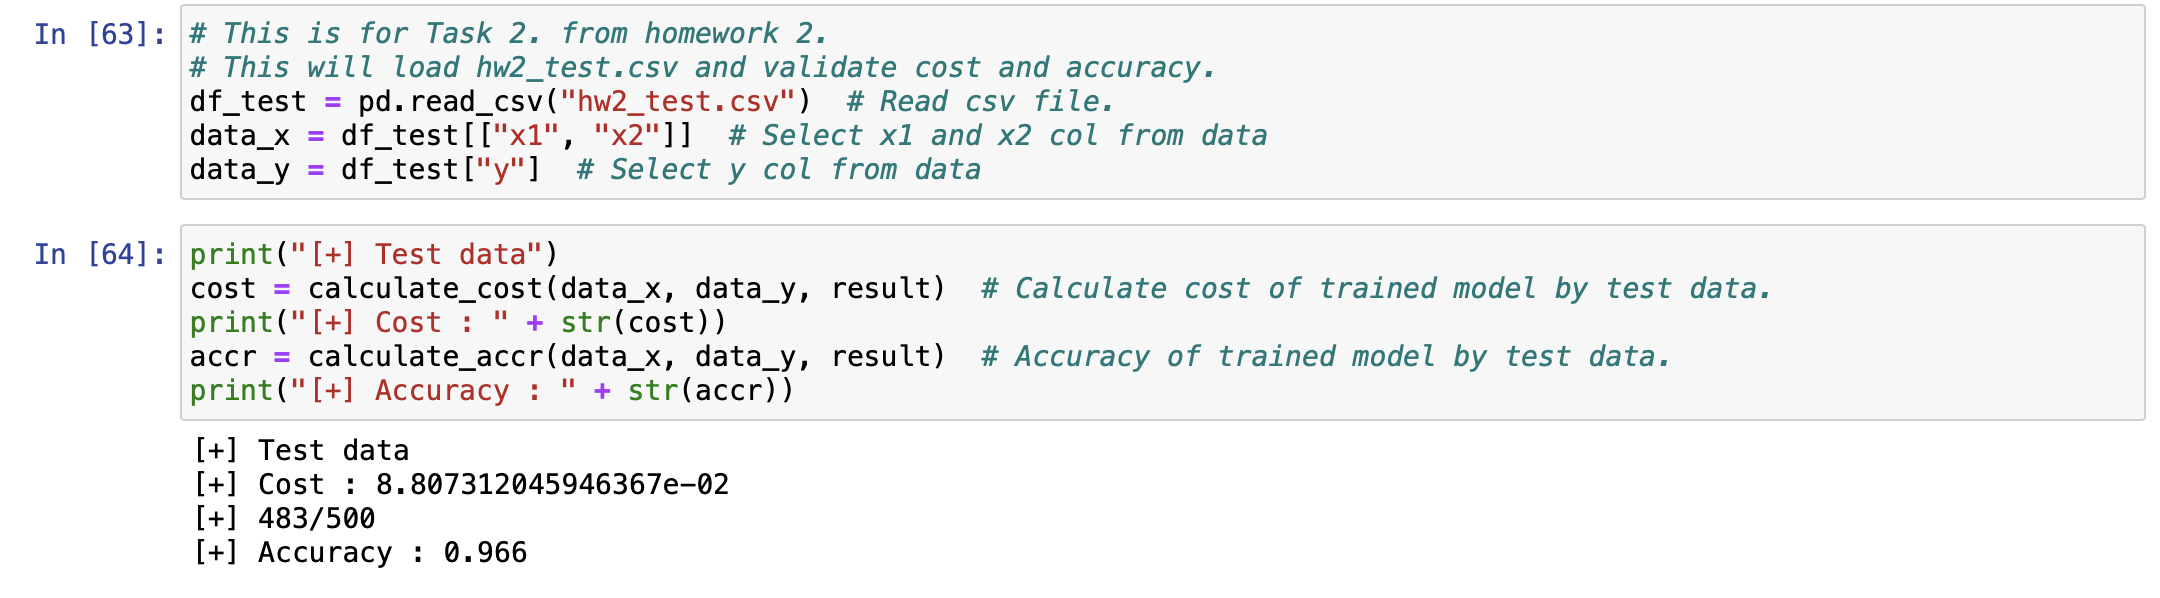
\includegraphics[width=15cm]{ml_2_3.png}
    \caption{Accuracy and Cost with \texttt{test.csv}}
    \label{fig:galaxy}
\end{figure}

Since 483 data were classified correctly out of 500 total data, the model had accuracy of 96.6\%. Also, the cost measured with cross entropy was 0.08807312045946367. In summary, with \texttt{test.csv}, our model's performance can be represented as following table:

\begin{center}
\begin{tabularx}{0.8\textwidth} { 
  | >{\centering\arraybackslash}X 
  | >{\centering\arraybackslash}X | }
 \hline
 Accuracy & Cost \\
 \hline
 96.6\% & 0.08807312045946367\\
\hline
\end{tabularx}
\end{center}

Also, let's plot decision boundary with data from \texttt{test.csv}.

\begin{figure}[h]
    \begin{center}
        \resizebox{0.5\textwidth}{!}{%% Creator: Matplotlib, PGF backend
%%
%% To include the figure in your LaTeX document, write
%%   \input{<filename>.pgf}
%%
%% Make sure the required packages are loaded in your preamble
%%   \usepackage{pgf}
%%
%% Also ensure that all the required font packages are loaded; for instance,
%% the lmodern package is sometimes necessary when using math font.
%%   \usepackage{lmodern}
%%
%% Figures using additional raster images can only be included by \input if
%% they are in the same directory as the main LaTeX file. For loading figures
%% from other directories you can use the `import` package
%%   \usepackage{import}
%%
%% and then include the figures with
%%   \import{<path to file>}{<filename>.pgf}
%%
%% Matplotlib used the following preamble
%%
\begingroup%
\makeatletter%
\begin{pgfpicture}%
\pgfpathrectangle{\pgfpointorigin}{\pgfqpoint{6.000000in}{4.000000in}}%
\pgfusepath{use as bounding box, clip}%
\begin{pgfscope}%
\pgfsetbuttcap%
\pgfsetmiterjoin%
\pgfsetlinewidth{0.000000pt}%
\definecolor{currentstroke}{rgb}{1.000000,1.000000,1.000000}%
\pgfsetstrokecolor{currentstroke}%
\pgfsetstrokeopacity{0.000000}%
\pgfsetdash{}{0pt}%
\pgfpathmoveto{\pgfqpoint{0.000000in}{0.000000in}}%
\pgfpathlineto{\pgfqpoint{6.000000in}{0.000000in}}%
\pgfpathlineto{\pgfqpoint{6.000000in}{4.000000in}}%
\pgfpathlineto{\pgfqpoint{0.000000in}{4.000000in}}%
\pgfpathlineto{\pgfqpoint{0.000000in}{0.000000in}}%
\pgfpathclose%
\pgfusepath{}%
\end{pgfscope}%
\begin{pgfscope}%
\pgfsetbuttcap%
\pgfsetmiterjoin%
\definecolor{currentfill}{rgb}{1.000000,1.000000,1.000000}%
\pgfsetfillcolor{currentfill}%
\pgfsetlinewidth{0.000000pt}%
\definecolor{currentstroke}{rgb}{0.000000,0.000000,0.000000}%
\pgfsetstrokecolor{currentstroke}%
\pgfsetstrokeopacity{0.000000}%
\pgfsetdash{}{0pt}%
\pgfpathmoveto{\pgfqpoint{0.750000in}{0.500000in}}%
\pgfpathlineto{\pgfqpoint{5.400000in}{0.500000in}}%
\pgfpathlineto{\pgfqpoint{5.400000in}{3.520000in}}%
\pgfpathlineto{\pgfqpoint{0.750000in}{3.520000in}}%
\pgfpathlineto{\pgfqpoint{0.750000in}{0.500000in}}%
\pgfpathclose%
\pgfusepath{fill}%
\end{pgfscope}%
\begin{pgfscope}%
\pgfpathrectangle{\pgfqpoint{0.750000in}{0.500000in}}{\pgfqpoint{4.650000in}{3.020000in}}%
\pgfusepath{clip}%
\pgfsetbuttcap%
\pgfsetroundjoin%
\definecolor{currentfill}{rgb}{0.839216,0.152941,0.156863}%
\pgfsetfillcolor{currentfill}%
\pgfsetlinewidth{1.003750pt}%
\definecolor{currentstroke}{rgb}{0.839216,0.152941,0.156863}%
\pgfsetstrokecolor{currentstroke}%
\pgfsetdash{}{0pt}%
\pgfsys@defobject{currentmarker}{\pgfqpoint{-0.041667in}{-0.041667in}}{\pgfqpoint{0.041667in}{0.041667in}}{%
\pgfpathmoveto{\pgfqpoint{0.000000in}{-0.041667in}}%
\pgfpathcurveto{\pgfqpoint{0.011050in}{-0.041667in}}{\pgfqpoint{0.021649in}{-0.037276in}}{\pgfqpoint{0.029463in}{-0.029463in}}%
\pgfpathcurveto{\pgfqpoint{0.037276in}{-0.021649in}}{\pgfqpoint{0.041667in}{-0.011050in}}{\pgfqpoint{0.041667in}{0.000000in}}%
\pgfpathcurveto{\pgfqpoint{0.041667in}{0.011050in}}{\pgfqpoint{0.037276in}{0.021649in}}{\pgfqpoint{0.029463in}{0.029463in}}%
\pgfpathcurveto{\pgfqpoint{0.021649in}{0.037276in}}{\pgfqpoint{0.011050in}{0.041667in}}{\pgfqpoint{0.000000in}{0.041667in}}%
\pgfpathcurveto{\pgfqpoint{-0.011050in}{0.041667in}}{\pgfqpoint{-0.021649in}{0.037276in}}{\pgfqpoint{-0.029463in}{0.029463in}}%
\pgfpathcurveto{\pgfqpoint{-0.037276in}{0.021649in}}{\pgfqpoint{-0.041667in}{0.011050in}}{\pgfqpoint{-0.041667in}{0.000000in}}%
\pgfpathcurveto{\pgfqpoint{-0.041667in}{-0.011050in}}{\pgfqpoint{-0.037276in}{-0.021649in}}{\pgfqpoint{-0.029463in}{-0.029463in}}%
\pgfpathcurveto{\pgfqpoint{-0.021649in}{-0.037276in}}{\pgfqpoint{-0.011050in}{-0.041667in}}{\pgfqpoint{0.000000in}{-0.041667in}}%
\pgfpathlineto{\pgfqpoint{0.000000in}{-0.041667in}}%
\pgfpathclose%
\pgfusepath{stroke,fill}%
}%
\begin{pgfscope}%
\pgfsys@transformshift{3.709717in}{2.404557in}%
\pgfsys@useobject{currentmarker}{}%
\end{pgfscope}%
\end{pgfscope}%
\begin{pgfscope}%
\pgfpathrectangle{\pgfqpoint{0.750000in}{0.500000in}}{\pgfqpoint{4.650000in}{3.020000in}}%
\pgfusepath{clip}%
\pgfsetbuttcap%
\pgfsetroundjoin%
\definecolor{currentfill}{rgb}{0.121569,0.466667,0.705882}%
\pgfsetfillcolor{currentfill}%
\pgfsetlinewidth{1.003750pt}%
\definecolor{currentstroke}{rgb}{0.121569,0.466667,0.705882}%
\pgfsetstrokecolor{currentstroke}%
\pgfsetdash{}{0pt}%
\pgfsys@defobject{currentmarker}{\pgfqpoint{-0.041667in}{-0.041667in}}{\pgfqpoint{0.041667in}{0.041667in}}{%
\pgfpathmoveto{\pgfqpoint{0.000000in}{-0.041667in}}%
\pgfpathcurveto{\pgfqpoint{0.011050in}{-0.041667in}}{\pgfqpoint{0.021649in}{-0.037276in}}{\pgfqpoint{0.029463in}{-0.029463in}}%
\pgfpathcurveto{\pgfqpoint{0.037276in}{-0.021649in}}{\pgfqpoint{0.041667in}{-0.011050in}}{\pgfqpoint{0.041667in}{0.000000in}}%
\pgfpathcurveto{\pgfqpoint{0.041667in}{0.011050in}}{\pgfqpoint{0.037276in}{0.021649in}}{\pgfqpoint{0.029463in}{0.029463in}}%
\pgfpathcurveto{\pgfqpoint{0.021649in}{0.037276in}}{\pgfqpoint{0.011050in}{0.041667in}}{\pgfqpoint{0.000000in}{0.041667in}}%
\pgfpathcurveto{\pgfqpoint{-0.011050in}{0.041667in}}{\pgfqpoint{-0.021649in}{0.037276in}}{\pgfqpoint{-0.029463in}{0.029463in}}%
\pgfpathcurveto{\pgfqpoint{-0.037276in}{0.021649in}}{\pgfqpoint{-0.041667in}{0.011050in}}{\pgfqpoint{-0.041667in}{0.000000in}}%
\pgfpathcurveto{\pgfqpoint{-0.041667in}{-0.011050in}}{\pgfqpoint{-0.037276in}{-0.021649in}}{\pgfqpoint{-0.029463in}{-0.029463in}}%
\pgfpathcurveto{\pgfqpoint{-0.021649in}{-0.037276in}}{\pgfqpoint{-0.011050in}{-0.041667in}}{\pgfqpoint{0.000000in}{-0.041667in}}%
\pgfpathlineto{\pgfqpoint{0.000000in}{-0.041667in}}%
\pgfpathclose%
\pgfusepath{stroke,fill}%
}%
\begin{pgfscope}%
\pgfsys@transformshift{3.359713in}{1.911526in}%
\pgfsys@useobject{currentmarker}{}%
\end{pgfscope}%
\end{pgfscope}%
\begin{pgfscope}%
\pgfpathrectangle{\pgfqpoint{0.750000in}{0.500000in}}{\pgfqpoint{4.650000in}{3.020000in}}%
\pgfusepath{clip}%
\pgfsetbuttcap%
\pgfsetroundjoin%
\definecolor{currentfill}{rgb}{0.839216,0.152941,0.156863}%
\pgfsetfillcolor{currentfill}%
\pgfsetlinewidth{1.003750pt}%
\definecolor{currentstroke}{rgb}{0.839216,0.152941,0.156863}%
\pgfsetstrokecolor{currentstroke}%
\pgfsetdash{}{0pt}%
\pgfpathmoveto{\pgfqpoint{3.359713in}{1.869859in}}%
\pgfpathcurveto{\pgfqpoint{3.370763in}{1.869859in}}{\pgfqpoint{3.381362in}{1.874250in}}{\pgfqpoint{3.389176in}{1.882063in}}%
\pgfpathcurveto{\pgfqpoint{3.396990in}{1.889877in}}{\pgfqpoint{3.401380in}{1.900476in}}{\pgfqpoint{3.401380in}{1.911526in}}%
\pgfpathcurveto{\pgfqpoint{3.401380in}{1.922576in}}{\pgfqpoint{3.396990in}{1.933175in}}{\pgfqpoint{3.389176in}{1.940989in}}%
\pgfpathcurveto{\pgfqpoint{3.381362in}{1.948802in}}{\pgfqpoint{3.370763in}{1.953193in}}{\pgfqpoint{3.359713in}{1.953193in}}%
\pgfpathcurveto{\pgfqpoint{3.348663in}{1.953193in}}{\pgfqpoint{3.338064in}{1.948802in}}{\pgfqpoint{3.330250in}{1.940989in}}%
\pgfpathcurveto{\pgfqpoint{3.322437in}{1.933175in}}{\pgfqpoint{3.318046in}{1.922576in}}{\pgfqpoint{3.318046in}{1.911526in}}%
\pgfpathcurveto{\pgfqpoint{3.318046in}{1.900476in}}{\pgfqpoint{3.322437in}{1.889877in}}{\pgfqpoint{3.330250in}{1.882063in}}%
\pgfpathcurveto{\pgfqpoint{3.338064in}{1.874250in}}{\pgfqpoint{3.348663in}{1.869859in}}{\pgfqpoint{3.359713in}{1.869859in}}%
\pgfpathlineto{\pgfqpoint{3.359713in}{1.869859in}}%
\pgfpathclose%
\pgfusepath{stroke,fill}%
\end{pgfscope}%
\begin{pgfscope}%
\pgfpathrectangle{\pgfqpoint{0.750000in}{0.500000in}}{\pgfqpoint{4.650000in}{3.020000in}}%
\pgfusepath{clip}%
\pgfsetbuttcap%
\pgfsetroundjoin%
\definecolor{currentfill}{rgb}{0.839216,0.152941,0.156863}%
\pgfsetfillcolor{currentfill}%
\pgfsetlinewidth{1.003750pt}%
\definecolor{currentstroke}{rgb}{0.839216,0.152941,0.156863}%
\pgfsetstrokecolor{currentstroke}%
\pgfsetdash{}{0pt}%
\pgfpathmoveto{\pgfqpoint{4.059634in}{2.477253in}}%
\pgfpathcurveto{\pgfqpoint{4.070684in}{2.477253in}}{\pgfqpoint{4.081283in}{2.481644in}}{\pgfqpoint{4.089097in}{2.489457in}}%
\pgfpathcurveto{\pgfqpoint{4.096911in}{2.497271in}}{\pgfqpoint{4.101301in}{2.507870in}}{\pgfqpoint{4.101301in}{2.518920in}}%
\pgfpathcurveto{\pgfqpoint{4.101301in}{2.529970in}}{\pgfqpoint{4.096911in}{2.540569in}}{\pgfqpoint{4.089097in}{2.548383in}}%
\pgfpathcurveto{\pgfqpoint{4.081283in}{2.556197in}}{\pgfqpoint{4.070684in}{2.560587in}}{\pgfqpoint{4.059634in}{2.560587in}}%
\pgfpathcurveto{\pgfqpoint{4.048584in}{2.560587in}}{\pgfqpoint{4.037985in}{2.556197in}}{\pgfqpoint{4.030171in}{2.548383in}}%
\pgfpathcurveto{\pgfqpoint{4.022358in}{2.540569in}}{\pgfqpoint{4.017967in}{2.529970in}}{\pgfqpoint{4.017967in}{2.518920in}}%
\pgfpathcurveto{\pgfqpoint{4.017967in}{2.507870in}}{\pgfqpoint{4.022358in}{2.497271in}}{\pgfqpoint{4.030171in}{2.489457in}}%
\pgfpathcurveto{\pgfqpoint{4.037985in}{2.481644in}}{\pgfqpoint{4.048584in}{2.477253in}}{\pgfqpoint{4.059634in}{2.477253in}}%
\pgfpathlineto{\pgfqpoint{4.059634in}{2.477253in}}%
\pgfpathclose%
\pgfusepath{stroke,fill}%
\end{pgfscope}%
\begin{pgfscope}%
\pgfpathrectangle{\pgfqpoint{0.750000in}{0.500000in}}{\pgfqpoint{4.650000in}{3.020000in}}%
\pgfusepath{clip}%
\pgfsetbuttcap%
\pgfsetroundjoin%
\definecolor{currentfill}{rgb}{0.839216,0.152941,0.156863}%
\pgfsetfillcolor{currentfill}%
\pgfsetlinewidth{1.003750pt}%
\definecolor{currentstroke}{rgb}{0.839216,0.152941,0.156863}%
\pgfsetstrokecolor{currentstroke}%
\pgfsetdash{}{0pt}%
\pgfpathmoveto{\pgfqpoint{3.598568in}{2.479258in}}%
\pgfpathcurveto{\pgfqpoint{3.609618in}{2.479258in}}{\pgfqpoint{3.620217in}{2.483648in}}{\pgfqpoint{3.628030in}{2.491462in}}%
\pgfpathcurveto{\pgfqpoint{3.635844in}{2.499275in}}{\pgfqpoint{3.640234in}{2.509874in}}{\pgfqpoint{3.640234in}{2.520924in}}%
\pgfpathcurveto{\pgfqpoint{3.640234in}{2.531975in}}{\pgfqpoint{3.635844in}{2.542574in}}{\pgfqpoint{3.628030in}{2.550387in}}%
\pgfpathcurveto{\pgfqpoint{3.620217in}{2.558201in}}{\pgfqpoint{3.609618in}{2.562591in}}{\pgfqpoint{3.598568in}{2.562591in}}%
\pgfpathcurveto{\pgfqpoint{3.587518in}{2.562591in}}{\pgfqpoint{3.576918in}{2.558201in}}{\pgfqpoint{3.569105in}{2.550387in}}%
\pgfpathcurveto{\pgfqpoint{3.561291in}{2.542574in}}{\pgfqpoint{3.556901in}{2.531975in}}{\pgfqpoint{3.556901in}{2.520924in}}%
\pgfpathcurveto{\pgfqpoint{3.556901in}{2.509874in}}{\pgfqpoint{3.561291in}{2.499275in}}{\pgfqpoint{3.569105in}{2.491462in}}%
\pgfpathcurveto{\pgfqpoint{3.576918in}{2.483648in}}{\pgfqpoint{3.587518in}{2.479258in}}{\pgfqpoint{3.598568in}{2.479258in}}%
\pgfpathlineto{\pgfqpoint{3.598568in}{2.479258in}}%
\pgfpathclose%
\pgfusepath{stroke,fill}%
\end{pgfscope}%
\begin{pgfscope}%
\pgfpathrectangle{\pgfqpoint{0.750000in}{0.500000in}}{\pgfqpoint{4.650000in}{3.020000in}}%
\pgfusepath{clip}%
\pgfsetbuttcap%
\pgfsetroundjoin%
\definecolor{currentfill}{rgb}{0.839216,0.152941,0.156863}%
\pgfsetfillcolor{currentfill}%
\pgfsetlinewidth{1.003750pt}%
\definecolor{currentstroke}{rgb}{0.839216,0.152941,0.156863}%
\pgfsetstrokecolor{currentstroke}%
\pgfsetdash{}{0pt}%
\pgfpathmoveto{\pgfqpoint{3.657268in}{2.031495in}}%
\pgfpathcurveto{\pgfqpoint{3.668318in}{2.031495in}}{\pgfqpoint{3.678917in}{2.035885in}}{\pgfqpoint{3.686730in}{2.043699in}}%
\pgfpathcurveto{\pgfqpoint{3.694544in}{2.051512in}}{\pgfqpoint{3.698934in}{2.062111in}}{\pgfqpoint{3.698934in}{2.073161in}}%
\pgfpathcurveto{\pgfqpoint{3.698934in}{2.084211in}}{\pgfqpoint{3.694544in}{2.094810in}}{\pgfqpoint{3.686730in}{2.102624in}}%
\pgfpathcurveto{\pgfqpoint{3.678917in}{2.110438in}}{\pgfqpoint{3.668318in}{2.114828in}}{\pgfqpoint{3.657268in}{2.114828in}}%
\pgfpathcurveto{\pgfqpoint{3.646218in}{2.114828in}}{\pgfqpoint{3.635619in}{2.110438in}}{\pgfqpoint{3.627805in}{2.102624in}}%
\pgfpathcurveto{\pgfqpoint{3.619991in}{2.094810in}}{\pgfqpoint{3.615601in}{2.084211in}}{\pgfqpoint{3.615601in}{2.073161in}}%
\pgfpathcurveto{\pgfqpoint{3.615601in}{2.062111in}}{\pgfqpoint{3.619991in}{2.051512in}}{\pgfqpoint{3.627805in}{2.043699in}}%
\pgfpathcurveto{\pgfqpoint{3.635619in}{2.035885in}}{\pgfqpoint{3.646218in}{2.031495in}}{\pgfqpoint{3.657268in}{2.031495in}}%
\pgfpathlineto{\pgfqpoint{3.657268in}{2.031495in}}%
\pgfpathclose%
\pgfusepath{stroke,fill}%
\end{pgfscope}%
\begin{pgfscope}%
\pgfpathrectangle{\pgfqpoint{0.750000in}{0.500000in}}{\pgfqpoint{4.650000in}{3.020000in}}%
\pgfusepath{clip}%
\pgfsetbuttcap%
\pgfsetroundjoin%
\definecolor{currentfill}{rgb}{0.121569,0.466667,0.705882}%
\pgfsetfillcolor{currentfill}%
\pgfsetlinewidth{1.003750pt}%
\definecolor{currentstroke}{rgb}{0.121569,0.466667,0.705882}%
\pgfsetstrokecolor{currentstroke}%
\pgfsetdash{}{0pt}%
\pgfpathmoveto{\pgfqpoint{2.750113in}{1.734060in}}%
\pgfpathcurveto{\pgfqpoint{2.761163in}{1.734060in}}{\pgfqpoint{2.771762in}{1.738450in}}{\pgfqpoint{2.779576in}{1.746264in}}%
\pgfpathcurveto{\pgfqpoint{2.787389in}{1.754077in}}{\pgfqpoint{2.791779in}{1.764676in}}{\pgfqpoint{2.791779in}{1.775726in}}%
\pgfpathcurveto{\pgfqpoint{2.791779in}{1.786777in}}{\pgfqpoint{2.787389in}{1.797376in}}{\pgfqpoint{2.779576in}{1.805189in}}%
\pgfpathcurveto{\pgfqpoint{2.771762in}{1.813003in}}{\pgfqpoint{2.761163in}{1.817393in}}{\pgfqpoint{2.750113in}{1.817393in}}%
\pgfpathcurveto{\pgfqpoint{2.739063in}{1.817393in}}{\pgfqpoint{2.728464in}{1.813003in}}{\pgfqpoint{2.720650in}{1.805189in}}%
\pgfpathcurveto{\pgfqpoint{2.712836in}{1.797376in}}{\pgfqpoint{2.708446in}{1.786777in}}{\pgfqpoint{2.708446in}{1.775726in}}%
\pgfpathcurveto{\pgfqpoint{2.708446in}{1.764676in}}{\pgfqpoint{2.712836in}{1.754077in}}{\pgfqpoint{2.720650in}{1.746264in}}%
\pgfpathcurveto{\pgfqpoint{2.728464in}{1.738450in}}{\pgfqpoint{2.739063in}{1.734060in}}{\pgfqpoint{2.750113in}{1.734060in}}%
\pgfpathlineto{\pgfqpoint{2.750113in}{1.734060in}}%
\pgfpathclose%
\pgfusepath{stroke,fill}%
\end{pgfscope}%
\begin{pgfscope}%
\pgfpathrectangle{\pgfqpoint{0.750000in}{0.500000in}}{\pgfqpoint{4.650000in}{3.020000in}}%
\pgfusepath{clip}%
\pgfsetbuttcap%
\pgfsetroundjoin%
\definecolor{currentfill}{rgb}{0.839216,0.152941,0.156863}%
\pgfsetfillcolor{currentfill}%
\pgfsetlinewidth{1.003750pt}%
\definecolor{currentstroke}{rgb}{0.839216,0.152941,0.156863}%
\pgfsetstrokecolor{currentstroke}%
\pgfsetdash{}{0pt}%
\pgfpathmoveto{\pgfqpoint{4.462017in}{2.219968in}}%
\pgfpathcurveto{\pgfqpoint{4.473067in}{2.219968in}}{\pgfqpoint{4.483666in}{2.224358in}}{\pgfqpoint{4.491480in}{2.232172in}}%
\pgfpathcurveto{\pgfqpoint{4.499293in}{2.239986in}}{\pgfqpoint{4.503684in}{2.250585in}}{\pgfqpoint{4.503684in}{2.261635in}}%
\pgfpathcurveto{\pgfqpoint{4.503684in}{2.272685in}}{\pgfqpoint{4.499293in}{2.283284in}}{\pgfqpoint{4.491480in}{2.291097in}}%
\pgfpathcurveto{\pgfqpoint{4.483666in}{2.298911in}}{\pgfqpoint{4.473067in}{2.303301in}}{\pgfqpoint{4.462017in}{2.303301in}}%
\pgfpathcurveto{\pgfqpoint{4.450967in}{2.303301in}}{\pgfqpoint{4.440368in}{2.298911in}}{\pgfqpoint{4.432554in}{2.291097in}}%
\pgfpathcurveto{\pgfqpoint{4.424741in}{2.283284in}}{\pgfqpoint{4.420350in}{2.272685in}}{\pgfqpoint{4.420350in}{2.261635in}}%
\pgfpathcurveto{\pgfqpoint{4.420350in}{2.250585in}}{\pgfqpoint{4.424741in}{2.239986in}}{\pgfqpoint{4.432554in}{2.232172in}}%
\pgfpathcurveto{\pgfqpoint{4.440368in}{2.224358in}}{\pgfqpoint{4.450967in}{2.219968in}}{\pgfqpoint{4.462017in}{2.219968in}}%
\pgfpathlineto{\pgfqpoint{4.462017in}{2.219968in}}%
\pgfpathclose%
\pgfusepath{stroke,fill}%
\end{pgfscope}%
\begin{pgfscope}%
\pgfpathrectangle{\pgfqpoint{0.750000in}{0.500000in}}{\pgfqpoint{4.650000in}{3.020000in}}%
\pgfusepath{clip}%
\pgfsetbuttcap%
\pgfsetroundjoin%
\definecolor{currentfill}{rgb}{0.121569,0.466667,0.705882}%
\pgfsetfillcolor{currentfill}%
\pgfsetlinewidth{1.003750pt}%
\definecolor{currentstroke}{rgb}{0.121569,0.466667,0.705882}%
\pgfsetstrokecolor{currentstroke}%
\pgfsetdash{}{0pt}%
\pgfpathmoveto{\pgfqpoint{2.299300in}{2.149660in}}%
\pgfpathcurveto{\pgfqpoint{2.310350in}{2.149660in}}{\pgfqpoint{2.320949in}{2.154050in}}{\pgfqpoint{2.328762in}{2.161864in}}%
\pgfpathcurveto{\pgfqpoint{2.336576in}{2.169677in}}{\pgfqpoint{2.340966in}{2.180277in}}{\pgfqpoint{2.340966in}{2.191327in}}%
\pgfpathcurveto{\pgfqpoint{2.340966in}{2.202377in}}{\pgfqpoint{2.336576in}{2.212976in}}{\pgfqpoint{2.328762in}{2.220789in}}%
\pgfpathcurveto{\pgfqpoint{2.320949in}{2.228603in}}{\pgfqpoint{2.310350in}{2.232993in}}{\pgfqpoint{2.299300in}{2.232993in}}%
\pgfpathcurveto{\pgfqpoint{2.288250in}{2.232993in}}{\pgfqpoint{2.277650in}{2.228603in}}{\pgfqpoint{2.269837in}{2.220789in}}%
\pgfpathcurveto{\pgfqpoint{2.262023in}{2.212976in}}{\pgfqpoint{2.257633in}{2.202377in}}{\pgfqpoint{2.257633in}{2.191327in}}%
\pgfpathcurveto{\pgfqpoint{2.257633in}{2.180277in}}{\pgfqpoint{2.262023in}{2.169677in}}{\pgfqpoint{2.269837in}{2.161864in}}%
\pgfpathcurveto{\pgfqpoint{2.277650in}{2.154050in}}{\pgfqpoint{2.288250in}{2.149660in}}{\pgfqpoint{2.299300in}{2.149660in}}%
\pgfpathlineto{\pgfqpoint{2.299300in}{2.149660in}}%
\pgfpathclose%
\pgfusepath{stroke,fill}%
\end{pgfscope}%
\begin{pgfscope}%
\pgfpathrectangle{\pgfqpoint{0.750000in}{0.500000in}}{\pgfqpoint{4.650000in}{3.020000in}}%
\pgfusepath{clip}%
\pgfsetbuttcap%
\pgfsetroundjoin%
\definecolor{currentfill}{rgb}{0.839216,0.152941,0.156863}%
\pgfsetfillcolor{currentfill}%
\pgfsetlinewidth{1.003750pt}%
\definecolor{currentstroke}{rgb}{0.839216,0.152941,0.156863}%
\pgfsetstrokecolor{currentstroke}%
\pgfsetdash{}{0pt}%
\pgfpathmoveto{\pgfqpoint{3.619702in}{2.120555in}}%
\pgfpathcurveto{\pgfqpoint{3.630752in}{2.120555in}}{\pgfqpoint{3.641351in}{2.124945in}}{\pgfqpoint{3.649165in}{2.132758in}}%
\pgfpathcurveto{\pgfqpoint{3.656978in}{2.140572in}}{\pgfqpoint{3.661368in}{2.151171in}}{\pgfqpoint{3.661368in}{2.162221in}}%
\pgfpathcurveto{\pgfqpoint{3.661368in}{2.173271in}}{\pgfqpoint{3.656978in}{2.183870in}}{\pgfqpoint{3.649165in}{2.191684in}}%
\pgfpathcurveto{\pgfqpoint{3.641351in}{2.199498in}}{\pgfqpoint{3.630752in}{2.203888in}}{\pgfqpoint{3.619702in}{2.203888in}}%
\pgfpathcurveto{\pgfqpoint{3.608652in}{2.203888in}}{\pgfqpoint{3.598053in}{2.199498in}}{\pgfqpoint{3.590239in}{2.191684in}}%
\pgfpathcurveto{\pgfqpoint{3.582425in}{2.183870in}}{\pgfqpoint{3.578035in}{2.173271in}}{\pgfqpoint{3.578035in}{2.162221in}}%
\pgfpathcurveto{\pgfqpoint{3.578035in}{2.151171in}}{\pgfqpoint{3.582425in}{2.140572in}}{\pgfqpoint{3.590239in}{2.132758in}}%
\pgfpathcurveto{\pgfqpoint{3.598053in}{2.124945in}}{\pgfqpoint{3.608652in}{2.120555in}}{\pgfqpoint{3.619702in}{2.120555in}}%
\pgfpathlineto{\pgfqpoint{3.619702in}{2.120555in}}%
\pgfpathclose%
\pgfusepath{stroke,fill}%
\end{pgfscope}%
\begin{pgfscope}%
\pgfpathrectangle{\pgfqpoint{0.750000in}{0.500000in}}{\pgfqpoint{4.650000in}{3.020000in}}%
\pgfusepath{clip}%
\pgfsetbuttcap%
\pgfsetroundjoin%
\definecolor{currentfill}{rgb}{0.839216,0.152941,0.156863}%
\pgfsetfillcolor{currentfill}%
\pgfsetlinewidth{1.003750pt}%
\definecolor{currentstroke}{rgb}{0.839216,0.152941,0.156863}%
\pgfsetstrokecolor{currentstroke}%
\pgfsetdash{}{0pt}%
\pgfpathmoveto{\pgfqpoint{3.554836in}{2.119943in}}%
\pgfpathcurveto{\pgfqpoint{3.565887in}{2.119943in}}{\pgfqpoint{3.576486in}{2.124333in}}{\pgfqpoint{3.584299in}{2.132147in}}%
\pgfpathcurveto{\pgfqpoint{3.592113in}{2.139960in}}{\pgfqpoint{3.596503in}{2.150560in}}{\pgfqpoint{3.596503in}{2.161610in}}%
\pgfpathcurveto{\pgfqpoint{3.596503in}{2.172660in}}{\pgfqpoint{3.592113in}{2.183259in}}{\pgfqpoint{3.584299in}{2.191072in}}%
\pgfpathcurveto{\pgfqpoint{3.576486in}{2.198886in}}{\pgfqpoint{3.565887in}{2.203276in}}{\pgfqpoint{3.554836in}{2.203276in}}%
\pgfpathcurveto{\pgfqpoint{3.543786in}{2.203276in}}{\pgfqpoint{3.533187in}{2.198886in}}{\pgfqpoint{3.525374in}{2.191072in}}%
\pgfpathcurveto{\pgfqpoint{3.517560in}{2.183259in}}{\pgfqpoint{3.513170in}{2.172660in}}{\pgfqpoint{3.513170in}{2.161610in}}%
\pgfpathcurveto{\pgfqpoint{3.513170in}{2.150560in}}{\pgfqpoint{3.517560in}{2.139960in}}{\pgfqpoint{3.525374in}{2.132147in}}%
\pgfpathcurveto{\pgfqpoint{3.533187in}{2.124333in}}{\pgfqpoint{3.543786in}{2.119943in}}{\pgfqpoint{3.554836in}{2.119943in}}%
\pgfpathlineto{\pgfqpoint{3.554836in}{2.119943in}}%
\pgfpathclose%
\pgfusepath{stroke,fill}%
\end{pgfscope}%
\begin{pgfscope}%
\pgfpathrectangle{\pgfqpoint{0.750000in}{0.500000in}}{\pgfqpoint{4.650000in}{3.020000in}}%
\pgfusepath{clip}%
\pgfsetbuttcap%
\pgfsetroundjoin%
\definecolor{currentfill}{rgb}{0.121569,0.466667,0.705882}%
\pgfsetfillcolor{currentfill}%
\pgfsetlinewidth{1.003750pt}%
\definecolor{currentstroke}{rgb}{0.121569,0.466667,0.705882}%
\pgfsetstrokecolor{currentstroke}%
\pgfsetdash{}{0pt}%
\pgfpathmoveto{\pgfqpoint{2.759025in}{1.894231in}}%
\pgfpathcurveto{\pgfqpoint{2.770075in}{1.894231in}}{\pgfqpoint{2.780674in}{1.898621in}}{\pgfqpoint{2.788488in}{1.906435in}}%
\pgfpathcurveto{\pgfqpoint{2.796301in}{1.914248in}}{\pgfqpoint{2.800692in}{1.924847in}}{\pgfqpoint{2.800692in}{1.935898in}}%
\pgfpathcurveto{\pgfqpoint{2.800692in}{1.946948in}}{\pgfqpoint{2.796301in}{1.957547in}}{\pgfqpoint{2.788488in}{1.965360in}}%
\pgfpathcurveto{\pgfqpoint{2.780674in}{1.973174in}}{\pgfqpoint{2.770075in}{1.977564in}}{\pgfqpoint{2.759025in}{1.977564in}}%
\pgfpathcurveto{\pgfqpoint{2.747975in}{1.977564in}}{\pgfqpoint{2.737376in}{1.973174in}}{\pgfqpoint{2.729562in}{1.965360in}}%
\pgfpathcurveto{\pgfqpoint{2.721749in}{1.957547in}}{\pgfqpoint{2.717358in}{1.946948in}}{\pgfqpoint{2.717358in}{1.935898in}}%
\pgfpathcurveto{\pgfqpoint{2.717358in}{1.924847in}}{\pgfqpoint{2.721749in}{1.914248in}}{\pgfqpoint{2.729562in}{1.906435in}}%
\pgfpathcurveto{\pgfqpoint{2.737376in}{1.898621in}}{\pgfqpoint{2.747975in}{1.894231in}}{\pgfqpoint{2.759025in}{1.894231in}}%
\pgfpathlineto{\pgfqpoint{2.759025in}{1.894231in}}%
\pgfpathclose%
\pgfusepath{stroke,fill}%
\end{pgfscope}%
\begin{pgfscope}%
\pgfpathrectangle{\pgfqpoint{0.750000in}{0.500000in}}{\pgfqpoint{4.650000in}{3.020000in}}%
\pgfusepath{clip}%
\pgfsetbuttcap%
\pgfsetroundjoin%
\definecolor{currentfill}{rgb}{0.839216,0.152941,0.156863}%
\pgfsetfillcolor{currentfill}%
\pgfsetlinewidth{1.003750pt}%
\definecolor{currentstroke}{rgb}{0.839216,0.152941,0.156863}%
\pgfsetstrokecolor{currentstroke}%
\pgfsetdash{}{0pt}%
\pgfpathmoveto{\pgfqpoint{4.288275in}{2.568963in}}%
\pgfpathcurveto{\pgfqpoint{4.299325in}{2.568963in}}{\pgfqpoint{4.309924in}{2.573353in}}{\pgfqpoint{4.317737in}{2.581167in}}%
\pgfpathcurveto{\pgfqpoint{4.325551in}{2.588981in}}{\pgfqpoint{4.329941in}{2.599580in}}{\pgfqpoint{4.329941in}{2.610630in}}%
\pgfpathcurveto{\pgfqpoint{4.329941in}{2.621680in}}{\pgfqpoint{4.325551in}{2.632279in}}{\pgfqpoint{4.317737in}{2.640092in}}%
\pgfpathcurveto{\pgfqpoint{4.309924in}{2.647906in}}{\pgfqpoint{4.299325in}{2.652296in}}{\pgfqpoint{4.288275in}{2.652296in}}%
\pgfpathcurveto{\pgfqpoint{4.277224in}{2.652296in}}{\pgfqpoint{4.266625in}{2.647906in}}{\pgfqpoint{4.258812in}{2.640092in}}%
\pgfpathcurveto{\pgfqpoint{4.250998in}{2.632279in}}{\pgfqpoint{4.246608in}{2.621680in}}{\pgfqpoint{4.246608in}{2.610630in}}%
\pgfpathcurveto{\pgfqpoint{4.246608in}{2.599580in}}{\pgfqpoint{4.250998in}{2.588981in}}{\pgfqpoint{4.258812in}{2.581167in}}%
\pgfpathcurveto{\pgfqpoint{4.266625in}{2.573353in}}{\pgfqpoint{4.277224in}{2.568963in}}{\pgfqpoint{4.288275in}{2.568963in}}%
\pgfpathlineto{\pgfqpoint{4.288275in}{2.568963in}}%
\pgfpathclose%
\pgfusepath{stroke,fill}%
\end{pgfscope}%
\begin{pgfscope}%
\pgfpathrectangle{\pgfqpoint{0.750000in}{0.500000in}}{\pgfqpoint{4.650000in}{3.020000in}}%
\pgfusepath{clip}%
\pgfsetbuttcap%
\pgfsetroundjoin%
\definecolor{currentfill}{rgb}{0.121569,0.466667,0.705882}%
\pgfsetfillcolor{currentfill}%
\pgfsetlinewidth{1.003750pt}%
\definecolor{currentstroke}{rgb}{0.121569,0.466667,0.705882}%
\pgfsetstrokecolor{currentstroke}%
\pgfsetdash{}{0pt}%
\pgfpathmoveto{\pgfqpoint{2.665820in}{2.087425in}}%
\pgfpathcurveto{\pgfqpoint{2.676870in}{2.087425in}}{\pgfqpoint{2.687469in}{2.091815in}}{\pgfqpoint{2.695283in}{2.099628in}}%
\pgfpathcurveto{\pgfqpoint{2.703096in}{2.107442in}}{\pgfqpoint{2.707487in}{2.118041in}}{\pgfqpoint{2.707487in}{2.129091in}}%
\pgfpathcurveto{\pgfqpoint{2.707487in}{2.140141in}}{\pgfqpoint{2.703096in}{2.150740in}}{\pgfqpoint{2.695283in}{2.158554in}}%
\pgfpathcurveto{\pgfqpoint{2.687469in}{2.166368in}}{\pgfqpoint{2.676870in}{2.170758in}}{\pgfqpoint{2.665820in}{2.170758in}}%
\pgfpathcurveto{\pgfqpoint{2.654770in}{2.170758in}}{\pgfqpoint{2.644171in}{2.166368in}}{\pgfqpoint{2.636357in}{2.158554in}}%
\pgfpathcurveto{\pgfqpoint{2.628544in}{2.150740in}}{\pgfqpoint{2.624153in}{2.140141in}}{\pgfqpoint{2.624153in}{2.129091in}}%
\pgfpathcurveto{\pgfqpoint{2.624153in}{2.118041in}}{\pgfqpoint{2.628544in}{2.107442in}}{\pgfqpoint{2.636357in}{2.099628in}}%
\pgfpathcurveto{\pgfqpoint{2.644171in}{2.091815in}}{\pgfqpoint{2.654770in}{2.087425in}}{\pgfqpoint{2.665820in}{2.087425in}}%
\pgfpathlineto{\pgfqpoint{2.665820in}{2.087425in}}%
\pgfpathclose%
\pgfusepath{stroke,fill}%
\end{pgfscope}%
\begin{pgfscope}%
\pgfpathrectangle{\pgfqpoint{0.750000in}{0.500000in}}{\pgfqpoint{4.650000in}{3.020000in}}%
\pgfusepath{clip}%
\pgfsetbuttcap%
\pgfsetroundjoin%
\definecolor{currentfill}{rgb}{0.839216,0.152941,0.156863}%
\pgfsetfillcolor{currentfill}%
\pgfsetlinewidth{1.003750pt}%
\definecolor{currentstroke}{rgb}{0.839216,0.152941,0.156863}%
\pgfsetstrokecolor{currentstroke}%
\pgfsetdash{}{0pt}%
\pgfpathmoveto{\pgfqpoint{3.598111in}{2.075355in}}%
\pgfpathcurveto{\pgfqpoint{3.609161in}{2.075355in}}{\pgfqpoint{3.619760in}{2.079745in}}{\pgfqpoint{3.627573in}{2.087559in}}%
\pgfpathcurveto{\pgfqpoint{3.635387in}{2.095372in}}{\pgfqpoint{3.639777in}{2.105971in}}{\pgfqpoint{3.639777in}{2.117022in}}%
\pgfpathcurveto{\pgfqpoint{3.639777in}{2.128072in}}{\pgfqpoint{3.635387in}{2.138671in}}{\pgfqpoint{3.627573in}{2.146484in}}%
\pgfpathcurveto{\pgfqpoint{3.619760in}{2.154298in}}{\pgfqpoint{3.609161in}{2.158688in}}{\pgfqpoint{3.598111in}{2.158688in}}%
\pgfpathcurveto{\pgfqpoint{3.587060in}{2.158688in}}{\pgfqpoint{3.576461in}{2.154298in}}{\pgfqpoint{3.568648in}{2.146484in}}%
\pgfpathcurveto{\pgfqpoint{3.560834in}{2.138671in}}{\pgfqpoint{3.556444in}{2.128072in}}{\pgfqpoint{3.556444in}{2.117022in}}%
\pgfpathcurveto{\pgfqpoint{3.556444in}{2.105971in}}{\pgfqpoint{3.560834in}{2.095372in}}{\pgfqpoint{3.568648in}{2.087559in}}%
\pgfpathcurveto{\pgfqpoint{3.576461in}{2.079745in}}{\pgfqpoint{3.587060in}{2.075355in}}{\pgfqpoint{3.598111in}{2.075355in}}%
\pgfpathlineto{\pgfqpoint{3.598111in}{2.075355in}}%
\pgfpathclose%
\pgfusepath{stroke,fill}%
\end{pgfscope}%
\begin{pgfscope}%
\pgfpathrectangle{\pgfqpoint{0.750000in}{0.500000in}}{\pgfqpoint{4.650000in}{3.020000in}}%
\pgfusepath{clip}%
\pgfsetbuttcap%
\pgfsetroundjoin%
\definecolor{currentfill}{rgb}{0.121569,0.466667,0.705882}%
\pgfsetfillcolor{currentfill}%
\pgfsetlinewidth{1.003750pt}%
\definecolor{currentstroke}{rgb}{0.121569,0.466667,0.705882}%
\pgfsetstrokecolor{currentstroke}%
\pgfsetdash{}{0pt}%
\pgfpathmoveto{\pgfqpoint{2.325203in}{1.798361in}}%
\pgfpathcurveto{\pgfqpoint{2.336253in}{1.798361in}}{\pgfqpoint{2.346853in}{1.802751in}}{\pgfqpoint{2.354666in}{1.810565in}}%
\pgfpathcurveto{\pgfqpoint{2.362480in}{1.818379in}}{\pgfqpoint{2.366870in}{1.828978in}}{\pgfqpoint{2.366870in}{1.840028in}}%
\pgfpathcurveto{\pgfqpoint{2.366870in}{1.851078in}}{\pgfqpoint{2.362480in}{1.861677in}}{\pgfqpoint{2.354666in}{1.869490in}}%
\pgfpathcurveto{\pgfqpoint{2.346853in}{1.877304in}}{\pgfqpoint{2.336253in}{1.881694in}}{\pgfqpoint{2.325203in}{1.881694in}}%
\pgfpathcurveto{\pgfqpoint{2.314153in}{1.881694in}}{\pgfqpoint{2.303554in}{1.877304in}}{\pgfqpoint{2.295741in}{1.869490in}}%
\pgfpathcurveto{\pgfqpoint{2.287927in}{1.861677in}}{\pgfqpoint{2.283537in}{1.851078in}}{\pgfqpoint{2.283537in}{1.840028in}}%
\pgfpathcurveto{\pgfqpoint{2.283537in}{1.828978in}}{\pgfqpoint{2.287927in}{1.818379in}}{\pgfqpoint{2.295741in}{1.810565in}}%
\pgfpathcurveto{\pgfqpoint{2.303554in}{1.802751in}}{\pgfqpoint{2.314153in}{1.798361in}}{\pgfqpoint{2.325203in}{1.798361in}}%
\pgfpathlineto{\pgfqpoint{2.325203in}{1.798361in}}%
\pgfpathclose%
\pgfusepath{stroke,fill}%
\end{pgfscope}%
\begin{pgfscope}%
\pgfpathrectangle{\pgfqpoint{0.750000in}{0.500000in}}{\pgfqpoint{4.650000in}{3.020000in}}%
\pgfusepath{clip}%
\pgfsetbuttcap%
\pgfsetroundjoin%
\definecolor{currentfill}{rgb}{0.121569,0.466667,0.705882}%
\pgfsetfillcolor{currentfill}%
\pgfsetlinewidth{1.003750pt}%
\definecolor{currentstroke}{rgb}{0.121569,0.466667,0.705882}%
\pgfsetstrokecolor{currentstroke}%
\pgfsetdash{}{0pt}%
\pgfpathmoveto{\pgfqpoint{2.636217in}{1.989089in}}%
\pgfpathcurveto{\pgfqpoint{2.647267in}{1.989089in}}{\pgfqpoint{2.657866in}{1.993480in}}{\pgfqpoint{2.665680in}{2.001293in}}%
\pgfpathcurveto{\pgfqpoint{2.673494in}{2.009107in}}{\pgfqpoint{2.677884in}{2.019706in}}{\pgfqpoint{2.677884in}{2.030756in}}%
\pgfpathcurveto{\pgfqpoint{2.677884in}{2.041806in}}{\pgfqpoint{2.673494in}{2.052405in}}{\pgfqpoint{2.665680in}{2.060219in}}%
\pgfpathcurveto{\pgfqpoint{2.657866in}{2.068033in}}{\pgfqpoint{2.647267in}{2.072423in}}{\pgfqpoint{2.636217in}{2.072423in}}%
\pgfpathcurveto{\pgfqpoint{2.625167in}{2.072423in}}{\pgfqpoint{2.614568in}{2.068033in}}{\pgfqpoint{2.606755in}{2.060219in}}%
\pgfpathcurveto{\pgfqpoint{2.598941in}{2.052405in}}{\pgfqpoint{2.594551in}{2.041806in}}{\pgfqpoint{2.594551in}{2.030756in}}%
\pgfpathcurveto{\pgfqpoint{2.594551in}{2.019706in}}{\pgfqpoint{2.598941in}{2.009107in}}{\pgfqpoint{2.606755in}{2.001293in}}%
\pgfpathcurveto{\pgfqpoint{2.614568in}{1.993480in}}{\pgfqpoint{2.625167in}{1.989089in}}{\pgfqpoint{2.636217in}{1.989089in}}%
\pgfpathlineto{\pgfqpoint{2.636217in}{1.989089in}}%
\pgfpathclose%
\pgfusepath{stroke,fill}%
\end{pgfscope}%
\begin{pgfscope}%
\pgfpathrectangle{\pgfqpoint{0.750000in}{0.500000in}}{\pgfqpoint{4.650000in}{3.020000in}}%
\pgfusepath{clip}%
\pgfsetbuttcap%
\pgfsetroundjoin%
\definecolor{currentfill}{rgb}{0.839216,0.152941,0.156863}%
\pgfsetfillcolor{currentfill}%
\pgfsetlinewidth{1.003750pt}%
\definecolor{currentstroke}{rgb}{0.839216,0.152941,0.156863}%
\pgfsetstrokecolor{currentstroke}%
\pgfsetdash{}{0pt}%
\pgfpathmoveto{\pgfqpoint{3.173425in}{2.181178in}}%
\pgfpathcurveto{\pgfqpoint{3.184476in}{2.181178in}}{\pgfqpoint{3.195075in}{2.185568in}}{\pgfqpoint{3.202888in}{2.193382in}}%
\pgfpathcurveto{\pgfqpoint{3.210702in}{2.201195in}}{\pgfqpoint{3.215092in}{2.211795in}}{\pgfqpoint{3.215092in}{2.222845in}}%
\pgfpathcurveto{\pgfqpoint{3.215092in}{2.233895in}}{\pgfqpoint{3.210702in}{2.244494in}}{\pgfqpoint{3.202888in}{2.252307in}}%
\pgfpathcurveto{\pgfqpoint{3.195075in}{2.260121in}}{\pgfqpoint{3.184476in}{2.264511in}}{\pgfqpoint{3.173425in}{2.264511in}}%
\pgfpathcurveto{\pgfqpoint{3.162375in}{2.264511in}}{\pgfqpoint{3.151776in}{2.260121in}}{\pgfqpoint{3.143963in}{2.252307in}}%
\pgfpathcurveto{\pgfqpoint{3.136149in}{2.244494in}}{\pgfqpoint{3.131759in}{2.233895in}}{\pgfqpoint{3.131759in}{2.222845in}}%
\pgfpathcurveto{\pgfqpoint{3.131759in}{2.211795in}}{\pgfqpoint{3.136149in}{2.201195in}}{\pgfqpoint{3.143963in}{2.193382in}}%
\pgfpathcurveto{\pgfqpoint{3.151776in}{2.185568in}}{\pgfqpoint{3.162375in}{2.181178in}}{\pgfqpoint{3.173425in}{2.181178in}}%
\pgfpathlineto{\pgfqpoint{3.173425in}{2.181178in}}%
\pgfpathclose%
\pgfusepath{stroke,fill}%
\end{pgfscope}%
\begin{pgfscope}%
\pgfpathrectangle{\pgfqpoint{0.750000in}{0.500000in}}{\pgfqpoint{4.650000in}{3.020000in}}%
\pgfusepath{clip}%
\pgfsetbuttcap%
\pgfsetroundjoin%
\definecolor{currentfill}{rgb}{0.121569,0.466667,0.705882}%
\pgfsetfillcolor{currentfill}%
\pgfsetlinewidth{1.003750pt}%
\definecolor{currentstroke}{rgb}{0.121569,0.466667,0.705882}%
\pgfsetstrokecolor{currentstroke}%
\pgfsetdash{}{0pt}%
\pgfpathmoveto{\pgfqpoint{2.572645in}{1.595411in}}%
\pgfpathcurveto{\pgfqpoint{2.583696in}{1.595411in}}{\pgfqpoint{2.594295in}{1.599801in}}{\pgfqpoint{2.602108in}{1.607615in}}%
\pgfpathcurveto{\pgfqpoint{2.609922in}{1.615429in}}{\pgfqpoint{2.614312in}{1.626028in}}{\pgfqpoint{2.614312in}{1.637078in}}%
\pgfpathcurveto{\pgfqpoint{2.614312in}{1.648128in}}{\pgfqpoint{2.609922in}{1.658727in}}{\pgfqpoint{2.602108in}{1.666540in}}%
\pgfpathcurveto{\pgfqpoint{2.594295in}{1.674354in}}{\pgfqpoint{2.583696in}{1.678744in}}{\pgfqpoint{2.572645in}{1.678744in}}%
\pgfpathcurveto{\pgfqpoint{2.561595in}{1.678744in}}{\pgfqpoint{2.550996in}{1.674354in}}{\pgfqpoint{2.543183in}{1.666540in}}%
\pgfpathcurveto{\pgfqpoint{2.535369in}{1.658727in}}{\pgfqpoint{2.530979in}{1.648128in}}{\pgfqpoint{2.530979in}{1.637078in}}%
\pgfpathcurveto{\pgfqpoint{2.530979in}{1.626028in}}{\pgfqpoint{2.535369in}{1.615429in}}{\pgfqpoint{2.543183in}{1.607615in}}%
\pgfpathcurveto{\pgfqpoint{2.550996in}{1.599801in}}{\pgfqpoint{2.561595in}{1.595411in}}{\pgfqpoint{2.572645in}{1.595411in}}%
\pgfpathlineto{\pgfqpoint{2.572645in}{1.595411in}}%
\pgfpathclose%
\pgfusepath{stroke,fill}%
\end{pgfscope}%
\begin{pgfscope}%
\pgfpathrectangle{\pgfqpoint{0.750000in}{0.500000in}}{\pgfqpoint{4.650000in}{3.020000in}}%
\pgfusepath{clip}%
\pgfsetbuttcap%
\pgfsetroundjoin%
\definecolor{currentfill}{rgb}{0.839216,0.152941,0.156863}%
\pgfsetfillcolor{currentfill}%
\pgfsetlinewidth{1.003750pt}%
\definecolor{currentstroke}{rgb}{0.839216,0.152941,0.156863}%
\pgfsetstrokecolor{currentstroke}%
\pgfsetdash{}{0pt}%
\pgfpathmoveto{\pgfqpoint{4.504318in}{2.022741in}}%
\pgfpathcurveto{\pgfqpoint{4.515368in}{2.022741in}}{\pgfqpoint{4.525967in}{2.027131in}}{\pgfqpoint{4.533781in}{2.034945in}}%
\pgfpathcurveto{\pgfqpoint{4.541595in}{2.042759in}}{\pgfqpoint{4.545985in}{2.053358in}}{\pgfqpoint{4.545985in}{2.064408in}}%
\pgfpathcurveto{\pgfqpoint{4.545985in}{2.075458in}}{\pgfqpoint{4.541595in}{2.086057in}}{\pgfqpoint{4.533781in}{2.093871in}}%
\pgfpathcurveto{\pgfqpoint{4.525967in}{2.101684in}}{\pgfqpoint{4.515368in}{2.106074in}}{\pgfqpoint{4.504318in}{2.106074in}}%
\pgfpathcurveto{\pgfqpoint{4.493268in}{2.106074in}}{\pgfqpoint{4.482669in}{2.101684in}}{\pgfqpoint{4.474855in}{2.093871in}}%
\pgfpathcurveto{\pgfqpoint{4.467042in}{2.086057in}}{\pgfqpoint{4.462651in}{2.075458in}}{\pgfqpoint{4.462651in}{2.064408in}}%
\pgfpathcurveto{\pgfqpoint{4.462651in}{2.053358in}}{\pgfqpoint{4.467042in}{2.042759in}}{\pgfqpoint{4.474855in}{2.034945in}}%
\pgfpathcurveto{\pgfqpoint{4.482669in}{2.027131in}}{\pgfqpoint{4.493268in}{2.022741in}}{\pgfqpoint{4.504318in}{2.022741in}}%
\pgfpathlineto{\pgfqpoint{4.504318in}{2.022741in}}%
\pgfpathclose%
\pgfusepath{stroke,fill}%
\end{pgfscope}%
\begin{pgfscope}%
\pgfpathrectangle{\pgfqpoint{0.750000in}{0.500000in}}{\pgfqpoint{4.650000in}{3.020000in}}%
\pgfusepath{clip}%
\pgfsetbuttcap%
\pgfsetroundjoin%
\definecolor{currentfill}{rgb}{0.121569,0.466667,0.705882}%
\pgfsetfillcolor{currentfill}%
\pgfsetlinewidth{1.003750pt}%
\definecolor{currentstroke}{rgb}{0.121569,0.466667,0.705882}%
\pgfsetstrokecolor{currentstroke}%
\pgfsetdash{}{0pt}%
\pgfpathmoveto{\pgfqpoint{2.834524in}{2.086982in}}%
\pgfpathcurveto{\pgfqpoint{2.845574in}{2.086982in}}{\pgfqpoint{2.856174in}{2.091372in}}{\pgfqpoint{2.863987in}{2.099185in}}%
\pgfpathcurveto{\pgfqpoint{2.871801in}{2.106999in}}{\pgfqpoint{2.876191in}{2.117598in}}{\pgfqpoint{2.876191in}{2.128648in}}%
\pgfpathcurveto{\pgfqpoint{2.876191in}{2.139698in}}{\pgfqpoint{2.871801in}{2.150297in}}{\pgfqpoint{2.863987in}{2.158111in}}%
\pgfpathcurveto{\pgfqpoint{2.856174in}{2.165925in}}{\pgfqpoint{2.845574in}{2.170315in}}{\pgfqpoint{2.834524in}{2.170315in}}%
\pgfpathcurveto{\pgfqpoint{2.823474in}{2.170315in}}{\pgfqpoint{2.812875in}{2.165925in}}{\pgfqpoint{2.805062in}{2.158111in}}%
\pgfpathcurveto{\pgfqpoint{2.797248in}{2.150297in}}{\pgfqpoint{2.792858in}{2.139698in}}{\pgfqpoint{2.792858in}{2.128648in}}%
\pgfpathcurveto{\pgfqpoint{2.792858in}{2.117598in}}{\pgfqpoint{2.797248in}{2.106999in}}{\pgfqpoint{2.805062in}{2.099185in}}%
\pgfpathcurveto{\pgfqpoint{2.812875in}{2.091372in}}{\pgfqpoint{2.823474in}{2.086982in}}{\pgfqpoint{2.834524in}{2.086982in}}%
\pgfpathlineto{\pgfqpoint{2.834524in}{2.086982in}}%
\pgfpathclose%
\pgfusepath{stroke,fill}%
\end{pgfscope}%
\begin{pgfscope}%
\pgfpathrectangle{\pgfqpoint{0.750000in}{0.500000in}}{\pgfqpoint{4.650000in}{3.020000in}}%
\pgfusepath{clip}%
\pgfsetbuttcap%
\pgfsetroundjoin%
\definecolor{currentfill}{rgb}{0.121569,0.466667,0.705882}%
\pgfsetfillcolor{currentfill}%
\pgfsetlinewidth{1.003750pt}%
\definecolor{currentstroke}{rgb}{0.121569,0.466667,0.705882}%
\pgfsetstrokecolor{currentstroke}%
\pgfsetdash{}{0pt}%
\pgfpathmoveto{\pgfqpoint{2.672135in}{1.846541in}}%
\pgfpathcurveto{\pgfqpoint{2.683185in}{1.846541in}}{\pgfqpoint{2.693784in}{1.850931in}}{\pgfqpoint{2.701598in}{1.858744in}}%
\pgfpathcurveto{\pgfqpoint{2.709411in}{1.866558in}}{\pgfqpoint{2.713802in}{1.877157in}}{\pgfqpoint{2.713802in}{1.888207in}}%
\pgfpathcurveto{\pgfqpoint{2.713802in}{1.899257in}}{\pgfqpoint{2.709411in}{1.909856in}}{\pgfqpoint{2.701598in}{1.917670in}}%
\pgfpathcurveto{\pgfqpoint{2.693784in}{1.925484in}}{\pgfqpoint{2.683185in}{1.929874in}}{\pgfqpoint{2.672135in}{1.929874in}}%
\pgfpathcurveto{\pgfqpoint{2.661085in}{1.929874in}}{\pgfqpoint{2.650486in}{1.925484in}}{\pgfqpoint{2.642672in}{1.917670in}}%
\pgfpathcurveto{\pgfqpoint{2.634859in}{1.909856in}}{\pgfqpoint{2.630468in}{1.899257in}}{\pgfqpoint{2.630468in}{1.888207in}}%
\pgfpathcurveto{\pgfqpoint{2.630468in}{1.877157in}}{\pgfqpoint{2.634859in}{1.866558in}}{\pgfqpoint{2.642672in}{1.858744in}}%
\pgfpathcurveto{\pgfqpoint{2.650486in}{1.850931in}}{\pgfqpoint{2.661085in}{1.846541in}}{\pgfqpoint{2.672135in}{1.846541in}}%
\pgfpathlineto{\pgfqpoint{2.672135in}{1.846541in}}%
\pgfpathclose%
\pgfusepath{stroke,fill}%
\end{pgfscope}%
\begin{pgfscope}%
\pgfpathrectangle{\pgfqpoint{0.750000in}{0.500000in}}{\pgfqpoint{4.650000in}{3.020000in}}%
\pgfusepath{clip}%
\pgfsetbuttcap%
\pgfsetroundjoin%
\definecolor{currentfill}{rgb}{0.121569,0.466667,0.705882}%
\pgfsetfillcolor{currentfill}%
\pgfsetlinewidth{1.003750pt}%
\definecolor{currentstroke}{rgb}{0.121569,0.466667,0.705882}%
\pgfsetstrokecolor{currentstroke}%
\pgfsetdash{}{0pt}%
\pgfpathmoveto{\pgfqpoint{2.059037in}{2.214234in}}%
\pgfpathcurveto{\pgfqpoint{2.070087in}{2.214234in}}{\pgfqpoint{2.080686in}{2.218624in}}{\pgfqpoint{2.088500in}{2.226438in}}%
\pgfpathcurveto{\pgfqpoint{2.096314in}{2.234252in}}{\pgfqpoint{2.100704in}{2.244851in}}{\pgfqpoint{2.100704in}{2.255901in}}%
\pgfpathcurveto{\pgfqpoint{2.100704in}{2.266951in}}{\pgfqpoint{2.096314in}{2.277550in}}{\pgfqpoint{2.088500in}{2.285364in}}%
\pgfpathcurveto{\pgfqpoint{2.080686in}{2.293177in}}{\pgfqpoint{2.070087in}{2.297567in}}{\pgfqpoint{2.059037in}{2.297567in}}%
\pgfpathcurveto{\pgfqpoint{2.047987in}{2.297567in}}{\pgfqpoint{2.037388in}{2.293177in}}{\pgfqpoint{2.029574in}{2.285364in}}%
\pgfpathcurveto{\pgfqpoint{2.021761in}{2.277550in}}{\pgfqpoint{2.017371in}{2.266951in}}{\pgfqpoint{2.017371in}{2.255901in}}%
\pgfpathcurveto{\pgfqpoint{2.017371in}{2.244851in}}{\pgfqpoint{2.021761in}{2.234252in}}{\pgfqpoint{2.029574in}{2.226438in}}%
\pgfpathcurveto{\pgfqpoint{2.037388in}{2.218624in}}{\pgfqpoint{2.047987in}{2.214234in}}{\pgfqpoint{2.059037in}{2.214234in}}%
\pgfpathlineto{\pgfqpoint{2.059037in}{2.214234in}}%
\pgfpathclose%
\pgfusepath{stroke,fill}%
\end{pgfscope}%
\begin{pgfscope}%
\pgfpathrectangle{\pgfqpoint{0.750000in}{0.500000in}}{\pgfqpoint{4.650000in}{3.020000in}}%
\pgfusepath{clip}%
\pgfsetbuttcap%
\pgfsetroundjoin%
\definecolor{currentfill}{rgb}{0.839216,0.152941,0.156863}%
\pgfsetfillcolor{currentfill}%
\pgfsetlinewidth{1.003750pt}%
\definecolor{currentstroke}{rgb}{0.839216,0.152941,0.156863}%
\pgfsetstrokecolor{currentstroke}%
\pgfsetdash{}{0pt}%
\pgfpathmoveto{\pgfqpoint{3.901779in}{2.632919in}}%
\pgfpathcurveto{\pgfqpoint{3.912829in}{2.632919in}}{\pgfqpoint{3.923428in}{2.637309in}}{\pgfqpoint{3.931242in}{2.645123in}}%
\pgfpathcurveto{\pgfqpoint{3.939055in}{2.652936in}}{\pgfqpoint{3.943446in}{2.663535in}}{\pgfqpoint{3.943446in}{2.674586in}}%
\pgfpathcurveto{\pgfqpoint{3.943446in}{2.685636in}}{\pgfqpoint{3.939055in}{2.696235in}}{\pgfqpoint{3.931242in}{2.704048in}}%
\pgfpathcurveto{\pgfqpoint{3.923428in}{2.711862in}}{\pgfqpoint{3.912829in}{2.716252in}}{\pgfqpoint{3.901779in}{2.716252in}}%
\pgfpathcurveto{\pgfqpoint{3.890729in}{2.716252in}}{\pgfqpoint{3.880130in}{2.711862in}}{\pgfqpoint{3.872316in}{2.704048in}}%
\pgfpathcurveto{\pgfqpoint{3.864503in}{2.696235in}}{\pgfqpoint{3.860112in}{2.685636in}}{\pgfqpoint{3.860112in}{2.674586in}}%
\pgfpathcurveto{\pgfqpoint{3.860112in}{2.663535in}}{\pgfqpoint{3.864503in}{2.652936in}}{\pgfqpoint{3.872316in}{2.645123in}}%
\pgfpathcurveto{\pgfqpoint{3.880130in}{2.637309in}}{\pgfqpoint{3.890729in}{2.632919in}}{\pgfqpoint{3.901779in}{2.632919in}}%
\pgfpathlineto{\pgfqpoint{3.901779in}{2.632919in}}%
\pgfpathclose%
\pgfusepath{stroke,fill}%
\end{pgfscope}%
\begin{pgfscope}%
\pgfpathrectangle{\pgfqpoint{0.750000in}{0.500000in}}{\pgfqpoint{4.650000in}{3.020000in}}%
\pgfusepath{clip}%
\pgfsetbuttcap%
\pgfsetroundjoin%
\definecolor{currentfill}{rgb}{0.121569,0.466667,0.705882}%
\pgfsetfillcolor{currentfill}%
\pgfsetlinewidth{1.003750pt}%
\definecolor{currentstroke}{rgb}{0.121569,0.466667,0.705882}%
\pgfsetstrokecolor{currentstroke}%
\pgfsetdash{}{0pt}%
\pgfpathmoveto{\pgfqpoint{2.247596in}{1.867993in}}%
\pgfpathcurveto{\pgfqpoint{2.258646in}{1.867993in}}{\pgfqpoint{2.269245in}{1.872384in}}{\pgfqpoint{2.277059in}{1.880197in}}%
\pgfpathcurveto{\pgfqpoint{2.284872in}{1.888011in}}{\pgfqpoint{2.289263in}{1.898610in}}{\pgfqpoint{2.289263in}{1.909660in}}%
\pgfpathcurveto{\pgfqpoint{2.289263in}{1.920710in}}{\pgfqpoint{2.284872in}{1.931309in}}{\pgfqpoint{2.277059in}{1.939123in}}%
\pgfpathcurveto{\pgfqpoint{2.269245in}{1.946936in}}{\pgfqpoint{2.258646in}{1.951327in}}{\pgfqpoint{2.247596in}{1.951327in}}%
\pgfpathcurveto{\pgfqpoint{2.236546in}{1.951327in}}{\pgfqpoint{2.225947in}{1.946936in}}{\pgfqpoint{2.218133in}{1.939123in}}%
\pgfpathcurveto{\pgfqpoint{2.210319in}{1.931309in}}{\pgfqpoint{2.205929in}{1.920710in}}{\pgfqpoint{2.205929in}{1.909660in}}%
\pgfpathcurveto{\pgfqpoint{2.205929in}{1.898610in}}{\pgfqpoint{2.210319in}{1.888011in}}{\pgfqpoint{2.218133in}{1.880197in}}%
\pgfpathcurveto{\pgfqpoint{2.225947in}{1.872384in}}{\pgfqpoint{2.236546in}{1.867993in}}{\pgfqpoint{2.247596in}{1.867993in}}%
\pgfpathlineto{\pgfqpoint{2.247596in}{1.867993in}}%
\pgfpathclose%
\pgfusepath{stroke,fill}%
\end{pgfscope}%
\begin{pgfscope}%
\pgfpathrectangle{\pgfqpoint{0.750000in}{0.500000in}}{\pgfqpoint{4.650000in}{3.020000in}}%
\pgfusepath{clip}%
\pgfsetbuttcap%
\pgfsetroundjoin%
\definecolor{currentfill}{rgb}{0.121569,0.466667,0.705882}%
\pgfsetfillcolor{currentfill}%
\pgfsetlinewidth{1.003750pt}%
\definecolor{currentstroke}{rgb}{0.121569,0.466667,0.705882}%
\pgfsetstrokecolor{currentstroke}%
\pgfsetdash{}{0pt}%
\pgfpathmoveto{\pgfqpoint{2.293678in}{1.591573in}}%
\pgfpathcurveto{\pgfqpoint{2.304728in}{1.591573in}}{\pgfqpoint{2.315327in}{1.595963in}}{\pgfqpoint{2.323141in}{1.603777in}}%
\pgfpathcurveto{\pgfqpoint{2.330954in}{1.611590in}}{\pgfqpoint{2.335345in}{1.622189in}}{\pgfqpoint{2.335345in}{1.633239in}}%
\pgfpathcurveto{\pgfqpoint{2.335345in}{1.644290in}}{\pgfqpoint{2.330954in}{1.654889in}}{\pgfqpoint{2.323141in}{1.662702in}}%
\pgfpathcurveto{\pgfqpoint{2.315327in}{1.670516in}}{\pgfqpoint{2.304728in}{1.674906in}}{\pgfqpoint{2.293678in}{1.674906in}}%
\pgfpathcurveto{\pgfqpoint{2.282628in}{1.674906in}}{\pgfqpoint{2.272029in}{1.670516in}}{\pgfqpoint{2.264215in}{1.662702in}}%
\pgfpathcurveto{\pgfqpoint{2.256402in}{1.654889in}}{\pgfqpoint{2.252011in}{1.644290in}}{\pgfqpoint{2.252011in}{1.633239in}}%
\pgfpathcurveto{\pgfqpoint{2.252011in}{1.622189in}}{\pgfqpoint{2.256402in}{1.611590in}}{\pgfqpoint{2.264215in}{1.603777in}}%
\pgfpathcurveto{\pgfqpoint{2.272029in}{1.595963in}}{\pgfqpoint{2.282628in}{1.591573in}}{\pgfqpoint{2.293678in}{1.591573in}}%
\pgfpathlineto{\pgfqpoint{2.293678in}{1.591573in}}%
\pgfpathclose%
\pgfusepath{stroke,fill}%
\end{pgfscope}%
\begin{pgfscope}%
\pgfpathrectangle{\pgfqpoint{0.750000in}{0.500000in}}{\pgfqpoint{4.650000in}{3.020000in}}%
\pgfusepath{clip}%
\pgfsetbuttcap%
\pgfsetroundjoin%
\definecolor{currentfill}{rgb}{0.839216,0.152941,0.156863}%
\pgfsetfillcolor{currentfill}%
\pgfsetlinewidth{1.003750pt}%
\definecolor{currentstroke}{rgb}{0.839216,0.152941,0.156863}%
\pgfsetstrokecolor{currentstroke}%
\pgfsetdash{}{0pt}%
\pgfpathmoveto{\pgfqpoint{4.644110in}{2.221140in}}%
\pgfpathcurveto{\pgfqpoint{4.655160in}{2.221140in}}{\pgfqpoint{4.665759in}{2.225530in}}{\pgfqpoint{4.673573in}{2.233344in}}%
\pgfpathcurveto{\pgfqpoint{4.681387in}{2.241158in}}{\pgfqpoint{4.685777in}{2.251757in}}{\pgfqpoint{4.685777in}{2.262807in}}%
\pgfpathcurveto{\pgfqpoint{4.685777in}{2.273857in}}{\pgfqpoint{4.681387in}{2.284456in}}{\pgfqpoint{4.673573in}{2.292269in}}%
\pgfpathcurveto{\pgfqpoint{4.665759in}{2.300083in}}{\pgfqpoint{4.655160in}{2.304473in}}{\pgfqpoint{4.644110in}{2.304473in}}%
\pgfpathcurveto{\pgfqpoint{4.633060in}{2.304473in}}{\pgfqpoint{4.622461in}{2.300083in}}{\pgfqpoint{4.614647in}{2.292269in}}%
\pgfpathcurveto{\pgfqpoint{4.606834in}{2.284456in}}{\pgfqpoint{4.602443in}{2.273857in}}{\pgfqpoint{4.602443in}{2.262807in}}%
\pgfpathcurveto{\pgfqpoint{4.602443in}{2.251757in}}{\pgfqpoint{4.606834in}{2.241158in}}{\pgfqpoint{4.614647in}{2.233344in}}%
\pgfpathcurveto{\pgfqpoint{4.622461in}{2.225530in}}{\pgfqpoint{4.633060in}{2.221140in}}{\pgfqpoint{4.644110in}{2.221140in}}%
\pgfpathlineto{\pgfqpoint{4.644110in}{2.221140in}}%
\pgfpathclose%
\pgfusepath{stroke,fill}%
\end{pgfscope}%
\begin{pgfscope}%
\pgfpathrectangle{\pgfqpoint{0.750000in}{0.500000in}}{\pgfqpoint{4.650000in}{3.020000in}}%
\pgfusepath{clip}%
\pgfsetbuttcap%
\pgfsetroundjoin%
\definecolor{currentfill}{rgb}{0.839216,0.152941,0.156863}%
\pgfsetfillcolor{currentfill}%
\pgfsetlinewidth{1.003750pt}%
\definecolor{currentstroke}{rgb}{0.839216,0.152941,0.156863}%
\pgfsetstrokecolor{currentstroke}%
\pgfsetdash{}{0pt}%
\pgfpathmoveto{\pgfqpoint{4.629712in}{2.341008in}}%
\pgfpathcurveto{\pgfqpoint{4.640763in}{2.341008in}}{\pgfqpoint{4.651362in}{2.345398in}}{\pgfqpoint{4.659175in}{2.353212in}}%
\pgfpathcurveto{\pgfqpoint{4.666989in}{2.361025in}}{\pgfqpoint{4.671379in}{2.371624in}}{\pgfqpoint{4.671379in}{2.382675in}}%
\pgfpathcurveto{\pgfqpoint{4.671379in}{2.393725in}}{\pgfqpoint{4.666989in}{2.404324in}}{\pgfqpoint{4.659175in}{2.412137in}}%
\pgfpathcurveto{\pgfqpoint{4.651362in}{2.419951in}}{\pgfqpoint{4.640763in}{2.424341in}}{\pgfqpoint{4.629712in}{2.424341in}}%
\pgfpathcurveto{\pgfqpoint{4.618662in}{2.424341in}}{\pgfqpoint{4.608063in}{2.419951in}}{\pgfqpoint{4.600250in}{2.412137in}}%
\pgfpathcurveto{\pgfqpoint{4.592436in}{2.404324in}}{\pgfqpoint{4.588046in}{2.393725in}}{\pgfqpoint{4.588046in}{2.382675in}}%
\pgfpathcurveto{\pgfqpoint{4.588046in}{2.371624in}}{\pgfqpoint{4.592436in}{2.361025in}}{\pgfqpoint{4.600250in}{2.353212in}}%
\pgfpathcurveto{\pgfqpoint{4.608063in}{2.345398in}}{\pgfqpoint{4.618662in}{2.341008in}}{\pgfqpoint{4.629712in}{2.341008in}}%
\pgfpathlineto{\pgfqpoint{4.629712in}{2.341008in}}%
\pgfpathclose%
\pgfusepath{stroke,fill}%
\end{pgfscope}%
\begin{pgfscope}%
\pgfpathrectangle{\pgfqpoint{0.750000in}{0.500000in}}{\pgfqpoint{4.650000in}{3.020000in}}%
\pgfusepath{clip}%
\pgfsetbuttcap%
\pgfsetroundjoin%
\definecolor{currentfill}{rgb}{0.121569,0.466667,0.705882}%
\pgfsetfillcolor{currentfill}%
\pgfsetlinewidth{1.003750pt}%
\definecolor{currentstroke}{rgb}{0.121569,0.466667,0.705882}%
\pgfsetstrokecolor{currentstroke}%
\pgfsetdash{}{0pt}%
\pgfpathmoveto{\pgfqpoint{2.414737in}{2.152611in}}%
\pgfpathcurveto{\pgfqpoint{2.425787in}{2.152611in}}{\pgfqpoint{2.436386in}{2.157001in}}{\pgfqpoint{2.444200in}{2.164815in}}%
\pgfpathcurveto{\pgfqpoint{2.452014in}{2.172629in}}{\pgfqpoint{2.456404in}{2.183228in}}{\pgfqpoint{2.456404in}{2.194278in}}%
\pgfpathcurveto{\pgfqpoint{2.456404in}{2.205328in}}{\pgfqpoint{2.452014in}{2.215927in}}{\pgfqpoint{2.444200in}{2.223741in}}%
\pgfpathcurveto{\pgfqpoint{2.436386in}{2.231554in}}{\pgfqpoint{2.425787in}{2.235944in}}{\pgfqpoint{2.414737in}{2.235944in}}%
\pgfpathcurveto{\pgfqpoint{2.403687in}{2.235944in}}{\pgfqpoint{2.393088in}{2.231554in}}{\pgfqpoint{2.385274in}{2.223741in}}%
\pgfpathcurveto{\pgfqpoint{2.377461in}{2.215927in}}{\pgfqpoint{2.373071in}{2.205328in}}{\pgfqpoint{2.373071in}{2.194278in}}%
\pgfpathcurveto{\pgfqpoint{2.373071in}{2.183228in}}{\pgfqpoint{2.377461in}{2.172629in}}{\pgfqpoint{2.385274in}{2.164815in}}%
\pgfpathcurveto{\pgfqpoint{2.393088in}{2.157001in}}{\pgfqpoint{2.403687in}{2.152611in}}{\pgfqpoint{2.414737in}{2.152611in}}%
\pgfpathlineto{\pgfqpoint{2.414737in}{2.152611in}}%
\pgfpathclose%
\pgfusepath{stroke,fill}%
\end{pgfscope}%
\begin{pgfscope}%
\pgfpathrectangle{\pgfqpoint{0.750000in}{0.500000in}}{\pgfqpoint{4.650000in}{3.020000in}}%
\pgfusepath{clip}%
\pgfsetbuttcap%
\pgfsetroundjoin%
\definecolor{currentfill}{rgb}{0.121569,0.466667,0.705882}%
\pgfsetfillcolor{currentfill}%
\pgfsetlinewidth{1.003750pt}%
\definecolor{currentstroke}{rgb}{0.121569,0.466667,0.705882}%
\pgfsetstrokecolor{currentstroke}%
\pgfsetdash{}{0pt}%
\pgfpathmoveto{\pgfqpoint{2.790238in}{1.931572in}}%
\pgfpathcurveto{\pgfqpoint{2.801288in}{1.931572in}}{\pgfqpoint{2.811887in}{1.935962in}}{\pgfqpoint{2.819701in}{1.943776in}}%
\pgfpathcurveto{\pgfqpoint{2.827514in}{1.951590in}}{\pgfqpoint{2.831905in}{1.962189in}}{\pgfqpoint{2.831905in}{1.973239in}}%
\pgfpathcurveto{\pgfqpoint{2.831905in}{1.984289in}}{\pgfqpoint{2.827514in}{1.994888in}}{\pgfqpoint{2.819701in}{2.002702in}}%
\pgfpathcurveto{\pgfqpoint{2.811887in}{2.010515in}}{\pgfqpoint{2.801288in}{2.014906in}}{\pgfqpoint{2.790238in}{2.014906in}}%
\pgfpathcurveto{\pgfqpoint{2.779188in}{2.014906in}}{\pgfqpoint{2.768589in}{2.010515in}}{\pgfqpoint{2.760775in}{2.002702in}}%
\pgfpathcurveto{\pgfqpoint{2.752961in}{1.994888in}}{\pgfqpoint{2.748571in}{1.984289in}}{\pgfqpoint{2.748571in}{1.973239in}}%
\pgfpathcurveto{\pgfqpoint{2.748571in}{1.962189in}}{\pgfqpoint{2.752961in}{1.951590in}}{\pgfqpoint{2.760775in}{1.943776in}}%
\pgfpathcurveto{\pgfqpoint{2.768589in}{1.935962in}}{\pgfqpoint{2.779188in}{1.931572in}}{\pgfqpoint{2.790238in}{1.931572in}}%
\pgfpathlineto{\pgfqpoint{2.790238in}{1.931572in}}%
\pgfpathclose%
\pgfusepath{stroke,fill}%
\end{pgfscope}%
\begin{pgfscope}%
\pgfpathrectangle{\pgfqpoint{0.750000in}{0.500000in}}{\pgfqpoint{4.650000in}{3.020000in}}%
\pgfusepath{clip}%
\pgfsetbuttcap%
\pgfsetroundjoin%
\definecolor{currentfill}{rgb}{0.121569,0.466667,0.705882}%
\pgfsetfillcolor{currentfill}%
\pgfsetlinewidth{1.003750pt}%
\definecolor{currentstroke}{rgb}{0.121569,0.466667,0.705882}%
\pgfsetstrokecolor{currentstroke}%
\pgfsetdash{}{0pt}%
\pgfpathmoveto{\pgfqpoint{3.205491in}{1.274110in}}%
\pgfpathcurveto{\pgfqpoint{3.216541in}{1.274110in}}{\pgfqpoint{3.227140in}{1.278500in}}{\pgfqpoint{3.234954in}{1.286314in}}%
\pgfpathcurveto{\pgfqpoint{3.242768in}{1.294128in}}{\pgfqpoint{3.247158in}{1.304727in}}{\pgfqpoint{3.247158in}{1.315777in}}%
\pgfpathcurveto{\pgfqpoint{3.247158in}{1.326827in}}{\pgfqpoint{3.242768in}{1.337426in}}{\pgfqpoint{3.234954in}{1.345240in}}%
\pgfpathcurveto{\pgfqpoint{3.227140in}{1.353053in}}{\pgfqpoint{3.216541in}{1.357443in}}{\pgfqpoint{3.205491in}{1.357443in}}%
\pgfpathcurveto{\pgfqpoint{3.194441in}{1.357443in}}{\pgfqpoint{3.183842in}{1.353053in}}{\pgfqpoint{3.176029in}{1.345240in}}%
\pgfpathcurveto{\pgfqpoint{3.168215in}{1.337426in}}{\pgfqpoint{3.163825in}{1.326827in}}{\pgfqpoint{3.163825in}{1.315777in}}%
\pgfpathcurveto{\pgfqpoint{3.163825in}{1.304727in}}{\pgfqpoint{3.168215in}{1.294128in}}{\pgfqpoint{3.176029in}{1.286314in}}%
\pgfpathcurveto{\pgfqpoint{3.183842in}{1.278500in}}{\pgfqpoint{3.194441in}{1.274110in}}{\pgfqpoint{3.205491in}{1.274110in}}%
\pgfpathlineto{\pgfqpoint{3.205491in}{1.274110in}}%
\pgfpathclose%
\pgfusepath{stroke,fill}%
\end{pgfscope}%
\begin{pgfscope}%
\pgfpathrectangle{\pgfqpoint{0.750000in}{0.500000in}}{\pgfqpoint{4.650000in}{3.020000in}}%
\pgfusepath{clip}%
\pgfsetbuttcap%
\pgfsetroundjoin%
\definecolor{currentfill}{rgb}{0.839216,0.152941,0.156863}%
\pgfsetfillcolor{currentfill}%
\pgfsetlinewidth{1.003750pt}%
\definecolor{currentstroke}{rgb}{0.839216,0.152941,0.156863}%
\pgfsetstrokecolor{currentstroke}%
\pgfsetdash{}{0pt}%
\pgfpathmoveto{\pgfqpoint{4.150539in}{2.178298in}}%
\pgfpathcurveto{\pgfqpoint{4.161589in}{2.178298in}}{\pgfqpoint{4.172188in}{2.182688in}}{\pgfqpoint{4.180001in}{2.190502in}}%
\pgfpathcurveto{\pgfqpoint{4.187815in}{2.198315in}}{\pgfqpoint{4.192205in}{2.208914in}}{\pgfqpoint{4.192205in}{2.219965in}}%
\pgfpathcurveto{\pgfqpoint{4.192205in}{2.231015in}}{\pgfqpoint{4.187815in}{2.241614in}}{\pgfqpoint{4.180001in}{2.249427in}}%
\pgfpathcurveto{\pgfqpoint{4.172188in}{2.257241in}}{\pgfqpoint{4.161589in}{2.261631in}}{\pgfqpoint{4.150539in}{2.261631in}}%
\pgfpathcurveto{\pgfqpoint{4.139489in}{2.261631in}}{\pgfqpoint{4.128890in}{2.257241in}}{\pgfqpoint{4.121076in}{2.249427in}}%
\pgfpathcurveto{\pgfqpoint{4.113262in}{2.241614in}}{\pgfqpoint{4.108872in}{2.231015in}}{\pgfqpoint{4.108872in}{2.219965in}}%
\pgfpathcurveto{\pgfqpoint{4.108872in}{2.208914in}}{\pgfqpoint{4.113262in}{2.198315in}}{\pgfqpoint{4.121076in}{2.190502in}}%
\pgfpathcurveto{\pgfqpoint{4.128890in}{2.182688in}}{\pgfqpoint{4.139489in}{2.178298in}}{\pgfqpoint{4.150539in}{2.178298in}}%
\pgfpathlineto{\pgfqpoint{4.150539in}{2.178298in}}%
\pgfpathclose%
\pgfusepath{stroke,fill}%
\end{pgfscope}%
\begin{pgfscope}%
\pgfpathrectangle{\pgfqpoint{0.750000in}{0.500000in}}{\pgfqpoint{4.650000in}{3.020000in}}%
\pgfusepath{clip}%
\pgfsetbuttcap%
\pgfsetroundjoin%
\definecolor{currentfill}{rgb}{0.121569,0.466667,0.705882}%
\pgfsetfillcolor{currentfill}%
\pgfsetlinewidth{1.003750pt}%
\definecolor{currentstroke}{rgb}{0.121569,0.466667,0.705882}%
\pgfsetstrokecolor{currentstroke}%
\pgfsetdash{}{0pt}%
\pgfpathmoveto{\pgfqpoint{2.536885in}{1.780758in}}%
\pgfpathcurveto{\pgfqpoint{2.547935in}{1.780758in}}{\pgfqpoint{2.558534in}{1.785148in}}{\pgfqpoint{2.566348in}{1.792962in}}%
\pgfpathcurveto{\pgfqpoint{2.574161in}{1.800776in}}{\pgfqpoint{2.578551in}{1.811375in}}{\pgfqpoint{2.578551in}{1.822425in}}%
\pgfpathcurveto{\pgfqpoint{2.578551in}{1.833475in}}{\pgfqpoint{2.574161in}{1.844074in}}{\pgfqpoint{2.566348in}{1.851887in}}%
\pgfpathcurveto{\pgfqpoint{2.558534in}{1.859701in}}{\pgfqpoint{2.547935in}{1.864091in}}{\pgfqpoint{2.536885in}{1.864091in}}%
\pgfpathcurveto{\pgfqpoint{2.525835in}{1.864091in}}{\pgfqpoint{2.515236in}{1.859701in}}{\pgfqpoint{2.507422in}{1.851887in}}%
\pgfpathcurveto{\pgfqpoint{2.499608in}{1.844074in}}{\pgfqpoint{2.495218in}{1.833475in}}{\pgfqpoint{2.495218in}{1.822425in}}%
\pgfpathcurveto{\pgfqpoint{2.495218in}{1.811375in}}{\pgfqpoint{2.499608in}{1.800776in}}{\pgfqpoint{2.507422in}{1.792962in}}%
\pgfpathcurveto{\pgfqpoint{2.515236in}{1.785148in}}{\pgfqpoint{2.525835in}{1.780758in}}{\pgfqpoint{2.536885in}{1.780758in}}%
\pgfpathlineto{\pgfqpoint{2.536885in}{1.780758in}}%
\pgfpathclose%
\pgfusepath{stroke,fill}%
\end{pgfscope}%
\begin{pgfscope}%
\pgfpathrectangle{\pgfqpoint{0.750000in}{0.500000in}}{\pgfqpoint{4.650000in}{3.020000in}}%
\pgfusepath{clip}%
\pgfsetbuttcap%
\pgfsetroundjoin%
\definecolor{currentfill}{rgb}{0.839216,0.152941,0.156863}%
\pgfsetfillcolor{currentfill}%
\pgfsetlinewidth{1.003750pt}%
\definecolor{currentstroke}{rgb}{0.839216,0.152941,0.156863}%
\pgfsetstrokecolor{currentstroke}%
\pgfsetdash{}{0pt}%
\pgfpathmoveto{\pgfqpoint{4.315899in}{1.989840in}}%
\pgfpathcurveto{\pgfqpoint{4.326949in}{1.989840in}}{\pgfqpoint{4.337548in}{1.994230in}}{\pgfqpoint{4.345361in}{2.002044in}}%
\pgfpathcurveto{\pgfqpoint{4.353175in}{2.009857in}}{\pgfqpoint{4.357565in}{2.020456in}}{\pgfqpoint{4.357565in}{2.031507in}}%
\pgfpathcurveto{\pgfqpoint{4.357565in}{2.042557in}}{\pgfqpoint{4.353175in}{2.053156in}}{\pgfqpoint{4.345361in}{2.060969in}}%
\pgfpathcurveto{\pgfqpoint{4.337548in}{2.068783in}}{\pgfqpoint{4.326949in}{2.073173in}}{\pgfqpoint{4.315899in}{2.073173in}}%
\pgfpathcurveto{\pgfqpoint{4.304848in}{2.073173in}}{\pgfqpoint{4.294249in}{2.068783in}}{\pgfqpoint{4.286436in}{2.060969in}}%
\pgfpathcurveto{\pgfqpoint{4.278622in}{2.053156in}}{\pgfqpoint{4.274232in}{2.042557in}}{\pgfqpoint{4.274232in}{2.031507in}}%
\pgfpathcurveto{\pgfqpoint{4.274232in}{2.020456in}}{\pgfqpoint{4.278622in}{2.009857in}}{\pgfqpoint{4.286436in}{2.002044in}}%
\pgfpathcurveto{\pgfqpoint{4.294249in}{1.994230in}}{\pgfqpoint{4.304848in}{1.989840in}}{\pgfqpoint{4.315899in}{1.989840in}}%
\pgfpathlineto{\pgfqpoint{4.315899in}{1.989840in}}%
\pgfpathclose%
\pgfusepath{stroke,fill}%
\end{pgfscope}%
\begin{pgfscope}%
\pgfpathrectangle{\pgfqpoint{0.750000in}{0.500000in}}{\pgfqpoint{4.650000in}{3.020000in}}%
\pgfusepath{clip}%
\pgfsetbuttcap%
\pgfsetroundjoin%
\definecolor{currentfill}{rgb}{0.121569,0.466667,0.705882}%
\pgfsetfillcolor{currentfill}%
\pgfsetlinewidth{1.003750pt}%
\definecolor{currentstroke}{rgb}{0.121569,0.466667,0.705882}%
\pgfsetstrokecolor{currentstroke}%
\pgfsetdash{}{0pt}%
\pgfpathmoveto{\pgfqpoint{2.642089in}{2.356506in}}%
\pgfpathcurveto{\pgfqpoint{2.653140in}{2.356506in}}{\pgfqpoint{2.663739in}{2.360896in}}{\pgfqpoint{2.671552in}{2.368710in}}%
\pgfpathcurveto{\pgfqpoint{2.679366in}{2.376523in}}{\pgfqpoint{2.683756in}{2.387122in}}{\pgfqpoint{2.683756in}{2.398172in}}%
\pgfpathcurveto{\pgfqpoint{2.683756in}{2.409222in}}{\pgfqpoint{2.679366in}{2.419822in}}{\pgfqpoint{2.671552in}{2.427635in}}%
\pgfpathcurveto{\pgfqpoint{2.663739in}{2.435449in}}{\pgfqpoint{2.653140in}{2.439839in}}{\pgfqpoint{2.642089in}{2.439839in}}%
\pgfpathcurveto{\pgfqpoint{2.631039in}{2.439839in}}{\pgfqpoint{2.620440in}{2.435449in}}{\pgfqpoint{2.612627in}{2.427635in}}%
\pgfpathcurveto{\pgfqpoint{2.604813in}{2.419822in}}{\pgfqpoint{2.600423in}{2.409222in}}{\pgfqpoint{2.600423in}{2.398172in}}%
\pgfpathcurveto{\pgfqpoint{2.600423in}{2.387122in}}{\pgfqpoint{2.604813in}{2.376523in}}{\pgfqpoint{2.612627in}{2.368710in}}%
\pgfpathcurveto{\pgfqpoint{2.620440in}{2.360896in}}{\pgfqpoint{2.631039in}{2.356506in}}{\pgfqpoint{2.642089in}{2.356506in}}%
\pgfpathlineto{\pgfqpoint{2.642089in}{2.356506in}}%
\pgfpathclose%
\pgfusepath{stroke,fill}%
\end{pgfscope}%
\begin{pgfscope}%
\pgfpathrectangle{\pgfqpoint{0.750000in}{0.500000in}}{\pgfqpoint{4.650000in}{3.020000in}}%
\pgfusepath{clip}%
\pgfsetbuttcap%
\pgfsetroundjoin%
\definecolor{currentfill}{rgb}{0.121569,0.466667,0.705882}%
\pgfsetfillcolor{currentfill}%
\pgfsetlinewidth{1.003750pt}%
\definecolor{currentstroke}{rgb}{0.121569,0.466667,0.705882}%
\pgfsetstrokecolor{currentstroke}%
\pgfsetdash{}{0pt}%
\pgfpathmoveto{\pgfqpoint{2.191084in}{2.315242in}}%
\pgfpathcurveto{\pgfqpoint{2.202134in}{2.315242in}}{\pgfqpoint{2.212733in}{2.319632in}}{\pgfqpoint{2.220547in}{2.327446in}}%
\pgfpathcurveto{\pgfqpoint{2.228360in}{2.335259in}}{\pgfqpoint{2.232751in}{2.345858in}}{\pgfqpoint{2.232751in}{2.356909in}}%
\pgfpathcurveto{\pgfqpoint{2.232751in}{2.367959in}}{\pgfqpoint{2.228360in}{2.378558in}}{\pgfqpoint{2.220547in}{2.386371in}}%
\pgfpathcurveto{\pgfqpoint{2.212733in}{2.394185in}}{\pgfqpoint{2.202134in}{2.398575in}}{\pgfqpoint{2.191084in}{2.398575in}}%
\pgfpathcurveto{\pgfqpoint{2.180034in}{2.398575in}}{\pgfqpoint{2.169435in}{2.394185in}}{\pgfqpoint{2.161621in}{2.386371in}}%
\pgfpathcurveto{\pgfqpoint{2.153808in}{2.378558in}}{\pgfqpoint{2.149417in}{2.367959in}}{\pgfqpoint{2.149417in}{2.356909in}}%
\pgfpathcurveto{\pgfqpoint{2.149417in}{2.345858in}}{\pgfqpoint{2.153808in}{2.335259in}}{\pgfqpoint{2.161621in}{2.327446in}}%
\pgfpathcurveto{\pgfqpoint{2.169435in}{2.319632in}}{\pgfqpoint{2.180034in}{2.315242in}}{\pgfqpoint{2.191084in}{2.315242in}}%
\pgfpathlineto{\pgfqpoint{2.191084in}{2.315242in}}%
\pgfpathclose%
\pgfusepath{stroke,fill}%
\end{pgfscope}%
\begin{pgfscope}%
\pgfpathrectangle{\pgfqpoint{0.750000in}{0.500000in}}{\pgfqpoint{4.650000in}{3.020000in}}%
\pgfusepath{clip}%
\pgfsetbuttcap%
\pgfsetroundjoin%
\definecolor{currentfill}{rgb}{0.121569,0.466667,0.705882}%
\pgfsetfillcolor{currentfill}%
\pgfsetlinewidth{1.003750pt}%
\definecolor{currentstroke}{rgb}{0.121569,0.466667,0.705882}%
\pgfsetstrokecolor{currentstroke}%
\pgfsetdash{}{0pt}%
\pgfpathmoveto{\pgfqpoint{2.636760in}{2.043138in}}%
\pgfpathcurveto{\pgfqpoint{2.647810in}{2.043138in}}{\pgfqpoint{2.658409in}{2.047529in}}{\pgfqpoint{2.666222in}{2.055342in}}%
\pgfpathcurveto{\pgfqpoint{2.674036in}{2.063156in}}{\pgfqpoint{2.678426in}{2.073755in}}{\pgfqpoint{2.678426in}{2.084805in}}%
\pgfpathcurveto{\pgfqpoint{2.678426in}{2.095855in}}{\pgfqpoint{2.674036in}{2.106454in}}{\pgfqpoint{2.666222in}{2.114268in}}%
\pgfpathcurveto{\pgfqpoint{2.658409in}{2.122081in}}{\pgfqpoint{2.647810in}{2.126472in}}{\pgfqpoint{2.636760in}{2.126472in}}%
\pgfpathcurveto{\pgfqpoint{2.625709in}{2.126472in}}{\pgfqpoint{2.615110in}{2.122081in}}{\pgfqpoint{2.607297in}{2.114268in}}%
\pgfpathcurveto{\pgfqpoint{2.599483in}{2.106454in}}{\pgfqpoint{2.595093in}{2.095855in}}{\pgfqpoint{2.595093in}{2.084805in}}%
\pgfpathcurveto{\pgfqpoint{2.595093in}{2.073755in}}{\pgfqpoint{2.599483in}{2.063156in}}{\pgfqpoint{2.607297in}{2.055342in}}%
\pgfpathcurveto{\pgfqpoint{2.615110in}{2.047529in}}{\pgfqpoint{2.625709in}{2.043138in}}{\pgfqpoint{2.636760in}{2.043138in}}%
\pgfpathlineto{\pgfqpoint{2.636760in}{2.043138in}}%
\pgfpathclose%
\pgfusepath{stroke,fill}%
\end{pgfscope}%
\begin{pgfscope}%
\pgfpathrectangle{\pgfqpoint{0.750000in}{0.500000in}}{\pgfqpoint{4.650000in}{3.020000in}}%
\pgfusepath{clip}%
\pgfsetbuttcap%
\pgfsetroundjoin%
\definecolor{currentfill}{rgb}{0.839216,0.152941,0.156863}%
\pgfsetfillcolor{currentfill}%
\pgfsetlinewidth{1.003750pt}%
\definecolor{currentstroke}{rgb}{0.839216,0.152941,0.156863}%
\pgfsetstrokecolor{currentstroke}%
\pgfsetdash{}{0pt}%
\pgfpathmoveto{\pgfqpoint{3.814501in}{2.193481in}}%
\pgfpathcurveto{\pgfqpoint{3.825551in}{2.193481in}}{\pgfqpoint{3.836150in}{2.197871in}}{\pgfqpoint{3.843964in}{2.205685in}}%
\pgfpathcurveto{\pgfqpoint{3.851778in}{2.213499in}}{\pgfqpoint{3.856168in}{2.224098in}}{\pgfqpoint{3.856168in}{2.235148in}}%
\pgfpathcurveto{\pgfqpoint{3.856168in}{2.246198in}}{\pgfqpoint{3.851778in}{2.256797in}}{\pgfqpoint{3.843964in}{2.264610in}}%
\pgfpathcurveto{\pgfqpoint{3.836150in}{2.272424in}}{\pgfqpoint{3.825551in}{2.276814in}}{\pgfqpoint{3.814501in}{2.276814in}}%
\pgfpathcurveto{\pgfqpoint{3.803451in}{2.276814in}}{\pgfqpoint{3.792852in}{2.272424in}}{\pgfqpoint{3.785038in}{2.264610in}}%
\pgfpathcurveto{\pgfqpoint{3.777225in}{2.256797in}}{\pgfqpoint{3.772835in}{2.246198in}}{\pgfqpoint{3.772835in}{2.235148in}}%
\pgfpathcurveto{\pgfqpoint{3.772835in}{2.224098in}}{\pgfqpoint{3.777225in}{2.213499in}}{\pgfqpoint{3.785038in}{2.205685in}}%
\pgfpathcurveto{\pgfqpoint{3.792852in}{2.197871in}}{\pgfqpoint{3.803451in}{2.193481in}}{\pgfqpoint{3.814501in}{2.193481in}}%
\pgfpathlineto{\pgfqpoint{3.814501in}{2.193481in}}%
\pgfpathclose%
\pgfusepath{stroke,fill}%
\end{pgfscope}%
\begin{pgfscope}%
\pgfpathrectangle{\pgfqpoint{0.750000in}{0.500000in}}{\pgfqpoint{4.650000in}{3.020000in}}%
\pgfusepath{clip}%
\pgfsetbuttcap%
\pgfsetroundjoin%
\definecolor{currentfill}{rgb}{0.121569,0.466667,0.705882}%
\pgfsetfillcolor{currentfill}%
\pgfsetlinewidth{1.003750pt}%
\definecolor{currentstroke}{rgb}{0.121569,0.466667,0.705882}%
\pgfsetstrokecolor{currentstroke}%
\pgfsetdash{}{0pt}%
\pgfpathmoveto{\pgfqpoint{2.798943in}{1.684440in}}%
\pgfpathcurveto{\pgfqpoint{2.809993in}{1.684440in}}{\pgfqpoint{2.820592in}{1.688830in}}{\pgfqpoint{2.828405in}{1.696644in}}%
\pgfpathcurveto{\pgfqpoint{2.836219in}{1.704457in}}{\pgfqpoint{2.840609in}{1.715056in}}{\pgfqpoint{2.840609in}{1.726106in}}%
\pgfpathcurveto{\pgfqpoint{2.840609in}{1.737156in}}{\pgfqpoint{2.836219in}{1.747756in}}{\pgfqpoint{2.828405in}{1.755569in}}%
\pgfpathcurveto{\pgfqpoint{2.820592in}{1.763383in}}{\pgfqpoint{2.809993in}{1.767773in}}{\pgfqpoint{2.798943in}{1.767773in}}%
\pgfpathcurveto{\pgfqpoint{2.787893in}{1.767773in}}{\pgfqpoint{2.777293in}{1.763383in}}{\pgfqpoint{2.769480in}{1.755569in}}%
\pgfpathcurveto{\pgfqpoint{2.761666in}{1.747756in}}{\pgfqpoint{2.757276in}{1.737156in}}{\pgfqpoint{2.757276in}{1.726106in}}%
\pgfpathcurveto{\pgfqpoint{2.757276in}{1.715056in}}{\pgfqpoint{2.761666in}{1.704457in}}{\pgfqpoint{2.769480in}{1.696644in}}%
\pgfpathcurveto{\pgfqpoint{2.777293in}{1.688830in}}{\pgfqpoint{2.787893in}{1.684440in}}{\pgfqpoint{2.798943in}{1.684440in}}%
\pgfpathlineto{\pgfqpoint{2.798943in}{1.684440in}}%
\pgfpathclose%
\pgfusepath{stroke,fill}%
\end{pgfscope}%
\begin{pgfscope}%
\pgfpathrectangle{\pgfqpoint{0.750000in}{0.500000in}}{\pgfqpoint{4.650000in}{3.020000in}}%
\pgfusepath{clip}%
\pgfsetbuttcap%
\pgfsetroundjoin%
\definecolor{currentfill}{rgb}{0.839216,0.152941,0.156863}%
\pgfsetfillcolor{currentfill}%
\pgfsetlinewidth{1.003750pt}%
\definecolor{currentstroke}{rgb}{0.839216,0.152941,0.156863}%
\pgfsetstrokecolor{currentstroke}%
\pgfsetdash{}{0pt}%
\pgfpathmoveto{\pgfqpoint{3.628207in}{2.345083in}}%
\pgfpathcurveto{\pgfqpoint{3.639257in}{2.345083in}}{\pgfqpoint{3.649856in}{2.349473in}}{\pgfqpoint{3.657669in}{2.357287in}}%
\pgfpathcurveto{\pgfqpoint{3.665483in}{2.365101in}}{\pgfqpoint{3.669873in}{2.375700in}}{\pgfqpoint{3.669873in}{2.386750in}}%
\pgfpathcurveto{\pgfqpoint{3.669873in}{2.397800in}}{\pgfqpoint{3.665483in}{2.408399in}}{\pgfqpoint{3.657669in}{2.416213in}}%
\pgfpathcurveto{\pgfqpoint{3.649856in}{2.424026in}}{\pgfqpoint{3.639257in}{2.428417in}}{\pgfqpoint{3.628207in}{2.428417in}}%
\pgfpathcurveto{\pgfqpoint{3.617157in}{2.428417in}}{\pgfqpoint{3.606558in}{2.424026in}}{\pgfqpoint{3.598744in}{2.416213in}}%
\pgfpathcurveto{\pgfqpoint{3.590930in}{2.408399in}}{\pgfqpoint{3.586540in}{2.397800in}}{\pgfqpoint{3.586540in}{2.386750in}}%
\pgfpathcurveto{\pgfqpoint{3.586540in}{2.375700in}}{\pgfqpoint{3.590930in}{2.365101in}}{\pgfqpoint{3.598744in}{2.357287in}}%
\pgfpathcurveto{\pgfqpoint{3.606558in}{2.349473in}}{\pgfqpoint{3.617157in}{2.345083in}}{\pgfqpoint{3.628207in}{2.345083in}}%
\pgfpathlineto{\pgfqpoint{3.628207in}{2.345083in}}%
\pgfpathclose%
\pgfusepath{stroke,fill}%
\end{pgfscope}%
\begin{pgfscope}%
\pgfpathrectangle{\pgfqpoint{0.750000in}{0.500000in}}{\pgfqpoint{4.650000in}{3.020000in}}%
\pgfusepath{clip}%
\pgfsetbuttcap%
\pgfsetroundjoin%
\definecolor{currentfill}{rgb}{0.839216,0.152941,0.156863}%
\pgfsetfillcolor{currentfill}%
\pgfsetlinewidth{1.003750pt}%
\definecolor{currentstroke}{rgb}{0.839216,0.152941,0.156863}%
\pgfsetstrokecolor{currentstroke}%
\pgfsetdash{}{0pt}%
\pgfpathmoveto{\pgfqpoint{3.795992in}{1.972214in}}%
\pgfpathcurveto{\pgfqpoint{3.807042in}{1.972214in}}{\pgfqpoint{3.817641in}{1.976605in}}{\pgfqpoint{3.825455in}{1.984418in}}%
\pgfpathcurveto{\pgfqpoint{3.833268in}{1.992232in}}{\pgfqpoint{3.837659in}{2.002831in}}{\pgfqpoint{3.837659in}{2.013881in}}%
\pgfpathcurveto{\pgfqpoint{3.837659in}{2.024931in}}{\pgfqpoint{3.833268in}{2.035530in}}{\pgfqpoint{3.825455in}{2.043344in}}%
\pgfpathcurveto{\pgfqpoint{3.817641in}{2.051157in}}{\pgfqpoint{3.807042in}{2.055548in}}{\pgfqpoint{3.795992in}{2.055548in}}%
\pgfpathcurveto{\pgfqpoint{3.784942in}{2.055548in}}{\pgfqpoint{3.774343in}{2.051157in}}{\pgfqpoint{3.766529in}{2.043344in}}%
\pgfpathcurveto{\pgfqpoint{3.758716in}{2.035530in}}{\pgfqpoint{3.754325in}{2.024931in}}{\pgfqpoint{3.754325in}{2.013881in}}%
\pgfpathcurveto{\pgfqpoint{3.754325in}{2.002831in}}{\pgfqpoint{3.758716in}{1.992232in}}{\pgfqpoint{3.766529in}{1.984418in}}%
\pgfpathcurveto{\pgfqpoint{3.774343in}{1.976605in}}{\pgfqpoint{3.784942in}{1.972214in}}{\pgfqpoint{3.795992in}{1.972214in}}%
\pgfpathlineto{\pgfqpoint{3.795992in}{1.972214in}}%
\pgfpathclose%
\pgfusepath{stroke,fill}%
\end{pgfscope}%
\begin{pgfscope}%
\pgfpathrectangle{\pgfqpoint{0.750000in}{0.500000in}}{\pgfqpoint{4.650000in}{3.020000in}}%
\pgfusepath{clip}%
\pgfsetbuttcap%
\pgfsetroundjoin%
\definecolor{currentfill}{rgb}{0.121569,0.466667,0.705882}%
\pgfsetfillcolor{currentfill}%
\pgfsetlinewidth{1.003750pt}%
\definecolor{currentstroke}{rgb}{0.121569,0.466667,0.705882}%
\pgfsetstrokecolor{currentstroke}%
\pgfsetdash{}{0pt}%
\pgfpathmoveto{\pgfqpoint{1.830820in}{1.794840in}}%
\pgfpathcurveto{\pgfqpoint{1.841870in}{1.794840in}}{\pgfqpoint{1.852469in}{1.799230in}}{\pgfqpoint{1.860283in}{1.807044in}}%
\pgfpathcurveto{\pgfqpoint{1.868096in}{1.814857in}}{\pgfqpoint{1.872487in}{1.825456in}}{\pgfqpoint{1.872487in}{1.836506in}}%
\pgfpathcurveto{\pgfqpoint{1.872487in}{1.847557in}}{\pgfqpoint{1.868096in}{1.858156in}}{\pgfqpoint{1.860283in}{1.865969in}}%
\pgfpathcurveto{\pgfqpoint{1.852469in}{1.873783in}}{\pgfqpoint{1.841870in}{1.878173in}}{\pgfqpoint{1.830820in}{1.878173in}}%
\pgfpathcurveto{\pgfqpoint{1.819770in}{1.878173in}}{\pgfqpoint{1.809171in}{1.873783in}}{\pgfqpoint{1.801357in}{1.865969in}}%
\pgfpathcurveto{\pgfqpoint{1.793544in}{1.858156in}}{\pgfqpoint{1.789153in}{1.847557in}}{\pgfqpoint{1.789153in}{1.836506in}}%
\pgfpathcurveto{\pgfqpoint{1.789153in}{1.825456in}}{\pgfqpoint{1.793544in}{1.814857in}}{\pgfqpoint{1.801357in}{1.807044in}}%
\pgfpathcurveto{\pgfqpoint{1.809171in}{1.799230in}}{\pgfqpoint{1.819770in}{1.794840in}}{\pgfqpoint{1.830820in}{1.794840in}}%
\pgfpathlineto{\pgfqpoint{1.830820in}{1.794840in}}%
\pgfpathclose%
\pgfusepath{stroke,fill}%
\end{pgfscope}%
\begin{pgfscope}%
\pgfpathrectangle{\pgfqpoint{0.750000in}{0.500000in}}{\pgfqpoint{4.650000in}{3.020000in}}%
\pgfusepath{clip}%
\pgfsetbuttcap%
\pgfsetroundjoin%
\definecolor{currentfill}{rgb}{0.839216,0.152941,0.156863}%
\pgfsetfillcolor{currentfill}%
\pgfsetlinewidth{1.003750pt}%
\definecolor{currentstroke}{rgb}{0.839216,0.152941,0.156863}%
\pgfsetstrokecolor{currentstroke}%
\pgfsetdash{}{0pt}%
\pgfpathmoveto{\pgfqpoint{4.313699in}{2.111397in}}%
\pgfpathcurveto{\pgfqpoint{4.324749in}{2.111397in}}{\pgfqpoint{4.335348in}{2.115787in}}{\pgfqpoint{4.343162in}{2.123600in}}%
\pgfpathcurveto{\pgfqpoint{4.350975in}{2.131414in}}{\pgfqpoint{4.355366in}{2.142013in}}{\pgfqpoint{4.355366in}{2.153063in}}%
\pgfpathcurveto{\pgfqpoint{4.355366in}{2.164113in}}{\pgfqpoint{4.350975in}{2.174712in}}{\pgfqpoint{4.343162in}{2.182526in}}%
\pgfpathcurveto{\pgfqpoint{4.335348in}{2.190340in}}{\pgfqpoint{4.324749in}{2.194730in}}{\pgfqpoint{4.313699in}{2.194730in}}%
\pgfpathcurveto{\pgfqpoint{4.302649in}{2.194730in}}{\pgfqpoint{4.292050in}{2.190340in}}{\pgfqpoint{4.284236in}{2.182526in}}%
\pgfpathcurveto{\pgfqpoint{4.276423in}{2.174712in}}{\pgfqpoint{4.272032in}{2.164113in}}{\pgfqpoint{4.272032in}{2.153063in}}%
\pgfpathcurveto{\pgfqpoint{4.272032in}{2.142013in}}{\pgfqpoint{4.276423in}{2.131414in}}{\pgfqpoint{4.284236in}{2.123600in}}%
\pgfpathcurveto{\pgfqpoint{4.292050in}{2.115787in}}{\pgfqpoint{4.302649in}{2.111397in}}{\pgfqpoint{4.313699in}{2.111397in}}%
\pgfpathlineto{\pgfqpoint{4.313699in}{2.111397in}}%
\pgfpathclose%
\pgfusepath{stroke,fill}%
\end{pgfscope}%
\begin{pgfscope}%
\pgfpathrectangle{\pgfqpoint{0.750000in}{0.500000in}}{\pgfqpoint{4.650000in}{3.020000in}}%
\pgfusepath{clip}%
\pgfsetbuttcap%
\pgfsetroundjoin%
\definecolor{currentfill}{rgb}{0.121569,0.466667,0.705882}%
\pgfsetfillcolor{currentfill}%
\pgfsetlinewidth{1.003750pt}%
\definecolor{currentstroke}{rgb}{0.121569,0.466667,0.705882}%
\pgfsetstrokecolor{currentstroke}%
\pgfsetdash{}{0pt}%
\pgfpathmoveto{\pgfqpoint{3.148101in}{1.945772in}}%
\pgfpathcurveto{\pgfqpoint{3.159151in}{1.945772in}}{\pgfqpoint{3.169750in}{1.950162in}}{\pgfqpoint{3.177564in}{1.957976in}}%
\pgfpathcurveto{\pgfqpoint{3.185378in}{1.965789in}}{\pgfqpoint{3.189768in}{1.976388in}}{\pgfqpoint{3.189768in}{1.987438in}}%
\pgfpathcurveto{\pgfqpoint{3.189768in}{1.998488in}}{\pgfqpoint{3.185378in}{2.009088in}}{\pgfqpoint{3.177564in}{2.016901in}}%
\pgfpathcurveto{\pgfqpoint{3.169750in}{2.024715in}}{\pgfqpoint{3.159151in}{2.029105in}}{\pgfqpoint{3.148101in}{2.029105in}}%
\pgfpathcurveto{\pgfqpoint{3.137051in}{2.029105in}}{\pgfqpoint{3.126452in}{2.024715in}}{\pgfqpoint{3.118638in}{2.016901in}}%
\pgfpathcurveto{\pgfqpoint{3.110825in}{2.009088in}}{\pgfqpoint{3.106435in}{1.998488in}}{\pgfqpoint{3.106435in}{1.987438in}}%
\pgfpathcurveto{\pgfqpoint{3.106435in}{1.976388in}}{\pgfqpoint{3.110825in}{1.965789in}}{\pgfqpoint{3.118638in}{1.957976in}}%
\pgfpathcurveto{\pgfqpoint{3.126452in}{1.950162in}}{\pgfqpoint{3.137051in}{1.945772in}}{\pgfqpoint{3.148101in}{1.945772in}}%
\pgfpathlineto{\pgfqpoint{3.148101in}{1.945772in}}%
\pgfpathclose%
\pgfusepath{stroke,fill}%
\end{pgfscope}%
\begin{pgfscope}%
\pgfpathrectangle{\pgfqpoint{0.750000in}{0.500000in}}{\pgfqpoint{4.650000in}{3.020000in}}%
\pgfusepath{clip}%
\pgfsetbuttcap%
\pgfsetroundjoin%
\definecolor{currentfill}{rgb}{0.121569,0.466667,0.705882}%
\pgfsetfillcolor{currentfill}%
\pgfsetlinewidth{1.003750pt}%
\definecolor{currentstroke}{rgb}{0.121569,0.466667,0.705882}%
\pgfsetstrokecolor{currentstroke}%
\pgfsetdash{}{0pt}%
\pgfpathmoveto{\pgfqpoint{2.910495in}{2.214210in}}%
\pgfpathcurveto{\pgfqpoint{2.921545in}{2.214210in}}{\pgfqpoint{2.932145in}{2.218600in}}{\pgfqpoint{2.939958in}{2.226414in}}%
\pgfpathcurveto{\pgfqpoint{2.947772in}{2.234228in}}{\pgfqpoint{2.952162in}{2.244827in}}{\pgfqpoint{2.952162in}{2.255877in}}%
\pgfpathcurveto{\pgfqpoint{2.952162in}{2.266927in}}{\pgfqpoint{2.947772in}{2.277526in}}{\pgfqpoint{2.939958in}{2.285340in}}%
\pgfpathcurveto{\pgfqpoint{2.932145in}{2.293153in}}{\pgfqpoint{2.921545in}{2.297543in}}{\pgfqpoint{2.910495in}{2.297543in}}%
\pgfpathcurveto{\pgfqpoint{2.899445in}{2.297543in}}{\pgfqpoint{2.888846in}{2.293153in}}{\pgfqpoint{2.881033in}{2.285340in}}%
\pgfpathcurveto{\pgfqpoint{2.873219in}{2.277526in}}{\pgfqpoint{2.868829in}{2.266927in}}{\pgfqpoint{2.868829in}{2.255877in}}%
\pgfpathcurveto{\pgfqpoint{2.868829in}{2.244827in}}{\pgfqpoint{2.873219in}{2.234228in}}{\pgfqpoint{2.881033in}{2.226414in}}%
\pgfpathcurveto{\pgfqpoint{2.888846in}{2.218600in}}{\pgfqpoint{2.899445in}{2.214210in}}{\pgfqpoint{2.910495in}{2.214210in}}%
\pgfpathlineto{\pgfqpoint{2.910495in}{2.214210in}}%
\pgfpathclose%
\pgfusepath{stroke,fill}%
\end{pgfscope}%
\begin{pgfscope}%
\pgfpathrectangle{\pgfqpoint{0.750000in}{0.500000in}}{\pgfqpoint{4.650000in}{3.020000in}}%
\pgfusepath{clip}%
\pgfsetbuttcap%
\pgfsetroundjoin%
\definecolor{currentfill}{rgb}{0.121569,0.466667,0.705882}%
\pgfsetfillcolor{currentfill}%
\pgfsetlinewidth{1.003750pt}%
\definecolor{currentstroke}{rgb}{0.121569,0.466667,0.705882}%
\pgfsetstrokecolor{currentstroke}%
\pgfsetdash{}{0pt}%
\pgfpathmoveto{\pgfqpoint{2.905171in}{2.071440in}}%
\pgfpathcurveto{\pgfqpoint{2.916221in}{2.071440in}}{\pgfqpoint{2.926820in}{2.075830in}}{\pgfqpoint{2.934634in}{2.083644in}}%
\pgfpathcurveto{\pgfqpoint{2.942447in}{2.091458in}}{\pgfqpoint{2.946838in}{2.102057in}}{\pgfqpoint{2.946838in}{2.113107in}}%
\pgfpathcurveto{\pgfqpoint{2.946838in}{2.124157in}}{\pgfqpoint{2.942447in}{2.134756in}}{\pgfqpoint{2.934634in}{2.142570in}}%
\pgfpathcurveto{\pgfqpoint{2.926820in}{2.150383in}}{\pgfqpoint{2.916221in}{2.154773in}}{\pgfqpoint{2.905171in}{2.154773in}}%
\pgfpathcurveto{\pgfqpoint{2.894121in}{2.154773in}}{\pgfqpoint{2.883522in}{2.150383in}}{\pgfqpoint{2.875708in}{2.142570in}}%
\pgfpathcurveto{\pgfqpoint{2.867895in}{2.134756in}}{\pgfqpoint{2.863504in}{2.124157in}}{\pgfqpoint{2.863504in}{2.113107in}}%
\pgfpathcurveto{\pgfqpoint{2.863504in}{2.102057in}}{\pgfqpoint{2.867895in}{2.091458in}}{\pgfqpoint{2.875708in}{2.083644in}}%
\pgfpathcurveto{\pgfqpoint{2.883522in}{2.075830in}}{\pgfqpoint{2.894121in}{2.071440in}}{\pgfqpoint{2.905171in}{2.071440in}}%
\pgfpathlineto{\pgfqpoint{2.905171in}{2.071440in}}%
\pgfpathclose%
\pgfusepath{stroke,fill}%
\end{pgfscope}%
\begin{pgfscope}%
\pgfpathrectangle{\pgfqpoint{0.750000in}{0.500000in}}{\pgfqpoint{4.650000in}{3.020000in}}%
\pgfusepath{clip}%
\pgfsetbuttcap%
\pgfsetroundjoin%
\definecolor{currentfill}{rgb}{0.121569,0.466667,0.705882}%
\pgfsetfillcolor{currentfill}%
\pgfsetlinewidth{1.003750pt}%
\definecolor{currentstroke}{rgb}{0.121569,0.466667,0.705882}%
\pgfsetstrokecolor{currentstroke}%
\pgfsetdash{}{0pt}%
\pgfpathmoveto{\pgfqpoint{1.906572in}{1.515009in}}%
\pgfpathcurveto{\pgfqpoint{1.917622in}{1.515009in}}{\pgfqpoint{1.928221in}{1.519399in}}{\pgfqpoint{1.936035in}{1.527213in}}%
\pgfpathcurveto{\pgfqpoint{1.943849in}{1.535026in}}{\pgfqpoint{1.948239in}{1.545625in}}{\pgfqpoint{1.948239in}{1.556675in}}%
\pgfpathcurveto{\pgfqpoint{1.948239in}{1.567726in}}{\pgfqpoint{1.943849in}{1.578325in}}{\pgfqpoint{1.936035in}{1.586138in}}%
\pgfpathcurveto{\pgfqpoint{1.928221in}{1.593952in}}{\pgfqpoint{1.917622in}{1.598342in}}{\pgfqpoint{1.906572in}{1.598342in}}%
\pgfpathcurveto{\pgfqpoint{1.895522in}{1.598342in}}{\pgfqpoint{1.884923in}{1.593952in}}{\pgfqpoint{1.877109in}{1.586138in}}%
\pgfpathcurveto{\pgfqpoint{1.869296in}{1.578325in}}{\pgfqpoint{1.864906in}{1.567726in}}{\pgfqpoint{1.864906in}{1.556675in}}%
\pgfpathcurveto{\pgfqpoint{1.864906in}{1.545625in}}{\pgfqpoint{1.869296in}{1.535026in}}{\pgfqpoint{1.877109in}{1.527213in}}%
\pgfpathcurveto{\pgfqpoint{1.884923in}{1.519399in}}{\pgfqpoint{1.895522in}{1.515009in}}{\pgfqpoint{1.906572in}{1.515009in}}%
\pgfpathlineto{\pgfqpoint{1.906572in}{1.515009in}}%
\pgfpathclose%
\pgfusepath{stroke,fill}%
\end{pgfscope}%
\begin{pgfscope}%
\pgfpathrectangle{\pgfqpoint{0.750000in}{0.500000in}}{\pgfqpoint{4.650000in}{3.020000in}}%
\pgfusepath{clip}%
\pgfsetbuttcap%
\pgfsetroundjoin%
\definecolor{currentfill}{rgb}{0.121569,0.466667,0.705882}%
\pgfsetfillcolor{currentfill}%
\pgfsetlinewidth{1.003750pt}%
\definecolor{currentstroke}{rgb}{0.121569,0.466667,0.705882}%
\pgfsetstrokecolor{currentstroke}%
\pgfsetdash{}{0pt}%
\pgfpathmoveto{\pgfqpoint{1.952341in}{1.566444in}}%
\pgfpathcurveto{\pgfqpoint{1.963392in}{1.566444in}}{\pgfqpoint{1.973991in}{1.570834in}}{\pgfqpoint{1.981804in}{1.578648in}}%
\pgfpathcurveto{\pgfqpoint{1.989618in}{1.586461in}}{\pgfqpoint{1.994008in}{1.597060in}}{\pgfqpoint{1.994008in}{1.608111in}}%
\pgfpathcurveto{\pgfqpoint{1.994008in}{1.619161in}}{\pgfqpoint{1.989618in}{1.629760in}}{\pgfqpoint{1.981804in}{1.637573in}}%
\pgfpathcurveto{\pgfqpoint{1.973991in}{1.645387in}}{\pgfqpoint{1.963392in}{1.649777in}}{\pgfqpoint{1.952341in}{1.649777in}}%
\pgfpathcurveto{\pgfqpoint{1.941291in}{1.649777in}}{\pgfqpoint{1.930692in}{1.645387in}}{\pgfqpoint{1.922879in}{1.637573in}}%
\pgfpathcurveto{\pgfqpoint{1.915065in}{1.629760in}}{\pgfqpoint{1.910675in}{1.619161in}}{\pgfqpoint{1.910675in}{1.608111in}}%
\pgfpathcurveto{\pgfqpoint{1.910675in}{1.597060in}}{\pgfqpoint{1.915065in}{1.586461in}}{\pgfqpoint{1.922879in}{1.578648in}}%
\pgfpathcurveto{\pgfqpoint{1.930692in}{1.570834in}}{\pgfqpoint{1.941291in}{1.566444in}}{\pgfqpoint{1.952341in}{1.566444in}}%
\pgfpathlineto{\pgfqpoint{1.952341in}{1.566444in}}%
\pgfpathclose%
\pgfusepath{stroke,fill}%
\end{pgfscope}%
\begin{pgfscope}%
\pgfpathrectangle{\pgfqpoint{0.750000in}{0.500000in}}{\pgfqpoint{4.650000in}{3.020000in}}%
\pgfusepath{clip}%
\pgfsetbuttcap%
\pgfsetroundjoin%
\definecolor{currentfill}{rgb}{0.839216,0.152941,0.156863}%
\pgfsetfillcolor{currentfill}%
\pgfsetlinewidth{1.003750pt}%
\definecolor{currentstroke}{rgb}{0.839216,0.152941,0.156863}%
\pgfsetstrokecolor{currentstroke}%
\pgfsetdash{}{0pt}%
\pgfpathmoveto{\pgfqpoint{3.604067in}{2.506554in}}%
\pgfpathcurveto{\pgfqpoint{3.615117in}{2.506554in}}{\pgfqpoint{3.625716in}{2.510945in}}{\pgfqpoint{3.633529in}{2.518758in}}%
\pgfpathcurveto{\pgfqpoint{3.641343in}{2.526572in}}{\pgfqpoint{3.645733in}{2.537171in}}{\pgfqpoint{3.645733in}{2.548221in}}%
\pgfpathcurveto{\pgfqpoint{3.645733in}{2.559271in}}{\pgfqpoint{3.641343in}{2.569870in}}{\pgfqpoint{3.633529in}{2.577684in}}%
\pgfpathcurveto{\pgfqpoint{3.625716in}{2.585497in}}{\pgfqpoint{3.615117in}{2.589888in}}{\pgfqpoint{3.604067in}{2.589888in}}%
\pgfpathcurveto{\pgfqpoint{3.593017in}{2.589888in}}{\pgfqpoint{3.582418in}{2.585497in}}{\pgfqpoint{3.574604in}{2.577684in}}%
\pgfpathcurveto{\pgfqpoint{3.566790in}{2.569870in}}{\pgfqpoint{3.562400in}{2.559271in}}{\pgfqpoint{3.562400in}{2.548221in}}%
\pgfpathcurveto{\pgfqpoint{3.562400in}{2.537171in}}{\pgfqpoint{3.566790in}{2.526572in}}{\pgfqpoint{3.574604in}{2.518758in}}%
\pgfpathcurveto{\pgfqpoint{3.582418in}{2.510945in}}{\pgfqpoint{3.593017in}{2.506554in}}{\pgfqpoint{3.604067in}{2.506554in}}%
\pgfpathlineto{\pgfqpoint{3.604067in}{2.506554in}}%
\pgfpathclose%
\pgfusepath{stroke,fill}%
\end{pgfscope}%
\begin{pgfscope}%
\pgfpathrectangle{\pgfqpoint{0.750000in}{0.500000in}}{\pgfqpoint{4.650000in}{3.020000in}}%
\pgfusepath{clip}%
\pgfsetbuttcap%
\pgfsetroundjoin%
\definecolor{currentfill}{rgb}{0.839216,0.152941,0.156863}%
\pgfsetfillcolor{currentfill}%
\pgfsetlinewidth{1.003750pt}%
\definecolor{currentstroke}{rgb}{0.839216,0.152941,0.156863}%
\pgfsetstrokecolor{currentstroke}%
\pgfsetdash{}{0pt}%
\pgfpathmoveto{\pgfqpoint{4.206911in}{2.483724in}}%
\pgfpathcurveto{\pgfqpoint{4.217961in}{2.483724in}}{\pgfqpoint{4.228560in}{2.488114in}}{\pgfqpoint{4.236373in}{2.495928in}}%
\pgfpathcurveto{\pgfqpoint{4.244187in}{2.503741in}}{\pgfqpoint{4.248577in}{2.514340in}}{\pgfqpoint{4.248577in}{2.525390in}}%
\pgfpathcurveto{\pgfqpoint{4.248577in}{2.536440in}}{\pgfqpoint{4.244187in}{2.547040in}}{\pgfqpoint{4.236373in}{2.554853in}}%
\pgfpathcurveto{\pgfqpoint{4.228560in}{2.562667in}}{\pgfqpoint{4.217961in}{2.567057in}}{\pgfqpoint{4.206911in}{2.567057in}}%
\pgfpathcurveto{\pgfqpoint{4.195860in}{2.567057in}}{\pgfqpoint{4.185261in}{2.562667in}}{\pgfqpoint{4.177448in}{2.554853in}}%
\pgfpathcurveto{\pgfqpoint{4.169634in}{2.547040in}}{\pgfqpoint{4.165244in}{2.536440in}}{\pgfqpoint{4.165244in}{2.525390in}}%
\pgfpathcurveto{\pgfqpoint{4.165244in}{2.514340in}}{\pgfqpoint{4.169634in}{2.503741in}}{\pgfqpoint{4.177448in}{2.495928in}}%
\pgfpathcurveto{\pgfqpoint{4.185261in}{2.488114in}}{\pgfqpoint{4.195860in}{2.483724in}}{\pgfqpoint{4.206911in}{2.483724in}}%
\pgfpathlineto{\pgfqpoint{4.206911in}{2.483724in}}%
\pgfpathclose%
\pgfusepath{stroke,fill}%
\end{pgfscope}%
\begin{pgfscope}%
\pgfpathrectangle{\pgfqpoint{0.750000in}{0.500000in}}{\pgfqpoint{4.650000in}{3.020000in}}%
\pgfusepath{clip}%
\pgfsetbuttcap%
\pgfsetroundjoin%
\definecolor{currentfill}{rgb}{0.121569,0.466667,0.705882}%
\pgfsetfillcolor{currentfill}%
\pgfsetlinewidth{1.003750pt}%
\definecolor{currentstroke}{rgb}{0.121569,0.466667,0.705882}%
\pgfsetstrokecolor{currentstroke}%
\pgfsetdash{}{0pt}%
\pgfpathmoveto{\pgfqpoint{3.031777in}{2.267684in}}%
\pgfpathcurveto{\pgfqpoint{3.042827in}{2.267684in}}{\pgfqpoint{3.053426in}{2.272074in}}{\pgfqpoint{3.061240in}{2.279888in}}%
\pgfpathcurveto{\pgfqpoint{3.069053in}{2.287702in}}{\pgfqpoint{3.073443in}{2.298301in}}{\pgfqpoint{3.073443in}{2.309351in}}%
\pgfpathcurveto{\pgfqpoint{3.073443in}{2.320401in}}{\pgfqpoint{3.069053in}{2.331000in}}{\pgfqpoint{3.061240in}{2.338813in}}%
\pgfpathcurveto{\pgfqpoint{3.053426in}{2.346627in}}{\pgfqpoint{3.042827in}{2.351017in}}{\pgfqpoint{3.031777in}{2.351017in}}%
\pgfpathcurveto{\pgfqpoint{3.020727in}{2.351017in}}{\pgfqpoint{3.010128in}{2.346627in}}{\pgfqpoint{3.002314in}{2.338813in}}%
\pgfpathcurveto{\pgfqpoint{2.994500in}{2.331000in}}{\pgfqpoint{2.990110in}{2.320401in}}{\pgfqpoint{2.990110in}{2.309351in}}%
\pgfpathcurveto{\pgfqpoint{2.990110in}{2.298301in}}{\pgfqpoint{2.994500in}{2.287702in}}{\pgfqpoint{3.002314in}{2.279888in}}%
\pgfpathcurveto{\pgfqpoint{3.010128in}{2.272074in}}{\pgfqpoint{3.020727in}{2.267684in}}{\pgfqpoint{3.031777in}{2.267684in}}%
\pgfpathlineto{\pgfqpoint{3.031777in}{2.267684in}}%
\pgfpathclose%
\pgfusepath{stroke,fill}%
\end{pgfscope}%
\begin{pgfscope}%
\pgfpathrectangle{\pgfqpoint{0.750000in}{0.500000in}}{\pgfqpoint{4.650000in}{3.020000in}}%
\pgfusepath{clip}%
\pgfsetbuttcap%
\pgfsetroundjoin%
\definecolor{currentfill}{rgb}{0.839216,0.152941,0.156863}%
\pgfsetfillcolor{currentfill}%
\pgfsetlinewidth{1.003750pt}%
\definecolor{currentstroke}{rgb}{0.839216,0.152941,0.156863}%
\pgfsetstrokecolor{currentstroke}%
\pgfsetdash{}{0pt}%
\pgfpathmoveto{\pgfqpoint{4.234335in}{2.289420in}}%
\pgfpathcurveto{\pgfqpoint{4.245385in}{2.289420in}}{\pgfqpoint{4.255984in}{2.293811in}}{\pgfqpoint{4.263797in}{2.301624in}}%
\pgfpathcurveto{\pgfqpoint{4.271611in}{2.309438in}}{\pgfqpoint{4.276001in}{2.320037in}}{\pgfqpoint{4.276001in}{2.331087in}}%
\pgfpathcurveto{\pgfqpoint{4.276001in}{2.342137in}}{\pgfqpoint{4.271611in}{2.352736in}}{\pgfqpoint{4.263797in}{2.360550in}}%
\pgfpathcurveto{\pgfqpoint{4.255984in}{2.368363in}}{\pgfqpoint{4.245385in}{2.372754in}}{\pgfqpoint{4.234335in}{2.372754in}}%
\pgfpathcurveto{\pgfqpoint{4.223284in}{2.372754in}}{\pgfqpoint{4.212685in}{2.368363in}}{\pgfqpoint{4.204872in}{2.360550in}}%
\pgfpathcurveto{\pgfqpoint{4.197058in}{2.352736in}}{\pgfqpoint{4.192668in}{2.342137in}}{\pgfqpoint{4.192668in}{2.331087in}}%
\pgfpathcurveto{\pgfqpoint{4.192668in}{2.320037in}}{\pgfqpoint{4.197058in}{2.309438in}}{\pgfqpoint{4.204872in}{2.301624in}}%
\pgfpathcurveto{\pgfqpoint{4.212685in}{2.293811in}}{\pgfqpoint{4.223284in}{2.289420in}}{\pgfqpoint{4.234335in}{2.289420in}}%
\pgfpathlineto{\pgfqpoint{4.234335in}{2.289420in}}%
\pgfpathclose%
\pgfusepath{stroke,fill}%
\end{pgfscope}%
\begin{pgfscope}%
\pgfpathrectangle{\pgfqpoint{0.750000in}{0.500000in}}{\pgfqpoint{4.650000in}{3.020000in}}%
\pgfusepath{clip}%
\pgfsetbuttcap%
\pgfsetroundjoin%
\definecolor{currentfill}{rgb}{0.839216,0.152941,0.156863}%
\pgfsetfillcolor{currentfill}%
\pgfsetlinewidth{1.003750pt}%
\definecolor{currentstroke}{rgb}{0.839216,0.152941,0.156863}%
\pgfsetstrokecolor{currentstroke}%
\pgfsetdash{}{0pt}%
\pgfpathmoveto{\pgfqpoint{3.516952in}{2.391610in}}%
\pgfpathcurveto{\pgfqpoint{3.528002in}{2.391610in}}{\pgfqpoint{3.538601in}{2.396000in}}{\pgfqpoint{3.546415in}{2.403814in}}%
\pgfpathcurveto{\pgfqpoint{3.554228in}{2.411628in}}{\pgfqpoint{3.558618in}{2.422227in}}{\pgfqpoint{3.558618in}{2.433277in}}%
\pgfpathcurveto{\pgfqpoint{3.558618in}{2.444327in}}{\pgfqpoint{3.554228in}{2.454926in}}{\pgfqpoint{3.546415in}{2.462740in}}%
\pgfpathcurveto{\pgfqpoint{3.538601in}{2.470553in}}{\pgfqpoint{3.528002in}{2.474944in}}{\pgfqpoint{3.516952in}{2.474944in}}%
\pgfpathcurveto{\pgfqpoint{3.505902in}{2.474944in}}{\pgfqpoint{3.495303in}{2.470553in}}{\pgfqpoint{3.487489in}{2.462740in}}%
\pgfpathcurveto{\pgfqpoint{3.479675in}{2.454926in}}{\pgfqpoint{3.475285in}{2.444327in}}{\pgfqpoint{3.475285in}{2.433277in}}%
\pgfpathcurveto{\pgfqpoint{3.475285in}{2.422227in}}{\pgfqpoint{3.479675in}{2.411628in}}{\pgfqpoint{3.487489in}{2.403814in}}%
\pgfpathcurveto{\pgfqpoint{3.495303in}{2.396000in}}{\pgfqpoint{3.505902in}{2.391610in}}{\pgfqpoint{3.516952in}{2.391610in}}%
\pgfpathlineto{\pgfqpoint{3.516952in}{2.391610in}}%
\pgfpathclose%
\pgfusepath{stroke,fill}%
\end{pgfscope}%
\begin{pgfscope}%
\pgfpathrectangle{\pgfqpoint{0.750000in}{0.500000in}}{\pgfqpoint{4.650000in}{3.020000in}}%
\pgfusepath{clip}%
\pgfsetbuttcap%
\pgfsetroundjoin%
\definecolor{currentfill}{rgb}{0.839216,0.152941,0.156863}%
\pgfsetfillcolor{currentfill}%
\pgfsetlinewidth{1.003750pt}%
\definecolor{currentstroke}{rgb}{0.839216,0.152941,0.156863}%
\pgfsetstrokecolor{currentstroke}%
\pgfsetdash{}{0pt}%
\pgfpathmoveto{\pgfqpoint{3.652488in}{2.280806in}}%
\pgfpathcurveto{\pgfqpoint{3.663538in}{2.280806in}}{\pgfqpoint{3.674137in}{2.285197in}}{\pgfqpoint{3.681951in}{2.293010in}}%
\pgfpathcurveto{\pgfqpoint{3.689764in}{2.300824in}}{\pgfqpoint{3.694154in}{2.311423in}}{\pgfqpoint{3.694154in}{2.322473in}}%
\pgfpathcurveto{\pgfqpoint{3.694154in}{2.333523in}}{\pgfqpoint{3.689764in}{2.344122in}}{\pgfqpoint{3.681951in}{2.351936in}}%
\pgfpathcurveto{\pgfqpoint{3.674137in}{2.359749in}}{\pgfqpoint{3.663538in}{2.364140in}}{\pgfqpoint{3.652488in}{2.364140in}}%
\pgfpathcurveto{\pgfqpoint{3.641438in}{2.364140in}}{\pgfqpoint{3.630839in}{2.359749in}}{\pgfqpoint{3.623025in}{2.351936in}}%
\pgfpathcurveto{\pgfqpoint{3.615211in}{2.344122in}}{\pgfqpoint{3.610821in}{2.333523in}}{\pgfqpoint{3.610821in}{2.322473in}}%
\pgfpathcurveto{\pgfqpoint{3.610821in}{2.311423in}}{\pgfqpoint{3.615211in}{2.300824in}}{\pgfqpoint{3.623025in}{2.293010in}}%
\pgfpathcurveto{\pgfqpoint{3.630839in}{2.285197in}}{\pgfqpoint{3.641438in}{2.280806in}}{\pgfqpoint{3.652488in}{2.280806in}}%
\pgfpathlineto{\pgfqpoint{3.652488in}{2.280806in}}%
\pgfpathclose%
\pgfusepath{stroke,fill}%
\end{pgfscope}%
\begin{pgfscope}%
\pgfpathrectangle{\pgfqpoint{0.750000in}{0.500000in}}{\pgfqpoint{4.650000in}{3.020000in}}%
\pgfusepath{clip}%
\pgfsetbuttcap%
\pgfsetroundjoin%
\definecolor{currentfill}{rgb}{0.839216,0.152941,0.156863}%
\pgfsetfillcolor{currentfill}%
\pgfsetlinewidth{1.003750pt}%
\definecolor{currentstroke}{rgb}{0.839216,0.152941,0.156863}%
\pgfsetstrokecolor{currentstroke}%
\pgfsetdash{}{0pt}%
\pgfpathmoveto{\pgfqpoint{4.714296in}{2.216376in}}%
\pgfpathcurveto{\pgfqpoint{4.725346in}{2.216376in}}{\pgfqpoint{4.735945in}{2.220766in}}{\pgfqpoint{4.743759in}{2.228579in}}%
\pgfpathcurveto{\pgfqpoint{4.751572in}{2.236393in}}{\pgfqpoint{4.755963in}{2.246992in}}{\pgfqpoint{4.755963in}{2.258042in}}%
\pgfpathcurveto{\pgfqpoint{4.755963in}{2.269092in}}{\pgfqpoint{4.751572in}{2.279691in}}{\pgfqpoint{4.743759in}{2.287505in}}%
\pgfpathcurveto{\pgfqpoint{4.735945in}{2.295319in}}{\pgfqpoint{4.725346in}{2.299709in}}{\pgfqpoint{4.714296in}{2.299709in}}%
\pgfpathcurveto{\pgfqpoint{4.703246in}{2.299709in}}{\pgfqpoint{4.692647in}{2.295319in}}{\pgfqpoint{4.684833in}{2.287505in}}%
\pgfpathcurveto{\pgfqpoint{4.677020in}{2.279691in}}{\pgfqpoint{4.672629in}{2.269092in}}{\pgfqpoint{4.672629in}{2.258042in}}%
\pgfpathcurveto{\pgfqpoint{4.672629in}{2.246992in}}{\pgfqpoint{4.677020in}{2.236393in}}{\pgfqpoint{4.684833in}{2.228579in}}%
\pgfpathcurveto{\pgfqpoint{4.692647in}{2.220766in}}{\pgfqpoint{4.703246in}{2.216376in}}{\pgfqpoint{4.714296in}{2.216376in}}%
\pgfpathlineto{\pgfqpoint{4.714296in}{2.216376in}}%
\pgfpathclose%
\pgfusepath{stroke,fill}%
\end{pgfscope}%
\begin{pgfscope}%
\pgfpathrectangle{\pgfqpoint{0.750000in}{0.500000in}}{\pgfqpoint{4.650000in}{3.020000in}}%
\pgfusepath{clip}%
\pgfsetbuttcap%
\pgfsetroundjoin%
\definecolor{currentfill}{rgb}{0.839216,0.152941,0.156863}%
\pgfsetfillcolor{currentfill}%
\pgfsetlinewidth{1.003750pt}%
\definecolor{currentstroke}{rgb}{0.839216,0.152941,0.156863}%
\pgfsetstrokecolor{currentstroke}%
\pgfsetdash{}{0pt}%
\pgfpathmoveto{\pgfqpoint{4.397469in}{2.576286in}}%
\pgfpathcurveto{\pgfqpoint{4.408519in}{2.576286in}}{\pgfqpoint{4.419118in}{2.580676in}}{\pgfqpoint{4.426932in}{2.588490in}}%
\pgfpathcurveto{\pgfqpoint{4.434745in}{2.596303in}}{\pgfqpoint{4.439136in}{2.606902in}}{\pgfqpoint{4.439136in}{2.617953in}}%
\pgfpathcurveto{\pgfqpoint{4.439136in}{2.629003in}}{\pgfqpoint{4.434745in}{2.639602in}}{\pgfqpoint{4.426932in}{2.647415in}}%
\pgfpathcurveto{\pgfqpoint{4.419118in}{2.655229in}}{\pgfqpoint{4.408519in}{2.659619in}}{\pgfqpoint{4.397469in}{2.659619in}}%
\pgfpathcurveto{\pgfqpoint{4.386419in}{2.659619in}}{\pgfqpoint{4.375820in}{2.655229in}}{\pgfqpoint{4.368006in}{2.647415in}}%
\pgfpathcurveto{\pgfqpoint{4.360193in}{2.639602in}}{\pgfqpoint{4.355802in}{2.629003in}}{\pgfqpoint{4.355802in}{2.617953in}}%
\pgfpathcurveto{\pgfqpoint{4.355802in}{2.606902in}}{\pgfqpoint{4.360193in}{2.596303in}}{\pgfqpoint{4.368006in}{2.588490in}}%
\pgfpathcurveto{\pgfqpoint{4.375820in}{2.580676in}}{\pgfqpoint{4.386419in}{2.576286in}}{\pgfqpoint{4.397469in}{2.576286in}}%
\pgfpathlineto{\pgfqpoint{4.397469in}{2.576286in}}%
\pgfpathclose%
\pgfusepath{stroke,fill}%
\end{pgfscope}%
\begin{pgfscope}%
\pgfpathrectangle{\pgfqpoint{0.750000in}{0.500000in}}{\pgfqpoint{4.650000in}{3.020000in}}%
\pgfusepath{clip}%
\pgfsetbuttcap%
\pgfsetroundjoin%
\definecolor{currentfill}{rgb}{0.121569,0.466667,0.705882}%
\pgfsetfillcolor{currentfill}%
\pgfsetlinewidth{1.003750pt}%
\definecolor{currentstroke}{rgb}{0.121569,0.466667,0.705882}%
\pgfsetstrokecolor{currentstroke}%
\pgfsetdash{}{0pt}%
\pgfpathmoveto{\pgfqpoint{2.613590in}{1.917184in}}%
\pgfpathcurveto{\pgfqpoint{2.624640in}{1.917184in}}{\pgfqpoint{2.635239in}{1.921575in}}{\pgfqpoint{2.643052in}{1.929388in}}%
\pgfpathcurveto{\pgfqpoint{2.650866in}{1.937202in}}{\pgfqpoint{2.655256in}{1.947801in}}{\pgfqpoint{2.655256in}{1.958851in}}%
\pgfpathcurveto{\pgfqpoint{2.655256in}{1.969901in}}{\pgfqpoint{2.650866in}{1.980500in}}{\pgfqpoint{2.643052in}{1.988314in}}%
\pgfpathcurveto{\pgfqpoint{2.635239in}{1.996127in}}{\pgfqpoint{2.624640in}{2.000518in}}{\pgfqpoint{2.613590in}{2.000518in}}%
\pgfpathcurveto{\pgfqpoint{2.602540in}{2.000518in}}{\pgfqpoint{2.591941in}{1.996127in}}{\pgfqpoint{2.584127in}{1.988314in}}%
\pgfpathcurveto{\pgfqpoint{2.576313in}{1.980500in}}{\pgfqpoint{2.571923in}{1.969901in}}{\pgfqpoint{2.571923in}{1.958851in}}%
\pgfpathcurveto{\pgfqpoint{2.571923in}{1.947801in}}{\pgfqpoint{2.576313in}{1.937202in}}{\pgfqpoint{2.584127in}{1.929388in}}%
\pgfpathcurveto{\pgfqpoint{2.591941in}{1.921575in}}{\pgfqpoint{2.602540in}{1.917184in}}{\pgfqpoint{2.613590in}{1.917184in}}%
\pgfpathlineto{\pgfqpoint{2.613590in}{1.917184in}}%
\pgfpathclose%
\pgfusepath{stroke,fill}%
\end{pgfscope}%
\begin{pgfscope}%
\pgfpathrectangle{\pgfqpoint{0.750000in}{0.500000in}}{\pgfqpoint{4.650000in}{3.020000in}}%
\pgfusepath{clip}%
\pgfsetbuttcap%
\pgfsetroundjoin%
\definecolor{currentfill}{rgb}{0.121569,0.466667,0.705882}%
\pgfsetfillcolor{currentfill}%
\pgfsetlinewidth{1.003750pt}%
\definecolor{currentstroke}{rgb}{0.121569,0.466667,0.705882}%
\pgfsetstrokecolor{currentstroke}%
\pgfsetdash{}{0pt}%
\pgfpathmoveto{\pgfqpoint{2.529043in}{1.950254in}}%
\pgfpathcurveto{\pgfqpoint{2.540093in}{1.950254in}}{\pgfqpoint{2.550692in}{1.954645in}}{\pgfqpoint{2.558506in}{1.962458in}}%
\pgfpathcurveto{\pgfqpoint{2.566319in}{1.970272in}}{\pgfqpoint{2.570710in}{1.980871in}}{\pgfqpoint{2.570710in}{1.991921in}}%
\pgfpathcurveto{\pgfqpoint{2.570710in}{2.002971in}}{\pgfqpoint{2.566319in}{2.013570in}}{\pgfqpoint{2.558506in}{2.021384in}}%
\pgfpathcurveto{\pgfqpoint{2.550692in}{2.029197in}}{\pgfqpoint{2.540093in}{2.033588in}}{\pgfqpoint{2.529043in}{2.033588in}}%
\pgfpathcurveto{\pgfqpoint{2.517993in}{2.033588in}}{\pgfqpoint{2.507394in}{2.029197in}}{\pgfqpoint{2.499580in}{2.021384in}}%
\pgfpathcurveto{\pgfqpoint{2.491766in}{2.013570in}}{\pgfqpoint{2.487376in}{2.002971in}}{\pgfqpoint{2.487376in}{1.991921in}}%
\pgfpathcurveto{\pgfqpoint{2.487376in}{1.980871in}}{\pgfqpoint{2.491766in}{1.970272in}}{\pgfqpoint{2.499580in}{1.962458in}}%
\pgfpathcurveto{\pgfqpoint{2.507394in}{1.954645in}}{\pgfqpoint{2.517993in}{1.950254in}}{\pgfqpoint{2.529043in}{1.950254in}}%
\pgfpathlineto{\pgfqpoint{2.529043in}{1.950254in}}%
\pgfpathclose%
\pgfusepath{stroke,fill}%
\end{pgfscope}%
\begin{pgfscope}%
\pgfpathrectangle{\pgfqpoint{0.750000in}{0.500000in}}{\pgfqpoint{4.650000in}{3.020000in}}%
\pgfusepath{clip}%
\pgfsetbuttcap%
\pgfsetroundjoin%
\definecolor{currentfill}{rgb}{0.839216,0.152941,0.156863}%
\pgfsetfillcolor{currentfill}%
\pgfsetlinewidth{1.003750pt}%
\definecolor{currentstroke}{rgb}{0.839216,0.152941,0.156863}%
\pgfsetstrokecolor{currentstroke}%
\pgfsetdash{}{0pt}%
\pgfpathmoveto{\pgfqpoint{4.069427in}{2.460008in}}%
\pgfpathcurveto{\pgfqpoint{4.080477in}{2.460008in}}{\pgfqpoint{4.091076in}{2.464398in}}{\pgfqpoint{4.098890in}{2.472212in}}%
\pgfpathcurveto{\pgfqpoint{4.106704in}{2.480026in}}{\pgfqpoint{4.111094in}{2.490625in}}{\pgfqpoint{4.111094in}{2.501675in}}%
\pgfpathcurveto{\pgfqpoint{4.111094in}{2.512725in}}{\pgfqpoint{4.106704in}{2.523324in}}{\pgfqpoint{4.098890in}{2.531138in}}%
\pgfpathcurveto{\pgfqpoint{4.091076in}{2.538951in}}{\pgfqpoint{4.080477in}{2.543341in}}{\pgfqpoint{4.069427in}{2.543341in}}%
\pgfpathcurveto{\pgfqpoint{4.058377in}{2.543341in}}{\pgfqpoint{4.047778in}{2.538951in}}{\pgfqpoint{4.039964in}{2.531138in}}%
\pgfpathcurveto{\pgfqpoint{4.032151in}{2.523324in}}{\pgfqpoint{4.027761in}{2.512725in}}{\pgfqpoint{4.027761in}{2.501675in}}%
\pgfpathcurveto{\pgfqpoint{4.027761in}{2.490625in}}{\pgfqpoint{4.032151in}{2.480026in}}{\pgfqpoint{4.039964in}{2.472212in}}%
\pgfpathcurveto{\pgfqpoint{4.047778in}{2.464398in}}{\pgfqpoint{4.058377in}{2.460008in}}{\pgfqpoint{4.069427in}{2.460008in}}%
\pgfpathlineto{\pgfqpoint{4.069427in}{2.460008in}}%
\pgfpathclose%
\pgfusepath{stroke,fill}%
\end{pgfscope}%
\begin{pgfscope}%
\pgfpathrectangle{\pgfqpoint{0.750000in}{0.500000in}}{\pgfqpoint{4.650000in}{3.020000in}}%
\pgfusepath{clip}%
\pgfsetbuttcap%
\pgfsetroundjoin%
\definecolor{currentfill}{rgb}{0.839216,0.152941,0.156863}%
\pgfsetfillcolor{currentfill}%
\pgfsetlinewidth{1.003750pt}%
\definecolor{currentstroke}{rgb}{0.839216,0.152941,0.156863}%
\pgfsetstrokecolor{currentstroke}%
\pgfsetdash{}{0pt}%
\pgfpathmoveto{\pgfqpoint{4.003309in}{2.396756in}}%
\pgfpathcurveto{\pgfqpoint{4.014359in}{2.396756in}}{\pgfqpoint{4.024958in}{2.401146in}}{\pgfqpoint{4.032772in}{2.408960in}}%
\pgfpathcurveto{\pgfqpoint{4.040585in}{2.416774in}}{\pgfqpoint{4.044975in}{2.427373in}}{\pgfqpoint{4.044975in}{2.438423in}}%
\pgfpathcurveto{\pgfqpoint{4.044975in}{2.449473in}}{\pgfqpoint{4.040585in}{2.460072in}}{\pgfqpoint{4.032772in}{2.467886in}}%
\pgfpathcurveto{\pgfqpoint{4.024958in}{2.475699in}}{\pgfqpoint{4.014359in}{2.480090in}}{\pgfqpoint{4.003309in}{2.480090in}}%
\pgfpathcurveto{\pgfqpoint{3.992259in}{2.480090in}}{\pgfqpoint{3.981660in}{2.475699in}}{\pgfqpoint{3.973846in}{2.467886in}}%
\pgfpathcurveto{\pgfqpoint{3.966032in}{2.460072in}}{\pgfqpoint{3.961642in}{2.449473in}}{\pgfqpoint{3.961642in}{2.438423in}}%
\pgfpathcurveto{\pgfqpoint{3.961642in}{2.427373in}}{\pgfqpoint{3.966032in}{2.416774in}}{\pgfqpoint{3.973846in}{2.408960in}}%
\pgfpathcurveto{\pgfqpoint{3.981660in}{2.401146in}}{\pgfqpoint{3.992259in}{2.396756in}}{\pgfqpoint{4.003309in}{2.396756in}}%
\pgfpathlineto{\pgfqpoint{4.003309in}{2.396756in}}%
\pgfpathclose%
\pgfusepath{stroke,fill}%
\end{pgfscope}%
\begin{pgfscope}%
\pgfpathrectangle{\pgfqpoint{0.750000in}{0.500000in}}{\pgfqpoint{4.650000in}{3.020000in}}%
\pgfusepath{clip}%
\pgfsetbuttcap%
\pgfsetroundjoin%
\definecolor{currentfill}{rgb}{0.839216,0.152941,0.156863}%
\pgfsetfillcolor{currentfill}%
\pgfsetlinewidth{1.003750pt}%
\definecolor{currentstroke}{rgb}{0.839216,0.152941,0.156863}%
\pgfsetstrokecolor{currentstroke}%
\pgfsetdash{}{0pt}%
\pgfpathmoveto{\pgfqpoint{4.463597in}{2.805302in}}%
\pgfpathcurveto{\pgfqpoint{4.474647in}{2.805302in}}{\pgfqpoint{4.485246in}{2.809692in}}{\pgfqpoint{4.493060in}{2.817506in}}%
\pgfpathcurveto{\pgfqpoint{4.500873in}{2.825320in}}{\pgfqpoint{4.505263in}{2.835919in}}{\pgfqpoint{4.505263in}{2.846969in}}%
\pgfpathcurveto{\pgfqpoint{4.505263in}{2.858019in}}{\pgfqpoint{4.500873in}{2.868618in}}{\pgfqpoint{4.493060in}{2.876432in}}%
\pgfpathcurveto{\pgfqpoint{4.485246in}{2.884245in}}{\pgfqpoint{4.474647in}{2.888635in}}{\pgfqpoint{4.463597in}{2.888635in}}%
\pgfpathcurveto{\pgfqpoint{4.452547in}{2.888635in}}{\pgfqpoint{4.441948in}{2.884245in}}{\pgfqpoint{4.434134in}{2.876432in}}%
\pgfpathcurveto{\pgfqpoint{4.426320in}{2.868618in}}{\pgfqpoint{4.421930in}{2.858019in}}{\pgfqpoint{4.421930in}{2.846969in}}%
\pgfpathcurveto{\pgfqpoint{4.421930in}{2.835919in}}{\pgfqpoint{4.426320in}{2.825320in}}{\pgfqpoint{4.434134in}{2.817506in}}%
\pgfpathcurveto{\pgfqpoint{4.441948in}{2.809692in}}{\pgfqpoint{4.452547in}{2.805302in}}{\pgfqpoint{4.463597in}{2.805302in}}%
\pgfpathlineto{\pgfqpoint{4.463597in}{2.805302in}}%
\pgfpathclose%
\pgfusepath{stroke,fill}%
\end{pgfscope}%
\begin{pgfscope}%
\pgfpathrectangle{\pgfqpoint{0.750000in}{0.500000in}}{\pgfqpoint{4.650000in}{3.020000in}}%
\pgfusepath{clip}%
\pgfsetbuttcap%
\pgfsetroundjoin%
\definecolor{currentfill}{rgb}{0.839216,0.152941,0.156863}%
\pgfsetfillcolor{currentfill}%
\pgfsetlinewidth{1.003750pt}%
\definecolor{currentstroke}{rgb}{0.839216,0.152941,0.156863}%
\pgfsetstrokecolor{currentstroke}%
\pgfsetdash{}{0pt}%
\pgfpathmoveto{\pgfqpoint{3.073639in}{2.164014in}}%
\pgfpathcurveto{\pgfqpoint{3.084690in}{2.164014in}}{\pgfqpoint{3.095289in}{2.168404in}}{\pgfqpoint{3.103102in}{2.176218in}}%
\pgfpathcurveto{\pgfqpoint{3.110916in}{2.184032in}}{\pgfqpoint{3.115306in}{2.194631in}}{\pgfqpoint{3.115306in}{2.205681in}}%
\pgfpathcurveto{\pgfqpoint{3.115306in}{2.216731in}}{\pgfqpoint{3.110916in}{2.227330in}}{\pgfqpoint{3.103102in}{2.235144in}}%
\pgfpathcurveto{\pgfqpoint{3.095289in}{2.242957in}}{\pgfqpoint{3.084690in}{2.247347in}}{\pgfqpoint{3.073639in}{2.247347in}}%
\pgfpathcurveto{\pgfqpoint{3.062589in}{2.247347in}}{\pgfqpoint{3.051990in}{2.242957in}}{\pgfqpoint{3.044177in}{2.235144in}}%
\pgfpathcurveto{\pgfqpoint{3.036363in}{2.227330in}}{\pgfqpoint{3.031973in}{2.216731in}}{\pgfqpoint{3.031973in}{2.205681in}}%
\pgfpathcurveto{\pgfqpoint{3.031973in}{2.194631in}}{\pgfqpoint{3.036363in}{2.184032in}}{\pgfqpoint{3.044177in}{2.176218in}}%
\pgfpathcurveto{\pgfqpoint{3.051990in}{2.168404in}}{\pgfqpoint{3.062589in}{2.164014in}}{\pgfqpoint{3.073639in}{2.164014in}}%
\pgfpathlineto{\pgfqpoint{3.073639in}{2.164014in}}%
\pgfpathclose%
\pgfusepath{stroke,fill}%
\end{pgfscope}%
\begin{pgfscope}%
\pgfpathrectangle{\pgfqpoint{0.750000in}{0.500000in}}{\pgfqpoint{4.650000in}{3.020000in}}%
\pgfusepath{clip}%
\pgfsetbuttcap%
\pgfsetroundjoin%
\definecolor{currentfill}{rgb}{0.121569,0.466667,0.705882}%
\pgfsetfillcolor{currentfill}%
\pgfsetlinewidth{1.003750pt}%
\definecolor{currentstroke}{rgb}{0.121569,0.466667,0.705882}%
\pgfsetstrokecolor{currentstroke}%
\pgfsetdash{}{0pt}%
\pgfpathmoveto{\pgfqpoint{2.005375in}{1.875667in}}%
\pgfpathcurveto{\pgfqpoint{2.016425in}{1.875667in}}{\pgfqpoint{2.027024in}{1.880057in}}{\pgfqpoint{2.034837in}{1.887871in}}%
\pgfpathcurveto{\pgfqpoint{2.042651in}{1.895684in}}{\pgfqpoint{2.047041in}{1.906283in}}{\pgfqpoint{2.047041in}{1.917333in}}%
\pgfpathcurveto{\pgfqpoint{2.047041in}{1.928383in}}{\pgfqpoint{2.042651in}{1.938982in}}{\pgfqpoint{2.034837in}{1.946796in}}%
\pgfpathcurveto{\pgfqpoint{2.027024in}{1.954610in}}{\pgfqpoint{2.016425in}{1.959000in}}{\pgfqpoint{2.005375in}{1.959000in}}%
\pgfpathcurveto{\pgfqpoint{1.994324in}{1.959000in}}{\pgfqpoint{1.983725in}{1.954610in}}{\pgfqpoint{1.975912in}{1.946796in}}%
\pgfpathcurveto{\pgfqpoint{1.968098in}{1.938982in}}{\pgfqpoint{1.963708in}{1.928383in}}{\pgfqpoint{1.963708in}{1.917333in}}%
\pgfpathcurveto{\pgfqpoint{1.963708in}{1.906283in}}{\pgfqpoint{1.968098in}{1.895684in}}{\pgfqpoint{1.975912in}{1.887871in}}%
\pgfpathcurveto{\pgfqpoint{1.983725in}{1.880057in}}{\pgfqpoint{1.994324in}{1.875667in}}{\pgfqpoint{2.005375in}{1.875667in}}%
\pgfpathlineto{\pgfqpoint{2.005375in}{1.875667in}}%
\pgfpathclose%
\pgfusepath{stroke,fill}%
\end{pgfscope}%
\begin{pgfscope}%
\pgfpathrectangle{\pgfqpoint{0.750000in}{0.500000in}}{\pgfqpoint{4.650000in}{3.020000in}}%
\pgfusepath{clip}%
\pgfsetbuttcap%
\pgfsetroundjoin%
\definecolor{currentfill}{rgb}{0.839216,0.152941,0.156863}%
\pgfsetfillcolor{currentfill}%
\pgfsetlinewidth{1.003750pt}%
\definecolor{currentstroke}{rgb}{0.839216,0.152941,0.156863}%
\pgfsetstrokecolor{currentstroke}%
\pgfsetdash{}{0pt}%
\pgfpathmoveto{\pgfqpoint{3.424205in}{2.490090in}}%
\pgfpathcurveto{\pgfqpoint{3.435255in}{2.490090in}}{\pgfqpoint{3.445854in}{2.494480in}}{\pgfqpoint{3.453668in}{2.502294in}}%
\pgfpathcurveto{\pgfqpoint{3.461481in}{2.510108in}}{\pgfqpoint{3.465872in}{2.520707in}}{\pgfqpoint{3.465872in}{2.531757in}}%
\pgfpathcurveto{\pgfqpoint{3.465872in}{2.542807in}}{\pgfqpoint{3.461481in}{2.553406in}}{\pgfqpoint{3.453668in}{2.561220in}}%
\pgfpathcurveto{\pgfqpoint{3.445854in}{2.569033in}}{\pgfqpoint{3.435255in}{2.573424in}}{\pgfqpoint{3.424205in}{2.573424in}}%
\pgfpathcurveto{\pgfqpoint{3.413155in}{2.573424in}}{\pgfqpoint{3.402556in}{2.569033in}}{\pgfqpoint{3.394742in}{2.561220in}}%
\pgfpathcurveto{\pgfqpoint{3.386928in}{2.553406in}}{\pgfqpoint{3.382538in}{2.542807in}}{\pgfqpoint{3.382538in}{2.531757in}}%
\pgfpathcurveto{\pgfqpoint{3.382538in}{2.520707in}}{\pgfqpoint{3.386928in}{2.510108in}}{\pgfqpoint{3.394742in}{2.502294in}}%
\pgfpathcurveto{\pgfqpoint{3.402556in}{2.494480in}}{\pgfqpoint{3.413155in}{2.490090in}}{\pgfqpoint{3.424205in}{2.490090in}}%
\pgfpathlineto{\pgfqpoint{3.424205in}{2.490090in}}%
\pgfpathclose%
\pgfusepath{stroke,fill}%
\end{pgfscope}%
\begin{pgfscope}%
\pgfpathrectangle{\pgfqpoint{0.750000in}{0.500000in}}{\pgfqpoint{4.650000in}{3.020000in}}%
\pgfusepath{clip}%
\pgfsetbuttcap%
\pgfsetroundjoin%
\definecolor{currentfill}{rgb}{0.839216,0.152941,0.156863}%
\pgfsetfillcolor{currentfill}%
\pgfsetlinewidth{1.003750pt}%
\definecolor{currentstroke}{rgb}{0.839216,0.152941,0.156863}%
\pgfsetstrokecolor{currentstroke}%
\pgfsetdash{}{0pt}%
\pgfpathmoveto{\pgfqpoint{3.857788in}{2.639298in}}%
\pgfpathcurveto{\pgfqpoint{3.868838in}{2.639298in}}{\pgfqpoint{3.879437in}{2.643688in}}{\pgfqpoint{3.887251in}{2.651502in}}%
\pgfpathcurveto{\pgfqpoint{3.895065in}{2.659315in}}{\pgfqpoint{3.899455in}{2.669915in}}{\pgfqpoint{3.899455in}{2.680965in}}%
\pgfpathcurveto{\pgfqpoint{3.899455in}{2.692015in}}{\pgfqpoint{3.895065in}{2.702614in}}{\pgfqpoint{3.887251in}{2.710427in}}%
\pgfpathcurveto{\pgfqpoint{3.879437in}{2.718241in}}{\pgfqpoint{3.868838in}{2.722631in}}{\pgfqpoint{3.857788in}{2.722631in}}%
\pgfpathcurveto{\pgfqpoint{3.846738in}{2.722631in}}{\pgfqpoint{3.836139in}{2.718241in}}{\pgfqpoint{3.828325in}{2.710427in}}%
\pgfpathcurveto{\pgfqpoint{3.820512in}{2.702614in}}{\pgfqpoint{3.816122in}{2.692015in}}{\pgfqpoint{3.816122in}{2.680965in}}%
\pgfpathcurveto{\pgfqpoint{3.816122in}{2.669915in}}{\pgfqpoint{3.820512in}{2.659315in}}{\pgfqpoint{3.828325in}{2.651502in}}%
\pgfpathcurveto{\pgfqpoint{3.836139in}{2.643688in}}{\pgfqpoint{3.846738in}{2.639298in}}{\pgfqpoint{3.857788in}{2.639298in}}%
\pgfpathlineto{\pgfqpoint{3.857788in}{2.639298in}}%
\pgfpathclose%
\pgfusepath{stroke,fill}%
\end{pgfscope}%
\begin{pgfscope}%
\pgfpathrectangle{\pgfqpoint{0.750000in}{0.500000in}}{\pgfqpoint{4.650000in}{3.020000in}}%
\pgfusepath{clip}%
\pgfsetbuttcap%
\pgfsetroundjoin%
\definecolor{currentfill}{rgb}{0.121569,0.466667,0.705882}%
\pgfsetfillcolor{currentfill}%
\pgfsetlinewidth{1.003750pt}%
\definecolor{currentstroke}{rgb}{0.121569,0.466667,0.705882}%
\pgfsetstrokecolor{currentstroke}%
\pgfsetdash{}{0pt}%
\pgfpathmoveto{\pgfqpoint{2.741606in}{2.208197in}}%
\pgfpathcurveto{\pgfqpoint{2.752656in}{2.208197in}}{\pgfqpoint{2.763255in}{2.212587in}}{\pgfqpoint{2.771069in}{2.220401in}}%
\pgfpathcurveto{\pgfqpoint{2.778883in}{2.228215in}}{\pgfqpoint{2.783273in}{2.238814in}}{\pgfqpoint{2.783273in}{2.249864in}}%
\pgfpathcurveto{\pgfqpoint{2.783273in}{2.260914in}}{\pgfqpoint{2.778883in}{2.271513in}}{\pgfqpoint{2.771069in}{2.279327in}}%
\pgfpathcurveto{\pgfqpoint{2.763255in}{2.287140in}}{\pgfqpoint{2.752656in}{2.291531in}}{\pgfqpoint{2.741606in}{2.291531in}}%
\pgfpathcurveto{\pgfqpoint{2.730556in}{2.291531in}}{\pgfqpoint{2.719957in}{2.287140in}}{\pgfqpoint{2.712143in}{2.279327in}}%
\pgfpathcurveto{\pgfqpoint{2.704330in}{2.271513in}}{\pgfqpoint{2.699940in}{2.260914in}}{\pgfqpoint{2.699940in}{2.249864in}}%
\pgfpathcurveto{\pgfqpoint{2.699940in}{2.238814in}}{\pgfqpoint{2.704330in}{2.228215in}}{\pgfqpoint{2.712143in}{2.220401in}}%
\pgfpathcurveto{\pgfqpoint{2.719957in}{2.212587in}}{\pgfqpoint{2.730556in}{2.208197in}}{\pgfqpoint{2.741606in}{2.208197in}}%
\pgfpathlineto{\pgfqpoint{2.741606in}{2.208197in}}%
\pgfpathclose%
\pgfusepath{stroke,fill}%
\end{pgfscope}%
\begin{pgfscope}%
\pgfpathrectangle{\pgfqpoint{0.750000in}{0.500000in}}{\pgfqpoint{4.650000in}{3.020000in}}%
\pgfusepath{clip}%
\pgfsetbuttcap%
\pgfsetroundjoin%
\definecolor{currentfill}{rgb}{0.839216,0.152941,0.156863}%
\pgfsetfillcolor{currentfill}%
\pgfsetlinewidth{1.003750pt}%
\definecolor{currentstroke}{rgb}{0.839216,0.152941,0.156863}%
\pgfsetstrokecolor{currentstroke}%
\pgfsetdash{}{0pt}%
\pgfpathmoveto{\pgfqpoint{3.963925in}{2.228379in}}%
\pgfpathcurveto{\pgfqpoint{3.974975in}{2.228379in}}{\pgfqpoint{3.985574in}{2.232769in}}{\pgfqpoint{3.993387in}{2.240583in}}%
\pgfpathcurveto{\pgfqpoint{4.001201in}{2.248396in}}{\pgfqpoint{4.005591in}{2.258995in}}{\pgfqpoint{4.005591in}{2.270046in}}%
\pgfpathcurveto{\pgfqpoint{4.005591in}{2.281096in}}{\pgfqpoint{4.001201in}{2.291695in}}{\pgfqpoint{3.993387in}{2.299508in}}%
\pgfpathcurveto{\pgfqpoint{3.985574in}{2.307322in}}{\pgfqpoint{3.974975in}{2.311712in}}{\pgfqpoint{3.963925in}{2.311712in}}%
\pgfpathcurveto{\pgfqpoint{3.952875in}{2.311712in}}{\pgfqpoint{3.942276in}{2.307322in}}{\pgfqpoint{3.934462in}{2.299508in}}%
\pgfpathcurveto{\pgfqpoint{3.926648in}{2.291695in}}{\pgfqpoint{3.922258in}{2.281096in}}{\pgfqpoint{3.922258in}{2.270046in}}%
\pgfpathcurveto{\pgfqpoint{3.922258in}{2.258995in}}{\pgfqpoint{3.926648in}{2.248396in}}{\pgfqpoint{3.934462in}{2.240583in}}%
\pgfpathcurveto{\pgfqpoint{3.942276in}{2.232769in}}{\pgfqpoint{3.952875in}{2.228379in}}{\pgfqpoint{3.963925in}{2.228379in}}%
\pgfpathlineto{\pgfqpoint{3.963925in}{2.228379in}}%
\pgfpathclose%
\pgfusepath{stroke,fill}%
\end{pgfscope}%
\begin{pgfscope}%
\pgfpathrectangle{\pgfqpoint{0.750000in}{0.500000in}}{\pgfqpoint{4.650000in}{3.020000in}}%
\pgfusepath{clip}%
\pgfsetbuttcap%
\pgfsetroundjoin%
\definecolor{currentfill}{rgb}{0.839216,0.152941,0.156863}%
\pgfsetfillcolor{currentfill}%
\pgfsetlinewidth{1.003750pt}%
\definecolor{currentstroke}{rgb}{0.839216,0.152941,0.156863}%
\pgfsetstrokecolor{currentstroke}%
\pgfsetdash{}{0pt}%
\pgfpathmoveto{\pgfqpoint{4.180588in}{2.039124in}}%
\pgfpathcurveto{\pgfqpoint{4.191639in}{2.039124in}}{\pgfqpoint{4.202238in}{2.043514in}}{\pgfqpoint{4.210051in}{2.051328in}}%
\pgfpathcurveto{\pgfqpoint{4.217865in}{2.059141in}}{\pgfqpoint{4.222255in}{2.069740in}}{\pgfqpoint{4.222255in}{2.080791in}}%
\pgfpathcurveto{\pgfqpoint{4.222255in}{2.091841in}}{\pgfqpoint{4.217865in}{2.102440in}}{\pgfqpoint{4.210051in}{2.110253in}}%
\pgfpathcurveto{\pgfqpoint{4.202238in}{2.118067in}}{\pgfqpoint{4.191639in}{2.122457in}}{\pgfqpoint{4.180588in}{2.122457in}}%
\pgfpathcurveto{\pgfqpoint{4.169538in}{2.122457in}}{\pgfqpoint{4.158939in}{2.118067in}}{\pgfqpoint{4.151126in}{2.110253in}}%
\pgfpathcurveto{\pgfqpoint{4.143312in}{2.102440in}}{\pgfqpoint{4.138922in}{2.091841in}}{\pgfqpoint{4.138922in}{2.080791in}}%
\pgfpathcurveto{\pgfqpoint{4.138922in}{2.069740in}}{\pgfqpoint{4.143312in}{2.059141in}}{\pgfqpoint{4.151126in}{2.051328in}}%
\pgfpathcurveto{\pgfqpoint{4.158939in}{2.043514in}}{\pgfqpoint{4.169538in}{2.039124in}}{\pgfqpoint{4.180588in}{2.039124in}}%
\pgfpathlineto{\pgfqpoint{4.180588in}{2.039124in}}%
\pgfpathclose%
\pgfusepath{stroke,fill}%
\end{pgfscope}%
\begin{pgfscope}%
\pgfpathrectangle{\pgfqpoint{0.750000in}{0.500000in}}{\pgfqpoint{4.650000in}{3.020000in}}%
\pgfusepath{clip}%
\pgfsetbuttcap%
\pgfsetroundjoin%
\definecolor{currentfill}{rgb}{0.839216,0.152941,0.156863}%
\pgfsetfillcolor{currentfill}%
\pgfsetlinewidth{1.003750pt}%
\definecolor{currentstroke}{rgb}{0.839216,0.152941,0.156863}%
\pgfsetstrokecolor{currentstroke}%
\pgfsetdash{}{0pt}%
\pgfpathmoveto{\pgfqpoint{3.854248in}{1.988757in}}%
\pgfpathcurveto{\pgfqpoint{3.865298in}{1.988757in}}{\pgfqpoint{3.875897in}{1.993148in}}{\pgfqpoint{3.883711in}{2.000961in}}%
\pgfpathcurveto{\pgfqpoint{3.891525in}{2.008775in}}{\pgfqpoint{3.895915in}{2.019374in}}{\pgfqpoint{3.895915in}{2.030424in}}%
\pgfpathcurveto{\pgfqpoint{3.895915in}{2.041474in}}{\pgfqpoint{3.891525in}{2.052073in}}{\pgfqpoint{3.883711in}{2.059887in}}%
\pgfpathcurveto{\pgfqpoint{3.875897in}{2.067700in}}{\pgfqpoint{3.865298in}{2.072091in}}{\pgfqpoint{3.854248in}{2.072091in}}%
\pgfpathcurveto{\pgfqpoint{3.843198in}{2.072091in}}{\pgfqpoint{3.832599in}{2.067700in}}{\pgfqpoint{3.824785in}{2.059887in}}%
\pgfpathcurveto{\pgfqpoint{3.816972in}{2.052073in}}{\pgfqpoint{3.812582in}{2.041474in}}{\pgfqpoint{3.812582in}{2.030424in}}%
\pgfpathcurveto{\pgfqpoint{3.812582in}{2.019374in}}{\pgfqpoint{3.816972in}{2.008775in}}{\pgfqpoint{3.824785in}{2.000961in}}%
\pgfpathcurveto{\pgfqpoint{3.832599in}{1.993148in}}{\pgfqpoint{3.843198in}{1.988757in}}{\pgfqpoint{3.854248in}{1.988757in}}%
\pgfpathlineto{\pgfqpoint{3.854248in}{1.988757in}}%
\pgfpathclose%
\pgfusepath{stroke,fill}%
\end{pgfscope}%
\begin{pgfscope}%
\pgfpathrectangle{\pgfqpoint{0.750000in}{0.500000in}}{\pgfqpoint{4.650000in}{3.020000in}}%
\pgfusepath{clip}%
\pgfsetbuttcap%
\pgfsetroundjoin%
\definecolor{currentfill}{rgb}{0.839216,0.152941,0.156863}%
\pgfsetfillcolor{currentfill}%
\pgfsetlinewidth{1.003750pt}%
\definecolor{currentstroke}{rgb}{0.839216,0.152941,0.156863}%
\pgfsetstrokecolor{currentstroke}%
\pgfsetdash{}{0pt}%
\pgfpathmoveto{\pgfqpoint{4.704650in}{2.268848in}}%
\pgfpathcurveto{\pgfqpoint{4.715701in}{2.268848in}}{\pgfqpoint{4.726300in}{2.273239in}}{\pgfqpoint{4.734113in}{2.281052in}}%
\pgfpathcurveto{\pgfqpoint{4.741927in}{2.288866in}}{\pgfqpoint{4.746317in}{2.299465in}}{\pgfqpoint{4.746317in}{2.310515in}}%
\pgfpathcurveto{\pgfqpoint{4.746317in}{2.321565in}}{\pgfqpoint{4.741927in}{2.332164in}}{\pgfqpoint{4.734113in}{2.339978in}}%
\pgfpathcurveto{\pgfqpoint{4.726300in}{2.347792in}}{\pgfqpoint{4.715701in}{2.352182in}}{\pgfqpoint{4.704650in}{2.352182in}}%
\pgfpathcurveto{\pgfqpoint{4.693600in}{2.352182in}}{\pgfqpoint{4.683001in}{2.347792in}}{\pgfqpoint{4.675188in}{2.339978in}}%
\pgfpathcurveto{\pgfqpoint{4.667374in}{2.332164in}}{\pgfqpoint{4.662984in}{2.321565in}}{\pgfqpoint{4.662984in}{2.310515in}}%
\pgfpathcurveto{\pgfqpoint{4.662984in}{2.299465in}}{\pgfqpoint{4.667374in}{2.288866in}}{\pgfqpoint{4.675188in}{2.281052in}}%
\pgfpathcurveto{\pgfqpoint{4.683001in}{2.273239in}}{\pgfqpoint{4.693600in}{2.268848in}}{\pgfqpoint{4.704650in}{2.268848in}}%
\pgfpathlineto{\pgfqpoint{4.704650in}{2.268848in}}%
\pgfpathclose%
\pgfusepath{stroke,fill}%
\end{pgfscope}%
\begin{pgfscope}%
\pgfpathrectangle{\pgfqpoint{0.750000in}{0.500000in}}{\pgfqpoint{4.650000in}{3.020000in}}%
\pgfusepath{clip}%
\pgfsetbuttcap%
\pgfsetroundjoin%
\definecolor{currentfill}{rgb}{0.121569,0.466667,0.705882}%
\pgfsetfillcolor{currentfill}%
\pgfsetlinewidth{1.003750pt}%
\definecolor{currentstroke}{rgb}{0.121569,0.466667,0.705882}%
\pgfsetstrokecolor{currentstroke}%
\pgfsetdash{}{0pt}%
\pgfpathmoveto{\pgfqpoint{2.470065in}{2.297907in}}%
\pgfpathcurveto{\pgfqpoint{2.481115in}{2.297907in}}{\pgfqpoint{2.491714in}{2.302297in}}{\pgfqpoint{2.499527in}{2.310111in}}%
\pgfpathcurveto{\pgfqpoint{2.507341in}{2.317924in}}{\pgfqpoint{2.511731in}{2.328523in}}{\pgfqpoint{2.511731in}{2.339574in}}%
\pgfpathcurveto{\pgfqpoint{2.511731in}{2.350624in}}{\pgfqpoint{2.507341in}{2.361223in}}{\pgfqpoint{2.499527in}{2.369036in}}%
\pgfpathcurveto{\pgfqpoint{2.491714in}{2.376850in}}{\pgfqpoint{2.481115in}{2.381240in}}{\pgfqpoint{2.470065in}{2.381240in}}%
\pgfpathcurveto{\pgfqpoint{2.459015in}{2.381240in}}{\pgfqpoint{2.448415in}{2.376850in}}{\pgfqpoint{2.440602in}{2.369036in}}%
\pgfpathcurveto{\pgfqpoint{2.432788in}{2.361223in}}{\pgfqpoint{2.428398in}{2.350624in}}{\pgfqpoint{2.428398in}{2.339574in}}%
\pgfpathcurveto{\pgfqpoint{2.428398in}{2.328523in}}{\pgfqpoint{2.432788in}{2.317924in}}{\pgfqpoint{2.440602in}{2.310111in}}%
\pgfpathcurveto{\pgfqpoint{2.448415in}{2.302297in}}{\pgfqpoint{2.459015in}{2.297907in}}{\pgfqpoint{2.470065in}{2.297907in}}%
\pgfpathlineto{\pgfqpoint{2.470065in}{2.297907in}}%
\pgfpathclose%
\pgfusepath{stroke,fill}%
\end{pgfscope}%
\begin{pgfscope}%
\pgfpathrectangle{\pgfqpoint{0.750000in}{0.500000in}}{\pgfqpoint{4.650000in}{3.020000in}}%
\pgfusepath{clip}%
\pgfsetbuttcap%
\pgfsetroundjoin%
\definecolor{currentfill}{rgb}{0.121569,0.466667,0.705882}%
\pgfsetfillcolor{currentfill}%
\pgfsetlinewidth{1.003750pt}%
\definecolor{currentstroke}{rgb}{0.121569,0.466667,0.705882}%
\pgfsetstrokecolor{currentstroke}%
\pgfsetdash{}{0pt}%
\pgfpathmoveto{\pgfqpoint{2.275646in}{1.997437in}}%
\pgfpathcurveto{\pgfqpoint{2.286696in}{1.997437in}}{\pgfqpoint{2.297295in}{2.001827in}}{\pgfqpoint{2.305109in}{2.009641in}}%
\pgfpathcurveto{\pgfqpoint{2.312923in}{2.017454in}}{\pgfqpoint{2.317313in}{2.028053in}}{\pgfqpoint{2.317313in}{2.039103in}}%
\pgfpathcurveto{\pgfqpoint{2.317313in}{2.050153in}}{\pgfqpoint{2.312923in}{2.060752in}}{\pgfqpoint{2.305109in}{2.068566in}}%
\pgfpathcurveto{\pgfqpoint{2.297295in}{2.076380in}}{\pgfqpoint{2.286696in}{2.080770in}}{\pgfqpoint{2.275646in}{2.080770in}}%
\pgfpathcurveto{\pgfqpoint{2.264596in}{2.080770in}}{\pgfqpoint{2.253997in}{2.076380in}}{\pgfqpoint{2.246183in}{2.068566in}}%
\pgfpathcurveto{\pgfqpoint{2.238370in}{2.060752in}}{\pgfqpoint{2.233980in}{2.050153in}}{\pgfqpoint{2.233980in}{2.039103in}}%
\pgfpathcurveto{\pgfqpoint{2.233980in}{2.028053in}}{\pgfqpoint{2.238370in}{2.017454in}}{\pgfqpoint{2.246183in}{2.009641in}}%
\pgfpathcurveto{\pgfqpoint{2.253997in}{2.001827in}}{\pgfqpoint{2.264596in}{1.997437in}}{\pgfqpoint{2.275646in}{1.997437in}}%
\pgfpathlineto{\pgfqpoint{2.275646in}{1.997437in}}%
\pgfpathclose%
\pgfusepath{stroke,fill}%
\end{pgfscope}%
\begin{pgfscope}%
\pgfpathrectangle{\pgfqpoint{0.750000in}{0.500000in}}{\pgfqpoint{4.650000in}{3.020000in}}%
\pgfusepath{clip}%
\pgfsetbuttcap%
\pgfsetroundjoin%
\definecolor{currentfill}{rgb}{0.839216,0.152941,0.156863}%
\pgfsetfillcolor{currentfill}%
\pgfsetlinewidth{1.003750pt}%
\definecolor{currentstroke}{rgb}{0.839216,0.152941,0.156863}%
\pgfsetstrokecolor{currentstroke}%
\pgfsetdash{}{0pt}%
\pgfpathmoveto{\pgfqpoint{3.875454in}{2.170743in}}%
\pgfpathcurveto{\pgfqpoint{3.886504in}{2.170743in}}{\pgfqpoint{3.897103in}{2.175133in}}{\pgfqpoint{3.904917in}{2.182947in}}%
\pgfpathcurveto{\pgfqpoint{3.912730in}{2.190761in}}{\pgfqpoint{3.917120in}{2.201360in}}{\pgfqpoint{3.917120in}{2.212410in}}%
\pgfpathcurveto{\pgfqpoint{3.917120in}{2.223460in}}{\pgfqpoint{3.912730in}{2.234059in}}{\pgfqpoint{3.904917in}{2.241872in}}%
\pgfpathcurveto{\pgfqpoint{3.897103in}{2.249686in}}{\pgfqpoint{3.886504in}{2.254076in}}{\pgfqpoint{3.875454in}{2.254076in}}%
\pgfpathcurveto{\pgfqpoint{3.864404in}{2.254076in}}{\pgfqpoint{3.853805in}{2.249686in}}{\pgfqpoint{3.845991in}{2.241872in}}%
\pgfpathcurveto{\pgfqpoint{3.838177in}{2.234059in}}{\pgfqpoint{3.833787in}{2.223460in}}{\pgfqpoint{3.833787in}{2.212410in}}%
\pgfpathcurveto{\pgfqpoint{3.833787in}{2.201360in}}{\pgfqpoint{3.838177in}{2.190761in}}{\pgfqpoint{3.845991in}{2.182947in}}%
\pgfpathcurveto{\pgfqpoint{3.853805in}{2.175133in}}{\pgfqpoint{3.864404in}{2.170743in}}{\pgfqpoint{3.875454in}{2.170743in}}%
\pgfpathlineto{\pgfqpoint{3.875454in}{2.170743in}}%
\pgfpathclose%
\pgfusepath{stroke,fill}%
\end{pgfscope}%
\begin{pgfscope}%
\pgfpathrectangle{\pgfqpoint{0.750000in}{0.500000in}}{\pgfqpoint{4.650000in}{3.020000in}}%
\pgfusepath{clip}%
\pgfsetbuttcap%
\pgfsetroundjoin%
\definecolor{currentfill}{rgb}{0.121569,0.466667,0.705882}%
\pgfsetfillcolor{currentfill}%
\pgfsetlinewidth{1.003750pt}%
\definecolor{currentstroke}{rgb}{0.121569,0.466667,0.705882}%
\pgfsetstrokecolor{currentstroke}%
\pgfsetdash{}{0pt}%
\pgfpathmoveto{\pgfqpoint{2.349463in}{1.822658in}}%
\pgfpathcurveto{\pgfqpoint{2.360513in}{1.822658in}}{\pgfqpoint{2.371112in}{1.827048in}}{\pgfqpoint{2.378926in}{1.834862in}}%
\pgfpathcurveto{\pgfqpoint{2.386739in}{1.842676in}}{\pgfqpoint{2.391129in}{1.853275in}}{\pgfqpoint{2.391129in}{1.864325in}}%
\pgfpathcurveto{\pgfqpoint{2.391129in}{1.875375in}}{\pgfqpoint{2.386739in}{1.885974in}}{\pgfqpoint{2.378926in}{1.893788in}}%
\pgfpathcurveto{\pgfqpoint{2.371112in}{1.901601in}}{\pgfqpoint{2.360513in}{1.905991in}}{\pgfqpoint{2.349463in}{1.905991in}}%
\pgfpathcurveto{\pgfqpoint{2.338413in}{1.905991in}}{\pgfqpoint{2.327814in}{1.901601in}}{\pgfqpoint{2.320000in}{1.893788in}}%
\pgfpathcurveto{\pgfqpoint{2.312186in}{1.885974in}}{\pgfqpoint{2.307796in}{1.875375in}}{\pgfqpoint{2.307796in}{1.864325in}}%
\pgfpathcurveto{\pgfqpoint{2.307796in}{1.853275in}}{\pgfqpoint{2.312186in}{1.842676in}}{\pgfqpoint{2.320000in}{1.834862in}}%
\pgfpathcurveto{\pgfqpoint{2.327814in}{1.827048in}}{\pgfqpoint{2.338413in}{1.822658in}}{\pgfqpoint{2.349463in}{1.822658in}}%
\pgfpathlineto{\pgfqpoint{2.349463in}{1.822658in}}%
\pgfpathclose%
\pgfusepath{stroke,fill}%
\end{pgfscope}%
\begin{pgfscope}%
\pgfpathrectangle{\pgfqpoint{0.750000in}{0.500000in}}{\pgfqpoint{4.650000in}{3.020000in}}%
\pgfusepath{clip}%
\pgfsetbuttcap%
\pgfsetroundjoin%
\definecolor{currentfill}{rgb}{0.121569,0.466667,0.705882}%
\pgfsetfillcolor{currentfill}%
\pgfsetlinewidth{1.003750pt}%
\definecolor{currentstroke}{rgb}{0.121569,0.466667,0.705882}%
\pgfsetstrokecolor{currentstroke}%
\pgfsetdash{}{0pt}%
\pgfpathmoveto{\pgfqpoint{1.885593in}{1.748406in}}%
\pgfpathcurveto{\pgfqpoint{1.896643in}{1.748406in}}{\pgfqpoint{1.907242in}{1.752796in}}{\pgfqpoint{1.915056in}{1.760610in}}%
\pgfpathcurveto{\pgfqpoint{1.922870in}{1.768423in}}{\pgfqpoint{1.927260in}{1.779022in}}{\pgfqpoint{1.927260in}{1.790073in}}%
\pgfpathcurveto{\pgfqpoint{1.927260in}{1.801123in}}{\pgfqpoint{1.922870in}{1.811722in}}{\pgfqpoint{1.915056in}{1.819535in}}%
\pgfpathcurveto{\pgfqpoint{1.907242in}{1.827349in}}{\pgfqpoint{1.896643in}{1.831739in}}{\pgfqpoint{1.885593in}{1.831739in}}%
\pgfpathcurveto{\pgfqpoint{1.874543in}{1.831739in}}{\pgfqpoint{1.863944in}{1.827349in}}{\pgfqpoint{1.856131in}{1.819535in}}%
\pgfpathcurveto{\pgfqpoint{1.848317in}{1.811722in}}{\pgfqpoint{1.843927in}{1.801123in}}{\pgfqpoint{1.843927in}{1.790073in}}%
\pgfpathcurveto{\pgfqpoint{1.843927in}{1.779022in}}{\pgfqpoint{1.848317in}{1.768423in}}{\pgfqpoint{1.856131in}{1.760610in}}%
\pgfpathcurveto{\pgfqpoint{1.863944in}{1.752796in}}{\pgfqpoint{1.874543in}{1.748406in}}{\pgfqpoint{1.885593in}{1.748406in}}%
\pgfpathlineto{\pgfqpoint{1.885593in}{1.748406in}}%
\pgfpathclose%
\pgfusepath{stroke,fill}%
\end{pgfscope}%
\begin{pgfscope}%
\pgfpathrectangle{\pgfqpoint{0.750000in}{0.500000in}}{\pgfqpoint{4.650000in}{3.020000in}}%
\pgfusepath{clip}%
\pgfsetbuttcap%
\pgfsetroundjoin%
\definecolor{currentfill}{rgb}{0.839216,0.152941,0.156863}%
\pgfsetfillcolor{currentfill}%
\pgfsetlinewidth{1.003750pt}%
\definecolor{currentstroke}{rgb}{0.839216,0.152941,0.156863}%
\pgfsetstrokecolor{currentstroke}%
\pgfsetdash{}{0pt}%
\pgfpathmoveto{\pgfqpoint{3.638206in}{2.669858in}}%
\pgfpathcurveto{\pgfqpoint{3.649256in}{2.669858in}}{\pgfqpoint{3.659855in}{2.674248in}}{\pgfqpoint{3.667668in}{2.682062in}}%
\pgfpathcurveto{\pgfqpoint{3.675482in}{2.689875in}}{\pgfqpoint{3.679872in}{2.700474in}}{\pgfqpoint{3.679872in}{2.711525in}}%
\pgfpathcurveto{\pgfqpoint{3.679872in}{2.722575in}}{\pgfqpoint{3.675482in}{2.733174in}}{\pgfqpoint{3.667668in}{2.740987in}}%
\pgfpathcurveto{\pgfqpoint{3.659855in}{2.748801in}}{\pgfqpoint{3.649256in}{2.753191in}}{\pgfqpoint{3.638206in}{2.753191in}}%
\pgfpathcurveto{\pgfqpoint{3.627156in}{2.753191in}}{\pgfqpoint{3.616556in}{2.748801in}}{\pgfqpoint{3.608743in}{2.740987in}}%
\pgfpathcurveto{\pgfqpoint{3.600929in}{2.733174in}}{\pgfqpoint{3.596539in}{2.722575in}}{\pgfqpoint{3.596539in}{2.711525in}}%
\pgfpathcurveto{\pgfqpoint{3.596539in}{2.700474in}}{\pgfqpoint{3.600929in}{2.689875in}}{\pgfqpoint{3.608743in}{2.682062in}}%
\pgfpathcurveto{\pgfqpoint{3.616556in}{2.674248in}}{\pgfqpoint{3.627156in}{2.669858in}}{\pgfqpoint{3.638206in}{2.669858in}}%
\pgfpathlineto{\pgfqpoint{3.638206in}{2.669858in}}%
\pgfpathclose%
\pgfusepath{stroke,fill}%
\end{pgfscope}%
\begin{pgfscope}%
\pgfpathrectangle{\pgfqpoint{0.750000in}{0.500000in}}{\pgfqpoint{4.650000in}{3.020000in}}%
\pgfusepath{clip}%
\pgfsetbuttcap%
\pgfsetroundjoin%
\definecolor{currentfill}{rgb}{0.121569,0.466667,0.705882}%
\pgfsetfillcolor{currentfill}%
\pgfsetlinewidth{1.003750pt}%
\definecolor{currentstroke}{rgb}{0.121569,0.466667,0.705882}%
\pgfsetstrokecolor{currentstroke}%
\pgfsetdash{}{0pt}%
\pgfpathmoveto{\pgfqpoint{3.016020in}{1.963253in}}%
\pgfpathcurveto{\pgfqpoint{3.027070in}{1.963253in}}{\pgfqpoint{3.037669in}{1.967643in}}{\pgfqpoint{3.045482in}{1.975457in}}%
\pgfpathcurveto{\pgfqpoint{3.053296in}{1.983270in}}{\pgfqpoint{3.057686in}{1.993869in}}{\pgfqpoint{3.057686in}{2.004919in}}%
\pgfpathcurveto{\pgfqpoint{3.057686in}{2.015970in}}{\pgfqpoint{3.053296in}{2.026569in}}{\pgfqpoint{3.045482in}{2.034382in}}%
\pgfpathcurveto{\pgfqpoint{3.037669in}{2.042196in}}{\pgfqpoint{3.027070in}{2.046586in}}{\pgfqpoint{3.016020in}{2.046586in}}%
\pgfpathcurveto{\pgfqpoint{3.004969in}{2.046586in}}{\pgfqpoint{2.994370in}{2.042196in}}{\pgfqpoint{2.986557in}{2.034382in}}%
\pgfpathcurveto{\pgfqpoint{2.978743in}{2.026569in}}{\pgfqpoint{2.974353in}{2.015970in}}{\pgfqpoint{2.974353in}{2.004919in}}%
\pgfpathcurveto{\pgfqpoint{2.974353in}{1.993869in}}{\pgfqpoint{2.978743in}{1.983270in}}{\pgfqpoint{2.986557in}{1.975457in}}%
\pgfpathcurveto{\pgfqpoint{2.994370in}{1.967643in}}{\pgfqpoint{3.004969in}{1.963253in}}{\pgfqpoint{3.016020in}{1.963253in}}%
\pgfpathlineto{\pgfqpoint{3.016020in}{1.963253in}}%
\pgfpathclose%
\pgfusepath{stroke,fill}%
\end{pgfscope}%
\begin{pgfscope}%
\pgfpathrectangle{\pgfqpoint{0.750000in}{0.500000in}}{\pgfqpoint{4.650000in}{3.020000in}}%
\pgfusepath{clip}%
\pgfsetbuttcap%
\pgfsetroundjoin%
\definecolor{currentfill}{rgb}{0.121569,0.466667,0.705882}%
\pgfsetfillcolor{currentfill}%
\pgfsetlinewidth{1.003750pt}%
\definecolor{currentstroke}{rgb}{0.121569,0.466667,0.705882}%
\pgfsetstrokecolor{currentstroke}%
\pgfsetdash{}{0pt}%
\pgfpathmoveto{\pgfqpoint{2.315733in}{2.348853in}}%
\pgfpathcurveto{\pgfqpoint{2.326783in}{2.348853in}}{\pgfqpoint{2.337382in}{2.353243in}}{\pgfqpoint{2.345196in}{2.361057in}}%
\pgfpathcurveto{\pgfqpoint{2.353009in}{2.368870in}}{\pgfqpoint{2.357400in}{2.379469in}}{\pgfqpoint{2.357400in}{2.390520in}}%
\pgfpathcurveto{\pgfqpoint{2.357400in}{2.401570in}}{\pgfqpoint{2.353009in}{2.412169in}}{\pgfqpoint{2.345196in}{2.419982in}}%
\pgfpathcurveto{\pgfqpoint{2.337382in}{2.427796in}}{\pgfqpoint{2.326783in}{2.432186in}}{\pgfqpoint{2.315733in}{2.432186in}}%
\pgfpathcurveto{\pgfqpoint{2.304683in}{2.432186in}}{\pgfqpoint{2.294084in}{2.427796in}}{\pgfqpoint{2.286270in}{2.419982in}}%
\pgfpathcurveto{\pgfqpoint{2.278457in}{2.412169in}}{\pgfqpoint{2.274066in}{2.401570in}}{\pgfqpoint{2.274066in}{2.390520in}}%
\pgfpathcurveto{\pgfqpoint{2.274066in}{2.379469in}}{\pgfqpoint{2.278457in}{2.368870in}}{\pgfqpoint{2.286270in}{2.361057in}}%
\pgfpathcurveto{\pgfqpoint{2.294084in}{2.353243in}}{\pgfqpoint{2.304683in}{2.348853in}}{\pgfqpoint{2.315733in}{2.348853in}}%
\pgfpathlineto{\pgfqpoint{2.315733in}{2.348853in}}%
\pgfpathclose%
\pgfusepath{stroke,fill}%
\end{pgfscope}%
\begin{pgfscope}%
\pgfpathrectangle{\pgfqpoint{0.750000in}{0.500000in}}{\pgfqpoint{4.650000in}{3.020000in}}%
\pgfusepath{clip}%
\pgfsetbuttcap%
\pgfsetroundjoin%
\definecolor{currentfill}{rgb}{0.121569,0.466667,0.705882}%
\pgfsetfillcolor{currentfill}%
\pgfsetlinewidth{1.003750pt}%
\definecolor{currentstroke}{rgb}{0.121569,0.466667,0.705882}%
\pgfsetstrokecolor{currentstroke}%
\pgfsetdash{}{0pt}%
\pgfpathmoveto{\pgfqpoint{2.268139in}{1.937836in}}%
\pgfpathcurveto{\pgfqpoint{2.279189in}{1.937836in}}{\pgfqpoint{2.289788in}{1.942227in}}{\pgfqpoint{2.297602in}{1.950040in}}%
\pgfpathcurveto{\pgfqpoint{2.305415in}{1.957854in}}{\pgfqpoint{2.309805in}{1.968453in}}{\pgfqpoint{2.309805in}{1.979503in}}%
\pgfpathcurveto{\pgfqpoint{2.309805in}{1.990553in}}{\pgfqpoint{2.305415in}{2.001152in}}{\pgfqpoint{2.297602in}{2.008966in}}%
\pgfpathcurveto{\pgfqpoint{2.289788in}{2.016779in}}{\pgfqpoint{2.279189in}{2.021170in}}{\pgfqpoint{2.268139in}{2.021170in}}%
\pgfpathcurveto{\pgfqpoint{2.257089in}{2.021170in}}{\pgfqpoint{2.246490in}{2.016779in}}{\pgfqpoint{2.238676in}{2.008966in}}%
\pgfpathcurveto{\pgfqpoint{2.230862in}{2.001152in}}{\pgfqpoint{2.226472in}{1.990553in}}{\pgfqpoint{2.226472in}{1.979503in}}%
\pgfpathcurveto{\pgfqpoint{2.226472in}{1.968453in}}{\pgfqpoint{2.230862in}{1.957854in}}{\pgfqpoint{2.238676in}{1.950040in}}%
\pgfpathcurveto{\pgfqpoint{2.246490in}{1.942227in}}{\pgfqpoint{2.257089in}{1.937836in}}{\pgfqpoint{2.268139in}{1.937836in}}%
\pgfpathlineto{\pgfqpoint{2.268139in}{1.937836in}}%
\pgfpathclose%
\pgfusepath{stroke,fill}%
\end{pgfscope}%
\begin{pgfscope}%
\pgfpathrectangle{\pgfqpoint{0.750000in}{0.500000in}}{\pgfqpoint{4.650000in}{3.020000in}}%
\pgfusepath{clip}%
\pgfsetbuttcap%
\pgfsetroundjoin%
\definecolor{currentfill}{rgb}{0.839216,0.152941,0.156863}%
\pgfsetfillcolor{currentfill}%
\pgfsetlinewidth{1.003750pt}%
\definecolor{currentstroke}{rgb}{0.839216,0.152941,0.156863}%
\pgfsetstrokecolor{currentstroke}%
\pgfsetdash{}{0pt}%
\pgfpathmoveto{\pgfqpoint{3.716640in}{2.609544in}}%
\pgfpathcurveto{\pgfqpoint{3.727690in}{2.609544in}}{\pgfqpoint{3.738289in}{2.613934in}}{\pgfqpoint{3.746102in}{2.621747in}}%
\pgfpathcurveto{\pgfqpoint{3.753916in}{2.629561in}}{\pgfqpoint{3.758306in}{2.640160in}}{\pgfqpoint{3.758306in}{2.651210in}}%
\pgfpathcurveto{\pgfqpoint{3.758306in}{2.662260in}}{\pgfqpoint{3.753916in}{2.672859in}}{\pgfqpoint{3.746102in}{2.680673in}}%
\pgfpathcurveto{\pgfqpoint{3.738289in}{2.688487in}}{\pgfqpoint{3.727690in}{2.692877in}}{\pgfqpoint{3.716640in}{2.692877in}}%
\pgfpathcurveto{\pgfqpoint{3.705589in}{2.692877in}}{\pgfqpoint{3.694990in}{2.688487in}}{\pgfqpoint{3.687177in}{2.680673in}}%
\pgfpathcurveto{\pgfqpoint{3.679363in}{2.672859in}}{\pgfqpoint{3.674973in}{2.662260in}}{\pgfqpoint{3.674973in}{2.651210in}}%
\pgfpathcurveto{\pgfqpoint{3.674973in}{2.640160in}}{\pgfqpoint{3.679363in}{2.629561in}}{\pgfqpoint{3.687177in}{2.621747in}}%
\pgfpathcurveto{\pgfqpoint{3.694990in}{2.613934in}}{\pgfqpoint{3.705589in}{2.609544in}}{\pgfqpoint{3.716640in}{2.609544in}}%
\pgfpathlineto{\pgfqpoint{3.716640in}{2.609544in}}%
\pgfpathclose%
\pgfusepath{stroke,fill}%
\end{pgfscope}%
\begin{pgfscope}%
\pgfpathrectangle{\pgfqpoint{0.750000in}{0.500000in}}{\pgfqpoint{4.650000in}{3.020000in}}%
\pgfusepath{clip}%
\pgfsetbuttcap%
\pgfsetroundjoin%
\definecolor{currentfill}{rgb}{0.121569,0.466667,0.705882}%
\pgfsetfillcolor{currentfill}%
\pgfsetlinewidth{1.003750pt}%
\definecolor{currentstroke}{rgb}{0.121569,0.466667,0.705882}%
\pgfsetstrokecolor{currentstroke}%
\pgfsetdash{}{0pt}%
\pgfpathmoveto{\pgfqpoint{2.812472in}{1.766451in}}%
\pgfpathcurveto{\pgfqpoint{2.823522in}{1.766451in}}{\pgfqpoint{2.834121in}{1.770841in}}{\pgfqpoint{2.841934in}{1.778655in}}%
\pgfpathcurveto{\pgfqpoint{2.849748in}{1.786469in}}{\pgfqpoint{2.854138in}{1.797068in}}{\pgfqpoint{2.854138in}{1.808118in}}%
\pgfpathcurveto{\pgfqpoint{2.854138in}{1.819168in}}{\pgfqpoint{2.849748in}{1.829767in}}{\pgfqpoint{2.841934in}{1.837581in}}%
\pgfpathcurveto{\pgfqpoint{2.834121in}{1.845394in}}{\pgfqpoint{2.823522in}{1.849784in}}{\pgfqpoint{2.812472in}{1.849784in}}%
\pgfpathcurveto{\pgfqpoint{2.801421in}{1.849784in}}{\pgfqpoint{2.790822in}{1.845394in}}{\pgfqpoint{2.783009in}{1.837581in}}%
\pgfpathcurveto{\pgfqpoint{2.775195in}{1.829767in}}{\pgfqpoint{2.770805in}{1.819168in}}{\pgfqpoint{2.770805in}{1.808118in}}%
\pgfpathcurveto{\pgfqpoint{2.770805in}{1.797068in}}{\pgfqpoint{2.775195in}{1.786469in}}{\pgfqpoint{2.783009in}{1.778655in}}%
\pgfpathcurveto{\pgfqpoint{2.790822in}{1.770841in}}{\pgfqpoint{2.801421in}{1.766451in}}{\pgfqpoint{2.812472in}{1.766451in}}%
\pgfpathlineto{\pgfqpoint{2.812472in}{1.766451in}}%
\pgfpathclose%
\pgfusepath{stroke,fill}%
\end{pgfscope}%
\begin{pgfscope}%
\pgfpathrectangle{\pgfqpoint{0.750000in}{0.500000in}}{\pgfqpoint{4.650000in}{3.020000in}}%
\pgfusepath{clip}%
\pgfsetbuttcap%
\pgfsetroundjoin%
\definecolor{currentfill}{rgb}{0.839216,0.152941,0.156863}%
\pgfsetfillcolor{currentfill}%
\pgfsetlinewidth{1.003750pt}%
\definecolor{currentstroke}{rgb}{0.839216,0.152941,0.156863}%
\pgfsetstrokecolor{currentstroke}%
\pgfsetdash{}{0pt}%
\pgfpathmoveto{\pgfqpoint{4.073148in}{2.709425in}}%
\pgfpathcurveto{\pgfqpoint{4.084198in}{2.709425in}}{\pgfqpoint{4.094798in}{2.713815in}}{\pgfqpoint{4.102611in}{2.721629in}}%
\pgfpathcurveto{\pgfqpoint{4.110425in}{2.729443in}}{\pgfqpoint{4.114815in}{2.740042in}}{\pgfqpoint{4.114815in}{2.751092in}}%
\pgfpathcurveto{\pgfqpoint{4.114815in}{2.762142in}}{\pgfqpoint{4.110425in}{2.772741in}}{\pgfqpoint{4.102611in}{2.780555in}}%
\pgfpathcurveto{\pgfqpoint{4.094798in}{2.788368in}}{\pgfqpoint{4.084198in}{2.792759in}}{\pgfqpoint{4.073148in}{2.792759in}}%
\pgfpathcurveto{\pgfqpoint{4.062098in}{2.792759in}}{\pgfqpoint{4.051499in}{2.788368in}}{\pgfqpoint{4.043686in}{2.780555in}}%
\pgfpathcurveto{\pgfqpoint{4.035872in}{2.772741in}}{\pgfqpoint{4.031482in}{2.762142in}}{\pgfqpoint{4.031482in}{2.751092in}}%
\pgfpathcurveto{\pgfqpoint{4.031482in}{2.740042in}}{\pgfqpoint{4.035872in}{2.729443in}}{\pgfqpoint{4.043686in}{2.721629in}}%
\pgfpathcurveto{\pgfqpoint{4.051499in}{2.713815in}}{\pgfqpoint{4.062098in}{2.709425in}}{\pgfqpoint{4.073148in}{2.709425in}}%
\pgfpathlineto{\pgfqpoint{4.073148in}{2.709425in}}%
\pgfpathclose%
\pgfusepath{stroke,fill}%
\end{pgfscope}%
\begin{pgfscope}%
\pgfpathrectangle{\pgfqpoint{0.750000in}{0.500000in}}{\pgfqpoint{4.650000in}{3.020000in}}%
\pgfusepath{clip}%
\pgfsetbuttcap%
\pgfsetroundjoin%
\definecolor{currentfill}{rgb}{0.839216,0.152941,0.156863}%
\pgfsetfillcolor{currentfill}%
\pgfsetlinewidth{1.003750pt}%
\definecolor{currentstroke}{rgb}{0.839216,0.152941,0.156863}%
\pgfsetstrokecolor{currentstroke}%
\pgfsetdash{}{0pt}%
\pgfpathmoveto{\pgfqpoint{4.326172in}{1.752918in}}%
\pgfpathcurveto{\pgfqpoint{4.337222in}{1.752918in}}{\pgfqpoint{4.347821in}{1.757308in}}{\pgfqpoint{4.355635in}{1.765122in}}%
\pgfpathcurveto{\pgfqpoint{4.363448in}{1.772935in}}{\pgfqpoint{4.367839in}{1.783534in}}{\pgfqpoint{4.367839in}{1.794584in}}%
\pgfpathcurveto{\pgfqpoint{4.367839in}{1.805635in}}{\pgfqpoint{4.363448in}{1.816234in}}{\pgfqpoint{4.355635in}{1.824047in}}%
\pgfpathcurveto{\pgfqpoint{4.347821in}{1.831861in}}{\pgfqpoint{4.337222in}{1.836251in}}{\pgfqpoint{4.326172in}{1.836251in}}%
\pgfpathcurveto{\pgfqpoint{4.315122in}{1.836251in}}{\pgfqpoint{4.304523in}{1.831861in}}{\pgfqpoint{4.296709in}{1.824047in}}%
\pgfpathcurveto{\pgfqpoint{4.288896in}{1.816234in}}{\pgfqpoint{4.284505in}{1.805635in}}{\pgfqpoint{4.284505in}{1.794584in}}%
\pgfpathcurveto{\pgfqpoint{4.284505in}{1.783534in}}{\pgfqpoint{4.288896in}{1.772935in}}{\pgfqpoint{4.296709in}{1.765122in}}%
\pgfpathcurveto{\pgfqpoint{4.304523in}{1.757308in}}{\pgfqpoint{4.315122in}{1.752918in}}{\pgfqpoint{4.326172in}{1.752918in}}%
\pgfpathlineto{\pgfqpoint{4.326172in}{1.752918in}}%
\pgfpathclose%
\pgfusepath{stroke,fill}%
\end{pgfscope}%
\begin{pgfscope}%
\pgfpathrectangle{\pgfqpoint{0.750000in}{0.500000in}}{\pgfqpoint{4.650000in}{3.020000in}}%
\pgfusepath{clip}%
\pgfsetbuttcap%
\pgfsetroundjoin%
\definecolor{currentfill}{rgb}{0.839216,0.152941,0.156863}%
\pgfsetfillcolor{currentfill}%
\pgfsetlinewidth{1.003750pt}%
\definecolor{currentstroke}{rgb}{0.839216,0.152941,0.156863}%
\pgfsetstrokecolor{currentstroke}%
\pgfsetdash{}{0pt}%
\pgfpathmoveto{\pgfqpoint{4.205250in}{2.915520in}}%
\pgfpathcurveto{\pgfqpoint{4.216300in}{2.915520in}}{\pgfqpoint{4.226899in}{2.919910in}}{\pgfqpoint{4.234713in}{2.927723in}}%
\pgfpathcurveto{\pgfqpoint{4.242526in}{2.935537in}}{\pgfqpoint{4.246916in}{2.946136in}}{\pgfqpoint{4.246916in}{2.957186in}}%
\pgfpathcurveto{\pgfqpoint{4.246916in}{2.968236in}}{\pgfqpoint{4.242526in}{2.978835in}}{\pgfqpoint{4.234713in}{2.986649in}}%
\pgfpathcurveto{\pgfqpoint{4.226899in}{2.994463in}}{\pgfqpoint{4.216300in}{2.998853in}}{\pgfqpoint{4.205250in}{2.998853in}}%
\pgfpathcurveto{\pgfqpoint{4.194200in}{2.998853in}}{\pgfqpoint{4.183601in}{2.994463in}}{\pgfqpoint{4.175787in}{2.986649in}}%
\pgfpathcurveto{\pgfqpoint{4.167973in}{2.978835in}}{\pgfqpoint{4.163583in}{2.968236in}}{\pgfqpoint{4.163583in}{2.957186in}}%
\pgfpathcurveto{\pgfqpoint{4.163583in}{2.946136in}}{\pgfqpoint{4.167973in}{2.935537in}}{\pgfqpoint{4.175787in}{2.927723in}}%
\pgfpathcurveto{\pgfqpoint{4.183601in}{2.919910in}}{\pgfqpoint{4.194200in}{2.915520in}}{\pgfqpoint{4.205250in}{2.915520in}}%
\pgfpathlineto{\pgfqpoint{4.205250in}{2.915520in}}%
\pgfpathclose%
\pgfusepath{stroke,fill}%
\end{pgfscope}%
\begin{pgfscope}%
\pgfpathrectangle{\pgfqpoint{0.750000in}{0.500000in}}{\pgfqpoint{4.650000in}{3.020000in}}%
\pgfusepath{clip}%
\pgfsetbuttcap%
\pgfsetroundjoin%
\definecolor{currentfill}{rgb}{0.121569,0.466667,0.705882}%
\pgfsetfillcolor{currentfill}%
\pgfsetlinewidth{1.003750pt}%
\definecolor{currentstroke}{rgb}{0.121569,0.466667,0.705882}%
\pgfsetstrokecolor{currentstroke}%
\pgfsetdash{}{0pt}%
\pgfpathmoveto{\pgfqpoint{2.324646in}{1.839834in}}%
\pgfpathcurveto{\pgfqpoint{2.335696in}{1.839834in}}{\pgfqpoint{2.346295in}{1.844224in}}{\pgfqpoint{2.354109in}{1.852038in}}%
\pgfpathcurveto{\pgfqpoint{2.361922in}{1.859851in}}{\pgfqpoint{2.366312in}{1.870450in}}{\pgfqpoint{2.366312in}{1.881500in}}%
\pgfpathcurveto{\pgfqpoint{2.366312in}{1.892551in}}{\pgfqpoint{2.361922in}{1.903150in}}{\pgfqpoint{2.354109in}{1.910963in}}%
\pgfpathcurveto{\pgfqpoint{2.346295in}{1.918777in}}{\pgfqpoint{2.335696in}{1.923167in}}{\pgfqpoint{2.324646in}{1.923167in}}%
\pgfpathcurveto{\pgfqpoint{2.313596in}{1.923167in}}{\pgfqpoint{2.302997in}{1.918777in}}{\pgfqpoint{2.295183in}{1.910963in}}%
\pgfpathcurveto{\pgfqpoint{2.287369in}{1.903150in}}{\pgfqpoint{2.282979in}{1.892551in}}{\pgfqpoint{2.282979in}{1.881500in}}%
\pgfpathcurveto{\pgfqpoint{2.282979in}{1.870450in}}{\pgfqpoint{2.287369in}{1.859851in}}{\pgfqpoint{2.295183in}{1.852038in}}%
\pgfpathcurveto{\pgfqpoint{2.302997in}{1.844224in}}{\pgfqpoint{2.313596in}{1.839834in}}{\pgfqpoint{2.324646in}{1.839834in}}%
\pgfpathlineto{\pgfqpoint{2.324646in}{1.839834in}}%
\pgfpathclose%
\pgfusepath{stroke,fill}%
\end{pgfscope}%
\begin{pgfscope}%
\pgfpathrectangle{\pgfqpoint{0.750000in}{0.500000in}}{\pgfqpoint{4.650000in}{3.020000in}}%
\pgfusepath{clip}%
\pgfsetbuttcap%
\pgfsetroundjoin%
\definecolor{currentfill}{rgb}{0.121569,0.466667,0.705882}%
\pgfsetfillcolor{currentfill}%
\pgfsetlinewidth{1.003750pt}%
\definecolor{currentstroke}{rgb}{0.121569,0.466667,0.705882}%
\pgfsetstrokecolor{currentstroke}%
\pgfsetdash{}{0pt}%
\pgfpathmoveto{\pgfqpoint{3.408097in}{2.146049in}}%
\pgfpathcurveto{\pgfqpoint{3.419147in}{2.146049in}}{\pgfqpoint{3.429746in}{2.150440in}}{\pgfqpoint{3.437559in}{2.158253in}}%
\pgfpathcurveto{\pgfqpoint{3.445373in}{2.166067in}}{\pgfqpoint{3.449763in}{2.176666in}}{\pgfqpoint{3.449763in}{2.187716in}}%
\pgfpathcurveto{\pgfqpoint{3.449763in}{2.198766in}}{\pgfqpoint{3.445373in}{2.209365in}}{\pgfqpoint{3.437559in}{2.217179in}}%
\pgfpathcurveto{\pgfqpoint{3.429746in}{2.224993in}}{\pgfqpoint{3.419147in}{2.229383in}}{\pgfqpoint{3.408097in}{2.229383in}}%
\pgfpathcurveto{\pgfqpoint{3.397046in}{2.229383in}}{\pgfqpoint{3.386447in}{2.224993in}}{\pgfqpoint{3.378634in}{2.217179in}}%
\pgfpathcurveto{\pgfqpoint{3.370820in}{2.209365in}}{\pgfqpoint{3.366430in}{2.198766in}}{\pgfqpoint{3.366430in}{2.187716in}}%
\pgfpathcurveto{\pgfqpoint{3.366430in}{2.176666in}}{\pgfqpoint{3.370820in}{2.166067in}}{\pgfqpoint{3.378634in}{2.158253in}}%
\pgfpathcurveto{\pgfqpoint{3.386447in}{2.150440in}}{\pgfqpoint{3.397046in}{2.146049in}}{\pgfqpoint{3.408097in}{2.146049in}}%
\pgfpathlineto{\pgfqpoint{3.408097in}{2.146049in}}%
\pgfpathclose%
\pgfusepath{stroke,fill}%
\end{pgfscope}%
\begin{pgfscope}%
\pgfpathrectangle{\pgfqpoint{0.750000in}{0.500000in}}{\pgfqpoint{4.650000in}{3.020000in}}%
\pgfusepath{clip}%
\pgfsetbuttcap%
\pgfsetroundjoin%
\definecolor{currentfill}{rgb}{0.121569,0.466667,0.705882}%
\pgfsetfillcolor{currentfill}%
\pgfsetlinewidth{1.003750pt}%
\definecolor{currentstroke}{rgb}{0.121569,0.466667,0.705882}%
\pgfsetstrokecolor{currentstroke}%
\pgfsetdash{}{0pt}%
\pgfpathmoveto{\pgfqpoint{2.369991in}{1.921889in}}%
\pgfpathcurveto{\pgfqpoint{2.381041in}{1.921889in}}{\pgfqpoint{2.391640in}{1.926279in}}{\pgfqpoint{2.399453in}{1.934093in}}%
\pgfpathcurveto{\pgfqpoint{2.407267in}{1.941906in}}{\pgfqpoint{2.411657in}{1.952505in}}{\pgfqpoint{2.411657in}{1.963556in}}%
\pgfpathcurveto{\pgfqpoint{2.411657in}{1.974606in}}{\pgfqpoint{2.407267in}{1.985205in}}{\pgfqpoint{2.399453in}{1.993018in}}%
\pgfpathcurveto{\pgfqpoint{2.391640in}{2.000832in}}{\pgfqpoint{2.381041in}{2.005222in}}{\pgfqpoint{2.369991in}{2.005222in}}%
\pgfpathcurveto{\pgfqpoint{2.358941in}{2.005222in}}{\pgfqpoint{2.348341in}{2.000832in}}{\pgfqpoint{2.340528in}{1.993018in}}%
\pgfpathcurveto{\pgfqpoint{2.332714in}{1.985205in}}{\pgfqpoint{2.328324in}{1.974606in}}{\pgfqpoint{2.328324in}{1.963556in}}%
\pgfpathcurveto{\pgfqpoint{2.328324in}{1.952505in}}{\pgfqpoint{2.332714in}{1.941906in}}{\pgfqpoint{2.340528in}{1.934093in}}%
\pgfpathcurveto{\pgfqpoint{2.348341in}{1.926279in}}{\pgfqpoint{2.358941in}{1.921889in}}{\pgfqpoint{2.369991in}{1.921889in}}%
\pgfpathlineto{\pgfqpoint{2.369991in}{1.921889in}}%
\pgfpathclose%
\pgfusepath{stroke,fill}%
\end{pgfscope}%
\begin{pgfscope}%
\pgfpathrectangle{\pgfqpoint{0.750000in}{0.500000in}}{\pgfqpoint{4.650000in}{3.020000in}}%
\pgfusepath{clip}%
\pgfsetbuttcap%
\pgfsetroundjoin%
\definecolor{currentfill}{rgb}{0.839216,0.152941,0.156863}%
\pgfsetfillcolor{currentfill}%
\pgfsetlinewidth{1.003750pt}%
\definecolor{currentstroke}{rgb}{0.839216,0.152941,0.156863}%
\pgfsetstrokecolor{currentstroke}%
\pgfsetdash{}{0pt}%
\pgfpathmoveto{\pgfqpoint{3.800096in}{2.609551in}}%
\pgfpathcurveto{\pgfqpoint{3.811146in}{2.609551in}}{\pgfqpoint{3.821745in}{2.613942in}}{\pgfqpoint{3.829559in}{2.621755in}}%
\pgfpathcurveto{\pgfqpoint{3.837372in}{2.629569in}}{\pgfqpoint{3.841763in}{2.640168in}}{\pgfqpoint{3.841763in}{2.651218in}}%
\pgfpathcurveto{\pgfqpoint{3.841763in}{2.662268in}}{\pgfqpoint{3.837372in}{2.672867in}}{\pgfqpoint{3.829559in}{2.680681in}}%
\pgfpathcurveto{\pgfqpoint{3.821745in}{2.688495in}}{\pgfqpoint{3.811146in}{2.692885in}}{\pgfqpoint{3.800096in}{2.692885in}}%
\pgfpathcurveto{\pgfqpoint{3.789046in}{2.692885in}}{\pgfqpoint{3.778447in}{2.688495in}}{\pgfqpoint{3.770633in}{2.680681in}}%
\pgfpathcurveto{\pgfqpoint{3.762820in}{2.672867in}}{\pgfqpoint{3.758429in}{2.662268in}}{\pgfqpoint{3.758429in}{2.651218in}}%
\pgfpathcurveto{\pgfqpoint{3.758429in}{2.640168in}}{\pgfqpoint{3.762820in}{2.629569in}}{\pgfqpoint{3.770633in}{2.621755in}}%
\pgfpathcurveto{\pgfqpoint{3.778447in}{2.613942in}}{\pgfqpoint{3.789046in}{2.609551in}}{\pgfqpoint{3.800096in}{2.609551in}}%
\pgfpathlineto{\pgfqpoint{3.800096in}{2.609551in}}%
\pgfpathclose%
\pgfusepath{stroke,fill}%
\end{pgfscope}%
\begin{pgfscope}%
\pgfpathrectangle{\pgfqpoint{0.750000in}{0.500000in}}{\pgfqpoint{4.650000in}{3.020000in}}%
\pgfusepath{clip}%
\pgfsetbuttcap%
\pgfsetroundjoin%
\definecolor{currentfill}{rgb}{0.121569,0.466667,0.705882}%
\pgfsetfillcolor{currentfill}%
\pgfsetlinewidth{1.003750pt}%
\definecolor{currentstroke}{rgb}{0.121569,0.466667,0.705882}%
\pgfsetstrokecolor{currentstroke}%
\pgfsetdash{}{0pt}%
\pgfpathmoveto{\pgfqpoint{2.104619in}{1.796361in}}%
\pgfpathcurveto{\pgfqpoint{2.115670in}{1.796361in}}{\pgfqpoint{2.126269in}{1.800751in}}{\pgfqpoint{2.134082in}{1.808565in}}%
\pgfpathcurveto{\pgfqpoint{2.141896in}{1.816379in}}{\pgfqpoint{2.146286in}{1.826978in}}{\pgfqpoint{2.146286in}{1.838028in}}%
\pgfpathcurveto{\pgfqpoint{2.146286in}{1.849078in}}{\pgfqpoint{2.141896in}{1.859677in}}{\pgfqpoint{2.134082in}{1.867491in}}%
\pgfpathcurveto{\pgfqpoint{2.126269in}{1.875304in}}{\pgfqpoint{2.115670in}{1.879695in}}{\pgfqpoint{2.104619in}{1.879695in}}%
\pgfpathcurveto{\pgfqpoint{2.093569in}{1.879695in}}{\pgfqpoint{2.082970in}{1.875304in}}{\pgfqpoint{2.075157in}{1.867491in}}%
\pgfpathcurveto{\pgfqpoint{2.067343in}{1.859677in}}{\pgfqpoint{2.062953in}{1.849078in}}{\pgfqpoint{2.062953in}{1.838028in}}%
\pgfpathcurveto{\pgfqpoint{2.062953in}{1.826978in}}{\pgfqpoint{2.067343in}{1.816379in}}{\pgfqpoint{2.075157in}{1.808565in}}%
\pgfpathcurveto{\pgfqpoint{2.082970in}{1.800751in}}{\pgfqpoint{2.093569in}{1.796361in}}{\pgfqpoint{2.104619in}{1.796361in}}%
\pgfpathlineto{\pgfqpoint{2.104619in}{1.796361in}}%
\pgfpathclose%
\pgfusepath{stroke,fill}%
\end{pgfscope}%
\begin{pgfscope}%
\pgfpathrectangle{\pgfqpoint{0.750000in}{0.500000in}}{\pgfqpoint{4.650000in}{3.020000in}}%
\pgfusepath{clip}%
\pgfsetbuttcap%
\pgfsetroundjoin%
\definecolor{currentfill}{rgb}{0.839216,0.152941,0.156863}%
\pgfsetfillcolor{currentfill}%
\pgfsetlinewidth{1.003750pt}%
\definecolor{currentstroke}{rgb}{0.839216,0.152941,0.156863}%
\pgfsetstrokecolor{currentstroke}%
\pgfsetdash{}{0pt}%
\pgfpathmoveto{\pgfqpoint{3.355712in}{2.621071in}}%
\pgfpathcurveto{\pgfqpoint{3.366762in}{2.621071in}}{\pgfqpoint{3.377361in}{2.625461in}}{\pgfqpoint{3.385175in}{2.633274in}}%
\pgfpathcurveto{\pgfqpoint{3.392988in}{2.641088in}}{\pgfqpoint{3.397379in}{2.651687in}}{\pgfqpoint{3.397379in}{2.662737in}}%
\pgfpathcurveto{\pgfqpoint{3.397379in}{2.673787in}}{\pgfqpoint{3.392988in}{2.684386in}}{\pgfqpoint{3.385175in}{2.692200in}}%
\pgfpathcurveto{\pgfqpoint{3.377361in}{2.700014in}}{\pgfqpoint{3.366762in}{2.704404in}}{\pgfqpoint{3.355712in}{2.704404in}}%
\pgfpathcurveto{\pgfqpoint{3.344662in}{2.704404in}}{\pgfqpoint{3.334063in}{2.700014in}}{\pgfqpoint{3.326249in}{2.692200in}}%
\pgfpathcurveto{\pgfqpoint{3.318435in}{2.684386in}}{\pgfqpoint{3.314045in}{2.673787in}}{\pgfqpoint{3.314045in}{2.662737in}}%
\pgfpathcurveto{\pgfqpoint{3.314045in}{2.651687in}}{\pgfqpoint{3.318435in}{2.641088in}}{\pgfqpoint{3.326249in}{2.633274in}}%
\pgfpathcurveto{\pgfqpoint{3.334063in}{2.625461in}}{\pgfqpoint{3.344662in}{2.621071in}}{\pgfqpoint{3.355712in}{2.621071in}}%
\pgfpathlineto{\pgfqpoint{3.355712in}{2.621071in}}%
\pgfpathclose%
\pgfusepath{stroke,fill}%
\end{pgfscope}%
\begin{pgfscope}%
\pgfpathrectangle{\pgfqpoint{0.750000in}{0.500000in}}{\pgfqpoint{4.650000in}{3.020000in}}%
\pgfusepath{clip}%
\pgfsetbuttcap%
\pgfsetroundjoin%
\definecolor{currentfill}{rgb}{0.121569,0.466667,0.705882}%
\pgfsetfillcolor{currentfill}%
\pgfsetlinewidth{1.003750pt}%
\definecolor{currentstroke}{rgb}{0.121569,0.466667,0.705882}%
\pgfsetstrokecolor{currentstroke}%
\pgfsetdash{}{0pt}%
\pgfpathmoveto{\pgfqpoint{1.988864in}{1.971489in}}%
\pgfpathcurveto{\pgfqpoint{1.999914in}{1.971489in}}{\pgfqpoint{2.010513in}{1.975879in}}{\pgfqpoint{2.018326in}{1.983692in}}%
\pgfpathcurveto{\pgfqpoint{2.026140in}{1.991506in}}{\pgfqpoint{2.030530in}{2.002105in}}{\pgfqpoint{2.030530in}{2.013155in}}%
\pgfpathcurveto{\pgfqpoint{2.030530in}{2.024205in}}{\pgfqpoint{2.026140in}{2.034804in}}{\pgfqpoint{2.018326in}{2.042618in}}%
\pgfpathcurveto{\pgfqpoint{2.010513in}{2.050432in}}{\pgfqpoint{1.999914in}{2.054822in}}{\pgfqpoint{1.988864in}{2.054822in}}%
\pgfpathcurveto{\pgfqpoint{1.977813in}{2.054822in}}{\pgfqpoint{1.967214in}{2.050432in}}{\pgfqpoint{1.959401in}{2.042618in}}%
\pgfpathcurveto{\pgfqpoint{1.951587in}{2.034804in}}{\pgfqpoint{1.947197in}{2.024205in}}{\pgfqpoint{1.947197in}{2.013155in}}%
\pgfpathcurveto{\pgfqpoint{1.947197in}{2.002105in}}{\pgfqpoint{1.951587in}{1.991506in}}{\pgfqpoint{1.959401in}{1.983692in}}%
\pgfpathcurveto{\pgfqpoint{1.967214in}{1.975879in}}{\pgfqpoint{1.977813in}{1.971489in}}{\pgfqpoint{1.988864in}{1.971489in}}%
\pgfpathlineto{\pgfqpoint{1.988864in}{1.971489in}}%
\pgfpathclose%
\pgfusepath{stroke,fill}%
\end{pgfscope}%
\begin{pgfscope}%
\pgfpathrectangle{\pgfqpoint{0.750000in}{0.500000in}}{\pgfqpoint{4.650000in}{3.020000in}}%
\pgfusepath{clip}%
\pgfsetbuttcap%
\pgfsetroundjoin%
\definecolor{currentfill}{rgb}{0.121569,0.466667,0.705882}%
\pgfsetfillcolor{currentfill}%
\pgfsetlinewidth{1.003750pt}%
\definecolor{currentstroke}{rgb}{0.121569,0.466667,0.705882}%
\pgfsetstrokecolor{currentstroke}%
\pgfsetdash{}{0pt}%
\pgfpathmoveto{\pgfqpoint{2.543000in}{1.840068in}}%
\pgfpathcurveto{\pgfqpoint{2.554050in}{1.840068in}}{\pgfqpoint{2.564649in}{1.844459in}}{\pgfqpoint{2.572463in}{1.852272in}}%
\pgfpathcurveto{\pgfqpoint{2.580276in}{1.860086in}}{\pgfqpoint{2.584666in}{1.870685in}}{\pgfqpoint{2.584666in}{1.881735in}}%
\pgfpathcurveto{\pgfqpoint{2.584666in}{1.892785in}}{\pgfqpoint{2.580276in}{1.903384in}}{\pgfqpoint{2.572463in}{1.911198in}}%
\pgfpathcurveto{\pgfqpoint{2.564649in}{1.919011in}}{\pgfqpoint{2.554050in}{1.923402in}}{\pgfqpoint{2.543000in}{1.923402in}}%
\pgfpathcurveto{\pgfqpoint{2.531950in}{1.923402in}}{\pgfqpoint{2.521351in}{1.919011in}}{\pgfqpoint{2.513537in}{1.911198in}}%
\pgfpathcurveto{\pgfqpoint{2.505723in}{1.903384in}}{\pgfqpoint{2.501333in}{1.892785in}}{\pgfqpoint{2.501333in}{1.881735in}}%
\pgfpathcurveto{\pgfqpoint{2.501333in}{1.870685in}}{\pgfqpoint{2.505723in}{1.860086in}}{\pgfqpoint{2.513537in}{1.852272in}}%
\pgfpathcurveto{\pgfqpoint{2.521351in}{1.844459in}}{\pgfqpoint{2.531950in}{1.840068in}}{\pgfqpoint{2.543000in}{1.840068in}}%
\pgfpathlineto{\pgfqpoint{2.543000in}{1.840068in}}%
\pgfpathclose%
\pgfusepath{stroke,fill}%
\end{pgfscope}%
\begin{pgfscope}%
\pgfpathrectangle{\pgfqpoint{0.750000in}{0.500000in}}{\pgfqpoint{4.650000in}{3.020000in}}%
\pgfusepath{clip}%
\pgfsetbuttcap%
\pgfsetroundjoin%
\definecolor{currentfill}{rgb}{0.839216,0.152941,0.156863}%
\pgfsetfillcolor{currentfill}%
\pgfsetlinewidth{1.003750pt}%
\definecolor{currentstroke}{rgb}{0.839216,0.152941,0.156863}%
\pgfsetstrokecolor{currentstroke}%
\pgfsetdash{}{0pt}%
\pgfpathmoveto{\pgfqpoint{4.564472in}{2.138879in}}%
\pgfpathcurveto{\pgfqpoint{4.575522in}{2.138879in}}{\pgfqpoint{4.586121in}{2.143269in}}{\pgfqpoint{4.593935in}{2.151083in}}%
\pgfpathcurveto{\pgfqpoint{4.601748in}{2.158896in}}{\pgfqpoint{4.606139in}{2.169495in}}{\pgfqpoint{4.606139in}{2.180545in}}%
\pgfpathcurveto{\pgfqpoint{4.606139in}{2.191595in}}{\pgfqpoint{4.601748in}{2.202195in}}{\pgfqpoint{4.593935in}{2.210008in}}%
\pgfpathcurveto{\pgfqpoint{4.586121in}{2.217822in}}{\pgfqpoint{4.575522in}{2.222212in}}{\pgfqpoint{4.564472in}{2.222212in}}%
\pgfpathcurveto{\pgfqpoint{4.553422in}{2.222212in}}{\pgfqpoint{4.542823in}{2.217822in}}{\pgfqpoint{4.535009in}{2.210008in}}%
\pgfpathcurveto{\pgfqpoint{4.527196in}{2.202195in}}{\pgfqpoint{4.522805in}{2.191595in}}{\pgfqpoint{4.522805in}{2.180545in}}%
\pgfpathcurveto{\pgfqpoint{4.522805in}{2.169495in}}{\pgfqpoint{4.527196in}{2.158896in}}{\pgfqpoint{4.535009in}{2.151083in}}%
\pgfpathcurveto{\pgfqpoint{4.542823in}{2.143269in}}{\pgfqpoint{4.553422in}{2.138879in}}{\pgfqpoint{4.564472in}{2.138879in}}%
\pgfpathlineto{\pgfqpoint{4.564472in}{2.138879in}}%
\pgfpathclose%
\pgfusepath{stroke,fill}%
\end{pgfscope}%
\begin{pgfscope}%
\pgfpathrectangle{\pgfqpoint{0.750000in}{0.500000in}}{\pgfqpoint{4.650000in}{3.020000in}}%
\pgfusepath{clip}%
\pgfsetbuttcap%
\pgfsetroundjoin%
\definecolor{currentfill}{rgb}{0.839216,0.152941,0.156863}%
\pgfsetfillcolor{currentfill}%
\pgfsetlinewidth{1.003750pt}%
\definecolor{currentstroke}{rgb}{0.839216,0.152941,0.156863}%
\pgfsetstrokecolor{currentstroke}%
\pgfsetdash{}{0pt}%
\pgfpathmoveto{\pgfqpoint{3.351558in}{2.316004in}}%
\pgfpathcurveto{\pgfqpoint{3.362608in}{2.316004in}}{\pgfqpoint{3.373208in}{2.320394in}}{\pgfqpoint{3.381021in}{2.328208in}}%
\pgfpathcurveto{\pgfqpoint{3.388835in}{2.336022in}}{\pgfqpoint{3.393225in}{2.346621in}}{\pgfqpoint{3.393225in}{2.357671in}}%
\pgfpathcurveto{\pgfqpoint{3.393225in}{2.368721in}}{\pgfqpoint{3.388835in}{2.379320in}}{\pgfqpoint{3.381021in}{2.387134in}}%
\pgfpathcurveto{\pgfqpoint{3.373208in}{2.394947in}}{\pgfqpoint{3.362608in}{2.399337in}}{\pgfqpoint{3.351558in}{2.399337in}}%
\pgfpathcurveto{\pgfqpoint{3.340508in}{2.399337in}}{\pgfqpoint{3.329909in}{2.394947in}}{\pgfqpoint{3.322096in}{2.387134in}}%
\pgfpathcurveto{\pgfqpoint{3.314282in}{2.379320in}}{\pgfqpoint{3.309892in}{2.368721in}}{\pgfqpoint{3.309892in}{2.357671in}}%
\pgfpathcurveto{\pgfqpoint{3.309892in}{2.346621in}}{\pgfqpoint{3.314282in}{2.336022in}}{\pgfqpoint{3.322096in}{2.328208in}}%
\pgfpathcurveto{\pgfqpoint{3.329909in}{2.320394in}}{\pgfqpoint{3.340508in}{2.316004in}}{\pgfqpoint{3.351558in}{2.316004in}}%
\pgfpathlineto{\pgfqpoint{3.351558in}{2.316004in}}%
\pgfpathclose%
\pgfusepath{stroke,fill}%
\end{pgfscope}%
\begin{pgfscope}%
\pgfpathrectangle{\pgfqpoint{0.750000in}{0.500000in}}{\pgfqpoint{4.650000in}{3.020000in}}%
\pgfusepath{clip}%
\pgfsetbuttcap%
\pgfsetroundjoin%
\definecolor{currentfill}{rgb}{0.121569,0.466667,0.705882}%
\pgfsetfillcolor{currentfill}%
\pgfsetlinewidth{1.003750pt}%
\definecolor{currentstroke}{rgb}{0.121569,0.466667,0.705882}%
\pgfsetstrokecolor{currentstroke}%
\pgfsetdash{}{0pt}%
\pgfpathmoveto{\pgfqpoint{1.779121in}{1.629059in}}%
\pgfpathcurveto{\pgfqpoint{1.790171in}{1.629059in}}{\pgfqpoint{1.800770in}{1.633449in}}{\pgfqpoint{1.808583in}{1.641263in}}%
\pgfpathcurveto{\pgfqpoint{1.816397in}{1.649076in}}{\pgfqpoint{1.820787in}{1.659676in}}{\pgfqpoint{1.820787in}{1.670726in}}%
\pgfpathcurveto{\pgfqpoint{1.820787in}{1.681776in}}{\pgfqpoint{1.816397in}{1.692375in}}{\pgfqpoint{1.808583in}{1.700188in}}%
\pgfpathcurveto{\pgfqpoint{1.800770in}{1.708002in}}{\pgfqpoint{1.790171in}{1.712392in}}{\pgfqpoint{1.779121in}{1.712392in}}%
\pgfpathcurveto{\pgfqpoint{1.768070in}{1.712392in}}{\pgfqpoint{1.757471in}{1.708002in}}{\pgfqpoint{1.749658in}{1.700188in}}%
\pgfpathcurveto{\pgfqpoint{1.741844in}{1.692375in}}{\pgfqpoint{1.737454in}{1.681776in}}{\pgfqpoint{1.737454in}{1.670726in}}%
\pgfpathcurveto{\pgfqpoint{1.737454in}{1.659676in}}{\pgfqpoint{1.741844in}{1.649076in}}{\pgfqpoint{1.749658in}{1.641263in}}%
\pgfpathcurveto{\pgfqpoint{1.757471in}{1.633449in}}{\pgfqpoint{1.768070in}{1.629059in}}{\pgfqpoint{1.779121in}{1.629059in}}%
\pgfpathlineto{\pgfqpoint{1.779121in}{1.629059in}}%
\pgfpathclose%
\pgfusepath{stroke,fill}%
\end{pgfscope}%
\begin{pgfscope}%
\pgfpathrectangle{\pgfqpoint{0.750000in}{0.500000in}}{\pgfqpoint{4.650000in}{3.020000in}}%
\pgfusepath{clip}%
\pgfsetbuttcap%
\pgfsetroundjoin%
\definecolor{currentfill}{rgb}{0.839216,0.152941,0.156863}%
\pgfsetfillcolor{currentfill}%
\pgfsetlinewidth{1.003750pt}%
\definecolor{currentstroke}{rgb}{0.839216,0.152941,0.156863}%
\pgfsetstrokecolor{currentstroke}%
\pgfsetdash{}{0pt}%
\pgfpathmoveto{\pgfqpoint{4.311823in}{2.642203in}}%
\pgfpathcurveto{\pgfqpoint{4.322873in}{2.642203in}}{\pgfqpoint{4.333472in}{2.646594in}}{\pgfqpoint{4.341286in}{2.654407in}}%
\pgfpathcurveto{\pgfqpoint{4.349100in}{2.662221in}}{\pgfqpoint{4.353490in}{2.672820in}}{\pgfqpoint{4.353490in}{2.683870in}}%
\pgfpathcurveto{\pgfqpoint{4.353490in}{2.694920in}}{\pgfqpoint{4.349100in}{2.705519in}}{\pgfqpoint{4.341286in}{2.713333in}}%
\pgfpathcurveto{\pgfqpoint{4.333472in}{2.721146in}}{\pgfqpoint{4.322873in}{2.725537in}}{\pgfqpoint{4.311823in}{2.725537in}}%
\pgfpathcurveto{\pgfqpoint{4.300773in}{2.725537in}}{\pgfqpoint{4.290174in}{2.721146in}}{\pgfqpoint{4.282361in}{2.713333in}}%
\pgfpathcurveto{\pgfqpoint{4.274547in}{2.705519in}}{\pgfqpoint{4.270157in}{2.694920in}}{\pgfqpoint{4.270157in}{2.683870in}}%
\pgfpathcurveto{\pgfqpoint{4.270157in}{2.672820in}}{\pgfqpoint{4.274547in}{2.662221in}}{\pgfqpoint{4.282361in}{2.654407in}}%
\pgfpathcurveto{\pgfqpoint{4.290174in}{2.646594in}}{\pgfqpoint{4.300773in}{2.642203in}}{\pgfqpoint{4.311823in}{2.642203in}}%
\pgfpathlineto{\pgfqpoint{4.311823in}{2.642203in}}%
\pgfpathclose%
\pgfusepath{stroke,fill}%
\end{pgfscope}%
\begin{pgfscope}%
\pgfpathrectangle{\pgfqpoint{0.750000in}{0.500000in}}{\pgfqpoint{4.650000in}{3.020000in}}%
\pgfusepath{clip}%
\pgfsetbuttcap%
\pgfsetroundjoin%
\definecolor{currentfill}{rgb}{0.839216,0.152941,0.156863}%
\pgfsetfillcolor{currentfill}%
\pgfsetlinewidth{1.003750pt}%
\definecolor{currentstroke}{rgb}{0.839216,0.152941,0.156863}%
\pgfsetstrokecolor{currentstroke}%
\pgfsetdash{}{0pt}%
\pgfpathmoveto{\pgfqpoint{3.946230in}{1.980200in}}%
\pgfpathcurveto{\pgfqpoint{3.957280in}{1.980200in}}{\pgfqpoint{3.967879in}{1.984590in}}{\pgfqpoint{3.975693in}{1.992404in}}%
\pgfpathcurveto{\pgfqpoint{3.983507in}{2.000218in}}{\pgfqpoint{3.987897in}{2.010817in}}{\pgfqpoint{3.987897in}{2.021867in}}%
\pgfpathcurveto{\pgfqpoint{3.987897in}{2.032917in}}{\pgfqpoint{3.983507in}{2.043516in}}{\pgfqpoint{3.975693in}{2.051330in}}%
\pgfpathcurveto{\pgfqpoint{3.967879in}{2.059143in}}{\pgfqpoint{3.957280in}{2.063534in}}{\pgfqpoint{3.946230in}{2.063534in}}%
\pgfpathcurveto{\pgfqpoint{3.935180in}{2.063534in}}{\pgfqpoint{3.924581in}{2.059143in}}{\pgfqpoint{3.916767in}{2.051330in}}%
\pgfpathcurveto{\pgfqpoint{3.908954in}{2.043516in}}{\pgfqpoint{3.904563in}{2.032917in}}{\pgfqpoint{3.904563in}{2.021867in}}%
\pgfpathcurveto{\pgfqpoint{3.904563in}{2.010817in}}{\pgfqpoint{3.908954in}{2.000218in}}{\pgfqpoint{3.916767in}{1.992404in}}%
\pgfpathcurveto{\pgfqpoint{3.924581in}{1.984590in}}{\pgfqpoint{3.935180in}{1.980200in}}{\pgfqpoint{3.946230in}{1.980200in}}%
\pgfpathlineto{\pgfqpoint{3.946230in}{1.980200in}}%
\pgfpathclose%
\pgfusepath{stroke,fill}%
\end{pgfscope}%
\begin{pgfscope}%
\pgfpathrectangle{\pgfqpoint{0.750000in}{0.500000in}}{\pgfqpoint{4.650000in}{3.020000in}}%
\pgfusepath{clip}%
\pgfsetbuttcap%
\pgfsetroundjoin%
\definecolor{currentfill}{rgb}{0.839216,0.152941,0.156863}%
\pgfsetfillcolor{currentfill}%
\pgfsetlinewidth{1.003750pt}%
\definecolor{currentstroke}{rgb}{0.839216,0.152941,0.156863}%
\pgfsetstrokecolor{currentstroke}%
\pgfsetdash{}{0pt}%
\pgfpathmoveto{\pgfqpoint{4.596717in}{2.383549in}}%
\pgfpathcurveto{\pgfqpoint{4.607767in}{2.383549in}}{\pgfqpoint{4.618366in}{2.387940in}}{\pgfqpoint{4.626179in}{2.395753in}}%
\pgfpathcurveto{\pgfqpoint{4.633993in}{2.403567in}}{\pgfqpoint{4.638383in}{2.414166in}}{\pgfqpoint{4.638383in}{2.425216in}}%
\pgfpathcurveto{\pgfqpoint{4.638383in}{2.436266in}}{\pgfqpoint{4.633993in}{2.446865in}}{\pgfqpoint{4.626179in}{2.454679in}}%
\pgfpathcurveto{\pgfqpoint{4.618366in}{2.462493in}}{\pgfqpoint{4.607767in}{2.466883in}}{\pgfqpoint{4.596717in}{2.466883in}}%
\pgfpathcurveto{\pgfqpoint{4.585666in}{2.466883in}}{\pgfqpoint{4.575067in}{2.462493in}}{\pgfqpoint{4.567254in}{2.454679in}}%
\pgfpathcurveto{\pgfqpoint{4.559440in}{2.446865in}}{\pgfqpoint{4.555050in}{2.436266in}}{\pgfqpoint{4.555050in}{2.425216in}}%
\pgfpathcurveto{\pgfqpoint{4.555050in}{2.414166in}}{\pgfqpoint{4.559440in}{2.403567in}}{\pgfqpoint{4.567254in}{2.395753in}}%
\pgfpathcurveto{\pgfqpoint{4.575067in}{2.387940in}}{\pgfqpoint{4.585666in}{2.383549in}}{\pgfqpoint{4.596717in}{2.383549in}}%
\pgfpathlineto{\pgfqpoint{4.596717in}{2.383549in}}%
\pgfpathclose%
\pgfusepath{stroke,fill}%
\end{pgfscope}%
\begin{pgfscope}%
\pgfpathrectangle{\pgfqpoint{0.750000in}{0.500000in}}{\pgfqpoint{4.650000in}{3.020000in}}%
\pgfusepath{clip}%
\pgfsetbuttcap%
\pgfsetroundjoin%
\definecolor{currentfill}{rgb}{0.121569,0.466667,0.705882}%
\pgfsetfillcolor{currentfill}%
\pgfsetlinewidth{1.003750pt}%
\definecolor{currentstroke}{rgb}{0.121569,0.466667,0.705882}%
\pgfsetstrokecolor{currentstroke}%
\pgfsetdash{}{0pt}%
\pgfpathmoveto{\pgfqpoint{2.648177in}{1.367938in}}%
\pgfpathcurveto{\pgfqpoint{2.659227in}{1.367938in}}{\pgfqpoint{2.669826in}{1.372328in}}{\pgfqpoint{2.677639in}{1.380142in}}%
\pgfpathcurveto{\pgfqpoint{2.685453in}{1.387956in}}{\pgfqpoint{2.689843in}{1.398555in}}{\pgfqpoint{2.689843in}{1.409605in}}%
\pgfpathcurveto{\pgfqpoint{2.689843in}{1.420655in}}{\pgfqpoint{2.685453in}{1.431254in}}{\pgfqpoint{2.677639in}{1.439068in}}%
\pgfpathcurveto{\pgfqpoint{2.669826in}{1.446881in}}{\pgfqpoint{2.659227in}{1.451271in}}{\pgfqpoint{2.648177in}{1.451271in}}%
\pgfpathcurveto{\pgfqpoint{2.637127in}{1.451271in}}{\pgfqpoint{2.626528in}{1.446881in}}{\pgfqpoint{2.618714in}{1.439068in}}%
\pgfpathcurveto{\pgfqpoint{2.610900in}{1.431254in}}{\pgfqpoint{2.606510in}{1.420655in}}{\pgfqpoint{2.606510in}{1.409605in}}%
\pgfpathcurveto{\pgfqpoint{2.606510in}{1.398555in}}{\pgfqpoint{2.610900in}{1.387956in}}{\pgfqpoint{2.618714in}{1.380142in}}%
\pgfpathcurveto{\pgfqpoint{2.626528in}{1.372328in}}{\pgfqpoint{2.637127in}{1.367938in}}{\pgfqpoint{2.648177in}{1.367938in}}%
\pgfpathlineto{\pgfqpoint{2.648177in}{1.367938in}}%
\pgfpathclose%
\pgfusepath{stroke,fill}%
\end{pgfscope}%
\begin{pgfscope}%
\pgfpathrectangle{\pgfqpoint{0.750000in}{0.500000in}}{\pgfqpoint{4.650000in}{3.020000in}}%
\pgfusepath{clip}%
\pgfsetbuttcap%
\pgfsetroundjoin%
\definecolor{currentfill}{rgb}{0.121569,0.466667,0.705882}%
\pgfsetfillcolor{currentfill}%
\pgfsetlinewidth{1.003750pt}%
\definecolor{currentstroke}{rgb}{0.121569,0.466667,0.705882}%
\pgfsetstrokecolor{currentstroke}%
\pgfsetdash{}{0pt}%
\pgfpathmoveto{\pgfqpoint{1.649171in}{1.262864in}}%
\pgfpathcurveto{\pgfqpoint{1.660221in}{1.262864in}}{\pgfqpoint{1.670820in}{1.267255in}}{\pgfqpoint{1.678634in}{1.275068in}}%
\pgfpathcurveto{\pgfqpoint{1.686447in}{1.282882in}}{\pgfqpoint{1.690837in}{1.293481in}}{\pgfqpoint{1.690837in}{1.304531in}}%
\pgfpathcurveto{\pgfqpoint{1.690837in}{1.315581in}}{\pgfqpoint{1.686447in}{1.326180in}}{\pgfqpoint{1.678634in}{1.333994in}}%
\pgfpathcurveto{\pgfqpoint{1.670820in}{1.341807in}}{\pgfqpoint{1.660221in}{1.346198in}}{\pgfqpoint{1.649171in}{1.346198in}}%
\pgfpathcurveto{\pgfqpoint{1.638121in}{1.346198in}}{\pgfqpoint{1.627522in}{1.341807in}}{\pgfqpoint{1.619708in}{1.333994in}}%
\pgfpathcurveto{\pgfqpoint{1.611894in}{1.326180in}}{\pgfqpoint{1.607504in}{1.315581in}}{\pgfqpoint{1.607504in}{1.304531in}}%
\pgfpathcurveto{\pgfqpoint{1.607504in}{1.293481in}}{\pgfqpoint{1.611894in}{1.282882in}}{\pgfqpoint{1.619708in}{1.275068in}}%
\pgfpathcurveto{\pgfqpoint{1.627522in}{1.267255in}}{\pgfqpoint{1.638121in}{1.262864in}}{\pgfqpoint{1.649171in}{1.262864in}}%
\pgfpathlineto{\pgfqpoint{1.649171in}{1.262864in}}%
\pgfpathclose%
\pgfusepath{stroke,fill}%
\end{pgfscope}%
\begin{pgfscope}%
\pgfpathrectangle{\pgfqpoint{0.750000in}{0.500000in}}{\pgfqpoint{4.650000in}{3.020000in}}%
\pgfusepath{clip}%
\pgfsetbuttcap%
\pgfsetroundjoin%
\definecolor{currentfill}{rgb}{0.839216,0.152941,0.156863}%
\pgfsetfillcolor{currentfill}%
\pgfsetlinewidth{1.003750pt}%
\definecolor{currentstroke}{rgb}{0.839216,0.152941,0.156863}%
\pgfsetstrokecolor{currentstroke}%
\pgfsetdash{}{0pt}%
\pgfpathmoveto{\pgfqpoint{4.220569in}{2.263559in}}%
\pgfpathcurveto{\pgfqpoint{4.231619in}{2.263559in}}{\pgfqpoint{4.242218in}{2.267949in}}{\pgfqpoint{4.250031in}{2.275763in}}%
\pgfpathcurveto{\pgfqpoint{4.257845in}{2.283576in}}{\pgfqpoint{4.262235in}{2.294175in}}{\pgfqpoint{4.262235in}{2.305225in}}%
\pgfpathcurveto{\pgfqpoint{4.262235in}{2.316276in}}{\pgfqpoint{4.257845in}{2.326875in}}{\pgfqpoint{4.250031in}{2.334688in}}%
\pgfpathcurveto{\pgfqpoint{4.242218in}{2.342502in}}{\pgfqpoint{4.231619in}{2.346892in}}{\pgfqpoint{4.220569in}{2.346892in}}%
\pgfpathcurveto{\pgfqpoint{4.209518in}{2.346892in}}{\pgfqpoint{4.198919in}{2.342502in}}{\pgfqpoint{4.191106in}{2.334688in}}%
\pgfpathcurveto{\pgfqpoint{4.183292in}{2.326875in}}{\pgfqpoint{4.178902in}{2.316276in}}{\pgfqpoint{4.178902in}{2.305225in}}%
\pgfpathcurveto{\pgfqpoint{4.178902in}{2.294175in}}{\pgfqpoint{4.183292in}{2.283576in}}{\pgfqpoint{4.191106in}{2.275763in}}%
\pgfpathcurveto{\pgfqpoint{4.198919in}{2.267949in}}{\pgfqpoint{4.209518in}{2.263559in}}{\pgfqpoint{4.220569in}{2.263559in}}%
\pgfpathlineto{\pgfqpoint{4.220569in}{2.263559in}}%
\pgfpathclose%
\pgfusepath{stroke,fill}%
\end{pgfscope}%
\begin{pgfscope}%
\pgfpathrectangle{\pgfqpoint{0.750000in}{0.500000in}}{\pgfqpoint{4.650000in}{3.020000in}}%
\pgfusepath{clip}%
\pgfsetbuttcap%
\pgfsetroundjoin%
\definecolor{currentfill}{rgb}{0.121569,0.466667,0.705882}%
\pgfsetfillcolor{currentfill}%
\pgfsetlinewidth{1.003750pt}%
\definecolor{currentstroke}{rgb}{0.121569,0.466667,0.705882}%
\pgfsetstrokecolor{currentstroke}%
\pgfsetdash{}{0pt}%
\pgfpathmoveto{\pgfqpoint{2.665583in}{2.348457in}}%
\pgfpathcurveto{\pgfqpoint{2.676633in}{2.348457in}}{\pgfqpoint{2.687232in}{2.352847in}}{\pgfqpoint{2.695045in}{2.360660in}}%
\pgfpathcurveto{\pgfqpoint{2.702859in}{2.368474in}}{\pgfqpoint{2.707249in}{2.379073in}}{\pgfqpoint{2.707249in}{2.390123in}}%
\pgfpathcurveto{\pgfqpoint{2.707249in}{2.401173in}}{\pgfqpoint{2.702859in}{2.411772in}}{\pgfqpoint{2.695045in}{2.419586in}}%
\pgfpathcurveto{\pgfqpoint{2.687232in}{2.427400in}}{\pgfqpoint{2.676633in}{2.431790in}}{\pgfqpoint{2.665583in}{2.431790in}}%
\pgfpathcurveto{\pgfqpoint{2.654532in}{2.431790in}}{\pgfqpoint{2.643933in}{2.427400in}}{\pgfqpoint{2.636120in}{2.419586in}}%
\pgfpathcurveto{\pgfqpoint{2.628306in}{2.411772in}}{\pgfqpoint{2.623916in}{2.401173in}}{\pgfqpoint{2.623916in}{2.390123in}}%
\pgfpathcurveto{\pgfqpoint{2.623916in}{2.379073in}}{\pgfqpoint{2.628306in}{2.368474in}}{\pgfqpoint{2.636120in}{2.360660in}}%
\pgfpathcurveto{\pgfqpoint{2.643933in}{2.352847in}}{\pgfqpoint{2.654532in}{2.348457in}}{\pgfqpoint{2.665583in}{2.348457in}}%
\pgfpathlineto{\pgfqpoint{2.665583in}{2.348457in}}%
\pgfpathclose%
\pgfusepath{stroke,fill}%
\end{pgfscope}%
\begin{pgfscope}%
\pgfpathrectangle{\pgfqpoint{0.750000in}{0.500000in}}{\pgfqpoint{4.650000in}{3.020000in}}%
\pgfusepath{clip}%
\pgfsetbuttcap%
\pgfsetroundjoin%
\definecolor{currentfill}{rgb}{0.839216,0.152941,0.156863}%
\pgfsetfillcolor{currentfill}%
\pgfsetlinewidth{1.003750pt}%
\definecolor{currentstroke}{rgb}{0.839216,0.152941,0.156863}%
\pgfsetstrokecolor{currentstroke}%
\pgfsetdash{}{0pt}%
\pgfpathmoveto{\pgfqpoint{4.114932in}{1.978306in}}%
\pgfpathcurveto{\pgfqpoint{4.125982in}{1.978306in}}{\pgfqpoint{4.136581in}{1.982696in}}{\pgfqpoint{4.144394in}{1.990510in}}%
\pgfpathcurveto{\pgfqpoint{4.152208in}{1.998323in}}{\pgfqpoint{4.156598in}{2.008922in}}{\pgfqpoint{4.156598in}{2.019973in}}%
\pgfpathcurveto{\pgfqpoint{4.156598in}{2.031023in}}{\pgfqpoint{4.152208in}{2.041622in}}{\pgfqpoint{4.144394in}{2.049435in}}%
\pgfpathcurveto{\pgfqpoint{4.136581in}{2.057249in}}{\pgfqpoint{4.125982in}{2.061639in}}{\pgfqpoint{4.114932in}{2.061639in}}%
\pgfpathcurveto{\pgfqpoint{4.103881in}{2.061639in}}{\pgfqpoint{4.093282in}{2.057249in}}{\pgfqpoint{4.085469in}{2.049435in}}%
\pgfpathcurveto{\pgfqpoint{4.077655in}{2.041622in}}{\pgfqpoint{4.073265in}{2.031023in}}{\pgfqpoint{4.073265in}{2.019973in}}%
\pgfpathcurveto{\pgfqpoint{4.073265in}{2.008922in}}{\pgfqpoint{4.077655in}{1.998323in}}{\pgfqpoint{4.085469in}{1.990510in}}%
\pgfpathcurveto{\pgfqpoint{4.093282in}{1.982696in}}{\pgfqpoint{4.103881in}{1.978306in}}{\pgfqpoint{4.114932in}{1.978306in}}%
\pgfpathlineto{\pgfqpoint{4.114932in}{1.978306in}}%
\pgfpathclose%
\pgfusepath{stroke,fill}%
\end{pgfscope}%
\begin{pgfscope}%
\pgfpathrectangle{\pgfqpoint{0.750000in}{0.500000in}}{\pgfqpoint{4.650000in}{3.020000in}}%
\pgfusepath{clip}%
\pgfsetbuttcap%
\pgfsetroundjoin%
\definecolor{currentfill}{rgb}{0.121569,0.466667,0.705882}%
\pgfsetfillcolor{currentfill}%
\pgfsetlinewidth{1.003750pt}%
\definecolor{currentstroke}{rgb}{0.121569,0.466667,0.705882}%
\pgfsetstrokecolor{currentstroke}%
\pgfsetdash{}{0pt}%
\pgfpathmoveto{\pgfqpoint{2.340566in}{2.177218in}}%
\pgfpathcurveto{\pgfqpoint{2.351616in}{2.177218in}}{\pgfqpoint{2.362215in}{2.181608in}}{\pgfqpoint{2.370028in}{2.189422in}}%
\pgfpathcurveto{\pgfqpoint{2.377842in}{2.197235in}}{\pgfqpoint{2.382232in}{2.207834in}}{\pgfqpoint{2.382232in}{2.218885in}}%
\pgfpathcurveto{\pgfqpoint{2.382232in}{2.229935in}}{\pgfqpoint{2.377842in}{2.240534in}}{\pgfqpoint{2.370028in}{2.248347in}}%
\pgfpathcurveto{\pgfqpoint{2.362215in}{2.256161in}}{\pgfqpoint{2.351616in}{2.260551in}}{\pgfqpoint{2.340566in}{2.260551in}}%
\pgfpathcurveto{\pgfqpoint{2.329516in}{2.260551in}}{\pgfqpoint{2.318916in}{2.256161in}}{\pgfqpoint{2.311103in}{2.248347in}}%
\pgfpathcurveto{\pgfqpoint{2.303289in}{2.240534in}}{\pgfqpoint{2.298899in}{2.229935in}}{\pgfqpoint{2.298899in}{2.218885in}}%
\pgfpathcurveto{\pgfqpoint{2.298899in}{2.207834in}}{\pgfqpoint{2.303289in}{2.197235in}}{\pgfqpoint{2.311103in}{2.189422in}}%
\pgfpathcurveto{\pgfqpoint{2.318916in}{2.181608in}}{\pgfqpoint{2.329516in}{2.177218in}}{\pgfqpoint{2.340566in}{2.177218in}}%
\pgfpathlineto{\pgfqpoint{2.340566in}{2.177218in}}%
\pgfpathclose%
\pgfusepath{stroke,fill}%
\end{pgfscope}%
\begin{pgfscope}%
\pgfpathrectangle{\pgfqpoint{0.750000in}{0.500000in}}{\pgfqpoint{4.650000in}{3.020000in}}%
\pgfusepath{clip}%
\pgfsetbuttcap%
\pgfsetroundjoin%
\definecolor{currentfill}{rgb}{0.839216,0.152941,0.156863}%
\pgfsetfillcolor{currentfill}%
\pgfsetlinewidth{1.003750pt}%
\definecolor{currentstroke}{rgb}{0.839216,0.152941,0.156863}%
\pgfsetstrokecolor{currentstroke}%
\pgfsetdash{}{0pt}%
\pgfpathmoveto{\pgfqpoint{4.848690in}{2.474791in}}%
\pgfpathcurveto{\pgfqpoint{4.859740in}{2.474791in}}{\pgfqpoint{4.870339in}{2.479181in}}{\pgfqpoint{4.878152in}{2.486995in}}%
\pgfpathcurveto{\pgfqpoint{4.885966in}{2.494809in}}{\pgfqpoint{4.890356in}{2.505408in}}{\pgfqpoint{4.890356in}{2.516458in}}%
\pgfpathcurveto{\pgfqpoint{4.890356in}{2.527508in}}{\pgfqpoint{4.885966in}{2.538107in}}{\pgfqpoint{4.878152in}{2.545921in}}%
\pgfpathcurveto{\pgfqpoint{4.870339in}{2.553734in}}{\pgfqpoint{4.859740in}{2.558124in}}{\pgfqpoint{4.848690in}{2.558124in}}%
\pgfpathcurveto{\pgfqpoint{4.837639in}{2.558124in}}{\pgfqpoint{4.827040in}{2.553734in}}{\pgfqpoint{4.819227in}{2.545921in}}%
\pgfpathcurveto{\pgfqpoint{4.811413in}{2.538107in}}{\pgfqpoint{4.807023in}{2.527508in}}{\pgfqpoint{4.807023in}{2.516458in}}%
\pgfpathcurveto{\pgfqpoint{4.807023in}{2.505408in}}{\pgfqpoint{4.811413in}{2.494809in}}{\pgfqpoint{4.819227in}{2.486995in}}%
\pgfpathcurveto{\pgfqpoint{4.827040in}{2.479181in}}{\pgfqpoint{4.837639in}{2.474791in}}{\pgfqpoint{4.848690in}{2.474791in}}%
\pgfpathlineto{\pgfqpoint{4.848690in}{2.474791in}}%
\pgfpathclose%
\pgfusepath{stroke,fill}%
\end{pgfscope}%
\begin{pgfscope}%
\pgfpathrectangle{\pgfqpoint{0.750000in}{0.500000in}}{\pgfqpoint{4.650000in}{3.020000in}}%
\pgfusepath{clip}%
\pgfsetbuttcap%
\pgfsetroundjoin%
\definecolor{currentfill}{rgb}{0.839216,0.152941,0.156863}%
\pgfsetfillcolor{currentfill}%
\pgfsetlinewidth{1.003750pt}%
\definecolor{currentstroke}{rgb}{0.839216,0.152941,0.156863}%
\pgfsetstrokecolor{currentstroke}%
\pgfsetdash{}{0pt}%
\pgfpathmoveto{\pgfqpoint{3.530018in}{1.996906in}}%
\pgfpathcurveto{\pgfqpoint{3.541068in}{1.996906in}}{\pgfqpoint{3.551667in}{2.001297in}}{\pgfqpoint{3.559481in}{2.009110in}}%
\pgfpathcurveto{\pgfqpoint{3.567295in}{2.016924in}}{\pgfqpoint{3.571685in}{2.027523in}}{\pgfqpoint{3.571685in}{2.038573in}}%
\pgfpathcurveto{\pgfqpoint{3.571685in}{2.049623in}}{\pgfqpoint{3.567295in}{2.060222in}}{\pgfqpoint{3.559481in}{2.068036in}}%
\pgfpathcurveto{\pgfqpoint{3.551667in}{2.075850in}}{\pgfqpoint{3.541068in}{2.080240in}}{\pgfqpoint{3.530018in}{2.080240in}}%
\pgfpathcurveto{\pgfqpoint{3.518968in}{2.080240in}}{\pgfqpoint{3.508369in}{2.075850in}}{\pgfqpoint{3.500555in}{2.068036in}}%
\pgfpathcurveto{\pgfqpoint{3.492742in}{2.060222in}}{\pgfqpoint{3.488352in}{2.049623in}}{\pgfqpoint{3.488352in}{2.038573in}}%
\pgfpathcurveto{\pgfqpoint{3.488352in}{2.027523in}}{\pgfqpoint{3.492742in}{2.016924in}}{\pgfqpoint{3.500555in}{2.009110in}}%
\pgfpathcurveto{\pgfqpoint{3.508369in}{2.001297in}}{\pgfqpoint{3.518968in}{1.996906in}}{\pgfqpoint{3.530018in}{1.996906in}}%
\pgfpathlineto{\pgfqpoint{3.530018in}{1.996906in}}%
\pgfpathclose%
\pgfusepath{stroke,fill}%
\end{pgfscope}%
\begin{pgfscope}%
\pgfpathrectangle{\pgfqpoint{0.750000in}{0.500000in}}{\pgfqpoint{4.650000in}{3.020000in}}%
\pgfusepath{clip}%
\pgfsetbuttcap%
\pgfsetroundjoin%
\definecolor{currentfill}{rgb}{0.839216,0.152941,0.156863}%
\pgfsetfillcolor{currentfill}%
\pgfsetlinewidth{1.003750pt}%
\definecolor{currentstroke}{rgb}{0.839216,0.152941,0.156863}%
\pgfsetstrokecolor{currentstroke}%
\pgfsetdash{}{0pt}%
\pgfpathmoveto{\pgfqpoint{4.078824in}{2.505471in}}%
\pgfpathcurveto{\pgfqpoint{4.089874in}{2.505471in}}{\pgfqpoint{4.100473in}{2.509861in}}{\pgfqpoint{4.108286in}{2.517675in}}%
\pgfpathcurveto{\pgfqpoint{4.116100in}{2.525488in}}{\pgfqpoint{4.120490in}{2.536087in}}{\pgfqpoint{4.120490in}{2.547137in}}%
\pgfpathcurveto{\pgfqpoint{4.120490in}{2.558188in}}{\pgfqpoint{4.116100in}{2.568787in}}{\pgfqpoint{4.108286in}{2.576600in}}%
\pgfpathcurveto{\pgfqpoint{4.100473in}{2.584414in}}{\pgfqpoint{4.089874in}{2.588804in}}{\pgfqpoint{4.078824in}{2.588804in}}%
\pgfpathcurveto{\pgfqpoint{4.067774in}{2.588804in}}{\pgfqpoint{4.057175in}{2.584414in}}{\pgfqpoint{4.049361in}{2.576600in}}%
\pgfpathcurveto{\pgfqpoint{4.041547in}{2.568787in}}{\pgfqpoint{4.037157in}{2.558188in}}{\pgfqpoint{4.037157in}{2.547137in}}%
\pgfpathcurveto{\pgfqpoint{4.037157in}{2.536087in}}{\pgfqpoint{4.041547in}{2.525488in}}{\pgfqpoint{4.049361in}{2.517675in}}%
\pgfpathcurveto{\pgfqpoint{4.057175in}{2.509861in}}{\pgfqpoint{4.067774in}{2.505471in}}{\pgfqpoint{4.078824in}{2.505471in}}%
\pgfpathlineto{\pgfqpoint{4.078824in}{2.505471in}}%
\pgfpathclose%
\pgfusepath{stroke,fill}%
\end{pgfscope}%
\begin{pgfscope}%
\pgfpathrectangle{\pgfqpoint{0.750000in}{0.500000in}}{\pgfqpoint{4.650000in}{3.020000in}}%
\pgfusepath{clip}%
\pgfsetbuttcap%
\pgfsetroundjoin%
\definecolor{currentfill}{rgb}{0.121569,0.466667,0.705882}%
\pgfsetfillcolor{currentfill}%
\pgfsetlinewidth{1.003750pt}%
\definecolor{currentstroke}{rgb}{0.121569,0.466667,0.705882}%
\pgfsetstrokecolor{currentstroke}%
\pgfsetdash{}{0pt}%
\pgfpathmoveto{\pgfqpoint{2.185249in}{1.607295in}}%
\pgfpathcurveto{\pgfqpoint{2.196299in}{1.607295in}}{\pgfqpoint{2.206898in}{1.611686in}}{\pgfqpoint{2.214712in}{1.619499in}}%
\pgfpathcurveto{\pgfqpoint{2.222526in}{1.627313in}}{\pgfqpoint{2.226916in}{1.637912in}}{\pgfqpoint{2.226916in}{1.648962in}}%
\pgfpathcurveto{\pgfqpoint{2.226916in}{1.660012in}}{\pgfqpoint{2.222526in}{1.670611in}}{\pgfqpoint{2.214712in}{1.678425in}}%
\pgfpathcurveto{\pgfqpoint{2.206898in}{1.686238in}}{\pgfqpoint{2.196299in}{1.690629in}}{\pgfqpoint{2.185249in}{1.690629in}}%
\pgfpathcurveto{\pgfqpoint{2.174199in}{1.690629in}}{\pgfqpoint{2.163600in}{1.686238in}}{\pgfqpoint{2.155786in}{1.678425in}}%
\pgfpathcurveto{\pgfqpoint{2.147973in}{1.670611in}}{\pgfqpoint{2.143583in}{1.660012in}}{\pgfqpoint{2.143583in}{1.648962in}}%
\pgfpathcurveto{\pgfqpoint{2.143583in}{1.637912in}}{\pgfqpoint{2.147973in}{1.627313in}}{\pgfqpoint{2.155786in}{1.619499in}}%
\pgfpathcurveto{\pgfqpoint{2.163600in}{1.611686in}}{\pgfqpoint{2.174199in}{1.607295in}}{\pgfqpoint{2.185249in}{1.607295in}}%
\pgfpathlineto{\pgfqpoint{2.185249in}{1.607295in}}%
\pgfpathclose%
\pgfusepath{stroke,fill}%
\end{pgfscope}%
\begin{pgfscope}%
\pgfpathrectangle{\pgfqpoint{0.750000in}{0.500000in}}{\pgfqpoint{4.650000in}{3.020000in}}%
\pgfusepath{clip}%
\pgfsetbuttcap%
\pgfsetroundjoin%
\definecolor{currentfill}{rgb}{0.121569,0.466667,0.705882}%
\pgfsetfillcolor{currentfill}%
\pgfsetlinewidth{1.003750pt}%
\definecolor{currentstroke}{rgb}{0.121569,0.466667,0.705882}%
\pgfsetstrokecolor{currentstroke}%
\pgfsetdash{}{0pt}%
\pgfpathmoveto{\pgfqpoint{2.392035in}{2.355063in}}%
\pgfpathcurveto{\pgfqpoint{2.403085in}{2.355063in}}{\pgfqpoint{2.413684in}{2.359454in}}{\pgfqpoint{2.421498in}{2.367267in}}%
\pgfpathcurveto{\pgfqpoint{2.429312in}{2.375081in}}{\pgfqpoint{2.433702in}{2.385680in}}{\pgfqpoint{2.433702in}{2.396730in}}%
\pgfpathcurveto{\pgfqpoint{2.433702in}{2.407780in}}{\pgfqpoint{2.429312in}{2.418379in}}{\pgfqpoint{2.421498in}{2.426193in}}%
\pgfpathcurveto{\pgfqpoint{2.413684in}{2.434006in}}{\pgfqpoint{2.403085in}{2.438397in}}{\pgfqpoint{2.392035in}{2.438397in}}%
\pgfpathcurveto{\pgfqpoint{2.380985in}{2.438397in}}{\pgfqpoint{2.370386in}{2.434006in}}{\pgfqpoint{2.362572in}{2.426193in}}%
\pgfpathcurveto{\pgfqpoint{2.354759in}{2.418379in}}{\pgfqpoint{2.350368in}{2.407780in}}{\pgfqpoint{2.350368in}{2.396730in}}%
\pgfpathcurveto{\pgfqpoint{2.350368in}{2.385680in}}{\pgfqpoint{2.354759in}{2.375081in}}{\pgfqpoint{2.362572in}{2.367267in}}%
\pgfpathcurveto{\pgfqpoint{2.370386in}{2.359454in}}{\pgfqpoint{2.380985in}{2.355063in}}{\pgfqpoint{2.392035in}{2.355063in}}%
\pgfpathlineto{\pgfqpoint{2.392035in}{2.355063in}}%
\pgfpathclose%
\pgfusepath{stroke,fill}%
\end{pgfscope}%
\begin{pgfscope}%
\pgfpathrectangle{\pgfqpoint{0.750000in}{0.500000in}}{\pgfqpoint{4.650000in}{3.020000in}}%
\pgfusepath{clip}%
\pgfsetbuttcap%
\pgfsetroundjoin%
\definecolor{currentfill}{rgb}{0.121569,0.466667,0.705882}%
\pgfsetfillcolor{currentfill}%
\pgfsetlinewidth{1.003750pt}%
\definecolor{currentstroke}{rgb}{0.121569,0.466667,0.705882}%
\pgfsetstrokecolor{currentstroke}%
\pgfsetdash{}{0pt}%
\pgfpathmoveto{\pgfqpoint{2.867605in}{1.977990in}}%
\pgfpathcurveto{\pgfqpoint{2.878655in}{1.977990in}}{\pgfqpoint{2.889254in}{1.982380in}}{\pgfqpoint{2.897068in}{1.990193in}}%
\pgfpathcurveto{\pgfqpoint{2.904881in}{1.998007in}}{\pgfqpoint{2.909272in}{2.008606in}}{\pgfqpoint{2.909272in}{2.019656in}}%
\pgfpathcurveto{\pgfqpoint{2.909272in}{2.030706in}}{\pgfqpoint{2.904881in}{2.041305in}}{\pgfqpoint{2.897068in}{2.049119in}}%
\pgfpathcurveto{\pgfqpoint{2.889254in}{2.056933in}}{\pgfqpoint{2.878655in}{2.061323in}}{\pgfqpoint{2.867605in}{2.061323in}}%
\pgfpathcurveto{\pgfqpoint{2.856555in}{2.061323in}}{\pgfqpoint{2.845956in}{2.056933in}}{\pgfqpoint{2.838142in}{2.049119in}}%
\pgfpathcurveto{\pgfqpoint{2.830329in}{2.041305in}}{\pgfqpoint{2.825938in}{2.030706in}}{\pgfqpoint{2.825938in}{2.019656in}}%
\pgfpathcurveto{\pgfqpoint{2.825938in}{2.008606in}}{\pgfqpoint{2.830329in}{1.998007in}}{\pgfqpoint{2.838142in}{1.990193in}}%
\pgfpathcurveto{\pgfqpoint{2.845956in}{1.982380in}}{\pgfqpoint{2.856555in}{1.977990in}}{\pgfqpoint{2.867605in}{1.977990in}}%
\pgfpathlineto{\pgfqpoint{2.867605in}{1.977990in}}%
\pgfpathclose%
\pgfusepath{stroke,fill}%
\end{pgfscope}%
\begin{pgfscope}%
\pgfpathrectangle{\pgfqpoint{0.750000in}{0.500000in}}{\pgfqpoint{4.650000in}{3.020000in}}%
\pgfusepath{clip}%
\pgfsetbuttcap%
\pgfsetroundjoin%
\definecolor{currentfill}{rgb}{0.839216,0.152941,0.156863}%
\pgfsetfillcolor{currentfill}%
\pgfsetlinewidth{1.003750pt}%
\definecolor{currentstroke}{rgb}{0.839216,0.152941,0.156863}%
\pgfsetstrokecolor{currentstroke}%
\pgfsetdash{}{0pt}%
\pgfpathmoveto{\pgfqpoint{4.612986in}{2.270531in}}%
\pgfpathcurveto{\pgfqpoint{4.624036in}{2.270531in}}{\pgfqpoint{4.634635in}{2.274921in}}{\pgfqpoint{4.642449in}{2.282735in}}%
\pgfpathcurveto{\pgfqpoint{4.650263in}{2.290548in}}{\pgfqpoint{4.654653in}{2.301147in}}{\pgfqpoint{4.654653in}{2.312198in}}%
\pgfpathcurveto{\pgfqpoint{4.654653in}{2.323248in}}{\pgfqpoint{4.650263in}{2.333847in}}{\pgfqpoint{4.642449in}{2.341660in}}%
\pgfpathcurveto{\pgfqpoint{4.634635in}{2.349474in}}{\pgfqpoint{4.624036in}{2.353864in}}{\pgfqpoint{4.612986in}{2.353864in}}%
\pgfpathcurveto{\pgfqpoint{4.601936in}{2.353864in}}{\pgfqpoint{4.591337in}{2.349474in}}{\pgfqpoint{4.583523in}{2.341660in}}%
\pgfpathcurveto{\pgfqpoint{4.575710in}{2.333847in}}{\pgfqpoint{4.571320in}{2.323248in}}{\pgfqpoint{4.571320in}{2.312198in}}%
\pgfpathcurveto{\pgfqpoint{4.571320in}{2.301147in}}{\pgfqpoint{4.575710in}{2.290548in}}{\pgfqpoint{4.583523in}{2.282735in}}%
\pgfpathcurveto{\pgfqpoint{4.591337in}{2.274921in}}{\pgfqpoint{4.601936in}{2.270531in}}{\pgfqpoint{4.612986in}{2.270531in}}%
\pgfpathlineto{\pgfqpoint{4.612986in}{2.270531in}}%
\pgfpathclose%
\pgfusepath{stroke,fill}%
\end{pgfscope}%
\begin{pgfscope}%
\pgfpathrectangle{\pgfqpoint{0.750000in}{0.500000in}}{\pgfqpoint{4.650000in}{3.020000in}}%
\pgfusepath{clip}%
\pgfsetbuttcap%
\pgfsetroundjoin%
\definecolor{currentfill}{rgb}{0.839216,0.152941,0.156863}%
\pgfsetfillcolor{currentfill}%
\pgfsetlinewidth{1.003750pt}%
\definecolor{currentstroke}{rgb}{0.839216,0.152941,0.156863}%
\pgfsetstrokecolor{currentstroke}%
\pgfsetdash{}{0pt}%
\pgfpathmoveto{\pgfqpoint{4.141704in}{1.818112in}}%
\pgfpathcurveto{\pgfqpoint{4.152754in}{1.818112in}}{\pgfqpoint{4.163353in}{1.822503in}}{\pgfqpoint{4.171167in}{1.830316in}}%
\pgfpathcurveto{\pgfqpoint{4.178980in}{1.838130in}}{\pgfqpoint{4.183371in}{1.848729in}}{\pgfqpoint{4.183371in}{1.859779in}}%
\pgfpathcurveto{\pgfqpoint{4.183371in}{1.870829in}}{\pgfqpoint{4.178980in}{1.881428in}}{\pgfqpoint{4.171167in}{1.889242in}}%
\pgfpathcurveto{\pgfqpoint{4.163353in}{1.897056in}}{\pgfqpoint{4.152754in}{1.901446in}}{\pgfqpoint{4.141704in}{1.901446in}}%
\pgfpathcurveto{\pgfqpoint{4.130654in}{1.901446in}}{\pgfqpoint{4.120055in}{1.897056in}}{\pgfqpoint{4.112241in}{1.889242in}}%
\pgfpathcurveto{\pgfqpoint{4.104428in}{1.881428in}}{\pgfqpoint{4.100037in}{1.870829in}}{\pgfqpoint{4.100037in}{1.859779in}}%
\pgfpathcurveto{\pgfqpoint{4.100037in}{1.848729in}}{\pgfqpoint{4.104428in}{1.838130in}}{\pgfqpoint{4.112241in}{1.830316in}}%
\pgfpathcurveto{\pgfqpoint{4.120055in}{1.822503in}}{\pgfqpoint{4.130654in}{1.818112in}}{\pgfqpoint{4.141704in}{1.818112in}}%
\pgfpathlineto{\pgfqpoint{4.141704in}{1.818112in}}%
\pgfpathclose%
\pgfusepath{stroke,fill}%
\end{pgfscope}%
\begin{pgfscope}%
\pgfpathrectangle{\pgfqpoint{0.750000in}{0.500000in}}{\pgfqpoint{4.650000in}{3.020000in}}%
\pgfusepath{clip}%
\pgfsetbuttcap%
\pgfsetroundjoin%
\definecolor{currentfill}{rgb}{0.839216,0.152941,0.156863}%
\pgfsetfillcolor{currentfill}%
\pgfsetlinewidth{1.003750pt}%
\definecolor{currentstroke}{rgb}{0.839216,0.152941,0.156863}%
\pgfsetstrokecolor{currentstroke}%
\pgfsetdash{}{0pt}%
\pgfpathmoveto{\pgfqpoint{3.276622in}{2.291030in}}%
\pgfpathcurveto{\pgfqpoint{3.287672in}{2.291030in}}{\pgfqpoint{3.298271in}{2.295421in}}{\pgfqpoint{3.306085in}{2.303234in}}%
\pgfpathcurveto{\pgfqpoint{3.313898in}{2.311048in}}{\pgfqpoint{3.318289in}{2.321647in}}{\pgfqpoint{3.318289in}{2.332697in}}%
\pgfpathcurveto{\pgfqpoint{3.318289in}{2.343747in}}{\pgfqpoint{3.313898in}{2.354346in}}{\pgfqpoint{3.306085in}{2.362160in}}%
\pgfpathcurveto{\pgfqpoint{3.298271in}{2.369973in}}{\pgfqpoint{3.287672in}{2.374364in}}{\pgfqpoint{3.276622in}{2.374364in}}%
\pgfpathcurveto{\pgfqpoint{3.265572in}{2.374364in}}{\pgfqpoint{3.254973in}{2.369973in}}{\pgfqpoint{3.247159in}{2.362160in}}%
\pgfpathcurveto{\pgfqpoint{3.239346in}{2.354346in}}{\pgfqpoint{3.234955in}{2.343747in}}{\pgfqpoint{3.234955in}{2.332697in}}%
\pgfpathcurveto{\pgfqpoint{3.234955in}{2.321647in}}{\pgfqpoint{3.239346in}{2.311048in}}{\pgfqpoint{3.247159in}{2.303234in}}%
\pgfpathcurveto{\pgfqpoint{3.254973in}{2.295421in}}{\pgfqpoint{3.265572in}{2.291030in}}{\pgfqpoint{3.276622in}{2.291030in}}%
\pgfpathlineto{\pgfqpoint{3.276622in}{2.291030in}}%
\pgfpathclose%
\pgfusepath{stroke,fill}%
\end{pgfscope}%
\begin{pgfscope}%
\pgfpathrectangle{\pgfqpoint{0.750000in}{0.500000in}}{\pgfqpoint{4.650000in}{3.020000in}}%
\pgfusepath{clip}%
\pgfsetbuttcap%
\pgfsetroundjoin%
\definecolor{currentfill}{rgb}{0.839216,0.152941,0.156863}%
\pgfsetfillcolor{currentfill}%
\pgfsetlinewidth{1.003750pt}%
\definecolor{currentstroke}{rgb}{0.839216,0.152941,0.156863}%
\pgfsetstrokecolor{currentstroke}%
\pgfsetdash{}{0pt}%
\pgfpathmoveto{\pgfqpoint{3.316174in}{2.407570in}}%
\pgfpathcurveto{\pgfqpoint{3.327225in}{2.407570in}}{\pgfqpoint{3.337824in}{2.411960in}}{\pgfqpoint{3.345637in}{2.419774in}}%
\pgfpathcurveto{\pgfqpoint{3.353451in}{2.427588in}}{\pgfqpoint{3.357841in}{2.438187in}}{\pgfqpoint{3.357841in}{2.449237in}}%
\pgfpathcurveto{\pgfqpoint{3.357841in}{2.460287in}}{\pgfqpoint{3.353451in}{2.470886in}}{\pgfqpoint{3.345637in}{2.478700in}}%
\pgfpathcurveto{\pgfqpoint{3.337824in}{2.486513in}}{\pgfqpoint{3.327225in}{2.490904in}}{\pgfqpoint{3.316174in}{2.490904in}}%
\pgfpathcurveto{\pgfqpoint{3.305124in}{2.490904in}}{\pgfqpoint{3.294525in}{2.486513in}}{\pgfqpoint{3.286712in}{2.478700in}}%
\pgfpathcurveto{\pgfqpoint{3.278898in}{2.470886in}}{\pgfqpoint{3.274508in}{2.460287in}}{\pgfqpoint{3.274508in}{2.449237in}}%
\pgfpathcurveto{\pgfqpoint{3.274508in}{2.438187in}}{\pgfqpoint{3.278898in}{2.427588in}}{\pgfqpoint{3.286712in}{2.419774in}}%
\pgfpathcurveto{\pgfqpoint{3.294525in}{2.411960in}}{\pgfqpoint{3.305124in}{2.407570in}}{\pgfqpoint{3.316174in}{2.407570in}}%
\pgfpathlineto{\pgfqpoint{3.316174in}{2.407570in}}%
\pgfpathclose%
\pgfusepath{stroke,fill}%
\end{pgfscope}%
\begin{pgfscope}%
\pgfpathrectangle{\pgfqpoint{0.750000in}{0.500000in}}{\pgfqpoint{4.650000in}{3.020000in}}%
\pgfusepath{clip}%
\pgfsetbuttcap%
\pgfsetroundjoin%
\definecolor{currentfill}{rgb}{0.839216,0.152941,0.156863}%
\pgfsetfillcolor{currentfill}%
\pgfsetlinewidth{1.003750pt}%
\definecolor{currentstroke}{rgb}{0.839216,0.152941,0.156863}%
\pgfsetstrokecolor{currentstroke}%
\pgfsetdash{}{0pt}%
\pgfpathmoveto{\pgfqpoint{4.401897in}{2.677933in}}%
\pgfpathcurveto{\pgfqpoint{4.412947in}{2.677933in}}{\pgfqpoint{4.423546in}{2.682323in}}{\pgfqpoint{4.431359in}{2.690137in}}%
\pgfpathcurveto{\pgfqpoint{4.439173in}{2.697951in}}{\pgfqpoint{4.443563in}{2.708550in}}{\pgfqpoint{4.443563in}{2.719600in}}%
\pgfpathcurveto{\pgfqpoint{4.443563in}{2.730650in}}{\pgfqpoint{4.439173in}{2.741249in}}{\pgfqpoint{4.431359in}{2.749062in}}%
\pgfpathcurveto{\pgfqpoint{4.423546in}{2.756876in}}{\pgfqpoint{4.412947in}{2.761266in}}{\pgfqpoint{4.401897in}{2.761266in}}%
\pgfpathcurveto{\pgfqpoint{4.390847in}{2.761266in}}{\pgfqpoint{4.380248in}{2.756876in}}{\pgfqpoint{4.372434in}{2.749062in}}%
\pgfpathcurveto{\pgfqpoint{4.364620in}{2.741249in}}{\pgfqpoint{4.360230in}{2.730650in}}{\pgfqpoint{4.360230in}{2.719600in}}%
\pgfpathcurveto{\pgfqpoint{4.360230in}{2.708550in}}{\pgfqpoint{4.364620in}{2.697951in}}{\pgfqpoint{4.372434in}{2.690137in}}%
\pgfpathcurveto{\pgfqpoint{4.380248in}{2.682323in}}{\pgfqpoint{4.390847in}{2.677933in}}{\pgfqpoint{4.401897in}{2.677933in}}%
\pgfpathlineto{\pgfqpoint{4.401897in}{2.677933in}}%
\pgfpathclose%
\pgfusepath{stroke,fill}%
\end{pgfscope}%
\begin{pgfscope}%
\pgfpathrectangle{\pgfqpoint{0.750000in}{0.500000in}}{\pgfqpoint{4.650000in}{3.020000in}}%
\pgfusepath{clip}%
\pgfsetbuttcap%
\pgfsetroundjoin%
\definecolor{currentfill}{rgb}{0.121569,0.466667,0.705882}%
\pgfsetfillcolor{currentfill}%
\pgfsetlinewidth{1.003750pt}%
\definecolor{currentstroke}{rgb}{0.121569,0.466667,0.705882}%
\pgfsetstrokecolor{currentstroke}%
\pgfsetdash{}{0pt}%
\pgfpathmoveto{\pgfqpoint{1.733689in}{1.708078in}}%
\pgfpathcurveto{\pgfqpoint{1.744740in}{1.708078in}}{\pgfqpoint{1.755339in}{1.712469in}}{\pgfqpoint{1.763152in}{1.720282in}}%
\pgfpathcurveto{\pgfqpoint{1.770966in}{1.728096in}}{\pgfqpoint{1.775356in}{1.738695in}}{\pgfqpoint{1.775356in}{1.749745in}}%
\pgfpathcurveto{\pgfqpoint{1.775356in}{1.760795in}}{\pgfqpoint{1.770966in}{1.771394in}}{\pgfqpoint{1.763152in}{1.779208in}}%
\pgfpathcurveto{\pgfqpoint{1.755339in}{1.787021in}}{\pgfqpoint{1.744740in}{1.791412in}}{\pgfqpoint{1.733689in}{1.791412in}}%
\pgfpathcurveto{\pgfqpoint{1.722639in}{1.791412in}}{\pgfqpoint{1.712040in}{1.787021in}}{\pgfqpoint{1.704227in}{1.779208in}}%
\pgfpathcurveto{\pgfqpoint{1.696413in}{1.771394in}}{\pgfqpoint{1.692023in}{1.760795in}}{\pgfqpoint{1.692023in}{1.749745in}}%
\pgfpathcurveto{\pgfqpoint{1.692023in}{1.738695in}}{\pgfqpoint{1.696413in}{1.728096in}}{\pgfqpoint{1.704227in}{1.720282in}}%
\pgfpathcurveto{\pgfqpoint{1.712040in}{1.712469in}}{\pgfqpoint{1.722639in}{1.708078in}}{\pgfqpoint{1.733689in}{1.708078in}}%
\pgfpathlineto{\pgfqpoint{1.733689in}{1.708078in}}%
\pgfpathclose%
\pgfusepath{stroke,fill}%
\end{pgfscope}%
\begin{pgfscope}%
\pgfpathrectangle{\pgfqpoint{0.750000in}{0.500000in}}{\pgfqpoint{4.650000in}{3.020000in}}%
\pgfusepath{clip}%
\pgfsetbuttcap%
\pgfsetroundjoin%
\definecolor{currentfill}{rgb}{0.839216,0.152941,0.156863}%
\pgfsetfillcolor{currentfill}%
\pgfsetlinewidth{1.003750pt}%
\definecolor{currentstroke}{rgb}{0.839216,0.152941,0.156863}%
\pgfsetstrokecolor{currentstroke}%
\pgfsetdash{}{0pt}%
\pgfpathmoveto{\pgfqpoint{4.065178in}{2.438969in}}%
\pgfpathcurveto{\pgfqpoint{4.076228in}{2.438969in}}{\pgfqpoint{4.086827in}{2.443360in}}{\pgfqpoint{4.094641in}{2.451173in}}%
\pgfpathcurveto{\pgfqpoint{4.102454in}{2.458987in}}{\pgfqpoint{4.106845in}{2.469586in}}{\pgfqpoint{4.106845in}{2.480636in}}%
\pgfpathcurveto{\pgfqpoint{4.106845in}{2.491686in}}{\pgfqpoint{4.102454in}{2.502285in}}{\pgfqpoint{4.094641in}{2.510099in}}%
\pgfpathcurveto{\pgfqpoint{4.086827in}{2.517912in}}{\pgfqpoint{4.076228in}{2.522303in}}{\pgfqpoint{4.065178in}{2.522303in}}%
\pgfpathcurveto{\pgfqpoint{4.054128in}{2.522303in}}{\pgfqpoint{4.043529in}{2.517912in}}{\pgfqpoint{4.035715in}{2.510099in}}%
\pgfpathcurveto{\pgfqpoint{4.027902in}{2.502285in}}{\pgfqpoint{4.023511in}{2.491686in}}{\pgfqpoint{4.023511in}{2.480636in}}%
\pgfpathcurveto{\pgfqpoint{4.023511in}{2.469586in}}{\pgfqpoint{4.027902in}{2.458987in}}{\pgfqpoint{4.035715in}{2.451173in}}%
\pgfpathcurveto{\pgfqpoint{4.043529in}{2.443360in}}{\pgfqpoint{4.054128in}{2.438969in}}{\pgfqpoint{4.065178in}{2.438969in}}%
\pgfpathlineto{\pgfqpoint{4.065178in}{2.438969in}}%
\pgfpathclose%
\pgfusepath{stroke,fill}%
\end{pgfscope}%
\begin{pgfscope}%
\pgfpathrectangle{\pgfqpoint{0.750000in}{0.500000in}}{\pgfqpoint{4.650000in}{3.020000in}}%
\pgfusepath{clip}%
\pgfsetbuttcap%
\pgfsetroundjoin%
\definecolor{currentfill}{rgb}{0.839216,0.152941,0.156863}%
\pgfsetfillcolor{currentfill}%
\pgfsetlinewidth{1.003750pt}%
\definecolor{currentstroke}{rgb}{0.839216,0.152941,0.156863}%
\pgfsetstrokecolor{currentstroke}%
\pgfsetdash{}{0pt}%
\pgfpathmoveto{\pgfqpoint{3.952272in}{2.355408in}}%
\pgfpathcurveto{\pgfqpoint{3.963322in}{2.355408in}}{\pgfqpoint{3.973921in}{2.359798in}}{\pgfqpoint{3.981735in}{2.367611in}}%
\pgfpathcurveto{\pgfqpoint{3.989548in}{2.375425in}}{\pgfqpoint{3.993938in}{2.386024in}}{\pgfqpoint{3.993938in}{2.397074in}}%
\pgfpathcurveto{\pgfqpoint{3.993938in}{2.408124in}}{\pgfqpoint{3.989548in}{2.418723in}}{\pgfqpoint{3.981735in}{2.426537in}}%
\pgfpathcurveto{\pgfqpoint{3.973921in}{2.434351in}}{\pgfqpoint{3.963322in}{2.438741in}}{\pgfqpoint{3.952272in}{2.438741in}}%
\pgfpathcurveto{\pgfqpoint{3.941222in}{2.438741in}}{\pgfqpoint{3.930623in}{2.434351in}}{\pgfqpoint{3.922809in}{2.426537in}}%
\pgfpathcurveto{\pgfqpoint{3.914995in}{2.418723in}}{\pgfqpoint{3.910605in}{2.408124in}}{\pgfqpoint{3.910605in}{2.397074in}}%
\pgfpathcurveto{\pgfqpoint{3.910605in}{2.386024in}}{\pgfqpoint{3.914995in}{2.375425in}}{\pgfqpoint{3.922809in}{2.367611in}}%
\pgfpathcurveto{\pgfqpoint{3.930623in}{2.359798in}}{\pgfqpoint{3.941222in}{2.355408in}}{\pgfqpoint{3.952272in}{2.355408in}}%
\pgfpathlineto{\pgfqpoint{3.952272in}{2.355408in}}%
\pgfpathclose%
\pgfusepath{stroke,fill}%
\end{pgfscope}%
\begin{pgfscope}%
\pgfpathrectangle{\pgfqpoint{0.750000in}{0.500000in}}{\pgfqpoint{4.650000in}{3.020000in}}%
\pgfusepath{clip}%
\pgfsetbuttcap%
\pgfsetroundjoin%
\definecolor{currentfill}{rgb}{0.839216,0.152941,0.156863}%
\pgfsetfillcolor{currentfill}%
\pgfsetlinewidth{1.003750pt}%
\definecolor{currentstroke}{rgb}{0.839216,0.152941,0.156863}%
\pgfsetstrokecolor{currentstroke}%
\pgfsetdash{}{0pt}%
\pgfpathmoveto{\pgfqpoint{3.550036in}{2.271459in}}%
\pgfpathcurveto{\pgfqpoint{3.561086in}{2.271459in}}{\pgfqpoint{3.571685in}{2.275849in}}{\pgfqpoint{3.579499in}{2.283662in}}%
\pgfpathcurveto{\pgfqpoint{3.587312in}{2.291476in}}{\pgfqpoint{3.591702in}{2.302075in}}{\pgfqpoint{3.591702in}{2.313125in}}%
\pgfpathcurveto{\pgfqpoint{3.591702in}{2.324175in}}{\pgfqpoint{3.587312in}{2.334774in}}{\pgfqpoint{3.579499in}{2.342588in}}%
\pgfpathcurveto{\pgfqpoint{3.571685in}{2.350402in}}{\pgfqpoint{3.561086in}{2.354792in}}{\pgfqpoint{3.550036in}{2.354792in}}%
\pgfpathcurveto{\pgfqpoint{3.538986in}{2.354792in}}{\pgfqpoint{3.528387in}{2.350402in}}{\pgfqpoint{3.520573in}{2.342588in}}%
\pgfpathcurveto{\pgfqpoint{3.512759in}{2.334774in}}{\pgfqpoint{3.508369in}{2.324175in}}{\pgfqpoint{3.508369in}{2.313125in}}%
\pgfpathcurveto{\pgfqpoint{3.508369in}{2.302075in}}{\pgfqpoint{3.512759in}{2.291476in}}{\pgfqpoint{3.520573in}{2.283662in}}%
\pgfpathcurveto{\pgfqpoint{3.528387in}{2.275849in}}{\pgfqpoint{3.538986in}{2.271459in}}{\pgfqpoint{3.550036in}{2.271459in}}%
\pgfpathlineto{\pgfqpoint{3.550036in}{2.271459in}}%
\pgfpathclose%
\pgfusepath{stroke,fill}%
\end{pgfscope}%
\begin{pgfscope}%
\pgfpathrectangle{\pgfqpoint{0.750000in}{0.500000in}}{\pgfqpoint{4.650000in}{3.020000in}}%
\pgfusepath{clip}%
\pgfsetbuttcap%
\pgfsetroundjoin%
\definecolor{currentfill}{rgb}{0.839216,0.152941,0.156863}%
\pgfsetfillcolor{currentfill}%
\pgfsetlinewidth{1.003750pt}%
\definecolor{currentstroke}{rgb}{0.839216,0.152941,0.156863}%
\pgfsetstrokecolor{currentstroke}%
\pgfsetdash{}{0pt}%
\pgfpathmoveto{\pgfqpoint{4.102549in}{2.359260in}}%
\pgfpathcurveto{\pgfqpoint{4.113599in}{2.359260in}}{\pgfqpoint{4.124198in}{2.363650in}}{\pgfqpoint{4.132012in}{2.371463in}}%
\pgfpathcurveto{\pgfqpoint{4.139825in}{2.379277in}}{\pgfqpoint{4.144216in}{2.389876in}}{\pgfqpoint{4.144216in}{2.400926in}}%
\pgfpathcurveto{\pgfqpoint{4.144216in}{2.411976in}}{\pgfqpoint{4.139825in}{2.422575in}}{\pgfqpoint{4.132012in}{2.430389in}}%
\pgfpathcurveto{\pgfqpoint{4.124198in}{2.438203in}}{\pgfqpoint{4.113599in}{2.442593in}}{\pgfqpoint{4.102549in}{2.442593in}}%
\pgfpathcurveto{\pgfqpoint{4.091499in}{2.442593in}}{\pgfqpoint{4.080900in}{2.438203in}}{\pgfqpoint{4.073086in}{2.430389in}}%
\pgfpathcurveto{\pgfqpoint{4.065273in}{2.422575in}}{\pgfqpoint{4.060882in}{2.411976in}}{\pgfqpoint{4.060882in}{2.400926in}}%
\pgfpathcurveto{\pgfqpoint{4.060882in}{2.389876in}}{\pgfqpoint{4.065273in}{2.379277in}}{\pgfqpoint{4.073086in}{2.371463in}}%
\pgfpathcurveto{\pgfqpoint{4.080900in}{2.363650in}}{\pgfqpoint{4.091499in}{2.359260in}}{\pgfqpoint{4.102549in}{2.359260in}}%
\pgfpathlineto{\pgfqpoint{4.102549in}{2.359260in}}%
\pgfpathclose%
\pgfusepath{stroke,fill}%
\end{pgfscope}%
\begin{pgfscope}%
\pgfpathrectangle{\pgfqpoint{0.750000in}{0.500000in}}{\pgfqpoint{4.650000in}{3.020000in}}%
\pgfusepath{clip}%
\pgfsetbuttcap%
\pgfsetroundjoin%
\definecolor{currentfill}{rgb}{0.839216,0.152941,0.156863}%
\pgfsetfillcolor{currentfill}%
\pgfsetlinewidth{1.003750pt}%
\definecolor{currentstroke}{rgb}{0.839216,0.152941,0.156863}%
\pgfsetstrokecolor{currentstroke}%
\pgfsetdash{}{0pt}%
\pgfpathmoveto{\pgfqpoint{3.552497in}{2.082517in}}%
\pgfpathcurveto{\pgfqpoint{3.563547in}{2.082517in}}{\pgfqpoint{3.574146in}{2.086907in}}{\pgfqpoint{3.581960in}{2.094721in}}%
\pgfpathcurveto{\pgfqpoint{3.589773in}{2.102534in}}{\pgfqpoint{3.594164in}{2.113133in}}{\pgfqpoint{3.594164in}{2.124184in}}%
\pgfpathcurveto{\pgfqpoint{3.594164in}{2.135234in}}{\pgfqpoint{3.589773in}{2.145833in}}{\pgfqpoint{3.581960in}{2.153646in}}%
\pgfpathcurveto{\pgfqpoint{3.574146in}{2.161460in}}{\pgfqpoint{3.563547in}{2.165850in}}{\pgfqpoint{3.552497in}{2.165850in}}%
\pgfpathcurveto{\pgfqpoint{3.541447in}{2.165850in}}{\pgfqpoint{3.530848in}{2.161460in}}{\pgfqpoint{3.523034in}{2.153646in}}%
\pgfpathcurveto{\pgfqpoint{3.515221in}{2.145833in}}{\pgfqpoint{3.510830in}{2.135234in}}{\pgfqpoint{3.510830in}{2.124184in}}%
\pgfpathcurveto{\pgfqpoint{3.510830in}{2.113133in}}{\pgfqpoint{3.515221in}{2.102534in}}{\pgfqpoint{3.523034in}{2.094721in}}%
\pgfpathcurveto{\pgfqpoint{3.530848in}{2.086907in}}{\pgfqpoint{3.541447in}{2.082517in}}{\pgfqpoint{3.552497in}{2.082517in}}%
\pgfpathlineto{\pgfqpoint{3.552497in}{2.082517in}}%
\pgfpathclose%
\pgfusepath{stroke,fill}%
\end{pgfscope}%
\begin{pgfscope}%
\pgfpathrectangle{\pgfqpoint{0.750000in}{0.500000in}}{\pgfqpoint{4.650000in}{3.020000in}}%
\pgfusepath{clip}%
\pgfsetbuttcap%
\pgfsetroundjoin%
\definecolor{currentfill}{rgb}{0.121569,0.466667,0.705882}%
\pgfsetfillcolor{currentfill}%
\pgfsetlinewidth{1.003750pt}%
\definecolor{currentstroke}{rgb}{0.121569,0.466667,0.705882}%
\pgfsetstrokecolor{currentstroke}%
\pgfsetdash{}{0pt}%
\pgfpathmoveto{\pgfqpoint{2.144546in}{2.044676in}}%
\pgfpathcurveto{\pgfqpoint{2.155596in}{2.044676in}}{\pgfqpoint{2.166195in}{2.049066in}}{\pgfqpoint{2.174008in}{2.056880in}}%
\pgfpathcurveto{\pgfqpoint{2.181822in}{2.064694in}}{\pgfqpoint{2.186212in}{2.075293in}}{\pgfqpoint{2.186212in}{2.086343in}}%
\pgfpathcurveto{\pgfqpoint{2.186212in}{2.097393in}}{\pgfqpoint{2.181822in}{2.107992in}}{\pgfqpoint{2.174008in}{2.115806in}}%
\pgfpathcurveto{\pgfqpoint{2.166195in}{2.123619in}}{\pgfqpoint{2.155596in}{2.128009in}}{\pgfqpoint{2.144546in}{2.128009in}}%
\pgfpathcurveto{\pgfqpoint{2.133495in}{2.128009in}}{\pgfqpoint{2.122896in}{2.123619in}}{\pgfqpoint{2.115083in}{2.115806in}}%
\pgfpathcurveto{\pgfqpoint{2.107269in}{2.107992in}}{\pgfqpoint{2.102879in}{2.097393in}}{\pgfqpoint{2.102879in}{2.086343in}}%
\pgfpathcurveto{\pgfqpoint{2.102879in}{2.075293in}}{\pgfqpoint{2.107269in}{2.064694in}}{\pgfqpoint{2.115083in}{2.056880in}}%
\pgfpathcurveto{\pgfqpoint{2.122896in}{2.049066in}}{\pgfqpoint{2.133495in}{2.044676in}}{\pgfqpoint{2.144546in}{2.044676in}}%
\pgfpathlineto{\pgfqpoint{2.144546in}{2.044676in}}%
\pgfpathclose%
\pgfusepath{stroke,fill}%
\end{pgfscope}%
\begin{pgfscope}%
\pgfpathrectangle{\pgfqpoint{0.750000in}{0.500000in}}{\pgfqpoint{4.650000in}{3.020000in}}%
\pgfusepath{clip}%
\pgfsetbuttcap%
\pgfsetroundjoin%
\definecolor{currentfill}{rgb}{0.121569,0.466667,0.705882}%
\pgfsetfillcolor{currentfill}%
\pgfsetlinewidth{1.003750pt}%
\definecolor{currentstroke}{rgb}{0.121569,0.466667,0.705882}%
\pgfsetstrokecolor{currentstroke}%
\pgfsetdash{}{0pt}%
\pgfpathmoveto{\pgfqpoint{1.893843in}{2.057927in}}%
\pgfpathcurveto{\pgfqpoint{1.904893in}{2.057927in}}{\pgfqpoint{1.915492in}{2.062317in}}{\pgfqpoint{1.923305in}{2.070131in}}%
\pgfpathcurveto{\pgfqpoint{1.931119in}{2.077945in}}{\pgfqpoint{1.935509in}{2.088544in}}{\pgfqpoint{1.935509in}{2.099594in}}%
\pgfpathcurveto{\pgfqpoint{1.935509in}{2.110644in}}{\pgfqpoint{1.931119in}{2.121243in}}{\pgfqpoint{1.923305in}{2.129056in}}%
\pgfpathcurveto{\pgfqpoint{1.915492in}{2.136870in}}{\pgfqpoint{1.904893in}{2.141260in}}{\pgfqpoint{1.893843in}{2.141260in}}%
\pgfpathcurveto{\pgfqpoint{1.882793in}{2.141260in}}{\pgfqpoint{1.872193in}{2.136870in}}{\pgfqpoint{1.864380in}{2.129056in}}%
\pgfpathcurveto{\pgfqpoint{1.856566in}{2.121243in}}{\pgfqpoint{1.852176in}{2.110644in}}{\pgfqpoint{1.852176in}{2.099594in}}%
\pgfpathcurveto{\pgfqpoint{1.852176in}{2.088544in}}{\pgfqpoint{1.856566in}{2.077945in}}{\pgfqpoint{1.864380in}{2.070131in}}%
\pgfpathcurveto{\pgfqpoint{1.872193in}{2.062317in}}{\pgfqpoint{1.882793in}{2.057927in}}{\pgfqpoint{1.893843in}{2.057927in}}%
\pgfpathlineto{\pgfqpoint{1.893843in}{2.057927in}}%
\pgfpathclose%
\pgfusepath{stroke,fill}%
\end{pgfscope}%
\begin{pgfscope}%
\pgfpathrectangle{\pgfqpoint{0.750000in}{0.500000in}}{\pgfqpoint{4.650000in}{3.020000in}}%
\pgfusepath{clip}%
\pgfsetbuttcap%
\pgfsetroundjoin%
\definecolor{currentfill}{rgb}{0.839216,0.152941,0.156863}%
\pgfsetfillcolor{currentfill}%
\pgfsetlinewidth{1.003750pt}%
\definecolor{currentstroke}{rgb}{0.839216,0.152941,0.156863}%
\pgfsetstrokecolor{currentstroke}%
\pgfsetdash{}{0pt}%
\pgfpathmoveto{\pgfqpoint{4.192493in}{2.519459in}}%
\pgfpathcurveto{\pgfqpoint{4.203543in}{2.519459in}}{\pgfqpoint{4.214142in}{2.523850in}}{\pgfqpoint{4.221956in}{2.531663in}}%
\pgfpathcurveto{\pgfqpoint{4.229770in}{2.539477in}}{\pgfqpoint{4.234160in}{2.550076in}}{\pgfqpoint{4.234160in}{2.561126in}}%
\pgfpathcurveto{\pgfqpoint{4.234160in}{2.572176in}}{\pgfqpoint{4.229770in}{2.582775in}}{\pgfqpoint{4.221956in}{2.590589in}}%
\pgfpathcurveto{\pgfqpoint{4.214142in}{2.598403in}}{\pgfqpoint{4.203543in}{2.602793in}}{\pgfqpoint{4.192493in}{2.602793in}}%
\pgfpathcurveto{\pgfqpoint{4.181443in}{2.602793in}}{\pgfqpoint{4.170844in}{2.598403in}}{\pgfqpoint{4.163031in}{2.590589in}}%
\pgfpathcurveto{\pgfqpoint{4.155217in}{2.582775in}}{\pgfqpoint{4.150827in}{2.572176in}}{\pgfqpoint{4.150827in}{2.561126in}}%
\pgfpathcurveto{\pgfqpoint{4.150827in}{2.550076in}}{\pgfqpoint{4.155217in}{2.539477in}}{\pgfqpoint{4.163031in}{2.531663in}}%
\pgfpathcurveto{\pgfqpoint{4.170844in}{2.523850in}}{\pgfqpoint{4.181443in}{2.519459in}}{\pgfqpoint{4.192493in}{2.519459in}}%
\pgfpathlineto{\pgfqpoint{4.192493in}{2.519459in}}%
\pgfpathclose%
\pgfusepath{stroke,fill}%
\end{pgfscope}%
\begin{pgfscope}%
\pgfpathrectangle{\pgfqpoint{0.750000in}{0.500000in}}{\pgfqpoint{4.650000in}{3.020000in}}%
\pgfusepath{clip}%
\pgfsetbuttcap%
\pgfsetroundjoin%
\definecolor{currentfill}{rgb}{0.121569,0.466667,0.705882}%
\pgfsetfillcolor{currentfill}%
\pgfsetlinewidth{1.003750pt}%
\definecolor{currentstroke}{rgb}{0.121569,0.466667,0.705882}%
\pgfsetstrokecolor{currentstroke}%
\pgfsetdash{}{0pt}%
\pgfpathmoveto{\pgfqpoint{2.653132in}{1.462185in}}%
\pgfpathcurveto{\pgfqpoint{2.664182in}{1.462185in}}{\pgfqpoint{2.674781in}{1.466575in}}{\pgfqpoint{2.682595in}{1.474389in}}%
\pgfpathcurveto{\pgfqpoint{2.690409in}{1.482203in}}{\pgfqpoint{2.694799in}{1.492802in}}{\pgfqpoint{2.694799in}{1.503852in}}%
\pgfpathcurveto{\pgfqpoint{2.694799in}{1.514902in}}{\pgfqpoint{2.690409in}{1.525501in}}{\pgfqpoint{2.682595in}{1.533314in}}%
\pgfpathcurveto{\pgfqpoint{2.674781in}{1.541128in}}{\pgfqpoint{2.664182in}{1.545518in}}{\pgfqpoint{2.653132in}{1.545518in}}%
\pgfpathcurveto{\pgfqpoint{2.642082in}{1.545518in}}{\pgfqpoint{2.631483in}{1.541128in}}{\pgfqpoint{2.623669in}{1.533314in}}%
\pgfpathcurveto{\pgfqpoint{2.615856in}{1.525501in}}{\pgfqpoint{2.611465in}{1.514902in}}{\pgfqpoint{2.611465in}{1.503852in}}%
\pgfpathcurveto{\pgfqpoint{2.611465in}{1.492802in}}{\pgfqpoint{2.615856in}{1.482203in}}{\pgfqpoint{2.623669in}{1.474389in}}%
\pgfpathcurveto{\pgfqpoint{2.631483in}{1.466575in}}{\pgfqpoint{2.642082in}{1.462185in}}{\pgfqpoint{2.653132in}{1.462185in}}%
\pgfpathlineto{\pgfqpoint{2.653132in}{1.462185in}}%
\pgfpathclose%
\pgfusepath{stroke,fill}%
\end{pgfscope}%
\begin{pgfscope}%
\pgfpathrectangle{\pgfqpoint{0.750000in}{0.500000in}}{\pgfqpoint{4.650000in}{3.020000in}}%
\pgfusepath{clip}%
\pgfsetbuttcap%
\pgfsetroundjoin%
\definecolor{currentfill}{rgb}{0.839216,0.152941,0.156863}%
\pgfsetfillcolor{currentfill}%
\pgfsetlinewidth{1.003750pt}%
\definecolor{currentstroke}{rgb}{0.839216,0.152941,0.156863}%
\pgfsetstrokecolor{currentstroke}%
\pgfsetdash{}{0pt}%
\pgfpathmoveto{\pgfqpoint{3.824664in}{2.210506in}}%
\pgfpathcurveto{\pgfqpoint{3.835714in}{2.210506in}}{\pgfqpoint{3.846313in}{2.214897in}}{\pgfqpoint{3.854127in}{2.222710in}}%
\pgfpathcurveto{\pgfqpoint{3.861940in}{2.230524in}}{\pgfqpoint{3.866331in}{2.241123in}}{\pgfqpoint{3.866331in}{2.252173in}}%
\pgfpathcurveto{\pgfqpoint{3.866331in}{2.263223in}}{\pgfqpoint{3.861940in}{2.273822in}}{\pgfqpoint{3.854127in}{2.281636in}}%
\pgfpathcurveto{\pgfqpoint{3.846313in}{2.289449in}}{\pgfqpoint{3.835714in}{2.293840in}}{\pgfqpoint{3.824664in}{2.293840in}}%
\pgfpathcurveto{\pgfqpoint{3.813614in}{2.293840in}}{\pgfqpoint{3.803015in}{2.289449in}}{\pgfqpoint{3.795201in}{2.281636in}}%
\pgfpathcurveto{\pgfqpoint{3.787388in}{2.273822in}}{\pgfqpoint{3.782997in}{2.263223in}}{\pgfqpoint{3.782997in}{2.252173in}}%
\pgfpathcurveto{\pgfqpoint{3.782997in}{2.241123in}}{\pgfqpoint{3.787388in}{2.230524in}}{\pgfqpoint{3.795201in}{2.222710in}}%
\pgfpathcurveto{\pgfqpoint{3.803015in}{2.214897in}}{\pgfqpoint{3.813614in}{2.210506in}}{\pgfqpoint{3.824664in}{2.210506in}}%
\pgfpathlineto{\pgfqpoint{3.824664in}{2.210506in}}%
\pgfpathclose%
\pgfusepath{stroke,fill}%
\end{pgfscope}%
\begin{pgfscope}%
\pgfpathrectangle{\pgfqpoint{0.750000in}{0.500000in}}{\pgfqpoint{4.650000in}{3.020000in}}%
\pgfusepath{clip}%
\pgfsetbuttcap%
\pgfsetroundjoin%
\definecolor{currentfill}{rgb}{0.121569,0.466667,0.705882}%
\pgfsetfillcolor{currentfill}%
\pgfsetlinewidth{1.003750pt}%
\definecolor{currentstroke}{rgb}{0.121569,0.466667,0.705882}%
\pgfsetstrokecolor{currentstroke}%
\pgfsetdash{}{0pt}%
\pgfpathmoveto{\pgfqpoint{1.707292in}{1.378346in}}%
\pgfpathcurveto{\pgfqpoint{1.718342in}{1.378346in}}{\pgfqpoint{1.728941in}{1.382737in}}{\pgfqpoint{1.736754in}{1.390550in}}%
\pgfpathcurveto{\pgfqpoint{1.744568in}{1.398364in}}{\pgfqpoint{1.748958in}{1.408963in}}{\pgfqpoint{1.748958in}{1.420013in}}%
\pgfpathcurveto{\pgfqpoint{1.748958in}{1.431063in}}{\pgfqpoint{1.744568in}{1.441662in}}{\pgfqpoint{1.736754in}{1.449476in}}%
\pgfpathcurveto{\pgfqpoint{1.728941in}{1.457290in}}{\pgfqpoint{1.718342in}{1.461680in}}{\pgfqpoint{1.707292in}{1.461680in}}%
\pgfpathcurveto{\pgfqpoint{1.696241in}{1.461680in}}{\pgfqpoint{1.685642in}{1.457290in}}{\pgfqpoint{1.677829in}{1.449476in}}%
\pgfpathcurveto{\pgfqpoint{1.670015in}{1.441662in}}{\pgfqpoint{1.665625in}{1.431063in}}{\pgfqpoint{1.665625in}{1.420013in}}%
\pgfpathcurveto{\pgfqpoint{1.665625in}{1.408963in}}{\pgfqpoint{1.670015in}{1.398364in}}{\pgfqpoint{1.677829in}{1.390550in}}%
\pgfpathcurveto{\pgfqpoint{1.685642in}{1.382737in}}{\pgfqpoint{1.696241in}{1.378346in}}{\pgfqpoint{1.707292in}{1.378346in}}%
\pgfpathlineto{\pgfqpoint{1.707292in}{1.378346in}}%
\pgfpathclose%
\pgfusepath{stroke,fill}%
\end{pgfscope}%
\begin{pgfscope}%
\pgfpathrectangle{\pgfqpoint{0.750000in}{0.500000in}}{\pgfqpoint{4.650000in}{3.020000in}}%
\pgfusepath{clip}%
\pgfsetbuttcap%
\pgfsetroundjoin%
\definecolor{currentfill}{rgb}{0.839216,0.152941,0.156863}%
\pgfsetfillcolor{currentfill}%
\pgfsetlinewidth{1.003750pt}%
\definecolor{currentstroke}{rgb}{0.839216,0.152941,0.156863}%
\pgfsetstrokecolor{currentstroke}%
\pgfsetdash{}{0pt}%
\pgfpathmoveto{\pgfqpoint{3.849209in}{2.154131in}}%
\pgfpathcurveto{\pgfqpoint{3.860259in}{2.154131in}}{\pgfqpoint{3.870858in}{2.158521in}}{\pgfqpoint{3.878672in}{2.166335in}}%
\pgfpathcurveto{\pgfqpoint{3.886486in}{2.174149in}}{\pgfqpoint{3.890876in}{2.184748in}}{\pgfqpoint{3.890876in}{2.195798in}}%
\pgfpathcurveto{\pgfqpoint{3.890876in}{2.206848in}}{\pgfqpoint{3.886486in}{2.217447in}}{\pgfqpoint{3.878672in}{2.225261in}}%
\pgfpathcurveto{\pgfqpoint{3.870858in}{2.233074in}}{\pgfqpoint{3.860259in}{2.237465in}}{\pgfqpoint{3.849209in}{2.237465in}}%
\pgfpathcurveto{\pgfqpoint{3.838159in}{2.237465in}}{\pgfqpoint{3.827560in}{2.233074in}}{\pgfqpoint{3.819747in}{2.225261in}}%
\pgfpathcurveto{\pgfqpoint{3.811933in}{2.217447in}}{\pgfqpoint{3.807543in}{2.206848in}}{\pgfqpoint{3.807543in}{2.195798in}}%
\pgfpathcurveto{\pgfqpoint{3.807543in}{2.184748in}}{\pgfqpoint{3.811933in}{2.174149in}}{\pgfqpoint{3.819747in}{2.166335in}}%
\pgfpathcurveto{\pgfqpoint{3.827560in}{2.158521in}}{\pgfqpoint{3.838159in}{2.154131in}}{\pgfqpoint{3.849209in}{2.154131in}}%
\pgfpathlineto{\pgfqpoint{3.849209in}{2.154131in}}%
\pgfpathclose%
\pgfusepath{stroke,fill}%
\end{pgfscope}%
\begin{pgfscope}%
\pgfpathrectangle{\pgfqpoint{0.750000in}{0.500000in}}{\pgfqpoint{4.650000in}{3.020000in}}%
\pgfusepath{clip}%
\pgfsetbuttcap%
\pgfsetroundjoin%
\definecolor{currentfill}{rgb}{0.121569,0.466667,0.705882}%
\pgfsetfillcolor{currentfill}%
\pgfsetlinewidth{1.003750pt}%
\definecolor{currentstroke}{rgb}{0.121569,0.466667,0.705882}%
\pgfsetstrokecolor{currentstroke}%
\pgfsetdash{}{0pt}%
\pgfpathmoveto{\pgfqpoint{2.549471in}{2.142109in}}%
\pgfpathcurveto{\pgfqpoint{2.560521in}{2.142109in}}{\pgfqpoint{2.571120in}{2.146500in}}{\pgfqpoint{2.578934in}{2.154313in}}%
\pgfpathcurveto{\pgfqpoint{2.586747in}{2.162127in}}{\pgfqpoint{2.591137in}{2.172726in}}{\pgfqpoint{2.591137in}{2.183776in}}%
\pgfpathcurveto{\pgfqpoint{2.591137in}{2.194826in}}{\pgfqpoint{2.586747in}{2.205425in}}{\pgfqpoint{2.578934in}{2.213239in}}%
\pgfpathcurveto{\pgfqpoint{2.571120in}{2.221053in}}{\pgfqpoint{2.560521in}{2.225443in}}{\pgfqpoint{2.549471in}{2.225443in}}%
\pgfpathcurveto{\pgfqpoint{2.538421in}{2.225443in}}{\pgfqpoint{2.527822in}{2.221053in}}{\pgfqpoint{2.520008in}{2.213239in}}%
\pgfpathcurveto{\pgfqpoint{2.512194in}{2.205425in}}{\pgfqpoint{2.507804in}{2.194826in}}{\pgfqpoint{2.507804in}{2.183776in}}%
\pgfpathcurveto{\pgfqpoint{2.507804in}{2.172726in}}{\pgfqpoint{2.512194in}{2.162127in}}{\pgfqpoint{2.520008in}{2.154313in}}%
\pgfpathcurveto{\pgfqpoint{2.527822in}{2.146500in}}{\pgfqpoint{2.538421in}{2.142109in}}{\pgfqpoint{2.549471in}{2.142109in}}%
\pgfpathlineto{\pgfqpoint{2.549471in}{2.142109in}}%
\pgfpathclose%
\pgfusepath{stroke,fill}%
\end{pgfscope}%
\begin{pgfscope}%
\pgfpathrectangle{\pgfqpoint{0.750000in}{0.500000in}}{\pgfqpoint{4.650000in}{3.020000in}}%
\pgfusepath{clip}%
\pgfsetbuttcap%
\pgfsetroundjoin%
\definecolor{currentfill}{rgb}{0.839216,0.152941,0.156863}%
\pgfsetfillcolor{currentfill}%
\pgfsetlinewidth{1.003750pt}%
\definecolor{currentstroke}{rgb}{0.839216,0.152941,0.156863}%
\pgfsetstrokecolor{currentstroke}%
\pgfsetdash{}{0pt}%
\pgfpathmoveto{\pgfqpoint{3.916145in}{1.754664in}}%
\pgfpathcurveto{\pgfqpoint{3.927195in}{1.754664in}}{\pgfqpoint{3.937794in}{1.759054in}}{\pgfqpoint{3.945608in}{1.766868in}}%
\pgfpathcurveto{\pgfqpoint{3.953422in}{1.774681in}}{\pgfqpoint{3.957812in}{1.785280in}}{\pgfqpoint{3.957812in}{1.796331in}}%
\pgfpathcurveto{\pgfqpoint{3.957812in}{1.807381in}}{\pgfqpoint{3.953422in}{1.817980in}}{\pgfqpoint{3.945608in}{1.825793in}}%
\pgfpathcurveto{\pgfqpoint{3.937794in}{1.833607in}}{\pgfqpoint{3.927195in}{1.837997in}}{\pgfqpoint{3.916145in}{1.837997in}}%
\pgfpathcurveto{\pgfqpoint{3.905095in}{1.837997in}}{\pgfqpoint{3.894496in}{1.833607in}}{\pgfqpoint{3.886683in}{1.825793in}}%
\pgfpathcurveto{\pgfqpoint{3.878869in}{1.817980in}}{\pgfqpoint{3.874479in}{1.807381in}}{\pgfqpoint{3.874479in}{1.796331in}}%
\pgfpathcurveto{\pgfqpoint{3.874479in}{1.785280in}}{\pgfqpoint{3.878869in}{1.774681in}}{\pgfqpoint{3.886683in}{1.766868in}}%
\pgfpathcurveto{\pgfqpoint{3.894496in}{1.759054in}}{\pgfqpoint{3.905095in}{1.754664in}}{\pgfqpoint{3.916145in}{1.754664in}}%
\pgfpathlineto{\pgfqpoint{3.916145in}{1.754664in}}%
\pgfpathclose%
\pgfusepath{stroke,fill}%
\end{pgfscope}%
\begin{pgfscope}%
\pgfpathrectangle{\pgfqpoint{0.750000in}{0.500000in}}{\pgfqpoint{4.650000in}{3.020000in}}%
\pgfusepath{clip}%
\pgfsetbuttcap%
\pgfsetroundjoin%
\definecolor{currentfill}{rgb}{0.121569,0.466667,0.705882}%
\pgfsetfillcolor{currentfill}%
\pgfsetlinewidth{1.003750pt}%
\definecolor{currentstroke}{rgb}{0.121569,0.466667,0.705882}%
\pgfsetstrokecolor{currentstroke}%
\pgfsetdash{}{0pt}%
\pgfpathmoveto{\pgfqpoint{2.456059in}{2.390868in}}%
\pgfpathcurveto{\pgfqpoint{2.467109in}{2.390868in}}{\pgfqpoint{2.477708in}{2.395258in}}{\pgfqpoint{2.485522in}{2.403072in}}%
\pgfpathcurveto{\pgfqpoint{2.493336in}{2.410885in}}{\pgfqpoint{2.497726in}{2.421484in}}{\pgfqpoint{2.497726in}{2.432534in}}%
\pgfpathcurveto{\pgfqpoint{2.497726in}{2.443584in}}{\pgfqpoint{2.493336in}{2.454183in}}{\pgfqpoint{2.485522in}{2.461997in}}%
\pgfpathcurveto{\pgfqpoint{2.477708in}{2.469811in}}{\pgfqpoint{2.467109in}{2.474201in}}{\pgfqpoint{2.456059in}{2.474201in}}%
\pgfpathcurveto{\pgfqpoint{2.445009in}{2.474201in}}{\pgfqpoint{2.434410in}{2.469811in}}{\pgfqpoint{2.426596in}{2.461997in}}%
\pgfpathcurveto{\pgfqpoint{2.418783in}{2.454183in}}{\pgfqpoint{2.414393in}{2.443584in}}{\pgfqpoint{2.414393in}{2.432534in}}%
\pgfpathcurveto{\pgfqpoint{2.414393in}{2.421484in}}{\pgfqpoint{2.418783in}{2.410885in}}{\pgfqpoint{2.426596in}{2.403072in}}%
\pgfpathcurveto{\pgfqpoint{2.434410in}{2.395258in}}{\pgfqpoint{2.445009in}{2.390868in}}{\pgfqpoint{2.456059in}{2.390868in}}%
\pgfpathlineto{\pgfqpoint{2.456059in}{2.390868in}}%
\pgfpathclose%
\pgfusepath{stroke,fill}%
\end{pgfscope}%
\begin{pgfscope}%
\pgfpathrectangle{\pgfqpoint{0.750000in}{0.500000in}}{\pgfqpoint{4.650000in}{3.020000in}}%
\pgfusepath{clip}%
\pgfsetbuttcap%
\pgfsetroundjoin%
\definecolor{currentfill}{rgb}{0.839216,0.152941,0.156863}%
\pgfsetfillcolor{currentfill}%
\pgfsetlinewidth{1.003750pt}%
\definecolor{currentstroke}{rgb}{0.839216,0.152941,0.156863}%
\pgfsetstrokecolor{currentstroke}%
\pgfsetdash{}{0pt}%
\pgfpathmoveto{\pgfqpoint{3.751150in}{2.248164in}}%
\pgfpathcurveto{\pgfqpoint{3.762200in}{2.248164in}}{\pgfqpoint{3.772799in}{2.252554in}}{\pgfqpoint{3.780613in}{2.260368in}}%
\pgfpathcurveto{\pgfqpoint{3.788427in}{2.268182in}}{\pgfqpoint{3.792817in}{2.278781in}}{\pgfqpoint{3.792817in}{2.289831in}}%
\pgfpathcurveto{\pgfqpoint{3.792817in}{2.300881in}}{\pgfqpoint{3.788427in}{2.311480in}}{\pgfqpoint{3.780613in}{2.319293in}}%
\pgfpathcurveto{\pgfqpoint{3.772799in}{2.327107in}}{\pgfqpoint{3.762200in}{2.331497in}}{\pgfqpoint{3.751150in}{2.331497in}}%
\pgfpathcurveto{\pgfqpoint{3.740100in}{2.331497in}}{\pgfqpoint{3.729501in}{2.327107in}}{\pgfqpoint{3.721687in}{2.319293in}}%
\pgfpathcurveto{\pgfqpoint{3.713874in}{2.311480in}}{\pgfqpoint{3.709483in}{2.300881in}}{\pgfqpoint{3.709483in}{2.289831in}}%
\pgfpathcurveto{\pgfqpoint{3.709483in}{2.278781in}}{\pgfqpoint{3.713874in}{2.268182in}}{\pgfqpoint{3.721687in}{2.260368in}}%
\pgfpathcurveto{\pgfqpoint{3.729501in}{2.252554in}}{\pgfqpoint{3.740100in}{2.248164in}}{\pgfqpoint{3.751150in}{2.248164in}}%
\pgfpathlineto{\pgfqpoint{3.751150in}{2.248164in}}%
\pgfpathclose%
\pgfusepath{stroke,fill}%
\end{pgfscope}%
\begin{pgfscope}%
\pgfpathrectangle{\pgfqpoint{0.750000in}{0.500000in}}{\pgfqpoint{4.650000in}{3.020000in}}%
\pgfusepath{clip}%
\pgfsetbuttcap%
\pgfsetroundjoin%
\definecolor{currentfill}{rgb}{0.121569,0.466667,0.705882}%
\pgfsetfillcolor{currentfill}%
\pgfsetlinewidth{1.003750pt}%
\definecolor{currentstroke}{rgb}{0.121569,0.466667,0.705882}%
\pgfsetstrokecolor{currentstroke}%
\pgfsetdash{}{0pt}%
\pgfpathmoveto{\pgfqpoint{3.083387in}{2.270988in}}%
\pgfpathcurveto{\pgfqpoint{3.094437in}{2.270988in}}{\pgfqpoint{3.105036in}{2.275379in}}{\pgfqpoint{3.112849in}{2.283192in}}%
\pgfpathcurveto{\pgfqpoint{3.120663in}{2.291006in}}{\pgfqpoint{3.125053in}{2.301605in}}{\pgfqpoint{3.125053in}{2.312655in}}%
\pgfpathcurveto{\pgfqpoint{3.125053in}{2.323705in}}{\pgfqpoint{3.120663in}{2.334304in}}{\pgfqpoint{3.112849in}{2.342118in}}%
\pgfpathcurveto{\pgfqpoint{3.105036in}{2.349932in}}{\pgfqpoint{3.094437in}{2.354322in}}{\pgfqpoint{3.083387in}{2.354322in}}%
\pgfpathcurveto{\pgfqpoint{3.072337in}{2.354322in}}{\pgfqpoint{3.061737in}{2.349932in}}{\pgfqpoint{3.053924in}{2.342118in}}%
\pgfpathcurveto{\pgfqpoint{3.046110in}{2.334304in}}{\pgfqpoint{3.041720in}{2.323705in}}{\pgfqpoint{3.041720in}{2.312655in}}%
\pgfpathcurveto{\pgfqpoint{3.041720in}{2.301605in}}{\pgfqpoint{3.046110in}{2.291006in}}{\pgfqpoint{3.053924in}{2.283192in}}%
\pgfpathcurveto{\pgfqpoint{3.061737in}{2.275379in}}{\pgfqpoint{3.072337in}{2.270988in}}{\pgfqpoint{3.083387in}{2.270988in}}%
\pgfpathlineto{\pgfqpoint{3.083387in}{2.270988in}}%
\pgfpathclose%
\pgfusepath{stroke,fill}%
\end{pgfscope}%
\begin{pgfscope}%
\pgfpathrectangle{\pgfqpoint{0.750000in}{0.500000in}}{\pgfqpoint{4.650000in}{3.020000in}}%
\pgfusepath{clip}%
\pgfsetbuttcap%
\pgfsetroundjoin%
\definecolor{currentfill}{rgb}{0.839216,0.152941,0.156863}%
\pgfsetfillcolor{currentfill}%
\pgfsetlinewidth{1.003750pt}%
\definecolor{currentstroke}{rgb}{0.839216,0.152941,0.156863}%
\pgfsetstrokecolor{currentstroke}%
\pgfsetdash{}{0pt}%
\pgfpathmoveto{\pgfqpoint{3.778827in}{2.452946in}}%
\pgfpathcurveto{\pgfqpoint{3.789877in}{2.452946in}}{\pgfqpoint{3.800476in}{2.457336in}}{\pgfqpoint{3.808290in}{2.465149in}}%
\pgfpathcurveto{\pgfqpoint{3.816104in}{2.472963in}}{\pgfqpoint{3.820494in}{2.483562in}}{\pgfqpoint{3.820494in}{2.494612in}}%
\pgfpathcurveto{\pgfqpoint{3.820494in}{2.505662in}}{\pgfqpoint{3.816104in}{2.516261in}}{\pgfqpoint{3.808290in}{2.524075in}}%
\pgfpathcurveto{\pgfqpoint{3.800476in}{2.531889in}}{\pgfqpoint{3.789877in}{2.536279in}}{\pgfqpoint{3.778827in}{2.536279in}}%
\pgfpathcurveto{\pgfqpoint{3.767777in}{2.536279in}}{\pgfqpoint{3.757178in}{2.531889in}}{\pgfqpoint{3.749365in}{2.524075in}}%
\pgfpathcurveto{\pgfqpoint{3.741551in}{2.516261in}}{\pgfqpoint{3.737161in}{2.505662in}}{\pgfqpoint{3.737161in}{2.494612in}}%
\pgfpathcurveto{\pgfqpoint{3.737161in}{2.483562in}}{\pgfqpoint{3.741551in}{2.472963in}}{\pgfqpoint{3.749365in}{2.465149in}}%
\pgfpathcurveto{\pgfqpoint{3.757178in}{2.457336in}}{\pgfqpoint{3.767777in}{2.452946in}}{\pgfqpoint{3.778827in}{2.452946in}}%
\pgfpathlineto{\pgfqpoint{3.778827in}{2.452946in}}%
\pgfpathclose%
\pgfusepath{stroke,fill}%
\end{pgfscope}%
\begin{pgfscope}%
\pgfpathrectangle{\pgfqpoint{0.750000in}{0.500000in}}{\pgfqpoint{4.650000in}{3.020000in}}%
\pgfusepath{clip}%
\pgfsetbuttcap%
\pgfsetroundjoin%
\definecolor{currentfill}{rgb}{0.121569,0.466667,0.705882}%
\pgfsetfillcolor{currentfill}%
\pgfsetlinewidth{1.003750pt}%
\definecolor{currentstroke}{rgb}{0.121569,0.466667,0.705882}%
\pgfsetstrokecolor{currentstroke}%
\pgfsetdash{}{0pt}%
\pgfpathmoveto{\pgfqpoint{1.600875in}{1.766210in}}%
\pgfpathcurveto{\pgfqpoint{1.611925in}{1.766210in}}{\pgfqpoint{1.622524in}{1.770601in}}{\pgfqpoint{1.630338in}{1.778414in}}%
\pgfpathcurveto{\pgfqpoint{1.638152in}{1.786228in}}{\pgfqpoint{1.642542in}{1.796827in}}{\pgfqpoint{1.642542in}{1.807877in}}%
\pgfpathcurveto{\pgfqpoint{1.642542in}{1.818927in}}{\pgfqpoint{1.638152in}{1.829526in}}{\pgfqpoint{1.630338in}{1.837340in}}%
\pgfpathcurveto{\pgfqpoint{1.622524in}{1.845154in}}{\pgfqpoint{1.611925in}{1.849544in}}{\pgfqpoint{1.600875in}{1.849544in}}%
\pgfpathcurveto{\pgfqpoint{1.589825in}{1.849544in}}{\pgfqpoint{1.579226in}{1.845154in}}{\pgfqpoint{1.571413in}{1.837340in}}%
\pgfpathcurveto{\pgfqpoint{1.563599in}{1.829526in}}{\pgfqpoint{1.559209in}{1.818927in}}{\pgfqpoint{1.559209in}{1.807877in}}%
\pgfpathcurveto{\pgfqpoint{1.559209in}{1.796827in}}{\pgfqpoint{1.563599in}{1.786228in}}{\pgfqpoint{1.571413in}{1.778414in}}%
\pgfpathcurveto{\pgfqpoint{1.579226in}{1.770601in}}{\pgfqpoint{1.589825in}{1.766210in}}{\pgfqpoint{1.600875in}{1.766210in}}%
\pgfpathlineto{\pgfqpoint{1.600875in}{1.766210in}}%
\pgfpathclose%
\pgfusepath{stroke,fill}%
\end{pgfscope}%
\begin{pgfscope}%
\pgfpathrectangle{\pgfqpoint{0.750000in}{0.500000in}}{\pgfqpoint{4.650000in}{3.020000in}}%
\pgfusepath{clip}%
\pgfsetbuttcap%
\pgfsetroundjoin%
\definecolor{currentfill}{rgb}{0.839216,0.152941,0.156863}%
\pgfsetfillcolor{currentfill}%
\pgfsetlinewidth{1.003750pt}%
\definecolor{currentstroke}{rgb}{0.839216,0.152941,0.156863}%
\pgfsetstrokecolor{currentstroke}%
\pgfsetdash{}{0pt}%
\pgfpathmoveto{\pgfqpoint{4.193443in}{2.495861in}}%
\pgfpathcurveto{\pgfqpoint{4.204493in}{2.495861in}}{\pgfqpoint{4.215092in}{2.500251in}}{\pgfqpoint{4.222906in}{2.508065in}}%
\pgfpathcurveto{\pgfqpoint{4.230719in}{2.515878in}}{\pgfqpoint{4.235109in}{2.526478in}}{\pgfqpoint{4.235109in}{2.537528in}}%
\pgfpathcurveto{\pgfqpoint{4.235109in}{2.548578in}}{\pgfqpoint{4.230719in}{2.559177in}}{\pgfqpoint{4.222906in}{2.566990in}}%
\pgfpathcurveto{\pgfqpoint{4.215092in}{2.574804in}}{\pgfqpoint{4.204493in}{2.579194in}}{\pgfqpoint{4.193443in}{2.579194in}}%
\pgfpathcurveto{\pgfqpoint{4.182393in}{2.579194in}}{\pgfqpoint{4.171794in}{2.574804in}}{\pgfqpoint{4.163980in}{2.566990in}}%
\pgfpathcurveto{\pgfqpoint{4.156166in}{2.559177in}}{\pgfqpoint{4.151776in}{2.548578in}}{\pgfqpoint{4.151776in}{2.537528in}}%
\pgfpathcurveto{\pgfqpoint{4.151776in}{2.526478in}}{\pgfqpoint{4.156166in}{2.515878in}}{\pgfqpoint{4.163980in}{2.508065in}}%
\pgfpathcurveto{\pgfqpoint{4.171794in}{2.500251in}}{\pgfqpoint{4.182393in}{2.495861in}}{\pgfqpoint{4.193443in}{2.495861in}}%
\pgfpathlineto{\pgfqpoint{4.193443in}{2.495861in}}%
\pgfpathclose%
\pgfusepath{stroke,fill}%
\end{pgfscope}%
\begin{pgfscope}%
\pgfpathrectangle{\pgfqpoint{0.750000in}{0.500000in}}{\pgfqpoint{4.650000in}{3.020000in}}%
\pgfusepath{clip}%
\pgfsetbuttcap%
\pgfsetroundjoin%
\definecolor{currentfill}{rgb}{0.121569,0.466667,0.705882}%
\pgfsetfillcolor{currentfill}%
\pgfsetlinewidth{1.003750pt}%
\definecolor{currentstroke}{rgb}{0.121569,0.466667,0.705882}%
\pgfsetstrokecolor{currentstroke}%
\pgfsetdash{}{0pt}%
\pgfpathmoveto{\pgfqpoint{2.129462in}{1.909959in}}%
\pgfpathcurveto{\pgfqpoint{2.140512in}{1.909959in}}{\pgfqpoint{2.151111in}{1.914350in}}{\pgfqpoint{2.158924in}{1.922163in}}%
\pgfpathcurveto{\pgfqpoint{2.166738in}{1.929977in}}{\pgfqpoint{2.171128in}{1.940576in}}{\pgfqpoint{2.171128in}{1.951626in}}%
\pgfpathcurveto{\pgfqpoint{2.171128in}{1.962676in}}{\pgfqpoint{2.166738in}{1.973275in}}{\pgfqpoint{2.158924in}{1.981089in}}%
\pgfpathcurveto{\pgfqpoint{2.151111in}{1.988902in}}{\pgfqpoint{2.140512in}{1.993293in}}{\pgfqpoint{2.129462in}{1.993293in}}%
\pgfpathcurveto{\pgfqpoint{2.118411in}{1.993293in}}{\pgfqpoint{2.107812in}{1.988902in}}{\pgfqpoint{2.099999in}{1.981089in}}%
\pgfpathcurveto{\pgfqpoint{2.092185in}{1.973275in}}{\pgfqpoint{2.087795in}{1.962676in}}{\pgfqpoint{2.087795in}{1.951626in}}%
\pgfpathcurveto{\pgfqpoint{2.087795in}{1.940576in}}{\pgfqpoint{2.092185in}{1.929977in}}{\pgfqpoint{2.099999in}{1.922163in}}%
\pgfpathcurveto{\pgfqpoint{2.107812in}{1.914350in}}{\pgfqpoint{2.118411in}{1.909959in}}{\pgfqpoint{2.129462in}{1.909959in}}%
\pgfpathlineto{\pgfqpoint{2.129462in}{1.909959in}}%
\pgfpathclose%
\pgfusepath{stroke,fill}%
\end{pgfscope}%
\begin{pgfscope}%
\pgfpathrectangle{\pgfqpoint{0.750000in}{0.500000in}}{\pgfqpoint{4.650000in}{3.020000in}}%
\pgfusepath{clip}%
\pgfsetbuttcap%
\pgfsetroundjoin%
\definecolor{currentfill}{rgb}{0.839216,0.152941,0.156863}%
\pgfsetfillcolor{currentfill}%
\pgfsetlinewidth{1.003750pt}%
\definecolor{currentstroke}{rgb}{0.839216,0.152941,0.156863}%
\pgfsetstrokecolor{currentstroke}%
\pgfsetdash{}{0pt}%
\pgfpathmoveto{\pgfqpoint{3.930211in}{1.839891in}}%
\pgfpathcurveto{\pgfqpoint{3.941262in}{1.839891in}}{\pgfqpoint{3.951861in}{1.844281in}}{\pgfqpoint{3.959674in}{1.852095in}}%
\pgfpathcurveto{\pgfqpoint{3.967488in}{1.859908in}}{\pgfqpoint{3.971878in}{1.870507in}}{\pgfqpoint{3.971878in}{1.881557in}}%
\pgfpathcurveto{\pgfqpoint{3.971878in}{1.892608in}}{\pgfqpoint{3.967488in}{1.903207in}}{\pgfqpoint{3.959674in}{1.911020in}}%
\pgfpathcurveto{\pgfqpoint{3.951861in}{1.918834in}}{\pgfqpoint{3.941262in}{1.923224in}}{\pgfqpoint{3.930211in}{1.923224in}}%
\pgfpathcurveto{\pgfqpoint{3.919161in}{1.923224in}}{\pgfqpoint{3.908562in}{1.918834in}}{\pgfqpoint{3.900749in}{1.911020in}}%
\pgfpathcurveto{\pgfqpoint{3.892935in}{1.903207in}}{\pgfqpoint{3.888545in}{1.892608in}}{\pgfqpoint{3.888545in}{1.881557in}}%
\pgfpathcurveto{\pgfqpoint{3.888545in}{1.870507in}}{\pgfqpoint{3.892935in}{1.859908in}}{\pgfqpoint{3.900749in}{1.852095in}}%
\pgfpathcurveto{\pgfqpoint{3.908562in}{1.844281in}}{\pgfqpoint{3.919161in}{1.839891in}}{\pgfqpoint{3.930211in}{1.839891in}}%
\pgfpathlineto{\pgfqpoint{3.930211in}{1.839891in}}%
\pgfpathclose%
\pgfusepath{stroke,fill}%
\end{pgfscope}%
\begin{pgfscope}%
\pgfpathrectangle{\pgfqpoint{0.750000in}{0.500000in}}{\pgfqpoint{4.650000in}{3.020000in}}%
\pgfusepath{clip}%
\pgfsetbuttcap%
\pgfsetroundjoin%
\definecolor{currentfill}{rgb}{0.121569,0.466667,0.705882}%
\pgfsetfillcolor{currentfill}%
\pgfsetlinewidth{1.003750pt}%
\definecolor{currentstroke}{rgb}{0.121569,0.466667,0.705882}%
\pgfsetstrokecolor{currentstroke}%
\pgfsetdash{}{0pt}%
\pgfpathmoveto{\pgfqpoint{2.831444in}{1.827287in}}%
\pgfpathcurveto{\pgfqpoint{2.842494in}{1.827287in}}{\pgfqpoint{2.853093in}{1.831678in}}{\pgfqpoint{2.860906in}{1.839491in}}%
\pgfpathcurveto{\pgfqpoint{2.868720in}{1.847305in}}{\pgfqpoint{2.873110in}{1.857904in}}{\pgfqpoint{2.873110in}{1.868954in}}%
\pgfpathcurveto{\pgfqpoint{2.873110in}{1.880004in}}{\pgfqpoint{2.868720in}{1.890603in}}{\pgfqpoint{2.860906in}{1.898417in}}%
\pgfpathcurveto{\pgfqpoint{2.853093in}{1.906231in}}{\pgfqpoint{2.842494in}{1.910621in}}{\pgfqpoint{2.831444in}{1.910621in}}%
\pgfpathcurveto{\pgfqpoint{2.820394in}{1.910621in}}{\pgfqpoint{2.809794in}{1.906231in}}{\pgfqpoint{2.801981in}{1.898417in}}%
\pgfpathcurveto{\pgfqpoint{2.794167in}{1.890603in}}{\pgfqpoint{2.789777in}{1.880004in}}{\pgfqpoint{2.789777in}{1.868954in}}%
\pgfpathcurveto{\pgfqpoint{2.789777in}{1.857904in}}{\pgfqpoint{2.794167in}{1.847305in}}{\pgfqpoint{2.801981in}{1.839491in}}%
\pgfpathcurveto{\pgfqpoint{2.809794in}{1.831678in}}{\pgfqpoint{2.820394in}{1.827287in}}{\pgfqpoint{2.831444in}{1.827287in}}%
\pgfpathlineto{\pgfqpoint{2.831444in}{1.827287in}}%
\pgfpathclose%
\pgfusepath{stroke,fill}%
\end{pgfscope}%
\begin{pgfscope}%
\pgfpathrectangle{\pgfqpoint{0.750000in}{0.500000in}}{\pgfqpoint{4.650000in}{3.020000in}}%
\pgfusepath{clip}%
\pgfsetbuttcap%
\pgfsetroundjoin%
\definecolor{currentfill}{rgb}{0.839216,0.152941,0.156863}%
\pgfsetfillcolor{currentfill}%
\pgfsetlinewidth{1.003750pt}%
\definecolor{currentstroke}{rgb}{0.839216,0.152941,0.156863}%
\pgfsetstrokecolor{currentstroke}%
\pgfsetdash{}{0pt}%
\pgfpathmoveto{\pgfqpoint{4.218179in}{2.330695in}}%
\pgfpathcurveto{\pgfqpoint{4.229229in}{2.330695in}}{\pgfqpoint{4.239828in}{2.335086in}}{\pgfqpoint{4.247642in}{2.342899in}}%
\pgfpathcurveto{\pgfqpoint{4.255455in}{2.350713in}}{\pgfqpoint{4.259846in}{2.361312in}}{\pgfqpoint{4.259846in}{2.372362in}}%
\pgfpathcurveto{\pgfqpoint{4.259846in}{2.383412in}}{\pgfqpoint{4.255455in}{2.394011in}}{\pgfqpoint{4.247642in}{2.401825in}}%
\pgfpathcurveto{\pgfqpoint{4.239828in}{2.409638in}}{\pgfqpoint{4.229229in}{2.414029in}}{\pgfqpoint{4.218179in}{2.414029in}}%
\pgfpathcurveto{\pgfqpoint{4.207129in}{2.414029in}}{\pgfqpoint{4.196530in}{2.409638in}}{\pgfqpoint{4.188716in}{2.401825in}}%
\pgfpathcurveto{\pgfqpoint{4.180903in}{2.394011in}}{\pgfqpoint{4.176512in}{2.383412in}}{\pgfqpoint{4.176512in}{2.372362in}}%
\pgfpathcurveto{\pgfqpoint{4.176512in}{2.361312in}}{\pgfqpoint{4.180903in}{2.350713in}}{\pgfqpoint{4.188716in}{2.342899in}}%
\pgfpathcurveto{\pgfqpoint{4.196530in}{2.335086in}}{\pgfqpoint{4.207129in}{2.330695in}}{\pgfqpoint{4.218179in}{2.330695in}}%
\pgfpathlineto{\pgfqpoint{4.218179in}{2.330695in}}%
\pgfpathclose%
\pgfusepath{stroke,fill}%
\end{pgfscope}%
\begin{pgfscope}%
\pgfpathrectangle{\pgfqpoint{0.750000in}{0.500000in}}{\pgfqpoint{4.650000in}{3.020000in}}%
\pgfusepath{clip}%
\pgfsetbuttcap%
\pgfsetroundjoin%
\definecolor{currentfill}{rgb}{0.121569,0.466667,0.705882}%
\pgfsetfillcolor{currentfill}%
\pgfsetlinewidth{1.003750pt}%
\definecolor{currentstroke}{rgb}{0.121569,0.466667,0.705882}%
\pgfsetstrokecolor{currentstroke}%
\pgfsetdash{}{0pt}%
\pgfpathmoveto{\pgfqpoint{3.212249in}{2.172781in}}%
\pgfpathcurveto{\pgfqpoint{3.223299in}{2.172781in}}{\pgfqpoint{3.233898in}{2.177171in}}{\pgfqpoint{3.241712in}{2.184985in}}%
\pgfpathcurveto{\pgfqpoint{3.249525in}{2.192799in}}{\pgfqpoint{3.253916in}{2.203398in}}{\pgfqpoint{3.253916in}{2.214448in}}%
\pgfpathcurveto{\pgfqpoint{3.253916in}{2.225498in}}{\pgfqpoint{3.249525in}{2.236097in}}{\pgfqpoint{3.241712in}{2.243911in}}%
\pgfpathcurveto{\pgfqpoint{3.233898in}{2.251724in}}{\pgfqpoint{3.223299in}{2.256114in}}{\pgfqpoint{3.212249in}{2.256114in}}%
\pgfpathcurveto{\pgfqpoint{3.201199in}{2.256114in}}{\pgfqpoint{3.190600in}{2.251724in}}{\pgfqpoint{3.182786in}{2.243911in}}%
\pgfpathcurveto{\pgfqpoint{3.174973in}{2.236097in}}{\pgfqpoint{3.170582in}{2.225498in}}{\pgfqpoint{3.170582in}{2.214448in}}%
\pgfpathcurveto{\pgfqpoint{3.170582in}{2.203398in}}{\pgfqpoint{3.174973in}{2.192799in}}{\pgfqpoint{3.182786in}{2.184985in}}%
\pgfpathcurveto{\pgfqpoint{3.190600in}{2.177171in}}{\pgfqpoint{3.201199in}{2.172781in}}{\pgfqpoint{3.212249in}{2.172781in}}%
\pgfpathlineto{\pgfqpoint{3.212249in}{2.172781in}}%
\pgfpathclose%
\pgfusepath{stroke,fill}%
\end{pgfscope}%
\begin{pgfscope}%
\pgfpathrectangle{\pgfqpoint{0.750000in}{0.500000in}}{\pgfqpoint{4.650000in}{3.020000in}}%
\pgfusepath{clip}%
\pgfsetbuttcap%
\pgfsetroundjoin%
\definecolor{currentfill}{rgb}{0.839216,0.152941,0.156863}%
\pgfsetfillcolor{currentfill}%
\pgfsetlinewidth{1.003750pt}%
\definecolor{currentstroke}{rgb}{0.839216,0.152941,0.156863}%
\pgfsetstrokecolor{currentstroke}%
\pgfsetdash{}{0pt}%
\pgfpathmoveto{\pgfqpoint{3.737643in}{2.853429in}}%
\pgfpathcurveto{\pgfqpoint{3.748693in}{2.853429in}}{\pgfqpoint{3.759292in}{2.857819in}}{\pgfqpoint{3.767106in}{2.865633in}}%
\pgfpathcurveto{\pgfqpoint{3.774919in}{2.873446in}}{\pgfqpoint{3.779310in}{2.884045in}}{\pgfqpoint{3.779310in}{2.895095in}}%
\pgfpathcurveto{\pgfqpoint{3.779310in}{2.906146in}}{\pgfqpoint{3.774919in}{2.916745in}}{\pgfqpoint{3.767106in}{2.924558in}}%
\pgfpathcurveto{\pgfqpoint{3.759292in}{2.932372in}}{\pgfqpoint{3.748693in}{2.936762in}}{\pgfqpoint{3.737643in}{2.936762in}}%
\pgfpathcurveto{\pgfqpoint{3.726593in}{2.936762in}}{\pgfqpoint{3.715994in}{2.932372in}}{\pgfqpoint{3.708180in}{2.924558in}}%
\pgfpathcurveto{\pgfqpoint{3.700367in}{2.916745in}}{\pgfqpoint{3.695976in}{2.906146in}}{\pgfqpoint{3.695976in}{2.895095in}}%
\pgfpathcurveto{\pgfqpoint{3.695976in}{2.884045in}}{\pgfqpoint{3.700367in}{2.873446in}}{\pgfqpoint{3.708180in}{2.865633in}}%
\pgfpathcurveto{\pgfqpoint{3.715994in}{2.857819in}}{\pgfqpoint{3.726593in}{2.853429in}}{\pgfqpoint{3.737643in}{2.853429in}}%
\pgfpathlineto{\pgfqpoint{3.737643in}{2.853429in}}%
\pgfpathclose%
\pgfusepath{stroke,fill}%
\end{pgfscope}%
\begin{pgfscope}%
\pgfpathrectangle{\pgfqpoint{0.750000in}{0.500000in}}{\pgfqpoint{4.650000in}{3.020000in}}%
\pgfusepath{clip}%
\pgfsetbuttcap%
\pgfsetroundjoin%
\definecolor{currentfill}{rgb}{0.121569,0.466667,0.705882}%
\pgfsetfillcolor{currentfill}%
\pgfsetlinewidth{1.003750pt}%
\definecolor{currentstroke}{rgb}{0.121569,0.466667,0.705882}%
\pgfsetstrokecolor{currentstroke}%
\pgfsetdash{}{0pt}%
\pgfpathmoveto{\pgfqpoint{1.686790in}{2.089797in}}%
\pgfpathcurveto{\pgfqpoint{1.697840in}{2.089797in}}{\pgfqpoint{1.708439in}{2.094187in}}{\pgfqpoint{1.716253in}{2.102000in}}%
\pgfpathcurveto{\pgfqpoint{1.724067in}{2.109814in}}{\pgfqpoint{1.728457in}{2.120413in}}{\pgfqpoint{1.728457in}{2.131463in}}%
\pgfpathcurveto{\pgfqpoint{1.728457in}{2.142513in}}{\pgfqpoint{1.724067in}{2.153112in}}{\pgfqpoint{1.716253in}{2.160926in}}%
\pgfpathcurveto{\pgfqpoint{1.708439in}{2.168740in}}{\pgfqpoint{1.697840in}{2.173130in}}{\pgfqpoint{1.686790in}{2.173130in}}%
\pgfpathcurveto{\pgfqpoint{1.675740in}{2.173130in}}{\pgfqpoint{1.665141in}{2.168740in}}{\pgfqpoint{1.657327in}{2.160926in}}%
\pgfpathcurveto{\pgfqpoint{1.649514in}{2.153112in}}{\pgfqpoint{1.645124in}{2.142513in}}{\pgfqpoint{1.645124in}{2.131463in}}%
\pgfpathcurveto{\pgfqpoint{1.645124in}{2.120413in}}{\pgfqpoint{1.649514in}{2.109814in}}{\pgfqpoint{1.657327in}{2.102000in}}%
\pgfpathcurveto{\pgfqpoint{1.665141in}{2.094187in}}{\pgfqpoint{1.675740in}{2.089797in}}{\pgfqpoint{1.686790in}{2.089797in}}%
\pgfpathlineto{\pgfqpoint{1.686790in}{2.089797in}}%
\pgfpathclose%
\pgfusepath{stroke,fill}%
\end{pgfscope}%
\begin{pgfscope}%
\pgfpathrectangle{\pgfqpoint{0.750000in}{0.500000in}}{\pgfqpoint{4.650000in}{3.020000in}}%
\pgfusepath{clip}%
\pgfsetbuttcap%
\pgfsetroundjoin%
\definecolor{currentfill}{rgb}{0.121569,0.466667,0.705882}%
\pgfsetfillcolor{currentfill}%
\pgfsetlinewidth{1.003750pt}%
\definecolor{currentstroke}{rgb}{0.121569,0.466667,0.705882}%
\pgfsetstrokecolor{currentstroke}%
\pgfsetdash{}{0pt}%
\pgfpathmoveto{\pgfqpoint{2.812909in}{1.843886in}}%
\pgfpathcurveto{\pgfqpoint{2.823959in}{1.843886in}}{\pgfqpoint{2.834558in}{1.848276in}}{\pgfqpoint{2.842372in}{1.856090in}}%
\pgfpathcurveto{\pgfqpoint{2.850186in}{1.863903in}}{\pgfqpoint{2.854576in}{1.874503in}}{\pgfqpoint{2.854576in}{1.885553in}}%
\pgfpathcurveto{\pgfqpoint{2.854576in}{1.896603in}}{\pgfqpoint{2.850186in}{1.907202in}}{\pgfqpoint{2.842372in}{1.915015in}}%
\pgfpathcurveto{\pgfqpoint{2.834558in}{1.922829in}}{\pgfqpoint{2.823959in}{1.927219in}}{\pgfqpoint{2.812909in}{1.927219in}}%
\pgfpathcurveto{\pgfqpoint{2.801859in}{1.927219in}}{\pgfqpoint{2.791260in}{1.922829in}}{\pgfqpoint{2.783446in}{1.915015in}}%
\pgfpathcurveto{\pgfqpoint{2.775633in}{1.907202in}}{\pgfqpoint{2.771242in}{1.896603in}}{\pgfqpoint{2.771242in}{1.885553in}}%
\pgfpathcurveto{\pgfqpoint{2.771242in}{1.874503in}}{\pgfqpoint{2.775633in}{1.863903in}}{\pgfqpoint{2.783446in}{1.856090in}}%
\pgfpathcurveto{\pgfqpoint{2.791260in}{1.848276in}}{\pgfqpoint{2.801859in}{1.843886in}}{\pgfqpoint{2.812909in}{1.843886in}}%
\pgfpathlineto{\pgfqpoint{2.812909in}{1.843886in}}%
\pgfpathclose%
\pgfusepath{stroke,fill}%
\end{pgfscope}%
\begin{pgfscope}%
\pgfpathrectangle{\pgfqpoint{0.750000in}{0.500000in}}{\pgfqpoint{4.650000in}{3.020000in}}%
\pgfusepath{clip}%
\pgfsetbuttcap%
\pgfsetroundjoin%
\definecolor{currentfill}{rgb}{0.839216,0.152941,0.156863}%
\pgfsetfillcolor{currentfill}%
\pgfsetlinewidth{1.003750pt}%
\definecolor{currentstroke}{rgb}{0.839216,0.152941,0.156863}%
\pgfsetstrokecolor{currentstroke}%
\pgfsetdash{}{0pt}%
\pgfpathmoveto{\pgfqpoint{4.413185in}{2.389306in}}%
\pgfpathcurveto{\pgfqpoint{4.424235in}{2.389306in}}{\pgfqpoint{4.434834in}{2.393696in}}{\pgfqpoint{4.442648in}{2.401510in}}%
\pgfpathcurveto{\pgfqpoint{4.450462in}{2.409324in}}{\pgfqpoint{4.454852in}{2.419923in}}{\pgfqpoint{4.454852in}{2.430973in}}%
\pgfpathcurveto{\pgfqpoint{4.454852in}{2.442023in}}{\pgfqpoint{4.450462in}{2.452622in}}{\pgfqpoint{4.442648in}{2.460436in}}%
\pgfpathcurveto{\pgfqpoint{4.434834in}{2.468249in}}{\pgfqpoint{4.424235in}{2.472639in}}{\pgfqpoint{4.413185in}{2.472639in}}%
\pgfpathcurveto{\pgfqpoint{4.402135in}{2.472639in}}{\pgfqpoint{4.391536in}{2.468249in}}{\pgfqpoint{4.383723in}{2.460436in}}%
\pgfpathcurveto{\pgfqpoint{4.375909in}{2.452622in}}{\pgfqpoint{4.371519in}{2.442023in}}{\pgfqpoint{4.371519in}{2.430973in}}%
\pgfpathcurveto{\pgfqpoint{4.371519in}{2.419923in}}{\pgfqpoint{4.375909in}{2.409324in}}{\pgfqpoint{4.383723in}{2.401510in}}%
\pgfpathcurveto{\pgfqpoint{4.391536in}{2.393696in}}{\pgfqpoint{4.402135in}{2.389306in}}{\pgfqpoint{4.413185in}{2.389306in}}%
\pgfpathlineto{\pgfqpoint{4.413185in}{2.389306in}}%
\pgfpathclose%
\pgfusepath{stroke,fill}%
\end{pgfscope}%
\begin{pgfscope}%
\pgfpathrectangle{\pgfqpoint{0.750000in}{0.500000in}}{\pgfqpoint{4.650000in}{3.020000in}}%
\pgfusepath{clip}%
\pgfsetbuttcap%
\pgfsetroundjoin%
\definecolor{currentfill}{rgb}{0.839216,0.152941,0.156863}%
\pgfsetfillcolor{currentfill}%
\pgfsetlinewidth{1.003750pt}%
\definecolor{currentstroke}{rgb}{0.839216,0.152941,0.156863}%
\pgfsetstrokecolor{currentstroke}%
\pgfsetdash{}{0pt}%
\pgfpathmoveto{\pgfqpoint{3.956069in}{2.057973in}}%
\pgfpathcurveto{\pgfqpoint{3.967119in}{2.057973in}}{\pgfqpoint{3.977718in}{2.062363in}}{\pgfqpoint{3.985532in}{2.070177in}}%
\pgfpathcurveto{\pgfqpoint{3.993345in}{2.077990in}}{\pgfqpoint{3.997736in}{2.088589in}}{\pgfqpoint{3.997736in}{2.099640in}}%
\pgfpathcurveto{\pgfqpoint{3.997736in}{2.110690in}}{\pgfqpoint{3.993345in}{2.121289in}}{\pgfqpoint{3.985532in}{2.129102in}}%
\pgfpathcurveto{\pgfqpoint{3.977718in}{2.136916in}}{\pgfqpoint{3.967119in}{2.141306in}}{\pgfqpoint{3.956069in}{2.141306in}}%
\pgfpathcurveto{\pgfqpoint{3.945019in}{2.141306in}}{\pgfqpoint{3.934420in}{2.136916in}}{\pgfqpoint{3.926606in}{2.129102in}}%
\pgfpathcurveto{\pgfqpoint{3.918793in}{2.121289in}}{\pgfqpoint{3.914402in}{2.110690in}}{\pgfqpoint{3.914402in}{2.099640in}}%
\pgfpathcurveto{\pgfqpoint{3.914402in}{2.088589in}}{\pgfqpoint{3.918793in}{2.077990in}}{\pgfqpoint{3.926606in}{2.070177in}}%
\pgfpathcurveto{\pgfqpoint{3.934420in}{2.062363in}}{\pgfqpoint{3.945019in}{2.057973in}}{\pgfqpoint{3.956069in}{2.057973in}}%
\pgfpathlineto{\pgfqpoint{3.956069in}{2.057973in}}%
\pgfpathclose%
\pgfusepath{stroke,fill}%
\end{pgfscope}%
\begin{pgfscope}%
\pgfpathrectangle{\pgfqpoint{0.750000in}{0.500000in}}{\pgfqpoint{4.650000in}{3.020000in}}%
\pgfusepath{clip}%
\pgfsetbuttcap%
\pgfsetroundjoin%
\definecolor{currentfill}{rgb}{0.121569,0.466667,0.705882}%
\pgfsetfillcolor{currentfill}%
\pgfsetlinewidth{1.003750pt}%
\definecolor{currentstroke}{rgb}{0.121569,0.466667,0.705882}%
\pgfsetstrokecolor{currentstroke}%
\pgfsetdash{}{0pt}%
\pgfpathmoveto{\pgfqpoint{2.242679in}{1.550093in}}%
\pgfpathcurveto{\pgfqpoint{2.253729in}{1.550093in}}{\pgfqpoint{2.264328in}{1.554483in}}{\pgfqpoint{2.272142in}{1.562297in}}%
\pgfpathcurveto{\pgfqpoint{2.279955in}{1.570111in}}{\pgfqpoint{2.284345in}{1.580710in}}{\pgfqpoint{2.284345in}{1.591760in}}%
\pgfpathcurveto{\pgfqpoint{2.284345in}{1.602810in}}{\pgfqpoint{2.279955in}{1.613409in}}{\pgfqpoint{2.272142in}{1.621223in}}%
\pgfpathcurveto{\pgfqpoint{2.264328in}{1.629036in}}{\pgfqpoint{2.253729in}{1.633426in}}{\pgfqpoint{2.242679in}{1.633426in}}%
\pgfpathcurveto{\pgfqpoint{2.231629in}{1.633426in}}{\pgfqpoint{2.221030in}{1.629036in}}{\pgfqpoint{2.213216in}{1.621223in}}%
\pgfpathcurveto{\pgfqpoint{2.205402in}{1.613409in}}{\pgfqpoint{2.201012in}{1.602810in}}{\pgfqpoint{2.201012in}{1.591760in}}%
\pgfpathcurveto{\pgfqpoint{2.201012in}{1.580710in}}{\pgfqpoint{2.205402in}{1.570111in}}{\pgfqpoint{2.213216in}{1.562297in}}%
\pgfpathcurveto{\pgfqpoint{2.221030in}{1.554483in}}{\pgfqpoint{2.231629in}{1.550093in}}{\pgfqpoint{2.242679in}{1.550093in}}%
\pgfpathlineto{\pgfqpoint{2.242679in}{1.550093in}}%
\pgfpathclose%
\pgfusepath{stroke,fill}%
\end{pgfscope}%
\begin{pgfscope}%
\pgfpathrectangle{\pgfqpoint{0.750000in}{0.500000in}}{\pgfqpoint{4.650000in}{3.020000in}}%
\pgfusepath{clip}%
\pgfsetbuttcap%
\pgfsetroundjoin%
\definecolor{currentfill}{rgb}{0.121569,0.466667,0.705882}%
\pgfsetfillcolor{currentfill}%
\pgfsetlinewidth{1.003750pt}%
\definecolor{currentstroke}{rgb}{0.121569,0.466667,0.705882}%
\pgfsetstrokecolor{currentstroke}%
\pgfsetdash{}{0pt}%
\pgfpathmoveto{\pgfqpoint{2.706331in}{1.954282in}}%
\pgfpathcurveto{\pgfqpoint{2.717381in}{1.954282in}}{\pgfqpoint{2.727980in}{1.958673in}}{\pgfqpoint{2.735794in}{1.966486in}}%
\pgfpathcurveto{\pgfqpoint{2.743607in}{1.974300in}}{\pgfqpoint{2.747998in}{1.984899in}}{\pgfqpoint{2.747998in}{1.995949in}}%
\pgfpathcurveto{\pgfqpoint{2.747998in}{2.006999in}}{\pgfqpoint{2.743607in}{2.017598in}}{\pgfqpoint{2.735794in}{2.025412in}}%
\pgfpathcurveto{\pgfqpoint{2.727980in}{2.033225in}}{\pgfqpoint{2.717381in}{2.037616in}}{\pgfqpoint{2.706331in}{2.037616in}}%
\pgfpathcurveto{\pgfqpoint{2.695281in}{2.037616in}}{\pgfqpoint{2.684682in}{2.033225in}}{\pgfqpoint{2.676868in}{2.025412in}}%
\pgfpathcurveto{\pgfqpoint{2.669055in}{2.017598in}}{\pgfqpoint{2.664664in}{2.006999in}}{\pgfqpoint{2.664664in}{1.995949in}}%
\pgfpathcurveto{\pgfqpoint{2.664664in}{1.984899in}}{\pgfqpoint{2.669055in}{1.974300in}}{\pgfqpoint{2.676868in}{1.966486in}}%
\pgfpathcurveto{\pgfqpoint{2.684682in}{1.958673in}}{\pgfqpoint{2.695281in}{1.954282in}}{\pgfqpoint{2.706331in}{1.954282in}}%
\pgfpathlineto{\pgfqpoint{2.706331in}{1.954282in}}%
\pgfpathclose%
\pgfusepath{stroke,fill}%
\end{pgfscope}%
\begin{pgfscope}%
\pgfpathrectangle{\pgfqpoint{0.750000in}{0.500000in}}{\pgfqpoint{4.650000in}{3.020000in}}%
\pgfusepath{clip}%
\pgfsetbuttcap%
\pgfsetroundjoin%
\definecolor{currentfill}{rgb}{0.121569,0.466667,0.705882}%
\pgfsetfillcolor{currentfill}%
\pgfsetlinewidth{1.003750pt}%
\definecolor{currentstroke}{rgb}{0.121569,0.466667,0.705882}%
\pgfsetstrokecolor{currentstroke}%
\pgfsetdash{}{0pt}%
\pgfpathmoveto{\pgfqpoint{2.715382in}{2.077673in}}%
\pgfpathcurveto{\pgfqpoint{2.726432in}{2.077673in}}{\pgfqpoint{2.737031in}{2.082063in}}{\pgfqpoint{2.744844in}{2.089877in}}%
\pgfpathcurveto{\pgfqpoint{2.752658in}{2.097691in}}{\pgfqpoint{2.757048in}{2.108290in}}{\pgfqpoint{2.757048in}{2.119340in}}%
\pgfpathcurveto{\pgfqpoint{2.757048in}{2.130390in}}{\pgfqpoint{2.752658in}{2.140989in}}{\pgfqpoint{2.744844in}{2.148803in}}%
\pgfpathcurveto{\pgfqpoint{2.737031in}{2.156616in}}{\pgfqpoint{2.726432in}{2.161006in}}{\pgfqpoint{2.715382in}{2.161006in}}%
\pgfpathcurveto{\pgfqpoint{2.704332in}{2.161006in}}{\pgfqpoint{2.693732in}{2.156616in}}{\pgfqpoint{2.685919in}{2.148803in}}%
\pgfpathcurveto{\pgfqpoint{2.678105in}{2.140989in}}{\pgfqpoint{2.673715in}{2.130390in}}{\pgfqpoint{2.673715in}{2.119340in}}%
\pgfpathcurveto{\pgfqpoint{2.673715in}{2.108290in}}{\pgfqpoint{2.678105in}{2.097691in}}{\pgfqpoint{2.685919in}{2.089877in}}%
\pgfpathcurveto{\pgfqpoint{2.693732in}{2.082063in}}{\pgfqpoint{2.704332in}{2.077673in}}{\pgfqpoint{2.715382in}{2.077673in}}%
\pgfpathlineto{\pgfqpoint{2.715382in}{2.077673in}}%
\pgfpathclose%
\pgfusepath{stroke,fill}%
\end{pgfscope}%
\begin{pgfscope}%
\pgfpathrectangle{\pgfqpoint{0.750000in}{0.500000in}}{\pgfqpoint{4.650000in}{3.020000in}}%
\pgfusepath{clip}%
\pgfsetbuttcap%
\pgfsetroundjoin%
\definecolor{currentfill}{rgb}{0.839216,0.152941,0.156863}%
\pgfsetfillcolor{currentfill}%
\pgfsetlinewidth{1.003750pt}%
\definecolor{currentstroke}{rgb}{0.839216,0.152941,0.156863}%
\pgfsetstrokecolor{currentstroke}%
\pgfsetdash{}{0pt}%
\pgfpathmoveto{\pgfqpoint{3.406714in}{1.984034in}}%
\pgfpathcurveto{\pgfqpoint{3.417764in}{1.984034in}}{\pgfqpoint{3.428363in}{1.988424in}}{\pgfqpoint{3.436176in}{1.996237in}}%
\pgfpathcurveto{\pgfqpoint{3.443990in}{2.004051in}}{\pgfqpoint{3.448380in}{2.014650in}}{\pgfqpoint{3.448380in}{2.025700in}}%
\pgfpathcurveto{\pgfqpoint{3.448380in}{2.036750in}}{\pgfqpoint{3.443990in}{2.047349in}}{\pgfqpoint{3.436176in}{2.055163in}}%
\pgfpathcurveto{\pgfqpoint{3.428363in}{2.062977in}}{\pgfqpoint{3.417764in}{2.067367in}}{\pgfqpoint{3.406714in}{2.067367in}}%
\pgfpathcurveto{\pgfqpoint{3.395664in}{2.067367in}}{\pgfqpoint{3.385065in}{2.062977in}}{\pgfqpoint{3.377251in}{2.055163in}}%
\pgfpathcurveto{\pgfqpoint{3.369437in}{2.047349in}}{\pgfqpoint{3.365047in}{2.036750in}}{\pgfqpoint{3.365047in}{2.025700in}}%
\pgfpathcurveto{\pgfqpoint{3.365047in}{2.014650in}}{\pgfqpoint{3.369437in}{2.004051in}}{\pgfqpoint{3.377251in}{1.996237in}}%
\pgfpathcurveto{\pgfqpoint{3.385065in}{1.988424in}}{\pgfqpoint{3.395664in}{1.984034in}}{\pgfqpoint{3.406714in}{1.984034in}}%
\pgfpathlineto{\pgfqpoint{3.406714in}{1.984034in}}%
\pgfpathclose%
\pgfusepath{stroke,fill}%
\end{pgfscope}%
\begin{pgfscope}%
\pgfpathrectangle{\pgfqpoint{0.750000in}{0.500000in}}{\pgfqpoint{4.650000in}{3.020000in}}%
\pgfusepath{clip}%
\pgfsetbuttcap%
\pgfsetroundjoin%
\definecolor{currentfill}{rgb}{0.121569,0.466667,0.705882}%
\pgfsetfillcolor{currentfill}%
\pgfsetlinewidth{1.003750pt}%
\definecolor{currentstroke}{rgb}{0.121569,0.466667,0.705882}%
\pgfsetstrokecolor{currentstroke}%
\pgfsetdash{}{0pt}%
\pgfpathmoveto{\pgfqpoint{1.496510in}{2.123470in}}%
\pgfpathcurveto{\pgfqpoint{1.507560in}{2.123470in}}{\pgfqpoint{1.518159in}{2.127861in}}{\pgfqpoint{1.525973in}{2.135674in}}%
\pgfpathcurveto{\pgfqpoint{1.533787in}{2.143488in}}{\pgfqpoint{1.538177in}{2.154087in}}{\pgfqpoint{1.538177in}{2.165137in}}%
\pgfpathcurveto{\pgfqpoint{1.538177in}{2.176187in}}{\pgfqpoint{1.533787in}{2.186786in}}{\pgfqpoint{1.525973in}{2.194600in}}%
\pgfpathcurveto{\pgfqpoint{1.518159in}{2.202414in}}{\pgfqpoint{1.507560in}{2.206804in}}{\pgfqpoint{1.496510in}{2.206804in}}%
\pgfpathcurveto{\pgfqpoint{1.485460in}{2.206804in}}{\pgfqpoint{1.474861in}{2.202414in}}{\pgfqpoint{1.467048in}{2.194600in}}%
\pgfpathcurveto{\pgfqpoint{1.459234in}{2.186786in}}{\pgfqpoint{1.454844in}{2.176187in}}{\pgfqpoint{1.454844in}{2.165137in}}%
\pgfpathcurveto{\pgfqpoint{1.454844in}{2.154087in}}{\pgfqpoint{1.459234in}{2.143488in}}{\pgfqpoint{1.467048in}{2.135674in}}%
\pgfpathcurveto{\pgfqpoint{1.474861in}{2.127861in}}{\pgfqpoint{1.485460in}{2.123470in}}{\pgfqpoint{1.496510in}{2.123470in}}%
\pgfpathlineto{\pgfqpoint{1.496510in}{2.123470in}}%
\pgfpathclose%
\pgfusepath{stroke,fill}%
\end{pgfscope}%
\begin{pgfscope}%
\pgfpathrectangle{\pgfqpoint{0.750000in}{0.500000in}}{\pgfqpoint{4.650000in}{3.020000in}}%
\pgfusepath{clip}%
\pgfsetbuttcap%
\pgfsetroundjoin%
\definecolor{currentfill}{rgb}{0.121569,0.466667,0.705882}%
\pgfsetfillcolor{currentfill}%
\pgfsetlinewidth{1.003750pt}%
\definecolor{currentstroke}{rgb}{0.121569,0.466667,0.705882}%
\pgfsetstrokecolor{currentstroke}%
\pgfsetdash{}{0pt}%
\pgfpathmoveto{\pgfqpoint{2.030463in}{2.126437in}}%
\pgfpathcurveto{\pgfqpoint{2.041514in}{2.126437in}}{\pgfqpoint{2.052113in}{2.130827in}}{\pgfqpoint{2.059926in}{2.138641in}}%
\pgfpathcurveto{\pgfqpoint{2.067740in}{2.146454in}}{\pgfqpoint{2.072130in}{2.157053in}}{\pgfqpoint{2.072130in}{2.168103in}}%
\pgfpathcurveto{\pgfqpoint{2.072130in}{2.179154in}}{\pgfqpoint{2.067740in}{2.189753in}}{\pgfqpoint{2.059926in}{2.197566in}}%
\pgfpathcurveto{\pgfqpoint{2.052113in}{2.205380in}}{\pgfqpoint{2.041514in}{2.209770in}}{\pgfqpoint{2.030463in}{2.209770in}}%
\pgfpathcurveto{\pgfqpoint{2.019413in}{2.209770in}}{\pgfqpoint{2.008814in}{2.205380in}}{\pgfqpoint{2.001001in}{2.197566in}}%
\pgfpathcurveto{\pgfqpoint{1.993187in}{2.189753in}}{\pgfqpoint{1.988797in}{2.179154in}}{\pgfqpoint{1.988797in}{2.168103in}}%
\pgfpathcurveto{\pgfqpoint{1.988797in}{2.157053in}}{\pgfqpoint{1.993187in}{2.146454in}}{\pgfqpoint{2.001001in}{2.138641in}}%
\pgfpathcurveto{\pgfqpoint{2.008814in}{2.130827in}}{\pgfqpoint{2.019413in}{2.126437in}}{\pgfqpoint{2.030463in}{2.126437in}}%
\pgfpathlineto{\pgfqpoint{2.030463in}{2.126437in}}%
\pgfpathclose%
\pgfusepath{stroke,fill}%
\end{pgfscope}%
\begin{pgfscope}%
\pgfpathrectangle{\pgfqpoint{0.750000in}{0.500000in}}{\pgfqpoint{4.650000in}{3.020000in}}%
\pgfusepath{clip}%
\pgfsetbuttcap%
\pgfsetroundjoin%
\definecolor{currentfill}{rgb}{0.121569,0.466667,0.705882}%
\pgfsetfillcolor{currentfill}%
\pgfsetlinewidth{1.003750pt}%
\definecolor{currentstroke}{rgb}{0.121569,0.466667,0.705882}%
\pgfsetstrokecolor{currentstroke}%
\pgfsetdash{}{0pt}%
\pgfpathmoveto{\pgfqpoint{1.532591in}{1.860159in}}%
\pgfpathcurveto{\pgfqpoint{1.543642in}{1.860159in}}{\pgfqpoint{1.554241in}{1.864549in}}{\pgfqpoint{1.562054in}{1.872363in}}%
\pgfpathcurveto{\pgfqpoint{1.569868in}{1.880176in}}{\pgfqpoint{1.574258in}{1.890775in}}{\pgfqpoint{1.574258in}{1.901825in}}%
\pgfpathcurveto{\pgfqpoint{1.574258in}{1.912876in}}{\pgfqpoint{1.569868in}{1.923475in}}{\pgfqpoint{1.562054in}{1.931288in}}%
\pgfpathcurveto{\pgfqpoint{1.554241in}{1.939102in}}{\pgfqpoint{1.543642in}{1.943492in}}{\pgfqpoint{1.532591in}{1.943492in}}%
\pgfpathcurveto{\pgfqpoint{1.521541in}{1.943492in}}{\pgfqpoint{1.510942in}{1.939102in}}{\pgfqpoint{1.503129in}{1.931288in}}%
\pgfpathcurveto{\pgfqpoint{1.495315in}{1.923475in}}{\pgfqpoint{1.490925in}{1.912876in}}{\pgfqpoint{1.490925in}{1.901825in}}%
\pgfpathcurveto{\pgfqpoint{1.490925in}{1.890775in}}{\pgfqpoint{1.495315in}{1.880176in}}{\pgfqpoint{1.503129in}{1.872363in}}%
\pgfpathcurveto{\pgfqpoint{1.510942in}{1.864549in}}{\pgfqpoint{1.521541in}{1.860159in}}{\pgfqpoint{1.532591in}{1.860159in}}%
\pgfpathlineto{\pgfqpoint{1.532591in}{1.860159in}}%
\pgfpathclose%
\pgfusepath{stroke,fill}%
\end{pgfscope}%
\begin{pgfscope}%
\pgfpathrectangle{\pgfqpoint{0.750000in}{0.500000in}}{\pgfqpoint{4.650000in}{3.020000in}}%
\pgfusepath{clip}%
\pgfsetbuttcap%
\pgfsetroundjoin%
\definecolor{currentfill}{rgb}{0.839216,0.152941,0.156863}%
\pgfsetfillcolor{currentfill}%
\pgfsetlinewidth{1.003750pt}%
\definecolor{currentstroke}{rgb}{0.839216,0.152941,0.156863}%
\pgfsetstrokecolor{currentstroke}%
\pgfsetdash{}{0pt}%
\pgfpathmoveto{\pgfqpoint{3.861504in}{2.325830in}}%
\pgfpathcurveto{\pgfqpoint{3.872554in}{2.325830in}}{\pgfqpoint{3.883153in}{2.330220in}}{\pgfqpoint{3.890967in}{2.338033in}}%
\pgfpathcurveto{\pgfqpoint{3.898781in}{2.345847in}}{\pgfqpoint{3.903171in}{2.356446in}}{\pgfqpoint{3.903171in}{2.367496in}}%
\pgfpathcurveto{\pgfqpoint{3.903171in}{2.378546in}}{\pgfqpoint{3.898781in}{2.389145in}}{\pgfqpoint{3.890967in}{2.396959in}}%
\pgfpathcurveto{\pgfqpoint{3.883153in}{2.404773in}}{\pgfqpoint{3.872554in}{2.409163in}}{\pgfqpoint{3.861504in}{2.409163in}}%
\pgfpathcurveto{\pgfqpoint{3.850454in}{2.409163in}}{\pgfqpoint{3.839855in}{2.404773in}}{\pgfqpoint{3.832041in}{2.396959in}}%
\pgfpathcurveto{\pgfqpoint{3.824228in}{2.389145in}}{\pgfqpoint{3.819838in}{2.378546in}}{\pgfqpoint{3.819838in}{2.367496in}}%
\pgfpathcurveto{\pgfqpoint{3.819838in}{2.356446in}}{\pgfqpoint{3.824228in}{2.345847in}}{\pgfqpoint{3.832041in}{2.338033in}}%
\pgfpathcurveto{\pgfqpoint{3.839855in}{2.330220in}}{\pgfqpoint{3.850454in}{2.325830in}}{\pgfqpoint{3.861504in}{2.325830in}}%
\pgfpathlineto{\pgfqpoint{3.861504in}{2.325830in}}%
\pgfpathclose%
\pgfusepath{stroke,fill}%
\end{pgfscope}%
\begin{pgfscope}%
\pgfpathrectangle{\pgfqpoint{0.750000in}{0.500000in}}{\pgfqpoint{4.650000in}{3.020000in}}%
\pgfusepath{clip}%
\pgfsetbuttcap%
\pgfsetroundjoin%
\definecolor{currentfill}{rgb}{0.839216,0.152941,0.156863}%
\pgfsetfillcolor{currentfill}%
\pgfsetlinewidth{1.003750pt}%
\definecolor{currentstroke}{rgb}{0.839216,0.152941,0.156863}%
\pgfsetstrokecolor{currentstroke}%
\pgfsetdash{}{0pt}%
\pgfpathmoveto{\pgfqpoint{4.067174in}{2.448973in}}%
\pgfpathcurveto{\pgfqpoint{4.078224in}{2.448973in}}{\pgfqpoint{4.088823in}{2.453363in}}{\pgfqpoint{4.096636in}{2.461177in}}%
\pgfpathcurveto{\pgfqpoint{4.104450in}{2.468990in}}{\pgfqpoint{4.108840in}{2.479589in}}{\pgfqpoint{4.108840in}{2.490639in}}%
\pgfpathcurveto{\pgfqpoint{4.108840in}{2.501689in}}{\pgfqpoint{4.104450in}{2.512288in}}{\pgfqpoint{4.096636in}{2.520102in}}%
\pgfpathcurveto{\pgfqpoint{4.088823in}{2.527916in}}{\pgfqpoint{4.078224in}{2.532306in}}{\pgfqpoint{4.067174in}{2.532306in}}%
\pgfpathcurveto{\pgfqpoint{4.056124in}{2.532306in}}{\pgfqpoint{4.045524in}{2.527916in}}{\pgfqpoint{4.037711in}{2.520102in}}%
\pgfpathcurveto{\pgfqpoint{4.029897in}{2.512288in}}{\pgfqpoint{4.025507in}{2.501689in}}{\pgfqpoint{4.025507in}{2.490639in}}%
\pgfpathcurveto{\pgfqpoint{4.025507in}{2.479589in}}{\pgfqpoint{4.029897in}{2.468990in}}{\pgfqpoint{4.037711in}{2.461177in}}%
\pgfpathcurveto{\pgfqpoint{4.045524in}{2.453363in}}{\pgfqpoint{4.056124in}{2.448973in}}{\pgfqpoint{4.067174in}{2.448973in}}%
\pgfpathlineto{\pgfqpoint{4.067174in}{2.448973in}}%
\pgfpathclose%
\pgfusepath{stroke,fill}%
\end{pgfscope}%
\begin{pgfscope}%
\pgfpathrectangle{\pgfqpoint{0.750000in}{0.500000in}}{\pgfqpoint{4.650000in}{3.020000in}}%
\pgfusepath{clip}%
\pgfsetbuttcap%
\pgfsetroundjoin%
\definecolor{currentfill}{rgb}{0.121569,0.466667,0.705882}%
\pgfsetfillcolor{currentfill}%
\pgfsetlinewidth{1.003750pt}%
\definecolor{currentstroke}{rgb}{0.121569,0.466667,0.705882}%
\pgfsetstrokecolor{currentstroke}%
\pgfsetdash{}{0pt}%
\pgfpathmoveto{\pgfqpoint{1.965125in}{1.545082in}}%
\pgfpathcurveto{\pgfqpoint{1.976175in}{1.545082in}}{\pgfqpoint{1.986774in}{1.549472in}}{\pgfqpoint{1.994588in}{1.557286in}}%
\pgfpathcurveto{\pgfqpoint{2.002401in}{1.565099in}}{\pgfqpoint{2.006792in}{1.575698in}}{\pgfqpoint{2.006792in}{1.586748in}}%
\pgfpathcurveto{\pgfqpoint{2.006792in}{1.597799in}}{\pgfqpoint{2.002401in}{1.608398in}}{\pgfqpoint{1.994588in}{1.616211in}}%
\pgfpathcurveto{\pgfqpoint{1.986774in}{1.624025in}}{\pgfqpoint{1.976175in}{1.628415in}}{\pgfqpoint{1.965125in}{1.628415in}}%
\pgfpathcurveto{\pgfqpoint{1.954075in}{1.628415in}}{\pgfqpoint{1.943476in}{1.624025in}}{\pgfqpoint{1.935662in}{1.616211in}}%
\pgfpathcurveto{\pgfqpoint{1.927849in}{1.608398in}}{\pgfqpoint{1.923458in}{1.597799in}}{\pgfqpoint{1.923458in}{1.586748in}}%
\pgfpathcurveto{\pgfqpoint{1.923458in}{1.575698in}}{\pgfqpoint{1.927849in}{1.565099in}}{\pgfqpoint{1.935662in}{1.557286in}}%
\pgfpathcurveto{\pgfqpoint{1.943476in}{1.549472in}}{\pgfqpoint{1.954075in}{1.545082in}}{\pgfqpoint{1.965125in}{1.545082in}}%
\pgfpathlineto{\pgfqpoint{1.965125in}{1.545082in}}%
\pgfpathclose%
\pgfusepath{stroke,fill}%
\end{pgfscope}%
\begin{pgfscope}%
\pgfpathrectangle{\pgfqpoint{0.750000in}{0.500000in}}{\pgfqpoint{4.650000in}{3.020000in}}%
\pgfusepath{clip}%
\pgfsetbuttcap%
\pgfsetroundjoin%
\definecolor{currentfill}{rgb}{0.839216,0.152941,0.156863}%
\pgfsetfillcolor{currentfill}%
\pgfsetlinewidth{1.003750pt}%
\definecolor{currentstroke}{rgb}{0.839216,0.152941,0.156863}%
\pgfsetstrokecolor{currentstroke}%
\pgfsetdash{}{0pt}%
\pgfpathmoveto{\pgfqpoint{4.141910in}{2.537227in}}%
\pgfpathcurveto{\pgfqpoint{4.152960in}{2.537227in}}{\pgfqpoint{4.163559in}{2.541617in}}{\pgfqpoint{4.171373in}{2.549431in}}%
\pgfpathcurveto{\pgfqpoint{4.179187in}{2.557245in}}{\pgfqpoint{4.183577in}{2.567844in}}{\pgfqpoint{4.183577in}{2.578894in}}%
\pgfpathcurveto{\pgfqpoint{4.183577in}{2.589944in}}{\pgfqpoint{4.179187in}{2.600543in}}{\pgfqpoint{4.171373in}{2.608357in}}%
\pgfpathcurveto{\pgfqpoint{4.163559in}{2.616170in}}{\pgfqpoint{4.152960in}{2.620560in}}{\pgfqpoint{4.141910in}{2.620560in}}%
\pgfpathcurveto{\pgfqpoint{4.130860in}{2.620560in}}{\pgfqpoint{4.120261in}{2.616170in}}{\pgfqpoint{4.112448in}{2.608357in}}%
\pgfpathcurveto{\pgfqpoint{4.104634in}{2.600543in}}{\pgfqpoint{4.100244in}{2.589944in}}{\pgfqpoint{4.100244in}{2.578894in}}%
\pgfpathcurveto{\pgfqpoint{4.100244in}{2.567844in}}{\pgfqpoint{4.104634in}{2.557245in}}{\pgfqpoint{4.112448in}{2.549431in}}%
\pgfpathcurveto{\pgfqpoint{4.120261in}{2.541617in}}{\pgfqpoint{4.130860in}{2.537227in}}{\pgfqpoint{4.141910in}{2.537227in}}%
\pgfpathlineto{\pgfqpoint{4.141910in}{2.537227in}}%
\pgfpathclose%
\pgfusepath{stroke,fill}%
\end{pgfscope}%
\begin{pgfscope}%
\pgfpathrectangle{\pgfqpoint{0.750000in}{0.500000in}}{\pgfqpoint{4.650000in}{3.020000in}}%
\pgfusepath{clip}%
\pgfsetbuttcap%
\pgfsetroundjoin%
\definecolor{currentfill}{rgb}{0.839216,0.152941,0.156863}%
\pgfsetfillcolor{currentfill}%
\pgfsetlinewidth{1.003750pt}%
\definecolor{currentstroke}{rgb}{0.839216,0.152941,0.156863}%
\pgfsetstrokecolor{currentstroke}%
\pgfsetdash{}{0pt}%
\pgfpathmoveto{\pgfqpoint{4.194944in}{2.704570in}}%
\pgfpathcurveto{\pgfqpoint{4.205994in}{2.704570in}}{\pgfqpoint{4.216593in}{2.708961in}}{\pgfqpoint{4.224407in}{2.716774in}}%
\pgfpathcurveto{\pgfqpoint{4.232221in}{2.724588in}}{\pgfqpoint{4.236611in}{2.735187in}}{\pgfqpoint{4.236611in}{2.746237in}}%
\pgfpathcurveto{\pgfqpoint{4.236611in}{2.757287in}}{\pgfqpoint{4.232221in}{2.767886in}}{\pgfqpoint{4.224407in}{2.775700in}}%
\pgfpathcurveto{\pgfqpoint{4.216593in}{2.783513in}}{\pgfqpoint{4.205994in}{2.787904in}}{\pgfqpoint{4.194944in}{2.787904in}}%
\pgfpathcurveto{\pgfqpoint{4.183894in}{2.787904in}}{\pgfqpoint{4.173295in}{2.783513in}}{\pgfqpoint{4.165481in}{2.775700in}}%
\pgfpathcurveto{\pgfqpoint{4.157668in}{2.767886in}}{\pgfqpoint{4.153278in}{2.757287in}}{\pgfqpoint{4.153278in}{2.746237in}}%
\pgfpathcurveto{\pgfqpoint{4.153278in}{2.735187in}}{\pgfqpoint{4.157668in}{2.724588in}}{\pgfqpoint{4.165481in}{2.716774in}}%
\pgfpathcurveto{\pgfqpoint{4.173295in}{2.708961in}}{\pgfqpoint{4.183894in}{2.704570in}}{\pgfqpoint{4.194944in}{2.704570in}}%
\pgfpathlineto{\pgfqpoint{4.194944in}{2.704570in}}%
\pgfpathclose%
\pgfusepath{stroke,fill}%
\end{pgfscope}%
\begin{pgfscope}%
\pgfpathrectangle{\pgfqpoint{0.750000in}{0.500000in}}{\pgfqpoint{4.650000in}{3.020000in}}%
\pgfusepath{clip}%
\pgfsetbuttcap%
\pgfsetroundjoin%
\definecolor{currentfill}{rgb}{0.121569,0.466667,0.705882}%
\pgfsetfillcolor{currentfill}%
\pgfsetlinewidth{1.003750pt}%
\definecolor{currentstroke}{rgb}{0.121569,0.466667,0.705882}%
\pgfsetstrokecolor{currentstroke}%
\pgfsetdash{}{0pt}%
\pgfpathmoveto{\pgfqpoint{2.517235in}{2.415452in}}%
\pgfpathcurveto{\pgfqpoint{2.528285in}{2.415452in}}{\pgfqpoint{2.538884in}{2.419842in}}{\pgfqpoint{2.546698in}{2.427656in}}%
\pgfpathcurveto{\pgfqpoint{2.554511in}{2.435469in}}{\pgfqpoint{2.558902in}{2.446068in}}{\pgfqpoint{2.558902in}{2.457118in}}%
\pgfpathcurveto{\pgfqpoint{2.558902in}{2.468169in}}{\pgfqpoint{2.554511in}{2.478768in}}{\pgfqpoint{2.546698in}{2.486581in}}%
\pgfpathcurveto{\pgfqpoint{2.538884in}{2.494395in}}{\pgfqpoint{2.528285in}{2.498785in}}{\pgfqpoint{2.517235in}{2.498785in}}%
\pgfpathcurveto{\pgfqpoint{2.506185in}{2.498785in}}{\pgfqpoint{2.495586in}{2.494395in}}{\pgfqpoint{2.487772in}{2.486581in}}%
\pgfpathcurveto{\pgfqpoint{2.479959in}{2.478768in}}{\pgfqpoint{2.475568in}{2.468169in}}{\pgfqpoint{2.475568in}{2.457118in}}%
\pgfpathcurveto{\pgfqpoint{2.475568in}{2.446068in}}{\pgfqpoint{2.479959in}{2.435469in}}{\pgfqpoint{2.487772in}{2.427656in}}%
\pgfpathcurveto{\pgfqpoint{2.495586in}{2.419842in}}{\pgfqpoint{2.506185in}{2.415452in}}{\pgfqpoint{2.517235in}{2.415452in}}%
\pgfpathlineto{\pgfqpoint{2.517235in}{2.415452in}}%
\pgfpathclose%
\pgfusepath{stroke,fill}%
\end{pgfscope}%
\begin{pgfscope}%
\pgfpathrectangle{\pgfqpoint{0.750000in}{0.500000in}}{\pgfqpoint{4.650000in}{3.020000in}}%
\pgfusepath{clip}%
\pgfsetbuttcap%
\pgfsetroundjoin%
\definecolor{currentfill}{rgb}{0.839216,0.152941,0.156863}%
\pgfsetfillcolor{currentfill}%
\pgfsetlinewidth{1.003750pt}%
\definecolor{currentstroke}{rgb}{0.839216,0.152941,0.156863}%
\pgfsetstrokecolor{currentstroke}%
\pgfsetdash{}{0pt}%
\pgfpathmoveto{\pgfqpoint{4.023766in}{2.290663in}}%
\pgfpathcurveto{\pgfqpoint{4.034816in}{2.290663in}}{\pgfqpoint{4.045415in}{2.295053in}}{\pgfqpoint{4.053228in}{2.302867in}}%
\pgfpathcurveto{\pgfqpoint{4.061042in}{2.310680in}}{\pgfqpoint{4.065432in}{2.321279in}}{\pgfqpoint{4.065432in}{2.332329in}}%
\pgfpathcurveto{\pgfqpoint{4.065432in}{2.343379in}}{\pgfqpoint{4.061042in}{2.353979in}}{\pgfqpoint{4.053228in}{2.361792in}}%
\pgfpathcurveto{\pgfqpoint{4.045415in}{2.369606in}}{\pgfqpoint{4.034816in}{2.373996in}}{\pgfqpoint{4.023766in}{2.373996in}}%
\pgfpathcurveto{\pgfqpoint{4.012715in}{2.373996in}}{\pgfqpoint{4.002116in}{2.369606in}}{\pgfqpoint{3.994303in}{2.361792in}}%
\pgfpathcurveto{\pgfqpoint{3.986489in}{2.353979in}}{\pgfqpoint{3.982099in}{2.343379in}}{\pgfqpoint{3.982099in}{2.332329in}}%
\pgfpathcurveto{\pgfqpoint{3.982099in}{2.321279in}}{\pgfqpoint{3.986489in}{2.310680in}}{\pgfqpoint{3.994303in}{2.302867in}}%
\pgfpathcurveto{\pgfqpoint{4.002116in}{2.295053in}}{\pgfqpoint{4.012715in}{2.290663in}}{\pgfqpoint{4.023766in}{2.290663in}}%
\pgfpathlineto{\pgfqpoint{4.023766in}{2.290663in}}%
\pgfpathclose%
\pgfusepath{stroke,fill}%
\end{pgfscope}%
\begin{pgfscope}%
\pgfpathrectangle{\pgfqpoint{0.750000in}{0.500000in}}{\pgfqpoint{4.650000in}{3.020000in}}%
\pgfusepath{clip}%
\pgfsetbuttcap%
\pgfsetroundjoin%
\definecolor{currentfill}{rgb}{0.839216,0.152941,0.156863}%
\pgfsetfillcolor{currentfill}%
\pgfsetlinewidth{1.003750pt}%
\definecolor{currentstroke}{rgb}{0.839216,0.152941,0.156863}%
\pgfsetstrokecolor{currentstroke}%
\pgfsetdash{}{0pt}%
\pgfpathmoveto{\pgfqpoint{3.549008in}{2.623501in}}%
\pgfpathcurveto{\pgfqpoint{3.560058in}{2.623501in}}{\pgfqpoint{3.570657in}{2.627891in}}{\pgfqpoint{3.578471in}{2.635705in}}%
\pgfpathcurveto{\pgfqpoint{3.586284in}{2.643518in}}{\pgfqpoint{3.590674in}{2.654117in}}{\pgfqpoint{3.590674in}{2.665168in}}%
\pgfpathcurveto{\pgfqpoint{3.590674in}{2.676218in}}{\pgfqpoint{3.586284in}{2.686817in}}{\pgfqpoint{3.578471in}{2.694630in}}%
\pgfpathcurveto{\pgfqpoint{3.570657in}{2.702444in}}{\pgfqpoint{3.560058in}{2.706834in}}{\pgfqpoint{3.549008in}{2.706834in}}%
\pgfpathcurveto{\pgfqpoint{3.537958in}{2.706834in}}{\pgfqpoint{3.527359in}{2.702444in}}{\pgfqpoint{3.519545in}{2.694630in}}%
\pgfpathcurveto{\pgfqpoint{3.511731in}{2.686817in}}{\pgfqpoint{3.507341in}{2.676218in}}{\pgfqpoint{3.507341in}{2.665168in}}%
\pgfpathcurveto{\pgfqpoint{3.507341in}{2.654117in}}{\pgfqpoint{3.511731in}{2.643518in}}{\pgfqpoint{3.519545in}{2.635705in}}%
\pgfpathcurveto{\pgfqpoint{3.527359in}{2.627891in}}{\pgfqpoint{3.537958in}{2.623501in}}{\pgfqpoint{3.549008in}{2.623501in}}%
\pgfpathlineto{\pgfqpoint{3.549008in}{2.623501in}}%
\pgfpathclose%
\pgfusepath{stroke,fill}%
\end{pgfscope}%
\begin{pgfscope}%
\pgfpathrectangle{\pgfqpoint{0.750000in}{0.500000in}}{\pgfqpoint{4.650000in}{3.020000in}}%
\pgfusepath{clip}%
\pgfsetbuttcap%
\pgfsetroundjoin%
\definecolor{currentfill}{rgb}{0.121569,0.466667,0.705882}%
\pgfsetfillcolor{currentfill}%
\pgfsetlinewidth{1.003750pt}%
\definecolor{currentstroke}{rgb}{0.121569,0.466667,0.705882}%
\pgfsetstrokecolor{currentstroke}%
\pgfsetdash{}{0pt}%
\pgfpathmoveto{\pgfqpoint{2.732000in}{2.213863in}}%
\pgfpathcurveto{\pgfqpoint{2.743051in}{2.213863in}}{\pgfqpoint{2.753650in}{2.218253in}}{\pgfqpoint{2.761463in}{2.226067in}}%
\pgfpathcurveto{\pgfqpoint{2.769277in}{2.233881in}}{\pgfqpoint{2.773667in}{2.244480in}}{\pgfqpoint{2.773667in}{2.255530in}}%
\pgfpathcurveto{\pgfqpoint{2.773667in}{2.266580in}}{\pgfqpoint{2.769277in}{2.277179in}}{\pgfqpoint{2.761463in}{2.284993in}}%
\pgfpathcurveto{\pgfqpoint{2.753650in}{2.292806in}}{\pgfqpoint{2.743051in}{2.297196in}}{\pgfqpoint{2.732000in}{2.297196in}}%
\pgfpathcurveto{\pgfqpoint{2.720950in}{2.297196in}}{\pgfqpoint{2.710351in}{2.292806in}}{\pgfqpoint{2.702538in}{2.284993in}}%
\pgfpathcurveto{\pgfqpoint{2.694724in}{2.277179in}}{\pgfqpoint{2.690334in}{2.266580in}}{\pgfqpoint{2.690334in}{2.255530in}}%
\pgfpathcurveto{\pgfqpoint{2.690334in}{2.244480in}}{\pgfqpoint{2.694724in}{2.233881in}}{\pgfqpoint{2.702538in}{2.226067in}}%
\pgfpathcurveto{\pgfqpoint{2.710351in}{2.218253in}}{\pgfqpoint{2.720950in}{2.213863in}}{\pgfqpoint{2.732000in}{2.213863in}}%
\pgfpathlineto{\pgfqpoint{2.732000in}{2.213863in}}%
\pgfpathclose%
\pgfusepath{stroke,fill}%
\end{pgfscope}%
\begin{pgfscope}%
\pgfpathrectangle{\pgfqpoint{0.750000in}{0.500000in}}{\pgfqpoint{4.650000in}{3.020000in}}%
\pgfusepath{clip}%
\pgfsetbuttcap%
\pgfsetroundjoin%
\definecolor{currentfill}{rgb}{0.121569,0.466667,0.705882}%
\pgfsetfillcolor{currentfill}%
\pgfsetlinewidth{1.003750pt}%
\definecolor{currentstroke}{rgb}{0.121569,0.466667,0.705882}%
\pgfsetstrokecolor{currentstroke}%
\pgfsetdash{}{0pt}%
\pgfpathmoveto{\pgfqpoint{2.455291in}{1.619173in}}%
\pgfpathcurveto{\pgfqpoint{2.466341in}{1.619173in}}{\pgfqpoint{2.476940in}{1.623563in}}{\pgfqpoint{2.484754in}{1.631377in}}%
\pgfpathcurveto{\pgfqpoint{2.492567in}{1.639190in}}{\pgfqpoint{2.496958in}{1.649789in}}{\pgfqpoint{2.496958in}{1.660839in}}%
\pgfpathcurveto{\pgfqpoint{2.496958in}{1.671889in}}{\pgfqpoint{2.492567in}{1.682489in}}{\pgfqpoint{2.484754in}{1.690302in}}%
\pgfpathcurveto{\pgfqpoint{2.476940in}{1.698116in}}{\pgfqpoint{2.466341in}{1.702506in}}{\pgfqpoint{2.455291in}{1.702506in}}%
\pgfpathcurveto{\pgfqpoint{2.444241in}{1.702506in}}{\pgfqpoint{2.433642in}{1.698116in}}{\pgfqpoint{2.425828in}{1.690302in}}%
\pgfpathcurveto{\pgfqpoint{2.418014in}{1.682489in}}{\pgfqpoint{2.413624in}{1.671889in}}{\pgfqpoint{2.413624in}{1.660839in}}%
\pgfpathcurveto{\pgfqpoint{2.413624in}{1.649789in}}{\pgfqpoint{2.418014in}{1.639190in}}{\pgfqpoint{2.425828in}{1.631377in}}%
\pgfpathcurveto{\pgfqpoint{2.433642in}{1.623563in}}{\pgfqpoint{2.444241in}{1.619173in}}{\pgfqpoint{2.455291in}{1.619173in}}%
\pgfpathlineto{\pgfqpoint{2.455291in}{1.619173in}}%
\pgfpathclose%
\pgfusepath{stroke,fill}%
\end{pgfscope}%
\begin{pgfscope}%
\pgfpathrectangle{\pgfqpoint{0.750000in}{0.500000in}}{\pgfqpoint{4.650000in}{3.020000in}}%
\pgfusepath{clip}%
\pgfsetbuttcap%
\pgfsetroundjoin%
\definecolor{currentfill}{rgb}{0.121569,0.466667,0.705882}%
\pgfsetfillcolor{currentfill}%
\pgfsetlinewidth{1.003750pt}%
\definecolor{currentstroke}{rgb}{0.121569,0.466667,0.705882}%
\pgfsetstrokecolor{currentstroke}%
\pgfsetdash{}{0pt}%
\pgfpathmoveto{\pgfqpoint{2.243341in}{1.726799in}}%
\pgfpathcurveto{\pgfqpoint{2.254391in}{1.726799in}}{\pgfqpoint{2.264990in}{1.731189in}}{\pgfqpoint{2.272803in}{1.739003in}}%
\pgfpathcurveto{\pgfqpoint{2.280617in}{1.746816in}}{\pgfqpoint{2.285007in}{1.757415in}}{\pgfqpoint{2.285007in}{1.768466in}}%
\pgfpathcurveto{\pgfqpoint{2.285007in}{1.779516in}}{\pgfqpoint{2.280617in}{1.790115in}}{\pgfqpoint{2.272803in}{1.797928in}}%
\pgfpathcurveto{\pgfqpoint{2.264990in}{1.805742in}}{\pgfqpoint{2.254391in}{1.810132in}}{\pgfqpoint{2.243341in}{1.810132in}}%
\pgfpathcurveto{\pgfqpoint{2.232291in}{1.810132in}}{\pgfqpoint{2.221692in}{1.805742in}}{\pgfqpoint{2.213878in}{1.797928in}}%
\pgfpathcurveto{\pgfqpoint{2.206064in}{1.790115in}}{\pgfqpoint{2.201674in}{1.779516in}}{\pgfqpoint{2.201674in}{1.768466in}}%
\pgfpathcurveto{\pgfqpoint{2.201674in}{1.757415in}}{\pgfqpoint{2.206064in}{1.746816in}}{\pgfqpoint{2.213878in}{1.739003in}}%
\pgfpathcurveto{\pgfqpoint{2.221692in}{1.731189in}}{\pgfqpoint{2.232291in}{1.726799in}}{\pgfqpoint{2.243341in}{1.726799in}}%
\pgfpathlineto{\pgfqpoint{2.243341in}{1.726799in}}%
\pgfpathclose%
\pgfusepath{stroke,fill}%
\end{pgfscope}%
\begin{pgfscope}%
\pgfpathrectangle{\pgfqpoint{0.750000in}{0.500000in}}{\pgfqpoint{4.650000in}{3.020000in}}%
\pgfusepath{clip}%
\pgfsetbuttcap%
\pgfsetroundjoin%
\definecolor{currentfill}{rgb}{0.121569,0.466667,0.705882}%
\pgfsetfillcolor{currentfill}%
\pgfsetlinewidth{1.003750pt}%
\definecolor{currentstroke}{rgb}{0.121569,0.466667,0.705882}%
\pgfsetstrokecolor{currentstroke}%
\pgfsetdash{}{0pt}%
\pgfpathmoveto{\pgfqpoint{2.167898in}{1.789999in}}%
\pgfpathcurveto{\pgfqpoint{2.178948in}{1.789999in}}{\pgfqpoint{2.189547in}{1.794389in}}{\pgfqpoint{2.197360in}{1.802203in}}%
\pgfpathcurveto{\pgfqpoint{2.205174in}{1.810016in}}{\pgfqpoint{2.209564in}{1.820615in}}{\pgfqpoint{2.209564in}{1.831666in}}%
\pgfpathcurveto{\pgfqpoint{2.209564in}{1.842716in}}{\pgfqpoint{2.205174in}{1.853315in}}{\pgfqpoint{2.197360in}{1.861128in}}%
\pgfpathcurveto{\pgfqpoint{2.189547in}{1.868942in}}{\pgfqpoint{2.178948in}{1.873332in}}{\pgfqpoint{2.167898in}{1.873332in}}%
\pgfpathcurveto{\pgfqpoint{2.156847in}{1.873332in}}{\pgfqpoint{2.146248in}{1.868942in}}{\pgfqpoint{2.138435in}{1.861128in}}%
\pgfpathcurveto{\pgfqpoint{2.130621in}{1.853315in}}{\pgfqpoint{2.126231in}{1.842716in}}{\pgfqpoint{2.126231in}{1.831666in}}%
\pgfpathcurveto{\pgfqpoint{2.126231in}{1.820615in}}{\pgfqpoint{2.130621in}{1.810016in}}{\pgfqpoint{2.138435in}{1.802203in}}%
\pgfpathcurveto{\pgfqpoint{2.146248in}{1.794389in}}{\pgfqpoint{2.156847in}{1.789999in}}{\pgfqpoint{2.167898in}{1.789999in}}%
\pgfpathlineto{\pgfqpoint{2.167898in}{1.789999in}}%
\pgfpathclose%
\pgfusepath{stroke,fill}%
\end{pgfscope}%
\begin{pgfscope}%
\pgfpathrectangle{\pgfqpoint{0.750000in}{0.500000in}}{\pgfqpoint{4.650000in}{3.020000in}}%
\pgfusepath{clip}%
\pgfsetbuttcap%
\pgfsetroundjoin%
\definecolor{currentfill}{rgb}{0.121569,0.466667,0.705882}%
\pgfsetfillcolor{currentfill}%
\pgfsetlinewidth{1.003750pt}%
\definecolor{currentstroke}{rgb}{0.121569,0.466667,0.705882}%
\pgfsetstrokecolor{currentstroke}%
\pgfsetdash{}{0pt}%
\pgfpathmoveto{\pgfqpoint{2.807045in}{2.466162in}}%
\pgfpathcurveto{\pgfqpoint{2.818095in}{2.466162in}}{\pgfqpoint{2.828695in}{2.470552in}}{\pgfqpoint{2.836508in}{2.478366in}}%
\pgfpathcurveto{\pgfqpoint{2.844322in}{2.486180in}}{\pgfqpoint{2.848712in}{2.496779in}}{\pgfqpoint{2.848712in}{2.507829in}}%
\pgfpathcurveto{\pgfqpoint{2.848712in}{2.518879in}}{\pgfqpoint{2.844322in}{2.529478in}}{\pgfqpoint{2.836508in}{2.537291in}}%
\pgfpathcurveto{\pgfqpoint{2.828695in}{2.545105in}}{\pgfqpoint{2.818095in}{2.549495in}}{\pgfqpoint{2.807045in}{2.549495in}}%
\pgfpathcurveto{\pgfqpoint{2.795995in}{2.549495in}}{\pgfqpoint{2.785396in}{2.545105in}}{\pgfqpoint{2.777583in}{2.537291in}}%
\pgfpathcurveto{\pgfqpoint{2.769769in}{2.529478in}}{\pgfqpoint{2.765379in}{2.518879in}}{\pgfqpoint{2.765379in}{2.507829in}}%
\pgfpathcurveto{\pgfqpoint{2.765379in}{2.496779in}}{\pgfqpoint{2.769769in}{2.486180in}}{\pgfqpoint{2.777583in}{2.478366in}}%
\pgfpathcurveto{\pgfqpoint{2.785396in}{2.470552in}}{\pgfqpoint{2.795995in}{2.466162in}}{\pgfqpoint{2.807045in}{2.466162in}}%
\pgfpathlineto{\pgfqpoint{2.807045in}{2.466162in}}%
\pgfpathclose%
\pgfusepath{stroke,fill}%
\end{pgfscope}%
\begin{pgfscope}%
\pgfpathrectangle{\pgfqpoint{0.750000in}{0.500000in}}{\pgfqpoint{4.650000in}{3.020000in}}%
\pgfusepath{clip}%
\pgfsetbuttcap%
\pgfsetroundjoin%
\definecolor{currentfill}{rgb}{0.121569,0.466667,0.705882}%
\pgfsetfillcolor{currentfill}%
\pgfsetlinewidth{1.003750pt}%
\definecolor{currentstroke}{rgb}{0.121569,0.466667,0.705882}%
\pgfsetstrokecolor{currentstroke}%
\pgfsetdash{}{0pt}%
\pgfpathmoveto{\pgfqpoint{2.232191in}{2.315064in}}%
\pgfpathcurveto{\pgfqpoint{2.243241in}{2.315064in}}{\pgfqpoint{2.253840in}{2.319454in}}{\pgfqpoint{2.261654in}{2.327268in}}%
\pgfpathcurveto{\pgfqpoint{2.269468in}{2.335081in}}{\pgfqpoint{2.273858in}{2.345680in}}{\pgfqpoint{2.273858in}{2.356730in}}%
\pgfpathcurveto{\pgfqpoint{2.273858in}{2.367780in}}{\pgfqpoint{2.269468in}{2.378380in}}{\pgfqpoint{2.261654in}{2.386193in}}%
\pgfpathcurveto{\pgfqpoint{2.253840in}{2.394007in}}{\pgfqpoint{2.243241in}{2.398397in}}{\pgfqpoint{2.232191in}{2.398397in}}%
\pgfpathcurveto{\pgfqpoint{2.221141in}{2.398397in}}{\pgfqpoint{2.210542in}{2.394007in}}{\pgfqpoint{2.202729in}{2.386193in}}%
\pgfpathcurveto{\pgfqpoint{2.194915in}{2.378380in}}{\pgfqpoint{2.190525in}{2.367780in}}{\pgfqpoint{2.190525in}{2.356730in}}%
\pgfpathcurveto{\pgfqpoint{2.190525in}{2.345680in}}{\pgfqpoint{2.194915in}{2.335081in}}{\pgfqpoint{2.202729in}{2.327268in}}%
\pgfpathcurveto{\pgfqpoint{2.210542in}{2.319454in}}{\pgfqpoint{2.221141in}{2.315064in}}{\pgfqpoint{2.232191in}{2.315064in}}%
\pgfpathlineto{\pgfqpoint{2.232191in}{2.315064in}}%
\pgfpathclose%
\pgfusepath{stroke,fill}%
\end{pgfscope}%
\begin{pgfscope}%
\pgfpathrectangle{\pgfqpoint{0.750000in}{0.500000in}}{\pgfqpoint{4.650000in}{3.020000in}}%
\pgfusepath{clip}%
\pgfsetbuttcap%
\pgfsetroundjoin%
\definecolor{currentfill}{rgb}{0.121569,0.466667,0.705882}%
\pgfsetfillcolor{currentfill}%
\pgfsetlinewidth{1.003750pt}%
\definecolor{currentstroke}{rgb}{0.121569,0.466667,0.705882}%
\pgfsetstrokecolor{currentstroke}%
\pgfsetdash{}{0pt}%
\pgfpathmoveto{\pgfqpoint{2.714596in}{1.568170in}}%
\pgfpathcurveto{\pgfqpoint{2.725646in}{1.568170in}}{\pgfqpoint{2.736245in}{1.572560in}}{\pgfqpoint{2.744059in}{1.580374in}}%
\pgfpathcurveto{\pgfqpoint{2.751872in}{1.588187in}}{\pgfqpoint{2.756263in}{1.598786in}}{\pgfqpoint{2.756263in}{1.609836in}}%
\pgfpathcurveto{\pgfqpoint{2.756263in}{1.620887in}}{\pgfqpoint{2.751872in}{1.631486in}}{\pgfqpoint{2.744059in}{1.639299in}}%
\pgfpathcurveto{\pgfqpoint{2.736245in}{1.647113in}}{\pgfqpoint{2.725646in}{1.651503in}}{\pgfqpoint{2.714596in}{1.651503in}}%
\pgfpathcurveto{\pgfqpoint{2.703546in}{1.651503in}}{\pgfqpoint{2.692947in}{1.647113in}}{\pgfqpoint{2.685133in}{1.639299in}}%
\pgfpathcurveto{\pgfqpoint{2.677320in}{1.631486in}}{\pgfqpoint{2.672929in}{1.620887in}}{\pgfqpoint{2.672929in}{1.609836in}}%
\pgfpathcurveto{\pgfqpoint{2.672929in}{1.598786in}}{\pgfqpoint{2.677320in}{1.588187in}}{\pgfqpoint{2.685133in}{1.580374in}}%
\pgfpathcurveto{\pgfqpoint{2.692947in}{1.572560in}}{\pgfqpoint{2.703546in}{1.568170in}}{\pgfqpoint{2.714596in}{1.568170in}}%
\pgfpathlineto{\pgfqpoint{2.714596in}{1.568170in}}%
\pgfpathclose%
\pgfusepath{stroke,fill}%
\end{pgfscope}%
\begin{pgfscope}%
\pgfpathrectangle{\pgfqpoint{0.750000in}{0.500000in}}{\pgfqpoint{4.650000in}{3.020000in}}%
\pgfusepath{clip}%
\pgfsetbuttcap%
\pgfsetroundjoin%
\definecolor{currentfill}{rgb}{0.121569,0.466667,0.705882}%
\pgfsetfillcolor{currentfill}%
\pgfsetlinewidth{1.003750pt}%
\definecolor{currentstroke}{rgb}{0.121569,0.466667,0.705882}%
\pgfsetstrokecolor{currentstroke}%
\pgfsetdash{}{0pt}%
\pgfpathmoveto{\pgfqpoint{2.596016in}{1.644299in}}%
\pgfpathcurveto{\pgfqpoint{2.607066in}{1.644299in}}{\pgfqpoint{2.617665in}{1.648690in}}{\pgfqpoint{2.625478in}{1.656503in}}%
\pgfpathcurveto{\pgfqpoint{2.633292in}{1.664317in}}{\pgfqpoint{2.637682in}{1.674916in}}{\pgfqpoint{2.637682in}{1.685966in}}%
\pgfpathcurveto{\pgfqpoint{2.637682in}{1.697016in}}{\pgfqpoint{2.633292in}{1.707615in}}{\pgfqpoint{2.625478in}{1.715429in}}%
\pgfpathcurveto{\pgfqpoint{2.617665in}{1.723242in}}{\pgfqpoint{2.607066in}{1.727633in}}{\pgfqpoint{2.596016in}{1.727633in}}%
\pgfpathcurveto{\pgfqpoint{2.584966in}{1.727633in}}{\pgfqpoint{2.574367in}{1.723242in}}{\pgfqpoint{2.566553in}{1.715429in}}%
\pgfpathcurveto{\pgfqpoint{2.558739in}{1.707615in}}{\pgfqpoint{2.554349in}{1.697016in}}{\pgfqpoint{2.554349in}{1.685966in}}%
\pgfpathcurveto{\pgfqpoint{2.554349in}{1.674916in}}{\pgfqpoint{2.558739in}{1.664317in}}{\pgfqpoint{2.566553in}{1.656503in}}%
\pgfpathcurveto{\pgfqpoint{2.574367in}{1.648690in}}{\pgfqpoint{2.584966in}{1.644299in}}{\pgfqpoint{2.596016in}{1.644299in}}%
\pgfpathlineto{\pgfqpoint{2.596016in}{1.644299in}}%
\pgfpathclose%
\pgfusepath{stroke,fill}%
\end{pgfscope}%
\begin{pgfscope}%
\pgfpathrectangle{\pgfqpoint{0.750000in}{0.500000in}}{\pgfqpoint{4.650000in}{3.020000in}}%
\pgfusepath{clip}%
\pgfsetbuttcap%
\pgfsetroundjoin%
\definecolor{currentfill}{rgb}{0.121569,0.466667,0.705882}%
\pgfsetfillcolor{currentfill}%
\pgfsetlinewidth{1.003750pt}%
\definecolor{currentstroke}{rgb}{0.121569,0.466667,0.705882}%
\pgfsetstrokecolor{currentstroke}%
\pgfsetdash{}{0pt}%
\pgfpathmoveto{\pgfqpoint{3.119192in}{1.671462in}}%
\pgfpathcurveto{\pgfqpoint{3.130242in}{1.671462in}}{\pgfqpoint{3.140842in}{1.675853in}}{\pgfqpoint{3.148655in}{1.683666in}}%
\pgfpathcurveto{\pgfqpoint{3.156469in}{1.691480in}}{\pgfqpoint{3.160859in}{1.702079in}}{\pgfqpoint{3.160859in}{1.713129in}}%
\pgfpathcurveto{\pgfqpoint{3.160859in}{1.724179in}}{\pgfqpoint{3.156469in}{1.734778in}}{\pgfqpoint{3.148655in}{1.742592in}}%
\pgfpathcurveto{\pgfqpoint{3.140842in}{1.750405in}}{\pgfqpoint{3.130242in}{1.754796in}}{\pgfqpoint{3.119192in}{1.754796in}}%
\pgfpathcurveto{\pgfqpoint{3.108142in}{1.754796in}}{\pgfqpoint{3.097543in}{1.750405in}}{\pgfqpoint{3.089730in}{1.742592in}}%
\pgfpathcurveto{\pgfqpoint{3.081916in}{1.734778in}}{\pgfqpoint{3.077526in}{1.724179in}}{\pgfqpoint{3.077526in}{1.713129in}}%
\pgfpathcurveto{\pgfqpoint{3.077526in}{1.702079in}}{\pgfqpoint{3.081916in}{1.691480in}}{\pgfqpoint{3.089730in}{1.683666in}}%
\pgfpathcurveto{\pgfqpoint{3.097543in}{1.675853in}}{\pgfqpoint{3.108142in}{1.671462in}}{\pgfqpoint{3.119192in}{1.671462in}}%
\pgfpathlineto{\pgfqpoint{3.119192in}{1.671462in}}%
\pgfpathclose%
\pgfusepath{stroke,fill}%
\end{pgfscope}%
\begin{pgfscope}%
\pgfpathrectangle{\pgfqpoint{0.750000in}{0.500000in}}{\pgfqpoint{4.650000in}{3.020000in}}%
\pgfusepath{clip}%
\pgfsetbuttcap%
\pgfsetroundjoin%
\definecolor{currentfill}{rgb}{0.121569,0.466667,0.705882}%
\pgfsetfillcolor{currentfill}%
\pgfsetlinewidth{1.003750pt}%
\definecolor{currentstroke}{rgb}{0.121569,0.466667,0.705882}%
\pgfsetstrokecolor{currentstroke}%
\pgfsetdash{}{0pt}%
\pgfpathmoveto{\pgfqpoint{2.668670in}{1.716983in}}%
\pgfpathcurveto{\pgfqpoint{2.679720in}{1.716983in}}{\pgfqpoint{2.690319in}{1.721373in}}{\pgfqpoint{2.698133in}{1.729187in}}%
\pgfpathcurveto{\pgfqpoint{2.705947in}{1.737000in}}{\pgfqpoint{2.710337in}{1.747599in}}{\pgfqpoint{2.710337in}{1.758650in}}%
\pgfpathcurveto{\pgfqpoint{2.710337in}{1.769700in}}{\pgfqpoint{2.705947in}{1.780299in}}{\pgfqpoint{2.698133in}{1.788112in}}%
\pgfpathcurveto{\pgfqpoint{2.690319in}{1.795926in}}{\pgfqpoint{2.679720in}{1.800316in}}{\pgfqpoint{2.668670in}{1.800316in}}%
\pgfpathcurveto{\pgfqpoint{2.657620in}{1.800316in}}{\pgfqpoint{2.647021in}{1.795926in}}{\pgfqpoint{2.639208in}{1.788112in}}%
\pgfpathcurveto{\pgfqpoint{2.631394in}{1.780299in}}{\pgfqpoint{2.627004in}{1.769700in}}{\pgfqpoint{2.627004in}{1.758650in}}%
\pgfpathcurveto{\pgfqpoint{2.627004in}{1.747599in}}{\pgfqpoint{2.631394in}{1.737000in}}{\pgfqpoint{2.639208in}{1.729187in}}%
\pgfpathcurveto{\pgfqpoint{2.647021in}{1.721373in}}{\pgfqpoint{2.657620in}{1.716983in}}{\pgfqpoint{2.668670in}{1.716983in}}%
\pgfpathlineto{\pgfqpoint{2.668670in}{1.716983in}}%
\pgfpathclose%
\pgfusepath{stroke,fill}%
\end{pgfscope}%
\begin{pgfscope}%
\pgfpathrectangle{\pgfqpoint{0.750000in}{0.500000in}}{\pgfqpoint{4.650000in}{3.020000in}}%
\pgfusepath{clip}%
\pgfsetbuttcap%
\pgfsetroundjoin%
\definecolor{currentfill}{rgb}{0.839216,0.152941,0.156863}%
\pgfsetfillcolor{currentfill}%
\pgfsetlinewidth{1.003750pt}%
\definecolor{currentstroke}{rgb}{0.839216,0.152941,0.156863}%
\pgfsetstrokecolor{currentstroke}%
\pgfsetdash{}{0pt}%
\pgfpathmoveto{\pgfqpoint{3.380473in}{1.683207in}}%
\pgfpathcurveto{\pgfqpoint{3.391524in}{1.683207in}}{\pgfqpoint{3.402123in}{1.687597in}}{\pgfqpoint{3.409936in}{1.695411in}}%
\pgfpathcurveto{\pgfqpoint{3.417750in}{1.703224in}}{\pgfqpoint{3.422140in}{1.713823in}}{\pgfqpoint{3.422140in}{1.724873in}}%
\pgfpathcurveto{\pgfqpoint{3.422140in}{1.735924in}}{\pgfqpoint{3.417750in}{1.746523in}}{\pgfqpoint{3.409936in}{1.754336in}}%
\pgfpathcurveto{\pgfqpoint{3.402123in}{1.762150in}}{\pgfqpoint{3.391524in}{1.766540in}}{\pgfqpoint{3.380473in}{1.766540in}}%
\pgfpathcurveto{\pgfqpoint{3.369423in}{1.766540in}}{\pgfqpoint{3.358824in}{1.762150in}}{\pgfqpoint{3.351011in}{1.754336in}}%
\pgfpathcurveto{\pgfqpoint{3.343197in}{1.746523in}}{\pgfqpoint{3.338807in}{1.735924in}}{\pgfqpoint{3.338807in}{1.724873in}}%
\pgfpathcurveto{\pgfqpoint{3.338807in}{1.713823in}}{\pgfqpoint{3.343197in}{1.703224in}}{\pgfqpoint{3.351011in}{1.695411in}}%
\pgfpathcurveto{\pgfqpoint{3.358824in}{1.687597in}}{\pgfqpoint{3.369423in}{1.683207in}}{\pgfqpoint{3.380473in}{1.683207in}}%
\pgfpathlineto{\pgfqpoint{3.380473in}{1.683207in}}%
\pgfpathclose%
\pgfusepath{stroke,fill}%
\end{pgfscope}%
\begin{pgfscope}%
\pgfpathrectangle{\pgfqpoint{0.750000in}{0.500000in}}{\pgfqpoint{4.650000in}{3.020000in}}%
\pgfusepath{clip}%
\pgfsetbuttcap%
\pgfsetroundjoin%
\definecolor{currentfill}{rgb}{0.121569,0.466667,0.705882}%
\pgfsetfillcolor{currentfill}%
\pgfsetlinewidth{1.003750pt}%
\definecolor{currentstroke}{rgb}{0.121569,0.466667,0.705882}%
\pgfsetstrokecolor{currentstroke}%
\pgfsetdash{}{0pt}%
\pgfpathmoveto{\pgfqpoint{2.345921in}{1.789122in}}%
\pgfpathcurveto{\pgfqpoint{2.356972in}{1.789122in}}{\pgfqpoint{2.367571in}{1.793513in}}{\pgfqpoint{2.375384in}{1.801326in}}%
\pgfpathcurveto{\pgfqpoint{2.383198in}{1.809140in}}{\pgfqpoint{2.387588in}{1.819739in}}{\pgfqpoint{2.387588in}{1.830789in}}%
\pgfpathcurveto{\pgfqpoint{2.387588in}{1.841839in}}{\pgfqpoint{2.383198in}{1.852438in}}{\pgfqpoint{2.375384in}{1.860252in}}%
\pgfpathcurveto{\pgfqpoint{2.367571in}{1.868065in}}{\pgfqpoint{2.356972in}{1.872456in}}{\pgfqpoint{2.345921in}{1.872456in}}%
\pgfpathcurveto{\pgfqpoint{2.334871in}{1.872456in}}{\pgfqpoint{2.324272in}{1.868065in}}{\pgfqpoint{2.316459in}{1.860252in}}%
\pgfpathcurveto{\pgfqpoint{2.308645in}{1.852438in}}{\pgfqpoint{2.304255in}{1.841839in}}{\pgfqpoint{2.304255in}{1.830789in}}%
\pgfpathcurveto{\pgfqpoint{2.304255in}{1.819739in}}{\pgfqpoint{2.308645in}{1.809140in}}{\pgfqpoint{2.316459in}{1.801326in}}%
\pgfpathcurveto{\pgfqpoint{2.324272in}{1.793513in}}{\pgfqpoint{2.334871in}{1.789122in}}{\pgfqpoint{2.345921in}{1.789122in}}%
\pgfpathlineto{\pgfqpoint{2.345921in}{1.789122in}}%
\pgfpathclose%
\pgfusepath{stroke,fill}%
\end{pgfscope}%
\begin{pgfscope}%
\pgfpathrectangle{\pgfqpoint{0.750000in}{0.500000in}}{\pgfqpoint{4.650000in}{3.020000in}}%
\pgfusepath{clip}%
\pgfsetbuttcap%
\pgfsetroundjoin%
\definecolor{currentfill}{rgb}{0.121569,0.466667,0.705882}%
\pgfsetfillcolor{currentfill}%
\pgfsetlinewidth{1.003750pt}%
\definecolor{currentstroke}{rgb}{0.121569,0.466667,0.705882}%
\pgfsetstrokecolor{currentstroke}%
\pgfsetdash{}{0pt}%
\pgfpathmoveto{\pgfqpoint{2.186655in}{2.214052in}}%
\pgfpathcurveto{\pgfqpoint{2.197705in}{2.214052in}}{\pgfqpoint{2.208304in}{2.218442in}}{\pgfqpoint{2.216118in}{2.226255in}}%
\pgfpathcurveto{\pgfqpoint{2.223932in}{2.234069in}}{\pgfqpoint{2.228322in}{2.244668in}}{\pgfqpoint{2.228322in}{2.255718in}}%
\pgfpathcurveto{\pgfqpoint{2.228322in}{2.266768in}}{\pgfqpoint{2.223932in}{2.277367in}}{\pgfqpoint{2.216118in}{2.285181in}}%
\pgfpathcurveto{\pgfqpoint{2.208304in}{2.292995in}}{\pgfqpoint{2.197705in}{2.297385in}}{\pgfqpoint{2.186655in}{2.297385in}}%
\pgfpathcurveto{\pgfqpoint{2.175605in}{2.297385in}}{\pgfqpoint{2.165006in}{2.292995in}}{\pgfqpoint{2.157192in}{2.285181in}}%
\pgfpathcurveto{\pgfqpoint{2.149379in}{2.277367in}}{\pgfqpoint{2.144988in}{2.266768in}}{\pgfqpoint{2.144988in}{2.255718in}}%
\pgfpathcurveto{\pgfqpoint{2.144988in}{2.244668in}}{\pgfqpoint{2.149379in}{2.234069in}}{\pgfqpoint{2.157192in}{2.226255in}}%
\pgfpathcurveto{\pgfqpoint{2.165006in}{2.218442in}}{\pgfqpoint{2.175605in}{2.214052in}}{\pgfqpoint{2.186655in}{2.214052in}}%
\pgfpathlineto{\pgfqpoint{2.186655in}{2.214052in}}%
\pgfpathclose%
\pgfusepath{stroke,fill}%
\end{pgfscope}%
\begin{pgfscope}%
\pgfpathrectangle{\pgfqpoint{0.750000in}{0.500000in}}{\pgfqpoint{4.650000in}{3.020000in}}%
\pgfusepath{clip}%
\pgfsetbuttcap%
\pgfsetroundjoin%
\definecolor{currentfill}{rgb}{0.121569,0.466667,0.705882}%
\pgfsetfillcolor{currentfill}%
\pgfsetlinewidth{1.003750pt}%
\definecolor{currentstroke}{rgb}{0.121569,0.466667,0.705882}%
\pgfsetstrokecolor{currentstroke}%
\pgfsetdash{}{0pt}%
\pgfpathmoveto{\pgfqpoint{2.895856in}{2.258859in}}%
\pgfpathcurveto{\pgfqpoint{2.906907in}{2.258859in}}{\pgfqpoint{2.917506in}{2.263249in}}{\pgfqpoint{2.925319in}{2.271063in}}%
\pgfpathcurveto{\pgfqpoint{2.933133in}{2.278876in}}{\pgfqpoint{2.937523in}{2.289475in}}{\pgfqpoint{2.937523in}{2.300526in}}%
\pgfpathcurveto{\pgfqpoint{2.937523in}{2.311576in}}{\pgfqpoint{2.933133in}{2.322175in}}{\pgfqpoint{2.925319in}{2.329988in}}%
\pgfpathcurveto{\pgfqpoint{2.917506in}{2.337802in}}{\pgfqpoint{2.906907in}{2.342192in}}{\pgfqpoint{2.895856in}{2.342192in}}%
\pgfpathcurveto{\pgfqpoint{2.884806in}{2.342192in}}{\pgfqpoint{2.874207in}{2.337802in}}{\pgfqpoint{2.866394in}{2.329988in}}%
\pgfpathcurveto{\pgfqpoint{2.858580in}{2.322175in}}{\pgfqpoint{2.854190in}{2.311576in}}{\pgfqpoint{2.854190in}{2.300526in}}%
\pgfpathcurveto{\pgfqpoint{2.854190in}{2.289475in}}{\pgfqpoint{2.858580in}{2.278876in}}{\pgfqpoint{2.866394in}{2.271063in}}%
\pgfpathcurveto{\pgfqpoint{2.874207in}{2.263249in}}{\pgfqpoint{2.884806in}{2.258859in}}{\pgfqpoint{2.895856in}{2.258859in}}%
\pgfpathlineto{\pgfqpoint{2.895856in}{2.258859in}}%
\pgfpathclose%
\pgfusepath{stroke,fill}%
\end{pgfscope}%
\begin{pgfscope}%
\pgfpathrectangle{\pgfqpoint{0.750000in}{0.500000in}}{\pgfqpoint{4.650000in}{3.020000in}}%
\pgfusepath{clip}%
\pgfsetbuttcap%
\pgfsetroundjoin%
\definecolor{currentfill}{rgb}{0.839216,0.152941,0.156863}%
\pgfsetfillcolor{currentfill}%
\pgfsetlinewidth{1.003750pt}%
\definecolor{currentstroke}{rgb}{0.839216,0.152941,0.156863}%
\pgfsetstrokecolor{currentstroke}%
\pgfsetdash{}{0pt}%
\pgfpathmoveto{\pgfqpoint{3.845438in}{1.911031in}}%
\pgfpathcurveto{\pgfqpoint{3.856488in}{1.911031in}}{\pgfqpoint{3.867087in}{1.915422in}}{\pgfqpoint{3.874900in}{1.923235in}}%
\pgfpathcurveto{\pgfqpoint{3.882714in}{1.931049in}}{\pgfqpoint{3.887104in}{1.941648in}}{\pgfqpoint{3.887104in}{1.952698in}}%
\pgfpathcurveto{\pgfqpoint{3.887104in}{1.963748in}}{\pgfqpoint{3.882714in}{1.974347in}}{\pgfqpoint{3.874900in}{1.982161in}}%
\pgfpathcurveto{\pgfqpoint{3.867087in}{1.989974in}}{\pgfqpoint{3.856488in}{1.994365in}}{\pgfqpoint{3.845438in}{1.994365in}}%
\pgfpathcurveto{\pgfqpoint{3.834388in}{1.994365in}}{\pgfqpoint{3.823789in}{1.989974in}}{\pgfqpoint{3.815975in}{1.982161in}}%
\pgfpathcurveto{\pgfqpoint{3.808161in}{1.974347in}}{\pgfqpoint{3.803771in}{1.963748in}}{\pgfqpoint{3.803771in}{1.952698in}}%
\pgfpathcurveto{\pgfqpoint{3.803771in}{1.941648in}}{\pgfqpoint{3.808161in}{1.931049in}}{\pgfqpoint{3.815975in}{1.923235in}}%
\pgfpathcurveto{\pgfqpoint{3.823789in}{1.915422in}}{\pgfqpoint{3.834388in}{1.911031in}}{\pgfqpoint{3.845438in}{1.911031in}}%
\pgfpathlineto{\pgfqpoint{3.845438in}{1.911031in}}%
\pgfpathclose%
\pgfusepath{stroke,fill}%
\end{pgfscope}%
\begin{pgfscope}%
\pgfpathrectangle{\pgfqpoint{0.750000in}{0.500000in}}{\pgfqpoint{4.650000in}{3.020000in}}%
\pgfusepath{clip}%
\pgfsetbuttcap%
\pgfsetroundjoin%
\definecolor{currentfill}{rgb}{0.839216,0.152941,0.156863}%
\pgfsetfillcolor{currentfill}%
\pgfsetlinewidth{1.003750pt}%
\definecolor{currentstroke}{rgb}{0.839216,0.152941,0.156863}%
\pgfsetstrokecolor{currentstroke}%
\pgfsetdash{}{0pt}%
\pgfpathmoveto{\pgfqpoint{3.722169in}{2.794962in}}%
\pgfpathcurveto{\pgfqpoint{3.733220in}{2.794962in}}{\pgfqpoint{3.743819in}{2.799352in}}{\pgfqpoint{3.751632in}{2.807166in}}%
\pgfpathcurveto{\pgfqpoint{3.759446in}{2.814979in}}{\pgfqpoint{3.763836in}{2.825578in}}{\pgfqpoint{3.763836in}{2.836628in}}%
\pgfpathcurveto{\pgfqpoint{3.763836in}{2.847678in}}{\pgfqpoint{3.759446in}{2.858278in}}{\pgfqpoint{3.751632in}{2.866091in}}%
\pgfpathcurveto{\pgfqpoint{3.743819in}{2.873905in}}{\pgfqpoint{3.733220in}{2.878295in}}{\pgfqpoint{3.722169in}{2.878295in}}%
\pgfpathcurveto{\pgfqpoint{3.711119in}{2.878295in}}{\pgfqpoint{3.700520in}{2.873905in}}{\pgfqpoint{3.692707in}{2.866091in}}%
\pgfpathcurveto{\pgfqpoint{3.684893in}{2.858278in}}{\pgfqpoint{3.680503in}{2.847678in}}{\pgfqpoint{3.680503in}{2.836628in}}%
\pgfpathcurveto{\pgfqpoint{3.680503in}{2.825578in}}{\pgfqpoint{3.684893in}{2.814979in}}{\pgfqpoint{3.692707in}{2.807166in}}%
\pgfpathcurveto{\pgfqpoint{3.700520in}{2.799352in}}{\pgfqpoint{3.711119in}{2.794962in}}{\pgfqpoint{3.722169in}{2.794962in}}%
\pgfpathlineto{\pgfqpoint{3.722169in}{2.794962in}}%
\pgfpathclose%
\pgfusepath{stroke,fill}%
\end{pgfscope}%
\begin{pgfscope}%
\pgfpathrectangle{\pgfqpoint{0.750000in}{0.500000in}}{\pgfqpoint{4.650000in}{3.020000in}}%
\pgfusepath{clip}%
\pgfsetbuttcap%
\pgfsetroundjoin%
\definecolor{currentfill}{rgb}{0.839216,0.152941,0.156863}%
\pgfsetfillcolor{currentfill}%
\pgfsetlinewidth{1.003750pt}%
\definecolor{currentstroke}{rgb}{0.839216,0.152941,0.156863}%
\pgfsetstrokecolor{currentstroke}%
\pgfsetdash{}{0pt}%
\pgfpathmoveto{\pgfqpoint{4.228214in}{2.438811in}}%
\pgfpathcurveto{\pgfqpoint{4.239264in}{2.438811in}}{\pgfqpoint{4.249863in}{2.443202in}}{\pgfqpoint{4.257677in}{2.451015in}}%
\pgfpathcurveto{\pgfqpoint{4.265491in}{2.458829in}}{\pgfqpoint{4.269881in}{2.469428in}}{\pgfqpoint{4.269881in}{2.480478in}}%
\pgfpathcurveto{\pgfqpoint{4.269881in}{2.491528in}}{\pgfqpoint{4.265491in}{2.502127in}}{\pgfqpoint{4.257677in}{2.509941in}}%
\pgfpathcurveto{\pgfqpoint{4.249863in}{2.517754in}}{\pgfqpoint{4.239264in}{2.522145in}}{\pgfqpoint{4.228214in}{2.522145in}}%
\pgfpathcurveto{\pgfqpoint{4.217164in}{2.522145in}}{\pgfqpoint{4.206565in}{2.517754in}}{\pgfqpoint{4.198751in}{2.509941in}}%
\pgfpathcurveto{\pgfqpoint{4.190938in}{2.502127in}}{\pgfqpoint{4.186547in}{2.491528in}}{\pgfqpoint{4.186547in}{2.480478in}}%
\pgfpathcurveto{\pgfqpoint{4.186547in}{2.469428in}}{\pgfqpoint{4.190938in}{2.458829in}}{\pgfqpoint{4.198751in}{2.451015in}}%
\pgfpathcurveto{\pgfqpoint{4.206565in}{2.443202in}}{\pgfqpoint{4.217164in}{2.438811in}}{\pgfqpoint{4.228214in}{2.438811in}}%
\pgfpathlineto{\pgfqpoint{4.228214in}{2.438811in}}%
\pgfpathclose%
\pgfusepath{stroke,fill}%
\end{pgfscope}%
\begin{pgfscope}%
\pgfpathrectangle{\pgfqpoint{0.750000in}{0.500000in}}{\pgfqpoint{4.650000in}{3.020000in}}%
\pgfusepath{clip}%
\pgfsetbuttcap%
\pgfsetroundjoin%
\definecolor{currentfill}{rgb}{0.121569,0.466667,0.705882}%
\pgfsetfillcolor{currentfill}%
\pgfsetlinewidth{1.003750pt}%
\definecolor{currentstroke}{rgb}{0.121569,0.466667,0.705882}%
\pgfsetstrokecolor{currentstroke}%
\pgfsetdash{}{0pt}%
\pgfpathmoveto{\pgfqpoint{2.183855in}{1.190988in}}%
\pgfpathcurveto{\pgfqpoint{2.194906in}{1.190988in}}{\pgfqpoint{2.205505in}{1.195378in}}{\pgfqpoint{2.213318in}{1.203192in}}%
\pgfpathcurveto{\pgfqpoint{2.221132in}{1.211005in}}{\pgfqpoint{2.225522in}{1.221604in}}{\pgfqpoint{2.225522in}{1.232654in}}%
\pgfpathcurveto{\pgfqpoint{2.225522in}{1.243705in}}{\pgfqpoint{2.221132in}{1.254304in}}{\pgfqpoint{2.213318in}{1.262117in}}%
\pgfpathcurveto{\pgfqpoint{2.205505in}{1.269931in}}{\pgfqpoint{2.194906in}{1.274321in}}{\pgfqpoint{2.183855in}{1.274321in}}%
\pgfpathcurveto{\pgfqpoint{2.172805in}{1.274321in}}{\pgfqpoint{2.162206in}{1.269931in}}{\pgfqpoint{2.154393in}{1.262117in}}%
\pgfpathcurveto{\pgfqpoint{2.146579in}{1.254304in}}{\pgfqpoint{2.142189in}{1.243705in}}{\pgfqpoint{2.142189in}{1.232654in}}%
\pgfpathcurveto{\pgfqpoint{2.142189in}{1.221604in}}{\pgfqpoint{2.146579in}{1.211005in}}{\pgfqpoint{2.154393in}{1.203192in}}%
\pgfpathcurveto{\pgfqpoint{2.162206in}{1.195378in}}{\pgfqpoint{2.172805in}{1.190988in}}{\pgfqpoint{2.183855in}{1.190988in}}%
\pgfpathlineto{\pgfqpoint{2.183855in}{1.190988in}}%
\pgfpathclose%
\pgfusepath{stroke,fill}%
\end{pgfscope}%
\begin{pgfscope}%
\pgfpathrectangle{\pgfqpoint{0.750000in}{0.500000in}}{\pgfqpoint{4.650000in}{3.020000in}}%
\pgfusepath{clip}%
\pgfsetbuttcap%
\pgfsetroundjoin%
\definecolor{currentfill}{rgb}{0.121569,0.466667,0.705882}%
\pgfsetfillcolor{currentfill}%
\pgfsetlinewidth{1.003750pt}%
\definecolor{currentstroke}{rgb}{0.121569,0.466667,0.705882}%
\pgfsetstrokecolor{currentstroke}%
\pgfsetdash{}{0pt}%
\pgfpathmoveto{\pgfqpoint{2.339594in}{1.599079in}}%
\pgfpathcurveto{\pgfqpoint{2.350644in}{1.599079in}}{\pgfqpoint{2.361243in}{1.603470in}}{\pgfqpoint{2.369056in}{1.611283in}}%
\pgfpathcurveto{\pgfqpoint{2.376870in}{1.619097in}}{\pgfqpoint{2.381260in}{1.629696in}}{\pgfqpoint{2.381260in}{1.640746in}}%
\pgfpathcurveto{\pgfqpoint{2.381260in}{1.651796in}}{\pgfqpoint{2.376870in}{1.662395in}}{\pgfqpoint{2.369056in}{1.670209in}}%
\pgfpathcurveto{\pgfqpoint{2.361243in}{1.678022in}}{\pgfqpoint{2.350644in}{1.682413in}}{\pgfqpoint{2.339594in}{1.682413in}}%
\pgfpathcurveto{\pgfqpoint{2.328543in}{1.682413in}}{\pgfqpoint{2.317944in}{1.678022in}}{\pgfqpoint{2.310131in}{1.670209in}}%
\pgfpathcurveto{\pgfqpoint{2.302317in}{1.662395in}}{\pgfqpoint{2.297927in}{1.651796in}}{\pgfqpoint{2.297927in}{1.640746in}}%
\pgfpathcurveto{\pgfqpoint{2.297927in}{1.629696in}}{\pgfqpoint{2.302317in}{1.619097in}}{\pgfqpoint{2.310131in}{1.611283in}}%
\pgfpathcurveto{\pgfqpoint{2.317944in}{1.603470in}}{\pgfqpoint{2.328543in}{1.599079in}}{\pgfqpoint{2.339594in}{1.599079in}}%
\pgfpathlineto{\pgfqpoint{2.339594in}{1.599079in}}%
\pgfpathclose%
\pgfusepath{stroke,fill}%
\end{pgfscope}%
\begin{pgfscope}%
\pgfpathrectangle{\pgfqpoint{0.750000in}{0.500000in}}{\pgfqpoint{4.650000in}{3.020000in}}%
\pgfusepath{clip}%
\pgfsetbuttcap%
\pgfsetroundjoin%
\definecolor{currentfill}{rgb}{0.839216,0.152941,0.156863}%
\pgfsetfillcolor{currentfill}%
\pgfsetlinewidth{1.003750pt}%
\definecolor{currentstroke}{rgb}{0.839216,0.152941,0.156863}%
\pgfsetstrokecolor{currentstroke}%
\pgfsetdash{}{0pt}%
\pgfpathmoveto{\pgfqpoint{3.252587in}{2.817341in}}%
\pgfpathcurveto{\pgfqpoint{3.263638in}{2.817341in}}{\pgfqpoint{3.274237in}{2.821732in}}{\pgfqpoint{3.282050in}{2.829545in}}%
\pgfpathcurveto{\pgfqpoint{3.289864in}{2.837359in}}{\pgfqpoint{3.294254in}{2.847958in}}{\pgfqpoint{3.294254in}{2.859008in}}%
\pgfpathcurveto{\pgfqpoint{3.294254in}{2.870058in}}{\pgfqpoint{3.289864in}{2.880657in}}{\pgfqpoint{3.282050in}{2.888471in}}%
\pgfpathcurveto{\pgfqpoint{3.274237in}{2.896284in}}{\pgfqpoint{3.263638in}{2.900675in}}{\pgfqpoint{3.252587in}{2.900675in}}%
\pgfpathcurveto{\pgfqpoint{3.241537in}{2.900675in}}{\pgfqpoint{3.230938in}{2.896284in}}{\pgfqpoint{3.223125in}{2.888471in}}%
\pgfpathcurveto{\pgfqpoint{3.215311in}{2.880657in}}{\pgfqpoint{3.210921in}{2.870058in}}{\pgfqpoint{3.210921in}{2.859008in}}%
\pgfpathcurveto{\pgfqpoint{3.210921in}{2.847958in}}{\pgfqpoint{3.215311in}{2.837359in}}{\pgfqpoint{3.223125in}{2.829545in}}%
\pgfpathcurveto{\pgfqpoint{3.230938in}{2.821732in}}{\pgfqpoint{3.241537in}{2.817341in}}{\pgfqpoint{3.252587in}{2.817341in}}%
\pgfpathlineto{\pgfqpoint{3.252587in}{2.817341in}}%
\pgfpathclose%
\pgfusepath{stroke,fill}%
\end{pgfscope}%
\begin{pgfscope}%
\pgfpathrectangle{\pgfqpoint{0.750000in}{0.500000in}}{\pgfqpoint{4.650000in}{3.020000in}}%
\pgfusepath{clip}%
\pgfsetbuttcap%
\pgfsetroundjoin%
\definecolor{currentfill}{rgb}{0.121569,0.466667,0.705882}%
\pgfsetfillcolor{currentfill}%
\pgfsetlinewidth{1.003750pt}%
\definecolor{currentstroke}{rgb}{0.121569,0.466667,0.705882}%
\pgfsetstrokecolor{currentstroke}%
\pgfsetdash{}{0pt}%
\pgfpathmoveto{\pgfqpoint{2.099365in}{1.941349in}}%
\pgfpathcurveto{\pgfqpoint{2.110415in}{1.941349in}}{\pgfqpoint{2.121014in}{1.945739in}}{\pgfqpoint{2.128828in}{1.953553in}}%
\pgfpathcurveto{\pgfqpoint{2.136642in}{1.961366in}}{\pgfqpoint{2.141032in}{1.971965in}}{\pgfqpoint{2.141032in}{1.983016in}}%
\pgfpathcurveto{\pgfqpoint{2.141032in}{1.994066in}}{\pgfqpoint{2.136642in}{2.004665in}}{\pgfqpoint{2.128828in}{2.012478in}}%
\pgfpathcurveto{\pgfqpoint{2.121014in}{2.020292in}}{\pgfqpoint{2.110415in}{2.024682in}}{\pgfqpoint{2.099365in}{2.024682in}}%
\pgfpathcurveto{\pgfqpoint{2.088315in}{2.024682in}}{\pgfqpoint{2.077716in}{2.020292in}}{\pgfqpoint{2.069902in}{2.012478in}}%
\pgfpathcurveto{\pgfqpoint{2.062089in}{2.004665in}}{\pgfqpoint{2.057699in}{1.994066in}}{\pgfqpoint{2.057699in}{1.983016in}}%
\pgfpathcurveto{\pgfqpoint{2.057699in}{1.971965in}}{\pgfqpoint{2.062089in}{1.961366in}}{\pgfqpoint{2.069902in}{1.953553in}}%
\pgfpathcurveto{\pgfqpoint{2.077716in}{1.945739in}}{\pgfqpoint{2.088315in}{1.941349in}}{\pgfqpoint{2.099365in}{1.941349in}}%
\pgfpathlineto{\pgfqpoint{2.099365in}{1.941349in}}%
\pgfpathclose%
\pgfusepath{stroke,fill}%
\end{pgfscope}%
\begin{pgfscope}%
\pgfpathrectangle{\pgfqpoint{0.750000in}{0.500000in}}{\pgfqpoint{4.650000in}{3.020000in}}%
\pgfusepath{clip}%
\pgfsetbuttcap%
\pgfsetroundjoin%
\definecolor{currentfill}{rgb}{0.839216,0.152941,0.156863}%
\pgfsetfillcolor{currentfill}%
\pgfsetlinewidth{1.003750pt}%
\definecolor{currentstroke}{rgb}{0.839216,0.152941,0.156863}%
\pgfsetstrokecolor{currentstroke}%
\pgfsetdash{}{0pt}%
\pgfpathmoveto{\pgfqpoint{3.390976in}{2.336904in}}%
\pgfpathcurveto{\pgfqpoint{3.402026in}{2.336904in}}{\pgfqpoint{3.412625in}{2.341294in}}{\pgfqpoint{3.420438in}{2.349108in}}%
\pgfpathcurveto{\pgfqpoint{3.428252in}{2.356921in}}{\pgfqpoint{3.432642in}{2.367520in}}{\pgfqpoint{3.432642in}{2.378571in}}%
\pgfpathcurveto{\pgfqpoint{3.432642in}{2.389621in}}{\pgfqpoint{3.428252in}{2.400220in}}{\pgfqpoint{3.420438in}{2.408033in}}%
\pgfpathcurveto{\pgfqpoint{3.412625in}{2.415847in}}{\pgfqpoint{3.402026in}{2.420237in}}{\pgfqpoint{3.390976in}{2.420237in}}%
\pgfpathcurveto{\pgfqpoint{3.379926in}{2.420237in}}{\pgfqpoint{3.369327in}{2.415847in}}{\pgfqpoint{3.361513in}{2.408033in}}%
\pgfpathcurveto{\pgfqpoint{3.353699in}{2.400220in}}{\pgfqpoint{3.349309in}{2.389621in}}{\pgfqpoint{3.349309in}{2.378571in}}%
\pgfpathcurveto{\pgfqpoint{3.349309in}{2.367520in}}{\pgfqpoint{3.353699in}{2.356921in}}{\pgfqpoint{3.361513in}{2.349108in}}%
\pgfpathcurveto{\pgfqpoint{3.369327in}{2.341294in}}{\pgfqpoint{3.379926in}{2.336904in}}{\pgfqpoint{3.390976in}{2.336904in}}%
\pgfpathlineto{\pgfqpoint{3.390976in}{2.336904in}}%
\pgfpathclose%
\pgfusepath{stroke,fill}%
\end{pgfscope}%
\begin{pgfscope}%
\pgfpathrectangle{\pgfqpoint{0.750000in}{0.500000in}}{\pgfqpoint{4.650000in}{3.020000in}}%
\pgfusepath{clip}%
\pgfsetbuttcap%
\pgfsetroundjoin%
\definecolor{currentfill}{rgb}{0.121569,0.466667,0.705882}%
\pgfsetfillcolor{currentfill}%
\pgfsetlinewidth{1.003750pt}%
\definecolor{currentstroke}{rgb}{0.121569,0.466667,0.705882}%
\pgfsetstrokecolor{currentstroke}%
\pgfsetdash{}{0pt}%
\pgfpathmoveto{\pgfqpoint{3.241032in}{1.926892in}}%
\pgfpathcurveto{\pgfqpoint{3.252082in}{1.926892in}}{\pgfqpoint{3.262681in}{1.931282in}}{\pgfqpoint{3.270494in}{1.939096in}}%
\pgfpathcurveto{\pgfqpoint{3.278308in}{1.946910in}}{\pgfqpoint{3.282698in}{1.957509in}}{\pgfqpoint{3.282698in}{1.968559in}}%
\pgfpathcurveto{\pgfqpoint{3.282698in}{1.979609in}}{\pgfqpoint{3.278308in}{1.990208in}}{\pgfqpoint{3.270494in}{1.998022in}}%
\pgfpathcurveto{\pgfqpoint{3.262681in}{2.005835in}}{\pgfqpoint{3.252082in}{2.010225in}}{\pgfqpoint{3.241032in}{2.010225in}}%
\pgfpathcurveto{\pgfqpoint{3.229981in}{2.010225in}}{\pgfqpoint{3.219382in}{2.005835in}}{\pgfqpoint{3.211569in}{1.998022in}}%
\pgfpathcurveto{\pgfqpoint{3.203755in}{1.990208in}}{\pgfqpoint{3.199365in}{1.979609in}}{\pgfqpoint{3.199365in}{1.968559in}}%
\pgfpathcurveto{\pgfqpoint{3.199365in}{1.957509in}}{\pgfqpoint{3.203755in}{1.946910in}}{\pgfqpoint{3.211569in}{1.939096in}}%
\pgfpathcurveto{\pgfqpoint{3.219382in}{1.931282in}}{\pgfqpoint{3.229981in}{1.926892in}}{\pgfqpoint{3.241032in}{1.926892in}}%
\pgfpathlineto{\pgfqpoint{3.241032in}{1.926892in}}%
\pgfpathclose%
\pgfusepath{stroke,fill}%
\end{pgfscope}%
\begin{pgfscope}%
\pgfpathrectangle{\pgfqpoint{0.750000in}{0.500000in}}{\pgfqpoint{4.650000in}{3.020000in}}%
\pgfusepath{clip}%
\pgfsetbuttcap%
\pgfsetroundjoin%
\definecolor{currentfill}{rgb}{0.839216,0.152941,0.156863}%
\pgfsetfillcolor{currentfill}%
\pgfsetlinewidth{1.003750pt}%
\definecolor{currentstroke}{rgb}{0.839216,0.152941,0.156863}%
\pgfsetstrokecolor{currentstroke}%
\pgfsetdash{}{0pt}%
\pgfpathmoveto{\pgfqpoint{4.542446in}{2.147000in}}%
\pgfpathcurveto{\pgfqpoint{4.553496in}{2.147000in}}{\pgfqpoint{4.564095in}{2.151390in}}{\pgfqpoint{4.571909in}{2.159204in}}%
\pgfpathcurveto{\pgfqpoint{4.579722in}{2.167018in}}{\pgfqpoint{4.584113in}{2.177617in}}{\pgfqpoint{4.584113in}{2.188667in}}%
\pgfpathcurveto{\pgfqpoint{4.584113in}{2.199717in}}{\pgfqpoint{4.579722in}{2.210316in}}{\pgfqpoint{4.571909in}{2.218130in}}%
\pgfpathcurveto{\pgfqpoint{4.564095in}{2.225943in}}{\pgfqpoint{4.553496in}{2.230334in}}{\pgfqpoint{4.542446in}{2.230334in}}%
\pgfpathcurveto{\pgfqpoint{4.531396in}{2.230334in}}{\pgfqpoint{4.520797in}{2.225943in}}{\pgfqpoint{4.512983in}{2.218130in}}%
\pgfpathcurveto{\pgfqpoint{4.505170in}{2.210316in}}{\pgfqpoint{4.500779in}{2.199717in}}{\pgfqpoint{4.500779in}{2.188667in}}%
\pgfpathcurveto{\pgfqpoint{4.500779in}{2.177617in}}{\pgfqpoint{4.505170in}{2.167018in}}{\pgfqpoint{4.512983in}{2.159204in}}%
\pgfpathcurveto{\pgfqpoint{4.520797in}{2.151390in}}{\pgfqpoint{4.531396in}{2.147000in}}{\pgfqpoint{4.542446in}{2.147000in}}%
\pgfpathlineto{\pgfqpoint{4.542446in}{2.147000in}}%
\pgfpathclose%
\pgfusepath{stroke,fill}%
\end{pgfscope}%
\begin{pgfscope}%
\pgfpathrectangle{\pgfqpoint{0.750000in}{0.500000in}}{\pgfqpoint{4.650000in}{3.020000in}}%
\pgfusepath{clip}%
\pgfsetbuttcap%
\pgfsetroundjoin%
\definecolor{currentfill}{rgb}{0.839216,0.152941,0.156863}%
\pgfsetfillcolor{currentfill}%
\pgfsetlinewidth{1.003750pt}%
\definecolor{currentstroke}{rgb}{0.839216,0.152941,0.156863}%
\pgfsetstrokecolor{currentstroke}%
\pgfsetdash{}{0pt}%
\pgfpathmoveto{\pgfqpoint{3.633844in}{2.978118in}}%
\pgfpathcurveto{\pgfqpoint{3.644894in}{2.978118in}}{\pgfqpoint{3.655493in}{2.982509in}}{\pgfqpoint{3.663306in}{2.990322in}}%
\pgfpathcurveto{\pgfqpoint{3.671120in}{2.998136in}}{\pgfqpoint{3.675510in}{3.008735in}}{\pgfqpoint{3.675510in}{3.019785in}}%
\pgfpathcurveto{\pgfqpoint{3.675510in}{3.030835in}}{\pgfqpoint{3.671120in}{3.041434in}}{\pgfqpoint{3.663306in}{3.049248in}}%
\pgfpathcurveto{\pgfqpoint{3.655493in}{3.057061in}}{\pgfqpoint{3.644894in}{3.061452in}}{\pgfqpoint{3.633844in}{3.061452in}}%
\pgfpathcurveto{\pgfqpoint{3.622793in}{3.061452in}}{\pgfqpoint{3.612194in}{3.057061in}}{\pgfqpoint{3.604381in}{3.049248in}}%
\pgfpathcurveto{\pgfqpoint{3.596567in}{3.041434in}}{\pgfqpoint{3.592177in}{3.030835in}}{\pgfqpoint{3.592177in}{3.019785in}}%
\pgfpathcurveto{\pgfqpoint{3.592177in}{3.008735in}}{\pgfqpoint{3.596567in}{2.998136in}}{\pgfqpoint{3.604381in}{2.990322in}}%
\pgfpathcurveto{\pgfqpoint{3.612194in}{2.982509in}}{\pgfqpoint{3.622793in}{2.978118in}}{\pgfqpoint{3.633844in}{2.978118in}}%
\pgfpathlineto{\pgfqpoint{3.633844in}{2.978118in}}%
\pgfpathclose%
\pgfusepath{stroke,fill}%
\end{pgfscope}%
\begin{pgfscope}%
\pgfpathrectangle{\pgfqpoint{0.750000in}{0.500000in}}{\pgfqpoint{4.650000in}{3.020000in}}%
\pgfusepath{clip}%
\pgfsetbuttcap%
\pgfsetroundjoin%
\definecolor{currentfill}{rgb}{0.121569,0.466667,0.705882}%
\pgfsetfillcolor{currentfill}%
\pgfsetlinewidth{1.003750pt}%
\definecolor{currentstroke}{rgb}{0.121569,0.466667,0.705882}%
\pgfsetstrokecolor{currentstroke}%
\pgfsetdash{}{0pt}%
\pgfpathmoveto{\pgfqpoint{2.051413in}{1.895865in}}%
\pgfpathcurveto{\pgfqpoint{2.062464in}{1.895865in}}{\pgfqpoint{2.073063in}{1.900255in}}{\pgfqpoint{2.080876in}{1.908069in}}%
\pgfpathcurveto{\pgfqpoint{2.088690in}{1.915883in}}{\pgfqpoint{2.093080in}{1.926482in}}{\pgfqpoint{2.093080in}{1.937532in}}%
\pgfpathcurveto{\pgfqpoint{2.093080in}{1.948582in}}{\pgfqpoint{2.088690in}{1.959181in}}{\pgfqpoint{2.080876in}{1.966995in}}%
\pgfpathcurveto{\pgfqpoint{2.073063in}{1.974808in}}{\pgfqpoint{2.062464in}{1.979199in}}{\pgfqpoint{2.051413in}{1.979199in}}%
\pgfpathcurveto{\pgfqpoint{2.040363in}{1.979199in}}{\pgfqpoint{2.029764in}{1.974808in}}{\pgfqpoint{2.021951in}{1.966995in}}%
\pgfpathcurveto{\pgfqpoint{2.014137in}{1.959181in}}{\pgfqpoint{2.009747in}{1.948582in}}{\pgfqpoint{2.009747in}{1.937532in}}%
\pgfpathcurveto{\pgfqpoint{2.009747in}{1.926482in}}{\pgfqpoint{2.014137in}{1.915883in}}{\pgfqpoint{2.021951in}{1.908069in}}%
\pgfpathcurveto{\pgfqpoint{2.029764in}{1.900255in}}{\pgfqpoint{2.040363in}{1.895865in}}{\pgfqpoint{2.051413in}{1.895865in}}%
\pgfpathlineto{\pgfqpoint{2.051413in}{1.895865in}}%
\pgfpathclose%
\pgfusepath{stroke,fill}%
\end{pgfscope}%
\begin{pgfscope}%
\pgfpathrectangle{\pgfqpoint{0.750000in}{0.500000in}}{\pgfqpoint{4.650000in}{3.020000in}}%
\pgfusepath{clip}%
\pgfsetbuttcap%
\pgfsetroundjoin%
\definecolor{currentfill}{rgb}{0.839216,0.152941,0.156863}%
\pgfsetfillcolor{currentfill}%
\pgfsetlinewidth{1.003750pt}%
\definecolor{currentstroke}{rgb}{0.839216,0.152941,0.156863}%
\pgfsetstrokecolor{currentstroke}%
\pgfsetdash{}{0pt}%
\pgfpathmoveto{\pgfqpoint{3.207251in}{1.957352in}}%
\pgfpathcurveto{\pgfqpoint{3.218301in}{1.957352in}}{\pgfqpoint{3.228900in}{1.961743in}}{\pgfqpoint{3.236714in}{1.969556in}}%
\pgfpathcurveto{\pgfqpoint{3.244528in}{1.977370in}}{\pgfqpoint{3.248918in}{1.987969in}}{\pgfqpoint{3.248918in}{1.999019in}}%
\pgfpathcurveto{\pgfqpoint{3.248918in}{2.010069in}}{\pgfqpoint{3.244528in}{2.020668in}}{\pgfqpoint{3.236714in}{2.028482in}}%
\pgfpathcurveto{\pgfqpoint{3.228900in}{2.036296in}}{\pgfqpoint{3.218301in}{2.040686in}}{\pgfqpoint{3.207251in}{2.040686in}}%
\pgfpathcurveto{\pgfqpoint{3.196201in}{2.040686in}}{\pgfqpoint{3.185602in}{2.036296in}}{\pgfqpoint{3.177788in}{2.028482in}}%
\pgfpathcurveto{\pgfqpoint{3.169975in}{2.020668in}}{\pgfqpoint{3.165584in}{2.010069in}}{\pgfqpoint{3.165584in}{1.999019in}}%
\pgfpathcurveto{\pgfqpoint{3.165584in}{1.987969in}}{\pgfqpoint{3.169975in}{1.977370in}}{\pgfqpoint{3.177788in}{1.969556in}}%
\pgfpathcurveto{\pgfqpoint{3.185602in}{1.961743in}}{\pgfqpoint{3.196201in}{1.957352in}}{\pgfqpoint{3.207251in}{1.957352in}}%
\pgfpathlineto{\pgfqpoint{3.207251in}{1.957352in}}%
\pgfpathclose%
\pgfusepath{stroke,fill}%
\end{pgfscope}%
\begin{pgfscope}%
\pgfpathrectangle{\pgfqpoint{0.750000in}{0.500000in}}{\pgfqpoint{4.650000in}{3.020000in}}%
\pgfusepath{clip}%
\pgfsetbuttcap%
\pgfsetroundjoin%
\definecolor{currentfill}{rgb}{0.121569,0.466667,0.705882}%
\pgfsetfillcolor{currentfill}%
\pgfsetlinewidth{1.003750pt}%
\definecolor{currentstroke}{rgb}{0.121569,0.466667,0.705882}%
\pgfsetstrokecolor{currentstroke}%
\pgfsetdash{}{0pt}%
\pgfpathmoveto{\pgfqpoint{2.366689in}{2.161704in}}%
\pgfpathcurveto{\pgfqpoint{2.377740in}{2.161704in}}{\pgfqpoint{2.388339in}{2.166095in}}{\pgfqpoint{2.396152in}{2.173908in}}%
\pgfpathcurveto{\pgfqpoint{2.403966in}{2.181722in}}{\pgfqpoint{2.408356in}{2.192321in}}{\pgfqpoint{2.408356in}{2.203371in}}%
\pgfpathcurveto{\pgfqpoint{2.408356in}{2.214421in}}{\pgfqpoint{2.403966in}{2.225020in}}{\pgfqpoint{2.396152in}{2.232834in}}%
\pgfpathcurveto{\pgfqpoint{2.388339in}{2.240647in}}{\pgfqpoint{2.377740in}{2.245038in}}{\pgfqpoint{2.366689in}{2.245038in}}%
\pgfpathcurveto{\pgfqpoint{2.355639in}{2.245038in}}{\pgfqpoint{2.345040in}{2.240647in}}{\pgfqpoint{2.337227in}{2.232834in}}%
\pgfpathcurveto{\pgfqpoint{2.329413in}{2.225020in}}{\pgfqpoint{2.325023in}{2.214421in}}{\pgfqpoint{2.325023in}{2.203371in}}%
\pgfpathcurveto{\pgfqpoint{2.325023in}{2.192321in}}{\pgfqpoint{2.329413in}{2.181722in}}{\pgfqpoint{2.337227in}{2.173908in}}%
\pgfpathcurveto{\pgfqpoint{2.345040in}{2.166095in}}{\pgfqpoint{2.355639in}{2.161704in}}{\pgfqpoint{2.366689in}{2.161704in}}%
\pgfpathlineto{\pgfqpoint{2.366689in}{2.161704in}}%
\pgfpathclose%
\pgfusepath{stroke,fill}%
\end{pgfscope}%
\begin{pgfscope}%
\pgfpathrectangle{\pgfqpoint{0.750000in}{0.500000in}}{\pgfqpoint{4.650000in}{3.020000in}}%
\pgfusepath{clip}%
\pgfsetbuttcap%
\pgfsetroundjoin%
\definecolor{currentfill}{rgb}{0.121569,0.466667,0.705882}%
\pgfsetfillcolor{currentfill}%
\pgfsetlinewidth{1.003750pt}%
\definecolor{currentstroke}{rgb}{0.121569,0.466667,0.705882}%
\pgfsetstrokecolor{currentstroke}%
\pgfsetdash{}{0pt}%
\pgfpathmoveto{\pgfqpoint{2.603492in}{2.336197in}}%
\pgfpathcurveto{\pgfqpoint{2.614542in}{2.336197in}}{\pgfqpoint{2.625141in}{2.340588in}}{\pgfqpoint{2.632955in}{2.348401in}}%
\pgfpathcurveto{\pgfqpoint{2.640768in}{2.356215in}}{\pgfqpoint{2.645158in}{2.366814in}}{\pgfqpoint{2.645158in}{2.377864in}}%
\pgfpathcurveto{\pgfqpoint{2.645158in}{2.388914in}}{\pgfqpoint{2.640768in}{2.399513in}}{\pgfqpoint{2.632955in}{2.407327in}}%
\pgfpathcurveto{\pgfqpoint{2.625141in}{2.415141in}}{\pgfqpoint{2.614542in}{2.419531in}}{\pgfqpoint{2.603492in}{2.419531in}}%
\pgfpathcurveto{\pgfqpoint{2.592442in}{2.419531in}}{\pgfqpoint{2.581843in}{2.415141in}}{\pgfqpoint{2.574029in}{2.407327in}}%
\pgfpathcurveto{\pgfqpoint{2.566215in}{2.399513in}}{\pgfqpoint{2.561825in}{2.388914in}}{\pgfqpoint{2.561825in}{2.377864in}}%
\pgfpathcurveto{\pgfqpoint{2.561825in}{2.366814in}}{\pgfqpoint{2.566215in}{2.356215in}}{\pgfqpoint{2.574029in}{2.348401in}}%
\pgfpathcurveto{\pgfqpoint{2.581843in}{2.340588in}}{\pgfqpoint{2.592442in}{2.336197in}}{\pgfqpoint{2.603492in}{2.336197in}}%
\pgfpathlineto{\pgfqpoint{2.603492in}{2.336197in}}%
\pgfpathclose%
\pgfusepath{stroke,fill}%
\end{pgfscope}%
\begin{pgfscope}%
\pgfpathrectangle{\pgfqpoint{0.750000in}{0.500000in}}{\pgfqpoint{4.650000in}{3.020000in}}%
\pgfusepath{clip}%
\pgfsetbuttcap%
\pgfsetroundjoin%
\definecolor{currentfill}{rgb}{0.839216,0.152941,0.156863}%
\pgfsetfillcolor{currentfill}%
\pgfsetlinewidth{1.003750pt}%
\definecolor{currentstroke}{rgb}{0.839216,0.152941,0.156863}%
\pgfsetstrokecolor{currentstroke}%
\pgfsetdash{}{0pt}%
\pgfpathmoveto{\pgfqpoint{3.771250in}{2.493099in}}%
\pgfpathcurveto{\pgfqpoint{3.782300in}{2.493099in}}{\pgfqpoint{3.792899in}{2.497489in}}{\pgfqpoint{3.800713in}{2.505302in}}%
\pgfpathcurveto{\pgfqpoint{3.808526in}{2.513116in}}{\pgfqpoint{3.812917in}{2.523715in}}{\pgfqpoint{3.812917in}{2.534765in}}%
\pgfpathcurveto{\pgfqpoint{3.812917in}{2.545815in}}{\pgfqpoint{3.808526in}{2.556414in}}{\pgfqpoint{3.800713in}{2.564228in}}%
\pgfpathcurveto{\pgfqpoint{3.792899in}{2.572042in}}{\pgfqpoint{3.782300in}{2.576432in}}{\pgfqpoint{3.771250in}{2.576432in}}%
\pgfpathcurveto{\pgfqpoint{3.760200in}{2.576432in}}{\pgfqpoint{3.749601in}{2.572042in}}{\pgfqpoint{3.741787in}{2.564228in}}%
\pgfpathcurveto{\pgfqpoint{3.733973in}{2.556414in}}{\pgfqpoint{3.729583in}{2.545815in}}{\pgfqpoint{3.729583in}{2.534765in}}%
\pgfpathcurveto{\pgfqpoint{3.729583in}{2.523715in}}{\pgfqpoint{3.733973in}{2.513116in}}{\pgfqpoint{3.741787in}{2.505302in}}%
\pgfpathcurveto{\pgfqpoint{3.749601in}{2.497489in}}{\pgfqpoint{3.760200in}{2.493099in}}{\pgfqpoint{3.771250in}{2.493099in}}%
\pgfpathlineto{\pgfqpoint{3.771250in}{2.493099in}}%
\pgfpathclose%
\pgfusepath{stroke,fill}%
\end{pgfscope}%
\begin{pgfscope}%
\pgfpathrectangle{\pgfqpoint{0.750000in}{0.500000in}}{\pgfqpoint{4.650000in}{3.020000in}}%
\pgfusepath{clip}%
\pgfsetbuttcap%
\pgfsetroundjoin%
\definecolor{currentfill}{rgb}{0.839216,0.152941,0.156863}%
\pgfsetfillcolor{currentfill}%
\pgfsetlinewidth{1.003750pt}%
\definecolor{currentstroke}{rgb}{0.839216,0.152941,0.156863}%
\pgfsetstrokecolor{currentstroke}%
\pgfsetdash{}{0pt}%
\pgfpathmoveto{\pgfqpoint{3.878441in}{2.051165in}}%
\pgfpathcurveto{\pgfqpoint{3.889491in}{2.051165in}}{\pgfqpoint{3.900090in}{2.055555in}}{\pgfqpoint{3.907904in}{2.063369in}}%
\pgfpathcurveto{\pgfqpoint{3.915717in}{2.071183in}}{\pgfqpoint{3.920108in}{2.081782in}}{\pgfqpoint{3.920108in}{2.092832in}}%
\pgfpathcurveto{\pgfqpoint{3.920108in}{2.103882in}}{\pgfqpoint{3.915717in}{2.114481in}}{\pgfqpoint{3.907904in}{2.122295in}}%
\pgfpathcurveto{\pgfqpoint{3.900090in}{2.130108in}}{\pgfqpoint{3.889491in}{2.134498in}}{\pgfqpoint{3.878441in}{2.134498in}}%
\pgfpathcurveto{\pgfqpoint{3.867391in}{2.134498in}}{\pgfqpoint{3.856792in}{2.130108in}}{\pgfqpoint{3.848978in}{2.122295in}}%
\pgfpathcurveto{\pgfqpoint{3.841164in}{2.114481in}}{\pgfqpoint{3.836774in}{2.103882in}}{\pgfqpoint{3.836774in}{2.092832in}}%
\pgfpathcurveto{\pgfqpoint{3.836774in}{2.081782in}}{\pgfqpoint{3.841164in}{2.071183in}}{\pgfqpoint{3.848978in}{2.063369in}}%
\pgfpathcurveto{\pgfqpoint{3.856792in}{2.055555in}}{\pgfqpoint{3.867391in}{2.051165in}}{\pgfqpoint{3.878441in}{2.051165in}}%
\pgfpathlineto{\pgfqpoint{3.878441in}{2.051165in}}%
\pgfpathclose%
\pgfusepath{stroke,fill}%
\end{pgfscope}%
\begin{pgfscope}%
\pgfpathrectangle{\pgfqpoint{0.750000in}{0.500000in}}{\pgfqpoint{4.650000in}{3.020000in}}%
\pgfusepath{clip}%
\pgfsetbuttcap%
\pgfsetroundjoin%
\definecolor{currentfill}{rgb}{0.839216,0.152941,0.156863}%
\pgfsetfillcolor{currentfill}%
\pgfsetlinewidth{1.003750pt}%
\definecolor{currentstroke}{rgb}{0.839216,0.152941,0.156863}%
\pgfsetstrokecolor{currentstroke}%
\pgfsetdash{}{0pt}%
\pgfpathmoveto{\pgfqpoint{3.645397in}{1.522515in}}%
\pgfpathcurveto{\pgfqpoint{3.656447in}{1.522515in}}{\pgfqpoint{3.667047in}{1.526906in}}{\pgfqpoint{3.674860in}{1.534719in}}%
\pgfpathcurveto{\pgfqpoint{3.682674in}{1.542533in}}{\pgfqpoint{3.687064in}{1.553132in}}{\pgfqpoint{3.687064in}{1.564182in}}%
\pgfpathcurveto{\pgfqpoint{3.687064in}{1.575232in}}{\pgfqpoint{3.682674in}{1.585831in}}{\pgfqpoint{3.674860in}{1.593645in}}%
\pgfpathcurveto{\pgfqpoint{3.667047in}{1.601459in}}{\pgfqpoint{3.656447in}{1.605849in}}{\pgfqpoint{3.645397in}{1.605849in}}%
\pgfpathcurveto{\pgfqpoint{3.634347in}{1.605849in}}{\pgfqpoint{3.623748in}{1.601459in}}{\pgfqpoint{3.615935in}{1.593645in}}%
\pgfpathcurveto{\pgfqpoint{3.608121in}{1.585831in}}{\pgfqpoint{3.603731in}{1.575232in}}{\pgfqpoint{3.603731in}{1.564182in}}%
\pgfpathcurveto{\pgfqpoint{3.603731in}{1.553132in}}{\pgfqpoint{3.608121in}{1.542533in}}{\pgfqpoint{3.615935in}{1.534719in}}%
\pgfpathcurveto{\pgfqpoint{3.623748in}{1.526906in}}{\pgfqpoint{3.634347in}{1.522515in}}{\pgfqpoint{3.645397in}{1.522515in}}%
\pgfpathlineto{\pgfqpoint{3.645397in}{1.522515in}}%
\pgfpathclose%
\pgfusepath{stroke,fill}%
\end{pgfscope}%
\begin{pgfscope}%
\pgfpathrectangle{\pgfqpoint{0.750000in}{0.500000in}}{\pgfqpoint{4.650000in}{3.020000in}}%
\pgfusepath{clip}%
\pgfsetbuttcap%
\pgfsetroundjoin%
\definecolor{currentfill}{rgb}{0.121569,0.466667,0.705882}%
\pgfsetfillcolor{currentfill}%
\pgfsetlinewidth{1.003750pt}%
\definecolor{currentstroke}{rgb}{0.121569,0.466667,0.705882}%
\pgfsetstrokecolor{currentstroke}%
\pgfsetdash{}{0pt}%
\pgfpathmoveto{\pgfqpoint{2.832868in}{1.390149in}}%
\pgfpathcurveto{\pgfqpoint{2.843918in}{1.390149in}}{\pgfqpoint{2.854517in}{1.394539in}}{\pgfqpoint{2.862331in}{1.402353in}}%
\pgfpathcurveto{\pgfqpoint{2.870145in}{1.410166in}}{\pgfqpoint{2.874535in}{1.420765in}}{\pgfqpoint{2.874535in}{1.431816in}}%
\pgfpathcurveto{\pgfqpoint{2.874535in}{1.442866in}}{\pgfqpoint{2.870145in}{1.453465in}}{\pgfqpoint{2.862331in}{1.461278in}}%
\pgfpathcurveto{\pgfqpoint{2.854517in}{1.469092in}}{\pgfqpoint{2.843918in}{1.473482in}}{\pgfqpoint{2.832868in}{1.473482in}}%
\pgfpathcurveto{\pgfqpoint{2.821818in}{1.473482in}}{\pgfqpoint{2.811219in}{1.469092in}}{\pgfqpoint{2.803405in}{1.461278in}}%
\pgfpathcurveto{\pgfqpoint{2.795592in}{1.453465in}}{\pgfqpoint{2.791201in}{1.442866in}}{\pgfqpoint{2.791201in}{1.431816in}}%
\pgfpathcurveto{\pgfqpoint{2.791201in}{1.420765in}}{\pgfqpoint{2.795592in}{1.410166in}}{\pgfqpoint{2.803405in}{1.402353in}}%
\pgfpathcurveto{\pgfqpoint{2.811219in}{1.394539in}}{\pgfqpoint{2.821818in}{1.390149in}}{\pgfqpoint{2.832868in}{1.390149in}}%
\pgfpathlineto{\pgfqpoint{2.832868in}{1.390149in}}%
\pgfpathclose%
\pgfusepath{stroke,fill}%
\end{pgfscope}%
\begin{pgfscope}%
\pgfpathrectangle{\pgfqpoint{0.750000in}{0.500000in}}{\pgfqpoint{4.650000in}{3.020000in}}%
\pgfusepath{clip}%
\pgfsetbuttcap%
\pgfsetroundjoin%
\definecolor{currentfill}{rgb}{0.121569,0.466667,0.705882}%
\pgfsetfillcolor{currentfill}%
\pgfsetlinewidth{1.003750pt}%
\definecolor{currentstroke}{rgb}{0.121569,0.466667,0.705882}%
\pgfsetstrokecolor{currentstroke}%
\pgfsetdash{}{0pt}%
\pgfpathmoveto{\pgfqpoint{1.846139in}{1.682779in}}%
\pgfpathcurveto{\pgfqpoint{1.857189in}{1.682779in}}{\pgfqpoint{1.867788in}{1.687170in}}{\pgfqpoint{1.875601in}{1.694983in}}%
\pgfpathcurveto{\pgfqpoint{1.883415in}{1.702797in}}{\pgfqpoint{1.887805in}{1.713396in}}{\pgfqpoint{1.887805in}{1.724446in}}%
\pgfpathcurveto{\pgfqpoint{1.887805in}{1.735496in}}{\pgfqpoint{1.883415in}{1.746095in}}{\pgfqpoint{1.875601in}{1.753909in}}%
\pgfpathcurveto{\pgfqpoint{1.867788in}{1.761723in}}{\pgfqpoint{1.857189in}{1.766113in}}{\pgfqpoint{1.846139in}{1.766113in}}%
\pgfpathcurveto{\pgfqpoint{1.835088in}{1.766113in}}{\pgfqpoint{1.824489in}{1.761723in}}{\pgfqpoint{1.816676in}{1.753909in}}%
\pgfpathcurveto{\pgfqpoint{1.808862in}{1.746095in}}{\pgfqpoint{1.804472in}{1.735496in}}{\pgfqpoint{1.804472in}{1.724446in}}%
\pgfpathcurveto{\pgfqpoint{1.804472in}{1.713396in}}{\pgfqpoint{1.808862in}{1.702797in}}{\pgfqpoint{1.816676in}{1.694983in}}%
\pgfpathcurveto{\pgfqpoint{1.824489in}{1.687170in}}{\pgfqpoint{1.835088in}{1.682779in}}{\pgfqpoint{1.846139in}{1.682779in}}%
\pgfpathlineto{\pgfqpoint{1.846139in}{1.682779in}}%
\pgfpathclose%
\pgfusepath{stroke,fill}%
\end{pgfscope}%
\begin{pgfscope}%
\pgfpathrectangle{\pgfqpoint{0.750000in}{0.500000in}}{\pgfqpoint{4.650000in}{3.020000in}}%
\pgfusepath{clip}%
\pgfsetbuttcap%
\pgfsetroundjoin%
\definecolor{currentfill}{rgb}{0.839216,0.152941,0.156863}%
\pgfsetfillcolor{currentfill}%
\pgfsetlinewidth{1.003750pt}%
\definecolor{currentstroke}{rgb}{0.839216,0.152941,0.156863}%
\pgfsetstrokecolor{currentstroke}%
\pgfsetdash{}{0pt}%
\pgfpathmoveto{\pgfqpoint{3.800793in}{2.257232in}}%
\pgfpathcurveto{\pgfqpoint{3.811843in}{2.257232in}}{\pgfqpoint{3.822442in}{2.261623in}}{\pgfqpoint{3.830256in}{2.269436in}}%
\pgfpathcurveto{\pgfqpoint{3.838069in}{2.277250in}}{\pgfqpoint{3.842460in}{2.287849in}}{\pgfqpoint{3.842460in}{2.298899in}}%
\pgfpathcurveto{\pgfqpoint{3.842460in}{2.309949in}}{\pgfqpoint{3.838069in}{2.320548in}}{\pgfqpoint{3.830256in}{2.328362in}}%
\pgfpathcurveto{\pgfqpoint{3.822442in}{2.336176in}}{\pgfqpoint{3.811843in}{2.340566in}}{\pgfqpoint{3.800793in}{2.340566in}}%
\pgfpathcurveto{\pgfqpoint{3.789743in}{2.340566in}}{\pgfqpoint{3.779144in}{2.336176in}}{\pgfqpoint{3.771330in}{2.328362in}}%
\pgfpathcurveto{\pgfqpoint{3.763517in}{2.320548in}}{\pgfqpoint{3.759126in}{2.309949in}}{\pgfqpoint{3.759126in}{2.298899in}}%
\pgfpathcurveto{\pgfqpoint{3.759126in}{2.287849in}}{\pgfqpoint{3.763517in}{2.277250in}}{\pgfqpoint{3.771330in}{2.269436in}}%
\pgfpathcurveto{\pgfqpoint{3.779144in}{2.261623in}}{\pgfqpoint{3.789743in}{2.257232in}}{\pgfqpoint{3.800793in}{2.257232in}}%
\pgfpathlineto{\pgfqpoint{3.800793in}{2.257232in}}%
\pgfpathclose%
\pgfusepath{stroke,fill}%
\end{pgfscope}%
\begin{pgfscope}%
\pgfpathrectangle{\pgfqpoint{0.750000in}{0.500000in}}{\pgfqpoint{4.650000in}{3.020000in}}%
\pgfusepath{clip}%
\pgfsetbuttcap%
\pgfsetroundjoin%
\definecolor{currentfill}{rgb}{0.839216,0.152941,0.156863}%
\pgfsetfillcolor{currentfill}%
\pgfsetlinewidth{1.003750pt}%
\definecolor{currentstroke}{rgb}{0.839216,0.152941,0.156863}%
\pgfsetstrokecolor{currentstroke}%
\pgfsetdash{}{0pt}%
\pgfpathmoveto{\pgfqpoint{3.700266in}{2.706626in}}%
\pgfpathcurveto{\pgfqpoint{3.711316in}{2.706626in}}{\pgfqpoint{3.721915in}{2.711016in}}{\pgfqpoint{3.729729in}{2.718830in}}%
\pgfpathcurveto{\pgfqpoint{3.737542in}{2.726644in}}{\pgfqpoint{3.741933in}{2.737243in}}{\pgfqpoint{3.741933in}{2.748293in}}%
\pgfpathcurveto{\pgfqpoint{3.741933in}{2.759343in}}{\pgfqpoint{3.737542in}{2.769942in}}{\pgfqpoint{3.729729in}{2.777756in}}%
\pgfpathcurveto{\pgfqpoint{3.721915in}{2.785569in}}{\pgfqpoint{3.711316in}{2.789960in}}{\pgfqpoint{3.700266in}{2.789960in}}%
\pgfpathcurveto{\pgfqpoint{3.689216in}{2.789960in}}{\pgfqpoint{3.678617in}{2.785569in}}{\pgfqpoint{3.670803in}{2.777756in}}%
\pgfpathcurveto{\pgfqpoint{3.662990in}{2.769942in}}{\pgfqpoint{3.658599in}{2.759343in}}{\pgfqpoint{3.658599in}{2.748293in}}%
\pgfpathcurveto{\pgfqpoint{3.658599in}{2.737243in}}{\pgfqpoint{3.662990in}{2.726644in}}{\pgfqpoint{3.670803in}{2.718830in}}%
\pgfpathcurveto{\pgfqpoint{3.678617in}{2.711016in}}{\pgfqpoint{3.689216in}{2.706626in}}{\pgfqpoint{3.700266in}{2.706626in}}%
\pgfpathlineto{\pgfqpoint{3.700266in}{2.706626in}}%
\pgfpathclose%
\pgfusepath{stroke,fill}%
\end{pgfscope}%
\begin{pgfscope}%
\pgfpathrectangle{\pgfqpoint{0.750000in}{0.500000in}}{\pgfqpoint{4.650000in}{3.020000in}}%
\pgfusepath{clip}%
\pgfsetbuttcap%
\pgfsetroundjoin%
\definecolor{currentfill}{rgb}{0.121569,0.466667,0.705882}%
\pgfsetfillcolor{currentfill}%
\pgfsetlinewidth{1.003750pt}%
\definecolor{currentstroke}{rgb}{0.121569,0.466667,0.705882}%
\pgfsetstrokecolor{currentstroke}%
\pgfsetdash{}{0pt}%
\pgfpathmoveto{\pgfqpoint{2.014356in}{1.722058in}}%
\pgfpathcurveto{\pgfqpoint{2.025406in}{1.722058in}}{\pgfqpoint{2.036005in}{1.726448in}}{\pgfqpoint{2.043818in}{1.734262in}}%
\pgfpathcurveto{\pgfqpoint{2.051632in}{1.742076in}}{\pgfqpoint{2.056022in}{1.752675in}}{\pgfqpoint{2.056022in}{1.763725in}}%
\pgfpathcurveto{\pgfqpoint{2.056022in}{1.774775in}}{\pgfqpoint{2.051632in}{1.785374in}}{\pgfqpoint{2.043818in}{1.793188in}}%
\pgfpathcurveto{\pgfqpoint{2.036005in}{1.801001in}}{\pgfqpoint{2.025406in}{1.805391in}}{\pgfqpoint{2.014356in}{1.805391in}}%
\pgfpathcurveto{\pgfqpoint{2.003305in}{1.805391in}}{\pgfqpoint{1.992706in}{1.801001in}}{\pgfqpoint{1.984893in}{1.793188in}}%
\pgfpathcurveto{\pgfqpoint{1.977079in}{1.785374in}}{\pgfqpoint{1.972689in}{1.774775in}}{\pgfqpoint{1.972689in}{1.763725in}}%
\pgfpathcurveto{\pgfqpoint{1.972689in}{1.752675in}}{\pgfqpoint{1.977079in}{1.742076in}}{\pgfqpoint{1.984893in}{1.734262in}}%
\pgfpathcurveto{\pgfqpoint{1.992706in}{1.726448in}}{\pgfqpoint{2.003305in}{1.722058in}}{\pgfqpoint{2.014356in}{1.722058in}}%
\pgfpathlineto{\pgfqpoint{2.014356in}{1.722058in}}%
\pgfpathclose%
\pgfusepath{stroke,fill}%
\end{pgfscope}%
\begin{pgfscope}%
\pgfpathrectangle{\pgfqpoint{0.750000in}{0.500000in}}{\pgfqpoint{4.650000in}{3.020000in}}%
\pgfusepath{clip}%
\pgfsetbuttcap%
\pgfsetroundjoin%
\definecolor{currentfill}{rgb}{0.839216,0.152941,0.156863}%
\pgfsetfillcolor{currentfill}%
\pgfsetlinewidth{1.003750pt}%
\definecolor{currentstroke}{rgb}{0.839216,0.152941,0.156863}%
\pgfsetstrokecolor{currentstroke}%
\pgfsetdash{}{0pt}%
\pgfpathmoveto{\pgfqpoint{3.648378in}{1.962229in}}%
\pgfpathcurveto{\pgfqpoint{3.659428in}{1.962229in}}{\pgfqpoint{3.670027in}{1.966619in}}{\pgfqpoint{3.677840in}{1.974433in}}%
\pgfpathcurveto{\pgfqpoint{3.685654in}{1.982246in}}{\pgfqpoint{3.690044in}{1.992845in}}{\pgfqpoint{3.690044in}{2.003896in}}%
\pgfpathcurveto{\pgfqpoint{3.690044in}{2.014946in}}{\pgfqpoint{3.685654in}{2.025545in}}{\pgfqpoint{3.677840in}{2.033358in}}%
\pgfpathcurveto{\pgfqpoint{3.670027in}{2.041172in}}{\pgfqpoint{3.659428in}{2.045562in}}{\pgfqpoint{3.648378in}{2.045562in}}%
\pgfpathcurveto{\pgfqpoint{3.637327in}{2.045562in}}{\pgfqpoint{3.626728in}{2.041172in}}{\pgfqpoint{3.618915in}{2.033358in}}%
\pgfpathcurveto{\pgfqpoint{3.611101in}{2.025545in}}{\pgfqpoint{3.606711in}{2.014946in}}{\pgfqpoint{3.606711in}{2.003896in}}%
\pgfpathcurveto{\pgfqpoint{3.606711in}{1.992845in}}{\pgfqpoint{3.611101in}{1.982246in}}{\pgfqpoint{3.618915in}{1.974433in}}%
\pgfpathcurveto{\pgfqpoint{3.626728in}{1.966619in}}{\pgfqpoint{3.637327in}{1.962229in}}{\pgfqpoint{3.648378in}{1.962229in}}%
\pgfpathlineto{\pgfqpoint{3.648378in}{1.962229in}}%
\pgfpathclose%
\pgfusepath{stroke,fill}%
\end{pgfscope}%
\begin{pgfscope}%
\pgfpathrectangle{\pgfqpoint{0.750000in}{0.500000in}}{\pgfqpoint{4.650000in}{3.020000in}}%
\pgfusepath{clip}%
\pgfsetbuttcap%
\pgfsetroundjoin%
\definecolor{currentfill}{rgb}{0.121569,0.466667,0.705882}%
\pgfsetfillcolor{currentfill}%
\pgfsetlinewidth{1.003750pt}%
\definecolor{currentstroke}{rgb}{0.121569,0.466667,0.705882}%
\pgfsetstrokecolor{currentstroke}%
\pgfsetdash{}{0pt}%
\pgfpathmoveto{\pgfqpoint{2.276538in}{1.977468in}}%
\pgfpathcurveto{\pgfqpoint{2.287588in}{1.977468in}}{\pgfqpoint{2.298187in}{1.981858in}}{\pgfqpoint{2.306000in}{1.989672in}}%
\pgfpathcurveto{\pgfqpoint{2.313814in}{1.997486in}}{\pgfqpoint{2.318204in}{2.008085in}}{\pgfqpoint{2.318204in}{2.019135in}}%
\pgfpathcurveto{\pgfqpoint{2.318204in}{2.030185in}}{\pgfqpoint{2.313814in}{2.040784in}}{\pgfqpoint{2.306000in}{2.048598in}}%
\pgfpathcurveto{\pgfqpoint{2.298187in}{2.056411in}}{\pgfqpoint{2.287588in}{2.060802in}}{\pgfqpoint{2.276538in}{2.060802in}}%
\pgfpathcurveto{\pgfqpoint{2.265488in}{2.060802in}}{\pgfqpoint{2.254889in}{2.056411in}}{\pgfqpoint{2.247075in}{2.048598in}}%
\pgfpathcurveto{\pgfqpoint{2.239261in}{2.040784in}}{\pgfqpoint{2.234871in}{2.030185in}}{\pgfqpoint{2.234871in}{2.019135in}}%
\pgfpathcurveto{\pgfqpoint{2.234871in}{2.008085in}}{\pgfqpoint{2.239261in}{1.997486in}}{\pgfqpoint{2.247075in}{1.989672in}}%
\pgfpathcurveto{\pgfqpoint{2.254889in}{1.981858in}}{\pgfqpoint{2.265488in}{1.977468in}}{\pgfqpoint{2.276538in}{1.977468in}}%
\pgfpathlineto{\pgfqpoint{2.276538in}{1.977468in}}%
\pgfpathclose%
\pgfusepath{stroke,fill}%
\end{pgfscope}%
\begin{pgfscope}%
\pgfpathrectangle{\pgfqpoint{0.750000in}{0.500000in}}{\pgfqpoint{4.650000in}{3.020000in}}%
\pgfusepath{clip}%
\pgfsetbuttcap%
\pgfsetroundjoin%
\definecolor{currentfill}{rgb}{0.839216,0.152941,0.156863}%
\pgfsetfillcolor{currentfill}%
\pgfsetlinewidth{1.003750pt}%
\definecolor{currentstroke}{rgb}{0.839216,0.152941,0.156863}%
\pgfsetstrokecolor{currentstroke}%
\pgfsetdash{}{0pt}%
\pgfpathmoveto{\pgfqpoint{4.418620in}{1.824430in}}%
\pgfpathcurveto{\pgfqpoint{4.429671in}{1.824430in}}{\pgfqpoint{4.440270in}{1.828820in}}{\pgfqpoint{4.448083in}{1.836634in}}%
\pgfpathcurveto{\pgfqpoint{4.455897in}{1.844447in}}{\pgfqpoint{4.460287in}{1.855046in}}{\pgfqpoint{4.460287in}{1.866096in}}%
\pgfpathcurveto{\pgfqpoint{4.460287in}{1.877146in}}{\pgfqpoint{4.455897in}{1.887745in}}{\pgfqpoint{4.448083in}{1.895559in}}%
\pgfpathcurveto{\pgfqpoint{4.440270in}{1.903373in}}{\pgfqpoint{4.429671in}{1.907763in}}{\pgfqpoint{4.418620in}{1.907763in}}%
\pgfpathcurveto{\pgfqpoint{4.407570in}{1.907763in}}{\pgfqpoint{4.396971in}{1.903373in}}{\pgfqpoint{4.389158in}{1.895559in}}%
\pgfpathcurveto{\pgfqpoint{4.381344in}{1.887745in}}{\pgfqpoint{4.376954in}{1.877146in}}{\pgfqpoint{4.376954in}{1.866096in}}%
\pgfpathcurveto{\pgfqpoint{4.376954in}{1.855046in}}{\pgfqpoint{4.381344in}{1.844447in}}{\pgfqpoint{4.389158in}{1.836634in}}%
\pgfpathcurveto{\pgfqpoint{4.396971in}{1.828820in}}{\pgfqpoint{4.407570in}{1.824430in}}{\pgfqpoint{4.418620in}{1.824430in}}%
\pgfpathlineto{\pgfqpoint{4.418620in}{1.824430in}}%
\pgfpathclose%
\pgfusepath{stroke,fill}%
\end{pgfscope}%
\begin{pgfscope}%
\pgfpathrectangle{\pgfqpoint{0.750000in}{0.500000in}}{\pgfqpoint{4.650000in}{3.020000in}}%
\pgfusepath{clip}%
\pgfsetbuttcap%
\pgfsetroundjoin%
\definecolor{currentfill}{rgb}{0.121569,0.466667,0.705882}%
\pgfsetfillcolor{currentfill}%
\pgfsetlinewidth{1.003750pt}%
\definecolor{currentstroke}{rgb}{0.121569,0.466667,0.705882}%
\pgfsetstrokecolor{currentstroke}%
\pgfsetdash{}{0pt}%
\pgfpathmoveto{\pgfqpoint{2.148164in}{2.070160in}}%
\pgfpathcurveto{\pgfqpoint{2.159214in}{2.070160in}}{\pgfqpoint{2.169813in}{2.074551in}}{\pgfqpoint{2.177626in}{2.082364in}}%
\pgfpathcurveto{\pgfqpoint{2.185440in}{2.090178in}}{\pgfqpoint{2.189830in}{2.100777in}}{\pgfqpoint{2.189830in}{2.111827in}}%
\pgfpathcurveto{\pgfqpoint{2.189830in}{2.122877in}}{\pgfqpoint{2.185440in}{2.133476in}}{\pgfqpoint{2.177626in}{2.141290in}}%
\pgfpathcurveto{\pgfqpoint{2.169813in}{2.149103in}}{\pgfqpoint{2.159214in}{2.153494in}}{\pgfqpoint{2.148164in}{2.153494in}}%
\pgfpathcurveto{\pgfqpoint{2.137113in}{2.153494in}}{\pgfqpoint{2.126514in}{2.149103in}}{\pgfqpoint{2.118701in}{2.141290in}}%
\pgfpathcurveto{\pgfqpoint{2.110887in}{2.133476in}}{\pgfqpoint{2.106497in}{2.122877in}}{\pgfqpoint{2.106497in}{2.111827in}}%
\pgfpathcurveto{\pgfqpoint{2.106497in}{2.100777in}}{\pgfqpoint{2.110887in}{2.090178in}}{\pgfqpoint{2.118701in}{2.082364in}}%
\pgfpathcurveto{\pgfqpoint{2.126514in}{2.074551in}}{\pgfqpoint{2.137113in}{2.070160in}}{\pgfqpoint{2.148164in}{2.070160in}}%
\pgfpathlineto{\pgfqpoint{2.148164in}{2.070160in}}%
\pgfpathclose%
\pgfusepath{stroke,fill}%
\end{pgfscope}%
\begin{pgfscope}%
\pgfpathrectangle{\pgfqpoint{0.750000in}{0.500000in}}{\pgfqpoint{4.650000in}{3.020000in}}%
\pgfusepath{clip}%
\pgfsetbuttcap%
\pgfsetroundjoin%
\definecolor{currentfill}{rgb}{0.121569,0.466667,0.705882}%
\pgfsetfillcolor{currentfill}%
\pgfsetlinewidth{1.003750pt}%
\definecolor{currentstroke}{rgb}{0.121569,0.466667,0.705882}%
\pgfsetstrokecolor{currentstroke}%
\pgfsetdash{}{0pt}%
\pgfpathmoveto{\pgfqpoint{2.800074in}{1.965058in}}%
\pgfpathcurveto{\pgfqpoint{2.811124in}{1.965058in}}{\pgfqpoint{2.821723in}{1.969449in}}{\pgfqpoint{2.829536in}{1.977262in}}%
\pgfpathcurveto{\pgfqpoint{2.837350in}{1.985076in}}{\pgfqpoint{2.841740in}{1.995675in}}{\pgfqpoint{2.841740in}{2.006725in}}%
\pgfpathcurveto{\pgfqpoint{2.841740in}{2.017775in}}{\pgfqpoint{2.837350in}{2.028374in}}{\pgfqpoint{2.829536in}{2.036188in}}%
\pgfpathcurveto{\pgfqpoint{2.821723in}{2.044001in}}{\pgfqpoint{2.811124in}{2.048392in}}{\pgfqpoint{2.800074in}{2.048392in}}%
\pgfpathcurveto{\pgfqpoint{2.789023in}{2.048392in}}{\pgfqpoint{2.778424in}{2.044001in}}{\pgfqpoint{2.770611in}{2.036188in}}%
\pgfpathcurveto{\pgfqpoint{2.762797in}{2.028374in}}{\pgfqpoint{2.758407in}{2.017775in}}{\pgfqpoint{2.758407in}{2.006725in}}%
\pgfpathcurveto{\pgfqpoint{2.758407in}{1.995675in}}{\pgfqpoint{2.762797in}{1.985076in}}{\pgfqpoint{2.770611in}{1.977262in}}%
\pgfpathcurveto{\pgfqpoint{2.778424in}{1.969449in}}{\pgfqpoint{2.789023in}{1.965058in}}{\pgfqpoint{2.800074in}{1.965058in}}%
\pgfpathlineto{\pgfqpoint{2.800074in}{1.965058in}}%
\pgfpathclose%
\pgfusepath{stroke,fill}%
\end{pgfscope}%
\begin{pgfscope}%
\pgfpathrectangle{\pgfqpoint{0.750000in}{0.500000in}}{\pgfqpoint{4.650000in}{3.020000in}}%
\pgfusepath{clip}%
\pgfsetbuttcap%
\pgfsetroundjoin%
\definecolor{currentfill}{rgb}{0.121569,0.466667,0.705882}%
\pgfsetfillcolor{currentfill}%
\pgfsetlinewidth{1.003750pt}%
\definecolor{currentstroke}{rgb}{0.121569,0.466667,0.705882}%
\pgfsetstrokecolor{currentstroke}%
\pgfsetdash{}{0pt}%
\pgfpathmoveto{\pgfqpoint{2.469154in}{2.170111in}}%
\pgfpathcurveto{\pgfqpoint{2.480205in}{2.170111in}}{\pgfqpoint{2.490804in}{2.174501in}}{\pgfqpoint{2.498617in}{2.182315in}}%
\pgfpathcurveto{\pgfqpoint{2.506431in}{2.190128in}}{\pgfqpoint{2.510821in}{2.200727in}}{\pgfqpoint{2.510821in}{2.211777in}}%
\pgfpathcurveto{\pgfqpoint{2.510821in}{2.222828in}}{\pgfqpoint{2.506431in}{2.233427in}}{\pgfqpoint{2.498617in}{2.241240in}}%
\pgfpathcurveto{\pgfqpoint{2.490804in}{2.249054in}}{\pgfqpoint{2.480205in}{2.253444in}}{\pgfqpoint{2.469154in}{2.253444in}}%
\pgfpathcurveto{\pgfqpoint{2.458104in}{2.253444in}}{\pgfqpoint{2.447505in}{2.249054in}}{\pgfqpoint{2.439692in}{2.241240in}}%
\pgfpathcurveto{\pgfqpoint{2.431878in}{2.233427in}}{\pgfqpoint{2.427488in}{2.222828in}}{\pgfqpoint{2.427488in}{2.211777in}}%
\pgfpathcurveto{\pgfqpoint{2.427488in}{2.200727in}}{\pgfqpoint{2.431878in}{2.190128in}}{\pgfqpoint{2.439692in}{2.182315in}}%
\pgfpathcurveto{\pgfqpoint{2.447505in}{2.174501in}}{\pgfqpoint{2.458104in}{2.170111in}}{\pgfqpoint{2.469154in}{2.170111in}}%
\pgfpathlineto{\pgfqpoint{2.469154in}{2.170111in}}%
\pgfpathclose%
\pgfusepath{stroke,fill}%
\end{pgfscope}%
\begin{pgfscope}%
\pgfpathrectangle{\pgfqpoint{0.750000in}{0.500000in}}{\pgfqpoint{4.650000in}{3.020000in}}%
\pgfusepath{clip}%
\pgfsetbuttcap%
\pgfsetroundjoin%
\definecolor{currentfill}{rgb}{0.121569,0.466667,0.705882}%
\pgfsetfillcolor{currentfill}%
\pgfsetlinewidth{1.003750pt}%
\definecolor{currentstroke}{rgb}{0.121569,0.466667,0.705882}%
\pgfsetstrokecolor{currentstroke}%
\pgfsetdash{}{0pt}%
\pgfpathmoveto{\pgfqpoint{2.689232in}{1.909635in}}%
\pgfpathcurveto{\pgfqpoint{2.700282in}{1.909635in}}{\pgfqpoint{2.710881in}{1.914025in}}{\pgfqpoint{2.718695in}{1.921839in}}%
\pgfpathcurveto{\pgfqpoint{2.726508in}{1.929653in}}{\pgfqpoint{2.730899in}{1.940252in}}{\pgfqpoint{2.730899in}{1.951302in}}%
\pgfpathcurveto{\pgfqpoint{2.730899in}{1.962352in}}{\pgfqpoint{2.726508in}{1.972951in}}{\pgfqpoint{2.718695in}{1.980764in}}%
\pgfpathcurveto{\pgfqpoint{2.710881in}{1.988578in}}{\pgfqpoint{2.700282in}{1.992968in}}{\pgfqpoint{2.689232in}{1.992968in}}%
\pgfpathcurveto{\pgfqpoint{2.678182in}{1.992968in}}{\pgfqpoint{2.667583in}{1.988578in}}{\pgfqpoint{2.659769in}{1.980764in}}%
\pgfpathcurveto{\pgfqpoint{2.651955in}{1.972951in}}{\pgfqpoint{2.647565in}{1.962352in}}{\pgfqpoint{2.647565in}{1.951302in}}%
\pgfpathcurveto{\pgfqpoint{2.647565in}{1.940252in}}{\pgfqpoint{2.651955in}{1.929653in}}{\pgfqpoint{2.659769in}{1.921839in}}%
\pgfpathcurveto{\pgfqpoint{2.667583in}{1.914025in}}{\pgfqpoint{2.678182in}{1.909635in}}{\pgfqpoint{2.689232in}{1.909635in}}%
\pgfpathlineto{\pgfqpoint{2.689232in}{1.909635in}}%
\pgfpathclose%
\pgfusepath{stroke,fill}%
\end{pgfscope}%
\begin{pgfscope}%
\pgfpathrectangle{\pgfqpoint{0.750000in}{0.500000in}}{\pgfqpoint{4.650000in}{3.020000in}}%
\pgfusepath{clip}%
\pgfsetbuttcap%
\pgfsetroundjoin%
\definecolor{currentfill}{rgb}{0.121569,0.466667,0.705882}%
\pgfsetfillcolor{currentfill}%
\pgfsetlinewidth{1.003750pt}%
\definecolor{currentstroke}{rgb}{0.121569,0.466667,0.705882}%
\pgfsetstrokecolor{currentstroke}%
\pgfsetdash{}{0pt}%
\pgfpathmoveto{\pgfqpoint{2.224311in}{1.903588in}}%
\pgfpathcurveto{\pgfqpoint{2.235362in}{1.903588in}}{\pgfqpoint{2.245961in}{1.907978in}}{\pgfqpoint{2.253774in}{1.915792in}}%
\pgfpathcurveto{\pgfqpoint{2.261588in}{1.923605in}}{\pgfqpoint{2.265978in}{1.934204in}}{\pgfqpoint{2.265978in}{1.945254in}}%
\pgfpathcurveto{\pgfqpoint{2.265978in}{1.956305in}}{\pgfqpoint{2.261588in}{1.966904in}}{\pgfqpoint{2.253774in}{1.974717in}}%
\pgfpathcurveto{\pgfqpoint{2.245961in}{1.982531in}}{\pgfqpoint{2.235362in}{1.986921in}}{\pgfqpoint{2.224311in}{1.986921in}}%
\pgfpathcurveto{\pgfqpoint{2.213261in}{1.986921in}}{\pgfqpoint{2.202662in}{1.982531in}}{\pgfqpoint{2.194849in}{1.974717in}}%
\pgfpathcurveto{\pgfqpoint{2.187035in}{1.966904in}}{\pgfqpoint{2.182645in}{1.956305in}}{\pgfqpoint{2.182645in}{1.945254in}}%
\pgfpathcurveto{\pgfqpoint{2.182645in}{1.934204in}}{\pgfqpoint{2.187035in}{1.923605in}}{\pgfqpoint{2.194849in}{1.915792in}}%
\pgfpathcurveto{\pgfqpoint{2.202662in}{1.907978in}}{\pgfqpoint{2.213261in}{1.903588in}}{\pgfqpoint{2.224311in}{1.903588in}}%
\pgfpathlineto{\pgfqpoint{2.224311in}{1.903588in}}%
\pgfpathclose%
\pgfusepath{stroke,fill}%
\end{pgfscope}%
\begin{pgfscope}%
\pgfpathrectangle{\pgfqpoint{0.750000in}{0.500000in}}{\pgfqpoint{4.650000in}{3.020000in}}%
\pgfusepath{clip}%
\pgfsetbuttcap%
\pgfsetroundjoin%
\definecolor{currentfill}{rgb}{0.121569,0.466667,0.705882}%
\pgfsetfillcolor{currentfill}%
\pgfsetlinewidth{1.003750pt}%
\definecolor{currentstroke}{rgb}{0.121569,0.466667,0.705882}%
\pgfsetstrokecolor{currentstroke}%
\pgfsetdash{}{0pt}%
\pgfpathmoveto{\pgfqpoint{3.077770in}{1.690750in}}%
\pgfpathcurveto{\pgfqpoint{3.088820in}{1.690750in}}{\pgfqpoint{3.099419in}{1.695140in}}{\pgfqpoint{3.107233in}{1.702954in}}%
\pgfpathcurveto{\pgfqpoint{3.115046in}{1.710768in}}{\pgfqpoint{3.119437in}{1.721367in}}{\pgfqpoint{3.119437in}{1.732417in}}%
\pgfpathcurveto{\pgfqpoint{3.119437in}{1.743467in}}{\pgfqpoint{3.115046in}{1.754066in}}{\pgfqpoint{3.107233in}{1.761880in}}%
\pgfpathcurveto{\pgfqpoint{3.099419in}{1.769693in}}{\pgfqpoint{3.088820in}{1.774084in}}{\pgfqpoint{3.077770in}{1.774084in}}%
\pgfpathcurveto{\pgfqpoint{3.066720in}{1.774084in}}{\pgfqpoint{3.056121in}{1.769693in}}{\pgfqpoint{3.048307in}{1.761880in}}%
\pgfpathcurveto{\pgfqpoint{3.040493in}{1.754066in}}{\pgfqpoint{3.036103in}{1.743467in}}{\pgfqpoint{3.036103in}{1.732417in}}%
\pgfpathcurveto{\pgfqpoint{3.036103in}{1.721367in}}{\pgfqpoint{3.040493in}{1.710768in}}{\pgfqpoint{3.048307in}{1.702954in}}%
\pgfpathcurveto{\pgfqpoint{3.056121in}{1.695140in}}{\pgfqpoint{3.066720in}{1.690750in}}{\pgfqpoint{3.077770in}{1.690750in}}%
\pgfpathlineto{\pgfqpoint{3.077770in}{1.690750in}}%
\pgfpathclose%
\pgfusepath{stroke,fill}%
\end{pgfscope}%
\begin{pgfscope}%
\pgfpathrectangle{\pgfqpoint{0.750000in}{0.500000in}}{\pgfqpoint{4.650000in}{3.020000in}}%
\pgfusepath{clip}%
\pgfsetbuttcap%
\pgfsetroundjoin%
\definecolor{currentfill}{rgb}{0.839216,0.152941,0.156863}%
\pgfsetfillcolor{currentfill}%
\pgfsetlinewidth{1.003750pt}%
\definecolor{currentstroke}{rgb}{0.839216,0.152941,0.156863}%
\pgfsetstrokecolor{currentstroke}%
\pgfsetdash{}{0pt}%
\pgfpathmoveto{\pgfqpoint{4.479071in}{2.041638in}}%
\pgfpathcurveto{\pgfqpoint{4.490121in}{2.041638in}}{\pgfqpoint{4.500720in}{2.046028in}}{\pgfqpoint{4.508534in}{2.053842in}}%
\pgfpathcurveto{\pgfqpoint{4.516348in}{2.061656in}}{\pgfqpoint{4.520738in}{2.072255in}}{\pgfqpoint{4.520738in}{2.083305in}}%
\pgfpathcurveto{\pgfqpoint{4.520738in}{2.094355in}}{\pgfqpoint{4.516348in}{2.104954in}}{\pgfqpoint{4.508534in}{2.112768in}}%
\pgfpathcurveto{\pgfqpoint{4.500720in}{2.120581in}}{\pgfqpoint{4.490121in}{2.124972in}}{\pgfqpoint{4.479071in}{2.124972in}}%
\pgfpathcurveto{\pgfqpoint{4.468021in}{2.124972in}}{\pgfqpoint{4.457422in}{2.120581in}}{\pgfqpoint{4.449608in}{2.112768in}}%
\pgfpathcurveto{\pgfqpoint{4.441795in}{2.104954in}}{\pgfqpoint{4.437405in}{2.094355in}}{\pgfqpoint{4.437405in}{2.083305in}}%
\pgfpathcurveto{\pgfqpoint{4.437405in}{2.072255in}}{\pgfqpoint{4.441795in}{2.061656in}}{\pgfqpoint{4.449608in}{2.053842in}}%
\pgfpathcurveto{\pgfqpoint{4.457422in}{2.046028in}}{\pgfqpoint{4.468021in}{2.041638in}}{\pgfqpoint{4.479071in}{2.041638in}}%
\pgfpathlineto{\pgfqpoint{4.479071in}{2.041638in}}%
\pgfpathclose%
\pgfusepath{stroke,fill}%
\end{pgfscope}%
\begin{pgfscope}%
\pgfpathrectangle{\pgfqpoint{0.750000in}{0.500000in}}{\pgfqpoint{4.650000in}{3.020000in}}%
\pgfusepath{clip}%
\pgfsetbuttcap%
\pgfsetroundjoin%
\definecolor{currentfill}{rgb}{0.121569,0.466667,0.705882}%
\pgfsetfillcolor{currentfill}%
\pgfsetlinewidth{1.003750pt}%
\definecolor{currentstroke}{rgb}{0.121569,0.466667,0.705882}%
\pgfsetstrokecolor{currentstroke}%
\pgfsetdash{}{0pt}%
\pgfpathmoveto{\pgfqpoint{2.160924in}{2.448412in}}%
\pgfpathcurveto{\pgfqpoint{2.171974in}{2.448412in}}{\pgfqpoint{2.182573in}{2.452802in}}{\pgfqpoint{2.190387in}{2.460616in}}%
\pgfpathcurveto{\pgfqpoint{2.198201in}{2.468429in}}{\pgfqpoint{2.202591in}{2.479028in}}{\pgfqpoint{2.202591in}{2.490078in}}%
\pgfpathcurveto{\pgfqpoint{2.202591in}{2.501128in}}{\pgfqpoint{2.198201in}{2.511728in}}{\pgfqpoint{2.190387in}{2.519541in}}%
\pgfpathcurveto{\pgfqpoint{2.182573in}{2.527355in}}{\pgfqpoint{2.171974in}{2.531745in}}{\pgfqpoint{2.160924in}{2.531745in}}%
\pgfpathcurveto{\pgfqpoint{2.149874in}{2.531745in}}{\pgfqpoint{2.139275in}{2.527355in}}{\pgfqpoint{2.131462in}{2.519541in}}%
\pgfpathcurveto{\pgfqpoint{2.123648in}{2.511728in}}{\pgfqpoint{2.119258in}{2.501128in}}{\pgfqpoint{2.119258in}{2.490078in}}%
\pgfpathcurveto{\pgfqpoint{2.119258in}{2.479028in}}{\pgfqpoint{2.123648in}{2.468429in}}{\pgfqpoint{2.131462in}{2.460616in}}%
\pgfpathcurveto{\pgfqpoint{2.139275in}{2.452802in}}{\pgfqpoint{2.149874in}{2.448412in}}{\pgfqpoint{2.160924in}{2.448412in}}%
\pgfpathlineto{\pgfqpoint{2.160924in}{2.448412in}}%
\pgfpathclose%
\pgfusepath{stroke,fill}%
\end{pgfscope}%
\begin{pgfscope}%
\pgfpathrectangle{\pgfqpoint{0.750000in}{0.500000in}}{\pgfqpoint{4.650000in}{3.020000in}}%
\pgfusepath{clip}%
\pgfsetbuttcap%
\pgfsetroundjoin%
\definecolor{currentfill}{rgb}{0.121569,0.466667,0.705882}%
\pgfsetfillcolor{currentfill}%
\pgfsetlinewidth{1.003750pt}%
\definecolor{currentstroke}{rgb}{0.121569,0.466667,0.705882}%
\pgfsetstrokecolor{currentstroke}%
\pgfsetdash{}{0pt}%
\pgfpathmoveto{\pgfqpoint{2.229619in}{1.775139in}}%
\pgfpathcurveto{\pgfqpoint{2.240669in}{1.775139in}}{\pgfqpoint{2.251268in}{1.779529in}}{\pgfqpoint{2.259082in}{1.787343in}}%
\pgfpathcurveto{\pgfqpoint{2.266895in}{1.795156in}}{\pgfqpoint{2.271286in}{1.805755in}}{\pgfqpoint{2.271286in}{1.816805in}}%
\pgfpathcurveto{\pgfqpoint{2.271286in}{1.827856in}}{\pgfqpoint{2.266895in}{1.838455in}}{\pgfqpoint{2.259082in}{1.846268in}}%
\pgfpathcurveto{\pgfqpoint{2.251268in}{1.854082in}}{\pgfqpoint{2.240669in}{1.858472in}}{\pgfqpoint{2.229619in}{1.858472in}}%
\pgfpathcurveto{\pgfqpoint{2.218569in}{1.858472in}}{\pgfqpoint{2.207970in}{1.854082in}}{\pgfqpoint{2.200156in}{1.846268in}}%
\pgfpathcurveto{\pgfqpoint{2.192343in}{1.838455in}}{\pgfqpoint{2.187952in}{1.827856in}}{\pgfqpoint{2.187952in}{1.816805in}}%
\pgfpathcurveto{\pgfqpoint{2.187952in}{1.805755in}}{\pgfqpoint{2.192343in}{1.795156in}}{\pgfqpoint{2.200156in}{1.787343in}}%
\pgfpathcurveto{\pgfqpoint{2.207970in}{1.779529in}}{\pgfqpoint{2.218569in}{1.775139in}}{\pgfqpoint{2.229619in}{1.775139in}}%
\pgfpathlineto{\pgfqpoint{2.229619in}{1.775139in}}%
\pgfpathclose%
\pgfusepath{stroke,fill}%
\end{pgfscope}%
\begin{pgfscope}%
\pgfpathrectangle{\pgfqpoint{0.750000in}{0.500000in}}{\pgfqpoint{4.650000in}{3.020000in}}%
\pgfusepath{clip}%
\pgfsetbuttcap%
\pgfsetroundjoin%
\definecolor{currentfill}{rgb}{0.839216,0.152941,0.156863}%
\pgfsetfillcolor{currentfill}%
\pgfsetlinewidth{1.003750pt}%
\definecolor{currentstroke}{rgb}{0.839216,0.152941,0.156863}%
\pgfsetstrokecolor{currentstroke}%
\pgfsetdash{}{0pt}%
\pgfpathmoveto{\pgfqpoint{4.214495in}{2.448808in}}%
\pgfpathcurveto{\pgfqpoint{4.225545in}{2.448808in}}{\pgfqpoint{4.236144in}{2.453198in}}{\pgfqpoint{4.243957in}{2.461011in}}%
\pgfpathcurveto{\pgfqpoint{4.251771in}{2.468825in}}{\pgfqpoint{4.256161in}{2.479424in}}{\pgfqpoint{4.256161in}{2.490474in}}%
\pgfpathcurveto{\pgfqpoint{4.256161in}{2.501524in}}{\pgfqpoint{4.251771in}{2.512123in}}{\pgfqpoint{4.243957in}{2.519937in}}%
\pgfpathcurveto{\pgfqpoint{4.236144in}{2.527751in}}{\pgfqpoint{4.225545in}{2.532141in}}{\pgfqpoint{4.214495in}{2.532141in}}%
\pgfpathcurveto{\pgfqpoint{4.203444in}{2.532141in}}{\pgfqpoint{4.192845in}{2.527751in}}{\pgfqpoint{4.185032in}{2.519937in}}%
\pgfpathcurveto{\pgfqpoint{4.177218in}{2.512123in}}{\pgfqpoint{4.172828in}{2.501524in}}{\pgfqpoint{4.172828in}{2.490474in}}%
\pgfpathcurveto{\pgfqpoint{4.172828in}{2.479424in}}{\pgfqpoint{4.177218in}{2.468825in}}{\pgfqpoint{4.185032in}{2.461011in}}%
\pgfpathcurveto{\pgfqpoint{4.192845in}{2.453198in}}{\pgfqpoint{4.203444in}{2.448808in}}{\pgfqpoint{4.214495in}{2.448808in}}%
\pgfpathlineto{\pgfqpoint{4.214495in}{2.448808in}}%
\pgfpathclose%
\pgfusepath{stroke,fill}%
\end{pgfscope}%
\begin{pgfscope}%
\pgfpathrectangle{\pgfqpoint{0.750000in}{0.500000in}}{\pgfqpoint{4.650000in}{3.020000in}}%
\pgfusepath{clip}%
\pgfsetbuttcap%
\pgfsetroundjoin%
\definecolor{currentfill}{rgb}{0.839216,0.152941,0.156863}%
\pgfsetfillcolor{currentfill}%
\pgfsetlinewidth{1.003750pt}%
\definecolor{currentstroke}{rgb}{0.839216,0.152941,0.156863}%
\pgfsetstrokecolor{currentstroke}%
\pgfsetdash{}{0pt}%
\pgfpathmoveto{\pgfqpoint{2.846886in}{2.223421in}}%
\pgfpathcurveto{\pgfqpoint{2.857937in}{2.223421in}}{\pgfqpoint{2.868536in}{2.227812in}}{\pgfqpoint{2.876349in}{2.235625in}}%
\pgfpathcurveto{\pgfqpoint{2.884163in}{2.243439in}}{\pgfqpoint{2.888553in}{2.254038in}}{\pgfqpoint{2.888553in}{2.265088in}}%
\pgfpathcurveto{\pgfqpoint{2.888553in}{2.276138in}}{\pgfqpoint{2.884163in}{2.286737in}}{\pgfqpoint{2.876349in}{2.294551in}}%
\pgfpathcurveto{\pgfqpoint{2.868536in}{2.302364in}}{\pgfqpoint{2.857937in}{2.306755in}}{\pgfqpoint{2.846886in}{2.306755in}}%
\pgfpathcurveto{\pgfqpoint{2.835836in}{2.306755in}}{\pgfqpoint{2.825237in}{2.302364in}}{\pgfqpoint{2.817424in}{2.294551in}}%
\pgfpathcurveto{\pgfqpoint{2.809610in}{2.286737in}}{\pgfqpoint{2.805220in}{2.276138in}}{\pgfqpoint{2.805220in}{2.265088in}}%
\pgfpathcurveto{\pgfqpoint{2.805220in}{2.254038in}}{\pgfqpoint{2.809610in}{2.243439in}}{\pgfqpoint{2.817424in}{2.235625in}}%
\pgfpathcurveto{\pgfqpoint{2.825237in}{2.227812in}}{\pgfqpoint{2.835836in}{2.223421in}}{\pgfqpoint{2.846886in}{2.223421in}}%
\pgfpathlineto{\pgfqpoint{2.846886in}{2.223421in}}%
\pgfpathclose%
\pgfusepath{stroke,fill}%
\end{pgfscope}%
\begin{pgfscope}%
\pgfpathrectangle{\pgfqpoint{0.750000in}{0.500000in}}{\pgfqpoint{4.650000in}{3.020000in}}%
\pgfusepath{clip}%
\pgfsetbuttcap%
\pgfsetroundjoin%
\definecolor{currentfill}{rgb}{0.839216,0.152941,0.156863}%
\pgfsetfillcolor{currentfill}%
\pgfsetlinewidth{1.003750pt}%
\definecolor{currentstroke}{rgb}{0.839216,0.152941,0.156863}%
\pgfsetstrokecolor{currentstroke}%
\pgfsetdash{}{0pt}%
\pgfpathmoveto{\pgfqpoint{3.847987in}{1.912160in}}%
\pgfpathcurveto{\pgfqpoint{3.859037in}{1.912160in}}{\pgfqpoint{3.869636in}{1.916550in}}{\pgfqpoint{3.877450in}{1.924364in}}%
\pgfpathcurveto{\pgfqpoint{3.885264in}{1.932177in}}{\pgfqpoint{3.889654in}{1.942776in}}{\pgfqpoint{3.889654in}{1.953827in}}%
\pgfpathcurveto{\pgfqpoint{3.889654in}{1.964877in}}{\pgfqpoint{3.885264in}{1.975476in}}{\pgfqpoint{3.877450in}{1.983289in}}%
\pgfpathcurveto{\pgfqpoint{3.869636in}{1.991103in}}{\pgfqpoint{3.859037in}{1.995493in}}{\pgfqpoint{3.847987in}{1.995493in}}%
\pgfpathcurveto{\pgfqpoint{3.836937in}{1.995493in}}{\pgfqpoint{3.826338in}{1.991103in}}{\pgfqpoint{3.818524in}{1.983289in}}%
\pgfpathcurveto{\pgfqpoint{3.810711in}{1.975476in}}{\pgfqpoint{3.806321in}{1.964877in}}{\pgfqpoint{3.806321in}{1.953827in}}%
\pgfpathcurveto{\pgfqpoint{3.806321in}{1.942776in}}{\pgfqpoint{3.810711in}{1.932177in}}{\pgfqpoint{3.818524in}{1.924364in}}%
\pgfpathcurveto{\pgfqpoint{3.826338in}{1.916550in}}{\pgfqpoint{3.836937in}{1.912160in}}{\pgfqpoint{3.847987in}{1.912160in}}%
\pgfpathlineto{\pgfqpoint{3.847987in}{1.912160in}}%
\pgfpathclose%
\pgfusepath{stroke,fill}%
\end{pgfscope}%
\begin{pgfscope}%
\pgfpathrectangle{\pgfqpoint{0.750000in}{0.500000in}}{\pgfqpoint{4.650000in}{3.020000in}}%
\pgfusepath{clip}%
\pgfsetbuttcap%
\pgfsetroundjoin%
\definecolor{currentfill}{rgb}{0.839216,0.152941,0.156863}%
\pgfsetfillcolor{currentfill}%
\pgfsetlinewidth{1.003750pt}%
\definecolor{currentstroke}{rgb}{0.839216,0.152941,0.156863}%
\pgfsetstrokecolor{currentstroke}%
\pgfsetdash{}{0pt}%
\pgfpathmoveto{\pgfqpoint{3.147544in}{2.165281in}}%
\pgfpathcurveto{\pgfqpoint{3.158594in}{2.165281in}}{\pgfqpoint{3.169193in}{2.169672in}}{\pgfqpoint{3.177007in}{2.177485in}}%
\pgfpathcurveto{\pgfqpoint{3.184820in}{2.185299in}}{\pgfqpoint{3.189211in}{2.195898in}}{\pgfqpoint{3.189211in}{2.206948in}}%
\pgfpathcurveto{\pgfqpoint{3.189211in}{2.217998in}}{\pgfqpoint{3.184820in}{2.228597in}}{\pgfqpoint{3.177007in}{2.236411in}}%
\pgfpathcurveto{\pgfqpoint{3.169193in}{2.244224in}}{\pgfqpoint{3.158594in}{2.248615in}}{\pgfqpoint{3.147544in}{2.248615in}}%
\pgfpathcurveto{\pgfqpoint{3.136494in}{2.248615in}}{\pgfqpoint{3.125895in}{2.244224in}}{\pgfqpoint{3.118081in}{2.236411in}}%
\pgfpathcurveto{\pgfqpoint{3.110268in}{2.228597in}}{\pgfqpoint{3.105877in}{2.217998in}}{\pgfqpoint{3.105877in}{2.206948in}}%
\pgfpathcurveto{\pgfqpoint{3.105877in}{2.195898in}}{\pgfqpoint{3.110268in}{2.185299in}}{\pgfqpoint{3.118081in}{2.177485in}}%
\pgfpathcurveto{\pgfqpoint{3.125895in}{2.169672in}}{\pgfqpoint{3.136494in}{2.165281in}}{\pgfqpoint{3.147544in}{2.165281in}}%
\pgfpathlineto{\pgfqpoint{3.147544in}{2.165281in}}%
\pgfpathclose%
\pgfusepath{stroke,fill}%
\end{pgfscope}%
\begin{pgfscope}%
\pgfpathrectangle{\pgfqpoint{0.750000in}{0.500000in}}{\pgfqpoint{4.650000in}{3.020000in}}%
\pgfusepath{clip}%
\pgfsetbuttcap%
\pgfsetroundjoin%
\definecolor{currentfill}{rgb}{0.839216,0.152941,0.156863}%
\pgfsetfillcolor{currentfill}%
\pgfsetlinewidth{1.003750pt}%
\definecolor{currentstroke}{rgb}{0.839216,0.152941,0.156863}%
\pgfsetstrokecolor{currentstroke}%
\pgfsetdash{}{0pt}%
\pgfpathmoveto{\pgfqpoint{3.575814in}{2.522869in}}%
\pgfpathcurveto{\pgfqpoint{3.586864in}{2.522869in}}{\pgfqpoint{3.597463in}{2.527260in}}{\pgfqpoint{3.605276in}{2.535073in}}%
\pgfpathcurveto{\pgfqpoint{3.613090in}{2.542887in}}{\pgfqpoint{3.617480in}{2.553486in}}{\pgfqpoint{3.617480in}{2.564536in}}%
\pgfpathcurveto{\pgfqpoint{3.617480in}{2.575586in}}{\pgfqpoint{3.613090in}{2.586185in}}{\pgfqpoint{3.605276in}{2.593999in}}%
\pgfpathcurveto{\pgfqpoint{3.597463in}{2.601812in}}{\pgfqpoint{3.586864in}{2.606203in}}{\pgfqpoint{3.575814in}{2.606203in}}%
\pgfpathcurveto{\pgfqpoint{3.564763in}{2.606203in}}{\pgfqpoint{3.554164in}{2.601812in}}{\pgfqpoint{3.546351in}{2.593999in}}%
\pgfpathcurveto{\pgfqpoint{3.538537in}{2.586185in}}{\pgfqpoint{3.534147in}{2.575586in}}{\pgfqpoint{3.534147in}{2.564536in}}%
\pgfpathcurveto{\pgfqpoint{3.534147in}{2.553486in}}{\pgfqpoint{3.538537in}{2.542887in}}{\pgfqpoint{3.546351in}{2.535073in}}%
\pgfpathcurveto{\pgfqpoint{3.554164in}{2.527260in}}{\pgfqpoint{3.564763in}{2.522869in}}{\pgfqpoint{3.575814in}{2.522869in}}%
\pgfpathlineto{\pgfqpoint{3.575814in}{2.522869in}}%
\pgfpathclose%
\pgfusepath{stroke,fill}%
\end{pgfscope}%
\begin{pgfscope}%
\pgfpathrectangle{\pgfqpoint{0.750000in}{0.500000in}}{\pgfqpoint{4.650000in}{3.020000in}}%
\pgfusepath{clip}%
\pgfsetbuttcap%
\pgfsetroundjoin%
\definecolor{currentfill}{rgb}{0.121569,0.466667,0.705882}%
\pgfsetfillcolor{currentfill}%
\pgfsetlinewidth{1.003750pt}%
\definecolor{currentstroke}{rgb}{0.121569,0.466667,0.705882}%
\pgfsetstrokecolor{currentstroke}%
\pgfsetdash{}{0pt}%
\pgfpathmoveto{\pgfqpoint{2.093041in}{1.894208in}}%
\pgfpathcurveto{\pgfqpoint{2.104091in}{1.894208in}}{\pgfqpoint{2.114690in}{1.898598in}}{\pgfqpoint{2.122504in}{1.906412in}}%
\pgfpathcurveto{\pgfqpoint{2.130317in}{1.914225in}}{\pgfqpoint{2.134707in}{1.924825in}}{\pgfqpoint{2.134707in}{1.935875in}}%
\pgfpathcurveto{\pgfqpoint{2.134707in}{1.946925in}}{\pgfqpoint{2.130317in}{1.957524in}}{\pgfqpoint{2.122504in}{1.965337in}}%
\pgfpathcurveto{\pgfqpoint{2.114690in}{1.973151in}}{\pgfqpoint{2.104091in}{1.977541in}}{\pgfqpoint{2.093041in}{1.977541in}}%
\pgfpathcurveto{\pgfqpoint{2.081991in}{1.977541in}}{\pgfqpoint{2.071392in}{1.973151in}}{\pgfqpoint{2.063578in}{1.965337in}}%
\pgfpathcurveto{\pgfqpoint{2.055764in}{1.957524in}}{\pgfqpoint{2.051374in}{1.946925in}}{\pgfqpoint{2.051374in}{1.935875in}}%
\pgfpathcurveto{\pgfqpoint{2.051374in}{1.924825in}}{\pgfqpoint{2.055764in}{1.914225in}}{\pgfqpoint{2.063578in}{1.906412in}}%
\pgfpathcurveto{\pgfqpoint{2.071392in}{1.898598in}}{\pgfqpoint{2.081991in}{1.894208in}}{\pgfqpoint{2.093041in}{1.894208in}}%
\pgfpathlineto{\pgfqpoint{2.093041in}{1.894208in}}%
\pgfpathclose%
\pgfusepath{stroke,fill}%
\end{pgfscope}%
\begin{pgfscope}%
\pgfpathrectangle{\pgfqpoint{0.750000in}{0.500000in}}{\pgfqpoint{4.650000in}{3.020000in}}%
\pgfusepath{clip}%
\pgfsetbuttcap%
\pgfsetroundjoin%
\definecolor{currentfill}{rgb}{0.839216,0.152941,0.156863}%
\pgfsetfillcolor{currentfill}%
\pgfsetlinewidth{1.003750pt}%
\definecolor{currentstroke}{rgb}{0.839216,0.152941,0.156863}%
\pgfsetstrokecolor{currentstroke}%
\pgfsetdash{}{0pt}%
\pgfpathmoveto{\pgfqpoint{3.830944in}{1.890375in}}%
\pgfpathcurveto{\pgfqpoint{3.841995in}{1.890375in}}{\pgfqpoint{3.852594in}{1.894765in}}{\pgfqpoint{3.860407in}{1.902579in}}%
\pgfpathcurveto{\pgfqpoint{3.868221in}{1.910392in}}{\pgfqpoint{3.872611in}{1.920991in}}{\pgfqpoint{3.872611in}{1.932041in}}%
\pgfpathcurveto{\pgfqpoint{3.872611in}{1.943091in}}{\pgfqpoint{3.868221in}{1.953690in}}{\pgfqpoint{3.860407in}{1.961504in}}%
\pgfpathcurveto{\pgfqpoint{3.852594in}{1.969318in}}{\pgfqpoint{3.841995in}{1.973708in}}{\pgfqpoint{3.830944in}{1.973708in}}%
\pgfpathcurveto{\pgfqpoint{3.819894in}{1.973708in}}{\pgfqpoint{3.809295in}{1.969318in}}{\pgfqpoint{3.801482in}{1.961504in}}%
\pgfpathcurveto{\pgfqpoint{3.793668in}{1.953690in}}{\pgfqpoint{3.789278in}{1.943091in}}{\pgfqpoint{3.789278in}{1.932041in}}%
\pgfpathcurveto{\pgfqpoint{3.789278in}{1.920991in}}{\pgfqpoint{3.793668in}{1.910392in}}{\pgfqpoint{3.801482in}{1.902579in}}%
\pgfpathcurveto{\pgfqpoint{3.809295in}{1.894765in}}{\pgfqpoint{3.819894in}{1.890375in}}{\pgfqpoint{3.830944in}{1.890375in}}%
\pgfpathlineto{\pgfqpoint{3.830944in}{1.890375in}}%
\pgfpathclose%
\pgfusepath{stroke,fill}%
\end{pgfscope}%
\begin{pgfscope}%
\pgfpathrectangle{\pgfqpoint{0.750000in}{0.500000in}}{\pgfqpoint{4.650000in}{3.020000in}}%
\pgfusepath{clip}%
\pgfsetbuttcap%
\pgfsetroundjoin%
\definecolor{currentfill}{rgb}{0.839216,0.152941,0.156863}%
\pgfsetfillcolor{currentfill}%
\pgfsetlinewidth{1.003750pt}%
\definecolor{currentstroke}{rgb}{0.839216,0.152941,0.156863}%
\pgfsetstrokecolor{currentstroke}%
\pgfsetdash{}{0pt}%
\pgfpathmoveto{\pgfqpoint{3.445378in}{2.248057in}}%
\pgfpathcurveto{\pgfqpoint{3.456429in}{2.248057in}}{\pgfqpoint{3.467028in}{2.252448in}}{\pgfqpoint{3.474841in}{2.260261in}}%
\pgfpathcurveto{\pgfqpoint{3.482655in}{2.268075in}}{\pgfqpoint{3.487045in}{2.278674in}}{\pgfqpoint{3.487045in}{2.289724in}}%
\pgfpathcurveto{\pgfqpoint{3.487045in}{2.300774in}}{\pgfqpoint{3.482655in}{2.311373in}}{\pgfqpoint{3.474841in}{2.319187in}}%
\pgfpathcurveto{\pgfqpoint{3.467028in}{2.327000in}}{\pgfqpoint{3.456429in}{2.331391in}}{\pgfqpoint{3.445378in}{2.331391in}}%
\pgfpathcurveto{\pgfqpoint{3.434328in}{2.331391in}}{\pgfqpoint{3.423729in}{2.327000in}}{\pgfqpoint{3.415916in}{2.319187in}}%
\pgfpathcurveto{\pgfqpoint{3.408102in}{2.311373in}}{\pgfqpoint{3.403712in}{2.300774in}}{\pgfqpoint{3.403712in}{2.289724in}}%
\pgfpathcurveto{\pgfqpoint{3.403712in}{2.278674in}}{\pgfqpoint{3.408102in}{2.268075in}}{\pgfqpoint{3.415916in}{2.260261in}}%
\pgfpathcurveto{\pgfqpoint{3.423729in}{2.252448in}}{\pgfqpoint{3.434328in}{2.248057in}}{\pgfqpoint{3.445378in}{2.248057in}}%
\pgfpathlineto{\pgfqpoint{3.445378in}{2.248057in}}%
\pgfpathclose%
\pgfusepath{stroke,fill}%
\end{pgfscope}%
\begin{pgfscope}%
\pgfpathrectangle{\pgfqpoint{0.750000in}{0.500000in}}{\pgfqpoint{4.650000in}{3.020000in}}%
\pgfusepath{clip}%
\pgfsetbuttcap%
\pgfsetroundjoin%
\definecolor{currentfill}{rgb}{0.839216,0.152941,0.156863}%
\pgfsetfillcolor{currentfill}%
\pgfsetlinewidth{1.003750pt}%
\definecolor{currentstroke}{rgb}{0.839216,0.152941,0.156863}%
\pgfsetstrokecolor{currentstroke}%
\pgfsetdash{}{0pt}%
\pgfpathmoveto{\pgfqpoint{4.615253in}{2.243873in}}%
\pgfpathcurveto{\pgfqpoint{4.626303in}{2.243873in}}{\pgfqpoint{4.636902in}{2.248263in}}{\pgfqpoint{4.644716in}{2.256077in}}%
\pgfpathcurveto{\pgfqpoint{4.652529in}{2.263891in}}{\pgfqpoint{4.656920in}{2.274490in}}{\pgfqpoint{4.656920in}{2.285540in}}%
\pgfpathcurveto{\pgfqpoint{4.656920in}{2.296590in}}{\pgfqpoint{4.652529in}{2.307189in}}{\pgfqpoint{4.644716in}{2.315003in}}%
\pgfpathcurveto{\pgfqpoint{4.636902in}{2.322816in}}{\pgfqpoint{4.626303in}{2.327207in}}{\pgfqpoint{4.615253in}{2.327207in}}%
\pgfpathcurveto{\pgfqpoint{4.604203in}{2.327207in}}{\pgfqpoint{4.593604in}{2.322816in}}{\pgfqpoint{4.585790in}{2.315003in}}%
\pgfpathcurveto{\pgfqpoint{4.577976in}{2.307189in}}{\pgfqpoint{4.573586in}{2.296590in}}{\pgfqpoint{4.573586in}{2.285540in}}%
\pgfpathcurveto{\pgfqpoint{4.573586in}{2.274490in}}{\pgfqpoint{4.577976in}{2.263891in}}{\pgfqpoint{4.585790in}{2.256077in}}%
\pgfpathcurveto{\pgfqpoint{4.593604in}{2.248263in}}{\pgfqpoint{4.604203in}{2.243873in}}{\pgfqpoint{4.615253in}{2.243873in}}%
\pgfpathlineto{\pgfqpoint{4.615253in}{2.243873in}}%
\pgfpathclose%
\pgfusepath{stroke,fill}%
\end{pgfscope}%
\begin{pgfscope}%
\pgfpathrectangle{\pgfqpoint{0.750000in}{0.500000in}}{\pgfqpoint{4.650000in}{3.020000in}}%
\pgfusepath{clip}%
\pgfsetbuttcap%
\pgfsetroundjoin%
\definecolor{currentfill}{rgb}{0.121569,0.466667,0.705882}%
\pgfsetfillcolor{currentfill}%
\pgfsetlinewidth{1.003750pt}%
\definecolor{currentstroke}{rgb}{0.121569,0.466667,0.705882}%
\pgfsetstrokecolor{currentstroke}%
\pgfsetdash{}{0pt}%
\pgfpathmoveto{\pgfqpoint{3.166911in}{1.986145in}}%
\pgfpathcurveto{\pgfqpoint{3.177961in}{1.986145in}}{\pgfqpoint{3.188560in}{1.990535in}}{\pgfqpoint{3.196374in}{1.998349in}}%
\pgfpathcurveto{\pgfqpoint{3.204187in}{2.006162in}}{\pgfqpoint{3.208578in}{2.016761in}}{\pgfqpoint{3.208578in}{2.027812in}}%
\pgfpathcurveto{\pgfqpoint{3.208578in}{2.038862in}}{\pgfqpoint{3.204187in}{2.049461in}}{\pgfqpoint{3.196374in}{2.057274in}}%
\pgfpathcurveto{\pgfqpoint{3.188560in}{2.065088in}}{\pgfqpoint{3.177961in}{2.069478in}}{\pgfqpoint{3.166911in}{2.069478in}}%
\pgfpathcurveto{\pgfqpoint{3.155861in}{2.069478in}}{\pgfqpoint{3.145262in}{2.065088in}}{\pgfqpoint{3.137448in}{2.057274in}}%
\pgfpathcurveto{\pgfqpoint{3.129634in}{2.049461in}}{\pgfqpoint{3.125244in}{2.038862in}}{\pgfqpoint{3.125244in}{2.027812in}}%
\pgfpathcurveto{\pgfqpoint{3.125244in}{2.016761in}}{\pgfqpoint{3.129634in}{2.006162in}}{\pgfqpoint{3.137448in}{1.998349in}}%
\pgfpathcurveto{\pgfqpoint{3.145262in}{1.990535in}}{\pgfqpoint{3.155861in}{1.986145in}}{\pgfqpoint{3.166911in}{1.986145in}}%
\pgfpathlineto{\pgfqpoint{3.166911in}{1.986145in}}%
\pgfpathclose%
\pgfusepath{stroke,fill}%
\end{pgfscope}%
\begin{pgfscope}%
\pgfpathrectangle{\pgfqpoint{0.750000in}{0.500000in}}{\pgfqpoint{4.650000in}{3.020000in}}%
\pgfusepath{clip}%
\pgfsetbuttcap%
\pgfsetroundjoin%
\definecolor{currentfill}{rgb}{0.839216,0.152941,0.156863}%
\pgfsetfillcolor{currentfill}%
\pgfsetlinewidth{1.003750pt}%
\definecolor{currentstroke}{rgb}{0.839216,0.152941,0.156863}%
\pgfsetstrokecolor{currentstroke}%
\pgfsetdash{}{0pt}%
\pgfpathmoveto{\pgfqpoint{3.201324in}{1.837094in}}%
\pgfpathcurveto{\pgfqpoint{3.212374in}{1.837094in}}{\pgfqpoint{3.222973in}{1.841484in}}{\pgfqpoint{3.230787in}{1.849298in}}%
\pgfpathcurveto{\pgfqpoint{3.238600in}{1.857111in}}{\pgfqpoint{3.242991in}{1.867710in}}{\pgfqpoint{3.242991in}{1.878760in}}%
\pgfpathcurveto{\pgfqpoint{3.242991in}{1.889811in}}{\pgfqpoint{3.238600in}{1.900410in}}{\pgfqpoint{3.230787in}{1.908223in}}%
\pgfpathcurveto{\pgfqpoint{3.222973in}{1.916037in}}{\pgfqpoint{3.212374in}{1.920427in}}{\pgfqpoint{3.201324in}{1.920427in}}%
\pgfpathcurveto{\pgfqpoint{3.190274in}{1.920427in}}{\pgfqpoint{3.179675in}{1.916037in}}{\pgfqpoint{3.171861in}{1.908223in}}%
\pgfpathcurveto{\pgfqpoint{3.164047in}{1.900410in}}{\pgfqpoint{3.159657in}{1.889811in}}{\pgfqpoint{3.159657in}{1.878760in}}%
\pgfpathcurveto{\pgfqpoint{3.159657in}{1.867710in}}{\pgfqpoint{3.164047in}{1.857111in}}{\pgfqpoint{3.171861in}{1.849298in}}%
\pgfpathcurveto{\pgfqpoint{3.179675in}{1.841484in}}{\pgfqpoint{3.190274in}{1.837094in}}{\pgfqpoint{3.201324in}{1.837094in}}%
\pgfpathlineto{\pgfqpoint{3.201324in}{1.837094in}}%
\pgfpathclose%
\pgfusepath{stroke,fill}%
\end{pgfscope}%
\begin{pgfscope}%
\pgfpathrectangle{\pgfqpoint{0.750000in}{0.500000in}}{\pgfqpoint{4.650000in}{3.020000in}}%
\pgfusepath{clip}%
\pgfsetbuttcap%
\pgfsetroundjoin%
\definecolor{currentfill}{rgb}{0.839216,0.152941,0.156863}%
\pgfsetfillcolor{currentfill}%
\pgfsetlinewidth{1.003750pt}%
\definecolor{currentstroke}{rgb}{0.839216,0.152941,0.156863}%
\pgfsetstrokecolor{currentstroke}%
\pgfsetdash{}{0pt}%
\pgfpathmoveto{\pgfqpoint{4.483556in}{2.371932in}}%
\pgfpathcurveto{\pgfqpoint{4.494607in}{2.371932in}}{\pgfqpoint{4.505206in}{2.376322in}}{\pgfqpoint{4.513019in}{2.384136in}}%
\pgfpathcurveto{\pgfqpoint{4.520833in}{2.391950in}}{\pgfqpoint{4.525223in}{2.402549in}}{\pgfqpoint{4.525223in}{2.413599in}}%
\pgfpathcurveto{\pgfqpoint{4.525223in}{2.424649in}}{\pgfqpoint{4.520833in}{2.435248in}}{\pgfqpoint{4.513019in}{2.443062in}}%
\pgfpathcurveto{\pgfqpoint{4.505206in}{2.450875in}}{\pgfqpoint{4.494607in}{2.455265in}}{\pgfqpoint{4.483556in}{2.455265in}}%
\pgfpathcurveto{\pgfqpoint{4.472506in}{2.455265in}}{\pgfqpoint{4.461907in}{2.450875in}}{\pgfqpoint{4.454094in}{2.443062in}}%
\pgfpathcurveto{\pgfqpoint{4.446280in}{2.435248in}}{\pgfqpoint{4.441890in}{2.424649in}}{\pgfqpoint{4.441890in}{2.413599in}}%
\pgfpathcurveto{\pgfqpoint{4.441890in}{2.402549in}}{\pgfqpoint{4.446280in}{2.391950in}}{\pgfqpoint{4.454094in}{2.384136in}}%
\pgfpathcurveto{\pgfqpoint{4.461907in}{2.376322in}}{\pgfqpoint{4.472506in}{2.371932in}}{\pgfqpoint{4.483556in}{2.371932in}}%
\pgfpathlineto{\pgfqpoint{4.483556in}{2.371932in}}%
\pgfpathclose%
\pgfusepath{stroke,fill}%
\end{pgfscope}%
\begin{pgfscope}%
\pgfpathrectangle{\pgfqpoint{0.750000in}{0.500000in}}{\pgfqpoint{4.650000in}{3.020000in}}%
\pgfusepath{clip}%
\pgfsetbuttcap%
\pgfsetroundjoin%
\definecolor{currentfill}{rgb}{0.121569,0.466667,0.705882}%
\pgfsetfillcolor{currentfill}%
\pgfsetlinewidth{1.003750pt}%
\definecolor{currentstroke}{rgb}{0.121569,0.466667,0.705882}%
\pgfsetstrokecolor{currentstroke}%
\pgfsetdash{}{0pt}%
\pgfpathmoveto{\pgfqpoint{2.631840in}{1.962940in}}%
\pgfpathcurveto{\pgfqpoint{2.642891in}{1.962940in}}{\pgfqpoint{2.653490in}{1.967330in}}{\pgfqpoint{2.661303in}{1.975144in}}%
\pgfpathcurveto{\pgfqpoint{2.669117in}{1.982957in}}{\pgfqpoint{2.673507in}{1.993556in}}{\pgfqpoint{2.673507in}{2.004607in}}%
\pgfpathcurveto{\pgfqpoint{2.673507in}{2.015657in}}{\pgfqpoint{2.669117in}{2.026256in}}{\pgfqpoint{2.661303in}{2.034069in}}%
\pgfpathcurveto{\pgfqpoint{2.653490in}{2.041883in}}{\pgfqpoint{2.642891in}{2.046273in}}{\pgfqpoint{2.631840in}{2.046273in}}%
\pgfpathcurveto{\pgfqpoint{2.620790in}{2.046273in}}{\pgfqpoint{2.610191in}{2.041883in}}{\pgfqpoint{2.602378in}{2.034069in}}%
\pgfpathcurveto{\pgfqpoint{2.594564in}{2.026256in}}{\pgfqpoint{2.590174in}{2.015657in}}{\pgfqpoint{2.590174in}{2.004607in}}%
\pgfpathcurveto{\pgfqpoint{2.590174in}{1.993556in}}{\pgfqpoint{2.594564in}{1.982957in}}{\pgfqpoint{2.602378in}{1.975144in}}%
\pgfpathcurveto{\pgfqpoint{2.610191in}{1.967330in}}{\pgfqpoint{2.620790in}{1.962940in}}{\pgfqpoint{2.631840in}{1.962940in}}%
\pgfpathlineto{\pgfqpoint{2.631840in}{1.962940in}}%
\pgfpathclose%
\pgfusepath{stroke,fill}%
\end{pgfscope}%
\begin{pgfscope}%
\pgfpathrectangle{\pgfqpoint{0.750000in}{0.500000in}}{\pgfqpoint{4.650000in}{3.020000in}}%
\pgfusepath{clip}%
\pgfsetbuttcap%
\pgfsetroundjoin%
\definecolor{currentfill}{rgb}{0.121569,0.466667,0.705882}%
\pgfsetfillcolor{currentfill}%
\pgfsetlinewidth{1.003750pt}%
\definecolor{currentstroke}{rgb}{0.121569,0.466667,0.705882}%
\pgfsetstrokecolor{currentstroke}%
\pgfsetdash{}{0pt}%
\pgfpathmoveto{\pgfqpoint{2.615784in}{1.734972in}}%
\pgfpathcurveto{\pgfqpoint{2.626834in}{1.734972in}}{\pgfqpoint{2.637433in}{1.739362in}}{\pgfqpoint{2.645247in}{1.747176in}}%
\pgfpathcurveto{\pgfqpoint{2.653060in}{1.754989in}}{\pgfqpoint{2.657451in}{1.765588in}}{\pgfqpoint{2.657451in}{1.776639in}}%
\pgfpathcurveto{\pgfqpoint{2.657451in}{1.787689in}}{\pgfqpoint{2.653060in}{1.798288in}}{\pgfqpoint{2.645247in}{1.806101in}}%
\pgfpathcurveto{\pgfqpoint{2.637433in}{1.813915in}}{\pgfqpoint{2.626834in}{1.818305in}}{\pgfqpoint{2.615784in}{1.818305in}}%
\pgfpathcurveto{\pgfqpoint{2.604734in}{1.818305in}}{\pgfqpoint{2.594135in}{1.813915in}}{\pgfqpoint{2.586321in}{1.806101in}}%
\pgfpathcurveto{\pgfqpoint{2.578507in}{1.798288in}}{\pgfqpoint{2.574117in}{1.787689in}}{\pgfqpoint{2.574117in}{1.776639in}}%
\pgfpathcurveto{\pgfqpoint{2.574117in}{1.765588in}}{\pgfqpoint{2.578507in}{1.754989in}}{\pgfqpoint{2.586321in}{1.747176in}}%
\pgfpathcurveto{\pgfqpoint{2.594135in}{1.739362in}}{\pgfqpoint{2.604734in}{1.734972in}}{\pgfqpoint{2.615784in}{1.734972in}}%
\pgfpathlineto{\pgfqpoint{2.615784in}{1.734972in}}%
\pgfpathclose%
\pgfusepath{stroke,fill}%
\end{pgfscope}%
\begin{pgfscope}%
\pgfpathrectangle{\pgfqpoint{0.750000in}{0.500000in}}{\pgfqpoint{4.650000in}{3.020000in}}%
\pgfusepath{clip}%
\pgfsetbuttcap%
\pgfsetroundjoin%
\definecolor{currentfill}{rgb}{0.839216,0.152941,0.156863}%
\pgfsetfillcolor{currentfill}%
\pgfsetlinewidth{1.003750pt}%
\definecolor{currentstroke}{rgb}{0.839216,0.152941,0.156863}%
\pgfsetstrokecolor{currentstroke}%
\pgfsetdash{}{0pt}%
\pgfpathmoveto{\pgfqpoint{3.475673in}{2.365639in}}%
\pgfpathcurveto{\pgfqpoint{3.486723in}{2.365639in}}{\pgfqpoint{3.497322in}{2.370029in}}{\pgfqpoint{3.505136in}{2.377843in}}%
\pgfpathcurveto{\pgfqpoint{3.512949in}{2.385657in}}{\pgfqpoint{3.517340in}{2.396256in}}{\pgfqpoint{3.517340in}{2.407306in}}%
\pgfpathcurveto{\pgfqpoint{3.517340in}{2.418356in}}{\pgfqpoint{3.512949in}{2.428955in}}{\pgfqpoint{3.505136in}{2.436768in}}%
\pgfpathcurveto{\pgfqpoint{3.497322in}{2.444582in}}{\pgfqpoint{3.486723in}{2.448972in}}{\pgfqpoint{3.475673in}{2.448972in}}%
\pgfpathcurveto{\pgfqpoint{3.464623in}{2.448972in}}{\pgfqpoint{3.454024in}{2.444582in}}{\pgfqpoint{3.446210in}{2.436768in}}%
\pgfpathcurveto{\pgfqpoint{3.438397in}{2.428955in}}{\pgfqpoint{3.434006in}{2.418356in}}{\pgfqpoint{3.434006in}{2.407306in}}%
\pgfpathcurveto{\pgfqpoint{3.434006in}{2.396256in}}{\pgfqpoint{3.438397in}{2.385657in}}{\pgfqpoint{3.446210in}{2.377843in}}%
\pgfpathcurveto{\pgfqpoint{3.454024in}{2.370029in}}{\pgfqpoint{3.464623in}{2.365639in}}{\pgfqpoint{3.475673in}{2.365639in}}%
\pgfpathlineto{\pgfqpoint{3.475673in}{2.365639in}}%
\pgfpathclose%
\pgfusepath{stroke,fill}%
\end{pgfscope}%
\begin{pgfscope}%
\pgfpathrectangle{\pgfqpoint{0.750000in}{0.500000in}}{\pgfqpoint{4.650000in}{3.020000in}}%
\pgfusepath{clip}%
\pgfsetbuttcap%
\pgfsetroundjoin%
\definecolor{currentfill}{rgb}{0.839216,0.152941,0.156863}%
\pgfsetfillcolor{currentfill}%
\pgfsetlinewidth{1.003750pt}%
\definecolor{currentstroke}{rgb}{0.839216,0.152941,0.156863}%
\pgfsetstrokecolor{currentstroke}%
\pgfsetdash{}{0pt}%
\pgfpathmoveto{\pgfqpoint{2.847470in}{2.260102in}}%
\pgfpathcurveto{\pgfqpoint{2.858520in}{2.260102in}}{\pgfqpoint{2.869119in}{2.264492in}}{\pgfqpoint{2.876933in}{2.272306in}}%
\pgfpathcurveto{\pgfqpoint{2.884747in}{2.280119in}}{\pgfqpoint{2.889137in}{2.290718in}}{\pgfqpoint{2.889137in}{2.301769in}}%
\pgfpathcurveto{\pgfqpoint{2.889137in}{2.312819in}}{\pgfqpoint{2.884747in}{2.323418in}}{\pgfqpoint{2.876933in}{2.331231in}}%
\pgfpathcurveto{\pgfqpoint{2.869119in}{2.339045in}}{\pgfqpoint{2.858520in}{2.343435in}}{\pgfqpoint{2.847470in}{2.343435in}}%
\pgfpathcurveto{\pgfqpoint{2.836420in}{2.343435in}}{\pgfqpoint{2.825821in}{2.339045in}}{\pgfqpoint{2.818008in}{2.331231in}}%
\pgfpathcurveto{\pgfqpoint{2.810194in}{2.323418in}}{\pgfqpoint{2.805804in}{2.312819in}}{\pgfqpoint{2.805804in}{2.301769in}}%
\pgfpathcurveto{\pgfqpoint{2.805804in}{2.290718in}}{\pgfqpoint{2.810194in}{2.280119in}}{\pgfqpoint{2.818008in}{2.272306in}}%
\pgfpathcurveto{\pgfqpoint{2.825821in}{2.264492in}}{\pgfqpoint{2.836420in}{2.260102in}}{\pgfqpoint{2.847470in}{2.260102in}}%
\pgfpathlineto{\pgfqpoint{2.847470in}{2.260102in}}%
\pgfpathclose%
\pgfusepath{stroke,fill}%
\end{pgfscope}%
\begin{pgfscope}%
\pgfpathrectangle{\pgfqpoint{0.750000in}{0.500000in}}{\pgfqpoint{4.650000in}{3.020000in}}%
\pgfusepath{clip}%
\pgfsetbuttcap%
\pgfsetroundjoin%
\definecolor{currentfill}{rgb}{0.121569,0.466667,0.705882}%
\pgfsetfillcolor{currentfill}%
\pgfsetlinewidth{1.003750pt}%
\definecolor{currentstroke}{rgb}{0.121569,0.466667,0.705882}%
\pgfsetstrokecolor{currentstroke}%
\pgfsetdash{}{0pt}%
\pgfpathmoveto{\pgfqpoint{2.250374in}{2.573348in}}%
\pgfpathcurveto{\pgfqpoint{2.261424in}{2.573348in}}{\pgfqpoint{2.272023in}{2.577738in}}{\pgfqpoint{2.279837in}{2.585552in}}%
\pgfpathcurveto{\pgfqpoint{2.287650in}{2.593365in}}{\pgfqpoint{2.292041in}{2.603965in}}{\pgfqpoint{2.292041in}{2.615015in}}%
\pgfpathcurveto{\pgfqpoint{2.292041in}{2.626065in}}{\pgfqpoint{2.287650in}{2.636664in}}{\pgfqpoint{2.279837in}{2.644477in}}%
\pgfpathcurveto{\pgfqpoint{2.272023in}{2.652291in}}{\pgfqpoint{2.261424in}{2.656681in}}{\pgfqpoint{2.250374in}{2.656681in}}%
\pgfpathcurveto{\pgfqpoint{2.239324in}{2.656681in}}{\pgfqpoint{2.228725in}{2.652291in}}{\pgfqpoint{2.220911in}{2.644477in}}%
\pgfpathcurveto{\pgfqpoint{2.213098in}{2.636664in}}{\pgfqpoint{2.208707in}{2.626065in}}{\pgfqpoint{2.208707in}{2.615015in}}%
\pgfpathcurveto{\pgfqpoint{2.208707in}{2.603965in}}{\pgfqpoint{2.213098in}{2.593365in}}{\pgfqpoint{2.220911in}{2.585552in}}%
\pgfpathcurveto{\pgfqpoint{2.228725in}{2.577738in}}{\pgfqpoint{2.239324in}{2.573348in}}{\pgfqpoint{2.250374in}{2.573348in}}%
\pgfpathlineto{\pgfqpoint{2.250374in}{2.573348in}}%
\pgfpathclose%
\pgfusepath{stroke,fill}%
\end{pgfscope}%
\begin{pgfscope}%
\pgfpathrectangle{\pgfqpoint{0.750000in}{0.500000in}}{\pgfqpoint{4.650000in}{3.020000in}}%
\pgfusepath{clip}%
\pgfsetbuttcap%
\pgfsetroundjoin%
\definecolor{currentfill}{rgb}{0.121569,0.466667,0.705882}%
\pgfsetfillcolor{currentfill}%
\pgfsetlinewidth{1.003750pt}%
\definecolor{currentstroke}{rgb}{0.121569,0.466667,0.705882}%
\pgfsetstrokecolor{currentstroke}%
\pgfsetdash{}{0pt}%
\pgfpathmoveto{\pgfqpoint{2.065711in}{1.804499in}}%
\pgfpathcurveto{\pgfqpoint{2.076761in}{1.804499in}}{\pgfqpoint{2.087360in}{1.808889in}}{\pgfqpoint{2.095174in}{1.816703in}}%
\pgfpathcurveto{\pgfqpoint{2.102987in}{1.824517in}}{\pgfqpoint{2.107377in}{1.835116in}}{\pgfqpoint{2.107377in}{1.846166in}}%
\pgfpathcurveto{\pgfqpoint{2.107377in}{1.857216in}}{\pgfqpoint{2.102987in}{1.867815in}}{\pgfqpoint{2.095174in}{1.875629in}}%
\pgfpathcurveto{\pgfqpoint{2.087360in}{1.883442in}}{\pgfqpoint{2.076761in}{1.887832in}}{\pgfqpoint{2.065711in}{1.887832in}}%
\pgfpathcurveto{\pgfqpoint{2.054661in}{1.887832in}}{\pgfqpoint{2.044062in}{1.883442in}}{\pgfqpoint{2.036248in}{1.875629in}}%
\pgfpathcurveto{\pgfqpoint{2.028434in}{1.867815in}}{\pgfqpoint{2.024044in}{1.857216in}}{\pgfqpoint{2.024044in}{1.846166in}}%
\pgfpathcurveto{\pgfqpoint{2.024044in}{1.835116in}}{\pgfqpoint{2.028434in}{1.824517in}}{\pgfqpoint{2.036248in}{1.816703in}}%
\pgfpathcurveto{\pgfqpoint{2.044062in}{1.808889in}}{\pgfqpoint{2.054661in}{1.804499in}}{\pgfqpoint{2.065711in}{1.804499in}}%
\pgfpathlineto{\pgfqpoint{2.065711in}{1.804499in}}%
\pgfpathclose%
\pgfusepath{stroke,fill}%
\end{pgfscope}%
\begin{pgfscope}%
\pgfpathrectangle{\pgfqpoint{0.750000in}{0.500000in}}{\pgfqpoint{4.650000in}{3.020000in}}%
\pgfusepath{clip}%
\pgfsetbuttcap%
\pgfsetroundjoin%
\definecolor{currentfill}{rgb}{0.839216,0.152941,0.156863}%
\pgfsetfillcolor{currentfill}%
\pgfsetlinewidth{1.003750pt}%
\definecolor{currentstroke}{rgb}{0.839216,0.152941,0.156863}%
\pgfsetstrokecolor{currentstroke}%
\pgfsetdash{}{0pt}%
\pgfpathmoveto{\pgfqpoint{3.416553in}{2.234435in}}%
\pgfpathcurveto{\pgfqpoint{3.427603in}{2.234435in}}{\pgfqpoint{3.438202in}{2.238825in}}{\pgfqpoint{3.446016in}{2.246639in}}%
\pgfpathcurveto{\pgfqpoint{3.453829in}{2.254452in}}{\pgfqpoint{3.458220in}{2.265052in}}{\pgfqpoint{3.458220in}{2.276102in}}%
\pgfpathcurveto{\pgfqpoint{3.458220in}{2.287152in}}{\pgfqpoint{3.453829in}{2.297751in}}{\pgfqpoint{3.446016in}{2.305564in}}%
\pgfpathcurveto{\pgfqpoint{3.438202in}{2.313378in}}{\pgfqpoint{3.427603in}{2.317768in}}{\pgfqpoint{3.416553in}{2.317768in}}%
\pgfpathcurveto{\pgfqpoint{3.405503in}{2.317768in}}{\pgfqpoint{3.394904in}{2.313378in}}{\pgfqpoint{3.387090in}{2.305564in}}%
\pgfpathcurveto{\pgfqpoint{3.379277in}{2.297751in}}{\pgfqpoint{3.374886in}{2.287152in}}{\pgfqpoint{3.374886in}{2.276102in}}%
\pgfpathcurveto{\pgfqpoint{3.374886in}{2.265052in}}{\pgfqpoint{3.379277in}{2.254452in}}{\pgfqpoint{3.387090in}{2.246639in}}%
\pgfpathcurveto{\pgfqpoint{3.394904in}{2.238825in}}{\pgfqpoint{3.405503in}{2.234435in}}{\pgfqpoint{3.416553in}{2.234435in}}%
\pgfpathlineto{\pgfqpoint{3.416553in}{2.234435in}}%
\pgfpathclose%
\pgfusepath{stroke,fill}%
\end{pgfscope}%
\begin{pgfscope}%
\pgfpathrectangle{\pgfqpoint{0.750000in}{0.500000in}}{\pgfqpoint{4.650000in}{3.020000in}}%
\pgfusepath{clip}%
\pgfsetbuttcap%
\pgfsetroundjoin%
\definecolor{currentfill}{rgb}{0.839216,0.152941,0.156863}%
\pgfsetfillcolor{currentfill}%
\pgfsetlinewidth{1.003750pt}%
\definecolor{currentstroke}{rgb}{0.839216,0.152941,0.156863}%
\pgfsetstrokecolor{currentstroke}%
\pgfsetdash{}{0pt}%
\pgfpathmoveto{\pgfqpoint{3.500728in}{2.620552in}}%
\pgfpathcurveto{\pgfqpoint{3.511778in}{2.620552in}}{\pgfqpoint{3.522377in}{2.624943in}}{\pgfqpoint{3.530191in}{2.632756in}}%
\pgfpathcurveto{\pgfqpoint{3.538005in}{2.640570in}}{\pgfqpoint{3.542395in}{2.651169in}}{\pgfqpoint{3.542395in}{2.662219in}}%
\pgfpathcurveto{\pgfqpoint{3.542395in}{2.673269in}}{\pgfqpoint{3.538005in}{2.683868in}}{\pgfqpoint{3.530191in}{2.691682in}}%
\pgfpathcurveto{\pgfqpoint{3.522377in}{2.699495in}}{\pgfqpoint{3.511778in}{2.703886in}}{\pgfqpoint{3.500728in}{2.703886in}}%
\pgfpathcurveto{\pgfqpoint{3.489678in}{2.703886in}}{\pgfqpoint{3.479079in}{2.699495in}}{\pgfqpoint{3.471265in}{2.691682in}}%
\pgfpathcurveto{\pgfqpoint{3.463452in}{2.683868in}}{\pgfqpoint{3.459061in}{2.673269in}}{\pgfqpoint{3.459061in}{2.662219in}}%
\pgfpathcurveto{\pgfqpoint{3.459061in}{2.651169in}}{\pgfqpoint{3.463452in}{2.640570in}}{\pgfqpoint{3.471265in}{2.632756in}}%
\pgfpathcurveto{\pgfqpoint{3.479079in}{2.624943in}}{\pgfqpoint{3.489678in}{2.620552in}}{\pgfqpoint{3.500728in}{2.620552in}}%
\pgfpathlineto{\pgfqpoint{3.500728in}{2.620552in}}%
\pgfpathclose%
\pgfusepath{stroke,fill}%
\end{pgfscope}%
\begin{pgfscope}%
\pgfpathrectangle{\pgfqpoint{0.750000in}{0.500000in}}{\pgfqpoint{4.650000in}{3.020000in}}%
\pgfusepath{clip}%
\pgfsetbuttcap%
\pgfsetroundjoin%
\definecolor{currentfill}{rgb}{0.121569,0.466667,0.705882}%
\pgfsetfillcolor{currentfill}%
\pgfsetlinewidth{1.003750pt}%
\definecolor{currentstroke}{rgb}{0.121569,0.466667,0.705882}%
\pgfsetstrokecolor{currentstroke}%
\pgfsetdash{}{0pt}%
\pgfpathmoveto{\pgfqpoint{2.037512in}{1.999136in}}%
\pgfpathcurveto{\pgfqpoint{2.048562in}{1.999136in}}{\pgfqpoint{2.059161in}{2.003527in}}{\pgfqpoint{2.066975in}{2.011340in}}%
\pgfpathcurveto{\pgfqpoint{2.074789in}{2.019154in}}{\pgfqpoint{2.079179in}{2.029753in}}{\pgfqpoint{2.079179in}{2.040803in}}%
\pgfpathcurveto{\pgfqpoint{2.079179in}{2.051853in}}{\pgfqpoint{2.074789in}{2.062452in}}{\pgfqpoint{2.066975in}{2.070266in}}%
\pgfpathcurveto{\pgfqpoint{2.059161in}{2.078080in}}{\pgfqpoint{2.048562in}{2.082470in}}{\pgfqpoint{2.037512in}{2.082470in}}%
\pgfpathcurveto{\pgfqpoint{2.026462in}{2.082470in}}{\pgfqpoint{2.015863in}{2.078080in}}{\pgfqpoint{2.008050in}{2.070266in}}%
\pgfpathcurveto{\pgfqpoint{2.000236in}{2.062452in}}{\pgfqpoint{1.995846in}{2.051853in}}{\pgfqpoint{1.995846in}{2.040803in}}%
\pgfpathcurveto{\pgfqpoint{1.995846in}{2.029753in}}{\pgfqpoint{2.000236in}{2.019154in}}{\pgfqpoint{2.008050in}{2.011340in}}%
\pgfpathcurveto{\pgfqpoint{2.015863in}{2.003527in}}{\pgfqpoint{2.026462in}{1.999136in}}{\pgfqpoint{2.037512in}{1.999136in}}%
\pgfpathlineto{\pgfqpoint{2.037512in}{1.999136in}}%
\pgfpathclose%
\pgfusepath{stroke,fill}%
\end{pgfscope}%
\begin{pgfscope}%
\pgfpathrectangle{\pgfqpoint{0.750000in}{0.500000in}}{\pgfqpoint{4.650000in}{3.020000in}}%
\pgfusepath{clip}%
\pgfsetbuttcap%
\pgfsetroundjoin%
\definecolor{currentfill}{rgb}{0.839216,0.152941,0.156863}%
\pgfsetfillcolor{currentfill}%
\pgfsetlinewidth{1.003750pt}%
\definecolor{currentstroke}{rgb}{0.839216,0.152941,0.156863}%
\pgfsetstrokecolor{currentstroke}%
\pgfsetdash{}{0pt}%
\pgfpathmoveto{\pgfqpoint{3.015181in}{2.026049in}}%
\pgfpathcurveto{\pgfqpoint{3.026231in}{2.026049in}}{\pgfqpoint{3.036830in}{2.030440in}}{\pgfqpoint{3.044644in}{2.038253in}}%
\pgfpathcurveto{\pgfqpoint{3.052457in}{2.046067in}}{\pgfqpoint{3.056847in}{2.056666in}}{\pgfqpoint{3.056847in}{2.067716in}}%
\pgfpathcurveto{\pgfqpoint{3.056847in}{2.078766in}}{\pgfqpoint{3.052457in}{2.089365in}}{\pgfqpoint{3.044644in}{2.097179in}}%
\pgfpathcurveto{\pgfqpoint{3.036830in}{2.104993in}}{\pgfqpoint{3.026231in}{2.109383in}}{\pgfqpoint{3.015181in}{2.109383in}}%
\pgfpathcurveto{\pgfqpoint{3.004131in}{2.109383in}}{\pgfqpoint{2.993532in}{2.104993in}}{\pgfqpoint{2.985718in}{2.097179in}}%
\pgfpathcurveto{\pgfqpoint{2.977904in}{2.089365in}}{\pgfqpoint{2.973514in}{2.078766in}}{\pgfqpoint{2.973514in}{2.067716in}}%
\pgfpathcurveto{\pgfqpoint{2.973514in}{2.056666in}}{\pgfqpoint{2.977904in}{2.046067in}}{\pgfqpoint{2.985718in}{2.038253in}}%
\pgfpathcurveto{\pgfqpoint{2.993532in}{2.030440in}}{\pgfqpoint{3.004131in}{2.026049in}}{\pgfqpoint{3.015181in}{2.026049in}}%
\pgfpathlineto{\pgfqpoint{3.015181in}{2.026049in}}%
\pgfpathclose%
\pgfusepath{stroke,fill}%
\end{pgfscope}%
\begin{pgfscope}%
\pgfpathrectangle{\pgfqpoint{0.750000in}{0.500000in}}{\pgfqpoint{4.650000in}{3.020000in}}%
\pgfusepath{clip}%
\pgfsetbuttcap%
\pgfsetroundjoin%
\definecolor{currentfill}{rgb}{0.839216,0.152941,0.156863}%
\pgfsetfillcolor{currentfill}%
\pgfsetlinewidth{1.003750pt}%
\definecolor{currentstroke}{rgb}{0.839216,0.152941,0.156863}%
\pgfsetstrokecolor{currentstroke}%
\pgfsetdash{}{0pt}%
\pgfpathmoveto{\pgfqpoint{4.252524in}{2.378864in}}%
\pgfpathcurveto{\pgfqpoint{4.263574in}{2.378864in}}{\pgfqpoint{4.274173in}{2.383254in}}{\pgfqpoint{4.281987in}{2.391068in}}%
\pgfpathcurveto{\pgfqpoint{4.289800in}{2.398881in}}{\pgfqpoint{4.294191in}{2.409480in}}{\pgfqpoint{4.294191in}{2.420530in}}%
\pgfpathcurveto{\pgfqpoint{4.294191in}{2.431581in}}{\pgfqpoint{4.289800in}{2.442180in}}{\pgfqpoint{4.281987in}{2.449993in}}%
\pgfpathcurveto{\pgfqpoint{4.274173in}{2.457807in}}{\pgfqpoint{4.263574in}{2.462197in}}{\pgfqpoint{4.252524in}{2.462197in}}%
\pgfpathcurveto{\pgfqpoint{4.241474in}{2.462197in}}{\pgfqpoint{4.230875in}{2.457807in}}{\pgfqpoint{4.223061in}{2.449993in}}%
\pgfpathcurveto{\pgfqpoint{4.215248in}{2.442180in}}{\pgfqpoint{4.210857in}{2.431581in}}{\pgfqpoint{4.210857in}{2.420530in}}%
\pgfpathcurveto{\pgfqpoint{4.210857in}{2.409480in}}{\pgfqpoint{4.215248in}{2.398881in}}{\pgfqpoint{4.223061in}{2.391068in}}%
\pgfpathcurveto{\pgfqpoint{4.230875in}{2.383254in}}{\pgfqpoint{4.241474in}{2.378864in}}{\pgfqpoint{4.252524in}{2.378864in}}%
\pgfpathlineto{\pgfqpoint{4.252524in}{2.378864in}}%
\pgfpathclose%
\pgfusepath{stroke,fill}%
\end{pgfscope}%
\begin{pgfscope}%
\pgfpathrectangle{\pgfqpoint{0.750000in}{0.500000in}}{\pgfqpoint{4.650000in}{3.020000in}}%
\pgfusepath{clip}%
\pgfsetbuttcap%
\pgfsetroundjoin%
\definecolor{currentfill}{rgb}{0.839216,0.152941,0.156863}%
\pgfsetfillcolor{currentfill}%
\pgfsetlinewidth{1.003750pt}%
\definecolor{currentstroke}{rgb}{0.839216,0.152941,0.156863}%
\pgfsetstrokecolor{currentstroke}%
\pgfsetdash{}{0pt}%
\pgfpathmoveto{\pgfqpoint{4.325601in}{2.548015in}}%
\pgfpathcurveto{\pgfqpoint{4.336651in}{2.548015in}}{\pgfqpoint{4.347250in}{2.552405in}}{\pgfqpoint{4.355064in}{2.560219in}}%
\pgfpathcurveto{\pgfqpoint{4.362877in}{2.568032in}}{\pgfqpoint{4.367268in}{2.578631in}}{\pgfqpoint{4.367268in}{2.589682in}}%
\pgfpathcurveto{\pgfqpoint{4.367268in}{2.600732in}}{\pgfqpoint{4.362877in}{2.611331in}}{\pgfqpoint{4.355064in}{2.619144in}}%
\pgfpathcurveto{\pgfqpoint{4.347250in}{2.626958in}}{\pgfqpoint{4.336651in}{2.631348in}}{\pgfqpoint{4.325601in}{2.631348in}}%
\pgfpathcurveto{\pgfqpoint{4.314551in}{2.631348in}}{\pgfqpoint{4.303952in}{2.626958in}}{\pgfqpoint{4.296138in}{2.619144in}}%
\pgfpathcurveto{\pgfqpoint{4.288324in}{2.611331in}}{\pgfqpoint{4.283934in}{2.600732in}}{\pgfqpoint{4.283934in}{2.589682in}}%
\pgfpathcurveto{\pgfqpoint{4.283934in}{2.578631in}}{\pgfqpoint{4.288324in}{2.568032in}}{\pgfqpoint{4.296138in}{2.560219in}}%
\pgfpathcurveto{\pgfqpoint{4.303952in}{2.552405in}}{\pgfqpoint{4.314551in}{2.548015in}}{\pgfqpoint{4.325601in}{2.548015in}}%
\pgfpathlineto{\pgfqpoint{4.325601in}{2.548015in}}%
\pgfpathclose%
\pgfusepath{stroke,fill}%
\end{pgfscope}%
\begin{pgfscope}%
\pgfpathrectangle{\pgfqpoint{0.750000in}{0.500000in}}{\pgfqpoint{4.650000in}{3.020000in}}%
\pgfusepath{clip}%
\pgfsetbuttcap%
\pgfsetroundjoin%
\definecolor{currentfill}{rgb}{0.121569,0.466667,0.705882}%
\pgfsetfillcolor{currentfill}%
\pgfsetlinewidth{1.003750pt}%
\definecolor{currentstroke}{rgb}{0.121569,0.466667,0.705882}%
\pgfsetstrokecolor{currentstroke}%
\pgfsetdash{}{0pt}%
\pgfpathmoveto{\pgfqpoint{2.588054in}{2.121783in}}%
\pgfpathcurveto{\pgfqpoint{2.599104in}{2.121783in}}{\pgfqpoint{2.609703in}{2.126174in}}{\pgfqpoint{2.617517in}{2.133987in}}%
\pgfpathcurveto{\pgfqpoint{2.625331in}{2.141801in}}{\pgfqpoint{2.629721in}{2.152400in}}{\pgfqpoint{2.629721in}{2.163450in}}%
\pgfpathcurveto{\pgfqpoint{2.629721in}{2.174500in}}{\pgfqpoint{2.625331in}{2.185099in}}{\pgfqpoint{2.617517in}{2.192913in}}%
\pgfpathcurveto{\pgfqpoint{2.609703in}{2.200727in}}{\pgfqpoint{2.599104in}{2.205117in}}{\pgfqpoint{2.588054in}{2.205117in}}%
\pgfpathcurveto{\pgfqpoint{2.577004in}{2.205117in}}{\pgfqpoint{2.566405in}{2.200727in}}{\pgfqpoint{2.558591in}{2.192913in}}%
\pgfpathcurveto{\pgfqpoint{2.550778in}{2.185099in}}{\pgfqpoint{2.546388in}{2.174500in}}{\pgfqpoint{2.546388in}{2.163450in}}%
\pgfpathcurveto{\pgfqpoint{2.546388in}{2.152400in}}{\pgfqpoint{2.550778in}{2.141801in}}{\pgfqpoint{2.558591in}{2.133987in}}%
\pgfpathcurveto{\pgfqpoint{2.566405in}{2.126174in}}{\pgfqpoint{2.577004in}{2.121783in}}{\pgfqpoint{2.588054in}{2.121783in}}%
\pgfpathlineto{\pgfqpoint{2.588054in}{2.121783in}}%
\pgfpathclose%
\pgfusepath{stroke,fill}%
\end{pgfscope}%
\begin{pgfscope}%
\pgfpathrectangle{\pgfqpoint{0.750000in}{0.500000in}}{\pgfqpoint{4.650000in}{3.020000in}}%
\pgfusepath{clip}%
\pgfsetbuttcap%
\pgfsetroundjoin%
\definecolor{currentfill}{rgb}{0.121569,0.466667,0.705882}%
\pgfsetfillcolor{currentfill}%
\pgfsetlinewidth{1.003750pt}%
\definecolor{currentstroke}{rgb}{0.121569,0.466667,0.705882}%
\pgfsetstrokecolor{currentstroke}%
\pgfsetdash{}{0pt}%
\pgfpathmoveto{\pgfqpoint{2.574004in}{2.745153in}}%
\pgfpathcurveto{\pgfqpoint{2.585054in}{2.745153in}}{\pgfqpoint{2.595653in}{2.749543in}}{\pgfqpoint{2.603467in}{2.757357in}}%
\pgfpathcurveto{\pgfqpoint{2.611280in}{2.765170in}}{\pgfqpoint{2.615670in}{2.775769in}}{\pgfqpoint{2.615670in}{2.786820in}}%
\pgfpathcurveto{\pgfqpoint{2.615670in}{2.797870in}}{\pgfqpoint{2.611280in}{2.808469in}}{\pgfqpoint{2.603467in}{2.816282in}}%
\pgfpathcurveto{\pgfqpoint{2.595653in}{2.824096in}}{\pgfqpoint{2.585054in}{2.828486in}}{\pgfqpoint{2.574004in}{2.828486in}}%
\pgfpathcurveto{\pgfqpoint{2.562954in}{2.828486in}}{\pgfqpoint{2.552355in}{2.824096in}}{\pgfqpoint{2.544541in}{2.816282in}}%
\pgfpathcurveto{\pgfqpoint{2.536727in}{2.808469in}}{\pgfqpoint{2.532337in}{2.797870in}}{\pgfqpoint{2.532337in}{2.786820in}}%
\pgfpathcurveto{\pgfqpoint{2.532337in}{2.775769in}}{\pgfqpoint{2.536727in}{2.765170in}}{\pgfqpoint{2.544541in}{2.757357in}}%
\pgfpathcurveto{\pgfqpoint{2.552355in}{2.749543in}}{\pgfqpoint{2.562954in}{2.745153in}}{\pgfqpoint{2.574004in}{2.745153in}}%
\pgfpathlineto{\pgfqpoint{2.574004in}{2.745153in}}%
\pgfpathclose%
\pgfusepath{stroke,fill}%
\end{pgfscope}%
\begin{pgfscope}%
\pgfpathrectangle{\pgfqpoint{0.750000in}{0.500000in}}{\pgfqpoint{4.650000in}{3.020000in}}%
\pgfusepath{clip}%
\pgfsetbuttcap%
\pgfsetroundjoin%
\definecolor{currentfill}{rgb}{0.121569,0.466667,0.705882}%
\pgfsetfillcolor{currentfill}%
\pgfsetlinewidth{1.003750pt}%
\definecolor{currentstroke}{rgb}{0.121569,0.466667,0.705882}%
\pgfsetstrokecolor{currentstroke}%
\pgfsetdash{}{0pt}%
\pgfpathmoveto{\pgfqpoint{2.222758in}{1.559951in}}%
\pgfpathcurveto{\pgfqpoint{2.233808in}{1.559951in}}{\pgfqpoint{2.244407in}{1.564341in}}{\pgfqpoint{2.252221in}{1.572155in}}%
\pgfpathcurveto{\pgfqpoint{2.260034in}{1.579968in}}{\pgfqpoint{2.264425in}{1.590567in}}{\pgfqpoint{2.264425in}{1.601617in}}%
\pgfpathcurveto{\pgfqpoint{2.264425in}{1.612668in}}{\pgfqpoint{2.260034in}{1.623267in}}{\pgfqpoint{2.252221in}{1.631080in}}%
\pgfpathcurveto{\pgfqpoint{2.244407in}{1.638894in}}{\pgfqpoint{2.233808in}{1.643284in}}{\pgfqpoint{2.222758in}{1.643284in}}%
\pgfpathcurveto{\pgfqpoint{2.211708in}{1.643284in}}{\pgfqpoint{2.201109in}{1.638894in}}{\pgfqpoint{2.193295in}{1.631080in}}%
\pgfpathcurveto{\pgfqpoint{2.185481in}{1.623267in}}{\pgfqpoint{2.181091in}{1.612668in}}{\pgfqpoint{2.181091in}{1.601617in}}%
\pgfpathcurveto{\pgfqpoint{2.181091in}{1.590567in}}{\pgfqpoint{2.185481in}{1.579968in}}{\pgfqpoint{2.193295in}{1.572155in}}%
\pgfpathcurveto{\pgfqpoint{2.201109in}{1.564341in}}{\pgfqpoint{2.211708in}{1.559951in}}{\pgfqpoint{2.222758in}{1.559951in}}%
\pgfpathlineto{\pgfqpoint{2.222758in}{1.559951in}}%
\pgfpathclose%
\pgfusepath{stroke,fill}%
\end{pgfscope}%
\begin{pgfscope}%
\pgfpathrectangle{\pgfqpoint{0.750000in}{0.500000in}}{\pgfqpoint{4.650000in}{3.020000in}}%
\pgfusepath{clip}%
\pgfsetbuttcap%
\pgfsetroundjoin%
\definecolor{currentfill}{rgb}{0.839216,0.152941,0.156863}%
\pgfsetfillcolor{currentfill}%
\pgfsetlinewidth{1.003750pt}%
\definecolor{currentstroke}{rgb}{0.839216,0.152941,0.156863}%
\pgfsetstrokecolor{currentstroke}%
\pgfsetdash{}{0pt}%
\pgfpathmoveto{\pgfqpoint{4.177181in}{1.939977in}}%
\pgfpathcurveto{\pgfqpoint{4.188231in}{1.939977in}}{\pgfqpoint{4.198830in}{1.944368in}}{\pgfqpoint{4.206644in}{1.952181in}}%
\pgfpathcurveto{\pgfqpoint{4.214458in}{1.959995in}}{\pgfqpoint{4.218848in}{1.970594in}}{\pgfqpoint{4.218848in}{1.981644in}}%
\pgfpathcurveto{\pgfqpoint{4.218848in}{1.992694in}}{\pgfqpoint{4.214458in}{2.003293in}}{\pgfqpoint{4.206644in}{2.011107in}}%
\pgfpathcurveto{\pgfqpoint{4.198830in}{2.018920in}}{\pgfqpoint{4.188231in}{2.023311in}}{\pgfqpoint{4.177181in}{2.023311in}}%
\pgfpathcurveto{\pgfqpoint{4.166131in}{2.023311in}}{\pgfqpoint{4.155532in}{2.018920in}}{\pgfqpoint{4.147718in}{2.011107in}}%
\pgfpathcurveto{\pgfqpoint{4.139905in}{2.003293in}}{\pgfqpoint{4.135515in}{1.992694in}}{\pgfqpoint{4.135515in}{1.981644in}}%
\pgfpathcurveto{\pgfqpoint{4.135515in}{1.970594in}}{\pgfqpoint{4.139905in}{1.959995in}}{\pgfqpoint{4.147718in}{1.952181in}}%
\pgfpathcurveto{\pgfqpoint{4.155532in}{1.944368in}}{\pgfqpoint{4.166131in}{1.939977in}}{\pgfqpoint{4.177181in}{1.939977in}}%
\pgfpathlineto{\pgfqpoint{4.177181in}{1.939977in}}%
\pgfpathclose%
\pgfusepath{stroke,fill}%
\end{pgfscope}%
\begin{pgfscope}%
\pgfpathrectangle{\pgfqpoint{0.750000in}{0.500000in}}{\pgfqpoint{4.650000in}{3.020000in}}%
\pgfusepath{clip}%
\pgfsetbuttcap%
\pgfsetroundjoin%
\definecolor{currentfill}{rgb}{0.121569,0.466667,0.705882}%
\pgfsetfillcolor{currentfill}%
\pgfsetlinewidth{1.003750pt}%
\definecolor{currentstroke}{rgb}{0.121569,0.466667,0.705882}%
\pgfsetstrokecolor{currentstroke}%
\pgfsetdash{}{0pt}%
\pgfpathmoveto{\pgfqpoint{3.175779in}{1.990667in}}%
\pgfpathcurveto{\pgfqpoint{3.186829in}{1.990667in}}{\pgfqpoint{3.197428in}{1.995057in}}{\pgfqpoint{3.205241in}{2.002871in}}%
\pgfpathcurveto{\pgfqpoint{3.213055in}{2.010685in}}{\pgfqpoint{3.217445in}{2.021284in}}{\pgfqpoint{3.217445in}{2.032334in}}%
\pgfpathcurveto{\pgfqpoint{3.217445in}{2.043384in}}{\pgfqpoint{3.213055in}{2.053983in}}{\pgfqpoint{3.205241in}{2.061797in}}%
\pgfpathcurveto{\pgfqpoint{3.197428in}{2.069610in}}{\pgfqpoint{3.186829in}{2.074001in}}{\pgfqpoint{3.175779in}{2.074001in}}%
\pgfpathcurveto{\pgfqpoint{3.164729in}{2.074001in}}{\pgfqpoint{3.154129in}{2.069610in}}{\pgfqpoint{3.146316in}{2.061797in}}%
\pgfpathcurveto{\pgfqpoint{3.138502in}{2.053983in}}{\pgfqpoint{3.134112in}{2.043384in}}{\pgfqpoint{3.134112in}{2.032334in}}%
\pgfpathcurveto{\pgfqpoint{3.134112in}{2.021284in}}{\pgfqpoint{3.138502in}{2.010685in}}{\pgfqpoint{3.146316in}{2.002871in}}%
\pgfpathcurveto{\pgfqpoint{3.154129in}{1.995057in}}{\pgfqpoint{3.164729in}{1.990667in}}{\pgfqpoint{3.175779in}{1.990667in}}%
\pgfpathlineto{\pgfqpoint{3.175779in}{1.990667in}}%
\pgfpathclose%
\pgfusepath{stroke,fill}%
\end{pgfscope}%
\begin{pgfscope}%
\pgfpathrectangle{\pgfqpoint{0.750000in}{0.500000in}}{\pgfqpoint{4.650000in}{3.020000in}}%
\pgfusepath{clip}%
\pgfsetbuttcap%
\pgfsetroundjoin%
\definecolor{currentfill}{rgb}{0.121569,0.466667,0.705882}%
\pgfsetfillcolor{currentfill}%
\pgfsetlinewidth{1.003750pt}%
\definecolor{currentstroke}{rgb}{0.121569,0.466667,0.705882}%
\pgfsetstrokecolor{currentstroke}%
\pgfsetdash{}{0pt}%
\pgfpathmoveto{\pgfqpoint{2.821681in}{1.954311in}}%
\pgfpathcurveto{\pgfqpoint{2.832731in}{1.954311in}}{\pgfqpoint{2.843330in}{1.958701in}}{\pgfqpoint{2.851144in}{1.966515in}}%
\pgfpathcurveto{\pgfqpoint{2.858958in}{1.974328in}}{\pgfqpoint{2.863348in}{1.984927in}}{\pgfqpoint{2.863348in}{1.995977in}}%
\pgfpathcurveto{\pgfqpoint{2.863348in}{2.007028in}}{\pgfqpoint{2.858958in}{2.017627in}}{\pgfqpoint{2.851144in}{2.025440in}}%
\pgfpathcurveto{\pgfqpoint{2.843330in}{2.033254in}}{\pgfqpoint{2.832731in}{2.037644in}}{\pgfqpoint{2.821681in}{2.037644in}}%
\pgfpathcurveto{\pgfqpoint{2.810631in}{2.037644in}}{\pgfqpoint{2.800032in}{2.033254in}}{\pgfqpoint{2.792218in}{2.025440in}}%
\pgfpathcurveto{\pgfqpoint{2.784405in}{2.017627in}}{\pgfqpoint{2.780015in}{2.007028in}}{\pgfqpoint{2.780015in}{1.995977in}}%
\pgfpathcurveto{\pgfqpoint{2.780015in}{1.984927in}}{\pgfqpoint{2.784405in}{1.974328in}}{\pgfqpoint{2.792218in}{1.966515in}}%
\pgfpathcurveto{\pgfqpoint{2.800032in}{1.958701in}}{\pgfqpoint{2.810631in}{1.954311in}}{\pgfqpoint{2.821681in}{1.954311in}}%
\pgfpathlineto{\pgfqpoint{2.821681in}{1.954311in}}%
\pgfpathclose%
\pgfusepath{stroke,fill}%
\end{pgfscope}%
\begin{pgfscope}%
\pgfpathrectangle{\pgfqpoint{0.750000in}{0.500000in}}{\pgfqpoint{4.650000in}{3.020000in}}%
\pgfusepath{clip}%
\pgfsetbuttcap%
\pgfsetroundjoin%
\definecolor{currentfill}{rgb}{0.121569,0.466667,0.705882}%
\pgfsetfillcolor{currentfill}%
\pgfsetlinewidth{1.003750pt}%
\definecolor{currentstroke}{rgb}{0.121569,0.466667,0.705882}%
\pgfsetstrokecolor{currentstroke}%
\pgfsetdash{}{0pt}%
\pgfpathmoveto{\pgfqpoint{2.621643in}{1.843988in}}%
\pgfpathcurveto{\pgfqpoint{2.632693in}{1.843988in}}{\pgfqpoint{2.643292in}{1.848378in}}{\pgfqpoint{2.651106in}{1.856192in}}%
\pgfpathcurveto{\pgfqpoint{2.658920in}{1.864005in}}{\pgfqpoint{2.663310in}{1.874604in}}{\pgfqpoint{2.663310in}{1.885654in}}%
\pgfpathcurveto{\pgfqpoint{2.663310in}{1.896705in}}{\pgfqpoint{2.658920in}{1.907304in}}{\pgfqpoint{2.651106in}{1.915117in}}%
\pgfpathcurveto{\pgfqpoint{2.643292in}{1.922931in}}{\pgfqpoint{2.632693in}{1.927321in}}{\pgfqpoint{2.621643in}{1.927321in}}%
\pgfpathcurveto{\pgfqpoint{2.610593in}{1.927321in}}{\pgfqpoint{2.599994in}{1.922931in}}{\pgfqpoint{2.592181in}{1.915117in}}%
\pgfpathcurveto{\pgfqpoint{2.584367in}{1.907304in}}{\pgfqpoint{2.579977in}{1.896705in}}{\pgfqpoint{2.579977in}{1.885654in}}%
\pgfpathcurveto{\pgfqpoint{2.579977in}{1.874604in}}{\pgfqpoint{2.584367in}{1.864005in}}{\pgfqpoint{2.592181in}{1.856192in}}%
\pgfpathcurveto{\pgfqpoint{2.599994in}{1.848378in}}{\pgfqpoint{2.610593in}{1.843988in}}{\pgfqpoint{2.621643in}{1.843988in}}%
\pgfpathlineto{\pgfqpoint{2.621643in}{1.843988in}}%
\pgfpathclose%
\pgfusepath{stroke,fill}%
\end{pgfscope}%
\begin{pgfscope}%
\pgfpathrectangle{\pgfqpoint{0.750000in}{0.500000in}}{\pgfqpoint{4.650000in}{3.020000in}}%
\pgfusepath{clip}%
\pgfsetbuttcap%
\pgfsetroundjoin%
\definecolor{currentfill}{rgb}{0.839216,0.152941,0.156863}%
\pgfsetfillcolor{currentfill}%
\pgfsetlinewidth{1.003750pt}%
\definecolor{currentstroke}{rgb}{0.839216,0.152941,0.156863}%
\pgfsetstrokecolor{currentstroke}%
\pgfsetdash{}{0pt}%
\pgfpathmoveto{\pgfqpoint{3.889364in}{2.087866in}}%
\pgfpathcurveto{\pgfqpoint{3.900414in}{2.087866in}}{\pgfqpoint{3.911013in}{2.092256in}}{\pgfqpoint{3.918826in}{2.100070in}}%
\pgfpathcurveto{\pgfqpoint{3.926640in}{2.107884in}}{\pgfqpoint{3.931030in}{2.118483in}}{\pgfqpoint{3.931030in}{2.129533in}}%
\pgfpathcurveto{\pgfqpoint{3.931030in}{2.140583in}}{\pgfqpoint{3.926640in}{2.151182in}}{\pgfqpoint{3.918826in}{2.158996in}}%
\pgfpathcurveto{\pgfqpoint{3.911013in}{2.166809in}}{\pgfqpoint{3.900414in}{2.171199in}}{\pgfqpoint{3.889364in}{2.171199in}}%
\pgfpathcurveto{\pgfqpoint{3.878314in}{2.171199in}}{\pgfqpoint{3.867715in}{2.166809in}}{\pgfqpoint{3.859901in}{2.158996in}}%
\pgfpathcurveto{\pgfqpoint{3.852087in}{2.151182in}}{\pgfqpoint{3.847697in}{2.140583in}}{\pgfqpoint{3.847697in}{2.129533in}}%
\pgfpathcurveto{\pgfqpoint{3.847697in}{2.118483in}}{\pgfqpoint{3.852087in}{2.107884in}}{\pgfqpoint{3.859901in}{2.100070in}}%
\pgfpathcurveto{\pgfqpoint{3.867715in}{2.092256in}}{\pgfqpoint{3.878314in}{2.087866in}}{\pgfqpoint{3.889364in}{2.087866in}}%
\pgfpathlineto{\pgfqpoint{3.889364in}{2.087866in}}%
\pgfpathclose%
\pgfusepath{stroke,fill}%
\end{pgfscope}%
\begin{pgfscope}%
\pgfpathrectangle{\pgfqpoint{0.750000in}{0.500000in}}{\pgfqpoint{4.650000in}{3.020000in}}%
\pgfusepath{clip}%
\pgfsetbuttcap%
\pgfsetroundjoin%
\definecolor{currentfill}{rgb}{0.121569,0.466667,0.705882}%
\pgfsetfillcolor{currentfill}%
\pgfsetlinewidth{1.003750pt}%
\definecolor{currentstroke}{rgb}{0.121569,0.466667,0.705882}%
\pgfsetstrokecolor{currentstroke}%
\pgfsetdash{}{0pt}%
\pgfpathmoveto{\pgfqpoint{2.303083in}{2.261548in}}%
\pgfpathcurveto{\pgfqpoint{2.314133in}{2.261548in}}{\pgfqpoint{2.324732in}{2.265938in}}{\pgfqpoint{2.332546in}{2.273752in}}%
\pgfpathcurveto{\pgfqpoint{2.340360in}{2.281566in}}{\pgfqpoint{2.344750in}{2.292165in}}{\pgfqpoint{2.344750in}{2.303215in}}%
\pgfpathcurveto{\pgfqpoint{2.344750in}{2.314265in}}{\pgfqpoint{2.340360in}{2.324864in}}{\pgfqpoint{2.332546in}{2.332677in}}%
\pgfpathcurveto{\pgfqpoint{2.324732in}{2.340491in}}{\pgfqpoint{2.314133in}{2.344881in}}{\pgfqpoint{2.303083in}{2.344881in}}%
\pgfpathcurveto{\pgfqpoint{2.292033in}{2.344881in}}{\pgfqpoint{2.281434in}{2.340491in}}{\pgfqpoint{2.273620in}{2.332677in}}%
\pgfpathcurveto{\pgfqpoint{2.265807in}{2.324864in}}{\pgfqpoint{2.261416in}{2.314265in}}{\pgfqpoint{2.261416in}{2.303215in}}%
\pgfpathcurveto{\pgfqpoint{2.261416in}{2.292165in}}{\pgfqpoint{2.265807in}{2.281566in}}{\pgfqpoint{2.273620in}{2.273752in}}%
\pgfpathcurveto{\pgfqpoint{2.281434in}{2.265938in}}{\pgfqpoint{2.292033in}{2.261548in}}{\pgfqpoint{2.303083in}{2.261548in}}%
\pgfpathlineto{\pgfqpoint{2.303083in}{2.261548in}}%
\pgfpathclose%
\pgfusepath{stroke,fill}%
\end{pgfscope}%
\begin{pgfscope}%
\pgfpathrectangle{\pgfqpoint{0.750000in}{0.500000in}}{\pgfqpoint{4.650000in}{3.020000in}}%
\pgfusepath{clip}%
\pgfsetbuttcap%
\pgfsetroundjoin%
\definecolor{currentfill}{rgb}{0.121569,0.466667,0.705882}%
\pgfsetfillcolor{currentfill}%
\pgfsetlinewidth{1.003750pt}%
\definecolor{currentstroke}{rgb}{0.121569,0.466667,0.705882}%
\pgfsetstrokecolor{currentstroke}%
\pgfsetdash{}{0pt}%
\pgfpathmoveto{\pgfqpoint{1.719081in}{1.443477in}}%
\pgfpathcurveto{\pgfqpoint{1.730131in}{1.443477in}}{\pgfqpoint{1.740730in}{1.447867in}}{\pgfqpoint{1.748544in}{1.455681in}}%
\pgfpathcurveto{\pgfqpoint{1.756357in}{1.463494in}}{\pgfqpoint{1.760747in}{1.474093in}}{\pgfqpoint{1.760747in}{1.485144in}}%
\pgfpathcurveto{\pgfqpoint{1.760747in}{1.496194in}}{\pgfqpoint{1.756357in}{1.506793in}}{\pgfqpoint{1.748544in}{1.514606in}}%
\pgfpathcurveto{\pgfqpoint{1.740730in}{1.522420in}}{\pgfqpoint{1.730131in}{1.526810in}}{\pgfqpoint{1.719081in}{1.526810in}}%
\pgfpathcurveto{\pgfqpoint{1.708031in}{1.526810in}}{\pgfqpoint{1.697432in}{1.522420in}}{\pgfqpoint{1.689618in}{1.514606in}}%
\pgfpathcurveto{\pgfqpoint{1.681804in}{1.506793in}}{\pgfqpoint{1.677414in}{1.496194in}}{\pgfqpoint{1.677414in}{1.485144in}}%
\pgfpathcurveto{\pgfqpoint{1.677414in}{1.474093in}}{\pgfqpoint{1.681804in}{1.463494in}}{\pgfqpoint{1.689618in}{1.455681in}}%
\pgfpathcurveto{\pgfqpoint{1.697432in}{1.447867in}}{\pgfqpoint{1.708031in}{1.443477in}}{\pgfqpoint{1.719081in}{1.443477in}}%
\pgfpathlineto{\pgfqpoint{1.719081in}{1.443477in}}%
\pgfpathclose%
\pgfusepath{stroke,fill}%
\end{pgfscope}%
\begin{pgfscope}%
\pgfpathrectangle{\pgfqpoint{0.750000in}{0.500000in}}{\pgfqpoint{4.650000in}{3.020000in}}%
\pgfusepath{clip}%
\pgfsetbuttcap%
\pgfsetroundjoin%
\definecolor{currentfill}{rgb}{0.839216,0.152941,0.156863}%
\pgfsetfillcolor{currentfill}%
\pgfsetlinewidth{1.003750pt}%
\definecolor{currentstroke}{rgb}{0.839216,0.152941,0.156863}%
\pgfsetstrokecolor{currentstroke}%
\pgfsetdash{}{0pt}%
\pgfpathmoveto{\pgfqpoint{3.830146in}{2.368468in}}%
\pgfpathcurveto{\pgfqpoint{3.841196in}{2.368468in}}{\pgfqpoint{3.851795in}{2.372859in}}{\pgfqpoint{3.859609in}{2.380672in}}%
\pgfpathcurveto{\pgfqpoint{3.867423in}{2.388486in}}{\pgfqpoint{3.871813in}{2.399085in}}{\pgfqpoint{3.871813in}{2.410135in}}%
\pgfpathcurveto{\pgfqpoint{3.871813in}{2.421185in}}{\pgfqpoint{3.867423in}{2.431784in}}{\pgfqpoint{3.859609in}{2.439598in}}%
\pgfpathcurveto{\pgfqpoint{3.851795in}{2.447412in}}{\pgfqpoint{3.841196in}{2.451802in}}{\pgfqpoint{3.830146in}{2.451802in}}%
\pgfpathcurveto{\pgfqpoint{3.819096in}{2.451802in}}{\pgfqpoint{3.808497in}{2.447412in}}{\pgfqpoint{3.800683in}{2.439598in}}%
\pgfpathcurveto{\pgfqpoint{3.792870in}{2.431784in}}{\pgfqpoint{3.788480in}{2.421185in}}{\pgfqpoint{3.788480in}{2.410135in}}%
\pgfpathcurveto{\pgfqpoint{3.788480in}{2.399085in}}{\pgfqpoint{3.792870in}{2.388486in}}{\pgfqpoint{3.800683in}{2.380672in}}%
\pgfpathcurveto{\pgfqpoint{3.808497in}{2.372859in}}{\pgfqpoint{3.819096in}{2.368468in}}{\pgfqpoint{3.830146in}{2.368468in}}%
\pgfpathlineto{\pgfqpoint{3.830146in}{2.368468in}}%
\pgfpathclose%
\pgfusepath{stroke,fill}%
\end{pgfscope}%
\begin{pgfscope}%
\pgfpathrectangle{\pgfqpoint{0.750000in}{0.500000in}}{\pgfqpoint{4.650000in}{3.020000in}}%
\pgfusepath{clip}%
\pgfsetbuttcap%
\pgfsetroundjoin%
\definecolor{currentfill}{rgb}{0.839216,0.152941,0.156863}%
\pgfsetfillcolor{currentfill}%
\pgfsetlinewidth{1.003750pt}%
\definecolor{currentstroke}{rgb}{0.839216,0.152941,0.156863}%
\pgfsetstrokecolor{currentstroke}%
\pgfsetdash{}{0pt}%
\pgfpathmoveto{\pgfqpoint{3.673904in}{2.611277in}}%
\pgfpathcurveto{\pgfqpoint{3.684954in}{2.611277in}}{\pgfqpoint{3.695553in}{2.615667in}}{\pgfqpoint{3.703367in}{2.623481in}}%
\pgfpathcurveto{\pgfqpoint{3.711180in}{2.631295in}}{\pgfqpoint{3.715571in}{2.641894in}}{\pgfqpoint{3.715571in}{2.652944in}}%
\pgfpathcurveto{\pgfqpoint{3.715571in}{2.663994in}}{\pgfqpoint{3.711180in}{2.674593in}}{\pgfqpoint{3.703367in}{2.682407in}}%
\pgfpathcurveto{\pgfqpoint{3.695553in}{2.690220in}}{\pgfqpoint{3.684954in}{2.694610in}}{\pgfqpoint{3.673904in}{2.694610in}}%
\pgfpathcurveto{\pgfqpoint{3.662854in}{2.694610in}}{\pgfqpoint{3.652255in}{2.690220in}}{\pgfqpoint{3.644441in}{2.682407in}}%
\pgfpathcurveto{\pgfqpoint{3.636628in}{2.674593in}}{\pgfqpoint{3.632237in}{2.663994in}}{\pgfqpoint{3.632237in}{2.652944in}}%
\pgfpathcurveto{\pgfqpoint{3.632237in}{2.641894in}}{\pgfqpoint{3.636628in}{2.631295in}}{\pgfqpoint{3.644441in}{2.623481in}}%
\pgfpathcurveto{\pgfqpoint{3.652255in}{2.615667in}}{\pgfqpoint{3.662854in}{2.611277in}}{\pgfqpoint{3.673904in}{2.611277in}}%
\pgfpathlineto{\pgfqpoint{3.673904in}{2.611277in}}%
\pgfpathclose%
\pgfusepath{stroke,fill}%
\end{pgfscope}%
\begin{pgfscope}%
\pgfpathrectangle{\pgfqpoint{0.750000in}{0.500000in}}{\pgfqpoint{4.650000in}{3.020000in}}%
\pgfusepath{clip}%
\pgfsetbuttcap%
\pgfsetroundjoin%
\definecolor{currentfill}{rgb}{0.839216,0.152941,0.156863}%
\pgfsetfillcolor{currentfill}%
\pgfsetlinewidth{1.003750pt}%
\definecolor{currentstroke}{rgb}{0.839216,0.152941,0.156863}%
\pgfsetstrokecolor{currentstroke}%
\pgfsetdash{}{0pt}%
\pgfpathmoveto{\pgfqpoint{4.312789in}{2.351834in}}%
\pgfpathcurveto{\pgfqpoint{4.323839in}{2.351834in}}{\pgfqpoint{4.334438in}{2.356224in}}{\pgfqpoint{4.342252in}{2.364038in}}%
\pgfpathcurveto{\pgfqpoint{4.350065in}{2.371851in}}{\pgfqpoint{4.354455in}{2.382450in}}{\pgfqpoint{4.354455in}{2.393500in}}%
\pgfpathcurveto{\pgfqpoint{4.354455in}{2.404550in}}{\pgfqpoint{4.350065in}{2.415149in}}{\pgfqpoint{4.342252in}{2.422963in}}%
\pgfpathcurveto{\pgfqpoint{4.334438in}{2.430777in}}{\pgfqpoint{4.323839in}{2.435167in}}{\pgfqpoint{4.312789in}{2.435167in}}%
\pgfpathcurveto{\pgfqpoint{4.301739in}{2.435167in}}{\pgfqpoint{4.291140in}{2.430777in}}{\pgfqpoint{4.283326in}{2.422963in}}%
\pgfpathcurveto{\pgfqpoint{4.275512in}{2.415149in}}{\pgfqpoint{4.271122in}{2.404550in}}{\pgfqpoint{4.271122in}{2.393500in}}%
\pgfpathcurveto{\pgfqpoint{4.271122in}{2.382450in}}{\pgfqpoint{4.275512in}{2.371851in}}{\pgfqpoint{4.283326in}{2.364038in}}%
\pgfpathcurveto{\pgfqpoint{4.291140in}{2.356224in}}{\pgfqpoint{4.301739in}{2.351834in}}{\pgfqpoint{4.312789in}{2.351834in}}%
\pgfpathlineto{\pgfqpoint{4.312789in}{2.351834in}}%
\pgfpathclose%
\pgfusepath{stroke,fill}%
\end{pgfscope}%
\begin{pgfscope}%
\pgfpathrectangle{\pgfqpoint{0.750000in}{0.500000in}}{\pgfqpoint{4.650000in}{3.020000in}}%
\pgfusepath{clip}%
\pgfsetbuttcap%
\pgfsetroundjoin%
\definecolor{currentfill}{rgb}{0.121569,0.466667,0.705882}%
\pgfsetfillcolor{currentfill}%
\pgfsetlinewidth{1.003750pt}%
\definecolor{currentstroke}{rgb}{0.121569,0.466667,0.705882}%
\pgfsetstrokecolor{currentstroke}%
\pgfsetdash{}{0pt}%
\pgfpathmoveto{\pgfqpoint{1.990399in}{2.023340in}}%
\pgfpathcurveto{\pgfqpoint{2.001449in}{2.023340in}}{\pgfqpoint{2.012048in}{2.027730in}}{\pgfqpoint{2.019862in}{2.035544in}}%
\pgfpathcurveto{\pgfqpoint{2.027676in}{2.043357in}}{\pgfqpoint{2.032066in}{2.053956in}}{\pgfqpoint{2.032066in}{2.065006in}}%
\pgfpathcurveto{\pgfqpoint{2.032066in}{2.076057in}}{\pgfqpoint{2.027676in}{2.086656in}}{\pgfqpoint{2.019862in}{2.094469in}}%
\pgfpathcurveto{\pgfqpoint{2.012048in}{2.102283in}}{\pgfqpoint{2.001449in}{2.106673in}}{\pgfqpoint{1.990399in}{2.106673in}}%
\pgfpathcurveto{\pgfqpoint{1.979349in}{2.106673in}}{\pgfqpoint{1.968750in}{2.102283in}}{\pgfqpoint{1.960936in}{2.094469in}}%
\pgfpathcurveto{\pgfqpoint{1.953123in}{2.086656in}}{\pgfqpoint{1.948732in}{2.076057in}}{\pgfqpoint{1.948732in}{2.065006in}}%
\pgfpathcurveto{\pgfqpoint{1.948732in}{2.053956in}}{\pgfqpoint{1.953123in}{2.043357in}}{\pgfqpoint{1.960936in}{2.035544in}}%
\pgfpathcurveto{\pgfqpoint{1.968750in}{2.027730in}}{\pgfqpoint{1.979349in}{2.023340in}}{\pgfqpoint{1.990399in}{2.023340in}}%
\pgfpathlineto{\pgfqpoint{1.990399in}{2.023340in}}%
\pgfpathclose%
\pgfusepath{stroke,fill}%
\end{pgfscope}%
\begin{pgfscope}%
\pgfpathrectangle{\pgfqpoint{0.750000in}{0.500000in}}{\pgfqpoint{4.650000in}{3.020000in}}%
\pgfusepath{clip}%
\pgfsetbuttcap%
\pgfsetroundjoin%
\definecolor{currentfill}{rgb}{0.839216,0.152941,0.156863}%
\pgfsetfillcolor{currentfill}%
\pgfsetlinewidth{1.003750pt}%
\definecolor{currentstroke}{rgb}{0.839216,0.152941,0.156863}%
\pgfsetstrokecolor{currentstroke}%
\pgfsetdash{}{0pt}%
\pgfpathmoveto{\pgfqpoint{3.962064in}{2.101004in}}%
\pgfpathcurveto{\pgfqpoint{3.973114in}{2.101004in}}{\pgfqpoint{3.983713in}{2.105394in}}{\pgfqpoint{3.991527in}{2.113207in}}%
\pgfpathcurveto{\pgfqpoint{3.999341in}{2.121021in}}{\pgfqpoint{4.003731in}{2.131620in}}{\pgfqpoint{4.003731in}{2.142670in}}%
\pgfpathcurveto{\pgfqpoint{4.003731in}{2.153720in}}{\pgfqpoint{3.999341in}{2.164319in}}{\pgfqpoint{3.991527in}{2.172133in}}%
\pgfpathcurveto{\pgfqpoint{3.983713in}{2.179947in}}{\pgfqpoint{3.973114in}{2.184337in}}{\pgfqpoint{3.962064in}{2.184337in}}%
\pgfpathcurveto{\pgfqpoint{3.951014in}{2.184337in}}{\pgfqpoint{3.940415in}{2.179947in}}{\pgfqpoint{3.932602in}{2.172133in}}%
\pgfpathcurveto{\pgfqpoint{3.924788in}{2.164319in}}{\pgfqpoint{3.920398in}{2.153720in}}{\pgfqpoint{3.920398in}{2.142670in}}%
\pgfpathcurveto{\pgfqpoint{3.920398in}{2.131620in}}{\pgfqpoint{3.924788in}{2.121021in}}{\pgfqpoint{3.932602in}{2.113207in}}%
\pgfpathcurveto{\pgfqpoint{3.940415in}{2.105394in}}{\pgfqpoint{3.951014in}{2.101004in}}{\pgfqpoint{3.962064in}{2.101004in}}%
\pgfpathlineto{\pgfqpoint{3.962064in}{2.101004in}}%
\pgfpathclose%
\pgfusepath{stroke,fill}%
\end{pgfscope}%
\begin{pgfscope}%
\pgfpathrectangle{\pgfqpoint{0.750000in}{0.500000in}}{\pgfqpoint{4.650000in}{3.020000in}}%
\pgfusepath{clip}%
\pgfsetbuttcap%
\pgfsetroundjoin%
\definecolor{currentfill}{rgb}{0.839216,0.152941,0.156863}%
\pgfsetfillcolor{currentfill}%
\pgfsetlinewidth{1.003750pt}%
\definecolor{currentstroke}{rgb}{0.839216,0.152941,0.156863}%
\pgfsetstrokecolor{currentstroke}%
\pgfsetdash{}{0pt}%
\pgfpathmoveto{\pgfqpoint{4.235544in}{2.213167in}}%
\pgfpathcurveto{\pgfqpoint{4.246595in}{2.213167in}}{\pgfqpoint{4.257194in}{2.217557in}}{\pgfqpoint{4.265007in}{2.225371in}}%
\pgfpathcurveto{\pgfqpoint{4.272821in}{2.233184in}}{\pgfqpoint{4.277211in}{2.243783in}}{\pgfqpoint{4.277211in}{2.254833in}}%
\pgfpathcurveto{\pgfqpoint{4.277211in}{2.265884in}}{\pgfqpoint{4.272821in}{2.276483in}}{\pgfqpoint{4.265007in}{2.284296in}}%
\pgfpathcurveto{\pgfqpoint{4.257194in}{2.292110in}}{\pgfqpoint{4.246595in}{2.296500in}}{\pgfqpoint{4.235544in}{2.296500in}}%
\pgfpathcurveto{\pgfqpoint{4.224494in}{2.296500in}}{\pgfqpoint{4.213895in}{2.292110in}}{\pgfqpoint{4.206082in}{2.284296in}}%
\pgfpathcurveto{\pgfqpoint{4.198268in}{2.276483in}}{\pgfqpoint{4.193878in}{2.265884in}}{\pgfqpoint{4.193878in}{2.254833in}}%
\pgfpathcurveto{\pgfqpoint{4.193878in}{2.243783in}}{\pgfqpoint{4.198268in}{2.233184in}}{\pgfqpoint{4.206082in}{2.225371in}}%
\pgfpathcurveto{\pgfqpoint{4.213895in}{2.217557in}}{\pgfqpoint{4.224494in}{2.213167in}}{\pgfqpoint{4.235544in}{2.213167in}}%
\pgfpathlineto{\pgfqpoint{4.235544in}{2.213167in}}%
\pgfpathclose%
\pgfusepath{stroke,fill}%
\end{pgfscope}%
\begin{pgfscope}%
\pgfpathrectangle{\pgfqpoint{0.750000in}{0.500000in}}{\pgfqpoint{4.650000in}{3.020000in}}%
\pgfusepath{clip}%
\pgfsetbuttcap%
\pgfsetroundjoin%
\definecolor{currentfill}{rgb}{0.121569,0.466667,0.705882}%
\pgfsetfillcolor{currentfill}%
\pgfsetlinewidth{1.003750pt}%
\definecolor{currentstroke}{rgb}{0.121569,0.466667,0.705882}%
\pgfsetstrokecolor{currentstroke}%
\pgfsetdash{}{0pt}%
\pgfpathmoveto{\pgfqpoint{1.973543in}{1.647513in}}%
\pgfpathcurveto{\pgfqpoint{1.984593in}{1.647513in}}{\pgfqpoint{1.995192in}{1.651903in}}{\pgfqpoint{2.003006in}{1.659717in}}%
\pgfpathcurveto{\pgfqpoint{2.010820in}{1.667530in}}{\pgfqpoint{2.015210in}{1.678129in}}{\pgfqpoint{2.015210in}{1.689180in}}%
\pgfpathcurveto{\pgfqpoint{2.015210in}{1.700230in}}{\pgfqpoint{2.010820in}{1.710829in}}{\pgfqpoint{2.003006in}{1.718642in}}%
\pgfpathcurveto{\pgfqpoint{1.995192in}{1.726456in}}{\pgfqpoint{1.984593in}{1.730846in}}{\pgfqpoint{1.973543in}{1.730846in}}%
\pgfpathcurveto{\pgfqpoint{1.962493in}{1.730846in}}{\pgfqpoint{1.951894in}{1.726456in}}{\pgfqpoint{1.944080in}{1.718642in}}%
\pgfpathcurveto{\pgfqpoint{1.936267in}{1.710829in}}{\pgfqpoint{1.931877in}{1.700230in}}{\pgfqpoint{1.931877in}{1.689180in}}%
\pgfpathcurveto{\pgfqpoint{1.931877in}{1.678129in}}{\pgfqpoint{1.936267in}{1.667530in}}{\pgfqpoint{1.944080in}{1.659717in}}%
\pgfpathcurveto{\pgfqpoint{1.951894in}{1.651903in}}{\pgfqpoint{1.962493in}{1.647513in}}{\pgfqpoint{1.973543in}{1.647513in}}%
\pgfpathlineto{\pgfqpoint{1.973543in}{1.647513in}}%
\pgfpathclose%
\pgfusepath{stroke,fill}%
\end{pgfscope}%
\begin{pgfscope}%
\pgfpathrectangle{\pgfqpoint{0.750000in}{0.500000in}}{\pgfqpoint{4.650000in}{3.020000in}}%
\pgfusepath{clip}%
\pgfsetbuttcap%
\pgfsetroundjoin%
\definecolor{currentfill}{rgb}{0.121569,0.466667,0.705882}%
\pgfsetfillcolor{currentfill}%
\pgfsetlinewidth{1.003750pt}%
\definecolor{currentstroke}{rgb}{0.121569,0.466667,0.705882}%
\pgfsetstrokecolor{currentstroke}%
\pgfsetdash{}{0pt}%
\pgfpathmoveto{\pgfqpoint{2.106966in}{2.162202in}}%
\pgfpathcurveto{\pgfqpoint{2.118016in}{2.162202in}}{\pgfqpoint{2.128615in}{2.166592in}}{\pgfqpoint{2.136429in}{2.174405in}}%
\pgfpathcurveto{\pgfqpoint{2.144243in}{2.182219in}}{\pgfqpoint{2.148633in}{2.192818in}}{\pgfqpoint{2.148633in}{2.203868in}}%
\pgfpathcurveto{\pgfqpoint{2.148633in}{2.214918in}}{\pgfqpoint{2.144243in}{2.225517in}}{\pgfqpoint{2.136429in}{2.233331in}}%
\pgfpathcurveto{\pgfqpoint{2.128615in}{2.241145in}}{\pgfqpoint{2.118016in}{2.245535in}}{\pgfqpoint{2.106966in}{2.245535in}}%
\pgfpathcurveto{\pgfqpoint{2.095916in}{2.245535in}}{\pgfqpoint{2.085317in}{2.241145in}}{\pgfqpoint{2.077503in}{2.233331in}}%
\pgfpathcurveto{\pgfqpoint{2.069690in}{2.225517in}}{\pgfqpoint{2.065299in}{2.214918in}}{\pgfqpoint{2.065299in}{2.203868in}}%
\pgfpathcurveto{\pgfqpoint{2.065299in}{2.192818in}}{\pgfqpoint{2.069690in}{2.182219in}}{\pgfqpoint{2.077503in}{2.174405in}}%
\pgfpathcurveto{\pgfqpoint{2.085317in}{2.166592in}}{\pgfqpoint{2.095916in}{2.162202in}}{\pgfqpoint{2.106966in}{2.162202in}}%
\pgfpathlineto{\pgfqpoint{2.106966in}{2.162202in}}%
\pgfpathclose%
\pgfusepath{stroke,fill}%
\end{pgfscope}%
\begin{pgfscope}%
\pgfpathrectangle{\pgfqpoint{0.750000in}{0.500000in}}{\pgfqpoint{4.650000in}{3.020000in}}%
\pgfusepath{clip}%
\pgfsetbuttcap%
\pgfsetroundjoin%
\definecolor{currentfill}{rgb}{0.121569,0.466667,0.705882}%
\pgfsetfillcolor{currentfill}%
\pgfsetlinewidth{1.003750pt}%
\definecolor{currentstroke}{rgb}{0.121569,0.466667,0.705882}%
\pgfsetstrokecolor{currentstroke}%
\pgfsetdash{}{0pt}%
\pgfpathmoveto{\pgfqpoint{2.469747in}{2.241994in}}%
\pgfpathcurveto{\pgfqpoint{2.480797in}{2.241994in}}{\pgfqpoint{2.491396in}{2.246385in}}{\pgfqpoint{2.499209in}{2.254198in}}%
\pgfpathcurveto{\pgfqpoint{2.507023in}{2.262012in}}{\pgfqpoint{2.511413in}{2.272611in}}{\pgfqpoint{2.511413in}{2.283661in}}%
\pgfpathcurveto{\pgfqpoint{2.511413in}{2.294711in}}{\pgfqpoint{2.507023in}{2.305310in}}{\pgfqpoint{2.499209in}{2.313124in}}%
\pgfpathcurveto{\pgfqpoint{2.491396in}{2.320937in}}{\pgfqpoint{2.480797in}{2.325328in}}{\pgfqpoint{2.469747in}{2.325328in}}%
\pgfpathcurveto{\pgfqpoint{2.458697in}{2.325328in}}{\pgfqpoint{2.448097in}{2.320937in}}{\pgfqpoint{2.440284in}{2.313124in}}%
\pgfpathcurveto{\pgfqpoint{2.432470in}{2.305310in}}{\pgfqpoint{2.428080in}{2.294711in}}{\pgfqpoint{2.428080in}{2.283661in}}%
\pgfpathcurveto{\pgfqpoint{2.428080in}{2.272611in}}{\pgfqpoint{2.432470in}{2.262012in}}{\pgfqpoint{2.440284in}{2.254198in}}%
\pgfpathcurveto{\pgfqpoint{2.448097in}{2.246385in}}{\pgfqpoint{2.458697in}{2.241994in}}{\pgfqpoint{2.469747in}{2.241994in}}%
\pgfpathlineto{\pgfqpoint{2.469747in}{2.241994in}}%
\pgfpathclose%
\pgfusepath{stroke,fill}%
\end{pgfscope}%
\begin{pgfscope}%
\pgfpathrectangle{\pgfqpoint{0.750000in}{0.500000in}}{\pgfqpoint{4.650000in}{3.020000in}}%
\pgfusepath{clip}%
\pgfsetbuttcap%
\pgfsetroundjoin%
\definecolor{currentfill}{rgb}{0.121569,0.466667,0.705882}%
\pgfsetfillcolor{currentfill}%
\pgfsetlinewidth{1.003750pt}%
\definecolor{currentstroke}{rgb}{0.121569,0.466667,0.705882}%
\pgfsetstrokecolor{currentstroke}%
\pgfsetdash{}{0pt}%
\pgfpathmoveto{\pgfqpoint{1.712431in}{1.989758in}}%
\pgfpathcurveto{\pgfqpoint{1.723481in}{1.989758in}}{\pgfqpoint{1.734080in}{1.994148in}}{\pgfqpoint{1.741894in}{2.001962in}}%
\pgfpathcurveto{\pgfqpoint{1.749708in}{2.009775in}}{\pgfqpoint{1.754098in}{2.020374in}}{\pgfqpoint{1.754098in}{2.031425in}}%
\pgfpathcurveto{\pgfqpoint{1.754098in}{2.042475in}}{\pgfqpoint{1.749708in}{2.053074in}}{\pgfqpoint{1.741894in}{2.060887in}}%
\pgfpathcurveto{\pgfqpoint{1.734080in}{2.068701in}}{\pgfqpoint{1.723481in}{2.073091in}}{\pgfqpoint{1.712431in}{2.073091in}}%
\pgfpathcurveto{\pgfqpoint{1.701381in}{2.073091in}}{\pgfqpoint{1.690782in}{2.068701in}}{\pgfqpoint{1.682968in}{2.060887in}}%
\pgfpathcurveto{\pgfqpoint{1.675155in}{2.053074in}}{\pgfqpoint{1.670765in}{2.042475in}}{\pgfqpoint{1.670765in}{2.031425in}}%
\pgfpathcurveto{\pgfqpoint{1.670765in}{2.020374in}}{\pgfqpoint{1.675155in}{2.009775in}}{\pgfqpoint{1.682968in}{2.001962in}}%
\pgfpathcurveto{\pgfqpoint{1.690782in}{1.994148in}}{\pgfqpoint{1.701381in}{1.989758in}}{\pgfqpoint{1.712431in}{1.989758in}}%
\pgfpathlineto{\pgfqpoint{1.712431in}{1.989758in}}%
\pgfpathclose%
\pgfusepath{stroke,fill}%
\end{pgfscope}%
\begin{pgfscope}%
\pgfpathrectangle{\pgfqpoint{0.750000in}{0.500000in}}{\pgfqpoint{4.650000in}{3.020000in}}%
\pgfusepath{clip}%
\pgfsetbuttcap%
\pgfsetroundjoin%
\definecolor{currentfill}{rgb}{0.121569,0.466667,0.705882}%
\pgfsetfillcolor{currentfill}%
\pgfsetlinewidth{1.003750pt}%
\definecolor{currentstroke}{rgb}{0.121569,0.466667,0.705882}%
\pgfsetstrokecolor{currentstroke}%
\pgfsetdash{}{0pt}%
\pgfpathmoveto{\pgfqpoint{2.479367in}{1.919429in}}%
\pgfpathcurveto{\pgfqpoint{2.490417in}{1.919429in}}{\pgfqpoint{2.501016in}{1.923819in}}{\pgfqpoint{2.508830in}{1.931633in}}%
\pgfpathcurveto{\pgfqpoint{2.516643in}{1.939447in}}{\pgfqpoint{2.521034in}{1.950046in}}{\pgfqpoint{2.521034in}{1.961096in}}%
\pgfpathcurveto{\pgfqpoint{2.521034in}{1.972146in}}{\pgfqpoint{2.516643in}{1.982745in}}{\pgfqpoint{2.508830in}{1.990559in}}%
\pgfpathcurveto{\pgfqpoint{2.501016in}{1.998372in}}{\pgfqpoint{2.490417in}{2.002762in}}{\pgfqpoint{2.479367in}{2.002762in}}%
\pgfpathcurveto{\pgfqpoint{2.468317in}{2.002762in}}{\pgfqpoint{2.457718in}{1.998372in}}{\pgfqpoint{2.449904in}{1.990559in}}%
\pgfpathcurveto{\pgfqpoint{2.442091in}{1.982745in}}{\pgfqpoint{2.437700in}{1.972146in}}{\pgfqpoint{2.437700in}{1.961096in}}%
\pgfpathcurveto{\pgfqpoint{2.437700in}{1.950046in}}{\pgfqpoint{2.442091in}{1.939447in}}{\pgfqpoint{2.449904in}{1.931633in}}%
\pgfpathcurveto{\pgfqpoint{2.457718in}{1.923819in}}{\pgfqpoint{2.468317in}{1.919429in}}{\pgfqpoint{2.479367in}{1.919429in}}%
\pgfpathlineto{\pgfqpoint{2.479367in}{1.919429in}}%
\pgfpathclose%
\pgfusepath{stroke,fill}%
\end{pgfscope}%
\begin{pgfscope}%
\pgfpathrectangle{\pgfqpoint{0.750000in}{0.500000in}}{\pgfqpoint{4.650000in}{3.020000in}}%
\pgfusepath{clip}%
\pgfsetbuttcap%
\pgfsetroundjoin%
\definecolor{currentfill}{rgb}{0.121569,0.466667,0.705882}%
\pgfsetfillcolor{currentfill}%
\pgfsetlinewidth{1.003750pt}%
\definecolor{currentstroke}{rgb}{0.121569,0.466667,0.705882}%
\pgfsetstrokecolor{currentstroke}%
\pgfsetdash{}{0pt}%
\pgfpathmoveto{\pgfqpoint{2.455262in}{2.382875in}}%
\pgfpathcurveto{\pgfqpoint{2.466312in}{2.382875in}}{\pgfqpoint{2.476911in}{2.387265in}}{\pgfqpoint{2.484724in}{2.395078in}}%
\pgfpathcurveto{\pgfqpoint{2.492538in}{2.402892in}}{\pgfqpoint{2.496928in}{2.413491in}}{\pgfqpoint{2.496928in}{2.424541in}}%
\pgfpathcurveto{\pgfqpoint{2.496928in}{2.435591in}}{\pgfqpoint{2.492538in}{2.446190in}}{\pgfqpoint{2.484724in}{2.454004in}}%
\pgfpathcurveto{\pgfqpoint{2.476911in}{2.461818in}}{\pgfqpoint{2.466312in}{2.466208in}}{\pgfqpoint{2.455262in}{2.466208in}}%
\pgfpathcurveto{\pgfqpoint{2.444211in}{2.466208in}}{\pgfqpoint{2.433612in}{2.461818in}}{\pgfqpoint{2.425799in}{2.454004in}}%
\pgfpathcurveto{\pgfqpoint{2.417985in}{2.446190in}}{\pgfqpoint{2.413595in}{2.435591in}}{\pgfqpoint{2.413595in}{2.424541in}}%
\pgfpathcurveto{\pgfqpoint{2.413595in}{2.413491in}}{\pgfqpoint{2.417985in}{2.402892in}}{\pgfqpoint{2.425799in}{2.395078in}}%
\pgfpathcurveto{\pgfqpoint{2.433612in}{2.387265in}}{\pgfqpoint{2.444211in}{2.382875in}}{\pgfqpoint{2.455262in}{2.382875in}}%
\pgfpathlineto{\pgfqpoint{2.455262in}{2.382875in}}%
\pgfpathclose%
\pgfusepath{stroke,fill}%
\end{pgfscope}%
\begin{pgfscope}%
\pgfpathrectangle{\pgfqpoint{0.750000in}{0.500000in}}{\pgfqpoint{4.650000in}{3.020000in}}%
\pgfusepath{clip}%
\pgfsetbuttcap%
\pgfsetroundjoin%
\definecolor{currentfill}{rgb}{0.121569,0.466667,0.705882}%
\pgfsetfillcolor{currentfill}%
\pgfsetlinewidth{1.003750pt}%
\definecolor{currentstroke}{rgb}{0.121569,0.466667,0.705882}%
\pgfsetstrokecolor{currentstroke}%
\pgfsetdash{}{0pt}%
\pgfpathmoveto{\pgfqpoint{2.983476in}{1.530996in}}%
\pgfpathcurveto{\pgfqpoint{2.994526in}{1.530996in}}{\pgfqpoint{3.005125in}{1.535386in}}{\pgfqpoint{3.012939in}{1.543200in}}%
\pgfpathcurveto{\pgfqpoint{3.020753in}{1.551013in}}{\pgfqpoint{3.025143in}{1.561612in}}{\pgfqpoint{3.025143in}{1.572662in}}%
\pgfpathcurveto{\pgfqpoint{3.025143in}{1.583713in}}{\pgfqpoint{3.020753in}{1.594312in}}{\pgfqpoint{3.012939in}{1.602125in}}%
\pgfpathcurveto{\pgfqpoint{3.005125in}{1.609939in}}{\pgfqpoint{2.994526in}{1.614329in}}{\pgfqpoint{2.983476in}{1.614329in}}%
\pgfpathcurveto{\pgfqpoint{2.972426in}{1.614329in}}{\pgfqpoint{2.961827in}{1.609939in}}{\pgfqpoint{2.954013in}{1.602125in}}%
\pgfpathcurveto{\pgfqpoint{2.946200in}{1.594312in}}{\pgfqpoint{2.941810in}{1.583713in}}{\pgfqpoint{2.941810in}{1.572662in}}%
\pgfpathcurveto{\pgfqpoint{2.941810in}{1.561612in}}{\pgfqpoint{2.946200in}{1.551013in}}{\pgfqpoint{2.954013in}{1.543200in}}%
\pgfpathcurveto{\pgfqpoint{2.961827in}{1.535386in}}{\pgfqpoint{2.972426in}{1.530996in}}{\pgfqpoint{2.983476in}{1.530996in}}%
\pgfpathlineto{\pgfqpoint{2.983476in}{1.530996in}}%
\pgfpathclose%
\pgfusepath{stroke,fill}%
\end{pgfscope}%
\begin{pgfscope}%
\pgfpathrectangle{\pgfqpoint{0.750000in}{0.500000in}}{\pgfqpoint{4.650000in}{3.020000in}}%
\pgfusepath{clip}%
\pgfsetbuttcap%
\pgfsetroundjoin%
\definecolor{currentfill}{rgb}{0.121569,0.466667,0.705882}%
\pgfsetfillcolor{currentfill}%
\pgfsetlinewidth{1.003750pt}%
\definecolor{currentstroke}{rgb}{0.121569,0.466667,0.705882}%
\pgfsetstrokecolor{currentstroke}%
\pgfsetdash{}{0pt}%
\pgfpathmoveto{\pgfqpoint{2.182617in}{2.214409in}}%
\pgfpathcurveto{\pgfqpoint{2.193667in}{2.214409in}}{\pgfqpoint{2.204266in}{2.218799in}}{\pgfqpoint{2.212079in}{2.226613in}}%
\pgfpathcurveto{\pgfqpoint{2.219893in}{2.234426in}}{\pgfqpoint{2.224283in}{2.245025in}}{\pgfqpoint{2.224283in}{2.256076in}}%
\pgfpathcurveto{\pgfqpoint{2.224283in}{2.267126in}}{\pgfqpoint{2.219893in}{2.277725in}}{\pgfqpoint{2.212079in}{2.285538in}}%
\pgfpathcurveto{\pgfqpoint{2.204266in}{2.293352in}}{\pgfqpoint{2.193667in}{2.297742in}}{\pgfqpoint{2.182617in}{2.297742in}}%
\pgfpathcurveto{\pgfqpoint{2.171566in}{2.297742in}}{\pgfqpoint{2.160967in}{2.293352in}}{\pgfqpoint{2.153154in}{2.285538in}}%
\pgfpathcurveto{\pgfqpoint{2.145340in}{2.277725in}}{\pgfqpoint{2.140950in}{2.267126in}}{\pgfqpoint{2.140950in}{2.256076in}}%
\pgfpathcurveto{\pgfqpoint{2.140950in}{2.245025in}}{\pgfqpoint{2.145340in}{2.234426in}}{\pgfqpoint{2.153154in}{2.226613in}}%
\pgfpathcurveto{\pgfqpoint{2.160967in}{2.218799in}}{\pgfqpoint{2.171566in}{2.214409in}}{\pgfqpoint{2.182617in}{2.214409in}}%
\pgfpathlineto{\pgfqpoint{2.182617in}{2.214409in}}%
\pgfpathclose%
\pgfusepath{stroke,fill}%
\end{pgfscope}%
\begin{pgfscope}%
\pgfpathrectangle{\pgfqpoint{0.750000in}{0.500000in}}{\pgfqpoint{4.650000in}{3.020000in}}%
\pgfusepath{clip}%
\pgfsetbuttcap%
\pgfsetroundjoin%
\definecolor{currentfill}{rgb}{0.839216,0.152941,0.156863}%
\pgfsetfillcolor{currentfill}%
\pgfsetlinewidth{1.003750pt}%
\definecolor{currentstroke}{rgb}{0.839216,0.152941,0.156863}%
\pgfsetstrokecolor{currentstroke}%
\pgfsetdash{}{0pt}%
\pgfpathmoveto{\pgfqpoint{4.138237in}{2.730802in}}%
\pgfpathcurveto{\pgfqpoint{4.149287in}{2.730802in}}{\pgfqpoint{4.159886in}{2.735192in}}{\pgfqpoint{4.167700in}{2.743005in}}%
\pgfpathcurveto{\pgfqpoint{4.175514in}{2.750819in}}{\pgfqpoint{4.179904in}{2.761418in}}{\pgfqpoint{4.179904in}{2.772468in}}%
\pgfpathcurveto{\pgfqpoint{4.179904in}{2.783518in}}{\pgfqpoint{4.175514in}{2.794117in}}{\pgfqpoint{4.167700in}{2.801931in}}%
\pgfpathcurveto{\pgfqpoint{4.159886in}{2.809745in}}{\pgfqpoint{4.149287in}{2.814135in}}{\pgfqpoint{4.138237in}{2.814135in}}%
\pgfpathcurveto{\pgfqpoint{4.127187in}{2.814135in}}{\pgfqpoint{4.116588in}{2.809745in}}{\pgfqpoint{4.108775in}{2.801931in}}%
\pgfpathcurveto{\pgfqpoint{4.100961in}{2.794117in}}{\pgfqpoint{4.096571in}{2.783518in}}{\pgfqpoint{4.096571in}{2.772468in}}%
\pgfpathcurveto{\pgfqpoint{4.096571in}{2.761418in}}{\pgfqpoint{4.100961in}{2.750819in}}{\pgfqpoint{4.108775in}{2.743005in}}%
\pgfpathcurveto{\pgfqpoint{4.116588in}{2.735192in}}{\pgfqpoint{4.127187in}{2.730802in}}{\pgfqpoint{4.138237in}{2.730802in}}%
\pgfpathlineto{\pgfqpoint{4.138237in}{2.730802in}}%
\pgfpathclose%
\pgfusepath{stroke,fill}%
\end{pgfscope}%
\begin{pgfscope}%
\pgfpathrectangle{\pgfqpoint{0.750000in}{0.500000in}}{\pgfqpoint{4.650000in}{3.020000in}}%
\pgfusepath{clip}%
\pgfsetbuttcap%
\pgfsetroundjoin%
\definecolor{currentfill}{rgb}{0.121569,0.466667,0.705882}%
\pgfsetfillcolor{currentfill}%
\pgfsetlinewidth{1.003750pt}%
\definecolor{currentstroke}{rgb}{0.121569,0.466667,0.705882}%
\pgfsetstrokecolor{currentstroke}%
\pgfsetdash{}{0pt}%
\pgfpathmoveto{\pgfqpoint{2.379374in}{2.005674in}}%
\pgfpathcurveto{\pgfqpoint{2.390424in}{2.005674in}}{\pgfqpoint{2.401023in}{2.010064in}}{\pgfqpoint{2.408837in}{2.017878in}}%
\pgfpathcurveto{\pgfqpoint{2.416650in}{2.025692in}}{\pgfqpoint{2.421041in}{2.036291in}}{\pgfqpoint{2.421041in}{2.047341in}}%
\pgfpathcurveto{\pgfqpoint{2.421041in}{2.058391in}}{\pgfqpoint{2.416650in}{2.068990in}}{\pgfqpoint{2.408837in}{2.076804in}}%
\pgfpathcurveto{\pgfqpoint{2.401023in}{2.084617in}}{\pgfqpoint{2.390424in}{2.089007in}}{\pgfqpoint{2.379374in}{2.089007in}}%
\pgfpathcurveto{\pgfqpoint{2.368324in}{2.089007in}}{\pgfqpoint{2.357725in}{2.084617in}}{\pgfqpoint{2.349911in}{2.076804in}}%
\pgfpathcurveto{\pgfqpoint{2.342098in}{2.068990in}}{\pgfqpoint{2.337707in}{2.058391in}}{\pgfqpoint{2.337707in}{2.047341in}}%
\pgfpathcurveto{\pgfqpoint{2.337707in}{2.036291in}}{\pgfqpoint{2.342098in}{2.025692in}}{\pgfqpoint{2.349911in}{2.017878in}}%
\pgfpathcurveto{\pgfqpoint{2.357725in}{2.010064in}}{\pgfqpoint{2.368324in}{2.005674in}}{\pgfqpoint{2.379374in}{2.005674in}}%
\pgfpathlineto{\pgfqpoint{2.379374in}{2.005674in}}%
\pgfpathclose%
\pgfusepath{stroke,fill}%
\end{pgfscope}%
\begin{pgfscope}%
\pgfpathrectangle{\pgfqpoint{0.750000in}{0.500000in}}{\pgfqpoint{4.650000in}{3.020000in}}%
\pgfusepath{clip}%
\pgfsetbuttcap%
\pgfsetroundjoin%
\definecolor{currentfill}{rgb}{0.121569,0.466667,0.705882}%
\pgfsetfillcolor{currentfill}%
\pgfsetlinewidth{1.003750pt}%
\definecolor{currentstroke}{rgb}{0.121569,0.466667,0.705882}%
\pgfsetstrokecolor{currentstroke}%
\pgfsetdash{}{0pt}%
\pgfpathmoveto{\pgfqpoint{2.112025in}{2.271146in}}%
\pgfpathcurveto{\pgfqpoint{2.123075in}{2.271146in}}{\pgfqpoint{2.133674in}{2.275536in}}{\pgfqpoint{2.141488in}{2.283350in}}%
\pgfpathcurveto{\pgfqpoint{2.149301in}{2.291164in}}{\pgfqpoint{2.153691in}{2.301763in}}{\pgfqpoint{2.153691in}{2.312813in}}%
\pgfpathcurveto{\pgfqpoint{2.153691in}{2.323863in}}{\pgfqpoint{2.149301in}{2.334462in}}{\pgfqpoint{2.141488in}{2.342275in}}%
\pgfpathcurveto{\pgfqpoint{2.133674in}{2.350089in}}{\pgfqpoint{2.123075in}{2.354479in}}{\pgfqpoint{2.112025in}{2.354479in}}%
\pgfpathcurveto{\pgfqpoint{2.100975in}{2.354479in}}{\pgfqpoint{2.090376in}{2.350089in}}{\pgfqpoint{2.082562in}{2.342275in}}%
\pgfpathcurveto{\pgfqpoint{2.074748in}{2.334462in}}{\pgfqpoint{2.070358in}{2.323863in}}{\pgfqpoint{2.070358in}{2.312813in}}%
\pgfpathcurveto{\pgfqpoint{2.070358in}{2.301763in}}{\pgfqpoint{2.074748in}{2.291164in}}{\pgfqpoint{2.082562in}{2.283350in}}%
\pgfpathcurveto{\pgfqpoint{2.090376in}{2.275536in}}{\pgfqpoint{2.100975in}{2.271146in}}{\pgfqpoint{2.112025in}{2.271146in}}%
\pgfpathlineto{\pgfqpoint{2.112025in}{2.271146in}}%
\pgfpathclose%
\pgfusepath{stroke,fill}%
\end{pgfscope}%
\begin{pgfscope}%
\pgfpathrectangle{\pgfqpoint{0.750000in}{0.500000in}}{\pgfqpoint{4.650000in}{3.020000in}}%
\pgfusepath{clip}%
\pgfsetbuttcap%
\pgfsetroundjoin%
\definecolor{currentfill}{rgb}{0.121569,0.466667,0.705882}%
\pgfsetfillcolor{currentfill}%
\pgfsetlinewidth{1.003750pt}%
\definecolor{currentstroke}{rgb}{0.121569,0.466667,0.705882}%
\pgfsetstrokecolor{currentstroke}%
\pgfsetdash{}{0pt}%
\pgfpathmoveto{\pgfqpoint{2.574920in}{1.816635in}}%
\pgfpathcurveto{\pgfqpoint{2.585970in}{1.816635in}}{\pgfqpoint{2.596569in}{1.821025in}}{\pgfqpoint{2.604383in}{1.828839in}}%
\pgfpathcurveto{\pgfqpoint{2.612197in}{1.836652in}}{\pgfqpoint{2.616587in}{1.847251in}}{\pgfqpoint{2.616587in}{1.858302in}}%
\pgfpathcurveto{\pgfqpoint{2.616587in}{1.869352in}}{\pgfqpoint{2.612197in}{1.879951in}}{\pgfqpoint{2.604383in}{1.887764in}}%
\pgfpathcurveto{\pgfqpoint{2.596569in}{1.895578in}}{\pgfqpoint{2.585970in}{1.899968in}}{\pgfqpoint{2.574920in}{1.899968in}}%
\pgfpathcurveto{\pgfqpoint{2.563870in}{1.899968in}}{\pgfqpoint{2.553271in}{1.895578in}}{\pgfqpoint{2.545457in}{1.887764in}}%
\pgfpathcurveto{\pgfqpoint{2.537644in}{1.879951in}}{\pgfqpoint{2.533254in}{1.869352in}}{\pgfqpoint{2.533254in}{1.858302in}}%
\pgfpathcurveto{\pgfqpoint{2.533254in}{1.847251in}}{\pgfqpoint{2.537644in}{1.836652in}}{\pgfqpoint{2.545457in}{1.828839in}}%
\pgfpathcurveto{\pgfqpoint{2.553271in}{1.821025in}}{\pgfqpoint{2.563870in}{1.816635in}}{\pgfqpoint{2.574920in}{1.816635in}}%
\pgfpathlineto{\pgfqpoint{2.574920in}{1.816635in}}%
\pgfpathclose%
\pgfusepath{stroke,fill}%
\end{pgfscope}%
\begin{pgfscope}%
\pgfpathrectangle{\pgfqpoint{0.750000in}{0.500000in}}{\pgfqpoint{4.650000in}{3.020000in}}%
\pgfusepath{clip}%
\pgfsetbuttcap%
\pgfsetroundjoin%
\definecolor{currentfill}{rgb}{0.121569,0.466667,0.705882}%
\pgfsetfillcolor{currentfill}%
\pgfsetlinewidth{1.003750pt}%
\definecolor{currentstroke}{rgb}{0.121569,0.466667,0.705882}%
\pgfsetstrokecolor{currentstroke}%
\pgfsetdash{}{0pt}%
\pgfpathmoveto{\pgfqpoint{2.471651in}{2.077588in}}%
\pgfpathcurveto{\pgfqpoint{2.482702in}{2.077588in}}{\pgfqpoint{2.493301in}{2.081978in}}{\pgfqpoint{2.501114in}{2.089792in}}%
\pgfpathcurveto{\pgfqpoint{2.508928in}{2.097606in}}{\pgfqpoint{2.513318in}{2.108205in}}{\pgfqpoint{2.513318in}{2.119255in}}%
\pgfpathcurveto{\pgfqpoint{2.513318in}{2.130305in}}{\pgfqpoint{2.508928in}{2.140904in}}{\pgfqpoint{2.501114in}{2.148717in}}%
\pgfpathcurveto{\pgfqpoint{2.493301in}{2.156531in}}{\pgfqpoint{2.482702in}{2.160921in}}{\pgfqpoint{2.471651in}{2.160921in}}%
\pgfpathcurveto{\pgfqpoint{2.460601in}{2.160921in}}{\pgfqpoint{2.450002in}{2.156531in}}{\pgfqpoint{2.442189in}{2.148717in}}%
\pgfpathcurveto{\pgfqpoint{2.434375in}{2.140904in}}{\pgfqpoint{2.429985in}{2.130305in}}{\pgfqpoint{2.429985in}{2.119255in}}%
\pgfpathcurveto{\pgfqpoint{2.429985in}{2.108205in}}{\pgfqpoint{2.434375in}{2.097606in}}{\pgfqpoint{2.442189in}{2.089792in}}%
\pgfpathcurveto{\pgfqpoint{2.450002in}{2.081978in}}{\pgfqpoint{2.460601in}{2.077588in}}{\pgfqpoint{2.471651in}{2.077588in}}%
\pgfpathlineto{\pgfqpoint{2.471651in}{2.077588in}}%
\pgfpathclose%
\pgfusepath{stroke,fill}%
\end{pgfscope}%
\begin{pgfscope}%
\pgfpathrectangle{\pgfqpoint{0.750000in}{0.500000in}}{\pgfqpoint{4.650000in}{3.020000in}}%
\pgfusepath{clip}%
\pgfsetbuttcap%
\pgfsetroundjoin%
\definecolor{currentfill}{rgb}{0.121569,0.466667,0.705882}%
\pgfsetfillcolor{currentfill}%
\pgfsetlinewidth{1.003750pt}%
\definecolor{currentstroke}{rgb}{0.121569,0.466667,0.705882}%
\pgfsetstrokecolor{currentstroke}%
\pgfsetdash{}{0pt}%
\pgfpathmoveto{\pgfqpoint{2.619892in}{1.678514in}}%
\pgfpathcurveto{\pgfqpoint{2.630943in}{1.678514in}}{\pgfqpoint{2.641542in}{1.682904in}}{\pgfqpoint{2.649355in}{1.690718in}}%
\pgfpathcurveto{\pgfqpoint{2.657169in}{1.698532in}}{\pgfqpoint{2.661559in}{1.709131in}}{\pgfqpoint{2.661559in}{1.720181in}}%
\pgfpathcurveto{\pgfqpoint{2.661559in}{1.731231in}}{\pgfqpoint{2.657169in}{1.741830in}}{\pgfqpoint{2.649355in}{1.749643in}}%
\pgfpathcurveto{\pgfqpoint{2.641542in}{1.757457in}}{\pgfqpoint{2.630943in}{1.761847in}}{\pgfqpoint{2.619892in}{1.761847in}}%
\pgfpathcurveto{\pgfqpoint{2.608842in}{1.761847in}}{\pgfqpoint{2.598243in}{1.757457in}}{\pgfqpoint{2.590430in}{1.749643in}}%
\pgfpathcurveto{\pgfqpoint{2.582616in}{1.741830in}}{\pgfqpoint{2.578226in}{1.731231in}}{\pgfqpoint{2.578226in}{1.720181in}}%
\pgfpathcurveto{\pgfqpoint{2.578226in}{1.709131in}}{\pgfqpoint{2.582616in}{1.698532in}}{\pgfqpoint{2.590430in}{1.690718in}}%
\pgfpathcurveto{\pgfqpoint{2.598243in}{1.682904in}}{\pgfqpoint{2.608842in}{1.678514in}}{\pgfqpoint{2.619892in}{1.678514in}}%
\pgfpathlineto{\pgfqpoint{2.619892in}{1.678514in}}%
\pgfpathclose%
\pgfusepath{stroke,fill}%
\end{pgfscope}%
\begin{pgfscope}%
\pgfpathrectangle{\pgfqpoint{0.750000in}{0.500000in}}{\pgfqpoint{4.650000in}{3.020000in}}%
\pgfusepath{clip}%
\pgfsetbuttcap%
\pgfsetroundjoin%
\definecolor{currentfill}{rgb}{0.121569,0.466667,0.705882}%
\pgfsetfillcolor{currentfill}%
\pgfsetlinewidth{1.003750pt}%
\definecolor{currentstroke}{rgb}{0.121569,0.466667,0.705882}%
\pgfsetstrokecolor{currentstroke}%
\pgfsetdash{}{0pt}%
\pgfpathmoveto{\pgfqpoint{2.231097in}{2.208969in}}%
\pgfpathcurveto{\pgfqpoint{2.242147in}{2.208969in}}{\pgfqpoint{2.252746in}{2.213359in}}{\pgfqpoint{2.260560in}{2.221173in}}%
\pgfpathcurveto{\pgfqpoint{2.268373in}{2.228987in}}{\pgfqpoint{2.272764in}{2.239586in}}{\pgfqpoint{2.272764in}{2.250636in}}%
\pgfpathcurveto{\pgfqpoint{2.272764in}{2.261686in}}{\pgfqpoint{2.268373in}{2.272285in}}{\pgfqpoint{2.260560in}{2.280099in}}%
\pgfpathcurveto{\pgfqpoint{2.252746in}{2.287912in}}{\pgfqpoint{2.242147in}{2.292303in}}{\pgfqpoint{2.231097in}{2.292303in}}%
\pgfpathcurveto{\pgfqpoint{2.220047in}{2.292303in}}{\pgfqpoint{2.209448in}{2.287912in}}{\pgfqpoint{2.201634in}{2.280099in}}%
\pgfpathcurveto{\pgfqpoint{2.193821in}{2.272285in}}{\pgfqpoint{2.189430in}{2.261686in}}{\pgfqpoint{2.189430in}{2.250636in}}%
\pgfpathcurveto{\pgfqpoint{2.189430in}{2.239586in}}{\pgfqpoint{2.193821in}{2.228987in}}{\pgfqpoint{2.201634in}{2.221173in}}%
\pgfpathcurveto{\pgfqpoint{2.209448in}{2.213359in}}{\pgfqpoint{2.220047in}{2.208969in}}{\pgfqpoint{2.231097in}{2.208969in}}%
\pgfpathlineto{\pgfqpoint{2.231097in}{2.208969in}}%
\pgfpathclose%
\pgfusepath{stroke,fill}%
\end{pgfscope}%
\begin{pgfscope}%
\pgfpathrectangle{\pgfqpoint{0.750000in}{0.500000in}}{\pgfqpoint{4.650000in}{3.020000in}}%
\pgfusepath{clip}%
\pgfsetbuttcap%
\pgfsetroundjoin%
\definecolor{currentfill}{rgb}{0.121569,0.466667,0.705882}%
\pgfsetfillcolor{currentfill}%
\pgfsetlinewidth{1.003750pt}%
\definecolor{currentstroke}{rgb}{0.121569,0.466667,0.705882}%
\pgfsetstrokecolor{currentstroke}%
\pgfsetdash{}{0pt}%
\pgfpathmoveto{\pgfqpoint{2.882407in}{2.452509in}}%
\pgfpathcurveto{\pgfqpoint{2.893457in}{2.452509in}}{\pgfqpoint{2.904056in}{2.456899in}}{\pgfqpoint{2.911870in}{2.464713in}}%
\pgfpathcurveto{\pgfqpoint{2.919683in}{2.472527in}}{\pgfqpoint{2.924074in}{2.483126in}}{\pgfqpoint{2.924074in}{2.494176in}}%
\pgfpathcurveto{\pgfqpoint{2.924074in}{2.505226in}}{\pgfqpoint{2.919683in}{2.515825in}}{\pgfqpoint{2.911870in}{2.523639in}}%
\pgfpathcurveto{\pgfqpoint{2.904056in}{2.531452in}}{\pgfqpoint{2.893457in}{2.535842in}}{\pgfqpoint{2.882407in}{2.535842in}}%
\pgfpathcurveto{\pgfqpoint{2.871357in}{2.535842in}}{\pgfqpoint{2.860758in}{2.531452in}}{\pgfqpoint{2.852944in}{2.523639in}}%
\pgfpathcurveto{\pgfqpoint{2.845131in}{2.515825in}}{\pgfqpoint{2.840740in}{2.505226in}}{\pgfqpoint{2.840740in}{2.494176in}}%
\pgfpathcurveto{\pgfqpoint{2.840740in}{2.483126in}}{\pgfqpoint{2.845131in}{2.472527in}}{\pgfqpoint{2.852944in}{2.464713in}}%
\pgfpathcurveto{\pgfqpoint{2.860758in}{2.456899in}}{\pgfqpoint{2.871357in}{2.452509in}}{\pgfqpoint{2.882407in}{2.452509in}}%
\pgfpathlineto{\pgfqpoint{2.882407in}{2.452509in}}%
\pgfpathclose%
\pgfusepath{stroke,fill}%
\end{pgfscope}%
\begin{pgfscope}%
\pgfpathrectangle{\pgfqpoint{0.750000in}{0.500000in}}{\pgfqpoint{4.650000in}{3.020000in}}%
\pgfusepath{clip}%
\pgfsetbuttcap%
\pgfsetroundjoin%
\definecolor{currentfill}{rgb}{0.121569,0.466667,0.705882}%
\pgfsetfillcolor{currentfill}%
\pgfsetlinewidth{1.003750pt}%
\definecolor{currentstroke}{rgb}{0.121569,0.466667,0.705882}%
\pgfsetstrokecolor{currentstroke}%
\pgfsetdash{}{0pt}%
\pgfpathmoveto{\pgfqpoint{1.386815in}{1.943926in}}%
\pgfpathcurveto{\pgfqpoint{1.397865in}{1.943926in}}{\pgfqpoint{1.408464in}{1.948316in}}{\pgfqpoint{1.416278in}{1.956129in}}%
\pgfpathcurveto{\pgfqpoint{1.424091in}{1.963943in}}{\pgfqpoint{1.428482in}{1.974542in}}{\pgfqpoint{1.428482in}{1.985592in}}%
\pgfpathcurveto{\pgfqpoint{1.428482in}{1.996642in}}{\pgfqpoint{1.424091in}{2.007241in}}{\pgfqpoint{1.416278in}{2.015055in}}%
\pgfpathcurveto{\pgfqpoint{1.408464in}{2.022869in}}{\pgfqpoint{1.397865in}{2.027259in}}{\pgfqpoint{1.386815in}{2.027259in}}%
\pgfpathcurveto{\pgfqpoint{1.375765in}{2.027259in}}{\pgfqpoint{1.365166in}{2.022869in}}{\pgfqpoint{1.357352in}{2.015055in}}%
\pgfpathcurveto{\pgfqpoint{1.349539in}{2.007241in}}{\pgfqpoint{1.345148in}{1.996642in}}{\pgfqpoint{1.345148in}{1.985592in}}%
\pgfpathcurveto{\pgfqpoint{1.345148in}{1.974542in}}{\pgfqpoint{1.349539in}{1.963943in}}{\pgfqpoint{1.357352in}{1.956129in}}%
\pgfpathcurveto{\pgfqpoint{1.365166in}{1.948316in}}{\pgfqpoint{1.375765in}{1.943926in}}{\pgfqpoint{1.386815in}{1.943926in}}%
\pgfpathlineto{\pgfqpoint{1.386815in}{1.943926in}}%
\pgfpathclose%
\pgfusepath{stroke,fill}%
\end{pgfscope}%
\begin{pgfscope}%
\pgfpathrectangle{\pgfqpoint{0.750000in}{0.500000in}}{\pgfqpoint{4.650000in}{3.020000in}}%
\pgfusepath{clip}%
\pgfsetbuttcap%
\pgfsetroundjoin%
\definecolor{currentfill}{rgb}{0.121569,0.466667,0.705882}%
\pgfsetfillcolor{currentfill}%
\pgfsetlinewidth{1.003750pt}%
\definecolor{currentstroke}{rgb}{0.121569,0.466667,0.705882}%
\pgfsetstrokecolor{currentstroke}%
\pgfsetdash{}{0pt}%
\pgfpathmoveto{\pgfqpoint{2.883640in}{2.304930in}}%
\pgfpathcurveto{\pgfqpoint{2.894690in}{2.304930in}}{\pgfqpoint{2.905289in}{2.309320in}}{\pgfqpoint{2.913103in}{2.317134in}}%
\pgfpathcurveto{\pgfqpoint{2.920916in}{2.324948in}}{\pgfqpoint{2.925307in}{2.335547in}}{\pgfqpoint{2.925307in}{2.346597in}}%
\pgfpathcurveto{\pgfqpoint{2.925307in}{2.357647in}}{\pgfqpoint{2.920916in}{2.368246in}}{\pgfqpoint{2.913103in}{2.376060in}}%
\pgfpathcurveto{\pgfqpoint{2.905289in}{2.383873in}}{\pgfqpoint{2.894690in}{2.388264in}}{\pgfqpoint{2.883640in}{2.388264in}}%
\pgfpathcurveto{\pgfqpoint{2.872590in}{2.388264in}}{\pgfqpoint{2.861991in}{2.383873in}}{\pgfqpoint{2.854177in}{2.376060in}}%
\pgfpathcurveto{\pgfqpoint{2.846364in}{2.368246in}}{\pgfqpoint{2.841973in}{2.357647in}}{\pgfqpoint{2.841973in}{2.346597in}}%
\pgfpathcurveto{\pgfqpoint{2.841973in}{2.335547in}}{\pgfqpoint{2.846364in}{2.324948in}}{\pgfqpoint{2.854177in}{2.317134in}}%
\pgfpathcurveto{\pgfqpoint{2.861991in}{2.309320in}}{\pgfqpoint{2.872590in}{2.304930in}}{\pgfqpoint{2.883640in}{2.304930in}}%
\pgfpathlineto{\pgfqpoint{2.883640in}{2.304930in}}%
\pgfpathclose%
\pgfusepath{stroke,fill}%
\end{pgfscope}%
\begin{pgfscope}%
\pgfpathrectangle{\pgfqpoint{0.750000in}{0.500000in}}{\pgfqpoint{4.650000in}{3.020000in}}%
\pgfusepath{clip}%
\pgfsetbuttcap%
\pgfsetroundjoin%
\definecolor{currentfill}{rgb}{0.839216,0.152941,0.156863}%
\pgfsetfillcolor{currentfill}%
\pgfsetlinewidth{1.003750pt}%
\definecolor{currentstroke}{rgb}{0.839216,0.152941,0.156863}%
\pgfsetstrokecolor{currentstroke}%
\pgfsetdash{}{0pt}%
\pgfpathmoveto{\pgfqpoint{3.327314in}{1.912922in}}%
\pgfpathcurveto{\pgfqpoint{3.338364in}{1.912922in}}{\pgfqpoint{3.348963in}{1.917312in}}{\pgfqpoint{3.356777in}{1.925126in}}%
\pgfpathcurveto{\pgfqpoint{3.364591in}{1.932940in}}{\pgfqpoint{3.368981in}{1.943539in}}{\pgfqpoint{3.368981in}{1.954589in}}%
\pgfpathcurveto{\pgfqpoint{3.368981in}{1.965639in}}{\pgfqpoint{3.364591in}{1.976238in}}{\pgfqpoint{3.356777in}{1.984052in}}%
\pgfpathcurveto{\pgfqpoint{3.348963in}{1.991865in}}{\pgfqpoint{3.338364in}{1.996255in}}{\pgfqpoint{3.327314in}{1.996255in}}%
\pgfpathcurveto{\pgfqpoint{3.316264in}{1.996255in}}{\pgfqpoint{3.305665in}{1.991865in}}{\pgfqpoint{3.297851in}{1.984052in}}%
\pgfpathcurveto{\pgfqpoint{3.290038in}{1.976238in}}{\pgfqpoint{3.285647in}{1.965639in}}{\pgfqpoint{3.285647in}{1.954589in}}%
\pgfpathcurveto{\pgfqpoint{3.285647in}{1.943539in}}{\pgfqpoint{3.290038in}{1.932940in}}{\pgfqpoint{3.297851in}{1.925126in}}%
\pgfpathcurveto{\pgfqpoint{3.305665in}{1.917312in}}{\pgfqpoint{3.316264in}{1.912922in}}{\pgfqpoint{3.327314in}{1.912922in}}%
\pgfpathlineto{\pgfqpoint{3.327314in}{1.912922in}}%
\pgfpathclose%
\pgfusepath{stroke,fill}%
\end{pgfscope}%
\begin{pgfscope}%
\pgfpathrectangle{\pgfqpoint{0.750000in}{0.500000in}}{\pgfqpoint{4.650000in}{3.020000in}}%
\pgfusepath{clip}%
\pgfsetbuttcap%
\pgfsetroundjoin%
\definecolor{currentfill}{rgb}{0.839216,0.152941,0.156863}%
\pgfsetfillcolor{currentfill}%
\pgfsetlinewidth{1.003750pt}%
\definecolor{currentstroke}{rgb}{0.839216,0.152941,0.156863}%
\pgfsetstrokecolor{currentstroke}%
\pgfsetdash{}{0pt}%
\pgfpathmoveto{\pgfqpoint{3.628645in}{1.921814in}}%
\pgfpathcurveto{\pgfqpoint{3.639695in}{1.921814in}}{\pgfqpoint{3.650294in}{1.926204in}}{\pgfqpoint{3.658107in}{1.934018in}}%
\pgfpathcurveto{\pgfqpoint{3.665921in}{1.941831in}}{\pgfqpoint{3.670311in}{1.952430in}}{\pgfqpoint{3.670311in}{1.963481in}}%
\pgfpathcurveto{\pgfqpoint{3.670311in}{1.974531in}}{\pgfqpoint{3.665921in}{1.985130in}}{\pgfqpoint{3.658107in}{1.992943in}}%
\pgfpathcurveto{\pgfqpoint{3.650294in}{2.000757in}}{\pgfqpoint{3.639695in}{2.005147in}}{\pgfqpoint{3.628645in}{2.005147in}}%
\pgfpathcurveto{\pgfqpoint{3.617594in}{2.005147in}}{\pgfqpoint{3.606995in}{2.000757in}}{\pgfqpoint{3.599182in}{1.992943in}}%
\pgfpathcurveto{\pgfqpoint{3.591368in}{1.985130in}}{\pgfqpoint{3.586978in}{1.974531in}}{\pgfqpoint{3.586978in}{1.963481in}}%
\pgfpathcurveto{\pgfqpoint{3.586978in}{1.952430in}}{\pgfqpoint{3.591368in}{1.941831in}}{\pgfqpoint{3.599182in}{1.934018in}}%
\pgfpathcurveto{\pgfqpoint{3.606995in}{1.926204in}}{\pgfqpoint{3.617594in}{1.921814in}}{\pgfqpoint{3.628645in}{1.921814in}}%
\pgfpathlineto{\pgfqpoint{3.628645in}{1.921814in}}%
\pgfpathclose%
\pgfusepath{stroke,fill}%
\end{pgfscope}%
\begin{pgfscope}%
\pgfpathrectangle{\pgfqpoint{0.750000in}{0.500000in}}{\pgfqpoint{4.650000in}{3.020000in}}%
\pgfusepath{clip}%
\pgfsetbuttcap%
\pgfsetroundjoin%
\definecolor{currentfill}{rgb}{0.121569,0.466667,0.705882}%
\pgfsetfillcolor{currentfill}%
\pgfsetlinewidth{1.003750pt}%
\definecolor{currentstroke}{rgb}{0.121569,0.466667,0.705882}%
\pgfsetstrokecolor{currentstroke}%
\pgfsetdash{}{0pt}%
\pgfpathmoveto{\pgfqpoint{1.905218in}{2.218776in}}%
\pgfpathcurveto{\pgfqpoint{1.916268in}{2.218776in}}{\pgfqpoint{1.926867in}{2.223166in}}{\pgfqpoint{1.934681in}{2.230980in}}%
\pgfpathcurveto{\pgfqpoint{1.942494in}{2.238793in}}{\pgfqpoint{1.946885in}{2.249392in}}{\pgfqpoint{1.946885in}{2.260442in}}%
\pgfpathcurveto{\pgfqpoint{1.946885in}{2.271492in}}{\pgfqpoint{1.942494in}{2.282091in}}{\pgfqpoint{1.934681in}{2.289905in}}%
\pgfpathcurveto{\pgfqpoint{1.926867in}{2.297719in}}{\pgfqpoint{1.916268in}{2.302109in}}{\pgfqpoint{1.905218in}{2.302109in}}%
\pgfpathcurveto{\pgfqpoint{1.894168in}{2.302109in}}{\pgfqpoint{1.883569in}{2.297719in}}{\pgfqpoint{1.875755in}{2.289905in}}%
\pgfpathcurveto{\pgfqpoint{1.867942in}{2.282091in}}{\pgfqpoint{1.863551in}{2.271492in}}{\pgfqpoint{1.863551in}{2.260442in}}%
\pgfpathcurveto{\pgfqpoint{1.863551in}{2.249392in}}{\pgfqpoint{1.867942in}{2.238793in}}{\pgfqpoint{1.875755in}{2.230980in}}%
\pgfpathcurveto{\pgfqpoint{1.883569in}{2.223166in}}{\pgfqpoint{1.894168in}{2.218776in}}{\pgfqpoint{1.905218in}{2.218776in}}%
\pgfpathlineto{\pgfqpoint{1.905218in}{2.218776in}}%
\pgfpathclose%
\pgfusepath{stroke,fill}%
\end{pgfscope}%
\begin{pgfscope}%
\pgfpathrectangle{\pgfqpoint{0.750000in}{0.500000in}}{\pgfqpoint{4.650000in}{3.020000in}}%
\pgfusepath{clip}%
\pgfsetbuttcap%
\pgfsetroundjoin%
\definecolor{currentfill}{rgb}{0.121569,0.466667,0.705882}%
\pgfsetfillcolor{currentfill}%
\pgfsetlinewidth{1.003750pt}%
\definecolor{currentstroke}{rgb}{0.121569,0.466667,0.705882}%
\pgfsetstrokecolor{currentstroke}%
\pgfsetdash{}{0pt}%
\pgfpathmoveto{\pgfqpoint{1.405891in}{1.664569in}}%
\pgfpathcurveto{\pgfqpoint{1.416941in}{1.664569in}}{\pgfqpoint{1.427540in}{1.668959in}}{\pgfqpoint{1.435353in}{1.676773in}}%
\pgfpathcurveto{\pgfqpoint{1.443167in}{1.684587in}}{\pgfqpoint{1.447557in}{1.695186in}}{\pgfqpoint{1.447557in}{1.706236in}}%
\pgfpathcurveto{\pgfqpoint{1.447557in}{1.717286in}}{\pgfqpoint{1.443167in}{1.727885in}}{\pgfqpoint{1.435353in}{1.735699in}}%
\pgfpathcurveto{\pgfqpoint{1.427540in}{1.743512in}}{\pgfqpoint{1.416941in}{1.747902in}}{\pgfqpoint{1.405891in}{1.747902in}}%
\pgfpathcurveto{\pgfqpoint{1.394840in}{1.747902in}}{\pgfqpoint{1.384241in}{1.743512in}}{\pgfqpoint{1.376428in}{1.735699in}}%
\pgfpathcurveto{\pgfqpoint{1.368614in}{1.727885in}}{\pgfqpoint{1.364224in}{1.717286in}}{\pgfqpoint{1.364224in}{1.706236in}}%
\pgfpathcurveto{\pgfqpoint{1.364224in}{1.695186in}}{\pgfqpoint{1.368614in}{1.684587in}}{\pgfqpoint{1.376428in}{1.676773in}}%
\pgfpathcurveto{\pgfqpoint{1.384241in}{1.668959in}}{\pgfqpoint{1.394840in}{1.664569in}}{\pgfqpoint{1.405891in}{1.664569in}}%
\pgfpathlineto{\pgfqpoint{1.405891in}{1.664569in}}%
\pgfpathclose%
\pgfusepath{stroke,fill}%
\end{pgfscope}%
\begin{pgfscope}%
\pgfpathrectangle{\pgfqpoint{0.750000in}{0.500000in}}{\pgfqpoint{4.650000in}{3.020000in}}%
\pgfusepath{clip}%
\pgfsetbuttcap%
\pgfsetroundjoin%
\definecolor{currentfill}{rgb}{0.121569,0.466667,0.705882}%
\pgfsetfillcolor{currentfill}%
\pgfsetlinewidth{1.003750pt}%
\definecolor{currentstroke}{rgb}{0.121569,0.466667,0.705882}%
\pgfsetstrokecolor{currentstroke}%
\pgfsetdash{}{0pt}%
\pgfpathmoveto{\pgfqpoint{2.925971in}{1.699340in}}%
\pgfpathcurveto{\pgfqpoint{2.937021in}{1.699340in}}{\pgfqpoint{2.947620in}{1.703730in}}{\pgfqpoint{2.955434in}{1.711544in}}%
\pgfpathcurveto{\pgfqpoint{2.963247in}{1.719357in}}{\pgfqpoint{2.967638in}{1.729956in}}{\pgfqpoint{2.967638in}{1.741006in}}%
\pgfpathcurveto{\pgfqpoint{2.967638in}{1.752056in}}{\pgfqpoint{2.963247in}{1.762656in}}{\pgfqpoint{2.955434in}{1.770469in}}%
\pgfpathcurveto{\pgfqpoint{2.947620in}{1.778283in}}{\pgfqpoint{2.937021in}{1.782673in}}{\pgfqpoint{2.925971in}{1.782673in}}%
\pgfpathcurveto{\pgfqpoint{2.914921in}{1.782673in}}{\pgfqpoint{2.904322in}{1.778283in}}{\pgfqpoint{2.896508in}{1.770469in}}%
\pgfpathcurveto{\pgfqpoint{2.888694in}{1.762656in}}{\pgfqpoint{2.884304in}{1.752056in}}{\pgfqpoint{2.884304in}{1.741006in}}%
\pgfpathcurveto{\pgfqpoint{2.884304in}{1.729956in}}{\pgfqpoint{2.888694in}{1.719357in}}{\pgfqpoint{2.896508in}{1.711544in}}%
\pgfpathcurveto{\pgfqpoint{2.904322in}{1.703730in}}{\pgfqpoint{2.914921in}{1.699340in}}{\pgfqpoint{2.925971in}{1.699340in}}%
\pgfpathlineto{\pgfqpoint{2.925971in}{1.699340in}}%
\pgfpathclose%
\pgfusepath{stroke,fill}%
\end{pgfscope}%
\begin{pgfscope}%
\pgfpathrectangle{\pgfqpoint{0.750000in}{0.500000in}}{\pgfqpoint{4.650000in}{3.020000in}}%
\pgfusepath{clip}%
\pgfsetbuttcap%
\pgfsetroundjoin%
\definecolor{currentfill}{rgb}{0.121569,0.466667,0.705882}%
\pgfsetfillcolor{currentfill}%
\pgfsetlinewidth{1.003750pt}%
\definecolor{currentstroke}{rgb}{0.121569,0.466667,0.705882}%
\pgfsetstrokecolor{currentstroke}%
\pgfsetdash{}{0pt}%
\pgfpathmoveto{\pgfqpoint{2.532918in}{2.078494in}}%
\pgfpathcurveto{\pgfqpoint{2.543968in}{2.078494in}}{\pgfqpoint{2.554567in}{2.082884in}}{\pgfqpoint{2.562381in}{2.090698in}}%
\pgfpathcurveto{\pgfqpoint{2.570194in}{2.098511in}}{\pgfqpoint{2.574585in}{2.109110in}}{\pgfqpoint{2.574585in}{2.120160in}}%
\pgfpathcurveto{\pgfqpoint{2.574585in}{2.131210in}}{\pgfqpoint{2.570194in}{2.141809in}}{\pgfqpoint{2.562381in}{2.149623in}}%
\pgfpathcurveto{\pgfqpoint{2.554567in}{2.157437in}}{\pgfqpoint{2.543968in}{2.161827in}}{\pgfqpoint{2.532918in}{2.161827in}}%
\pgfpathcurveto{\pgfqpoint{2.521868in}{2.161827in}}{\pgfqpoint{2.511269in}{2.157437in}}{\pgfqpoint{2.503455in}{2.149623in}}%
\pgfpathcurveto{\pgfqpoint{2.495642in}{2.141809in}}{\pgfqpoint{2.491251in}{2.131210in}}{\pgfqpoint{2.491251in}{2.120160in}}%
\pgfpathcurveto{\pgfqpoint{2.491251in}{2.109110in}}{\pgfqpoint{2.495642in}{2.098511in}}{\pgfqpoint{2.503455in}{2.090698in}}%
\pgfpathcurveto{\pgfqpoint{2.511269in}{2.082884in}}{\pgfqpoint{2.521868in}{2.078494in}}{\pgfqpoint{2.532918in}{2.078494in}}%
\pgfpathlineto{\pgfqpoint{2.532918in}{2.078494in}}%
\pgfpathclose%
\pgfusepath{stroke,fill}%
\end{pgfscope}%
\begin{pgfscope}%
\pgfpathrectangle{\pgfqpoint{0.750000in}{0.500000in}}{\pgfqpoint{4.650000in}{3.020000in}}%
\pgfusepath{clip}%
\pgfsetbuttcap%
\pgfsetroundjoin%
\definecolor{currentfill}{rgb}{0.839216,0.152941,0.156863}%
\pgfsetfillcolor{currentfill}%
\pgfsetlinewidth{1.003750pt}%
\definecolor{currentstroke}{rgb}{0.839216,0.152941,0.156863}%
\pgfsetstrokecolor{currentstroke}%
\pgfsetdash{}{0pt}%
\pgfpathmoveto{\pgfqpoint{4.230320in}{2.251431in}}%
\pgfpathcurveto{\pgfqpoint{4.241370in}{2.251431in}}{\pgfqpoint{4.251969in}{2.255821in}}{\pgfqpoint{4.259783in}{2.263635in}}%
\pgfpathcurveto{\pgfqpoint{4.267597in}{2.271449in}}{\pgfqpoint{4.271987in}{2.282048in}}{\pgfqpoint{4.271987in}{2.293098in}}%
\pgfpathcurveto{\pgfqpoint{4.271987in}{2.304148in}}{\pgfqpoint{4.267597in}{2.314747in}}{\pgfqpoint{4.259783in}{2.322561in}}%
\pgfpathcurveto{\pgfqpoint{4.251969in}{2.330374in}}{\pgfqpoint{4.241370in}{2.334764in}}{\pgfqpoint{4.230320in}{2.334764in}}%
\pgfpathcurveto{\pgfqpoint{4.219270in}{2.334764in}}{\pgfqpoint{4.208671in}{2.330374in}}{\pgfqpoint{4.200857in}{2.322561in}}%
\pgfpathcurveto{\pgfqpoint{4.193044in}{2.314747in}}{\pgfqpoint{4.188653in}{2.304148in}}{\pgfqpoint{4.188653in}{2.293098in}}%
\pgfpathcurveto{\pgfqpoint{4.188653in}{2.282048in}}{\pgfqpoint{4.193044in}{2.271449in}}{\pgfqpoint{4.200857in}{2.263635in}}%
\pgfpathcurveto{\pgfqpoint{4.208671in}{2.255821in}}{\pgfqpoint{4.219270in}{2.251431in}}{\pgfqpoint{4.230320in}{2.251431in}}%
\pgfpathlineto{\pgfqpoint{4.230320in}{2.251431in}}%
\pgfpathclose%
\pgfusepath{stroke,fill}%
\end{pgfscope}%
\begin{pgfscope}%
\pgfpathrectangle{\pgfqpoint{0.750000in}{0.500000in}}{\pgfqpoint{4.650000in}{3.020000in}}%
\pgfusepath{clip}%
\pgfsetbuttcap%
\pgfsetroundjoin%
\definecolor{currentfill}{rgb}{0.121569,0.466667,0.705882}%
\pgfsetfillcolor{currentfill}%
\pgfsetlinewidth{1.003750pt}%
\definecolor{currentstroke}{rgb}{0.121569,0.466667,0.705882}%
\pgfsetstrokecolor{currentstroke}%
\pgfsetdash{}{0pt}%
\pgfpathmoveto{\pgfqpoint{3.425695in}{1.416169in}}%
\pgfpathcurveto{\pgfqpoint{3.436745in}{1.416169in}}{\pgfqpoint{3.447344in}{1.420559in}}{\pgfqpoint{3.455158in}{1.428373in}}%
\pgfpathcurveto{\pgfqpoint{3.462971in}{1.436187in}}{\pgfqpoint{3.467362in}{1.446786in}}{\pgfqpoint{3.467362in}{1.457836in}}%
\pgfpathcurveto{\pgfqpoint{3.467362in}{1.468886in}}{\pgfqpoint{3.462971in}{1.479485in}}{\pgfqpoint{3.455158in}{1.487299in}}%
\pgfpathcurveto{\pgfqpoint{3.447344in}{1.495112in}}{\pgfqpoint{3.436745in}{1.499502in}}{\pgfqpoint{3.425695in}{1.499502in}}%
\pgfpathcurveto{\pgfqpoint{3.414645in}{1.499502in}}{\pgfqpoint{3.404046in}{1.495112in}}{\pgfqpoint{3.396232in}{1.487299in}}%
\pgfpathcurveto{\pgfqpoint{3.388419in}{1.479485in}}{\pgfqpoint{3.384028in}{1.468886in}}{\pgfqpoint{3.384028in}{1.457836in}}%
\pgfpathcurveto{\pgfqpoint{3.384028in}{1.446786in}}{\pgfqpoint{3.388419in}{1.436187in}}{\pgfqpoint{3.396232in}{1.428373in}}%
\pgfpathcurveto{\pgfqpoint{3.404046in}{1.420559in}}{\pgfqpoint{3.414645in}{1.416169in}}{\pgfqpoint{3.425695in}{1.416169in}}%
\pgfpathlineto{\pgfqpoint{3.425695in}{1.416169in}}%
\pgfpathclose%
\pgfusepath{stroke,fill}%
\end{pgfscope}%
\begin{pgfscope}%
\pgfpathrectangle{\pgfqpoint{0.750000in}{0.500000in}}{\pgfqpoint{4.650000in}{3.020000in}}%
\pgfusepath{clip}%
\pgfsetbuttcap%
\pgfsetroundjoin%
\definecolor{currentfill}{rgb}{0.121569,0.466667,0.705882}%
\pgfsetfillcolor{currentfill}%
\pgfsetlinewidth{1.003750pt}%
\definecolor{currentstroke}{rgb}{0.121569,0.466667,0.705882}%
\pgfsetstrokecolor{currentstroke}%
\pgfsetdash{}{0pt}%
\pgfpathmoveto{\pgfqpoint{2.235239in}{2.562415in}}%
\pgfpathcurveto{\pgfqpoint{2.246289in}{2.562415in}}{\pgfqpoint{2.256888in}{2.566806in}}{\pgfqpoint{2.264702in}{2.574619in}}%
\pgfpathcurveto{\pgfqpoint{2.272516in}{2.582433in}}{\pgfqpoint{2.276906in}{2.593032in}}{\pgfqpoint{2.276906in}{2.604082in}}%
\pgfpathcurveto{\pgfqpoint{2.276906in}{2.615132in}}{\pgfqpoint{2.272516in}{2.625731in}}{\pgfqpoint{2.264702in}{2.633545in}}%
\pgfpathcurveto{\pgfqpoint{2.256888in}{2.641358in}}{\pgfqpoint{2.246289in}{2.645749in}}{\pgfqpoint{2.235239in}{2.645749in}}%
\pgfpathcurveto{\pgfqpoint{2.224189in}{2.645749in}}{\pgfqpoint{2.213590in}{2.641358in}}{\pgfqpoint{2.205776in}{2.633545in}}%
\pgfpathcurveto{\pgfqpoint{2.197963in}{2.625731in}}{\pgfqpoint{2.193572in}{2.615132in}}{\pgfqpoint{2.193572in}{2.604082in}}%
\pgfpathcurveto{\pgfqpoint{2.193572in}{2.593032in}}{\pgfqpoint{2.197963in}{2.582433in}}{\pgfqpoint{2.205776in}{2.574619in}}%
\pgfpathcurveto{\pgfqpoint{2.213590in}{2.566806in}}{\pgfqpoint{2.224189in}{2.562415in}}{\pgfqpoint{2.235239in}{2.562415in}}%
\pgfpathlineto{\pgfqpoint{2.235239in}{2.562415in}}%
\pgfpathclose%
\pgfusepath{stroke,fill}%
\end{pgfscope}%
\begin{pgfscope}%
\pgfpathrectangle{\pgfqpoint{0.750000in}{0.500000in}}{\pgfqpoint{4.650000in}{3.020000in}}%
\pgfusepath{clip}%
\pgfsetbuttcap%
\pgfsetroundjoin%
\definecolor{currentfill}{rgb}{0.121569,0.466667,0.705882}%
\pgfsetfillcolor{currentfill}%
\pgfsetlinewidth{1.003750pt}%
\definecolor{currentstroke}{rgb}{0.121569,0.466667,0.705882}%
\pgfsetstrokecolor{currentstroke}%
\pgfsetdash{}{0pt}%
\pgfpathmoveto{\pgfqpoint{2.636700in}{1.943481in}}%
\pgfpathcurveto{\pgfqpoint{2.647750in}{1.943481in}}{\pgfqpoint{2.658349in}{1.947871in}}{\pgfqpoint{2.666163in}{1.955685in}}%
\pgfpathcurveto{\pgfqpoint{2.673976in}{1.963499in}}{\pgfqpoint{2.678367in}{1.974098in}}{\pgfqpoint{2.678367in}{1.985148in}}%
\pgfpathcurveto{\pgfqpoint{2.678367in}{1.996198in}}{\pgfqpoint{2.673976in}{2.006797in}}{\pgfqpoint{2.666163in}{2.014611in}}%
\pgfpathcurveto{\pgfqpoint{2.658349in}{2.022424in}}{\pgfqpoint{2.647750in}{2.026814in}}{\pgfqpoint{2.636700in}{2.026814in}}%
\pgfpathcurveto{\pgfqpoint{2.625650in}{2.026814in}}{\pgfqpoint{2.615051in}{2.022424in}}{\pgfqpoint{2.607237in}{2.014611in}}%
\pgfpathcurveto{\pgfqpoint{2.599423in}{2.006797in}}{\pgfqpoint{2.595033in}{1.996198in}}{\pgfqpoint{2.595033in}{1.985148in}}%
\pgfpathcurveto{\pgfqpoint{2.595033in}{1.974098in}}{\pgfqpoint{2.599423in}{1.963499in}}{\pgfqpoint{2.607237in}{1.955685in}}%
\pgfpathcurveto{\pgfqpoint{2.615051in}{1.947871in}}{\pgfqpoint{2.625650in}{1.943481in}}{\pgfqpoint{2.636700in}{1.943481in}}%
\pgfpathlineto{\pgfqpoint{2.636700in}{1.943481in}}%
\pgfpathclose%
\pgfusepath{stroke,fill}%
\end{pgfscope}%
\begin{pgfscope}%
\pgfpathrectangle{\pgfqpoint{0.750000in}{0.500000in}}{\pgfqpoint{4.650000in}{3.020000in}}%
\pgfusepath{clip}%
\pgfsetbuttcap%
\pgfsetroundjoin%
\definecolor{currentfill}{rgb}{0.839216,0.152941,0.156863}%
\pgfsetfillcolor{currentfill}%
\pgfsetlinewidth{1.003750pt}%
\definecolor{currentstroke}{rgb}{0.839216,0.152941,0.156863}%
\pgfsetstrokecolor{currentstroke}%
\pgfsetdash{}{0pt}%
\pgfpathmoveto{\pgfqpoint{4.632624in}{2.204119in}}%
\pgfpathcurveto{\pgfqpoint{4.643674in}{2.204119in}}{\pgfqpoint{4.654273in}{2.208509in}}{\pgfqpoint{4.662086in}{2.216323in}}%
\pgfpathcurveto{\pgfqpoint{4.669900in}{2.224137in}}{\pgfqpoint{4.674290in}{2.234736in}}{\pgfqpoint{4.674290in}{2.245786in}}%
\pgfpathcurveto{\pgfqpoint{4.674290in}{2.256836in}}{\pgfqpoint{4.669900in}{2.267435in}}{\pgfqpoint{4.662086in}{2.275249in}}%
\pgfpathcurveto{\pgfqpoint{4.654273in}{2.283062in}}{\pgfqpoint{4.643674in}{2.287452in}}{\pgfqpoint{4.632624in}{2.287452in}}%
\pgfpathcurveto{\pgfqpoint{4.621573in}{2.287452in}}{\pgfqpoint{4.610974in}{2.283062in}}{\pgfqpoint{4.603161in}{2.275249in}}%
\pgfpathcurveto{\pgfqpoint{4.595347in}{2.267435in}}{\pgfqpoint{4.590957in}{2.256836in}}{\pgfqpoint{4.590957in}{2.245786in}}%
\pgfpathcurveto{\pgfqpoint{4.590957in}{2.234736in}}{\pgfqpoint{4.595347in}{2.224137in}}{\pgfqpoint{4.603161in}{2.216323in}}%
\pgfpathcurveto{\pgfqpoint{4.610974in}{2.208509in}}{\pgfqpoint{4.621573in}{2.204119in}}{\pgfqpoint{4.632624in}{2.204119in}}%
\pgfpathlineto{\pgfqpoint{4.632624in}{2.204119in}}%
\pgfpathclose%
\pgfusepath{stroke,fill}%
\end{pgfscope}%
\begin{pgfscope}%
\pgfpathrectangle{\pgfqpoint{0.750000in}{0.500000in}}{\pgfqpoint{4.650000in}{3.020000in}}%
\pgfusepath{clip}%
\pgfsetbuttcap%
\pgfsetroundjoin%
\definecolor{currentfill}{rgb}{0.121569,0.466667,0.705882}%
\pgfsetfillcolor{currentfill}%
\pgfsetlinewidth{1.003750pt}%
\definecolor{currentstroke}{rgb}{0.121569,0.466667,0.705882}%
\pgfsetstrokecolor{currentstroke}%
\pgfsetdash{}{0pt}%
\pgfpathmoveto{\pgfqpoint{2.448233in}{1.721762in}}%
\pgfpathcurveto{\pgfqpoint{2.459283in}{1.721762in}}{\pgfqpoint{2.469883in}{1.726152in}}{\pgfqpoint{2.477696in}{1.733966in}}%
\pgfpathcurveto{\pgfqpoint{2.485510in}{1.741780in}}{\pgfqpoint{2.489900in}{1.752379in}}{\pgfqpoint{2.489900in}{1.763429in}}%
\pgfpathcurveto{\pgfqpoint{2.489900in}{1.774479in}}{\pgfqpoint{2.485510in}{1.785078in}}{\pgfqpoint{2.477696in}{1.792892in}}%
\pgfpathcurveto{\pgfqpoint{2.469883in}{1.800705in}}{\pgfqpoint{2.459283in}{1.805095in}}{\pgfqpoint{2.448233in}{1.805095in}}%
\pgfpathcurveto{\pgfqpoint{2.437183in}{1.805095in}}{\pgfqpoint{2.426584in}{1.800705in}}{\pgfqpoint{2.418771in}{1.792892in}}%
\pgfpathcurveto{\pgfqpoint{2.410957in}{1.785078in}}{\pgfqpoint{2.406567in}{1.774479in}}{\pgfqpoint{2.406567in}{1.763429in}}%
\pgfpathcurveto{\pgfqpoint{2.406567in}{1.752379in}}{\pgfqpoint{2.410957in}{1.741780in}}{\pgfqpoint{2.418771in}{1.733966in}}%
\pgfpathcurveto{\pgfqpoint{2.426584in}{1.726152in}}{\pgfqpoint{2.437183in}{1.721762in}}{\pgfqpoint{2.448233in}{1.721762in}}%
\pgfpathlineto{\pgfqpoint{2.448233in}{1.721762in}}%
\pgfpathclose%
\pgfusepath{stroke,fill}%
\end{pgfscope}%
\begin{pgfscope}%
\pgfpathrectangle{\pgfqpoint{0.750000in}{0.500000in}}{\pgfqpoint{4.650000in}{3.020000in}}%
\pgfusepath{clip}%
\pgfsetbuttcap%
\pgfsetroundjoin%
\definecolor{currentfill}{rgb}{0.121569,0.466667,0.705882}%
\pgfsetfillcolor{currentfill}%
\pgfsetlinewidth{1.003750pt}%
\definecolor{currentstroke}{rgb}{0.121569,0.466667,0.705882}%
\pgfsetstrokecolor{currentstroke}%
\pgfsetdash{}{0pt}%
\pgfpathmoveto{\pgfqpoint{1.862387in}{1.662853in}}%
\pgfpathcurveto{\pgfqpoint{1.873437in}{1.662853in}}{\pgfqpoint{1.884036in}{1.667244in}}{\pgfqpoint{1.891850in}{1.675057in}}%
\pgfpathcurveto{\pgfqpoint{1.899664in}{1.682871in}}{\pgfqpoint{1.904054in}{1.693470in}}{\pgfqpoint{1.904054in}{1.704520in}}%
\pgfpathcurveto{\pgfqpoint{1.904054in}{1.715570in}}{\pgfqpoint{1.899664in}{1.726169in}}{\pgfqpoint{1.891850in}{1.733983in}}%
\pgfpathcurveto{\pgfqpoint{1.884036in}{1.741796in}}{\pgfqpoint{1.873437in}{1.746187in}}{\pgfqpoint{1.862387in}{1.746187in}}%
\pgfpathcurveto{\pgfqpoint{1.851337in}{1.746187in}}{\pgfqpoint{1.840738in}{1.741796in}}{\pgfqpoint{1.832924in}{1.733983in}}%
\pgfpathcurveto{\pgfqpoint{1.825111in}{1.726169in}}{\pgfqpoint{1.820720in}{1.715570in}}{\pgfqpoint{1.820720in}{1.704520in}}%
\pgfpathcurveto{\pgfqpoint{1.820720in}{1.693470in}}{\pgfqpoint{1.825111in}{1.682871in}}{\pgfqpoint{1.832924in}{1.675057in}}%
\pgfpathcurveto{\pgfqpoint{1.840738in}{1.667244in}}{\pgfqpoint{1.851337in}{1.662853in}}{\pgfqpoint{1.862387in}{1.662853in}}%
\pgfpathlineto{\pgfqpoint{1.862387in}{1.662853in}}%
\pgfpathclose%
\pgfusepath{stroke,fill}%
\end{pgfscope}%
\begin{pgfscope}%
\pgfpathrectangle{\pgfqpoint{0.750000in}{0.500000in}}{\pgfqpoint{4.650000in}{3.020000in}}%
\pgfusepath{clip}%
\pgfsetbuttcap%
\pgfsetroundjoin%
\definecolor{currentfill}{rgb}{0.121569,0.466667,0.705882}%
\pgfsetfillcolor{currentfill}%
\pgfsetlinewidth{1.003750pt}%
\definecolor{currentstroke}{rgb}{0.121569,0.466667,0.705882}%
\pgfsetstrokecolor{currentstroke}%
\pgfsetdash{}{0pt}%
\pgfpathmoveto{\pgfqpoint{2.135832in}{2.614647in}}%
\pgfpathcurveto{\pgfqpoint{2.146883in}{2.614647in}}{\pgfqpoint{2.157482in}{2.619037in}}{\pgfqpoint{2.165295in}{2.626851in}}%
\pgfpathcurveto{\pgfqpoint{2.173109in}{2.634665in}}{\pgfqpoint{2.177499in}{2.645264in}}{\pgfqpoint{2.177499in}{2.656314in}}%
\pgfpathcurveto{\pgfqpoint{2.177499in}{2.667364in}}{\pgfqpoint{2.173109in}{2.677963in}}{\pgfqpoint{2.165295in}{2.685777in}}%
\pgfpathcurveto{\pgfqpoint{2.157482in}{2.693590in}}{\pgfqpoint{2.146883in}{2.697980in}}{\pgfqpoint{2.135832in}{2.697980in}}%
\pgfpathcurveto{\pgfqpoint{2.124782in}{2.697980in}}{\pgfqpoint{2.114183in}{2.693590in}}{\pgfqpoint{2.106370in}{2.685777in}}%
\pgfpathcurveto{\pgfqpoint{2.098556in}{2.677963in}}{\pgfqpoint{2.094166in}{2.667364in}}{\pgfqpoint{2.094166in}{2.656314in}}%
\pgfpathcurveto{\pgfqpoint{2.094166in}{2.645264in}}{\pgfqpoint{2.098556in}{2.634665in}}{\pgfqpoint{2.106370in}{2.626851in}}%
\pgfpathcurveto{\pgfqpoint{2.114183in}{2.619037in}}{\pgfqpoint{2.124782in}{2.614647in}}{\pgfqpoint{2.135832in}{2.614647in}}%
\pgfpathlineto{\pgfqpoint{2.135832in}{2.614647in}}%
\pgfpathclose%
\pgfusepath{stroke,fill}%
\end{pgfscope}%
\begin{pgfscope}%
\pgfpathrectangle{\pgfqpoint{0.750000in}{0.500000in}}{\pgfqpoint{4.650000in}{3.020000in}}%
\pgfusepath{clip}%
\pgfsetbuttcap%
\pgfsetroundjoin%
\definecolor{currentfill}{rgb}{0.839216,0.152941,0.156863}%
\pgfsetfillcolor{currentfill}%
\pgfsetlinewidth{1.003750pt}%
\definecolor{currentstroke}{rgb}{0.839216,0.152941,0.156863}%
\pgfsetstrokecolor{currentstroke}%
\pgfsetdash{}{0pt}%
\pgfpathmoveto{\pgfqpoint{3.843830in}{2.575231in}}%
\pgfpathcurveto{\pgfqpoint{3.854880in}{2.575231in}}{\pgfqpoint{3.865479in}{2.579621in}}{\pgfqpoint{3.873293in}{2.587435in}}%
\pgfpathcurveto{\pgfqpoint{3.881106in}{2.595249in}}{\pgfqpoint{3.885497in}{2.605848in}}{\pgfqpoint{3.885497in}{2.616898in}}%
\pgfpathcurveto{\pgfqpoint{3.885497in}{2.627948in}}{\pgfqpoint{3.881106in}{2.638547in}}{\pgfqpoint{3.873293in}{2.646361in}}%
\pgfpathcurveto{\pgfqpoint{3.865479in}{2.654174in}}{\pgfqpoint{3.854880in}{2.658564in}}{\pgfqpoint{3.843830in}{2.658564in}}%
\pgfpathcurveto{\pgfqpoint{3.832780in}{2.658564in}}{\pgfqpoint{3.822181in}{2.654174in}}{\pgfqpoint{3.814367in}{2.646361in}}%
\pgfpathcurveto{\pgfqpoint{3.806554in}{2.638547in}}{\pgfqpoint{3.802163in}{2.627948in}}{\pgfqpoint{3.802163in}{2.616898in}}%
\pgfpathcurveto{\pgfqpoint{3.802163in}{2.605848in}}{\pgfqpoint{3.806554in}{2.595249in}}{\pgfqpoint{3.814367in}{2.587435in}}%
\pgfpathcurveto{\pgfqpoint{3.822181in}{2.579621in}}{\pgfqpoint{3.832780in}{2.575231in}}{\pgfqpoint{3.843830in}{2.575231in}}%
\pgfpathlineto{\pgfqpoint{3.843830in}{2.575231in}}%
\pgfpathclose%
\pgfusepath{stroke,fill}%
\end{pgfscope}%
\begin{pgfscope}%
\pgfpathrectangle{\pgfqpoint{0.750000in}{0.500000in}}{\pgfqpoint{4.650000in}{3.020000in}}%
\pgfusepath{clip}%
\pgfsetbuttcap%
\pgfsetroundjoin%
\definecolor{currentfill}{rgb}{0.121569,0.466667,0.705882}%
\pgfsetfillcolor{currentfill}%
\pgfsetlinewidth{1.003750pt}%
\definecolor{currentstroke}{rgb}{0.121569,0.466667,0.705882}%
\pgfsetstrokecolor{currentstroke}%
\pgfsetdash{}{0pt}%
\pgfpathmoveto{\pgfqpoint{1.215573in}{2.128621in}}%
\pgfpathcurveto{\pgfqpoint{1.226623in}{2.128621in}}{\pgfqpoint{1.237222in}{2.133011in}}{\pgfqpoint{1.245035in}{2.140825in}}%
\pgfpathcurveto{\pgfqpoint{1.252849in}{2.148638in}}{\pgfqpoint{1.257239in}{2.159237in}}{\pgfqpoint{1.257239in}{2.170288in}}%
\pgfpathcurveto{\pgfqpoint{1.257239in}{2.181338in}}{\pgfqpoint{1.252849in}{2.191937in}}{\pgfqpoint{1.245035in}{2.199750in}}%
\pgfpathcurveto{\pgfqpoint{1.237222in}{2.207564in}}{\pgfqpoint{1.226623in}{2.211954in}}{\pgfqpoint{1.215573in}{2.211954in}}%
\pgfpathcurveto{\pgfqpoint{1.204523in}{2.211954in}}{\pgfqpoint{1.193924in}{2.207564in}}{\pgfqpoint{1.186110in}{2.199750in}}%
\pgfpathcurveto{\pgfqpoint{1.178296in}{2.191937in}}{\pgfqpoint{1.173906in}{2.181338in}}{\pgfqpoint{1.173906in}{2.170288in}}%
\pgfpathcurveto{\pgfqpoint{1.173906in}{2.159237in}}{\pgfqpoint{1.178296in}{2.148638in}}{\pgfqpoint{1.186110in}{2.140825in}}%
\pgfpathcurveto{\pgfqpoint{1.193924in}{2.133011in}}{\pgfqpoint{1.204523in}{2.128621in}}{\pgfqpoint{1.215573in}{2.128621in}}%
\pgfpathlineto{\pgfqpoint{1.215573in}{2.128621in}}%
\pgfpathclose%
\pgfusepath{stroke,fill}%
\end{pgfscope}%
\begin{pgfscope}%
\pgfpathrectangle{\pgfqpoint{0.750000in}{0.500000in}}{\pgfqpoint{4.650000in}{3.020000in}}%
\pgfusepath{clip}%
\pgfsetbuttcap%
\pgfsetroundjoin%
\definecolor{currentfill}{rgb}{0.121569,0.466667,0.705882}%
\pgfsetfillcolor{currentfill}%
\pgfsetlinewidth{1.003750pt}%
\definecolor{currentstroke}{rgb}{0.121569,0.466667,0.705882}%
\pgfsetstrokecolor{currentstroke}%
\pgfsetdash{}{0pt}%
\pgfpathmoveto{\pgfqpoint{2.911820in}{1.455951in}}%
\pgfpathcurveto{\pgfqpoint{2.922871in}{1.455951in}}{\pgfqpoint{2.933470in}{1.460342in}}{\pgfqpoint{2.941283in}{1.468155in}}%
\pgfpathcurveto{\pgfqpoint{2.949097in}{1.475969in}}{\pgfqpoint{2.953487in}{1.486568in}}{\pgfqpoint{2.953487in}{1.497618in}}%
\pgfpathcurveto{\pgfqpoint{2.953487in}{1.508668in}}{\pgfqpoint{2.949097in}{1.519267in}}{\pgfqpoint{2.941283in}{1.527081in}}%
\pgfpathcurveto{\pgfqpoint{2.933470in}{1.534894in}}{\pgfqpoint{2.922871in}{1.539285in}}{\pgfqpoint{2.911820in}{1.539285in}}%
\pgfpathcurveto{\pgfqpoint{2.900770in}{1.539285in}}{\pgfqpoint{2.890171in}{1.534894in}}{\pgfqpoint{2.882358in}{1.527081in}}%
\pgfpathcurveto{\pgfqpoint{2.874544in}{1.519267in}}{\pgfqpoint{2.870154in}{1.508668in}}{\pgfqpoint{2.870154in}{1.497618in}}%
\pgfpathcurveto{\pgfqpoint{2.870154in}{1.486568in}}{\pgfqpoint{2.874544in}{1.475969in}}{\pgfqpoint{2.882358in}{1.468155in}}%
\pgfpathcurveto{\pgfqpoint{2.890171in}{1.460342in}}{\pgfqpoint{2.900770in}{1.455951in}}{\pgfqpoint{2.911820in}{1.455951in}}%
\pgfpathlineto{\pgfqpoint{2.911820in}{1.455951in}}%
\pgfpathclose%
\pgfusepath{stroke,fill}%
\end{pgfscope}%
\begin{pgfscope}%
\pgfpathrectangle{\pgfqpoint{0.750000in}{0.500000in}}{\pgfqpoint{4.650000in}{3.020000in}}%
\pgfusepath{clip}%
\pgfsetbuttcap%
\pgfsetroundjoin%
\definecolor{currentfill}{rgb}{0.839216,0.152941,0.156863}%
\pgfsetfillcolor{currentfill}%
\pgfsetlinewidth{1.003750pt}%
\definecolor{currentstroke}{rgb}{0.839216,0.152941,0.156863}%
\pgfsetstrokecolor{currentstroke}%
\pgfsetdash{}{0pt}%
\pgfpathmoveto{\pgfqpoint{3.535642in}{2.203588in}}%
\pgfpathcurveto{\pgfqpoint{3.546692in}{2.203588in}}{\pgfqpoint{3.557291in}{2.207979in}}{\pgfqpoint{3.565104in}{2.215792in}}%
\pgfpathcurveto{\pgfqpoint{3.572918in}{2.223606in}}{\pgfqpoint{3.577308in}{2.234205in}}{\pgfqpoint{3.577308in}{2.245255in}}%
\pgfpathcurveto{\pgfqpoint{3.577308in}{2.256305in}}{\pgfqpoint{3.572918in}{2.266904in}}{\pgfqpoint{3.565104in}{2.274718in}}%
\pgfpathcurveto{\pgfqpoint{3.557291in}{2.282531in}}{\pgfqpoint{3.546692in}{2.286922in}}{\pgfqpoint{3.535642in}{2.286922in}}%
\pgfpathcurveto{\pgfqpoint{3.524591in}{2.286922in}}{\pgfqpoint{3.513992in}{2.282531in}}{\pgfqpoint{3.506179in}{2.274718in}}%
\pgfpathcurveto{\pgfqpoint{3.498365in}{2.266904in}}{\pgfqpoint{3.493975in}{2.256305in}}{\pgfqpoint{3.493975in}{2.245255in}}%
\pgfpathcurveto{\pgfqpoint{3.493975in}{2.234205in}}{\pgfqpoint{3.498365in}{2.223606in}}{\pgfqpoint{3.506179in}{2.215792in}}%
\pgfpathcurveto{\pgfqpoint{3.513992in}{2.207979in}}{\pgfqpoint{3.524591in}{2.203588in}}{\pgfqpoint{3.535642in}{2.203588in}}%
\pgfpathlineto{\pgfqpoint{3.535642in}{2.203588in}}%
\pgfpathclose%
\pgfusepath{stroke,fill}%
\end{pgfscope}%
\begin{pgfscope}%
\pgfpathrectangle{\pgfqpoint{0.750000in}{0.500000in}}{\pgfqpoint{4.650000in}{3.020000in}}%
\pgfusepath{clip}%
\pgfsetbuttcap%
\pgfsetroundjoin%
\definecolor{currentfill}{rgb}{0.839216,0.152941,0.156863}%
\pgfsetfillcolor{currentfill}%
\pgfsetlinewidth{1.003750pt}%
\definecolor{currentstroke}{rgb}{0.839216,0.152941,0.156863}%
\pgfsetstrokecolor{currentstroke}%
\pgfsetdash{}{0pt}%
\pgfpathmoveto{\pgfqpoint{3.849165in}{2.627867in}}%
\pgfpathcurveto{\pgfqpoint{3.860215in}{2.627867in}}{\pgfqpoint{3.870814in}{2.632257in}}{\pgfqpoint{3.878628in}{2.640070in}}%
\pgfpathcurveto{\pgfqpoint{3.886441in}{2.647884in}}{\pgfqpoint{3.890831in}{2.658483in}}{\pgfqpoint{3.890831in}{2.669533in}}%
\pgfpathcurveto{\pgfqpoint{3.890831in}{2.680583in}}{\pgfqpoint{3.886441in}{2.691182in}}{\pgfqpoint{3.878628in}{2.698996in}}%
\pgfpathcurveto{\pgfqpoint{3.870814in}{2.706810in}}{\pgfqpoint{3.860215in}{2.711200in}}{\pgfqpoint{3.849165in}{2.711200in}}%
\pgfpathcurveto{\pgfqpoint{3.838115in}{2.711200in}}{\pgfqpoint{3.827516in}{2.706810in}}{\pgfqpoint{3.819702in}{2.698996in}}%
\pgfpathcurveto{\pgfqpoint{3.811888in}{2.691182in}}{\pgfqpoint{3.807498in}{2.680583in}}{\pgfqpoint{3.807498in}{2.669533in}}%
\pgfpathcurveto{\pgfqpoint{3.807498in}{2.658483in}}{\pgfqpoint{3.811888in}{2.647884in}}{\pgfqpoint{3.819702in}{2.640070in}}%
\pgfpathcurveto{\pgfqpoint{3.827516in}{2.632257in}}{\pgfqpoint{3.838115in}{2.627867in}}{\pgfqpoint{3.849165in}{2.627867in}}%
\pgfpathlineto{\pgfqpoint{3.849165in}{2.627867in}}%
\pgfpathclose%
\pgfusepath{stroke,fill}%
\end{pgfscope}%
\begin{pgfscope}%
\pgfpathrectangle{\pgfqpoint{0.750000in}{0.500000in}}{\pgfqpoint{4.650000in}{3.020000in}}%
\pgfusepath{clip}%
\pgfsetbuttcap%
\pgfsetroundjoin%
\definecolor{currentfill}{rgb}{0.121569,0.466667,0.705882}%
\pgfsetfillcolor{currentfill}%
\pgfsetlinewidth{1.003750pt}%
\definecolor{currentstroke}{rgb}{0.121569,0.466667,0.705882}%
\pgfsetstrokecolor{currentstroke}%
\pgfsetdash{}{0pt}%
\pgfpathmoveto{\pgfqpoint{2.653949in}{2.508847in}}%
\pgfpathcurveto{\pgfqpoint{2.664999in}{2.508847in}}{\pgfqpoint{2.675598in}{2.513238in}}{\pgfqpoint{2.683411in}{2.521051in}}%
\pgfpathcurveto{\pgfqpoint{2.691225in}{2.528865in}}{\pgfqpoint{2.695615in}{2.539464in}}{\pgfqpoint{2.695615in}{2.550514in}}%
\pgfpathcurveto{\pgfqpoint{2.695615in}{2.561564in}}{\pgfqpoint{2.691225in}{2.572163in}}{\pgfqpoint{2.683411in}{2.579977in}}%
\pgfpathcurveto{\pgfqpoint{2.675598in}{2.587790in}}{\pgfqpoint{2.664999in}{2.592181in}}{\pgfqpoint{2.653949in}{2.592181in}}%
\pgfpathcurveto{\pgfqpoint{2.642899in}{2.592181in}}{\pgfqpoint{2.632299in}{2.587790in}}{\pgfqpoint{2.624486in}{2.579977in}}%
\pgfpathcurveto{\pgfqpoint{2.616672in}{2.572163in}}{\pgfqpoint{2.612282in}{2.561564in}}{\pgfqpoint{2.612282in}{2.550514in}}%
\pgfpathcurveto{\pgfqpoint{2.612282in}{2.539464in}}{\pgfqpoint{2.616672in}{2.528865in}}{\pgfqpoint{2.624486in}{2.521051in}}%
\pgfpathcurveto{\pgfqpoint{2.632299in}{2.513238in}}{\pgfqpoint{2.642899in}{2.508847in}}{\pgfqpoint{2.653949in}{2.508847in}}%
\pgfpathlineto{\pgfqpoint{2.653949in}{2.508847in}}%
\pgfpathclose%
\pgfusepath{stroke,fill}%
\end{pgfscope}%
\begin{pgfscope}%
\pgfpathrectangle{\pgfqpoint{0.750000in}{0.500000in}}{\pgfqpoint{4.650000in}{3.020000in}}%
\pgfusepath{clip}%
\pgfsetbuttcap%
\pgfsetroundjoin%
\definecolor{currentfill}{rgb}{0.839216,0.152941,0.156863}%
\pgfsetfillcolor{currentfill}%
\pgfsetlinewidth{1.003750pt}%
\definecolor{currentstroke}{rgb}{0.839216,0.152941,0.156863}%
\pgfsetstrokecolor{currentstroke}%
\pgfsetdash{}{0pt}%
\pgfpathmoveto{\pgfqpoint{3.909852in}{2.378016in}}%
\pgfpathcurveto{\pgfqpoint{3.920902in}{2.378016in}}{\pgfqpoint{3.931501in}{2.382406in}}{\pgfqpoint{3.939315in}{2.390219in}}%
\pgfpathcurveto{\pgfqpoint{3.947129in}{2.398033in}}{\pgfqpoint{3.951519in}{2.408632in}}{\pgfqpoint{3.951519in}{2.419682in}}%
\pgfpathcurveto{\pgfqpoint{3.951519in}{2.430732in}}{\pgfqpoint{3.947129in}{2.441331in}}{\pgfqpoint{3.939315in}{2.449145in}}%
\pgfpathcurveto{\pgfqpoint{3.931501in}{2.456959in}}{\pgfqpoint{3.920902in}{2.461349in}}{\pgfqpoint{3.909852in}{2.461349in}}%
\pgfpathcurveto{\pgfqpoint{3.898802in}{2.461349in}}{\pgfqpoint{3.888203in}{2.456959in}}{\pgfqpoint{3.880389in}{2.449145in}}%
\pgfpathcurveto{\pgfqpoint{3.872576in}{2.441331in}}{\pgfqpoint{3.868186in}{2.430732in}}{\pgfqpoint{3.868186in}{2.419682in}}%
\pgfpathcurveto{\pgfqpoint{3.868186in}{2.408632in}}{\pgfqpoint{3.872576in}{2.398033in}}{\pgfqpoint{3.880389in}{2.390219in}}%
\pgfpathcurveto{\pgfqpoint{3.888203in}{2.382406in}}{\pgfqpoint{3.898802in}{2.378016in}}{\pgfqpoint{3.909852in}{2.378016in}}%
\pgfpathlineto{\pgfqpoint{3.909852in}{2.378016in}}%
\pgfpathclose%
\pgfusepath{stroke,fill}%
\end{pgfscope}%
\begin{pgfscope}%
\pgfpathrectangle{\pgfqpoint{0.750000in}{0.500000in}}{\pgfqpoint{4.650000in}{3.020000in}}%
\pgfusepath{clip}%
\pgfsetbuttcap%
\pgfsetroundjoin%
\definecolor{currentfill}{rgb}{0.121569,0.466667,0.705882}%
\pgfsetfillcolor{currentfill}%
\pgfsetlinewidth{1.003750pt}%
\definecolor{currentstroke}{rgb}{0.121569,0.466667,0.705882}%
\pgfsetstrokecolor{currentstroke}%
\pgfsetdash{}{0pt}%
\pgfpathmoveto{\pgfqpoint{2.070616in}{1.967300in}}%
\pgfpathcurveto{\pgfqpoint{2.081666in}{1.967300in}}{\pgfqpoint{2.092265in}{1.971691in}}{\pgfqpoint{2.100078in}{1.979504in}}%
\pgfpathcurveto{\pgfqpoint{2.107892in}{1.987318in}}{\pgfqpoint{2.112282in}{1.997917in}}{\pgfqpoint{2.112282in}{2.008967in}}%
\pgfpathcurveto{\pgfqpoint{2.112282in}{2.020017in}}{\pgfqpoint{2.107892in}{2.030616in}}{\pgfqpoint{2.100078in}{2.038430in}}%
\pgfpathcurveto{\pgfqpoint{2.092265in}{2.046243in}}{\pgfqpoint{2.081666in}{2.050634in}}{\pgfqpoint{2.070616in}{2.050634in}}%
\pgfpathcurveto{\pgfqpoint{2.059565in}{2.050634in}}{\pgfqpoint{2.048966in}{2.046243in}}{\pgfqpoint{2.041153in}{2.038430in}}%
\pgfpathcurveto{\pgfqpoint{2.033339in}{2.030616in}}{\pgfqpoint{2.028949in}{2.020017in}}{\pgfqpoint{2.028949in}{2.008967in}}%
\pgfpathcurveto{\pgfqpoint{2.028949in}{1.997917in}}{\pgfqpoint{2.033339in}{1.987318in}}{\pgfqpoint{2.041153in}{1.979504in}}%
\pgfpathcurveto{\pgfqpoint{2.048966in}{1.971691in}}{\pgfqpoint{2.059565in}{1.967300in}}{\pgfqpoint{2.070616in}{1.967300in}}%
\pgfpathlineto{\pgfqpoint{2.070616in}{1.967300in}}%
\pgfpathclose%
\pgfusepath{stroke,fill}%
\end{pgfscope}%
\begin{pgfscope}%
\pgfpathrectangle{\pgfqpoint{0.750000in}{0.500000in}}{\pgfqpoint{4.650000in}{3.020000in}}%
\pgfusepath{clip}%
\pgfsetbuttcap%
\pgfsetroundjoin%
\definecolor{currentfill}{rgb}{0.121569,0.466667,0.705882}%
\pgfsetfillcolor{currentfill}%
\pgfsetlinewidth{1.003750pt}%
\definecolor{currentstroke}{rgb}{0.121569,0.466667,0.705882}%
\pgfsetstrokecolor{currentstroke}%
\pgfsetdash{}{0pt}%
\pgfpathmoveto{\pgfqpoint{2.748478in}{1.875034in}}%
\pgfpathcurveto{\pgfqpoint{2.759528in}{1.875034in}}{\pgfqpoint{2.770127in}{1.879424in}}{\pgfqpoint{2.777940in}{1.887238in}}%
\pgfpathcurveto{\pgfqpoint{2.785754in}{1.895052in}}{\pgfqpoint{2.790144in}{1.905651in}}{\pgfqpoint{2.790144in}{1.916701in}}%
\pgfpathcurveto{\pgfqpoint{2.790144in}{1.927751in}}{\pgfqpoint{2.785754in}{1.938350in}}{\pgfqpoint{2.777940in}{1.946164in}}%
\pgfpathcurveto{\pgfqpoint{2.770127in}{1.953977in}}{\pgfqpoint{2.759528in}{1.958368in}}{\pgfqpoint{2.748478in}{1.958368in}}%
\pgfpathcurveto{\pgfqpoint{2.737427in}{1.958368in}}{\pgfqpoint{2.726828in}{1.953977in}}{\pgfqpoint{2.719015in}{1.946164in}}%
\pgfpathcurveto{\pgfqpoint{2.711201in}{1.938350in}}{\pgfqpoint{2.706811in}{1.927751in}}{\pgfqpoint{2.706811in}{1.916701in}}%
\pgfpathcurveto{\pgfqpoint{2.706811in}{1.905651in}}{\pgfqpoint{2.711201in}{1.895052in}}{\pgfqpoint{2.719015in}{1.887238in}}%
\pgfpathcurveto{\pgfqpoint{2.726828in}{1.879424in}}{\pgfqpoint{2.737427in}{1.875034in}}{\pgfqpoint{2.748478in}{1.875034in}}%
\pgfpathlineto{\pgfqpoint{2.748478in}{1.875034in}}%
\pgfpathclose%
\pgfusepath{stroke,fill}%
\end{pgfscope}%
\begin{pgfscope}%
\pgfpathrectangle{\pgfqpoint{0.750000in}{0.500000in}}{\pgfqpoint{4.650000in}{3.020000in}}%
\pgfusepath{clip}%
\pgfsetbuttcap%
\pgfsetroundjoin%
\definecolor{currentfill}{rgb}{0.121569,0.466667,0.705882}%
\pgfsetfillcolor{currentfill}%
\pgfsetlinewidth{1.003750pt}%
\definecolor{currentstroke}{rgb}{0.121569,0.466667,0.705882}%
\pgfsetstrokecolor{currentstroke}%
\pgfsetdash{}{0pt}%
\pgfpathmoveto{\pgfqpoint{2.184233in}{2.212011in}}%
\pgfpathcurveto{\pgfqpoint{2.195283in}{2.212011in}}{\pgfqpoint{2.205882in}{2.216401in}}{\pgfqpoint{2.213695in}{2.224215in}}%
\pgfpathcurveto{\pgfqpoint{2.221509in}{2.232028in}}{\pgfqpoint{2.225899in}{2.242627in}}{\pgfqpoint{2.225899in}{2.253678in}}%
\pgfpathcurveto{\pgfqpoint{2.225899in}{2.264728in}}{\pgfqpoint{2.221509in}{2.275327in}}{\pgfqpoint{2.213695in}{2.283140in}}%
\pgfpathcurveto{\pgfqpoint{2.205882in}{2.290954in}}{\pgfqpoint{2.195283in}{2.295344in}}{\pgfqpoint{2.184233in}{2.295344in}}%
\pgfpathcurveto{\pgfqpoint{2.173182in}{2.295344in}}{\pgfqpoint{2.162583in}{2.290954in}}{\pgfqpoint{2.154770in}{2.283140in}}%
\pgfpathcurveto{\pgfqpoint{2.146956in}{2.275327in}}{\pgfqpoint{2.142566in}{2.264728in}}{\pgfqpoint{2.142566in}{2.253678in}}%
\pgfpathcurveto{\pgfqpoint{2.142566in}{2.242627in}}{\pgfqpoint{2.146956in}{2.232028in}}{\pgfqpoint{2.154770in}{2.224215in}}%
\pgfpathcurveto{\pgfqpoint{2.162583in}{2.216401in}}{\pgfqpoint{2.173182in}{2.212011in}}{\pgfqpoint{2.184233in}{2.212011in}}%
\pgfpathlineto{\pgfqpoint{2.184233in}{2.212011in}}%
\pgfpathclose%
\pgfusepath{stroke,fill}%
\end{pgfscope}%
\begin{pgfscope}%
\pgfpathrectangle{\pgfqpoint{0.750000in}{0.500000in}}{\pgfqpoint{4.650000in}{3.020000in}}%
\pgfusepath{clip}%
\pgfsetbuttcap%
\pgfsetroundjoin%
\definecolor{currentfill}{rgb}{0.121569,0.466667,0.705882}%
\pgfsetfillcolor{currentfill}%
\pgfsetlinewidth{1.003750pt}%
\definecolor{currentstroke}{rgb}{0.121569,0.466667,0.705882}%
\pgfsetstrokecolor{currentstroke}%
\pgfsetdash{}{0pt}%
\pgfpathmoveto{\pgfqpoint{1.475269in}{1.875734in}}%
\pgfpathcurveto{\pgfqpoint{1.486319in}{1.875734in}}{\pgfqpoint{1.496918in}{1.880124in}}{\pgfqpoint{1.504731in}{1.887938in}}%
\pgfpathcurveto{\pgfqpoint{1.512545in}{1.895751in}}{\pgfqpoint{1.516935in}{1.906350in}}{\pgfqpoint{1.516935in}{1.917401in}}%
\pgfpathcurveto{\pgfqpoint{1.516935in}{1.928451in}}{\pgfqpoint{1.512545in}{1.939050in}}{\pgfqpoint{1.504731in}{1.946863in}}%
\pgfpathcurveto{\pgfqpoint{1.496918in}{1.954677in}}{\pgfqpoint{1.486319in}{1.959067in}}{\pgfqpoint{1.475269in}{1.959067in}}%
\pgfpathcurveto{\pgfqpoint{1.464218in}{1.959067in}}{\pgfqpoint{1.453619in}{1.954677in}}{\pgfqpoint{1.445806in}{1.946863in}}%
\pgfpathcurveto{\pgfqpoint{1.437992in}{1.939050in}}{\pgfqpoint{1.433602in}{1.928451in}}{\pgfqpoint{1.433602in}{1.917401in}}%
\pgfpathcurveto{\pgfqpoint{1.433602in}{1.906350in}}{\pgfqpoint{1.437992in}{1.895751in}}{\pgfqpoint{1.445806in}{1.887938in}}%
\pgfpathcurveto{\pgfqpoint{1.453619in}{1.880124in}}{\pgfqpoint{1.464218in}{1.875734in}}{\pgfqpoint{1.475269in}{1.875734in}}%
\pgfpathlineto{\pgfqpoint{1.475269in}{1.875734in}}%
\pgfpathclose%
\pgfusepath{stroke,fill}%
\end{pgfscope}%
\begin{pgfscope}%
\pgfpathrectangle{\pgfqpoint{0.750000in}{0.500000in}}{\pgfqpoint{4.650000in}{3.020000in}}%
\pgfusepath{clip}%
\pgfsetbuttcap%
\pgfsetroundjoin%
\definecolor{currentfill}{rgb}{0.121569,0.466667,0.705882}%
\pgfsetfillcolor{currentfill}%
\pgfsetlinewidth{1.003750pt}%
\definecolor{currentstroke}{rgb}{0.121569,0.466667,0.705882}%
\pgfsetstrokecolor{currentstroke}%
\pgfsetdash{}{0pt}%
\pgfpathmoveto{\pgfqpoint{1.847807in}{1.795608in}}%
\pgfpathcurveto{\pgfqpoint{1.858857in}{1.795608in}}{\pgfqpoint{1.869456in}{1.799998in}}{\pgfqpoint{1.877270in}{1.807812in}}%
\pgfpathcurveto{\pgfqpoint{1.885083in}{1.815625in}}{\pgfqpoint{1.889474in}{1.826224in}}{\pgfqpoint{1.889474in}{1.837275in}}%
\pgfpathcurveto{\pgfqpoint{1.889474in}{1.848325in}}{\pgfqpoint{1.885083in}{1.858924in}}{\pgfqpoint{1.877270in}{1.866737in}}%
\pgfpathcurveto{\pgfqpoint{1.869456in}{1.874551in}}{\pgfqpoint{1.858857in}{1.878941in}}{\pgfqpoint{1.847807in}{1.878941in}}%
\pgfpathcurveto{\pgfqpoint{1.836757in}{1.878941in}}{\pgfqpoint{1.826158in}{1.874551in}}{\pgfqpoint{1.818344in}{1.866737in}}%
\pgfpathcurveto{\pgfqpoint{1.810530in}{1.858924in}}{\pgfqpoint{1.806140in}{1.848325in}}{\pgfqpoint{1.806140in}{1.837275in}}%
\pgfpathcurveto{\pgfqpoint{1.806140in}{1.826224in}}{\pgfqpoint{1.810530in}{1.815625in}}{\pgfqpoint{1.818344in}{1.807812in}}%
\pgfpathcurveto{\pgfqpoint{1.826158in}{1.799998in}}{\pgfqpoint{1.836757in}{1.795608in}}{\pgfqpoint{1.847807in}{1.795608in}}%
\pgfpathlineto{\pgfqpoint{1.847807in}{1.795608in}}%
\pgfpathclose%
\pgfusepath{stroke,fill}%
\end{pgfscope}%
\begin{pgfscope}%
\pgfpathrectangle{\pgfqpoint{0.750000in}{0.500000in}}{\pgfqpoint{4.650000in}{3.020000in}}%
\pgfusepath{clip}%
\pgfsetbuttcap%
\pgfsetroundjoin%
\definecolor{currentfill}{rgb}{0.839216,0.152941,0.156863}%
\pgfsetfillcolor{currentfill}%
\pgfsetlinewidth{1.003750pt}%
\definecolor{currentstroke}{rgb}{0.839216,0.152941,0.156863}%
\pgfsetstrokecolor{currentstroke}%
\pgfsetdash{}{0pt}%
\pgfpathmoveto{\pgfqpoint{4.125472in}{2.172851in}}%
\pgfpathcurveto{\pgfqpoint{4.136522in}{2.172851in}}{\pgfqpoint{4.147121in}{2.177242in}}{\pgfqpoint{4.154935in}{2.185055in}}%
\pgfpathcurveto{\pgfqpoint{4.162748in}{2.192869in}}{\pgfqpoint{4.167138in}{2.203468in}}{\pgfqpoint{4.167138in}{2.214518in}}%
\pgfpathcurveto{\pgfqpoint{4.167138in}{2.225568in}}{\pgfqpoint{4.162748in}{2.236167in}}{\pgfqpoint{4.154935in}{2.243981in}}%
\pgfpathcurveto{\pgfqpoint{4.147121in}{2.251794in}}{\pgfqpoint{4.136522in}{2.256185in}}{\pgfqpoint{4.125472in}{2.256185in}}%
\pgfpathcurveto{\pgfqpoint{4.114422in}{2.256185in}}{\pgfqpoint{4.103823in}{2.251794in}}{\pgfqpoint{4.096009in}{2.243981in}}%
\pgfpathcurveto{\pgfqpoint{4.088195in}{2.236167in}}{\pgfqpoint{4.083805in}{2.225568in}}{\pgfqpoint{4.083805in}{2.214518in}}%
\pgfpathcurveto{\pgfqpoint{4.083805in}{2.203468in}}{\pgfqpoint{4.088195in}{2.192869in}}{\pgfqpoint{4.096009in}{2.185055in}}%
\pgfpathcurveto{\pgfqpoint{4.103823in}{2.177242in}}{\pgfqpoint{4.114422in}{2.172851in}}{\pgfqpoint{4.125472in}{2.172851in}}%
\pgfpathlineto{\pgfqpoint{4.125472in}{2.172851in}}%
\pgfpathclose%
\pgfusepath{stroke,fill}%
\end{pgfscope}%
\begin{pgfscope}%
\pgfpathrectangle{\pgfqpoint{0.750000in}{0.500000in}}{\pgfqpoint{4.650000in}{3.020000in}}%
\pgfusepath{clip}%
\pgfsetbuttcap%
\pgfsetroundjoin%
\definecolor{currentfill}{rgb}{0.121569,0.466667,0.705882}%
\pgfsetfillcolor{currentfill}%
\pgfsetlinewidth{1.003750pt}%
\definecolor{currentstroke}{rgb}{0.121569,0.466667,0.705882}%
\pgfsetstrokecolor{currentstroke}%
\pgfsetdash{}{0pt}%
\pgfpathmoveto{\pgfqpoint{2.818630in}{1.935658in}}%
\pgfpathcurveto{\pgfqpoint{2.829680in}{1.935658in}}{\pgfqpoint{2.840279in}{1.940049in}}{\pgfqpoint{2.848093in}{1.947862in}}%
\pgfpathcurveto{\pgfqpoint{2.855907in}{1.955676in}}{\pgfqpoint{2.860297in}{1.966275in}}{\pgfqpoint{2.860297in}{1.977325in}}%
\pgfpathcurveto{\pgfqpoint{2.860297in}{1.988375in}}{\pgfqpoint{2.855907in}{1.998974in}}{\pgfqpoint{2.848093in}{2.006788in}}%
\pgfpathcurveto{\pgfqpoint{2.840279in}{2.014602in}}{\pgfqpoint{2.829680in}{2.018992in}}{\pgfqpoint{2.818630in}{2.018992in}}%
\pgfpathcurveto{\pgfqpoint{2.807580in}{2.018992in}}{\pgfqpoint{2.796981in}{2.014602in}}{\pgfqpoint{2.789167in}{2.006788in}}%
\pgfpathcurveto{\pgfqpoint{2.781354in}{1.998974in}}{\pgfqpoint{2.776964in}{1.988375in}}{\pgfqpoint{2.776964in}{1.977325in}}%
\pgfpathcurveto{\pgfqpoint{2.776964in}{1.966275in}}{\pgfqpoint{2.781354in}{1.955676in}}{\pgfqpoint{2.789167in}{1.947862in}}%
\pgfpathcurveto{\pgfqpoint{2.796981in}{1.940049in}}{\pgfqpoint{2.807580in}{1.935658in}}{\pgfqpoint{2.818630in}{1.935658in}}%
\pgfpathlineto{\pgfqpoint{2.818630in}{1.935658in}}%
\pgfpathclose%
\pgfusepath{stroke,fill}%
\end{pgfscope}%
\begin{pgfscope}%
\pgfpathrectangle{\pgfqpoint{0.750000in}{0.500000in}}{\pgfqpoint{4.650000in}{3.020000in}}%
\pgfusepath{clip}%
\pgfsetbuttcap%
\pgfsetroundjoin%
\definecolor{currentfill}{rgb}{0.121569,0.466667,0.705882}%
\pgfsetfillcolor{currentfill}%
\pgfsetlinewidth{1.003750pt}%
\definecolor{currentstroke}{rgb}{0.121569,0.466667,0.705882}%
\pgfsetstrokecolor{currentstroke}%
\pgfsetdash{}{0pt}%
\pgfpathmoveto{\pgfqpoint{2.077209in}{1.646546in}}%
\pgfpathcurveto{\pgfqpoint{2.088259in}{1.646546in}}{\pgfqpoint{2.098859in}{1.650936in}}{\pgfqpoint{2.106672in}{1.658750in}}%
\pgfpathcurveto{\pgfqpoint{2.114486in}{1.666563in}}{\pgfqpoint{2.118876in}{1.677162in}}{\pgfqpoint{2.118876in}{1.688212in}}%
\pgfpathcurveto{\pgfqpoint{2.118876in}{1.699262in}}{\pgfqpoint{2.114486in}{1.709862in}}{\pgfqpoint{2.106672in}{1.717675in}}%
\pgfpathcurveto{\pgfqpoint{2.098859in}{1.725489in}}{\pgfqpoint{2.088259in}{1.729879in}}{\pgfqpoint{2.077209in}{1.729879in}}%
\pgfpathcurveto{\pgfqpoint{2.066159in}{1.729879in}}{\pgfqpoint{2.055560in}{1.725489in}}{\pgfqpoint{2.047747in}{1.717675in}}%
\pgfpathcurveto{\pgfqpoint{2.039933in}{1.709862in}}{\pgfqpoint{2.035543in}{1.699262in}}{\pgfqpoint{2.035543in}{1.688212in}}%
\pgfpathcurveto{\pgfqpoint{2.035543in}{1.677162in}}{\pgfqpoint{2.039933in}{1.666563in}}{\pgfqpoint{2.047747in}{1.658750in}}%
\pgfpathcurveto{\pgfqpoint{2.055560in}{1.650936in}}{\pgfqpoint{2.066159in}{1.646546in}}{\pgfqpoint{2.077209in}{1.646546in}}%
\pgfpathlineto{\pgfqpoint{2.077209in}{1.646546in}}%
\pgfpathclose%
\pgfusepath{stroke,fill}%
\end{pgfscope}%
\begin{pgfscope}%
\pgfpathrectangle{\pgfqpoint{0.750000in}{0.500000in}}{\pgfqpoint{4.650000in}{3.020000in}}%
\pgfusepath{clip}%
\pgfsetbuttcap%
\pgfsetroundjoin%
\definecolor{currentfill}{rgb}{0.121569,0.466667,0.705882}%
\pgfsetfillcolor{currentfill}%
\pgfsetlinewidth{1.003750pt}%
\definecolor{currentstroke}{rgb}{0.121569,0.466667,0.705882}%
\pgfsetstrokecolor{currentstroke}%
\pgfsetdash{}{0pt}%
\pgfpathmoveto{\pgfqpoint{1.449633in}{1.993817in}}%
\pgfpathcurveto{\pgfqpoint{1.460683in}{1.993817in}}{\pgfqpoint{1.471282in}{1.998207in}}{\pgfqpoint{1.479095in}{2.006021in}}%
\pgfpathcurveto{\pgfqpoint{1.486909in}{2.013835in}}{\pgfqpoint{1.491299in}{2.024434in}}{\pgfqpoint{1.491299in}{2.035484in}}%
\pgfpathcurveto{\pgfqpoint{1.491299in}{2.046534in}}{\pgfqpoint{1.486909in}{2.057133in}}{\pgfqpoint{1.479095in}{2.064947in}}%
\pgfpathcurveto{\pgfqpoint{1.471282in}{2.072760in}}{\pgfqpoint{1.460683in}{2.077150in}}{\pgfqpoint{1.449633in}{2.077150in}}%
\pgfpathcurveto{\pgfqpoint{1.438583in}{2.077150in}}{\pgfqpoint{1.427983in}{2.072760in}}{\pgfqpoint{1.420170in}{2.064947in}}%
\pgfpathcurveto{\pgfqpoint{1.412356in}{2.057133in}}{\pgfqpoint{1.407966in}{2.046534in}}{\pgfqpoint{1.407966in}{2.035484in}}%
\pgfpathcurveto{\pgfqpoint{1.407966in}{2.024434in}}{\pgfqpoint{1.412356in}{2.013835in}}{\pgfqpoint{1.420170in}{2.006021in}}%
\pgfpathcurveto{\pgfqpoint{1.427983in}{1.998207in}}{\pgfqpoint{1.438583in}{1.993817in}}{\pgfqpoint{1.449633in}{1.993817in}}%
\pgfpathlineto{\pgfqpoint{1.449633in}{1.993817in}}%
\pgfpathclose%
\pgfusepath{stroke,fill}%
\end{pgfscope}%
\begin{pgfscope}%
\pgfpathrectangle{\pgfqpoint{0.750000in}{0.500000in}}{\pgfqpoint{4.650000in}{3.020000in}}%
\pgfusepath{clip}%
\pgfsetbuttcap%
\pgfsetroundjoin%
\definecolor{currentfill}{rgb}{0.121569,0.466667,0.705882}%
\pgfsetfillcolor{currentfill}%
\pgfsetlinewidth{1.003750pt}%
\definecolor{currentstroke}{rgb}{0.121569,0.466667,0.705882}%
\pgfsetstrokecolor{currentstroke}%
\pgfsetdash{}{0pt}%
\pgfpathmoveto{\pgfqpoint{2.527159in}{1.764213in}}%
\pgfpathcurveto{\pgfqpoint{2.538209in}{1.764213in}}{\pgfqpoint{2.548808in}{1.768603in}}{\pgfqpoint{2.556622in}{1.776417in}}%
\pgfpathcurveto{\pgfqpoint{2.564436in}{1.784230in}}{\pgfqpoint{2.568826in}{1.794829in}}{\pgfqpoint{2.568826in}{1.805880in}}%
\pgfpathcurveto{\pgfqpoint{2.568826in}{1.816930in}}{\pgfqpoint{2.564436in}{1.827529in}}{\pgfqpoint{2.556622in}{1.835342in}}%
\pgfpathcurveto{\pgfqpoint{2.548808in}{1.843156in}}{\pgfqpoint{2.538209in}{1.847546in}}{\pgfqpoint{2.527159in}{1.847546in}}%
\pgfpathcurveto{\pgfqpoint{2.516109in}{1.847546in}}{\pgfqpoint{2.505510in}{1.843156in}}{\pgfqpoint{2.497696in}{1.835342in}}%
\pgfpathcurveto{\pgfqpoint{2.489883in}{1.827529in}}{\pgfqpoint{2.485492in}{1.816930in}}{\pgfqpoint{2.485492in}{1.805880in}}%
\pgfpathcurveto{\pgfqpoint{2.485492in}{1.794829in}}{\pgfqpoint{2.489883in}{1.784230in}}{\pgfqpoint{2.497696in}{1.776417in}}%
\pgfpathcurveto{\pgfqpoint{2.505510in}{1.768603in}}{\pgfqpoint{2.516109in}{1.764213in}}{\pgfqpoint{2.527159in}{1.764213in}}%
\pgfpathlineto{\pgfqpoint{2.527159in}{1.764213in}}%
\pgfpathclose%
\pgfusepath{stroke,fill}%
\end{pgfscope}%
\begin{pgfscope}%
\pgfpathrectangle{\pgfqpoint{0.750000in}{0.500000in}}{\pgfqpoint{4.650000in}{3.020000in}}%
\pgfusepath{clip}%
\pgfsetbuttcap%
\pgfsetroundjoin%
\definecolor{currentfill}{rgb}{0.121569,0.466667,0.705882}%
\pgfsetfillcolor{currentfill}%
\pgfsetlinewidth{1.003750pt}%
\definecolor{currentstroke}{rgb}{0.121569,0.466667,0.705882}%
\pgfsetstrokecolor{currentstroke}%
\pgfsetdash{}{0pt}%
\pgfpathmoveto{\pgfqpoint{1.267330in}{1.438066in}}%
\pgfpathcurveto{\pgfqpoint{1.278380in}{1.438066in}}{\pgfqpoint{1.288980in}{1.442456in}}{\pgfqpoint{1.296793in}{1.450270in}}%
\pgfpathcurveto{\pgfqpoint{1.304607in}{1.458083in}}{\pgfqpoint{1.308997in}{1.468682in}}{\pgfqpoint{1.308997in}{1.479732in}}%
\pgfpathcurveto{\pgfqpoint{1.308997in}{1.490783in}}{\pgfqpoint{1.304607in}{1.501382in}}{\pgfqpoint{1.296793in}{1.509195in}}%
\pgfpathcurveto{\pgfqpoint{1.288980in}{1.517009in}}{\pgfqpoint{1.278380in}{1.521399in}}{\pgfqpoint{1.267330in}{1.521399in}}%
\pgfpathcurveto{\pgfqpoint{1.256280in}{1.521399in}}{\pgfqpoint{1.245681in}{1.517009in}}{\pgfqpoint{1.237868in}{1.509195in}}%
\pgfpathcurveto{\pgfqpoint{1.230054in}{1.501382in}}{\pgfqpoint{1.225664in}{1.490783in}}{\pgfqpoint{1.225664in}{1.479732in}}%
\pgfpathcurveto{\pgfqpoint{1.225664in}{1.468682in}}{\pgfqpoint{1.230054in}{1.458083in}}{\pgfqpoint{1.237868in}{1.450270in}}%
\pgfpathcurveto{\pgfqpoint{1.245681in}{1.442456in}}{\pgfqpoint{1.256280in}{1.438066in}}{\pgfqpoint{1.267330in}{1.438066in}}%
\pgfpathlineto{\pgfqpoint{1.267330in}{1.438066in}}%
\pgfpathclose%
\pgfusepath{stroke,fill}%
\end{pgfscope}%
\begin{pgfscope}%
\pgfpathrectangle{\pgfqpoint{0.750000in}{0.500000in}}{\pgfqpoint{4.650000in}{3.020000in}}%
\pgfusepath{clip}%
\pgfsetbuttcap%
\pgfsetroundjoin%
\definecolor{currentfill}{rgb}{0.121569,0.466667,0.705882}%
\pgfsetfillcolor{currentfill}%
\pgfsetlinewidth{1.003750pt}%
\definecolor{currentstroke}{rgb}{0.121569,0.466667,0.705882}%
\pgfsetstrokecolor{currentstroke}%
\pgfsetdash{}{0pt}%
\pgfpathmoveto{\pgfqpoint{1.812198in}{1.423167in}}%
\pgfpathcurveto{\pgfqpoint{1.823248in}{1.423167in}}{\pgfqpoint{1.833847in}{1.427557in}}{\pgfqpoint{1.841661in}{1.435371in}}%
\pgfpathcurveto{\pgfqpoint{1.849474in}{1.443185in}}{\pgfqpoint{1.853865in}{1.453784in}}{\pgfqpoint{1.853865in}{1.464834in}}%
\pgfpathcurveto{\pgfqpoint{1.853865in}{1.475884in}}{\pgfqpoint{1.849474in}{1.486483in}}{\pgfqpoint{1.841661in}{1.494297in}}%
\pgfpathcurveto{\pgfqpoint{1.833847in}{1.502110in}}{\pgfqpoint{1.823248in}{1.506500in}}{\pgfqpoint{1.812198in}{1.506500in}}%
\pgfpathcurveto{\pgfqpoint{1.801148in}{1.506500in}}{\pgfqpoint{1.790549in}{1.502110in}}{\pgfqpoint{1.782735in}{1.494297in}}%
\pgfpathcurveto{\pgfqpoint{1.774921in}{1.486483in}}{\pgfqpoint{1.770531in}{1.475884in}}{\pgfqpoint{1.770531in}{1.464834in}}%
\pgfpathcurveto{\pgfqpoint{1.770531in}{1.453784in}}{\pgfqpoint{1.774921in}{1.443185in}}{\pgfqpoint{1.782735in}{1.435371in}}%
\pgfpathcurveto{\pgfqpoint{1.790549in}{1.427557in}}{\pgfqpoint{1.801148in}{1.423167in}}{\pgfqpoint{1.812198in}{1.423167in}}%
\pgfpathlineto{\pgfqpoint{1.812198in}{1.423167in}}%
\pgfpathclose%
\pgfusepath{stroke,fill}%
\end{pgfscope}%
\begin{pgfscope}%
\pgfpathrectangle{\pgfqpoint{0.750000in}{0.500000in}}{\pgfqpoint{4.650000in}{3.020000in}}%
\pgfusepath{clip}%
\pgfsetbuttcap%
\pgfsetroundjoin%
\definecolor{currentfill}{rgb}{0.839216,0.152941,0.156863}%
\pgfsetfillcolor{currentfill}%
\pgfsetlinewidth{1.003750pt}%
\definecolor{currentstroke}{rgb}{0.839216,0.152941,0.156863}%
\pgfsetstrokecolor{currentstroke}%
\pgfsetdash{}{0pt}%
\pgfpathmoveto{\pgfqpoint{3.005496in}{2.655173in}}%
\pgfpathcurveto{\pgfqpoint{3.016546in}{2.655173in}}{\pgfqpoint{3.027145in}{2.659563in}}{\pgfqpoint{3.034959in}{2.667377in}}%
\pgfpathcurveto{\pgfqpoint{3.042772in}{2.675191in}}{\pgfqpoint{3.047163in}{2.685790in}}{\pgfqpoint{3.047163in}{2.696840in}}%
\pgfpathcurveto{\pgfqpoint{3.047163in}{2.707890in}}{\pgfqpoint{3.042772in}{2.718489in}}{\pgfqpoint{3.034959in}{2.726303in}}%
\pgfpathcurveto{\pgfqpoint{3.027145in}{2.734116in}}{\pgfqpoint{3.016546in}{2.738506in}}{\pgfqpoint{3.005496in}{2.738506in}}%
\pgfpathcurveto{\pgfqpoint{2.994446in}{2.738506in}}{\pgfqpoint{2.983847in}{2.734116in}}{\pgfqpoint{2.976033in}{2.726303in}}%
\pgfpathcurveto{\pgfqpoint{2.968220in}{2.718489in}}{\pgfqpoint{2.963829in}{2.707890in}}{\pgfqpoint{2.963829in}{2.696840in}}%
\pgfpathcurveto{\pgfqpoint{2.963829in}{2.685790in}}{\pgfqpoint{2.968220in}{2.675191in}}{\pgfqpoint{2.976033in}{2.667377in}}%
\pgfpathcurveto{\pgfqpoint{2.983847in}{2.659563in}}{\pgfqpoint{2.994446in}{2.655173in}}{\pgfqpoint{3.005496in}{2.655173in}}%
\pgfpathlineto{\pgfqpoint{3.005496in}{2.655173in}}%
\pgfpathclose%
\pgfusepath{stroke,fill}%
\end{pgfscope}%
\begin{pgfscope}%
\pgfpathrectangle{\pgfqpoint{0.750000in}{0.500000in}}{\pgfqpoint{4.650000in}{3.020000in}}%
\pgfusepath{clip}%
\pgfsetbuttcap%
\pgfsetroundjoin%
\definecolor{currentfill}{rgb}{0.839216,0.152941,0.156863}%
\pgfsetfillcolor{currentfill}%
\pgfsetlinewidth{1.003750pt}%
\definecolor{currentstroke}{rgb}{0.839216,0.152941,0.156863}%
\pgfsetstrokecolor{currentstroke}%
\pgfsetdash{}{0pt}%
\pgfpathmoveto{\pgfqpoint{3.863154in}{2.317654in}}%
\pgfpathcurveto{\pgfqpoint{3.874204in}{2.317654in}}{\pgfqpoint{3.884803in}{2.322044in}}{\pgfqpoint{3.892616in}{2.329858in}}%
\pgfpathcurveto{\pgfqpoint{3.900430in}{2.337671in}}{\pgfqpoint{3.904820in}{2.348270in}}{\pgfqpoint{3.904820in}{2.359320in}}%
\pgfpathcurveto{\pgfqpoint{3.904820in}{2.370370in}}{\pgfqpoint{3.900430in}{2.380969in}}{\pgfqpoint{3.892616in}{2.388783in}}%
\pgfpathcurveto{\pgfqpoint{3.884803in}{2.396597in}}{\pgfqpoint{3.874204in}{2.400987in}}{\pgfqpoint{3.863154in}{2.400987in}}%
\pgfpathcurveto{\pgfqpoint{3.852103in}{2.400987in}}{\pgfqpoint{3.841504in}{2.396597in}}{\pgfqpoint{3.833691in}{2.388783in}}%
\pgfpathcurveto{\pgfqpoint{3.825877in}{2.380969in}}{\pgfqpoint{3.821487in}{2.370370in}}{\pgfqpoint{3.821487in}{2.359320in}}%
\pgfpathcurveto{\pgfqpoint{3.821487in}{2.348270in}}{\pgfqpoint{3.825877in}{2.337671in}}{\pgfqpoint{3.833691in}{2.329858in}}%
\pgfpathcurveto{\pgfqpoint{3.841504in}{2.322044in}}{\pgfqpoint{3.852103in}{2.317654in}}{\pgfqpoint{3.863154in}{2.317654in}}%
\pgfpathlineto{\pgfqpoint{3.863154in}{2.317654in}}%
\pgfpathclose%
\pgfusepath{stroke,fill}%
\end{pgfscope}%
\begin{pgfscope}%
\pgfpathrectangle{\pgfqpoint{0.750000in}{0.500000in}}{\pgfqpoint{4.650000in}{3.020000in}}%
\pgfusepath{clip}%
\pgfsetbuttcap%
\pgfsetroundjoin%
\definecolor{currentfill}{rgb}{0.839216,0.152941,0.156863}%
\pgfsetfillcolor{currentfill}%
\pgfsetlinewidth{1.003750pt}%
\definecolor{currentstroke}{rgb}{0.839216,0.152941,0.156863}%
\pgfsetstrokecolor{currentstroke}%
\pgfsetdash{}{0pt}%
\pgfpathmoveto{\pgfqpoint{4.099231in}{2.575940in}}%
\pgfpathcurveto{\pgfqpoint{4.110282in}{2.575940in}}{\pgfqpoint{4.120881in}{2.580330in}}{\pgfqpoint{4.128694in}{2.588144in}}%
\pgfpathcurveto{\pgfqpoint{4.136508in}{2.595957in}}{\pgfqpoint{4.140898in}{2.606556in}}{\pgfqpoint{4.140898in}{2.617606in}}%
\pgfpathcurveto{\pgfqpoint{4.140898in}{2.628657in}}{\pgfqpoint{4.136508in}{2.639256in}}{\pgfqpoint{4.128694in}{2.647069in}}%
\pgfpathcurveto{\pgfqpoint{4.120881in}{2.654883in}}{\pgfqpoint{4.110282in}{2.659273in}}{\pgfqpoint{4.099231in}{2.659273in}}%
\pgfpathcurveto{\pgfqpoint{4.088181in}{2.659273in}}{\pgfqpoint{4.077582in}{2.654883in}}{\pgfqpoint{4.069769in}{2.647069in}}%
\pgfpathcurveto{\pgfqpoint{4.061955in}{2.639256in}}{\pgfqpoint{4.057565in}{2.628657in}}{\pgfqpoint{4.057565in}{2.617606in}}%
\pgfpathcurveto{\pgfqpoint{4.057565in}{2.606556in}}{\pgfqpoint{4.061955in}{2.595957in}}{\pgfqpoint{4.069769in}{2.588144in}}%
\pgfpathcurveto{\pgfqpoint{4.077582in}{2.580330in}}{\pgfqpoint{4.088181in}{2.575940in}}{\pgfqpoint{4.099231in}{2.575940in}}%
\pgfpathlineto{\pgfqpoint{4.099231in}{2.575940in}}%
\pgfpathclose%
\pgfusepath{stroke,fill}%
\end{pgfscope}%
\begin{pgfscope}%
\pgfpathrectangle{\pgfqpoint{0.750000in}{0.500000in}}{\pgfqpoint{4.650000in}{3.020000in}}%
\pgfusepath{clip}%
\pgfsetbuttcap%
\pgfsetroundjoin%
\definecolor{currentfill}{rgb}{0.121569,0.466667,0.705882}%
\pgfsetfillcolor{currentfill}%
\pgfsetlinewidth{1.003750pt}%
\definecolor{currentstroke}{rgb}{0.121569,0.466667,0.705882}%
\pgfsetstrokecolor{currentstroke}%
\pgfsetdash{}{0pt}%
\pgfpathmoveto{\pgfqpoint{2.857015in}{1.745899in}}%
\pgfpathcurveto{\pgfqpoint{2.868065in}{1.745899in}}{\pgfqpoint{2.878664in}{1.750290in}}{\pgfqpoint{2.886478in}{1.758103in}}%
\pgfpathcurveto{\pgfqpoint{2.894292in}{1.765917in}}{\pgfqpoint{2.898682in}{1.776516in}}{\pgfqpoint{2.898682in}{1.787566in}}%
\pgfpathcurveto{\pgfqpoint{2.898682in}{1.798616in}}{\pgfqpoint{2.894292in}{1.809215in}}{\pgfqpoint{2.886478in}{1.817029in}}%
\pgfpathcurveto{\pgfqpoint{2.878664in}{1.824842in}}{\pgfqpoint{2.868065in}{1.829233in}}{\pgfqpoint{2.857015in}{1.829233in}}%
\pgfpathcurveto{\pgfqpoint{2.845965in}{1.829233in}}{\pgfqpoint{2.835366in}{1.824842in}}{\pgfqpoint{2.827552in}{1.817029in}}%
\pgfpathcurveto{\pgfqpoint{2.819739in}{1.809215in}}{\pgfqpoint{2.815348in}{1.798616in}}{\pgfqpoint{2.815348in}{1.787566in}}%
\pgfpathcurveto{\pgfqpoint{2.815348in}{1.776516in}}{\pgfqpoint{2.819739in}{1.765917in}}{\pgfqpoint{2.827552in}{1.758103in}}%
\pgfpathcurveto{\pgfqpoint{2.835366in}{1.750290in}}{\pgfqpoint{2.845965in}{1.745899in}}{\pgfqpoint{2.857015in}{1.745899in}}%
\pgfpathlineto{\pgfqpoint{2.857015in}{1.745899in}}%
\pgfpathclose%
\pgfusepath{stroke,fill}%
\end{pgfscope}%
\begin{pgfscope}%
\pgfpathrectangle{\pgfqpoint{0.750000in}{0.500000in}}{\pgfqpoint{4.650000in}{3.020000in}}%
\pgfusepath{clip}%
\pgfsetbuttcap%
\pgfsetroundjoin%
\definecolor{currentfill}{rgb}{0.839216,0.152941,0.156863}%
\pgfsetfillcolor{currentfill}%
\pgfsetlinewidth{1.003750pt}%
\definecolor{currentstroke}{rgb}{0.839216,0.152941,0.156863}%
\pgfsetstrokecolor{currentstroke}%
\pgfsetdash{}{0pt}%
\pgfpathmoveto{\pgfqpoint{4.156538in}{2.188856in}}%
\pgfpathcurveto{\pgfqpoint{4.167589in}{2.188856in}}{\pgfqpoint{4.178188in}{2.193247in}}{\pgfqpoint{4.186001in}{2.201060in}}%
\pgfpathcurveto{\pgfqpoint{4.193815in}{2.208874in}}{\pgfqpoint{4.198205in}{2.219473in}}{\pgfqpoint{4.198205in}{2.230523in}}%
\pgfpathcurveto{\pgfqpoint{4.198205in}{2.241573in}}{\pgfqpoint{4.193815in}{2.252172in}}{\pgfqpoint{4.186001in}{2.259986in}}%
\pgfpathcurveto{\pgfqpoint{4.178188in}{2.267799in}}{\pgfqpoint{4.167589in}{2.272190in}}{\pgfqpoint{4.156538in}{2.272190in}}%
\pgfpathcurveto{\pgfqpoint{4.145488in}{2.272190in}}{\pgfqpoint{4.134889in}{2.267799in}}{\pgfqpoint{4.127076in}{2.259986in}}%
\pgfpathcurveto{\pgfqpoint{4.119262in}{2.252172in}}{\pgfqpoint{4.114872in}{2.241573in}}{\pgfqpoint{4.114872in}{2.230523in}}%
\pgfpathcurveto{\pgfqpoint{4.114872in}{2.219473in}}{\pgfqpoint{4.119262in}{2.208874in}}{\pgfqpoint{4.127076in}{2.201060in}}%
\pgfpathcurveto{\pgfqpoint{4.134889in}{2.193247in}}{\pgfqpoint{4.145488in}{2.188856in}}{\pgfqpoint{4.156538in}{2.188856in}}%
\pgfpathlineto{\pgfqpoint{4.156538in}{2.188856in}}%
\pgfpathclose%
\pgfusepath{stroke,fill}%
\end{pgfscope}%
\begin{pgfscope}%
\pgfpathrectangle{\pgfqpoint{0.750000in}{0.500000in}}{\pgfqpoint{4.650000in}{3.020000in}}%
\pgfusepath{clip}%
\pgfsetbuttcap%
\pgfsetroundjoin%
\definecolor{currentfill}{rgb}{0.839216,0.152941,0.156863}%
\pgfsetfillcolor{currentfill}%
\pgfsetlinewidth{1.003750pt}%
\definecolor{currentstroke}{rgb}{0.839216,0.152941,0.156863}%
\pgfsetstrokecolor{currentstroke}%
\pgfsetdash{}{0pt}%
\pgfpathmoveto{\pgfqpoint{3.850049in}{2.415611in}}%
\pgfpathcurveto{\pgfqpoint{3.861099in}{2.415611in}}{\pgfqpoint{3.871698in}{2.420002in}}{\pgfqpoint{3.879512in}{2.427815in}}%
\pgfpathcurveto{\pgfqpoint{3.887326in}{2.435629in}}{\pgfqpoint{3.891716in}{2.446228in}}{\pgfqpoint{3.891716in}{2.457278in}}%
\pgfpathcurveto{\pgfqpoint{3.891716in}{2.468328in}}{\pgfqpoint{3.887326in}{2.478927in}}{\pgfqpoint{3.879512in}{2.486741in}}%
\pgfpathcurveto{\pgfqpoint{3.871698in}{2.494554in}}{\pgfqpoint{3.861099in}{2.498945in}}{\pgfqpoint{3.850049in}{2.498945in}}%
\pgfpathcurveto{\pgfqpoint{3.838999in}{2.498945in}}{\pgfqpoint{3.828400in}{2.494554in}}{\pgfqpoint{3.820586in}{2.486741in}}%
\pgfpathcurveto{\pgfqpoint{3.812773in}{2.478927in}}{\pgfqpoint{3.808383in}{2.468328in}}{\pgfqpoint{3.808383in}{2.457278in}}%
\pgfpathcurveto{\pgfqpoint{3.808383in}{2.446228in}}{\pgfqpoint{3.812773in}{2.435629in}}{\pgfqpoint{3.820586in}{2.427815in}}%
\pgfpathcurveto{\pgfqpoint{3.828400in}{2.420002in}}{\pgfqpoint{3.838999in}{2.415611in}}{\pgfqpoint{3.850049in}{2.415611in}}%
\pgfpathlineto{\pgfqpoint{3.850049in}{2.415611in}}%
\pgfpathclose%
\pgfusepath{stroke,fill}%
\end{pgfscope}%
\begin{pgfscope}%
\pgfpathrectangle{\pgfqpoint{0.750000in}{0.500000in}}{\pgfqpoint{4.650000in}{3.020000in}}%
\pgfusepath{clip}%
\pgfsetbuttcap%
\pgfsetroundjoin%
\definecolor{currentfill}{rgb}{0.839216,0.152941,0.156863}%
\pgfsetfillcolor{currentfill}%
\pgfsetlinewidth{1.003750pt}%
\definecolor{currentstroke}{rgb}{0.839216,0.152941,0.156863}%
\pgfsetstrokecolor{currentstroke}%
\pgfsetdash{}{0pt}%
\pgfpathmoveto{\pgfqpoint{3.630509in}{2.453422in}}%
\pgfpathcurveto{\pgfqpoint{3.641559in}{2.453422in}}{\pgfqpoint{3.652158in}{2.457812in}}{\pgfqpoint{3.659972in}{2.465626in}}%
\pgfpathcurveto{\pgfqpoint{3.667786in}{2.473440in}}{\pgfqpoint{3.672176in}{2.484039in}}{\pgfqpoint{3.672176in}{2.495089in}}%
\pgfpathcurveto{\pgfqpoint{3.672176in}{2.506139in}}{\pgfqpoint{3.667786in}{2.516738in}}{\pgfqpoint{3.659972in}{2.524552in}}%
\pgfpathcurveto{\pgfqpoint{3.652158in}{2.532365in}}{\pgfqpoint{3.641559in}{2.536755in}}{\pgfqpoint{3.630509in}{2.536755in}}%
\pgfpathcurveto{\pgfqpoint{3.619459in}{2.536755in}}{\pgfqpoint{3.608860in}{2.532365in}}{\pgfqpoint{3.601047in}{2.524552in}}%
\pgfpathcurveto{\pgfqpoint{3.593233in}{2.516738in}}{\pgfqpoint{3.588843in}{2.506139in}}{\pgfqpoint{3.588843in}{2.495089in}}%
\pgfpathcurveto{\pgfqpoint{3.588843in}{2.484039in}}{\pgfqpoint{3.593233in}{2.473440in}}{\pgfqpoint{3.601047in}{2.465626in}}%
\pgfpathcurveto{\pgfqpoint{3.608860in}{2.457812in}}{\pgfqpoint{3.619459in}{2.453422in}}{\pgfqpoint{3.630509in}{2.453422in}}%
\pgfpathlineto{\pgfqpoint{3.630509in}{2.453422in}}%
\pgfpathclose%
\pgfusepath{stroke,fill}%
\end{pgfscope}%
\begin{pgfscope}%
\pgfpathrectangle{\pgfqpoint{0.750000in}{0.500000in}}{\pgfqpoint{4.650000in}{3.020000in}}%
\pgfusepath{clip}%
\pgfsetbuttcap%
\pgfsetroundjoin%
\definecolor{currentfill}{rgb}{0.121569,0.466667,0.705882}%
\pgfsetfillcolor{currentfill}%
\pgfsetlinewidth{1.003750pt}%
\definecolor{currentstroke}{rgb}{0.121569,0.466667,0.705882}%
\pgfsetstrokecolor{currentstroke}%
\pgfsetdash{}{0pt}%
\pgfpathmoveto{\pgfqpoint{1.779954in}{1.685580in}}%
\pgfpathcurveto{\pgfqpoint{1.791004in}{1.685580in}}{\pgfqpoint{1.801603in}{1.689970in}}{\pgfqpoint{1.809417in}{1.697784in}}%
\pgfpathcurveto{\pgfqpoint{1.817231in}{1.705598in}}{\pgfqpoint{1.821621in}{1.716197in}}{\pgfqpoint{1.821621in}{1.727247in}}%
\pgfpathcurveto{\pgfqpoint{1.821621in}{1.738297in}}{\pgfqpoint{1.817231in}{1.748896in}}{\pgfqpoint{1.809417in}{1.756710in}}%
\pgfpathcurveto{\pgfqpoint{1.801603in}{1.764523in}}{\pgfqpoint{1.791004in}{1.768913in}}{\pgfqpoint{1.779954in}{1.768913in}}%
\pgfpathcurveto{\pgfqpoint{1.768904in}{1.768913in}}{\pgfqpoint{1.758305in}{1.764523in}}{\pgfqpoint{1.750491in}{1.756710in}}%
\pgfpathcurveto{\pgfqpoint{1.742678in}{1.748896in}}{\pgfqpoint{1.738287in}{1.738297in}}{\pgfqpoint{1.738287in}{1.727247in}}%
\pgfpathcurveto{\pgfqpoint{1.738287in}{1.716197in}}{\pgfqpoint{1.742678in}{1.705598in}}{\pgfqpoint{1.750491in}{1.697784in}}%
\pgfpathcurveto{\pgfqpoint{1.758305in}{1.689970in}}{\pgfqpoint{1.768904in}{1.685580in}}{\pgfqpoint{1.779954in}{1.685580in}}%
\pgfpathlineto{\pgfqpoint{1.779954in}{1.685580in}}%
\pgfpathclose%
\pgfusepath{stroke,fill}%
\end{pgfscope}%
\begin{pgfscope}%
\pgfpathrectangle{\pgfqpoint{0.750000in}{0.500000in}}{\pgfqpoint{4.650000in}{3.020000in}}%
\pgfusepath{clip}%
\pgfsetbuttcap%
\pgfsetroundjoin%
\definecolor{currentfill}{rgb}{0.121569,0.466667,0.705882}%
\pgfsetfillcolor{currentfill}%
\pgfsetlinewidth{1.003750pt}%
\definecolor{currentstroke}{rgb}{0.121569,0.466667,0.705882}%
\pgfsetstrokecolor{currentstroke}%
\pgfsetdash{}{0pt}%
\pgfpathmoveto{\pgfqpoint{2.417271in}{2.009123in}}%
\pgfpathcurveto{\pgfqpoint{2.428322in}{2.009123in}}{\pgfqpoint{2.438921in}{2.013513in}}{\pgfqpoint{2.446734in}{2.021327in}}%
\pgfpathcurveto{\pgfqpoint{2.454548in}{2.029141in}}{\pgfqpoint{2.458938in}{2.039740in}}{\pgfqpoint{2.458938in}{2.050790in}}%
\pgfpathcurveto{\pgfqpoint{2.458938in}{2.061840in}}{\pgfqpoint{2.454548in}{2.072439in}}{\pgfqpoint{2.446734in}{2.080253in}}%
\pgfpathcurveto{\pgfqpoint{2.438921in}{2.088066in}}{\pgfqpoint{2.428322in}{2.092456in}}{\pgfqpoint{2.417271in}{2.092456in}}%
\pgfpathcurveto{\pgfqpoint{2.406221in}{2.092456in}}{\pgfqpoint{2.395622in}{2.088066in}}{\pgfqpoint{2.387809in}{2.080253in}}%
\pgfpathcurveto{\pgfqpoint{2.379995in}{2.072439in}}{\pgfqpoint{2.375605in}{2.061840in}}{\pgfqpoint{2.375605in}{2.050790in}}%
\pgfpathcurveto{\pgfqpoint{2.375605in}{2.039740in}}{\pgfqpoint{2.379995in}{2.029141in}}{\pgfqpoint{2.387809in}{2.021327in}}%
\pgfpathcurveto{\pgfqpoint{2.395622in}{2.013513in}}{\pgfqpoint{2.406221in}{2.009123in}}{\pgfqpoint{2.417271in}{2.009123in}}%
\pgfpathlineto{\pgfqpoint{2.417271in}{2.009123in}}%
\pgfpathclose%
\pgfusepath{stroke,fill}%
\end{pgfscope}%
\begin{pgfscope}%
\pgfpathrectangle{\pgfqpoint{0.750000in}{0.500000in}}{\pgfqpoint{4.650000in}{3.020000in}}%
\pgfusepath{clip}%
\pgfsetbuttcap%
\pgfsetroundjoin%
\definecolor{currentfill}{rgb}{0.121569,0.466667,0.705882}%
\pgfsetfillcolor{currentfill}%
\pgfsetlinewidth{1.003750pt}%
\definecolor{currentstroke}{rgb}{0.121569,0.466667,0.705882}%
\pgfsetstrokecolor{currentstroke}%
\pgfsetdash{}{0pt}%
\pgfpathmoveto{\pgfqpoint{2.721241in}{1.898838in}}%
\pgfpathcurveto{\pgfqpoint{2.732291in}{1.898838in}}{\pgfqpoint{2.742890in}{1.903228in}}{\pgfqpoint{2.750704in}{1.911042in}}%
\pgfpathcurveto{\pgfqpoint{2.758517in}{1.918856in}}{\pgfqpoint{2.762907in}{1.929455in}}{\pgfqpoint{2.762907in}{1.940505in}}%
\pgfpathcurveto{\pgfqpoint{2.762907in}{1.951555in}}{\pgfqpoint{2.758517in}{1.962154in}}{\pgfqpoint{2.750704in}{1.969968in}}%
\pgfpathcurveto{\pgfqpoint{2.742890in}{1.977781in}}{\pgfqpoint{2.732291in}{1.982171in}}{\pgfqpoint{2.721241in}{1.982171in}}%
\pgfpathcurveto{\pgfqpoint{2.710191in}{1.982171in}}{\pgfqpoint{2.699592in}{1.977781in}}{\pgfqpoint{2.691778in}{1.969968in}}%
\pgfpathcurveto{\pgfqpoint{2.683964in}{1.962154in}}{\pgfqpoint{2.679574in}{1.951555in}}{\pgfqpoint{2.679574in}{1.940505in}}%
\pgfpathcurveto{\pgfqpoint{2.679574in}{1.929455in}}{\pgfqpoint{2.683964in}{1.918856in}}{\pgfqpoint{2.691778in}{1.911042in}}%
\pgfpathcurveto{\pgfqpoint{2.699592in}{1.903228in}}{\pgfqpoint{2.710191in}{1.898838in}}{\pgfqpoint{2.721241in}{1.898838in}}%
\pgfpathlineto{\pgfqpoint{2.721241in}{1.898838in}}%
\pgfpathclose%
\pgfusepath{stroke,fill}%
\end{pgfscope}%
\begin{pgfscope}%
\pgfpathrectangle{\pgfqpoint{0.750000in}{0.500000in}}{\pgfqpoint{4.650000in}{3.020000in}}%
\pgfusepath{clip}%
\pgfsetbuttcap%
\pgfsetroundjoin%
\definecolor{currentfill}{rgb}{0.839216,0.152941,0.156863}%
\pgfsetfillcolor{currentfill}%
\pgfsetlinewidth{1.003750pt}%
\definecolor{currentstroke}{rgb}{0.839216,0.152941,0.156863}%
\pgfsetstrokecolor{currentstroke}%
\pgfsetdash{}{0pt}%
\pgfpathmoveto{\pgfqpoint{3.261923in}{2.670674in}}%
\pgfpathcurveto{\pgfqpoint{3.272973in}{2.670674in}}{\pgfqpoint{3.283572in}{2.675064in}}{\pgfqpoint{3.291386in}{2.682878in}}%
\pgfpathcurveto{\pgfqpoint{3.299199in}{2.690691in}}{\pgfqpoint{3.303590in}{2.701290in}}{\pgfqpoint{3.303590in}{2.712341in}}%
\pgfpathcurveto{\pgfqpoint{3.303590in}{2.723391in}}{\pgfqpoint{3.299199in}{2.733990in}}{\pgfqpoint{3.291386in}{2.741803in}}%
\pgfpathcurveto{\pgfqpoint{3.283572in}{2.749617in}}{\pgfqpoint{3.272973in}{2.754007in}}{\pgfqpoint{3.261923in}{2.754007in}}%
\pgfpathcurveto{\pgfqpoint{3.250873in}{2.754007in}}{\pgfqpoint{3.240274in}{2.749617in}}{\pgfqpoint{3.232460in}{2.741803in}}%
\pgfpathcurveto{\pgfqpoint{3.224647in}{2.733990in}}{\pgfqpoint{3.220256in}{2.723391in}}{\pgfqpoint{3.220256in}{2.712341in}}%
\pgfpathcurveto{\pgfqpoint{3.220256in}{2.701290in}}{\pgfqpoint{3.224647in}{2.690691in}}{\pgfqpoint{3.232460in}{2.682878in}}%
\pgfpathcurveto{\pgfqpoint{3.240274in}{2.675064in}}{\pgfqpoint{3.250873in}{2.670674in}}{\pgfqpoint{3.261923in}{2.670674in}}%
\pgfpathlineto{\pgfqpoint{3.261923in}{2.670674in}}%
\pgfpathclose%
\pgfusepath{stroke,fill}%
\end{pgfscope}%
\begin{pgfscope}%
\pgfpathrectangle{\pgfqpoint{0.750000in}{0.500000in}}{\pgfqpoint{4.650000in}{3.020000in}}%
\pgfusepath{clip}%
\pgfsetbuttcap%
\pgfsetroundjoin%
\definecolor{currentfill}{rgb}{0.121569,0.466667,0.705882}%
\pgfsetfillcolor{currentfill}%
\pgfsetlinewidth{1.003750pt}%
\definecolor{currentstroke}{rgb}{0.121569,0.466667,0.705882}%
\pgfsetstrokecolor{currentstroke}%
\pgfsetdash{}{0pt}%
\pgfpathmoveto{\pgfqpoint{2.523376in}{2.070847in}}%
\pgfpathcurveto{\pgfqpoint{2.534426in}{2.070847in}}{\pgfqpoint{2.545025in}{2.075238in}}{\pgfqpoint{2.552839in}{2.083051in}}%
\pgfpathcurveto{\pgfqpoint{2.560652in}{2.090865in}}{\pgfqpoint{2.565043in}{2.101464in}}{\pgfqpoint{2.565043in}{2.112514in}}%
\pgfpathcurveto{\pgfqpoint{2.565043in}{2.123564in}}{\pgfqpoint{2.560652in}{2.134163in}}{\pgfqpoint{2.552839in}{2.141977in}}%
\pgfpathcurveto{\pgfqpoint{2.545025in}{2.149791in}}{\pgfqpoint{2.534426in}{2.154181in}}{\pgfqpoint{2.523376in}{2.154181in}}%
\pgfpathcurveto{\pgfqpoint{2.512326in}{2.154181in}}{\pgfqpoint{2.501727in}{2.149791in}}{\pgfqpoint{2.493913in}{2.141977in}}%
\pgfpathcurveto{\pgfqpoint{2.486100in}{2.134163in}}{\pgfqpoint{2.481709in}{2.123564in}}{\pgfqpoint{2.481709in}{2.112514in}}%
\pgfpathcurveto{\pgfqpoint{2.481709in}{2.101464in}}{\pgfqpoint{2.486100in}{2.090865in}}{\pgfqpoint{2.493913in}{2.083051in}}%
\pgfpathcurveto{\pgfqpoint{2.501727in}{2.075238in}}{\pgfqpoint{2.512326in}{2.070847in}}{\pgfqpoint{2.523376in}{2.070847in}}%
\pgfpathlineto{\pgfqpoint{2.523376in}{2.070847in}}%
\pgfpathclose%
\pgfusepath{stroke,fill}%
\end{pgfscope}%
\begin{pgfscope}%
\pgfpathrectangle{\pgfqpoint{0.750000in}{0.500000in}}{\pgfqpoint{4.650000in}{3.020000in}}%
\pgfusepath{clip}%
\pgfsetbuttcap%
\pgfsetroundjoin%
\definecolor{currentfill}{rgb}{0.121569,0.466667,0.705882}%
\pgfsetfillcolor{currentfill}%
\pgfsetlinewidth{1.003750pt}%
\definecolor{currentstroke}{rgb}{0.121569,0.466667,0.705882}%
\pgfsetstrokecolor{currentstroke}%
\pgfsetdash{}{0pt}%
\pgfpathmoveto{\pgfqpoint{2.693025in}{1.849656in}}%
\pgfpathcurveto{\pgfqpoint{2.704076in}{1.849656in}}{\pgfqpoint{2.714675in}{1.854046in}}{\pgfqpoint{2.722488in}{1.861860in}}%
\pgfpathcurveto{\pgfqpoint{2.730302in}{1.869673in}}{\pgfqpoint{2.734692in}{1.880273in}}{\pgfqpoint{2.734692in}{1.891323in}}%
\pgfpathcurveto{\pgfqpoint{2.734692in}{1.902373in}}{\pgfqpoint{2.730302in}{1.912972in}}{\pgfqpoint{2.722488in}{1.920785in}}%
\pgfpathcurveto{\pgfqpoint{2.714675in}{1.928599in}}{\pgfqpoint{2.704076in}{1.932989in}}{\pgfqpoint{2.693025in}{1.932989in}}%
\pgfpathcurveto{\pgfqpoint{2.681975in}{1.932989in}}{\pgfqpoint{2.671376in}{1.928599in}}{\pgfqpoint{2.663563in}{1.920785in}}%
\pgfpathcurveto{\pgfqpoint{2.655749in}{1.912972in}}{\pgfqpoint{2.651359in}{1.902373in}}{\pgfqpoint{2.651359in}{1.891323in}}%
\pgfpathcurveto{\pgfqpoint{2.651359in}{1.880273in}}{\pgfqpoint{2.655749in}{1.869673in}}{\pgfqpoint{2.663563in}{1.861860in}}%
\pgfpathcurveto{\pgfqpoint{2.671376in}{1.854046in}}{\pgfqpoint{2.681975in}{1.849656in}}{\pgfqpoint{2.693025in}{1.849656in}}%
\pgfpathlineto{\pgfqpoint{2.693025in}{1.849656in}}%
\pgfpathclose%
\pgfusepath{stroke,fill}%
\end{pgfscope}%
\begin{pgfscope}%
\pgfpathrectangle{\pgfqpoint{0.750000in}{0.500000in}}{\pgfqpoint{4.650000in}{3.020000in}}%
\pgfusepath{clip}%
\pgfsetbuttcap%
\pgfsetroundjoin%
\definecolor{currentfill}{rgb}{0.121569,0.466667,0.705882}%
\pgfsetfillcolor{currentfill}%
\pgfsetlinewidth{1.003750pt}%
\definecolor{currentstroke}{rgb}{0.121569,0.466667,0.705882}%
\pgfsetstrokecolor{currentstroke}%
\pgfsetdash{}{0pt}%
\pgfpathmoveto{\pgfqpoint{1.545371in}{2.218590in}}%
\pgfpathcurveto{\pgfqpoint{1.556422in}{2.218590in}}{\pgfqpoint{1.567021in}{2.222980in}}{\pgfqpoint{1.574834in}{2.230794in}}%
\pgfpathcurveto{\pgfqpoint{1.582648in}{2.238608in}}{\pgfqpoint{1.587038in}{2.249207in}}{\pgfqpoint{1.587038in}{2.260257in}}%
\pgfpathcurveto{\pgfqpoint{1.587038in}{2.271307in}}{\pgfqpoint{1.582648in}{2.281906in}}{\pgfqpoint{1.574834in}{2.289720in}}%
\pgfpathcurveto{\pgfqpoint{1.567021in}{2.297533in}}{\pgfqpoint{1.556422in}{2.301924in}}{\pgfqpoint{1.545371in}{2.301924in}}%
\pgfpathcurveto{\pgfqpoint{1.534321in}{2.301924in}}{\pgfqpoint{1.523722in}{2.297533in}}{\pgfqpoint{1.515909in}{2.289720in}}%
\pgfpathcurveto{\pgfqpoint{1.508095in}{2.281906in}}{\pgfqpoint{1.503705in}{2.271307in}}{\pgfqpoint{1.503705in}{2.260257in}}%
\pgfpathcurveto{\pgfqpoint{1.503705in}{2.249207in}}{\pgfqpoint{1.508095in}{2.238608in}}{\pgfqpoint{1.515909in}{2.230794in}}%
\pgfpathcurveto{\pgfqpoint{1.523722in}{2.222980in}}{\pgfqpoint{1.534321in}{2.218590in}}{\pgfqpoint{1.545371in}{2.218590in}}%
\pgfpathlineto{\pgfqpoint{1.545371in}{2.218590in}}%
\pgfpathclose%
\pgfusepath{stroke,fill}%
\end{pgfscope}%
\begin{pgfscope}%
\pgfpathrectangle{\pgfqpoint{0.750000in}{0.500000in}}{\pgfqpoint{4.650000in}{3.020000in}}%
\pgfusepath{clip}%
\pgfsetbuttcap%
\pgfsetroundjoin%
\definecolor{currentfill}{rgb}{0.839216,0.152941,0.156863}%
\pgfsetfillcolor{currentfill}%
\pgfsetlinewidth{1.003750pt}%
\definecolor{currentstroke}{rgb}{0.839216,0.152941,0.156863}%
\pgfsetstrokecolor{currentstroke}%
\pgfsetdash{}{0pt}%
\pgfpathmoveto{\pgfqpoint{4.033741in}{2.417284in}}%
\pgfpathcurveto{\pgfqpoint{4.044791in}{2.417284in}}{\pgfqpoint{4.055390in}{2.421674in}}{\pgfqpoint{4.063204in}{2.429488in}}%
\pgfpathcurveto{\pgfqpoint{4.071018in}{2.437301in}}{\pgfqpoint{4.075408in}{2.447900in}}{\pgfqpoint{4.075408in}{2.458950in}}%
\pgfpathcurveto{\pgfqpoint{4.075408in}{2.470000in}}{\pgfqpoint{4.071018in}{2.480599in}}{\pgfqpoint{4.063204in}{2.488413in}}%
\pgfpathcurveto{\pgfqpoint{4.055390in}{2.496227in}}{\pgfqpoint{4.044791in}{2.500617in}}{\pgfqpoint{4.033741in}{2.500617in}}%
\pgfpathcurveto{\pgfqpoint{4.022691in}{2.500617in}}{\pgfqpoint{4.012092in}{2.496227in}}{\pgfqpoint{4.004278in}{2.488413in}}%
\pgfpathcurveto{\pgfqpoint{3.996465in}{2.480599in}}{\pgfqpoint{3.992074in}{2.470000in}}{\pgfqpoint{3.992074in}{2.458950in}}%
\pgfpathcurveto{\pgfqpoint{3.992074in}{2.447900in}}{\pgfqpoint{3.996465in}{2.437301in}}{\pgfqpoint{4.004278in}{2.429488in}}%
\pgfpathcurveto{\pgfqpoint{4.012092in}{2.421674in}}{\pgfqpoint{4.022691in}{2.417284in}}{\pgfqpoint{4.033741in}{2.417284in}}%
\pgfpathlineto{\pgfqpoint{4.033741in}{2.417284in}}%
\pgfpathclose%
\pgfusepath{stroke,fill}%
\end{pgfscope}%
\begin{pgfscope}%
\pgfpathrectangle{\pgfqpoint{0.750000in}{0.500000in}}{\pgfqpoint{4.650000in}{3.020000in}}%
\pgfusepath{clip}%
\pgfsetbuttcap%
\pgfsetroundjoin%
\definecolor{currentfill}{rgb}{0.121569,0.466667,0.705882}%
\pgfsetfillcolor{currentfill}%
\pgfsetlinewidth{1.003750pt}%
\definecolor{currentstroke}{rgb}{0.121569,0.466667,0.705882}%
\pgfsetstrokecolor{currentstroke}%
\pgfsetdash{}{0pt}%
\pgfpathmoveto{\pgfqpoint{2.633198in}{2.302730in}}%
\pgfpathcurveto{\pgfqpoint{2.644249in}{2.302730in}}{\pgfqpoint{2.654848in}{2.307120in}}{\pgfqpoint{2.662661in}{2.314934in}}%
\pgfpathcurveto{\pgfqpoint{2.670475in}{2.322747in}}{\pgfqpoint{2.674865in}{2.333346in}}{\pgfqpoint{2.674865in}{2.344397in}}%
\pgfpathcurveto{\pgfqpoint{2.674865in}{2.355447in}}{\pgfqpoint{2.670475in}{2.366046in}}{\pgfqpoint{2.662661in}{2.373859in}}%
\pgfpathcurveto{\pgfqpoint{2.654848in}{2.381673in}}{\pgfqpoint{2.644249in}{2.386063in}}{\pgfqpoint{2.633198in}{2.386063in}}%
\pgfpathcurveto{\pgfqpoint{2.622148in}{2.386063in}}{\pgfqpoint{2.611549in}{2.381673in}}{\pgfqpoint{2.603736in}{2.373859in}}%
\pgfpathcurveto{\pgfqpoint{2.595922in}{2.366046in}}{\pgfqpoint{2.591532in}{2.355447in}}{\pgfqpoint{2.591532in}{2.344397in}}%
\pgfpathcurveto{\pgfqpoint{2.591532in}{2.333346in}}{\pgfqpoint{2.595922in}{2.322747in}}{\pgfqpoint{2.603736in}{2.314934in}}%
\pgfpathcurveto{\pgfqpoint{2.611549in}{2.307120in}}{\pgfqpoint{2.622148in}{2.302730in}}{\pgfqpoint{2.633198in}{2.302730in}}%
\pgfpathlineto{\pgfqpoint{2.633198in}{2.302730in}}%
\pgfpathclose%
\pgfusepath{stroke,fill}%
\end{pgfscope}%
\begin{pgfscope}%
\pgfpathrectangle{\pgfqpoint{0.750000in}{0.500000in}}{\pgfqpoint{4.650000in}{3.020000in}}%
\pgfusepath{clip}%
\pgfsetbuttcap%
\pgfsetroundjoin%
\definecolor{currentfill}{rgb}{0.121569,0.466667,0.705882}%
\pgfsetfillcolor{currentfill}%
\pgfsetlinewidth{1.003750pt}%
\definecolor{currentstroke}{rgb}{0.121569,0.466667,0.705882}%
\pgfsetstrokecolor{currentstroke}%
\pgfsetdash{}{0pt}%
\pgfpathmoveto{\pgfqpoint{2.139505in}{1.689407in}}%
\pgfpathcurveto{\pgfqpoint{2.150555in}{1.689407in}}{\pgfqpoint{2.161154in}{1.693797in}}{\pgfqpoint{2.168968in}{1.701611in}}%
\pgfpathcurveto{\pgfqpoint{2.176781in}{1.709424in}}{\pgfqpoint{2.181172in}{1.720023in}}{\pgfqpoint{2.181172in}{1.731074in}}%
\pgfpathcurveto{\pgfqpoint{2.181172in}{1.742124in}}{\pgfqpoint{2.176781in}{1.752723in}}{\pgfqpoint{2.168968in}{1.760536in}}%
\pgfpathcurveto{\pgfqpoint{2.161154in}{1.768350in}}{\pgfqpoint{2.150555in}{1.772740in}}{\pgfqpoint{2.139505in}{1.772740in}}%
\pgfpathcurveto{\pgfqpoint{2.128455in}{1.772740in}}{\pgfqpoint{2.117856in}{1.768350in}}{\pgfqpoint{2.110042in}{1.760536in}}%
\pgfpathcurveto{\pgfqpoint{2.102229in}{1.752723in}}{\pgfqpoint{2.097838in}{1.742124in}}{\pgfqpoint{2.097838in}{1.731074in}}%
\pgfpathcurveto{\pgfqpoint{2.097838in}{1.720023in}}{\pgfqpoint{2.102229in}{1.709424in}}{\pgfqpoint{2.110042in}{1.701611in}}%
\pgfpathcurveto{\pgfqpoint{2.117856in}{1.693797in}}{\pgfqpoint{2.128455in}{1.689407in}}{\pgfqpoint{2.139505in}{1.689407in}}%
\pgfpathlineto{\pgfqpoint{2.139505in}{1.689407in}}%
\pgfpathclose%
\pgfusepath{stroke,fill}%
\end{pgfscope}%
\begin{pgfscope}%
\pgfpathrectangle{\pgfqpoint{0.750000in}{0.500000in}}{\pgfqpoint{4.650000in}{3.020000in}}%
\pgfusepath{clip}%
\pgfsetbuttcap%
\pgfsetroundjoin%
\definecolor{currentfill}{rgb}{0.121569,0.466667,0.705882}%
\pgfsetfillcolor{currentfill}%
\pgfsetlinewidth{1.003750pt}%
\definecolor{currentstroke}{rgb}{0.121569,0.466667,0.705882}%
\pgfsetstrokecolor{currentstroke}%
\pgfsetdash{}{0pt}%
\pgfpathmoveto{\pgfqpoint{1.974420in}{1.427722in}}%
\pgfpathcurveto{\pgfqpoint{1.985470in}{1.427722in}}{\pgfqpoint{1.996069in}{1.432112in}}{\pgfqpoint{2.003882in}{1.439925in}}%
\pgfpathcurveto{\pgfqpoint{2.011696in}{1.447739in}}{\pgfqpoint{2.016086in}{1.458338in}}{\pgfqpoint{2.016086in}{1.469388in}}%
\pgfpathcurveto{\pgfqpoint{2.016086in}{1.480438in}}{\pgfqpoint{2.011696in}{1.491037in}}{\pgfqpoint{2.003882in}{1.498851in}}%
\pgfpathcurveto{\pgfqpoint{1.996069in}{1.506665in}}{\pgfqpoint{1.985470in}{1.511055in}}{\pgfqpoint{1.974420in}{1.511055in}}%
\pgfpathcurveto{\pgfqpoint{1.963370in}{1.511055in}}{\pgfqpoint{1.952770in}{1.506665in}}{\pgfqpoint{1.944957in}{1.498851in}}%
\pgfpathcurveto{\pgfqpoint{1.937143in}{1.491037in}}{\pgfqpoint{1.932753in}{1.480438in}}{\pgfqpoint{1.932753in}{1.469388in}}%
\pgfpathcurveto{\pgfqpoint{1.932753in}{1.458338in}}{\pgfqpoint{1.937143in}{1.447739in}}{\pgfqpoint{1.944957in}{1.439925in}}%
\pgfpathcurveto{\pgfqpoint{1.952770in}{1.432112in}}{\pgfqpoint{1.963370in}{1.427722in}}{\pgfqpoint{1.974420in}{1.427722in}}%
\pgfpathlineto{\pgfqpoint{1.974420in}{1.427722in}}%
\pgfpathclose%
\pgfusepath{stroke,fill}%
\end{pgfscope}%
\begin{pgfscope}%
\pgfpathrectangle{\pgfqpoint{0.750000in}{0.500000in}}{\pgfqpoint{4.650000in}{3.020000in}}%
\pgfusepath{clip}%
\pgfsetbuttcap%
\pgfsetroundjoin%
\definecolor{currentfill}{rgb}{0.121569,0.466667,0.705882}%
\pgfsetfillcolor{currentfill}%
\pgfsetlinewidth{1.003750pt}%
\definecolor{currentstroke}{rgb}{0.121569,0.466667,0.705882}%
\pgfsetstrokecolor{currentstroke}%
\pgfsetdash{}{0pt}%
\pgfpathmoveto{\pgfqpoint{2.865692in}{1.982772in}}%
\pgfpathcurveto{\pgfqpoint{2.876742in}{1.982772in}}{\pgfqpoint{2.887341in}{1.987162in}}{\pgfqpoint{2.895155in}{1.994976in}}%
\pgfpathcurveto{\pgfqpoint{2.902969in}{2.002789in}}{\pgfqpoint{2.907359in}{2.013388in}}{\pgfqpoint{2.907359in}{2.024438in}}%
\pgfpathcurveto{\pgfqpoint{2.907359in}{2.035488in}}{\pgfqpoint{2.902969in}{2.046088in}}{\pgfqpoint{2.895155in}{2.053901in}}%
\pgfpathcurveto{\pgfqpoint{2.887341in}{2.061715in}}{\pgfqpoint{2.876742in}{2.066105in}}{\pgfqpoint{2.865692in}{2.066105in}}%
\pgfpathcurveto{\pgfqpoint{2.854642in}{2.066105in}}{\pgfqpoint{2.844043in}{2.061715in}}{\pgfqpoint{2.836229in}{2.053901in}}%
\pgfpathcurveto{\pgfqpoint{2.828416in}{2.046088in}}{\pgfqpoint{2.824025in}{2.035488in}}{\pgfqpoint{2.824025in}{2.024438in}}%
\pgfpathcurveto{\pgfqpoint{2.824025in}{2.013388in}}{\pgfqpoint{2.828416in}{2.002789in}}{\pgfqpoint{2.836229in}{1.994976in}}%
\pgfpathcurveto{\pgfqpoint{2.844043in}{1.987162in}}{\pgfqpoint{2.854642in}{1.982772in}}{\pgfqpoint{2.865692in}{1.982772in}}%
\pgfpathlineto{\pgfqpoint{2.865692in}{1.982772in}}%
\pgfpathclose%
\pgfusepath{stroke,fill}%
\end{pgfscope}%
\begin{pgfscope}%
\pgfpathrectangle{\pgfqpoint{0.750000in}{0.500000in}}{\pgfqpoint{4.650000in}{3.020000in}}%
\pgfusepath{clip}%
\pgfsetbuttcap%
\pgfsetroundjoin%
\definecolor{currentfill}{rgb}{0.839216,0.152941,0.156863}%
\pgfsetfillcolor{currentfill}%
\pgfsetlinewidth{1.003750pt}%
\definecolor{currentstroke}{rgb}{0.839216,0.152941,0.156863}%
\pgfsetstrokecolor{currentstroke}%
\pgfsetdash{}{0pt}%
\pgfpathmoveto{\pgfqpoint{3.563289in}{2.504995in}}%
\pgfpathcurveto{\pgfqpoint{3.574339in}{2.504995in}}{\pgfqpoint{3.584938in}{2.509385in}}{\pgfqpoint{3.592751in}{2.517199in}}%
\pgfpathcurveto{\pgfqpoint{3.600565in}{2.525012in}}{\pgfqpoint{3.604955in}{2.535611in}}{\pgfqpoint{3.604955in}{2.546661in}}%
\pgfpathcurveto{\pgfqpoint{3.604955in}{2.557712in}}{\pgfqpoint{3.600565in}{2.568311in}}{\pgfqpoint{3.592751in}{2.576124in}}%
\pgfpathcurveto{\pgfqpoint{3.584938in}{2.583938in}}{\pgfqpoint{3.574339in}{2.588328in}}{\pgfqpoint{3.563289in}{2.588328in}}%
\pgfpathcurveto{\pgfqpoint{3.552238in}{2.588328in}}{\pgfqpoint{3.541639in}{2.583938in}}{\pgfqpoint{3.533826in}{2.576124in}}%
\pgfpathcurveto{\pgfqpoint{3.526012in}{2.568311in}}{\pgfqpoint{3.521622in}{2.557712in}}{\pgfqpoint{3.521622in}{2.546661in}}%
\pgfpathcurveto{\pgfqpoint{3.521622in}{2.535611in}}{\pgfqpoint{3.526012in}{2.525012in}}{\pgfqpoint{3.533826in}{2.517199in}}%
\pgfpathcurveto{\pgfqpoint{3.541639in}{2.509385in}}{\pgfqpoint{3.552238in}{2.504995in}}{\pgfqpoint{3.563289in}{2.504995in}}%
\pgfpathlineto{\pgfqpoint{3.563289in}{2.504995in}}%
\pgfpathclose%
\pgfusepath{stroke,fill}%
\end{pgfscope}%
\begin{pgfscope}%
\pgfpathrectangle{\pgfqpoint{0.750000in}{0.500000in}}{\pgfqpoint{4.650000in}{3.020000in}}%
\pgfusepath{clip}%
\pgfsetbuttcap%
\pgfsetroundjoin%
\definecolor{currentfill}{rgb}{0.121569,0.466667,0.705882}%
\pgfsetfillcolor{currentfill}%
\pgfsetlinewidth{1.003750pt}%
\definecolor{currentstroke}{rgb}{0.121569,0.466667,0.705882}%
\pgfsetstrokecolor{currentstroke}%
\pgfsetdash{}{0pt}%
\pgfpathmoveto{\pgfqpoint{3.058060in}{2.385337in}}%
\pgfpathcurveto{\pgfqpoint{3.069111in}{2.385337in}}{\pgfqpoint{3.079710in}{2.389727in}}{\pgfqpoint{3.087523in}{2.397541in}}%
\pgfpathcurveto{\pgfqpoint{3.095337in}{2.405355in}}{\pgfqpoint{3.099727in}{2.415954in}}{\pgfqpoint{3.099727in}{2.427004in}}%
\pgfpathcurveto{\pgfqpoint{3.099727in}{2.438054in}}{\pgfqpoint{3.095337in}{2.448653in}}{\pgfqpoint{3.087523in}{2.456467in}}%
\pgfpathcurveto{\pgfqpoint{3.079710in}{2.464280in}}{\pgfqpoint{3.069111in}{2.468671in}}{\pgfqpoint{3.058060in}{2.468671in}}%
\pgfpathcurveto{\pgfqpoint{3.047010in}{2.468671in}}{\pgfqpoint{3.036411in}{2.464280in}}{\pgfqpoint{3.028598in}{2.456467in}}%
\pgfpathcurveto{\pgfqpoint{3.020784in}{2.448653in}}{\pgfqpoint{3.016394in}{2.438054in}}{\pgfqpoint{3.016394in}{2.427004in}}%
\pgfpathcurveto{\pgfqpoint{3.016394in}{2.415954in}}{\pgfqpoint{3.020784in}{2.405355in}}{\pgfqpoint{3.028598in}{2.397541in}}%
\pgfpathcurveto{\pgfqpoint{3.036411in}{2.389727in}}{\pgfqpoint{3.047010in}{2.385337in}}{\pgfqpoint{3.058060in}{2.385337in}}%
\pgfpathlineto{\pgfqpoint{3.058060in}{2.385337in}}%
\pgfpathclose%
\pgfusepath{stroke,fill}%
\end{pgfscope}%
\begin{pgfscope}%
\pgfpathrectangle{\pgfqpoint{0.750000in}{0.500000in}}{\pgfqpoint{4.650000in}{3.020000in}}%
\pgfusepath{clip}%
\pgfsetbuttcap%
\pgfsetroundjoin%
\definecolor{currentfill}{rgb}{0.121569,0.466667,0.705882}%
\pgfsetfillcolor{currentfill}%
\pgfsetlinewidth{1.003750pt}%
\definecolor{currentstroke}{rgb}{0.121569,0.466667,0.705882}%
\pgfsetstrokecolor{currentstroke}%
\pgfsetdash{}{0pt}%
\pgfpathmoveto{\pgfqpoint{2.334059in}{1.689326in}}%
\pgfpathcurveto{\pgfqpoint{2.345109in}{1.689326in}}{\pgfqpoint{2.355708in}{1.693717in}}{\pgfqpoint{2.363522in}{1.701530in}}%
\pgfpathcurveto{\pgfqpoint{2.371335in}{1.709344in}}{\pgfqpoint{2.375726in}{1.719943in}}{\pgfqpoint{2.375726in}{1.730993in}}%
\pgfpathcurveto{\pgfqpoint{2.375726in}{1.742043in}}{\pgfqpoint{2.371335in}{1.752642in}}{\pgfqpoint{2.363522in}{1.760456in}}%
\pgfpathcurveto{\pgfqpoint{2.355708in}{1.768269in}}{\pgfqpoint{2.345109in}{1.772660in}}{\pgfqpoint{2.334059in}{1.772660in}}%
\pgfpathcurveto{\pgfqpoint{2.323009in}{1.772660in}}{\pgfqpoint{2.312410in}{1.768269in}}{\pgfqpoint{2.304596in}{1.760456in}}%
\pgfpathcurveto{\pgfqpoint{2.296782in}{1.752642in}}{\pgfqpoint{2.292392in}{1.742043in}}{\pgfqpoint{2.292392in}{1.730993in}}%
\pgfpathcurveto{\pgfqpoint{2.292392in}{1.719943in}}{\pgfqpoint{2.296782in}{1.709344in}}{\pgfqpoint{2.304596in}{1.701530in}}%
\pgfpathcurveto{\pgfqpoint{2.312410in}{1.693717in}}{\pgfqpoint{2.323009in}{1.689326in}}{\pgfqpoint{2.334059in}{1.689326in}}%
\pgfpathlineto{\pgfqpoint{2.334059in}{1.689326in}}%
\pgfpathclose%
\pgfusepath{stroke,fill}%
\end{pgfscope}%
\begin{pgfscope}%
\pgfpathrectangle{\pgfqpoint{0.750000in}{0.500000in}}{\pgfqpoint{4.650000in}{3.020000in}}%
\pgfusepath{clip}%
\pgfsetbuttcap%
\pgfsetroundjoin%
\definecolor{currentfill}{rgb}{0.121569,0.466667,0.705882}%
\pgfsetfillcolor{currentfill}%
\pgfsetlinewidth{1.003750pt}%
\definecolor{currentstroke}{rgb}{0.121569,0.466667,0.705882}%
\pgfsetstrokecolor{currentstroke}%
\pgfsetdash{}{0pt}%
\pgfpathmoveto{\pgfqpoint{2.396665in}{1.839998in}}%
\pgfpathcurveto{\pgfqpoint{2.407715in}{1.839998in}}{\pgfqpoint{2.418314in}{1.844388in}}{\pgfqpoint{2.426128in}{1.852202in}}%
\pgfpathcurveto{\pgfqpoint{2.433941in}{1.860015in}}{\pgfqpoint{2.438331in}{1.870614in}}{\pgfqpoint{2.438331in}{1.881664in}}%
\pgfpathcurveto{\pgfqpoint{2.438331in}{1.892714in}}{\pgfqpoint{2.433941in}{1.903313in}}{\pgfqpoint{2.426128in}{1.911127in}}%
\pgfpathcurveto{\pgfqpoint{2.418314in}{1.918941in}}{\pgfqpoint{2.407715in}{1.923331in}}{\pgfqpoint{2.396665in}{1.923331in}}%
\pgfpathcurveto{\pgfqpoint{2.385615in}{1.923331in}}{\pgfqpoint{2.375016in}{1.918941in}}{\pgfqpoint{2.367202in}{1.911127in}}%
\pgfpathcurveto{\pgfqpoint{2.359388in}{1.903313in}}{\pgfqpoint{2.354998in}{1.892714in}}{\pgfqpoint{2.354998in}{1.881664in}}%
\pgfpathcurveto{\pgfqpoint{2.354998in}{1.870614in}}{\pgfqpoint{2.359388in}{1.860015in}}{\pgfqpoint{2.367202in}{1.852202in}}%
\pgfpathcurveto{\pgfqpoint{2.375016in}{1.844388in}}{\pgfqpoint{2.385615in}{1.839998in}}{\pgfqpoint{2.396665in}{1.839998in}}%
\pgfpathlineto{\pgfqpoint{2.396665in}{1.839998in}}%
\pgfpathclose%
\pgfusepath{stroke,fill}%
\end{pgfscope}%
\begin{pgfscope}%
\pgfpathrectangle{\pgfqpoint{0.750000in}{0.500000in}}{\pgfqpoint{4.650000in}{3.020000in}}%
\pgfusepath{clip}%
\pgfsetbuttcap%
\pgfsetroundjoin%
\definecolor{currentfill}{rgb}{0.121569,0.466667,0.705882}%
\pgfsetfillcolor{currentfill}%
\pgfsetlinewidth{1.003750pt}%
\definecolor{currentstroke}{rgb}{0.121569,0.466667,0.705882}%
\pgfsetstrokecolor{currentstroke}%
\pgfsetdash{}{0pt}%
\pgfpathmoveto{\pgfqpoint{2.377935in}{2.288172in}}%
\pgfpathcurveto{\pgfqpoint{2.388985in}{2.288172in}}{\pgfqpoint{2.399584in}{2.292563in}}{\pgfqpoint{2.407398in}{2.300376in}}%
\pgfpathcurveto{\pgfqpoint{2.415212in}{2.308190in}}{\pgfqpoint{2.419602in}{2.318789in}}{\pgfqpoint{2.419602in}{2.329839in}}%
\pgfpathcurveto{\pgfqpoint{2.419602in}{2.340889in}}{\pgfqpoint{2.415212in}{2.351488in}}{\pgfqpoint{2.407398in}{2.359302in}}%
\pgfpathcurveto{\pgfqpoint{2.399584in}{2.367115in}}{\pgfqpoint{2.388985in}{2.371506in}}{\pgfqpoint{2.377935in}{2.371506in}}%
\pgfpathcurveto{\pgfqpoint{2.366885in}{2.371506in}}{\pgfqpoint{2.356286in}{2.367115in}}{\pgfqpoint{2.348472in}{2.359302in}}%
\pgfpathcurveto{\pgfqpoint{2.340659in}{2.351488in}}{\pgfqpoint{2.336269in}{2.340889in}}{\pgfqpoint{2.336269in}{2.329839in}}%
\pgfpathcurveto{\pgfqpoint{2.336269in}{2.318789in}}{\pgfqpoint{2.340659in}{2.308190in}}{\pgfqpoint{2.348472in}{2.300376in}}%
\pgfpathcurveto{\pgfqpoint{2.356286in}{2.292563in}}{\pgfqpoint{2.366885in}{2.288172in}}{\pgfqpoint{2.377935in}{2.288172in}}%
\pgfpathlineto{\pgfqpoint{2.377935in}{2.288172in}}%
\pgfpathclose%
\pgfusepath{stroke,fill}%
\end{pgfscope}%
\begin{pgfscope}%
\pgfpathrectangle{\pgfqpoint{0.750000in}{0.500000in}}{\pgfqpoint{4.650000in}{3.020000in}}%
\pgfusepath{clip}%
\pgfsetbuttcap%
\pgfsetroundjoin%
\definecolor{currentfill}{rgb}{0.839216,0.152941,0.156863}%
\pgfsetfillcolor{currentfill}%
\pgfsetlinewidth{1.003750pt}%
\definecolor{currentstroke}{rgb}{0.839216,0.152941,0.156863}%
\pgfsetstrokecolor{currentstroke}%
\pgfsetdash{}{0pt}%
\pgfpathmoveto{\pgfqpoint{4.058018in}{2.444200in}}%
\pgfpathcurveto{\pgfqpoint{4.069068in}{2.444200in}}{\pgfqpoint{4.079667in}{2.448591in}}{\pgfqpoint{4.087480in}{2.456404in}}%
\pgfpathcurveto{\pgfqpoint{4.095294in}{2.464218in}}{\pgfqpoint{4.099684in}{2.474817in}}{\pgfqpoint{4.099684in}{2.485867in}}%
\pgfpathcurveto{\pgfqpoint{4.099684in}{2.496917in}}{\pgfqpoint{4.095294in}{2.507516in}}{\pgfqpoint{4.087480in}{2.515330in}}%
\pgfpathcurveto{\pgfqpoint{4.079667in}{2.523143in}}{\pgfqpoint{4.069068in}{2.527534in}}{\pgfqpoint{4.058018in}{2.527534in}}%
\pgfpathcurveto{\pgfqpoint{4.046968in}{2.527534in}}{\pgfqpoint{4.036369in}{2.523143in}}{\pgfqpoint{4.028555in}{2.515330in}}%
\pgfpathcurveto{\pgfqpoint{4.020741in}{2.507516in}}{\pgfqpoint{4.016351in}{2.496917in}}{\pgfqpoint{4.016351in}{2.485867in}}%
\pgfpathcurveto{\pgfqpoint{4.016351in}{2.474817in}}{\pgfqpoint{4.020741in}{2.464218in}}{\pgfqpoint{4.028555in}{2.456404in}}%
\pgfpathcurveto{\pgfqpoint{4.036369in}{2.448591in}}{\pgfqpoint{4.046968in}{2.444200in}}{\pgfqpoint{4.058018in}{2.444200in}}%
\pgfpathlineto{\pgfqpoint{4.058018in}{2.444200in}}%
\pgfpathclose%
\pgfusepath{stroke,fill}%
\end{pgfscope}%
\begin{pgfscope}%
\pgfpathrectangle{\pgfqpoint{0.750000in}{0.500000in}}{\pgfqpoint{4.650000in}{3.020000in}}%
\pgfusepath{clip}%
\pgfsetbuttcap%
\pgfsetroundjoin%
\definecolor{currentfill}{rgb}{0.839216,0.152941,0.156863}%
\pgfsetfillcolor{currentfill}%
\pgfsetlinewidth{1.003750pt}%
\definecolor{currentstroke}{rgb}{0.839216,0.152941,0.156863}%
\pgfsetstrokecolor{currentstroke}%
\pgfsetdash{}{0pt}%
\pgfpathmoveto{\pgfqpoint{4.099488in}{2.403832in}}%
\pgfpathcurveto{\pgfqpoint{4.110538in}{2.403832in}}{\pgfqpoint{4.121137in}{2.408222in}}{\pgfqpoint{4.128951in}{2.416035in}}%
\pgfpathcurveto{\pgfqpoint{4.136764in}{2.423849in}}{\pgfqpoint{4.141155in}{2.434448in}}{\pgfqpoint{4.141155in}{2.445498in}}%
\pgfpathcurveto{\pgfqpoint{4.141155in}{2.456548in}}{\pgfqpoint{4.136764in}{2.467147in}}{\pgfqpoint{4.128951in}{2.474961in}}%
\pgfpathcurveto{\pgfqpoint{4.121137in}{2.482775in}}{\pgfqpoint{4.110538in}{2.487165in}}{\pgfqpoint{4.099488in}{2.487165in}}%
\pgfpathcurveto{\pgfqpoint{4.088438in}{2.487165in}}{\pgfqpoint{4.077839in}{2.482775in}}{\pgfqpoint{4.070025in}{2.474961in}}%
\pgfpathcurveto{\pgfqpoint{4.062212in}{2.467147in}}{\pgfqpoint{4.057821in}{2.456548in}}{\pgfqpoint{4.057821in}{2.445498in}}%
\pgfpathcurveto{\pgfqpoint{4.057821in}{2.434448in}}{\pgfqpoint{4.062212in}{2.423849in}}{\pgfqpoint{4.070025in}{2.416035in}}%
\pgfpathcurveto{\pgfqpoint{4.077839in}{2.408222in}}{\pgfqpoint{4.088438in}{2.403832in}}{\pgfqpoint{4.099488in}{2.403832in}}%
\pgfpathlineto{\pgfqpoint{4.099488in}{2.403832in}}%
\pgfpathclose%
\pgfusepath{stroke,fill}%
\end{pgfscope}%
\begin{pgfscope}%
\pgfpathrectangle{\pgfqpoint{0.750000in}{0.500000in}}{\pgfqpoint{4.650000in}{3.020000in}}%
\pgfusepath{clip}%
\pgfsetbuttcap%
\pgfsetroundjoin%
\definecolor{currentfill}{rgb}{0.839216,0.152941,0.156863}%
\pgfsetfillcolor{currentfill}%
\pgfsetlinewidth{1.003750pt}%
\definecolor{currentstroke}{rgb}{0.839216,0.152941,0.156863}%
\pgfsetstrokecolor{currentstroke}%
\pgfsetdash{}{0pt}%
\pgfpathmoveto{\pgfqpoint{4.104780in}{2.457541in}}%
\pgfpathcurveto{\pgfqpoint{4.115830in}{2.457541in}}{\pgfqpoint{4.126429in}{2.461931in}}{\pgfqpoint{4.134243in}{2.469745in}}%
\pgfpathcurveto{\pgfqpoint{4.142056in}{2.477559in}}{\pgfqpoint{4.146447in}{2.488158in}}{\pgfqpoint{4.146447in}{2.499208in}}%
\pgfpathcurveto{\pgfqpoint{4.146447in}{2.510258in}}{\pgfqpoint{4.142056in}{2.520857in}}{\pgfqpoint{4.134243in}{2.528670in}}%
\pgfpathcurveto{\pgfqpoint{4.126429in}{2.536484in}}{\pgfqpoint{4.115830in}{2.540874in}}{\pgfqpoint{4.104780in}{2.540874in}}%
\pgfpathcurveto{\pgfqpoint{4.093730in}{2.540874in}}{\pgfqpoint{4.083131in}{2.536484in}}{\pgfqpoint{4.075317in}{2.528670in}}%
\pgfpathcurveto{\pgfqpoint{4.067503in}{2.520857in}}{\pgfqpoint{4.063113in}{2.510258in}}{\pgfqpoint{4.063113in}{2.499208in}}%
\pgfpathcurveto{\pgfqpoint{4.063113in}{2.488158in}}{\pgfqpoint{4.067503in}{2.477559in}}{\pgfqpoint{4.075317in}{2.469745in}}%
\pgfpathcurveto{\pgfqpoint{4.083131in}{2.461931in}}{\pgfqpoint{4.093730in}{2.457541in}}{\pgfqpoint{4.104780in}{2.457541in}}%
\pgfpathlineto{\pgfqpoint{4.104780in}{2.457541in}}%
\pgfpathclose%
\pgfusepath{stroke,fill}%
\end{pgfscope}%
\begin{pgfscope}%
\pgfpathrectangle{\pgfqpoint{0.750000in}{0.500000in}}{\pgfqpoint{4.650000in}{3.020000in}}%
\pgfusepath{clip}%
\pgfsetbuttcap%
\pgfsetroundjoin%
\definecolor{currentfill}{rgb}{0.121569,0.466667,0.705882}%
\pgfsetfillcolor{currentfill}%
\pgfsetlinewidth{1.003750pt}%
\definecolor{currentstroke}{rgb}{0.121569,0.466667,0.705882}%
\pgfsetstrokecolor{currentstroke}%
\pgfsetdash{}{0pt}%
\pgfpathmoveto{\pgfqpoint{2.210812in}{1.561799in}}%
\pgfpathcurveto{\pgfqpoint{2.221862in}{1.561799in}}{\pgfqpoint{2.232461in}{1.566189in}}{\pgfqpoint{2.240275in}{1.574003in}}%
\pgfpathcurveto{\pgfqpoint{2.248089in}{1.581816in}}{\pgfqpoint{2.252479in}{1.592415in}}{\pgfqpoint{2.252479in}{1.603466in}}%
\pgfpathcurveto{\pgfqpoint{2.252479in}{1.614516in}}{\pgfqpoint{2.248089in}{1.625115in}}{\pgfqpoint{2.240275in}{1.632928in}}%
\pgfpathcurveto{\pgfqpoint{2.232461in}{1.640742in}}{\pgfqpoint{2.221862in}{1.645132in}}{\pgfqpoint{2.210812in}{1.645132in}}%
\pgfpathcurveto{\pgfqpoint{2.199762in}{1.645132in}}{\pgfqpoint{2.189163in}{1.640742in}}{\pgfqpoint{2.181349in}{1.632928in}}%
\pgfpathcurveto{\pgfqpoint{2.173536in}{1.625115in}}{\pgfqpoint{2.169146in}{1.614516in}}{\pgfqpoint{2.169146in}{1.603466in}}%
\pgfpathcurveto{\pgfqpoint{2.169146in}{1.592415in}}{\pgfqpoint{2.173536in}{1.581816in}}{\pgfqpoint{2.181349in}{1.574003in}}%
\pgfpathcurveto{\pgfqpoint{2.189163in}{1.566189in}}{\pgfqpoint{2.199762in}{1.561799in}}{\pgfqpoint{2.210812in}{1.561799in}}%
\pgfpathlineto{\pgfqpoint{2.210812in}{1.561799in}}%
\pgfpathclose%
\pgfusepath{stroke,fill}%
\end{pgfscope}%
\begin{pgfscope}%
\pgfpathrectangle{\pgfqpoint{0.750000in}{0.500000in}}{\pgfqpoint{4.650000in}{3.020000in}}%
\pgfusepath{clip}%
\pgfsetbuttcap%
\pgfsetroundjoin%
\definecolor{currentfill}{rgb}{0.121569,0.466667,0.705882}%
\pgfsetfillcolor{currentfill}%
\pgfsetlinewidth{1.003750pt}%
\definecolor{currentstroke}{rgb}{0.121569,0.466667,0.705882}%
\pgfsetstrokecolor{currentstroke}%
\pgfsetdash{}{0pt}%
\pgfpathmoveto{\pgfqpoint{2.302578in}{2.138974in}}%
\pgfpathcurveto{\pgfqpoint{2.313629in}{2.138974in}}{\pgfqpoint{2.324228in}{2.143364in}}{\pgfqpoint{2.332041in}{2.151177in}}%
\pgfpathcurveto{\pgfqpoint{2.339855in}{2.158991in}}{\pgfqpoint{2.344245in}{2.169590in}}{\pgfqpoint{2.344245in}{2.180640in}}%
\pgfpathcurveto{\pgfqpoint{2.344245in}{2.191690in}}{\pgfqpoint{2.339855in}{2.202289in}}{\pgfqpoint{2.332041in}{2.210103in}}%
\pgfpathcurveto{\pgfqpoint{2.324228in}{2.217917in}}{\pgfqpoint{2.313629in}{2.222307in}}{\pgfqpoint{2.302578in}{2.222307in}}%
\pgfpathcurveto{\pgfqpoint{2.291528in}{2.222307in}}{\pgfqpoint{2.280929in}{2.217917in}}{\pgfqpoint{2.273116in}{2.210103in}}%
\pgfpathcurveto{\pgfqpoint{2.265302in}{2.202289in}}{\pgfqpoint{2.260912in}{2.191690in}}{\pgfqpoint{2.260912in}{2.180640in}}%
\pgfpathcurveto{\pgfqpoint{2.260912in}{2.169590in}}{\pgfqpoint{2.265302in}{2.158991in}}{\pgfqpoint{2.273116in}{2.151177in}}%
\pgfpathcurveto{\pgfqpoint{2.280929in}{2.143364in}}{\pgfqpoint{2.291528in}{2.138974in}}{\pgfqpoint{2.302578in}{2.138974in}}%
\pgfpathlineto{\pgfqpoint{2.302578in}{2.138974in}}%
\pgfpathclose%
\pgfusepath{stroke,fill}%
\end{pgfscope}%
\begin{pgfscope}%
\pgfpathrectangle{\pgfqpoint{0.750000in}{0.500000in}}{\pgfqpoint{4.650000in}{3.020000in}}%
\pgfusepath{clip}%
\pgfsetbuttcap%
\pgfsetroundjoin%
\definecolor{currentfill}{rgb}{0.121569,0.466667,0.705882}%
\pgfsetfillcolor{currentfill}%
\pgfsetlinewidth{1.003750pt}%
\definecolor{currentstroke}{rgb}{0.121569,0.466667,0.705882}%
\pgfsetstrokecolor{currentstroke}%
\pgfsetdash{}{0pt}%
\pgfpathmoveto{\pgfqpoint{2.520371in}{1.954289in}}%
\pgfpathcurveto{\pgfqpoint{2.531421in}{1.954289in}}{\pgfqpoint{2.542020in}{1.958679in}}{\pgfqpoint{2.549834in}{1.966493in}}%
\pgfpathcurveto{\pgfqpoint{2.557648in}{1.974307in}}{\pgfqpoint{2.562038in}{1.984906in}}{\pgfqpoint{2.562038in}{1.995956in}}%
\pgfpathcurveto{\pgfqpoint{2.562038in}{2.007006in}}{\pgfqpoint{2.557648in}{2.017605in}}{\pgfqpoint{2.549834in}{2.025419in}}%
\pgfpathcurveto{\pgfqpoint{2.542020in}{2.033232in}}{\pgfqpoint{2.531421in}{2.037623in}}{\pgfqpoint{2.520371in}{2.037623in}}%
\pgfpathcurveto{\pgfqpoint{2.509321in}{2.037623in}}{\pgfqpoint{2.498722in}{2.033232in}}{\pgfqpoint{2.490908in}{2.025419in}}%
\pgfpathcurveto{\pgfqpoint{2.483095in}{2.017605in}}{\pgfqpoint{2.478705in}{2.007006in}}{\pgfqpoint{2.478705in}{1.995956in}}%
\pgfpathcurveto{\pgfqpoint{2.478705in}{1.984906in}}{\pgfqpoint{2.483095in}{1.974307in}}{\pgfqpoint{2.490908in}{1.966493in}}%
\pgfpathcurveto{\pgfqpoint{2.498722in}{1.958679in}}{\pgfqpoint{2.509321in}{1.954289in}}{\pgfqpoint{2.520371in}{1.954289in}}%
\pgfpathlineto{\pgfqpoint{2.520371in}{1.954289in}}%
\pgfpathclose%
\pgfusepath{stroke,fill}%
\end{pgfscope}%
\begin{pgfscope}%
\pgfpathrectangle{\pgfqpoint{0.750000in}{0.500000in}}{\pgfqpoint{4.650000in}{3.020000in}}%
\pgfusepath{clip}%
\pgfsetbuttcap%
\pgfsetroundjoin%
\definecolor{currentfill}{rgb}{0.121569,0.466667,0.705882}%
\pgfsetfillcolor{currentfill}%
\pgfsetlinewidth{1.003750pt}%
\definecolor{currentstroke}{rgb}{0.121569,0.466667,0.705882}%
\pgfsetstrokecolor{currentstroke}%
\pgfsetdash{}{0pt}%
\pgfpathmoveto{\pgfqpoint{1.610334in}{1.758401in}}%
\pgfpathcurveto{\pgfqpoint{1.621384in}{1.758401in}}{\pgfqpoint{1.631983in}{1.762791in}}{\pgfqpoint{1.639796in}{1.770605in}}%
\pgfpathcurveto{\pgfqpoint{1.647610in}{1.778418in}}{\pgfqpoint{1.652000in}{1.789018in}}{\pgfqpoint{1.652000in}{1.800068in}}%
\pgfpathcurveto{\pgfqpoint{1.652000in}{1.811118in}}{\pgfqpoint{1.647610in}{1.821717in}}{\pgfqpoint{1.639796in}{1.829530in}}%
\pgfpathcurveto{\pgfqpoint{1.631983in}{1.837344in}}{\pgfqpoint{1.621384in}{1.841734in}}{\pgfqpoint{1.610334in}{1.841734in}}%
\pgfpathcurveto{\pgfqpoint{1.599283in}{1.841734in}}{\pgfqpoint{1.588684in}{1.837344in}}{\pgfqpoint{1.580871in}{1.829530in}}%
\pgfpathcurveto{\pgfqpoint{1.573057in}{1.821717in}}{\pgfqpoint{1.568667in}{1.811118in}}{\pgfqpoint{1.568667in}{1.800068in}}%
\pgfpathcurveto{\pgfqpoint{1.568667in}{1.789018in}}{\pgfqpoint{1.573057in}{1.778418in}}{\pgfqpoint{1.580871in}{1.770605in}}%
\pgfpathcurveto{\pgfqpoint{1.588684in}{1.762791in}}{\pgfqpoint{1.599283in}{1.758401in}}{\pgfqpoint{1.610334in}{1.758401in}}%
\pgfpathlineto{\pgfqpoint{1.610334in}{1.758401in}}%
\pgfpathclose%
\pgfusepath{stroke,fill}%
\end{pgfscope}%
\begin{pgfscope}%
\pgfpathrectangle{\pgfqpoint{0.750000in}{0.500000in}}{\pgfqpoint{4.650000in}{3.020000in}}%
\pgfusepath{clip}%
\pgfsetbuttcap%
\pgfsetroundjoin%
\definecolor{currentfill}{rgb}{0.121569,0.466667,0.705882}%
\pgfsetfillcolor{currentfill}%
\pgfsetlinewidth{1.003750pt}%
\definecolor{currentstroke}{rgb}{0.121569,0.466667,0.705882}%
\pgfsetstrokecolor{currentstroke}%
\pgfsetdash{}{0pt}%
\pgfpathmoveto{\pgfqpoint{2.675930in}{2.239910in}}%
\pgfpathcurveto{\pgfqpoint{2.686980in}{2.239910in}}{\pgfqpoint{2.697579in}{2.244301in}}{\pgfqpoint{2.705393in}{2.252114in}}%
\pgfpathcurveto{\pgfqpoint{2.713207in}{2.259928in}}{\pgfqpoint{2.717597in}{2.270527in}}{\pgfqpoint{2.717597in}{2.281577in}}%
\pgfpathcurveto{\pgfqpoint{2.717597in}{2.292627in}}{\pgfqpoint{2.713207in}{2.303226in}}{\pgfqpoint{2.705393in}{2.311040in}}%
\pgfpathcurveto{\pgfqpoint{2.697579in}{2.318853in}}{\pgfqpoint{2.686980in}{2.323244in}}{\pgfqpoint{2.675930in}{2.323244in}}%
\pgfpathcurveto{\pgfqpoint{2.664880in}{2.323244in}}{\pgfqpoint{2.654281in}{2.318853in}}{\pgfqpoint{2.646467in}{2.311040in}}%
\pgfpathcurveto{\pgfqpoint{2.638654in}{2.303226in}}{\pgfqpoint{2.634263in}{2.292627in}}{\pgfqpoint{2.634263in}{2.281577in}}%
\pgfpathcurveto{\pgfqpoint{2.634263in}{2.270527in}}{\pgfqpoint{2.638654in}{2.259928in}}{\pgfqpoint{2.646467in}{2.252114in}}%
\pgfpathcurveto{\pgfqpoint{2.654281in}{2.244301in}}{\pgfqpoint{2.664880in}{2.239910in}}{\pgfqpoint{2.675930in}{2.239910in}}%
\pgfpathlineto{\pgfqpoint{2.675930in}{2.239910in}}%
\pgfpathclose%
\pgfusepath{stroke,fill}%
\end{pgfscope}%
\begin{pgfscope}%
\pgfpathrectangle{\pgfqpoint{0.750000in}{0.500000in}}{\pgfqpoint{4.650000in}{3.020000in}}%
\pgfusepath{clip}%
\pgfsetbuttcap%
\pgfsetroundjoin%
\definecolor{currentfill}{rgb}{0.839216,0.152941,0.156863}%
\pgfsetfillcolor{currentfill}%
\pgfsetlinewidth{1.003750pt}%
\definecolor{currentstroke}{rgb}{0.839216,0.152941,0.156863}%
\pgfsetstrokecolor{currentstroke}%
\pgfsetdash{}{0pt}%
\pgfpathmoveto{\pgfqpoint{3.900254in}{1.906483in}}%
\pgfpathcurveto{\pgfqpoint{3.911304in}{1.906483in}}{\pgfqpoint{3.921903in}{1.910873in}}{\pgfqpoint{3.929717in}{1.918687in}}%
\pgfpathcurveto{\pgfqpoint{3.937531in}{1.926500in}}{\pgfqpoint{3.941921in}{1.937099in}}{\pgfqpoint{3.941921in}{1.948150in}}%
\pgfpathcurveto{\pgfqpoint{3.941921in}{1.959200in}}{\pgfqpoint{3.937531in}{1.969799in}}{\pgfqpoint{3.929717in}{1.977612in}}%
\pgfpathcurveto{\pgfqpoint{3.921903in}{1.985426in}}{\pgfqpoint{3.911304in}{1.989816in}}{\pgfqpoint{3.900254in}{1.989816in}}%
\pgfpathcurveto{\pgfqpoint{3.889204in}{1.989816in}}{\pgfqpoint{3.878605in}{1.985426in}}{\pgfqpoint{3.870791in}{1.977612in}}%
\pgfpathcurveto{\pgfqpoint{3.862978in}{1.969799in}}{\pgfqpoint{3.858587in}{1.959200in}}{\pgfqpoint{3.858587in}{1.948150in}}%
\pgfpathcurveto{\pgfqpoint{3.858587in}{1.937099in}}{\pgfqpoint{3.862978in}{1.926500in}}{\pgfqpoint{3.870791in}{1.918687in}}%
\pgfpathcurveto{\pgfqpoint{3.878605in}{1.910873in}}{\pgfqpoint{3.889204in}{1.906483in}}{\pgfqpoint{3.900254in}{1.906483in}}%
\pgfpathlineto{\pgfqpoint{3.900254in}{1.906483in}}%
\pgfpathclose%
\pgfusepath{stroke,fill}%
\end{pgfscope}%
\begin{pgfscope}%
\pgfpathrectangle{\pgfqpoint{0.750000in}{0.500000in}}{\pgfqpoint{4.650000in}{3.020000in}}%
\pgfusepath{clip}%
\pgfsetbuttcap%
\pgfsetroundjoin%
\definecolor{currentfill}{rgb}{0.121569,0.466667,0.705882}%
\pgfsetfillcolor{currentfill}%
\pgfsetlinewidth{1.003750pt}%
\definecolor{currentstroke}{rgb}{0.121569,0.466667,0.705882}%
\pgfsetstrokecolor{currentstroke}%
\pgfsetdash{}{0pt}%
\pgfpathmoveto{\pgfqpoint{2.718791in}{1.912434in}}%
\pgfpathcurveto{\pgfqpoint{2.729841in}{1.912434in}}{\pgfqpoint{2.740440in}{1.916824in}}{\pgfqpoint{2.748254in}{1.924638in}}%
\pgfpathcurveto{\pgfqpoint{2.756067in}{1.932451in}}{\pgfqpoint{2.760458in}{1.943050in}}{\pgfqpoint{2.760458in}{1.954100in}}%
\pgfpathcurveto{\pgfqpoint{2.760458in}{1.965150in}}{\pgfqpoint{2.756067in}{1.975750in}}{\pgfqpoint{2.748254in}{1.983563in}}%
\pgfpathcurveto{\pgfqpoint{2.740440in}{1.991377in}}{\pgfqpoint{2.729841in}{1.995767in}}{\pgfqpoint{2.718791in}{1.995767in}}%
\pgfpathcurveto{\pgfqpoint{2.707741in}{1.995767in}}{\pgfqpoint{2.697142in}{1.991377in}}{\pgfqpoint{2.689328in}{1.983563in}}%
\pgfpathcurveto{\pgfqpoint{2.681514in}{1.975750in}}{\pgfqpoint{2.677124in}{1.965150in}}{\pgfqpoint{2.677124in}{1.954100in}}%
\pgfpathcurveto{\pgfqpoint{2.677124in}{1.943050in}}{\pgfqpoint{2.681514in}{1.932451in}}{\pgfqpoint{2.689328in}{1.924638in}}%
\pgfpathcurveto{\pgfqpoint{2.697142in}{1.916824in}}{\pgfqpoint{2.707741in}{1.912434in}}{\pgfqpoint{2.718791in}{1.912434in}}%
\pgfpathlineto{\pgfqpoint{2.718791in}{1.912434in}}%
\pgfpathclose%
\pgfusepath{stroke,fill}%
\end{pgfscope}%
\begin{pgfscope}%
\pgfpathrectangle{\pgfqpoint{0.750000in}{0.500000in}}{\pgfqpoint{4.650000in}{3.020000in}}%
\pgfusepath{clip}%
\pgfsetbuttcap%
\pgfsetroundjoin%
\definecolor{currentfill}{rgb}{0.839216,0.152941,0.156863}%
\pgfsetfillcolor{currentfill}%
\pgfsetlinewidth{1.003750pt}%
\definecolor{currentstroke}{rgb}{0.839216,0.152941,0.156863}%
\pgfsetstrokecolor{currentstroke}%
\pgfsetdash{}{0pt}%
\pgfpathmoveto{\pgfqpoint{4.418569in}{2.348777in}}%
\pgfpathcurveto{\pgfqpoint{4.429619in}{2.348777in}}{\pgfqpoint{4.440218in}{2.353167in}}{\pgfqpoint{4.448031in}{2.360981in}}%
\pgfpathcurveto{\pgfqpoint{4.455845in}{2.368794in}}{\pgfqpoint{4.460235in}{2.379393in}}{\pgfqpoint{4.460235in}{2.390443in}}%
\pgfpathcurveto{\pgfqpoint{4.460235in}{2.401494in}}{\pgfqpoint{4.455845in}{2.412093in}}{\pgfqpoint{4.448031in}{2.419906in}}%
\pgfpathcurveto{\pgfqpoint{4.440218in}{2.427720in}}{\pgfqpoint{4.429619in}{2.432110in}}{\pgfqpoint{4.418569in}{2.432110in}}%
\pgfpathcurveto{\pgfqpoint{4.407519in}{2.432110in}}{\pgfqpoint{4.396919in}{2.427720in}}{\pgfqpoint{4.389106in}{2.419906in}}%
\pgfpathcurveto{\pgfqpoint{4.381292in}{2.412093in}}{\pgfqpoint{4.376902in}{2.401494in}}{\pgfqpoint{4.376902in}{2.390443in}}%
\pgfpathcurveto{\pgfqpoint{4.376902in}{2.379393in}}{\pgfqpoint{4.381292in}{2.368794in}}{\pgfqpoint{4.389106in}{2.360981in}}%
\pgfpathcurveto{\pgfqpoint{4.396919in}{2.353167in}}{\pgfqpoint{4.407519in}{2.348777in}}{\pgfqpoint{4.418569in}{2.348777in}}%
\pgfpathlineto{\pgfqpoint{4.418569in}{2.348777in}}%
\pgfpathclose%
\pgfusepath{stroke,fill}%
\end{pgfscope}%
\begin{pgfscope}%
\pgfpathrectangle{\pgfqpoint{0.750000in}{0.500000in}}{\pgfqpoint{4.650000in}{3.020000in}}%
\pgfusepath{clip}%
\pgfsetbuttcap%
\pgfsetroundjoin%
\definecolor{currentfill}{rgb}{0.839216,0.152941,0.156863}%
\pgfsetfillcolor{currentfill}%
\pgfsetlinewidth{1.003750pt}%
\definecolor{currentstroke}{rgb}{0.839216,0.152941,0.156863}%
\pgfsetstrokecolor{currentstroke}%
\pgfsetdash{}{0pt}%
\pgfpathmoveto{\pgfqpoint{4.056080in}{2.509527in}}%
\pgfpathcurveto{\pgfqpoint{4.067130in}{2.509527in}}{\pgfqpoint{4.077729in}{2.513917in}}{\pgfqpoint{4.085543in}{2.521731in}}%
\pgfpathcurveto{\pgfqpoint{4.093357in}{2.529544in}}{\pgfqpoint{4.097747in}{2.540143in}}{\pgfqpoint{4.097747in}{2.551193in}}%
\pgfpathcurveto{\pgfqpoint{4.097747in}{2.562244in}}{\pgfqpoint{4.093357in}{2.572843in}}{\pgfqpoint{4.085543in}{2.580656in}}%
\pgfpathcurveto{\pgfqpoint{4.077729in}{2.588470in}}{\pgfqpoint{4.067130in}{2.592860in}}{\pgfqpoint{4.056080in}{2.592860in}}%
\pgfpathcurveto{\pgfqpoint{4.045030in}{2.592860in}}{\pgfqpoint{4.034431in}{2.588470in}}{\pgfqpoint{4.026618in}{2.580656in}}%
\pgfpathcurveto{\pgfqpoint{4.018804in}{2.572843in}}{\pgfqpoint{4.014414in}{2.562244in}}{\pgfqpoint{4.014414in}{2.551193in}}%
\pgfpathcurveto{\pgfqpoint{4.014414in}{2.540143in}}{\pgfqpoint{4.018804in}{2.529544in}}{\pgfqpoint{4.026618in}{2.521731in}}%
\pgfpathcurveto{\pgfqpoint{4.034431in}{2.513917in}}{\pgfqpoint{4.045030in}{2.509527in}}{\pgfqpoint{4.056080in}{2.509527in}}%
\pgfpathlineto{\pgfqpoint{4.056080in}{2.509527in}}%
\pgfpathclose%
\pgfusepath{stroke,fill}%
\end{pgfscope}%
\begin{pgfscope}%
\pgfpathrectangle{\pgfqpoint{0.750000in}{0.500000in}}{\pgfqpoint{4.650000in}{3.020000in}}%
\pgfusepath{clip}%
\pgfsetbuttcap%
\pgfsetroundjoin%
\definecolor{currentfill}{rgb}{0.839216,0.152941,0.156863}%
\pgfsetfillcolor{currentfill}%
\pgfsetlinewidth{1.003750pt}%
\definecolor{currentstroke}{rgb}{0.839216,0.152941,0.156863}%
\pgfsetstrokecolor{currentstroke}%
\pgfsetdash{}{0pt}%
\pgfpathmoveto{\pgfqpoint{3.659543in}{3.199121in}}%
\pgfpathcurveto{\pgfqpoint{3.670593in}{3.199121in}}{\pgfqpoint{3.681192in}{3.203512in}}{\pgfqpoint{3.689006in}{3.211325in}}%
\pgfpathcurveto{\pgfqpoint{3.696820in}{3.219139in}}{\pgfqpoint{3.701210in}{3.229738in}}{\pgfqpoint{3.701210in}{3.240788in}}%
\pgfpathcurveto{\pgfqpoint{3.701210in}{3.251838in}}{\pgfqpoint{3.696820in}{3.262437in}}{\pgfqpoint{3.689006in}{3.270251in}}%
\pgfpathcurveto{\pgfqpoint{3.681192in}{3.278065in}}{\pgfqpoint{3.670593in}{3.282455in}}{\pgfqpoint{3.659543in}{3.282455in}}%
\pgfpathcurveto{\pgfqpoint{3.648493in}{3.282455in}}{\pgfqpoint{3.637894in}{3.278065in}}{\pgfqpoint{3.630080in}{3.270251in}}%
\pgfpathcurveto{\pgfqpoint{3.622267in}{3.262437in}}{\pgfqpoint{3.617876in}{3.251838in}}{\pgfqpoint{3.617876in}{3.240788in}}%
\pgfpathcurveto{\pgfqpoint{3.617876in}{3.229738in}}{\pgfqpoint{3.622267in}{3.219139in}}{\pgfqpoint{3.630080in}{3.211325in}}%
\pgfpathcurveto{\pgfqpoint{3.637894in}{3.203512in}}{\pgfqpoint{3.648493in}{3.199121in}}{\pgfqpoint{3.659543in}{3.199121in}}%
\pgfpathlineto{\pgfqpoint{3.659543in}{3.199121in}}%
\pgfpathclose%
\pgfusepath{stroke,fill}%
\end{pgfscope}%
\begin{pgfscope}%
\pgfpathrectangle{\pgfqpoint{0.750000in}{0.500000in}}{\pgfqpoint{4.650000in}{3.020000in}}%
\pgfusepath{clip}%
\pgfsetbuttcap%
\pgfsetroundjoin%
\definecolor{currentfill}{rgb}{0.121569,0.466667,0.705882}%
\pgfsetfillcolor{currentfill}%
\pgfsetlinewidth{1.003750pt}%
\definecolor{currentstroke}{rgb}{0.121569,0.466667,0.705882}%
\pgfsetstrokecolor{currentstroke}%
\pgfsetdash{}{0pt}%
\pgfpathmoveto{\pgfqpoint{1.728793in}{1.767633in}}%
\pgfpathcurveto{\pgfqpoint{1.739843in}{1.767633in}}{\pgfqpoint{1.750442in}{1.772024in}}{\pgfqpoint{1.758256in}{1.779837in}}%
\pgfpathcurveto{\pgfqpoint{1.766070in}{1.787651in}}{\pgfqpoint{1.770460in}{1.798250in}}{\pgfqpoint{1.770460in}{1.809300in}}%
\pgfpathcurveto{\pgfqpoint{1.770460in}{1.820350in}}{\pgfqpoint{1.766070in}{1.830949in}}{\pgfqpoint{1.758256in}{1.838763in}}%
\pgfpathcurveto{\pgfqpoint{1.750442in}{1.846576in}}{\pgfqpoint{1.739843in}{1.850967in}}{\pgfqpoint{1.728793in}{1.850967in}}%
\pgfpathcurveto{\pgfqpoint{1.717743in}{1.850967in}}{\pgfqpoint{1.707144in}{1.846576in}}{\pgfqpoint{1.699330in}{1.838763in}}%
\pgfpathcurveto{\pgfqpoint{1.691517in}{1.830949in}}{\pgfqpoint{1.687127in}{1.820350in}}{\pgfqpoint{1.687127in}{1.809300in}}%
\pgfpathcurveto{\pgfqpoint{1.687127in}{1.798250in}}{\pgfqpoint{1.691517in}{1.787651in}}{\pgfqpoint{1.699330in}{1.779837in}}%
\pgfpathcurveto{\pgfqpoint{1.707144in}{1.772024in}}{\pgfqpoint{1.717743in}{1.767633in}}{\pgfqpoint{1.728793in}{1.767633in}}%
\pgfpathlineto{\pgfqpoint{1.728793in}{1.767633in}}%
\pgfpathclose%
\pgfusepath{stroke,fill}%
\end{pgfscope}%
\begin{pgfscope}%
\pgfpathrectangle{\pgfqpoint{0.750000in}{0.500000in}}{\pgfqpoint{4.650000in}{3.020000in}}%
\pgfusepath{clip}%
\pgfsetbuttcap%
\pgfsetroundjoin%
\definecolor{currentfill}{rgb}{0.121569,0.466667,0.705882}%
\pgfsetfillcolor{currentfill}%
\pgfsetlinewidth{1.003750pt}%
\definecolor{currentstroke}{rgb}{0.121569,0.466667,0.705882}%
\pgfsetstrokecolor{currentstroke}%
\pgfsetdash{}{0pt}%
\pgfpathmoveto{\pgfqpoint{2.805316in}{2.230758in}}%
\pgfpathcurveto{\pgfqpoint{2.816366in}{2.230758in}}{\pgfqpoint{2.826965in}{2.235148in}}{\pgfqpoint{2.834778in}{2.242962in}}%
\pgfpathcurveto{\pgfqpoint{2.842592in}{2.250775in}}{\pgfqpoint{2.846982in}{2.261374in}}{\pgfqpoint{2.846982in}{2.272424in}}%
\pgfpathcurveto{\pgfqpoint{2.846982in}{2.283475in}}{\pgfqpoint{2.842592in}{2.294074in}}{\pgfqpoint{2.834778in}{2.301887in}}%
\pgfpathcurveto{\pgfqpoint{2.826965in}{2.309701in}}{\pgfqpoint{2.816366in}{2.314091in}}{\pgfqpoint{2.805316in}{2.314091in}}%
\pgfpathcurveto{\pgfqpoint{2.794265in}{2.314091in}}{\pgfqpoint{2.783666in}{2.309701in}}{\pgfqpoint{2.775853in}{2.301887in}}%
\pgfpathcurveto{\pgfqpoint{2.768039in}{2.294074in}}{\pgfqpoint{2.763649in}{2.283475in}}{\pgfqpoint{2.763649in}{2.272424in}}%
\pgfpathcurveto{\pgfqpoint{2.763649in}{2.261374in}}{\pgfqpoint{2.768039in}{2.250775in}}{\pgfqpoint{2.775853in}{2.242962in}}%
\pgfpathcurveto{\pgfqpoint{2.783666in}{2.235148in}}{\pgfqpoint{2.794265in}{2.230758in}}{\pgfqpoint{2.805316in}{2.230758in}}%
\pgfpathlineto{\pgfqpoint{2.805316in}{2.230758in}}%
\pgfpathclose%
\pgfusepath{stroke,fill}%
\end{pgfscope}%
\begin{pgfscope}%
\pgfpathrectangle{\pgfqpoint{0.750000in}{0.500000in}}{\pgfqpoint{4.650000in}{3.020000in}}%
\pgfusepath{clip}%
\pgfsetbuttcap%
\pgfsetroundjoin%
\definecolor{currentfill}{rgb}{0.839216,0.152941,0.156863}%
\pgfsetfillcolor{currentfill}%
\pgfsetlinewidth{1.003750pt}%
\definecolor{currentstroke}{rgb}{0.839216,0.152941,0.156863}%
\pgfsetstrokecolor{currentstroke}%
\pgfsetdash{}{0pt}%
\pgfpathmoveto{\pgfqpoint{4.687803in}{2.422696in}}%
\pgfpathcurveto{\pgfqpoint{4.698853in}{2.422696in}}{\pgfqpoint{4.709452in}{2.427086in}}{\pgfqpoint{4.717266in}{2.434900in}}%
\pgfpathcurveto{\pgfqpoint{4.725079in}{2.442714in}}{\pgfqpoint{4.729470in}{2.453313in}}{\pgfqpoint{4.729470in}{2.464363in}}%
\pgfpathcurveto{\pgfqpoint{4.729470in}{2.475413in}}{\pgfqpoint{4.725079in}{2.486012in}}{\pgfqpoint{4.717266in}{2.493825in}}%
\pgfpathcurveto{\pgfqpoint{4.709452in}{2.501639in}}{\pgfqpoint{4.698853in}{2.506029in}}{\pgfqpoint{4.687803in}{2.506029in}}%
\pgfpathcurveto{\pgfqpoint{4.676753in}{2.506029in}}{\pgfqpoint{4.666154in}{2.501639in}}{\pgfqpoint{4.658340in}{2.493825in}}%
\pgfpathcurveto{\pgfqpoint{4.650527in}{2.486012in}}{\pgfqpoint{4.646136in}{2.475413in}}{\pgfqpoint{4.646136in}{2.464363in}}%
\pgfpathcurveto{\pgfqpoint{4.646136in}{2.453313in}}{\pgfqpoint{4.650527in}{2.442714in}}{\pgfqpoint{4.658340in}{2.434900in}}%
\pgfpathcurveto{\pgfqpoint{4.666154in}{2.427086in}}{\pgfqpoint{4.676753in}{2.422696in}}{\pgfqpoint{4.687803in}{2.422696in}}%
\pgfpathlineto{\pgfqpoint{4.687803in}{2.422696in}}%
\pgfpathclose%
\pgfusepath{stroke,fill}%
\end{pgfscope}%
\begin{pgfscope}%
\pgfpathrectangle{\pgfqpoint{0.750000in}{0.500000in}}{\pgfqpoint{4.650000in}{3.020000in}}%
\pgfusepath{clip}%
\pgfsetbuttcap%
\pgfsetroundjoin%
\definecolor{currentfill}{rgb}{0.121569,0.466667,0.705882}%
\pgfsetfillcolor{currentfill}%
\pgfsetlinewidth{1.003750pt}%
\definecolor{currentstroke}{rgb}{0.121569,0.466667,0.705882}%
\pgfsetstrokecolor{currentstroke}%
\pgfsetdash{}{0pt}%
\pgfpathmoveto{\pgfqpoint{2.534662in}{2.202484in}}%
\pgfpathcurveto{\pgfqpoint{2.545713in}{2.202484in}}{\pgfqpoint{2.556312in}{2.206874in}}{\pgfqpoint{2.564125in}{2.214688in}}%
\pgfpathcurveto{\pgfqpoint{2.571939in}{2.222502in}}{\pgfqpoint{2.576329in}{2.233101in}}{\pgfqpoint{2.576329in}{2.244151in}}%
\pgfpathcurveto{\pgfqpoint{2.576329in}{2.255201in}}{\pgfqpoint{2.571939in}{2.265800in}}{\pgfqpoint{2.564125in}{2.273613in}}%
\pgfpathcurveto{\pgfqpoint{2.556312in}{2.281427in}}{\pgfqpoint{2.545713in}{2.285817in}}{\pgfqpoint{2.534662in}{2.285817in}}%
\pgfpathcurveto{\pgfqpoint{2.523612in}{2.285817in}}{\pgfqpoint{2.513013in}{2.281427in}}{\pgfqpoint{2.505200in}{2.273613in}}%
\pgfpathcurveto{\pgfqpoint{2.497386in}{2.265800in}}{\pgfqpoint{2.492996in}{2.255201in}}{\pgfqpoint{2.492996in}{2.244151in}}%
\pgfpathcurveto{\pgfqpoint{2.492996in}{2.233101in}}{\pgfqpoint{2.497386in}{2.222502in}}{\pgfqpoint{2.505200in}{2.214688in}}%
\pgfpathcurveto{\pgfqpoint{2.513013in}{2.206874in}}{\pgfqpoint{2.523612in}{2.202484in}}{\pgfqpoint{2.534662in}{2.202484in}}%
\pgfpathlineto{\pgfqpoint{2.534662in}{2.202484in}}%
\pgfpathclose%
\pgfusepath{stroke,fill}%
\end{pgfscope}%
\begin{pgfscope}%
\pgfpathrectangle{\pgfqpoint{0.750000in}{0.500000in}}{\pgfqpoint{4.650000in}{3.020000in}}%
\pgfusepath{clip}%
\pgfsetbuttcap%
\pgfsetroundjoin%
\definecolor{currentfill}{rgb}{0.839216,0.152941,0.156863}%
\pgfsetfillcolor{currentfill}%
\pgfsetlinewidth{1.003750pt}%
\definecolor{currentstroke}{rgb}{0.839216,0.152941,0.156863}%
\pgfsetstrokecolor{currentstroke}%
\pgfsetdash{}{0pt}%
\pgfpathmoveto{\pgfqpoint{3.528921in}{1.898287in}}%
\pgfpathcurveto{\pgfqpoint{3.539971in}{1.898287in}}{\pgfqpoint{3.550570in}{1.902678in}}{\pgfqpoint{3.558384in}{1.910491in}}%
\pgfpathcurveto{\pgfqpoint{3.566197in}{1.918305in}}{\pgfqpoint{3.570588in}{1.928904in}}{\pgfqpoint{3.570588in}{1.939954in}}%
\pgfpathcurveto{\pgfqpoint{3.570588in}{1.951004in}}{\pgfqpoint{3.566197in}{1.961603in}}{\pgfqpoint{3.558384in}{1.969417in}}%
\pgfpathcurveto{\pgfqpoint{3.550570in}{1.977230in}}{\pgfqpoint{3.539971in}{1.981621in}}{\pgfqpoint{3.528921in}{1.981621in}}%
\pgfpathcurveto{\pgfqpoint{3.517871in}{1.981621in}}{\pgfqpoint{3.507272in}{1.977230in}}{\pgfqpoint{3.499458in}{1.969417in}}%
\pgfpathcurveto{\pgfqpoint{3.491645in}{1.961603in}}{\pgfqpoint{3.487254in}{1.951004in}}{\pgfqpoint{3.487254in}{1.939954in}}%
\pgfpathcurveto{\pgfqpoint{3.487254in}{1.928904in}}{\pgfqpoint{3.491645in}{1.918305in}}{\pgfqpoint{3.499458in}{1.910491in}}%
\pgfpathcurveto{\pgfqpoint{3.507272in}{1.902678in}}{\pgfqpoint{3.517871in}{1.898287in}}{\pgfqpoint{3.528921in}{1.898287in}}%
\pgfpathlineto{\pgfqpoint{3.528921in}{1.898287in}}%
\pgfpathclose%
\pgfusepath{stroke,fill}%
\end{pgfscope}%
\begin{pgfscope}%
\pgfpathrectangle{\pgfqpoint{0.750000in}{0.500000in}}{\pgfqpoint{4.650000in}{3.020000in}}%
\pgfusepath{clip}%
\pgfsetbuttcap%
\pgfsetroundjoin%
\definecolor{currentfill}{rgb}{0.839216,0.152941,0.156863}%
\pgfsetfillcolor{currentfill}%
\pgfsetlinewidth{1.003750pt}%
\definecolor{currentstroke}{rgb}{0.839216,0.152941,0.156863}%
\pgfsetstrokecolor{currentstroke}%
\pgfsetdash{}{0pt}%
\pgfpathmoveto{\pgfqpoint{3.021239in}{2.234460in}}%
\pgfpathcurveto{\pgfqpoint{3.032289in}{2.234460in}}{\pgfqpoint{3.042888in}{2.238850in}}{\pgfqpoint{3.050702in}{2.246664in}}%
\pgfpathcurveto{\pgfqpoint{3.058516in}{2.254477in}}{\pgfqpoint{3.062906in}{2.265076in}}{\pgfqpoint{3.062906in}{2.276126in}}%
\pgfpathcurveto{\pgfqpoint{3.062906in}{2.287176in}}{\pgfqpoint{3.058516in}{2.297776in}}{\pgfqpoint{3.050702in}{2.305589in}}%
\pgfpathcurveto{\pgfqpoint{3.042888in}{2.313403in}}{\pgfqpoint{3.032289in}{2.317793in}}{\pgfqpoint{3.021239in}{2.317793in}}%
\pgfpathcurveto{\pgfqpoint{3.010189in}{2.317793in}}{\pgfqpoint{2.999590in}{2.313403in}}{\pgfqpoint{2.991777in}{2.305589in}}%
\pgfpathcurveto{\pgfqpoint{2.983963in}{2.297776in}}{\pgfqpoint{2.979573in}{2.287176in}}{\pgfqpoint{2.979573in}{2.276126in}}%
\pgfpathcurveto{\pgfqpoint{2.979573in}{2.265076in}}{\pgfqpoint{2.983963in}{2.254477in}}{\pgfqpoint{2.991777in}{2.246664in}}%
\pgfpathcurveto{\pgfqpoint{2.999590in}{2.238850in}}{\pgfqpoint{3.010189in}{2.234460in}}{\pgfqpoint{3.021239in}{2.234460in}}%
\pgfpathlineto{\pgfqpoint{3.021239in}{2.234460in}}%
\pgfpathclose%
\pgfusepath{stroke,fill}%
\end{pgfscope}%
\begin{pgfscope}%
\pgfpathrectangle{\pgfqpoint{0.750000in}{0.500000in}}{\pgfqpoint{4.650000in}{3.020000in}}%
\pgfusepath{clip}%
\pgfsetbuttcap%
\pgfsetroundjoin%
\definecolor{currentfill}{rgb}{0.839216,0.152941,0.156863}%
\pgfsetfillcolor{currentfill}%
\pgfsetlinewidth{1.003750pt}%
\definecolor{currentstroke}{rgb}{0.839216,0.152941,0.156863}%
\pgfsetstrokecolor{currentstroke}%
\pgfsetdash{}{0pt}%
\pgfpathmoveto{\pgfqpoint{4.762217in}{1.878693in}}%
\pgfpathcurveto{\pgfqpoint{4.773267in}{1.878693in}}{\pgfqpoint{4.783866in}{1.883083in}}{\pgfqpoint{4.791680in}{1.890896in}}%
\pgfpathcurveto{\pgfqpoint{4.799493in}{1.898710in}}{\pgfqpoint{4.803883in}{1.909309in}}{\pgfqpoint{4.803883in}{1.920359in}}%
\pgfpathcurveto{\pgfqpoint{4.803883in}{1.931409in}}{\pgfqpoint{4.799493in}{1.942008in}}{\pgfqpoint{4.791680in}{1.949822in}}%
\pgfpathcurveto{\pgfqpoint{4.783866in}{1.957636in}}{\pgfqpoint{4.773267in}{1.962026in}}{\pgfqpoint{4.762217in}{1.962026in}}%
\pgfpathcurveto{\pgfqpoint{4.751167in}{1.962026in}}{\pgfqpoint{4.740568in}{1.957636in}}{\pgfqpoint{4.732754in}{1.949822in}}%
\pgfpathcurveto{\pgfqpoint{4.724940in}{1.942008in}}{\pgfqpoint{4.720550in}{1.931409in}}{\pgfqpoint{4.720550in}{1.920359in}}%
\pgfpathcurveto{\pgfqpoint{4.720550in}{1.909309in}}{\pgfqpoint{4.724940in}{1.898710in}}{\pgfqpoint{4.732754in}{1.890896in}}%
\pgfpathcurveto{\pgfqpoint{4.740568in}{1.883083in}}{\pgfqpoint{4.751167in}{1.878693in}}{\pgfqpoint{4.762217in}{1.878693in}}%
\pgfpathlineto{\pgfqpoint{4.762217in}{1.878693in}}%
\pgfpathclose%
\pgfusepath{stroke,fill}%
\end{pgfscope}%
\begin{pgfscope}%
\pgfpathrectangle{\pgfqpoint{0.750000in}{0.500000in}}{\pgfqpoint{4.650000in}{3.020000in}}%
\pgfusepath{clip}%
\pgfsetbuttcap%
\pgfsetroundjoin%
\definecolor{currentfill}{rgb}{0.121569,0.466667,0.705882}%
\pgfsetfillcolor{currentfill}%
\pgfsetlinewidth{1.003750pt}%
\definecolor{currentstroke}{rgb}{0.121569,0.466667,0.705882}%
\pgfsetstrokecolor{currentstroke}%
\pgfsetdash{}{0pt}%
\pgfpathmoveto{\pgfqpoint{2.578088in}{2.330453in}}%
\pgfpathcurveto{\pgfqpoint{2.589138in}{2.330453in}}{\pgfqpoint{2.599737in}{2.334843in}}{\pgfqpoint{2.607550in}{2.342657in}}%
\pgfpathcurveto{\pgfqpoint{2.615364in}{2.350470in}}{\pgfqpoint{2.619754in}{2.361069in}}{\pgfqpoint{2.619754in}{2.372119in}}%
\pgfpathcurveto{\pgfqpoint{2.619754in}{2.383170in}}{\pgfqpoint{2.615364in}{2.393769in}}{\pgfqpoint{2.607550in}{2.401582in}}%
\pgfpathcurveto{\pgfqpoint{2.599737in}{2.409396in}}{\pgfqpoint{2.589138in}{2.413786in}}{\pgfqpoint{2.578088in}{2.413786in}}%
\pgfpathcurveto{\pgfqpoint{2.567037in}{2.413786in}}{\pgfqpoint{2.556438in}{2.409396in}}{\pgfqpoint{2.548625in}{2.401582in}}%
\pgfpathcurveto{\pgfqpoint{2.540811in}{2.393769in}}{\pgfqpoint{2.536421in}{2.383170in}}{\pgfqpoint{2.536421in}{2.372119in}}%
\pgfpathcurveto{\pgfqpoint{2.536421in}{2.361069in}}{\pgfqpoint{2.540811in}{2.350470in}}{\pgfqpoint{2.548625in}{2.342657in}}%
\pgfpathcurveto{\pgfqpoint{2.556438in}{2.334843in}}{\pgfqpoint{2.567037in}{2.330453in}}{\pgfqpoint{2.578088in}{2.330453in}}%
\pgfpathlineto{\pgfqpoint{2.578088in}{2.330453in}}%
\pgfpathclose%
\pgfusepath{stroke,fill}%
\end{pgfscope}%
\begin{pgfscope}%
\pgfpathrectangle{\pgfqpoint{0.750000in}{0.500000in}}{\pgfqpoint{4.650000in}{3.020000in}}%
\pgfusepath{clip}%
\pgfsetbuttcap%
\pgfsetroundjoin%
\definecolor{currentfill}{rgb}{0.121569,0.466667,0.705882}%
\pgfsetfillcolor{currentfill}%
\pgfsetlinewidth{1.003750pt}%
\definecolor{currentstroke}{rgb}{0.121569,0.466667,0.705882}%
\pgfsetstrokecolor{currentstroke}%
\pgfsetdash{}{0pt}%
\pgfpathmoveto{\pgfqpoint{2.463441in}{1.674372in}}%
\pgfpathcurveto{\pgfqpoint{2.474491in}{1.674372in}}{\pgfqpoint{2.485090in}{1.678762in}}{\pgfqpoint{2.492903in}{1.686576in}}%
\pgfpathcurveto{\pgfqpoint{2.500717in}{1.694390in}}{\pgfqpoint{2.505107in}{1.704989in}}{\pgfqpoint{2.505107in}{1.716039in}}%
\pgfpathcurveto{\pgfqpoint{2.505107in}{1.727089in}}{\pgfqpoint{2.500717in}{1.737688in}}{\pgfqpoint{2.492903in}{1.745501in}}%
\pgfpathcurveto{\pgfqpoint{2.485090in}{1.753315in}}{\pgfqpoint{2.474491in}{1.757705in}}{\pgfqpoint{2.463441in}{1.757705in}}%
\pgfpathcurveto{\pgfqpoint{2.452391in}{1.757705in}}{\pgfqpoint{2.441792in}{1.753315in}}{\pgfqpoint{2.433978in}{1.745501in}}%
\pgfpathcurveto{\pgfqpoint{2.426164in}{1.737688in}}{\pgfqpoint{2.421774in}{1.727089in}}{\pgfqpoint{2.421774in}{1.716039in}}%
\pgfpathcurveto{\pgfqpoint{2.421774in}{1.704989in}}{\pgfqpoint{2.426164in}{1.694390in}}{\pgfqpoint{2.433978in}{1.686576in}}%
\pgfpathcurveto{\pgfqpoint{2.441792in}{1.678762in}}{\pgfqpoint{2.452391in}{1.674372in}}{\pgfqpoint{2.463441in}{1.674372in}}%
\pgfpathlineto{\pgfqpoint{2.463441in}{1.674372in}}%
\pgfpathclose%
\pgfusepath{stroke,fill}%
\end{pgfscope}%
\begin{pgfscope}%
\pgfpathrectangle{\pgfqpoint{0.750000in}{0.500000in}}{\pgfqpoint{4.650000in}{3.020000in}}%
\pgfusepath{clip}%
\pgfsetbuttcap%
\pgfsetroundjoin%
\definecolor{currentfill}{rgb}{0.121569,0.466667,0.705882}%
\pgfsetfillcolor{currentfill}%
\pgfsetlinewidth{1.003750pt}%
\definecolor{currentstroke}{rgb}{0.121569,0.466667,0.705882}%
\pgfsetstrokecolor{currentstroke}%
\pgfsetdash{}{0pt}%
\pgfpathmoveto{\pgfqpoint{2.320768in}{2.125891in}}%
\pgfpathcurveto{\pgfqpoint{2.331818in}{2.125891in}}{\pgfqpoint{2.342417in}{2.130281in}}{\pgfqpoint{2.350230in}{2.138095in}}%
\pgfpathcurveto{\pgfqpoint{2.358044in}{2.145908in}}{\pgfqpoint{2.362434in}{2.156507in}}{\pgfqpoint{2.362434in}{2.167557in}}%
\pgfpathcurveto{\pgfqpoint{2.362434in}{2.178608in}}{\pgfqpoint{2.358044in}{2.189207in}}{\pgfqpoint{2.350230in}{2.197020in}}%
\pgfpathcurveto{\pgfqpoint{2.342417in}{2.204834in}}{\pgfqpoint{2.331818in}{2.209224in}}{\pgfqpoint{2.320768in}{2.209224in}}%
\pgfpathcurveto{\pgfqpoint{2.309717in}{2.209224in}}{\pgfqpoint{2.299118in}{2.204834in}}{\pgfqpoint{2.291305in}{2.197020in}}%
\pgfpathcurveto{\pgfqpoint{2.283491in}{2.189207in}}{\pgfqpoint{2.279101in}{2.178608in}}{\pgfqpoint{2.279101in}{2.167557in}}%
\pgfpathcurveto{\pgfqpoint{2.279101in}{2.156507in}}{\pgfqpoint{2.283491in}{2.145908in}}{\pgfqpoint{2.291305in}{2.138095in}}%
\pgfpathcurveto{\pgfqpoint{2.299118in}{2.130281in}}{\pgfqpoint{2.309717in}{2.125891in}}{\pgfqpoint{2.320768in}{2.125891in}}%
\pgfpathlineto{\pgfqpoint{2.320768in}{2.125891in}}%
\pgfpathclose%
\pgfusepath{stroke,fill}%
\end{pgfscope}%
\begin{pgfscope}%
\pgfpathrectangle{\pgfqpoint{0.750000in}{0.500000in}}{\pgfqpoint{4.650000in}{3.020000in}}%
\pgfusepath{clip}%
\pgfsetbuttcap%
\pgfsetroundjoin%
\definecolor{currentfill}{rgb}{0.121569,0.466667,0.705882}%
\pgfsetfillcolor{currentfill}%
\pgfsetlinewidth{1.003750pt}%
\definecolor{currentstroke}{rgb}{0.121569,0.466667,0.705882}%
\pgfsetstrokecolor{currentstroke}%
\pgfsetdash{}{0pt}%
\pgfpathmoveto{\pgfqpoint{2.668711in}{1.791875in}}%
\pgfpathcurveto{\pgfqpoint{2.679761in}{1.791875in}}{\pgfqpoint{2.690360in}{1.796265in}}{\pgfqpoint{2.698174in}{1.804079in}}%
\pgfpathcurveto{\pgfqpoint{2.705987in}{1.811893in}}{\pgfqpoint{2.710377in}{1.822492in}}{\pgfqpoint{2.710377in}{1.833542in}}%
\pgfpathcurveto{\pgfqpoint{2.710377in}{1.844592in}}{\pgfqpoint{2.705987in}{1.855191in}}{\pgfqpoint{2.698174in}{1.863005in}}%
\pgfpathcurveto{\pgfqpoint{2.690360in}{1.870818in}}{\pgfqpoint{2.679761in}{1.875209in}}{\pgfqpoint{2.668711in}{1.875209in}}%
\pgfpathcurveto{\pgfqpoint{2.657661in}{1.875209in}}{\pgfqpoint{2.647062in}{1.870818in}}{\pgfqpoint{2.639248in}{1.863005in}}%
\pgfpathcurveto{\pgfqpoint{2.631434in}{1.855191in}}{\pgfqpoint{2.627044in}{1.844592in}}{\pgfqpoint{2.627044in}{1.833542in}}%
\pgfpathcurveto{\pgfqpoint{2.627044in}{1.822492in}}{\pgfqpoint{2.631434in}{1.811893in}}{\pgfqpoint{2.639248in}{1.804079in}}%
\pgfpathcurveto{\pgfqpoint{2.647062in}{1.796265in}}{\pgfqpoint{2.657661in}{1.791875in}}{\pgfqpoint{2.668711in}{1.791875in}}%
\pgfpathlineto{\pgfqpoint{2.668711in}{1.791875in}}%
\pgfpathclose%
\pgfusepath{stroke,fill}%
\end{pgfscope}%
\begin{pgfscope}%
\pgfpathrectangle{\pgfqpoint{0.750000in}{0.500000in}}{\pgfqpoint{4.650000in}{3.020000in}}%
\pgfusepath{clip}%
\pgfsetbuttcap%
\pgfsetroundjoin%
\definecolor{currentfill}{rgb}{0.839216,0.152941,0.156863}%
\pgfsetfillcolor{currentfill}%
\pgfsetlinewidth{1.003750pt}%
\definecolor{currentstroke}{rgb}{0.839216,0.152941,0.156863}%
\pgfsetstrokecolor{currentstroke}%
\pgfsetdash{}{0pt}%
\pgfpathmoveto{\pgfqpoint{3.555026in}{2.136673in}}%
\pgfpathcurveto{\pgfqpoint{3.566076in}{2.136673in}}{\pgfqpoint{3.576675in}{2.141063in}}{\pgfqpoint{3.584488in}{2.148877in}}%
\pgfpathcurveto{\pgfqpoint{3.592302in}{2.156691in}}{\pgfqpoint{3.596692in}{2.167290in}}{\pgfqpoint{3.596692in}{2.178340in}}%
\pgfpathcurveto{\pgfqpoint{3.596692in}{2.189390in}}{\pgfqpoint{3.592302in}{2.199989in}}{\pgfqpoint{3.584488in}{2.207803in}}%
\pgfpathcurveto{\pgfqpoint{3.576675in}{2.215616in}}{\pgfqpoint{3.566076in}{2.220006in}}{\pgfqpoint{3.555026in}{2.220006in}}%
\pgfpathcurveto{\pgfqpoint{3.543975in}{2.220006in}}{\pgfqpoint{3.533376in}{2.215616in}}{\pgfqpoint{3.525563in}{2.207803in}}%
\pgfpathcurveto{\pgfqpoint{3.517749in}{2.199989in}}{\pgfqpoint{3.513359in}{2.189390in}}{\pgfqpoint{3.513359in}{2.178340in}}%
\pgfpathcurveto{\pgfqpoint{3.513359in}{2.167290in}}{\pgfqpoint{3.517749in}{2.156691in}}{\pgfqpoint{3.525563in}{2.148877in}}%
\pgfpathcurveto{\pgfqpoint{3.533376in}{2.141063in}}{\pgfqpoint{3.543975in}{2.136673in}}{\pgfqpoint{3.555026in}{2.136673in}}%
\pgfpathlineto{\pgfqpoint{3.555026in}{2.136673in}}%
\pgfpathclose%
\pgfusepath{stroke,fill}%
\end{pgfscope}%
\begin{pgfscope}%
\pgfpathrectangle{\pgfqpoint{0.750000in}{0.500000in}}{\pgfqpoint{4.650000in}{3.020000in}}%
\pgfusepath{clip}%
\pgfsetbuttcap%
\pgfsetroundjoin%
\definecolor{currentfill}{rgb}{0.121569,0.466667,0.705882}%
\pgfsetfillcolor{currentfill}%
\pgfsetlinewidth{1.003750pt}%
\definecolor{currentstroke}{rgb}{0.121569,0.466667,0.705882}%
\pgfsetstrokecolor{currentstroke}%
\pgfsetdash{}{0pt}%
\pgfpathmoveto{\pgfqpoint{2.324276in}{1.789830in}}%
\pgfpathcurveto{\pgfqpoint{2.335326in}{1.789830in}}{\pgfqpoint{2.345925in}{1.794220in}}{\pgfqpoint{2.353739in}{1.802034in}}%
\pgfpathcurveto{\pgfqpoint{2.361553in}{1.809848in}}{\pgfqpoint{2.365943in}{1.820447in}}{\pgfqpoint{2.365943in}{1.831497in}}%
\pgfpathcurveto{\pgfqpoint{2.365943in}{1.842547in}}{\pgfqpoint{2.361553in}{1.853146in}}{\pgfqpoint{2.353739in}{1.860960in}}%
\pgfpathcurveto{\pgfqpoint{2.345925in}{1.868773in}}{\pgfqpoint{2.335326in}{1.873164in}}{\pgfqpoint{2.324276in}{1.873164in}}%
\pgfpathcurveto{\pgfqpoint{2.313226in}{1.873164in}}{\pgfqpoint{2.302627in}{1.868773in}}{\pgfqpoint{2.294813in}{1.860960in}}%
\pgfpathcurveto{\pgfqpoint{2.287000in}{1.853146in}}{\pgfqpoint{2.282610in}{1.842547in}}{\pgfqpoint{2.282610in}{1.831497in}}%
\pgfpathcurveto{\pgfqpoint{2.282610in}{1.820447in}}{\pgfqpoint{2.287000in}{1.809848in}}{\pgfqpoint{2.294813in}{1.802034in}}%
\pgfpathcurveto{\pgfqpoint{2.302627in}{1.794220in}}{\pgfqpoint{2.313226in}{1.789830in}}{\pgfqpoint{2.324276in}{1.789830in}}%
\pgfpathlineto{\pgfqpoint{2.324276in}{1.789830in}}%
\pgfpathclose%
\pgfusepath{stroke,fill}%
\end{pgfscope}%
\begin{pgfscope}%
\pgfpathrectangle{\pgfqpoint{0.750000in}{0.500000in}}{\pgfqpoint{4.650000in}{3.020000in}}%
\pgfusepath{clip}%
\pgfsetbuttcap%
\pgfsetroundjoin%
\definecolor{currentfill}{rgb}{0.839216,0.152941,0.156863}%
\pgfsetfillcolor{currentfill}%
\pgfsetlinewidth{1.003750pt}%
\definecolor{currentstroke}{rgb}{0.839216,0.152941,0.156863}%
\pgfsetstrokecolor{currentstroke}%
\pgfsetdash{}{0pt}%
\pgfpathmoveto{\pgfqpoint{3.933658in}{1.774865in}}%
\pgfpathcurveto{\pgfqpoint{3.944708in}{1.774865in}}{\pgfqpoint{3.955307in}{1.779256in}}{\pgfqpoint{3.963120in}{1.787069in}}%
\pgfpathcurveto{\pgfqpoint{3.970934in}{1.794883in}}{\pgfqpoint{3.975324in}{1.805482in}}{\pgfqpoint{3.975324in}{1.816532in}}%
\pgfpathcurveto{\pgfqpoint{3.975324in}{1.827582in}}{\pgfqpoint{3.970934in}{1.838181in}}{\pgfqpoint{3.963120in}{1.845995in}}%
\pgfpathcurveto{\pgfqpoint{3.955307in}{1.853808in}}{\pgfqpoint{3.944708in}{1.858199in}}{\pgfqpoint{3.933658in}{1.858199in}}%
\pgfpathcurveto{\pgfqpoint{3.922607in}{1.858199in}}{\pgfqpoint{3.912008in}{1.853808in}}{\pgfqpoint{3.904195in}{1.845995in}}%
\pgfpathcurveto{\pgfqpoint{3.896381in}{1.838181in}}{\pgfqpoint{3.891991in}{1.827582in}}{\pgfqpoint{3.891991in}{1.816532in}}%
\pgfpathcurveto{\pgfqpoint{3.891991in}{1.805482in}}{\pgfqpoint{3.896381in}{1.794883in}}{\pgfqpoint{3.904195in}{1.787069in}}%
\pgfpathcurveto{\pgfqpoint{3.912008in}{1.779256in}}{\pgfqpoint{3.922607in}{1.774865in}}{\pgfqpoint{3.933658in}{1.774865in}}%
\pgfpathlineto{\pgfqpoint{3.933658in}{1.774865in}}%
\pgfpathclose%
\pgfusepath{stroke,fill}%
\end{pgfscope}%
\begin{pgfscope}%
\pgfpathrectangle{\pgfqpoint{0.750000in}{0.500000in}}{\pgfqpoint{4.650000in}{3.020000in}}%
\pgfusepath{clip}%
\pgfsetbuttcap%
\pgfsetroundjoin%
\definecolor{currentfill}{rgb}{0.121569,0.466667,0.705882}%
\pgfsetfillcolor{currentfill}%
\pgfsetlinewidth{1.003750pt}%
\definecolor{currentstroke}{rgb}{0.121569,0.466667,0.705882}%
\pgfsetstrokecolor{currentstroke}%
\pgfsetdash{}{0pt}%
\pgfpathmoveto{\pgfqpoint{1.841848in}{2.262654in}}%
\pgfpathcurveto{\pgfqpoint{1.852899in}{2.262654in}}{\pgfqpoint{1.863498in}{2.267045in}}{\pgfqpoint{1.871311in}{2.274858in}}%
\pgfpathcurveto{\pgfqpoint{1.879125in}{2.282672in}}{\pgfqpoint{1.883515in}{2.293271in}}{\pgfqpoint{1.883515in}{2.304321in}}%
\pgfpathcurveto{\pgfqpoint{1.883515in}{2.315371in}}{\pgfqpoint{1.879125in}{2.325970in}}{\pgfqpoint{1.871311in}{2.333784in}}%
\pgfpathcurveto{\pgfqpoint{1.863498in}{2.341598in}}{\pgfqpoint{1.852899in}{2.345988in}}{\pgfqpoint{1.841848in}{2.345988in}}%
\pgfpathcurveto{\pgfqpoint{1.830798in}{2.345988in}}{\pgfqpoint{1.820199in}{2.341598in}}{\pgfqpoint{1.812386in}{2.333784in}}%
\pgfpathcurveto{\pgfqpoint{1.804572in}{2.325970in}}{\pgfqpoint{1.800182in}{2.315371in}}{\pgfqpoint{1.800182in}{2.304321in}}%
\pgfpathcurveto{\pgfqpoint{1.800182in}{2.293271in}}{\pgfqpoint{1.804572in}{2.282672in}}{\pgfqpoint{1.812386in}{2.274858in}}%
\pgfpathcurveto{\pgfqpoint{1.820199in}{2.267045in}}{\pgfqpoint{1.830798in}{2.262654in}}{\pgfqpoint{1.841848in}{2.262654in}}%
\pgfpathlineto{\pgfqpoint{1.841848in}{2.262654in}}%
\pgfpathclose%
\pgfusepath{stroke,fill}%
\end{pgfscope}%
\begin{pgfscope}%
\pgfpathrectangle{\pgfqpoint{0.750000in}{0.500000in}}{\pgfqpoint{4.650000in}{3.020000in}}%
\pgfusepath{clip}%
\pgfsetbuttcap%
\pgfsetroundjoin%
\definecolor{currentfill}{rgb}{0.839216,0.152941,0.156863}%
\pgfsetfillcolor{currentfill}%
\pgfsetlinewidth{1.003750pt}%
\definecolor{currentstroke}{rgb}{0.839216,0.152941,0.156863}%
\pgfsetstrokecolor{currentstroke}%
\pgfsetdash{}{0pt}%
\pgfpathmoveto{\pgfqpoint{4.030548in}{2.672332in}}%
\pgfpathcurveto{\pgfqpoint{4.041598in}{2.672332in}}{\pgfqpoint{4.052197in}{2.676722in}}{\pgfqpoint{4.060011in}{2.684535in}}%
\pgfpathcurveto{\pgfqpoint{4.067824in}{2.692349in}}{\pgfqpoint{4.072214in}{2.702948in}}{\pgfqpoint{4.072214in}{2.713998in}}%
\pgfpathcurveto{\pgfqpoint{4.072214in}{2.725048in}}{\pgfqpoint{4.067824in}{2.735647in}}{\pgfqpoint{4.060011in}{2.743461in}}%
\pgfpathcurveto{\pgfqpoint{4.052197in}{2.751275in}}{\pgfqpoint{4.041598in}{2.755665in}}{\pgfqpoint{4.030548in}{2.755665in}}%
\pgfpathcurveto{\pgfqpoint{4.019498in}{2.755665in}}{\pgfqpoint{4.008899in}{2.751275in}}{\pgfqpoint{4.001085in}{2.743461in}}%
\pgfpathcurveto{\pgfqpoint{3.993271in}{2.735647in}}{\pgfqpoint{3.988881in}{2.725048in}}{\pgfqpoint{3.988881in}{2.713998in}}%
\pgfpathcurveto{\pgfqpoint{3.988881in}{2.702948in}}{\pgfqpoint{3.993271in}{2.692349in}}{\pgfqpoint{4.001085in}{2.684535in}}%
\pgfpathcurveto{\pgfqpoint{4.008899in}{2.676722in}}{\pgfqpoint{4.019498in}{2.672332in}}{\pgfqpoint{4.030548in}{2.672332in}}%
\pgfpathlineto{\pgfqpoint{4.030548in}{2.672332in}}%
\pgfpathclose%
\pgfusepath{stroke,fill}%
\end{pgfscope}%
\begin{pgfscope}%
\pgfpathrectangle{\pgfqpoint{0.750000in}{0.500000in}}{\pgfqpoint{4.650000in}{3.020000in}}%
\pgfusepath{clip}%
\pgfsetbuttcap%
\pgfsetroundjoin%
\definecolor{currentfill}{rgb}{0.121569,0.466667,0.705882}%
\pgfsetfillcolor{currentfill}%
\pgfsetlinewidth{1.003750pt}%
\definecolor{currentstroke}{rgb}{0.121569,0.466667,0.705882}%
\pgfsetstrokecolor{currentstroke}%
\pgfsetdash{}{0pt}%
\pgfpathmoveto{\pgfqpoint{2.334991in}{2.209975in}}%
\pgfpathcurveto{\pgfqpoint{2.346041in}{2.209975in}}{\pgfqpoint{2.356640in}{2.214365in}}{\pgfqpoint{2.364453in}{2.222179in}}%
\pgfpathcurveto{\pgfqpoint{2.372267in}{2.229993in}}{\pgfqpoint{2.376657in}{2.240592in}}{\pgfqpoint{2.376657in}{2.251642in}}%
\pgfpathcurveto{\pgfqpoint{2.376657in}{2.262692in}}{\pgfqpoint{2.372267in}{2.273291in}}{\pgfqpoint{2.364453in}{2.281105in}}%
\pgfpathcurveto{\pgfqpoint{2.356640in}{2.288918in}}{\pgfqpoint{2.346041in}{2.293308in}}{\pgfqpoint{2.334991in}{2.293308in}}%
\pgfpathcurveto{\pgfqpoint{2.323941in}{2.293308in}}{\pgfqpoint{2.313341in}{2.288918in}}{\pgfqpoint{2.305528in}{2.281105in}}%
\pgfpathcurveto{\pgfqpoint{2.297714in}{2.273291in}}{\pgfqpoint{2.293324in}{2.262692in}}{\pgfqpoint{2.293324in}{2.251642in}}%
\pgfpathcurveto{\pgfqpoint{2.293324in}{2.240592in}}{\pgfqpoint{2.297714in}{2.229993in}}{\pgfqpoint{2.305528in}{2.222179in}}%
\pgfpathcurveto{\pgfqpoint{2.313341in}{2.214365in}}{\pgfqpoint{2.323941in}{2.209975in}}{\pgfqpoint{2.334991in}{2.209975in}}%
\pgfpathlineto{\pgfqpoint{2.334991in}{2.209975in}}%
\pgfpathclose%
\pgfusepath{stroke,fill}%
\end{pgfscope}%
\begin{pgfscope}%
\pgfpathrectangle{\pgfqpoint{0.750000in}{0.500000in}}{\pgfqpoint{4.650000in}{3.020000in}}%
\pgfusepath{clip}%
\pgfsetbuttcap%
\pgfsetroundjoin%
\definecolor{currentfill}{rgb}{0.121569,0.466667,0.705882}%
\pgfsetfillcolor{currentfill}%
\pgfsetlinewidth{1.003750pt}%
\definecolor{currentstroke}{rgb}{0.121569,0.466667,0.705882}%
\pgfsetstrokecolor{currentstroke}%
\pgfsetdash{}{0pt}%
\pgfpathmoveto{\pgfqpoint{2.057348in}{1.877724in}}%
\pgfpathcurveto{\pgfqpoint{2.068398in}{1.877724in}}{\pgfqpoint{2.078997in}{1.882114in}}{\pgfqpoint{2.086811in}{1.889928in}}%
\pgfpathcurveto{\pgfqpoint{2.094624in}{1.897742in}}{\pgfqpoint{2.099015in}{1.908341in}}{\pgfqpoint{2.099015in}{1.919391in}}%
\pgfpathcurveto{\pgfqpoint{2.099015in}{1.930441in}}{\pgfqpoint{2.094624in}{1.941040in}}{\pgfqpoint{2.086811in}{1.948854in}}%
\pgfpathcurveto{\pgfqpoint{2.078997in}{1.956667in}}{\pgfqpoint{2.068398in}{1.961058in}}{\pgfqpoint{2.057348in}{1.961058in}}%
\pgfpathcurveto{\pgfqpoint{2.046298in}{1.961058in}}{\pgfqpoint{2.035699in}{1.956667in}}{\pgfqpoint{2.027885in}{1.948854in}}%
\pgfpathcurveto{\pgfqpoint{2.020072in}{1.941040in}}{\pgfqpoint{2.015681in}{1.930441in}}{\pgfqpoint{2.015681in}{1.919391in}}%
\pgfpathcurveto{\pgfqpoint{2.015681in}{1.908341in}}{\pgfqpoint{2.020072in}{1.897742in}}{\pgfqpoint{2.027885in}{1.889928in}}%
\pgfpathcurveto{\pgfqpoint{2.035699in}{1.882114in}}{\pgfqpoint{2.046298in}{1.877724in}}{\pgfqpoint{2.057348in}{1.877724in}}%
\pgfpathlineto{\pgfqpoint{2.057348in}{1.877724in}}%
\pgfpathclose%
\pgfusepath{stroke,fill}%
\end{pgfscope}%
\begin{pgfscope}%
\pgfpathrectangle{\pgfqpoint{0.750000in}{0.500000in}}{\pgfqpoint{4.650000in}{3.020000in}}%
\pgfusepath{clip}%
\pgfsetbuttcap%
\pgfsetroundjoin%
\definecolor{currentfill}{rgb}{0.121569,0.466667,0.705882}%
\pgfsetfillcolor{currentfill}%
\pgfsetlinewidth{1.003750pt}%
\definecolor{currentstroke}{rgb}{0.121569,0.466667,0.705882}%
\pgfsetstrokecolor{currentstroke}%
\pgfsetdash{}{0pt}%
\pgfpathmoveto{\pgfqpoint{2.212480in}{2.255171in}}%
\pgfpathcurveto{\pgfqpoint{2.223530in}{2.255171in}}{\pgfqpoint{2.234129in}{2.259562in}}{\pgfqpoint{2.241943in}{2.267375in}}%
\pgfpathcurveto{\pgfqpoint{2.249756in}{2.275189in}}{\pgfqpoint{2.254147in}{2.285788in}}{\pgfqpoint{2.254147in}{2.296838in}}%
\pgfpathcurveto{\pgfqpoint{2.254147in}{2.307888in}}{\pgfqpoint{2.249756in}{2.318487in}}{\pgfqpoint{2.241943in}{2.326301in}}%
\pgfpathcurveto{\pgfqpoint{2.234129in}{2.334115in}}{\pgfqpoint{2.223530in}{2.338505in}}{\pgfqpoint{2.212480in}{2.338505in}}%
\pgfpathcurveto{\pgfqpoint{2.201430in}{2.338505in}}{\pgfqpoint{2.190831in}{2.334115in}}{\pgfqpoint{2.183017in}{2.326301in}}%
\pgfpathcurveto{\pgfqpoint{2.175204in}{2.318487in}}{\pgfqpoint{2.170813in}{2.307888in}}{\pgfqpoint{2.170813in}{2.296838in}}%
\pgfpathcurveto{\pgfqpoint{2.170813in}{2.285788in}}{\pgfqpoint{2.175204in}{2.275189in}}{\pgfqpoint{2.183017in}{2.267375in}}%
\pgfpathcurveto{\pgfqpoint{2.190831in}{2.259562in}}{\pgfqpoint{2.201430in}{2.255171in}}{\pgfqpoint{2.212480in}{2.255171in}}%
\pgfpathlineto{\pgfqpoint{2.212480in}{2.255171in}}%
\pgfpathclose%
\pgfusepath{stroke,fill}%
\end{pgfscope}%
\begin{pgfscope}%
\pgfpathrectangle{\pgfqpoint{0.750000in}{0.500000in}}{\pgfqpoint{4.650000in}{3.020000in}}%
\pgfusepath{clip}%
\pgfsetbuttcap%
\pgfsetroundjoin%
\definecolor{currentfill}{rgb}{0.839216,0.152941,0.156863}%
\pgfsetfillcolor{currentfill}%
\pgfsetlinewidth{1.003750pt}%
\definecolor{currentstroke}{rgb}{0.839216,0.152941,0.156863}%
\pgfsetstrokecolor{currentstroke}%
\pgfsetdash{}{0pt}%
\pgfpathmoveto{\pgfqpoint{3.668172in}{1.742523in}}%
\pgfpathcurveto{\pgfqpoint{3.679222in}{1.742523in}}{\pgfqpoint{3.689821in}{1.746913in}}{\pgfqpoint{3.697634in}{1.754727in}}%
\pgfpathcurveto{\pgfqpoint{3.705448in}{1.762540in}}{\pgfqpoint{3.709838in}{1.773139in}}{\pgfqpoint{3.709838in}{1.784189in}}%
\pgfpathcurveto{\pgfqpoint{3.709838in}{1.795240in}}{\pgfqpoint{3.705448in}{1.805839in}}{\pgfqpoint{3.697634in}{1.813652in}}%
\pgfpathcurveto{\pgfqpoint{3.689821in}{1.821466in}}{\pgfqpoint{3.679222in}{1.825856in}}{\pgfqpoint{3.668172in}{1.825856in}}%
\pgfpathcurveto{\pgfqpoint{3.657121in}{1.825856in}}{\pgfqpoint{3.646522in}{1.821466in}}{\pgfqpoint{3.638709in}{1.813652in}}%
\pgfpathcurveto{\pgfqpoint{3.630895in}{1.805839in}}{\pgfqpoint{3.626505in}{1.795240in}}{\pgfqpoint{3.626505in}{1.784189in}}%
\pgfpathcurveto{\pgfqpoint{3.626505in}{1.773139in}}{\pgfqpoint{3.630895in}{1.762540in}}{\pgfqpoint{3.638709in}{1.754727in}}%
\pgfpathcurveto{\pgfqpoint{3.646522in}{1.746913in}}{\pgfqpoint{3.657121in}{1.742523in}}{\pgfqpoint{3.668172in}{1.742523in}}%
\pgfpathlineto{\pgfqpoint{3.668172in}{1.742523in}}%
\pgfpathclose%
\pgfusepath{stroke,fill}%
\end{pgfscope}%
\begin{pgfscope}%
\pgfpathrectangle{\pgfqpoint{0.750000in}{0.500000in}}{\pgfqpoint{4.650000in}{3.020000in}}%
\pgfusepath{clip}%
\pgfsetbuttcap%
\pgfsetroundjoin%
\definecolor{currentfill}{rgb}{0.839216,0.152941,0.156863}%
\pgfsetfillcolor{currentfill}%
\pgfsetlinewidth{1.003750pt}%
\definecolor{currentstroke}{rgb}{0.839216,0.152941,0.156863}%
\pgfsetstrokecolor{currentstroke}%
\pgfsetdash{}{0pt}%
\pgfpathmoveto{\pgfqpoint{3.962662in}{2.555640in}}%
\pgfpathcurveto{\pgfqpoint{3.973712in}{2.555640in}}{\pgfqpoint{3.984311in}{2.560030in}}{\pgfqpoint{3.992124in}{2.567844in}}%
\pgfpathcurveto{\pgfqpoint{3.999938in}{2.575657in}}{\pgfqpoint{4.004328in}{2.586256in}}{\pgfqpoint{4.004328in}{2.597307in}}%
\pgfpathcurveto{\pgfqpoint{4.004328in}{2.608357in}}{\pgfqpoint{3.999938in}{2.618956in}}{\pgfqpoint{3.992124in}{2.626769in}}%
\pgfpathcurveto{\pgfqpoint{3.984311in}{2.634583in}}{\pgfqpoint{3.973712in}{2.638973in}}{\pgfqpoint{3.962662in}{2.638973in}}%
\pgfpathcurveto{\pgfqpoint{3.951612in}{2.638973in}}{\pgfqpoint{3.941013in}{2.634583in}}{\pgfqpoint{3.933199in}{2.626769in}}%
\pgfpathcurveto{\pgfqpoint{3.925385in}{2.618956in}}{\pgfqpoint{3.920995in}{2.608357in}}{\pgfqpoint{3.920995in}{2.597307in}}%
\pgfpathcurveto{\pgfqpoint{3.920995in}{2.586256in}}{\pgfqpoint{3.925385in}{2.575657in}}{\pgfqpoint{3.933199in}{2.567844in}}%
\pgfpathcurveto{\pgfqpoint{3.941013in}{2.560030in}}{\pgfqpoint{3.951612in}{2.555640in}}{\pgfqpoint{3.962662in}{2.555640in}}%
\pgfpathlineto{\pgfqpoint{3.962662in}{2.555640in}}%
\pgfpathclose%
\pgfusepath{stroke,fill}%
\end{pgfscope}%
\begin{pgfscope}%
\pgfpathrectangle{\pgfqpoint{0.750000in}{0.500000in}}{\pgfqpoint{4.650000in}{3.020000in}}%
\pgfusepath{clip}%
\pgfsetbuttcap%
\pgfsetroundjoin%
\definecolor{currentfill}{rgb}{0.839216,0.152941,0.156863}%
\pgfsetfillcolor{currentfill}%
\pgfsetlinewidth{1.003750pt}%
\definecolor{currentstroke}{rgb}{0.839216,0.152941,0.156863}%
\pgfsetstrokecolor{currentstroke}%
\pgfsetdash{}{0pt}%
\pgfpathmoveto{\pgfqpoint{4.213741in}{2.140523in}}%
\pgfpathcurveto{\pgfqpoint{4.224791in}{2.140523in}}{\pgfqpoint{4.235390in}{2.144914in}}{\pgfqpoint{4.243204in}{2.152727in}}%
\pgfpathcurveto{\pgfqpoint{4.251017in}{2.160541in}}{\pgfqpoint{4.255408in}{2.171140in}}{\pgfqpoint{4.255408in}{2.182190in}}%
\pgfpathcurveto{\pgfqpoint{4.255408in}{2.193240in}}{\pgfqpoint{4.251017in}{2.203839in}}{\pgfqpoint{4.243204in}{2.211653in}}%
\pgfpathcurveto{\pgfqpoint{4.235390in}{2.219466in}}{\pgfqpoint{4.224791in}{2.223857in}}{\pgfqpoint{4.213741in}{2.223857in}}%
\pgfpathcurveto{\pgfqpoint{4.202691in}{2.223857in}}{\pgfqpoint{4.192092in}{2.219466in}}{\pgfqpoint{4.184278in}{2.211653in}}%
\pgfpathcurveto{\pgfqpoint{4.176464in}{2.203839in}}{\pgfqpoint{4.172074in}{2.193240in}}{\pgfqpoint{4.172074in}{2.182190in}}%
\pgfpathcurveto{\pgfqpoint{4.172074in}{2.171140in}}{\pgfqpoint{4.176464in}{2.160541in}}{\pgfqpoint{4.184278in}{2.152727in}}%
\pgfpathcurveto{\pgfqpoint{4.192092in}{2.144914in}}{\pgfqpoint{4.202691in}{2.140523in}}{\pgfqpoint{4.213741in}{2.140523in}}%
\pgfpathlineto{\pgfqpoint{4.213741in}{2.140523in}}%
\pgfpathclose%
\pgfusepath{stroke,fill}%
\end{pgfscope}%
\begin{pgfscope}%
\pgfpathrectangle{\pgfqpoint{0.750000in}{0.500000in}}{\pgfqpoint{4.650000in}{3.020000in}}%
\pgfusepath{clip}%
\pgfsetbuttcap%
\pgfsetroundjoin%
\definecolor{currentfill}{rgb}{0.121569,0.466667,0.705882}%
\pgfsetfillcolor{currentfill}%
\pgfsetlinewidth{1.003750pt}%
\definecolor{currentstroke}{rgb}{0.121569,0.466667,0.705882}%
\pgfsetstrokecolor{currentstroke}%
\pgfsetdash{}{0pt}%
\pgfpathmoveto{\pgfqpoint{1.861566in}{1.671568in}}%
\pgfpathcurveto{\pgfqpoint{1.872616in}{1.671568in}}{\pgfqpoint{1.883215in}{1.675958in}}{\pgfqpoint{1.891029in}{1.683772in}}%
\pgfpathcurveto{\pgfqpoint{1.898843in}{1.691586in}}{\pgfqpoint{1.903233in}{1.702185in}}{\pgfqpoint{1.903233in}{1.713235in}}%
\pgfpathcurveto{\pgfqpoint{1.903233in}{1.724285in}}{\pgfqpoint{1.898843in}{1.734884in}}{\pgfqpoint{1.891029in}{1.742697in}}%
\pgfpathcurveto{\pgfqpoint{1.883215in}{1.750511in}}{\pgfqpoint{1.872616in}{1.754901in}}{\pgfqpoint{1.861566in}{1.754901in}}%
\pgfpathcurveto{\pgfqpoint{1.850516in}{1.754901in}}{\pgfqpoint{1.839917in}{1.750511in}}{\pgfqpoint{1.832103in}{1.742697in}}%
\pgfpathcurveto{\pgfqpoint{1.824290in}{1.734884in}}{\pgfqpoint{1.819900in}{1.724285in}}{\pgfqpoint{1.819900in}{1.713235in}}%
\pgfpathcurveto{\pgfqpoint{1.819900in}{1.702185in}}{\pgfqpoint{1.824290in}{1.691586in}}{\pgfqpoint{1.832103in}{1.683772in}}%
\pgfpathcurveto{\pgfqpoint{1.839917in}{1.675958in}}{\pgfqpoint{1.850516in}{1.671568in}}{\pgfqpoint{1.861566in}{1.671568in}}%
\pgfpathlineto{\pgfqpoint{1.861566in}{1.671568in}}%
\pgfpathclose%
\pgfusepath{stroke,fill}%
\end{pgfscope}%
\begin{pgfscope}%
\pgfpathrectangle{\pgfqpoint{0.750000in}{0.500000in}}{\pgfqpoint{4.650000in}{3.020000in}}%
\pgfusepath{clip}%
\pgfsetbuttcap%
\pgfsetroundjoin%
\definecolor{currentfill}{rgb}{0.839216,0.152941,0.156863}%
\pgfsetfillcolor{currentfill}%
\pgfsetlinewidth{1.003750pt}%
\definecolor{currentstroke}{rgb}{0.839216,0.152941,0.156863}%
\pgfsetstrokecolor{currentstroke}%
\pgfsetdash{}{0pt}%
\pgfpathmoveto{\pgfqpoint{4.117058in}{2.408625in}}%
\pgfpathcurveto{\pgfqpoint{4.128108in}{2.408625in}}{\pgfqpoint{4.138708in}{2.413015in}}{\pgfqpoint{4.146521in}{2.420829in}}%
\pgfpathcurveto{\pgfqpoint{4.154335in}{2.428642in}}{\pgfqpoint{4.158725in}{2.439241in}}{\pgfqpoint{4.158725in}{2.450291in}}%
\pgfpathcurveto{\pgfqpoint{4.158725in}{2.461342in}}{\pgfqpoint{4.154335in}{2.471941in}}{\pgfqpoint{4.146521in}{2.479754in}}%
\pgfpathcurveto{\pgfqpoint{4.138708in}{2.487568in}}{\pgfqpoint{4.128108in}{2.491958in}}{\pgfqpoint{4.117058in}{2.491958in}}%
\pgfpathcurveto{\pgfqpoint{4.106008in}{2.491958in}}{\pgfqpoint{4.095409in}{2.487568in}}{\pgfqpoint{4.087596in}{2.479754in}}%
\pgfpathcurveto{\pgfqpoint{4.079782in}{2.471941in}}{\pgfqpoint{4.075392in}{2.461342in}}{\pgfqpoint{4.075392in}{2.450291in}}%
\pgfpathcurveto{\pgfqpoint{4.075392in}{2.439241in}}{\pgfqpoint{4.079782in}{2.428642in}}{\pgfqpoint{4.087596in}{2.420829in}}%
\pgfpathcurveto{\pgfqpoint{4.095409in}{2.413015in}}{\pgfqpoint{4.106008in}{2.408625in}}{\pgfqpoint{4.117058in}{2.408625in}}%
\pgfpathlineto{\pgfqpoint{4.117058in}{2.408625in}}%
\pgfpathclose%
\pgfusepath{stroke,fill}%
\end{pgfscope}%
\begin{pgfscope}%
\pgfpathrectangle{\pgfqpoint{0.750000in}{0.500000in}}{\pgfqpoint{4.650000in}{3.020000in}}%
\pgfusepath{clip}%
\pgfsetbuttcap%
\pgfsetroundjoin%
\definecolor{currentfill}{rgb}{0.121569,0.466667,0.705882}%
\pgfsetfillcolor{currentfill}%
\pgfsetlinewidth{1.003750pt}%
\definecolor{currentstroke}{rgb}{0.121569,0.466667,0.705882}%
\pgfsetstrokecolor{currentstroke}%
\pgfsetdash{}{0pt}%
\pgfpathmoveto{\pgfqpoint{3.283222in}{2.266983in}}%
\pgfpathcurveto{\pgfqpoint{3.294272in}{2.266983in}}{\pgfqpoint{3.304871in}{2.271374in}}{\pgfqpoint{3.312684in}{2.279187in}}%
\pgfpathcurveto{\pgfqpoint{3.320498in}{2.287001in}}{\pgfqpoint{3.324888in}{2.297600in}}{\pgfqpoint{3.324888in}{2.308650in}}%
\pgfpathcurveto{\pgfqpoint{3.324888in}{2.319700in}}{\pgfqpoint{3.320498in}{2.330299in}}{\pgfqpoint{3.312684in}{2.338113in}}%
\pgfpathcurveto{\pgfqpoint{3.304871in}{2.345926in}}{\pgfqpoint{3.294272in}{2.350317in}}{\pgfqpoint{3.283222in}{2.350317in}}%
\pgfpathcurveto{\pgfqpoint{3.272171in}{2.350317in}}{\pgfqpoint{3.261572in}{2.345926in}}{\pgfqpoint{3.253759in}{2.338113in}}%
\pgfpathcurveto{\pgfqpoint{3.245945in}{2.330299in}}{\pgfqpoint{3.241555in}{2.319700in}}{\pgfqpoint{3.241555in}{2.308650in}}%
\pgfpathcurveto{\pgfqpoint{3.241555in}{2.297600in}}{\pgfqpoint{3.245945in}{2.287001in}}{\pgfqpoint{3.253759in}{2.279187in}}%
\pgfpathcurveto{\pgfqpoint{3.261572in}{2.271374in}}{\pgfqpoint{3.272171in}{2.266983in}}{\pgfqpoint{3.283222in}{2.266983in}}%
\pgfpathlineto{\pgfqpoint{3.283222in}{2.266983in}}%
\pgfpathclose%
\pgfusepath{stroke,fill}%
\end{pgfscope}%
\begin{pgfscope}%
\pgfpathrectangle{\pgfqpoint{0.750000in}{0.500000in}}{\pgfqpoint{4.650000in}{3.020000in}}%
\pgfusepath{clip}%
\pgfsetbuttcap%
\pgfsetroundjoin%
\definecolor{currentfill}{rgb}{0.839216,0.152941,0.156863}%
\pgfsetfillcolor{currentfill}%
\pgfsetlinewidth{1.003750pt}%
\definecolor{currentstroke}{rgb}{0.839216,0.152941,0.156863}%
\pgfsetstrokecolor{currentstroke}%
\pgfsetdash{}{0pt}%
\pgfpathmoveto{\pgfqpoint{3.285303in}{2.024812in}}%
\pgfpathcurveto{\pgfqpoint{3.296353in}{2.024812in}}{\pgfqpoint{3.306952in}{2.029202in}}{\pgfqpoint{3.314765in}{2.037016in}}%
\pgfpathcurveto{\pgfqpoint{3.322579in}{2.044829in}}{\pgfqpoint{3.326969in}{2.055428in}}{\pgfqpoint{3.326969in}{2.066479in}}%
\pgfpathcurveto{\pgfqpoint{3.326969in}{2.077529in}}{\pgfqpoint{3.322579in}{2.088128in}}{\pgfqpoint{3.314765in}{2.095941in}}%
\pgfpathcurveto{\pgfqpoint{3.306952in}{2.103755in}}{\pgfqpoint{3.296353in}{2.108145in}}{\pgfqpoint{3.285303in}{2.108145in}}%
\pgfpathcurveto{\pgfqpoint{3.274253in}{2.108145in}}{\pgfqpoint{3.263654in}{2.103755in}}{\pgfqpoint{3.255840in}{2.095941in}}%
\pgfpathcurveto{\pgfqpoint{3.248026in}{2.088128in}}{\pgfqpoint{3.243636in}{2.077529in}}{\pgfqpoint{3.243636in}{2.066479in}}%
\pgfpathcurveto{\pgfqpoint{3.243636in}{2.055428in}}{\pgfqpoint{3.248026in}{2.044829in}}{\pgfqpoint{3.255840in}{2.037016in}}%
\pgfpathcurveto{\pgfqpoint{3.263654in}{2.029202in}}{\pgfqpoint{3.274253in}{2.024812in}}{\pgfqpoint{3.285303in}{2.024812in}}%
\pgfpathlineto{\pgfqpoint{3.285303in}{2.024812in}}%
\pgfpathclose%
\pgfusepath{stroke,fill}%
\end{pgfscope}%
\begin{pgfscope}%
\pgfpathrectangle{\pgfqpoint{0.750000in}{0.500000in}}{\pgfqpoint{4.650000in}{3.020000in}}%
\pgfusepath{clip}%
\pgfsetbuttcap%
\pgfsetroundjoin%
\definecolor{currentfill}{rgb}{0.839216,0.152941,0.156863}%
\pgfsetfillcolor{currentfill}%
\pgfsetlinewidth{1.003750pt}%
\definecolor{currentstroke}{rgb}{0.839216,0.152941,0.156863}%
\pgfsetstrokecolor{currentstroke}%
\pgfsetdash{}{0pt}%
\pgfpathmoveto{\pgfqpoint{4.040322in}{2.335253in}}%
\pgfpathcurveto{\pgfqpoint{4.051372in}{2.335253in}}{\pgfqpoint{4.061971in}{2.339643in}}{\pgfqpoint{4.069785in}{2.347457in}}%
\pgfpathcurveto{\pgfqpoint{4.077598in}{2.355271in}}{\pgfqpoint{4.081988in}{2.365870in}}{\pgfqpoint{4.081988in}{2.376920in}}%
\pgfpathcurveto{\pgfqpoint{4.081988in}{2.387970in}}{\pgfqpoint{4.077598in}{2.398569in}}{\pgfqpoint{4.069785in}{2.406383in}}%
\pgfpathcurveto{\pgfqpoint{4.061971in}{2.414196in}}{\pgfqpoint{4.051372in}{2.418586in}}{\pgfqpoint{4.040322in}{2.418586in}}%
\pgfpathcurveto{\pgfqpoint{4.029272in}{2.418586in}}{\pgfqpoint{4.018673in}{2.414196in}}{\pgfqpoint{4.010859in}{2.406383in}}%
\pgfpathcurveto{\pgfqpoint{4.003045in}{2.398569in}}{\pgfqpoint{3.998655in}{2.387970in}}{\pgfqpoint{3.998655in}{2.376920in}}%
\pgfpathcurveto{\pgfqpoint{3.998655in}{2.365870in}}{\pgfqpoint{4.003045in}{2.355271in}}{\pgfqpoint{4.010859in}{2.347457in}}%
\pgfpathcurveto{\pgfqpoint{4.018673in}{2.339643in}}{\pgfqpoint{4.029272in}{2.335253in}}{\pgfqpoint{4.040322in}{2.335253in}}%
\pgfpathlineto{\pgfqpoint{4.040322in}{2.335253in}}%
\pgfpathclose%
\pgfusepath{stroke,fill}%
\end{pgfscope}%
\begin{pgfscope}%
\pgfpathrectangle{\pgfqpoint{0.750000in}{0.500000in}}{\pgfqpoint{4.650000in}{3.020000in}}%
\pgfusepath{clip}%
\pgfsetbuttcap%
\pgfsetroundjoin%
\definecolor{currentfill}{rgb}{0.121569,0.466667,0.705882}%
\pgfsetfillcolor{currentfill}%
\pgfsetlinewidth{1.003750pt}%
\definecolor{currentstroke}{rgb}{0.121569,0.466667,0.705882}%
\pgfsetstrokecolor{currentstroke}%
\pgfsetdash{}{0pt}%
\pgfpathmoveto{\pgfqpoint{2.370583in}{1.738311in}}%
\pgfpathcurveto{\pgfqpoint{2.381633in}{1.738311in}}{\pgfqpoint{2.392232in}{1.742702in}}{\pgfqpoint{2.400046in}{1.750515in}}%
\pgfpathcurveto{\pgfqpoint{2.407860in}{1.758329in}}{\pgfqpoint{2.412250in}{1.768928in}}{\pgfqpoint{2.412250in}{1.779978in}}%
\pgfpathcurveto{\pgfqpoint{2.412250in}{1.791028in}}{\pgfqpoint{2.407860in}{1.801627in}}{\pgfqpoint{2.400046in}{1.809441in}}%
\pgfpathcurveto{\pgfqpoint{2.392232in}{1.817254in}}{\pgfqpoint{2.381633in}{1.821645in}}{\pgfqpoint{2.370583in}{1.821645in}}%
\pgfpathcurveto{\pgfqpoint{2.359533in}{1.821645in}}{\pgfqpoint{2.348934in}{1.817254in}}{\pgfqpoint{2.341120in}{1.809441in}}%
\pgfpathcurveto{\pgfqpoint{2.333307in}{1.801627in}}{\pgfqpoint{2.328916in}{1.791028in}}{\pgfqpoint{2.328916in}{1.779978in}}%
\pgfpathcurveto{\pgfqpoint{2.328916in}{1.768928in}}{\pgfqpoint{2.333307in}{1.758329in}}{\pgfqpoint{2.341120in}{1.750515in}}%
\pgfpathcurveto{\pgfqpoint{2.348934in}{1.742702in}}{\pgfqpoint{2.359533in}{1.738311in}}{\pgfqpoint{2.370583in}{1.738311in}}%
\pgfpathlineto{\pgfqpoint{2.370583in}{1.738311in}}%
\pgfpathclose%
\pgfusepath{stroke,fill}%
\end{pgfscope}%
\begin{pgfscope}%
\pgfpathrectangle{\pgfqpoint{0.750000in}{0.500000in}}{\pgfqpoint{4.650000in}{3.020000in}}%
\pgfusepath{clip}%
\pgfsetbuttcap%
\pgfsetroundjoin%
\definecolor{currentfill}{rgb}{0.839216,0.152941,0.156863}%
\pgfsetfillcolor{currentfill}%
\pgfsetlinewidth{1.003750pt}%
\definecolor{currentstroke}{rgb}{0.839216,0.152941,0.156863}%
\pgfsetstrokecolor{currentstroke}%
\pgfsetdash{}{0pt}%
\pgfpathmoveto{\pgfqpoint{3.798791in}{2.717528in}}%
\pgfpathcurveto{\pgfqpoint{3.809841in}{2.717528in}}{\pgfqpoint{3.820440in}{2.721919in}}{\pgfqpoint{3.828254in}{2.729732in}}%
\pgfpathcurveto{\pgfqpoint{3.836067in}{2.737546in}}{\pgfqpoint{3.840457in}{2.748145in}}{\pgfqpoint{3.840457in}{2.759195in}}%
\pgfpathcurveto{\pgfqpoint{3.840457in}{2.770245in}}{\pgfqpoint{3.836067in}{2.780844in}}{\pgfqpoint{3.828254in}{2.788658in}}%
\pgfpathcurveto{\pgfqpoint{3.820440in}{2.796471in}}{\pgfqpoint{3.809841in}{2.800862in}}{\pgfqpoint{3.798791in}{2.800862in}}%
\pgfpathcurveto{\pgfqpoint{3.787741in}{2.800862in}}{\pgfqpoint{3.777142in}{2.796471in}}{\pgfqpoint{3.769328in}{2.788658in}}%
\pgfpathcurveto{\pgfqpoint{3.761514in}{2.780844in}}{\pgfqpoint{3.757124in}{2.770245in}}{\pgfqpoint{3.757124in}{2.759195in}}%
\pgfpathcurveto{\pgfqpoint{3.757124in}{2.748145in}}{\pgfqpoint{3.761514in}{2.737546in}}{\pgfqpoint{3.769328in}{2.729732in}}%
\pgfpathcurveto{\pgfqpoint{3.777142in}{2.721919in}}{\pgfqpoint{3.787741in}{2.717528in}}{\pgfqpoint{3.798791in}{2.717528in}}%
\pgfpathlineto{\pgfqpoint{3.798791in}{2.717528in}}%
\pgfpathclose%
\pgfusepath{stroke,fill}%
\end{pgfscope}%
\begin{pgfscope}%
\pgfpathrectangle{\pgfqpoint{0.750000in}{0.500000in}}{\pgfqpoint{4.650000in}{3.020000in}}%
\pgfusepath{clip}%
\pgfsetbuttcap%
\pgfsetroundjoin%
\definecolor{currentfill}{rgb}{0.839216,0.152941,0.156863}%
\pgfsetfillcolor{currentfill}%
\pgfsetlinewidth{1.003750pt}%
\definecolor{currentstroke}{rgb}{0.839216,0.152941,0.156863}%
\pgfsetstrokecolor{currentstroke}%
\pgfsetdash{}{0pt}%
\pgfpathmoveto{\pgfqpoint{4.472879in}{2.083559in}}%
\pgfpathcurveto{\pgfqpoint{4.483929in}{2.083559in}}{\pgfqpoint{4.494528in}{2.087950in}}{\pgfqpoint{4.502342in}{2.095763in}}%
\pgfpathcurveto{\pgfqpoint{4.510155in}{2.103577in}}{\pgfqpoint{4.514546in}{2.114176in}}{\pgfqpoint{4.514546in}{2.125226in}}%
\pgfpathcurveto{\pgfqpoint{4.514546in}{2.136276in}}{\pgfqpoint{4.510155in}{2.146875in}}{\pgfqpoint{4.502342in}{2.154689in}}%
\pgfpathcurveto{\pgfqpoint{4.494528in}{2.162503in}}{\pgfqpoint{4.483929in}{2.166893in}}{\pgfqpoint{4.472879in}{2.166893in}}%
\pgfpathcurveto{\pgfqpoint{4.461829in}{2.166893in}}{\pgfqpoint{4.451230in}{2.162503in}}{\pgfqpoint{4.443416in}{2.154689in}}%
\pgfpathcurveto{\pgfqpoint{4.435602in}{2.146875in}}{\pgfqpoint{4.431212in}{2.136276in}}{\pgfqpoint{4.431212in}{2.125226in}}%
\pgfpathcurveto{\pgfqpoint{4.431212in}{2.114176in}}{\pgfqpoint{4.435602in}{2.103577in}}{\pgfqpoint{4.443416in}{2.095763in}}%
\pgfpathcurveto{\pgfqpoint{4.451230in}{2.087950in}}{\pgfqpoint{4.461829in}{2.083559in}}{\pgfqpoint{4.472879in}{2.083559in}}%
\pgfpathlineto{\pgfqpoint{4.472879in}{2.083559in}}%
\pgfpathclose%
\pgfusepath{stroke,fill}%
\end{pgfscope}%
\begin{pgfscope}%
\pgfpathrectangle{\pgfqpoint{0.750000in}{0.500000in}}{\pgfqpoint{4.650000in}{3.020000in}}%
\pgfusepath{clip}%
\pgfsetbuttcap%
\pgfsetroundjoin%
\definecolor{currentfill}{rgb}{0.839216,0.152941,0.156863}%
\pgfsetfillcolor{currentfill}%
\pgfsetlinewidth{1.003750pt}%
\definecolor{currentstroke}{rgb}{0.839216,0.152941,0.156863}%
\pgfsetstrokecolor{currentstroke}%
\pgfsetdash{}{0pt}%
\pgfpathmoveto{\pgfqpoint{4.215449in}{2.447679in}}%
\pgfpathcurveto{\pgfqpoint{4.226499in}{2.447679in}}{\pgfqpoint{4.237098in}{2.452070in}}{\pgfqpoint{4.244911in}{2.459883in}}%
\pgfpathcurveto{\pgfqpoint{4.252725in}{2.467697in}}{\pgfqpoint{4.257115in}{2.478296in}}{\pgfqpoint{4.257115in}{2.489346in}}%
\pgfpathcurveto{\pgfqpoint{4.257115in}{2.500396in}}{\pgfqpoint{4.252725in}{2.510995in}}{\pgfqpoint{4.244911in}{2.518809in}}%
\pgfpathcurveto{\pgfqpoint{4.237098in}{2.526622in}}{\pgfqpoint{4.226499in}{2.531013in}}{\pgfqpoint{4.215449in}{2.531013in}}%
\pgfpathcurveto{\pgfqpoint{4.204398in}{2.531013in}}{\pgfqpoint{4.193799in}{2.526622in}}{\pgfqpoint{4.185986in}{2.518809in}}%
\pgfpathcurveto{\pgfqpoint{4.178172in}{2.510995in}}{\pgfqpoint{4.173782in}{2.500396in}}{\pgfqpoint{4.173782in}{2.489346in}}%
\pgfpathcurveto{\pgfqpoint{4.173782in}{2.478296in}}{\pgfqpoint{4.178172in}{2.467697in}}{\pgfqpoint{4.185986in}{2.459883in}}%
\pgfpathcurveto{\pgfqpoint{4.193799in}{2.452070in}}{\pgfqpoint{4.204398in}{2.447679in}}{\pgfqpoint{4.215449in}{2.447679in}}%
\pgfpathlineto{\pgfqpoint{4.215449in}{2.447679in}}%
\pgfpathclose%
\pgfusepath{stroke,fill}%
\end{pgfscope}%
\begin{pgfscope}%
\pgfpathrectangle{\pgfqpoint{0.750000in}{0.500000in}}{\pgfqpoint{4.650000in}{3.020000in}}%
\pgfusepath{clip}%
\pgfsetbuttcap%
\pgfsetroundjoin%
\definecolor{currentfill}{rgb}{0.121569,0.466667,0.705882}%
\pgfsetfillcolor{currentfill}%
\pgfsetlinewidth{1.003750pt}%
\definecolor{currentstroke}{rgb}{0.121569,0.466667,0.705882}%
\pgfsetstrokecolor{currentstroke}%
\pgfsetdash{}{0pt}%
\pgfpathmoveto{\pgfqpoint{2.453002in}{2.269738in}}%
\pgfpathcurveto{\pgfqpoint{2.464052in}{2.269738in}}{\pgfqpoint{2.474651in}{2.274129in}}{\pgfqpoint{2.482465in}{2.281942in}}%
\pgfpathcurveto{\pgfqpoint{2.490278in}{2.289756in}}{\pgfqpoint{2.494669in}{2.300355in}}{\pgfqpoint{2.494669in}{2.311405in}}%
\pgfpathcurveto{\pgfqpoint{2.494669in}{2.322455in}}{\pgfqpoint{2.490278in}{2.333054in}}{\pgfqpoint{2.482465in}{2.340868in}}%
\pgfpathcurveto{\pgfqpoint{2.474651in}{2.348682in}}{\pgfqpoint{2.464052in}{2.353072in}}{\pgfqpoint{2.453002in}{2.353072in}}%
\pgfpathcurveto{\pgfqpoint{2.441952in}{2.353072in}}{\pgfqpoint{2.431353in}{2.348682in}}{\pgfqpoint{2.423539in}{2.340868in}}%
\pgfpathcurveto{\pgfqpoint{2.415726in}{2.333054in}}{\pgfqpoint{2.411335in}{2.322455in}}{\pgfqpoint{2.411335in}{2.311405in}}%
\pgfpathcurveto{\pgfqpoint{2.411335in}{2.300355in}}{\pgfqpoint{2.415726in}{2.289756in}}{\pgfqpoint{2.423539in}{2.281942in}}%
\pgfpathcurveto{\pgfqpoint{2.431353in}{2.274129in}}{\pgfqpoint{2.441952in}{2.269738in}}{\pgfqpoint{2.453002in}{2.269738in}}%
\pgfpathlineto{\pgfqpoint{2.453002in}{2.269738in}}%
\pgfpathclose%
\pgfusepath{stroke,fill}%
\end{pgfscope}%
\begin{pgfscope}%
\pgfpathrectangle{\pgfqpoint{0.750000in}{0.500000in}}{\pgfqpoint{4.650000in}{3.020000in}}%
\pgfusepath{clip}%
\pgfsetbuttcap%
\pgfsetroundjoin%
\definecolor{currentfill}{rgb}{0.121569,0.466667,0.705882}%
\pgfsetfillcolor{currentfill}%
\pgfsetlinewidth{1.003750pt}%
\definecolor{currentstroke}{rgb}{0.121569,0.466667,0.705882}%
\pgfsetstrokecolor{currentstroke}%
\pgfsetdash{}{0pt}%
\pgfpathmoveto{\pgfqpoint{1.766881in}{1.863166in}}%
\pgfpathcurveto{\pgfqpoint{1.777931in}{1.863166in}}{\pgfqpoint{1.788530in}{1.867557in}}{\pgfqpoint{1.796343in}{1.875370in}}%
\pgfpathcurveto{\pgfqpoint{1.804157in}{1.883184in}}{\pgfqpoint{1.808547in}{1.893783in}}{\pgfqpoint{1.808547in}{1.904833in}}%
\pgfpathcurveto{\pgfqpoint{1.808547in}{1.915883in}}{\pgfqpoint{1.804157in}{1.926482in}}{\pgfqpoint{1.796343in}{1.934296in}}%
\pgfpathcurveto{\pgfqpoint{1.788530in}{1.942110in}}{\pgfqpoint{1.777931in}{1.946500in}}{\pgfqpoint{1.766881in}{1.946500in}}%
\pgfpathcurveto{\pgfqpoint{1.755830in}{1.946500in}}{\pgfqpoint{1.745231in}{1.942110in}}{\pgfqpoint{1.737418in}{1.934296in}}%
\pgfpathcurveto{\pgfqpoint{1.729604in}{1.926482in}}{\pgfqpoint{1.725214in}{1.915883in}}{\pgfqpoint{1.725214in}{1.904833in}}%
\pgfpathcurveto{\pgfqpoint{1.725214in}{1.893783in}}{\pgfqpoint{1.729604in}{1.883184in}}{\pgfqpoint{1.737418in}{1.875370in}}%
\pgfpathcurveto{\pgfqpoint{1.745231in}{1.867557in}}{\pgfqpoint{1.755830in}{1.863166in}}{\pgfqpoint{1.766881in}{1.863166in}}%
\pgfpathlineto{\pgfqpoint{1.766881in}{1.863166in}}%
\pgfpathclose%
\pgfusepath{stroke,fill}%
\end{pgfscope}%
\begin{pgfscope}%
\pgfpathrectangle{\pgfqpoint{0.750000in}{0.500000in}}{\pgfqpoint{4.650000in}{3.020000in}}%
\pgfusepath{clip}%
\pgfsetbuttcap%
\pgfsetroundjoin%
\definecolor{currentfill}{rgb}{0.839216,0.152941,0.156863}%
\pgfsetfillcolor{currentfill}%
\pgfsetlinewidth{1.003750pt}%
\definecolor{currentstroke}{rgb}{0.839216,0.152941,0.156863}%
\pgfsetstrokecolor{currentstroke}%
\pgfsetdash{}{0pt}%
\pgfpathmoveto{\pgfqpoint{3.265249in}{2.063326in}}%
\pgfpathcurveto{\pgfqpoint{3.276299in}{2.063326in}}{\pgfqpoint{3.286898in}{2.067717in}}{\pgfqpoint{3.294712in}{2.075530in}}%
\pgfpathcurveto{\pgfqpoint{3.302526in}{2.083344in}}{\pgfqpoint{3.306916in}{2.093943in}}{\pgfqpoint{3.306916in}{2.104993in}}%
\pgfpathcurveto{\pgfqpoint{3.306916in}{2.116043in}}{\pgfqpoint{3.302526in}{2.126642in}}{\pgfqpoint{3.294712in}{2.134456in}}%
\pgfpathcurveto{\pgfqpoint{3.286898in}{2.142269in}}{\pgfqpoint{3.276299in}{2.146660in}}{\pgfqpoint{3.265249in}{2.146660in}}%
\pgfpathcurveto{\pgfqpoint{3.254199in}{2.146660in}}{\pgfqpoint{3.243600in}{2.142269in}}{\pgfqpoint{3.235787in}{2.134456in}}%
\pgfpathcurveto{\pgfqpoint{3.227973in}{2.126642in}}{\pgfqpoint{3.223583in}{2.116043in}}{\pgfqpoint{3.223583in}{2.104993in}}%
\pgfpathcurveto{\pgfqpoint{3.223583in}{2.093943in}}{\pgfqpoint{3.227973in}{2.083344in}}{\pgfqpoint{3.235787in}{2.075530in}}%
\pgfpathcurveto{\pgfqpoint{3.243600in}{2.067717in}}{\pgfqpoint{3.254199in}{2.063326in}}{\pgfqpoint{3.265249in}{2.063326in}}%
\pgfpathlineto{\pgfqpoint{3.265249in}{2.063326in}}%
\pgfpathclose%
\pgfusepath{stroke,fill}%
\end{pgfscope}%
\begin{pgfscope}%
\pgfpathrectangle{\pgfqpoint{0.750000in}{0.500000in}}{\pgfqpoint{4.650000in}{3.020000in}}%
\pgfusepath{clip}%
\pgfsetbuttcap%
\pgfsetroundjoin%
\definecolor{currentfill}{rgb}{0.839216,0.152941,0.156863}%
\pgfsetfillcolor{currentfill}%
\pgfsetlinewidth{1.003750pt}%
\definecolor{currentstroke}{rgb}{0.839216,0.152941,0.156863}%
\pgfsetstrokecolor{currentstroke}%
\pgfsetdash{}{0pt}%
\pgfpathmoveto{\pgfqpoint{3.801398in}{2.473320in}}%
\pgfpathcurveto{\pgfqpoint{3.812448in}{2.473320in}}{\pgfqpoint{3.823047in}{2.477710in}}{\pgfqpoint{3.830861in}{2.485524in}}%
\pgfpathcurveto{\pgfqpoint{3.838674in}{2.493337in}}{\pgfqpoint{3.843065in}{2.503936in}}{\pgfqpoint{3.843065in}{2.514987in}}%
\pgfpathcurveto{\pgfqpoint{3.843065in}{2.526037in}}{\pgfqpoint{3.838674in}{2.536636in}}{\pgfqpoint{3.830861in}{2.544449in}}%
\pgfpathcurveto{\pgfqpoint{3.823047in}{2.552263in}}{\pgfqpoint{3.812448in}{2.556653in}}{\pgfqpoint{3.801398in}{2.556653in}}%
\pgfpathcurveto{\pgfqpoint{3.790348in}{2.556653in}}{\pgfqpoint{3.779749in}{2.552263in}}{\pgfqpoint{3.771935in}{2.544449in}}%
\pgfpathcurveto{\pgfqpoint{3.764122in}{2.536636in}}{\pgfqpoint{3.759731in}{2.526037in}}{\pgfqpoint{3.759731in}{2.514987in}}%
\pgfpathcurveto{\pgfqpoint{3.759731in}{2.503936in}}{\pgfqpoint{3.764122in}{2.493337in}}{\pgfqpoint{3.771935in}{2.485524in}}%
\pgfpathcurveto{\pgfqpoint{3.779749in}{2.477710in}}{\pgfqpoint{3.790348in}{2.473320in}}{\pgfqpoint{3.801398in}{2.473320in}}%
\pgfpathlineto{\pgfqpoint{3.801398in}{2.473320in}}%
\pgfpathclose%
\pgfusepath{stroke,fill}%
\end{pgfscope}%
\begin{pgfscope}%
\pgfpathrectangle{\pgfqpoint{0.750000in}{0.500000in}}{\pgfqpoint{4.650000in}{3.020000in}}%
\pgfusepath{clip}%
\pgfsetbuttcap%
\pgfsetroundjoin%
\definecolor{currentfill}{rgb}{0.121569,0.466667,0.705882}%
\pgfsetfillcolor{currentfill}%
\pgfsetlinewidth{1.003750pt}%
\definecolor{currentstroke}{rgb}{0.121569,0.466667,0.705882}%
\pgfsetstrokecolor{currentstroke}%
\pgfsetdash{}{0pt}%
\pgfpathmoveto{\pgfqpoint{2.340740in}{2.177673in}}%
\pgfpathcurveto{\pgfqpoint{2.351790in}{2.177673in}}{\pgfqpoint{2.362389in}{2.182064in}}{\pgfqpoint{2.370203in}{2.189877in}}%
\pgfpathcurveto{\pgfqpoint{2.378017in}{2.197691in}}{\pgfqpoint{2.382407in}{2.208290in}}{\pgfqpoint{2.382407in}{2.219340in}}%
\pgfpathcurveto{\pgfqpoint{2.382407in}{2.230390in}}{\pgfqpoint{2.378017in}{2.240989in}}{\pgfqpoint{2.370203in}{2.248803in}}%
\pgfpathcurveto{\pgfqpoint{2.362389in}{2.256616in}}{\pgfqpoint{2.351790in}{2.261007in}}{\pgfqpoint{2.340740in}{2.261007in}}%
\pgfpathcurveto{\pgfqpoint{2.329690in}{2.261007in}}{\pgfqpoint{2.319091in}{2.256616in}}{\pgfqpoint{2.311277in}{2.248803in}}%
\pgfpathcurveto{\pgfqpoint{2.303464in}{2.240989in}}{\pgfqpoint{2.299073in}{2.230390in}}{\pgfqpoint{2.299073in}{2.219340in}}%
\pgfpathcurveto{\pgfqpoint{2.299073in}{2.208290in}}{\pgfqpoint{2.303464in}{2.197691in}}{\pgfqpoint{2.311277in}{2.189877in}}%
\pgfpathcurveto{\pgfqpoint{2.319091in}{2.182064in}}{\pgfqpoint{2.329690in}{2.177673in}}{\pgfqpoint{2.340740in}{2.177673in}}%
\pgfpathlineto{\pgfqpoint{2.340740in}{2.177673in}}%
\pgfpathclose%
\pgfusepath{stroke,fill}%
\end{pgfscope}%
\begin{pgfscope}%
\pgfpathrectangle{\pgfqpoint{0.750000in}{0.500000in}}{\pgfqpoint{4.650000in}{3.020000in}}%
\pgfusepath{clip}%
\pgfsetbuttcap%
\pgfsetroundjoin%
\definecolor{currentfill}{rgb}{0.121569,0.466667,0.705882}%
\pgfsetfillcolor{currentfill}%
\pgfsetlinewidth{1.003750pt}%
\definecolor{currentstroke}{rgb}{0.121569,0.466667,0.705882}%
\pgfsetstrokecolor{currentstroke}%
\pgfsetdash{}{0pt}%
\pgfpathmoveto{\pgfqpoint{2.008704in}{2.339581in}}%
\pgfpathcurveto{\pgfqpoint{2.019755in}{2.339581in}}{\pgfqpoint{2.030354in}{2.343971in}}{\pgfqpoint{2.038167in}{2.351785in}}%
\pgfpathcurveto{\pgfqpoint{2.045981in}{2.359599in}}{\pgfqpoint{2.050371in}{2.370198in}}{\pgfqpoint{2.050371in}{2.381248in}}%
\pgfpathcurveto{\pgfqpoint{2.050371in}{2.392298in}}{\pgfqpoint{2.045981in}{2.402897in}}{\pgfqpoint{2.038167in}{2.410711in}}%
\pgfpathcurveto{\pgfqpoint{2.030354in}{2.418524in}}{\pgfqpoint{2.019755in}{2.422914in}}{\pgfqpoint{2.008704in}{2.422914in}}%
\pgfpathcurveto{\pgfqpoint{1.997654in}{2.422914in}}{\pgfqpoint{1.987055in}{2.418524in}}{\pgfqpoint{1.979242in}{2.410711in}}%
\pgfpathcurveto{\pgfqpoint{1.971428in}{2.402897in}}{\pgfqpoint{1.967038in}{2.392298in}}{\pgfqpoint{1.967038in}{2.381248in}}%
\pgfpathcurveto{\pgfqpoint{1.967038in}{2.370198in}}{\pgfqpoint{1.971428in}{2.359599in}}{\pgfqpoint{1.979242in}{2.351785in}}%
\pgfpathcurveto{\pgfqpoint{1.987055in}{2.343971in}}{\pgfqpoint{1.997654in}{2.339581in}}{\pgfqpoint{2.008704in}{2.339581in}}%
\pgfpathlineto{\pgfqpoint{2.008704in}{2.339581in}}%
\pgfpathclose%
\pgfusepath{stroke,fill}%
\end{pgfscope}%
\begin{pgfscope}%
\pgfpathrectangle{\pgfqpoint{0.750000in}{0.500000in}}{\pgfqpoint{4.650000in}{3.020000in}}%
\pgfusepath{clip}%
\pgfsetbuttcap%
\pgfsetroundjoin%
\definecolor{currentfill}{rgb}{0.121569,0.466667,0.705882}%
\pgfsetfillcolor{currentfill}%
\pgfsetlinewidth{1.003750pt}%
\definecolor{currentstroke}{rgb}{0.121569,0.466667,0.705882}%
\pgfsetstrokecolor{currentstroke}%
\pgfsetdash{}{0pt}%
\pgfpathmoveto{\pgfqpoint{2.422255in}{1.668024in}}%
\pgfpathcurveto{\pgfqpoint{2.433305in}{1.668024in}}{\pgfqpoint{2.443904in}{1.672414in}}{\pgfqpoint{2.451718in}{1.680228in}}%
\pgfpathcurveto{\pgfqpoint{2.459532in}{1.688041in}}{\pgfqpoint{2.463922in}{1.698640in}}{\pgfqpoint{2.463922in}{1.709690in}}%
\pgfpathcurveto{\pgfqpoint{2.463922in}{1.720741in}}{\pgfqpoint{2.459532in}{1.731340in}}{\pgfqpoint{2.451718in}{1.739153in}}%
\pgfpathcurveto{\pgfqpoint{2.443904in}{1.746967in}}{\pgfqpoint{2.433305in}{1.751357in}}{\pgfqpoint{2.422255in}{1.751357in}}%
\pgfpathcurveto{\pgfqpoint{2.411205in}{1.751357in}}{\pgfqpoint{2.400606in}{1.746967in}}{\pgfqpoint{2.392792in}{1.739153in}}%
\pgfpathcurveto{\pgfqpoint{2.384979in}{1.731340in}}{\pgfqpoint{2.380589in}{1.720741in}}{\pgfqpoint{2.380589in}{1.709690in}}%
\pgfpathcurveto{\pgfqpoint{2.380589in}{1.698640in}}{\pgfqpoint{2.384979in}{1.688041in}}{\pgfqpoint{2.392792in}{1.680228in}}%
\pgfpathcurveto{\pgfqpoint{2.400606in}{1.672414in}}{\pgfqpoint{2.411205in}{1.668024in}}{\pgfqpoint{2.422255in}{1.668024in}}%
\pgfpathlineto{\pgfqpoint{2.422255in}{1.668024in}}%
\pgfpathclose%
\pgfusepath{stroke,fill}%
\end{pgfscope}%
\begin{pgfscope}%
\pgfpathrectangle{\pgfqpoint{0.750000in}{0.500000in}}{\pgfqpoint{4.650000in}{3.020000in}}%
\pgfusepath{clip}%
\pgfsetbuttcap%
\pgfsetroundjoin%
\definecolor{currentfill}{rgb}{0.121569,0.466667,0.705882}%
\pgfsetfillcolor{currentfill}%
\pgfsetlinewidth{1.003750pt}%
\definecolor{currentstroke}{rgb}{0.121569,0.466667,0.705882}%
\pgfsetstrokecolor{currentstroke}%
\pgfsetdash{}{0pt}%
\pgfpathmoveto{\pgfqpoint{3.055050in}{2.056329in}}%
\pgfpathcurveto{\pgfqpoint{3.066100in}{2.056329in}}{\pgfqpoint{3.076699in}{2.060719in}}{\pgfqpoint{3.084513in}{2.068532in}}%
\pgfpathcurveto{\pgfqpoint{3.092326in}{2.076346in}}{\pgfqpoint{3.096717in}{2.086945in}}{\pgfqpoint{3.096717in}{2.097995in}}%
\pgfpathcurveto{\pgfqpoint{3.096717in}{2.109045in}}{\pgfqpoint{3.092326in}{2.119644in}}{\pgfqpoint{3.084513in}{2.127458in}}%
\pgfpathcurveto{\pgfqpoint{3.076699in}{2.135272in}}{\pgfqpoint{3.066100in}{2.139662in}}{\pgfqpoint{3.055050in}{2.139662in}}%
\pgfpathcurveto{\pgfqpoint{3.044000in}{2.139662in}}{\pgfqpoint{3.033401in}{2.135272in}}{\pgfqpoint{3.025587in}{2.127458in}}%
\pgfpathcurveto{\pgfqpoint{3.017773in}{2.119644in}}{\pgfqpoint{3.013383in}{2.109045in}}{\pgfqpoint{3.013383in}{2.097995in}}%
\pgfpathcurveto{\pgfqpoint{3.013383in}{2.086945in}}{\pgfqpoint{3.017773in}{2.076346in}}{\pgfqpoint{3.025587in}{2.068532in}}%
\pgfpathcurveto{\pgfqpoint{3.033401in}{2.060719in}}{\pgfqpoint{3.044000in}{2.056329in}}{\pgfqpoint{3.055050in}{2.056329in}}%
\pgfpathlineto{\pgfqpoint{3.055050in}{2.056329in}}%
\pgfpathclose%
\pgfusepath{stroke,fill}%
\end{pgfscope}%
\begin{pgfscope}%
\pgfpathrectangle{\pgfqpoint{0.750000in}{0.500000in}}{\pgfqpoint{4.650000in}{3.020000in}}%
\pgfusepath{clip}%
\pgfsetbuttcap%
\pgfsetroundjoin%
\definecolor{currentfill}{rgb}{0.121569,0.466667,0.705882}%
\pgfsetfillcolor{currentfill}%
\pgfsetlinewidth{1.003750pt}%
\definecolor{currentstroke}{rgb}{0.121569,0.466667,0.705882}%
\pgfsetstrokecolor{currentstroke}%
\pgfsetdash{}{0pt}%
\pgfpathmoveto{\pgfqpoint{2.790648in}{1.668514in}}%
\pgfpathcurveto{\pgfqpoint{2.801698in}{1.668514in}}{\pgfqpoint{2.812297in}{1.672905in}}{\pgfqpoint{2.820111in}{1.680718in}}%
\pgfpathcurveto{\pgfqpoint{2.827924in}{1.688532in}}{\pgfqpoint{2.832315in}{1.699131in}}{\pgfqpoint{2.832315in}{1.710181in}}%
\pgfpathcurveto{\pgfqpoint{2.832315in}{1.721231in}}{\pgfqpoint{2.827924in}{1.731830in}}{\pgfqpoint{2.820111in}{1.739644in}}%
\pgfpathcurveto{\pgfqpoint{2.812297in}{1.747457in}}{\pgfqpoint{2.801698in}{1.751848in}}{\pgfqpoint{2.790648in}{1.751848in}}%
\pgfpathcurveto{\pgfqpoint{2.779598in}{1.751848in}}{\pgfqpoint{2.768999in}{1.747457in}}{\pgfqpoint{2.761185in}{1.739644in}}%
\pgfpathcurveto{\pgfqpoint{2.753372in}{1.731830in}}{\pgfqpoint{2.748981in}{1.721231in}}{\pgfqpoint{2.748981in}{1.710181in}}%
\pgfpathcurveto{\pgfqpoint{2.748981in}{1.699131in}}{\pgfqpoint{2.753372in}{1.688532in}}{\pgfqpoint{2.761185in}{1.680718in}}%
\pgfpathcurveto{\pgfqpoint{2.768999in}{1.672905in}}{\pgfqpoint{2.779598in}{1.668514in}}{\pgfqpoint{2.790648in}{1.668514in}}%
\pgfpathlineto{\pgfqpoint{2.790648in}{1.668514in}}%
\pgfpathclose%
\pgfusepath{stroke,fill}%
\end{pgfscope}%
\begin{pgfscope}%
\pgfpathrectangle{\pgfqpoint{0.750000in}{0.500000in}}{\pgfqpoint{4.650000in}{3.020000in}}%
\pgfusepath{clip}%
\pgfsetbuttcap%
\pgfsetroundjoin%
\definecolor{currentfill}{rgb}{0.839216,0.152941,0.156863}%
\pgfsetfillcolor{currentfill}%
\pgfsetlinewidth{1.003750pt}%
\definecolor{currentstroke}{rgb}{0.839216,0.152941,0.156863}%
\pgfsetstrokecolor{currentstroke}%
\pgfsetdash{}{0pt}%
\pgfpathmoveto{\pgfqpoint{3.980189in}{2.100843in}}%
\pgfpathcurveto{\pgfqpoint{3.991239in}{2.100843in}}{\pgfqpoint{4.001838in}{2.105233in}}{\pgfqpoint{4.009652in}{2.113047in}}%
\pgfpathcurveto{\pgfqpoint{4.017465in}{2.120861in}}{\pgfqpoint{4.021856in}{2.131460in}}{\pgfqpoint{4.021856in}{2.142510in}}%
\pgfpathcurveto{\pgfqpoint{4.021856in}{2.153560in}}{\pgfqpoint{4.017465in}{2.164159in}}{\pgfqpoint{4.009652in}{2.171973in}}%
\pgfpathcurveto{\pgfqpoint{4.001838in}{2.179786in}}{\pgfqpoint{3.991239in}{2.184177in}}{\pgfqpoint{3.980189in}{2.184177in}}%
\pgfpathcurveto{\pgfqpoint{3.969139in}{2.184177in}}{\pgfqpoint{3.958540in}{2.179786in}}{\pgfqpoint{3.950726in}{2.171973in}}%
\pgfpathcurveto{\pgfqpoint{3.942913in}{2.164159in}}{\pgfqpoint{3.938522in}{2.153560in}}{\pgfqpoint{3.938522in}{2.142510in}}%
\pgfpathcurveto{\pgfqpoint{3.938522in}{2.131460in}}{\pgfqpoint{3.942913in}{2.120861in}}{\pgfqpoint{3.950726in}{2.113047in}}%
\pgfpathcurveto{\pgfqpoint{3.958540in}{2.105233in}}{\pgfqpoint{3.969139in}{2.100843in}}{\pgfqpoint{3.980189in}{2.100843in}}%
\pgfpathlineto{\pgfqpoint{3.980189in}{2.100843in}}%
\pgfpathclose%
\pgfusepath{stroke,fill}%
\end{pgfscope}%
\begin{pgfscope}%
\pgfpathrectangle{\pgfqpoint{0.750000in}{0.500000in}}{\pgfqpoint{4.650000in}{3.020000in}}%
\pgfusepath{clip}%
\pgfsetbuttcap%
\pgfsetroundjoin%
\definecolor{currentfill}{rgb}{0.839216,0.152941,0.156863}%
\pgfsetfillcolor{currentfill}%
\pgfsetlinewidth{1.003750pt}%
\definecolor{currentstroke}{rgb}{0.839216,0.152941,0.156863}%
\pgfsetstrokecolor{currentstroke}%
\pgfsetdash{}{0pt}%
\pgfpathmoveto{\pgfqpoint{3.339993in}{2.256595in}}%
\pgfpathcurveto{\pgfqpoint{3.351043in}{2.256595in}}{\pgfqpoint{3.361642in}{2.260985in}}{\pgfqpoint{3.369456in}{2.268799in}}%
\pgfpathcurveto{\pgfqpoint{3.377270in}{2.276613in}}{\pgfqpoint{3.381660in}{2.287212in}}{\pgfqpoint{3.381660in}{2.298262in}}%
\pgfpathcurveto{\pgfqpoint{3.381660in}{2.309312in}}{\pgfqpoint{3.377270in}{2.319911in}}{\pgfqpoint{3.369456in}{2.327725in}}%
\pgfpathcurveto{\pgfqpoint{3.361642in}{2.335538in}}{\pgfqpoint{3.351043in}{2.339929in}}{\pgfqpoint{3.339993in}{2.339929in}}%
\pgfpathcurveto{\pgfqpoint{3.328943in}{2.339929in}}{\pgfqpoint{3.318344in}{2.335538in}}{\pgfqpoint{3.310530in}{2.327725in}}%
\pgfpathcurveto{\pgfqpoint{3.302717in}{2.319911in}}{\pgfqpoint{3.298326in}{2.309312in}}{\pgfqpoint{3.298326in}{2.298262in}}%
\pgfpathcurveto{\pgfqpoint{3.298326in}{2.287212in}}{\pgfqpoint{3.302717in}{2.276613in}}{\pgfqpoint{3.310530in}{2.268799in}}%
\pgfpathcurveto{\pgfqpoint{3.318344in}{2.260985in}}{\pgfqpoint{3.328943in}{2.256595in}}{\pgfqpoint{3.339993in}{2.256595in}}%
\pgfpathlineto{\pgfqpoint{3.339993in}{2.256595in}}%
\pgfpathclose%
\pgfusepath{stroke,fill}%
\end{pgfscope}%
\begin{pgfscope}%
\pgfpathrectangle{\pgfqpoint{0.750000in}{0.500000in}}{\pgfqpoint{4.650000in}{3.020000in}}%
\pgfusepath{clip}%
\pgfsetbuttcap%
\pgfsetroundjoin%
\definecolor{currentfill}{rgb}{0.121569,0.466667,0.705882}%
\pgfsetfillcolor{currentfill}%
\pgfsetlinewidth{1.003750pt}%
\definecolor{currentstroke}{rgb}{0.121569,0.466667,0.705882}%
\pgfsetstrokecolor{currentstroke}%
\pgfsetdash{}{0pt}%
\pgfpathmoveto{\pgfqpoint{2.703427in}{2.076722in}}%
\pgfpathcurveto{\pgfqpoint{2.714477in}{2.076722in}}{\pgfqpoint{2.725076in}{2.081112in}}{\pgfqpoint{2.732890in}{2.088926in}}%
\pgfpathcurveto{\pgfqpoint{2.740703in}{2.096740in}}{\pgfqpoint{2.745094in}{2.107339in}}{\pgfqpoint{2.745094in}{2.118389in}}%
\pgfpathcurveto{\pgfqpoint{2.745094in}{2.129439in}}{\pgfqpoint{2.740703in}{2.140038in}}{\pgfqpoint{2.732890in}{2.147851in}}%
\pgfpathcurveto{\pgfqpoint{2.725076in}{2.155665in}}{\pgfqpoint{2.714477in}{2.160055in}}{\pgfqpoint{2.703427in}{2.160055in}}%
\pgfpathcurveto{\pgfqpoint{2.692377in}{2.160055in}}{\pgfqpoint{2.681778in}{2.155665in}}{\pgfqpoint{2.673964in}{2.147851in}}%
\pgfpathcurveto{\pgfqpoint{2.666151in}{2.140038in}}{\pgfqpoint{2.661760in}{2.129439in}}{\pgfqpoint{2.661760in}{2.118389in}}%
\pgfpathcurveto{\pgfqpoint{2.661760in}{2.107339in}}{\pgfqpoint{2.666151in}{2.096740in}}{\pgfqpoint{2.673964in}{2.088926in}}%
\pgfpathcurveto{\pgfqpoint{2.681778in}{2.081112in}}{\pgfqpoint{2.692377in}{2.076722in}}{\pgfqpoint{2.703427in}{2.076722in}}%
\pgfpathlineto{\pgfqpoint{2.703427in}{2.076722in}}%
\pgfpathclose%
\pgfusepath{stroke,fill}%
\end{pgfscope}%
\begin{pgfscope}%
\pgfpathrectangle{\pgfqpoint{0.750000in}{0.500000in}}{\pgfqpoint{4.650000in}{3.020000in}}%
\pgfusepath{clip}%
\pgfsetbuttcap%
\pgfsetroundjoin%
\definecolor{currentfill}{rgb}{0.839216,0.152941,0.156863}%
\pgfsetfillcolor{currentfill}%
\pgfsetlinewidth{1.003750pt}%
\definecolor{currentstroke}{rgb}{0.839216,0.152941,0.156863}%
\pgfsetstrokecolor{currentstroke}%
\pgfsetdash{}{0pt}%
\pgfpathmoveto{\pgfqpoint{4.552968in}{1.744694in}}%
\pgfpathcurveto{\pgfqpoint{4.564018in}{1.744694in}}{\pgfqpoint{4.574617in}{1.749084in}}{\pgfqpoint{4.582431in}{1.756898in}}%
\pgfpathcurveto{\pgfqpoint{4.590244in}{1.764711in}}{\pgfqpoint{4.594635in}{1.775310in}}{\pgfqpoint{4.594635in}{1.786360in}}%
\pgfpathcurveto{\pgfqpoint{4.594635in}{1.797410in}}{\pgfqpoint{4.590244in}{1.808009in}}{\pgfqpoint{4.582431in}{1.815823in}}%
\pgfpathcurveto{\pgfqpoint{4.574617in}{1.823637in}}{\pgfqpoint{4.564018in}{1.828027in}}{\pgfqpoint{4.552968in}{1.828027in}}%
\pgfpathcurveto{\pgfqpoint{4.541918in}{1.828027in}}{\pgfqpoint{4.531319in}{1.823637in}}{\pgfqpoint{4.523505in}{1.815823in}}%
\pgfpathcurveto{\pgfqpoint{4.515691in}{1.808009in}}{\pgfqpoint{4.511301in}{1.797410in}}{\pgfqpoint{4.511301in}{1.786360in}}%
\pgfpathcurveto{\pgfqpoint{4.511301in}{1.775310in}}{\pgfqpoint{4.515691in}{1.764711in}}{\pgfqpoint{4.523505in}{1.756898in}}%
\pgfpathcurveto{\pgfqpoint{4.531319in}{1.749084in}}{\pgfqpoint{4.541918in}{1.744694in}}{\pgfqpoint{4.552968in}{1.744694in}}%
\pgfpathlineto{\pgfqpoint{4.552968in}{1.744694in}}%
\pgfpathclose%
\pgfusepath{stroke,fill}%
\end{pgfscope}%
\begin{pgfscope}%
\pgfpathrectangle{\pgfqpoint{0.750000in}{0.500000in}}{\pgfqpoint{4.650000in}{3.020000in}}%
\pgfusepath{clip}%
\pgfsetbuttcap%
\pgfsetroundjoin%
\definecolor{currentfill}{rgb}{0.121569,0.466667,0.705882}%
\pgfsetfillcolor{currentfill}%
\pgfsetlinewidth{1.003750pt}%
\definecolor{currentstroke}{rgb}{0.121569,0.466667,0.705882}%
\pgfsetstrokecolor{currentstroke}%
\pgfsetdash{}{0pt}%
\pgfpathmoveto{\pgfqpoint{2.570260in}{2.043466in}}%
\pgfpathcurveto{\pgfqpoint{2.581310in}{2.043466in}}{\pgfqpoint{2.591909in}{2.047857in}}{\pgfqpoint{2.599723in}{2.055670in}}%
\pgfpathcurveto{\pgfqpoint{2.607537in}{2.063484in}}{\pgfqpoint{2.611927in}{2.074083in}}{\pgfqpoint{2.611927in}{2.085133in}}%
\pgfpathcurveto{\pgfqpoint{2.611927in}{2.096183in}}{\pgfqpoint{2.607537in}{2.106782in}}{\pgfqpoint{2.599723in}{2.114596in}}%
\pgfpathcurveto{\pgfqpoint{2.591909in}{2.122409in}}{\pgfqpoint{2.581310in}{2.126800in}}{\pgfqpoint{2.570260in}{2.126800in}}%
\pgfpathcurveto{\pgfqpoint{2.559210in}{2.126800in}}{\pgfqpoint{2.548611in}{2.122409in}}{\pgfqpoint{2.540797in}{2.114596in}}%
\pgfpathcurveto{\pgfqpoint{2.532984in}{2.106782in}}{\pgfqpoint{2.528593in}{2.096183in}}{\pgfqpoint{2.528593in}{2.085133in}}%
\pgfpathcurveto{\pgfqpoint{2.528593in}{2.074083in}}{\pgfqpoint{2.532984in}{2.063484in}}{\pgfqpoint{2.540797in}{2.055670in}}%
\pgfpathcurveto{\pgfqpoint{2.548611in}{2.047857in}}{\pgfqpoint{2.559210in}{2.043466in}}{\pgfqpoint{2.570260in}{2.043466in}}%
\pgfpathlineto{\pgfqpoint{2.570260in}{2.043466in}}%
\pgfpathclose%
\pgfusepath{stroke,fill}%
\end{pgfscope}%
\begin{pgfscope}%
\pgfpathrectangle{\pgfqpoint{0.750000in}{0.500000in}}{\pgfqpoint{4.650000in}{3.020000in}}%
\pgfusepath{clip}%
\pgfsetbuttcap%
\pgfsetroundjoin%
\definecolor{currentfill}{rgb}{0.839216,0.152941,0.156863}%
\pgfsetfillcolor{currentfill}%
\pgfsetlinewidth{1.003750pt}%
\definecolor{currentstroke}{rgb}{0.839216,0.152941,0.156863}%
\pgfsetstrokecolor{currentstroke}%
\pgfsetdash{}{0pt}%
\pgfpathmoveto{\pgfqpoint{3.627227in}{2.142447in}}%
\pgfpathcurveto{\pgfqpoint{3.638277in}{2.142447in}}{\pgfqpoint{3.648876in}{2.146837in}}{\pgfqpoint{3.656689in}{2.154650in}}%
\pgfpathcurveto{\pgfqpoint{3.664503in}{2.162464in}}{\pgfqpoint{3.668893in}{2.173063in}}{\pgfqpoint{3.668893in}{2.184113in}}%
\pgfpathcurveto{\pgfqpoint{3.668893in}{2.195163in}}{\pgfqpoint{3.664503in}{2.205762in}}{\pgfqpoint{3.656689in}{2.213576in}}%
\pgfpathcurveto{\pgfqpoint{3.648876in}{2.221390in}}{\pgfqpoint{3.638277in}{2.225780in}}{\pgfqpoint{3.627227in}{2.225780in}}%
\pgfpathcurveto{\pgfqpoint{3.616176in}{2.225780in}}{\pgfqpoint{3.605577in}{2.221390in}}{\pgfqpoint{3.597764in}{2.213576in}}%
\pgfpathcurveto{\pgfqpoint{3.589950in}{2.205762in}}{\pgfqpoint{3.585560in}{2.195163in}}{\pgfqpoint{3.585560in}{2.184113in}}%
\pgfpathcurveto{\pgfqpoint{3.585560in}{2.173063in}}{\pgfqpoint{3.589950in}{2.162464in}}{\pgfqpoint{3.597764in}{2.154650in}}%
\pgfpathcurveto{\pgfqpoint{3.605577in}{2.146837in}}{\pgfqpoint{3.616176in}{2.142447in}}{\pgfqpoint{3.627227in}{2.142447in}}%
\pgfpathlineto{\pgfqpoint{3.627227in}{2.142447in}}%
\pgfpathclose%
\pgfusepath{stroke,fill}%
\end{pgfscope}%
\begin{pgfscope}%
\pgfpathrectangle{\pgfqpoint{0.750000in}{0.500000in}}{\pgfqpoint{4.650000in}{3.020000in}}%
\pgfusepath{clip}%
\pgfsetbuttcap%
\pgfsetroundjoin%
\definecolor{currentfill}{rgb}{0.839216,0.152941,0.156863}%
\pgfsetfillcolor{currentfill}%
\pgfsetlinewidth{1.003750pt}%
\definecolor{currentstroke}{rgb}{0.839216,0.152941,0.156863}%
\pgfsetstrokecolor{currentstroke}%
\pgfsetdash{}{0pt}%
\pgfpathmoveto{\pgfqpoint{4.022604in}{1.579598in}}%
\pgfpathcurveto{\pgfqpoint{4.033654in}{1.579598in}}{\pgfqpoint{4.044253in}{1.583989in}}{\pgfqpoint{4.052067in}{1.591802in}}%
\pgfpathcurveto{\pgfqpoint{4.059880in}{1.599616in}}{\pgfqpoint{4.064271in}{1.610215in}}{\pgfqpoint{4.064271in}{1.621265in}}%
\pgfpathcurveto{\pgfqpoint{4.064271in}{1.632315in}}{\pgfqpoint{4.059880in}{1.642914in}}{\pgfqpoint{4.052067in}{1.650728in}}%
\pgfpathcurveto{\pgfqpoint{4.044253in}{1.658541in}}{\pgfqpoint{4.033654in}{1.662932in}}{\pgfqpoint{4.022604in}{1.662932in}}%
\pgfpathcurveto{\pgfqpoint{4.011554in}{1.662932in}}{\pgfqpoint{4.000955in}{1.658541in}}{\pgfqpoint{3.993141in}{1.650728in}}%
\pgfpathcurveto{\pgfqpoint{3.985328in}{1.642914in}}{\pgfqpoint{3.980937in}{1.632315in}}{\pgfqpoint{3.980937in}{1.621265in}}%
\pgfpathcurveto{\pgfqpoint{3.980937in}{1.610215in}}{\pgfqpoint{3.985328in}{1.599616in}}{\pgfqpoint{3.993141in}{1.591802in}}%
\pgfpathcurveto{\pgfqpoint{4.000955in}{1.583989in}}{\pgfqpoint{4.011554in}{1.579598in}}{\pgfqpoint{4.022604in}{1.579598in}}%
\pgfpathlineto{\pgfqpoint{4.022604in}{1.579598in}}%
\pgfpathclose%
\pgfusepath{stroke,fill}%
\end{pgfscope}%
\begin{pgfscope}%
\pgfpathrectangle{\pgfqpoint{0.750000in}{0.500000in}}{\pgfqpoint{4.650000in}{3.020000in}}%
\pgfusepath{clip}%
\pgfsetbuttcap%
\pgfsetroundjoin%
\definecolor{currentfill}{rgb}{0.121569,0.466667,0.705882}%
\pgfsetfillcolor{currentfill}%
\pgfsetlinewidth{1.003750pt}%
\definecolor{currentstroke}{rgb}{0.121569,0.466667,0.705882}%
\pgfsetstrokecolor{currentstroke}%
\pgfsetdash{}{0pt}%
\pgfpathmoveto{\pgfqpoint{2.284821in}{2.004121in}}%
\pgfpathcurveto{\pgfqpoint{2.295871in}{2.004121in}}{\pgfqpoint{2.306470in}{2.008511in}}{\pgfqpoint{2.314284in}{2.016325in}}%
\pgfpathcurveto{\pgfqpoint{2.322098in}{2.024139in}}{\pgfqpoint{2.326488in}{2.034738in}}{\pgfqpoint{2.326488in}{2.045788in}}%
\pgfpathcurveto{\pgfqpoint{2.326488in}{2.056838in}}{\pgfqpoint{2.322098in}{2.067437in}}{\pgfqpoint{2.314284in}{2.075250in}}%
\pgfpathcurveto{\pgfqpoint{2.306470in}{2.083064in}}{\pgfqpoint{2.295871in}{2.087454in}}{\pgfqpoint{2.284821in}{2.087454in}}%
\pgfpathcurveto{\pgfqpoint{2.273771in}{2.087454in}}{\pgfqpoint{2.263172in}{2.083064in}}{\pgfqpoint{2.255358in}{2.075250in}}%
\pgfpathcurveto{\pgfqpoint{2.247545in}{2.067437in}}{\pgfqpoint{2.243154in}{2.056838in}}{\pgfqpoint{2.243154in}{2.045788in}}%
\pgfpathcurveto{\pgfqpoint{2.243154in}{2.034738in}}{\pgfqpoint{2.247545in}{2.024139in}}{\pgfqpoint{2.255358in}{2.016325in}}%
\pgfpathcurveto{\pgfqpoint{2.263172in}{2.008511in}}{\pgfqpoint{2.273771in}{2.004121in}}{\pgfqpoint{2.284821in}{2.004121in}}%
\pgfpathlineto{\pgfqpoint{2.284821in}{2.004121in}}%
\pgfpathclose%
\pgfusepath{stroke,fill}%
\end{pgfscope}%
\begin{pgfscope}%
\pgfpathrectangle{\pgfqpoint{0.750000in}{0.500000in}}{\pgfqpoint{4.650000in}{3.020000in}}%
\pgfusepath{clip}%
\pgfsetbuttcap%
\pgfsetroundjoin%
\definecolor{currentfill}{rgb}{0.121569,0.466667,0.705882}%
\pgfsetfillcolor{currentfill}%
\pgfsetlinewidth{1.003750pt}%
\definecolor{currentstroke}{rgb}{0.121569,0.466667,0.705882}%
\pgfsetstrokecolor{currentstroke}%
\pgfsetdash{}{0pt}%
\pgfpathmoveto{\pgfqpoint{3.338482in}{2.379977in}}%
\pgfpathcurveto{\pgfqpoint{3.349532in}{2.379977in}}{\pgfqpoint{3.360131in}{2.384368in}}{\pgfqpoint{3.367945in}{2.392181in}}%
\pgfpathcurveto{\pgfqpoint{3.375758in}{2.399995in}}{\pgfqpoint{3.380149in}{2.410594in}}{\pgfqpoint{3.380149in}{2.421644in}}%
\pgfpathcurveto{\pgfqpoint{3.380149in}{2.432694in}}{\pgfqpoint{3.375758in}{2.443293in}}{\pgfqpoint{3.367945in}{2.451107in}}%
\pgfpathcurveto{\pgfqpoint{3.360131in}{2.458920in}}{\pgfqpoint{3.349532in}{2.463311in}}{\pgfqpoint{3.338482in}{2.463311in}}%
\pgfpathcurveto{\pgfqpoint{3.327432in}{2.463311in}}{\pgfqpoint{3.316833in}{2.458920in}}{\pgfqpoint{3.309019in}{2.451107in}}%
\pgfpathcurveto{\pgfqpoint{3.301206in}{2.443293in}}{\pgfqpoint{3.296815in}{2.432694in}}{\pgfqpoint{3.296815in}{2.421644in}}%
\pgfpathcurveto{\pgfqpoint{3.296815in}{2.410594in}}{\pgfqpoint{3.301206in}{2.399995in}}{\pgfqpoint{3.309019in}{2.392181in}}%
\pgfpathcurveto{\pgfqpoint{3.316833in}{2.384368in}}{\pgfqpoint{3.327432in}{2.379977in}}{\pgfqpoint{3.338482in}{2.379977in}}%
\pgfpathlineto{\pgfqpoint{3.338482in}{2.379977in}}%
\pgfpathclose%
\pgfusepath{stroke,fill}%
\end{pgfscope}%
\begin{pgfscope}%
\pgfpathrectangle{\pgfqpoint{0.750000in}{0.500000in}}{\pgfqpoint{4.650000in}{3.020000in}}%
\pgfusepath{clip}%
\pgfsetbuttcap%
\pgfsetroundjoin%
\definecolor{currentfill}{rgb}{0.121569,0.466667,0.705882}%
\pgfsetfillcolor{currentfill}%
\pgfsetlinewidth{1.003750pt}%
\definecolor{currentstroke}{rgb}{0.121569,0.466667,0.705882}%
\pgfsetstrokecolor{currentstroke}%
\pgfsetdash{}{0pt}%
\pgfpathmoveto{\pgfqpoint{1.607515in}{2.247709in}}%
\pgfpathcurveto{\pgfqpoint{1.618565in}{2.247709in}}{\pgfqpoint{1.629164in}{2.252099in}}{\pgfqpoint{1.636978in}{2.259913in}}%
\pgfpathcurveto{\pgfqpoint{1.644791in}{2.267726in}}{\pgfqpoint{1.649182in}{2.278325in}}{\pgfqpoint{1.649182in}{2.289376in}}%
\pgfpathcurveto{\pgfqpoint{1.649182in}{2.300426in}}{\pgfqpoint{1.644791in}{2.311025in}}{\pgfqpoint{1.636978in}{2.318838in}}%
\pgfpathcurveto{\pgfqpoint{1.629164in}{2.326652in}}{\pgfqpoint{1.618565in}{2.331042in}}{\pgfqpoint{1.607515in}{2.331042in}}%
\pgfpathcurveto{\pgfqpoint{1.596465in}{2.331042in}}{\pgfqpoint{1.585866in}{2.326652in}}{\pgfqpoint{1.578052in}{2.318838in}}%
\pgfpathcurveto{\pgfqpoint{1.570239in}{2.311025in}}{\pgfqpoint{1.565848in}{2.300426in}}{\pgfqpoint{1.565848in}{2.289376in}}%
\pgfpathcurveto{\pgfqpoint{1.565848in}{2.278325in}}{\pgfqpoint{1.570239in}{2.267726in}}{\pgfqpoint{1.578052in}{2.259913in}}%
\pgfpathcurveto{\pgfqpoint{1.585866in}{2.252099in}}{\pgfqpoint{1.596465in}{2.247709in}}{\pgfqpoint{1.607515in}{2.247709in}}%
\pgfpathlineto{\pgfqpoint{1.607515in}{2.247709in}}%
\pgfpathclose%
\pgfusepath{stroke,fill}%
\end{pgfscope}%
\begin{pgfscope}%
\pgfpathrectangle{\pgfqpoint{0.750000in}{0.500000in}}{\pgfqpoint{4.650000in}{3.020000in}}%
\pgfusepath{clip}%
\pgfsetbuttcap%
\pgfsetroundjoin%
\definecolor{currentfill}{rgb}{0.839216,0.152941,0.156863}%
\pgfsetfillcolor{currentfill}%
\pgfsetlinewidth{1.003750pt}%
\definecolor{currentstroke}{rgb}{0.839216,0.152941,0.156863}%
\pgfsetstrokecolor{currentstroke}%
\pgfsetdash{}{0pt}%
\pgfpathmoveto{\pgfqpoint{4.358816in}{2.751888in}}%
\pgfpathcurveto{\pgfqpoint{4.369866in}{2.751888in}}{\pgfqpoint{4.380465in}{2.756279in}}{\pgfqpoint{4.388278in}{2.764092in}}%
\pgfpathcurveto{\pgfqpoint{4.396092in}{2.771906in}}{\pgfqpoint{4.400482in}{2.782505in}}{\pgfqpoint{4.400482in}{2.793555in}}%
\pgfpathcurveto{\pgfqpoint{4.400482in}{2.804605in}}{\pgfqpoint{4.396092in}{2.815204in}}{\pgfqpoint{4.388278in}{2.823018in}}%
\pgfpathcurveto{\pgfqpoint{4.380465in}{2.830831in}}{\pgfqpoint{4.369866in}{2.835222in}}{\pgfqpoint{4.358816in}{2.835222in}}%
\pgfpathcurveto{\pgfqpoint{4.347765in}{2.835222in}}{\pgfqpoint{4.337166in}{2.830831in}}{\pgfqpoint{4.329353in}{2.823018in}}%
\pgfpathcurveto{\pgfqpoint{4.321539in}{2.815204in}}{\pgfqpoint{4.317149in}{2.804605in}}{\pgfqpoint{4.317149in}{2.793555in}}%
\pgfpathcurveto{\pgfqpoint{4.317149in}{2.782505in}}{\pgfqpoint{4.321539in}{2.771906in}}{\pgfqpoint{4.329353in}{2.764092in}}%
\pgfpathcurveto{\pgfqpoint{4.337166in}{2.756279in}}{\pgfqpoint{4.347765in}{2.751888in}}{\pgfqpoint{4.358816in}{2.751888in}}%
\pgfpathlineto{\pgfqpoint{4.358816in}{2.751888in}}%
\pgfpathclose%
\pgfusepath{stroke,fill}%
\end{pgfscope}%
\begin{pgfscope}%
\pgfpathrectangle{\pgfqpoint{0.750000in}{0.500000in}}{\pgfqpoint{4.650000in}{3.020000in}}%
\pgfusepath{clip}%
\pgfsetbuttcap%
\pgfsetroundjoin%
\definecolor{currentfill}{rgb}{0.839216,0.152941,0.156863}%
\pgfsetfillcolor{currentfill}%
\pgfsetlinewidth{1.003750pt}%
\definecolor{currentstroke}{rgb}{0.839216,0.152941,0.156863}%
\pgfsetstrokecolor{currentstroke}%
\pgfsetdash{}{0pt}%
\pgfpathmoveto{\pgfqpoint{3.750785in}{2.209844in}}%
\pgfpathcurveto{\pgfqpoint{3.761835in}{2.209844in}}{\pgfqpoint{3.772434in}{2.214235in}}{\pgfqpoint{3.780248in}{2.222048in}}%
\pgfpathcurveto{\pgfqpoint{3.788062in}{2.229862in}}{\pgfqpoint{3.792452in}{2.240461in}}{\pgfqpoint{3.792452in}{2.251511in}}%
\pgfpathcurveto{\pgfqpoint{3.792452in}{2.262561in}}{\pgfqpoint{3.788062in}{2.273160in}}{\pgfqpoint{3.780248in}{2.280974in}}%
\pgfpathcurveto{\pgfqpoint{3.772434in}{2.288787in}}{\pgfqpoint{3.761835in}{2.293178in}}{\pgfqpoint{3.750785in}{2.293178in}}%
\pgfpathcurveto{\pgfqpoint{3.739735in}{2.293178in}}{\pgfqpoint{3.729136in}{2.288787in}}{\pgfqpoint{3.721322in}{2.280974in}}%
\pgfpathcurveto{\pgfqpoint{3.713509in}{2.273160in}}{\pgfqpoint{3.709119in}{2.262561in}}{\pgfqpoint{3.709119in}{2.251511in}}%
\pgfpathcurveto{\pgfqpoint{3.709119in}{2.240461in}}{\pgfqpoint{3.713509in}{2.229862in}}{\pgfqpoint{3.721322in}{2.222048in}}%
\pgfpathcurveto{\pgfqpoint{3.729136in}{2.214235in}}{\pgfqpoint{3.739735in}{2.209844in}}{\pgfqpoint{3.750785in}{2.209844in}}%
\pgfpathlineto{\pgfqpoint{3.750785in}{2.209844in}}%
\pgfpathclose%
\pgfusepath{stroke,fill}%
\end{pgfscope}%
\begin{pgfscope}%
\pgfpathrectangle{\pgfqpoint{0.750000in}{0.500000in}}{\pgfqpoint{4.650000in}{3.020000in}}%
\pgfusepath{clip}%
\pgfsetbuttcap%
\pgfsetroundjoin%
\definecolor{currentfill}{rgb}{0.839216,0.152941,0.156863}%
\pgfsetfillcolor{currentfill}%
\pgfsetlinewidth{1.003750pt}%
\definecolor{currentstroke}{rgb}{0.839216,0.152941,0.156863}%
\pgfsetstrokecolor{currentstroke}%
\pgfsetdash{}{0pt}%
\pgfpathmoveto{\pgfqpoint{3.934311in}{2.317359in}}%
\pgfpathcurveto{\pgfqpoint{3.945361in}{2.317359in}}{\pgfqpoint{3.955960in}{2.321749in}}{\pgfqpoint{3.963774in}{2.329563in}}%
\pgfpathcurveto{\pgfqpoint{3.971588in}{2.337376in}}{\pgfqpoint{3.975978in}{2.347976in}}{\pgfqpoint{3.975978in}{2.359026in}}%
\pgfpathcurveto{\pgfqpoint{3.975978in}{2.370076in}}{\pgfqpoint{3.971588in}{2.380675in}}{\pgfqpoint{3.963774in}{2.388488in}}%
\pgfpathcurveto{\pgfqpoint{3.955960in}{2.396302in}}{\pgfqpoint{3.945361in}{2.400692in}}{\pgfqpoint{3.934311in}{2.400692in}}%
\pgfpathcurveto{\pgfqpoint{3.923261in}{2.400692in}}{\pgfqpoint{3.912662in}{2.396302in}}{\pgfqpoint{3.904848in}{2.388488in}}%
\pgfpathcurveto{\pgfqpoint{3.897035in}{2.380675in}}{\pgfqpoint{3.892644in}{2.370076in}}{\pgfqpoint{3.892644in}{2.359026in}}%
\pgfpathcurveto{\pgfqpoint{3.892644in}{2.347976in}}{\pgfqpoint{3.897035in}{2.337376in}}{\pgfqpoint{3.904848in}{2.329563in}}%
\pgfpathcurveto{\pgfqpoint{3.912662in}{2.321749in}}{\pgfqpoint{3.923261in}{2.317359in}}{\pgfqpoint{3.934311in}{2.317359in}}%
\pgfpathlineto{\pgfqpoint{3.934311in}{2.317359in}}%
\pgfpathclose%
\pgfusepath{stroke,fill}%
\end{pgfscope}%
\begin{pgfscope}%
\pgfpathrectangle{\pgfqpoint{0.750000in}{0.500000in}}{\pgfqpoint{4.650000in}{3.020000in}}%
\pgfusepath{clip}%
\pgfsetbuttcap%
\pgfsetroundjoin%
\definecolor{currentfill}{rgb}{0.839216,0.152941,0.156863}%
\pgfsetfillcolor{currentfill}%
\pgfsetlinewidth{1.003750pt}%
\definecolor{currentstroke}{rgb}{0.839216,0.152941,0.156863}%
\pgfsetstrokecolor{currentstroke}%
\pgfsetdash{}{0pt}%
\pgfpathmoveto{\pgfqpoint{4.136031in}{2.120031in}}%
\pgfpathcurveto{\pgfqpoint{4.147081in}{2.120031in}}{\pgfqpoint{4.157680in}{2.124421in}}{\pgfqpoint{4.165494in}{2.132235in}}%
\pgfpathcurveto{\pgfqpoint{4.173307in}{2.140048in}}{\pgfqpoint{4.177697in}{2.150647in}}{\pgfqpoint{4.177697in}{2.161698in}}%
\pgfpathcurveto{\pgfqpoint{4.177697in}{2.172748in}}{\pgfqpoint{4.173307in}{2.183347in}}{\pgfqpoint{4.165494in}{2.191160in}}%
\pgfpathcurveto{\pgfqpoint{4.157680in}{2.198974in}}{\pgfqpoint{4.147081in}{2.203364in}}{\pgfqpoint{4.136031in}{2.203364in}}%
\pgfpathcurveto{\pgfqpoint{4.124981in}{2.203364in}}{\pgfqpoint{4.114382in}{2.198974in}}{\pgfqpoint{4.106568in}{2.191160in}}%
\pgfpathcurveto{\pgfqpoint{4.098754in}{2.183347in}}{\pgfqpoint{4.094364in}{2.172748in}}{\pgfqpoint{4.094364in}{2.161698in}}%
\pgfpathcurveto{\pgfqpoint{4.094364in}{2.150647in}}{\pgfqpoint{4.098754in}{2.140048in}}{\pgfqpoint{4.106568in}{2.132235in}}%
\pgfpathcurveto{\pgfqpoint{4.114382in}{2.124421in}}{\pgfqpoint{4.124981in}{2.120031in}}{\pgfqpoint{4.136031in}{2.120031in}}%
\pgfpathlineto{\pgfqpoint{4.136031in}{2.120031in}}%
\pgfpathclose%
\pgfusepath{stroke,fill}%
\end{pgfscope}%
\begin{pgfscope}%
\pgfpathrectangle{\pgfqpoint{0.750000in}{0.500000in}}{\pgfqpoint{4.650000in}{3.020000in}}%
\pgfusepath{clip}%
\pgfsetbuttcap%
\pgfsetroundjoin%
\definecolor{currentfill}{rgb}{0.839216,0.152941,0.156863}%
\pgfsetfillcolor{currentfill}%
\pgfsetlinewidth{1.003750pt}%
\definecolor{currentstroke}{rgb}{0.839216,0.152941,0.156863}%
\pgfsetstrokecolor{currentstroke}%
\pgfsetdash{}{0pt}%
\pgfpathmoveto{\pgfqpoint{3.960841in}{2.334663in}}%
\pgfpathcurveto{\pgfqpoint{3.971891in}{2.334663in}}{\pgfqpoint{3.982490in}{2.339053in}}{\pgfqpoint{3.990304in}{2.346867in}}%
\pgfpathcurveto{\pgfqpoint{3.998117in}{2.354681in}}{\pgfqpoint{4.002508in}{2.365280in}}{\pgfqpoint{4.002508in}{2.376330in}}%
\pgfpathcurveto{\pgfqpoint{4.002508in}{2.387380in}}{\pgfqpoint{3.998117in}{2.397979in}}{\pgfqpoint{3.990304in}{2.405792in}}%
\pgfpathcurveto{\pgfqpoint{3.982490in}{2.413606in}}{\pgfqpoint{3.971891in}{2.417996in}}{\pgfqpoint{3.960841in}{2.417996in}}%
\pgfpathcurveto{\pgfqpoint{3.949791in}{2.417996in}}{\pgfqpoint{3.939192in}{2.413606in}}{\pgfqpoint{3.931378in}{2.405792in}}%
\pgfpathcurveto{\pgfqpoint{3.923565in}{2.397979in}}{\pgfqpoint{3.919174in}{2.387380in}}{\pgfqpoint{3.919174in}{2.376330in}}%
\pgfpathcurveto{\pgfqpoint{3.919174in}{2.365280in}}{\pgfqpoint{3.923565in}{2.354681in}}{\pgfqpoint{3.931378in}{2.346867in}}%
\pgfpathcurveto{\pgfqpoint{3.939192in}{2.339053in}}{\pgfqpoint{3.949791in}{2.334663in}}{\pgfqpoint{3.960841in}{2.334663in}}%
\pgfpathlineto{\pgfqpoint{3.960841in}{2.334663in}}%
\pgfpathclose%
\pgfusepath{stroke,fill}%
\end{pgfscope}%
\begin{pgfscope}%
\pgfpathrectangle{\pgfqpoint{0.750000in}{0.500000in}}{\pgfqpoint{4.650000in}{3.020000in}}%
\pgfusepath{clip}%
\pgfsetbuttcap%
\pgfsetroundjoin%
\definecolor{currentfill}{rgb}{0.121569,0.466667,0.705882}%
\pgfsetfillcolor{currentfill}%
\pgfsetlinewidth{1.003750pt}%
\definecolor{currentstroke}{rgb}{0.121569,0.466667,0.705882}%
\pgfsetstrokecolor{currentstroke}%
\pgfsetdash{}{0pt}%
\pgfpathmoveto{\pgfqpoint{2.310282in}{1.914054in}}%
\pgfpathcurveto{\pgfqpoint{2.321332in}{1.914054in}}{\pgfqpoint{2.331931in}{1.918444in}}{\pgfqpoint{2.339745in}{1.926258in}}%
\pgfpathcurveto{\pgfqpoint{2.347559in}{1.934072in}}{\pgfqpoint{2.351949in}{1.944671in}}{\pgfqpoint{2.351949in}{1.955721in}}%
\pgfpathcurveto{\pgfqpoint{2.351949in}{1.966771in}}{\pgfqpoint{2.347559in}{1.977370in}}{\pgfqpoint{2.339745in}{1.985184in}}%
\pgfpathcurveto{\pgfqpoint{2.331931in}{1.992997in}}{\pgfqpoint{2.321332in}{1.997388in}}{\pgfqpoint{2.310282in}{1.997388in}}%
\pgfpathcurveto{\pgfqpoint{2.299232in}{1.997388in}}{\pgfqpoint{2.288633in}{1.992997in}}{\pgfqpoint{2.280820in}{1.985184in}}%
\pgfpathcurveto{\pgfqpoint{2.273006in}{1.977370in}}{\pgfqpoint{2.268616in}{1.966771in}}{\pgfqpoint{2.268616in}{1.955721in}}%
\pgfpathcurveto{\pgfqpoint{2.268616in}{1.944671in}}{\pgfqpoint{2.273006in}{1.934072in}}{\pgfqpoint{2.280820in}{1.926258in}}%
\pgfpathcurveto{\pgfqpoint{2.288633in}{1.918444in}}{\pgfqpoint{2.299232in}{1.914054in}}{\pgfqpoint{2.310282in}{1.914054in}}%
\pgfpathlineto{\pgfqpoint{2.310282in}{1.914054in}}%
\pgfpathclose%
\pgfusepath{stroke,fill}%
\end{pgfscope}%
\begin{pgfscope}%
\pgfpathrectangle{\pgfqpoint{0.750000in}{0.500000in}}{\pgfqpoint{4.650000in}{3.020000in}}%
\pgfusepath{clip}%
\pgfsetbuttcap%
\pgfsetroundjoin%
\definecolor{currentfill}{rgb}{0.839216,0.152941,0.156863}%
\pgfsetfillcolor{currentfill}%
\pgfsetlinewidth{1.003750pt}%
\definecolor{currentstroke}{rgb}{0.839216,0.152941,0.156863}%
\pgfsetstrokecolor{currentstroke}%
\pgfsetdash{}{0pt}%
\pgfpathmoveto{\pgfqpoint{3.627126in}{2.104577in}}%
\pgfpathcurveto{\pgfqpoint{3.638176in}{2.104577in}}{\pgfqpoint{3.648775in}{2.108968in}}{\pgfqpoint{3.656588in}{2.116781in}}%
\pgfpathcurveto{\pgfqpoint{3.664402in}{2.124595in}}{\pgfqpoint{3.668792in}{2.135194in}}{\pgfqpoint{3.668792in}{2.146244in}}%
\pgfpathcurveto{\pgfqpoint{3.668792in}{2.157294in}}{\pgfqpoint{3.664402in}{2.167893in}}{\pgfqpoint{3.656588in}{2.175707in}}%
\pgfpathcurveto{\pgfqpoint{3.648775in}{2.183521in}}{\pgfqpoint{3.638176in}{2.187911in}}{\pgfqpoint{3.627126in}{2.187911in}}%
\pgfpathcurveto{\pgfqpoint{3.616075in}{2.187911in}}{\pgfqpoint{3.605476in}{2.183521in}}{\pgfqpoint{3.597663in}{2.175707in}}%
\pgfpathcurveto{\pgfqpoint{3.589849in}{2.167893in}}{\pgfqpoint{3.585459in}{2.157294in}}{\pgfqpoint{3.585459in}{2.146244in}}%
\pgfpathcurveto{\pgfqpoint{3.585459in}{2.135194in}}{\pgfqpoint{3.589849in}{2.124595in}}{\pgfqpoint{3.597663in}{2.116781in}}%
\pgfpathcurveto{\pgfqpoint{3.605476in}{2.108968in}}{\pgfqpoint{3.616075in}{2.104577in}}{\pgfqpoint{3.627126in}{2.104577in}}%
\pgfpathlineto{\pgfqpoint{3.627126in}{2.104577in}}%
\pgfpathclose%
\pgfusepath{stroke,fill}%
\end{pgfscope}%
\begin{pgfscope}%
\pgfpathrectangle{\pgfqpoint{0.750000in}{0.500000in}}{\pgfqpoint{4.650000in}{3.020000in}}%
\pgfusepath{clip}%
\pgfsetbuttcap%
\pgfsetroundjoin%
\definecolor{currentfill}{rgb}{0.121569,0.466667,0.705882}%
\pgfsetfillcolor{currentfill}%
\pgfsetlinewidth{1.003750pt}%
\definecolor{currentstroke}{rgb}{0.121569,0.466667,0.705882}%
\pgfsetstrokecolor{currentstroke}%
\pgfsetdash{}{0pt}%
\pgfpathmoveto{\pgfqpoint{2.233556in}{2.240985in}}%
\pgfpathcurveto{\pgfqpoint{2.244606in}{2.240985in}}{\pgfqpoint{2.255205in}{2.245375in}}{\pgfqpoint{2.263019in}{2.253189in}}%
\pgfpathcurveto{\pgfqpoint{2.270832in}{2.261002in}}{\pgfqpoint{2.275222in}{2.271602in}}{\pgfqpoint{2.275222in}{2.282652in}}%
\pgfpathcurveto{\pgfqpoint{2.275222in}{2.293702in}}{\pgfqpoint{2.270832in}{2.304301in}}{\pgfqpoint{2.263019in}{2.312114in}}%
\pgfpathcurveto{\pgfqpoint{2.255205in}{2.319928in}}{\pgfqpoint{2.244606in}{2.324318in}}{\pgfqpoint{2.233556in}{2.324318in}}%
\pgfpathcurveto{\pgfqpoint{2.222506in}{2.324318in}}{\pgfqpoint{2.211907in}{2.319928in}}{\pgfqpoint{2.204093in}{2.312114in}}%
\pgfpathcurveto{\pgfqpoint{2.196279in}{2.304301in}}{\pgfqpoint{2.191889in}{2.293702in}}{\pgfqpoint{2.191889in}{2.282652in}}%
\pgfpathcurveto{\pgfqpoint{2.191889in}{2.271602in}}{\pgfqpoint{2.196279in}{2.261002in}}{\pgfqpoint{2.204093in}{2.253189in}}%
\pgfpathcurveto{\pgfqpoint{2.211907in}{2.245375in}}{\pgfqpoint{2.222506in}{2.240985in}}{\pgfqpoint{2.233556in}{2.240985in}}%
\pgfpathlineto{\pgfqpoint{2.233556in}{2.240985in}}%
\pgfpathclose%
\pgfusepath{stroke,fill}%
\end{pgfscope}%
\begin{pgfscope}%
\pgfpathrectangle{\pgfqpoint{0.750000in}{0.500000in}}{\pgfqpoint{4.650000in}{3.020000in}}%
\pgfusepath{clip}%
\pgfsetbuttcap%
\pgfsetroundjoin%
\definecolor{currentfill}{rgb}{0.121569,0.466667,0.705882}%
\pgfsetfillcolor{currentfill}%
\pgfsetlinewidth{1.003750pt}%
\definecolor{currentstroke}{rgb}{0.121569,0.466667,0.705882}%
\pgfsetstrokecolor{currentstroke}%
\pgfsetdash{}{0pt}%
\pgfpathmoveto{\pgfqpoint{2.722455in}{1.746676in}}%
\pgfpathcurveto{\pgfqpoint{2.733505in}{1.746676in}}{\pgfqpoint{2.744104in}{1.751066in}}{\pgfqpoint{2.751918in}{1.758880in}}%
\pgfpathcurveto{\pgfqpoint{2.759731in}{1.766693in}}{\pgfqpoint{2.764121in}{1.777292in}}{\pgfqpoint{2.764121in}{1.788343in}}%
\pgfpathcurveto{\pgfqpoint{2.764121in}{1.799393in}}{\pgfqpoint{2.759731in}{1.809992in}}{\pgfqpoint{2.751918in}{1.817805in}}%
\pgfpathcurveto{\pgfqpoint{2.744104in}{1.825619in}}{\pgfqpoint{2.733505in}{1.830009in}}{\pgfqpoint{2.722455in}{1.830009in}}%
\pgfpathcurveto{\pgfqpoint{2.711405in}{1.830009in}}{\pgfqpoint{2.700806in}{1.825619in}}{\pgfqpoint{2.692992in}{1.817805in}}%
\pgfpathcurveto{\pgfqpoint{2.685178in}{1.809992in}}{\pgfqpoint{2.680788in}{1.799393in}}{\pgfqpoint{2.680788in}{1.788343in}}%
\pgfpathcurveto{\pgfqpoint{2.680788in}{1.777292in}}{\pgfqpoint{2.685178in}{1.766693in}}{\pgfqpoint{2.692992in}{1.758880in}}%
\pgfpathcurveto{\pgfqpoint{2.700806in}{1.751066in}}{\pgfqpoint{2.711405in}{1.746676in}}{\pgfqpoint{2.722455in}{1.746676in}}%
\pgfpathlineto{\pgfqpoint{2.722455in}{1.746676in}}%
\pgfpathclose%
\pgfusepath{stroke,fill}%
\end{pgfscope}%
\begin{pgfscope}%
\pgfpathrectangle{\pgfqpoint{0.750000in}{0.500000in}}{\pgfqpoint{4.650000in}{3.020000in}}%
\pgfusepath{clip}%
\pgfsetbuttcap%
\pgfsetroundjoin%
\definecolor{currentfill}{rgb}{0.121569,0.466667,0.705882}%
\pgfsetfillcolor{currentfill}%
\pgfsetlinewidth{1.003750pt}%
\definecolor{currentstroke}{rgb}{0.121569,0.466667,0.705882}%
\pgfsetstrokecolor{currentstroke}%
\pgfsetdash{}{0pt}%
\pgfpathmoveto{\pgfqpoint{2.990385in}{2.225872in}}%
\pgfpathcurveto{\pgfqpoint{3.001436in}{2.225872in}}{\pgfqpoint{3.012035in}{2.230263in}}{\pgfqpoint{3.019848in}{2.238076in}}%
\pgfpathcurveto{\pgfqpoint{3.027662in}{2.245890in}}{\pgfqpoint{3.032052in}{2.256489in}}{\pgfqpoint{3.032052in}{2.267539in}}%
\pgfpathcurveto{\pgfqpoint{3.032052in}{2.278589in}}{\pgfqpoint{3.027662in}{2.289188in}}{\pgfqpoint{3.019848in}{2.297002in}}%
\pgfpathcurveto{\pgfqpoint{3.012035in}{2.304815in}}{\pgfqpoint{3.001436in}{2.309206in}}{\pgfqpoint{2.990385in}{2.309206in}}%
\pgfpathcurveto{\pgfqpoint{2.979335in}{2.309206in}}{\pgfqpoint{2.968736in}{2.304815in}}{\pgfqpoint{2.960923in}{2.297002in}}%
\pgfpathcurveto{\pgfqpoint{2.953109in}{2.289188in}}{\pgfqpoint{2.948719in}{2.278589in}}{\pgfqpoint{2.948719in}{2.267539in}}%
\pgfpathcurveto{\pgfqpoint{2.948719in}{2.256489in}}{\pgfqpoint{2.953109in}{2.245890in}}{\pgfqpoint{2.960923in}{2.238076in}}%
\pgfpathcurveto{\pgfqpoint{2.968736in}{2.230263in}}{\pgfqpoint{2.979335in}{2.225872in}}{\pgfqpoint{2.990385in}{2.225872in}}%
\pgfpathlineto{\pgfqpoint{2.990385in}{2.225872in}}%
\pgfpathclose%
\pgfusepath{stroke,fill}%
\end{pgfscope}%
\begin{pgfscope}%
\pgfpathrectangle{\pgfqpoint{0.750000in}{0.500000in}}{\pgfqpoint{4.650000in}{3.020000in}}%
\pgfusepath{clip}%
\pgfsetbuttcap%
\pgfsetroundjoin%
\definecolor{currentfill}{rgb}{0.839216,0.152941,0.156863}%
\pgfsetfillcolor{currentfill}%
\pgfsetlinewidth{1.003750pt}%
\definecolor{currentstroke}{rgb}{0.839216,0.152941,0.156863}%
\pgfsetstrokecolor{currentstroke}%
\pgfsetdash{}{0pt}%
\pgfpathmoveto{\pgfqpoint{2.537590in}{2.571830in}}%
\pgfpathcurveto{\pgfqpoint{2.548640in}{2.571830in}}{\pgfqpoint{2.559239in}{2.576220in}}{\pgfqpoint{2.567052in}{2.584034in}}%
\pgfpathcurveto{\pgfqpoint{2.574866in}{2.591847in}}{\pgfqpoint{2.579256in}{2.602447in}}{\pgfqpoint{2.579256in}{2.613497in}}%
\pgfpathcurveto{\pgfqpoint{2.579256in}{2.624547in}}{\pgfqpoint{2.574866in}{2.635146in}}{\pgfqpoint{2.567052in}{2.642959in}}%
\pgfpathcurveto{\pgfqpoint{2.559239in}{2.650773in}}{\pgfqpoint{2.548640in}{2.655163in}}{\pgfqpoint{2.537590in}{2.655163in}}%
\pgfpathcurveto{\pgfqpoint{2.526540in}{2.655163in}}{\pgfqpoint{2.515941in}{2.650773in}}{\pgfqpoint{2.508127in}{2.642959in}}%
\pgfpathcurveto{\pgfqpoint{2.500313in}{2.635146in}}{\pgfqpoint{2.495923in}{2.624547in}}{\pgfqpoint{2.495923in}{2.613497in}}%
\pgfpathcurveto{\pgfqpoint{2.495923in}{2.602447in}}{\pgfqpoint{2.500313in}{2.591847in}}{\pgfqpoint{2.508127in}{2.584034in}}%
\pgfpathcurveto{\pgfqpoint{2.515941in}{2.576220in}}{\pgfqpoint{2.526540in}{2.571830in}}{\pgfqpoint{2.537590in}{2.571830in}}%
\pgfpathlineto{\pgfqpoint{2.537590in}{2.571830in}}%
\pgfpathclose%
\pgfusepath{stroke,fill}%
\end{pgfscope}%
\begin{pgfscope}%
\pgfpathrectangle{\pgfqpoint{0.750000in}{0.500000in}}{\pgfqpoint{4.650000in}{3.020000in}}%
\pgfusepath{clip}%
\pgfsetbuttcap%
\pgfsetroundjoin%
\definecolor{currentfill}{rgb}{0.839216,0.152941,0.156863}%
\pgfsetfillcolor{currentfill}%
\pgfsetlinewidth{1.003750pt}%
\definecolor{currentstroke}{rgb}{0.839216,0.152941,0.156863}%
\pgfsetstrokecolor{currentstroke}%
\pgfsetdash{}{0pt}%
\pgfpathmoveto{\pgfqpoint{4.310052in}{2.480574in}}%
\pgfpathcurveto{\pgfqpoint{4.321103in}{2.480574in}}{\pgfqpoint{4.331702in}{2.484964in}}{\pgfqpoint{4.339515in}{2.492777in}}%
\pgfpathcurveto{\pgfqpoint{4.347329in}{2.500591in}}{\pgfqpoint{4.351719in}{2.511190in}}{\pgfqpoint{4.351719in}{2.522240in}}%
\pgfpathcurveto{\pgfqpoint{4.351719in}{2.533290in}}{\pgfqpoint{4.347329in}{2.543889in}}{\pgfqpoint{4.339515in}{2.551703in}}%
\pgfpathcurveto{\pgfqpoint{4.331702in}{2.559517in}}{\pgfqpoint{4.321103in}{2.563907in}}{\pgfqpoint{4.310052in}{2.563907in}}%
\pgfpathcurveto{\pgfqpoint{4.299002in}{2.563907in}}{\pgfqpoint{4.288403in}{2.559517in}}{\pgfqpoint{4.280590in}{2.551703in}}%
\pgfpathcurveto{\pgfqpoint{4.272776in}{2.543889in}}{\pgfqpoint{4.268386in}{2.533290in}}{\pgfqpoint{4.268386in}{2.522240in}}%
\pgfpathcurveto{\pgfqpoint{4.268386in}{2.511190in}}{\pgfqpoint{4.272776in}{2.500591in}}{\pgfqpoint{4.280590in}{2.492777in}}%
\pgfpathcurveto{\pgfqpoint{4.288403in}{2.484964in}}{\pgfqpoint{4.299002in}{2.480574in}}{\pgfqpoint{4.310052in}{2.480574in}}%
\pgfpathlineto{\pgfqpoint{4.310052in}{2.480574in}}%
\pgfpathclose%
\pgfusepath{stroke,fill}%
\end{pgfscope}%
\begin{pgfscope}%
\pgfpathrectangle{\pgfqpoint{0.750000in}{0.500000in}}{\pgfqpoint{4.650000in}{3.020000in}}%
\pgfusepath{clip}%
\pgfsetbuttcap%
\pgfsetroundjoin%
\definecolor{currentfill}{rgb}{0.121569,0.466667,0.705882}%
\pgfsetfillcolor{currentfill}%
\pgfsetlinewidth{1.003750pt}%
\definecolor{currentstroke}{rgb}{0.121569,0.466667,0.705882}%
\pgfsetstrokecolor{currentstroke}%
\pgfsetdash{}{0pt}%
\pgfpathmoveto{\pgfqpoint{2.387131in}{2.377566in}}%
\pgfpathcurveto{\pgfqpoint{2.398181in}{2.377566in}}{\pgfqpoint{2.408780in}{2.381956in}}{\pgfqpoint{2.416594in}{2.389770in}}%
\pgfpathcurveto{\pgfqpoint{2.424407in}{2.397584in}}{\pgfqpoint{2.428797in}{2.408183in}}{\pgfqpoint{2.428797in}{2.419233in}}%
\pgfpathcurveto{\pgfqpoint{2.428797in}{2.430283in}}{\pgfqpoint{2.424407in}{2.440882in}}{\pgfqpoint{2.416594in}{2.448696in}}%
\pgfpathcurveto{\pgfqpoint{2.408780in}{2.456509in}}{\pgfqpoint{2.398181in}{2.460899in}}{\pgfqpoint{2.387131in}{2.460899in}}%
\pgfpathcurveto{\pgfqpoint{2.376081in}{2.460899in}}{\pgfqpoint{2.365482in}{2.456509in}}{\pgfqpoint{2.357668in}{2.448696in}}%
\pgfpathcurveto{\pgfqpoint{2.349854in}{2.440882in}}{\pgfqpoint{2.345464in}{2.430283in}}{\pgfqpoint{2.345464in}{2.419233in}}%
\pgfpathcurveto{\pgfqpoint{2.345464in}{2.408183in}}{\pgfqpoint{2.349854in}{2.397584in}}{\pgfqpoint{2.357668in}{2.389770in}}%
\pgfpathcurveto{\pgfqpoint{2.365482in}{2.381956in}}{\pgfqpoint{2.376081in}{2.377566in}}{\pgfqpoint{2.387131in}{2.377566in}}%
\pgfpathlineto{\pgfqpoint{2.387131in}{2.377566in}}%
\pgfpathclose%
\pgfusepath{stroke,fill}%
\end{pgfscope}%
\begin{pgfscope}%
\pgfpathrectangle{\pgfqpoint{0.750000in}{0.500000in}}{\pgfqpoint{4.650000in}{3.020000in}}%
\pgfusepath{clip}%
\pgfsetbuttcap%
\pgfsetroundjoin%
\definecolor{currentfill}{rgb}{0.839216,0.152941,0.156863}%
\pgfsetfillcolor{currentfill}%
\pgfsetlinewidth{1.003750pt}%
\definecolor{currentstroke}{rgb}{0.839216,0.152941,0.156863}%
\pgfsetstrokecolor{currentstroke}%
\pgfsetdash{}{0pt}%
\pgfpathmoveto{\pgfqpoint{4.406514in}{2.670748in}}%
\pgfpathcurveto{\pgfqpoint{4.417565in}{2.670748in}}{\pgfqpoint{4.428164in}{2.675138in}}{\pgfqpoint{4.435977in}{2.682952in}}%
\pgfpathcurveto{\pgfqpoint{4.443791in}{2.690765in}}{\pgfqpoint{4.448181in}{2.701364in}}{\pgfqpoint{4.448181in}{2.712414in}}%
\pgfpathcurveto{\pgfqpoint{4.448181in}{2.723464in}}{\pgfqpoint{4.443791in}{2.734063in}}{\pgfqpoint{4.435977in}{2.741877in}}%
\pgfpathcurveto{\pgfqpoint{4.428164in}{2.749691in}}{\pgfqpoint{4.417565in}{2.754081in}}{\pgfqpoint{4.406514in}{2.754081in}}%
\pgfpathcurveto{\pgfqpoint{4.395464in}{2.754081in}}{\pgfqpoint{4.384865in}{2.749691in}}{\pgfqpoint{4.377052in}{2.741877in}}%
\pgfpathcurveto{\pgfqpoint{4.369238in}{2.734063in}}{\pgfqpoint{4.364848in}{2.723464in}}{\pgfqpoint{4.364848in}{2.712414in}}%
\pgfpathcurveto{\pgfqpoint{4.364848in}{2.701364in}}{\pgfqpoint{4.369238in}{2.690765in}}{\pgfqpoint{4.377052in}{2.682952in}}%
\pgfpathcurveto{\pgfqpoint{4.384865in}{2.675138in}}{\pgfqpoint{4.395464in}{2.670748in}}{\pgfqpoint{4.406514in}{2.670748in}}%
\pgfpathlineto{\pgfqpoint{4.406514in}{2.670748in}}%
\pgfpathclose%
\pgfusepath{stroke,fill}%
\end{pgfscope}%
\begin{pgfscope}%
\pgfpathrectangle{\pgfqpoint{0.750000in}{0.500000in}}{\pgfqpoint{4.650000in}{3.020000in}}%
\pgfusepath{clip}%
\pgfsetbuttcap%
\pgfsetroundjoin%
\definecolor{currentfill}{rgb}{0.121569,0.466667,0.705882}%
\pgfsetfillcolor{currentfill}%
\pgfsetlinewidth{1.003750pt}%
\definecolor{currentstroke}{rgb}{0.121569,0.466667,0.705882}%
\pgfsetstrokecolor{currentstroke}%
\pgfsetdash{}{0pt}%
\pgfpathmoveto{\pgfqpoint{2.546476in}{1.052613in}}%
\pgfpathcurveto{\pgfqpoint{2.557526in}{1.052613in}}{\pgfqpoint{2.568125in}{1.057003in}}{\pgfqpoint{2.575939in}{1.064817in}}%
\pgfpathcurveto{\pgfqpoint{2.583752in}{1.072630in}}{\pgfqpoint{2.588143in}{1.083229in}}{\pgfqpoint{2.588143in}{1.094279in}}%
\pgfpathcurveto{\pgfqpoint{2.588143in}{1.105330in}}{\pgfqpoint{2.583752in}{1.115929in}}{\pgfqpoint{2.575939in}{1.123742in}}%
\pgfpathcurveto{\pgfqpoint{2.568125in}{1.131556in}}{\pgfqpoint{2.557526in}{1.135946in}}{\pgfqpoint{2.546476in}{1.135946in}}%
\pgfpathcurveto{\pgfqpoint{2.535426in}{1.135946in}}{\pgfqpoint{2.524827in}{1.131556in}}{\pgfqpoint{2.517013in}{1.123742in}}%
\pgfpathcurveto{\pgfqpoint{2.509200in}{1.115929in}}{\pgfqpoint{2.504809in}{1.105330in}}{\pgfqpoint{2.504809in}{1.094279in}}%
\pgfpathcurveto{\pgfqpoint{2.504809in}{1.083229in}}{\pgfqpoint{2.509200in}{1.072630in}}{\pgfqpoint{2.517013in}{1.064817in}}%
\pgfpathcurveto{\pgfqpoint{2.524827in}{1.057003in}}{\pgfqpoint{2.535426in}{1.052613in}}{\pgfqpoint{2.546476in}{1.052613in}}%
\pgfpathlineto{\pgfqpoint{2.546476in}{1.052613in}}%
\pgfpathclose%
\pgfusepath{stroke,fill}%
\end{pgfscope}%
\begin{pgfscope}%
\pgfpathrectangle{\pgfqpoint{0.750000in}{0.500000in}}{\pgfqpoint{4.650000in}{3.020000in}}%
\pgfusepath{clip}%
\pgfsetbuttcap%
\pgfsetroundjoin%
\definecolor{currentfill}{rgb}{0.839216,0.152941,0.156863}%
\pgfsetfillcolor{currentfill}%
\pgfsetlinewidth{1.003750pt}%
\definecolor{currentstroke}{rgb}{0.839216,0.152941,0.156863}%
\pgfsetstrokecolor{currentstroke}%
\pgfsetdash{}{0pt}%
\pgfpathmoveto{\pgfqpoint{4.006316in}{2.122947in}}%
\pgfpathcurveto{\pgfqpoint{4.017366in}{2.122947in}}{\pgfqpoint{4.027965in}{2.127337in}}{\pgfqpoint{4.035779in}{2.135151in}}%
\pgfpathcurveto{\pgfqpoint{4.043592in}{2.142964in}}{\pgfqpoint{4.047983in}{2.153563in}}{\pgfqpoint{4.047983in}{2.164614in}}%
\pgfpathcurveto{\pgfqpoint{4.047983in}{2.175664in}}{\pgfqpoint{4.043592in}{2.186263in}}{\pgfqpoint{4.035779in}{2.194076in}}%
\pgfpathcurveto{\pgfqpoint{4.027965in}{2.201890in}}{\pgfqpoint{4.017366in}{2.206280in}}{\pgfqpoint{4.006316in}{2.206280in}}%
\pgfpathcurveto{\pgfqpoint{3.995266in}{2.206280in}}{\pgfqpoint{3.984667in}{2.201890in}}{\pgfqpoint{3.976853in}{2.194076in}}%
\pgfpathcurveto{\pgfqpoint{3.969040in}{2.186263in}}{\pgfqpoint{3.964649in}{2.175664in}}{\pgfqpoint{3.964649in}{2.164614in}}%
\pgfpathcurveto{\pgfqpoint{3.964649in}{2.153563in}}{\pgfqpoint{3.969040in}{2.142964in}}{\pgfqpoint{3.976853in}{2.135151in}}%
\pgfpathcurveto{\pgfqpoint{3.984667in}{2.127337in}}{\pgfqpoint{3.995266in}{2.122947in}}{\pgfqpoint{4.006316in}{2.122947in}}%
\pgfpathlineto{\pgfqpoint{4.006316in}{2.122947in}}%
\pgfpathclose%
\pgfusepath{stroke,fill}%
\end{pgfscope}%
\begin{pgfscope}%
\pgfpathrectangle{\pgfqpoint{0.750000in}{0.500000in}}{\pgfqpoint{4.650000in}{3.020000in}}%
\pgfusepath{clip}%
\pgfsetbuttcap%
\pgfsetroundjoin%
\definecolor{currentfill}{rgb}{0.121569,0.466667,0.705882}%
\pgfsetfillcolor{currentfill}%
\pgfsetlinewidth{1.003750pt}%
\definecolor{currentstroke}{rgb}{0.121569,0.466667,0.705882}%
\pgfsetstrokecolor{currentstroke}%
\pgfsetdash{}{0pt}%
\pgfpathmoveto{\pgfqpoint{2.088690in}{1.729249in}}%
\pgfpathcurveto{\pgfqpoint{2.099740in}{1.729249in}}{\pgfqpoint{2.110339in}{1.733639in}}{\pgfqpoint{2.118153in}{1.741452in}}%
\pgfpathcurveto{\pgfqpoint{2.125966in}{1.749266in}}{\pgfqpoint{2.130357in}{1.759865in}}{\pgfqpoint{2.130357in}{1.770915in}}%
\pgfpathcurveto{\pgfqpoint{2.130357in}{1.781965in}}{\pgfqpoint{2.125966in}{1.792564in}}{\pgfqpoint{2.118153in}{1.800378in}}%
\pgfpathcurveto{\pgfqpoint{2.110339in}{1.808192in}}{\pgfqpoint{2.099740in}{1.812582in}}{\pgfqpoint{2.088690in}{1.812582in}}%
\pgfpathcurveto{\pgfqpoint{2.077640in}{1.812582in}}{\pgfqpoint{2.067041in}{1.808192in}}{\pgfqpoint{2.059227in}{1.800378in}}%
\pgfpathcurveto{\pgfqpoint{2.051414in}{1.792564in}}{\pgfqpoint{2.047023in}{1.781965in}}{\pgfqpoint{2.047023in}{1.770915in}}%
\pgfpathcurveto{\pgfqpoint{2.047023in}{1.759865in}}{\pgfqpoint{2.051414in}{1.749266in}}{\pgfqpoint{2.059227in}{1.741452in}}%
\pgfpathcurveto{\pgfqpoint{2.067041in}{1.733639in}}{\pgfqpoint{2.077640in}{1.729249in}}{\pgfqpoint{2.088690in}{1.729249in}}%
\pgfpathlineto{\pgfqpoint{2.088690in}{1.729249in}}%
\pgfpathclose%
\pgfusepath{stroke,fill}%
\end{pgfscope}%
\begin{pgfscope}%
\pgfpathrectangle{\pgfqpoint{0.750000in}{0.500000in}}{\pgfqpoint{4.650000in}{3.020000in}}%
\pgfusepath{clip}%
\pgfsetbuttcap%
\pgfsetroundjoin%
\definecolor{currentfill}{rgb}{0.121569,0.466667,0.705882}%
\pgfsetfillcolor{currentfill}%
\pgfsetlinewidth{1.003750pt}%
\definecolor{currentstroke}{rgb}{0.121569,0.466667,0.705882}%
\pgfsetstrokecolor{currentstroke}%
\pgfsetdash{}{0pt}%
\pgfpathmoveto{\pgfqpoint{3.159684in}{1.778268in}}%
\pgfpathcurveto{\pgfqpoint{3.170734in}{1.778268in}}{\pgfqpoint{3.181333in}{1.782658in}}{\pgfqpoint{3.189146in}{1.790472in}}%
\pgfpathcurveto{\pgfqpoint{3.196960in}{1.798286in}}{\pgfqpoint{3.201350in}{1.808885in}}{\pgfqpoint{3.201350in}{1.819935in}}%
\pgfpathcurveto{\pgfqpoint{3.201350in}{1.830985in}}{\pgfqpoint{3.196960in}{1.841584in}}{\pgfqpoint{3.189146in}{1.849398in}}%
\pgfpathcurveto{\pgfqpoint{3.181333in}{1.857211in}}{\pgfqpoint{3.170734in}{1.861602in}}{\pgfqpoint{3.159684in}{1.861602in}}%
\pgfpathcurveto{\pgfqpoint{3.148633in}{1.861602in}}{\pgfqpoint{3.138034in}{1.857211in}}{\pgfqpoint{3.130221in}{1.849398in}}%
\pgfpathcurveto{\pgfqpoint{3.122407in}{1.841584in}}{\pgfqpoint{3.118017in}{1.830985in}}{\pgfqpoint{3.118017in}{1.819935in}}%
\pgfpathcurveto{\pgfqpoint{3.118017in}{1.808885in}}{\pgfqpoint{3.122407in}{1.798286in}}{\pgfqpoint{3.130221in}{1.790472in}}%
\pgfpathcurveto{\pgfqpoint{3.138034in}{1.782658in}}{\pgfqpoint{3.148633in}{1.778268in}}{\pgfqpoint{3.159684in}{1.778268in}}%
\pgfpathlineto{\pgfqpoint{3.159684in}{1.778268in}}%
\pgfpathclose%
\pgfusepath{stroke,fill}%
\end{pgfscope}%
\begin{pgfscope}%
\pgfpathrectangle{\pgfqpoint{0.750000in}{0.500000in}}{\pgfqpoint{4.650000in}{3.020000in}}%
\pgfusepath{clip}%
\pgfsetbuttcap%
\pgfsetroundjoin%
\definecolor{currentfill}{rgb}{0.121569,0.466667,0.705882}%
\pgfsetfillcolor{currentfill}%
\pgfsetlinewidth{1.003750pt}%
\definecolor{currentstroke}{rgb}{0.121569,0.466667,0.705882}%
\pgfsetstrokecolor{currentstroke}%
\pgfsetdash{}{0pt}%
\pgfpathmoveto{\pgfqpoint{2.951860in}{2.000898in}}%
\pgfpathcurveto{\pgfqpoint{2.962910in}{2.000898in}}{\pgfqpoint{2.973509in}{2.005288in}}{\pgfqpoint{2.981323in}{2.013102in}}%
\pgfpathcurveto{\pgfqpoint{2.989137in}{2.020916in}}{\pgfqpoint{2.993527in}{2.031515in}}{\pgfqpoint{2.993527in}{2.042565in}}%
\pgfpathcurveto{\pgfqpoint{2.993527in}{2.053615in}}{\pgfqpoint{2.989137in}{2.064214in}}{\pgfqpoint{2.981323in}{2.072028in}}%
\pgfpathcurveto{\pgfqpoint{2.973509in}{2.079841in}}{\pgfqpoint{2.962910in}{2.084231in}}{\pgfqpoint{2.951860in}{2.084231in}}%
\pgfpathcurveto{\pgfqpoint{2.940810in}{2.084231in}}{\pgfqpoint{2.930211in}{2.079841in}}{\pgfqpoint{2.922397in}{2.072028in}}%
\pgfpathcurveto{\pgfqpoint{2.914584in}{2.064214in}}{\pgfqpoint{2.910194in}{2.053615in}}{\pgfqpoint{2.910194in}{2.042565in}}%
\pgfpathcurveto{\pgfqpoint{2.910194in}{2.031515in}}{\pgfqpoint{2.914584in}{2.020916in}}{\pgfqpoint{2.922397in}{2.013102in}}%
\pgfpathcurveto{\pgfqpoint{2.930211in}{2.005288in}}{\pgfqpoint{2.940810in}{2.000898in}}{\pgfqpoint{2.951860in}{2.000898in}}%
\pgfpathlineto{\pgfqpoint{2.951860in}{2.000898in}}%
\pgfpathclose%
\pgfusepath{stroke,fill}%
\end{pgfscope}%
\begin{pgfscope}%
\pgfpathrectangle{\pgfqpoint{0.750000in}{0.500000in}}{\pgfqpoint{4.650000in}{3.020000in}}%
\pgfusepath{clip}%
\pgfsetbuttcap%
\pgfsetroundjoin%
\definecolor{currentfill}{rgb}{0.839216,0.152941,0.156863}%
\pgfsetfillcolor{currentfill}%
\pgfsetlinewidth{1.003750pt}%
\definecolor{currentstroke}{rgb}{0.839216,0.152941,0.156863}%
\pgfsetstrokecolor{currentstroke}%
\pgfsetdash{}{0pt}%
\pgfpathmoveto{\pgfqpoint{3.551249in}{2.007808in}}%
\pgfpathcurveto{\pgfqpoint{3.562299in}{2.007808in}}{\pgfqpoint{3.572898in}{2.012198in}}{\pgfqpoint{3.580712in}{2.020012in}}%
\pgfpathcurveto{\pgfqpoint{3.588526in}{2.027825in}}{\pgfqpoint{3.592916in}{2.038424in}}{\pgfqpoint{3.592916in}{2.049475in}}%
\pgfpathcurveto{\pgfqpoint{3.592916in}{2.060525in}}{\pgfqpoint{3.588526in}{2.071124in}}{\pgfqpoint{3.580712in}{2.078937in}}%
\pgfpathcurveto{\pgfqpoint{3.572898in}{2.086751in}}{\pgfqpoint{3.562299in}{2.091141in}}{\pgfqpoint{3.551249in}{2.091141in}}%
\pgfpathcurveto{\pgfqpoint{3.540199in}{2.091141in}}{\pgfqpoint{3.529600in}{2.086751in}}{\pgfqpoint{3.521786in}{2.078937in}}%
\pgfpathcurveto{\pgfqpoint{3.513973in}{2.071124in}}{\pgfqpoint{3.509583in}{2.060525in}}{\pgfqpoint{3.509583in}{2.049475in}}%
\pgfpathcurveto{\pgfqpoint{3.509583in}{2.038424in}}{\pgfqpoint{3.513973in}{2.027825in}}{\pgfqpoint{3.521786in}{2.020012in}}%
\pgfpathcurveto{\pgfqpoint{3.529600in}{2.012198in}}{\pgfqpoint{3.540199in}{2.007808in}}{\pgfqpoint{3.551249in}{2.007808in}}%
\pgfpathlineto{\pgfqpoint{3.551249in}{2.007808in}}%
\pgfpathclose%
\pgfusepath{stroke,fill}%
\end{pgfscope}%
\begin{pgfscope}%
\pgfpathrectangle{\pgfqpoint{0.750000in}{0.500000in}}{\pgfqpoint{4.650000in}{3.020000in}}%
\pgfusepath{clip}%
\pgfsetbuttcap%
\pgfsetroundjoin%
\definecolor{currentfill}{rgb}{0.839216,0.152941,0.156863}%
\pgfsetfillcolor{currentfill}%
\pgfsetlinewidth{1.003750pt}%
\definecolor{currentstroke}{rgb}{0.839216,0.152941,0.156863}%
\pgfsetstrokecolor{currentstroke}%
\pgfsetdash{}{0pt}%
\pgfpathmoveto{\pgfqpoint{3.938641in}{2.640431in}}%
\pgfpathcurveto{\pgfqpoint{3.949691in}{2.640431in}}{\pgfqpoint{3.960290in}{2.644822in}}{\pgfqpoint{3.968104in}{2.652635in}}%
\pgfpathcurveto{\pgfqpoint{3.975917in}{2.660449in}}{\pgfqpoint{3.980308in}{2.671048in}}{\pgfqpoint{3.980308in}{2.682098in}}%
\pgfpathcurveto{\pgfqpoint{3.980308in}{2.693148in}}{\pgfqpoint{3.975917in}{2.703747in}}{\pgfqpoint{3.968104in}{2.711561in}}%
\pgfpathcurveto{\pgfqpoint{3.960290in}{2.719374in}}{\pgfqpoint{3.949691in}{2.723765in}}{\pgfqpoint{3.938641in}{2.723765in}}%
\pgfpathcurveto{\pgfqpoint{3.927591in}{2.723765in}}{\pgfqpoint{3.916992in}{2.719374in}}{\pgfqpoint{3.909178in}{2.711561in}}%
\pgfpathcurveto{\pgfqpoint{3.901365in}{2.703747in}}{\pgfqpoint{3.896974in}{2.693148in}}{\pgfqpoint{3.896974in}{2.682098in}}%
\pgfpathcurveto{\pgfqpoint{3.896974in}{2.671048in}}{\pgfqpoint{3.901365in}{2.660449in}}{\pgfqpoint{3.909178in}{2.652635in}}%
\pgfpathcurveto{\pgfqpoint{3.916992in}{2.644822in}}{\pgfqpoint{3.927591in}{2.640431in}}{\pgfqpoint{3.938641in}{2.640431in}}%
\pgfpathlineto{\pgfqpoint{3.938641in}{2.640431in}}%
\pgfpathclose%
\pgfusepath{stroke,fill}%
\end{pgfscope}%
\begin{pgfscope}%
\pgfpathrectangle{\pgfqpoint{0.750000in}{0.500000in}}{\pgfqpoint{4.650000in}{3.020000in}}%
\pgfusepath{clip}%
\pgfsetbuttcap%
\pgfsetroundjoin%
\definecolor{currentfill}{rgb}{0.121569,0.466667,0.705882}%
\pgfsetfillcolor{currentfill}%
\pgfsetlinewidth{1.003750pt}%
\definecolor{currentstroke}{rgb}{0.121569,0.466667,0.705882}%
\pgfsetstrokecolor{currentstroke}%
\pgfsetdash{}{0pt}%
\pgfpathmoveto{\pgfqpoint{2.277194in}{1.760592in}}%
\pgfpathcurveto{\pgfqpoint{2.288244in}{1.760592in}}{\pgfqpoint{2.298843in}{1.764983in}}{\pgfqpoint{2.306656in}{1.772796in}}%
\pgfpathcurveto{\pgfqpoint{2.314470in}{1.780610in}}{\pgfqpoint{2.318860in}{1.791209in}}{\pgfqpoint{2.318860in}{1.802259in}}%
\pgfpathcurveto{\pgfqpoint{2.318860in}{1.813309in}}{\pgfqpoint{2.314470in}{1.823908in}}{\pgfqpoint{2.306656in}{1.831722in}}%
\pgfpathcurveto{\pgfqpoint{2.298843in}{1.839535in}}{\pgfqpoint{2.288244in}{1.843926in}}{\pgfqpoint{2.277194in}{1.843926in}}%
\pgfpathcurveto{\pgfqpoint{2.266143in}{1.843926in}}{\pgfqpoint{2.255544in}{1.839535in}}{\pgfqpoint{2.247731in}{1.831722in}}%
\pgfpathcurveto{\pgfqpoint{2.239917in}{1.823908in}}{\pgfqpoint{2.235527in}{1.813309in}}{\pgfqpoint{2.235527in}{1.802259in}}%
\pgfpathcurveto{\pgfqpoint{2.235527in}{1.791209in}}{\pgfqpoint{2.239917in}{1.780610in}}{\pgfqpoint{2.247731in}{1.772796in}}%
\pgfpathcurveto{\pgfqpoint{2.255544in}{1.764983in}}{\pgfqpoint{2.266143in}{1.760592in}}{\pgfqpoint{2.277194in}{1.760592in}}%
\pgfpathlineto{\pgfqpoint{2.277194in}{1.760592in}}%
\pgfpathclose%
\pgfusepath{stroke,fill}%
\end{pgfscope}%
\begin{pgfscope}%
\pgfpathrectangle{\pgfqpoint{0.750000in}{0.500000in}}{\pgfqpoint{4.650000in}{3.020000in}}%
\pgfusepath{clip}%
\pgfsetbuttcap%
\pgfsetroundjoin%
\definecolor{currentfill}{rgb}{0.839216,0.152941,0.156863}%
\pgfsetfillcolor{currentfill}%
\pgfsetlinewidth{1.003750pt}%
\definecolor{currentstroke}{rgb}{0.839216,0.152941,0.156863}%
\pgfsetstrokecolor{currentstroke}%
\pgfsetdash{}{0pt}%
\pgfpathmoveto{\pgfqpoint{3.916876in}{2.835920in}}%
\pgfpathcurveto{\pgfqpoint{3.927927in}{2.835920in}}{\pgfqpoint{3.938526in}{2.840311in}}{\pgfqpoint{3.946339in}{2.848124in}}%
\pgfpathcurveto{\pgfqpoint{3.954153in}{2.855938in}}{\pgfqpoint{3.958543in}{2.866537in}}{\pgfqpoint{3.958543in}{2.877587in}}%
\pgfpathcurveto{\pgfqpoint{3.958543in}{2.888637in}}{\pgfqpoint{3.954153in}{2.899236in}}{\pgfqpoint{3.946339in}{2.907050in}}%
\pgfpathcurveto{\pgfqpoint{3.938526in}{2.914863in}}{\pgfqpoint{3.927927in}{2.919254in}}{\pgfqpoint{3.916876in}{2.919254in}}%
\pgfpathcurveto{\pgfqpoint{3.905826in}{2.919254in}}{\pgfqpoint{3.895227in}{2.914863in}}{\pgfqpoint{3.887414in}{2.907050in}}%
\pgfpathcurveto{\pgfqpoint{3.879600in}{2.899236in}}{\pgfqpoint{3.875210in}{2.888637in}}{\pgfqpoint{3.875210in}{2.877587in}}%
\pgfpathcurveto{\pgfqpoint{3.875210in}{2.866537in}}{\pgfqpoint{3.879600in}{2.855938in}}{\pgfqpoint{3.887414in}{2.848124in}}%
\pgfpathcurveto{\pgfqpoint{3.895227in}{2.840311in}}{\pgfqpoint{3.905826in}{2.835920in}}{\pgfqpoint{3.916876in}{2.835920in}}%
\pgfpathlineto{\pgfqpoint{3.916876in}{2.835920in}}%
\pgfpathclose%
\pgfusepath{stroke,fill}%
\end{pgfscope}%
\begin{pgfscope}%
\pgfpathrectangle{\pgfqpoint{0.750000in}{0.500000in}}{\pgfqpoint{4.650000in}{3.020000in}}%
\pgfusepath{clip}%
\pgfsetbuttcap%
\pgfsetroundjoin%
\definecolor{currentfill}{rgb}{0.839216,0.152941,0.156863}%
\pgfsetfillcolor{currentfill}%
\pgfsetlinewidth{1.003750pt}%
\definecolor{currentstroke}{rgb}{0.839216,0.152941,0.156863}%
\pgfsetstrokecolor{currentstroke}%
\pgfsetdash{}{0pt}%
\pgfpathmoveto{\pgfqpoint{4.002069in}{2.396004in}}%
\pgfpathcurveto{\pgfqpoint{4.013119in}{2.396004in}}{\pgfqpoint{4.023718in}{2.400394in}}{\pgfqpoint{4.031531in}{2.408208in}}%
\pgfpathcurveto{\pgfqpoint{4.039345in}{2.416021in}}{\pgfqpoint{4.043735in}{2.426620in}}{\pgfqpoint{4.043735in}{2.437670in}}%
\pgfpathcurveto{\pgfqpoint{4.043735in}{2.448721in}}{\pgfqpoint{4.039345in}{2.459320in}}{\pgfqpoint{4.031531in}{2.467133in}}%
\pgfpathcurveto{\pgfqpoint{4.023718in}{2.474947in}}{\pgfqpoint{4.013119in}{2.479337in}}{\pgfqpoint{4.002069in}{2.479337in}}%
\pgfpathcurveto{\pgfqpoint{3.991018in}{2.479337in}}{\pgfqpoint{3.980419in}{2.474947in}}{\pgfqpoint{3.972606in}{2.467133in}}%
\pgfpathcurveto{\pgfqpoint{3.964792in}{2.459320in}}{\pgfqpoint{3.960402in}{2.448721in}}{\pgfqpoint{3.960402in}{2.437670in}}%
\pgfpathcurveto{\pgfqpoint{3.960402in}{2.426620in}}{\pgfqpoint{3.964792in}{2.416021in}}{\pgfqpoint{3.972606in}{2.408208in}}%
\pgfpathcurveto{\pgfqpoint{3.980419in}{2.400394in}}{\pgfqpoint{3.991018in}{2.396004in}}{\pgfqpoint{4.002069in}{2.396004in}}%
\pgfpathlineto{\pgfqpoint{4.002069in}{2.396004in}}%
\pgfpathclose%
\pgfusepath{stroke,fill}%
\end{pgfscope}%
\begin{pgfscope}%
\pgfpathrectangle{\pgfqpoint{0.750000in}{0.500000in}}{\pgfqpoint{4.650000in}{3.020000in}}%
\pgfusepath{clip}%
\pgfsetbuttcap%
\pgfsetroundjoin%
\definecolor{currentfill}{rgb}{0.839216,0.152941,0.156863}%
\pgfsetfillcolor{currentfill}%
\pgfsetlinewidth{1.003750pt}%
\definecolor{currentstroke}{rgb}{0.839216,0.152941,0.156863}%
\pgfsetstrokecolor{currentstroke}%
\pgfsetdash{}{0pt}%
\pgfpathmoveto{\pgfqpoint{3.554411in}{2.215938in}}%
\pgfpathcurveto{\pgfqpoint{3.565461in}{2.215938in}}{\pgfqpoint{3.576060in}{2.220329in}}{\pgfqpoint{3.583874in}{2.228142in}}%
\pgfpathcurveto{\pgfqpoint{3.591688in}{2.235956in}}{\pgfqpoint{3.596078in}{2.246555in}}{\pgfqpoint{3.596078in}{2.257605in}}%
\pgfpathcurveto{\pgfqpoint{3.596078in}{2.268655in}}{\pgfqpoint{3.591688in}{2.279254in}}{\pgfqpoint{3.583874in}{2.287068in}}%
\pgfpathcurveto{\pgfqpoint{3.576060in}{2.294881in}}{\pgfqpoint{3.565461in}{2.299272in}}{\pgfqpoint{3.554411in}{2.299272in}}%
\pgfpathcurveto{\pgfqpoint{3.543361in}{2.299272in}}{\pgfqpoint{3.532762in}{2.294881in}}{\pgfqpoint{3.524948in}{2.287068in}}%
\pgfpathcurveto{\pgfqpoint{3.517135in}{2.279254in}}{\pgfqpoint{3.512744in}{2.268655in}}{\pgfqpoint{3.512744in}{2.257605in}}%
\pgfpathcurveto{\pgfqpoint{3.512744in}{2.246555in}}{\pgfqpoint{3.517135in}{2.235956in}}{\pgfqpoint{3.524948in}{2.228142in}}%
\pgfpathcurveto{\pgfqpoint{3.532762in}{2.220329in}}{\pgfqpoint{3.543361in}{2.215938in}}{\pgfqpoint{3.554411in}{2.215938in}}%
\pgfpathlineto{\pgfqpoint{3.554411in}{2.215938in}}%
\pgfpathclose%
\pgfusepath{stroke,fill}%
\end{pgfscope}%
\begin{pgfscope}%
\pgfpathrectangle{\pgfqpoint{0.750000in}{0.500000in}}{\pgfqpoint{4.650000in}{3.020000in}}%
\pgfusepath{clip}%
\pgfsetbuttcap%
\pgfsetroundjoin%
\definecolor{currentfill}{rgb}{0.839216,0.152941,0.156863}%
\pgfsetfillcolor{currentfill}%
\pgfsetlinewidth{1.003750pt}%
\definecolor{currentstroke}{rgb}{0.839216,0.152941,0.156863}%
\pgfsetstrokecolor{currentstroke}%
\pgfsetdash{}{0pt}%
\pgfpathmoveto{\pgfqpoint{4.311242in}{1.961102in}}%
\pgfpathcurveto{\pgfqpoint{4.322292in}{1.961102in}}{\pgfqpoint{4.332891in}{1.965492in}}{\pgfqpoint{4.340705in}{1.973306in}}%
\pgfpathcurveto{\pgfqpoint{4.348519in}{1.981120in}}{\pgfqpoint{4.352909in}{1.991719in}}{\pgfqpoint{4.352909in}{2.002769in}}%
\pgfpathcurveto{\pgfqpoint{4.352909in}{2.013819in}}{\pgfqpoint{4.348519in}{2.024418in}}{\pgfqpoint{4.340705in}{2.032232in}}%
\pgfpathcurveto{\pgfqpoint{4.332891in}{2.040045in}}{\pgfqpoint{4.322292in}{2.044436in}}{\pgfqpoint{4.311242in}{2.044436in}}%
\pgfpathcurveto{\pgfqpoint{4.300192in}{2.044436in}}{\pgfqpoint{4.289593in}{2.040045in}}{\pgfqpoint{4.281779in}{2.032232in}}%
\pgfpathcurveto{\pgfqpoint{4.273966in}{2.024418in}}{\pgfqpoint{4.269575in}{2.013819in}}{\pgfqpoint{4.269575in}{2.002769in}}%
\pgfpathcurveto{\pgfqpoint{4.269575in}{1.991719in}}{\pgfqpoint{4.273966in}{1.981120in}}{\pgfqpoint{4.281779in}{1.973306in}}%
\pgfpathcurveto{\pgfqpoint{4.289593in}{1.965492in}}{\pgfqpoint{4.300192in}{1.961102in}}{\pgfqpoint{4.311242in}{1.961102in}}%
\pgfpathlineto{\pgfqpoint{4.311242in}{1.961102in}}%
\pgfpathclose%
\pgfusepath{stroke,fill}%
\end{pgfscope}%
\begin{pgfscope}%
\pgfpathrectangle{\pgfqpoint{0.750000in}{0.500000in}}{\pgfqpoint{4.650000in}{3.020000in}}%
\pgfusepath{clip}%
\pgfsetbuttcap%
\pgfsetroundjoin%
\definecolor{currentfill}{rgb}{0.839216,0.152941,0.156863}%
\pgfsetfillcolor{currentfill}%
\pgfsetlinewidth{1.003750pt}%
\definecolor{currentstroke}{rgb}{0.839216,0.152941,0.156863}%
\pgfsetstrokecolor{currentstroke}%
\pgfsetdash{}{0pt}%
\pgfpathmoveto{\pgfqpoint{3.357439in}{1.956929in}}%
\pgfpathcurveto{\pgfqpoint{3.368489in}{1.956929in}}{\pgfqpoint{3.379088in}{1.961320in}}{\pgfqpoint{3.386901in}{1.969133in}}%
\pgfpathcurveto{\pgfqpoint{3.394715in}{1.976947in}}{\pgfqpoint{3.399105in}{1.987546in}}{\pgfqpoint{3.399105in}{1.998596in}}%
\pgfpathcurveto{\pgfqpoint{3.399105in}{2.009646in}}{\pgfqpoint{3.394715in}{2.020245in}}{\pgfqpoint{3.386901in}{2.028059in}}%
\pgfpathcurveto{\pgfqpoint{3.379088in}{2.035873in}}{\pgfqpoint{3.368489in}{2.040263in}}{\pgfqpoint{3.357439in}{2.040263in}}%
\pgfpathcurveto{\pgfqpoint{3.346388in}{2.040263in}}{\pgfqpoint{3.335789in}{2.035873in}}{\pgfqpoint{3.327976in}{2.028059in}}%
\pgfpathcurveto{\pgfqpoint{3.320162in}{2.020245in}}{\pgfqpoint{3.315772in}{2.009646in}}{\pgfqpoint{3.315772in}{1.998596in}}%
\pgfpathcurveto{\pgfqpoint{3.315772in}{1.987546in}}{\pgfqpoint{3.320162in}{1.976947in}}{\pgfqpoint{3.327976in}{1.969133in}}%
\pgfpathcurveto{\pgfqpoint{3.335789in}{1.961320in}}{\pgfqpoint{3.346388in}{1.956929in}}{\pgfqpoint{3.357439in}{1.956929in}}%
\pgfpathlineto{\pgfqpoint{3.357439in}{1.956929in}}%
\pgfpathclose%
\pgfusepath{stroke,fill}%
\end{pgfscope}%
\begin{pgfscope}%
\pgfpathrectangle{\pgfqpoint{0.750000in}{0.500000in}}{\pgfqpoint{4.650000in}{3.020000in}}%
\pgfusepath{clip}%
\pgfsetbuttcap%
\pgfsetroundjoin%
\definecolor{currentfill}{rgb}{0.121569,0.466667,0.705882}%
\pgfsetfillcolor{currentfill}%
\pgfsetlinewidth{1.003750pt}%
\definecolor{currentstroke}{rgb}{0.121569,0.466667,0.705882}%
\pgfsetstrokecolor{currentstroke}%
\pgfsetdash{}{0pt}%
\pgfpathmoveto{\pgfqpoint{1.985770in}{2.124729in}}%
\pgfpathcurveto{\pgfqpoint{1.996820in}{2.124729in}}{\pgfqpoint{2.007419in}{2.129120in}}{\pgfqpoint{2.015232in}{2.136933in}}%
\pgfpathcurveto{\pgfqpoint{2.023046in}{2.144747in}}{\pgfqpoint{2.027436in}{2.155346in}}{\pgfqpoint{2.027436in}{2.166396in}}%
\pgfpathcurveto{\pgfqpoint{2.027436in}{2.177446in}}{\pgfqpoint{2.023046in}{2.188045in}}{\pgfqpoint{2.015232in}{2.195859in}}%
\pgfpathcurveto{\pgfqpoint{2.007419in}{2.203672in}}{\pgfqpoint{1.996820in}{2.208063in}}{\pgfqpoint{1.985770in}{2.208063in}}%
\pgfpathcurveto{\pgfqpoint{1.974719in}{2.208063in}}{\pgfqpoint{1.964120in}{2.203672in}}{\pgfqpoint{1.956307in}{2.195859in}}%
\pgfpathcurveto{\pgfqpoint{1.948493in}{2.188045in}}{\pgfqpoint{1.944103in}{2.177446in}}{\pgfqpoint{1.944103in}{2.166396in}}%
\pgfpathcurveto{\pgfqpoint{1.944103in}{2.155346in}}{\pgfqpoint{1.948493in}{2.144747in}}{\pgfqpoint{1.956307in}{2.136933in}}%
\pgfpathcurveto{\pgfqpoint{1.964120in}{2.129120in}}{\pgfqpoint{1.974719in}{2.124729in}}{\pgfqpoint{1.985770in}{2.124729in}}%
\pgfpathlineto{\pgfqpoint{1.985770in}{2.124729in}}%
\pgfpathclose%
\pgfusepath{stroke,fill}%
\end{pgfscope}%
\begin{pgfscope}%
\pgfpathrectangle{\pgfqpoint{0.750000in}{0.500000in}}{\pgfqpoint{4.650000in}{3.020000in}}%
\pgfusepath{clip}%
\pgfsetbuttcap%
\pgfsetroundjoin%
\definecolor{currentfill}{rgb}{0.839216,0.152941,0.156863}%
\pgfsetfillcolor{currentfill}%
\pgfsetlinewidth{1.003750pt}%
\definecolor{currentstroke}{rgb}{0.839216,0.152941,0.156863}%
\pgfsetstrokecolor{currentstroke}%
\pgfsetdash{}{0pt}%
\pgfpathmoveto{\pgfqpoint{3.622936in}{2.291148in}}%
\pgfpathcurveto{\pgfqpoint{3.633986in}{2.291148in}}{\pgfqpoint{3.644585in}{2.295538in}}{\pgfqpoint{3.652398in}{2.303352in}}%
\pgfpathcurveto{\pgfqpoint{3.660212in}{2.311165in}}{\pgfqpoint{3.664602in}{2.321765in}}{\pgfqpoint{3.664602in}{2.332815in}}%
\pgfpathcurveto{\pgfqpoint{3.664602in}{2.343865in}}{\pgfqpoint{3.660212in}{2.354464in}}{\pgfqpoint{3.652398in}{2.362277in}}%
\pgfpathcurveto{\pgfqpoint{3.644585in}{2.370091in}}{\pgfqpoint{3.633986in}{2.374481in}}{\pgfqpoint{3.622936in}{2.374481in}}%
\pgfpathcurveto{\pgfqpoint{3.611885in}{2.374481in}}{\pgfqpoint{3.601286in}{2.370091in}}{\pgfqpoint{3.593473in}{2.362277in}}%
\pgfpathcurveto{\pgfqpoint{3.585659in}{2.354464in}}{\pgfqpoint{3.581269in}{2.343865in}}{\pgfqpoint{3.581269in}{2.332815in}}%
\pgfpathcurveto{\pgfqpoint{3.581269in}{2.321765in}}{\pgfqpoint{3.585659in}{2.311165in}}{\pgfqpoint{3.593473in}{2.303352in}}%
\pgfpathcurveto{\pgfqpoint{3.601286in}{2.295538in}}{\pgfqpoint{3.611885in}{2.291148in}}{\pgfqpoint{3.622936in}{2.291148in}}%
\pgfpathlineto{\pgfqpoint{3.622936in}{2.291148in}}%
\pgfpathclose%
\pgfusepath{stroke,fill}%
\end{pgfscope}%
\begin{pgfscope}%
\pgfpathrectangle{\pgfqpoint{0.750000in}{0.500000in}}{\pgfqpoint{4.650000in}{3.020000in}}%
\pgfusepath{clip}%
\pgfsetbuttcap%
\pgfsetroundjoin%
\definecolor{currentfill}{rgb}{0.839216,0.152941,0.156863}%
\pgfsetfillcolor{currentfill}%
\pgfsetlinewidth{1.003750pt}%
\definecolor{currentstroke}{rgb}{0.839216,0.152941,0.156863}%
\pgfsetstrokecolor{currentstroke}%
\pgfsetdash{}{0pt}%
\pgfpathmoveto{\pgfqpoint{3.977391in}{1.680967in}}%
\pgfpathcurveto{\pgfqpoint{3.988441in}{1.680967in}}{\pgfqpoint{3.999040in}{1.685357in}}{\pgfqpoint{4.006854in}{1.693170in}}%
\pgfpathcurveto{\pgfqpoint{4.014668in}{1.700984in}}{\pgfqpoint{4.019058in}{1.711583in}}{\pgfqpoint{4.019058in}{1.722633in}}%
\pgfpathcurveto{\pgfqpoint{4.019058in}{1.733683in}}{\pgfqpoint{4.014668in}{1.744282in}}{\pgfqpoint{4.006854in}{1.752096in}}%
\pgfpathcurveto{\pgfqpoint{3.999040in}{1.759910in}}{\pgfqpoint{3.988441in}{1.764300in}}{\pgfqpoint{3.977391in}{1.764300in}}%
\pgfpathcurveto{\pgfqpoint{3.966341in}{1.764300in}}{\pgfqpoint{3.955742in}{1.759910in}}{\pgfqpoint{3.947928in}{1.752096in}}%
\pgfpathcurveto{\pgfqpoint{3.940115in}{1.744282in}}{\pgfqpoint{3.935724in}{1.733683in}}{\pgfqpoint{3.935724in}{1.722633in}}%
\pgfpathcurveto{\pgfqpoint{3.935724in}{1.711583in}}{\pgfqpoint{3.940115in}{1.700984in}}{\pgfqpoint{3.947928in}{1.693170in}}%
\pgfpathcurveto{\pgfqpoint{3.955742in}{1.685357in}}{\pgfqpoint{3.966341in}{1.680967in}}{\pgfqpoint{3.977391in}{1.680967in}}%
\pgfpathlineto{\pgfqpoint{3.977391in}{1.680967in}}%
\pgfpathclose%
\pgfusepath{stroke,fill}%
\end{pgfscope}%
\begin{pgfscope}%
\pgfpathrectangle{\pgfqpoint{0.750000in}{0.500000in}}{\pgfqpoint{4.650000in}{3.020000in}}%
\pgfusepath{clip}%
\pgfsetbuttcap%
\pgfsetroundjoin%
\definecolor{currentfill}{rgb}{0.121569,0.466667,0.705882}%
\pgfsetfillcolor{currentfill}%
\pgfsetlinewidth{1.003750pt}%
\definecolor{currentstroke}{rgb}{0.121569,0.466667,0.705882}%
\pgfsetstrokecolor{currentstroke}%
\pgfsetdash{}{0pt}%
\pgfpathmoveto{\pgfqpoint{2.521420in}{1.921466in}}%
\pgfpathcurveto{\pgfqpoint{2.532470in}{1.921466in}}{\pgfqpoint{2.543069in}{1.925857in}}{\pgfqpoint{2.550883in}{1.933670in}}%
\pgfpathcurveto{\pgfqpoint{2.558696in}{1.941484in}}{\pgfqpoint{2.563087in}{1.952083in}}{\pgfqpoint{2.563087in}{1.963133in}}%
\pgfpathcurveto{\pgfqpoint{2.563087in}{1.974183in}}{\pgfqpoint{2.558696in}{1.984782in}}{\pgfqpoint{2.550883in}{1.992596in}}%
\pgfpathcurveto{\pgfqpoint{2.543069in}{2.000409in}}{\pgfqpoint{2.532470in}{2.004800in}}{\pgfqpoint{2.521420in}{2.004800in}}%
\pgfpathcurveto{\pgfqpoint{2.510370in}{2.004800in}}{\pgfqpoint{2.499771in}{2.000409in}}{\pgfqpoint{2.491957in}{1.992596in}}%
\pgfpathcurveto{\pgfqpoint{2.484144in}{1.984782in}}{\pgfqpoint{2.479753in}{1.974183in}}{\pgfqpoint{2.479753in}{1.963133in}}%
\pgfpathcurveto{\pgfqpoint{2.479753in}{1.952083in}}{\pgfqpoint{2.484144in}{1.941484in}}{\pgfqpoint{2.491957in}{1.933670in}}%
\pgfpathcurveto{\pgfqpoint{2.499771in}{1.925857in}}{\pgfqpoint{2.510370in}{1.921466in}}{\pgfqpoint{2.521420in}{1.921466in}}%
\pgfpathlineto{\pgfqpoint{2.521420in}{1.921466in}}%
\pgfpathclose%
\pgfusepath{stroke,fill}%
\end{pgfscope}%
\begin{pgfscope}%
\pgfpathrectangle{\pgfqpoint{0.750000in}{0.500000in}}{\pgfqpoint{4.650000in}{3.020000in}}%
\pgfusepath{clip}%
\pgfsetbuttcap%
\pgfsetroundjoin%
\definecolor{currentfill}{rgb}{0.121569,0.466667,0.705882}%
\pgfsetfillcolor{currentfill}%
\pgfsetlinewidth{1.003750pt}%
\definecolor{currentstroke}{rgb}{0.121569,0.466667,0.705882}%
\pgfsetstrokecolor{currentstroke}%
\pgfsetdash{}{0pt}%
\pgfpathmoveto{\pgfqpoint{2.414749in}{2.084435in}}%
\pgfpathcurveto{\pgfqpoint{2.425799in}{2.084435in}}{\pgfqpoint{2.436398in}{2.088825in}}{\pgfqpoint{2.444212in}{2.096639in}}%
\pgfpathcurveto{\pgfqpoint{2.452026in}{2.104452in}}{\pgfqpoint{2.456416in}{2.115051in}}{\pgfqpoint{2.456416in}{2.126101in}}%
\pgfpathcurveto{\pgfqpoint{2.456416in}{2.137151in}}{\pgfqpoint{2.452026in}{2.147750in}}{\pgfqpoint{2.444212in}{2.155564in}}%
\pgfpathcurveto{\pgfqpoint{2.436398in}{2.163378in}}{\pgfqpoint{2.425799in}{2.167768in}}{\pgfqpoint{2.414749in}{2.167768in}}%
\pgfpathcurveto{\pgfqpoint{2.403699in}{2.167768in}}{\pgfqpoint{2.393100in}{2.163378in}}{\pgfqpoint{2.385286in}{2.155564in}}%
\pgfpathcurveto{\pgfqpoint{2.377473in}{2.147750in}}{\pgfqpoint{2.373083in}{2.137151in}}{\pgfqpoint{2.373083in}{2.126101in}}%
\pgfpathcurveto{\pgfqpoint{2.373083in}{2.115051in}}{\pgfqpoint{2.377473in}{2.104452in}}{\pgfqpoint{2.385286in}{2.096639in}}%
\pgfpathcurveto{\pgfqpoint{2.393100in}{2.088825in}}{\pgfqpoint{2.403699in}{2.084435in}}{\pgfqpoint{2.414749in}{2.084435in}}%
\pgfpathlineto{\pgfqpoint{2.414749in}{2.084435in}}%
\pgfpathclose%
\pgfusepath{stroke,fill}%
\end{pgfscope}%
\begin{pgfscope}%
\pgfpathrectangle{\pgfqpoint{0.750000in}{0.500000in}}{\pgfqpoint{4.650000in}{3.020000in}}%
\pgfusepath{clip}%
\pgfsetbuttcap%
\pgfsetroundjoin%
\definecolor{currentfill}{rgb}{0.839216,0.152941,0.156863}%
\pgfsetfillcolor{currentfill}%
\pgfsetlinewidth{1.003750pt}%
\definecolor{currentstroke}{rgb}{0.839216,0.152941,0.156863}%
\pgfsetstrokecolor{currentstroke}%
\pgfsetdash{}{0pt}%
\pgfpathmoveto{\pgfqpoint{4.021561in}{2.637978in}}%
\pgfpathcurveto{\pgfqpoint{4.032611in}{2.637978in}}{\pgfqpoint{4.043210in}{2.642369in}}{\pgfqpoint{4.051024in}{2.650182in}}%
\pgfpathcurveto{\pgfqpoint{4.058838in}{2.657996in}}{\pgfqpoint{4.063228in}{2.668595in}}{\pgfqpoint{4.063228in}{2.679645in}}%
\pgfpathcurveto{\pgfqpoint{4.063228in}{2.690695in}}{\pgfqpoint{4.058838in}{2.701294in}}{\pgfqpoint{4.051024in}{2.709108in}}%
\pgfpathcurveto{\pgfqpoint{4.043210in}{2.716921in}}{\pgfqpoint{4.032611in}{2.721312in}}{\pgfqpoint{4.021561in}{2.721312in}}%
\pgfpathcurveto{\pgfqpoint{4.010511in}{2.721312in}}{\pgfqpoint{3.999912in}{2.716921in}}{\pgfqpoint{3.992098in}{2.709108in}}%
\pgfpathcurveto{\pgfqpoint{3.984285in}{2.701294in}}{\pgfqpoint{3.979895in}{2.690695in}}{\pgfqpoint{3.979895in}{2.679645in}}%
\pgfpathcurveto{\pgfqpoint{3.979895in}{2.668595in}}{\pgfqpoint{3.984285in}{2.657996in}}{\pgfqpoint{3.992098in}{2.650182in}}%
\pgfpathcurveto{\pgfqpoint{3.999912in}{2.642369in}}{\pgfqpoint{4.010511in}{2.637978in}}{\pgfqpoint{4.021561in}{2.637978in}}%
\pgfpathlineto{\pgfqpoint{4.021561in}{2.637978in}}%
\pgfpathclose%
\pgfusepath{stroke,fill}%
\end{pgfscope}%
\begin{pgfscope}%
\pgfpathrectangle{\pgfqpoint{0.750000in}{0.500000in}}{\pgfqpoint{4.650000in}{3.020000in}}%
\pgfusepath{clip}%
\pgfsetbuttcap%
\pgfsetroundjoin%
\definecolor{currentfill}{rgb}{0.839216,0.152941,0.156863}%
\pgfsetfillcolor{currentfill}%
\pgfsetlinewidth{1.003750pt}%
\definecolor{currentstroke}{rgb}{0.839216,0.152941,0.156863}%
\pgfsetstrokecolor{currentstroke}%
\pgfsetdash{}{0pt}%
\pgfpathmoveto{\pgfqpoint{4.675599in}{1.656535in}}%
\pgfpathcurveto{\pgfqpoint{4.686649in}{1.656535in}}{\pgfqpoint{4.697248in}{1.660925in}}{\pgfqpoint{4.705062in}{1.668738in}}%
\pgfpathcurveto{\pgfqpoint{4.712876in}{1.676552in}}{\pgfqpoint{4.717266in}{1.687151in}}{\pgfqpoint{4.717266in}{1.698201in}}%
\pgfpathcurveto{\pgfqpoint{4.717266in}{1.709251in}}{\pgfqpoint{4.712876in}{1.719850in}}{\pgfqpoint{4.705062in}{1.727664in}}%
\pgfpathcurveto{\pgfqpoint{4.697248in}{1.735478in}}{\pgfqpoint{4.686649in}{1.739868in}}{\pgfqpoint{4.675599in}{1.739868in}}%
\pgfpathcurveto{\pgfqpoint{4.664549in}{1.739868in}}{\pgfqpoint{4.653950in}{1.735478in}}{\pgfqpoint{4.646137in}{1.727664in}}%
\pgfpathcurveto{\pgfqpoint{4.638323in}{1.719850in}}{\pgfqpoint{4.633933in}{1.709251in}}{\pgfqpoint{4.633933in}{1.698201in}}%
\pgfpathcurveto{\pgfqpoint{4.633933in}{1.687151in}}{\pgfqpoint{4.638323in}{1.676552in}}{\pgfqpoint{4.646137in}{1.668738in}}%
\pgfpathcurveto{\pgfqpoint{4.653950in}{1.660925in}}{\pgfqpoint{4.664549in}{1.656535in}}{\pgfqpoint{4.675599in}{1.656535in}}%
\pgfpathlineto{\pgfqpoint{4.675599in}{1.656535in}}%
\pgfpathclose%
\pgfusepath{stroke,fill}%
\end{pgfscope}%
\begin{pgfscope}%
\pgfpathrectangle{\pgfqpoint{0.750000in}{0.500000in}}{\pgfqpoint{4.650000in}{3.020000in}}%
\pgfusepath{clip}%
\pgfsetbuttcap%
\pgfsetroundjoin%
\definecolor{currentfill}{rgb}{0.839216,0.152941,0.156863}%
\pgfsetfillcolor{currentfill}%
\pgfsetlinewidth{1.003750pt}%
\definecolor{currentstroke}{rgb}{0.839216,0.152941,0.156863}%
\pgfsetstrokecolor{currentstroke}%
\pgfsetdash{}{0pt}%
\pgfpathmoveto{\pgfqpoint{4.535128in}{2.401191in}}%
\pgfpathcurveto{\pgfqpoint{4.546178in}{2.401191in}}{\pgfqpoint{4.556777in}{2.405581in}}{\pgfqpoint{4.564591in}{2.413395in}}%
\pgfpathcurveto{\pgfqpoint{4.572405in}{2.421208in}}{\pgfqpoint{4.576795in}{2.431808in}}{\pgfqpoint{4.576795in}{2.442858in}}%
\pgfpathcurveto{\pgfqpoint{4.576795in}{2.453908in}}{\pgfqpoint{4.572405in}{2.464507in}}{\pgfqpoint{4.564591in}{2.472320in}}%
\pgfpathcurveto{\pgfqpoint{4.556777in}{2.480134in}}{\pgfqpoint{4.546178in}{2.484524in}}{\pgfqpoint{4.535128in}{2.484524in}}%
\pgfpathcurveto{\pgfqpoint{4.524078in}{2.484524in}}{\pgfqpoint{4.513479in}{2.480134in}}{\pgfqpoint{4.505665in}{2.472320in}}%
\pgfpathcurveto{\pgfqpoint{4.497852in}{2.464507in}}{\pgfqpoint{4.493462in}{2.453908in}}{\pgfqpoint{4.493462in}{2.442858in}}%
\pgfpathcurveto{\pgfqpoint{4.493462in}{2.431808in}}{\pgfqpoint{4.497852in}{2.421208in}}{\pgfqpoint{4.505665in}{2.413395in}}%
\pgfpathcurveto{\pgfqpoint{4.513479in}{2.405581in}}{\pgfqpoint{4.524078in}{2.401191in}}{\pgfqpoint{4.535128in}{2.401191in}}%
\pgfpathlineto{\pgfqpoint{4.535128in}{2.401191in}}%
\pgfpathclose%
\pgfusepath{stroke,fill}%
\end{pgfscope}%
\begin{pgfscope}%
\pgfpathrectangle{\pgfqpoint{0.750000in}{0.500000in}}{\pgfqpoint{4.650000in}{3.020000in}}%
\pgfusepath{clip}%
\pgfsetbuttcap%
\pgfsetroundjoin%
\definecolor{currentfill}{rgb}{0.121569,0.466667,0.705882}%
\pgfsetfillcolor{currentfill}%
\pgfsetlinewidth{1.003750pt}%
\definecolor{currentstroke}{rgb}{0.121569,0.466667,0.705882}%
\pgfsetstrokecolor{currentstroke}%
\pgfsetdash{}{0pt}%
\pgfpathmoveto{\pgfqpoint{2.986652in}{1.880903in}}%
\pgfpathcurveto{\pgfqpoint{2.997702in}{1.880903in}}{\pgfqpoint{3.008301in}{1.885293in}}{\pgfqpoint{3.016115in}{1.893107in}}%
\pgfpathcurveto{\pgfqpoint{3.023928in}{1.900921in}}{\pgfqpoint{3.028318in}{1.911520in}}{\pgfqpoint{3.028318in}{1.922570in}}%
\pgfpathcurveto{\pgfqpoint{3.028318in}{1.933620in}}{\pgfqpoint{3.023928in}{1.944219in}}{\pgfqpoint{3.016115in}{1.952033in}}%
\pgfpathcurveto{\pgfqpoint{3.008301in}{1.959846in}}{\pgfqpoint{2.997702in}{1.964237in}}{\pgfqpoint{2.986652in}{1.964237in}}%
\pgfpathcurveto{\pgfqpoint{2.975602in}{1.964237in}}{\pgfqpoint{2.965003in}{1.959846in}}{\pgfqpoint{2.957189in}{1.952033in}}%
\pgfpathcurveto{\pgfqpoint{2.949375in}{1.944219in}}{\pgfqpoint{2.944985in}{1.933620in}}{\pgfqpoint{2.944985in}{1.922570in}}%
\pgfpathcurveto{\pgfqpoint{2.944985in}{1.911520in}}{\pgfqpoint{2.949375in}{1.900921in}}{\pgfqpoint{2.957189in}{1.893107in}}%
\pgfpathcurveto{\pgfqpoint{2.965003in}{1.885293in}}{\pgfqpoint{2.975602in}{1.880903in}}{\pgfqpoint{2.986652in}{1.880903in}}%
\pgfpathlineto{\pgfqpoint{2.986652in}{1.880903in}}%
\pgfpathclose%
\pgfusepath{stroke,fill}%
\end{pgfscope}%
\begin{pgfscope}%
\pgfpathrectangle{\pgfqpoint{0.750000in}{0.500000in}}{\pgfqpoint{4.650000in}{3.020000in}}%
\pgfusepath{clip}%
\pgfsetbuttcap%
\pgfsetroundjoin%
\definecolor{currentfill}{rgb}{0.839216,0.152941,0.156863}%
\pgfsetfillcolor{currentfill}%
\pgfsetlinewidth{1.003750pt}%
\definecolor{currentstroke}{rgb}{0.839216,0.152941,0.156863}%
\pgfsetstrokecolor{currentstroke}%
\pgfsetdash{}{0pt}%
\pgfpathmoveto{\pgfqpoint{3.970203in}{2.277728in}}%
\pgfpathcurveto{\pgfqpoint{3.981253in}{2.277728in}}{\pgfqpoint{3.991852in}{2.282118in}}{\pgfqpoint{3.999665in}{2.289931in}}%
\pgfpathcurveto{\pgfqpoint{4.007479in}{2.297745in}}{\pgfqpoint{4.011869in}{2.308344in}}{\pgfqpoint{4.011869in}{2.319394in}}%
\pgfpathcurveto{\pgfqpoint{4.011869in}{2.330444in}}{\pgfqpoint{4.007479in}{2.341043in}}{\pgfqpoint{3.999665in}{2.348857in}}%
\pgfpathcurveto{\pgfqpoint{3.991852in}{2.356671in}}{\pgfqpoint{3.981253in}{2.361061in}}{\pgfqpoint{3.970203in}{2.361061in}}%
\pgfpathcurveto{\pgfqpoint{3.959153in}{2.361061in}}{\pgfqpoint{3.948554in}{2.356671in}}{\pgfqpoint{3.940740in}{2.348857in}}%
\pgfpathcurveto{\pgfqpoint{3.932926in}{2.341043in}}{\pgfqpoint{3.928536in}{2.330444in}}{\pgfqpoint{3.928536in}{2.319394in}}%
\pgfpathcurveto{\pgfqpoint{3.928536in}{2.308344in}}{\pgfqpoint{3.932926in}{2.297745in}}{\pgfqpoint{3.940740in}{2.289931in}}%
\pgfpathcurveto{\pgfqpoint{3.948554in}{2.282118in}}{\pgfqpoint{3.959153in}{2.277728in}}{\pgfqpoint{3.970203in}{2.277728in}}%
\pgfpathlineto{\pgfqpoint{3.970203in}{2.277728in}}%
\pgfpathclose%
\pgfusepath{stroke,fill}%
\end{pgfscope}%
\begin{pgfscope}%
\pgfpathrectangle{\pgfqpoint{0.750000in}{0.500000in}}{\pgfqpoint{4.650000in}{3.020000in}}%
\pgfusepath{clip}%
\pgfsetbuttcap%
\pgfsetroundjoin%
\definecolor{currentfill}{rgb}{0.121569,0.466667,0.705882}%
\pgfsetfillcolor{currentfill}%
\pgfsetlinewidth{1.003750pt}%
\definecolor{currentstroke}{rgb}{0.121569,0.466667,0.705882}%
\pgfsetstrokecolor{currentstroke}%
\pgfsetdash{}{0pt}%
\pgfpathmoveto{\pgfqpoint{2.834207in}{1.964970in}}%
\pgfpathcurveto{\pgfqpoint{2.845257in}{1.964970in}}{\pgfqpoint{2.855856in}{1.969360in}}{\pgfqpoint{2.863670in}{1.977174in}}%
\pgfpathcurveto{\pgfqpoint{2.871483in}{1.984988in}}{\pgfqpoint{2.875874in}{1.995587in}}{\pgfqpoint{2.875874in}{2.006637in}}%
\pgfpathcurveto{\pgfqpoint{2.875874in}{2.017687in}}{\pgfqpoint{2.871483in}{2.028286in}}{\pgfqpoint{2.863670in}{2.036100in}}%
\pgfpathcurveto{\pgfqpoint{2.855856in}{2.043913in}}{\pgfqpoint{2.845257in}{2.048303in}}{\pgfqpoint{2.834207in}{2.048303in}}%
\pgfpathcurveto{\pgfqpoint{2.823157in}{2.048303in}}{\pgfqpoint{2.812558in}{2.043913in}}{\pgfqpoint{2.804744in}{2.036100in}}%
\pgfpathcurveto{\pgfqpoint{2.796931in}{2.028286in}}{\pgfqpoint{2.792540in}{2.017687in}}{\pgfqpoint{2.792540in}{2.006637in}}%
\pgfpathcurveto{\pgfqpoint{2.792540in}{1.995587in}}{\pgfqpoint{2.796931in}{1.984988in}}{\pgfqpoint{2.804744in}{1.977174in}}%
\pgfpathcurveto{\pgfqpoint{2.812558in}{1.969360in}}{\pgfqpoint{2.823157in}{1.964970in}}{\pgfqpoint{2.834207in}{1.964970in}}%
\pgfpathlineto{\pgfqpoint{2.834207in}{1.964970in}}%
\pgfpathclose%
\pgfusepath{stroke,fill}%
\end{pgfscope}%
\begin{pgfscope}%
\pgfpathrectangle{\pgfqpoint{0.750000in}{0.500000in}}{\pgfqpoint{4.650000in}{3.020000in}}%
\pgfusepath{clip}%
\pgfsetbuttcap%
\pgfsetroundjoin%
\definecolor{currentfill}{rgb}{0.121569,0.466667,0.705882}%
\pgfsetfillcolor{currentfill}%
\pgfsetlinewidth{1.003750pt}%
\definecolor{currentstroke}{rgb}{0.121569,0.466667,0.705882}%
\pgfsetstrokecolor{currentstroke}%
\pgfsetdash{}{0pt}%
\pgfpathmoveto{\pgfqpoint{2.792074in}{2.181116in}}%
\pgfpathcurveto{\pgfqpoint{2.803124in}{2.181116in}}{\pgfqpoint{2.813723in}{2.185506in}}{\pgfqpoint{2.821537in}{2.193320in}}%
\pgfpathcurveto{\pgfqpoint{2.829350in}{2.201133in}}{\pgfqpoint{2.833741in}{2.211732in}}{\pgfqpoint{2.833741in}{2.222783in}}%
\pgfpathcurveto{\pgfqpoint{2.833741in}{2.233833in}}{\pgfqpoint{2.829350in}{2.244432in}}{\pgfqpoint{2.821537in}{2.252245in}}%
\pgfpathcurveto{\pgfqpoint{2.813723in}{2.260059in}}{\pgfqpoint{2.803124in}{2.264449in}}{\pgfqpoint{2.792074in}{2.264449in}}%
\pgfpathcurveto{\pgfqpoint{2.781024in}{2.264449in}}{\pgfqpoint{2.770425in}{2.260059in}}{\pgfqpoint{2.762611in}{2.252245in}}%
\pgfpathcurveto{\pgfqpoint{2.754798in}{2.244432in}}{\pgfqpoint{2.750407in}{2.233833in}}{\pgfqpoint{2.750407in}{2.222783in}}%
\pgfpathcurveto{\pgfqpoint{2.750407in}{2.211732in}}{\pgfqpoint{2.754798in}{2.201133in}}{\pgfqpoint{2.762611in}{2.193320in}}%
\pgfpathcurveto{\pgfqpoint{2.770425in}{2.185506in}}{\pgfqpoint{2.781024in}{2.181116in}}{\pgfqpoint{2.792074in}{2.181116in}}%
\pgfpathlineto{\pgfqpoint{2.792074in}{2.181116in}}%
\pgfpathclose%
\pgfusepath{stroke,fill}%
\end{pgfscope}%
\begin{pgfscope}%
\pgfpathrectangle{\pgfqpoint{0.750000in}{0.500000in}}{\pgfqpoint{4.650000in}{3.020000in}}%
\pgfusepath{clip}%
\pgfsetbuttcap%
\pgfsetroundjoin%
\definecolor{currentfill}{rgb}{0.839216,0.152941,0.156863}%
\pgfsetfillcolor{currentfill}%
\pgfsetlinewidth{1.003750pt}%
\definecolor{currentstroke}{rgb}{0.839216,0.152941,0.156863}%
\pgfsetstrokecolor{currentstroke}%
\pgfsetdash{}{0pt}%
\pgfpathmoveto{\pgfqpoint{4.361566in}{2.146670in}}%
\pgfpathcurveto{\pgfqpoint{4.372616in}{2.146670in}}{\pgfqpoint{4.383215in}{2.151061in}}{\pgfqpoint{4.391029in}{2.158874in}}%
\pgfpathcurveto{\pgfqpoint{4.398843in}{2.166688in}}{\pgfqpoint{4.403233in}{2.177287in}}{\pgfqpoint{4.403233in}{2.188337in}}%
\pgfpathcurveto{\pgfqpoint{4.403233in}{2.199387in}}{\pgfqpoint{4.398843in}{2.209986in}}{\pgfqpoint{4.391029in}{2.217800in}}%
\pgfpathcurveto{\pgfqpoint{4.383215in}{2.225613in}}{\pgfqpoint{4.372616in}{2.230004in}}{\pgfqpoint{4.361566in}{2.230004in}}%
\pgfpathcurveto{\pgfqpoint{4.350516in}{2.230004in}}{\pgfqpoint{4.339917in}{2.225613in}}{\pgfqpoint{4.332103in}{2.217800in}}%
\pgfpathcurveto{\pgfqpoint{4.324290in}{2.209986in}}{\pgfqpoint{4.319900in}{2.199387in}}{\pgfqpoint{4.319900in}{2.188337in}}%
\pgfpathcurveto{\pgfqpoint{4.319900in}{2.177287in}}{\pgfqpoint{4.324290in}{2.166688in}}{\pgfqpoint{4.332103in}{2.158874in}}%
\pgfpathcurveto{\pgfqpoint{4.339917in}{2.151061in}}{\pgfqpoint{4.350516in}{2.146670in}}{\pgfqpoint{4.361566in}{2.146670in}}%
\pgfpathlineto{\pgfqpoint{4.361566in}{2.146670in}}%
\pgfpathclose%
\pgfusepath{stroke,fill}%
\end{pgfscope}%
\begin{pgfscope}%
\pgfpathrectangle{\pgfqpoint{0.750000in}{0.500000in}}{\pgfqpoint{4.650000in}{3.020000in}}%
\pgfusepath{clip}%
\pgfsetbuttcap%
\pgfsetroundjoin%
\definecolor{currentfill}{rgb}{0.839216,0.152941,0.156863}%
\pgfsetfillcolor{currentfill}%
\pgfsetlinewidth{1.003750pt}%
\definecolor{currentstroke}{rgb}{0.839216,0.152941,0.156863}%
\pgfsetstrokecolor{currentstroke}%
\pgfsetdash{}{0pt}%
\pgfpathmoveto{\pgfqpoint{5.188636in}{2.121687in}}%
\pgfpathcurveto{\pgfqpoint{5.199686in}{2.121687in}}{\pgfqpoint{5.210286in}{2.126077in}}{\pgfqpoint{5.218099in}{2.133891in}}%
\pgfpathcurveto{\pgfqpoint{5.225913in}{2.141705in}}{\pgfqpoint{5.230303in}{2.152304in}}{\pgfqpoint{5.230303in}{2.163354in}}%
\pgfpathcurveto{\pgfqpoint{5.230303in}{2.174404in}}{\pgfqpoint{5.225913in}{2.185003in}}{\pgfqpoint{5.218099in}{2.192817in}}%
\pgfpathcurveto{\pgfqpoint{5.210286in}{2.200630in}}{\pgfqpoint{5.199686in}{2.205021in}}{\pgfqpoint{5.188636in}{2.205021in}}%
\pgfpathcurveto{\pgfqpoint{5.177586in}{2.205021in}}{\pgfqpoint{5.166987in}{2.200630in}}{\pgfqpoint{5.159174in}{2.192817in}}%
\pgfpathcurveto{\pgfqpoint{5.151360in}{2.185003in}}{\pgfqpoint{5.146970in}{2.174404in}}{\pgfqpoint{5.146970in}{2.163354in}}%
\pgfpathcurveto{\pgfqpoint{5.146970in}{2.152304in}}{\pgfqpoint{5.151360in}{2.141705in}}{\pgfqpoint{5.159174in}{2.133891in}}%
\pgfpathcurveto{\pgfqpoint{5.166987in}{2.126077in}}{\pgfqpoint{5.177586in}{2.121687in}}{\pgfqpoint{5.188636in}{2.121687in}}%
\pgfpathlineto{\pgfqpoint{5.188636in}{2.121687in}}%
\pgfpathclose%
\pgfusepath{stroke,fill}%
\end{pgfscope}%
\begin{pgfscope}%
\pgfpathrectangle{\pgfqpoint{0.750000in}{0.500000in}}{\pgfqpoint{4.650000in}{3.020000in}}%
\pgfusepath{clip}%
\pgfsetbuttcap%
\pgfsetroundjoin%
\definecolor{currentfill}{rgb}{0.839216,0.152941,0.156863}%
\pgfsetfillcolor{currentfill}%
\pgfsetlinewidth{1.003750pt}%
\definecolor{currentstroke}{rgb}{0.839216,0.152941,0.156863}%
\pgfsetstrokecolor{currentstroke}%
\pgfsetdash{}{0pt}%
\pgfpathmoveto{\pgfqpoint{4.059100in}{1.757741in}}%
\pgfpathcurveto{\pgfqpoint{4.070150in}{1.757741in}}{\pgfqpoint{4.080749in}{1.762132in}}{\pgfqpoint{4.088563in}{1.769945in}}%
\pgfpathcurveto{\pgfqpoint{4.096376in}{1.777759in}}{\pgfqpoint{4.100767in}{1.788358in}}{\pgfqpoint{4.100767in}{1.799408in}}%
\pgfpathcurveto{\pgfqpoint{4.100767in}{1.810458in}}{\pgfqpoint{4.096376in}{1.821057in}}{\pgfqpoint{4.088563in}{1.828871in}}%
\pgfpathcurveto{\pgfqpoint{4.080749in}{1.836684in}}{\pgfqpoint{4.070150in}{1.841075in}}{\pgfqpoint{4.059100in}{1.841075in}}%
\pgfpathcurveto{\pgfqpoint{4.048050in}{1.841075in}}{\pgfqpoint{4.037451in}{1.836684in}}{\pgfqpoint{4.029637in}{1.828871in}}%
\pgfpathcurveto{\pgfqpoint{4.021823in}{1.821057in}}{\pgfqpoint{4.017433in}{1.810458in}}{\pgfqpoint{4.017433in}{1.799408in}}%
\pgfpathcurveto{\pgfqpoint{4.017433in}{1.788358in}}{\pgfqpoint{4.021823in}{1.777759in}}{\pgfqpoint{4.029637in}{1.769945in}}%
\pgfpathcurveto{\pgfqpoint{4.037451in}{1.762132in}}{\pgfqpoint{4.048050in}{1.757741in}}{\pgfqpoint{4.059100in}{1.757741in}}%
\pgfpathlineto{\pgfqpoint{4.059100in}{1.757741in}}%
\pgfpathclose%
\pgfusepath{stroke,fill}%
\end{pgfscope}%
\begin{pgfscope}%
\pgfpathrectangle{\pgfqpoint{0.750000in}{0.500000in}}{\pgfqpoint{4.650000in}{3.020000in}}%
\pgfusepath{clip}%
\pgfsetbuttcap%
\pgfsetroundjoin%
\definecolor{currentfill}{rgb}{0.839216,0.152941,0.156863}%
\pgfsetfillcolor{currentfill}%
\pgfsetlinewidth{1.003750pt}%
\definecolor{currentstroke}{rgb}{0.839216,0.152941,0.156863}%
\pgfsetstrokecolor{currentstroke}%
\pgfsetdash{}{0pt}%
\pgfpathmoveto{\pgfqpoint{3.477872in}{2.158293in}}%
\pgfpathcurveto{\pgfqpoint{3.488923in}{2.158293in}}{\pgfqpoint{3.499522in}{2.162683in}}{\pgfqpoint{3.507335in}{2.170496in}}%
\pgfpathcurveto{\pgfqpoint{3.515149in}{2.178310in}}{\pgfqpoint{3.519539in}{2.188909in}}{\pgfqpoint{3.519539in}{2.199959in}}%
\pgfpathcurveto{\pgfqpoint{3.519539in}{2.211009in}}{\pgfqpoint{3.515149in}{2.221608in}}{\pgfqpoint{3.507335in}{2.229422in}}%
\pgfpathcurveto{\pgfqpoint{3.499522in}{2.237236in}}{\pgfqpoint{3.488923in}{2.241626in}}{\pgfqpoint{3.477872in}{2.241626in}}%
\pgfpathcurveto{\pgfqpoint{3.466822in}{2.241626in}}{\pgfqpoint{3.456223in}{2.237236in}}{\pgfqpoint{3.448410in}{2.229422in}}%
\pgfpathcurveto{\pgfqpoint{3.440596in}{2.221608in}}{\pgfqpoint{3.436206in}{2.211009in}}{\pgfqpoint{3.436206in}{2.199959in}}%
\pgfpathcurveto{\pgfqpoint{3.436206in}{2.188909in}}{\pgfqpoint{3.440596in}{2.178310in}}{\pgfqpoint{3.448410in}{2.170496in}}%
\pgfpathcurveto{\pgfqpoint{3.456223in}{2.162683in}}{\pgfqpoint{3.466822in}{2.158293in}}{\pgfqpoint{3.477872in}{2.158293in}}%
\pgfpathlineto{\pgfqpoint{3.477872in}{2.158293in}}%
\pgfpathclose%
\pgfusepath{stroke,fill}%
\end{pgfscope}%
\begin{pgfscope}%
\pgfpathrectangle{\pgfqpoint{0.750000in}{0.500000in}}{\pgfqpoint{4.650000in}{3.020000in}}%
\pgfusepath{clip}%
\pgfsetbuttcap%
\pgfsetroundjoin%
\definecolor{currentfill}{rgb}{0.839216,0.152941,0.156863}%
\pgfsetfillcolor{currentfill}%
\pgfsetlinewidth{1.003750pt}%
\definecolor{currentstroke}{rgb}{0.839216,0.152941,0.156863}%
\pgfsetstrokecolor{currentstroke}%
\pgfsetdash{}{0pt}%
\pgfpathmoveto{\pgfqpoint{4.492757in}{2.286684in}}%
\pgfpathcurveto{\pgfqpoint{4.503807in}{2.286684in}}{\pgfqpoint{4.514406in}{2.291075in}}{\pgfqpoint{4.522220in}{2.298888in}}%
\pgfpathcurveto{\pgfqpoint{4.530033in}{2.306702in}}{\pgfqpoint{4.534424in}{2.317301in}}{\pgfqpoint{4.534424in}{2.328351in}}%
\pgfpathcurveto{\pgfqpoint{4.534424in}{2.339401in}}{\pgfqpoint{4.530033in}{2.350000in}}{\pgfqpoint{4.522220in}{2.357814in}}%
\pgfpathcurveto{\pgfqpoint{4.514406in}{2.365627in}}{\pgfqpoint{4.503807in}{2.370018in}}{\pgfqpoint{4.492757in}{2.370018in}}%
\pgfpathcurveto{\pgfqpoint{4.481707in}{2.370018in}}{\pgfqpoint{4.471108in}{2.365627in}}{\pgfqpoint{4.463294in}{2.357814in}}%
\pgfpathcurveto{\pgfqpoint{4.455481in}{2.350000in}}{\pgfqpoint{4.451090in}{2.339401in}}{\pgfqpoint{4.451090in}{2.328351in}}%
\pgfpathcurveto{\pgfqpoint{4.451090in}{2.317301in}}{\pgfqpoint{4.455481in}{2.306702in}}{\pgfqpoint{4.463294in}{2.298888in}}%
\pgfpathcurveto{\pgfqpoint{4.471108in}{2.291075in}}{\pgfqpoint{4.481707in}{2.286684in}}{\pgfqpoint{4.492757in}{2.286684in}}%
\pgfpathlineto{\pgfqpoint{4.492757in}{2.286684in}}%
\pgfpathclose%
\pgfusepath{stroke,fill}%
\end{pgfscope}%
\begin{pgfscope}%
\pgfpathrectangle{\pgfqpoint{0.750000in}{0.500000in}}{\pgfqpoint{4.650000in}{3.020000in}}%
\pgfusepath{clip}%
\pgfsetbuttcap%
\pgfsetroundjoin%
\definecolor{currentfill}{rgb}{0.121569,0.466667,0.705882}%
\pgfsetfillcolor{currentfill}%
\pgfsetlinewidth{1.003750pt}%
\definecolor{currentstroke}{rgb}{0.121569,0.466667,0.705882}%
\pgfsetstrokecolor{currentstroke}%
\pgfsetdash{}{0pt}%
\pgfpathmoveto{\pgfqpoint{2.873170in}{2.343870in}}%
\pgfpathcurveto{\pgfqpoint{2.884220in}{2.343870in}}{\pgfqpoint{2.894819in}{2.348261in}}{\pgfqpoint{2.902633in}{2.356074in}}%
\pgfpathcurveto{\pgfqpoint{2.910446in}{2.363888in}}{\pgfqpoint{2.914837in}{2.374487in}}{\pgfqpoint{2.914837in}{2.385537in}}%
\pgfpathcurveto{\pgfqpoint{2.914837in}{2.396587in}}{\pgfqpoint{2.910446in}{2.407186in}}{\pgfqpoint{2.902633in}{2.415000in}}%
\pgfpathcurveto{\pgfqpoint{2.894819in}{2.422814in}}{\pgfqpoint{2.884220in}{2.427204in}}{\pgfqpoint{2.873170in}{2.427204in}}%
\pgfpathcurveto{\pgfqpoint{2.862120in}{2.427204in}}{\pgfqpoint{2.851521in}{2.422814in}}{\pgfqpoint{2.843707in}{2.415000in}}%
\pgfpathcurveto{\pgfqpoint{2.835894in}{2.407186in}}{\pgfqpoint{2.831503in}{2.396587in}}{\pgfqpoint{2.831503in}{2.385537in}}%
\pgfpathcurveto{\pgfqpoint{2.831503in}{2.374487in}}{\pgfqpoint{2.835894in}{2.363888in}}{\pgfqpoint{2.843707in}{2.356074in}}%
\pgfpathcurveto{\pgfqpoint{2.851521in}{2.348261in}}{\pgfqpoint{2.862120in}{2.343870in}}{\pgfqpoint{2.873170in}{2.343870in}}%
\pgfpathlineto{\pgfqpoint{2.873170in}{2.343870in}}%
\pgfpathclose%
\pgfusepath{stroke,fill}%
\end{pgfscope}%
\begin{pgfscope}%
\pgfpathrectangle{\pgfqpoint{0.750000in}{0.500000in}}{\pgfqpoint{4.650000in}{3.020000in}}%
\pgfusepath{clip}%
\pgfsetbuttcap%
\pgfsetroundjoin%
\definecolor{currentfill}{rgb}{0.121569,0.466667,0.705882}%
\pgfsetfillcolor{currentfill}%
\pgfsetlinewidth{1.003750pt}%
\definecolor{currentstroke}{rgb}{0.121569,0.466667,0.705882}%
\pgfsetstrokecolor{currentstroke}%
\pgfsetdash{}{0pt}%
\pgfpathmoveto{\pgfqpoint{2.735352in}{1.791602in}}%
\pgfpathcurveto{\pgfqpoint{2.746402in}{1.791602in}}{\pgfqpoint{2.757001in}{1.795992in}}{\pgfqpoint{2.764815in}{1.803806in}}%
\pgfpathcurveto{\pgfqpoint{2.772628in}{1.811619in}}{\pgfqpoint{2.777018in}{1.822218in}}{\pgfqpoint{2.777018in}{1.833268in}}%
\pgfpathcurveto{\pgfqpoint{2.777018in}{1.844318in}}{\pgfqpoint{2.772628in}{1.854917in}}{\pgfqpoint{2.764815in}{1.862731in}}%
\pgfpathcurveto{\pgfqpoint{2.757001in}{1.870545in}}{\pgfqpoint{2.746402in}{1.874935in}}{\pgfqpoint{2.735352in}{1.874935in}}%
\pgfpathcurveto{\pgfqpoint{2.724302in}{1.874935in}}{\pgfqpoint{2.713703in}{1.870545in}}{\pgfqpoint{2.705889in}{1.862731in}}%
\pgfpathcurveto{\pgfqpoint{2.698075in}{1.854917in}}{\pgfqpoint{2.693685in}{1.844318in}}{\pgfqpoint{2.693685in}{1.833268in}}%
\pgfpathcurveto{\pgfqpoint{2.693685in}{1.822218in}}{\pgfqpoint{2.698075in}{1.811619in}}{\pgfqpoint{2.705889in}{1.803806in}}%
\pgfpathcurveto{\pgfqpoint{2.713703in}{1.795992in}}{\pgfqpoint{2.724302in}{1.791602in}}{\pgfqpoint{2.735352in}{1.791602in}}%
\pgfpathlineto{\pgfqpoint{2.735352in}{1.791602in}}%
\pgfpathclose%
\pgfusepath{stroke,fill}%
\end{pgfscope}%
\begin{pgfscope}%
\pgfpathrectangle{\pgfqpoint{0.750000in}{0.500000in}}{\pgfqpoint{4.650000in}{3.020000in}}%
\pgfusepath{clip}%
\pgfsetbuttcap%
\pgfsetroundjoin%
\definecolor{currentfill}{rgb}{0.121569,0.466667,0.705882}%
\pgfsetfillcolor{currentfill}%
\pgfsetlinewidth{1.003750pt}%
\definecolor{currentstroke}{rgb}{0.121569,0.466667,0.705882}%
\pgfsetstrokecolor{currentstroke}%
\pgfsetdash{}{0pt}%
\pgfpathmoveto{\pgfqpoint{3.438951in}{2.081076in}}%
\pgfpathcurveto{\pgfqpoint{3.450001in}{2.081076in}}{\pgfqpoint{3.460601in}{2.085466in}}{\pgfqpoint{3.468414in}{2.093279in}}%
\pgfpathcurveto{\pgfqpoint{3.476228in}{2.101093in}}{\pgfqpoint{3.480618in}{2.111692in}}{\pgfqpoint{3.480618in}{2.122742in}}%
\pgfpathcurveto{\pgfqpoint{3.480618in}{2.133792in}}{\pgfqpoint{3.476228in}{2.144391in}}{\pgfqpoint{3.468414in}{2.152205in}}%
\pgfpathcurveto{\pgfqpoint{3.460601in}{2.160019in}}{\pgfqpoint{3.450001in}{2.164409in}}{\pgfqpoint{3.438951in}{2.164409in}}%
\pgfpathcurveto{\pgfqpoint{3.427901in}{2.164409in}}{\pgfqpoint{3.417302in}{2.160019in}}{\pgfqpoint{3.409489in}{2.152205in}}%
\pgfpathcurveto{\pgfqpoint{3.401675in}{2.144391in}}{\pgfqpoint{3.397285in}{2.133792in}}{\pgfqpoint{3.397285in}{2.122742in}}%
\pgfpathcurveto{\pgfqpoint{3.397285in}{2.111692in}}{\pgfqpoint{3.401675in}{2.101093in}}{\pgfqpoint{3.409489in}{2.093279in}}%
\pgfpathcurveto{\pgfqpoint{3.417302in}{2.085466in}}{\pgfqpoint{3.427901in}{2.081076in}}{\pgfqpoint{3.438951in}{2.081076in}}%
\pgfpathlineto{\pgfqpoint{3.438951in}{2.081076in}}%
\pgfpathclose%
\pgfusepath{stroke,fill}%
\end{pgfscope}%
\begin{pgfscope}%
\pgfpathrectangle{\pgfqpoint{0.750000in}{0.500000in}}{\pgfqpoint{4.650000in}{3.020000in}}%
\pgfusepath{clip}%
\pgfsetbuttcap%
\pgfsetroundjoin%
\definecolor{currentfill}{rgb}{0.839216,0.152941,0.156863}%
\pgfsetfillcolor{currentfill}%
\pgfsetlinewidth{1.003750pt}%
\definecolor{currentstroke}{rgb}{0.839216,0.152941,0.156863}%
\pgfsetstrokecolor{currentstroke}%
\pgfsetdash{}{0pt}%
\pgfpathmoveto{\pgfqpoint{3.803186in}{2.990756in}}%
\pgfpathcurveto{\pgfqpoint{3.814236in}{2.990756in}}{\pgfqpoint{3.824835in}{2.995146in}}{\pgfqpoint{3.832649in}{3.002960in}}%
\pgfpathcurveto{\pgfqpoint{3.840463in}{3.010773in}}{\pgfqpoint{3.844853in}{3.021372in}}{\pgfqpoint{3.844853in}{3.032422in}}%
\pgfpathcurveto{\pgfqpoint{3.844853in}{3.043473in}}{\pgfqpoint{3.840463in}{3.054072in}}{\pgfqpoint{3.832649in}{3.061885in}}%
\pgfpathcurveto{\pgfqpoint{3.824835in}{3.069699in}}{\pgfqpoint{3.814236in}{3.074089in}}{\pgfqpoint{3.803186in}{3.074089in}}%
\pgfpathcurveto{\pgfqpoint{3.792136in}{3.074089in}}{\pgfqpoint{3.781537in}{3.069699in}}{\pgfqpoint{3.773723in}{3.061885in}}%
\pgfpathcurveto{\pgfqpoint{3.765910in}{3.054072in}}{\pgfqpoint{3.761520in}{3.043473in}}{\pgfqpoint{3.761520in}{3.032422in}}%
\pgfpathcurveto{\pgfqpoint{3.761520in}{3.021372in}}{\pgfqpoint{3.765910in}{3.010773in}}{\pgfqpoint{3.773723in}{3.002960in}}%
\pgfpathcurveto{\pgfqpoint{3.781537in}{2.995146in}}{\pgfqpoint{3.792136in}{2.990756in}}{\pgfqpoint{3.803186in}{2.990756in}}%
\pgfpathlineto{\pgfqpoint{3.803186in}{2.990756in}}%
\pgfpathclose%
\pgfusepath{stroke,fill}%
\end{pgfscope}%
\begin{pgfscope}%
\pgfpathrectangle{\pgfqpoint{0.750000in}{0.500000in}}{\pgfqpoint{4.650000in}{3.020000in}}%
\pgfusepath{clip}%
\pgfsetbuttcap%
\pgfsetroundjoin%
\definecolor{currentfill}{rgb}{0.839216,0.152941,0.156863}%
\pgfsetfillcolor{currentfill}%
\pgfsetlinewidth{1.003750pt}%
\definecolor{currentstroke}{rgb}{0.839216,0.152941,0.156863}%
\pgfsetstrokecolor{currentstroke}%
\pgfsetdash{}{0pt}%
\pgfpathmoveto{\pgfqpoint{3.670961in}{2.130496in}}%
\pgfpathcurveto{\pgfqpoint{3.682011in}{2.130496in}}{\pgfqpoint{3.692610in}{2.134886in}}{\pgfqpoint{3.700424in}{2.142700in}}%
\pgfpathcurveto{\pgfqpoint{3.708237in}{2.150513in}}{\pgfqpoint{3.712628in}{2.161112in}}{\pgfqpoint{3.712628in}{2.172162in}}%
\pgfpathcurveto{\pgfqpoint{3.712628in}{2.183212in}}{\pgfqpoint{3.708237in}{2.193811in}}{\pgfqpoint{3.700424in}{2.201625in}}%
\pgfpathcurveto{\pgfqpoint{3.692610in}{2.209439in}}{\pgfqpoint{3.682011in}{2.213829in}}{\pgfqpoint{3.670961in}{2.213829in}}%
\pgfpathcurveto{\pgfqpoint{3.659911in}{2.213829in}}{\pgfqpoint{3.649312in}{2.209439in}}{\pgfqpoint{3.641498in}{2.201625in}}%
\pgfpathcurveto{\pgfqpoint{3.633684in}{2.193811in}}{\pgfqpoint{3.629294in}{2.183212in}}{\pgfqpoint{3.629294in}{2.172162in}}%
\pgfpathcurveto{\pgfqpoint{3.629294in}{2.161112in}}{\pgfqpoint{3.633684in}{2.150513in}}{\pgfqpoint{3.641498in}{2.142700in}}%
\pgfpathcurveto{\pgfqpoint{3.649312in}{2.134886in}}{\pgfqpoint{3.659911in}{2.130496in}}{\pgfqpoint{3.670961in}{2.130496in}}%
\pgfpathlineto{\pgfqpoint{3.670961in}{2.130496in}}%
\pgfpathclose%
\pgfusepath{stroke,fill}%
\end{pgfscope}%
\begin{pgfscope}%
\pgfpathrectangle{\pgfqpoint{0.750000in}{0.500000in}}{\pgfqpoint{4.650000in}{3.020000in}}%
\pgfusepath{clip}%
\pgfsetbuttcap%
\pgfsetroundjoin%
\definecolor{currentfill}{rgb}{0.121569,0.466667,0.705882}%
\pgfsetfillcolor{currentfill}%
\pgfsetlinewidth{1.003750pt}%
\definecolor{currentstroke}{rgb}{0.121569,0.466667,0.705882}%
\pgfsetstrokecolor{currentstroke}%
\pgfsetdash{}{0pt}%
\pgfpathmoveto{\pgfqpoint{2.048306in}{1.777350in}}%
\pgfpathcurveto{\pgfqpoint{2.059356in}{1.777350in}}{\pgfqpoint{2.069955in}{1.781741in}}{\pgfqpoint{2.077768in}{1.789554in}}%
\pgfpathcurveto{\pgfqpoint{2.085582in}{1.797368in}}{\pgfqpoint{2.089972in}{1.807967in}}{\pgfqpoint{2.089972in}{1.819017in}}%
\pgfpathcurveto{\pgfqpoint{2.089972in}{1.830067in}}{\pgfqpoint{2.085582in}{1.840666in}}{\pgfqpoint{2.077768in}{1.848480in}}%
\pgfpathcurveto{\pgfqpoint{2.069955in}{1.856293in}}{\pgfqpoint{2.059356in}{1.860684in}}{\pgfqpoint{2.048306in}{1.860684in}}%
\pgfpathcurveto{\pgfqpoint{2.037255in}{1.860684in}}{\pgfqpoint{2.026656in}{1.856293in}}{\pgfqpoint{2.018843in}{1.848480in}}%
\pgfpathcurveto{\pgfqpoint{2.011029in}{1.840666in}}{\pgfqpoint{2.006639in}{1.830067in}}{\pgfqpoint{2.006639in}{1.819017in}}%
\pgfpathcurveto{\pgfqpoint{2.006639in}{1.807967in}}{\pgfqpoint{2.011029in}{1.797368in}}{\pgfqpoint{2.018843in}{1.789554in}}%
\pgfpathcurveto{\pgfqpoint{2.026656in}{1.781741in}}{\pgfqpoint{2.037255in}{1.777350in}}{\pgfqpoint{2.048306in}{1.777350in}}%
\pgfpathlineto{\pgfqpoint{2.048306in}{1.777350in}}%
\pgfpathclose%
\pgfusepath{stroke,fill}%
\end{pgfscope}%
\begin{pgfscope}%
\pgfpathrectangle{\pgfqpoint{0.750000in}{0.500000in}}{\pgfqpoint{4.650000in}{3.020000in}}%
\pgfusepath{clip}%
\pgfsetbuttcap%
\pgfsetroundjoin%
\definecolor{currentfill}{rgb}{0.121569,0.466667,0.705882}%
\pgfsetfillcolor{currentfill}%
\pgfsetlinewidth{1.003750pt}%
\definecolor{currentstroke}{rgb}{0.121569,0.466667,0.705882}%
\pgfsetstrokecolor{currentstroke}%
\pgfsetdash{}{0pt}%
\pgfpathmoveto{\pgfqpoint{2.825382in}{1.731960in}}%
\pgfpathcurveto{\pgfqpoint{2.836432in}{1.731960in}}{\pgfqpoint{2.847031in}{1.736350in}}{\pgfqpoint{2.854845in}{1.744164in}}%
\pgfpathcurveto{\pgfqpoint{2.862659in}{1.751978in}}{\pgfqpoint{2.867049in}{1.762577in}}{\pgfqpoint{2.867049in}{1.773627in}}%
\pgfpathcurveto{\pgfqpoint{2.867049in}{1.784677in}}{\pgfqpoint{2.862659in}{1.795276in}}{\pgfqpoint{2.854845in}{1.803090in}}%
\pgfpathcurveto{\pgfqpoint{2.847031in}{1.810903in}}{\pgfqpoint{2.836432in}{1.815294in}}{\pgfqpoint{2.825382in}{1.815294in}}%
\pgfpathcurveto{\pgfqpoint{2.814332in}{1.815294in}}{\pgfqpoint{2.803733in}{1.810903in}}{\pgfqpoint{2.795919in}{1.803090in}}%
\pgfpathcurveto{\pgfqpoint{2.788106in}{1.795276in}}{\pgfqpoint{2.783715in}{1.784677in}}{\pgfqpoint{2.783715in}{1.773627in}}%
\pgfpathcurveto{\pgfqpoint{2.783715in}{1.762577in}}{\pgfqpoint{2.788106in}{1.751978in}}{\pgfqpoint{2.795919in}{1.744164in}}%
\pgfpathcurveto{\pgfqpoint{2.803733in}{1.736350in}}{\pgfqpoint{2.814332in}{1.731960in}}{\pgfqpoint{2.825382in}{1.731960in}}%
\pgfpathlineto{\pgfqpoint{2.825382in}{1.731960in}}%
\pgfpathclose%
\pgfusepath{stroke,fill}%
\end{pgfscope}%
\begin{pgfscope}%
\pgfpathrectangle{\pgfqpoint{0.750000in}{0.500000in}}{\pgfqpoint{4.650000in}{3.020000in}}%
\pgfusepath{clip}%
\pgfsetbuttcap%
\pgfsetroundjoin%
\definecolor{currentfill}{rgb}{0.121569,0.466667,0.705882}%
\pgfsetfillcolor{currentfill}%
\pgfsetlinewidth{1.003750pt}%
\definecolor{currentstroke}{rgb}{0.121569,0.466667,0.705882}%
\pgfsetstrokecolor{currentstroke}%
\pgfsetdash{}{0pt}%
\pgfpathmoveto{\pgfqpoint{2.492209in}{1.901092in}}%
\pgfpathcurveto{\pgfqpoint{2.503259in}{1.901092in}}{\pgfqpoint{2.513858in}{1.905482in}}{\pgfqpoint{2.521671in}{1.913296in}}%
\pgfpathcurveto{\pgfqpoint{2.529485in}{1.921110in}}{\pgfqpoint{2.533875in}{1.931709in}}{\pgfqpoint{2.533875in}{1.942759in}}%
\pgfpathcurveto{\pgfqpoint{2.533875in}{1.953809in}}{\pgfqpoint{2.529485in}{1.964408in}}{\pgfqpoint{2.521671in}{1.972222in}}%
\pgfpathcurveto{\pgfqpoint{2.513858in}{1.980035in}}{\pgfqpoint{2.503259in}{1.984425in}}{\pgfqpoint{2.492209in}{1.984425in}}%
\pgfpathcurveto{\pgfqpoint{2.481158in}{1.984425in}}{\pgfqpoint{2.470559in}{1.980035in}}{\pgfqpoint{2.462746in}{1.972222in}}%
\pgfpathcurveto{\pgfqpoint{2.454932in}{1.964408in}}{\pgfqpoint{2.450542in}{1.953809in}}{\pgfqpoint{2.450542in}{1.942759in}}%
\pgfpathcurveto{\pgfqpoint{2.450542in}{1.931709in}}{\pgfqpoint{2.454932in}{1.921110in}}{\pgfqpoint{2.462746in}{1.913296in}}%
\pgfpathcurveto{\pgfqpoint{2.470559in}{1.905482in}}{\pgfqpoint{2.481158in}{1.901092in}}{\pgfqpoint{2.492209in}{1.901092in}}%
\pgfpathlineto{\pgfqpoint{2.492209in}{1.901092in}}%
\pgfpathclose%
\pgfusepath{stroke,fill}%
\end{pgfscope}%
\begin{pgfscope}%
\pgfpathrectangle{\pgfqpoint{0.750000in}{0.500000in}}{\pgfqpoint{4.650000in}{3.020000in}}%
\pgfusepath{clip}%
\pgfsetbuttcap%
\pgfsetroundjoin%
\definecolor{currentfill}{rgb}{0.121569,0.466667,0.705882}%
\pgfsetfillcolor{currentfill}%
\pgfsetlinewidth{1.003750pt}%
\definecolor{currentstroke}{rgb}{0.121569,0.466667,0.705882}%
\pgfsetstrokecolor{currentstroke}%
\pgfsetdash{}{0pt}%
\pgfpathmoveto{\pgfqpoint{1.528758in}{1.932809in}}%
\pgfpathcurveto{\pgfqpoint{1.539808in}{1.932809in}}{\pgfqpoint{1.550407in}{1.937199in}}{\pgfqpoint{1.558220in}{1.945012in}}%
\pgfpathcurveto{\pgfqpoint{1.566034in}{1.952826in}}{\pgfqpoint{1.570424in}{1.963425in}}{\pgfqpoint{1.570424in}{1.974475in}}%
\pgfpathcurveto{\pgfqpoint{1.570424in}{1.985525in}}{\pgfqpoint{1.566034in}{1.996124in}}{\pgfqpoint{1.558220in}{2.003938in}}%
\pgfpathcurveto{\pgfqpoint{1.550407in}{2.011752in}}{\pgfqpoint{1.539808in}{2.016142in}}{\pgfqpoint{1.528758in}{2.016142in}}%
\pgfpathcurveto{\pgfqpoint{1.517708in}{2.016142in}}{\pgfqpoint{1.507108in}{2.011752in}}{\pgfqpoint{1.499295in}{2.003938in}}%
\pgfpathcurveto{\pgfqpoint{1.491481in}{1.996124in}}{\pgfqpoint{1.487091in}{1.985525in}}{\pgfqpoint{1.487091in}{1.974475in}}%
\pgfpathcurveto{\pgfqpoint{1.487091in}{1.963425in}}{\pgfqpoint{1.491481in}{1.952826in}}{\pgfqpoint{1.499295in}{1.945012in}}%
\pgfpathcurveto{\pgfqpoint{1.507108in}{1.937199in}}{\pgfqpoint{1.517708in}{1.932809in}}{\pgfqpoint{1.528758in}{1.932809in}}%
\pgfpathlineto{\pgfqpoint{1.528758in}{1.932809in}}%
\pgfpathclose%
\pgfusepath{stroke,fill}%
\end{pgfscope}%
\begin{pgfscope}%
\pgfpathrectangle{\pgfqpoint{0.750000in}{0.500000in}}{\pgfqpoint{4.650000in}{3.020000in}}%
\pgfusepath{clip}%
\pgfsetbuttcap%
\pgfsetroundjoin%
\definecolor{currentfill}{rgb}{0.839216,0.152941,0.156863}%
\pgfsetfillcolor{currentfill}%
\pgfsetlinewidth{1.003750pt}%
\definecolor{currentstroke}{rgb}{0.839216,0.152941,0.156863}%
\pgfsetstrokecolor{currentstroke}%
\pgfsetdash{}{0pt}%
\pgfpathmoveto{\pgfqpoint{3.755459in}{2.375708in}}%
\pgfpathcurveto{\pgfqpoint{3.766509in}{2.375708in}}{\pgfqpoint{3.777108in}{2.380098in}}{\pgfqpoint{3.784922in}{2.387912in}}%
\pgfpathcurveto{\pgfqpoint{3.792735in}{2.395725in}}{\pgfqpoint{3.797126in}{2.406324in}}{\pgfqpoint{3.797126in}{2.417374in}}%
\pgfpathcurveto{\pgfqpoint{3.797126in}{2.428425in}}{\pgfqpoint{3.792735in}{2.439024in}}{\pgfqpoint{3.784922in}{2.446837in}}%
\pgfpathcurveto{\pgfqpoint{3.777108in}{2.454651in}}{\pgfqpoint{3.766509in}{2.459041in}}{\pgfqpoint{3.755459in}{2.459041in}}%
\pgfpathcurveto{\pgfqpoint{3.744409in}{2.459041in}}{\pgfqpoint{3.733810in}{2.454651in}}{\pgfqpoint{3.725996in}{2.446837in}}%
\pgfpathcurveto{\pgfqpoint{3.718183in}{2.439024in}}{\pgfqpoint{3.713792in}{2.428425in}}{\pgfqpoint{3.713792in}{2.417374in}}%
\pgfpathcurveto{\pgfqpoint{3.713792in}{2.406324in}}{\pgfqpoint{3.718183in}{2.395725in}}{\pgfqpoint{3.725996in}{2.387912in}}%
\pgfpathcurveto{\pgfqpoint{3.733810in}{2.380098in}}{\pgfqpoint{3.744409in}{2.375708in}}{\pgfqpoint{3.755459in}{2.375708in}}%
\pgfpathlineto{\pgfqpoint{3.755459in}{2.375708in}}%
\pgfpathclose%
\pgfusepath{stroke,fill}%
\end{pgfscope}%
\begin{pgfscope}%
\pgfpathrectangle{\pgfqpoint{0.750000in}{0.500000in}}{\pgfqpoint{4.650000in}{3.020000in}}%
\pgfusepath{clip}%
\pgfsetbuttcap%
\pgfsetroundjoin%
\definecolor{currentfill}{rgb}{0.121569,0.466667,0.705882}%
\pgfsetfillcolor{currentfill}%
\pgfsetlinewidth{1.003750pt}%
\definecolor{currentstroke}{rgb}{0.121569,0.466667,0.705882}%
\pgfsetstrokecolor{currentstroke}%
\pgfsetdash{}{0pt}%
\pgfpathmoveto{\pgfqpoint{1.990445in}{2.043015in}}%
\pgfpathcurveto{\pgfqpoint{2.001495in}{2.043015in}}{\pgfqpoint{2.012094in}{2.047406in}}{\pgfqpoint{2.019908in}{2.055219in}}%
\pgfpathcurveto{\pgfqpoint{2.027721in}{2.063033in}}{\pgfqpoint{2.032112in}{2.073632in}}{\pgfqpoint{2.032112in}{2.084682in}}%
\pgfpathcurveto{\pgfqpoint{2.032112in}{2.095732in}}{\pgfqpoint{2.027721in}{2.106331in}}{\pgfqpoint{2.019908in}{2.114145in}}%
\pgfpathcurveto{\pgfqpoint{2.012094in}{2.121959in}}{\pgfqpoint{2.001495in}{2.126349in}}{\pgfqpoint{1.990445in}{2.126349in}}%
\pgfpathcurveto{\pgfqpoint{1.979395in}{2.126349in}}{\pgfqpoint{1.968796in}{2.121959in}}{\pgfqpoint{1.960982in}{2.114145in}}%
\pgfpathcurveto{\pgfqpoint{1.953169in}{2.106331in}}{\pgfqpoint{1.948778in}{2.095732in}}{\pgfqpoint{1.948778in}{2.084682in}}%
\pgfpathcurveto{\pgfqpoint{1.948778in}{2.073632in}}{\pgfqpoint{1.953169in}{2.063033in}}{\pgfqpoint{1.960982in}{2.055219in}}%
\pgfpathcurveto{\pgfqpoint{1.968796in}{2.047406in}}{\pgfqpoint{1.979395in}{2.043015in}}{\pgfqpoint{1.990445in}{2.043015in}}%
\pgfpathlineto{\pgfqpoint{1.990445in}{2.043015in}}%
\pgfpathclose%
\pgfusepath{stroke,fill}%
\end{pgfscope}%
\begin{pgfscope}%
\pgfpathrectangle{\pgfqpoint{0.750000in}{0.500000in}}{\pgfqpoint{4.650000in}{3.020000in}}%
\pgfusepath{clip}%
\pgfsetbuttcap%
\pgfsetroundjoin%
\definecolor{currentfill}{rgb}{0.121569,0.466667,0.705882}%
\pgfsetfillcolor{currentfill}%
\pgfsetlinewidth{1.003750pt}%
\definecolor{currentstroke}{rgb}{0.121569,0.466667,0.705882}%
\pgfsetstrokecolor{currentstroke}%
\pgfsetdash{}{0pt}%
\pgfpathmoveto{\pgfqpoint{2.425343in}{2.172712in}}%
\pgfpathcurveto{\pgfqpoint{2.436393in}{2.172712in}}{\pgfqpoint{2.446992in}{2.177102in}}{\pgfqpoint{2.454806in}{2.184916in}}%
\pgfpathcurveto{\pgfqpoint{2.462619in}{2.192729in}}{\pgfqpoint{2.467010in}{2.203328in}}{\pgfqpoint{2.467010in}{2.214378in}}%
\pgfpathcurveto{\pgfqpoint{2.467010in}{2.225429in}}{\pgfqpoint{2.462619in}{2.236028in}}{\pgfqpoint{2.454806in}{2.243841in}}%
\pgfpathcurveto{\pgfqpoint{2.446992in}{2.251655in}}{\pgfqpoint{2.436393in}{2.256045in}}{\pgfqpoint{2.425343in}{2.256045in}}%
\pgfpathcurveto{\pgfqpoint{2.414293in}{2.256045in}}{\pgfqpoint{2.403694in}{2.251655in}}{\pgfqpoint{2.395880in}{2.243841in}}%
\pgfpathcurveto{\pgfqpoint{2.388066in}{2.236028in}}{\pgfqpoint{2.383676in}{2.225429in}}{\pgfqpoint{2.383676in}{2.214378in}}%
\pgfpathcurveto{\pgfqpoint{2.383676in}{2.203328in}}{\pgfqpoint{2.388066in}{2.192729in}}{\pgfqpoint{2.395880in}{2.184916in}}%
\pgfpathcurveto{\pgfqpoint{2.403694in}{2.177102in}}{\pgfqpoint{2.414293in}{2.172712in}}{\pgfqpoint{2.425343in}{2.172712in}}%
\pgfpathlineto{\pgfqpoint{2.425343in}{2.172712in}}%
\pgfpathclose%
\pgfusepath{stroke,fill}%
\end{pgfscope}%
\begin{pgfscope}%
\pgfpathrectangle{\pgfqpoint{0.750000in}{0.500000in}}{\pgfqpoint{4.650000in}{3.020000in}}%
\pgfusepath{clip}%
\pgfsetbuttcap%
\pgfsetroundjoin%
\definecolor{currentfill}{rgb}{0.839216,0.152941,0.156863}%
\pgfsetfillcolor{currentfill}%
\pgfsetlinewidth{1.003750pt}%
\definecolor{currentstroke}{rgb}{0.839216,0.152941,0.156863}%
\pgfsetstrokecolor{currentstroke}%
\pgfsetdash{}{0pt}%
\pgfpathmoveto{\pgfqpoint{3.651602in}{2.567477in}}%
\pgfpathcurveto{\pgfqpoint{3.662652in}{2.567477in}}{\pgfqpoint{3.673251in}{2.571867in}}{\pgfqpoint{3.681065in}{2.579681in}}%
\pgfpathcurveto{\pgfqpoint{3.688878in}{2.587494in}}{\pgfqpoint{3.693268in}{2.598093in}}{\pgfqpoint{3.693268in}{2.609143in}}%
\pgfpathcurveto{\pgfqpoint{3.693268in}{2.620193in}}{\pgfqpoint{3.688878in}{2.630793in}}{\pgfqpoint{3.681065in}{2.638606in}}%
\pgfpathcurveto{\pgfqpoint{3.673251in}{2.646420in}}{\pgfqpoint{3.662652in}{2.650810in}}{\pgfqpoint{3.651602in}{2.650810in}}%
\pgfpathcurveto{\pgfqpoint{3.640552in}{2.650810in}}{\pgfqpoint{3.629953in}{2.646420in}}{\pgfqpoint{3.622139in}{2.638606in}}%
\pgfpathcurveto{\pgfqpoint{3.614325in}{2.630793in}}{\pgfqpoint{3.609935in}{2.620193in}}{\pgfqpoint{3.609935in}{2.609143in}}%
\pgfpathcurveto{\pgfqpoint{3.609935in}{2.598093in}}{\pgfqpoint{3.614325in}{2.587494in}}{\pgfqpoint{3.622139in}{2.579681in}}%
\pgfpathcurveto{\pgfqpoint{3.629953in}{2.571867in}}{\pgfqpoint{3.640552in}{2.567477in}}{\pgfqpoint{3.651602in}{2.567477in}}%
\pgfpathlineto{\pgfqpoint{3.651602in}{2.567477in}}%
\pgfpathclose%
\pgfusepath{stroke,fill}%
\end{pgfscope}%
\begin{pgfscope}%
\pgfpathrectangle{\pgfqpoint{0.750000in}{0.500000in}}{\pgfqpoint{4.650000in}{3.020000in}}%
\pgfusepath{clip}%
\pgfsetbuttcap%
\pgfsetroundjoin%
\definecolor{currentfill}{rgb}{0.839216,0.152941,0.156863}%
\pgfsetfillcolor{currentfill}%
\pgfsetlinewidth{1.003750pt}%
\definecolor{currentstroke}{rgb}{0.839216,0.152941,0.156863}%
\pgfsetstrokecolor{currentstroke}%
\pgfsetdash{}{0pt}%
\pgfpathmoveto{\pgfqpoint{3.250544in}{2.612172in}}%
\pgfpathcurveto{\pgfqpoint{3.261594in}{2.612172in}}{\pgfqpoint{3.272193in}{2.616562in}}{\pgfqpoint{3.280007in}{2.624376in}}%
\pgfpathcurveto{\pgfqpoint{3.287820in}{2.632189in}}{\pgfqpoint{3.292210in}{2.642788in}}{\pgfqpoint{3.292210in}{2.653838in}}%
\pgfpathcurveto{\pgfqpoint{3.292210in}{2.664889in}}{\pgfqpoint{3.287820in}{2.675488in}}{\pgfqpoint{3.280007in}{2.683301in}}%
\pgfpathcurveto{\pgfqpoint{3.272193in}{2.691115in}}{\pgfqpoint{3.261594in}{2.695505in}}{\pgfqpoint{3.250544in}{2.695505in}}%
\pgfpathcurveto{\pgfqpoint{3.239494in}{2.695505in}}{\pgfqpoint{3.228895in}{2.691115in}}{\pgfqpoint{3.221081in}{2.683301in}}%
\pgfpathcurveto{\pgfqpoint{3.213267in}{2.675488in}}{\pgfqpoint{3.208877in}{2.664889in}}{\pgfqpoint{3.208877in}{2.653838in}}%
\pgfpathcurveto{\pgfqpoint{3.208877in}{2.642788in}}{\pgfqpoint{3.213267in}{2.632189in}}{\pgfqpoint{3.221081in}{2.624376in}}%
\pgfpathcurveto{\pgfqpoint{3.228895in}{2.616562in}}{\pgfqpoint{3.239494in}{2.612172in}}{\pgfqpoint{3.250544in}{2.612172in}}%
\pgfpathlineto{\pgfqpoint{3.250544in}{2.612172in}}%
\pgfpathclose%
\pgfusepath{stroke,fill}%
\end{pgfscope}%
\begin{pgfscope}%
\pgfpathrectangle{\pgfqpoint{0.750000in}{0.500000in}}{\pgfqpoint{4.650000in}{3.020000in}}%
\pgfusepath{clip}%
\pgfsetbuttcap%
\pgfsetroundjoin%
\definecolor{currentfill}{rgb}{0.839216,0.152941,0.156863}%
\pgfsetfillcolor{currentfill}%
\pgfsetlinewidth{1.003750pt}%
\definecolor{currentstroke}{rgb}{0.839216,0.152941,0.156863}%
\pgfsetstrokecolor{currentstroke}%
\pgfsetdash{}{0pt}%
\pgfpathmoveto{\pgfqpoint{4.611343in}{2.207757in}}%
\pgfpathcurveto{\pgfqpoint{4.622393in}{2.207757in}}{\pgfqpoint{4.632992in}{2.212147in}}{\pgfqpoint{4.640806in}{2.219960in}}%
\pgfpathcurveto{\pgfqpoint{4.648619in}{2.227774in}}{\pgfqpoint{4.653010in}{2.238373in}}{\pgfqpoint{4.653010in}{2.249423in}}%
\pgfpathcurveto{\pgfqpoint{4.653010in}{2.260473in}}{\pgfqpoint{4.648619in}{2.271072in}}{\pgfqpoint{4.640806in}{2.278886in}}%
\pgfpathcurveto{\pgfqpoint{4.632992in}{2.286700in}}{\pgfqpoint{4.622393in}{2.291090in}}{\pgfqpoint{4.611343in}{2.291090in}}%
\pgfpathcurveto{\pgfqpoint{4.600293in}{2.291090in}}{\pgfqpoint{4.589694in}{2.286700in}}{\pgfqpoint{4.581880in}{2.278886in}}%
\pgfpathcurveto{\pgfqpoint{4.574066in}{2.271072in}}{\pgfqpoint{4.569676in}{2.260473in}}{\pgfqpoint{4.569676in}{2.249423in}}%
\pgfpathcurveto{\pgfqpoint{4.569676in}{2.238373in}}{\pgfqpoint{4.574066in}{2.227774in}}{\pgfqpoint{4.581880in}{2.219960in}}%
\pgfpathcurveto{\pgfqpoint{4.589694in}{2.212147in}}{\pgfqpoint{4.600293in}{2.207757in}}{\pgfqpoint{4.611343in}{2.207757in}}%
\pgfpathlineto{\pgfqpoint{4.611343in}{2.207757in}}%
\pgfpathclose%
\pgfusepath{stroke,fill}%
\end{pgfscope}%
\begin{pgfscope}%
\pgfpathrectangle{\pgfqpoint{0.750000in}{0.500000in}}{\pgfqpoint{4.650000in}{3.020000in}}%
\pgfusepath{clip}%
\pgfsetbuttcap%
\pgfsetroundjoin%
\definecolor{currentfill}{rgb}{0.121569,0.466667,0.705882}%
\pgfsetfillcolor{currentfill}%
\pgfsetlinewidth{1.003750pt}%
\definecolor{currentstroke}{rgb}{0.121569,0.466667,0.705882}%
\pgfsetstrokecolor{currentstroke}%
\pgfsetdash{}{0pt}%
\pgfpathmoveto{\pgfqpoint{2.791477in}{1.639482in}}%
\pgfpathcurveto{\pgfqpoint{2.802527in}{1.639482in}}{\pgfqpoint{2.813126in}{1.643872in}}{\pgfqpoint{2.820940in}{1.651686in}}%
\pgfpathcurveto{\pgfqpoint{2.828754in}{1.659499in}}{\pgfqpoint{2.833144in}{1.670098in}}{\pgfqpoint{2.833144in}{1.681149in}}%
\pgfpathcurveto{\pgfqpoint{2.833144in}{1.692199in}}{\pgfqpoint{2.828754in}{1.702798in}}{\pgfqpoint{2.820940in}{1.710611in}}%
\pgfpathcurveto{\pgfqpoint{2.813126in}{1.718425in}}{\pgfqpoint{2.802527in}{1.722815in}}{\pgfqpoint{2.791477in}{1.722815in}}%
\pgfpathcurveto{\pgfqpoint{2.780427in}{1.722815in}}{\pgfqpoint{2.769828in}{1.718425in}}{\pgfqpoint{2.762014in}{1.710611in}}%
\pgfpathcurveto{\pgfqpoint{2.754201in}{1.702798in}}{\pgfqpoint{2.749810in}{1.692199in}}{\pgfqpoint{2.749810in}{1.681149in}}%
\pgfpathcurveto{\pgfqpoint{2.749810in}{1.670098in}}{\pgfqpoint{2.754201in}{1.659499in}}{\pgfqpoint{2.762014in}{1.651686in}}%
\pgfpathcurveto{\pgfqpoint{2.769828in}{1.643872in}}{\pgfqpoint{2.780427in}{1.639482in}}{\pgfqpoint{2.791477in}{1.639482in}}%
\pgfpathlineto{\pgfqpoint{2.791477in}{1.639482in}}%
\pgfpathclose%
\pgfusepath{stroke,fill}%
\end{pgfscope}%
\begin{pgfscope}%
\pgfpathrectangle{\pgfqpoint{0.750000in}{0.500000in}}{\pgfqpoint{4.650000in}{3.020000in}}%
\pgfusepath{clip}%
\pgfsetbuttcap%
\pgfsetroundjoin%
\definecolor{currentfill}{rgb}{0.839216,0.152941,0.156863}%
\pgfsetfillcolor{currentfill}%
\pgfsetlinewidth{1.003750pt}%
\definecolor{currentstroke}{rgb}{0.839216,0.152941,0.156863}%
\pgfsetstrokecolor{currentstroke}%
\pgfsetdash{}{0pt}%
\pgfpathmoveto{\pgfqpoint{3.587342in}{2.025552in}}%
\pgfpathcurveto{\pgfqpoint{3.598392in}{2.025552in}}{\pgfqpoint{3.608991in}{2.029942in}}{\pgfqpoint{3.616805in}{2.037756in}}%
\pgfpathcurveto{\pgfqpoint{3.624619in}{2.045569in}}{\pgfqpoint{3.629009in}{2.056168in}}{\pgfqpoint{3.629009in}{2.067219in}}%
\pgfpathcurveto{\pgfqpoint{3.629009in}{2.078269in}}{\pgfqpoint{3.624619in}{2.088868in}}{\pgfqpoint{3.616805in}{2.096681in}}%
\pgfpathcurveto{\pgfqpoint{3.608991in}{2.104495in}}{\pgfqpoint{3.598392in}{2.108885in}}{\pgfqpoint{3.587342in}{2.108885in}}%
\pgfpathcurveto{\pgfqpoint{3.576292in}{2.108885in}}{\pgfqpoint{3.565693in}{2.104495in}}{\pgfqpoint{3.557880in}{2.096681in}}%
\pgfpathcurveto{\pgfqpoint{3.550066in}{2.088868in}}{\pgfqpoint{3.545676in}{2.078269in}}{\pgfqpoint{3.545676in}{2.067219in}}%
\pgfpathcurveto{\pgfqpoint{3.545676in}{2.056168in}}{\pgfqpoint{3.550066in}{2.045569in}}{\pgfqpoint{3.557880in}{2.037756in}}%
\pgfpathcurveto{\pgfqpoint{3.565693in}{2.029942in}}{\pgfqpoint{3.576292in}{2.025552in}}{\pgfqpoint{3.587342in}{2.025552in}}%
\pgfpathlineto{\pgfqpoint{3.587342in}{2.025552in}}%
\pgfpathclose%
\pgfusepath{stroke,fill}%
\end{pgfscope}%
\begin{pgfscope}%
\pgfpathrectangle{\pgfqpoint{0.750000in}{0.500000in}}{\pgfqpoint{4.650000in}{3.020000in}}%
\pgfusepath{clip}%
\pgfsetbuttcap%
\pgfsetroundjoin%
\definecolor{currentfill}{rgb}{0.121569,0.466667,0.705882}%
\pgfsetfillcolor{currentfill}%
\pgfsetlinewidth{1.003750pt}%
\definecolor{currentstroke}{rgb}{0.121569,0.466667,0.705882}%
\pgfsetstrokecolor{currentstroke}%
\pgfsetdash{}{0pt}%
\pgfpathmoveto{\pgfqpoint{2.872868in}{2.406612in}}%
\pgfpathcurveto{\pgfqpoint{2.883918in}{2.406612in}}{\pgfqpoint{2.894517in}{2.411002in}}{\pgfqpoint{2.902331in}{2.418816in}}%
\pgfpathcurveto{\pgfqpoint{2.910145in}{2.426630in}}{\pgfqpoint{2.914535in}{2.437229in}}{\pgfqpoint{2.914535in}{2.448279in}}%
\pgfpathcurveto{\pgfqpoint{2.914535in}{2.459329in}}{\pgfqpoint{2.910145in}{2.469928in}}{\pgfqpoint{2.902331in}{2.477742in}}%
\pgfpathcurveto{\pgfqpoint{2.894517in}{2.485555in}}{\pgfqpoint{2.883918in}{2.489946in}}{\pgfqpoint{2.872868in}{2.489946in}}%
\pgfpathcurveto{\pgfqpoint{2.861818in}{2.489946in}}{\pgfqpoint{2.851219in}{2.485555in}}{\pgfqpoint{2.843405in}{2.477742in}}%
\pgfpathcurveto{\pgfqpoint{2.835592in}{2.469928in}}{\pgfqpoint{2.831202in}{2.459329in}}{\pgfqpoint{2.831202in}{2.448279in}}%
\pgfpathcurveto{\pgfqpoint{2.831202in}{2.437229in}}{\pgfqpoint{2.835592in}{2.426630in}}{\pgfqpoint{2.843405in}{2.418816in}}%
\pgfpathcurveto{\pgfqpoint{2.851219in}{2.411002in}}{\pgfqpoint{2.861818in}{2.406612in}}{\pgfqpoint{2.872868in}{2.406612in}}%
\pgfpathlineto{\pgfqpoint{2.872868in}{2.406612in}}%
\pgfpathclose%
\pgfusepath{stroke,fill}%
\end{pgfscope}%
\begin{pgfscope}%
\pgfpathrectangle{\pgfqpoint{0.750000in}{0.500000in}}{\pgfqpoint{4.650000in}{3.020000in}}%
\pgfusepath{clip}%
\pgfsetbuttcap%
\pgfsetroundjoin%
\definecolor{currentfill}{rgb}{0.121569,0.466667,0.705882}%
\pgfsetfillcolor{currentfill}%
\pgfsetlinewidth{1.003750pt}%
\definecolor{currentstroke}{rgb}{0.121569,0.466667,0.705882}%
\pgfsetstrokecolor{currentstroke}%
\pgfsetdash{}{0pt}%
\pgfpathmoveto{\pgfqpoint{2.678315in}{2.583221in}}%
\pgfpathcurveto{\pgfqpoint{2.689365in}{2.583221in}}{\pgfqpoint{2.699964in}{2.587612in}}{\pgfqpoint{2.707778in}{2.595425in}}%
\pgfpathcurveto{\pgfqpoint{2.715591in}{2.603239in}}{\pgfqpoint{2.719982in}{2.613838in}}{\pgfqpoint{2.719982in}{2.624888in}}%
\pgfpathcurveto{\pgfqpoint{2.719982in}{2.635938in}}{\pgfqpoint{2.715591in}{2.646537in}}{\pgfqpoint{2.707778in}{2.654351in}}%
\pgfpathcurveto{\pgfqpoint{2.699964in}{2.662164in}}{\pgfqpoint{2.689365in}{2.666555in}}{\pgfqpoint{2.678315in}{2.666555in}}%
\pgfpathcurveto{\pgfqpoint{2.667265in}{2.666555in}}{\pgfqpoint{2.656666in}{2.662164in}}{\pgfqpoint{2.648852in}{2.654351in}}%
\pgfpathcurveto{\pgfqpoint{2.641038in}{2.646537in}}{\pgfqpoint{2.636648in}{2.635938in}}{\pgfqpoint{2.636648in}{2.624888in}}%
\pgfpathcurveto{\pgfqpoint{2.636648in}{2.613838in}}{\pgfqpoint{2.641038in}{2.603239in}}{\pgfqpoint{2.648852in}{2.595425in}}%
\pgfpathcurveto{\pgfqpoint{2.656666in}{2.587612in}}{\pgfqpoint{2.667265in}{2.583221in}}{\pgfqpoint{2.678315in}{2.583221in}}%
\pgfpathlineto{\pgfqpoint{2.678315in}{2.583221in}}%
\pgfpathclose%
\pgfusepath{stroke,fill}%
\end{pgfscope}%
\begin{pgfscope}%
\pgfpathrectangle{\pgfqpoint{0.750000in}{0.500000in}}{\pgfqpoint{4.650000in}{3.020000in}}%
\pgfusepath{clip}%
\pgfsetbuttcap%
\pgfsetroundjoin%
\definecolor{currentfill}{rgb}{0.121569,0.466667,0.705882}%
\pgfsetfillcolor{currentfill}%
\pgfsetlinewidth{1.003750pt}%
\definecolor{currentstroke}{rgb}{0.121569,0.466667,0.705882}%
\pgfsetstrokecolor{currentstroke}%
\pgfsetdash{}{0pt}%
\pgfpathmoveto{\pgfqpoint{2.513521in}{2.095453in}}%
\pgfpathcurveto{\pgfqpoint{2.524571in}{2.095453in}}{\pgfqpoint{2.535170in}{2.099843in}}{\pgfqpoint{2.542983in}{2.107656in}}%
\pgfpathcurveto{\pgfqpoint{2.550797in}{2.115470in}}{\pgfqpoint{2.555187in}{2.126069in}}{\pgfqpoint{2.555187in}{2.137119in}}%
\pgfpathcurveto{\pgfqpoint{2.555187in}{2.148169in}}{\pgfqpoint{2.550797in}{2.158768in}}{\pgfqpoint{2.542983in}{2.166582in}}%
\pgfpathcurveto{\pgfqpoint{2.535170in}{2.174396in}}{\pgfqpoint{2.524571in}{2.178786in}}{\pgfqpoint{2.513521in}{2.178786in}}%
\pgfpathcurveto{\pgfqpoint{2.502470in}{2.178786in}}{\pgfqpoint{2.491871in}{2.174396in}}{\pgfqpoint{2.484058in}{2.166582in}}%
\pgfpathcurveto{\pgfqpoint{2.476244in}{2.158768in}}{\pgfqpoint{2.471854in}{2.148169in}}{\pgfqpoint{2.471854in}{2.137119in}}%
\pgfpathcurveto{\pgfqpoint{2.471854in}{2.126069in}}{\pgfqpoint{2.476244in}{2.115470in}}{\pgfqpoint{2.484058in}{2.107656in}}%
\pgfpathcurveto{\pgfqpoint{2.491871in}{2.099843in}}{\pgfqpoint{2.502470in}{2.095453in}}{\pgfqpoint{2.513521in}{2.095453in}}%
\pgfpathlineto{\pgfqpoint{2.513521in}{2.095453in}}%
\pgfpathclose%
\pgfusepath{stroke,fill}%
\end{pgfscope}%
\begin{pgfscope}%
\pgfpathrectangle{\pgfqpoint{0.750000in}{0.500000in}}{\pgfqpoint{4.650000in}{3.020000in}}%
\pgfusepath{clip}%
\pgfsetbuttcap%
\pgfsetroundjoin%
\definecolor{currentfill}{rgb}{0.839216,0.152941,0.156863}%
\pgfsetfillcolor{currentfill}%
\pgfsetlinewidth{1.003750pt}%
\definecolor{currentstroke}{rgb}{0.839216,0.152941,0.156863}%
\pgfsetstrokecolor{currentstroke}%
\pgfsetdash{}{0pt}%
\pgfpathmoveto{\pgfqpoint{3.532145in}{1.975613in}}%
\pgfpathcurveto{\pgfqpoint{3.543195in}{1.975613in}}{\pgfqpoint{3.553794in}{1.980004in}}{\pgfqpoint{3.561608in}{1.987817in}}%
\pgfpathcurveto{\pgfqpoint{3.569422in}{1.995631in}}{\pgfqpoint{3.573812in}{2.006230in}}{\pgfqpoint{3.573812in}{2.017280in}}%
\pgfpathcurveto{\pgfqpoint{3.573812in}{2.028330in}}{\pgfqpoint{3.569422in}{2.038929in}}{\pgfqpoint{3.561608in}{2.046743in}}%
\pgfpathcurveto{\pgfqpoint{3.553794in}{2.054557in}}{\pgfqpoint{3.543195in}{2.058947in}}{\pgfqpoint{3.532145in}{2.058947in}}%
\pgfpathcurveto{\pgfqpoint{3.521095in}{2.058947in}}{\pgfqpoint{3.510496in}{2.054557in}}{\pgfqpoint{3.502682in}{2.046743in}}%
\pgfpathcurveto{\pgfqpoint{3.494869in}{2.038929in}}{\pgfqpoint{3.490478in}{2.028330in}}{\pgfqpoint{3.490478in}{2.017280in}}%
\pgfpathcurveto{\pgfqpoint{3.490478in}{2.006230in}}{\pgfqpoint{3.494869in}{1.995631in}}{\pgfqpoint{3.502682in}{1.987817in}}%
\pgfpathcurveto{\pgfqpoint{3.510496in}{1.980004in}}{\pgfqpoint{3.521095in}{1.975613in}}{\pgfqpoint{3.532145in}{1.975613in}}%
\pgfpathlineto{\pgfqpoint{3.532145in}{1.975613in}}%
\pgfpathclose%
\pgfusepath{stroke,fill}%
\end{pgfscope}%
\begin{pgfscope}%
\pgfpathrectangle{\pgfqpoint{0.750000in}{0.500000in}}{\pgfqpoint{4.650000in}{3.020000in}}%
\pgfusepath{clip}%
\pgfsetbuttcap%
\pgfsetroundjoin%
\definecolor{currentfill}{rgb}{0.121569,0.466667,0.705882}%
\pgfsetfillcolor{currentfill}%
\pgfsetlinewidth{1.003750pt}%
\definecolor{currentstroke}{rgb}{0.121569,0.466667,0.705882}%
\pgfsetstrokecolor{currentstroke}%
\pgfsetdash{}{0pt}%
\pgfpathmoveto{\pgfqpoint{1.921365in}{2.106303in}}%
\pgfpathcurveto{\pgfqpoint{1.932415in}{2.106303in}}{\pgfqpoint{1.943014in}{2.110694in}}{\pgfqpoint{1.950828in}{2.118507in}}%
\pgfpathcurveto{\pgfqpoint{1.958642in}{2.126321in}}{\pgfqpoint{1.963032in}{2.136920in}}{\pgfqpoint{1.963032in}{2.147970in}}%
\pgfpathcurveto{\pgfqpoint{1.963032in}{2.159020in}}{\pgfqpoint{1.958642in}{2.169619in}}{\pgfqpoint{1.950828in}{2.177433in}}%
\pgfpathcurveto{\pgfqpoint{1.943014in}{2.185247in}}{\pgfqpoint{1.932415in}{2.189637in}}{\pgfqpoint{1.921365in}{2.189637in}}%
\pgfpathcurveto{\pgfqpoint{1.910315in}{2.189637in}}{\pgfqpoint{1.899716in}{2.185247in}}{\pgfqpoint{1.891902in}{2.177433in}}%
\pgfpathcurveto{\pgfqpoint{1.884089in}{2.169619in}}{\pgfqpoint{1.879699in}{2.159020in}}{\pgfqpoint{1.879699in}{2.147970in}}%
\pgfpathcurveto{\pgfqpoint{1.879699in}{2.136920in}}{\pgfqpoint{1.884089in}{2.126321in}}{\pgfqpoint{1.891902in}{2.118507in}}%
\pgfpathcurveto{\pgfqpoint{1.899716in}{2.110694in}}{\pgfqpoint{1.910315in}{2.106303in}}{\pgfqpoint{1.921365in}{2.106303in}}%
\pgfpathlineto{\pgfqpoint{1.921365in}{2.106303in}}%
\pgfpathclose%
\pgfusepath{stroke,fill}%
\end{pgfscope}%
\begin{pgfscope}%
\pgfpathrectangle{\pgfqpoint{0.750000in}{0.500000in}}{\pgfqpoint{4.650000in}{3.020000in}}%
\pgfusepath{clip}%
\pgfsetbuttcap%
\pgfsetroundjoin%
\definecolor{currentfill}{rgb}{0.839216,0.152941,0.156863}%
\pgfsetfillcolor{currentfill}%
\pgfsetlinewidth{1.003750pt}%
\definecolor{currentstroke}{rgb}{0.839216,0.152941,0.156863}%
\pgfsetstrokecolor{currentstroke}%
\pgfsetdash{}{0pt}%
\pgfpathmoveto{\pgfqpoint{3.514848in}{2.021733in}}%
\pgfpathcurveto{\pgfqpoint{3.525898in}{2.021733in}}{\pgfqpoint{3.536497in}{2.026123in}}{\pgfqpoint{3.544311in}{2.033937in}}%
\pgfpathcurveto{\pgfqpoint{3.552125in}{2.041751in}}{\pgfqpoint{3.556515in}{2.052350in}}{\pgfqpoint{3.556515in}{2.063400in}}%
\pgfpathcurveto{\pgfqpoint{3.556515in}{2.074450in}}{\pgfqpoint{3.552125in}{2.085049in}}{\pgfqpoint{3.544311in}{2.092862in}}%
\pgfpathcurveto{\pgfqpoint{3.536497in}{2.100676in}}{\pgfqpoint{3.525898in}{2.105066in}}{\pgfqpoint{3.514848in}{2.105066in}}%
\pgfpathcurveto{\pgfqpoint{3.503798in}{2.105066in}}{\pgfqpoint{3.493199in}{2.100676in}}{\pgfqpoint{3.485385in}{2.092862in}}%
\pgfpathcurveto{\pgfqpoint{3.477572in}{2.085049in}}{\pgfqpoint{3.473182in}{2.074450in}}{\pgfqpoint{3.473182in}{2.063400in}}%
\pgfpathcurveto{\pgfqpoint{3.473182in}{2.052350in}}{\pgfqpoint{3.477572in}{2.041751in}}{\pgfqpoint{3.485385in}{2.033937in}}%
\pgfpathcurveto{\pgfqpoint{3.493199in}{2.026123in}}{\pgfqpoint{3.503798in}{2.021733in}}{\pgfqpoint{3.514848in}{2.021733in}}%
\pgfpathlineto{\pgfqpoint{3.514848in}{2.021733in}}%
\pgfpathclose%
\pgfusepath{stroke,fill}%
\end{pgfscope}%
\begin{pgfscope}%
\pgfpathrectangle{\pgfqpoint{0.750000in}{0.500000in}}{\pgfqpoint{4.650000in}{3.020000in}}%
\pgfusepath{clip}%
\pgfsetbuttcap%
\pgfsetroundjoin%
\definecolor{currentfill}{rgb}{0.839216,0.152941,0.156863}%
\pgfsetfillcolor{currentfill}%
\pgfsetlinewidth{1.003750pt}%
\definecolor{currentstroke}{rgb}{0.839216,0.152941,0.156863}%
\pgfsetstrokecolor{currentstroke}%
\pgfsetdash{}{0pt}%
\pgfpathmoveto{\pgfqpoint{3.145578in}{2.781707in}}%
\pgfpathcurveto{\pgfqpoint{3.156628in}{2.781707in}}{\pgfqpoint{3.167227in}{2.786097in}}{\pgfqpoint{3.175040in}{2.793911in}}%
\pgfpathcurveto{\pgfqpoint{3.182854in}{2.801724in}}{\pgfqpoint{3.187244in}{2.812323in}}{\pgfqpoint{3.187244in}{2.823373in}}%
\pgfpathcurveto{\pgfqpoint{3.187244in}{2.834424in}}{\pgfqpoint{3.182854in}{2.845023in}}{\pgfqpoint{3.175040in}{2.852836in}}%
\pgfpathcurveto{\pgfqpoint{3.167227in}{2.860650in}}{\pgfqpoint{3.156628in}{2.865040in}}{\pgfqpoint{3.145578in}{2.865040in}}%
\pgfpathcurveto{\pgfqpoint{3.134527in}{2.865040in}}{\pgfqpoint{3.123928in}{2.860650in}}{\pgfqpoint{3.116115in}{2.852836in}}%
\pgfpathcurveto{\pgfqpoint{3.108301in}{2.845023in}}{\pgfqpoint{3.103911in}{2.834424in}}{\pgfqpoint{3.103911in}{2.823373in}}%
\pgfpathcurveto{\pgfqpoint{3.103911in}{2.812323in}}{\pgfqpoint{3.108301in}{2.801724in}}{\pgfqpoint{3.116115in}{2.793911in}}%
\pgfpathcurveto{\pgfqpoint{3.123928in}{2.786097in}}{\pgfqpoint{3.134527in}{2.781707in}}{\pgfqpoint{3.145578in}{2.781707in}}%
\pgfpathlineto{\pgfqpoint{3.145578in}{2.781707in}}%
\pgfpathclose%
\pgfusepath{stroke,fill}%
\end{pgfscope}%
\begin{pgfscope}%
\pgfpathrectangle{\pgfqpoint{0.750000in}{0.500000in}}{\pgfqpoint{4.650000in}{3.020000in}}%
\pgfusepath{clip}%
\pgfsetbuttcap%
\pgfsetroundjoin%
\definecolor{currentfill}{rgb}{0.121569,0.466667,0.705882}%
\pgfsetfillcolor{currentfill}%
\pgfsetlinewidth{1.003750pt}%
\definecolor{currentstroke}{rgb}{0.121569,0.466667,0.705882}%
\pgfsetstrokecolor{currentstroke}%
\pgfsetdash{}{0pt}%
\pgfpathmoveto{\pgfqpoint{2.408154in}{1.741711in}}%
\pgfpathcurveto{\pgfqpoint{2.419204in}{1.741711in}}{\pgfqpoint{2.429803in}{1.746101in}}{\pgfqpoint{2.437617in}{1.753915in}}%
\pgfpathcurveto{\pgfqpoint{2.445430in}{1.761729in}}{\pgfqpoint{2.449820in}{1.772328in}}{\pgfqpoint{2.449820in}{1.783378in}}%
\pgfpathcurveto{\pgfqpoint{2.449820in}{1.794428in}}{\pgfqpoint{2.445430in}{1.805027in}}{\pgfqpoint{2.437617in}{1.812840in}}%
\pgfpathcurveto{\pgfqpoint{2.429803in}{1.820654in}}{\pgfqpoint{2.419204in}{1.825044in}}{\pgfqpoint{2.408154in}{1.825044in}}%
\pgfpathcurveto{\pgfqpoint{2.397104in}{1.825044in}}{\pgfqpoint{2.386505in}{1.820654in}}{\pgfqpoint{2.378691in}{1.812840in}}%
\pgfpathcurveto{\pgfqpoint{2.370877in}{1.805027in}}{\pgfqpoint{2.366487in}{1.794428in}}{\pgfqpoint{2.366487in}{1.783378in}}%
\pgfpathcurveto{\pgfqpoint{2.366487in}{1.772328in}}{\pgfqpoint{2.370877in}{1.761729in}}{\pgfqpoint{2.378691in}{1.753915in}}%
\pgfpathcurveto{\pgfqpoint{2.386505in}{1.746101in}}{\pgfqpoint{2.397104in}{1.741711in}}{\pgfqpoint{2.408154in}{1.741711in}}%
\pgfpathlineto{\pgfqpoint{2.408154in}{1.741711in}}%
\pgfpathclose%
\pgfusepath{stroke,fill}%
\end{pgfscope}%
\begin{pgfscope}%
\pgfpathrectangle{\pgfqpoint{0.750000in}{0.500000in}}{\pgfqpoint{4.650000in}{3.020000in}}%
\pgfusepath{clip}%
\pgfsetbuttcap%
\pgfsetroundjoin%
\definecolor{currentfill}{rgb}{0.839216,0.152941,0.156863}%
\pgfsetfillcolor{currentfill}%
\pgfsetlinewidth{1.003750pt}%
\definecolor{currentstroke}{rgb}{0.839216,0.152941,0.156863}%
\pgfsetstrokecolor{currentstroke}%
\pgfsetdash{}{0pt}%
\pgfpathmoveto{\pgfqpoint{4.575079in}{1.704103in}}%
\pgfpathcurveto{\pgfqpoint{4.586129in}{1.704103in}}{\pgfqpoint{4.596728in}{1.708493in}}{\pgfqpoint{4.604542in}{1.716307in}}%
\pgfpathcurveto{\pgfqpoint{4.612356in}{1.724121in}}{\pgfqpoint{4.616746in}{1.734720in}}{\pgfqpoint{4.616746in}{1.745770in}}%
\pgfpathcurveto{\pgfqpoint{4.616746in}{1.756820in}}{\pgfqpoint{4.612356in}{1.767419in}}{\pgfqpoint{4.604542in}{1.775233in}}%
\pgfpathcurveto{\pgfqpoint{4.596728in}{1.783046in}}{\pgfqpoint{4.586129in}{1.787437in}}{\pgfqpoint{4.575079in}{1.787437in}}%
\pgfpathcurveto{\pgfqpoint{4.564029in}{1.787437in}}{\pgfqpoint{4.553430in}{1.783046in}}{\pgfqpoint{4.545617in}{1.775233in}}%
\pgfpathcurveto{\pgfqpoint{4.537803in}{1.767419in}}{\pgfqpoint{4.533413in}{1.756820in}}{\pgfqpoint{4.533413in}{1.745770in}}%
\pgfpathcurveto{\pgfqpoint{4.533413in}{1.734720in}}{\pgfqpoint{4.537803in}{1.724121in}}{\pgfqpoint{4.545617in}{1.716307in}}%
\pgfpathcurveto{\pgfqpoint{4.553430in}{1.708493in}}{\pgfqpoint{4.564029in}{1.704103in}}{\pgfqpoint{4.575079in}{1.704103in}}%
\pgfpathlineto{\pgfqpoint{4.575079in}{1.704103in}}%
\pgfpathclose%
\pgfusepath{stroke,fill}%
\end{pgfscope}%
\begin{pgfscope}%
\pgfpathrectangle{\pgfqpoint{0.750000in}{0.500000in}}{\pgfqpoint{4.650000in}{3.020000in}}%
\pgfusepath{clip}%
\pgfsetbuttcap%
\pgfsetroundjoin%
\definecolor{currentfill}{rgb}{0.839216,0.152941,0.156863}%
\pgfsetfillcolor{currentfill}%
\pgfsetlinewidth{1.003750pt}%
\definecolor{currentstroke}{rgb}{0.839216,0.152941,0.156863}%
\pgfsetstrokecolor{currentstroke}%
\pgfsetdash{}{0pt}%
\pgfpathmoveto{\pgfqpoint{3.566397in}{2.217912in}}%
\pgfpathcurveto{\pgfqpoint{3.577447in}{2.217912in}}{\pgfqpoint{3.588046in}{2.222302in}}{\pgfqpoint{3.595860in}{2.230115in}}%
\pgfpathcurveto{\pgfqpoint{3.603674in}{2.237929in}}{\pgfqpoint{3.608064in}{2.248528in}}{\pgfqpoint{3.608064in}{2.259578in}}%
\pgfpathcurveto{\pgfqpoint{3.608064in}{2.270628in}}{\pgfqpoint{3.603674in}{2.281227in}}{\pgfqpoint{3.595860in}{2.289041in}}%
\pgfpathcurveto{\pgfqpoint{3.588046in}{2.296855in}}{\pgfqpoint{3.577447in}{2.301245in}}{\pgfqpoint{3.566397in}{2.301245in}}%
\pgfpathcurveto{\pgfqpoint{3.555347in}{2.301245in}}{\pgfqpoint{3.544748in}{2.296855in}}{\pgfqpoint{3.536934in}{2.289041in}}%
\pgfpathcurveto{\pgfqpoint{3.529121in}{2.281227in}}{\pgfqpoint{3.524731in}{2.270628in}}{\pgfqpoint{3.524731in}{2.259578in}}%
\pgfpathcurveto{\pgfqpoint{3.524731in}{2.248528in}}{\pgfqpoint{3.529121in}{2.237929in}}{\pgfqpoint{3.536934in}{2.230115in}}%
\pgfpathcurveto{\pgfqpoint{3.544748in}{2.222302in}}{\pgfqpoint{3.555347in}{2.217912in}}{\pgfqpoint{3.566397in}{2.217912in}}%
\pgfpathlineto{\pgfqpoint{3.566397in}{2.217912in}}%
\pgfpathclose%
\pgfusepath{stroke,fill}%
\end{pgfscope}%
\begin{pgfscope}%
\pgfpathrectangle{\pgfqpoint{0.750000in}{0.500000in}}{\pgfqpoint{4.650000in}{3.020000in}}%
\pgfusepath{clip}%
\pgfsetbuttcap%
\pgfsetroundjoin%
\definecolor{currentfill}{rgb}{0.839216,0.152941,0.156863}%
\pgfsetfillcolor{currentfill}%
\pgfsetlinewidth{1.003750pt}%
\definecolor{currentstroke}{rgb}{0.839216,0.152941,0.156863}%
\pgfsetstrokecolor{currentstroke}%
\pgfsetdash{}{0pt}%
\pgfpathmoveto{\pgfqpoint{3.726425in}{1.955592in}}%
\pgfpathcurveto{\pgfqpoint{3.737475in}{1.955592in}}{\pgfqpoint{3.748074in}{1.959982in}}{\pgfqpoint{3.755888in}{1.967796in}}%
\pgfpathcurveto{\pgfqpoint{3.763702in}{1.975609in}}{\pgfqpoint{3.768092in}{1.986208in}}{\pgfqpoint{3.768092in}{1.997259in}}%
\pgfpathcurveto{\pgfqpoint{3.768092in}{2.008309in}}{\pgfqpoint{3.763702in}{2.018908in}}{\pgfqpoint{3.755888in}{2.026721in}}%
\pgfpathcurveto{\pgfqpoint{3.748074in}{2.034535in}}{\pgfqpoint{3.737475in}{2.038925in}}{\pgfqpoint{3.726425in}{2.038925in}}%
\pgfpathcurveto{\pgfqpoint{3.715375in}{2.038925in}}{\pgfqpoint{3.704776in}{2.034535in}}{\pgfqpoint{3.696962in}{2.026721in}}%
\pgfpathcurveto{\pgfqpoint{3.689149in}{2.018908in}}{\pgfqpoint{3.684758in}{2.008309in}}{\pgfqpoint{3.684758in}{1.997259in}}%
\pgfpathcurveto{\pgfqpoint{3.684758in}{1.986208in}}{\pgfqpoint{3.689149in}{1.975609in}}{\pgfqpoint{3.696962in}{1.967796in}}%
\pgfpathcurveto{\pgfqpoint{3.704776in}{1.959982in}}{\pgfqpoint{3.715375in}{1.955592in}}{\pgfqpoint{3.726425in}{1.955592in}}%
\pgfpathlineto{\pgfqpoint{3.726425in}{1.955592in}}%
\pgfpathclose%
\pgfusepath{stroke,fill}%
\end{pgfscope}%
\begin{pgfscope}%
\pgfpathrectangle{\pgfqpoint{0.750000in}{0.500000in}}{\pgfqpoint{4.650000in}{3.020000in}}%
\pgfusepath{clip}%
\pgfsetbuttcap%
\pgfsetroundjoin%
\definecolor{currentfill}{rgb}{0.839216,0.152941,0.156863}%
\pgfsetfillcolor{currentfill}%
\pgfsetlinewidth{1.003750pt}%
\definecolor{currentstroke}{rgb}{0.839216,0.152941,0.156863}%
\pgfsetstrokecolor{currentstroke}%
\pgfsetdash{}{0pt}%
\pgfpathmoveto{\pgfqpoint{4.135903in}{2.767735in}}%
\pgfpathcurveto{\pgfqpoint{4.146953in}{2.767735in}}{\pgfqpoint{4.157552in}{2.772125in}}{\pgfqpoint{4.165366in}{2.779939in}}%
\pgfpathcurveto{\pgfqpoint{4.173179in}{2.787752in}}{\pgfqpoint{4.177569in}{2.798351in}}{\pgfqpoint{4.177569in}{2.809401in}}%
\pgfpathcurveto{\pgfqpoint{4.177569in}{2.820452in}}{\pgfqpoint{4.173179in}{2.831051in}}{\pgfqpoint{4.165366in}{2.838864in}}%
\pgfpathcurveto{\pgfqpoint{4.157552in}{2.846678in}}{\pgfqpoint{4.146953in}{2.851068in}}{\pgfqpoint{4.135903in}{2.851068in}}%
\pgfpathcurveto{\pgfqpoint{4.124853in}{2.851068in}}{\pgfqpoint{4.114254in}{2.846678in}}{\pgfqpoint{4.106440in}{2.838864in}}%
\pgfpathcurveto{\pgfqpoint{4.098626in}{2.831051in}}{\pgfqpoint{4.094236in}{2.820452in}}{\pgfqpoint{4.094236in}{2.809401in}}%
\pgfpathcurveto{\pgfqpoint{4.094236in}{2.798351in}}{\pgfqpoint{4.098626in}{2.787752in}}{\pgfqpoint{4.106440in}{2.779939in}}%
\pgfpathcurveto{\pgfqpoint{4.114254in}{2.772125in}}{\pgfqpoint{4.124853in}{2.767735in}}{\pgfqpoint{4.135903in}{2.767735in}}%
\pgfpathlineto{\pgfqpoint{4.135903in}{2.767735in}}%
\pgfpathclose%
\pgfusepath{stroke,fill}%
\end{pgfscope}%
\begin{pgfscope}%
\pgfpathrectangle{\pgfqpoint{0.750000in}{0.500000in}}{\pgfqpoint{4.650000in}{3.020000in}}%
\pgfusepath{clip}%
\pgfsetbuttcap%
\pgfsetroundjoin%
\definecolor{currentfill}{rgb}{0.121569,0.466667,0.705882}%
\pgfsetfillcolor{currentfill}%
\pgfsetlinewidth{1.003750pt}%
\definecolor{currentstroke}{rgb}{0.121569,0.466667,0.705882}%
\pgfsetstrokecolor{currentstroke}%
\pgfsetdash{}{0pt}%
\pgfpathmoveto{\pgfqpoint{2.785140in}{1.602961in}}%
\pgfpathcurveto{\pgfqpoint{2.796191in}{1.602961in}}{\pgfqpoint{2.806790in}{1.607352in}}{\pgfqpoint{2.814603in}{1.615165in}}%
\pgfpathcurveto{\pgfqpoint{2.822417in}{1.622979in}}{\pgfqpoint{2.826807in}{1.633578in}}{\pgfqpoint{2.826807in}{1.644628in}}%
\pgfpathcurveto{\pgfqpoint{2.826807in}{1.655678in}}{\pgfqpoint{2.822417in}{1.666277in}}{\pgfqpoint{2.814603in}{1.674091in}}%
\pgfpathcurveto{\pgfqpoint{2.806790in}{1.681904in}}{\pgfqpoint{2.796191in}{1.686295in}}{\pgfqpoint{2.785140in}{1.686295in}}%
\pgfpathcurveto{\pgfqpoint{2.774090in}{1.686295in}}{\pgfqpoint{2.763491in}{1.681904in}}{\pgfqpoint{2.755678in}{1.674091in}}%
\pgfpathcurveto{\pgfqpoint{2.747864in}{1.666277in}}{\pgfqpoint{2.743474in}{1.655678in}}{\pgfqpoint{2.743474in}{1.644628in}}%
\pgfpathcurveto{\pgfqpoint{2.743474in}{1.633578in}}{\pgfqpoint{2.747864in}{1.622979in}}{\pgfqpoint{2.755678in}{1.615165in}}%
\pgfpathcurveto{\pgfqpoint{2.763491in}{1.607352in}}{\pgfqpoint{2.774090in}{1.602961in}}{\pgfqpoint{2.785140in}{1.602961in}}%
\pgfpathlineto{\pgfqpoint{2.785140in}{1.602961in}}%
\pgfpathclose%
\pgfusepath{stroke,fill}%
\end{pgfscope}%
\begin{pgfscope}%
\pgfpathrectangle{\pgfqpoint{0.750000in}{0.500000in}}{\pgfqpoint{4.650000in}{3.020000in}}%
\pgfusepath{clip}%
\pgfsetbuttcap%
\pgfsetroundjoin%
\definecolor{currentfill}{rgb}{0.839216,0.152941,0.156863}%
\pgfsetfillcolor{currentfill}%
\pgfsetlinewidth{1.003750pt}%
\definecolor{currentstroke}{rgb}{0.839216,0.152941,0.156863}%
\pgfsetstrokecolor{currentstroke}%
\pgfsetdash{}{0pt}%
\pgfpathmoveto{\pgfqpoint{4.206781in}{2.264679in}}%
\pgfpathcurveto{\pgfqpoint{4.217831in}{2.264679in}}{\pgfqpoint{4.228430in}{2.269069in}}{\pgfqpoint{4.236244in}{2.276883in}}%
\pgfpathcurveto{\pgfqpoint{4.244058in}{2.284696in}}{\pgfqpoint{4.248448in}{2.295295in}}{\pgfqpoint{4.248448in}{2.306346in}}%
\pgfpathcurveto{\pgfqpoint{4.248448in}{2.317396in}}{\pgfqpoint{4.244058in}{2.327995in}}{\pgfqpoint{4.236244in}{2.335808in}}%
\pgfpathcurveto{\pgfqpoint{4.228430in}{2.343622in}}{\pgfqpoint{4.217831in}{2.348012in}}{\pgfqpoint{4.206781in}{2.348012in}}%
\pgfpathcurveto{\pgfqpoint{4.195731in}{2.348012in}}{\pgfqpoint{4.185132in}{2.343622in}}{\pgfqpoint{4.177318in}{2.335808in}}%
\pgfpathcurveto{\pgfqpoint{4.169505in}{2.327995in}}{\pgfqpoint{4.165115in}{2.317396in}}{\pgfqpoint{4.165115in}{2.306346in}}%
\pgfpathcurveto{\pgfqpoint{4.165115in}{2.295295in}}{\pgfqpoint{4.169505in}{2.284696in}}{\pgfqpoint{4.177318in}{2.276883in}}%
\pgfpathcurveto{\pgfqpoint{4.185132in}{2.269069in}}{\pgfqpoint{4.195731in}{2.264679in}}{\pgfqpoint{4.206781in}{2.264679in}}%
\pgfpathlineto{\pgfqpoint{4.206781in}{2.264679in}}%
\pgfpathclose%
\pgfusepath{stroke,fill}%
\end{pgfscope}%
\begin{pgfscope}%
\pgfpathrectangle{\pgfqpoint{0.750000in}{0.500000in}}{\pgfqpoint{4.650000in}{3.020000in}}%
\pgfusepath{clip}%
\pgfsetbuttcap%
\pgfsetroundjoin%
\definecolor{currentfill}{rgb}{0.839216,0.152941,0.156863}%
\pgfsetfillcolor{currentfill}%
\pgfsetlinewidth{1.003750pt}%
\definecolor{currentstroke}{rgb}{0.839216,0.152941,0.156863}%
\pgfsetstrokecolor{currentstroke}%
\pgfsetdash{}{0pt}%
\pgfpathmoveto{\pgfqpoint{3.749419in}{2.406546in}}%
\pgfpathcurveto{\pgfqpoint{3.760470in}{2.406546in}}{\pgfqpoint{3.771069in}{2.410936in}}{\pgfqpoint{3.778882in}{2.418750in}}%
\pgfpathcurveto{\pgfqpoint{3.786696in}{2.426563in}}{\pgfqpoint{3.791086in}{2.437162in}}{\pgfqpoint{3.791086in}{2.448212in}}%
\pgfpathcurveto{\pgfqpoint{3.791086in}{2.459263in}}{\pgfqpoint{3.786696in}{2.469862in}}{\pgfqpoint{3.778882in}{2.477675in}}%
\pgfpathcurveto{\pgfqpoint{3.771069in}{2.485489in}}{\pgfqpoint{3.760470in}{2.489879in}}{\pgfqpoint{3.749419in}{2.489879in}}%
\pgfpathcurveto{\pgfqpoint{3.738369in}{2.489879in}}{\pgfqpoint{3.727770in}{2.485489in}}{\pgfqpoint{3.719957in}{2.477675in}}%
\pgfpathcurveto{\pgfqpoint{3.712143in}{2.469862in}}{\pgfqpoint{3.707753in}{2.459263in}}{\pgfqpoint{3.707753in}{2.448212in}}%
\pgfpathcurveto{\pgfqpoint{3.707753in}{2.437162in}}{\pgfqpoint{3.712143in}{2.426563in}}{\pgfqpoint{3.719957in}{2.418750in}}%
\pgfpathcurveto{\pgfqpoint{3.727770in}{2.410936in}}{\pgfqpoint{3.738369in}{2.406546in}}{\pgfqpoint{3.749419in}{2.406546in}}%
\pgfpathlineto{\pgfqpoint{3.749419in}{2.406546in}}%
\pgfpathclose%
\pgfusepath{stroke,fill}%
\end{pgfscope}%
\begin{pgfscope}%
\pgfpathrectangle{\pgfqpoint{0.750000in}{0.500000in}}{\pgfqpoint{4.650000in}{3.020000in}}%
\pgfusepath{clip}%
\pgfsetbuttcap%
\pgfsetroundjoin%
\definecolor{currentfill}{rgb}{0.121569,0.466667,0.705882}%
\pgfsetfillcolor{currentfill}%
\pgfsetlinewidth{1.003750pt}%
\definecolor{currentstroke}{rgb}{0.121569,0.466667,0.705882}%
\pgfsetstrokecolor{currentstroke}%
\pgfsetdash{}{0pt}%
\pgfpathmoveto{\pgfqpoint{3.200262in}{2.330857in}}%
\pgfpathcurveto{\pgfqpoint{3.211312in}{2.330857in}}{\pgfqpoint{3.221911in}{2.335247in}}{\pgfqpoint{3.229724in}{2.343060in}}%
\pgfpathcurveto{\pgfqpoint{3.237538in}{2.350874in}}{\pgfqpoint{3.241928in}{2.361473in}}{\pgfqpoint{3.241928in}{2.372523in}}%
\pgfpathcurveto{\pgfqpoint{3.241928in}{2.383573in}}{\pgfqpoint{3.237538in}{2.394172in}}{\pgfqpoint{3.229724in}{2.401986in}}%
\pgfpathcurveto{\pgfqpoint{3.221911in}{2.409800in}}{\pgfqpoint{3.211312in}{2.414190in}}{\pgfqpoint{3.200262in}{2.414190in}}%
\pgfpathcurveto{\pgfqpoint{3.189211in}{2.414190in}}{\pgfqpoint{3.178612in}{2.409800in}}{\pgfqpoint{3.170799in}{2.401986in}}%
\pgfpathcurveto{\pgfqpoint{3.162985in}{2.394172in}}{\pgfqpoint{3.158595in}{2.383573in}}{\pgfqpoint{3.158595in}{2.372523in}}%
\pgfpathcurveto{\pgfqpoint{3.158595in}{2.361473in}}{\pgfqpoint{3.162985in}{2.350874in}}{\pgfqpoint{3.170799in}{2.343060in}}%
\pgfpathcurveto{\pgfqpoint{3.178612in}{2.335247in}}{\pgfqpoint{3.189211in}{2.330857in}}{\pgfqpoint{3.200262in}{2.330857in}}%
\pgfpathlineto{\pgfqpoint{3.200262in}{2.330857in}}%
\pgfpathclose%
\pgfusepath{stroke,fill}%
\end{pgfscope}%
\begin{pgfscope}%
\pgfpathrectangle{\pgfqpoint{0.750000in}{0.500000in}}{\pgfqpoint{4.650000in}{3.020000in}}%
\pgfusepath{clip}%
\pgfsetbuttcap%
\pgfsetroundjoin%
\definecolor{currentfill}{rgb}{0.121569,0.466667,0.705882}%
\pgfsetfillcolor{currentfill}%
\pgfsetlinewidth{1.003750pt}%
\definecolor{currentstroke}{rgb}{0.121569,0.466667,0.705882}%
\pgfsetstrokecolor{currentstroke}%
\pgfsetdash{}{0pt}%
\pgfpathmoveto{\pgfqpoint{2.073188in}{2.220817in}}%
\pgfpathcurveto{\pgfqpoint{2.084238in}{2.220817in}}{\pgfqpoint{2.094837in}{2.225207in}}{\pgfqpoint{2.102650in}{2.233021in}}%
\pgfpathcurveto{\pgfqpoint{2.110464in}{2.240835in}}{\pgfqpoint{2.114854in}{2.251434in}}{\pgfqpoint{2.114854in}{2.262484in}}%
\pgfpathcurveto{\pgfqpoint{2.114854in}{2.273534in}}{\pgfqpoint{2.110464in}{2.284133in}}{\pgfqpoint{2.102650in}{2.291947in}}%
\pgfpathcurveto{\pgfqpoint{2.094837in}{2.299760in}}{\pgfqpoint{2.084238in}{2.304150in}}{\pgfqpoint{2.073188in}{2.304150in}}%
\pgfpathcurveto{\pgfqpoint{2.062138in}{2.304150in}}{\pgfqpoint{2.051539in}{2.299760in}}{\pgfqpoint{2.043725in}{2.291947in}}%
\pgfpathcurveto{\pgfqpoint{2.035911in}{2.284133in}}{\pgfqpoint{2.031521in}{2.273534in}}{\pgfqpoint{2.031521in}{2.262484in}}%
\pgfpathcurveto{\pgfqpoint{2.031521in}{2.251434in}}{\pgfqpoint{2.035911in}{2.240835in}}{\pgfqpoint{2.043725in}{2.233021in}}%
\pgfpathcurveto{\pgfqpoint{2.051539in}{2.225207in}}{\pgfqpoint{2.062138in}{2.220817in}}{\pgfqpoint{2.073188in}{2.220817in}}%
\pgfpathlineto{\pgfqpoint{2.073188in}{2.220817in}}%
\pgfpathclose%
\pgfusepath{stroke,fill}%
\end{pgfscope}%
\begin{pgfscope}%
\pgfpathrectangle{\pgfqpoint{0.750000in}{0.500000in}}{\pgfqpoint{4.650000in}{3.020000in}}%
\pgfusepath{clip}%
\pgfsetbuttcap%
\pgfsetroundjoin%
\definecolor{currentfill}{rgb}{0.839216,0.152941,0.156863}%
\pgfsetfillcolor{currentfill}%
\pgfsetlinewidth{1.003750pt}%
\definecolor{currentstroke}{rgb}{0.839216,0.152941,0.156863}%
\pgfsetstrokecolor{currentstroke}%
\pgfsetdash{}{0pt}%
\pgfpathmoveto{\pgfqpoint{3.785311in}{2.172391in}}%
\pgfpathcurveto{\pgfqpoint{3.796361in}{2.172391in}}{\pgfqpoint{3.806960in}{2.176781in}}{\pgfqpoint{3.814774in}{2.184595in}}%
\pgfpathcurveto{\pgfqpoint{3.822588in}{2.192408in}}{\pgfqpoint{3.826978in}{2.203007in}}{\pgfqpoint{3.826978in}{2.214057in}}%
\pgfpathcurveto{\pgfqpoint{3.826978in}{2.225107in}}{\pgfqpoint{3.822588in}{2.235706in}}{\pgfqpoint{3.814774in}{2.243520in}}%
\pgfpathcurveto{\pgfqpoint{3.806960in}{2.251334in}}{\pgfqpoint{3.796361in}{2.255724in}}{\pgfqpoint{3.785311in}{2.255724in}}%
\pgfpathcurveto{\pgfqpoint{3.774261in}{2.255724in}}{\pgfqpoint{3.763662in}{2.251334in}}{\pgfqpoint{3.755848in}{2.243520in}}%
\pgfpathcurveto{\pgfqpoint{3.748035in}{2.235706in}}{\pgfqpoint{3.743645in}{2.225107in}}{\pgfqpoint{3.743645in}{2.214057in}}%
\pgfpathcurveto{\pgfqpoint{3.743645in}{2.203007in}}{\pgfqpoint{3.748035in}{2.192408in}}{\pgfqpoint{3.755848in}{2.184595in}}%
\pgfpathcurveto{\pgfqpoint{3.763662in}{2.176781in}}{\pgfqpoint{3.774261in}{2.172391in}}{\pgfqpoint{3.785311in}{2.172391in}}%
\pgfpathlineto{\pgfqpoint{3.785311in}{2.172391in}}%
\pgfpathclose%
\pgfusepath{stroke,fill}%
\end{pgfscope}%
\begin{pgfscope}%
\pgfpathrectangle{\pgfqpoint{0.750000in}{0.500000in}}{\pgfqpoint{4.650000in}{3.020000in}}%
\pgfusepath{clip}%
\pgfsetbuttcap%
\pgfsetroundjoin%
\definecolor{currentfill}{rgb}{0.121569,0.466667,0.705882}%
\pgfsetfillcolor{currentfill}%
\pgfsetlinewidth{1.003750pt}%
\definecolor{currentstroke}{rgb}{0.121569,0.466667,0.705882}%
\pgfsetstrokecolor{currentstroke}%
\pgfsetdash{}{0pt}%
\pgfpathmoveto{\pgfqpoint{2.792411in}{1.764862in}}%
\pgfpathcurveto{\pgfqpoint{2.803461in}{1.764862in}}{\pgfqpoint{2.814060in}{1.769252in}}{\pgfqpoint{2.821874in}{1.777066in}}%
\pgfpathcurveto{\pgfqpoint{2.829687in}{1.784879in}}{\pgfqpoint{2.834077in}{1.795478in}}{\pgfqpoint{2.834077in}{1.806529in}}%
\pgfpathcurveto{\pgfqpoint{2.834077in}{1.817579in}}{\pgfqpoint{2.829687in}{1.828178in}}{\pgfqpoint{2.821874in}{1.835991in}}%
\pgfpathcurveto{\pgfqpoint{2.814060in}{1.843805in}}{\pgfqpoint{2.803461in}{1.848195in}}{\pgfqpoint{2.792411in}{1.848195in}}%
\pgfpathcurveto{\pgfqpoint{2.781361in}{1.848195in}}{\pgfqpoint{2.770762in}{1.843805in}}{\pgfqpoint{2.762948in}{1.835991in}}%
\pgfpathcurveto{\pgfqpoint{2.755134in}{1.828178in}}{\pgfqpoint{2.750744in}{1.817579in}}{\pgfqpoint{2.750744in}{1.806529in}}%
\pgfpathcurveto{\pgfqpoint{2.750744in}{1.795478in}}{\pgfqpoint{2.755134in}{1.784879in}}{\pgfqpoint{2.762948in}{1.777066in}}%
\pgfpathcurveto{\pgfqpoint{2.770762in}{1.769252in}}{\pgfqpoint{2.781361in}{1.764862in}}{\pgfqpoint{2.792411in}{1.764862in}}%
\pgfpathlineto{\pgfqpoint{2.792411in}{1.764862in}}%
\pgfpathclose%
\pgfusepath{stroke,fill}%
\end{pgfscope}%
\begin{pgfscope}%
\pgfpathrectangle{\pgfqpoint{0.750000in}{0.500000in}}{\pgfqpoint{4.650000in}{3.020000in}}%
\pgfusepath{clip}%
\pgfsetbuttcap%
\pgfsetroundjoin%
\definecolor{currentfill}{rgb}{0.839216,0.152941,0.156863}%
\pgfsetfillcolor{currentfill}%
\pgfsetlinewidth{1.003750pt}%
\definecolor{currentstroke}{rgb}{0.839216,0.152941,0.156863}%
\pgfsetstrokecolor{currentstroke}%
\pgfsetdash{}{0pt}%
\pgfpathmoveto{\pgfqpoint{3.342994in}{2.352642in}}%
\pgfpathcurveto{\pgfqpoint{3.354044in}{2.352642in}}{\pgfqpoint{3.364643in}{2.357032in}}{\pgfqpoint{3.372457in}{2.364846in}}%
\pgfpathcurveto{\pgfqpoint{3.380270in}{2.372659in}}{\pgfqpoint{3.384661in}{2.383258in}}{\pgfqpoint{3.384661in}{2.394309in}}%
\pgfpathcurveto{\pgfqpoint{3.384661in}{2.405359in}}{\pgfqpoint{3.380270in}{2.415958in}}{\pgfqpoint{3.372457in}{2.423771in}}%
\pgfpathcurveto{\pgfqpoint{3.364643in}{2.431585in}}{\pgfqpoint{3.354044in}{2.435975in}}{\pgfqpoint{3.342994in}{2.435975in}}%
\pgfpathcurveto{\pgfqpoint{3.331944in}{2.435975in}}{\pgfqpoint{3.321345in}{2.431585in}}{\pgfqpoint{3.313531in}{2.423771in}}%
\pgfpathcurveto{\pgfqpoint{3.305718in}{2.415958in}}{\pgfqpoint{3.301327in}{2.405359in}}{\pgfqpoint{3.301327in}{2.394309in}}%
\pgfpathcurveto{\pgfqpoint{3.301327in}{2.383258in}}{\pgfqpoint{3.305718in}{2.372659in}}{\pgfqpoint{3.313531in}{2.364846in}}%
\pgfpathcurveto{\pgfqpoint{3.321345in}{2.357032in}}{\pgfqpoint{3.331944in}{2.352642in}}{\pgfqpoint{3.342994in}{2.352642in}}%
\pgfpathlineto{\pgfqpoint{3.342994in}{2.352642in}}%
\pgfpathclose%
\pgfusepath{stroke,fill}%
\end{pgfscope}%
\begin{pgfscope}%
\pgfpathrectangle{\pgfqpoint{0.750000in}{0.500000in}}{\pgfqpoint{4.650000in}{3.020000in}}%
\pgfusepath{clip}%
\pgfsetbuttcap%
\pgfsetroundjoin%
\definecolor{currentfill}{rgb}{0.839216,0.152941,0.156863}%
\pgfsetfillcolor{currentfill}%
\pgfsetlinewidth{1.003750pt}%
\definecolor{currentstroke}{rgb}{0.839216,0.152941,0.156863}%
\pgfsetstrokecolor{currentstroke}%
\pgfsetdash{}{0pt}%
\pgfpathmoveto{\pgfqpoint{3.778322in}{2.289165in}}%
\pgfpathcurveto{\pgfqpoint{3.789373in}{2.289165in}}{\pgfqpoint{3.799972in}{2.293555in}}{\pgfqpoint{3.807785in}{2.301368in}}%
\pgfpathcurveto{\pgfqpoint{3.815599in}{2.309182in}}{\pgfqpoint{3.819989in}{2.319781in}}{\pgfqpoint{3.819989in}{2.330831in}}%
\pgfpathcurveto{\pgfqpoint{3.819989in}{2.341881in}}{\pgfqpoint{3.815599in}{2.352480in}}{\pgfqpoint{3.807785in}{2.360294in}}%
\pgfpathcurveto{\pgfqpoint{3.799972in}{2.368108in}}{\pgfqpoint{3.789373in}{2.372498in}}{\pgfqpoint{3.778322in}{2.372498in}}%
\pgfpathcurveto{\pgfqpoint{3.767272in}{2.372498in}}{\pgfqpoint{3.756673in}{2.368108in}}{\pgfqpoint{3.748860in}{2.360294in}}%
\pgfpathcurveto{\pgfqpoint{3.741046in}{2.352480in}}{\pgfqpoint{3.736656in}{2.341881in}}{\pgfqpoint{3.736656in}{2.330831in}}%
\pgfpathcurveto{\pgfqpoint{3.736656in}{2.319781in}}{\pgfqpoint{3.741046in}{2.309182in}}{\pgfqpoint{3.748860in}{2.301368in}}%
\pgfpathcurveto{\pgfqpoint{3.756673in}{2.293555in}}{\pgfqpoint{3.767272in}{2.289165in}}{\pgfqpoint{3.778322in}{2.289165in}}%
\pgfpathlineto{\pgfqpoint{3.778322in}{2.289165in}}%
\pgfpathclose%
\pgfusepath{stroke,fill}%
\end{pgfscope}%
\begin{pgfscope}%
\pgfpathrectangle{\pgfqpoint{0.750000in}{0.500000in}}{\pgfqpoint{4.650000in}{3.020000in}}%
\pgfusepath{clip}%
\pgfsetbuttcap%
\pgfsetroundjoin%
\definecolor{currentfill}{rgb}{0.121569,0.466667,0.705882}%
\pgfsetfillcolor{currentfill}%
\pgfsetlinewidth{1.003750pt}%
\definecolor{currentstroke}{rgb}{0.121569,0.466667,0.705882}%
\pgfsetstrokecolor{currentstroke}%
\pgfsetdash{}{0pt}%
\pgfpathmoveto{\pgfqpoint{2.950218in}{1.729152in}}%
\pgfpathcurveto{\pgfqpoint{2.961268in}{1.729152in}}{\pgfqpoint{2.971867in}{1.733542in}}{\pgfqpoint{2.979680in}{1.741356in}}%
\pgfpathcurveto{\pgfqpoint{2.987494in}{1.749170in}}{\pgfqpoint{2.991884in}{1.759769in}}{\pgfqpoint{2.991884in}{1.770819in}}%
\pgfpathcurveto{\pgfqpoint{2.991884in}{1.781869in}}{\pgfqpoint{2.987494in}{1.792468in}}{\pgfqpoint{2.979680in}{1.800281in}}%
\pgfpathcurveto{\pgfqpoint{2.971867in}{1.808095in}}{\pgfqpoint{2.961268in}{1.812485in}}{\pgfqpoint{2.950218in}{1.812485in}}%
\pgfpathcurveto{\pgfqpoint{2.939168in}{1.812485in}}{\pgfqpoint{2.928568in}{1.808095in}}{\pgfqpoint{2.920755in}{1.800281in}}%
\pgfpathcurveto{\pgfqpoint{2.912941in}{1.792468in}}{\pgfqpoint{2.908551in}{1.781869in}}{\pgfqpoint{2.908551in}{1.770819in}}%
\pgfpathcurveto{\pgfqpoint{2.908551in}{1.759769in}}{\pgfqpoint{2.912941in}{1.749170in}}{\pgfqpoint{2.920755in}{1.741356in}}%
\pgfpathcurveto{\pgfqpoint{2.928568in}{1.733542in}}{\pgfqpoint{2.939168in}{1.729152in}}{\pgfqpoint{2.950218in}{1.729152in}}%
\pgfpathlineto{\pgfqpoint{2.950218in}{1.729152in}}%
\pgfpathclose%
\pgfusepath{stroke,fill}%
\end{pgfscope}%
\begin{pgfscope}%
\pgfpathrectangle{\pgfqpoint{0.750000in}{0.500000in}}{\pgfqpoint{4.650000in}{3.020000in}}%
\pgfusepath{clip}%
\pgfsetbuttcap%
\pgfsetroundjoin%
\definecolor{currentfill}{rgb}{0.121569,0.466667,0.705882}%
\pgfsetfillcolor{currentfill}%
\pgfsetlinewidth{1.003750pt}%
\definecolor{currentstroke}{rgb}{0.121569,0.466667,0.705882}%
\pgfsetstrokecolor{currentstroke}%
\pgfsetdash{}{0pt}%
\pgfpathmoveto{\pgfqpoint{2.097502in}{1.667241in}}%
\pgfpathcurveto{\pgfqpoint{2.108552in}{1.667241in}}{\pgfqpoint{2.119151in}{1.671631in}}{\pgfqpoint{2.126964in}{1.679444in}}%
\pgfpathcurveto{\pgfqpoint{2.134778in}{1.687258in}}{\pgfqpoint{2.139168in}{1.697857in}}{\pgfqpoint{2.139168in}{1.708907in}}%
\pgfpathcurveto{\pgfqpoint{2.139168in}{1.719957in}}{\pgfqpoint{2.134778in}{1.730556in}}{\pgfqpoint{2.126964in}{1.738370in}}%
\pgfpathcurveto{\pgfqpoint{2.119151in}{1.746184in}}{\pgfqpoint{2.108552in}{1.750574in}}{\pgfqpoint{2.097502in}{1.750574in}}%
\pgfpathcurveto{\pgfqpoint{2.086451in}{1.750574in}}{\pgfqpoint{2.075852in}{1.746184in}}{\pgfqpoint{2.068039in}{1.738370in}}%
\pgfpathcurveto{\pgfqpoint{2.060225in}{1.730556in}}{\pgfqpoint{2.055835in}{1.719957in}}{\pgfqpoint{2.055835in}{1.708907in}}%
\pgfpathcurveto{\pgfqpoint{2.055835in}{1.697857in}}{\pgfqpoint{2.060225in}{1.687258in}}{\pgfqpoint{2.068039in}{1.679444in}}%
\pgfpathcurveto{\pgfqpoint{2.075852in}{1.671631in}}{\pgfqpoint{2.086451in}{1.667241in}}{\pgfqpoint{2.097502in}{1.667241in}}%
\pgfpathlineto{\pgfqpoint{2.097502in}{1.667241in}}%
\pgfpathclose%
\pgfusepath{stroke,fill}%
\end{pgfscope}%
\begin{pgfscope}%
\pgfpathrectangle{\pgfqpoint{0.750000in}{0.500000in}}{\pgfqpoint{4.650000in}{3.020000in}}%
\pgfusepath{clip}%
\pgfsetbuttcap%
\pgfsetroundjoin%
\definecolor{currentfill}{rgb}{0.121569,0.466667,0.705882}%
\pgfsetfillcolor{currentfill}%
\pgfsetlinewidth{1.003750pt}%
\definecolor{currentstroke}{rgb}{0.121569,0.466667,0.705882}%
\pgfsetstrokecolor{currentstroke}%
\pgfsetdash{}{0pt}%
\pgfpathmoveto{\pgfqpoint{2.844699in}{1.849384in}}%
\pgfpathcurveto{\pgfqpoint{2.855749in}{1.849384in}}{\pgfqpoint{2.866348in}{1.853774in}}{\pgfqpoint{2.874162in}{1.861588in}}%
\pgfpathcurveto{\pgfqpoint{2.881975in}{1.869401in}}{\pgfqpoint{2.886366in}{1.880000in}}{\pgfqpoint{2.886366in}{1.891051in}}%
\pgfpathcurveto{\pgfqpoint{2.886366in}{1.902101in}}{\pgfqpoint{2.881975in}{1.912700in}}{\pgfqpoint{2.874162in}{1.920513in}}%
\pgfpathcurveto{\pgfqpoint{2.866348in}{1.928327in}}{\pgfqpoint{2.855749in}{1.932717in}}{\pgfqpoint{2.844699in}{1.932717in}}%
\pgfpathcurveto{\pgfqpoint{2.833649in}{1.932717in}}{\pgfqpoint{2.823050in}{1.928327in}}{\pgfqpoint{2.815236in}{1.920513in}}%
\pgfpathcurveto{\pgfqpoint{2.807423in}{1.912700in}}{\pgfqpoint{2.803032in}{1.902101in}}{\pgfqpoint{2.803032in}{1.891051in}}%
\pgfpathcurveto{\pgfqpoint{2.803032in}{1.880000in}}{\pgfqpoint{2.807423in}{1.869401in}}{\pgfqpoint{2.815236in}{1.861588in}}%
\pgfpathcurveto{\pgfqpoint{2.823050in}{1.853774in}}{\pgfqpoint{2.833649in}{1.849384in}}{\pgfqpoint{2.844699in}{1.849384in}}%
\pgfpathlineto{\pgfqpoint{2.844699in}{1.849384in}}%
\pgfpathclose%
\pgfusepath{stroke,fill}%
\end{pgfscope}%
\begin{pgfscope}%
\pgfpathrectangle{\pgfqpoint{0.750000in}{0.500000in}}{\pgfqpoint{4.650000in}{3.020000in}}%
\pgfusepath{clip}%
\pgfsetbuttcap%
\pgfsetroundjoin%
\definecolor{currentfill}{rgb}{0.839216,0.152941,0.156863}%
\pgfsetfillcolor{currentfill}%
\pgfsetlinewidth{1.003750pt}%
\definecolor{currentstroke}{rgb}{0.839216,0.152941,0.156863}%
\pgfsetstrokecolor{currentstroke}%
\pgfsetdash{}{0pt}%
\pgfpathmoveto{\pgfqpoint{4.023662in}{1.946171in}}%
\pgfpathcurveto{\pgfqpoint{4.034712in}{1.946171in}}{\pgfqpoint{4.045311in}{1.950562in}}{\pgfqpoint{4.053124in}{1.958375in}}%
\pgfpathcurveto{\pgfqpoint{4.060938in}{1.966189in}}{\pgfqpoint{4.065328in}{1.976788in}}{\pgfqpoint{4.065328in}{1.987838in}}%
\pgfpathcurveto{\pgfqpoint{4.065328in}{1.998888in}}{\pgfqpoint{4.060938in}{2.009487in}}{\pgfqpoint{4.053124in}{2.017301in}}%
\pgfpathcurveto{\pgfqpoint{4.045311in}{2.025115in}}{\pgfqpoint{4.034712in}{2.029505in}}{\pgfqpoint{4.023662in}{2.029505in}}%
\pgfpathcurveto{\pgfqpoint{4.012611in}{2.029505in}}{\pgfqpoint{4.002012in}{2.025115in}}{\pgfqpoint{3.994199in}{2.017301in}}%
\pgfpathcurveto{\pgfqpoint{3.986385in}{2.009487in}}{\pgfqpoint{3.981995in}{1.998888in}}{\pgfqpoint{3.981995in}{1.987838in}}%
\pgfpathcurveto{\pgfqpoint{3.981995in}{1.976788in}}{\pgfqpoint{3.986385in}{1.966189in}}{\pgfqpoint{3.994199in}{1.958375in}}%
\pgfpathcurveto{\pgfqpoint{4.002012in}{1.950562in}}{\pgfqpoint{4.012611in}{1.946171in}}{\pgfqpoint{4.023662in}{1.946171in}}%
\pgfpathlineto{\pgfqpoint{4.023662in}{1.946171in}}%
\pgfpathclose%
\pgfusepath{stroke,fill}%
\end{pgfscope}%
\begin{pgfscope}%
\pgfpathrectangle{\pgfqpoint{0.750000in}{0.500000in}}{\pgfqpoint{4.650000in}{3.020000in}}%
\pgfusepath{clip}%
\pgfsetbuttcap%
\pgfsetroundjoin%
\definecolor{currentfill}{rgb}{0.839216,0.152941,0.156863}%
\pgfsetfillcolor{currentfill}%
\pgfsetlinewidth{1.003750pt}%
\definecolor{currentstroke}{rgb}{0.839216,0.152941,0.156863}%
\pgfsetstrokecolor{currentstroke}%
\pgfsetdash{}{0pt}%
\pgfpathmoveto{\pgfqpoint{3.920008in}{2.576917in}}%
\pgfpathcurveto{\pgfqpoint{3.931059in}{2.576917in}}{\pgfqpoint{3.941658in}{2.581308in}}{\pgfqpoint{3.949471in}{2.589121in}}%
\pgfpathcurveto{\pgfqpoint{3.957285in}{2.596935in}}{\pgfqpoint{3.961675in}{2.607534in}}{\pgfqpoint{3.961675in}{2.618584in}}%
\pgfpathcurveto{\pgfqpoint{3.961675in}{2.629634in}}{\pgfqpoint{3.957285in}{2.640233in}}{\pgfqpoint{3.949471in}{2.648047in}}%
\pgfpathcurveto{\pgfqpoint{3.941658in}{2.655861in}}{\pgfqpoint{3.931059in}{2.660251in}}{\pgfqpoint{3.920008in}{2.660251in}}%
\pgfpathcurveto{\pgfqpoint{3.908958in}{2.660251in}}{\pgfqpoint{3.898359in}{2.655861in}}{\pgfqpoint{3.890546in}{2.648047in}}%
\pgfpathcurveto{\pgfqpoint{3.882732in}{2.640233in}}{\pgfqpoint{3.878342in}{2.629634in}}{\pgfqpoint{3.878342in}{2.618584in}}%
\pgfpathcurveto{\pgfqpoint{3.878342in}{2.607534in}}{\pgfqpoint{3.882732in}{2.596935in}}{\pgfqpoint{3.890546in}{2.589121in}}%
\pgfpathcurveto{\pgfqpoint{3.898359in}{2.581308in}}{\pgfqpoint{3.908958in}{2.576917in}}{\pgfqpoint{3.920008in}{2.576917in}}%
\pgfpathlineto{\pgfqpoint{3.920008in}{2.576917in}}%
\pgfpathclose%
\pgfusepath{stroke,fill}%
\end{pgfscope}%
\begin{pgfscope}%
\pgfpathrectangle{\pgfqpoint{0.750000in}{0.500000in}}{\pgfqpoint{4.650000in}{3.020000in}}%
\pgfusepath{clip}%
\pgfsetbuttcap%
\pgfsetroundjoin%
\definecolor{currentfill}{rgb}{0.839216,0.152941,0.156863}%
\pgfsetfillcolor{currentfill}%
\pgfsetlinewidth{1.003750pt}%
\definecolor{currentstroke}{rgb}{0.839216,0.152941,0.156863}%
\pgfsetstrokecolor{currentstroke}%
\pgfsetdash{}{0pt}%
\pgfpathmoveto{\pgfqpoint{3.490928in}{2.540217in}}%
\pgfpathcurveto{\pgfqpoint{3.501978in}{2.540217in}}{\pgfqpoint{3.512577in}{2.544608in}}{\pgfqpoint{3.520391in}{2.552421in}}%
\pgfpathcurveto{\pgfqpoint{3.528204in}{2.560235in}}{\pgfqpoint{3.532595in}{2.570834in}}{\pgfqpoint{3.532595in}{2.581884in}}%
\pgfpathcurveto{\pgfqpoint{3.532595in}{2.592934in}}{\pgfqpoint{3.528204in}{2.603533in}}{\pgfqpoint{3.520391in}{2.611347in}}%
\pgfpathcurveto{\pgfqpoint{3.512577in}{2.619160in}}{\pgfqpoint{3.501978in}{2.623551in}}{\pgfqpoint{3.490928in}{2.623551in}}%
\pgfpathcurveto{\pgfqpoint{3.479878in}{2.623551in}}{\pgfqpoint{3.469279in}{2.619160in}}{\pgfqpoint{3.461465in}{2.611347in}}%
\pgfpathcurveto{\pgfqpoint{3.453652in}{2.603533in}}{\pgfqpoint{3.449261in}{2.592934in}}{\pgfqpoint{3.449261in}{2.581884in}}%
\pgfpathcurveto{\pgfqpoint{3.449261in}{2.570834in}}{\pgfqpoint{3.453652in}{2.560235in}}{\pgfqpoint{3.461465in}{2.552421in}}%
\pgfpathcurveto{\pgfqpoint{3.469279in}{2.544608in}}{\pgfqpoint{3.479878in}{2.540217in}}{\pgfqpoint{3.490928in}{2.540217in}}%
\pgfpathlineto{\pgfqpoint{3.490928in}{2.540217in}}%
\pgfpathclose%
\pgfusepath{stroke,fill}%
\end{pgfscope}%
\begin{pgfscope}%
\pgfpathrectangle{\pgfqpoint{0.750000in}{0.500000in}}{\pgfqpoint{4.650000in}{3.020000in}}%
\pgfusepath{clip}%
\pgfsetbuttcap%
\pgfsetroundjoin%
\definecolor{currentfill}{rgb}{0.121569,0.466667,0.705882}%
\pgfsetfillcolor{currentfill}%
\pgfsetlinewidth{1.003750pt}%
\definecolor{currentstroke}{rgb}{0.121569,0.466667,0.705882}%
\pgfsetstrokecolor{currentstroke}%
\pgfsetdash{}{0pt}%
\pgfpathmoveto{\pgfqpoint{3.265679in}{1.986432in}}%
\pgfpathcurveto{\pgfqpoint{3.276730in}{1.986432in}}{\pgfqpoint{3.287329in}{1.990822in}}{\pgfqpoint{3.295142in}{1.998636in}}%
\pgfpathcurveto{\pgfqpoint{3.302956in}{2.006450in}}{\pgfqpoint{3.307346in}{2.017049in}}{\pgfqpoint{3.307346in}{2.028099in}}%
\pgfpathcurveto{\pgfqpoint{3.307346in}{2.039149in}}{\pgfqpoint{3.302956in}{2.049748in}}{\pgfqpoint{3.295142in}{2.057562in}}%
\pgfpathcurveto{\pgfqpoint{3.287329in}{2.065375in}}{\pgfqpoint{3.276730in}{2.069766in}}{\pgfqpoint{3.265679in}{2.069766in}}%
\pgfpathcurveto{\pgfqpoint{3.254629in}{2.069766in}}{\pgfqpoint{3.244030in}{2.065375in}}{\pgfqpoint{3.236217in}{2.057562in}}%
\pgfpathcurveto{\pgfqpoint{3.228403in}{2.049748in}}{\pgfqpoint{3.224013in}{2.039149in}}{\pgfqpoint{3.224013in}{2.028099in}}%
\pgfpathcurveto{\pgfqpoint{3.224013in}{2.017049in}}{\pgfqpoint{3.228403in}{2.006450in}}{\pgfqpoint{3.236217in}{1.998636in}}%
\pgfpathcurveto{\pgfqpoint{3.244030in}{1.990822in}}{\pgfqpoint{3.254629in}{1.986432in}}{\pgfqpoint{3.265679in}{1.986432in}}%
\pgfpathlineto{\pgfqpoint{3.265679in}{1.986432in}}%
\pgfpathclose%
\pgfusepath{stroke,fill}%
\end{pgfscope}%
\begin{pgfscope}%
\pgfpathrectangle{\pgfqpoint{0.750000in}{0.500000in}}{\pgfqpoint{4.650000in}{3.020000in}}%
\pgfusepath{clip}%
\pgfsetbuttcap%
\pgfsetroundjoin%
\definecolor{currentfill}{rgb}{0.121569,0.466667,0.705882}%
\pgfsetfillcolor{currentfill}%
\pgfsetlinewidth{1.003750pt}%
\definecolor{currentstroke}{rgb}{0.121569,0.466667,0.705882}%
\pgfsetstrokecolor{currentstroke}%
\pgfsetdash{}{0pt}%
\pgfpathmoveto{\pgfqpoint{2.749243in}{2.177707in}}%
\pgfpathcurveto{\pgfqpoint{2.760293in}{2.177707in}}{\pgfqpoint{2.770892in}{2.182097in}}{\pgfqpoint{2.778706in}{2.189911in}}%
\pgfpathcurveto{\pgfqpoint{2.786520in}{2.197725in}}{\pgfqpoint{2.790910in}{2.208324in}}{\pgfqpoint{2.790910in}{2.219374in}}%
\pgfpathcurveto{\pgfqpoint{2.790910in}{2.230424in}}{\pgfqpoint{2.786520in}{2.241023in}}{\pgfqpoint{2.778706in}{2.248837in}}%
\pgfpathcurveto{\pgfqpoint{2.770892in}{2.256650in}}{\pgfqpoint{2.760293in}{2.261041in}}{\pgfqpoint{2.749243in}{2.261041in}}%
\pgfpathcurveto{\pgfqpoint{2.738193in}{2.261041in}}{\pgfqpoint{2.727594in}{2.256650in}}{\pgfqpoint{2.719780in}{2.248837in}}%
\pgfpathcurveto{\pgfqpoint{2.711967in}{2.241023in}}{\pgfqpoint{2.707577in}{2.230424in}}{\pgfqpoint{2.707577in}{2.219374in}}%
\pgfpathcurveto{\pgfqpoint{2.707577in}{2.208324in}}{\pgfqpoint{2.711967in}{2.197725in}}{\pgfqpoint{2.719780in}{2.189911in}}%
\pgfpathcurveto{\pgfqpoint{2.727594in}{2.182097in}}{\pgfqpoint{2.738193in}{2.177707in}}{\pgfqpoint{2.749243in}{2.177707in}}%
\pgfpathlineto{\pgfqpoint{2.749243in}{2.177707in}}%
\pgfpathclose%
\pgfusepath{stroke,fill}%
\end{pgfscope}%
\begin{pgfscope}%
\pgfpathrectangle{\pgfqpoint{0.750000in}{0.500000in}}{\pgfqpoint{4.650000in}{3.020000in}}%
\pgfusepath{clip}%
\pgfsetbuttcap%
\pgfsetroundjoin%
\definecolor{currentfill}{rgb}{0.121569,0.466667,0.705882}%
\pgfsetfillcolor{currentfill}%
\pgfsetlinewidth{1.003750pt}%
\definecolor{currentstroke}{rgb}{0.121569,0.466667,0.705882}%
\pgfsetstrokecolor{currentstroke}%
\pgfsetdash{}{0pt}%
\pgfpathmoveto{\pgfqpoint{2.916822in}{2.388127in}}%
\pgfpathcurveto{\pgfqpoint{2.927872in}{2.388127in}}{\pgfqpoint{2.938471in}{2.392518in}}{\pgfqpoint{2.946285in}{2.400331in}}%
\pgfpathcurveto{\pgfqpoint{2.954098in}{2.408145in}}{\pgfqpoint{2.958489in}{2.418744in}}{\pgfqpoint{2.958489in}{2.429794in}}%
\pgfpathcurveto{\pgfqpoint{2.958489in}{2.440844in}}{\pgfqpoint{2.954098in}{2.451443in}}{\pgfqpoint{2.946285in}{2.459257in}}%
\pgfpathcurveto{\pgfqpoint{2.938471in}{2.467070in}}{\pgfqpoint{2.927872in}{2.471461in}}{\pgfqpoint{2.916822in}{2.471461in}}%
\pgfpathcurveto{\pgfqpoint{2.905772in}{2.471461in}}{\pgfqpoint{2.895173in}{2.467070in}}{\pgfqpoint{2.887359in}{2.459257in}}%
\pgfpathcurveto{\pgfqpoint{2.879545in}{2.451443in}}{\pgfqpoint{2.875155in}{2.440844in}}{\pgfqpoint{2.875155in}{2.429794in}}%
\pgfpathcurveto{\pgfqpoint{2.875155in}{2.418744in}}{\pgfqpoint{2.879545in}{2.408145in}}{\pgfqpoint{2.887359in}{2.400331in}}%
\pgfpathcurveto{\pgfqpoint{2.895173in}{2.392518in}}{\pgfqpoint{2.905772in}{2.388127in}}{\pgfqpoint{2.916822in}{2.388127in}}%
\pgfpathlineto{\pgfqpoint{2.916822in}{2.388127in}}%
\pgfpathclose%
\pgfusepath{stroke,fill}%
\end{pgfscope}%
\begin{pgfscope}%
\pgfpathrectangle{\pgfqpoint{0.750000in}{0.500000in}}{\pgfqpoint{4.650000in}{3.020000in}}%
\pgfusepath{clip}%
\pgfsetbuttcap%
\pgfsetroundjoin%
\definecolor{currentfill}{rgb}{0.121569,0.466667,0.705882}%
\pgfsetfillcolor{currentfill}%
\pgfsetlinewidth{1.003750pt}%
\definecolor{currentstroke}{rgb}{0.121569,0.466667,0.705882}%
\pgfsetstrokecolor{currentstroke}%
\pgfsetdash{}{0pt}%
\pgfpathmoveto{\pgfqpoint{2.157373in}{1.905331in}}%
\pgfpathcurveto{\pgfqpoint{2.168423in}{1.905331in}}{\pgfqpoint{2.179022in}{1.909722in}}{\pgfqpoint{2.186836in}{1.917535in}}%
\pgfpathcurveto{\pgfqpoint{2.194650in}{1.925349in}}{\pgfqpoint{2.199040in}{1.935948in}}{\pgfqpoint{2.199040in}{1.946998in}}%
\pgfpathcurveto{\pgfqpoint{2.199040in}{1.958048in}}{\pgfqpoint{2.194650in}{1.968647in}}{\pgfqpoint{2.186836in}{1.976461in}}%
\pgfpathcurveto{\pgfqpoint{2.179022in}{1.984274in}}{\pgfqpoint{2.168423in}{1.988665in}}{\pgfqpoint{2.157373in}{1.988665in}}%
\pgfpathcurveto{\pgfqpoint{2.146323in}{1.988665in}}{\pgfqpoint{2.135724in}{1.984274in}}{\pgfqpoint{2.127910in}{1.976461in}}%
\pgfpathcurveto{\pgfqpoint{2.120097in}{1.968647in}}{\pgfqpoint{2.115707in}{1.958048in}}{\pgfqpoint{2.115707in}{1.946998in}}%
\pgfpathcurveto{\pgfqpoint{2.115707in}{1.935948in}}{\pgfqpoint{2.120097in}{1.925349in}}{\pgfqpoint{2.127910in}{1.917535in}}%
\pgfpathcurveto{\pgfqpoint{2.135724in}{1.909722in}}{\pgfqpoint{2.146323in}{1.905331in}}{\pgfqpoint{2.157373in}{1.905331in}}%
\pgfpathlineto{\pgfqpoint{2.157373in}{1.905331in}}%
\pgfpathclose%
\pgfusepath{stroke,fill}%
\end{pgfscope}%
\begin{pgfscope}%
\pgfpathrectangle{\pgfqpoint{0.750000in}{0.500000in}}{\pgfqpoint{4.650000in}{3.020000in}}%
\pgfusepath{clip}%
\pgfsetbuttcap%
\pgfsetroundjoin%
\definecolor{currentfill}{rgb}{0.839216,0.152941,0.156863}%
\pgfsetfillcolor{currentfill}%
\pgfsetlinewidth{1.003750pt}%
\definecolor{currentstroke}{rgb}{0.839216,0.152941,0.156863}%
\pgfsetstrokecolor{currentstroke}%
\pgfsetdash{}{0pt}%
\pgfpathmoveto{\pgfqpoint{3.587834in}{2.247858in}}%
\pgfpathcurveto{\pgfqpoint{3.598884in}{2.247858in}}{\pgfqpoint{3.609483in}{2.252248in}}{\pgfqpoint{3.617296in}{2.260062in}}%
\pgfpathcurveto{\pgfqpoint{3.625110in}{2.267876in}}{\pgfqpoint{3.629500in}{2.278475in}}{\pgfqpoint{3.629500in}{2.289525in}}%
\pgfpathcurveto{\pgfqpoint{3.629500in}{2.300575in}}{\pgfqpoint{3.625110in}{2.311174in}}{\pgfqpoint{3.617296in}{2.318988in}}%
\pgfpathcurveto{\pgfqpoint{3.609483in}{2.326801in}}{\pgfqpoint{3.598884in}{2.331192in}}{\pgfqpoint{3.587834in}{2.331192in}}%
\pgfpathcurveto{\pgfqpoint{3.576784in}{2.331192in}}{\pgfqpoint{3.566185in}{2.326801in}}{\pgfqpoint{3.558371in}{2.318988in}}%
\pgfpathcurveto{\pgfqpoint{3.550557in}{2.311174in}}{\pgfqpoint{3.546167in}{2.300575in}}{\pgfqpoint{3.546167in}{2.289525in}}%
\pgfpathcurveto{\pgfqpoint{3.546167in}{2.278475in}}{\pgfqpoint{3.550557in}{2.267876in}}{\pgfqpoint{3.558371in}{2.260062in}}%
\pgfpathcurveto{\pgfqpoint{3.566185in}{2.252248in}}{\pgfqpoint{3.576784in}{2.247858in}}{\pgfqpoint{3.587834in}{2.247858in}}%
\pgfpathlineto{\pgfqpoint{3.587834in}{2.247858in}}%
\pgfpathclose%
\pgfusepath{stroke,fill}%
\end{pgfscope}%
\begin{pgfscope}%
\pgfpathrectangle{\pgfqpoint{0.750000in}{0.500000in}}{\pgfqpoint{4.650000in}{3.020000in}}%
\pgfusepath{clip}%
\pgfsetbuttcap%
\pgfsetroundjoin%
\definecolor{currentfill}{rgb}{0.839216,0.152941,0.156863}%
\pgfsetfillcolor{currentfill}%
\pgfsetlinewidth{1.003750pt}%
\definecolor{currentstroke}{rgb}{0.839216,0.152941,0.156863}%
\pgfsetstrokecolor{currentstroke}%
\pgfsetdash{}{0pt}%
\pgfpathmoveto{\pgfqpoint{3.269826in}{2.328941in}}%
\pgfpathcurveto{\pgfqpoint{3.280876in}{2.328941in}}{\pgfqpoint{3.291475in}{2.333331in}}{\pgfqpoint{3.299289in}{2.341145in}}%
\pgfpathcurveto{\pgfqpoint{3.307102in}{2.348959in}}{\pgfqpoint{3.311492in}{2.359558in}}{\pgfqpoint{3.311492in}{2.370608in}}%
\pgfpathcurveto{\pgfqpoint{3.311492in}{2.381658in}}{\pgfqpoint{3.307102in}{2.392257in}}{\pgfqpoint{3.299289in}{2.400071in}}%
\pgfpathcurveto{\pgfqpoint{3.291475in}{2.407884in}}{\pgfqpoint{3.280876in}{2.412275in}}{\pgfqpoint{3.269826in}{2.412275in}}%
\pgfpathcurveto{\pgfqpoint{3.258776in}{2.412275in}}{\pgfqpoint{3.248177in}{2.407884in}}{\pgfqpoint{3.240363in}{2.400071in}}%
\pgfpathcurveto{\pgfqpoint{3.232549in}{2.392257in}}{\pgfqpoint{3.228159in}{2.381658in}}{\pgfqpoint{3.228159in}{2.370608in}}%
\pgfpathcurveto{\pgfqpoint{3.228159in}{2.359558in}}{\pgfqpoint{3.232549in}{2.348959in}}{\pgfqpoint{3.240363in}{2.341145in}}%
\pgfpathcurveto{\pgfqpoint{3.248177in}{2.333331in}}{\pgfqpoint{3.258776in}{2.328941in}}{\pgfqpoint{3.269826in}{2.328941in}}%
\pgfpathlineto{\pgfqpoint{3.269826in}{2.328941in}}%
\pgfpathclose%
\pgfusepath{stroke,fill}%
\end{pgfscope}%
\begin{pgfscope}%
\pgfpathrectangle{\pgfqpoint{0.750000in}{0.500000in}}{\pgfqpoint{4.650000in}{3.020000in}}%
\pgfusepath{clip}%
\pgfsetbuttcap%
\pgfsetroundjoin%
\definecolor{currentfill}{rgb}{0.121569,0.466667,0.705882}%
\pgfsetfillcolor{currentfill}%
\pgfsetlinewidth{1.003750pt}%
\definecolor{currentstroke}{rgb}{0.121569,0.466667,0.705882}%
\pgfsetstrokecolor{currentstroke}%
\pgfsetdash{}{0pt}%
\pgfpathmoveto{\pgfqpoint{1.788834in}{1.997501in}}%
\pgfpathcurveto{\pgfqpoint{1.799884in}{1.997501in}}{\pgfqpoint{1.810483in}{2.001891in}}{\pgfqpoint{1.818297in}{2.009705in}}%
\pgfpathcurveto{\pgfqpoint{1.826110in}{2.017518in}}{\pgfqpoint{1.830501in}{2.028117in}}{\pgfqpoint{1.830501in}{2.039167in}}%
\pgfpathcurveto{\pgfqpoint{1.830501in}{2.050217in}}{\pgfqpoint{1.826110in}{2.060816in}}{\pgfqpoint{1.818297in}{2.068630in}}%
\pgfpathcurveto{\pgfqpoint{1.810483in}{2.076444in}}{\pgfqpoint{1.799884in}{2.080834in}}{\pgfqpoint{1.788834in}{2.080834in}}%
\pgfpathcurveto{\pgfqpoint{1.777784in}{2.080834in}}{\pgfqpoint{1.767185in}{2.076444in}}{\pgfqpoint{1.759371in}{2.068630in}}%
\pgfpathcurveto{\pgfqpoint{1.751557in}{2.060816in}}{\pgfqpoint{1.747167in}{2.050217in}}{\pgfqpoint{1.747167in}{2.039167in}}%
\pgfpathcurveto{\pgfqpoint{1.747167in}{2.028117in}}{\pgfqpoint{1.751557in}{2.017518in}}{\pgfqpoint{1.759371in}{2.009705in}}%
\pgfpathcurveto{\pgfqpoint{1.767185in}{2.001891in}}{\pgfqpoint{1.777784in}{1.997501in}}{\pgfqpoint{1.788834in}{1.997501in}}%
\pgfpathlineto{\pgfqpoint{1.788834in}{1.997501in}}%
\pgfpathclose%
\pgfusepath{stroke,fill}%
\end{pgfscope}%
\begin{pgfscope}%
\pgfpathrectangle{\pgfqpoint{0.750000in}{0.500000in}}{\pgfqpoint{4.650000in}{3.020000in}}%
\pgfusepath{clip}%
\pgfsetbuttcap%
\pgfsetroundjoin%
\definecolor{currentfill}{rgb}{0.121569,0.466667,0.705882}%
\pgfsetfillcolor{currentfill}%
\pgfsetlinewidth{1.003750pt}%
\definecolor{currentstroke}{rgb}{0.121569,0.466667,0.705882}%
\pgfsetstrokecolor{currentstroke}%
\pgfsetdash{}{0pt}%
\pgfpathmoveto{\pgfqpoint{2.614081in}{2.001427in}}%
\pgfpathcurveto{\pgfqpoint{2.625131in}{2.001427in}}{\pgfqpoint{2.635730in}{2.005818in}}{\pgfqpoint{2.643544in}{2.013631in}}%
\pgfpathcurveto{\pgfqpoint{2.651358in}{2.021445in}}{\pgfqpoint{2.655748in}{2.032044in}}{\pgfqpoint{2.655748in}{2.043094in}}%
\pgfpathcurveto{\pgfqpoint{2.655748in}{2.054144in}}{\pgfqpoint{2.651358in}{2.064743in}}{\pgfqpoint{2.643544in}{2.072557in}}%
\pgfpathcurveto{\pgfqpoint{2.635730in}{2.080370in}}{\pgfqpoint{2.625131in}{2.084761in}}{\pgfqpoint{2.614081in}{2.084761in}}%
\pgfpathcurveto{\pgfqpoint{2.603031in}{2.084761in}}{\pgfqpoint{2.592432in}{2.080370in}}{\pgfqpoint{2.584618in}{2.072557in}}%
\pgfpathcurveto{\pgfqpoint{2.576805in}{2.064743in}}{\pgfqpoint{2.572415in}{2.054144in}}{\pgfqpoint{2.572415in}{2.043094in}}%
\pgfpathcurveto{\pgfqpoint{2.572415in}{2.032044in}}{\pgfqpoint{2.576805in}{2.021445in}}{\pgfqpoint{2.584618in}{2.013631in}}%
\pgfpathcurveto{\pgfqpoint{2.592432in}{2.005818in}}{\pgfqpoint{2.603031in}{2.001427in}}{\pgfqpoint{2.614081in}{2.001427in}}%
\pgfpathlineto{\pgfqpoint{2.614081in}{2.001427in}}%
\pgfpathclose%
\pgfusepath{stroke,fill}%
\end{pgfscope}%
\begin{pgfscope}%
\pgfpathrectangle{\pgfqpoint{0.750000in}{0.500000in}}{\pgfqpoint{4.650000in}{3.020000in}}%
\pgfusepath{clip}%
\pgfsetbuttcap%
\pgfsetroundjoin%
\definecolor{currentfill}{rgb}{0.839216,0.152941,0.156863}%
\pgfsetfillcolor{currentfill}%
\pgfsetlinewidth{1.003750pt}%
\definecolor{currentstroke}{rgb}{0.839216,0.152941,0.156863}%
\pgfsetstrokecolor{currentstroke}%
\pgfsetdash{}{0pt}%
\pgfpathmoveto{\pgfqpoint{3.827759in}{2.213740in}}%
\pgfpathcurveto{\pgfqpoint{3.838810in}{2.213740in}}{\pgfqpoint{3.849409in}{2.218130in}}{\pgfqpoint{3.857222in}{2.225944in}}%
\pgfpathcurveto{\pgfqpoint{3.865036in}{2.233758in}}{\pgfqpoint{3.869426in}{2.244357in}}{\pgfqpoint{3.869426in}{2.255407in}}%
\pgfpathcurveto{\pgfqpoint{3.869426in}{2.266457in}}{\pgfqpoint{3.865036in}{2.277056in}}{\pgfqpoint{3.857222in}{2.284869in}}%
\pgfpathcurveto{\pgfqpoint{3.849409in}{2.292683in}}{\pgfqpoint{3.838810in}{2.297073in}}{\pgfqpoint{3.827759in}{2.297073in}}%
\pgfpathcurveto{\pgfqpoint{3.816709in}{2.297073in}}{\pgfqpoint{3.806110in}{2.292683in}}{\pgfqpoint{3.798297in}{2.284869in}}%
\pgfpathcurveto{\pgfqpoint{3.790483in}{2.277056in}}{\pgfqpoint{3.786093in}{2.266457in}}{\pgfqpoint{3.786093in}{2.255407in}}%
\pgfpathcurveto{\pgfqpoint{3.786093in}{2.244357in}}{\pgfqpoint{3.790483in}{2.233758in}}{\pgfqpoint{3.798297in}{2.225944in}}%
\pgfpathcurveto{\pgfqpoint{3.806110in}{2.218130in}}{\pgfqpoint{3.816709in}{2.213740in}}{\pgfqpoint{3.827759in}{2.213740in}}%
\pgfpathlineto{\pgfqpoint{3.827759in}{2.213740in}}%
\pgfpathclose%
\pgfusepath{stroke,fill}%
\end{pgfscope}%
\begin{pgfscope}%
\pgfpathrectangle{\pgfqpoint{0.750000in}{0.500000in}}{\pgfqpoint{4.650000in}{3.020000in}}%
\pgfusepath{clip}%
\pgfsetbuttcap%
\pgfsetroundjoin%
\definecolor{currentfill}{rgb}{0.839216,0.152941,0.156863}%
\pgfsetfillcolor{currentfill}%
\pgfsetlinewidth{1.003750pt}%
\definecolor{currentstroke}{rgb}{0.839216,0.152941,0.156863}%
\pgfsetstrokecolor{currentstroke}%
\pgfsetdash{}{0pt}%
\pgfpathmoveto{\pgfqpoint{3.741412in}{2.324892in}}%
\pgfpathcurveto{\pgfqpoint{3.752462in}{2.324892in}}{\pgfqpoint{3.763061in}{2.329282in}}{\pgfqpoint{3.770875in}{2.337096in}}%
\pgfpathcurveto{\pgfqpoint{3.778688in}{2.344909in}}{\pgfqpoint{3.783079in}{2.355508in}}{\pgfqpoint{3.783079in}{2.366559in}}%
\pgfpathcurveto{\pgfqpoint{3.783079in}{2.377609in}}{\pgfqpoint{3.778688in}{2.388208in}}{\pgfqpoint{3.770875in}{2.396021in}}%
\pgfpathcurveto{\pgfqpoint{3.763061in}{2.403835in}}{\pgfqpoint{3.752462in}{2.408225in}}{\pgfqpoint{3.741412in}{2.408225in}}%
\pgfpathcurveto{\pgfqpoint{3.730362in}{2.408225in}}{\pgfqpoint{3.719763in}{2.403835in}}{\pgfqpoint{3.711949in}{2.396021in}}%
\pgfpathcurveto{\pgfqpoint{3.704136in}{2.388208in}}{\pgfqpoint{3.699745in}{2.377609in}}{\pgfqpoint{3.699745in}{2.366559in}}%
\pgfpathcurveto{\pgfqpoint{3.699745in}{2.355508in}}{\pgfqpoint{3.704136in}{2.344909in}}{\pgfqpoint{3.711949in}{2.337096in}}%
\pgfpathcurveto{\pgfqpoint{3.719763in}{2.329282in}}{\pgfqpoint{3.730362in}{2.324892in}}{\pgfqpoint{3.741412in}{2.324892in}}%
\pgfpathlineto{\pgfqpoint{3.741412in}{2.324892in}}%
\pgfpathclose%
\pgfusepath{stroke,fill}%
\end{pgfscope}%
\begin{pgfscope}%
\pgfpathrectangle{\pgfqpoint{0.750000in}{0.500000in}}{\pgfqpoint{4.650000in}{3.020000in}}%
\pgfusepath{clip}%
\pgfsetbuttcap%
\pgfsetroundjoin%
\definecolor{currentfill}{rgb}{0.121569,0.466667,0.705882}%
\pgfsetfillcolor{currentfill}%
\pgfsetlinewidth{1.003750pt}%
\definecolor{currentstroke}{rgb}{0.121569,0.466667,0.705882}%
\pgfsetstrokecolor{currentstroke}%
\pgfsetdash{}{0pt}%
\pgfpathmoveto{\pgfqpoint{2.320129in}{2.166433in}}%
\pgfpathcurveto{\pgfqpoint{2.331180in}{2.166433in}}{\pgfqpoint{2.341779in}{2.170823in}}{\pgfqpoint{2.349592in}{2.178637in}}%
\pgfpathcurveto{\pgfqpoint{2.357406in}{2.186450in}}{\pgfqpoint{2.361796in}{2.197049in}}{\pgfqpoint{2.361796in}{2.208099in}}%
\pgfpathcurveto{\pgfqpoint{2.361796in}{2.219149in}}{\pgfqpoint{2.357406in}{2.229749in}}{\pgfqpoint{2.349592in}{2.237562in}}%
\pgfpathcurveto{\pgfqpoint{2.341779in}{2.245376in}}{\pgfqpoint{2.331180in}{2.249766in}}{\pgfqpoint{2.320129in}{2.249766in}}%
\pgfpathcurveto{\pgfqpoint{2.309079in}{2.249766in}}{\pgfqpoint{2.298480in}{2.245376in}}{\pgfqpoint{2.290667in}{2.237562in}}%
\pgfpathcurveto{\pgfqpoint{2.282853in}{2.229749in}}{\pgfqpoint{2.278463in}{2.219149in}}{\pgfqpoint{2.278463in}{2.208099in}}%
\pgfpathcurveto{\pgfqpoint{2.278463in}{2.197049in}}{\pgfqpoint{2.282853in}{2.186450in}}{\pgfqpoint{2.290667in}{2.178637in}}%
\pgfpathcurveto{\pgfqpoint{2.298480in}{2.170823in}}{\pgfqpoint{2.309079in}{2.166433in}}{\pgfqpoint{2.320129in}{2.166433in}}%
\pgfpathlineto{\pgfqpoint{2.320129in}{2.166433in}}%
\pgfpathclose%
\pgfusepath{stroke,fill}%
\end{pgfscope}%
\begin{pgfscope}%
\pgfpathrectangle{\pgfqpoint{0.750000in}{0.500000in}}{\pgfqpoint{4.650000in}{3.020000in}}%
\pgfusepath{clip}%
\pgfsetbuttcap%
\pgfsetroundjoin%
\definecolor{currentfill}{rgb}{0.839216,0.152941,0.156863}%
\pgfsetfillcolor{currentfill}%
\pgfsetlinewidth{1.003750pt}%
\definecolor{currentstroke}{rgb}{0.839216,0.152941,0.156863}%
\pgfsetstrokecolor{currentstroke}%
\pgfsetdash{}{0pt}%
\pgfpathmoveto{\pgfqpoint{3.782266in}{2.449634in}}%
\pgfpathcurveto{\pgfqpoint{3.793316in}{2.449634in}}{\pgfqpoint{3.803915in}{2.454024in}}{\pgfqpoint{3.811729in}{2.461838in}}%
\pgfpathcurveto{\pgfqpoint{3.819543in}{2.469651in}}{\pgfqpoint{3.823933in}{2.480250in}}{\pgfqpoint{3.823933in}{2.491300in}}%
\pgfpathcurveto{\pgfqpoint{3.823933in}{2.502351in}}{\pgfqpoint{3.819543in}{2.512950in}}{\pgfqpoint{3.811729in}{2.520763in}}%
\pgfpathcurveto{\pgfqpoint{3.803915in}{2.528577in}}{\pgfqpoint{3.793316in}{2.532967in}}{\pgfqpoint{3.782266in}{2.532967in}}%
\pgfpathcurveto{\pgfqpoint{3.771216in}{2.532967in}}{\pgfqpoint{3.760617in}{2.528577in}}{\pgfqpoint{3.752803in}{2.520763in}}%
\pgfpathcurveto{\pgfqpoint{3.744990in}{2.512950in}}{\pgfqpoint{3.740600in}{2.502351in}}{\pgfqpoint{3.740600in}{2.491300in}}%
\pgfpathcurveto{\pgfqpoint{3.740600in}{2.480250in}}{\pgfqpoint{3.744990in}{2.469651in}}{\pgfqpoint{3.752803in}{2.461838in}}%
\pgfpathcurveto{\pgfqpoint{3.760617in}{2.454024in}}{\pgfqpoint{3.771216in}{2.449634in}}{\pgfqpoint{3.782266in}{2.449634in}}%
\pgfpathlineto{\pgfqpoint{3.782266in}{2.449634in}}%
\pgfpathclose%
\pgfusepath{stroke,fill}%
\end{pgfscope}%
\begin{pgfscope}%
\pgfpathrectangle{\pgfqpoint{0.750000in}{0.500000in}}{\pgfqpoint{4.650000in}{3.020000in}}%
\pgfusepath{clip}%
\pgfsetbuttcap%
\pgfsetroundjoin%
\definecolor{currentfill}{rgb}{0.839216,0.152941,0.156863}%
\pgfsetfillcolor{currentfill}%
\pgfsetlinewidth{1.003750pt}%
\definecolor{currentstroke}{rgb}{0.839216,0.152941,0.156863}%
\pgfsetstrokecolor{currentstroke}%
\pgfsetdash{}{0pt}%
\pgfpathmoveto{\pgfqpoint{3.623882in}{1.907808in}}%
\pgfpathcurveto{\pgfqpoint{3.634932in}{1.907808in}}{\pgfqpoint{3.645531in}{1.912198in}}{\pgfqpoint{3.653345in}{1.920012in}}%
\pgfpathcurveto{\pgfqpoint{3.661158in}{1.927825in}}{\pgfqpoint{3.665549in}{1.938424in}}{\pgfqpoint{3.665549in}{1.949474in}}%
\pgfpathcurveto{\pgfqpoint{3.665549in}{1.960525in}}{\pgfqpoint{3.661158in}{1.971124in}}{\pgfqpoint{3.653345in}{1.978937in}}%
\pgfpathcurveto{\pgfqpoint{3.645531in}{1.986751in}}{\pgfqpoint{3.634932in}{1.991141in}}{\pgfqpoint{3.623882in}{1.991141in}}%
\pgfpathcurveto{\pgfqpoint{3.612832in}{1.991141in}}{\pgfqpoint{3.602233in}{1.986751in}}{\pgfqpoint{3.594419in}{1.978937in}}%
\pgfpathcurveto{\pgfqpoint{3.586606in}{1.971124in}}{\pgfqpoint{3.582215in}{1.960525in}}{\pgfqpoint{3.582215in}{1.949474in}}%
\pgfpathcurveto{\pgfqpoint{3.582215in}{1.938424in}}{\pgfqpoint{3.586606in}{1.927825in}}{\pgfqpoint{3.594419in}{1.920012in}}%
\pgfpathcurveto{\pgfqpoint{3.602233in}{1.912198in}}{\pgfqpoint{3.612832in}{1.907808in}}{\pgfqpoint{3.623882in}{1.907808in}}%
\pgfpathlineto{\pgfqpoint{3.623882in}{1.907808in}}%
\pgfpathclose%
\pgfusepath{stroke,fill}%
\end{pgfscope}%
\begin{pgfscope}%
\pgfpathrectangle{\pgfqpoint{0.750000in}{0.500000in}}{\pgfqpoint{4.650000in}{3.020000in}}%
\pgfusepath{clip}%
\pgfsetbuttcap%
\pgfsetroundjoin%
\definecolor{currentfill}{rgb}{0.121569,0.466667,0.705882}%
\pgfsetfillcolor{currentfill}%
\pgfsetlinewidth{1.003750pt}%
\definecolor{currentstroke}{rgb}{0.121569,0.466667,0.705882}%
\pgfsetstrokecolor{currentstroke}%
\pgfsetdash{}{0pt}%
\pgfpathmoveto{\pgfqpoint{2.364673in}{2.042917in}}%
\pgfpathcurveto{\pgfqpoint{2.375723in}{2.042917in}}{\pgfqpoint{2.386323in}{2.047307in}}{\pgfqpoint{2.394136in}{2.055121in}}%
\pgfpathcurveto{\pgfqpoint{2.401950in}{2.062934in}}{\pgfqpoint{2.406340in}{2.073533in}}{\pgfqpoint{2.406340in}{2.084583in}}%
\pgfpathcurveto{\pgfqpoint{2.406340in}{2.095634in}}{\pgfqpoint{2.401950in}{2.106233in}}{\pgfqpoint{2.394136in}{2.114046in}}%
\pgfpathcurveto{\pgfqpoint{2.386323in}{2.121860in}}{\pgfqpoint{2.375723in}{2.126250in}}{\pgfqpoint{2.364673in}{2.126250in}}%
\pgfpathcurveto{\pgfqpoint{2.353623in}{2.126250in}}{\pgfqpoint{2.343024in}{2.121860in}}{\pgfqpoint{2.335211in}{2.114046in}}%
\pgfpathcurveto{\pgfqpoint{2.327397in}{2.106233in}}{\pgfqpoint{2.323007in}{2.095634in}}{\pgfqpoint{2.323007in}{2.084583in}}%
\pgfpathcurveto{\pgfqpoint{2.323007in}{2.073533in}}{\pgfqpoint{2.327397in}{2.062934in}}{\pgfqpoint{2.335211in}{2.055121in}}%
\pgfpathcurveto{\pgfqpoint{2.343024in}{2.047307in}}{\pgfqpoint{2.353623in}{2.042917in}}{\pgfqpoint{2.364673in}{2.042917in}}%
\pgfpathlineto{\pgfqpoint{2.364673in}{2.042917in}}%
\pgfpathclose%
\pgfusepath{stroke,fill}%
\end{pgfscope}%
\begin{pgfscope}%
\pgfpathrectangle{\pgfqpoint{0.750000in}{0.500000in}}{\pgfqpoint{4.650000in}{3.020000in}}%
\pgfusepath{clip}%
\pgfsetbuttcap%
\pgfsetroundjoin%
\definecolor{currentfill}{rgb}{0.121569,0.466667,0.705882}%
\pgfsetfillcolor{currentfill}%
\pgfsetlinewidth{1.003750pt}%
\definecolor{currentstroke}{rgb}{0.121569,0.466667,0.705882}%
\pgfsetstrokecolor{currentstroke}%
\pgfsetdash{}{0pt}%
\pgfpathmoveto{\pgfqpoint{2.340431in}{1.529982in}}%
\pgfpathcurveto{\pgfqpoint{2.351482in}{1.529982in}}{\pgfqpoint{2.362081in}{1.534372in}}{\pgfqpoint{2.369894in}{1.542186in}}%
\pgfpathcurveto{\pgfqpoint{2.377708in}{1.549999in}}{\pgfqpoint{2.382098in}{1.560598in}}{\pgfqpoint{2.382098in}{1.571648in}}%
\pgfpathcurveto{\pgfqpoint{2.382098in}{1.582698in}}{\pgfqpoint{2.377708in}{1.593297in}}{\pgfqpoint{2.369894in}{1.601111in}}%
\pgfpathcurveto{\pgfqpoint{2.362081in}{1.608925in}}{\pgfqpoint{2.351482in}{1.613315in}}{\pgfqpoint{2.340431in}{1.613315in}}%
\pgfpathcurveto{\pgfqpoint{2.329381in}{1.613315in}}{\pgfqpoint{2.318782in}{1.608925in}}{\pgfqpoint{2.310969in}{1.601111in}}%
\pgfpathcurveto{\pgfqpoint{2.303155in}{1.593297in}}{\pgfqpoint{2.298765in}{1.582698in}}{\pgfqpoint{2.298765in}{1.571648in}}%
\pgfpathcurveto{\pgfqpoint{2.298765in}{1.560598in}}{\pgfqpoint{2.303155in}{1.549999in}}{\pgfqpoint{2.310969in}{1.542186in}}%
\pgfpathcurveto{\pgfqpoint{2.318782in}{1.534372in}}{\pgfqpoint{2.329381in}{1.529982in}}{\pgfqpoint{2.340431in}{1.529982in}}%
\pgfpathlineto{\pgfqpoint{2.340431in}{1.529982in}}%
\pgfpathclose%
\pgfusepath{stroke,fill}%
\end{pgfscope}%
\begin{pgfscope}%
\pgfpathrectangle{\pgfqpoint{0.750000in}{0.500000in}}{\pgfqpoint{4.650000in}{3.020000in}}%
\pgfusepath{clip}%
\pgfsetbuttcap%
\pgfsetroundjoin%
\definecolor{currentfill}{rgb}{0.121569,0.466667,0.705882}%
\pgfsetfillcolor{currentfill}%
\pgfsetlinewidth{1.003750pt}%
\definecolor{currentstroke}{rgb}{0.121569,0.466667,0.705882}%
\pgfsetstrokecolor{currentstroke}%
\pgfsetdash{}{0pt}%
\pgfpathmoveto{\pgfqpoint{1.744636in}{1.795055in}}%
\pgfpathcurveto{\pgfqpoint{1.755686in}{1.795055in}}{\pgfqpoint{1.766285in}{1.799445in}}{\pgfqpoint{1.774098in}{1.807259in}}%
\pgfpathcurveto{\pgfqpoint{1.781912in}{1.815073in}}{\pgfqpoint{1.786302in}{1.825672in}}{\pgfqpoint{1.786302in}{1.836722in}}%
\pgfpathcurveto{\pgfqpoint{1.786302in}{1.847772in}}{\pgfqpoint{1.781912in}{1.858371in}}{\pgfqpoint{1.774098in}{1.866185in}}%
\pgfpathcurveto{\pgfqpoint{1.766285in}{1.873998in}}{\pgfqpoint{1.755686in}{1.878388in}}{\pgfqpoint{1.744636in}{1.878388in}}%
\pgfpathcurveto{\pgfqpoint{1.733586in}{1.878388in}}{\pgfqpoint{1.722987in}{1.873998in}}{\pgfqpoint{1.715173in}{1.866185in}}%
\pgfpathcurveto{\pgfqpoint{1.707359in}{1.858371in}}{\pgfqpoint{1.702969in}{1.847772in}}{\pgfqpoint{1.702969in}{1.836722in}}%
\pgfpathcurveto{\pgfqpoint{1.702969in}{1.825672in}}{\pgfqpoint{1.707359in}{1.815073in}}{\pgfqpoint{1.715173in}{1.807259in}}%
\pgfpathcurveto{\pgfqpoint{1.722987in}{1.799445in}}{\pgfqpoint{1.733586in}{1.795055in}}{\pgfqpoint{1.744636in}{1.795055in}}%
\pgfpathlineto{\pgfqpoint{1.744636in}{1.795055in}}%
\pgfpathclose%
\pgfusepath{stroke,fill}%
\end{pgfscope}%
\begin{pgfscope}%
\pgfpathrectangle{\pgfqpoint{0.750000in}{0.500000in}}{\pgfqpoint{4.650000in}{3.020000in}}%
\pgfusepath{clip}%
\pgfsetbuttcap%
\pgfsetroundjoin%
\definecolor{currentfill}{rgb}{0.121569,0.466667,0.705882}%
\pgfsetfillcolor{currentfill}%
\pgfsetlinewidth{1.003750pt}%
\definecolor{currentstroke}{rgb}{0.121569,0.466667,0.705882}%
\pgfsetstrokecolor{currentstroke}%
\pgfsetdash{}{0pt}%
\pgfpathmoveto{\pgfqpoint{3.095300in}{1.800694in}}%
\pgfpathcurveto{\pgfqpoint{3.106350in}{1.800694in}}{\pgfqpoint{3.116949in}{1.805085in}}{\pgfqpoint{3.124763in}{1.812898in}}%
\pgfpathcurveto{\pgfqpoint{3.132576in}{1.820712in}}{\pgfqpoint{3.136967in}{1.831311in}}{\pgfqpoint{3.136967in}{1.842361in}}%
\pgfpathcurveto{\pgfqpoint{3.136967in}{1.853411in}}{\pgfqpoint{3.132576in}{1.864010in}}{\pgfqpoint{3.124763in}{1.871824in}}%
\pgfpathcurveto{\pgfqpoint{3.116949in}{1.879637in}}{\pgfqpoint{3.106350in}{1.884028in}}{\pgfqpoint{3.095300in}{1.884028in}}%
\pgfpathcurveto{\pgfqpoint{3.084250in}{1.884028in}}{\pgfqpoint{3.073651in}{1.879637in}}{\pgfqpoint{3.065837in}{1.871824in}}%
\pgfpathcurveto{\pgfqpoint{3.058024in}{1.864010in}}{\pgfqpoint{3.053633in}{1.853411in}}{\pgfqpoint{3.053633in}{1.842361in}}%
\pgfpathcurveto{\pgfqpoint{3.053633in}{1.831311in}}{\pgfqpoint{3.058024in}{1.820712in}}{\pgfqpoint{3.065837in}{1.812898in}}%
\pgfpathcurveto{\pgfqpoint{3.073651in}{1.805085in}}{\pgfqpoint{3.084250in}{1.800694in}}{\pgfqpoint{3.095300in}{1.800694in}}%
\pgfpathlineto{\pgfqpoint{3.095300in}{1.800694in}}%
\pgfpathclose%
\pgfusepath{stroke,fill}%
\end{pgfscope}%
\begin{pgfscope}%
\pgfpathrectangle{\pgfqpoint{0.750000in}{0.500000in}}{\pgfqpoint{4.650000in}{3.020000in}}%
\pgfusepath{clip}%
\pgfsetbuttcap%
\pgfsetroundjoin%
\definecolor{currentfill}{rgb}{0.121569,0.466667,0.705882}%
\pgfsetfillcolor{currentfill}%
\pgfsetlinewidth{1.003750pt}%
\definecolor{currentstroke}{rgb}{0.121569,0.466667,0.705882}%
\pgfsetstrokecolor{currentstroke}%
\pgfsetdash{}{0pt}%
\pgfpathmoveto{\pgfqpoint{2.580269in}{2.039520in}}%
\pgfpathcurveto{\pgfqpoint{2.591319in}{2.039520in}}{\pgfqpoint{2.601918in}{2.043910in}}{\pgfqpoint{2.609731in}{2.051724in}}%
\pgfpathcurveto{\pgfqpoint{2.617545in}{2.059538in}}{\pgfqpoint{2.621935in}{2.070137in}}{\pgfqpoint{2.621935in}{2.081187in}}%
\pgfpathcurveto{\pgfqpoint{2.621935in}{2.092237in}}{\pgfqpoint{2.617545in}{2.102836in}}{\pgfqpoint{2.609731in}{2.110649in}}%
\pgfpathcurveto{\pgfqpoint{2.601918in}{2.118463in}}{\pgfqpoint{2.591319in}{2.122853in}}{\pgfqpoint{2.580269in}{2.122853in}}%
\pgfpathcurveto{\pgfqpoint{2.569219in}{2.122853in}}{\pgfqpoint{2.558620in}{2.118463in}}{\pgfqpoint{2.550806in}{2.110649in}}%
\pgfpathcurveto{\pgfqpoint{2.542992in}{2.102836in}}{\pgfqpoint{2.538602in}{2.092237in}}{\pgfqpoint{2.538602in}{2.081187in}}%
\pgfpathcurveto{\pgfqpoint{2.538602in}{2.070137in}}{\pgfqpoint{2.542992in}{2.059538in}}{\pgfqpoint{2.550806in}{2.051724in}}%
\pgfpathcurveto{\pgfqpoint{2.558620in}{2.043910in}}{\pgfqpoint{2.569219in}{2.039520in}}{\pgfqpoint{2.580269in}{2.039520in}}%
\pgfpathlineto{\pgfqpoint{2.580269in}{2.039520in}}%
\pgfpathclose%
\pgfusepath{stroke,fill}%
\end{pgfscope}%
\begin{pgfscope}%
\pgfpathrectangle{\pgfqpoint{0.750000in}{0.500000in}}{\pgfqpoint{4.650000in}{3.020000in}}%
\pgfusepath{clip}%
\pgfsetbuttcap%
\pgfsetroundjoin%
\definecolor{currentfill}{rgb}{0.839216,0.152941,0.156863}%
\pgfsetfillcolor{currentfill}%
\pgfsetlinewidth{1.003750pt}%
\definecolor{currentstroke}{rgb}{0.839216,0.152941,0.156863}%
\pgfsetstrokecolor{currentstroke}%
\pgfsetdash{}{0pt}%
\pgfpathmoveto{\pgfqpoint{4.061171in}{2.233314in}}%
\pgfpathcurveto{\pgfqpoint{4.072221in}{2.233314in}}{\pgfqpoint{4.082820in}{2.237705in}}{\pgfqpoint{4.090634in}{2.245518in}}%
\pgfpathcurveto{\pgfqpoint{4.098448in}{2.253332in}}{\pgfqpoint{4.102838in}{2.263931in}}{\pgfqpoint{4.102838in}{2.274981in}}%
\pgfpathcurveto{\pgfqpoint{4.102838in}{2.286031in}}{\pgfqpoint{4.098448in}{2.296630in}}{\pgfqpoint{4.090634in}{2.304444in}}%
\pgfpathcurveto{\pgfqpoint{4.082820in}{2.312257in}}{\pgfqpoint{4.072221in}{2.316648in}}{\pgfqpoint{4.061171in}{2.316648in}}%
\pgfpathcurveto{\pgfqpoint{4.050121in}{2.316648in}}{\pgfqpoint{4.039522in}{2.312257in}}{\pgfqpoint{4.031709in}{2.304444in}}%
\pgfpathcurveto{\pgfqpoint{4.023895in}{2.296630in}}{\pgfqpoint{4.019505in}{2.286031in}}{\pgfqpoint{4.019505in}{2.274981in}}%
\pgfpathcurveto{\pgfqpoint{4.019505in}{2.263931in}}{\pgfqpoint{4.023895in}{2.253332in}}{\pgfqpoint{4.031709in}{2.245518in}}%
\pgfpathcurveto{\pgfqpoint{4.039522in}{2.237705in}}{\pgfqpoint{4.050121in}{2.233314in}}{\pgfqpoint{4.061171in}{2.233314in}}%
\pgfpathlineto{\pgfqpoint{4.061171in}{2.233314in}}%
\pgfpathclose%
\pgfusepath{stroke,fill}%
\end{pgfscope}%
\begin{pgfscope}%
\pgfpathrectangle{\pgfqpoint{0.750000in}{0.500000in}}{\pgfqpoint{4.650000in}{3.020000in}}%
\pgfusepath{clip}%
\pgfsetbuttcap%
\pgfsetroundjoin%
\definecolor{currentfill}{rgb}{0.839216,0.152941,0.156863}%
\pgfsetfillcolor{currentfill}%
\pgfsetlinewidth{1.003750pt}%
\definecolor{currentstroke}{rgb}{0.839216,0.152941,0.156863}%
\pgfsetstrokecolor{currentstroke}%
\pgfsetdash{}{0pt}%
\pgfpathmoveto{\pgfqpoint{4.291715in}{2.358838in}}%
\pgfpathcurveto{\pgfqpoint{4.302766in}{2.358838in}}{\pgfqpoint{4.313365in}{2.363228in}}{\pgfqpoint{4.321178in}{2.371041in}}%
\pgfpathcurveto{\pgfqpoint{4.328992in}{2.378855in}}{\pgfqpoint{4.333382in}{2.389454in}}{\pgfqpoint{4.333382in}{2.400504in}}%
\pgfpathcurveto{\pgfqpoint{4.333382in}{2.411554in}}{\pgfqpoint{4.328992in}{2.422153in}}{\pgfqpoint{4.321178in}{2.429967in}}%
\pgfpathcurveto{\pgfqpoint{4.313365in}{2.437781in}}{\pgfqpoint{4.302766in}{2.442171in}}{\pgfqpoint{4.291715in}{2.442171in}}%
\pgfpathcurveto{\pgfqpoint{4.280665in}{2.442171in}}{\pgfqpoint{4.270066in}{2.437781in}}{\pgfqpoint{4.262253in}{2.429967in}}%
\pgfpathcurveto{\pgfqpoint{4.254439in}{2.422153in}}{\pgfqpoint{4.250049in}{2.411554in}}{\pgfqpoint{4.250049in}{2.400504in}}%
\pgfpathcurveto{\pgfqpoint{4.250049in}{2.389454in}}{\pgfqpoint{4.254439in}{2.378855in}}{\pgfqpoint{4.262253in}{2.371041in}}%
\pgfpathcurveto{\pgfqpoint{4.270066in}{2.363228in}}{\pgfqpoint{4.280665in}{2.358838in}}{\pgfqpoint{4.291715in}{2.358838in}}%
\pgfpathlineto{\pgfqpoint{4.291715in}{2.358838in}}%
\pgfpathclose%
\pgfusepath{stroke,fill}%
\end{pgfscope}%
\begin{pgfscope}%
\pgfpathrectangle{\pgfqpoint{0.750000in}{0.500000in}}{\pgfqpoint{4.650000in}{3.020000in}}%
\pgfusepath{clip}%
\pgfsetbuttcap%
\pgfsetroundjoin%
\definecolor{currentfill}{rgb}{0.839216,0.152941,0.156863}%
\pgfsetfillcolor{currentfill}%
\pgfsetlinewidth{1.003750pt}%
\definecolor{currentstroke}{rgb}{0.839216,0.152941,0.156863}%
\pgfsetstrokecolor{currentstroke}%
\pgfsetdash{}{0pt}%
\pgfpathmoveto{\pgfqpoint{3.958084in}{2.080885in}}%
\pgfpathcurveto{\pgfqpoint{3.969134in}{2.080885in}}{\pgfqpoint{3.979733in}{2.085275in}}{\pgfqpoint{3.987546in}{2.093089in}}%
\pgfpathcurveto{\pgfqpoint{3.995360in}{2.100902in}}{\pgfqpoint{3.999750in}{2.111501in}}{\pgfqpoint{3.999750in}{2.122551in}}%
\pgfpathcurveto{\pgfqpoint{3.999750in}{2.133602in}}{\pgfqpoint{3.995360in}{2.144201in}}{\pgfqpoint{3.987546in}{2.152014in}}%
\pgfpathcurveto{\pgfqpoint{3.979733in}{2.159828in}}{\pgfqpoint{3.969134in}{2.164218in}}{\pgfqpoint{3.958084in}{2.164218in}}%
\pgfpathcurveto{\pgfqpoint{3.947033in}{2.164218in}}{\pgfqpoint{3.936434in}{2.159828in}}{\pgfqpoint{3.928621in}{2.152014in}}%
\pgfpathcurveto{\pgfqpoint{3.920807in}{2.144201in}}{\pgfqpoint{3.916417in}{2.133602in}}{\pgfqpoint{3.916417in}{2.122551in}}%
\pgfpathcurveto{\pgfqpoint{3.916417in}{2.111501in}}{\pgfqpoint{3.920807in}{2.100902in}}{\pgfqpoint{3.928621in}{2.093089in}}%
\pgfpathcurveto{\pgfqpoint{3.936434in}{2.085275in}}{\pgfqpoint{3.947033in}{2.080885in}}{\pgfqpoint{3.958084in}{2.080885in}}%
\pgfpathlineto{\pgfqpoint{3.958084in}{2.080885in}}%
\pgfpathclose%
\pgfusepath{stroke,fill}%
\end{pgfscope}%
\begin{pgfscope}%
\pgfpathrectangle{\pgfqpoint{0.750000in}{0.500000in}}{\pgfqpoint{4.650000in}{3.020000in}}%
\pgfusepath{clip}%
\pgfsetbuttcap%
\pgfsetroundjoin%
\definecolor{currentfill}{rgb}{0.839216,0.152941,0.156863}%
\pgfsetfillcolor{currentfill}%
\pgfsetlinewidth{1.003750pt}%
\definecolor{currentstroke}{rgb}{0.839216,0.152941,0.156863}%
\pgfsetstrokecolor{currentstroke}%
\pgfsetdash{}{0pt}%
\pgfpathmoveto{\pgfqpoint{3.881948in}{2.600736in}}%
\pgfpathcurveto{\pgfqpoint{3.892998in}{2.600736in}}{\pgfqpoint{3.903597in}{2.605126in}}{\pgfqpoint{3.911411in}{2.612940in}}%
\pgfpathcurveto{\pgfqpoint{3.919224in}{2.620754in}}{\pgfqpoint{3.923615in}{2.631353in}}{\pgfqpoint{3.923615in}{2.642403in}}%
\pgfpathcurveto{\pgfqpoint{3.923615in}{2.653453in}}{\pgfqpoint{3.919224in}{2.664052in}}{\pgfqpoint{3.911411in}{2.671865in}}%
\pgfpathcurveto{\pgfqpoint{3.903597in}{2.679679in}}{\pgfqpoint{3.892998in}{2.684069in}}{\pgfqpoint{3.881948in}{2.684069in}}%
\pgfpathcurveto{\pgfqpoint{3.870898in}{2.684069in}}{\pgfqpoint{3.860299in}{2.679679in}}{\pgfqpoint{3.852485in}{2.671865in}}%
\pgfpathcurveto{\pgfqpoint{3.844672in}{2.664052in}}{\pgfqpoint{3.840281in}{2.653453in}}{\pgfqpoint{3.840281in}{2.642403in}}%
\pgfpathcurveto{\pgfqpoint{3.840281in}{2.631353in}}{\pgfqpoint{3.844672in}{2.620754in}}{\pgfqpoint{3.852485in}{2.612940in}}%
\pgfpathcurveto{\pgfqpoint{3.860299in}{2.605126in}}{\pgfqpoint{3.870898in}{2.600736in}}{\pgfqpoint{3.881948in}{2.600736in}}%
\pgfpathlineto{\pgfqpoint{3.881948in}{2.600736in}}%
\pgfpathclose%
\pgfusepath{stroke,fill}%
\end{pgfscope}%
\begin{pgfscope}%
\pgfpathrectangle{\pgfqpoint{0.750000in}{0.500000in}}{\pgfqpoint{4.650000in}{3.020000in}}%
\pgfusepath{clip}%
\pgfsetbuttcap%
\pgfsetroundjoin%
\definecolor{currentfill}{rgb}{0.839216,0.152941,0.156863}%
\pgfsetfillcolor{currentfill}%
\pgfsetlinewidth{1.003750pt}%
\definecolor{currentstroke}{rgb}{0.839216,0.152941,0.156863}%
\pgfsetstrokecolor{currentstroke}%
\pgfsetdash{}{0pt}%
\pgfpathmoveto{\pgfqpoint{3.979460in}{1.969974in}}%
\pgfpathcurveto{\pgfqpoint{3.990510in}{1.969974in}}{\pgfqpoint{4.001109in}{1.974364in}}{\pgfqpoint{4.008923in}{1.982177in}}%
\pgfpathcurveto{\pgfqpoint{4.016737in}{1.989991in}}{\pgfqpoint{4.021127in}{2.000590in}}{\pgfqpoint{4.021127in}{2.011640in}}%
\pgfpathcurveto{\pgfqpoint{4.021127in}{2.022690in}}{\pgfqpoint{4.016737in}{2.033289in}}{\pgfqpoint{4.008923in}{2.041103in}}%
\pgfpathcurveto{\pgfqpoint{4.001109in}{2.048917in}}{\pgfqpoint{3.990510in}{2.053307in}}{\pgfqpoint{3.979460in}{2.053307in}}%
\pgfpathcurveto{\pgfqpoint{3.968410in}{2.053307in}}{\pgfqpoint{3.957811in}{2.048917in}}{\pgfqpoint{3.949997in}{2.041103in}}%
\pgfpathcurveto{\pgfqpoint{3.942184in}{2.033289in}}{\pgfqpoint{3.937794in}{2.022690in}}{\pgfqpoint{3.937794in}{2.011640in}}%
\pgfpathcurveto{\pgfqpoint{3.937794in}{2.000590in}}{\pgfqpoint{3.942184in}{1.989991in}}{\pgfqpoint{3.949997in}{1.982177in}}%
\pgfpathcurveto{\pgfqpoint{3.957811in}{1.974364in}}{\pgfqpoint{3.968410in}{1.969974in}}{\pgfqpoint{3.979460in}{1.969974in}}%
\pgfpathlineto{\pgfqpoint{3.979460in}{1.969974in}}%
\pgfpathclose%
\pgfusepath{stroke,fill}%
\end{pgfscope}%
\begin{pgfscope}%
\pgfpathrectangle{\pgfqpoint{0.750000in}{0.500000in}}{\pgfqpoint{4.650000in}{3.020000in}}%
\pgfusepath{clip}%
\pgfsetbuttcap%
\pgfsetroundjoin%
\definecolor{currentfill}{rgb}{0.839216,0.152941,0.156863}%
\pgfsetfillcolor{currentfill}%
\pgfsetlinewidth{1.003750pt}%
\definecolor{currentstroke}{rgb}{0.839216,0.152941,0.156863}%
\pgfsetstrokecolor{currentstroke}%
\pgfsetdash{}{0pt}%
\pgfpathmoveto{\pgfqpoint{3.425262in}{2.169701in}}%
\pgfpathcurveto{\pgfqpoint{3.436312in}{2.169701in}}{\pgfqpoint{3.446911in}{2.174091in}}{\pgfqpoint{3.454724in}{2.181905in}}%
\pgfpathcurveto{\pgfqpoint{3.462538in}{2.189718in}}{\pgfqpoint{3.466928in}{2.200317in}}{\pgfqpoint{3.466928in}{2.211368in}}%
\pgfpathcurveto{\pgfqpoint{3.466928in}{2.222418in}}{\pgfqpoint{3.462538in}{2.233017in}}{\pgfqpoint{3.454724in}{2.240830in}}%
\pgfpathcurveto{\pgfqpoint{3.446911in}{2.248644in}}{\pgfqpoint{3.436312in}{2.253034in}}{\pgfqpoint{3.425262in}{2.253034in}}%
\pgfpathcurveto{\pgfqpoint{3.414211in}{2.253034in}}{\pgfqpoint{3.403612in}{2.248644in}}{\pgfqpoint{3.395799in}{2.240830in}}%
\pgfpathcurveto{\pgfqpoint{3.387985in}{2.233017in}}{\pgfqpoint{3.383595in}{2.222418in}}{\pgfqpoint{3.383595in}{2.211368in}}%
\pgfpathcurveto{\pgfqpoint{3.383595in}{2.200317in}}{\pgfqpoint{3.387985in}{2.189718in}}{\pgfqpoint{3.395799in}{2.181905in}}%
\pgfpathcurveto{\pgfqpoint{3.403612in}{2.174091in}}{\pgfqpoint{3.414211in}{2.169701in}}{\pgfqpoint{3.425262in}{2.169701in}}%
\pgfpathlineto{\pgfqpoint{3.425262in}{2.169701in}}%
\pgfpathclose%
\pgfusepath{stroke,fill}%
\end{pgfscope}%
\begin{pgfscope}%
\pgfpathrectangle{\pgfqpoint{0.750000in}{0.500000in}}{\pgfqpoint{4.650000in}{3.020000in}}%
\pgfusepath{clip}%
\pgfsetbuttcap%
\pgfsetroundjoin%
\definecolor{currentfill}{rgb}{0.839216,0.152941,0.156863}%
\pgfsetfillcolor{currentfill}%
\pgfsetlinewidth{1.003750pt}%
\definecolor{currentstroke}{rgb}{0.839216,0.152941,0.156863}%
\pgfsetstrokecolor{currentstroke}%
\pgfsetdash{}{0pt}%
\pgfpathmoveto{\pgfqpoint{4.485104in}{2.429187in}}%
\pgfpathcurveto{\pgfqpoint{4.496155in}{2.429187in}}{\pgfqpoint{4.506754in}{2.433577in}}{\pgfqpoint{4.514567in}{2.441391in}}%
\pgfpathcurveto{\pgfqpoint{4.522381in}{2.449204in}}{\pgfqpoint{4.526771in}{2.459803in}}{\pgfqpoint{4.526771in}{2.470853in}}%
\pgfpathcurveto{\pgfqpoint{4.526771in}{2.481903in}}{\pgfqpoint{4.522381in}{2.492503in}}{\pgfqpoint{4.514567in}{2.500316in}}%
\pgfpathcurveto{\pgfqpoint{4.506754in}{2.508130in}}{\pgfqpoint{4.496155in}{2.512520in}}{\pgfqpoint{4.485104in}{2.512520in}}%
\pgfpathcurveto{\pgfqpoint{4.474054in}{2.512520in}}{\pgfqpoint{4.463455in}{2.508130in}}{\pgfqpoint{4.455642in}{2.500316in}}%
\pgfpathcurveto{\pgfqpoint{4.447828in}{2.492503in}}{\pgfqpoint{4.443438in}{2.481903in}}{\pgfqpoint{4.443438in}{2.470853in}}%
\pgfpathcurveto{\pgfqpoint{4.443438in}{2.459803in}}{\pgfqpoint{4.447828in}{2.449204in}}{\pgfqpoint{4.455642in}{2.441391in}}%
\pgfpathcurveto{\pgfqpoint{4.463455in}{2.433577in}}{\pgfqpoint{4.474054in}{2.429187in}}{\pgfqpoint{4.485104in}{2.429187in}}%
\pgfpathlineto{\pgfqpoint{4.485104in}{2.429187in}}%
\pgfpathclose%
\pgfusepath{stroke,fill}%
\end{pgfscope}%
\begin{pgfscope}%
\pgfsetbuttcap%
\pgfsetroundjoin%
\definecolor{currentfill}{rgb}{0.000000,0.000000,0.000000}%
\pgfsetfillcolor{currentfill}%
\pgfsetlinewidth{0.803000pt}%
\definecolor{currentstroke}{rgb}{0.000000,0.000000,0.000000}%
\pgfsetstrokecolor{currentstroke}%
\pgfsetdash{}{0pt}%
\pgfsys@defobject{currentmarker}{\pgfqpoint{0.000000in}{-0.048611in}}{\pgfqpoint{0.000000in}{0.000000in}}{%
\pgfpathmoveto{\pgfqpoint{0.000000in}{0.000000in}}%
\pgfpathlineto{\pgfqpoint{0.000000in}{-0.048611in}}%
\pgfusepath{stroke,fill}%
}%
\begin{pgfscope}%
\pgfsys@transformshift{0.961364in}{0.500000in}%
\pgfsys@useobject{currentmarker}{}%
\end{pgfscope}%
\end{pgfscope}%
\begin{pgfscope}%
\definecolor{textcolor}{rgb}{0.000000,0.000000,0.000000}%
\pgfsetstrokecolor{textcolor}%
\pgfsetfillcolor{textcolor}%
\pgftext[x=0.961364in,y=0.402778in,,top]{\color{textcolor}\rmfamily\fontsize{10.000000}{12.000000}\selectfont \(\displaystyle {\ensuremath{-}4}\)}%
\end{pgfscope}%
\begin{pgfscope}%
\pgfsetbuttcap%
\pgfsetroundjoin%
\definecolor{currentfill}{rgb}{0.000000,0.000000,0.000000}%
\pgfsetfillcolor{currentfill}%
\pgfsetlinewidth{0.803000pt}%
\definecolor{currentstroke}{rgb}{0.000000,0.000000,0.000000}%
\pgfsetstrokecolor{currentstroke}%
\pgfsetdash{}{0pt}%
\pgfsys@defobject{currentmarker}{\pgfqpoint{0.000000in}{-0.048611in}}{\pgfqpoint{0.000000in}{0.000000in}}{%
\pgfpathmoveto{\pgfqpoint{0.000000in}{0.000000in}}%
\pgfpathlineto{\pgfqpoint{0.000000in}{-0.048611in}}%
\pgfusepath{stroke,fill}%
}%
\begin{pgfscope}%
\pgfsys@transformshift{1.932800in}{0.500000in}%
\pgfsys@useobject{currentmarker}{}%
\end{pgfscope}%
\end{pgfscope}%
\begin{pgfscope}%
\definecolor{textcolor}{rgb}{0.000000,0.000000,0.000000}%
\pgfsetstrokecolor{textcolor}%
\pgfsetfillcolor{textcolor}%
\pgftext[x=1.932800in,y=0.402778in,,top]{\color{textcolor}\rmfamily\fontsize{10.000000}{12.000000}\selectfont \(\displaystyle {\ensuremath{-}2}\)}%
\end{pgfscope}%
\begin{pgfscope}%
\pgfsetbuttcap%
\pgfsetroundjoin%
\definecolor{currentfill}{rgb}{0.000000,0.000000,0.000000}%
\pgfsetfillcolor{currentfill}%
\pgfsetlinewidth{0.803000pt}%
\definecolor{currentstroke}{rgb}{0.000000,0.000000,0.000000}%
\pgfsetstrokecolor{currentstroke}%
\pgfsetdash{}{0pt}%
\pgfsys@defobject{currentmarker}{\pgfqpoint{0.000000in}{-0.048611in}}{\pgfqpoint{0.000000in}{0.000000in}}{%
\pgfpathmoveto{\pgfqpoint{0.000000in}{0.000000in}}%
\pgfpathlineto{\pgfqpoint{0.000000in}{-0.048611in}}%
\pgfusepath{stroke,fill}%
}%
\begin{pgfscope}%
\pgfsys@transformshift{2.904237in}{0.500000in}%
\pgfsys@useobject{currentmarker}{}%
\end{pgfscope}%
\end{pgfscope}%
\begin{pgfscope}%
\definecolor{textcolor}{rgb}{0.000000,0.000000,0.000000}%
\pgfsetstrokecolor{textcolor}%
\pgfsetfillcolor{textcolor}%
\pgftext[x=2.904237in,y=0.402778in,,top]{\color{textcolor}\rmfamily\fontsize{10.000000}{12.000000}\selectfont \(\displaystyle {0}\)}%
\end{pgfscope}%
\begin{pgfscope}%
\pgfsetbuttcap%
\pgfsetroundjoin%
\definecolor{currentfill}{rgb}{0.000000,0.000000,0.000000}%
\pgfsetfillcolor{currentfill}%
\pgfsetlinewidth{0.803000pt}%
\definecolor{currentstroke}{rgb}{0.000000,0.000000,0.000000}%
\pgfsetstrokecolor{currentstroke}%
\pgfsetdash{}{0pt}%
\pgfsys@defobject{currentmarker}{\pgfqpoint{0.000000in}{-0.048611in}}{\pgfqpoint{0.000000in}{0.000000in}}{%
\pgfpathmoveto{\pgfqpoint{0.000000in}{0.000000in}}%
\pgfpathlineto{\pgfqpoint{0.000000in}{-0.048611in}}%
\pgfusepath{stroke,fill}%
}%
\begin{pgfscope}%
\pgfsys@transformshift{3.875674in}{0.500000in}%
\pgfsys@useobject{currentmarker}{}%
\end{pgfscope}%
\end{pgfscope}%
\begin{pgfscope}%
\definecolor{textcolor}{rgb}{0.000000,0.000000,0.000000}%
\pgfsetstrokecolor{textcolor}%
\pgfsetfillcolor{textcolor}%
\pgftext[x=3.875674in,y=0.402778in,,top]{\color{textcolor}\rmfamily\fontsize{10.000000}{12.000000}\selectfont \(\displaystyle {2}\)}%
\end{pgfscope}%
\begin{pgfscope}%
\pgfsetbuttcap%
\pgfsetroundjoin%
\definecolor{currentfill}{rgb}{0.000000,0.000000,0.000000}%
\pgfsetfillcolor{currentfill}%
\pgfsetlinewidth{0.803000pt}%
\definecolor{currentstroke}{rgb}{0.000000,0.000000,0.000000}%
\pgfsetstrokecolor{currentstroke}%
\pgfsetdash{}{0pt}%
\pgfsys@defobject{currentmarker}{\pgfqpoint{0.000000in}{-0.048611in}}{\pgfqpoint{0.000000in}{0.000000in}}{%
\pgfpathmoveto{\pgfqpoint{0.000000in}{0.000000in}}%
\pgfpathlineto{\pgfqpoint{0.000000in}{-0.048611in}}%
\pgfusepath{stroke,fill}%
}%
\begin{pgfscope}%
\pgfsys@transformshift{4.847111in}{0.500000in}%
\pgfsys@useobject{currentmarker}{}%
\end{pgfscope}%
\end{pgfscope}%
\begin{pgfscope}%
\definecolor{textcolor}{rgb}{0.000000,0.000000,0.000000}%
\pgfsetstrokecolor{textcolor}%
\pgfsetfillcolor{textcolor}%
\pgftext[x=4.847111in,y=0.402778in,,top]{\color{textcolor}\rmfamily\fontsize{10.000000}{12.000000}\selectfont \(\displaystyle {4}\)}%
\end{pgfscope}%
\begin{pgfscope}%
\definecolor{textcolor}{rgb}{0.000000,0.000000,0.000000}%
\pgfsetstrokecolor{textcolor}%
\pgfsetfillcolor{textcolor}%
\pgftext[x=3.075000in,y=0.223766in,,top]{\color{textcolor}\rmfamily\fontsize{10.000000}{12.000000}\selectfont x1}%
\end{pgfscope}%
\begin{pgfscope}%
\pgfsetbuttcap%
\pgfsetroundjoin%
\definecolor{currentfill}{rgb}{0.000000,0.000000,0.000000}%
\pgfsetfillcolor{currentfill}%
\pgfsetlinewidth{0.803000pt}%
\definecolor{currentstroke}{rgb}{0.000000,0.000000,0.000000}%
\pgfsetstrokecolor{currentstroke}%
\pgfsetdash{}{0pt}%
\pgfsys@defobject{currentmarker}{\pgfqpoint{-0.048611in}{0.000000in}}{\pgfqpoint{-0.000000in}{0.000000in}}{%
\pgfpathmoveto{\pgfqpoint{-0.000000in}{0.000000in}}%
\pgfpathlineto{\pgfqpoint{-0.048611in}{0.000000in}}%
\pgfusepath{stroke,fill}%
}%
\begin{pgfscope}%
\pgfsys@transformshift{0.750000in}{0.802000in}%
\pgfsys@useobject{currentmarker}{}%
\end{pgfscope}%
\end{pgfscope}%
\begin{pgfscope}%
\definecolor{textcolor}{rgb}{0.000000,0.000000,0.000000}%
\pgfsetstrokecolor{textcolor}%
\pgfsetfillcolor{textcolor}%
\pgftext[x=0.475308in, y=0.753775in, left, base]{\color{textcolor}\rmfamily\fontsize{10.000000}{12.000000}\selectfont \(\displaystyle {\ensuremath{-}4}\)}%
\end{pgfscope}%
\begin{pgfscope}%
\pgfsetbuttcap%
\pgfsetroundjoin%
\definecolor{currentfill}{rgb}{0.000000,0.000000,0.000000}%
\pgfsetfillcolor{currentfill}%
\pgfsetlinewidth{0.803000pt}%
\definecolor{currentstroke}{rgb}{0.000000,0.000000,0.000000}%
\pgfsetstrokecolor{currentstroke}%
\pgfsetdash{}{0pt}%
\pgfsys@defobject{currentmarker}{\pgfqpoint{-0.048611in}{0.000000in}}{\pgfqpoint{-0.000000in}{0.000000in}}{%
\pgfpathmoveto{\pgfqpoint{-0.000000in}{0.000000in}}%
\pgfpathlineto{\pgfqpoint{-0.048611in}{0.000000in}}%
\pgfusepath{stroke,fill}%
}%
\begin{pgfscope}%
\pgfsys@transformshift{0.750000in}{1.406000in}%
\pgfsys@useobject{currentmarker}{}%
\end{pgfscope}%
\end{pgfscope}%
\begin{pgfscope}%
\definecolor{textcolor}{rgb}{0.000000,0.000000,0.000000}%
\pgfsetstrokecolor{textcolor}%
\pgfsetfillcolor{textcolor}%
\pgftext[x=0.475308in, y=1.357775in, left, base]{\color{textcolor}\rmfamily\fontsize{10.000000}{12.000000}\selectfont \(\displaystyle {\ensuremath{-}2}\)}%
\end{pgfscope}%
\begin{pgfscope}%
\pgfsetbuttcap%
\pgfsetroundjoin%
\definecolor{currentfill}{rgb}{0.000000,0.000000,0.000000}%
\pgfsetfillcolor{currentfill}%
\pgfsetlinewidth{0.803000pt}%
\definecolor{currentstroke}{rgb}{0.000000,0.000000,0.000000}%
\pgfsetstrokecolor{currentstroke}%
\pgfsetdash{}{0pt}%
\pgfsys@defobject{currentmarker}{\pgfqpoint{-0.048611in}{0.000000in}}{\pgfqpoint{-0.000000in}{0.000000in}}{%
\pgfpathmoveto{\pgfqpoint{-0.000000in}{0.000000in}}%
\pgfpathlineto{\pgfqpoint{-0.048611in}{0.000000in}}%
\pgfusepath{stroke,fill}%
}%
\begin{pgfscope}%
\pgfsys@transformshift{0.750000in}{2.010000in}%
\pgfsys@useobject{currentmarker}{}%
\end{pgfscope}%
\end{pgfscope}%
\begin{pgfscope}%
\definecolor{textcolor}{rgb}{0.000000,0.000000,0.000000}%
\pgfsetstrokecolor{textcolor}%
\pgfsetfillcolor{textcolor}%
\pgftext[x=0.583333in, y=1.961775in, left, base]{\color{textcolor}\rmfamily\fontsize{10.000000}{12.000000}\selectfont \(\displaystyle {0}\)}%
\end{pgfscope}%
\begin{pgfscope}%
\pgfsetbuttcap%
\pgfsetroundjoin%
\definecolor{currentfill}{rgb}{0.000000,0.000000,0.000000}%
\pgfsetfillcolor{currentfill}%
\pgfsetlinewidth{0.803000pt}%
\definecolor{currentstroke}{rgb}{0.000000,0.000000,0.000000}%
\pgfsetstrokecolor{currentstroke}%
\pgfsetdash{}{0pt}%
\pgfsys@defobject{currentmarker}{\pgfqpoint{-0.048611in}{0.000000in}}{\pgfqpoint{-0.000000in}{0.000000in}}{%
\pgfpathmoveto{\pgfqpoint{-0.000000in}{0.000000in}}%
\pgfpathlineto{\pgfqpoint{-0.048611in}{0.000000in}}%
\pgfusepath{stroke,fill}%
}%
\begin{pgfscope}%
\pgfsys@transformshift{0.750000in}{2.614000in}%
\pgfsys@useobject{currentmarker}{}%
\end{pgfscope}%
\end{pgfscope}%
\begin{pgfscope}%
\definecolor{textcolor}{rgb}{0.000000,0.000000,0.000000}%
\pgfsetstrokecolor{textcolor}%
\pgfsetfillcolor{textcolor}%
\pgftext[x=0.583333in, y=2.565775in, left, base]{\color{textcolor}\rmfamily\fontsize{10.000000}{12.000000}\selectfont \(\displaystyle {2}\)}%
\end{pgfscope}%
\begin{pgfscope}%
\pgfsetbuttcap%
\pgfsetroundjoin%
\definecolor{currentfill}{rgb}{0.000000,0.000000,0.000000}%
\pgfsetfillcolor{currentfill}%
\pgfsetlinewidth{0.803000pt}%
\definecolor{currentstroke}{rgb}{0.000000,0.000000,0.000000}%
\pgfsetstrokecolor{currentstroke}%
\pgfsetdash{}{0pt}%
\pgfsys@defobject{currentmarker}{\pgfqpoint{-0.048611in}{0.000000in}}{\pgfqpoint{-0.000000in}{0.000000in}}{%
\pgfpathmoveto{\pgfqpoint{-0.000000in}{0.000000in}}%
\pgfpathlineto{\pgfqpoint{-0.048611in}{0.000000in}}%
\pgfusepath{stroke,fill}%
}%
\begin{pgfscope}%
\pgfsys@transformshift{0.750000in}{3.218000in}%
\pgfsys@useobject{currentmarker}{}%
\end{pgfscope}%
\end{pgfscope}%
\begin{pgfscope}%
\definecolor{textcolor}{rgb}{0.000000,0.000000,0.000000}%
\pgfsetstrokecolor{textcolor}%
\pgfsetfillcolor{textcolor}%
\pgftext[x=0.583333in, y=3.169775in, left, base]{\color{textcolor}\rmfamily\fontsize{10.000000}{12.000000}\selectfont \(\displaystyle {4}\)}%
\end{pgfscope}%
\begin{pgfscope}%
\definecolor{textcolor}{rgb}{0.000000,0.000000,0.000000}%
\pgfsetstrokecolor{textcolor}%
\pgfsetfillcolor{textcolor}%
\pgftext[x=0.419753in,y=2.010000in,,bottom,rotate=90.000000]{\color{textcolor}\rmfamily\fontsize{10.000000}{12.000000}\selectfont x2}%
\end{pgfscope}%
\begin{pgfscope}%
\pgfpathrectangle{\pgfqpoint{0.750000in}{0.500000in}}{\pgfqpoint{4.650000in}{3.020000in}}%
\pgfusepath{clip}%
\pgfsetbuttcap%
\pgfsetroundjoin%
\pgfsetlinewidth{1.505625pt}%
\definecolor{currentstroke}{rgb}{0.000000,0.000000,0.000000}%
\pgfsetstrokecolor{currentstroke}%
\pgfsetdash{{5.550000pt}{2.400000pt}}{0.000000pt}%
\pgfpathmoveto{\pgfqpoint{2.451257in}{3.533889in}}%
\pgfpathlineto{\pgfqpoint{2.452863in}{3.530616in}}%
\pgfpathlineto{\pgfqpoint{2.492113in}{3.450595in}}%
\pgfpathlineto{\pgfqpoint{2.531363in}{3.370574in}}%
\pgfpathlineto{\pgfqpoint{2.570612in}{3.290553in}}%
\pgfpathlineto{\pgfqpoint{2.609862in}{3.210533in}}%
\pgfpathlineto{\pgfqpoint{2.649112in}{3.130512in}}%
\pgfpathlineto{\pgfqpoint{2.688362in}{3.050491in}}%
\pgfpathlineto{\pgfqpoint{2.727612in}{2.970470in}}%
\pgfpathlineto{\pgfqpoint{2.766862in}{2.890449in}}%
\pgfpathlineto{\pgfqpoint{2.806112in}{2.810428in}}%
\pgfpathlineto{\pgfqpoint{2.845362in}{2.730407in}}%
\pgfpathlineto{\pgfqpoint{2.884612in}{2.650387in}}%
\pgfpathlineto{\pgfqpoint{2.923862in}{2.570366in}}%
\pgfpathlineto{\pgfqpoint{2.963112in}{2.490345in}}%
\pgfpathlineto{\pgfqpoint{3.002362in}{2.410324in}}%
\pgfpathlineto{\pgfqpoint{3.041612in}{2.330303in}}%
\pgfpathlineto{\pgfqpoint{3.080862in}{2.250282in}}%
\pgfpathlineto{\pgfqpoint{3.120112in}{2.170261in}}%
\pgfpathlineto{\pgfqpoint{3.159362in}{2.090240in}}%
\pgfpathlineto{\pgfqpoint{3.198612in}{2.010220in}}%
\pgfpathlineto{\pgfqpoint{3.237862in}{1.930199in}}%
\pgfpathlineto{\pgfqpoint{3.277112in}{1.850178in}}%
\pgfpathlineto{\pgfqpoint{3.316362in}{1.770157in}}%
\pgfpathlineto{\pgfqpoint{3.355612in}{1.690136in}}%
\pgfpathlineto{\pgfqpoint{3.394862in}{1.610115in}}%
\pgfpathlineto{\pgfqpoint{3.434112in}{1.530094in}}%
\pgfpathlineto{\pgfqpoint{3.473362in}{1.450074in}}%
\pgfpathlineto{\pgfqpoint{3.512612in}{1.370053in}}%
\pgfpathlineto{\pgfqpoint{3.551862in}{1.290032in}}%
\pgfpathlineto{\pgfqpoint{3.591112in}{1.210011in}}%
\pgfpathlineto{\pgfqpoint{3.630362in}{1.129990in}}%
\pgfpathlineto{\pgfqpoint{3.669612in}{1.049969in}}%
\pgfpathlineto{\pgfqpoint{3.708862in}{0.969948in}}%
\pgfpathlineto{\pgfqpoint{3.748112in}{0.889928in}}%
\pgfpathlineto{\pgfqpoint{3.787362in}{0.809907in}}%
\pgfpathlineto{\pgfqpoint{3.826612in}{0.729886in}}%
\pgfpathlineto{\pgfqpoint{3.865862in}{0.649865in}}%
\pgfpathlineto{\pgfqpoint{3.905112in}{0.569844in}}%
\pgfpathlineto{\pgfqpoint{3.944362in}{0.489823in}}%
\pgfpathlineto{\pgfqpoint{3.946182in}{0.486111in}}%
\pgfusepath{stroke}%
\end{pgfscope}%
\begin{pgfscope}%
\pgfsetrectcap%
\pgfsetmiterjoin%
\pgfsetlinewidth{0.803000pt}%
\definecolor{currentstroke}{rgb}{0.000000,0.000000,0.000000}%
\pgfsetstrokecolor{currentstroke}%
\pgfsetdash{}{0pt}%
\pgfpathmoveto{\pgfqpoint{0.750000in}{0.500000in}}%
\pgfpathlineto{\pgfqpoint{0.750000in}{3.520000in}}%
\pgfusepath{stroke}%
\end{pgfscope}%
\begin{pgfscope}%
\pgfsetrectcap%
\pgfsetmiterjoin%
\pgfsetlinewidth{0.803000pt}%
\definecolor{currentstroke}{rgb}{0.000000,0.000000,0.000000}%
\pgfsetstrokecolor{currentstroke}%
\pgfsetdash{}{0pt}%
\pgfpathmoveto{\pgfqpoint{5.400000in}{0.500000in}}%
\pgfpathlineto{\pgfqpoint{5.400000in}{3.520000in}}%
\pgfusepath{stroke}%
\end{pgfscope}%
\begin{pgfscope}%
\pgfsetrectcap%
\pgfsetmiterjoin%
\pgfsetlinewidth{0.803000pt}%
\definecolor{currentstroke}{rgb}{0.000000,0.000000,0.000000}%
\pgfsetstrokecolor{currentstroke}%
\pgfsetdash{}{0pt}%
\pgfpathmoveto{\pgfqpoint{0.750000in}{0.500000in}}%
\pgfpathlineto{\pgfqpoint{5.400000in}{0.500000in}}%
\pgfusepath{stroke}%
\end{pgfscope}%
\begin{pgfscope}%
\pgfsetrectcap%
\pgfsetmiterjoin%
\pgfsetlinewidth{0.803000pt}%
\definecolor{currentstroke}{rgb}{0.000000,0.000000,0.000000}%
\pgfsetstrokecolor{currentstroke}%
\pgfsetdash{}{0pt}%
\pgfpathmoveto{\pgfqpoint{0.750000in}{3.520000in}}%
\pgfpathlineto{\pgfqpoint{5.400000in}{3.520000in}}%
\pgfusepath{stroke}%
\end{pgfscope}%
\begin{pgfscope}%
\definecolor{textcolor}{rgb}{0.000000,0.000000,0.000000}%
\pgfsetstrokecolor{textcolor}%
\pgfsetfillcolor{textcolor}%
\pgftext[x=3.075000in,y=3.603333in,,base]{\color{textcolor}\rmfamily\fontsize{12.000000}{14.400000}\selectfont Test Data with Decision Boundary}%
\end{pgfscope}%
\begin{pgfscope}%
\pgfsetbuttcap%
\pgfsetmiterjoin%
\definecolor{currentfill}{rgb}{1.000000,1.000000,1.000000}%
\pgfsetfillcolor{currentfill}%
\pgfsetfillopacity{0.800000}%
\pgfsetlinewidth{1.003750pt}%
\definecolor{currentstroke}{rgb}{0.800000,0.800000,0.800000}%
\pgfsetstrokecolor{currentstroke}%
\pgfsetstrokeopacity{0.800000}%
\pgfsetdash{}{0pt}%
\pgfpathmoveto{\pgfqpoint{0.847222in}{2.827871in}}%
\pgfpathlineto{\pgfqpoint{2.442518in}{2.827871in}}%
\pgfpathquadraticcurveto{\pgfqpoint{2.470296in}{2.827871in}}{\pgfqpoint{2.470296in}{2.855648in}}%
\pgfpathlineto{\pgfqpoint{2.470296in}{3.422778in}}%
\pgfpathquadraticcurveto{\pgfqpoint{2.470296in}{3.450556in}}{\pgfqpoint{2.442518in}{3.450556in}}%
\pgfpathlineto{\pgfqpoint{0.847222in}{3.450556in}}%
\pgfpathquadraticcurveto{\pgfqpoint{0.819444in}{3.450556in}}{\pgfqpoint{0.819444in}{3.422778in}}%
\pgfpathlineto{\pgfqpoint{0.819444in}{2.855648in}}%
\pgfpathquadraticcurveto{\pgfqpoint{0.819444in}{2.827871in}}{\pgfqpoint{0.847222in}{2.827871in}}%
\pgfpathlineto{\pgfqpoint{0.847222in}{2.827871in}}%
\pgfpathclose%
\pgfusepath{stroke,fill}%
\end{pgfscope}%
\begin{pgfscope}%
\pgfsetbuttcap%
\pgfsetroundjoin%
\definecolor{currentfill}{rgb}{0.839216,0.152941,0.156863}%
\pgfsetfillcolor{currentfill}%
\pgfsetlinewidth{1.003750pt}%
\definecolor{currentstroke}{rgb}{0.839216,0.152941,0.156863}%
\pgfsetstrokecolor{currentstroke}%
\pgfsetdash{}{0pt}%
\pgfsys@defobject{currentmarker}{\pgfqpoint{-0.041667in}{-0.041667in}}{\pgfqpoint{0.041667in}{0.041667in}}{%
\pgfpathmoveto{\pgfqpoint{0.000000in}{-0.041667in}}%
\pgfpathcurveto{\pgfqpoint{0.011050in}{-0.041667in}}{\pgfqpoint{0.021649in}{-0.037276in}}{\pgfqpoint{0.029463in}{-0.029463in}}%
\pgfpathcurveto{\pgfqpoint{0.037276in}{-0.021649in}}{\pgfqpoint{0.041667in}{-0.011050in}}{\pgfqpoint{0.041667in}{0.000000in}}%
\pgfpathcurveto{\pgfqpoint{0.041667in}{0.011050in}}{\pgfqpoint{0.037276in}{0.021649in}}{\pgfqpoint{0.029463in}{0.029463in}}%
\pgfpathcurveto{\pgfqpoint{0.021649in}{0.037276in}}{\pgfqpoint{0.011050in}{0.041667in}}{\pgfqpoint{0.000000in}{0.041667in}}%
\pgfpathcurveto{\pgfqpoint{-0.011050in}{0.041667in}}{\pgfqpoint{-0.021649in}{0.037276in}}{\pgfqpoint{-0.029463in}{0.029463in}}%
\pgfpathcurveto{\pgfqpoint{-0.037276in}{0.021649in}}{\pgfqpoint{-0.041667in}{0.011050in}}{\pgfqpoint{-0.041667in}{0.000000in}}%
\pgfpathcurveto{\pgfqpoint{-0.041667in}{-0.011050in}}{\pgfqpoint{-0.037276in}{-0.021649in}}{\pgfqpoint{-0.029463in}{-0.029463in}}%
\pgfpathcurveto{\pgfqpoint{-0.021649in}{-0.037276in}}{\pgfqpoint{-0.011050in}{-0.041667in}}{\pgfqpoint{0.000000in}{-0.041667in}}%
\pgfpathlineto{\pgfqpoint{0.000000in}{-0.041667in}}%
\pgfpathclose%
\pgfusepath{stroke,fill}%
}%
\begin{pgfscope}%
\pgfsys@transformshift{1.013889in}{3.334236in}%
\pgfsys@useobject{currentmarker}{}%
\end{pgfscope}%
\end{pgfscope}%
\begin{pgfscope}%
\definecolor{textcolor}{rgb}{0.000000,0.000000,0.000000}%
\pgfsetstrokecolor{textcolor}%
\pgfsetfillcolor{textcolor}%
\pgftext[x=1.263889in,y=3.297778in,left,base]{\color{textcolor}\rmfamily\fontsize{10.000000}{12.000000}\selectfont 0}%
\end{pgfscope}%
\begin{pgfscope}%
\pgfsetbuttcap%
\pgfsetroundjoin%
\definecolor{currentfill}{rgb}{0.121569,0.466667,0.705882}%
\pgfsetfillcolor{currentfill}%
\pgfsetlinewidth{1.003750pt}%
\definecolor{currentstroke}{rgb}{0.121569,0.466667,0.705882}%
\pgfsetstrokecolor{currentstroke}%
\pgfsetdash{}{0pt}%
\pgfsys@defobject{currentmarker}{\pgfqpoint{-0.041667in}{-0.041667in}}{\pgfqpoint{0.041667in}{0.041667in}}{%
\pgfpathmoveto{\pgfqpoint{0.000000in}{-0.041667in}}%
\pgfpathcurveto{\pgfqpoint{0.011050in}{-0.041667in}}{\pgfqpoint{0.021649in}{-0.037276in}}{\pgfqpoint{0.029463in}{-0.029463in}}%
\pgfpathcurveto{\pgfqpoint{0.037276in}{-0.021649in}}{\pgfqpoint{0.041667in}{-0.011050in}}{\pgfqpoint{0.041667in}{0.000000in}}%
\pgfpathcurveto{\pgfqpoint{0.041667in}{0.011050in}}{\pgfqpoint{0.037276in}{0.021649in}}{\pgfqpoint{0.029463in}{0.029463in}}%
\pgfpathcurveto{\pgfqpoint{0.021649in}{0.037276in}}{\pgfqpoint{0.011050in}{0.041667in}}{\pgfqpoint{0.000000in}{0.041667in}}%
\pgfpathcurveto{\pgfqpoint{-0.011050in}{0.041667in}}{\pgfqpoint{-0.021649in}{0.037276in}}{\pgfqpoint{-0.029463in}{0.029463in}}%
\pgfpathcurveto{\pgfqpoint{-0.037276in}{0.021649in}}{\pgfqpoint{-0.041667in}{0.011050in}}{\pgfqpoint{-0.041667in}{0.000000in}}%
\pgfpathcurveto{\pgfqpoint{-0.041667in}{-0.011050in}}{\pgfqpoint{-0.037276in}{-0.021649in}}{\pgfqpoint{-0.029463in}{-0.029463in}}%
\pgfpathcurveto{\pgfqpoint{-0.021649in}{-0.037276in}}{\pgfqpoint{-0.011050in}{-0.041667in}}{\pgfqpoint{0.000000in}{-0.041667in}}%
\pgfpathlineto{\pgfqpoint{0.000000in}{-0.041667in}}%
\pgfpathclose%
\pgfusepath{stroke,fill}%
}%
\begin{pgfscope}%
\pgfsys@transformshift{1.013889in}{3.140563in}%
\pgfsys@useobject{currentmarker}{}%
\end{pgfscope}%
\end{pgfscope}%
\begin{pgfscope}%
\definecolor{textcolor}{rgb}{0.000000,0.000000,0.000000}%
\pgfsetstrokecolor{textcolor}%
\pgfsetfillcolor{textcolor}%
\pgftext[x=1.263889in,y=3.104105in,left,base]{\color{textcolor}\rmfamily\fontsize{10.000000}{12.000000}\selectfont 1}%
\end{pgfscope}%
\begin{pgfscope}%
\pgfsetbuttcap%
\pgfsetroundjoin%
\pgfsetlinewidth{1.505625pt}%
\definecolor{currentstroke}{rgb}{0.000000,0.000000,0.000000}%
\pgfsetstrokecolor{currentstroke}%
\pgfsetdash{{5.550000pt}{2.400000pt}}{0.000000pt}%
\pgfpathmoveto{\pgfqpoint{0.875000in}{2.959043in}}%
\pgfpathlineto{\pgfqpoint{1.013889in}{2.959043in}}%
\pgfpathlineto{\pgfqpoint{1.152778in}{2.959043in}}%
\pgfusepath{stroke}%
\end{pgfscope}%
\begin{pgfscope}%
\definecolor{textcolor}{rgb}{0.000000,0.000000,0.000000}%
\pgfsetstrokecolor{textcolor}%
\pgfsetfillcolor{textcolor}%
\pgftext[x=1.263889in,y=2.910432in,left,base]{\color{textcolor}\rmfamily\fontsize{10.000000}{12.000000}\selectfont Decision Boundary}%
\end{pgfscope}%
\end{pgfpicture}%
\makeatother%
\endgroup%
}
    \end{center}
    \caption{Decision Boundary with \texttt{test.csv}}
\end{figure}

As you can see, the decision boundary could divide each classes quite reasonably just like it did with \texttt{train.csv}.

\pagebreak
For correct and wrong classifications, the plot looked something like following plot.

\begin{figure}[h]
    \begin{center}
        \resizebox{0.5\textwidth}{!}{%% Creator: Matplotlib, PGF backend
%%
%% To include the figure in your LaTeX document, write
%%   \input{<filename>.pgf}
%%
%% Make sure the required packages are loaded in your preamble
%%   \usepackage{pgf}
%%
%% Also ensure that all the required font packages are loaded; for instance,
%% the lmodern package is sometimes necessary when using math font.
%%   \usepackage{lmodern}
%%
%% Figures using additional raster images can only be included by \input if
%% they are in the same directory as the main LaTeX file. For loading figures
%% from other directories you can use the `import` package
%%   \usepackage{import}
%%
%% and then include the figures with
%%   \import{<path to file>}{<filename>.pgf}
%%
%% Matplotlib used the following preamble
%%
\begingroup%
\makeatletter%
\begin{pgfpicture}%
\pgfpathrectangle{\pgfpointorigin}{\pgfqpoint{6.000000in}{4.000000in}}%
\pgfusepath{use as bounding box, clip}%
\begin{pgfscope}%
\pgfsetbuttcap%
\pgfsetmiterjoin%
\pgfsetlinewidth{0.000000pt}%
\definecolor{currentstroke}{rgb}{1.000000,1.000000,1.000000}%
\pgfsetstrokecolor{currentstroke}%
\pgfsetstrokeopacity{0.000000}%
\pgfsetdash{}{0pt}%
\pgfpathmoveto{\pgfqpoint{0.000000in}{0.000000in}}%
\pgfpathlineto{\pgfqpoint{6.000000in}{0.000000in}}%
\pgfpathlineto{\pgfqpoint{6.000000in}{4.000000in}}%
\pgfpathlineto{\pgfqpoint{0.000000in}{4.000000in}}%
\pgfpathlineto{\pgfqpoint{0.000000in}{0.000000in}}%
\pgfpathclose%
\pgfusepath{}%
\end{pgfscope}%
\begin{pgfscope}%
\pgfsetbuttcap%
\pgfsetmiterjoin%
\definecolor{currentfill}{rgb}{1.000000,1.000000,1.000000}%
\pgfsetfillcolor{currentfill}%
\pgfsetlinewidth{0.000000pt}%
\definecolor{currentstroke}{rgb}{0.000000,0.000000,0.000000}%
\pgfsetstrokecolor{currentstroke}%
\pgfsetstrokeopacity{0.000000}%
\pgfsetdash{}{0pt}%
\pgfpathmoveto{\pgfqpoint{0.750000in}{0.500000in}}%
\pgfpathlineto{\pgfqpoint{5.400000in}{0.500000in}}%
\pgfpathlineto{\pgfqpoint{5.400000in}{3.520000in}}%
\pgfpathlineto{\pgfqpoint{0.750000in}{3.520000in}}%
\pgfpathlineto{\pgfqpoint{0.750000in}{0.500000in}}%
\pgfpathclose%
\pgfusepath{fill}%
\end{pgfscope}%
\begin{pgfscope}%
\pgfpathrectangle{\pgfqpoint{0.750000in}{0.500000in}}{\pgfqpoint{4.650000in}{3.020000in}}%
\pgfusepath{clip}%
\pgfsetbuttcap%
\pgfsetroundjoin%
\definecolor{currentfill}{rgb}{0.172549,0.627451,0.172549}%
\pgfsetfillcolor{currentfill}%
\pgfsetlinewidth{1.003750pt}%
\definecolor{currentstroke}{rgb}{0.172549,0.627451,0.172549}%
\pgfsetstrokecolor{currentstroke}%
\pgfsetdash{}{0pt}%
\pgfsys@defobject{currentmarker}{\pgfqpoint{-0.041667in}{-0.041667in}}{\pgfqpoint{0.041667in}{0.041667in}}{%
\pgfpathmoveto{\pgfqpoint{0.000000in}{-0.041667in}}%
\pgfpathcurveto{\pgfqpoint{0.011050in}{-0.041667in}}{\pgfqpoint{0.021649in}{-0.037276in}}{\pgfqpoint{0.029463in}{-0.029463in}}%
\pgfpathcurveto{\pgfqpoint{0.037276in}{-0.021649in}}{\pgfqpoint{0.041667in}{-0.011050in}}{\pgfqpoint{0.041667in}{0.000000in}}%
\pgfpathcurveto{\pgfqpoint{0.041667in}{0.011050in}}{\pgfqpoint{0.037276in}{0.021649in}}{\pgfqpoint{0.029463in}{0.029463in}}%
\pgfpathcurveto{\pgfqpoint{0.021649in}{0.037276in}}{\pgfqpoint{0.011050in}{0.041667in}}{\pgfqpoint{0.000000in}{0.041667in}}%
\pgfpathcurveto{\pgfqpoint{-0.011050in}{0.041667in}}{\pgfqpoint{-0.021649in}{0.037276in}}{\pgfqpoint{-0.029463in}{0.029463in}}%
\pgfpathcurveto{\pgfqpoint{-0.037276in}{0.021649in}}{\pgfqpoint{-0.041667in}{0.011050in}}{\pgfqpoint{-0.041667in}{0.000000in}}%
\pgfpathcurveto{\pgfqpoint{-0.041667in}{-0.011050in}}{\pgfqpoint{-0.037276in}{-0.021649in}}{\pgfqpoint{-0.029463in}{-0.029463in}}%
\pgfpathcurveto{\pgfqpoint{-0.021649in}{-0.037276in}}{\pgfqpoint{-0.011050in}{-0.041667in}}{\pgfqpoint{0.000000in}{-0.041667in}}%
\pgfpathlineto{\pgfqpoint{0.000000in}{-0.041667in}}%
\pgfpathclose%
\pgfusepath{stroke,fill}%
}%
\begin{pgfscope}%
\pgfsys@transformshift{3.709717in}{2.404557in}%
\pgfsys@useobject{currentmarker}{}%
\end{pgfscope}%
\end{pgfscope}%
\begin{pgfscope}%
\pgfpathrectangle{\pgfqpoint{0.750000in}{0.500000in}}{\pgfqpoint{4.650000in}{3.020000in}}%
\pgfusepath{clip}%
\pgfsetbuttcap%
\pgfsetroundjoin%
\definecolor{currentfill}{rgb}{0.839216,0.152941,0.156863}%
\pgfsetfillcolor{currentfill}%
\pgfsetlinewidth{1.003750pt}%
\definecolor{currentstroke}{rgb}{0.839216,0.152941,0.156863}%
\pgfsetstrokecolor{currentstroke}%
\pgfsetdash{}{0pt}%
\pgfsys@defobject{currentmarker}{\pgfqpoint{-0.041667in}{-0.041667in}}{\pgfqpoint{0.041667in}{0.041667in}}{%
\pgfpathmoveto{\pgfqpoint{0.000000in}{-0.041667in}}%
\pgfpathcurveto{\pgfqpoint{0.011050in}{-0.041667in}}{\pgfqpoint{0.021649in}{-0.037276in}}{\pgfqpoint{0.029463in}{-0.029463in}}%
\pgfpathcurveto{\pgfqpoint{0.037276in}{-0.021649in}}{\pgfqpoint{0.041667in}{-0.011050in}}{\pgfqpoint{0.041667in}{0.000000in}}%
\pgfpathcurveto{\pgfqpoint{0.041667in}{0.011050in}}{\pgfqpoint{0.037276in}{0.021649in}}{\pgfqpoint{0.029463in}{0.029463in}}%
\pgfpathcurveto{\pgfqpoint{0.021649in}{0.037276in}}{\pgfqpoint{0.011050in}{0.041667in}}{\pgfqpoint{0.000000in}{0.041667in}}%
\pgfpathcurveto{\pgfqpoint{-0.011050in}{0.041667in}}{\pgfqpoint{-0.021649in}{0.037276in}}{\pgfqpoint{-0.029463in}{0.029463in}}%
\pgfpathcurveto{\pgfqpoint{-0.037276in}{0.021649in}}{\pgfqpoint{-0.041667in}{0.011050in}}{\pgfqpoint{-0.041667in}{0.000000in}}%
\pgfpathcurveto{\pgfqpoint{-0.041667in}{-0.011050in}}{\pgfqpoint{-0.037276in}{-0.021649in}}{\pgfqpoint{-0.029463in}{-0.029463in}}%
\pgfpathcurveto{\pgfqpoint{-0.021649in}{-0.037276in}}{\pgfqpoint{-0.011050in}{-0.041667in}}{\pgfqpoint{0.000000in}{-0.041667in}}%
\pgfpathlineto{\pgfqpoint{0.000000in}{-0.041667in}}%
\pgfpathclose%
\pgfusepath{stroke,fill}%
}%
\begin{pgfscope}%
\pgfsys@transformshift{2.636217in}{2.030756in}%
\pgfsys@useobject{currentmarker}{}%
\end{pgfscope}%
\end{pgfscope}%
\begin{pgfscope}%
\pgfpathrectangle{\pgfqpoint{0.750000in}{0.500000in}}{\pgfqpoint{4.650000in}{3.020000in}}%
\pgfusepath{clip}%
\pgfsetbuttcap%
\pgfsetroundjoin%
\definecolor{currentfill}{rgb}{0.172549,0.627451,0.172549}%
\pgfsetfillcolor{currentfill}%
\pgfsetlinewidth{1.003750pt}%
\definecolor{currentstroke}{rgb}{0.172549,0.627451,0.172549}%
\pgfsetstrokecolor{currentstroke}%
\pgfsetdash{}{0pt}%
\pgfsys@defobject{currentmarker}{\pgfqpoint{-0.041667in}{-0.041667in}}{\pgfqpoint{0.041667in}{0.041667in}}{%
\pgfpathmoveto{\pgfqpoint{0.000000in}{-0.041667in}}%
\pgfpathcurveto{\pgfqpoint{0.011050in}{-0.041667in}}{\pgfqpoint{0.021649in}{-0.037276in}}{\pgfqpoint{0.029463in}{-0.029463in}}%
\pgfpathcurveto{\pgfqpoint{0.037276in}{-0.021649in}}{\pgfqpoint{0.041667in}{-0.011050in}}{\pgfqpoint{0.041667in}{0.000000in}}%
\pgfpathcurveto{\pgfqpoint{0.041667in}{0.011050in}}{\pgfqpoint{0.037276in}{0.021649in}}{\pgfqpoint{0.029463in}{0.029463in}}%
\pgfpathcurveto{\pgfqpoint{0.021649in}{0.037276in}}{\pgfqpoint{0.011050in}{0.041667in}}{\pgfqpoint{0.000000in}{0.041667in}}%
\pgfpathcurveto{\pgfqpoint{-0.011050in}{0.041667in}}{\pgfqpoint{-0.021649in}{0.037276in}}{\pgfqpoint{-0.029463in}{0.029463in}}%
\pgfpathcurveto{\pgfqpoint{-0.037276in}{0.021649in}}{\pgfqpoint{-0.041667in}{0.011050in}}{\pgfqpoint{-0.041667in}{0.000000in}}%
\pgfpathcurveto{\pgfqpoint{-0.041667in}{-0.011050in}}{\pgfqpoint{-0.037276in}{-0.021649in}}{\pgfqpoint{-0.029463in}{-0.029463in}}%
\pgfpathcurveto{\pgfqpoint{-0.021649in}{-0.037276in}}{\pgfqpoint{-0.011050in}{-0.041667in}}{\pgfqpoint{0.000000in}{-0.041667in}}%
\pgfpathlineto{\pgfqpoint{0.000000in}{-0.041667in}}%
\pgfpathclose%
\pgfusepath{stroke,fill}%
}%
\begin{pgfscope}%
\pgfsys@transformshift{3.709717in}{2.404557in}%
\pgfsys@useobject{currentmarker}{}%
\end{pgfscope}%
\end{pgfscope}%
\begin{pgfscope}%
\pgfpathrectangle{\pgfqpoint{0.750000in}{0.500000in}}{\pgfqpoint{4.650000in}{3.020000in}}%
\pgfusepath{clip}%
\pgfsetbuttcap%
\pgfsetroundjoin%
\definecolor{currentfill}{rgb}{0.172549,0.627451,0.172549}%
\pgfsetfillcolor{currentfill}%
\pgfsetlinewidth{1.003750pt}%
\definecolor{currentstroke}{rgb}{0.172549,0.627451,0.172549}%
\pgfsetstrokecolor{currentstroke}%
\pgfsetdash{}{0pt}%
\pgfsys@defobject{currentmarker}{\pgfqpoint{-0.041667in}{-0.041667in}}{\pgfqpoint{0.041667in}{0.041667in}}{%
\pgfpathmoveto{\pgfqpoint{0.000000in}{-0.041667in}}%
\pgfpathcurveto{\pgfqpoint{0.011050in}{-0.041667in}}{\pgfqpoint{0.021649in}{-0.037276in}}{\pgfqpoint{0.029463in}{-0.029463in}}%
\pgfpathcurveto{\pgfqpoint{0.037276in}{-0.021649in}}{\pgfqpoint{0.041667in}{-0.011050in}}{\pgfqpoint{0.041667in}{0.000000in}}%
\pgfpathcurveto{\pgfqpoint{0.041667in}{0.011050in}}{\pgfqpoint{0.037276in}{0.021649in}}{\pgfqpoint{0.029463in}{0.029463in}}%
\pgfpathcurveto{\pgfqpoint{0.021649in}{0.037276in}}{\pgfqpoint{0.011050in}{0.041667in}}{\pgfqpoint{0.000000in}{0.041667in}}%
\pgfpathcurveto{\pgfqpoint{-0.011050in}{0.041667in}}{\pgfqpoint{-0.021649in}{0.037276in}}{\pgfqpoint{-0.029463in}{0.029463in}}%
\pgfpathcurveto{\pgfqpoint{-0.037276in}{0.021649in}}{\pgfqpoint{-0.041667in}{0.011050in}}{\pgfqpoint{-0.041667in}{0.000000in}}%
\pgfpathcurveto{\pgfqpoint{-0.041667in}{-0.011050in}}{\pgfqpoint{-0.037276in}{-0.021649in}}{\pgfqpoint{-0.029463in}{-0.029463in}}%
\pgfpathcurveto{\pgfqpoint{-0.021649in}{-0.037276in}}{\pgfqpoint{-0.011050in}{-0.041667in}}{\pgfqpoint{0.000000in}{-0.041667in}}%
\pgfpathlineto{\pgfqpoint{0.000000in}{-0.041667in}}%
\pgfpathclose%
\pgfusepath{stroke,fill}%
}%
\begin{pgfscope}%
\pgfsys@transformshift{3.359713in}{1.911526in}%
\pgfsys@useobject{currentmarker}{}%
\end{pgfscope}%
\end{pgfscope}%
\begin{pgfscope}%
\pgfpathrectangle{\pgfqpoint{0.750000in}{0.500000in}}{\pgfqpoint{4.650000in}{3.020000in}}%
\pgfusepath{clip}%
\pgfsetbuttcap%
\pgfsetroundjoin%
\definecolor{currentfill}{rgb}{0.172549,0.627451,0.172549}%
\pgfsetfillcolor{currentfill}%
\pgfsetlinewidth{1.003750pt}%
\definecolor{currentstroke}{rgb}{0.172549,0.627451,0.172549}%
\pgfsetstrokecolor{currentstroke}%
\pgfsetdash{}{0pt}%
\pgfsys@defobject{currentmarker}{\pgfqpoint{-0.041667in}{-0.041667in}}{\pgfqpoint{0.041667in}{0.041667in}}{%
\pgfpathmoveto{\pgfqpoint{0.000000in}{-0.041667in}}%
\pgfpathcurveto{\pgfqpoint{0.011050in}{-0.041667in}}{\pgfqpoint{0.021649in}{-0.037276in}}{\pgfqpoint{0.029463in}{-0.029463in}}%
\pgfpathcurveto{\pgfqpoint{0.037276in}{-0.021649in}}{\pgfqpoint{0.041667in}{-0.011050in}}{\pgfqpoint{0.041667in}{0.000000in}}%
\pgfpathcurveto{\pgfqpoint{0.041667in}{0.011050in}}{\pgfqpoint{0.037276in}{0.021649in}}{\pgfqpoint{0.029463in}{0.029463in}}%
\pgfpathcurveto{\pgfqpoint{0.021649in}{0.037276in}}{\pgfqpoint{0.011050in}{0.041667in}}{\pgfqpoint{0.000000in}{0.041667in}}%
\pgfpathcurveto{\pgfqpoint{-0.011050in}{0.041667in}}{\pgfqpoint{-0.021649in}{0.037276in}}{\pgfqpoint{-0.029463in}{0.029463in}}%
\pgfpathcurveto{\pgfqpoint{-0.037276in}{0.021649in}}{\pgfqpoint{-0.041667in}{0.011050in}}{\pgfqpoint{-0.041667in}{0.000000in}}%
\pgfpathcurveto{\pgfqpoint{-0.041667in}{-0.011050in}}{\pgfqpoint{-0.037276in}{-0.021649in}}{\pgfqpoint{-0.029463in}{-0.029463in}}%
\pgfpathcurveto{\pgfqpoint{-0.021649in}{-0.037276in}}{\pgfqpoint{-0.011050in}{-0.041667in}}{\pgfqpoint{0.000000in}{-0.041667in}}%
\pgfpathlineto{\pgfqpoint{0.000000in}{-0.041667in}}%
\pgfpathclose%
\pgfusepath{stroke,fill}%
}%
\begin{pgfscope}%
\pgfsys@transformshift{4.059634in}{2.518920in}%
\pgfsys@useobject{currentmarker}{}%
\end{pgfscope}%
\end{pgfscope}%
\begin{pgfscope}%
\pgfpathrectangle{\pgfqpoint{0.750000in}{0.500000in}}{\pgfqpoint{4.650000in}{3.020000in}}%
\pgfusepath{clip}%
\pgfsetbuttcap%
\pgfsetroundjoin%
\definecolor{currentfill}{rgb}{0.172549,0.627451,0.172549}%
\pgfsetfillcolor{currentfill}%
\pgfsetlinewidth{1.003750pt}%
\definecolor{currentstroke}{rgb}{0.172549,0.627451,0.172549}%
\pgfsetstrokecolor{currentstroke}%
\pgfsetdash{}{0pt}%
\pgfsys@defobject{currentmarker}{\pgfqpoint{-0.041667in}{-0.041667in}}{\pgfqpoint{0.041667in}{0.041667in}}{%
\pgfpathmoveto{\pgfqpoint{0.000000in}{-0.041667in}}%
\pgfpathcurveto{\pgfqpoint{0.011050in}{-0.041667in}}{\pgfqpoint{0.021649in}{-0.037276in}}{\pgfqpoint{0.029463in}{-0.029463in}}%
\pgfpathcurveto{\pgfqpoint{0.037276in}{-0.021649in}}{\pgfqpoint{0.041667in}{-0.011050in}}{\pgfqpoint{0.041667in}{0.000000in}}%
\pgfpathcurveto{\pgfqpoint{0.041667in}{0.011050in}}{\pgfqpoint{0.037276in}{0.021649in}}{\pgfqpoint{0.029463in}{0.029463in}}%
\pgfpathcurveto{\pgfqpoint{0.021649in}{0.037276in}}{\pgfqpoint{0.011050in}{0.041667in}}{\pgfqpoint{0.000000in}{0.041667in}}%
\pgfpathcurveto{\pgfqpoint{-0.011050in}{0.041667in}}{\pgfqpoint{-0.021649in}{0.037276in}}{\pgfqpoint{-0.029463in}{0.029463in}}%
\pgfpathcurveto{\pgfqpoint{-0.037276in}{0.021649in}}{\pgfqpoint{-0.041667in}{0.011050in}}{\pgfqpoint{-0.041667in}{0.000000in}}%
\pgfpathcurveto{\pgfqpoint{-0.041667in}{-0.011050in}}{\pgfqpoint{-0.037276in}{-0.021649in}}{\pgfqpoint{-0.029463in}{-0.029463in}}%
\pgfpathcurveto{\pgfqpoint{-0.021649in}{-0.037276in}}{\pgfqpoint{-0.011050in}{-0.041667in}}{\pgfqpoint{0.000000in}{-0.041667in}}%
\pgfpathlineto{\pgfqpoint{0.000000in}{-0.041667in}}%
\pgfpathclose%
\pgfusepath{stroke,fill}%
}%
\begin{pgfscope}%
\pgfsys@transformshift{3.598568in}{2.520924in}%
\pgfsys@useobject{currentmarker}{}%
\end{pgfscope}%
\end{pgfscope}%
\begin{pgfscope}%
\pgfpathrectangle{\pgfqpoint{0.750000in}{0.500000in}}{\pgfqpoint{4.650000in}{3.020000in}}%
\pgfusepath{clip}%
\pgfsetbuttcap%
\pgfsetroundjoin%
\definecolor{currentfill}{rgb}{0.172549,0.627451,0.172549}%
\pgfsetfillcolor{currentfill}%
\pgfsetlinewidth{1.003750pt}%
\definecolor{currentstroke}{rgb}{0.172549,0.627451,0.172549}%
\pgfsetstrokecolor{currentstroke}%
\pgfsetdash{}{0pt}%
\pgfsys@defobject{currentmarker}{\pgfqpoint{-0.041667in}{-0.041667in}}{\pgfqpoint{0.041667in}{0.041667in}}{%
\pgfpathmoveto{\pgfqpoint{0.000000in}{-0.041667in}}%
\pgfpathcurveto{\pgfqpoint{0.011050in}{-0.041667in}}{\pgfqpoint{0.021649in}{-0.037276in}}{\pgfqpoint{0.029463in}{-0.029463in}}%
\pgfpathcurveto{\pgfqpoint{0.037276in}{-0.021649in}}{\pgfqpoint{0.041667in}{-0.011050in}}{\pgfqpoint{0.041667in}{0.000000in}}%
\pgfpathcurveto{\pgfqpoint{0.041667in}{0.011050in}}{\pgfqpoint{0.037276in}{0.021649in}}{\pgfqpoint{0.029463in}{0.029463in}}%
\pgfpathcurveto{\pgfqpoint{0.021649in}{0.037276in}}{\pgfqpoint{0.011050in}{0.041667in}}{\pgfqpoint{0.000000in}{0.041667in}}%
\pgfpathcurveto{\pgfqpoint{-0.011050in}{0.041667in}}{\pgfqpoint{-0.021649in}{0.037276in}}{\pgfqpoint{-0.029463in}{0.029463in}}%
\pgfpathcurveto{\pgfqpoint{-0.037276in}{0.021649in}}{\pgfqpoint{-0.041667in}{0.011050in}}{\pgfqpoint{-0.041667in}{0.000000in}}%
\pgfpathcurveto{\pgfqpoint{-0.041667in}{-0.011050in}}{\pgfqpoint{-0.037276in}{-0.021649in}}{\pgfqpoint{-0.029463in}{-0.029463in}}%
\pgfpathcurveto{\pgfqpoint{-0.021649in}{-0.037276in}}{\pgfqpoint{-0.011050in}{-0.041667in}}{\pgfqpoint{0.000000in}{-0.041667in}}%
\pgfpathlineto{\pgfqpoint{0.000000in}{-0.041667in}}%
\pgfpathclose%
\pgfusepath{stroke,fill}%
}%
\begin{pgfscope}%
\pgfsys@transformshift{3.657268in}{2.073161in}%
\pgfsys@useobject{currentmarker}{}%
\end{pgfscope}%
\end{pgfscope}%
\begin{pgfscope}%
\pgfpathrectangle{\pgfqpoint{0.750000in}{0.500000in}}{\pgfqpoint{4.650000in}{3.020000in}}%
\pgfusepath{clip}%
\pgfsetbuttcap%
\pgfsetroundjoin%
\definecolor{currentfill}{rgb}{0.172549,0.627451,0.172549}%
\pgfsetfillcolor{currentfill}%
\pgfsetlinewidth{1.003750pt}%
\definecolor{currentstroke}{rgb}{0.172549,0.627451,0.172549}%
\pgfsetstrokecolor{currentstroke}%
\pgfsetdash{}{0pt}%
\pgfsys@defobject{currentmarker}{\pgfqpoint{-0.041667in}{-0.041667in}}{\pgfqpoint{0.041667in}{0.041667in}}{%
\pgfpathmoveto{\pgfqpoint{0.000000in}{-0.041667in}}%
\pgfpathcurveto{\pgfqpoint{0.011050in}{-0.041667in}}{\pgfqpoint{0.021649in}{-0.037276in}}{\pgfqpoint{0.029463in}{-0.029463in}}%
\pgfpathcurveto{\pgfqpoint{0.037276in}{-0.021649in}}{\pgfqpoint{0.041667in}{-0.011050in}}{\pgfqpoint{0.041667in}{0.000000in}}%
\pgfpathcurveto{\pgfqpoint{0.041667in}{0.011050in}}{\pgfqpoint{0.037276in}{0.021649in}}{\pgfqpoint{0.029463in}{0.029463in}}%
\pgfpathcurveto{\pgfqpoint{0.021649in}{0.037276in}}{\pgfqpoint{0.011050in}{0.041667in}}{\pgfqpoint{0.000000in}{0.041667in}}%
\pgfpathcurveto{\pgfqpoint{-0.011050in}{0.041667in}}{\pgfqpoint{-0.021649in}{0.037276in}}{\pgfqpoint{-0.029463in}{0.029463in}}%
\pgfpathcurveto{\pgfqpoint{-0.037276in}{0.021649in}}{\pgfqpoint{-0.041667in}{0.011050in}}{\pgfqpoint{-0.041667in}{0.000000in}}%
\pgfpathcurveto{\pgfqpoint{-0.041667in}{-0.011050in}}{\pgfqpoint{-0.037276in}{-0.021649in}}{\pgfqpoint{-0.029463in}{-0.029463in}}%
\pgfpathcurveto{\pgfqpoint{-0.021649in}{-0.037276in}}{\pgfqpoint{-0.011050in}{-0.041667in}}{\pgfqpoint{0.000000in}{-0.041667in}}%
\pgfpathlineto{\pgfqpoint{0.000000in}{-0.041667in}}%
\pgfpathclose%
\pgfusepath{stroke,fill}%
}%
\begin{pgfscope}%
\pgfsys@transformshift{2.750113in}{1.775726in}%
\pgfsys@useobject{currentmarker}{}%
\end{pgfscope}%
\end{pgfscope}%
\begin{pgfscope}%
\pgfpathrectangle{\pgfqpoint{0.750000in}{0.500000in}}{\pgfqpoint{4.650000in}{3.020000in}}%
\pgfusepath{clip}%
\pgfsetbuttcap%
\pgfsetroundjoin%
\definecolor{currentfill}{rgb}{0.172549,0.627451,0.172549}%
\pgfsetfillcolor{currentfill}%
\pgfsetlinewidth{1.003750pt}%
\definecolor{currentstroke}{rgb}{0.172549,0.627451,0.172549}%
\pgfsetstrokecolor{currentstroke}%
\pgfsetdash{}{0pt}%
\pgfsys@defobject{currentmarker}{\pgfqpoint{-0.041667in}{-0.041667in}}{\pgfqpoint{0.041667in}{0.041667in}}{%
\pgfpathmoveto{\pgfqpoint{0.000000in}{-0.041667in}}%
\pgfpathcurveto{\pgfqpoint{0.011050in}{-0.041667in}}{\pgfqpoint{0.021649in}{-0.037276in}}{\pgfqpoint{0.029463in}{-0.029463in}}%
\pgfpathcurveto{\pgfqpoint{0.037276in}{-0.021649in}}{\pgfqpoint{0.041667in}{-0.011050in}}{\pgfqpoint{0.041667in}{0.000000in}}%
\pgfpathcurveto{\pgfqpoint{0.041667in}{0.011050in}}{\pgfqpoint{0.037276in}{0.021649in}}{\pgfqpoint{0.029463in}{0.029463in}}%
\pgfpathcurveto{\pgfqpoint{0.021649in}{0.037276in}}{\pgfqpoint{0.011050in}{0.041667in}}{\pgfqpoint{0.000000in}{0.041667in}}%
\pgfpathcurveto{\pgfqpoint{-0.011050in}{0.041667in}}{\pgfqpoint{-0.021649in}{0.037276in}}{\pgfqpoint{-0.029463in}{0.029463in}}%
\pgfpathcurveto{\pgfqpoint{-0.037276in}{0.021649in}}{\pgfqpoint{-0.041667in}{0.011050in}}{\pgfqpoint{-0.041667in}{0.000000in}}%
\pgfpathcurveto{\pgfqpoint{-0.041667in}{-0.011050in}}{\pgfqpoint{-0.037276in}{-0.021649in}}{\pgfqpoint{-0.029463in}{-0.029463in}}%
\pgfpathcurveto{\pgfqpoint{-0.021649in}{-0.037276in}}{\pgfqpoint{-0.011050in}{-0.041667in}}{\pgfqpoint{0.000000in}{-0.041667in}}%
\pgfpathlineto{\pgfqpoint{0.000000in}{-0.041667in}}%
\pgfpathclose%
\pgfusepath{stroke,fill}%
}%
\begin{pgfscope}%
\pgfsys@transformshift{4.462017in}{2.261635in}%
\pgfsys@useobject{currentmarker}{}%
\end{pgfscope}%
\end{pgfscope}%
\begin{pgfscope}%
\pgfpathrectangle{\pgfqpoint{0.750000in}{0.500000in}}{\pgfqpoint{4.650000in}{3.020000in}}%
\pgfusepath{clip}%
\pgfsetbuttcap%
\pgfsetroundjoin%
\definecolor{currentfill}{rgb}{0.172549,0.627451,0.172549}%
\pgfsetfillcolor{currentfill}%
\pgfsetlinewidth{1.003750pt}%
\definecolor{currentstroke}{rgb}{0.172549,0.627451,0.172549}%
\pgfsetstrokecolor{currentstroke}%
\pgfsetdash{}{0pt}%
\pgfsys@defobject{currentmarker}{\pgfqpoint{-0.041667in}{-0.041667in}}{\pgfqpoint{0.041667in}{0.041667in}}{%
\pgfpathmoveto{\pgfqpoint{0.000000in}{-0.041667in}}%
\pgfpathcurveto{\pgfqpoint{0.011050in}{-0.041667in}}{\pgfqpoint{0.021649in}{-0.037276in}}{\pgfqpoint{0.029463in}{-0.029463in}}%
\pgfpathcurveto{\pgfqpoint{0.037276in}{-0.021649in}}{\pgfqpoint{0.041667in}{-0.011050in}}{\pgfqpoint{0.041667in}{0.000000in}}%
\pgfpathcurveto{\pgfqpoint{0.041667in}{0.011050in}}{\pgfqpoint{0.037276in}{0.021649in}}{\pgfqpoint{0.029463in}{0.029463in}}%
\pgfpathcurveto{\pgfqpoint{0.021649in}{0.037276in}}{\pgfqpoint{0.011050in}{0.041667in}}{\pgfqpoint{0.000000in}{0.041667in}}%
\pgfpathcurveto{\pgfqpoint{-0.011050in}{0.041667in}}{\pgfqpoint{-0.021649in}{0.037276in}}{\pgfqpoint{-0.029463in}{0.029463in}}%
\pgfpathcurveto{\pgfqpoint{-0.037276in}{0.021649in}}{\pgfqpoint{-0.041667in}{0.011050in}}{\pgfqpoint{-0.041667in}{0.000000in}}%
\pgfpathcurveto{\pgfqpoint{-0.041667in}{-0.011050in}}{\pgfqpoint{-0.037276in}{-0.021649in}}{\pgfqpoint{-0.029463in}{-0.029463in}}%
\pgfpathcurveto{\pgfqpoint{-0.021649in}{-0.037276in}}{\pgfqpoint{-0.011050in}{-0.041667in}}{\pgfqpoint{0.000000in}{-0.041667in}}%
\pgfpathlineto{\pgfqpoint{0.000000in}{-0.041667in}}%
\pgfpathclose%
\pgfusepath{stroke,fill}%
}%
\begin{pgfscope}%
\pgfsys@transformshift{2.299300in}{2.191327in}%
\pgfsys@useobject{currentmarker}{}%
\end{pgfscope}%
\end{pgfscope}%
\begin{pgfscope}%
\pgfpathrectangle{\pgfqpoint{0.750000in}{0.500000in}}{\pgfqpoint{4.650000in}{3.020000in}}%
\pgfusepath{clip}%
\pgfsetbuttcap%
\pgfsetroundjoin%
\definecolor{currentfill}{rgb}{0.172549,0.627451,0.172549}%
\pgfsetfillcolor{currentfill}%
\pgfsetlinewidth{1.003750pt}%
\definecolor{currentstroke}{rgb}{0.172549,0.627451,0.172549}%
\pgfsetstrokecolor{currentstroke}%
\pgfsetdash{}{0pt}%
\pgfsys@defobject{currentmarker}{\pgfqpoint{-0.041667in}{-0.041667in}}{\pgfqpoint{0.041667in}{0.041667in}}{%
\pgfpathmoveto{\pgfqpoint{0.000000in}{-0.041667in}}%
\pgfpathcurveto{\pgfqpoint{0.011050in}{-0.041667in}}{\pgfqpoint{0.021649in}{-0.037276in}}{\pgfqpoint{0.029463in}{-0.029463in}}%
\pgfpathcurveto{\pgfqpoint{0.037276in}{-0.021649in}}{\pgfqpoint{0.041667in}{-0.011050in}}{\pgfqpoint{0.041667in}{0.000000in}}%
\pgfpathcurveto{\pgfqpoint{0.041667in}{0.011050in}}{\pgfqpoint{0.037276in}{0.021649in}}{\pgfqpoint{0.029463in}{0.029463in}}%
\pgfpathcurveto{\pgfqpoint{0.021649in}{0.037276in}}{\pgfqpoint{0.011050in}{0.041667in}}{\pgfqpoint{0.000000in}{0.041667in}}%
\pgfpathcurveto{\pgfqpoint{-0.011050in}{0.041667in}}{\pgfqpoint{-0.021649in}{0.037276in}}{\pgfqpoint{-0.029463in}{0.029463in}}%
\pgfpathcurveto{\pgfqpoint{-0.037276in}{0.021649in}}{\pgfqpoint{-0.041667in}{0.011050in}}{\pgfqpoint{-0.041667in}{0.000000in}}%
\pgfpathcurveto{\pgfqpoint{-0.041667in}{-0.011050in}}{\pgfqpoint{-0.037276in}{-0.021649in}}{\pgfqpoint{-0.029463in}{-0.029463in}}%
\pgfpathcurveto{\pgfqpoint{-0.021649in}{-0.037276in}}{\pgfqpoint{-0.011050in}{-0.041667in}}{\pgfqpoint{0.000000in}{-0.041667in}}%
\pgfpathlineto{\pgfqpoint{0.000000in}{-0.041667in}}%
\pgfpathclose%
\pgfusepath{stroke,fill}%
}%
\begin{pgfscope}%
\pgfsys@transformshift{3.619702in}{2.162221in}%
\pgfsys@useobject{currentmarker}{}%
\end{pgfscope}%
\end{pgfscope}%
\begin{pgfscope}%
\pgfpathrectangle{\pgfqpoint{0.750000in}{0.500000in}}{\pgfqpoint{4.650000in}{3.020000in}}%
\pgfusepath{clip}%
\pgfsetbuttcap%
\pgfsetroundjoin%
\definecolor{currentfill}{rgb}{0.172549,0.627451,0.172549}%
\pgfsetfillcolor{currentfill}%
\pgfsetlinewidth{1.003750pt}%
\definecolor{currentstroke}{rgb}{0.172549,0.627451,0.172549}%
\pgfsetstrokecolor{currentstroke}%
\pgfsetdash{}{0pt}%
\pgfsys@defobject{currentmarker}{\pgfqpoint{-0.041667in}{-0.041667in}}{\pgfqpoint{0.041667in}{0.041667in}}{%
\pgfpathmoveto{\pgfqpoint{0.000000in}{-0.041667in}}%
\pgfpathcurveto{\pgfqpoint{0.011050in}{-0.041667in}}{\pgfqpoint{0.021649in}{-0.037276in}}{\pgfqpoint{0.029463in}{-0.029463in}}%
\pgfpathcurveto{\pgfqpoint{0.037276in}{-0.021649in}}{\pgfqpoint{0.041667in}{-0.011050in}}{\pgfqpoint{0.041667in}{0.000000in}}%
\pgfpathcurveto{\pgfqpoint{0.041667in}{0.011050in}}{\pgfqpoint{0.037276in}{0.021649in}}{\pgfqpoint{0.029463in}{0.029463in}}%
\pgfpathcurveto{\pgfqpoint{0.021649in}{0.037276in}}{\pgfqpoint{0.011050in}{0.041667in}}{\pgfqpoint{0.000000in}{0.041667in}}%
\pgfpathcurveto{\pgfqpoint{-0.011050in}{0.041667in}}{\pgfqpoint{-0.021649in}{0.037276in}}{\pgfqpoint{-0.029463in}{0.029463in}}%
\pgfpathcurveto{\pgfqpoint{-0.037276in}{0.021649in}}{\pgfqpoint{-0.041667in}{0.011050in}}{\pgfqpoint{-0.041667in}{0.000000in}}%
\pgfpathcurveto{\pgfqpoint{-0.041667in}{-0.011050in}}{\pgfqpoint{-0.037276in}{-0.021649in}}{\pgfqpoint{-0.029463in}{-0.029463in}}%
\pgfpathcurveto{\pgfqpoint{-0.021649in}{-0.037276in}}{\pgfqpoint{-0.011050in}{-0.041667in}}{\pgfqpoint{0.000000in}{-0.041667in}}%
\pgfpathlineto{\pgfqpoint{0.000000in}{-0.041667in}}%
\pgfpathclose%
\pgfusepath{stroke,fill}%
}%
\begin{pgfscope}%
\pgfsys@transformshift{3.554836in}{2.161610in}%
\pgfsys@useobject{currentmarker}{}%
\end{pgfscope}%
\end{pgfscope}%
\begin{pgfscope}%
\pgfpathrectangle{\pgfqpoint{0.750000in}{0.500000in}}{\pgfqpoint{4.650000in}{3.020000in}}%
\pgfusepath{clip}%
\pgfsetbuttcap%
\pgfsetroundjoin%
\definecolor{currentfill}{rgb}{0.172549,0.627451,0.172549}%
\pgfsetfillcolor{currentfill}%
\pgfsetlinewidth{1.003750pt}%
\definecolor{currentstroke}{rgb}{0.172549,0.627451,0.172549}%
\pgfsetstrokecolor{currentstroke}%
\pgfsetdash{}{0pt}%
\pgfsys@defobject{currentmarker}{\pgfqpoint{-0.041667in}{-0.041667in}}{\pgfqpoint{0.041667in}{0.041667in}}{%
\pgfpathmoveto{\pgfqpoint{0.000000in}{-0.041667in}}%
\pgfpathcurveto{\pgfqpoint{0.011050in}{-0.041667in}}{\pgfqpoint{0.021649in}{-0.037276in}}{\pgfqpoint{0.029463in}{-0.029463in}}%
\pgfpathcurveto{\pgfqpoint{0.037276in}{-0.021649in}}{\pgfqpoint{0.041667in}{-0.011050in}}{\pgfqpoint{0.041667in}{0.000000in}}%
\pgfpathcurveto{\pgfqpoint{0.041667in}{0.011050in}}{\pgfqpoint{0.037276in}{0.021649in}}{\pgfqpoint{0.029463in}{0.029463in}}%
\pgfpathcurveto{\pgfqpoint{0.021649in}{0.037276in}}{\pgfqpoint{0.011050in}{0.041667in}}{\pgfqpoint{0.000000in}{0.041667in}}%
\pgfpathcurveto{\pgfqpoint{-0.011050in}{0.041667in}}{\pgfqpoint{-0.021649in}{0.037276in}}{\pgfqpoint{-0.029463in}{0.029463in}}%
\pgfpathcurveto{\pgfqpoint{-0.037276in}{0.021649in}}{\pgfqpoint{-0.041667in}{0.011050in}}{\pgfqpoint{-0.041667in}{0.000000in}}%
\pgfpathcurveto{\pgfqpoint{-0.041667in}{-0.011050in}}{\pgfqpoint{-0.037276in}{-0.021649in}}{\pgfqpoint{-0.029463in}{-0.029463in}}%
\pgfpathcurveto{\pgfqpoint{-0.021649in}{-0.037276in}}{\pgfqpoint{-0.011050in}{-0.041667in}}{\pgfqpoint{0.000000in}{-0.041667in}}%
\pgfpathlineto{\pgfqpoint{0.000000in}{-0.041667in}}%
\pgfpathclose%
\pgfusepath{stroke,fill}%
}%
\begin{pgfscope}%
\pgfsys@transformshift{2.759025in}{1.935898in}%
\pgfsys@useobject{currentmarker}{}%
\end{pgfscope}%
\end{pgfscope}%
\begin{pgfscope}%
\pgfpathrectangle{\pgfqpoint{0.750000in}{0.500000in}}{\pgfqpoint{4.650000in}{3.020000in}}%
\pgfusepath{clip}%
\pgfsetbuttcap%
\pgfsetroundjoin%
\definecolor{currentfill}{rgb}{0.172549,0.627451,0.172549}%
\pgfsetfillcolor{currentfill}%
\pgfsetlinewidth{1.003750pt}%
\definecolor{currentstroke}{rgb}{0.172549,0.627451,0.172549}%
\pgfsetstrokecolor{currentstroke}%
\pgfsetdash{}{0pt}%
\pgfsys@defobject{currentmarker}{\pgfqpoint{-0.041667in}{-0.041667in}}{\pgfqpoint{0.041667in}{0.041667in}}{%
\pgfpathmoveto{\pgfqpoint{0.000000in}{-0.041667in}}%
\pgfpathcurveto{\pgfqpoint{0.011050in}{-0.041667in}}{\pgfqpoint{0.021649in}{-0.037276in}}{\pgfqpoint{0.029463in}{-0.029463in}}%
\pgfpathcurveto{\pgfqpoint{0.037276in}{-0.021649in}}{\pgfqpoint{0.041667in}{-0.011050in}}{\pgfqpoint{0.041667in}{0.000000in}}%
\pgfpathcurveto{\pgfqpoint{0.041667in}{0.011050in}}{\pgfqpoint{0.037276in}{0.021649in}}{\pgfqpoint{0.029463in}{0.029463in}}%
\pgfpathcurveto{\pgfqpoint{0.021649in}{0.037276in}}{\pgfqpoint{0.011050in}{0.041667in}}{\pgfqpoint{0.000000in}{0.041667in}}%
\pgfpathcurveto{\pgfqpoint{-0.011050in}{0.041667in}}{\pgfqpoint{-0.021649in}{0.037276in}}{\pgfqpoint{-0.029463in}{0.029463in}}%
\pgfpathcurveto{\pgfqpoint{-0.037276in}{0.021649in}}{\pgfqpoint{-0.041667in}{0.011050in}}{\pgfqpoint{-0.041667in}{0.000000in}}%
\pgfpathcurveto{\pgfqpoint{-0.041667in}{-0.011050in}}{\pgfqpoint{-0.037276in}{-0.021649in}}{\pgfqpoint{-0.029463in}{-0.029463in}}%
\pgfpathcurveto{\pgfqpoint{-0.021649in}{-0.037276in}}{\pgfqpoint{-0.011050in}{-0.041667in}}{\pgfqpoint{0.000000in}{-0.041667in}}%
\pgfpathlineto{\pgfqpoint{0.000000in}{-0.041667in}}%
\pgfpathclose%
\pgfusepath{stroke,fill}%
}%
\begin{pgfscope}%
\pgfsys@transformshift{4.288275in}{2.610630in}%
\pgfsys@useobject{currentmarker}{}%
\end{pgfscope}%
\end{pgfscope}%
\begin{pgfscope}%
\pgfpathrectangle{\pgfqpoint{0.750000in}{0.500000in}}{\pgfqpoint{4.650000in}{3.020000in}}%
\pgfusepath{clip}%
\pgfsetbuttcap%
\pgfsetroundjoin%
\definecolor{currentfill}{rgb}{0.172549,0.627451,0.172549}%
\pgfsetfillcolor{currentfill}%
\pgfsetlinewidth{1.003750pt}%
\definecolor{currentstroke}{rgb}{0.172549,0.627451,0.172549}%
\pgfsetstrokecolor{currentstroke}%
\pgfsetdash{}{0pt}%
\pgfsys@defobject{currentmarker}{\pgfqpoint{-0.041667in}{-0.041667in}}{\pgfqpoint{0.041667in}{0.041667in}}{%
\pgfpathmoveto{\pgfqpoint{0.000000in}{-0.041667in}}%
\pgfpathcurveto{\pgfqpoint{0.011050in}{-0.041667in}}{\pgfqpoint{0.021649in}{-0.037276in}}{\pgfqpoint{0.029463in}{-0.029463in}}%
\pgfpathcurveto{\pgfqpoint{0.037276in}{-0.021649in}}{\pgfqpoint{0.041667in}{-0.011050in}}{\pgfqpoint{0.041667in}{0.000000in}}%
\pgfpathcurveto{\pgfqpoint{0.041667in}{0.011050in}}{\pgfqpoint{0.037276in}{0.021649in}}{\pgfqpoint{0.029463in}{0.029463in}}%
\pgfpathcurveto{\pgfqpoint{0.021649in}{0.037276in}}{\pgfqpoint{0.011050in}{0.041667in}}{\pgfqpoint{0.000000in}{0.041667in}}%
\pgfpathcurveto{\pgfqpoint{-0.011050in}{0.041667in}}{\pgfqpoint{-0.021649in}{0.037276in}}{\pgfqpoint{-0.029463in}{0.029463in}}%
\pgfpathcurveto{\pgfqpoint{-0.037276in}{0.021649in}}{\pgfqpoint{-0.041667in}{0.011050in}}{\pgfqpoint{-0.041667in}{0.000000in}}%
\pgfpathcurveto{\pgfqpoint{-0.041667in}{-0.011050in}}{\pgfqpoint{-0.037276in}{-0.021649in}}{\pgfqpoint{-0.029463in}{-0.029463in}}%
\pgfpathcurveto{\pgfqpoint{-0.021649in}{-0.037276in}}{\pgfqpoint{-0.011050in}{-0.041667in}}{\pgfqpoint{0.000000in}{-0.041667in}}%
\pgfpathlineto{\pgfqpoint{0.000000in}{-0.041667in}}%
\pgfpathclose%
\pgfusepath{stroke,fill}%
}%
\begin{pgfscope}%
\pgfsys@transformshift{2.665820in}{2.129091in}%
\pgfsys@useobject{currentmarker}{}%
\end{pgfscope}%
\end{pgfscope}%
\begin{pgfscope}%
\pgfpathrectangle{\pgfqpoint{0.750000in}{0.500000in}}{\pgfqpoint{4.650000in}{3.020000in}}%
\pgfusepath{clip}%
\pgfsetbuttcap%
\pgfsetroundjoin%
\definecolor{currentfill}{rgb}{0.172549,0.627451,0.172549}%
\pgfsetfillcolor{currentfill}%
\pgfsetlinewidth{1.003750pt}%
\definecolor{currentstroke}{rgb}{0.172549,0.627451,0.172549}%
\pgfsetstrokecolor{currentstroke}%
\pgfsetdash{}{0pt}%
\pgfsys@defobject{currentmarker}{\pgfqpoint{-0.041667in}{-0.041667in}}{\pgfqpoint{0.041667in}{0.041667in}}{%
\pgfpathmoveto{\pgfqpoint{0.000000in}{-0.041667in}}%
\pgfpathcurveto{\pgfqpoint{0.011050in}{-0.041667in}}{\pgfqpoint{0.021649in}{-0.037276in}}{\pgfqpoint{0.029463in}{-0.029463in}}%
\pgfpathcurveto{\pgfqpoint{0.037276in}{-0.021649in}}{\pgfqpoint{0.041667in}{-0.011050in}}{\pgfqpoint{0.041667in}{0.000000in}}%
\pgfpathcurveto{\pgfqpoint{0.041667in}{0.011050in}}{\pgfqpoint{0.037276in}{0.021649in}}{\pgfqpoint{0.029463in}{0.029463in}}%
\pgfpathcurveto{\pgfqpoint{0.021649in}{0.037276in}}{\pgfqpoint{0.011050in}{0.041667in}}{\pgfqpoint{0.000000in}{0.041667in}}%
\pgfpathcurveto{\pgfqpoint{-0.011050in}{0.041667in}}{\pgfqpoint{-0.021649in}{0.037276in}}{\pgfqpoint{-0.029463in}{0.029463in}}%
\pgfpathcurveto{\pgfqpoint{-0.037276in}{0.021649in}}{\pgfqpoint{-0.041667in}{0.011050in}}{\pgfqpoint{-0.041667in}{0.000000in}}%
\pgfpathcurveto{\pgfqpoint{-0.041667in}{-0.011050in}}{\pgfqpoint{-0.037276in}{-0.021649in}}{\pgfqpoint{-0.029463in}{-0.029463in}}%
\pgfpathcurveto{\pgfqpoint{-0.021649in}{-0.037276in}}{\pgfqpoint{-0.011050in}{-0.041667in}}{\pgfqpoint{0.000000in}{-0.041667in}}%
\pgfpathlineto{\pgfqpoint{0.000000in}{-0.041667in}}%
\pgfpathclose%
\pgfusepath{stroke,fill}%
}%
\begin{pgfscope}%
\pgfsys@transformshift{3.598111in}{2.117022in}%
\pgfsys@useobject{currentmarker}{}%
\end{pgfscope}%
\end{pgfscope}%
\begin{pgfscope}%
\pgfpathrectangle{\pgfqpoint{0.750000in}{0.500000in}}{\pgfqpoint{4.650000in}{3.020000in}}%
\pgfusepath{clip}%
\pgfsetbuttcap%
\pgfsetroundjoin%
\definecolor{currentfill}{rgb}{0.172549,0.627451,0.172549}%
\pgfsetfillcolor{currentfill}%
\pgfsetlinewidth{1.003750pt}%
\definecolor{currentstroke}{rgb}{0.172549,0.627451,0.172549}%
\pgfsetstrokecolor{currentstroke}%
\pgfsetdash{}{0pt}%
\pgfsys@defobject{currentmarker}{\pgfqpoint{-0.041667in}{-0.041667in}}{\pgfqpoint{0.041667in}{0.041667in}}{%
\pgfpathmoveto{\pgfqpoint{0.000000in}{-0.041667in}}%
\pgfpathcurveto{\pgfqpoint{0.011050in}{-0.041667in}}{\pgfqpoint{0.021649in}{-0.037276in}}{\pgfqpoint{0.029463in}{-0.029463in}}%
\pgfpathcurveto{\pgfqpoint{0.037276in}{-0.021649in}}{\pgfqpoint{0.041667in}{-0.011050in}}{\pgfqpoint{0.041667in}{0.000000in}}%
\pgfpathcurveto{\pgfqpoint{0.041667in}{0.011050in}}{\pgfqpoint{0.037276in}{0.021649in}}{\pgfqpoint{0.029463in}{0.029463in}}%
\pgfpathcurveto{\pgfqpoint{0.021649in}{0.037276in}}{\pgfqpoint{0.011050in}{0.041667in}}{\pgfqpoint{0.000000in}{0.041667in}}%
\pgfpathcurveto{\pgfqpoint{-0.011050in}{0.041667in}}{\pgfqpoint{-0.021649in}{0.037276in}}{\pgfqpoint{-0.029463in}{0.029463in}}%
\pgfpathcurveto{\pgfqpoint{-0.037276in}{0.021649in}}{\pgfqpoint{-0.041667in}{0.011050in}}{\pgfqpoint{-0.041667in}{0.000000in}}%
\pgfpathcurveto{\pgfqpoint{-0.041667in}{-0.011050in}}{\pgfqpoint{-0.037276in}{-0.021649in}}{\pgfqpoint{-0.029463in}{-0.029463in}}%
\pgfpathcurveto{\pgfqpoint{-0.021649in}{-0.037276in}}{\pgfqpoint{-0.011050in}{-0.041667in}}{\pgfqpoint{0.000000in}{-0.041667in}}%
\pgfpathlineto{\pgfqpoint{0.000000in}{-0.041667in}}%
\pgfpathclose%
\pgfusepath{stroke,fill}%
}%
\begin{pgfscope}%
\pgfsys@transformshift{2.325203in}{1.840028in}%
\pgfsys@useobject{currentmarker}{}%
\end{pgfscope}%
\end{pgfscope}%
\begin{pgfscope}%
\pgfpathrectangle{\pgfqpoint{0.750000in}{0.500000in}}{\pgfqpoint{4.650000in}{3.020000in}}%
\pgfusepath{clip}%
\pgfsetbuttcap%
\pgfsetroundjoin%
\definecolor{currentfill}{rgb}{0.172549,0.627451,0.172549}%
\pgfsetfillcolor{currentfill}%
\pgfsetlinewidth{1.003750pt}%
\definecolor{currentstroke}{rgb}{0.172549,0.627451,0.172549}%
\pgfsetstrokecolor{currentstroke}%
\pgfsetdash{}{0pt}%
\pgfsys@defobject{currentmarker}{\pgfqpoint{-0.041667in}{-0.041667in}}{\pgfqpoint{0.041667in}{0.041667in}}{%
\pgfpathmoveto{\pgfqpoint{0.000000in}{-0.041667in}}%
\pgfpathcurveto{\pgfqpoint{0.011050in}{-0.041667in}}{\pgfqpoint{0.021649in}{-0.037276in}}{\pgfqpoint{0.029463in}{-0.029463in}}%
\pgfpathcurveto{\pgfqpoint{0.037276in}{-0.021649in}}{\pgfqpoint{0.041667in}{-0.011050in}}{\pgfqpoint{0.041667in}{0.000000in}}%
\pgfpathcurveto{\pgfqpoint{0.041667in}{0.011050in}}{\pgfqpoint{0.037276in}{0.021649in}}{\pgfqpoint{0.029463in}{0.029463in}}%
\pgfpathcurveto{\pgfqpoint{0.021649in}{0.037276in}}{\pgfqpoint{0.011050in}{0.041667in}}{\pgfqpoint{0.000000in}{0.041667in}}%
\pgfpathcurveto{\pgfqpoint{-0.011050in}{0.041667in}}{\pgfqpoint{-0.021649in}{0.037276in}}{\pgfqpoint{-0.029463in}{0.029463in}}%
\pgfpathcurveto{\pgfqpoint{-0.037276in}{0.021649in}}{\pgfqpoint{-0.041667in}{0.011050in}}{\pgfqpoint{-0.041667in}{0.000000in}}%
\pgfpathcurveto{\pgfqpoint{-0.041667in}{-0.011050in}}{\pgfqpoint{-0.037276in}{-0.021649in}}{\pgfqpoint{-0.029463in}{-0.029463in}}%
\pgfpathcurveto{\pgfqpoint{-0.021649in}{-0.037276in}}{\pgfqpoint{-0.011050in}{-0.041667in}}{\pgfqpoint{0.000000in}{-0.041667in}}%
\pgfpathlineto{\pgfqpoint{0.000000in}{-0.041667in}}%
\pgfpathclose%
\pgfusepath{stroke,fill}%
}%
\begin{pgfscope}%
\pgfsys@transformshift{2.636217in}{2.030756in}%
\pgfsys@useobject{currentmarker}{}%
\end{pgfscope}%
\end{pgfscope}%
\begin{pgfscope}%
\pgfpathrectangle{\pgfqpoint{0.750000in}{0.500000in}}{\pgfqpoint{4.650000in}{3.020000in}}%
\pgfusepath{clip}%
\pgfsetbuttcap%
\pgfsetroundjoin%
\definecolor{currentfill}{rgb}{0.172549,0.627451,0.172549}%
\pgfsetfillcolor{currentfill}%
\pgfsetlinewidth{1.003750pt}%
\definecolor{currentstroke}{rgb}{0.172549,0.627451,0.172549}%
\pgfsetstrokecolor{currentstroke}%
\pgfsetdash{}{0pt}%
\pgfsys@defobject{currentmarker}{\pgfqpoint{-0.041667in}{-0.041667in}}{\pgfqpoint{0.041667in}{0.041667in}}{%
\pgfpathmoveto{\pgfqpoint{0.000000in}{-0.041667in}}%
\pgfpathcurveto{\pgfqpoint{0.011050in}{-0.041667in}}{\pgfqpoint{0.021649in}{-0.037276in}}{\pgfqpoint{0.029463in}{-0.029463in}}%
\pgfpathcurveto{\pgfqpoint{0.037276in}{-0.021649in}}{\pgfqpoint{0.041667in}{-0.011050in}}{\pgfqpoint{0.041667in}{0.000000in}}%
\pgfpathcurveto{\pgfqpoint{0.041667in}{0.011050in}}{\pgfqpoint{0.037276in}{0.021649in}}{\pgfqpoint{0.029463in}{0.029463in}}%
\pgfpathcurveto{\pgfqpoint{0.021649in}{0.037276in}}{\pgfqpoint{0.011050in}{0.041667in}}{\pgfqpoint{0.000000in}{0.041667in}}%
\pgfpathcurveto{\pgfqpoint{-0.011050in}{0.041667in}}{\pgfqpoint{-0.021649in}{0.037276in}}{\pgfqpoint{-0.029463in}{0.029463in}}%
\pgfpathcurveto{\pgfqpoint{-0.037276in}{0.021649in}}{\pgfqpoint{-0.041667in}{0.011050in}}{\pgfqpoint{-0.041667in}{0.000000in}}%
\pgfpathcurveto{\pgfqpoint{-0.041667in}{-0.011050in}}{\pgfqpoint{-0.037276in}{-0.021649in}}{\pgfqpoint{-0.029463in}{-0.029463in}}%
\pgfpathcurveto{\pgfqpoint{-0.021649in}{-0.037276in}}{\pgfqpoint{-0.011050in}{-0.041667in}}{\pgfqpoint{0.000000in}{-0.041667in}}%
\pgfpathlineto{\pgfqpoint{0.000000in}{-0.041667in}}%
\pgfpathclose%
\pgfusepath{stroke,fill}%
}%
\begin{pgfscope}%
\pgfsys@transformshift{3.173425in}{2.222845in}%
\pgfsys@useobject{currentmarker}{}%
\end{pgfscope}%
\end{pgfscope}%
\begin{pgfscope}%
\pgfpathrectangle{\pgfqpoint{0.750000in}{0.500000in}}{\pgfqpoint{4.650000in}{3.020000in}}%
\pgfusepath{clip}%
\pgfsetbuttcap%
\pgfsetroundjoin%
\definecolor{currentfill}{rgb}{0.172549,0.627451,0.172549}%
\pgfsetfillcolor{currentfill}%
\pgfsetlinewidth{1.003750pt}%
\definecolor{currentstroke}{rgb}{0.172549,0.627451,0.172549}%
\pgfsetstrokecolor{currentstroke}%
\pgfsetdash{}{0pt}%
\pgfsys@defobject{currentmarker}{\pgfqpoint{-0.041667in}{-0.041667in}}{\pgfqpoint{0.041667in}{0.041667in}}{%
\pgfpathmoveto{\pgfqpoint{0.000000in}{-0.041667in}}%
\pgfpathcurveto{\pgfqpoint{0.011050in}{-0.041667in}}{\pgfqpoint{0.021649in}{-0.037276in}}{\pgfqpoint{0.029463in}{-0.029463in}}%
\pgfpathcurveto{\pgfqpoint{0.037276in}{-0.021649in}}{\pgfqpoint{0.041667in}{-0.011050in}}{\pgfqpoint{0.041667in}{0.000000in}}%
\pgfpathcurveto{\pgfqpoint{0.041667in}{0.011050in}}{\pgfqpoint{0.037276in}{0.021649in}}{\pgfqpoint{0.029463in}{0.029463in}}%
\pgfpathcurveto{\pgfqpoint{0.021649in}{0.037276in}}{\pgfqpoint{0.011050in}{0.041667in}}{\pgfqpoint{0.000000in}{0.041667in}}%
\pgfpathcurveto{\pgfqpoint{-0.011050in}{0.041667in}}{\pgfqpoint{-0.021649in}{0.037276in}}{\pgfqpoint{-0.029463in}{0.029463in}}%
\pgfpathcurveto{\pgfqpoint{-0.037276in}{0.021649in}}{\pgfqpoint{-0.041667in}{0.011050in}}{\pgfqpoint{-0.041667in}{0.000000in}}%
\pgfpathcurveto{\pgfqpoint{-0.041667in}{-0.011050in}}{\pgfqpoint{-0.037276in}{-0.021649in}}{\pgfqpoint{-0.029463in}{-0.029463in}}%
\pgfpathcurveto{\pgfqpoint{-0.021649in}{-0.037276in}}{\pgfqpoint{-0.011050in}{-0.041667in}}{\pgfqpoint{0.000000in}{-0.041667in}}%
\pgfpathlineto{\pgfqpoint{0.000000in}{-0.041667in}}%
\pgfpathclose%
\pgfusepath{stroke,fill}%
}%
\begin{pgfscope}%
\pgfsys@transformshift{2.572645in}{1.637078in}%
\pgfsys@useobject{currentmarker}{}%
\end{pgfscope}%
\end{pgfscope}%
\begin{pgfscope}%
\pgfpathrectangle{\pgfqpoint{0.750000in}{0.500000in}}{\pgfqpoint{4.650000in}{3.020000in}}%
\pgfusepath{clip}%
\pgfsetbuttcap%
\pgfsetroundjoin%
\definecolor{currentfill}{rgb}{0.172549,0.627451,0.172549}%
\pgfsetfillcolor{currentfill}%
\pgfsetlinewidth{1.003750pt}%
\definecolor{currentstroke}{rgb}{0.172549,0.627451,0.172549}%
\pgfsetstrokecolor{currentstroke}%
\pgfsetdash{}{0pt}%
\pgfsys@defobject{currentmarker}{\pgfqpoint{-0.041667in}{-0.041667in}}{\pgfqpoint{0.041667in}{0.041667in}}{%
\pgfpathmoveto{\pgfqpoint{0.000000in}{-0.041667in}}%
\pgfpathcurveto{\pgfqpoint{0.011050in}{-0.041667in}}{\pgfqpoint{0.021649in}{-0.037276in}}{\pgfqpoint{0.029463in}{-0.029463in}}%
\pgfpathcurveto{\pgfqpoint{0.037276in}{-0.021649in}}{\pgfqpoint{0.041667in}{-0.011050in}}{\pgfqpoint{0.041667in}{0.000000in}}%
\pgfpathcurveto{\pgfqpoint{0.041667in}{0.011050in}}{\pgfqpoint{0.037276in}{0.021649in}}{\pgfqpoint{0.029463in}{0.029463in}}%
\pgfpathcurveto{\pgfqpoint{0.021649in}{0.037276in}}{\pgfqpoint{0.011050in}{0.041667in}}{\pgfqpoint{0.000000in}{0.041667in}}%
\pgfpathcurveto{\pgfqpoint{-0.011050in}{0.041667in}}{\pgfqpoint{-0.021649in}{0.037276in}}{\pgfqpoint{-0.029463in}{0.029463in}}%
\pgfpathcurveto{\pgfqpoint{-0.037276in}{0.021649in}}{\pgfqpoint{-0.041667in}{0.011050in}}{\pgfqpoint{-0.041667in}{0.000000in}}%
\pgfpathcurveto{\pgfqpoint{-0.041667in}{-0.011050in}}{\pgfqpoint{-0.037276in}{-0.021649in}}{\pgfqpoint{-0.029463in}{-0.029463in}}%
\pgfpathcurveto{\pgfqpoint{-0.021649in}{-0.037276in}}{\pgfqpoint{-0.011050in}{-0.041667in}}{\pgfqpoint{0.000000in}{-0.041667in}}%
\pgfpathlineto{\pgfqpoint{0.000000in}{-0.041667in}}%
\pgfpathclose%
\pgfusepath{stroke,fill}%
}%
\begin{pgfscope}%
\pgfsys@transformshift{4.504318in}{2.064408in}%
\pgfsys@useobject{currentmarker}{}%
\end{pgfscope}%
\end{pgfscope}%
\begin{pgfscope}%
\pgfpathrectangle{\pgfqpoint{0.750000in}{0.500000in}}{\pgfqpoint{4.650000in}{3.020000in}}%
\pgfusepath{clip}%
\pgfsetbuttcap%
\pgfsetroundjoin%
\definecolor{currentfill}{rgb}{0.172549,0.627451,0.172549}%
\pgfsetfillcolor{currentfill}%
\pgfsetlinewidth{1.003750pt}%
\definecolor{currentstroke}{rgb}{0.172549,0.627451,0.172549}%
\pgfsetstrokecolor{currentstroke}%
\pgfsetdash{}{0pt}%
\pgfsys@defobject{currentmarker}{\pgfqpoint{-0.041667in}{-0.041667in}}{\pgfqpoint{0.041667in}{0.041667in}}{%
\pgfpathmoveto{\pgfqpoint{0.000000in}{-0.041667in}}%
\pgfpathcurveto{\pgfqpoint{0.011050in}{-0.041667in}}{\pgfqpoint{0.021649in}{-0.037276in}}{\pgfqpoint{0.029463in}{-0.029463in}}%
\pgfpathcurveto{\pgfqpoint{0.037276in}{-0.021649in}}{\pgfqpoint{0.041667in}{-0.011050in}}{\pgfqpoint{0.041667in}{0.000000in}}%
\pgfpathcurveto{\pgfqpoint{0.041667in}{0.011050in}}{\pgfqpoint{0.037276in}{0.021649in}}{\pgfqpoint{0.029463in}{0.029463in}}%
\pgfpathcurveto{\pgfqpoint{0.021649in}{0.037276in}}{\pgfqpoint{0.011050in}{0.041667in}}{\pgfqpoint{0.000000in}{0.041667in}}%
\pgfpathcurveto{\pgfqpoint{-0.011050in}{0.041667in}}{\pgfqpoint{-0.021649in}{0.037276in}}{\pgfqpoint{-0.029463in}{0.029463in}}%
\pgfpathcurveto{\pgfqpoint{-0.037276in}{0.021649in}}{\pgfqpoint{-0.041667in}{0.011050in}}{\pgfqpoint{-0.041667in}{0.000000in}}%
\pgfpathcurveto{\pgfqpoint{-0.041667in}{-0.011050in}}{\pgfqpoint{-0.037276in}{-0.021649in}}{\pgfqpoint{-0.029463in}{-0.029463in}}%
\pgfpathcurveto{\pgfqpoint{-0.021649in}{-0.037276in}}{\pgfqpoint{-0.011050in}{-0.041667in}}{\pgfqpoint{0.000000in}{-0.041667in}}%
\pgfpathlineto{\pgfqpoint{0.000000in}{-0.041667in}}%
\pgfpathclose%
\pgfusepath{stroke,fill}%
}%
\begin{pgfscope}%
\pgfsys@transformshift{2.834524in}{2.128648in}%
\pgfsys@useobject{currentmarker}{}%
\end{pgfscope}%
\end{pgfscope}%
\begin{pgfscope}%
\pgfpathrectangle{\pgfqpoint{0.750000in}{0.500000in}}{\pgfqpoint{4.650000in}{3.020000in}}%
\pgfusepath{clip}%
\pgfsetbuttcap%
\pgfsetroundjoin%
\definecolor{currentfill}{rgb}{0.172549,0.627451,0.172549}%
\pgfsetfillcolor{currentfill}%
\pgfsetlinewidth{1.003750pt}%
\definecolor{currentstroke}{rgb}{0.172549,0.627451,0.172549}%
\pgfsetstrokecolor{currentstroke}%
\pgfsetdash{}{0pt}%
\pgfsys@defobject{currentmarker}{\pgfqpoint{-0.041667in}{-0.041667in}}{\pgfqpoint{0.041667in}{0.041667in}}{%
\pgfpathmoveto{\pgfqpoint{0.000000in}{-0.041667in}}%
\pgfpathcurveto{\pgfqpoint{0.011050in}{-0.041667in}}{\pgfqpoint{0.021649in}{-0.037276in}}{\pgfqpoint{0.029463in}{-0.029463in}}%
\pgfpathcurveto{\pgfqpoint{0.037276in}{-0.021649in}}{\pgfqpoint{0.041667in}{-0.011050in}}{\pgfqpoint{0.041667in}{0.000000in}}%
\pgfpathcurveto{\pgfqpoint{0.041667in}{0.011050in}}{\pgfqpoint{0.037276in}{0.021649in}}{\pgfqpoint{0.029463in}{0.029463in}}%
\pgfpathcurveto{\pgfqpoint{0.021649in}{0.037276in}}{\pgfqpoint{0.011050in}{0.041667in}}{\pgfqpoint{0.000000in}{0.041667in}}%
\pgfpathcurveto{\pgfqpoint{-0.011050in}{0.041667in}}{\pgfqpoint{-0.021649in}{0.037276in}}{\pgfqpoint{-0.029463in}{0.029463in}}%
\pgfpathcurveto{\pgfqpoint{-0.037276in}{0.021649in}}{\pgfqpoint{-0.041667in}{0.011050in}}{\pgfqpoint{-0.041667in}{0.000000in}}%
\pgfpathcurveto{\pgfqpoint{-0.041667in}{-0.011050in}}{\pgfqpoint{-0.037276in}{-0.021649in}}{\pgfqpoint{-0.029463in}{-0.029463in}}%
\pgfpathcurveto{\pgfqpoint{-0.021649in}{-0.037276in}}{\pgfqpoint{-0.011050in}{-0.041667in}}{\pgfqpoint{0.000000in}{-0.041667in}}%
\pgfpathlineto{\pgfqpoint{0.000000in}{-0.041667in}}%
\pgfpathclose%
\pgfusepath{stroke,fill}%
}%
\begin{pgfscope}%
\pgfsys@transformshift{2.672135in}{1.888207in}%
\pgfsys@useobject{currentmarker}{}%
\end{pgfscope}%
\end{pgfscope}%
\begin{pgfscope}%
\pgfpathrectangle{\pgfqpoint{0.750000in}{0.500000in}}{\pgfqpoint{4.650000in}{3.020000in}}%
\pgfusepath{clip}%
\pgfsetbuttcap%
\pgfsetroundjoin%
\definecolor{currentfill}{rgb}{0.172549,0.627451,0.172549}%
\pgfsetfillcolor{currentfill}%
\pgfsetlinewidth{1.003750pt}%
\definecolor{currentstroke}{rgb}{0.172549,0.627451,0.172549}%
\pgfsetstrokecolor{currentstroke}%
\pgfsetdash{}{0pt}%
\pgfsys@defobject{currentmarker}{\pgfqpoint{-0.041667in}{-0.041667in}}{\pgfqpoint{0.041667in}{0.041667in}}{%
\pgfpathmoveto{\pgfqpoint{0.000000in}{-0.041667in}}%
\pgfpathcurveto{\pgfqpoint{0.011050in}{-0.041667in}}{\pgfqpoint{0.021649in}{-0.037276in}}{\pgfqpoint{0.029463in}{-0.029463in}}%
\pgfpathcurveto{\pgfqpoint{0.037276in}{-0.021649in}}{\pgfqpoint{0.041667in}{-0.011050in}}{\pgfqpoint{0.041667in}{0.000000in}}%
\pgfpathcurveto{\pgfqpoint{0.041667in}{0.011050in}}{\pgfqpoint{0.037276in}{0.021649in}}{\pgfqpoint{0.029463in}{0.029463in}}%
\pgfpathcurveto{\pgfqpoint{0.021649in}{0.037276in}}{\pgfqpoint{0.011050in}{0.041667in}}{\pgfqpoint{0.000000in}{0.041667in}}%
\pgfpathcurveto{\pgfqpoint{-0.011050in}{0.041667in}}{\pgfqpoint{-0.021649in}{0.037276in}}{\pgfqpoint{-0.029463in}{0.029463in}}%
\pgfpathcurveto{\pgfqpoint{-0.037276in}{0.021649in}}{\pgfqpoint{-0.041667in}{0.011050in}}{\pgfqpoint{-0.041667in}{0.000000in}}%
\pgfpathcurveto{\pgfqpoint{-0.041667in}{-0.011050in}}{\pgfqpoint{-0.037276in}{-0.021649in}}{\pgfqpoint{-0.029463in}{-0.029463in}}%
\pgfpathcurveto{\pgfqpoint{-0.021649in}{-0.037276in}}{\pgfqpoint{-0.011050in}{-0.041667in}}{\pgfqpoint{0.000000in}{-0.041667in}}%
\pgfpathlineto{\pgfqpoint{0.000000in}{-0.041667in}}%
\pgfpathclose%
\pgfusepath{stroke,fill}%
}%
\begin{pgfscope}%
\pgfsys@transformshift{2.059037in}{2.255901in}%
\pgfsys@useobject{currentmarker}{}%
\end{pgfscope}%
\end{pgfscope}%
\begin{pgfscope}%
\pgfpathrectangle{\pgfqpoint{0.750000in}{0.500000in}}{\pgfqpoint{4.650000in}{3.020000in}}%
\pgfusepath{clip}%
\pgfsetbuttcap%
\pgfsetroundjoin%
\definecolor{currentfill}{rgb}{0.172549,0.627451,0.172549}%
\pgfsetfillcolor{currentfill}%
\pgfsetlinewidth{1.003750pt}%
\definecolor{currentstroke}{rgb}{0.172549,0.627451,0.172549}%
\pgfsetstrokecolor{currentstroke}%
\pgfsetdash{}{0pt}%
\pgfsys@defobject{currentmarker}{\pgfqpoint{-0.041667in}{-0.041667in}}{\pgfqpoint{0.041667in}{0.041667in}}{%
\pgfpathmoveto{\pgfqpoint{0.000000in}{-0.041667in}}%
\pgfpathcurveto{\pgfqpoint{0.011050in}{-0.041667in}}{\pgfqpoint{0.021649in}{-0.037276in}}{\pgfqpoint{0.029463in}{-0.029463in}}%
\pgfpathcurveto{\pgfqpoint{0.037276in}{-0.021649in}}{\pgfqpoint{0.041667in}{-0.011050in}}{\pgfqpoint{0.041667in}{0.000000in}}%
\pgfpathcurveto{\pgfqpoint{0.041667in}{0.011050in}}{\pgfqpoint{0.037276in}{0.021649in}}{\pgfqpoint{0.029463in}{0.029463in}}%
\pgfpathcurveto{\pgfqpoint{0.021649in}{0.037276in}}{\pgfqpoint{0.011050in}{0.041667in}}{\pgfqpoint{0.000000in}{0.041667in}}%
\pgfpathcurveto{\pgfqpoint{-0.011050in}{0.041667in}}{\pgfqpoint{-0.021649in}{0.037276in}}{\pgfqpoint{-0.029463in}{0.029463in}}%
\pgfpathcurveto{\pgfqpoint{-0.037276in}{0.021649in}}{\pgfqpoint{-0.041667in}{0.011050in}}{\pgfqpoint{-0.041667in}{0.000000in}}%
\pgfpathcurveto{\pgfqpoint{-0.041667in}{-0.011050in}}{\pgfqpoint{-0.037276in}{-0.021649in}}{\pgfqpoint{-0.029463in}{-0.029463in}}%
\pgfpathcurveto{\pgfqpoint{-0.021649in}{-0.037276in}}{\pgfqpoint{-0.011050in}{-0.041667in}}{\pgfqpoint{0.000000in}{-0.041667in}}%
\pgfpathlineto{\pgfqpoint{0.000000in}{-0.041667in}}%
\pgfpathclose%
\pgfusepath{stroke,fill}%
}%
\begin{pgfscope}%
\pgfsys@transformshift{3.901779in}{2.674586in}%
\pgfsys@useobject{currentmarker}{}%
\end{pgfscope}%
\end{pgfscope}%
\begin{pgfscope}%
\pgfpathrectangle{\pgfqpoint{0.750000in}{0.500000in}}{\pgfqpoint{4.650000in}{3.020000in}}%
\pgfusepath{clip}%
\pgfsetbuttcap%
\pgfsetroundjoin%
\definecolor{currentfill}{rgb}{0.172549,0.627451,0.172549}%
\pgfsetfillcolor{currentfill}%
\pgfsetlinewidth{1.003750pt}%
\definecolor{currentstroke}{rgb}{0.172549,0.627451,0.172549}%
\pgfsetstrokecolor{currentstroke}%
\pgfsetdash{}{0pt}%
\pgfsys@defobject{currentmarker}{\pgfqpoint{-0.041667in}{-0.041667in}}{\pgfqpoint{0.041667in}{0.041667in}}{%
\pgfpathmoveto{\pgfqpoint{0.000000in}{-0.041667in}}%
\pgfpathcurveto{\pgfqpoint{0.011050in}{-0.041667in}}{\pgfqpoint{0.021649in}{-0.037276in}}{\pgfqpoint{0.029463in}{-0.029463in}}%
\pgfpathcurveto{\pgfqpoint{0.037276in}{-0.021649in}}{\pgfqpoint{0.041667in}{-0.011050in}}{\pgfqpoint{0.041667in}{0.000000in}}%
\pgfpathcurveto{\pgfqpoint{0.041667in}{0.011050in}}{\pgfqpoint{0.037276in}{0.021649in}}{\pgfqpoint{0.029463in}{0.029463in}}%
\pgfpathcurveto{\pgfqpoint{0.021649in}{0.037276in}}{\pgfqpoint{0.011050in}{0.041667in}}{\pgfqpoint{0.000000in}{0.041667in}}%
\pgfpathcurveto{\pgfqpoint{-0.011050in}{0.041667in}}{\pgfqpoint{-0.021649in}{0.037276in}}{\pgfqpoint{-0.029463in}{0.029463in}}%
\pgfpathcurveto{\pgfqpoint{-0.037276in}{0.021649in}}{\pgfqpoint{-0.041667in}{0.011050in}}{\pgfqpoint{-0.041667in}{0.000000in}}%
\pgfpathcurveto{\pgfqpoint{-0.041667in}{-0.011050in}}{\pgfqpoint{-0.037276in}{-0.021649in}}{\pgfqpoint{-0.029463in}{-0.029463in}}%
\pgfpathcurveto{\pgfqpoint{-0.021649in}{-0.037276in}}{\pgfqpoint{-0.011050in}{-0.041667in}}{\pgfqpoint{0.000000in}{-0.041667in}}%
\pgfpathlineto{\pgfqpoint{0.000000in}{-0.041667in}}%
\pgfpathclose%
\pgfusepath{stroke,fill}%
}%
\begin{pgfscope}%
\pgfsys@transformshift{2.247596in}{1.909660in}%
\pgfsys@useobject{currentmarker}{}%
\end{pgfscope}%
\end{pgfscope}%
\begin{pgfscope}%
\pgfpathrectangle{\pgfqpoint{0.750000in}{0.500000in}}{\pgfqpoint{4.650000in}{3.020000in}}%
\pgfusepath{clip}%
\pgfsetbuttcap%
\pgfsetroundjoin%
\definecolor{currentfill}{rgb}{0.172549,0.627451,0.172549}%
\pgfsetfillcolor{currentfill}%
\pgfsetlinewidth{1.003750pt}%
\definecolor{currentstroke}{rgb}{0.172549,0.627451,0.172549}%
\pgfsetstrokecolor{currentstroke}%
\pgfsetdash{}{0pt}%
\pgfsys@defobject{currentmarker}{\pgfqpoint{-0.041667in}{-0.041667in}}{\pgfqpoint{0.041667in}{0.041667in}}{%
\pgfpathmoveto{\pgfqpoint{0.000000in}{-0.041667in}}%
\pgfpathcurveto{\pgfqpoint{0.011050in}{-0.041667in}}{\pgfqpoint{0.021649in}{-0.037276in}}{\pgfqpoint{0.029463in}{-0.029463in}}%
\pgfpathcurveto{\pgfqpoint{0.037276in}{-0.021649in}}{\pgfqpoint{0.041667in}{-0.011050in}}{\pgfqpoint{0.041667in}{0.000000in}}%
\pgfpathcurveto{\pgfqpoint{0.041667in}{0.011050in}}{\pgfqpoint{0.037276in}{0.021649in}}{\pgfqpoint{0.029463in}{0.029463in}}%
\pgfpathcurveto{\pgfqpoint{0.021649in}{0.037276in}}{\pgfqpoint{0.011050in}{0.041667in}}{\pgfqpoint{0.000000in}{0.041667in}}%
\pgfpathcurveto{\pgfqpoint{-0.011050in}{0.041667in}}{\pgfqpoint{-0.021649in}{0.037276in}}{\pgfqpoint{-0.029463in}{0.029463in}}%
\pgfpathcurveto{\pgfqpoint{-0.037276in}{0.021649in}}{\pgfqpoint{-0.041667in}{0.011050in}}{\pgfqpoint{-0.041667in}{0.000000in}}%
\pgfpathcurveto{\pgfqpoint{-0.041667in}{-0.011050in}}{\pgfqpoint{-0.037276in}{-0.021649in}}{\pgfqpoint{-0.029463in}{-0.029463in}}%
\pgfpathcurveto{\pgfqpoint{-0.021649in}{-0.037276in}}{\pgfqpoint{-0.011050in}{-0.041667in}}{\pgfqpoint{0.000000in}{-0.041667in}}%
\pgfpathlineto{\pgfqpoint{0.000000in}{-0.041667in}}%
\pgfpathclose%
\pgfusepath{stroke,fill}%
}%
\begin{pgfscope}%
\pgfsys@transformshift{2.293678in}{1.633239in}%
\pgfsys@useobject{currentmarker}{}%
\end{pgfscope}%
\end{pgfscope}%
\begin{pgfscope}%
\pgfpathrectangle{\pgfqpoint{0.750000in}{0.500000in}}{\pgfqpoint{4.650000in}{3.020000in}}%
\pgfusepath{clip}%
\pgfsetbuttcap%
\pgfsetroundjoin%
\definecolor{currentfill}{rgb}{0.172549,0.627451,0.172549}%
\pgfsetfillcolor{currentfill}%
\pgfsetlinewidth{1.003750pt}%
\definecolor{currentstroke}{rgb}{0.172549,0.627451,0.172549}%
\pgfsetstrokecolor{currentstroke}%
\pgfsetdash{}{0pt}%
\pgfsys@defobject{currentmarker}{\pgfqpoint{-0.041667in}{-0.041667in}}{\pgfqpoint{0.041667in}{0.041667in}}{%
\pgfpathmoveto{\pgfqpoint{0.000000in}{-0.041667in}}%
\pgfpathcurveto{\pgfqpoint{0.011050in}{-0.041667in}}{\pgfqpoint{0.021649in}{-0.037276in}}{\pgfqpoint{0.029463in}{-0.029463in}}%
\pgfpathcurveto{\pgfqpoint{0.037276in}{-0.021649in}}{\pgfqpoint{0.041667in}{-0.011050in}}{\pgfqpoint{0.041667in}{0.000000in}}%
\pgfpathcurveto{\pgfqpoint{0.041667in}{0.011050in}}{\pgfqpoint{0.037276in}{0.021649in}}{\pgfqpoint{0.029463in}{0.029463in}}%
\pgfpathcurveto{\pgfqpoint{0.021649in}{0.037276in}}{\pgfqpoint{0.011050in}{0.041667in}}{\pgfqpoint{0.000000in}{0.041667in}}%
\pgfpathcurveto{\pgfqpoint{-0.011050in}{0.041667in}}{\pgfqpoint{-0.021649in}{0.037276in}}{\pgfqpoint{-0.029463in}{0.029463in}}%
\pgfpathcurveto{\pgfqpoint{-0.037276in}{0.021649in}}{\pgfqpoint{-0.041667in}{0.011050in}}{\pgfqpoint{-0.041667in}{0.000000in}}%
\pgfpathcurveto{\pgfqpoint{-0.041667in}{-0.011050in}}{\pgfqpoint{-0.037276in}{-0.021649in}}{\pgfqpoint{-0.029463in}{-0.029463in}}%
\pgfpathcurveto{\pgfqpoint{-0.021649in}{-0.037276in}}{\pgfqpoint{-0.011050in}{-0.041667in}}{\pgfqpoint{0.000000in}{-0.041667in}}%
\pgfpathlineto{\pgfqpoint{0.000000in}{-0.041667in}}%
\pgfpathclose%
\pgfusepath{stroke,fill}%
}%
\begin{pgfscope}%
\pgfsys@transformshift{4.644110in}{2.262807in}%
\pgfsys@useobject{currentmarker}{}%
\end{pgfscope}%
\end{pgfscope}%
\begin{pgfscope}%
\pgfpathrectangle{\pgfqpoint{0.750000in}{0.500000in}}{\pgfqpoint{4.650000in}{3.020000in}}%
\pgfusepath{clip}%
\pgfsetbuttcap%
\pgfsetroundjoin%
\definecolor{currentfill}{rgb}{0.172549,0.627451,0.172549}%
\pgfsetfillcolor{currentfill}%
\pgfsetlinewidth{1.003750pt}%
\definecolor{currentstroke}{rgb}{0.172549,0.627451,0.172549}%
\pgfsetstrokecolor{currentstroke}%
\pgfsetdash{}{0pt}%
\pgfsys@defobject{currentmarker}{\pgfqpoint{-0.041667in}{-0.041667in}}{\pgfqpoint{0.041667in}{0.041667in}}{%
\pgfpathmoveto{\pgfqpoint{0.000000in}{-0.041667in}}%
\pgfpathcurveto{\pgfqpoint{0.011050in}{-0.041667in}}{\pgfqpoint{0.021649in}{-0.037276in}}{\pgfqpoint{0.029463in}{-0.029463in}}%
\pgfpathcurveto{\pgfqpoint{0.037276in}{-0.021649in}}{\pgfqpoint{0.041667in}{-0.011050in}}{\pgfqpoint{0.041667in}{0.000000in}}%
\pgfpathcurveto{\pgfqpoint{0.041667in}{0.011050in}}{\pgfqpoint{0.037276in}{0.021649in}}{\pgfqpoint{0.029463in}{0.029463in}}%
\pgfpathcurveto{\pgfqpoint{0.021649in}{0.037276in}}{\pgfqpoint{0.011050in}{0.041667in}}{\pgfqpoint{0.000000in}{0.041667in}}%
\pgfpathcurveto{\pgfqpoint{-0.011050in}{0.041667in}}{\pgfqpoint{-0.021649in}{0.037276in}}{\pgfqpoint{-0.029463in}{0.029463in}}%
\pgfpathcurveto{\pgfqpoint{-0.037276in}{0.021649in}}{\pgfqpoint{-0.041667in}{0.011050in}}{\pgfqpoint{-0.041667in}{0.000000in}}%
\pgfpathcurveto{\pgfqpoint{-0.041667in}{-0.011050in}}{\pgfqpoint{-0.037276in}{-0.021649in}}{\pgfqpoint{-0.029463in}{-0.029463in}}%
\pgfpathcurveto{\pgfqpoint{-0.021649in}{-0.037276in}}{\pgfqpoint{-0.011050in}{-0.041667in}}{\pgfqpoint{0.000000in}{-0.041667in}}%
\pgfpathlineto{\pgfqpoint{0.000000in}{-0.041667in}}%
\pgfpathclose%
\pgfusepath{stroke,fill}%
}%
\begin{pgfscope}%
\pgfsys@transformshift{4.629712in}{2.382675in}%
\pgfsys@useobject{currentmarker}{}%
\end{pgfscope}%
\end{pgfscope}%
\begin{pgfscope}%
\pgfpathrectangle{\pgfqpoint{0.750000in}{0.500000in}}{\pgfqpoint{4.650000in}{3.020000in}}%
\pgfusepath{clip}%
\pgfsetbuttcap%
\pgfsetroundjoin%
\definecolor{currentfill}{rgb}{0.172549,0.627451,0.172549}%
\pgfsetfillcolor{currentfill}%
\pgfsetlinewidth{1.003750pt}%
\definecolor{currentstroke}{rgb}{0.172549,0.627451,0.172549}%
\pgfsetstrokecolor{currentstroke}%
\pgfsetdash{}{0pt}%
\pgfsys@defobject{currentmarker}{\pgfqpoint{-0.041667in}{-0.041667in}}{\pgfqpoint{0.041667in}{0.041667in}}{%
\pgfpathmoveto{\pgfqpoint{0.000000in}{-0.041667in}}%
\pgfpathcurveto{\pgfqpoint{0.011050in}{-0.041667in}}{\pgfqpoint{0.021649in}{-0.037276in}}{\pgfqpoint{0.029463in}{-0.029463in}}%
\pgfpathcurveto{\pgfqpoint{0.037276in}{-0.021649in}}{\pgfqpoint{0.041667in}{-0.011050in}}{\pgfqpoint{0.041667in}{0.000000in}}%
\pgfpathcurveto{\pgfqpoint{0.041667in}{0.011050in}}{\pgfqpoint{0.037276in}{0.021649in}}{\pgfqpoint{0.029463in}{0.029463in}}%
\pgfpathcurveto{\pgfqpoint{0.021649in}{0.037276in}}{\pgfqpoint{0.011050in}{0.041667in}}{\pgfqpoint{0.000000in}{0.041667in}}%
\pgfpathcurveto{\pgfqpoint{-0.011050in}{0.041667in}}{\pgfqpoint{-0.021649in}{0.037276in}}{\pgfqpoint{-0.029463in}{0.029463in}}%
\pgfpathcurveto{\pgfqpoint{-0.037276in}{0.021649in}}{\pgfqpoint{-0.041667in}{0.011050in}}{\pgfqpoint{-0.041667in}{0.000000in}}%
\pgfpathcurveto{\pgfqpoint{-0.041667in}{-0.011050in}}{\pgfqpoint{-0.037276in}{-0.021649in}}{\pgfqpoint{-0.029463in}{-0.029463in}}%
\pgfpathcurveto{\pgfqpoint{-0.021649in}{-0.037276in}}{\pgfqpoint{-0.011050in}{-0.041667in}}{\pgfqpoint{0.000000in}{-0.041667in}}%
\pgfpathlineto{\pgfqpoint{0.000000in}{-0.041667in}}%
\pgfpathclose%
\pgfusepath{stroke,fill}%
}%
\begin{pgfscope}%
\pgfsys@transformshift{2.414737in}{2.194278in}%
\pgfsys@useobject{currentmarker}{}%
\end{pgfscope}%
\end{pgfscope}%
\begin{pgfscope}%
\pgfpathrectangle{\pgfqpoint{0.750000in}{0.500000in}}{\pgfqpoint{4.650000in}{3.020000in}}%
\pgfusepath{clip}%
\pgfsetbuttcap%
\pgfsetroundjoin%
\definecolor{currentfill}{rgb}{0.172549,0.627451,0.172549}%
\pgfsetfillcolor{currentfill}%
\pgfsetlinewidth{1.003750pt}%
\definecolor{currentstroke}{rgb}{0.172549,0.627451,0.172549}%
\pgfsetstrokecolor{currentstroke}%
\pgfsetdash{}{0pt}%
\pgfsys@defobject{currentmarker}{\pgfqpoint{-0.041667in}{-0.041667in}}{\pgfqpoint{0.041667in}{0.041667in}}{%
\pgfpathmoveto{\pgfqpoint{0.000000in}{-0.041667in}}%
\pgfpathcurveto{\pgfqpoint{0.011050in}{-0.041667in}}{\pgfqpoint{0.021649in}{-0.037276in}}{\pgfqpoint{0.029463in}{-0.029463in}}%
\pgfpathcurveto{\pgfqpoint{0.037276in}{-0.021649in}}{\pgfqpoint{0.041667in}{-0.011050in}}{\pgfqpoint{0.041667in}{0.000000in}}%
\pgfpathcurveto{\pgfqpoint{0.041667in}{0.011050in}}{\pgfqpoint{0.037276in}{0.021649in}}{\pgfqpoint{0.029463in}{0.029463in}}%
\pgfpathcurveto{\pgfqpoint{0.021649in}{0.037276in}}{\pgfqpoint{0.011050in}{0.041667in}}{\pgfqpoint{0.000000in}{0.041667in}}%
\pgfpathcurveto{\pgfqpoint{-0.011050in}{0.041667in}}{\pgfqpoint{-0.021649in}{0.037276in}}{\pgfqpoint{-0.029463in}{0.029463in}}%
\pgfpathcurveto{\pgfqpoint{-0.037276in}{0.021649in}}{\pgfqpoint{-0.041667in}{0.011050in}}{\pgfqpoint{-0.041667in}{0.000000in}}%
\pgfpathcurveto{\pgfqpoint{-0.041667in}{-0.011050in}}{\pgfqpoint{-0.037276in}{-0.021649in}}{\pgfqpoint{-0.029463in}{-0.029463in}}%
\pgfpathcurveto{\pgfqpoint{-0.021649in}{-0.037276in}}{\pgfqpoint{-0.011050in}{-0.041667in}}{\pgfqpoint{0.000000in}{-0.041667in}}%
\pgfpathlineto{\pgfqpoint{0.000000in}{-0.041667in}}%
\pgfpathclose%
\pgfusepath{stroke,fill}%
}%
\begin{pgfscope}%
\pgfsys@transformshift{2.790238in}{1.973239in}%
\pgfsys@useobject{currentmarker}{}%
\end{pgfscope}%
\end{pgfscope}%
\begin{pgfscope}%
\pgfpathrectangle{\pgfqpoint{0.750000in}{0.500000in}}{\pgfqpoint{4.650000in}{3.020000in}}%
\pgfusepath{clip}%
\pgfsetbuttcap%
\pgfsetroundjoin%
\definecolor{currentfill}{rgb}{0.172549,0.627451,0.172549}%
\pgfsetfillcolor{currentfill}%
\pgfsetlinewidth{1.003750pt}%
\definecolor{currentstroke}{rgb}{0.172549,0.627451,0.172549}%
\pgfsetstrokecolor{currentstroke}%
\pgfsetdash{}{0pt}%
\pgfsys@defobject{currentmarker}{\pgfqpoint{-0.041667in}{-0.041667in}}{\pgfqpoint{0.041667in}{0.041667in}}{%
\pgfpathmoveto{\pgfqpoint{0.000000in}{-0.041667in}}%
\pgfpathcurveto{\pgfqpoint{0.011050in}{-0.041667in}}{\pgfqpoint{0.021649in}{-0.037276in}}{\pgfqpoint{0.029463in}{-0.029463in}}%
\pgfpathcurveto{\pgfqpoint{0.037276in}{-0.021649in}}{\pgfqpoint{0.041667in}{-0.011050in}}{\pgfqpoint{0.041667in}{0.000000in}}%
\pgfpathcurveto{\pgfqpoint{0.041667in}{0.011050in}}{\pgfqpoint{0.037276in}{0.021649in}}{\pgfqpoint{0.029463in}{0.029463in}}%
\pgfpathcurveto{\pgfqpoint{0.021649in}{0.037276in}}{\pgfqpoint{0.011050in}{0.041667in}}{\pgfqpoint{0.000000in}{0.041667in}}%
\pgfpathcurveto{\pgfqpoint{-0.011050in}{0.041667in}}{\pgfqpoint{-0.021649in}{0.037276in}}{\pgfqpoint{-0.029463in}{0.029463in}}%
\pgfpathcurveto{\pgfqpoint{-0.037276in}{0.021649in}}{\pgfqpoint{-0.041667in}{0.011050in}}{\pgfqpoint{-0.041667in}{0.000000in}}%
\pgfpathcurveto{\pgfqpoint{-0.041667in}{-0.011050in}}{\pgfqpoint{-0.037276in}{-0.021649in}}{\pgfqpoint{-0.029463in}{-0.029463in}}%
\pgfpathcurveto{\pgfqpoint{-0.021649in}{-0.037276in}}{\pgfqpoint{-0.011050in}{-0.041667in}}{\pgfqpoint{0.000000in}{-0.041667in}}%
\pgfpathlineto{\pgfqpoint{0.000000in}{-0.041667in}}%
\pgfpathclose%
\pgfusepath{stroke,fill}%
}%
\begin{pgfscope}%
\pgfsys@transformshift{3.205491in}{1.315777in}%
\pgfsys@useobject{currentmarker}{}%
\end{pgfscope}%
\end{pgfscope}%
\begin{pgfscope}%
\pgfpathrectangle{\pgfqpoint{0.750000in}{0.500000in}}{\pgfqpoint{4.650000in}{3.020000in}}%
\pgfusepath{clip}%
\pgfsetbuttcap%
\pgfsetroundjoin%
\definecolor{currentfill}{rgb}{0.172549,0.627451,0.172549}%
\pgfsetfillcolor{currentfill}%
\pgfsetlinewidth{1.003750pt}%
\definecolor{currentstroke}{rgb}{0.172549,0.627451,0.172549}%
\pgfsetstrokecolor{currentstroke}%
\pgfsetdash{}{0pt}%
\pgfsys@defobject{currentmarker}{\pgfqpoint{-0.041667in}{-0.041667in}}{\pgfqpoint{0.041667in}{0.041667in}}{%
\pgfpathmoveto{\pgfqpoint{0.000000in}{-0.041667in}}%
\pgfpathcurveto{\pgfqpoint{0.011050in}{-0.041667in}}{\pgfqpoint{0.021649in}{-0.037276in}}{\pgfqpoint{0.029463in}{-0.029463in}}%
\pgfpathcurveto{\pgfqpoint{0.037276in}{-0.021649in}}{\pgfqpoint{0.041667in}{-0.011050in}}{\pgfqpoint{0.041667in}{0.000000in}}%
\pgfpathcurveto{\pgfqpoint{0.041667in}{0.011050in}}{\pgfqpoint{0.037276in}{0.021649in}}{\pgfqpoint{0.029463in}{0.029463in}}%
\pgfpathcurveto{\pgfqpoint{0.021649in}{0.037276in}}{\pgfqpoint{0.011050in}{0.041667in}}{\pgfqpoint{0.000000in}{0.041667in}}%
\pgfpathcurveto{\pgfqpoint{-0.011050in}{0.041667in}}{\pgfqpoint{-0.021649in}{0.037276in}}{\pgfqpoint{-0.029463in}{0.029463in}}%
\pgfpathcurveto{\pgfqpoint{-0.037276in}{0.021649in}}{\pgfqpoint{-0.041667in}{0.011050in}}{\pgfqpoint{-0.041667in}{0.000000in}}%
\pgfpathcurveto{\pgfqpoint{-0.041667in}{-0.011050in}}{\pgfqpoint{-0.037276in}{-0.021649in}}{\pgfqpoint{-0.029463in}{-0.029463in}}%
\pgfpathcurveto{\pgfqpoint{-0.021649in}{-0.037276in}}{\pgfqpoint{-0.011050in}{-0.041667in}}{\pgfqpoint{0.000000in}{-0.041667in}}%
\pgfpathlineto{\pgfqpoint{0.000000in}{-0.041667in}}%
\pgfpathclose%
\pgfusepath{stroke,fill}%
}%
\begin{pgfscope}%
\pgfsys@transformshift{4.150539in}{2.219965in}%
\pgfsys@useobject{currentmarker}{}%
\end{pgfscope}%
\end{pgfscope}%
\begin{pgfscope}%
\pgfpathrectangle{\pgfqpoint{0.750000in}{0.500000in}}{\pgfqpoint{4.650000in}{3.020000in}}%
\pgfusepath{clip}%
\pgfsetbuttcap%
\pgfsetroundjoin%
\definecolor{currentfill}{rgb}{0.172549,0.627451,0.172549}%
\pgfsetfillcolor{currentfill}%
\pgfsetlinewidth{1.003750pt}%
\definecolor{currentstroke}{rgb}{0.172549,0.627451,0.172549}%
\pgfsetstrokecolor{currentstroke}%
\pgfsetdash{}{0pt}%
\pgfsys@defobject{currentmarker}{\pgfqpoint{-0.041667in}{-0.041667in}}{\pgfqpoint{0.041667in}{0.041667in}}{%
\pgfpathmoveto{\pgfqpoint{0.000000in}{-0.041667in}}%
\pgfpathcurveto{\pgfqpoint{0.011050in}{-0.041667in}}{\pgfqpoint{0.021649in}{-0.037276in}}{\pgfqpoint{0.029463in}{-0.029463in}}%
\pgfpathcurveto{\pgfqpoint{0.037276in}{-0.021649in}}{\pgfqpoint{0.041667in}{-0.011050in}}{\pgfqpoint{0.041667in}{0.000000in}}%
\pgfpathcurveto{\pgfqpoint{0.041667in}{0.011050in}}{\pgfqpoint{0.037276in}{0.021649in}}{\pgfqpoint{0.029463in}{0.029463in}}%
\pgfpathcurveto{\pgfqpoint{0.021649in}{0.037276in}}{\pgfqpoint{0.011050in}{0.041667in}}{\pgfqpoint{0.000000in}{0.041667in}}%
\pgfpathcurveto{\pgfqpoint{-0.011050in}{0.041667in}}{\pgfqpoint{-0.021649in}{0.037276in}}{\pgfqpoint{-0.029463in}{0.029463in}}%
\pgfpathcurveto{\pgfqpoint{-0.037276in}{0.021649in}}{\pgfqpoint{-0.041667in}{0.011050in}}{\pgfqpoint{-0.041667in}{0.000000in}}%
\pgfpathcurveto{\pgfqpoint{-0.041667in}{-0.011050in}}{\pgfqpoint{-0.037276in}{-0.021649in}}{\pgfqpoint{-0.029463in}{-0.029463in}}%
\pgfpathcurveto{\pgfqpoint{-0.021649in}{-0.037276in}}{\pgfqpoint{-0.011050in}{-0.041667in}}{\pgfqpoint{0.000000in}{-0.041667in}}%
\pgfpathlineto{\pgfqpoint{0.000000in}{-0.041667in}}%
\pgfpathclose%
\pgfusepath{stroke,fill}%
}%
\begin{pgfscope}%
\pgfsys@transformshift{2.536885in}{1.822425in}%
\pgfsys@useobject{currentmarker}{}%
\end{pgfscope}%
\end{pgfscope}%
\begin{pgfscope}%
\pgfpathrectangle{\pgfqpoint{0.750000in}{0.500000in}}{\pgfqpoint{4.650000in}{3.020000in}}%
\pgfusepath{clip}%
\pgfsetbuttcap%
\pgfsetroundjoin%
\definecolor{currentfill}{rgb}{0.172549,0.627451,0.172549}%
\pgfsetfillcolor{currentfill}%
\pgfsetlinewidth{1.003750pt}%
\definecolor{currentstroke}{rgb}{0.172549,0.627451,0.172549}%
\pgfsetstrokecolor{currentstroke}%
\pgfsetdash{}{0pt}%
\pgfsys@defobject{currentmarker}{\pgfqpoint{-0.041667in}{-0.041667in}}{\pgfqpoint{0.041667in}{0.041667in}}{%
\pgfpathmoveto{\pgfqpoint{0.000000in}{-0.041667in}}%
\pgfpathcurveto{\pgfqpoint{0.011050in}{-0.041667in}}{\pgfqpoint{0.021649in}{-0.037276in}}{\pgfqpoint{0.029463in}{-0.029463in}}%
\pgfpathcurveto{\pgfqpoint{0.037276in}{-0.021649in}}{\pgfqpoint{0.041667in}{-0.011050in}}{\pgfqpoint{0.041667in}{0.000000in}}%
\pgfpathcurveto{\pgfqpoint{0.041667in}{0.011050in}}{\pgfqpoint{0.037276in}{0.021649in}}{\pgfqpoint{0.029463in}{0.029463in}}%
\pgfpathcurveto{\pgfqpoint{0.021649in}{0.037276in}}{\pgfqpoint{0.011050in}{0.041667in}}{\pgfqpoint{0.000000in}{0.041667in}}%
\pgfpathcurveto{\pgfqpoint{-0.011050in}{0.041667in}}{\pgfqpoint{-0.021649in}{0.037276in}}{\pgfqpoint{-0.029463in}{0.029463in}}%
\pgfpathcurveto{\pgfqpoint{-0.037276in}{0.021649in}}{\pgfqpoint{-0.041667in}{0.011050in}}{\pgfqpoint{-0.041667in}{0.000000in}}%
\pgfpathcurveto{\pgfqpoint{-0.041667in}{-0.011050in}}{\pgfqpoint{-0.037276in}{-0.021649in}}{\pgfqpoint{-0.029463in}{-0.029463in}}%
\pgfpathcurveto{\pgfqpoint{-0.021649in}{-0.037276in}}{\pgfqpoint{-0.011050in}{-0.041667in}}{\pgfqpoint{0.000000in}{-0.041667in}}%
\pgfpathlineto{\pgfqpoint{0.000000in}{-0.041667in}}%
\pgfpathclose%
\pgfusepath{stroke,fill}%
}%
\begin{pgfscope}%
\pgfsys@transformshift{4.315899in}{2.031507in}%
\pgfsys@useobject{currentmarker}{}%
\end{pgfscope}%
\end{pgfscope}%
\begin{pgfscope}%
\pgfpathrectangle{\pgfqpoint{0.750000in}{0.500000in}}{\pgfqpoint{4.650000in}{3.020000in}}%
\pgfusepath{clip}%
\pgfsetbuttcap%
\pgfsetroundjoin%
\definecolor{currentfill}{rgb}{0.172549,0.627451,0.172549}%
\pgfsetfillcolor{currentfill}%
\pgfsetlinewidth{1.003750pt}%
\definecolor{currentstroke}{rgb}{0.172549,0.627451,0.172549}%
\pgfsetstrokecolor{currentstroke}%
\pgfsetdash{}{0pt}%
\pgfsys@defobject{currentmarker}{\pgfqpoint{-0.041667in}{-0.041667in}}{\pgfqpoint{0.041667in}{0.041667in}}{%
\pgfpathmoveto{\pgfqpoint{0.000000in}{-0.041667in}}%
\pgfpathcurveto{\pgfqpoint{0.011050in}{-0.041667in}}{\pgfqpoint{0.021649in}{-0.037276in}}{\pgfqpoint{0.029463in}{-0.029463in}}%
\pgfpathcurveto{\pgfqpoint{0.037276in}{-0.021649in}}{\pgfqpoint{0.041667in}{-0.011050in}}{\pgfqpoint{0.041667in}{0.000000in}}%
\pgfpathcurveto{\pgfqpoint{0.041667in}{0.011050in}}{\pgfqpoint{0.037276in}{0.021649in}}{\pgfqpoint{0.029463in}{0.029463in}}%
\pgfpathcurveto{\pgfqpoint{0.021649in}{0.037276in}}{\pgfqpoint{0.011050in}{0.041667in}}{\pgfqpoint{0.000000in}{0.041667in}}%
\pgfpathcurveto{\pgfqpoint{-0.011050in}{0.041667in}}{\pgfqpoint{-0.021649in}{0.037276in}}{\pgfqpoint{-0.029463in}{0.029463in}}%
\pgfpathcurveto{\pgfqpoint{-0.037276in}{0.021649in}}{\pgfqpoint{-0.041667in}{0.011050in}}{\pgfqpoint{-0.041667in}{0.000000in}}%
\pgfpathcurveto{\pgfqpoint{-0.041667in}{-0.011050in}}{\pgfqpoint{-0.037276in}{-0.021649in}}{\pgfqpoint{-0.029463in}{-0.029463in}}%
\pgfpathcurveto{\pgfqpoint{-0.021649in}{-0.037276in}}{\pgfqpoint{-0.011050in}{-0.041667in}}{\pgfqpoint{0.000000in}{-0.041667in}}%
\pgfpathlineto{\pgfqpoint{0.000000in}{-0.041667in}}%
\pgfpathclose%
\pgfusepath{stroke,fill}%
}%
\begin{pgfscope}%
\pgfsys@transformshift{2.642089in}{2.398172in}%
\pgfsys@useobject{currentmarker}{}%
\end{pgfscope}%
\end{pgfscope}%
\begin{pgfscope}%
\pgfpathrectangle{\pgfqpoint{0.750000in}{0.500000in}}{\pgfqpoint{4.650000in}{3.020000in}}%
\pgfusepath{clip}%
\pgfsetbuttcap%
\pgfsetroundjoin%
\definecolor{currentfill}{rgb}{0.172549,0.627451,0.172549}%
\pgfsetfillcolor{currentfill}%
\pgfsetlinewidth{1.003750pt}%
\definecolor{currentstroke}{rgb}{0.172549,0.627451,0.172549}%
\pgfsetstrokecolor{currentstroke}%
\pgfsetdash{}{0pt}%
\pgfsys@defobject{currentmarker}{\pgfqpoint{-0.041667in}{-0.041667in}}{\pgfqpoint{0.041667in}{0.041667in}}{%
\pgfpathmoveto{\pgfqpoint{0.000000in}{-0.041667in}}%
\pgfpathcurveto{\pgfqpoint{0.011050in}{-0.041667in}}{\pgfqpoint{0.021649in}{-0.037276in}}{\pgfqpoint{0.029463in}{-0.029463in}}%
\pgfpathcurveto{\pgfqpoint{0.037276in}{-0.021649in}}{\pgfqpoint{0.041667in}{-0.011050in}}{\pgfqpoint{0.041667in}{0.000000in}}%
\pgfpathcurveto{\pgfqpoint{0.041667in}{0.011050in}}{\pgfqpoint{0.037276in}{0.021649in}}{\pgfqpoint{0.029463in}{0.029463in}}%
\pgfpathcurveto{\pgfqpoint{0.021649in}{0.037276in}}{\pgfqpoint{0.011050in}{0.041667in}}{\pgfqpoint{0.000000in}{0.041667in}}%
\pgfpathcurveto{\pgfqpoint{-0.011050in}{0.041667in}}{\pgfqpoint{-0.021649in}{0.037276in}}{\pgfqpoint{-0.029463in}{0.029463in}}%
\pgfpathcurveto{\pgfqpoint{-0.037276in}{0.021649in}}{\pgfqpoint{-0.041667in}{0.011050in}}{\pgfqpoint{-0.041667in}{0.000000in}}%
\pgfpathcurveto{\pgfqpoint{-0.041667in}{-0.011050in}}{\pgfqpoint{-0.037276in}{-0.021649in}}{\pgfqpoint{-0.029463in}{-0.029463in}}%
\pgfpathcurveto{\pgfqpoint{-0.021649in}{-0.037276in}}{\pgfqpoint{-0.011050in}{-0.041667in}}{\pgfqpoint{0.000000in}{-0.041667in}}%
\pgfpathlineto{\pgfqpoint{0.000000in}{-0.041667in}}%
\pgfpathclose%
\pgfusepath{stroke,fill}%
}%
\begin{pgfscope}%
\pgfsys@transformshift{2.191084in}{2.356909in}%
\pgfsys@useobject{currentmarker}{}%
\end{pgfscope}%
\end{pgfscope}%
\begin{pgfscope}%
\pgfpathrectangle{\pgfqpoint{0.750000in}{0.500000in}}{\pgfqpoint{4.650000in}{3.020000in}}%
\pgfusepath{clip}%
\pgfsetbuttcap%
\pgfsetroundjoin%
\definecolor{currentfill}{rgb}{0.172549,0.627451,0.172549}%
\pgfsetfillcolor{currentfill}%
\pgfsetlinewidth{1.003750pt}%
\definecolor{currentstroke}{rgb}{0.172549,0.627451,0.172549}%
\pgfsetstrokecolor{currentstroke}%
\pgfsetdash{}{0pt}%
\pgfsys@defobject{currentmarker}{\pgfqpoint{-0.041667in}{-0.041667in}}{\pgfqpoint{0.041667in}{0.041667in}}{%
\pgfpathmoveto{\pgfqpoint{0.000000in}{-0.041667in}}%
\pgfpathcurveto{\pgfqpoint{0.011050in}{-0.041667in}}{\pgfqpoint{0.021649in}{-0.037276in}}{\pgfqpoint{0.029463in}{-0.029463in}}%
\pgfpathcurveto{\pgfqpoint{0.037276in}{-0.021649in}}{\pgfqpoint{0.041667in}{-0.011050in}}{\pgfqpoint{0.041667in}{0.000000in}}%
\pgfpathcurveto{\pgfqpoint{0.041667in}{0.011050in}}{\pgfqpoint{0.037276in}{0.021649in}}{\pgfqpoint{0.029463in}{0.029463in}}%
\pgfpathcurveto{\pgfqpoint{0.021649in}{0.037276in}}{\pgfqpoint{0.011050in}{0.041667in}}{\pgfqpoint{0.000000in}{0.041667in}}%
\pgfpathcurveto{\pgfqpoint{-0.011050in}{0.041667in}}{\pgfqpoint{-0.021649in}{0.037276in}}{\pgfqpoint{-0.029463in}{0.029463in}}%
\pgfpathcurveto{\pgfqpoint{-0.037276in}{0.021649in}}{\pgfqpoint{-0.041667in}{0.011050in}}{\pgfqpoint{-0.041667in}{0.000000in}}%
\pgfpathcurveto{\pgfqpoint{-0.041667in}{-0.011050in}}{\pgfqpoint{-0.037276in}{-0.021649in}}{\pgfqpoint{-0.029463in}{-0.029463in}}%
\pgfpathcurveto{\pgfqpoint{-0.021649in}{-0.037276in}}{\pgfqpoint{-0.011050in}{-0.041667in}}{\pgfqpoint{0.000000in}{-0.041667in}}%
\pgfpathlineto{\pgfqpoint{0.000000in}{-0.041667in}}%
\pgfpathclose%
\pgfusepath{stroke,fill}%
}%
\begin{pgfscope}%
\pgfsys@transformshift{2.636760in}{2.084805in}%
\pgfsys@useobject{currentmarker}{}%
\end{pgfscope}%
\end{pgfscope}%
\begin{pgfscope}%
\pgfpathrectangle{\pgfqpoint{0.750000in}{0.500000in}}{\pgfqpoint{4.650000in}{3.020000in}}%
\pgfusepath{clip}%
\pgfsetbuttcap%
\pgfsetroundjoin%
\definecolor{currentfill}{rgb}{0.172549,0.627451,0.172549}%
\pgfsetfillcolor{currentfill}%
\pgfsetlinewidth{1.003750pt}%
\definecolor{currentstroke}{rgb}{0.172549,0.627451,0.172549}%
\pgfsetstrokecolor{currentstroke}%
\pgfsetdash{}{0pt}%
\pgfsys@defobject{currentmarker}{\pgfqpoint{-0.041667in}{-0.041667in}}{\pgfqpoint{0.041667in}{0.041667in}}{%
\pgfpathmoveto{\pgfqpoint{0.000000in}{-0.041667in}}%
\pgfpathcurveto{\pgfqpoint{0.011050in}{-0.041667in}}{\pgfqpoint{0.021649in}{-0.037276in}}{\pgfqpoint{0.029463in}{-0.029463in}}%
\pgfpathcurveto{\pgfqpoint{0.037276in}{-0.021649in}}{\pgfqpoint{0.041667in}{-0.011050in}}{\pgfqpoint{0.041667in}{0.000000in}}%
\pgfpathcurveto{\pgfqpoint{0.041667in}{0.011050in}}{\pgfqpoint{0.037276in}{0.021649in}}{\pgfqpoint{0.029463in}{0.029463in}}%
\pgfpathcurveto{\pgfqpoint{0.021649in}{0.037276in}}{\pgfqpoint{0.011050in}{0.041667in}}{\pgfqpoint{0.000000in}{0.041667in}}%
\pgfpathcurveto{\pgfqpoint{-0.011050in}{0.041667in}}{\pgfqpoint{-0.021649in}{0.037276in}}{\pgfqpoint{-0.029463in}{0.029463in}}%
\pgfpathcurveto{\pgfqpoint{-0.037276in}{0.021649in}}{\pgfqpoint{-0.041667in}{0.011050in}}{\pgfqpoint{-0.041667in}{0.000000in}}%
\pgfpathcurveto{\pgfqpoint{-0.041667in}{-0.011050in}}{\pgfqpoint{-0.037276in}{-0.021649in}}{\pgfqpoint{-0.029463in}{-0.029463in}}%
\pgfpathcurveto{\pgfqpoint{-0.021649in}{-0.037276in}}{\pgfqpoint{-0.011050in}{-0.041667in}}{\pgfqpoint{0.000000in}{-0.041667in}}%
\pgfpathlineto{\pgfqpoint{0.000000in}{-0.041667in}}%
\pgfpathclose%
\pgfusepath{stroke,fill}%
}%
\begin{pgfscope}%
\pgfsys@transformshift{3.814501in}{2.235148in}%
\pgfsys@useobject{currentmarker}{}%
\end{pgfscope}%
\end{pgfscope}%
\begin{pgfscope}%
\pgfpathrectangle{\pgfqpoint{0.750000in}{0.500000in}}{\pgfqpoint{4.650000in}{3.020000in}}%
\pgfusepath{clip}%
\pgfsetbuttcap%
\pgfsetroundjoin%
\definecolor{currentfill}{rgb}{0.172549,0.627451,0.172549}%
\pgfsetfillcolor{currentfill}%
\pgfsetlinewidth{1.003750pt}%
\definecolor{currentstroke}{rgb}{0.172549,0.627451,0.172549}%
\pgfsetstrokecolor{currentstroke}%
\pgfsetdash{}{0pt}%
\pgfsys@defobject{currentmarker}{\pgfqpoint{-0.041667in}{-0.041667in}}{\pgfqpoint{0.041667in}{0.041667in}}{%
\pgfpathmoveto{\pgfqpoint{0.000000in}{-0.041667in}}%
\pgfpathcurveto{\pgfqpoint{0.011050in}{-0.041667in}}{\pgfqpoint{0.021649in}{-0.037276in}}{\pgfqpoint{0.029463in}{-0.029463in}}%
\pgfpathcurveto{\pgfqpoint{0.037276in}{-0.021649in}}{\pgfqpoint{0.041667in}{-0.011050in}}{\pgfqpoint{0.041667in}{0.000000in}}%
\pgfpathcurveto{\pgfqpoint{0.041667in}{0.011050in}}{\pgfqpoint{0.037276in}{0.021649in}}{\pgfqpoint{0.029463in}{0.029463in}}%
\pgfpathcurveto{\pgfqpoint{0.021649in}{0.037276in}}{\pgfqpoint{0.011050in}{0.041667in}}{\pgfqpoint{0.000000in}{0.041667in}}%
\pgfpathcurveto{\pgfqpoint{-0.011050in}{0.041667in}}{\pgfqpoint{-0.021649in}{0.037276in}}{\pgfqpoint{-0.029463in}{0.029463in}}%
\pgfpathcurveto{\pgfqpoint{-0.037276in}{0.021649in}}{\pgfqpoint{-0.041667in}{0.011050in}}{\pgfqpoint{-0.041667in}{0.000000in}}%
\pgfpathcurveto{\pgfqpoint{-0.041667in}{-0.011050in}}{\pgfqpoint{-0.037276in}{-0.021649in}}{\pgfqpoint{-0.029463in}{-0.029463in}}%
\pgfpathcurveto{\pgfqpoint{-0.021649in}{-0.037276in}}{\pgfqpoint{-0.011050in}{-0.041667in}}{\pgfqpoint{0.000000in}{-0.041667in}}%
\pgfpathlineto{\pgfqpoint{0.000000in}{-0.041667in}}%
\pgfpathclose%
\pgfusepath{stroke,fill}%
}%
\begin{pgfscope}%
\pgfsys@transformshift{2.798943in}{1.726106in}%
\pgfsys@useobject{currentmarker}{}%
\end{pgfscope}%
\end{pgfscope}%
\begin{pgfscope}%
\pgfpathrectangle{\pgfqpoint{0.750000in}{0.500000in}}{\pgfqpoint{4.650000in}{3.020000in}}%
\pgfusepath{clip}%
\pgfsetbuttcap%
\pgfsetroundjoin%
\definecolor{currentfill}{rgb}{0.172549,0.627451,0.172549}%
\pgfsetfillcolor{currentfill}%
\pgfsetlinewidth{1.003750pt}%
\definecolor{currentstroke}{rgb}{0.172549,0.627451,0.172549}%
\pgfsetstrokecolor{currentstroke}%
\pgfsetdash{}{0pt}%
\pgfsys@defobject{currentmarker}{\pgfqpoint{-0.041667in}{-0.041667in}}{\pgfqpoint{0.041667in}{0.041667in}}{%
\pgfpathmoveto{\pgfqpoint{0.000000in}{-0.041667in}}%
\pgfpathcurveto{\pgfqpoint{0.011050in}{-0.041667in}}{\pgfqpoint{0.021649in}{-0.037276in}}{\pgfqpoint{0.029463in}{-0.029463in}}%
\pgfpathcurveto{\pgfqpoint{0.037276in}{-0.021649in}}{\pgfqpoint{0.041667in}{-0.011050in}}{\pgfqpoint{0.041667in}{0.000000in}}%
\pgfpathcurveto{\pgfqpoint{0.041667in}{0.011050in}}{\pgfqpoint{0.037276in}{0.021649in}}{\pgfqpoint{0.029463in}{0.029463in}}%
\pgfpathcurveto{\pgfqpoint{0.021649in}{0.037276in}}{\pgfqpoint{0.011050in}{0.041667in}}{\pgfqpoint{0.000000in}{0.041667in}}%
\pgfpathcurveto{\pgfqpoint{-0.011050in}{0.041667in}}{\pgfqpoint{-0.021649in}{0.037276in}}{\pgfqpoint{-0.029463in}{0.029463in}}%
\pgfpathcurveto{\pgfqpoint{-0.037276in}{0.021649in}}{\pgfqpoint{-0.041667in}{0.011050in}}{\pgfqpoint{-0.041667in}{0.000000in}}%
\pgfpathcurveto{\pgfqpoint{-0.041667in}{-0.011050in}}{\pgfqpoint{-0.037276in}{-0.021649in}}{\pgfqpoint{-0.029463in}{-0.029463in}}%
\pgfpathcurveto{\pgfqpoint{-0.021649in}{-0.037276in}}{\pgfqpoint{-0.011050in}{-0.041667in}}{\pgfqpoint{0.000000in}{-0.041667in}}%
\pgfpathlineto{\pgfqpoint{0.000000in}{-0.041667in}}%
\pgfpathclose%
\pgfusepath{stroke,fill}%
}%
\begin{pgfscope}%
\pgfsys@transformshift{3.628207in}{2.386750in}%
\pgfsys@useobject{currentmarker}{}%
\end{pgfscope}%
\end{pgfscope}%
\begin{pgfscope}%
\pgfpathrectangle{\pgfqpoint{0.750000in}{0.500000in}}{\pgfqpoint{4.650000in}{3.020000in}}%
\pgfusepath{clip}%
\pgfsetbuttcap%
\pgfsetroundjoin%
\definecolor{currentfill}{rgb}{0.172549,0.627451,0.172549}%
\pgfsetfillcolor{currentfill}%
\pgfsetlinewidth{1.003750pt}%
\definecolor{currentstroke}{rgb}{0.172549,0.627451,0.172549}%
\pgfsetstrokecolor{currentstroke}%
\pgfsetdash{}{0pt}%
\pgfsys@defobject{currentmarker}{\pgfqpoint{-0.041667in}{-0.041667in}}{\pgfqpoint{0.041667in}{0.041667in}}{%
\pgfpathmoveto{\pgfqpoint{0.000000in}{-0.041667in}}%
\pgfpathcurveto{\pgfqpoint{0.011050in}{-0.041667in}}{\pgfqpoint{0.021649in}{-0.037276in}}{\pgfqpoint{0.029463in}{-0.029463in}}%
\pgfpathcurveto{\pgfqpoint{0.037276in}{-0.021649in}}{\pgfqpoint{0.041667in}{-0.011050in}}{\pgfqpoint{0.041667in}{0.000000in}}%
\pgfpathcurveto{\pgfqpoint{0.041667in}{0.011050in}}{\pgfqpoint{0.037276in}{0.021649in}}{\pgfqpoint{0.029463in}{0.029463in}}%
\pgfpathcurveto{\pgfqpoint{0.021649in}{0.037276in}}{\pgfqpoint{0.011050in}{0.041667in}}{\pgfqpoint{0.000000in}{0.041667in}}%
\pgfpathcurveto{\pgfqpoint{-0.011050in}{0.041667in}}{\pgfqpoint{-0.021649in}{0.037276in}}{\pgfqpoint{-0.029463in}{0.029463in}}%
\pgfpathcurveto{\pgfqpoint{-0.037276in}{0.021649in}}{\pgfqpoint{-0.041667in}{0.011050in}}{\pgfqpoint{-0.041667in}{0.000000in}}%
\pgfpathcurveto{\pgfqpoint{-0.041667in}{-0.011050in}}{\pgfqpoint{-0.037276in}{-0.021649in}}{\pgfqpoint{-0.029463in}{-0.029463in}}%
\pgfpathcurveto{\pgfqpoint{-0.021649in}{-0.037276in}}{\pgfqpoint{-0.011050in}{-0.041667in}}{\pgfqpoint{0.000000in}{-0.041667in}}%
\pgfpathlineto{\pgfqpoint{0.000000in}{-0.041667in}}%
\pgfpathclose%
\pgfusepath{stroke,fill}%
}%
\begin{pgfscope}%
\pgfsys@transformshift{3.795992in}{2.013881in}%
\pgfsys@useobject{currentmarker}{}%
\end{pgfscope}%
\end{pgfscope}%
\begin{pgfscope}%
\pgfpathrectangle{\pgfqpoint{0.750000in}{0.500000in}}{\pgfqpoint{4.650000in}{3.020000in}}%
\pgfusepath{clip}%
\pgfsetbuttcap%
\pgfsetroundjoin%
\definecolor{currentfill}{rgb}{0.172549,0.627451,0.172549}%
\pgfsetfillcolor{currentfill}%
\pgfsetlinewidth{1.003750pt}%
\definecolor{currentstroke}{rgb}{0.172549,0.627451,0.172549}%
\pgfsetstrokecolor{currentstroke}%
\pgfsetdash{}{0pt}%
\pgfsys@defobject{currentmarker}{\pgfqpoint{-0.041667in}{-0.041667in}}{\pgfqpoint{0.041667in}{0.041667in}}{%
\pgfpathmoveto{\pgfqpoint{0.000000in}{-0.041667in}}%
\pgfpathcurveto{\pgfqpoint{0.011050in}{-0.041667in}}{\pgfqpoint{0.021649in}{-0.037276in}}{\pgfqpoint{0.029463in}{-0.029463in}}%
\pgfpathcurveto{\pgfqpoint{0.037276in}{-0.021649in}}{\pgfqpoint{0.041667in}{-0.011050in}}{\pgfqpoint{0.041667in}{0.000000in}}%
\pgfpathcurveto{\pgfqpoint{0.041667in}{0.011050in}}{\pgfqpoint{0.037276in}{0.021649in}}{\pgfqpoint{0.029463in}{0.029463in}}%
\pgfpathcurveto{\pgfqpoint{0.021649in}{0.037276in}}{\pgfqpoint{0.011050in}{0.041667in}}{\pgfqpoint{0.000000in}{0.041667in}}%
\pgfpathcurveto{\pgfqpoint{-0.011050in}{0.041667in}}{\pgfqpoint{-0.021649in}{0.037276in}}{\pgfqpoint{-0.029463in}{0.029463in}}%
\pgfpathcurveto{\pgfqpoint{-0.037276in}{0.021649in}}{\pgfqpoint{-0.041667in}{0.011050in}}{\pgfqpoint{-0.041667in}{0.000000in}}%
\pgfpathcurveto{\pgfqpoint{-0.041667in}{-0.011050in}}{\pgfqpoint{-0.037276in}{-0.021649in}}{\pgfqpoint{-0.029463in}{-0.029463in}}%
\pgfpathcurveto{\pgfqpoint{-0.021649in}{-0.037276in}}{\pgfqpoint{-0.011050in}{-0.041667in}}{\pgfqpoint{0.000000in}{-0.041667in}}%
\pgfpathlineto{\pgfqpoint{0.000000in}{-0.041667in}}%
\pgfpathclose%
\pgfusepath{stroke,fill}%
}%
\begin{pgfscope}%
\pgfsys@transformshift{1.830820in}{1.836506in}%
\pgfsys@useobject{currentmarker}{}%
\end{pgfscope}%
\end{pgfscope}%
\begin{pgfscope}%
\pgfpathrectangle{\pgfqpoint{0.750000in}{0.500000in}}{\pgfqpoint{4.650000in}{3.020000in}}%
\pgfusepath{clip}%
\pgfsetbuttcap%
\pgfsetroundjoin%
\definecolor{currentfill}{rgb}{0.172549,0.627451,0.172549}%
\pgfsetfillcolor{currentfill}%
\pgfsetlinewidth{1.003750pt}%
\definecolor{currentstroke}{rgb}{0.172549,0.627451,0.172549}%
\pgfsetstrokecolor{currentstroke}%
\pgfsetdash{}{0pt}%
\pgfsys@defobject{currentmarker}{\pgfqpoint{-0.041667in}{-0.041667in}}{\pgfqpoint{0.041667in}{0.041667in}}{%
\pgfpathmoveto{\pgfqpoint{0.000000in}{-0.041667in}}%
\pgfpathcurveto{\pgfqpoint{0.011050in}{-0.041667in}}{\pgfqpoint{0.021649in}{-0.037276in}}{\pgfqpoint{0.029463in}{-0.029463in}}%
\pgfpathcurveto{\pgfqpoint{0.037276in}{-0.021649in}}{\pgfqpoint{0.041667in}{-0.011050in}}{\pgfqpoint{0.041667in}{0.000000in}}%
\pgfpathcurveto{\pgfqpoint{0.041667in}{0.011050in}}{\pgfqpoint{0.037276in}{0.021649in}}{\pgfqpoint{0.029463in}{0.029463in}}%
\pgfpathcurveto{\pgfqpoint{0.021649in}{0.037276in}}{\pgfqpoint{0.011050in}{0.041667in}}{\pgfqpoint{0.000000in}{0.041667in}}%
\pgfpathcurveto{\pgfqpoint{-0.011050in}{0.041667in}}{\pgfqpoint{-0.021649in}{0.037276in}}{\pgfqpoint{-0.029463in}{0.029463in}}%
\pgfpathcurveto{\pgfqpoint{-0.037276in}{0.021649in}}{\pgfqpoint{-0.041667in}{0.011050in}}{\pgfqpoint{-0.041667in}{0.000000in}}%
\pgfpathcurveto{\pgfqpoint{-0.041667in}{-0.011050in}}{\pgfqpoint{-0.037276in}{-0.021649in}}{\pgfqpoint{-0.029463in}{-0.029463in}}%
\pgfpathcurveto{\pgfqpoint{-0.021649in}{-0.037276in}}{\pgfqpoint{-0.011050in}{-0.041667in}}{\pgfqpoint{0.000000in}{-0.041667in}}%
\pgfpathlineto{\pgfqpoint{0.000000in}{-0.041667in}}%
\pgfpathclose%
\pgfusepath{stroke,fill}%
}%
\begin{pgfscope}%
\pgfsys@transformshift{4.313699in}{2.153063in}%
\pgfsys@useobject{currentmarker}{}%
\end{pgfscope}%
\end{pgfscope}%
\begin{pgfscope}%
\pgfpathrectangle{\pgfqpoint{0.750000in}{0.500000in}}{\pgfqpoint{4.650000in}{3.020000in}}%
\pgfusepath{clip}%
\pgfsetbuttcap%
\pgfsetroundjoin%
\definecolor{currentfill}{rgb}{0.172549,0.627451,0.172549}%
\pgfsetfillcolor{currentfill}%
\pgfsetlinewidth{1.003750pt}%
\definecolor{currentstroke}{rgb}{0.172549,0.627451,0.172549}%
\pgfsetstrokecolor{currentstroke}%
\pgfsetdash{}{0pt}%
\pgfsys@defobject{currentmarker}{\pgfqpoint{-0.041667in}{-0.041667in}}{\pgfqpoint{0.041667in}{0.041667in}}{%
\pgfpathmoveto{\pgfqpoint{0.000000in}{-0.041667in}}%
\pgfpathcurveto{\pgfqpoint{0.011050in}{-0.041667in}}{\pgfqpoint{0.021649in}{-0.037276in}}{\pgfqpoint{0.029463in}{-0.029463in}}%
\pgfpathcurveto{\pgfqpoint{0.037276in}{-0.021649in}}{\pgfqpoint{0.041667in}{-0.011050in}}{\pgfqpoint{0.041667in}{0.000000in}}%
\pgfpathcurveto{\pgfqpoint{0.041667in}{0.011050in}}{\pgfqpoint{0.037276in}{0.021649in}}{\pgfqpoint{0.029463in}{0.029463in}}%
\pgfpathcurveto{\pgfqpoint{0.021649in}{0.037276in}}{\pgfqpoint{0.011050in}{0.041667in}}{\pgfqpoint{0.000000in}{0.041667in}}%
\pgfpathcurveto{\pgfqpoint{-0.011050in}{0.041667in}}{\pgfqpoint{-0.021649in}{0.037276in}}{\pgfqpoint{-0.029463in}{0.029463in}}%
\pgfpathcurveto{\pgfqpoint{-0.037276in}{0.021649in}}{\pgfqpoint{-0.041667in}{0.011050in}}{\pgfqpoint{-0.041667in}{0.000000in}}%
\pgfpathcurveto{\pgfqpoint{-0.041667in}{-0.011050in}}{\pgfqpoint{-0.037276in}{-0.021649in}}{\pgfqpoint{-0.029463in}{-0.029463in}}%
\pgfpathcurveto{\pgfqpoint{-0.021649in}{-0.037276in}}{\pgfqpoint{-0.011050in}{-0.041667in}}{\pgfqpoint{0.000000in}{-0.041667in}}%
\pgfpathlineto{\pgfqpoint{0.000000in}{-0.041667in}}%
\pgfpathclose%
\pgfusepath{stroke,fill}%
}%
\begin{pgfscope}%
\pgfsys@transformshift{3.148101in}{1.987438in}%
\pgfsys@useobject{currentmarker}{}%
\end{pgfscope}%
\end{pgfscope}%
\begin{pgfscope}%
\pgfpathrectangle{\pgfqpoint{0.750000in}{0.500000in}}{\pgfqpoint{4.650000in}{3.020000in}}%
\pgfusepath{clip}%
\pgfsetbuttcap%
\pgfsetroundjoin%
\definecolor{currentfill}{rgb}{0.172549,0.627451,0.172549}%
\pgfsetfillcolor{currentfill}%
\pgfsetlinewidth{1.003750pt}%
\definecolor{currentstroke}{rgb}{0.172549,0.627451,0.172549}%
\pgfsetstrokecolor{currentstroke}%
\pgfsetdash{}{0pt}%
\pgfsys@defobject{currentmarker}{\pgfqpoint{-0.041667in}{-0.041667in}}{\pgfqpoint{0.041667in}{0.041667in}}{%
\pgfpathmoveto{\pgfqpoint{0.000000in}{-0.041667in}}%
\pgfpathcurveto{\pgfqpoint{0.011050in}{-0.041667in}}{\pgfqpoint{0.021649in}{-0.037276in}}{\pgfqpoint{0.029463in}{-0.029463in}}%
\pgfpathcurveto{\pgfqpoint{0.037276in}{-0.021649in}}{\pgfqpoint{0.041667in}{-0.011050in}}{\pgfqpoint{0.041667in}{0.000000in}}%
\pgfpathcurveto{\pgfqpoint{0.041667in}{0.011050in}}{\pgfqpoint{0.037276in}{0.021649in}}{\pgfqpoint{0.029463in}{0.029463in}}%
\pgfpathcurveto{\pgfqpoint{0.021649in}{0.037276in}}{\pgfqpoint{0.011050in}{0.041667in}}{\pgfqpoint{0.000000in}{0.041667in}}%
\pgfpathcurveto{\pgfqpoint{-0.011050in}{0.041667in}}{\pgfqpoint{-0.021649in}{0.037276in}}{\pgfqpoint{-0.029463in}{0.029463in}}%
\pgfpathcurveto{\pgfqpoint{-0.037276in}{0.021649in}}{\pgfqpoint{-0.041667in}{0.011050in}}{\pgfqpoint{-0.041667in}{0.000000in}}%
\pgfpathcurveto{\pgfqpoint{-0.041667in}{-0.011050in}}{\pgfqpoint{-0.037276in}{-0.021649in}}{\pgfqpoint{-0.029463in}{-0.029463in}}%
\pgfpathcurveto{\pgfqpoint{-0.021649in}{-0.037276in}}{\pgfqpoint{-0.011050in}{-0.041667in}}{\pgfqpoint{0.000000in}{-0.041667in}}%
\pgfpathlineto{\pgfqpoint{0.000000in}{-0.041667in}}%
\pgfpathclose%
\pgfusepath{stroke,fill}%
}%
\begin{pgfscope}%
\pgfsys@transformshift{2.910495in}{2.255877in}%
\pgfsys@useobject{currentmarker}{}%
\end{pgfscope}%
\end{pgfscope}%
\begin{pgfscope}%
\pgfpathrectangle{\pgfqpoint{0.750000in}{0.500000in}}{\pgfqpoint{4.650000in}{3.020000in}}%
\pgfusepath{clip}%
\pgfsetbuttcap%
\pgfsetroundjoin%
\definecolor{currentfill}{rgb}{0.172549,0.627451,0.172549}%
\pgfsetfillcolor{currentfill}%
\pgfsetlinewidth{1.003750pt}%
\definecolor{currentstroke}{rgb}{0.172549,0.627451,0.172549}%
\pgfsetstrokecolor{currentstroke}%
\pgfsetdash{}{0pt}%
\pgfsys@defobject{currentmarker}{\pgfqpoint{-0.041667in}{-0.041667in}}{\pgfqpoint{0.041667in}{0.041667in}}{%
\pgfpathmoveto{\pgfqpoint{0.000000in}{-0.041667in}}%
\pgfpathcurveto{\pgfqpoint{0.011050in}{-0.041667in}}{\pgfqpoint{0.021649in}{-0.037276in}}{\pgfqpoint{0.029463in}{-0.029463in}}%
\pgfpathcurveto{\pgfqpoint{0.037276in}{-0.021649in}}{\pgfqpoint{0.041667in}{-0.011050in}}{\pgfqpoint{0.041667in}{0.000000in}}%
\pgfpathcurveto{\pgfqpoint{0.041667in}{0.011050in}}{\pgfqpoint{0.037276in}{0.021649in}}{\pgfqpoint{0.029463in}{0.029463in}}%
\pgfpathcurveto{\pgfqpoint{0.021649in}{0.037276in}}{\pgfqpoint{0.011050in}{0.041667in}}{\pgfqpoint{0.000000in}{0.041667in}}%
\pgfpathcurveto{\pgfqpoint{-0.011050in}{0.041667in}}{\pgfqpoint{-0.021649in}{0.037276in}}{\pgfqpoint{-0.029463in}{0.029463in}}%
\pgfpathcurveto{\pgfqpoint{-0.037276in}{0.021649in}}{\pgfqpoint{-0.041667in}{0.011050in}}{\pgfqpoint{-0.041667in}{0.000000in}}%
\pgfpathcurveto{\pgfqpoint{-0.041667in}{-0.011050in}}{\pgfqpoint{-0.037276in}{-0.021649in}}{\pgfqpoint{-0.029463in}{-0.029463in}}%
\pgfpathcurveto{\pgfqpoint{-0.021649in}{-0.037276in}}{\pgfqpoint{-0.011050in}{-0.041667in}}{\pgfqpoint{0.000000in}{-0.041667in}}%
\pgfpathlineto{\pgfqpoint{0.000000in}{-0.041667in}}%
\pgfpathclose%
\pgfusepath{stroke,fill}%
}%
\begin{pgfscope}%
\pgfsys@transformshift{2.905171in}{2.113107in}%
\pgfsys@useobject{currentmarker}{}%
\end{pgfscope}%
\end{pgfscope}%
\begin{pgfscope}%
\pgfpathrectangle{\pgfqpoint{0.750000in}{0.500000in}}{\pgfqpoint{4.650000in}{3.020000in}}%
\pgfusepath{clip}%
\pgfsetbuttcap%
\pgfsetroundjoin%
\definecolor{currentfill}{rgb}{0.172549,0.627451,0.172549}%
\pgfsetfillcolor{currentfill}%
\pgfsetlinewidth{1.003750pt}%
\definecolor{currentstroke}{rgb}{0.172549,0.627451,0.172549}%
\pgfsetstrokecolor{currentstroke}%
\pgfsetdash{}{0pt}%
\pgfsys@defobject{currentmarker}{\pgfqpoint{-0.041667in}{-0.041667in}}{\pgfqpoint{0.041667in}{0.041667in}}{%
\pgfpathmoveto{\pgfqpoint{0.000000in}{-0.041667in}}%
\pgfpathcurveto{\pgfqpoint{0.011050in}{-0.041667in}}{\pgfqpoint{0.021649in}{-0.037276in}}{\pgfqpoint{0.029463in}{-0.029463in}}%
\pgfpathcurveto{\pgfqpoint{0.037276in}{-0.021649in}}{\pgfqpoint{0.041667in}{-0.011050in}}{\pgfqpoint{0.041667in}{0.000000in}}%
\pgfpathcurveto{\pgfqpoint{0.041667in}{0.011050in}}{\pgfqpoint{0.037276in}{0.021649in}}{\pgfqpoint{0.029463in}{0.029463in}}%
\pgfpathcurveto{\pgfqpoint{0.021649in}{0.037276in}}{\pgfqpoint{0.011050in}{0.041667in}}{\pgfqpoint{0.000000in}{0.041667in}}%
\pgfpathcurveto{\pgfqpoint{-0.011050in}{0.041667in}}{\pgfqpoint{-0.021649in}{0.037276in}}{\pgfqpoint{-0.029463in}{0.029463in}}%
\pgfpathcurveto{\pgfqpoint{-0.037276in}{0.021649in}}{\pgfqpoint{-0.041667in}{0.011050in}}{\pgfqpoint{-0.041667in}{0.000000in}}%
\pgfpathcurveto{\pgfqpoint{-0.041667in}{-0.011050in}}{\pgfqpoint{-0.037276in}{-0.021649in}}{\pgfqpoint{-0.029463in}{-0.029463in}}%
\pgfpathcurveto{\pgfqpoint{-0.021649in}{-0.037276in}}{\pgfqpoint{-0.011050in}{-0.041667in}}{\pgfqpoint{0.000000in}{-0.041667in}}%
\pgfpathlineto{\pgfqpoint{0.000000in}{-0.041667in}}%
\pgfpathclose%
\pgfusepath{stroke,fill}%
}%
\begin{pgfscope}%
\pgfsys@transformshift{1.906572in}{1.556675in}%
\pgfsys@useobject{currentmarker}{}%
\end{pgfscope}%
\end{pgfscope}%
\begin{pgfscope}%
\pgfpathrectangle{\pgfqpoint{0.750000in}{0.500000in}}{\pgfqpoint{4.650000in}{3.020000in}}%
\pgfusepath{clip}%
\pgfsetbuttcap%
\pgfsetroundjoin%
\definecolor{currentfill}{rgb}{0.172549,0.627451,0.172549}%
\pgfsetfillcolor{currentfill}%
\pgfsetlinewidth{1.003750pt}%
\definecolor{currentstroke}{rgb}{0.172549,0.627451,0.172549}%
\pgfsetstrokecolor{currentstroke}%
\pgfsetdash{}{0pt}%
\pgfsys@defobject{currentmarker}{\pgfqpoint{-0.041667in}{-0.041667in}}{\pgfqpoint{0.041667in}{0.041667in}}{%
\pgfpathmoveto{\pgfqpoint{0.000000in}{-0.041667in}}%
\pgfpathcurveto{\pgfqpoint{0.011050in}{-0.041667in}}{\pgfqpoint{0.021649in}{-0.037276in}}{\pgfqpoint{0.029463in}{-0.029463in}}%
\pgfpathcurveto{\pgfqpoint{0.037276in}{-0.021649in}}{\pgfqpoint{0.041667in}{-0.011050in}}{\pgfqpoint{0.041667in}{0.000000in}}%
\pgfpathcurveto{\pgfqpoint{0.041667in}{0.011050in}}{\pgfqpoint{0.037276in}{0.021649in}}{\pgfqpoint{0.029463in}{0.029463in}}%
\pgfpathcurveto{\pgfqpoint{0.021649in}{0.037276in}}{\pgfqpoint{0.011050in}{0.041667in}}{\pgfqpoint{0.000000in}{0.041667in}}%
\pgfpathcurveto{\pgfqpoint{-0.011050in}{0.041667in}}{\pgfqpoint{-0.021649in}{0.037276in}}{\pgfqpoint{-0.029463in}{0.029463in}}%
\pgfpathcurveto{\pgfqpoint{-0.037276in}{0.021649in}}{\pgfqpoint{-0.041667in}{0.011050in}}{\pgfqpoint{-0.041667in}{0.000000in}}%
\pgfpathcurveto{\pgfqpoint{-0.041667in}{-0.011050in}}{\pgfqpoint{-0.037276in}{-0.021649in}}{\pgfqpoint{-0.029463in}{-0.029463in}}%
\pgfpathcurveto{\pgfqpoint{-0.021649in}{-0.037276in}}{\pgfqpoint{-0.011050in}{-0.041667in}}{\pgfqpoint{0.000000in}{-0.041667in}}%
\pgfpathlineto{\pgfqpoint{0.000000in}{-0.041667in}}%
\pgfpathclose%
\pgfusepath{stroke,fill}%
}%
\begin{pgfscope}%
\pgfsys@transformshift{1.952341in}{1.608111in}%
\pgfsys@useobject{currentmarker}{}%
\end{pgfscope}%
\end{pgfscope}%
\begin{pgfscope}%
\pgfpathrectangle{\pgfqpoint{0.750000in}{0.500000in}}{\pgfqpoint{4.650000in}{3.020000in}}%
\pgfusepath{clip}%
\pgfsetbuttcap%
\pgfsetroundjoin%
\definecolor{currentfill}{rgb}{0.172549,0.627451,0.172549}%
\pgfsetfillcolor{currentfill}%
\pgfsetlinewidth{1.003750pt}%
\definecolor{currentstroke}{rgb}{0.172549,0.627451,0.172549}%
\pgfsetstrokecolor{currentstroke}%
\pgfsetdash{}{0pt}%
\pgfsys@defobject{currentmarker}{\pgfqpoint{-0.041667in}{-0.041667in}}{\pgfqpoint{0.041667in}{0.041667in}}{%
\pgfpathmoveto{\pgfqpoint{0.000000in}{-0.041667in}}%
\pgfpathcurveto{\pgfqpoint{0.011050in}{-0.041667in}}{\pgfqpoint{0.021649in}{-0.037276in}}{\pgfqpoint{0.029463in}{-0.029463in}}%
\pgfpathcurveto{\pgfqpoint{0.037276in}{-0.021649in}}{\pgfqpoint{0.041667in}{-0.011050in}}{\pgfqpoint{0.041667in}{0.000000in}}%
\pgfpathcurveto{\pgfqpoint{0.041667in}{0.011050in}}{\pgfqpoint{0.037276in}{0.021649in}}{\pgfqpoint{0.029463in}{0.029463in}}%
\pgfpathcurveto{\pgfqpoint{0.021649in}{0.037276in}}{\pgfqpoint{0.011050in}{0.041667in}}{\pgfqpoint{0.000000in}{0.041667in}}%
\pgfpathcurveto{\pgfqpoint{-0.011050in}{0.041667in}}{\pgfqpoint{-0.021649in}{0.037276in}}{\pgfqpoint{-0.029463in}{0.029463in}}%
\pgfpathcurveto{\pgfqpoint{-0.037276in}{0.021649in}}{\pgfqpoint{-0.041667in}{0.011050in}}{\pgfqpoint{-0.041667in}{0.000000in}}%
\pgfpathcurveto{\pgfqpoint{-0.041667in}{-0.011050in}}{\pgfqpoint{-0.037276in}{-0.021649in}}{\pgfqpoint{-0.029463in}{-0.029463in}}%
\pgfpathcurveto{\pgfqpoint{-0.021649in}{-0.037276in}}{\pgfqpoint{-0.011050in}{-0.041667in}}{\pgfqpoint{0.000000in}{-0.041667in}}%
\pgfpathlineto{\pgfqpoint{0.000000in}{-0.041667in}}%
\pgfpathclose%
\pgfusepath{stroke,fill}%
}%
\begin{pgfscope}%
\pgfsys@transformshift{3.604067in}{2.548221in}%
\pgfsys@useobject{currentmarker}{}%
\end{pgfscope}%
\end{pgfscope}%
\begin{pgfscope}%
\pgfpathrectangle{\pgfqpoint{0.750000in}{0.500000in}}{\pgfqpoint{4.650000in}{3.020000in}}%
\pgfusepath{clip}%
\pgfsetbuttcap%
\pgfsetroundjoin%
\definecolor{currentfill}{rgb}{0.172549,0.627451,0.172549}%
\pgfsetfillcolor{currentfill}%
\pgfsetlinewidth{1.003750pt}%
\definecolor{currentstroke}{rgb}{0.172549,0.627451,0.172549}%
\pgfsetstrokecolor{currentstroke}%
\pgfsetdash{}{0pt}%
\pgfsys@defobject{currentmarker}{\pgfqpoint{-0.041667in}{-0.041667in}}{\pgfqpoint{0.041667in}{0.041667in}}{%
\pgfpathmoveto{\pgfqpoint{0.000000in}{-0.041667in}}%
\pgfpathcurveto{\pgfqpoint{0.011050in}{-0.041667in}}{\pgfqpoint{0.021649in}{-0.037276in}}{\pgfqpoint{0.029463in}{-0.029463in}}%
\pgfpathcurveto{\pgfqpoint{0.037276in}{-0.021649in}}{\pgfqpoint{0.041667in}{-0.011050in}}{\pgfqpoint{0.041667in}{0.000000in}}%
\pgfpathcurveto{\pgfqpoint{0.041667in}{0.011050in}}{\pgfqpoint{0.037276in}{0.021649in}}{\pgfqpoint{0.029463in}{0.029463in}}%
\pgfpathcurveto{\pgfqpoint{0.021649in}{0.037276in}}{\pgfqpoint{0.011050in}{0.041667in}}{\pgfqpoint{0.000000in}{0.041667in}}%
\pgfpathcurveto{\pgfqpoint{-0.011050in}{0.041667in}}{\pgfqpoint{-0.021649in}{0.037276in}}{\pgfqpoint{-0.029463in}{0.029463in}}%
\pgfpathcurveto{\pgfqpoint{-0.037276in}{0.021649in}}{\pgfqpoint{-0.041667in}{0.011050in}}{\pgfqpoint{-0.041667in}{0.000000in}}%
\pgfpathcurveto{\pgfqpoint{-0.041667in}{-0.011050in}}{\pgfqpoint{-0.037276in}{-0.021649in}}{\pgfqpoint{-0.029463in}{-0.029463in}}%
\pgfpathcurveto{\pgfqpoint{-0.021649in}{-0.037276in}}{\pgfqpoint{-0.011050in}{-0.041667in}}{\pgfqpoint{0.000000in}{-0.041667in}}%
\pgfpathlineto{\pgfqpoint{0.000000in}{-0.041667in}}%
\pgfpathclose%
\pgfusepath{stroke,fill}%
}%
\begin{pgfscope}%
\pgfsys@transformshift{4.206911in}{2.525390in}%
\pgfsys@useobject{currentmarker}{}%
\end{pgfscope}%
\end{pgfscope}%
\begin{pgfscope}%
\pgfpathrectangle{\pgfqpoint{0.750000in}{0.500000in}}{\pgfqpoint{4.650000in}{3.020000in}}%
\pgfusepath{clip}%
\pgfsetbuttcap%
\pgfsetroundjoin%
\definecolor{currentfill}{rgb}{0.172549,0.627451,0.172549}%
\pgfsetfillcolor{currentfill}%
\pgfsetlinewidth{1.003750pt}%
\definecolor{currentstroke}{rgb}{0.172549,0.627451,0.172549}%
\pgfsetstrokecolor{currentstroke}%
\pgfsetdash{}{0pt}%
\pgfsys@defobject{currentmarker}{\pgfqpoint{-0.041667in}{-0.041667in}}{\pgfqpoint{0.041667in}{0.041667in}}{%
\pgfpathmoveto{\pgfqpoint{0.000000in}{-0.041667in}}%
\pgfpathcurveto{\pgfqpoint{0.011050in}{-0.041667in}}{\pgfqpoint{0.021649in}{-0.037276in}}{\pgfqpoint{0.029463in}{-0.029463in}}%
\pgfpathcurveto{\pgfqpoint{0.037276in}{-0.021649in}}{\pgfqpoint{0.041667in}{-0.011050in}}{\pgfqpoint{0.041667in}{0.000000in}}%
\pgfpathcurveto{\pgfqpoint{0.041667in}{0.011050in}}{\pgfqpoint{0.037276in}{0.021649in}}{\pgfqpoint{0.029463in}{0.029463in}}%
\pgfpathcurveto{\pgfqpoint{0.021649in}{0.037276in}}{\pgfqpoint{0.011050in}{0.041667in}}{\pgfqpoint{0.000000in}{0.041667in}}%
\pgfpathcurveto{\pgfqpoint{-0.011050in}{0.041667in}}{\pgfqpoint{-0.021649in}{0.037276in}}{\pgfqpoint{-0.029463in}{0.029463in}}%
\pgfpathcurveto{\pgfqpoint{-0.037276in}{0.021649in}}{\pgfqpoint{-0.041667in}{0.011050in}}{\pgfqpoint{-0.041667in}{0.000000in}}%
\pgfpathcurveto{\pgfqpoint{-0.041667in}{-0.011050in}}{\pgfqpoint{-0.037276in}{-0.021649in}}{\pgfqpoint{-0.029463in}{-0.029463in}}%
\pgfpathcurveto{\pgfqpoint{-0.021649in}{-0.037276in}}{\pgfqpoint{-0.011050in}{-0.041667in}}{\pgfqpoint{0.000000in}{-0.041667in}}%
\pgfpathlineto{\pgfqpoint{0.000000in}{-0.041667in}}%
\pgfpathclose%
\pgfusepath{stroke,fill}%
}%
\begin{pgfscope}%
\pgfsys@transformshift{3.031777in}{2.309351in}%
\pgfsys@useobject{currentmarker}{}%
\end{pgfscope}%
\end{pgfscope}%
\begin{pgfscope}%
\pgfpathrectangle{\pgfqpoint{0.750000in}{0.500000in}}{\pgfqpoint{4.650000in}{3.020000in}}%
\pgfusepath{clip}%
\pgfsetbuttcap%
\pgfsetroundjoin%
\definecolor{currentfill}{rgb}{0.172549,0.627451,0.172549}%
\pgfsetfillcolor{currentfill}%
\pgfsetlinewidth{1.003750pt}%
\definecolor{currentstroke}{rgb}{0.172549,0.627451,0.172549}%
\pgfsetstrokecolor{currentstroke}%
\pgfsetdash{}{0pt}%
\pgfsys@defobject{currentmarker}{\pgfqpoint{-0.041667in}{-0.041667in}}{\pgfqpoint{0.041667in}{0.041667in}}{%
\pgfpathmoveto{\pgfqpoint{0.000000in}{-0.041667in}}%
\pgfpathcurveto{\pgfqpoint{0.011050in}{-0.041667in}}{\pgfqpoint{0.021649in}{-0.037276in}}{\pgfqpoint{0.029463in}{-0.029463in}}%
\pgfpathcurveto{\pgfqpoint{0.037276in}{-0.021649in}}{\pgfqpoint{0.041667in}{-0.011050in}}{\pgfqpoint{0.041667in}{0.000000in}}%
\pgfpathcurveto{\pgfqpoint{0.041667in}{0.011050in}}{\pgfqpoint{0.037276in}{0.021649in}}{\pgfqpoint{0.029463in}{0.029463in}}%
\pgfpathcurveto{\pgfqpoint{0.021649in}{0.037276in}}{\pgfqpoint{0.011050in}{0.041667in}}{\pgfqpoint{0.000000in}{0.041667in}}%
\pgfpathcurveto{\pgfqpoint{-0.011050in}{0.041667in}}{\pgfqpoint{-0.021649in}{0.037276in}}{\pgfqpoint{-0.029463in}{0.029463in}}%
\pgfpathcurveto{\pgfqpoint{-0.037276in}{0.021649in}}{\pgfqpoint{-0.041667in}{0.011050in}}{\pgfqpoint{-0.041667in}{0.000000in}}%
\pgfpathcurveto{\pgfqpoint{-0.041667in}{-0.011050in}}{\pgfqpoint{-0.037276in}{-0.021649in}}{\pgfqpoint{-0.029463in}{-0.029463in}}%
\pgfpathcurveto{\pgfqpoint{-0.021649in}{-0.037276in}}{\pgfqpoint{-0.011050in}{-0.041667in}}{\pgfqpoint{0.000000in}{-0.041667in}}%
\pgfpathlineto{\pgfqpoint{0.000000in}{-0.041667in}}%
\pgfpathclose%
\pgfusepath{stroke,fill}%
}%
\begin{pgfscope}%
\pgfsys@transformshift{4.234335in}{2.331087in}%
\pgfsys@useobject{currentmarker}{}%
\end{pgfscope}%
\end{pgfscope}%
\begin{pgfscope}%
\pgfpathrectangle{\pgfqpoint{0.750000in}{0.500000in}}{\pgfqpoint{4.650000in}{3.020000in}}%
\pgfusepath{clip}%
\pgfsetbuttcap%
\pgfsetroundjoin%
\definecolor{currentfill}{rgb}{0.172549,0.627451,0.172549}%
\pgfsetfillcolor{currentfill}%
\pgfsetlinewidth{1.003750pt}%
\definecolor{currentstroke}{rgb}{0.172549,0.627451,0.172549}%
\pgfsetstrokecolor{currentstroke}%
\pgfsetdash{}{0pt}%
\pgfsys@defobject{currentmarker}{\pgfqpoint{-0.041667in}{-0.041667in}}{\pgfqpoint{0.041667in}{0.041667in}}{%
\pgfpathmoveto{\pgfqpoint{0.000000in}{-0.041667in}}%
\pgfpathcurveto{\pgfqpoint{0.011050in}{-0.041667in}}{\pgfqpoint{0.021649in}{-0.037276in}}{\pgfqpoint{0.029463in}{-0.029463in}}%
\pgfpathcurveto{\pgfqpoint{0.037276in}{-0.021649in}}{\pgfqpoint{0.041667in}{-0.011050in}}{\pgfqpoint{0.041667in}{0.000000in}}%
\pgfpathcurveto{\pgfqpoint{0.041667in}{0.011050in}}{\pgfqpoint{0.037276in}{0.021649in}}{\pgfqpoint{0.029463in}{0.029463in}}%
\pgfpathcurveto{\pgfqpoint{0.021649in}{0.037276in}}{\pgfqpoint{0.011050in}{0.041667in}}{\pgfqpoint{0.000000in}{0.041667in}}%
\pgfpathcurveto{\pgfqpoint{-0.011050in}{0.041667in}}{\pgfqpoint{-0.021649in}{0.037276in}}{\pgfqpoint{-0.029463in}{0.029463in}}%
\pgfpathcurveto{\pgfqpoint{-0.037276in}{0.021649in}}{\pgfqpoint{-0.041667in}{0.011050in}}{\pgfqpoint{-0.041667in}{0.000000in}}%
\pgfpathcurveto{\pgfqpoint{-0.041667in}{-0.011050in}}{\pgfqpoint{-0.037276in}{-0.021649in}}{\pgfqpoint{-0.029463in}{-0.029463in}}%
\pgfpathcurveto{\pgfqpoint{-0.021649in}{-0.037276in}}{\pgfqpoint{-0.011050in}{-0.041667in}}{\pgfqpoint{0.000000in}{-0.041667in}}%
\pgfpathlineto{\pgfqpoint{0.000000in}{-0.041667in}}%
\pgfpathclose%
\pgfusepath{stroke,fill}%
}%
\begin{pgfscope}%
\pgfsys@transformshift{3.516952in}{2.433277in}%
\pgfsys@useobject{currentmarker}{}%
\end{pgfscope}%
\end{pgfscope}%
\begin{pgfscope}%
\pgfpathrectangle{\pgfqpoint{0.750000in}{0.500000in}}{\pgfqpoint{4.650000in}{3.020000in}}%
\pgfusepath{clip}%
\pgfsetbuttcap%
\pgfsetroundjoin%
\definecolor{currentfill}{rgb}{0.172549,0.627451,0.172549}%
\pgfsetfillcolor{currentfill}%
\pgfsetlinewidth{1.003750pt}%
\definecolor{currentstroke}{rgb}{0.172549,0.627451,0.172549}%
\pgfsetstrokecolor{currentstroke}%
\pgfsetdash{}{0pt}%
\pgfsys@defobject{currentmarker}{\pgfqpoint{-0.041667in}{-0.041667in}}{\pgfqpoint{0.041667in}{0.041667in}}{%
\pgfpathmoveto{\pgfqpoint{0.000000in}{-0.041667in}}%
\pgfpathcurveto{\pgfqpoint{0.011050in}{-0.041667in}}{\pgfqpoint{0.021649in}{-0.037276in}}{\pgfqpoint{0.029463in}{-0.029463in}}%
\pgfpathcurveto{\pgfqpoint{0.037276in}{-0.021649in}}{\pgfqpoint{0.041667in}{-0.011050in}}{\pgfqpoint{0.041667in}{0.000000in}}%
\pgfpathcurveto{\pgfqpoint{0.041667in}{0.011050in}}{\pgfqpoint{0.037276in}{0.021649in}}{\pgfqpoint{0.029463in}{0.029463in}}%
\pgfpathcurveto{\pgfqpoint{0.021649in}{0.037276in}}{\pgfqpoint{0.011050in}{0.041667in}}{\pgfqpoint{0.000000in}{0.041667in}}%
\pgfpathcurveto{\pgfqpoint{-0.011050in}{0.041667in}}{\pgfqpoint{-0.021649in}{0.037276in}}{\pgfqpoint{-0.029463in}{0.029463in}}%
\pgfpathcurveto{\pgfqpoint{-0.037276in}{0.021649in}}{\pgfqpoint{-0.041667in}{0.011050in}}{\pgfqpoint{-0.041667in}{0.000000in}}%
\pgfpathcurveto{\pgfqpoint{-0.041667in}{-0.011050in}}{\pgfqpoint{-0.037276in}{-0.021649in}}{\pgfqpoint{-0.029463in}{-0.029463in}}%
\pgfpathcurveto{\pgfqpoint{-0.021649in}{-0.037276in}}{\pgfqpoint{-0.011050in}{-0.041667in}}{\pgfqpoint{0.000000in}{-0.041667in}}%
\pgfpathlineto{\pgfqpoint{0.000000in}{-0.041667in}}%
\pgfpathclose%
\pgfusepath{stroke,fill}%
}%
\begin{pgfscope}%
\pgfsys@transformshift{3.652488in}{2.322473in}%
\pgfsys@useobject{currentmarker}{}%
\end{pgfscope}%
\end{pgfscope}%
\begin{pgfscope}%
\pgfpathrectangle{\pgfqpoint{0.750000in}{0.500000in}}{\pgfqpoint{4.650000in}{3.020000in}}%
\pgfusepath{clip}%
\pgfsetbuttcap%
\pgfsetroundjoin%
\definecolor{currentfill}{rgb}{0.172549,0.627451,0.172549}%
\pgfsetfillcolor{currentfill}%
\pgfsetlinewidth{1.003750pt}%
\definecolor{currentstroke}{rgb}{0.172549,0.627451,0.172549}%
\pgfsetstrokecolor{currentstroke}%
\pgfsetdash{}{0pt}%
\pgfsys@defobject{currentmarker}{\pgfqpoint{-0.041667in}{-0.041667in}}{\pgfqpoint{0.041667in}{0.041667in}}{%
\pgfpathmoveto{\pgfqpoint{0.000000in}{-0.041667in}}%
\pgfpathcurveto{\pgfqpoint{0.011050in}{-0.041667in}}{\pgfqpoint{0.021649in}{-0.037276in}}{\pgfqpoint{0.029463in}{-0.029463in}}%
\pgfpathcurveto{\pgfqpoint{0.037276in}{-0.021649in}}{\pgfqpoint{0.041667in}{-0.011050in}}{\pgfqpoint{0.041667in}{0.000000in}}%
\pgfpathcurveto{\pgfqpoint{0.041667in}{0.011050in}}{\pgfqpoint{0.037276in}{0.021649in}}{\pgfqpoint{0.029463in}{0.029463in}}%
\pgfpathcurveto{\pgfqpoint{0.021649in}{0.037276in}}{\pgfqpoint{0.011050in}{0.041667in}}{\pgfqpoint{0.000000in}{0.041667in}}%
\pgfpathcurveto{\pgfqpoint{-0.011050in}{0.041667in}}{\pgfqpoint{-0.021649in}{0.037276in}}{\pgfqpoint{-0.029463in}{0.029463in}}%
\pgfpathcurveto{\pgfqpoint{-0.037276in}{0.021649in}}{\pgfqpoint{-0.041667in}{0.011050in}}{\pgfqpoint{-0.041667in}{0.000000in}}%
\pgfpathcurveto{\pgfqpoint{-0.041667in}{-0.011050in}}{\pgfqpoint{-0.037276in}{-0.021649in}}{\pgfqpoint{-0.029463in}{-0.029463in}}%
\pgfpathcurveto{\pgfqpoint{-0.021649in}{-0.037276in}}{\pgfqpoint{-0.011050in}{-0.041667in}}{\pgfqpoint{0.000000in}{-0.041667in}}%
\pgfpathlineto{\pgfqpoint{0.000000in}{-0.041667in}}%
\pgfpathclose%
\pgfusepath{stroke,fill}%
}%
\begin{pgfscope}%
\pgfsys@transformshift{4.714296in}{2.258042in}%
\pgfsys@useobject{currentmarker}{}%
\end{pgfscope}%
\end{pgfscope}%
\begin{pgfscope}%
\pgfpathrectangle{\pgfqpoint{0.750000in}{0.500000in}}{\pgfqpoint{4.650000in}{3.020000in}}%
\pgfusepath{clip}%
\pgfsetbuttcap%
\pgfsetroundjoin%
\definecolor{currentfill}{rgb}{0.172549,0.627451,0.172549}%
\pgfsetfillcolor{currentfill}%
\pgfsetlinewidth{1.003750pt}%
\definecolor{currentstroke}{rgb}{0.172549,0.627451,0.172549}%
\pgfsetstrokecolor{currentstroke}%
\pgfsetdash{}{0pt}%
\pgfsys@defobject{currentmarker}{\pgfqpoint{-0.041667in}{-0.041667in}}{\pgfqpoint{0.041667in}{0.041667in}}{%
\pgfpathmoveto{\pgfqpoint{0.000000in}{-0.041667in}}%
\pgfpathcurveto{\pgfqpoint{0.011050in}{-0.041667in}}{\pgfqpoint{0.021649in}{-0.037276in}}{\pgfqpoint{0.029463in}{-0.029463in}}%
\pgfpathcurveto{\pgfqpoint{0.037276in}{-0.021649in}}{\pgfqpoint{0.041667in}{-0.011050in}}{\pgfqpoint{0.041667in}{0.000000in}}%
\pgfpathcurveto{\pgfqpoint{0.041667in}{0.011050in}}{\pgfqpoint{0.037276in}{0.021649in}}{\pgfqpoint{0.029463in}{0.029463in}}%
\pgfpathcurveto{\pgfqpoint{0.021649in}{0.037276in}}{\pgfqpoint{0.011050in}{0.041667in}}{\pgfqpoint{0.000000in}{0.041667in}}%
\pgfpathcurveto{\pgfqpoint{-0.011050in}{0.041667in}}{\pgfqpoint{-0.021649in}{0.037276in}}{\pgfqpoint{-0.029463in}{0.029463in}}%
\pgfpathcurveto{\pgfqpoint{-0.037276in}{0.021649in}}{\pgfqpoint{-0.041667in}{0.011050in}}{\pgfqpoint{-0.041667in}{0.000000in}}%
\pgfpathcurveto{\pgfqpoint{-0.041667in}{-0.011050in}}{\pgfqpoint{-0.037276in}{-0.021649in}}{\pgfqpoint{-0.029463in}{-0.029463in}}%
\pgfpathcurveto{\pgfqpoint{-0.021649in}{-0.037276in}}{\pgfqpoint{-0.011050in}{-0.041667in}}{\pgfqpoint{0.000000in}{-0.041667in}}%
\pgfpathlineto{\pgfqpoint{0.000000in}{-0.041667in}}%
\pgfpathclose%
\pgfusepath{stroke,fill}%
}%
\begin{pgfscope}%
\pgfsys@transformshift{4.397469in}{2.617953in}%
\pgfsys@useobject{currentmarker}{}%
\end{pgfscope}%
\end{pgfscope}%
\begin{pgfscope}%
\pgfpathrectangle{\pgfqpoint{0.750000in}{0.500000in}}{\pgfqpoint{4.650000in}{3.020000in}}%
\pgfusepath{clip}%
\pgfsetbuttcap%
\pgfsetroundjoin%
\definecolor{currentfill}{rgb}{0.172549,0.627451,0.172549}%
\pgfsetfillcolor{currentfill}%
\pgfsetlinewidth{1.003750pt}%
\definecolor{currentstroke}{rgb}{0.172549,0.627451,0.172549}%
\pgfsetstrokecolor{currentstroke}%
\pgfsetdash{}{0pt}%
\pgfsys@defobject{currentmarker}{\pgfqpoint{-0.041667in}{-0.041667in}}{\pgfqpoint{0.041667in}{0.041667in}}{%
\pgfpathmoveto{\pgfqpoint{0.000000in}{-0.041667in}}%
\pgfpathcurveto{\pgfqpoint{0.011050in}{-0.041667in}}{\pgfqpoint{0.021649in}{-0.037276in}}{\pgfqpoint{0.029463in}{-0.029463in}}%
\pgfpathcurveto{\pgfqpoint{0.037276in}{-0.021649in}}{\pgfqpoint{0.041667in}{-0.011050in}}{\pgfqpoint{0.041667in}{0.000000in}}%
\pgfpathcurveto{\pgfqpoint{0.041667in}{0.011050in}}{\pgfqpoint{0.037276in}{0.021649in}}{\pgfqpoint{0.029463in}{0.029463in}}%
\pgfpathcurveto{\pgfqpoint{0.021649in}{0.037276in}}{\pgfqpoint{0.011050in}{0.041667in}}{\pgfqpoint{0.000000in}{0.041667in}}%
\pgfpathcurveto{\pgfqpoint{-0.011050in}{0.041667in}}{\pgfqpoint{-0.021649in}{0.037276in}}{\pgfqpoint{-0.029463in}{0.029463in}}%
\pgfpathcurveto{\pgfqpoint{-0.037276in}{0.021649in}}{\pgfqpoint{-0.041667in}{0.011050in}}{\pgfqpoint{-0.041667in}{0.000000in}}%
\pgfpathcurveto{\pgfqpoint{-0.041667in}{-0.011050in}}{\pgfqpoint{-0.037276in}{-0.021649in}}{\pgfqpoint{-0.029463in}{-0.029463in}}%
\pgfpathcurveto{\pgfqpoint{-0.021649in}{-0.037276in}}{\pgfqpoint{-0.011050in}{-0.041667in}}{\pgfqpoint{0.000000in}{-0.041667in}}%
\pgfpathlineto{\pgfqpoint{0.000000in}{-0.041667in}}%
\pgfpathclose%
\pgfusepath{stroke,fill}%
}%
\begin{pgfscope}%
\pgfsys@transformshift{2.613590in}{1.958851in}%
\pgfsys@useobject{currentmarker}{}%
\end{pgfscope}%
\end{pgfscope}%
\begin{pgfscope}%
\pgfpathrectangle{\pgfqpoint{0.750000in}{0.500000in}}{\pgfqpoint{4.650000in}{3.020000in}}%
\pgfusepath{clip}%
\pgfsetbuttcap%
\pgfsetroundjoin%
\definecolor{currentfill}{rgb}{0.172549,0.627451,0.172549}%
\pgfsetfillcolor{currentfill}%
\pgfsetlinewidth{1.003750pt}%
\definecolor{currentstroke}{rgb}{0.172549,0.627451,0.172549}%
\pgfsetstrokecolor{currentstroke}%
\pgfsetdash{}{0pt}%
\pgfsys@defobject{currentmarker}{\pgfqpoint{-0.041667in}{-0.041667in}}{\pgfqpoint{0.041667in}{0.041667in}}{%
\pgfpathmoveto{\pgfqpoint{0.000000in}{-0.041667in}}%
\pgfpathcurveto{\pgfqpoint{0.011050in}{-0.041667in}}{\pgfqpoint{0.021649in}{-0.037276in}}{\pgfqpoint{0.029463in}{-0.029463in}}%
\pgfpathcurveto{\pgfqpoint{0.037276in}{-0.021649in}}{\pgfqpoint{0.041667in}{-0.011050in}}{\pgfqpoint{0.041667in}{0.000000in}}%
\pgfpathcurveto{\pgfqpoint{0.041667in}{0.011050in}}{\pgfqpoint{0.037276in}{0.021649in}}{\pgfqpoint{0.029463in}{0.029463in}}%
\pgfpathcurveto{\pgfqpoint{0.021649in}{0.037276in}}{\pgfqpoint{0.011050in}{0.041667in}}{\pgfqpoint{0.000000in}{0.041667in}}%
\pgfpathcurveto{\pgfqpoint{-0.011050in}{0.041667in}}{\pgfqpoint{-0.021649in}{0.037276in}}{\pgfqpoint{-0.029463in}{0.029463in}}%
\pgfpathcurveto{\pgfqpoint{-0.037276in}{0.021649in}}{\pgfqpoint{-0.041667in}{0.011050in}}{\pgfqpoint{-0.041667in}{0.000000in}}%
\pgfpathcurveto{\pgfqpoint{-0.041667in}{-0.011050in}}{\pgfqpoint{-0.037276in}{-0.021649in}}{\pgfqpoint{-0.029463in}{-0.029463in}}%
\pgfpathcurveto{\pgfqpoint{-0.021649in}{-0.037276in}}{\pgfqpoint{-0.011050in}{-0.041667in}}{\pgfqpoint{0.000000in}{-0.041667in}}%
\pgfpathlineto{\pgfqpoint{0.000000in}{-0.041667in}}%
\pgfpathclose%
\pgfusepath{stroke,fill}%
}%
\begin{pgfscope}%
\pgfsys@transformshift{2.529043in}{1.991921in}%
\pgfsys@useobject{currentmarker}{}%
\end{pgfscope}%
\end{pgfscope}%
\begin{pgfscope}%
\pgfpathrectangle{\pgfqpoint{0.750000in}{0.500000in}}{\pgfqpoint{4.650000in}{3.020000in}}%
\pgfusepath{clip}%
\pgfsetbuttcap%
\pgfsetroundjoin%
\definecolor{currentfill}{rgb}{0.172549,0.627451,0.172549}%
\pgfsetfillcolor{currentfill}%
\pgfsetlinewidth{1.003750pt}%
\definecolor{currentstroke}{rgb}{0.172549,0.627451,0.172549}%
\pgfsetstrokecolor{currentstroke}%
\pgfsetdash{}{0pt}%
\pgfsys@defobject{currentmarker}{\pgfqpoint{-0.041667in}{-0.041667in}}{\pgfqpoint{0.041667in}{0.041667in}}{%
\pgfpathmoveto{\pgfqpoint{0.000000in}{-0.041667in}}%
\pgfpathcurveto{\pgfqpoint{0.011050in}{-0.041667in}}{\pgfqpoint{0.021649in}{-0.037276in}}{\pgfqpoint{0.029463in}{-0.029463in}}%
\pgfpathcurveto{\pgfqpoint{0.037276in}{-0.021649in}}{\pgfqpoint{0.041667in}{-0.011050in}}{\pgfqpoint{0.041667in}{0.000000in}}%
\pgfpathcurveto{\pgfqpoint{0.041667in}{0.011050in}}{\pgfqpoint{0.037276in}{0.021649in}}{\pgfqpoint{0.029463in}{0.029463in}}%
\pgfpathcurveto{\pgfqpoint{0.021649in}{0.037276in}}{\pgfqpoint{0.011050in}{0.041667in}}{\pgfqpoint{0.000000in}{0.041667in}}%
\pgfpathcurveto{\pgfqpoint{-0.011050in}{0.041667in}}{\pgfqpoint{-0.021649in}{0.037276in}}{\pgfqpoint{-0.029463in}{0.029463in}}%
\pgfpathcurveto{\pgfqpoint{-0.037276in}{0.021649in}}{\pgfqpoint{-0.041667in}{0.011050in}}{\pgfqpoint{-0.041667in}{0.000000in}}%
\pgfpathcurveto{\pgfqpoint{-0.041667in}{-0.011050in}}{\pgfqpoint{-0.037276in}{-0.021649in}}{\pgfqpoint{-0.029463in}{-0.029463in}}%
\pgfpathcurveto{\pgfqpoint{-0.021649in}{-0.037276in}}{\pgfqpoint{-0.011050in}{-0.041667in}}{\pgfqpoint{0.000000in}{-0.041667in}}%
\pgfpathlineto{\pgfqpoint{0.000000in}{-0.041667in}}%
\pgfpathclose%
\pgfusepath{stroke,fill}%
}%
\begin{pgfscope}%
\pgfsys@transformshift{4.069427in}{2.501675in}%
\pgfsys@useobject{currentmarker}{}%
\end{pgfscope}%
\end{pgfscope}%
\begin{pgfscope}%
\pgfpathrectangle{\pgfqpoint{0.750000in}{0.500000in}}{\pgfqpoint{4.650000in}{3.020000in}}%
\pgfusepath{clip}%
\pgfsetbuttcap%
\pgfsetroundjoin%
\definecolor{currentfill}{rgb}{0.172549,0.627451,0.172549}%
\pgfsetfillcolor{currentfill}%
\pgfsetlinewidth{1.003750pt}%
\definecolor{currentstroke}{rgb}{0.172549,0.627451,0.172549}%
\pgfsetstrokecolor{currentstroke}%
\pgfsetdash{}{0pt}%
\pgfsys@defobject{currentmarker}{\pgfqpoint{-0.041667in}{-0.041667in}}{\pgfqpoint{0.041667in}{0.041667in}}{%
\pgfpathmoveto{\pgfqpoint{0.000000in}{-0.041667in}}%
\pgfpathcurveto{\pgfqpoint{0.011050in}{-0.041667in}}{\pgfqpoint{0.021649in}{-0.037276in}}{\pgfqpoint{0.029463in}{-0.029463in}}%
\pgfpathcurveto{\pgfqpoint{0.037276in}{-0.021649in}}{\pgfqpoint{0.041667in}{-0.011050in}}{\pgfqpoint{0.041667in}{0.000000in}}%
\pgfpathcurveto{\pgfqpoint{0.041667in}{0.011050in}}{\pgfqpoint{0.037276in}{0.021649in}}{\pgfqpoint{0.029463in}{0.029463in}}%
\pgfpathcurveto{\pgfqpoint{0.021649in}{0.037276in}}{\pgfqpoint{0.011050in}{0.041667in}}{\pgfqpoint{0.000000in}{0.041667in}}%
\pgfpathcurveto{\pgfqpoint{-0.011050in}{0.041667in}}{\pgfqpoint{-0.021649in}{0.037276in}}{\pgfqpoint{-0.029463in}{0.029463in}}%
\pgfpathcurveto{\pgfqpoint{-0.037276in}{0.021649in}}{\pgfqpoint{-0.041667in}{0.011050in}}{\pgfqpoint{-0.041667in}{0.000000in}}%
\pgfpathcurveto{\pgfqpoint{-0.041667in}{-0.011050in}}{\pgfqpoint{-0.037276in}{-0.021649in}}{\pgfqpoint{-0.029463in}{-0.029463in}}%
\pgfpathcurveto{\pgfqpoint{-0.021649in}{-0.037276in}}{\pgfqpoint{-0.011050in}{-0.041667in}}{\pgfqpoint{0.000000in}{-0.041667in}}%
\pgfpathlineto{\pgfqpoint{0.000000in}{-0.041667in}}%
\pgfpathclose%
\pgfusepath{stroke,fill}%
}%
\begin{pgfscope}%
\pgfsys@transformshift{4.003309in}{2.438423in}%
\pgfsys@useobject{currentmarker}{}%
\end{pgfscope}%
\end{pgfscope}%
\begin{pgfscope}%
\pgfpathrectangle{\pgfqpoint{0.750000in}{0.500000in}}{\pgfqpoint{4.650000in}{3.020000in}}%
\pgfusepath{clip}%
\pgfsetbuttcap%
\pgfsetroundjoin%
\definecolor{currentfill}{rgb}{0.172549,0.627451,0.172549}%
\pgfsetfillcolor{currentfill}%
\pgfsetlinewidth{1.003750pt}%
\definecolor{currentstroke}{rgb}{0.172549,0.627451,0.172549}%
\pgfsetstrokecolor{currentstroke}%
\pgfsetdash{}{0pt}%
\pgfsys@defobject{currentmarker}{\pgfqpoint{-0.041667in}{-0.041667in}}{\pgfqpoint{0.041667in}{0.041667in}}{%
\pgfpathmoveto{\pgfqpoint{0.000000in}{-0.041667in}}%
\pgfpathcurveto{\pgfqpoint{0.011050in}{-0.041667in}}{\pgfqpoint{0.021649in}{-0.037276in}}{\pgfqpoint{0.029463in}{-0.029463in}}%
\pgfpathcurveto{\pgfqpoint{0.037276in}{-0.021649in}}{\pgfqpoint{0.041667in}{-0.011050in}}{\pgfqpoint{0.041667in}{0.000000in}}%
\pgfpathcurveto{\pgfqpoint{0.041667in}{0.011050in}}{\pgfqpoint{0.037276in}{0.021649in}}{\pgfqpoint{0.029463in}{0.029463in}}%
\pgfpathcurveto{\pgfqpoint{0.021649in}{0.037276in}}{\pgfqpoint{0.011050in}{0.041667in}}{\pgfqpoint{0.000000in}{0.041667in}}%
\pgfpathcurveto{\pgfqpoint{-0.011050in}{0.041667in}}{\pgfqpoint{-0.021649in}{0.037276in}}{\pgfqpoint{-0.029463in}{0.029463in}}%
\pgfpathcurveto{\pgfqpoint{-0.037276in}{0.021649in}}{\pgfqpoint{-0.041667in}{0.011050in}}{\pgfqpoint{-0.041667in}{0.000000in}}%
\pgfpathcurveto{\pgfqpoint{-0.041667in}{-0.011050in}}{\pgfqpoint{-0.037276in}{-0.021649in}}{\pgfqpoint{-0.029463in}{-0.029463in}}%
\pgfpathcurveto{\pgfqpoint{-0.021649in}{-0.037276in}}{\pgfqpoint{-0.011050in}{-0.041667in}}{\pgfqpoint{0.000000in}{-0.041667in}}%
\pgfpathlineto{\pgfqpoint{0.000000in}{-0.041667in}}%
\pgfpathclose%
\pgfusepath{stroke,fill}%
}%
\begin{pgfscope}%
\pgfsys@transformshift{4.463597in}{2.846969in}%
\pgfsys@useobject{currentmarker}{}%
\end{pgfscope}%
\end{pgfscope}%
\begin{pgfscope}%
\pgfpathrectangle{\pgfqpoint{0.750000in}{0.500000in}}{\pgfqpoint{4.650000in}{3.020000in}}%
\pgfusepath{clip}%
\pgfsetbuttcap%
\pgfsetroundjoin%
\definecolor{currentfill}{rgb}{0.172549,0.627451,0.172549}%
\pgfsetfillcolor{currentfill}%
\pgfsetlinewidth{1.003750pt}%
\definecolor{currentstroke}{rgb}{0.172549,0.627451,0.172549}%
\pgfsetstrokecolor{currentstroke}%
\pgfsetdash{}{0pt}%
\pgfsys@defobject{currentmarker}{\pgfqpoint{-0.041667in}{-0.041667in}}{\pgfqpoint{0.041667in}{0.041667in}}{%
\pgfpathmoveto{\pgfqpoint{0.000000in}{-0.041667in}}%
\pgfpathcurveto{\pgfqpoint{0.011050in}{-0.041667in}}{\pgfqpoint{0.021649in}{-0.037276in}}{\pgfqpoint{0.029463in}{-0.029463in}}%
\pgfpathcurveto{\pgfqpoint{0.037276in}{-0.021649in}}{\pgfqpoint{0.041667in}{-0.011050in}}{\pgfqpoint{0.041667in}{0.000000in}}%
\pgfpathcurveto{\pgfqpoint{0.041667in}{0.011050in}}{\pgfqpoint{0.037276in}{0.021649in}}{\pgfqpoint{0.029463in}{0.029463in}}%
\pgfpathcurveto{\pgfqpoint{0.021649in}{0.037276in}}{\pgfqpoint{0.011050in}{0.041667in}}{\pgfqpoint{0.000000in}{0.041667in}}%
\pgfpathcurveto{\pgfqpoint{-0.011050in}{0.041667in}}{\pgfqpoint{-0.021649in}{0.037276in}}{\pgfqpoint{-0.029463in}{0.029463in}}%
\pgfpathcurveto{\pgfqpoint{-0.037276in}{0.021649in}}{\pgfqpoint{-0.041667in}{0.011050in}}{\pgfqpoint{-0.041667in}{0.000000in}}%
\pgfpathcurveto{\pgfqpoint{-0.041667in}{-0.011050in}}{\pgfqpoint{-0.037276in}{-0.021649in}}{\pgfqpoint{-0.029463in}{-0.029463in}}%
\pgfpathcurveto{\pgfqpoint{-0.021649in}{-0.037276in}}{\pgfqpoint{-0.011050in}{-0.041667in}}{\pgfqpoint{0.000000in}{-0.041667in}}%
\pgfpathlineto{\pgfqpoint{0.000000in}{-0.041667in}}%
\pgfpathclose%
\pgfusepath{stroke,fill}%
}%
\begin{pgfscope}%
\pgfsys@transformshift{2.005375in}{1.917333in}%
\pgfsys@useobject{currentmarker}{}%
\end{pgfscope}%
\end{pgfscope}%
\begin{pgfscope}%
\pgfpathrectangle{\pgfqpoint{0.750000in}{0.500000in}}{\pgfqpoint{4.650000in}{3.020000in}}%
\pgfusepath{clip}%
\pgfsetbuttcap%
\pgfsetroundjoin%
\definecolor{currentfill}{rgb}{0.172549,0.627451,0.172549}%
\pgfsetfillcolor{currentfill}%
\pgfsetlinewidth{1.003750pt}%
\definecolor{currentstroke}{rgb}{0.172549,0.627451,0.172549}%
\pgfsetstrokecolor{currentstroke}%
\pgfsetdash{}{0pt}%
\pgfsys@defobject{currentmarker}{\pgfqpoint{-0.041667in}{-0.041667in}}{\pgfqpoint{0.041667in}{0.041667in}}{%
\pgfpathmoveto{\pgfqpoint{0.000000in}{-0.041667in}}%
\pgfpathcurveto{\pgfqpoint{0.011050in}{-0.041667in}}{\pgfqpoint{0.021649in}{-0.037276in}}{\pgfqpoint{0.029463in}{-0.029463in}}%
\pgfpathcurveto{\pgfqpoint{0.037276in}{-0.021649in}}{\pgfqpoint{0.041667in}{-0.011050in}}{\pgfqpoint{0.041667in}{0.000000in}}%
\pgfpathcurveto{\pgfqpoint{0.041667in}{0.011050in}}{\pgfqpoint{0.037276in}{0.021649in}}{\pgfqpoint{0.029463in}{0.029463in}}%
\pgfpathcurveto{\pgfqpoint{0.021649in}{0.037276in}}{\pgfqpoint{0.011050in}{0.041667in}}{\pgfqpoint{0.000000in}{0.041667in}}%
\pgfpathcurveto{\pgfqpoint{-0.011050in}{0.041667in}}{\pgfqpoint{-0.021649in}{0.037276in}}{\pgfqpoint{-0.029463in}{0.029463in}}%
\pgfpathcurveto{\pgfqpoint{-0.037276in}{0.021649in}}{\pgfqpoint{-0.041667in}{0.011050in}}{\pgfqpoint{-0.041667in}{0.000000in}}%
\pgfpathcurveto{\pgfqpoint{-0.041667in}{-0.011050in}}{\pgfqpoint{-0.037276in}{-0.021649in}}{\pgfqpoint{-0.029463in}{-0.029463in}}%
\pgfpathcurveto{\pgfqpoint{-0.021649in}{-0.037276in}}{\pgfqpoint{-0.011050in}{-0.041667in}}{\pgfqpoint{0.000000in}{-0.041667in}}%
\pgfpathlineto{\pgfqpoint{0.000000in}{-0.041667in}}%
\pgfpathclose%
\pgfusepath{stroke,fill}%
}%
\begin{pgfscope}%
\pgfsys@transformshift{3.424205in}{2.531757in}%
\pgfsys@useobject{currentmarker}{}%
\end{pgfscope}%
\end{pgfscope}%
\begin{pgfscope}%
\pgfpathrectangle{\pgfqpoint{0.750000in}{0.500000in}}{\pgfqpoint{4.650000in}{3.020000in}}%
\pgfusepath{clip}%
\pgfsetbuttcap%
\pgfsetroundjoin%
\definecolor{currentfill}{rgb}{0.172549,0.627451,0.172549}%
\pgfsetfillcolor{currentfill}%
\pgfsetlinewidth{1.003750pt}%
\definecolor{currentstroke}{rgb}{0.172549,0.627451,0.172549}%
\pgfsetstrokecolor{currentstroke}%
\pgfsetdash{}{0pt}%
\pgfsys@defobject{currentmarker}{\pgfqpoint{-0.041667in}{-0.041667in}}{\pgfqpoint{0.041667in}{0.041667in}}{%
\pgfpathmoveto{\pgfqpoint{0.000000in}{-0.041667in}}%
\pgfpathcurveto{\pgfqpoint{0.011050in}{-0.041667in}}{\pgfqpoint{0.021649in}{-0.037276in}}{\pgfqpoint{0.029463in}{-0.029463in}}%
\pgfpathcurveto{\pgfqpoint{0.037276in}{-0.021649in}}{\pgfqpoint{0.041667in}{-0.011050in}}{\pgfqpoint{0.041667in}{0.000000in}}%
\pgfpathcurveto{\pgfqpoint{0.041667in}{0.011050in}}{\pgfqpoint{0.037276in}{0.021649in}}{\pgfqpoint{0.029463in}{0.029463in}}%
\pgfpathcurveto{\pgfqpoint{0.021649in}{0.037276in}}{\pgfqpoint{0.011050in}{0.041667in}}{\pgfqpoint{0.000000in}{0.041667in}}%
\pgfpathcurveto{\pgfqpoint{-0.011050in}{0.041667in}}{\pgfqpoint{-0.021649in}{0.037276in}}{\pgfqpoint{-0.029463in}{0.029463in}}%
\pgfpathcurveto{\pgfqpoint{-0.037276in}{0.021649in}}{\pgfqpoint{-0.041667in}{0.011050in}}{\pgfqpoint{-0.041667in}{0.000000in}}%
\pgfpathcurveto{\pgfqpoint{-0.041667in}{-0.011050in}}{\pgfqpoint{-0.037276in}{-0.021649in}}{\pgfqpoint{-0.029463in}{-0.029463in}}%
\pgfpathcurveto{\pgfqpoint{-0.021649in}{-0.037276in}}{\pgfqpoint{-0.011050in}{-0.041667in}}{\pgfqpoint{0.000000in}{-0.041667in}}%
\pgfpathlineto{\pgfqpoint{0.000000in}{-0.041667in}}%
\pgfpathclose%
\pgfusepath{stroke,fill}%
}%
\begin{pgfscope}%
\pgfsys@transformshift{3.857788in}{2.680965in}%
\pgfsys@useobject{currentmarker}{}%
\end{pgfscope}%
\end{pgfscope}%
\begin{pgfscope}%
\pgfpathrectangle{\pgfqpoint{0.750000in}{0.500000in}}{\pgfqpoint{4.650000in}{3.020000in}}%
\pgfusepath{clip}%
\pgfsetbuttcap%
\pgfsetroundjoin%
\definecolor{currentfill}{rgb}{0.172549,0.627451,0.172549}%
\pgfsetfillcolor{currentfill}%
\pgfsetlinewidth{1.003750pt}%
\definecolor{currentstroke}{rgb}{0.172549,0.627451,0.172549}%
\pgfsetstrokecolor{currentstroke}%
\pgfsetdash{}{0pt}%
\pgfsys@defobject{currentmarker}{\pgfqpoint{-0.041667in}{-0.041667in}}{\pgfqpoint{0.041667in}{0.041667in}}{%
\pgfpathmoveto{\pgfqpoint{0.000000in}{-0.041667in}}%
\pgfpathcurveto{\pgfqpoint{0.011050in}{-0.041667in}}{\pgfqpoint{0.021649in}{-0.037276in}}{\pgfqpoint{0.029463in}{-0.029463in}}%
\pgfpathcurveto{\pgfqpoint{0.037276in}{-0.021649in}}{\pgfqpoint{0.041667in}{-0.011050in}}{\pgfqpoint{0.041667in}{0.000000in}}%
\pgfpathcurveto{\pgfqpoint{0.041667in}{0.011050in}}{\pgfqpoint{0.037276in}{0.021649in}}{\pgfqpoint{0.029463in}{0.029463in}}%
\pgfpathcurveto{\pgfqpoint{0.021649in}{0.037276in}}{\pgfqpoint{0.011050in}{0.041667in}}{\pgfqpoint{0.000000in}{0.041667in}}%
\pgfpathcurveto{\pgfqpoint{-0.011050in}{0.041667in}}{\pgfqpoint{-0.021649in}{0.037276in}}{\pgfqpoint{-0.029463in}{0.029463in}}%
\pgfpathcurveto{\pgfqpoint{-0.037276in}{0.021649in}}{\pgfqpoint{-0.041667in}{0.011050in}}{\pgfqpoint{-0.041667in}{0.000000in}}%
\pgfpathcurveto{\pgfqpoint{-0.041667in}{-0.011050in}}{\pgfqpoint{-0.037276in}{-0.021649in}}{\pgfqpoint{-0.029463in}{-0.029463in}}%
\pgfpathcurveto{\pgfqpoint{-0.021649in}{-0.037276in}}{\pgfqpoint{-0.011050in}{-0.041667in}}{\pgfqpoint{0.000000in}{-0.041667in}}%
\pgfpathlineto{\pgfqpoint{0.000000in}{-0.041667in}}%
\pgfpathclose%
\pgfusepath{stroke,fill}%
}%
\begin{pgfscope}%
\pgfsys@transformshift{2.741606in}{2.249864in}%
\pgfsys@useobject{currentmarker}{}%
\end{pgfscope}%
\end{pgfscope}%
\begin{pgfscope}%
\pgfpathrectangle{\pgfqpoint{0.750000in}{0.500000in}}{\pgfqpoint{4.650000in}{3.020000in}}%
\pgfusepath{clip}%
\pgfsetbuttcap%
\pgfsetroundjoin%
\definecolor{currentfill}{rgb}{0.172549,0.627451,0.172549}%
\pgfsetfillcolor{currentfill}%
\pgfsetlinewidth{1.003750pt}%
\definecolor{currentstroke}{rgb}{0.172549,0.627451,0.172549}%
\pgfsetstrokecolor{currentstroke}%
\pgfsetdash{}{0pt}%
\pgfsys@defobject{currentmarker}{\pgfqpoint{-0.041667in}{-0.041667in}}{\pgfqpoint{0.041667in}{0.041667in}}{%
\pgfpathmoveto{\pgfqpoint{0.000000in}{-0.041667in}}%
\pgfpathcurveto{\pgfqpoint{0.011050in}{-0.041667in}}{\pgfqpoint{0.021649in}{-0.037276in}}{\pgfqpoint{0.029463in}{-0.029463in}}%
\pgfpathcurveto{\pgfqpoint{0.037276in}{-0.021649in}}{\pgfqpoint{0.041667in}{-0.011050in}}{\pgfqpoint{0.041667in}{0.000000in}}%
\pgfpathcurveto{\pgfqpoint{0.041667in}{0.011050in}}{\pgfqpoint{0.037276in}{0.021649in}}{\pgfqpoint{0.029463in}{0.029463in}}%
\pgfpathcurveto{\pgfqpoint{0.021649in}{0.037276in}}{\pgfqpoint{0.011050in}{0.041667in}}{\pgfqpoint{0.000000in}{0.041667in}}%
\pgfpathcurveto{\pgfqpoint{-0.011050in}{0.041667in}}{\pgfqpoint{-0.021649in}{0.037276in}}{\pgfqpoint{-0.029463in}{0.029463in}}%
\pgfpathcurveto{\pgfqpoint{-0.037276in}{0.021649in}}{\pgfqpoint{-0.041667in}{0.011050in}}{\pgfqpoint{-0.041667in}{0.000000in}}%
\pgfpathcurveto{\pgfqpoint{-0.041667in}{-0.011050in}}{\pgfqpoint{-0.037276in}{-0.021649in}}{\pgfqpoint{-0.029463in}{-0.029463in}}%
\pgfpathcurveto{\pgfqpoint{-0.021649in}{-0.037276in}}{\pgfqpoint{-0.011050in}{-0.041667in}}{\pgfqpoint{0.000000in}{-0.041667in}}%
\pgfpathlineto{\pgfqpoint{0.000000in}{-0.041667in}}%
\pgfpathclose%
\pgfusepath{stroke,fill}%
}%
\begin{pgfscope}%
\pgfsys@transformshift{3.963925in}{2.270046in}%
\pgfsys@useobject{currentmarker}{}%
\end{pgfscope}%
\end{pgfscope}%
\begin{pgfscope}%
\pgfpathrectangle{\pgfqpoint{0.750000in}{0.500000in}}{\pgfqpoint{4.650000in}{3.020000in}}%
\pgfusepath{clip}%
\pgfsetbuttcap%
\pgfsetroundjoin%
\definecolor{currentfill}{rgb}{0.172549,0.627451,0.172549}%
\pgfsetfillcolor{currentfill}%
\pgfsetlinewidth{1.003750pt}%
\definecolor{currentstroke}{rgb}{0.172549,0.627451,0.172549}%
\pgfsetstrokecolor{currentstroke}%
\pgfsetdash{}{0pt}%
\pgfsys@defobject{currentmarker}{\pgfqpoint{-0.041667in}{-0.041667in}}{\pgfqpoint{0.041667in}{0.041667in}}{%
\pgfpathmoveto{\pgfqpoint{0.000000in}{-0.041667in}}%
\pgfpathcurveto{\pgfqpoint{0.011050in}{-0.041667in}}{\pgfqpoint{0.021649in}{-0.037276in}}{\pgfqpoint{0.029463in}{-0.029463in}}%
\pgfpathcurveto{\pgfqpoint{0.037276in}{-0.021649in}}{\pgfqpoint{0.041667in}{-0.011050in}}{\pgfqpoint{0.041667in}{0.000000in}}%
\pgfpathcurveto{\pgfqpoint{0.041667in}{0.011050in}}{\pgfqpoint{0.037276in}{0.021649in}}{\pgfqpoint{0.029463in}{0.029463in}}%
\pgfpathcurveto{\pgfqpoint{0.021649in}{0.037276in}}{\pgfqpoint{0.011050in}{0.041667in}}{\pgfqpoint{0.000000in}{0.041667in}}%
\pgfpathcurveto{\pgfqpoint{-0.011050in}{0.041667in}}{\pgfqpoint{-0.021649in}{0.037276in}}{\pgfqpoint{-0.029463in}{0.029463in}}%
\pgfpathcurveto{\pgfqpoint{-0.037276in}{0.021649in}}{\pgfqpoint{-0.041667in}{0.011050in}}{\pgfqpoint{-0.041667in}{0.000000in}}%
\pgfpathcurveto{\pgfqpoint{-0.041667in}{-0.011050in}}{\pgfqpoint{-0.037276in}{-0.021649in}}{\pgfqpoint{-0.029463in}{-0.029463in}}%
\pgfpathcurveto{\pgfqpoint{-0.021649in}{-0.037276in}}{\pgfqpoint{-0.011050in}{-0.041667in}}{\pgfqpoint{0.000000in}{-0.041667in}}%
\pgfpathlineto{\pgfqpoint{0.000000in}{-0.041667in}}%
\pgfpathclose%
\pgfusepath{stroke,fill}%
}%
\begin{pgfscope}%
\pgfsys@transformshift{4.180588in}{2.080791in}%
\pgfsys@useobject{currentmarker}{}%
\end{pgfscope}%
\end{pgfscope}%
\begin{pgfscope}%
\pgfpathrectangle{\pgfqpoint{0.750000in}{0.500000in}}{\pgfqpoint{4.650000in}{3.020000in}}%
\pgfusepath{clip}%
\pgfsetbuttcap%
\pgfsetroundjoin%
\definecolor{currentfill}{rgb}{0.172549,0.627451,0.172549}%
\pgfsetfillcolor{currentfill}%
\pgfsetlinewidth{1.003750pt}%
\definecolor{currentstroke}{rgb}{0.172549,0.627451,0.172549}%
\pgfsetstrokecolor{currentstroke}%
\pgfsetdash{}{0pt}%
\pgfsys@defobject{currentmarker}{\pgfqpoint{-0.041667in}{-0.041667in}}{\pgfqpoint{0.041667in}{0.041667in}}{%
\pgfpathmoveto{\pgfqpoint{0.000000in}{-0.041667in}}%
\pgfpathcurveto{\pgfqpoint{0.011050in}{-0.041667in}}{\pgfqpoint{0.021649in}{-0.037276in}}{\pgfqpoint{0.029463in}{-0.029463in}}%
\pgfpathcurveto{\pgfqpoint{0.037276in}{-0.021649in}}{\pgfqpoint{0.041667in}{-0.011050in}}{\pgfqpoint{0.041667in}{0.000000in}}%
\pgfpathcurveto{\pgfqpoint{0.041667in}{0.011050in}}{\pgfqpoint{0.037276in}{0.021649in}}{\pgfqpoint{0.029463in}{0.029463in}}%
\pgfpathcurveto{\pgfqpoint{0.021649in}{0.037276in}}{\pgfqpoint{0.011050in}{0.041667in}}{\pgfqpoint{0.000000in}{0.041667in}}%
\pgfpathcurveto{\pgfqpoint{-0.011050in}{0.041667in}}{\pgfqpoint{-0.021649in}{0.037276in}}{\pgfqpoint{-0.029463in}{0.029463in}}%
\pgfpathcurveto{\pgfqpoint{-0.037276in}{0.021649in}}{\pgfqpoint{-0.041667in}{0.011050in}}{\pgfqpoint{-0.041667in}{0.000000in}}%
\pgfpathcurveto{\pgfqpoint{-0.041667in}{-0.011050in}}{\pgfqpoint{-0.037276in}{-0.021649in}}{\pgfqpoint{-0.029463in}{-0.029463in}}%
\pgfpathcurveto{\pgfqpoint{-0.021649in}{-0.037276in}}{\pgfqpoint{-0.011050in}{-0.041667in}}{\pgfqpoint{0.000000in}{-0.041667in}}%
\pgfpathlineto{\pgfqpoint{0.000000in}{-0.041667in}}%
\pgfpathclose%
\pgfusepath{stroke,fill}%
}%
\begin{pgfscope}%
\pgfsys@transformshift{3.854248in}{2.030424in}%
\pgfsys@useobject{currentmarker}{}%
\end{pgfscope}%
\end{pgfscope}%
\begin{pgfscope}%
\pgfpathrectangle{\pgfqpoint{0.750000in}{0.500000in}}{\pgfqpoint{4.650000in}{3.020000in}}%
\pgfusepath{clip}%
\pgfsetbuttcap%
\pgfsetroundjoin%
\definecolor{currentfill}{rgb}{0.172549,0.627451,0.172549}%
\pgfsetfillcolor{currentfill}%
\pgfsetlinewidth{1.003750pt}%
\definecolor{currentstroke}{rgb}{0.172549,0.627451,0.172549}%
\pgfsetstrokecolor{currentstroke}%
\pgfsetdash{}{0pt}%
\pgfsys@defobject{currentmarker}{\pgfqpoint{-0.041667in}{-0.041667in}}{\pgfqpoint{0.041667in}{0.041667in}}{%
\pgfpathmoveto{\pgfqpoint{0.000000in}{-0.041667in}}%
\pgfpathcurveto{\pgfqpoint{0.011050in}{-0.041667in}}{\pgfqpoint{0.021649in}{-0.037276in}}{\pgfqpoint{0.029463in}{-0.029463in}}%
\pgfpathcurveto{\pgfqpoint{0.037276in}{-0.021649in}}{\pgfqpoint{0.041667in}{-0.011050in}}{\pgfqpoint{0.041667in}{0.000000in}}%
\pgfpathcurveto{\pgfqpoint{0.041667in}{0.011050in}}{\pgfqpoint{0.037276in}{0.021649in}}{\pgfqpoint{0.029463in}{0.029463in}}%
\pgfpathcurveto{\pgfqpoint{0.021649in}{0.037276in}}{\pgfqpoint{0.011050in}{0.041667in}}{\pgfqpoint{0.000000in}{0.041667in}}%
\pgfpathcurveto{\pgfqpoint{-0.011050in}{0.041667in}}{\pgfqpoint{-0.021649in}{0.037276in}}{\pgfqpoint{-0.029463in}{0.029463in}}%
\pgfpathcurveto{\pgfqpoint{-0.037276in}{0.021649in}}{\pgfqpoint{-0.041667in}{0.011050in}}{\pgfqpoint{-0.041667in}{0.000000in}}%
\pgfpathcurveto{\pgfqpoint{-0.041667in}{-0.011050in}}{\pgfqpoint{-0.037276in}{-0.021649in}}{\pgfqpoint{-0.029463in}{-0.029463in}}%
\pgfpathcurveto{\pgfqpoint{-0.021649in}{-0.037276in}}{\pgfqpoint{-0.011050in}{-0.041667in}}{\pgfqpoint{0.000000in}{-0.041667in}}%
\pgfpathlineto{\pgfqpoint{0.000000in}{-0.041667in}}%
\pgfpathclose%
\pgfusepath{stroke,fill}%
}%
\begin{pgfscope}%
\pgfsys@transformshift{4.704650in}{2.310515in}%
\pgfsys@useobject{currentmarker}{}%
\end{pgfscope}%
\end{pgfscope}%
\begin{pgfscope}%
\pgfpathrectangle{\pgfqpoint{0.750000in}{0.500000in}}{\pgfqpoint{4.650000in}{3.020000in}}%
\pgfusepath{clip}%
\pgfsetbuttcap%
\pgfsetroundjoin%
\definecolor{currentfill}{rgb}{0.172549,0.627451,0.172549}%
\pgfsetfillcolor{currentfill}%
\pgfsetlinewidth{1.003750pt}%
\definecolor{currentstroke}{rgb}{0.172549,0.627451,0.172549}%
\pgfsetstrokecolor{currentstroke}%
\pgfsetdash{}{0pt}%
\pgfsys@defobject{currentmarker}{\pgfqpoint{-0.041667in}{-0.041667in}}{\pgfqpoint{0.041667in}{0.041667in}}{%
\pgfpathmoveto{\pgfqpoint{0.000000in}{-0.041667in}}%
\pgfpathcurveto{\pgfqpoint{0.011050in}{-0.041667in}}{\pgfqpoint{0.021649in}{-0.037276in}}{\pgfqpoint{0.029463in}{-0.029463in}}%
\pgfpathcurveto{\pgfqpoint{0.037276in}{-0.021649in}}{\pgfqpoint{0.041667in}{-0.011050in}}{\pgfqpoint{0.041667in}{0.000000in}}%
\pgfpathcurveto{\pgfqpoint{0.041667in}{0.011050in}}{\pgfqpoint{0.037276in}{0.021649in}}{\pgfqpoint{0.029463in}{0.029463in}}%
\pgfpathcurveto{\pgfqpoint{0.021649in}{0.037276in}}{\pgfqpoint{0.011050in}{0.041667in}}{\pgfqpoint{0.000000in}{0.041667in}}%
\pgfpathcurveto{\pgfqpoint{-0.011050in}{0.041667in}}{\pgfqpoint{-0.021649in}{0.037276in}}{\pgfqpoint{-0.029463in}{0.029463in}}%
\pgfpathcurveto{\pgfqpoint{-0.037276in}{0.021649in}}{\pgfqpoint{-0.041667in}{0.011050in}}{\pgfqpoint{-0.041667in}{0.000000in}}%
\pgfpathcurveto{\pgfqpoint{-0.041667in}{-0.011050in}}{\pgfqpoint{-0.037276in}{-0.021649in}}{\pgfqpoint{-0.029463in}{-0.029463in}}%
\pgfpathcurveto{\pgfqpoint{-0.021649in}{-0.037276in}}{\pgfqpoint{-0.011050in}{-0.041667in}}{\pgfqpoint{0.000000in}{-0.041667in}}%
\pgfpathlineto{\pgfqpoint{0.000000in}{-0.041667in}}%
\pgfpathclose%
\pgfusepath{stroke,fill}%
}%
\begin{pgfscope}%
\pgfsys@transformshift{2.470065in}{2.339574in}%
\pgfsys@useobject{currentmarker}{}%
\end{pgfscope}%
\end{pgfscope}%
\begin{pgfscope}%
\pgfpathrectangle{\pgfqpoint{0.750000in}{0.500000in}}{\pgfqpoint{4.650000in}{3.020000in}}%
\pgfusepath{clip}%
\pgfsetbuttcap%
\pgfsetroundjoin%
\definecolor{currentfill}{rgb}{0.172549,0.627451,0.172549}%
\pgfsetfillcolor{currentfill}%
\pgfsetlinewidth{1.003750pt}%
\definecolor{currentstroke}{rgb}{0.172549,0.627451,0.172549}%
\pgfsetstrokecolor{currentstroke}%
\pgfsetdash{}{0pt}%
\pgfsys@defobject{currentmarker}{\pgfqpoint{-0.041667in}{-0.041667in}}{\pgfqpoint{0.041667in}{0.041667in}}{%
\pgfpathmoveto{\pgfqpoint{0.000000in}{-0.041667in}}%
\pgfpathcurveto{\pgfqpoint{0.011050in}{-0.041667in}}{\pgfqpoint{0.021649in}{-0.037276in}}{\pgfqpoint{0.029463in}{-0.029463in}}%
\pgfpathcurveto{\pgfqpoint{0.037276in}{-0.021649in}}{\pgfqpoint{0.041667in}{-0.011050in}}{\pgfqpoint{0.041667in}{0.000000in}}%
\pgfpathcurveto{\pgfqpoint{0.041667in}{0.011050in}}{\pgfqpoint{0.037276in}{0.021649in}}{\pgfqpoint{0.029463in}{0.029463in}}%
\pgfpathcurveto{\pgfqpoint{0.021649in}{0.037276in}}{\pgfqpoint{0.011050in}{0.041667in}}{\pgfqpoint{0.000000in}{0.041667in}}%
\pgfpathcurveto{\pgfqpoint{-0.011050in}{0.041667in}}{\pgfqpoint{-0.021649in}{0.037276in}}{\pgfqpoint{-0.029463in}{0.029463in}}%
\pgfpathcurveto{\pgfqpoint{-0.037276in}{0.021649in}}{\pgfqpoint{-0.041667in}{0.011050in}}{\pgfqpoint{-0.041667in}{0.000000in}}%
\pgfpathcurveto{\pgfqpoint{-0.041667in}{-0.011050in}}{\pgfqpoint{-0.037276in}{-0.021649in}}{\pgfqpoint{-0.029463in}{-0.029463in}}%
\pgfpathcurveto{\pgfqpoint{-0.021649in}{-0.037276in}}{\pgfqpoint{-0.011050in}{-0.041667in}}{\pgfqpoint{0.000000in}{-0.041667in}}%
\pgfpathlineto{\pgfqpoint{0.000000in}{-0.041667in}}%
\pgfpathclose%
\pgfusepath{stroke,fill}%
}%
\begin{pgfscope}%
\pgfsys@transformshift{2.275646in}{2.039103in}%
\pgfsys@useobject{currentmarker}{}%
\end{pgfscope}%
\end{pgfscope}%
\begin{pgfscope}%
\pgfpathrectangle{\pgfqpoint{0.750000in}{0.500000in}}{\pgfqpoint{4.650000in}{3.020000in}}%
\pgfusepath{clip}%
\pgfsetbuttcap%
\pgfsetroundjoin%
\definecolor{currentfill}{rgb}{0.172549,0.627451,0.172549}%
\pgfsetfillcolor{currentfill}%
\pgfsetlinewidth{1.003750pt}%
\definecolor{currentstroke}{rgb}{0.172549,0.627451,0.172549}%
\pgfsetstrokecolor{currentstroke}%
\pgfsetdash{}{0pt}%
\pgfsys@defobject{currentmarker}{\pgfqpoint{-0.041667in}{-0.041667in}}{\pgfqpoint{0.041667in}{0.041667in}}{%
\pgfpathmoveto{\pgfqpoint{0.000000in}{-0.041667in}}%
\pgfpathcurveto{\pgfqpoint{0.011050in}{-0.041667in}}{\pgfqpoint{0.021649in}{-0.037276in}}{\pgfqpoint{0.029463in}{-0.029463in}}%
\pgfpathcurveto{\pgfqpoint{0.037276in}{-0.021649in}}{\pgfqpoint{0.041667in}{-0.011050in}}{\pgfqpoint{0.041667in}{0.000000in}}%
\pgfpathcurveto{\pgfqpoint{0.041667in}{0.011050in}}{\pgfqpoint{0.037276in}{0.021649in}}{\pgfqpoint{0.029463in}{0.029463in}}%
\pgfpathcurveto{\pgfqpoint{0.021649in}{0.037276in}}{\pgfqpoint{0.011050in}{0.041667in}}{\pgfqpoint{0.000000in}{0.041667in}}%
\pgfpathcurveto{\pgfqpoint{-0.011050in}{0.041667in}}{\pgfqpoint{-0.021649in}{0.037276in}}{\pgfqpoint{-0.029463in}{0.029463in}}%
\pgfpathcurveto{\pgfqpoint{-0.037276in}{0.021649in}}{\pgfqpoint{-0.041667in}{0.011050in}}{\pgfqpoint{-0.041667in}{0.000000in}}%
\pgfpathcurveto{\pgfqpoint{-0.041667in}{-0.011050in}}{\pgfqpoint{-0.037276in}{-0.021649in}}{\pgfqpoint{-0.029463in}{-0.029463in}}%
\pgfpathcurveto{\pgfqpoint{-0.021649in}{-0.037276in}}{\pgfqpoint{-0.011050in}{-0.041667in}}{\pgfqpoint{0.000000in}{-0.041667in}}%
\pgfpathlineto{\pgfqpoint{0.000000in}{-0.041667in}}%
\pgfpathclose%
\pgfusepath{stroke,fill}%
}%
\begin{pgfscope}%
\pgfsys@transformshift{3.875454in}{2.212410in}%
\pgfsys@useobject{currentmarker}{}%
\end{pgfscope}%
\end{pgfscope}%
\begin{pgfscope}%
\pgfpathrectangle{\pgfqpoint{0.750000in}{0.500000in}}{\pgfqpoint{4.650000in}{3.020000in}}%
\pgfusepath{clip}%
\pgfsetbuttcap%
\pgfsetroundjoin%
\definecolor{currentfill}{rgb}{0.172549,0.627451,0.172549}%
\pgfsetfillcolor{currentfill}%
\pgfsetlinewidth{1.003750pt}%
\definecolor{currentstroke}{rgb}{0.172549,0.627451,0.172549}%
\pgfsetstrokecolor{currentstroke}%
\pgfsetdash{}{0pt}%
\pgfsys@defobject{currentmarker}{\pgfqpoint{-0.041667in}{-0.041667in}}{\pgfqpoint{0.041667in}{0.041667in}}{%
\pgfpathmoveto{\pgfqpoint{0.000000in}{-0.041667in}}%
\pgfpathcurveto{\pgfqpoint{0.011050in}{-0.041667in}}{\pgfqpoint{0.021649in}{-0.037276in}}{\pgfqpoint{0.029463in}{-0.029463in}}%
\pgfpathcurveto{\pgfqpoint{0.037276in}{-0.021649in}}{\pgfqpoint{0.041667in}{-0.011050in}}{\pgfqpoint{0.041667in}{0.000000in}}%
\pgfpathcurveto{\pgfqpoint{0.041667in}{0.011050in}}{\pgfqpoint{0.037276in}{0.021649in}}{\pgfqpoint{0.029463in}{0.029463in}}%
\pgfpathcurveto{\pgfqpoint{0.021649in}{0.037276in}}{\pgfqpoint{0.011050in}{0.041667in}}{\pgfqpoint{0.000000in}{0.041667in}}%
\pgfpathcurveto{\pgfqpoint{-0.011050in}{0.041667in}}{\pgfqpoint{-0.021649in}{0.037276in}}{\pgfqpoint{-0.029463in}{0.029463in}}%
\pgfpathcurveto{\pgfqpoint{-0.037276in}{0.021649in}}{\pgfqpoint{-0.041667in}{0.011050in}}{\pgfqpoint{-0.041667in}{0.000000in}}%
\pgfpathcurveto{\pgfqpoint{-0.041667in}{-0.011050in}}{\pgfqpoint{-0.037276in}{-0.021649in}}{\pgfqpoint{-0.029463in}{-0.029463in}}%
\pgfpathcurveto{\pgfqpoint{-0.021649in}{-0.037276in}}{\pgfqpoint{-0.011050in}{-0.041667in}}{\pgfqpoint{0.000000in}{-0.041667in}}%
\pgfpathlineto{\pgfqpoint{0.000000in}{-0.041667in}}%
\pgfpathclose%
\pgfusepath{stroke,fill}%
}%
\begin{pgfscope}%
\pgfsys@transformshift{2.349463in}{1.864325in}%
\pgfsys@useobject{currentmarker}{}%
\end{pgfscope}%
\end{pgfscope}%
\begin{pgfscope}%
\pgfpathrectangle{\pgfqpoint{0.750000in}{0.500000in}}{\pgfqpoint{4.650000in}{3.020000in}}%
\pgfusepath{clip}%
\pgfsetbuttcap%
\pgfsetroundjoin%
\definecolor{currentfill}{rgb}{0.172549,0.627451,0.172549}%
\pgfsetfillcolor{currentfill}%
\pgfsetlinewidth{1.003750pt}%
\definecolor{currentstroke}{rgb}{0.172549,0.627451,0.172549}%
\pgfsetstrokecolor{currentstroke}%
\pgfsetdash{}{0pt}%
\pgfsys@defobject{currentmarker}{\pgfqpoint{-0.041667in}{-0.041667in}}{\pgfqpoint{0.041667in}{0.041667in}}{%
\pgfpathmoveto{\pgfqpoint{0.000000in}{-0.041667in}}%
\pgfpathcurveto{\pgfqpoint{0.011050in}{-0.041667in}}{\pgfqpoint{0.021649in}{-0.037276in}}{\pgfqpoint{0.029463in}{-0.029463in}}%
\pgfpathcurveto{\pgfqpoint{0.037276in}{-0.021649in}}{\pgfqpoint{0.041667in}{-0.011050in}}{\pgfqpoint{0.041667in}{0.000000in}}%
\pgfpathcurveto{\pgfqpoint{0.041667in}{0.011050in}}{\pgfqpoint{0.037276in}{0.021649in}}{\pgfqpoint{0.029463in}{0.029463in}}%
\pgfpathcurveto{\pgfqpoint{0.021649in}{0.037276in}}{\pgfqpoint{0.011050in}{0.041667in}}{\pgfqpoint{0.000000in}{0.041667in}}%
\pgfpathcurveto{\pgfqpoint{-0.011050in}{0.041667in}}{\pgfqpoint{-0.021649in}{0.037276in}}{\pgfqpoint{-0.029463in}{0.029463in}}%
\pgfpathcurveto{\pgfqpoint{-0.037276in}{0.021649in}}{\pgfqpoint{-0.041667in}{0.011050in}}{\pgfqpoint{-0.041667in}{0.000000in}}%
\pgfpathcurveto{\pgfqpoint{-0.041667in}{-0.011050in}}{\pgfqpoint{-0.037276in}{-0.021649in}}{\pgfqpoint{-0.029463in}{-0.029463in}}%
\pgfpathcurveto{\pgfqpoint{-0.021649in}{-0.037276in}}{\pgfqpoint{-0.011050in}{-0.041667in}}{\pgfqpoint{0.000000in}{-0.041667in}}%
\pgfpathlineto{\pgfqpoint{0.000000in}{-0.041667in}}%
\pgfpathclose%
\pgfusepath{stroke,fill}%
}%
\begin{pgfscope}%
\pgfsys@transformshift{1.885593in}{1.790073in}%
\pgfsys@useobject{currentmarker}{}%
\end{pgfscope}%
\end{pgfscope}%
\begin{pgfscope}%
\pgfpathrectangle{\pgfqpoint{0.750000in}{0.500000in}}{\pgfqpoint{4.650000in}{3.020000in}}%
\pgfusepath{clip}%
\pgfsetbuttcap%
\pgfsetroundjoin%
\definecolor{currentfill}{rgb}{0.172549,0.627451,0.172549}%
\pgfsetfillcolor{currentfill}%
\pgfsetlinewidth{1.003750pt}%
\definecolor{currentstroke}{rgb}{0.172549,0.627451,0.172549}%
\pgfsetstrokecolor{currentstroke}%
\pgfsetdash{}{0pt}%
\pgfsys@defobject{currentmarker}{\pgfqpoint{-0.041667in}{-0.041667in}}{\pgfqpoint{0.041667in}{0.041667in}}{%
\pgfpathmoveto{\pgfqpoint{0.000000in}{-0.041667in}}%
\pgfpathcurveto{\pgfqpoint{0.011050in}{-0.041667in}}{\pgfqpoint{0.021649in}{-0.037276in}}{\pgfqpoint{0.029463in}{-0.029463in}}%
\pgfpathcurveto{\pgfqpoint{0.037276in}{-0.021649in}}{\pgfqpoint{0.041667in}{-0.011050in}}{\pgfqpoint{0.041667in}{0.000000in}}%
\pgfpathcurveto{\pgfqpoint{0.041667in}{0.011050in}}{\pgfqpoint{0.037276in}{0.021649in}}{\pgfqpoint{0.029463in}{0.029463in}}%
\pgfpathcurveto{\pgfqpoint{0.021649in}{0.037276in}}{\pgfqpoint{0.011050in}{0.041667in}}{\pgfqpoint{0.000000in}{0.041667in}}%
\pgfpathcurveto{\pgfqpoint{-0.011050in}{0.041667in}}{\pgfqpoint{-0.021649in}{0.037276in}}{\pgfqpoint{-0.029463in}{0.029463in}}%
\pgfpathcurveto{\pgfqpoint{-0.037276in}{0.021649in}}{\pgfqpoint{-0.041667in}{0.011050in}}{\pgfqpoint{-0.041667in}{0.000000in}}%
\pgfpathcurveto{\pgfqpoint{-0.041667in}{-0.011050in}}{\pgfqpoint{-0.037276in}{-0.021649in}}{\pgfqpoint{-0.029463in}{-0.029463in}}%
\pgfpathcurveto{\pgfqpoint{-0.021649in}{-0.037276in}}{\pgfqpoint{-0.011050in}{-0.041667in}}{\pgfqpoint{0.000000in}{-0.041667in}}%
\pgfpathlineto{\pgfqpoint{0.000000in}{-0.041667in}}%
\pgfpathclose%
\pgfusepath{stroke,fill}%
}%
\begin{pgfscope}%
\pgfsys@transformshift{3.638206in}{2.711525in}%
\pgfsys@useobject{currentmarker}{}%
\end{pgfscope}%
\end{pgfscope}%
\begin{pgfscope}%
\pgfpathrectangle{\pgfqpoint{0.750000in}{0.500000in}}{\pgfqpoint{4.650000in}{3.020000in}}%
\pgfusepath{clip}%
\pgfsetbuttcap%
\pgfsetroundjoin%
\definecolor{currentfill}{rgb}{0.172549,0.627451,0.172549}%
\pgfsetfillcolor{currentfill}%
\pgfsetlinewidth{1.003750pt}%
\definecolor{currentstroke}{rgb}{0.172549,0.627451,0.172549}%
\pgfsetstrokecolor{currentstroke}%
\pgfsetdash{}{0pt}%
\pgfsys@defobject{currentmarker}{\pgfqpoint{-0.041667in}{-0.041667in}}{\pgfqpoint{0.041667in}{0.041667in}}{%
\pgfpathmoveto{\pgfqpoint{0.000000in}{-0.041667in}}%
\pgfpathcurveto{\pgfqpoint{0.011050in}{-0.041667in}}{\pgfqpoint{0.021649in}{-0.037276in}}{\pgfqpoint{0.029463in}{-0.029463in}}%
\pgfpathcurveto{\pgfqpoint{0.037276in}{-0.021649in}}{\pgfqpoint{0.041667in}{-0.011050in}}{\pgfqpoint{0.041667in}{0.000000in}}%
\pgfpathcurveto{\pgfqpoint{0.041667in}{0.011050in}}{\pgfqpoint{0.037276in}{0.021649in}}{\pgfqpoint{0.029463in}{0.029463in}}%
\pgfpathcurveto{\pgfqpoint{0.021649in}{0.037276in}}{\pgfqpoint{0.011050in}{0.041667in}}{\pgfqpoint{0.000000in}{0.041667in}}%
\pgfpathcurveto{\pgfqpoint{-0.011050in}{0.041667in}}{\pgfqpoint{-0.021649in}{0.037276in}}{\pgfqpoint{-0.029463in}{0.029463in}}%
\pgfpathcurveto{\pgfqpoint{-0.037276in}{0.021649in}}{\pgfqpoint{-0.041667in}{0.011050in}}{\pgfqpoint{-0.041667in}{0.000000in}}%
\pgfpathcurveto{\pgfqpoint{-0.041667in}{-0.011050in}}{\pgfqpoint{-0.037276in}{-0.021649in}}{\pgfqpoint{-0.029463in}{-0.029463in}}%
\pgfpathcurveto{\pgfqpoint{-0.021649in}{-0.037276in}}{\pgfqpoint{-0.011050in}{-0.041667in}}{\pgfqpoint{0.000000in}{-0.041667in}}%
\pgfpathlineto{\pgfqpoint{0.000000in}{-0.041667in}}%
\pgfpathclose%
\pgfusepath{stroke,fill}%
}%
\begin{pgfscope}%
\pgfsys@transformshift{3.016020in}{2.004919in}%
\pgfsys@useobject{currentmarker}{}%
\end{pgfscope}%
\end{pgfscope}%
\begin{pgfscope}%
\pgfpathrectangle{\pgfqpoint{0.750000in}{0.500000in}}{\pgfqpoint{4.650000in}{3.020000in}}%
\pgfusepath{clip}%
\pgfsetbuttcap%
\pgfsetroundjoin%
\definecolor{currentfill}{rgb}{0.172549,0.627451,0.172549}%
\pgfsetfillcolor{currentfill}%
\pgfsetlinewidth{1.003750pt}%
\definecolor{currentstroke}{rgb}{0.172549,0.627451,0.172549}%
\pgfsetstrokecolor{currentstroke}%
\pgfsetdash{}{0pt}%
\pgfsys@defobject{currentmarker}{\pgfqpoint{-0.041667in}{-0.041667in}}{\pgfqpoint{0.041667in}{0.041667in}}{%
\pgfpathmoveto{\pgfqpoint{0.000000in}{-0.041667in}}%
\pgfpathcurveto{\pgfqpoint{0.011050in}{-0.041667in}}{\pgfqpoint{0.021649in}{-0.037276in}}{\pgfqpoint{0.029463in}{-0.029463in}}%
\pgfpathcurveto{\pgfqpoint{0.037276in}{-0.021649in}}{\pgfqpoint{0.041667in}{-0.011050in}}{\pgfqpoint{0.041667in}{0.000000in}}%
\pgfpathcurveto{\pgfqpoint{0.041667in}{0.011050in}}{\pgfqpoint{0.037276in}{0.021649in}}{\pgfqpoint{0.029463in}{0.029463in}}%
\pgfpathcurveto{\pgfqpoint{0.021649in}{0.037276in}}{\pgfqpoint{0.011050in}{0.041667in}}{\pgfqpoint{0.000000in}{0.041667in}}%
\pgfpathcurveto{\pgfqpoint{-0.011050in}{0.041667in}}{\pgfqpoint{-0.021649in}{0.037276in}}{\pgfqpoint{-0.029463in}{0.029463in}}%
\pgfpathcurveto{\pgfqpoint{-0.037276in}{0.021649in}}{\pgfqpoint{-0.041667in}{0.011050in}}{\pgfqpoint{-0.041667in}{0.000000in}}%
\pgfpathcurveto{\pgfqpoint{-0.041667in}{-0.011050in}}{\pgfqpoint{-0.037276in}{-0.021649in}}{\pgfqpoint{-0.029463in}{-0.029463in}}%
\pgfpathcurveto{\pgfqpoint{-0.021649in}{-0.037276in}}{\pgfqpoint{-0.011050in}{-0.041667in}}{\pgfqpoint{0.000000in}{-0.041667in}}%
\pgfpathlineto{\pgfqpoint{0.000000in}{-0.041667in}}%
\pgfpathclose%
\pgfusepath{stroke,fill}%
}%
\begin{pgfscope}%
\pgfsys@transformshift{2.315733in}{2.390520in}%
\pgfsys@useobject{currentmarker}{}%
\end{pgfscope}%
\end{pgfscope}%
\begin{pgfscope}%
\pgfpathrectangle{\pgfqpoint{0.750000in}{0.500000in}}{\pgfqpoint{4.650000in}{3.020000in}}%
\pgfusepath{clip}%
\pgfsetbuttcap%
\pgfsetroundjoin%
\definecolor{currentfill}{rgb}{0.172549,0.627451,0.172549}%
\pgfsetfillcolor{currentfill}%
\pgfsetlinewidth{1.003750pt}%
\definecolor{currentstroke}{rgb}{0.172549,0.627451,0.172549}%
\pgfsetstrokecolor{currentstroke}%
\pgfsetdash{}{0pt}%
\pgfsys@defobject{currentmarker}{\pgfqpoint{-0.041667in}{-0.041667in}}{\pgfqpoint{0.041667in}{0.041667in}}{%
\pgfpathmoveto{\pgfqpoint{0.000000in}{-0.041667in}}%
\pgfpathcurveto{\pgfqpoint{0.011050in}{-0.041667in}}{\pgfqpoint{0.021649in}{-0.037276in}}{\pgfqpoint{0.029463in}{-0.029463in}}%
\pgfpathcurveto{\pgfqpoint{0.037276in}{-0.021649in}}{\pgfqpoint{0.041667in}{-0.011050in}}{\pgfqpoint{0.041667in}{0.000000in}}%
\pgfpathcurveto{\pgfqpoint{0.041667in}{0.011050in}}{\pgfqpoint{0.037276in}{0.021649in}}{\pgfqpoint{0.029463in}{0.029463in}}%
\pgfpathcurveto{\pgfqpoint{0.021649in}{0.037276in}}{\pgfqpoint{0.011050in}{0.041667in}}{\pgfqpoint{0.000000in}{0.041667in}}%
\pgfpathcurveto{\pgfqpoint{-0.011050in}{0.041667in}}{\pgfqpoint{-0.021649in}{0.037276in}}{\pgfqpoint{-0.029463in}{0.029463in}}%
\pgfpathcurveto{\pgfqpoint{-0.037276in}{0.021649in}}{\pgfqpoint{-0.041667in}{0.011050in}}{\pgfqpoint{-0.041667in}{0.000000in}}%
\pgfpathcurveto{\pgfqpoint{-0.041667in}{-0.011050in}}{\pgfqpoint{-0.037276in}{-0.021649in}}{\pgfqpoint{-0.029463in}{-0.029463in}}%
\pgfpathcurveto{\pgfqpoint{-0.021649in}{-0.037276in}}{\pgfqpoint{-0.011050in}{-0.041667in}}{\pgfqpoint{0.000000in}{-0.041667in}}%
\pgfpathlineto{\pgfqpoint{0.000000in}{-0.041667in}}%
\pgfpathclose%
\pgfusepath{stroke,fill}%
}%
\begin{pgfscope}%
\pgfsys@transformshift{2.268139in}{1.979503in}%
\pgfsys@useobject{currentmarker}{}%
\end{pgfscope}%
\end{pgfscope}%
\begin{pgfscope}%
\pgfpathrectangle{\pgfqpoint{0.750000in}{0.500000in}}{\pgfqpoint{4.650000in}{3.020000in}}%
\pgfusepath{clip}%
\pgfsetbuttcap%
\pgfsetroundjoin%
\definecolor{currentfill}{rgb}{0.172549,0.627451,0.172549}%
\pgfsetfillcolor{currentfill}%
\pgfsetlinewidth{1.003750pt}%
\definecolor{currentstroke}{rgb}{0.172549,0.627451,0.172549}%
\pgfsetstrokecolor{currentstroke}%
\pgfsetdash{}{0pt}%
\pgfsys@defobject{currentmarker}{\pgfqpoint{-0.041667in}{-0.041667in}}{\pgfqpoint{0.041667in}{0.041667in}}{%
\pgfpathmoveto{\pgfqpoint{0.000000in}{-0.041667in}}%
\pgfpathcurveto{\pgfqpoint{0.011050in}{-0.041667in}}{\pgfqpoint{0.021649in}{-0.037276in}}{\pgfqpoint{0.029463in}{-0.029463in}}%
\pgfpathcurveto{\pgfqpoint{0.037276in}{-0.021649in}}{\pgfqpoint{0.041667in}{-0.011050in}}{\pgfqpoint{0.041667in}{0.000000in}}%
\pgfpathcurveto{\pgfqpoint{0.041667in}{0.011050in}}{\pgfqpoint{0.037276in}{0.021649in}}{\pgfqpoint{0.029463in}{0.029463in}}%
\pgfpathcurveto{\pgfqpoint{0.021649in}{0.037276in}}{\pgfqpoint{0.011050in}{0.041667in}}{\pgfqpoint{0.000000in}{0.041667in}}%
\pgfpathcurveto{\pgfqpoint{-0.011050in}{0.041667in}}{\pgfqpoint{-0.021649in}{0.037276in}}{\pgfqpoint{-0.029463in}{0.029463in}}%
\pgfpathcurveto{\pgfqpoint{-0.037276in}{0.021649in}}{\pgfqpoint{-0.041667in}{0.011050in}}{\pgfqpoint{-0.041667in}{0.000000in}}%
\pgfpathcurveto{\pgfqpoint{-0.041667in}{-0.011050in}}{\pgfqpoint{-0.037276in}{-0.021649in}}{\pgfqpoint{-0.029463in}{-0.029463in}}%
\pgfpathcurveto{\pgfqpoint{-0.021649in}{-0.037276in}}{\pgfqpoint{-0.011050in}{-0.041667in}}{\pgfqpoint{0.000000in}{-0.041667in}}%
\pgfpathlineto{\pgfqpoint{0.000000in}{-0.041667in}}%
\pgfpathclose%
\pgfusepath{stroke,fill}%
}%
\begin{pgfscope}%
\pgfsys@transformshift{3.716640in}{2.651210in}%
\pgfsys@useobject{currentmarker}{}%
\end{pgfscope}%
\end{pgfscope}%
\begin{pgfscope}%
\pgfpathrectangle{\pgfqpoint{0.750000in}{0.500000in}}{\pgfqpoint{4.650000in}{3.020000in}}%
\pgfusepath{clip}%
\pgfsetbuttcap%
\pgfsetroundjoin%
\definecolor{currentfill}{rgb}{0.172549,0.627451,0.172549}%
\pgfsetfillcolor{currentfill}%
\pgfsetlinewidth{1.003750pt}%
\definecolor{currentstroke}{rgb}{0.172549,0.627451,0.172549}%
\pgfsetstrokecolor{currentstroke}%
\pgfsetdash{}{0pt}%
\pgfsys@defobject{currentmarker}{\pgfqpoint{-0.041667in}{-0.041667in}}{\pgfqpoint{0.041667in}{0.041667in}}{%
\pgfpathmoveto{\pgfqpoint{0.000000in}{-0.041667in}}%
\pgfpathcurveto{\pgfqpoint{0.011050in}{-0.041667in}}{\pgfqpoint{0.021649in}{-0.037276in}}{\pgfqpoint{0.029463in}{-0.029463in}}%
\pgfpathcurveto{\pgfqpoint{0.037276in}{-0.021649in}}{\pgfqpoint{0.041667in}{-0.011050in}}{\pgfqpoint{0.041667in}{0.000000in}}%
\pgfpathcurveto{\pgfqpoint{0.041667in}{0.011050in}}{\pgfqpoint{0.037276in}{0.021649in}}{\pgfqpoint{0.029463in}{0.029463in}}%
\pgfpathcurveto{\pgfqpoint{0.021649in}{0.037276in}}{\pgfqpoint{0.011050in}{0.041667in}}{\pgfqpoint{0.000000in}{0.041667in}}%
\pgfpathcurveto{\pgfqpoint{-0.011050in}{0.041667in}}{\pgfqpoint{-0.021649in}{0.037276in}}{\pgfqpoint{-0.029463in}{0.029463in}}%
\pgfpathcurveto{\pgfqpoint{-0.037276in}{0.021649in}}{\pgfqpoint{-0.041667in}{0.011050in}}{\pgfqpoint{-0.041667in}{0.000000in}}%
\pgfpathcurveto{\pgfqpoint{-0.041667in}{-0.011050in}}{\pgfqpoint{-0.037276in}{-0.021649in}}{\pgfqpoint{-0.029463in}{-0.029463in}}%
\pgfpathcurveto{\pgfqpoint{-0.021649in}{-0.037276in}}{\pgfqpoint{-0.011050in}{-0.041667in}}{\pgfqpoint{0.000000in}{-0.041667in}}%
\pgfpathlineto{\pgfqpoint{0.000000in}{-0.041667in}}%
\pgfpathclose%
\pgfusepath{stroke,fill}%
}%
\begin{pgfscope}%
\pgfsys@transformshift{2.812472in}{1.808118in}%
\pgfsys@useobject{currentmarker}{}%
\end{pgfscope}%
\end{pgfscope}%
\begin{pgfscope}%
\pgfpathrectangle{\pgfqpoint{0.750000in}{0.500000in}}{\pgfqpoint{4.650000in}{3.020000in}}%
\pgfusepath{clip}%
\pgfsetbuttcap%
\pgfsetroundjoin%
\definecolor{currentfill}{rgb}{0.172549,0.627451,0.172549}%
\pgfsetfillcolor{currentfill}%
\pgfsetlinewidth{1.003750pt}%
\definecolor{currentstroke}{rgb}{0.172549,0.627451,0.172549}%
\pgfsetstrokecolor{currentstroke}%
\pgfsetdash{}{0pt}%
\pgfsys@defobject{currentmarker}{\pgfqpoint{-0.041667in}{-0.041667in}}{\pgfqpoint{0.041667in}{0.041667in}}{%
\pgfpathmoveto{\pgfqpoint{0.000000in}{-0.041667in}}%
\pgfpathcurveto{\pgfqpoint{0.011050in}{-0.041667in}}{\pgfqpoint{0.021649in}{-0.037276in}}{\pgfqpoint{0.029463in}{-0.029463in}}%
\pgfpathcurveto{\pgfqpoint{0.037276in}{-0.021649in}}{\pgfqpoint{0.041667in}{-0.011050in}}{\pgfqpoint{0.041667in}{0.000000in}}%
\pgfpathcurveto{\pgfqpoint{0.041667in}{0.011050in}}{\pgfqpoint{0.037276in}{0.021649in}}{\pgfqpoint{0.029463in}{0.029463in}}%
\pgfpathcurveto{\pgfqpoint{0.021649in}{0.037276in}}{\pgfqpoint{0.011050in}{0.041667in}}{\pgfqpoint{0.000000in}{0.041667in}}%
\pgfpathcurveto{\pgfqpoint{-0.011050in}{0.041667in}}{\pgfqpoint{-0.021649in}{0.037276in}}{\pgfqpoint{-0.029463in}{0.029463in}}%
\pgfpathcurveto{\pgfqpoint{-0.037276in}{0.021649in}}{\pgfqpoint{-0.041667in}{0.011050in}}{\pgfqpoint{-0.041667in}{0.000000in}}%
\pgfpathcurveto{\pgfqpoint{-0.041667in}{-0.011050in}}{\pgfqpoint{-0.037276in}{-0.021649in}}{\pgfqpoint{-0.029463in}{-0.029463in}}%
\pgfpathcurveto{\pgfqpoint{-0.021649in}{-0.037276in}}{\pgfqpoint{-0.011050in}{-0.041667in}}{\pgfqpoint{0.000000in}{-0.041667in}}%
\pgfpathlineto{\pgfqpoint{0.000000in}{-0.041667in}}%
\pgfpathclose%
\pgfusepath{stroke,fill}%
}%
\begin{pgfscope}%
\pgfsys@transformshift{4.073148in}{2.751092in}%
\pgfsys@useobject{currentmarker}{}%
\end{pgfscope}%
\end{pgfscope}%
\begin{pgfscope}%
\pgfpathrectangle{\pgfqpoint{0.750000in}{0.500000in}}{\pgfqpoint{4.650000in}{3.020000in}}%
\pgfusepath{clip}%
\pgfsetbuttcap%
\pgfsetroundjoin%
\definecolor{currentfill}{rgb}{0.172549,0.627451,0.172549}%
\pgfsetfillcolor{currentfill}%
\pgfsetlinewidth{1.003750pt}%
\definecolor{currentstroke}{rgb}{0.172549,0.627451,0.172549}%
\pgfsetstrokecolor{currentstroke}%
\pgfsetdash{}{0pt}%
\pgfsys@defobject{currentmarker}{\pgfqpoint{-0.041667in}{-0.041667in}}{\pgfqpoint{0.041667in}{0.041667in}}{%
\pgfpathmoveto{\pgfqpoint{0.000000in}{-0.041667in}}%
\pgfpathcurveto{\pgfqpoint{0.011050in}{-0.041667in}}{\pgfqpoint{0.021649in}{-0.037276in}}{\pgfqpoint{0.029463in}{-0.029463in}}%
\pgfpathcurveto{\pgfqpoint{0.037276in}{-0.021649in}}{\pgfqpoint{0.041667in}{-0.011050in}}{\pgfqpoint{0.041667in}{0.000000in}}%
\pgfpathcurveto{\pgfqpoint{0.041667in}{0.011050in}}{\pgfqpoint{0.037276in}{0.021649in}}{\pgfqpoint{0.029463in}{0.029463in}}%
\pgfpathcurveto{\pgfqpoint{0.021649in}{0.037276in}}{\pgfqpoint{0.011050in}{0.041667in}}{\pgfqpoint{0.000000in}{0.041667in}}%
\pgfpathcurveto{\pgfqpoint{-0.011050in}{0.041667in}}{\pgfqpoint{-0.021649in}{0.037276in}}{\pgfqpoint{-0.029463in}{0.029463in}}%
\pgfpathcurveto{\pgfqpoint{-0.037276in}{0.021649in}}{\pgfqpoint{-0.041667in}{0.011050in}}{\pgfqpoint{-0.041667in}{0.000000in}}%
\pgfpathcurveto{\pgfqpoint{-0.041667in}{-0.011050in}}{\pgfqpoint{-0.037276in}{-0.021649in}}{\pgfqpoint{-0.029463in}{-0.029463in}}%
\pgfpathcurveto{\pgfqpoint{-0.021649in}{-0.037276in}}{\pgfqpoint{-0.011050in}{-0.041667in}}{\pgfqpoint{0.000000in}{-0.041667in}}%
\pgfpathlineto{\pgfqpoint{0.000000in}{-0.041667in}}%
\pgfpathclose%
\pgfusepath{stroke,fill}%
}%
\begin{pgfscope}%
\pgfsys@transformshift{4.326172in}{1.794584in}%
\pgfsys@useobject{currentmarker}{}%
\end{pgfscope}%
\end{pgfscope}%
\begin{pgfscope}%
\pgfpathrectangle{\pgfqpoint{0.750000in}{0.500000in}}{\pgfqpoint{4.650000in}{3.020000in}}%
\pgfusepath{clip}%
\pgfsetbuttcap%
\pgfsetroundjoin%
\definecolor{currentfill}{rgb}{0.172549,0.627451,0.172549}%
\pgfsetfillcolor{currentfill}%
\pgfsetlinewidth{1.003750pt}%
\definecolor{currentstroke}{rgb}{0.172549,0.627451,0.172549}%
\pgfsetstrokecolor{currentstroke}%
\pgfsetdash{}{0pt}%
\pgfsys@defobject{currentmarker}{\pgfqpoint{-0.041667in}{-0.041667in}}{\pgfqpoint{0.041667in}{0.041667in}}{%
\pgfpathmoveto{\pgfqpoint{0.000000in}{-0.041667in}}%
\pgfpathcurveto{\pgfqpoint{0.011050in}{-0.041667in}}{\pgfqpoint{0.021649in}{-0.037276in}}{\pgfqpoint{0.029463in}{-0.029463in}}%
\pgfpathcurveto{\pgfqpoint{0.037276in}{-0.021649in}}{\pgfqpoint{0.041667in}{-0.011050in}}{\pgfqpoint{0.041667in}{0.000000in}}%
\pgfpathcurveto{\pgfqpoint{0.041667in}{0.011050in}}{\pgfqpoint{0.037276in}{0.021649in}}{\pgfqpoint{0.029463in}{0.029463in}}%
\pgfpathcurveto{\pgfqpoint{0.021649in}{0.037276in}}{\pgfqpoint{0.011050in}{0.041667in}}{\pgfqpoint{0.000000in}{0.041667in}}%
\pgfpathcurveto{\pgfqpoint{-0.011050in}{0.041667in}}{\pgfqpoint{-0.021649in}{0.037276in}}{\pgfqpoint{-0.029463in}{0.029463in}}%
\pgfpathcurveto{\pgfqpoint{-0.037276in}{0.021649in}}{\pgfqpoint{-0.041667in}{0.011050in}}{\pgfqpoint{-0.041667in}{0.000000in}}%
\pgfpathcurveto{\pgfqpoint{-0.041667in}{-0.011050in}}{\pgfqpoint{-0.037276in}{-0.021649in}}{\pgfqpoint{-0.029463in}{-0.029463in}}%
\pgfpathcurveto{\pgfqpoint{-0.021649in}{-0.037276in}}{\pgfqpoint{-0.011050in}{-0.041667in}}{\pgfqpoint{0.000000in}{-0.041667in}}%
\pgfpathlineto{\pgfqpoint{0.000000in}{-0.041667in}}%
\pgfpathclose%
\pgfusepath{stroke,fill}%
}%
\begin{pgfscope}%
\pgfsys@transformshift{4.205250in}{2.957186in}%
\pgfsys@useobject{currentmarker}{}%
\end{pgfscope}%
\end{pgfscope}%
\begin{pgfscope}%
\pgfpathrectangle{\pgfqpoint{0.750000in}{0.500000in}}{\pgfqpoint{4.650000in}{3.020000in}}%
\pgfusepath{clip}%
\pgfsetbuttcap%
\pgfsetroundjoin%
\definecolor{currentfill}{rgb}{0.172549,0.627451,0.172549}%
\pgfsetfillcolor{currentfill}%
\pgfsetlinewidth{1.003750pt}%
\definecolor{currentstroke}{rgb}{0.172549,0.627451,0.172549}%
\pgfsetstrokecolor{currentstroke}%
\pgfsetdash{}{0pt}%
\pgfsys@defobject{currentmarker}{\pgfqpoint{-0.041667in}{-0.041667in}}{\pgfqpoint{0.041667in}{0.041667in}}{%
\pgfpathmoveto{\pgfqpoint{0.000000in}{-0.041667in}}%
\pgfpathcurveto{\pgfqpoint{0.011050in}{-0.041667in}}{\pgfqpoint{0.021649in}{-0.037276in}}{\pgfqpoint{0.029463in}{-0.029463in}}%
\pgfpathcurveto{\pgfqpoint{0.037276in}{-0.021649in}}{\pgfqpoint{0.041667in}{-0.011050in}}{\pgfqpoint{0.041667in}{0.000000in}}%
\pgfpathcurveto{\pgfqpoint{0.041667in}{0.011050in}}{\pgfqpoint{0.037276in}{0.021649in}}{\pgfqpoint{0.029463in}{0.029463in}}%
\pgfpathcurveto{\pgfqpoint{0.021649in}{0.037276in}}{\pgfqpoint{0.011050in}{0.041667in}}{\pgfqpoint{0.000000in}{0.041667in}}%
\pgfpathcurveto{\pgfqpoint{-0.011050in}{0.041667in}}{\pgfqpoint{-0.021649in}{0.037276in}}{\pgfqpoint{-0.029463in}{0.029463in}}%
\pgfpathcurveto{\pgfqpoint{-0.037276in}{0.021649in}}{\pgfqpoint{-0.041667in}{0.011050in}}{\pgfqpoint{-0.041667in}{0.000000in}}%
\pgfpathcurveto{\pgfqpoint{-0.041667in}{-0.011050in}}{\pgfqpoint{-0.037276in}{-0.021649in}}{\pgfqpoint{-0.029463in}{-0.029463in}}%
\pgfpathcurveto{\pgfqpoint{-0.021649in}{-0.037276in}}{\pgfqpoint{-0.011050in}{-0.041667in}}{\pgfqpoint{0.000000in}{-0.041667in}}%
\pgfpathlineto{\pgfqpoint{0.000000in}{-0.041667in}}%
\pgfpathclose%
\pgfusepath{stroke,fill}%
}%
\begin{pgfscope}%
\pgfsys@transformshift{2.324646in}{1.881500in}%
\pgfsys@useobject{currentmarker}{}%
\end{pgfscope}%
\end{pgfscope}%
\begin{pgfscope}%
\pgfpathrectangle{\pgfqpoint{0.750000in}{0.500000in}}{\pgfqpoint{4.650000in}{3.020000in}}%
\pgfusepath{clip}%
\pgfsetbuttcap%
\pgfsetroundjoin%
\definecolor{currentfill}{rgb}{0.172549,0.627451,0.172549}%
\pgfsetfillcolor{currentfill}%
\pgfsetlinewidth{1.003750pt}%
\definecolor{currentstroke}{rgb}{0.172549,0.627451,0.172549}%
\pgfsetstrokecolor{currentstroke}%
\pgfsetdash{}{0pt}%
\pgfsys@defobject{currentmarker}{\pgfqpoint{-0.041667in}{-0.041667in}}{\pgfqpoint{0.041667in}{0.041667in}}{%
\pgfpathmoveto{\pgfqpoint{0.000000in}{-0.041667in}}%
\pgfpathcurveto{\pgfqpoint{0.011050in}{-0.041667in}}{\pgfqpoint{0.021649in}{-0.037276in}}{\pgfqpoint{0.029463in}{-0.029463in}}%
\pgfpathcurveto{\pgfqpoint{0.037276in}{-0.021649in}}{\pgfqpoint{0.041667in}{-0.011050in}}{\pgfqpoint{0.041667in}{0.000000in}}%
\pgfpathcurveto{\pgfqpoint{0.041667in}{0.011050in}}{\pgfqpoint{0.037276in}{0.021649in}}{\pgfqpoint{0.029463in}{0.029463in}}%
\pgfpathcurveto{\pgfqpoint{0.021649in}{0.037276in}}{\pgfqpoint{0.011050in}{0.041667in}}{\pgfqpoint{0.000000in}{0.041667in}}%
\pgfpathcurveto{\pgfqpoint{-0.011050in}{0.041667in}}{\pgfqpoint{-0.021649in}{0.037276in}}{\pgfqpoint{-0.029463in}{0.029463in}}%
\pgfpathcurveto{\pgfqpoint{-0.037276in}{0.021649in}}{\pgfqpoint{-0.041667in}{0.011050in}}{\pgfqpoint{-0.041667in}{0.000000in}}%
\pgfpathcurveto{\pgfqpoint{-0.041667in}{-0.011050in}}{\pgfqpoint{-0.037276in}{-0.021649in}}{\pgfqpoint{-0.029463in}{-0.029463in}}%
\pgfpathcurveto{\pgfqpoint{-0.021649in}{-0.037276in}}{\pgfqpoint{-0.011050in}{-0.041667in}}{\pgfqpoint{0.000000in}{-0.041667in}}%
\pgfpathlineto{\pgfqpoint{0.000000in}{-0.041667in}}%
\pgfpathclose%
\pgfusepath{stroke,fill}%
}%
\begin{pgfscope}%
\pgfsys@transformshift{2.369991in}{1.963556in}%
\pgfsys@useobject{currentmarker}{}%
\end{pgfscope}%
\end{pgfscope}%
\begin{pgfscope}%
\pgfpathrectangle{\pgfqpoint{0.750000in}{0.500000in}}{\pgfqpoint{4.650000in}{3.020000in}}%
\pgfusepath{clip}%
\pgfsetbuttcap%
\pgfsetroundjoin%
\definecolor{currentfill}{rgb}{0.172549,0.627451,0.172549}%
\pgfsetfillcolor{currentfill}%
\pgfsetlinewidth{1.003750pt}%
\definecolor{currentstroke}{rgb}{0.172549,0.627451,0.172549}%
\pgfsetstrokecolor{currentstroke}%
\pgfsetdash{}{0pt}%
\pgfsys@defobject{currentmarker}{\pgfqpoint{-0.041667in}{-0.041667in}}{\pgfqpoint{0.041667in}{0.041667in}}{%
\pgfpathmoveto{\pgfqpoint{0.000000in}{-0.041667in}}%
\pgfpathcurveto{\pgfqpoint{0.011050in}{-0.041667in}}{\pgfqpoint{0.021649in}{-0.037276in}}{\pgfqpoint{0.029463in}{-0.029463in}}%
\pgfpathcurveto{\pgfqpoint{0.037276in}{-0.021649in}}{\pgfqpoint{0.041667in}{-0.011050in}}{\pgfqpoint{0.041667in}{0.000000in}}%
\pgfpathcurveto{\pgfqpoint{0.041667in}{0.011050in}}{\pgfqpoint{0.037276in}{0.021649in}}{\pgfqpoint{0.029463in}{0.029463in}}%
\pgfpathcurveto{\pgfqpoint{0.021649in}{0.037276in}}{\pgfqpoint{0.011050in}{0.041667in}}{\pgfqpoint{0.000000in}{0.041667in}}%
\pgfpathcurveto{\pgfqpoint{-0.011050in}{0.041667in}}{\pgfqpoint{-0.021649in}{0.037276in}}{\pgfqpoint{-0.029463in}{0.029463in}}%
\pgfpathcurveto{\pgfqpoint{-0.037276in}{0.021649in}}{\pgfqpoint{-0.041667in}{0.011050in}}{\pgfqpoint{-0.041667in}{0.000000in}}%
\pgfpathcurveto{\pgfqpoint{-0.041667in}{-0.011050in}}{\pgfqpoint{-0.037276in}{-0.021649in}}{\pgfqpoint{-0.029463in}{-0.029463in}}%
\pgfpathcurveto{\pgfqpoint{-0.021649in}{-0.037276in}}{\pgfqpoint{-0.011050in}{-0.041667in}}{\pgfqpoint{0.000000in}{-0.041667in}}%
\pgfpathlineto{\pgfqpoint{0.000000in}{-0.041667in}}%
\pgfpathclose%
\pgfusepath{stroke,fill}%
}%
\begin{pgfscope}%
\pgfsys@transformshift{3.800096in}{2.651218in}%
\pgfsys@useobject{currentmarker}{}%
\end{pgfscope}%
\end{pgfscope}%
\begin{pgfscope}%
\pgfpathrectangle{\pgfqpoint{0.750000in}{0.500000in}}{\pgfqpoint{4.650000in}{3.020000in}}%
\pgfusepath{clip}%
\pgfsetbuttcap%
\pgfsetroundjoin%
\definecolor{currentfill}{rgb}{0.172549,0.627451,0.172549}%
\pgfsetfillcolor{currentfill}%
\pgfsetlinewidth{1.003750pt}%
\definecolor{currentstroke}{rgb}{0.172549,0.627451,0.172549}%
\pgfsetstrokecolor{currentstroke}%
\pgfsetdash{}{0pt}%
\pgfsys@defobject{currentmarker}{\pgfqpoint{-0.041667in}{-0.041667in}}{\pgfqpoint{0.041667in}{0.041667in}}{%
\pgfpathmoveto{\pgfqpoint{0.000000in}{-0.041667in}}%
\pgfpathcurveto{\pgfqpoint{0.011050in}{-0.041667in}}{\pgfqpoint{0.021649in}{-0.037276in}}{\pgfqpoint{0.029463in}{-0.029463in}}%
\pgfpathcurveto{\pgfqpoint{0.037276in}{-0.021649in}}{\pgfqpoint{0.041667in}{-0.011050in}}{\pgfqpoint{0.041667in}{0.000000in}}%
\pgfpathcurveto{\pgfqpoint{0.041667in}{0.011050in}}{\pgfqpoint{0.037276in}{0.021649in}}{\pgfqpoint{0.029463in}{0.029463in}}%
\pgfpathcurveto{\pgfqpoint{0.021649in}{0.037276in}}{\pgfqpoint{0.011050in}{0.041667in}}{\pgfqpoint{0.000000in}{0.041667in}}%
\pgfpathcurveto{\pgfqpoint{-0.011050in}{0.041667in}}{\pgfqpoint{-0.021649in}{0.037276in}}{\pgfqpoint{-0.029463in}{0.029463in}}%
\pgfpathcurveto{\pgfqpoint{-0.037276in}{0.021649in}}{\pgfqpoint{-0.041667in}{0.011050in}}{\pgfqpoint{-0.041667in}{0.000000in}}%
\pgfpathcurveto{\pgfqpoint{-0.041667in}{-0.011050in}}{\pgfqpoint{-0.037276in}{-0.021649in}}{\pgfqpoint{-0.029463in}{-0.029463in}}%
\pgfpathcurveto{\pgfqpoint{-0.021649in}{-0.037276in}}{\pgfqpoint{-0.011050in}{-0.041667in}}{\pgfqpoint{0.000000in}{-0.041667in}}%
\pgfpathlineto{\pgfqpoint{0.000000in}{-0.041667in}}%
\pgfpathclose%
\pgfusepath{stroke,fill}%
}%
\begin{pgfscope}%
\pgfsys@transformshift{2.104619in}{1.838028in}%
\pgfsys@useobject{currentmarker}{}%
\end{pgfscope}%
\end{pgfscope}%
\begin{pgfscope}%
\pgfpathrectangle{\pgfqpoint{0.750000in}{0.500000in}}{\pgfqpoint{4.650000in}{3.020000in}}%
\pgfusepath{clip}%
\pgfsetbuttcap%
\pgfsetroundjoin%
\definecolor{currentfill}{rgb}{0.172549,0.627451,0.172549}%
\pgfsetfillcolor{currentfill}%
\pgfsetlinewidth{1.003750pt}%
\definecolor{currentstroke}{rgb}{0.172549,0.627451,0.172549}%
\pgfsetstrokecolor{currentstroke}%
\pgfsetdash{}{0pt}%
\pgfsys@defobject{currentmarker}{\pgfqpoint{-0.041667in}{-0.041667in}}{\pgfqpoint{0.041667in}{0.041667in}}{%
\pgfpathmoveto{\pgfqpoint{0.000000in}{-0.041667in}}%
\pgfpathcurveto{\pgfqpoint{0.011050in}{-0.041667in}}{\pgfqpoint{0.021649in}{-0.037276in}}{\pgfqpoint{0.029463in}{-0.029463in}}%
\pgfpathcurveto{\pgfqpoint{0.037276in}{-0.021649in}}{\pgfqpoint{0.041667in}{-0.011050in}}{\pgfqpoint{0.041667in}{0.000000in}}%
\pgfpathcurveto{\pgfqpoint{0.041667in}{0.011050in}}{\pgfqpoint{0.037276in}{0.021649in}}{\pgfqpoint{0.029463in}{0.029463in}}%
\pgfpathcurveto{\pgfqpoint{0.021649in}{0.037276in}}{\pgfqpoint{0.011050in}{0.041667in}}{\pgfqpoint{0.000000in}{0.041667in}}%
\pgfpathcurveto{\pgfqpoint{-0.011050in}{0.041667in}}{\pgfqpoint{-0.021649in}{0.037276in}}{\pgfqpoint{-0.029463in}{0.029463in}}%
\pgfpathcurveto{\pgfqpoint{-0.037276in}{0.021649in}}{\pgfqpoint{-0.041667in}{0.011050in}}{\pgfqpoint{-0.041667in}{0.000000in}}%
\pgfpathcurveto{\pgfqpoint{-0.041667in}{-0.011050in}}{\pgfqpoint{-0.037276in}{-0.021649in}}{\pgfqpoint{-0.029463in}{-0.029463in}}%
\pgfpathcurveto{\pgfqpoint{-0.021649in}{-0.037276in}}{\pgfqpoint{-0.011050in}{-0.041667in}}{\pgfqpoint{0.000000in}{-0.041667in}}%
\pgfpathlineto{\pgfqpoint{0.000000in}{-0.041667in}}%
\pgfpathclose%
\pgfusepath{stroke,fill}%
}%
\begin{pgfscope}%
\pgfsys@transformshift{3.355712in}{2.662737in}%
\pgfsys@useobject{currentmarker}{}%
\end{pgfscope}%
\end{pgfscope}%
\begin{pgfscope}%
\pgfpathrectangle{\pgfqpoint{0.750000in}{0.500000in}}{\pgfqpoint{4.650000in}{3.020000in}}%
\pgfusepath{clip}%
\pgfsetbuttcap%
\pgfsetroundjoin%
\definecolor{currentfill}{rgb}{0.172549,0.627451,0.172549}%
\pgfsetfillcolor{currentfill}%
\pgfsetlinewidth{1.003750pt}%
\definecolor{currentstroke}{rgb}{0.172549,0.627451,0.172549}%
\pgfsetstrokecolor{currentstroke}%
\pgfsetdash{}{0pt}%
\pgfsys@defobject{currentmarker}{\pgfqpoint{-0.041667in}{-0.041667in}}{\pgfqpoint{0.041667in}{0.041667in}}{%
\pgfpathmoveto{\pgfqpoint{0.000000in}{-0.041667in}}%
\pgfpathcurveto{\pgfqpoint{0.011050in}{-0.041667in}}{\pgfqpoint{0.021649in}{-0.037276in}}{\pgfqpoint{0.029463in}{-0.029463in}}%
\pgfpathcurveto{\pgfqpoint{0.037276in}{-0.021649in}}{\pgfqpoint{0.041667in}{-0.011050in}}{\pgfqpoint{0.041667in}{0.000000in}}%
\pgfpathcurveto{\pgfqpoint{0.041667in}{0.011050in}}{\pgfqpoint{0.037276in}{0.021649in}}{\pgfqpoint{0.029463in}{0.029463in}}%
\pgfpathcurveto{\pgfqpoint{0.021649in}{0.037276in}}{\pgfqpoint{0.011050in}{0.041667in}}{\pgfqpoint{0.000000in}{0.041667in}}%
\pgfpathcurveto{\pgfqpoint{-0.011050in}{0.041667in}}{\pgfqpoint{-0.021649in}{0.037276in}}{\pgfqpoint{-0.029463in}{0.029463in}}%
\pgfpathcurveto{\pgfqpoint{-0.037276in}{0.021649in}}{\pgfqpoint{-0.041667in}{0.011050in}}{\pgfqpoint{-0.041667in}{0.000000in}}%
\pgfpathcurveto{\pgfqpoint{-0.041667in}{-0.011050in}}{\pgfqpoint{-0.037276in}{-0.021649in}}{\pgfqpoint{-0.029463in}{-0.029463in}}%
\pgfpathcurveto{\pgfqpoint{-0.021649in}{-0.037276in}}{\pgfqpoint{-0.011050in}{-0.041667in}}{\pgfqpoint{0.000000in}{-0.041667in}}%
\pgfpathlineto{\pgfqpoint{0.000000in}{-0.041667in}}%
\pgfpathclose%
\pgfusepath{stroke,fill}%
}%
\begin{pgfscope}%
\pgfsys@transformshift{1.988864in}{2.013155in}%
\pgfsys@useobject{currentmarker}{}%
\end{pgfscope}%
\end{pgfscope}%
\begin{pgfscope}%
\pgfpathrectangle{\pgfqpoint{0.750000in}{0.500000in}}{\pgfqpoint{4.650000in}{3.020000in}}%
\pgfusepath{clip}%
\pgfsetbuttcap%
\pgfsetroundjoin%
\definecolor{currentfill}{rgb}{0.172549,0.627451,0.172549}%
\pgfsetfillcolor{currentfill}%
\pgfsetlinewidth{1.003750pt}%
\definecolor{currentstroke}{rgb}{0.172549,0.627451,0.172549}%
\pgfsetstrokecolor{currentstroke}%
\pgfsetdash{}{0pt}%
\pgfsys@defobject{currentmarker}{\pgfqpoint{-0.041667in}{-0.041667in}}{\pgfqpoint{0.041667in}{0.041667in}}{%
\pgfpathmoveto{\pgfqpoint{0.000000in}{-0.041667in}}%
\pgfpathcurveto{\pgfqpoint{0.011050in}{-0.041667in}}{\pgfqpoint{0.021649in}{-0.037276in}}{\pgfqpoint{0.029463in}{-0.029463in}}%
\pgfpathcurveto{\pgfqpoint{0.037276in}{-0.021649in}}{\pgfqpoint{0.041667in}{-0.011050in}}{\pgfqpoint{0.041667in}{0.000000in}}%
\pgfpathcurveto{\pgfqpoint{0.041667in}{0.011050in}}{\pgfqpoint{0.037276in}{0.021649in}}{\pgfqpoint{0.029463in}{0.029463in}}%
\pgfpathcurveto{\pgfqpoint{0.021649in}{0.037276in}}{\pgfqpoint{0.011050in}{0.041667in}}{\pgfqpoint{0.000000in}{0.041667in}}%
\pgfpathcurveto{\pgfqpoint{-0.011050in}{0.041667in}}{\pgfqpoint{-0.021649in}{0.037276in}}{\pgfqpoint{-0.029463in}{0.029463in}}%
\pgfpathcurveto{\pgfqpoint{-0.037276in}{0.021649in}}{\pgfqpoint{-0.041667in}{0.011050in}}{\pgfqpoint{-0.041667in}{0.000000in}}%
\pgfpathcurveto{\pgfqpoint{-0.041667in}{-0.011050in}}{\pgfqpoint{-0.037276in}{-0.021649in}}{\pgfqpoint{-0.029463in}{-0.029463in}}%
\pgfpathcurveto{\pgfqpoint{-0.021649in}{-0.037276in}}{\pgfqpoint{-0.011050in}{-0.041667in}}{\pgfqpoint{0.000000in}{-0.041667in}}%
\pgfpathlineto{\pgfqpoint{0.000000in}{-0.041667in}}%
\pgfpathclose%
\pgfusepath{stroke,fill}%
}%
\begin{pgfscope}%
\pgfsys@transformshift{2.543000in}{1.881735in}%
\pgfsys@useobject{currentmarker}{}%
\end{pgfscope}%
\end{pgfscope}%
\begin{pgfscope}%
\pgfpathrectangle{\pgfqpoint{0.750000in}{0.500000in}}{\pgfqpoint{4.650000in}{3.020000in}}%
\pgfusepath{clip}%
\pgfsetbuttcap%
\pgfsetroundjoin%
\definecolor{currentfill}{rgb}{0.172549,0.627451,0.172549}%
\pgfsetfillcolor{currentfill}%
\pgfsetlinewidth{1.003750pt}%
\definecolor{currentstroke}{rgb}{0.172549,0.627451,0.172549}%
\pgfsetstrokecolor{currentstroke}%
\pgfsetdash{}{0pt}%
\pgfsys@defobject{currentmarker}{\pgfqpoint{-0.041667in}{-0.041667in}}{\pgfqpoint{0.041667in}{0.041667in}}{%
\pgfpathmoveto{\pgfqpoint{0.000000in}{-0.041667in}}%
\pgfpathcurveto{\pgfqpoint{0.011050in}{-0.041667in}}{\pgfqpoint{0.021649in}{-0.037276in}}{\pgfqpoint{0.029463in}{-0.029463in}}%
\pgfpathcurveto{\pgfqpoint{0.037276in}{-0.021649in}}{\pgfqpoint{0.041667in}{-0.011050in}}{\pgfqpoint{0.041667in}{0.000000in}}%
\pgfpathcurveto{\pgfqpoint{0.041667in}{0.011050in}}{\pgfqpoint{0.037276in}{0.021649in}}{\pgfqpoint{0.029463in}{0.029463in}}%
\pgfpathcurveto{\pgfqpoint{0.021649in}{0.037276in}}{\pgfqpoint{0.011050in}{0.041667in}}{\pgfqpoint{0.000000in}{0.041667in}}%
\pgfpathcurveto{\pgfqpoint{-0.011050in}{0.041667in}}{\pgfqpoint{-0.021649in}{0.037276in}}{\pgfqpoint{-0.029463in}{0.029463in}}%
\pgfpathcurveto{\pgfqpoint{-0.037276in}{0.021649in}}{\pgfqpoint{-0.041667in}{0.011050in}}{\pgfqpoint{-0.041667in}{0.000000in}}%
\pgfpathcurveto{\pgfqpoint{-0.041667in}{-0.011050in}}{\pgfqpoint{-0.037276in}{-0.021649in}}{\pgfqpoint{-0.029463in}{-0.029463in}}%
\pgfpathcurveto{\pgfqpoint{-0.021649in}{-0.037276in}}{\pgfqpoint{-0.011050in}{-0.041667in}}{\pgfqpoint{0.000000in}{-0.041667in}}%
\pgfpathlineto{\pgfqpoint{0.000000in}{-0.041667in}}%
\pgfpathclose%
\pgfusepath{stroke,fill}%
}%
\begin{pgfscope}%
\pgfsys@transformshift{4.564472in}{2.180545in}%
\pgfsys@useobject{currentmarker}{}%
\end{pgfscope}%
\end{pgfscope}%
\begin{pgfscope}%
\pgfpathrectangle{\pgfqpoint{0.750000in}{0.500000in}}{\pgfqpoint{4.650000in}{3.020000in}}%
\pgfusepath{clip}%
\pgfsetbuttcap%
\pgfsetroundjoin%
\definecolor{currentfill}{rgb}{0.172549,0.627451,0.172549}%
\pgfsetfillcolor{currentfill}%
\pgfsetlinewidth{1.003750pt}%
\definecolor{currentstroke}{rgb}{0.172549,0.627451,0.172549}%
\pgfsetstrokecolor{currentstroke}%
\pgfsetdash{}{0pt}%
\pgfsys@defobject{currentmarker}{\pgfqpoint{-0.041667in}{-0.041667in}}{\pgfqpoint{0.041667in}{0.041667in}}{%
\pgfpathmoveto{\pgfqpoint{0.000000in}{-0.041667in}}%
\pgfpathcurveto{\pgfqpoint{0.011050in}{-0.041667in}}{\pgfqpoint{0.021649in}{-0.037276in}}{\pgfqpoint{0.029463in}{-0.029463in}}%
\pgfpathcurveto{\pgfqpoint{0.037276in}{-0.021649in}}{\pgfqpoint{0.041667in}{-0.011050in}}{\pgfqpoint{0.041667in}{0.000000in}}%
\pgfpathcurveto{\pgfqpoint{0.041667in}{0.011050in}}{\pgfqpoint{0.037276in}{0.021649in}}{\pgfqpoint{0.029463in}{0.029463in}}%
\pgfpathcurveto{\pgfqpoint{0.021649in}{0.037276in}}{\pgfqpoint{0.011050in}{0.041667in}}{\pgfqpoint{0.000000in}{0.041667in}}%
\pgfpathcurveto{\pgfqpoint{-0.011050in}{0.041667in}}{\pgfqpoint{-0.021649in}{0.037276in}}{\pgfqpoint{-0.029463in}{0.029463in}}%
\pgfpathcurveto{\pgfqpoint{-0.037276in}{0.021649in}}{\pgfqpoint{-0.041667in}{0.011050in}}{\pgfqpoint{-0.041667in}{0.000000in}}%
\pgfpathcurveto{\pgfqpoint{-0.041667in}{-0.011050in}}{\pgfqpoint{-0.037276in}{-0.021649in}}{\pgfqpoint{-0.029463in}{-0.029463in}}%
\pgfpathcurveto{\pgfqpoint{-0.021649in}{-0.037276in}}{\pgfqpoint{-0.011050in}{-0.041667in}}{\pgfqpoint{0.000000in}{-0.041667in}}%
\pgfpathlineto{\pgfqpoint{0.000000in}{-0.041667in}}%
\pgfpathclose%
\pgfusepath{stroke,fill}%
}%
\begin{pgfscope}%
\pgfsys@transformshift{3.351558in}{2.357671in}%
\pgfsys@useobject{currentmarker}{}%
\end{pgfscope}%
\end{pgfscope}%
\begin{pgfscope}%
\pgfpathrectangle{\pgfqpoint{0.750000in}{0.500000in}}{\pgfqpoint{4.650000in}{3.020000in}}%
\pgfusepath{clip}%
\pgfsetbuttcap%
\pgfsetroundjoin%
\definecolor{currentfill}{rgb}{0.172549,0.627451,0.172549}%
\pgfsetfillcolor{currentfill}%
\pgfsetlinewidth{1.003750pt}%
\definecolor{currentstroke}{rgb}{0.172549,0.627451,0.172549}%
\pgfsetstrokecolor{currentstroke}%
\pgfsetdash{}{0pt}%
\pgfsys@defobject{currentmarker}{\pgfqpoint{-0.041667in}{-0.041667in}}{\pgfqpoint{0.041667in}{0.041667in}}{%
\pgfpathmoveto{\pgfqpoint{0.000000in}{-0.041667in}}%
\pgfpathcurveto{\pgfqpoint{0.011050in}{-0.041667in}}{\pgfqpoint{0.021649in}{-0.037276in}}{\pgfqpoint{0.029463in}{-0.029463in}}%
\pgfpathcurveto{\pgfqpoint{0.037276in}{-0.021649in}}{\pgfqpoint{0.041667in}{-0.011050in}}{\pgfqpoint{0.041667in}{0.000000in}}%
\pgfpathcurveto{\pgfqpoint{0.041667in}{0.011050in}}{\pgfqpoint{0.037276in}{0.021649in}}{\pgfqpoint{0.029463in}{0.029463in}}%
\pgfpathcurveto{\pgfqpoint{0.021649in}{0.037276in}}{\pgfqpoint{0.011050in}{0.041667in}}{\pgfqpoint{0.000000in}{0.041667in}}%
\pgfpathcurveto{\pgfqpoint{-0.011050in}{0.041667in}}{\pgfqpoint{-0.021649in}{0.037276in}}{\pgfqpoint{-0.029463in}{0.029463in}}%
\pgfpathcurveto{\pgfqpoint{-0.037276in}{0.021649in}}{\pgfqpoint{-0.041667in}{0.011050in}}{\pgfqpoint{-0.041667in}{0.000000in}}%
\pgfpathcurveto{\pgfqpoint{-0.041667in}{-0.011050in}}{\pgfqpoint{-0.037276in}{-0.021649in}}{\pgfqpoint{-0.029463in}{-0.029463in}}%
\pgfpathcurveto{\pgfqpoint{-0.021649in}{-0.037276in}}{\pgfqpoint{-0.011050in}{-0.041667in}}{\pgfqpoint{0.000000in}{-0.041667in}}%
\pgfpathlineto{\pgfqpoint{0.000000in}{-0.041667in}}%
\pgfpathclose%
\pgfusepath{stroke,fill}%
}%
\begin{pgfscope}%
\pgfsys@transformshift{1.779121in}{1.670726in}%
\pgfsys@useobject{currentmarker}{}%
\end{pgfscope}%
\end{pgfscope}%
\begin{pgfscope}%
\pgfpathrectangle{\pgfqpoint{0.750000in}{0.500000in}}{\pgfqpoint{4.650000in}{3.020000in}}%
\pgfusepath{clip}%
\pgfsetbuttcap%
\pgfsetroundjoin%
\definecolor{currentfill}{rgb}{0.172549,0.627451,0.172549}%
\pgfsetfillcolor{currentfill}%
\pgfsetlinewidth{1.003750pt}%
\definecolor{currentstroke}{rgb}{0.172549,0.627451,0.172549}%
\pgfsetstrokecolor{currentstroke}%
\pgfsetdash{}{0pt}%
\pgfsys@defobject{currentmarker}{\pgfqpoint{-0.041667in}{-0.041667in}}{\pgfqpoint{0.041667in}{0.041667in}}{%
\pgfpathmoveto{\pgfqpoint{0.000000in}{-0.041667in}}%
\pgfpathcurveto{\pgfqpoint{0.011050in}{-0.041667in}}{\pgfqpoint{0.021649in}{-0.037276in}}{\pgfqpoint{0.029463in}{-0.029463in}}%
\pgfpathcurveto{\pgfqpoint{0.037276in}{-0.021649in}}{\pgfqpoint{0.041667in}{-0.011050in}}{\pgfqpoint{0.041667in}{0.000000in}}%
\pgfpathcurveto{\pgfqpoint{0.041667in}{0.011050in}}{\pgfqpoint{0.037276in}{0.021649in}}{\pgfqpoint{0.029463in}{0.029463in}}%
\pgfpathcurveto{\pgfqpoint{0.021649in}{0.037276in}}{\pgfqpoint{0.011050in}{0.041667in}}{\pgfqpoint{0.000000in}{0.041667in}}%
\pgfpathcurveto{\pgfqpoint{-0.011050in}{0.041667in}}{\pgfqpoint{-0.021649in}{0.037276in}}{\pgfqpoint{-0.029463in}{0.029463in}}%
\pgfpathcurveto{\pgfqpoint{-0.037276in}{0.021649in}}{\pgfqpoint{-0.041667in}{0.011050in}}{\pgfqpoint{-0.041667in}{0.000000in}}%
\pgfpathcurveto{\pgfqpoint{-0.041667in}{-0.011050in}}{\pgfqpoint{-0.037276in}{-0.021649in}}{\pgfqpoint{-0.029463in}{-0.029463in}}%
\pgfpathcurveto{\pgfqpoint{-0.021649in}{-0.037276in}}{\pgfqpoint{-0.011050in}{-0.041667in}}{\pgfqpoint{0.000000in}{-0.041667in}}%
\pgfpathlineto{\pgfqpoint{0.000000in}{-0.041667in}}%
\pgfpathclose%
\pgfusepath{stroke,fill}%
}%
\begin{pgfscope}%
\pgfsys@transformshift{4.311823in}{2.683870in}%
\pgfsys@useobject{currentmarker}{}%
\end{pgfscope}%
\end{pgfscope}%
\begin{pgfscope}%
\pgfpathrectangle{\pgfqpoint{0.750000in}{0.500000in}}{\pgfqpoint{4.650000in}{3.020000in}}%
\pgfusepath{clip}%
\pgfsetbuttcap%
\pgfsetroundjoin%
\definecolor{currentfill}{rgb}{0.172549,0.627451,0.172549}%
\pgfsetfillcolor{currentfill}%
\pgfsetlinewidth{1.003750pt}%
\definecolor{currentstroke}{rgb}{0.172549,0.627451,0.172549}%
\pgfsetstrokecolor{currentstroke}%
\pgfsetdash{}{0pt}%
\pgfsys@defobject{currentmarker}{\pgfqpoint{-0.041667in}{-0.041667in}}{\pgfqpoint{0.041667in}{0.041667in}}{%
\pgfpathmoveto{\pgfqpoint{0.000000in}{-0.041667in}}%
\pgfpathcurveto{\pgfqpoint{0.011050in}{-0.041667in}}{\pgfqpoint{0.021649in}{-0.037276in}}{\pgfqpoint{0.029463in}{-0.029463in}}%
\pgfpathcurveto{\pgfqpoint{0.037276in}{-0.021649in}}{\pgfqpoint{0.041667in}{-0.011050in}}{\pgfqpoint{0.041667in}{0.000000in}}%
\pgfpathcurveto{\pgfqpoint{0.041667in}{0.011050in}}{\pgfqpoint{0.037276in}{0.021649in}}{\pgfqpoint{0.029463in}{0.029463in}}%
\pgfpathcurveto{\pgfqpoint{0.021649in}{0.037276in}}{\pgfqpoint{0.011050in}{0.041667in}}{\pgfqpoint{0.000000in}{0.041667in}}%
\pgfpathcurveto{\pgfqpoint{-0.011050in}{0.041667in}}{\pgfqpoint{-0.021649in}{0.037276in}}{\pgfqpoint{-0.029463in}{0.029463in}}%
\pgfpathcurveto{\pgfqpoint{-0.037276in}{0.021649in}}{\pgfqpoint{-0.041667in}{0.011050in}}{\pgfqpoint{-0.041667in}{0.000000in}}%
\pgfpathcurveto{\pgfqpoint{-0.041667in}{-0.011050in}}{\pgfqpoint{-0.037276in}{-0.021649in}}{\pgfqpoint{-0.029463in}{-0.029463in}}%
\pgfpathcurveto{\pgfqpoint{-0.021649in}{-0.037276in}}{\pgfqpoint{-0.011050in}{-0.041667in}}{\pgfqpoint{0.000000in}{-0.041667in}}%
\pgfpathlineto{\pgfqpoint{0.000000in}{-0.041667in}}%
\pgfpathclose%
\pgfusepath{stroke,fill}%
}%
\begin{pgfscope}%
\pgfsys@transformshift{3.946230in}{2.021867in}%
\pgfsys@useobject{currentmarker}{}%
\end{pgfscope}%
\end{pgfscope}%
\begin{pgfscope}%
\pgfpathrectangle{\pgfqpoint{0.750000in}{0.500000in}}{\pgfqpoint{4.650000in}{3.020000in}}%
\pgfusepath{clip}%
\pgfsetbuttcap%
\pgfsetroundjoin%
\definecolor{currentfill}{rgb}{0.172549,0.627451,0.172549}%
\pgfsetfillcolor{currentfill}%
\pgfsetlinewidth{1.003750pt}%
\definecolor{currentstroke}{rgb}{0.172549,0.627451,0.172549}%
\pgfsetstrokecolor{currentstroke}%
\pgfsetdash{}{0pt}%
\pgfsys@defobject{currentmarker}{\pgfqpoint{-0.041667in}{-0.041667in}}{\pgfqpoint{0.041667in}{0.041667in}}{%
\pgfpathmoveto{\pgfqpoint{0.000000in}{-0.041667in}}%
\pgfpathcurveto{\pgfqpoint{0.011050in}{-0.041667in}}{\pgfqpoint{0.021649in}{-0.037276in}}{\pgfqpoint{0.029463in}{-0.029463in}}%
\pgfpathcurveto{\pgfqpoint{0.037276in}{-0.021649in}}{\pgfqpoint{0.041667in}{-0.011050in}}{\pgfqpoint{0.041667in}{0.000000in}}%
\pgfpathcurveto{\pgfqpoint{0.041667in}{0.011050in}}{\pgfqpoint{0.037276in}{0.021649in}}{\pgfqpoint{0.029463in}{0.029463in}}%
\pgfpathcurveto{\pgfqpoint{0.021649in}{0.037276in}}{\pgfqpoint{0.011050in}{0.041667in}}{\pgfqpoint{0.000000in}{0.041667in}}%
\pgfpathcurveto{\pgfqpoint{-0.011050in}{0.041667in}}{\pgfqpoint{-0.021649in}{0.037276in}}{\pgfqpoint{-0.029463in}{0.029463in}}%
\pgfpathcurveto{\pgfqpoint{-0.037276in}{0.021649in}}{\pgfqpoint{-0.041667in}{0.011050in}}{\pgfqpoint{-0.041667in}{0.000000in}}%
\pgfpathcurveto{\pgfqpoint{-0.041667in}{-0.011050in}}{\pgfqpoint{-0.037276in}{-0.021649in}}{\pgfqpoint{-0.029463in}{-0.029463in}}%
\pgfpathcurveto{\pgfqpoint{-0.021649in}{-0.037276in}}{\pgfqpoint{-0.011050in}{-0.041667in}}{\pgfqpoint{0.000000in}{-0.041667in}}%
\pgfpathlineto{\pgfqpoint{0.000000in}{-0.041667in}}%
\pgfpathclose%
\pgfusepath{stroke,fill}%
}%
\begin{pgfscope}%
\pgfsys@transformshift{4.596717in}{2.425216in}%
\pgfsys@useobject{currentmarker}{}%
\end{pgfscope}%
\end{pgfscope}%
\begin{pgfscope}%
\pgfpathrectangle{\pgfqpoint{0.750000in}{0.500000in}}{\pgfqpoint{4.650000in}{3.020000in}}%
\pgfusepath{clip}%
\pgfsetbuttcap%
\pgfsetroundjoin%
\definecolor{currentfill}{rgb}{0.172549,0.627451,0.172549}%
\pgfsetfillcolor{currentfill}%
\pgfsetlinewidth{1.003750pt}%
\definecolor{currentstroke}{rgb}{0.172549,0.627451,0.172549}%
\pgfsetstrokecolor{currentstroke}%
\pgfsetdash{}{0pt}%
\pgfsys@defobject{currentmarker}{\pgfqpoint{-0.041667in}{-0.041667in}}{\pgfqpoint{0.041667in}{0.041667in}}{%
\pgfpathmoveto{\pgfqpoint{0.000000in}{-0.041667in}}%
\pgfpathcurveto{\pgfqpoint{0.011050in}{-0.041667in}}{\pgfqpoint{0.021649in}{-0.037276in}}{\pgfqpoint{0.029463in}{-0.029463in}}%
\pgfpathcurveto{\pgfqpoint{0.037276in}{-0.021649in}}{\pgfqpoint{0.041667in}{-0.011050in}}{\pgfqpoint{0.041667in}{0.000000in}}%
\pgfpathcurveto{\pgfqpoint{0.041667in}{0.011050in}}{\pgfqpoint{0.037276in}{0.021649in}}{\pgfqpoint{0.029463in}{0.029463in}}%
\pgfpathcurveto{\pgfqpoint{0.021649in}{0.037276in}}{\pgfqpoint{0.011050in}{0.041667in}}{\pgfqpoint{0.000000in}{0.041667in}}%
\pgfpathcurveto{\pgfqpoint{-0.011050in}{0.041667in}}{\pgfqpoint{-0.021649in}{0.037276in}}{\pgfqpoint{-0.029463in}{0.029463in}}%
\pgfpathcurveto{\pgfqpoint{-0.037276in}{0.021649in}}{\pgfqpoint{-0.041667in}{0.011050in}}{\pgfqpoint{-0.041667in}{0.000000in}}%
\pgfpathcurveto{\pgfqpoint{-0.041667in}{-0.011050in}}{\pgfqpoint{-0.037276in}{-0.021649in}}{\pgfqpoint{-0.029463in}{-0.029463in}}%
\pgfpathcurveto{\pgfqpoint{-0.021649in}{-0.037276in}}{\pgfqpoint{-0.011050in}{-0.041667in}}{\pgfqpoint{0.000000in}{-0.041667in}}%
\pgfpathlineto{\pgfqpoint{0.000000in}{-0.041667in}}%
\pgfpathclose%
\pgfusepath{stroke,fill}%
}%
\begin{pgfscope}%
\pgfsys@transformshift{2.648177in}{1.409605in}%
\pgfsys@useobject{currentmarker}{}%
\end{pgfscope}%
\end{pgfscope}%
\begin{pgfscope}%
\pgfpathrectangle{\pgfqpoint{0.750000in}{0.500000in}}{\pgfqpoint{4.650000in}{3.020000in}}%
\pgfusepath{clip}%
\pgfsetbuttcap%
\pgfsetroundjoin%
\definecolor{currentfill}{rgb}{0.172549,0.627451,0.172549}%
\pgfsetfillcolor{currentfill}%
\pgfsetlinewidth{1.003750pt}%
\definecolor{currentstroke}{rgb}{0.172549,0.627451,0.172549}%
\pgfsetstrokecolor{currentstroke}%
\pgfsetdash{}{0pt}%
\pgfsys@defobject{currentmarker}{\pgfqpoint{-0.041667in}{-0.041667in}}{\pgfqpoint{0.041667in}{0.041667in}}{%
\pgfpathmoveto{\pgfqpoint{0.000000in}{-0.041667in}}%
\pgfpathcurveto{\pgfqpoint{0.011050in}{-0.041667in}}{\pgfqpoint{0.021649in}{-0.037276in}}{\pgfqpoint{0.029463in}{-0.029463in}}%
\pgfpathcurveto{\pgfqpoint{0.037276in}{-0.021649in}}{\pgfqpoint{0.041667in}{-0.011050in}}{\pgfqpoint{0.041667in}{0.000000in}}%
\pgfpathcurveto{\pgfqpoint{0.041667in}{0.011050in}}{\pgfqpoint{0.037276in}{0.021649in}}{\pgfqpoint{0.029463in}{0.029463in}}%
\pgfpathcurveto{\pgfqpoint{0.021649in}{0.037276in}}{\pgfqpoint{0.011050in}{0.041667in}}{\pgfqpoint{0.000000in}{0.041667in}}%
\pgfpathcurveto{\pgfqpoint{-0.011050in}{0.041667in}}{\pgfqpoint{-0.021649in}{0.037276in}}{\pgfqpoint{-0.029463in}{0.029463in}}%
\pgfpathcurveto{\pgfqpoint{-0.037276in}{0.021649in}}{\pgfqpoint{-0.041667in}{0.011050in}}{\pgfqpoint{-0.041667in}{0.000000in}}%
\pgfpathcurveto{\pgfqpoint{-0.041667in}{-0.011050in}}{\pgfqpoint{-0.037276in}{-0.021649in}}{\pgfqpoint{-0.029463in}{-0.029463in}}%
\pgfpathcurveto{\pgfqpoint{-0.021649in}{-0.037276in}}{\pgfqpoint{-0.011050in}{-0.041667in}}{\pgfqpoint{0.000000in}{-0.041667in}}%
\pgfpathlineto{\pgfqpoint{0.000000in}{-0.041667in}}%
\pgfpathclose%
\pgfusepath{stroke,fill}%
}%
\begin{pgfscope}%
\pgfsys@transformshift{1.649171in}{1.304531in}%
\pgfsys@useobject{currentmarker}{}%
\end{pgfscope}%
\end{pgfscope}%
\begin{pgfscope}%
\pgfpathrectangle{\pgfqpoint{0.750000in}{0.500000in}}{\pgfqpoint{4.650000in}{3.020000in}}%
\pgfusepath{clip}%
\pgfsetbuttcap%
\pgfsetroundjoin%
\definecolor{currentfill}{rgb}{0.172549,0.627451,0.172549}%
\pgfsetfillcolor{currentfill}%
\pgfsetlinewidth{1.003750pt}%
\definecolor{currentstroke}{rgb}{0.172549,0.627451,0.172549}%
\pgfsetstrokecolor{currentstroke}%
\pgfsetdash{}{0pt}%
\pgfsys@defobject{currentmarker}{\pgfqpoint{-0.041667in}{-0.041667in}}{\pgfqpoint{0.041667in}{0.041667in}}{%
\pgfpathmoveto{\pgfqpoint{0.000000in}{-0.041667in}}%
\pgfpathcurveto{\pgfqpoint{0.011050in}{-0.041667in}}{\pgfqpoint{0.021649in}{-0.037276in}}{\pgfqpoint{0.029463in}{-0.029463in}}%
\pgfpathcurveto{\pgfqpoint{0.037276in}{-0.021649in}}{\pgfqpoint{0.041667in}{-0.011050in}}{\pgfqpoint{0.041667in}{0.000000in}}%
\pgfpathcurveto{\pgfqpoint{0.041667in}{0.011050in}}{\pgfqpoint{0.037276in}{0.021649in}}{\pgfqpoint{0.029463in}{0.029463in}}%
\pgfpathcurveto{\pgfqpoint{0.021649in}{0.037276in}}{\pgfqpoint{0.011050in}{0.041667in}}{\pgfqpoint{0.000000in}{0.041667in}}%
\pgfpathcurveto{\pgfqpoint{-0.011050in}{0.041667in}}{\pgfqpoint{-0.021649in}{0.037276in}}{\pgfqpoint{-0.029463in}{0.029463in}}%
\pgfpathcurveto{\pgfqpoint{-0.037276in}{0.021649in}}{\pgfqpoint{-0.041667in}{0.011050in}}{\pgfqpoint{-0.041667in}{0.000000in}}%
\pgfpathcurveto{\pgfqpoint{-0.041667in}{-0.011050in}}{\pgfqpoint{-0.037276in}{-0.021649in}}{\pgfqpoint{-0.029463in}{-0.029463in}}%
\pgfpathcurveto{\pgfqpoint{-0.021649in}{-0.037276in}}{\pgfqpoint{-0.011050in}{-0.041667in}}{\pgfqpoint{0.000000in}{-0.041667in}}%
\pgfpathlineto{\pgfqpoint{0.000000in}{-0.041667in}}%
\pgfpathclose%
\pgfusepath{stroke,fill}%
}%
\begin{pgfscope}%
\pgfsys@transformshift{4.220569in}{2.305225in}%
\pgfsys@useobject{currentmarker}{}%
\end{pgfscope}%
\end{pgfscope}%
\begin{pgfscope}%
\pgfpathrectangle{\pgfqpoint{0.750000in}{0.500000in}}{\pgfqpoint{4.650000in}{3.020000in}}%
\pgfusepath{clip}%
\pgfsetbuttcap%
\pgfsetroundjoin%
\definecolor{currentfill}{rgb}{0.172549,0.627451,0.172549}%
\pgfsetfillcolor{currentfill}%
\pgfsetlinewidth{1.003750pt}%
\definecolor{currentstroke}{rgb}{0.172549,0.627451,0.172549}%
\pgfsetstrokecolor{currentstroke}%
\pgfsetdash{}{0pt}%
\pgfsys@defobject{currentmarker}{\pgfqpoint{-0.041667in}{-0.041667in}}{\pgfqpoint{0.041667in}{0.041667in}}{%
\pgfpathmoveto{\pgfqpoint{0.000000in}{-0.041667in}}%
\pgfpathcurveto{\pgfqpoint{0.011050in}{-0.041667in}}{\pgfqpoint{0.021649in}{-0.037276in}}{\pgfqpoint{0.029463in}{-0.029463in}}%
\pgfpathcurveto{\pgfqpoint{0.037276in}{-0.021649in}}{\pgfqpoint{0.041667in}{-0.011050in}}{\pgfqpoint{0.041667in}{0.000000in}}%
\pgfpathcurveto{\pgfqpoint{0.041667in}{0.011050in}}{\pgfqpoint{0.037276in}{0.021649in}}{\pgfqpoint{0.029463in}{0.029463in}}%
\pgfpathcurveto{\pgfqpoint{0.021649in}{0.037276in}}{\pgfqpoint{0.011050in}{0.041667in}}{\pgfqpoint{0.000000in}{0.041667in}}%
\pgfpathcurveto{\pgfqpoint{-0.011050in}{0.041667in}}{\pgfqpoint{-0.021649in}{0.037276in}}{\pgfqpoint{-0.029463in}{0.029463in}}%
\pgfpathcurveto{\pgfqpoint{-0.037276in}{0.021649in}}{\pgfqpoint{-0.041667in}{0.011050in}}{\pgfqpoint{-0.041667in}{0.000000in}}%
\pgfpathcurveto{\pgfqpoint{-0.041667in}{-0.011050in}}{\pgfqpoint{-0.037276in}{-0.021649in}}{\pgfqpoint{-0.029463in}{-0.029463in}}%
\pgfpathcurveto{\pgfqpoint{-0.021649in}{-0.037276in}}{\pgfqpoint{-0.011050in}{-0.041667in}}{\pgfqpoint{0.000000in}{-0.041667in}}%
\pgfpathlineto{\pgfqpoint{0.000000in}{-0.041667in}}%
\pgfpathclose%
\pgfusepath{stroke,fill}%
}%
\begin{pgfscope}%
\pgfsys@transformshift{2.665583in}{2.390123in}%
\pgfsys@useobject{currentmarker}{}%
\end{pgfscope}%
\end{pgfscope}%
\begin{pgfscope}%
\pgfpathrectangle{\pgfqpoint{0.750000in}{0.500000in}}{\pgfqpoint{4.650000in}{3.020000in}}%
\pgfusepath{clip}%
\pgfsetbuttcap%
\pgfsetroundjoin%
\definecolor{currentfill}{rgb}{0.172549,0.627451,0.172549}%
\pgfsetfillcolor{currentfill}%
\pgfsetlinewidth{1.003750pt}%
\definecolor{currentstroke}{rgb}{0.172549,0.627451,0.172549}%
\pgfsetstrokecolor{currentstroke}%
\pgfsetdash{}{0pt}%
\pgfsys@defobject{currentmarker}{\pgfqpoint{-0.041667in}{-0.041667in}}{\pgfqpoint{0.041667in}{0.041667in}}{%
\pgfpathmoveto{\pgfqpoint{0.000000in}{-0.041667in}}%
\pgfpathcurveto{\pgfqpoint{0.011050in}{-0.041667in}}{\pgfqpoint{0.021649in}{-0.037276in}}{\pgfqpoint{0.029463in}{-0.029463in}}%
\pgfpathcurveto{\pgfqpoint{0.037276in}{-0.021649in}}{\pgfqpoint{0.041667in}{-0.011050in}}{\pgfqpoint{0.041667in}{0.000000in}}%
\pgfpathcurveto{\pgfqpoint{0.041667in}{0.011050in}}{\pgfqpoint{0.037276in}{0.021649in}}{\pgfqpoint{0.029463in}{0.029463in}}%
\pgfpathcurveto{\pgfqpoint{0.021649in}{0.037276in}}{\pgfqpoint{0.011050in}{0.041667in}}{\pgfqpoint{0.000000in}{0.041667in}}%
\pgfpathcurveto{\pgfqpoint{-0.011050in}{0.041667in}}{\pgfqpoint{-0.021649in}{0.037276in}}{\pgfqpoint{-0.029463in}{0.029463in}}%
\pgfpathcurveto{\pgfqpoint{-0.037276in}{0.021649in}}{\pgfqpoint{-0.041667in}{0.011050in}}{\pgfqpoint{-0.041667in}{0.000000in}}%
\pgfpathcurveto{\pgfqpoint{-0.041667in}{-0.011050in}}{\pgfqpoint{-0.037276in}{-0.021649in}}{\pgfqpoint{-0.029463in}{-0.029463in}}%
\pgfpathcurveto{\pgfqpoint{-0.021649in}{-0.037276in}}{\pgfqpoint{-0.011050in}{-0.041667in}}{\pgfqpoint{0.000000in}{-0.041667in}}%
\pgfpathlineto{\pgfqpoint{0.000000in}{-0.041667in}}%
\pgfpathclose%
\pgfusepath{stroke,fill}%
}%
\begin{pgfscope}%
\pgfsys@transformshift{4.114932in}{2.019973in}%
\pgfsys@useobject{currentmarker}{}%
\end{pgfscope}%
\end{pgfscope}%
\begin{pgfscope}%
\pgfpathrectangle{\pgfqpoint{0.750000in}{0.500000in}}{\pgfqpoint{4.650000in}{3.020000in}}%
\pgfusepath{clip}%
\pgfsetbuttcap%
\pgfsetroundjoin%
\definecolor{currentfill}{rgb}{0.172549,0.627451,0.172549}%
\pgfsetfillcolor{currentfill}%
\pgfsetlinewidth{1.003750pt}%
\definecolor{currentstroke}{rgb}{0.172549,0.627451,0.172549}%
\pgfsetstrokecolor{currentstroke}%
\pgfsetdash{}{0pt}%
\pgfsys@defobject{currentmarker}{\pgfqpoint{-0.041667in}{-0.041667in}}{\pgfqpoint{0.041667in}{0.041667in}}{%
\pgfpathmoveto{\pgfqpoint{0.000000in}{-0.041667in}}%
\pgfpathcurveto{\pgfqpoint{0.011050in}{-0.041667in}}{\pgfqpoint{0.021649in}{-0.037276in}}{\pgfqpoint{0.029463in}{-0.029463in}}%
\pgfpathcurveto{\pgfqpoint{0.037276in}{-0.021649in}}{\pgfqpoint{0.041667in}{-0.011050in}}{\pgfqpoint{0.041667in}{0.000000in}}%
\pgfpathcurveto{\pgfqpoint{0.041667in}{0.011050in}}{\pgfqpoint{0.037276in}{0.021649in}}{\pgfqpoint{0.029463in}{0.029463in}}%
\pgfpathcurveto{\pgfqpoint{0.021649in}{0.037276in}}{\pgfqpoint{0.011050in}{0.041667in}}{\pgfqpoint{0.000000in}{0.041667in}}%
\pgfpathcurveto{\pgfqpoint{-0.011050in}{0.041667in}}{\pgfqpoint{-0.021649in}{0.037276in}}{\pgfqpoint{-0.029463in}{0.029463in}}%
\pgfpathcurveto{\pgfqpoint{-0.037276in}{0.021649in}}{\pgfqpoint{-0.041667in}{0.011050in}}{\pgfqpoint{-0.041667in}{0.000000in}}%
\pgfpathcurveto{\pgfqpoint{-0.041667in}{-0.011050in}}{\pgfqpoint{-0.037276in}{-0.021649in}}{\pgfqpoint{-0.029463in}{-0.029463in}}%
\pgfpathcurveto{\pgfqpoint{-0.021649in}{-0.037276in}}{\pgfqpoint{-0.011050in}{-0.041667in}}{\pgfqpoint{0.000000in}{-0.041667in}}%
\pgfpathlineto{\pgfqpoint{0.000000in}{-0.041667in}}%
\pgfpathclose%
\pgfusepath{stroke,fill}%
}%
\begin{pgfscope}%
\pgfsys@transformshift{2.340566in}{2.218885in}%
\pgfsys@useobject{currentmarker}{}%
\end{pgfscope}%
\end{pgfscope}%
\begin{pgfscope}%
\pgfpathrectangle{\pgfqpoint{0.750000in}{0.500000in}}{\pgfqpoint{4.650000in}{3.020000in}}%
\pgfusepath{clip}%
\pgfsetbuttcap%
\pgfsetroundjoin%
\definecolor{currentfill}{rgb}{0.172549,0.627451,0.172549}%
\pgfsetfillcolor{currentfill}%
\pgfsetlinewidth{1.003750pt}%
\definecolor{currentstroke}{rgb}{0.172549,0.627451,0.172549}%
\pgfsetstrokecolor{currentstroke}%
\pgfsetdash{}{0pt}%
\pgfsys@defobject{currentmarker}{\pgfqpoint{-0.041667in}{-0.041667in}}{\pgfqpoint{0.041667in}{0.041667in}}{%
\pgfpathmoveto{\pgfqpoint{0.000000in}{-0.041667in}}%
\pgfpathcurveto{\pgfqpoint{0.011050in}{-0.041667in}}{\pgfqpoint{0.021649in}{-0.037276in}}{\pgfqpoint{0.029463in}{-0.029463in}}%
\pgfpathcurveto{\pgfqpoint{0.037276in}{-0.021649in}}{\pgfqpoint{0.041667in}{-0.011050in}}{\pgfqpoint{0.041667in}{0.000000in}}%
\pgfpathcurveto{\pgfqpoint{0.041667in}{0.011050in}}{\pgfqpoint{0.037276in}{0.021649in}}{\pgfqpoint{0.029463in}{0.029463in}}%
\pgfpathcurveto{\pgfqpoint{0.021649in}{0.037276in}}{\pgfqpoint{0.011050in}{0.041667in}}{\pgfqpoint{0.000000in}{0.041667in}}%
\pgfpathcurveto{\pgfqpoint{-0.011050in}{0.041667in}}{\pgfqpoint{-0.021649in}{0.037276in}}{\pgfqpoint{-0.029463in}{0.029463in}}%
\pgfpathcurveto{\pgfqpoint{-0.037276in}{0.021649in}}{\pgfqpoint{-0.041667in}{0.011050in}}{\pgfqpoint{-0.041667in}{0.000000in}}%
\pgfpathcurveto{\pgfqpoint{-0.041667in}{-0.011050in}}{\pgfqpoint{-0.037276in}{-0.021649in}}{\pgfqpoint{-0.029463in}{-0.029463in}}%
\pgfpathcurveto{\pgfqpoint{-0.021649in}{-0.037276in}}{\pgfqpoint{-0.011050in}{-0.041667in}}{\pgfqpoint{0.000000in}{-0.041667in}}%
\pgfpathlineto{\pgfqpoint{0.000000in}{-0.041667in}}%
\pgfpathclose%
\pgfusepath{stroke,fill}%
}%
\begin{pgfscope}%
\pgfsys@transformshift{4.848690in}{2.516458in}%
\pgfsys@useobject{currentmarker}{}%
\end{pgfscope}%
\end{pgfscope}%
\begin{pgfscope}%
\pgfpathrectangle{\pgfqpoint{0.750000in}{0.500000in}}{\pgfqpoint{4.650000in}{3.020000in}}%
\pgfusepath{clip}%
\pgfsetbuttcap%
\pgfsetroundjoin%
\definecolor{currentfill}{rgb}{0.172549,0.627451,0.172549}%
\pgfsetfillcolor{currentfill}%
\pgfsetlinewidth{1.003750pt}%
\definecolor{currentstroke}{rgb}{0.172549,0.627451,0.172549}%
\pgfsetstrokecolor{currentstroke}%
\pgfsetdash{}{0pt}%
\pgfsys@defobject{currentmarker}{\pgfqpoint{-0.041667in}{-0.041667in}}{\pgfqpoint{0.041667in}{0.041667in}}{%
\pgfpathmoveto{\pgfqpoint{0.000000in}{-0.041667in}}%
\pgfpathcurveto{\pgfqpoint{0.011050in}{-0.041667in}}{\pgfqpoint{0.021649in}{-0.037276in}}{\pgfqpoint{0.029463in}{-0.029463in}}%
\pgfpathcurveto{\pgfqpoint{0.037276in}{-0.021649in}}{\pgfqpoint{0.041667in}{-0.011050in}}{\pgfqpoint{0.041667in}{0.000000in}}%
\pgfpathcurveto{\pgfqpoint{0.041667in}{0.011050in}}{\pgfqpoint{0.037276in}{0.021649in}}{\pgfqpoint{0.029463in}{0.029463in}}%
\pgfpathcurveto{\pgfqpoint{0.021649in}{0.037276in}}{\pgfqpoint{0.011050in}{0.041667in}}{\pgfqpoint{0.000000in}{0.041667in}}%
\pgfpathcurveto{\pgfqpoint{-0.011050in}{0.041667in}}{\pgfqpoint{-0.021649in}{0.037276in}}{\pgfqpoint{-0.029463in}{0.029463in}}%
\pgfpathcurveto{\pgfqpoint{-0.037276in}{0.021649in}}{\pgfqpoint{-0.041667in}{0.011050in}}{\pgfqpoint{-0.041667in}{0.000000in}}%
\pgfpathcurveto{\pgfqpoint{-0.041667in}{-0.011050in}}{\pgfqpoint{-0.037276in}{-0.021649in}}{\pgfqpoint{-0.029463in}{-0.029463in}}%
\pgfpathcurveto{\pgfqpoint{-0.021649in}{-0.037276in}}{\pgfqpoint{-0.011050in}{-0.041667in}}{\pgfqpoint{0.000000in}{-0.041667in}}%
\pgfpathlineto{\pgfqpoint{0.000000in}{-0.041667in}}%
\pgfpathclose%
\pgfusepath{stroke,fill}%
}%
\begin{pgfscope}%
\pgfsys@transformshift{3.530018in}{2.038573in}%
\pgfsys@useobject{currentmarker}{}%
\end{pgfscope}%
\end{pgfscope}%
\begin{pgfscope}%
\pgfpathrectangle{\pgfqpoint{0.750000in}{0.500000in}}{\pgfqpoint{4.650000in}{3.020000in}}%
\pgfusepath{clip}%
\pgfsetbuttcap%
\pgfsetroundjoin%
\definecolor{currentfill}{rgb}{0.172549,0.627451,0.172549}%
\pgfsetfillcolor{currentfill}%
\pgfsetlinewidth{1.003750pt}%
\definecolor{currentstroke}{rgb}{0.172549,0.627451,0.172549}%
\pgfsetstrokecolor{currentstroke}%
\pgfsetdash{}{0pt}%
\pgfsys@defobject{currentmarker}{\pgfqpoint{-0.041667in}{-0.041667in}}{\pgfqpoint{0.041667in}{0.041667in}}{%
\pgfpathmoveto{\pgfqpoint{0.000000in}{-0.041667in}}%
\pgfpathcurveto{\pgfqpoint{0.011050in}{-0.041667in}}{\pgfqpoint{0.021649in}{-0.037276in}}{\pgfqpoint{0.029463in}{-0.029463in}}%
\pgfpathcurveto{\pgfqpoint{0.037276in}{-0.021649in}}{\pgfqpoint{0.041667in}{-0.011050in}}{\pgfqpoint{0.041667in}{0.000000in}}%
\pgfpathcurveto{\pgfqpoint{0.041667in}{0.011050in}}{\pgfqpoint{0.037276in}{0.021649in}}{\pgfqpoint{0.029463in}{0.029463in}}%
\pgfpathcurveto{\pgfqpoint{0.021649in}{0.037276in}}{\pgfqpoint{0.011050in}{0.041667in}}{\pgfqpoint{0.000000in}{0.041667in}}%
\pgfpathcurveto{\pgfqpoint{-0.011050in}{0.041667in}}{\pgfqpoint{-0.021649in}{0.037276in}}{\pgfqpoint{-0.029463in}{0.029463in}}%
\pgfpathcurveto{\pgfqpoint{-0.037276in}{0.021649in}}{\pgfqpoint{-0.041667in}{0.011050in}}{\pgfqpoint{-0.041667in}{0.000000in}}%
\pgfpathcurveto{\pgfqpoint{-0.041667in}{-0.011050in}}{\pgfqpoint{-0.037276in}{-0.021649in}}{\pgfqpoint{-0.029463in}{-0.029463in}}%
\pgfpathcurveto{\pgfqpoint{-0.021649in}{-0.037276in}}{\pgfqpoint{-0.011050in}{-0.041667in}}{\pgfqpoint{0.000000in}{-0.041667in}}%
\pgfpathlineto{\pgfqpoint{0.000000in}{-0.041667in}}%
\pgfpathclose%
\pgfusepath{stroke,fill}%
}%
\begin{pgfscope}%
\pgfsys@transformshift{4.078824in}{2.547137in}%
\pgfsys@useobject{currentmarker}{}%
\end{pgfscope}%
\end{pgfscope}%
\begin{pgfscope}%
\pgfpathrectangle{\pgfqpoint{0.750000in}{0.500000in}}{\pgfqpoint{4.650000in}{3.020000in}}%
\pgfusepath{clip}%
\pgfsetbuttcap%
\pgfsetroundjoin%
\definecolor{currentfill}{rgb}{0.172549,0.627451,0.172549}%
\pgfsetfillcolor{currentfill}%
\pgfsetlinewidth{1.003750pt}%
\definecolor{currentstroke}{rgb}{0.172549,0.627451,0.172549}%
\pgfsetstrokecolor{currentstroke}%
\pgfsetdash{}{0pt}%
\pgfsys@defobject{currentmarker}{\pgfqpoint{-0.041667in}{-0.041667in}}{\pgfqpoint{0.041667in}{0.041667in}}{%
\pgfpathmoveto{\pgfqpoint{0.000000in}{-0.041667in}}%
\pgfpathcurveto{\pgfqpoint{0.011050in}{-0.041667in}}{\pgfqpoint{0.021649in}{-0.037276in}}{\pgfqpoint{0.029463in}{-0.029463in}}%
\pgfpathcurveto{\pgfqpoint{0.037276in}{-0.021649in}}{\pgfqpoint{0.041667in}{-0.011050in}}{\pgfqpoint{0.041667in}{0.000000in}}%
\pgfpathcurveto{\pgfqpoint{0.041667in}{0.011050in}}{\pgfqpoint{0.037276in}{0.021649in}}{\pgfqpoint{0.029463in}{0.029463in}}%
\pgfpathcurveto{\pgfqpoint{0.021649in}{0.037276in}}{\pgfqpoint{0.011050in}{0.041667in}}{\pgfqpoint{0.000000in}{0.041667in}}%
\pgfpathcurveto{\pgfqpoint{-0.011050in}{0.041667in}}{\pgfqpoint{-0.021649in}{0.037276in}}{\pgfqpoint{-0.029463in}{0.029463in}}%
\pgfpathcurveto{\pgfqpoint{-0.037276in}{0.021649in}}{\pgfqpoint{-0.041667in}{0.011050in}}{\pgfqpoint{-0.041667in}{0.000000in}}%
\pgfpathcurveto{\pgfqpoint{-0.041667in}{-0.011050in}}{\pgfqpoint{-0.037276in}{-0.021649in}}{\pgfqpoint{-0.029463in}{-0.029463in}}%
\pgfpathcurveto{\pgfqpoint{-0.021649in}{-0.037276in}}{\pgfqpoint{-0.011050in}{-0.041667in}}{\pgfqpoint{0.000000in}{-0.041667in}}%
\pgfpathlineto{\pgfqpoint{0.000000in}{-0.041667in}}%
\pgfpathclose%
\pgfusepath{stroke,fill}%
}%
\begin{pgfscope}%
\pgfsys@transformshift{2.185249in}{1.648962in}%
\pgfsys@useobject{currentmarker}{}%
\end{pgfscope}%
\end{pgfscope}%
\begin{pgfscope}%
\pgfpathrectangle{\pgfqpoint{0.750000in}{0.500000in}}{\pgfqpoint{4.650000in}{3.020000in}}%
\pgfusepath{clip}%
\pgfsetbuttcap%
\pgfsetroundjoin%
\definecolor{currentfill}{rgb}{0.172549,0.627451,0.172549}%
\pgfsetfillcolor{currentfill}%
\pgfsetlinewidth{1.003750pt}%
\definecolor{currentstroke}{rgb}{0.172549,0.627451,0.172549}%
\pgfsetstrokecolor{currentstroke}%
\pgfsetdash{}{0pt}%
\pgfsys@defobject{currentmarker}{\pgfqpoint{-0.041667in}{-0.041667in}}{\pgfqpoint{0.041667in}{0.041667in}}{%
\pgfpathmoveto{\pgfqpoint{0.000000in}{-0.041667in}}%
\pgfpathcurveto{\pgfqpoint{0.011050in}{-0.041667in}}{\pgfqpoint{0.021649in}{-0.037276in}}{\pgfqpoint{0.029463in}{-0.029463in}}%
\pgfpathcurveto{\pgfqpoint{0.037276in}{-0.021649in}}{\pgfqpoint{0.041667in}{-0.011050in}}{\pgfqpoint{0.041667in}{0.000000in}}%
\pgfpathcurveto{\pgfqpoint{0.041667in}{0.011050in}}{\pgfqpoint{0.037276in}{0.021649in}}{\pgfqpoint{0.029463in}{0.029463in}}%
\pgfpathcurveto{\pgfqpoint{0.021649in}{0.037276in}}{\pgfqpoint{0.011050in}{0.041667in}}{\pgfqpoint{0.000000in}{0.041667in}}%
\pgfpathcurveto{\pgfqpoint{-0.011050in}{0.041667in}}{\pgfqpoint{-0.021649in}{0.037276in}}{\pgfqpoint{-0.029463in}{0.029463in}}%
\pgfpathcurveto{\pgfqpoint{-0.037276in}{0.021649in}}{\pgfqpoint{-0.041667in}{0.011050in}}{\pgfqpoint{-0.041667in}{0.000000in}}%
\pgfpathcurveto{\pgfqpoint{-0.041667in}{-0.011050in}}{\pgfqpoint{-0.037276in}{-0.021649in}}{\pgfqpoint{-0.029463in}{-0.029463in}}%
\pgfpathcurveto{\pgfqpoint{-0.021649in}{-0.037276in}}{\pgfqpoint{-0.011050in}{-0.041667in}}{\pgfqpoint{0.000000in}{-0.041667in}}%
\pgfpathlineto{\pgfqpoint{0.000000in}{-0.041667in}}%
\pgfpathclose%
\pgfusepath{stroke,fill}%
}%
\begin{pgfscope}%
\pgfsys@transformshift{2.392035in}{2.396730in}%
\pgfsys@useobject{currentmarker}{}%
\end{pgfscope}%
\end{pgfscope}%
\begin{pgfscope}%
\pgfpathrectangle{\pgfqpoint{0.750000in}{0.500000in}}{\pgfqpoint{4.650000in}{3.020000in}}%
\pgfusepath{clip}%
\pgfsetbuttcap%
\pgfsetroundjoin%
\definecolor{currentfill}{rgb}{0.172549,0.627451,0.172549}%
\pgfsetfillcolor{currentfill}%
\pgfsetlinewidth{1.003750pt}%
\definecolor{currentstroke}{rgb}{0.172549,0.627451,0.172549}%
\pgfsetstrokecolor{currentstroke}%
\pgfsetdash{}{0pt}%
\pgfsys@defobject{currentmarker}{\pgfqpoint{-0.041667in}{-0.041667in}}{\pgfqpoint{0.041667in}{0.041667in}}{%
\pgfpathmoveto{\pgfqpoint{0.000000in}{-0.041667in}}%
\pgfpathcurveto{\pgfqpoint{0.011050in}{-0.041667in}}{\pgfqpoint{0.021649in}{-0.037276in}}{\pgfqpoint{0.029463in}{-0.029463in}}%
\pgfpathcurveto{\pgfqpoint{0.037276in}{-0.021649in}}{\pgfqpoint{0.041667in}{-0.011050in}}{\pgfqpoint{0.041667in}{0.000000in}}%
\pgfpathcurveto{\pgfqpoint{0.041667in}{0.011050in}}{\pgfqpoint{0.037276in}{0.021649in}}{\pgfqpoint{0.029463in}{0.029463in}}%
\pgfpathcurveto{\pgfqpoint{0.021649in}{0.037276in}}{\pgfqpoint{0.011050in}{0.041667in}}{\pgfqpoint{0.000000in}{0.041667in}}%
\pgfpathcurveto{\pgfqpoint{-0.011050in}{0.041667in}}{\pgfqpoint{-0.021649in}{0.037276in}}{\pgfqpoint{-0.029463in}{0.029463in}}%
\pgfpathcurveto{\pgfqpoint{-0.037276in}{0.021649in}}{\pgfqpoint{-0.041667in}{0.011050in}}{\pgfqpoint{-0.041667in}{0.000000in}}%
\pgfpathcurveto{\pgfqpoint{-0.041667in}{-0.011050in}}{\pgfqpoint{-0.037276in}{-0.021649in}}{\pgfqpoint{-0.029463in}{-0.029463in}}%
\pgfpathcurveto{\pgfqpoint{-0.021649in}{-0.037276in}}{\pgfqpoint{-0.011050in}{-0.041667in}}{\pgfqpoint{0.000000in}{-0.041667in}}%
\pgfpathlineto{\pgfqpoint{0.000000in}{-0.041667in}}%
\pgfpathclose%
\pgfusepath{stroke,fill}%
}%
\begin{pgfscope}%
\pgfsys@transformshift{2.867605in}{2.019656in}%
\pgfsys@useobject{currentmarker}{}%
\end{pgfscope}%
\end{pgfscope}%
\begin{pgfscope}%
\pgfpathrectangle{\pgfqpoint{0.750000in}{0.500000in}}{\pgfqpoint{4.650000in}{3.020000in}}%
\pgfusepath{clip}%
\pgfsetbuttcap%
\pgfsetroundjoin%
\definecolor{currentfill}{rgb}{0.172549,0.627451,0.172549}%
\pgfsetfillcolor{currentfill}%
\pgfsetlinewidth{1.003750pt}%
\definecolor{currentstroke}{rgb}{0.172549,0.627451,0.172549}%
\pgfsetstrokecolor{currentstroke}%
\pgfsetdash{}{0pt}%
\pgfsys@defobject{currentmarker}{\pgfqpoint{-0.041667in}{-0.041667in}}{\pgfqpoint{0.041667in}{0.041667in}}{%
\pgfpathmoveto{\pgfqpoint{0.000000in}{-0.041667in}}%
\pgfpathcurveto{\pgfqpoint{0.011050in}{-0.041667in}}{\pgfqpoint{0.021649in}{-0.037276in}}{\pgfqpoint{0.029463in}{-0.029463in}}%
\pgfpathcurveto{\pgfqpoint{0.037276in}{-0.021649in}}{\pgfqpoint{0.041667in}{-0.011050in}}{\pgfqpoint{0.041667in}{0.000000in}}%
\pgfpathcurveto{\pgfqpoint{0.041667in}{0.011050in}}{\pgfqpoint{0.037276in}{0.021649in}}{\pgfqpoint{0.029463in}{0.029463in}}%
\pgfpathcurveto{\pgfqpoint{0.021649in}{0.037276in}}{\pgfqpoint{0.011050in}{0.041667in}}{\pgfqpoint{0.000000in}{0.041667in}}%
\pgfpathcurveto{\pgfqpoint{-0.011050in}{0.041667in}}{\pgfqpoint{-0.021649in}{0.037276in}}{\pgfqpoint{-0.029463in}{0.029463in}}%
\pgfpathcurveto{\pgfqpoint{-0.037276in}{0.021649in}}{\pgfqpoint{-0.041667in}{0.011050in}}{\pgfqpoint{-0.041667in}{0.000000in}}%
\pgfpathcurveto{\pgfqpoint{-0.041667in}{-0.011050in}}{\pgfqpoint{-0.037276in}{-0.021649in}}{\pgfqpoint{-0.029463in}{-0.029463in}}%
\pgfpathcurveto{\pgfqpoint{-0.021649in}{-0.037276in}}{\pgfqpoint{-0.011050in}{-0.041667in}}{\pgfqpoint{0.000000in}{-0.041667in}}%
\pgfpathlineto{\pgfqpoint{0.000000in}{-0.041667in}}%
\pgfpathclose%
\pgfusepath{stroke,fill}%
}%
\begin{pgfscope}%
\pgfsys@transformshift{4.612986in}{2.312198in}%
\pgfsys@useobject{currentmarker}{}%
\end{pgfscope}%
\end{pgfscope}%
\begin{pgfscope}%
\pgfpathrectangle{\pgfqpoint{0.750000in}{0.500000in}}{\pgfqpoint{4.650000in}{3.020000in}}%
\pgfusepath{clip}%
\pgfsetbuttcap%
\pgfsetroundjoin%
\definecolor{currentfill}{rgb}{0.172549,0.627451,0.172549}%
\pgfsetfillcolor{currentfill}%
\pgfsetlinewidth{1.003750pt}%
\definecolor{currentstroke}{rgb}{0.172549,0.627451,0.172549}%
\pgfsetstrokecolor{currentstroke}%
\pgfsetdash{}{0pt}%
\pgfsys@defobject{currentmarker}{\pgfqpoint{-0.041667in}{-0.041667in}}{\pgfqpoint{0.041667in}{0.041667in}}{%
\pgfpathmoveto{\pgfqpoint{0.000000in}{-0.041667in}}%
\pgfpathcurveto{\pgfqpoint{0.011050in}{-0.041667in}}{\pgfqpoint{0.021649in}{-0.037276in}}{\pgfqpoint{0.029463in}{-0.029463in}}%
\pgfpathcurveto{\pgfqpoint{0.037276in}{-0.021649in}}{\pgfqpoint{0.041667in}{-0.011050in}}{\pgfqpoint{0.041667in}{0.000000in}}%
\pgfpathcurveto{\pgfqpoint{0.041667in}{0.011050in}}{\pgfqpoint{0.037276in}{0.021649in}}{\pgfqpoint{0.029463in}{0.029463in}}%
\pgfpathcurveto{\pgfqpoint{0.021649in}{0.037276in}}{\pgfqpoint{0.011050in}{0.041667in}}{\pgfqpoint{0.000000in}{0.041667in}}%
\pgfpathcurveto{\pgfqpoint{-0.011050in}{0.041667in}}{\pgfqpoint{-0.021649in}{0.037276in}}{\pgfqpoint{-0.029463in}{0.029463in}}%
\pgfpathcurveto{\pgfqpoint{-0.037276in}{0.021649in}}{\pgfqpoint{-0.041667in}{0.011050in}}{\pgfqpoint{-0.041667in}{0.000000in}}%
\pgfpathcurveto{\pgfqpoint{-0.041667in}{-0.011050in}}{\pgfqpoint{-0.037276in}{-0.021649in}}{\pgfqpoint{-0.029463in}{-0.029463in}}%
\pgfpathcurveto{\pgfqpoint{-0.021649in}{-0.037276in}}{\pgfqpoint{-0.011050in}{-0.041667in}}{\pgfqpoint{0.000000in}{-0.041667in}}%
\pgfpathlineto{\pgfqpoint{0.000000in}{-0.041667in}}%
\pgfpathclose%
\pgfusepath{stroke,fill}%
}%
\begin{pgfscope}%
\pgfsys@transformshift{4.141704in}{1.859779in}%
\pgfsys@useobject{currentmarker}{}%
\end{pgfscope}%
\end{pgfscope}%
\begin{pgfscope}%
\pgfpathrectangle{\pgfqpoint{0.750000in}{0.500000in}}{\pgfqpoint{4.650000in}{3.020000in}}%
\pgfusepath{clip}%
\pgfsetbuttcap%
\pgfsetroundjoin%
\definecolor{currentfill}{rgb}{0.172549,0.627451,0.172549}%
\pgfsetfillcolor{currentfill}%
\pgfsetlinewidth{1.003750pt}%
\definecolor{currentstroke}{rgb}{0.172549,0.627451,0.172549}%
\pgfsetstrokecolor{currentstroke}%
\pgfsetdash{}{0pt}%
\pgfsys@defobject{currentmarker}{\pgfqpoint{-0.041667in}{-0.041667in}}{\pgfqpoint{0.041667in}{0.041667in}}{%
\pgfpathmoveto{\pgfqpoint{0.000000in}{-0.041667in}}%
\pgfpathcurveto{\pgfqpoint{0.011050in}{-0.041667in}}{\pgfqpoint{0.021649in}{-0.037276in}}{\pgfqpoint{0.029463in}{-0.029463in}}%
\pgfpathcurveto{\pgfqpoint{0.037276in}{-0.021649in}}{\pgfqpoint{0.041667in}{-0.011050in}}{\pgfqpoint{0.041667in}{0.000000in}}%
\pgfpathcurveto{\pgfqpoint{0.041667in}{0.011050in}}{\pgfqpoint{0.037276in}{0.021649in}}{\pgfqpoint{0.029463in}{0.029463in}}%
\pgfpathcurveto{\pgfqpoint{0.021649in}{0.037276in}}{\pgfqpoint{0.011050in}{0.041667in}}{\pgfqpoint{0.000000in}{0.041667in}}%
\pgfpathcurveto{\pgfqpoint{-0.011050in}{0.041667in}}{\pgfqpoint{-0.021649in}{0.037276in}}{\pgfqpoint{-0.029463in}{0.029463in}}%
\pgfpathcurveto{\pgfqpoint{-0.037276in}{0.021649in}}{\pgfqpoint{-0.041667in}{0.011050in}}{\pgfqpoint{-0.041667in}{0.000000in}}%
\pgfpathcurveto{\pgfqpoint{-0.041667in}{-0.011050in}}{\pgfqpoint{-0.037276in}{-0.021649in}}{\pgfqpoint{-0.029463in}{-0.029463in}}%
\pgfpathcurveto{\pgfqpoint{-0.021649in}{-0.037276in}}{\pgfqpoint{-0.011050in}{-0.041667in}}{\pgfqpoint{0.000000in}{-0.041667in}}%
\pgfpathlineto{\pgfqpoint{0.000000in}{-0.041667in}}%
\pgfpathclose%
\pgfusepath{stroke,fill}%
}%
\begin{pgfscope}%
\pgfsys@transformshift{3.276622in}{2.332697in}%
\pgfsys@useobject{currentmarker}{}%
\end{pgfscope}%
\end{pgfscope}%
\begin{pgfscope}%
\pgfpathrectangle{\pgfqpoint{0.750000in}{0.500000in}}{\pgfqpoint{4.650000in}{3.020000in}}%
\pgfusepath{clip}%
\pgfsetbuttcap%
\pgfsetroundjoin%
\definecolor{currentfill}{rgb}{0.172549,0.627451,0.172549}%
\pgfsetfillcolor{currentfill}%
\pgfsetlinewidth{1.003750pt}%
\definecolor{currentstroke}{rgb}{0.172549,0.627451,0.172549}%
\pgfsetstrokecolor{currentstroke}%
\pgfsetdash{}{0pt}%
\pgfsys@defobject{currentmarker}{\pgfqpoint{-0.041667in}{-0.041667in}}{\pgfqpoint{0.041667in}{0.041667in}}{%
\pgfpathmoveto{\pgfqpoint{0.000000in}{-0.041667in}}%
\pgfpathcurveto{\pgfqpoint{0.011050in}{-0.041667in}}{\pgfqpoint{0.021649in}{-0.037276in}}{\pgfqpoint{0.029463in}{-0.029463in}}%
\pgfpathcurveto{\pgfqpoint{0.037276in}{-0.021649in}}{\pgfqpoint{0.041667in}{-0.011050in}}{\pgfqpoint{0.041667in}{0.000000in}}%
\pgfpathcurveto{\pgfqpoint{0.041667in}{0.011050in}}{\pgfqpoint{0.037276in}{0.021649in}}{\pgfqpoint{0.029463in}{0.029463in}}%
\pgfpathcurveto{\pgfqpoint{0.021649in}{0.037276in}}{\pgfqpoint{0.011050in}{0.041667in}}{\pgfqpoint{0.000000in}{0.041667in}}%
\pgfpathcurveto{\pgfqpoint{-0.011050in}{0.041667in}}{\pgfqpoint{-0.021649in}{0.037276in}}{\pgfqpoint{-0.029463in}{0.029463in}}%
\pgfpathcurveto{\pgfqpoint{-0.037276in}{0.021649in}}{\pgfqpoint{-0.041667in}{0.011050in}}{\pgfqpoint{-0.041667in}{0.000000in}}%
\pgfpathcurveto{\pgfqpoint{-0.041667in}{-0.011050in}}{\pgfqpoint{-0.037276in}{-0.021649in}}{\pgfqpoint{-0.029463in}{-0.029463in}}%
\pgfpathcurveto{\pgfqpoint{-0.021649in}{-0.037276in}}{\pgfqpoint{-0.011050in}{-0.041667in}}{\pgfqpoint{0.000000in}{-0.041667in}}%
\pgfpathlineto{\pgfqpoint{0.000000in}{-0.041667in}}%
\pgfpathclose%
\pgfusepath{stroke,fill}%
}%
\begin{pgfscope}%
\pgfsys@transformshift{3.316174in}{2.449237in}%
\pgfsys@useobject{currentmarker}{}%
\end{pgfscope}%
\end{pgfscope}%
\begin{pgfscope}%
\pgfpathrectangle{\pgfqpoint{0.750000in}{0.500000in}}{\pgfqpoint{4.650000in}{3.020000in}}%
\pgfusepath{clip}%
\pgfsetbuttcap%
\pgfsetroundjoin%
\definecolor{currentfill}{rgb}{0.172549,0.627451,0.172549}%
\pgfsetfillcolor{currentfill}%
\pgfsetlinewidth{1.003750pt}%
\definecolor{currentstroke}{rgb}{0.172549,0.627451,0.172549}%
\pgfsetstrokecolor{currentstroke}%
\pgfsetdash{}{0pt}%
\pgfsys@defobject{currentmarker}{\pgfqpoint{-0.041667in}{-0.041667in}}{\pgfqpoint{0.041667in}{0.041667in}}{%
\pgfpathmoveto{\pgfqpoint{0.000000in}{-0.041667in}}%
\pgfpathcurveto{\pgfqpoint{0.011050in}{-0.041667in}}{\pgfqpoint{0.021649in}{-0.037276in}}{\pgfqpoint{0.029463in}{-0.029463in}}%
\pgfpathcurveto{\pgfqpoint{0.037276in}{-0.021649in}}{\pgfqpoint{0.041667in}{-0.011050in}}{\pgfqpoint{0.041667in}{0.000000in}}%
\pgfpathcurveto{\pgfqpoint{0.041667in}{0.011050in}}{\pgfqpoint{0.037276in}{0.021649in}}{\pgfqpoint{0.029463in}{0.029463in}}%
\pgfpathcurveto{\pgfqpoint{0.021649in}{0.037276in}}{\pgfqpoint{0.011050in}{0.041667in}}{\pgfqpoint{0.000000in}{0.041667in}}%
\pgfpathcurveto{\pgfqpoint{-0.011050in}{0.041667in}}{\pgfqpoint{-0.021649in}{0.037276in}}{\pgfqpoint{-0.029463in}{0.029463in}}%
\pgfpathcurveto{\pgfqpoint{-0.037276in}{0.021649in}}{\pgfqpoint{-0.041667in}{0.011050in}}{\pgfqpoint{-0.041667in}{0.000000in}}%
\pgfpathcurveto{\pgfqpoint{-0.041667in}{-0.011050in}}{\pgfqpoint{-0.037276in}{-0.021649in}}{\pgfqpoint{-0.029463in}{-0.029463in}}%
\pgfpathcurveto{\pgfqpoint{-0.021649in}{-0.037276in}}{\pgfqpoint{-0.011050in}{-0.041667in}}{\pgfqpoint{0.000000in}{-0.041667in}}%
\pgfpathlineto{\pgfqpoint{0.000000in}{-0.041667in}}%
\pgfpathclose%
\pgfusepath{stroke,fill}%
}%
\begin{pgfscope}%
\pgfsys@transformshift{4.401897in}{2.719600in}%
\pgfsys@useobject{currentmarker}{}%
\end{pgfscope}%
\end{pgfscope}%
\begin{pgfscope}%
\pgfpathrectangle{\pgfqpoint{0.750000in}{0.500000in}}{\pgfqpoint{4.650000in}{3.020000in}}%
\pgfusepath{clip}%
\pgfsetbuttcap%
\pgfsetroundjoin%
\definecolor{currentfill}{rgb}{0.172549,0.627451,0.172549}%
\pgfsetfillcolor{currentfill}%
\pgfsetlinewidth{1.003750pt}%
\definecolor{currentstroke}{rgb}{0.172549,0.627451,0.172549}%
\pgfsetstrokecolor{currentstroke}%
\pgfsetdash{}{0pt}%
\pgfsys@defobject{currentmarker}{\pgfqpoint{-0.041667in}{-0.041667in}}{\pgfqpoint{0.041667in}{0.041667in}}{%
\pgfpathmoveto{\pgfqpoint{0.000000in}{-0.041667in}}%
\pgfpathcurveto{\pgfqpoint{0.011050in}{-0.041667in}}{\pgfqpoint{0.021649in}{-0.037276in}}{\pgfqpoint{0.029463in}{-0.029463in}}%
\pgfpathcurveto{\pgfqpoint{0.037276in}{-0.021649in}}{\pgfqpoint{0.041667in}{-0.011050in}}{\pgfqpoint{0.041667in}{0.000000in}}%
\pgfpathcurveto{\pgfqpoint{0.041667in}{0.011050in}}{\pgfqpoint{0.037276in}{0.021649in}}{\pgfqpoint{0.029463in}{0.029463in}}%
\pgfpathcurveto{\pgfqpoint{0.021649in}{0.037276in}}{\pgfqpoint{0.011050in}{0.041667in}}{\pgfqpoint{0.000000in}{0.041667in}}%
\pgfpathcurveto{\pgfqpoint{-0.011050in}{0.041667in}}{\pgfqpoint{-0.021649in}{0.037276in}}{\pgfqpoint{-0.029463in}{0.029463in}}%
\pgfpathcurveto{\pgfqpoint{-0.037276in}{0.021649in}}{\pgfqpoint{-0.041667in}{0.011050in}}{\pgfqpoint{-0.041667in}{0.000000in}}%
\pgfpathcurveto{\pgfqpoint{-0.041667in}{-0.011050in}}{\pgfqpoint{-0.037276in}{-0.021649in}}{\pgfqpoint{-0.029463in}{-0.029463in}}%
\pgfpathcurveto{\pgfqpoint{-0.021649in}{-0.037276in}}{\pgfqpoint{-0.011050in}{-0.041667in}}{\pgfqpoint{0.000000in}{-0.041667in}}%
\pgfpathlineto{\pgfqpoint{0.000000in}{-0.041667in}}%
\pgfpathclose%
\pgfusepath{stroke,fill}%
}%
\begin{pgfscope}%
\pgfsys@transformshift{1.733689in}{1.749745in}%
\pgfsys@useobject{currentmarker}{}%
\end{pgfscope}%
\end{pgfscope}%
\begin{pgfscope}%
\pgfpathrectangle{\pgfqpoint{0.750000in}{0.500000in}}{\pgfqpoint{4.650000in}{3.020000in}}%
\pgfusepath{clip}%
\pgfsetbuttcap%
\pgfsetroundjoin%
\definecolor{currentfill}{rgb}{0.172549,0.627451,0.172549}%
\pgfsetfillcolor{currentfill}%
\pgfsetlinewidth{1.003750pt}%
\definecolor{currentstroke}{rgb}{0.172549,0.627451,0.172549}%
\pgfsetstrokecolor{currentstroke}%
\pgfsetdash{}{0pt}%
\pgfsys@defobject{currentmarker}{\pgfqpoint{-0.041667in}{-0.041667in}}{\pgfqpoint{0.041667in}{0.041667in}}{%
\pgfpathmoveto{\pgfqpoint{0.000000in}{-0.041667in}}%
\pgfpathcurveto{\pgfqpoint{0.011050in}{-0.041667in}}{\pgfqpoint{0.021649in}{-0.037276in}}{\pgfqpoint{0.029463in}{-0.029463in}}%
\pgfpathcurveto{\pgfqpoint{0.037276in}{-0.021649in}}{\pgfqpoint{0.041667in}{-0.011050in}}{\pgfqpoint{0.041667in}{0.000000in}}%
\pgfpathcurveto{\pgfqpoint{0.041667in}{0.011050in}}{\pgfqpoint{0.037276in}{0.021649in}}{\pgfqpoint{0.029463in}{0.029463in}}%
\pgfpathcurveto{\pgfqpoint{0.021649in}{0.037276in}}{\pgfqpoint{0.011050in}{0.041667in}}{\pgfqpoint{0.000000in}{0.041667in}}%
\pgfpathcurveto{\pgfqpoint{-0.011050in}{0.041667in}}{\pgfqpoint{-0.021649in}{0.037276in}}{\pgfqpoint{-0.029463in}{0.029463in}}%
\pgfpathcurveto{\pgfqpoint{-0.037276in}{0.021649in}}{\pgfqpoint{-0.041667in}{0.011050in}}{\pgfqpoint{-0.041667in}{0.000000in}}%
\pgfpathcurveto{\pgfqpoint{-0.041667in}{-0.011050in}}{\pgfqpoint{-0.037276in}{-0.021649in}}{\pgfqpoint{-0.029463in}{-0.029463in}}%
\pgfpathcurveto{\pgfqpoint{-0.021649in}{-0.037276in}}{\pgfqpoint{-0.011050in}{-0.041667in}}{\pgfqpoint{0.000000in}{-0.041667in}}%
\pgfpathlineto{\pgfqpoint{0.000000in}{-0.041667in}}%
\pgfpathclose%
\pgfusepath{stroke,fill}%
}%
\begin{pgfscope}%
\pgfsys@transformshift{4.065178in}{2.480636in}%
\pgfsys@useobject{currentmarker}{}%
\end{pgfscope}%
\end{pgfscope}%
\begin{pgfscope}%
\pgfpathrectangle{\pgfqpoint{0.750000in}{0.500000in}}{\pgfqpoint{4.650000in}{3.020000in}}%
\pgfusepath{clip}%
\pgfsetbuttcap%
\pgfsetroundjoin%
\definecolor{currentfill}{rgb}{0.172549,0.627451,0.172549}%
\pgfsetfillcolor{currentfill}%
\pgfsetlinewidth{1.003750pt}%
\definecolor{currentstroke}{rgb}{0.172549,0.627451,0.172549}%
\pgfsetstrokecolor{currentstroke}%
\pgfsetdash{}{0pt}%
\pgfsys@defobject{currentmarker}{\pgfqpoint{-0.041667in}{-0.041667in}}{\pgfqpoint{0.041667in}{0.041667in}}{%
\pgfpathmoveto{\pgfqpoint{0.000000in}{-0.041667in}}%
\pgfpathcurveto{\pgfqpoint{0.011050in}{-0.041667in}}{\pgfqpoint{0.021649in}{-0.037276in}}{\pgfqpoint{0.029463in}{-0.029463in}}%
\pgfpathcurveto{\pgfqpoint{0.037276in}{-0.021649in}}{\pgfqpoint{0.041667in}{-0.011050in}}{\pgfqpoint{0.041667in}{0.000000in}}%
\pgfpathcurveto{\pgfqpoint{0.041667in}{0.011050in}}{\pgfqpoint{0.037276in}{0.021649in}}{\pgfqpoint{0.029463in}{0.029463in}}%
\pgfpathcurveto{\pgfqpoint{0.021649in}{0.037276in}}{\pgfqpoint{0.011050in}{0.041667in}}{\pgfqpoint{0.000000in}{0.041667in}}%
\pgfpathcurveto{\pgfqpoint{-0.011050in}{0.041667in}}{\pgfqpoint{-0.021649in}{0.037276in}}{\pgfqpoint{-0.029463in}{0.029463in}}%
\pgfpathcurveto{\pgfqpoint{-0.037276in}{0.021649in}}{\pgfqpoint{-0.041667in}{0.011050in}}{\pgfqpoint{-0.041667in}{0.000000in}}%
\pgfpathcurveto{\pgfqpoint{-0.041667in}{-0.011050in}}{\pgfqpoint{-0.037276in}{-0.021649in}}{\pgfqpoint{-0.029463in}{-0.029463in}}%
\pgfpathcurveto{\pgfqpoint{-0.021649in}{-0.037276in}}{\pgfqpoint{-0.011050in}{-0.041667in}}{\pgfqpoint{0.000000in}{-0.041667in}}%
\pgfpathlineto{\pgfqpoint{0.000000in}{-0.041667in}}%
\pgfpathclose%
\pgfusepath{stroke,fill}%
}%
\begin{pgfscope}%
\pgfsys@transformshift{3.952272in}{2.397074in}%
\pgfsys@useobject{currentmarker}{}%
\end{pgfscope}%
\end{pgfscope}%
\begin{pgfscope}%
\pgfpathrectangle{\pgfqpoint{0.750000in}{0.500000in}}{\pgfqpoint{4.650000in}{3.020000in}}%
\pgfusepath{clip}%
\pgfsetbuttcap%
\pgfsetroundjoin%
\definecolor{currentfill}{rgb}{0.172549,0.627451,0.172549}%
\pgfsetfillcolor{currentfill}%
\pgfsetlinewidth{1.003750pt}%
\definecolor{currentstroke}{rgb}{0.172549,0.627451,0.172549}%
\pgfsetstrokecolor{currentstroke}%
\pgfsetdash{}{0pt}%
\pgfsys@defobject{currentmarker}{\pgfqpoint{-0.041667in}{-0.041667in}}{\pgfqpoint{0.041667in}{0.041667in}}{%
\pgfpathmoveto{\pgfqpoint{0.000000in}{-0.041667in}}%
\pgfpathcurveto{\pgfqpoint{0.011050in}{-0.041667in}}{\pgfqpoint{0.021649in}{-0.037276in}}{\pgfqpoint{0.029463in}{-0.029463in}}%
\pgfpathcurveto{\pgfqpoint{0.037276in}{-0.021649in}}{\pgfqpoint{0.041667in}{-0.011050in}}{\pgfqpoint{0.041667in}{0.000000in}}%
\pgfpathcurveto{\pgfqpoint{0.041667in}{0.011050in}}{\pgfqpoint{0.037276in}{0.021649in}}{\pgfqpoint{0.029463in}{0.029463in}}%
\pgfpathcurveto{\pgfqpoint{0.021649in}{0.037276in}}{\pgfqpoint{0.011050in}{0.041667in}}{\pgfqpoint{0.000000in}{0.041667in}}%
\pgfpathcurveto{\pgfqpoint{-0.011050in}{0.041667in}}{\pgfqpoint{-0.021649in}{0.037276in}}{\pgfqpoint{-0.029463in}{0.029463in}}%
\pgfpathcurveto{\pgfqpoint{-0.037276in}{0.021649in}}{\pgfqpoint{-0.041667in}{0.011050in}}{\pgfqpoint{-0.041667in}{0.000000in}}%
\pgfpathcurveto{\pgfqpoint{-0.041667in}{-0.011050in}}{\pgfqpoint{-0.037276in}{-0.021649in}}{\pgfqpoint{-0.029463in}{-0.029463in}}%
\pgfpathcurveto{\pgfqpoint{-0.021649in}{-0.037276in}}{\pgfqpoint{-0.011050in}{-0.041667in}}{\pgfqpoint{0.000000in}{-0.041667in}}%
\pgfpathlineto{\pgfqpoint{0.000000in}{-0.041667in}}%
\pgfpathclose%
\pgfusepath{stroke,fill}%
}%
\begin{pgfscope}%
\pgfsys@transformshift{3.550036in}{2.313125in}%
\pgfsys@useobject{currentmarker}{}%
\end{pgfscope}%
\end{pgfscope}%
\begin{pgfscope}%
\pgfpathrectangle{\pgfqpoint{0.750000in}{0.500000in}}{\pgfqpoint{4.650000in}{3.020000in}}%
\pgfusepath{clip}%
\pgfsetbuttcap%
\pgfsetroundjoin%
\definecolor{currentfill}{rgb}{0.172549,0.627451,0.172549}%
\pgfsetfillcolor{currentfill}%
\pgfsetlinewidth{1.003750pt}%
\definecolor{currentstroke}{rgb}{0.172549,0.627451,0.172549}%
\pgfsetstrokecolor{currentstroke}%
\pgfsetdash{}{0pt}%
\pgfsys@defobject{currentmarker}{\pgfqpoint{-0.041667in}{-0.041667in}}{\pgfqpoint{0.041667in}{0.041667in}}{%
\pgfpathmoveto{\pgfqpoint{0.000000in}{-0.041667in}}%
\pgfpathcurveto{\pgfqpoint{0.011050in}{-0.041667in}}{\pgfqpoint{0.021649in}{-0.037276in}}{\pgfqpoint{0.029463in}{-0.029463in}}%
\pgfpathcurveto{\pgfqpoint{0.037276in}{-0.021649in}}{\pgfqpoint{0.041667in}{-0.011050in}}{\pgfqpoint{0.041667in}{0.000000in}}%
\pgfpathcurveto{\pgfqpoint{0.041667in}{0.011050in}}{\pgfqpoint{0.037276in}{0.021649in}}{\pgfqpoint{0.029463in}{0.029463in}}%
\pgfpathcurveto{\pgfqpoint{0.021649in}{0.037276in}}{\pgfqpoint{0.011050in}{0.041667in}}{\pgfqpoint{0.000000in}{0.041667in}}%
\pgfpathcurveto{\pgfqpoint{-0.011050in}{0.041667in}}{\pgfqpoint{-0.021649in}{0.037276in}}{\pgfqpoint{-0.029463in}{0.029463in}}%
\pgfpathcurveto{\pgfqpoint{-0.037276in}{0.021649in}}{\pgfqpoint{-0.041667in}{0.011050in}}{\pgfqpoint{-0.041667in}{0.000000in}}%
\pgfpathcurveto{\pgfqpoint{-0.041667in}{-0.011050in}}{\pgfqpoint{-0.037276in}{-0.021649in}}{\pgfqpoint{-0.029463in}{-0.029463in}}%
\pgfpathcurveto{\pgfqpoint{-0.021649in}{-0.037276in}}{\pgfqpoint{-0.011050in}{-0.041667in}}{\pgfqpoint{0.000000in}{-0.041667in}}%
\pgfpathlineto{\pgfqpoint{0.000000in}{-0.041667in}}%
\pgfpathclose%
\pgfusepath{stroke,fill}%
}%
\begin{pgfscope}%
\pgfsys@transformshift{4.102549in}{2.400926in}%
\pgfsys@useobject{currentmarker}{}%
\end{pgfscope}%
\end{pgfscope}%
\begin{pgfscope}%
\pgfpathrectangle{\pgfqpoint{0.750000in}{0.500000in}}{\pgfqpoint{4.650000in}{3.020000in}}%
\pgfusepath{clip}%
\pgfsetbuttcap%
\pgfsetroundjoin%
\definecolor{currentfill}{rgb}{0.172549,0.627451,0.172549}%
\pgfsetfillcolor{currentfill}%
\pgfsetlinewidth{1.003750pt}%
\definecolor{currentstroke}{rgb}{0.172549,0.627451,0.172549}%
\pgfsetstrokecolor{currentstroke}%
\pgfsetdash{}{0pt}%
\pgfsys@defobject{currentmarker}{\pgfqpoint{-0.041667in}{-0.041667in}}{\pgfqpoint{0.041667in}{0.041667in}}{%
\pgfpathmoveto{\pgfqpoint{0.000000in}{-0.041667in}}%
\pgfpathcurveto{\pgfqpoint{0.011050in}{-0.041667in}}{\pgfqpoint{0.021649in}{-0.037276in}}{\pgfqpoint{0.029463in}{-0.029463in}}%
\pgfpathcurveto{\pgfqpoint{0.037276in}{-0.021649in}}{\pgfqpoint{0.041667in}{-0.011050in}}{\pgfqpoint{0.041667in}{0.000000in}}%
\pgfpathcurveto{\pgfqpoint{0.041667in}{0.011050in}}{\pgfqpoint{0.037276in}{0.021649in}}{\pgfqpoint{0.029463in}{0.029463in}}%
\pgfpathcurveto{\pgfqpoint{0.021649in}{0.037276in}}{\pgfqpoint{0.011050in}{0.041667in}}{\pgfqpoint{0.000000in}{0.041667in}}%
\pgfpathcurveto{\pgfqpoint{-0.011050in}{0.041667in}}{\pgfqpoint{-0.021649in}{0.037276in}}{\pgfqpoint{-0.029463in}{0.029463in}}%
\pgfpathcurveto{\pgfqpoint{-0.037276in}{0.021649in}}{\pgfqpoint{-0.041667in}{0.011050in}}{\pgfqpoint{-0.041667in}{0.000000in}}%
\pgfpathcurveto{\pgfqpoint{-0.041667in}{-0.011050in}}{\pgfqpoint{-0.037276in}{-0.021649in}}{\pgfqpoint{-0.029463in}{-0.029463in}}%
\pgfpathcurveto{\pgfqpoint{-0.021649in}{-0.037276in}}{\pgfqpoint{-0.011050in}{-0.041667in}}{\pgfqpoint{0.000000in}{-0.041667in}}%
\pgfpathlineto{\pgfqpoint{0.000000in}{-0.041667in}}%
\pgfpathclose%
\pgfusepath{stroke,fill}%
}%
\begin{pgfscope}%
\pgfsys@transformshift{3.552497in}{2.124184in}%
\pgfsys@useobject{currentmarker}{}%
\end{pgfscope}%
\end{pgfscope}%
\begin{pgfscope}%
\pgfpathrectangle{\pgfqpoint{0.750000in}{0.500000in}}{\pgfqpoint{4.650000in}{3.020000in}}%
\pgfusepath{clip}%
\pgfsetbuttcap%
\pgfsetroundjoin%
\definecolor{currentfill}{rgb}{0.172549,0.627451,0.172549}%
\pgfsetfillcolor{currentfill}%
\pgfsetlinewidth{1.003750pt}%
\definecolor{currentstroke}{rgb}{0.172549,0.627451,0.172549}%
\pgfsetstrokecolor{currentstroke}%
\pgfsetdash{}{0pt}%
\pgfsys@defobject{currentmarker}{\pgfqpoint{-0.041667in}{-0.041667in}}{\pgfqpoint{0.041667in}{0.041667in}}{%
\pgfpathmoveto{\pgfqpoint{0.000000in}{-0.041667in}}%
\pgfpathcurveto{\pgfqpoint{0.011050in}{-0.041667in}}{\pgfqpoint{0.021649in}{-0.037276in}}{\pgfqpoint{0.029463in}{-0.029463in}}%
\pgfpathcurveto{\pgfqpoint{0.037276in}{-0.021649in}}{\pgfqpoint{0.041667in}{-0.011050in}}{\pgfqpoint{0.041667in}{0.000000in}}%
\pgfpathcurveto{\pgfqpoint{0.041667in}{0.011050in}}{\pgfqpoint{0.037276in}{0.021649in}}{\pgfqpoint{0.029463in}{0.029463in}}%
\pgfpathcurveto{\pgfqpoint{0.021649in}{0.037276in}}{\pgfqpoint{0.011050in}{0.041667in}}{\pgfqpoint{0.000000in}{0.041667in}}%
\pgfpathcurveto{\pgfqpoint{-0.011050in}{0.041667in}}{\pgfqpoint{-0.021649in}{0.037276in}}{\pgfqpoint{-0.029463in}{0.029463in}}%
\pgfpathcurveto{\pgfqpoint{-0.037276in}{0.021649in}}{\pgfqpoint{-0.041667in}{0.011050in}}{\pgfqpoint{-0.041667in}{0.000000in}}%
\pgfpathcurveto{\pgfqpoint{-0.041667in}{-0.011050in}}{\pgfqpoint{-0.037276in}{-0.021649in}}{\pgfqpoint{-0.029463in}{-0.029463in}}%
\pgfpathcurveto{\pgfqpoint{-0.021649in}{-0.037276in}}{\pgfqpoint{-0.011050in}{-0.041667in}}{\pgfqpoint{0.000000in}{-0.041667in}}%
\pgfpathlineto{\pgfqpoint{0.000000in}{-0.041667in}}%
\pgfpathclose%
\pgfusepath{stroke,fill}%
}%
\begin{pgfscope}%
\pgfsys@transformshift{2.144546in}{2.086343in}%
\pgfsys@useobject{currentmarker}{}%
\end{pgfscope}%
\end{pgfscope}%
\begin{pgfscope}%
\pgfpathrectangle{\pgfqpoint{0.750000in}{0.500000in}}{\pgfqpoint{4.650000in}{3.020000in}}%
\pgfusepath{clip}%
\pgfsetbuttcap%
\pgfsetroundjoin%
\definecolor{currentfill}{rgb}{0.172549,0.627451,0.172549}%
\pgfsetfillcolor{currentfill}%
\pgfsetlinewidth{1.003750pt}%
\definecolor{currentstroke}{rgb}{0.172549,0.627451,0.172549}%
\pgfsetstrokecolor{currentstroke}%
\pgfsetdash{}{0pt}%
\pgfsys@defobject{currentmarker}{\pgfqpoint{-0.041667in}{-0.041667in}}{\pgfqpoint{0.041667in}{0.041667in}}{%
\pgfpathmoveto{\pgfqpoint{0.000000in}{-0.041667in}}%
\pgfpathcurveto{\pgfqpoint{0.011050in}{-0.041667in}}{\pgfqpoint{0.021649in}{-0.037276in}}{\pgfqpoint{0.029463in}{-0.029463in}}%
\pgfpathcurveto{\pgfqpoint{0.037276in}{-0.021649in}}{\pgfqpoint{0.041667in}{-0.011050in}}{\pgfqpoint{0.041667in}{0.000000in}}%
\pgfpathcurveto{\pgfqpoint{0.041667in}{0.011050in}}{\pgfqpoint{0.037276in}{0.021649in}}{\pgfqpoint{0.029463in}{0.029463in}}%
\pgfpathcurveto{\pgfqpoint{0.021649in}{0.037276in}}{\pgfqpoint{0.011050in}{0.041667in}}{\pgfqpoint{0.000000in}{0.041667in}}%
\pgfpathcurveto{\pgfqpoint{-0.011050in}{0.041667in}}{\pgfqpoint{-0.021649in}{0.037276in}}{\pgfqpoint{-0.029463in}{0.029463in}}%
\pgfpathcurveto{\pgfqpoint{-0.037276in}{0.021649in}}{\pgfqpoint{-0.041667in}{0.011050in}}{\pgfqpoint{-0.041667in}{0.000000in}}%
\pgfpathcurveto{\pgfqpoint{-0.041667in}{-0.011050in}}{\pgfqpoint{-0.037276in}{-0.021649in}}{\pgfqpoint{-0.029463in}{-0.029463in}}%
\pgfpathcurveto{\pgfqpoint{-0.021649in}{-0.037276in}}{\pgfqpoint{-0.011050in}{-0.041667in}}{\pgfqpoint{0.000000in}{-0.041667in}}%
\pgfpathlineto{\pgfqpoint{0.000000in}{-0.041667in}}%
\pgfpathclose%
\pgfusepath{stroke,fill}%
}%
\begin{pgfscope}%
\pgfsys@transformshift{1.893843in}{2.099594in}%
\pgfsys@useobject{currentmarker}{}%
\end{pgfscope}%
\end{pgfscope}%
\begin{pgfscope}%
\pgfpathrectangle{\pgfqpoint{0.750000in}{0.500000in}}{\pgfqpoint{4.650000in}{3.020000in}}%
\pgfusepath{clip}%
\pgfsetbuttcap%
\pgfsetroundjoin%
\definecolor{currentfill}{rgb}{0.172549,0.627451,0.172549}%
\pgfsetfillcolor{currentfill}%
\pgfsetlinewidth{1.003750pt}%
\definecolor{currentstroke}{rgb}{0.172549,0.627451,0.172549}%
\pgfsetstrokecolor{currentstroke}%
\pgfsetdash{}{0pt}%
\pgfsys@defobject{currentmarker}{\pgfqpoint{-0.041667in}{-0.041667in}}{\pgfqpoint{0.041667in}{0.041667in}}{%
\pgfpathmoveto{\pgfqpoint{0.000000in}{-0.041667in}}%
\pgfpathcurveto{\pgfqpoint{0.011050in}{-0.041667in}}{\pgfqpoint{0.021649in}{-0.037276in}}{\pgfqpoint{0.029463in}{-0.029463in}}%
\pgfpathcurveto{\pgfqpoint{0.037276in}{-0.021649in}}{\pgfqpoint{0.041667in}{-0.011050in}}{\pgfqpoint{0.041667in}{0.000000in}}%
\pgfpathcurveto{\pgfqpoint{0.041667in}{0.011050in}}{\pgfqpoint{0.037276in}{0.021649in}}{\pgfqpoint{0.029463in}{0.029463in}}%
\pgfpathcurveto{\pgfqpoint{0.021649in}{0.037276in}}{\pgfqpoint{0.011050in}{0.041667in}}{\pgfqpoint{0.000000in}{0.041667in}}%
\pgfpathcurveto{\pgfqpoint{-0.011050in}{0.041667in}}{\pgfqpoint{-0.021649in}{0.037276in}}{\pgfqpoint{-0.029463in}{0.029463in}}%
\pgfpathcurveto{\pgfqpoint{-0.037276in}{0.021649in}}{\pgfqpoint{-0.041667in}{0.011050in}}{\pgfqpoint{-0.041667in}{0.000000in}}%
\pgfpathcurveto{\pgfqpoint{-0.041667in}{-0.011050in}}{\pgfqpoint{-0.037276in}{-0.021649in}}{\pgfqpoint{-0.029463in}{-0.029463in}}%
\pgfpathcurveto{\pgfqpoint{-0.021649in}{-0.037276in}}{\pgfqpoint{-0.011050in}{-0.041667in}}{\pgfqpoint{0.000000in}{-0.041667in}}%
\pgfpathlineto{\pgfqpoint{0.000000in}{-0.041667in}}%
\pgfpathclose%
\pgfusepath{stroke,fill}%
}%
\begin{pgfscope}%
\pgfsys@transformshift{4.192493in}{2.561126in}%
\pgfsys@useobject{currentmarker}{}%
\end{pgfscope}%
\end{pgfscope}%
\begin{pgfscope}%
\pgfpathrectangle{\pgfqpoint{0.750000in}{0.500000in}}{\pgfqpoint{4.650000in}{3.020000in}}%
\pgfusepath{clip}%
\pgfsetbuttcap%
\pgfsetroundjoin%
\definecolor{currentfill}{rgb}{0.172549,0.627451,0.172549}%
\pgfsetfillcolor{currentfill}%
\pgfsetlinewidth{1.003750pt}%
\definecolor{currentstroke}{rgb}{0.172549,0.627451,0.172549}%
\pgfsetstrokecolor{currentstroke}%
\pgfsetdash{}{0pt}%
\pgfsys@defobject{currentmarker}{\pgfqpoint{-0.041667in}{-0.041667in}}{\pgfqpoint{0.041667in}{0.041667in}}{%
\pgfpathmoveto{\pgfqpoint{0.000000in}{-0.041667in}}%
\pgfpathcurveto{\pgfqpoint{0.011050in}{-0.041667in}}{\pgfqpoint{0.021649in}{-0.037276in}}{\pgfqpoint{0.029463in}{-0.029463in}}%
\pgfpathcurveto{\pgfqpoint{0.037276in}{-0.021649in}}{\pgfqpoint{0.041667in}{-0.011050in}}{\pgfqpoint{0.041667in}{0.000000in}}%
\pgfpathcurveto{\pgfqpoint{0.041667in}{0.011050in}}{\pgfqpoint{0.037276in}{0.021649in}}{\pgfqpoint{0.029463in}{0.029463in}}%
\pgfpathcurveto{\pgfqpoint{0.021649in}{0.037276in}}{\pgfqpoint{0.011050in}{0.041667in}}{\pgfqpoint{0.000000in}{0.041667in}}%
\pgfpathcurveto{\pgfqpoint{-0.011050in}{0.041667in}}{\pgfqpoint{-0.021649in}{0.037276in}}{\pgfqpoint{-0.029463in}{0.029463in}}%
\pgfpathcurveto{\pgfqpoint{-0.037276in}{0.021649in}}{\pgfqpoint{-0.041667in}{0.011050in}}{\pgfqpoint{-0.041667in}{0.000000in}}%
\pgfpathcurveto{\pgfqpoint{-0.041667in}{-0.011050in}}{\pgfqpoint{-0.037276in}{-0.021649in}}{\pgfqpoint{-0.029463in}{-0.029463in}}%
\pgfpathcurveto{\pgfqpoint{-0.021649in}{-0.037276in}}{\pgfqpoint{-0.011050in}{-0.041667in}}{\pgfqpoint{0.000000in}{-0.041667in}}%
\pgfpathlineto{\pgfqpoint{0.000000in}{-0.041667in}}%
\pgfpathclose%
\pgfusepath{stroke,fill}%
}%
\begin{pgfscope}%
\pgfsys@transformshift{2.653132in}{1.503852in}%
\pgfsys@useobject{currentmarker}{}%
\end{pgfscope}%
\end{pgfscope}%
\begin{pgfscope}%
\pgfpathrectangle{\pgfqpoint{0.750000in}{0.500000in}}{\pgfqpoint{4.650000in}{3.020000in}}%
\pgfusepath{clip}%
\pgfsetbuttcap%
\pgfsetroundjoin%
\definecolor{currentfill}{rgb}{0.172549,0.627451,0.172549}%
\pgfsetfillcolor{currentfill}%
\pgfsetlinewidth{1.003750pt}%
\definecolor{currentstroke}{rgb}{0.172549,0.627451,0.172549}%
\pgfsetstrokecolor{currentstroke}%
\pgfsetdash{}{0pt}%
\pgfsys@defobject{currentmarker}{\pgfqpoint{-0.041667in}{-0.041667in}}{\pgfqpoint{0.041667in}{0.041667in}}{%
\pgfpathmoveto{\pgfqpoint{0.000000in}{-0.041667in}}%
\pgfpathcurveto{\pgfqpoint{0.011050in}{-0.041667in}}{\pgfqpoint{0.021649in}{-0.037276in}}{\pgfqpoint{0.029463in}{-0.029463in}}%
\pgfpathcurveto{\pgfqpoint{0.037276in}{-0.021649in}}{\pgfqpoint{0.041667in}{-0.011050in}}{\pgfqpoint{0.041667in}{0.000000in}}%
\pgfpathcurveto{\pgfqpoint{0.041667in}{0.011050in}}{\pgfqpoint{0.037276in}{0.021649in}}{\pgfqpoint{0.029463in}{0.029463in}}%
\pgfpathcurveto{\pgfqpoint{0.021649in}{0.037276in}}{\pgfqpoint{0.011050in}{0.041667in}}{\pgfqpoint{0.000000in}{0.041667in}}%
\pgfpathcurveto{\pgfqpoint{-0.011050in}{0.041667in}}{\pgfqpoint{-0.021649in}{0.037276in}}{\pgfqpoint{-0.029463in}{0.029463in}}%
\pgfpathcurveto{\pgfqpoint{-0.037276in}{0.021649in}}{\pgfqpoint{-0.041667in}{0.011050in}}{\pgfqpoint{-0.041667in}{0.000000in}}%
\pgfpathcurveto{\pgfqpoint{-0.041667in}{-0.011050in}}{\pgfqpoint{-0.037276in}{-0.021649in}}{\pgfqpoint{-0.029463in}{-0.029463in}}%
\pgfpathcurveto{\pgfqpoint{-0.021649in}{-0.037276in}}{\pgfqpoint{-0.011050in}{-0.041667in}}{\pgfqpoint{0.000000in}{-0.041667in}}%
\pgfpathlineto{\pgfqpoint{0.000000in}{-0.041667in}}%
\pgfpathclose%
\pgfusepath{stroke,fill}%
}%
\begin{pgfscope}%
\pgfsys@transformshift{3.824664in}{2.252173in}%
\pgfsys@useobject{currentmarker}{}%
\end{pgfscope}%
\end{pgfscope}%
\begin{pgfscope}%
\pgfpathrectangle{\pgfqpoint{0.750000in}{0.500000in}}{\pgfqpoint{4.650000in}{3.020000in}}%
\pgfusepath{clip}%
\pgfsetbuttcap%
\pgfsetroundjoin%
\definecolor{currentfill}{rgb}{0.172549,0.627451,0.172549}%
\pgfsetfillcolor{currentfill}%
\pgfsetlinewidth{1.003750pt}%
\definecolor{currentstroke}{rgb}{0.172549,0.627451,0.172549}%
\pgfsetstrokecolor{currentstroke}%
\pgfsetdash{}{0pt}%
\pgfsys@defobject{currentmarker}{\pgfqpoint{-0.041667in}{-0.041667in}}{\pgfqpoint{0.041667in}{0.041667in}}{%
\pgfpathmoveto{\pgfqpoint{0.000000in}{-0.041667in}}%
\pgfpathcurveto{\pgfqpoint{0.011050in}{-0.041667in}}{\pgfqpoint{0.021649in}{-0.037276in}}{\pgfqpoint{0.029463in}{-0.029463in}}%
\pgfpathcurveto{\pgfqpoint{0.037276in}{-0.021649in}}{\pgfqpoint{0.041667in}{-0.011050in}}{\pgfqpoint{0.041667in}{0.000000in}}%
\pgfpathcurveto{\pgfqpoint{0.041667in}{0.011050in}}{\pgfqpoint{0.037276in}{0.021649in}}{\pgfqpoint{0.029463in}{0.029463in}}%
\pgfpathcurveto{\pgfqpoint{0.021649in}{0.037276in}}{\pgfqpoint{0.011050in}{0.041667in}}{\pgfqpoint{0.000000in}{0.041667in}}%
\pgfpathcurveto{\pgfqpoint{-0.011050in}{0.041667in}}{\pgfqpoint{-0.021649in}{0.037276in}}{\pgfqpoint{-0.029463in}{0.029463in}}%
\pgfpathcurveto{\pgfqpoint{-0.037276in}{0.021649in}}{\pgfqpoint{-0.041667in}{0.011050in}}{\pgfqpoint{-0.041667in}{0.000000in}}%
\pgfpathcurveto{\pgfqpoint{-0.041667in}{-0.011050in}}{\pgfqpoint{-0.037276in}{-0.021649in}}{\pgfqpoint{-0.029463in}{-0.029463in}}%
\pgfpathcurveto{\pgfqpoint{-0.021649in}{-0.037276in}}{\pgfqpoint{-0.011050in}{-0.041667in}}{\pgfqpoint{0.000000in}{-0.041667in}}%
\pgfpathlineto{\pgfqpoint{0.000000in}{-0.041667in}}%
\pgfpathclose%
\pgfusepath{stroke,fill}%
}%
\begin{pgfscope}%
\pgfsys@transformshift{1.707292in}{1.420013in}%
\pgfsys@useobject{currentmarker}{}%
\end{pgfscope}%
\end{pgfscope}%
\begin{pgfscope}%
\pgfpathrectangle{\pgfqpoint{0.750000in}{0.500000in}}{\pgfqpoint{4.650000in}{3.020000in}}%
\pgfusepath{clip}%
\pgfsetbuttcap%
\pgfsetroundjoin%
\definecolor{currentfill}{rgb}{0.172549,0.627451,0.172549}%
\pgfsetfillcolor{currentfill}%
\pgfsetlinewidth{1.003750pt}%
\definecolor{currentstroke}{rgb}{0.172549,0.627451,0.172549}%
\pgfsetstrokecolor{currentstroke}%
\pgfsetdash{}{0pt}%
\pgfsys@defobject{currentmarker}{\pgfqpoint{-0.041667in}{-0.041667in}}{\pgfqpoint{0.041667in}{0.041667in}}{%
\pgfpathmoveto{\pgfqpoint{0.000000in}{-0.041667in}}%
\pgfpathcurveto{\pgfqpoint{0.011050in}{-0.041667in}}{\pgfqpoint{0.021649in}{-0.037276in}}{\pgfqpoint{0.029463in}{-0.029463in}}%
\pgfpathcurveto{\pgfqpoint{0.037276in}{-0.021649in}}{\pgfqpoint{0.041667in}{-0.011050in}}{\pgfqpoint{0.041667in}{0.000000in}}%
\pgfpathcurveto{\pgfqpoint{0.041667in}{0.011050in}}{\pgfqpoint{0.037276in}{0.021649in}}{\pgfqpoint{0.029463in}{0.029463in}}%
\pgfpathcurveto{\pgfqpoint{0.021649in}{0.037276in}}{\pgfqpoint{0.011050in}{0.041667in}}{\pgfqpoint{0.000000in}{0.041667in}}%
\pgfpathcurveto{\pgfqpoint{-0.011050in}{0.041667in}}{\pgfqpoint{-0.021649in}{0.037276in}}{\pgfqpoint{-0.029463in}{0.029463in}}%
\pgfpathcurveto{\pgfqpoint{-0.037276in}{0.021649in}}{\pgfqpoint{-0.041667in}{0.011050in}}{\pgfqpoint{-0.041667in}{0.000000in}}%
\pgfpathcurveto{\pgfqpoint{-0.041667in}{-0.011050in}}{\pgfqpoint{-0.037276in}{-0.021649in}}{\pgfqpoint{-0.029463in}{-0.029463in}}%
\pgfpathcurveto{\pgfqpoint{-0.021649in}{-0.037276in}}{\pgfqpoint{-0.011050in}{-0.041667in}}{\pgfqpoint{0.000000in}{-0.041667in}}%
\pgfpathlineto{\pgfqpoint{0.000000in}{-0.041667in}}%
\pgfpathclose%
\pgfusepath{stroke,fill}%
}%
\begin{pgfscope}%
\pgfsys@transformshift{3.849209in}{2.195798in}%
\pgfsys@useobject{currentmarker}{}%
\end{pgfscope}%
\end{pgfscope}%
\begin{pgfscope}%
\pgfpathrectangle{\pgfqpoint{0.750000in}{0.500000in}}{\pgfqpoint{4.650000in}{3.020000in}}%
\pgfusepath{clip}%
\pgfsetbuttcap%
\pgfsetroundjoin%
\definecolor{currentfill}{rgb}{0.172549,0.627451,0.172549}%
\pgfsetfillcolor{currentfill}%
\pgfsetlinewidth{1.003750pt}%
\definecolor{currentstroke}{rgb}{0.172549,0.627451,0.172549}%
\pgfsetstrokecolor{currentstroke}%
\pgfsetdash{}{0pt}%
\pgfsys@defobject{currentmarker}{\pgfqpoint{-0.041667in}{-0.041667in}}{\pgfqpoint{0.041667in}{0.041667in}}{%
\pgfpathmoveto{\pgfqpoint{0.000000in}{-0.041667in}}%
\pgfpathcurveto{\pgfqpoint{0.011050in}{-0.041667in}}{\pgfqpoint{0.021649in}{-0.037276in}}{\pgfqpoint{0.029463in}{-0.029463in}}%
\pgfpathcurveto{\pgfqpoint{0.037276in}{-0.021649in}}{\pgfqpoint{0.041667in}{-0.011050in}}{\pgfqpoint{0.041667in}{0.000000in}}%
\pgfpathcurveto{\pgfqpoint{0.041667in}{0.011050in}}{\pgfqpoint{0.037276in}{0.021649in}}{\pgfqpoint{0.029463in}{0.029463in}}%
\pgfpathcurveto{\pgfqpoint{0.021649in}{0.037276in}}{\pgfqpoint{0.011050in}{0.041667in}}{\pgfqpoint{0.000000in}{0.041667in}}%
\pgfpathcurveto{\pgfqpoint{-0.011050in}{0.041667in}}{\pgfqpoint{-0.021649in}{0.037276in}}{\pgfqpoint{-0.029463in}{0.029463in}}%
\pgfpathcurveto{\pgfqpoint{-0.037276in}{0.021649in}}{\pgfqpoint{-0.041667in}{0.011050in}}{\pgfqpoint{-0.041667in}{0.000000in}}%
\pgfpathcurveto{\pgfqpoint{-0.041667in}{-0.011050in}}{\pgfqpoint{-0.037276in}{-0.021649in}}{\pgfqpoint{-0.029463in}{-0.029463in}}%
\pgfpathcurveto{\pgfqpoint{-0.021649in}{-0.037276in}}{\pgfqpoint{-0.011050in}{-0.041667in}}{\pgfqpoint{0.000000in}{-0.041667in}}%
\pgfpathlineto{\pgfqpoint{0.000000in}{-0.041667in}}%
\pgfpathclose%
\pgfusepath{stroke,fill}%
}%
\begin{pgfscope}%
\pgfsys@transformshift{2.549471in}{2.183776in}%
\pgfsys@useobject{currentmarker}{}%
\end{pgfscope}%
\end{pgfscope}%
\begin{pgfscope}%
\pgfpathrectangle{\pgfqpoint{0.750000in}{0.500000in}}{\pgfqpoint{4.650000in}{3.020000in}}%
\pgfusepath{clip}%
\pgfsetbuttcap%
\pgfsetroundjoin%
\definecolor{currentfill}{rgb}{0.172549,0.627451,0.172549}%
\pgfsetfillcolor{currentfill}%
\pgfsetlinewidth{1.003750pt}%
\definecolor{currentstroke}{rgb}{0.172549,0.627451,0.172549}%
\pgfsetstrokecolor{currentstroke}%
\pgfsetdash{}{0pt}%
\pgfsys@defobject{currentmarker}{\pgfqpoint{-0.041667in}{-0.041667in}}{\pgfqpoint{0.041667in}{0.041667in}}{%
\pgfpathmoveto{\pgfqpoint{0.000000in}{-0.041667in}}%
\pgfpathcurveto{\pgfqpoint{0.011050in}{-0.041667in}}{\pgfqpoint{0.021649in}{-0.037276in}}{\pgfqpoint{0.029463in}{-0.029463in}}%
\pgfpathcurveto{\pgfqpoint{0.037276in}{-0.021649in}}{\pgfqpoint{0.041667in}{-0.011050in}}{\pgfqpoint{0.041667in}{0.000000in}}%
\pgfpathcurveto{\pgfqpoint{0.041667in}{0.011050in}}{\pgfqpoint{0.037276in}{0.021649in}}{\pgfqpoint{0.029463in}{0.029463in}}%
\pgfpathcurveto{\pgfqpoint{0.021649in}{0.037276in}}{\pgfqpoint{0.011050in}{0.041667in}}{\pgfqpoint{0.000000in}{0.041667in}}%
\pgfpathcurveto{\pgfqpoint{-0.011050in}{0.041667in}}{\pgfqpoint{-0.021649in}{0.037276in}}{\pgfqpoint{-0.029463in}{0.029463in}}%
\pgfpathcurveto{\pgfqpoint{-0.037276in}{0.021649in}}{\pgfqpoint{-0.041667in}{0.011050in}}{\pgfqpoint{-0.041667in}{0.000000in}}%
\pgfpathcurveto{\pgfqpoint{-0.041667in}{-0.011050in}}{\pgfqpoint{-0.037276in}{-0.021649in}}{\pgfqpoint{-0.029463in}{-0.029463in}}%
\pgfpathcurveto{\pgfqpoint{-0.021649in}{-0.037276in}}{\pgfqpoint{-0.011050in}{-0.041667in}}{\pgfqpoint{0.000000in}{-0.041667in}}%
\pgfpathlineto{\pgfqpoint{0.000000in}{-0.041667in}}%
\pgfpathclose%
\pgfusepath{stroke,fill}%
}%
\begin{pgfscope}%
\pgfsys@transformshift{3.916145in}{1.796331in}%
\pgfsys@useobject{currentmarker}{}%
\end{pgfscope}%
\end{pgfscope}%
\begin{pgfscope}%
\pgfpathrectangle{\pgfqpoint{0.750000in}{0.500000in}}{\pgfqpoint{4.650000in}{3.020000in}}%
\pgfusepath{clip}%
\pgfsetbuttcap%
\pgfsetroundjoin%
\definecolor{currentfill}{rgb}{0.172549,0.627451,0.172549}%
\pgfsetfillcolor{currentfill}%
\pgfsetlinewidth{1.003750pt}%
\definecolor{currentstroke}{rgb}{0.172549,0.627451,0.172549}%
\pgfsetstrokecolor{currentstroke}%
\pgfsetdash{}{0pt}%
\pgfsys@defobject{currentmarker}{\pgfqpoint{-0.041667in}{-0.041667in}}{\pgfqpoint{0.041667in}{0.041667in}}{%
\pgfpathmoveto{\pgfqpoint{0.000000in}{-0.041667in}}%
\pgfpathcurveto{\pgfqpoint{0.011050in}{-0.041667in}}{\pgfqpoint{0.021649in}{-0.037276in}}{\pgfqpoint{0.029463in}{-0.029463in}}%
\pgfpathcurveto{\pgfqpoint{0.037276in}{-0.021649in}}{\pgfqpoint{0.041667in}{-0.011050in}}{\pgfqpoint{0.041667in}{0.000000in}}%
\pgfpathcurveto{\pgfqpoint{0.041667in}{0.011050in}}{\pgfqpoint{0.037276in}{0.021649in}}{\pgfqpoint{0.029463in}{0.029463in}}%
\pgfpathcurveto{\pgfqpoint{0.021649in}{0.037276in}}{\pgfqpoint{0.011050in}{0.041667in}}{\pgfqpoint{0.000000in}{0.041667in}}%
\pgfpathcurveto{\pgfqpoint{-0.011050in}{0.041667in}}{\pgfqpoint{-0.021649in}{0.037276in}}{\pgfqpoint{-0.029463in}{0.029463in}}%
\pgfpathcurveto{\pgfqpoint{-0.037276in}{0.021649in}}{\pgfqpoint{-0.041667in}{0.011050in}}{\pgfqpoint{-0.041667in}{0.000000in}}%
\pgfpathcurveto{\pgfqpoint{-0.041667in}{-0.011050in}}{\pgfqpoint{-0.037276in}{-0.021649in}}{\pgfqpoint{-0.029463in}{-0.029463in}}%
\pgfpathcurveto{\pgfqpoint{-0.021649in}{-0.037276in}}{\pgfqpoint{-0.011050in}{-0.041667in}}{\pgfqpoint{0.000000in}{-0.041667in}}%
\pgfpathlineto{\pgfqpoint{0.000000in}{-0.041667in}}%
\pgfpathclose%
\pgfusepath{stroke,fill}%
}%
\begin{pgfscope}%
\pgfsys@transformshift{2.456059in}{2.432534in}%
\pgfsys@useobject{currentmarker}{}%
\end{pgfscope}%
\end{pgfscope}%
\begin{pgfscope}%
\pgfpathrectangle{\pgfqpoint{0.750000in}{0.500000in}}{\pgfqpoint{4.650000in}{3.020000in}}%
\pgfusepath{clip}%
\pgfsetbuttcap%
\pgfsetroundjoin%
\definecolor{currentfill}{rgb}{0.172549,0.627451,0.172549}%
\pgfsetfillcolor{currentfill}%
\pgfsetlinewidth{1.003750pt}%
\definecolor{currentstroke}{rgb}{0.172549,0.627451,0.172549}%
\pgfsetstrokecolor{currentstroke}%
\pgfsetdash{}{0pt}%
\pgfsys@defobject{currentmarker}{\pgfqpoint{-0.041667in}{-0.041667in}}{\pgfqpoint{0.041667in}{0.041667in}}{%
\pgfpathmoveto{\pgfqpoint{0.000000in}{-0.041667in}}%
\pgfpathcurveto{\pgfqpoint{0.011050in}{-0.041667in}}{\pgfqpoint{0.021649in}{-0.037276in}}{\pgfqpoint{0.029463in}{-0.029463in}}%
\pgfpathcurveto{\pgfqpoint{0.037276in}{-0.021649in}}{\pgfqpoint{0.041667in}{-0.011050in}}{\pgfqpoint{0.041667in}{0.000000in}}%
\pgfpathcurveto{\pgfqpoint{0.041667in}{0.011050in}}{\pgfqpoint{0.037276in}{0.021649in}}{\pgfqpoint{0.029463in}{0.029463in}}%
\pgfpathcurveto{\pgfqpoint{0.021649in}{0.037276in}}{\pgfqpoint{0.011050in}{0.041667in}}{\pgfqpoint{0.000000in}{0.041667in}}%
\pgfpathcurveto{\pgfqpoint{-0.011050in}{0.041667in}}{\pgfqpoint{-0.021649in}{0.037276in}}{\pgfqpoint{-0.029463in}{0.029463in}}%
\pgfpathcurveto{\pgfqpoint{-0.037276in}{0.021649in}}{\pgfqpoint{-0.041667in}{0.011050in}}{\pgfqpoint{-0.041667in}{0.000000in}}%
\pgfpathcurveto{\pgfqpoint{-0.041667in}{-0.011050in}}{\pgfqpoint{-0.037276in}{-0.021649in}}{\pgfqpoint{-0.029463in}{-0.029463in}}%
\pgfpathcurveto{\pgfqpoint{-0.021649in}{-0.037276in}}{\pgfqpoint{-0.011050in}{-0.041667in}}{\pgfqpoint{0.000000in}{-0.041667in}}%
\pgfpathlineto{\pgfqpoint{0.000000in}{-0.041667in}}%
\pgfpathclose%
\pgfusepath{stroke,fill}%
}%
\begin{pgfscope}%
\pgfsys@transformshift{3.751150in}{2.289831in}%
\pgfsys@useobject{currentmarker}{}%
\end{pgfscope}%
\end{pgfscope}%
\begin{pgfscope}%
\pgfpathrectangle{\pgfqpoint{0.750000in}{0.500000in}}{\pgfqpoint{4.650000in}{3.020000in}}%
\pgfusepath{clip}%
\pgfsetbuttcap%
\pgfsetroundjoin%
\definecolor{currentfill}{rgb}{0.172549,0.627451,0.172549}%
\pgfsetfillcolor{currentfill}%
\pgfsetlinewidth{1.003750pt}%
\definecolor{currentstroke}{rgb}{0.172549,0.627451,0.172549}%
\pgfsetstrokecolor{currentstroke}%
\pgfsetdash{}{0pt}%
\pgfsys@defobject{currentmarker}{\pgfqpoint{-0.041667in}{-0.041667in}}{\pgfqpoint{0.041667in}{0.041667in}}{%
\pgfpathmoveto{\pgfqpoint{0.000000in}{-0.041667in}}%
\pgfpathcurveto{\pgfqpoint{0.011050in}{-0.041667in}}{\pgfqpoint{0.021649in}{-0.037276in}}{\pgfqpoint{0.029463in}{-0.029463in}}%
\pgfpathcurveto{\pgfqpoint{0.037276in}{-0.021649in}}{\pgfqpoint{0.041667in}{-0.011050in}}{\pgfqpoint{0.041667in}{0.000000in}}%
\pgfpathcurveto{\pgfqpoint{0.041667in}{0.011050in}}{\pgfqpoint{0.037276in}{0.021649in}}{\pgfqpoint{0.029463in}{0.029463in}}%
\pgfpathcurveto{\pgfqpoint{0.021649in}{0.037276in}}{\pgfqpoint{0.011050in}{0.041667in}}{\pgfqpoint{0.000000in}{0.041667in}}%
\pgfpathcurveto{\pgfqpoint{-0.011050in}{0.041667in}}{\pgfqpoint{-0.021649in}{0.037276in}}{\pgfqpoint{-0.029463in}{0.029463in}}%
\pgfpathcurveto{\pgfqpoint{-0.037276in}{0.021649in}}{\pgfqpoint{-0.041667in}{0.011050in}}{\pgfqpoint{-0.041667in}{0.000000in}}%
\pgfpathcurveto{\pgfqpoint{-0.041667in}{-0.011050in}}{\pgfqpoint{-0.037276in}{-0.021649in}}{\pgfqpoint{-0.029463in}{-0.029463in}}%
\pgfpathcurveto{\pgfqpoint{-0.021649in}{-0.037276in}}{\pgfqpoint{-0.011050in}{-0.041667in}}{\pgfqpoint{0.000000in}{-0.041667in}}%
\pgfpathlineto{\pgfqpoint{0.000000in}{-0.041667in}}%
\pgfpathclose%
\pgfusepath{stroke,fill}%
}%
\begin{pgfscope}%
\pgfsys@transformshift{3.778827in}{2.494612in}%
\pgfsys@useobject{currentmarker}{}%
\end{pgfscope}%
\end{pgfscope}%
\begin{pgfscope}%
\pgfpathrectangle{\pgfqpoint{0.750000in}{0.500000in}}{\pgfqpoint{4.650000in}{3.020000in}}%
\pgfusepath{clip}%
\pgfsetbuttcap%
\pgfsetroundjoin%
\definecolor{currentfill}{rgb}{0.172549,0.627451,0.172549}%
\pgfsetfillcolor{currentfill}%
\pgfsetlinewidth{1.003750pt}%
\definecolor{currentstroke}{rgb}{0.172549,0.627451,0.172549}%
\pgfsetstrokecolor{currentstroke}%
\pgfsetdash{}{0pt}%
\pgfsys@defobject{currentmarker}{\pgfqpoint{-0.041667in}{-0.041667in}}{\pgfqpoint{0.041667in}{0.041667in}}{%
\pgfpathmoveto{\pgfqpoint{0.000000in}{-0.041667in}}%
\pgfpathcurveto{\pgfqpoint{0.011050in}{-0.041667in}}{\pgfqpoint{0.021649in}{-0.037276in}}{\pgfqpoint{0.029463in}{-0.029463in}}%
\pgfpathcurveto{\pgfqpoint{0.037276in}{-0.021649in}}{\pgfqpoint{0.041667in}{-0.011050in}}{\pgfqpoint{0.041667in}{0.000000in}}%
\pgfpathcurveto{\pgfqpoint{0.041667in}{0.011050in}}{\pgfqpoint{0.037276in}{0.021649in}}{\pgfqpoint{0.029463in}{0.029463in}}%
\pgfpathcurveto{\pgfqpoint{0.021649in}{0.037276in}}{\pgfqpoint{0.011050in}{0.041667in}}{\pgfqpoint{0.000000in}{0.041667in}}%
\pgfpathcurveto{\pgfqpoint{-0.011050in}{0.041667in}}{\pgfqpoint{-0.021649in}{0.037276in}}{\pgfqpoint{-0.029463in}{0.029463in}}%
\pgfpathcurveto{\pgfqpoint{-0.037276in}{0.021649in}}{\pgfqpoint{-0.041667in}{0.011050in}}{\pgfqpoint{-0.041667in}{0.000000in}}%
\pgfpathcurveto{\pgfqpoint{-0.041667in}{-0.011050in}}{\pgfqpoint{-0.037276in}{-0.021649in}}{\pgfqpoint{-0.029463in}{-0.029463in}}%
\pgfpathcurveto{\pgfqpoint{-0.021649in}{-0.037276in}}{\pgfqpoint{-0.011050in}{-0.041667in}}{\pgfqpoint{0.000000in}{-0.041667in}}%
\pgfpathlineto{\pgfqpoint{0.000000in}{-0.041667in}}%
\pgfpathclose%
\pgfusepath{stroke,fill}%
}%
\begin{pgfscope}%
\pgfsys@transformshift{1.600875in}{1.807877in}%
\pgfsys@useobject{currentmarker}{}%
\end{pgfscope}%
\end{pgfscope}%
\begin{pgfscope}%
\pgfpathrectangle{\pgfqpoint{0.750000in}{0.500000in}}{\pgfqpoint{4.650000in}{3.020000in}}%
\pgfusepath{clip}%
\pgfsetbuttcap%
\pgfsetroundjoin%
\definecolor{currentfill}{rgb}{0.172549,0.627451,0.172549}%
\pgfsetfillcolor{currentfill}%
\pgfsetlinewidth{1.003750pt}%
\definecolor{currentstroke}{rgb}{0.172549,0.627451,0.172549}%
\pgfsetstrokecolor{currentstroke}%
\pgfsetdash{}{0pt}%
\pgfsys@defobject{currentmarker}{\pgfqpoint{-0.041667in}{-0.041667in}}{\pgfqpoint{0.041667in}{0.041667in}}{%
\pgfpathmoveto{\pgfqpoint{0.000000in}{-0.041667in}}%
\pgfpathcurveto{\pgfqpoint{0.011050in}{-0.041667in}}{\pgfqpoint{0.021649in}{-0.037276in}}{\pgfqpoint{0.029463in}{-0.029463in}}%
\pgfpathcurveto{\pgfqpoint{0.037276in}{-0.021649in}}{\pgfqpoint{0.041667in}{-0.011050in}}{\pgfqpoint{0.041667in}{0.000000in}}%
\pgfpathcurveto{\pgfqpoint{0.041667in}{0.011050in}}{\pgfqpoint{0.037276in}{0.021649in}}{\pgfqpoint{0.029463in}{0.029463in}}%
\pgfpathcurveto{\pgfqpoint{0.021649in}{0.037276in}}{\pgfqpoint{0.011050in}{0.041667in}}{\pgfqpoint{0.000000in}{0.041667in}}%
\pgfpathcurveto{\pgfqpoint{-0.011050in}{0.041667in}}{\pgfqpoint{-0.021649in}{0.037276in}}{\pgfqpoint{-0.029463in}{0.029463in}}%
\pgfpathcurveto{\pgfqpoint{-0.037276in}{0.021649in}}{\pgfqpoint{-0.041667in}{0.011050in}}{\pgfqpoint{-0.041667in}{0.000000in}}%
\pgfpathcurveto{\pgfqpoint{-0.041667in}{-0.011050in}}{\pgfqpoint{-0.037276in}{-0.021649in}}{\pgfqpoint{-0.029463in}{-0.029463in}}%
\pgfpathcurveto{\pgfqpoint{-0.021649in}{-0.037276in}}{\pgfqpoint{-0.011050in}{-0.041667in}}{\pgfqpoint{0.000000in}{-0.041667in}}%
\pgfpathlineto{\pgfqpoint{0.000000in}{-0.041667in}}%
\pgfpathclose%
\pgfusepath{stroke,fill}%
}%
\begin{pgfscope}%
\pgfsys@transformshift{4.193443in}{2.537528in}%
\pgfsys@useobject{currentmarker}{}%
\end{pgfscope}%
\end{pgfscope}%
\begin{pgfscope}%
\pgfpathrectangle{\pgfqpoint{0.750000in}{0.500000in}}{\pgfqpoint{4.650000in}{3.020000in}}%
\pgfusepath{clip}%
\pgfsetbuttcap%
\pgfsetroundjoin%
\definecolor{currentfill}{rgb}{0.172549,0.627451,0.172549}%
\pgfsetfillcolor{currentfill}%
\pgfsetlinewidth{1.003750pt}%
\definecolor{currentstroke}{rgb}{0.172549,0.627451,0.172549}%
\pgfsetstrokecolor{currentstroke}%
\pgfsetdash{}{0pt}%
\pgfsys@defobject{currentmarker}{\pgfqpoint{-0.041667in}{-0.041667in}}{\pgfqpoint{0.041667in}{0.041667in}}{%
\pgfpathmoveto{\pgfqpoint{0.000000in}{-0.041667in}}%
\pgfpathcurveto{\pgfqpoint{0.011050in}{-0.041667in}}{\pgfqpoint{0.021649in}{-0.037276in}}{\pgfqpoint{0.029463in}{-0.029463in}}%
\pgfpathcurveto{\pgfqpoint{0.037276in}{-0.021649in}}{\pgfqpoint{0.041667in}{-0.011050in}}{\pgfqpoint{0.041667in}{0.000000in}}%
\pgfpathcurveto{\pgfqpoint{0.041667in}{0.011050in}}{\pgfqpoint{0.037276in}{0.021649in}}{\pgfqpoint{0.029463in}{0.029463in}}%
\pgfpathcurveto{\pgfqpoint{0.021649in}{0.037276in}}{\pgfqpoint{0.011050in}{0.041667in}}{\pgfqpoint{0.000000in}{0.041667in}}%
\pgfpathcurveto{\pgfqpoint{-0.011050in}{0.041667in}}{\pgfqpoint{-0.021649in}{0.037276in}}{\pgfqpoint{-0.029463in}{0.029463in}}%
\pgfpathcurveto{\pgfqpoint{-0.037276in}{0.021649in}}{\pgfqpoint{-0.041667in}{0.011050in}}{\pgfqpoint{-0.041667in}{0.000000in}}%
\pgfpathcurveto{\pgfqpoint{-0.041667in}{-0.011050in}}{\pgfqpoint{-0.037276in}{-0.021649in}}{\pgfqpoint{-0.029463in}{-0.029463in}}%
\pgfpathcurveto{\pgfqpoint{-0.021649in}{-0.037276in}}{\pgfqpoint{-0.011050in}{-0.041667in}}{\pgfqpoint{0.000000in}{-0.041667in}}%
\pgfpathlineto{\pgfqpoint{0.000000in}{-0.041667in}}%
\pgfpathclose%
\pgfusepath{stroke,fill}%
}%
\begin{pgfscope}%
\pgfsys@transformshift{2.129462in}{1.951626in}%
\pgfsys@useobject{currentmarker}{}%
\end{pgfscope}%
\end{pgfscope}%
\begin{pgfscope}%
\pgfpathrectangle{\pgfqpoint{0.750000in}{0.500000in}}{\pgfqpoint{4.650000in}{3.020000in}}%
\pgfusepath{clip}%
\pgfsetbuttcap%
\pgfsetroundjoin%
\definecolor{currentfill}{rgb}{0.172549,0.627451,0.172549}%
\pgfsetfillcolor{currentfill}%
\pgfsetlinewidth{1.003750pt}%
\definecolor{currentstroke}{rgb}{0.172549,0.627451,0.172549}%
\pgfsetstrokecolor{currentstroke}%
\pgfsetdash{}{0pt}%
\pgfsys@defobject{currentmarker}{\pgfqpoint{-0.041667in}{-0.041667in}}{\pgfqpoint{0.041667in}{0.041667in}}{%
\pgfpathmoveto{\pgfqpoint{0.000000in}{-0.041667in}}%
\pgfpathcurveto{\pgfqpoint{0.011050in}{-0.041667in}}{\pgfqpoint{0.021649in}{-0.037276in}}{\pgfqpoint{0.029463in}{-0.029463in}}%
\pgfpathcurveto{\pgfqpoint{0.037276in}{-0.021649in}}{\pgfqpoint{0.041667in}{-0.011050in}}{\pgfqpoint{0.041667in}{0.000000in}}%
\pgfpathcurveto{\pgfqpoint{0.041667in}{0.011050in}}{\pgfqpoint{0.037276in}{0.021649in}}{\pgfqpoint{0.029463in}{0.029463in}}%
\pgfpathcurveto{\pgfqpoint{0.021649in}{0.037276in}}{\pgfqpoint{0.011050in}{0.041667in}}{\pgfqpoint{0.000000in}{0.041667in}}%
\pgfpathcurveto{\pgfqpoint{-0.011050in}{0.041667in}}{\pgfqpoint{-0.021649in}{0.037276in}}{\pgfqpoint{-0.029463in}{0.029463in}}%
\pgfpathcurveto{\pgfqpoint{-0.037276in}{0.021649in}}{\pgfqpoint{-0.041667in}{0.011050in}}{\pgfqpoint{-0.041667in}{0.000000in}}%
\pgfpathcurveto{\pgfqpoint{-0.041667in}{-0.011050in}}{\pgfqpoint{-0.037276in}{-0.021649in}}{\pgfqpoint{-0.029463in}{-0.029463in}}%
\pgfpathcurveto{\pgfqpoint{-0.021649in}{-0.037276in}}{\pgfqpoint{-0.011050in}{-0.041667in}}{\pgfqpoint{0.000000in}{-0.041667in}}%
\pgfpathlineto{\pgfqpoint{0.000000in}{-0.041667in}}%
\pgfpathclose%
\pgfusepath{stroke,fill}%
}%
\begin{pgfscope}%
\pgfsys@transformshift{3.930211in}{1.881557in}%
\pgfsys@useobject{currentmarker}{}%
\end{pgfscope}%
\end{pgfscope}%
\begin{pgfscope}%
\pgfpathrectangle{\pgfqpoint{0.750000in}{0.500000in}}{\pgfqpoint{4.650000in}{3.020000in}}%
\pgfusepath{clip}%
\pgfsetbuttcap%
\pgfsetroundjoin%
\definecolor{currentfill}{rgb}{0.172549,0.627451,0.172549}%
\pgfsetfillcolor{currentfill}%
\pgfsetlinewidth{1.003750pt}%
\definecolor{currentstroke}{rgb}{0.172549,0.627451,0.172549}%
\pgfsetstrokecolor{currentstroke}%
\pgfsetdash{}{0pt}%
\pgfsys@defobject{currentmarker}{\pgfqpoint{-0.041667in}{-0.041667in}}{\pgfqpoint{0.041667in}{0.041667in}}{%
\pgfpathmoveto{\pgfqpoint{0.000000in}{-0.041667in}}%
\pgfpathcurveto{\pgfqpoint{0.011050in}{-0.041667in}}{\pgfqpoint{0.021649in}{-0.037276in}}{\pgfqpoint{0.029463in}{-0.029463in}}%
\pgfpathcurveto{\pgfqpoint{0.037276in}{-0.021649in}}{\pgfqpoint{0.041667in}{-0.011050in}}{\pgfqpoint{0.041667in}{0.000000in}}%
\pgfpathcurveto{\pgfqpoint{0.041667in}{0.011050in}}{\pgfqpoint{0.037276in}{0.021649in}}{\pgfqpoint{0.029463in}{0.029463in}}%
\pgfpathcurveto{\pgfqpoint{0.021649in}{0.037276in}}{\pgfqpoint{0.011050in}{0.041667in}}{\pgfqpoint{0.000000in}{0.041667in}}%
\pgfpathcurveto{\pgfqpoint{-0.011050in}{0.041667in}}{\pgfqpoint{-0.021649in}{0.037276in}}{\pgfqpoint{-0.029463in}{0.029463in}}%
\pgfpathcurveto{\pgfqpoint{-0.037276in}{0.021649in}}{\pgfqpoint{-0.041667in}{0.011050in}}{\pgfqpoint{-0.041667in}{0.000000in}}%
\pgfpathcurveto{\pgfqpoint{-0.041667in}{-0.011050in}}{\pgfqpoint{-0.037276in}{-0.021649in}}{\pgfqpoint{-0.029463in}{-0.029463in}}%
\pgfpathcurveto{\pgfqpoint{-0.021649in}{-0.037276in}}{\pgfqpoint{-0.011050in}{-0.041667in}}{\pgfqpoint{0.000000in}{-0.041667in}}%
\pgfpathlineto{\pgfqpoint{0.000000in}{-0.041667in}}%
\pgfpathclose%
\pgfusepath{stroke,fill}%
}%
\begin{pgfscope}%
\pgfsys@transformshift{2.831444in}{1.868954in}%
\pgfsys@useobject{currentmarker}{}%
\end{pgfscope}%
\end{pgfscope}%
\begin{pgfscope}%
\pgfpathrectangle{\pgfqpoint{0.750000in}{0.500000in}}{\pgfqpoint{4.650000in}{3.020000in}}%
\pgfusepath{clip}%
\pgfsetbuttcap%
\pgfsetroundjoin%
\definecolor{currentfill}{rgb}{0.172549,0.627451,0.172549}%
\pgfsetfillcolor{currentfill}%
\pgfsetlinewidth{1.003750pt}%
\definecolor{currentstroke}{rgb}{0.172549,0.627451,0.172549}%
\pgfsetstrokecolor{currentstroke}%
\pgfsetdash{}{0pt}%
\pgfsys@defobject{currentmarker}{\pgfqpoint{-0.041667in}{-0.041667in}}{\pgfqpoint{0.041667in}{0.041667in}}{%
\pgfpathmoveto{\pgfqpoint{0.000000in}{-0.041667in}}%
\pgfpathcurveto{\pgfqpoint{0.011050in}{-0.041667in}}{\pgfqpoint{0.021649in}{-0.037276in}}{\pgfqpoint{0.029463in}{-0.029463in}}%
\pgfpathcurveto{\pgfqpoint{0.037276in}{-0.021649in}}{\pgfqpoint{0.041667in}{-0.011050in}}{\pgfqpoint{0.041667in}{0.000000in}}%
\pgfpathcurveto{\pgfqpoint{0.041667in}{0.011050in}}{\pgfqpoint{0.037276in}{0.021649in}}{\pgfqpoint{0.029463in}{0.029463in}}%
\pgfpathcurveto{\pgfqpoint{0.021649in}{0.037276in}}{\pgfqpoint{0.011050in}{0.041667in}}{\pgfqpoint{0.000000in}{0.041667in}}%
\pgfpathcurveto{\pgfqpoint{-0.011050in}{0.041667in}}{\pgfqpoint{-0.021649in}{0.037276in}}{\pgfqpoint{-0.029463in}{0.029463in}}%
\pgfpathcurveto{\pgfqpoint{-0.037276in}{0.021649in}}{\pgfqpoint{-0.041667in}{0.011050in}}{\pgfqpoint{-0.041667in}{0.000000in}}%
\pgfpathcurveto{\pgfqpoint{-0.041667in}{-0.011050in}}{\pgfqpoint{-0.037276in}{-0.021649in}}{\pgfqpoint{-0.029463in}{-0.029463in}}%
\pgfpathcurveto{\pgfqpoint{-0.021649in}{-0.037276in}}{\pgfqpoint{-0.011050in}{-0.041667in}}{\pgfqpoint{0.000000in}{-0.041667in}}%
\pgfpathlineto{\pgfqpoint{0.000000in}{-0.041667in}}%
\pgfpathclose%
\pgfusepath{stroke,fill}%
}%
\begin{pgfscope}%
\pgfsys@transformshift{4.218179in}{2.372362in}%
\pgfsys@useobject{currentmarker}{}%
\end{pgfscope}%
\end{pgfscope}%
\begin{pgfscope}%
\pgfpathrectangle{\pgfqpoint{0.750000in}{0.500000in}}{\pgfqpoint{4.650000in}{3.020000in}}%
\pgfusepath{clip}%
\pgfsetbuttcap%
\pgfsetroundjoin%
\definecolor{currentfill}{rgb}{0.172549,0.627451,0.172549}%
\pgfsetfillcolor{currentfill}%
\pgfsetlinewidth{1.003750pt}%
\definecolor{currentstroke}{rgb}{0.172549,0.627451,0.172549}%
\pgfsetstrokecolor{currentstroke}%
\pgfsetdash{}{0pt}%
\pgfsys@defobject{currentmarker}{\pgfqpoint{-0.041667in}{-0.041667in}}{\pgfqpoint{0.041667in}{0.041667in}}{%
\pgfpathmoveto{\pgfqpoint{0.000000in}{-0.041667in}}%
\pgfpathcurveto{\pgfqpoint{0.011050in}{-0.041667in}}{\pgfqpoint{0.021649in}{-0.037276in}}{\pgfqpoint{0.029463in}{-0.029463in}}%
\pgfpathcurveto{\pgfqpoint{0.037276in}{-0.021649in}}{\pgfqpoint{0.041667in}{-0.011050in}}{\pgfqpoint{0.041667in}{0.000000in}}%
\pgfpathcurveto{\pgfqpoint{0.041667in}{0.011050in}}{\pgfqpoint{0.037276in}{0.021649in}}{\pgfqpoint{0.029463in}{0.029463in}}%
\pgfpathcurveto{\pgfqpoint{0.021649in}{0.037276in}}{\pgfqpoint{0.011050in}{0.041667in}}{\pgfqpoint{0.000000in}{0.041667in}}%
\pgfpathcurveto{\pgfqpoint{-0.011050in}{0.041667in}}{\pgfqpoint{-0.021649in}{0.037276in}}{\pgfqpoint{-0.029463in}{0.029463in}}%
\pgfpathcurveto{\pgfqpoint{-0.037276in}{0.021649in}}{\pgfqpoint{-0.041667in}{0.011050in}}{\pgfqpoint{-0.041667in}{0.000000in}}%
\pgfpathcurveto{\pgfqpoint{-0.041667in}{-0.011050in}}{\pgfqpoint{-0.037276in}{-0.021649in}}{\pgfqpoint{-0.029463in}{-0.029463in}}%
\pgfpathcurveto{\pgfqpoint{-0.021649in}{-0.037276in}}{\pgfqpoint{-0.011050in}{-0.041667in}}{\pgfqpoint{0.000000in}{-0.041667in}}%
\pgfpathlineto{\pgfqpoint{0.000000in}{-0.041667in}}%
\pgfpathclose%
\pgfusepath{stroke,fill}%
}%
\begin{pgfscope}%
\pgfsys@transformshift{3.737643in}{2.895095in}%
\pgfsys@useobject{currentmarker}{}%
\end{pgfscope}%
\end{pgfscope}%
\begin{pgfscope}%
\pgfpathrectangle{\pgfqpoint{0.750000in}{0.500000in}}{\pgfqpoint{4.650000in}{3.020000in}}%
\pgfusepath{clip}%
\pgfsetbuttcap%
\pgfsetroundjoin%
\definecolor{currentfill}{rgb}{0.172549,0.627451,0.172549}%
\pgfsetfillcolor{currentfill}%
\pgfsetlinewidth{1.003750pt}%
\definecolor{currentstroke}{rgb}{0.172549,0.627451,0.172549}%
\pgfsetstrokecolor{currentstroke}%
\pgfsetdash{}{0pt}%
\pgfsys@defobject{currentmarker}{\pgfqpoint{-0.041667in}{-0.041667in}}{\pgfqpoint{0.041667in}{0.041667in}}{%
\pgfpathmoveto{\pgfqpoint{0.000000in}{-0.041667in}}%
\pgfpathcurveto{\pgfqpoint{0.011050in}{-0.041667in}}{\pgfqpoint{0.021649in}{-0.037276in}}{\pgfqpoint{0.029463in}{-0.029463in}}%
\pgfpathcurveto{\pgfqpoint{0.037276in}{-0.021649in}}{\pgfqpoint{0.041667in}{-0.011050in}}{\pgfqpoint{0.041667in}{0.000000in}}%
\pgfpathcurveto{\pgfqpoint{0.041667in}{0.011050in}}{\pgfqpoint{0.037276in}{0.021649in}}{\pgfqpoint{0.029463in}{0.029463in}}%
\pgfpathcurveto{\pgfqpoint{0.021649in}{0.037276in}}{\pgfqpoint{0.011050in}{0.041667in}}{\pgfqpoint{0.000000in}{0.041667in}}%
\pgfpathcurveto{\pgfqpoint{-0.011050in}{0.041667in}}{\pgfqpoint{-0.021649in}{0.037276in}}{\pgfqpoint{-0.029463in}{0.029463in}}%
\pgfpathcurveto{\pgfqpoint{-0.037276in}{0.021649in}}{\pgfqpoint{-0.041667in}{0.011050in}}{\pgfqpoint{-0.041667in}{0.000000in}}%
\pgfpathcurveto{\pgfqpoint{-0.041667in}{-0.011050in}}{\pgfqpoint{-0.037276in}{-0.021649in}}{\pgfqpoint{-0.029463in}{-0.029463in}}%
\pgfpathcurveto{\pgfqpoint{-0.021649in}{-0.037276in}}{\pgfqpoint{-0.011050in}{-0.041667in}}{\pgfqpoint{0.000000in}{-0.041667in}}%
\pgfpathlineto{\pgfqpoint{0.000000in}{-0.041667in}}%
\pgfpathclose%
\pgfusepath{stroke,fill}%
}%
\begin{pgfscope}%
\pgfsys@transformshift{1.686790in}{2.131463in}%
\pgfsys@useobject{currentmarker}{}%
\end{pgfscope}%
\end{pgfscope}%
\begin{pgfscope}%
\pgfpathrectangle{\pgfqpoint{0.750000in}{0.500000in}}{\pgfqpoint{4.650000in}{3.020000in}}%
\pgfusepath{clip}%
\pgfsetbuttcap%
\pgfsetroundjoin%
\definecolor{currentfill}{rgb}{0.172549,0.627451,0.172549}%
\pgfsetfillcolor{currentfill}%
\pgfsetlinewidth{1.003750pt}%
\definecolor{currentstroke}{rgb}{0.172549,0.627451,0.172549}%
\pgfsetstrokecolor{currentstroke}%
\pgfsetdash{}{0pt}%
\pgfsys@defobject{currentmarker}{\pgfqpoint{-0.041667in}{-0.041667in}}{\pgfqpoint{0.041667in}{0.041667in}}{%
\pgfpathmoveto{\pgfqpoint{0.000000in}{-0.041667in}}%
\pgfpathcurveto{\pgfqpoint{0.011050in}{-0.041667in}}{\pgfqpoint{0.021649in}{-0.037276in}}{\pgfqpoint{0.029463in}{-0.029463in}}%
\pgfpathcurveto{\pgfqpoint{0.037276in}{-0.021649in}}{\pgfqpoint{0.041667in}{-0.011050in}}{\pgfqpoint{0.041667in}{0.000000in}}%
\pgfpathcurveto{\pgfqpoint{0.041667in}{0.011050in}}{\pgfqpoint{0.037276in}{0.021649in}}{\pgfqpoint{0.029463in}{0.029463in}}%
\pgfpathcurveto{\pgfqpoint{0.021649in}{0.037276in}}{\pgfqpoint{0.011050in}{0.041667in}}{\pgfqpoint{0.000000in}{0.041667in}}%
\pgfpathcurveto{\pgfqpoint{-0.011050in}{0.041667in}}{\pgfqpoint{-0.021649in}{0.037276in}}{\pgfqpoint{-0.029463in}{0.029463in}}%
\pgfpathcurveto{\pgfqpoint{-0.037276in}{0.021649in}}{\pgfqpoint{-0.041667in}{0.011050in}}{\pgfqpoint{-0.041667in}{0.000000in}}%
\pgfpathcurveto{\pgfqpoint{-0.041667in}{-0.011050in}}{\pgfqpoint{-0.037276in}{-0.021649in}}{\pgfqpoint{-0.029463in}{-0.029463in}}%
\pgfpathcurveto{\pgfqpoint{-0.021649in}{-0.037276in}}{\pgfqpoint{-0.011050in}{-0.041667in}}{\pgfqpoint{0.000000in}{-0.041667in}}%
\pgfpathlineto{\pgfqpoint{0.000000in}{-0.041667in}}%
\pgfpathclose%
\pgfusepath{stroke,fill}%
}%
\begin{pgfscope}%
\pgfsys@transformshift{2.812909in}{1.885553in}%
\pgfsys@useobject{currentmarker}{}%
\end{pgfscope}%
\end{pgfscope}%
\begin{pgfscope}%
\pgfpathrectangle{\pgfqpoint{0.750000in}{0.500000in}}{\pgfqpoint{4.650000in}{3.020000in}}%
\pgfusepath{clip}%
\pgfsetbuttcap%
\pgfsetroundjoin%
\definecolor{currentfill}{rgb}{0.172549,0.627451,0.172549}%
\pgfsetfillcolor{currentfill}%
\pgfsetlinewidth{1.003750pt}%
\definecolor{currentstroke}{rgb}{0.172549,0.627451,0.172549}%
\pgfsetstrokecolor{currentstroke}%
\pgfsetdash{}{0pt}%
\pgfsys@defobject{currentmarker}{\pgfqpoint{-0.041667in}{-0.041667in}}{\pgfqpoint{0.041667in}{0.041667in}}{%
\pgfpathmoveto{\pgfqpoint{0.000000in}{-0.041667in}}%
\pgfpathcurveto{\pgfqpoint{0.011050in}{-0.041667in}}{\pgfqpoint{0.021649in}{-0.037276in}}{\pgfqpoint{0.029463in}{-0.029463in}}%
\pgfpathcurveto{\pgfqpoint{0.037276in}{-0.021649in}}{\pgfqpoint{0.041667in}{-0.011050in}}{\pgfqpoint{0.041667in}{0.000000in}}%
\pgfpathcurveto{\pgfqpoint{0.041667in}{0.011050in}}{\pgfqpoint{0.037276in}{0.021649in}}{\pgfqpoint{0.029463in}{0.029463in}}%
\pgfpathcurveto{\pgfqpoint{0.021649in}{0.037276in}}{\pgfqpoint{0.011050in}{0.041667in}}{\pgfqpoint{0.000000in}{0.041667in}}%
\pgfpathcurveto{\pgfqpoint{-0.011050in}{0.041667in}}{\pgfqpoint{-0.021649in}{0.037276in}}{\pgfqpoint{-0.029463in}{0.029463in}}%
\pgfpathcurveto{\pgfqpoint{-0.037276in}{0.021649in}}{\pgfqpoint{-0.041667in}{0.011050in}}{\pgfqpoint{-0.041667in}{0.000000in}}%
\pgfpathcurveto{\pgfqpoint{-0.041667in}{-0.011050in}}{\pgfqpoint{-0.037276in}{-0.021649in}}{\pgfqpoint{-0.029463in}{-0.029463in}}%
\pgfpathcurveto{\pgfqpoint{-0.021649in}{-0.037276in}}{\pgfqpoint{-0.011050in}{-0.041667in}}{\pgfqpoint{0.000000in}{-0.041667in}}%
\pgfpathlineto{\pgfqpoint{0.000000in}{-0.041667in}}%
\pgfpathclose%
\pgfusepath{stroke,fill}%
}%
\begin{pgfscope}%
\pgfsys@transformshift{4.413185in}{2.430973in}%
\pgfsys@useobject{currentmarker}{}%
\end{pgfscope}%
\end{pgfscope}%
\begin{pgfscope}%
\pgfpathrectangle{\pgfqpoint{0.750000in}{0.500000in}}{\pgfqpoint{4.650000in}{3.020000in}}%
\pgfusepath{clip}%
\pgfsetbuttcap%
\pgfsetroundjoin%
\definecolor{currentfill}{rgb}{0.172549,0.627451,0.172549}%
\pgfsetfillcolor{currentfill}%
\pgfsetlinewidth{1.003750pt}%
\definecolor{currentstroke}{rgb}{0.172549,0.627451,0.172549}%
\pgfsetstrokecolor{currentstroke}%
\pgfsetdash{}{0pt}%
\pgfsys@defobject{currentmarker}{\pgfqpoint{-0.041667in}{-0.041667in}}{\pgfqpoint{0.041667in}{0.041667in}}{%
\pgfpathmoveto{\pgfqpoint{0.000000in}{-0.041667in}}%
\pgfpathcurveto{\pgfqpoint{0.011050in}{-0.041667in}}{\pgfqpoint{0.021649in}{-0.037276in}}{\pgfqpoint{0.029463in}{-0.029463in}}%
\pgfpathcurveto{\pgfqpoint{0.037276in}{-0.021649in}}{\pgfqpoint{0.041667in}{-0.011050in}}{\pgfqpoint{0.041667in}{0.000000in}}%
\pgfpathcurveto{\pgfqpoint{0.041667in}{0.011050in}}{\pgfqpoint{0.037276in}{0.021649in}}{\pgfqpoint{0.029463in}{0.029463in}}%
\pgfpathcurveto{\pgfqpoint{0.021649in}{0.037276in}}{\pgfqpoint{0.011050in}{0.041667in}}{\pgfqpoint{0.000000in}{0.041667in}}%
\pgfpathcurveto{\pgfqpoint{-0.011050in}{0.041667in}}{\pgfqpoint{-0.021649in}{0.037276in}}{\pgfqpoint{-0.029463in}{0.029463in}}%
\pgfpathcurveto{\pgfqpoint{-0.037276in}{0.021649in}}{\pgfqpoint{-0.041667in}{0.011050in}}{\pgfqpoint{-0.041667in}{0.000000in}}%
\pgfpathcurveto{\pgfqpoint{-0.041667in}{-0.011050in}}{\pgfqpoint{-0.037276in}{-0.021649in}}{\pgfqpoint{-0.029463in}{-0.029463in}}%
\pgfpathcurveto{\pgfqpoint{-0.021649in}{-0.037276in}}{\pgfqpoint{-0.011050in}{-0.041667in}}{\pgfqpoint{0.000000in}{-0.041667in}}%
\pgfpathlineto{\pgfqpoint{0.000000in}{-0.041667in}}%
\pgfpathclose%
\pgfusepath{stroke,fill}%
}%
\begin{pgfscope}%
\pgfsys@transformshift{3.956069in}{2.099640in}%
\pgfsys@useobject{currentmarker}{}%
\end{pgfscope}%
\end{pgfscope}%
\begin{pgfscope}%
\pgfpathrectangle{\pgfqpoint{0.750000in}{0.500000in}}{\pgfqpoint{4.650000in}{3.020000in}}%
\pgfusepath{clip}%
\pgfsetbuttcap%
\pgfsetroundjoin%
\definecolor{currentfill}{rgb}{0.172549,0.627451,0.172549}%
\pgfsetfillcolor{currentfill}%
\pgfsetlinewidth{1.003750pt}%
\definecolor{currentstroke}{rgb}{0.172549,0.627451,0.172549}%
\pgfsetstrokecolor{currentstroke}%
\pgfsetdash{}{0pt}%
\pgfsys@defobject{currentmarker}{\pgfqpoint{-0.041667in}{-0.041667in}}{\pgfqpoint{0.041667in}{0.041667in}}{%
\pgfpathmoveto{\pgfqpoint{0.000000in}{-0.041667in}}%
\pgfpathcurveto{\pgfqpoint{0.011050in}{-0.041667in}}{\pgfqpoint{0.021649in}{-0.037276in}}{\pgfqpoint{0.029463in}{-0.029463in}}%
\pgfpathcurveto{\pgfqpoint{0.037276in}{-0.021649in}}{\pgfqpoint{0.041667in}{-0.011050in}}{\pgfqpoint{0.041667in}{0.000000in}}%
\pgfpathcurveto{\pgfqpoint{0.041667in}{0.011050in}}{\pgfqpoint{0.037276in}{0.021649in}}{\pgfqpoint{0.029463in}{0.029463in}}%
\pgfpathcurveto{\pgfqpoint{0.021649in}{0.037276in}}{\pgfqpoint{0.011050in}{0.041667in}}{\pgfqpoint{0.000000in}{0.041667in}}%
\pgfpathcurveto{\pgfqpoint{-0.011050in}{0.041667in}}{\pgfqpoint{-0.021649in}{0.037276in}}{\pgfqpoint{-0.029463in}{0.029463in}}%
\pgfpathcurveto{\pgfqpoint{-0.037276in}{0.021649in}}{\pgfqpoint{-0.041667in}{0.011050in}}{\pgfqpoint{-0.041667in}{0.000000in}}%
\pgfpathcurveto{\pgfqpoint{-0.041667in}{-0.011050in}}{\pgfqpoint{-0.037276in}{-0.021649in}}{\pgfqpoint{-0.029463in}{-0.029463in}}%
\pgfpathcurveto{\pgfqpoint{-0.021649in}{-0.037276in}}{\pgfqpoint{-0.011050in}{-0.041667in}}{\pgfqpoint{0.000000in}{-0.041667in}}%
\pgfpathlineto{\pgfqpoint{0.000000in}{-0.041667in}}%
\pgfpathclose%
\pgfusepath{stroke,fill}%
}%
\begin{pgfscope}%
\pgfsys@transformshift{2.242679in}{1.591760in}%
\pgfsys@useobject{currentmarker}{}%
\end{pgfscope}%
\end{pgfscope}%
\begin{pgfscope}%
\pgfpathrectangle{\pgfqpoint{0.750000in}{0.500000in}}{\pgfqpoint{4.650000in}{3.020000in}}%
\pgfusepath{clip}%
\pgfsetbuttcap%
\pgfsetroundjoin%
\definecolor{currentfill}{rgb}{0.172549,0.627451,0.172549}%
\pgfsetfillcolor{currentfill}%
\pgfsetlinewidth{1.003750pt}%
\definecolor{currentstroke}{rgb}{0.172549,0.627451,0.172549}%
\pgfsetstrokecolor{currentstroke}%
\pgfsetdash{}{0pt}%
\pgfsys@defobject{currentmarker}{\pgfqpoint{-0.041667in}{-0.041667in}}{\pgfqpoint{0.041667in}{0.041667in}}{%
\pgfpathmoveto{\pgfqpoint{0.000000in}{-0.041667in}}%
\pgfpathcurveto{\pgfqpoint{0.011050in}{-0.041667in}}{\pgfqpoint{0.021649in}{-0.037276in}}{\pgfqpoint{0.029463in}{-0.029463in}}%
\pgfpathcurveto{\pgfqpoint{0.037276in}{-0.021649in}}{\pgfqpoint{0.041667in}{-0.011050in}}{\pgfqpoint{0.041667in}{0.000000in}}%
\pgfpathcurveto{\pgfqpoint{0.041667in}{0.011050in}}{\pgfqpoint{0.037276in}{0.021649in}}{\pgfqpoint{0.029463in}{0.029463in}}%
\pgfpathcurveto{\pgfqpoint{0.021649in}{0.037276in}}{\pgfqpoint{0.011050in}{0.041667in}}{\pgfqpoint{0.000000in}{0.041667in}}%
\pgfpathcurveto{\pgfqpoint{-0.011050in}{0.041667in}}{\pgfqpoint{-0.021649in}{0.037276in}}{\pgfqpoint{-0.029463in}{0.029463in}}%
\pgfpathcurveto{\pgfqpoint{-0.037276in}{0.021649in}}{\pgfqpoint{-0.041667in}{0.011050in}}{\pgfqpoint{-0.041667in}{0.000000in}}%
\pgfpathcurveto{\pgfqpoint{-0.041667in}{-0.011050in}}{\pgfqpoint{-0.037276in}{-0.021649in}}{\pgfqpoint{-0.029463in}{-0.029463in}}%
\pgfpathcurveto{\pgfqpoint{-0.021649in}{-0.037276in}}{\pgfqpoint{-0.011050in}{-0.041667in}}{\pgfqpoint{0.000000in}{-0.041667in}}%
\pgfpathlineto{\pgfqpoint{0.000000in}{-0.041667in}}%
\pgfpathclose%
\pgfusepath{stroke,fill}%
}%
\begin{pgfscope}%
\pgfsys@transformshift{2.706331in}{1.995949in}%
\pgfsys@useobject{currentmarker}{}%
\end{pgfscope}%
\end{pgfscope}%
\begin{pgfscope}%
\pgfpathrectangle{\pgfqpoint{0.750000in}{0.500000in}}{\pgfqpoint{4.650000in}{3.020000in}}%
\pgfusepath{clip}%
\pgfsetbuttcap%
\pgfsetroundjoin%
\definecolor{currentfill}{rgb}{0.172549,0.627451,0.172549}%
\pgfsetfillcolor{currentfill}%
\pgfsetlinewidth{1.003750pt}%
\definecolor{currentstroke}{rgb}{0.172549,0.627451,0.172549}%
\pgfsetstrokecolor{currentstroke}%
\pgfsetdash{}{0pt}%
\pgfsys@defobject{currentmarker}{\pgfqpoint{-0.041667in}{-0.041667in}}{\pgfqpoint{0.041667in}{0.041667in}}{%
\pgfpathmoveto{\pgfqpoint{0.000000in}{-0.041667in}}%
\pgfpathcurveto{\pgfqpoint{0.011050in}{-0.041667in}}{\pgfqpoint{0.021649in}{-0.037276in}}{\pgfqpoint{0.029463in}{-0.029463in}}%
\pgfpathcurveto{\pgfqpoint{0.037276in}{-0.021649in}}{\pgfqpoint{0.041667in}{-0.011050in}}{\pgfqpoint{0.041667in}{0.000000in}}%
\pgfpathcurveto{\pgfqpoint{0.041667in}{0.011050in}}{\pgfqpoint{0.037276in}{0.021649in}}{\pgfqpoint{0.029463in}{0.029463in}}%
\pgfpathcurveto{\pgfqpoint{0.021649in}{0.037276in}}{\pgfqpoint{0.011050in}{0.041667in}}{\pgfqpoint{0.000000in}{0.041667in}}%
\pgfpathcurveto{\pgfqpoint{-0.011050in}{0.041667in}}{\pgfqpoint{-0.021649in}{0.037276in}}{\pgfqpoint{-0.029463in}{0.029463in}}%
\pgfpathcurveto{\pgfqpoint{-0.037276in}{0.021649in}}{\pgfqpoint{-0.041667in}{0.011050in}}{\pgfqpoint{-0.041667in}{0.000000in}}%
\pgfpathcurveto{\pgfqpoint{-0.041667in}{-0.011050in}}{\pgfqpoint{-0.037276in}{-0.021649in}}{\pgfqpoint{-0.029463in}{-0.029463in}}%
\pgfpathcurveto{\pgfqpoint{-0.021649in}{-0.037276in}}{\pgfqpoint{-0.011050in}{-0.041667in}}{\pgfqpoint{0.000000in}{-0.041667in}}%
\pgfpathlineto{\pgfqpoint{0.000000in}{-0.041667in}}%
\pgfpathclose%
\pgfusepath{stroke,fill}%
}%
\begin{pgfscope}%
\pgfsys@transformshift{2.715382in}{2.119340in}%
\pgfsys@useobject{currentmarker}{}%
\end{pgfscope}%
\end{pgfscope}%
\begin{pgfscope}%
\pgfpathrectangle{\pgfqpoint{0.750000in}{0.500000in}}{\pgfqpoint{4.650000in}{3.020000in}}%
\pgfusepath{clip}%
\pgfsetbuttcap%
\pgfsetroundjoin%
\definecolor{currentfill}{rgb}{0.172549,0.627451,0.172549}%
\pgfsetfillcolor{currentfill}%
\pgfsetlinewidth{1.003750pt}%
\definecolor{currentstroke}{rgb}{0.172549,0.627451,0.172549}%
\pgfsetstrokecolor{currentstroke}%
\pgfsetdash{}{0pt}%
\pgfsys@defobject{currentmarker}{\pgfqpoint{-0.041667in}{-0.041667in}}{\pgfqpoint{0.041667in}{0.041667in}}{%
\pgfpathmoveto{\pgfqpoint{0.000000in}{-0.041667in}}%
\pgfpathcurveto{\pgfqpoint{0.011050in}{-0.041667in}}{\pgfqpoint{0.021649in}{-0.037276in}}{\pgfqpoint{0.029463in}{-0.029463in}}%
\pgfpathcurveto{\pgfqpoint{0.037276in}{-0.021649in}}{\pgfqpoint{0.041667in}{-0.011050in}}{\pgfqpoint{0.041667in}{0.000000in}}%
\pgfpathcurveto{\pgfqpoint{0.041667in}{0.011050in}}{\pgfqpoint{0.037276in}{0.021649in}}{\pgfqpoint{0.029463in}{0.029463in}}%
\pgfpathcurveto{\pgfqpoint{0.021649in}{0.037276in}}{\pgfqpoint{0.011050in}{0.041667in}}{\pgfqpoint{0.000000in}{0.041667in}}%
\pgfpathcurveto{\pgfqpoint{-0.011050in}{0.041667in}}{\pgfqpoint{-0.021649in}{0.037276in}}{\pgfqpoint{-0.029463in}{0.029463in}}%
\pgfpathcurveto{\pgfqpoint{-0.037276in}{0.021649in}}{\pgfqpoint{-0.041667in}{0.011050in}}{\pgfqpoint{-0.041667in}{0.000000in}}%
\pgfpathcurveto{\pgfqpoint{-0.041667in}{-0.011050in}}{\pgfqpoint{-0.037276in}{-0.021649in}}{\pgfqpoint{-0.029463in}{-0.029463in}}%
\pgfpathcurveto{\pgfqpoint{-0.021649in}{-0.037276in}}{\pgfqpoint{-0.011050in}{-0.041667in}}{\pgfqpoint{0.000000in}{-0.041667in}}%
\pgfpathlineto{\pgfqpoint{0.000000in}{-0.041667in}}%
\pgfpathclose%
\pgfusepath{stroke,fill}%
}%
\begin{pgfscope}%
\pgfsys@transformshift{3.406714in}{2.025700in}%
\pgfsys@useobject{currentmarker}{}%
\end{pgfscope}%
\end{pgfscope}%
\begin{pgfscope}%
\pgfpathrectangle{\pgfqpoint{0.750000in}{0.500000in}}{\pgfqpoint{4.650000in}{3.020000in}}%
\pgfusepath{clip}%
\pgfsetbuttcap%
\pgfsetroundjoin%
\definecolor{currentfill}{rgb}{0.172549,0.627451,0.172549}%
\pgfsetfillcolor{currentfill}%
\pgfsetlinewidth{1.003750pt}%
\definecolor{currentstroke}{rgb}{0.172549,0.627451,0.172549}%
\pgfsetstrokecolor{currentstroke}%
\pgfsetdash{}{0pt}%
\pgfsys@defobject{currentmarker}{\pgfqpoint{-0.041667in}{-0.041667in}}{\pgfqpoint{0.041667in}{0.041667in}}{%
\pgfpathmoveto{\pgfqpoint{0.000000in}{-0.041667in}}%
\pgfpathcurveto{\pgfqpoint{0.011050in}{-0.041667in}}{\pgfqpoint{0.021649in}{-0.037276in}}{\pgfqpoint{0.029463in}{-0.029463in}}%
\pgfpathcurveto{\pgfqpoint{0.037276in}{-0.021649in}}{\pgfqpoint{0.041667in}{-0.011050in}}{\pgfqpoint{0.041667in}{0.000000in}}%
\pgfpathcurveto{\pgfqpoint{0.041667in}{0.011050in}}{\pgfqpoint{0.037276in}{0.021649in}}{\pgfqpoint{0.029463in}{0.029463in}}%
\pgfpathcurveto{\pgfqpoint{0.021649in}{0.037276in}}{\pgfqpoint{0.011050in}{0.041667in}}{\pgfqpoint{0.000000in}{0.041667in}}%
\pgfpathcurveto{\pgfqpoint{-0.011050in}{0.041667in}}{\pgfqpoint{-0.021649in}{0.037276in}}{\pgfqpoint{-0.029463in}{0.029463in}}%
\pgfpathcurveto{\pgfqpoint{-0.037276in}{0.021649in}}{\pgfqpoint{-0.041667in}{0.011050in}}{\pgfqpoint{-0.041667in}{0.000000in}}%
\pgfpathcurveto{\pgfqpoint{-0.041667in}{-0.011050in}}{\pgfqpoint{-0.037276in}{-0.021649in}}{\pgfqpoint{-0.029463in}{-0.029463in}}%
\pgfpathcurveto{\pgfqpoint{-0.021649in}{-0.037276in}}{\pgfqpoint{-0.011050in}{-0.041667in}}{\pgfqpoint{0.000000in}{-0.041667in}}%
\pgfpathlineto{\pgfqpoint{0.000000in}{-0.041667in}}%
\pgfpathclose%
\pgfusepath{stroke,fill}%
}%
\begin{pgfscope}%
\pgfsys@transformshift{1.496510in}{2.165137in}%
\pgfsys@useobject{currentmarker}{}%
\end{pgfscope}%
\end{pgfscope}%
\begin{pgfscope}%
\pgfpathrectangle{\pgfqpoint{0.750000in}{0.500000in}}{\pgfqpoint{4.650000in}{3.020000in}}%
\pgfusepath{clip}%
\pgfsetbuttcap%
\pgfsetroundjoin%
\definecolor{currentfill}{rgb}{0.172549,0.627451,0.172549}%
\pgfsetfillcolor{currentfill}%
\pgfsetlinewidth{1.003750pt}%
\definecolor{currentstroke}{rgb}{0.172549,0.627451,0.172549}%
\pgfsetstrokecolor{currentstroke}%
\pgfsetdash{}{0pt}%
\pgfsys@defobject{currentmarker}{\pgfqpoint{-0.041667in}{-0.041667in}}{\pgfqpoint{0.041667in}{0.041667in}}{%
\pgfpathmoveto{\pgfqpoint{0.000000in}{-0.041667in}}%
\pgfpathcurveto{\pgfqpoint{0.011050in}{-0.041667in}}{\pgfqpoint{0.021649in}{-0.037276in}}{\pgfqpoint{0.029463in}{-0.029463in}}%
\pgfpathcurveto{\pgfqpoint{0.037276in}{-0.021649in}}{\pgfqpoint{0.041667in}{-0.011050in}}{\pgfqpoint{0.041667in}{0.000000in}}%
\pgfpathcurveto{\pgfqpoint{0.041667in}{0.011050in}}{\pgfqpoint{0.037276in}{0.021649in}}{\pgfqpoint{0.029463in}{0.029463in}}%
\pgfpathcurveto{\pgfqpoint{0.021649in}{0.037276in}}{\pgfqpoint{0.011050in}{0.041667in}}{\pgfqpoint{0.000000in}{0.041667in}}%
\pgfpathcurveto{\pgfqpoint{-0.011050in}{0.041667in}}{\pgfqpoint{-0.021649in}{0.037276in}}{\pgfqpoint{-0.029463in}{0.029463in}}%
\pgfpathcurveto{\pgfqpoint{-0.037276in}{0.021649in}}{\pgfqpoint{-0.041667in}{0.011050in}}{\pgfqpoint{-0.041667in}{0.000000in}}%
\pgfpathcurveto{\pgfqpoint{-0.041667in}{-0.011050in}}{\pgfqpoint{-0.037276in}{-0.021649in}}{\pgfqpoint{-0.029463in}{-0.029463in}}%
\pgfpathcurveto{\pgfqpoint{-0.021649in}{-0.037276in}}{\pgfqpoint{-0.011050in}{-0.041667in}}{\pgfqpoint{0.000000in}{-0.041667in}}%
\pgfpathlineto{\pgfqpoint{0.000000in}{-0.041667in}}%
\pgfpathclose%
\pgfusepath{stroke,fill}%
}%
\begin{pgfscope}%
\pgfsys@transformshift{2.030463in}{2.168103in}%
\pgfsys@useobject{currentmarker}{}%
\end{pgfscope}%
\end{pgfscope}%
\begin{pgfscope}%
\pgfpathrectangle{\pgfqpoint{0.750000in}{0.500000in}}{\pgfqpoint{4.650000in}{3.020000in}}%
\pgfusepath{clip}%
\pgfsetbuttcap%
\pgfsetroundjoin%
\definecolor{currentfill}{rgb}{0.172549,0.627451,0.172549}%
\pgfsetfillcolor{currentfill}%
\pgfsetlinewidth{1.003750pt}%
\definecolor{currentstroke}{rgb}{0.172549,0.627451,0.172549}%
\pgfsetstrokecolor{currentstroke}%
\pgfsetdash{}{0pt}%
\pgfsys@defobject{currentmarker}{\pgfqpoint{-0.041667in}{-0.041667in}}{\pgfqpoint{0.041667in}{0.041667in}}{%
\pgfpathmoveto{\pgfqpoint{0.000000in}{-0.041667in}}%
\pgfpathcurveto{\pgfqpoint{0.011050in}{-0.041667in}}{\pgfqpoint{0.021649in}{-0.037276in}}{\pgfqpoint{0.029463in}{-0.029463in}}%
\pgfpathcurveto{\pgfqpoint{0.037276in}{-0.021649in}}{\pgfqpoint{0.041667in}{-0.011050in}}{\pgfqpoint{0.041667in}{0.000000in}}%
\pgfpathcurveto{\pgfqpoint{0.041667in}{0.011050in}}{\pgfqpoint{0.037276in}{0.021649in}}{\pgfqpoint{0.029463in}{0.029463in}}%
\pgfpathcurveto{\pgfqpoint{0.021649in}{0.037276in}}{\pgfqpoint{0.011050in}{0.041667in}}{\pgfqpoint{0.000000in}{0.041667in}}%
\pgfpathcurveto{\pgfqpoint{-0.011050in}{0.041667in}}{\pgfqpoint{-0.021649in}{0.037276in}}{\pgfqpoint{-0.029463in}{0.029463in}}%
\pgfpathcurveto{\pgfqpoint{-0.037276in}{0.021649in}}{\pgfqpoint{-0.041667in}{0.011050in}}{\pgfqpoint{-0.041667in}{0.000000in}}%
\pgfpathcurveto{\pgfqpoint{-0.041667in}{-0.011050in}}{\pgfqpoint{-0.037276in}{-0.021649in}}{\pgfqpoint{-0.029463in}{-0.029463in}}%
\pgfpathcurveto{\pgfqpoint{-0.021649in}{-0.037276in}}{\pgfqpoint{-0.011050in}{-0.041667in}}{\pgfqpoint{0.000000in}{-0.041667in}}%
\pgfpathlineto{\pgfqpoint{0.000000in}{-0.041667in}}%
\pgfpathclose%
\pgfusepath{stroke,fill}%
}%
\begin{pgfscope}%
\pgfsys@transformshift{1.532591in}{1.901825in}%
\pgfsys@useobject{currentmarker}{}%
\end{pgfscope}%
\end{pgfscope}%
\begin{pgfscope}%
\pgfpathrectangle{\pgfqpoint{0.750000in}{0.500000in}}{\pgfqpoint{4.650000in}{3.020000in}}%
\pgfusepath{clip}%
\pgfsetbuttcap%
\pgfsetroundjoin%
\definecolor{currentfill}{rgb}{0.172549,0.627451,0.172549}%
\pgfsetfillcolor{currentfill}%
\pgfsetlinewidth{1.003750pt}%
\definecolor{currentstroke}{rgb}{0.172549,0.627451,0.172549}%
\pgfsetstrokecolor{currentstroke}%
\pgfsetdash{}{0pt}%
\pgfsys@defobject{currentmarker}{\pgfqpoint{-0.041667in}{-0.041667in}}{\pgfqpoint{0.041667in}{0.041667in}}{%
\pgfpathmoveto{\pgfqpoint{0.000000in}{-0.041667in}}%
\pgfpathcurveto{\pgfqpoint{0.011050in}{-0.041667in}}{\pgfqpoint{0.021649in}{-0.037276in}}{\pgfqpoint{0.029463in}{-0.029463in}}%
\pgfpathcurveto{\pgfqpoint{0.037276in}{-0.021649in}}{\pgfqpoint{0.041667in}{-0.011050in}}{\pgfqpoint{0.041667in}{0.000000in}}%
\pgfpathcurveto{\pgfqpoint{0.041667in}{0.011050in}}{\pgfqpoint{0.037276in}{0.021649in}}{\pgfqpoint{0.029463in}{0.029463in}}%
\pgfpathcurveto{\pgfqpoint{0.021649in}{0.037276in}}{\pgfqpoint{0.011050in}{0.041667in}}{\pgfqpoint{0.000000in}{0.041667in}}%
\pgfpathcurveto{\pgfqpoint{-0.011050in}{0.041667in}}{\pgfqpoint{-0.021649in}{0.037276in}}{\pgfqpoint{-0.029463in}{0.029463in}}%
\pgfpathcurveto{\pgfqpoint{-0.037276in}{0.021649in}}{\pgfqpoint{-0.041667in}{0.011050in}}{\pgfqpoint{-0.041667in}{0.000000in}}%
\pgfpathcurveto{\pgfqpoint{-0.041667in}{-0.011050in}}{\pgfqpoint{-0.037276in}{-0.021649in}}{\pgfqpoint{-0.029463in}{-0.029463in}}%
\pgfpathcurveto{\pgfqpoint{-0.021649in}{-0.037276in}}{\pgfqpoint{-0.011050in}{-0.041667in}}{\pgfqpoint{0.000000in}{-0.041667in}}%
\pgfpathlineto{\pgfqpoint{0.000000in}{-0.041667in}}%
\pgfpathclose%
\pgfusepath{stroke,fill}%
}%
\begin{pgfscope}%
\pgfsys@transformshift{3.861504in}{2.367496in}%
\pgfsys@useobject{currentmarker}{}%
\end{pgfscope}%
\end{pgfscope}%
\begin{pgfscope}%
\pgfpathrectangle{\pgfqpoint{0.750000in}{0.500000in}}{\pgfqpoint{4.650000in}{3.020000in}}%
\pgfusepath{clip}%
\pgfsetbuttcap%
\pgfsetroundjoin%
\definecolor{currentfill}{rgb}{0.172549,0.627451,0.172549}%
\pgfsetfillcolor{currentfill}%
\pgfsetlinewidth{1.003750pt}%
\definecolor{currentstroke}{rgb}{0.172549,0.627451,0.172549}%
\pgfsetstrokecolor{currentstroke}%
\pgfsetdash{}{0pt}%
\pgfsys@defobject{currentmarker}{\pgfqpoint{-0.041667in}{-0.041667in}}{\pgfqpoint{0.041667in}{0.041667in}}{%
\pgfpathmoveto{\pgfqpoint{0.000000in}{-0.041667in}}%
\pgfpathcurveto{\pgfqpoint{0.011050in}{-0.041667in}}{\pgfqpoint{0.021649in}{-0.037276in}}{\pgfqpoint{0.029463in}{-0.029463in}}%
\pgfpathcurveto{\pgfqpoint{0.037276in}{-0.021649in}}{\pgfqpoint{0.041667in}{-0.011050in}}{\pgfqpoint{0.041667in}{0.000000in}}%
\pgfpathcurveto{\pgfqpoint{0.041667in}{0.011050in}}{\pgfqpoint{0.037276in}{0.021649in}}{\pgfqpoint{0.029463in}{0.029463in}}%
\pgfpathcurveto{\pgfqpoint{0.021649in}{0.037276in}}{\pgfqpoint{0.011050in}{0.041667in}}{\pgfqpoint{0.000000in}{0.041667in}}%
\pgfpathcurveto{\pgfqpoint{-0.011050in}{0.041667in}}{\pgfqpoint{-0.021649in}{0.037276in}}{\pgfqpoint{-0.029463in}{0.029463in}}%
\pgfpathcurveto{\pgfqpoint{-0.037276in}{0.021649in}}{\pgfqpoint{-0.041667in}{0.011050in}}{\pgfqpoint{-0.041667in}{0.000000in}}%
\pgfpathcurveto{\pgfqpoint{-0.041667in}{-0.011050in}}{\pgfqpoint{-0.037276in}{-0.021649in}}{\pgfqpoint{-0.029463in}{-0.029463in}}%
\pgfpathcurveto{\pgfqpoint{-0.021649in}{-0.037276in}}{\pgfqpoint{-0.011050in}{-0.041667in}}{\pgfqpoint{0.000000in}{-0.041667in}}%
\pgfpathlineto{\pgfqpoint{0.000000in}{-0.041667in}}%
\pgfpathclose%
\pgfusepath{stroke,fill}%
}%
\begin{pgfscope}%
\pgfsys@transformshift{4.067174in}{2.490639in}%
\pgfsys@useobject{currentmarker}{}%
\end{pgfscope}%
\end{pgfscope}%
\begin{pgfscope}%
\pgfpathrectangle{\pgfqpoint{0.750000in}{0.500000in}}{\pgfqpoint{4.650000in}{3.020000in}}%
\pgfusepath{clip}%
\pgfsetbuttcap%
\pgfsetroundjoin%
\definecolor{currentfill}{rgb}{0.172549,0.627451,0.172549}%
\pgfsetfillcolor{currentfill}%
\pgfsetlinewidth{1.003750pt}%
\definecolor{currentstroke}{rgb}{0.172549,0.627451,0.172549}%
\pgfsetstrokecolor{currentstroke}%
\pgfsetdash{}{0pt}%
\pgfsys@defobject{currentmarker}{\pgfqpoint{-0.041667in}{-0.041667in}}{\pgfqpoint{0.041667in}{0.041667in}}{%
\pgfpathmoveto{\pgfqpoint{0.000000in}{-0.041667in}}%
\pgfpathcurveto{\pgfqpoint{0.011050in}{-0.041667in}}{\pgfqpoint{0.021649in}{-0.037276in}}{\pgfqpoint{0.029463in}{-0.029463in}}%
\pgfpathcurveto{\pgfqpoint{0.037276in}{-0.021649in}}{\pgfqpoint{0.041667in}{-0.011050in}}{\pgfqpoint{0.041667in}{0.000000in}}%
\pgfpathcurveto{\pgfqpoint{0.041667in}{0.011050in}}{\pgfqpoint{0.037276in}{0.021649in}}{\pgfqpoint{0.029463in}{0.029463in}}%
\pgfpathcurveto{\pgfqpoint{0.021649in}{0.037276in}}{\pgfqpoint{0.011050in}{0.041667in}}{\pgfqpoint{0.000000in}{0.041667in}}%
\pgfpathcurveto{\pgfqpoint{-0.011050in}{0.041667in}}{\pgfqpoint{-0.021649in}{0.037276in}}{\pgfqpoint{-0.029463in}{0.029463in}}%
\pgfpathcurveto{\pgfqpoint{-0.037276in}{0.021649in}}{\pgfqpoint{-0.041667in}{0.011050in}}{\pgfqpoint{-0.041667in}{0.000000in}}%
\pgfpathcurveto{\pgfqpoint{-0.041667in}{-0.011050in}}{\pgfqpoint{-0.037276in}{-0.021649in}}{\pgfqpoint{-0.029463in}{-0.029463in}}%
\pgfpathcurveto{\pgfqpoint{-0.021649in}{-0.037276in}}{\pgfqpoint{-0.011050in}{-0.041667in}}{\pgfqpoint{0.000000in}{-0.041667in}}%
\pgfpathlineto{\pgfqpoint{0.000000in}{-0.041667in}}%
\pgfpathclose%
\pgfusepath{stroke,fill}%
}%
\begin{pgfscope}%
\pgfsys@transformshift{1.965125in}{1.586748in}%
\pgfsys@useobject{currentmarker}{}%
\end{pgfscope}%
\end{pgfscope}%
\begin{pgfscope}%
\pgfpathrectangle{\pgfqpoint{0.750000in}{0.500000in}}{\pgfqpoint{4.650000in}{3.020000in}}%
\pgfusepath{clip}%
\pgfsetbuttcap%
\pgfsetroundjoin%
\definecolor{currentfill}{rgb}{0.172549,0.627451,0.172549}%
\pgfsetfillcolor{currentfill}%
\pgfsetlinewidth{1.003750pt}%
\definecolor{currentstroke}{rgb}{0.172549,0.627451,0.172549}%
\pgfsetstrokecolor{currentstroke}%
\pgfsetdash{}{0pt}%
\pgfsys@defobject{currentmarker}{\pgfqpoint{-0.041667in}{-0.041667in}}{\pgfqpoint{0.041667in}{0.041667in}}{%
\pgfpathmoveto{\pgfqpoint{0.000000in}{-0.041667in}}%
\pgfpathcurveto{\pgfqpoint{0.011050in}{-0.041667in}}{\pgfqpoint{0.021649in}{-0.037276in}}{\pgfqpoint{0.029463in}{-0.029463in}}%
\pgfpathcurveto{\pgfqpoint{0.037276in}{-0.021649in}}{\pgfqpoint{0.041667in}{-0.011050in}}{\pgfqpoint{0.041667in}{0.000000in}}%
\pgfpathcurveto{\pgfqpoint{0.041667in}{0.011050in}}{\pgfqpoint{0.037276in}{0.021649in}}{\pgfqpoint{0.029463in}{0.029463in}}%
\pgfpathcurveto{\pgfqpoint{0.021649in}{0.037276in}}{\pgfqpoint{0.011050in}{0.041667in}}{\pgfqpoint{0.000000in}{0.041667in}}%
\pgfpathcurveto{\pgfqpoint{-0.011050in}{0.041667in}}{\pgfqpoint{-0.021649in}{0.037276in}}{\pgfqpoint{-0.029463in}{0.029463in}}%
\pgfpathcurveto{\pgfqpoint{-0.037276in}{0.021649in}}{\pgfqpoint{-0.041667in}{0.011050in}}{\pgfqpoint{-0.041667in}{0.000000in}}%
\pgfpathcurveto{\pgfqpoint{-0.041667in}{-0.011050in}}{\pgfqpoint{-0.037276in}{-0.021649in}}{\pgfqpoint{-0.029463in}{-0.029463in}}%
\pgfpathcurveto{\pgfqpoint{-0.021649in}{-0.037276in}}{\pgfqpoint{-0.011050in}{-0.041667in}}{\pgfqpoint{0.000000in}{-0.041667in}}%
\pgfpathlineto{\pgfqpoint{0.000000in}{-0.041667in}}%
\pgfpathclose%
\pgfusepath{stroke,fill}%
}%
\begin{pgfscope}%
\pgfsys@transformshift{4.141910in}{2.578894in}%
\pgfsys@useobject{currentmarker}{}%
\end{pgfscope}%
\end{pgfscope}%
\begin{pgfscope}%
\pgfpathrectangle{\pgfqpoint{0.750000in}{0.500000in}}{\pgfqpoint{4.650000in}{3.020000in}}%
\pgfusepath{clip}%
\pgfsetbuttcap%
\pgfsetroundjoin%
\definecolor{currentfill}{rgb}{0.172549,0.627451,0.172549}%
\pgfsetfillcolor{currentfill}%
\pgfsetlinewidth{1.003750pt}%
\definecolor{currentstroke}{rgb}{0.172549,0.627451,0.172549}%
\pgfsetstrokecolor{currentstroke}%
\pgfsetdash{}{0pt}%
\pgfsys@defobject{currentmarker}{\pgfqpoint{-0.041667in}{-0.041667in}}{\pgfqpoint{0.041667in}{0.041667in}}{%
\pgfpathmoveto{\pgfqpoint{0.000000in}{-0.041667in}}%
\pgfpathcurveto{\pgfqpoint{0.011050in}{-0.041667in}}{\pgfqpoint{0.021649in}{-0.037276in}}{\pgfqpoint{0.029463in}{-0.029463in}}%
\pgfpathcurveto{\pgfqpoint{0.037276in}{-0.021649in}}{\pgfqpoint{0.041667in}{-0.011050in}}{\pgfqpoint{0.041667in}{0.000000in}}%
\pgfpathcurveto{\pgfqpoint{0.041667in}{0.011050in}}{\pgfqpoint{0.037276in}{0.021649in}}{\pgfqpoint{0.029463in}{0.029463in}}%
\pgfpathcurveto{\pgfqpoint{0.021649in}{0.037276in}}{\pgfqpoint{0.011050in}{0.041667in}}{\pgfqpoint{0.000000in}{0.041667in}}%
\pgfpathcurveto{\pgfqpoint{-0.011050in}{0.041667in}}{\pgfqpoint{-0.021649in}{0.037276in}}{\pgfqpoint{-0.029463in}{0.029463in}}%
\pgfpathcurveto{\pgfqpoint{-0.037276in}{0.021649in}}{\pgfqpoint{-0.041667in}{0.011050in}}{\pgfqpoint{-0.041667in}{0.000000in}}%
\pgfpathcurveto{\pgfqpoint{-0.041667in}{-0.011050in}}{\pgfqpoint{-0.037276in}{-0.021649in}}{\pgfqpoint{-0.029463in}{-0.029463in}}%
\pgfpathcurveto{\pgfqpoint{-0.021649in}{-0.037276in}}{\pgfqpoint{-0.011050in}{-0.041667in}}{\pgfqpoint{0.000000in}{-0.041667in}}%
\pgfpathlineto{\pgfqpoint{0.000000in}{-0.041667in}}%
\pgfpathclose%
\pgfusepath{stroke,fill}%
}%
\begin{pgfscope}%
\pgfsys@transformshift{4.194944in}{2.746237in}%
\pgfsys@useobject{currentmarker}{}%
\end{pgfscope}%
\end{pgfscope}%
\begin{pgfscope}%
\pgfpathrectangle{\pgfqpoint{0.750000in}{0.500000in}}{\pgfqpoint{4.650000in}{3.020000in}}%
\pgfusepath{clip}%
\pgfsetbuttcap%
\pgfsetroundjoin%
\definecolor{currentfill}{rgb}{0.172549,0.627451,0.172549}%
\pgfsetfillcolor{currentfill}%
\pgfsetlinewidth{1.003750pt}%
\definecolor{currentstroke}{rgb}{0.172549,0.627451,0.172549}%
\pgfsetstrokecolor{currentstroke}%
\pgfsetdash{}{0pt}%
\pgfsys@defobject{currentmarker}{\pgfqpoint{-0.041667in}{-0.041667in}}{\pgfqpoint{0.041667in}{0.041667in}}{%
\pgfpathmoveto{\pgfqpoint{0.000000in}{-0.041667in}}%
\pgfpathcurveto{\pgfqpoint{0.011050in}{-0.041667in}}{\pgfqpoint{0.021649in}{-0.037276in}}{\pgfqpoint{0.029463in}{-0.029463in}}%
\pgfpathcurveto{\pgfqpoint{0.037276in}{-0.021649in}}{\pgfqpoint{0.041667in}{-0.011050in}}{\pgfqpoint{0.041667in}{0.000000in}}%
\pgfpathcurveto{\pgfqpoint{0.041667in}{0.011050in}}{\pgfqpoint{0.037276in}{0.021649in}}{\pgfqpoint{0.029463in}{0.029463in}}%
\pgfpathcurveto{\pgfqpoint{0.021649in}{0.037276in}}{\pgfqpoint{0.011050in}{0.041667in}}{\pgfqpoint{0.000000in}{0.041667in}}%
\pgfpathcurveto{\pgfqpoint{-0.011050in}{0.041667in}}{\pgfqpoint{-0.021649in}{0.037276in}}{\pgfqpoint{-0.029463in}{0.029463in}}%
\pgfpathcurveto{\pgfqpoint{-0.037276in}{0.021649in}}{\pgfqpoint{-0.041667in}{0.011050in}}{\pgfqpoint{-0.041667in}{0.000000in}}%
\pgfpathcurveto{\pgfqpoint{-0.041667in}{-0.011050in}}{\pgfqpoint{-0.037276in}{-0.021649in}}{\pgfqpoint{-0.029463in}{-0.029463in}}%
\pgfpathcurveto{\pgfqpoint{-0.021649in}{-0.037276in}}{\pgfqpoint{-0.011050in}{-0.041667in}}{\pgfqpoint{0.000000in}{-0.041667in}}%
\pgfpathlineto{\pgfqpoint{0.000000in}{-0.041667in}}%
\pgfpathclose%
\pgfusepath{stroke,fill}%
}%
\begin{pgfscope}%
\pgfsys@transformshift{2.517235in}{2.457118in}%
\pgfsys@useobject{currentmarker}{}%
\end{pgfscope}%
\end{pgfscope}%
\begin{pgfscope}%
\pgfpathrectangle{\pgfqpoint{0.750000in}{0.500000in}}{\pgfqpoint{4.650000in}{3.020000in}}%
\pgfusepath{clip}%
\pgfsetbuttcap%
\pgfsetroundjoin%
\definecolor{currentfill}{rgb}{0.172549,0.627451,0.172549}%
\pgfsetfillcolor{currentfill}%
\pgfsetlinewidth{1.003750pt}%
\definecolor{currentstroke}{rgb}{0.172549,0.627451,0.172549}%
\pgfsetstrokecolor{currentstroke}%
\pgfsetdash{}{0pt}%
\pgfsys@defobject{currentmarker}{\pgfqpoint{-0.041667in}{-0.041667in}}{\pgfqpoint{0.041667in}{0.041667in}}{%
\pgfpathmoveto{\pgfqpoint{0.000000in}{-0.041667in}}%
\pgfpathcurveto{\pgfqpoint{0.011050in}{-0.041667in}}{\pgfqpoint{0.021649in}{-0.037276in}}{\pgfqpoint{0.029463in}{-0.029463in}}%
\pgfpathcurveto{\pgfqpoint{0.037276in}{-0.021649in}}{\pgfqpoint{0.041667in}{-0.011050in}}{\pgfqpoint{0.041667in}{0.000000in}}%
\pgfpathcurveto{\pgfqpoint{0.041667in}{0.011050in}}{\pgfqpoint{0.037276in}{0.021649in}}{\pgfqpoint{0.029463in}{0.029463in}}%
\pgfpathcurveto{\pgfqpoint{0.021649in}{0.037276in}}{\pgfqpoint{0.011050in}{0.041667in}}{\pgfqpoint{0.000000in}{0.041667in}}%
\pgfpathcurveto{\pgfqpoint{-0.011050in}{0.041667in}}{\pgfqpoint{-0.021649in}{0.037276in}}{\pgfqpoint{-0.029463in}{0.029463in}}%
\pgfpathcurveto{\pgfqpoint{-0.037276in}{0.021649in}}{\pgfqpoint{-0.041667in}{0.011050in}}{\pgfqpoint{-0.041667in}{0.000000in}}%
\pgfpathcurveto{\pgfqpoint{-0.041667in}{-0.011050in}}{\pgfqpoint{-0.037276in}{-0.021649in}}{\pgfqpoint{-0.029463in}{-0.029463in}}%
\pgfpathcurveto{\pgfqpoint{-0.021649in}{-0.037276in}}{\pgfqpoint{-0.011050in}{-0.041667in}}{\pgfqpoint{0.000000in}{-0.041667in}}%
\pgfpathlineto{\pgfqpoint{0.000000in}{-0.041667in}}%
\pgfpathclose%
\pgfusepath{stroke,fill}%
}%
\begin{pgfscope}%
\pgfsys@transformshift{4.023766in}{2.332329in}%
\pgfsys@useobject{currentmarker}{}%
\end{pgfscope}%
\end{pgfscope}%
\begin{pgfscope}%
\pgfpathrectangle{\pgfqpoint{0.750000in}{0.500000in}}{\pgfqpoint{4.650000in}{3.020000in}}%
\pgfusepath{clip}%
\pgfsetbuttcap%
\pgfsetroundjoin%
\definecolor{currentfill}{rgb}{0.172549,0.627451,0.172549}%
\pgfsetfillcolor{currentfill}%
\pgfsetlinewidth{1.003750pt}%
\definecolor{currentstroke}{rgb}{0.172549,0.627451,0.172549}%
\pgfsetstrokecolor{currentstroke}%
\pgfsetdash{}{0pt}%
\pgfsys@defobject{currentmarker}{\pgfqpoint{-0.041667in}{-0.041667in}}{\pgfqpoint{0.041667in}{0.041667in}}{%
\pgfpathmoveto{\pgfqpoint{0.000000in}{-0.041667in}}%
\pgfpathcurveto{\pgfqpoint{0.011050in}{-0.041667in}}{\pgfqpoint{0.021649in}{-0.037276in}}{\pgfqpoint{0.029463in}{-0.029463in}}%
\pgfpathcurveto{\pgfqpoint{0.037276in}{-0.021649in}}{\pgfqpoint{0.041667in}{-0.011050in}}{\pgfqpoint{0.041667in}{0.000000in}}%
\pgfpathcurveto{\pgfqpoint{0.041667in}{0.011050in}}{\pgfqpoint{0.037276in}{0.021649in}}{\pgfqpoint{0.029463in}{0.029463in}}%
\pgfpathcurveto{\pgfqpoint{0.021649in}{0.037276in}}{\pgfqpoint{0.011050in}{0.041667in}}{\pgfqpoint{0.000000in}{0.041667in}}%
\pgfpathcurveto{\pgfqpoint{-0.011050in}{0.041667in}}{\pgfqpoint{-0.021649in}{0.037276in}}{\pgfqpoint{-0.029463in}{0.029463in}}%
\pgfpathcurveto{\pgfqpoint{-0.037276in}{0.021649in}}{\pgfqpoint{-0.041667in}{0.011050in}}{\pgfqpoint{-0.041667in}{0.000000in}}%
\pgfpathcurveto{\pgfqpoint{-0.041667in}{-0.011050in}}{\pgfqpoint{-0.037276in}{-0.021649in}}{\pgfqpoint{-0.029463in}{-0.029463in}}%
\pgfpathcurveto{\pgfqpoint{-0.021649in}{-0.037276in}}{\pgfqpoint{-0.011050in}{-0.041667in}}{\pgfqpoint{0.000000in}{-0.041667in}}%
\pgfpathlineto{\pgfqpoint{0.000000in}{-0.041667in}}%
\pgfpathclose%
\pgfusepath{stroke,fill}%
}%
\begin{pgfscope}%
\pgfsys@transformshift{3.549008in}{2.665168in}%
\pgfsys@useobject{currentmarker}{}%
\end{pgfscope}%
\end{pgfscope}%
\begin{pgfscope}%
\pgfpathrectangle{\pgfqpoint{0.750000in}{0.500000in}}{\pgfqpoint{4.650000in}{3.020000in}}%
\pgfusepath{clip}%
\pgfsetbuttcap%
\pgfsetroundjoin%
\definecolor{currentfill}{rgb}{0.172549,0.627451,0.172549}%
\pgfsetfillcolor{currentfill}%
\pgfsetlinewidth{1.003750pt}%
\definecolor{currentstroke}{rgb}{0.172549,0.627451,0.172549}%
\pgfsetstrokecolor{currentstroke}%
\pgfsetdash{}{0pt}%
\pgfsys@defobject{currentmarker}{\pgfqpoint{-0.041667in}{-0.041667in}}{\pgfqpoint{0.041667in}{0.041667in}}{%
\pgfpathmoveto{\pgfqpoint{0.000000in}{-0.041667in}}%
\pgfpathcurveto{\pgfqpoint{0.011050in}{-0.041667in}}{\pgfqpoint{0.021649in}{-0.037276in}}{\pgfqpoint{0.029463in}{-0.029463in}}%
\pgfpathcurveto{\pgfqpoint{0.037276in}{-0.021649in}}{\pgfqpoint{0.041667in}{-0.011050in}}{\pgfqpoint{0.041667in}{0.000000in}}%
\pgfpathcurveto{\pgfqpoint{0.041667in}{0.011050in}}{\pgfqpoint{0.037276in}{0.021649in}}{\pgfqpoint{0.029463in}{0.029463in}}%
\pgfpathcurveto{\pgfqpoint{0.021649in}{0.037276in}}{\pgfqpoint{0.011050in}{0.041667in}}{\pgfqpoint{0.000000in}{0.041667in}}%
\pgfpathcurveto{\pgfqpoint{-0.011050in}{0.041667in}}{\pgfqpoint{-0.021649in}{0.037276in}}{\pgfqpoint{-0.029463in}{0.029463in}}%
\pgfpathcurveto{\pgfqpoint{-0.037276in}{0.021649in}}{\pgfqpoint{-0.041667in}{0.011050in}}{\pgfqpoint{-0.041667in}{0.000000in}}%
\pgfpathcurveto{\pgfqpoint{-0.041667in}{-0.011050in}}{\pgfqpoint{-0.037276in}{-0.021649in}}{\pgfqpoint{-0.029463in}{-0.029463in}}%
\pgfpathcurveto{\pgfqpoint{-0.021649in}{-0.037276in}}{\pgfqpoint{-0.011050in}{-0.041667in}}{\pgfqpoint{0.000000in}{-0.041667in}}%
\pgfpathlineto{\pgfqpoint{0.000000in}{-0.041667in}}%
\pgfpathclose%
\pgfusepath{stroke,fill}%
}%
\begin{pgfscope}%
\pgfsys@transformshift{2.732000in}{2.255530in}%
\pgfsys@useobject{currentmarker}{}%
\end{pgfscope}%
\end{pgfscope}%
\begin{pgfscope}%
\pgfpathrectangle{\pgfqpoint{0.750000in}{0.500000in}}{\pgfqpoint{4.650000in}{3.020000in}}%
\pgfusepath{clip}%
\pgfsetbuttcap%
\pgfsetroundjoin%
\definecolor{currentfill}{rgb}{0.172549,0.627451,0.172549}%
\pgfsetfillcolor{currentfill}%
\pgfsetlinewidth{1.003750pt}%
\definecolor{currentstroke}{rgb}{0.172549,0.627451,0.172549}%
\pgfsetstrokecolor{currentstroke}%
\pgfsetdash{}{0pt}%
\pgfsys@defobject{currentmarker}{\pgfqpoint{-0.041667in}{-0.041667in}}{\pgfqpoint{0.041667in}{0.041667in}}{%
\pgfpathmoveto{\pgfqpoint{0.000000in}{-0.041667in}}%
\pgfpathcurveto{\pgfqpoint{0.011050in}{-0.041667in}}{\pgfqpoint{0.021649in}{-0.037276in}}{\pgfqpoint{0.029463in}{-0.029463in}}%
\pgfpathcurveto{\pgfqpoint{0.037276in}{-0.021649in}}{\pgfqpoint{0.041667in}{-0.011050in}}{\pgfqpoint{0.041667in}{0.000000in}}%
\pgfpathcurveto{\pgfqpoint{0.041667in}{0.011050in}}{\pgfqpoint{0.037276in}{0.021649in}}{\pgfqpoint{0.029463in}{0.029463in}}%
\pgfpathcurveto{\pgfqpoint{0.021649in}{0.037276in}}{\pgfqpoint{0.011050in}{0.041667in}}{\pgfqpoint{0.000000in}{0.041667in}}%
\pgfpathcurveto{\pgfqpoint{-0.011050in}{0.041667in}}{\pgfqpoint{-0.021649in}{0.037276in}}{\pgfqpoint{-0.029463in}{0.029463in}}%
\pgfpathcurveto{\pgfqpoint{-0.037276in}{0.021649in}}{\pgfqpoint{-0.041667in}{0.011050in}}{\pgfqpoint{-0.041667in}{0.000000in}}%
\pgfpathcurveto{\pgfqpoint{-0.041667in}{-0.011050in}}{\pgfqpoint{-0.037276in}{-0.021649in}}{\pgfqpoint{-0.029463in}{-0.029463in}}%
\pgfpathcurveto{\pgfqpoint{-0.021649in}{-0.037276in}}{\pgfqpoint{-0.011050in}{-0.041667in}}{\pgfqpoint{0.000000in}{-0.041667in}}%
\pgfpathlineto{\pgfqpoint{0.000000in}{-0.041667in}}%
\pgfpathclose%
\pgfusepath{stroke,fill}%
}%
\begin{pgfscope}%
\pgfsys@transformshift{2.455291in}{1.660839in}%
\pgfsys@useobject{currentmarker}{}%
\end{pgfscope}%
\end{pgfscope}%
\begin{pgfscope}%
\pgfpathrectangle{\pgfqpoint{0.750000in}{0.500000in}}{\pgfqpoint{4.650000in}{3.020000in}}%
\pgfusepath{clip}%
\pgfsetbuttcap%
\pgfsetroundjoin%
\definecolor{currentfill}{rgb}{0.172549,0.627451,0.172549}%
\pgfsetfillcolor{currentfill}%
\pgfsetlinewidth{1.003750pt}%
\definecolor{currentstroke}{rgb}{0.172549,0.627451,0.172549}%
\pgfsetstrokecolor{currentstroke}%
\pgfsetdash{}{0pt}%
\pgfsys@defobject{currentmarker}{\pgfqpoint{-0.041667in}{-0.041667in}}{\pgfqpoint{0.041667in}{0.041667in}}{%
\pgfpathmoveto{\pgfqpoint{0.000000in}{-0.041667in}}%
\pgfpathcurveto{\pgfqpoint{0.011050in}{-0.041667in}}{\pgfqpoint{0.021649in}{-0.037276in}}{\pgfqpoint{0.029463in}{-0.029463in}}%
\pgfpathcurveto{\pgfqpoint{0.037276in}{-0.021649in}}{\pgfqpoint{0.041667in}{-0.011050in}}{\pgfqpoint{0.041667in}{0.000000in}}%
\pgfpathcurveto{\pgfqpoint{0.041667in}{0.011050in}}{\pgfqpoint{0.037276in}{0.021649in}}{\pgfqpoint{0.029463in}{0.029463in}}%
\pgfpathcurveto{\pgfqpoint{0.021649in}{0.037276in}}{\pgfqpoint{0.011050in}{0.041667in}}{\pgfqpoint{0.000000in}{0.041667in}}%
\pgfpathcurveto{\pgfqpoint{-0.011050in}{0.041667in}}{\pgfqpoint{-0.021649in}{0.037276in}}{\pgfqpoint{-0.029463in}{0.029463in}}%
\pgfpathcurveto{\pgfqpoint{-0.037276in}{0.021649in}}{\pgfqpoint{-0.041667in}{0.011050in}}{\pgfqpoint{-0.041667in}{0.000000in}}%
\pgfpathcurveto{\pgfqpoint{-0.041667in}{-0.011050in}}{\pgfqpoint{-0.037276in}{-0.021649in}}{\pgfqpoint{-0.029463in}{-0.029463in}}%
\pgfpathcurveto{\pgfqpoint{-0.021649in}{-0.037276in}}{\pgfqpoint{-0.011050in}{-0.041667in}}{\pgfqpoint{0.000000in}{-0.041667in}}%
\pgfpathlineto{\pgfqpoint{0.000000in}{-0.041667in}}%
\pgfpathclose%
\pgfusepath{stroke,fill}%
}%
\begin{pgfscope}%
\pgfsys@transformshift{2.243341in}{1.768466in}%
\pgfsys@useobject{currentmarker}{}%
\end{pgfscope}%
\end{pgfscope}%
\begin{pgfscope}%
\pgfpathrectangle{\pgfqpoint{0.750000in}{0.500000in}}{\pgfqpoint{4.650000in}{3.020000in}}%
\pgfusepath{clip}%
\pgfsetbuttcap%
\pgfsetroundjoin%
\definecolor{currentfill}{rgb}{0.172549,0.627451,0.172549}%
\pgfsetfillcolor{currentfill}%
\pgfsetlinewidth{1.003750pt}%
\definecolor{currentstroke}{rgb}{0.172549,0.627451,0.172549}%
\pgfsetstrokecolor{currentstroke}%
\pgfsetdash{}{0pt}%
\pgfsys@defobject{currentmarker}{\pgfqpoint{-0.041667in}{-0.041667in}}{\pgfqpoint{0.041667in}{0.041667in}}{%
\pgfpathmoveto{\pgfqpoint{0.000000in}{-0.041667in}}%
\pgfpathcurveto{\pgfqpoint{0.011050in}{-0.041667in}}{\pgfqpoint{0.021649in}{-0.037276in}}{\pgfqpoint{0.029463in}{-0.029463in}}%
\pgfpathcurveto{\pgfqpoint{0.037276in}{-0.021649in}}{\pgfqpoint{0.041667in}{-0.011050in}}{\pgfqpoint{0.041667in}{0.000000in}}%
\pgfpathcurveto{\pgfqpoint{0.041667in}{0.011050in}}{\pgfqpoint{0.037276in}{0.021649in}}{\pgfqpoint{0.029463in}{0.029463in}}%
\pgfpathcurveto{\pgfqpoint{0.021649in}{0.037276in}}{\pgfqpoint{0.011050in}{0.041667in}}{\pgfqpoint{0.000000in}{0.041667in}}%
\pgfpathcurveto{\pgfqpoint{-0.011050in}{0.041667in}}{\pgfqpoint{-0.021649in}{0.037276in}}{\pgfqpoint{-0.029463in}{0.029463in}}%
\pgfpathcurveto{\pgfqpoint{-0.037276in}{0.021649in}}{\pgfqpoint{-0.041667in}{0.011050in}}{\pgfqpoint{-0.041667in}{0.000000in}}%
\pgfpathcurveto{\pgfqpoint{-0.041667in}{-0.011050in}}{\pgfqpoint{-0.037276in}{-0.021649in}}{\pgfqpoint{-0.029463in}{-0.029463in}}%
\pgfpathcurveto{\pgfqpoint{-0.021649in}{-0.037276in}}{\pgfqpoint{-0.011050in}{-0.041667in}}{\pgfqpoint{0.000000in}{-0.041667in}}%
\pgfpathlineto{\pgfqpoint{0.000000in}{-0.041667in}}%
\pgfpathclose%
\pgfusepath{stroke,fill}%
}%
\begin{pgfscope}%
\pgfsys@transformshift{2.167898in}{1.831666in}%
\pgfsys@useobject{currentmarker}{}%
\end{pgfscope}%
\end{pgfscope}%
\begin{pgfscope}%
\pgfpathrectangle{\pgfqpoint{0.750000in}{0.500000in}}{\pgfqpoint{4.650000in}{3.020000in}}%
\pgfusepath{clip}%
\pgfsetbuttcap%
\pgfsetroundjoin%
\definecolor{currentfill}{rgb}{0.172549,0.627451,0.172549}%
\pgfsetfillcolor{currentfill}%
\pgfsetlinewidth{1.003750pt}%
\definecolor{currentstroke}{rgb}{0.172549,0.627451,0.172549}%
\pgfsetstrokecolor{currentstroke}%
\pgfsetdash{}{0pt}%
\pgfsys@defobject{currentmarker}{\pgfqpoint{-0.041667in}{-0.041667in}}{\pgfqpoint{0.041667in}{0.041667in}}{%
\pgfpathmoveto{\pgfqpoint{0.000000in}{-0.041667in}}%
\pgfpathcurveto{\pgfqpoint{0.011050in}{-0.041667in}}{\pgfqpoint{0.021649in}{-0.037276in}}{\pgfqpoint{0.029463in}{-0.029463in}}%
\pgfpathcurveto{\pgfqpoint{0.037276in}{-0.021649in}}{\pgfqpoint{0.041667in}{-0.011050in}}{\pgfqpoint{0.041667in}{0.000000in}}%
\pgfpathcurveto{\pgfqpoint{0.041667in}{0.011050in}}{\pgfqpoint{0.037276in}{0.021649in}}{\pgfqpoint{0.029463in}{0.029463in}}%
\pgfpathcurveto{\pgfqpoint{0.021649in}{0.037276in}}{\pgfqpoint{0.011050in}{0.041667in}}{\pgfqpoint{0.000000in}{0.041667in}}%
\pgfpathcurveto{\pgfqpoint{-0.011050in}{0.041667in}}{\pgfqpoint{-0.021649in}{0.037276in}}{\pgfqpoint{-0.029463in}{0.029463in}}%
\pgfpathcurveto{\pgfqpoint{-0.037276in}{0.021649in}}{\pgfqpoint{-0.041667in}{0.011050in}}{\pgfqpoint{-0.041667in}{0.000000in}}%
\pgfpathcurveto{\pgfqpoint{-0.041667in}{-0.011050in}}{\pgfqpoint{-0.037276in}{-0.021649in}}{\pgfqpoint{-0.029463in}{-0.029463in}}%
\pgfpathcurveto{\pgfqpoint{-0.021649in}{-0.037276in}}{\pgfqpoint{-0.011050in}{-0.041667in}}{\pgfqpoint{0.000000in}{-0.041667in}}%
\pgfpathlineto{\pgfqpoint{0.000000in}{-0.041667in}}%
\pgfpathclose%
\pgfusepath{stroke,fill}%
}%
\begin{pgfscope}%
\pgfsys@transformshift{2.807045in}{2.507829in}%
\pgfsys@useobject{currentmarker}{}%
\end{pgfscope}%
\end{pgfscope}%
\begin{pgfscope}%
\pgfpathrectangle{\pgfqpoint{0.750000in}{0.500000in}}{\pgfqpoint{4.650000in}{3.020000in}}%
\pgfusepath{clip}%
\pgfsetbuttcap%
\pgfsetroundjoin%
\definecolor{currentfill}{rgb}{0.172549,0.627451,0.172549}%
\pgfsetfillcolor{currentfill}%
\pgfsetlinewidth{1.003750pt}%
\definecolor{currentstroke}{rgb}{0.172549,0.627451,0.172549}%
\pgfsetstrokecolor{currentstroke}%
\pgfsetdash{}{0pt}%
\pgfsys@defobject{currentmarker}{\pgfqpoint{-0.041667in}{-0.041667in}}{\pgfqpoint{0.041667in}{0.041667in}}{%
\pgfpathmoveto{\pgfqpoint{0.000000in}{-0.041667in}}%
\pgfpathcurveto{\pgfqpoint{0.011050in}{-0.041667in}}{\pgfqpoint{0.021649in}{-0.037276in}}{\pgfqpoint{0.029463in}{-0.029463in}}%
\pgfpathcurveto{\pgfqpoint{0.037276in}{-0.021649in}}{\pgfqpoint{0.041667in}{-0.011050in}}{\pgfqpoint{0.041667in}{0.000000in}}%
\pgfpathcurveto{\pgfqpoint{0.041667in}{0.011050in}}{\pgfqpoint{0.037276in}{0.021649in}}{\pgfqpoint{0.029463in}{0.029463in}}%
\pgfpathcurveto{\pgfqpoint{0.021649in}{0.037276in}}{\pgfqpoint{0.011050in}{0.041667in}}{\pgfqpoint{0.000000in}{0.041667in}}%
\pgfpathcurveto{\pgfqpoint{-0.011050in}{0.041667in}}{\pgfqpoint{-0.021649in}{0.037276in}}{\pgfqpoint{-0.029463in}{0.029463in}}%
\pgfpathcurveto{\pgfqpoint{-0.037276in}{0.021649in}}{\pgfqpoint{-0.041667in}{0.011050in}}{\pgfqpoint{-0.041667in}{0.000000in}}%
\pgfpathcurveto{\pgfqpoint{-0.041667in}{-0.011050in}}{\pgfqpoint{-0.037276in}{-0.021649in}}{\pgfqpoint{-0.029463in}{-0.029463in}}%
\pgfpathcurveto{\pgfqpoint{-0.021649in}{-0.037276in}}{\pgfqpoint{-0.011050in}{-0.041667in}}{\pgfqpoint{0.000000in}{-0.041667in}}%
\pgfpathlineto{\pgfqpoint{0.000000in}{-0.041667in}}%
\pgfpathclose%
\pgfusepath{stroke,fill}%
}%
\begin{pgfscope}%
\pgfsys@transformshift{2.232191in}{2.356730in}%
\pgfsys@useobject{currentmarker}{}%
\end{pgfscope}%
\end{pgfscope}%
\begin{pgfscope}%
\pgfpathrectangle{\pgfqpoint{0.750000in}{0.500000in}}{\pgfqpoint{4.650000in}{3.020000in}}%
\pgfusepath{clip}%
\pgfsetbuttcap%
\pgfsetroundjoin%
\definecolor{currentfill}{rgb}{0.172549,0.627451,0.172549}%
\pgfsetfillcolor{currentfill}%
\pgfsetlinewidth{1.003750pt}%
\definecolor{currentstroke}{rgb}{0.172549,0.627451,0.172549}%
\pgfsetstrokecolor{currentstroke}%
\pgfsetdash{}{0pt}%
\pgfsys@defobject{currentmarker}{\pgfqpoint{-0.041667in}{-0.041667in}}{\pgfqpoint{0.041667in}{0.041667in}}{%
\pgfpathmoveto{\pgfqpoint{0.000000in}{-0.041667in}}%
\pgfpathcurveto{\pgfqpoint{0.011050in}{-0.041667in}}{\pgfqpoint{0.021649in}{-0.037276in}}{\pgfqpoint{0.029463in}{-0.029463in}}%
\pgfpathcurveto{\pgfqpoint{0.037276in}{-0.021649in}}{\pgfqpoint{0.041667in}{-0.011050in}}{\pgfqpoint{0.041667in}{0.000000in}}%
\pgfpathcurveto{\pgfqpoint{0.041667in}{0.011050in}}{\pgfqpoint{0.037276in}{0.021649in}}{\pgfqpoint{0.029463in}{0.029463in}}%
\pgfpathcurveto{\pgfqpoint{0.021649in}{0.037276in}}{\pgfqpoint{0.011050in}{0.041667in}}{\pgfqpoint{0.000000in}{0.041667in}}%
\pgfpathcurveto{\pgfqpoint{-0.011050in}{0.041667in}}{\pgfqpoint{-0.021649in}{0.037276in}}{\pgfqpoint{-0.029463in}{0.029463in}}%
\pgfpathcurveto{\pgfqpoint{-0.037276in}{0.021649in}}{\pgfqpoint{-0.041667in}{0.011050in}}{\pgfqpoint{-0.041667in}{0.000000in}}%
\pgfpathcurveto{\pgfqpoint{-0.041667in}{-0.011050in}}{\pgfqpoint{-0.037276in}{-0.021649in}}{\pgfqpoint{-0.029463in}{-0.029463in}}%
\pgfpathcurveto{\pgfqpoint{-0.021649in}{-0.037276in}}{\pgfqpoint{-0.011050in}{-0.041667in}}{\pgfqpoint{0.000000in}{-0.041667in}}%
\pgfpathlineto{\pgfqpoint{0.000000in}{-0.041667in}}%
\pgfpathclose%
\pgfusepath{stroke,fill}%
}%
\begin{pgfscope}%
\pgfsys@transformshift{2.714596in}{1.609836in}%
\pgfsys@useobject{currentmarker}{}%
\end{pgfscope}%
\end{pgfscope}%
\begin{pgfscope}%
\pgfpathrectangle{\pgfqpoint{0.750000in}{0.500000in}}{\pgfqpoint{4.650000in}{3.020000in}}%
\pgfusepath{clip}%
\pgfsetbuttcap%
\pgfsetroundjoin%
\definecolor{currentfill}{rgb}{0.172549,0.627451,0.172549}%
\pgfsetfillcolor{currentfill}%
\pgfsetlinewidth{1.003750pt}%
\definecolor{currentstroke}{rgb}{0.172549,0.627451,0.172549}%
\pgfsetstrokecolor{currentstroke}%
\pgfsetdash{}{0pt}%
\pgfsys@defobject{currentmarker}{\pgfqpoint{-0.041667in}{-0.041667in}}{\pgfqpoint{0.041667in}{0.041667in}}{%
\pgfpathmoveto{\pgfqpoint{0.000000in}{-0.041667in}}%
\pgfpathcurveto{\pgfqpoint{0.011050in}{-0.041667in}}{\pgfqpoint{0.021649in}{-0.037276in}}{\pgfqpoint{0.029463in}{-0.029463in}}%
\pgfpathcurveto{\pgfqpoint{0.037276in}{-0.021649in}}{\pgfqpoint{0.041667in}{-0.011050in}}{\pgfqpoint{0.041667in}{0.000000in}}%
\pgfpathcurveto{\pgfqpoint{0.041667in}{0.011050in}}{\pgfqpoint{0.037276in}{0.021649in}}{\pgfqpoint{0.029463in}{0.029463in}}%
\pgfpathcurveto{\pgfqpoint{0.021649in}{0.037276in}}{\pgfqpoint{0.011050in}{0.041667in}}{\pgfqpoint{0.000000in}{0.041667in}}%
\pgfpathcurveto{\pgfqpoint{-0.011050in}{0.041667in}}{\pgfqpoint{-0.021649in}{0.037276in}}{\pgfqpoint{-0.029463in}{0.029463in}}%
\pgfpathcurveto{\pgfqpoint{-0.037276in}{0.021649in}}{\pgfqpoint{-0.041667in}{0.011050in}}{\pgfqpoint{-0.041667in}{0.000000in}}%
\pgfpathcurveto{\pgfqpoint{-0.041667in}{-0.011050in}}{\pgfqpoint{-0.037276in}{-0.021649in}}{\pgfqpoint{-0.029463in}{-0.029463in}}%
\pgfpathcurveto{\pgfqpoint{-0.021649in}{-0.037276in}}{\pgfqpoint{-0.011050in}{-0.041667in}}{\pgfqpoint{0.000000in}{-0.041667in}}%
\pgfpathlineto{\pgfqpoint{0.000000in}{-0.041667in}}%
\pgfpathclose%
\pgfusepath{stroke,fill}%
}%
\begin{pgfscope}%
\pgfsys@transformshift{2.596016in}{1.685966in}%
\pgfsys@useobject{currentmarker}{}%
\end{pgfscope}%
\end{pgfscope}%
\begin{pgfscope}%
\pgfpathrectangle{\pgfqpoint{0.750000in}{0.500000in}}{\pgfqpoint{4.650000in}{3.020000in}}%
\pgfusepath{clip}%
\pgfsetbuttcap%
\pgfsetroundjoin%
\definecolor{currentfill}{rgb}{0.172549,0.627451,0.172549}%
\pgfsetfillcolor{currentfill}%
\pgfsetlinewidth{1.003750pt}%
\definecolor{currentstroke}{rgb}{0.172549,0.627451,0.172549}%
\pgfsetstrokecolor{currentstroke}%
\pgfsetdash{}{0pt}%
\pgfsys@defobject{currentmarker}{\pgfqpoint{-0.041667in}{-0.041667in}}{\pgfqpoint{0.041667in}{0.041667in}}{%
\pgfpathmoveto{\pgfqpoint{0.000000in}{-0.041667in}}%
\pgfpathcurveto{\pgfqpoint{0.011050in}{-0.041667in}}{\pgfqpoint{0.021649in}{-0.037276in}}{\pgfqpoint{0.029463in}{-0.029463in}}%
\pgfpathcurveto{\pgfqpoint{0.037276in}{-0.021649in}}{\pgfqpoint{0.041667in}{-0.011050in}}{\pgfqpoint{0.041667in}{0.000000in}}%
\pgfpathcurveto{\pgfqpoint{0.041667in}{0.011050in}}{\pgfqpoint{0.037276in}{0.021649in}}{\pgfqpoint{0.029463in}{0.029463in}}%
\pgfpathcurveto{\pgfqpoint{0.021649in}{0.037276in}}{\pgfqpoint{0.011050in}{0.041667in}}{\pgfqpoint{0.000000in}{0.041667in}}%
\pgfpathcurveto{\pgfqpoint{-0.011050in}{0.041667in}}{\pgfqpoint{-0.021649in}{0.037276in}}{\pgfqpoint{-0.029463in}{0.029463in}}%
\pgfpathcurveto{\pgfqpoint{-0.037276in}{0.021649in}}{\pgfqpoint{-0.041667in}{0.011050in}}{\pgfqpoint{-0.041667in}{0.000000in}}%
\pgfpathcurveto{\pgfqpoint{-0.041667in}{-0.011050in}}{\pgfqpoint{-0.037276in}{-0.021649in}}{\pgfqpoint{-0.029463in}{-0.029463in}}%
\pgfpathcurveto{\pgfqpoint{-0.021649in}{-0.037276in}}{\pgfqpoint{-0.011050in}{-0.041667in}}{\pgfqpoint{0.000000in}{-0.041667in}}%
\pgfpathlineto{\pgfqpoint{0.000000in}{-0.041667in}}%
\pgfpathclose%
\pgfusepath{stroke,fill}%
}%
\begin{pgfscope}%
\pgfsys@transformshift{3.119192in}{1.713129in}%
\pgfsys@useobject{currentmarker}{}%
\end{pgfscope}%
\end{pgfscope}%
\begin{pgfscope}%
\pgfpathrectangle{\pgfqpoint{0.750000in}{0.500000in}}{\pgfqpoint{4.650000in}{3.020000in}}%
\pgfusepath{clip}%
\pgfsetbuttcap%
\pgfsetroundjoin%
\definecolor{currentfill}{rgb}{0.172549,0.627451,0.172549}%
\pgfsetfillcolor{currentfill}%
\pgfsetlinewidth{1.003750pt}%
\definecolor{currentstroke}{rgb}{0.172549,0.627451,0.172549}%
\pgfsetstrokecolor{currentstroke}%
\pgfsetdash{}{0pt}%
\pgfsys@defobject{currentmarker}{\pgfqpoint{-0.041667in}{-0.041667in}}{\pgfqpoint{0.041667in}{0.041667in}}{%
\pgfpathmoveto{\pgfqpoint{0.000000in}{-0.041667in}}%
\pgfpathcurveto{\pgfqpoint{0.011050in}{-0.041667in}}{\pgfqpoint{0.021649in}{-0.037276in}}{\pgfqpoint{0.029463in}{-0.029463in}}%
\pgfpathcurveto{\pgfqpoint{0.037276in}{-0.021649in}}{\pgfqpoint{0.041667in}{-0.011050in}}{\pgfqpoint{0.041667in}{0.000000in}}%
\pgfpathcurveto{\pgfqpoint{0.041667in}{0.011050in}}{\pgfqpoint{0.037276in}{0.021649in}}{\pgfqpoint{0.029463in}{0.029463in}}%
\pgfpathcurveto{\pgfqpoint{0.021649in}{0.037276in}}{\pgfqpoint{0.011050in}{0.041667in}}{\pgfqpoint{0.000000in}{0.041667in}}%
\pgfpathcurveto{\pgfqpoint{-0.011050in}{0.041667in}}{\pgfqpoint{-0.021649in}{0.037276in}}{\pgfqpoint{-0.029463in}{0.029463in}}%
\pgfpathcurveto{\pgfqpoint{-0.037276in}{0.021649in}}{\pgfqpoint{-0.041667in}{0.011050in}}{\pgfqpoint{-0.041667in}{0.000000in}}%
\pgfpathcurveto{\pgfqpoint{-0.041667in}{-0.011050in}}{\pgfqpoint{-0.037276in}{-0.021649in}}{\pgfqpoint{-0.029463in}{-0.029463in}}%
\pgfpathcurveto{\pgfqpoint{-0.021649in}{-0.037276in}}{\pgfqpoint{-0.011050in}{-0.041667in}}{\pgfqpoint{0.000000in}{-0.041667in}}%
\pgfpathlineto{\pgfqpoint{0.000000in}{-0.041667in}}%
\pgfpathclose%
\pgfusepath{stroke,fill}%
}%
\begin{pgfscope}%
\pgfsys@transformshift{2.668670in}{1.758650in}%
\pgfsys@useobject{currentmarker}{}%
\end{pgfscope}%
\end{pgfscope}%
\begin{pgfscope}%
\pgfpathrectangle{\pgfqpoint{0.750000in}{0.500000in}}{\pgfqpoint{4.650000in}{3.020000in}}%
\pgfusepath{clip}%
\pgfsetbuttcap%
\pgfsetroundjoin%
\definecolor{currentfill}{rgb}{0.172549,0.627451,0.172549}%
\pgfsetfillcolor{currentfill}%
\pgfsetlinewidth{1.003750pt}%
\definecolor{currentstroke}{rgb}{0.172549,0.627451,0.172549}%
\pgfsetstrokecolor{currentstroke}%
\pgfsetdash{}{0pt}%
\pgfsys@defobject{currentmarker}{\pgfqpoint{-0.041667in}{-0.041667in}}{\pgfqpoint{0.041667in}{0.041667in}}{%
\pgfpathmoveto{\pgfqpoint{0.000000in}{-0.041667in}}%
\pgfpathcurveto{\pgfqpoint{0.011050in}{-0.041667in}}{\pgfqpoint{0.021649in}{-0.037276in}}{\pgfqpoint{0.029463in}{-0.029463in}}%
\pgfpathcurveto{\pgfqpoint{0.037276in}{-0.021649in}}{\pgfqpoint{0.041667in}{-0.011050in}}{\pgfqpoint{0.041667in}{0.000000in}}%
\pgfpathcurveto{\pgfqpoint{0.041667in}{0.011050in}}{\pgfqpoint{0.037276in}{0.021649in}}{\pgfqpoint{0.029463in}{0.029463in}}%
\pgfpathcurveto{\pgfqpoint{0.021649in}{0.037276in}}{\pgfqpoint{0.011050in}{0.041667in}}{\pgfqpoint{0.000000in}{0.041667in}}%
\pgfpathcurveto{\pgfqpoint{-0.011050in}{0.041667in}}{\pgfqpoint{-0.021649in}{0.037276in}}{\pgfqpoint{-0.029463in}{0.029463in}}%
\pgfpathcurveto{\pgfqpoint{-0.037276in}{0.021649in}}{\pgfqpoint{-0.041667in}{0.011050in}}{\pgfqpoint{-0.041667in}{0.000000in}}%
\pgfpathcurveto{\pgfqpoint{-0.041667in}{-0.011050in}}{\pgfqpoint{-0.037276in}{-0.021649in}}{\pgfqpoint{-0.029463in}{-0.029463in}}%
\pgfpathcurveto{\pgfqpoint{-0.021649in}{-0.037276in}}{\pgfqpoint{-0.011050in}{-0.041667in}}{\pgfqpoint{0.000000in}{-0.041667in}}%
\pgfpathlineto{\pgfqpoint{0.000000in}{-0.041667in}}%
\pgfpathclose%
\pgfusepath{stroke,fill}%
}%
\begin{pgfscope}%
\pgfsys@transformshift{3.380473in}{1.724873in}%
\pgfsys@useobject{currentmarker}{}%
\end{pgfscope}%
\end{pgfscope}%
\begin{pgfscope}%
\pgfpathrectangle{\pgfqpoint{0.750000in}{0.500000in}}{\pgfqpoint{4.650000in}{3.020000in}}%
\pgfusepath{clip}%
\pgfsetbuttcap%
\pgfsetroundjoin%
\definecolor{currentfill}{rgb}{0.172549,0.627451,0.172549}%
\pgfsetfillcolor{currentfill}%
\pgfsetlinewidth{1.003750pt}%
\definecolor{currentstroke}{rgb}{0.172549,0.627451,0.172549}%
\pgfsetstrokecolor{currentstroke}%
\pgfsetdash{}{0pt}%
\pgfsys@defobject{currentmarker}{\pgfqpoint{-0.041667in}{-0.041667in}}{\pgfqpoint{0.041667in}{0.041667in}}{%
\pgfpathmoveto{\pgfqpoint{0.000000in}{-0.041667in}}%
\pgfpathcurveto{\pgfqpoint{0.011050in}{-0.041667in}}{\pgfqpoint{0.021649in}{-0.037276in}}{\pgfqpoint{0.029463in}{-0.029463in}}%
\pgfpathcurveto{\pgfqpoint{0.037276in}{-0.021649in}}{\pgfqpoint{0.041667in}{-0.011050in}}{\pgfqpoint{0.041667in}{0.000000in}}%
\pgfpathcurveto{\pgfqpoint{0.041667in}{0.011050in}}{\pgfqpoint{0.037276in}{0.021649in}}{\pgfqpoint{0.029463in}{0.029463in}}%
\pgfpathcurveto{\pgfqpoint{0.021649in}{0.037276in}}{\pgfqpoint{0.011050in}{0.041667in}}{\pgfqpoint{0.000000in}{0.041667in}}%
\pgfpathcurveto{\pgfqpoint{-0.011050in}{0.041667in}}{\pgfqpoint{-0.021649in}{0.037276in}}{\pgfqpoint{-0.029463in}{0.029463in}}%
\pgfpathcurveto{\pgfqpoint{-0.037276in}{0.021649in}}{\pgfqpoint{-0.041667in}{0.011050in}}{\pgfqpoint{-0.041667in}{0.000000in}}%
\pgfpathcurveto{\pgfqpoint{-0.041667in}{-0.011050in}}{\pgfqpoint{-0.037276in}{-0.021649in}}{\pgfqpoint{-0.029463in}{-0.029463in}}%
\pgfpathcurveto{\pgfqpoint{-0.021649in}{-0.037276in}}{\pgfqpoint{-0.011050in}{-0.041667in}}{\pgfqpoint{0.000000in}{-0.041667in}}%
\pgfpathlineto{\pgfqpoint{0.000000in}{-0.041667in}}%
\pgfpathclose%
\pgfusepath{stroke,fill}%
}%
\begin{pgfscope}%
\pgfsys@transformshift{2.345921in}{1.830789in}%
\pgfsys@useobject{currentmarker}{}%
\end{pgfscope}%
\end{pgfscope}%
\begin{pgfscope}%
\pgfpathrectangle{\pgfqpoint{0.750000in}{0.500000in}}{\pgfqpoint{4.650000in}{3.020000in}}%
\pgfusepath{clip}%
\pgfsetbuttcap%
\pgfsetroundjoin%
\definecolor{currentfill}{rgb}{0.172549,0.627451,0.172549}%
\pgfsetfillcolor{currentfill}%
\pgfsetlinewidth{1.003750pt}%
\definecolor{currentstroke}{rgb}{0.172549,0.627451,0.172549}%
\pgfsetstrokecolor{currentstroke}%
\pgfsetdash{}{0pt}%
\pgfsys@defobject{currentmarker}{\pgfqpoint{-0.041667in}{-0.041667in}}{\pgfqpoint{0.041667in}{0.041667in}}{%
\pgfpathmoveto{\pgfqpoint{0.000000in}{-0.041667in}}%
\pgfpathcurveto{\pgfqpoint{0.011050in}{-0.041667in}}{\pgfqpoint{0.021649in}{-0.037276in}}{\pgfqpoint{0.029463in}{-0.029463in}}%
\pgfpathcurveto{\pgfqpoint{0.037276in}{-0.021649in}}{\pgfqpoint{0.041667in}{-0.011050in}}{\pgfqpoint{0.041667in}{0.000000in}}%
\pgfpathcurveto{\pgfqpoint{0.041667in}{0.011050in}}{\pgfqpoint{0.037276in}{0.021649in}}{\pgfqpoint{0.029463in}{0.029463in}}%
\pgfpathcurveto{\pgfqpoint{0.021649in}{0.037276in}}{\pgfqpoint{0.011050in}{0.041667in}}{\pgfqpoint{0.000000in}{0.041667in}}%
\pgfpathcurveto{\pgfqpoint{-0.011050in}{0.041667in}}{\pgfqpoint{-0.021649in}{0.037276in}}{\pgfqpoint{-0.029463in}{0.029463in}}%
\pgfpathcurveto{\pgfqpoint{-0.037276in}{0.021649in}}{\pgfqpoint{-0.041667in}{0.011050in}}{\pgfqpoint{-0.041667in}{0.000000in}}%
\pgfpathcurveto{\pgfqpoint{-0.041667in}{-0.011050in}}{\pgfqpoint{-0.037276in}{-0.021649in}}{\pgfqpoint{-0.029463in}{-0.029463in}}%
\pgfpathcurveto{\pgfqpoint{-0.021649in}{-0.037276in}}{\pgfqpoint{-0.011050in}{-0.041667in}}{\pgfqpoint{0.000000in}{-0.041667in}}%
\pgfpathlineto{\pgfqpoint{0.000000in}{-0.041667in}}%
\pgfpathclose%
\pgfusepath{stroke,fill}%
}%
\begin{pgfscope}%
\pgfsys@transformshift{2.186655in}{2.255718in}%
\pgfsys@useobject{currentmarker}{}%
\end{pgfscope}%
\end{pgfscope}%
\begin{pgfscope}%
\pgfpathrectangle{\pgfqpoint{0.750000in}{0.500000in}}{\pgfqpoint{4.650000in}{3.020000in}}%
\pgfusepath{clip}%
\pgfsetbuttcap%
\pgfsetroundjoin%
\definecolor{currentfill}{rgb}{0.172549,0.627451,0.172549}%
\pgfsetfillcolor{currentfill}%
\pgfsetlinewidth{1.003750pt}%
\definecolor{currentstroke}{rgb}{0.172549,0.627451,0.172549}%
\pgfsetstrokecolor{currentstroke}%
\pgfsetdash{}{0pt}%
\pgfsys@defobject{currentmarker}{\pgfqpoint{-0.041667in}{-0.041667in}}{\pgfqpoint{0.041667in}{0.041667in}}{%
\pgfpathmoveto{\pgfqpoint{0.000000in}{-0.041667in}}%
\pgfpathcurveto{\pgfqpoint{0.011050in}{-0.041667in}}{\pgfqpoint{0.021649in}{-0.037276in}}{\pgfqpoint{0.029463in}{-0.029463in}}%
\pgfpathcurveto{\pgfqpoint{0.037276in}{-0.021649in}}{\pgfqpoint{0.041667in}{-0.011050in}}{\pgfqpoint{0.041667in}{0.000000in}}%
\pgfpathcurveto{\pgfqpoint{0.041667in}{0.011050in}}{\pgfqpoint{0.037276in}{0.021649in}}{\pgfqpoint{0.029463in}{0.029463in}}%
\pgfpathcurveto{\pgfqpoint{0.021649in}{0.037276in}}{\pgfqpoint{0.011050in}{0.041667in}}{\pgfqpoint{0.000000in}{0.041667in}}%
\pgfpathcurveto{\pgfqpoint{-0.011050in}{0.041667in}}{\pgfqpoint{-0.021649in}{0.037276in}}{\pgfqpoint{-0.029463in}{0.029463in}}%
\pgfpathcurveto{\pgfqpoint{-0.037276in}{0.021649in}}{\pgfqpoint{-0.041667in}{0.011050in}}{\pgfqpoint{-0.041667in}{0.000000in}}%
\pgfpathcurveto{\pgfqpoint{-0.041667in}{-0.011050in}}{\pgfqpoint{-0.037276in}{-0.021649in}}{\pgfqpoint{-0.029463in}{-0.029463in}}%
\pgfpathcurveto{\pgfqpoint{-0.021649in}{-0.037276in}}{\pgfqpoint{-0.011050in}{-0.041667in}}{\pgfqpoint{0.000000in}{-0.041667in}}%
\pgfpathlineto{\pgfqpoint{0.000000in}{-0.041667in}}%
\pgfpathclose%
\pgfusepath{stroke,fill}%
}%
\begin{pgfscope}%
\pgfsys@transformshift{2.895856in}{2.300526in}%
\pgfsys@useobject{currentmarker}{}%
\end{pgfscope}%
\end{pgfscope}%
\begin{pgfscope}%
\pgfpathrectangle{\pgfqpoint{0.750000in}{0.500000in}}{\pgfqpoint{4.650000in}{3.020000in}}%
\pgfusepath{clip}%
\pgfsetbuttcap%
\pgfsetroundjoin%
\definecolor{currentfill}{rgb}{0.172549,0.627451,0.172549}%
\pgfsetfillcolor{currentfill}%
\pgfsetlinewidth{1.003750pt}%
\definecolor{currentstroke}{rgb}{0.172549,0.627451,0.172549}%
\pgfsetstrokecolor{currentstroke}%
\pgfsetdash{}{0pt}%
\pgfsys@defobject{currentmarker}{\pgfqpoint{-0.041667in}{-0.041667in}}{\pgfqpoint{0.041667in}{0.041667in}}{%
\pgfpathmoveto{\pgfqpoint{0.000000in}{-0.041667in}}%
\pgfpathcurveto{\pgfqpoint{0.011050in}{-0.041667in}}{\pgfqpoint{0.021649in}{-0.037276in}}{\pgfqpoint{0.029463in}{-0.029463in}}%
\pgfpathcurveto{\pgfqpoint{0.037276in}{-0.021649in}}{\pgfqpoint{0.041667in}{-0.011050in}}{\pgfqpoint{0.041667in}{0.000000in}}%
\pgfpathcurveto{\pgfqpoint{0.041667in}{0.011050in}}{\pgfqpoint{0.037276in}{0.021649in}}{\pgfqpoint{0.029463in}{0.029463in}}%
\pgfpathcurveto{\pgfqpoint{0.021649in}{0.037276in}}{\pgfqpoint{0.011050in}{0.041667in}}{\pgfqpoint{0.000000in}{0.041667in}}%
\pgfpathcurveto{\pgfqpoint{-0.011050in}{0.041667in}}{\pgfqpoint{-0.021649in}{0.037276in}}{\pgfqpoint{-0.029463in}{0.029463in}}%
\pgfpathcurveto{\pgfqpoint{-0.037276in}{0.021649in}}{\pgfqpoint{-0.041667in}{0.011050in}}{\pgfqpoint{-0.041667in}{0.000000in}}%
\pgfpathcurveto{\pgfqpoint{-0.041667in}{-0.011050in}}{\pgfqpoint{-0.037276in}{-0.021649in}}{\pgfqpoint{-0.029463in}{-0.029463in}}%
\pgfpathcurveto{\pgfqpoint{-0.021649in}{-0.037276in}}{\pgfqpoint{-0.011050in}{-0.041667in}}{\pgfqpoint{0.000000in}{-0.041667in}}%
\pgfpathlineto{\pgfqpoint{0.000000in}{-0.041667in}}%
\pgfpathclose%
\pgfusepath{stroke,fill}%
}%
\begin{pgfscope}%
\pgfsys@transformshift{3.845438in}{1.952698in}%
\pgfsys@useobject{currentmarker}{}%
\end{pgfscope}%
\end{pgfscope}%
\begin{pgfscope}%
\pgfpathrectangle{\pgfqpoint{0.750000in}{0.500000in}}{\pgfqpoint{4.650000in}{3.020000in}}%
\pgfusepath{clip}%
\pgfsetbuttcap%
\pgfsetroundjoin%
\definecolor{currentfill}{rgb}{0.172549,0.627451,0.172549}%
\pgfsetfillcolor{currentfill}%
\pgfsetlinewidth{1.003750pt}%
\definecolor{currentstroke}{rgb}{0.172549,0.627451,0.172549}%
\pgfsetstrokecolor{currentstroke}%
\pgfsetdash{}{0pt}%
\pgfsys@defobject{currentmarker}{\pgfqpoint{-0.041667in}{-0.041667in}}{\pgfqpoint{0.041667in}{0.041667in}}{%
\pgfpathmoveto{\pgfqpoint{0.000000in}{-0.041667in}}%
\pgfpathcurveto{\pgfqpoint{0.011050in}{-0.041667in}}{\pgfqpoint{0.021649in}{-0.037276in}}{\pgfqpoint{0.029463in}{-0.029463in}}%
\pgfpathcurveto{\pgfqpoint{0.037276in}{-0.021649in}}{\pgfqpoint{0.041667in}{-0.011050in}}{\pgfqpoint{0.041667in}{0.000000in}}%
\pgfpathcurveto{\pgfqpoint{0.041667in}{0.011050in}}{\pgfqpoint{0.037276in}{0.021649in}}{\pgfqpoint{0.029463in}{0.029463in}}%
\pgfpathcurveto{\pgfqpoint{0.021649in}{0.037276in}}{\pgfqpoint{0.011050in}{0.041667in}}{\pgfqpoint{0.000000in}{0.041667in}}%
\pgfpathcurveto{\pgfqpoint{-0.011050in}{0.041667in}}{\pgfqpoint{-0.021649in}{0.037276in}}{\pgfqpoint{-0.029463in}{0.029463in}}%
\pgfpathcurveto{\pgfqpoint{-0.037276in}{0.021649in}}{\pgfqpoint{-0.041667in}{0.011050in}}{\pgfqpoint{-0.041667in}{0.000000in}}%
\pgfpathcurveto{\pgfqpoint{-0.041667in}{-0.011050in}}{\pgfqpoint{-0.037276in}{-0.021649in}}{\pgfqpoint{-0.029463in}{-0.029463in}}%
\pgfpathcurveto{\pgfqpoint{-0.021649in}{-0.037276in}}{\pgfqpoint{-0.011050in}{-0.041667in}}{\pgfqpoint{0.000000in}{-0.041667in}}%
\pgfpathlineto{\pgfqpoint{0.000000in}{-0.041667in}}%
\pgfpathclose%
\pgfusepath{stroke,fill}%
}%
\begin{pgfscope}%
\pgfsys@transformshift{3.722169in}{2.836628in}%
\pgfsys@useobject{currentmarker}{}%
\end{pgfscope}%
\end{pgfscope}%
\begin{pgfscope}%
\pgfpathrectangle{\pgfqpoint{0.750000in}{0.500000in}}{\pgfqpoint{4.650000in}{3.020000in}}%
\pgfusepath{clip}%
\pgfsetbuttcap%
\pgfsetroundjoin%
\definecolor{currentfill}{rgb}{0.172549,0.627451,0.172549}%
\pgfsetfillcolor{currentfill}%
\pgfsetlinewidth{1.003750pt}%
\definecolor{currentstroke}{rgb}{0.172549,0.627451,0.172549}%
\pgfsetstrokecolor{currentstroke}%
\pgfsetdash{}{0pt}%
\pgfsys@defobject{currentmarker}{\pgfqpoint{-0.041667in}{-0.041667in}}{\pgfqpoint{0.041667in}{0.041667in}}{%
\pgfpathmoveto{\pgfqpoint{0.000000in}{-0.041667in}}%
\pgfpathcurveto{\pgfqpoint{0.011050in}{-0.041667in}}{\pgfqpoint{0.021649in}{-0.037276in}}{\pgfqpoint{0.029463in}{-0.029463in}}%
\pgfpathcurveto{\pgfqpoint{0.037276in}{-0.021649in}}{\pgfqpoint{0.041667in}{-0.011050in}}{\pgfqpoint{0.041667in}{0.000000in}}%
\pgfpathcurveto{\pgfqpoint{0.041667in}{0.011050in}}{\pgfqpoint{0.037276in}{0.021649in}}{\pgfqpoint{0.029463in}{0.029463in}}%
\pgfpathcurveto{\pgfqpoint{0.021649in}{0.037276in}}{\pgfqpoint{0.011050in}{0.041667in}}{\pgfqpoint{0.000000in}{0.041667in}}%
\pgfpathcurveto{\pgfqpoint{-0.011050in}{0.041667in}}{\pgfqpoint{-0.021649in}{0.037276in}}{\pgfqpoint{-0.029463in}{0.029463in}}%
\pgfpathcurveto{\pgfqpoint{-0.037276in}{0.021649in}}{\pgfqpoint{-0.041667in}{0.011050in}}{\pgfqpoint{-0.041667in}{0.000000in}}%
\pgfpathcurveto{\pgfqpoint{-0.041667in}{-0.011050in}}{\pgfqpoint{-0.037276in}{-0.021649in}}{\pgfqpoint{-0.029463in}{-0.029463in}}%
\pgfpathcurveto{\pgfqpoint{-0.021649in}{-0.037276in}}{\pgfqpoint{-0.011050in}{-0.041667in}}{\pgfqpoint{0.000000in}{-0.041667in}}%
\pgfpathlineto{\pgfqpoint{0.000000in}{-0.041667in}}%
\pgfpathclose%
\pgfusepath{stroke,fill}%
}%
\begin{pgfscope}%
\pgfsys@transformshift{4.228214in}{2.480478in}%
\pgfsys@useobject{currentmarker}{}%
\end{pgfscope}%
\end{pgfscope}%
\begin{pgfscope}%
\pgfpathrectangle{\pgfqpoint{0.750000in}{0.500000in}}{\pgfqpoint{4.650000in}{3.020000in}}%
\pgfusepath{clip}%
\pgfsetbuttcap%
\pgfsetroundjoin%
\definecolor{currentfill}{rgb}{0.172549,0.627451,0.172549}%
\pgfsetfillcolor{currentfill}%
\pgfsetlinewidth{1.003750pt}%
\definecolor{currentstroke}{rgb}{0.172549,0.627451,0.172549}%
\pgfsetstrokecolor{currentstroke}%
\pgfsetdash{}{0pt}%
\pgfsys@defobject{currentmarker}{\pgfqpoint{-0.041667in}{-0.041667in}}{\pgfqpoint{0.041667in}{0.041667in}}{%
\pgfpathmoveto{\pgfqpoint{0.000000in}{-0.041667in}}%
\pgfpathcurveto{\pgfqpoint{0.011050in}{-0.041667in}}{\pgfqpoint{0.021649in}{-0.037276in}}{\pgfqpoint{0.029463in}{-0.029463in}}%
\pgfpathcurveto{\pgfqpoint{0.037276in}{-0.021649in}}{\pgfqpoint{0.041667in}{-0.011050in}}{\pgfqpoint{0.041667in}{0.000000in}}%
\pgfpathcurveto{\pgfqpoint{0.041667in}{0.011050in}}{\pgfqpoint{0.037276in}{0.021649in}}{\pgfqpoint{0.029463in}{0.029463in}}%
\pgfpathcurveto{\pgfqpoint{0.021649in}{0.037276in}}{\pgfqpoint{0.011050in}{0.041667in}}{\pgfqpoint{0.000000in}{0.041667in}}%
\pgfpathcurveto{\pgfqpoint{-0.011050in}{0.041667in}}{\pgfqpoint{-0.021649in}{0.037276in}}{\pgfqpoint{-0.029463in}{0.029463in}}%
\pgfpathcurveto{\pgfqpoint{-0.037276in}{0.021649in}}{\pgfqpoint{-0.041667in}{0.011050in}}{\pgfqpoint{-0.041667in}{0.000000in}}%
\pgfpathcurveto{\pgfqpoint{-0.041667in}{-0.011050in}}{\pgfqpoint{-0.037276in}{-0.021649in}}{\pgfqpoint{-0.029463in}{-0.029463in}}%
\pgfpathcurveto{\pgfqpoint{-0.021649in}{-0.037276in}}{\pgfqpoint{-0.011050in}{-0.041667in}}{\pgfqpoint{0.000000in}{-0.041667in}}%
\pgfpathlineto{\pgfqpoint{0.000000in}{-0.041667in}}%
\pgfpathclose%
\pgfusepath{stroke,fill}%
}%
\begin{pgfscope}%
\pgfsys@transformshift{2.183855in}{1.232654in}%
\pgfsys@useobject{currentmarker}{}%
\end{pgfscope}%
\end{pgfscope}%
\begin{pgfscope}%
\pgfpathrectangle{\pgfqpoint{0.750000in}{0.500000in}}{\pgfqpoint{4.650000in}{3.020000in}}%
\pgfusepath{clip}%
\pgfsetbuttcap%
\pgfsetroundjoin%
\definecolor{currentfill}{rgb}{0.172549,0.627451,0.172549}%
\pgfsetfillcolor{currentfill}%
\pgfsetlinewidth{1.003750pt}%
\definecolor{currentstroke}{rgb}{0.172549,0.627451,0.172549}%
\pgfsetstrokecolor{currentstroke}%
\pgfsetdash{}{0pt}%
\pgfsys@defobject{currentmarker}{\pgfqpoint{-0.041667in}{-0.041667in}}{\pgfqpoint{0.041667in}{0.041667in}}{%
\pgfpathmoveto{\pgfqpoint{0.000000in}{-0.041667in}}%
\pgfpathcurveto{\pgfqpoint{0.011050in}{-0.041667in}}{\pgfqpoint{0.021649in}{-0.037276in}}{\pgfqpoint{0.029463in}{-0.029463in}}%
\pgfpathcurveto{\pgfqpoint{0.037276in}{-0.021649in}}{\pgfqpoint{0.041667in}{-0.011050in}}{\pgfqpoint{0.041667in}{0.000000in}}%
\pgfpathcurveto{\pgfqpoint{0.041667in}{0.011050in}}{\pgfqpoint{0.037276in}{0.021649in}}{\pgfqpoint{0.029463in}{0.029463in}}%
\pgfpathcurveto{\pgfqpoint{0.021649in}{0.037276in}}{\pgfqpoint{0.011050in}{0.041667in}}{\pgfqpoint{0.000000in}{0.041667in}}%
\pgfpathcurveto{\pgfqpoint{-0.011050in}{0.041667in}}{\pgfqpoint{-0.021649in}{0.037276in}}{\pgfqpoint{-0.029463in}{0.029463in}}%
\pgfpathcurveto{\pgfqpoint{-0.037276in}{0.021649in}}{\pgfqpoint{-0.041667in}{0.011050in}}{\pgfqpoint{-0.041667in}{0.000000in}}%
\pgfpathcurveto{\pgfqpoint{-0.041667in}{-0.011050in}}{\pgfqpoint{-0.037276in}{-0.021649in}}{\pgfqpoint{-0.029463in}{-0.029463in}}%
\pgfpathcurveto{\pgfqpoint{-0.021649in}{-0.037276in}}{\pgfqpoint{-0.011050in}{-0.041667in}}{\pgfqpoint{0.000000in}{-0.041667in}}%
\pgfpathlineto{\pgfqpoint{0.000000in}{-0.041667in}}%
\pgfpathclose%
\pgfusepath{stroke,fill}%
}%
\begin{pgfscope}%
\pgfsys@transformshift{2.339594in}{1.640746in}%
\pgfsys@useobject{currentmarker}{}%
\end{pgfscope}%
\end{pgfscope}%
\begin{pgfscope}%
\pgfpathrectangle{\pgfqpoint{0.750000in}{0.500000in}}{\pgfqpoint{4.650000in}{3.020000in}}%
\pgfusepath{clip}%
\pgfsetbuttcap%
\pgfsetroundjoin%
\definecolor{currentfill}{rgb}{0.172549,0.627451,0.172549}%
\pgfsetfillcolor{currentfill}%
\pgfsetlinewidth{1.003750pt}%
\definecolor{currentstroke}{rgb}{0.172549,0.627451,0.172549}%
\pgfsetstrokecolor{currentstroke}%
\pgfsetdash{}{0pt}%
\pgfsys@defobject{currentmarker}{\pgfqpoint{-0.041667in}{-0.041667in}}{\pgfqpoint{0.041667in}{0.041667in}}{%
\pgfpathmoveto{\pgfqpoint{0.000000in}{-0.041667in}}%
\pgfpathcurveto{\pgfqpoint{0.011050in}{-0.041667in}}{\pgfqpoint{0.021649in}{-0.037276in}}{\pgfqpoint{0.029463in}{-0.029463in}}%
\pgfpathcurveto{\pgfqpoint{0.037276in}{-0.021649in}}{\pgfqpoint{0.041667in}{-0.011050in}}{\pgfqpoint{0.041667in}{0.000000in}}%
\pgfpathcurveto{\pgfqpoint{0.041667in}{0.011050in}}{\pgfqpoint{0.037276in}{0.021649in}}{\pgfqpoint{0.029463in}{0.029463in}}%
\pgfpathcurveto{\pgfqpoint{0.021649in}{0.037276in}}{\pgfqpoint{0.011050in}{0.041667in}}{\pgfqpoint{0.000000in}{0.041667in}}%
\pgfpathcurveto{\pgfqpoint{-0.011050in}{0.041667in}}{\pgfqpoint{-0.021649in}{0.037276in}}{\pgfqpoint{-0.029463in}{0.029463in}}%
\pgfpathcurveto{\pgfqpoint{-0.037276in}{0.021649in}}{\pgfqpoint{-0.041667in}{0.011050in}}{\pgfqpoint{-0.041667in}{0.000000in}}%
\pgfpathcurveto{\pgfqpoint{-0.041667in}{-0.011050in}}{\pgfqpoint{-0.037276in}{-0.021649in}}{\pgfqpoint{-0.029463in}{-0.029463in}}%
\pgfpathcurveto{\pgfqpoint{-0.021649in}{-0.037276in}}{\pgfqpoint{-0.011050in}{-0.041667in}}{\pgfqpoint{0.000000in}{-0.041667in}}%
\pgfpathlineto{\pgfqpoint{0.000000in}{-0.041667in}}%
\pgfpathclose%
\pgfusepath{stroke,fill}%
}%
\begin{pgfscope}%
\pgfsys@transformshift{3.252587in}{2.859008in}%
\pgfsys@useobject{currentmarker}{}%
\end{pgfscope}%
\end{pgfscope}%
\begin{pgfscope}%
\pgfpathrectangle{\pgfqpoint{0.750000in}{0.500000in}}{\pgfqpoint{4.650000in}{3.020000in}}%
\pgfusepath{clip}%
\pgfsetbuttcap%
\pgfsetroundjoin%
\definecolor{currentfill}{rgb}{0.172549,0.627451,0.172549}%
\pgfsetfillcolor{currentfill}%
\pgfsetlinewidth{1.003750pt}%
\definecolor{currentstroke}{rgb}{0.172549,0.627451,0.172549}%
\pgfsetstrokecolor{currentstroke}%
\pgfsetdash{}{0pt}%
\pgfsys@defobject{currentmarker}{\pgfqpoint{-0.041667in}{-0.041667in}}{\pgfqpoint{0.041667in}{0.041667in}}{%
\pgfpathmoveto{\pgfqpoint{0.000000in}{-0.041667in}}%
\pgfpathcurveto{\pgfqpoint{0.011050in}{-0.041667in}}{\pgfqpoint{0.021649in}{-0.037276in}}{\pgfqpoint{0.029463in}{-0.029463in}}%
\pgfpathcurveto{\pgfqpoint{0.037276in}{-0.021649in}}{\pgfqpoint{0.041667in}{-0.011050in}}{\pgfqpoint{0.041667in}{0.000000in}}%
\pgfpathcurveto{\pgfqpoint{0.041667in}{0.011050in}}{\pgfqpoint{0.037276in}{0.021649in}}{\pgfqpoint{0.029463in}{0.029463in}}%
\pgfpathcurveto{\pgfqpoint{0.021649in}{0.037276in}}{\pgfqpoint{0.011050in}{0.041667in}}{\pgfqpoint{0.000000in}{0.041667in}}%
\pgfpathcurveto{\pgfqpoint{-0.011050in}{0.041667in}}{\pgfqpoint{-0.021649in}{0.037276in}}{\pgfqpoint{-0.029463in}{0.029463in}}%
\pgfpathcurveto{\pgfqpoint{-0.037276in}{0.021649in}}{\pgfqpoint{-0.041667in}{0.011050in}}{\pgfqpoint{-0.041667in}{0.000000in}}%
\pgfpathcurveto{\pgfqpoint{-0.041667in}{-0.011050in}}{\pgfqpoint{-0.037276in}{-0.021649in}}{\pgfqpoint{-0.029463in}{-0.029463in}}%
\pgfpathcurveto{\pgfqpoint{-0.021649in}{-0.037276in}}{\pgfqpoint{-0.011050in}{-0.041667in}}{\pgfqpoint{0.000000in}{-0.041667in}}%
\pgfpathlineto{\pgfqpoint{0.000000in}{-0.041667in}}%
\pgfpathclose%
\pgfusepath{stroke,fill}%
}%
\begin{pgfscope}%
\pgfsys@transformshift{2.099365in}{1.983016in}%
\pgfsys@useobject{currentmarker}{}%
\end{pgfscope}%
\end{pgfscope}%
\begin{pgfscope}%
\pgfpathrectangle{\pgfqpoint{0.750000in}{0.500000in}}{\pgfqpoint{4.650000in}{3.020000in}}%
\pgfusepath{clip}%
\pgfsetbuttcap%
\pgfsetroundjoin%
\definecolor{currentfill}{rgb}{0.172549,0.627451,0.172549}%
\pgfsetfillcolor{currentfill}%
\pgfsetlinewidth{1.003750pt}%
\definecolor{currentstroke}{rgb}{0.172549,0.627451,0.172549}%
\pgfsetstrokecolor{currentstroke}%
\pgfsetdash{}{0pt}%
\pgfsys@defobject{currentmarker}{\pgfqpoint{-0.041667in}{-0.041667in}}{\pgfqpoint{0.041667in}{0.041667in}}{%
\pgfpathmoveto{\pgfqpoint{0.000000in}{-0.041667in}}%
\pgfpathcurveto{\pgfqpoint{0.011050in}{-0.041667in}}{\pgfqpoint{0.021649in}{-0.037276in}}{\pgfqpoint{0.029463in}{-0.029463in}}%
\pgfpathcurveto{\pgfqpoint{0.037276in}{-0.021649in}}{\pgfqpoint{0.041667in}{-0.011050in}}{\pgfqpoint{0.041667in}{0.000000in}}%
\pgfpathcurveto{\pgfqpoint{0.041667in}{0.011050in}}{\pgfqpoint{0.037276in}{0.021649in}}{\pgfqpoint{0.029463in}{0.029463in}}%
\pgfpathcurveto{\pgfqpoint{0.021649in}{0.037276in}}{\pgfqpoint{0.011050in}{0.041667in}}{\pgfqpoint{0.000000in}{0.041667in}}%
\pgfpathcurveto{\pgfqpoint{-0.011050in}{0.041667in}}{\pgfqpoint{-0.021649in}{0.037276in}}{\pgfqpoint{-0.029463in}{0.029463in}}%
\pgfpathcurveto{\pgfqpoint{-0.037276in}{0.021649in}}{\pgfqpoint{-0.041667in}{0.011050in}}{\pgfqpoint{-0.041667in}{0.000000in}}%
\pgfpathcurveto{\pgfqpoint{-0.041667in}{-0.011050in}}{\pgfqpoint{-0.037276in}{-0.021649in}}{\pgfqpoint{-0.029463in}{-0.029463in}}%
\pgfpathcurveto{\pgfqpoint{-0.021649in}{-0.037276in}}{\pgfqpoint{-0.011050in}{-0.041667in}}{\pgfqpoint{0.000000in}{-0.041667in}}%
\pgfpathlineto{\pgfqpoint{0.000000in}{-0.041667in}}%
\pgfpathclose%
\pgfusepath{stroke,fill}%
}%
\begin{pgfscope}%
\pgfsys@transformshift{3.390976in}{2.378571in}%
\pgfsys@useobject{currentmarker}{}%
\end{pgfscope}%
\end{pgfscope}%
\begin{pgfscope}%
\pgfpathrectangle{\pgfqpoint{0.750000in}{0.500000in}}{\pgfqpoint{4.650000in}{3.020000in}}%
\pgfusepath{clip}%
\pgfsetbuttcap%
\pgfsetroundjoin%
\definecolor{currentfill}{rgb}{0.172549,0.627451,0.172549}%
\pgfsetfillcolor{currentfill}%
\pgfsetlinewidth{1.003750pt}%
\definecolor{currentstroke}{rgb}{0.172549,0.627451,0.172549}%
\pgfsetstrokecolor{currentstroke}%
\pgfsetdash{}{0pt}%
\pgfsys@defobject{currentmarker}{\pgfqpoint{-0.041667in}{-0.041667in}}{\pgfqpoint{0.041667in}{0.041667in}}{%
\pgfpathmoveto{\pgfqpoint{0.000000in}{-0.041667in}}%
\pgfpathcurveto{\pgfqpoint{0.011050in}{-0.041667in}}{\pgfqpoint{0.021649in}{-0.037276in}}{\pgfqpoint{0.029463in}{-0.029463in}}%
\pgfpathcurveto{\pgfqpoint{0.037276in}{-0.021649in}}{\pgfqpoint{0.041667in}{-0.011050in}}{\pgfqpoint{0.041667in}{0.000000in}}%
\pgfpathcurveto{\pgfqpoint{0.041667in}{0.011050in}}{\pgfqpoint{0.037276in}{0.021649in}}{\pgfqpoint{0.029463in}{0.029463in}}%
\pgfpathcurveto{\pgfqpoint{0.021649in}{0.037276in}}{\pgfqpoint{0.011050in}{0.041667in}}{\pgfqpoint{0.000000in}{0.041667in}}%
\pgfpathcurveto{\pgfqpoint{-0.011050in}{0.041667in}}{\pgfqpoint{-0.021649in}{0.037276in}}{\pgfqpoint{-0.029463in}{0.029463in}}%
\pgfpathcurveto{\pgfqpoint{-0.037276in}{0.021649in}}{\pgfqpoint{-0.041667in}{0.011050in}}{\pgfqpoint{-0.041667in}{0.000000in}}%
\pgfpathcurveto{\pgfqpoint{-0.041667in}{-0.011050in}}{\pgfqpoint{-0.037276in}{-0.021649in}}{\pgfqpoint{-0.029463in}{-0.029463in}}%
\pgfpathcurveto{\pgfqpoint{-0.021649in}{-0.037276in}}{\pgfqpoint{-0.011050in}{-0.041667in}}{\pgfqpoint{0.000000in}{-0.041667in}}%
\pgfpathlineto{\pgfqpoint{0.000000in}{-0.041667in}}%
\pgfpathclose%
\pgfusepath{stroke,fill}%
}%
\begin{pgfscope}%
\pgfsys@transformshift{4.542446in}{2.188667in}%
\pgfsys@useobject{currentmarker}{}%
\end{pgfscope}%
\end{pgfscope}%
\begin{pgfscope}%
\pgfpathrectangle{\pgfqpoint{0.750000in}{0.500000in}}{\pgfqpoint{4.650000in}{3.020000in}}%
\pgfusepath{clip}%
\pgfsetbuttcap%
\pgfsetroundjoin%
\definecolor{currentfill}{rgb}{0.172549,0.627451,0.172549}%
\pgfsetfillcolor{currentfill}%
\pgfsetlinewidth{1.003750pt}%
\definecolor{currentstroke}{rgb}{0.172549,0.627451,0.172549}%
\pgfsetstrokecolor{currentstroke}%
\pgfsetdash{}{0pt}%
\pgfsys@defobject{currentmarker}{\pgfqpoint{-0.041667in}{-0.041667in}}{\pgfqpoint{0.041667in}{0.041667in}}{%
\pgfpathmoveto{\pgfqpoint{0.000000in}{-0.041667in}}%
\pgfpathcurveto{\pgfqpoint{0.011050in}{-0.041667in}}{\pgfqpoint{0.021649in}{-0.037276in}}{\pgfqpoint{0.029463in}{-0.029463in}}%
\pgfpathcurveto{\pgfqpoint{0.037276in}{-0.021649in}}{\pgfqpoint{0.041667in}{-0.011050in}}{\pgfqpoint{0.041667in}{0.000000in}}%
\pgfpathcurveto{\pgfqpoint{0.041667in}{0.011050in}}{\pgfqpoint{0.037276in}{0.021649in}}{\pgfqpoint{0.029463in}{0.029463in}}%
\pgfpathcurveto{\pgfqpoint{0.021649in}{0.037276in}}{\pgfqpoint{0.011050in}{0.041667in}}{\pgfqpoint{0.000000in}{0.041667in}}%
\pgfpathcurveto{\pgfqpoint{-0.011050in}{0.041667in}}{\pgfqpoint{-0.021649in}{0.037276in}}{\pgfqpoint{-0.029463in}{0.029463in}}%
\pgfpathcurveto{\pgfqpoint{-0.037276in}{0.021649in}}{\pgfqpoint{-0.041667in}{0.011050in}}{\pgfqpoint{-0.041667in}{0.000000in}}%
\pgfpathcurveto{\pgfqpoint{-0.041667in}{-0.011050in}}{\pgfqpoint{-0.037276in}{-0.021649in}}{\pgfqpoint{-0.029463in}{-0.029463in}}%
\pgfpathcurveto{\pgfqpoint{-0.021649in}{-0.037276in}}{\pgfqpoint{-0.011050in}{-0.041667in}}{\pgfqpoint{0.000000in}{-0.041667in}}%
\pgfpathlineto{\pgfqpoint{0.000000in}{-0.041667in}}%
\pgfpathclose%
\pgfusepath{stroke,fill}%
}%
\begin{pgfscope}%
\pgfsys@transformshift{3.633844in}{3.019785in}%
\pgfsys@useobject{currentmarker}{}%
\end{pgfscope}%
\end{pgfscope}%
\begin{pgfscope}%
\pgfpathrectangle{\pgfqpoint{0.750000in}{0.500000in}}{\pgfqpoint{4.650000in}{3.020000in}}%
\pgfusepath{clip}%
\pgfsetbuttcap%
\pgfsetroundjoin%
\definecolor{currentfill}{rgb}{0.172549,0.627451,0.172549}%
\pgfsetfillcolor{currentfill}%
\pgfsetlinewidth{1.003750pt}%
\definecolor{currentstroke}{rgb}{0.172549,0.627451,0.172549}%
\pgfsetstrokecolor{currentstroke}%
\pgfsetdash{}{0pt}%
\pgfsys@defobject{currentmarker}{\pgfqpoint{-0.041667in}{-0.041667in}}{\pgfqpoint{0.041667in}{0.041667in}}{%
\pgfpathmoveto{\pgfqpoint{0.000000in}{-0.041667in}}%
\pgfpathcurveto{\pgfqpoint{0.011050in}{-0.041667in}}{\pgfqpoint{0.021649in}{-0.037276in}}{\pgfqpoint{0.029463in}{-0.029463in}}%
\pgfpathcurveto{\pgfqpoint{0.037276in}{-0.021649in}}{\pgfqpoint{0.041667in}{-0.011050in}}{\pgfqpoint{0.041667in}{0.000000in}}%
\pgfpathcurveto{\pgfqpoint{0.041667in}{0.011050in}}{\pgfqpoint{0.037276in}{0.021649in}}{\pgfqpoint{0.029463in}{0.029463in}}%
\pgfpathcurveto{\pgfqpoint{0.021649in}{0.037276in}}{\pgfqpoint{0.011050in}{0.041667in}}{\pgfqpoint{0.000000in}{0.041667in}}%
\pgfpathcurveto{\pgfqpoint{-0.011050in}{0.041667in}}{\pgfqpoint{-0.021649in}{0.037276in}}{\pgfqpoint{-0.029463in}{0.029463in}}%
\pgfpathcurveto{\pgfqpoint{-0.037276in}{0.021649in}}{\pgfqpoint{-0.041667in}{0.011050in}}{\pgfqpoint{-0.041667in}{0.000000in}}%
\pgfpathcurveto{\pgfqpoint{-0.041667in}{-0.011050in}}{\pgfqpoint{-0.037276in}{-0.021649in}}{\pgfqpoint{-0.029463in}{-0.029463in}}%
\pgfpathcurveto{\pgfqpoint{-0.021649in}{-0.037276in}}{\pgfqpoint{-0.011050in}{-0.041667in}}{\pgfqpoint{0.000000in}{-0.041667in}}%
\pgfpathlineto{\pgfqpoint{0.000000in}{-0.041667in}}%
\pgfpathclose%
\pgfusepath{stroke,fill}%
}%
\begin{pgfscope}%
\pgfsys@transformshift{2.051413in}{1.937532in}%
\pgfsys@useobject{currentmarker}{}%
\end{pgfscope}%
\end{pgfscope}%
\begin{pgfscope}%
\pgfpathrectangle{\pgfqpoint{0.750000in}{0.500000in}}{\pgfqpoint{4.650000in}{3.020000in}}%
\pgfusepath{clip}%
\pgfsetbuttcap%
\pgfsetroundjoin%
\definecolor{currentfill}{rgb}{0.172549,0.627451,0.172549}%
\pgfsetfillcolor{currentfill}%
\pgfsetlinewidth{1.003750pt}%
\definecolor{currentstroke}{rgb}{0.172549,0.627451,0.172549}%
\pgfsetstrokecolor{currentstroke}%
\pgfsetdash{}{0pt}%
\pgfsys@defobject{currentmarker}{\pgfqpoint{-0.041667in}{-0.041667in}}{\pgfqpoint{0.041667in}{0.041667in}}{%
\pgfpathmoveto{\pgfqpoint{0.000000in}{-0.041667in}}%
\pgfpathcurveto{\pgfqpoint{0.011050in}{-0.041667in}}{\pgfqpoint{0.021649in}{-0.037276in}}{\pgfqpoint{0.029463in}{-0.029463in}}%
\pgfpathcurveto{\pgfqpoint{0.037276in}{-0.021649in}}{\pgfqpoint{0.041667in}{-0.011050in}}{\pgfqpoint{0.041667in}{0.000000in}}%
\pgfpathcurveto{\pgfqpoint{0.041667in}{0.011050in}}{\pgfqpoint{0.037276in}{0.021649in}}{\pgfqpoint{0.029463in}{0.029463in}}%
\pgfpathcurveto{\pgfqpoint{0.021649in}{0.037276in}}{\pgfqpoint{0.011050in}{0.041667in}}{\pgfqpoint{0.000000in}{0.041667in}}%
\pgfpathcurveto{\pgfqpoint{-0.011050in}{0.041667in}}{\pgfqpoint{-0.021649in}{0.037276in}}{\pgfqpoint{-0.029463in}{0.029463in}}%
\pgfpathcurveto{\pgfqpoint{-0.037276in}{0.021649in}}{\pgfqpoint{-0.041667in}{0.011050in}}{\pgfqpoint{-0.041667in}{0.000000in}}%
\pgfpathcurveto{\pgfqpoint{-0.041667in}{-0.011050in}}{\pgfqpoint{-0.037276in}{-0.021649in}}{\pgfqpoint{-0.029463in}{-0.029463in}}%
\pgfpathcurveto{\pgfqpoint{-0.021649in}{-0.037276in}}{\pgfqpoint{-0.011050in}{-0.041667in}}{\pgfqpoint{0.000000in}{-0.041667in}}%
\pgfpathlineto{\pgfqpoint{0.000000in}{-0.041667in}}%
\pgfpathclose%
\pgfusepath{stroke,fill}%
}%
\begin{pgfscope}%
\pgfsys@transformshift{3.207251in}{1.999019in}%
\pgfsys@useobject{currentmarker}{}%
\end{pgfscope}%
\end{pgfscope}%
\begin{pgfscope}%
\pgfpathrectangle{\pgfqpoint{0.750000in}{0.500000in}}{\pgfqpoint{4.650000in}{3.020000in}}%
\pgfusepath{clip}%
\pgfsetbuttcap%
\pgfsetroundjoin%
\definecolor{currentfill}{rgb}{0.172549,0.627451,0.172549}%
\pgfsetfillcolor{currentfill}%
\pgfsetlinewidth{1.003750pt}%
\definecolor{currentstroke}{rgb}{0.172549,0.627451,0.172549}%
\pgfsetstrokecolor{currentstroke}%
\pgfsetdash{}{0pt}%
\pgfsys@defobject{currentmarker}{\pgfqpoint{-0.041667in}{-0.041667in}}{\pgfqpoint{0.041667in}{0.041667in}}{%
\pgfpathmoveto{\pgfqpoint{0.000000in}{-0.041667in}}%
\pgfpathcurveto{\pgfqpoint{0.011050in}{-0.041667in}}{\pgfqpoint{0.021649in}{-0.037276in}}{\pgfqpoint{0.029463in}{-0.029463in}}%
\pgfpathcurveto{\pgfqpoint{0.037276in}{-0.021649in}}{\pgfqpoint{0.041667in}{-0.011050in}}{\pgfqpoint{0.041667in}{0.000000in}}%
\pgfpathcurveto{\pgfqpoint{0.041667in}{0.011050in}}{\pgfqpoint{0.037276in}{0.021649in}}{\pgfqpoint{0.029463in}{0.029463in}}%
\pgfpathcurveto{\pgfqpoint{0.021649in}{0.037276in}}{\pgfqpoint{0.011050in}{0.041667in}}{\pgfqpoint{0.000000in}{0.041667in}}%
\pgfpathcurveto{\pgfqpoint{-0.011050in}{0.041667in}}{\pgfqpoint{-0.021649in}{0.037276in}}{\pgfqpoint{-0.029463in}{0.029463in}}%
\pgfpathcurveto{\pgfqpoint{-0.037276in}{0.021649in}}{\pgfqpoint{-0.041667in}{0.011050in}}{\pgfqpoint{-0.041667in}{0.000000in}}%
\pgfpathcurveto{\pgfqpoint{-0.041667in}{-0.011050in}}{\pgfqpoint{-0.037276in}{-0.021649in}}{\pgfqpoint{-0.029463in}{-0.029463in}}%
\pgfpathcurveto{\pgfqpoint{-0.021649in}{-0.037276in}}{\pgfqpoint{-0.011050in}{-0.041667in}}{\pgfqpoint{0.000000in}{-0.041667in}}%
\pgfpathlineto{\pgfqpoint{0.000000in}{-0.041667in}}%
\pgfpathclose%
\pgfusepath{stroke,fill}%
}%
\begin{pgfscope}%
\pgfsys@transformshift{2.366689in}{2.203371in}%
\pgfsys@useobject{currentmarker}{}%
\end{pgfscope}%
\end{pgfscope}%
\begin{pgfscope}%
\pgfpathrectangle{\pgfqpoint{0.750000in}{0.500000in}}{\pgfqpoint{4.650000in}{3.020000in}}%
\pgfusepath{clip}%
\pgfsetbuttcap%
\pgfsetroundjoin%
\definecolor{currentfill}{rgb}{0.172549,0.627451,0.172549}%
\pgfsetfillcolor{currentfill}%
\pgfsetlinewidth{1.003750pt}%
\definecolor{currentstroke}{rgb}{0.172549,0.627451,0.172549}%
\pgfsetstrokecolor{currentstroke}%
\pgfsetdash{}{0pt}%
\pgfsys@defobject{currentmarker}{\pgfqpoint{-0.041667in}{-0.041667in}}{\pgfqpoint{0.041667in}{0.041667in}}{%
\pgfpathmoveto{\pgfqpoint{0.000000in}{-0.041667in}}%
\pgfpathcurveto{\pgfqpoint{0.011050in}{-0.041667in}}{\pgfqpoint{0.021649in}{-0.037276in}}{\pgfqpoint{0.029463in}{-0.029463in}}%
\pgfpathcurveto{\pgfqpoint{0.037276in}{-0.021649in}}{\pgfqpoint{0.041667in}{-0.011050in}}{\pgfqpoint{0.041667in}{0.000000in}}%
\pgfpathcurveto{\pgfqpoint{0.041667in}{0.011050in}}{\pgfqpoint{0.037276in}{0.021649in}}{\pgfqpoint{0.029463in}{0.029463in}}%
\pgfpathcurveto{\pgfqpoint{0.021649in}{0.037276in}}{\pgfqpoint{0.011050in}{0.041667in}}{\pgfqpoint{0.000000in}{0.041667in}}%
\pgfpathcurveto{\pgfqpoint{-0.011050in}{0.041667in}}{\pgfqpoint{-0.021649in}{0.037276in}}{\pgfqpoint{-0.029463in}{0.029463in}}%
\pgfpathcurveto{\pgfqpoint{-0.037276in}{0.021649in}}{\pgfqpoint{-0.041667in}{0.011050in}}{\pgfqpoint{-0.041667in}{0.000000in}}%
\pgfpathcurveto{\pgfqpoint{-0.041667in}{-0.011050in}}{\pgfqpoint{-0.037276in}{-0.021649in}}{\pgfqpoint{-0.029463in}{-0.029463in}}%
\pgfpathcurveto{\pgfqpoint{-0.021649in}{-0.037276in}}{\pgfqpoint{-0.011050in}{-0.041667in}}{\pgfqpoint{0.000000in}{-0.041667in}}%
\pgfpathlineto{\pgfqpoint{0.000000in}{-0.041667in}}%
\pgfpathclose%
\pgfusepath{stroke,fill}%
}%
\begin{pgfscope}%
\pgfsys@transformshift{2.603492in}{2.377864in}%
\pgfsys@useobject{currentmarker}{}%
\end{pgfscope}%
\end{pgfscope}%
\begin{pgfscope}%
\pgfpathrectangle{\pgfqpoint{0.750000in}{0.500000in}}{\pgfqpoint{4.650000in}{3.020000in}}%
\pgfusepath{clip}%
\pgfsetbuttcap%
\pgfsetroundjoin%
\definecolor{currentfill}{rgb}{0.172549,0.627451,0.172549}%
\pgfsetfillcolor{currentfill}%
\pgfsetlinewidth{1.003750pt}%
\definecolor{currentstroke}{rgb}{0.172549,0.627451,0.172549}%
\pgfsetstrokecolor{currentstroke}%
\pgfsetdash{}{0pt}%
\pgfsys@defobject{currentmarker}{\pgfqpoint{-0.041667in}{-0.041667in}}{\pgfqpoint{0.041667in}{0.041667in}}{%
\pgfpathmoveto{\pgfqpoint{0.000000in}{-0.041667in}}%
\pgfpathcurveto{\pgfqpoint{0.011050in}{-0.041667in}}{\pgfqpoint{0.021649in}{-0.037276in}}{\pgfqpoint{0.029463in}{-0.029463in}}%
\pgfpathcurveto{\pgfqpoint{0.037276in}{-0.021649in}}{\pgfqpoint{0.041667in}{-0.011050in}}{\pgfqpoint{0.041667in}{0.000000in}}%
\pgfpathcurveto{\pgfqpoint{0.041667in}{0.011050in}}{\pgfqpoint{0.037276in}{0.021649in}}{\pgfqpoint{0.029463in}{0.029463in}}%
\pgfpathcurveto{\pgfqpoint{0.021649in}{0.037276in}}{\pgfqpoint{0.011050in}{0.041667in}}{\pgfqpoint{0.000000in}{0.041667in}}%
\pgfpathcurveto{\pgfqpoint{-0.011050in}{0.041667in}}{\pgfqpoint{-0.021649in}{0.037276in}}{\pgfqpoint{-0.029463in}{0.029463in}}%
\pgfpathcurveto{\pgfqpoint{-0.037276in}{0.021649in}}{\pgfqpoint{-0.041667in}{0.011050in}}{\pgfqpoint{-0.041667in}{0.000000in}}%
\pgfpathcurveto{\pgfqpoint{-0.041667in}{-0.011050in}}{\pgfqpoint{-0.037276in}{-0.021649in}}{\pgfqpoint{-0.029463in}{-0.029463in}}%
\pgfpathcurveto{\pgfqpoint{-0.021649in}{-0.037276in}}{\pgfqpoint{-0.011050in}{-0.041667in}}{\pgfqpoint{0.000000in}{-0.041667in}}%
\pgfpathlineto{\pgfqpoint{0.000000in}{-0.041667in}}%
\pgfpathclose%
\pgfusepath{stroke,fill}%
}%
\begin{pgfscope}%
\pgfsys@transformshift{3.771250in}{2.534765in}%
\pgfsys@useobject{currentmarker}{}%
\end{pgfscope}%
\end{pgfscope}%
\begin{pgfscope}%
\pgfpathrectangle{\pgfqpoint{0.750000in}{0.500000in}}{\pgfqpoint{4.650000in}{3.020000in}}%
\pgfusepath{clip}%
\pgfsetbuttcap%
\pgfsetroundjoin%
\definecolor{currentfill}{rgb}{0.172549,0.627451,0.172549}%
\pgfsetfillcolor{currentfill}%
\pgfsetlinewidth{1.003750pt}%
\definecolor{currentstroke}{rgb}{0.172549,0.627451,0.172549}%
\pgfsetstrokecolor{currentstroke}%
\pgfsetdash{}{0pt}%
\pgfsys@defobject{currentmarker}{\pgfqpoint{-0.041667in}{-0.041667in}}{\pgfqpoint{0.041667in}{0.041667in}}{%
\pgfpathmoveto{\pgfqpoint{0.000000in}{-0.041667in}}%
\pgfpathcurveto{\pgfqpoint{0.011050in}{-0.041667in}}{\pgfqpoint{0.021649in}{-0.037276in}}{\pgfqpoint{0.029463in}{-0.029463in}}%
\pgfpathcurveto{\pgfqpoint{0.037276in}{-0.021649in}}{\pgfqpoint{0.041667in}{-0.011050in}}{\pgfqpoint{0.041667in}{0.000000in}}%
\pgfpathcurveto{\pgfqpoint{0.041667in}{0.011050in}}{\pgfqpoint{0.037276in}{0.021649in}}{\pgfqpoint{0.029463in}{0.029463in}}%
\pgfpathcurveto{\pgfqpoint{0.021649in}{0.037276in}}{\pgfqpoint{0.011050in}{0.041667in}}{\pgfqpoint{0.000000in}{0.041667in}}%
\pgfpathcurveto{\pgfqpoint{-0.011050in}{0.041667in}}{\pgfqpoint{-0.021649in}{0.037276in}}{\pgfqpoint{-0.029463in}{0.029463in}}%
\pgfpathcurveto{\pgfqpoint{-0.037276in}{0.021649in}}{\pgfqpoint{-0.041667in}{0.011050in}}{\pgfqpoint{-0.041667in}{0.000000in}}%
\pgfpathcurveto{\pgfqpoint{-0.041667in}{-0.011050in}}{\pgfqpoint{-0.037276in}{-0.021649in}}{\pgfqpoint{-0.029463in}{-0.029463in}}%
\pgfpathcurveto{\pgfqpoint{-0.021649in}{-0.037276in}}{\pgfqpoint{-0.011050in}{-0.041667in}}{\pgfqpoint{0.000000in}{-0.041667in}}%
\pgfpathlineto{\pgfqpoint{0.000000in}{-0.041667in}}%
\pgfpathclose%
\pgfusepath{stroke,fill}%
}%
\begin{pgfscope}%
\pgfsys@transformshift{3.878441in}{2.092832in}%
\pgfsys@useobject{currentmarker}{}%
\end{pgfscope}%
\end{pgfscope}%
\begin{pgfscope}%
\pgfpathrectangle{\pgfqpoint{0.750000in}{0.500000in}}{\pgfqpoint{4.650000in}{3.020000in}}%
\pgfusepath{clip}%
\pgfsetbuttcap%
\pgfsetroundjoin%
\definecolor{currentfill}{rgb}{0.172549,0.627451,0.172549}%
\pgfsetfillcolor{currentfill}%
\pgfsetlinewidth{1.003750pt}%
\definecolor{currentstroke}{rgb}{0.172549,0.627451,0.172549}%
\pgfsetstrokecolor{currentstroke}%
\pgfsetdash{}{0pt}%
\pgfsys@defobject{currentmarker}{\pgfqpoint{-0.041667in}{-0.041667in}}{\pgfqpoint{0.041667in}{0.041667in}}{%
\pgfpathmoveto{\pgfqpoint{0.000000in}{-0.041667in}}%
\pgfpathcurveto{\pgfqpoint{0.011050in}{-0.041667in}}{\pgfqpoint{0.021649in}{-0.037276in}}{\pgfqpoint{0.029463in}{-0.029463in}}%
\pgfpathcurveto{\pgfqpoint{0.037276in}{-0.021649in}}{\pgfqpoint{0.041667in}{-0.011050in}}{\pgfqpoint{0.041667in}{0.000000in}}%
\pgfpathcurveto{\pgfqpoint{0.041667in}{0.011050in}}{\pgfqpoint{0.037276in}{0.021649in}}{\pgfqpoint{0.029463in}{0.029463in}}%
\pgfpathcurveto{\pgfqpoint{0.021649in}{0.037276in}}{\pgfqpoint{0.011050in}{0.041667in}}{\pgfqpoint{0.000000in}{0.041667in}}%
\pgfpathcurveto{\pgfqpoint{-0.011050in}{0.041667in}}{\pgfqpoint{-0.021649in}{0.037276in}}{\pgfqpoint{-0.029463in}{0.029463in}}%
\pgfpathcurveto{\pgfqpoint{-0.037276in}{0.021649in}}{\pgfqpoint{-0.041667in}{0.011050in}}{\pgfqpoint{-0.041667in}{0.000000in}}%
\pgfpathcurveto{\pgfqpoint{-0.041667in}{-0.011050in}}{\pgfqpoint{-0.037276in}{-0.021649in}}{\pgfqpoint{-0.029463in}{-0.029463in}}%
\pgfpathcurveto{\pgfqpoint{-0.021649in}{-0.037276in}}{\pgfqpoint{-0.011050in}{-0.041667in}}{\pgfqpoint{0.000000in}{-0.041667in}}%
\pgfpathlineto{\pgfqpoint{0.000000in}{-0.041667in}}%
\pgfpathclose%
\pgfusepath{stroke,fill}%
}%
\begin{pgfscope}%
\pgfsys@transformshift{3.645397in}{1.564182in}%
\pgfsys@useobject{currentmarker}{}%
\end{pgfscope}%
\end{pgfscope}%
\begin{pgfscope}%
\pgfpathrectangle{\pgfqpoint{0.750000in}{0.500000in}}{\pgfqpoint{4.650000in}{3.020000in}}%
\pgfusepath{clip}%
\pgfsetbuttcap%
\pgfsetroundjoin%
\definecolor{currentfill}{rgb}{0.172549,0.627451,0.172549}%
\pgfsetfillcolor{currentfill}%
\pgfsetlinewidth{1.003750pt}%
\definecolor{currentstroke}{rgb}{0.172549,0.627451,0.172549}%
\pgfsetstrokecolor{currentstroke}%
\pgfsetdash{}{0pt}%
\pgfsys@defobject{currentmarker}{\pgfqpoint{-0.041667in}{-0.041667in}}{\pgfqpoint{0.041667in}{0.041667in}}{%
\pgfpathmoveto{\pgfqpoint{0.000000in}{-0.041667in}}%
\pgfpathcurveto{\pgfqpoint{0.011050in}{-0.041667in}}{\pgfqpoint{0.021649in}{-0.037276in}}{\pgfqpoint{0.029463in}{-0.029463in}}%
\pgfpathcurveto{\pgfqpoint{0.037276in}{-0.021649in}}{\pgfqpoint{0.041667in}{-0.011050in}}{\pgfqpoint{0.041667in}{0.000000in}}%
\pgfpathcurveto{\pgfqpoint{0.041667in}{0.011050in}}{\pgfqpoint{0.037276in}{0.021649in}}{\pgfqpoint{0.029463in}{0.029463in}}%
\pgfpathcurveto{\pgfqpoint{0.021649in}{0.037276in}}{\pgfqpoint{0.011050in}{0.041667in}}{\pgfqpoint{0.000000in}{0.041667in}}%
\pgfpathcurveto{\pgfqpoint{-0.011050in}{0.041667in}}{\pgfqpoint{-0.021649in}{0.037276in}}{\pgfqpoint{-0.029463in}{0.029463in}}%
\pgfpathcurveto{\pgfqpoint{-0.037276in}{0.021649in}}{\pgfqpoint{-0.041667in}{0.011050in}}{\pgfqpoint{-0.041667in}{0.000000in}}%
\pgfpathcurveto{\pgfqpoint{-0.041667in}{-0.011050in}}{\pgfqpoint{-0.037276in}{-0.021649in}}{\pgfqpoint{-0.029463in}{-0.029463in}}%
\pgfpathcurveto{\pgfqpoint{-0.021649in}{-0.037276in}}{\pgfqpoint{-0.011050in}{-0.041667in}}{\pgfqpoint{0.000000in}{-0.041667in}}%
\pgfpathlineto{\pgfqpoint{0.000000in}{-0.041667in}}%
\pgfpathclose%
\pgfusepath{stroke,fill}%
}%
\begin{pgfscope}%
\pgfsys@transformshift{2.832868in}{1.431816in}%
\pgfsys@useobject{currentmarker}{}%
\end{pgfscope}%
\end{pgfscope}%
\begin{pgfscope}%
\pgfpathrectangle{\pgfqpoint{0.750000in}{0.500000in}}{\pgfqpoint{4.650000in}{3.020000in}}%
\pgfusepath{clip}%
\pgfsetbuttcap%
\pgfsetroundjoin%
\definecolor{currentfill}{rgb}{0.172549,0.627451,0.172549}%
\pgfsetfillcolor{currentfill}%
\pgfsetlinewidth{1.003750pt}%
\definecolor{currentstroke}{rgb}{0.172549,0.627451,0.172549}%
\pgfsetstrokecolor{currentstroke}%
\pgfsetdash{}{0pt}%
\pgfsys@defobject{currentmarker}{\pgfqpoint{-0.041667in}{-0.041667in}}{\pgfqpoint{0.041667in}{0.041667in}}{%
\pgfpathmoveto{\pgfqpoint{0.000000in}{-0.041667in}}%
\pgfpathcurveto{\pgfqpoint{0.011050in}{-0.041667in}}{\pgfqpoint{0.021649in}{-0.037276in}}{\pgfqpoint{0.029463in}{-0.029463in}}%
\pgfpathcurveto{\pgfqpoint{0.037276in}{-0.021649in}}{\pgfqpoint{0.041667in}{-0.011050in}}{\pgfqpoint{0.041667in}{0.000000in}}%
\pgfpathcurveto{\pgfqpoint{0.041667in}{0.011050in}}{\pgfqpoint{0.037276in}{0.021649in}}{\pgfqpoint{0.029463in}{0.029463in}}%
\pgfpathcurveto{\pgfqpoint{0.021649in}{0.037276in}}{\pgfqpoint{0.011050in}{0.041667in}}{\pgfqpoint{0.000000in}{0.041667in}}%
\pgfpathcurveto{\pgfqpoint{-0.011050in}{0.041667in}}{\pgfqpoint{-0.021649in}{0.037276in}}{\pgfqpoint{-0.029463in}{0.029463in}}%
\pgfpathcurveto{\pgfqpoint{-0.037276in}{0.021649in}}{\pgfqpoint{-0.041667in}{0.011050in}}{\pgfqpoint{-0.041667in}{0.000000in}}%
\pgfpathcurveto{\pgfqpoint{-0.041667in}{-0.011050in}}{\pgfqpoint{-0.037276in}{-0.021649in}}{\pgfqpoint{-0.029463in}{-0.029463in}}%
\pgfpathcurveto{\pgfqpoint{-0.021649in}{-0.037276in}}{\pgfqpoint{-0.011050in}{-0.041667in}}{\pgfqpoint{0.000000in}{-0.041667in}}%
\pgfpathlineto{\pgfqpoint{0.000000in}{-0.041667in}}%
\pgfpathclose%
\pgfusepath{stroke,fill}%
}%
\begin{pgfscope}%
\pgfsys@transformshift{1.846139in}{1.724446in}%
\pgfsys@useobject{currentmarker}{}%
\end{pgfscope}%
\end{pgfscope}%
\begin{pgfscope}%
\pgfpathrectangle{\pgfqpoint{0.750000in}{0.500000in}}{\pgfqpoint{4.650000in}{3.020000in}}%
\pgfusepath{clip}%
\pgfsetbuttcap%
\pgfsetroundjoin%
\definecolor{currentfill}{rgb}{0.172549,0.627451,0.172549}%
\pgfsetfillcolor{currentfill}%
\pgfsetlinewidth{1.003750pt}%
\definecolor{currentstroke}{rgb}{0.172549,0.627451,0.172549}%
\pgfsetstrokecolor{currentstroke}%
\pgfsetdash{}{0pt}%
\pgfsys@defobject{currentmarker}{\pgfqpoint{-0.041667in}{-0.041667in}}{\pgfqpoint{0.041667in}{0.041667in}}{%
\pgfpathmoveto{\pgfqpoint{0.000000in}{-0.041667in}}%
\pgfpathcurveto{\pgfqpoint{0.011050in}{-0.041667in}}{\pgfqpoint{0.021649in}{-0.037276in}}{\pgfqpoint{0.029463in}{-0.029463in}}%
\pgfpathcurveto{\pgfqpoint{0.037276in}{-0.021649in}}{\pgfqpoint{0.041667in}{-0.011050in}}{\pgfqpoint{0.041667in}{0.000000in}}%
\pgfpathcurveto{\pgfqpoint{0.041667in}{0.011050in}}{\pgfqpoint{0.037276in}{0.021649in}}{\pgfqpoint{0.029463in}{0.029463in}}%
\pgfpathcurveto{\pgfqpoint{0.021649in}{0.037276in}}{\pgfqpoint{0.011050in}{0.041667in}}{\pgfqpoint{0.000000in}{0.041667in}}%
\pgfpathcurveto{\pgfqpoint{-0.011050in}{0.041667in}}{\pgfqpoint{-0.021649in}{0.037276in}}{\pgfqpoint{-0.029463in}{0.029463in}}%
\pgfpathcurveto{\pgfqpoint{-0.037276in}{0.021649in}}{\pgfqpoint{-0.041667in}{0.011050in}}{\pgfqpoint{-0.041667in}{0.000000in}}%
\pgfpathcurveto{\pgfqpoint{-0.041667in}{-0.011050in}}{\pgfqpoint{-0.037276in}{-0.021649in}}{\pgfqpoint{-0.029463in}{-0.029463in}}%
\pgfpathcurveto{\pgfqpoint{-0.021649in}{-0.037276in}}{\pgfqpoint{-0.011050in}{-0.041667in}}{\pgfqpoint{0.000000in}{-0.041667in}}%
\pgfpathlineto{\pgfqpoint{0.000000in}{-0.041667in}}%
\pgfpathclose%
\pgfusepath{stroke,fill}%
}%
\begin{pgfscope}%
\pgfsys@transformshift{3.800793in}{2.298899in}%
\pgfsys@useobject{currentmarker}{}%
\end{pgfscope}%
\end{pgfscope}%
\begin{pgfscope}%
\pgfpathrectangle{\pgfqpoint{0.750000in}{0.500000in}}{\pgfqpoint{4.650000in}{3.020000in}}%
\pgfusepath{clip}%
\pgfsetbuttcap%
\pgfsetroundjoin%
\definecolor{currentfill}{rgb}{0.172549,0.627451,0.172549}%
\pgfsetfillcolor{currentfill}%
\pgfsetlinewidth{1.003750pt}%
\definecolor{currentstroke}{rgb}{0.172549,0.627451,0.172549}%
\pgfsetstrokecolor{currentstroke}%
\pgfsetdash{}{0pt}%
\pgfsys@defobject{currentmarker}{\pgfqpoint{-0.041667in}{-0.041667in}}{\pgfqpoint{0.041667in}{0.041667in}}{%
\pgfpathmoveto{\pgfqpoint{0.000000in}{-0.041667in}}%
\pgfpathcurveto{\pgfqpoint{0.011050in}{-0.041667in}}{\pgfqpoint{0.021649in}{-0.037276in}}{\pgfqpoint{0.029463in}{-0.029463in}}%
\pgfpathcurveto{\pgfqpoint{0.037276in}{-0.021649in}}{\pgfqpoint{0.041667in}{-0.011050in}}{\pgfqpoint{0.041667in}{0.000000in}}%
\pgfpathcurveto{\pgfqpoint{0.041667in}{0.011050in}}{\pgfqpoint{0.037276in}{0.021649in}}{\pgfqpoint{0.029463in}{0.029463in}}%
\pgfpathcurveto{\pgfqpoint{0.021649in}{0.037276in}}{\pgfqpoint{0.011050in}{0.041667in}}{\pgfqpoint{0.000000in}{0.041667in}}%
\pgfpathcurveto{\pgfqpoint{-0.011050in}{0.041667in}}{\pgfqpoint{-0.021649in}{0.037276in}}{\pgfqpoint{-0.029463in}{0.029463in}}%
\pgfpathcurveto{\pgfqpoint{-0.037276in}{0.021649in}}{\pgfqpoint{-0.041667in}{0.011050in}}{\pgfqpoint{-0.041667in}{0.000000in}}%
\pgfpathcurveto{\pgfqpoint{-0.041667in}{-0.011050in}}{\pgfqpoint{-0.037276in}{-0.021649in}}{\pgfqpoint{-0.029463in}{-0.029463in}}%
\pgfpathcurveto{\pgfqpoint{-0.021649in}{-0.037276in}}{\pgfqpoint{-0.011050in}{-0.041667in}}{\pgfqpoint{0.000000in}{-0.041667in}}%
\pgfpathlineto{\pgfqpoint{0.000000in}{-0.041667in}}%
\pgfpathclose%
\pgfusepath{stroke,fill}%
}%
\begin{pgfscope}%
\pgfsys@transformshift{3.700266in}{2.748293in}%
\pgfsys@useobject{currentmarker}{}%
\end{pgfscope}%
\end{pgfscope}%
\begin{pgfscope}%
\pgfpathrectangle{\pgfqpoint{0.750000in}{0.500000in}}{\pgfqpoint{4.650000in}{3.020000in}}%
\pgfusepath{clip}%
\pgfsetbuttcap%
\pgfsetroundjoin%
\definecolor{currentfill}{rgb}{0.172549,0.627451,0.172549}%
\pgfsetfillcolor{currentfill}%
\pgfsetlinewidth{1.003750pt}%
\definecolor{currentstroke}{rgb}{0.172549,0.627451,0.172549}%
\pgfsetstrokecolor{currentstroke}%
\pgfsetdash{}{0pt}%
\pgfsys@defobject{currentmarker}{\pgfqpoint{-0.041667in}{-0.041667in}}{\pgfqpoint{0.041667in}{0.041667in}}{%
\pgfpathmoveto{\pgfqpoint{0.000000in}{-0.041667in}}%
\pgfpathcurveto{\pgfqpoint{0.011050in}{-0.041667in}}{\pgfqpoint{0.021649in}{-0.037276in}}{\pgfqpoint{0.029463in}{-0.029463in}}%
\pgfpathcurveto{\pgfqpoint{0.037276in}{-0.021649in}}{\pgfqpoint{0.041667in}{-0.011050in}}{\pgfqpoint{0.041667in}{0.000000in}}%
\pgfpathcurveto{\pgfqpoint{0.041667in}{0.011050in}}{\pgfqpoint{0.037276in}{0.021649in}}{\pgfqpoint{0.029463in}{0.029463in}}%
\pgfpathcurveto{\pgfqpoint{0.021649in}{0.037276in}}{\pgfqpoint{0.011050in}{0.041667in}}{\pgfqpoint{0.000000in}{0.041667in}}%
\pgfpathcurveto{\pgfqpoint{-0.011050in}{0.041667in}}{\pgfqpoint{-0.021649in}{0.037276in}}{\pgfqpoint{-0.029463in}{0.029463in}}%
\pgfpathcurveto{\pgfqpoint{-0.037276in}{0.021649in}}{\pgfqpoint{-0.041667in}{0.011050in}}{\pgfqpoint{-0.041667in}{0.000000in}}%
\pgfpathcurveto{\pgfqpoint{-0.041667in}{-0.011050in}}{\pgfqpoint{-0.037276in}{-0.021649in}}{\pgfqpoint{-0.029463in}{-0.029463in}}%
\pgfpathcurveto{\pgfqpoint{-0.021649in}{-0.037276in}}{\pgfqpoint{-0.011050in}{-0.041667in}}{\pgfqpoint{0.000000in}{-0.041667in}}%
\pgfpathlineto{\pgfqpoint{0.000000in}{-0.041667in}}%
\pgfpathclose%
\pgfusepath{stroke,fill}%
}%
\begin{pgfscope}%
\pgfsys@transformshift{2.014356in}{1.763725in}%
\pgfsys@useobject{currentmarker}{}%
\end{pgfscope}%
\end{pgfscope}%
\begin{pgfscope}%
\pgfpathrectangle{\pgfqpoint{0.750000in}{0.500000in}}{\pgfqpoint{4.650000in}{3.020000in}}%
\pgfusepath{clip}%
\pgfsetbuttcap%
\pgfsetroundjoin%
\definecolor{currentfill}{rgb}{0.172549,0.627451,0.172549}%
\pgfsetfillcolor{currentfill}%
\pgfsetlinewidth{1.003750pt}%
\definecolor{currentstroke}{rgb}{0.172549,0.627451,0.172549}%
\pgfsetstrokecolor{currentstroke}%
\pgfsetdash{}{0pt}%
\pgfsys@defobject{currentmarker}{\pgfqpoint{-0.041667in}{-0.041667in}}{\pgfqpoint{0.041667in}{0.041667in}}{%
\pgfpathmoveto{\pgfqpoint{0.000000in}{-0.041667in}}%
\pgfpathcurveto{\pgfqpoint{0.011050in}{-0.041667in}}{\pgfqpoint{0.021649in}{-0.037276in}}{\pgfqpoint{0.029463in}{-0.029463in}}%
\pgfpathcurveto{\pgfqpoint{0.037276in}{-0.021649in}}{\pgfqpoint{0.041667in}{-0.011050in}}{\pgfqpoint{0.041667in}{0.000000in}}%
\pgfpathcurveto{\pgfqpoint{0.041667in}{0.011050in}}{\pgfqpoint{0.037276in}{0.021649in}}{\pgfqpoint{0.029463in}{0.029463in}}%
\pgfpathcurveto{\pgfqpoint{0.021649in}{0.037276in}}{\pgfqpoint{0.011050in}{0.041667in}}{\pgfqpoint{0.000000in}{0.041667in}}%
\pgfpathcurveto{\pgfqpoint{-0.011050in}{0.041667in}}{\pgfqpoint{-0.021649in}{0.037276in}}{\pgfqpoint{-0.029463in}{0.029463in}}%
\pgfpathcurveto{\pgfqpoint{-0.037276in}{0.021649in}}{\pgfqpoint{-0.041667in}{0.011050in}}{\pgfqpoint{-0.041667in}{0.000000in}}%
\pgfpathcurveto{\pgfqpoint{-0.041667in}{-0.011050in}}{\pgfqpoint{-0.037276in}{-0.021649in}}{\pgfqpoint{-0.029463in}{-0.029463in}}%
\pgfpathcurveto{\pgfqpoint{-0.021649in}{-0.037276in}}{\pgfqpoint{-0.011050in}{-0.041667in}}{\pgfqpoint{0.000000in}{-0.041667in}}%
\pgfpathlineto{\pgfqpoint{0.000000in}{-0.041667in}}%
\pgfpathclose%
\pgfusepath{stroke,fill}%
}%
\begin{pgfscope}%
\pgfsys@transformshift{3.648378in}{2.003896in}%
\pgfsys@useobject{currentmarker}{}%
\end{pgfscope}%
\end{pgfscope}%
\begin{pgfscope}%
\pgfpathrectangle{\pgfqpoint{0.750000in}{0.500000in}}{\pgfqpoint{4.650000in}{3.020000in}}%
\pgfusepath{clip}%
\pgfsetbuttcap%
\pgfsetroundjoin%
\definecolor{currentfill}{rgb}{0.172549,0.627451,0.172549}%
\pgfsetfillcolor{currentfill}%
\pgfsetlinewidth{1.003750pt}%
\definecolor{currentstroke}{rgb}{0.172549,0.627451,0.172549}%
\pgfsetstrokecolor{currentstroke}%
\pgfsetdash{}{0pt}%
\pgfsys@defobject{currentmarker}{\pgfqpoint{-0.041667in}{-0.041667in}}{\pgfqpoint{0.041667in}{0.041667in}}{%
\pgfpathmoveto{\pgfqpoint{0.000000in}{-0.041667in}}%
\pgfpathcurveto{\pgfqpoint{0.011050in}{-0.041667in}}{\pgfqpoint{0.021649in}{-0.037276in}}{\pgfqpoint{0.029463in}{-0.029463in}}%
\pgfpathcurveto{\pgfqpoint{0.037276in}{-0.021649in}}{\pgfqpoint{0.041667in}{-0.011050in}}{\pgfqpoint{0.041667in}{0.000000in}}%
\pgfpathcurveto{\pgfqpoint{0.041667in}{0.011050in}}{\pgfqpoint{0.037276in}{0.021649in}}{\pgfqpoint{0.029463in}{0.029463in}}%
\pgfpathcurveto{\pgfqpoint{0.021649in}{0.037276in}}{\pgfqpoint{0.011050in}{0.041667in}}{\pgfqpoint{0.000000in}{0.041667in}}%
\pgfpathcurveto{\pgfqpoint{-0.011050in}{0.041667in}}{\pgfqpoint{-0.021649in}{0.037276in}}{\pgfqpoint{-0.029463in}{0.029463in}}%
\pgfpathcurveto{\pgfqpoint{-0.037276in}{0.021649in}}{\pgfqpoint{-0.041667in}{0.011050in}}{\pgfqpoint{-0.041667in}{0.000000in}}%
\pgfpathcurveto{\pgfqpoint{-0.041667in}{-0.011050in}}{\pgfqpoint{-0.037276in}{-0.021649in}}{\pgfqpoint{-0.029463in}{-0.029463in}}%
\pgfpathcurveto{\pgfqpoint{-0.021649in}{-0.037276in}}{\pgfqpoint{-0.011050in}{-0.041667in}}{\pgfqpoint{0.000000in}{-0.041667in}}%
\pgfpathlineto{\pgfqpoint{0.000000in}{-0.041667in}}%
\pgfpathclose%
\pgfusepath{stroke,fill}%
}%
\begin{pgfscope}%
\pgfsys@transformshift{2.276538in}{2.019135in}%
\pgfsys@useobject{currentmarker}{}%
\end{pgfscope}%
\end{pgfscope}%
\begin{pgfscope}%
\pgfpathrectangle{\pgfqpoint{0.750000in}{0.500000in}}{\pgfqpoint{4.650000in}{3.020000in}}%
\pgfusepath{clip}%
\pgfsetbuttcap%
\pgfsetroundjoin%
\definecolor{currentfill}{rgb}{0.172549,0.627451,0.172549}%
\pgfsetfillcolor{currentfill}%
\pgfsetlinewidth{1.003750pt}%
\definecolor{currentstroke}{rgb}{0.172549,0.627451,0.172549}%
\pgfsetstrokecolor{currentstroke}%
\pgfsetdash{}{0pt}%
\pgfsys@defobject{currentmarker}{\pgfqpoint{-0.041667in}{-0.041667in}}{\pgfqpoint{0.041667in}{0.041667in}}{%
\pgfpathmoveto{\pgfqpoint{0.000000in}{-0.041667in}}%
\pgfpathcurveto{\pgfqpoint{0.011050in}{-0.041667in}}{\pgfqpoint{0.021649in}{-0.037276in}}{\pgfqpoint{0.029463in}{-0.029463in}}%
\pgfpathcurveto{\pgfqpoint{0.037276in}{-0.021649in}}{\pgfqpoint{0.041667in}{-0.011050in}}{\pgfqpoint{0.041667in}{0.000000in}}%
\pgfpathcurveto{\pgfqpoint{0.041667in}{0.011050in}}{\pgfqpoint{0.037276in}{0.021649in}}{\pgfqpoint{0.029463in}{0.029463in}}%
\pgfpathcurveto{\pgfqpoint{0.021649in}{0.037276in}}{\pgfqpoint{0.011050in}{0.041667in}}{\pgfqpoint{0.000000in}{0.041667in}}%
\pgfpathcurveto{\pgfqpoint{-0.011050in}{0.041667in}}{\pgfqpoint{-0.021649in}{0.037276in}}{\pgfqpoint{-0.029463in}{0.029463in}}%
\pgfpathcurveto{\pgfqpoint{-0.037276in}{0.021649in}}{\pgfqpoint{-0.041667in}{0.011050in}}{\pgfqpoint{-0.041667in}{0.000000in}}%
\pgfpathcurveto{\pgfqpoint{-0.041667in}{-0.011050in}}{\pgfqpoint{-0.037276in}{-0.021649in}}{\pgfqpoint{-0.029463in}{-0.029463in}}%
\pgfpathcurveto{\pgfqpoint{-0.021649in}{-0.037276in}}{\pgfqpoint{-0.011050in}{-0.041667in}}{\pgfqpoint{0.000000in}{-0.041667in}}%
\pgfpathlineto{\pgfqpoint{0.000000in}{-0.041667in}}%
\pgfpathclose%
\pgfusepath{stroke,fill}%
}%
\begin{pgfscope}%
\pgfsys@transformshift{4.418620in}{1.866096in}%
\pgfsys@useobject{currentmarker}{}%
\end{pgfscope}%
\end{pgfscope}%
\begin{pgfscope}%
\pgfpathrectangle{\pgfqpoint{0.750000in}{0.500000in}}{\pgfqpoint{4.650000in}{3.020000in}}%
\pgfusepath{clip}%
\pgfsetbuttcap%
\pgfsetroundjoin%
\definecolor{currentfill}{rgb}{0.172549,0.627451,0.172549}%
\pgfsetfillcolor{currentfill}%
\pgfsetlinewidth{1.003750pt}%
\definecolor{currentstroke}{rgb}{0.172549,0.627451,0.172549}%
\pgfsetstrokecolor{currentstroke}%
\pgfsetdash{}{0pt}%
\pgfsys@defobject{currentmarker}{\pgfqpoint{-0.041667in}{-0.041667in}}{\pgfqpoint{0.041667in}{0.041667in}}{%
\pgfpathmoveto{\pgfqpoint{0.000000in}{-0.041667in}}%
\pgfpathcurveto{\pgfqpoint{0.011050in}{-0.041667in}}{\pgfqpoint{0.021649in}{-0.037276in}}{\pgfqpoint{0.029463in}{-0.029463in}}%
\pgfpathcurveto{\pgfqpoint{0.037276in}{-0.021649in}}{\pgfqpoint{0.041667in}{-0.011050in}}{\pgfqpoint{0.041667in}{0.000000in}}%
\pgfpathcurveto{\pgfqpoint{0.041667in}{0.011050in}}{\pgfqpoint{0.037276in}{0.021649in}}{\pgfqpoint{0.029463in}{0.029463in}}%
\pgfpathcurveto{\pgfqpoint{0.021649in}{0.037276in}}{\pgfqpoint{0.011050in}{0.041667in}}{\pgfqpoint{0.000000in}{0.041667in}}%
\pgfpathcurveto{\pgfqpoint{-0.011050in}{0.041667in}}{\pgfqpoint{-0.021649in}{0.037276in}}{\pgfqpoint{-0.029463in}{0.029463in}}%
\pgfpathcurveto{\pgfqpoint{-0.037276in}{0.021649in}}{\pgfqpoint{-0.041667in}{0.011050in}}{\pgfqpoint{-0.041667in}{0.000000in}}%
\pgfpathcurveto{\pgfqpoint{-0.041667in}{-0.011050in}}{\pgfqpoint{-0.037276in}{-0.021649in}}{\pgfqpoint{-0.029463in}{-0.029463in}}%
\pgfpathcurveto{\pgfqpoint{-0.021649in}{-0.037276in}}{\pgfqpoint{-0.011050in}{-0.041667in}}{\pgfqpoint{0.000000in}{-0.041667in}}%
\pgfpathlineto{\pgfqpoint{0.000000in}{-0.041667in}}%
\pgfpathclose%
\pgfusepath{stroke,fill}%
}%
\begin{pgfscope}%
\pgfsys@transformshift{2.148164in}{2.111827in}%
\pgfsys@useobject{currentmarker}{}%
\end{pgfscope}%
\end{pgfscope}%
\begin{pgfscope}%
\pgfpathrectangle{\pgfqpoint{0.750000in}{0.500000in}}{\pgfqpoint{4.650000in}{3.020000in}}%
\pgfusepath{clip}%
\pgfsetbuttcap%
\pgfsetroundjoin%
\definecolor{currentfill}{rgb}{0.172549,0.627451,0.172549}%
\pgfsetfillcolor{currentfill}%
\pgfsetlinewidth{1.003750pt}%
\definecolor{currentstroke}{rgb}{0.172549,0.627451,0.172549}%
\pgfsetstrokecolor{currentstroke}%
\pgfsetdash{}{0pt}%
\pgfsys@defobject{currentmarker}{\pgfqpoint{-0.041667in}{-0.041667in}}{\pgfqpoint{0.041667in}{0.041667in}}{%
\pgfpathmoveto{\pgfqpoint{0.000000in}{-0.041667in}}%
\pgfpathcurveto{\pgfqpoint{0.011050in}{-0.041667in}}{\pgfqpoint{0.021649in}{-0.037276in}}{\pgfqpoint{0.029463in}{-0.029463in}}%
\pgfpathcurveto{\pgfqpoint{0.037276in}{-0.021649in}}{\pgfqpoint{0.041667in}{-0.011050in}}{\pgfqpoint{0.041667in}{0.000000in}}%
\pgfpathcurveto{\pgfqpoint{0.041667in}{0.011050in}}{\pgfqpoint{0.037276in}{0.021649in}}{\pgfqpoint{0.029463in}{0.029463in}}%
\pgfpathcurveto{\pgfqpoint{0.021649in}{0.037276in}}{\pgfqpoint{0.011050in}{0.041667in}}{\pgfqpoint{0.000000in}{0.041667in}}%
\pgfpathcurveto{\pgfqpoint{-0.011050in}{0.041667in}}{\pgfqpoint{-0.021649in}{0.037276in}}{\pgfqpoint{-0.029463in}{0.029463in}}%
\pgfpathcurveto{\pgfqpoint{-0.037276in}{0.021649in}}{\pgfqpoint{-0.041667in}{0.011050in}}{\pgfqpoint{-0.041667in}{0.000000in}}%
\pgfpathcurveto{\pgfqpoint{-0.041667in}{-0.011050in}}{\pgfqpoint{-0.037276in}{-0.021649in}}{\pgfqpoint{-0.029463in}{-0.029463in}}%
\pgfpathcurveto{\pgfqpoint{-0.021649in}{-0.037276in}}{\pgfqpoint{-0.011050in}{-0.041667in}}{\pgfqpoint{0.000000in}{-0.041667in}}%
\pgfpathlineto{\pgfqpoint{0.000000in}{-0.041667in}}%
\pgfpathclose%
\pgfusepath{stroke,fill}%
}%
\begin{pgfscope}%
\pgfsys@transformshift{2.800074in}{2.006725in}%
\pgfsys@useobject{currentmarker}{}%
\end{pgfscope}%
\end{pgfscope}%
\begin{pgfscope}%
\pgfpathrectangle{\pgfqpoint{0.750000in}{0.500000in}}{\pgfqpoint{4.650000in}{3.020000in}}%
\pgfusepath{clip}%
\pgfsetbuttcap%
\pgfsetroundjoin%
\definecolor{currentfill}{rgb}{0.172549,0.627451,0.172549}%
\pgfsetfillcolor{currentfill}%
\pgfsetlinewidth{1.003750pt}%
\definecolor{currentstroke}{rgb}{0.172549,0.627451,0.172549}%
\pgfsetstrokecolor{currentstroke}%
\pgfsetdash{}{0pt}%
\pgfsys@defobject{currentmarker}{\pgfqpoint{-0.041667in}{-0.041667in}}{\pgfqpoint{0.041667in}{0.041667in}}{%
\pgfpathmoveto{\pgfqpoint{0.000000in}{-0.041667in}}%
\pgfpathcurveto{\pgfqpoint{0.011050in}{-0.041667in}}{\pgfqpoint{0.021649in}{-0.037276in}}{\pgfqpoint{0.029463in}{-0.029463in}}%
\pgfpathcurveto{\pgfqpoint{0.037276in}{-0.021649in}}{\pgfqpoint{0.041667in}{-0.011050in}}{\pgfqpoint{0.041667in}{0.000000in}}%
\pgfpathcurveto{\pgfqpoint{0.041667in}{0.011050in}}{\pgfqpoint{0.037276in}{0.021649in}}{\pgfqpoint{0.029463in}{0.029463in}}%
\pgfpathcurveto{\pgfqpoint{0.021649in}{0.037276in}}{\pgfqpoint{0.011050in}{0.041667in}}{\pgfqpoint{0.000000in}{0.041667in}}%
\pgfpathcurveto{\pgfqpoint{-0.011050in}{0.041667in}}{\pgfqpoint{-0.021649in}{0.037276in}}{\pgfqpoint{-0.029463in}{0.029463in}}%
\pgfpathcurveto{\pgfqpoint{-0.037276in}{0.021649in}}{\pgfqpoint{-0.041667in}{0.011050in}}{\pgfqpoint{-0.041667in}{0.000000in}}%
\pgfpathcurveto{\pgfqpoint{-0.041667in}{-0.011050in}}{\pgfqpoint{-0.037276in}{-0.021649in}}{\pgfqpoint{-0.029463in}{-0.029463in}}%
\pgfpathcurveto{\pgfqpoint{-0.021649in}{-0.037276in}}{\pgfqpoint{-0.011050in}{-0.041667in}}{\pgfqpoint{0.000000in}{-0.041667in}}%
\pgfpathlineto{\pgfqpoint{0.000000in}{-0.041667in}}%
\pgfpathclose%
\pgfusepath{stroke,fill}%
}%
\begin{pgfscope}%
\pgfsys@transformshift{2.469154in}{2.211777in}%
\pgfsys@useobject{currentmarker}{}%
\end{pgfscope}%
\end{pgfscope}%
\begin{pgfscope}%
\pgfpathrectangle{\pgfqpoint{0.750000in}{0.500000in}}{\pgfqpoint{4.650000in}{3.020000in}}%
\pgfusepath{clip}%
\pgfsetbuttcap%
\pgfsetroundjoin%
\definecolor{currentfill}{rgb}{0.172549,0.627451,0.172549}%
\pgfsetfillcolor{currentfill}%
\pgfsetlinewidth{1.003750pt}%
\definecolor{currentstroke}{rgb}{0.172549,0.627451,0.172549}%
\pgfsetstrokecolor{currentstroke}%
\pgfsetdash{}{0pt}%
\pgfsys@defobject{currentmarker}{\pgfqpoint{-0.041667in}{-0.041667in}}{\pgfqpoint{0.041667in}{0.041667in}}{%
\pgfpathmoveto{\pgfqpoint{0.000000in}{-0.041667in}}%
\pgfpathcurveto{\pgfqpoint{0.011050in}{-0.041667in}}{\pgfqpoint{0.021649in}{-0.037276in}}{\pgfqpoint{0.029463in}{-0.029463in}}%
\pgfpathcurveto{\pgfqpoint{0.037276in}{-0.021649in}}{\pgfqpoint{0.041667in}{-0.011050in}}{\pgfqpoint{0.041667in}{0.000000in}}%
\pgfpathcurveto{\pgfqpoint{0.041667in}{0.011050in}}{\pgfqpoint{0.037276in}{0.021649in}}{\pgfqpoint{0.029463in}{0.029463in}}%
\pgfpathcurveto{\pgfqpoint{0.021649in}{0.037276in}}{\pgfqpoint{0.011050in}{0.041667in}}{\pgfqpoint{0.000000in}{0.041667in}}%
\pgfpathcurveto{\pgfqpoint{-0.011050in}{0.041667in}}{\pgfqpoint{-0.021649in}{0.037276in}}{\pgfqpoint{-0.029463in}{0.029463in}}%
\pgfpathcurveto{\pgfqpoint{-0.037276in}{0.021649in}}{\pgfqpoint{-0.041667in}{0.011050in}}{\pgfqpoint{-0.041667in}{0.000000in}}%
\pgfpathcurveto{\pgfqpoint{-0.041667in}{-0.011050in}}{\pgfqpoint{-0.037276in}{-0.021649in}}{\pgfqpoint{-0.029463in}{-0.029463in}}%
\pgfpathcurveto{\pgfqpoint{-0.021649in}{-0.037276in}}{\pgfqpoint{-0.011050in}{-0.041667in}}{\pgfqpoint{0.000000in}{-0.041667in}}%
\pgfpathlineto{\pgfqpoint{0.000000in}{-0.041667in}}%
\pgfpathclose%
\pgfusepath{stroke,fill}%
}%
\begin{pgfscope}%
\pgfsys@transformshift{2.689232in}{1.951302in}%
\pgfsys@useobject{currentmarker}{}%
\end{pgfscope}%
\end{pgfscope}%
\begin{pgfscope}%
\pgfpathrectangle{\pgfqpoint{0.750000in}{0.500000in}}{\pgfqpoint{4.650000in}{3.020000in}}%
\pgfusepath{clip}%
\pgfsetbuttcap%
\pgfsetroundjoin%
\definecolor{currentfill}{rgb}{0.172549,0.627451,0.172549}%
\pgfsetfillcolor{currentfill}%
\pgfsetlinewidth{1.003750pt}%
\definecolor{currentstroke}{rgb}{0.172549,0.627451,0.172549}%
\pgfsetstrokecolor{currentstroke}%
\pgfsetdash{}{0pt}%
\pgfsys@defobject{currentmarker}{\pgfqpoint{-0.041667in}{-0.041667in}}{\pgfqpoint{0.041667in}{0.041667in}}{%
\pgfpathmoveto{\pgfqpoint{0.000000in}{-0.041667in}}%
\pgfpathcurveto{\pgfqpoint{0.011050in}{-0.041667in}}{\pgfqpoint{0.021649in}{-0.037276in}}{\pgfqpoint{0.029463in}{-0.029463in}}%
\pgfpathcurveto{\pgfqpoint{0.037276in}{-0.021649in}}{\pgfqpoint{0.041667in}{-0.011050in}}{\pgfqpoint{0.041667in}{0.000000in}}%
\pgfpathcurveto{\pgfqpoint{0.041667in}{0.011050in}}{\pgfqpoint{0.037276in}{0.021649in}}{\pgfqpoint{0.029463in}{0.029463in}}%
\pgfpathcurveto{\pgfqpoint{0.021649in}{0.037276in}}{\pgfqpoint{0.011050in}{0.041667in}}{\pgfqpoint{0.000000in}{0.041667in}}%
\pgfpathcurveto{\pgfqpoint{-0.011050in}{0.041667in}}{\pgfqpoint{-0.021649in}{0.037276in}}{\pgfqpoint{-0.029463in}{0.029463in}}%
\pgfpathcurveto{\pgfqpoint{-0.037276in}{0.021649in}}{\pgfqpoint{-0.041667in}{0.011050in}}{\pgfqpoint{-0.041667in}{0.000000in}}%
\pgfpathcurveto{\pgfqpoint{-0.041667in}{-0.011050in}}{\pgfqpoint{-0.037276in}{-0.021649in}}{\pgfqpoint{-0.029463in}{-0.029463in}}%
\pgfpathcurveto{\pgfqpoint{-0.021649in}{-0.037276in}}{\pgfqpoint{-0.011050in}{-0.041667in}}{\pgfqpoint{0.000000in}{-0.041667in}}%
\pgfpathlineto{\pgfqpoint{0.000000in}{-0.041667in}}%
\pgfpathclose%
\pgfusepath{stroke,fill}%
}%
\begin{pgfscope}%
\pgfsys@transformshift{2.224311in}{1.945254in}%
\pgfsys@useobject{currentmarker}{}%
\end{pgfscope}%
\end{pgfscope}%
\begin{pgfscope}%
\pgfpathrectangle{\pgfqpoint{0.750000in}{0.500000in}}{\pgfqpoint{4.650000in}{3.020000in}}%
\pgfusepath{clip}%
\pgfsetbuttcap%
\pgfsetroundjoin%
\definecolor{currentfill}{rgb}{0.172549,0.627451,0.172549}%
\pgfsetfillcolor{currentfill}%
\pgfsetlinewidth{1.003750pt}%
\definecolor{currentstroke}{rgb}{0.172549,0.627451,0.172549}%
\pgfsetstrokecolor{currentstroke}%
\pgfsetdash{}{0pt}%
\pgfsys@defobject{currentmarker}{\pgfqpoint{-0.041667in}{-0.041667in}}{\pgfqpoint{0.041667in}{0.041667in}}{%
\pgfpathmoveto{\pgfqpoint{0.000000in}{-0.041667in}}%
\pgfpathcurveto{\pgfqpoint{0.011050in}{-0.041667in}}{\pgfqpoint{0.021649in}{-0.037276in}}{\pgfqpoint{0.029463in}{-0.029463in}}%
\pgfpathcurveto{\pgfqpoint{0.037276in}{-0.021649in}}{\pgfqpoint{0.041667in}{-0.011050in}}{\pgfqpoint{0.041667in}{0.000000in}}%
\pgfpathcurveto{\pgfqpoint{0.041667in}{0.011050in}}{\pgfqpoint{0.037276in}{0.021649in}}{\pgfqpoint{0.029463in}{0.029463in}}%
\pgfpathcurveto{\pgfqpoint{0.021649in}{0.037276in}}{\pgfqpoint{0.011050in}{0.041667in}}{\pgfqpoint{0.000000in}{0.041667in}}%
\pgfpathcurveto{\pgfqpoint{-0.011050in}{0.041667in}}{\pgfqpoint{-0.021649in}{0.037276in}}{\pgfqpoint{-0.029463in}{0.029463in}}%
\pgfpathcurveto{\pgfqpoint{-0.037276in}{0.021649in}}{\pgfqpoint{-0.041667in}{0.011050in}}{\pgfqpoint{-0.041667in}{0.000000in}}%
\pgfpathcurveto{\pgfqpoint{-0.041667in}{-0.011050in}}{\pgfqpoint{-0.037276in}{-0.021649in}}{\pgfqpoint{-0.029463in}{-0.029463in}}%
\pgfpathcurveto{\pgfqpoint{-0.021649in}{-0.037276in}}{\pgfqpoint{-0.011050in}{-0.041667in}}{\pgfqpoint{0.000000in}{-0.041667in}}%
\pgfpathlineto{\pgfqpoint{0.000000in}{-0.041667in}}%
\pgfpathclose%
\pgfusepath{stroke,fill}%
}%
\begin{pgfscope}%
\pgfsys@transformshift{3.077770in}{1.732417in}%
\pgfsys@useobject{currentmarker}{}%
\end{pgfscope}%
\end{pgfscope}%
\begin{pgfscope}%
\pgfpathrectangle{\pgfqpoint{0.750000in}{0.500000in}}{\pgfqpoint{4.650000in}{3.020000in}}%
\pgfusepath{clip}%
\pgfsetbuttcap%
\pgfsetroundjoin%
\definecolor{currentfill}{rgb}{0.172549,0.627451,0.172549}%
\pgfsetfillcolor{currentfill}%
\pgfsetlinewidth{1.003750pt}%
\definecolor{currentstroke}{rgb}{0.172549,0.627451,0.172549}%
\pgfsetstrokecolor{currentstroke}%
\pgfsetdash{}{0pt}%
\pgfsys@defobject{currentmarker}{\pgfqpoint{-0.041667in}{-0.041667in}}{\pgfqpoint{0.041667in}{0.041667in}}{%
\pgfpathmoveto{\pgfqpoint{0.000000in}{-0.041667in}}%
\pgfpathcurveto{\pgfqpoint{0.011050in}{-0.041667in}}{\pgfqpoint{0.021649in}{-0.037276in}}{\pgfqpoint{0.029463in}{-0.029463in}}%
\pgfpathcurveto{\pgfqpoint{0.037276in}{-0.021649in}}{\pgfqpoint{0.041667in}{-0.011050in}}{\pgfqpoint{0.041667in}{0.000000in}}%
\pgfpathcurveto{\pgfqpoint{0.041667in}{0.011050in}}{\pgfqpoint{0.037276in}{0.021649in}}{\pgfqpoint{0.029463in}{0.029463in}}%
\pgfpathcurveto{\pgfqpoint{0.021649in}{0.037276in}}{\pgfqpoint{0.011050in}{0.041667in}}{\pgfqpoint{0.000000in}{0.041667in}}%
\pgfpathcurveto{\pgfqpoint{-0.011050in}{0.041667in}}{\pgfqpoint{-0.021649in}{0.037276in}}{\pgfqpoint{-0.029463in}{0.029463in}}%
\pgfpathcurveto{\pgfqpoint{-0.037276in}{0.021649in}}{\pgfqpoint{-0.041667in}{0.011050in}}{\pgfqpoint{-0.041667in}{0.000000in}}%
\pgfpathcurveto{\pgfqpoint{-0.041667in}{-0.011050in}}{\pgfqpoint{-0.037276in}{-0.021649in}}{\pgfqpoint{-0.029463in}{-0.029463in}}%
\pgfpathcurveto{\pgfqpoint{-0.021649in}{-0.037276in}}{\pgfqpoint{-0.011050in}{-0.041667in}}{\pgfqpoint{0.000000in}{-0.041667in}}%
\pgfpathlineto{\pgfqpoint{0.000000in}{-0.041667in}}%
\pgfpathclose%
\pgfusepath{stroke,fill}%
}%
\begin{pgfscope}%
\pgfsys@transformshift{4.479071in}{2.083305in}%
\pgfsys@useobject{currentmarker}{}%
\end{pgfscope}%
\end{pgfscope}%
\begin{pgfscope}%
\pgfpathrectangle{\pgfqpoint{0.750000in}{0.500000in}}{\pgfqpoint{4.650000in}{3.020000in}}%
\pgfusepath{clip}%
\pgfsetbuttcap%
\pgfsetroundjoin%
\definecolor{currentfill}{rgb}{0.172549,0.627451,0.172549}%
\pgfsetfillcolor{currentfill}%
\pgfsetlinewidth{1.003750pt}%
\definecolor{currentstroke}{rgb}{0.172549,0.627451,0.172549}%
\pgfsetstrokecolor{currentstroke}%
\pgfsetdash{}{0pt}%
\pgfsys@defobject{currentmarker}{\pgfqpoint{-0.041667in}{-0.041667in}}{\pgfqpoint{0.041667in}{0.041667in}}{%
\pgfpathmoveto{\pgfqpoint{0.000000in}{-0.041667in}}%
\pgfpathcurveto{\pgfqpoint{0.011050in}{-0.041667in}}{\pgfqpoint{0.021649in}{-0.037276in}}{\pgfqpoint{0.029463in}{-0.029463in}}%
\pgfpathcurveto{\pgfqpoint{0.037276in}{-0.021649in}}{\pgfqpoint{0.041667in}{-0.011050in}}{\pgfqpoint{0.041667in}{0.000000in}}%
\pgfpathcurveto{\pgfqpoint{0.041667in}{0.011050in}}{\pgfqpoint{0.037276in}{0.021649in}}{\pgfqpoint{0.029463in}{0.029463in}}%
\pgfpathcurveto{\pgfqpoint{0.021649in}{0.037276in}}{\pgfqpoint{0.011050in}{0.041667in}}{\pgfqpoint{0.000000in}{0.041667in}}%
\pgfpathcurveto{\pgfqpoint{-0.011050in}{0.041667in}}{\pgfqpoint{-0.021649in}{0.037276in}}{\pgfqpoint{-0.029463in}{0.029463in}}%
\pgfpathcurveto{\pgfqpoint{-0.037276in}{0.021649in}}{\pgfqpoint{-0.041667in}{0.011050in}}{\pgfqpoint{-0.041667in}{0.000000in}}%
\pgfpathcurveto{\pgfqpoint{-0.041667in}{-0.011050in}}{\pgfqpoint{-0.037276in}{-0.021649in}}{\pgfqpoint{-0.029463in}{-0.029463in}}%
\pgfpathcurveto{\pgfqpoint{-0.021649in}{-0.037276in}}{\pgfqpoint{-0.011050in}{-0.041667in}}{\pgfqpoint{0.000000in}{-0.041667in}}%
\pgfpathlineto{\pgfqpoint{0.000000in}{-0.041667in}}%
\pgfpathclose%
\pgfusepath{stroke,fill}%
}%
\begin{pgfscope}%
\pgfsys@transformshift{2.160924in}{2.490078in}%
\pgfsys@useobject{currentmarker}{}%
\end{pgfscope}%
\end{pgfscope}%
\begin{pgfscope}%
\pgfpathrectangle{\pgfqpoint{0.750000in}{0.500000in}}{\pgfqpoint{4.650000in}{3.020000in}}%
\pgfusepath{clip}%
\pgfsetbuttcap%
\pgfsetroundjoin%
\definecolor{currentfill}{rgb}{0.172549,0.627451,0.172549}%
\pgfsetfillcolor{currentfill}%
\pgfsetlinewidth{1.003750pt}%
\definecolor{currentstroke}{rgb}{0.172549,0.627451,0.172549}%
\pgfsetstrokecolor{currentstroke}%
\pgfsetdash{}{0pt}%
\pgfsys@defobject{currentmarker}{\pgfqpoint{-0.041667in}{-0.041667in}}{\pgfqpoint{0.041667in}{0.041667in}}{%
\pgfpathmoveto{\pgfqpoint{0.000000in}{-0.041667in}}%
\pgfpathcurveto{\pgfqpoint{0.011050in}{-0.041667in}}{\pgfqpoint{0.021649in}{-0.037276in}}{\pgfqpoint{0.029463in}{-0.029463in}}%
\pgfpathcurveto{\pgfqpoint{0.037276in}{-0.021649in}}{\pgfqpoint{0.041667in}{-0.011050in}}{\pgfqpoint{0.041667in}{0.000000in}}%
\pgfpathcurveto{\pgfqpoint{0.041667in}{0.011050in}}{\pgfqpoint{0.037276in}{0.021649in}}{\pgfqpoint{0.029463in}{0.029463in}}%
\pgfpathcurveto{\pgfqpoint{0.021649in}{0.037276in}}{\pgfqpoint{0.011050in}{0.041667in}}{\pgfqpoint{0.000000in}{0.041667in}}%
\pgfpathcurveto{\pgfqpoint{-0.011050in}{0.041667in}}{\pgfqpoint{-0.021649in}{0.037276in}}{\pgfqpoint{-0.029463in}{0.029463in}}%
\pgfpathcurveto{\pgfqpoint{-0.037276in}{0.021649in}}{\pgfqpoint{-0.041667in}{0.011050in}}{\pgfqpoint{-0.041667in}{0.000000in}}%
\pgfpathcurveto{\pgfqpoint{-0.041667in}{-0.011050in}}{\pgfqpoint{-0.037276in}{-0.021649in}}{\pgfqpoint{-0.029463in}{-0.029463in}}%
\pgfpathcurveto{\pgfqpoint{-0.021649in}{-0.037276in}}{\pgfqpoint{-0.011050in}{-0.041667in}}{\pgfqpoint{0.000000in}{-0.041667in}}%
\pgfpathlineto{\pgfqpoint{0.000000in}{-0.041667in}}%
\pgfpathclose%
\pgfusepath{stroke,fill}%
}%
\begin{pgfscope}%
\pgfsys@transformshift{2.229619in}{1.816805in}%
\pgfsys@useobject{currentmarker}{}%
\end{pgfscope}%
\end{pgfscope}%
\begin{pgfscope}%
\pgfpathrectangle{\pgfqpoint{0.750000in}{0.500000in}}{\pgfqpoint{4.650000in}{3.020000in}}%
\pgfusepath{clip}%
\pgfsetbuttcap%
\pgfsetroundjoin%
\definecolor{currentfill}{rgb}{0.172549,0.627451,0.172549}%
\pgfsetfillcolor{currentfill}%
\pgfsetlinewidth{1.003750pt}%
\definecolor{currentstroke}{rgb}{0.172549,0.627451,0.172549}%
\pgfsetstrokecolor{currentstroke}%
\pgfsetdash{}{0pt}%
\pgfsys@defobject{currentmarker}{\pgfqpoint{-0.041667in}{-0.041667in}}{\pgfqpoint{0.041667in}{0.041667in}}{%
\pgfpathmoveto{\pgfqpoint{0.000000in}{-0.041667in}}%
\pgfpathcurveto{\pgfqpoint{0.011050in}{-0.041667in}}{\pgfqpoint{0.021649in}{-0.037276in}}{\pgfqpoint{0.029463in}{-0.029463in}}%
\pgfpathcurveto{\pgfqpoint{0.037276in}{-0.021649in}}{\pgfqpoint{0.041667in}{-0.011050in}}{\pgfqpoint{0.041667in}{0.000000in}}%
\pgfpathcurveto{\pgfqpoint{0.041667in}{0.011050in}}{\pgfqpoint{0.037276in}{0.021649in}}{\pgfqpoint{0.029463in}{0.029463in}}%
\pgfpathcurveto{\pgfqpoint{0.021649in}{0.037276in}}{\pgfqpoint{0.011050in}{0.041667in}}{\pgfqpoint{0.000000in}{0.041667in}}%
\pgfpathcurveto{\pgfqpoint{-0.011050in}{0.041667in}}{\pgfqpoint{-0.021649in}{0.037276in}}{\pgfqpoint{-0.029463in}{0.029463in}}%
\pgfpathcurveto{\pgfqpoint{-0.037276in}{0.021649in}}{\pgfqpoint{-0.041667in}{0.011050in}}{\pgfqpoint{-0.041667in}{0.000000in}}%
\pgfpathcurveto{\pgfqpoint{-0.041667in}{-0.011050in}}{\pgfqpoint{-0.037276in}{-0.021649in}}{\pgfqpoint{-0.029463in}{-0.029463in}}%
\pgfpathcurveto{\pgfqpoint{-0.021649in}{-0.037276in}}{\pgfqpoint{-0.011050in}{-0.041667in}}{\pgfqpoint{0.000000in}{-0.041667in}}%
\pgfpathlineto{\pgfqpoint{0.000000in}{-0.041667in}}%
\pgfpathclose%
\pgfusepath{stroke,fill}%
}%
\begin{pgfscope}%
\pgfsys@transformshift{4.214495in}{2.490474in}%
\pgfsys@useobject{currentmarker}{}%
\end{pgfscope}%
\end{pgfscope}%
\begin{pgfscope}%
\pgfpathrectangle{\pgfqpoint{0.750000in}{0.500000in}}{\pgfqpoint{4.650000in}{3.020000in}}%
\pgfusepath{clip}%
\pgfsetbuttcap%
\pgfsetroundjoin%
\definecolor{currentfill}{rgb}{0.172549,0.627451,0.172549}%
\pgfsetfillcolor{currentfill}%
\pgfsetlinewidth{1.003750pt}%
\definecolor{currentstroke}{rgb}{0.172549,0.627451,0.172549}%
\pgfsetstrokecolor{currentstroke}%
\pgfsetdash{}{0pt}%
\pgfsys@defobject{currentmarker}{\pgfqpoint{-0.041667in}{-0.041667in}}{\pgfqpoint{0.041667in}{0.041667in}}{%
\pgfpathmoveto{\pgfqpoint{0.000000in}{-0.041667in}}%
\pgfpathcurveto{\pgfqpoint{0.011050in}{-0.041667in}}{\pgfqpoint{0.021649in}{-0.037276in}}{\pgfqpoint{0.029463in}{-0.029463in}}%
\pgfpathcurveto{\pgfqpoint{0.037276in}{-0.021649in}}{\pgfqpoint{0.041667in}{-0.011050in}}{\pgfqpoint{0.041667in}{0.000000in}}%
\pgfpathcurveto{\pgfqpoint{0.041667in}{0.011050in}}{\pgfqpoint{0.037276in}{0.021649in}}{\pgfqpoint{0.029463in}{0.029463in}}%
\pgfpathcurveto{\pgfqpoint{0.021649in}{0.037276in}}{\pgfqpoint{0.011050in}{0.041667in}}{\pgfqpoint{0.000000in}{0.041667in}}%
\pgfpathcurveto{\pgfqpoint{-0.011050in}{0.041667in}}{\pgfqpoint{-0.021649in}{0.037276in}}{\pgfqpoint{-0.029463in}{0.029463in}}%
\pgfpathcurveto{\pgfqpoint{-0.037276in}{0.021649in}}{\pgfqpoint{-0.041667in}{0.011050in}}{\pgfqpoint{-0.041667in}{0.000000in}}%
\pgfpathcurveto{\pgfqpoint{-0.041667in}{-0.011050in}}{\pgfqpoint{-0.037276in}{-0.021649in}}{\pgfqpoint{-0.029463in}{-0.029463in}}%
\pgfpathcurveto{\pgfqpoint{-0.021649in}{-0.037276in}}{\pgfqpoint{-0.011050in}{-0.041667in}}{\pgfqpoint{0.000000in}{-0.041667in}}%
\pgfpathlineto{\pgfqpoint{0.000000in}{-0.041667in}}%
\pgfpathclose%
\pgfusepath{stroke,fill}%
}%
\begin{pgfscope}%
\pgfsys@transformshift{3.847987in}{1.953827in}%
\pgfsys@useobject{currentmarker}{}%
\end{pgfscope}%
\end{pgfscope}%
\begin{pgfscope}%
\pgfpathrectangle{\pgfqpoint{0.750000in}{0.500000in}}{\pgfqpoint{4.650000in}{3.020000in}}%
\pgfusepath{clip}%
\pgfsetbuttcap%
\pgfsetroundjoin%
\definecolor{currentfill}{rgb}{0.172549,0.627451,0.172549}%
\pgfsetfillcolor{currentfill}%
\pgfsetlinewidth{1.003750pt}%
\definecolor{currentstroke}{rgb}{0.172549,0.627451,0.172549}%
\pgfsetstrokecolor{currentstroke}%
\pgfsetdash{}{0pt}%
\pgfsys@defobject{currentmarker}{\pgfqpoint{-0.041667in}{-0.041667in}}{\pgfqpoint{0.041667in}{0.041667in}}{%
\pgfpathmoveto{\pgfqpoint{0.000000in}{-0.041667in}}%
\pgfpathcurveto{\pgfqpoint{0.011050in}{-0.041667in}}{\pgfqpoint{0.021649in}{-0.037276in}}{\pgfqpoint{0.029463in}{-0.029463in}}%
\pgfpathcurveto{\pgfqpoint{0.037276in}{-0.021649in}}{\pgfqpoint{0.041667in}{-0.011050in}}{\pgfqpoint{0.041667in}{0.000000in}}%
\pgfpathcurveto{\pgfqpoint{0.041667in}{0.011050in}}{\pgfqpoint{0.037276in}{0.021649in}}{\pgfqpoint{0.029463in}{0.029463in}}%
\pgfpathcurveto{\pgfqpoint{0.021649in}{0.037276in}}{\pgfqpoint{0.011050in}{0.041667in}}{\pgfqpoint{0.000000in}{0.041667in}}%
\pgfpathcurveto{\pgfqpoint{-0.011050in}{0.041667in}}{\pgfqpoint{-0.021649in}{0.037276in}}{\pgfqpoint{-0.029463in}{0.029463in}}%
\pgfpathcurveto{\pgfqpoint{-0.037276in}{0.021649in}}{\pgfqpoint{-0.041667in}{0.011050in}}{\pgfqpoint{-0.041667in}{0.000000in}}%
\pgfpathcurveto{\pgfqpoint{-0.041667in}{-0.011050in}}{\pgfqpoint{-0.037276in}{-0.021649in}}{\pgfqpoint{-0.029463in}{-0.029463in}}%
\pgfpathcurveto{\pgfqpoint{-0.021649in}{-0.037276in}}{\pgfqpoint{-0.011050in}{-0.041667in}}{\pgfqpoint{0.000000in}{-0.041667in}}%
\pgfpathlineto{\pgfqpoint{0.000000in}{-0.041667in}}%
\pgfpathclose%
\pgfusepath{stroke,fill}%
}%
\begin{pgfscope}%
\pgfsys@transformshift{3.147544in}{2.206948in}%
\pgfsys@useobject{currentmarker}{}%
\end{pgfscope}%
\end{pgfscope}%
\begin{pgfscope}%
\pgfpathrectangle{\pgfqpoint{0.750000in}{0.500000in}}{\pgfqpoint{4.650000in}{3.020000in}}%
\pgfusepath{clip}%
\pgfsetbuttcap%
\pgfsetroundjoin%
\definecolor{currentfill}{rgb}{0.172549,0.627451,0.172549}%
\pgfsetfillcolor{currentfill}%
\pgfsetlinewidth{1.003750pt}%
\definecolor{currentstroke}{rgb}{0.172549,0.627451,0.172549}%
\pgfsetstrokecolor{currentstroke}%
\pgfsetdash{}{0pt}%
\pgfsys@defobject{currentmarker}{\pgfqpoint{-0.041667in}{-0.041667in}}{\pgfqpoint{0.041667in}{0.041667in}}{%
\pgfpathmoveto{\pgfqpoint{0.000000in}{-0.041667in}}%
\pgfpathcurveto{\pgfqpoint{0.011050in}{-0.041667in}}{\pgfqpoint{0.021649in}{-0.037276in}}{\pgfqpoint{0.029463in}{-0.029463in}}%
\pgfpathcurveto{\pgfqpoint{0.037276in}{-0.021649in}}{\pgfqpoint{0.041667in}{-0.011050in}}{\pgfqpoint{0.041667in}{0.000000in}}%
\pgfpathcurveto{\pgfqpoint{0.041667in}{0.011050in}}{\pgfqpoint{0.037276in}{0.021649in}}{\pgfqpoint{0.029463in}{0.029463in}}%
\pgfpathcurveto{\pgfqpoint{0.021649in}{0.037276in}}{\pgfqpoint{0.011050in}{0.041667in}}{\pgfqpoint{0.000000in}{0.041667in}}%
\pgfpathcurveto{\pgfqpoint{-0.011050in}{0.041667in}}{\pgfqpoint{-0.021649in}{0.037276in}}{\pgfqpoint{-0.029463in}{0.029463in}}%
\pgfpathcurveto{\pgfqpoint{-0.037276in}{0.021649in}}{\pgfqpoint{-0.041667in}{0.011050in}}{\pgfqpoint{-0.041667in}{0.000000in}}%
\pgfpathcurveto{\pgfqpoint{-0.041667in}{-0.011050in}}{\pgfqpoint{-0.037276in}{-0.021649in}}{\pgfqpoint{-0.029463in}{-0.029463in}}%
\pgfpathcurveto{\pgfqpoint{-0.021649in}{-0.037276in}}{\pgfqpoint{-0.011050in}{-0.041667in}}{\pgfqpoint{0.000000in}{-0.041667in}}%
\pgfpathlineto{\pgfqpoint{0.000000in}{-0.041667in}}%
\pgfpathclose%
\pgfusepath{stroke,fill}%
}%
\begin{pgfscope}%
\pgfsys@transformshift{3.575814in}{2.564536in}%
\pgfsys@useobject{currentmarker}{}%
\end{pgfscope}%
\end{pgfscope}%
\begin{pgfscope}%
\pgfpathrectangle{\pgfqpoint{0.750000in}{0.500000in}}{\pgfqpoint{4.650000in}{3.020000in}}%
\pgfusepath{clip}%
\pgfsetbuttcap%
\pgfsetroundjoin%
\definecolor{currentfill}{rgb}{0.172549,0.627451,0.172549}%
\pgfsetfillcolor{currentfill}%
\pgfsetlinewidth{1.003750pt}%
\definecolor{currentstroke}{rgb}{0.172549,0.627451,0.172549}%
\pgfsetstrokecolor{currentstroke}%
\pgfsetdash{}{0pt}%
\pgfsys@defobject{currentmarker}{\pgfqpoint{-0.041667in}{-0.041667in}}{\pgfqpoint{0.041667in}{0.041667in}}{%
\pgfpathmoveto{\pgfqpoint{0.000000in}{-0.041667in}}%
\pgfpathcurveto{\pgfqpoint{0.011050in}{-0.041667in}}{\pgfqpoint{0.021649in}{-0.037276in}}{\pgfqpoint{0.029463in}{-0.029463in}}%
\pgfpathcurveto{\pgfqpoint{0.037276in}{-0.021649in}}{\pgfqpoint{0.041667in}{-0.011050in}}{\pgfqpoint{0.041667in}{0.000000in}}%
\pgfpathcurveto{\pgfqpoint{0.041667in}{0.011050in}}{\pgfqpoint{0.037276in}{0.021649in}}{\pgfqpoint{0.029463in}{0.029463in}}%
\pgfpathcurveto{\pgfqpoint{0.021649in}{0.037276in}}{\pgfqpoint{0.011050in}{0.041667in}}{\pgfqpoint{0.000000in}{0.041667in}}%
\pgfpathcurveto{\pgfqpoint{-0.011050in}{0.041667in}}{\pgfqpoint{-0.021649in}{0.037276in}}{\pgfqpoint{-0.029463in}{0.029463in}}%
\pgfpathcurveto{\pgfqpoint{-0.037276in}{0.021649in}}{\pgfqpoint{-0.041667in}{0.011050in}}{\pgfqpoint{-0.041667in}{0.000000in}}%
\pgfpathcurveto{\pgfqpoint{-0.041667in}{-0.011050in}}{\pgfqpoint{-0.037276in}{-0.021649in}}{\pgfqpoint{-0.029463in}{-0.029463in}}%
\pgfpathcurveto{\pgfqpoint{-0.021649in}{-0.037276in}}{\pgfqpoint{-0.011050in}{-0.041667in}}{\pgfqpoint{0.000000in}{-0.041667in}}%
\pgfpathlineto{\pgfqpoint{0.000000in}{-0.041667in}}%
\pgfpathclose%
\pgfusepath{stroke,fill}%
}%
\begin{pgfscope}%
\pgfsys@transformshift{2.093041in}{1.935875in}%
\pgfsys@useobject{currentmarker}{}%
\end{pgfscope}%
\end{pgfscope}%
\begin{pgfscope}%
\pgfpathrectangle{\pgfqpoint{0.750000in}{0.500000in}}{\pgfqpoint{4.650000in}{3.020000in}}%
\pgfusepath{clip}%
\pgfsetbuttcap%
\pgfsetroundjoin%
\definecolor{currentfill}{rgb}{0.172549,0.627451,0.172549}%
\pgfsetfillcolor{currentfill}%
\pgfsetlinewidth{1.003750pt}%
\definecolor{currentstroke}{rgb}{0.172549,0.627451,0.172549}%
\pgfsetstrokecolor{currentstroke}%
\pgfsetdash{}{0pt}%
\pgfsys@defobject{currentmarker}{\pgfqpoint{-0.041667in}{-0.041667in}}{\pgfqpoint{0.041667in}{0.041667in}}{%
\pgfpathmoveto{\pgfqpoint{0.000000in}{-0.041667in}}%
\pgfpathcurveto{\pgfqpoint{0.011050in}{-0.041667in}}{\pgfqpoint{0.021649in}{-0.037276in}}{\pgfqpoint{0.029463in}{-0.029463in}}%
\pgfpathcurveto{\pgfqpoint{0.037276in}{-0.021649in}}{\pgfqpoint{0.041667in}{-0.011050in}}{\pgfqpoint{0.041667in}{0.000000in}}%
\pgfpathcurveto{\pgfqpoint{0.041667in}{0.011050in}}{\pgfqpoint{0.037276in}{0.021649in}}{\pgfqpoint{0.029463in}{0.029463in}}%
\pgfpathcurveto{\pgfqpoint{0.021649in}{0.037276in}}{\pgfqpoint{0.011050in}{0.041667in}}{\pgfqpoint{0.000000in}{0.041667in}}%
\pgfpathcurveto{\pgfqpoint{-0.011050in}{0.041667in}}{\pgfqpoint{-0.021649in}{0.037276in}}{\pgfqpoint{-0.029463in}{0.029463in}}%
\pgfpathcurveto{\pgfqpoint{-0.037276in}{0.021649in}}{\pgfqpoint{-0.041667in}{0.011050in}}{\pgfqpoint{-0.041667in}{0.000000in}}%
\pgfpathcurveto{\pgfqpoint{-0.041667in}{-0.011050in}}{\pgfqpoint{-0.037276in}{-0.021649in}}{\pgfqpoint{-0.029463in}{-0.029463in}}%
\pgfpathcurveto{\pgfqpoint{-0.021649in}{-0.037276in}}{\pgfqpoint{-0.011050in}{-0.041667in}}{\pgfqpoint{0.000000in}{-0.041667in}}%
\pgfpathlineto{\pgfqpoint{0.000000in}{-0.041667in}}%
\pgfpathclose%
\pgfusepath{stroke,fill}%
}%
\begin{pgfscope}%
\pgfsys@transformshift{3.830944in}{1.932041in}%
\pgfsys@useobject{currentmarker}{}%
\end{pgfscope}%
\end{pgfscope}%
\begin{pgfscope}%
\pgfpathrectangle{\pgfqpoint{0.750000in}{0.500000in}}{\pgfqpoint{4.650000in}{3.020000in}}%
\pgfusepath{clip}%
\pgfsetbuttcap%
\pgfsetroundjoin%
\definecolor{currentfill}{rgb}{0.172549,0.627451,0.172549}%
\pgfsetfillcolor{currentfill}%
\pgfsetlinewidth{1.003750pt}%
\definecolor{currentstroke}{rgb}{0.172549,0.627451,0.172549}%
\pgfsetstrokecolor{currentstroke}%
\pgfsetdash{}{0pt}%
\pgfsys@defobject{currentmarker}{\pgfqpoint{-0.041667in}{-0.041667in}}{\pgfqpoint{0.041667in}{0.041667in}}{%
\pgfpathmoveto{\pgfqpoint{0.000000in}{-0.041667in}}%
\pgfpathcurveto{\pgfqpoint{0.011050in}{-0.041667in}}{\pgfqpoint{0.021649in}{-0.037276in}}{\pgfqpoint{0.029463in}{-0.029463in}}%
\pgfpathcurveto{\pgfqpoint{0.037276in}{-0.021649in}}{\pgfqpoint{0.041667in}{-0.011050in}}{\pgfqpoint{0.041667in}{0.000000in}}%
\pgfpathcurveto{\pgfqpoint{0.041667in}{0.011050in}}{\pgfqpoint{0.037276in}{0.021649in}}{\pgfqpoint{0.029463in}{0.029463in}}%
\pgfpathcurveto{\pgfqpoint{0.021649in}{0.037276in}}{\pgfqpoint{0.011050in}{0.041667in}}{\pgfqpoint{0.000000in}{0.041667in}}%
\pgfpathcurveto{\pgfqpoint{-0.011050in}{0.041667in}}{\pgfqpoint{-0.021649in}{0.037276in}}{\pgfqpoint{-0.029463in}{0.029463in}}%
\pgfpathcurveto{\pgfqpoint{-0.037276in}{0.021649in}}{\pgfqpoint{-0.041667in}{0.011050in}}{\pgfqpoint{-0.041667in}{0.000000in}}%
\pgfpathcurveto{\pgfqpoint{-0.041667in}{-0.011050in}}{\pgfqpoint{-0.037276in}{-0.021649in}}{\pgfqpoint{-0.029463in}{-0.029463in}}%
\pgfpathcurveto{\pgfqpoint{-0.021649in}{-0.037276in}}{\pgfqpoint{-0.011050in}{-0.041667in}}{\pgfqpoint{0.000000in}{-0.041667in}}%
\pgfpathlineto{\pgfqpoint{0.000000in}{-0.041667in}}%
\pgfpathclose%
\pgfusepath{stroke,fill}%
}%
\begin{pgfscope}%
\pgfsys@transformshift{3.445378in}{2.289724in}%
\pgfsys@useobject{currentmarker}{}%
\end{pgfscope}%
\end{pgfscope}%
\begin{pgfscope}%
\pgfpathrectangle{\pgfqpoint{0.750000in}{0.500000in}}{\pgfqpoint{4.650000in}{3.020000in}}%
\pgfusepath{clip}%
\pgfsetbuttcap%
\pgfsetroundjoin%
\definecolor{currentfill}{rgb}{0.172549,0.627451,0.172549}%
\pgfsetfillcolor{currentfill}%
\pgfsetlinewidth{1.003750pt}%
\definecolor{currentstroke}{rgb}{0.172549,0.627451,0.172549}%
\pgfsetstrokecolor{currentstroke}%
\pgfsetdash{}{0pt}%
\pgfsys@defobject{currentmarker}{\pgfqpoint{-0.041667in}{-0.041667in}}{\pgfqpoint{0.041667in}{0.041667in}}{%
\pgfpathmoveto{\pgfqpoint{0.000000in}{-0.041667in}}%
\pgfpathcurveto{\pgfqpoint{0.011050in}{-0.041667in}}{\pgfqpoint{0.021649in}{-0.037276in}}{\pgfqpoint{0.029463in}{-0.029463in}}%
\pgfpathcurveto{\pgfqpoint{0.037276in}{-0.021649in}}{\pgfqpoint{0.041667in}{-0.011050in}}{\pgfqpoint{0.041667in}{0.000000in}}%
\pgfpathcurveto{\pgfqpoint{0.041667in}{0.011050in}}{\pgfqpoint{0.037276in}{0.021649in}}{\pgfqpoint{0.029463in}{0.029463in}}%
\pgfpathcurveto{\pgfqpoint{0.021649in}{0.037276in}}{\pgfqpoint{0.011050in}{0.041667in}}{\pgfqpoint{0.000000in}{0.041667in}}%
\pgfpathcurveto{\pgfqpoint{-0.011050in}{0.041667in}}{\pgfqpoint{-0.021649in}{0.037276in}}{\pgfqpoint{-0.029463in}{0.029463in}}%
\pgfpathcurveto{\pgfqpoint{-0.037276in}{0.021649in}}{\pgfqpoint{-0.041667in}{0.011050in}}{\pgfqpoint{-0.041667in}{0.000000in}}%
\pgfpathcurveto{\pgfqpoint{-0.041667in}{-0.011050in}}{\pgfqpoint{-0.037276in}{-0.021649in}}{\pgfqpoint{-0.029463in}{-0.029463in}}%
\pgfpathcurveto{\pgfqpoint{-0.021649in}{-0.037276in}}{\pgfqpoint{-0.011050in}{-0.041667in}}{\pgfqpoint{0.000000in}{-0.041667in}}%
\pgfpathlineto{\pgfqpoint{0.000000in}{-0.041667in}}%
\pgfpathclose%
\pgfusepath{stroke,fill}%
}%
\begin{pgfscope}%
\pgfsys@transformshift{4.615253in}{2.285540in}%
\pgfsys@useobject{currentmarker}{}%
\end{pgfscope}%
\end{pgfscope}%
\begin{pgfscope}%
\pgfpathrectangle{\pgfqpoint{0.750000in}{0.500000in}}{\pgfqpoint{4.650000in}{3.020000in}}%
\pgfusepath{clip}%
\pgfsetbuttcap%
\pgfsetroundjoin%
\definecolor{currentfill}{rgb}{0.172549,0.627451,0.172549}%
\pgfsetfillcolor{currentfill}%
\pgfsetlinewidth{1.003750pt}%
\definecolor{currentstroke}{rgb}{0.172549,0.627451,0.172549}%
\pgfsetstrokecolor{currentstroke}%
\pgfsetdash{}{0pt}%
\pgfsys@defobject{currentmarker}{\pgfqpoint{-0.041667in}{-0.041667in}}{\pgfqpoint{0.041667in}{0.041667in}}{%
\pgfpathmoveto{\pgfqpoint{0.000000in}{-0.041667in}}%
\pgfpathcurveto{\pgfqpoint{0.011050in}{-0.041667in}}{\pgfqpoint{0.021649in}{-0.037276in}}{\pgfqpoint{0.029463in}{-0.029463in}}%
\pgfpathcurveto{\pgfqpoint{0.037276in}{-0.021649in}}{\pgfqpoint{0.041667in}{-0.011050in}}{\pgfqpoint{0.041667in}{0.000000in}}%
\pgfpathcurveto{\pgfqpoint{0.041667in}{0.011050in}}{\pgfqpoint{0.037276in}{0.021649in}}{\pgfqpoint{0.029463in}{0.029463in}}%
\pgfpathcurveto{\pgfqpoint{0.021649in}{0.037276in}}{\pgfqpoint{0.011050in}{0.041667in}}{\pgfqpoint{0.000000in}{0.041667in}}%
\pgfpathcurveto{\pgfqpoint{-0.011050in}{0.041667in}}{\pgfqpoint{-0.021649in}{0.037276in}}{\pgfqpoint{-0.029463in}{0.029463in}}%
\pgfpathcurveto{\pgfqpoint{-0.037276in}{0.021649in}}{\pgfqpoint{-0.041667in}{0.011050in}}{\pgfqpoint{-0.041667in}{0.000000in}}%
\pgfpathcurveto{\pgfqpoint{-0.041667in}{-0.011050in}}{\pgfqpoint{-0.037276in}{-0.021649in}}{\pgfqpoint{-0.029463in}{-0.029463in}}%
\pgfpathcurveto{\pgfqpoint{-0.021649in}{-0.037276in}}{\pgfqpoint{-0.011050in}{-0.041667in}}{\pgfqpoint{0.000000in}{-0.041667in}}%
\pgfpathlineto{\pgfqpoint{0.000000in}{-0.041667in}}%
\pgfpathclose%
\pgfusepath{stroke,fill}%
}%
\begin{pgfscope}%
\pgfsys@transformshift{3.166911in}{2.027812in}%
\pgfsys@useobject{currentmarker}{}%
\end{pgfscope}%
\end{pgfscope}%
\begin{pgfscope}%
\pgfpathrectangle{\pgfqpoint{0.750000in}{0.500000in}}{\pgfqpoint{4.650000in}{3.020000in}}%
\pgfusepath{clip}%
\pgfsetbuttcap%
\pgfsetroundjoin%
\definecolor{currentfill}{rgb}{0.172549,0.627451,0.172549}%
\pgfsetfillcolor{currentfill}%
\pgfsetlinewidth{1.003750pt}%
\definecolor{currentstroke}{rgb}{0.172549,0.627451,0.172549}%
\pgfsetstrokecolor{currentstroke}%
\pgfsetdash{}{0pt}%
\pgfsys@defobject{currentmarker}{\pgfqpoint{-0.041667in}{-0.041667in}}{\pgfqpoint{0.041667in}{0.041667in}}{%
\pgfpathmoveto{\pgfqpoint{0.000000in}{-0.041667in}}%
\pgfpathcurveto{\pgfqpoint{0.011050in}{-0.041667in}}{\pgfqpoint{0.021649in}{-0.037276in}}{\pgfqpoint{0.029463in}{-0.029463in}}%
\pgfpathcurveto{\pgfqpoint{0.037276in}{-0.021649in}}{\pgfqpoint{0.041667in}{-0.011050in}}{\pgfqpoint{0.041667in}{0.000000in}}%
\pgfpathcurveto{\pgfqpoint{0.041667in}{0.011050in}}{\pgfqpoint{0.037276in}{0.021649in}}{\pgfqpoint{0.029463in}{0.029463in}}%
\pgfpathcurveto{\pgfqpoint{0.021649in}{0.037276in}}{\pgfqpoint{0.011050in}{0.041667in}}{\pgfqpoint{0.000000in}{0.041667in}}%
\pgfpathcurveto{\pgfqpoint{-0.011050in}{0.041667in}}{\pgfqpoint{-0.021649in}{0.037276in}}{\pgfqpoint{-0.029463in}{0.029463in}}%
\pgfpathcurveto{\pgfqpoint{-0.037276in}{0.021649in}}{\pgfqpoint{-0.041667in}{0.011050in}}{\pgfqpoint{-0.041667in}{0.000000in}}%
\pgfpathcurveto{\pgfqpoint{-0.041667in}{-0.011050in}}{\pgfqpoint{-0.037276in}{-0.021649in}}{\pgfqpoint{-0.029463in}{-0.029463in}}%
\pgfpathcurveto{\pgfqpoint{-0.021649in}{-0.037276in}}{\pgfqpoint{-0.011050in}{-0.041667in}}{\pgfqpoint{0.000000in}{-0.041667in}}%
\pgfpathlineto{\pgfqpoint{0.000000in}{-0.041667in}}%
\pgfpathclose%
\pgfusepath{stroke,fill}%
}%
\begin{pgfscope}%
\pgfsys@transformshift{4.483556in}{2.413599in}%
\pgfsys@useobject{currentmarker}{}%
\end{pgfscope}%
\end{pgfscope}%
\begin{pgfscope}%
\pgfpathrectangle{\pgfqpoint{0.750000in}{0.500000in}}{\pgfqpoint{4.650000in}{3.020000in}}%
\pgfusepath{clip}%
\pgfsetbuttcap%
\pgfsetroundjoin%
\definecolor{currentfill}{rgb}{0.172549,0.627451,0.172549}%
\pgfsetfillcolor{currentfill}%
\pgfsetlinewidth{1.003750pt}%
\definecolor{currentstroke}{rgb}{0.172549,0.627451,0.172549}%
\pgfsetstrokecolor{currentstroke}%
\pgfsetdash{}{0pt}%
\pgfsys@defobject{currentmarker}{\pgfqpoint{-0.041667in}{-0.041667in}}{\pgfqpoint{0.041667in}{0.041667in}}{%
\pgfpathmoveto{\pgfqpoint{0.000000in}{-0.041667in}}%
\pgfpathcurveto{\pgfqpoint{0.011050in}{-0.041667in}}{\pgfqpoint{0.021649in}{-0.037276in}}{\pgfqpoint{0.029463in}{-0.029463in}}%
\pgfpathcurveto{\pgfqpoint{0.037276in}{-0.021649in}}{\pgfqpoint{0.041667in}{-0.011050in}}{\pgfqpoint{0.041667in}{0.000000in}}%
\pgfpathcurveto{\pgfqpoint{0.041667in}{0.011050in}}{\pgfqpoint{0.037276in}{0.021649in}}{\pgfqpoint{0.029463in}{0.029463in}}%
\pgfpathcurveto{\pgfqpoint{0.021649in}{0.037276in}}{\pgfqpoint{0.011050in}{0.041667in}}{\pgfqpoint{0.000000in}{0.041667in}}%
\pgfpathcurveto{\pgfqpoint{-0.011050in}{0.041667in}}{\pgfqpoint{-0.021649in}{0.037276in}}{\pgfqpoint{-0.029463in}{0.029463in}}%
\pgfpathcurveto{\pgfqpoint{-0.037276in}{0.021649in}}{\pgfqpoint{-0.041667in}{0.011050in}}{\pgfqpoint{-0.041667in}{0.000000in}}%
\pgfpathcurveto{\pgfqpoint{-0.041667in}{-0.011050in}}{\pgfqpoint{-0.037276in}{-0.021649in}}{\pgfqpoint{-0.029463in}{-0.029463in}}%
\pgfpathcurveto{\pgfqpoint{-0.021649in}{-0.037276in}}{\pgfqpoint{-0.011050in}{-0.041667in}}{\pgfqpoint{0.000000in}{-0.041667in}}%
\pgfpathlineto{\pgfqpoint{0.000000in}{-0.041667in}}%
\pgfpathclose%
\pgfusepath{stroke,fill}%
}%
\begin{pgfscope}%
\pgfsys@transformshift{2.631840in}{2.004607in}%
\pgfsys@useobject{currentmarker}{}%
\end{pgfscope}%
\end{pgfscope}%
\begin{pgfscope}%
\pgfpathrectangle{\pgfqpoint{0.750000in}{0.500000in}}{\pgfqpoint{4.650000in}{3.020000in}}%
\pgfusepath{clip}%
\pgfsetbuttcap%
\pgfsetroundjoin%
\definecolor{currentfill}{rgb}{0.172549,0.627451,0.172549}%
\pgfsetfillcolor{currentfill}%
\pgfsetlinewidth{1.003750pt}%
\definecolor{currentstroke}{rgb}{0.172549,0.627451,0.172549}%
\pgfsetstrokecolor{currentstroke}%
\pgfsetdash{}{0pt}%
\pgfsys@defobject{currentmarker}{\pgfqpoint{-0.041667in}{-0.041667in}}{\pgfqpoint{0.041667in}{0.041667in}}{%
\pgfpathmoveto{\pgfqpoint{0.000000in}{-0.041667in}}%
\pgfpathcurveto{\pgfqpoint{0.011050in}{-0.041667in}}{\pgfqpoint{0.021649in}{-0.037276in}}{\pgfqpoint{0.029463in}{-0.029463in}}%
\pgfpathcurveto{\pgfqpoint{0.037276in}{-0.021649in}}{\pgfqpoint{0.041667in}{-0.011050in}}{\pgfqpoint{0.041667in}{0.000000in}}%
\pgfpathcurveto{\pgfqpoint{0.041667in}{0.011050in}}{\pgfqpoint{0.037276in}{0.021649in}}{\pgfqpoint{0.029463in}{0.029463in}}%
\pgfpathcurveto{\pgfqpoint{0.021649in}{0.037276in}}{\pgfqpoint{0.011050in}{0.041667in}}{\pgfqpoint{0.000000in}{0.041667in}}%
\pgfpathcurveto{\pgfqpoint{-0.011050in}{0.041667in}}{\pgfqpoint{-0.021649in}{0.037276in}}{\pgfqpoint{-0.029463in}{0.029463in}}%
\pgfpathcurveto{\pgfqpoint{-0.037276in}{0.021649in}}{\pgfqpoint{-0.041667in}{0.011050in}}{\pgfqpoint{-0.041667in}{0.000000in}}%
\pgfpathcurveto{\pgfqpoint{-0.041667in}{-0.011050in}}{\pgfqpoint{-0.037276in}{-0.021649in}}{\pgfqpoint{-0.029463in}{-0.029463in}}%
\pgfpathcurveto{\pgfqpoint{-0.021649in}{-0.037276in}}{\pgfqpoint{-0.011050in}{-0.041667in}}{\pgfqpoint{0.000000in}{-0.041667in}}%
\pgfpathlineto{\pgfqpoint{0.000000in}{-0.041667in}}%
\pgfpathclose%
\pgfusepath{stroke,fill}%
}%
\begin{pgfscope}%
\pgfsys@transformshift{2.615784in}{1.776639in}%
\pgfsys@useobject{currentmarker}{}%
\end{pgfscope}%
\end{pgfscope}%
\begin{pgfscope}%
\pgfpathrectangle{\pgfqpoint{0.750000in}{0.500000in}}{\pgfqpoint{4.650000in}{3.020000in}}%
\pgfusepath{clip}%
\pgfsetbuttcap%
\pgfsetroundjoin%
\definecolor{currentfill}{rgb}{0.172549,0.627451,0.172549}%
\pgfsetfillcolor{currentfill}%
\pgfsetlinewidth{1.003750pt}%
\definecolor{currentstroke}{rgb}{0.172549,0.627451,0.172549}%
\pgfsetstrokecolor{currentstroke}%
\pgfsetdash{}{0pt}%
\pgfsys@defobject{currentmarker}{\pgfqpoint{-0.041667in}{-0.041667in}}{\pgfqpoint{0.041667in}{0.041667in}}{%
\pgfpathmoveto{\pgfqpoint{0.000000in}{-0.041667in}}%
\pgfpathcurveto{\pgfqpoint{0.011050in}{-0.041667in}}{\pgfqpoint{0.021649in}{-0.037276in}}{\pgfqpoint{0.029463in}{-0.029463in}}%
\pgfpathcurveto{\pgfqpoint{0.037276in}{-0.021649in}}{\pgfqpoint{0.041667in}{-0.011050in}}{\pgfqpoint{0.041667in}{0.000000in}}%
\pgfpathcurveto{\pgfqpoint{0.041667in}{0.011050in}}{\pgfqpoint{0.037276in}{0.021649in}}{\pgfqpoint{0.029463in}{0.029463in}}%
\pgfpathcurveto{\pgfqpoint{0.021649in}{0.037276in}}{\pgfqpoint{0.011050in}{0.041667in}}{\pgfqpoint{0.000000in}{0.041667in}}%
\pgfpathcurveto{\pgfqpoint{-0.011050in}{0.041667in}}{\pgfqpoint{-0.021649in}{0.037276in}}{\pgfqpoint{-0.029463in}{0.029463in}}%
\pgfpathcurveto{\pgfqpoint{-0.037276in}{0.021649in}}{\pgfqpoint{-0.041667in}{0.011050in}}{\pgfqpoint{-0.041667in}{0.000000in}}%
\pgfpathcurveto{\pgfqpoint{-0.041667in}{-0.011050in}}{\pgfqpoint{-0.037276in}{-0.021649in}}{\pgfqpoint{-0.029463in}{-0.029463in}}%
\pgfpathcurveto{\pgfqpoint{-0.021649in}{-0.037276in}}{\pgfqpoint{-0.011050in}{-0.041667in}}{\pgfqpoint{0.000000in}{-0.041667in}}%
\pgfpathlineto{\pgfqpoint{0.000000in}{-0.041667in}}%
\pgfpathclose%
\pgfusepath{stroke,fill}%
}%
\begin{pgfscope}%
\pgfsys@transformshift{3.475673in}{2.407306in}%
\pgfsys@useobject{currentmarker}{}%
\end{pgfscope}%
\end{pgfscope}%
\begin{pgfscope}%
\pgfpathrectangle{\pgfqpoint{0.750000in}{0.500000in}}{\pgfqpoint{4.650000in}{3.020000in}}%
\pgfusepath{clip}%
\pgfsetbuttcap%
\pgfsetroundjoin%
\definecolor{currentfill}{rgb}{0.172549,0.627451,0.172549}%
\pgfsetfillcolor{currentfill}%
\pgfsetlinewidth{1.003750pt}%
\definecolor{currentstroke}{rgb}{0.172549,0.627451,0.172549}%
\pgfsetstrokecolor{currentstroke}%
\pgfsetdash{}{0pt}%
\pgfsys@defobject{currentmarker}{\pgfqpoint{-0.041667in}{-0.041667in}}{\pgfqpoint{0.041667in}{0.041667in}}{%
\pgfpathmoveto{\pgfqpoint{0.000000in}{-0.041667in}}%
\pgfpathcurveto{\pgfqpoint{0.011050in}{-0.041667in}}{\pgfqpoint{0.021649in}{-0.037276in}}{\pgfqpoint{0.029463in}{-0.029463in}}%
\pgfpathcurveto{\pgfqpoint{0.037276in}{-0.021649in}}{\pgfqpoint{0.041667in}{-0.011050in}}{\pgfqpoint{0.041667in}{0.000000in}}%
\pgfpathcurveto{\pgfqpoint{0.041667in}{0.011050in}}{\pgfqpoint{0.037276in}{0.021649in}}{\pgfqpoint{0.029463in}{0.029463in}}%
\pgfpathcurveto{\pgfqpoint{0.021649in}{0.037276in}}{\pgfqpoint{0.011050in}{0.041667in}}{\pgfqpoint{0.000000in}{0.041667in}}%
\pgfpathcurveto{\pgfqpoint{-0.011050in}{0.041667in}}{\pgfqpoint{-0.021649in}{0.037276in}}{\pgfqpoint{-0.029463in}{0.029463in}}%
\pgfpathcurveto{\pgfqpoint{-0.037276in}{0.021649in}}{\pgfqpoint{-0.041667in}{0.011050in}}{\pgfqpoint{-0.041667in}{0.000000in}}%
\pgfpathcurveto{\pgfqpoint{-0.041667in}{-0.011050in}}{\pgfqpoint{-0.037276in}{-0.021649in}}{\pgfqpoint{-0.029463in}{-0.029463in}}%
\pgfpathcurveto{\pgfqpoint{-0.021649in}{-0.037276in}}{\pgfqpoint{-0.011050in}{-0.041667in}}{\pgfqpoint{0.000000in}{-0.041667in}}%
\pgfpathlineto{\pgfqpoint{0.000000in}{-0.041667in}}%
\pgfpathclose%
\pgfusepath{stroke,fill}%
}%
\begin{pgfscope}%
\pgfsys@transformshift{2.250374in}{2.615015in}%
\pgfsys@useobject{currentmarker}{}%
\end{pgfscope}%
\end{pgfscope}%
\begin{pgfscope}%
\pgfpathrectangle{\pgfqpoint{0.750000in}{0.500000in}}{\pgfqpoint{4.650000in}{3.020000in}}%
\pgfusepath{clip}%
\pgfsetbuttcap%
\pgfsetroundjoin%
\definecolor{currentfill}{rgb}{0.172549,0.627451,0.172549}%
\pgfsetfillcolor{currentfill}%
\pgfsetlinewidth{1.003750pt}%
\definecolor{currentstroke}{rgb}{0.172549,0.627451,0.172549}%
\pgfsetstrokecolor{currentstroke}%
\pgfsetdash{}{0pt}%
\pgfsys@defobject{currentmarker}{\pgfqpoint{-0.041667in}{-0.041667in}}{\pgfqpoint{0.041667in}{0.041667in}}{%
\pgfpathmoveto{\pgfqpoint{0.000000in}{-0.041667in}}%
\pgfpathcurveto{\pgfqpoint{0.011050in}{-0.041667in}}{\pgfqpoint{0.021649in}{-0.037276in}}{\pgfqpoint{0.029463in}{-0.029463in}}%
\pgfpathcurveto{\pgfqpoint{0.037276in}{-0.021649in}}{\pgfqpoint{0.041667in}{-0.011050in}}{\pgfqpoint{0.041667in}{0.000000in}}%
\pgfpathcurveto{\pgfqpoint{0.041667in}{0.011050in}}{\pgfqpoint{0.037276in}{0.021649in}}{\pgfqpoint{0.029463in}{0.029463in}}%
\pgfpathcurveto{\pgfqpoint{0.021649in}{0.037276in}}{\pgfqpoint{0.011050in}{0.041667in}}{\pgfqpoint{0.000000in}{0.041667in}}%
\pgfpathcurveto{\pgfqpoint{-0.011050in}{0.041667in}}{\pgfqpoint{-0.021649in}{0.037276in}}{\pgfqpoint{-0.029463in}{0.029463in}}%
\pgfpathcurveto{\pgfqpoint{-0.037276in}{0.021649in}}{\pgfqpoint{-0.041667in}{0.011050in}}{\pgfqpoint{-0.041667in}{0.000000in}}%
\pgfpathcurveto{\pgfqpoint{-0.041667in}{-0.011050in}}{\pgfqpoint{-0.037276in}{-0.021649in}}{\pgfqpoint{-0.029463in}{-0.029463in}}%
\pgfpathcurveto{\pgfqpoint{-0.021649in}{-0.037276in}}{\pgfqpoint{-0.011050in}{-0.041667in}}{\pgfqpoint{0.000000in}{-0.041667in}}%
\pgfpathlineto{\pgfqpoint{0.000000in}{-0.041667in}}%
\pgfpathclose%
\pgfusepath{stroke,fill}%
}%
\begin{pgfscope}%
\pgfsys@transformshift{2.065711in}{1.846166in}%
\pgfsys@useobject{currentmarker}{}%
\end{pgfscope}%
\end{pgfscope}%
\begin{pgfscope}%
\pgfpathrectangle{\pgfqpoint{0.750000in}{0.500000in}}{\pgfqpoint{4.650000in}{3.020000in}}%
\pgfusepath{clip}%
\pgfsetbuttcap%
\pgfsetroundjoin%
\definecolor{currentfill}{rgb}{0.172549,0.627451,0.172549}%
\pgfsetfillcolor{currentfill}%
\pgfsetlinewidth{1.003750pt}%
\definecolor{currentstroke}{rgb}{0.172549,0.627451,0.172549}%
\pgfsetstrokecolor{currentstroke}%
\pgfsetdash{}{0pt}%
\pgfsys@defobject{currentmarker}{\pgfqpoint{-0.041667in}{-0.041667in}}{\pgfqpoint{0.041667in}{0.041667in}}{%
\pgfpathmoveto{\pgfqpoint{0.000000in}{-0.041667in}}%
\pgfpathcurveto{\pgfqpoint{0.011050in}{-0.041667in}}{\pgfqpoint{0.021649in}{-0.037276in}}{\pgfqpoint{0.029463in}{-0.029463in}}%
\pgfpathcurveto{\pgfqpoint{0.037276in}{-0.021649in}}{\pgfqpoint{0.041667in}{-0.011050in}}{\pgfqpoint{0.041667in}{0.000000in}}%
\pgfpathcurveto{\pgfqpoint{0.041667in}{0.011050in}}{\pgfqpoint{0.037276in}{0.021649in}}{\pgfqpoint{0.029463in}{0.029463in}}%
\pgfpathcurveto{\pgfqpoint{0.021649in}{0.037276in}}{\pgfqpoint{0.011050in}{0.041667in}}{\pgfqpoint{0.000000in}{0.041667in}}%
\pgfpathcurveto{\pgfqpoint{-0.011050in}{0.041667in}}{\pgfqpoint{-0.021649in}{0.037276in}}{\pgfqpoint{-0.029463in}{0.029463in}}%
\pgfpathcurveto{\pgfqpoint{-0.037276in}{0.021649in}}{\pgfqpoint{-0.041667in}{0.011050in}}{\pgfqpoint{-0.041667in}{0.000000in}}%
\pgfpathcurveto{\pgfqpoint{-0.041667in}{-0.011050in}}{\pgfqpoint{-0.037276in}{-0.021649in}}{\pgfqpoint{-0.029463in}{-0.029463in}}%
\pgfpathcurveto{\pgfqpoint{-0.021649in}{-0.037276in}}{\pgfqpoint{-0.011050in}{-0.041667in}}{\pgfqpoint{0.000000in}{-0.041667in}}%
\pgfpathlineto{\pgfqpoint{0.000000in}{-0.041667in}}%
\pgfpathclose%
\pgfusepath{stroke,fill}%
}%
\begin{pgfscope}%
\pgfsys@transformshift{3.416553in}{2.276102in}%
\pgfsys@useobject{currentmarker}{}%
\end{pgfscope}%
\end{pgfscope}%
\begin{pgfscope}%
\pgfpathrectangle{\pgfqpoint{0.750000in}{0.500000in}}{\pgfqpoint{4.650000in}{3.020000in}}%
\pgfusepath{clip}%
\pgfsetbuttcap%
\pgfsetroundjoin%
\definecolor{currentfill}{rgb}{0.172549,0.627451,0.172549}%
\pgfsetfillcolor{currentfill}%
\pgfsetlinewidth{1.003750pt}%
\definecolor{currentstroke}{rgb}{0.172549,0.627451,0.172549}%
\pgfsetstrokecolor{currentstroke}%
\pgfsetdash{}{0pt}%
\pgfsys@defobject{currentmarker}{\pgfqpoint{-0.041667in}{-0.041667in}}{\pgfqpoint{0.041667in}{0.041667in}}{%
\pgfpathmoveto{\pgfqpoint{0.000000in}{-0.041667in}}%
\pgfpathcurveto{\pgfqpoint{0.011050in}{-0.041667in}}{\pgfqpoint{0.021649in}{-0.037276in}}{\pgfqpoint{0.029463in}{-0.029463in}}%
\pgfpathcurveto{\pgfqpoint{0.037276in}{-0.021649in}}{\pgfqpoint{0.041667in}{-0.011050in}}{\pgfqpoint{0.041667in}{0.000000in}}%
\pgfpathcurveto{\pgfqpoint{0.041667in}{0.011050in}}{\pgfqpoint{0.037276in}{0.021649in}}{\pgfqpoint{0.029463in}{0.029463in}}%
\pgfpathcurveto{\pgfqpoint{0.021649in}{0.037276in}}{\pgfqpoint{0.011050in}{0.041667in}}{\pgfqpoint{0.000000in}{0.041667in}}%
\pgfpathcurveto{\pgfqpoint{-0.011050in}{0.041667in}}{\pgfqpoint{-0.021649in}{0.037276in}}{\pgfqpoint{-0.029463in}{0.029463in}}%
\pgfpathcurveto{\pgfqpoint{-0.037276in}{0.021649in}}{\pgfqpoint{-0.041667in}{0.011050in}}{\pgfqpoint{-0.041667in}{0.000000in}}%
\pgfpathcurveto{\pgfqpoint{-0.041667in}{-0.011050in}}{\pgfqpoint{-0.037276in}{-0.021649in}}{\pgfqpoint{-0.029463in}{-0.029463in}}%
\pgfpathcurveto{\pgfqpoint{-0.021649in}{-0.037276in}}{\pgfqpoint{-0.011050in}{-0.041667in}}{\pgfqpoint{0.000000in}{-0.041667in}}%
\pgfpathlineto{\pgfqpoint{0.000000in}{-0.041667in}}%
\pgfpathclose%
\pgfusepath{stroke,fill}%
}%
\begin{pgfscope}%
\pgfsys@transformshift{3.500728in}{2.662219in}%
\pgfsys@useobject{currentmarker}{}%
\end{pgfscope}%
\end{pgfscope}%
\begin{pgfscope}%
\pgfpathrectangle{\pgfqpoint{0.750000in}{0.500000in}}{\pgfqpoint{4.650000in}{3.020000in}}%
\pgfusepath{clip}%
\pgfsetbuttcap%
\pgfsetroundjoin%
\definecolor{currentfill}{rgb}{0.172549,0.627451,0.172549}%
\pgfsetfillcolor{currentfill}%
\pgfsetlinewidth{1.003750pt}%
\definecolor{currentstroke}{rgb}{0.172549,0.627451,0.172549}%
\pgfsetstrokecolor{currentstroke}%
\pgfsetdash{}{0pt}%
\pgfsys@defobject{currentmarker}{\pgfqpoint{-0.041667in}{-0.041667in}}{\pgfqpoint{0.041667in}{0.041667in}}{%
\pgfpathmoveto{\pgfqpoint{0.000000in}{-0.041667in}}%
\pgfpathcurveto{\pgfqpoint{0.011050in}{-0.041667in}}{\pgfqpoint{0.021649in}{-0.037276in}}{\pgfqpoint{0.029463in}{-0.029463in}}%
\pgfpathcurveto{\pgfqpoint{0.037276in}{-0.021649in}}{\pgfqpoint{0.041667in}{-0.011050in}}{\pgfqpoint{0.041667in}{0.000000in}}%
\pgfpathcurveto{\pgfqpoint{0.041667in}{0.011050in}}{\pgfqpoint{0.037276in}{0.021649in}}{\pgfqpoint{0.029463in}{0.029463in}}%
\pgfpathcurveto{\pgfqpoint{0.021649in}{0.037276in}}{\pgfqpoint{0.011050in}{0.041667in}}{\pgfqpoint{0.000000in}{0.041667in}}%
\pgfpathcurveto{\pgfqpoint{-0.011050in}{0.041667in}}{\pgfqpoint{-0.021649in}{0.037276in}}{\pgfqpoint{-0.029463in}{0.029463in}}%
\pgfpathcurveto{\pgfqpoint{-0.037276in}{0.021649in}}{\pgfqpoint{-0.041667in}{0.011050in}}{\pgfqpoint{-0.041667in}{0.000000in}}%
\pgfpathcurveto{\pgfqpoint{-0.041667in}{-0.011050in}}{\pgfqpoint{-0.037276in}{-0.021649in}}{\pgfqpoint{-0.029463in}{-0.029463in}}%
\pgfpathcurveto{\pgfqpoint{-0.021649in}{-0.037276in}}{\pgfqpoint{-0.011050in}{-0.041667in}}{\pgfqpoint{0.000000in}{-0.041667in}}%
\pgfpathlineto{\pgfqpoint{0.000000in}{-0.041667in}}%
\pgfpathclose%
\pgfusepath{stroke,fill}%
}%
\begin{pgfscope}%
\pgfsys@transformshift{2.037512in}{2.040803in}%
\pgfsys@useobject{currentmarker}{}%
\end{pgfscope}%
\end{pgfscope}%
\begin{pgfscope}%
\pgfpathrectangle{\pgfqpoint{0.750000in}{0.500000in}}{\pgfqpoint{4.650000in}{3.020000in}}%
\pgfusepath{clip}%
\pgfsetbuttcap%
\pgfsetroundjoin%
\definecolor{currentfill}{rgb}{0.172549,0.627451,0.172549}%
\pgfsetfillcolor{currentfill}%
\pgfsetlinewidth{1.003750pt}%
\definecolor{currentstroke}{rgb}{0.172549,0.627451,0.172549}%
\pgfsetstrokecolor{currentstroke}%
\pgfsetdash{}{0pt}%
\pgfsys@defobject{currentmarker}{\pgfqpoint{-0.041667in}{-0.041667in}}{\pgfqpoint{0.041667in}{0.041667in}}{%
\pgfpathmoveto{\pgfqpoint{0.000000in}{-0.041667in}}%
\pgfpathcurveto{\pgfqpoint{0.011050in}{-0.041667in}}{\pgfqpoint{0.021649in}{-0.037276in}}{\pgfqpoint{0.029463in}{-0.029463in}}%
\pgfpathcurveto{\pgfqpoint{0.037276in}{-0.021649in}}{\pgfqpoint{0.041667in}{-0.011050in}}{\pgfqpoint{0.041667in}{0.000000in}}%
\pgfpathcurveto{\pgfqpoint{0.041667in}{0.011050in}}{\pgfqpoint{0.037276in}{0.021649in}}{\pgfqpoint{0.029463in}{0.029463in}}%
\pgfpathcurveto{\pgfqpoint{0.021649in}{0.037276in}}{\pgfqpoint{0.011050in}{0.041667in}}{\pgfqpoint{0.000000in}{0.041667in}}%
\pgfpathcurveto{\pgfqpoint{-0.011050in}{0.041667in}}{\pgfqpoint{-0.021649in}{0.037276in}}{\pgfqpoint{-0.029463in}{0.029463in}}%
\pgfpathcurveto{\pgfqpoint{-0.037276in}{0.021649in}}{\pgfqpoint{-0.041667in}{0.011050in}}{\pgfqpoint{-0.041667in}{0.000000in}}%
\pgfpathcurveto{\pgfqpoint{-0.041667in}{-0.011050in}}{\pgfqpoint{-0.037276in}{-0.021649in}}{\pgfqpoint{-0.029463in}{-0.029463in}}%
\pgfpathcurveto{\pgfqpoint{-0.021649in}{-0.037276in}}{\pgfqpoint{-0.011050in}{-0.041667in}}{\pgfqpoint{0.000000in}{-0.041667in}}%
\pgfpathlineto{\pgfqpoint{0.000000in}{-0.041667in}}%
\pgfpathclose%
\pgfusepath{stroke,fill}%
}%
\begin{pgfscope}%
\pgfsys@transformshift{4.252524in}{2.420530in}%
\pgfsys@useobject{currentmarker}{}%
\end{pgfscope}%
\end{pgfscope}%
\begin{pgfscope}%
\pgfpathrectangle{\pgfqpoint{0.750000in}{0.500000in}}{\pgfqpoint{4.650000in}{3.020000in}}%
\pgfusepath{clip}%
\pgfsetbuttcap%
\pgfsetroundjoin%
\definecolor{currentfill}{rgb}{0.172549,0.627451,0.172549}%
\pgfsetfillcolor{currentfill}%
\pgfsetlinewidth{1.003750pt}%
\definecolor{currentstroke}{rgb}{0.172549,0.627451,0.172549}%
\pgfsetstrokecolor{currentstroke}%
\pgfsetdash{}{0pt}%
\pgfsys@defobject{currentmarker}{\pgfqpoint{-0.041667in}{-0.041667in}}{\pgfqpoint{0.041667in}{0.041667in}}{%
\pgfpathmoveto{\pgfqpoint{0.000000in}{-0.041667in}}%
\pgfpathcurveto{\pgfqpoint{0.011050in}{-0.041667in}}{\pgfqpoint{0.021649in}{-0.037276in}}{\pgfqpoint{0.029463in}{-0.029463in}}%
\pgfpathcurveto{\pgfqpoint{0.037276in}{-0.021649in}}{\pgfqpoint{0.041667in}{-0.011050in}}{\pgfqpoint{0.041667in}{0.000000in}}%
\pgfpathcurveto{\pgfqpoint{0.041667in}{0.011050in}}{\pgfqpoint{0.037276in}{0.021649in}}{\pgfqpoint{0.029463in}{0.029463in}}%
\pgfpathcurveto{\pgfqpoint{0.021649in}{0.037276in}}{\pgfqpoint{0.011050in}{0.041667in}}{\pgfqpoint{0.000000in}{0.041667in}}%
\pgfpathcurveto{\pgfqpoint{-0.011050in}{0.041667in}}{\pgfqpoint{-0.021649in}{0.037276in}}{\pgfqpoint{-0.029463in}{0.029463in}}%
\pgfpathcurveto{\pgfqpoint{-0.037276in}{0.021649in}}{\pgfqpoint{-0.041667in}{0.011050in}}{\pgfqpoint{-0.041667in}{0.000000in}}%
\pgfpathcurveto{\pgfqpoint{-0.041667in}{-0.011050in}}{\pgfqpoint{-0.037276in}{-0.021649in}}{\pgfqpoint{-0.029463in}{-0.029463in}}%
\pgfpathcurveto{\pgfqpoint{-0.021649in}{-0.037276in}}{\pgfqpoint{-0.011050in}{-0.041667in}}{\pgfqpoint{0.000000in}{-0.041667in}}%
\pgfpathlineto{\pgfqpoint{0.000000in}{-0.041667in}}%
\pgfpathclose%
\pgfusepath{stroke,fill}%
}%
\begin{pgfscope}%
\pgfsys@transformshift{4.325601in}{2.589682in}%
\pgfsys@useobject{currentmarker}{}%
\end{pgfscope}%
\end{pgfscope}%
\begin{pgfscope}%
\pgfpathrectangle{\pgfqpoint{0.750000in}{0.500000in}}{\pgfqpoint{4.650000in}{3.020000in}}%
\pgfusepath{clip}%
\pgfsetbuttcap%
\pgfsetroundjoin%
\definecolor{currentfill}{rgb}{0.172549,0.627451,0.172549}%
\pgfsetfillcolor{currentfill}%
\pgfsetlinewidth{1.003750pt}%
\definecolor{currentstroke}{rgb}{0.172549,0.627451,0.172549}%
\pgfsetstrokecolor{currentstroke}%
\pgfsetdash{}{0pt}%
\pgfsys@defobject{currentmarker}{\pgfqpoint{-0.041667in}{-0.041667in}}{\pgfqpoint{0.041667in}{0.041667in}}{%
\pgfpathmoveto{\pgfqpoint{0.000000in}{-0.041667in}}%
\pgfpathcurveto{\pgfqpoint{0.011050in}{-0.041667in}}{\pgfqpoint{0.021649in}{-0.037276in}}{\pgfqpoint{0.029463in}{-0.029463in}}%
\pgfpathcurveto{\pgfqpoint{0.037276in}{-0.021649in}}{\pgfqpoint{0.041667in}{-0.011050in}}{\pgfqpoint{0.041667in}{0.000000in}}%
\pgfpathcurveto{\pgfqpoint{0.041667in}{0.011050in}}{\pgfqpoint{0.037276in}{0.021649in}}{\pgfqpoint{0.029463in}{0.029463in}}%
\pgfpathcurveto{\pgfqpoint{0.021649in}{0.037276in}}{\pgfqpoint{0.011050in}{0.041667in}}{\pgfqpoint{0.000000in}{0.041667in}}%
\pgfpathcurveto{\pgfqpoint{-0.011050in}{0.041667in}}{\pgfqpoint{-0.021649in}{0.037276in}}{\pgfqpoint{-0.029463in}{0.029463in}}%
\pgfpathcurveto{\pgfqpoint{-0.037276in}{0.021649in}}{\pgfqpoint{-0.041667in}{0.011050in}}{\pgfqpoint{-0.041667in}{0.000000in}}%
\pgfpathcurveto{\pgfqpoint{-0.041667in}{-0.011050in}}{\pgfqpoint{-0.037276in}{-0.021649in}}{\pgfqpoint{-0.029463in}{-0.029463in}}%
\pgfpathcurveto{\pgfqpoint{-0.021649in}{-0.037276in}}{\pgfqpoint{-0.011050in}{-0.041667in}}{\pgfqpoint{0.000000in}{-0.041667in}}%
\pgfpathlineto{\pgfqpoint{0.000000in}{-0.041667in}}%
\pgfpathclose%
\pgfusepath{stroke,fill}%
}%
\begin{pgfscope}%
\pgfsys@transformshift{2.588054in}{2.163450in}%
\pgfsys@useobject{currentmarker}{}%
\end{pgfscope}%
\end{pgfscope}%
\begin{pgfscope}%
\pgfpathrectangle{\pgfqpoint{0.750000in}{0.500000in}}{\pgfqpoint{4.650000in}{3.020000in}}%
\pgfusepath{clip}%
\pgfsetbuttcap%
\pgfsetroundjoin%
\definecolor{currentfill}{rgb}{0.172549,0.627451,0.172549}%
\pgfsetfillcolor{currentfill}%
\pgfsetlinewidth{1.003750pt}%
\definecolor{currentstroke}{rgb}{0.172549,0.627451,0.172549}%
\pgfsetstrokecolor{currentstroke}%
\pgfsetdash{}{0pt}%
\pgfsys@defobject{currentmarker}{\pgfqpoint{-0.041667in}{-0.041667in}}{\pgfqpoint{0.041667in}{0.041667in}}{%
\pgfpathmoveto{\pgfqpoint{0.000000in}{-0.041667in}}%
\pgfpathcurveto{\pgfqpoint{0.011050in}{-0.041667in}}{\pgfqpoint{0.021649in}{-0.037276in}}{\pgfqpoint{0.029463in}{-0.029463in}}%
\pgfpathcurveto{\pgfqpoint{0.037276in}{-0.021649in}}{\pgfqpoint{0.041667in}{-0.011050in}}{\pgfqpoint{0.041667in}{0.000000in}}%
\pgfpathcurveto{\pgfqpoint{0.041667in}{0.011050in}}{\pgfqpoint{0.037276in}{0.021649in}}{\pgfqpoint{0.029463in}{0.029463in}}%
\pgfpathcurveto{\pgfqpoint{0.021649in}{0.037276in}}{\pgfqpoint{0.011050in}{0.041667in}}{\pgfqpoint{0.000000in}{0.041667in}}%
\pgfpathcurveto{\pgfqpoint{-0.011050in}{0.041667in}}{\pgfqpoint{-0.021649in}{0.037276in}}{\pgfqpoint{-0.029463in}{0.029463in}}%
\pgfpathcurveto{\pgfqpoint{-0.037276in}{0.021649in}}{\pgfqpoint{-0.041667in}{0.011050in}}{\pgfqpoint{-0.041667in}{0.000000in}}%
\pgfpathcurveto{\pgfqpoint{-0.041667in}{-0.011050in}}{\pgfqpoint{-0.037276in}{-0.021649in}}{\pgfqpoint{-0.029463in}{-0.029463in}}%
\pgfpathcurveto{\pgfqpoint{-0.021649in}{-0.037276in}}{\pgfqpoint{-0.011050in}{-0.041667in}}{\pgfqpoint{0.000000in}{-0.041667in}}%
\pgfpathlineto{\pgfqpoint{0.000000in}{-0.041667in}}%
\pgfpathclose%
\pgfusepath{stroke,fill}%
}%
\begin{pgfscope}%
\pgfsys@transformshift{2.574004in}{2.786820in}%
\pgfsys@useobject{currentmarker}{}%
\end{pgfscope}%
\end{pgfscope}%
\begin{pgfscope}%
\pgfpathrectangle{\pgfqpoint{0.750000in}{0.500000in}}{\pgfqpoint{4.650000in}{3.020000in}}%
\pgfusepath{clip}%
\pgfsetbuttcap%
\pgfsetroundjoin%
\definecolor{currentfill}{rgb}{0.172549,0.627451,0.172549}%
\pgfsetfillcolor{currentfill}%
\pgfsetlinewidth{1.003750pt}%
\definecolor{currentstroke}{rgb}{0.172549,0.627451,0.172549}%
\pgfsetstrokecolor{currentstroke}%
\pgfsetdash{}{0pt}%
\pgfsys@defobject{currentmarker}{\pgfqpoint{-0.041667in}{-0.041667in}}{\pgfqpoint{0.041667in}{0.041667in}}{%
\pgfpathmoveto{\pgfqpoint{0.000000in}{-0.041667in}}%
\pgfpathcurveto{\pgfqpoint{0.011050in}{-0.041667in}}{\pgfqpoint{0.021649in}{-0.037276in}}{\pgfqpoint{0.029463in}{-0.029463in}}%
\pgfpathcurveto{\pgfqpoint{0.037276in}{-0.021649in}}{\pgfqpoint{0.041667in}{-0.011050in}}{\pgfqpoint{0.041667in}{0.000000in}}%
\pgfpathcurveto{\pgfqpoint{0.041667in}{0.011050in}}{\pgfqpoint{0.037276in}{0.021649in}}{\pgfqpoint{0.029463in}{0.029463in}}%
\pgfpathcurveto{\pgfqpoint{0.021649in}{0.037276in}}{\pgfqpoint{0.011050in}{0.041667in}}{\pgfqpoint{0.000000in}{0.041667in}}%
\pgfpathcurveto{\pgfqpoint{-0.011050in}{0.041667in}}{\pgfqpoint{-0.021649in}{0.037276in}}{\pgfqpoint{-0.029463in}{0.029463in}}%
\pgfpathcurveto{\pgfqpoint{-0.037276in}{0.021649in}}{\pgfqpoint{-0.041667in}{0.011050in}}{\pgfqpoint{-0.041667in}{0.000000in}}%
\pgfpathcurveto{\pgfqpoint{-0.041667in}{-0.011050in}}{\pgfqpoint{-0.037276in}{-0.021649in}}{\pgfqpoint{-0.029463in}{-0.029463in}}%
\pgfpathcurveto{\pgfqpoint{-0.021649in}{-0.037276in}}{\pgfqpoint{-0.011050in}{-0.041667in}}{\pgfqpoint{0.000000in}{-0.041667in}}%
\pgfpathlineto{\pgfqpoint{0.000000in}{-0.041667in}}%
\pgfpathclose%
\pgfusepath{stroke,fill}%
}%
\begin{pgfscope}%
\pgfsys@transformshift{2.222758in}{1.601617in}%
\pgfsys@useobject{currentmarker}{}%
\end{pgfscope}%
\end{pgfscope}%
\begin{pgfscope}%
\pgfpathrectangle{\pgfqpoint{0.750000in}{0.500000in}}{\pgfqpoint{4.650000in}{3.020000in}}%
\pgfusepath{clip}%
\pgfsetbuttcap%
\pgfsetroundjoin%
\definecolor{currentfill}{rgb}{0.172549,0.627451,0.172549}%
\pgfsetfillcolor{currentfill}%
\pgfsetlinewidth{1.003750pt}%
\definecolor{currentstroke}{rgb}{0.172549,0.627451,0.172549}%
\pgfsetstrokecolor{currentstroke}%
\pgfsetdash{}{0pt}%
\pgfsys@defobject{currentmarker}{\pgfqpoint{-0.041667in}{-0.041667in}}{\pgfqpoint{0.041667in}{0.041667in}}{%
\pgfpathmoveto{\pgfqpoint{0.000000in}{-0.041667in}}%
\pgfpathcurveto{\pgfqpoint{0.011050in}{-0.041667in}}{\pgfqpoint{0.021649in}{-0.037276in}}{\pgfqpoint{0.029463in}{-0.029463in}}%
\pgfpathcurveto{\pgfqpoint{0.037276in}{-0.021649in}}{\pgfqpoint{0.041667in}{-0.011050in}}{\pgfqpoint{0.041667in}{0.000000in}}%
\pgfpathcurveto{\pgfqpoint{0.041667in}{0.011050in}}{\pgfqpoint{0.037276in}{0.021649in}}{\pgfqpoint{0.029463in}{0.029463in}}%
\pgfpathcurveto{\pgfqpoint{0.021649in}{0.037276in}}{\pgfqpoint{0.011050in}{0.041667in}}{\pgfqpoint{0.000000in}{0.041667in}}%
\pgfpathcurveto{\pgfqpoint{-0.011050in}{0.041667in}}{\pgfqpoint{-0.021649in}{0.037276in}}{\pgfqpoint{-0.029463in}{0.029463in}}%
\pgfpathcurveto{\pgfqpoint{-0.037276in}{0.021649in}}{\pgfqpoint{-0.041667in}{0.011050in}}{\pgfqpoint{-0.041667in}{0.000000in}}%
\pgfpathcurveto{\pgfqpoint{-0.041667in}{-0.011050in}}{\pgfqpoint{-0.037276in}{-0.021649in}}{\pgfqpoint{-0.029463in}{-0.029463in}}%
\pgfpathcurveto{\pgfqpoint{-0.021649in}{-0.037276in}}{\pgfqpoint{-0.011050in}{-0.041667in}}{\pgfqpoint{0.000000in}{-0.041667in}}%
\pgfpathlineto{\pgfqpoint{0.000000in}{-0.041667in}}%
\pgfpathclose%
\pgfusepath{stroke,fill}%
}%
\begin{pgfscope}%
\pgfsys@transformshift{4.177181in}{1.981644in}%
\pgfsys@useobject{currentmarker}{}%
\end{pgfscope}%
\end{pgfscope}%
\begin{pgfscope}%
\pgfpathrectangle{\pgfqpoint{0.750000in}{0.500000in}}{\pgfqpoint{4.650000in}{3.020000in}}%
\pgfusepath{clip}%
\pgfsetbuttcap%
\pgfsetroundjoin%
\definecolor{currentfill}{rgb}{0.172549,0.627451,0.172549}%
\pgfsetfillcolor{currentfill}%
\pgfsetlinewidth{1.003750pt}%
\definecolor{currentstroke}{rgb}{0.172549,0.627451,0.172549}%
\pgfsetstrokecolor{currentstroke}%
\pgfsetdash{}{0pt}%
\pgfsys@defobject{currentmarker}{\pgfqpoint{-0.041667in}{-0.041667in}}{\pgfqpoint{0.041667in}{0.041667in}}{%
\pgfpathmoveto{\pgfqpoint{0.000000in}{-0.041667in}}%
\pgfpathcurveto{\pgfqpoint{0.011050in}{-0.041667in}}{\pgfqpoint{0.021649in}{-0.037276in}}{\pgfqpoint{0.029463in}{-0.029463in}}%
\pgfpathcurveto{\pgfqpoint{0.037276in}{-0.021649in}}{\pgfqpoint{0.041667in}{-0.011050in}}{\pgfqpoint{0.041667in}{0.000000in}}%
\pgfpathcurveto{\pgfqpoint{0.041667in}{0.011050in}}{\pgfqpoint{0.037276in}{0.021649in}}{\pgfqpoint{0.029463in}{0.029463in}}%
\pgfpathcurveto{\pgfqpoint{0.021649in}{0.037276in}}{\pgfqpoint{0.011050in}{0.041667in}}{\pgfqpoint{0.000000in}{0.041667in}}%
\pgfpathcurveto{\pgfqpoint{-0.011050in}{0.041667in}}{\pgfqpoint{-0.021649in}{0.037276in}}{\pgfqpoint{-0.029463in}{0.029463in}}%
\pgfpathcurveto{\pgfqpoint{-0.037276in}{0.021649in}}{\pgfqpoint{-0.041667in}{0.011050in}}{\pgfqpoint{-0.041667in}{0.000000in}}%
\pgfpathcurveto{\pgfqpoint{-0.041667in}{-0.011050in}}{\pgfqpoint{-0.037276in}{-0.021649in}}{\pgfqpoint{-0.029463in}{-0.029463in}}%
\pgfpathcurveto{\pgfqpoint{-0.021649in}{-0.037276in}}{\pgfqpoint{-0.011050in}{-0.041667in}}{\pgfqpoint{0.000000in}{-0.041667in}}%
\pgfpathlineto{\pgfqpoint{0.000000in}{-0.041667in}}%
\pgfpathclose%
\pgfusepath{stroke,fill}%
}%
\begin{pgfscope}%
\pgfsys@transformshift{3.175779in}{2.032334in}%
\pgfsys@useobject{currentmarker}{}%
\end{pgfscope}%
\end{pgfscope}%
\begin{pgfscope}%
\pgfpathrectangle{\pgfqpoint{0.750000in}{0.500000in}}{\pgfqpoint{4.650000in}{3.020000in}}%
\pgfusepath{clip}%
\pgfsetbuttcap%
\pgfsetroundjoin%
\definecolor{currentfill}{rgb}{0.172549,0.627451,0.172549}%
\pgfsetfillcolor{currentfill}%
\pgfsetlinewidth{1.003750pt}%
\definecolor{currentstroke}{rgb}{0.172549,0.627451,0.172549}%
\pgfsetstrokecolor{currentstroke}%
\pgfsetdash{}{0pt}%
\pgfsys@defobject{currentmarker}{\pgfqpoint{-0.041667in}{-0.041667in}}{\pgfqpoint{0.041667in}{0.041667in}}{%
\pgfpathmoveto{\pgfqpoint{0.000000in}{-0.041667in}}%
\pgfpathcurveto{\pgfqpoint{0.011050in}{-0.041667in}}{\pgfqpoint{0.021649in}{-0.037276in}}{\pgfqpoint{0.029463in}{-0.029463in}}%
\pgfpathcurveto{\pgfqpoint{0.037276in}{-0.021649in}}{\pgfqpoint{0.041667in}{-0.011050in}}{\pgfqpoint{0.041667in}{0.000000in}}%
\pgfpathcurveto{\pgfqpoint{0.041667in}{0.011050in}}{\pgfqpoint{0.037276in}{0.021649in}}{\pgfqpoint{0.029463in}{0.029463in}}%
\pgfpathcurveto{\pgfqpoint{0.021649in}{0.037276in}}{\pgfqpoint{0.011050in}{0.041667in}}{\pgfqpoint{0.000000in}{0.041667in}}%
\pgfpathcurveto{\pgfqpoint{-0.011050in}{0.041667in}}{\pgfqpoint{-0.021649in}{0.037276in}}{\pgfqpoint{-0.029463in}{0.029463in}}%
\pgfpathcurveto{\pgfqpoint{-0.037276in}{0.021649in}}{\pgfqpoint{-0.041667in}{0.011050in}}{\pgfqpoint{-0.041667in}{0.000000in}}%
\pgfpathcurveto{\pgfqpoint{-0.041667in}{-0.011050in}}{\pgfqpoint{-0.037276in}{-0.021649in}}{\pgfqpoint{-0.029463in}{-0.029463in}}%
\pgfpathcurveto{\pgfqpoint{-0.021649in}{-0.037276in}}{\pgfqpoint{-0.011050in}{-0.041667in}}{\pgfqpoint{0.000000in}{-0.041667in}}%
\pgfpathlineto{\pgfqpoint{0.000000in}{-0.041667in}}%
\pgfpathclose%
\pgfusepath{stroke,fill}%
}%
\begin{pgfscope}%
\pgfsys@transformshift{2.821681in}{1.995977in}%
\pgfsys@useobject{currentmarker}{}%
\end{pgfscope}%
\end{pgfscope}%
\begin{pgfscope}%
\pgfpathrectangle{\pgfqpoint{0.750000in}{0.500000in}}{\pgfqpoint{4.650000in}{3.020000in}}%
\pgfusepath{clip}%
\pgfsetbuttcap%
\pgfsetroundjoin%
\definecolor{currentfill}{rgb}{0.172549,0.627451,0.172549}%
\pgfsetfillcolor{currentfill}%
\pgfsetlinewidth{1.003750pt}%
\definecolor{currentstroke}{rgb}{0.172549,0.627451,0.172549}%
\pgfsetstrokecolor{currentstroke}%
\pgfsetdash{}{0pt}%
\pgfsys@defobject{currentmarker}{\pgfqpoint{-0.041667in}{-0.041667in}}{\pgfqpoint{0.041667in}{0.041667in}}{%
\pgfpathmoveto{\pgfqpoint{0.000000in}{-0.041667in}}%
\pgfpathcurveto{\pgfqpoint{0.011050in}{-0.041667in}}{\pgfqpoint{0.021649in}{-0.037276in}}{\pgfqpoint{0.029463in}{-0.029463in}}%
\pgfpathcurveto{\pgfqpoint{0.037276in}{-0.021649in}}{\pgfqpoint{0.041667in}{-0.011050in}}{\pgfqpoint{0.041667in}{0.000000in}}%
\pgfpathcurveto{\pgfqpoint{0.041667in}{0.011050in}}{\pgfqpoint{0.037276in}{0.021649in}}{\pgfqpoint{0.029463in}{0.029463in}}%
\pgfpathcurveto{\pgfqpoint{0.021649in}{0.037276in}}{\pgfqpoint{0.011050in}{0.041667in}}{\pgfqpoint{0.000000in}{0.041667in}}%
\pgfpathcurveto{\pgfqpoint{-0.011050in}{0.041667in}}{\pgfqpoint{-0.021649in}{0.037276in}}{\pgfqpoint{-0.029463in}{0.029463in}}%
\pgfpathcurveto{\pgfqpoint{-0.037276in}{0.021649in}}{\pgfqpoint{-0.041667in}{0.011050in}}{\pgfqpoint{-0.041667in}{0.000000in}}%
\pgfpathcurveto{\pgfqpoint{-0.041667in}{-0.011050in}}{\pgfqpoint{-0.037276in}{-0.021649in}}{\pgfqpoint{-0.029463in}{-0.029463in}}%
\pgfpathcurveto{\pgfqpoint{-0.021649in}{-0.037276in}}{\pgfqpoint{-0.011050in}{-0.041667in}}{\pgfqpoint{0.000000in}{-0.041667in}}%
\pgfpathlineto{\pgfqpoint{0.000000in}{-0.041667in}}%
\pgfpathclose%
\pgfusepath{stroke,fill}%
}%
\begin{pgfscope}%
\pgfsys@transformshift{2.621643in}{1.885654in}%
\pgfsys@useobject{currentmarker}{}%
\end{pgfscope}%
\end{pgfscope}%
\begin{pgfscope}%
\pgfpathrectangle{\pgfqpoint{0.750000in}{0.500000in}}{\pgfqpoint{4.650000in}{3.020000in}}%
\pgfusepath{clip}%
\pgfsetbuttcap%
\pgfsetroundjoin%
\definecolor{currentfill}{rgb}{0.172549,0.627451,0.172549}%
\pgfsetfillcolor{currentfill}%
\pgfsetlinewidth{1.003750pt}%
\definecolor{currentstroke}{rgb}{0.172549,0.627451,0.172549}%
\pgfsetstrokecolor{currentstroke}%
\pgfsetdash{}{0pt}%
\pgfsys@defobject{currentmarker}{\pgfqpoint{-0.041667in}{-0.041667in}}{\pgfqpoint{0.041667in}{0.041667in}}{%
\pgfpathmoveto{\pgfqpoint{0.000000in}{-0.041667in}}%
\pgfpathcurveto{\pgfqpoint{0.011050in}{-0.041667in}}{\pgfqpoint{0.021649in}{-0.037276in}}{\pgfqpoint{0.029463in}{-0.029463in}}%
\pgfpathcurveto{\pgfqpoint{0.037276in}{-0.021649in}}{\pgfqpoint{0.041667in}{-0.011050in}}{\pgfqpoint{0.041667in}{0.000000in}}%
\pgfpathcurveto{\pgfqpoint{0.041667in}{0.011050in}}{\pgfqpoint{0.037276in}{0.021649in}}{\pgfqpoint{0.029463in}{0.029463in}}%
\pgfpathcurveto{\pgfqpoint{0.021649in}{0.037276in}}{\pgfqpoint{0.011050in}{0.041667in}}{\pgfqpoint{0.000000in}{0.041667in}}%
\pgfpathcurveto{\pgfqpoint{-0.011050in}{0.041667in}}{\pgfqpoint{-0.021649in}{0.037276in}}{\pgfqpoint{-0.029463in}{0.029463in}}%
\pgfpathcurveto{\pgfqpoint{-0.037276in}{0.021649in}}{\pgfqpoint{-0.041667in}{0.011050in}}{\pgfqpoint{-0.041667in}{0.000000in}}%
\pgfpathcurveto{\pgfqpoint{-0.041667in}{-0.011050in}}{\pgfqpoint{-0.037276in}{-0.021649in}}{\pgfqpoint{-0.029463in}{-0.029463in}}%
\pgfpathcurveto{\pgfqpoint{-0.021649in}{-0.037276in}}{\pgfqpoint{-0.011050in}{-0.041667in}}{\pgfqpoint{0.000000in}{-0.041667in}}%
\pgfpathlineto{\pgfqpoint{0.000000in}{-0.041667in}}%
\pgfpathclose%
\pgfusepath{stroke,fill}%
}%
\begin{pgfscope}%
\pgfsys@transformshift{3.889364in}{2.129533in}%
\pgfsys@useobject{currentmarker}{}%
\end{pgfscope}%
\end{pgfscope}%
\begin{pgfscope}%
\pgfpathrectangle{\pgfqpoint{0.750000in}{0.500000in}}{\pgfqpoint{4.650000in}{3.020000in}}%
\pgfusepath{clip}%
\pgfsetbuttcap%
\pgfsetroundjoin%
\definecolor{currentfill}{rgb}{0.172549,0.627451,0.172549}%
\pgfsetfillcolor{currentfill}%
\pgfsetlinewidth{1.003750pt}%
\definecolor{currentstroke}{rgb}{0.172549,0.627451,0.172549}%
\pgfsetstrokecolor{currentstroke}%
\pgfsetdash{}{0pt}%
\pgfsys@defobject{currentmarker}{\pgfqpoint{-0.041667in}{-0.041667in}}{\pgfqpoint{0.041667in}{0.041667in}}{%
\pgfpathmoveto{\pgfqpoint{0.000000in}{-0.041667in}}%
\pgfpathcurveto{\pgfqpoint{0.011050in}{-0.041667in}}{\pgfqpoint{0.021649in}{-0.037276in}}{\pgfqpoint{0.029463in}{-0.029463in}}%
\pgfpathcurveto{\pgfqpoint{0.037276in}{-0.021649in}}{\pgfqpoint{0.041667in}{-0.011050in}}{\pgfqpoint{0.041667in}{0.000000in}}%
\pgfpathcurveto{\pgfqpoint{0.041667in}{0.011050in}}{\pgfqpoint{0.037276in}{0.021649in}}{\pgfqpoint{0.029463in}{0.029463in}}%
\pgfpathcurveto{\pgfqpoint{0.021649in}{0.037276in}}{\pgfqpoint{0.011050in}{0.041667in}}{\pgfqpoint{0.000000in}{0.041667in}}%
\pgfpathcurveto{\pgfqpoint{-0.011050in}{0.041667in}}{\pgfqpoint{-0.021649in}{0.037276in}}{\pgfqpoint{-0.029463in}{0.029463in}}%
\pgfpathcurveto{\pgfqpoint{-0.037276in}{0.021649in}}{\pgfqpoint{-0.041667in}{0.011050in}}{\pgfqpoint{-0.041667in}{0.000000in}}%
\pgfpathcurveto{\pgfqpoint{-0.041667in}{-0.011050in}}{\pgfqpoint{-0.037276in}{-0.021649in}}{\pgfqpoint{-0.029463in}{-0.029463in}}%
\pgfpathcurveto{\pgfqpoint{-0.021649in}{-0.037276in}}{\pgfqpoint{-0.011050in}{-0.041667in}}{\pgfqpoint{0.000000in}{-0.041667in}}%
\pgfpathlineto{\pgfqpoint{0.000000in}{-0.041667in}}%
\pgfpathclose%
\pgfusepath{stroke,fill}%
}%
\begin{pgfscope}%
\pgfsys@transformshift{2.303083in}{2.303215in}%
\pgfsys@useobject{currentmarker}{}%
\end{pgfscope}%
\end{pgfscope}%
\begin{pgfscope}%
\pgfpathrectangle{\pgfqpoint{0.750000in}{0.500000in}}{\pgfqpoint{4.650000in}{3.020000in}}%
\pgfusepath{clip}%
\pgfsetbuttcap%
\pgfsetroundjoin%
\definecolor{currentfill}{rgb}{0.172549,0.627451,0.172549}%
\pgfsetfillcolor{currentfill}%
\pgfsetlinewidth{1.003750pt}%
\definecolor{currentstroke}{rgb}{0.172549,0.627451,0.172549}%
\pgfsetstrokecolor{currentstroke}%
\pgfsetdash{}{0pt}%
\pgfsys@defobject{currentmarker}{\pgfqpoint{-0.041667in}{-0.041667in}}{\pgfqpoint{0.041667in}{0.041667in}}{%
\pgfpathmoveto{\pgfqpoint{0.000000in}{-0.041667in}}%
\pgfpathcurveto{\pgfqpoint{0.011050in}{-0.041667in}}{\pgfqpoint{0.021649in}{-0.037276in}}{\pgfqpoint{0.029463in}{-0.029463in}}%
\pgfpathcurveto{\pgfqpoint{0.037276in}{-0.021649in}}{\pgfqpoint{0.041667in}{-0.011050in}}{\pgfqpoint{0.041667in}{0.000000in}}%
\pgfpathcurveto{\pgfqpoint{0.041667in}{0.011050in}}{\pgfqpoint{0.037276in}{0.021649in}}{\pgfqpoint{0.029463in}{0.029463in}}%
\pgfpathcurveto{\pgfqpoint{0.021649in}{0.037276in}}{\pgfqpoint{0.011050in}{0.041667in}}{\pgfqpoint{0.000000in}{0.041667in}}%
\pgfpathcurveto{\pgfqpoint{-0.011050in}{0.041667in}}{\pgfqpoint{-0.021649in}{0.037276in}}{\pgfqpoint{-0.029463in}{0.029463in}}%
\pgfpathcurveto{\pgfqpoint{-0.037276in}{0.021649in}}{\pgfqpoint{-0.041667in}{0.011050in}}{\pgfqpoint{-0.041667in}{0.000000in}}%
\pgfpathcurveto{\pgfqpoint{-0.041667in}{-0.011050in}}{\pgfqpoint{-0.037276in}{-0.021649in}}{\pgfqpoint{-0.029463in}{-0.029463in}}%
\pgfpathcurveto{\pgfqpoint{-0.021649in}{-0.037276in}}{\pgfqpoint{-0.011050in}{-0.041667in}}{\pgfqpoint{0.000000in}{-0.041667in}}%
\pgfpathlineto{\pgfqpoint{0.000000in}{-0.041667in}}%
\pgfpathclose%
\pgfusepath{stroke,fill}%
}%
\begin{pgfscope}%
\pgfsys@transformshift{1.719081in}{1.485144in}%
\pgfsys@useobject{currentmarker}{}%
\end{pgfscope}%
\end{pgfscope}%
\begin{pgfscope}%
\pgfpathrectangle{\pgfqpoint{0.750000in}{0.500000in}}{\pgfqpoint{4.650000in}{3.020000in}}%
\pgfusepath{clip}%
\pgfsetbuttcap%
\pgfsetroundjoin%
\definecolor{currentfill}{rgb}{0.172549,0.627451,0.172549}%
\pgfsetfillcolor{currentfill}%
\pgfsetlinewidth{1.003750pt}%
\definecolor{currentstroke}{rgb}{0.172549,0.627451,0.172549}%
\pgfsetstrokecolor{currentstroke}%
\pgfsetdash{}{0pt}%
\pgfsys@defobject{currentmarker}{\pgfqpoint{-0.041667in}{-0.041667in}}{\pgfqpoint{0.041667in}{0.041667in}}{%
\pgfpathmoveto{\pgfqpoint{0.000000in}{-0.041667in}}%
\pgfpathcurveto{\pgfqpoint{0.011050in}{-0.041667in}}{\pgfqpoint{0.021649in}{-0.037276in}}{\pgfqpoint{0.029463in}{-0.029463in}}%
\pgfpathcurveto{\pgfqpoint{0.037276in}{-0.021649in}}{\pgfqpoint{0.041667in}{-0.011050in}}{\pgfqpoint{0.041667in}{0.000000in}}%
\pgfpathcurveto{\pgfqpoint{0.041667in}{0.011050in}}{\pgfqpoint{0.037276in}{0.021649in}}{\pgfqpoint{0.029463in}{0.029463in}}%
\pgfpathcurveto{\pgfqpoint{0.021649in}{0.037276in}}{\pgfqpoint{0.011050in}{0.041667in}}{\pgfqpoint{0.000000in}{0.041667in}}%
\pgfpathcurveto{\pgfqpoint{-0.011050in}{0.041667in}}{\pgfqpoint{-0.021649in}{0.037276in}}{\pgfqpoint{-0.029463in}{0.029463in}}%
\pgfpathcurveto{\pgfqpoint{-0.037276in}{0.021649in}}{\pgfqpoint{-0.041667in}{0.011050in}}{\pgfqpoint{-0.041667in}{0.000000in}}%
\pgfpathcurveto{\pgfqpoint{-0.041667in}{-0.011050in}}{\pgfqpoint{-0.037276in}{-0.021649in}}{\pgfqpoint{-0.029463in}{-0.029463in}}%
\pgfpathcurveto{\pgfqpoint{-0.021649in}{-0.037276in}}{\pgfqpoint{-0.011050in}{-0.041667in}}{\pgfqpoint{0.000000in}{-0.041667in}}%
\pgfpathlineto{\pgfqpoint{0.000000in}{-0.041667in}}%
\pgfpathclose%
\pgfusepath{stroke,fill}%
}%
\begin{pgfscope}%
\pgfsys@transformshift{3.830146in}{2.410135in}%
\pgfsys@useobject{currentmarker}{}%
\end{pgfscope}%
\end{pgfscope}%
\begin{pgfscope}%
\pgfpathrectangle{\pgfqpoint{0.750000in}{0.500000in}}{\pgfqpoint{4.650000in}{3.020000in}}%
\pgfusepath{clip}%
\pgfsetbuttcap%
\pgfsetroundjoin%
\definecolor{currentfill}{rgb}{0.172549,0.627451,0.172549}%
\pgfsetfillcolor{currentfill}%
\pgfsetlinewidth{1.003750pt}%
\definecolor{currentstroke}{rgb}{0.172549,0.627451,0.172549}%
\pgfsetstrokecolor{currentstroke}%
\pgfsetdash{}{0pt}%
\pgfsys@defobject{currentmarker}{\pgfqpoint{-0.041667in}{-0.041667in}}{\pgfqpoint{0.041667in}{0.041667in}}{%
\pgfpathmoveto{\pgfqpoint{0.000000in}{-0.041667in}}%
\pgfpathcurveto{\pgfqpoint{0.011050in}{-0.041667in}}{\pgfqpoint{0.021649in}{-0.037276in}}{\pgfqpoint{0.029463in}{-0.029463in}}%
\pgfpathcurveto{\pgfqpoint{0.037276in}{-0.021649in}}{\pgfqpoint{0.041667in}{-0.011050in}}{\pgfqpoint{0.041667in}{0.000000in}}%
\pgfpathcurveto{\pgfqpoint{0.041667in}{0.011050in}}{\pgfqpoint{0.037276in}{0.021649in}}{\pgfqpoint{0.029463in}{0.029463in}}%
\pgfpathcurveto{\pgfqpoint{0.021649in}{0.037276in}}{\pgfqpoint{0.011050in}{0.041667in}}{\pgfqpoint{0.000000in}{0.041667in}}%
\pgfpathcurveto{\pgfqpoint{-0.011050in}{0.041667in}}{\pgfqpoint{-0.021649in}{0.037276in}}{\pgfqpoint{-0.029463in}{0.029463in}}%
\pgfpathcurveto{\pgfqpoint{-0.037276in}{0.021649in}}{\pgfqpoint{-0.041667in}{0.011050in}}{\pgfqpoint{-0.041667in}{0.000000in}}%
\pgfpathcurveto{\pgfqpoint{-0.041667in}{-0.011050in}}{\pgfqpoint{-0.037276in}{-0.021649in}}{\pgfqpoint{-0.029463in}{-0.029463in}}%
\pgfpathcurveto{\pgfqpoint{-0.021649in}{-0.037276in}}{\pgfqpoint{-0.011050in}{-0.041667in}}{\pgfqpoint{0.000000in}{-0.041667in}}%
\pgfpathlineto{\pgfqpoint{0.000000in}{-0.041667in}}%
\pgfpathclose%
\pgfusepath{stroke,fill}%
}%
\begin{pgfscope}%
\pgfsys@transformshift{3.673904in}{2.652944in}%
\pgfsys@useobject{currentmarker}{}%
\end{pgfscope}%
\end{pgfscope}%
\begin{pgfscope}%
\pgfpathrectangle{\pgfqpoint{0.750000in}{0.500000in}}{\pgfqpoint{4.650000in}{3.020000in}}%
\pgfusepath{clip}%
\pgfsetbuttcap%
\pgfsetroundjoin%
\definecolor{currentfill}{rgb}{0.172549,0.627451,0.172549}%
\pgfsetfillcolor{currentfill}%
\pgfsetlinewidth{1.003750pt}%
\definecolor{currentstroke}{rgb}{0.172549,0.627451,0.172549}%
\pgfsetstrokecolor{currentstroke}%
\pgfsetdash{}{0pt}%
\pgfsys@defobject{currentmarker}{\pgfqpoint{-0.041667in}{-0.041667in}}{\pgfqpoint{0.041667in}{0.041667in}}{%
\pgfpathmoveto{\pgfqpoint{0.000000in}{-0.041667in}}%
\pgfpathcurveto{\pgfqpoint{0.011050in}{-0.041667in}}{\pgfqpoint{0.021649in}{-0.037276in}}{\pgfqpoint{0.029463in}{-0.029463in}}%
\pgfpathcurveto{\pgfqpoint{0.037276in}{-0.021649in}}{\pgfqpoint{0.041667in}{-0.011050in}}{\pgfqpoint{0.041667in}{0.000000in}}%
\pgfpathcurveto{\pgfqpoint{0.041667in}{0.011050in}}{\pgfqpoint{0.037276in}{0.021649in}}{\pgfqpoint{0.029463in}{0.029463in}}%
\pgfpathcurveto{\pgfqpoint{0.021649in}{0.037276in}}{\pgfqpoint{0.011050in}{0.041667in}}{\pgfqpoint{0.000000in}{0.041667in}}%
\pgfpathcurveto{\pgfqpoint{-0.011050in}{0.041667in}}{\pgfqpoint{-0.021649in}{0.037276in}}{\pgfqpoint{-0.029463in}{0.029463in}}%
\pgfpathcurveto{\pgfqpoint{-0.037276in}{0.021649in}}{\pgfqpoint{-0.041667in}{0.011050in}}{\pgfqpoint{-0.041667in}{0.000000in}}%
\pgfpathcurveto{\pgfqpoint{-0.041667in}{-0.011050in}}{\pgfqpoint{-0.037276in}{-0.021649in}}{\pgfqpoint{-0.029463in}{-0.029463in}}%
\pgfpathcurveto{\pgfqpoint{-0.021649in}{-0.037276in}}{\pgfqpoint{-0.011050in}{-0.041667in}}{\pgfqpoint{0.000000in}{-0.041667in}}%
\pgfpathlineto{\pgfqpoint{0.000000in}{-0.041667in}}%
\pgfpathclose%
\pgfusepath{stroke,fill}%
}%
\begin{pgfscope}%
\pgfsys@transformshift{4.312789in}{2.393500in}%
\pgfsys@useobject{currentmarker}{}%
\end{pgfscope}%
\end{pgfscope}%
\begin{pgfscope}%
\pgfpathrectangle{\pgfqpoint{0.750000in}{0.500000in}}{\pgfqpoint{4.650000in}{3.020000in}}%
\pgfusepath{clip}%
\pgfsetbuttcap%
\pgfsetroundjoin%
\definecolor{currentfill}{rgb}{0.172549,0.627451,0.172549}%
\pgfsetfillcolor{currentfill}%
\pgfsetlinewidth{1.003750pt}%
\definecolor{currentstroke}{rgb}{0.172549,0.627451,0.172549}%
\pgfsetstrokecolor{currentstroke}%
\pgfsetdash{}{0pt}%
\pgfsys@defobject{currentmarker}{\pgfqpoint{-0.041667in}{-0.041667in}}{\pgfqpoint{0.041667in}{0.041667in}}{%
\pgfpathmoveto{\pgfqpoint{0.000000in}{-0.041667in}}%
\pgfpathcurveto{\pgfqpoint{0.011050in}{-0.041667in}}{\pgfqpoint{0.021649in}{-0.037276in}}{\pgfqpoint{0.029463in}{-0.029463in}}%
\pgfpathcurveto{\pgfqpoint{0.037276in}{-0.021649in}}{\pgfqpoint{0.041667in}{-0.011050in}}{\pgfqpoint{0.041667in}{0.000000in}}%
\pgfpathcurveto{\pgfqpoint{0.041667in}{0.011050in}}{\pgfqpoint{0.037276in}{0.021649in}}{\pgfqpoint{0.029463in}{0.029463in}}%
\pgfpathcurveto{\pgfqpoint{0.021649in}{0.037276in}}{\pgfqpoint{0.011050in}{0.041667in}}{\pgfqpoint{0.000000in}{0.041667in}}%
\pgfpathcurveto{\pgfqpoint{-0.011050in}{0.041667in}}{\pgfqpoint{-0.021649in}{0.037276in}}{\pgfqpoint{-0.029463in}{0.029463in}}%
\pgfpathcurveto{\pgfqpoint{-0.037276in}{0.021649in}}{\pgfqpoint{-0.041667in}{0.011050in}}{\pgfqpoint{-0.041667in}{0.000000in}}%
\pgfpathcurveto{\pgfqpoint{-0.041667in}{-0.011050in}}{\pgfqpoint{-0.037276in}{-0.021649in}}{\pgfqpoint{-0.029463in}{-0.029463in}}%
\pgfpathcurveto{\pgfqpoint{-0.021649in}{-0.037276in}}{\pgfqpoint{-0.011050in}{-0.041667in}}{\pgfqpoint{0.000000in}{-0.041667in}}%
\pgfpathlineto{\pgfqpoint{0.000000in}{-0.041667in}}%
\pgfpathclose%
\pgfusepath{stroke,fill}%
}%
\begin{pgfscope}%
\pgfsys@transformshift{1.990399in}{2.065006in}%
\pgfsys@useobject{currentmarker}{}%
\end{pgfscope}%
\end{pgfscope}%
\begin{pgfscope}%
\pgfpathrectangle{\pgfqpoint{0.750000in}{0.500000in}}{\pgfqpoint{4.650000in}{3.020000in}}%
\pgfusepath{clip}%
\pgfsetbuttcap%
\pgfsetroundjoin%
\definecolor{currentfill}{rgb}{0.172549,0.627451,0.172549}%
\pgfsetfillcolor{currentfill}%
\pgfsetlinewidth{1.003750pt}%
\definecolor{currentstroke}{rgb}{0.172549,0.627451,0.172549}%
\pgfsetstrokecolor{currentstroke}%
\pgfsetdash{}{0pt}%
\pgfsys@defobject{currentmarker}{\pgfqpoint{-0.041667in}{-0.041667in}}{\pgfqpoint{0.041667in}{0.041667in}}{%
\pgfpathmoveto{\pgfqpoint{0.000000in}{-0.041667in}}%
\pgfpathcurveto{\pgfqpoint{0.011050in}{-0.041667in}}{\pgfqpoint{0.021649in}{-0.037276in}}{\pgfqpoint{0.029463in}{-0.029463in}}%
\pgfpathcurveto{\pgfqpoint{0.037276in}{-0.021649in}}{\pgfqpoint{0.041667in}{-0.011050in}}{\pgfqpoint{0.041667in}{0.000000in}}%
\pgfpathcurveto{\pgfqpoint{0.041667in}{0.011050in}}{\pgfqpoint{0.037276in}{0.021649in}}{\pgfqpoint{0.029463in}{0.029463in}}%
\pgfpathcurveto{\pgfqpoint{0.021649in}{0.037276in}}{\pgfqpoint{0.011050in}{0.041667in}}{\pgfqpoint{0.000000in}{0.041667in}}%
\pgfpathcurveto{\pgfqpoint{-0.011050in}{0.041667in}}{\pgfqpoint{-0.021649in}{0.037276in}}{\pgfqpoint{-0.029463in}{0.029463in}}%
\pgfpathcurveto{\pgfqpoint{-0.037276in}{0.021649in}}{\pgfqpoint{-0.041667in}{0.011050in}}{\pgfqpoint{-0.041667in}{0.000000in}}%
\pgfpathcurveto{\pgfqpoint{-0.041667in}{-0.011050in}}{\pgfqpoint{-0.037276in}{-0.021649in}}{\pgfqpoint{-0.029463in}{-0.029463in}}%
\pgfpathcurveto{\pgfqpoint{-0.021649in}{-0.037276in}}{\pgfqpoint{-0.011050in}{-0.041667in}}{\pgfqpoint{0.000000in}{-0.041667in}}%
\pgfpathlineto{\pgfqpoint{0.000000in}{-0.041667in}}%
\pgfpathclose%
\pgfusepath{stroke,fill}%
}%
\begin{pgfscope}%
\pgfsys@transformshift{3.962064in}{2.142670in}%
\pgfsys@useobject{currentmarker}{}%
\end{pgfscope}%
\end{pgfscope}%
\begin{pgfscope}%
\pgfpathrectangle{\pgfqpoint{0.750000in}{0.500000in}}{\pgfqpoint{4.650000in}{3.020000in}}%
\pgfusepath{clip}%
\pgfsetbuttcap%
\pgfsetroundjoin%
\definecolor{currentfill}{rgb}{0.172549,0.627451,0.172549}%
\pgfsetfillcolor{currentfill}%
\pgfsetlinewidth{1.003750pt}%
\definecolor{currentstroke}{rgb}{0.172549,0.627451,0.172549}%
\pgfsetstrokecolor{currentstroke}%
\pgfsetdash{}{0pt}%
\pgfsys@defobject{currentmarker}{\pgfqpoint{-0.041667in}{-0.041667in}}{\pgfqpoint{0.041667in}{0.041667in}}{%
\pgfpathmoveto{\pgfqpoint{0.000000in}{-0.041667in}}%
\pgfpathcurveto{\pgfqpoint{0.011050in}{-0.041667in}}{\pgfqpoint{0.021649in}{-0.037276in}}{\pgfqpoint{0.029463in}{-0.029463in}}%
\pgfpathcurveto{\pgfqpoint{0.037276in}{-0.021649in}}{\pgfqpoint{0.041667in}{-0.011050in}}{\pgfqpoint{0.041667in}{0.000000in}}%
\pgfpathcurveto{\pgfqpoint{0.041667in}{0.011050in}}{\pgfqpoint{0.037276in}{0.021649in}}{\pgfqpoint{0.029463in}{0.029463in}}%
\pgfpathcurveto{\pgfqpoint{0.021649in}{0.037276in}}{\pgfqpoint{0.011050in}{0.041667in}}{\pgfqpoint{0.000000in}{0.041667in}}%
\pgfpathcurveto{\pgfqpoint{-0.011050in}{0.041667in}}{\pgfqpoint{-0.021649in}{0.037276in}}{\pgfqpoint{-0.029463in}{0.029463in}}%
\pgfpathcurveto{\pgfqpoint{-0.037276in}{0.021649in}}{\pgfqpoint{-0.041667in}{0.011050in}}{\pgfqpoint{-0.041667in}{0.000000in}}%
\pgfpathcurveto{\pgfqpoint{-0.041667in}{-0.011050in}}{\pgfqpoint{-0.037276in}{-0.021649in}}{\pgfqpoint{-0.029463in}{-0.029463in}}%
\pgfpathcurveto{\pgfqpoint{-0.021649in}{-0.037276in}}{\pgfqpoint{-0.011050in}{-0.041667in}}{\pgfqpoint{0.000000in}{-0.041667in}}%
\pgfpathlineto{\pgfqpoint{0.000000in}{-0.041667in}}%
\pgfpathclose%
\pgfusepath{stroke,fill}%
}%
\begin{pgfscope}%
\pgfsys@transformshift{4.235544in}{2.254833in}%
\pgfsys@useobject{currentmarker}{}%
\end{pgfscope}%
\end{pgfscope}%
\begin{pgfscope}%
\pgfpathrectangle{\pgfqpoint{0.750000in}{0.500000in}}{\pgfqpoint{4.650000in}{3.020000in}}%
\pgfusepath{clip}%
\pgfsetbuttcap%
\pgfsetroundjoin%
\definecolor{currentfill}{rgb}{0.172549,0.627451,0.172549}%
\pgfsetfillcolor{currentfill}%
\pgfsetlinewidth{1.003750pt}%
\definecolor{currentstroke}{rgb}{0.172549,0.627451,0.172549}%
\pgfsetstrokecolor{currentstroke}%
\pgfsetdash{}{0pt}%
\pgfsys@defobject{currentmarker}{\pgfqpoint{-0.041667in}{-0.041667in}}{\pgfqpoint{0.041667in}{0.041667in}}{%
\pgfpathmoveto{\pgfqpoint{0.000000in}{-0.041667in}}%
\pgfpathcurveto{\pgfqpoint{0.011050in}{-0.041667in}}{\pgfqpoint{0.021649in}{-0.037276in}}{\pgfqpoint{0.029463in}{-0.029463in}}%
\pgfpathcurveto{\pgfqpoint{0.037276in}{-0.021649in}}{\pgfqpoint{0.041667in}{-0.011050in}}{\pgfqpoint{0.041667in}{0.000000in}}%
\pgfpathcurveto{\pgfqpoint{0.041667in}{0.011050in}}{\pgfqpoint{0.037276in}{0.021649in}}{\pgfqpoint{0.029463in}{0.029463in}}%
\pgfpathcurveto{\pgfqpoint{0.021649in}{0.037276in}}{\pgfqpoint{0.011050in}{0.041667in}}{\pgfqpoint{0.000000in}{0.041667in}}%
\pgfpathcurveto{\pgfqpoint{-0.011050in}{0.041667in}}{\pgfqpoint{-0.021649in}{0.037276in}}{\pgfqpoint{-0.029463in}{0.029463in}}%
\pgfpathcurveto{\pgfqpoint{-0.037276in}{0.021649in}}{\pgfqpoint{-0.041667in}{0.011050in}}{\pgfqpoint{-0.041667in}{0.000000in}}%
\pgfpathcurveto{\pgfqpoint{-0.041667in}{-0.011050in}}{\pgfqpoint{-0.037276in}{-0.021649in}}{\pgfqpoint{-0.029463in}{-0.029463in}}%
\pgfpathcurveto{\pgfqpoint{-0.021649in}{-0.037276in}}{\pgfqpoint{-0.011050in}{-0.041667in}}{\pgfqpoint{0.000000in}{-0.041667in}}%
\pgfpathlineto{\pgfqpoint{0.000000in}{-0.041667in}}%
\pgfpathclose%
\pgfusepath{stroke,fill}%
}%
\begin{pgfscope}%
\pgfsys@transformshift{1.973543in}{1.689180in}%
\pgfsys@useobject{currentmarker}{}%
\end{pgfscope}%
\end{pgfscope}%
\begin{pgfscope}%
\pgfpathrectangle{\pgfqpoint{0.750000in}{0.500000in}}{\pgfqpoint{4.650000in}{3.020000in}}%
\pgfusepath{clip}%
\pgfsetbuttcap%
\pgfsetroundjoin%
\definecolor{currentfill}{rgb}{0.172549,0.627451,0.172549}%
\pgfsetfillcolor{currentfill}%
\pgfsetlinewidth{1.003750pt}%
\definecolor{currentstroke}{rgb}{0.172549,0.627451,0.172549}%
\pgfsetstrokecolor{currentstroke}%
\pgfsetdash{}{0pt}%
\pgfsys@defobject{currentmarker}{\pgfqpoint{-0.041667in}{-0.041667in}}{\pgfqpoint{0.041667in}{0.041667in}}{%
\pgfpathmoveto{\pgfqpoint{0.000000in}{-0.041667in}}%
\pgfpathcurveto{\pgfqpoint{0.011050in}{-0.041667in}}{\pgfqpoint{0.021649in}{-0.037276in}}{\pgfqpoint{0.029463in}{-0.029463in}}%
\pgfpathcurveto{\pgfqpoint{0.037276in}{-0.021649in}}{\pgfqpoint{0.041667in}{-0.011050in}}{\pgfqpoint{0.041667in}{0.000000in}}%
\pgfpathcurveto{\pgfqpoint{0.041667in}{0.011050in}}{\pgfqpoint{0.037276in}{0.021649in}}{\pgfqpoint{0.029463in}{0.029463in}}%
\pgfpathcurveto{\pgfqpoint{0.021649in}{0.037276in}}{\pgfqpoint{0.011050in}{0.041667in}}{\pgfqpoint{0.000000in}{0.041667in}}%
\pgfpathcurveto{\pgfqpoint{-0.011050in}{0.041667in}}{\pgfqpoint{-0.021649in}{0.037276in}}{\pgfqpoint{-0.029463in}{0.029463in}}%
\pgfpathcurveto{\pgfqpoint{-0.037276in}{0.021649in}}{\pgfqpoint{-0.041667in}{0.011050in}}{\pgfqpoint{-0.041667in}{0.000000in}}%
\pgfpathcurveto{\pgfqpoint{-0.041667in}{-0.011050in}}{\pgfqpoint{-0.037276in}{-0.021649in}}{\pgfqpoint{-0.029463in}{-0.029463in}}%
\pgfpathcurveto{\pgfqpoint{-0.021649in}{-0.037276in}}{\pgfqpoint{-0.011050in}{-0.041667in}}{\pgfqpoint{0.000000in}{-0.041667in}}%
\pgfpathlineto{\pgfqpoint{0.000000in}{-0.041667in}}%
\pgfpathclose%
\pgfusepath{stroke,fill}%
}%
\begin{pgfscope}%
\pgfsys@transformshift{2.106966in}{2.203868in}%
\pgfsys@useobject{currentmarker}{}%
\end{pgfscope}%
\end{pgfscope}%
\begin{pgfscope}%
\pgfpathrectangle{\pgfqpoint{0.750000in}{0.500000in}}{\pgfqpoint{4.650000in}{3.020000in}}%
\pgfusepath{clip}%
\pgfsetbuttcap%
\pgfsetroundjoin%
\definecolor{currentfill}{rgb}{0.172549,0.627451,0.172549}%
\pgfsetfillcolor{currentfill}%
\pgfsetlinewidth{1.003750pt}%
\definecolor{currentstroke}{rgb}{0.172549,0.627451,0.172549}%
\pgfsetstrokecolor{currentstroke}%
\pgfsetdash{}{0pt}%
\pgfsys@defobject{currentmarker}{\pgfqpoint{-0.041667in}{-0.041667in}}{\pgfqpoint{0.041667in}{0.041667in}}{%
\pgfpathmoveto{\pgfqpoint{0.000000in}{-0.041667in}}%
\pgfpathcurveto{\pgfqpoint{0.011050in}{-0.041667in}}{\pgfqpoint{0.021649in}{-0.037276in}}{\pgfqpoint{0.029463in}{-0.029463in}}%
\pgfpathcurveto{\pgfqpoint{0.037276in}{-0.021649in}}{\pgfqpoint{0.041667in}{-0.011050in}}{\pgfqpoint{0.041667in}{0.000000in}}%
\pgfpathcurveto{\pgfqpoint{0.041667in}{0.011050in}}{\pgfqpoint{0.037276in}{0.021649in}}{\pgfqpoint{0.029463in}{0.029463in}}%
\pgfpathcurveto{\pgfqpoint{0.021649in}{0.037276in}}{\pgfqpoint{0.011050in}{0.041667in}}{\pgfqpoint{0.000000in}{0.041667in}}%
\pgfpathcurveto{\pgfqpoint{-0.011050in}{0.041667in}}{\pgfqpoint{-0.021649in}{0.037276in}}{\pgfqpoint{-0.029463in}{0.029463in}}%
\pgfpathcurveto{\pgfqpoint{-0.037276in}{0.021649in}}{\pgfqpoint{-0.041667in}{0.011050in}}{\pgfqpoint{-0.041667in}{0.000000in}}%
\pgfpathcurveto{\pgfqpoint{-0.041667in}{-0.011050in}}{\pgfqpoint{-0.037276in}{-0.021649in}}{\pgfqpoint{-0.029463in}{-0.029463in}}%
\pgfpathcurveto{\pgfqpoint{-0.021649in}{-0.037276in}}{\pgfqpoint{-0.011050in}{-0.041667in}}{\pgfqpoint{0.000000in}{-0.041667in}}%
\pgfpathlineto{\pgfqpoint{0.000000in}{-0.041667in}}%
\pgfpathclose%
\pgfusepath{stroke,fill}%
}%
\begin{pgfscope}%
\pgfsys@transformshift{2.469747in}{2.283661in}%
\pgfsys@useobject{currentmarker}{}%
\end{pgfscope}%
\end{pgfscope}%
\begin{pgfscope}%
\pgfpathrectangle{\pgfqpoint{0.750000in}{0.500000in}}{\pgfqpoint{4.650000in}{3.020000in}}%
\pgfusepath{clip}%
\pgfsetbuttcap%
\pgfsetroundjoin%
\definecolor{currentfill}{rgb}{0.172549,0.627451,0.172549}%
\pgfsetfillcolor{currentfill}%
\pgfsetlinewidth{1.003750pt}%
\definecolor{currentstroke}{rgb}{0.172549,0.627451,0.172549}%
\pgfsetstrokecolor{currentstroke}%
\pgfsetdash{}{0pt}%
\pgfsys@defobject{currentmarker}{\pgfqpoint{-0.041667in}{-0.041667in}}{\pgfqpoint{0.041667in}{0.041667in}}{%
\pgfpathmoveto{\pgfqpoint{0.000000in}{-0.041667in}}%
\pgfpathcurveto{\pgfqpoint{0.011050in}{-0.041667in}}{\pgfqpoint{0.021649in}{-0.037276in}}{\pgfqpoint{0.029463in}{-0.029463in}}%
\pgfpathcurveto{\pgfqpoint{0.037276in}{-0.021649in}}{\pgfqpoint{0.041667in}{-0.011050in}}{\pgfqpoint{0.041667in}{0.000000in}}%
\pgfpathcurveto{\pgfqpoint{0.041667in}{0.011050in}}{\pgfqpoint{0.037276in}{0.021649in}}{\pgfqpoint{0.029463in}{0.029463in}}%
\pgfpathcurveto{\pgfqpoint{0.021649in}{0.037276in}}{\pgfqpoint{0.011050in}{0.041667in}}{\pgfqpoint{0.000000in}{0.041667in}}%
\pgfpathcurveto{\pgfqpoint{-0.011050in}{0.041667in}}{\pgfqpoint{-0.021649in}{0.037276in}}{\pgfqpoint{-0.029463in}{0.029463in}}%
\pgfpathcurveto{\pgfqpoint{-0.037276in}{0.021649in}}{\pgfqpoint{-0.041667in}{0.011050in}}{\pgfqpoint{-0.041667in}{0.000000in}}%
\pgfpathcurveto{\pgfqpoint{-0.041667in}{-0.011050in}}{\pgfqpoint{-0.037276in}{-0.021649in}}{\pgfqpoint{-0.029463in}{-0.029463in}}%
\pgfpathcurveto{\pgfqpoint{-0.021649in}{-0.037276in}}{\pgfqpoint{-0.011050in}{-0.041667in}}{\pgfqpoint{0.000000in}{-0.041667in}}%
\pgfpathlineto{\pgfqpoint{0.000000in}{-0.041667in}}%
\pgfpathclose%
\pgfusepath{stroke,fill}%
}%
\begin{pgfscope}%
\pgfsys@transformshift{1.712431in}{2.031425in}%
\pgfsys@useobject{currentmarker}{}%
\end{pgfscope}%
\end{pgfscope}%
\begin{pgfscope}%
\pgfpathrectangle{\pgfqpoint{0.750000in}{0.500000in}}{\pgfqpoint{4.650000in}{3.020000in}}%
\pgfusepath{clip}%
\pgfsetbuttcap%
\pgfsetroundjoin%
\definecolor{currentfill}{rgb}{0.172549,0.627451,0.172549}%
\pgfsetfillcolor{currentfill}%
\pgfsetlinewidth{1.003750pt}%
\definecolor{currentstroke}{rgb}{0.172549,0.627451,0.172549}%
\pgfsetstrokecolor{currentstroke}%
\pgfsetdash{}{0pt}%
\pgfsys@defobject{currentmarker}{\pgfqpoint{-0.041667in}{-0.041667in}}{\pgfqpoint{0.041667in}{0.041667in}}{%
\pgfpathmoveto{\pgfqpoint{0.000000in}{-0.041667in}}%
\pgfpathcurveto{\pgfqpoint{0.011050in}{-0.041667in}}{\pgfqpoint{0.021649in}{-0.037276in}}{\pgfqpoint{0.029463in}{-0.029463in}}%
\pgfpathcurveto{\pgfqpoint{0.037276in}{-0.021649in}}{\pgfqpoint{0.041667in}{-0.011050in}}{\pgfqpoint{0.041667in}{0.000000in}}%
\pgfpathcurveto{\pgfqpoint{0.041667in}{0.011050in}}{\pgfqpoint{0.037276in}{0.021649in}}{\pgfqpoint{0.029463in}{0.029463in}}%
\pgfpathcurveto{\pgfqpoint{0.021649in}{0.037276in}}{\pgfqpoint{0.011050in}{0.041667in}}{\pgfqpoint{0.000000in}{0.041667in}}%
\pgfpathcurveto{\pgfqpoint{-0.011050in}{0.041667in}}{\pgfqpoint{-0.021649in}{0.037276in}}{\pgfqpoint{-0.029463in}{0.029463in}}%
\pgfpathcurveto{\pgfqpoint{-0.037276in}{0.021649in}}{\pgfqpoint{-0.041667in}{0.011050in}}{\pgfqpoint{-0.041667in}{0.000000in}}%
\pgfpathcurveto{\pgfqpoint{-0.041667in}{-0.011050in}}{\pgfqpoint{-0.037276in}{-0.021649in}}{\pgfqpoint{-0.029463in}{-0.029463in}}%
\pgfpathcurveto{\pgfqpoint{-0.021649in}{-0.037276in}}{\pgfqpoint{-0.011050in}{-0.041667in}}{\pgfqpoint{0.000000in}{-0.041667in}}%
\pgfpathlineto{\pgfqpoint{0.000000in}{-0.041667in}}%
\pgfpathclose%
\pgfusepath{stroke,fill}%
}%
\begin{pgfscope}%
\pgfsys@transformshift{2.479367in}{1.961096in}%
\pgfsys@useobject{currentmarker}{}%
\end{pgfscope}%
\end{pgfscope}%
\begin{pgfscope}%
\pgfpathrectangle{\pgfqpoint{0.750000in}{0.500000in}}{\pgfqpoint{4.650000in}{3.020000in}}%
\pgfusepath{clip}%
\pgfsetbuttcap%
\pgfsetroundjoin%
\definecolor{currentfill}{rgb}{0.172549,0.627451,0.172549}%
\pgfsetfillcolor{currentfill}%
\pgfsetlinewidth{1.003750pt}%
\definecolor{currentstroke}{rgb}{0.172549,0.627451,0.172549}%
\pgfsetstrokecolor{currentstroke}%
\pgfsetdash{}{0pt}%
\pgfsys@defobject{currentmarker}{\pgfqpoint{-0.041667in}{-0.041667in}}{\pgfqpoint{0.041667in}{0.041667in}}{%
\pgfpathmoveto{\pgfqpoint{0.000000in}{-0.041667in}}%
\pgfpathcurveto{\pgfqpoint{0.011050in}{-0.041667in}}{\pgfqpoint{0.021649in}{-0.037276in}}{\pgfqpoint{0.029463in}{-0.029463in}}%
\pgfpathcurveto{\pgfqpoint{0.037276in}{-0.021649in}}{\pgfqpoint{0.041667in}{-0.011050in}}{\pgfqpoint{0.041667in}{0.000000in}}%
\pgfpathcurveto{\pgfqpoint{0.041667in}{0.011050in}}{\pgfqpoint{0.037276in}{0.021649in}}{\pgfqpoint{0.029463in}{0.029463in}}%
\pgfpathcurveto{\pgfqpoint{0.021649in}{0.037276in}}{\pgfqpoint{0.011050in}{0.041667in}}{\pgfqpoint{0.000000in}{0.041667in}}%
\pgfpathcurveto{\pgfqpoint{-0.011050in}{0.041667in}}{\pgfqpoint{-0.021649in}{0.037276in}}{\pgfqpoint{-0.029463in}{0.029463in}}%
\pgfpathcurveto{\pgfqpoint{-0.037276in}{0.021649in}}{\pgfqpoint{-0.041667in}{0.011050in}}{\pgfqpoint{-0.041667in}{0.000000in}}%
\pgfpathcurveto{\pgfqpoint{-0.041667in}{-0.011050in}}{\pgfqpoint{-0.037276in}{-0.021649in}}{\pgfqpoint{-0.029463in}{-0.029463in}}%
\pgfpathcurveto{\pgfqpoint{-0.021649in}{-0.037276in}}{\pgfqpoint{-0.011050in}{-0.041667in}}{\pgfqpoint{0.000000in}{-0.041667in}}%
\pgfpathlineto{\pgfqpoint{0.000000in}{-0.041667in}}%
\pgfpathclose%
\pgfusepath{stroke,fill}%
}%
\begin{pgfscope}%
\pgfsys@transformshift{2.455262in}{2.424541in}%
\pgfsys@useobject{currentmarker}{}%
\end{pgfscope}%
\end{pgfscope}%
\begin{pgfscope}%
\pgfpathrectangle{\pgfqpoint{0.750000in}{0.500000in}}{\pgfqpoint{4.650000in}{3.020000in}}%
\pgfusepath{clip}%
\pgfsetbuttcap%
\pgfsetroundjoin%
\definecolor{currentfill}{rgb}{0.172549,0.627451,0.172549}%
\pgfsetfillcolor{currentfill}%
\pgfsetlinewidth{1.003750pt}%
\definecolor{currentstroke}{rgb}{0.172549,0.627451,0.172549}%
\pgfsetstrokecolor{currentstroke}%
\pgfsetdash{}{0pt}%
\pgfsys@defobject{currentmarker}{\pgfqpoint{-0.041667in}{-0.041667in}}{\pgfqpoint{0.041667in}{0.041667in}}{%
\pgfpathmoveto{\pgfqpoint{0.000000in}{-0.041667in}}%
\pgfpathcurveto{\pgfqpoint{0.011050in}{-0.041667in}}{\pgfqpoint{0.021649in}{-0.037276in}}{\pgfqpoint{0.029463in}{-0.029463in}}%
\pgfpathcurveto{\pgfqpoint{0.037276in}{-0.021649in}}{\pgfqpoint{0.041667in}{-0.011050in}}{\pgfqpoint{0.041667in}{0.000000in}}%
\pgfpathcurveto{\pgfqpoint{0.041667in}{0.011050in}}{\pgfqpoint{0.037276in}{0.021649in}}{\pgfqpoint{0.029463in}{0.029463in}}%
\pgfpathcurveto{\pgfqpoint{0.021649in}{0.037276in}}{\pgfqpoint{0.011050in}{0.041667in}}{\pgfqpoint{0.000000in}{0.041667in}}%
\pgfpathcurveto{\pgfqpoint{-0.011050in}{0.041667in}}{\pgfqpoint{-0.021649in}{0.037276in}}{\pgfqpoint{-0.029463in}{0.029463in}}%
\pgfpathcurveto{\pgfqpoint{-0.037276in}{0.021649in}}{\pgfqpoint{-0.041667in}{0.011050in}}{\pgfqpoint{-0.041667in}{0.000000in}}%
\pgfpathcurveto{\pgfqpoint{-0.041667in}{-0.011050in}}{\pgfqpoint{-0.037276in}{-0.021649in}}{\pgfqpoint{-0.029463in}{-0.029463in}}%
\pgfpathcurveto{\pgfqpoint{-0.021649in}{-0.037276in}}{\pgfqpoint{-0.011050in}{-0.041667in}}{\pgfqpoint{0.000000in}{-0.041667in}}%
\pgfpathlineto{\pgfqpoint{0.000000in}{-0.041667in}}%
\pgfpathclose%
\pgfusepath{stroke,fill}%
}%
\begin{pgfscope}%
\pgfsys@transformshift{2.983476in}{1.572662in}%
\pgfsys@useobject{currentmarker}{}%
\end{pgfscope}%
\end{pgfscope}%
\begin{pgfscope}%
\pgfpathrectangle{\pgfqpoint{0.750000in}{0.500000in}}{\pgfqpoint{4.650000in}{3.020000in}}%
\pgfusepath{clip}%
\pgfsetbuttcap%
\pgfsetroundjoin%
\definecolor{currentfill}{rgb}{0.172549,0.627451,0.172549}%
\pgfsetfillcolor{currentfill}%
\pgfsetlinewidth{1.003750pt}%
\definecolor{currentstroke}{rgb}{0.172549,0.627451,0.172549}%
\pgfsetstrokecolor{currentstroke}%
\pgfsetdash{}{0pt}%
\pgfsys@defobject{currentmarker}{\pgfqpoint{-0.041667in}{-0.041667in}}{\pgfqpoint{0.041667in}{0.041667in}}{%
\pgfpathmoveto{\pgfqpoint{0.000000in}{-0.041667in}}%
\pgfpathcurveto{\pgfqpoint{0.011050in}{-0.041667in}}{\pgfqpoint{0.021649in}{-0.037276in}}{\pgfqpoint{0.029463in}{-0.029463in}}%
\pgfpathcurveto{\pgfqpoint{0.037276in}{-0.021649in}}{\pgfqpoint{0.041667in}{-0.011050in}}{\pgfqpoint{0.041667in}{0.000000in}}%
\pgfpathcurveto{\pgfqpoint{0.041667in}{0.011050in}}{\pgfqpoint{0.037276in}{0.021649in}}{\pgfqpoint{0.029463in}{0.029463in}}%
\pgfpathcurveto{\pgfqpoint{0.021649in}{0.037276in}}{\pgfqpoint{0.011050in}{0.041667in}}{\pgfqpoint{0.000000in}{0.041667in}}%
\pgfpathcurveto{\pgfqpoint{-0.011050in}{0.041667in}}{\pgfqpoint{-0.021649in}{0.037276in}}{\pgfqpoint{-0.029463in}{0.029463in}}%
\pgfpathcurveto{\pgfqpoint{-0.037276in}{0.021649in}}{\pgfqpoint{-0.041667in}{0.011050in}}{\pgfqpoint{-0.041667in}{0.000000in}}%
\pgfpathcurveto{\pgfqpoint{-0.041667in}{-0.011050in}}{\pgfqpoint{-0.037276in}{-0.021649in}}{\pgfqpoint{-0.029463in}{-0.029463in}}%
\pgfpathcurveto{\pgfqpoint{-0.021649in}{-0.037276in}}{\pgfqpoint{-0.011050in}{-0.041667in}}{\pgfqpoint{0.000000in}{-0.041667in}}%
\pgfpathlineto{\pgfqpoint{0.000000in}{-0.041667in}}%
\pgfpathclose%
\pgfusepath{stroke,fill}%
}%
\begin{pgfscope}%
\pgfsys@transformshift{2.182617in}{2.256076in}%
\pgfsys@useobject{currentmarker}{}%
\end{pgfscope}%
\end{pgfscope}%
\begin{pgfscope}%
\pgfpathrectangle{\pgfqpoint{0.750000in}{0.500000in}}{\pgfqpoint{4.650000in}{3.020000in}}%
\pgfusepath{clip}%
\pgfsetbuttcap%
\pgfsetroundjoin%
\definecolor{currentfill}{rgb}{0.172549,0.627451,0.172549}%
\pgfsetfillcolor{currentfill}%
\pgfsetlinewidth{1.003750pt}%
\definecolor{currentstroke}{rgb}{0.172549,0.627451,0.172549}%
\pgfsetstrokecolor{currentstroke}%
\pgfsetdash{}{0pt}%
\pgfsys@defobject{currentmarker}{\pgfqpoint{-0.041667in}{-0.041667in}}{\pgfqpoint{0.041667in}{0.041667in}}{%
\pgfpathmoveto{\pgfqpoint{0.000000in}{-0.041667in}}%
\pgfpathcurveto{\pgfqpoint{0.011050in}{-0.041667in}}{\pgfqpoint{0.021649in}{-0.037276in}}{\pgfqpoint{0.029463in}{-0.029463in}}%
\pgfpathcurveto{\pgfqpoint{0.037276in}{-0.021649in}}{\pgfqpoint{0.041667in}{-0.011050in}}{\pgfqpoint{0.041667in}{0.000000in}}%
\pgfpathcurveto{\pgfqpoint{0.041667in}{0.011050in}}{\pgfqpoint{0.037276in}{0.021649in}}{\pgfqpoint{0.029463in}{0.029463in}}%
\pgfpathcurveto{\pgfqpoint{0.021649in}{0.037276in}}{\pgfqpoint{0.011050in}{0.041667in}}{\pgfqpoint{0.000000in}{0.041667in}}%
\pgfpathcurveto{\pgfqpoint{-0.011050in}{0.041667in}}{\pgfqpoint{-0.021649in}{0.037276in}}{\pgfqpoint{-0.029463in}{0.029463in}}%
\pgfpathcurveto{\pgfqpoint{-0.037276in}{0.021649in}}{\pgfqpoint{-0.041667in}{0.011050in}}{\pgfqpoint{-0.041667in}{0.000000in}}%
\pgfpathcurveto{\pgfqpoint{-0.041667in}{-0.011050in}}{\pgfqpoint{-0.037276in}{-0.021649in}}{\pgfqpoint{-0.029463in}{-0.029463in}}%
\pgfpathcurveto{\pgfqpoint{-0.021649in}{-0.037276in}}{\pgfqpoint{-0.011050in}{-0.041667in}}{\pgfqpoint{0.000000in}{-0.041667in}}%
\pgfpathlineto{\pgfqpoint{0.000000in}{-0.041667in}}%
\pgfpathclose%
\pgfusepath{stroke,fill}%
}%
\begin{pgfscope}%
\pgfsys@transformshift{4.138237in}{2.772468in}%
\pgfsys@useobject{currentmarker}{}%
\end{pgfscope}%
\end{pgfscope}%
\begin{pgfscope}%
\pgfpathrectangle{\pgfqpoint{0.750000in}{0.500000in}}{\pgfqpoint{4.650000in}{3.020000in}}%
\pgfusepath{clip}%
\pgfsetbuttcap%
\pgfsetroundjoin%
\definecolor{currentfill}{rgb}{0.172549,0.627451,0.172549}%
\pgfsetfillcolor{currentfill}%
\pgfsetlinewidth{1.003750pt}%
\definecolor{currentstroke}{rgb}{0.172549,0.627451,0.172549}%
\pgfsetstrokecolor{currentstroke}%
\pgfsetdash{}{0pt}%
\pgfsys@defobject{currentmarker}{\pgfqpoint{-0.041667in}{-0.041667in}}{\pgfqpoint{0.041667in}{0.041667in}}{%
\pgfpathmoveto{\pgfqpoint{0.000000in}{-0.041667in}}%
\pgfpathcurveto{\pgfqpoint{0.011050in}{-0.041667in}}{\pgfqpoint{0.021649in}{-0.037276in}}{\pgfqpoint{0.029463in}{-0.029463in}}%
\pgfpathcurveto{\pgfqpoint{0.037276in}{-0.021649in}}{\pgfqpoint{0.041667in}{-0.011050in}}{\pgfqpoint{0.041667in}{0.000000in}}%
\pgfpathcurveto{\pgfqpoint{0.041667in}{0.011050in}}{\pgfqpoint{0.037276in}{0.021649in}}{\pgfqpoint{0.029463in}{0.029463in}}%
\pgfpathcurveto{\pgfqpoint{0.021649in}{0.037276in}}{\pgfqpoint{0.011050in}{0.041667in}}{\pgfqpoint{0.000000in}{0.041667in}}%
\pgfpathcurveto{\pgfqpoint{-0.011050in}{0.041667in}}{\pgfqpoint{-0.021649in}{0.037276in}}{\pgfqpoint{-0.029463in}{0.029463in}}%
\pgfpathcurveto{\pgfqpoint{-0.037276in}{0.021649in}}{\pgfqpoint{-0.041667in}{0.011050in}}{\pgfqpoint{-0.041667in}{0.000000in}}%
\pgfpathcurveto{\pgfqpoint{-0.041667in}{-0.011050in}}{\pgfqpoint{-0.037276in}{-0.021649in}}{\pgfqpoint{-0.029463in}{-0.029463in}}%
\pgfpathcurveto{\pgfqpoint{-0.021649in}{-0.037276in}}{\pgfqpoint{-0.011050in}{-0.041667in}}{\pgfqpoint{0.000000in}{-0.041667in}}%
\pgfpathlineto{\pgfqpoint{0.000000in}{-0.041667in}}%
\pgfpathclose%
\pgfusepath{stroke,fill}%
}%
\begin{pgfscope}%
\pgfsys@transformshift{2.379374in}{2.047341in}%
\pgfsys@useobject{currentmarker}{}%
\end{pgfscope}%
\end{pgfscope}%
\begin{pgfscope}%
\pgfpathrectangle{\pgfqpoint{0.750000in}{0.500000in}}{\pgfqpoint{4.650000in}{3.020000in}}%
\pgfusepath{clip}%
\pgfsetbuttcap%
\pgfsetroundjoin%
\definecolor{currentfill}{rgb}{0.172549,0.627451,0.172549}%
\pgfsetfillcolor{currentfill}%
\pgfsetlinewidth{1.003750pt}%
\definecolor{currentstroke}{rgb}{0.172549,0.627451,0.172549}%
\pgfsetstrokecolor{currentstroke}%
\pgfsetdash{}{0pt}%
\pgfsys@defobject{currentmarker}{\pgfqpoint{-0.041667in}{-0.041667in}}{\pgfqpoint{0.041667in}{0.041667in}}{%
\pgfpathmoveto{\pgfqpoint{0.000000in}{-0.041667in}}%
\pgfpathcurveto{\pgfqpoint{0.011050in}{-0.041667in}}{\pgfqpoint{0.021649in}{-0.037276in}}{\pgfqpoint{0.029463in}{-0.029463in}}%
\pgfpathcurveto{\pgfqpoint{0.037276in}{-0.021649in}}{\pgfqpoint{0.041667in}{-0.011050in}}{\pgfqpoint{0.041667in}{0.000000in}}%
\pgfpathcurveto{\pgfqpoint{0.041667in}{0.011050in}}{\pgfqpoint{0.037276in}{0.021649in}}{\pgfqpoint{0.029463in}{0.029463in}}%
\pgfpathcurveto{\pgfqpoint{0.021649in}{0.037276in}}{\pgfqpoint{0.011050in}{0.041667in}}{\pgfqpoint{0.000000in}{0.041667in}}%
\pgfpathcurveto{\pgfqpoint{-0.011050in}{0.041667in}}{\pgfqpoint{-0.021649in}{0.037276in}}{\pgfqpoint{-0.029463in}{0.029463in}}%
\pgfpathcurveto{\pgfqpoint{-0.037276in}{0.021649in}}{\pgfqpoint{-0.041667in}{0.011050in}}{\pgfqpoint{-0.041667in}{0.000000in}}%
\pgfpathcurveto{\pgfqpoint{-0.041667in}{-0.011050in}}{\pgfqpoint{-0.037276in}{-0.021649in}}{\pgfqpoint{-0.029463in}{-0.029463in}}%
\pgfpathcurveto{\pgfqpoint{-0.021649in}{-0.037276in}}{\pgfqpoint{-0.011050in}{-0.041667in}}{\pgfqpoint{0.000000in}{-0.041667in}}%
\pgfpathlineto{\pgfqpoint{0.000000in}{-0.041667in}}%
\pgfpathclose%
\pgfusepath{stroke,fill}%
}%
\begin{pgfscope}%
\pgfsys@transformshift{2.112025in}{2.312813in}%
\pgfsys@useobject{currentmarker}{}%
\end{pgfscope}%
\end{pgfscope}%
\begin{pgfscope}%
\pgfpathrectangle{\pgfqpoint{0.750000in}{0.500000in}}{\pgfqpoint{4.650000in}{3.020000in}}%
\pgfusepath{clip}%
\pgfsetbuttcap%
\pgfsetroundjoin%
\definecolor{currentfill}{rgb}{0.172549,0.627451,0.172549}%
\pgfsetfillcolor{currentfill}%
\pgfsetlinewidth{1.003750pt}%
\definecolor{currentstroke}{rgb}{0.172549,0.627451,0.172549}%
\pgfsetstrokecolor{currentstroke}%
\pgfsetdash{}{0pt}%
\pgfsys@defobject{currentmarker}{\pgfqpoint{-0.041667in}{-0.041667in}}{\pgfqpoint{0.041667in}{0.041667in}}{%
\pgfpathmoveto{\pgfqpoint{0.000000in}{-0.041667in}}%
\pgfpathcurveto{\pgfqpoint{0.011050in}{-0.041667in}}{\pgfqpoint{0.021649in}{-0.037276in}}{\pgfqpoint{0.029463in}{-0.029463in}}%
\pgfpathcurveto{\pgfqpoint{0.037276in}{-0.021649in}}{\pgfqpoint{0.041667in}{-0.011050in}}{\pgfqpoint{0.041667in}{0.000000in}}%
\pgfpathcurveto{\pgfqpoint{0.041667in}{0.011050in}}{\pgfqpoint{0.037276in}{0.021649in}}{\pgfqpoint{0.029463in}{0.029463in}}%
\pgfpathcurveto{\pgfqpoint{0.021649in}{0.037276in}}{\pgfqpoint{0.011050in}{0.041667in}}{\pgfqpoint{0.000000in}{0.041667in}}%
\pgfpathcurveto{\pgfqpoint{-0.011050in}{0.041667in}}{\pgfqpoint{-0.021649in}{0.037276in}}{\pgfqpoint{-0.029463in}{0.029463in}}%
\pgfpathcurveto{\pgfqpoint{-0.037276in}{0.021649in}}{\pgfqpoint{-0.041667in}{0.011050in}}{\pgfqpoint{-0.041667in}{0.000000in}}%
\pgfpathcurveto{\pgfqpoint{-0.041667in}{-0.011050in}}{\pgfqpoint{-0.037276in}{-0.021649in}}{\pgfqpoint{-0.029463in}{-0.029463in}}%
\pgfpathcurveto{\pgfqpoint{-0.021649in}{-0.037276in}}{\pgfqpoint{-0.011050in}{-0.041667in}}{\pgfqpoint{0.000000in}{-0.041667in}}%
\pgfpathlineto{\pgfqpoint{0.000000in}{-0.041667in}}%
\pgfpathclose%
\pgfusepath{stroke,fill}%
}%
\begin{pgfscope}%
\pgfsys@transformshift{2.574920in}{1.858302in}%
\pgfsys@useobject{currentmarker}{}%
\end{pgfscope}%
\end{pgfscope}%
\begin{pgfscope}%
\pgfpathrectangle{\pgfqpoint{0.750000in}{0.500000in}}{\pgfqpoint{4.650000in}{3.020000in}}%
\pgfusepath{clip}%
\pgfsetbuttcap%
\pgfsetroundjoin%
\definecolor{currentfill}{rgb}{0.172549,0.627451,0.172549}%
\pgfsetfillcolor{currentfill}%
\pgfsetlinewidth{1.003750pt}%
\definecolor{currentstroke}{rgb}{0.172549,0.627451,0.172549}%
\pgfsetstrokecolor{currentstroke}%
\pgfsetdash{}{0pt}%
\pgfsys@defobject{currentmarker}{\pgfqpoint{-0.041667in}{-0.041667in}}{\pgfqpoint{0.041667in}{0.041667in}}{%
\pgfpathmoveto{\pgfqpoint{0.000000in}{-0.041667in}}%
\pgfpathcurveto{\pgfqpoint{0.011050in}{-0.041667in}}{\pgfqpoint{0.021649in}{-0.037276in}}{\pgfqpoint{0.029463in}{-0.029463in}}%
\pgfpathcurveto{\pgfqpoint{0.037276in}{-0.021649in}}{\pgfqpoint{0.041667in}{-0.011050in}}{\pgfqpoint{0.041667in}{0.000000in}}%
\pgfpathcurveto{\pgfqpoint{0.041667in}{0.011050in}}{\pgfqpoint{0.037276in}{0.021649in}}{\pgfqpoint{0.029463in}{0.029463in}}%
\pgfpathcurveto{\pgfqpoint{0.021649in}{0.037276in}}{\pgfqpoint{0.011050in}{0.041667in}}{\pgfqpoint{0.000000in}{0.041667in}}%
\pgfpathcurveto{\pgfqpoint{-0.011050in}{0.041667in}}{\pgfqpoint{-0.021649in}{0.037276in}}{\pgfqpoint{-0.029463in}{0.029463in}}%
\pgfpathcurveto{\pgfqpoint{-0.037276in}{0.021649in}}{\pgfqpoint{-0.041667in}{0.011050in}}{\pgfqpoint{-0.041667in}{0.000000in}}%
\pgfpathcurveto{\pgfqpoint{-0.041667in}{-0.011050in}}{\pgfqpoint{-0.037276in}{-0.021649in}}{\pgfqpoint{-0.029463in}{-0.029463in}}%
\pgfpathcurveto{\pgfqpoint{-0.021649in}{-0.037276in}}{\pgfqpoint{-0.011050in}{-0.041667in}}{\pgfqpoint{0.000000in}{-0.041667in}}%
\pgfpathlineto{\pgfqpoint{0.000000in}{-0.041667in}}%
\pgfpathclose%
\pgfusepath{stroke,fill}%
}%
\begin{pgfscope}%
\pgfsys@transformshift{2.471651in}{2.119255in}%
\pgfsys@useobject{currentmarker}{}%
\end{pgfscope}%
\end{pgfscope}%
\begin{pgfscope}%
\pgfpathrectangle{\pgfqpoint{0.750000in}{0.500000in}}{\pgfqpoint{4.650000in}{3.020000in}}%
\pgfusepath{clip}%
\pgfsetbuttcap%
\pgfsetroundjoin%
\definecolor{currentfill}{rgb}{0.172549,0.627451,0.172549}%
\pgfsetfillcolor{currentfill}%
\pgfsetlinewidth{1.003750pt}%
\definecolor{currentstroke}{rgb}{0.172549,0.627451,0.172549}%
\pgfsetstrokecolor{currentstroke}%
\pgfsetdash{}{0pt}%
\pgfsys@defobject{currentmarker}{\pgfqpoint{-0.041667in}{-0.041667in}}{\pgfqpoint{0.041667in}{0.041667in}}{%
\pgfpathmoveto{\pgfqpoint{0.000000in}{-0.041667in}}%
\pgfpathcurveto{\pgfqpoint{0.011050in}{-0.041667in}}{\pgfqpoint{0.021649in}{-0.037276in}}{\pgfqpoint{0.029463in}{-0.029463in}}%
\pgfpathcurveto{\pgfqpoint{0.037276in}{-0.021649in}}{\pgfqpoint{0.041667in}{-0.011050in}}{\pgfqpoint{0.041667in}{0.000000in}}%
\pgfpathcurveto{\pgfqpoint{0.041667in}{0.011050in}}{\pgfqpoint{0.037276in}{0.021649in}}{\pgfqpoint{0.029463in}{0.029463in}}%
\pgfpathcurveto{\pgfqpoint{0.021649in}{0.037276in}}{\pgfqpoint{0.011050in}{0.041667in}}{\pgfqpoint{0.000000in}{0.041667in}}%
\pgfpathcurveto{\pgfqpoint{-0.011050in}{0.041667in}}{\pgfqpoint{-0.021649in}{0.037276in}}{\pgfqpoint{-0.029463in}{0.029463in}}%
\pgfpathcurveto{\pgfqpoint{-0.037276in}{0.021649in}}{\pgfqpoint{-0.041667in}{0.011050in}}{\pgfqpoint{-0.041667in}{0.000000in}}%
\pgfpathcurveto{\pgfqpoint{-0.041667in}{-0.011050in}}{\pgfqpoint{-0.037276in}{-0.021649in}}{\pgfqpoint{-0.029463in}{-0.029463in}}%
\pgfpathcurveto{\pgfqpoint{-0.021649in}{-0.037276in}}{\pgfqpoint{-0.011050in}{-0.041667in}}{\pgfqpoint{0.000000in}{-0.041667in}}%
\pgfpathlineto{\pgfqpoint{0.000000in}{-0.041667in}}%
\pgfpathclose%
\pgfusepath{stroke,fill}%
}%
\begin{pgfscope}%
\pgfsys@transformshift{2.619892in}{1.720181in}%
\pgfsys@useobject{currentmarker}{}%
\end{pgfscope}%
\end{pgfscope}%
\begin{pgfscope}%
\pgfpathrectangle{\pgfqpoint{0.750000in}{0.500000in}}{\pgfqpoint{4.650000in}{3.020000in}}%
\pgfusepath{clip}%
\pgfsetbuttcap%
\pgfsetroundjoin%
\definecolor{currentfill}{rgb}{0.172549,0.627451,0.172549}%
\pgfsetfillcolor{currentfill}%
\pgfsetlinewidth{1.003750pt}%
\definecolor{currentstroke}{rgb}{0.172549,0.627451,0.172549}%
\pgfsetstrokecolor{currentstroke}%
\pgfsetdash{}{0pt}%
\pgfsys@defobject{currentmarker}{\pgfqpoint{-0.041667in}{-0.041667in}}{\pgfqpoint{0.041667in}{0.041667in}}{%
\pgfpathmoveto{\pgfqpoint{0.000000in}{-0.041667in}}%
\pgfpathcurveto{\pgfqpoint{0.011050in}{-0.041667in}}{\pgfqpoint{0.021649in}{-0.037276in}}{\pgfqpoint{0.029463in}{-0.029463in}}%
\pgfpathcurveto{\pgfqpoint{0.037276in}{-0.021649in}}{\pgfqpoint{0.041667in}{-0.011050in}}{\pgfqpoint{0.041667in}{0.000000in}}%
\pgfpathcurveto{\pgfqpoint{0.041667in}{0.011050in}}{\pgfqpoint{0.037276in}{0.021649in}}{\pgfqpoint{0.029463in}{0.029463in}}%
\pgfpathcurveto{\pgfqpoint{0.021649in}{0.037276in}}{\pgfqpoint{0.011050in}{0.041667in}}{\pgfqpoint{0.000000in}{0.041667in}}%
\pgfpathcurveto{\pgfqpoint{-0.011050in}{0.041667in}}{\pgfqpoint{-0.021649in}{0.037276in}}{\pgfqpoint{-0.029463in}{0.029463in}}%
\pgfpathcurveto{\pgfqpoint{-0.037276in}{0.021649in}}{\pgfqpoint{-0.041667in}{0.011050in}}{\pgfqpoint{-0.041667in}{0.000000in}}%
\pgfpathcurveto{\pgfqpoint{-0.041667in}{-0.011050in}}{\pgfqpoint{-0.037276in}{-0.021649in}}{\pgfqpoint{-0.029463in}{-0.029463in}}%
\pgfpathcurveto{\pgfqpoint{-0.021649in}{-0.037276in}}{\pgfqpoint{-0.011050in}{-0.041667in}}{\pgfqpoint{0.000000in}{-0.041667in}}%
\pgfpathlineto{\pgfqpoint{0.000000in}{-0.041667in}}%
\pgfpathclose%
\pgfusepath{stroke,fill}%
}%
\begin{pgfscope}%
\pgfsys@transformshift{2.231097in}{2.250636in}%
\pgfsys@useobject{currentmarker}{}%
\end{pgfscope}%
\end{pgfscope}%
\begin{pgfscope}%
\pgfpathrectangle{\pgfqpoint{0.750000in}{0.500000in}}{\pgfqpoint{4.650000in}{3.020000in}}%
\pgfusepath{clip}%
\pgfsetbuttcap%
\pgfsetroundjoin%
\definecolor{currentfill}{rgb}{0.172549,0.627451,0.172549}%
\pgfsetfillcolor{currentfill}%
\pgfsetlinewidth{1.003750pt}%
\definecolor{currentstroke}{rgb}{0.172549,0.627451,0.172549}%
\pgfsetstrokecolor{currentstroke}%
\pgfsetdash{}{0pt}%
\pgfsys@defobject{currentmarker}{\pgfqpoint{-0.041667in}{-0.041667in}}{\pgfqpoint{0.041667in}{0.041667in}}{%
\pgfpathmoveto{\pgfqpoint{0.000000in}{-0.041667in}}%
\pgfpathcurveto{\pgfqpoint{0.011050in}{-0.041667in}}{\pgfqpoint{0.021649in}{-0.037276in}}{\pgfqpoint{0.029463in}{-0.029463in}}%
\pgfpathcurveto{\pgfqpoint{0.037276in}{-0.021649in}}{\pgfqpoint{0.041667in}{-0.011050in}}{\pgfqpoint{0.041667in}{0.000000in}}%
\pgfpathcurveto{\pgfqpoint{0.041667in}{0.011050in}}{\pgfqpoint{0.037276in}{0.021649in}}{\pgfqpoint{0.029463in}{0.029463in}}%
\pgfpathcurveto{\pgfqpoint{0.021649in}{0.037276in}}{\pgfqpoint{0.011050in}{0.041667in}}{\pgfqpoint{0.000000in}{0.041667in}}%
\pgfpathcurveto{\pgfqpoint{-0.011050in}{0.041667in}}{\pgfqpoint{-0.021649in}{0.037276in}}{\pgfqpoint{-0.029463in}{0.029463in}}%
\pgfpathcurveto{\pgfqpoint{-0.037276in}{0.021649in}}{\pgfqpoint{-0.041667in}{0.011050in}}{\pgfqpoint{-0.041667in}{0.000000in}}%
\pgfpathcurveto{\pgfqpoint{-0.041667in}{-0.011050in}}{\pgfqpoint{-0.037276in}{-0.021649in}}{\pgfqpoint{-0.029463in}{-0.029463in}}%
\pgfpathcurveto{\pgfqpoint{-0.021649in}{-0.037276in}}{\pgfqpoint{-0.011050in}{-0.041667in}}{\pgfqpoint{0.000000in}{-0.041667in}}%
\pgfpathlineto{\pgfqpoint{0.000000in}{-0.041667in}}%
\pgfpathclose%
\pgfusepath{stroke,fill}%
}%
\begin{pgfscope}%
\pgfsys@transformshift{2.882407in}{2.494176in}%
\pgfsys@useobject{currentmarker}{}%
\end{pgfscope}%
\end{pgfscope}%
\begin{pgfscope}%
\pgfpathrectangle{\pgfqpoint{0.750000in}{0.500000in}}{\pgfqpoint{4.650000in}{3.020000in}}%
\pgfusepath{clip}%
\pgfsetbuttcap%
\pgfsetroundjoin%
\definecolor{currentfill}{rgb}{0.172549,0.627451,0.172549}%
\pgfsetfillcolor{currentfill}%
\pgfsetlinewidth{1.003750pt}%
\definecolor{currentstroke}{rgb}{0.172549,0.627451,0.172549}%
\pgfsetstrokecolor{currentstroke}%
\pgfsetdash{}{0pt}%
\pgfsys@defobject{currentmarker}{\pgfqpoint{-0.041667in}{-0.041667in}}{\pgfqpoint{0.041667in}{0.041667in}}{%
\pgfpathmoveto{\pgfqpoint{0.000000in}{-0.041667in}}%
\pgfpathcurveto{\pgfqpoint{0.011050in}{-0.041667in}}{\pgfqpoint{0.021649in}{-0.037276in}}{\pgfqpoint{0.029463in}{-0.029463in}}%
\pgfpathcurveto{\pgfqpoint{0.037276in}{-0.021649in}}{\pgfqpoint{0.041667in}{-0.011050in}}{\pgfqpoint{0.041667in}{0.000000in}}%
\pgfpathcurveto{\pgfqpoint{0.041667in}{0.011050in}}{\pgfqpoint{0.037276in}{0.021649in}}{\pgfqpoint{0.029463in}{0.029463in}}%
\pgfpathcurveto{\pgfqpoint{0.021649in}{0.037276in}}{\pgfqpoint{0.011050in}{0.041667in}}{\pgfqpoint{0.000000in}{0.041667in}}%
\pgfpathcurveto{\pgfqpoint{-0.011050in}{0.041667in}}{\pgfqpoint{-0.021649in}{0.037276in}}{\pgfqpoint{-0.029463in}{0.029463in}}%
\pgfpathcurveto{\pgfqpoint{-0.037276in}{0.021649in}}{\pgfqpoint{-0.041667in}{0.011050in}}{\pgfqpoint{-0.041667in}{0.000000in}}%
\pgfpathcurveto{\pgfqpoint{-0.041667in}{-0.011050in}}{\pgfqpoint{-0.037276in}{-0.021649in}}{\pgfqpoint{-0.029463in}{-0.029463in}}%
\pgfpathcurveto{\pgfqpoint{-0.021649in}{-0.037276in}}{\pgfqpoint{-0.011050in}{-0.041667in}}{\pgfqpoint{0.000000in}{-0.041667in}}%
\pgfpathlineto{\pgfqpoint{0.000000in}{-0.041667in}}%
\pgfpathclose%
\pgfusepath{stroke,fill}%
}%
\begin{pgfscope}%
\pgfsys@transformshift{1.386815in}{1.985592in}%
\pgfsys@useobject{currentmarker}{}%
\end{pgfscope}%
\end{pgfscope}%
\begin{pgfscope}%
\pgfpathrectangle{\pgfqpoint{0.750000in}{0.500000in}}{\pgfqpoint{4.650000in}{3.020000in}}%
\pgfusepath{clip}%
\pgfsetbuttcap%
\pgfsetroundjoin%
\definecolor{currentfill}{rgb}{0.172549,0.627451,0.172549}%
\pgfsetfillcolor{currentfill}%
\pgfsetlinewidth{1.003750pt}%
\definecolor{currentstroke}{rgb}{0.172549,0.627451,0.172549}%
\pgfsetstrokecolor{currentstroke}%
\pgfsetdash{}{0pt}%
\pgfsys@defobject{currentmarker}{\pgfqpoint{-0.041667in}{-0.041667in}}{\pgfqpoint{0.041667in}{0.041667in}}{%
\pgfpathmoveto{\pgfqpoint{0.000000in}{-0.041667in}}%
\pgfpathcurveto{\pgfqpoint{0.011050in}{-0.041667in}}{\pgfqpoint{0.021649in}{-0.037276in}}{\pgfqpoint{0.029463in}{-0.029463in}}%
\pgfpathcurveto{\pgfqpoint{0.037276in}{-0.021649in}}{\pgfqpoint{0.041667in}{-0.011050in}}{\pgfqpoint{0.041667in}{0.000000in}}%
\pgfpathcurveto{\pgfqpoint{0.041667in}{0.011050in}}{\pgfqpoint{0.037276in}{0.021649in}}{\pgfqpoint{0.029463in}{0.029463in}}%
\pgfpathcurveto{\pgfqpoint{0.021649in}{0.037276in}}{\pgfqpoint{0.011050in}{0.041667in}}{\pgfqpoint{0.000000in}{0.041667in}}%
\pgfpathcurveto{\pgfqpoint{-0.011050in}{0.041667in}}{\pgfqpoint{-0.021649in}{0.037276in}}{\pgfqpoint{-0.029463in}{0.029463in}}%
\pgfpathcurveto{\pgfqpoint{-0.037276in}{0.021649in}}{\pgfqpoint{-0.041667in}{0.011050in}}{\pgfqpoint{-0.041667in}{0.000000in}}%
\pgfpathcurveto{\pgfqpoint{-0.041667in}{-0.011050in}}{\pgfqpoint{-0.037276in}{-0.021649in}}{\pgfqpoint{-0.029463in}{-0.029463in}}%
\pgfpathcurveto{\pgfqpoint{-0.021649in}{-0.037276in}}{\pgfqpoint{-0.011050in}{-0.041667in}}{\pgfqpoint{0.000000in}{-0.041667in}}%
\pgfpathlineto{\pgfqpoint{0.000000in}{-0.041667in}}%
\pgfpathclose%
\pgfusepath{stroke,fill}%
}%
\begin{pgfscope}%
\pgfsys@transformshift{2.883640in}{2.346597in}%
\pgfsys@useobject{currentmarker}{}%
\end{pgfscope}%
\end{pgfscope}%
\begin{pgfscope}%
\pgfpathrectangle{\pgfqpoint{0.750000in}{0.500000in}}{\pgfqpoint{4.650000in}{3.020000in}}%
\pgfusepath{clip}%
\pgfsetbuttcap%
\pgfsetroundjoin%
\definecolor{currentfill}{rgb}{0.172549,0.627451,0.172549}%
\pgfsetfillcolor{currentfill}%
\pgfsetlinewidth{1.003750pt}%
\definecolor{currentstroke}{rgb}{0.172549,0.627451,0.172549}%
\pgfsetstrokecolor{currentstroke}%
\pgfsetdash{}{0pt}%
\pgfsys@defobject{currentmarker}{\pgfqpoint{-0.041667in}{-0.041667in}}{\pgfqpoint{0.041667in}{0.041667in}}{%
\pgfpathmoveto{\pgfqpoint{0.000000in}{-0.041667in}}%
\pgfpathcurveto{\pgfqpoint{0.011050in}{-0.041667in}}{\pgfqpoint{0.021649in}{-0.037276in}}{\pgfqpoint{0.029463in}{-0.029463in}}%
\pgfpathcurveto{\pgfqpoint{0.037276in}{-0.021649in}}{\pgfqpoint{0.041667in}{-0.011050in}}{\pgfqpoint{0.041667in}{0.000000in}}%
\pgfpathcurveto{\pgfqpoint{0.041667in}{0.011050in}}{\pgfqpoint{0.037276in}{0.021649in}}{\pgfqpoint{0.029463in}{0.029463in}}%
\pgfpathcurveto{\pgfqpoint{0.021649in}{0.037276in}}{\pgfqpoint{0.011050in}{0.041667in}}{\pgfqpoint{0.000000in}{0.041667in}}%
\pgfpathcurveto{\pgfqpoint{-0.011050in}{0.041667in}}{\pgfqpoint{-0.021649in}{0.037276in}}{\pgfqpoint{-0.029463in}{0.029463in}}%
\pgfpathcurveto{\pgfqpoint{-0.037276in}{0.021649in}}{\pgfqpoint{-0.041667in}{0.011050in}}{\pgfqpoint{-0.041667in}{0.000000in}}%
\pgfpathcurveto{\pgfqpoint{-0.041667in}{-0.011050in}}{\pgfqpoint{-0.037276in}{-0.021649in}}{\pgfqpoint{-0.029463in}{-0.029463in}}%
\pgfpathcurveto{\pgfqpoint{-0.021649in}{-0.037276in}}{\pgfqpoint{-0.011050in}{-0.041667in}}{\pgfqpoint{0.000000in}{-0.041667in}}%
\pgfpathlineto{\pgfqpoint{0.000000in}{-0.041667in}}%
\pgfpathclose%
\pgfusepath{stroke,fill}%
}%
\begin{pgfscope}%
\pgfsys@transformshift{3.327314in}{1.954589in}%
\pgfsys@useobject{currentmarker}{}%
\end{pgfscope}%
\end{pgfscope}%
\begin{pgfscope}%
\pgfpathrectangle{\pgfqpoint{0.750000in}{0.500000in}}{\pgfqpoint{4.650000in}{3.020000in}}%
\pgfusepath{clip}%
\pgfsetbuttcap%
\pgfsetroundjoin%
\definecolor{currentfill}{rgb}{0.172549,0.627451,0.172549}%
\pgfsetfillcolor{currentfill}%
\pgfsetlinewidth{1.003750pt}%
\definecolor{currentstroke}{rgb}{0.172549,0.627451,0.172549}%
\pgfsetstrokecolor{currentstroke}%
\pgfsetdash{}{0pt}%
\pgfsys@defobject{currentmarker}{\pgfqpoint{-0.041667in}{-0.041667in}}{\pgfqpoint{0.041667in}{0.041667in}}{%
\pgfpathmoveto{\pgfqpoint{0.000000in}{-0.041667in}}%
\pgfpathcurveto{\pgfqpoint{0.011050in}{-0.041667in}}{\pgfqpoint{0.021649in}{-0.037276in}}{\pgfqpoint{0.029463in}{-0.029463in}}%
\pgfpathcurveto{\pgfqpoint{0.037276in}{-0.021649in}}{\pgfqpoint{0.041667in}{-0.011050in}}{\pgfqpoint{0.041667in}{0.000000in}}%
\pgfpathcurveto{\pgfqpoint{0.041667in}{0.011050in}}{\pgfqpoint{0.037276in}{0.021649in}}{\pgfqpoint{0.029463in}{0.029463in}}%
\pgfpathcurveto{\pgfqpoint{0.021649in}{0.037276in}}{\pgfqpoint{0.011050in}{0.041667in}}{\pgfqpoint{0.000000in}{0.041667in}}%
\pgfpathcurveto{\pgfqpoint{-0.011050in}{0.041667in}}{\pgfqpoint{-0.021649in}{0.037276in}}{\pgfqpoint{-0.029463in}{0.029463in}}%
\pgfpathcurveto{\pgfqpoint{-0.037276in}{0.021649in}}{\pgfqpoint{-0.041667in}{0.011050in}}{\pgfqpoint{-0.041667in}{0.000000in}}%
\pgfpathcurveto{\pgfqpoint{-0.041667in}{-0.011050in}}{\pgfqpoint{-0.037276in}{-0.021649in}}{\pgfqpoint{-0.029463in}{-0.029463in}}%
\pgfpathcurveto{\pgfqpoint{-0.021649in}{-0.037276in}}{\pgfqpoint{-0.011050in}{-0.041667in}}{\pgfqpoint{0.000000in}{-0.041667in}}%
\pgfpathlineto{\pgfqpoint{0.000000in}{-0.041667in}}%
\pgfpathclose%
\pgfusepath{stroke,fill}%
}%
\begin{pgfscope}%
\pgfsys@transformshift{3.628645in}{1.963481in}%
\pgfsys@useobject{currentmarker}{}%
\end{pgfscope}%
\end{pgfscope}%
\begin{pgfscope}%
\pgfpathrectangle{\pgfqpoint{0.750000in}{0.500000in}}{\pgfqpoint{4.650000in}{3.020000in}}%
\pgfusepath{clip}%
\pgfsetbuttcap%
\pgfsetroundjoin%
\definecolor{currentfill}{rgb}{0.172549,0.627451,0.172549}%
\pgfsetfillcolor{currentfill}%
\pgfsetlinewidth{1.003750pt}%
\definecolor{currentstroke}{rgb}{0.172549,0.627451,0.172549}%
\pgfsetstrokecolor{currentstroke}%
\pgfsetdash{}{0pt}%
\pgfsys@defobject{currentmarker}{\pgfqpoint{-0.041667in}{-0.041667in}}{\pgfqpoint{0.041667in}{0.041667in}}{%
\pgfpathmoveto{\pgfqpoint{0.000000in}{-0.041667in}}%
\pgfpathcurveto{\pgfqpoint{0.011050in}{-0.041667in}}{\pgfqpoint{0.021649in}{-0.037276in}}{\pgfqpoint{0.029463in}{-0.029463in}}%
\pgfpathcurveto{\pgfqpoint{0.037276in}{-0.021649in}}{\pgfqpoint{0.041667in}{-0.011050in}}{\pgfqpoint{0.041667in}{0.000000in}}%
\pgfpathcurveto{\pgfqpoint{0.041667in}{0.011050in}}{\pgfqpoint{0.037276in}{0.021649in}}{\pgfqpoint{0.029463in}{0.029463in}}%
\pgfpathcurveto{\pgfqpoint{0.021649in}{0.037276in}}{\pgfqpoint{0.011050in}{0.041667in}}{\pgfqpoint{0.000000in}{0.041667in}}%
\pgfpathcurveto{\pgfqpoint{-0.011050in}{0.041667in}}{\pgfqpoint{-0.021649in}{0.037276in}}{\pgfqpoint{-0.029463in}{0.029463in}}%
\pgfpathcurveto{\pgfqpoint{-0.037276in}{0.021649in}}{\pgfqpoint{-0.041667in}{0.011050in}}{\pgfqpoint{-0.041667in}{0.000000in}}%
\pgfpathcurveto{\pgfqpoint{-0.041667in}{-0.011050in}}{\pgfqpoint{-0.037276in}{-0.021649in}}{\pgfqpoint{-0.029463in}{-0.029463in}}%
\pgfpathcurveto{\pgfqpoint{-0.021649in}{-0.037276in}}{\pgfqpoint{-0.011050in}{-0.041667in}}{\pgfqpoint{0.000000in}{-0.041667in}}%
\pgfpathlineto{\pgfqpoint{0.000000in}{-0.041667in}}%
\pgfpathclose%
\pgfusepath{stroke,fill}%
}%
\begin{pgfscope}%
\pgfsys@transformshift{1.905218in}{2.260442in}%
\pgfsys@useobject{currentmarker}{}%
\end{pgfscope}%
\end{pgfscope}%
\begin{pgfscope}%
\pgfpathrectangle{\pgfqpoint{0.750000in}{0.500000in}}{\pgfqpoint{4.650000in}{3.020000in}}%
\pgfusepath{clip}%
\pgfsetbuttcap%
\pgfsetroundjoin%
\definecolor{currentfill}{rgb}{0.172549,0.627451,0.172549}%
\pgfsetfillcolor{currentfill}%
\pgfsetlinewidth{1.003750pt}%
\definecolor{currentstroke}{rgb}{0.172549,0.627451,0.172549}%
\pgfsetstrokecolor{currentstroke}%
\pgfsetdash{}{0pt}%
\pgfsys@defobject{currentmarker}{\pgfqpoint{-0.041667in}{-0.041667in}}{\pgfqpoint{0.041667in}{0.041667in}}{%
\pgfpathmoveto{\pgfqpoint{0.000000in}{-0.041667in}}%
\pgfpathcurveto{\pgfqpoint{0.011050in}{-0.041667in}}{\pgfqpoint{0.021649in}{-0.037276in}}{\pgfqpoint{0.029463in}{-0.029463in}}%
\pgfpathcurveto{\pgfqpoint{0.037276in}{-0.021649in}}{\pgfqpoint{0.041667in}{-0.011050in}}{\pgfqpoint{0.041667in}{0.000000in}}%
\pgfpathcurveto{\pgfqpoint{0.041667in}{0.011050in}}{\pgfqpoint{0.037276in}{0.021649in}}{\pgfqpoint{0.029463in}{0.029463in}}%
\pgfpathcurveto{\pgfqpoint{0.021649in}{0.037276in}}{\pgfqpoint{0.011050in}{0.041667in}}{\pgfqpoint{0.000000in}{0.041667in}}%
\pgfpathcurveto{\pgfqpoint{-0.011050in}{0.041667in}}{\pgfqpoint{-0.021649in}{0.037276in}}{\pgfqpoint{-0.029463in}{0.029463in}}%
\pgfpathcurveto{\pgfqpoint{-0.037276in}{0.021649in}}{\pgfqpoint{-0.041667in}{0.011050in}}{\pgfqpoint{-0.041667in}{0.000000in}}%
\pgfpathcurveto{\pgfqpoint{-0.041667in}{-0.011050in}}{\pgfqpoint{-0.037276in}{-0.021649in}}{\pgfqpoint{-0.029463in}{-0.029463in}}%
\pgfpathcurveto{\pgfqpoint{-0.021649in}{-0.037276in}}{\pgfqpoint{-0.011050in}{-0.041667in}}{\pgfqpoint{0.000000in}{-0.041667in}}%
\pgfpathlineto{\pgfqpoint{0.000000in}{-0.041667in}}%
\pgfpathclose%
\pgfusepath{stroke,fill}%
}%
\begin{pgfscope}%
\pgfsys@transformshift{1.405891in}{1.706236in}%
\pgfsys@useobject{currentmarker}{}%
\end{pgfscope}%
\end{pgfscope}%
\begin{pgfscope}%
\pgfpathrectangle{\pgfqpoint{0.750000in}{0.500000in}}{\pgfqpoint{4.650000in}{3.020000in}}%
\pgfusepath{clip}%
\pgfsetbuttcap%
\pgfsetroundjoin%
\definecolor{currentfill}{rgb}{0.172549,0.627451,0.172549}%
\pgfsetfillcolor{currentfill}%
\pgfsetlinewidth{1.003750pt}%
\definecolor{currentstroke}{rgb}{0.172549,0.627451,0.172549}%
\pgfsetstrokecolor{currentstroke}%
\pgfsetdash{}{0pt}%
\pgfsys@defobject{currentmarker}{\pgfqpoint{-0.041667in}{-0.041667in}}{\pgfqpoint{0.041667in}{0.041667in}}{%
\pgfpathmoveto{\pgfqpoint{0.000000in}{-0.041667in}}%
\pgfpathcurveto{\pgfqpoint{0.011050in}{-0.041667in}}{\pgfqpoint{0.021649in}{-0.037276in}}{\pgfqpoint{0.029463in}{-0.029463in}}%
\pgfpathcurveto{\pgfqpoint{0.037276in}{-0.021649in}}{\pgfqpoint{0.041667in}{-0.011050in}}{\pgfqpoint{0.041667in}{0.000000in}}%
\pgfpathcurveto{\pgfqpoint{0.041667in}{0.011050in}}{\pgfqpoint{0.037276in}{0.021649in}}{\pgfqpoint{0.029463in}{0.029463in}}%
\pgfpathcurveto{\pgfqpoint{0.021649in}{0.037276in}}{\pgfqpoint{0.011050in}{0.041667in}}{\pgfqpoint{0.000000in}{0.041667in}}%
\pgfpathcurveto{\pgfqpoint{-0.011050in}{0.041667in}}{\pgfqpoint{-0.021649in}{0.037276in}}{\pgfqpoint{-0.029463in}{0.029463in}}%
\pgfpathcurveto{\pgfqpoint{-0.037276in}{0.021649in}}{\pgfqpoint{-0.041667in}{0.011050in}}{\pgfqpoint{-0.041667in}{0.000000in}}%
\pgfpathcurveto{\pgfqpoint{-0.041667in}{-0.011050in}}{\pgfqpoint{-0.037276in}{-0.021649in}}{\pgfqpoint{-0.029463in}{-0.029463in}}%
\pgfpathcurveto{\pgfqpoint{-0.021649in}{-0.037276in}}{\pgfqpoint{-0.011050in}{-0.041667in}}{\pgfqpoint{0.000000in}{-0.041667in}}%
\pgfpathlineto{\pgfqpoint{0.000000in}{-0.041667in}}%
\pgfpathclose%
\pgfusepath{stroke,fill}%
}%
\begin{pgfscope}%
\pgfsys@transformshift{2.925971in}{1.741006in}%
\pgfsys@useobject{currentmarker}{}%
\end{pgfscope}%
\end{pgfscope}%
\begin{pgfscope}%
\pgfpathrectangle{\pgfqpoint{0.750000in}{0.500000in}}{\pgfqpoint{4.650000in}{3.020000in}}%
\pgfusepath{clip}%
\pgfsetbuttcap%
\pgfsetroundjoin%
\definecolor{currentfill}{rgb}{0.172549,0.627451,0.172549}%
\pgfsetfillcolor{currentfill}%
\pgfsetlinewidth{1.003750pt}%
\definecolor{currentstroke}{rgb}{0.172549,0.627451,0.172549}%
\pgfsetstrokecolor{currentstroke}%
\pgfsetdash{}{0pt}%
\pgfsys@defobject{currentmarker}{\pgfqpoint{-0.041667in}{-0.041667in}}{\pgfqpoint{0.041667in}{0.041667in}}{%
\pgfpathmoveto{\pgfqpoint{0.000000in}{-0.041667in}}%
\pgfpathcurveto{\pgfqpoint{0.011050in}{-0.041667in}}{\pgfqpoint{0.021649in}{-0.037276in}}{\pgfqpoint{0.029463in}{-0.029463in}}%
\pgfpathcurveto{\pgfqpoint{0.037276in}{-0.021649in}}{\pgfqpoint{0.041667in}{-0.011050in}}{\pgfqpoint{0.041667in}{0.000000in}}%
\pgfpathcurveto{\pgfqpoint{0.041667in}{0.011050in}}{\pgfqpoint{0.037276in}{0.021649in}}{\pgfqpoint{0.029463in}{0.029463in}}%
\pgfpathcurveto{\pgfqpoint{0.021649in}{0.037276in}}{\pgfqpoint{0.011050in}{0.041667in}}{\pgfqpoint{0.000000in}{0.041667in}}%
\pgfpathcurveto{\pgfqpoint{-0.011050in}{0.041667in}}{\pgfqpoint{-0.021649in}{0.037276in}}{\pgfqpoint{-0.029463in}{0.029463in}}%
\pgfpathcurveto{\pgfqpoint{-0.037276in}{0.021649in}}{\pgfqpoint{-0.041667in}{0.011050in}}{\pgfqpoint{-0.041667in}{0.000000in}}%
\pgfpathcurveto{\pgfqpoint{-0.041667in}{-0.011050in}}{\pgfqpoint{-0.037276in}{-0.021649in}}{\pgfqpoint{-0.029463in}{-0.029463in}}%
\pgfpathcurveto{\pgfqpoint{-0.021649in}{-0.037276in}}{\pgfqpoint{-0.011050in}{-0.041667in}}{\pgfqpoint{0.000000in}{-0.041667in}}%
\pgfpathlineto{\pgfqpoint{0.000000in}{-0.041667in}}%
\pgfpathclose%
\pgfusepath{stroke,fill}%
}%
\begin{pgfscope}%
\pgfsys@transformshift{2.532918in}{2.120160in}%
\pgfsys@useobject{currentmarker}{}%
\end{pgfscope}%
\end{pgfscope}%
\begin{pgfscope}%
\pgfpathrectangle{\pgfqpoint{0.750000in}{0.500000in}}{\pgfqpoint{4.650000in}{3.020000in}}%
\pgfusepath{clip}%
\pgfsetbuttcap%
\pgfsetroundjoin%
\definecolor{currentfill}{rgb}{0.172549,0.627451,0.172549}%
\pgfsetfillcolor{currentfill}%
\pgfsetlinewidth{1.003750pt}%
\definecolor{currentstroke}{rgb}{0.172549,0.627451,0.172549}%
\pgfsetstrokecolor{currentstroke}%
\pgfsetdash{}{0pt}%
\pgfsys@defobject{currentmarker}{\pgfqpoint{-0.041667in}{-0.041667in}}{\pgfqpoint{0.041667in}{0.041667in}}{%
\pgfpathmoveto{\pgfqpoint{0.000000in}{-0.041667in}}%
\pgfpathcurveto{\pgfqpoint{0.011050in}{-0.041667in}}{\pgfqpoint{0.021649in}{-0.037276in}}{\pgfqpoint{0.029463in}{-0.029463in}}%
\pgfpathcurveto{\pgfqpoint{0.037276in}{-0.021649in}}{\pgfqpoint{0.041667in}{-0.011050in}}{\pgfqpoint{0.041667in}{0.000000in}}%
\pgfpathcurveto{\pgfqpoint{0.041667in}{0.011050in}}{\pgfqpoint{0.037276in}{0.021649in}}{\pgfqpoint{0.029463in}{0.029463in}}%
\pgfpathcurveto{\pgfqpoint{0.021649in}{0.037276in}}{\pgfqpoint{0.011050in}{0.041667in}}{\pgfqpoint{0.000000in}{0.041667in}}%
\pgfpathcurveto{\pgfqpoint{-0.011050in}{0.041667in}}{\pgfqpoint{-0.021649in}{0.037276in}}{\pgfqpoint{-0.029463in}{0.029463in}}%
\pgfpathcurveto{\pgfqpoint{-0.037276in}{0.021649in}}{\pgfqpoint{-0.041667in}{0.011050in}}{\pgfqpoint{-0.041667in}{0.000000in}}%
\pgfpathcurveto{\pgfqpoint{-0.041667in}{-0.011050in}}{\pgfqpoint{-0.037276in}{-0.021649in}}{\pgfqpoint{-0.029463in}{-0.029463in}}%
\pgfpathcurveto{\pgfqpoint{-0.021649in}{-0.037276in}}{\pgfqpoint{-0.011050in}{-0.041667in}}{\pgfqpoint{0.000000in}{-0.041667in}}%
\pgfpathlineto{\pgfqpoint{0.000000in}{-0.041667in}}%
\pgfpathclose%
\pgfusepath{stroke,fill}%
}%
\begin{pgfscope}%
\pgfsys@transformshift{4.230320in}{2.293098in}%
\pgfsys@useobject{currentmarker}{}%
\end{pgfscope}%
\end{pgfscope}%
\begin{pgfscope}%
\pgfpathrectangle{\pgfqpoint{0.750000in}{0.500000in}}{\pgfqpoint{4.650000in}{3.020000in}}%
\pgfusepath{clip}%
\pgfsetbuttcap%
\pgfsetroundjoin%
\definecolor{currentfill}{rgb}{0.172549,0.627451,0.172549}%
\pgfsetfillcolor{currentfill}%
\pgfsetlinewidth{1.003750pt}%
\definecolor{currentstroke}{rgb}{0.172549,0.627451,0.172549}%
\pgfsetstrokecolor{currentstroke}%
\pgfsetdash{}{0pt}%
\pgfsys@defobject{currentmarker}{\pgfqpoint{-0.041667in}{-0.041667in}}{\pgfqpoint{0.041667in}{0.041667in}}{%
\pgfpathmoveto{\pgfqpoint{0.000000in}{-0.041667in}}%
\pgfpathcurveto{\pgfqpoint{0.011050in}{-0.041667in}}{\pgfqpoint{0.021649in}{-0.037276in}}{\pgfqpoint{0.029463in}{-0.029463in}}%
\pgfpathcurveto{\pgfqpoint{0.037276in}{-0.021649in}}{\pgfqpoint{0.041667in}{-0.011050in}}{\pgfqpoint{0.041667in}{0.000000in}}%
\pgfpathcurveto{\pgfqpoint{0.041667in}{0.011050in}}{\pgfqpoint{0.037276in}{0.021649in}}{\pgfqpoint{0.029463in}{0.029463in}}%
\pgfpathcurveto{\pgfqpoint{0.021649in}{0.037276in}}{\pgfqpoint{0.011050in}{0.041667in}}{\pgfqpoint{0.000000in}{0.041667in}}%
\pgfpathcurveto{\pgfqpoint{-0.011050in}{0.041667in}}{\pgfqpoint{-0.021649in}{0.037276in}}{\pgfqpoint{-0.029463in}{0.029463in}}%
\pgfpathcurveto{\pgfqpoint{-0.037276in}{0.021649in}}{\pgfqpoint{-0.041667in}{0.011050in}}{\pgfqpoint{-0.041667in}{0.000000in}}%
\pgfpathcurveto{\pgfqpoint{-0.041667in}{-0.011050in}}{\pgfqpoint{-0.037276in}{-0.021649in}}{\pgfqpoint{-0.029463in}{-0.029463in}}%
\pgfpathcurveto{\pgfqpoint{-0.021649in}{-0.037276in}}{\pgfqpoint{-0.011050in}{-0.041667in}}{\pgfqpoint{0.000000in}{-0.041667in}}%
\pgfpathlineto{\pgfqpoint{0.000000in}{-0.041667in}}%
\pgfpathclose%
\pgfusepath{stroke,fill}%
}%
\begin{pgfscope}%
\pgfsys@transformshift{3.425695in}{1.457836in}%
\pgfsys@useobject{currentmarker}{}%
\end{pgfscope}%
\end{pgfscope}%
\begin{pgfscope}%
\pgfpathrectangle{\pgfqpoint{0.750000in}{0.500000in}}{\pgfqpoint{4.650000in}{3.020000in}}%
\pgfusepath{clip}%
\pgfsetbuttcap%
\pgfsetroundjoin%
\definecolor{currentfill}{rgb}{0.172549,0.627451,0.172549}%
\pgfsetfillcolor{currentfill}%
\pgfsetlinewidth{1.003750pt}%
\definecolor{currentstroke}{rgb}{0.172549,0.627451,0.172549}%
\pgfsetstrokecolor{currentstroke}%
\pgfsetdash{}{0pt}%
\pgfsys@defobject{currentmarker}{\pgfqpoint{-0.041667in}{-0.041667in}}{\pgfqpoint{0.041667in}{0.041667in}}{%
\pgfpathmoveto{\pgfqpoint{0.000000in}{-0.041667in}}%
\pgfpathcurveto{\pgfqpoint{0.011050in}{-0.041667in}}{\pgfqpoint{0.021649in}{-0.037276in}}{\pgfqpoint{0.029463in}{-0.029463in}}%
\pgfpathcurveto{\pgfqpoint{0.037276in}{-0.021649in}}{\pgfqpoint{0.041667in}{-0.011050in}}{\pgfqpoint{0.041667in}{0.000000in}}%
\pgfpathcurveto{\pgfqpoint{0.041667in}{0.011050in}}{\pgfqpoint{0.037276in}{0.021649in}}{\pgfqpoint{0.029463in}{0.029463in}}%
\pgfpathcurveto{\pgfqpoint{0.021649in}{0.037276in}}{\pgfqpoint{0.011050in}{0.041667in}}{\pgfqpoint{0.000000in}{0.041667in}}%
\pgfpathcurveto{\pgfqpoint{-0.011050in}{0.041667in}}{\pgfqpoint{-0.021649in}{0.037276in}}{\pgfqpoint{-0.029463in}{0.029463in}}%
\pgfpathcurveto{\pgfqpoint{-0.037276in}{0.021649in}}{\pgfqpoint{-0.041667in}{0.011050in}}{\pgfqpoint{-0.041667in}{0.000000in}}%
\pgfpathcurveto{\pgfqpoint{-0.041667in}{-0.011050in}}{\pgfqpoint{-0.037276in}{-0.021649in}}{\pgfqpoint{-0.029463in}{-0.029463in}}%
\pgfpathcurveto{\pgfqpoint{-0.021649in}{-0.037276in}}{\pgfqpoint{-0.011050in}{-0.041667in}}{\pgfqpoint{0.000000in}{-0.041667in}}%
\pgfpathlineto{\pgfqpoint{0.000000in}{-0.041667in}}%
\pgfpathclose%
\pgfusepath{stroke,fill}%
}%
\begin{pgfscope}%
\pgfsys@transformshift{2.235239in}{2.604082in}%
\pgfsys@useobject{currentmarker}{}%
\end{pgfscope}%
\end{pgfscope}%
\begin{pgfscope}%
\pgfpathrectangle{\pgfqpoint{0.750000in}{0.500000in}}{\pgfqpoint{4.650000in}{3.020000in}}%
\pgfusepath{clip}%
\pgfsetbuttcap%
\pgfsetroundjoin%
\definecolor{currentfill}{rgb}{0.172549,0.627451,0.172549}%
\pgfsetfillcolor{currentfill}%
\pgfsetlinewidth{1.003750pt}%
\definecolor{currentstroke}{rgb}{0.172549,0.627451,0.172549}%
\pgfsetstrokecolor{currentstroke}%
\pgfsetdash{}{0pt}%
\pgfsys@defobject{currentmarker}{\pgfqpoint{-0.041667in}{-0.041667in}}{\pgfqpoint{0.041667in}{0.041667in}}{%
\pgfpathmoveto{\pgfqpoint{0.000000in}{-0.041667in}}%
\pgfpathcurveto{\pgfqpoint{0.011050in}{-0.041667in}}{\pgfqpoint{0.021649in}{-0.037276in}}{\pgfqpoint{0.029463in}{-0.029463in}}%
\pgfpathcurveto{\pgfqpoint{0.037276in}{-0.021649in}}{\pgfqpoint{0.041667in}{-0.011050in}}{\pgfqpoint{0.041667in}{0.000000in}}%
\pgfpathcurveto{\pgfqpoint{0.041667in}{0.011050in}}{\pgfqpoint{0.037276in}{0.021649in}}{\pgfqpoint{0.029463in}{0.029463in}}%
\pgfpathcurveto{\pgfqpoint{0.021649in}{0.037276in}}{\pgfqpoint{0.011050in}{0.041667in}}{\pgfqpoint{0.000000in}{0.041667in}}%
\pgfpathcurveto{\pgfqpoint{-0.011050in}{0.041667in}}{\pgfqpoint{-0.021649in}{0.037276in}}{\pgfqpoint{-0.029463in}{0.029463in}}%
\pgfpathcurveto{\pgfqpoint{-0.037276in}{0.021649in}}{\pgfqpoint{-0.041667in}{0.011050in}}{\pgfqpoint{-0.041667in}{0.000000in}}%
\pgfpathcurveto{\pgfqpoint{-0.041667in}{-0.011050in}}{\pgfqpoint{-0.037276in}{-0.021649in}}{\pgfqpoint{-0.029463in}{-0.029463in}}%
\pgfpathcurveto{\pgfqpoint{-0.021649in}{-0.037276in}}{\pgfqpoint{-0.011050in}{-0.041667in}}{\pgfqpoint{0.000000in}{-0.041667in}}%
\pgfpathlineto{\pgfqpoint{0.000000in}{-0.041667in}}%
\pgfpathclose%
\pgfusepath{stroke,fill}%
}%
\begin{pgfscope}%
\pgfsys@transformshift{2.636700in}{1.985148in}%
\pgfsys@useobject{currentmarker}{}%
\end{pgfscope}%
\end{pgfscope}%
\begin{pgfscope}%
\pgfpathrectangle{\pgfqpoint{0.750000in}{0.500000in}}{\pgfqpoint{4.650000in}{3.020000in}}%
\pgfusepath{clip}%
\pgfsetbuttcap%
\pgfsetroundjoin%
\definecolor{currentfill}{rgb}{0.172549,0.627451,0.172549}%
\pgfsetfillcolor{currentfill}%
\pgfsetlinewidth{1.003750pt}%
\definecolor{currentstroke}{rgb}{0.172549,0.627451,0.172549}%
\pgfsetstrokecolor{currentstroke}%
\pgfsetdash{}{0pt}%
\pgfsys@defobject{currentmarker}{\pgfqpoint{-0.041667in}{-0.041667in}}{\pgfqpoint{0.041667in}{0.041667in}}{%
\pgfpathmoveto{\pgfqpoint{0.000000in}{-0.041667in}}%
\pgfpathcurveto{\pgfqpoint{0.011050in}{-0.041667in}}{\pgfqpoint{0.021649in}{-0.037276in}}{\pgfqpoint{0.029463in}{-0.029463in}}%
\pgfpathcurveto{\pgfqpoint{0.037276in}{-0.021649in}}{\pgfqpoint{0.041667in}{-0.011050in}}{\pgfqpoint{0.041667in}{0.000000in}}%
\pgfpathcurveto{\pgfqpoint{0.041667in}{0.011050in}}{\pgfqpoint{0.037276in}{0.021649in}}{\pgfqpoint{0.029463in}{0.029463in}}%
\pgfpathcurveto{\pgfqpoint{0.021649in}{0.037276in}}{\pgfqpoint{0.011050in}{0.041667in}}{\pgfqpoint{0.000000in}{0.041667in}}%
\pgfpathcurveto{\pgfqpoint{-0.011050in}{0.041667in}}{\pgfqpoint{-0.021649in}{0.037276in}}{\pgfqpoint{-0.029463in}{0.029463in}}%
\pgfpathcurveto{\pgfqpoint{-0.037276in}{0.021649in}}{\pgfqpoint{-0.041667in}{0.011050in}}{\pgfqpoint{-0.041667in}{0.000000in}}%
\pgfpathcurveto{\pgfqpoint{-0.041667in}{-0.011050in}}{\pgfqpoint{-0.037276in}{-0.021649in}}{\pgfqpoint{-0.029463in}{-0.029463in}}%
\pgfpathcurveto{\pgfqpoint{-0.021649in}{-0.037276in}}{\pgfqpoint{-0.011050in}{-0.041667in}}{\pgfqpoint{0.000000in}{-0.041667in}}%
\pgfpathlineto{\pgfqpoint{0.000000in}{-0.041667in}}%
\pgfpathclose%
\pgfusepath{stroke,fill}%
}%
\begin{pgfscope}%
\pgfsys@transformshift{4.632624in}{2.245786in}%
\pgfsys@useobject{currentmarker}{}%
\end{pgfscope}%
\end{pgfscope}%
\begin{pgfscope}%
\pgfpathrectangle{\pgfqpoint{0.750000in}{0.500000in}}{\pgfqpoint{4.650000in}{3.020000in}}%
\pgfusepath{clip}%
\pgfsetbuttcap%
\pgfsetroundjoin%
\definecolor{currentfill}{rgb}{0.172549,0.627451,0.172549}%
\pgfsetfillcolor{currentfill}%
\pgfsetlinewidth{1.003750pt}%
\definecolor{currentstroke}{rgb}{0.172549,0.627451,0.172549}%
\pgfsetstrokecolor{currentstroke}%
\pgfsetdash{}{0pt}%
\pgfsys@defobject{currentmarker}{\pgfqpoint{-0.041667in}{-0.041667in}}{\pgfqpoint{0.041667in}{0.041667in}}{%
\pgfpathmoveto{\pgfqpoint{0.000000in}{-0.041667in}}%
\pgfpathcurveto{\pgfqpoint{0.011050in}{-0.041667in}}{\pgfqpoint{0.021649in}{-0.037276in}}{\pgfqpoint{0.029463in}{-0.029463in}}%
\pgfpathcurveto{\pgfqpoint{0.037276in}{-0.021649in}}{\pgfqpoint{0.041667in}{-0.011050in}}{\pgfqpoint{0.041667in}{0.000000in}}%
\pgfpathcurveto{\pgfqpoint{0.041667in}{0.011050in}}{\pgfqpoint{0.037276in}{0.021649in}}{\pgfqpoint{0.029463in}{0.029463in}}%
\pgfpathcurveto{\pgfqpoint{0.021649in}{0.037276in}}{\pgfqpoint{0.011050in}{0.041667in}}{\pgfqpoint{0.000000in}{0.041667in}}%
\pgfpathcurveto{\pgfqpoint{-0.011050in}{0.041667in}}{\pgfqpoint{-0.021649in}{0.037276in}}{\pgfqpoint{-0.029463in}{0.029463in}}%
\pgfpathcurveto{\pgfqpoint{-0.037276in}{0.021649in}}{\pgfqpoint{-0.041667in}{0.011050in}}{\pgfqpoint{-0.041667in}{0.000000in}}%
\pgfpathcurveto{\pgfqpoint{-0.041667in}{-0.011050in}}{\pgfqpoint{-0.037276in}{-0.021649in}}{\pgfqpoint{-0.029463in}{-0.029463in}}%
\pgfpathcurveto{\pgfqpoint{-0.021649in}{-0.037276in}}{\pgfqpoint{-0.011050in}{-0.041667in}}{\pgfqpoint{0.000000in}{-0.041667in}}%
\pgfpathlineto{\pgfqpoint{0.000000in}{-0.041667in}}%
\pgfpathclose%
\pgfusepath{stroke,fill}%
}%
\begin{pgfscope}%
\pgfsys@transformshift{2.448233in}{1.763429in}%
\pgfsys@useobject{currentmarker}{}%
\end{pgfscope}%
\end{pgfscope}%
\begin{pgfscope}%
\pgfpathrectangle{\pgfqpoint{0.750000in}{0.500000in}}{\pgfqpoint{4.650000in}{3.020000in}}%
\pgfusepath{clip}%
\pgfsetbuttcap%
\pgfsetroundjoin%
\definecolor{currentfill}{rgb}{0.172549,0.627451,0.172549}%
\pgfsetfillcolor{currentfill}%
\pgfsetlinewidth{1.003750pt}%
\definecolor{currentstroke}{rgb}{0.172549,0.627451,0.172549}%
\pgfsetstrokecolor{currentstroke}%
\pgfsetdash{}{0pt}%
\pgfsys@defobject{currentmarker}{\pgfqpoint{-0.041667in}{-0.041667in}}{\pgfqpoint{0.041667in}{0.041667in}}{%
\pgfpathmoveto{\pgfqpoint{0.000000in}{-0.041667in}}%
\pgfpathcurveto{\pgfqpoint{0.011050in}{-0.041667in}}{\pgfqpoint{0.021649in}{-0.037276in}}{\pgfqpoint{0.029463in}{-0.029463in}}%
\pgfpathcurveto{\pgfqpoint{0.037276in}{-0.021649in}}{\pgfqpoint{0.041667in}{-0.011050in}}{\pgfqpoint{0.041667in}{0.000000in}}%
\pgfpathcurveto{\pgfqpoint{0.041667in}{0.011050in}}{\pgfqpoint{0.037276in}{0.021649in}}{\pgfqpoint{0.029463in}{0.029463in}}%
\pgfpathcurveto{\pgfqpoint{0.021649in}{0.037276in}}{\pgfqpoint{0.011050in}{0.041667in}}{\pgfqpoint{0.000000in}{0.041667in}}%
\pgfpathcurveto{\pgfqpoint{-0.011050in}{0.041667in}}{\pgfqpoint{-0.021649in}{0.037276in}}{\pgfqpoint{-0.029463in}{0.029463in}}%
\pgfpathcurveto{\pgfqpoint{-0.037276in}{0.021649in}}{\pgfqpoint{-0.041667in}{0.011050in}}{\pgfqpoint{-0.041667in}{0.000000in}}%
\pgfpathcurveto{\pgfqpoint{-0.041667in}{-0.011050in}}{\pgfqpoint{-0.037276in}{-0.021649in}}{\pgfqpoint{-0.029463in}{-0.029463in}}%
\pgfpathcurveto{\pgfqpoint{-0.021649in}{-0.037276in}}{\pgfqpoint{-0.011050in}{-0.041667in}}{\pgfqpoint{0.000000in}{-0.041667in}}%
\pgfpathlineto{\pgfqpoint{0.000000in}{-0.041667in}}%
\pgfpathclose%
\pgfusepath{stroke,fill}%
}%
\begin{pgfscope}%
\pgfsys@transformshift{1.862387in}{1.704520in}%
\pgfsys@useobject{currentmarker}{}%
\end{pgfscope}%
\end{pgfscope}%
\begin{pgfscope}%
\pgfpathrectangle{\pgfqpoint{0.750000in}{0.500000in}}{\pgfqpoint{4.650000in}{3.020000in}}%
\pgfusepath{clip}%
\pgfsetbuttcap%
\pgfsetroundjoin%
\definecolor{currentfill}{rgb}{0.172549,0.627451,0.172549}%
\pgfsetfillcolor{currentfill}%
\pgfsetlinewidth{1.003750pt}%
\definecolor{currentstroke}{rgb}{0.172549,0.627451,0.172549}%
\pgfsetstrokecolor{currentstroke}%
\pgfsetdash{}{0pt}%
\pgfsys@defobject{currentmarker}{\pgfqpoint{-0.041667in}{-0.041667in}}{\pgfqpoint{0.041667in}{0.041667in}}{%
\pgfpathmoveto{\pgfqpoint{0.000000in}{-0.041667in}}%
\pgfpathcurveto{\pgfqpoint{0.011050in}{-0.041667in}}{\pgfqpoint{0.021649in}{-0.037276in}}{\pgfqpoint{0.029463in}{-0.029463in}}%
\pgfpathcurveto{\pgfqpoint{0.037276in}{-0.021649in}}{\pgfqpoint{0.041667in}{-0.011050in}}{\pgfqpoint{0.041667in}{0.000000in}}%
\pgfpathcurveto{\pgfqpoint{0.041667in}{0.011050in}}{\pgfqpoint{0.037276in}{0.021649in}}{\pgfqpoint{0.029463in}{0.029463in}}%
\pgfpathcurveto{\pgfqpoint{0.021649in}{0.037276in}}{\pgfqpoint{0.011050in}{0.041667in}}{\pgfqpoint{0.000000in}{0.041667in}}%
\pgfpathcurveto{\pgfqpoint{-0.011050in}{0.041667in}}{\pgfqpoint{-0.021649in}{0.037276in}}{\pgfqpoint{-0.029463in}{0.029463in}}%
\pgfpathcurveto{\pgfqpoint{-0.037276in}{0.021649in}}{\pgfqpoint{-0.041667in}{0.011050in}}{\pgfqpoint{-0.041667in}{0.000000in}}%
\pgfpathcurveto{\pgfqpoint{-0.041667in}{-0.011050in}}{\pgfqpoint{-0.037276in}{-0.021649in}}{\pgfqpoint{-0.029463in}{-0.029463in}}%
\pgfpathcurveto{\pgfqpoint{-0.021649in}{-0.037276in}}{\pgfqpoint{-0.011050in}{-0.041667in}}{\pgfqpoint{0.000000in}{-0.041667in}}%
\pgfpathlineto{\pgfqpoint{0.000000in}{-0.041667in}}%
\pgfpathclose%
\pgfusepath{stroke,fill}%
}%
\begin{pgfscope}%
\pgfsys@transformshift{2.135832in}{2.656314in}%
\pgfsys@useobject{currentmarker}{}%
\end{pgfscope}%
\end{pgfscope}%
\begin{pgfscope}%
\pgfpathrectangle{\pgfqpoint{0.750000in}{0.500000in}}{\pgfqpoint{4.650000in}{3.020000in}}%
\pgfusepath{clip}%
\pgfsetbuttcap%
\pgfsetroundjoin%
\definecolor{currentfill}{rgb}{0.172549,0.627451,0.172549}%
\pgfsetfillcolor{currentfill}%
\pgfsetlinewidth{1.003750pt}%
\definecolor{currentstroke}{rgb}{0.172549,0.627451,0.172549}%
\pgfsetstrokecolor{currentstroke}%
\pgfsetdash{}{0pt}%
\pgfsys@defobject{currentmarker}{\pgfqpoint{-0.041667in}{-0.041667in}}{\pgfqpoint{0.041667in}{0.041667in}}{%
\pgfpathmoveto{\pgfqpoint{0.000000in}{-0.041667in}}%
\pgfpathcurveto{\pgfqpoint{0.011050in}{-0.041667in}}{\pgfqpoint{0.021649in}{-0.037276in}}{\pgfqpoint{0.029463in}{-0.029463in}}%
\pgfpathcurveto{\pgfqpoint{0.037276in}{-0.021649in}}{\pgfqpoint{0.041667in}{-0.011050in}}{\pgfqpoint{0.041667in}{0.000000in}}%
\pgfpathcurveto{\pgfqpoint{0.041667in}{0.011050in}}{\pgfqpoint{0.037276in}{0.021649in}}{\pgfqpoint{0.029463in}{0.029463in}}%
\pgfpathcurveto{\pgfqpoint{0.021649in}{0.037276in}}{\pgfqpoint{0.011050in}{0.041667in}}{\pgfqpoint{0.000000in}{0.041667in}}%
\pgfpathcurveto{\pgfqpoint{-0.011050in}{0.041667in}}{\pgfqpoint{-0.021649in}{0.037276in}}{\pgfqpoint{-0.029463in}{0.029463in}}%
\pgfpathcurveto{\pgfqpoint{-0.037276in}{0.021649in}}{\pgfqpoint{-0.041667in}{0.011050in}}{\pgfqpoint{-0.041667in}{0.000000in}}%
\pgfpathcurveto{\pgfqpoint{-0.041667in}{-0.011050in}}{\pgfqpoint{-0.037276in}{-0.021649in}}{\pgfqpoint{-0.029463in}{-0.029463in}}%
\pgfpathcurveto{\pgfqpoint{-0.021649in}{-0.037276in}}{\pgfqpoint{-0.011050in}{-0.041667in}}{\pgfqpoint{0.000000in}{-0.041667in}}%
\pgfpathlineto{\pgfqpoint{0.000000in}{-0.041667in}}%
\pgfpathclose%
\pgfusepath{stroke,fill}%
}%
\begin{pgfscope}%
\pgfsys@transformshift{3.843830in}{2.616898in}%
\pgfsys@useobject{currentmarker}{}%
\end{pgfscope}%
\end{pgfscope}%
\begin{pgfscope}%
\pgfpathrectangle{\pgfqpoint{0.750000in}{0.500000in}}{\pgfqpoint{4.650000in}{3.020000in}}%
\pgfusepath{clip}%
\pgfsetbuttcap%
\pgfsetroundjoin%
\definecolor{currentfill}{rgb}{0.172549,0.627451,0.172549}%
\pgfsetfillcolor{currentfill}%
\pgfsetlinewidth{1.003750pt}%
\definecolor{currentstroke}{rgb}{0.172549,0.627451,0.172549}%
\pgfsetstrokecolor{currentstroke}%
\pgfsetdash{}{0pt}%
\pgfsys@defobject{currentmarker}{\pgfqpoint{-0.041667in}{-0.041667in}}{\pgfqpoint{0.041667in}{0.041667in}}{%
\pgfpathmoveto{\pgfqpoint{0.000000in}{-0.041667in}}%
\pgfpathcurveto{\pgfqpoint{0.011050in}{-0.041667in}}{\pgfqpoint{0.021649in}{-0.037276in}}{\pgfqpoint{0.029463in}{-0.029463in}}%
\pgfpathcurveto{\pgfqpoint{0.037276in}{-0.021649in}}{\pgfqpoint{0.041667in}{-0.011050in}}{\pgfqpoint{0.041667in}{0.000000in}}%
\pgfpathcurveto{\pgfqpoint{0.041667in}{0.011050in}}{\pgfqpoint{0.037276in}{0.021649in}}{\pgfqpoint{0.029463in}{0.029463in}}%
\pgfpathcurveto{\pgfqpoint{0.021649in}{0.037276in}}{\pgfqpoint{0.011050in}{0.041667in}}{\pgfqpoint{0.000000in}{0.041667in}}%
\pgfpathcurveto{\pgfqpoint{-0.011050in}{0.041667in}}{\pgfqpoint{-0.021649in}{0.037276in}}{\pgfqpoint{-0.029463in}{0.029463in}}%
\pgfpathcurveto{\pgfqpoint{-0.037276in}{0.021649in}}{\pgfqpoint{-0.041667in}{0.011050in}}{\pgfqpoint{-0.041667in}{0.000000in}}%
\pgfpathcurveto{\pgfqpoint{-0.041667in}{-0.011050in}}{\pgfqpoint{-0.037276in}{-0.021649in}}{\pgfqpoint{-0.029463in}{-0.029463in}}%
\pgfpathcurveto{\pgfqpoint{-0.021649in}{-0.037276in}}{\pgfqpoint{-0.011050in}{-0.041667in}}{\pgfqpoint{0.000000in}{-0.041667in}}%
\pgfpathlineto{\pgfqpoint{0.000000in}{-0.041667in}}%
\pgfpathclose%
\pgfusepath{stroke,fill}%
}%
\begin{pgfscope}%
\pgfsys@transformshift{1.215573in}{2.170288in}%
\pgfsys@useobject{currentmarker}{}%
\end{pgfscope}%
\end{pgfscope}%
\begin{pgfscope}%
\pgfpathrectangle{\pgfqpoint{0.750000in}{0.500000in}}{\pgfqpoint{4.650000in}{3.020000in}}%
\pgfusepath{clip}%
\pgfsetbuttcap%
\pgfsetroundjoin%
\definecolor{currentfill}{rgb}{0.172549,0.627451,0.172549}%
\pgfsetfillcolor{currentfill}%
\pgfsetlinewidth{1.003750pt}%
\definecolor{currentstroke}{rgb}{0.172549,0.627451,0.172549}%
\pgfsetstrokecolor{currentstroke}%
\pgfsetdash{}{0pt}%
\pgfsys@defobject{currentmarker}{\pgfqpoint{-0.041667in}{-0.041667in}}{\pgfqpoint{0.041667in}{0.041667in}}{%
\pgfpathmoveto{\pgfqpoint{0.000000in}{-0.041667in}}%
\pgfpathcurveto{\pgfqpoint{0.011050in}{-0.041667in}}{\pgfqpoint{0.021649in}{-0.037276in}}{\pgfqpoint{0.029463in}{-0.029463in}}%
\pgfpathcurveto{\pgfqpoint{0.037276in}{-0.021649in}}{\pgfqpoint{0.041667in}{-0.011050in}}{\pgfqpoint{0.041667in}{0.000000in}}%
\pgfpathcurveto{\pgfqpoint{0.041667in}{0.011050in}}{\pgfqpoint{0.037276in}{0.021649in}}{\pgfqpoint{0.029463in}{0.029463in}}%
\pgfpathcurveto{\pgfqpoint{0.021649in}{0.037276in}}{\pgfqpoint{0.011050in}{0.041667in}}{\pgfqpoint{0.000000in}{0.041667in}}%
\pgfpathcurveto{\pgfqpoint{-0.011050in}{0.041667in}}{\pgfqpoint{-0.021649in}{0.037276in}}{\pgfqpoint{-0.029463in}{0.029463in}}%
\pgfpathcurveto{\pgfqpoint{-0.037276in}{0.021649in}}{\pgfqpoint{-0.041667in}{0.011050in}}{\pgfqpoint{-0.041667in}{0.000000in}}%
\pgfpathcurveto{\pgfqpoint{-0.041667in}{-0.011050in}}{\pgfqpoint{-0.037276in}{-0.021649in}}{\pgfqpoint{-0.029463in}{-0.029463in}}%
\pgfpathcurveto{\pgfqpoint{-0.021649in}{-0.037276in}}{\pgfqpoint{-0.011050in}{-0.041667in}}{\pgfqpoint{0.000000in}{-0.041667in}}%
\pgfpathlineto{\pgfqpoint{0.000000in}{-0.041667in}}%
\pgfpathclose%
\pgfusepath{stroke,fill}%
}%
\begin{pgfscope}%
\pgfsys@transformshift{2.911820in}{1.497618in}%
\pgfsys@useobject{currentmarker}{}%
\end{pgfscope}%
\end{pgfscope}%
\begin{pgfscope}%
\pgfpathrectangle{\pgfqpoint{0.750000in}{0.500000in}}{\pgfqpoint{4.650000in}{3.020000in}}%
\pgfusepath{clip}%
\pgfsetbuttcap%
\pgfsetroundjoin%
\definecolor{currentfill}{rgb}{0.172549,0.627451,0.172549}%
\pgfsetfillcolor{currentfill}%
\pgfsetlinewidth{1.003750pt}%
\definecolor{currentstroke}{rgb}{0.172549,0.627451,0.172549}%
\pgfsetstrokecolor{currentstroke}%
\pgfsetdash{}{0pt}%
\pgfsys@defobject{currentmarker}{\pgfqpoint{-0.041667in}{-0.041667in}}{\pgfqpoint{0.041667in}{0.041667in}}{%
\pgfpathmoveto{\pgfqpoint{0.000000in}{-0.041667in}}%
\pgfpathcurveto{\pgfqpoint{0.011050in}{-0.041667in}}{\pgfqpoint{0.021649in}{-0.037276in}}{\pgfqpoint{0.029463in}{-0.029463in}}%
\pgfpathcurveto{\pgfqpoint{0.037276in}{-0.021649in}}{\pgfqpoint{0.041667in}{-0.011050in}}{\pgfqpoint{0.041667in}{0.000000in}}%
\pgfpathcurveto{\pgfqpoint{0.041667in}{0.011050in}}{\pgfqpoint{0.037276in}{0.021649in}}{\pgfqpoint{0.029463in}{0.029463in}}%
\pgfpathcurveto{\pgfqpoint{0.021649in}{0.037276in}}{\pgfqpoint{0.011050in}{0.041667in}}{\pgfqpoint{0.000000in}{0.041667in}}%
\pgfpathcurveto{\pgfqpoint{-0.011050in}{0.041667in}}{\pgfqpoint{-0.021649in}{0.037276in}}{\pgfqpoint{-0.029463in}{0.029463in}}%
\pgfpathcurveto{\pgfqpoint{-0.037276in}{0.021649in}}{\pgfqpoint{-0.041667in}{0.011050in}}{\pgfqpoint{-0.041667in}{0.000000in}}%
\pgfpathcurveto{\pgfqpoint{-0.041667in}{-0.011050in}}{\pgfqpoint{-0.037276in}{-0.021649in}}{\pgfqpoint{-0.029463in}{-0.029463in}}%
\pgfpathcurveto{\pgfqpoint{-0.021649in}{-0.037276in}}{\pgfqpoint{-0.011050in}{-0.041667in}}{\pgfqpoint{0.000000in}{-0.041667in}}%
\pgfpathlineto{\pgfqpoint{0.000000in}{-0.041667in}}%
\pgfpathclose%
\pgfusepath{stroke,fill}%
}%
\begin{pgfscope}%
\pgfsys@transformshift{3.535642in}{2.245255in}%
\pgfsys@useobject{currentmarker}{}%
\end{pgfscope}%
\end{pgfscope}%
\begin{pgfscope}%
\pgfpathrectangle{\pgfqpoint{0.750000in}{0.500000in}}{\pgfqpoint{4.650000in}{3.020000in}}%
\pgfusepath{clip}%
\pgfsetbuttcap%
\pgfsetroundjoin%
\definecolor{currentfill}{rgb}{0.172549,0.627451,0.172549}%
\pgfsetfillcolor{currentfill}%
\pgfsetlinewidth{1.003750pt}%
\definecolor{currentstroke}{rgb}{0.172549,0.627451,0.172549}%
\pgfsetstrokecolor{currentstroke}%
\pgfsetdash{}{0pt}%
\pgfsys@defobject{currentmarker}{\pgfqpoint{-0.041667in}{-0.041667in}}{\pgfqpoint{0.041667in}{0.041667in}}{%
\pgfpathmoveto{\pgfqpoint{0.000000in}{-0.041667in}}%
\pgfpathcurveto{\pgfqpoint{0.011050in}{-0.041667in}}{\pgfqpoint{0.021649in}{-0.037276in}}{\pgfqpoint{0.029463in}{-0.029463in}}%
\pgfpathcurveto{\pgfqpoint{0.037276in}{-0.021649in}}{\pgfqpoint{0.041667in}{-0.011050in}}{\pgfqpoint{0.041667in}{0.000000in}}%
\pgfpathcurveto{\pgfqpoint{0.041667in}{0.011050in}}{\pgfqpoint{0.037276in}{0.021649in}}{\pgfqpoint{0.029463in}{0.029463in}}%
\pgfpathcurveto{\pgfqpoint{0.021649in}{0.037276in}}{\pgfqpoint{0.011050in}{0.041667in}}{\pgfqpoint{0.000000in}{0.041667in}}%
\pgfpathcurveto{\pgfqpoint{-0.011050in}{0.041667in}}{\pgfqpoint{-0.021649in}{0.037276in}}{\pgfqpoint{-0.029463in}{0.029463in}}%
\pgfpathcurveto{\pgfqpoint{-0.037276in}{0.021649in}}{\pgfqpoint{-0.041667in}{0.011050in}}{\pgfqpoint{-0.041667in}{0.000000in}}%
\pgfpathcurveto{\pgfqpoint{-0.041667in}{-0.011050in}}{\pgfqpoint{-0.037276in}{-0.021649in}}{\pgfqpoint{-0.029463in}{-0.029463in}}%
\pgfpathcurveto{\pgfqpoint{-0.021649in}{-0.037276in}}{\pgfqpoint{-0.011050in}{-0.041667in}}{\pgfqpoint{0.000000in}{-0.041667in}}%
\pgfpathlineto{\pgfqpoint{0.000000in}{-0.041667in}}%
\pgfpathclose%
\pgfusepath{stroke,fill}%
}%
\begin{pgfscope}%
\pgfsys@transformshift{3.849165in}{2.669533in}%
\pgfsys@useobject{currentmarker}{}%
\end{pgfscope}%
\end{pgfscope}%
\begin{pgfscope}%
\pgfpathrectangle{\pgfqpoint{0.750000in}{0.500000in}}{\pgfqpoint{4.650000in}{3.020000in}}%
\pgfusepath{clip}%
\pgfsetbuttcap%
\pgfsetroundjoin%
\definecolor{currentfill}{rgb}{0.172549,0.627451,0.172549}%
\pgfsetfillcolor{currentfill}%
\pgfsetlinewidth{1.003750pt}%
\definecolor{currentstroke}{rgb}{0.172549,0.627451,0.172549}%
\pgfsetstrokecolor{currentstroke}%
\pgfsetdash{}{0pt}%
\pgfsys@defobject{currentmarker}{\pgfqpoint{-0.041667in}{-0.041667in}}{\pgfqpoint{0.041667in}{0.041667in}}{%
\pgfpathmoveto{\pgfqpoint{0.000000in}{-0.041667in}}%
\pgfpathcurveto{\pgfqpoint{0.011050in}{-0.041667in}}{\pgfqpoint{0.021649in}{-0.037276in}}{\pgfqpoint{0.029463in}{-0.029463in}}%
\pgfpathcurveto{\pgfqpoint{0.037276in}{-0.021649in}}{\pgfqpoint{0.041667in}{-0.011050in}}{\pgfqpoint{0.041667in}{0.000000in}}%
\pgfpathcurveto{\pgfqpoint{0.041667in}{0.011050in}}{\pgfqpoint{0.037276in}{0.021649in}}{\pgfqpoint{0.029463in}{0.029463in}}%
\pgfpathcurveto{\pgfqpoint{0.021649in}{0.037276in}}{\pgfqpoint{0.011050in}{0.041667in}}{\pgfqpoint{0.000000in}{0.041667in}}%
\pgfpathcurveto{\pgfqpoint{-0.011050in}{0.041667in}}{\pgfqpoint{-0.021649in}{0.037276in}}{\pgfqpoint{-0.029463in}{0.029463in}}%
\pgfpathcurveto{\pgfqpoint{-0.037276in}{0.021649in}}{\pgfqpoint{-0.041667in}{0.011050in}}{\pgfqpoint{-0.041667in}{0.000000in}}%
\pgfpathcurveto{\pgfqpoint{-0.041667in}{-0.011050in}}{\pgfqpoint{-0.037276in}{-0.021649in}}{\pgfqpoint{-0.029463in}{-0.029463in}}%
\pgfpathcurveto{\pgfqpoint{-0.021649in}{-0.037276in}}{\pgfqpoint{-0.011050in}{-0.041667in}}{\pgfqpoint{0.000000in}{-0.041667in}}%
\pgfpathlineto{\pgfqpoint{0.000000in}{-0.041667in}}%
\pgfpathclose%
\pgfusepath{stroke,fill}%
}%
\begin{pgfscope}%
\pgfsys@transformshift{2.653949in}{2.550514in}%
\pgfsys@useobject{currentmarker}{}%
\end{pgfscope}%
\end{pgfscope}%
\begin{pgfscope}%
\pgfpathrectangle{\pgfqpoint{0.750000in}{0.500000in}}{\pgfqpoint{4.650000in}{3.020000in}}%
\pgfusepath{clip}%
\pgfsetbuttcap%
\pgfsetroundjoin%
\definecolor{currentfill}{rgb}{0.172549,0.627451,0.172549}%
\pgfsetfillcolor{currentfill}%
\pgfsetlinewidth{1.003750pt}%
\definecolor{currentstroke}{rgb}{0.172549,0.627451,0.172549}%
\pgfsetstrokecolor{currentstroke}%
\pgfsetdash{}{0pt}%
\pgfsys@defobject{currentmarker}{\pgfqpoint{-0.041667in}{-0.041667in}}{\pgfqpoint{0.041667in}{0.041667in}}{%
\pgfpathmoveto{\pgfqpoint{0.000000in}{-0.041667in}}%
\pgfpathcurveto{\pgfqpoint{0.011050in}{-0.041667in}}{\pgfqpoint{0.021649in}{-0.037276in}}{\pgfqpoint{0.029463in}{-0.029463in}}%
\pgfpathcurveto{\pgfqpoint{0.037276in}{-0.021649in}}{\pgfqpoint{0.041667in}{-0.011050in}}{\pgfqpoint{0.041667in}{0.000000in}}%
\pgfpathcurveto{\pgfqpoint{0.041667in}{0.011050in}}{\pgfqpoint{0.037276in}{0.021649in}}{\pgfqpoint{0.029463in}{0.029463in}}%
\pgfpathcurveto{\pgfqpoint{0.021649in}{0.037276in}}{\pgfqpoint{0.011050in}{0.041667in}}{\pgfqpoint{0.000000in}{0.041667in}}%
\pgfpathcurveto{\pgfqpoint{-0.011050in}{0.041667in}}{\pgfqpoint{-0.021649in}{0.037276in}}{\pgfqpoint{-0.029463in}{0.029463in}}%
\pgfpathcurveto{\pgfqpoint{-0.037276in}{0.021649in}}{\pgfqpoint{-0.041667in}{0.011050in}}{\pgfqpoint{-0.041667in}{0.000000in}}%
\pgfpathcurveto{\pgfqpoint{-0.041667in}{-0.011050in}}{\pgfqpoint{-0.037276in}{-0.021649in}}{\pgfqpoint{-0.029463in}{-0.029463in}}%
\pgfpathcurveto{\pgfqpoint{-0.021649in}{-0.037276in}}{\pgfqpoint{-0.011050in}{-0.041667in}}{\pgfqpoint{0.000000in}{-0.041667in}}%
\pgfpathlineto{\pgfqpoint{0.000000in}{-0.041667in}}%
\pgfpathclose%
\pgfusepath{stroke,fill}%
}%
\begin{pgfscope}%
\pgfsys@transformshift{3.909852in}{2.419682in}%
\pgfsys@useobject{currentmarker}{}%
\end{pgfscope}%
\end{pgfscope}%
\begin{pgfscope}%
\pgfpathrectangle{\pgfqpoint{0.750000in}{0.500000in}}{\pgfqpoint{4.650000in}{3.020000in}}%
\pgfusepath{clip}%
\pgfsetbuttcap%
\pgfsetroundjoin%
\definecolor{currentfill}{rgb}{0.172549,0.627451,0.172549}%
\pgfsetfillcolor{currentfill}%
\pgfsetlinewidth{1.003750pt}%
\definecolor{currentstroke}{rgb}{0.172549,0.627451,0.172549}%
\pgfsetstrokecolor{currentstroke}%
\pgfsetdash{}{0pt}%
\pgfsys@defobject{currentmarker}{\pgfqpoint{-0.041667in}{-0.041667in}}{\pgfqpoint{0.041667in}{0.041667in}}{%
\pgfpathmoveto{\pgfqpoint{0.000000in}{-0.041667in}}%
\pgfpathcurveto{\pgfqpoint{0.011050in}{-0.041667in}}{\pgfqpoint{0.021649in}{-0.037276in}}{\pgfqpoint{0.029463in}{-0.029463in}}%
\pgfpathcurveto{\pgfqpoint{0.037276in}{-0.021649in}}{\pgfqpoint{0.041667in}{-0.011050in}}{\pgfqpoint{0.041667in}{0.000000in}}%
\pgfpathcurveto{\pgfqpoint{0.041667in}{0.011050in}}{\pgfqpoint{0.037276in}{0.021649in}}{\pgfqpoint{0.029463in}{0.029463in}}%
\pgfpathcurveto{\pgfqpoint{0.021649in}{0.037276in}}{\pgfqpoint{0.011050in}{0.041667in}}{\pgfqpoint{0.000000in}{0.041667in}}%
\pgfpathcurveto{\pgfqpoint{-0.011050in}{0.041667in}}{\pgfqpoint{-0.021649in}{0.037276in}}{\pgfqpoint{-0.029463in}{0.029463in}}%
\pgfpathcurveto{\pgfqpoint{-0.037276in}{0.021649in}}{\pgfqpoint{-0.041667in}{0.011050in}}{\pgfqpoint{-0.041667in}{0.000000in}}%
\pgfpathcurveto{\pgfqpoint{-0.041667in}{-0.011050in}}{\pgfqpoint{-0.037276in}{-0.021649in}}{\pgfqpoint{-0.029463in}{-0.029463in}}%
\pgfpathcurveto{\pgfqpoint{-0.021649in}{-0.037276in}}{\pgfqpoint{-0.011050in}{-0.041667in}}{\pgfqpoint{0.000000in}{-0.041667in}}%
\pgfpathlineto{\pgfqpoint{0.000000in}{-0.041667in}}%
\pgfpathclose%
\pgfusepath{stroke,fill}%
}%
\begin{pgfscope}%
\pgfsys@transformshift{2.070616in}{2.008967in}%
\pgfsys@useobject{currentmarker}{}%
\end{pgfscope}%
\end{pgfscope}%
\begin{pgfscope}%
\pgfpathrectangle{\pgfqpoint{0.750000in}{0.500000in}}{\pgfqpoint{4.650000in}{3.020000in}}%
\pgfusepath{clip}%
\pgfsetbuttcap%
\pgfsetroundjoin%
\definecolor{currentfill}{rgb}{0.172549,0.627451,0.172549}%
\pgfsetfillcolor{currentfill}%
\pgfsetlinewidth{1.003750pt}%
\definecolor{currentstroke}{rgb}{0.172549,0.627451,0.172549}%
\pgfsetstrokecolor{currentstroke}%
\pgfsetdash{}{0pt}%
\pgfsys@defobject{currentmarker}{\pgfqpoint{-0.041667in}{-0.041667in}}{\pgfqpoint{0.041667in}{0.041667in}}{%
\pgfpathmoveto{\pgfqpoint{0.000000in}{-0.041667in}}%
\pgfpathcurveto{\pgfqpoint{0.011050in}{-0.041667in}}{\pgfqpoint{0.021649in}{-0.037276in}}{\pgfqpoint{0.029463in}{-0.029463in}}%
\pgfpathcurveto{\pgfqpoint{0.037276in}{-0.021649in}}{\pgfqpoint{0.041667in}{-0.011050in}}{\pgfqpoint{0.041667in}{0.000000in}}%
\pgfpathcurveto{\pgfqpoint{0.041667in}{0.011050in}}{\pgfqpoint{0.037276in}{0.021649in}}{\pgfqpoint{0.029463in}{0.029463in}}%
\pgfpathcurveto{\pgfqpoint{0.021649in}{0.037276in}}{\pgfqpoint{0.011050in}{0.041667in}}{\pgfqpoint{0.000000in}{0.041667in}}%
\pgfpathcurveto{\pgfqpoint{-0.011050in}{0.041667in}}{\pgfqpoint{-0.021649in}{0.037276in}}{\pgfqpoint{-0.029463in}{0.029463in}}%
\pgfpathcurveto{\pgfqpoint{-0.037276in}{0.021649in}}{\pgfqpoint{-0.041667in}{0.011050in}}{\pgfqpoint{-0.041667in}{0.000000in}}%
\pgfpathcurveto{\pgfqpoint{-0.041667in}{-0.011050in}}{\pgfqpoint{-0.037276in}{-0.021649in}}{\pgfqpoint{-0.029463in}{-0.029463in}}%
\pgfpathcurveto{\pgfqpoint{-0.021649in}{-0.037276in}}{\pgfqpoint{-0.011050in}{-0.041667in}}{\pgfqpoint{0.000000in}{-0.041667in}}%
\pgfpathlineto{\pgfqpoint{0.000000in}{-0.041667in}}%
\pgfpathclose%
\pgfusepath{stroke,fill}%
}%
\begin{pgfscope}%
\pgfsys@transformshift{2.748478in}{1.916701in}%
\pgfsys@useobject{currentmarker}{}%
\end{pgfscope}%
\end{pgfscope}%
\begin{pgfscope}%
\pgfpathrectangle{\pgfqpoint{0.750000in}{0.500000in}}{\pgfqpoint{4.650000in}{3.020000in}}%
\pgfusepath{clip}%
\pgfsetbuttcap%
\pgfsetroundjoin%
\definecolor{currentfill}{rgb}{0.172549,0.627451,0.172549}%
\pgfsetfillcolor{currentfill}%
\pgfsetlinewidth{1.003750pt}%
\definecolor{currentstroke}{rgb}{0.172549,0.627451,0.172549}%
\pgfsetstrokecolor{currentstroke}%
\pgfsetdash{}{0pt}%
\pgfsys@defobject{currentmarker}{\pgfqpoint{-0.041667in}{-0.041667in}}{\pgfqpoint{0.041667in}{0.041667in}}{%
\pgfpathmoveto{\pgfqpoint{0.000000in}{-0.041667in}}%
\pgfpathcurveto{\pgfqpoint{0.011050in}{-0.041667in}}{\pgfqpoint{0.021649in}{-0.037276in}}{\pgfqpoint{0.029463in}{-0.029463in}}%
\pgfpathcurveto{\pgfqpoint{0.037276in}{-0.021649in}}{\pgfqpoint{0.041667in}{-0.011050in}}{\pgfqpoint{0.041667in}{0.000000in}}%
\pgfpathcurveto{\pgfqpoint{0.041667in}{0.011050in}}{\pgfqpoint{0.037276in}{0.021649in}}{\pgfqpoint{0.029463in}{0.029463in}}%
\pgfpathcurveto{\pgfqpoint{0.021649in}{0.037276in}}{\pgfqpoint{0.011050in}{0.041667in}}{\pgfqpoint{0.000000in}{0.041667in}}%
\pgfpathcurveto{\pgfqpoint{-0.011050in}{0.041667in}}{\pgfqpoint{-0.021649in}{0.037276in}}{\pgfqpoint{-0.029463in}{0.029463in}}%
\pgfpathcurveto{\pgfqpoint{-0.037276in}{0.021649in}}{\pgfqpoint{-0.041667in}{0.011050in}}{\pgfqpoint{-0.041667in}{0.000000in}}%
\pgfpathcurveto{\pgfqpoint{-0.041667in}{-0.011050in}}{\pgfqpoint{-0.037276in}{-0.021649in}}{\pgfqpoint{-0.029463in}{-0.029463in}}%
\pgfpathcurveto{\pgfqpoint{-0.021649in}{-0.037276in}}{\pgfqpoint{-0.011050in}{-0.041667in}}{\pgfqpoint{0.000000in}{-0.041667in}}%
\pgfpathlineto{\pgfqpoint{0.000000in}{-0.041667in}}%
\pgfpathclose%
\pgfusepath{stroke,fill}%
}%
\begin{pgfscope}%
\pgfsys@transformshift{2.184233in}{2.253678in}%
\pgfsys@useobject{currentmarker}{}%
\end{pgfscope}%
\end{pgfscope}%
\begin{pgfscope}%
\pgfpathrectangle{\pgfqpoint{0.750000in}{0.500000in}}{\pgfqpoint{4.650000in}{3.020000in}}%
\pgfusepath{clip}%
\pgfsetbuttcap%
\pgfsetroundjoin%
\definecolor{currentfill}{rgb}{0.172549,0.627451,0.172549}%
\pgfsetfillcolor{currentfill}%
\pgfsetlinewidth{1.003750pt}%
\definecolor{currentstroke}{rgb}{0.172549,0.627451,0.172549}%
\pgfsetstrokecolor{currentstroke}%
\pgfsetdash{}{0pt}%
\pgfsys@defobject{currentmarker}{\pgfqpoint{-0.041667in}{-0.041667in}}{\pgfqpoint{0.041667in}{0.041667in}}{%
\pgfpathmoveto{\pgfqpoint{0.000000in}{-0.041667in}}%
\pgfpathcurveto{\pgfqpoint{0.011050in}{-0.041667in}}{\pgfqpoint{0.021649in}{-0.037276in}}{\pgfqpoint{0.029463in}{-0.029463in}}%
\pgfpathcurveto{\pgfqpoint{0.037276in}{-0.021649in}}{\pgfqpoint{0.041667in}{-0.011050in}}{\pgfqpoint{0.041667in}{0.000000in}}%
\pgfpathcurveto{\pgfqpoint{0.041667in}{0.011050in}}{\pgfqpoint{0.037276in}{0.021649in}}{\pgfqpoint{0.029463in}{0.029463in}}%
\pgfpathcurveto{\pgfqpoint{0.021649in}{0.037276in}}{\pgfqpoint{0.011050in}{0.041667in}}{\pgfqpoint{0.000000in}{0.041667in}}%
\pgfpathcurveto{\pgfqpoint{-0.011050in}{0.041667in}}{\pgfqpoint{-0.021649in}{0.037276in}}{\pgfqpoint{-0.029463in}{0.029463in}}%
\pgfpathcurveto{\pgfqpoint{-0.037276in}{0.021649in}}{\pgfqpoint{-0.041667in}{0.011050in}}{\pgfqpoint{-0.041667in}{0.000000in}}%
\pgfpathcurveto{\pgfqpoint{-0.041667in}{-0.011050in}}{\pgfqpoint{-0.037276in}{-0.021649in}}{\pgfqpoint{-0.029463in}{-0.029463in}}%
\pgfpathcurveto{\pgfqpoint{-0.021649in}{-0.037276in}}{\pgfqpoint{-0.011050in}{-0.041667in}}{\pgfqpoint{0.000000in}{-0.041667in}}%
\pgfpathlineto{\pgfqpoint{0.000000in}{-0.041667in}}%
\pgfpathclose%
\pgfusepath{stroke,fill}%
}%
\begin{pgfscope}%
\pgfsys@transformshift{1.475269in}{1.917401in}%
\pgfsys@useobject{currentmarker}{}%
\end{pgfscope}%
\end{pgfscope}%
\begin{pgfscope}%
\pgfpathrectangle{\pgfqpoint{0.750000in}{0.500000in}}{\pgfqpoint{4.650000in}{3.020000in}}%
\pgfusepath{clip}%
\pgfsetbuttcap%
\pgfsetroundjoin%
\definecolor{currentfill}{rgb}{0.172549,0.627451,0.172549}%
\pgfsetfillcolor{currentfill}%
\pgfsetlinewidth{1.003750pt}%
\definecolor{currentstroke}{rgb}{0.172549,0.627451,0.172549}%
\pgfsetstrokecolor{currentstroke}%
\pgfsetdash{}{0pt}%
\pgfsys@defobject{currentmarker}{\pgfqpoint{-0.041667in}{-0.041667in}}{\pgfqpoint{0.041667in}{0.041667in}}{%
\pgfpathmoveto{\pgfqpoint{0.000000in}{-0.041667in}}%
\pgfpathcurveto{\pgfqpoint{0.011050in}{-0.041667in}}{\pgfqpoint{0.021649in}{-0.037276in}}{\pgfqpoint{0.029463in}{-0.029463in}}%
\pgfpathcurveto{\pgfqpoint{0.037276in}{-0.021649in}}{\pgfqpoint{0.041667in}{-0.011050in}}{\pgfqpoint{0.041667in}{0.000000in}}%
\pgfpathcurveto{\pgfqpoint{0.041667in}{0.011050in}}{\pgfqpoint{0.037276in}{0.021649in}}{\pgfqpoint{0.029463in}{0.029463in}}%
\pgfpathcurveto{\pgfqpoint{0.021649in}{0.037276in}}{\pgfqpoint{0.011050in}{0.041667in}}{\pgfqpoint{0.000000in}{0.041667in}}%
\pgfpathcurveto{\pgfqpoint{-0.011050in}{0.041667in}}{\pgfqpoint{-0.021649in}{0.037276in}}{\pgfqpoint{-0.029463in}{0.029463in}}%
\pgfpathcurveto{\pgfqpoint{-0.037276in}{0.021649in}}{\pgfqpoint{-0.041667in}{0.011050in}}{\pgfqpoint{-0.041667in}{0.000000in}}%
\pgfpathcurveto{\pgfqpoint{-0.041667in}{-0.011050in}}{\pgfqpoint{-0.037276in}{-0.021649in}}{\pgfqpoint{-0.029463in}{-0.029463in}}%
\pgfpathcurveto{\pgfqpoint{-0.021649in}{-0.037276in}}{\pgfqpoint{-0.011050in}{-0.041667in}}{\pgfqpoint{0.000000in}{-0.041667in}}%
\pgfpathlineto{\pgfqpoint{0.000000in}{-0.041667in}}%
\pgfpathclose%
\pgfusepath{stroke,fill}%
}%
\begin{pgfscope}%
\pgfsys@transformshift{1.847807in}{1.837275in}%
\pgfsys@useobject{currentmarker}{}%
\end{pgfscope}%
\end{pgfscope}%
\begin{pgfscope}%
\pgfpathrectangle{\pgfqpoint{0.750000in}{0.500000in}}{\pgfqpoint{4.650000in}{3.020000in}}%
\pgfusepath{clip}%
\pgfsetbuttcap%
\pgfsetroundjoin%
\definecolor{currentfill}{rgb}{0.172549,0.627451,0.172549}%
\pgfsetfillcolor{currentfill}%
\pgfsetlinewidth{1.003750pt}%
\definecolor{currentstroke}{rgb}{0.172549,0.627451,0.172549}%
\pgfsetstrokecolor{currentstroke}%
\pgfsetdash{}{0pt}%
\pgfsys@defobject{currentmarker}{\pgfqpoint{-0.041667in}{-0.041667in}}{\pgfqpoint{0.041667in}{0.041667in}}{%
\pgfpathmoveto{\pgfqpoint{0.000000in}{-0.041667in}}%
\pgfpathcurveto{\pgfqpoint{0.011050in}{-0.041667in}}{\pgfqpoint{0.021649in}{-0.037276in}}{\pgfqpoint{0.029463in}{-0.029463in}}%
\pgfpathcurveto{\pgfqpoint{0.037276in}{-0.021649in}}{\pgfqpoint{0.041667in}{-0.011050in}}{\pgfqpoint{0.041667in}{0.000000in}}%
\pgfpathcurveto{\pgfqpoint{0.041667in}{0.011050in}}{\pgfqpoint{0.037276in}{0.021649in}}{\pgfqpoint{0.029463in}{0.029463in}}%
\pgfpathcurveto{\pgfqpoint{0.021649in}{0.037276in}}{\pgfqpoint{0.011050in}{0.041667in}}{\pgfqpoint{0.000000in}{0.041667in}}%
\pgfpathcurveto{\pgfqpoint{-0.011050in}{0.041667in}}{\pgfqpoint{-0.021649in}{0.037276in}}{\pgfqpoint{-0.029463in}{0.029463in}}%
\pgfpathcurveto{\pgfqpoint{-0.037276in}{0.021649in}}{\pgfqpoint{-0.041667in}{0.011050in}}{\pgfqpoint{-0.041667in}{0.000000in}}%
\pgfpathcurveto{\pgfqpoint{-0.041667in}{-0.011050in}}{\pgfqpoint{-0.037276in}{-0.021649in}}{\pgfqpoint{-0.029463in}{-0.029463in}}%
\pgfpathcurveto{\pgfqpoint{-0.021649in}{-0.037276in}}{\pgfqpoint{-0.011050in}{-0.041667in}}{\pgfqpoint{0.000000in}{-0.041667in}}%
\pgfpathlineto{\pgfqpoint{0.000000in}{-0.041667in}}%
\pgfpathclose%
\pgfusepath{stroke,fill}%
}%
\begin{pgfscope}%
\pgfsys@transformshift{4.125472in}{2.214518in}%
\pgfsys@useobject{currentmarker}{}%
\end{pgfscope}%
\end{pgfscope}%
\begin{pgfscope}%
\pgfpathrectangle{\pgfqpoint{0.750000in}{0.500000in}}{\pgfqpoint{4.650000in}{3.020000in}}%
\pgfusepath{clip}%
\pgfsetbuttcap%
\pgfsetroundjoin%
\definecolor{currentfill}{rgb}{0.172549,0.627451,0.172549}%
\pgfsetfillcolor{currentfill}%
\pgfsetlinewidth{1.003750pt}%
\definecolor{currentstroke}{rgb}{0.172549,0.627451,0.172549}%
\pgfsetstrokecolor{currentstroke}%
\pgfsetdash{}{0pt}%
\pgfsys@defobject{currentmarker}{\pgfqpoint{-0.041667in}{-0.041667in}}{\pgfqpoint{0.041667in}{0.041667in}}{%
\pgfpathmoveto{\pgfqpoint{0.000000in}{-0.041667in}}%
\pgfpathcurveto{\pgfqpoint{0.011050in}{-0.041667in}}{\pgfqpoint{0.021649in}{-0.037276in}}{\pgfqpoint{0.029463in}{-0.029463in}}%
\pgfpathcurveto{\pgfqpoint{0.037276in}{-0.021649in}}{\pgfqpoint{0.041667in}{-0.011050in}}{\pgfqpoint{0.041667in}{0.000000in}}%
\pgfpathcurveto{\pgfqpoint{0.041667in}{0.011050in}}{\pgfqpoint{0.037276in}{0.021649in}}{\pgfqpoint{0.029463in}{0.029463in}}%
\pgfpathcurveto{\pgfqpoint{0.021649in}{0.037276in}}{\pgfqpoint{0.011050in}{0.041667in}}{\pgfqpoint{0.000000in}{0.041667in}}%
\pgfpathcurveto{\pgfqpoint{-0.011050in}{0.041667in}}{\pgfqpoint{-0.021649in}{0.037276in}}{\pgfqpoint{-0.029463in}{0.029463in}}%
\pgfpathcurveto{\pgfqpoint{-0.037276in}{0.021649in}}{\pgfqpoint{-0.041667in}{0.011050in}}{\pgfqpoint{-0.041667in}{0.000000in}}%
\pgfpathcurveto{\pgfqpoint{-0.041667in}{-0.011050in}}{\pgfqpoint{-0.037276in}{-0.021649in}}{\pgfqpoint{-0.029463in}{-0.029463in}}%
\pgfpathcurveto{\pgfqpoint{-0.021649in}{-0.037276in}}{\pgfqpoint{-0.011050in}{-0.041667in}}{\pgfqpoint{0.000000in}{-0.041667in}}%
\pgfpathlineto{\pgfqpoint{0.000000in}{-0.041667in}}%
\pgfpathclose%
\pgfusepath{stroke,fill}%
}%
\begin{pgfscope}%
\pgfsys@transformshift{2.818630in}{1.977325in}%
\pgfsys@useobject{currentmarker}{}%
\end{pgfscope}%
\end{pgfscope}%
\begin{pgfscope}%
\pgfpathrectangle{\pgfqpoint{0.750000in}{0.500000in}}{\pgfqpoint{4.650000in}{3.020000in}}%
\pgfusepath{clip}%
\pgfsetbuttcap%
\pgfsetroundjoin%
\definecolor{currentfill}{rgb}{0.172549,0.627451,0.172549}%
\pgfsetfillcolor{currentfill}%
\pgfsetlinewidth{1.003750pt}%
\definecolor{currentstroke}{rgb}{0.172549,0.627451,0.172549}%
\pgfsetstrokecolor{currentstroke}%
\pgfsetdash{}{0pt}%
\pgfsys@defobject{currentmarker}{\pgfqpoint{-0.041667in}{-0.041667in}}{\pgfqpoint{0.041667in}{0.041667in}}{%
\pgfpathmoveto{\pgfqpoint{0.000000in}{-0.041667in}}%
\pgfpathcurveto{\pgfqpoint{0.011050in}{-0.041667in}}{\pgfqpoint{0.021649in}{-0.037276in}}{\pgfqpoint{0.029463in}{-0.029463in}}%
\pgfpathcurveto{\pgfqpoint{0.037276in}{-0.021649in}}{\pgfqpoint{0.041667in}{-0.011050in}}{\pgfqpoint{0.041667in}{0.000000in}}%
\pgfpathcurveto{\pgfqpoint{0.041667in}{0.011050in}}{\pgfqpoint{0.037276in}{0.021649in}}{\pgfqpoint{0.029463in}{0.029463in}}%
\pgfpathcurveto{\pgfqpoint{0.021649in}{0.037276in}}{\pgfqpoint{0.011050in}{0.041667in}}{\pgfqpoint{0.000000in}{0.041667in}}%
\pgfpathcurveto{\pgfqpoint{-0.011050in}{0.041667in}}{\pgfqpoint{-0.021649in}{0.037276in}}{\pgfqpoint{-0.029463in}{0.029463in}}%
\pgfpathcurveto{\pgfqpoint{-0.037276in}{0.021649in}}{\pgfqpoint{-0.041667in}{0.011050in}}{\pgfqpoint{-0.041667in}{0.000000in}}%
\pgfpathcurveto{\pgfqpoint{-0.041667in}{-0.011050in}}{\pgfqpoint{-0.037276in}{-0.021649in}}{\pgfqpoint{-0.029463in}{-0.029463in}}%
\pgfpathcurveto{\pgfqpoint{-0.021649in}{-0.037276in}}{\pgfqpoint{-0.011050in}{-0.041667in}}{\pgfqpoint{0.000000in}{-0.041667in}}%
\pgfpathlineto{\pgfqpoint{0.000000in}{-0.041667in}}%
\pgfpathclose%
\pgfusepath{stroke,fill}%
}%
\begin{pgfscope}%
\pgfsys@transformshift{2.077209in}{1.688212in}%
\pgfsys@useobject{currentmarker}{}%
\end{pgfscope}%
\end{pgfscope}%
\begin{pgfscope}%
\pgfpathrectangle{\pgfqpoint{0.750000in}{0.500000in}}{\pgfqpoint{4.650000in}{3.020000in}}%
\pgfusepath{clip}%
\pgfsetbuttcap%
\pgfsetroundjoin%
\definecolor{currentfill}{rgb}{0.172549,0.627451,0.172549}%
\pgfsetfillcolor{currentfill}%
\pgfsetlinewidth{1.003750pt}%
\definecolor{currentstroke}{rgb}{0.172549,0.627451,0.172549}%
\pgfsetstrokecolor{currentstroke}%
\pgfsetdash{}{0pt}%
\pgfsys@defobject{currentmarker}{\pgfqpoint{-0.041667in}{-0.041667in}}{\pgfqpoint{0.041667in}{0.041667in}}{%
\pgfpathmoveto{\pgfqpoint{0.000000in}{-0.041667in}}%
\pgfpathcurveto{\pgfqpoint{0.011050in}{-0.041667in}}{\pgfqpoint{0.021649in}{-0.037276in}}{\pgfqpoint{0.029463in}{-0.029463in}}%
\pgfpathcurveto{\pgfqpoint{0.037276in}{-0.021649in}}{\pgfqpoint{0.041667in}{-0.011050in}}{\pgfqpoint{0.041667in}{0.000000in}}%
\pgfpathcurveto{\pgfqpoint{0.041667in}{0.011050in}}{\pgfqpoint{0.037276in}{0.021649in}}{\pgfqpoint{0.029463in}{0.029463in}}%
\pgfpathcurveto{\pgfqpoint{0.021649in}{0.037276in}}{\pgfqpoint{0.011050in}{0.041667in}}{\pgfqpoint{0.000000in}{0.041667in}}%
\pgfpathcurveto{\pgfqpoint{-0.011050in}{0.041667in}}{\pgfqpoint{-0.021649in}{0.037276in}}{\pgfqpoint{-0.029463in}{0.029463in}}%
\pgfpathcurveto{\pgfqpoint{-0.037276in}{0.021649in}}{\pgfqpoint{-0.041667in}{0.011050in}}{\pgfqpoint{-0.041667in}{0.000000in}}%
\pgfpathcurveto{\pgfqpoint{-0.041667in}{-0.011050in}}{\pgfqpoint{-0.037276in}{-0.021649in}}{\pgfqpoint{-0.029463in}{-0.029463in}}%
\pgfpathcurveto{\pgfqpoint{-0.021649in}{-0.037276in}}{\pgfqpoint{-0.011050in}{-0.041667in}}{\pgfqpoint{0.000000in}{-0.041667in}}%
\pgfpathlineto{\pgfqpoint{0.000000in}{-0.041667in}}%
\pgfpathclose%
\pgfusepath{stroke,fill}%
}%
\begin{pgfscope}%
\pgfsys@transformshift{1.449633in}{2.035484in}%
\pgfsys@useobject{currentmarker}{}%
\end{pgfscope}%
\end{pgfscope}%
\begin{pgfscope}%
\pgfpathrectangle{\pgfqpoint{0.750000in}{0.500000in}}{\pgfqpoint{4.650000in}{3.020000in}}%
\pgfusepath{clip}%
\pgfsetbuttcap%
\pgfsetroundjoin%
\definecolor{currentfill}{rgb}{0.172549,0.627451,0.172549}%
\pgfsetfillcolor{currentfill}%
\pgfsetlinewidth{1.003750pt}%
\definecolor{currentstroke}{rgb}{0.172549,0.627451,0.172549}%
\pgfsetstrokecolor{currentstroke}%
\pgfsetdash{}{0pt}%
\pgfsys@defobject{currentmarker}{\pgfqpoint{-0.041667in}{-0.041667in}}{\pgfqpoint{0.041667in}{0.041667in}}{%
\pgfpathmoveto{\pgfqpoint{0.000000in}{-0.041667in}}%
\pgfpathcurveto{\pgfqpoint{0.011050in}{-0.041667in}}{\pgfqpoint{0.021649in}{-0.037276in}}{\pgfqpoint{0.029463in}{-0.029463in}}%
\pgfpathcurveto{\pgfqpoint{0.037276in}{-0.021649in}}{\pgfqpoint{0.041667in}{-0.011050in}}{\pgfqpoint{0.041667in}{0.000000in}}%
\pgfpathcurveto{\pgfqpoint{0.041667in}{0.011050in}}{\pgfqpoint{0.037276in}{0.021649in}}{\pgfqpoint{0.029463in}{0.029463in}}%
\pgfpathcurveto{\pgfqpoint{0.021649in}{0.037276in}}{\pgfqpoint{0.011050in}{0.041667in}}{\pgfqpoint{0.000000in}{0.041667in}}%
\pgfpathcurveto{\pgfqpoint{-0.011050in}{0.041667in}}{\pgfqpoint{-0.021649in}{0.037276in}}{\pgfqpoint{-0.029463in}{0.029463in}}%
\pgfpathcurveto{\pgfqpoint{-0.037276in}{0.021649in}}{\pgfqpoint{-0.041667in}{0.011050in}}{\pgfqpoint{-0.041667in}{0.000000in}}%
\pgfpathcurveto{\pgfqpoint{-0.041667in}{-0.011050in}}{\pgfqpoint{-0.037276in}{-0.021649in}}{\pgfqpoint{-0.029463in}{-0.029463in}}%
\pgfpathcurveto{\pgfqpoint{-0.021649in}{-0.037276in}}{\pgfqpoint{-0.011050in}{-0.041667in}}{\pgfqpoint{0.000000in}{-0.041667in}}%
\pgfpathlineto{\pgfqpoint{0.000000in}{-0.041667in}}%
\pgfpathclose%
\pgfusepath{stroke,fill}%
}%
\begin{pgfscope}%
\pgfsys@transformshift{2.527159in}{1.805880in}%
\pgfsys@useobject{currentmarker}{}%
\end{pgfscope}%
\end{pgfscope}%
\begin{pgfscope}%
\pgfpathrectangle{\pgfqpoint{0.750000in}{0.500000in}}{\pgfqpoint{4.650000in}{3.020000in}}%
\pgfusepath{clip}%
\pgfsetbuttcap%
\pgfsetroundjoin%
\definecolor{currentfill}{rgb}{0.172549,0.627451,0.172549}%
\pgfsetfillcolor{currentfill}%
\pgfsetlinewidth{1.003750pt}%
\definecolor{currentstroke}{rgb}{0.172549,0.627451,0.172549}%
\pgfsetstrokecolor{currentstroke}%
\pgfsetdash{}{0pt}%
\pgfsys@defobject{currentmarker}{\pgfqpoint{-0.041667in}{-0.041667in}}{\pgfqpoint{0.041667in}{0.041667in}}{%
\pgfpathmoveto{\pgfqpoint{0.000000in}{-0.041667in}}%
\pgfpathcurveto{\pgfqpoint{0.011050in}{-0.041667in}}{\pgfqpoint{0.021649in}{-0.037276in}}{\pgfqpoint{0.029463in}{-0.029463in}}%
\pgfpathcurveto{\pgfqpoint{0.037276in}{-0.021649in}}{\pgfqpoint{0.041667in}{-0.011050in}}{\pgfqpoint{0.041667in}{0.000000in}}%
\pgfpathcurveto{\pgfqpoint{0.041667in}{0.011050in}}{\pgfqpoint{0.037276in}{0.021649in}}{\pgfqpoint{0.029463in}{0.029463in}}%
\pgfpathcurveto{\pgfqpoint{0.021649in}{0.037276in}}{\pgfqpoint{0.011050in}{0.041667in}}{\pgfqpoint{0.000000in}{0.041667in}}%
\pgfpathcurveto{\pgfqpoint{-0.011050in}{0.041667in}}{\pgfqpoint{-0.021649in}{0.037276in}}{\pgfqpoint{-0.029463in}{0.029463in}}%
\pgfpathcurveto{\pgfqpoint{-0.037276in}{0.021649in}}{\pgfqpoint{-0.041667in}{0.011050in}}{\pgfqpoint{-0.041667in}{0.000000in}}%
\pgfpathcurveto{\pgfqpoint{-0.041667in}{-0.011050in}}{\pgfqpoint{-0.037276in}{-0.021649in}}{\pgfqpoint{-0.029463in}{-0.029463in}}%
\pgfpathcurveto{\pgfqpoint{-0.021649in}{-0.037276in}}{\pgfqpoint{-0.011050in}{-0.041667in}}{\pgfqpoint{0.000000in}{-0.041667in}}%
\pgfpathlineto{\pgfqpoint{0.000000in}{-0.041667in}}%
\pgfpathclose%
\pgfusepath{stroke,fill}%
}%
\begin{pgfscope}%
\pgfsys@transformshift{1.267330in}{1.479732in}%
\pgfsys@useobject{currentmarker}{}%
\end{pgfscope}%
\end{pgfscope}%
\begin{pgfscope}%
\pgfpathrectangle{\pgfqpoint{0.750000in}{0.500000in}}{\pgfqpoint{4.650000in}{3.020000in}}%
\pgfusepath{clip}%
\pgfsetbuttcap%
\pgfsetroundjoin%
\definecolor{currentfill}{rgb}{0.172549,0.627451,0.172549}%
\pgfsetfillcolor{currentfill}%
\pgfsetlinewidth{1.003750pt}%
\definecolor{currentstroke}{rgb}{0.172549,0.627451,0.172549}%
\pgfsetstrokecolor{currentstroke}%
\pgfsetdash{}{0pt}%
\pgfsys@defobject{currentmarker}{\pgfqpoint{-0.041667in}{-0.041667in}}{\pgfqpoint{0.041667in}{0.041667in}}{%
\pgfpathmoveto{\pgfqpoint{0.000000in}{-0.041667in}}%
\pgfpathcurveto{\pgfqpoint{0.011050in}{-0.041667in}}{\pgfqpoint{0.021649in}{-0.037276in}}{\pgfqpoint{0.029463in}{-0.029463in}}%
\pgfpathcurveto{\pgfqpoint{0.037276in}{-0.021649in}}{\pgfqpoint{0.041667in}{-0.011050in}}{\pgfqpoint{0.041667in}{0.000000in}}%
\pgfpathcurveto{\pgfqpoint{0.041667in}{0.011050in}}{\pgfqpoint{0.037276in}{0.021649in}}{\pgfqpoint{0.029463in}{0.029463in}}%
\pgfpathcurveto{\pgfqpoint{0.021649in}{0.037276in}}{\pgfqpoint{0.011050in}{0.041667in}}{\pgfqpoint{0.000000in}{0.041667in}}%
\pgfpathcurveto{\pgfqpoint{-0.011050in}{0.041667in}}{\pgfqpoint{-0.021649in}{0.037276in}}{\pgfqpoint{-0.029463in}{0.029463in}}%
\pgfpathcurveto{\pgfqpoint{-0.037276in}{0.021649in}}{\pgfqpoint{-0.041667in}{0.011050in}}{\pgfqpoint{-0.041667in}{0.000000in}}%
\pgfpathcurveto{\pgfqpoint{-0.041667in}{-0.011050in}}{\pgfqpoint{-0.037276in}{-0.021649in}}{\pgfqpoint{-0.029463in}{-0.029463in}}%
\pgfpathcurveto{\pgfqpoint{-0.021649in}{-0.037276in}}{\pgfqpoint{-0.011050in}{-0.041667in}}{\pgfqpoint{0.000000in}{-0.041667in}}%
\pgfpathlineto{\pgfqpoint{0.000000in}{-0.041667in}}%
\pgfpathclose%
\pgfusepath{stroke,fill}%
}%
\begin{pgfscope}%
\pgfsys@transformshift{1.812198in}{1.464834in}%
\pgfsys@useobject{currentmarker}{}%
\end{pgfscope}%
\end{pgfscope}%
\begin{pgfscope}%
\pgfpathrectangle{\pgfqpoint{0.750000in}{0.500000in}}{\pgfqpoint{4.650000in}{3.020000in}}%
\pgfusepath{clip}%
\pgfsetbuttcap%
\pgfsetroundjoin%
\definecolor{currentfill}{rgb}{0.172549,0.627451,0.172549}%
\pgfsetfillcolor{currentfill}%
\pgfsetlinewidth{1.003750pt}%
\definecolor{currentstroke}{rgb}{0.172549,0.627451,0.172549}%
\pgfsetstrokecolor{currentstroke}%
\pgfsetdash{}{0pt}%
\pgfsys@defobject{currentmarker}{\pgfqpoint{-0.041667in}{-0.041667in}}{\pgfqpoint{0.041667in}{0.041667in}}{%
\pgfpathmoveto{\pgfqpoint{0.000000in}{-0.041667in}}%
\pgfpathcurveto{\pgfqpoint{0.011050in}{-0.041667in}}{\pgfqpoint{0.021649in}{-0.037276in}}{\pgfqpoint{0.029463in}{-0.029463in}}%
\pgfpathcurveto{\pgfqpoint{0.037276in}{-0.021649in}}{\pgfqpoint{0.041667in}{-0.011050in}}{\pgfqpoint{0.041667in}{0.000000in}}%
\pgfpathcurveto{\pgfqpoint{0.041667in}{0.011050in}}{\pgfqpoint{0.037276in}{0.021649in}}{\pgfqpoint{0.029463in}{0.029463in}}%
\pgfpathcurveto{\pgfqpoint{0.021649in}{0.037276in}}{\pgfqpoint{0.011050in}{0.041667in}}{\pgfqpoint{0.000000in}{0.041667in}}%
\pgfpathcurveto{\pgfqpoint{-0.011050in}{0.041667in}}{\pgfqpoint{-0.021649in}{0.037276in}}{\pgfqpoint{-0.029463in}{0.029463in}}%
\pgfpathcurveto{\pgfqpoint{-0.037276in}{0.021649in}}{\pgfqpoint{-0.041667in}{0.011050in}}{\pgfqpoint{-0.041667in}{0.000000in}}%
\pgfpathcurveto{\pgfqpoint{-0.041667in}{-0.011050in}}{\pgfqpoint{-0.037276in}{-0.021649in}}{\pgfqpoint{-0.029463in}{-0.029463in}}%
\pgfpathcurveto{\pgfqpoint{-0.021649in}{-0.037276in}}{\pgfqpoint{-0.011050in}{-0.041667in}}{\pgfqpoint{0.000000in}{-0.041667in}}%
\pgfpathlineto{\pgfqpoint{0.000000in}{-0.041667in}}%
\pgfpathclose%
\pgfusepath{stroke,fill}%
}%
\begin{pgfscope}%
\pgfsys@transformshift{3.005496in}{2.696840in}%
\pgfsys@useobject{currentmarker}{}%
\end{pgfscope}%
\end{pgfscope}%
\begin{pgfscope}%
\pgfpathrectangle{\pgfqpoint{0.750000in}{0.500000in}}{\pgfqpoint{4.650000in}{3.020000in}}%
\pgfusepath{clip}%
\pgfsetbuttcap%
\pgfsetroundjoin%
\definecolor{currentfill}{rgb}{0.172549,0.627451,0.172549}%
\pgfsetfillcolor{currentfill}%
\pgfsetlinewidth{1.003750pt}%
\definecolor{currentstroke}{rgb}{0.172549,0.627451,0.172549}%
\pgfsetstrokecolor{currentstroke}%
\pgfsetdash{}{0pt}%
\pgfsys@defobject{currentmarker}{\pgfqpoint{-0.041667in}{-0.041667in}}{\pgfqpoint{0.041667in}{0.041667in}}{%
\pgfpathmoveto{\pgfqpoint{0.000000in}{-0.041667in}}%
\pgfpathcurveto{\pgfqpoint{0.011050in}{-0.041667in}}{\pgfqpoint{0.021649in}{-0.037276in}}{\pgfqpoint{0.029463in}{-0.029463in}}%
\pgfpathcurveto{\pgfqpoint{0.037276in}{-0.021649in}}{\pgfqpoint{0.041667in}{-0.011050in}}{\pgfqpoint{0.041667in}{0.000000in}}%
\pgfpathcurveto{\pgfqpoint{0.041667in}{0.011050in}}{\pgfqpoint{0.037276in}{0.021649in}}{\pgfqpoint{0.029463in}{0.029463in}}%
\pgfpathcurveto{\pgfqpoint{0.021649in}{0.037276in}}{\pgfqpoint{0.011050in}{0.041667in}}{\pgfqpoint{0.000000in}{0.041667in}}%
\pgfpathcurveto{\pgfqpoint{-0.011050in}{0.041667in}}{\pgfqpoint{-0.021649in}{0.037276in}}{\pgfqpoint{-0.029463in}{0.029463in}}%
\pgfpathcurveto{\pgfqpoint{-0.037276in}{0.021649in}}{\pgfqpoint{-0.041667in}{0.011050in}}{\pgfqpoint{-0.041667in}{0.000000in}}%
\pgfpathcurveto{\pgfqpoint{-0.041667in}{-0.011050in}}{\pgfqpoint{-0.037276in}{-0.021649in}}{\pgfqpoint{-0.029463in}{-0.029463in}}%
\pgfpathcurveto{\pgfqpoint{-0.021649in}{-0.037276in}}{\pgfqpoint{-0.011050in}{-0.041667in}}{\pgfqpoint{0.000000in}{-0.041667in}}%
\pgfpathlineto{\pgfqpoint{0.000000in}{-0.041667in}}%
\pgfpathclose%
\pgfusepath{stroke,fill}%
}%
\begin{pgfscope}%
\pgfsys@transformshift{3.863154in}{2.359320in}%
\pgfsys@useobject{currentmarker}{}%
\end{pgfscope}%
\end{pgfscope}%
\begin{pgfscope}%
\pgfpathrectangle{\pgfqpoint{0.750000in}{0.500000in}}{\pgfqpoint{4.650000in}{3.020000in}}%
\pgfusepath{clip}%
\pgfsetbuttcap%
\pgfsetroundjoin%
\definecolor{currentfill}{rgb}{0.172549,0.627451,0.172549}%
\pgfsetfillcolor{currentfill}%
\pgfsetlinewidth{1.003750pt}%
\definecolor{currentstroke}{rgb}{0.172549,0.627451,0.172549}%
\pgfsetstrokecolor{currentstroke}%
\pgfsetdash{}{0pt}%
\pgfsys@defobject{currentmarker}{\pgfqpoint{-0.041667in}{-0.041667in}}{\pgfqpoint{0.041667in}{0.041667in}}{%
\pgfpathmoveto{\pgfqpoint{0.000000in}{-0.041667in}}%
\pgfpathcurveto{\pgfqpoint{0.011050in}{-0.041667in}}{\pgfqpoint{0.021649in}{-0.037276in}}{\pgfqpoint{0.029463in}{-0.029463in}}%
\pgfpathcurveto{\pgfqpoint{0.037276in}{-0.021649in}}{\pgfqpoint{0.041667in}{-0.011050in}}{\pgfqpoint{0.041667in}{0.000000in}}%
\pgfpathcurveto{\pgfqpoint{0.041667in}{0.011050in}}{\pgfqpoint{0.037276in}{0.021649in}}{\pgfqpoint{0.029463in}{0.029463in}}%
\pgfpathcurveto{\pgfqpoint{0.021649in}{0.037276in}}{\pgfqpoint{0.011050in}{0.041667in}}{\pgfqpoint{0.000000in}{0.041667in}}%
\pgfpathcurveto{\pgfqpoint{-0.011050in}{0.041667in}}{\pgfqpoint{-0.021649in}{0.037276in}}{\pgfqpoint{-0.029463in}{0.029463in}}%
\pgfpathcurveto{\pgfqpoint{-0.037276in}{0.021649in}}{\pgfqpoint{-0.041667in}{0.011050in}}{\pgfqpoint{-0.041667in}{0.000000in}}%
\pgfpathcurveto{\pgfqpoint{-0.041667in}{-0.011050in}}{\pgfqpoint{-0.037276in}{-0.021649in}}{\pgfqpoint{-0.029463in}{-0.029463in}}%
\pgfpathcurveto{\pgfqpoint{-0.021649in}{-0.037276in}}{\pgfqpoint{-0.011050in}{-0.041667in}}{\pgfqpoint{0.000000in}{-0.041667in}}%
\pgfpathlineto{\pgfqpoint{0.000000in}{-0.041667in}}%
\pgfpathclose%
\pgfusepath{stroke,fill}%
}%
\begin{pgfscope}%
\pgfsys@transformshift{4.099231in}{2.617606in}%
\pgfsys@useobject{currentmarker}{}%
\end{pgfscope}%
\end{pgfscope}%
\begin{pgfscope}%
\pgfpathrectangle{\pgfqpoint{0.750000in}{0.500000in}}{\pgfqpoint{4.650000in}{3.020000in}}%
\pgfusepath{clip}%
\pgfsetbuttcap%
\pgfsetroundjoin%
\definecolor{currentfill}{rgb}{0.172549,0.627451,0.172549}%
\pgfsetfillcolor{currentfill}%
\pgfsetlinewidth{1.003750pt}%
\definecolor{currentstroke}{rgb}{0.172549,0.627451,0.172549}%
\pgfsetstrokecolor{currentstroke}%
\pgfsetdash{}{0pt}%
\pgfsys@defobject{currentmarker}{\pgfqpoint{-0.041667in}{-0.041667in}}{\pgfqpoint{0.041667in}{0.041667in}}{%
\pgfpathmoveto{\pgfqpoint{0.000000in}{-0.041667in}}%
\pgfpathcurveto{\pgfqpoint{0.011050in}{-0.041667in}}{\pgfqpoint{0.021649in}{-0.037276in}}{\pgfqpoint{0.029463in}{-0.029463in}}%
\pgfpathcurveto{\pgfqpoint{0.037276in}{-0.021649in}}{\pgfqpoint{0.041667in}{-0.011050in}}{\pgfqpoint{0.041667in}{0.000000in}}%
\pgfpathcurveto{\pgfqpoint{0.041667in}{0.011050in}}{\pgfqpoint{0.037276in}{0.021649in}}{\pgfqpoint{0.029463in}{0.029463in}}%
\pgfpathcurveto{\pgfqpoint{0.021649in}{0.037276in}}{\pgfqpoint{0.011050in}{0.041667in}}{\pgfqpoint{0.000000in}{0.041667in}}%
\pgfpathcurveto{\pgfqpoint{-0.011050in}{0.041667in}}{\pgfqpoint{-0.021649in}{0.037276in}}{\pgfqpoint{-0.029463in}{0.029463in}}%
\pgfpathcurveto{\pgfqpoint{-0.037276in}{0.021649in}}{\pgfqpoint{-0.041667in}{0.011050in}}{\pgfqpoint{-0.041667in}{0.000000in}}%
\pgfpathcurveto{\pgfqpoint{-0.041667in}{-0.011050in}}{\pgfqpoint{-0.037276in}{-0.021649in}}{\pgfqpoint{-0.029463in}{-0.029463in}}%
\pgfpathcurveto{\pgfqpoint{-0.021649in}{-0.037276in}}{\pgfqpoint{-0.011050in}{-0.041667in}}{\pgfqpoint{0.000000in}{-0.041667in}}%
\pgfpathlineto{\pgfqpoint{0.000000in}{-0.041667in}}%
\pgfpathclose%
\pgfusepath{stroke,fill}%
}%
\begin{pgfscope}%
\pgfsys@transformshift{2.857015in}{1.787566in}%
\pgfsys@useobject{currentmarker}{}%
\end{pgfscope}%
\end{pgfscope}%
\begin{pgfscope}%
\pgfpathrectangle{\pgfqpoint{0.750000in}{0.500000in}}{\pgfqpoint{4.650000in}{3.020000in}}%
\pgfusepath{clip}%
\pgfsetbuttcap%
\pgfsetroundjoin%
\definecolor{currentfill}{rgb}{0.172549,0.627451,0.172549}%
\pgfsetfillcolor{currentfill}%
\pgfsetlinewidth{1.003750pt}%
\definecolor{currentstroke}{rgb}{0.172549,0.627451,0.172549}%
\pgfsetstrokecolor{currentstroke}%
\pgfsetdash{}{0pt}%
\pgfsys@defobject{currentmarker}{\pgfqpoint{-0.041667in}{-0.041667in}}{\pgfqpoint{0.041667in}{0.041667in}}{%
\pgfpathmoveto{\pgfqpoint{0.000000in}{-0.041667in}}%
\pgfpathcurveto{\pgfqpoint{0.011050in}{-0.041667in}}{\pgfqpoint{0.021649in}{-0.037276in}}{\pgfqpoint{0.029463in}{-0.029463in}}%
\pgfpathcurveto{\pgfqpoint{0.037276in}{-0.021649in}}{\pgfqpoint{0.041667in}{-0.011050in}}{\pgfqpoint{0.041667in}{0.000000in}}%
\pgfpathcurveto{\pgfqpoint{0.041667in}{0.011050in}}{\pgfqpoint{0.037276in}{0.021649in}}{\pgfqpoint{0.029463in}{0.029463in}}%
\pgfpathcurveto{\pgfqpoint{0.021649in}{0.037276in}}{\pgfqpoint{0.011050in}{0.041667in}}{\pgfqpoint{0.000000in}{0.041667in}}%
\pgfpathcurveto{\pgfqpoint{-0.011050in}{0.041667in}}{\pgfqpoint{-0.021649in}{0.037276in}}{\pgfqpoint{-0.029463in}{0.029463in}}%
\pgfpathcurveto{\pgfqpoint{-0.037276in}{0.021649in}}{\pgfqpoint{-0.041667in}{0.011050in}}{\pgfqpoint{-0.041667in}{0.000000in}}%
\pgfpathcurveto{\pgfqpoint{-0.041667in}{-0.011050in}}{\pgfqpoint{-0.037276in}{-0.021649in}}{\pgfqpoint{-0.029463in}{-0.029463in}}%
\pgfpathcurveto{\pgfqpoint{-0.021649in}{-0.037276in}}{\pgfqpoint{-0.011050in}{-0.041667in}}{\pgfqpoint{0.000000in}{-0.041667in}}%
\pgfpathlineto{\pgfqpoint{0.000000in}{-0.041667in}}%
\pgfpathclose%
\pgfusepath{stroke,fill}%
}%
\begin{pgfscope}%
\pgfsys@transformshift{4.156538in}{2.230523in}%
\pgfsys@useobject{currentmarker}{}%
\end{pgfscope}%
\end{pgfscope}%
\begin{pgfscope}%
\pgfpathrectangle{\pgfqpoint{0.750000in}{0.500000in}}{\pgfqpoint{4.650000in}{3.020000in}}%
\pgfusepath{clip}%
\pgfsetbuttcap%
\pgfsetroundjoin%
\definecolor{currentfill}{rgb}{0.172549,0.627451,0.172549}%
\pgfsetfillcolor{currentfill}%
\pgfsetlinewidth{1.003750pt}%
\definecolor{currentstroke}{rgb}{0.172549,0.627451,0.172549}%
\pgfsetstrokecolor{currentstroke}%
\pgfsetdash{}{0pt}%
\pgfsys@defobject{currentmarker}{\pgfqpoint{-0.041667in}{-0.041667in}}{\pgfqpoint{0.041667in}{0.041667in}}{%
\pgfpathmoveto{\pgfqpoint{0.000000in}{-0.041667in}}%
\pgfpathcurveto{\pgfqpoint{0.011050in}{-0.041667in}}{\pgfqpoint{0.021649in}{-0.037276in}}{\pgfqpoint{0.029463in}{-0.029463in}}%
\pgfpathcurveto{\pgfqpoint{0.037276in}{-0.021649in}}{\pgfqpoint{0.041667in}{-0.011050in}}{\pgfqpoint{0.041667in}{0.000000in}}%
\pgfpathcurveto{\pgfqpoint{0.041667in}{0.011050in}}{\pgfqpoint{0.037276in}{0.021649in}}{\pgfqpoint{0.029463in}{0.029463in}}%
\pgfpathcurveto{\pgfqpoint{0.021649in}{0.037276in}}{\pgfqpoint{0.011050in}{0.041667in}}{\pgfqpoint{0.000000in}{0.041667in}}%
\pgfpathcurveto{\pgfqpoint{-0.011050in}{0.041667in}}{\pgfqpoint{-0.021649in}{0.037276in}}{\pgfqpoint{-0.029463in}{0.029463in}}%
\pgfpathcurveto{\pgfqpoint{-0.037276in}{0.021649in}}{\pgfqpoint{-0.041667in}{0.011050in}}{\pgfqpoint{-0.041667in}{0.000000in}}%
\pgfpathcurveto{\pgfqpoint{-0.041667in}{-0.011050in}}{\pgfqpoint{-0.037276in}{-0.021649in}}{\pgfqpoint{-0.029463in}{-0.029463in}}%
\pgfpathcurveto{\pgfqpoint{-0.021649in}{-0.037276in}}{\pgfqpoint{-0.011050in}{-0.041667in}}{\pgfqpoint{0.000000in}{-0.041667in}}%
\pgfpathlineto{\pgfqpoint{0.000000in}{-0.041667in}}%
\pgfpathclose%
\pgfusepath{stroke,fill}%
}%
\begin{pgfscope}%
\pgfsys@transformshift{3.850049in}{2.457278in}%
\pgfsys@useobject{currentmarker}{}%
\end{pgfscope}%
\end{pgfscope}%
\begin{pgfscope}%
\pgfpathrectangle{\pgfqpoint{0.750000in}{0.500000in}}{\pgfqpoint{4.650000in}{3.020000in}}%
\pgfusepath{clip}%
\pgfsetbuttcap%
\pgfsetroundjoin%
\definecolor{currentfill}{rgb}{0.172549,0.627451,0.172549}%
\pgfsetfillcolor{currentfill}%
\pgfsetlinewidth{1.003750pt}%
\definecolor{currentstroke}{rgb}{0.172549,0.627451,0.172549}%
\pgfsetstrokecolor{currentstroke}%
\pgfsetdash{}{0pt}%
\pgfsys@defobject{currentmarker}{\pgfqpoint{-0.041667in}{-0.041667in}}{\pgfqpoint{0.041667in}{0.041667in}}{%
\pgfpathmoveto{\pgfqpoint{0.000000in}{-0.041667in}}%
\pgfpathcurveto{\pgfqpoint{0.011050in}{-0.041667in}}{\pgfqpoint{0.021649in}{-0.037276in}}{\pgfqpoint{0.029463in}{-0.029463in}}%
\pgfpathcurveto{\pgfqpoint{0.037276in}{-0.021649in}}{\pgfqpoint{0.041667in}{-0.011050in}}{\pgfqpoint{0.041667in}{0.000000in}}%
\pgfpathcurveto{\pgfqpoint{0.041667in}{0.011050in}}{\pgfqpoint{0.037276in}{0.021649in}}{\pgfqpoint{0.029463in}{0.029463in}}%
\pgfpathcurveto{\pgfqpoint{0.021649in}{0.037276in}}{\pgfqpoint{0.011050in}{0.041667in}}{\pgfqpoint{0.000000in}{0.041667in}}%
\pgfpathcurveto{\pgfqpoint{-0.011050in}{0.041667in}}{\pgfqpoint{-0.021649in}{0.037276in}}{\pgfqpoint{-0.029463in}{0.029463in}}%
\pgfpathcurveto{\pgfqpoint{-0.037276in}{0.021649in}}{\pgfqpoint{-0.041667in}{0.011050in}}{\pgfqpoint{-0.041667in}{0.000000in}}%
\pgfpathcurveto{\pgfqpoint{-0.041667in}{-0.011050in}}{\pgfqpoint{-0.037276in}{-0.021649in}}{\pgfqpoint{-0.029463in}{-0.029463in}}%
\pgfpathcurveto{\pgfqpoint{-0.021649in}{-0.037276in}}{\pgfqpoint{-0.011050in}{-0.041667in}}{\pgfqpoint{0.000000in}{-0.041667in}}%
\pgfpathlineto{\pgfqpoint{0.000000in}{-0.041667in}}%
\pgfpathclose%
\pgfusepath{stroke,fill}%
}%
\begin{pgfscope}%
\pgfsys@transformshift{3.630509in}{2.495089in}%
\pgfsys@useobject{currentmarker}{}%
\end{pgfscope}%
\end{pgfscope}%
\begin{pgfscope}%
\pgfpathrectangle{\pgfqpoint{0.750000in}{0.500000in}}{\pgfqpoint{4.650000in}{3.020000in}}%
\pgfusepath{clip}%
\pgfsetbuttcap%
\pgfsetroundjoin%
\definecolor{currentfill}{rgb}{0.172549,0.627451,0.172549}%
\pgfsetfillcolor{currentfill}%
\pgfsetlinewidth{1.003750pt}%
\definecolor{currentstroke}{rgb}{0.172549,0.627451,0.172549}%
\pgfsetstrokecolor{currentstroke}%
\pgfsetdash{}{0pt}%
\pgfsys@defobject{currentmarker}{\pgfqpoint{-0.041667in}{-0.041667in}}{\pgfqpoint{0.041667in}{0.041667in}}{%
\pgfpathmoveto{\pgfqpoint{0.000000in}{-0.041667in}}%
\pgfpathcurveto{\pgfqpoint{0.011050in}{-0.041667in}}{\pgfqpoint{0.021649in}{-0.037276in}}{\pgfqpoint{0.029463in}{-0.029463in}}%
\pgfpathcurveto{\pgfqpoint{0.037276in}{-0.021649in}}{\pgfqpoint{0.041667in}{-0.011050in}}{\pgfqpoint{0.041667in}{0.000000in}}%
\pgfpathcurveto{\pgfqpoint{0.041667in}{0.011050in}}{\pgfqpoint{0.037276in}{0.021649in}}{\pgfqpoint{0.029463in}{0.029463in}}%
\pgfpathcurveto{\pgfqpoint{0.021649in}{0.037276in}}{\pgfqpoint{0.011050in}{0.041667in}}{\pgfqpoint{0.000000in}{0.041667in}}%
\pgfpathcurveto{\pgfqpoint{-0.011050in}{0.041667in}}{\pgfqpoint{-0.021649in}{0.037276in}}{\pgfqpoint{-0.029463in}{0.029463in}}%
\pgfpathcurveto{\pgfqpoint{-0.037276in}{0.021649in}}{\pgfqpoint{-0.041667in}{0.011050in}}{\pgfqpoint{-0.041667in}{0.000000in}}%
\pgfpathcurveto{\pgfqpoint{-0.041667in}{-0.011050in}}{\pgfqpoint{-0.037276in}{-0.021649in}}{\pgfqpoint{-0.029463in}{-0.029463in}}%
\pgfpathcurveto{\pgfqpoint{-0.021649in}{-0.037276in}}{\pgfqpoint{-0.011050in}{-0.041667in}}{\pgfqpoint{0.000000in}{-0.041667in}}%
\pgfpathlineto{\pgfqpoint{0.000000in}{-0.041667in}}%
\pgfpathclose%
\pgfusepath{stroke,fill}%
}%
\begin{pgfscope}%
\pgfsys@transformshift{1.779954in}{1.727247in}%
\pgfsys@useobject{currentmarker}{}%
\end{pgfscope}%
\end{pgfscope}%
\begin{pgfscope}%
\pgfpathrectangle{\pgfqpoint{0.750000in}{0.500000in}}{\pgfqpoint{4.650000in}{3.020000in}}%
\pgfusepath{clip}%
\pgfsetbuttcap%
\pgfsetroundjoin%
\definecolor{currentfill}{rgb}{0.172549,0.627451,0.172549}%
\pgfsetfillcolor{currentfill}%
\pgfsetlinewidth{1.003750pt}%
\definecolor{currentstroke}{rgb}{0.172549,0.627451,0.172549}%
\pgfsetstrokecolor{currentstroke}%
\pgfsetdash{}{0pt}%
\pgfsys@defobject{currentmarker}{\pgfqpoint{-0.041667in}{-0.041667in}}{\pgfqpoint{0.041667in}{0.041667in}}{%
\pgfpathmoveto{\pgfqpoint{0.000000in}{-0.041667in}}%
\pgfpathcurveto{\pgfqpoint{0.011050in}{-0.041667in}}{\pgfqpoint{0.021649in}{-0.037276in}}{\pgfqpoint{0.029463in}{-0.029463in}}%
\pgfpathcurveto{\pgfqpoint{0.037276in}{-0.021649in}}{\pgfqpoint{0.041667in}{-0.011050in}}{\pgfqpoint{0.041667in}{0.000000in}}%
\pgfpathcurveto{\pgfqpoint{0.041667in}{0.011050in}}{\pgfqpoint{0.037276in}{0.021649in}}{\pgfqpoint{0.029463in}{0.029463in}}%
\pgfpathcurveto{\pgfqpoint{0.021649in}{0.037276in}}{\pgfqpoint{0.011050in}{0.041667in}}{\pgfqpoint{0.000000in}{0.041667in}}%
\pgfpathcurveto{\pgfqpoint{-0.011050in}{0.041667in}}{\pgfqpoint{-0.021649in}{0.037276in}}{\pgfqpoint{-0.029463in}{0.029463in}}%
\pgfpathcurveto{\pgfqpoint{-0.037276in}{0.021649in}}{\pgfqpoint{-0.041667in}{0.011050in}}{\pgfqpoint{-0.041667in}{0.000000in}}%
\pgfpathcurveto{\pgfqpoint{-0.041667in}{-0.011050in}}{\pgfqpoint{-0.037276in}{-0.021649in}}{\pgfqpoint{-0.029463in}{-0.029463in}}%
\pgfpathcurveto{\pgfqpoint{-0.021649in}{-0.037276in}}{\pgfqpoint{-0.011050in}{-0.041667in}}{\pgfqpoint{0.000000in}{-0.041667in}}%
\pgfpathlineto{\pgfqpoint{0.000000in}{-0.041667in}}%
\pgfpathclose%
\pgfusepath{stroke,fill}%
}%
\begin{pgfscope}%
\pgfsys@transformshift{2.417271in}{2.050790in}%
\pgfsys@useobject{currentmarker}{}%
\end{pgfscope}%
\end{pgfscope}%
\begin{pgfscope}%
\pgfpathrectangle{\pgfqpoint{0.750000in}{0.500000in}}{\pgfqpoint{4.650000in}{3.020000in}}%
\pgfusepath{clip}%
\pgfsetbuttcap%
\pgfsetroundjoin%
\definecolor{currentfill}{rgb}{0.172549,0.627451,0.172549}%
\pgfsetfillcolor{currentfill}%
\pgfsetlinewidth{1.003750pt}%
\definecolor{currentstroke}{rgb}{0.172549,0.627451,0.172549}%
\pgfsetstrokecolor{currentstroke}%
\pgfsetdash{}{0pt}%
\pgfsys@defobject{currentmarker}{\pgfqpoint{-0.041667in}{-0.041667in}}{\pgfqpoint{0.041667in}{0.041667in}}{%
\pgfpathmoveto{\pgfqpoint{0.000000in}{-0.041667in}}%
\pgfpathcurveto{\pgfqpoint{0.011050in}{-0.041667in}}{\pgfqpoint{0.021649in}{-0.037276in}}{\pgfqpoint{0.029463in}{-0.029463in}}%
\pgfpathcurveto{\pgfqpoint{0.037276in}{-0.021649in}}{\pgfqpoint{0.041667in}{-0.011050in}}{\pgfqpoint{0.041667in}{0.000000in}}%
\pgfpathcurveto{\pgfqpoint{0.041667in}{0.011050in}}{\pgfqpoint{0.037276in}{0.021649in}}{\pgfqpoint{0.029463in}{0.029463in}}%
\pgfpathcurveto{\pgfqpoint{0.021649in}{0.037276in}}{\pgfqpoint{0.011050in}{0.041667in}}{\pgfqpoint{0.000000in}{0.041667in}}%
\pgfpathcurveto{\pgfqpoint{-0.011050in}{0.041667in}}{\pgfqpoint{-0.021649in}{0.037276in}}{\pgfqpoint{-0.029463in}{0.029463in}}%
\pgfpathcurveto{\pgfqpoint{-0.037276in}{0.021649in}}{\pgfqpoint{-0.041667in}{0.011050in}}{\pgfqpoint{-0.041667in}{0.000000in}}%
\pgfpathcurveto{\pgfqpoint{-0.041667in}{-0.011050in}}{\pgfqpoint{-0.037276in}{-0.021649in}}{\pgfqpoint{-0.029463in}{-0.029463in}}%
\pgfpathcurveto{\pgfqpoint{-0.021649in}{-0.037276in}}{\pgfqpoint{-0.011050in}{-0.041667in}}{\pgfqpoint{0.000000in}{-0.041667in}}%
\pgfpathlineto{\pgfqpoint{0.000000in}{-0.041667in}}%
\pgfpathclose%
\pgfusepath{stroke,fill}%
}%
\begin{pgfscope}%
\pgfsys@transformshift{2.721241in}{1.940505in}%
\pgfsys@useobject{currentmarker}{}%
\end{pgfscope}%
\end{pgfscope}%
\begin{pgfscope}%
\pgfpathrectangle{\pgfqpoint{0.750000in}{0.500000in}}{\pgfqpoint{4.650000in}{3.020000in}}%
\pgfusepath{clip}%
\pgfsetbuttcap%
\pgfsetroundjoin%
\definecolor{currentfill}{rgb}{0.172549,0.627451,0.172549}%
\pgfsetfillcolor{currentfill}%
\pgfsetlinewidth{1.003750pt}%
\definecolor{currentstroke}{rgb}{0.172549,0.627451,0.172549}%
\pgfsetstrokecolor{currentstroke}%
\pgfsetdash{}{0pt}%
\pgfsys@defobject{currentmarker}{\pgfqpoint{-0.041667in}{-0.041667in}}{\pgfqpoint{0.041667in}{0.041667in}}{%
\pgfpathmoveto{\pgfqpoint{0.000000in}{-0.041667in}}%
\pgfpathcurveto{\pgfqpoint{0.011050in}{-0.041667in}}{\pgfqpoint{0.021649in}{-0.037276in}}{\pgfqpoint{0.029463in}{-0.029463in}}%
\pgfpathcurveto{\pgfqpoint{0.037276in}{-0.021649in}}{\pgfqpoint{0.041667in}{-0.011050in}}{\pgfqpoint{0.041667in}{0.000000in}}%
\pgfpathcurveto{\pgfqpoint{0.041667in}{0.011050in}}{\pgfqpoint{0.037276in}{0.021649in}}{\pgfqpoint{0.029463in}{0.029463in}}%
\pgfpathcurveto{\pgfqpoint{0.021649in}{0.037276in}}{\pgfqpoint{0.011050in}{0.041667in}}{\pgfqpoint{0.000000in}{0.041667in}}%
\pgfpathcurveto{\pgfqpoint{-0.011050in}{0.041667in}}{\pgfqpoint{-0.021649in}{0.037276in}}{\pgfqpoint{-0.029463in}{0.029463in}}%
\pgfpathcurveto{\pgfqpoint{-0.037276in}{0.021649in}}{\pgfqpoint{-0.041667in}{0.011050in}}{\pgfqpoint{-0.041667in}{0.000000in}}%
\pgfpathcurveto{\pgfqpoint{-0.041667in}{-0.011050in}}{\pgfqpoint{-0.037276in}{-0.021649in}}{\pgfqpoint{-0.029463in}{-0.029463in}}%
\pgfpathcurveto{\pgfqpoint{-0.021649in}{-0.037276in}}{\pgfqpoint{-0.011050in}{-0.041667in}}{\pgfqpoint{0.000000in}{-0.041667in}}%
\pgfpathlineto{\pgfqpoint{0.000000in}{-0.041667in}}%
\pgfpathclose%
\pgfusepath{stroke,fill}%
}%
\begin{pgfscope}%
\pgfsys@transformshift{3.261923in}{2.712341in}%
\pgfsys@useobject{currentmarker}{}%
\end{pgfscope}%
\end{pgfscope}%
\begin{pgfscope}%
\pgfpathrectangle{\pgfqpoint{0.750000in}{0.500000in}}{\pgfqpoint{4.650000in}{3.020000in}}%
\pgfusepath{clip}%
\pgfsetbuttcap%
\pgfsetroundjoin%
\definecolor{currentfill}{rgb}{0.172549,0.627451,0.172549}%
\pgfsetfillcolor{currentfill}%
\pgfsetlinewidth{1.003750pt}%
\definecolor{currentstroke}{rgb}{0.172549,0.627451,0.172549}%
\pgfsetstrokecolor{currentstroke}%
\pgfsetdash{}{0pt}%
\pgfsys@defobject{currentmarker}{\pgfqpoint{-0.041667in}{-0.041667in}}{\pgfqpoint{0.041667in}{0.041667in}}{%
\pgfpathmoveto{\pgfqpoint{0.000000in}{-0.041667in}}%
\pgfpathcurveto{\pgfqpoint{0.011050in}{-0.041667in}}{\pgfqpoint{0.021649in}{-0.037276in}}{\pgfqpoint{0.029463in}{-0.029463in}}%
\pgfpathcurveto{\pgfqpoint{0.037276in}{-0.021649in}}{\pgfqpoint{0.041667in}{-0.011050in}}{\pgfqpoint{0.041667in}{0.000000in}}%
\pgfpathcurveto{\pgfqpoint{0.041667in}{0.011050in}}{\pgfqpoint{0.037276in}{0.021649in}}{\pgfqpoint{0.029463in}{0.029463in}}%
\pgfpathcurveto{\pgfqpoint{0.021649in}{0.037276in}}{\pgfqpoint{0.011050in}{0.041667in}}{\pgfqpoint{0.000000in}{0.041667in}}%
\pgfpathcurveto{\pgfqpoint{-0.011050in}{0.041667in}}{\pgfqpoint{-0.021649in}{0.037276in}}{\pgfqpoint{-0.029463in}{0.029463in}}%
\pgfpathcurveto{\pgfqpoint{-0.037276in}{0.021649in}}{\pgfqpoint{-0.041667in}{0.011050in}}{\pgfqpoint{-0.041667in}{0.000000in}}%
\pgfpathcurveto{\pgfqpoint{-0.041667in}{-0.011050in}}{\pgfqpoint{-0.037276in}{-0.021649in}}{\pgfqpoint{-0.029463in}{-0.029463in}}%
\pgfpathcurveto{\pgfqpoint{-0.021649in}{-0.037276in}}{\pgfqpoint{-0.011050in}{-0.041667in}}{\pgfqpoint{0.000000in}{-0.041667in}}%
\pgfpathlineto{\pgfqpoint{0.000000in}{-0.041667in}}%
\pgfpathclose%
\pgfusepath{stroke,fill}%
}%
\begin{pgfscope}%
\pgfsys@transformshift{2.523376in}{2.112514in}%
\pgfsys@useobject{currentmarker}{}%
\end{pgfscope}%
\end{pgfscope}%
\begin{pgfscope}%
\pgfpathrectangle{\pgfqpoint{0.750000in}{0.500000in}}{\pgfqpoint{4.650000in}{3.020000in}}%
\pgfusepath{clip}%
\pgfsetbuttcap%
\pgfsetroundjoin%
\definecolor{currentfill}{rgb}{0.172549,0.627451,0.172549}%
\pgfsetfillcolor{currentfill}%
\pgfsetlinewidth{1.003750pt}%
\definecolor{currentstroke}{rgb}{0.172549,0.627451,0.172549}%
\pgfsetstrokecolor{currentstroke}%
\pgfsetdash{}{0pt}%
\pgfsys@defobject{currentmarker}{\pgfqpoint{-0.041667in}{-0.041667in}}{\pgfqpoint{0.041667in}{0.041667in}}{%
\pgfpathmoveto{\pgfqpoint{0.000000in}{-0.041667in}}%
\pgfpathcurveto{\pgfqpoint{0.011050in}{-0.041667in}}{\pgfqpoint{0.021649in}{-0.037276in}}{\pgfqpoint{0.029463in}{-0.029463in}}%
\pgfpathcurveto{\pgfqpoint{0.037276in}{-0.021649in}}{\pgfqpoint{0.041667in}{-0.011050in}}{\pgfqpoint{0.041667in}{0.000000in}}%
\pgfpathcurveto{\pgfqpoint{0.041667in}{0.011050in}}{\pgfqpoint{0.037276in}{0.021649in}}{\pgfqpoint{0.029463in}{0.029463in}}%
\pgfpathcurveto{\pgfqpoint{0.021649in}{0.037276in}}{\pgfqpoint{0.011050in}{0.041667in}}{\pgfqpoint{0.000000in}{0.041667in}}%
\pgfpathcurveto{\pgfqpoint{-0.011050in}{0.041667in}}{\pgfqpoint{-0.021649in}{0.037276in}}{\pgfqpoint{-0.029463in}{0.029463in}}%
\pgfpathcurveto{\pgfqpoint{-0.037276in}{0.021649in}}{\pgfqpoint{-0.041667in}{0.011050in}}{\pgfqpoint{-0.041667in}{0.000000in}}%
\pgfpathcurveto{\pgfqpoint{-0.041667in}{-0.011050in}}{\pgfqpoint{-0.037276in}{-0.021649in}}{\pgfqpoint{-0.029463in}{-0.029463in}}%
\pgfpathcurveto{\pgfqpoint{-0.021649in}{-0.037276in}}{\pgfqpoint{-0.011050in}{-0.041667in}}{\pgfqpoint{0.000000in}{-0.041667in}}%
\pgfpathlineto{\pgfqpoint{0.000000in}{-0.041667in}}%
\pgfpathclose%
\pgfusepath{stroke,fill}%
}%
\begin{pgfscope}%
\pgfsys@transformshift{2.693025in}{1.891323in}%
\pgfsys@useobject{currentmarker}{}%
\end{pgfscope}%
\end{pgfscope}%
\begin{pgfscope}%
\pgfpathrectangle{\pgfqpoint{0.750000in}{0.500000in}}{\pgfqpoint{4.650000in}{3.020000in}}%
\pgfusepath{clip}%
\pgfsetbuttcap%
\pgfsetroundjoin%
\definecolor{currentfill}{rgb}{0.172549,0.627451,0.172549}%
\pgfsetfillcolor{currentfill}%
\pgfsetlinewidth{1.003750pt}%
\definecolor{currentstroke}{rgb}{0.172549,0.627451,0.172549}%
\pgfsetstrokecolor{currentstroke}%
\pgfsetdash{}{0pt}%
\pgfsys@defobject{currentmarker}{\pgfqpoint{-0.041667in}{-0.041667in}}{\pgfqpoint{0.041667in}{0.041667in}}{%
\pgfpathmoveto{\pgfqpoint{0.000000in}{-0.041667in}}%
\pgfpathcurveto{\pgfqpoint{0.011050in}{-0.041667in}}{\pgfqpoint{0.021649in}{-0.037276in}}{\pgfqpoint{0.029463in}{-0.029463in}}%
\pgfpathcurveto{\pgfqpoint{0.037276in}{-0.021649in}}{\pgfqpoint{0.041667in}{-0.011050in}}{\pgfqpoint{0.041667in}{0.000000in}}%
\pgfpathcurveto{\pgfqpoint{0.041667in}{0.011050in}}{\pgfqpoint{0.037276in}{0.021649in}}{\pgfqpoint{0.029463in}{0.029463in}}%
\pgfpathcurveto{\pgfqpoint{0.021649in}{0.037276in}}{\pgfqpoint{0.011050in}{0.041667in}}{\pgfqpoint{0.000000in}{0.041667in}}%
\pgfpathcurveto{\pgfqpoint{-0.011050in}{0.041667in}}{\pgfqpoint{-0.021649in}{0.037276in}}{\pgfqpoint{-0.029463in}{0.029463in}}%
\pgfpathcurveto{\pgfqpoint{-0.037276in}{0.021649in}}{\pgfqpoint{-0.041667in}{0.011050in}}{\pgfqpoint{-0.041667in}{0.000000in}}%
\pgfpathcurveto{\pgfqpoint{-0.041667in}{-0.011050in}}{\pgfqpoint{-0.037276in}{-0.021649in}}{\pgfqpoint{-0.029463in}{-0.029463in}}%
\pgfpathcurveto{\pgfqpoint{-0.021649in}{-0.037276in}}{\pgfqpoint{-0.011050in}{-0.041667in}}{\pgfqpoint{0.000000in}{-0.041667in}}%
\pgfpathlineto{\pgfqpoint{0.000000in}{-0.041667in}}%
\pgfpathclose%
\pgfusepath{stroke,fill}%
}%
\begin{pgfscope}%
\pgfsys@transformshift{1.545371in}{2.260257in}%
\pgfsys@useobject{currentmarker}{}%
\end{pgfscope}%
\end{pgfscope}%
\begin{pgfscope}%
\pgfpathrectangle{\pgfqpoint{0.750000in}{0.500000in}}{\pgfqpoint{4.650000in}{3.020000in}}%
\pgfusepath{clip}%
\pgfsetbuttcap%
\pgfsetroundjoin%
\definecolor{currentfill}{rgb}{0.172549,0.627451,0.172549}%
\pgfsetfillcolor{currentfill}%
\pgfsetlinewidth{1.003750pt}%
\definecolor{currentstroke}{rgb}{0.172549,0.627451,0.172549}%
\pgfsetstrokecolor{currentstroke}%
\pgfsetdash{}{0pt}%
\pgfsys@defobject{currentmarker}{\pgfqpoint{-0.041667in}{-0.041667in}}{\pgfqpoint{0.041667in}{0.041667in}}{%
\pgfpathmoveto{\pgfqpoint{0.000000in}{-0.041667in}}%
\pgfpathcurveto{\pgfqpoint{0.011050in}{-0.041667in}}{\pgfqpoint{0.021649in}{-0.037276in}}{\pgfqpoint{0.029463in}{-0.029463in}}%
\pgfpathcurveto{\pgfqpoint{0.037276in}{-0.021649in}}{\pgfqpoint{0.041667in}{-0.011050in}}{\pgfqpoint{0.041667in}{0.000000in}}%
\pgfpathcurveto{\pgfqpoint{0.041667in}{0.011050in}}{\pgfqpoint{0.037276in}{0.021649in}}{\pgfqpoint{0.029463in}{0.029463in}}%
\pgfpathcurveto{\pgfqpoint{0.021649in}{0.037276in}}{\pgfqpoint{0.011050in}{0.041667in}}{\pgfqpoint{0.000000in}{0.041667in}}%
\pgfpathcurveto{\pgfqpoint{-0.011050in}{0.041667in}}{\pgfqpoint{-0.021649in}{0.037276in}}{\pgfqpoint{-0.029463in}{0.029463in}}%
\pgfpathcurveto{\pgfqpoint{-0.037276in}{0.021649in}}{\pgfqpoint{-0.041667in}{0.011050in}}{\pgfqpoint{-0.041667in}{0.000000in}}%
\pgfpathcurveto{\pgfqpoint{-0.041667in}{-0.011050in}}{\pgfqpoint{-0.037276in}{-0.021649in}}{\pgfqpoint{-0.029463in}{-0.029463in}}%
\pgfpathcurveto{\pgfqpoint{-0.021649in}{-0.037276in}}{\pgfqpoint{-0.011050in}{-0.041667in}}{\pgfqpoint{0.000000in}{-0.041667in}}%
\pgfpathlineto{\pgfqpoint{0.000000in}{-0.041667in}}%
\pgfpathclose%
\pgfusepath{stroke,fill}%
}%
\begin{pgfscope}%
\pgfsys@transformshift{4.033741in}{2.458950in}%
\pgfsys@useobject{currentmarker}{}%
\end{pgfscope}%
\end{pgfscope}%
\begin{pgfscope}%
\pgfpathrectangle{\pgfqpoint{0.750000in}{0.500000in}}{\pgfqpoint{4.650000in}{3.020000in}}%
\pgfusepath{clip}%
\pgfsetbuttcap%
\pgfsetroundjoin%
\definecolor{currentfill}{rgb}{0.172549,0.627451,0.172549}%
\pgfsetfillcolor{currentfill}%
\pgfsetlinewidth{1.003750pt}%
\definecolor{currentstroke}{rgb}{0.172549,0.627451,0.172549}%
\pgfsetstrokecolor{currentstroke}%
\pgfsetdash{}{0pt}%
\pgfsys@defobject{currentmarker}{\pgfqpoint{-0.041667in}{-0.041667in}}{\pgfqpoint{0.041667in}{0.041667in}}{%
\pgfpathmoveto{\pgfqpoint{0.000000in}{-0.041667in}}%
\pgfpathcurveto{\pgfqpoint{0.011050in}{-0.041667in}}{\pgfqpoint{0.021649in}{-0.037276in}}{\pgfqpoint{0.029463in}{-0.029463in}}%
\pgfpathcurveto{\pgfqpoint{0.037276in}{-0.021649in}}{\pgfqpoint{0.041667in}{-0.011050in}}{\pgfqpoint{0.041667in}{0.000000in}}%
\pgfpathcurveto{\pgfqpoint{0.041667in}{0.011050in}}{\pgfqpoint{0.037276in}{0.021649in}}{\pgfqpoint{0.029463in}{0.029463in}}%
\pgfpathcurveto{\pgfqpoint{0.021649in}{0.037276in}}{\pgfqpoint{0.011050in}{0.041667in}}{\pgfqpoint{0.000000in}{0.041667in}}%
\pgfpathcurveto{\pgfqpoint{-0.011050in}{0.041667in}}{\pgfqpoint{-0.021649in}{0.037276in}}{\pgfqpoint{-0.029463in}{0.029463in}}%
\pgfpathcurveto{\pgfqpoint{-0.037276in}{0.021649in}}{\pgfqpoint{-0.041667in}{0.011050in}}{\pgfqpoint{-0.041667in}{0.000000in}}%
\pgfpathcurveto{\pgfqpoint{-0.041667in}{-0.011050in}}{\pgfqpoint{-0.037276in}{-0.021649in}}{\pgfqpoint{-0.029463in}{-0.029463in}}%
\pgfpathcurveto{\pgfqpoint{-0.021649in}{-0.037276in}}{\pgfqpoint{-0.011050in}{-0.041667in}}{\pgfqpoint{0.000000in}{-0.041667in}}%
\pgfpathlineto{\pgfqpoint{0.000000in}{-0.041667in}}%
\pgfpathclose%
\pgfusepath{stroke,fill}%
}%
\begin{pgfscope}%
\pgfsys@transformshift{2.633198in}{2.344397in}%
\pgfsys@useobject{currentmarker}{}%
\end{pgfscope}%
\end{pgfscope}%
\begin{pgfscope}%
\pgfpathrectangle{\pgfqpoint{0.750000in}{0.500000in}}{\pgfqpoint{4.650000in}{3.020000in}}%
\pgfusepath{clip}%
\pgfsetbuttcap%
\pgfsetroundjoin%
\definecolor{currentfill}{rgb}{0.172549,0.627451,0.172549}%
\pgfsetfillcolor{currentfill}%
\pgfsetlinewidth{1.003750pt}%
\definecolor{currentstroke}{rgb}{0.172549,0.627451,0.172549}%
\pgfsetstrokecolor{currentstroke}%
\pgfsetdash{}{0pt}%
\pgfsys@defobject{currentmarker}{\pgfqpoint{-0.041667in}{-0.041667in}}{\pgfqpoint{0.041667in}{0.041667in}}{%
\pgfpathmoveto{\pgfqpoint{0.000000in}{-0.041667in}}%
\pgfpathcurveto{\pgfqpoint{0.011050in}{-0.041667in}}{\pgfqpoint{0.021649in}{-0.037276in}}{\pgfqpoint{0.029463in}{-0.029463in}}%
\pgfpathcurveto{\pgfqpoint{0.037276in}{-0.021649in}}{\pgfqpoint{0.041667in}{-0.011050in}}{\pgfqpoint{0.041667in}{0.000000in}}%
\pgfpathcurveto{\pgfqpoint{0.041667in}{0.011050in}}{\pgfqpoint{0.037276in}{0.021649in}}{\pgfqpoint{0.029463in}{0.029463in}}%
\pgfpathcurveto{\pgfqpoint{0.021649in}{0.037276in}}{\pgfqpoint{0.011050in}{0.041667in}}{\pgfqpoint{0.000000in}{0.041667in}}%
\pgfpathcurveto{\pgfqpoint{-0.011050in}{0.041667in}}{\pgfqpoint{-0.021649in}{0.037276in}}{\pgfqpoint{-0.029463in}{0.029463in}}%
\pgfpathcurveto{\pgfqpoint{-0.037276in}{0.021649in}}{\pgfqpoint{-0.041667in}{0.011050in}}{\pgfqpoint{-0.041667in}{0.000000in}}%
\pgfpathcurveto{\pgfqpoint{-0.041667in}{-0.011050in}}{\pgfqpoint{-0.037276in}{-0.021649in}}{\pgfqpoint{-0.029463in}{-0.029463in}}%
\pgfpathcurveto{\pgfqpoint{-0.021649in}{-0.037276in}}{\pgfqpoint{-0.011050in}{-0.041667in}}{\pgfqpoint{0.000000in}{-0.041667in}}%
\pgfpathlineto{\pgfqpoint{0.000000in}{-0.041667in}}%
\pgfpathclose%
\pgfusepath{stroke,fill}%
}%
\begin{pgfscope}%
\pgfsys@transformshift{2.139505in}{1.731074in}%
\pgfsys@useobject{currentmarker}{}%
\end{pgfscope}%
\end{pgfscope}%
\begin{pgfscope}%
\pgfpathrectangle{\pgfqpoint{0.750000in}{0.500000in}}{\pgfqpoint{4.650000in}{3.020000in}}%
\pgfusepath{clip}%
\pgfsetbuttcap%
\pgfsetroundjoin%
\definecolor{currentfill}{rgb}{0.172549,0.627451,0.172549}%
\pgfsetfillcolor{currentfill}%
\pgfsetlinewidth{1.003750pt}%
\definecolor{currentstroke}{rgb}{0.172549,0.627451,0.172549}%
\pgfsetstrokecolor{currentstroke}%
\pgfsetdash{}{0pt}%
\pgfsys@defobject{currentmarker}{\pgfqpoint{-0.041667in}{-0.041667in}}{\pgfqpoint{0.041667in}{0.041667in}}{%
\pgfpathmoveto{\pgfqpoint{0.000000in}{-0.041667in}}%
\pgfpathcurveto{\pgfqpoint{0.011050in}{-0.041667in}}{\pgfqpoint{0.021649in}{-0.037276in}}{\pgfqpoint{0.029463in}{-0.029463in}}%
\pgfpathcurveto{\pgfqpoint{0.037276in}{-0.021649in}}{\pgfqpoint{0.041667in}{-0.011050in}}{\pgfqpoint{0.041667in}{0.000000in}}%
\pgfpathcurveto{\pgfqpoint{0.041667in}{0.011050in}}{\pgfqpoint{0.037276in}{0.021649in}}{\pgfqpoint{0.029463in}{0.029463in}}%
\pgfpathcurveto{\pgfqpoint{0.021649in}{0.037276in}}{\pgfqpoint{0.011050in}{0.041667in}}{\pgfqpoint{0.000000in}{0.041667in}}%
\pgfpathcurveto{\pgfqpoint{-0.011050in}{0.041667in}}{\pgfqpoint{-0.021649in}{0.037276in}}{\pgfqpoint{-0.029463in}{0.029463in}}%
\pgfpathcurveto{\pgfqpoint{-0.037276in}{0.021649in}}{\pgfqpoint{-0.041667in}{0.011050in}}{\pgfqpoint{-0.041667in}{0.000000in}}%
\pgfpathcurveto{\pgfqpoint{-0.041667in}{-0.011050in}}{\pgfqpoint{-0.037276in}{-0.021649in}}{\pgfqpoint{-0.029463in}{-0.029463in}}%
\pgfpathcurveto{\pgfqpoint{-0.021649in}{-0.037276in}}{\pgfqpoint{-0.011050in}{-0.041667in}}{\pgfqpoint{0.000000in}{-0.041667in}}%
\pgfpathlineto{\pgfqpoint{0.000000in}{-0.041667in}}%
\pgfpathclose%
\pgfusepath{stroke,fill}%
}%
\begin{pgfscope}%
\pgfsys@transformshift{1.974420in}{1.469388in}%
\pgfsys@useobject{currentmarker}{}%
\end{pgfscope}%
\end{pgfscope}%
\begin{pgfscope}%
\pgfpathrectangle{\pgfqpoint{0.750000in}{0.500000in}}{\pgfqpoint{4.650000in}{3.020000in}}%
\pgfusepath{clip}%
\pgfsetbuttcap%
\pgfsetroundjoin%
\definecolor{currentfill}{rgb}{0.172549,0.627451,0.172549}%
\pgfsetfillcolor{currentfill}%
\pgfsetlinewidth{1.003750pt}%
\definecolor{currentstroke}{rgb}{0.172549,0.627451,0.172549}%
\pgfsetstrokecolor{currentstroke}%
\pgfsetdash{}{0pt}%
\pgfsys@defobject{currentmarker}{\pgfqpoint{-0.041667in}{-0.041667in}}{\pgfqpoint{0.041667in}{0.041667in}}{%
\pgfpathmoveto{\pgfqpoint{0.000000in}{-0.041667in}}%
\pgfpathcurveto{\pgfqpoint{0.011050in}{-0.041667in}}{\pgfqpoint{0.021649in}{-0.037276in}}{\pgfqpoint{0.029463in}{-0.029463in}}%
\pgfpathcurveto{\pgfqpoint{0.037276in}{-0.021649in}}{\pgfqpoint{0.041667in}{-0.011050in}}{\pgfqpoint{0.041667in}{0.000000in}}%
\pgfpathcurveto{\pgfqpoint{0.041667in}{0.011050in}}{\pgfqpoint{0.037276in}{0.021649in}}{\pgfqpoint{0.029463in}{0.029463in}}%
\pgfpathcurveto{\pgfqpoint{0.021649in}{0.037276in}}{\pgfqpoint{0.011050in}{0.041667in}}{\pgfqpoint{0.000000in}{0.041667in}}%
\pgfpathcurveto{\pgfqpoint{-0.011050in}{0.041667in}}{\pgfqpoint{-0.021649in}{0.037276in}}{\pgfqpoint{-0.029463in}{0.029463in}}%
\pgfpathcurveto{\pgfqpoint{-0.037276in}{0.021649in}}{\pgfqpoint{-0.041667in}{0.011050in}}{\pgfqpoint{-0.041667in}{0.000000in}}%
\pgfpathcurveto{\pgfqpoint{-0.041667in}{-0.011050in}}{\pgfqpoint{-0.037276in}{-0.021649in}}{\pgfqpoint{-0.029463in}{-0.029463in}}%
\pgfpathcurveto{\pgfqpoint{-0.021649in}{-0.037276in}}{\pgfqpoint{-0.011050in}{-0.041667in}}{\pgfqpoint{0.000000in}{-0.041667in}}%
\pgfpathlineto{\pgfqpoint{0.000000in}{-0.041667in}}%
\pgfpathclose%
\pgfusepath{stroke,fill}%
}%
\begin{pgfscope}%
\pgfsys@transformshift{2.865692in}{2.024438in}%
\pgfsys@useobject{currentmarker}{}%
\end{pgfscope}%
\end{pgfscope}%
\begin{pgfscope}%
\pgfpathrectangle{\pgfqpoint{0.750000in}{0.500000in}}{\pgfqpoint{4.650000in}{3.020000in}}%
\pgfusepath{clip}%
\pgfsetbuttcap%
\pgfsetroundjoin%
\definecolor{currentfill}{rgb}{0.172549,0.627451,0.172549}%
\pgfsetfillcolor{currentfill}%
\pgfsetlinewidth{1.003750pt}%
\definecolor{currentstroke}{rgb}{0.172549,0.627451,0.172549}%
\pgfsetstrokecolor{currentstroke}%
\pgfsetdash{}{0pt}%
\pgfsys@defobject{currentmarker}{\pgfqpoint{-0.041667in}{-0.041667in}}{\pgfqpoint{0.041667in}{0.041667in}}{%
\pgfpathmoveto{\pgfqpoint{0.000000in}{-0.041667in}}%
\pgfpathcurveto{\pgfqpoint{0.011050in}{-0.041667in}}{\pgfqpoint{0.021649in}{-0.037276in}}{\pgfqpoint{0.029463in}{-0.029463in}}%
\pgfpathcurveto{\pgfqpoint{0.037276in}{-0.021649in}}{\pgfqpoint{0.041667in}{-0.011050in}}{\pgfqpoint{0.041667in}{0.000000in}}%
\pgfpathcurveto{\pgfqpoint{0.041667in}{0.011050in}}{\pgfqpoint{0.037276in}{0.021649in}}{\pgfqpoint{0.029463in}{0.029463in}}%
\pgfpathcurveto{\pgfqpoint{0.021649in}{0.037276in}}{\pgfqpoint{0.011050in}{0.041667in}}{\pgfqpoint{0.000000in}{0.041667in}}%
\pgfpathcurveto{\pgfqpoint{-0.011050in}{0.041667in}}{\pgfqpoint{-0.021649in}{0.037276in}}{\pgfqpoint{-0.029463in}{0.029463in}}%
\pgfpathcurveto{\pgfqpoint{-0.037276in}{0.021649in}}{\pgfqpoint{-0.041667in}{0.011050in}}{\pgfqpoint{-0.041667in}{0.000000in}}%
\pgfpathcurveto{\pgfqpoint{-0.041667in}{-0.011050in}}{\pgfqpoint{-0.037276in}{-0.021649in}}{\pgfqpoint{-0.029463in}{-0.029463in}}%
\pgfpathcurveto{\pgfqpoint{-0.021649in}{-0.037276in}}{\pgfqpoint{-0.011050in}{-0.041667in}}{\pgfqpoint{0.000000in}{-0.041667in}}%
\pgfpathlineto{\pgfqpoint{0.000000in}{-0.041667in}}%
\pgfpathclose%
\pgfusepath{stroke,fill}%
}%
\begin{pgfscope}%
\pgfsys@transformshift{3.563289in}{2.546661in}%
\pgfsys@useobject{currentmarker}{}%
\end{pgfscope}%
\end{pgfscope}%
\begin{pgfscope}%
\pgfpathrectangle{\pgfqpoint{0.750000in}{0.500000in}}{\pgfqpoint{4.650000in}{3.020000in}}%
\pgfusepath{clip}%
\pgfsetbuttcap%
\pgfsetroundjoin%
\definecolor{currentfill}{rgb}{0.172549,0.627451,0.172549}%
\pgfsetfillcolor{currentfill}%
\pgfsetlinewidth{1.003750pt}%
\definecolor{currentstroke}{rgb}{0.172549,0.627451,0.172549}%
\pgfsetstrokecolor{currentstroke}%
\pgfsetdash{}{0pt}%
\pgfsys@defobject{currentmarker}{\pgfqpoint{-0.041667in}{-0.041667in}}{\pgfqpoint{0.041667in}{0.041667in}}{%
\pgfpathmoveto{\pgfqpoint{0.000000in}{-0.041667in}}%
\pgfpathcurveto{\pgfqpoint{0.011050in}{-0.041667in}}{\pgfqpoint{0.021649in}{-0.037276in}}{\pgfqpoint{0.029463in}{-0.029463in}}%
\pgfpathcurveto{\pgfqpoint{0.037276in}{-0.021649in}}{\pgfqpoint{0.041667in}{-0.011050in}}{\pgfqpoint{0.041667in}{0.000000in}}%
\pgfpathcurveto{\pgfqpoint{0.041667in}{0.011050in}}{\pgfqpoint{0.037276in}{0.021649in}}{\pgfqpoint{0.029463in}{0.029463in}}%
\pgfpathcurveto{\pgfqpoint{0.021649in}{0.037276in}}{\pgfqpoint{0.011050in}{0.041667in}}{\pgfqpoint{0.000000in}{0.041667in}}%
\pgfpathcurveto{\pgfqpoint{-0.011050in}{0.041667in}}{\pgfqpoint{-0.021649in}{0.037276in}}{\pgfqpoint{-0.029463in}{0.029463in}}%
\pgfpathcurveto{\pgfqpoint{-0.037276in}{0.021649in}}{\pgfqpoint{-0.041667in}{0.011050in}}{\pgfqpoint{-0.041667in}{0.000000in}}%
\pgfpathcurveto{\pgfqpoint{-0.041667in}{-0.011050in}}{\pgfqpoint{-0.037276in}{-0.021649in}}{\pgfqpoint{-0.029463in}{-0.029463in}}%
\pgfpathcurveto{\pgfqpoint{-0.021649in}{-0.037276in}}{\pgfqpoint{-0.011050in}{-0.041667in}}{\pgfqpoint{0.000000in}{-0.041667in}}%
\pgfpathlineto{\pgfqpoint{0.000000in}{-0.041667in}}%
\pgfpathclose%
\pgfusepath{stroke,fill}%
}%
\begin{pgfscope}%
\pgfsys@transformshift{2.334059in}{1.730993in}%
\pgfsys@useobject{currentmarker}{}%
\end{pgfscope}%
\end{pgfscope}%
\begin{pgfscope}%
\pgfpathrectangle{\pgfqpoint{0.750000in}{0.500000in}}{\pgfqpoint{4.650000in}{3.020000in}}%
\pgfusepath{clip}%
\pgfsetbuttcap%
\pgfsetroundjoin%
\definecolor{currentfill}{rgb}{0.172549,0.627451,0.172549}%
\pgfsetfillcolor{currentfill}%
\pgfsetlinewidth{1.003750pt}%
\definecolor{currentstroke}{rgb}{0.172549,0.627451,0.172549}%
\pgfsetstrokecolor{currentstroke}%
\pgfsetdash{}{0pt}%
\pgfsys@defobject{currentmarker}{\pgfqpoint{-0.041667in}{-0.041667in}}{\pgfqpoint{0.041667in}{0.041667in}}{%
\pgfpathmoveto{\pgfqpoint{0.000000in}{-0.041667in}}%
\pgfpathcurveto{\pgfqpoint{0.011050in}{-0.041667in}}{\pgfqpoint{0.021649in}{-0.037276in}}{\pgfqpoint{0.029463in}{-0.029463in}}%
\pgfpathcurveto{\pgfqpoint{0.037276in}{-0.021649in}}{\pgfqpoint{0.041667in}{-0.011050in}}{\pgfqpoint{0.041667in}{0.000000in}}%
\pgfpathcurveto{\pgfqpoint{0.041667in}{0.011050in}}{\pgfqpoint{0.037276in}{0.021649in}}{\pgfqpoint{0.029463in}{0.029463in}}%
\pgfpathcurveto{\pgfqpoint{0.021649in}{0.037276in}}{\pgfqpoint{0.011050in}{0.041667in}}{\pgfqpoint{0.000000in}{0.041667in}}%
\pgfpathcurveto{\pgfqpoint{-0.011050in}{0.041667in}}{\pgfqpoint{-0.021649in}{0.037276in}}{\pgfqpoint{-0.029463in}{0.029463in}}%
\pgfpathcurveto{\pgfqpoint{-0.037276in}{0.021649in}}{\pgfqpoint{-0.041667in}{0.011050in}}{\pgfqpoint{-0.041667in}{0.000000in}}%
\pgfpathcurveto{\pgfqpoint{-0.041667in}{-0.011050in}}{\pgfqpoint{-0.037276in}{-0.021649in}}{\pgfqpoint{-0.029463in}{-0.029463in}}%
\pgfpathcurveto{\pgfqpoint{-0.021649in}{-0.037276in}}{\pgfqpoint{-0.011050in}{-0.041667in}}{\pgfqpoint{0.000000in}{-0.041667in}}%
\pgfpathlineto{\pgfqpoint{0.000000in}{-0.041667in}}%
\pgfpathclose%
\pgfusepath{stroke,fill}%
}%
\begin{pgfscope}%
\pgfsys@transformshift{2.396665in}{1.881664in}%
\pgfsys@useobject{currentmarker}{}%
\end{pgfscope}%
\end{pgfscope}%
\begin{pgfscope}%
\pgfpathrectangle{\pgfqpoint{0.750000in}{0.500000in}}{\pgfqpoint{4.650000in}{3.020000in}}%
\pgfusepath{clip}%
\pgfsetbuttcap%
\pgfsetroundjoin%
\definecolor{currentfill}{rgb}{0.172549,0.627451,0.172549}%
\pgfsetfillcolor{currentfill}%
\pgfsetlinewidth{1.003750pt}%
\definecolor{currentstroke}{rgb}{0.172549,0.627451,0.172549}%
\pgfsetstrokecolor{currentstroke}%
\pgfsetdash{}{0pt}%
\pgfsys@defobject{currentmarker}{\pgfqpoint{-0.041667in}{-0.041667in}}{\pgfqpoint{0.041667in}{0.041667in}}{%
\pgfpathmoveto{\pgfqpoint{0.000000in}{-0.041667in}}%
\pgfpathcurveto{\pgfqpoint{0.011050in}{-0.041667in}}{\pgfqpoint{0.021649in}{-0.037276in}}{\pgfqpoint{0.029463in}{-0.029463in}}%
\pgfpathcurveto{\pgfqpoint{0.037276in}{-0.021649in}}{\pgfqpoint{0.041667in}{-0.011050in}}{\pgfqpoint{0.041667in}{0.000000in}}%
\pgfpathcurveto{\pgfqpoint{0.041667in}{0.011050in}}{\pgfqpoint{0.037276in}{0.021649in}}{\pgfqpoint{0.029463in}{0.029463in}}%
\pgfpathcurveto{\pgfqpoint{0.021649in}{0.037276in}}{\pgfqpoint{0.011050in}{0.041667in}}{\pgfqpoint{0.000000in}{0.041667in}}%
\pgfpathcurveto{\pgfqpoint{-0.011050in}{0.041667in}}{\pgfqpoint{-0.021649in}{0.037276in}}{\pgfqpoint{-0.029463in}{0.029463in}}%
\pgfpathcurveto{\pgfqpoint{-0.037276in}{0.021649in}}{\pgfqpoint{-0.041667in}{0.011050in}}{\pgfqpoint{-0.041667in}{0.000000in}}%
\pgfpathcurveto{\pgfqpoint{-0.041667in}{-0.011050in}}{\pgfqpoint{-0.037276in}{-0.021649in}}{\pgfqpoint{-0.029463in}{-0.029463in}}%
\pgfpathcurveto{\pgfqpoint{-0.021649in}{-0.037276in}}{\pgfqpoint{-0.011050in}{-0.041667in}}{\pgfqpoint{0.000000in}{-0.041667in}}%
\pgfpathlineto{\pgfqpoint{0.000000in}{-0.041667in}}%
\pgfpathclose%
\pgfusepath{stroke,fill}%
}%
\begin{pgfscope}%
\pgfsys@transformshift{2.377935in}{2.329839in}%
\pgfsys@useobject{currentmarker}{}%
\end{pgfscope}%
\end{pgfscope}%
\begin{pgfscope}%
\pgfpathrectangle{\pgfqpoint{0.750000in}{0.500000in}}{\pgfqpoint{4.650000in}{3.020000in}}%
\pgfusepath{clip}%
\pgfsetbuttcap%
\pgfsetroundjoin%
\definecolor{currentfill}{rgb}{0.172549,0.627451,0.172549}%
\pgfsetfillcolor{currentfill}%
\pgfsetlinewidth{1.003750pt}%
\definecolor{currentstroke}{rgb}{0.172549,0.627451,0.172549}%
\pgfsetstrokecolor{currentstroke}%
\pgfsetdash{}{0pt}%
\pgfsys@defobject{currentmarker}{\pgfqpoint{-0.041667in}{-0.041667in}}{\pgfqpoint{0.041667in}{0.041667in}}{%
\pgfpathmoveto{\pgfqpoint{0.000000in}{-0.041667in}}%
\pgfpathcurveto{\pgfqpoint{0.011050in}{-0.041667in}}{\pgfqpoint{0.021649in}{-0.037276in}}{\pgfqpoint{0.029463in}{-0.029463in}}%
\pgfpathcurveto{\pgfqpoint{0.037276in}{-0.021649in}}{\pgfqpoint{0.041667in}{-0.011050in}}{\pgfqpoint{0.041667in}{0.000000in}}%
\pgfpathcurveto{\pgfqpoint{0.041667in}{0.011050in}}{\pgfqpoint{0.037276in}{0.021649in}}{\pgfqpoint{0.029463in}{0.029463in}}%
\pgfpathcurveto{\pgfqpoint{0.021649in}{0.037276in}}{\pgfqpoint{0.011050in}{0.041667in}}{\pgfqpoint{0.000000in}{0.041667in}}%
\pgfpathcurveto{\pgfqpoint{-0.011050in}{0.041667in}}{\pgfqpoint{-0.021649in}{0.037276in}}{\pgfqpoint{-0.029463in}{0.029463in}}%
\pgfpathcurveto{\pgfqpoint{-0.037276in}{0.021649in}}{\pgfqpoint{-0.041667in}{0.011050in}}{\pgfqpoint{-0.041667in}{0.000000in}}%
\pgfpathcurveto{\pgfqpoint{-0.041667in}{-0.011050in}}{\pgfqpoint{-0.037276in}{-0.021649in}}{\pgfqpoint{-0.029463in}{-0.029463in}}%
\pgfpathcurveto{\pgfqpoint{-0.021649in}{-0.037276in}}{\pgfqpoint{-0.011050in}{-0.041667in}}{\pgfqpoint{0.000000in}{-0.041667in}}%
\pgfpathlineto{\pgfqpoint{0.000000in}{-0.041667in}}%
\pgfpathclose%
\pgfusepath{stroke,fill}%
}%
\begin{pgfscope}%
\pgfsys@transformshift{4.058018in}{2.485867in}%
\pgfsys@useobject{currentmarker}{}%
\end{pgfscope}%
\end{pgfscope}%
\begin{pgfscope}%
\pgfpathrectangle{\pgfqpoint{0.750000in}{0.500000in}}{\pgfqpoint{4.650000in}{3.020000in}}%
\pgfusepath{clip}%
\pgfsetbuttcap%
\pgfsetroundjoin%
\definecolor{currentfill}{rgb}{0.172549,0.627451,0.172549}%
\pgfsetfillcolor{currentfill}%
\pgfsetlinewidth{1.003750pt}%
\definecolor{currentstroke}{rgb}{0.172549,0.627451,0.172549}%
\pgfsetstrokecolor{currentstroke}%
\pgfsetdash{}{0pt}%
\pgfsys@defobject{currentmarker}{\pgfqpoint{-0.041667in}{-0.041667in}}{\pgfqpoint{0.041667in}{0.041667in}}{%
\pgfpathmoveto{\pgfqpoint{0.000000in}{-0.041667in}}%
\pgfpathcurveto{\pgfqpoint{0.011050in}{-0.041667in}}{\pgfqpoint{0.021649in}{-0.037276in}}{\pgfqpoint{0.029463in}{-0.029463in}}%
\pgfpathcurveto{\pgfqpoint{0.037276in}{-0.021649in}}{\pgfqpoint{0.041667in}{-0.011050in}}{\pgfqpoint{0.041667in}{0.000000in}}%
\pgfpathcurveto{\pgfqpoint{0.041667in}{0.011050in}}{\pgfqpoint{0.037276in}{0.021649in}}{\pgfqpoint{0.029463in}{0.029463in}}%
\pgfpathcurveto{\pgfqpoint{0.021649in}{0.037276in}}{\pgfqpoint{0.011050in}{0.041667in}}{\pgfqpoint{0.000000in}{0.041667in}}%
\pgfpathcurveto{\pgfqpoint{-0.011050in}{0.041667in}}{\pgfqpoint{-0.021649in}{0.037276in}}{\pgfqpoint{-0.029463in}{0.029463in}}%
\pgfpathcurveto{\pgfqpoint{-0.037276in}{0.021649in}}{\pgfqpoint{-0.041667in}{0.011050in}}{\pgfqpoint{-0.041667in}{0.000000in}}%
\pgfpathcurveto{\pgfqpoint{-0.041667in}{-0.011050in}}{\pgfqpoint{-0.037276in}{-0.021649in}}{\pgfqpoint{-0.029463in}{-0.029463in}}%
\pgfpathcurveto{\pgfqpoint{-0.021649in}{-0.037276in}}{\pgfqpoint{-0.011050in}{-0.041667in}}{\pgfqpoint{0.000000in}{-0.041667in}}%
\pgfpathlineto{\pgfqpoint{0.000000in}{-0.041667in}}%
\pgfpathclose%
\pgfusepath{stroke,fill}%
}%
\begin{pgfscope}%
\pgfsys@transformshift{4.099488in}{2.445498in}%
\pgfsys@useobject{currentmarker}{}%
\end{pgfscope}%
\end{pgfscope}%
\begin{pgfscope}%
\pgfpathrectangle{\pgfqpoint{0.750000in}{0.500000in}}{\pgfqpoint{4.650000in}{3.020000in}}%
\pgfusepath{clip}%
\pgfsetbuttcap%
\pgfsetroundjoin%
\definecolor{currentfill}{rgb}{0.172549,0.627451,0.172549}%
\pgfsetfillcolor{currentfill}%
\pgfsetlinewidth{1.003750pt}%
\definecolor{currentstroke}{rgb}{0.172549,0.627451,0.172549}%
\pgfsetstrokecolor{currentstroke}%
\pgfsetdash{}{0pt}%
\pgfsys@defobject{currentmarker}{\pgfqpoint{-0.041667in}{-0.041667in}}{\pgfqpoint{0.041667in}{0.041667in}}{%
\pgfpathmoveto{\pgfqpoint{0.000000in}{-0.041667in}}%
\pgfpathcurveto{\pgfqpoint{0.011050in}{-0.041667in}}{\pgfqpoint{0.021649in}{-0.037276in}}{\pgfqpoint{0.029463in}{-0.029463in}}%
\pgfpathcurveto{\pgfqpoint{0.037276in}{-0.021649in}}{\pgfqpoint{0.041667in}{-0.011050in}}{\pgfqpoint{0.041667in}{0.000000in}}%
\pgfpathcurveto{\pgfqpoint{0.041667in}{0.011050in}}{\pgfqpoint{0.037276in}{0.021649in}}{\pgfqpoint{0.029463in}{0.029463in}}%
\pgfpathcurveto{\pgfqpoint{0.021649in}{0.037276in}}{\pgfqpoint{0.011050in}{0.041667in}}{\pgfqpoint{0.000000in}{0.041667in}}%
\pgfpathcurveto{\pgfqpoint{-0.011050in}{0.041667in}}{\pgfqpoint{-0.021649in}{0.037276in}}{\pgfqpoint{-0.029463in}{0.029463in}}%
\pgfpathcurveto{\pgfqpoint{-0.037276in}{0.021649in}}{\pgfqpoint{-0.041667in}{0.011050in}}{\pgfqpoint{-0.041667in}{0.000000in}}%
\pgfpathcurveto{\pgfqpoint{-0.041667in}{-0.011050in}}{\pgfqpoint{-0.037276in}{-0.021649in}}{\pgfqpoint{-0.029463in}{-0.029463in}}%
\pgfpathcurveto{\pgfqpoint{-0.021649in}{-0.037276in}}{\pgfqpoint{-0.011050in}{-0.041667in}}{\pgfqpoint{0.000000in}{-0.041667in}}%
\pgfpathlineto{\pgfqpoint{0.000000in}{-0.041667in}}%
\pgfpathclose%
\pgfusepath{stroke,fill}%
}%
\begin{pgfscope}%
\pgfsys@transformshift{4.104780in}{2.499208in}%
\pgfsys@useobject{currentmarker}{}%
\end{pgfscope}%
\end{pgfscope}%
\begin{pgfscope}%
\pgfpathrectangle{\pgfqpoint{0.750000in}{0.500000in}}{\pgfqpoint{4.650000in}{3.020000in}}%
\pgfusepath{clip}%
\pgfsetbuttcap%
\pgfsetroundjoin%
\definecolor{currentfill}{rgb}{0.172549,0.627451,0.172549}%
\pgfsetfillcolor{currentfill}%
\pgfsetlinewidth{1.003750pt}%
\definecolor{currentstroke}{rgb}{0.172549,0.627451,0.172549}%
\pgfsetstrokecolor{currentstroke}%
\pgfsetdash{}{0pt}%
\pgfsys@defobject{currentmarker}{\pgfqpoint{-0.041667in}{-0.041667in}}{\pgfqpoint{0.041667in}{0.041667in}}{%
\pgfpathmoveto{\pgfqpoint{0.000000in}{-0.041667in}}%
\pgfpathcurveto{\pgfqpoint{0.011050in}{-0.041667in}}{\pgfqpoint{0.021649in}{-0.037276in}}{\pgfqpoint{0.029463in}{-0.029463in}}%
\pgfpathcurveto{\pgfqpoint{0.037276in}{-0.021649in}}{\pgfqpoint{0.041667in}{-0.011050in}}{\pgfqpoint{0.041667in}{0.000000in}}%
\pgfpathcurveto{\pgfqpoint{0.041667in}{0.011050in}}{\pgfqpoint{0.037276in}{0.021649in}}{\pgfqpoint{0.029463in}{0.029463in}}%
\pgfpathcurveto{\pgfqpoint{0.021649in}{0.037276in}}{\pgfqpoint{0.011050in}{0.041667in}}{\pgfqpoint{0.000000in}{0.041667in}}%
\pgfpathcurveto{\pgfqpoint{-0.011050in}{0.041667in}}{\pgfqpoint{-0.021649in}{0.037276in}}{\pgfqpoint{-0.029463in}{0.029463in}}%
\pgfpathcurveto{\pgfqpoint{-0.037276in}{0.021649in}}{\pgfqpoint{-0.041667in}{0.011050in}}{\pgfqpoint{-0.041667in}{0.000000in}}%
\pgfpathcurveto{\pgfqpoint{-0.041667in}{-0.011050in}}{\pgfqpoint{-0.037276in}{-0.021649in}}{\pgfqpoint{-0.029463in}{-0.029463in}}%
\pgfpathcurveto{\pgfqpoint{-0.021649in}{-0.037276in}}{\pgfqpoint{-0.011050in}{-0.041667in}}{\pgfqpoint{0.000000in}{-0.041667in}}%
\pgfpathlineto{\pgfqpoint{0.000000in}{-0.041667in}}%
\pgfpathclose%
\pgfusepath{stroke,fill}%
}%
\begin{pgfscope}%
\pgfsys@transformshift{2.210812in}{1.603466in}%
\pgfsys@useobject{currentmarker}{}%
\end{pgfscope}%
\end{pgfscope}%
\begin{pgfscope}%
\pgfpathrectangle{\pgfqpoint{0.750000in}{0.500000in}}{\pgfqpoint{4.650000in}{3.020000in}}%
\pgfusepath{clip}%
\pgfsetbuttcap%
\pgfsetroundjoin%
\definecolor{currentfill}{rgb}{0.172549,0.627451,0.172549}%
\pgfsetfillcolor{currentfill}%
\pgfsetlinewidth{1.003750pt}%
\definecolor{currentstroke}{rgb}{0.172549,0.627451,0.172549}%
\pgfsetstrokecolor{currentstroke}%
\pgfsetdash{}{0pt}%
\pgfsys@defobject{currentmarker}{\pgfqpoint{-0.041667in}{-0.041667in}}{\pgfqpoint{0.041667in}{0.041667in}}{%
\pgfpathmoveto{\pgfqpoint{0.000000in}{-0.041667in}}%
\pgfpathcurveto{\pgfqpoint{0.011050in}{-0.041667in}}{\pgfqpoint{0.021649in}{-0.037276in}}{\pgfqpoint{0.029463in}{-0.029463in}}%
\pgfpathcurveto{\pgfqpoint{0.037276in}{-0.021649in}}{\pgfqpoint{0.041667in}{-0.011050in}}{\pgfqpoint{0.041667in}{0.000000in}}%
\pgfpathcurveto{\pgfqpoint{0.041667in}{0.011050in}}{\pgfqpoint{0.037276in}{0.021649in}}{\pgfqpoint{0.029463in}{0.029463in}}%
\pgfpathcurveto{\pgfqpoint{0.021649in}{0.037276in}}{\pgfqpoint{0.011050in}{0.041667in}}{\pgfqpoint{0.000000in}{0.041667in}}%
\pgfpathcurveto{\pgfqpoint{-0.011050in}{0.041667in}}{\pgfqpoint{-0.021649in}{0.037276in}}{\pgfqpoint{-0.029463in}{0.029463in}}%
\pgfpathcurveto{\pgfqpoint{-0.037276in}{0.021649in}}{\pgfqpoint{-0.041667in}{0.011050in}}{\pgfqpoint{-0.041667in}{0.000000in}}%
\pgfpathcurveto{\pgfqpoint{-0.041667in}{-0.011050in}}{\pgfqpoint{-0.037276in}{-0.021649in}}{\pgfqpoint{-0.029463in}{-0.029463in}}%
\pgfpathcurveto{\pgfqpoint{-0.021649in}{-0.037276in}}{\pgfqpoint{-0.011050in}{-0.041667in}}{\pgfqpoint{0.000000in}{-0.041667in}}%
\pgfpathlineto{\pgfqpoint{0.000000in}{-0.041667in}}%
\pgfpathclose%
\pgfusepath{stroke,fill}%
}%
\begin{pgfscope}%
\pgfsys@transformshift{2.302578in}{2.180640in}%
\pgfsys@useobject{currentmarker}{}%
\end{pgfscope}%
\end{pgfscope}%
\begin{pgfscope}%
\pgfpathrectangle{\pgfqpoint{0.750000in}{0.500000in}}{\pgfqpoint{4.650000in}{3.020000in}}%
\pgfusepath{clip}%
\pgfsetbuttcap%
\pgfsetroundjoin%
\definecolor{currentfill}{rgb}{0.172549,0.627451,0.172549}%
\pgfsetfillcolor{currentfill}%
\pgfsetlinewidth{1.003750pt}%
\definecolor{currentstroke}{rgb}{0.172549,0.627451,0.172549}%
\pgfsetstrokecolor{currentstroke}%
\pgfsetdash{}{0pt}%
\pgfsys@defobject{currentmarker}{\pgfqpoint{-0.041667in}{-0.041667in}}{\pgfqpoint{0.041667in}{0.041667in}}{%
\pgfpathmoveto{\pgfqpoint{0.000000in}{-0.041667in}}%
\pgfpathcurveto{\pgfqpoint{0.011050in}{-0.041667in}}{\pgfqpoint{0.021649in}{-0.037276in}}{\pgfqpoint{0.029463in}{-0.029463in}}%
\pgfpathcurveto{\pgfqpoint{0.037276in}{-0.021649in}}{\pgfqpoint{0.041667in}{-0.011050in}}{\pgfqpoint{0.041667in}{0.000000in}}%
\pgfpathcurveto{\pgfqpoint{0.041667in}{0.011050in}}{\pgfqpoint{0.037276in}{0.021649in}}{\pgfqpoint{0.029463in}{0.029463in}}%
\pgfpathcurveto{\pgfqpoint{0.021649in}{0.037276in}}{\pgfqpoint{0.011050in}{0.041667in}}{\pgfqpoint{0.000000in}{0.041667in}}%
\pgfpathcurveto{\pgfqpoint{-0.011050in}{0.041667in}}{\pgfqpoint{-0.021649in}{0.037276in}}{\pgfqpoint{-0.029463in}{0.029463in}}%
\pgfpathcurveto{\pgfqpoint{-0.037276in}{0.021649in}}{\pgfqpoint{-0.041667in}{0.011050in}}{\pgfqpoint{-0.041667in}{0.000000in}}%
\pgfpathcurveto{\pgfqpoint{-0.041667in}{-0.011050in}}{\pgfqpoint{-0.037276in}{-0.021649in}}{\pgfqpoint{-0.029463in}{-0.029463in}}%
\pgfpathcurveto{\pgfqpoint{-0.021649in}{-0.037276in}}{\pgfqpoint{-0.011050in}{-0.041667in}}{\pgfqpoint{0.000000in}{-0.041667in}}%
\pgfpathlineto{\pgfqpoint{0.000000in}{-0.041667in}}%
\pgfpathclose%
\pgfusepath{stroke,fill}%
}%
\begin{pgfscope}%
\pgfsys@transformshift{2.520371in}{1.995956in}%
\pgfsys@useobject{currentmarker}{}%
\end{pgfscope}%
\end{pgfscope}%
\begin{pgfscope}%
\pgfpathrectangle{\pgfqpoint{0.750000in}{0.500000in}}{\pgfqpoint{4.650000in}{3.020000in}}%
\pgfusepath{clip}%
\pgfsetbuttcap%
\pgfsetroundjoin%
\definecolor{currentfill}{rgb}{0.172549,0.627451,0.172549}%
\pgfsetfillcolor{currentfill}%
\pgfsetlinewidth{1.003750pt}%
\definecolor{currentstroke}{rgb}{0.172549,0.627451,0.172549}%
\pgfsetstrokecolor{currentstroke}%
\pgfsetdash{}{0pt}%
\pgfsys@defobject{currentmarker}{\pgfqpoint{-0.041667in}{-0.041667in}}{\pgfqpoint{0.041667in}{0.041667in}}{%
\pgfpathmoveto{\pgfqpoint{0.000000in}{-0.041667in}}%
\pgfpathcurveto{\pgfqpoint{0.011050in}{-0.041667in}}{\pgfqpoint{0.021649in}{-0.037276in}}{\pgfqpoint{0.029463in}{-0.029463in}}%
\pgfpathcurveto{\pgfqpoint{0.037276in}{-0.021649in}}{\pgfqpoint{0.041667in}{-0.011050in}}{\pgfqpoint{0.041667in}{0.000000in}}%
\pgfpathcurveto{\pgfqpoint{0.041667in}{0.011050in}}{\pgfqpoint{0.037276in}{0.021649in}}{\pgfqpoint{0.029463in}{0.029463in}}%
\pgfpathcurveto{\pgfqpoint{0.021649in}{0.037276in}}{\pgfqpoint{0.011050in}{0.041667in}}{\pgfqpoint{0.000000in}{0.041667in}}%
\pgfpathcurveto{\pgfqpoint{-0.011050in}{0.041667in}}{\pgfqpoint{-0.021649in}{0.037276in}}{\pgfqpoint{-0.029463in}{0.029463in}}%
\pgfpathcurveto{\pgfqpoint{-0.037276in}{0.021649in}}{\pgfqpoint{-0.041667in}{0.011050in}}{\pgfqpoint{-0.041667in}{0.000000in}}%
\pgfpathcurveto{\pgfqpoint{-0.041667in}{-0.011050in}}{\pgfqpoint{-0.037276in}{-0.021649in}}{\pgfqpoint{-0.029463in}{-0.029463in}}%
\pgfpathcurveto{\pgfqpoint{-0.021649in}{-0.037276in}}{\pgfqpoint{-0.011050in}{-0.041667in}}{\pgfqpoint{0.000000in}{-0.041667in}}%
\pgfpathlineto{\pgfqpoint{0.000000in}{-0.041667in}}%
\pgfpathclose%
\pgfusepath{stroke,fill}%
}%
\begin{pgfscope}%
\pgfsys@transformshift{1.610334in}{1.800068in}%
\pgfsys@useobject{currentmarker}{}%
\end{pgfscope}%
\end{pgfscope}%
\begin{pgfscope}%
\pgfpathrectangle{\pgfqpoint{0.750000in}{0.500000in}}{\pgfqpoint{4.650000in}{3.020000in}}%
\pgfusepath{clip}%
\pgfsetbuttcap%
\pgfsetroundjoin%
\definecolor{currentfill}{rgb}{0.172549,0.627451,0.172549}%
\pgfsetfillcolor{currentfill}%
\pgfsetlinewidth{1.003750pt}%
\definecolor{currentstroke}{rgb}{0.172549,0.627451,0.172549}%
\pgfsetstrokecolor{currentstroke}%
\pgfsetdash{}{0pt}%
\pgfsys@defobject{currentmarker}{\pgfqpoint{-0.041667in}{-0.041667in}}{\pgfqpoint{0.041667in}{0.041667in}}{%
\pgfpathmoveto{\pgfqpoint{0.000000in}{-0.041667in}}%
\pgfpathcurveto{\pgfqpoint{0.011050in}{-0.041667in}}{\pgfqpoint{0.021649in}{-0.037276in}}{\pgfqpoint{0.029463in}{-0.029463in}}%
\pgfpathcurveto{\pgfqpoint{0.037276in}{-0.021649in}}{\pgfqpoint{0.041667in}{-0.011050in}}{\pgfqpoint{0.041667in}{0.000000in}}%
\pgfpathcurveto{\pgfqpoint{0.041667in}{0.011050in}}{\pgfqpoint{0.037276in}{0.021649in}}{\pgfqpoint{0.029463in}{0.029463in}}%
\pgfpathcurveto{\pgfqpoint{0.021649in}{0.037276in}}{\pgfqpoint{0.011050in}{0.041667in}}{\pgfqpoint{0.000000in}{0.041667in}}%
\pgfpathcurveto{\pgfqpoint{-0.011050in}{0.041667in}}{\pgfqpoint{-0.021649in}{0.037276in}}{\pgfqpoint{-0.029463in}{0.029463in}}%
\pgfpathcurveto{\pgfqpoint{-0.037276in}{0.021649in}}{\pgfqpoint{-0.041667in}{0.011050in}}{\pgfqpoint{-0.041667in}{0.000000in}}%
\pgfpathcurveto{\pgfqpoint{-0.041667in}{-0.011050in}}{\pgfqpoint{-0.037276in}{-0.021649in}}{\pgfqpoint{-0.029463in}{-0.029463in}}%
\pgfpathcurveto{\pgfqpoint{-0.021649in}{-0.037276in}}{\pgfqpoint{-0.011050in}{-0.041667in}}{\pgfqpoint{0.000000in}{-0.041667in}}%
\pgfpathlineto{\pgfqpoint{0.000000in}{-0.041667in}}%
\pgfpathclose%
\pgfusepath{stroke,fill}%
}%
\begin{pgfscope}%
\pgfsys@transformshift{2.675930in}{2.281577in}%
\pgfsys@useobject{currentmarker}{}%
\end{pgfscope}%
\end{pgfscope}%
\begin{pgfscope}%
\pgfpathrectangle{\pgfqpoint{0.750000in}{0.500000in}}{\pgfqpoint{4.650000in}{3.020000in}}%
\pgfusepath{clip}%
\pgfsetbuttcap%
\pgfsetroundjoin%
\definecolor{currentfill}{rgb}{0.172549,0.627451,0.172549}%
\pgfsetfillcolor{currentfill}%
\pgfsetlinewidth{1.003750pt}%
\definecolor{currentstroke}{rgb}{0.172549,0.627451,0.172549}%
\pgfsetstrokecolor{currentstroke}%
\pgfsetdash{}{0pt}%
\pgfsys@defobject{currentmarker}{\pgfqpoint{-0.041667in}{-0.041667in}}{\pgfqpoint{0.041667in}{0.041667in}}{%
\pgfpathmoveto{\pgfqpoint{0.000000in}{-0.041667in}}%
\pgfpathcurveto{\pgfqpoint{0.011050in}{-0.041667in}}{\pgfqpoint{0.021649in}{-0.037276in}}{\pgfqpoint{0.029463in}{-0.029463in}}%
\pgfpathcurveto{\pgfqpoint{0.037276in}{-0.021649in}}{\pgfqpoint{0.041667in}{-0.011050in}}{\pgfqpoint{0.041667in}{0.000000in}}%
\pgfpathcurveto{\pgfqpoint{0.041667in}{0.011050in}}{\pgfqpoint{0.037276in}{0.021649in}}{\pgfqpoint{0.029463in}{0.029463in}}%
\pgfpathcurveto{\pgfqpoint{0.021649in}{0.037276in}}{\pgfqpoint{0.011050in}{0.041667in}}{\pgfqpoint{0.000000in}{0.041667in}}%
\pgfpathcurveto{\pgfqpoint{-0.011050in}{0.041667in}}{\pgfqpoint{-0.021649in}{0.037276in}}{\pgfqpoint{-0.029463in}{0.029463in}}%
\pgfpathcurveto{\pgfqpoint{-0.037276in}{0.021649in}}{\pgfqpoint{-0.041667in}{0.011050in}}{\pgfqpoint{-0.041667in}{0.000000in}}%
\pgfpathcurveto{\pgfqpoint{-0.041667in}{-0.011050in}}{\pgfqpoint{-0.037276in}{-0.021649in}}{\pgfqpoint{-0.029463in}{-0.029463in}}%
\pgfpathcurveto{\pgfqpoint{-0.021649in}{-0.037276in}}{\pgfqpoint{-0.011050in}{-0.041667in}}{\pgfqpoint{0.000000in}{-0.041667in}}%
\pgfpathlineto{\pgfqpoint{0.000000in}{-0.041667in}}%
\pgfpathclose%
\pgfusepath{stroke,fill}%
}%
\begin{pgfscope}%
\pgfsys@transformshift{3.900254in}{1.948150in}%
\pgfsys@useobject{currentmarker}{}%
\end{pgfscope}%
\end{pgfscope}%
\begin{pgfscope}%
\pgfpathrectangle{\pgfqpoint{0.750000in}{0.500000in}}{\pgfqpoint{4.650000in}{3.020000in}}%
\pgfusepath{clip}%
\pgfsetbuttcap%
\pgfsetroundjoin%
\definecolor{currentfill}{rgb}{0.172549,0.627451,0.172549}%
\pgfsetfillcolor{currentfill}%
\pgfsetlinewidth{1.003750pt}%
\definecolor{currentstroke}{rgb}{0.172549,0.627451,0.172549}%
\pgfsetstrokecolor{currentstroke}%
\pgfsetdash{}{0pt}%
\pgfsys@defobject{currentmarker}{\pgfqpoint{-0.041667in}{-0.041667in}}{\pgfqpoint{0.041667in}{0.041667in}}{%
\pgfpathmoveto{\pgfqpoint{0.000000in}{-0.041667in}}%
\pgfpathcurveto{\pgfqpoint{0.011050in}{-0.041667in}}{\pgfqpoint{0.021649in}{-0.037276in}}{\pgfqpoint{0.029463in}{-0.029463in}}%
\pgfpathcurveto{\pgfqpoint{0.037276in}{-0.021649in}}{\pgfqpoint{0.041667in}{-0.011050in}}{\pgfqpoint{0.041667in}{0.000000in}}%
\pgfpathcurveto{\pgfqpoint{0.041667in}{0.011050in}}{\pgfqpoint{0.037276in}{0.021649in}}{\pgfqpoint{0.029463in}{0.029463in}}%
\pgfpathcurveto{\pgfqpoint{0.021649in}{0.037276in}}{\pgfqpoint{0.011050in}{0.041667in}}{\pgfqpoint{0.000000in}{0.041667in}}%
\pgfpathcurveto{\pgfqpoint{-0.011050in}{0.041667in}}{\pgfqpoint{-0.021649in}{0.037276in}}{\pgfqpoint{-0.029463in}{0.029463in}}%
\pgfpathcurveto{\pgfqpoint{-0.037276in}{0.021649in}}{\pgfqpoint{-0.041667in}{0.011050in}}{\pgfqpoint{-0.041667in}{0.000000in}}%
\pgfpathcurveto{\pgfqpoint{-0.041667in}{-0.011050in}}{\pgfqpoint{-0.037276in}{-0.021649in}}{\pgfqpoint{-0.029463in}{-0.029463in}}%
\pgfpathcurveto{\pgfqpoint{-0.021649in}{-0.037276in}}{\pgfqpoint{-0.011050in}{-0.041667in}}{\pgfqpoint{0.000000in}{-0.041667in}}%
\pgfpathlineto{\pgfqpoint{0.000000in}{-0.041667in}}%
\pgfpathclose%
\pgfusepath{stroke,fill}%
}%
\begin{pgfscope}%
\pgfsys@transformshift{2.718791in}{1.954100in}%
\pgfsys@useobject{currentmarker}{}%
\end{pgfscope}%
\end{pgfscope}%
\begin{pgfscope}%
\pgfpathrectangle{\pgfqpoint{0.750000in}{0.500000in}}{\pgfqpoint{4.650000in}{3.020000in}}%
\pgfusepath{clip}%
\pgfsetbuttcap%
\pgfsetroundjoin%
\definecolor{currentfill}{rgb}{0.172549,0.627451,0.172549}%
\pgfsetfillcolor{currentfill}%
\pgfsetlinewidth{1.003750pt}%
\definecolor{currentstroke}{rgb}{0.172549,0.627451,0.172549}%
\pgfsetstrokecolor{currentstroke}%
\pgfsetdash{}{0pt}%
\pgfsys@defobject{currentmarker}{\pgfqpoint{-0.041667in}{-0.041667in}}{\pgfqpoint{0.041667in}{0.041667in}}{%
\pgfpathmoveto{\pgfqpoint{0.000000in}{-0.041667in}}%
\pgfpathcurveto{\pgfqpoint{0.011050in}{-0.041667in}}{\pgfqpoint{0.021649in}{-0.037276in}}{\pgfqpoint{0.029463in}{-0.029463in}}%
\pgfpathcurveto{\pgfqpoint{0.037276in}{-0.021649in}}{\pgfqpoint{0.041667in}{-0.011050in}}{\pgfqpoint{0.041667in}{0.000000in}}%
\pgfpathcurveto{\pgfqpoint{0.041667in}{0.011050in}}{\pgfqpoint{0.037276in}{0.021649in}}{\pgfqpoint{0.029463in}{0.029463in}}%
\pgfpathcurveto{\pgfqpoint{0.021649in}{0.037276in}}{\pgfqpoint{0.011050in}{0.041667in}}{\pgfqpoint{0.000000in}{0.041667in}}%
\pgfpathcurveto{\pgfqpoint{-0.011050in}{0.041667in}}{\pgfqpoint{-0.021649in}{0.037276in}}{\pgfqpoint{-0.029463in}{0.029463in}}%
\pgfpathcurveto{\pgfqpoint{-0.037276in}{0.021649in}}{\pgfqpoint{-0.041667in}{0.011050in}}{\pgfqpoint{-0.041667in}{0.000000in}}%
\pgfpathcurveto{\pgfqpoint{-0.041667in}{-0.011050in}}{\pgfqpoint{-0.037276in}{-0.021649in}}{\pgfqpoint{-0.029463in}{-0.029463in}}%
\pgfpathcurveto{\pgfqpoint{-0.021649in}{-0.037276in}}{\pgfqpoint{-0.011050in}{-0.041667in}}{\pgfqpoint{0.000000in}{-0.041667in}}%
\pgfpathlineto{\pgfqpoint{0.000000in}{-0.041667in}}%
\pgfpathclose%
\pgfusepath{stroke,fill}%
}%
\begin{pgfscope}%
\pgfsys@transformshift{4.418569in}{2.390443in}%
\pgfsys@useobject{currentmarker}{}%
\end{pgfscope}%
\end{pgfscope}%
\begin{pgfscope}%
\pgfpathrectangle{\pgfqpoint{0.750000in}{0.500000in}}{\pgfqpoint{4.650000in}{3.020000in}}%
\pgfusepath{clip}%
\pgfsetbuttcap%
\pgfsetroundjoin%
\definecolor{currentfill}{rgb}{0.172549,0.627451,0.172549}%
\pgfsetfillcolor{currentfill}%
\pgfsetlinewidth{1.003750pt}%
\definecolor{currentstroke}{rgb}{0.172549,0.627451,0.172549}%
\pgfsetstrokecolor{currentstroke}%
\pgfsetdash{}{0pt}%
\pgfsys@defobject{currentmarker}{\pgfqpoint{-0.041667in}{-0.041667in}}{\pgfqpoint{0.041667in}{0.041667in}}{%
\pgfpathmoveto{\pgfqpoint{0.000000in}{-0.041667in}}%
\pgfpathcurveto{\pgfqpoint{0.011050in}{-0.041667in}}{\pgfqpoint{0.021649in}{-0.037276in}}{\pgfqpoint{0.029463in}{-0.029463in}}%
\pgfpathcurveto{\pgfqpoint{0.037276in}{-0.021649in}}{\pgfqpoint{0.041667in}{-0.011050in}}{\pgfqpoint{0.041667in}{0.000000in}}%
\pgfpathcurveto{\pgfqpoint{0.041667in}{0.011050in}}{\pgfqpoint{0.037276in}{0.021649in}}{\pgfqpoint{0.029463in}{0.029463in}}%
\pgfpathcurveto{\pgfqpoint{0.021649in}{0.037276in}}{\pgfqpoint{0.011050in}{0.041667in}}{\pgfqpoint{0.000000in}{0.041667in}}%
\pgfpathcurveto{\pgfqpoint{-0.011050in}{0.041667in}}{\pgfqpoint{-0.021649in}{0.037276in}}{\pgfqpoint{-0.029463in}{0.029463in}}%
\pgfpathcurveto{\pgfqpoint{-0.037276in}{0.021649in}}{\pgfqpoint{-0.041667in}{0.011050in}}{\pgfqpoint{-0.041667in}{0.000000in}}%
\pgfpathcurveto{\pgfqpoint{-0.041667in}{-0.011050in}}{\pgfqpoint{-0.037276in}{-0.021649in}}{\pgfqpoint{-0.029463in}{-0.029463in}}%
\pgfpathcurveto{\pgfqpoint{-0.021649in}{-0.037276in}}{\pgfqpoint{-0.011050in}{-0.041667in}}{\pgfqpoint{0.000000in}{-0.041667in}}%
\pgfpathlineto{\pgfqpoint{0.000000in}{-0.041667in}}%
\pgfpathclose%
\pgfusepath{stroke,fill}%
}%
\begin{pgfscope}%
\pgfsys@transformshift{4.056080in}{2.551193in}%
\pgfsys@useobject{currentmarker}{}%
\end{pgfscope}%
\end{pgfscope}%
\begin{pgfscope}%
\pgfpathrectangle{\pgfqpoint{0.750000in}{0.500000in}}{\pgfqpoint{4.650000in}{3.020000in}}%
\pgfusepath{clip}%
\pgfsetbuttcap%
\pgfsetroundjoin%
\definecolor{currentfill}{rgb}{0.172549,0.627451,0.172549}%
\pgfsetfillcolor{currentfill}%
\pgfsetlinewidth{1.003750pt}%
\definecolor{currentstroke}{rgb}{0.172549,0.627451,0.172549}%
\pgfsetstrokecolor{currentstroke}%
\pgfsetdash{}{0pt}%
\pgfsys@defobject{currentmarker}{\pgfqpoint{-0.041667in}{-0.041667in}}{\pgfqpoint{0.041667in}{0.041667in}}{%
\pgfpathmoveto{\pgfqpoint{0.000000in}{-0.041667in}}%
\pgfpathcurveto{\pgfqpoint{0.011050in}{-0.041667in}}{\pgfqpoint{0.021649in}{-0.037276in}}{\pgfqpoint{0.029463in}{-0.029463in}}%
\pgfpathcurveto{\pgfqpoint{0.037276in}{-0.021649in}}{\pgfqpoint{0.041667in}{-0.011050in}}{\pgfqpoint{0.041667in}{0.000000in}}%
\pgfpathcurveto{\pgfqpoint{0.041667in}{0.011050in}}{\pgfqpoint{0.037276in}{0.021649in}}{\pgfqpoint{0.029463in}{0.029463in}}%
\pgfpathcurveto{\pgfqpoint{0.021649in}{0.037276in}}{\pgfqpoint{0.011050in}{0.041667in}}{\pgfqpoint{0.000000in}{0.041667in}}%
\pgfpathcurveto{\pgfqpoint{-0.011050in}{0.041667in}}{\pgfqpoint{-0.021649in}{0.037276in}}{\pgfqpoint{-0.029463in}{0.029463in}}%
\pgfpathcurveto{\pgfqpoint{-0.037276in}{0.021649in}}{\pgfqpoint{-0.041667in}{0.011050in}}{\pgfqpoint{-0.041667in}{0.000000in}}%
\pgfpathcurveto{\pgfqpoint{-0.041667in}{-0.011050in}}{\pgfqpoint{-0.037276in}{-0.021649in}}{\pgfqpoint{-0.029463in}{-0.029463in}}%
\pgfpathcurveto{\pgfqpoint{-0.021649in}{-0.037276in}}{\pgfqpoint{-0.011050in}{-0.041667in}}{\pgfqpoint{0.000000in}{-0.041667in}}%
\pgfpathlineto{\pgfqpoint{0.000000in}{-0.041667in}}%
\pgfpathclose%
\pgfusepath{stroke,fill}%
}%
\begin{pgfscope}%
\pgfsys@transformshift{3.659543in}{3.240788in}%
\pgfsys@useobject{currentmarker}{}%
\end{pgfscope}%
\end{pgfscope}%
\begin{pgfscope}%
\pgfpathrectangle{\pgfqpoint{0.750000in}{0.500000in}}{\pgfqpoint{4.650000in}{3.020000in}}%
\pgfusepath{clip}%
\pgfsetbuttcap%
\pgfsetroundjoin%
\definecolor{currentfill}{rgb}{0.172549,0.627451,0.172549}%
\pgfsetfillcolor{currentfill}%
\pgfsetlinewidth{1.003750pt}%
\definecolor{currentstroke}{rgb}{0.172549,0.627451,0.172549}%
\pgfsetstrokecolor{currentstroke}%
\pgfsetdash{}{0pt}%
\pgfsys@defobject{currentmarker}{\pgfqpoint{-0.041667in}{-0.041667in}}{\pgfqpoint{0.041667in}{0.041667in}}{%
\pgfpathmoveto{\pgfqpoint{0.000000in}{-0.041667in}}%
\pgfpathcurveto{\pgfqpoint{0.011050in}{-0.041667in}}{\pgfqpoint{0.021649in}{-0.037276in}}{\pgfqpoint{0.029463in}{-0.029463in}}%
\pgfpathcurveto{\pgfqpoint{0.037276in}{-0.021649in}}{\pgfqpoint{0.041667in}{-0.011050in}}{\pgfqpoint{0.041667in}{0.000000in}}%
\pgfpathcurveto{\pgfqpoint{0.041667in}{0.011050in}}{\pgfqpoint{0.037276in}{0.021649in}}{\pgfqpoint{0.029463in}{0.029463in}}%
\pgfpathcurveto{\pgfqpoint{0.021649in}{0.037276in}}{\pgfqpoint{0.011050in}{0.041667in}}{\pgfqpoint{0.000000in}{0.041667in}}%
\pgfpathcurveto{\pgfqpoint{-0.011050in}{0.041667in}}{\pgfqpoint{-0.021649in}{0.037276in}}{\pgfqpoint{-0.029463in}{0.029463in}}%
\pgfpathcurveto{\pgfqpoint{-0.037276in}{0.021649in}}{\pgfqpoint{-0.041667in}{0.011050in}}{\pgfqpoint{-0.041667in}{0.000000in}}%
\pgfpathcurveto{\pgfqpoint{-0.041667in}{-0.011050in}}{\pgfqpoint{-0.037276in}{-0.021649in}}{\pgfqpoint{-0.029463in}{-0.029463in}}%
\pgfpathcurveto{\pgfqpoint{-0.021649in}{-0.037276in}}{\pgfqpoint{-0.011050in}{-0.041667in}}{\pgfqpoint{0.000000in}{-0.041667in}}%
\pgfpathlineto{\pgfqpoint{0.000000in}{-0.041667in}}%
\pgfpathclose%
\pgfusepath{stroke,fill}%
}%
\begin{pgfscope}%
\pgfsys@transformshift{1.728793in}{1.809300in}%
\pgfsys@useobject{currentmarker}{}%
\end{pgfscope}%
\end{pgfscope}%
\begin{pgfscope}%
\pgfpathrectangle{\pgfqpoint{0.750000in}{0.500000in}}{\pgfqpoint{4.650000in}{3.020000in}}%
\pgfusepath{clip}%
\pgfsetbuttcap%
\pgfsetroundjoin%
\definecolor{currentfill}{rgb}{0.172549,0.627451,0.172549}%
\pgfsetfillcolor{currentfill}%
\pgfsetlinewidth{1.003750pt}%
\definecolor{currentstroke}{rgb}{0.172549,0.627451,0.172549}%
\pgfsetstrokecolor{currentstroke}%
\pgfsetdash{}{0pt}%
\pgfsys@defobject{currentmarker}{\pgfqpoint{-0.041667in}{-0.041667in}}{\pgfqpoint{0.041667in}{0.041667in}}{%
\pgfpathmoveto{\pgfqpoint{0.000000in}{-0.041667in}}%
\pgfpathcurveto{\pgfqpoint{0.011050in}{-0.041667in}}{\pgfqpoint{0.021649in}{-0.037276in}}{\pgfqpoint{0.029463in}{-0.029463in}}%
\pgfpathcurveto{\pgfqpoint{0.037276in}{-0.021649in}}{\pgfqpoint{0.041667in}{-0.011050in}}{\pgfqpoint{0.041667in}{0.000000in}}%
\pgfpathcurveto{\pgfqpoint{0.041667in}{0.011050in}}{\pgfqpoint{0.037276in}{0.021649in}}{\pgfqpoint{0.029463in}{0.029463in}}%
\pgfpathcurveto{\pgfqpoint{0.021649in}{0.037276in}}{\pgfqpoint{0.011050in}{0.041667in}}{\pgfqpoint{0.000000in}{0.041667in}}%
\pgfpathcurveto{\pgfqpoint{-0.011050in}{0.041667in}}{\pgfqpoint{-0.021649in}{0.037276in}}{\pgfqpoint{-0.029463in}{0.029463in}}%
\pgfpathcurveto{\pgfqpoint{-0.037276in}{0.021649in}}{\pgfqpoint{-0.041667in}{0.011050in}}{\pgfqpoint{-0.041667in}{0.000000in}}%
\pgfpathcurveto{\pgfqpoint{-0.041667in}{-0.011050in}}{\pgfqpoint{-0.037276in}{-0.021649in}}{\pgfqpoint{-0.029463in}{-0.029463in}}%
\pgfpathcurveto{\pgfqpoint{-0.021649in}{-0.037276in}}{\pgfqpoint{-0.011050in}{-0.041667in}}{\pgfqpoint{0.000000in}{-0.041667in}}%
\pgfpathlineto{\pgfqpoint{0.000000in}{-0.041667in}}%
\pgfpathclose%
\pgfusepath{stroke,fill}%
}%
\begin{pgfscope}%
\pgfsys@transformshift{2.805316in}{2.272424in}%
\pgfsys@useobject{currentmarker}{}%
\end{pgfscope}%
\end{pgfscope}%
\begin{pgfscope}%
\pgfpathrectangle{\pgfqpoint{0.750000in}{0.500000in}}{\pgfqpoint{4.650000in}{3.020000in}}%
\pgfusepath{clip}%
\pgfsetbuttcap%
\pgfsetroundjoin%
\definecolor{currentfill}{rgb}{0.172549,0.627451,0.172549}%
\pgfsetfillcolor{currentfill}%
\pgfsetlinewidth{1.003750pt}%
\definecolor{currentstroke}{rgb}{0.172549,0.627451,0.172549}%
\pgfsetstrokecolor{currentstroke}%
\pgfsetdash{}{0pt}%
\pgfsys@defobject{currentmarker}{\pgfqpoint{-0.041667in}{-0.041667in}}{\pgfqpoint{0.041667in}{0.041667in}}{%
\pgfpathmoveto{\pgfqpoint{0.000000in}{-0.041667in}}%
\pgfpathcurveto{\pgfqpoint{0.011050in}{-0.041667in}}{\pgfqpoint{0.021649in}{-0.037276in}}{\pgfqpoint{0.029463in}{-0.029463in}}%
\pgfpathcurveto{\pgfqpoint{0.037276in}{-0.021649in}}{\pgfqpoint{0.041667in}{-0.011050in}}{\pgfqpoint{0.041667in}{0.000000in}}%
\pgfpathcurveto{\pgfqpoint{0.041667in}{0.011050in}}{\pgfqpoint{0.037276in}{0.021649in}}{\pgfqpoint{0.029463in}{0.029463in}}%
\pgfpathcurveto{\pgfqpoint{0.021649in}{0.037276in}}{\pgfqpoint{0.011050in}{0.041667in}}{\pgfqpoint{0.000000in}{0.041667in}}%
\pgfpathcurveto{\pgfqpoint{-0.011050in}{0.041667in}}{\pgfqpoint{-0.021649in}{0.037276in}}{\pgfqpoint{-0.029463in}{0.029463in}}%
\pgfpathcurveto{\pgfqpoint{-0.037276in}{0.021649in}}{\pgfqpoint{-0.041667in}{0.011050in}}{\pgfqpoint{-0.041667in}{0.000000in}}%
\pgfpathcurveto{\pgfqpoint{-0.041667in}{-0.011050in}}{\pgfqpoint{-0.037276in}{-0.021649in}}{\pgfqpoint{-0.029463in}{-0.029463in}}%
\pgfpathcurveto{\pgfqpoint{-0.021649in}{-0.037276in}}{\pgfqpoint{-0.011050in}{-0.041667in}}{\pgfqpoint{0.000000in}{-0.041667in}}%
\pgfpathlineto{\pgfqpoint{0.000000in}{-0.041667in}}%
\pgfpathclose%
\pgfusepath{stroke,fill}%
}%
\begin{pgfscope}%
\pgfsys@transformshift{4.687803in}{2.464363in}%
\pgfsys@useobject{currentmarker}{}%
\end{pgfscope}%
\end{pgfscope}%
\begin{pgfscope}%
\pgfpathrectangle{\pgfqpoint{0.750000in}{0.500000in}}{\pgfqpoint{4.650000in}{3.020000in}}%
\pgfusepath{clip}%
\pgfsetbuttcap%
\pgfsetroundjoin%
\definecolor{currentfill}{rgb}{0.172549,0.627451,0.172549}%
\pgfsetfillcolor{currentfill}%
\pgfsetlinewidth{1.003750pt}%
\definecolor{currentstroke}{rgb}{0.172549,0.627451,0.172549}%
\pgfsetstrokecolor{currentstroke}%
\pgfsetdash{}{0pt}%
\pgfsys@defobject{currentmarker}{\pgfqpoint{-0.041667in}{-0.041667in}}{\pgfqpoint{0.041667in}{0.041667in}}{%
\pgfpathmoveto{\pgfqpoint{0.000000in}{-0.041667in}}%
\pgfpathcurveto{\pgfqpoint{0.011050in}{-0.041667in}}{\pgfqpoint{0.021649in}{-0.037276in}}{\pgfqpoint{0.029463in}{-0.029463in}}%
\pgfpathcurveto{\pgfqpoint{0.037276in}{-0.021649in}}{\pgfqpoint{0.041667in}{-0.011050in}}{\pgfqpoint{0.041667in}{0.000000in}}%
\pgfpathcurveto{\pgfqpoint{0.041667in}{0.011050in}}{\pgfqpoint{0.037276in}{0.021649in}}{\pgfqpoint{0.029463in}{0.029463in}}%
\pgfpathcurveto{\pgfqpoint{0.021649in}{0.037276in}}{\pgfqpoint{0.011050in}{0.041667in}}{\pgfqpoint{0.000000in}{0.041667in}}%
\pgfpathcurveto{\pgfqpoint{-0.011050in}{0.041667in}}{\pgfqpoint{-0.021649in}{0.037276in}}{\pgfqpoint{-0.029463in}{0.029463in}}%
\pgfpathcurveto{\pgfqpoint{-0.037276in}{0.021649in}}{\pgfqpoint{-0.041667in}{0.011050in}}{\pgfqpoint{-0.041667in}{0.000000in}}%
\pgfpathcurveto{\pgfqpoint{-0.041667in}{-0.011050in}}{\pgfqpoint{-0.037276in}{-0.021649in}}{\pgfqpoint{-0.029463in}{-0.029463in}}%
\pgfpathcurveto{\pgfqpoint{-0.021649in}{-0.037276in}}{\pgfqpoint{-0.011050in}{-0.041667in}}{\pgfqpoint{0.000000in}{-0.041667in}}%
\pgfpathlineto{\pgfqpoint{0.000000in}{-0.041667in}}%
\pgfpathclose%
\pgfusepath{stroke,fill}%
}%
\begin{pgfscope}%
\pgfsys@transformshift{2.534662in}{2.244151in}%
\pgfsys@useobject{currentmarker}{}%
\end{pgfscope}%
\end{pgfscope}%
\begin{pgfscope}%
\pgfpathrectangle{\pgfqpoint{0.750000in}{0.500000in}}{\pgfqpoint{4.650000in}{3.020000in}}%
\pgfusepath{clip}%
\pgfsetbuttcap%
\pgfsetroundjoin%
\definecolor{currentfill}{rgb}{0.172549,0.627451,0.172549}%
\pgfsetfillcolor{currentfill}%
\pgfsetlinewidth{1.003750pt}%
\definecolor{currentstroke}{rgb}{0.172549,0.627451,0.172549}%
\pgfsetstrokecolor{currentstroke}%
\pgfsetdash{}{0pt}%
\pgfsys@defobject{currentmarker}{\pgfqpoint{-0.041667in}{-0.041667in}}{\pgfqpoint{0.041667in}{0.041667in}}{%
\pgfpathmoveto{\pgfqpoint{0.000000in}{-0.041667in}}%
\pgfpathcurveto{\pgfqpoint{0.011050in}{-0.041667in}}{\pgfqpoint{0.021649in}{-0.037276in}}{\pgfqpoint{0.029463in}{-0.029463in}}%
\pgfpathcurveto{\pgfqpoint{0.037276in}{-0.021649in}}{\pgfqpoint{0.041667in}{-0.011050in}}{\pgfqpoint{0.041667in}{0.000000in}}%
\pgfpathcurveto{\pgfqpoint{0.041667in}{0.011050in}}{\pgfqpoint{0.037276in}{0.021649in}}{\pgfqpoint{0.029463in}{0.029463in}}%
\pgfpathcurveto{\pgfqpoint{0.021649in}{0.037276in}}{\pgfqpoint{0.011050in}{0.041667in}}{\pgfqpoint{0.000000in}{0.041667in}}%
\pgfpathcurveto{\pgfqpoint{-0.011050in}{0.041667in}}{\pgfqpoint{-0.021649in}{0.037276in}}{\pgfqpoint{-0.029463in}{0.029463in}}%
\pgfpathcurveto{\pgfqpoint{-0.037276in}{0.021649in}}{\pgfqpoint{-0.041667in}{0.011050in}}{\pgfqpoint{-0.041667in}{0.000000in}}%
\pgfpathcurveto{\pgfqpoint{-0.041667in}{-0.011050in}}{\pgfqpoint{-0.037276in}{-0.021649in}}{\pgfqpoint{-0.029463in}{-0.029463in}}%
\pgfpathcurveto{\pgfqpoint{-0.021649in}{-0.037276in}}{\pgfqpoint{-0.011050in}{-0.041667in}}{\pgfqpoint{0.000000in}{-0.041667in}}%
\pgfpathlineto{\pgfqpoint{0.000000in}{-0.041667in}}%
\pgfpathclose%
\pgfusepath{stroke,fill}%
}%
\begin{pgfscope}%
\pgfsys@transformshift{3.528921in}{1.939954in}%
\pgfsys@useobject{currentmarker}{}%
\end{pgfscope}%
\end{pgfscope}%
\begin{pgfscope}%
\pgfpathrectangle{\pgfqpoint{0.750000in}{0.500000in}}{\pgfqpoint{4.650000in}{3.020000in}}%
\pgfusepath{clip}%
\pgfsetbuttcap%
\pgfsetroundjoin%
\definecolor{currentfill}{rgb}{0.172549,0.627451,0.172549}%
\pgfsetfillcolor{currentfill}%
\pgfsetlinewidth{1.003750pt}%
\definecolor{currentstroke}{rgb}{0.172549,0.627451,0.172549}%
\pgfsetstrokecolor{currentstroke}%
\pgfsetdash{}{0pt}%
\pgfsys@defobject{currentmarker}{\pgfqpoint{-0.041667in}{-0.041667in}}{\pgfqpoint{0.041667in}{0.041667in}}{%
\pgfpathmoveto{\pgfqpoint{0.000000in}{-0.041667in}}%
\pgfpathcurveto{\pgfqpoint{0.011050in}{-0.041667in}}{\pgfqpoint{0.021649in}{-0.037276in}}{\pgfqpoint{0.029463in}{-0.029463in}}%
\pgfpathcurveto{\pgfqpoint{0.037276in}{-0.021649in}}{\pgfqpoint{0.041667in}{-0.011050in}}{\pgfqpoint{0.041667in}{0.000000in}}%
\pgfpathcurveto{\pgfqpoint{0.041667in}{0.011050in}}{\pgfqpoint{0.037276in}{0.021649in}}{\pgfqpoint{0.029463in}{0.029463in}}%
\pgfpathcurveto{\pgfqpoint{0.021649in}{0.037276in}}{\pgfqpoint{0.011050in}{0.041667in}}{\pgfqpoint{0.000000in}{0.041667in}}%
\pgfpathcurveto{\pgfqpoint{-0.011050in}{0.041667in}}{\pgfqpoint{-0.021649in}{0.037276in}}{\pgfqpoint{-0.029463in}{0.029463in}}%
\pgfpathcurveto{\pgfqpoint{-0.037276in}{0.021649in}}{\pgfqpoint{-0.041667in}{0.011050in}}{\pgfqpoint{-0.041667in}{0.000000in}}%
\pgfpathcurveto{\pgfqpoint{-0.041667in}{-0.011050in}}{\pgfqpoint{-0.037276in}{-0.021649in}}{\pgfqpoint{-0.029463in}{-0.029463in}}%
\pgfpathcurveto{\pgfqpoint{-0.021649in}{-0.037276in}}{\pgfqpoint{-0.011050in}{-0.041667in}}{\pgfqpoint{0.000000in}{-0.041667in}}%
\pgfpathlineto{\pgfqpoint{0.000000in}{-0.041667in}}%
\pgfpathclose%
\pgfusepath{stroke,fill}%
}%
\begin{pgfscope}%
\pgfsys@transformshift{4.762217in}{1.920359in}%
\pgfsys@useobject{currentmarker}{}%
\end{pgfscope}%
\end{pgfscope}%
\begin{pgfscope}%
\pgfpathrectangle{\pgfqpoint{0.750000in}{0.500000in}}{\pgfqpoint{4.650000in}{3.020000in}}%
\pgfusepath{clip}%
\pgfsetbuttcap%
\pgfsetroundjoin%
\definecolor{currentfill}{rgb}{0.172549,0.627451,0.172549}%
\pgfsetfillcolor{currentfill}%
\pgfsetlinewidth{1.003750pt}%
\definecolor{currentstroke}{rgb}{0.172549,0.627451,0.172549}%
\pgfsetstrokecolor{currentstroke}%
\pgfsetdash{}{0pt}%
\pgfsys@defobject{currentmarker}{\pgfqpoint{-0.041667in}{-0.041667in}}{\pgfqpoint{0.041667in}{0.041667in}}{%
\pgfpathmoveto{\pgfqpoint{0.000000in}{-0.041667in}}%
\pgfpathcurveto{\pgfqpoint{0.011050in}{-0.041667in}}{\pgfqpoint{0.021649in}{-0.037276in}}{\pgfqpoint{0.029463in}{-0.029463in}}%
\pgfpathcurveto{\pgfqpoint{0.037276in}{-0.021649in}}{\pgfqpoint{0.041667in}{-0.011050in}}{\pgfqpoint{0.041667in}{0.000000in}}%
\pgfpathcurveto{\pgfqpoint{0.041667in}{0.011050in}}{\pgfqpoint{0.037276in}{0.021649in}}{\pgfqpoint{0.029463in}{0.029463in}}%
\pgfpathcurveto{\pgfqpoint{0.021649in}{0.037276in}}{\pgfqpoint{0.011050in}{0.041667in}}{\pgfqpoint{0.000000in}{0.041667in}}%
\pgfpathcurveto{\pgfqpoint{-0.011050in}{0.041667in}}{\pgfqpoint{-0.021649in}{0.037276in}}{\pgfqpoint{-0.029463in}{0.029463in}}%
\pgfpathcurveto{\pgfqpoint{-0.037276in}{0.021649in}}{\pgfqpoint{-0.041667in}{0.011050in}}{\pgfqpoint{-0.041667in}{0.000000in}}%
\pgfpathcurveto{\pgfqpoint{-0.041667in}{-0.011050in}}{\pgfqpoint{-0.037276in}{-0.021649in}}{\pgfqpoint{-0.029463in}{-0.029463in}}%
\pgfpathcurveto{\pgfqpoint{-0.021649in}{-0.037276in}}{\pgfqpoint{-0.011050in}{-0.041667in}}{\pgfqpoint{0.000000in}{-0.041667in}}%
\pgfpathlineto{\pgfqpoint{0.000000in}{-0.041667in}}%
\pgfpathclose%
\pgfusepath{stroke,fill}%
}%
\begin{pgfscope}%
\pgfsys@transformshift{2.578088in}{2.372119in}%
\pgfsys@useobject{currentmarker}{}%
\end{pgfscope}%
\end{pgfscope}%
\begin{pgfscope}%
\pgfpathrectangle{\pgfqpoint{0.750000in}{0.500000in}}{\pgfqpoint{4.650000in}{3.020000in}}%
\pgfusepath{clip}%
\pgfsetbuttcap%
\pgfsetroundjoin%
\definecolor{currentfill}{rgb}{0.172549,0.627451,0.172549}%
\pgfsetfillcolor{currentfill}%
\pgfsetlinewidth{1.003750pt}%
\definecolor{currentstroke}{rgb}{0.172549,0.627451,0.172549}%
\pgfsetstrokecolor{currentstroke}%
\pgfsetdash{}{0pt}%
\pgfsys@defobject{currentmarker}{\pgfqpoint{-0.041667in}{-0.041667in}}{\pgfqpoint{0.041667in}{0.041667in}}{%
\pgfpathmoveto{\pgfqpoint{0.000000in}{-0.041667in}}%
\pgfpathcurveto{\pgfqpoint{0.011050in}{-0.041667in}}{\pgfqpoint{0.021649in}{-0.037276in}}{\pgfqpoint{0.029463in}{-0.029463in}}%
\pgfpathcurveto{\pgfqpoint{0.037276in}{-0.021649in}}{\pgfqpoint{0.041667in}{-0.011050in}}{\pgfqpoint{0.041667in}{0.000000in}}%
\pgfpathcurveto{\pgfqpoint{0.041667in}{0.011050in}}{\pgfqpoint{0.037276in}{0.021649in}}{\pgfqpoint{0.029463in}{0.029463in}}%
\pgfpathcurveto{\pgfqpoint{0.021649in}{0.037276in}}{\pgfqpoint{0.011050in}{0.041667in}}{\pgfqpoint{0.000000in}{0.041667in}}%
\pgfpathcurveto{\pgfqpoint{-0.011050in}{0.041667in}}{\pgfqpoint{-0.021649in}{0.037276in}}{\pgfqpoint{-0.029463in}{0.029463in}}%
\pgfpathcurveto{\pgfqpoint{-0.037276in}{0.021649in}}{\pgfqpoint{-0.041667in}{0.011050in}}{\pgfqpoint{-0.041667in}{0.000000in}}%
\pgfpathcurveto{\pgfqpoint{-0.041667in}{-0.011050in}}{\pgfqpoint{-0.037276in}{-0.021649in}}{\pgfqpoint{-0.029463in}{-0.029463in}}%
\pgfpathcurveto{\pgfqpoint{-0.021649in}{-0.037276in}}{\pgfqpoint{-0.011050in}{-0.041667in}}{\pgfqpoint{0.000000in}{-0.041667in}}%
\pgfpathlineto{\pgfqpoint{0.000000in}{-0.041667in}}%
\pgfpathclose%
\pgfusepath{stroke,fill}%
}%
\begin{pgfscope}%
\pgfsys@transformshift{2.463441in}{1.716039in}%
\pgfsys@useobject{currentmarker}{}%
\end{pgfscope}%
\end{pgfscope}%
\begin{pgfscope}%
\pgfpathrectangle{\pgfqpoint{0.750000in}{0.500000in}}{\pgfqpoint{4.650000in}{3.020000in}}%
\pgfusepath{clip}%
\pgfsetbuttcap%
\pgfsetroundjoin%
\definecolor{currentfill}{rgb}{0.172549,0.627451,0.172549}%
\pgfsetfillcolor{currentfill}%
\pgfsetlinewidth{1.003750pt}%
\definecolor{currentstroke}{rgb}{0.172549,0.627451,0.172549}%
\pgfsetstrokecolor{currentstroke}%
\pgfsetdash{}{0pt}%
\pgfsys@defobject{currentmarker}{\pgfqpoint{-0.041667in}{-0.041667in}}{\pgfqpoint{0.041667in}{0.041667in}}{%
\pgfpathmoveto{\pgfqpoint{0.000000in}{-0.041667in}}%
\pgfpathcurveto{\pgfqpoint{0.011050in}{-0.041667in}}{\pgfqpoint{0.021649in}{-0.037276in}}{\pgfqpoint{0.029463in}{-0.029463in}}%
\pgfpathcurveto{\pgfqpoint{0.037276in}{-0.021649in}}{\pgfqpoint{0.041667in}{-0.011050in}}{\pgfqpoint{0.041667in}{0.000000in}}%
\pgfpathcurveto{\pgfqpoint{0.041667in}{0.011050in}}{\pgfqpoint{0.037276in}{0.021649in}}{\pgfqpoint{0.029463in}{0.029463in}}%
\pgfpathcurveto{\pgfqpoint{0.021649in}{0.037276in}}{\pgfqpoint{0.011050in}{0.041667in}}{\pgfqpoint{0.000000in}{0.041667in}}%
\pgfpathcurveto{\pgfqpoint{-0.011050in}{0.041667in}}{\pgfqpoint{-0.021649in}{0.037276in}}{\pgfqpoint{-0.029463in}{0.029463in}}%
\pgfpathcurveto{\pgfqpoint{-0.037276in}{0.021649in}}{\pgfqpoint{-0.041667in}{0.011050in}}{\pgfqpoint{-0.041667in}{0.000000in}}%
\pgfpathcurveto{\pgfqpoint{-0.041667in}{-0.011050in}}{\pgfqpoint{-0.037276in}{-0.021649in}}{\pgfqpoint{-0.029463in}{-0.029463in}}%
\pgfpathcurveto{\pgfqpoint{-0.021649in}{-0.037276in}}{\pgfqpoint{-0.011050in}{-0.041667in}}{\pgfqpoint{0.000000in}{-0.041667in}}%
\pgfpathlineto{\pgfqpoint{0.000000in}{-0.041667in}}%
\pgfpathclose%
\pgfusepath{stroke,fill}%
}%
\begin{pgfscope}%
\pgfsys@transformshift{2.320768in}{2.167557in}%
\pgfsys@useobject{currentmarker}{}%
\end{pgfscope}%
\end{pgfscope}%
\begin{pgfscope}%
\pgfpathrectangle{\pgfqpoint{0.750000in}{0.500000in}}{\pgfqpoint{4.650000in}{3.020000in}}%
\pgfusepath{clip}%
\pgfsetbuttcap%
\pgfsetroundjoin%
\definecolor{currentfill}{rgb}{0.172549,0.627451,0.172549}%
\pgfsetfillcolor{currentfill}%
\pgfsetlinewidth{1.003750pt}%
\definecolor{currentstroke}{rgb}{0.172549,0.627451,0.172549}%
\pgfsetstrokecolor{currentstroke}%
\pgfsetdash{}{0pt}%
\pgfsys@defobject{currentmarker}{\pgfqpoint{-0.041667in}{-0.041667in}}{\pgfqpoint{0.041667in}{0.041667in}}{%
\pgfpathmoveto{\pgfqpoint{0.000000in}{-0.041667in}}%
\pgfpathcurveto{\pgfqpoint{0.011050in}{-0.041667in}}{\pgfqpoint{0.021649in}{-0.037276in}}{\pgfqpoint{0.029463in}{-0.029463in}}%
\pgfpathcurveto{\pgfqpoint{0.037276in}{-0.021649in}}{\pgfqpoint{0.041667in}{-0.011050in}}{\pgfqpoint{0.041667in}{0.000000in}}%
\pgfpathcurveto{\pgfqpoint{0.041667in}{0.011050in}}{\pgfqpoint{0.037276in}{0.021649in}}{\pgfqpoint{0.029463in}{0.029463in}}%
\pgfpathcurveto{\pgfqpoint{0.021649in}{0.037276in}}{\pgfqpoint{0.011050in}{0.041667in}}{\pgfqpoint{0.000000in}{0.041667in}}%
\pgfpathcurveto{\pgfqpoint{-0.011050in}{0.041667in}}{\pgfqpoint{-0.021649in}{0.037276in}}{\pgfqpoint{-0.029463in}{0.029463in}}%
\pgfpathcurveto{\pgfqpoint{-0.037276in}{0.021649in}}{\pgfqpoint{-0.041667in}{0.011050in}}{\pgfqpoint{-0.041667in}{0.000000in}}%
\pgfpathcurveto{\pgfqpoint{-0.041667in}{-0.011050in}}{\pgfqpoint{-0.037276in}{-0.021649in}}{\pgfqpoint{-0.029463in}{-0.029463in}}%
\pgfpathcurveto{\pgfqpoint{-0.021649in}{-0.037276in}}{\pgfqpoint{-0.011050in}{-0.041667in}}{\pgfqpoint{0.000000in}{-0.041667in}}%
\pgfpathlineto{\pgfqpoint{0.000000in}{-0.041667in}}%
\pgfpathclose%
\pgfusepath{stroke,fill}%
}%
\begin{pgfscope}%
\pgfsys@transformshift{2.668711in}{1.833542in}%
\pgfsys@useobject{currentmarker}{}%
\end{pgfscope}%
\end{pgfscope}%
\begin{pgfscope}%
\pgfpathrectangle{\pgfqpoint{0.750000in}{0.500000in}}{\pgfqpoint{4.650000in}{3.020000in}}%
\pgfusepath{clip}%
\pgfsetbuttcap%
\pgfsetroundjoin%
\definecolor{currentfill}{rgb}{0.172549,0.627451,0.172549}%
\pgfsetfillcolor{currentfill}%
\pgfsetlinewidth{1.003750pt}%
\definecolor{currentstroke}{rgb}{0.172549,0.627451,0.172549}%
\pgfsetstrokecolor{currentstroke}%
\pgfsetdash{}{0pt}%
\pgfsys@defobject{currentmarker}{\pgfqpoint{-0.041667in}{-0.041667in}}{\pgfqpoint{0.041667in}{0.041667in}}{%
\pgfpathmoveto{\pgfqpoint{0.000000in}{-0.041667in}}%
\pgfpathcurveto{\pgfqpoint{0.011050in}{-0.041667in}}{\pgfqpoint{0.021649in}{-0.037276in}}{\pgfqpoint{0.029463in}{-0.029463in}}%
\pgfpathcurveto{\pgfqpoint{0.037276in}{-0.021649in}}{\pgfqpoint{0.041667in}{-0.011050in}}{\pgfqpoint{0.041667in}{0.000000in}}%
\pgfpathcurveto{\pgfqpoint{0.041667in}{0.011050in}}{\pgfqpoint{0.037276in}{0.021649in}}{\pgfqpoint{0.029463in}{0.029463in}}%
\pgfpathcurveto{\pgfqpoint{0.021649in}{0.037276in}}{\pgfqpoint{0.011050in}{0.041667in}}{\pgfqpoint{0.000000in}{0.041667in}}%
\pgfpathcurveto{\pgfqpoint{-0.011050in}{0.041667in}}{\pgfqpoint{-0.021649in}{0.037276in}}{\pgfqpoint{-0.029463in}{0.029463in}}%
\pgfpathcurveto{\pgfqpoint{-0.037276in}{0.021649in}}{\pgfqpoint{-0.041667in}{0.011050in}}{\pgfqpoint{-0.041667in}{0.000000in}}%
\pgfpathcurveto{\pgfqpoint{-0.041667in}{-0.011050in}}{\pgfqpoint{-0.037276in}{-0.021649in}}{\pgfqpoint{-0.029463in}{-0.029463in}}%
\pgfpathcurveto{\pgfqpoint{-0.021649in}{-0.037276in}}{\pgfqpoint{-0.011050in}{-0.041667in}}{\pgfqpoint{0.000000in}{-0.041667in}}%
\pgfpathlineto{\pgfqpoint{0.000000in}{-0.041667in}}%
\pgfpathclose%
\pgfusepath{stroke,fill}%
}%
\begin{pgfscope}%
\pgfsys@transformshift{3.555026in}{2.178340in}%
\pgfsys@useobject{currentmarker}{}%
\end{pgfscope}%
\end{pgfscope}%
\begin{pgfscope}%
\pgfpathrectangle{\pgfqpoint{0.750000in}{0.500000in}}{\pgfqpoint{4.650000in}{3.020000in}}%
\pgfusepath{clip}%
\pgfsetbuttcap%
\pgfsetroundjoin%
\definecolor{currentfill}{rgb}{0.172549,0.627451,0.172549}%
\pgfsetfillcolor{currentfill}%
\pgfsetlinewidth{1.003750pt}%
\definecolor{currentstroke}{rgb}{0.172549,0.627451,0.172549}%
\pgfsetstrokecolor{currentstroke}%
\pgfsetdash{}{0pt}%
\pgfsys@defobject{currentmarker}{\pgfqpoint{-0.041667in}{-0.041667in}}{\pgfqpoint{0.041667in}{0.041667in}}{%
\pgfpathmoveto{\pgfqpoint{0.000000in}{-0.041667in}}%
\pgfpathcurveto{\pgfqpoint{0.011050in}{-0.041667in}}{\pgfqpoint{0.021649in}{-0.037276in}}{\pgfqpoint{0.029463in}{-0.029463in}}%
\pgfpathcurveto{\pgfqpoint{0.037276in}{-0.021649in}}{\pgfqpoint{0.041667in}{-0.011050in}}{\pgfqpoint{0.041667in}{0.000000in}}%
\pgfpathcurveto{\pgfqpoint{0.041667in}{0.011050in}}{\pgfqpoint{0.037276in}{0.021649in}}{\pgfqpoint{0.029463in}{0.029463in}}%
\pgfpathcurveto{\pgfqpoint{0.021649in}{0.037276in}}{\pgfqpoint{0.011050in}{0.041667in}}{\pgfqpoint{0.000000in}{0.041667in}}%
\pgfpathcurveto{\pgfqpoint{-0.011050in}{0.041667in}}{\pgfqpoint{-0.021649in}{0.037276in}}{\pgfqpoint{-0.029463in}{0.029463in}}%
\pgfpathcurveto{\pgfqpoint{-0.037276in}{0.021649in}}{\pgfqpoint{-0.041667in}{0.011050in}}{\pgfqpoint{-0.041667in}{0.000000in}}%
\pgfpathcurveto{\pgfqpoint{-0.041667in}{-0.011050in}}{\pgfqpoint{-0.037276in}{-0.021649in}}{\pgfqpoint{-0.029463in}{-0.029463in}}%
\pgfpathcurveto{\pgfqpoint{-0.021649in}{-0.037276in}}{\pgfqpoint{-0.011050in}{-0.041667in}}{\pgfqpoint{0.000000in}{-0.041667in}}%
\pgfpathlineto{\pgfqpoint{0.000000in}{-0.041667in}}%
\pgfpathclose%
\pgfusepath{stroke,fill}%
}%
\begin{pgfscope}%
\pgfsys@transformshift{2.324276in}{1.831497in}%
\pgfsys@useobject{currentmarker}{}%
\end{pgfscope}%
\end{pgfscope}%
\begin{pgfscope}%
\pgfpathrectangle{\pgfqpoint{0.750000in}{0.500000in}}{\pgfqpoint{4.650000in}{3.020000in}}%
\pgfusepath{clip}%
\pgfsetbuttcap%
\pgfsetroundjoin%
\definecolor{currentfill}{rgb}{0.172549,0.627451,0.172549}%
\pgfsetfillcolor{currentfill}%
\pgfsetlinewidth{1.003750pt}%
\definecolor{currentstroke}{rgb}{0.172549,0.627451,0.172549}%
\pgfsetstrokecolor{currentstroke}%
\pgfsetdash{}{0pt}%
\pgfsys@defobject{currentmarker}{\pgfqpoint{-0.041667in}{-0.041667in}}{\pgfqpoint{0.041667in}{0.041667in}}{%
\pgfpathmoveto{\pgfqpoint{0.000000in}{-0.041667in}}%
\pgfpathcurveto{\pgfqpoint{0.011050in}{-0.041667in}}{\pgfqpoint{0.021649in}{-0.037276in}}{\pgfqpoint{0.029463in}{-0.029463in}}%
\pgfpathcurveto{\pgfqpoint{0.037276in}{-0.021649in}}{\pgfqpoint{0.041667in}{-0.011050in}}{\pgfqpoint{0.041667in}{0.000000in}}%
\pgfpathcurveto{\pgfqpoint{0.041667in}{0.011050in}}{\pgfqpoint{0.037276in}{0.021649in}}{\pgfqpoint{0.029463in}{0.029463in}}%
\pgfpathcurveto{\pgfqpoint{0.021649in}{0.037276in}}{\pgfqpoint{0.011050in}{0.041667in}}{\pgfqpoint{0.000000in}{0.041667in}}%
\pgfpathcurveto{\pgfqpoint{-0.011050in}{0.041667in}}{\pgfqpoint{-0.021649in}{0.037276in}}{\pgfqpoint{-0.029463in}{0.029463in}}%
\pgfpathcurveto{\pgfqpoint{-0.037276in}{0.021649in}}{\pgfqpoint{-0.041667in}{0.011050in}}{\pgfqpoint{-0.041667in}{0.000000in}}%
\pgfpathcurveto{\pgfqpoint{-0.041667in}{-0.011050in}}{\pgfqpoint{-0.037276in}{-0.021649in}}{\pgfqpoint{-0.029463in}{-0.029463in}}%
\pgfpathcurveto{\pgfqpoint{-0.021649in}{-0.037276in}}{\pgfqpoint{-0.011050in}{-0.041667in}}{\pgfqpoint{0.000000in}{-0.041667in}}%
\pgfpathlineto{\pgfqpoint{0.000000in}{-0.041667in}}%
\pgfpathclose%
\pgfusepath{stroke,fill}%
}%
\begin{pgfscope}%
\pgfsys@transformshift{3.933658in}{1.816532in}%
\pgfsys@useobject{currentmarker}{}%
\end{pgfscope}%
\end{pgfscope}%
\begin{pgfscope}%
\pgfpathrectangle{\pgfqpoint{0.750000in}{0.500000in}}{\pgfqpoint{4.650000in}{3.020000in}}%
\pgfusepath{clip}%
\pgfsetbuttcap%
\pgfsetroundjoin%
\definecolor{currentfill}{rgb}{0.172549,0.627451,0.172549}%
\pgfsetfillcolor{currentfill}%
\pgfsetlinewidth{1.003750pt}%
\definecolor{currentstroke}{rgb}{0.172549,0.627451,0.172549}%
\pgfsetstrokecolor{currentstroke}%
\pgfsetdash{}{0pt}%
\pgfsys@defobject{currentmarker}{\pgfqpoint{-0.041667in}{-0.041667in}}{\pgfqpoint{0.041667in}{0.041667in}}{%
\pgfpathmoveto{\pgfqpoint{0.000000in}{-0.041667in}}%
\pgfpathcurveto{\pgfqpoint{0.011050in}{-0.041667in}}{\pgfqpoint{0.021649in}{-0.037276in}}{\pgfqpoint{0.029463in}{-0.029463in}}%
\pgfpathcurveto{\pgfqpoint{0.037276in}{-0.021649in}}{\pgfqpoint{0.041667in}{-0.011050in}}{\pgfqpoint{0.041667in}{0.000000in}}%
\pgfpathcurveto{\pgfqpoint{0.041667in}{0.011050in}}{\pgfqpoint{0.037276in}{0.021649in}}{\pgfqpoint{0.029463in}{0.029463in}}%
\pgfpathcurveto{\pgfqpoint{0.021649in}{0.037276in}}{\pgfqpoint{0.011050in}{0.041667in}}{\pgfqpoint{0.000000in}{0.041667in}}%
\pgfpathcurveto{\pgfqpoint{-0.011050in}{0.041667in}}{\pgfqpoint{-0.021649in}{0.037276in}}{\pgfqpoint{-0.029463in}{0.029463in}}%
\pgfpathcurveto{\pgfqpoint{-0.037276in}{0.021649in}}{\pgfqpoint{-0.041667in}{0.011050in}}{\pgfqpoint{-0.041667in}{0.000000in}}%
\pgfpathcurveto{\pgfqpoint{-0.041667in}{-0.011050in}}{\pgfqpoint{-0.037276in}{-0.021649in}}{\pgfqpoint{-0.029463in}{-0.029463in}}%
\pgfpathcurveto{\pgfqpoint{-0.021649in}{-0.037276in}}{\pgfqpoint{-0.011050in}{-0.041667in}}{\pgfqpoint{0.000000in}{-0.041667in}}%
\pgfpathlineto{\pgfqpoint{0.000000in}{-0.041667in}}%
\pgfpathclose%
\pgfusepath{stroke,fill}%
}%
\begin{pgfscope}%
\pgfsys@transformshift{1.841848in}{2.304321in}%
\pgfsys@useobject{currentmarker}{}%
\end{pgfscope}%
\end{pgfscope}%
\begin{pgfscope}%
\pgfpathrectangle{\pgfqpoint{0.750000in}{0.500000in}}{\pgfqpoint{4.650000in}{3.020000in}}%
\pgfusepath{clip}%
\pgfsetbuttcap%
\pgfsetroundjoin%
\definecolor{currentfill}{rgb}{0.172549,0.627451,0.172549}%
\pgfsetfillcolor{currentfill}%
\pgfsetlinewidth{1.003750pt}%
\definecolor{currentstroke}{rgb}{0.172549,0.627451,0.172549}%
\pgfsetstrokecolor{currentstroke}%
\pgfsetdash{}{0pt}%
\pgfsys@defobject{currentmarker}{\pgfqpoint{-0.041667in}{-0.041667in}}{\pgfqpoint{0.041667in}{0.041667in}}{%
\pgfpathmoveto{\pgfqpoint{0.000000in}{-0.041667in}}%
\pgfpathcurveto{\pgfqpoint{0.011050in}{-0.041667in}}{\pgfqpoint{0.021649in}{-0.037276in}}{\pgfqpoint{0.029463in}{-0.029463in}}%
\pgfpathcurveto{\pgfqpoint{0.037276in}{-0.021649in}}{\pgfqpoint{0.041667in}{-0.011050in}}{\pgfqpoint{0.041667in}{0.000000in}}%
\pgfpathcurveto{\pgfqpoint{0.041667in}{0.011050in}}{\pgfqpoint{0.037276in}{0.021649in}}{\pgfqpoint{0.029463in}{0.029463in}}%
\pgfpathcurveto{\pgfqpoint{0.021649in}{0.037276in}}{\pgfqpoint{0.011050in}{0.041667in}}{\pgfqpoint{0.000000in}{0.041667in}}%
\pgfpathcurveto{\pgfqpoint{-0.011050in}{0.041667in}}{\pgfqpoint{-0.021649in}{0.037276in}}{\pgfqpoint{-0.029463in}{0.029463in}}%
\pgfpathcurveto{\pgfqpoint{-0.037276in}{0.021649in}}{\pgfqpoint{-0.041667in}{0.011050in}}{\pgfqpoint{-0.041667in}{0.000000in}}%
\pgfpathcurveto{\pgfqpoint{-0.041667in}{-0.011050in}}{\pgfqpoint{-0.037276in}{-0.021649in}}{\pgfqpoint{-0.029463in}{-0.029463in}}%
\pgfpathcurveto{\pgfqpoint{-0.021649in}{-0.037276in}}{\pgfqpoint{-0.011050in}{-0.041667in}}{\pgfqpoint{0.000000in}{-0.041667in}}%
\pgfpathlineto{\pgfqpoint{0.000000in}{-0.041667in}}%
\pgfpathclose%
\pgfusepath{stroke,fill}%
}%
\begin{pgfscope}%
\pgfsys@transformshift{4.030548in}{2.713998in}%
\pgfsys@useobject{currentmarker}{}%
\end{pgfscope}%
\end{pgfscope}%
\begin{pgfscope}%
\pgfpathrectangle{\pgfqpoint{0.750000in}{0.500000in}}{\pgfqpoint{4.650000in}{3.020000in}}%
\pgfusepath{clip}%
\pgfsetbuttcap%
\pgfsetroundjoin%
\definecolor{currentfill}{rgb}{0.172549,0.627451,0.172549}%
\pgfsetfillcolor{currentfill}%
\pgfsetlinewidth{1.003750pt}%
\definecolor{currentstroke}{rgb}{0.172549,0.627451,0.172549}%
\pgfsetstrokecolor{currentstroke}%
\pgfsetdash{}{0pt}%
\pgfsys@defobject{currentmarker}{\pgfqpoint{-0.041667in}{-0.041667in}}{\pgfqpoint{0.041667in}{0.041667in}}{%
\pgfpathmoveto{\pgfqpoint{0.000000in}{-0.041667in}}%
\pgfpathcurveto{\pgfqpoint{0.011050in}{-0.041667in}}{\pgfqpoint{0.021649in}{-0.037276in}}{\pgfqpoint{0.029463in}{-0.029463in}}%
\pgfpathcurveto{\pgfqpoint{0.037276in}{-0.021649in}}{\pgfqpoint{0.041667in}{-0.011050in}}{\pgfqpoint{0.041667in}{0.000000in}}%
\pgfpathcurveto{\pgfqpoint{0.041667in}{0.011050in}}{\pgfqpoint{0.037276in}{0.021649in}}{\pgfqpoint{0.029463in}{0.029463in}}%
\pgfpathcurveto{\pgfqpoint{0.021649in}{0.037276in}}{\pgfqpoint{0.011050in}{0.041667in}}{\pgfqpoint{0.000000in}{0.041667in}}%
\pgfpathcurveto{\pgfqpoint{-0.011050in}{0.041667in}}{\pgfqpoint{-0.021649in}{0.037276in}}{\pgfqpoint{-0.029463in}{0.029463in}}%
\pgfpathcurveto{\pgfqpoint{-0.037276in}{0.021649in}}{\pgfqpoint{-0.041667in}{0.011050in}}{\pgfqpoint{-0.041667in}{0.000000in}}%
\pgfpathcurveto{\pgfqpoint{-0.041667in}{-0.011050in}}{\pgfqpoint{-0.037276in}{-0.021649in}}{\pgfqpoint{-0.029463in}{-0.029463in}}%
\pgfpathcurveto{\pgfqpoint{-0.021649in}{-0.037276in}}{\pgfqpoint{-0.011050in}{-0.041667in}}{\pgfqpoint{0.000000in}{-0.041667in}}%
\pgfpathlineto{\pgfqpoint{0.000000in}{-0.041667in}}%
\pgfpathclose%
\pgfusepath{stroke,fill}%
}%
\begin{pgfscope}%
\pgfsys@transformshift{2.334991in}{2.251642in}%
\pgfsys@useobject{currentmarker}{}%
\end{pgfscope}%
\end{pgfscope}%
\begin{pgfscope}%
\pgfpathrectangle{\pgfqpoint{0.750000in}{0.500000in}}{\pgfqpoint{4.650000in}{3.020000in}}%
\pgfusepath{clip}%
\pgfsetbuttcap%
\pgfsetroundjoin%
\definecolor{currentfill}{rgb}{0.172549,0.627451,0.172549}%
\pgfsetfillcolor{currentfill}%
\pgfsetlinewidth{1.003750pt}%
\definecolor{currentstroke}{rgb}{0.172549,0.627451,0.172549}%
\pgfsetstrokecolor{currentstroke}%
\pgfsetdash{}{0pt}%
\pgfsys@defobject{currentmarker}{\pgfqpoint{-0.041667in}{-0.041667in}}{\pgfqpoint{0.041667in}{0.041667in}}{%
\pgfpathmoveto{\pgfqpoint{0.000000in}{-0.041667in}}%
\pgfpathcurveto{\pgfqpoint{0.011050in}{-0.041667in}}{\pgfqpoint{0.021649in}{-0.037276in}}{\pgfqpoint{0.029463in}{-0.029463in}}%
\pgfpathcurveto{\pgfqpoint{0.037276in}{-0.021649in}}{\pgfqpoint{0.041667in}{-0.011050in}}{\pgfqpoint{0.041667in}{0.000000in}}%
\pgfpathcurveto{\pgfqpoint{0.041667in}{0.011050in}}{\pgfqpoint{0.037276in}{0.021649in}}{\pgfqpoint{0.029463in}{0.029463in}}%
\pgfpathcurveto{\pgfqpoint{0.021649in}{0.037276in}}{\pgfqpoint{0.011050in}{0.041667in}}{\pgfqpoint{0.000000in}{0.041667in}}%
\pgfpathcurveto{\pgfqpoint{-0.011050in}{0.041667in}}{\pgfqpoint{-0.021649in}{0.037276in}}{\pgfqpoint{-0.029463in}{0.029463in}}%
\pgfpathcurveto{\pgfqpoint{-0.037276in}{0.021649in}}{\pgfqpoint{-0.041667in}{0.011050in}}{\pgfqpoint{-0.041667in}{0.000000in}}%
\pgfpathcurveto{\pgfqpoint{-0.041667in}{-0.011050in}}{\pgfqpoint{-0.037276in}{-0.021649in}}{\pgfqpoint{-0.029463in}{-0.029463in}}%
\pgfpathcurveto{\pgfqpoint{-0.021649in}{-0.037276in}}{\pgfqpoint{-0.011050in}{-0.041667in}}{\pgfqpoint{0.000000in}{-0.041667in}}%
\pgfpathlineto{\pgfqpoint{0.000000in}{-0.041667in}}%
\pgfpathclose%
\pgfusepath{stroke,fill}%
}%
\begin{pgfscope}%
\pgfsys@transformshift{2.057348in}{1.919391in}%
\pgfsys@useobject{currentmarker}{}%
\end{pgfscope}%
\end{pgfscope}%
\begin{pgfscope}%
\pgfpathrectangle{\pgfqpoint{0.750000in}{0.500000in}}{\pgfqpoint{4.650000in}{3.020000in}}%
\pgfusepath{clip}%
\pgfsetbuttcap%
\pgfsetroundjoin%
\definecolor{currentfill}{rgb}{0.172549,0.627451,0.172549}%
\pgfsetfillcolor{currentfill}%
\pgfsetlinewidth{1.003750pt}%
\definecolor{currentstroke}{rgb}{0.172549,0.627451,0.172549}%
\pgfsetstrokecolor{currentstroke}%
\pgfsetdash{}{0pt}%
\pgfsys@defobject{currentmarker}{\pgfqpoint{-0.041667in}{-0.041667in}}{\pgfqpoint{0.041667in}{0.041667in}}{%
\pgfpathmoveto{\pgfqpoint{0.000000in}{-0.041667in}}%
\pgfpathcurveto{\pgfqpoint{0.011050in}{-0.041667in}}{\pgfqpoint{0.021649in}{-0.037276in}}{\pgfqpoint{0.029463in}{-0.029463in}}%
\pgfpathcurveto{\pgfqpoint{0.037276in}{-0.021649in}}{\pgfqpoint{0.041667in}{-0.011050in}}{\pgfqpoint{0.041667in}{0.000000in}}%
\pgfpathcurveto{\pgfqpoint{0.041667in}{0.011050in}}{\pgfqpoint{0.037276in}{0.021649in}}{\pgfqpoint{0.029463in}{0.029463in}}%
\pgfpathcurveto{\pgfqpoint{0.021649in}{0.037276in}}{\pgfqpoint{0.011050in}{0.041667in}}{\pgfqpoint{0.000000in}{0.041667in}}%
\pgfpathcurveto{\pgfqpoint{-0.011050in}{0.041667in}}{\pgfqpoint{-0.021649in}{0.037276in}}{\pgfqpoint{-0.029463in}{0.029463in}}%
\pgfpathcurveto{\pgfqpoint{-0.037276in}{0.021649in}}{\pgfqpoint{-0.041667in}{0.011050in}}{\pgfqpoint{-0.041667in}{0.000000in}}%
\pgfpathcurveto{\pgfqpoint{-0.041667in}{-0.011050in}}{\pgfqpoint{-0.037276in}{-0.021649in}}{\pgfqpoint{-0.029463in}{-0.029463in}}%
\pgfpathcurveto{\pgfqpoint{-0.021649in}{-0.037276in}}{\pgfqpoint{-0.011050in}{-0.041667in}}{\pgfqpoint{0.000000in}{-0.041667in}}%
\pgfpathlineto{\pgfqpoint{0.000000in}{-0.041667in}}%
\pgfpathclose%
\pgfusepath{stroke,fill}%
}%
\begin{pgfscope}%
\pgfsys@transformshift{2.212480in}{2.296838in}%
\pgfsys@useobject{currentmarker}{}%
\end{pgfscope}%
\end{pgfscope}%
\begin{pgfscope}%
\pgfpathrectangle{\pgfqpoint{0.750000in}{0.500000in}}{\pgfqpoint{4.650000in}{3.020000in}}%
\pgfusepath{clip}%
\pgfsetbuttcap%
\pgfsetroundjoin%
\definecolor{currentfill}{rgb}{0.172549,0.627451,0.172549}%
\pgfsetfillcolor{currentfill}%
\pgfsetlinewidth{1.003750pt}%
\definecolor{currentstroke}{rgb}{0.172549,0.627451,0.172549}%
\pgfsetstrokecolor{currentstroke}%
\pgfsetdash{}{0pt}%
\pgfsys@defobject{currentmarker}{\pgfqpoint{-0.041667in}{-0.041667in}}{\pgfqpoint{0.041667in}{0.041667in}}{%
\pgfpathmoveto{\pgfqpoint{0.000000in}{-0.041667in}}%
\pgfpathcurveto{\pgfqpoint{0.011050in}{-0.041667in}}{\pgfqpoint{0.021649in}{-0.037276in}}{\pgfqpoint{0.029463in}{-0.029463in}}%
\pgfpathcurveto{\pgfqpoint{0.037276in}{-0.021649in}}{\pgfqpoint{0.041667in}{-0.011050in}}{\pgfqpoint{0.041667in}{0.000000in}}%
\pgfpathcurveto{\pgfqpoint{0.041667in}{0.011050in}}{\pgfqpoint{0.037276in}{0.021649in}}{\pgfqpoint{0.029463in}{0.029463in}}%
\pgfpathcurveto{\pgfqpoint{0.021649in}{0.037276in}}{\pgfqpoint{0.011050in}{0.041667in}}{\pgfqpoint{0.000000in}{0.041667in}}%
\pgfpathcurveto{\pgfqpoint{-0.011050in}{0.041667in}}{\pgfqpoint{-0.021649in}{0.037276in}}{\pgfqpoint{-0.029463in}{0.029463in}}%
\pgfpathcurveto{\pgfqpoint{-0.037276in}{0.021649in}}{\pgfqpoint{-0.041667in}{0.011050in}}{\pgfqpoint{-0.041667in}{0.000000in}}%
\pgfpathcurveto{\pgfqpoint{-0.041667in}{-0.011050in}}{\pgfqpoint{-0.037276in}{-0.021649in}}{\pgfqpoint{-0.029463in}{-0.029463in}}%
\pgfpathcurveto{\pgfqpoint{-0.021649in}{-0.037276in}}{\pgfqpoint{-0.011050in}{-0.041667in}}{\pgfqpoint{0.000000in}{-0.041667in}}%
\pgfpathlineto{\pgfqpoint{0.000000in}{-0.041667in}}%
\pgfpathclose%
\pgfusepath{stroke,fill}%
}%
\begin{pgfscope}%
\pgfsys@transformshift{3.668172in}{1.784189in}%
\pgfsys@useobject{currentmarker}{}%
\end{pgfscope}%
\end{pgfscope}%
\begin{pgfscope}%
\pgfpathrectangle{\pgfqpoint{0.750000in}{0.500000in}}{\pgfqpoint{4.650000in}{3.020000in}}%
\pgfusepath{clip}%
\pgfsetbuttcap%
\pgfsetroundjoin%
\definecolor{currentfill}{rgb}{0.172549,0.627451,0.172549}%
\pgfsetfillcolor{currentfill}%
\pgfsetlinewidth{1.003750pt}%
\definecolor{currentstroke}{rgb}{0.172549,0.627451,0.172549}%
\pgfsetstrokecolor{currentstroke}%
\pgfsetdash{}{0pt}%
\pgfsys@defobject{currentmarker}{\pgfqpoint{-0.041667in}{-0.041667in}}{\pgfqpoint{0.041667in}{0.041667in}}{%
\pgfpathmoveto{\pgfqpoint{0.000000in}{-0.041667in}}%
\pgfpathcurveto{\pgfqpoint{0.011050in}{-0.041667in}}{\pgfqpoint{0.021649in}{-0.037276in}}{\pgfqpoint{0.029463in}{-0.029463in}}%
\pgfpathcurveto{\pgfqpoint{0.037276in}{-0.021649in}}{\pgfqpoint{0.041667in}{-0.011050in}}{\pgfqpoint{0.041667in}{0.000000in}}%
\pgfpathcurveto{\pgfqpoint{0.041667in}{0.011050in}}{\pgfqpoint{0.037276in}{0.021649in}}{\pgfqpoint{0.029463in}{0.029463in}}%
\pgfpathcurveto{\pgfqpoint{0.021649in}{0.037276in}}{\pgfqpoint{0.011050in}{0.041667in}}{\pgfqpoint{0.000000in}{0.041667in}}%
\pgfpathcurveto{\pgfqpoint{-0.011050in}{0.041667in}}{\pgfqpoint{-0.021649in}{0.037276in}}{\pgfqpoint{-0.029463in}{0.029463in}}%
\pgfpathcurveto{\pgfqpoint{-0.037276in}{0.021649in}}{\pgfqpoint{-0.041667in}{0.011050in}}{\pgfqpoint{-0.041667in}{0.000000in}}%
\pgfpathcurveto{\pgfqpoint{-0.041667in}{-0.011050in}}{\pgfqpoint{-0.037276in}{-0.021649in}}{\pgfqpoint{-0.029463in}{-0.029463in}}%
\pgfpathcurveto{\pgfqpoint{-0.021649in}{-0.037276in}}{\pgfqpoint{-0.011050in}{-0.041667in}}{\pgfqpoint{0.000000in}{-0.041667in}}%
\pgfpathlineto{\pgfqpoint{0.000000in}{-0.041667in}}%
\pgfpathclose%
\pgfusepath{stroke,fill}%
}%
\begin{pgfscope}%
\pgfsys@transformshift{3.962662in}{2.597307in}%
\pgfsys@useobject{currentmarker}{}%
\end{pgfscope}%
\end{pgfscope}%
\begin{pgfscope}%
\pgfpathrectangle{\pgfqpoint{0.750000in}{0.500000in}}{\pgfqpoint{4.650000in}{3.020000in}}%
\pgfusepath{clip}%
\pgfsetbuttcap%
\pgfsetroundjoin%
\definecolor{currentfill}{rgb}{0.172549,0.627451,0.172549}%
\pgfsetfillcolor{currentfill}%
\pgfsetlinewidth{1.003750pt}%
\definecolor{currentstroke}{rgb}{0.172549,0.627451,0.172549}%
\pgfsetstrokecolor{currentstroke}%
\pgfsetdash{}{0pt}%
\pgfsys@defobject{currentmarker}{\pgfqpoint{-0.041667in}{-0.041667in}}{\pgfqpoint{0.041667in}{0.041667in}}{%
\pgfpathmoveto{\pgfqpoint{0.000000in}{-0.041667in}}%
\pgfpathcurveto{\pgfqpoint{0.011050in}{-0.041667in}}{\pgfqpoint{0.021649in}{-0.037276in}}{\pgfqpoint{0.029463in}{-0.029463in}}%
\pgfpathcurveto{\pgfqpoint{0.037276in}{-0.021649in}}{\pgfqpoint{0.041667in}{-0.011050in}}{\pgfqpoint{0.041667in}{0.000000in}}%
\pgfpathcurveto{\pgfqpoint{0.041667in}{0.011050in}}{\pgfqpoint{0.037276in}{0.021649in}}{\pgfqpoint{0.029463in}{0.029463in}}%
\pgfpathcurveto{\pgfqpoint{0.021649in}{0.037276in}}{\pgfqpoint{0.011050in}{0.041667in}}{\pgfqpoint{0.000000in}{0.041667in}}%
\pgfpathcurveto{\pgfqpoint{-0.011050in}{0.041667in}}{\pgfqpoint{-0.021649in}{0.037276in}}{\pgfqpoint{-0.029463in}{0.029463in}}%
\pgfpathcurveto{\pgfqpoint{-0.037276in}{0.021649in}}{\pgfqpoint{-0.041667in}{0.011050in}}{\pgfqpoint{-0.041667in}{0.000000in}}%
\pgfpathcurveto{\pgfqpoint{-0.041667in}{-0.011050in}}{\pgfqpoint{-0.037276in}{-0.021649in}}{\pgfqpoint{-0.029463in}{-0.029463in}}%
\pgfpathcurveto{\pgfqpoint{-0.021649in}{-0.037276in}}{\pgfqpoint{-0.011050in}{-0.041667in}}{\pgfqpoint{0.000000in}{-0.041667in}}%
\pgfpathlineto{\pgfqpoint{0.000000in}{-0.041667in}}%
\pgfpathclose%
\pgfusepath{stroke,fill}%
}%
\begin{pgfscope}%
\pgfsys@transformshift{4.213741in}{2.182190in}%
\pgfsys@useobject{currentmarker}{}%
\end{pgfscope}%
\end{pgfscope}%
\begin{pgfscope}%
\pgfpathrectangle{\pgfqpoint{0.750000in}{0.500000in}}{\pgfqpoint{4.650000in}{3.020000in}}%
\pgfusepath{clip}%
\pgfsetbuttcap%
\pgfsetroundjoin%
\definecolor{currentfill}{rgb}{0.172549,0.627451,0.172549}%
\pgfsetfillcolor{currentfill}%
\pgfsetlinewidth{1.003750pt}%
\definecolor{currentstroke}{rgb}{0.172549,0.627451,0.172549}%
\pgfsetstrokecolor{currentstroke}%
\pgfsetdash{}{0pt}%
\pgfsys@defobject{currentmarker}{\pgfqpoint{-0.041667in}{-0.041667in}}{\pgfqpoint{0.041667in}{0.041667in}}{%
\pgfpathmoveto{\pgfqpoint{0.000000in}{-0.041667in}}%
\pgfpathcurveto{\pgfqpoint{0.011050in}{-0.041667in}}{\pgfqpoint{0.021649in}{-0.037276in}}{\pgfqpoint{0.029463in}{-0.029463in}}%
\pgfpathcurveto{\pgfqpoint{0.037276in}{-0.021649in}}{\pgfqpoint{0.041667in}{-0.011050in}}{\pgfqpoint{0.041667in}{0.000000in}}%
\pgfpathcurveto{\pgfqpoint{0.041667in}{0.011050in}}{\pgfqpoint{0.037276in}{0.021649in}}{\pgfqpoint{0.029463in}{0.029463in}}%
\pgfpathcurveto{\pgfqpoint{0.021649in}{0.037276in}}{\pgfqpoint{0.011050in}{0.041667in}}{\pgfqpoint{0.000000in}{0.041667in}}%
\pgfpathcurveto{\pgfqpoint{-0.011050in}{0.041667in}}{\pgfqpoint{-0.021649in}{0.037276in}}{\pgfqpoint{-0.029463in}{0.029463in}}%
\pgfpathcurveto{\pgfqpoint{-0.037276in}{0.021649in}}{\pgfqpoint{-0.041667in}{0.011050in}}{\pgfqpoint{-0.041667in}{0.000000in}}%
\pgfpathcurveto{\pgfqpoint{-0.041667in}{-0.011050in}}{\pgfqpoint{-0.037276in}{-0.021649in}}{\pgfqpoint{-0.029463in}{-0.029463in}}%
\pgfpathcurveto{\pgfqpoint{-0.021649in}{-0.037276in}}{\pgfqpoint{-0.011050in}{-0.041667in}}{\pgfqpoint{0.000000in}{-0.041667in}}%
\pgfpathlineto{\pgfqpoint{0.000000in}{-0.041667in}}%
\pgfpathclose%
\pgfusepath{stroke,fill}%
}%
\begin{pgfscope}%
\pgfsys@transformshift{1.861566in}{1.713235in}%
\pgfsys@useobject{currentmarker}{}%
\end{pgfscope}%
\end{pgfscope}%
\begin{pgfscope}%
\pgfpathrectangle{\pgfqpoint{0.750000in}{0.500000in}}{\pgfqpoint{4.650000in}{3.020000in}}%
\pgfusepath{clip}%
\pgfsetbuttcap%
\pgfsetroundjoin%
\definecolor{currentfill}{rgb}{0.172549,0.627451,0.172549}%
\pgfsetfillcolor{currentfill}%
\pgfsetlinewidth{1.003750pt}%
\definecolor{currentstroke}{rgb}{0.172549,0.627451,0.172549}%
\pgfsetstrokecolor{currentstroke}%
\pgfsetdash{}{0pt}%
\pgfsys@defobject{currentmarker}{\pgfqpoint{-0.041667in}{-0.041667in}}{\pgfqpoint{0.041667in}{0.041667in}}{%
\pgfpathmoveto{\pgfqpoint{0.000000in}{-0.041667in}}%
\pgfpathcurveto{\pgfqpoint{0.011050in}{-0.041667in}}{\pgfqpoint{0.021649in}{-0.037276in}}{\pgfqpoint{0.029463in}{-0.029463in}}%
\pgfpathcurveto{\pgfqpoint{0.037276in}{-0.021649in}}{\pgfqpoint{0.041667in}{-0.011050in}}{\pgfqpoint{0.041667in}{0.000000in}}%
\pgfpathcurveto{\pgfqpoint{0.041667in}{0.011050in}}{\pgfqpoint{0.037276in}{0.021649in}}{\pgfqpoint{0.029463in}{0.029463in}}%
\pgfpathcurveto{\pgfqpoint{0.021649in}{0.037276in}}{\pgfqpoint{0.011050in}{0.041667in}}{\pgfqpoint{0.000000in}{0.041667in}}%
\pgfpathcurveto{\pgfqpoint{-0.011050in}{0.041667in}}{\pgfqpoint{-0.021649in}{0.037276in}}{\pgfqpoint{-0.029463in}{0.029463in}}%
\pgfpathcurveto{\pgfqpoint{-0.037276in}{0.021649in}}{\pgfqpoint{-0.041667in}{0.011050in}}{\pgfqpoint{-0.041667in}{0.000000in}}%
\pgfpathcurveto{\pgfqpoint{-0.041667in}{-0.011050in}}{\pgfqpoint{-0.037276in}{-0.021649in}}{\pgfqpoint{-0.029463in}{-0.029463in}}%
\pgfpathcurveto{\pgfqpoint{-0.021649in}{-0.037276in}}{\pgfqpoint{-0.011050in}{-0.041667in}}{\pgfqpoint{0.000000in}{-0.041667in}}%
\pgfpathlineto{\pgfqpoint{0.000000in}{-0.041667in}}%
\pgfpathclose%
\pgfusepath{stroke,fill}%
}%
\begin{pgfscope}%
\pgfsys@transformshift{4.117058in}{2.450291in}%
\pgfsys@useobject{currentmarker}{}%
\end{pgfscope}%
\end{pgfscope}%
\begin{pgfscope}%
\pgfpathrectangle{\pgfqpoint{0.750000in}{0.500000in}}{\pgfqpoint{4.650000in}{3.020000in}}%
\pgfusepath{clip}%
\pgfsetbuttcap%
\pgfsetroundjoin%
\definecolor{currentfill}{rgb}{0.172549,0.627451,0.172549}%
\pgfsetfillcolor{currentfill}%
\pgfsetlinewidth{1.003750pt}%
\definecolor{currentstroke}{rgb}{0.172549,0.627451,0.172549}%
\pgfsetstrokecolor{currentstroke}%
\pgfsetdash{}{0pt}%
\pgfsys@defobject{currentmarker}{\pgfqpoint{-0.041667in}{-0.041667in}}{\pgfqpoint{0.041667in}{0.041667in}}{%
\pgfpathmoveto{\pgfqpoint{0.000000in}{-0.041667in}}%
\pgfpathcurveto{\pgfqpoint{0.011050in}{-0.041667in}}{\pgfqpoint{0.021649in}{-0.037276in}}{\pgfqpoint{0.029463in}{-0.029463in}}%
\pgfpathcurveto{\pgfqpoint{0.037276in}{-0.021649in}}{\pgfqpoint{0.041667in}{-0.011050in}}{\pgfqpoint{0.041667in}{0.000000in}}%
\pgfpathcurveto{\pgfqpoint{0.041667in}{0.011050in}}{\pgfqpoint{0.037276in}{0.021649in}}{\pgfqpoint{0.029463in}{0.029463in}}%
\pgfpathcurveto{\pgfqpoint{0.021649in}{0.037276in}}{\pgfqpoint{0.011050in}{0.041667in}}{\pgfqpoint{0.000000in}{0.041667in}}%
\pgfpathcurveto{\pgfqpoint{-0.011050in}{0.041667in}}{\pgfqpoint{-0.021649in}{0.037276in}}{\pgfqpoint{-0.029463in}{0.029463in}}%
\pgfpathcurveto{\pgfqpoint{-0.037276in}{0.021649in}}{\pgfqpoint{-0.041667in}{0.011050in}}{\pgfqpoint{-0.041667in}{0.000000in}}%
\pgfpathcurveto{\pgfqpoint{-0.041667in}{-0.011050in}}{\pgfqpoint{-0.037276in}{-0.021649in}}{\pgfqpoint{-0.029463in}{-0.029463in}}%
\pgfpathcurveto{\pgfqpoint{-0.021649in}{-0.037276in}}{\pgfqpoint{-0.011050in}{-0.041667in}}{\pgfqpoint{0.000000in}{-0.041667in}}%
\pgfpathlineto{\pgfqpoint{0.000000in}{-0.041667in}}%
\pgfpathclose%
\pgfusepath{stroke,fill}%
}%
\begin{pgfscope}%
\pgfsys@transformshift{3.285303in}{2.066479in}%
\pgfsys@useobject{currentmarker}{}%
\end{pgfscope}%
\end{pgfscope}%
\begin{pgfscope}%
\pgfpathrectangle{\pgfqpoint{0.750000in}{0.500000in}}{\pgfqpoint{4.650000in}{3.020000in}}%
\pgfusepath{clip}%
\pgfsetbuttcap%
\pgfsetroundjoin%
\definecolor{currentfill}{rgb}{0.172549,0.627451,0.172549}%
\pgfsetfillcolor{currentfill}%
\pgfsetlinewidth{1.003750pt}%
\definecolor{currentstroke}{rgb}{0.172549,0.627451,0.172549}%
\pgfsetstrokecolor{currentstroke}%
\pgfsetdash{}{0pt}%
\pgfsys@defobject{currentmarker}{\pgfqpoint{-0.041667in}{-0.041667in}}{\pgfqpoint{0.041667in}{0.041667in}}{%
\pgfpathmoveto{\pgfqpoint{0.000000in}{-0.041667in}}%
\pgfpathcurveto{\pgfqpoint{0.011050in}{-0.041667in}}{\pgfqpoint{0.021649in}{-0.037276in}}{\pgfqpoint{0.029463in}{-0.029463in}}%
\pgfpathcurveto{\pgfqpoint{0.037276in}{-0.021649in}}{\pgfqpoint{0.041667in}{-0.011050in}}{\pgfqpoint{0.041667in}{0.000000in}}%
\pgfpathcurveto{\pgfqpoint{0.041667in}{0.011050in}}{\pgfqpoint{0.037276in}{0.021649in}}{\pgfqpoint{0.029463in}{0.029463in}}%
\pgfpathcurveto{\pgfqpoint{0.021649in}{0.037276in}}{\pgfqpoint{0.011050in}{0.041667in}}{\pgfqpoint{0.000000in}{0.041667in}}%
\pgfpathcurveto{\pgfqpoint{-0.011050in}{0.041667in}}{\pgfqpoint{-0.021649in}{0.037276in}}{\pgfqpoint{-0.029463in}{0.029463in}}%
\pgfpathcurveto{\pgfqpoint{-0.037276in}{0.021649in}}{\pgfqpoint{-0.041667in}{0.011050in}}{\pgfqpoint{-0.041667in}{0.000000in}}%
\pgfpathcurveto{\pgfqpoint{-0.041667in}{-0.011050in}}{\pgfqpoint{-0.037276in}{-0.021649in}}{\pgfqpoint{-0.029463in}{-0.029463in}}%
\pgfpathcurveto{\pgfqpoint{-0.021649in}{-0.037276in}}{\pgfqpoint{-0.011050in}{-0.041667in}}{\pgfqpoint{0.000000in}{-0.041667in}}%
\pgfpathlineto{\pgfqpoint{0.000000in}{-0.041667in}}%
\pgfpathclose%
\pgfusepath{stroke,fill}%
}%
\begin{pgfscope}%
\pgfsys@transformshift{4.040322in}{2.376920in}%
\pgfsys@useobject{currentmarker}{}%
\end{pgfscope}%
\end{pgfscope}%
\begin{pgfscope}%
\pgfpathrectangle{\pgfqpoint{0.750000in}{0.500000in}}{\pgfqpoint{4.650000in}{3.020000in}}%
\pgfusepath{clip}%
\pgfsetbuttcap%
\pgfsetroundjoin%
\definecolor{currentfill}{rgb}{0.172549,0.627451,0.172549}%
\pgfsetfillcolor{currentfill}%
\pgfsetlinewidth{1.003750pt}%
\definecolor{currentstroke}{rgb}{0.172549,0.627451,0.172549}%
\pgfsetstrokecolor{currentstroke}%
\pgfsetdash{}{0pt}%
\pgfsys@defobject{currentmarker}{\pgfqpoint{-0.041667in}{-0.041667in}}{\pgfqpoint{0.041667in}{0.041667in}}{%
\pgfpathmoveto{\pgfqpoint{0.000000in}{-0.041667in}}%
\pgfpathcurveto{\pgfqpoint{0.011050in}{-0.041667in}}{\pgfqpoint{0.021649in}{-0.037276in}}{\pgfqpoint{0.029463in}{-0.029463in}}%
\pgfpathcurveto{\pgfqpoint{0.037276in}{-0.021649in}}{\pgfqpoint{0.041667in}{-0.011050in}}{\pgfqpoint{0.041667in}{0.000000in}}%
\pgfpathcurveto{\pgfqpoint{0.041667in}{0.011050in}}{\pgfqpoint{0.037276in}{0.021649in}}{\pgfqpoint{0.029463in}{0.029463in}}%
\pgfpathcurveto{\pgfqpoint{0.021649in}{0.037276in}}{\pgfqpoint{0.011050in}{0.041667in}}{\pgfqpoint{0.000000in}{0.041667in}}%
\pgfpathcurveto{\pgfqpoint{-0.011050in}{0.041667in}}{\pgfqpoint{-0.021649in}{0.037276in}}{\pgfqpoint{-0.029463in}{0.029463in}}%
\pgfpathcurveto{\pgfqpoint{-0.037276in}{0.021649in}}{\pgfqpoint{-0.041667in}{0.011050in}}{\pgfqpoint{-0.041667in}{0.000000in}}%
\pgfpathcurveto{\pgfqpoint{-0.041667in}{-0.011050in}}{\pgfqpoint{-0.037276in}{-0.021649in}}{\pgfqpoint{-0.029463in}{-0.029463in}}%
\pgfpathcurveto{\pgfqpoint{-0.021649in}{-0.037276in}}{\pgfqpoint{-0.011050in}{-0.041667in}}{\pgfqpoint{0.000000in}{-0.041667in}}%
\pgfpathlineto{\pgfqpoint{0.000000in}{-0.041667in}}%
\pgfpathclose%
\pgfusepath{stroke,fill}%
}%
\begin{pgfscope}%
\pgfsys@transformshift{2.370583in}{1.779978in}%
\pgfsys@useobject{currentmarker}{}%
\end{pgfscope}%
\end{pgfscope}%
\begin{pgfscope}%
\pgfpathrectangle{\pgfqpoint{0.750000in}{0.500000in}}{\pgfqpoint{4.650000in}{3.020000in}}%
\pgfusepath{clip}%
\pgfsetbuttcap%
\pgfsetroundjoin%
\definecolor{currentfill}{rgb}{0.172549,0.627451,0.172549}%
\pgfsetfillcolor{currentfill}%
\pgfsetlinewidth{1.003750pt}%
\definecolor{currentstroke}{rgb}{0.172549,0.627451,0.172549}%
\pgfsetstrokecolor{currentstroke}%
\pgfsetdash{}{0pt}%
\pgfsys@defobject{currentmarker}{\pgfqpoint{-0.041667in}{-0.041667in}}{\pgfqpoint{0.041667in}{0.041667in}}{%
\pgfpathmoveto{\pgfqpoint{0.000000in}{-0.041667in}}%
\pgfpathcurveto{\pgfqpoint{0.011050in}{-0.041667in}}{\pgfqpoint{0.021649in}{-0.037276in}}{\pgfqpoint{0.029463in}{-0.029463in}}%
\pgfpathcurveto{\pgfqpoint{0.037276in}{-0.021649in}}{\pgfqpoint{0.041667in}{-0.011050in}}{\pgfqpoint{0.041667in}{0.000000in}}%
\pgfpathcurveto{\pgfqpoint{0.041667in}{0.011050in}}{\pgfqpoint{0.037276in}{0.021649in}}{\pgfqpoint{0.029463in}{0.029463in}}%
\pgfpathcurveto{\pgfqpoint{0.021649in}{0.037276in}}{\pgfqpoint{0.011050in}{0.041667in}}{\pgfqpoint{0.000000in}{0.041667in}}%
\pgfpathcurveto{\pgfqpoint{-0.011050in}{0.041667in}}{\pgfqpoint{-0.021649in}{0.037276in}}{\pgfqpoint{-0.029463in}{0.029463in}}%
\pgfpathcurveto{\pgfqpoint{-0.037276in}{0.021649in}}{\pgfqpoint{-0.041667in}{0.011050in}}{\pgfqpoint{-0.041667in}{0.000000in}}%
\pgfpathcurveto{\pgfqpoint{-0.041667in}{-0.011050in}}{\pgfqpoint{-0.037276in}{-0.021649in}}{\pgfqpoint{-0.029463in}{-0.029463in}}%
\pgfpathcurveto{\pgfqpoint{-0.021649in}{-0.037276in}}{\pgfqpoint{-0.011050in}{-0.041667in}}{\pgfqpoint{0.000000in}{-0.041667in}}%
\pgfpathlineto{\pgfqpoint{0.000000in}{-0.041667in}}%
\pgfpathclose%
\pgfusepath{stroke,fill}%
}%
\begin{pgfscope}%
\pgfsys@transformshift{3.798791in}{2.759195in}%
\pgfsys@useobject{currentmarker}{}%
\end{pgfscope}%
\end{pgfscope}%
\begin{pgfscope}%
\pgfpathrectangle{\pgfqpoint{0.750000in}{0.500000in}}{\pgfqpoint{4.650000in}{3.020000in}}%
\pgfusepath{clip}%
\pgfsetbuttcap%
\pgfsetroundjoin%
\definecolor{currentfill}{rgb}{0.172549,0.627451,0.172549}%
\pgfsetfillcolor{currentfill}%
\pgfsetlinewidth{1.003750pt}%
\definecolor{currentstroke}{rgb}{0.172549,0.627451,0.172549}%
\pgfsetstrokecolor{currentstroke}%
\pgfsetdash{}{0pt}%
\pgfsys@defobject{currentmarker}{\pgfqpoint{-0.041667in}{-0.041667in}}{\pgfqpoint{0.041667in}{0.041667in}}{%
\pgfpathmoveto{\pgfqpoint{0.000000in}{-0.041667in}}%
\pgfpathcurveto{\pgfqpoint{0.011050in}{-0.041667in}}{\pgfqpoint{0.021649in}{-0.037276in}}{\pgfqpoint{0.029463in}{-0.029463in}}%
\pgfpathcurveto{\pgfqpoint{0.037276in}{-0.021649in}}{\pgfqpoint{0.041667in}{-0.011050in}}{\pgfqpoint{0.041667in}{0.000000in}}%
\pgfpathcurveto{\pgfqpoint{0.041667in}{0.011050in}}{\pgfqpoint{0.037276in}{0.021649in}}{\pgfqpoint{0.029463in}{0.029463in}}%
\pgfpathcurveto{\pgfqpoint{0.021649in}{0.037276in}}{\pgfqpoint{0.011050in}{0.041667in}}{\pgfqpoint{0.000000in}{0.041667in}}%
\pgfpathcurveto{\pgfqpoint{-0.011050in}{0.041667in}}{\pgfqpoint{-0.021649in}{0.037276in}}{\pgfqpoint{-0.029463in}{0.029463in}}%
\pgfpathcurveto{\pgfqpoint{-0.037276in}{0.021649in}}{\pgfqpoint{-0.041667in}{0.011050in}}{\pgfqpoint{-0.041667in}{0.000000in}}%
\pgfpathcurveto{\pgfqpoint{-0.041667in}{-0.011050in}}{\pgfqpoint{-0.037276in}{-0.021649in}}{\pgfqpoint{-0.029463in}{-0.029463in}}%
\pgfpathcurveto{\pgfqpoint{-0.021649in}{-0.037276in}}{\pgfqpoint{-0.011050in}{-0.041667in}}{\pgfqpoint{0.000000in}{-0.041667in}}%
\pgfpathlineto{\pgfqpoint{0.000000in}{-0.041667in}}%
\pgfpathclose%
\pgfusepath{stroke,fill}%
}%
\begin{pgfscope}%
\pgfsys@transformshift{4.472879in}{2.125226in}%
\pgfsys@useobject{currentmarker}{}%
\end{pgfscope}%
\end{pgfscope}%
\begin{pgfscope}%
\pgfpathrectangle{\pgfqpoint{0.750000in}{0.500000in}}{\pgfqpoint{4.650000in}{3.020000in}}%
\pgfusepath{clip}%
\pgfsetbuttcap%
\pgfsetroundjoin%
\definecolor{currentfill}{rgb}{0.172549,0.627451,0.172549}%
\pgfsetfillcolor{currentfill}%
\pgfsetlinewidth{1.003750pt}%
\definecolor{currentstroke}{rgb}{0.172549,0.627451,0.172549}%
\pgfsetstrokecolor{currentstroke}%
\pgfsetdash{}{0pt}%
\pgfsys@defobject{currentmarker}{\pgfqpoint{-0.041667in}{-0.041667in}}{\pgfqpoint{0.041667in}{0.041667in}}{%
\pgfpathmoveto{\pgfqpoint{0.000000in}{-0.041667in}}%
\pgfpathcurveto{\pgfqpoint{0.011050in}{-0.041667in}}{\pgfqpoint{0.021649in}{-0.037276in}}{\pgfqpoint{0.029463in}{-0.029463in}}%
\pgfpathcurveto{\pgfqpoint{0.037276in}{-0.021649in}}{\pgfqpoint{0.041667in}{-0.011050in}}{\pgfqpoint{0.041667in}{0.000000in}}%
\pgfpathcurveto{\pgfqpoint{0.041667in}{0.011050in}}{\pgfqpoint{0.037276in}{0.021649in}}{\pgfqpoint{0.029463in}{0.029463in}}%
\pgfpathcurveto{\pgfqpoint{0.021649in}{0.037276in}}{\pgfqpoint{0.011050in}{0.041667in}}{\pgfqpoint{0.000000in}{0.041667in}}%
\pgfpathcurveto{\pgfqpoint{-0.011050in}{0.041667in}}{\pgfqpoint{-0.021649in}{0.037276in}}{\pgfqpoint{-0.029463in}{0.029463in}}%
\pgfpathcurveto{\pgfqpoint{-0.037276in}{0.021649in}}{\pgfqpoint{-0.041667in}{0.011050in}}{\pgfqpoint{-0.041667in}{0.000000in}}%
\pgfpathcurveto{\pgfqpoint{-0.041667in}{-0.011050in}}{\pgfqpoint{-0.037276in}{-0.021649in}}{\pgfqpoint{-0.029463in}{-0.029463in}}%
\pgfpathcurveto{\pgfqpoint{-0.021649in}{-0.037276in}}{\pgfqpoint{-0.011050in}{-0.041667in}}{\pgfqpoint{0.000000in}{-0.041667in}}%
\pgfpathlineto{\pgfqpoint{0.000000in}{-0.041667in}}%
\pgfpathclose%
\pgfusepath{stroke,fill}%
}%
\begin{pgfscope}%
\pgfsys@transformshift{4.215449in}{2.489346in}%
\pgfsys@useobject{currentmarker}{}%
\end{pgfscope}%
\end{pgfscope}%
\begin{pgfscope}%
\pgfpathrectangle{\pgfqpoint{0.750000in}{0.500000in}}{\pgfqpoint{4.650000in}{3.020000in}}%
\pgfusepath{clip}%
\pgfsetbuttcap%
\pgfsetroundjoin%
\definecolor{currentfill}{rgb}{0.172549,0.627451,0.172549}%
\pgfsetfillcolor{currentfill}%
\pgfsetlinewidth{1.003750pt}%
\definecolor{currentstroke}{rgb}{0.172549,0.627451,0.172549}%
\pgfsetstrokecolor{currentstroke}%
\pgfsetdash{}{0pt}%
\pgfsys@defobject{currentmarker}{\pgfqpoint{-0.041667in}{-0.041667in}}{\pgfqpoint{0.041667in}{0.041667in}}{%
\pgfpathmoveto{\pgfqpoint{0.000000in}{-0.041667in}}%
\pgfpathcurveto{\pgfqpoint{0.011050in}{-0.041667in}}{\pgfqpoint{0.021649in}{-0.037276in}}{\pgfqpoint{0.029463in}{-0.029463in}}%
\pgfpathcurveto{\pgfqpoint{0.037276in}{-0.021649in}}{\pgfqpoint{0.041667in}{-0.011050in}}{\pgfqpoint{0.041667in}{0.000000in}}%
\pgfpathcurveto{\pgfqpoint{0.041667in}{0.011050in}}{\pgfqpoint{0.037276in}{0.021649in}}{\pgfqpoint{0.029463in}{0.029463in}}%
\pgfpathcurveto{\pgfqpoint{0.021649in}{0.037276in}}{\pgfqpoint{0.011050in}{0.041667in}}{\pgfqpoint{0.000000in}{0.041667in}}%
\pgfpathcurveto{\pgfqpoint{-0.011050in}{0.041667in}}{\pgfqpoint{-0.021649in}{0.037276in}}{\pgfqpoint{-0.029463in}{0.029463in}}%
\pgfpathcurveto{\pgfqpoint{-0.037276in}{0.021649in}}{\pgfqpoint{-0.041667in}{0.011050in}}{\pgfqpoint{-0.041667in}{0.000000in}}%
\pgfpathcurveto{\pgfqpoint{-0.041667in}{-0.011050in}}{\pgfqpoint{-0.037276in}{-0.021649in}}{\pgfqpoint{-0.029463in}{-0.029463in}}%
\pgfpathcurveto{\pgfqpoint{-0.021649in}{-0.037276in}}{\pgfqpoint{-0.011050in}{-0.041667in}}{\pgfqpoint{0.000000in}{-0.041667in}}%
\pgfpathlineto{\pgfqpoint{0.000000in}{-0.041667in}}%
\pgfpathclose%
\pgfusepath{stroke,fill}%
}%
\begin{pgfscope}%
\pgfsys@transformshift{2.453002in}{2.311405in}%
\pgfsys@useobject{currentmarker}{}%
\end{pgfscope}%
\end{pgfscope}%
\begin{pgfscope}%
\pgfpathrectangle{\pgfqpoint{0.750000in}{0.500000in}}{\pgfqpoint{4.650000in}{3.020000in}}%
\pgfusepath{clip}%
\pgfsetbuttcap%
\pgfsetroundjoin%
\definecolor{currentfill}{rgb}{0.172549,0.627451,0.172549}%
\pgfsetfillcolor{currentfill}%
\pgfsetlinewidth{1.003750pt}%
\definecolor{currentstroke}{rgb}{0.172549,0.627451,0.172549}%
\pgfsetstrokecolor{currentstroke}%
\pgfsetdash{}{0pt}%
\pgfsys@defobject{currentmarker}{\pgfqpoint{-0.041667in}{-0.041667in}}{\pgfqpoint{0.041667in}{0.041667in}}{%
\pgfpathmoveto{\pgfqpoint{0.000000in}{-0.041667in}}%
\pgfpathcurveto{\pgfqpoint{0.011050in}{-0.041667in}}{\pgfqpoint{0.021649in}{-0.037276in}}{\pgfqpoint{0.029463in}{-0.029463in}}%
\pgfpathcurveto{\pgfqpoint{0.037276in}{-0.021649in}}{\pgfqpoint{0.041667in}{-0.011050in}}{\pgfqpoint{0.041667in}{0.000000in}}%
\pgfpathcurveto{\pgfqpoint{0.041667in}{0.011050in}}{\pgfqpoint{0.037276in}{0.021649in}}{\pgfqpoint{0.029463in}{0.029463in}}%
\pgfpathcurveto{\pgfqpoint{0.021649in}{0.037276in}}{\pgfqpoint{0.011050in}{0.041667in}}{\pgfqpoint{0.000000in}{0.041667in}}%
\pgfpathcurveto{\pgfqpoint{-0.011050in}{0.041667in}}{\pgfqpoint{-0.021649in}{0.037276in}}{\pgfqpoint{-0.029463in}{0.029463in}}%
\pgfpathcurveto{\pgfqpoint{-0.037276in}{0.021649in}}{\pgfqpoint{-0.041667in}{0.011050in}}{\pgfqpoint{-0.041667in}{0.000000in}}%
\pgfpathcurveto{\pgfqpoint{-0.041667in}{-0.011050in}}{\pgfqpoint{-0.037276in}{-0.021649in}}{\pgfqpoint{-0.029463in}{-0.029463in}}%
\pgfpathcurveto{\pgfqpoint{-0.021649in}{-0.037276in}}{\pgfqpoint{-0.011050in}{-0.041667in}}{\pgfqpoint{0.000000in}{-0.041667in}}%
\pgfpathlineto{\pgfqpoint{0.000000in}{-0.041667in}}%
\pgfpathclose%
\pgfusepath{stroke,fill}%
}%
\begin{pgfscope}%
\pgfsys@transformshift{1.766881in}{1.904833in}%
\pgfsys@useobject{currentmarker}{}%
\end{pgfscope}%
\end{pgfscope}%
\begin{pgfscope}%
\pgfpathrectangle{\pgfqpoint{0.750000in}{0.500000in}}{\pgfqpoint{4.650000in}{3.020000in}}%
\pgfusepath{clip}%
\pgfsetbuttcap%
\pgfsetroundjoin%
\definecolor{currentfill}{rgb}{0.172549,0.627451,0.172549}%
\pgfsetfillcolor{currentfill}%
\pgfsetlinewidth{1.003750pt}%
\definecolor{currentstroke}{rgb}{0.172549,0.627451,0.172549}%
\pgfsetstrokecolor{currentstroke}%
\pgfsetdash{}{0pt}%
\pgfsys@defobject{currentmarker}{\pgfqpoint{-0.041667in}{-0.041667in}}{\pgfqpoint{0.041667in}{0.041667in}}{%
\pgfpathmoveto{\pgfqpoint{0.000000in}{-0.041667in}}%
\pgfpathcurveto{\pgfqpoint{0.011050in}{-0.041667in}}{\pgfqpoint{0.021649in}{-0.037276in}}{\pgfqpoint{0.029463in}{-0.029463in}}%
\pgfpathcurveto{\pgfqpoint{0.037276in}{-0.021649in}}{\pgfqpoint{0.041667in}{-0.011050in}}{\pgfqpoint{0.041667in}{0.000000in}}%
\pgfpathcurveto{\pgfqpoint{0.041667in}{0.011050in}}{\pgfqpoint{0.037276in}{0.021649in}}{\pgfqpoint{0.029463in}{0.029463in}}%
\pgfpathcurveto{\pgfqpoint{0.021649in}{0.037276in}}{\pgfqpoint{0.011050in}{0.041667in}}{\pgfqpoint{0.000000in}{0.041667in}}%
\pgfpathcurveto{\pgfqpoint{-0.011050in}{0.041667in}}{\pgfqpoint{-0.021649in}{0.037276in}}{\pgfqpoint{-0.029463in}{0.029463in}}%
\pgfpathcurveto{\pgfqpoint{-0.037276in}{0.021649in}}{\pgfqpoint{-0.041667in}{0.011050in}}{\pgfqpoint{-0.041667in}{0.000000in}}%
\pgfpathcurveto{\pgfqpoint{-0.041667in}{-0.011050in}}{\pgfqpoint{-0.037276in}{-0.021649in}}{\pgfqpoint{-0.029463in}{-0.029463in}}%
\pgfpathcurveto{\pgfqpoint{-0.021649in}{-0.037276in}}{\pgfqpoint{-0.011050in}{-0.041667in}}{\pgfqpoint{0.000000in}{-0.041667in}}%
\pgfpathlineto{\pgfqpoint{0.000000in}{-0.041667in}}%
\pgfpathclose%
\pgfusepath{stroke,fill}%
}%
\begin{pgfscope}%
\pgfsys@transformshift{3.265249in}{2.104993in}%
\pgfsys@useobject{currentmarker}{}%
\end{pgfscope}%
\end{pgfscope}%
\begin{pgfscope}%
\pgfpathrectangle{\pgfqpoint{0.750000in}{0.500000in}}{\pgfqpoint{4.650000in}{3.020000in}}%
\pgfusepath{clip}%
\pgfsetbuttcap%
\pgfsetroundjoin%
\definecolor{currentfill}{rgb}{0.172549,0.627451,0.172549}%
\pgfsetfillcolor{currentfill}%
\pgfsetlinewidth{1.003750pt}%
\definecolor{currentstroke}{rgb}{0.172549,0.627451,0.172549}%
\pgfsetstrokecolor{currentstroke}%
\pgfsetdash{}{0pt}%
\pgfsys@defobject{currentmarker}{\pgfqpoint{-0.041667in}{-0.041667in}}{\pgfqpoint{0.041667in}{0.041667in}}{%
\pgfpathmoveto{\pgfqpoint{0.000000in}{-0.041667in}}%
\pgfpathcurveto{\pgfqpoint{0.011050in}{-0.041667in}}{\pgfqpoint{0.021649in}{-0.037276in}}{\pgfqpoint{0.029463in}{-0.029463in}}%
\pgfpathcurveto{\pgfqpoint{0.037276in}{-0.021649in}}{\pgfqpoint{0.041667in}{-0.011050in}}{\pgfqpoint{0.041667in}{0.000000in}}%
\pgfpathcurveto{\pgfqpoint{0.041667in}{0.011050in}}{\pgfqpoint{0.037276in}{0.021649in}}{\pgfqpoint{0.029463in}{0.029463in}}%
\pgfpathcurveto{\pgfqpoint{0.021649in}{0.037276in}}{\pgfqpoint{0.011050in}{0.041667in}}{\pgfqpoint{0.000000in}{0.041667in}}%
\pgfpathcurveto{\pgfqpoint{-0.011050in}{0.041667in}}{\pgfqpoint{-0.021649in}{0.037276in}}{\pgfqpoint{-0.029463in}{0.029463in}}%
\pgfpathcurveto{\pgfqpoint{-0.037276in}{0.021649in}}{\pgfqpoint{-0.041667in}{0.011050in}}{\pgfqpoint{-0.041667in}{0.000000in}}%
\pgfpathcurveto{\pgfqpoint{-0.041667in}{-0.011050in}}{\pgfqpoint{-0.037276in}{-0.021649in}}{\pgfqpoint{-0.029463in}{-0.029463in}}%
\pgfpathcurveto{\pgfqpoint{-0.021649in}{-0.037276in}}{\pgfqpoint{-0.011050in}{-0.041667in}}{\pgfqpoint{0.000000in}{-0.041667in}}%
\pgfpathlineto{\pgfqpoint{0.000000in}{-0.041667in}}%
\pgfpathclose%
\pgfusepath{stroke,fill}%
}%
\begin{pgfscope}%
\pgfsys@transformshift{3.801398in}{2.514987in}%
\pgfsys@useobject{currentmarker}{}%
\end{pgfscope}%
\end{pgfscope}%
\begin{pgfscope}%
\pgfpathrectangle{\pgfqpoint{0.750000in}{0.500000in}}{\pgfqpoint{4.650000in}{3.020000in}}%
\pgfusepath{clip}%
\pgfsetbuttcap%
\pgfsetroundjoin%
\definecolor{currentfill}{rgb}{0.172549,0.627451,0.172549}%
\pgfsetfillcolor{currentfill}%
\pgfsetlinewidth{1.003750pt}%
\definecolor{currentstroke}{rgb}{0.172549,0.627451,0.172549}%
\pgfsetstrokecolor{currentstroke}%
\pgfsetdash{}{0pt}%
\pgfsys@defobject{currentmarker}{\pgfqpoint{-0.041667in}{-0.041667in}}{\pgfqpoint{0.041667in}{0.041667in}}{%
\pgfpathmoveto{\pgfqpoint{0.000000in}{-0.041667in}}%
\pgfpathcurveto{\pgfqpoint{0.011050in}{-0.041667in}}{\pgfqpoint{0.021649in}{-0.037276in}}{\pgfqpoint{0.029463in}{-0.029463in}}%
\pgfpathcurveto{\pgfqpoint{0.037276in}{-0.021649in}}{\pgfqpoint{0.041667in}{-0.011050in}}{\pgfqpoint{0.041667in}{0.000000in}}%
\pgfpathcurveto{\pgfqpoint{0.041667in}{0.011050in}}{\pgfqpoint{0.037276in}{0.021649in}}{\pgfqpoint{0.029463in}{0.029463in}}%
\pgfpathcurveto{\pgfqpoint{0.021649in}{0.037276in}}{\pgfqpoint{0.011050in}{0.041667in}}{\pgfqpoint{0.000000in}{0.041667in}}%
\pgfpathcurveto{\pgfqpoint{-0.011050in}{0.041667in}}{\pgfqpoint{-0.021649in}{0.037276in}}{\pgfqpoint{-0.029463in}{0.029463in}}%
\pgfpathcurveto{\pgfqpoint{-0.037276in}{0.021649in}}{\pgfqpoint{-0.041667in}{0.011050in}}{\pgfqpoint{-0.041667in}{0.000000in}}%
\pgfpathcurveto{\pgfqpoint{-0.041667in}{-0.011050in}}{\pgfqpoint{-0.037276in}{-0.021649in}}{\pgfqpoint{-0.029463in}{-0.029463in}}%
\pgfpathcurveto{\pgfqpoint{-0.021649in}{-0.037276in}}{\pgfqpoint{-0.011050in}{-0.041667in}}{\pgfqpoint{0.000000in}{-0.041667in}}%
\pgfpathlineto{\pgfqpoint{0.000000in}{-0.041667in}}%
\pgfpathclose%
\pgfusepath{stroke,fill}%
}%
\begin{pgfscope}%
\pgfsys@transformshift{2.340740in}{2.219340in}%
\pgfsys@useobject{currentmarker}{}%
\end{pgfscope}%
\end{pgfscope}%
\begin{pgfscope}%
\pgfpathrectangle{\pgfqpoint{0.750000in}{0.500000in}}{\pgfqpoint{4.650000in}{3.020000in}}%
\pgfusepath{clip}%
\pgfsetbuttcap%
\pgfsetroundjoin%
\definecolor{currentfill}{rgb}{0.172549,0.627451,0.172549}%
\pgfsetfillcolor{currentfill}%
\pgfsetlinewidth{1.003750pt}%
\definecolor{currentstroke}{rgb}{0.172549,0.627451,0.172549}%
\pgfsetstrokecolor{currentstroke}%
\pgfsetdash{}{0pt}%
\pgfsys@defobject{currentmarker}{\pgfqpoint{-0.041667in}{-0.041667in}}{\pgfqpoint{0.041667in}{0.041667in}}{%
\pgfpathmoveto{\pgfqpoint{0.000000in}{-0.041667in}}%
\pgfpathcurveto{\pgfqpoint{0.011050in}{-0.041667in}}{\pgfqpoint{0.021649in}{-0.037276in}}{\pgfqpoint{0.029463in}{-0.029463in}}%
\pgfpathcurveto{\pgfqpoint{0.037276in}{-0.021649in}}{\pgfqpoint{0.041667in}{-0.011050in}}{\pgfqpoint{0.041667in}{0.000000in}}%
\pgfpathcurveto{\pgfqpoint{0.041667in}{0.011050in}}{\pgfqpoint{0.037276in}{0.021649in}}{\pgfqpoint{0.029463in}{0.029463in}}%
\pgfpathcurveto{\pgfqpoint{0.021649in}{0.037276in}}{\pgfqpoint{0.011050in}{0.041667in}}{\pgfqpoint{0.000000in}{0.041667in}}%
\pgfpathcurveto{\pgfqpoint{-0.011050in}{0.041667in}}{\pgfqpoint{-0.021649in}{0.037276in}}{\pgfqpoint{-0.029463in}{0.029463in}}%
\pgfpathcurveto{\pgfqpoint{-0.037276in}{0.021649in}}{\pgfqpoint{-0.041667in}{0.011050in}}{\pgfqpoint{-0.041667in}{0.000000in}}%
\pgfpathcurveto{\pgfqpoint{-0.041667in}{-0.011050in}}{\pgfqpoint{-0.037276in}{-0.021649in}}{\pgfqpoint{-0.029463in}{-0.029463in}}%
\pgfpathcurveto{\pgfqpoint{-0.021649in}{-0.037276in}}{\pgfqpoint{-0.011050in}{-0.041667in}}{\pgfqpoint{0.000000in}{-0.041667in}}%
\pgfpathlineto{\pgfqpoint{0.000000in}{-0.041667in}}%
\pgfpathclose%
\pgfusepath{stroke,fill}%
}%
\begin{pgfscope}%
\pgfsys@transformshift{2.008704in}{2.381248in}%
\pgfsys@useobject{currentmarker}{}%
\end{pgfscope}%
\end{pgfscope}%
\begin{pgfscope}%
\pgfpathrectangle{\pgfqpoint{0.750000in}{0.500000in}}{\pgfqpoint{4.650000in}{3.020000in}}%
\pgfusepath{clip}%
\pgfsetbuttcap%
\pgfsetroundjoin%
\definecolor{currentfill}{rgb}{0.172549,0.627451,0.172549}%
\pgfsetfillcolor{currentfill}%
\pgfsetlinewidth{1.003750pt}%
\definecolor{currentstroke}{rgb}{0.172549,0.627451,0.172549}%
\pgfsetstrokecolor{currentstroke}%
\pgfsetdash{}{0pt}%
\pgfsys@defobject{currentmarker}{\pgfqpoint{-0.041667in}{-0.041667in}}{\pgfqpoint{0.041667in}{0.041667in}}{%
\pgfpathmoveto{\pgfqpoint{0.000000in}{-0.041667in}}%
\pgfpathcurveto{\pgfqpoint{0.011050in}{-0.041667in}}{\pgfqpoint{0.021649in}{-0.037276in}}{\pgfqpoint{0.029463in}{-0.029463in}}%
\pgfpathcurveto{\pgfqpoint{0.037276in}{-0.021649in}}{\pgfqpoint{0.041667in}{-0.011050in}}{\pgfqpoint{0.041667in}{0.000000in}}%
\pgfpathcurveto{\pgfqpoint{0.041667in}{0.011050in}}{\pgfqpoint{0.037276in}{0.021649in}}{\pgfqpoint{0.029463in}{0.029463in}}%
\pgfpathcurveto{\pgfqpoint{0.021649in}{0.037276in}}{\pgfqpoint{0.011050in}{0.041667in}}{\pgfqpoint{0.000000in}{0.041667in}}%
\pgfpathcurveto{\pgfqpoint{-0.011050in}{0.041667in}}{\pgfqpoint{-0.021649in}{0.037276in}}{\pgfqpoint{-0.029463in}{0.029463in}}%
\pgfpathcurveto{\pgfqpoint{-0.037276in}{0.021649in}}{\pgfqpoint{-0.041667in}{0.011050in}}{\pgfqpoint{-0.041667in}{0.000000in}}%
\pgfpathcurveto{\pgfqpoint{-0.041667in}{-0.011050in}}{\pgfqpoint{-0.037276in}{-0.021649in}}{\pgfqpoint{-0.029463in}{-0.029463in}}%
\pgfpathcurveto{\pgfqpoint{-0.021649in}{-0.037276in}}{\pgfqpoint{-0.011050in}{-0.041667in}}{\pgfqpoint{0.000000in}{-0.041667in}}%
\pgfpathlineto{\pgfqpoint{0.000000in}{-0.041667in}}%
\pgfpathclose%
\pgfusepath{stroke,fill}%
}%
\begin{pgfscope}%
\pgfsys@transformshift{2.422255in}{1.709690in}%
\pgfsys@useobject{currentmarker}{}%
\end{pgfscope}%
\end{pgfscope}%
\begin{pgfscope}%
\pgfpathrectangle{\pgfqpoint{0.750000in}{0.500000in}}{\pgfqpoint{4.650000in}{3.020000in}}%
\pgfusepath{clip}%
\pgfsetbuttcap%
\pgfsetroundjoin%
\definecolor{currentfill}{rgb}{0.172549,0.627451,0.172549}%
\pgfsetfillcolor{currentfill}%
\pgfsetlinewidth{1.003750pt}%
\definecolor{currentstroke}{rgb}{0.172549,0.627451,0.172549}%
\pgfsetstrokecolor{currentstroke}%
\pgfsetdash{}{0pt}%
\pgfsys@defobject{currentmarker}{\pgfqpoint{-0.041667in}{-0.041667in}}{\pgfqpoint{0.041667in}{0.041667in}}{%
\pgfpathmoveto{\pgfqpoint{0.000000in}{-0.041667in}}%
\pgfpathcurveto{\pgfqpoint{0.011050in}{-0.041667in}}{\pgfqpoint{0.021649in}{-0.037276in}}{\pgfqpoint{0.029463in}{-0.029463in}}%
\pgfpathcurveto{\pgfqpoint{0.037276in}{-0.021649in}}{\pgfqpoint{0.041667in}{-0.011050in}}{\pgfqpoint{0.041667in}{0.000000in}}%
\pgfpathcurveto{\pgfqpoint{0.041667in}{0.011050in}}{\pgfqpoint{0.037276in}{0.021649in}}{\pgfqpoint{0.029463in}{0.029463in}}%
\pgfpathcurveto{\pgfqpoint{0.021649in}{0.037276in}}{\pgfqpoint{0.011050in}{0.041667in}}{\pgfqpoint{0.000000in}{0.041667in}}%
\pgfpathcurveto{\pgfqpoint{-0.011050in}{0.041667in}}{\pgfqpoint{-0.021649in}{0.037276in}}{\pgfqpoint{-0.029463in}{0.029463in}}%
\pgfpathcurveto{\pgfqpoint{-0.037276in}{0.021649in}}{\pgfqpoint{-0.041667in}{0.011050in}}{\pgfqpoint{-0.041667in}{0.000000in}}%
\pgfpathcurveto{\pgfqpoint{-0.041667in}{-0.011050in}}{\pgfqpoint{-0.037276in}{-0.021649in}}{\pgfqpoint{-0.029463in}{-0.029463in}}%
\pgfpathcurveto{\pgfqpoint{-0.021649in}{-0.037276in}}{\pgfqpoint{-0.011050in}{-0.041667in}}{\pgfqpoint{0.000000in}{-0.041667in}}%
\pgfpathlineto{\pgfqpoint{0.000000in}{-0.041667in}}%
\pgfpathclose%
\pgfusepath{stroke,fill}%
}%
\begin{pgfscope}%
\pgfsys@transformshift{3.055050in}{2.097995in}%
\pgfsys@useobject{currentmarker}{}%
\end{pgfscope}%
\end{pgfscope}%
\begin{pgfscope}%
\pgfpathrectangle{\pgfqpoint{0.750000in}{0.500000in}}{\pgfqpoint{4.650000in}{3.020000in}}%
\pgfusepath{clip}%
\pgfsetbuttcap%
\pgfsetroundjoin%
\definecolor{currentfill}{rgb}{0.172549,0.627451,0.172549}%
\pgfsetfillcolor{currentfill}%
\pgfsetlinewidth{1.003750pt}%
\definecolor{currentstroke}{rgb}{0.172549,0.627451,0.172549}%
\pgfsetstrokecolor{currentstroke}%
\pgfsetdash{}{0pt}%
\pgfsys@defobject{currentmarker}{\pgfqpoint{-0.041667in}{-0.041667in}}{\pgfqpoint{0.041667in}{0.041667in}}{%
\pgfpathmoveto{\pgfqpoint{0.000000in}{-0.041667in}}%
\pgfpathcurveto{\pgfqpoint{0.011050in}{-0.041667in}}{\pgfqpoint{0.021649in}{-0.037276in}}{\pgfqpoint{0.029463in}{-0.029463in}}%
\pgfpathcurveto{\pgfqpoint{0.037276in}{-0.021649in}}{\pgfqpoint{0.041667in}{-0.011050in}}{\pgfqpoint{0.041667in}{0.000000in}}%
\pgfpathcurveto{\pgfqpoint{0.041667in}{0.011050in}}{\pgfqpoint{0.037276in}{0.021649in}}{\pgfqpoint{0.029463in}{0.029463in}}%
\pgfpathcurveto{\pgfqpoint{0.021649in}{0.037276in}}{\pgfqpoint{0.011050in}{0.041667in}}{\pgfqpoint{0.000000in}{0.041667in}}%
\pgfpathcurveto{\pgfqpoint{-0.011050in}{0.041667in}}{\pgfqpoint{-0.021649in}{0.037276in}}{\pgfqpoint{-0.029463in}{0.029463in}}%
\pgfpathcurveto{\pgfqpoint{-0.037276in}{0.021649in}}{\pgfqpoint{-0.041667in}{0.011050in}}{\pgfqpoint{-0.041667in}{0.000000in}}%
\pgfpathcurveto{\pgfqpoint{-0.041667in}{-0.011050in}}{\pgfqpoint{-0.037276in}{-0.021649in}}{\pgfqpoint{-0.029463in}{-0.029463in}}%
\pgfpathcurveto{\pgfqpoint{-0.021649in}{-0.037276in}}{\pgfqpoint{-0.011050in}{-0.041667in}}{\pgfqpoint{0.000000in}{-0.041667in}}%
\pgfpathlineto{\pgfqpoint{0.000000in}{-0.041667in}}%
\pgfpathclose%
\pgfusepath{stroke,fill}%
}%
\begin{pgfscope}%
\pgfsys@transformshift{2.790648in}{1.710181in}%
\pgfsys@useobject{currentmarker}{}%
\end{pgfscope}%
\end{pgfscope}%
\begin{pgfscope}%
\pgfpathrectangle{\pgfqpoint{0.750000in}{0.500000in}}{\pgfqpoint{4.650000in}{3.020000in}}%
\pgfusepath{clip}%
\pgfsetbuttcap%
\pgfsetroundjoin%
\definecolor{currentfill}{rgb}{0.172549,0.627451,0.172549}%
\pgfsetfillcolor{currentfill}%
\pgfsetlinewidth{1.003750pt}%
\definecolor{currentstroke}{rgb}{0.172549,0.627451,0.172549}%
\pgfsetstrokecolor{currentstroke}%
\pgfsetdash{}{0pt}%
\pgfsys@defobject{currentmarker}{\pgfqpoint{-0.041667in}{-0.041667in}}{\pgfqpoint{0.041667in}{0.041667in}}{%
\pgfpathmoveto{\pgfqpoint{0.000000in}{-0.041667in}}%
\pgfpathcurveto{\pgfqpoint{0.011050in}{-0.041667in}}{\pgfqpoint{0.021649in}{-0.037276in}}{\pgfqpoint{0.029463in}{-0.029463in}}%
\pgfpathcurveto{\pgfqpoint{0.037276in}{-0.021649in}}{\pgfqpoint{0.041667in}{-0.011050in}}{\pgfqpoint{0.041667in}{0.000000in}}%
\pgfpathcurveto{\pgfqpoint{0.041667in}{0.011050in}}{\pgfqpoint{0.037276in}{0.021649in}}{\pgfqpoint{0.029463in}{0.029463in}}%
\pgfpathcurveto{\pgfqpoint{0.021649in}{0.037276in}}{\pgfqpoint{0.011050in}{0.041667in}}{\pgfqpoint{0.000000in}{0.041667in}}%
\pgfpathcurveto{\pgfqpoint{-0.011050in}{0.041667in}}{\pgfqpoint{-0.021649in}{0.037276in}}{\pgfqpoint{-0.029463in}{0.029463in}}%
\pgfpathcurveto{\pgfqpoint{-0.037276in}{0.021649in}}{\pgfqpoint{-0.041667in}{0.011050in}}{\pgfqpoint{-0.041667in}{0.000000in}}%
\pgfpathcurveto{\pgfqpoint{-0.041667in}{-0.011050in}}{\pgfqpoint{-0.037276in}{-0.021649in}}{\pgfqpoint{-0.029463in}{-0.029463in}}%
\pgfpathcurveto{\pgfqpoint{-0.021649in}{-0.037276in}}{\pgfqpoint{-0.011050in}{-0.041667in}}{\pgfqpoint{0.000000in}{-0.041667in}}%
\pgfpathlineto{\pgfqpoint{0.000000in}{-0.041667in}}%
\pgfpathclose%
\pgfusepath{stroke,fill}%
}%
\begin{pgfscope}%
\pgfsys@transformshift{3.980189in}{2.142510in}%
\pgfsys@useobject{currentmarker}{}%
\end{pgfscope}%
\end{pgfscope}%
\begin{pgfscope}%
\pgfpathrectangle{\pgfqpoint{0.750000in}{0.500000in}}{\pgfqpoint{4.650000in}{3.020000in}}%
\pgfusepath{clip}%
\pgfsetbuttcap%
\pgfsetroundjoin%
\definecolor{currentfill}{rgb}{0.172549,0.627451,0.172549}%
\pgfsetfillcolor{currentfill}%
\pgfsetlinewidth{1.003750pt}%
\definecolor{currentstroke}{rgb}{0.172549,0.627451,0.172549}%
\pgfsetstrokecolor{currentstroke}%
\pgfsetdash{}{0pt}%
\pgfsys@defobject{currentmarker}{\pgfqpoint{-0.041667in}{-0.041667in}}{\pgfqpoint{0.041667in}{0.041667in}}{%
\pgfpathmoveto{\pgfqpoint{0.000000in}{-0.041667in}}%
\pgfpathcurveto{\pgfqpoint{0.011050in}{-0.041667in}}{\pgfqpoint{0.021649in}{-0.037276in}}{\pgfqpoint{0.029463in}{-0.029463in}}%
\pgfpathcurveto{\pgfqpoint{0.037276in}{-0.021649in}}{\pgfqpoint{0.041667in}{-0.011050in}}{\pgfqpoint{0.041667in}{0.000000in}}%
\pgfpathcurveto{\pgfqpoint{0.041667in}{0.011050in}}{\pgfqpoint{0.037276in}{0.021649in}}{\pgfqpoint{0.029463in}{0.029463in}}%
\pgfpathcurveto{\pgfqpoint{0.021649in}{0.037276in}}{\pgfqpoint{0.011050in}{0.041667in}}{\pgfqpoint{0.000000in}{0.041667in}}%
\pgfpathcurveto{\pgfqpoint{-0.011050in}{0.041667in}}{\pgfqpoint{-0.021649in}{0.037276in}}{\pgfqpoint{-0.029463in}{0.029463in}}%
\pgfpathcurveto{\pgfqpoint{-0.037276in}{0.021649in}}{\pgfqpoint{-0.041667in}{0.011050in}}{\pgfqpoint{-0.041667in}{0.000000in}}%
\pgfpathcurveto{\pgfqpoint{-0.041667in}{-0.011050in}}{\pgfqpoint{-0.037276in}{-0.021649in}}{\pgfqpoint{-0.029463in}{-0.029463in}}%
\pgfpathcurveto{\pgfqpoint{-0.021649in}{-0.037276in}}{\pgfqpoint{-0.011050in}{-0.041667in}}{\pgfqpoint{0.000000in}{-0.041667in}}%
\pgfpathlineto{\pgfqpoint{0.000000in}{-0.041667in}}%
\pgfpathclose%
\pgfusepath{stroke,fill}%
}%
\begin{pgfscope}%
\pgfsys@transformshift{3.339993in}{2.298262in}%
\pgfsys@useobject{currentmarker}{}%
\end{pgfscope}%
\end{pgfscope}%
\begin{pgfscope}%
\pgfpathrectangle{\pgfqpoint{0.750000in}{0.500000in}}{\pgfqpoint{4.650000in}{3.020000in}}%
\pgfusepath{clip}%
\pgfsetbuttcap%
\pgfsetroundjoin%
\definecolor{currentfill}{rgb}{0.172549,0.627451,0.172549}%
\pgfsetfillcolor{currentfill}%
\pgfsetlinewidth{1.003750pt}%
\definecolor{currentstroke}{rgb}{0.172549,0.627451,0.172549}%
\pgfsetstrokecolor{currentstroke}%
\pgfsetdash{}{0pt}%
\pgfsys@defobject{currentmarker}{\pgfqpoint{-0.041667in}{-0.041667in}}{\pgfqpoint{0.041667in}{0.041667in}}{%
\pgfpathmoveto{\pgfqpoint{0.000000in}{-0.041667in}}%
\pgfpathcurveto{\pgfqpoint{0.011050in}{-0.041667in}}{\pgfqpoint{0.021649in}{-0.037276in}}{\pgfqpoint{0.029463in}{-0.029463in}}%
\pgfpathcurveto{\pgfqpoint{0.037276in}{-0.021649in}}{\pgfqpoint{0.041667in}{-0.011050in}}{\pgfqpoint{0.041667in}{0.000000in}}%
\pgfpathcurveto{\pgfqpoint{0.041667in}{0.011050in}}{\pgfqpoint{0.037276in}{0.021649in}}{\pgfqpoint{0.029463in}{0.029463in}}%
\pgfpathcurveto{\pgfqpoint{0.021649in}{0.037276in}}{\pgfqpoint{0.011050in}{0.041667in}}{\pgfqpoint{0.000000in}{0.041667in}}%
\pgfpathcurveto{\pgfqpoint{-0.011050in}{0.041667in}}{\pgfqpoint{-0.021649in}{0.037276in}}{\pgfqpoint{-0.029463in}{0.029463in}}%
\pgfpathcurveto{\pgfqpoint{-0.037276in}{0.021649in}}{\pgfqpoint{-0.041667in}{0.011050in}}{\pgfqpoint{-0.041667in}{0.000000in}}%
\pgfpathcurveto{\pgfqpoint{-0.041667in}{-0.011050in}}{\pgfqpoint{-0.037276in}{-0.021649in}}{\pgfqpoint{-0.029463in}{-0.029463in}}%
\pgfpathcurveto{\pgfqpoint{-0.021649in}{-0.037276in}}{\pgfqpoint{-0.011050in}{-0.041667in}}{\pgfqpoint{0.000000in}{-0.041667in}}%
\pgfpathlineto{\pgfqpoint{0.000000in}{-0.041667in}}%
\pgfpathclose%
\pgfusepath{stroke,fill}%
}%
\begin{pgfscope}%
\pgfsys@transformshift{2.703427in}{2.118389in}%
\pgfsys@useobject{currentmarker}{}%
\end{pgfscope}%
\end{pgfscope}%
\begin{pgfscope}%
\pgfpathrectangle{\pgfqpoint{0.750000in}{0.500000in}}{\pgfqpoint{4.650000in}{3.020000in}}%
\pgfusepath{clip}%
\pgfsetbuttcap%
\pgfsetroundjoin%
\definecolor{currentfill}{rgb}{0.172549,0.627451,0.172549}%
\pgfsetfillcolor{currentfill}%
\pgfsetlinewidth{1.003750pt}%
\definecolor{currentstroke}{rgb}{0.172549,0.627451,0.172549}%
\pgfsetstrokecolor{currentstroke}%
\pgfsetdash{}{0pt}%
\pgfsys@defobject{currentmarker}{\pgfqpoint{-0.041667in}{-0.041667in}}{\pgfqpoint{0.041667in}{0.041667in}}{%
\pgfpathmoveto{\pgfqpoint{0.000000in}{-0.041667in}}%
\pgfpathcurveto{\pgfqpoint{0.011050in}{-0.041667in}}{\pgfqpoint{0.021649in}{-0.037276in}}{\pgfqpoint{0.029463in}{-0.029463in}}%
\pgfpathcurveto{\pgfqpoint{0.037276in}{-0.021649in}}{\pgfqpoint{0.041667in}{-0.011050in}}{\pgfqpoint{0.041667in}{0.000000in}}%
\pgfpathcurveto{\pgfqpoint{0.041667in}{0.011050in}}{\pgfqpoint{0.037276in}{0.021649in}}{\pgfqpoint{0.029463in}{0.029463in}}%
\pgfpathcurveto{\pgfqpoint{0.021649in}{0.037276in}}{\pgfqpoint{0.011050in}{0.041667in}}{\pgfqpoint{0.000000in}{0.041667in}}%
\pgfpathcurveto{\pgfqpoint{-0.011050in}{0.041667in}}{\pgfqpoint{-0.021649in}{0.037276in}}{\pgfqpoint{-0.029463in}{0.029463in}}%
\pgfpathcurveto{\pgfqpoint{-0.037276in}{0.021649in}}{\pgfqpoint{-0.041667in}{0.011050in}}{\pgfqpoint{-0.041667in}{0.000000in}}%
\pgfpathcurveto{\pgfqpoint{-0.041667in}{-0.011050in}}{\pgfqpoint{-0.037276in}{-0.021649in}}{\pgfqpoint{-0.029463in}{-0.029463in}}%
\pgfpathcurveto{\pgfqpoint{-0.021649in}{-0.037276in}}{\pgfqpoint{-0.011050in}{-0.041667in}}{\pgfqpoint{0.000000in}{-0.041667in}}%
\pgfpathlineto{\pgfqpoint{0.000000in}{-0.041667in}}%
\pgfpathclose%
\pgfusepath{stroke,fill}%
}%
\begin{pgfscope}%
\pgfsys@transformshift{4.552968in}{1.786360in}%
\pgfsys@useobject{currentmarker}{}%
\end{pgfscope}%
\end{pgfscope}%
\begin{pgfscope}%
\pgfpathrectangle{\pgfqpoint{0.750000in}{0.500000in}}{\pgfqpoint{4.650000in}{3.020000in}}%
\pgfusepath{clip}%
\pgfsetbuttcap%
\pgfsetroundjoin%
\definecolor{currentfill}{rgb}{0.172549,0.627451,0.172549}%
\pgfsetfillcolor{currentfill}%
\pgfsetlinewidth{1.003750pt}%
\definecolor{currentstroke}{rgb}{0.172549,0.627451,0.172549}%
\pgfsetstrokecolor{currentstroke}%
\pgfsetdash{}{0pt}%
\pgfsys@defobject{currentmarker}{\pgfqpoint{-0.041667in}{-0.041667in}}{\pgfqpoint{0.041667in}{0.041667in}}{%
\pgfpathmoveto{\pgfqpoint{0.000000in}{-0.041667in}}%
\pgfpathcurveto{\pgfqpoint{0.011050in}{-0.041667in}}{\pgfqpoint{0.021649in}{-0.037276in}}{\pgfqpoint{0.029463in}{-0.029463in}}%
\pgfpathcurveto{\pgfqpoint{0.037276in}{-0.021649in}}{\pgfqpoint{0.041667in}{-0.011050in}}{\pgfqpoint{0.041667in}{0.000000in}}%
\pgfpathcurveto{\pgfqpoint{0.041667in}{0.011050in}}{\pgfqpoint{0.037276in}{0.021649in}}{\pgfqpoint{0.029463in}{0.029463in}}%
\pgfpathcurveto{\pgfqpoint{0.021649in}{0.037276in}}{\pgfqpoint{0.011050in}{0.041667in}}{\pgfqpoint{0.000000in}{0.041667in}}%
\pgfpathcurveto{\pgfqpoint{-0.011050in}{0.041667in}}{\pgfqpoint{-0.021649in}{0.037276in}}{\pgfqpoint{-0.029463in}{0.029463in}}%
\pgfpathcurveto{\pgfqpoint{-0.037276in}{0.021649in}}{\pgfqpoint{-0.041667in}{0.011050in}}{\pgfqpoint{-0.041667in}{0.000000in}}%
\pgfpathcurveto{\pgfqpoint{-0.041667in}{-0.011050in}}{\pgfqpoint{-0.037276in}{-0.021649in}}{\pgfqpoint{-0.029463in}{-0.029463in}}%
\pgfpathcurveto{\pgfqpoint{-0.021649in}{-0.037276in}}{\pgfqpoint{-0.011050in}{-0.041667in}}{\pgfqpoint{0.000000in}{-0.041667in}}%
\pgfpathlineto{\pgfqpoint{0.000000in}{-0.041667in}}%
\pgfpathclose%
\pgfusepath{stroke,fill}%
}%
\begin{pgfscope}%
\pgfsys@transformshift{2.570260in}{2.085133in}%
\pgfsys@useobject{currentmarker}{}%
\end{pgfscope}%
\end{pgfscope}%
\begin{pgfscope}%
\pgfpathrectangle{\pgfqpoint{0.750000in}{0.500000in}}{\pgfqpoint{4.650000in}{3.020000in}}%
\pgfusepath{clip}%
\pgfsetbuttcap%
\pgfsetroundjoin%
\definecolor{currentfill}{rgb}{0.172549,0.627451,0.172549}%
\pgfsetfillcolor{currentfill}%
\pgfsetlinewidth{1.003750pt}%
\definecolor{currentstroke}{rgb}{0.172549,0.627451,0.172549}%
\pgfsetstrokecolor{currentstroke}%
\pgfsetdash{}{0pt}%
\pgfsys@defobject{currentmarker}{\pgfqpoint{-0.041667in}{-0.041667in}}{\pgfqpoint{0.041667in}{0.041667in}}{%
\pgfpathmoveto{\pgfqpoint{0.000000in}{-0.041667in}}%
\pgfpathcurveto{\pgfqpoint{0.011050in}{-0.041667in}}{\pgfqpoint{0.021649in}{-0.037276in}}{\pgfqpoint{0.029463in}{-0.029463in}}%
\pgfpathcurveto{\pgfqpoint{0.037276in}{-0.021649in}}{\pgfqpoint{0.041667in}{-0.011050in}}{\pgfqpoint{0.041667in}{0.000000in}}%
\pgfpathcurveto{\pgfqpoint{0.041667in}{0.011050in}}{\pgfqpoint{0.037276in}{0.021649in}}{\pgfqpoint{0.029463in}{0.029463in}}%
\pgfpathcurveto{\pgfqpoint{0.021649in}{0.037276in}}{\pgfqpoint{0.011050in}{0.041667in}}{\pgfqpoint{0.000000in}{0.041667in}}%
\pgfpathcurveto{\pgfqpoint{-0.011050in}{0.041667in}}{\pgfqpoint{-0.021649in}{0.037276in}}{\pgfqpoint{-0.029463in}{0.029463in}}%
\pgfpathcurveto{\pgfqpoint{-0.037276in}{0.021649in}}{\pgfqpoint{-0.041667in}{0.011050in}}{\pgfqpoint{-0.041667in}{0.000000in}}%
\pgfpathcurveto{\pgfqpoint{-0.041667in}{-0.011050in}}{\pgfqpoint{-0.037276in}{-0.021649in}}{\pgfqpoint{-0.029463in}{-0.029463in}}%
\pgfpathcurveto{\pgfqpoint{-0.021649in}{-0.037276in}}{\pgfqpoint{-0.011050in}{-0.041667in}}{\pgfqpoint{0.000000in}{-0.041667in}}%
\pgfpathlineto{\pgfqpoint{0.000000in}{-0.041667in}}%
\pgfpathclose%
\pgfusepath{stroke,fill}%
}%
\begin{pgfscope}%
\pgfsys@transformshift{3.627227in}{2.184113in}%
\pgfsys@useobject{currentmarker}{}%
\end{pgfscope}%
\end{pgfscope}%
\begin{pgfscope}%
\pgfpathrectangle{\pgfqpoint{0.750000in}{0.500000in}}{\pgfqpoint{4.650000in}{3.020000in}}%
\pgfusepath{clip}%
\pgfsetbuttcap%
\pgfsetroundjoin%
\definecolor{currentfill}{rgb}{0.172549,0.627451,0.172549}%
\pgfsetfillcolor{currentfill}%
\pgfsetlinewidth{1.003750pt}%
\definecolor{currentstroke}{rgb}{0.172549,0.627451,0.172549}%
\pgfsetstrokecolor{currentstroke}%
\pgfsetdash{}{0pt}%
\pgfsys@defobject{currentmarker}{\pgfqpoint{-0.041667in}{-0.041667in}}{\pgfqpoint{0.041667in}{0.041667in}}{%
\pgfpathmoveto{\pgfqpoint{0.000000in}{-0.041667in}}%
\pgfpathcurveto{\pgfqpoint{0.011050in}{-0.041667in}}{\pgfqpoint{0.021649in}{-0.037276in}}{\pgfqpoint{0.029463in}{-0.029463in}}%
\pgfpathcurveto{\pgfqpoint{0.037276in}{-0.021649in}}{\pgfqpoint{0.041667in}{-0.011050in}}{\pgfqpoint{0.041667in}{0.000000in}}%
\pgfpathcurveto{\pgfqpoint{0.041667in}{0.011050in}}{\pgfqpoint{0.037276in}{0.021649in}}{\pgfqpoint{0.029463in}{0.029463in}}%
\pgfpathcurveto{\pgfqpoint{0.021649in}{0.037276in}}{\pgfqpoint{0.011050in}{0.041667in}}{\pgfqpoint{0.000000in}{0.041667in}}%
\pgfpathcurveto{\pgfqpoint{-0.011050in}{0.041667in}}{\pgfqpoint{-0.021649in}{0.037276in}}{\pgfqpoint{-0.029463in}{0.029463in}}%
\pgfpathcurveto{\pgfqpoint{-0.037276in}{0.021649in}}{\pgfqpoint{-0.041667in}{0.011050in}}{\pgfqpoint{-0.041667in}{0.000000in}}%
\pgfpathcurveto{\pgfqpoint{-0.041667in}{-0.011050in}}{\pgfqpoint{-0.037276in}{-0.021649in}}{\pgfqpoint{-0.029463in}{-0.029463in}}%
\pgfpathcurveto{\pgfqpoint{-0.021649in}{-0.037276in}}{\pgfqpoint{-0.011050in}{-0.041667in}}{\pgfqpoint{0.000000in}{-0.041667in}}%
\pgfpathlineto{\pgfqpoint{0.000000in}{-0.041667in}}%
\pgfpathclose%
\pgfusepath{stroke,fill}%
}%
\begin{pgfscope}%
\pgfsys@transformshift{4.022604in}{1.621265in}%
\pgfsys@useobject{currentmarker}{}%
\end{pgfscope}%
\end{pgfscope}%
\begin{pgfscope}%
\pgfpathrectangle{\pgfqpoint{0.750000in}{0.500000in}}{\pgfqpoint{4.650000in}{3.020000in}}%
\pgfusepath{clip}%
\pgfsetbuttcap%
\pgfsetroundjoin%
\definecolor{currentfill}{rgb}{0.172549,0.627451,0.172549}%
\pgfsetfillcolor{currentfill}%
\pgfsetlinewidth{1.003750pt}%
\definecolor{currentstroke}{rgb}{0.172549,0.627451,0.172549}%
\pgfsetstrokecolor{currentstroke}%
\pgfsetdash{}{0pt}%
\pgfsys@defobject{currentmarker}{\pgfqpoint{-0.041667in}{-0.041667in}}{\pgfqpoint{0.041667in}{0.041667in}}{%
\pgfpathmoveto{\pgfqpoint{0.000000in}{-0.041667in}}%
\pgfpathcurveto{\pgfqpoint{0.011050in}{-0.041667in}}{\pgfqpoint{0.021649in}{-0.037276in}}{\pgfqpoint{0.029463in}{-0.029463in}}%
\pgfpathcurveto{\pgfqpoint{0.037276in}{-0.021649in}}{\pgfqpoint{0.041667in}{-0.011050in}}{\pgfqpoint{0.041667in}{0.000000in}}%
\pgfpathcurveto{\pgfqpoint{0.041667in}{0.011050in}}{\pgfqpoint{0.037276in}{0.021649in}}{\pgfqpoint{0.029463in}{0.029463in}}%
\pgfpathcurveto{\pgfqpoint{0.021649in}{0.037276in}}{\pgfqpoint{0.011050in}{0.041667in}}{\pgfqpoint{0.000000in}{0.041667in}}%
\pgfpathcurveto{\pgfqpoint{-0.011050in}{0.041667in}}{\pgfqpoint{-0.021649in}{0.037276in}}{\pgfqpoint{-0.029463in}{0.029463in}}%
\pgfpathcurveto{\pgfqpoint{-0.037276in}{0.021649in}}{\pgfqpoint{-0.041667in}{0.011050in}}{\pgfqpoint{-0.041667in}{0.000000in}}%
\pgfpathcurveto{\pgfqpoint{-0.041667in}{-0.011050in}}{\pgfqpoint{-0.037276in}{-0.021649in}}{\pgfqpoint{-0.029463in}{-0.029463in}}%
\pgfpathcurveto{\pgfqpoint{-0.021649in}{-0.037276in}}{\pgfqpoint{-0.011050in}{-0.041667in}}{\pgfqpoint{0.000000in}{-0.041667in}}%
\pgfpathlineto{\pgfqpoint{0.000000in}{-0.041667in}}%
\pgfpathclose%
\pgfusepath{stroke,fill}%
}%
\begin{pgfscope}%
\pgfsys@transformshift{2.284821in}{2.045788in}%
\pgfsys@useobject{currentmarker}{}%
\end{pgfscope}%
\end{pgfscope}%
\begin{pgfscope}%
\pgfpathrectangle{\pgfqpoint{0.750000in}{0.500000in}}{\pgfqpoint{4.650000in}{3.020000in}}%
\pgfusepath{clip}%
\pgfsetbuttcap%
\pgfsetroundjoin%
\definecolor{currentfill}{rgb}{0.172549,0.627451,0.172549}%
\pgfsetfillcolor{currentfill}%
\pgfsetlinewidth{1.003750pt}%
\definecolor{currentstroke}{rgb}{0.172549,0.627451,0.172549}%
\pgfsetstrokecolor{currentstroke}%
\pgfsetdash{}{0pt}%
\pgfsys@defobject{currentmarker}{\pgfqpoint{-0.041667in}{-0.041667in}}{\pgfqpoint{0.041667in}{0.041667in}}{%
\pgfpathmoveto{\pgfqpoint{0.000000in}{-0.041667in}}%
\pgfpathcurveto{\pgfqpoint{0.011050in}{-0.041667in}}{\pgfqpoint{0.021649in}{-0.037276in}}{\pgfqpoint{0.029463in}{-0.029463in}}%
\pgfpathcurveto{\pgfqpoint{0.037276in}{-0.021649in}}{\pgfqpoint{0.041667in}{-0.011050in}}{\pgfqpoint{0.041667in}{0.000000in}}%
\pgfpathcurveto{\pgfqpoint{0.041667in}{0.011050in}}{\pgfqpoint{0.037276in}{0.021649in}}{\pgfqpoint{0.029463in}{0.029463in}}%
\pgfpathcurveto{\pgfqpoint{0.021649in}{0.037276in}}{\pgfqpoint{0.011050in}{0.041667in}}{\pgfqpoint{0.000000in}{0.041667in}}%
\pgfpathcurveto{\pgfqpoint{-0.011050in}{0.041667in}}{\pgfqpoint{-0.021649in}{0.037276in}}{\pgfqpoint{-0.029463in}{0.029463in}}%
\pgfpathcurveto{\pgfqpoint{-0.037276in}{0.021649in}}{\pgfqpoint{-0.041667in}{0.011050in}}{\pgfqpoint{-0.041667in}{0.000000in}}%
\pgfpathcurveto{\pgfqpoint{-0.041667in}{-0.011050in}}{\pgfqpoint{-0.037276in}{-0.021649in}}{\pgfqpoint{-0.029463in}{-0.029463in}}%
\pgfpathcurveto{\pgfqpoint{-0.021649in}{-0.037276in}}{\pgfqpoint{-0.011050in}{-0.041667in}}{\pgfqpoint{0.000000in}{-0.041667in}}%
\pgfpathlineto{\pgfqpoint{0.000000in}{-0.041667in}}%
\pgfpathclose%
\pgfusepath{stroke,fill}%
}%
\begin{pgfscope}%
\pgfsys@transformshift{1.607515in}{2.289376in}%
\pgfsys@useobject{currentmarker}{}%
\end{pgfscope}%
\end{pgfscope}%
\begin{pgfscope}%
\pgfpathrectangle{\pgfqpoint{0.750000in}{0.500000in}}{\pgfqpoint{4.650000in}{3.020000in}}%
\pgfusepath{clip}%
\pgfsetbuttcap%
\pgfsetroundjoin%
\definecolor{currentfill}{rgb}{0.172549,0.627451,0.172549}%
\pgfsetfillcolor{currentfill}%
\pgfsetlinewidth{1.003750pt}%
\definecolor{currentstroke}{rgb}{0.172549,0.627451,0.172549}%
\pgfsetstrokecolor{currentstroke}%
\pgfsetdash{}{0pt}%
\pgfsys@defobject{currentmarker}{\pgfqpoint{-0.041667in}{-0.041667in}}{\pgfqpoint{0.041667in}{0.041667in}}{%
\pgfpathmoveto{\pgfqpoint{0.000000in}{-0.041667in}}%
\pgfpathcurveto{\pgfqpoint{0.011050in}{-0.041667in}}{\pgfqpoint{0.021649in}{-0.037276in}}{\pgfqpoint{0.029463in}{-0.029463in}}%
\pgfpathcurveto{\pgfqpoint{0.037276in}{-0.021649in}}{\pgfqpoint{0.041667in}{-0.011050in}}{\pgfqpoint{0.041667in}{0.000000in}}%
\pgfpathcurveto{\pgfqpoint{0.041667in}{0.011050in}}{\pgfqpoint{0.037276in}{0.021649in}}{\pgfqpoint{0.029463in}{0.029463in}}%
\pgfpathcurveto{\pgfqpoint{0.021649in}{0.037276in}}{\pgfqpoint{0.011050in}{0.041667in}}{\pgfqpoint{0.000000in}{0.041667in}}%
\pgfpathcurveto{\pgfqpoint{-0.011050in}{0.041667in}}{\pgfqpoint{-0.021649in}{0.037276in}}{\pgfqpoint{-0.029463in}{0.029463in}}%
\pgfpathcurveto{\pgfqpoint{-0.037276in}{0.021649in}}{\pgfqpoint{-0.041667in}{0.011050in}}{\pgfqpoint{-0.041667in}{0.000000in}}%
\pgfpathcurveto{\pgfqpoint{-0.041667in}{-0.011050in}}{\pgfqpoint{-0.037276in}{-0.021649in}}{\pgfqpoint{-0.029463in}{-0.029463in}}%
\pgfpathcurveto{\pgfqpoint{-0.021649in}{-0.037276in}}{\pgfqpoint{-0.011050in}{-0.041667in}}{\pgfqpoint{0.000000in}{-0.041667in}}%
\pgfpathlineto{\pgfqpoint{0.000000in}{-0.041667in}}%
\pgfpathclose%
\pgfusepath{stroke,fill}%
}%
\begin{pgfscope}%
\pgfsys@transformshift{4.358816in}{2.793555in}%
\pgfsys@useobject{currentmarker}{}%
\end{pgfscope}%
\end{pgfscope}%
\begin{pgfscope}%
\pgfpathrectangle{\pgfqpoint{0.750000in}{0.500000in}}{\pgfqpoint{4.650000in}{3.020000in}}%
\pgfusepath{clip}%
\pgfsetbuttcap%
\pgfsetroundjoin%
\definecolor{currentfill}{rgb}{0.172549,0.627451,0.172549}%
\pgfsetfillcolor{currentfill}%
\pgfsetlinewidth{1.003750pt}%
\definecolor{currentstroke}{rgb}{0.172549,0.627451,0.172549}%
\pgfsetstrokecolor{currentstroke}%
\pgfsetdash{}{0pt}%
\pgfsys@defobject{currentmarker}{\pgfqpoint{-0.041667in}{-0.041667in}}{\pgfqpoint{0.041667in}{0.041667in}}{%
\pgfpathmoveto{\pgfqpoint{0.000000in}{-0.041667in}}%
\pgfpathcurveto{\pgfqpoint{0.011050in}{-0.041667in}}{\pgfqpoint{0.021649in}{-0.037276in}}{\pgfqpoint{0.029463in}{-0.029463in}}%
\pgfpathcurveto{\pgfqpoint{0.037276in}{-0.021649in}}{\pgfqpoint{0.041667in}{-0.011050in}}{\pgfqpoint{0.041667in}{0.000000in}}%
\pgfpathcurveto{\pgfqpoint{0.041667in}{0.011050in}}{\pgfqpoint{0.037276in}{0.021649in}}{\pgfqpoint{0.029463in}{0.029463in}}%
\pgfpathcurveto{\pgfqpoint{0.021649in}{0.037276in}}{\pgfqpoint{0.011050in}{0.041667in}}{\pgfqpoint{0.000000in}{0.041667in}}%
\pgfpathcurveto{\pgfqpoint{-0.011050in}{0.041667in}}{\pgfqpoint{-0.021649in}{0.037276in}}{\pgfqpoint{-0.029463in}{0.029463in}}%
\pgfpathcurveto{\pgfqpoint{-0.037276in}{0.021649in}}{\pgfqpoint{-0.041667in}{0.011050in}}{\pgfqpoint{-0.041667in}{0.000000in}}%
\pgfpathcurveto{\pgfqpoint{-0.041667in}{-0.011050in}}{\pgfqpoint{-0.037276in}{-0.021649in}}{\pgfqpoint{-0.029463in}{-0.029463in}}%
\pgfpathcurveto{\pgfqpoint{-0.021649in}{-0.037276in}}{\pgfqpoint{-0.011050in}{-0.041667in}}{\pgfqpoint{0.000000in}{-0.041667in}}%
\pgfpathlineto{\pgfqpoint{0.000000in}{-0.041667in}}%
\pgfpathclose%
\pgfusepath{stroke,fill}%
}%
\begin{pgfscope}%
\pgfsys@transformshift{3.750785in}{2.251511in}%
\pgfsys@useobject{currentmarker}{}%
\end{pgfscope}%
\end{pgfscope}%
\begin{pgfscope}%
\pgfpathrectangle{\pgfqpoint{0.750000in}{0.500000in}}{\pgfqpoint{4.650000in}{3.020000in}}%
\pgfusepath{clip}%
\pgfsetbuttcap%
\pgfsetroundjoin%
\definecolor{currentfill}{rgb}{0.172549,0.627451,0.172549}%
\pgfsetfillcolor{currentfill}%
\pgfsetlinewidth{1.003750pt}%
\definecolor{currentstroke}{rgb}{0.172549,0.627451,0.172549}%
\pgfsetstrokecolor{currentstroke}%
\pgfsetdash{}{0pt}%
\pgfsys@defobject{currentmarker}{\pgfqpoint{-0.041667in}{-0.041667in}}{\pgfqpoint{0.041667in}{0.041667in}}{%
\pgfpathmoveto{\pgfqpoint{0.000000in}{-0.041667in}}%
\pgfpathcurveto{\pgfqpoint{0.011050in}{-0.041667in}}{\pgfqpoint{0.021649in}{-0.037276in}}{\pgfqpoint{0.029463in}{-0.029463in}}%
\pgfpathcurveto{\pgfqpoint{0.037276in}{-0.021649in}}{\pgfqpoint{0.041667in}{-0.011050in}}{\pgfqpoint{0.041667in}{0.000000in}}%
\pgfpathcurveto{\pgfqpoint{0.041667in}{0.011050in}}{\pgfqpoint{0.037276in}{0.021649in}}{\pgfqpoint{0.029463in}{0.029463in}}%
\pgfpathcurveto{\pgfqpoint{0.021649in}{0.037276in}}{\pgfqpoint{0.011050in}{0.041667in}}{\pgfqpoint{0.000000in}{0.041667in}}%
\pgfpathcurveto{\pgfqpoint{-0.011050in}{0.041667in}}{\pgfqpoint{-0.021649in}{0.037276in}}{\pgfqpoint{-0.029463in}{0.029463in}}%
\pgfpathcurveto{\pgfqpoint{-0.037276in}{0.021649in}}{\pgfqpoint{-0.041667in}{0.011050in}}{\pgfqpoint{-0.041667in}{0.000000in}}%
\pgfpathcurveto{\pgfqpoint{-0.041667in}{-0.011050in}}{\pgfqpoint{-0.037276in}{-0.021649in}}{\pgfqpoint{-0.029463in}{-0.029463in}}%
\pgfpathcurveto{\pgfqpoint{-0.021649in}{-0.037276in}}{\pgfqpoint{-0.011050in}{-0.041667in}}{\pgfqpoint{0.000000in}{-0.041667in}}%
\pgfpathlineto{\pgfqpoint{0.000000in}{-0.041667in}}%
\pgfpathclose%
\pgfusepath{stroke,fill}%
}%
\begin{pgfscope}%
\pgfsys@transformshift{3.934311in}{2.359026in}%
\pgfsys@useobject{currentmarker}{}%
\end{pgfscope}%
\end{pgfscope}%
\begin{pgfscope}%
\pgfpathrectangle{\pgfqpoint{0.750000in}{0.500000in}}{\pgfqpoint{4.650000in}{3.020000in}}%
\pgfusepath{clip}%
\pgfsetbuttcap%
\pgfsetroundjoin%
\definecolor{currentfill}{rgb}{0.172549,0.627451,0.172549}%
\pgfsetfillcolor{currentfill}%
\pgfsetlinewidth{1.003750pt}%
\definecolor{currentstroke}{rgb}{0.172549,0.627451,0.172549}%
\pgfsetstrokecolor{currentstroke}%
\pgfsetdash{}{0pt}%
\pgfsys@defobject{currentmarker}{\pgfqpoint{-0.041667in}{-0.041667in}}{\pgfqpoint{0.041667in}{0.041667in}}{%
\pgfpathmoveto{\pgfqpoint{0.000000in}{-0.041667in}}%
\pgfpathcurveto{\pgfqpoint{0.011050in}{-0.041667in}}{\pgfqpoint{0.021649in}{-0.037276in}}{\pgfqpoint{0.029463in}{-0.029463in}}%
\pgfpathcurveto{\pgfqpoint{0.037276in}{-0.021649in}}{\pgfqpoint{0.041667in}{-0.011050in}}{\pgfqpoint{0.041667in}{0.000000in}}%
\pgfpathcurveto{\pgfqpoint{0.041667in}{0.011050in}}{\pgfqpoint{0.037276in}{0.021649in}}{\pgfqpoint{0.029463in}{0.029463in}}%
\pgfpathcurveto{\pgfqpoint{0.021649in}{0.037276in}}{\pgfqpoint{0.011050in}{0.041667in}}{\pgfqpoint{0.000000in}{0.041667in}}%
\pgfpathcurveto{\pgfqpoint{-0.011050in}{0.041667in}}{\pgfqpoint{-0.021649in}{0.037276in}}{\pgfqpoint{-0.029463in}{0.029463in}}%
\pgfpathcurveto{\pgfqpoint{-0.037276in}{0.021649in}}{\pgfqpoint{-0.041667in}{0.011050in}}{\pgfqpoint{-0.041667in}{0.000000in}}%
\pgfpathcurveto{\pgfqpoint{-0.041667in}{-0.011050in}}{\pgfqpoint{-0.037276in}{-0.021649in}}{\pgfqpoint{-0.029463in}{-0.029463in}}%
\pgfpathcurveto{\pgfqpoint{-0.021649in}{-0.037276in}}{\pgfqpoint{-0.011050in}{-0.041667in}}{\pgfqpoint{0.000000in}{-0.041667in}}%
\pgfpathlineto{\pgfqpoint{0.000000in}{-0.041667in}}%
\pgfpathclose%
\pgfusepath{stroke,fill}%
}%
\begin{pgfscope}%
\pgfsys@transformshift{4.136031in}{2.161698in}%
\pgfsys@useobject{currentmarker}{}%
\end{pgfscope}%
\end{pgfscope}%
\begin{pgfscope}%
\pgfpathrectangle{\pgfqpoint{0.750000in}{0.500000in}}{\pgfqpoint{4.650000in}{3.020000in}}%
\pgfusepath{clip}%
\pgfsetbuttcap%
\pgfsetroundjoin%
\definecolor{currentfill}{rgb}{0.172549,0.627451,0.172549}%
\pgfsetfillcolor{currentfill}%
\pgfsetlinewidth{1.003750pt}%
\definecolor{currentstroke}{rgb}{0.172549,0.627451,0.172549}%
\pgfsetstrokecolor{currentstroke}%
\pgfsetdash{}{0pt}%
\pgfsys@defobject{currentmarker}{\pgfqpoint{-0.041667in}{-0.041667in}}{\pgfqpoint{0.041667in}{0.041667in}}{%
\pgfpathmoveto{\pgfqpoint{0.000000in}{-0.041667in}}%
\pgfpathcurveto{\pgfqpoint{0.011050in}{-0.041667in}}{\pgfqpoint{0.021649in}{-0.037276in}}{\pgfqpoint{0.029463in}{-0.029463in}}%
\pgfpathcurveto{\pgfqpoint{0.037276in}{-0.021649in}}{\pgfqpoint{0.041667in}{-0.011050in}}{\pgfqpoint{0.041667in}{0.000000in}}%
\pgfpathcurveto{\pgfqpoint{0.041667in}{0.011050in}}{\pgfqpoint{0.037276in}{0.021649in}}{\pgfqpoint{0.029463in}{0.029463in}}%
\pgfpathcurveto{\pgfqpoint{0.021649in}{0.037276in}}{\pgfqpoint{0.011050in}{0.041667in}}{\pgfqpoint{0.000000in}{0.041667in}}%
\pgfpathcurveto{\pgfqpoint{-0.011050in}{0.041667in}}{\pgfqpoint{-0.021649in}{0.037276in}}{\pgfqpoint{-0.029463in}{0.029463in}}%
\pgfpathcurveto{\pgfqpoint{-0.037276in}{0.021649in}}{\pgfqpoint{-0.041667in}{0.011050in}}{\pgfqpoint{-0.041667in}{0.000000in}}%
\pgfpathcurveto{\pgfqpoint{-0.041667in}{-0.011050in}}{\pgfqpoint{-0.037276in}{-0.021649in}}{\pgfqpoint{-0.029463in}{-0.029463in}}%
\pgfpathcurveto{\pgfqpoint{-0.021649in}{-0.037276in}}{\pgfqpoint{-0.011050in}{-0.041667in}}{\pgfqpoint{0.000000in}{-0.041667in}}%
\pgfpathlineto{\pgfqpoint{0.000000in}{-0.041667in}}%
\pgfpathclose%
\pgfusepath{stroke,fill}%
}%
\begin{pgfscope}%
\pgfsys@transformshift{3.960841in}{2.376330in}%
\pgfsys@useobject{currentmarker}{}%
\end{pgfscope}%
\end{pgfscope}%
\begin{pgfscope}%
\pgfpathrectangle{\pgfqpoint{0.750000in}{0.500000in}}{\pgfqpoint{4.650000in}{3.020000in}}%
\pgfusepath{clip}%
\pgfsetbuttcap%
\pgfsetroundjoin%
\definecolor{currentfill}{rgb}{0.172549,0.627451,0.172549}%
\pgfsetfillcolor{currentfill}%
\pgfsetlinewidth{1.003750pt}%
\definecolor{currentstroke}{rgb}{0.172549,0.627451,0.172549}%
\pgfsetstrokecolor{currentstroke}%
\pgfsetdash{}{0pt}%
\pgfsys@defobject{currentmarker}{\pgfqpoint{-0.041667in}{-0.041667in}}{\pgfqpoint{0.041667in}{0.041667in}}{%
\pgfpathmoveto{\pgfqpoint{0.000000in}{-0.041667in}}%
\pgfpathcurveto{\pgfqpoint{0.011050in}{-0.041667in}}{\pgfqpoint{0.021649in}{-0.037276in}}{\pgfqpoint{0.029463in}{-0.029463in}}%
\pgfpathcurveto{\pgfqpoint{0.037276in}{-0.021649in}}{\pgfqpoint{0.041667in}{-0.011050in}}{\pgfqpoint{0.041667in}{0.000000in}}%
\pgfpathcurveto{\pgfqpoint{0.041667in}{0.011050in}}{\pgfqpoint{0.037276in}{0.021649in}}{\pgfqpoint{0.029463in}{0.029463in}}%
\pgfpathcurveto{\pgfqpoint{0.021649in}{0.037276in}}{\pgfqpoint{0.011050in}{0.041667in}}{\pgfqpoint{0.000000in}{0.041667in}}%
\pgfpathcurveto{\pgfqpoint{-0.011050in}{0.041667in}}{\pgfqpoint{-0.021649in}{0.037276in}}{\pgfqpoint{-0.029463in}{0.029463in}}%
\pgfpathcurveto{\pgfqpoint{-0.037276in}{0.021649in}}{\pgfqpoint{-0.041667in}{0.011050in}}{\pgfqpoint{-0.041667in}{0.000000in}}%
\pgfpathcurveto{\pgfqpoint{-0.041667in}{-0.011050in}}{\pgfqpoint{-0.037276in}{-0.021649in}}{\pgfqpoint{-0.029463in}{-0.029463in}}%
\pgfpathcurveto{\pgfqpoint{-0.021649in}{-0.037276in}}{\pgfqpoint{-0.011050in}{-0.041667in}}{\pgfqpoint{0.000000in}{-0.041667in}}%
\pgfpathlineto{\pgfqpoint{0.000000in}{-0.041667in}}%
\pgfpathclose%
\pgfusepath{stroke,fill}%
}%
\begin{pgfscope}%
\pgfsys@transformshift{2.310282in}{1.955721in}%
\pgfsys@useobject{currentmarker}{}%
\end{pgfscope}%
\end{pgfscope}%
\begin{pgfscope}%
\pgfpathrectangle{\pgfqpoint{0.750000in}{0.500000in}}{\pgfqpoint{4.650000in}{3.020000in}}%
\pgfusepath{clip}%
\pgfsetbuttcap%
\pgfsetroundjoin%
\definecolor{currentfill}{rgb}{0.172549,0.627451,0.172549}%
\pgfsetfillcolor{currentfill}%
\pgfsetlinewidth{1.003750pt}%
\definecolor{currentstroke}{rgb}{0.172549,0.627451,0.172549}%
\pgfsetstrokecolor{currentstroke}%
\pgfsetdash{}{0pt}%
\pgfsys@defobject{currentmarker}{\pgfqpoint{-0.041667in}{-0.041667in}}{\pgfqpoint{0.041667in}{0.041667in}}{%
\pgfpathmoveto{\pgfqpoint{0.000000in}{-0.041667in}}%
\pgfpathcurveto{\pgfqpoint{0.011050in}{-0.041667in}}{\pgfqpoint{0.021649in}{-0.037276in}}{\pgfqpoint{0.029463in}{-0.029463in}}%
\pgfpathcurveto{\pgfqpoint{0.037276in}{-0.021649in}}{\pgfqpoint{0.041667in}{-0.011050in}}{\pgfqpoint{0.041667in}{0.000000in}}%
\pgfpathcurveto{\pgfqpoint{0.041667in}{0.011050in}}{\pgfqpoint{0.037276in}{0.021649in}}{\pgfqpoint{0.029463in}{0.029463in}}%
\pgfpathcurveto{\pgfqpoint{0.021649in}{0.037276in}}{\pgfqpoint{0.011050in}{0.041667in}}{\pgfqpoint{0.000000in}{0.041667in}}%
\pgfpathcurveto{\pgfqpoint{-0.011050in}{0.041667in}}{\pgfqpoint{-0.021649in}{0.037276in}}{\pgfqpoint{-0.029463in}{0.029463in}}%
\pgfpathcurveto{\pgfqpoint{-0.037276in}{0.021649in}}{\pgfqpoint{-0.041667in}{0.011050in}}{\pgfqpoint{-0.041667in}{0.000000in}}%
\pgfpathcurveto{\pgfqpoint{-0.041667in}{-0.011050in}}{\pgfqpoint{-0.037276in}{-0.021649in}}{\pgfqpoint{-0.029463in}{-0.029463in}}%
\pgfpathcurveto{\pgfqpoint{-0.021649in}{-0.037276in}}{\pgfqpoint{-0.011050in}{-0.041667in}}{\pgfqpoint{0.000000in}{-0.041667in}}%
\pgfpathlineto{\pgfqpoint{0.000000in}{-0.041667in}}%
\pgfpathclose%
\pgfusepath{stroke,fill}%
}%
\begin{pgfscope}%
\pgfsys@transformshift{3.627126in}{2.146244in}%
\pgfsys@useobject{currentmarker}{}%
\end{pgfscope}%
\end{pgfscope}%
\begin{pgfscope}%
\pgfpathrectangle{\pgfqpoint{0.750000in}{0.500000in}}{\pgfqpoint{4.650000in}{3.020000in}}%
\pgfusepath{clip}%
\pgfsetbuttcap%
\pgfsetroundjoin%
\definecolor{currentfill}{rgb}{0.172549,0.627451,0.172549}%
\pgfsetfillcolor{currentfill}%
\pgfsetlinewidth{1.003750pt}%
\definecolor{currentstroke}{rgb}{0.172549,0.627451,0.172549}%
\pgfsetstrokecolor{currentstroke}%
\pgfsetdash{}{0pt}%
\pgfsys@defobject{currentmarker}{\pgfqpoint{-0.041667in}{-0.041667in}}{\pgfqpoint{0.041667in}{0.041667in}}{%
\pgfpathmoveto{\pgfqpoint{0.000000in}{-0.041667in}}%
\pgfpathcurveto{\pgfqpoint{0.011050in}{-0.041667in}}{\pgfqpoint{0.021649in}{-0.037276in}}{\pgfqpoint{0.029463in}{-0.029463in}}%
\pgfpathcurveto{\pgfqpoint{0.037276in}{-0.021649in}}{\pgfqpoint{0.041667in}{-0.011050in}}{\pgfqpoint{0.041667in}{0.000000in}}%
\pgfpathcurveto{\pgfqpoint{0.041667in}{0.011050in}}{\pgfqpoint{0.037276in}{0.021649in}}{\pgfqpoint{0.029463in}{0.029463in}}%
\pgfpathcurveto{\pgfqpoint{0.021649in}{0.037276in}}{\pgfqpoint{0.011050in}{0.041667in}}{\pgfqpoint{0.000000in}{0.041667in}}%
\pgfpathcurveto{\pgfqpoint{-0.011050in}{0.041667in}}{\pgfqpoint{-0.021649in}{0.037276in}}{\pgfqpoint{-0.029463in}{0.029463in}}%
\pgfpathcurveto{\pgfqpoint{-0.037276in}{0.021649in}}{\pgfqpoint{-0.041667in}{0.011050in}}{\pgfqpoint{-0.041667in}{0.000000in}}%
\pgfpathcurveto{\pgfqpoint{-0.041667in}{-0.011050in}}{\pgfqpoint{-0.037276in}{-0.021649in}}{\pgfqpoint{-0.029463in}{-0.029463in}}%
\pgfpathcurveto{\pgfqpoint{-0.021649in}{-0.037276in}}{\pgfqpoint{-0.011050in}{-0.041667in}}{\pgfqpoint{0.000000in}{-0.041667in}}%
\pgfpathlineto{\pgfqpoint{0.000000in}{-0.041667in}}%
\pgfpathclose%
\pgfusepath{stroke,fill}%
}%
\begin{pgfscope}%
\pgfsys@transformshift{2.233556in}{2.282652in}%
\pgfsys@useobject{currentmarker}{}%
\end{pgfscope}%
\end{pgfscope}%
\begin{pgfscope}%
\pgfpathrectangle{\pgfqpoint{0.750000in}{0.500000in}}{\pgfqpoint{4.650000in}{3.020000in}}%
\pgfusepath{clip}%
\pgfsetbuttcap%
\pgfsetroundjoin%
\definecolor{currentfill}{rgb}{0.172549,0.627451,0.172549}%
\pgfsetfillcolor{currentfill}%
\pgfsetlinewidth{1.003750pt}%
\definecolor{currentstroke}{rgb}{0.172549,0.627451,0.172549}%
\pgfsetstrokecolor{currentstroke}%
\pgfsetdash{}{0pt}%
\pgfsys@defobject{currentmarker}{\pgfqpoint{-0.041667in}{-0.041667in}}{\pgfqpoint{0.041667in}{0.041667in}}{%
\pgfpathmoveto{\pgfqpoint{0.000000in}{-0.041667in}}%
\pgfpathcurveto{\pgfqpoint{0.011050in}{-0.041667in}}{\pgfqpoint{0.021649in}{-0.037276in}}{\pgfqpoint{0.029463in}{-0.029463in}}%
\pgfpathcurveto{\pgfqpoint{0.037276in}{-0.021649in}}{\pgfqpoint{0.041667in}{-0.011050in}}{\pgfqpoint{0.041667in}{0.000000in}}%
\pgfpathcurveto{\pgfqpoint{0.041667in}{0.011050in}}{\pgfqpoint{0.037276in}{0.021649in}}{\pgfqpoint{0.029463in}{0.029463in}}%
\pgfpathcurveto{\pgfqpoint{0.021649in}{0.037276in}}{\pgfqpoint{0.011050in}{0.041667in}}{\pgfqpoint{0.000000in}{0.041667in}}%
\pgfpathcurveto{\pgfqpoint{-0.011050in}{0.041667in}}{\pgfqpoint{-0.021649in}{0.037276in}}{\pgfqpoint{-0.029463in}{0.029463in}}%
\pgfpathcurveto{\pgfqpoint{-0.037276in}{0.021649in}}{\pgfqpoint{-0.041667in}{0.011050in}}{\pgfqpoint{-0.041667in}{0.000000in}}%
\pgfpathcurveto{\pgfqpoint{-0.041667in}{-0.011050in}}{\pgfqpoint{-0.037276in}{-0.021649in}}{\pgfqpoint{-0.029463in}{-0.029463in}}%
\pgfpathcurveto{\pgfqpoint{-0.021649in}{-0.037276in}}{\pgfqpoint{-0.011050in}{-0.041667in}}{\pgfqpoint{0.000000in}{-0.041667in}}%
\pgfpathlineto{\pgfqpoint{0.000000in}{-0.041667in}}%
\pgfpathclose%
\pgfusepath{stroke,fill}%
}%
\begin{pgfscope}%
\pgfsys@transformshift{2.722455in}{1.788343in}%
\pgfsys@useobject{currentmarker}{}%
\end{pgfscope}%
\end{pgfscope}%
\begin{pgfscope}%
\pgfpathrectangle{\pgfqpoint{0.750000in}{0.500000in}}{\pgfqpoint{4.650000in}{3.020000in}}%
\pgfusepath{clip}%
\pgfsetbuttcap%
\pgfsetroundjoin%
\definecolor{currentfill}{rgb}{0.172549,0.627451,0.172549}%
\pgfsetfillcolor{currentfill}%
\pgfsetlinewidth{1.003750pt}%
\definecolor{currentstroke}{rgb}{0.172549,0.627451,0.172549}%
\pgfsetstrokecolor{currentstroke}%
\pgfsetdash{}{0pt}%
\pgfsys@defobject{currentmarker}{\pgfqpoint{-0.041667in}{-0.041667in}}{\pgfqpoint{0.041667in}{0.041667in}}{%
\pgfpathmoveto{\pgfqpoint{0.000000in}{-0.041667in}}%
\pgfpathcurveto{\pgfqpoint{0.011050in}{-0.041667in}}{\pgfqpoint{0.021649in}{-0.037276in}}{\pgfqpoint{0.029463in}{-0.029463in}}%
\pgfpathcurveto{\pgfqpoint{0.037276in}{-0.021649in}}{\pgfqpoint{0.041667in}{-0.011050in}}{\pgfqpoint{0.041667in}{0.000000in}}%
\pgfpathcurveto{\pgfqpoint{0.041667in}{0.011050in}}{\pgfqpoint{0.037276in}{0.021649in}}{\pgfqpoint{0.029463in}{0.029463in}}%
\pgfpathcurveto{\pgfqpoint{0.021649in}{0.037276in}}{\pgfqpoint{0.011050in}{0.041667in}}{\pgfqpoint{0.000000in}{0.041667in}}%
\pgfpathcurveto{\pgfqpoint{-0.011050in}{0.041667in}}{\pgfqpoint{-0.021649in}{0.037276in}}{\pgfqpoint{-0.029463in}{0.029463in}}%
\pgfpathcurveto{\pgfqpoint{-0.037276in}{0.021649in}}{\pgfqpoint{-0.041667in}{0.011050in}}{\pgfqpoint{-0.041667in}{0.000000in}}%
\pgfpathcurveto{\pgfqpoint{-0.041667in}{-0.011050in}}{\pgfqpoint{-0.037276in}{-0.021649in}}{\pgfqpoint{-0.029463in}{-0.029463in}}%
\pgfpathcurveto{\pgfqpoint{-0.021649in}{-0.037276in}}{\pgfqpoint{-0.011050in}{-0.041667in}}{\pgfqpoint{0.000000in}{-0.041667in}}%
\pgfpathlineto{\pgfqpoint{0.000000in}{-0.041667in}}%
\pgfpathclose%
\pgfusepath{stroke,fill}%
}%
\begin{pgfscope}%
\pgfsys@transformshift{2.990385in}{2.267539in}%
\pgfsys@useobject{currentmarker}{}%
\end{pgfscope}%
\end{pgfscope}%
\begin{pgfscope}%
\pgfpathrectangle{\pgfqpoint{0.750000in}{0.500000in}}{\pgfqpoint{4.650000in}{3.020000in}}%
\pgfusepath{clip}%
\pgfsetbuttcap%
\pgfsetroundjoin%
\definecolor{currentfill}{rgb}{0.172549,0.627451,0.172549}%
\pgfsetfillcolor{currentfill}%
\pgfsetlinewidth{1.003750pt}%
\definecolor{currentstroke}{rgb}{0.172549,0.627451,0.172549}%
\pgfsetstrokecolor{currentstroke}%
\pgfsetdash{}{0pt}%
\pgfsys@defobject{currentmarker}{\pgfqpoint{-0.041667in}{-0.041667in}}{\pgfqpoint{0.041667in}{0.041667in}}{%
\pgfpathmoveto{\pgfqpoint{0.000000in}{-0.041667in}}%
\pgfpathcurveto{\pgfqpoint{0.011050in}{-0.041667in}}{\pgfqpoint{0.021649in}{-0.037276in}}{\pgfqpoint{0.029463in}{-0.029463in}}%
\pgfpathcurveto{\pgfqpoint{0.037276in}{-0.021649in}}{\pgfqpoint{0.041667in}{-0.011050in}}{\pgfqpoint{0.041667in}{0.000000in}}%
\pgfpathcurveto{\pgfqpoint{0.041667in}{0.011050in}}{\pgfqpoint{0.037276in}{0.021649in}}{\pgfqpoint{0.029463in}{0.029463in}}%
\pgfpathcurveto{\pgfqpoint{0.021649in}{0.037276in}}{\pgfqpoint{0.011050in}{0.041667in}}{\pgfqpoint{0.000000in}{0.041667in}}%
\pgfpathcurveto{\pgfqpoint{-0.011050in}{0.041667in}}{\pgfqpoint{-0.021649in}{0.037276in}}{\pgfqpoint{-0.029463in}{0.029463in}}%
\pgfpathcurveto{\pgfqpoint{-0.037276in}{0.021649in}}{\pgfqpoint{-0.041667in}{0.011050in}}{\pgfqpoint{-0.041667in}{0.000000in}}%
\pgfpathcurveto{\pgfqpoint{-0.041667in}{-0.011050in}}{\pgfqpoint{-0.037276in}{-0.021649in}}{\pgfqpoint{-0.029463in}{-0.029463in}}%
\pgfpathcurveto{\pgfqpoint{-0.021649in}{-0.037276in}}{\pgfqpoint{-0.011050in}{-0.041667in}}{\pgfqpoint{0.000000in}{-0.041667in}}%
\pgfpathlineto{\pgfqpoint{0.000000in}{-0.041667in}}%
\pgfpathclose%
\pgfusepath{stroke,fill}%
}%
\begin{pgfscope}%
\pgfsys@transformshift{4.310052in}{2.522240in}%
\pgfsys@useobject{currentmarker}{}%
\end{pgfscope}%
\end{pgfscope}%
\begin{pgfscope}%
\pgfpathrectangle{\pgfqpoint{0.750000in}{0.500000in}}{\pgfqpoint{4.650000in}{3.020000in}}%
\pgfusepath{clip}%
\pgfsetbuttcap%
\pgfsetroundjoin%
\definecolor{currentfill}{rgb}{0.172549,0.627451,0.172549}%
\pgfsetfillcolor{currentfill}%
\pgfsetlinewidth{1.003750pt}%
\definecolor{currentstroke}{rgb}{0.172549,0.627451,0.172549}%
\pgfsetstrokecolor{currentstroke}%
\pgfsetdash{}{0pt}%
\pgfsys@defobject{currentmarker}{\pgfqpoint{-0.041667in}{-0.041667in}}{\pgfqpoint{0.041667in}{0.041667in}}{%
\pgfpathmoveto{\pgfqpoint{0.000000in}{-0.041667in}}%
\pgfpathcurveto{\pgfqpoint{0.011050in}{-0.041667in}}{\pgfqpoint{0.021649in}{-0.037276in}}{\pgfqpoint{0.029463in}{-0.029463in}}%
\pgfpathcurveto{\pgfqpoint{0.037276in}{-0.021649in}}{\pgfqpoint{0.041667in}{-0.011050in}}{\pgfqpoint{0.041667in}{0.000000in}}%
\pgfpathcurveto{\pgfqpoint{0.041667in}{0.011050in}}{\pgfqpoint{0.037276in}{0.021649in}}{\pgfqpoint{0.029463in}{0.029463in}}%
\pgfpathcurveto{\pgfqpoint{0.021649in}{0.037276in}}{\pgfqpoint{0.011050in}{0.041667in}}{\pgfqpoint{0.000000in}{0.041667in}}%
\pgfpathcurveto{\pgfqpoint{-0.011050in}{0.041667in}}{\pgfqpoint{-0.021649in}{0.037276in}}{\pgfqpoint{-0.029463in}{0.029463in}}%
\pgfpathcurveto{\pgfqpoint{-0.037276in}{0.021649in}}{\pgfqpoint{-0.041667in}{0.011050in}}{\pgfqpoint{-0.041667in}{0.000000in}}%
\pgfpathcurveto{\pgfqpoint{-0.041667in}{-0.011050in}}{\pgfqpoint{-0.037276in}{-0.021649in}}{\pgfqpoint{-0.029463in}{-0.029463in}}%
\pgfpathcurveto{\pgfqpoint{-0.021649in}{-0.037276in}}{\pgfqpoint{-0.011050in}{-0.041667in}}{\pgfqpoint{0.000000in}{-0.041667in}}%
\pgfpathlineto{\pgfqpoint{0.000000in}{-0.041667in}}%
\pgfpathclose%
\pgfusepath{stroke,fill}%
}%
\begin{pgfscope}%
\pgfsys@transformshift{2.387131in}{2.419233in}%
\pgfsys@useobject{currentmarker}{}%
\end{pgfscope}%
\end{pgfscope}%
\begin{pgfscope}%
\pgfpathrectangle{\pgfqpoint{0.750000in}{0.500000in}}{\pgfqpoint{4.650000in}{3.020000in}}%
\pgfusepath{clip}%
\pgfsetbuttcap%
\pgfsetroundjoin%
\definecolor{currentfill}{rgb}{0.172549,0.627451,0.172549}%
\pgfsetfillcolor{currentfill}%
\pgfsetlinewidth{1.003750pt}%
\definecolor{currentstroke}{rgb}{0.172549,0.627451,0.172549}%
\pgfsetstrokecolor{currentstroke}%
\pgfsetdash{}{0pt}%
\pgfsys@defobject{currentmarker}{\pgfqpoint{-0.041667in}{-0.041667in}}{\pgfqpoint{0.041667in}{0.041667in}}{%
\pgfpathmoveto{\pgfqpoint{0.000000in}{-0.041667in}}%
\pgfpathcurveto{\pgfqpoint{0.011050in}{-0.041667in}}{\pgfqpoint{0.021649in}{-0.037276in}}{\pgfqpoint{0.029463in}{-0.029463in}}%
\pgfpathcurveto{\pgfqpoint{0.037276in}{-0.021649in}}{\pgfqpoint{0.041667in}{-0.011050in}}{\pgfqpoint{0.041667in}{0.000000in}}%
\pgfpathcurveto{\pgfqpoint{0.041667in}{0.011050in}}{\pgfqpoint{0.037276in}{0.021649in}}{\pgfqpoint{0.029463in}{0.029463in}}%
\pgfpathcurveto{\pgfqpoint{0.021649in}{0.037276in}}{\pgfqpoint{0.011050in}{0.041667in}}{\pgfqpoint{0.000000in}{0.041667in}}%
\pgfpathcurveto{\pgfqpoint{-0.011050in}{0.041667in}}{\pgfqpoint{-0.021649in}{0.037276in}}{\pgfqpoint{-0.029463in}{0.029463in}}%
\pgfpathcurveto{\pgfqpoint{-0.037276in}{0.021649in}}{\pgfqpoint{-0.041667in}{0.011050in}}{\pgfqpoint{-0.041667in}{0.000000in}}%
\pgfpathcurveto{\pgfqpoint{-0.041667in}{-0.011050in}}{\pgfqpoint{-0.037276in}{-0.021649in}}{\pgfqpoint{-0.029463in}{-0.029463in}}%
\pgfpathcurveto{\pgfqpoint{-0.021649in}{-0.037276in}}{\pgfqpoint{-0.011050in}{-0.041667in}}{\pgfqpoint{0.000000in}{-0.041667in}}%
\pgfpathlineto{\pgfqpoint{0.000000in}{-0.041667in}}%
\pgfpathclose%
\pgfusepath{stroke,fill}%
}%
\begin{pgfscope}%
\pgfsys@transformshift{4.406514in}{2.712414in}%
\pgfsys@useobject{currentmarker}{}%
\end{pgfscope}%
\end{pgfscope}%
\begin{pgfscope}%
\pgfpathrectangle{\pgfqpoint{0.750000in}{0.500000in}}{\pgfqpoint{4.650000in}{3.020000in}}%
\pgfusepath{clip}%
\pgfsetbuttcap%
\pgfsetroundjoin%
\definecolor{currentfill}{rgb}{0.172549,0.627451,0.172549}%
\pgfsetfillcolor{currentfill}%
\pgfsetlinewidth{1.003750pt}%
\definecolor{currentstroke}{rgb}{0.172549,0.627451,0.172549}%
\pgfsetstrokecolor{currentstroke}%
\pgfsetdash{}{0pt}%
\pgfsys@defobject{currentmarker}{\pgfqpoint{-0.041667in}{-0.041667in}}{\pgfqpoint{0.041667in}{0.041667in}}{%
\pgfpathmoveto{\pgfqpoint{0.000000in}{-0.041667in}}%
\pgfpathcurveto{\pgfqpoint{0.011050in}{-0.041667in}}{\pgfqpoint{0.021649in}{-0.037276in}}{\pgfqpoint{0.029463in}{-0.029463in}}%
\pgfpathcurveto{\pgfqpoint{0.037276in}{-0.021649in}}{\pgfqpoint{0.041667in}{-0.011050in}}{\pgfqpoint{0.041667in}{0.000000in}}%
\pgfpathcurveto{\pgfqpoint{0.041667in}{0.011050in}}{\pgfqpoint{0.037276in}{0.021649in}}{\pgfqpoint{0.029463in}{0.029463in}}%
\pgfpathcurveto{\pgfqpoint{0.021649in}{0.037276in}}{\pgfqpoint{0.011050in}{0.041667in}}{\pgfqpoint{0.000000in}{0.041667in}}%
\pgfpathcurveto{\pgfqpoint{-0.011050in}{0.041667in}}{\pgfqpoint{-0.021649in}{0.037276in}}{\pgfqpoint{-0.029463in}{0.029463in}}%
\pgfpathcurveto{\pgfqpoint{-0.037276in}{0.021649in}}{\pgfqpoint{-0.041667in}{0.011050in}}{\pgfqpoint{-0.041667in}{0.000000in}}%
\pgfpathcurveto{\pgfqpoint{-0.041667in}{-0.011050in}}{\pgfqpoint{-0.037276in}{-0.021649in}}{\pgfqpoint{-0.029463in}{-0.029463in}}%
\pgfpathcurveto{\pgfqpoint{-0.021649in}{-0.037276in}}{\pgfqpoint{-0.011050in}{-0.041667in}}{\pgfqpoint{0.000000in}{-0.041667in}}%
\pgfpathlineto{\pgfqpoint{0.000000in}{-0.041667in}}%
\pgfpathclose%
\pgfusepath{stroke,fill}%
}%
\begin{pgfscope}%
\pgfsys@transformshift{2.546476in}{1.094279in}%
\pgfsys@useobject{currentmarker}{}%
\end{pgfscope}%
\end{pgfscope}%
\begin{pgfscope}%
\pgfpathrectangle{\pgfqpoint{0.750000in}{0.500000in}}{\pgfqpoint{4.650000in}{3.020000in}}%
\pgfusepath{clip}%
\pgfsetbuttcap%
\pgfsetroundjoin%
\definecolor{currentfill}{rgb}{0.172549,0.627451,0.172549}%
\pgfsetfillcolor{currentfill}%
\pgfsetlinewidth{1.003750pt}%
\definecolor{currentstroke}{rgb}{0.172549,0.627451,0.172549}%
\pgfsetstrokecolor{currentstroke}%
\pgfsetdash{}{0pt}%
\pgfsys@defobject{currentmarker}{\pgfqpoint{-0.041667in}{-0.041667in}}{\pgfqpoint{0.041667in}{0.041667in}}{%
\pgfpathmoveto{\pgfqpoint{0.000000in}{-0.041667in}}%
\pgfpathcurveto{\pgfqpoint{0.011050in}{-0.041667in}}{\pgfqpoint{0.021649in}{-0.037276in}}{\pgfqpoint{0.029463in}{-0.029463in}}%
\pgfpathcurveto{\pgfqpoint{0.037276in}{-0.021649in}}{\pgfqpoint{0.041667in}{-0.011050in}}{\pgfqpoint{0.041667in}{0.000000in}}%
\pgfpathcurveto{\pgfqpoint{0.041667in}{0.011050in}}{\pgfqpoint{0.037276in}{0.021649in}}{\pgfqpoint{0.029463in}{0.029463in}}%
\pgfpathcurveto{\pgfqpoint{0.021649in}{0.037276in}}{\pgfqpoint{0.011050in}{0.041667in}}{\pgfqpoint{0.000000in}{0.041667in}}%
\pgfpathcurveto{\pgfqpoint{-0.011050in}{0.041667in}}{\pgfqpoint{-0.021649in}{0.037276in}}{\pgfqpoint{-0.029463in}{0.029463in}}%
\pgfpathcurveto{\pgfqpoint{-0.037276in}{0.021649in}}{\pgfqpoint{-0.041667in}{0.011050in}}{\pgfqpoint{-0.041667in}{0.000000in}}%
\pgfpathcurveto{\pgfqpoint{-0.041667in}{-0.011050in}}{\pgfqpoint{-0.037276in}{-0.021649in}}{\pgfqpoint{-0.029463in}{-0.029463in}}%
\pgfpathcurveto{\pgfqpoint{-0.021649in}{-0.037276in}}{\pgfqpoint{-0.011050in}{-0.041667in}}{\pgfqpoint{0.000000in}{-0.041667in}}%
\pgfpathlineto{\pgfqpoint{0.000000in}{-0.041667in}}%
\pgfpathclose%
\pgfusepath{stroke,fill}%
}%
\begin{pgfscope}%
\pgfsys@transformshift{4.006316in}{2.164614in}%
\pgfsys@useobject{currentmarker}{}%
\end{pgfscope}%
\end{pgfscope}%
\begin{pgfscope}%
\pgfpathrectangle{\pgfqpoint{0.750000in}{0.500000in}}{\pgfqpoint{4.650000in}{3.020000in}}%
\pgfusepath{clip}%
\pgfsetbuttcap%
\pgfsetroundjoin%
\definecolor{currentfill}{rgb}{0.172549,0.627451,0.172549}%
\pgfsetfillcolor{currentfill}%
\pgfsetlinewidth{1.003750pt}%
\definecolor{currentstroke}{rgb}{0.172549,0.627451,0.172549}%
\pgfsetstrokecolor{currentstroke}%
\pgfsetdash{}{0pt}%
\pgfsys@defobject{currentmarker}{\pgfqpoint{-0.041667in}{-0.041667in}}{\pgfqpoint{0.041667in}{0.041667in}}{%
\pgfpathmoveto{\pgfqpoint{0.000000in}{-0.041667in}}%
\pgfpathcurveto{\pgfqpoint{0.011050in}{-0.041667in}}{\pgfqpoint{0.021649in}{-0.037276in}}{\pgfqpoint{0.029463in}{-0.029463in}}%
\pgfpathcurveto{\pgfqpoint{0.037276in}{-0.021649in}}{\pgfqpoint{0.041667in}{-0.011050in}}{\pgfqpoint{0.041667in}{0.000000in}}%
\pgfpathcurveto{\pgfqpoint{0.041667in}{0.011050in}}{\pgfqpoint{0.037276in}{0.021649in}}{\pgfqpoint{0.029463in}{0.029463in}}%
\pgfpathcurveto{\pgfqpoint{0.021649in}{0.037276in}}{\pgfqpoint{0.011050in}{0.041667in}}{\pgfqpoint{0.000000in}{0.041667in}}%
\pgfpathcurveto{\pgfqpoint{-0.011050in}{0.041667in}}{\pgfqpoint{-0.021649in}{0.037276in}}{\pgfqpoint{-0.029463in}{0.029463in}}%
\pgfpathcurveto{\pgfqpoint{-0.037276in}{0.021649in}}{\pgfqpoint{-0.041667in}{0.011050in}}{\pgfqpoint{-0.041667in}{0.000000in}}%
\pgfpathcurveto{\pgfqpoint{-0.041667in}{-0.011050in}}{\pgfqpoint{-0.037276in}{-0.021649in}}{\pgfqpoint{-0.029463in}{-0.029463in}}%
\pgfpathcurveto{\pgfqpoint{-0.021649in}{-0.037276in}}{\pgfqpoint{-0.011050in}{-0.041667in}}{\pgfqpoint{0.000000in}{-0.041667in}}%
\pgfpathlineto{\pgfqpoint{0.000000in}{-0.041667in}}%
\pgfpathclose%
\pgfusepath{stroke,fill}%
}%
\begin{pgfscope}%
\pgfsys@transformshift{2.088690in}{1.770915in}%
\pgfsys@useobject{currentmarker}{}%
\end{pgfscope}%
\end{pgfscope}%
\begin{pgfscope}%
\pgfpathrectangle{\pgfqpoint{0.750000in}{0.500000in}}{\pgfqpoint{4.650000in}{3.020000in}}%
\pgfusepath{clip}%
\pgfsetbuttcap%
\pgfsetroundjoin%
\definecolor{currentfill}{rgb}{0.172549,0.627451,0.172549}%
\pgfsetfillcolor{currentfill}%
\pgfsetlinewidth{1.003750pt}%
\definecolor{currentstroke}{rgb}{0.172549,0.627451,0.172549}%
\pgfsetstrokecolor{currentstroke}%
\pgfsetdash{}{0pt}%
\pgfsys@defobject{currentmarker}{\pgfqpoint{-0.041667in}{-0.041667in}}{\pgfqpoint{0.041667in}{0.041667in}}{%
\pgfpathmoveto{\pgfqpoint{0.000000in}{-0.041667in}}%
\pgfpathcurveto{\pgfqpoint{0.011050in}{-0.041667in}}{\pgfqpoint{0.021649in}{-0.037276in}}{\pgfqpoint{0.029463in}{-0.029463in}}%
\pgfpathcurveto{\pgfqpoint{0.037276in}{-0.021649in}}{\pgfqpoint{0.041667in}{-0.011050in}}{\pgfqpoint{0.041667in}{0.000000in}}%
\pgfpathcurveto{\pgfqpoint{0.041667in}{0.011050in}}{\pgfqpoint{0.037276in}{0.021649in}}{\pgfqpoint{0.029463in}{0.029463in}}%
\pgfpathcurveto{\pgfqpoint{0.021649in}{0.037276in}}{\pgfqpoint{0.011050in}{0.041667in}}{\pgfqpoint{0.000000in}{0.041667in}}%
\pgfpathcurveto{\pgfqpoint{-0.011050in}{0.041667in}}{\pgfqpoint{-0.021649in}{0.037276in}}{\pgfqpoint{-0.029463in}{0.029463in}}%
\pgfpathcurveto{\pgfqpoint{-0.037276in}{0.021649in}}{\pgfqpoint{-0.041667in}{0.011050in}}{\pgfqpoint{-0.041667in}{0.000000in}}%
\pgfpathcurveto{\pgfqpoint{-0.041667in}{-0.011050in}}{\pgfqpoint{-0.037276in}{-0.021649in}}{\pgfqpoint{-0.029463in}{-0.029463in}}%
\pgfpathcurveto{\pgfqpoint{-0.021649in}{-0.037276in}}{\pgfqpoint{-0.011050in}{-0.041667in}}{\pgfqpoint{0.000000in}{-0.041667in}}%
\pgfpathlineto{\pgfqpoint{0.000000in}{-0.041667in}}%
\pgfpathclose%
\pgfusepath{stroke,fill}%
}%
\begin{pgfscope}%
\pgfsys@transformshift{3.159684in}{1.819935in}%
\pgfsys@useobject{currentmarker}{}%
\end{pgfscope}%
\end{pgfscope}%
\begin{pgfscope}%
\pgfpathrectangle{\pgfqpoint{0.750000in}{0.500000in}}{\pgfqpoint{4.650000in}{3.020000in}}%
\pgfusepath{clip}%
\pgfsetbuttcap%
\pgfsetroundjoin%
\definecolor{currentfill}{rgb}{0.172549,0.627451,0.172549}%
\pgfsetfillcolor{currentfill}%
\pgfsetlinewidth{1.003750pt}%
\definecolor{currentstroke}{rgb}{0.172549,0.627451,0.172549}%
\pgfsetstrokecolor{currentstroke}%
\pgfsetdash{}{0pt}%
\pgfsys@defobject{currentmarker}{\pgfqpoint{-0.041667in}{-0.041667in}}{\pgfqpoint{0.041667in}{0.041667in}}{%
\pgfpathmoveto{\pgfqpoint{0.000000in}{-0.041667in}}%
\pgfpathcurveto{\pgfqpoint{0.011050in}{-0.041667in}}{\pgfqpoint{0.021649in}{-0.037276in}}{\pgfqpoint{0.029463in}{-0.029463in}}%
\pgfpathcurveto{\pgfqpoint{0.037276in}{-0.021649in}}{\pgfqpoint{0.041667in}{-0.011050in}}{\pgfqpoint{0.041667in}{0.000000in}}%
\pgfpathcurveto{\pgfqpoint{0.041667in}{0.011050in}}{\pgfqpoint{0.037276in}{0.021649in}}{\pgfqpoint{0.029463in}{0.029463in}}%
\pgfpathcurveto{\pgfqpoint{0.021649in}{0.037276in}}{\pgfqpoint{0.011050in}{0.041667in}}{\pgfqpoint{0.000000in}{0.041667in}}%
\pgfpathcurveto{\pgfqpoint{-0.011050in}{0.041667in}}{\pgfqpoint{-0.021649in}{0.037276in}}{\pgfqpoint{-0.029463in}{0.029463in}}%
\pgfpathcurveto{\pgfqpoint{-0.037276in}{0.021649in}}{\pgfqpoint{-0.041667in}{0.011050in}}{\pgfqpoint{-0.041667in}{0.000000in}}%
\pgfpathcurveto{\pgfqpoint{-0.041667in}{-0.011050in}}{\pgfqpoint{-0.037276in}{-0.021649in}}{\pgfqpoint{-0.029463in}{-0.029463in}}%
\pgfpathcurveto{\pgfqpoint{-0.021649in}{-0.037276in}}{\pgfqpoint{-0.011050in}{-0.041667in}}{\pgfqpoint{0.000000in}{-0.041667in}}%
\pgfpathlineto{\pgfqpoint{0.000000in}{-0.041667in}}%
\pgfpathclose%
\pgfusepath{stroke,fill}%
}%
\begin{pgfscope}%
\pgfsys@transformshift{2.951860in}{2.042565in}%
\pgfsys@useobject{currentmarker}{}%
\end{pgfscope}%
\end{pgfscope}%
\begin{pgfscope}%
\pgfpathrectangle{\pgfqpoint{0.750000in}{0.500000in}}{\pgfqpoint{4.650000in}{3.020000in}}%
\pgfusepath{clip}%
\pgfsetbuttcap%
\pgfsetroundjoin%
\definecolor{currentfill}{rgb}{0.172549,0.627451,0.172549}%
\pgfsetfillcolor{currentfill}%
\pgfsetlinewidth{1.003750pt}%
\definecolor{currentstroke}{rgb}{0.172549,0.627451,0.172549}%
\pgfsetstrokecolor{currentstroke}%
\pgfsetdash{}{0pt}%
\pgfsys@defobject{currentmarker}{\pgfqpoint{-0.041667in}{-0.041667in}}{\pgfqpoint{0.041667in}{0.041667in}}{%
\pgfpathmoveto{\pgfqpoint{0.000000in}{-0.041667in}}%
\pgfpathcurveto{\pgfqpoint{0.011050in}{-0.041667in}}{\pgfqpoint{0.021649in}{-0.037276in}}{\pgfqpoint{0.029463in}{-0.029463in}}%
\pgfpathcurveto{\pgfqpoint{0.037276in}{-0.021649in}}{\pgfqpoint{0.041667in}{-0.011050in}}{\pgfqpoint{0.041667in}{0.000000in}}%
\pgfpathcurveto{\pgfqpoint{0.041667in}{0.011050in}}{\pgfqpoint{0.037276in}{0.021649in}}{\pgfqpoint{0.029463in}{0.029463in}}%
\pgfpathcurveto{\pgfqpoint{0.021649in}{0.037276in}}{\pgfqpoint{0.011050in}{0.041667in}}{\pgfqpoint{0.000000in}{0.041667in}}%
\pgfpathcurveto{\pgfqpoint{-0.011050in}{0.041667in}}{\pgfqpoint{-0.021649in}{0.037276in}}{\pgfqpoint{-0.029463in}{0.029463in}}%
\pgfpathcurveto{\pgfqpoint{-0.037276in}{0.021649in}}{\pgfqpoint{-0.041667in}{0.011050in}}{\pgfqpoint{-0.041667in}{0.000000in}}%
\pgfpathcurveto{\pgfqpoint{-0.041667in}{-0.011050in}}{\pgfqpoint{-0.037276in}{-0.021649in}}{\pgfqpoint{-0.029463in}{-0.029463in}}%
\pgfpathcurveto{\pgfqpoint{-0.021649in}{-0.037276in}}{\pgfqpoint{-0.011050in}{-0.041667in}}{\pgfqpoint{0.000000in}{-0.041667in}}%
\pgfpathlineto{\pgfqpoint{0.000000in}{-0.041667in}}%
\pgfpathclose%
\pgfusepath{stroke,fill}%
}%
\begin{pgfscope}%
\pgfsys@transformshift{3.551249in}{2.049475in}%
\pgfsys@useobject{currentmarker}{}%
\end{pgfscope}%
\end{pgfscope}%
\begin{pgfscope}%
\pgfpathrectangle{\pgfqpoint{0.750000in}{0.500000in}}{\pgfqpoint{4.650000in}{3.020000in}}%
\pgfusepath{clip}%
\pgfsetbuttcap%
\pgfsetroundjoin%
\definecolor{currentfill}{rgb}{0.172549,0.627451,0.172549}%
\pgfsetfillcolor{currentfill}%
\pgfsetlinewidth{1.003750pt}%
\definecolor{currentstroke}{rgb}{0.172549,0.627451,0.172549}%
\pgfsetstrokecolor{currentstroke}%
\pgfsetdash{}{0pt}%
\pgfsys@defobject{currentmarker}{\pgfqpoint{-0.041667in}{-0.041667in}}{\pgfqpoint{0.041667in}{0.041667in}}{%
\pgfpathmoveto{\pgfqpoint{0.000000in}{-0.041667in}}%
\pgfpathcurveto{\pgfqpoint{0.011050in}{-0.041667in}}{\pgfqpoint{0.021649in}{-0.037276in}}{\pgfqpoint{0.029463in}{-0.029463in}}%
\pgfpathcurveto{\pgfqpoint{0.037276in}{-0.021649in}}{\pgfqpoint{0.041667in}{-0.011050in}}{\pgfqpoint{0.041667in}{0.000000in}}%
\pgfpathcurveto{\pgfqpoint{0.041667in}{0.011050in}}{\pgfqpoint{0.037276in}{0.021649in}}{\pgfqpoint{0.029463in}{0.029463in}}%
\pgfpathcurveto{\pgfqpoint{0.021649in}{0.037276in}}{\pgfqpoint{0.011050in}{0.041667in}}{\pgfqpoint{0.000000in}{0.041667in}}%
\pgfpathcurveto{\pgfqpoint{-0.011050in}{0.041667in}}{\pgfqpoint{-0.021649in}{0.037276in}}{\pgfqpoint{-0.029463in}{0.029463in}}%
\pgfpathcurveto{\pgfqpoint{-0.037276in}{0.021649in}}{\pgfqpoint{-0.041667in}{0.011050in}}{\pgfqpoint{-0.041667in}{0.000000in}}%
\pgfpathcurveto{\pgfqpoint{-0.041667in}{-0.011050in}}{\pgfqpoint{-0.037276in}{-0.021649in}}{\pgfqpoint{-0.029463in}{-0.029463in}}%
\pgfpathcurveto{\pgfqpoint{-0.021649in}{-0.037276in}}{\pgfqpoint{-0.011050in}{-0.041667in}}{\pgfqpoint{0.000000in}{-0.041667in}}%
\pgfpathlineto{\pgfqpoint{0.000000in}{-0.041667in}}%
\pgfpathclose%
\pgfusepath{stroke,fill}%
}%
\begin{pgfscope}%
\pgfsys@transformshift{3.938641in}{2.682098in}%
\pgfsys@useobject{currentmarker}{}%
\end{pgfscope}%
\end{pgfscope}%
\begin{pgfscope}%
\pgfpathrectangle{\pgfqpoint{0.750000in}{0.500000in}}{\pgfqpoint{4.650000in}{3.020000in}}%
\pgfusepath{clip}%
\pgfsetbuttcap%
\pgfsetroundjoin%
\definecolor{currentfill}{rgb}{0.172549,0.627451,0.172549}%
\pgfsetfillcolor{currentfill}%
\pgfsetlinewidth{1.003750pt}%
\definecolor{currentstroke}{rgb}{0.172549,0.627451,0.172549}%
\pgfsetstrokecolor{currentstroke}%
\pgfsetdash{}{0pt}%
\pgfsys@defobject{currentmarker}{\pgfqpoint{-0.041667in}{-0.041667in}}{\pgfqpoint{0.041667in}{0.041667in}}{%
\pgfpathmoveto{\pgfqpoint{0.000000in}{-0.041667in}}%
\pgfpathcurveto{\pgfqpoint{0.011050in}{-0.041667in}}{\pgfqpoint{0.021649in}{-0.037276in}}{\pgfqpoint{0.029463in}{-0.029463in}}%
\pgfpathcurveto{\pgfqpoint{0.037276in}{-0.021649in}}{\pgfqpoint{0.041667in}{-0.011050in}}{\pgfqpoint{0.041667in}{0.000000in}}%
\pgfpathcurveto{\pgfqpoint{0.041667in}{0.011050in}}{\pgfqpoint{0.037276in}{0.021649in}}{\pgfqpoint{0.029463in}{0.029463in}}%
\pgfpathcurveto{\pgfqpoint{0.021649in}{0.037276in}}{\pgfqpoint{0.011050in}{0.041667in}}{\pgfqpoint{0.000000in}{0.041667in}}%
\pgfpathcurveto{\pgfqpoint{-0.011050in}{0.041667in}}{\pgfqpoint{-0.021649in}{0.037276in}}{\pgfqpoint{-0.029463in}{0.029463in}}%
\pgfpathcurveto{\pgfqpoint{-0.037276in}{0.021649in}}{\pgfqpoint{-0.041667in}{0.011050in}}{\pgfqpoint{-0.041667in}{0.000000in}}%
\pgfpathcurveto{\pgfqpoint{-0.041667in}{-0.011050in}}{\pgfqpoint{-0.037276in}{-0.021649in}}{\pgfqpoint{-0.029463in}{-0.029463in}}%
\pgfpathcurveto{\pgfqpoint{-0.021649in}{-0.037276in}}{\pgfqpoint{-0.011050in}{-0.041667in}}{\pgfqpoint{0.000000in}{-0.041667in}}%
\pgfpathlineto{\pgfqpoint{0.000000in}{-0.041667in}}%
\pgfpathclose%
\pgfusepath{stroke,fill}%
}%
\begin{pgfscope}%
\pgfsys@transformshift{2.277194in}{1.802259in}%
\pgfsys@useobject{currentmarker}{}%
\end{pgfscope}%
\end{pgfscope}%
\begin{pgfscope}%
\pgfpathrectangle{\pgfqpoint{0.750000in}{0.500000in}}{\pgfqpoint{4.650000in}{3.020000in}}%
\pgfusepath{clip}%
\pgfsetbuttcap%
\pgfsetroundjoin%
\definecolor{currentfill}{rgb}{0.172549,0.627451,0.172549}%
\pgfsetfillcolor{currentfill}%
\pgfsetlinewidth{1.003750pt}%
\definecolor{currentstroke}{rgb}{0.172549,0.627451,0.172549}%
\pgfsetstrokecolor{currentstroke}%
\pgfsetdash{}{0pt}%
\pgfsys@defobject{currentmarker}{\pgfqpoint{-0.041667in}{-0.041667in}}{\pgfqpoint{0.041667in}{0.041667in}}{%
\pgfpathmoveto{\pgfqpoint{0.000000in}{-0.041667in}}%
\pgfpathcurveto{\pgfqpoint{0.011050in}{-0.041667in}}{\pgfqpoint{0.021649in}{-0.037276in}}{\pgfqpoint{0.029463in}{-0.029463in}}%
\pgfpathcurveto{\pgfqpoint{0.037276in}{-0.021649in}}{\pgfqpoint{0.041667in}{-0.011050in}}{\pgfqpoint{0.041667in}{0.000000in}}%
\pgfpathcurveto{\pgfqpoint{0.041667in}{0.011050in}}{\pgfqpoint{0.037276in}{0.021649in}}{\pgfqpoint{0.029463in}{0.029463in}}%
\pgfpathcurveto{\pgfqpoint{0.021649in}{0.037276in}}{\pgfqpoint{0.011050in}{0.041667in}}{\pgfqpoint{0.000000in}{0.041667in}}%
\pgfpathcurveto{\pgfqpoint{-0.011050in}{0.041667in}}{\pgfqpoint{-0.021649in}{0.037276in}}{\pgfqpoint{-0.029463in}{0.029463in}}%
\pgfpathcurveto{\pgfqpoint{-0.037276in}{0.021649in}}{\pgfqpoint{-0.041667in}{0.011050in}}{\pgfqpoint{-0.041667in}{0.000000in}}%
\pgfpathcurveto{\pgfqpoint{-0.041667in}{-0.011050in}}{\pgfqpoint{-0.037276in}{-0.021649in}}{\pgfqpoint{-0.029463in}{-0.029463in}}%
\pgfpathcurveto{\pgfqpoint{-0.021649in}{-0.037276in}}{\pgfqpoint{-0.011050in}{-0.041667in}}{\pgfqpoint{0.000000in}{-0.041667in}}%
\pgfpathlineto{\pgfqpoint{0.000000in}{-0.041667in}}%
\pgfpathclose%
\pgfusepath{stroke,fill}%
}%
\begin{pgfscope}%
\pgfsys@transformshift{3.916876in}{2.877587in}%
\pgfsys@useobject{currentmarker}{}%
\end{pgfscope}%
\end{pgfscope}%
\begin{pgfscope}%
\pgfpathrectangle{\pgfqpoint{0.750000in}{0.500000in}}{\pgfqpoint{4.650000in}{3.020000in}}%
\pgfusepath{clip}%
\pgfsetbuttcap%
\pgfsetroundjoin%
\definecolor{currentfill}{rgb}{0.172549,0.627451,0.172549}%
\pgfsetfillcolor{currentfill}%
\pgfsetlinewidth{1.003750pt}%
\definecolor{currentstroke}{rgb}{0.172549,0.627451,0.172549}%
\pgfsetstrokecolor{currentstroke}%
\pgfsetdash{}{0pt}%
\pgfsys@defobject{currentmarker}{\pgfqpoint{-0.041667in}{-0.041667in}}{\pgfqpoint{0.041667in}{0.041667in}}{%
\pgfpathmoveto{\pgfqpoint{0.000000in}{-0.041667in}}%
\pgfpathcurveto{\pgfqpoint{0.011050in}{-0.041667in}}{\pgfqpoint{0.021649in}{-0.037276in}}{\pgfqpoint{0.029463in}{-0.029463in}}%
\pgfpathcurveto{\pgfqpoint{0.037276in}{-0.021649in}}{\pgfqpoint{0.041667in}{-0.011050in}}{\pgfqpoint{0.041667in}{0.000000in}}%
\pgfpathcurveto{\pgfqpoint{0.041667in}{0.011050in}}{\pgfqpoint{0.037276in}{0.021649in}}{\pgfqpoint{0.029463in}{0.029463in}}%
\pgfpathcurveto{\pgfqpoint{0.021649in}{0.037276in}}{\pgfqpoint{0.011050in}{0.041667in}}{\pgfqpoint{0.000000in}{0.041667in}}%
\pgfpathcurveto{\pgfqpoint{-0.011050in}{0.041667in}}{\pgfqpoint{-0.021649in}{0.037276in}}{\pgfqpoint{-0.029463in}{0.029463in}}%
\pgfpathcurveto{\pgfqpoint{-0.037276in}{0.021649in}}{\pgfqpoint{-0.041667in}{0.011050in}}{\pgfqpoint{-0.041667in}{0.000000in}}%
\pgfpathcurveto{\pgfqpoint{-0.041667in}{-0.011050in}}{\pgfqpoint{-0.037276in}{-0.021649in}}{\pgfqpoint{-0.029463in}{-0.029463in}}%
\pgfpathcurveto{\pgfqpoint{-0.021649in}{-0.037276in}}{\pgfqpoint{-0.011050in}{-0.041667in}}{\pgfqpoint{0.000000in}{-0.041667in}}%
\pgfpathlineto{\pgfqpoint{0.000000in}{-0.041667in}}%
\pgfpathclose%
\pgfusepath{stroke,fill}%
}%
\begin{pgfscope}%
\pgfsys@transformshift{4.002069in}{2.437670in}%
\pgfsys@useobject{currentmarker}{}%
\end{pgfscope}%
\end{pgfscope}%
\begin{pgfscope}%
\pgfpathrectangle{\pgfqpoint{0.750000in}{0.500000in}}{\pgfqpoint{4.650000in}{3.020000in}}%
\pgfusepath{clip}%
\pgfsetbuttcap%
\pgfsetroundjoin%
\definecolor{currentfill}{rgb}{0.172549,0.627451,0.172549}%
\pgfsetfillcolor{currentfill}%
\pgfsetlinewidth{1.003750pt}%
\definecolor{currentstroke}{rgb}{0.172549,0.627451,0.172549}%
\pgfsetstrokecolor{currentstroke}%
\pgfsetdash{}{0pt}%
\pgfsys@defobject{currentmarker}{\pgfqpoint{-0.041667in}{-0.041667in}}{\pgfqpoint{0.041667in}{0.041667in}}{%
\pgfpathmoveto{\pgfqpoint{0.000000in}{-0.041667in}}%
\pgfpathcurveto{\pgfqpoint{0.011050in}{-0.041667in}}{\pgfqpoint{0.021649in}{-0.037276in}}{\pgfqpoint{0.029463in}{-0.029463in}}%
\pgfpathcurveto{\pgfqpoint{0.037276in}{-0.021649in}}{\pgfqpoint{0.041667in}{-0.011050in}}{\pgfqpoint{0.041667in}{0.000000in}}%
\pgfpathcurveto{\pgfqpoint{0.041667in}{0.011050in}}{\pgfqpoint{0.037276in}{0.021649in}}{\pgfqpoint{0.029463in}{0.029463in}}%
\pgfpathcurveto{\pgfqpoint{0.021649in}{0.037276in}}{\pgfqpoint{0.011050in}{0.041667in}}{\pgfqpoint{0.000000in}{0.041667in}}%
\pgfpathcurveto{\pgfqpoint{-0.011050in}{0.041667in}}{\pgfqpoint{-0.021649in}{0.037276in}}{\pgfqpoint{-0.029463in}{0.029463in}}%
\pgfpathcurveto{\pgfqpoint{-0.037276in}{0.021649in}}{\pgfqpoint{-0.041667in}{0.011050in}}{\pgfqpoint{-0.041667in}{0.000000in}}%
\pgfpathcurveto{\pgfqpoint{-0.041667in}{-0.011050in}}{\pgfqpoint{-0.037276in}{-0.021649in}}{\pgfqpoint{-0.029463in}{-0.029463in}}%
\pgfpathcurveto{\pgfqpoint{-0.021649in}{-0.037276in}}{\pgfqpoint{-0.011050in}{-0.041667in}}{\pgfqpoint{0.000000in}{-0.041667in}}%
\pgfpathlineto{\pgfqpoint{0.000000in}{-0.041667in}}%
\pgfpathclose%
\pgfusepath{stroke,fill}%
}%
\begin{pgfscope}%
\pgfsys@transformshift{3.554411in}{2.257605in}%
\pgfsys@useobject{currentmarker}{}%
\end{pgfscope}%
\end{pgfscope}%
\begin{pgfscope}%
\pgfpathrectangle{\pgfqpoint{0.750000in}{0.500000in}}{\pgfqpoint{4.650000in}{3.020000in}}%
\pgfusepath{clip}%
\pgfsetbuttcap%
\pgfsetroundjoin%
\definecolor{currentfill}{rgb}{0.172549,0.627451,0.172549}%
\pgfsetfillcolor{currentfill}%
\pgfsetlinewidth{1.003750pt}%
\definecolor{currentstroke}{rgb}{0.172549,0.627451,0.172549}%
\pgfsetstrokecolor{currentstroke}%
\pgfsetdash{}{0pt}%
\pgfsys@defobject{currentmarker}{\pgfqpoint{-0.041667in}{-0.041667in}}{\pgfqpoint{0.041667in}{0.041667in}}{%
\pgfpathmoveto{\pgfqpoint{0.000000in}{-0.041667in}}%
\pgfpathcurveto{\pgfqpoint{0.011050in}{-0.041667in}}{\pgfqpoint{0.021649in}{-0.037276in}}{\pgfqpoint{0.029463in}{-0.029463in}}%
\pgfpathcurveto{\pgfqpoint{0.037276in}{-0.021649in}}{\pgfqpoint{0.041667in}{-0.011050in}}{\pgfqpoint{0.041667in}{0.000000in}}%
\pgfpathcurveto{\pgfqpoint{0.041667in}{0.011050in}}{\pgfqpoint{0.037276in}{0.021649in}}{\pgfqpoint{0.029463in}{0.029463in}}%
\pgfpathcurveto{\pgfqpoint{0.021649in}{0.037276in}}{\pgfqpoint{0.011050in}{0.041667in}}{\pgfqpoint{0.000000in}{0.041667in}}%
\pgfpathcurveto{\pgfqpoint{-0.011050in}{0.041667in}}{\pgfqpoint{-0.021649in}{0.037276in}}{\pgfqpoint{-0.029463in}{0.029463in}}%
\pgfpathcurveto{\pgfqpoint{-0.037276in}{0.021649in}}{\pgfqpoint{-0.041667in}{0.011050in}}{\pgfqpoint{-0.041667in}{0.000000in}}%
\pgfpathcurveto{\pgfqpoint{-0.041667in}{-0.011050in}}{\pgfqpoint{-0.037276in}{-0.021649in}}{\pgfqpoint{-0.029463in}{-0.029463in}}%
\pgfpathcurveto{\pgfqpoint{-0.021649in}{-0.037276in}}{\pgfqpoint{-0.011050in}{-0.041667in}}{\pgfqpoint{0.000000in}{-0.041667in}}%
\pgfpathlineto{\pgfqpoint{0.000000in}{-0.041667in}}%
\pgfpathclose%
\pgfusepath{stroke,fill}%
}%
\begin{pgfscope}%
\pgfsys@transformshift{4.311242in}{2.002769in}%
\pgfsys@useobject{currentmarker}{}%
\end{pgfscope}%
\end{pgfscope}%
\begin{pgfscope}%
\pgfpathrectangle{\pgfqpoint{0.750000in}{0.500000in}}{\pgfqpoint{4.650000in}{3.020000in}}%
\pgfusepath{clip}%
\pgfsetbuttcap%
\pgfsetroundjoin%
\definecolor{currentfill}{rgb}{0.172549,0.627451,0.172549}%
\pgfsetfillcolor{currentfill}%
\pgfsetlinewidth{1.003750pt}%
\definecolor{currentstroke}{rgb}{0.172549,0.627451,0.172549}%
\pgfsetstrokecolor{currentstroke}%
\pgfsetdash{}{0pt}%
\pgfsys@defobject{currentmarker}{\pgfqpoint{-0.041667in}{-0.041667in}}{\pgfqpoint{0.041667in}{0.041667in}}{%
\pgfpathmoveto{\pgfqpoint{0.000000in}{-0.041667in}}%
\pgfpathcurveto{\pgfqpoint{0.011050in}{-0.041667in}}{\pgfqpoint{0.021649in}{-0.037276in}}{\pgfqpoint{0.029463in}{-0.029463in}}%
\pgfpathcurveto{\pgfqpoint{0.037276in}{-0.021649in}}{\pgfqpoint{0.041667in}{-0.011050in}}{\pgfqpoint{0.041667in}{0.000000in}}%
\pgfpathcurveto{\pgfqpoint{0.041667in}{0.011050in}}{\pgfqpoint{0.037276in}{0.021649in}}{\pgfqpoint{0.029463in}{0.029463in}}%
\pgfpathcurveto{\pgfqpoint{0.021649in}{0.037276in}}{\pgfqpoint{0.011050in}{0.041667in}}{\pgfqpoint{0.000000in}{0.041667in}}%
\pgfpathcurveto{\pgfqpoint{-0.011050in}{0.041667in}}{\pgfqpoint{-0.021649in}{0.037276in}}{\pgfqpoint{-0.029463in}{0.029463in}}%
\pgfpathcurveto{\pgfqpoint{-0.037276in}{0.021649in}}{\pgfqpoint{-0.041667in}{0.011050in}}{\pgfqpoint{-0.041667in}{0.000000in}}%
\pgfpathcurveto{\pgfqpoint{-0.041667in}{-0.011050in}}{\pgfqpoint{-0.037276in}{-0.021649in}}{\pgfqpoint{-0.029463in}{-0.029463in}}%
\pgfpathcurveto{\pgfqpoint{-0.021649in}{-0.037276in}}{\pgfqpoint{-0.011050in}{-0.041667in}}{\pgfqpoint{0.000000in}{-0.041667in}}%
\pgfpathlineto{\pgfqpoint{0.000000in}{-0.041667in}}%
\pgfpathclose%
\pgfusepath{stroke,fill}%
}%
\begin{pgfscope}%
\pgfsys@transformshift{3.357439in}{1.998596in}%
\pgfsys@useobject{currentmarker}{}%
\end{pgfscope}%
\end{pgfscope}%
\begin{pgfscope}%
\pgfpathrectangle{\pgfqpoint{0.750000in}{0.500000in}}{\pgfqpoint{4.650000in}{3.020000in}}%
\pgfusepath{clip}%
\pgfsetbuttcap%
\pgfsetroundjoin%
\definecolor{currentfill}{rgb}{0.172549,0.627451,0.172549}%
\pgfsetfillcolor{currentfill}%
\pgfsetlinewidth{1.003750pt}%
\definecolor{currentstroke}{rgb}{0.172549,0.627451,0.172549}%
\pgfsetstrokecolor{currentstroke}%
\pgfsetdash{}{0pt}%
\pgfsys@defobject{currentmarker}{\pgfqpoint{-0.041667in}{-0.041667in}}{\pgfqpoint{0.041667in}{0.041667in}}{%
\pgfpathmoveto{\pgfqpoint{0.000000in}{-0.041667in}}%
\pgfpathcurveto{\pgfqpoint{0.011050in}{-0.041667in}}{\pgfqpoint{0.021649in}{-0.037276in}}{\pgfqpoint{0.029463in}{-0.029463in}}%
\pgfpathcurveto{\pgfqpoint{0.037276in}{-0.021649in}}{\pgfqpoint{0.041667in}{-0.011050in}}{\pgfqpoint{0.041667in}{0.000000in}}%
\pgfpathcurveto{\pgfqpoint{0.041667in}{0.011050in}}{\pgfqpoint{0.037276in}{0.021649in}}{\pgfqpoint{0.029463in}{0.029463in}}%
\pgfpathcurveto{\pgfqpoint{0.021649in}{0.037276in}}{\pgfqpoint{0.011050in}{0.041667in}}{\pgfqpoint{0.000000in}{0.041667in}}%
\pgfpathcurveto{\pgfqpoint{-0.011050in}{0.041667in}}{\pgfqpoint{-0.021649in}{0.037276in}}{\pgfqpoint{-0.029463in}{0.029463in}}%
\pgfpathcurveto{\pgfqpoint{-0.037276in}{0.021649in}}{\pgfqpoint{-0.041667in}{0.011050in}}{\pgfqpoint{-0.041667in}{0.000000in}}%
\pgfpathcurveto{\pgfqpoint{-0.041667in}{-0.011050in}}{\pgfqpoint{-0.037276in}{-0.021649in}}{\pgfqpoint{-0.029463in}{-0.029463in}}%
\pgfpathcurveto{\pgfqpoint{-0.021649in}{-0.037276in}}{\pgfqpoint{-0.011050in}{-0.041667in}}{\pgfqpoint{0.000000in}{-0.041667in}}%
\pgfpathlineto{\pgfqpoint{0.000000in}{-0.041667in}}%
\pgfpathclose%
\pgfusepath{stroke,fill}%
}%
\begin{pgfscope}%
\pgfsys@transformshift{1.985770in}{2.166396in}%
\pgfsys@useobject{currentmarker}{}%
\end{pgfscope}%
\end{pgfscope}%
\begin{pgfscope}%
\pgfpathrectangle{\pgfqpoint{0.750000in}{0.500000in}}{\pgfqpoint{4.650000in}{3.020000in}}%
\pgfusepath{clip}%
\pgfsetbuttcap%
\pgfsetroundjoin%
\definecolor{currentfill}{rgb}{0.172549,0.627451,0.172549}%
\pgfsetfillcolor{currentfill}%
\pgfsetlinewidth{1.003750pt}%
\definecolor{currentstroke}{rgb}{0.172549,0.627451,0.172549}%
\pgfsetstrokecolor{currentstroke}%
\pgfsetdash{}{0pt}%
\pgfsys@defobject{currentmarker}{\pgfqpoint{-0.041667in}{-0.041667in}}{\pgfqpoint{0.041667in}{0.041667in}}{%
\pgfpathmoveto{\pgfqpoint{0.000000in}{-0.041667in}}%
\pgfpathcurveto{\pgfqpoint{0.011050in}{-0.041667in}}{\pgfqpoint{0.021649in}{-0.037276in}}{\pgfqpoint{0.029463in}{-0.029463in}}%
\pgfpathcurveto{\pgfqpoint{0.037276in}{-0.021649in}}{\pgfqpoint{0.041667in}{-0.011050in}}{\pgfqpoint{0.041667in}{0.000000in}}%
\pgfpathcurveto{\pgfqpoint{0.041667in}{0.011050in}}{\pgfqpoint{0.037276in}{0.021649in}}{\pgfqpoint{0.029463in}{0.029463in}}%
\pgfpathcurveto{\pgfqpoint{0.021649in}{0.037276in}}{\pgfqpoint{0.011050in}{0.041667in}}{\pgfqpoint{0.000000in}{0.041667in}}%
\pgfpathcurveto{\pgfqpoint{-0.011050in}{0.041667in}}{\pgfqpoint{-0.021649in}{0.037276in}}{\pgfqpoint{-0.029463in}{0.029463in}}%
\pgfpathcurveto{\pgfqpoint{-0.037276in}{0.021649in}}{\pgfqpoint{-0.041667in}{0.011050in}}{\pgfqpoint{-0.041667in}{0.000000in}}%
\pgfpathcurveto{\pgfqpoint{-0.041667in}{-0.011050in}}{\pgfqpoint{-0.037276in}{-0.021649in}}{\pgfqpoint{-0.029463in}{-0.029463in}}%
\pgfpathcurveto{\pgfqpoint{-0.021649in}{-0.037276in}}{\pgfqpoint{-0.011050in}{-0.041667in}}{\pgfqpoint{0.000000in}{-0.041667in}}%
\pgfpathlineto{\pgfqpoint{0.000000in}{-0.041667in}}%
\pgfpathclose%
\pgfusepath{stroke,fill}%
}%
\begin{pgfscope}%
\pgfsys@transformshift{3.622936in}{2.332815in}%
\pgfsys@useobject{currentmarker}{}%
\end{pgfscope}%
\end{pgfscope}%
\begin{pgfscope}%
\pgfpathrectangle{\pgfqpoint{0.750000in}{0.500000in}}{\pgfqpoint{4.650000in}{3.020000in}}%
\pgfusepath{clip}%
\pgfsetbuttcap%
\pgfsetroundjoin%
\definecolor{currentfill}{rgb}{0.172549,0.627451,0.172549}%
\pgfsetfillcolor{currentfill}%
\pgfsetlinewidth{1.003750pt}%
\definecolor{currentstroke}{rgb}{0.172549,0.627451,0.172549}%
\pgfsetstrokecolor{currentstroke}%
\pgfsetdash{}{0pt}%
\pgfsys@defobject{currentmarker}{\pgfqpoint{-0.041667in}{-0.041667in}}{\pgfqpoint{0.041667in}{0.041667in}}{%
\pgfpathmoveto{\pgfqpoint{0.000000in}{-0.041667in}}%
\pgfpathcurveto{\pgfqpoint{0.011050in}{-0.041667in}}{\pgfqpoint{0.021649in}{-0.037276in}}{\pgfqpoint{0.029463in}{-0.029463in}}%
\pgfpathcurveto{\pgfqpoint{0.037276in}{-0.021649in}}{\pgfqpoint{0.041667in}{-0.011050in}}{\pgfqpoint{0.041667in}{0.000000in}}%
\pgfpathcurveto{\pgfqpoint{0.041667in}{0.011050in}}{\pgfqpoint{0.037276in}{0.021649in}}{\pgfqpoint{0.029463in}{0.029463in}}%
\pgfpathcurveto{\pgfqpoint{0.021649in}{0.037276in}}{\pgfqpoint{0.011050in}{0.041667in}}{\pgfqpoint{0.000000in}{0.041667in}}%
\pgfpathcurveto{\pgfqpoint{-0.011050in}{0.041667in}}{\pgfqpoint{-0.021649in}{0.037276in}}{\pgfqpoint{-0.029463in}{0.029463in}}%
\pgfpathcurveto{\pgfqpoint{-0.037276in}{0.021649in}}{\pgfqpoint{-0.041667in}{0.011050in}}{\pgfqpoint{-0.041667in}{0.000000in}}%
\pgfpathcurveto{\pgfqpoint{-0.041667in}{-0.011050in}}{\pgfqpoint{-0.037276in}{-0.021649in}}{\pgfqpoint{-0.029463in}{-0.029463in}}%
\pgfpathcurveto{\pgfqpoint{-0.021649in}{-0.037276in}}{\pgfqpoint{-0.011050in}{-0.041667in}}{\pgfqpoint{0.000000in}{-0.041667in}}%
\pgfpathlineto{\pgfqpoint{0.000000in}{-0.041667in}}%
\pgfpathclose%
\pgfusepath{stroke,fill}%
}%
\begin{pgfscope}%
\pgfsys@transformshift{3.977391in}{1.722633in}%
\pgfsys@useobject{currentmarker}{}%
\end{pgfscope}%
\end{pgfscope}%
\begin{pgfscope}%
\pgfpathrectangle{\pgfqpoint{0.750000in}{0.500000in}}{\pgfqpoint{4.650000in}{3.020000in}}%
\pgfusepath{clip}%
\pgfsetbuttcap%
\pgfsetroundjoin%
\definecolor{currentfill}{rgb}{0.172549,0.627451,0.172549}%
\pgfsetfillcolor{currentfill}%
\pgfsetlinewidth{1.003750pt}%
\definecolor{currentstroke}{rgb}{0.172549,0.627451,0.172549}%
\pgfsetstrokecolor{currentstroke}%
\pgfsetdash{}{0pt}%
\pgfsys@defobject{currentmarker}{\pgfqpoint{-0.041667in}{-0.041667in}}{\pgfqpoint{0.041667in}{0.041667in}}{%
\pgfpathmoveto{\pgfqpoint{0.000000in}{-0.041667in}}%
\pgfpathcurveto{\pgfqpoint{0.011050in}{-0.041667in}}{\pgfqpoint{0.021649in}{-0.037276in}}{\pgfqpoint{0.029463in}{-0.029463in}}%
\pgfpathcurveto{\pgfqpoint{0.037276in}{-0.021649in}}{\pgfqpoint{0.041667in}{-0.011050in}}{\pgfqpoint{0.041667in}{0.000000in}}%
\pgfpathcurveto{\pgfqpoint{0.041667in}{0.011050in}}{\pgfqpoint{0.037276in}{0.021649in}}{\pgfqpoint{0.029463in}{0.029463in}}%
\pgfpathcurveto{\pgfqpoint{0.021649in}{0.037276in}}{\pgfqpoint{0.011050in}{0.041667in}}{\pgfqpoint{0.000000in}{0.041667in}}%
\pgfpathcurveto{\pgfqpoint{-0.011050in}{0.041667in}}{\pgfqpoint{-0.021649in}{0.037276in}}{\pgfqpoint{-0.029463in}{0.029463in}}%
\pgfpathcurveto{\pgfqpoint{-0.037276in}{0.021649in}}{\pgfqpoint{-0.041667in}{0.011050in}}{\pgfqpoint{-0.041667in}{0.000000in}}%
\pgfpathcurveto{\pgfqpoint{-0.041667in}{-0.011050in}}{\pgfqpoint{-0.037276in}{-0.021649in}}{\pgfqpoint{-0.029463in}{-0.029463in}}%
\pgfpathcurveto{\pgfqpoint{-0.021649in}{-0.037276in}}{\pgfqpoint{-0.011050in}{-0.041667in}}{\pgfqpoint{0.000000in}{-0.041667in}}%
\pgfpathlineto{\pgfqpoint{0.000000in}{-0.041667in}}%
\pgfpathclose%
\pgfusepath{stroke,fill}%
}%
\begin{pgfscope}%
\pgfsys@transformshift{2.521420in}{1.963133in}%
\pgfsys@useobject{currentmarker}{}%
\end{pgfscope}%
\end{pgfscope}%
\begin{pgfscope}%
\pgfpathrectangle{\pgfqpoint{0.750000in}{0.500000in}}{\pgfqpoint{4.650000in}{3.020000in}}%
\pgfusepath{clip}%
\pgfsetbuttcap%
\pgfsetroundjoin%
\definecolor{currentfill}{rgb}{0.172549,0.627451,0.172549}%
\pgfsetfillcolor{currentfill}%
\pgfsetlinewidth{1.003750pt}%
\definecolor{currentstroke}{rgb}{0.172549,0.627451,0.172549}%
\pgfsetstrokecolor{currentstroke}%
\pgfsetdash{}{0pt}%
\pgfsys@defobject{currentmarker}{\pgfqpoint{-0.041667in}{-0.041667in}}{\pgfqpoint{0.041667in}{0.041667in}}{%
\pgfpathmoveto{\pgfqpoint{0.000000in}{-0.041667in}}%
\pgfpathcurveto{\pgfqpoint{0.011050in}{-0.041667in}}{\pgfqpoint{0.021649in}{-0.037276in}}{\pgfqpoint{0.029463in}{-0.029463in}}%
\pgfpathcurveto{\pgfqpoint{0.037276in}{-0.021649in}}{\pgfqpoint{0.041667in}{-0.011050in}}{\pgfqpoint{0.041667in}{0.000000in}}%
\pgfpathcurveto{\pgfqpoint{0.041667in}{0.011050in}}{\pgfqpoint{0.037276in}{0.021649in}}{\pgfqpoint{0.029463in}{0.029463in}}%
\pgfpathcurveto{\pgfqpoint{0.021649in}{0.037276in}}{\pgfqpoint{0.011050in}{0.041667in}}{\pgfqpoint{0.000000in}{0.041667in}}%
\pgfpathcurveto{\pgfqpoint{-0.011050in}{0.041667in}}{\pgfqpoint{-0.021649in}{0.037276in}}{\pgfqpoint{-0.029463in}{0.029463in}}%
\pgfpathcurveto{\pgfqpoint{-0.037276in}{0.021649in}}{\pgfqpoint{-0.041667in}{0.011050in}}{\pgfqpoint{-0.041667in}{0.000000in}}%
\pgfpathcurveto{\pgfqpoint{-0.041667in}{-0.011050in}}{\pgfqpoint{-0.037276in}{-0.021649in}}{\pgfqpoint{-0.029463in}{-0.029463in}}%
\pgfpathcurveto{\pgfqpoint{-0.021649in}{-0.037276in}}{\pgfqpoint{-0.011050in}{-0.041667in}}{\pgfqpoint{0.000000in}{-0.041667in}}%
\pgfpathlineto{\pgfqpoint{0.000000in}{-0.041667in}}%
\pgfpathclose%
\pgfusepath{stroke,fill}%
}%
\begin{pgfscope}%
\pgfsys@transformshift{2.414749in}{2.126101in}%
\pgfsys@useobject{currentmarker}{}%
\end{pgfscope}%
\end{pgfscope}%
\begin{pgfscope}%
\pgfpathrectangle{\pgfqpoint{0.750000in}{0.500000in}}{\pgfqpoint{4.650000in}{3.020000in}}%
\pgfusepath{clip}%
\pgfsetbuttcap%
\pgfsetroundjoin%
\definecolor{currentfill}{rgb}{0.172549,0.627451,0.172549}%
\pgfsetfillcolor{currentfill}%
\pgfsetlinewidth{1.003750pt}%
\definecolor{currentstroke}{rgb}{0.172549,0.627451,0.172549}%
\pgfsetstrokecolor{currentstroke}%
\pgfsetdash{}{0pt}%
\pgfsys@defobject{currentmarker}{\pgfqpoint{-0.041667in}{-0.041667in}}{\pgfqpoint{0.041667in}{0.041667in}}{%
\pgfpathmoveto{\pgfqpoint{0.000000in}{-0.041667in}}%
\pgfpathcurveto{\pgfqpoint{0.011050in}{-0.041667in}}{\pgfqpoint{0.021649in}{-0.037276in}}{\pgfqpoint{0.029463in}{-0.029463in}}%
\pgfpathcurveto{\pgfqpoint{0.037276in}{-0.021649in}}{\pgfqpoint{0.041667in}{-0.011050in}}{\pgfqpoint{0.041667in}{0.000000in}}%
\pgfpathcurveto{\pgfqpoint{0.041667in}{0.011050in}}{\pgfqpoint{0.037276in}{0.021649in}}{\pgfqpoint{0.029463in}{0.029463in}}%
\pgfpathcurveto{\pgfqpoint{0.021649in}{0.037276in}}{\pgfqpoint{0.011050in}{0.041667in}}{\pgfqpoint{0.000000in}{0.041667in}}%
\pgfpathcurveto{\pgfqpoint{-0.011050in}{0.041667in}}{\pgfqpoint{-0.021649in}{0.037276in}}{\pgfqpoint{-0.029463in}{0.029463in}}%
\pgfpathcurveto{\pgfqpoint{-0.037276in}{0.021649in}}{\pgfqpoint{-0.041667in}{0.011050in}}{\pgfqpoint{-0.041667in}{0.000000in}}%
\pgfpathcurveto{\pgfqpoint{-0.041667in}{-0.011050in}}{\pgfqpoint{-0.037276in}{-0.021649in}}{\pgfqpoint{-0.029463in}{-0.029463in}}%
\pgfpathcurveto{\pgfqpoint{-0.021649in}{-0.037276in}}{\pgfqpoint{-0.011050in}{-0.041667in}}{\pgfqpoint{0.000000in}{-0.041667in}}%
\pgfpathlineto{\pgfqpoint{0.000000in}{-0.041667in}}%
\pgfpathclose%
\pgfusepath{stroke,fill}%
}%
\begin{pgfscope}%
\pgfsys@transformshift{4.021561in}{2.679645in}%
\pgfsys@useobject{currentmarker}{}%
\end{pgfscope}%
\end{pgfscope}%
\begin{pgfscope}%
\pgfpathrectangle{\pgfqpoint{0.750000in}{0.500000in}}{\pgfqpoint{4.650000in}{3.020000in}}%
\pgfusepath{clip}%
\pgfsetbuttcap%
\pgfsetroundjoin%
\definecolor{currentfill}{rgb}{0.172549,0.627451,0.172549}%
\pgfsetfillcolor{currentfill}%
\pgfsetlinewidth{1.003750pt}%
\definecolor{currentstroke}{rgb}{0.172549,0.627451,0.172549}%
\pgfsetstrokecolor{currentstroke}%
\pgfsetdash{}{0pt}%
\pgfsys@defobject{currentmarker}{\pgfqpoint{-0.041667in}{-0.041667in}}{\pgfqpoint{0.041667in}{0.041667in}}{%
\pgfpathmoveto{\pgfqpoint{0.000000in}{-0.041667in}}%
\pgfpathcurveto{\pgfqpoint{0.011050in}{-0.041667in}}{\pgfqpoint{0.021649in}{-0.037276in}}{\pgfqpoint{0.029463in}{-0.029463in}}%
\pgfpathcurveto{\pgfqpoint{0.037276in}{-0.021649in}}{\pgfqpoint{0.041667in}{-0.011050in}}{\pgfqpoint{0.041667in}{0.000000in}}%
\pgfpathcurveto{\pgfqpoint{0.041667in}{0.011050in}}{\pgfqpoint{0.037276in}{0.021649in}}{\pgfqpoint{0.029463in}{0.029463in}}%
\pgfpathcurveto{\pgfqpoint{0.021649in}{0.037276in}}{\pgfqpoint{0.011050in}{0.041667in}}{\pgfqpoint{0.000000in}{0.041667in}}%
\pgfpathcurveto{\pgfqpoint{-0.011050in}{0.041667in}}{\pgfqpoint{-0.021649in}{0.037276in}}{\pgfqpoint{-0.029463in}{0.029463in}}%
\pgfpathcurveto{\pgfqpoint{-0.037276in}{0.021649in}}{\pgfqpoint{-0.041667in}{0.011050in}}{\pgfqpoint{-0.041667in}{0.000000in}}%
\pgfpathcurveto{\pgfqpoint{-0.041667in}{-0.011050in}}{\pgfqpoint{-0.037276in}{-0.021649in}}{\pgfqpoint{-0.029463in}{-0.029463in}}%
\pgfpathcurveto{\pgfqpoint{-0.021649in}{-0.037276in}}{\pgfqpoint{-0.011050in}{-0.041667in}}{\pgfqpoint{0.000000in}{-0.041667in}}%
\pgfpathlineto{\pgfqpoint{0.000000in}{-0.041667in}}%
\pgfpathclose%
\pgfusepath{stroke,fill}%
}%
\begin{pgfscope}%
\pgfsys@transformshift{4.675599in}{1.698201in}%
\pgfsys@useobject{currentmarker}{}%
\end{pgfscope}%
\end{pgfscope}%
\begin{pgfscope}%
\pgfpathrectangle{\pgfqpoint{0.750000in}{0.500000in}}{\pgfqpoint{4.650000in}{3.020000in}}%
\pgfusepath{clip}%
\pgfsetbuttcap%
\pgfsetroundjoin%
\definecolor{currentfill}{rgb}{0.172549,0.627451,0.172549}%
\pgfsetfillcolor{currentfill}%
\pgfsetlinewidth{1.003750pt}%
\definecolor{currentstroke}{rgb}{0.172549,0.627451,0.172549}%
\pgfsetstrokecolor{currentstroke}%
\pgfsetdash{}{0pt}%
\pgfsys@defobject{currentmarker}{\pgfqpoint{-0.041667in}{-0.041667in}}{\pgfqpoint{0.041667in}{0.041667in}}{%
\pgfpathmoveto{\pgfqpoint{0.000000in}{-0.041667in}}%
\pgfpathcurveto{\pgfqpoint{0.011050in}{-0.041667in}}{\pgfqpoint{0.021649in}{-0.037276in}}{\pgfqpoint{0.029463in}{-0.029463in}}%
\pgfpathcurveto{\pgfqpoint{0.037276in}{-0.021649in}}{\pgfqpoint{0.041667in}{-0.011050in}}{\pgfqpoint{0.041667in}{0.000000in}}%
\pgfpathcurveto{\pgfqpoint{0.041667in}{0.011050in}}{\pgfqpoint{0.037276in}{0.021649in}}{\pgfqpoint{0.029463in}{0.029463in}}%
\pgfpathcurveto{\pgfqpoint{0.021649in}{0.037276in}}{\pgfqpoint{0.011050in}{0.041667in}}{\pgfqpoint{0.000000in}{0.041667in}}%
\pgfpathcurveto{\pgfqpoint{-0.011050in}{0.041667in}}{\pgfqpoint{-0.021649in}{0.037276in}}{\pgfqpoint{-0.029463in}{0.029463in}}%
\pgfpathcurveto{\pgfqpoint{-0.037276in}{0.021649in}}{\pgfqpoint{-0.041667in}{0.011050in}}{\pgfqpoint{-0.041667in}{0.000000in}}%
\pgfpathcurveto{\pgfqpoint{-0.041667in}{-0.011050in}}{\pgfqpoint{-0.037276in}{-0.021649in}}{\pgfqpoint{-0.029463in}{-0.029463in}}%
\pgfpathcurveto{\pgfqpoint{-0.021649in}{-0.037276in}}{\pgfqpoint{-0.011050in}{-0.041667in}}{\pgfqpoint{0.000000in}{-0.041667in}}%
\pgfpathlineto{\pgfqpoint{0.000000in}{-0.041667in}}%
\pgfpathclose%
\pgfusepath{stroke,fill}%
}%
\begin{pgfscope}%
\pgfsys@transformshift{4.535128in}{2.442858in}%
\pgfsys@useobject{currentmarker}{}%
\end{pgfscope}%
\end{pgfscope}%
\begin{pgfscope}%
\pgfpathrectangle{\pgfqpoint{0.750000in}{0.500000in}}{\pgfqpoint{4.650000in}{3.020000in}}%
\pgfusepath{clip}%
\pgfsetbuttcap%
\pgfsetroundjoin%
\definecolor{currentfill}{rgb}{0.172549,0.627451,0.172549}%
\pgfsetfillcolor{currentfill}%
\pgfsetlinewidth{1.003750pt}%
\definecolor{currentstroke}{rgb}{0.172549,0.627451,0.172549}%
\pgfsetstrokecolor{currentstroke}%
\pgfsetdash{}{0pt}%
\pgfsys@defobject{currentmarker}{\pgfqpoint{-0.041667in}{-0.041667in}}{\pgfqpoint{0.041667in}{0.041667in}}{%
\pgfpathmoveto{\pgfqpoint{0.000000in}{-0.041667in}}%
\pgfpathcurveto{\pgfqpoint{0.011050in}{-0.041667in}}{\pgfqpoint{0.021649in}{-0.037276in}}{\pgfqpoint{0.029463in}{-0.029463in}}%
\pgfpathcurveto{\pgfqpoint{0.037276in}{-0.021649in}}{\pgfqpoint{0.041667in}{-0.011050in}}{\pgfqpoint{0.041667in}{0.000000in}}%
\pgfpathcurveto{\pgfqpoint{0.041667in}{0.011050in}}{\pgfqpoint{0.037276in}{0.021649in}}{\pgfqpoint{0.029463in}{0.029463in}}%
\pgfpathcurveto{\pgfqpoint{0.021649in}{0.037276in}}{\pgfqpoint{0.011050in}{0.041667in}}{\pgfqpoint{0.000000in}{0.041667in}}%
\pgfpathcurveto{\pgfqpoint{-0.011050in}{0.041667in}}{\pgfqpoint{-0.021649in}{0.037276in}}{\pgfqpoint{-0.029463in}{0.029463in}}%
\pgfpathcurveto{\pgfqpoint{-0.037276in}{0.021649in}}{\pgfqpoint{-0.041667in}{0.011050in}}{\pgfqpoint{-0.041667in}{0.000000in}}%
\pgfpathcurveto{\pgfqpoint{-0.041667in}{-0.011050in}}{\pgfqpoint{-0.037276in}{-0.021649in}}{\pgfqpoint{-0.029463in}{-0.029463in}}%
\pgfpathcurveto{\pgfqpoint{-0.021649in}{-0.037276in}}{\pgfqpoint{-0.011050in}{-0.041667in}}{\pgfqpoint{0.000000in}{-0.041667in}}%
\pgfpathlineto{\pgfqpoint{0.000000in}{-0.041667in}}%
\pgfpathclose%
\pgfusepath{stroke,fill}%
}%
\begin{pgfscope}%
\pgfsys@transformshift{2.986652in}{1.922570in}%
\pgfsys@useobject{currentmarker}{}%
\end{pgfscope}%
\end{pgfscope}%
\begin{pgfscope}%
\pgfpathrectangle{\pgfqpoint{0.750000in}{0.500000in}}{\pgfqpoint{4.650000in}{3.020000in}}%
\pgfusepath{clip}%
\pgfsetbuttcap%
\pgfsetroundjoin%
\definecolor{currentfill}{rgb}{0.172549,0.627451,0.172549}%
\pgfsetfillcolor{currentfill}%
\pgfsetlinewidth{1.003750pt}%
\definecolor{currentstroke}{rgb}{0.172549,0.627451,0.172549}%
\pgfsetstrokecolor{currentstroke}%
\pgfsetdash{}{0pt}%
\pgfsys@defobject{currentmarker}{\pgfqpoint{-0.041667in}{-0.041667in}}{\pgfqpoint{0.041667in}{0.041667in}}{%
\pgfpathmoveto{\pgfqpoint{0.000000in}{-0.041667in}}%
\pgfpathcurveto{\pgfqpoint{0.011050in}{-0.041667in}}{\pgfqpoint{0.021649in}{-0.037276in}}{\pgfqpoint{0.029463in}{-0.029463in}}%
\pgfpathcurveto{\pgfqpoint{0.037276in}{-0.021649in}}{\pgfqpoint{0.041667in}{-0.011050in}}{\pgfqpoint{0.041667in}{0.000000in}}%
\pgfpathcurveto{\pgfqpoint{0.041667in}{0.011050in}}{\pgfqpoint{0.037276in}{0.021649in}}{\pgfqpoint{0.029463in}{0.029463in}}%
\pgfpathcurveto{\pgfqpoint{0.021649in}{0.037276in}}{\pgfqpoint{0.011050in}{0.041667in}}{\pgfqpoint{0.000000in}{0.041667in}}%
\pgfpathcurveto{\pgfqpoint{-0.011050in}{0.041667in}}{\pgfqpoint{-0.021649in}{0.037276in}}{\pgfqpoint{-0.029463in}{0.029463in}}%
\pgfpathcurveto{\pgfqpoint{-0.037276in}{0.021649in}}{\pgfqpoint{-0.041667in}{0.011050in}}{\pgfqpoint{-0.041667in}{0.000000in}}%
\pgfpathcurveto{\pgfqpoint{-0.041667in}{-0.011050in}}{\pgfqpoint{-0.037276in}{-0.021649in}}{\pgfqpoint{-0.029463in}{-0.029463in}}%
\pgfpathcurveto{\pgfqpoint{-0.021649in}{-0.037276in}}{\pgfqpoint{-0.011050in}{-0.041667in}}{\pgfqpoint{0.000000in}{-0.041667in}}%
\pgfpathlineto{\pgfqpoint{0.000000in}{-0.041667in}}%
\pgfpathclose%
\pgfusepath{stroke,fill}%
}%
\begin{pgfscope}%
\pgfsys@transformshift{3.970203in}{2.319394in}%
\pgfsys@useobject{currentmarker}{}%
\end{pgfscope}%
\end{pgfscope}%
\begin{pgfscope}%
\pgfpathrectangle{\pgfqpoint{0.750000in}{0.500000in}}{\pgfqpoint{4.650000in}{3.020000in}}%
\pgfusepath{clip}%
\pgfsetbuttcap%
\pgfsetroundjoin%
\definecolor{currentfill}{rgb}{0.172549,0.627451,0.172549}%
\pgfsetfillcolor{currentfill}%
\pgfsetlinewidth{1.003750pt}%
\definecolor{currentstroke}{rgb}{0.172549,0.627451,0.172549}%
\pgfsetstrokecolor{currentstroke}%
\pgfsetdash{}{0pt}%
\pgfsys@defobject{currentmarker}{\pgfqpoint{-0.041667in}{-0.041667in}}{\pgfqpoint{0.041667in}{0.041667in}}{%
\pgfpathmoveto{\pgfqpoint{0.000000in}{-0.041667in}}%
\pgfpathcurveto{\pgfqpoint{0.011050in}{-0.041667in}}{\pgfqpoint{0.021649in}{-0.037276in}}{\pgfqpoint{0.029463in}{-0.029463in}}%
\pgfpathcurveto{\pgfqpoint{0.037276in}{-0.021649in}}{\pgfqpoint{0.041667in}{-0.011050in}}{\pgfqpoint{0.041667in}{0.000000in}}%
\pgfpathcurveto{\pgfqpoint{0.041667in}{0.011050in}}{\pgfqpoint{0.037276in}{0.021649in}}{\pgfqpoint{0.029463in}{0.029463in}}%
\pgfpathcurveto{\pgfqpoint{0.021649in}{0.037276in}}{\pgfqpoint{0.011050in}{0.041667in}}{\pgfqpoint{0.000000in}{0.041667in}}%
\pgfpathcurveto{\pgfqpoint{-0.011050in}{0.041667in}}{\pgfqpoint{-0.021649in}{0.037276in}}{\pgfqpoint{-0.029463in}{0.029463in}}%
\pgfpathcurveto{\pgfqpoint{-0.037276in}{0.021649in}}{\pgfqpoint{-0.041667in}{0.011050in}}{\pgfqpoint{-0.041667in}{0.000000in}}%
\pgfpathcurveto{\pgfqpoint{-0.041667in}{-0.011050in}}{\pgfqpoint{-0.037276in}{-0.021649in}}{\pgfqpoint{-0.029463in}{-0.029463in}}%
\pgfpathcurveto{\pgfqpoint{-0.021649in}{-0.037276in}}{\pgfqpoint{-0.011050in}{-0.041667in}}{\pgfqpoint{0.000000in}{-0.041667in}}%
\pgfpathlineto{\pgfqpoint{0.000000in}{-0.041667in}}%
\pgfpathclose%
\pgfusepath{stroke,fill}%
}%
\begin{pgfscope}%
\pgfsys@transformshift{2.834207in}{2.006637in}%
\pgfsys@useobject{currentmarker}{}%
\end{pgfscope}%
\end{pgfscope}%
\begin{pgfscope}%
\pgfpathrectangle{\pgfqpoint{0.750000in}{0.500000in}}{\pgfqpoint{4.650000in}{3.020000in}}%
\pgfusepath{clip}%
\pgfsetbuttcap%
\pgfsetroundjoin%
\definecolor{currentfill}{rgb}{0.172549,0.627451,0.172549}%
\pgfsetfillcolor{currentfill}%
\pgfsetlinewidth{1.003750pt}%
\definecolor{currentstroke}{rgb}{0.172549,0.627451,0.172549}%
\pgfsetstrokecolor{currentstroke}%
\pgfsetdash{}{0pt}%
\pgfsys@defobject{currentmarker}{\pgfqpoint{-0.041667in}{-0.041667in}}{\pgfqpoint{0.041667in}{0.041667in}}{%
\pgfpathmoveto{\pgfqpoint{0.000000in}{-0.041667in}}%
\pgfpathcurveto{\pgfqpoint{0.011050in}{-0.041667in}}{\pgfqpoint{0.021649in}{-0.037276in}}{\pgfqpoint{0.029463in}{-0.029463in}}%
\pgfpathcurveto{\pgfqpoint{0.037276in}{-0.021649in}}{\pgfqpoint{0.041667in}{-0.011050in}}{\pgfqpoint{0.041667in}{0.000000in}}%
\pgfpathcurveto{\pgfqpoint{0.041667in}{0.011050in}}{\pgfqpoint{0.037276in}{0.021649in}}{\pgfqpoint{0.029463in}{0.029463in}}%
\pgfpathcurveto{\pgfqpoint{0.021649in}{0.037276in}}{\pgfqpoint{0.011050in}{0.041667in}}{\pgfqpoint{0.000000in}{0.041667in}}%
\pgfpathcurveto{\pgfqpoint{-0.011050in}{0.041667in}}{\pgfqpoint{-0.021649in}{0.037276in}}{\pgfqpoint{-0.029463in}{0.029463in}}%
\pgfpathcurveto{\pgfqpoint{-0.037276in}{0.021649in}}{\pgfqpoint{-0.041667in}{0.011050in}}{\pgfqpoint{-0.041667in}{0.000000in}}%
\pgfpathcurveto{\pgfqpoint{-0.041667in}{-0.011050in}}{\pgfqpoint{-0.037276in}{-0.021649in}}{\pgfqpoint{-0.029463in}{-0.029463in}}%
\pgfpathcurveto{\pgfqpoint{-0.021649in}{-0.037276in}}{\pgfqpoint{-0.011050in}{-0.041667in}}{\pgfqpoint{0.000000in}{-0.041667in}}%
\pgfpathlineto{\pgfqpoint{0.000000in}{-0.041667in}}%
\pgfpathclose%
\pgfusepath{stroke,fill}%
}%
\begin{pgfscope}%
\pgfsys@transformshift{2.792074in}{2.222783in}%
\pgfsys@useobject{currentmarker}{}%
\end{pgfscope}%
\end{pgfscope}%
\begin{pgfscope}%
\pgfpathrectangle{\pgfqpoint{0.750000in}{0.500000in}}{\pgfqpoint{4.650000in}{3.020000in}}%
\pgfusepath{clip}%
\pgfsetbuttcap%
\pgfsetroundjoin%
\definecolor{currentfill}{rgb}{0.172549,0.627451,0.172549}%
\pgfsetfillcolor{currentfill}%
\pgfsetlinewidth{1.003750pt}%
\definecolor{currentstroke}{rgb}{0.172549,0.627451,0.172549}%
\pgfsetstrokecolor{currentstroke}%
\pgfsetdash{}{0pt}%
\pgfsys@defobject{currentmarker}{\pgfqpoint{-0.041667in}{-0.041667in}}{\pgfqpoint{0.041667in}{0.041667in}}{%
\pgfpathmoveto{\pgfqpoint{0.000000in}{-0.041667in}}%
\pgfpathcurveto{\pgfqpoint{0.011050in}{-0.041667in}}{\pgfqpoint{0.021649in}{-0.037276in}}{\pgfqpoint{0.029463in}{-0.029463in}}%
\pgfpathcurveto{\pgfqpoint{0.037276in}{-0.021649in}}{\pgfqpoint{0.041667in}{-0.011050in}}{\pgfqpoint{0.041667in}{0.000000in}}%
\pgfpathcurveto{\pgfqpoint{0.041667in}{0.011050in}}{\pgfqpoint{0.037276in}{0.021649in}}{\pgfqpoint{0.029463in}{0.029463in}}%
\pgfpathcurveto{\pgfqpoint{0.021649in}{0.037276in}}{\pgfqpoint{0.011050in}{0.041667in}}{\pgfqpoint{0.000000in}{0.041667in}}%
\pgfpathcurveto{\pgfqpoint{-0.011050in}{0.041667in}}{\pgfqpoint{-0.021649in}{0.037276in}}{\pgfqpoint{-0.029463in}{0.029463in}}%
\pgfpathcurveto{\pgfqpoint{-0.037276in}{0.021649in}}{\pgfqpoint{-0.041667in}{0.011050in}}{\pgfqpoint{-0.041667in}{0.000000in}}%
\pgfpathcurveto{\pgfqpoint{-0.041667in}{-0.011050in}}{\pgfqpoint{-0.037276in}{-0.021649in}}{\pgfqpoint{-0.029463in}{-0.029463in}}%
\pgfpathcurveto{\pgfqpoint{-0.021649in}{-0.037276in}}{\pgfqpoint{-0.011050in}{-0.041667in}}{\pgfqpoint{0.000000in}{-0.041667in}}%
\pgfpathlineto{\pgfqpoint{0.000000in}{-0.041667in}}%
\pgfpathclose%
\pgfusepath{stroke,fill}%
}%
\begin{pgfscope}%
\pgfsys@transformshift{4.361566in}{2.188337in}%
\pgfsys@useobject{currentmarker}{}%
\end{pgfscope}%
\end{pgfscope}%
\begin{pgfscope}%
\pgfpathrectangle{\pgfqpoint{0.750000in}{0.500000in}}{\pgfqpoint{4.650000in}{3.020000in}}%
\pgfusepath{clip}%
\pgfsetbuttcap%
\pgfsetroundjoin%
\definecolor{currentfill}{rgb}{0.172549,0.627451,0.172549}%
\pgfsetfillcolor{currentfill}%
\pgfsetlinewidth{1.003750pt}%
\definecolor{currentstroke}{rgb}{0.172549,0.627451,0.172549}%
\pgfsetstrokecolor{currentstroke}%
\pgfsetdash{}{0pt}%
\pgfsys@defobject{currentmarker}{\pgfqpoint{-0.041667in}{-0.041667in}}{\pgfqpoint{0.041667in}{0.041667in}}{%
\pgfpathmoveto{\pgfqpoint{0.000000in}{-0.041667in}}%
\pgfpathcurveto{\pgfqpoint{0.011050in}{-0.041667in}}{\pgfqpoint{0.021649in}{-0.037276in}}{\pgfqpoint{0.029463in}{-0.029463in}}%
\pgfpathcurveto{\pgfqpoint{0.037276in}{-0.021649in}}{\pgfqpoint{0.041667in}{-0.011050in}}{\pgfqpoint{0.041667in}{0.000000in}}%
\pgfpathcurveto{\pgfqpoint{0.041667in}{0.011050in}}{\pgfqpoint{0.037276in}{0.021649in}}{\pgfqpoint{0.029463in}{0.029463in}}%
\pgfpathcurveto{\pgfqpoint{0.021649in}{0.037276in}}{\pgfqpoint{0.011050in}{0.041667in}}{\pgfqpoint{0.000000in}{0.041667in}}%
\pgfpathcurveto{\pgfqpoint{-0.011050in}{0.041667in}}{\pgfqpoint{-0.021649in}{0.037276in}}{\pgfqpoint{-0.029463in}{0.029463in}}%
\pgfpathcurveto{\pgfqpoint{-0.037276in}{0.021649in}}{\pgfqpoint{-0.041667in}{0.011050in}}{\pgfqpoint{-0.041667in}{0.000000in}}%
\pgfpathcurveto{\pgfqpoint{-0.041667in}{-0.011050in}}{\pgfqpoint{-0.037276in}{-0.021649in}}{\pgfqpoint{-0.029463in}{-0.029463in}}%
\pgfpathcurveto{\pgfqpoint{-0.021649in}{-0.037276in}}{\pgfqpoint{-0.011050in}{-0.041667in}}{\pgfqpoint{0.000000in}{-0.041667in}}%
\pgfpathlineto{\pgfqpoint{0.000000in}{-0.041667in}}%
\pgfpathclose%
\pgfusepath{stroke,fill}%
}%
\begin{pgfscope}%
\pgfsys@transformshift{5.188636in}{2.163354in}%
\pgfsys@useobject{currentmarker}{}%
\end{pgfscope}%
\end{pgfscope}%
\begin{pgfscope}%
\pgfpathrectangle{\pgfqpoint{0.750000in}{0.500000in}}{\pgfqpoint{4.650000in}{3.020000in}}%
\pgfusepath{clip}%
\pgfsetbuttcap%
\pgfsetroundjoin%
\definecolor{currentfill}{rgb}{0.172549,0.627451,0.172549}%
\pgfsetfillcolor{currentfill}%
\pgfsetlinewidth{1.003750pt}%
\definecolor{currentstroke}{rgb}{0.172549,0.627451,0.172549}%
\pgfsetstrokecolor{currentstroke}%
\pgfsetdash{}{0pt}%
\pgfsys@defobject{currentmarker}{\pgfqpoint{-0.041667in}{-0.041667in}}{\pgfqpoint{0.041667in}{0.041667in}}{%
\pgfpathmoveto{\pgfqpoint{0.000000in}{-0.041667in}}%
\pgfpathcurveto{\pgfqpoint{0.011050in}{-0.041667in}}{\pgfqpoint{0.021649in}{-0.037276in}}{\pgfqpoint{0.029463in}{-0.029463in}}%
\pgfpathcurveto{\pgfqpoint{0.037276in}{-0.021649in}}{\pgfqpoint{0.041667in}{-0.011050in}}{\pgfqpoint{0.041667in}{0.000000in}}%
\pgfpathcurveto{\pgfqpoint{0.041667in}{0.011050in}}{\pgfqpoint{0.037276in}{0.021649in}}{\pgfqpoint{0.029463in}{0.029463in}}%
\pgfpathcurveto{\pgfqpoint{0.021649in}{0.037276in}}{\pgfqpoint{0.011050in}{0.041667in}}{\pgfqpoint{0.000000in}{0.041667in}}%
\pgfpathcurveto{\pgfqpoint{-0.011050in}{0.041667in}}{\pgfqpoint{-0.021649in}{0.037276in}}{\pgfqpoint{-0.029463in}{0.029463in}}%
\pgfpathcurveto{\pgfqpoint{-0.037276in}{0.021649in}}{\pgfqpoint{-0.041667in}{0.011050in}}{\pgfqpoint{-0.041667in}{0.000000in}}%
\pgfpathcurveto{\pgfqpoint{-0.041667in}{-0.011050in}}{\pgfqpoint{-0.037276in}{-0.021649in}}{\pgfqpoint{-0.029463in}{-0.029463in}}%
\pgfpathcurveto{\pgfqpoint{-0.021649in}{-0.037276in}}{\pgfqpoint{-0.011050in}{-0.041667in}}{\pgfqpoint{0.000000in}{-0.041667in}}%
\pgfpathlineto{\pgfqpoint{0.000000in}{-0.041667in}}%
\pgfpathclose%
\pgfusepath{stroke,fill}%
}%
\begin{pgfscope}%
\pgfsys@transformshift{4.059100in}{1.799408in}%
\pgfsys@useobject{currentmarker}{}%
\end{pgfscope}%
\end{pgfscope}%
\begin{pgfscope}%
\pgfpathrectangle{\pgfqpoint{0.750000in}{0.500000in}}{\pgfqpoint{4.650000in}{3.020000in}}%
\pgfusepath{clip}%
\pgfsetbuttcap%
\pgfsetroundjoin%
\definecolor{currentfill}{rgb}{0.172549,0.627451,0.172549}%
\pgfsetfillcolor{currentfill}%
\pgfsetlinewidth{1.003750pt}%
\definecolor{currentstroke}{rgb}{0.172549,0.627451,0.172549}%
\pgfsetstrokecolor{currentstroke}%
\pgfsetdash{}{0pt}%
\pgfsys@defobject{currentmarker}{\pgfqpoint{-0.041667in}{-0.041667in}}{\pgfqpoint{0.041667in}{0.041667in}}{%
\pgfpathmoveto{\pgfqpoint{0.000000in}{-0.041667in}}%
\pgfpathcurveto{\pgfqpoint{0.011050in}{-0.041667in}}{\pgfqpoint{0.021649in}{-0.037276in}}{\pgfqpoint{0.029463in}{-0.029463in}}%
\pgfpathcurveto{\pgfqpoint{0.037276in}{-0.021649in}}{\pgfqpoint{0.041667in}{-0.011050in}}{\pgfqpoint{0.041667in}{0.000000in}}%
\pgfpathcurveto{\pgfqpoint{0.041667in}{0.011050in}}{\pgfqpoint{0.037276in}{0.021649in}}{\pgfqpoint{0.029463in}{0.029463in}}%
\pgfpathcurveto{\pgfqpoint{0.021649in}{0.037276in}}{\pgfqpoint{0.011050in}{0.041667in}}{\pgfqpoint{0.000000in}{0.041667in}}%
\pgfpathcurveto{\pgfqpoint{-0.011050in}{0.041667in}}{\pgfqpoint{-0.021649in}{0.037276in}}{\pgfqpoint{-0.029463in}{0.029463in}}%
\pgfpathcurveto{\pgfqpoint{-0.037276in}{0.021649in}}{\pgfqpoint{-0.041667in}{0.011050in}}{\pgfqpoint{-0.041667in}{0.000000in}}%
\pgfpathcurveto{\pgfqpoint{-0.041667in}{-0.011050in}}{\pgfqpoint{-0.037276in}{-0.021649in}}{\pgfqpoint{-0.029463in}{-0.029463in}}%
\pgfpathcurveto{\pgfqpoint{-0.021649in}{-0.037276in}}{\pgfqpoint{-0.011050in}{-0.041667in}}{\pgfqpoint{0.000000in}{-0.041667in}}%
\pgfpathlineto{\pgfqpoint{0.000000in}{-0.041667in}}%
\pgfpathclose%
\pgfusepath{stroke,fill}%
}%
\begin{pgfscope}%
\pgfsys@transformshift{3.477872in}{2.199959in}%
\pgfsys@useobject{currentmarker}{}%
\end{pgfscope}%
\end{pgfscope}%
\begin{pgfscope}%
\pgfpathrectangle{\pgfqpoint{0.750000in}{0.500000in}}{\pgfqpoint{4.650000in}{3.020000in}}%
\pgfusepath{clip}%
\pgfsetbuttcap%
\pgfsetroundjoin%
\definecolor{currentfill}{rgb}{0.172549,0.627451,0.172549}%
\pgfsetfillcolor{currentfill}%
\pgfsetlinewidth{1.003750pt}%
\definecolor{currentstroke}{rgb}{0.172549,0.627451,0.172549}%
\pgfsetstrokecolor{currentstroke}%
\pgfsetdash{}{0pt}%
\pgfsys@defobject{currentmarker}{\pgfqpoint{-0.041667in}{-0.041667in}}{\pgfqpoint{0.041667in}{0.041667in}}{%
\pgfpathmoveto{\pgfqpoint{0.000000in}{-0.041667in}}%
\pgfpathcurveto{\pgfqpoint{0.011050in}{-0.041667in}}{\pgfqpoint{0.021649in}{-0.037276in}}{\pgfqpoint{0.029463in}{-0.029463in}}%
\pgfpathcurveto{\pgfqpoint{0.037276in}{-0.021649in}}{\pgfqpoint{0.041667in}{-0.011050in}}{\pgfqpoint{0.041667in}{0.000000in}}%
\pgfpathcurveto{\pgfqpoint{0.041667in}{0.011050in}}{\pgfqpoint{0.037276in}{0.021649in}}{\pgfqpoint{0.029463in}{0.029463in}}%
\pgfpathcurveto{\pgfqpoint{0.021649in}{0.037276in}}{\pgfqpoint{0.011050in}{0.041667in}}{\pgfqpoint{0.000000in}{0.041667in}}%
\pgfpathcurveto{\pgfqpoint{-0.011050in}{0.041667in}}{\pgfqpoint{-0.021649in}{0.037276in}}{\pgfqpoint{-0.029463in}{0.029463in}}%
\pgfpathcurveto{\pgfqpoint{-0.037276in}{0.021649in}}{\pgfqpoint{-0.041667in}{0.011050in}}{\pgfqpoint{-0.041667in}{0.000000in}}%
\pgfpathcurveto{\pgfqpoint{-0.041667in}{-0.011050in}}{\pgfqpoint{-0.037276in}{-0.021649in}}{\pgfqpoint{-0.029463in}{-0.029463in}}%
\pgfpathcurveto{\pgfqpoint{-0.021649in}{-0.037276in}}{\pgfqpoint{-0.011050in}{-0.041667in}}{\pgfqpoint{0.000000in}{-0.041667in}}%
\pgfpathlineto{\pgfqpoint{0.000000in}{-0.041667in}}%
\pgfpathclose%
\pgfusepath{stroke,fill}%
}%
\begin{pgfscope}%
\pgfsys@transformshift{4.492757in}{2.328351in}%
\pgfsys@useobject{currentmarker}{}%
\end{pgfscope}%
\end{pgfscope}%
\begin{pgfscope}%
\pgfpathrectangle{\pgfqpoint{0.750000in}{0.500000in}}{\pgfqpoint{4.650000in}{3.020000in}}%
\pgfusepath{clip}%
\pgfsetbuttcap%
\pgfsetroundjoin%
\definecolor{currentfill}{rgb}{0.172549,0.627451,0.172549}%
\pgfsetfillcolor{currentfill}%
\pgfsetlinewidth{1.003750pt}%
\definecolor{currentstroke}{rgb}{0.172549,0.627451,0.172549}%
\pgfsetstrokecolor{currentstroke}%
\pgfsetdash{}{0pt}%
\pgfsys@defobject{currentmarker}{\pgfqpoint{-0.041667in}{-0.041667in}}{\pgfqpoint{0.041667in}{0.041667in}}{%
\pgfpathmoveto{\pgfqpoint{0.000000in}{-0.041667in}}%
\pgfpathcurveto{\pgfqpoint{0.011050in}{-0.041667in}}{\pgfqpoint{0.021649in}{-0.037276in}}{\pgfqpoint{0.029463in}{-0.029463in}}%
\pgfpathcurveto{\pgfqpoint{0.037276in}{-0.021649in}}{\pgfqpoint{0.041667in}{-0.011050in}}{\pgfqpoint{0.041667in}{0.000000in}}%
\pgfpathcurveto{\pgfqpoint{0.041667in}{0.011050in}}{\pgfqpoint{0.037276in}{0.021649in}}{\pgfqpoint{0.029463in}{0.029463in}}%
\pgfpathcurveto{\pgfqpoint{0.021649in}{0.037276in}}{\pgfqpoint{0.011050in}{0.041667in}}{\pgfqpoint{0.000000in}{0.041667in}}%
\pgfpathcurveto{\pgfqpoint{-0.011050in}{0.041667in}}{\pgfqpoint{-0.021649in}{0.037276in}}{\pgfqpoint{-0.029463in}{0.029463in}}%
\pgfpathcurveto{\pgfqpoint{-0.037276in}{0.021649in}}{\pgfqpoint{-0.041667in}{0.011050in}}{\pgfqpoint{-0.041667in}{0.000000in}}%
\pgfpathcurveto{\pgfqpoint{-0.041667in}{-0.011050in}}{\pgfqpoint{-0.037276in}{-0.021649in}}{\pgfqpoint{-0.029463in}{-0.029463in}}%
\pgfpathcurveto{\pgfqpoint{-0.021649in}{-0.037276in}}{\pgfqpoint{-0.011050in}{-0.041667in}}{\pgfqpoint{0.000000in}{-0.041667in}}%
\pgfpathlineto{\pgfqpoint{0.000000in}{-0.041667in}}%
\pgfpathclose%
\pgfusepath{stroke,fill}%
}%
\begin{pgfscope}%
\pgfsys@transformshift{2.873170in}{2.385537in}%
\pgfsys@useobject{currentmarker}{}%
\end{pgfscope}%
\end{pgfscope}%
\begin{pgfscope}%
\pgfpathrectangle{\pgfqpoint{0.750000in}{0.500000in}}{\pgfqpoint{4.650000in}{3.020000in}}%
\pgfusepath{clip}%
\pgfsetbuttcap%
\pgfsetroundjoin%
\definecolor{currentfill}{rgb}{0.172549,0.627451,0.172549}%
\pgfsetfillcolor{currentfill}%
\pgfsetlinewidth{1.003750pt}%
\definecolor{currentstroke}{rgb}{0.172549,0.627451,0.172549}%
\pgfsetstrokecolor{currentstroke}%
\pgfsetdash{}{0pt}%
\pgfsys@defobject{currentmarker}{\pgfqpoint{-0.041667in}{-0.041667in}}{\pgfqpoint{0.041667in}{0.041667in}}{%
\pgfpathmoveto{\pgfqpoint{0.000000in}{-0.041667in}}%
\pgfpathcurveto{\pgfqpoint{0.011050in}{-0.041667in}}{\pgfqpoint{0.021649in}{-0.037276in}}{\pgfqpoint{0.029463in}{-0.029463in}}%
\pgfpathcurveto{\pgfqpoint{0.037276in}{-0.021649in}}{\pgfqpoint{0.041667in}{-0.011050in}}{\pgfqpoint{0.041667in}{0.000000in}}%
\pgfpathcurveto{\pgfqpoint{0.041667in}{0.011050in}}{\pgfqpoint{0.037276in}{0.021649in}}{\pgfqpoint{0.029463in}{0.029463in}}%
\pgfpathcurveto{\pgfqpoint{0.021649in}{0.037276in}}{\pgfqpoint{0.011050in}{0.041667in}}{\pgfqpoint{0.000000in}{0.041667in}}%
\pgfpathcurveto{\pgfqpoint{-0.011050in}{0.041667in}}{\pgfqpoint{-0.021649in}{0.037276in}}{\pgfqpoint{-0.029463in}{0.029463in}}%
\pgfpathcurveto{\pgfqpoint{-0.037276in}{0.021649in}}{\pgfqpoint{-0.041667in}{0.011050in}}{\pgfqpoint{-0.041667in}{0.000000in}}%
\pgfpathcurveto{\pgfqpoint{-0.041667in}{-0.011050in}}{\pgfqpoint{-0.037276in}{-0.021649in}}{\pgfqpoint{-0.029463in}{-0.029463in}}%
\pgfpathcurveto{\pgfqpoint{-0.021649in}{-0.037276in}}{\pgfqpoint{-0.011050in}{-0.041667in}}{\pgfqpoint{0.000000in}{-0.041667in}}%
\pgfpathlineto{\pgfqpoint{0.000000in}{-0.041667in}}%
\pgfpathclose%
\pgfusepath{stroke,fill}%
}%
\begin{pgfscope}%
\pgfsys@transformshift{2.735352in}{1.833268in}%
\pgfsys@useobject{currentmarker}{}%
\end{pgfscope}%
\end{pgfscope}%
\begin{pgfscope}%
\pgfpathrectangle{\pgfqpoint{0.750000in}{0.500000in}}{\pgfqpoint{4.650000in}{3.020000in}}%
\pgfusepath{clip}%
\pgfsetbuttcap%
\pgfsetroundjoin%
\definecolor{currentfill}{rgb}{0.172549,0.627451,0.172549}%
\pgfsetfillcolor{currentfill}%
\pgfsetlinewidth{1.003750pt}%
\definecolor{currentstroke}{rgb}{0.172549,0.627451,0.172549}%
\pgfsetstrokecolor{currentstroke}%
\pgfsetdash{}{0pt}%
\pgfsys@defobject{currentmarker}{\pgfqpoint{-0.041667in}{-0.041667in}}{\pgfqpoint{0.041667in}{0.041667in}}{%
\pgfpathmoveto{\pgfqpoint{0.000000in}{-0.041667in}}%
\pgfpathcurveto{\pgfqpoint{0.011050in}{-0.041667in}}{\pgfqpoint{0.021649in}{-0.037276in}}{\pgfqpoint{0.029463in}{-0.029463in}}%
\pgfpathcurveto{\pgfqpoint{0.037276in}{-0.021649in}}{\pgfqpoint{0.041667in}{-0.011050in}}{\pgfqpoint{0.041667in}{0.000000in}}%
\pgfpathcurveto{\pgfqpoint{0.041667in}{0.011050in}}{\pgfqpoint{0.037276in}{0.021649in}}{\pgfqpoint{0.029463in}{0.029463in}}%
\pgfpathcurveto{\pgfqpoint{0.021649in}{0.037276in}}{\pgfqpoint{0.011050in}{0.041667in}}{\pgfqpoint{0.000000in}{0.041667in}}%
\pgfpathcurveto{\pgfqpoint{-0.011050in}{0.041667in}}{\pgfqpoint{-0.021649in}{0.037276in}}{\pgfqpoint{-0.029463in}{0.029463in}}%
\pgfpathcurveto{\pgfqpoint{-0.037276in}{0.021649in}}{\pgfqpoint{-0.041667in}{0.011050in}}{\pgfqpoint{-0.041667in}{0.000000in}}%
\pgfpathcurveto{\pgfqpoint{-0.041667in}{-0.011050in}}{\pgfqpoint{-0.037276in}{-0.021649in}}{\pgfqpoint{-0.029463in}{-0.029463in}}%
\pgfpathcurveto{\pgfqpoint{-0.021649in}{-0.037276in}}{\pgfqpoint{-0.011050in}{-0.041667in}}{\pgfqpoint{0.000000in}{-0.041667in}}%
\pgfpathlineto{\pgfqpoint{0.000000in}{-0.041667in}}%
\pgfpathclose%
\pgfusepath{stroke,fill}%
}%
\begin{pgfscope}%
\pgfsys@transformshift{3.803186in}{3.032422in}%
\pgfsys@useobject{currentmarker}{}%
\end{pgfscope}%
\end{pgfscope}%
\begin{pgfscope}%
\pgfpathrectangle{\pgfqpoint{0.750000in}{0.500000in}}{\pgfqpoint{4.650000in}{3.020000in}}%
\pgfusepath{clip}%
\pgfsetbuttcap%
\pgfsetroundjoin%
\definecolor{currentfill}{rgb}{0.172549,0.627451,0.172549}%
\pgfsetfillcolor{currentfill}%
\pgfsetlinewidth{1.003750pt}%
\definecolor{currentstroke}{rgb}{0.172549,0.627451,0.172549}%
\pgfsetstrokecolor{currentstroke}%
\pgfsetdash{}{0pt}%
\pgfsys@defobject{currentmarker}{\pgfqpoint{-0.041667in}{-0.041667in}}{\pgfqpoint{0.041667in}{0.041667in}}{%
\pgfpathmoveto{\pgfqpoint{0.000000in}{-0.041667in}}%
\pgfpathcurveto{\pgfqpoint{0.011050in}{-0.041667in}}{\pgfqpoint{0.021649in}{-0.037276in}}{\pgfqpoint{0.029463in}{-0.029463in}}%
\pgfpathcurveto{\pgfqpoint{0.037276in}{-0.021649in}}{\pgfqpoint{0.041667in}{-0.011050in}}{\pgfqpoint{0.041667in}{0.000000in}}%
\pgfpathcurveto{\pgfqpoint{0.041667in}{0.011050in}}{\pgfqpoint{0.037276in}{0.021649in}}{\pgfqpoint{0.029463in}{0.029463in}}%
\pgfpathcurveto{\pgfqpoint{0.021649in}{0.037276in}}{\pgfqpoint{0.011050in}{0.041667in}}{\pgfqpoint{0.000000in}{0.041667in}}%
\pgfpathcurveto{\pgfqpoint{-0.011050in}{0.041667in}}{\pgfqpoint{-0.021649in}{0.037276in}}{\pgfqpoint{-0.029463in}{0.029463in}}%
\pgfpathcurveto{\pgfqpoint{-0.037276in}{0.021649in}}{\pgfqpoint{-0.041667in}{0.011050in}}{\pgfqpoint{-0.041667in}{0.000000in}}%
\pgfpathcurveto{\pgfqpoint{-0.041667in}{-0.011050in}}{\pgfqpoint{-0.037276in}{-0.021649in}}{\pgfqpoint{-0.029463in}{-0.029463in}}%
\pgfpathcurveto{\pgfqpoint{-0.021649in}{-0.037276in}}{\pgfqpoint{-0.011050in}{-0.041667in}}{\pgfqpoint{0.000000in}{-0.041667in}}%
\pgfpathlineto{\pgfqpoint{0.000000in}{-0.041667in}}%
\pgfpathclose%
\pgfusepath{stroke,fill}%
}%
\begin{pgfscope}%
\pgfsys@transformshift{3.670961in}{2.172162in}%
\pgfsys@useobject{currentmarker}{}%
\end{pgfscope}%
\end{pgfscope}%
\begin{pgfscope}%
\pgfpathrectangle{\pgfqpoint{0.750000in}{0.500000in}}{\pgfqpoint{4.650000in}{3.020000in}}%
\pgfusepath{clip}%
\pgfsetbuttcap%
\pgfsetroundjoin%
\definecolor{currentfill}{rgb}{0.172549,0.627451,0.172549}%
\pgfsetfillcolor{currentfill}%
\pgfsetlinewidth{1.003750pt}%
\definecolor{currentstroke}{rgb}{0.172549,0.627451,0.172549}%
\pgfsetstrokecolor{currentstroke}%
\pgfsetdash{}{0pt}%
\pgfsys@defobject{currentmarker}{\pgfqpoint{-0.041667in}{-0.041667in}}{\pgfqpoint{0.041667in}{0.041667in}}{%
\pgfpathmoveto{\pgfqpoint{0.000000in}{-0.041667in}}%
\pgfpathcurveto{\pgfqpoint{0.011050in}{-0.041667in}}{\pgfqpoint{0.021649in}{-0.037276in}}{\pgfqpoint{0.029463in}{-0.029463in}}%
\pgfpathcurveto{\pgfqpoint{0.037276in}{-0.021649in}}{\pgfqpoint{0.041667in}{-0.011050in}}{\pgfqpoint{0.041667in}{0.000000in}}%
\pgfpathcurveto{\pgfqpoint{0.041667in}{0.011050in}}{\pgfqpoint{0.037276in}{0.021649in}}{\pgfqpoint{0.029463in}{0.029463in}}%
\pgfpathcurveto{\pgfqpoint{0.021649in}{0.037276in}}{\pgfqpoint{0.011050in}{0.041667in}}{\pgfqpoint{0.000000in}{0.041667in}}%
\pgfpathcurveto{\pgfqpoint{-0.011050in}{0.041667in}}{\pgfqpoint{-0.021649in}{0.037276in}}{\pgfqpoint{-0.029463in}{0.029463in}}%
\pgfpathcurveto{\pgfqpoint{-0.037276in}{0.021649in}}{\pgfqpoint{-0.041667in}{0.011050in}}{\pgfqpoint{-0.041667in}{0.000000in}}%
\pgfpathcurveto{\pgfqpoint{-0.041667in}{-0.011050in}}{\pgfqpoint{-0.037276in}{-0.021649in}}{\pgfqpoint{-0.029463in}{-0.029463in}}%
\pgfpathcurveto{\pgfqpoint{-0.021649in}{-0.037276in}}{\pgfqpoint{-0.011050in}{-0.041667in}}{\pgfqpoint{0.000000in}{-0.041667in}}%
\pgfpathlineto{\pgfqpoint{0.000000in}{-0.041667in}}%
\pgfpathclose%
\pgfusepath{stroke,fill}%
}%
\begin{pgfscope}%
\pgfsys@transformshift{2.048306in}{1.819017in}%
\pgfsys@useobject{currentmarker}{}%
\end{pgfscope}%
\end{pgfscope}%
\begin{pgfscope}%
\pgfpathrectangle{\pgfqpoint{0.750000in}{0.500000in}}{\pgfqpoint{4.650000in}{3.020000in}}%
\pgfusepath{clip}%
\pgfsetbuttcap%
\pgfsetroundjoin%
\definecolor{currentfill}{rgb}{0.172549,0.627451,0.172549}%
\pgfsetfillcolor{currentfill}%
\pgfsetlinewidth{1.003750pt}%
\definecolor{currentstroke}{rgb}{0.172549,0.627451,0.172549}%
\pgfsetstrokecolor{currentstroke}%
\pgfsetdash{}{0pt}%
\pgfsys@defobject{currentmarker}{\pgfqpoint{-0.041667in}{-0.041667in}}{\pgfqpoint{0.041667in}{0.041667in}}{%
\pgfpathmoveto{\pgfqpoint{0.000000in}{-0.041667in}}%
\pgfpathcurveto{\pgfqpoint{0.011050in}{-0.041667in}}{\pgfqpoint{0.021649in}{-0.037276in}}{\pgfqpoint{0.029463in}{-0.029463in}}%
\pgfpathcurveto{\pgfqpoint{0.037276in}{-0.021649in}}{\pgfqpoint{0.041667in}{-0.011050in}}{\pgfqpoint{0.041667in}{0.000000in}}%
\pgfpathcurveto{\pgfqpoint{0.041667in}{0.011050in}}{\pgfqpoint{0.037276in}{0.021649in}}{\pgfqpoint{0.029463in}{0.029463in}}%
\pgfpathcurveto{\pgfqpoint{0.021649in}{0.037276in}}{\pgfqpoint{0.011050in}{0.041667in}}{\pgfqpoint{0.000000in}{0.041667in}}%
\pgfpathcurveto{\pgfqpoint{-0.011050in}{0.041667in}}{\pgfqpoint{-0.021649in}{0.037276in}}{\pgfqpoint{-0.029463in}{0.029463in}}%
\pgfpathcurveto{\pgfqpoint{-0.037276in}{0.021649in}}{\pgfqpoint{-0.041667in}{0.011050in}}{\pgfqpoint{-0.041667in}{0.000000in}}%
\pgfpathcurveto{\pgfqpoint{-0.041667in}{-0.011050in}}{\pgfqpoint{-0.037276in}{-0.021649in}}{\pgfqpoint{-0.029463in}{-0.029463in}}%
\pgfpathcurveto{\pgfqpoint{-0.021649in}{-0.037276in}}{\pgfqpoint{-0.011050in}{-0.041667in}}{\pgfqpoint{0.000000in}{-0.041667in}}%
\pgfpathlineto{\pgfqpoint{0.000000in}{-0.041667in}}%
\pgfpathclose%
\pgfusepath{stroke,fill}%
}%
\begin{pgfscope}%
\pgfsys@transformshift{2.825382in}{1.773627in}%
\pgfsys@useobject{currentmarker}{}%
\end{pgfscope}%
\end{pgfscope}%
\begin{pgfscope}%
\pgfpathrectangle{\pgfqpoint{0.750000in}{0.500000in}}{\pgfqpoint{4.650000in}{3.020000in}}%
\pgfusepath{clip}%
\pgfsetbuttcap%
\pgfsetroundjoin%
\definecolor{currentfill}{rgb}{0.172549,0.627451,0.172549}%
\pgfsetfillcolor{currentfill}%
\pgfsetlinewidth{1.003750pt}%
\definecolor{currentstroke}{rgb}{0.172549,0.627451,0.172549}%
\pgfsetstrokecolor{currentstroke}%
\pgfsetdash{}{0pt}%
\pgfsys@defobject{currentmarker}{\pgfqpoint{-0.041667in}{-0.041667in}}{\pgfqpoint{0.041667in}{0.041667in}}{%
\pgfpathmoveto{\pgfqpoint{0.000000in}{-0.041667in}}%
\pgfpathcurveto{\pgfqpoint{0.011050in}{-0.041667in}}{\pgfqpoint{0.021649in}{-0.037276in}}{\pgfqpoint{0.029463in}{-0.029463in}}%
\pgfpathcurveto{\pgfqpoint{0.037276in}{-0.021649in}}{\pgfqpoint{0.041667in}{-0.011050in}}{\pgfqpoint{0.041667in}{0.000000in}}%
\pgfpathcurveto{\pgfqpoint{0.041667in}{0.011050in}}{\pgfqpoint{0.037276in}{0.021649in}}{\pgfqpoint{0.029463in}{0.029463in}}%
\pgfpathcurveto{\pgfqpoint{0.021649in}{0.037276in}}{\pgfqpoint{0.011050in}{0.041667in}}{\pgfqpoint{0.000000in}{0.041667in}}%
\pgfpathcurveto{\pgfqpoint{-0.011050in}{0.041667in}}{\pgfqpoint{-0.021649in}{0.037276in}}{\pgfqpoint{-0.029463in}{0.029463in}}%
\pgfpathcurveto{\pgfqpoint{-0.037276in}{0.021649in}}{\pgfqpoint{-0.041667in}{0.011050in}}{\pgfqpoint{-0.041667in}{0.000000in}}%
\pgfpathcurveto{\pgfqpoint{-0.041667in}{-0.011050in}}{\pgfqpoint{-0.037276in}{-0.021649in}}{\pgfqpoint{-0.029463in}{-0.029463in}}%
\pgfpathcurveto{\pgfqpoint{-0.021649in}{-0.037276in}}{\pgfqpoint{-0.011050in}{-0.041667in}}{\pgfqpoint{0.000000in}{-0.041667in}}%
\pgfpathlineto{\pgfqpoint{0.000000in}{-0.041667in}}%
\pgfpathclose%
\pgfusepath{stroke,fill}%
}%
\begin{pgfscope}%
\pgfsys@transformshift{2.492209in}{1.942759in}%
\pgfsys@useobject{currentmarker}{}%
\end{pgfscope}%
\end{pgfscope}%
\begin{pgfscope}%
\pgfpathrectangle{\pgfqpoint{0.750000in}{0.500000in}}{\pgfqpoint{4.650000in}{3.020000in}}%
\pgfusepath{clip}%
\pgfsetbuttcap%
\pgfsetroundjoin%
\definecolor{currentfill}{rgb}{0.172549,0.627451,0.172549}%
\pgfsetfillcolor{currentfill}%
\pgfsetlinewidth{1.003750pt}%
\definecolor{currentstroke}{rgb}{0.172549,0.627451,0.172549}%
\pgfsetstrokecolor{currentstroke}%
\pgfsetdash{}{0pt}%
\pgfsys@defobject{currentmarker}{\pgfqpoint{-0.041667in}{-0.041667in}}{\pgfqpoint{0.041667in}{0.041667in}}{%
\pgfpathmoveto{\pgfqpoint{0.000000in}{-0.041667in}}%
\pgfpathcurveto{\pgfqpoint{0.011050in}{-0.041667in}}{\pgfqpoint{0.021649in}{-0.037276in}}{\pgfqpoint{0.029463in}{-0.029463in}}%
\pgfpathcurveto{\pgfqpoint{0.037276in}{-0.021649in}}{\pgfqpoint{0.041667in}{-0.011050in}}{\pgfqpoint{0.041667in}{0.000000in}}%
\pgfpathcurveto{\pgfqpoint{0.041667in}{0.011050in}}{\pgfqpoint{0.037276in}{0.021649in}}{\pgfqpoint{0.029463in}{0.029463in}}%
\pgfpathcurveto{\pgfqpoint{0.021649in}{0.037276in}}{\pgfqpoint{0.011050in}{0.041667in}}{\pgfqpoint{0.000000in}{0.041667in}}%
\pgfpathcurveto{\pgfqpoint{-0.011050in}{0.041667in}}{\pgfqpoint{-0.021649in}{0.037276in}}{\pgfqpoint{-0.029463in}{0.029463in}}%
\pgfpathcurveto{\pgfqpoint{-0.037276in}{0.021649in}}{\pgfqpoint{-0.041667in}{0.011050in}}{\pgfqpoint{-0.041667in}{0.000000in}}%
\pgfpathcurveto{\pgfqpoint{-0.041667in}{-0.011050in}}{\pgfqpoint{-0.037276in}{-0.021649in}}{\pgfqpoint{-0.029463in}{-0.029463in}}%
\pgfpathcurveto{\pgfqpoint{-0.021649in}{-0.037276in}}{\pgfqpoint{-0.011050in}{-0.041667in}}{\pgfqpoint{0.000000in}{-0.041667in}}%
\pgfpathlineto{\pgfqpoint{0.000000in}{-0.041667in}}%
\pgfpathclose%
\pgfusepath{stroke,fill}%
}%
\begin{pgfscope}%
\pgfsys@transformshift{1.528758in}{1.974475in}%
\pgfsys@useobject{currentmarker}{}%
\end{pgfscope}%
\end{pgfscope}%
\begin{pgfscope}%
\pgfpathrectangle{\pgfqpoint{0.750000in}{0.500000in}}{\pgfqpoint{4.650000in}{3.020000in}}%
\pgfusepath{clip}%
\pgfsetbuttcap%
\pgfsetroundjoin%
\definecolor{currentfill}{rgb}{0.172549,0.627451,0.172549}%
\pgfsetfillcolor{currentfill}%
\pgfsetlinewidth{1.003750pt}%
\definecolor{currentstroke}{rgb}{0.172549,0.627451,0.172549}%
\pgfsetstrokecolor{currentstroke}%
\pgfsetdash{}{0pt}%
\pgfsys@defobject{currentmarker}{\pgfqpoint{-0.041667in}{-0.041667in}}{\pgfqpoint{0.041667in}{0.041667in}}{%
\pgfpathmoveto{\pgfqpoint{0.000000in}{-0.041667in}}%
\pgfpathcurveto{\pgfqpoint{0.011050in}{-0.041667in}}{\pgfqpoint{0.021649in}{-0.037276in}}{\pgfqpoint{0.029463in}{-0.029463in}}%
\pgfpathcurveto{\pgfqpoint{0.037276in}{-0.021649in}}{\pgfqpoint{0.041667in}{-0.011050in}}{\pgfqpoint{0.041667in}{0.000000in}}%
\pgfpathcurveto{\pgfqpoint{0.041667in}{0.011050in}}{\pgfqpoint{0.037276in}{0.021649in}}{\pgfqpoint{0.029463in}{0.029463in}}%
\pgfpathcurveto{\pgfqpoint{0.021649in}{0.037276in}}{\pgfqpoint{0.011050in}{0.041667in}}{\pgfqpoint{0.000000in}{0.041667in}}%
\pgfpathcurveto{\pgfqpoint{-0.011050in}{0.041667in}}{\pgfqpoint{-0.021649in}{0.037276in}}{\pgfqpoint{-0.029463in}{0.029463in}}%
\pgfpathcurveto{\pgfqpoint{-0.037276in}{0.021649in}}{\pgfqpoint{-0.041667in}{0.011050in}}{\pgfqpoint{-0.041667in}{0.000000in}}%
\pgfpathcurveto{\pgfqpoint{-0.041667in}{-0.011050in}}{\pgfqpoint{-0.037276in}{-0.021649in}}{\pgfqpoint{-0.029463in}{-0.029463in}}%
\pgfpathcurveto{\pgfqpoint{-0.021649in}{-0.037276in}}{\pgfqpoint{-0.011050in}{-0.041667in}}{\pgfqpoint{0.000000in}{-0.041667in}}%
\pgfpathlineto{\pgfqpoint{0.000000in}{-0.041667in}}%
\pgfpathclose%
\pgfusepath{stroke,fill}%
}%
\begin{pgfscope}%
\pgfsys@transformshift{3.755459in}{2.417374in}%
\pgfsys@useobject{currentmarker}{}%
\end{pgfscope}%
\end{pgfscope}%
\begin{pgfscope}%
\pgfpathrectangle{\pgfqpoint{0.750000in}{0.500000in}}{\pgfqpoint{4.650000in}{3.020000in}}%
\pgfusepath{clip}%
\pgfsetbuttcap%
\pgfsetroundjoin%
\definecolor{currentfill}{rgb}{0.172549,0.627451,0.172549}%
\pgfsetfillcolor{currentfill}%
\pgfsetlinewidth{1.003750pt}%
\definecolor{currentstroke}{rgb}{0.172549,0.627451,0.172549}%
\pgfsetstrokecolor{currentstroke}%
\pgfsetdash{}{0pt}%
\pgfsys@defobject{currentmarker}{\pgfqpoint{-0.041667in}{-0.041667in}}{\pgfqpoint{0.041667in}{0.041667in}}{%
\pgfpathmoveto{\pgfqpoint{0.000000in}{-0.041667in}}%
\pgfpathcurveto{\pgfqpoint{0.011050in}{-0.041667in}}{\pgfqpoint{0.021649in}{-0.037276in}}{\pgfqpoint{0.029463in}{-0.029463in}}%
\pgfpathcurveto{\pgfqpoint{0.037276in}{-0.021649in}}{\pgfqpoint{0.041667in}{-0.011050in}}{\pgfqpoint{0.041667in}{0.000000in}}%
\pgfpathcurveto{\pgfqpoint{0.041667in}{0.011050in}}{\pgfqpoint{0.037276in}{0.021649in}}{\pgfqpoint{0.029463in}{0.029463in}}%
\pgfpathcurveto{\pgfqpoint{0.021649in}{0.037276in}}{\pgfqpoint{0.011050in}{0.041667in}}{\pgfqpoint{0.000000in}{0.041667in}}%
\pgfpathcurveto{\pgfqpoint{-0.011050in}{0.041667in}}{\pgfqpoint{-0.021649in}{0.037276in}}{\pgfqpoint{-0.029463in}{0.029463in}}%
\pgfpathcurveto{\pgfqpoint{-0.037276in}{0.021649in}}{\pgfqpoint{-0.041667in}{0.011050in}}{\pgfqpoint{-0.041667in}{0.000000in}}%
\pgfpathcurveto{\pgfqpoint{-0.041667in}{-0.011050in}}{\pgfqpoint{-0.037276in}{-0.021649in}}{\pgfqpoint{-0.029463in}{-0.029463in}}%
\pgfpathcurveto{\pgfqpoint{-0.021649in}{-0.037276in}}{\pgfqpoint{-0.011050in}{-0.041667in}}{\pgfqpoint{0.000000in}{-0.041667in}}%
\pgfpathlineto{\pgfqpoint{0.000000in}{-0.041667in}}%
\pgfpathclose%
\pgfusepath{stroke,fill}%
}%
\begin{pgfscope}%
\pgfsys@transformshift{1.990445in}{2.084682in}%
\pgfsys@useobject{currentmarker}{}%
\end{pgfscope}%
\end{pgfscope}%
\begin{pgfscope}%
\pgfpathrectangle{\pgfqpoint{0.750000in}{0.500000in}}{\pgfqpoint{4.650000in}{3.020000in}}%
\pgfusepath{clip}%
\pgfsetbuttcap%
\pgfsetroundjoin%
\definecolor{currentfill}{rgb}{0.172549,0.627451,0.172549}%
\pgfsetfillcolor{currentfill}%
\pgfsetlinewidth{1.003750pt}%
\definecolor{currentstroke}{rgb}{0.172549,0.627451,0.172549}%
\pgfsetstrokecolor{currentstroke}%
\pgfsetdash{}{0pt}%
\pgfsys@defobject{currentmarker}{\pgfqpoint{-0.041667in}{-0.041667in}}{\pgfqpoint{0.041667in}{0.041667in}}{%
\pgfpathmoveto{\pgfqpoint{0.000000in}{-0.041667in}}%
\pgfpathcurveto{\pgfqpoint{0.011050in}{-0.041667in}}{\pgfqpoint{0.021649in}{-0.037276in}}{\pgfqpoint{0.029463in}{-0.029463in}}%
\pgfpathcurveto{\pgfqpoint{0.037276in}{-0.021649in}}{\pgfqpoint{0.041667in}{-0.011050in}}{\pgfqpoint{0.041667in}{0.000000in}}%
\pgfpathcurveto{\pgfqpoint{0.041667in}{0.011050in}}{\pgfqpoint{0.037276in}{0.021649in}}{\pgfqpoint{0.029463in}{0.029463in}}%
\pgfpathcurveto{\pgfqpoint{0.021649in}{0.037276in}}{\pgfqpoint{0.011050in}{0.041667in}}{\pgfqpoint{0.000000in}{0.041667in}}%
\pgfpathcurveto{\pgfqpoint{-0.011050in}{0.041667in}}{\pgfqpoint{-0.021649in}{0.037276in}}{\pgfqpoint{-0.029463in}{0.029463in}}%
\pgfpathcurveto{\pgfqpoint{-0.037276in}{0.021649in}}{\pgfqpoint{-0.041667in}{0.011050in}}{\pgfqpoint{-0.041667in}{0.000000in}}%
\pgfpathcurveto{\pgfqpoint{-0.041667in}{-0.011050in}}{\pgfqpoint{-0.037276in}{-0.021649in}}{\pgfqpoint{-0.029463in}{-0.029463in}}%
\pgfpathcurveto{\pgfqpoint{-0.021649in}{-0.037276in}}{\pgfqpoint{-0.011050in}{-0.041667in}}{\pgfqpoint{0.000000in}{-0.041667in}}%
\pgfpathlineto{\pgfqpoint{0.000000in}{-0.041667in}}%
\pgfpathclose%
\pgfusepath{stroke,fill}%
}%
\begin{pgfscope}%
\pgfsys@transformshift{2.425343in}{2.214378in}%
\pgfsys@useobject{currentmarker}{}%
\end{pgfscope}%
\end{pgfscope}%
\begin{pgfscope}%
\pgfpathrectangle{\pgfqpoint{0.750000in}{0.500000in}}{\pgfqpoint{4.650000in}{3.020000in}}%
\pgfusepath{clip}%
\pgfsetbuttcap%
\pgfsetroundjoin%
\definecolor{currentfill}{rgb}{0.172549,0.627451,0.172549}%
\pgfsetfillcolor{currentfill}%
\pgfsetlinewidth{1.003750pt}%
\definecolor{currentstroke}{rgb}{0.172549,0.627451,0.172549}%
\pgfsetstrokecolor{currentstroke}%
\pgfsetdash{}{0pt}%
\pgfsys@defobject{currentmarker}{\pgfqpoint{-0.041667in}{-0.041667in}}{\pgfqpoint{0.041667in}{0.041667in}}{%
\pgfpathmoveto{\pgfqpoint{0.000000in}{-0.041667in}}%
\pgfpathcurveto{\pgfqpoint{0.011050in}{-0.041667in}}{\pgfqpoint{0.021649in}{-0.037276in}}{\pgfqpoint{0.029463in}{-0.029463in}}%
\pgfpathcurveto{\pgfqpoint{0.037276in}{-0.021649in}}{\pgfqpoint{0.041667in}{-0.011050in}}{\pgfqpoint{0.041667in}{0.000000in}}%
\pgfpathcurveto{\pgfqpoint{0.041667in}{0.011050in}}{\pgfqpoint{0.037276in}{0.021649in}}{\pgfqpoint{0.029463in}{0.029463in}}%
\pgfpathcurveto{\pgfqpoint{0.021649in}{0.037276in}}{\pgfqpoint{0.011050in}{0.041667in}}{\pgfqpoint{0.000000in}{0.041667in}}%
\pgfpathcurveto{\pgfqpoint{-0.011050in}{0.041667in}}{\pgfqpoint{-0.021649in}{0.037276in}}{\pgfqpoint{-0.029463in}{0.029463in}}%
\pgfpathcurveto{\pgfqpoint{-0.037276in}{0.021649in}}{\pgfqpoint{-0.041667in}{0.011050in}}{\pgfqpoint{-0.041667in}{0.000000in}}%
\pgfpathcurveto{\pgfqpoint{-0.041667in}{-0.011050in}}{\pgfqpoint{-0.037276in}{-0.021649in}}{\pgfqpoint{-0.029463in}{-0.029463in}}%
\pgfpathcurveto{\pgfqpoint{-0.021649in}{-0.037276in}}{\pgfqpoint{-0.011050in}{-0.041667in}}{\pgfqpoint{0.000000in}{-0.041667in}}%
\pgfpathlineto{\pgfqpoint{0.000000in}{-0.041667in}}%
\pgfpathclose%
\pgfusepath{stroke,fill}%
}%
\begin{pgfscope}%
\pgfsys@transformshift{3.651602in}{2.609143in}%
\pgfsys@useobject{currentmarker}{}%
\end{pgfscope}%
\end{pgfscope}%
\begin{pgfscope}%
\pgfpathrectangle{\pgfqpoint{0.750000in}{0.500000in}}{\pgfqpoint{4.650000in}{3.020000in}}%
\pgfusepath{clip}%
\pgfsetbuttcap%
\pgfsetroundjoin%
\definecolor{currentfill}{rgb}{0.172549,0.627451,0.172549}%
\pgfsetfillcolor{currentfill}%
\pgfsetlinewidth{1.003750pt}%
\definecolor{currentstroke}{rgb}{0.172549,0.627451,0.172549}%
\pgfsetstrokecolor{currentstroke}%
\pgfsetdash{}{0pt}%
\pgfsys@defobject{currentmarker}{\pgfqpoint{-0.041667in}{-0.041667in}}{\pgfqpoint{0.041667in}{0.041667in}}{%
\pgfpathmoveto{\pgfqpoint{0.000000in}{-0.041667in}}%
\pgfpathcurveto{\pgfqpoint{0.011050in}{-0.041667in}}{\pgfqpoint{0.021649in}{-0.037276in}}{\pgfqpoint{0.029463in}{-0.029463in}}%
\pgfpathcurveto{\pgfqpoint{0.037276in}{-0.021649in}}{\pgfqpoint{0.041667in}{-0.011050in}}{\pgfqpoint{0.041667in}{0.000000in}}%
\pgfpathcurveto{\pgfqpoint{0.041667in}{0.011050in}}{\pgfqpoint{0.037276in}{0.021649in}}{\pgfqpoint{0.029463in}{0.029463in}}%
\pgfpathcurveto{\pgfqpoint{0.021649in}{0.037276in}}{\pgfqpoint{0.011050in}{0.041667in}}{\pgfqpoint{0.000000in}{0.041667in}}%
\pgfpathcurveto{\pgfqpoint{-0.011050in}{0.041667in}}{\pgfqpoint{-0.021649in}{0.037276in}}{\pgfqpoint{-0.029463in}{0.029463in}}%
\pgfpathcurveto{\pgfqpoint{-0.037276in}{0.021649in}}{\pgfqpoint{-0.041667in}{0.011050in}}{\pgfqpoint{-0.041667in}{0.000000in}}%
\pgfpathcurveto{\pgfqpoint{-0.041667in}{-0.011050in}}{\pgfqpoint{-0.037276in}{-0.021649in}}{\pgfqpoint{-0.029463in}{-0.029463in}}%
\pgfpathcurveto{\pgfqpoint{-0.021649in}{-0.037276in}}{\pgfqpoint{-0.011050in}{-0.041667in}}{\pgfqpoint{0.000000in}{-0.041667in}}%
\pgfpathlineto{\pgfqpoint{0.000000in}{-0.041667in}}%
\pgfpathclose%
\pgfusepath{stroke,fill}%
}%
\begin{pgfscope}%
\pgfsys@transformshift{3.250544in}{2.653838in}%
\pgfsys@useobject{currentmarker}{}%
\end{pgfscope}%
\end{pgfscope}%
\begin{pgfscope}%
\pgfpathrectangle{\pgfqpoint{0.750000in}{0.500000in}}{\pgfqpoint{4.650000in}{3.020000in}}%
\pgfusepath{clip}%
\pgfsetbuttcap%
\pgfsetroundjoin%
\definecolor{currentfill}{rgb}{0.172549,0.627451,0.172549}%
\pgfsetfillcolor{currentfill}%
\pgfsetlinewidth{1.003750pt}%
\definecolor{currentstroke}{rgb}{0.172549,0.627451,0.172549}%
\pgfsetstrokecolor{currentstroke}%
\pgfsetdash{}{0pt}%
\pgfsys@defobject{currentmarker}{\pgfqpoint{-0.041667in}{-0.041667in}}{\pgfqpoint{0.041667in}{0.041667in}}{%
\pgfpathmoveto{\pgfqpoint{0.000000in}{-0.041667in}}%
\pgfpathcurveto{\pgfqpoint{0.011050in}{-0.041667in}}{\pgfqpoint{0.021649in}{-0.037276in}}{\pgfqpoint{0.029463in}{-0.029463in}}%
\pgfpathcurveto{\pgfqpoint{0.037276in}{-0.021649in}}{\pgfqpoint{0.041667in}{-0.011050in}}{\pgfqpoint{0.041667in}{0.000000in}}%
\pgfpathcurveto{\pgfqpoint{0.041667in}{0.011050in}}{\pgfqpoint{0.037276in}{0.021649in}}{\pgfqpoint{0.029463in}{0.029463in}}%
\pgfpathcurveto{\pgfqpoint{0.021649in}{0.037276in}}{\pgfqpoint{0.011050in}{0.041667in}}{\pgfqpoint{0.000000in}{0.041667in}}%
\pgfpathcurveto{\pgfqpoint{-0.011050in}{0.041667in}}{\pgfqpoint{-0.021649in}{0.037276in}}{\pgfqpoint{-0.029463in}{0.029463in}}%
\pgfpathcurveto{\pgfqpoint{-0.037276in}{0.021649in}}{\pgfqpoint{-0.041667in}{0.011050in}}{\pgfqpoint{-0.041667in}{0.000000in}}%
\pgfpathcurveto{\pgfqpoint{-0.041667in}{-0.011050in}}{\pgfqpoint{-0.037276in}{-0.021649in}}{\pgfqpoint{-0.029463in}{-0.029463in}}%
\pgfpathcurveto{\pgfqpoint{-0.021649in}{-0.037276in}}{\pgfqpoint{-0.011050in}{-0.041667in}}{\pgfqpoint{0.000000in}{-0.041667in}}%
\pgfpathlineto{\pgfqpoint{0.000000in}{-0.041667in}}%
\pgfpathclose%
\pgfusepath{stroke,fill}%
}%
\begin{pgfscope}%
\pgfsys@transformshift{4.611343in}{2.249423in}%
\pgfsys@useobject{currentmarker}{}%
\end{pgfscope}%
\end{pgfscope}%
\begin{pgfscope}%
\pgfpathrectangle{\pgfqpoint{0.750000in}{0.500000in}}{\pgfqpoint{4.650000in}{3.020000in}}%
\pgfusepath{clip}%
\pgfsetbuttcap%
\pgfsetroundjoin%
\definecolor{currentfill}{rgb}{0.172549,0.627451,0.172549}%
\pgfsetfillcolor{currentfill}%
\pgfsetlinewidth{1.003750pt}%
\definecolor{currentstroke}{rgb}{0.172549,0.627451,0.172549}%
\pgfsetstrokecolor{currentstroke}%
\pgfsetdash{}{0pt}%
\pgfsys@defobject{currentmarker}{\pgfqpoint{-0.041667in}{-0.041667in}}{\pgfqpoint{0.041667in}{0.041667in}}{%
\pgfpathmoveto{\pgfqpoint{0.000000in}{-0.041667in}}%
\pgfpathcurveto{\pgfqpoint{0.011050in}{-0.041667in}}{\pgfqpoint{0.021649in}{-0.037276in}}{\pgfqpoint{0.029463in}{-0.029463in}}%
\pgfpathcurveto{\pgfqpoint{0.037276in}{-0.021649in}}{\pgfqpoint{0.041667in}{-0.011050in}}{\pgfqpoint{0.041667in}{0.000000in}}%
\pgfpathcurveto{\pgfqpoint{0.041667in}{0.011050in}}{\pgfqpoint{0.037276in}{0.021649in}}{\pgfqpoint{0.029463in}{0.029463in}}%
\pgfpathcurveto{\pgfqpoint{0.021649in}{0.037276in}}{\pgfqpoint{0.011050in}{0.041667in}}{\pgfqpoint{0.000000in}{0.041667in}}%
\pgfpathcurveto{\pgfqpoint{-0.011050in}{0.041667in}}{\pgfqpoint{-0.021649in}{0.037276in}}{\pgfqpoint{-0.029463in}{0.029463in}}%
\pgfpathcurveto{\pgfqpoint{-0.037276in}{0.021649in}}{\pgfqpoint{-0.041667in}{0.011050in}}{\pgfqpoint{-0.041667in}{0.000000in}}%
\pgfpathcurveto{\pgfqpoint{-0.041667in}{-0.011050in}}{\pgfqpoint{-0.037276in}{-0.021649in}}{\pgfqpoint{-0.029463in}{-0.029463in}}%
\pgfpathcurveto{\pgfqpoint{-0.021649in}{-0.037276in}}{\pgfqpoint{-0.011050in}{-0.041667in}}{\pgfqpoint{0.000000in}{-0.041667in}}%
\pgfpathlineto{\pgfqpoint{0.000000in}{-0.041667in}}%
\pgfpathclose%
\pgfusepath{stroke,fill}%
}%
\begin{pgfscope}%
\pgfsys@transformshift{2.791477in}{1.681149in}%
\pgfsys@useobject{currentmarker}{}%
\end{pgfscope}%
\end{pgfscope}%
\begin{pgfscope}%
\pgfpathrectangle{\pgfqpoint{0.750000in}{0.500000in}}{\pgfqpoint{4.650000in}{3.020000in}}%
\pgfusepath{clip}%
\pgfsetbuttcap%
\pgfsetroundjoin%
\definecolor{currentfill}{rgb}{0.172549,0.627451,0.172549}%
\pgfsetfillcolor{currentfill}%
\pgfsetlinewidth{1.003750pt}%
\definecolor{currentstroke}{rgb}{0.172549,0.627451,0.172549}%
\pgfsetstrokecolor{currentstroke}%
\pgfsetdash{}{0pt}%
\pgfsys@defobject{currentmarker}{\pgfqpoint{-0.041667in}{-0.041667in}}{\pgfqpoint{0.041667in}{0.041667in}}{%
\pgfpathmoveto{\pgfqpoint{0.000000in}{-0.041667in}}%
\pgfpathcurveto{\pgfqpoint{0.011050in}{-0.041667in}}{\pgfqpoint{0.021649in}{-0.037276in}}{\pgfqpoint{0.029463in}{-0.029463in}}%
\pgfpathcurveto{\pgfqpoint{0.037276in}{-0.021649in}}{\pgfqpoint{0.041667in}{-0.011050in}}{\pgfqpoint{0.041667in}{0.000000in}}%
\pgfpathcurveto{\pgfqpoint{0.041667in}{0.011050in}}{\pgfqpoint{0.037276in}{0.021649in}}{\pgfqpoint{0.029463in}{0.029463in}}%
\pgfpathcurveto{\pgfqpoint{0.021649in}{0.037276in}}{\pgfqpoint{0.011050in}{0.041667in}}{\pgfqpoint{0.000000in}{0.041667in}}%
\pgfpathcurveto{\pgfqpoint{-0.011050in}{0.041667in}}{\pgfqpoint{-0.021649in}{0.037276in}}{\pgfqpoint{-0.029463in}{0.029463in}}%
\pgfpathcurveto{\pgfqpoint{-0.037276in}{0.021649in}}{\pgfqpoint{-0.041667in}{0.011050in}}{\pgfqpoint{-0.041667in}{0.000000in}}%
\pgfpathcurveto{\pgfqpoint{-0.041667in}{-0.011050in}}{\pgfqpoint{-0.037276in}{-0.021649in}}{\pgfqpoint{-0.029463in}{-0.029463in}}%
\pgfpathcurveto{\pgfqpoint{-0.021649in}{-0.037276in}}{\pgfqpoint{-0.011050in}{-0.041667in}}{\pgfqpoint{0.000000in}{-0.041667in}}%
\pgfpathlineto{\pgfqpoint{0.000000in}{-0.041667in}}%
\pgfpathclose%
\pgfusepath{stroke,fill}%
}%
\begin{pgfscope}%
\pgfsys@transformshift{3.587342in}{2.067219in}%
\pgfsys@useobject{currentmarker}{}%
\end{pgfscope}%
\end{pgfscope}%
\begin{pgfscope}%
\pgfpathrectangle{\pgfqpoint{0.750000in}{0.500000in}}{\pgfqpoint{4.650000in}{3.020000in}}%
\pgfusepath{clip}%
\pgfsetbuttcap%
\pgfsetroundjoin%
\definecolor{currentfill}{rgb}{0.172549,0.627451,0.172549}%
\pgfsetfillcolor{currentfill}%
\pgfsetlinewidth{1.003750pt}%
\definecolor{currentstroke}{rgb}{0.172549,0.627451,0.172549}%
\pgfsetstrokecolor{currentstroke}%
\pgfsetdash{}{0pt}%
\pgfsys@defobject{currentmarker}{\pgfqpoint{-0.041667in}{-0.041667in}}{\pgfqpoint{0.041667in}{0.041667in}}{%
\pgfpathmoveto{\pgfqpoint{0.000000in}{-0.041667in}}%
\pgfpathcurveto{\pgfqpoint{0.011050in}{-0.041667in}}{\pgfqpoint{0.021649in}{-0.037276in}}{\pgfqpoint{0.029463in}{-0.029463in}}%
\pgfpathcurveto{\pgfqpoint{0.037276in}{-0.021649in}}{\pgfqpoint{0.041667in}{-0.011050in}}{\pgfqpoint{0.041667in}{0.000000in}}%
\pgfpathcurveto{\pgfqpoint{0.041667in}{0.011050in}}{\pgfqpoint{0.037276in}{0.021649in}}{\pgfqpoint{0.029463in}{0.029463in}}%
\pgfpathcurveto{\pgfqpoint{0.021649in}{0.037276in}}{\pgfqpoint{0.011050in}{0.041667in}}{\pgfqpoint{0.000000in}{0.041667in}}%
\pgfpathcurveto{\pgfqpoint{-0.011050in}{0.041667in}}{\pgfqpoint{-0.021649in}{0.037276in}}{\pgfqpoint{-0.029463in}{0.029463in}}%
\pgfpathcurveto{\pgfqpoint{-0.037276in}{0.021649in}}{\pgfqpoint{-0.041667in}{0.011050in}}{\pgfqpoint{-0.041667in}{0.000000in}}%
\pgfpathcurveto{\pgfqpoint{-0.041667in}{-0.011050in}}{\pgfqpoint{-0.037276in}{-0.021649in}}{\pgfqpoint{-0.029463in}{-0.029463in}}%
\pgfpathcurveto{\pgfqpoint{-0.021649in}{-0.037276in}}{\pgfqpoint{-0.011050in}{-0.041667in}}{\pgfqpoint{0.000000in}{-0.041667in}}%
\pgfpathlineto{\pgfqpoint{0.000000in}{-0.041667in}}%
\pgfpathclose%
\pgfusepath{stroke,fill}%
}%
\begin{pgfscope}%
\pgfsys@transformshift{2.872868in}{2.448279in}%
\pgfsys@useobject{currentmarker}{}%
\end{pgfscope}%
\end{pgfscope}%
\begin{pgfscope}%
\pgfpathrectangle{\pgfqpoint{0.750000in}{0.500000in}}{\pgfqpoint{4.650000in}{3.020000in}}%
\pgfusepath{clip}%
\pgfsetbuttcap%
\pgfsetroundjoin%
\definecolor{currentfill}{rgb}{0.172549,0.627451,0.172549}%
\pgfsetfillcolor{currentfill}%
\pgfsetlinewidth{1.003750pt}%
\definecolor{currentstroke}{rgb}{0.172549,0.627451,0.172549}%
\pgfsetstrokecolor{currentstroke}%
\pgfsetdash{}{0pt}%
\pgfsys@defobject{currentmarker}{\pgfqpoint{-0.041667in}{-0.041667in}}{\pgfqpoint{0.041667in}{0.041667in}}{%
\pgfpathmoveto{\pgfqpoint{0.000000in}{-0.041667in}}%
\pgfpathcurveto{\pgfqpoint{0.011050in}{-0.041667in}}{\pgfqpoint{0.021649in}{-0.037276in}}{\pgfqpoint{0.029463in}{-0.029463in}}%
\pgfpathcurveto{\pgfqpoint{0.037276in}{-0.021649in}}{\pgfqpoint{0.041667in}{-0.011050in}}{\pgfqpoint{0.041667in}{0.000000in}}%
\pgfpathcurveto{\pgfqpoint{0.041667in}{0.011050in}}{\pgfqpoint{0.037276in}{0.021649in}}{\pgfqpoint{0.029463in}{0.029463in}}%
\pgfpathcurveto{\pgfqpoint{0.021649in}{0.037276in}}{\pgfqpoint{0.011050in}{0.041667in}}{\pgfqpoint{0.000000in}{0.041667in}}%
\pgfpathcurveto{\pgfqpoint{-0.011050in}{0.041667in}}{\pgfqpoint{-0.021649in}{0.037276in}}{\pgfqpoint{-0.029463in}{0.029463in}}%
\pgfpathcurveto{\pgfqpoint{-0.037276in}{0.021649in}}{\pgfqpoint{-0.041667in}{0.011050in}}{\pgfqpoint{-0.041667in}{0.000000in}}%
\pgfpathcurveto{\pgfqpoint{-0.041667in}{-0.011050in}}{\pgfqpoint{-0.037276in}{-0.021649in}}{\pgfqpoint{-0.029463in}{-0.029463in}}%
\pgfpathcurveto{\pgfqpoint{-0.021649in}{-0.037276in}}{\pgfqpoint{-0.011050in}{-0.041667in}}{\pgfqpoint{0.000000in}{-0.041667in}}%
\pgfpathlineto{\pgfqpoint{0.000000in}{-0.041667in}}%
\pgfpathclose%
\pgfusepath{stroke,fill}%
}%
\begin{pgfscope}%
\pgfsys@transformshift{2.678315in}{2.624888in}%
\pgfsys@useobject{currentmarker}{}%
\end{pgfscope}%
\end{pgfscope}%
\begin{pgfscope}%
\pgfpathrectangle{\pgfqpoint{0.750000in}{0.500000in}}{\pgfqpoint{4.650000in}{3.020000in}}%
\pgfusepath{clip}%
\pgfsetbuttcap%
\pgfsetroundjoin%
\definecolor{currentfill}{rgb}{0.172549,0.627451,0.172549}%
\pgfsetfillcolor{currentfill}%
\pgfsetlinewidth{1.003750pt}%
\definecolor{currentstroke}{rgb}{0.172549,0.627451,0.172549}%
\pgfsetstrokecolor{currentstroke}%
\pgfsetdash{}{0pt}%
\pgfsys@defobject{currentmarker}{\pgfqpoint{-0.041667in}{-0.041667in}}{\pgfqpoint{0.041667in}{0.041667in}}{%
\pgfpathmoveto{\pgfqpoint{0.000000in}{-0.041667in}}%
\pgfpathcurveto{\pgfqpoint{0.011050in}{-0.041667in}}{\pgfqpoint{0.021649in}{-0.037276in}}{\pgfqpoint{0.029463in}{-0.029463in}}%
\pgfpathcurveto{\pgfqpoint{0.037276in}{-0.021649in}}{\pgfqpoint{0.041667in}{-0.011050in}}{\pgfqpoint{0.041667in}{0.000000in}}%
\pgfpathcurveto{\pgfqpoint{0.041667in}{0.011050in}}{\pgfqpoint{0.037276in}{0.021649in}}{\pgfqpoint{0.029463in}{0.029463in}}%
\pgfpathcurveto{\pgfqpoint{0.021649in}{0.037276in}}{\pgfqpoint{0.011050in}{0.041667in}}{\pgfqpoint{0.000000in}{0.041667in}}%
\pgfpathcurveto{\pgfqpoint{-0.011050in}{0.041667in}}{\pgfqpoint{-0.021649in}{0.037276in}}{\pgfqpoint{-0.029463in}{0.029463in}}%
\pgfpathcurveto{\pgfqpoint{-0.037276in}{0.021649in}}{\pgfqpoint{-0.041667in}{0.011050in}}{\pgfqpoint{-0.041667in}{0.000000in}}%
\pgfpathcurveto{\pgfqpoint{-0.041667in}{-0.011050in}}{\pgfqpoint{-0.037276in}{-0.021649in}}{\pgfqpoint{-0.029463in}{-0.029463in}}%
\pgfpathcurveto{\pgfqpoint{-0.021649in}{-0.037276in}}{\pgfqpoint{-0.011050in}{-0.041667in}}{\pgfqpoint{0.000000in}{-0.041667in}}%
\pgfpathlineto{\pgfqpoint{0.000000in}{-0.041667in}}%
\pgfpathclose%
\pgfusepath{stroke,fill}%
}%
\begin{pgfscope}%
\pgfsys@transformshift{2.513521in}{2.137119in}%
\pgfsys@useobject{currentmarker}{}%
\end{pgfscope}%
\end{pgfscope}%
\begin{pgfscope}%
\pgfpathrectangle{\pgfqpoint{0.750000in}{0.500000in}}{\pgfqpoint{4.650000in}{3.020000in}}%
\pgfusepath{clip}%
\pgfsetbuttcap%
\pgfsetroundjoin%
\definecolor{currentfill}{rgb}{0.172549,0.627451,0.172549}%
\pgfsetfillcolor{currentfill}%
\pgfsetlinewidth{1.003750pt}%
\definecolor{currentstroke}{rgb}{0.172549,0.627451,0.172549}%
\pgfsetstrokecolor{currentstroke}%
\pgfsetdash{}{0pt}%
\pgfsys@defobject{currentmarker}{\pgfqpoint{-0.041667in}{-0.041667in}}{\pgfqpoint{0.041667in}{0.041667in}}{%
\pgfpathmoveto{\pgfqpoint{0.000000in}{-0.041667in}}%
\pgfpathcurveto{\pgfqpoint{0.011050in}{-0.041667in}}{\pgfqpoint{0.021649in}{-0.037276in}}{\pgfqpoint{0.029463in}{-0.029463in}}%
\pgfpathcurveto{\pgfqpoint{0.037276in}{-0.021649in}}{\pgfqpoint{0.041667in}{-0.011050in}}{\pgfqpoint{0.041667in}{0.000000in}}%
\pgfpathcurveto{\pgfqpoint{0.041667in}{0.011050in}}{\pgfqpoint{0.037276in}{0.021649in}}{\pgfqpoint{0.029463in}{0.029463in}}%
\pgfpathcurveto{\pgfqpoint{0.021649in}{0.037276in}}{\pgfqpoint{0.011050in}{0.041667in}}{\pgfqpoint{0.000000in}{0.041667in}}%
\pgfpathcurveto{\pgfqpoint{-0.011050in}{0.041667in}}{\pgfqpoint{-0.021649in}{0.037276in}}{\pgfqpoint{-0.029463in}{0.029463in}}%
\pgfpathcurveto{\pgfqpoint{-0.037276in}{0.021649in}}{\pgfqpoint{-0.041667in}{0.011050in}}{\pgfqpoint{-0.041667in}{0.000000in}}%
\pgfpathcurveto{\pgfqpoint{-0.041667in}{-0.011050in}}{\pgfqpoint{-0.037276in}{-0.021649in}}{\pgfqpoint{-0.029463in}{-0.029463in}}%
\pgfpathcurveto{\pgfqpoint{-0.021649in}{-0.037276in}}{\pgfqpoint{-0.011050in}{-0.041667in}}{\pgfqpoint{0.000000in}{-0.041667in}}%
\pgfpathlineto{\pgfqpoint{0.000000in}{-0.041667in}}%
\pgfpathclose%
\pgfusepath{stroke,fill}%
}%
\begin{pgfscope}%
\pgfsys@transformshift{3.532145in}{2.017280in}%
\pgfsys@useobject{currentmarker}{}%
\end{pgfscope}%
\end{pgfscope}%
\begin{pgfscope}%
\pgfpathrectangle{\pgfqpoint{0.750000in}{0.500000in}}{\pgfqpoint{4.650000in}{3.020000in}}%
\pgfusepath{clip}%
\pgfsetbuttcap%
\pgfsetroundjoin%
\definecolor{currentfill}{rgb}{0.172549,0.627451,0.172549}%
\pgfsetfillcolor{currentfill}%
\pgfsetlinewidth{1.003750pt}%
\definecolor{currentstroke}{rgb}{0.172549,0.627451,0.172549}%
\pgfsetstrokecolor{currentstroke}%
\pgfsetdash{}{0pt}%
\pgfsys@defobject{currentmarker}{\pgfqpoint{-0.041667in}{-0.041667in}}{\pgfqpoint{0.041667in}{0.041667in}}{%
\pgfpathmoveto{\pgfqpoint{0.000000in}{-0.041667in}}%
\pgfpathcurveto{\pgfqpoint{0.011050in}{-0.041667in}}{\pgfqpoint{0.021649in}{-0.037276in}}{\pgfqpoint{0.029463in}{-0.029463in}}%
\pgfpathcurveto{\pgfqpoint{0.037276in}{-0.021649in}}{\pgfqpoint{0.041667in}{-0.011050in}}{\pgfqpoint{0.041667in}{0.000000in}}%
\pgfpathcurveto{\pgfqpoint{0.041667in}{0.011050in}}{\pgfqpoint{0.037276in}{0.021649in}}{\pgfqpoint{0.029463in}{0.029463in}}%
\pgfpathcurveto{\pgfqpoint{0.021649in}{0.037276in}}{\pgfqpoint{0.011050in}{0.041667in}}{\pgfqpoint{0.000000in}{0.041667in}}%
\pgfpathcurveto{\pgfqpoint{-0.011050in}{0.041667in}}{\pgfqpoint{-0.021649in}{0.037276in}}{\pgfqpoint{-0.029463in}{0.029463in}}%
\pgfpathcurveto{\pgfqpoint{-0.037276in}{0.021649in}}{\pgfqpoint{-0.041667in}{0.011050in}}{\pgfqpoint{-0.041667in}{0.000000in}}%
\pgfpathcurveto{\pgfqpoint{-0.041667in}{-0.011050in}}{\pgfqpoint{-0.037276in}{-0.021649in}}{\pgfqpoint{-0.029463in}{-0.029463in}}%
\pgfpathcurveto{\pgfqpoint{-0.021649in}{-0.037276in}}{\pgfqpoint{-0.011050in}{-0.041667in}}{\pgfqpoint{0.000000in}{-0.041667in}}%
\pgfpathlineto{\pgfqpoint{0.000000in}{-0.041667in}}%
\pgfpathclose%
\pgfusepath{stroke,fill}%
}%
\begin{pgfscope}%
\pgfsys@transformshift{1.921365in}{2.147970in}%
\pgfsys@useobject{currentmarker}{}%
\end{pgfscope}%
\end{pgfscope}%
\begin{pgfscope}%
\pgfpathrectangle{\pgfqpoint{0.750000in}{0.500000in}}{\pgfqpoint{4.650000in}{3.020000in}}%
\pgfusepath{clip}%
\pgfsetbuttcap%
\pgfsetroundjoin%
\definecolor{currentfill}{rgb}{0.172549,0.627451,0.172549}%
\pgfsetfillcolor{currentfill}%
\pgfsetlinewidth{1.003750pt}%
\definecolor{currentstroke}{rgb}{0.172549,0.627451,0.172549}%
\pgfsetstrokecolor{currentstroke}%
\pgfsetdash{}{0pt}%
\pgfsys@defobject{currentmarker}{\pgfqpoint{-0.041667in}{-0.041667in}}{\pgfqpoint{0.041667in}{0.041667in}}{%
\pgfpathmoveto{\pgfqpoint{0.000000in}{-0.041667in}}%
\pgfpathcurveto{\pgfqpoint{0.011050in}{-0.041667in}}{\pgfqpoint{0.021649in}{-0.037276in}}{\pgfqpoint{0.029463in}{-0.029463in}}%
\pgfpathcurveto{\pgfqpoint{0.037276in}{-0.021649in}}{\pgfqpoint{0.041667in}{-0.011050in}}{\pgfqpoint{0.041667in}{0.000000in}}%
\pgfpathcurveto{\pgfqpoint{0.041667in}{0.011050in}}{\pgfqpoint{0.037276in}{0.021649in}}{\pgfqpoint{0.029463in}{0.029463in}}%
\pgfpathcurveto{\pgfqpoint{0.021649in}{0.037276in}}{\pgfqpoint{0.011050in}{0.041667in}}{\pgfqpoint{0.000000in}{0.041667in}}%
\pgfpathcurveto{\pgfqpoint{-0.011050in}{0.041667in}}{\pgfqpoint{-0.021649in}{0.037276in}}{\pgfqpoint{-0.029463in}{0.029463in}}%
\pgfpathcurveto{\pgfqpoint{-0.037276in}{0.021649in}}{\pgfqpoint{-0.041667in}{0.011050in}}{\pgfqpoint{-0.041667in}{0.000000in}}%
\pgfpathcurveto{\pgfqpoint{-0.041667in}{-0.011050in}}{\pgfqpoint{-0.037276in}{-0.021649in}}{\pgfqpoint{-0.029463in}{-0.029463in}}%
\pgfpathcurveto{\pgfqpoint{-0.021649in}{-0.037276in}}{\pgfqpoint{-0.011050in}{-0.041667in}}{\pgfqpoint{0.000000in}{-0.041667in}}%
\pgfpathlineto{\pgfqpoint{0.000000in}{-0.041667in}}%
\pgfpathclose%
\pgfusepath{stroke,fill}%
}%
\begin{pgfscope}%
\pgfsys@transformshift{3.514848in}{2.063400in}%
\pgfsys@useobject{currentmarker}{}%
\end{pgfscope}%
\end{pgfscope}%
\begin{pgfscope}%
\pgfpathrectangle{\pgfqpoint{0.750000in}{0.500000in}}{\pgfqpoint{4.650000in}{3.020000in}}%
\pgfusepath{clip}%
\pgfsetbuttcap%
\pgfsetroundjoin%
\definecolor{currentfill}{rgb}{0.172549,0.627451,0.172549}%
\pgfsetfillcolor{currentfill}%
\pgfsetlinewidth{1.003750pt}%
\definecolor{currentstroke}{rgb}{0.172549,0.627451,0.172549}%
\pgfsetstrokecolor{currentstroke}%
\pgfsetdash{}{0pt}%
\pgfsys@defobject{currentmarker}{\pgfqpoint{-0.041667in}{-0.041667in}}{\pgfqpoint{0.041667in}{0.041667in}}{%
\pgfpathmoveto{\pgfqpoint{0.000000in}{-0.041667in}}%
\pgfpathcurveto{\pgfqpoint{0.011050in}{-0.041667in}}{\pgfqpoint{0.021649in}{-0.037276in}}{\pgfqpoint{0.029463in}{-0.029463in}}%
\pgfpathcurveto{\pgfqpoint{0.037276in}{-0.021649in}}{\pgfqpoint{0.041667in}{-0.011050in}}{\pgfqpoint{0.041667in}{0.000000in}}%
\pgfpathcurveto{\pgfqpoint{0.041667in}{0.011050in}}{\pgfqpoint{0.037276in}{0.021649in}}{\pgfqpoint{0.029463in}{0.029463in}}%
\pgfpathcurveto{\pgfqpoint{0.021649in}{0.037276in}}{\pgfqpoint{0.011050in}{0.041667in}}{\pgfqpoint{0.000000in}{0.041667in}}%
\pgfpathcurveto{\pgfqpoint{-0.011050in}{0.041667in}}{\pgfqpoint{-0.021649in}{0.037276in}}{\pgfqpoint{-0.029463in}{0.029463in}}%
\pgfpathcurveto{\pgfqpoint{-0.037276in}{0.021649in}}{\pgfqpoint{-0.041667in}{0.011050in}}{\pgfqpoint{-0.041667in}{0.000000in}}%
\pgfpathcurveto{\pgfqpoint{-0.041667in}{-0.011050in}}{\pgfqpoint{-0.037276in}{-0.021649in}}{\pgfqpoint{-0.029463in}{-0.029463in}}%
\pgfpathcurveto{\pgfqpoint{-0.021649in}{-0.037276in}}{\pgfqpoint{-0.011050in}{-0.041667in}}{\pgfqpoint{0.000000in}{-0.041667in}}%
\pgfpathlineto{\pgfqpoint{0.000000in}{-0.041667in}}%
\pgfpathclose%
\pgfusepath{stroke,fill}%
}%
\begin{pgfscope}%
\pgfsys@transformshift{3.145578in}{2.823373in}%
\pgfsys@useobject{currentmarker}{}%
\end{pgfscope}%
\end{pgfscope}%
\begin{pgfscope}%
\pgfpathrectangle{\pgfqpoint{0.750000in}{0.500000in}}{\pgfqpoint{4.650000in}{3.020000in}}%
\pgfusepath{clip}%
\pgfsetbuttcap%
\pgfsetroundjoin%
\definecolor{currentfill}{rgb}{0.172549,0.627451,0.172549}%
\pgfsetfillcolor{currentfill}%
\pgfsetlinewidth{1.003750pt}%
\definecolor{currentstroke}{rgb}{0.172549,0.627451,0.172549}%
\pgfsetstrokecolor{currentstroke}%
\pgfsetdash{}{0pt}%
\pgfsys@defobject{currentmarker}{\pgfqpoint{-0.041667in}{-0.041667in}}{\pgfqpoint{0.041667in}{0.041667in}}{%
\pgfpathmoveto{\pgfqpoint{0.000000in}{-0.041667in}}%
\pgfpathcurveto{\pgfqpoint{0.011050in}{-0.041667in}}{\pgfqpoint{0.021649in}{-0.037276in}}{\pgfqpoint{0.029463in}{-0.029463in}}%
\pgfpathcurveto{\pgfqpoint{0.037276in}{-0.021649in}}{\pgfqpoint{0.041667in}{-0.011050in}}{\pgfqpoint{0.041667in}{0.000000in}}%
\pgfpathcurveto{\pgfqpoint{0.041667in}{0.011050in}}{\pgfqpoint{0.037276in}{0.021649in}}{\pgfqpoint{0.029463in}{0.029463in}}%
\pgfpathcurveto{\pgfqpoint{0.021649in}{0.037276in}}{\pgfqpoint{0.011050in}{0.041667in}}{\pgfqpoint{0.000000in}{0.041667in}}%
\pgfpathcurveto{\pgfqpoint{-0.011050in}{0.041667in}}{\pgfqpoint{-0.021649in}{0.037276in}}{\pgfqpoint{-0.029463in}{0.029463in}}%
\pgfpathcurveto{\pgfqpoint{-0.037276in}{0.021649in}}{\pgfqpoint{-0.041667in}{0.011050in}}{\pgfqpoint{-0.041667in}{0.000000in}}%
\pgfpathcurveto{\pgfqpoint{-0.041667in}{-0.011050in}}{\pgfqpoint{-0.037276in}{-0.021649in}}{\pgfqpoint{-0.029463in}{-0.029463in}}%
\pgfpathcurveto{\pgfqpoint{-0.021649in}{-0.037276in}}{\pgfqpoint{-0.011050in}{-0.041667in}}{\pgfqpoint{0.000000in}{-0.041667in}}%
\pgfpathlineto{\pgfqpoint{0.000000in}{-0.041667in}}%
\pgfpathclose%
\pgfusepath{stroke,fill}%
}%
\begin{pgfscope}%
\pgfsys@transformshift{2.408154in}{1.783378in}%
\pgfsys@useobject{currentmarker}{}%
\end{pgfscope}%
\end{pgfscope}%
\begin{pgfscope}%
\pgfpathrectangle{\pgfqpoint{0.750000in}{0.500000in}}{\pgfqpoint{4.650000in}{3.020000in}}%
\pgfusepath{clip}%
\pgfsetbuttcap%
\pgfsetroundjoin%
\definecolor{currentfill}{rgb}{0.172549,0.627451,0.172549}%
\pgfsetfillcolor{currentfill}%
\pgfsetlinewidth{1.003750pt}%
\definecolor{currentstroke}{rgb}{0.172549,0.627451,0.172549}%
\pgfsetstrokecolor{currentstroke}%
\pgfsetdash{}{0pt}%
\pgfsys@defobject{currentmarker}{\pgfqpoint{-0.041667in}{-0.041667in}}{\pgfqpoint{0.041667in}{0.041667in}}{%
\pgfpathmoveto{\pgfqpoint{0.000000in}{-0.041667in}}%
\pgfpathcurveto{\pgfqpoint{0.011050in}{-0.041667in}}{\pgfqpoint{0.021649in}{-0.037276in}}{\pgfqpoint{0.029463in}{-0.029463in}}%
\pgfpathcurveto{\pgfqpoint{0.037276in}{-0.021649in}}{\pgfqpoint{0.041667in}{-0.011050in}}{\pgfqpoint{0.041667in}{0.000000in}}%
\pgfpathcurveto{\pgfqpoint{0.041667in}{0.011050in}}{\pgfqpoint{0.037276in}{0.021649in}}{\pgfqpoint{0.029463in}{0.029463in}}%
\pgfpathcurveto{\pgfqpoint{0.021649in}{0.037276in}}{\pgfqpoint{0.011050in}{0.041667in}}{\pgfqpoint{0.000000in}{0.041667in}}%
\pgfpathcurveto{\pgfqpoint{-0.011050in}{0.041667in}}{\pgfqpoint{-0.021649in}{0.037276in}}{\pgfqpoint{-0.029463in}{0.029463in}}%
\pgfpathcurveto{\pgfqpoint{-0.037276in}{0.021649in}}{\pgfqpoint{-0.041667in}{0.011050in}}{\pgfqpoint{-0.041667in}{0.000000in}}%
\pgfpathcurveto{\pgfqpoint{-0.041667in}{-0.011050in}}{\pgfqpoint{-0.037276in}{-0.021649in}}{\pgfqpoint{-0.029463in}{-0.029463in}}%
\pgfpathcurveto{\pgfqpoint{-0.021649in}{-0.037276in}}{\pgfqpoint{-0.011050in}{-0.041667in}}{\pgfqpoint{0.000000in}{-0.041667in}}%
\pgfpathlineto{\pgfqpoint{0.000000in}{-0.041667in}}%
\pgfpathclose%
\pgfusepath{stroke,fill}%
}%
\begin{pgfscope}%
\pgfsys@transformshift{4.575079in}{1.745770in}%
\pgfsys@useobject{currentmarker}{}%
\end{pgfscope}%
\end{pgfscope}%
\begin{pgfscope}%
\pgfpathrectangle{\pgfqpoint{0.750000in}{0.500000in}}{\pgfqpoint{4.650000in}{3.020000in}}%
\pgfusepath{clip}%
\pgfsetbuttcap%
\pgfsetroundjoin%
\definecolor{currentfill}{rgb}{0.172549,0.627451,0.172549}%
\pgfsetfillcolor{currentfill}%
\pgfsetlinewidth{1.003750pt}%
\definecolor{currentstroke}{rgb}{0.172549,0.627451,0.172549}%
\pgfsetstrokecolor{currentstroke}%
\pgfsetdash{}{0pt}%
\pgfsys@defobject{currentmarker}{\pgfqpoint{-0.041667in}{-0.041667in}}{\pgfqpoint{0.041667in}{0.041667in}}{%
\pgfpathmoveto{\pgfqpoint{0.000000in}{-0.041667in}}%
\pgfpathcurveto{\pgfqpoint{0.011050in}{-0.041667in}}{\pgfqpoint{0.021649in}{-0.037276in}}{\pgfqpoint{0.029463in}{-0.029463in}}%
\pgfpathcurveto{\pgfqpoint{0.037276in}{-0.021649in}}{\pgfqpoint{0.041667in}{-0.011050in}}{\pgfqpoint{0.041667in}{0.000000in}}%
\pgfpathcurveto{\pgfqpoint{0.041667in}{0.011050in}}{\pgfqpoint{0.037276in}{0.021649in}}{\pgfqpoint{0.029463in}{0.029463in}}%
\pgfpathcurveto{\pgfqpoint{0.021649in}{0.037276in}}{\pgfqpoint{0.011050in}{0.041667in}}{\pgfqpoint{0.000000in}{0.041667in}}%
\pgfpathcurveto{\pgfqpoint{-0.011050in}{0.041667in}}{\pgfqpoint{-0.021649in}{0.037276in}}{\pgfqpoint{-0.029463in}{0.029463in}}%
\pgfpathcurveto{\pgfqpoint{-0.037276in}{0.021649in}}{\pgfqpoint{-0.041667in}{0.011050in}}{\pgfqpoint{-0.041667in}{0.000000in}}%
\pgfpathcurveto{\pgfqpoint{-0.041667in}{-0.011050in}}{\pgfqpoint{-0.037276in}{-0.021649in}}{\pgfqpoint{-0.029463in}{-0.029463in}}%
\pgfpathcurveto{\pgfqpoint{-0.021649in}{-0.037276in}}{\pgfqpoint{-0.011050in}{-0.041667in}}{\pgfqpoint{0.000000in}{-0.041667in}}%
\pgfpathlineto{\pgfqpoint{0.000000in}{-0.041667in}}%
\pgfpathclose%
\pgfusepath{stroke,fill}%
}%
\begin{pgfscope}%
\pgfsys@transformshift{3.566397in}{2.259578in}%
\pgfsys@useobject{currentmarker}{}%
\end{pgfscope}%
\end{pgfscope}%
\begin{pgfscope}%
\pgfpathrectangle{\pgfqpoint{0.750000in}{0.500000in}}{\pgfqpoint{4.650000in}{3.020000in}}%
\pgfusepath{clip}%
\pgfsetbuttcap%
\pgfsetroundjoin%
\definecolor{currentfill}{rgb}{0.172549,0.627451,0.172549}%
\pgfsetfillcolor{currentfill}%
\pgfsetlinewidth{1.003750pt}%
\definecolor{currentstroke}{rgb}{0.172549,0.627451,0.172549}%
\pgfsetstrokecolor{currentstroke}%
\pgfsetdash{}{0pt}%
\pgfsys@defobject{currentmarker}{\pgfqpoint{-0.041667in}{-0.041667in}}{\pgfqpoint{0.041667in}{0.041667in}}{%
\pgfpathmoveto{\pgfqpoint{0.000000in}{-0.041667in}}%
\pgfpathcurveto{\pgfqpoint{0.011050in}{-0.041667in}}{\pgfqpoint{0.021649in}{-0.037276in}}{\pgfqpoint{0.029463in}{-0.029463in}}%
\pgfpathcurveto{\pgfqpoint{0.037276in}{-0.021649in}}{\pgfqpoint{0.041667in}{-0.011050in}}{\pgfqpoint{0.041667in}{0.000000in}}%
\pgfpathcurveto{\pgfqpoint{0.041667in}{0.011050in}}{\pgfqpoint{0.037276in}{0.021649in}}{\pgfqpoint{0.029463in}{0.029463in}}%
\pgfpathcurveto{\pgfqpoint{0.021649in}{0.037276in}}{\pgfqpoint{0.011050in}{0.041667in}}{\pgfqpoint{0.000000in}{0.041667in}}%
\pgfpathcurveto{\pgfqpoint{-0.011050in}{0.041667in}}{\pgfqpoint{-0.021649in}{0.037276in}}{\pgfqpoint{-0.029463in}{0.029463in}}%
\pgfpathcurveto{\pgfqpoint{-0.037276in}{0.021649in}}{\pgfqpoint{-0.041667in}{0.011050in}}{\pgfqpoint{-0.041667in}{0.000000in}}%
\pgfpathcurveto{\pgfqpoint{-0.041667in}{-0.011050in}}{\pgfqpoint{-0.037276in}{-0.021649in}}{\pgfqpoint{-0.029463in}{-0.029463in}}%
\pgfpathcurveto{\pgfqpoint{-0.021649in}{-0.037276in}}{\pgfqpoint{-0.011050in}{-0.041667in}}{\pgfqpoint{0.000000in}{-0.041667in}}%
\pgfpathlineto{\pgfqpoint{0.000000in}{-0.041667in}}%
\pgfpathclose%
\pgfusepath{stroke,fill}%
}%
\begin{pgfscope}%
\pgfsys@transformshift{3.726425in}{1.997259in}%
\pgfsys@useobject{currentmarker}{}%
\end{pgfscope}%
\end{pgfscope}%
\begin{pgfscope}%
\pgfpathrectangle{\pgfqpoint{0.750000in}{0.500000in}}{\pgfqpoint{4.650000in}{3.020000in}}%
\pgfusepath{clip}%
\pgfsetbuttcap%
\pgfsetroundjoin%
\definecolor{currentfill}{rgb}{0.172549,0.627451,0.172549}%
\pgfsetfillcolor{currentfill}%
\pgfsetlinewidth{1.003750pt}%
\definecolor{currentstroke}{rgb}{0.172549,0.627451,0.172549}%
\pgfsetstrokecolor{currentstroke}%
\pgfsetdash{}{0pt}%
\pgfsys@defobject{currentmarker}{\pgfqpoint{-0.041667in}{-0.041667in}}{\pgfqpoint{0.041667in}{0.041667in}}{%
\pgfpathmoveto{\pgfqpoint{0.000000in}{-0.041667in}}%
\pgfpathcurveto{\pgfqpoint{0.011050in}{-0.041667in}}{\pgfqpoint{0.021649in}{-0.037276in}}{\pgfqpoint{0.029463in}{-0.029463in}}%
\pgfpathcurveto{\pgfqpoint{0.037276in}{-0.021649in}}{\pgfqpoint{0.041667in}{-0.011050in}}{\pgfqpoint{0.041667in}{0.000000in}}%
\pgfpathcurveto{\pgfqpoint{0.041667in}{0.011050in}}{\pgfqpoint{0.037276in}{0.021649in}}{\pgfqpoint{0.029463in}{0.029463in}}%
\pgfpathcurveto{\pgfqpoint{0.021649in}{0.037276in}}{\pgfqpoint{0.011050in}{0.041667in}}{\pgfqpoint{0.000000in}{0.041667in}}%
\pgfpathcurveto{\pgfqpoint{-0.011050in}{0.041667in}}{\pgfqpoint{-0.021649in}{0.037276in}}{\pgfqpoint{-0.029463in}{0.029463in}}%
\pgfpathcurveto{\pgfqpoint{-0.037276in}{0.021649in}}{\pgfqpoint{-0.041667in}{0.011050in}}{\pgfqpoint{-0.041667in}{0.000000in}}%
\pgfpathcurveto{\pgfqpoint{-0.041667in}{-0.011050in}}{\pgfqpoint{-0.037276in}{-0.021649in}}{\pgfqpoint{-0.029463in}{-0.029463in}}%
\pgfpathcurveto{\pgfqpoint{-0.021649in}{-0.037276in}}{\pgfqpoint{-0.011050in}{-0.041667in}}{\pgfqpoint{0.000000in}{-0.041667in}}%
\pgfpathlineto{\pgfqpoint{0.000000in}{-0.041667in}}%
\pgfpathclose%
\pgfusepath{stroke,fill}%
}%
\begin{pgfscope}%
\pgfsys@transformshift{4.135903in}{2.809401in}%
\pgfsys@useobject{currentmarker}{}%
\end{pgfscope}%
\end{pgfscope}%
\begin{pgfscope}%
\pgfpathrectangle{\pgfqpoint{0.750000in}{0.500000in}}{\pgfqpoint{4.650000in}{3.020000in}}%
\pgfusepath{clip}%
\pgfsetbuttcap%
\pgfsetroundjoin%
\definecolor{currentfill}{rgb}{0.172549,0.627451,0.172549}%
\pgfsetfillcolor{currentfill}%
\pgfsetlinewidth{1.003750pt}%
\definecolor{currentstroke}{rgb}{0.172549,0.627451,0.172549}%
\pgfsetstrokecolor{currentstroke}%
\pgfsetdash{}{0pt}%
\pgfsys@defobject{currentmarker}{\pgfqpoint{-0.041667in}{-0.041667in}}{\pgfqpoint{0.041667in}{0.041667in}}{%
\pgfpathmoveto{\pgfqpoint{0.000000in}{-0.041667in}}%
\pgfpathcurveto{\pgfqpoint{0.011050in}{-0.041667in}}{\pgfqpoint{0.021649in}{-0.037276in}}{\pgfqpoint{0.029463in}{-0.029463in}}%
\pgfpathcurveto{\pgfqpoint{0.037276in}{-0.021649in}}{\pgfqpoint{0.041667in}{-0.011050in}}{\pgfqpoint{0.041667in}{0.000000in}}%
\pgfpathcurveto{\pgfqpoint{0.041667in}{0.011050in}}{\pgfqpoint{0.037276in}{0.021649in}}{\pgfqpoint{0.029463in}{0.029463in}}%
\pgfpathcurveto{\pgfqpoint{0.021649in}{0.037276in}}{\pgfqpoint{0.011050in}{0.041667in}}{\pgfqpoint{0.000000in}{0.041667in}}%
\pgfpathcurveto{\pgfqpoint{-0.011050in}{0.041667in}}{\pgfqpoint{-0.021649in}{0.037276in}}{\pgfqpoint{-0.029463in}{0.029463in}}%
\pgfpathcurveto{\pgfqpoint{-0.037276in}{0.021649in}}{\pgfqpoint{-0.041667in}{0.011050in}}{\pgfqpoint{-0.041667in}{0.000000in}}%
\pgfpathcurveto{\pgfqpoint{-0.041667in}{-0.011050in}}{\pgfqpoint{-0.037276in}{-0.021649in}}{\pgfqpoint{-0.029463in}{-0.029463in}}%
\pgfpathcurveto{\pgfqpoint{-0.021649in}{-0.037276in}}{\pgfqpoint{-0.011050in}{-0.041667in}}{\pgfqpoint{0.000000in}{-0.041667in}}%
\pgfpathlineto{\pgfqpoint{0.000000in}{-0.041667in}}%
\pgfpathclose%
\pgfusepath{stroke,fill}%
}%
\begin{pgfscope}%
\pgfsys@transformshift{2.785140in}{1.644628in}%
\pgfsys@useobject{currentmarker}{}%
\end{pgfscope}%
\end{pgfscope}%
\begin{pgfscope}%
\pgfpathrectangle{\pgfqpoint{0.750000in}{0.500000in}}{\pgfqpoint{4.650000in}{3.020000in}}%
\pgfusepath{clip}%
\pgfsetbuttcap%
\pgfsetroundjoin%
\definecolor{currentfill}{rgb}{0.172549,0.627451,0.172549}%
\pgfsetfillcolor{currentfill}%
\pgfsetlinewidth{1.003750pt}%
\definecolor{currentstroke}{rgb}{0.172549,0.627451,0.172549}%
\pgfsetstrokecolor{currentstroke}%
\pgfsetdash{}{0pt}%
\pgfsys@defobject{currentmarker}{\pgfqpoint{-0.041667in}{-0.041667in}}{\pgfqpoint{0.041667in}{0.041667in}}{%
\pgfpathmoveto{\pgfqpoint{0.000000in}{-0.041667in}}%
\pgfpathcurveto{\pgfqpoint{0.011050in}{-0.041667in}}{\pgfqpoint{0.021649in}{-0.037276in}}{\pgfqpoint{0.029463in}{-0.029463in}}%
\pgfpathcurveto{\pgfqpoint{0.037276in}{-0.021649in}}{\pgfqpoint{0.041667in}{-0.011050in}}{\pgfqpoint{0.041667in}{0.000000in}}%
\pgfpathcurveto{\pgfqpoint{0.041667in}{0.011050in}}{\pgfqpoint{0.037276in}{0.021649in}}{\pgfqpoint{0.029463in}{0.029463in}}%
\pgfpathcurveto{\pgfqpoint{0.021649in}{0.037276in}}{\pgfqpoint{0.011050in}{0.041667in}}{\pgfqpoint{0.000000in}{0.041667in}}%
\pgfpathcurveto{\pgfqpoint{-0.011050in}{0.041667in}}{\pgfqpoint{-0.021649in}{0.037276in}}{\pgfqpoint{-0.029463in}{0.029463in}}%
\pgfpathcurveto{\pgfqpoint{-0.037276in}{0.021649in}}{\pgfqpoint{-0.041667in}{0.011050in}}{\pgfqpoint{-0.041667in}{0.000000in}}%
\pgfpathcurveto{\pgfqpoint{-0.041667in}{-0.011050in}}{\pgfqpoint{-0.037276in}{-0.021649in}}{\pgfqpoint{-0.029463in}{-0.029463in}}%
\pgfpathcurveto{\pgfqpoint{-0.021649in}{-0.037276in}}{\pgfqpoint{-0.011050in}{-0.041667in}}{\pgfqpoint{0.000000in}{-0.041667in}}%
\pgfpathlineto{\pgfqpoint{0.000000in}{-0.041667in}}%
\pgfpathclose%
\pgfusepath{stroke,fill}%
}%
\begin{pgfscope}%
\pgfsys@transformshift{4.206781in}{2.306346in}%
\pgfsys@useobject{currentmarker}{}%
\end{pgfscope}%
\end{pgfscope}%
\begin{pgfscope}%
\pgfpathrectangle{\pgfqpoint{0.750000in}{0.500000in}}{\pgfqpoint{4.650000in}{3.020000in}}%
\pgfusepath{clip}%
\pgfsetbuttcap%
\pgfsetroundjoin%
\definecolor{currentfill}{rgb}{0.172549,0.627451,0.172549}%
\pgfsetfillcolor{currentfill}%
\pgfsetlinewidth{1.003750pt}%
\definecolor{currentstroke}{rgb}{0.172549,0.627451,0.172549}%
\pgfsetstrokecolor{currentstroke}%
\pgfsetdash{}{0pt}%
\pgfsys@defobject{currentmarker}{\pgfqpoint{-0.041667in}{-0.041667in}}{\pgfqpoint{0.041667in}{0.041667in}}{%
\pgfpathmoveto{\pgfqpoint{0.000000in}{-0.041667in}}%
\pgfpathcurveto{\pgfqpoint{0.011050in}{-0.041667in}}{\pgfqpoint{0.021649in}{-0.037276in}}{\pgfqpoint{0.029463in}{-0.029463in}}%
\pgfpathcurveto{\pgfqpoint{0.037276in}{-0.021649in}}{\pgfqpoint{0.041667in}{-0.011050in}}{\pgfqpoint{0.041667in}{0.000000in}}%
\pgfpathcurveto{\pgfqpoint{0.041667in}{0.011050in}}{\pgfqpoint{0.037276in}{0.021649in}}{\pgfqpoint{0.029463in}{0.029463in}}%
\pgfpathcurveto{\pgfqpoint{0.021649in}{0.037276in}}{\pgfqpoint{0.011050in}{0.041667in}}{\pgfqpoint{0.000000in}{0.041667in}}%
\pgfpathcurveto{\pgfqpoint{-0.011050in}{0.041667in}}{\pgfqpoint{-0.021649in}{0.037276in}}{\pgfqpoint{-0.029463in}{0.029463in}}%
\pgfpathcurveto{\pgfqpoint{-0.037276in}{0.021649in}}{\pgfqpoint{-0.041667in}{0.011050in}}{\pgfqpoint{-0.041667in}{0.000000in}}%
\pgfpathcurveto{\pgfqpoint{-0.041667in}{-0.011050in}}{\pgfqpoint{-0.037276in}{-0.021649in}}{\pgfqpoint{-0.029463in}{-0.029463in}}%
\pgfpathcurveto{\pgfqpoint{-0.021649in}{-0.037276in}}{\pgfqpoint{-0.011050in}{-0.041667in}}{\pgfqpoint{0.000000in}{-0.041667in}}%
\pgfpathlineto{\pgfqpoint{0.000000in}{-0.041667in}}%
\pgfpathclose%
\pgfusepath{stroke,fill}%
}%
\begin{pgfscope}%
\pgfsys@transformshift{3.749419in}{2.448212in}%
\pgfsys@useobject{currentmarker}{}%
\end{pgfscope}%
\end{pgfscope}%
\begin{pgfscope}%
\pgfpathrectangle{\pgfqpoint{0.750000in}{0.500000in}}{\pgfqpoint{4.650000in}{3.020000in}}%
\pgfusepath{clip}%
\pgfsetbuttcap%
\pgfsetroundjoin%
\definecolor{currentfill}{rgb}{0.172549,0.627451,0.172549}%
\pgfsetfillcolor{currentfill}%
\pgfsetlinewidth{1.003750pt}%
\definecolor{currentstroke}{rgb}{0.172549,0.627451,0.172549}%
\pgfsetstrokecolor{currentstroke}%
\pgfsetdash{}{0pt}%
\pgfsys@defobject{currentmarker}{\pgfqpoint{-0.041667in}{-0.041667in}}{\pgfqpoint{0.041667in}{0.041667in}}{%
\pgfpathmoveto{\pgfqpoint{0.000000in}{-0.041667in}}%
\pgfpathcurveto{\pgfqpoint{0.011050in}{-0.041667in}}{\pgfqpoint{0.021649in}{-0.037276in}}{\pgfqpoint{0.029463in}{-0.029463in}}%
\pgfpathcurveto{\pgfqpoint{0.037276in}{-0.021649in}}{\pgfqpoint{0.041667in}{-0.011050in}}{\pgfqpoint{0.041667in}{0.000000in}}%
\pgfpathcurveto{\pgfqpoint{0.041667in}{0.011050in}}{\pgfqpoint{0.037276in}{0.021649in}}{\pgfqpoint{0.029463in}{0.029463in}}%
\pgfpathcurveto{\pgfqpoint{0.021649in}{0.037276in}}{\pgfqpoint{0.011050in}{0.041667in}}{\pgfqpoint{0.000000in}{0.041667in}}%
\pgfpathcurveto{\pgfqpoint{-0.011050in}{0.041667in}}{\pgfqpoint{-0.021649in}{0.037276in}}{\pgfqpoint{-0.029463in}{0.029463in}}%
\pgfpathcurveto{\pgfqpoint{-0.037276in}{0.021649in}}{\pgfqpoint{-0.041667in}{0.011050in}}{\pgfqpoint{-0.041667in}{0.000000in}}%
\pgfpathcurveto{\pgfqpoint{-0.041667in}{-0.011050in}}{\pgfqpoint{-0.037276in}{-0.021649in}}{\pgfqpoint{-0.029463in}{-0.029463in}}%
\pgfpathcurveto{\pgfqpoint{-0.021649in}{-0.037276in}}{\pgfqpoint{-0.011050in}{-0.041667in}}{\pgfqpoint{0.000000in}{-0.041667in}}%
\pgfpathlineto{\pgfqpoint{0.000000in}{-0.041667in}}%
\pgfpathclose%
\pgfusepath{stroke,fill}%
}%
\begin{pgfscope}%
\pgfsys@transformshift{2.073188in}{2.262484in}%
\pgfsys@useobject{currentmarker}{}%
\end{pgfscope}%
\end{pgfscope}%
\begin{pgfscope}%
\pgfpathrectangle{\pgfqpoint{0.750000in}{0.500000in}}{\pgfqpoint{4.650000in}{3.020000in}}%
\pgfusepath{clip}%
\pgfsetbuttcap%
\pgfsetroundjoin%
\definecolor{currentfill}{rgb}{0.172549,0.627451,0.172549}%
\pgfsetfillcolor{currentfill}%
\pgfsetlinewidth{1.003750pt}%
\definecolor{currentstroke}{rgb}{0.172549,0.627451,0.172549}%
\pgfsetstrokecolor{currentstroke}%
\pgfsetdash{}{0pt}%
\pgfsys@defobject{currentmarker}{\pgfqpoint{-0.041667in}{-0.041667in}}{\pgfqpoint{0.041667in}{0.041667in}}{%
\pgfpathmoveto{\pgfqpoint{0.000000in}{-0.041667in}}%
\pgfpathcurveto{\pgfqpoint{0.011050in}{-0.041667in}}{\pgfqpoint{0.021649in}{-0.037276in}}{\pgfqpoint{0.029463in}{-0.029463in}}%
\pgfpathcurveto{\pgfqpoint{0.037276in}{-0.021649in}}{\pgfqpoint{0.041667in}{-0.011050in}}{\pgfqpoint{0.041667in}{0.000000in}}%
\pgfpathcurveto{\pgfqpoint{0.041667in}{0.011050in}}{\pgfqpoint{0.037276in}{0.021649in}}{\pgfqpoint{0.029463in}{0.029463in}}%
\pgfpathcurveto{\pgfqpoint{0.021649in}{0.037276in}}{\pgfqpoint{0.011050in}{0.041667in}}{\pgfqpoint{0.000000in}{0.041667in}}%
\pgfpathcurveto{\pgfqpoint{-0.011050in}{0.041667in}}{\pgfqpoint{-0.021649in}{0.037276in}}{\pgfqpoint{-0.029463in}{0.029463in}}%
\pgfpathcurveto{\pgfqpoint{-0.037276in}{0.021649in}}{\pgfqpoint{-0.041667in}{0.011050in}}{\pgfqpoint{-0.041667in}{0.000000in}}%
\pgfpathcurveto{\pgfqpoint{-0.041667in}{-0.011050in}}{\pgfqpoint{-0.037276in}{-0.021649in}}{\pgfqpoint{-0.029463in}{-0.029463in}}%
\pgfpathcurveto{\pgfqpoint{-0.021649in}{-0.037276in}}{\pgfqpoint{-0.011050in}{-0.041667in}}{\pgfqpoint{0.000000in}{-0.041667in}}%
\pgfpathlineto{\pgfqpoint{0.000000in}{-0.041667in}}%
\pgfpathclose%
\pgfusepath{stroke,fill}%
}%
\begin{pgfscope}%
\pgfsys@transformshift{3.785311in}{2.214057in}%
\pgfsys@useobject{currentmarker}{}%
\end{pgfscope}%
\end{pgfscope}%
\begin{pgfscope}%
\pgfpathrectangle{\pgfqpoint{0.750000in}{0.500000in}}{\pgfqpoint{4.650000in}{3.020000in}}%
\pgfusepath{clip}%
\pgfsetbuttcap%
\pgfsetroundjoin%
\definecolor{currentfill}{rgb}{0.172549,0.627451,0.172549}%
\pgfsetfillcolor{currentfill}%
\pgfsetlinewidth{1.003750pt}%
\definecolor{currentstroke}{rgb}{0.172549,0.627451,0.172549}%
\pgfsetstrokecolor{currentstroke}%
\pgfsetdash{}{0pt}%
\pgfsys@defobject{currentmarker}{\pgfqpoint{-0.041667in}{-0.041667in}}{\pgfqpoint{0.041667in}{0.041667in}}{%
\pgfpathmoveto{\pgfqpoint{0.000000in}{-0.041667in}}%
\pgfpathcurveto{\pgfqpoint{0.011050in}{-0.041667in}}{\pgfqpoint{0.021649in}{-0.037276in}}{\pgfqpoint{0.029463in}{-0.029463in}}%
\pgfpathcurveto{\pgfqpoint{0.037276in}{-0.021649in}}{\pgfqpoint{0.041667in}{-0.011050in}}{\pgfqpoint{0.041667in}{0.000000in}}%
\pgfpathcurveto{\pgfqpoint{0.041667in}{0.011050in}}{\pgfqpoint{0.037276in}{0.021649in}}{\pgfqpoint{0.029463in}{0.029463in}}%
\pgfpathcurveto{\pgfqpoint{0.021649in}{0.037276in}}{\pgfqpoint{0.011050in}{0.041667in}}{\pgfqpoint{0.000000in}{0.041667in}}%
\pgfpathcurveto{\pgfqpoint{-0.011050in}{0.041667in}}{\pgfqpoint{-0.021649in}{0.037276in}}{\pgfqpoint{-0.029463in}{0.029463in}}%
\pgfpathcurveto{\pgfqpoint{-0.037276in}{0.021649in}}{\pgfqpoint{-0.041667in}{0.011050in}}{\pgfqpoint{-0.041667in}{0.000000in}}%
\pgfpathcurveto{\pgfqpoint{-0.041667in}{-0.011050in}}{\pgfqpoint{-0.037276in}{-0.021649in}}{\pgfqpoint{-0.029463in}{-0.029463in}}%
\pgfpathcurveto{\pgfqpoint{-0.021649in}{-0.037276in}}{\pgfqpoint{-0.011050in}{-0.041667in}}{\pgfqpoint{0.000000in}{-0.041667in}}%
\pgfpathlineto{\pgfqpoint{0.000000in}{-0.041667in}}%
\pgfpathclose%
\pgfusepath{stroke,fill}%
}%
\begin{pgfscope}%
\pgfsys@transformshift{2.792411in}{1.806529in}%
\pgfsys@useobject{currentmarker}{}%
\end{pgfscope}%
\end{pgfscope}%
\begin{pgfscope}%
\pgfpathrectangle{\pgfqpoint{0.750000in}{0.500000in}}{\pgfqpoint{4.650000in}{3.020000in}}%
\pgfusepath{clip}%
\pgfsetbuttcap%
\pgfsetroundjoin%
\definecolor{currentfill}{rgb}{0.172549,0.627451,0.172549}%
\pgfsetfillcolor{currentfill}%
\pgfsetlinewidth{1.003750pt}%
\definecolor{currentstroke}{rgb}{0.172549,0.627451,0.172549}%
\pgfsetstrokecolor{currentstroke}%
\pgfsetdash{}{0pt}%
\pgfsys@defobject{currentmarker}{\pgfqpoint{-0.041667in}{-0.041667in}}{\pgfqpoint{0.041667in}{0.041667in}}{%
\pgfpathmoveto{\pgfqpoint{0.000000in}{-0.041667in}}%
\pgfpathcurveto{\pgfqpoint{0.011050in}{-0.041667in}}{\pgfqpoint{0.021649in}{-0.037276in}}{\pgfqpoint{0.029463in}{-0.029463in}}%
\pgfpathcurveto{\pgfqpoint{0.037276in}{-0.021649in}}{\pgfqpoint{0.041667in}{-0.011050in}}{\pgfqpoint{0.041667in}{0.000000in}}%
\pgfpathcurveto{\pgfqpoint{0.041667in}{0.011050in}}{\pgfqpoint{0.037276in}{0.021649in}}{\pgfqpoint{0.029463in}{0.029463in}}%
\pgfpathcurveto{\pgfqpoint{0.021649in}{0.037276in}}{\pgfqpoint{0.011050in}{0.041667in}}{\pgfqpoint{0.000000in}{0.041667in}}%
\pgfpathcurveto{\pgfqpoint{-0.011050in}{0.041667in}}{\pgfqpoint{-0.021649in}{0.037276in}}{\pgfqpoint{-0.029463in}{0.029463in}}%
\pgfpathcurveto{\pgfqpoint{-0.037276in}{0.021649in}}{\pgfqpoint{-0.041667in}{0.011050in}}{\pgfqpoint{-0.041667in}{0.000000in}}%
\pgfpathcurveto{\pgfqpoint{-0.041667in}{-0.011050in}}{\pgfqpoint{-0.037276in}{-0.021649in}}{\pgfqpoint{-0.029463in}{-0.029463in}}%
\pgfpathcurveto{\pgfqpoint{-0.021649in}{-0.037276in}}{\pgfqpoint{-0.011050in}{-0.041667in}}{\pgfqpoint{0.000000in}{-0.041667in}}%
\pgfpathlineto{\pgfqpoint{0.000000in}{-0.041667in}}%
\pgfpathclose%
\pgfusepath{stroke,fill}%
}%
\begin{pgfscope}%
\pgfsys@transformshift{3.342994in}{2.394309in}%
\pgfsys@useobject{currentmarker}{}%
\end{pgfscope}%
\end{pgfscope}%
\begin{pgfscope}%
\pgfpathrectangle{\pgfqpoint{0.750000in}{0.500000in}}{\pgfqpoint{4.650000in}{3.020000in}}%
\pgfusepath{clip}%
\pgfsetbuttcap%
\pgfsetroundjoin%
\definecolor{currentfill}{rgb}{0.172549,0.627451,0.172549}%
\pgfsetfillcolor{currentfill}%
\pgfsetlinewidth{1.003750pt}%
\definecolor{currentstroke}{rgb}{0.172549,0.627451,0.172549}%
\pgfsetstrokecolor{currentstroke}%
\pgfsetdash{}{0pt}%
\pgfsys@defobject{currentmarker}{\pgfqpoint{-0.041667in}{-0.041667in}}{\pgfqpoint{0.041667in}{0.041667in}}{%
\pgfpathmoveto{\pgfqpoint{0.000000in}{-0.041667in}}%
\pgfpathcurveto{\pgfqpoint{0.011050in}{-0.041667in}}{\pgfqpoint{0.021649in}{-0.037276in}}{\pgfqpoint{0.029463in}{-0.029463in}}%
\pgfpathcurveto{\pgfqpoint{0.037276in}{-0.021649in}}{\pgfqpoint{0.041667in}{-0.011050in}}{\pgfqpoint{0.041667in}{0.000000in}}%
\pgfpathcurveto{\pgfqpoint{0.041667in}{0.011050in}}{\pgfqpoint{0.037276in}{0.021649in}}{\pgfqpoint{0.029463in}{0.029463in}}%
\pgfpathcurveto{\pgfqpoint{0.021649in}{0.037276in}}{\pgfqpoint{0.011050in}{0.041667in}}{\pgfqpoint{0.000000in}{0.041667in}}%
\pgfpathcurveto{\pgfqpoint{-0.011050in}{0.041667in}}{\pgfqpoint{-0.021649in}{0.037276in}}{\pgfqpoint{-0.029463in}{0.029463in}}%
\pgfpathcurveto{\pgfqpoint{-0.037276in}{0.021649in}}{\pgfqpoint{-0.041667in}{0.011050in}}{\pgfqpoint{-0.041667in}{0.000000in}}%
\pgfpathcurveto{\pgfqpoint{-0.041667in}{-0.011050in}}{\pgfqpoint{-0.037276in}{-0.021649in}}{\pgfqpoint{-0.029463in}{-0.029463in}}%
\pgfpathcurveto{\pgfqpoint{-0.021649in}{-0.037276in}}{\pgfqpoint{-0.011050in}{-0.041667in}}{\pgfqpoint{0.000000in}{-0.041667in}}%
\pgfpathlineto{\pgfqpoint{0.000000in}{-0.041667in}}%
\pgfpathclose%
\pgfusepath{stroke,fill}%
}%
\begin{pgfscope}%
\pgfsys@transformshift{3.778322in}{2.330831in}%
\pgfsys@useobject{currentmarker}{}%
\end{pgfscope}%
\end{pgfscope}%
\begin{pgfscope}%
\pgfpathrectangle{\pgfqpoint{0.750000in}{0.500000in}}{\pgfqpoint{4.650000in}{3.020000in}}%
\pgfusepath{clip}%
\pgfsetbuttcap%
\pgfsetroundjoin%
\definecolor{currentfill}{rgb}{0.172549,0.627451,0.172549}%
\pgfsetfillcolor{currentfill}%
\pgfsetlinewidth{1.003750pt}%
\definecolor{currentstroke}{rgb}{0.172549,0.627451,0.172549}%
\pgfsetstrokecolor{currentstroke}%
\pgfsetdash{}{0pt}%
\pgfsys@defobject{currentmarker}{\pgfqpoint{-0.041667in}{-0.041667in}}{\pgfqpoint{0.041667in}{0.041667in}}{%
\pgfpathmoveto{\pgfqpoint{0.000000in}{-0.041667in}}%
\pgfpathcurveto{\pgfqpoint{0.011050in}{-0.041667in}}{\pgfqpoint{0.021649in}{-0.037276in}}{\pgfqpoint{0.029463in}{-0.029463in}}%
\pgfpathcurveto{\pgfqpoint{0.037276in}{-0.021649in}}{\pgfqpoint{0.041667in}{-0.011050in}}{\pgfqpoint{0.041667in}{0.000000in}}%
\pgfpathcurveto{\pgfqpoint{0.041667in}{0.011050in}}{\pgfqpoint{0.037276in}{0.021649in}}{\pgfqpoint{0.029463in}{0.029463in}}%
\pgfpathcurveto{\pgfqpoint{0.021649in}{0.037276in}}{\pgfqpoint{0.011050in}{0.041667in}}{\pgfqpoint{0.000000in}{0.041667in}}%
\pgfpathcurveto{\pgfqpoint{-0.011050in}{0.041667in}}{\pgfqpoint{-0.021649in}{0.037276in}}{\pgfqpoint{-0.029463in}{0.029463in}}%
\pgfpathcurveto{\pgfqpoint{-0.037276in}{0.021649in}}{\pgfqpoint{-0.041667in}{0.011050in}}{\pgfqpoint{-0.041667in}{0.000000in}}%
\pgfpathcurveto{\pgfqpoint{-0.041667in}{-0.011050in}}{\pgfqpoint{-0.037276in}{-0.021649in}}{\pgfqpoint{-0.029463in}{-0.029463in}}%
\pgfpathcurveto{\pgfqpoint{-0.021649in}{-0.037276in}}{\pgfqpoint{-0.011050in}{-0.041667in}}{\pgfqpoint{0.000000in}{-0.041667in}}%
\pgfpathlineto{\pgfqpoint{0.000000in}{-0.041667in}}%
\pgfpathclose%
\pgfusepath{stroke,fill}%
}%
\begin{pgfscope}%
\pgfsys@transformshift{2.950218in}{1.770819in}%
\pgfsys@useobject{currentmarker}{}%
\end{pgfscope}%
\end{pgfscope}%
\begin{pgfscope}%
\pgfpathrectangle{\pgfqpoint{0.750000in}{0.500000in}}{\pgfqpoint{4.650000in}{3.020000in}}%
\pgfusepath{clip}%
\pgfsetbuttcap%
\pgfsetroundjoin%
\definecolor{currentfill}{rgb}{0.172549,0.627451,0.172549}%
\pgfsetfillcolor{currentfill}%
\pgfsetlinewidth{1.003750pt}%
\definecolor{currentstroke}{rgb}{0.172549,0.627451,0.172549}%
\pgfsetstrokecolor{currentstroke}%
\pgfsetdash{}{0pt}%
\pgfsys@defobject{currentmarker}{\pgfqpoint{-0.041667in}{-0.041667in}}{\pgfqpoint{0.041667in}{0.041667in}}{%
\pgfpathmoveto{\pgfqpoint{0.000000in}{-0.041667in}}%
\pgfpathcurveto{\pgfqpoint{0.011050in}{-0.041667in}}{\pgfqpoint{0.021649in}{-0.037276in}}{\pgfqpoint{0.029463in}{-0.029463in}}%
\pgfpathcurveto{\pgfqpoint{0.037276in}{-0.021649in}}{\pgfqpoint{0.041667in}{-0.011050in}}{\pgfqpoint{0.041667in}{0.000000in}}%
\pgfpathcurveto{\pgfqpoint{0.041667in}{0.011050in}}{\pgfqpoint{0.037276in}{0.021649in}}{\pgfqpoint{0.029463in}{0.029463in}}%
\pgfpathcurveto{\pgfqpoint{0.021649in}{0.037276in}}{\pgfqpoint{0.011050in}{0.041667in}}{\pgfqpoint{0.000000in}{0.041667in}}%
\pgfpathcurveto{\pgfqpoint{-0.011050in}{0.041667in}}{\pgfqpoint{-0.021649in}{0.037276in}}{\pgfqpoint{-0.029463in}{0.029463in}}%
\pgfpathcurveto{\pgfqpoint{-0.037276in}{0.021649in}}{\pgfqpoint{-0.041667in}{0.011050in}}{\pgfqpoint{-0.041667in}{0.000000in}}%
\pgfpathcurveto{\pgfqpoint{-0.041667in}{-0.011050in}}{\pgfqpoint{-0.037276in}{-0.021649in}}{\pgfqpoint{-0.029463in}{-0.029463in}}%
\pgfpathcurveto{\pgfqpoint{-0.021649in}{-0.037276in}}{\pgfqpoint{-0.011050in}{-0.041667in}}{\pgfqpoint{0.000000in}{-0.041667in}}%
\pgfpathlineto{\pgfqpoint{0.000000in}{-0.041667in}}%
\pgfpathclose%
\pgfusepath{stroke,fill}%
}%
\begin{pgfscope}%
\pgfsys@transformshift{2.097502in}{1.708907in}%
\pgfsys@useobject{currentmarker}{}%
\end{pgfscope}%
\end{pgfscope}%
\begin{pgfscope}%
\pgfpathrectangle{\pgfqpoint{0.750000in}{0.500000in}}{\pgfqpoint{4.650000in}{3.020000in}}%
\pgfusepath{clip}%
\pgfsetbuttcap%
\pgfsetroundjoin%
\definecolor{currentfill}{rgb}{0.172549,0.627451,0.172549}%
\pgfsetfillcolor{currentfill}%
\pgfsetlinewidth{1.003750pt}%
\definecolor{currentstroke}{rgb}{0.172549,0.627451,0.172549}%
\pgfsetstrokecolor{currentstroke}%
\pgfsetdash{}{0pt}%
\pgfsys@defobject{currentmarker}{\pgfqpoint{-0.041667in}{-0.041667in}}{\pgfqpoint{0.041667in}{0.041667in}}{%
\pgfpathmoveto{\pgfqpoint{0.000000in}{-0.041667in}}%
\pgfpathcurveto{\pgfqpoint{0.011050in}{-0.041667in}}{\pgfqpoint{0.021649in}{-0.037276in}}{\pgfqpoint{0.029463in}{-0.029463in}}%
\pgfpathcurveto{\pgfqpoint{0.037276in}{-0.021649in}}{\pgfqpoint{0.041667in}{-0.011050in}}{\pgfqpoint{0.041667in}{0.000000in}}%
\pgfpathcurveto{\pgfqpoint{0.041667in}{0.011050in}}{\pgfqpoint{0.037276in}{0.021649in}}{\pgfqpoint{0.029463in}{0.029463in}}%
\pgfpathcurveto{\pgfqpoint{0.021649in}{0.037276in}}{\pgfqpoint{0.011050in}{0.041667in}}{\pgfqpoint{0.000000in}{0.041667in}}%
\pgfpathcurveto{\pgfqpoint{-0.011050in}{0.041667in}}{\pgfqpoint{-0.021649in}{0.037276in}}{\pgfqpoint{-0.029463in}{0.029463in}}%
\pgfpathcurveto{\pgfqpoint{-0.037276in}{0.021649in}}{\pgfqpoint{-0.041667in}{0.011050in}}{\pgfqpoint{-0.041667in}{0.000000in}}%
\pgfpathcurveto{\pgfqpoint{-0.041667in}{-0.011050in}}{\pgfqpoint{-0.037276in}{-0.021649in}}{\pgfqpoint{-0.029463in}{-0.029463in}}%
\pgfpathcurveto{\pgfqpoint{-0.021649in}{-0.037276in}}{\pgfqpoint{-0.011050in}{-0.041667in}}{\pgfqpoint{0.000000in}{-0.041667in}}%
\pgfpathlineto{\pgfqpoint{0.000000in}{-0.041667in}}%
\pgfpathclose%
\pgfusepath{stroke,fill}%
}%
\begin{pgfscope}%
\pgfsys@transformshift{2.844699in}{1.891051in}%
\pgfsys@useobject{currentmarker}{}%
\end{pgfscope}%
\end{pgfscope}%
\begin{pgfscope}%
\pgfpathrectangle{\pgfqpoint{0.750000in}{0.500000in}}{\pgfqpoint{4.650000in}{3.020000in}}%
\pgfusepath{clip}%
\pgfsetbuttcap%
\pgfsetroundjoin%
\definecolor{currentfill}{rgb}{0.172549,0.627451,0.172549}%
\pgfsetfillcolor{currentfill}%
\pgfsetlinewidth{1.003750pt}%
\definecolor{currentstroke}{rgb}{0.172549,0.627451,0.172549}%
\pgfsetstrokecolor{currentstroke}%
\pgfsetdash{}{0pt}%
\pgfsys@defobject{currentmarker}{\pgfqpoint{-0.041667in}{-0.041667in}}{\pgfqpoint{0.041667in}{0.041667in}}{%
\pgfpathmoveto{\pgfqpoint{0.000000in}{-0.041667in}}%
\pgfpathcurveto{\pgfqpoint{0.011050in}{-0.041667in}}{\pgfqpoint{0.021649in}{-0.037276in}}{\pgfqpoint{0.029463in}{-0.029463in}}%
\pgfpathcurveto{\pgfqpoint{0.037276in}{-0.021649in}}{\pgfqpoint{0.041667in}{-0.011050in}}{\pgfqpoint{0.041667in}{0.000000in}}%
\pgfpathcurveto{\pgfqpoint{0.041667in}{0.011050in}}{\pgfqpoint{0.037276in}{0.021649in}}{\pgfqpoint{0.029463in}{0.029463in}}%
\pgfpathcurveto{\pgfqpoint{0.021649in}{0.037276in}}{\pgfqpoint{0.011050in}{0.041667in}}{\pgfqpoint{0.000000in}{0.041667in}}%
\pgfpathcurveto{\pgfqpoint{-0.011050in}{0.041667in}}{\pgfqpoint{-0.021649in}{0.037276in}}{\pgfqpoint{-0.029463in}{0.029463in}}%
\pgfpathcurveto{\pgfqpoint{-0.037276in}{0.021649in}}{\pgfqpoint{-0.041667in}{0.011050in}}{\pgfqpoint{-0.041667in}{0.000000in}}%
\pgfpathcurveto{\pgfqpoint{-0.041667in}{-0.011050in}}{\pgfqpoint{-0.037276in}{-0.021649in}}{\pgfqpoint{-0.029463in}{-0.029463in}}%
\pgfpathcurveto{\pgfqpoint{-0.021649in}{-0.037276in}}{\pgfqpoint{-0.011050in}{-0.041667in}}{\pgfqpoint{0.000000in}{-0.041667in}}%
\pgfpathlineto{\pgfqpoint{0.000000in}{-0.041667in}}%
\pgfpathclose%
\pgfusepath{stroke,fill}%
}%
\begin{pgfscope}%
\pgfsys@transformshift{4.023662in}{1.987838in}%
\pgfsys@useobject{currentmarker}{}%
\end{pgfscope}%
\end{pgfscope}%
\begin{pgfscope}%
\pgfpathrectangle{\pgfqpoint{0.750000in}{0.500000in}}{\pgfqpoint{4.650000in}{3.020000in}}%
\pgfusepath{clip}%
\pgfsetbuttcap%
\pgfsetroundjoin%
\definecolor{currentfill}{rgb}{0.172549,0.627451,0.172549}%
\pgfsetfillcolor{currentfill}%
\pgfsetlinewidth{1.003750pt}%
\definecolor{currentstroke}{rgb}{0.172549,0.627451,0.172549}%
\pgfsetstrokecolor{currentstroke}%
\pgfsetdash{}{0pt}%
\pgfsys@defobject{currentmarker}{\pgfqpoint{-0.041667in}{-0.041667in}}{\pgfqpoint{0.041667in}{0.041667in}}{%
\pgfpathmoveto{\pgfqpoint{0.000000in}{-0.041667in}}%
\pgfpathcurveto{\pgfqpoint{0.011050in}{-0.041667in}}{\pgfqpoint{0.021649in}{-0.037276in}}{\pgfqpoint{0.029463in}{-0.029463in}}%
\pgfpathcurveto{\pgfqpoint{0.037276in}{-0.021649in}}{\pgfqpoint{0.041667in}{-0.011050in}}{\pgfqpoint{0.041667in}{0.000000in}}%
\pgfpathcurveto{\pgfqpoint{0.041667in}{0.011050in}}{\pgfqpoint{0.037276in}{0.021649in}}{\pgfqpoint{0.029463in}{0.029463in}}%
\pgfpathcurveto{\pgfqpoint{0.021649in}{0.037276in}}{\pgfqpoint{0.011050in}{0.041667in}}{\pgfqpoint{0.000000in}{0.041667in}}%
\pgfpathcurveto{\pgfqpoint{-0.011050in}{0.041667in}}{\pgfqpoint{-0.021649in}{0.037276in}}{\pgfqpoint{-0.029463in}{0.029463in}}%
\pgfpathcurveto{\pgfqpoint{-0.037276in}{0.021649in}}{\pgfqpoint{-0.041667in}{0.011050in}}{\pgfqpoint{-0.041667in}{0.000000in}}%
\pgfpathcurveto{\pgfqpoint{-0.041667in}{-0.011050in}}{\pgfqpoint{-0.037276in}{-0.021649in}}{\pgfqpoint{-0.029463in}{-0.029463in}}%
\pgfpathcurveto{\pgfqpoint{-0.021649in}{-0.037276in}}{\pgfqpoint{-0.011050in}{-0.041667in}}{\pgfqpoint{0.000000in}{-0.041667in}}%
\pgfpathlineto{\pgfqpoint{0.000000in}{-0.041667in}}%
\pgfpathclose%
\pgfusepath{stroke,fill}%
}%
\begin{pgfscope}%
\pgfsys@transformshift{3.920008in}{2.618584in}%
\pgfsys@useobject{currentmarker}{}%
\end{pgfscope}%
\end{pgfscope}%
\begin{pgfscope}%
\pgfpathrectangle{\pgfqpoint{0.750000in}{0.500000in}}{\pgfqpoint{4.650000in}{3.020000in}}%
\pgfusepath{clip}%
\pgfsetbuttcap%
\pgfsetroundjoin%
\definecolor{currentfill}{rgb}{0.172549,0.627451,0.172549}%
\pgfsetfillcolor{currentfill}%
\pgfsetlinewidth{1.003750pt}%
\definecolor{currentstroke}{rgb}{0.172549,0.627451,0.172549}%
\pgfsetstrokecolor{currentstroke}%
\pgfsetdash{}{0pt}%
\pgfsys@defobject{currentmarker}{\pgfqpoint{-0.041667in}{-0.041667in}}{\pgfqpoint{0.041667in}{0.041667in}}{%
\pgfpathmoveto{\pgfqpoint{0.000000in}{-0.041667in}}%
\pgfpathcurveto{\pgfqpoint{0.011050in}{-0.041667in}}{\pgfqpoint{0.021649in}{-0.037276in}}{\pgfqpoint{0.029463in}{-0.029463in}}%
\pgfpathcurveto{\pgfqpoint{0.037276in}{-0.021649in}}{\pgfqpoint{0.041667in}{-0.011050in}}{\pgfqpoint{0.041667in}{0.000000in}}%
\pgfpathcurveto{\pgfqpoint{0.041667in}{0.011050in}}{\pgfqpoint{0.037276in}{0.021649in}}{\pgfqpoint{0.029463in}{0.029463in}}%
\pgfpathcurveto{\pgfqpoint{0.021649in}{0.037276in}}{\pgfqpoint{0.011050in}{0.041667in}}{\pgfqpoint{0.000000in}{0.041667in}}%
\pgfpathcurveto{\pgfqpoint{-0.011050in}{0.041667in}}{\pgfqpoint{-0.021649in}{0.037276in}}{\pgfqpoint{-0.029463in}{0.029463in}}%
\pgfpathcurveto{\pgfqpoint{-0.037276in}{0.021649in}}{\pgfqpoint{-0.041667in}{0.011050in}}{\pgfqpoint{-0.041667in}{0.000000in}}%
\pgfpathcurveto{\pgfqpoint{-0.041667in}{-0.011050in}}{\pgfqpoint{-0.037276in}{-0.021649in}}{\pgfqpoint{-0.029463in}{-0.029463in}}%
\pgfpathcurveto{\pgfqpoint{-0.021649in}{-0.037276in}}{\pgfqpoint{-0.011050in}{-0.041667in}}{\pgfqpoint{0.000000in}{-0.041667in}}%
\pgfpathlineto{\pgfqpoint{0.000000in}{-0.041667in}}%
\pgfpathclose%
\pgfusepath{stroke,fill}%
}%
\begin{pgfscope}%
\pgfsys@transformshift{3.490928in}{2.581884in}%
\pgfsys@useobject{currentmarker}{}%
\end{pgfscope}%
\end{pgfscope}%
\begin{pgfscope}%
\pgfpathrectangle{\pgfqpoint{0.750000in}{0.500000in}}{\pgfqpoint{4.650000in}{3.020000in}}%
\pgfusepath{clip}%
\pgfsetbuttcap%
\pgfsetroundjoin%
\definecolor{currentfill}{rgb}{0.172549,0.627451,0.172549}%
\pgfsetfillcolor{currentfill}%
\pgfsetlinewidth{1.003750pt}%
\definecolor{currentstroke}{rgb}{0.172549,0.627451,0.172549}%
\pgfsetstrokecolor{currentstroke}%
\pgfsetdash{}{0pt}%
\pgfsys@defobject{currentmarker}{\pgfqpoint{-0.041667in}{-0.041667in}}{\pgfqpoint{0.041667in}{0.041667in}}{%
\pgfpathmoveto{\pgfqpoint{0.000000in}{-0.041667in}}%
\pgfpathcurveto{\pgfqpoint{0.011050in}{-0.041667in}}{\pgfqpoint{0.021649in}{-0.037276in}}{\pgfqpoint{0.029463in}{-0.029463in}}%
\pgfpathcurveto{\pgfqpoint{0.037276in}{-0.021649in}}{\pgfqpoint{0.041667in}{-0.011050in}}{\pgfqpoint{0.041667in}{0.000000in}}%
\pgfpathcurveto{\pgfqpoint{0.041667in}{0.011050in}}{\pgfqpoint{0.037276in}{0.021649in}}{\pgfqpoint{0.029463in}{0.029463in}}%
\pgfpathcurveto{\pgfqpoint{0.021649in}{0.037276in}}{\pgfqpoint{0.011050in}{0.041667in}}{\pgfqpoint{0.000000in}{0.041667in}}%
\pgfpathcurveto{\pgfqpoint{-0.011050in}{0.041667in}}{\pgfqpoint{-0.021649in}{0.037276in}}{\pgfqpoint{-0.029463in}{0.029463in}}%
\pgfpathcurveto{\pgfqpoint{-0.037276in}{0.021649in}}{\pgfqpoint{-0.041667in}{0.011050in}}{\pgfqpoint{-0.041667in}{0.000000in}}%
\pgfpathcurveto{\pgfqpoint{-0.041667in}{-0.011050in}}{\pgfqpoint{-0.037276in}{-0.021649in}}{\pgfqpoint{-0.029463in}{-0.029463in}}%
\pgfpathcurveto{\pgfqpoint{-0.021649in}{-0.037276in}}{\pgfqpoint{-0.011050in}{-0.041667in}}{\pgfqpoint{0.000000in}{-0.041667in}}%
\pgfpathlineto{\pgfqpoint{0.000000in}{-0.041667in}}%
\pgfpathclose%
\pgfusepath{stroke,fill}%
}%
\begin{pgfscope}%
\pgfsys@transformshift{2.749243in}{2.219374in}%
\pgfsys@useobject{currentmarker}{}%
\end{pgfscope}%
\end{pgfscope}%
\begin{pgfscope}%
\pgfpathrectangle{\pgfqpoint{0.750000in}{0.500000in}}{\pgfqpoint{4.650000in}{3.020000in}}%
\pgfusepath{clip}%
\pgfsetbuttcap%
\pgfsetroundjoin%
\definecolor{currentfill}{rgb}{0.172549,0.627451,0.172549}%
\pgfsetfillcolor{currentfill}%
\pgfsetlinewidth{1.003750pt}%
\definecolor{currentstroke}{rgb}{0.172549,0.627451,0.172549}%
\pgfsetstrokecolor{currentstroke}%
\pgfsetdash{}{0pt}%
\pgfsys@defobject{currentmarker}{\pgfqpoint{-0.041667in}{-0.041667in}}{\pgfqpoint{0.041667in}{0.041667in}}{%
\pgfpathmoveto{\pgfqpoint{0.000000in}{-0.041667in}}%
\pgfpathcurveto{\pgfqpoint{0.011050in}{-0.041667in}}{\pgfqpoint{0.021649in}{-0.037276in}}{\pgfqpoint{0.029463in}{-0.029463in}}%
\pgfpathcurveto{\pgfqpoint{0.037276in}{-0.021649in}}{\pgfqpoint{0.041667in}{-0.011050in}}{\pgfqpoint{0.041667in}{0.000000in}}%
\pgfpathcurveto{\pgfqpoint{0.041667in}{0.011050in}}{\pgfqpoint{0.037276in}{0.021649in}}{\pgfqpoint{0.029463in}{0.029463in}}%
\pgfpathcurveto{\pgfqpoint{0.021649in}{0.037276in}}{\pgfqpoint{0.011050in}{0.041667in}}{\pgfqpoint{0.000000in}{0.041667in}}%
\pgfpathcurveto{\pgfqpoint{-0.011050in}{0.041667in}}{\pgfqpoint{-0.021649in}{0.037276in}}{\pgfqpoint{-0.029463in}{0.029463in}}%
\pgfpathcurveto{\pgfqpoint{-0.037276in}{0.021649in}}{\pgfqpoint{-0.041667in}{0.011050in}}{\pgfqpoint{-0.041667in}{0.000000in}}%
\pgfpathcurveto{\pgfqpoint{-0.041667in}{-0.011050in}}{\pgfqpoint{-0.037276in}{-0.021649in}}{\pgfqpoint{-0.029463in}{-0.029463in}}%
\pgfpathcurveto{\pgfqpoint{-0.021649in}{-0.037276in}}{\pgfqpoint{-0.011050in}{-0.041667in}}{\pgfqpoint{0.000000in}{-0.041667in}}%
\pgfpathlineto{\pgfqpoint{0.000000in}{-0.041667in}}%
\pgfpathclose%
\pgfusepath{stroke,fill}%
}%
\begin{pgfscope}%
\pgfsys@transformshift{2.916822in}{2.429794in}%
\pgfsys@useobject{currentmarker}{}%
\end{pgfscope}%
\end{pgfscope}%
\begin{pgfscope}%
\pgfpathrectangle{\pgfqpoint{0.750000in}{0.500000in}}{\pgfqpoint{4.650000in}{3.020000in}}%
\pgfusepath{clip}%
\pgfsetbuttcap%
\pgfsetroundjoin%
\definecolor{currentfill}{rgb}{0.172549,0.627451,0.172549}%
\pgfsetfillcolor{currentfill}%
\pgfsetlinewidth{1.003750pt}%
\definecolor{currentstroke}{rgb}{0.172549,0.627451,0.172549}%
\pgfsetstrokecolor{currentstroke}%
\pgfsetdash{}{0pt}%
\pgfsys@defobject{currentmarker}{\pgfqpoint{-0.041667in}{-0.041667in}}{\pgfqpoint{0.041667in}{0.041667in}}{%
\pgfpathmoveto{\pgfqpoint{0.000000in}{-0.041667in}}%
\pgfpathcurveto{\pgfqpoint{0.011050in}{-0.041667in}}{\pgfqpoint{0.021649in}{-0.037276in}}{\pgfqpoint{0.029463in}{-0.029463in}}%
\pgfpathcurveto{\pgfqpoint{0.037276in}{-0.021649in}}{\pgfqpoint{0.041667in}{-0.011050in}}{\pgfqpoint{0.041667in}{0.000000in}}%
\pgfpathcurveto{\pgfqpoint{0.041667in}{0.011050in}}{\pgfqpoint{0.037276in}{0.021649in}}{\pgfqpoint{0.029463in}{0.029463in}}%
\pgfpathcurveto{\pgfqpoint{0.021649in}{0.037276in}}{\pgfqpoint{0.011050in}{0.041667in}}{\pgfqpoint{0.000000in}{0.041667in}}%
\pgfpathcurveto{\pgfqpoint{-0.011050in}{0.041667in}}{\pgfqpoint{-0.021649in}{0.037276in}}{\pgfqpoint{-0.029463in}{0.029463in}}%
\pgfpathcurveto{\pgfqpoint{-0.037276in}{0.021649in}}{\pgfqpoint{-0.041667in}{0.011050in}}{\pgfqpoint{-0.041667in}{0.000000in}}%
\pgfpathcurveto{\pgfqpoint{-0.041667in}{-0.011050in}}{\pgfqpoint{-0.037276in}{-0.021649in}}{\pgfqpoint{-0.029463in}{-0.029463in}}%
\pgfpathcurveto{\pgfqpoint{-0.021649in}{-0.037276in}}{\pgfqpoint{-0.011050in}{-0.041667in}}{\pgfqpoint{0.000000in}{-0.041667in}}%
\pgfpathlineto{\pgfqpoint{0.000000in}{-0.041667in}}%
\pgfpathclose%
\pgfusepath{stroke,fill}%
}%
\begin{pgfscope}%
\pgfsys@transformshift{2.157373in}{1.946998in}%
\pgfsys@useobject{currentmarker}{}%
\end{pgfscope}%
\end{pgfscope}%
\begin{pgfscope}%
\pgfpathrectangle{\pgfqpoint{0.750000in}{0.500000in}}{\pgfqpoint{4.650000in}{3.020000in}}%
\pgfusepath{clip}%
\pgfsetbuttcap%
\pgfsetroundjoin%
\definecolor{currentfill}{rgb}{0.172549,0.627451,0.172549}%
\pgfsetfillcolor{currentfill}%
\pgfsetlinewidth{1.003750pt}%
\definecolor{currentstroke}{rgb}{0.172549,0.627451,0.172549}%
\pgfsetstrokecolor{currentstroke}%
\pgfsetdash{}{0pt}%
\pgfsys@defobject{currentmarker}{\pgfqpoint{-0.041667in}{-0.041667in}}{\pgfqpoint{0.041667in}{0.041667in}}{%
\pgfpathmoveto{\pgfqpoint{0.000000in}{-0.041667in}}%
\pgfpathcurveto{\pgfqpoint{0.011050in}{-0.041667in}}{\pgfqpoint{0.021649in}{-0.037276in}}{\pgfqpoint{0.029463in}{-0.029463in}}%
\pgfpathcurveto{\pgfqpoint{0.037276in}{-0.021649in}}{\pgfqpoint{0.041667in}{-0.011050in}}{\pgfqpoint{0.041667in}{0.000000in}}%
\pgfpathcurveto{\pgfqpoint{0.041667in}{0.011050in}}{\pgfqpoint{0.037276in}{0.021649in}}{\pgfqpoint{0.029463in}{0.029463in}}%
\pgfpathcurveto{\pgfqpoint{0.021649in}{0.037276in}}{\pgfqpoint{0.011050in}{0.041667in}}{\pgfqpoint{0.000000in}{0.041667in}}%
\pgfpathcurveto{\pgfqpoint{-0.011050in}{0.041667in}}{\pgfqpoint{-0.021649in}{0.037276in}}{\pgfqpoint{-0.029463in}{0.029463in}}%
\pgfpathcurveto{\pgfqpoint{-0.037276in}{0.021649in}}{\pgfqpoint{-0.041667in}{0.011050in}}{\pgfqpoint{-0.041667in}{0.000000in}}%
\pgfpathcurveto{\pgfqpoint{-0.041667in}{-0.011050in}}{\pgfqpoint{-0.037276in}{-0.021649in}}{\pgfqpoint{-0.029463in}{-0.029463in}}%
\pgfpathcurveto{\pgfqpoint{-0.021649in}{-0.037276in}}{\pgfqpoint{-0.011050in}{-0.041667in}}{\pgfqpoint{0.000000in}{-0.041667in}}%
\pgfpathlineto{\pgfqpoint{0.000000in}{-0.041667in}}%
\pgfpathclose%
\pgfusepath{stroke,fill}%
}%
\begin{pgfscope}%
\pgfsys@transformshift{3.587834in}{2.289525in}%
\pgfsys@useobject{currentmarker}{}%
\end{pgfscope}%
\end{pgfscope}%
\begin{pgfscope}%
\pgfpathrectangle{\pgfqpoint{0.750000in}{0.500000in}}{\pgfqpoint{4.650000in}{3.020000in}}%
\pgfusepath{clip}%
\pgfsetbuttcap%
\pgfsetroundjoin%
\definecolor{currentfill}{rgb}{0.172549,0.627451,0.172549}%
\pgfsetfillcolor{currentfill}%
\pgfsetlinewidth{1.003750pt}%
\definecolor{currentstroke}{rgb}{0.172549,0.627451,0.172549}%
\pgfsetstrokecolor{currentstroke}%
\pgfsetdash{}{0pt}%
\pgfsys@defobject{currentmarker}{\pgfqpoint{-0.041667in}{-0.041667in}}{\pgfqpoint{0.041667in}{0.041667in}}{%
\pgfpathmoveto{\pgfqpoint{0.000000in}{-0.041667in}}%
\pgfpathcurveto{\pgfqpoint{0.011050in}{-0.041667in}}{\pgfqpoint{0.021649in}{-0.037276in}}{\pgfqpoint{0.029463in}{-0.029463in}}%
\pgfpathcurveto{\pgfqpoint{0.037276in}{-0.021649in}}{\pgfqpoint{0.041667in}{-0.011050in}}{\pgfqpoint{0.041667in}{0.000000in}}%
\pgfpathcurveto{\pgfqpoint{0.041667in}{0.011050in}}{\pgfqpoint{0.037276in}{0.021649in}}{\pgfqpoint{0.029463in}{0.029463in}}%
\pgfpathcurveto{\pgfqpoint{0.021649in}{0.037276in}}{\pgfqpoint{0.011050in}{0.041667in}}{\pgfqpoint{0.000000in}{0.041667in}}%
\pgfpathcurveto{\pgfqpoint{-0.011050in}{0.041667in}}{\pgfqpoint{-0.021649in}{0.037276in}}{\pgfqpoint{-0.029463in}{0.029463in}}%
\pgfpathcurveto{\pgfqpoint{-0.037276in}{0.021649in}}{\pgfqpoint{-0.041667in}{0.011050in}}{\pgfqpoint{-0.041667in}{0.000000in}}%
\pgfpathcurveto{\pgfqpoint{-0.041667in}{-0.011050in}}{\pgfqpoint{-0.037276in}{-0.021649in}}{\pgfqpoint{-0.029463in}{-0.029463in}}%
\pgfpathcurveto{\pgfqpoint{-0.021649in}{-0.037276in}}{\pgfqpoint{-0.011050in}{-0.041667in}}{\pgfqpoint{0.000000in}{-0.041667in}}%
\pgfpathlineto{\pgfqpoint{0.000000in}{-0.041667in}}%
\pgfpathclose%
\pgfusepath{stroke,fill}%
}%
\begin{pgfscope}%
\pgfsys@transformshift{3.269826in}{2.370608in}%
\pgfsys@useobject{currentmarker}{}%
\end{pgfscope}%
\end{pgfscope}%
\begin{pgfscope}%
\pgfpathrectangle{\pgfqpoint{0.750000in}{0.500000in}}{\pgfqpoint{4.650000in}{3.020000in}}%
\pgfusepath{clip}%
\pgfsetbuttcap%
\pgfsetroundjoin%
\definecolor{currentfill}{rgb}{0.172549,0.627451,0.172549}%
\pgfsetfillcolor{currentfill}%
\pgfsetlinewidth{1.003750pt}%
\definecolor{currentstroke}{rgb}{0.172549,0.627451,0.172549}%
\pgfsetstrokecolor{currentstroke}%
\pgfsetdash{}{0pt}%
\pgfsys@defobject{currentmarker}{\pgfqpoint{-0.041667in}{-0.041667in}}{\pgfqpoint{0.041667in}{0.041667in}}{%
\pgfpathmoveto{\pgfqpoint{0.000000in}{-0.041667in}}%
\pgfpathcurveto{\pgfqpoint{0.011050in}{-0.041667in}}{\pgfqpoint{0.021649in}{-0.037276in}}{\pgfqpoint{0.029463in}{-0.029463in}}%
\pgfpathcurveto{\pgfqpoint{0.037276in}{-0.021649in}}{\pgfqpoint{0.041667in}{-0.011050in}}{\pgfqpoint{0.041667in}{0.000000in}}%
\pgfpathcurveto{\pgfqpoint{0.041667in}{0.011050in}}{\pgfqpoint{0.037276in}{0.021649in}}{\pgfqpoint{0.029463in}{0.029463in}}%
\pgfpathcurveto{\pgfqpoint{0.021649in}{0.037276in}}{\pgfqpoint{0.011050in}{0.041667in}}{\pgfqpoint{0.000000in}{0.041667in}}%
\pgfpathcurveto{\pgfqpoint{-0.011050in}{0.041667in}}{\pgfqpoint{-0.021649in}{0.037276in}}{\pgfqpoint{-0.029463in}{0.029463in}}%
\pgfpathcurveto{\pgfqpoint{-0.037276in}{0.021649in}}{\pgfqpoint{-0.041667in}{0.011050in}}{\pgfqpoint{-0.041667in}{0.000000in}}%
\pgfpathcurveto{\pgfqpoint{-0.041667in}{-0.011050in}}{\pgfqpoint{-0.037276in}{-0.021649in}}{\pgfqpoint{-0.029463in}{-0.029463in}}%
\pgfpathcurveto{\pgfqpoint{-0.021649in}{-0.037276in}}{\pgfqpoint{-0.011050in}{-0.041667in}}{\pgfqpoint{0.000000in}{-0.041667in}}%
\pgfpathlineto{\pgfqpoint{0.000000in}{-0.041667in}}%
\pgfpathclose%
\pgfusepath{stroke,fill}%
}%
\begin{pgfscope}%
\pgfsys@transformshift{1.788834in}{2.039167in}%
\pgfsys@useobject{currentmarker}{}%
\end{pgfscope}%
\end{pgfscope}%
\begin{pgfscope}%
\pgfpathrectangle{\pgfqpoint{0.750000in}{0.500000in}}{\pgfqpoint{4.650000in}{3.020000in}}%
\pgfusepath{clip}%
\pgfsetbuttcap%
\pgfsetroundjoin%
\definecolor{currentfill}{rgb}{0.172549,0.627451,0.172549}%
\pgfsetfillcolor{currentfill}%
\pgfsetlinewidth{1.003750pt}%
\definecolor{currentstroke}{rgb}{0.172549,0.627451,0.172549}%
\pgfsetstrokecolor{currentstroke}%
\pgfsetdash{}{0pt}%
\pgfsys@defobject{currentmarker}{\pgfqpoint{-0.041667in}{-0.041667in}}{\pgfqpoint{0.041667in}{0.041667in}}{%
\pgfpathmoveto{\pgfqpoint{0.000000in}{-0.041667in}}%
\pgfpathcurveto{\pgfqpoint{0.011050in}{-0.041667in}}{\pgfqpoint{0.021649in}{-0.037276in}}{\pgfqpoint{0.029463in}{-0.029463in}}%
\pgfpathcurveto{\pgfqpoint{0.037276in}{-0.021649in}}{\pgfqpoint{0.041667in}{-0.011050in}}{\pgfqpoint{0.041667in}{0.000000in}}%
\pgfpathcurveto{\pgfqpoint{0.041667in}{0.011050in}}{\pgfqpoint{0.037276in}{0.021649in}}{\pgfqpoint{0.029463in}{0.029463in}}%
\pgfpathcurveto{\pgfqpoint{0.021649in}{0.037276in}}{\pgfqpoint{0.011050in}{0.041667in}}{\pgfqpoint{0.000000in}{0.041667in}}%
\pgfpathcurveto{\pgfqpoint{-0.011050in}{0.041667in}}{\pgfqpoint{-0.021649in}{0.037276in}}{\pgfqpoint{-0.029463in}{0.029463in}}%
\pgfpathcurveto{\pgfqpoint{-0.037276in}{0.021649in}}{\pgfqpoint{-0.041667in}{0.011050in}}{\pgfqpoint{-0.041667in}{0.000000in}}%
\pgfpathcurveto{\pgfqpoint{-0.041667in}{-0.011050in}}{\pgfqpoint{-0.037276in}{-0.021649in}}{\pgfqpoint{-0.029463in}{-0.029463in}}%
\pgfpathcurveto{\pgfqpoint{-0.021649in}{-0.037276in}}{\pgfqpoint{-0.011050in}{-0.041667in}}{\pgfqpoint{0.000000in}{-0.041667in}}%
\pgfpathlineto{\pgfqpoint{0.000000in}{-0.041667in}}%
\pgfpathclose%
\pgfusepath{stroke,fill}%
}%
\begin{pgfscope}%
\pgfsys@transformshift{2.614081in}{2.043094in}%
\pgfsys@useobject{currentmarker}{}%
\end{pgfscope}%
\end{pgfscope}%
\begin{pgfscope}%
\pgfpathrectangle{\pgfqpoint{0.750000in}{0.500000in}}{\pgfqpoint{4.650000in}{3.020000in}}%
\pgfusepath{clip}%
\pgfsetbuttcap%
\pgfsetroundjoin%
\definecolor{currentfill}{rgb}{0.172549,0.627451,0.172549}%
\pgfsetfillcolor{currentfill}%
\pgfsetlinewidth{1.003750pt}%
\definecolor{currentstroke}{rgb}{0.172549,0.627451,0.172549}%
\pgfsetstrokecolor{currentstroke}%
\pgfsetdash{}{0pt}%
\pgfsys@defobject{currentmarker}{\pgfqpoint{-0.041667in}{-0.041667in}}{\pgfqpoint{0.041667in}{0.041667in}}{%
\pgfpathmoveto{\pgfqpoint{0.000000in}{-0.041667in}}%
\pgfpathcurveto{\pgfqpoint{0.011050in}{-0.041667in}}{\pgfqpoint{0.021649in}{-0.037276in}}{\pgfqpoint{0.029463in}{-0.029463in}}%
\pgfpathcurveto{\pgfqpoint{0.037276in}{-0.021649in}}{\pgfqpoint{0.041667in}{-0.011050in}}{\pgfqpoint{0.041667in}{0.000000in}}%
\pgfpathcurveto{\pgfqpoint{0.041667in}{0.011050in}}{\pgfqpoint{0.037276in}{0.021649in}}{\pgfqpoint{0.029463in}{0.029463in}}%
\pgfpathcurveto{\pgfqpoint{0.021649in}{0.037276in}}{\pgfqpoint{0.011050in}{0.041667in}}{\pgfqpoint{0.000000in}{0.041667in}}%
\pgfpathcurveto{\pgfqpoint{-0.011050in}{0.041667in}}{\pgfqpoint{-0.021649in}{0.037276in}}{\pgfqpoint{-0.029463in}{0.029463in}}%
\pgfpathcurveto{\pgfqpoint{-0.037276in}{0.021649in}}{\pgfqpoint{-0.041667in}{0.011050in}}{\pgfqpoint{-0.041667in}{0.000000in}}%
\pgfpathcurveto{\pgfqpoint{-0.041667in}{-0.011050in}}{\pgfqpoint{-0.037276in}{-0.021649in}}{\pgfqpoint{-0.029463in}{-0.029463in}}%
\pgfpathcurveto{\pgfqpoint{-0.021649in}{-0.037276in}}{\pgfqpoint{-0.011050in}{-0.041667in}}{\pgfqpoint{0.000000in}{-0.041667in}}%
\pgfpathlineto{\pgfqpoint{0.000000in}{-0.041667in}}%
\pgfpathclose%
\pgfusepath{stroke,fill}%
}%
\begin{pgfscope}%
\pgfsys@transformshift{3.827759in}{2.255407in}%
\pgfsys@useobject{currentmarker}{}%
\end{pgfscope}%
\end{pgfscope}%
\begin{pgfscope}%
\pgfpathrectangle{\pgfqpoint{0.750000in}{0.500000in}}{\pgfqpoint{4.650000in}{3.020000in}}%
\pgfusepath{clip}%
\pgfsetbuttcap%
\pgfsetroundjoin%
\definecolor{currentfill}{rgb}{0.172549,0.627451,0.172549}%
\pgfsetfillcolor{currentfill}%
\pgfsetlinewidth{1.003750pt}%
\definecolor{currentstroke}{rgb}{0.172549,0.627451,0.172549}%
\pgfsetstrokecolor{currentstroke}%
\pgfsetdash{}{0pt}%
\pgfsys@defobject{currentmarker}{\pgfqpoint{-0.041667in}{-0.041667in}}{\pgfqpoint{0.041667in}{0.041667in}}{%
\pgfpathmoveto{\pgfqpoint{0.000000in}{-0.041667in}}%
\pgfpathcurveto{\pgfqpoint{0.011050in}{-0.041667in}}{\pgfqpoint{0.021649in}{-0.037276in}}{\pgfqpoint{0.029463in}{-0.029463in}}%
\pgfpathcurveto{\pgfqpoint{0.037276in}{-0.021649in}}{\pgfqpoint{0.041667in}{-0.011050in}}{\pgfqpoint{0.041667in}{0.000000in}}%
\pgfpathcurveto{\pgfqpoint{0.041667in}{0.011050in}}{\pgfqpoint{0.037276in}{0.021649in}}{\pgfqpoint{0.029463in}{0.029463in}}%
\pgfpathcurveto{\pgfqpoint{0.021649in}{0.037276in}}{\pgfqpoint{0.011050in}{0.041667in}}{\pgfqpoint{0.000000in}{0.041667in}}%
\pgfpathcurveto{\pgfqpoint{-0.011050in}{0.041667in}}{\pgfqpoint{-0.021649in}{0.037276in}}{\pgfqpoint{-0.029463in}{0.029463in}}%
\pgfpathcurveto{\pgfqpoint{-0.037276in}{0.021649in}}{\pgfqpoint{-0.041667in}{0.011050in}}{\pgfqpoint{-0.041667in}{0.000000in}}%
\pgfpathcurveto{\pgfqpoint{-0.041667in}{-0.011050in}}{\pgfqpoint{-0.037276in}{-0.021649in}}{\pgfqpoint{-0.029463in}{-0.029463in}}%
\pgfpathcurveto{\pgfqpoint{-0.021649in}{-0.037276in}}{\pgfqpoint{-0.011050in}{-0.041667in}}{\pgfqpoint{0.000000in}{-0.041667in}}%
\pgfpathlineto{\pgfqpoint{0.000000in}{-0.041667in}}%
\pgfpathclose%
\pgfusepath{stroke,fill}%
}%
\begin{pgfscope}%
\pgfsys@transformshift{3.741412in}{2.366559in}%
\pgfsys@useobject{currentmarker}{}%
\end{pgfscope}%
\end{pgfscope}%
\begin{pgfscope}%
\pgfpathrectangle{\pgfqpoint{0.750000in}{0.500000in}}{\pgfqpoint{4.650000in}{3.020000in}}%
\pgfusepath{clip}%
\pgfsetbuttcap%
\pgfsetroundjoin%
\definecolor{currentfill}{rgb}{0.172549,0.627451,0.172549}%
\pgfsetfillcolor{currentfill}%
\pgfsetlinewidth{1.003750pt}%
\definecolor{currentstroke}{rgb}{0.172549,0.627451,0.172549}%
\pgfsetstrokecolor{currentstroke}%
\pgfsetdash{}{0pt}%
\pgfsys@defobject{currentmarker}{\pgfqpoint{-0.041667in}{-0.041667in}}{\pgfqpoint{0.041667in}{0.041667in}}{%
\pgfpathmoveto{\pgfqpoint{0.000000in}{-0.041667in}}%
\pgfpathcurveto{\pgfqpoint{0.011050in}{-0.041667in}}{\pgfqpoint{0.021649in}{-0.037276in}}{\pgfqpoint{0.029463in}{-0.029463in}}%
\pgfpathcurveto{\pgfqpoint{0.037276in}{-0.021649in}}{\pgfqpoint{0.041667in}{-0.011050in}}{\pgfqpoint{0.041667in}{0.000000in}}%
\pgfpathcurveto{\pgfqpoint{0.041667in}{0.011050in}}{\pgfqpoint{0.037276in}{0.021649in}}{\pgfqpoint{0.029463in}{0.029463in}}%
\pgfpathcurveto{\pgfqpoint{0.021649in}{0.037276in}}{\pgfqpoint{0.011050in}{0.041667in}}{\pgfqpoint{0.000000in}{0.041667in}}%
\pgfpathcurveto{\pgfqpoint{-0.011050in}{0.041667in}}{\pgfqpoint{-0.021649in}{0.037276in}}{\pgfqpoint{-0.029463in}{0.029463in}}%
\pgfpathcurveto{\pgfqpoint{-0.037276in}{0.021649in}}{\pgfqpoint{-0.041667in}{0.011050in}}{\pgfqpoint{-0.041667in}{0.000000in}}%
\pgfpathcurveto{\pgfqpoint{-0.041667in}{-0.011050in}}{\pgfqpoint{-0.037276in}{-0.021649in}}{\pgfqpoint{-0.029463in}{-0.029463in}}%
\pgfpathcurveto{\pgfqpoint{-0.021649in}{-0.037276in}}{\pgfqpoint{-0.011050in}{-0.041667in}}{\pgfqpoint{0.000000in}{-0.041667in}}%
\pgfpathlineto{\pgfqpoint{0.000000in}{-0.041667in}}%
\pgfpathclose%
\pgfusepath{stroke,fill}%
}%
\begin{pgfscope}%
\pgfsys@transformshift{2.320129in}{2.208099in}%
\pgfsys@useobject{currentmarker}{}%
\end{pgfscope}%
\end{pgfscope}%
\begin{pgfscope}%
\pgfpathrectangle{\pgfqpoint{0.750000in}{0.500000in}}{\pgfqpoint{4.650000in}{3.020000in}}%
\pgfusepath{clip}%
\pgfsetbuttcap%
\pgfsetroundjoin%
\definecolor{currentfill}{rgb}{0.172549,0.627451,0.172549}%
\pgfsetfillcolor{currentfill}%
\pgfsetlinewidth{1.003750pt}%
\definecolor{currentstroke}{rgb}{0.172549,0.627451,0.172549}%
\pgfsetstrokecolor{currentstroke}%
\pgfsetdash{}{0pt}%
\pgfsys@defobject{currentmarker}{\pgfqpoint{-0.041667in}{-0.041667in}}{\pgfqpoint{0.041667in}{0.041667in}}{%
\pgfpathmoveto{\pgfqpoint{0.000000in}{-0.041667in}}%
\pgfpathcurveto{\pgfqpoint{0.011050in}{-0.041667in}}{\pgfqpoint{0.021649in}{-0.037276in}}{\pgfqpoint{0.029463in}{-0.029463in}}%
\pgfpathcurveto{\pgfqpoint{0.037276in}{-0.021649in}}{\pgfqpoint{0.041667in}{-0.011050in}}{\pgfqpoint{0.041667in}{0.000000in}}%
\pgfpathcurveto{\pgfqpoint{0.041667in}{0.011050in}}{\pgfqpoint{0.037276in}{0.021649in}}{\pgfqpoint{0.029463in}{0.029463in}}%
\pgfpathcurveto{\pgfqpoint{0.021649in}{0.037276in}}{\pgfqpoint{0.011050in}{0.041667in}}{\pgfqpoint{0.000000in}{0.041667in}}%
\pgfpathcurveto{\pgfqpoint{-0.011050in}{0.041667in}}{\pgfqpoint{-0.021649in}{0.037276in}}{\pgfqpoint{-0.029463in}{0.029463in}}%
\pgfpathcurveto{\pgfqpoint{-0.037276in}{0.021649in}}{\pgfqpoint{-0.041667in}{0.011050in}}{\pgfqpoint{-0.041667in}{0.000000in}}%
\pgfpathcurveto{\pgfqpoint{-0.041667in}{-0.011050in}}{\pgfqpoint{-0.037276in}{-0.021649in}}{\pgfqpoint{-0.029463in}{-0.029463in}}%
\pgfpathcurveto{\pgfqpoint{-0.021649in}{-0.037276in}}{\pgfqpoint{-0.011050in}{-0.041667in}}{\pgfqpoint{0.000000in}{-0.041667in}}%
\pgfpathlineto{\pgfqpoint{0.000000in}{-0.041667in}}%
\pgfpathclose%
\pgfusepath{stroke,fill}%
}%
\begin{pgfscope}%
\pgfsys@transformshift{3.782266in}{2.491300in}%
\pgfsys@useobject{currentmarker}{}%
\end{pgfscope}%
\end{pgfscope}%
\begin{pgfscope}%
\pgfpathrectangle{\pgfqpoint{0.750000in}{0.500000in}}{\pgfqpoint{4.650000in}{3.020000in}}%
\pgfusepath{clip}%
\pgfsetbuttcap%
\pgfsetroundjoin%
\definecolor{currentfill}{rgb}{0.172549,0.627451,0.172549}%
\pgfsetfillcolor{currentfill}%
\pgfsetlinewidth{1.003750pt}%
\definecolor{currentstroke}{rgb}{0.172549,0.627451,0.172549}%
\pgfsetstrokecolor{currentstroke}%
\pgfsetdash{}{0pt}%
\pgfsys@defobject{currentmarker}{\pgfqpoint{-0.041667in}{-0.041667in}}{\pgfqpoint{0.041667in}{0.041667in}}{%
\pgfpathmoveto{\pgfqpoint{0.000000in}{-0.041667in}}%
\pgfpathcurveto{\pgfqpoint{0.011050in}{-0.041667in}}{\pgfqpoint{0.021649in}{-0.037276in}}{\pgfqpoint{0.029463in}{-0.029463in}}%
\pgfpathcurveto{\pgfqpoint{0.037276in}{-0.021649in}}{\pgfqpoint{0.041667in}{-0.011050in}}{\pgfqpoint{0.041667in}{0.000000in}}%
\pgfpathcurveto{\pgfqpoint{0.041667in}{0.011050in}}{\pgfqpoint{0.037276in}{0.021649in}}{\pgfqpoint{0.029463in}{0.029463in}}%
\pgfpathcurveto{\pgfqpoint{0.021649in}{0.037276in}}{\pgfqpoint{0.011050in}{0.041667in}}{\pgfqpoint{0.000000in}{0.041667in}}%
\pgfpathcurveto{\pgfqpoint{-0.011050in}{0.041667in}}{\pgfqpoint{-0.021649in}{0.037276in}}{\pgfqpoint{-0.029463in}{0.029463in}}%
\pgfpathcurveto{\pgfqpoint{-0.037276in}{0.021649in}}{\pgfqpoint{-0.041667in}{0.011050in}}{\pgfqpoint{-0.041667in}{0.000000in}}%
\pgfpathcurveto{\pgfqpoint{-0.041667in}{-0.011050in}}{\pgfqpoint{-0.037276in}{-0.021649in}}{\pgfqpoint{-0.029463in}{-0.029463in}}%
\pgfpathcurveto{\pgfqpoint{-0.021649in}{-0.037276in}}{\pgfqpoint{-0.011050in}{-0.041667in}}{\pgfqpoint{0.000000in}{-0.041667in}}%
\pgfpathlineto{\pgfqpoint{0.000000in}{-0.041667in}}%
\pgfpathclose%
\pgfusepath{stroke,fill}%
}%
\begin{pgfscope}%
\pgfsys@transformshift{3.623882in}{1.949474in}%
\pgfsys@useobject{currentmarker}{}%
\end{pgfscope}%
\end{pgfscope}%
\begin{pgfscope}%
\pgfpathrectangle{\pgfqpoint{0.750000in}{0.500000in}}{\pgfqpoint{4.650000in}{3.020000in}}%
\pgfusepath{clip}%
\pgfsetbuttcap%
\pgfsetroundjoin%
\definecolor{currentfill}{rgb}{0.172549,0.627451,0.172549}%
\pgfsetfillcolor{currentfill}%
\pgfsetlinewidth{1.003750pt}%
\definecolor{currentstroke}{rgb}{0.172549,0.627451,0.172549}%
\pgfsetstrokecolor{currentstroke}%
\pgfsetdash{}{0pt}%
\pgfsys@defobject{currentmarker}{\pgfqpoint{-0.041667in}{-0.041667in}}{\pgfqpoint{0.041667in}{0.041667in}}{%
\pgfpathmoveto{\pgfqpoint{0.000000in}{-0.041667in}}%
\pgfpathcurveto{\pgfqpoint{0.011050in}{-0.041667in}}{\pgfqpoint{0.021649in}{-0.037276in}}{\pgfqpoint{0.029463in}{-0.029463in}}%
\pgfpathcurveto{\pgfqpoint{0.037276in}{-0.021649in}}{\pgfqpoint{0.041667in}{-0.011050in}}{\pgfqpoint{0.041667in}{0.000000in}}%
\pgfpathcurveto{\pgfqpoint{0.041667in}{0.011050in}}{\pgfqpoint{0.037276in}{0.021649in}}{\pgfqpoint{0.029463in}{0.029463in}}%
\pgfpathcurveto{\pgfqpoint{0.021649in}{0.037276in}}{\pgfqpoint{0.011050in}{0.041667in}}{\pgfqpoint{0.000000in}{0.041667in}}%
\pgfpathcurveto{\pgfqpoint{-0.011050in}{0.041667in}}{\pgfqpoint{-0.021649in}{0.037276in}}{\pgfqpoint{-0.029463in}{0.029463in}}%
\pgfpathcurveto{\pgfqpoint{-0.037276in}{0.021649in}}{\pgfqpoint{-0.041667in}{0.011050in}}{\pgfqpoint{-0.041667in}{0.000000in}}%
\pgfpathcurveto{\pgfqpoint{-0.041667in}{-0.011050in}}{\pgfqpoint{-0.037276in}{-0.021649in}}{\pgfqpoint{-0.029463in}{-0.029463in}}%
\pgfpathcurveto{\pgfqpoint{-0.021649in}{-0.037276in}}{\pgfqpoint{-0.011050in}{-0.041667in}}{\pgfqpoint{0.000000in}{-0.041667in}}%
\pgfpathlineto{\pgfqpoint{0.000000in}{-0.041667in}}%
\pgfpathclose%
\pgfusepath{stroke,fill}%
}%
\begin{pgfscope}%
\pgfsys@transformshift{2.364673in}{2.084583in}%
\pgfsys@useobject{currentmarker}{}%
\end{pgfscope}%
\end{pgfscope}%
\begin{pgfscope}%
\pgfpathrectangle{\pgfqpoint{0.750000in}{0.500000in}}{\pgfqpoint{4.650000in}{3.020000in}}%
\pgfusepath{clip}%
\pgfsetbuttcap%
\pgfsetroundjoin%
\definecolor{currentfill}{rgb}{0.172549,0.627451,0.172549}%
\pgfsetfillcolor{currentfill}%
\pgfsetlinewidth{1.003750pt}%
\definecolor{currentstroke}{rgb}{0.172549,0.627451,0.172549}%
\pgfsetstrokecolor{currentstroke}%
\pgfsetdash{}{0pt}%
\pgfsys@defobject{currentmarker}{\pgfqpoint{-0.041667in}{-0.041667in}}{\pgfqpoint{0.041667in}{0.041667in}}{%
\pgfpathmoveto{\pgfqpoint{0.000000in}{-0.041667in}}%
\pgfpathcurveto{\pgfqpoint{0.011050in}{-0.041667in}}{\pgfqpoint{0.021649in}{-0.037276in}}{\pgfqpoint{0.029463in}{-0.029463in}}%
\pgfpathcurveto{\pgfqpoint{0.037276in}{-0.021649in}}{\pgfqpoint{0.041667in}{-0.011050in}}{\pgfqpoint{0.041667in}{0.000000in}}%
\pgfpathcurveto{\pgfqpoint{0.041667in}{0.011050in}}{\pgfqpoint{0.037276in}{0.021649in}}{\pgfqpoint{0.029463in}{0.029463in}}%
\pgfpathcurveto{\pgfqpoint{0.021649in}{0.037276in}}{\pgfqpoint{0.011050in}{0.041667in}}{\pgfqpoint{0.000000in}{0.041667in}}%
\pgfpathcurveto{\pgfqpoint{-0.011050in}{0.041667in}}{\pgfqpoint{-0.021649in}{0.037276in}}{\pgfqpoint{-0.029463in}{0.029463in}}%
\pgfpathcurveto{\pgfqpoint{-0.037276in}{0.021649in}}{\pgfqpoint{-0.041667in}{0.011050in}}{\pgfqpoint{-0.041667in}{0.000000in}}%
\pgfpathcurveto{\pgfqpoint{-0.041667in}{-0.011050in}}{\pgfqpoint{-0.037276in}{-0.021649in}}{\pgfqpoint{-0.029463in}{-0.029463in}}%
\pgfpathcurveto{\pgfqpoint{-0.021649in}{-0.037276in}}{\pgfqpoint{-0.011050in}{-0.041667in}}{\pgfqpoint{0.000000in}{-0.041667in}}%
\pgfpathlineto{\pgfqpoint{0.000000in}{-0.041667in}}%
\pgfpathclose%
\pgfusepath{stroke,fill}%
}%
\begin{pgfscope}%
\pgfsys@transformshift{2.340431in}{1.571648in}%
\pgfsys@useobject{currentmarker}{}%
\end{pgfscope}%
\end{pgfscope}%
\begin{pgfscope}%
\pgfpathrectangle{\pgfqpoint{0.750000in}{0.500000in}}{\pgfqpoint{4.650000in}{3.020000in}}%
\pgfusepath{clip}%
\pgfsetbuttcap%
\pgfsetroundjoin%
\definecolor{currentfill}{rgb}{0.172549,0.627451,0.172549}%
\pgfsetfillcolor{currentfill}%
\pgfsetlinewidth{1.003750pt}%
\definecolor{currentstroke}{rgb}{0.172549,0.627451,0.172549}%
\pgfsetstrokecolor{currentstroke}%
\pgfsetdash{}{0pt}%
\pgfsys@defobject{currentmarker}{\pgfqpoint{-0.041667in}{-0.041667in}}{\pgfqpoint{0.041667in}{0.041667in}}{%
\pgfpathmoveto{\pgfqpoint{0.000000in}{-0.041667in}}%
\pgfpathcurveto{\pgfqpoint{0.011050in}{-0.041667in}}{\pgfqpoint{0.021649in}{-0.037276in}}{\pgfqpoint{0.029463in}{-0.029463in}}%
\pgfpathcurveto{\pgfqpoint{0.037276in}{-0.021649in}}{\pgfqpoint{0.041667in}{-0.011050in}}{\pgfqpoint{0.041667in}{0.000000in}}%
\pgfpathcurveto{\pgfqpoint{0.041667in}{0.011050in}}{\pgfqpoint{0.037276in}{0.021649in}}{\pgfqpoint{0.029463in}{0.029463in}}%
\pgfpathcurveto{\pgfqpoint{0.021649in}{0.037276in}}{\pgfqpoint{0.011050in}{0.041667in}}{\pgfqpoint{0.000000in}{0.041667in}}%
\pgfpathcurveto{\pgfqpoint{-0.011050in}{0.041667in}}{\pgfqpoint{-0.021649in}{0.037276in}}{\pgfqpoint{-0.029463in}{0.029463in}}%
\pgfpathcurveto{\pgfqpoint{-0.037276in}{0.021649in}}{\pgfqpoint{-0.041667in}{0.011050in}}{\pgfqpoint{-0.041667in}{0.000000in}}%
\pgfpathcurveto{\pgfqpoint{-0.041667in}{-0.011050in}}{\pgfqpoint{-0.037276in}{-0.021649in}}{\pgfqpoint{-0.029463in}{-0.029463in}}%
\pgfpathcurveto{\pgfqpoint{-0.021649in}{-0.037276in}}{\pgfqpoint{-0.011050in}{-0.041667in}}{\pgfqpoint{0.000000in}{-0.041667in}}%
\pgfpathlineto{\pgfqpoint{0.000000in}{-0.041667in}}%
\pgfpathclose%
\pgfusepath{stroke,fill}%
}%
\begin{pgfscope}%
\pgfsys@transformshift{1.744636in}{1.836722in}%
\pgfsys@useobject{currentmarker}{}%
\end{pgfscope}%
\end{pgfscope}%
\begin{pgfscope}%
\pgfpathrectangle{\pgfqpoint{0.750000in}{0.500000in}}{\pgfqpoint{4.650000in}{3.020000in}}%
\pgfusepath{clip}%
\pgfsetbuttcap%
\pgfsetroundjoin%
\definecolor{currentfill}{rgb}{0.172549,0.627451,0.172549}%
\pgfsetfillcolor{currentfill}%
\pgfsetlinewidth{1.003750pt}%
\definecolor{currentstroke}{rgb}{0.172549,0.627451,0.172549}%
\pgfsetstrokecolor{currentstroke}%
\pgfsetdash{}{0pt}%
\pgfsys@defobject{currentmarker}{\pgfqpoint{-0.041667in}{-0.041667in}}{\pgfqpoint{0.041667in}{0.041667in}}{%
\pgfpathmoveto{\pgfqpoint{0.000000in}{-0.041667in}}%
\pgfpathcurveto{\pgfqpoint{0.011050in}{-0.041667in}}{\pgfqpoint{0.021649in}{-0.037276in}}{\pgfqpoint{0.029463in}{-0.029463in}}%
\pgfpathcurveto{\pgfqpoint{0.037276in}{-0.021649in}}{\pgfqpoint{0.041667in}{-0.011050in}}{\pgfqpoint{0.041667in}{0.000000in}}%
\pgfpathcurveto{\pgfqpoint{0.041667in}{0.011050in}}{\pgfqpoint{0.037276in}{0.021649in}}{\pgfqpoint{0.029463in}{0.029463in}}%
\pgfpathcurveto{\pgfqpoint{0.021649in}{0.037276in}}{\pgfqpoint{0.011050in}{0.041667in}}{\pgfqpoint{0.000000in}{0.041667in}}%
\pgfpathcurveto{\pgfqpoint{-0.011050in}{0.041667in}}{\pgfqpoint{-0.021649in}{0.037276in}}{\pgfqpoint{-0.029463in}{0.029463in}}%
\pgfpathcurveto{\pgfqpoint{-0.037276in}{0.021649in}}{\pgfqpoint{-0.041667in}{0.011050in}}{\pgfqpoint{-0.041667in}{0.000000in}}%
\pgfpathcurveto{\pgfqpoint{-0.041667in}{-0.011050in}}{\pgfqpoint{-0.037276in}{-0.021649in}}{\pgfqpoint{-0.029463in}{-0.029463in}}%
\pgfpathcurveto{\pgfqpoint{-0.021649in}{-0.037276in}}{\pgfqpoint{-0.011050in}{-0.041667in}}{\pgfqpoint{0.000000in}{-0.041667in}}%
\pgfpathlineto{\pgfqpoint{0.000000in}{-0.041667in}}%
\pgfpathclose%
\pgfusepath{stroke,fill}%
}%
\begin{pgfscope}%
\pgfsys@transformshift{3.095300in}{1.842361in}%
\pgfsys@useobject{currentmarker}{}%
\end{pgfscope}%
\end{pgfscope}%
\begin{pgfscope}%
\pgfpathrectangle{\pgfqpoint{0.750000in}{0.500000in}}{\pgfqpoint{4.650000in}{3.020000in}}%
\pgfusepath{clip}%
\pgfsetbuttcap%
\pgfsetroundjoin%
\definecolor{currentfill}{rgb}{0.172549,0.627451,0.172549}%
\pgfsetfillcolor{currentfill}%
\pgfsetlinewidth{1.003750pt}%
\definecolor{currentstroke}{rgb}{0.172549,0.627451,0.172549}%
\pgfsetstrokecolor{currentstroke}%
\pgfsetdash{}{0pt}%
\pgfsys@defobject{currentmarker}{\pgfqpoint{-0.041667in}{-0.041667in}}{\pgfqpoint{0.041667in}{0.041667in}}{%
\pgfpathmoveto{\pgfqpoint{0.000000in}{-0.041667in}}%
\pgfpathcurveto{\pgfqpoint{0.011050in}{-0.041667in}}{\pgfqpoint{0.021649in}{-0.037276in}}{\pgfqpoint{0.029463in}{-0.029463in}}%
\pgfpathcurveto{\pgfqpoint{0.037276in}{-0.021649in}}{\pgfqpoint{0.041667in}{-0.011050in}}{\pgfqpoint{0.041667in}{0.000000in}}%
\pgfpathcurveto{\pgfqpoint{0.041667in}{0.011050in}}{\pgfqpoint{0.037276in}{0.021649in}}{\pgfqpoint{0.029463in}{0.029463in}}%
\pgfpathcurveto{\pgfqpoint{0.021649in}{0.037276in}}{\pgfqpoint{0.011050in}{0.041667in}}{\pgfqpoint{0.000000in}{0.041667in}}%
\pgfpathcurveto{\pgfqpoint{-0.011050in}{0.041667in}}{\pgfqpoint{-0.021649in}{0.037276in}}{\pgfqpoint{-0.029463in}{0.029463in}}%
\pgfpathcurveto{\pgfqpoint{-0.037276in}{0.021649in}}{\pgfqpoint{-0.041667in}{0.011050in}}{\pgfqpoint{-0.041667in}{0.000000in}}%
\pgfpathcurveto{\pgfqpoint{-0.041667in}{-0.011050in}}{\pgfqpoint{-0.037276in}{-0.021649in}}{\pgfqpoint{-0.029463in}{-0.029463in}}%
\pgfpathcurveto{\pgfqpoint{-0.021649in}{-0.037276in}}{\pgfqpoint{-0.011050in}{-0.041667in}}{\pgfqpoint{0.000000in}{-0.041667in}}%
\pgfpathlineto{\pgfqpoint{0.000000in}{-0.041667in}}%
\pgfpathclose%
\pgfusepath{stroke,fill}%
}%
\begin{pgfscope}%
\pgfsys@transformshift{2.580269in}{2.081187in}%
\pgfsys@useobject{currentmarker}{}%
\end{pgfscope}%
\end{pgfscope}%
\begin{pgfscope}%
\pgfpathrectangle{\pgfqpoint{0.750000in}{0.500000in}}{\pgfqpoint{4.650000in}{3.020000in}}%
\pgfusepath{clip}%
\pgfsetbuttcap%
\pgfsetroundjoin%
\definecolor{currentfill}{rgb}{0.172549,0.627451,0.172549}%
\pgfsetfillcolor{currentfill}%
\pgfsetlinewidth{1.003750pt}%
\definecolor{currentstroke}{rgb}{0.172549,0.627451,0.172549}%
\pgfsetstrokecolor{currentstroke}%
\pgfsetdash{}{0pt}%
\pgfsys@defobject{currentmarker}{\pgfqpoint{-0.041667in}{-0.041667in}}{\pgfqpoint{0.041667in}{0.041667in}}{%
\pgfpathmoveto{\pgfqpoint{0.000000in}{-0.041667in}}%
\pgfpathcurveto{\pgfqpoint{0.011050in}{-0.041667in}}{\pgfqpoint{0.021649in}{-0.037276in}}{\pgfqpoint{0.029463in}{-0.029463in}}%
\pgfpathcurveto{\pgfqpoint{0.037276in}{-0.021649in}}{\pgfqpoint{0.041667in}{-0.011050in}}{\pgfqpoint{0.041667in}{0.000000in}}%
\pgfpathcurveto{\pgfqpoint{0.041667in}{0.011050in}}{\pgfqpoint{0.037276in}{0.021649in}}{\pgfqpoint{0.029463in}{0.029463in}}%
\pgfpathcurveto{\pgfqpoint{0.021649in}{0.037276in}}{\pgfqpoint{0.011050in}{0.041667in}}{\pgfqpoint{0.000000in}{0.041667in}}%
\pgfpathcurveto{\pgfqpoint{-0.011050in}{0.041667in}}{\pgfqpoint{-0.021649in}{0.037276in}}{\pgfqpoint{-0.029463in}{0.029463in}}%
\pgfpathcurveto{\pgfqpoint{-0.037276in}{0.021649in}}{\pgfqpoint{-0.041667in}{0.011050in}}{\pgfqpoint{-0.041667in}{0.000000in}}%
\pgfpathcurveto{\pgfqpoint{-0.041667in}{-0.011050in}}{\pgfqpoint{-0.037276in}{-0.021649in}}{\pgfqpoint{-0.029463in}{-0.029463in}}%
\pgfpathcurveto{\pgfqpoint{-0.021649in}{-0.037276in}}{\pgfqpoint{-0.011050in}{-0.041667in}}{\pgfqpoint{0.000000in}{-0.041667in}}%
\pgfpathlineto{\pgfqpoint{0.000000in}{-0.041667in}}%
\pgfpathclose%
\pgfusepath{stroke,fill}%
}%
\begin{pgfscope}%
\pgfsys@transformshift{4.061171in}{2.274981in}%
\pgfsys@useobject{currentmarker}{}%
\end{pgfscope}%
\end{pgfscope}%
\begin{pgfscope}%
\pgfpathrectangle{\pgfqpoint{0.750000in}{0.500000in}}{\pgfqpoint{4.650000in}{3.020000in}}%
\pgfusepath{clip}%
\pgfsetbuttcap%
\pgfsetroundjoin%
\definecolor{currentfill}{rgb}{0.172549,0.627451,0.172549}%
\pgfsetfillcolor{currentfill}%
\pgfsetlinewidth{1.003750pt}%
\definecolor{currentstroke}{rgb}{0.172549,0.627451,0.172549}%
\pgfsetstrokecolor{currentstroke}%
\pgfsetdash{}{0pt}%
\pgfsys@defobject{currentmarker}{\pgfqpoint{-0.041667in}{-0.041667in}}{\pgfqpoint{0.041667in}{0.041667in}}{%
\pgfpathmoveto{\pgfqpoint{0.000000in}{-0.041667in}}%
\pgfpathcurveto{\pgfqpoint{0.011050in}{-0.041667in}}{\pgfqpoint{0.021649in}{-0.037276in}}{\pgfqpoint{0.029463in}{-0.029463in}}%
\pgfpathcurveto{\pgfqpoint{0.037276in}{-0.021649in}}{\pgfqpoint{0.041667in}{-0.011050in}}{\pgfqpoint{0.041667in}{0.000000in}}%
\pgfpathcurveto{\pgfqpoint{0.041667in}{0.011050in}}{\pgfqpoint{0.037276in}{0.021649in}}{\pgfqpoint{0.029463in}{0.029463in}}%
\pgfpathcurveto{\pgfqpoint{0.021649in}{0.037276in}}{\pgfqpoint{0.011050in}{0.041667in}}{\pgfqpoint{0.000000in}{0.041667in}}%
\pgfpathcurveto{\pgfqpoint{-0.011050in}{0.041667in}}{\pgfqpoint{-0.021649in}{0.037276in}}{\pgfqpoint{-0.029463in}{0.029463in}}%
\pgfpathcurveto{\pgfqpoint{-0.037276in}{0.021649in}}{\pgfqpoint{-0.041667in}{0.011050in}}{\pgfqpoint{-0.041667in}{0.000000in}}%
\pgfpathcurveto{\pgfqpoint{-0.041667in}{-0.011050in}}{\pgfqpoint{-0.037276in}{-0.021649in}}{\pgfqpoint{-0.029463in}{-0.029463in}}%
\pgfpathcurveto{\pgfqpoint{-0.021649in}{-0.037276in}}{\pgfqpoint{-0.011050in}{-0.041667in}}{\pgfqpoint{0.000000in}{-0.041667in}}%
\pgfpathlineto{\pgfqpoint{0.000000in}{-0.041667in}}%
\pgfpathclose%
\pgfusepath{stroke,fill}%
}%
\begin{pgfscope}%
\pgfsys@transformshift{4.291715in}{2.400504in}%
\pgfsys@useobject{currentmarker}{}%
\end{pgfscope}%
\end{pgfscope}%
\begin{pgfscope}%
\pgfpathrectangle{\pgfqpoint{0.750000in}{0.500000in}}{\pgfqpoint{4.650000in}{3.020000in}}%
\pgfusepath{clip}%
\pgfsetbuttcap%
\pgfsetroundjoin%
\definecolor{currentfill}{rgb}{0.172549,0.627451,0.172549}%
\pgfsetfillcolor{currentfill}%
\pgfsetlinewidth{1.003750pt}%
\definecolor{currentstroke}{rgb}{0.172549,0.627451,0.172549}%
\pgfsetstrokecolor{currentstroke}%
\pgfsetdash{}{0pt}%
\pgfsys@defobject{currentmarker}{\pgfqpoint{-0.041667in}{-0.041667in}}{\pgfqpoint{0.041667in}{0.041667in}}{%
\pgfpathmoveto{\pgfqpoint{0.000000in}{-0.041667in}}%
\pgfpathcurveto{\pgfqpoint{0.011050in}{-0.041667in}}{\pgfqpoint{0.021649in}{-0.037276in}}{\pgfqpoint{0.029463in}{-0.029463in}}%
\pgfpathcurveto{\pgfqpoint{0.037276in}{-0.021649in}}{\pgfqpoint{0.041667in}{-0.011050in}}{\pgfqpoint{0.041667in}{0.000000in}}%
\pgfpathcurveto{\pgfqpoint{0.041667in}{0.011050in}}{\pgfqpoint{0.037276in}{0.021649in}}{\pgfqpoint{0.029463in}{0.029463in}}%
\pgfpathcurveto{\pgfqpoint{0.021649in}{0.037276in}}{\pgfqpoint{0.011050in}{0.041667in}}{\pgfqpoint{0.000000in}{0.041667in}}%
\pgfpathcurveto{\pgfqpoint{-0.011050in}{0.041667in}}{\pgfqpoint{-0.021649in}{0.037276in}}{\pgfqpoint{-0.029463in}{0.029463in}}%
\pgfpathcurveto{\pgfqpoint{-0.037276in}{0.021649in}}{\pgfqpoint{-0.041667in}{0.011050in}}{\pgfqpoint{-0.041667in}{0.000000in}}%
\pgfpathcurveto{\pgfqpoint{-0.041667in}{-0.011050in}}{\pgfqpoint{-0.037276in}{-0.021649in}}{\pgfqpoint{-0.029463in}{-0.029463in}}%
\pgfpathcurveto{\pgfqpoint{-0.021649in}{-0.037276in}}{\pgfqpoint{-0.011050in}{-0.041667in}}{\pgfqpoint{0.000000in}{-0.041667in}}%
\pgfpathlineto{\pgfqpoint{0.000000in}{-0.041667in}}%
\pgfpathclose%
\pgfusepath{stroke,fill}%
}%
\begin{pgfscope}%
\pgfsys@transformshift{3.958084in}{2.122551in}%
\pgfsys@useobject{currentmarker}{}%
\end{pgfscope}%
\end{pgfscope}%
\begin{pgfscope}%
\pgfpathrectangle{\pgfqpoint{0.750000in}{0.500000in}}{\pgfqpoint{4.650000in}{3.020000in}}%
\pgfusepath{clip}%
\pgfsetbuttcap%
\pgfsetroundjoin%
\definecolor{currentfill}{rgb}{0.172549,0.627451,0.172549}%
\pgfsetfillcolor{currentfill}%
\pgfsetlinewidth{1.003750pt}%
\definecolor{currentstroke}{rgb}{0.172549,0.627451,0.172549}%
\pgfsetstrokecolor{currentstroke}%
\pgfsetdash{}{0pt}%
\pgfsys@defobject{currentmarker}{\pgfqpoint{-0.041667in}{-0.041667in}}{\pgfqpoint{0.041667in}{0.041667in}}{%
\pgfpathmoveto{\pgfqpoint{0.000000in}{-0.041667in}}%
\pgfpathcurveto{\pgfqpoint{0.011050in}{-0.041667in}}{\pgfqpoint{0.021649in}{-0.037276in}}{\pgfqpoint{0.029463in}{-0.029463in}}%
\pgfpathcurveto{\pgfqpoint{0.037276in}{-0.021649in}}{\pgfqpoint{0.041667in}{-0.011050in}}{\pgfqpoint{0.041667in}{0.000000in}}%
\pgfpathcurveto{\pgfqpoint{0.041667in}{0.011050in}}{\pgfqpoint{0.037276in}{0.021649in}}{\pgfqpoint{0.029463in}{0.029463in}}%
\pgfpathcurveto{\pgfqpoint{0.021649in}{0.037276in}}{\pgfqpoint{0.011050in}{0.041667in}}{\pgfqpoint{0.000000in}{0.041667in}}%
\pgfpathcurveto{\pgfqpoint{-0.011050in}{0.041667in}}{\pgfqpoint{-0.021649in}{0.037276in}}{\pgfqpoint{-0.029463in}{0.029463in}}%
\pgfpathcurveto{\pgfqpoint{-0.037276in}{0.021649in}}{\pgfqpoint{-0.041667in}{0.011050in}}{\pgfqpoint{-0.041667in}{0.000000in}}%
\pgfpathcurveto{\pgfqpoint{-0.041667in}{-0.011050in}}{\pgfqpoint{-0.037276in}{-0.021649in}}{\pgfqpoint{-0.029463in}{-0.029463in}}%
\pgfpathcurveto{\pgfqpoint{-0.021649in}{-0.037276in}}{\pgfqpoint{-0.011050in}{-0.041667in}}{\pgfqpoint{0.000000in}{-0.041667in}}%
\pgfpathlineto{\pgfqpoint{0.000000in}{-0.041667in}}%
\pgfpathclose%
\pgfusepath{stroke,fill}%
}%
\begin{pgfscope}%
\pgfsys@transformshift{3.881948in}{2.642403in}%
\pgfsys@useobject{currentmarker}{}%
\end{pgfscope}%
\end{pgfscope}%
\begin{pgfscope}%
\pgfpathrectangle{\pgfqpoint{0.750000in}{0.500000in}}{\pgfqpoint{4.650000in}{3.020000in}}%
\pgfusepath{clip}%
\pgfsetbuttcap%
\pgfsetroundjoin%
\definecolor{currentfill}{rgb}{0.172549,0.627451,0.172549}%
\pgfsetfillcolor{currentfill}%
\pgfsetlinewidth{1.003750pt}%
\definecolor{currentstroke}{rgb}{0.172549,0.627451,0.172549}%
\pgfsetstrokecolor{currentstroke}%
\pgfsetdash{}{0pt}%
\pgfsys@defobject{currentmarker}{\pgfqpoint{-0.041667in}{-0.041667in}}{\pgfqpoint{0.041667in}{0.041667in}}{%
\pgfpathmoveto{\pgfqpoint{0.000000in}{-0.041667in}}%
\pgfpathcurveto{\pgfqpoint{0.011050in}{-0.041667in}}{\pgfqpoint{0.021649in}{-0.037276in}}{\pgfqpoint{0.029463in}{-0.029463in}}%
\pgfpathcurveto{\pgfqpoint{0.037276in}{-0.021649in}}{\pgfqpoint{0.041667in}{-0.011050in}}{\pgfqpoint{0.041667in}{0.000000in}}%
\pgfpathcurveto{\pgfqpoint{0.041667in}{0.011050in}}{\pgfqpoint{0.037276in}{0.021649in}}{\pgfqpoint{0.029463in}{0.029463in}}%
\pgfpathcurveto{\pgfqpoint{0.021649in}{0.037276in}}{\pgfqpoint{0.011050in}{0.041667in}}{\pgfqpoint{0.000000in}{0.041667in}}%
\pgfpathcurveto{\pgfqpoint{-0.011050in}{0.041667in}}{\pgfqpoint{-0.021649in}{0.037276in}}{\pgfqpoint{-0.029463in}{0.029463in}}%
\pgfpathcurveto{\pgfqpoint{-0.037276in}{0.021649in}}{\pgfqpoint{-0.041667in}{0.011050in}}{\pgfqpoint{-0.041667in}{0.000000in}}%
\pgfpathcurveto{\pgfqpoint{-0.041667in}{-0.011050in}}{\pgfqpoint{-0.037276in}{-0.021649in}}{\pgfqpoint{-0.029463in}{-0.029463in}}%
\pgfpathcurveto{\pgfqpoint{-0.021649in}{-0.037276in}}{\pgfqpoint{-0.011050in}{-0.041667in}}{\pgfqpoint{0.000000in}{-0.041667in}}%
\pgfpathlineto{\pgfqpoint{0.000000in}{-0.041667in}}%
\pgfpathclose%
\pgfusepath{stroke,fill}%
}%
\begin{pgfscope}%
\pgfsys@transformshift{3.979460in}{2.011640in}%
\pgfsys@useobject{currentmarker}{}%
\end{pgfscope}%
\end{pgfscope}%
\begin{pgfscope}%
\pgfpathrectangle{\pgfqpoint{0.750000in}{0.500000in}}{\pgfqpoint{4.650000in}{3.020000in}}%
\pgfusepath{clip}%
\pgfsetbuttcap%
\pgfsetroundjoin%
\definecolor{currentfill}{rgb}{0.172549,0.627451,0.172549}%
\pgfsetfillcolor{currentfill}%
\pgfsetlinewidth{1.003750pt}%
\definecolor{currentstroke}{rgb}{0.172549,0.627451,0.172549}%
\pgfsetstrokecolor{currentstroke}%
\pgfsetdash{}{0pt}%
\pgfsys@defobject{currentmarker}{\pgfqpoint{-0.041667in}{-0.041667in}}{\pgfqpoint{0.041667in}{0.041667in}}{%
\pgfpathmoveto{\pgfqpoint{0.000000in}{-0.041667in}}%
\pgfpathcurveto{\pgfqpoint{0.011050in}{-0.041667in}}{\pgfqpoint{0.021649in}{-0.037276in}}{\pgfqpoint{0.029463in}{-0.029463in}}%
\pgfpathcurveto{\pgfqpoint{0.037276in}{-0.021649in}}{\pgfqpoint{0.041667in}{-0.011050in}}{\pgfqpoint{0.041667in}{0.000000in}}%
\pgfpathcurveto{\pgfqpoint{0.041667in}{0.011050in}}{\pgfqpoint{0.037276in}{0.021649in}}{\pgfqpoint{0.029463in}{0.029463in}}%
\pgfpathcurveto{\pgfqpoint{0.021649in}{0.037276in}}{\pgfqpoint{0.011050in}{0.041667in}}{\pgfqpoint{0.000000in}{0.041667in}}%
\pgfpathcurveto{\pgfqpoint{-0.011050in}{0.041667in}}{\pgfqpoint{-0.021649in}{0.037276in}}{\pgfqpoint{-0.029463in}{0.029463in}}%
\pgfpathcurveto{\pgfqpoint{-0.037276in}{0.021649in}}{\pgfqpoint{-0.041667in}{0.011050in}}{\pgfqpoint{-0.041667in}{0.000000in}}%
\pgfpathcurveto{\pgfqpoint{-0.041667in}{-0.011050in}}{\pgfqpoint{-0.037276in}{-0.021649in}}{\pgfqpoint{-0.029463in}{-0.029463in}}%
\pgfpathcurveto{\pgfqpoint{-0.021649in}{-0.037276in}}{\pgfqpoint{-0.011050in}{-0.041667in}}{\pgfqpoint{0.000000in}{-0.041667in}}%
\pgfpathlineto{\pgfqpoint{0.000000in}{-0.041667in}}%
\pgfpathclose%
\pgfusepath{stroke,fill}%
}%
\begin{pgfscope}%
\pgfsys@transformshift{3.425262in}{2.211368in}%
\pgfsys@useobject{currentmarker}{}%
\end{pgfscope}%
\end{pgfscope}%
\begin{pgfscope}%
\pgfpathrectangle{\pgfqpoint{0.750000in}{0.500000in}}{\pgfqpoint{4.650000in}{3.020000in}}%
\pgfusepath{clip}%
\pgfsetbuttcap%
\pgfsetroundjoin%
\definecolor{currentfill}{rgb}{0.172549,0.627451,0.172549}%
\pgfsetfillcolor{currentfill}%
\pgfsetlinewidth{1.003750pt}%
\definecolor{currentstroke}{rgb}{0.172549,0.627451,0.172549}%
\pgfsetstrokecolor{currentstroke}%
\pgfsetdash{}{0pt}%
\pgfsys@defobject{currentmarker}{\pgfqpoint{-0.041667in}{-0.041667in}}{\pgfqpoint{0.041667in}{0.041667in}}{%
\pgfpathmoveto{\pgfqpoint{0.000000in}{-0.041667in}}%
\pgfpathcurveto{\pgfqpoint{0.011050in}{-0.041667in}}{\pgfqpoint{0.021649in}{-0.037276in}}{\pgfqpoint{0.029463in}{-0.029463in}}%
\pgfpathcurveto{\pgfqpoint{0.037276in}{-0.021649in}}{\pgfqpoint{0.041667in}{-0.011050in}}{\pgfqpoint{0.041667in}{0.000000in}}%
\pgfpathcurveto{\pgfqpoint{0.041667in}{0.011050in}}{\pgfqpoint{0.037276in}{0.021649in}}{\pgfqpoint{0.029463in}{0.029463in}}%
\pgfpathcurveto{\pgfqpoint{0.021649in}{0.037276in}}{\pgfqpoint{0.011050in}{0.041667in}}{\pgfqpoint{0.000000in}{0.041667in}}%
\pgfpathcurveto{\pgfqpoint{-0.011050in}{0.041667in}}{\pgfqpoint{-0.021649in}{0.037276in}}{\pgfqpoint{-0.029463in}{0.029463in}}%
\pgfpathcurveto{\pgfqpoint{-0.037276in}{0.021649in}}{\pgfqpoint{-0.041667in}{0.011050in}}{\pgfqpoint{-0.041667in}{0.000000in}}%
\pgfpathcurveto{\pgfqpoint{-0.041667in}{-0.011050in}}{\pgfqpoint{-0.037276in}{-0.021649in}}{\pgfqpoint{-0.029463in}{-0.029463in}}%
\pgfpathcurveto{\pgfqpoint{-0.021649in}{-0.037276in}}{\pgfqpoint{-0.011050in}{-0.041667in}}{\pgfqpoint{0.000000in}{-0.041667in}}%
\pgfpathlineto{\pgfqpoint{0.000000in}{-0.041667in}}%
\pgfpathclose%
\pgfusepath{stroke,fill}%
}%
\begin{pgfscope}%
\pgfsys@transformshift{4.485104in}{2.470853in}%
\pgfsys@useobject{currentmarker}{}%
\end{pgfscope}%
\end{pgfscope}%
\begin{pgfscope}%
\pgfpathrectangle{\pgfqpoint{0.750000in}{0.500000in}}{\pgfqpoint{4.650000in}{3.020000in}}%
\pgfusepath{clip}%
\pgfsetbuttcap%
\pgfsetroundjoin%
\definecolor{currentfill}{rgb}{0.839216,0.152941,0.156863}%
\pgfsetfillcolor{currentfill}%
\pgfsetlinewidth{1.003750pt}%
\definecolor{currentstroke}{rgb}{0.839216,0.152941,0.156863}%
\pgfsetstrokecolor{currentstroke}%
\pgfsetdash{}{0pt}%
\pgfsys@defobject{currentmarker}{\pgfqpoint{-0.041667in}{-0.041667in}}{\pgfqpoint{0.041667in}{0.041667in}}{%
\pgfpathmoveto{\pgfqpoint{0.000000in}{-0.041667in}}%
\pgfpathcurveto{\pgfqpoint{0.011050in}{-0.041667in}}{\pgfqpoint{0.021649in}{-0.037276in}}{\pgfqpoint{0.029463in}{-0.029463in}}%
\pgfpathcurveto{\pgfqpoint{0.037276in}{-0.021649in}}{\pgfqpoint{0.041667in}{-0.011050in}}{\pgfqpoint{0.041667in}{0.000000in}}%
\pgfpathcurveto{\pgfqpoint{0.041667in}{0.011050in}}{\pgfqpoint{0.037276in}{0.021649in}}{\pgfqpoint{0.029463in}{0.029463in}}%
\pgfpathcurveto{\pgfqpoint{0.021649in}{0.037276in}}{\pgfqpoint{0.011050in}{0.041667in}}{\pgfqpoint{0.000000in}{0.041667in}}%
\pgfpathcurveto{\pgfqpoint{-0.011050in}{0.041667in}}{\pgfqpoint{-0.021649in}{0.037276in}}{\pgfqpoint{-0.029463in}{0.029463in}}%
\pgfpathcurveto{\pgfqpoint{-0.037276in}{0.021649in}}{\pgfqpoint{-0.041667in}{0.011050in}}{\pgfqpoint{-0.041667in}{0.000000in}}%
\pgfpathcurveto{\pgfqpoint{-0.041667in}{-0.011050in}}{\pgfqpoint{-0.037276in}{-0.021649in}}{\pgfqpoint{-0.029463in}{-0.029463in}}%
\pgfpathcurveto{\pgfqpoint{-0.021649in}{-0.037276in}}{\pgfqpoint{-0.011050in}{-0.041667in}}{\pgfqpoint{0.000000in}{-0.041667in}}%
\pgfpathlineto{\pgfqpoint{0.000000in}{-0.041667in}}%
\pgfpathclose%
\pgfusepath{stroke,fill}%
}%
\begin{pgfscope}%
\pgfsys@transformshift{3.073639in}{2.205681in}%
\pgfsys@useobject{currentmarker}{}%
\end{pgfscope}%
\end{pgfscope}%
\begin{pgfscope}%
\pgfpathrectangle{\pgfqpoint{0.750000in}{0.500000in}}{\pgfqpoint{4.650000in}{3.020000in}}%
\pgfusepath{clip}%
\pgfsetbuttcap%
\pgfsetroundjoin%
\definecolor{currentfill}{rgb}{0.839216,0.152941,0.156863}%
\pgfsetfillcolor{currentfill}%
\pgfsetlinewidth{1.003750pt}%
\definecolor{currentstroke}{rgb}{0.839216,0.152941,0.156863}%
\pgfsetstrokecolor{currentstroke}%
\pgfsetdash{}{0pt}%
\pgfsys@defobject{currentmarker}{\pgfqpoint{-0.041667in}{-0.041667in}}{\pgfqpoint{0.041667in}{0.041667in}}{%
\pgfpathmoveto{\pgfqpoint{0.000000in}{-0.041667in}}%
\pgfpathcurveto{\pgfqpoint{0.011050in}{-0.041667in}}{\pgfqpoint{0.021649in}{-0.037276in}}{\pgfqpoint{0.029463in}{-0.029463in}}%
\pgfpathcurveto{\pgfqpoint{0.037276in}{-0.021649in}}{\pgfqpoint{0.041667in}{-0.011050in}}{\pgfqpoint{0.041667in}{0.000000in}}%
\pgfpathcurveto{\pgfqpoint{0.041667in}{0.011050in}}{\pgfqpoint{0.037276in}{0.021649in}}{\pgfqpoint{0.029463in}{0.029463in}}%
\pgfpathcurveto{\pgfqpoint{0.021649in}{0.037276in}}{\pgfqpoint{0.011050in}{0.041667in}}{\pgfqpoint{0.000000in}{0.041667in}}%
\pgfpathcurveto{\pgfqpoint{-0.011050in}{0.041667in}}{\pgfqpoint{-0.021649in}{0.037276in}}{\pgfqpoint{-0.029463in}{0.029463in}}%
\pgfpathcurveto{\pgfqpoint{-0.037276in}{0.021649in}}{\pgfqpoint{-0.041667in}{0.011050in}}{\pgfqpoint{-0.041667in}{0.000000in}}%
\pgfpathcurveto{\pgfqpoint{-0.041667in}{-0.011050in}}{\pgfqpoint{-0.037276in}{-0.021649in}}{\pgfqpoint{-0.029463in}{-0.029463in}}%
\pgfpathcurveto{\pgfqpoint{-0.021649in}{-0.037276in}}{\pgfqpoint{-0.011050in}{-0.041667in}}{\pgfqpoint{0.000000in}{-0.041667in}}%
\pgfpathlineto{\pgfqpoint{0.000000in}{-0.041667in}}%
\pgfpathclose%
\pgfusepath{stroke,fill}%
}%
\begin{pgfscope}%
\pgfsys@transformshift{3.408097in}{2.187716in}%
\pgfsys@useobject{currentmarker}{}%
\end{pgfscope}%
\end{pgfscope}%
\begin{pgfscope}%
\pgfpathrectangle{\pgfqpoint{0.750000in}{0.500000in}}{\pgfqpoint{4.650000in}{3.020000in}}%
\pgfusepath{clip}%
\pgfsetbuttcap%
\pgfsetroundjoin%
\definecolor{currentfill}{rgb}{0.839216,0.152941,0.156863}%
\pgfsetfillcolor{currentfill}%
\pgfsetlinewidth{1.003750pt}%
\definecolor{currentstroke}{rgb}{0.839216,0.152941,0.156863}%
\pgfsetstrokecolor{currentstroke}%
\pgfsetdash{}{0pt}%
\pgfsys@defobject{currentmarker}{\pgfqpoint{-0.041667in}{-0.041667in}}{\pgfqpoint{0.041667in}{0.041667in}}{%
\pgfpathmoveto{\pgfqpoint{0.000000in}{-0.041667in}}%
\pgfpathcurveto{\pgfqpoint{0.011050in}{-0.041667in}}{\pgfqpoint{0.021649in}{-0.037276in}}{\pgfqpoint{0.029463in}{-0.029463in}}%
\pgfpathcurveto{\pgfqpoint{0.037276in}{-0.021649in}}{\pgfqpoint{0.041667in}{-0.011050in}}{\pgfqpoint{0.041667in}{0.000000in}}%
\pgfpathcurveto{\pgfqpoint{0.041667in}{0.011050in}}{\pgfqpoint{0.037276in}{0.021649in}}{\pgfqpoint{0.029463in}{0.029463in}}%
\pgfpathcurveto{\pgfqpoint{0.021649in}{0.037276in}}{\pgfqpoint{0.011050in}{0.041667in}}{\pgfqpoint{0.000000in}{0.041667in}}%
\pgfpathcurveto{\pgfqpoint{-0.011050in}{0.041667in}}{\pgfqpoint{-0.021649in}{0.037276in}}{\pgfqpoint{-0.029463in}{0.029463in}}%
\pgfpathcurveto{\pgfqpoint{-0.037276in}{0.021649in}}{\pgfqpoint{-0.041667in}{0.011050in}}{\pgfqpoint{-0.041667in}{0.000000in}}%
\pgfpathcurveto{\pgfqpoint{-0.041667in}{-0.011050in}}{\pgfqpoint{-0.037276in}{-0.021649in}}{\pgfqpoint{-0.029463in}{-0.029463in}}%
\pgfpathcurveto{\pgfqpoint{-0.021649in}{-0.037276in}}{\pgfqpoint{-0.011050in}{-0.041667in}}{\pgfqpoint{0.000000in}{-0.041667in}}%
\pgfpathlineto{\pgfqpoint{0.000000in}{-0.041667in}}%
\pgfpathclose%
\pgfusepath{stroke,fill}%
}%
\begin{pgfscope}%
\pgfsys@transformshift{3.083387in}{2.312655in}%
\pgfsys@useobject{currentmarker}{}%
\end{pgfscope}%
\end{pgfscope}%
\begin{pgfscope}%
\pgfpathrectangle{\pgfqpoint{0.750000in}{0.500000in}}{\pgfqpoint{4.650000in}{3.020000in}}%
\pgfusepath{clip}%
\pgfsetbuttcap%
\pgfsetroundjoin%
\definecolor{currentfill}{rgb}{0.839216,0.152941,0.156863}%
\pgfsetfillcolor{currentfill}%
\pgfsetlinewidth{1.003750pt}%
\definecolor{currentstroke}{rgb}{0.839216,0.152941,0.156863}%
\pgfsetstrokecolor{currentstroke}%
\pgfsetdash{}{0pt}%
\pgfsys@defobject{currentmarker}{\pgfqpoint{-0.041667in}{-0.041667in}}{\pgfqpoint{0.041667in}{0.041667in}}{%
\pgfpathmoveto{\pgfqpoint{0.000000in}{-0.041667in}}%
\pgfpathcurveto{\pgfqpoint{0.011050in}{-0.041667in}}{\pgfqpoint{0.021649in}{-0.037276in}}{\pgfqpoint{0.029463in}{-0.029463in}}%
\pgfpathcurveto{\pgfqpoint{0.037276in}{-0.021649in}}{\pgfqpoint{0.041667in}{-0.011050in}}{\pgfqpoint{0.041667in}{0.000000in}}%
\pgfpathcurveto{\pgfqpoint{0.041667in}{0.011050in}}{\pgfqpoint{0.037276in}{0.021649in}}{\pgfqpoint{0.029463in}{0.029463in}}%
\pgfpathcurveto{\pgfqpoint{0.021649in}{0.037276in}}{\pgfqpoint{0.011050in}{0.041667in}}{\pgfqpoint{0.000000in}{0.041667in}}%
\pgfpathcurveto{\pgfqpoint{-0.011050in}{0.041667in}}{\pgfqpoint{-0.021649in}{0.037276in}}{\pgfqpoint{-0.029463in}{0.029463in}}%
\pgfpathcurveto{\pgfqpoint{-0.037276in}{0.021649in}}{\pgfqpoint{-0.041667in}{0.011050in}}{\pgfqpoint{-0.041667in}{0.000000in}}%
\pgfpathcurveto{\pgfqpoint{-0.041667in}{-0.011050in}}{\pgfqpoint{-0.037276in}{-0.021649in}}{\pgfqpoint{-0.029463in}{-0.029463in}}%
\pgfpathcurveto{\pgfqpoint{-0.021649in}{-0.037276in}}{\pgfqpoint{-0.011050in}{-0.041667in}}{\pgfqpoint{0.000000in}{-0.041667in}}%
\pgfpathlineto{\pgfqpoint{0.000000in}{-0.041667in}}%
\pgfpathclose%
\pgfusepath{stroke,fill}%
}%
\begin{pgfscope}%
\pgfsys@transformshift{3.212249in}{2.214448in}%
\pgfsys@useobject{currentmarker}{}%
\end{pgfscope}%
\end{pgfscope}%
\begin{pgfscope}%
\pgfpathrectangle{\pgfqpoint{0.750000in}{0.500000in}}{\pgfqpoint{4.650000in}{3.020000in}}%
\pgfusepath{clip}%
\pgfsetbuttcap%
\pgfsetroundjoin%
\definecolor{currentfill}{rgb}{0.839216,0.152941,0.156863}%
\pgfsetfillcolor{currentfill}%
\pgfsetlinewidth{1.003750pt}%
\definecolor{currentstroke}{rgb}{0.839216,0.152941,0.156863}%
\pgfsetstrokecolor{currentstroke}%
\pgfsetdash{}{0pt}%
\pgfsys@defobject{currentmarker}{\pgfqpoint{-0.041667in}{-0.041667in}}{\pgfqpoint{0.041667in}{0.041667in}}{%
\pgfpathmoveto{\pgfqpoint{0.000000in}{-0.041667in}}%
\pgfpathcurveto{\pgfqpoint{0.011050in}{-0.041667in}}{\pgfqpoint{0.021649in}{-0.037276in}}{\pgfqpoint{0.029463in}{-0.029463in}}%
\pgfpathcurveto{\pgfqpoint{0.037276in}{-0.021649in}}{\pgfqpoint{0.041667in}{-0.011050in}}{\pgfqpoint{0.041667in}{0.000000in}}%
\pgfpathcurveto{\pgfqpoint{0.041667in}{0.011050in}}{\pgfqpoint{0.037276in}{0.021649in}}{\pgfqpoint{0.029463in}{0.029463in}}%
\pgfpathcurveto{\pgfqpoint{0.021649in}{0.037276in}}{\pgfqpoint{0.011050in}{0.041667in}}{\pgfqpoint{0.000000in}{0.041667in}}%
\pgfpathcurveto{\pgfqpoint{-0.011050in}{0.041667in}}{\pgfqpoint{-0.021649in}{0.037276in}}{\pgfqpoint{-0.029463in}{0.029463in}}%
\pgfpathcurveto{\pgfqpoint{-0.037276in}{0.021649in}}{\pgfqpoint{-0.041667in}{0.011050in}}{\pgfqpoint{-0.041667in}{0.000000in}}%
\pgfpathcurveto{\pgfqpoint{-0.041667in}{-0.011050in}}{\pgfqpoint{-0.037276in}{-0.021649in}}{\pgfqpoint{-0.029463in}{-0.029463in}}%
\pgfpathcurveto{\pgfqpoint{-0.021649in}{-0.037276in}}{\pgfqpoint{-0.011050in}{-0.041667in}}{\pgfqpoint{0.000000in}{-0.041667in}}%
\pgfpathlineto{\pgfqpoint{0.000000in}{-0.041667in}}%
\pgfpathclose%
\pgfusepath{stroke,fill}%
}%
\begin{pgfscope}%
\pgfsys@transformshift{3.241032in}{1.968559in}%
\pgfsys@useobject{currentmarker}{}%
\end{pgfscope}%
\end{pgfscope}%
\begin{pgfscope}%
\pgfpathrectangle{\pgfqpoint{0.750000in}{0.500000in}}{\pgfqpoint{4.650000in}{3.020000in}}%
\pgfusepath{clip}%
\pgfsetbuttcap%
\pgfsetroundjoin%
\definecolor{currentfill}{rgb}{0.839216,0.152941,0.156863}%
\pgfsetfillcolor{currentfill}%
\pgfsetlinewidth{1.003750pt}%
\definecolor{currentstroke}{rgb}{0.839216,0.152941,0.156863}%
\pgfsetstrokecolor{currentstroke}%
\pgfsetdash{}{0pt}%
\pgfsys@defobject{currentmarker}{\pgfqpoint{-0.041667in}{-0.041667in}}{\pgfqpoint{0.041667in}{0.041667in}}{%
\pgfpathmoveto{\pgfqpoint{0.000000in}{-0.041667in}}%
\pgfpathcurveto{\pgfqpoint{0.011050in}{-0.041667in}}{\pgfqpoint{0.021649in}{-0.037276in}}{\pgfqpoint{0.029463in}{-0.029463in}}%
\pgfpathcurveto{\pgfqpoint{0.037276in}{-0.021649in}}{\pgfqpoint{0.041667in}{-0.011050in}}{\pgfqpoint{0.041667in}{0.000000in}}%
\pgfpathcurveto{\pgfqpoint{0.041667in}{0.011050in}}{\pgfqpoint{0.037276in}{0.021649in}}{\pgfqpoint{0.029463in}{0.029463in}}%
\pgfpathcurveto{\pgfqpoint{0.021649in}{0.037276in}}{\pgfqpoint{0.011050in}{0.041667in}}{\pgfqpoint{0.000000in}{0.041667in}}%
\pgfpathcurveto{\pgfqpoint{-0.011050in}{0.041667in}}{\pgfqpoint{-0.021649in}{0.037276in}}{\pgfqpoint{-0.029463in}{0.029463in}}%
\pgfpathcurveto{\pgfqpoint{-0.037276in}{0.021649in}}{\pgfqpoint{-0.041667in}{0.011050in}}{\pgfqpoint{-0.041667in}{0.000000in}}%
\pgfpathcurveto{\pgfqpoint{-0.041667in}{-0.011050in}}{\pgfqpoint{-0.037276in}{-0.021649in}}{\pgfqpoint{-0.029463in}{-0.029463in}}%
\pgfpathcurveto{\pgfqpoint{-0.021649in}{-0.037276in}}{\pgfqpoint{-0.011050in}{-0.041667in}}{\pgfqpoint{0.000000in}{-0.041667in}}%
\pgfpathlineto{\pgfqpoint{0.000000in}{-0.041667in}}%
\pgfpathclose%
\pgfusepath{stroke,fill}%
}%
\begin{pgfscope}%
\pgfsys@transformshift{2.846886in}{2.265088in}%
\pgfsys@useobject{currentmarker}{}%
\end{pgfscope}%
\end{pgfscope}%
\begin{pgfscope}%
\pgfpathrectangle{\pgfqpoint{0.750000in}{0.500000in}}{\pgfqpoint{4.650000in}{3.020000in}}%
\pgfusepath{clip}%
\pgfsetbuttcap%
\pgfsetroundjoin%
\definecolor{currentfill}{rgb}{0.839216,0.152941,0.156863}%
\pgfsetfillcolor{currentfill}%
\pgfsetlinewidth{1.003750pt}%
\definecolor{currentstroke}{rgb}{0.839216,0.152941,0.156863}%
\pgfsetstrokecolor{currentstroke}%
\pgfsetdash{}{0pt}%
\pgfsys@defobject{currentmarker}{\pgfqpoint{-0.041667in}{-0.041667in}}{\pgfqpoint{0.041667in}{0.041667in}}{%
\pgfpathmoveto{\pgfqpoint{0.000000in}{-0.041667in}}%
\pgfpathcurveto{\pgfqpoint{0.011050in}{-0.041667in}}{\pgfqpoint{0.021649in}{-0.037276in}}{\pgfqpoint{0.029463in}{-0.029463in}}%
\pgfpathcurveto{\pgfqpoint{0.037276in}{-0.021649in}}{\pgfqpoint{0.041667in}{-0.011050in}}{\pgfqpoint{0.041667in}{0.000000in}}%
\pgfpathcurveto{\pgfqpoint{0.041667in}{0.011050in}}{\pgfqpoint{0.037276in}{0.021649in}}{\pgfqpoint{0.029463in}{0.029463in}}%
\pgfpathcurveto{\pgfqpoint{0.021649in}{0.037276in}}{\pgfqpoint{0.011050in}{0.041667in}}{\pgfqpoint{0.000000in}{0.041667in}}%
\pgfpathcurveto{\pgfqpoint{-0.011050in}{0.041667in}}{\pgfqpoint{-0.021649in}{0.037276in}}{\pgfqpoint{-0.029463in}{0.029463in}}%
\pgfpathcurveto{\pgfqpoint{-0.037276in}{0.021649in}}{\pgfqpoint{-0.041667in}{0.011050in}}{\pgfqpoint{-0.041667in}{0.000000in}}%
\pgfpathcurveto{\pgfqpoint{-0.041667in}{-0.011050in}}{\pgfqpoint{-0.037276in}{-0.021649in}}{\pgfqpoint{-0.029463in}{-0.029463in}}%
\pgfpathcurveto{\pgfqpoint{-0.021649in}{-0.037276in}}{\pgfqpoint{-0.011050in}{-0.041667in}}{\pgfqpoint{0.000000in}{-0.041667in}}%
\pgfpathlineto{\pgfqpoint{0.000000in}{-0.041667in}}%
\pgfpathclose%
\pgfusepath{stroke,fill}%
}%
\begin{pgfscope}%
\pgfsys@transformshift{3.201324in}{1.878760in}%
\pgfsys@useobject{currentmarker}{}%
\end{pgfscope}%
\end{pgfscope}%
\begin{pgfscope}%
\pgfpathrectangle{\pgfqpoint{0.750000in}{0.500000in}}{\pgfqpoint{4.650000in}{3.020000in}}%
\pgfusepath{clip}%
\pgfsetbuttcap%
\pgfsetroundjoin%
\definecolor{currentfill}{rgb}{0.839216,0.152941,0.156863}%
\pgfsetfillcolor{currentfill}%
\pgfsetlinewidth{1.003750pt}%
\definecolor{currentstroke}{rgb}{0.839216,0.152941,0.156863}%
\pgfsetstrokecolor{currentstroke}%
\pgfsetdash{}{0pt}%
\pgfsys@defobject{currentmarker}{\pgfqpoint{-0.041667in}{-0.041667in}}{\pgfqpoint{0.041667in}{0.041667in}}{%
\pgfpathmoveto{\pgfqpoint{0.000000in}{-0.041667in}}%
\pgfpathcurveto{\pgfqpoint{0.011050in}{-0.041667in}}{\pgfqpoint{0.021649in}{-0.037276in}}{\pgfqpoint{0.029463in}{-0.029463in}}%
\pgfpathcurveto{\pgfqpoint{0.037276in}{-0.021649in}}{\pgfqpoint{0.041667in}{-0.011050in}}{\pgfqpoint{0.041667in}{0.000000in}}%
\pgfpathcurveto{\pgfqpoint{0.041667in}{0.011050in}}{\pgfqpoint{0.037276in}{0.021649in}}{\pgfqpoint{0.029463in}{0.029463in}}%
\pgfpathcurveto{\pgfqpoint{0.021649in}{0.037276in}}{\pgfqpoint{0.011050in}{0.041667in}}{\pgfqpoint{0.000000in}{0.041667in}}%
\pgfpathcurveto{\pgfqpoint{-0.011050in}{0.041667in}}{\pgfqpoint{-0.021649in}{0.037276in}}{\pgfqpoint{-0.029463in}{0.029463in}}%
\pgfpathcurveto{\pgfqpoint{-0.037276in}{0.021649in}}{\pgfqpoint{-0.041667in}{0.011050in}}{\pgfqpoint{-0.041667in}{0.000000in}}%
\pgfpathcurveto{\pgfqpoint{-0.041667in}{-0.011050in}}{\pgfqpoint{-0.037276in}{-0.021649in}}{\pgfqpoint{-0.029463in}{-0.029463in}}%
\pgfpathcurveto{\pgfqpoint{-0.021649in}{-0.037276in}}{\pgfqpoint{-0.011050in}{-0.041667in}}{\pgfqpoint{0.000000in}{-0.041667in}}%
\pgfpathlineto{\pgfqpoint{0.000000in}{-0.041667in}}%
\pgfpathclose%
\pgfusepath{stroke,fill}%
}%
\begin{pgfscope}%
\pgfsys@transformshift{2.847470in}{2.301769in}%
\pgfsys@useobject{currentmarker}{}%
\end{pgfscope}%
\end{pgfscope}%
\begin{pgfscope}%
\pgfpathrectangle{\pgfqpoint{0.750000in}{0.500000in}}{\pgfqpoint{4.650000in}{3.020000in}}%
\pgfusepath{clip}%
\pgfsetbuttcap%
\pgfsetroundjoin%
\definecolor{currentfill}{rgb}{0.839216,0.152941,0.156863}%
\pgfsetfillcolor{currentfill}%
\pgfsetlinewidth{1.003750pt}%
\definecolor{currentstroke}{rgb}{0.839216,0.152941,0.156863}%
\pgfsetstrokecolor{currentstroke}%
\pgfsetdash{}{0pt}%
\pgfsys@defobject{currentmarker}{\pgfqpoint{-0.041667in}{-0.041667in}}{\pgfqpoint{0.041667in}{0.041667in}}{%
\pgfpathmoveto{\pgfqpoint{0.000000in}{-0.041667in}}%
\pgfpathcurveto{\pgfqpoint{0.011050in}{-0.041667in}}{\pgfqpoint{0.021649in}{-0.037276in}}{\pgfqpoint{0.029463in}{-0.029463in}}%
\pgfpathcurveto{\pgfqpoint{0.037276in}{-0.021649in}}{\pgfqpoint{0.041667in}{-0.011050in}}{\pgfqpoint{0.041667in}{0.000000in}}%
\pgfpathcurveto{\pgfqpoint{0.041667in}{0.011050in}}{\pgfqpoint{0.037276in}{0.021649in}}{\pgfqpoint{0.029463in}{0.029463in}}%
\pgfpathcurveto{\pgfqpoint{0.021649in}{0.037276in}}{\pgfqpoint{0.011050in}{0.041667in}}{\pgfqpoint{0.000000in}{0.041667in}}%
\pgfpathcurveto{\pgfqpoint{-0.011050in}{0.041667in}}{\pgfqpoint{-0.021649in}{0.037276in}}{\pgfqpoint{-0.029463in}{0.029463in}}%
\pgfpathcurveto{\pgfqpoint{-0.037276in}{0.021649in}}{\pgfqpoint{-0.041667in}{0.011050in}}{\pgfqpoint{-0.041667in}{0.000000in}}%
\pgfpathcurveto{\pgfqpoint{-0.041667in}{-0.011050in}}{\pgfqpoint{-0.037276in}{-0.021649in}}{\pgfqpoint{-0.029463in}{-0.029463in}}%
\pgfpathcurveto{\pgfqpoint{-0.021649in}{-0.037276in}}{\pgfqpoint{-0.011050in}{-0.041667in}}{\pgfqpoint{0.000000in}{-0.041667in}}%
\pgfpathlineto{\pgfqpoint{0.000000in}{-0.041667in}}%
\pgfpathclose%
\pgfusepath{stroke,fill}%
}%
\begin{pgfscope}%
\pgfsys@transformshift{3.015181in}{2.067716in}%
\pgfsys@useobject{currentmarker}{}%
\end{pgfscope}%
\end{pgfscope}%
\begin{pgfscope}%
\pgfpathrectangle{\pgfqpoint{0.750000in}{0.500000in}}{\pgfqpoint{4.650000in}{3.020000in}}%
\pgfusepath{clip}%
\pgfsetbuttcap%
\pgfsetroundjoin%
\definecolor{currentfill}{rgb}{0.839216,0.152941,0.156863}%
\pgfsetfillcolor{currentfill}%
\pgfsetlinewidth{1.003750pt}%
\definecolor{currentstroke}{rgb}{0.839216,0.152941,0.156863}%
\pgfsetstrokecolor{currentstroke}%
\pgfsetdash{}{0pt}%
\pgfsys@defobject{currentmarker}{\pgfqpoint{-0.041667in}{-0.041667in}}{\pgfqpoint{0.041667in}{0.041667in}}{%
\pgfpathmoveto{\pgfqpoint{0.000000in}{-0.041667in}}%
\pgfpathcurveto{\pgfqpoint{0.011050in}{-0.041667in}}{\pgfqpoint{0.021649in}{-0.037276in}}{\pgfqpoint{0.029463in}{-0.029463in}}%
\pgfpathcurveto{\pgfqpoint{0.037276in}{-0.021649in}}{\pgfqpoint{0.041667in}{-0.011050in}}{\pgfqpoint{0.041667in}{0.000000in}}%
\pgfpathcurveto{\pgfqpoint{0.041667in}{0.011050in}}{\pgfqpoint{0.037276in}{0.021649in}}{\pgfqpoint{0.029463in}{0.029463in}}%
\pgfpathcurveto{\pgfqpoint{0.021649in}{0.037276in}}{\pgfqpoint{0.011050in}{0.041667in}}{\pgfqpoint{0.000000in}{0.041667in}}%
\pgfpathcurveto{\pgfqpoint{-0.011050in}{0.041667in}}{\pgfqpoint{-0.021649in}{0.037276in}}{\pgfqpoint{-0.029463in}{0.029463in}}%
\pgfpathcurveto{\pgfqpoint{-0.037276in}{0.021649in}}{\pgfqpoint{-0.041667in}{0.011050in}}{\pgfqpoint{-0.041667in}{0.000000in}}%
\pgfpathcurveto{\pgfqpoint{-0.041667in}{-0.011050in}}{\pgfqpoint{-0.037276in}{-0.021649in}}{\pgfqpoint{-0.029463in}{-0.029463in}}%
\pgfpathcurveto{\pgfqpoint{-0.021649in}{-0.037276in}}{\pgfqpoint{-0.011050in}{-0.041667in}}{\pgfqpoint{0.000000in}{-0.041667in}}%
\pgfpathlineto{\pgfqpoint{0.000000in}{-0.041667in}}%
\pgfpathclose%
\pgfusepath{stroke,fill}%
}%
\begin{pgfscope}%
\pgfsys@transformshift{3.058060in}{2.427004in}%
\pgfsys@useobject{currentmarker}{}%
\end{pgfscope}%
\end{pgfscope}%
\begin{pgfscope}%
\pgfpathrectangle{\pgfqpoint{0.750000in}{0.500000in}}{\pgfqpoint{4.650000in}{3.020000in}}%
\pgfusepath{clip}%
\pgfsetbuttcap%
\pgfsetroundjoin%
\definecolor{currentfill}{rgb}{0.839216,0.152941,0.156863}%
\pgfsetfillcolor{currentfill}%
\pgfsetlinewidth{1.003750pt}%
\definecolor{currentstroke}{rgb}{0.839216,0.152941,0.156863}%
\pgfsetstrokecolor{currentstroke}%
\pgfsetdash{}{0pt}%
\pgfsys@defobject{currentmarker}{\pgfqpoint{-0.041667in}{-0.041667in}}{\pgfqpoint{0.041667in}{0.041667in}}{%
\pgfpathmoveto{\pgfqpoint{0.000000in}{-0.041667in}}%
\pgfpathcurveto{\pgfqpoint{0.011050in}{-0.041667in}}{\pgfqpoint{0.021649in}{-0.037276in}}{\pgfqpoint{0.029463in}{-0.029463in}}%
\pgfpathcurveto{\pgfqpoint{0.037276in}{-0.021649in}}{\pgfqpoint{0.041667in}{-0.011050in}}{\pgfqpoint{0.041667in}{0.000000in}}%
\pgfpathcurveto{\pgfqpoint{0.041667in}{0.011050in}}{\pgfqpoint{0.037276in}{0.021649in}}{\pgfqpoint{0.029463in}{0.029463in}}%
\pgfpathcurveto{\pgfqpoint{0.021649in}{0.037276in}}{\pgfqpoint{0.011050in}{0.041667in}}{\pgfqpoint{0.000000in}{0.041667in}}%
\pgfpathcurveto{\pgfqpoint{-0.011050in}{0.041667in}}{\pgfqpoint{-0.021649in}{0.037276in}}{\pgfqpoint{-0.029463in}{0.029463in}}%
\pgfpathcurveto{\pgfqpoint{-0.037276in}{0.021649in}}{\pgfqpoint{-0.041667in}{0.011050in}}{\pgfqpoint{-0.041667in}{0.000000in}}%
\pgfpathcurveto{\pgfqpoint{-0.041667in}{-0.011050in}}{\pgfqpoint{-0.037276in}{-0.021649in}}{\pgfqpoint{-0.029463in}{-0.029463in}}%
\pgfpathcurveto{\pgfqpoint{-0.021649in}{-0.037276in}}{\pgfqpoint{-0.011050in}{-0.041667in}}{\pgfqpoint{0.000000in}{-0.041667in}}%
\pgfpathlineto{\pgfqpoint{0.000000in}{-0.041667in}}%
\pgfpathclose%
\pgfusepath{stroke,fill}%
}%
\begin{pgfscope}%
\pgfsys@transformshift{3.021239in}{2.276126in}%
\pgfsys@useobject{currentmarker}{}%
\end{pgfscope}%
\end{pgfscope}%
\begin{pgfscope}%
\pgfpathrectangle{\pgfqpoint{0.750000in}{0.500000in}}{\pgfqpoint{4.650000in}{3.020000in}}%
\pgfusepath{clip}%
\pgfsetbuttcap%
\pgfsetroundjoin%
\definecolor{currentfill}{rgb}{0.839216,0.152941,0.156863}%
\pgfsetfillcolor{currentfill}%
\pgfsetlinewidth{1.003750pt}%
\definecolor{currentstroke}{rgb}{0.839216,0.152941,0.156863}%
\pgfsetstrokecolor{currentstroke}%
\pgfsetdash{}{0pt}%
\pgfsys@defobject{currentmarker}{\pgfqpoint{-0.041667in}{-0.041667in}}{\pgfqpoint{0.041667in}{0.041667in}}{%
\pgfpathmoveto{\pgfqpoint{0.000000in}{-0.041667in}}%
\pgfpathcurveto{\pgfqpoint{0.011050in}{-0.041667in}}{\pgfqpoint{0.021649in}{-0.037276in}}{\pgfqpoint{0.029463in}{-0.029463in}}%
\pgfpathcurveto{\pgfqpoint{0.037276in}{-0.021649in}}{\pgfqpoint{0.041667in}{-0.011050in}}{\pgfqpoint{0.041667in}{0.000000in}}%
\pgfpathcurveto{\pgfqpoint{0.041667in}{0.011050in}}{\pgfqpoint{0.037276in}{0.021649in}}{\pgfqpoint{0.029463in}{0.029463in}}%
\pgfpathcurveto{\pgfqpoint{0.021649in}{0.037276in}}{\pgfqpoint{0.011050in}{0.041667in}}{\pgfqpoint{0.000000in}{0.041667in}}%
\pgfpathcurveto{\pgfqpoint{-0.011050in}{0.041667in}}{\pgfqpoint{-0.021649in}{0.037276in}}{\pgfqpoint{-0.029463in}{0.029463in}}%
\pgfpathcurveto{\pgfqpoint{-0.037276in}{0.021649in}}{\pgfqpoint{-0.041667in}{0.011050in}}{\pgfqpoint{-0.041667in}{0.000000in}}%
\pgfpathcurveto{\pgfqpoint{-0.041667in}{-0.011050in}}{\pgfqpoint{-0.037276in}{-0.021649in}}{\pgfqpoint{-0.029463in}{-0.029463in}}%
\pgfpathcurveto{\pgfqpoint{-0.021649in}{-0.037276in}}{\pgfqpoint{-0.011050in}{-0.041667in}}{\pgfqpoint{0.000000in}{-0.041667in}}%
\pgfpathlineto{\pgfqpoint{0.000000in}{-0.041667in}}%
\pgfpathclose%
\pgfusepath{stroke,fill}%
}%
\begin{pgfscope}%
\pgfsys@transformshift{3.283222in}{2.308650in}%
\pgfsys@useobject{currentmarker}{}%
\end{pgfscope}%
\end{pgfscope}%
\begin{pgfscope}%
\pgfpathrectangle{\pgfqpoint{0.750000in}{0.500000in}}{\pgfqpoint{4.650000in}{3.020000in}}%
\pgfusepath{clip}%
\pgfsetbuttcap%
\pgfsetroundjoin%
\definecolor{currentfill}{rgb}{0.839216,0.152941,0.156863}%
\pgfsetfillcolor{currentfill}%
\pgfsetlinewidth{1.003750pt}%
\definecolor{currentstroke}{rgb}{0.839216,0.152941,0.156863}%
\pgfsetstrokecolor{currentstroke}%
\pgfsetdash{}{0pt}%
\pgfsys@defobject{currentmarker}{\pgfqpoint{-0.041667in}{-0.041667in}}{\pgfqpoint{0.041667in}{0.041667in}}{%
\pgfpathmoveto{\pgfqpoint{0.000000in}{-0.041667in}}%
\pgfpathcurveto{\pgfqpoint{0.011050in}{-0.041667in}}{\pgfqpoint{0.021649in}{-0.037276in}}{\pgfqpoint{0.029463in}{-0.029463in}}%
\pgfpathcurveto{\pgfqpoint{0.037276in}{-0.021649in}}{\pgfqpoint{0.041667in}{-0.011050in}}{\pgfqpoint{0.041667in}{0.000000in}}%
\pgfpathcurveto{\pgfqpoint{0.041667in}{0.011050in}}{\pgfqpoint{0.037276in}{0.021649in}}{\pgfqpoint{0.029463in}{0.029463in}}%
\pgfpathcurveto{\pgfqpoint{0.021649in}{0.037276in}}{\pgfqpoint{0.011050in}{0.041667in}}{\pgfqpoint{0.000000in}{0.041667in}}%
\pgfpathcurveto{\pgfqpoint{-0.011050in}{0.041667in}}{\pgfqpoint{-0.021649in}{0.037276in}}{\pgfqpoint{-0.029463in}{0.029463in}}%
\pgfpathcurveto{\pgfqpoint{-0.037276in}{0.021649in}}{\pgfqpoint{-0.041667in}{0.011050in}}{\pgfqpoint{-0.041667in}{0.000000in}}%
\pgfpathcurveto{\pgfqpoint{-0.041667in}{-0.011050in}}{\pgfqpoint{-0.037276in}{-0.021649in}}{\pgfqpoint{-0.029463in}{-0.029463in}}%
\pgfpathcurveto{\pgfqpoint{-0.021649in}{-0.037276in}}{\pgfqpoint{-0.011050in}{-0.041667in}}{\pgfqpoint{0.000000in}{-0.041667in}}%
\pgfpathlineto{\pgfqpoint{0.000000in}{-0.041667in}}%
\pgfpathclose%
\pgfusepath{stroke,fill}%
}%
\begin{pgfscope}%
\pgfsys@transformshift{3.338482in}{2.421644in}%
\pgfsys@useobject{currentmarker}{}%
\end{pgfscope}%
\end{pgfscope}%
\begin{pgfscope}%
\pgfpathrectangle{\pgfqpoint{0.750000in}{0.500000in}}{\pgfqpoint{4.650000in}{3.020000in}}%
\pgfusepath{clip}%
\pgfsetbuttcap%
\pgfsetroundjoin%
\definecolor{currentfill}{rgb}{0.839216,0.152941,0.156863}%
\pgfsetfillcolor{currentfill}%
\pgfsetlinewidth{1.003750pt}%
\definecolor{currentstroke}{rgb}{0.839216,0.152941,0.156863}%
\pgfsetstrokecolor{currentstroke}%
\pgfsetdash{}{0pt}%
\pgfsys@defobject{currentmarker}{\pgfqpoint{-0.041667in}{-0.041667in}}{\pgfqpoint{0.041667in}{0.041667in}}{%
\pgfpathmoveto{\pgfqpoint{0.000000in}{-0.041667in}}%
\pgfpathcurveto{\pgfqpoint{0.011050in}{-0.041667in}}{\pgfqpoint{0.021649in}{-0.037276in}}{\pgfqpoint{0.029463in}{-0.029463in}}%
\pgfpathcurveto{\pgfqpoint{0.037276in}{-0.021649in}}{\pgfqpoint{0.041667in}{-0.011050in}}{\pgfqpoint{0.041667in}{0.000000in}}%
\pgfpathcurveto{\pgfqpoint{0.041667in}{0.011050in}}{\pgfqpoint{0.037276in}{0.021649in}}{\pgfqpoint{0.029463in}{0.029463in}}%
\pgfpathcurveto{\pgfqpoint{0.021649in}{0.037276in}}{\pgfqpoint{0.011050in}{0.041667in}}{\pgfqpoint{0.000000in}{0.041667in}}%
\pgfpathcurveto{\pgfqpoint{-0.011050in}{0.041667in}}{\pgfqpoint{-0.021649in}{0.037276in}}{\pgfqpoint{-0.029463in}{0.029463in}}%
\pgfpathcurveto{\pgfqpoint{-0.037276in}{0.021649in}}{\pgfqpoint{-0.041667in}{0.011050in}}{\pgfqpoint{-0.041667in}{0.000000in}}%
\pgfpathcurveto{\pgfqpoint{-0.041667in}{-0.011050in}}{\pgfqpoint{-0.037276in}{-0.021649in}}{\pgfqpoint{-0.029463in}{-0.029463in}}%
\pgfpathcurveto{\pgfqpoint{-0.021649in}{-0.037276in}}{\pgfqpoint{-0.011050in}{-0.041667in}}{\pgfqpoint{0.000000in}{-0.041667in}}%
\pgfpathlineto{\pgfqpoint{0.000000in}{-0.041667in}}%
\pgfpathclose%
\pgfusepath{stroke,fill}%
}%
\begin{pgfscope}%
\pgfsys@transformshift{2.537590in}{2.613497in}%
\pgfsys@useobject{currentmarker}{}%
\end{pgfscope}%
\end{pgfscope}%
\begin{pgfscope}%
\pgfpathrectangle{\pgfqpoint{0.750000in}{0.500000in}}{\pgfqpoint{4.650000in}{3.020000in}}%
\pgfusepath{clip}%
\pgfsetbuttcap%
\pgfsetroundjoin%
\definecolor{currentfill}{rgb}{0.839216,0.152941,0.156863}%
\pgfsetfillcolor{currentfill}%
\pgfsetlinewidth{1.003750pt}%
\definecolor{currentstroke}{rgb}{0.839216,0.152941,0.156863}%
\pgfsetstrokecolor{currentstroke}%
\pgfsetdash{}{0pt}%
\pgfsys@defobject{currentmarker}{\pgfqpoint{-0.041667in}{-0.041667in}}{\pgfqpoint{0.041667in}{0.041667in}}{%
\pgfpathmoveto{\pgfqpoint{0.000000in}{-0.041667in}}%
\pgfpathcurveto{\pgfqpoint{0.011050in}{-0.041667in}}{\pgfqpoint{0.021649in}{-0.037276in}}{\pgfqpoint{0.029463in}{-0.029463in}}%
\pgfpathcurveto{\pgfqpoint{0.037276in}{-0.021649in}}{\pgfqpoint{0.041667in}{-0.011050in}}{\pgfqpoint{0.041667in}{0.000000in}}%
\pgfpathcurveto{\pgfqpoint{0.041667in}{0.011050in}}{\pgfqpoint{0.037276in}{0.021649in}}{\pgfqpoint{0.029463in}{0.029463in}}%
\pgfpathcurveto{\pgfqpoint{0.021649in}{0.037276in}}{\pgfqpoint{0.011050in}{0.041667in}}{\pgfqpoint{0.000000in}{0.041667in}}%
\pgfpathcurveto{\pgfqpoint{-0.011050in}{0.041667in}}{\pgfqpoint{-0.021649in}{0.037276in}}{\pgfqpoint{-0.029463in}{0.029463in}}%
\pgfpathcurveto{\pgfqpoint{-0.037276in}{0.021649in}}{\pgfqpoint{-0.041667in}{0.011050in}}{\pgfqpoint{-0.041667in}{0.000000in}}%
\pgfpathcurveto{\pgfqpoint{-0.041667in}{-0.011050in}}{\pgfqpoint{-0.037276in}{-0.021649in}}{\pgfqpoint{-0.029463in}{-0.029463in}}%
\pgfpathcurveto{\pgfqpoint{-0.021649in}{-0.037276in}}{\pgfqpoint{-0.011050in}{-0.041667in}}{\pgfqpoint{0.000000in}{-0.041667in}}%
\pgfpathlineto{\pgfqpoint{0.000000in}{-0.041667in}}%
\pgfpathclose%
\pgfusepath{stroke,fill}%
}%
\begin{pgfscope}%
\pgfsys@transformshift{3.438951in}{2.122742in}%
\pgfsys@useobject{currentmarker}{}%
\end{pgfscope}%
\end{pgfscope}%
\begin{pgfscope}%
\pgfpathrectangle{\pgfqpoint{0.750000in}{0.500000in}}{\pgfqpoint{4.650000in}{3.020000in}}%
\pgfusepath{clip}%
\pgfsetbuttcap%
\pgfsetroundjoin%
\definecolor{currentfill}{rgb}{0.839216,0.152941,0.156863}%
\pgfsetfillcolor{currentfill}%
\pgfsetlinewidth{1.003750pt}%
\definecolor{currentstroke}{rgb}{0.839216,0.152941,0.156863}%
\pgfsetstrokecolor{currentstroke}%
\pgfsetdash{}{0pt}%
\pgfsys@defobject{currentmarker}{\pgfqpoint{-0.041667in}{-0.041667in}}{\pgfqpoint{0.041667in}{0.041667in}}{%
\pgfpathmoveto{\pgfqpoint{0.000000in}{-0.041667in}}%
\pgfpathcurveto{\pgfqpoint{0.011050in}{-0.041667in}}{\pgfqpoint{0.021649in}{-0.037276in}}{\pgfqpoint{0.029463in}{-0.029463in}}%
\pgfpathcurveto{\pgfqpoint{0.037276in}{-0.021649in}}{\pgfqpoint{0.041667in}{-0.011050in}}{\pgfqpoint{0.041667in}{0.000000in}}%
\pgfpathcurveto{\pgfqpoint{0.041667in}{0.011050in}}{\pgfqpoint{0.037276in}{0.021649in}}{\pgfqpoint{0.029463in}{0.029463in}}%
\pgfpathcurveto{\pgfqpoint{0.021649in}{0.037276in}}{\pgfqpoint{0.011050in}{0.041667in}}{\pgfqpoint{0.000000in}{0.041667in}}%
\pgfpathcurveto{\pgfqpoint{-0.011050in}{0.041667in}}{\pgfqpoint{-0.021649in}{0.037276in}}{\pgfqpoint{-0.029463in}{0.029463in}}%
\pgfpathcurveto{\pgfqpoint{-0.037276in}{0.021649in}}{\pgfqpoint{-0.041667in}{0.011050in}}{\pgfqpoint{-0.041667in}{0.000000in}}%
\pgfpathcurveto{\pgfqpoint{-0.041667in}{-0.011050in}}{\pgfqpoint{-0.037276in}{-0.021649in}}{\pgfqpoint{-0.029463in}{-0.029463in}}%
\pgfpathcurveto{\pgfqpoint{-0.021649in}{-0.037276in}}{\pgfqpoint{-0.011050in}{-0.041667in}}{\pgfqpoint{0.000000in}{-0.041667in}}%
\pgfpathlineto{\pgfqpoint{0.000000in}{-0.041667in}}%
\pgfpathclose%
\pgfusepath{stroke,fill}%
}%
\begin{pgfscope}%
\pgfsys@transformshift{3.200262in}{2.372523in}%
\pgfsys@useobject{currentmarker}{}%
\end{pgfscope}%
\end{pgfscope}%
\begin{pgfscope}%
\pgfpathrectangle{\pgfqpoint{0.750000in}{0.500000in}}{\pgfqpoint{4.650000in}{3.020000in}}%
\pgfusepath{clip}%
\pgfsetbuttcap%
\pgfsetroundjoin%
\definecolor{currentfill}{rgb}{0.839216,0.152941,0.156863}%
\pgfsetfillcolor{currentfill}%
\pgfsetlinewidth{1.003750pt}%
\definecolor{currentstroke}{rgb}{0.839216,0.152941,0.156863}%
\pgfsetstrokecolor{currentstroke}%
\pgfsetdash{}{0pt}%
\pgfsys@defobject{currentmarker}{\pgfqpoint{-0.041667in}{-0.041667in}}{\pgfqpoint{0.041667in}{0.041667in}}{%
\pgfpathmoveto{\pgfqpoint{0.000000in}{-0.041667in}}%
\pgfpathcurveto{\pgfqpoint{0.011050in}{-0.041667in}}{\pgfqpoint{0.021649in}{-0.037276in}}{\pgfqpoint{0.029463in}{-0.029463in}}%
\pgfpathcurveto{\pgfqpoint{0.037276in}{-0.021649in}}{\pgfqpoint{0.041667in}{-0.011050in}}{\pgfqpoint{0.041667in}{0.000000in}}%
\pgfpathcurveto{\pgfqpoint{0.041667in}{0.011050in}}{\pgfqpoint{0.037276in}{0.021649in}}{\pgfqpoint{0.029463in}{0.029463in}}%
\pgfpathcurveto{\pgfqpoint{0.021649in}{0.037276in}}{\pgfqpoint{0.011050in}{0.041667in}}{\pgfqpoint{0.000000in}{0.041667in}}%
\pgfpathcurveto{\pgfqpoint{-0.011050in}{0.041667in}}{\pgfqpoint{-0.021649in}{0.037276in}}{\pgfqpoint{-0.029463in}{0.029463in}}%
\pgfpathcurveto{\pgfqpoint{-0.037276in}{0.021649in}}{\pgfqpoint{-0.041667in}{0.011050in}}{\pgfqpoint{-0.041667in}{0.000000in}}%
\pgfpathcurveto{\pgfqpoint{-0.041667in}{-0.011050in}}{\pgfqpoint{-0.037276in}{-0.021649in}}{\pgfqpoint{-0.029463in}{-0.029463in}}%
\pgfpathcurveto{\pgfqpoint{-0.021649in}{-0.037276in}}{\pgfqpoint{-0.011050in}{-0.041667in}}{\pgfqpoint{0.000000in}{-0.041667in}}%
\pgfpathlineto{\pgfqpoint{0.000000in}{-0.041667in}}%
\pgfpathclose%
\pgfusepath{stroke,fill}%
}%
\begin{pgfscope}%
\pgfsys@transformshift{3.265679in}{2.028099in}%
\pgfsys@useobject{currentmarker}{}%
\end{pgfscope}%
\end{pgfscope}%
\begin{pgfscope}%
\pgfsetbuttcap%
\pgfsetroundjoin%
\definecolor{currentfill}{rgb}{0.000000,0.000000,0.000000}%
\pgfsetfillcolor{currentfill}%
\pgfsetlinewidth{0.803000pt}%
\definecolor{currentstroke}{rgb}{0.000000,0.000000,0.000000}%
\pgfsetstrokecolor{currentstroke}%
\pgfsetdash{}{0pt}%
\pgfsys@defobject{currentmarker}{\pgfqpoint{0.000000in}{-0.048611in}}{\pgfqpoint{0.000000in}{0.000000in}}{%
\pgfpathmoveto{\pgfqpoint{0.000000in}{0.000000in}}%
\pgfpathlineto{\pgfqpoint{0.000000in}{-0.048611in}}%
\pgfusepath{stroke,fill}%
}%
\begin{pgfscope}%
\pgfsys@transformshift{0.961364in}{0.500000in}%
\pgfsys@useobject{currentmarker}{}%
\end{pgfscope}%
\end{pgfscope}%
\begin{pgfscope}%
\definecolor{textcolor}{rgb}{0.000000,0.000000,0.000000}%
\pgfsetstrokecolor{textcolor}%
\pgfsetfillcolor{textcolor}%
\pgftext[x=0.961364in,y=0.402778in,,top]{\color{textcolor}\rmfamily\fontsize{10.000000}{12.000000}\selectfont \(\displaystyle {\ensuremath{-}4}\)}%
\end{pgfscope}%
\begin{pgfscope}%
\pgfsetbuttcap%
\pgfsetroundjoin%
\definecolor{currentfill}{rgb}{0.000000,0.000000,0.000000}%
\pgfsetfillcolor{currentfill}%
\pgfsetlinewidth{0.803000pt}%
\definecolor{currentstroke}{rgb}{0.000000,0.000000,0.000000}%
\pgfsetstrokecolor{currentstroke}%
\pgfsetdash{}{0pt}%
\pgfsys@defobject{currentmarker}{\pgfqpoint{0.000000in}{-0.048611in}}{\pgfqpoint{0.000000in}{0.000000in}}{%
\pgfpathmoveto{\pgfqpoint{0.000000in}{0.000000in}}%
\pgfpathlineto{\pgfqpoint{0.000000in}{-0.048611in}}%
\pgfusepath{stroke,fill}%
}%
\begin{pgfscope}%
\pgfsys@transformshift{1.932800in}{0.500000in}%
\pgfsys@useobject{currentmarker}{}%
\end{pgfscope}%
\end{pgfscope}%
\begin{pgfscope}%
\definecolor{textcolor}{rgb}{0.000000,0.000000,0.000000}%
\pgfsetstrokecolor{textcolor}%
\pgfsetfillcolor{textcolor}%
\pgftext[x=1.932800in,y=0.402778in,,top]{\color{textcolor}\rmfamily\fontsize{10.000000}{12.000000}\selectfont \(\displaystyle {\ensuremath{-}2}\)}%
\end{pgfscope}%
\begin{pgfscope}%
\pgfsetbuttcap%
\pgfsetroundjoin%
\definecolor{currentfill}{rgb}{0.000000,0.000000,0.000000}%
\pgfsetfillcolor{currentfill}%
\pgfsetlinewidth{0.803000pt}%
\definecolor{currentstroke}{rgb}{0.000000,0.000000,0.000000}%
\pgfsetstrokecolor{currentstroke}%
\pgfsetdash{}{0pt}%
\pgfsys@defobject{currentmarker}{\pgfqpoint{0.000000in}{-0.048611in}}{\pgfqpoint{0.000000in}{0.000000in}}{%
\pgfpathmoveto{\pgfqpoint{0.000000in}{0.000000in}}%
\pgfpathlineto{\pgfqpoint{0.000000in}{-0.048611in}}%
\pgfusepath{stroke,fill}%
}%
\begin{pgfscope}%
\pgfsys@transformshift{2.904237in}{0.500000in}%
\pgfsys@useobject{currentmarker}{}%
\end{pgfscope}%
\end{pgfscope}%
\begin{pgfscope}%
\definecolor{textcolor}{rgb}{0.000000,0.000000,0.000000}%
\pgfsetstrokecolor{textcolor}%
\pgfsetfillcolor{textcolor}%
\pgftext[x=2.904237in,y=0.402778in,,top]{\color{textcolor}\rmfamily\fontsize{10.000000}{12.000000}\selectfont \(\displaystyle {0}\)}%
\end{pgfscope}%
\begin{pgfscope}%
\pgfsetbuttcap%
\pgfsetroundjoin%
\definecolor{currentfill}{rgb}{0.000000,0.000000,0.000000}%
\pgfsetfillcolor{currentfill}%
\pgfsetlinewidth{0.803000pt}%
\definecolor{currentstroke}{rgb}{0.000000,0.000000,0.000000}%
\pgfsetstrokecolor{currentstroke}%
\pgfsetdash{}{0pt}%
\pgfsys@defobject{currentmarker}{\pgfqpoint{0.000000in}{-0.048611in}}{\pgfqpoint{0.000000in}{0.000000in}}{%
\pgfpathmoveto{\pgfqpoint{0.000000in}{0.000000in}}%
\pgfpathlineto{\pgfqpoint{0.000000in}{-0.048611in}}%
\pgfusepath{stroke,fill}%
}%
\begin{pgfscope}%
\pgfsys@transformshift{3.875674in}{0.500000in}%
\pgfsys@useobject{currentmarker}{}%
\end{pgfscope}%
\end{pgfscope}%
\begin{pgfscope}%
\definecolor{textcolor}{rgb}{0.000000,0.000000,0.000000}%
\pgfsetstrokecolor{textcolor}%
\pgfsetfillcolor{textcolor}%
\pgftext[x=3.875674in,y=0.402778in,,top]{\color{textcolor}\rmfamily\fontsize{10.000000}{12.000000}\selectfont \(\displaystyle {2}\)}%
\end{pgfscope}%
\begin{pgfscope}%
\pgfsetbuttcap%
\pgfsetroundjoin%
\definecolor{currentfill}{rgb}{0.000000,0.000000,0.000000}%
\pgfsetfillcolor{currentfill}%
\pgfsetlinewidth{0.803000pt}%
\definecolor{currentstroke}{rgb}{0.000000,0.000000,0.000000}%
\pgfsetstrokecolor{currentstroke}%
\pgfsetdash{}{0pt}%
\pgfsys@defobject{currentmarker}{\pgfqpoint{0.000000in}{-0.048611in}}{\pgfqpoint{0.000000in}{0.000000in}}{%
\pgfpathmoveto{\pgfqpoint{0.000000in}{0.000000in}}%
\pgfpathlineto{\pgfqpoint{0.000000in}{-0.048611in}}%
\pgfusepath{stroke,fill}%
}%
\begin{pgfscope}%
\pgfsys@transformshift{4.847111in}{0.500000in}%
\pgfsys@useobject{currentmarker}{}%
\end{pgfscope}%
\end{pgfscope}%
\begin{pgfscope}%
\definecolor{textcolor}{rgb}{0.000000,0.000000,0.000000}%
\pgfsetstrokecolor{textcolor}%
\pgfsetfillcolor{textcolor}%
\pgftext[x=4.847111in,y=0.402778in,,top]{\color{textcolor}\rmfamily\fontsize{10.000000}{12.000000}\selectfont \(\displaystyle {4}\)}%
\end{pgfscope}%
\begin{pgfscope}%
\definecolor{textcolor}{rgb}{0.000000,0.000000,0.000000}%
\pgfsetstrokecolor{textcolor}%
\pgfsetfillcolor{textcolor}%
\pgftext[x=3.075000in,y=0.223766in,,top]{\color{textcolor}\rmfamily\fontsize{10.000000}{12.000000}\selectfont x1}%
\end{pgfscope}%
\begin{pgfscope}%
\pgfsetbuttcap%
\pgfsetroundjoin%
\definecolor{currentfill}{rgb}{0.000000,0.000000,0.000000}%
\pgfsetfillcolor{currentfill}%
\pgfsetlinewidth{0.803000pt}%
\definecolor{currentstroke}{rgb}{0.000000,0.000000,0.000000}%
\pgfsetstrokecolor{currentstroke}%
\pgfsetdash{}{0pt}%
\pgfsys@defobject{currentmarker}{\pgfqpoint{-0.048611in}{0.000000in}}{\pgfqpoint{-0.000000in}{0.000000in}}{%
\pgfpathmoveto{\pgfqpoint{-0.000000in}{0.000000in}}%
\pgfpathlineto{\pgfqpoint{-0.048611in}{0.000000in}}%
\pgfusepath{stroke,fill}%
}%
\begin{pgfscope}%
\pgfsys@transformshift{0.750000in}{0.802000in}%
\pgfsys@useobject{currentmarker}{}%
\end{pgfscope}%
\end{pgfscope}%
\begin{pgfscope}%
\definecolor{textcolor}{rgb}{0.000000,0.000000,0.000000}%
\pgfsetstrokecolor{textcolor}%
\pgfsetfillcolor{textcolor}%
\pgftext[x=0.475308in, y=0.753775in, left, base]{\color{textcolor}\rmfamily\fontsize{10.000000}{12.000000}\selectfont \(\displaystyle {\ensuremath{-}4}\)}%
\end{pgfscope}%
\begin{pgfscope}%
\pgfsetbuttcap%
\pgfsetroundjoin%
\definecolor{currentfill}{rgb}{0.000000,0.000000,0.000000}%
\pgfsetfillcolor{currentfill}%
\pgfsetlinewidth{0.803000pt}%
\definecolor{currentstroke}{rgb}{0.000000,0.000000,0.000000}%
\pgfsetstrokecolor{currentstroke}%
\pgfsetdash{}{0pt}%
\pgfsys@defobject{currentmarker}{\pgfqpoint{-0.048611in}{0.000000in}}{\pgfqpoint{-0.000000in}{0.000000in}}{%
\pgfpathmoveto{\pgfqpoint{-0.000000in}{0.000000in}}%
\pgfpathlineto{\pgfqpoint{-0.048611in}{0.000000in}}%
\pgfusepath{stroke,fill}%
}%
\begin{pgfscope}%
\pgfsys@transformshift{0.750000in}{1.406000in}%
\pgfsys@useobject{currentmarker}{}%
\end{pgfscope}%
\end{pgfscope}%
\begin{pgfscope}%
\definecolor{textcolor}{rgb}{0.000000,0.000000,0.000000}%
\pgfsetstrokecolor{textcolor}%
\pgfsetfillcolor{textcolor}%
\pgftext[x=0.475308in, y=1.357775in, left, base]{\color{textcolor}\rmfamily\fontsize{10.000000}{12.000000}\selectfont \(\displaystyle {\ensuremath{-}2}\)}%
\end{pgfscope}%
\begin{pgfscope}%
\pgfsetbuttcap%
\pgfsetroundjoin%
\definecolor{currentfill}{rgb}{0.000000,0.000000,0.000000}%
\pgfsetfillcolor{currentfill}%
\pgfsetlinewidth{0.803000pt}%
\definecolor{currentstroke}{rgb}{0.000000,0.000000,0.000000}%
\pgfsetstrokecolor{currentstroke}%
\pgfsetdash{}{0pt}%
\pgfsys@defobject{currentmarker}{\pgfqpoint{-0.048611in}{0.000000in}}{\pgfqpoint{-0.000000in}{0.000000in}}{%
\pgfpathmoveto{\pgfqpoint{-0.000000in}{0.000000in}}%
\pgfpathlineto{\pgfqpoint{-0.048611in}{0.000000in}}%
\pgfusepath{stroke,fill}%
}%
\begin{pgfscope}%
\pgfsys@transformshift{0.750000in}{2.010000in}%
\pgfsys@useobject{currentmarker}{}%
\end{pgfscope}%
\end{pgfscope}%
\begin{pgfscope}%
\definecolor{textcolor}{rgb}{0.000000,0.000000,0.000000}%
\pgfsetstrokecolor{textcolor}%
\pgfsetfillcolor{textcolor}%
\pgftext[x=0.583333in, y=1.961775in, left, base]{\color{textcolor}\rmfamily\fontsize{10.000000}{12.000000}\selectfont \(\displaystyle {0}\)}%
\end{pgfscope}%
\begin{pgfscope}%
\pgfsetbuttcap%
\pgfsetroundjoin%
\definecolor{currentfill}{rgb}{0.000000,0.000000,0.000000}%
\pgfsetfillcolor{currentfill}%
\pgfsetlinewidth{0.803000pt}%
\definecolor{currentstroke}{rgb}{0.000000,0.000000,0.000000}%
\pgfsetstrokecolor{currentstroke}%
\pgfsetdash{}{0pt}%
\pgfsys@defobject{currentmarker}{\pgfqpoint{-0.048611in}{0.000000in}}{\pgfqpoint{-0.000000in}{0.000000in}}{%
\pgfpathmoveto{\pgfqpoint{-0.000000in}{0.000000in}}%
\pgfpathlineto{\pgfqpoint{-0.048611in}{0.000000in}}%
\pgfusepath{stroke,fill}%
}%
\begin{pgfscope}%
\pgfsys@transformshift{0.750000in}{2.614000in}%
\pgfsys@useobject{currentmarker}{}%
\end{pgfscope}%
\end{pgfscope}%
\begin{pgfscope}%
\definecolor{textcolor}{rgb}{0.000000,0.000000,0.000000}%
\pgfsetstrokecolor{textcolor}%
\pgfsetfillcolor{textcolor}%
\pgftext[x=0.583333in, y=2.565775in, left, base]{\color{textcolor}\rmfamily\fontsize{10.000000}{12.000000}\selectfont \(\displaystyle {2}\)}%
\end{pgfscope}%
\begin{pgfscope}%
\pgfsetbuttcap%
\pgfsetroundjoin%
\definecolor{currentfill}{rgb}{0.000000,0.000000,0.000000}%
\pgfsetfillcolor{currentfill}%
\pgfsetlinewidth{0.803000pt}%
\definecolor{currentstroke}{rgb}{0.000000,0.000000,0.000000}%
\pgfsetstrokecolor{currentstroke}%
\pgfsetdash{}{0pt}%
\pgfsys@defobject{currentmarker}{\pgfqpoint{-0.048611in}{0.000000in}}{\pgfqpoint{-0.000000in}{0.000000in}}{%
\pgfpathmoveto{\pgfqpoint{-0.000000in}{0.000000in}}%
\pgfpathlineto{\pgfqpoint{-0.048611in}{0.000000in}}%
\pgfusepath{stroke,fill}%
}%
\begin{pgfscope}%
\pgfsys@transformshift{0.750000in}{3.218000in}%
\pgfsys@useobject{currentmarker}{}%
\end{pgfscope}%
\end{pgfscope}%
\begin{pgfscope}%
\definecolor{textcolor}{rgb}{0.000000,0.000000,0.000000}%
\pgfsetstrokecolor{textcolor}%
\pgfsetfillcolor{textcolor}%
\pgftext[x=0.583333in, y=3.169775in, left, base]{\color{textcolor}\rmfamily\fontsize{10.000000}{12.000000}\selectfont \(\displaystyle {4}\)}%
\end{pgfscope}%
\begin{pgfscope}%
\definecolor{textcolor}{rgb}{0.000000,0.000000,0.000000}%
\pgfsetstrokecolor{textcolor}%
\pgfsetfillcolor{textcolor}%
\pgftext[x=0.419753in,y=2.010000in,,bottom,rotate=90.000000]{\color{textcolor}\rmfamily\fontsize{10.000000}{12.000000}\selectfont x2}%
\end{pgfscope}%
\begin{pgfscope}%
\pgfpathrectangle{\pgfqpoint{0.750000in}{0.500000in}}{\pgfqpoint{4.650000in}{3.020000in}}%
\pgfusepath{clip}%
\pgfsetbuttcap%
\pgfsetroundjoin%
\pgfsetlinewidth{1.505625pt}%
\definecolor{currentstroke}{rgb}{0.000000,0.000000,0.000000}%
\pgfsetstrokecolor{currentstroke}%
\pgfsetdash{{5.550000pt}{2.400000pt}}{0.000000pt}%
\pgfpathmoveto{\pgfqpoint{2.451257in}{3.533889in}}%
\pgfpathlineto{\pgfqpoint{2.452863in}{3.530616in}}%
\pgfpathlineto{\pgfqpoint{2.492113in}{3.450595in}}%
\pgfpathlineto{\pgfqpoint{2.531363in}{3.370574in}}%
\pgfpathlineto{\pgfqpoint{2.570612in}{3.290553in}}%
\pgfpathlineto{\pgfqpoint{2.609862in}{3.210533in}}%
\pgfpathlineto{\pgfqpoint{2.649112in}{3.130512in}}%
\pgfpathlineto{\pgfqpoint{2.688362in}{3.050491in}}%
\pgfpathlineto{\pgfqpoint{2.727612in}{2.970470in}}%
\pgfpathlineto{\pgfqpoint{2.766862in}{2.890449in}}%
\pgfpathlineto{\pgfqpoint{2.806112in}{2.810428in}}%
\pgfpathlineto{\pgfqpoint{2.845362in}{2.730407in}}%
\pgfpathlineto{\pgfqpoint{2.884612in}{2.650387in}}%
\pgfpathlineto{\pgfqpoint{2.923862in}{2.570366in}}%
\pgfpathlineto{\pgfqpoint{2.963112in}{2.490345in}}%
\pgfpathlineto{\pgfqpoint{3.002362in}{2.410324in}}%
\pgfpathlineto{\pgfqpoint{3.041612in}{2.330303in}}%
\pgfpathlineto{\pgfqpoint{3.080862in}{2.250282in}}%
\pgfpathlineto{\pgfqpoint{3.120112in}{2.170261in}}%
\pgfpathlineto{\pgfqpoint{3.159362in}{2.090240in}}%
\pgfpathlineto{\pgfqpoint{3.198612in}{2.010220in}}%
\pgfpathlineto{\pgfqpoint{3.237862in}{1.930199in}}%
\pgfpathlineto{\pgfqpoint{3.277112in}{1.850178in}}%
\pgfpathlineto{\pgfqpoint{3.316362in}{1.770157in}}%
\pgfpathlineto{\pgfqpoint{3.355612in}{1.690136in}}%
\pgfpathlineto{\pgfqpoint{3.394862in}{1.610115in}}%
\pgfpathlineto{\pgfqpoint{3.434112in}{1.530094in}}%
\pgfpathlineto{\pgfqpoint{3.473362in}{1.450074in}}%
\pgfpathlineto{\pgfqpoint{3.512612in}{1.370053in}}%
\pgfpathlineto{\pgfqpoint{3.551862in}{1.290032in}}%
\pgfpathlineto{\pgfqpoint{3.591112in}{1.210011in}}%
\pgfpathlineto{\pgfqpoint{3.630362in}{1.129990in}}%
\pgfpathlineto{\pgfqpoint{3.669612in}{1.049969in}}%
\pgfpathlineto{\pgfqpoint{3.708862in}{0.969948in}}%
\pgfpathlineto{\pgfqpoint{3.748112in}{0.889928in}}%
\pgfpathlineto{\pgfqpoint{3.787362in}{0.809907in}}%
\pgfpathlineto{\pgfqpoint{3.826612in}{0.729886in}}%
\pgfpathlineto{\pgfqpoint{3.865862in}{0.649865in}}%
\pgfpathlineto{\pgfqpoint{3.905112in}{0.569844in}}%
\pgfpathlineto{\pgfqpoint{3.944362in}{0.489823in}}%
\pgfpathlineto{\pgfqpoint{3.946182in}{0.486111in}}%
\pgfusepath{stroke}%
\end{pgfscope}%
\begin{pgfscope}%
\pgfsetrectcap%
\pgfsetmiterjoin%
\pgfsetlinewidth{0.803000pt}%
\definecolor{currentstroke}{rgb}{0.000000,0.000000,0.000000}%
\pgfsetstrokecolor{currentstroke}%
\pgfsetdash{}{0pt}%
\pgfpathmoveto{\pgfqpoint{0.750000in}{0.500000in}}%
\pgfpathlineto{\pgfqpoint{0.750000in}{3.520000in}}%
\pgfusepath{stroke}%
\end{pgfscope}%
\begin{pgfscope}%
\pgfsetrectcap%
\pgfsetmiterjoin%
\pgfsetlinewidth{0.803000pt}%
\definecolor{currentstroke}{rgb}{0.000000,0.000000,0.000000}%
\pgfsetstrokecolor{currentstroke}%
\pgfsetdash{}{0pt}%
\pgfpathmoveto{\pgfqpoint{5.400000in}{0.500000in}}%
\pgfpathlineto{\pgfqpoint{5.400000in}{3.520000in}}%
\pgfusepath{stroke}%
\end{pgfscope}%
\begin{pgfscope}%
\pgfsetrectcap%
\pgfsetmiterjoin%
\pgfsetlinewidth{0.803000pt}%
\definecolor{currentstroke}{rgb}{0.000000,0.000000,0.000000}%
\pgfsetstrokecolor{currentstroke}%
\pgfsetdash{}{0pt}%
\pgfpathmoveto{\pgfqpoint{0.750000in}{0.500000in}}%
\pgfpathlineto{\pgfqpoint{5.400000in}{0.500000in}}%
\pgfusepath{stroke}%
\end{pgfscope}%
\begin{pgfscope}%
\pgfsetrectcap%
\pgfsetmiterjoin%
\pgfsetlinewidth{0.803000pt}%
\definecolor{currentstroke}{rgb}{0.000000,0.000000,0.000000}%
\pgfsetstrokecolor{currentstroke}%
\pgfsetdash{}{0pt}%
\pgfpathmoveto{\pgfqpoint{0.750000in}{3.520000in}}%
\pgfpathlineto{\pgfqpoint{5.400000in}{3.520000in}}%
\pgfusepath{stroke}%
\end{pgfscope}%
\begin{pgfscope}%
\definecolor{textcolor}{rgb}{0.000000,0.000000,0.000000}%
\pgfsetstrokecolor{textcolor}%
\pgfsetfillcolor{textcolor}%
\pgftext[x=3.075000in,y=3.603333in,,base]{\color{textcolor}\rmfamily\fontsize{12.000000}{14.400000}\selectfont Classification result with Decision Boundary}%
\end{pgfscope}%
\begin{pgfscope}%
\pgfsetbuttcap%
\pgfsetmiterjoin%
\definecolor{currentfill}{rgb}{1.000000,1.000000,1.000000}%
\pgfsetfillcolor{currentfill}%
\pgfsetfillopacity{0.800000}%
\pgfsetlinewidth{1.003750pt}%
\definecolor{currentstroke}{rgb}{0.800000,0.800000,0.800000}%
\pgfsetstrokecolor{currentstroke}%
\pgfsetstrokeopacity{0.800000}%
\pgfsetdash{}{0pt}%
\pgfpathmoveto{\pgfqpoint{0.847222in}{2.827871in}}%
\pgfpathlineto{\pgfqpoint{2.442518in}{2.827871in}}%
\pgfpathquadraticcurveto{\pgfqpoint{2.470296in}{2.827871in}}{\pgfqpoint{2.470296in}{2.855648in}}%
\pgfpathlineto{\pgfqpoint{2.470296in}{3.422778in}}%
\pgfpathquadraticcurveto{\pgfqpoint{2.470296in}{3.450556in}}{\pgfqpoint{2.442518in}{3.450556in}}%
\pgfpathlineto{\pgfqpoint{0.847222in}{3.450556in}}%
\pgfpathquadraticcurveto{\pgfqpoint{0.819444in}{3.450556in}}{\pgfqpoint{0.819444in}{3.422778in}}%
\pgfpathlineto{\pgfqpoint{0.819444in}{2.855648in}}%
\pgfpathquadraticcurveto{\pgfqpoint{0.819444in}{2.827871in}}{\pgfqpoint{0.847222in}{2.827871in}}%
\pgfpathlineto{\pgfqpoint{0.847222in}{2.827871in}}%
\pgfpathclose%
\pgfusepath{stroke,fill}%
\end{pgfscope}%
\begin{pgfscope}%
\pgfsetbuttcap%
\pgfsetroundjoin%
\definecolor{currentfill}{rgb}{0.172549,0.627451,0.172549}%
\pgfsetfillcolor{currentfill}%
\pgfsetlinewidth{1.003750pt}%
\definecolor{currentstroke}{rgb}{0.172549,0.627451,0.172549}%
\pgfsetstrokecolor{currentstroke}%
\pgfsetdash{}{0pt}%
\pgfsys@defobject{currentmarker}{\pgfqpoint{-0.041667in}{-0.041667in}}{\pgfqpoint{0.041667in}{0.041667in}}{%
\pgfpathmoveto{\pgfqpoint{0.000000in}{-0.041667in}}%
\pgfpathcurveto{\pgfqpoint{0.011050in}{-0.041667in}}{\pgfqpoint{0.021649in}{-0.037276in}}{\pgfqpoint{0.029463in}{-0.029463in}}%
\pgfpathcurveto{\pgfqpoint{0.037276in}{-0.021649in}}{\pgfqpoint{0.041667in}{-0.011050in}}{\pgfqpoint{0.041667in}{0.000000in}}%
\pgfpathcurveto{\pgfqpoint{0.041667in}{0.011050in}}{\pgfqpoint{0.037276in}{0.021649in}}{\pgfqpoint{0.029463in}{0.029463in}}%
\pgfpathcurveto{\pgfqpoint{0.021649in}{0.037276in}}{\pgfqpoint{0.011050in}{0.041667in}}{\pgfqpoint{0.000000in}{0.041667in}}%
\pgfpathcurveto{\pgfqpoint{-0.011050in}{0.041667in}}{\pgfqpoint{-0.021649in}{0.037276in}}{\pgfqpoint{-0.029463in}{0.029463in}}%
\pgfpathcurveto{\pgfqpoint{-0.037276in}{0.021649in}}{\pgfqpoint{-0.041667in}{0.011050in}}{\pgfqpoint{-0.041667in}{0.000000in}}%
\pgfpathcurveto{\pgfqpoint{-0.041667in}{-0.011050in}}{\pgfqpoint{-0.037276in}{-0.021649in}}{\pgfqpoint{-0.029463in}{-0.029463in}}%
\pgfpathcurveto{\pgfqpoint{-0.021649in}{-0.037276in}}{\pgfqpoint{-0.011050in}{-0.041667in}}{\pgfqpoint{0.000000in}{-0.041667in}}%
\pgfpathlineto{\pgfqpoint{0.000000in}{-0.041667in}}%
\pgfpathclose%
\pgfusepath{stroke,fill}%
}%
\begin{pgfscope}%
\pgfsys@transformshift{1.013889in}{3.334236in}%
\pgfsys@useobject{currentmarker}{}%
\end{pgfscope}%
\end{pgfscope}%
\begin{pgfscope}%
\definecolor{textcolor}{rgb}{0.000000,0.000000,0.000000}%
\pgfsetstrokecolor{textcolor}%
\pgfsetfillcolor{textcolor}%
\pgftext[x=1.263889in,y=3.297778in,left,base]{\color{textcolor}\rmfamily\fontsize{10.000000}{12.000000}\selectfont Correct}%
\end{pgfscope}%
\begin{pgfscope}%
\pgfsetbuttcap%
\pgfsetroundjoin%
\definecolor{currentfill}{rgb}{0.839216,0.152941,0.156863}%
\pgfsetfillcolor{currentfill}%
\pgfsetlinewidth{1.003750pt}%
\definecolor{currentstroke}{rgb}{0.839216,0.152941,0.156863}%
\pgfsetstrokecolor{currentstroke}%
\pgfsetdash{}{0pt}%
\pgfsys@defobject{currentmarker}{\pgfqpoint{-0.041667in}{-0.041667in}}{\pgfqpoint{0.041667in}{0.041667in}}{%
\pgfpathmoveto{\pgfqpoint{0.000000in}{-0.041667in}}%
\pgfpathcurveto{\pgfqpoint{0.011050in}{-0.041667in}}{\pgfqpoint{0.021649in}{-0.037276in}}{\pgfqpoint{0.029463in}{-0.029463in}}%
\pgfpathcurveto{\pgfqpoint{0.037276in}{-0.021649in}}{\pgfqpoint{0.041667in}{-0.011050in}}{\pgfqpoint{0.041667in}{0.000000in}}%
\pgfpathcurveto{\pgfqpoint{0.041667in}{0.011050in}}{\pgfqpoint{0.037276in}{0.021649in}}{\pgfqpoint{0.029463in}{0.029463in}}%
\pgfpathcurveto{\pgfqpoint{0.021649in}{0.037276in}}{\pgfqpoint{0.011050in}{0.041667in}}{\pgfqpoint{0.000000in}{0.041667in}}%
\pgfpathcurveto{\pgfqpoint{-0.011050in}{0.041667in}}{\pgfqpoint{-0.021649in}{0.037276in}}{\pgfqpoint{-0.029463in}{0.029463in}}%
\pgfpathcurveto{\pgfqpoint{-0.037276in}{0.021649in}}{\pgfqpoint{-0.041667in}{0.011050in}}{\pgfqpoint{-0.041667in}{0.000000in}}%
\pgfpathcurveto{\pgfqpoint{-0.041667in}{-0.011050in}}{\pgfqpoint{-0.037276in}{-0.021649in}}{\pgfqpoint{-0.029463in}{-0.029463in}}%
\pgfpathcurveto{\pgfqpoint{-0.021649in}{-0.037276in}}{\pgfqpoint{-0.011050in}{-0.041667in}}{\pgfqpoint{0.000000in}{-0.041667in}}%
\pgfpathlineto{\pgfqpoint{0.000000in}{-0.041667in}}%
\pgfpathclose%
\pgfusepath{stroke,fill}%
}%
\begin{pgfscope}%
\pgfsys@transformshift{1.013889in}{3.140563in}%
\pgfsys@useobject{currentmarker}{}%
\end{pgfscope}%
\end{pgfscope}%
\begin{pgfscope}%
\definecolor{textcolor}{rgb}{0.000000,0.000000,0.000000}%
\pgfsetstrokecolor{textcolor}%
\pgfsetfillcolor{textcolor}%
\pgftext[x=1.263889in,y=3.104105in,left,base]{\color{textcolor}\rmfamily\fontsize{10.000000}{12.000000}\selectfont Wrong}%
\end{pgfscope}%
\begin{pgfscope}%
\pgfsetbuttcap%
\pgfsetroundjoin%
\pgfsetlinewidth{1.505625pt}%
\definecolor{currentstroke}{rgb}{0.000000,0.000000,0.000000}%
\pgfsetstrokecolor{currentstroke}%
\pgfsetdash{{5.550000pt}{2.400000pt}}{0.000000pt}%
\pgfpathmoveto{\pgfqpoint{0.875000in}{2.959043in}}%
\pgfpathlineto{\pgfqpoint{1.013889in}{2.959043in}}%
\pgfpathlineto{\pgfqpoint{1.152778in}{2.959043in}}%
\pgfusepath{stroke}%
\end{pgfscope}%
\begin{pgfscope}%
\definecolor{textcolor}{rgb}{0.000000,0.000000,0.000000}%
\pgfsetstrokecolor{textcolor}%
\pgfsetfillcolor{textcolor}%
\pgftext[x=1.263889in,y=2.910432in,left,base]{\color{textcolor}\rmfamily\fontsize{10.000000}{12.000000}\selectfont Decision Boundary}%
\end{pgfscope}%
\end{pgfpicture}%
\makeatother%
\endgroup%
}
    \end{center}
    \caption{Classification Results with \texttt{test.csv}}
\end{figure}

\section{Beating Accuracy}
Now, since professor offered us extra points if we could get the highest accuracy with test data, let's try beating accuracy. The method that beats accuracy that I can think of right now is 'overfitting'. Now, I will be increasing each polynomial's degree and see how its results goes.

As we all know, with \hyperref[sec:task1]{Task 1}, we have used degree of 1 function which was:

\[
    \theta x^i \coloneqq \theta_0 + \theta_1 x_1^i + \theta_2 x_2^i
\]

If we generate some functions with higher degree, I am expecting the decision boundary to be a bit more smooth. Therefore, we can hopefully get some model with higher accuracy. So that I can earn extra points.

So there are following equations that I am going to try fitting our model into:

\begin{enumerate}
  \item $\theta x^i \coloneqq \theta_0 + \theta_1 (x_1^i)^2 + \theta_2 x_1^i x_2^i + \theta_3 * (x_2^i)^3$
  \item $\theta x^i \coloneqq \theta_0 + \theta_1 (x_1^i)^3 + \theta_2 (x_1^i)^2 x_2^i + \theta_3 x_1^i * (x_2^i)^2 + \theta_4 (x_2^i)^3$
  \item $\theta x^i \coloneqq \theta_0 + \theta_1 (x_1^i)^4 + \theta_2 (x_1^i)^3 x_2^i + \theta_3 (x_1^i)^2 (x_2^i)^2 + \theta_4 x_1^i (x_2^i)^3 + \theta_5 (x_2^i)^4$
  \item $\theta x^i \coloneqq \theta_0 + \theta_1 (x_1^i)^5 + \theta_2 (x_1^i)^4 x_2^i + \theta_3 (x_1^i)^3 (x_2^i)^2 + \theta_4 (x_1^i)^2 (x_2^i)^3 + \theta_5 x_1^i(x_2^i)^4 + \theta5 (x_2^i)^5$
  \item $\theta x^i \coloneqq \theta_0 + \theta_1 (x_1^i)^7 + \theta_2 (x_1^i)^6 x_2^i + \theta_3 (x_1^i)^5 (x_2^i)^2 + \theta_4 (x_1^i)^4 (x_2^i)^3 + \theta_5 (x_1^i)^3 (x_2^i)^4 + \theta_6 (x_1^i)^2 (x_2^i)^5 + \theta_7 (x_1^i)^1 (x_2^i)^6 + \theta_7 (x_2^i)^7$
\end{enumerate}

\pagebreak

\subsection{Degree 2}
With degree of 2, we got following plots:

\begin{figure}[h]
    \begin{center}
        \resizebox{0.5\textwidth}{!}{%% Creator: Matplotlib, PGF backend
%%
%% To include the figure in your LaTeX document, write
%%   \input{<filename>.pgf}
%%
%% Make sure the required packages are loaded in your preamble
%%   \usepackage{pgf}
%%
%% Also ensure that all the required font packages are loaded; for instance,
%% the lmodern package is sometimes necessary when using math font.
%%   \usepackage{lmodern}
%%
%% Figures using additional raster images can only be included by \input if
%% they are in the same directory as the main LaTeX file. For loading figures
%% from other directories you can use the `import` package
%%   \usepackage{import}
%%
%% and then include the figures with
%%   \import{<path to file>}{<filename>.pgf}
%%
%% Matplotlib used the following preamble
%%
\begingroup%
\makeatletter%
\begin{pgfpicture}%
\pgfpathrectangle{\pgfpointorigin}{\pgfqpoint{6.000000in}{4.000000in}}%
\pgfusepath{use as bounding box, clip}%
\begin{pgfscope}%
\pgfsetbuttcap%
\pgfsetmiterjoin%
\pgfsetlinewidth{0.000000pt}%
\definecolor{currentstroke}{rgb}{1.000000,1.000000,1.000000}%
\pgfsetstrokecolor{currentstroke}%
\pgfsetstrokeopacity{0.000000}%
\pgfsetdash{}{0pt}%
\pgfpathmoveto{\pgfqpoint{0.000000in}{0.000000in}}%
\pgfpathlineto{\pgfqpoint{6.000000in}{0.000000in}}%
\pgfpathlineto{\pgfqpoint{6.000000in}{4.000000in}}%
\pgfpathlineto{\pgfqpoint{0.000000in}{4.000000in}}%
\pgfpathlineto{\pgfqpoint{0.000000in}{0.000000in}}%
\pgfpathclose%
\pgfusepath{}%
\end{pgfscope}%
\begin{pgfscope}%
\pgfsetbuttcap%
\pgfsetmiterjoin%
\definecolor{currentfill}{rgb}{1.000000,1.000000,1.000000}%
\pgfsetfillcolor{currentfill}%
\pgfsetlinewidth{0.000000pt}%
\definecolor{currentstroke}{rgb}{0.000000,0.000000,0.000000}%
\pgfsetstrokecolor{currentstroke}%
\pgfsetstrokeopacity{0.000000}%
\pgfsetdash{}{0pt}%
\pgfpathmoveto{\pgfqpoint{0.750000in}{0.500000in}}%
\pgfpathlineto{\pgfqpoint{5.400000in}{0.500000in}}%
\pgfpathlineto{\pgfqpoint{5.400000in}{3.520000in}}%
\pgfpathlineto{\pgfqpoint{0.750000in}{3.520000in}}%
\pgfpathlineto{\pgfqpoint{0.750000in}{0.500000in}}%
\pgfpathclose%
\pgfusepath{fill}%
\end{pgfscope}%
\begin{pgfscope}%
\pgfpathrectangle{\pgfqpoint{0.750000in}{0.500000in}}{\pgfqpoint{4.650000in}{3.020000in}}%
\pgfusepath{clip}%
\pgfsetbuttcap%
\pgfsetroundjoin%
\definecolor{currentfill}{rgb}{0.839216,0.152941,0.156863}%
\pgfsetfillcolor{currentfill}%
\pgfsetlinewidth{1.003750pt}%
\definecolor{currentstroke}{rgb}{0.839216,0.152941,0.156863}%
\pgfsetstrokecolor{currentstroke}%
\pgfsetdash{}{0pt}%
\pgfsys@defobject{currentmarker}{\pgfqpoint{-0.041667in}{-0.041667in}}{\pgfqpoint{0.041667in}{0.041667in}}{%
\pgfpathmoveto{\pgfqpoint{0.000000in}{-0.041667in}}%
\pgfpathcurveto{\pgfqpoint{0.011050in}{-0.041667in}}{\pgfqpoint{0.021649in}{-0.037276in}}{\pgfqpoint{0.029463in}{-0.029463in}}%
\pgfpathcurveto{\pgfqpoint{0.037276in}{-0.021649in}}{\pgfqpoint{0.041667in}{-0.011050in}}{\pgfqpoint{0.041667in}{0.000000in}}%
\pgfpathcurveto{\pgfqpoint{0.041667in}{0.011050in}}{\pgfqpoint{0.037276in}{0.021649in}}{\pgfqpoint{0.029463in}{0.029463in}}%
\pgfpathcurveto{\pgfqpoint{0.021649in}{0.037276in}}{\pgfqpoint{0.011050in}{0.041667in}}{\pgfqpoint{0.000000in}{0.041667in}}%
\pgfpathcurveto{\pgfqpoint{-0.011050in}{0.041667in}}{\pgfqpoint{-0.021649in}{0.037276in}}{\pgfqpoint{-0.029463in}{0.029463in}}%
\pgfpathcurveto{\pgfqpoint{-0.037276in}{0.021649in}}{\pgfqpoint{-0.041667in}{0.011050in}}{\pgfqpoint{-0.041667in}{0.000000in}}%
\pgfpathcurveto{\pgfqpoint{-0.041667in}{-0.011050in}}{\pgfqpoint{-0.037276in}{-0.021649in}}{\pgfqpoint{-0.029463in}{-0.029463in}}%
\pgfpathcurveto{\pgfqpoint{-0.021649in}{-0.037276in}}{\pgfqpoint{-0.011050in}{-0.041667in}}{\pgfqpoint{0.000000in}{-0.041667in}}%
\pgfpathlineto{\pgfqpoint{0.000000in}{-0.041667in}}%
\pgfpathclose%
\pgfusepath{stroke,fill}%
}%
\begin{pgfscope}%
\pgfsys@transformshift{3.717602in}{2.389979in}%
\pgfsys@useobject{currentmarker}{}%
\end{pgfscope}%
\end{pgfscope}%
\begin{pgfscope}%
\pgfpathrectangle{\pgfqpoint{0.750000in}{0.500000in}}{\pgfqpoint{4.650000in}{3.020000in}}%
\pgfusepath{clip}%
\pgfsetbuttcap%
\pgfsetroundjoin%
\definecolor{currentfill}{rgb}{0.121569,0.466667,0.705882}%
\pgfsetfillcolor{currentfill}%
\pgfsetlinewidth{1.003750pt}%
\definecolor{currentstroke}{rgb}{0.121569,0.466667,0.705882}%
\pgfsetstrokecolor{currentstroke}%
\pgfsetdash{}{0pt}%
\pgfsys@defobject{currentmarker}{\pgfqpoint{-0.041667in}{-0.041667in}}{\pgfqpoint{0.041667in}{0.041667in}}{%
\pgfpathmoveto{\pgfqpoint{0.000000in}{-0.041667in}}%
\pgfpathcurveto{\pgfqpoint{0.011050in}{-0.041667in}}{\pgfqpoint{0.021649in}{-0.037276in}}{\pgfqpoint{0.029463in}{-0.029463in}}%
\pgfpathcurveto{\pgfqpoint{0.037276in}{-0.021649in}}{\pgfqpoint{0.041667in}{-0.011050in}}{\pgfqpoint{0.041667in}{0.000000in}}%
\pgfpathcurveto{\pgfqpoint{0.041667in}{0.011050in}}{\pgfqpoint{0.037276in}{0.021649in}}{\pgfqpoint{0.029463in}{0.029463in}}%
\pgfpathcurveto{\pgfqpoint{0.021649in}{0.037276in}}{\pgfqpoint{0.011050in}{0.041667in}}{\pgfqpoint{0.000000in}{0.041667in}}%
\pgfpathcurveto{\pgfqpoint{-0.011050in}{0.041667in}}{\pgfqpoint{-0.021649in}{0.037276in}}{\pgfqpoint{-0.029463in}{0.029463in}}%
\pgfpathcurveto{\pgfqpoint{-0.037276in}{0.021649in}}{\pgfqpoint{-0.041667in}{0.011050in}}{\pgfqpoint{-0.041667in}{0.000000in}}%
\pgfpathcurveto{\pgfqpoint{-0.041667in}{-0.011050in}}{\pgfqpoint{-0.037276in}{-0.021649in}}{\pgfqpoint{-0.029463in}{-0.029463in}}%
\pgfpathcurveto{\pgfqpoint{-0.021649in}{-0.037276in}}{\pgfqpoint{-0.011050in}{-0.041667in}}{\pgfqpoint{0.000000in}{-0.041667in}}%
\pgfpathlineto{\pgfqpoint{0.000000in}{-0.041667in}}%
\pgfpathclose%
\pgfusepath{stroke,fill}%
}%
\begin{pgfscope}%
\pgfsys@transformshift{3.438373in}{1.808522in}%
\pgfsys@useobject{currentmarker}{}%
\end{pgfscope}%
\end{pgfscope}%
\begin{pgfscope}%
\pgfpathrectangle{\pgfqpoint{0.750000in}{0.500000in}}{\pgfqpoint{4.650000in}{3.020000in}}%
\pgfusepath{clip}%
\pgfsetbuttcap%
\pgfsetroundjoin%
\definecolor{currentfill}{rgb}{0.839216,0.152941,0.156863}%
\pgfsetfillcolor{currentfill}%
\pgfsetlinewidth{1.003750pt}%
\definecolor{currentstroke}{rgb}{0.839216,0.152941,0.156863}%
\pgfsetstrokecolor{currentstroke}%
\pgfsetdash{}{0pt}%
\pgfpathmoveto{\pgfqpoint{3.438373in}{1.766855in}}%
\pgfpathcurveto{\pgfqpoint{3.449423in}{1.766855in}}{\pgfqpoint{3.460022in}{1.771246in}}{\pgfqpoint{3.467836in}{1.779059in}}%
\pgfpathcurveto{\pgfqpoint{3.475649in}{1.786873in}}{\pgfqpoint{3.480040in}{1.797472in}}{\pgfqpoint{3.480040in}{1.808522in}}%
\pgfpathcurveto{\pgfqpoint{3.480040in}{1.819572in}}{\pgfqpoint{3.475649in}{1.830171in}}{\pgfqpoint{3.467836in}{1.837985in}}%
\pgfpathcurveto{\pgfqpoint{3.460022in}{1.845799in}}{\pgfqpoint{3.449423in}{1.850189in}}{\pgfqpoint{3.438373in}{1.850189in}}%
\pgfpathcurveto{\pgfqpoint{3.427323in}{1.850189in}}{\pgfqpoint{3.416724in}{1.845799in}}{\pgfqpoint{3.408910in}{1.837985in}}%
\pgfpathcurveto{\pgfqpoint{3.401096in}{1.830171in}}{\pgfqpoint{3.396706in}{1.819572in}}{\pgfqpoint{3.396706in}{1.808522in}}%
\pgfpathcurveto{\pgfqpoint{3.396706in}{1.797472in}}{\pgfqpoint{3.401096in}{1.786873in}}{\pgfqpoint{3.408910in}{1.779059in}}%
\pgfpathcurveto{\pgfqpoint{3.416724in}{1.771246in}}{\pgfqpoint{3.427323in}{1.766855in}}{\pgfqpoint{3.438373in}{1.766855in}}%
\pgfpathlineto{\pgfqpoint{3.438373in}{1.766855in}}%
\pgfpathclose%
\pgfusepath{stroke,fill}%
\end{pgfscope}%
\begin{pgfscope}%
\pgfpathrectangle{\pgfqpoint{0.750000in}{0.500000in}}{\pgfqpoint{4.650000in}{3.020000in}}%
\pgfusepath{clip}%
\pgfsetbuttcap%
\pgfsetroundjoin%
\definecolor{currentfill}{rgb}{0.839216,0.152941,0.156863}%
\pgfsetfillcolor{currentfill}%
\pgfsetlinewidth{1.003750pt}%
\definecolor{currentstroke}{rgb}{0.839216,0.152941,0.156863}%
\pgfsetstrokecolor{currentstroke}%
\pgfsetdash{}{0pt}%
\pgfpathmoveto{\pgfqpoint{3.996761in}{2.483187in}}%
\pgfpathcurveto{\pgfqpoint{4.007811in}{2.483187in}}{\pgfqpoint{4.018410in}{2.487577in}}{\pgfqpoint{4.026224in}{2.495391in}}%
\pgfpathcurveto{\pgfqpoint{4.034037in}{2.503205in}}{\pgfqpoint{4.038428in}{2.513804in}}{\pgfqpoint{4.038428in}{2.524854in}}%
\pgfpathcurveto{\pgfqpoint{4.038428in}{2.535904in}}{\pgfqpoint{4.034037in}{2.546503in}}{\pgfqpoint{4.026224in}{2.554317in}}%
\pgfpathcurveto{\pgfqpoint{4.018410in}{2.562130in}}{\pgfqpoint{4.007811in}{2.566520in}}{\pgfqpoint{3.996761in}{2.566520in}}%
\pgfpathcurveto{\pgfqpoint{3.985711in}{2.566520in}}{\pgfqpoint{3.975112in}{2.562130in}}{\pgfqpoint{3.967298in}{2.554317in}}%
\pgfpathcurveto{\pgfqpoint{3.959485in}{2.546503in}}{\pgfqpoint{3.955094in}{2.535904in}}{\pgfqpoint{3.955094in}{2.524854in}}%
\pgfpathcurveto{\pgfqpoint{3.955094in}{2.513804in}}{\pgfqpoint{3.959485in}{2.503205in}}{\pgfqpoint{3.967298in}{2.495391in}}%
\pgfpathcurveto{\pgfqpoint{3.975112in}{2.487577in}}{\pgfqpoint{3.985711in}{2.483187in}}{\pgfqpoint{3.996761in}{2.483187in}}%
\pgfpathlineto{\pgfqpoint{3.996761in}{2.483187in}}%
\pgfpathclose%
\pgfusepath{stroke,fill}%
\end{pgfscope}%
\begin{pgfscope}%
\pgfpathrectangle{\pgfqpoint{0.750000in}{0.500000in}}{\pgfqpoint{4.650000in}{3.020000in}}%
\pgfusepath{clip}%
\pgfsetbuttcap%
\pgfsetroundjoin%
\definecolor{currentfill}{rgb}{0.839216,0.152941,0.156863}%
\pgfsetfillcolor{currentfill}%
\pgfsetlinewidth{1.003750pt}%
\definecolor{currentstroke}{rgb}{0.839216,0.152941,0.156863}%
\pgfsetstrokecolor{currentstroke}%
\pgfsetdash{}{0pt}%
\pgfpathmoveto{\pgfqpoint{3.628928in}{2.485551in}}%
\pgfpathcurveto{\pgfqpoint{3.639978in}{2.485551in}}{\pgfqpoint{3.650577in}{2.489941in}}{\pgfqpoint{3.658391in}{2.497755in}}%
\pgfpathcurveto{\pgfqpoint{3.666204in}{2.505568in}}{\pgfqpoint{3.670595in}{2.516167in}}{\pgfqpoint{3.670595in}{2.527217in}}%
\pgfpathcurveto{\pgfqpoint{3.670595in}{2.538268in}}{\pgfqpoint{3.666204in}{2.548867in}}{\pgfqpoint{3.658391in}{2.556680in}}%
\pgfpathcurveto{\pgfqpoint{3.650577in}{2.564494in}}{\pgfqpoint{3.639978in}{2.568884in}}{\pgfqpoint{3.628928in}{2.568884in}}%
\pgfpathcurveto{\pgfqpoint{3.617878in}{2.568884in}}{\pgfqpoint{3.607279in}{2.564494in}}{\pgfqpoint{3.599465in}{2.556680in}}%
\pgfpathcurveto{\pgfqpoint{3.591652in}{2.548867in}}{\pgfqpoint{3.587261in}{2.538268in}}{\pgfqpoint{3.587261in}{2.527217in}}%
\pgfpathcurveto{\pgfqpoint{3.587261in}{2.516167in}}{\pgfqpoint{3.591652in}{2.505568in}}{\pgfqpoint{3.599465in}{2.497755in}}%
\pgfpathcurveto{\pgfqpoint{3.607279in}{2.489941in}}{\pgfqpoint{3.617878in}{2.485551in}}{\pgfqpoint{3.628928in}{2.485551in}}%
\pgfpathlineto{\pgfqpoint{3.628928in}{2.485551in}}%
\pgfpathclose%
\pgfusepath{stroke,fill}%
\end{pgfscope}%
\begin{pgfscope}%
\pgfpathrectangle{\pgfqpoint{0.750000in}{0.500000in}}{\pgfqpoint{4.650000in}{3.020000in}}%
\pgfusepath{clip}%
\pgfsetbuttcap%
\pgfsetroundjoin%
\definecolor{currentfill}{rgb}{0.839216,0.152941,0.156863}%
\pgfsetfillcolor{currentfill}%
\pgfsetlinewidth{1.003750pt}%
\definecolor{currentstroke}{rgb}{0.839216,0.152941,0.156863}%
\pgfsetstrokecolor{currentstroke}%
\pgfsetdash{}{0pt}%
\pgfpathmoveto{\pgfqpoint{3.675758in}{1.957480in}}%
\pgfpathcurveto{\pgfqpoint{3.686808in}{1.957480in}}{\pgfqpoint{3.697407in}{1.961871in}}{\pgfqpoint{3.705221in}{1.969684in}}%
\pgfpathcurveto{\pgfqpoint{3.713035in}{1.977498in}}{\pgfqpoint{3.717425in}{1.988097in}}{\pgfqpoint{3.717425in}{1.999147in}}%
\pgfpathcurveto{\pgfqpoint{3.717425in}{2.010197in}}{\pgfqpoint{3.713035in}{2.020796in}}{\pgfqpoint{3.705221in}{2.028610in}}%
\pgfpathcurveto{\pgfqpoint{3.697407in}{2.036423in}}{\pgfqpoint{3.686808in}{2.040814in}}{\pgfqpoint{3.675758in}{2.040814in}}%
\pgfpathcurveto{\pgfqpoint{3.664708in}{2.040814in}}{\pgfqpoint{3.654109in}{2.036423in}}{\pgfqpoint{3.646295in}{2.028610in}}%
\pgfpathcurveto{\pgfqpoint{3.638482in}{2.020796in}}{\pgfqpoint{3.634092in}{2.010197in}}{\pgfqpoint{3.634092in}{1.999147in}}%
\pgfpathcurveto{\pgfqpoint{3.634092in}{1.988097in}}{\pgfqpoint{3.638482in}{1.977498in}}{\pgfqpoint{3.646295in}{1.969684in}}%
\pgfpathcurveto{\pgfqpoint{3.654109in}{1.961871in}}{\pgfqpoint{3.664708in}{1.957480in}}{\pgfqpoint{3.675758in}{1.957480in}}%
\pgfpathlineto{\pgfqpoint{3.675758in}{1.957480in}}%
\pgfpathclose%
\pgfusepath{stroke,fill}%
\end{pgfscope}%
\begin{pgfscope}%
\pgfpathrectangle{\pgfqpoint{0.750000in}{0.500000in}}{\pgfqpoint{4.650000in}{3.020000in}}%
\pgfusepath{clip}%
\pgfsetbuttcap%
\pgfsetroundjoin%
\definecolor{currentfill}{rgb}{0.121569,0.466667,0.705882}%
\pgfsetfillcolor{currentfill}%
\pgfsetlinewidth{1.003750pt}%
\definecolor{currentstroke}{rgb}{0.121569,0.466667,0.705882}%
\pgfsetstrokecolor{currentstroke}%
\pgfsetdash{}{0pt}%
\pgfpathmoveto{\pgfqpoint{2.952041in}{1.606700in}}%
\pgfpathcurveto{\pgfqpoint{2.963092in}{1.606700in}}{\pgfqpoint{2.973691in}{1.611090in}}{\pgfqpoint{2.981504in}{1.618904in}}%
\pgfpathcurveto{\pgfqpoint{2.989318in}{1.626717in}}{\pgfqpoint{2.993708in}{1.637316in}}{\pgfqpoint{2.993708in}{1.648366in}}%
\pgfpathcurveto{\pgfqpoint{2.993708in}{1.659417in}}{\pgfqpoint{2.989318in}{1.670016in}}{\pgfqpoint{2.981504in}{1.677829in}}%
\pgfpathcurveto{\pgfqpoint{2.973691in}{1.685643in}}{\pgfqpoint{2.963092in}{1.690033in}}{\pgfqpoint{2.952041in}{1.690033in}}%
\pgfpathcurveto{\pgfqpoint{2.940991in}{1.690033in}}{\pgfqpoint{2.930392in}{1.685643in}}{\pgfqpoint{2.922579in}{1.677829in}}%
\pgfpathcurveto{\pgfqpoint{2.914765in}{1.670016in}}{\pgfqpoint{2.910375in}{1.659417in}}{\pgfqpoint{2.910375in}{1.648366in}}%
\pgfpathcurveto{\pgfqpoint{2.910375in}{1.637316in}}{\pgfqpoint{2.914765in}{1.626717in}}{\pgfqpoint{2.922579in}{1.618904in}}%
\pgfpathcurveto{\pgfqpoint{2.930392in}{1.611090in}}{\pgfqpoint{2.940991in}{1.606700in}}{\pgfqpoint{2.952041in}{1.606700in}}%
\pgfpathlineto{\pgfqpoint{2.952041in}{1.606700in}}%
\pgfpathclose%
\pgfusepath{stroke,fill}%
\end{pgfscope}%
\begin{pgfscope}%
\pgfpathrectangle{\pgfqpoint{0.750000in}{0.500000in}}{\pgfqpoint{4.650000in}{3.020000in}}%
\pgfusepath{clip}%
\pgfsetbuttcap%
\pgfsetroundjoin%
\definecolor{currentfill}{rgb}{0.839216,0.152941,0.156863}%
\pgfsetfillcolor{currentfill}%
\pgfsetlinewidth{1.003750pt}%
\definecolor{currentstroke}{rgb}{0.839216,0.152941,0.156863}%
\pgfsetstrokecolor{currentstroke}%
\pgfsetdash{}{0pt}%
\pgfpathmoveto{\pgfqpoint{4.317777in}{2.179757in}}%
\pgfpathcurveto{\pgfqpoint{4.328827in}{2.179757in}}{\pgfqpoint{4.339426in}{2.184147in}}{\pgfqpoint{4.347240in}{2.191961in}}%
\pgfpathcurveto{\pgfqpoint{4.355053in}{2.199774in}}{\pgfqpoint{4.359444in}{2.210373in}}{\pgfqpoint{4.359444in}{2.221424in}}%
\pgfpathcurveto{\pgfqpoint{4.359444in}{2.232474in}}{\pgfqpoint{4.355053in}{2.243073in}}{\pgfqpoint{4.347240in}{2.250886in}}%
\pgfpathcurveto{\pgfqpoint{4.339426in}{2.258700in}}{\pgfqpoint{4.328827in}{2.263090in}}{\pgfqpoint{4.317777in}{2.263090in}}%
\pgfpathcurveto{\pgfqpoint{4.306727in}{2.263090in}}{\pgfqpoint{4.296128in}{2.258700in}}{\pgfqpoint{4.288314in}{2.250886in}}%
\pgfpathcurveto{\pgfqpoint{4.280501in}{2.243073in}}{\pgfqpoint{4.276110in}{2.232474in}}{\pgfqpoint{4.276110in}{2.221424in}}%
\pgfpathcurveto{\pgfqpoint{4.276110in}{2.210373in}}{\pgfqpoint{4.280501in}{2.199774in}}{\pgfqpoint{4.288314in}{2.191961in}}%
\pgfpathcurveto{\pgfqpoint{4.296128in}{2.184147in}}{\pgfqpoint{4.306727in}{2.179757in}}{\pgfqpoint{4.317777in}{2.179757in}}%
\pgfpathlineto{\pgfqpoint{4.317777in}{2.179757in}}%
\pgfpathclose%
\pgfusepath{stroke,fill}%
\end{pgfscope}%
\begin{pgfscope}%
\pgfpathrectangle{\pgfqpoint{0.750000in}{0.500000in}}{\pgfqpoint{4.650000in}{3.020000in}}%
\pgfusepath{clip}%
\pgfsetbuttcap%
\pgfsetroundjoin%
\definecolor{currentfill}{rgb}{0.121569,0.466667,0.705882}%
\pgfsetfillcolor{currentfill}%
\pgfsetlinewidth{1.003750pt}%
\definecolor{currentstroke}{rgb}{0.121569,0.466667,0.705882}%
\pgfsetstrokecolor{currentstroke}%
\pgfsetdash{}{0pt}%
\pgfpathmoveto{\pgfqpoint{2.592388in}{2.096839in}}%
\pgfpathcurveto{\pgfqpoint{2.603439in}{2.096839in}}{\pgfqpoint{2.614038in}{2.101229in}}{\pgfqpoint{2.621851in}{2.109043in}}%
\pgfpathcurveto{\pgfqpoint{2.629665in}{2.116856in}}{\pgfqpoint{2.634055in}{2.127455in}}{\pgfqpoint{2.634055in}{2.138506in}}%
\pgfpathcurveto{\pgfqpoint{2.634055in}{2.149556in}}{\pgfqpoint{2.629665in}{2.160155in}}{\pgfqpoint{2.621851in}{2.167968in}}%
\pgfpathcurveto{\pgfqpoint{2.614038in}{2.175782in}}{\pgfqpoint{2.603439in}{2.180172in}}{\pgfqpoint{2.592388in}{2.180172in}}%
\pgfpathcurveto{\pgfqpoint{2.581338in}{2.180172in}}{\pgfqpoint{2.570739in}{2.175782in}}{\pgfqpoint{2.562926in}{2.167968in}}%
\pgfpathcurveto{\pgfqpoint{2.555112in}{2.160155in}}{\pgfqpoint{2.550722in}{2.149556in}}{\pgfqpoint{2.550722in}{2.138506in}}%
\pgfpathcurveto{\pgfqpoint{2.550722in}{2.127455in}}{\pgfqpoint{2.555112in}{2.116856in}}{\pgfqpoint{2.562926in}{2.109043in}}%
\pgfpathcurveto{\pgfqpoint{2.570739in}{2.101229in}}{\pgfqpoint{2.581338in}{2.096839in}}{\pgfqpoint{2.592388in}{2.096839in}}%
\pgfpathlineto{\pgfqpoint{2.592388in}{2.096839in}}%
\pgfpathclose%
\pgfusepath{stroke,fill}%
\end{pgfscope}%
\begin{pgfscope}%
\pgfpathrectangle{\pgfqpoint{0.750000in}{0.500000in}}{\pgfqpoint{4.650000in}{3.020000in}}%
\pgfusepath{clip}%
\pgfsetbuttcap%
\pgfsetroundjoin%
\definecolor{currentfill}{rgb}{0.839216,0.152941,0.156863}%
\pgfsetfillcolor{currentfill}%
\pgfsetlinewidth{1.003750pt}%
\definecolor{currentstroke}{rgb}{0.839216,0.152941,0.156863}%
\pgfsetstrokecolor{currentstroke}%
\pgfsetdash{}{0pt}%
\pgfpathmoveto{\pgfqpoint{3.645789in}{2.062513in}}%
\pgfpathcurveto{\pgfqpoint{3.656839in}{2.062513in}}{\pgfqpoint{3.667438in}{2.066904in}}{\pgfqpoint{3.675251in}{2.074717in}}%
\pgfpathcurveto{\pgfqpoint{3.683065in}{2.082531in}}{\pgfqpoint{3.687455in}{2.093130in}}{\pgfqpoint{3.687455in}{2.104180in}}%
\pgfpathcurveto{\pgfqpoint{3.687455in}{2.115230in}}{\pgfqpoint{3.683065in}{2.125829in}}{\pgfqpoint{3.675251in}{2.133643in}}%
\pgfpathcurveto{\pgfqpoint{3.667438in}{2.141456in}}{\pgfqpoint{3.656839in}{2.145847in}}{\pgfqpoint{3.645789in}{2.145847in}}%
\pgfpathcurveto{\pgfqpoint{3.634738in}{2.145847in}}{\pgfqpoint{3.624139in}{2.141456in}}{\pgfqpoint{3.616326in}{2.133643in}}%
\pgfpathcurveto{\pgfqpoint{3.608512in}{2.125829in}}{\pgfqpoint{3.604122in}{2.115230in}}{\pgfqpoint{3.604122in}{2.104180in}}%
\pgfpathcurveto{\pgfqpoint{3.604122in}{2.093130in}}{\pgfqpoint{3.608512in}{2.082531in}}{\pgfqpoint{3.616326in}{2.074717in}}%
\pgfpathcurveto{\pgfqpoint{3.624139in}{2.066904in}}{\pgfqpoint{3.634738in}{2.062513in}}{\pgfqpoint{3.645789in}{2.062513in}}%
\pgfpathlineto{\pgfqpoint{3.645789in}{2.062513in}}%
\pgfpathclose%
\pgfusepath{stroke,fill}%
\end{pgfscope}%
\begin{pgfscope}%
\pgfpathrectangle{\pgfqpoint{0.750000in}{0.500000in}}{\pgfqpoint{4.650000in}{3.020000in}}%
\pgfusepath{clip}%
\pgfsetbuttcap%
\pgfsetroundjoin%
\definecolor{currentfill}{rgb}{0.839216,0.152941,0.156863}%
\pgfsetfillcolor{currentfill}%
\pgfsetlinewidth{1.003750pt}%
\definecolor{currentstroke}{rgb}{0.839216,0.152941,0.156863}%
\pgfsetstrokecolor{currentstroke}%
\pgfsetdash{}{0pt}%
\pgfpathmoveto{\pgfqpoint{3.594040in}{2.061792in}}%
\pgfpathcurveto{\pgfqpoint{3.605090in}{2.061792in}}{\pgfqpoint{3.615689in}{2.066182in}}{\pgfqpoint{3.623503in}{2.073996in}}%
\pgfpathcurveto{\pgfqpoint{3.631316in}{2.081810in}}{\pgfqpoint{3.635706in}{2.092409in}}{\pgfqpoint{3.635706in}{2.103459in}}%
\pgfpathcurveto{\pgfqpoint{3.635706in}{2.114509in}}{\pgfqpoint{3.631316in}{2.125108in}}{\pgfqpoint{3.623503in}{2.132922in}}%
\pgfpathcurveto{\pgfqpoint{3.615689in}{2.140735in}}{\pgfqpoint{3.605090in}{2.145125in}}{\pgfqpoint{3.594040in}{2.145125in}}%
\pgfpathcurveto{\pgfqpoint{3.582990in}{2.145125in}}{\pgfqpoint{3.572391in}{2.140735in}}{\pgfqpoint{3.564577in}{2.132922in}}%
\pgfpathcurveto{\pgfqpoint{3.556763in}{2.125108in}}{\pgfqpoint{3.552373in}{2.114509in}}{\pgfqpoint{3.552373in}{2.103459in}}%
\pgfpathcurveto{\pgfqpoint{3.552373in}{2.092409in}}{\pgfqpoint{3.556763in}{2.081810in}}{\pgfqpoint{3.564577in}{2.073996in}}%
\pgfpathcurveto{\pgfqpoint{3.572391in}{2.066182in}}{\pgfqpoint{3.582990in}{2.061792in}}{\pgfqpoint{3.594040in}{2.061792in}}%
\pgfpathlineto{\pgfqpoint{3.594040in}{2.061792in}}%
\pgfpathclose%
\pgfusepath{stroke,fill}%
\end{pgfscope}%
\begin{pgfscope}%
\pgfpathrectangle{\pgfqpoint{0.750000in}{0.500000in}}{\pgfqpoint{4.650000in}{3.020000in}}%
\pgfusepath{clip}%
\pgfsetbuttcap%
\pgfsetroundjoin%
\definecolor{currentfill}{rgb}{0.121569,0.466667,0.705882}%
\pgfsetfillcolor{currentfill}%
\pgfsetlinewidth{1.003750pt}%
\definecolor{currentstroke}{rgb}{0.121569,0.466667,0.705882}%
\pgfsetstrokecolor{currentstroke}%
\pgfsetdash{}{0pt}%
\pgfpathmoveto{\pgfqpoint{2.959151in}{1.795598in}}%
\pgfpathcurveto{\pgfqpoint{2.970202in}{1.795598in}}{\pgfqpoint{2.980801in}{1.799988in}}{\pgfqpoint{2.988614in}{1.807802in}}%
\pgfpathcurveto{\pgfqpoint{2.996428in}{1.815615in}}{\pgfqpoint{3.000818in}{1.826215in}}{\pgfqpoint{3.000818in}{1.837265in}}%
\pgfpathcurveto{\pgfqpoint{3.000818in}{1.848315in}}{\pgfqpoint{2.996428in}{1.858914in}}{\pgfqpoint{2.988614in}{1.866727in}}%
\pgfpathcurveto{\pgfqpoint{2.980801in}{1.874541in}}{\pgfqpoint{2.970202in}{1.878931in}}{\pgfqpoint{2.959151in}{1.878931in}}%
\pgfpathcurveto{\pgfqpoint{2.948101in}{1.878931in}}{\pgfqpoint{2.937502in}{1.874541in}}{\pgfqpoint{2.929689in}{1.866727in}}%
\pgfpathcurveto{\pgfqpoint{2.921875in}{1.858914in}}{\pgfqpoint{2.917485in}{1.848315in}}{\pgfqpoint{2.917485in}{1.837265in}}%
\pgfpathcurveto{\pgfqpoint{2.917485in}{1.826215in}}{\pgfqpoint{2.921875in}{1.815615in}}{\pgfqpoint{2.929689in}{1.807802in}}%
\pgfpathcurveto{\pgfqpoint{2.937502in}{1.799988in}}{\pgfqpoint{2.948101in}{1.795598in}}{\pgfqpoint{2.959151in}{1.795598in}}%
\pgfpathlineto{\pgfqpoint{2.959151in}{1.795598in}}%
\pgfpathclose%
\pgfusepath{stroke,fill}%
\end{pgfscope}%
\begin{pgfscope}%
\pgfpathrectangle{\pgfqpoint{0.750000in}{0.500000in}}{\pgfqpoint{4.650000in}{3.020000in}}%
\pgfusepath{clip}%
\pgfsetbuttcap%
\pgfsetroundjoin%
\definecolor{currentfill}{rgb}{0.839216,0.152941,0.156863}%
\pgfsetfillcolor{currentfill}%
\pgfsetlinewidth{1.003750pt}%
\definecolor{currentstroke}{rgb}{0.839216,0.152941,0.156863}%
\pgfsetstrokecolor{currentstroke}%
\pgfsetdash{}{0pt}%
\pgfpathmoveto{\pgfqpoint{4.179167in}{2.591345in}}%
\pgfpathcurveto{\pgfqpoint{4.190218in}{2.591345in}}{\pgfqpoint{4.200817in}{2.595735in}}{\pgfqpoint{4.208630in}{2.603549in}}%
\pgfpathcurveto{\pgfqpoint{4.216444in}{2.611362in}}{\pgfqpoint{4.220834in}{2.621961in}}{\pgfqpoint{4.220834in}{2.633012in}}%
\pgfpathcurveto{\pgfqpoint{4.220834in}{2.644062in}}{\pgfqpoint{4.216444in}{2.654661in}}{\pgfqpoint{4.208630in}{2.662474in}}%
\pgfpathcurveto{\pgfqpoint{4.200817in}{2.670288in}}{\pgfqpoint{4.190218in}{2.674678in}}{\pgfqpoint{4.179167in}{2.674678in}}%
\pgfpathcurveto{\pgfqpoint{4.168117in}{2.674678in}}{\pgfqpoint{4.157518in}{2.670288in}}{\pgfqpoint{4.149705in}{2.662474in}}%
\pgfpathcurveto{\pgfqpoint{4.141891in}{2.654661in}}{\pgfqpoint{4.137501in}{2.644062in}}{\pgfqpoint{4.137501in}{2.633012in}}%
\pgfpathcurveto{\pgfqpoint{4.137501in}{2.621961in}}{\pgfqpoint{4.141891in}{2.611362in}}{\pgfqpoint{4.149705in}{2.603549in}}%
\pgfpathcurveto{\pgfqpoint{4.157518in}{2.595735in}}{\pgfqpoint{4.168117in}{2.591345in}}{\pgfqpoint{4.179167in}{2.591345in}}%
\pgfpathlineto{\pgfqpoint{4.179167in}{2.591345in}}%
\pgfpathclose%
\pgfusepath{stroke,fill}%
\end{pgfscope}%
\begin{pgfscope}%
\pgfpathrectangle{\pgfqpoint{0.750000in}{0.500000in}}{\pgfqpoint{4.650000in}{3.020000in}}%
\pgfusepath{clip}%
\pgfsetbuttcap%
\pgfsetroundjoin%
\definecolor{currentfill}{rgb}{0.121569,0.466667,0.705882}%
\pgfsetfillcolor{currentfill}%
\pgfsetlinewidth{1.003750pt}%
\definecolor{currentstroke}{rgb}{0.121569,0.466667,0.705882}%
\pgfsetstrokecolor{currentstroke}%
\pgfsetdash{}{0pt}%
\pgfpathmoveto{\pgfqpoint{2.884794in}{2.023441in}}%
\pgfpathcurveto{\pgfqpoint{2.895844in}{2.023441in}}{\pgfqpoint{2.906443in}{2.027832in}}{\pgfqpoint{2.914257in}{2.035645in}}%
\pgfpathcurveto{\pgfqpoint{2.922070in}{2.043459in}}{\pgfqpoint{2.926460in}{2.054058in}}{\pgfqpoint{2.926460in}{2.065108in}}%
\pgfpathcurveto{\pgfqpoint{2.926460in}{2.076158in}}{\pgfqpoint{2.922070in}{2.086757in}}{\pgfqpoint{2.914257in}{2.094571in}}%
\pgfpathcurveto{\pgfqpoint{2.906443in}{2.102385in}}{\pgfqpoint{2.895844in}{2.106775in}}{\pgfqpoint{2.884794in}{2.106775in}}%
\pgfpathcurveto{\pgfqpoint{2.873744in}{2.106775in}}{\pgfqpoint{2.863145in}{2.102385in}}{\pgfqpoint{2.855331in}{2.094571in}}%
\pgfpathcurveto{\pgfqpoint{2.847517in}{2.086757in}}{\pgfqpoint{2.843127in}{2.076158in}}{\pgfqpoint{2.843127in}{2.065108in}}%
\pgfpathcurveto{\pgfqpoint{2.843127in}{2.054058in}}{\pgfqpoint{2.847517in}{2.043459in}}{\pgfqpoint{2.855331in}{2.035645in}}%
\pgfpathcurveto{\pgfqpoint{2.863145in}{2.027832in}}{\pgfqpoint{2.873744in}{2.023441in}}{\pgfqpoint{2.884794in}{2.023441in}}%
\pgfpathlineto{\pgfqpoint{2.884794in}{2.023441in}}%
\pgfpathclose%
\pgfusepath{stroke,fill}%
\end{pgfscope}%
\begin{pgfscope}%
\pgfpathrectangle{\pgfqpoint{0.750000in}{0.500000in}}{\pgfqpoint{4.650000in}{3.020000in}}%
\pgfusepath{clip}%
\pgfsetbuttcap%
\pgfsetroundjoin%
\definecolor{currentfill}{rgb}{0.839216,0.152941,0.156863}%
\pgfsetfillcolor{currentfill}%
\pgfsetlinewidth{1.003750pt}%
\definecolor{currentstroke}{rgb}{0.839216,0.152941,0.156863}%
\pgfsetstrokecolor{currentstroke}%
\pgfsetdash{}{0pt}%
\pgfpathmoveto{\pgfqpoint{3.628563in}{2.009207in}}%
\pgfpathcurveto{\pgfqpoint{3.639614in}{2.009207in}}{\pgfqpoint{3.650213in}{2.013597in}}{\pgfqpoint{3.658026in}{2.021411in}}%
\pgfpathcurveto{\pgfqpoint{3.665840in}{2.029225in}}{\pgfqpoint{3.670230in}{2.039824in}}{\pgfqpoint{3.670230in}{2.050874in}}%
\pgfpathcurveto{\pgfqpoint{3.670230in}{2.061924in}}{\pgfqpoint{3.665840in}{2.072523in}}{\pgfqpoint{3.658026in}{2.080336in}}%
\pgfpathcurveto{\pgfqpoint{3.650213in}{2.088150in}}{\pgfqpoint{3.639614in}{2.092540in}}{\pgfqpoint{3.628563in}{2.092540in}}%
\pgfpathcurveto{\pgfqpoint{3.617513in}{2.092540in}}{\pgfqpoint{3.606914in}{2.088150in}}{\pgfqpoint{3.599101in}{2.080336in}}%
\pgfpathcurveto{\pgfqpoint{3.591287in}{2.072523in}}{\pgfqpoint{3.586897in}{2.061924in}}{\pgfqpoint{3.586897in}{2.050874in}}%
\pgfpathcurveto{\pgfqpoint{3.586897in}{2.039824in}}{\pgfqpoint{3.591287in}{2.029225in}}{\pgfqpoint{3.599101in}{2.021411in}}%
\pgfpathcurveto{\pgfqpoint{3.606914in}{2.013597in}}{\pgfqpoint{3.617513in}{2.009207in}}{\pgfqpoint{3.628563in}{2.009207in}}%
\pgfpathlineto{\pgfqpoint{3.628563in}{2.009207in}}%
\pgfpathclose%
\pgfusepath{stroke,fill}%
\end{pgfscope}%
\begin{pgfscope}%
\pgfpathrectangle{\pgfqpoint{0.750000in}{0.500000in}}{\pgfqpoint{4.650000in}{3.020000in}}%
\pgfusepath{clip}%
\pgfsetbuttcap%
\pgfsetroundjoin%
\definecolor{currentfill}{rgb}{0.121569,0.466667,0.705882}%
\pgfsetfillcolor{currentfill}%
\pgfsetlinewidth{1.003750pt}%
\definecolor{currentstroke}{rgb}{0.121569,0.466667,0.705882}%
\pgfsetstrokecolor{currentstroke}%
\pgfsetdash{}{0pt}%
\pgfpathmoveto{\pgfqpoint{2.613054in}{1.682534in}}%
\pgfpathcurveto{\pgfqpoint{2.624104in}{1.682534in}}{\pgfqpoint{2.634703in}{1.686924in}}{\pgfqpoint{2.642517in}{1.694738in}}%
\pgfpathcurveto{\pgfqpoint{2.650330in}{1.702551in}}{\pgfqpoint{2.654721in}{1.713150in}}{\pgfqpoint{2.654721in}{1.724200in}}%
\pgfpathcurveto{\pgfqpoint{2.654721in}{1.735251in}}{\pgfqpoint{2.650330in}{1.745850in}}{\pgfqpoint{2.642517in}{1.753663in}}%
\pgfpathcurveto{\pgfqpoint{2.634703in}{1.761477in}}{\pgfqpoint{2.624104in}{1.765867in}}{\pgfqpoint{2.613054in}{1.765867in}}%
\pgfpathcurveto{\pgfqpoint{2.602004in}{1.765867in}}{\pgfqpoint{2.591405in}{1.761477in}}{\pgfqpoint{2.583591in}{1.753663in}}%
\pgfpathcurveto{\pgfqpoint{2.575778in}{1.745850in}}{\pgfqpoint{2.571387in}{1.735251in}}{\pgfqpoint{2.571387in}{1.724200in}}%
\pgfpathcurveto{\pgfqpoint{2.571387in}{1.713150in}}{\pgfqpoint{2.575778in}{1.702551in}}{\pgfqpoint{2.583591in}{1.694738in}}%
\pgfpathcurveto{\pgfqpoint{2.591405in}{1.686924in}}{\pgfqpoint{2.602004in}{1.682534in}}{\pgfqpoint{2.613054in}{1.682534in}}%
\pgfpathlineto{\pgfqpoint{2.613054in}{1.682534in}}%
\pgfpathclose%
\pgfusepath{stroke,fill}%
\end{pgfscope}%
\begin{pgfscope}%
\pgfpathrectangle{\pgfqpoint{0.750000in}{0.500000in}}{\pgfqpoint{4.650000in}{3.020000in}}%
\pgfusepath{clip}%
\pgfsetbuttcap%
\pgfsetroundjoin%
\definecolor{currentfill}{rgb}{0.121569,0.466667,0.705882}%
\pgfsetfillcolor{currentfill}%
\pgfsetlinewidth{1.003750pt}%
\definecolor{currentstroke}{rgb}{0.121569,0.466667,0.705882}%
\pgfsetstrokecolor{currentstroke}%
\pgfsetdash{}{0pt}%
\pgfpathmoveto{\pgfqpoint{2.861177in}{1.907470in}}%
\pgfpathcurveto{\pgfqpoint{2.872227in}{1.907470in}}{\pgfqpoint{2.882826in}{1.911860in}}{\pgfqpoint{2.890640in}{1.919674in}}%
\pgfpathcurveto{\pgfqpoint{2.898453in}{1.927487in}}{\pgfqpoint{2.902844in}{1.938086in}}{\pgfqpoint{2.902844in}{1.949136in}}%
\pgfpathcurveto{\pgfqpoint{2.902844in}{1.960187in}}{\pgfqpoint{2.898453in}{1.970786in}}{\pgfqpoint{2.890640in}{1.978599in}}%
\pgfpathcurveto{\pgfqpoint{2.882826in}{1.986413in}}{\pgfqpoint{2.872227in}{1.990803in}}{\pgfqpoint{2.861177in}{1.990803in}}%
\pgfpathcurveto{\pgfqpoint{2.850127in}{1.990803in}}{\pgfqpoint{2.839528in}{1.986413in}}{\pgfqpoint{2.831714in}{1.978599in}}%
\pgfpathcurveto{\pgfqpoint{2.823901in}{1.970786in}}{\pgfqpoint{2.819510in}{1.960187in}}{\pgfqpoint{2.819510in}{1.949136in}}%
\pgfpathcurveto{\pgfqpoint{2.819510in}{1.938086in}}{\pgfqpoint{2.823901in}{1.927487in}}{\pgfqpoint{2.831714in}{1.919674in}}%
\pgfpathcurveto{\pgfqpoint{2.839528in}{1.911860in}}{\pgfqpoint{2.850127in}{1.907470in}}{\pgfqpoint{2.861177in}{1.907470in}}%
\pgfpathlineto{\pgfqpoint{2.861177in}{1.907470in}}%
\pgfpathclose%
\pgfusepath{stroke,fill}%
\end{pgfscope}%
\begin{pgfscope}%
\pgfpathrectangle{\pgfqpoint{0.750000in}{0.500000in}}{\pgfqpoint{4.650000in}{3.020000in}}%
\pgfusepath{clip}%
\pgfsetbuttcap%
\pgfsetroundjoin%
\definecolor{currentfill}{rgb}{0.839216,0.152941,0.156863}%
\pgfsetfillcolor{currentfill}%
\pgfsetlinewidth{1.003750pt}%
\definecolor{currentstroke}{rgb}{0.839216,0.152941,0.156863}%
\pgfsetstrokecolor{currentstroke}%
\pgfsetdash{}{0pt}%
\pgfpathmoveto{\pgfqpoint{3.289755in}{2.134010in}}%
\pgfpathcurveto{\pgfqpoint{3.300805in}{2.134010in}}{\pgfqpoint{3.311404in}{2.138400in}}{\pgfqpoint{3.319218in}{2.146214in}}%
\pgfpathcurveto{\pgfqpoint{3.327031in}{2.154027in}}{\pgfqpoint{3.331422in}{2.164626in}}{\pgfqpoint{3.331422in}{2.175676in}}%
\pgfpathcurveto{\pgfqpoint{3.331422in}{2.186727in}}{\pgfqpoint{3.327031in}{2.197326in}}{\pgfqpoint{3.319218in}{2.205139in}}%
\pgfpathcurveto{\pgfqpoint{3.311404in}{2.212953in}}{\pgfqpoint{3.300805in}{2.217343in}}{\pgfqpoint{3.289755in}{2.217343in}}%
\pgfpathcurveto{\pgfqpoint{3.278705in}{2.217343in}}{\pgfqpoint{3.268106in}{2.212953in}}{\pgfqpoint{3.260292in}{2.205139in}}%
\pgfpathcurveto{\pgfqpoint{3.252478in}{2.197326in}}{\pgfqpoint{3.248088in}{2.186727in}}{\pgfqpoint{3.248088in}{2.175676in}}%
\pgfpathcurveto{\pgfqpoint{3.248088in}{2.164626in}}{\pgfqpoint{3.252478in}{2.154027in}}{\pgfqpoint{3.260292in}{2.146214in}}%
\pgfpathcurveto{\pgfqpoint{3.268106in}{2.138400in}}{\pgfqpoint{3.278705in}{2.134010in}}{\pgfqpoint{3.289755in}{2.134010in}}%
\pgfpathlineto{\pgfqpoint{3.289755in}{2.134010in}}%
\pgfpathclose%
\pgfusepath{stroke,fill}%
\end{pgfscope}%
\begin{pgfscope}%
\pgfpathrectangle{\pgfqpoint{0.750000in}{0.500000in}}{\pgfqpoint{4.650000in}{3.020000in}}%
\pgfusepath{clip}%
\pgfsetbuttcap%
\pgfsetroundjoin%
\definecolor{currentfill}{rgb}{0.121569,0.466667,0.705882}%
\pgfsetfillcolor{currentfill}%
\pgfsetlinewidth{1.003750pt}%
\definecolor{currentstroke}{rgb}{0.121569,0.466667,0.705882}%
\pgfsetstrokecolor{currentstroke}%
\pgfsetdash{}{0pt}%
\pgfpathmoveto{\pgfqpoint{2.810460in}{1.443184in}}%
\pgfpathcurveto{\pgfqpoint{2.821510in}{1.443184in}}{\pgfqpoint{2.832109in}{1.447574in}}{\pgfqpoint{2.839923in}{1.455388in}}%
\pgfpathcurveto{\pgfqpoint{2.847737in}{1.463202in}}{\pgfqpoint{2.852127in}{1.473801in}}{\pgfqpoint{2.852127in}{1.484851in}}%
\pgfpathcurveto{\pgfqpoint{2.852127in}{1.495901in}}{\pgfqpoint{2.847737in}{1.506500in}}{\pgfqpoint{2.839923in}{1.514314in}}%
\pgfpathcurveto{\pgfqpoint{2.832109in}{1.522127in}}{\pgfqpoint{2.821510in}{1.526518in}}{\pgfqpoint{2.810460in}{1.526518in}}%
\pgfpathcurveto{\pgfqpoint{2.799410in}{1.526518in}}{\pgfqpoint{2.788811in}{1.522127in}}{\pgfqpoint{2.780997in}{1.514314in}}%
\pgfpathcurveto{\pgfqpoint{2.773184in}{1.506500in}}{\pgfqpoint{2.768794in}{1.495901in}}{\pgfqpoint{2.768794in}{1.484851in}}%
\pgfpathcurveto{\pgfqpoint{2.768794in}{1.473801in}}{\pgfqpoint{2.773184in}{1.463202in}}{\pgfqpoint{2.780997in}{1.455388in}}%
\pgfpathcurveto{\pgfqpoint{2.788811in}{1.447574in}}{\pgfqpoint{2.799410in}{1.443184in}}{\pgfqpoint{2.810460in}{1.443184in}}%
\pgfpathlineto{\pgfqpoint{2.810460in}{1.443184in}}%
\pgfpathclose%
\pgfusepath{stroke,fill}%
\end{pgfscope}%
\begin{pgfscope}%
\pgfpathrectangle{\pgfqpoint{0.750000in}{0.500000in}}{\pgfqpoint{4.650000in}{3.020000in}}%
\pgfusepath{clip}%
\pgfsetbuttcap%
\pgfsetroundjoin%
\definecolor{currentfill}{rgb}{0.839216,0.152941,0.156863}%
\pgfsetfillcolor{currentfill}%
\pgfsetlinewidth{1.003750pt}%
\definecolor{currentstroke}{rgb}{0.839216,0.152941,0.156863}%
\pgfsetstrokecolor{currentstroke}%
\pgfsetdash{}{0pt}%
\pgfpathmoveto{\pgfqpoint{4.351524in}{1.947157in}}%
\pgfpathcurveto{\pgfqpoint{4.362574in}{1.947157in}}{\pgfqpoint{4.373173in}{1.951547in}}{\pgfqpoint{4.380987in}{1.959361in}}%
\pgfpathcurveto{\pgfqpoint{4.388801in}{1.967174in}}{\pgfqpoint{4.393191in}{1.977773in}}{\pgfqpoint{4.393191in}{1.988824in}}%
\pgfpathcurveto{\pgfqpoint{4.393191in}{1.999874in}}{\pgfqpoint{4.388801in}{2.010473in}}{\pgfqpoint{4.380987in}{2.018286in}}%
\pgfpathcurveto{\pgfqpoint{4.373173in}{2.026100in}}{\pgfqpoint{4.362574in}{2.030490in}}{\pgfqpoint{4.351524in}{2.030490in}}%
\pgfpathcurveto{\pgfqpoint{4.340474in}{2.030490in}}{\pgfqpoint{4.329875in}{2.026100in}}{\pgfqpoint{4.322062in}{2.018286in}}%
\pgfpathcurveto{\pgfqpoint{4.314248in}{2.010473in}}{\pgfqpoint{4.309858in}{1.999874in}}{\pgfqpoint{4.309858in}{1.988824in}}%
\pgfpathcurveto{\pgfqpoint{4.309858in}{1.977773in}}{\pgfqpoint{4.314248in}{1.967174in}}{\pgfqpoint{4.322062in}{1.959361in}}%
\pgfpathcurveto{\pgfqpoint{4.329875in}{1.951547in}}{\pgfqpoint{4.340474in}{1.947157in}}{\pgfqpoint{4.351524in}{1.947157in}}%
\pgfpathlineto{\pgfqpoint{4.351524in}{1.947157in}}%
\pgfpathclose%
\pgfusepath{stroke,fill}%
\end{pgfscope}%
\begin{pgfscope}%
\pgfpathrectangle{\pgfqpoint{0.750000in}{0.500000in}}{\pgfqpoint{4.650000in}{3.020000in}}%
\pgfusepath{clip}%
\pgfsetbuttcap%
\pgfsetroundjoin%
\definecolor{currentfill}{rgb}{0.121569,0.466667,0.705882}%
\pgfsetfillcolor{currentfill}%
\pgfsetlinewidth{1.003750pt}%
\definecolor{currentstroke}{rgb}{0.121569,0.466667,0.705882}%
\pgfsetstrokecolor{currentstroke}%
\pgfsetdash{}{0pt}%
\pgfpathmoveto{\pgfqpoint{3.019384in}{2.022919in}}%
\pgfpathcurveto{\pgfqpoint{3.030434in}{2.022919in}}{\pgfqpoint{3.041033in}{2.027309in}}{\pgfqpoint{3.048847in}{2.035123in}}%
\pgfpathcurveto{\pgfqpoint{3.056660in}{2.042936in}}{\pgfqpoint{3.061051in}{2.053536in}}{\pgfqpoint{3.061051in}{2.064586in}}%
\pgfpathcurveto{\pgfqpoint{3.061051in}{2.075636in}}{\pgfqpoint{3.056660in}{2.086235in}}{\pgfqpoint{3.048847in}{2.094048in}}%
\pgfpathcurveto{\pgfqpoint{3.041033in}{2.101862in}}{\pgfqpoint{3.030434in}{2.106252in}}{\pgfqpoint{3.019384in}{2.106252in}}%
\pgfpathcurveto{\pgfqpoint{3.008334in}{2.106252in}}{\pgfqpoint{2.997735in}{2.101862in}}{\pgfqpoint{2.989921in}{2.094048in}}%
\pgfpathcurveto{\pgfqpoint{2.982108in}{2.086235in}}{\pgfqpoint{2.977717in}{2.075636in}}{\pgfqpoint{2.977717in}{2.064586in}}%
\pgfpathcurveto{\pgfqpoint{2.977717in}{2.053536in}}{\pgfqpoint{2.982108in}{2.042936in}}{\pgfqpoint{2.989921in}{2.035123in}}%
\pgfpathcurveto{\pgfqpoint{2.997735in}{2.027309in}}{\pgfqpoint{3.008334in}{2.022919in}}{\pgfqpoint{3.019384in}{2.022919in}}%
\pgfpathlineto{\pgfqpoint{3.019384in}{2.022919in}}%
\pgfpathclose%
\pgfusepath{stroke,fill}%
\end{pgfscope}%
\begin{pgfscope}%
\pgfpathrectangle{\pgfqpoint{0.750000in}{0.500000in}}{\pgfqpoint{4.650000in}{3.020000in}}%
\pgfusepath{clip}%
\pgfsetbuttcap%
\pgfsetroundjoin%
\definecolor{currentfill}{rgb}{0.121569,0.466667,0.705882}%
\pgfsetfillcolor{currentfill}%
\pgfsetlinewidth{1.003750pt}%
\definecolor{currentstroke}{rgb}{0.121569,0.466667,0.705882}%
\pgfsetstrokecolor{currentstroke}%
\pgfsetdash{}{0pt}%
\pgfpathmoveto{\pgfqpoint{2.889832in}{1.739354in}}%
\pgfpathcurveto{\pgfqpoint{2.900882in}{1.739354in}}{\pgfqpoint{2.911481in}{1.743745in}}{\pgfqpoint{2.919295in}{1.751558in}}%
\pgfpathcurveto{\pgfqpoint{2.927108in}{1.759372in}}{\pgfqpoint{2.931498in}{1.769971in}}{\pgfqpoint{2.931498in}{1.781021in}}%
\pgfpathcurveto{\pgfqpoint{2.931498in}{1.792071in}}{\pgfqpoint{2.927108in}{1.802670in}}{\pgfqpoint{2.919295in}{1.810484in}}%
\pgfpathcurveto{\pgfqpoint{2.911481in}{1.818297in}}{\pgfqpoint{2.900882in}{1.822688in}}{\pgfqpoint{2.889832in}{1.822688in}}%
\pgfpathcurveto{\pgfqpoint{2.878782in}{1.822688in}}{\pgfqpoint{2.868183in}{1.818297in}}{\pgfqpoint{2.860369in}{1.810484in}}%
\pgfpathcurveto{\pgfqpoint{2.852555in}{1.802670in}}{\pgfqpoint{2.848165in}{1.792071in}}{\pgfqpoint{2.848165in}{1.781021in}}%
\pgfpathcurveto{\pgfqpoint{2.848165in}{1.769971in}}{\pgfqpoint{2.852555in}{1.759372in}}{\pgfqpoint{2.860369in}{1.751558in}}%
\pgfpathcurveto{\pgfqpoint{2.868183in}{1.743745in}}{\pgfqpoint{2.878782in}{1.739354in}}{\pgfqpoint{2.889832in}{1.739354in}}%
\pgfpathlineto{\pgfqpoint{2.889832in}{1.739354in}}%
\pgfpathclose%
\pgfusepath{stroke,fill}%
\end{pgfscope}%
\begin{pgfscope}%
\pgfpathrectangle{\pgfqpoint{0.750000in}{0.500000in}}{\pgfqpoint{4.650000in}{3.020000in}}%
\pgfusepath{clip}%
\pgfsetbuttcap%
\pgfsetroundjoin%
\definecolor{currentfill}{rgb}{0.121569,0.466667,0.705882}%
\pgfsetfillcolor{currentfill}%
\pgfsetlinewidth{1.003750pt}%
\definecolor{currentstroke}{rgb}{0.121569,0.466667,0.705882}%
\pgfsetstrokecolor{currentstroke}%
\pgfsetdash{}{0pt}%
\pgfpathmoveto{\pgfqpoint{2.400710in}{2.172995in}}%
\pgfpathcurveto{\pgfqpoint{2.411760in}{2.172995in}}{\pgfqpoint{2.422359in}{2.177385in}}{\pgfqpoint{2.430173in}{2.185198in}}%
\pgfpathcurveto{\pgfqpoint{2.437987in}{2.193012in}}{\pgfqpoint{2.442377in}{2.203611in}}{\pgfqpoint{2.442377in}{2.214661in}}%
\pgfpathcurveto{\pgfqpoint{2.442377in}{2.225711in}}{\pgfqpoint{2.437987in}{2.236310in}}{\pgfqpoint{2.430173in}{2.244124in}}%
\pgfpathcurveto{\pgfqpoint{2.422359in}{2.251938in}}{\pgfqpoint{2.411760in}{2.256328in}}{\pgfqpoint{2.400710in}{2.256328in}}%
\pgfpathcurveto{\pgfqpoint{2.389660in}{2.256328in}}{\pgfqpoint{2.379061in}{2.251938in}}{\pgfqpoint{2.371247in}{2.244124in}}%
\pgfpathcurveto{\pgfqpoint{2.363434in}{2.236310in}}{\pgfqpoint{2.359043in}{2.225711in}}{\pgfqpoint{2.359043in}{2.214661in}}%
\pgfpathcurveto{\pgfqpoint{2.359043in}{2.203611in}}{\pgfqpoint{2.363434in}{2.193012in}}{\pgfqpoint{2.371247in}{2.185198in}}%
\pgfpathcurveto{\pgfqpoint{2.379061in}{2.177385in}}{\pgfqpoint{2.389660in}{2.172995in}}{\pgfqpoint{2.400710in}{2.172995in}}%
\pgfpathlineto{\pgfqpoint{2.400710in}{2.172995in}}%
\pgfpathclose%
\pgfusepath{stroke,fill}%
\end{pgfscope}%
\begin{pgfscope}%
\pgfpathrectangle{\pgfqpoint{0.750000in}{0.500000in}}{\pgfqpoint{4.650000in}{3.020000in}}%
\pgfusepath{clip}%
\pgfsetbuttcap%
\pgfsetroundjoin%
\definecolor{currentfill}{rgb}{0.839216,0.152941,0.156863}%
\pgfsetfillcolor{currentfill}%
\pgfsetlinewidth{1.003750pt}%
\definecolor{currentstroke}{rgb}{0.839216,0.152941,0.156863}%
\pgfsetstrokecolor{currentstroke}%
\pgfsetdash{}{0pt}%
\pgfpathmoveto{\pgfqpoint{3.870826in}{2.666771in}}%
\pgfpathcurveto{\pgfqpoint{3.881876in}{2.666771in}}{\pgfqpoint{3.892475in}{2.671162in}}{\pgfqpoint{3.900289in}{2.678975in}}%
\pgfpathcurveto{\pgfqpoint{3.908103in}{2.686789in}}{\pgfqpoint{3.912493in}{2.697388in}}{\pgfqpoint{3.912493in}{2.708438in}}%
\pgfpathcurveto{\pgfqpoint{3.912493in}{2.719488in}}{\pgfqpoint{3.908103in}{2.730087in}}{\pgfqpoint{3.900289in}{2.737901in}}%
\pgfpathcurveto{\pgfqpoint{3.892475in}{2.745715in}}{\pgfqpoint{3.881876in}{2.750105in}}{\pgfqpoint{3.870826in}{2.750105in}}%
\pgfpathcurveto{\pgfqpoint{3.859776in}{2.750105in}}{\pgfqpoint{3.849177in}{2.745715in}}{\pgfqpoint{3.841363in}{2.737901in}}%
\pgfpathcurveto{\pgfqpoint{3.833550in}{2.730087in}}{\pgfqpoint{3.829160in}{2.719488in}}{\pgfqpoint{3.829160in}{2.708438in}}%
\pgfpathcurveto{\pgfqpoint{3.829160in}{2.697388in}}{\pgfqpoint{3.833550in}{2.686789in}}{\pgfqpoint{3.841363in}{2.678975in}}%
\pgfpathcurveto{\pgfqpoint{3.849177in}{2.671162in}}{\pgfqpoint{3.859776in}{2.666771in}}{\pgfqpoint{3.870826in}{2.666771in}}%
\pgfpathlineto{\pgfqpoint{3.870826in}{2.666771in}}%
\pgfpathclose%
\pgfusepath{stroke,fill}%
\end{pgfscope}%
\begin{pgfscope}%
\pgfpathrectangle{\pgfqpoint{0.750000in}{0.500000in}}{\pgfqpoint{4.650000in}{3.020000in}}%
\pgfusepath{clip}%
\pgfsetbuttcap%
\pgfsetroundjoin%
\definecolor{currentfill}{rgb}{0.121569,0.466667,0.705882}%
\pgfsetfillcolor{currentfill}%
\pgfsetlinewidth{1.003750pt}%
\definecolor{currentstroke}{rgb}{0.121569,0.466667,0.705882}%
\pgfsetstrokecolor{currentstroke}%
\pgfsetdash{}{0pt}%
\pgfpathmoveto{\pgfqpoint{2.551140in}{1.764655in}}%
\pgfpathcurveto{\pgfqpoint{2.562190in}{1.764655in}}{\pgfqpoint{2.572789in}{1.769045in}}{\pgfqpoint{2.580603in}{1.776859in}}%
\pgfpathcurveto{\pgfqpoint{2.588416in}{1.784672in}}{\pgfqpoint{2.592806in}{1.795271in}}{\pgfqpoint{2.592806in}{1.806321in}}%
\pgfpathcurveto{\pgfqpoint{2.592806in}{1.817372in}}{\pgfqpoint{2.588416in}{1.827971in}}{\pgfqpoint{2.580603in}{1.835784in}}%
\pgfpathcurveto{\pgfqpoint{2.572789in}{1.843598in}}{\pgfqpoint{2.562190in}{1.847988in}}{\pgfqpoint{2.551140in}{1.847988in}}%
\pgfpathcurveto{\pgfqpoint{2.540090in}{1.847988in}}{\pgfqpoint{2.529491in}{1.843598in}}{\pgfqpoint{2.521677in}{1.835784in}}%
\pgfpathcurveto{\pgfqpoint{2.513863in}{1.827971in}}{\pgfqpoint{2.509473in}{1.817372in}}{\pgfqpoint{2.509473in}{1.806321in}}%
\pgfpathcurveto{\pgfqpoint{2.509473in}{1.795271in}}{\pgfqpoint{2.513863in}{1.784672in}}{\pgfqpoint{2.521677in}{1.776859in}}%
\pgfpathcurveto{\pgfqpoint{2.529491in}{1.769045in}}{\pgfqpoint{2.540090in}{1.764655in}}{\pgfqpoint{2.551140in}{1.764655in}}%
\pgfpathlineto{\pgfqpoint{2.551140in}{1.764655in}}%
\pgfpathclose%
\pgfusepath{stroke,fill}%
\end{pgfscope}%
\begin{pgfscope}%
\pgfpathrectangle{\pgfqpoint{0.750000in}{0.500000in}}{\pgfqpoint{4.650000in}{3.020000in}}%
\pgfusepath{clip}%
\pgfsetbuttcap%
\pgfsetroundjoin%
\definecolor{currentfill}{rgb}{0.121569,0.466667,0.705882}%
\pgfsetfillcolor{currentfill}%
\pgfsetlinewidth{1.003750pt}%
\definecolor{currentstroke}{rgb}{0.121569,0.466667,0.705882}%
\pgfsetstrokecolor{currentstroke}%
\pgfsetdash{}{0pt}%
\pgfpathmoveto{\pgfqpoint{2.587904in}{1.438657in}}%
\pgfpathcurveto{\pgfqpoint{2.598954in}{1.438657in}}{\pgfqpoint{2.609553in}{1.443048in}}{\pgfqpoint{2.617366in}{1.450861in}}%
\pgfpathcurveto{\pgfqpoint{2.625180in}{1.458675in}}{\pgfqpoint{2.629570in}{1.469274in}}{\pgfqpoint{2.629570in}{1.480324in}}%
\pgfpathcurveto{\pgfqpoint{2.629570in}{1.491374in}}{\pgfqpoint{2.625180in}{1.501973in}}{\pgfqpoint{2.617366in}{1.509787in}}%
\pgfpathcurveto{\pgfqpoint{2.609553in}{1.517601in}}{\pgfqpoint{2.598954in}{1.521991in}}{\pgfqpoint{2.587904in}{1.521991in}}%
\pgfpathcurveto{\pgfqpoint{2.576853in}{1.521991in}}{\pgfqpoint{2.566254in}{1.517601in}}{\pgfqpoint{2.558441in}{1.509787in}}%
\pgfpathcurveto{\pgfqpoint{2.550627in}{1.501973in}}{\pgfqpoint{2.546237in}{1.491374in}}{\pgfqpoint{2.546237in}{1.480324in}}%
\pgfpathcurveto{\pgfqpoint{2.546237in}{1.469274in}}{\pgfqpoint{2.550627in}{1.458675in}}{\pgfqpoint{2.558441in}{1.450861in}}%
\pgfpathcurveto{\pgfqpoint{2.566254in}{1.443048in}}{\pgfqpoint{2.576853in}{1.438657in}}{\pgfqpoint{2.587904in}{1.438657in}}%
\pgfpathlineto{\pgfqpoint{2.587904in}{1.438657in}}%
\pgfpathclose%
\pgfusepath{stroke,fill}%
\end{pgfscope}%
\begin{pgfscope}%
\pgfpathrectangle{\pgfqpoint{0.750000in}{0.500000in}}{\pgfqpoint{4.650000in}{3.020000in}}%
\pgfusepath{clip}%
\pgfsetbuttcap%
\pgfsetroundjoin%
\definecolor{currentfill}{rgb}{0.839216,0.152941,0.156863}%
\pgfsetfillcolor{currentfill}%
\pgfsetlinewidth{1.003750pt}%
\definecolor{currentstroke}{rgb}{0.839216,0.152941,0.156863}%
\pgfsetstrokecolor{currentstroke}%
\pgfsetdash{}{0pt}%
\pgfpathmoveto{\pgfqpoint{4.463049in}{2.181139in}}%
\pgfpathcurveto{\pgfqpoint{4.474099in}{2.181139in}}{\pgfqpoint{4.484698in}{2.185529in}}{\pgfqpoint{4.492511in}{2.193343in}}%
\pgfpathcurveto{\pgfqpoint{4.500325in}{2.201157in}}{\pgfqpoint{4.504715in}{2.211756in}}{\pgfqpoint{4.504715in}{2.222806in}}%
\pgfpathcurveto{\pgfqpoint{4.504715in}{2.233856in}}{\pgfqpoint{4.500325in}{2.244455in}}{\pgfqpoint{4.492511in}{2.252269in}}%
\pgfpathcurveto{\pgfqpoint{4.484698in}{2.260082in}}{\pgfqpoint{4.474099in}{2.264472in}}{\pgfqpoint{4.463049in}{2.264472in}}%
\pgfpathcurveto{\pgfqpoint{4.451998in}{2.264472in}}{\pgfqpoint{4.441399in}{2.260082in}}{\pgfqpoint{4.433586in}{2.252269in}}%
\pgfpathcurveto{\pgfqpoint{4.425772in}{2.244455in}}{\pgfqpoint{4.421382in}{2.233856in}}{\pgfqpoint{4.421382in}{2.222806in}}%
\pgfpathcurveto{\pgfqpoint{4.421382in}{2.211756in}}{\pgfqpoint{4.425772in}{2.201157in}}{\pgfqpoint{4.433586in}{2.193343in}}%
\pgfpathcurveto{\pgfqpoint{4.441399in}{2.185529in}}{\pgfqpoint{4.451998in}{2.181139in}}{\pgfqpoint{4.463049in}{2.181139in}}%
\pgfpathlineto{\pgfqpoint{4.463049in}{2.181139in}}%
\pgfpathclose%
\pgfusepath{stroke,fill}%
\end{pgfscope}%
\begin{pgfscope}%
\pgfpathrectangle{\pgfqpoint{0.750000in}{0.500000in}}{\pgfqpoint{4.650000in}{3.020000in}}%
\pgfusepath{clip}%
\pgfsetbuttcap%
\pgfsetroundjoin%
\definecolor{currentfill}{rgb}{0.839216,0.152941,0.156863}%
\pgfsetfillcolor{currentfill}%
\pgfsetlinewidth{1.003750pt}%
\definecolor{currentstroke}{rgb}{0.839216,0.152941,0.156863}%
\pgfsetstrokecolor{currentstroke}%
\pgfsetdash{}{0pt}%
\pgfpathmoveto{\pgfqpoint{4.451562in}{2.322505in}}%
\pgfpathcurveto{\pgfqpoint{4.462612in}{2.322505in}}{\pgfqpoint{4.473211in}{2.326896in}}{\pgfqpoint{4.481025in}{2.334709in}}%
\pgfpathcurveto{\pgfqpoint{4.488839in}{2.342523in}}{\pgfqpoint{4.493229in}{2.353122in}}{\pgfqpoint{4.493229in}{2.364172in}}%
\pgfpathcurveto{\pgfqpoint{4.493229in}{2.375222in}}{\pgfqpoint{4.488839in}{2.385821in}}{\pgfqpoint{4.481025in}{2.393635in}}%
\pgfpathcurveto{\pgfqpoint{4.473211in}{2.401449in}}{\pgfqpoint{4.462612in}{2.405839in}}{\pgfqpoint{4.451562in}{2.405839in}}%
\pgfpathcurveto{\pgfqpoint{4.440512in}{2.405839in}}{\pgfqpoint{4.429913in}{2.401449in}}{\pgfqpoint{4.422099in}{2.393635in}}%
\pgfpathcurveto{\pgfqpoint{4.414286in}{2.385821in}}{\pgfqpoint{4.409896in}{2.375222in}}{\pgfqpoint{4.409896in}{2.364172in}}%
\pgfpathcurveto{\pgfqpoint{4.409896in}{2.353122in}}{\pgfqpoint{4.414286in}{2.342523in}}{\pgfqpoint{4.422099in}{2.334709in}}%
\pgfpathcurveto{\pgfqpoint{4.429913in}{2.326896in}}{\pgfqpoint{4.440512in}{2.322505in}}{\pgfqpoint{4.451562in}{2.322505in}}%
\pgfpathlineto{\pgfqpoint{4.451562in}{2.322505in}}%
\pgfpathclose%
\pgfusepath{stroke,fill}%
\end{pgfscope}%
\begin{pgfscope}%
\pgfpathrectangle{\pgfqpoint{0.750000in}{0.500000in}}{\pgfqpoint{4.650000in}{3.020000in}}%
\pgfusepath{clip}%
\pgfsetbuttcap%
\pgfsetroundjoin%
\definecolor{currentfill}{rgb}{0.121569,0.466667,0.705882}%
\pgfsetfillcolor{currentfill}%
\pgfsetlinewidth{1.003750pt}%
\definecolor{currentstroke}{rgb}{0.121569,0.466667,0.705882}%
\pgfsetstrokecolor{currentstroke}%
\pgfsetdash{}{0pt}%
\pgfpathmoveto{\pgfqpoint{2.684483in}{2.100319in}}%
\pgfpathcurveto{\pgfqpoint{2.695533in}{2.100319in}}{\pgfqpoint{2.706132in}{2.104710in}}{\pgfqpoint{2.713946in}{2.112523in}}%
\pgfpathcurveto{\pgfqpoint{2.721759in}{2.120337in}}{\pgfqpoint{2.726150in}{2.130936in}}{\pgfqpoint{2.726150in}{2.141986in}}%
\pgfpathcurveto{\pgfqpoint{2.726150in}{2.153036in}}{\pgfqpoint{2.721759in}{2.163635in}}{\pgfqpoint{2.713946in}{2.171449in}}%
\pgfpathcurveto{\pgfqpoint{2.706132in}{2.179262in}}{\pgfqpoint{2.695533in}{2.183653in}}{\pgfqpoint{2.684483in}{2.183653in}}%
\pgfpathcurveto{\pgfqpoint{2.673433in}{2.183653in}}{\pgfqpoint{2.662834in}{2.179262in}}{\pgfqpoint{2.655020in}{2.171449in}}%
\pgfpathcurveto{\pgfqpoint{2.647207in}{2.163635in}}{\pgfqpoint{2.642816in}{2.153036in}}{\pgfqpoint{2.642816in}{2.141986in}}%
\pgfpathcurveto{\pgfqpoint{2.642816in}{2.130936in}}{\pgfqpoint{2.647207in}{2.120337in}}{\pgfqpoint{2.655020in}{2.112523in}}%
\pgfpathcurveto{\pgfqpoint{2.662834in}{2.104710in}}{\pgfqpoint{2.673433in}{2.100319in}}{\pgfqpoint{2.684483in}{2.100319in}}%
\pgfpathlineto{\pgfqpoint{2.684483in}{2.100319in}}%
\pgfpathclose%
\pgfusepath{stroke,fill}%
\end{pgfscope}%
\begin{pgfscope}%
\pgfpathrectangle{\pgfqpoint{0.750000in}{0.500000in}}{\pgfqpoint{4.650000in}{3.020000in}}%
\pgfusepath{clip}%
\pgfsetbuttcap%
\pgfsetroundjoin%
\definecolor{currentfill}{rgb}{0.121569,0.466667,0.705882}%
\pgfsetfillcolor{currentfill}%
\pgfsetlinewidth{1.003750pt}%
\definecolor{currentstroke}{rgb}{0.121569,0.466667,0.705882}%
\pgfsetstrokecolor{currentstroke}%
\pgfsetdash{}{0pt}%
\pgfpathmoveto{\pgfqpoint{2.984053in}{1.839637in}}%
\pgfpathcurveto{\pgfqpoint{2.995103in}{1.839637in}}{\pgfqpoint{3.005702in}{1.844027in}}{\pgfqpoint{3.013515in}{1.851841in}}%
\pgfpathcurveto{\pgfqpoint{3.021329in}{1.859654in}}{\pgfqpoint{3.025719in}{1.870253in}}{\pgfqpoint{3.025719in}{1.881303in}}%
\pgfpathcurveto{\pgfqpoint{3.025719in}{1.892353in}}{\pgfqpoint{3.021329in}{1.902952in}}{\pgfqpoint{3.013515in}{1.910766in}}%
\pgfpathcurveto{\pgfqpoint{3.005702in}{1.918580in}}{\pgfqpoint{2.995103in}{1.922970in}}{\pgfqpoint{2.984053in}{1.922970in}}%
\pgfpathcurveto{\pgfqpoint{2.973003in}{1.922970in}}{\pgfqpoint{2.962404in}{1.918580in}}{\pgfqpoint{2.954590in}{1.910766in}}%
\pgfpathcurveto{\pgfqpoint{2.946776in}{1.902952in}}{\pgfqpoint{2.942386in}{1.892353in}}{\pgfqpoint{2.942386in}{1.881303in}}%
\pgfpathcurveto{\pgfqpoint{2.942386in}{1.870253in}}{\pgfqpoint{2.946776in}{1.859654in}}{\pgfqpoint{2.954590in}{1.851841in}}%
\pgfpathcurveto{\pgfqpoint{2.962404in}{1.844027in}}{\pgfqpoint{2.973003in}{1.839637in}}{\pgfqpoint{2.984053in}{1.839637in}}%
\pgfpathlineto{\pgfqpoint{2.984053in}{1.839637in}}%
\pgfpathclose%
\pgfusepath{stroke,fill}%
\end{pgfscope}%
\begin{pgfscope}%
\pgfpathrectangle{\pgfqpoint{0.750000in}{0.500000in}}{\pgfqpoint{4.650000in}{3.020000in}}%
\pgfusepath{clip}%
\pgfsetbuttcap%
\pgfsetroundjoin%
\definecolor{currentfill}{rgb}{0.121569,0.466667,0.705882}%
\pgfsetfillcolor{currentfill}%
\pgfsetlinewidth{1.003750pt}%
\definecolor{currentstroke}{rgb}{0.121569,0.466667,0.705882}%
\pgfsetstrokecolor{currentstroke}%
\pgfsetdash{}{0pt}%
\pgfpathmoveto{\pgfqpoint{3.315337in}{1.064257in}}%
\pgfpathcurveto{\pgfqpoint{3.326387in}{1.064257in}}{\pgfqpoint{3.336986in}{1.068647in}}{\pgfqpoint{3.344799in}{1.076461in}}%
\pgfpathcurveto{\pgfqpoint{3.352613in}{1.084275in}}{\pgfqpoint{3.357003in}{1.094874in}}{\pgfqpoint{3.357003in}{1.105924in}}%
\pgfpathcurveto{\pgfqpoint{3.357003in}{1.116974in}}{\pgfqpoint{3.352613in}{1.127573in}}{\pgfqpoint{3.344799in}{1.135387in}}%
\pgfpathcurveto{\pgfqpoint{3.336986in}{1.143200in}}{\pgfqpoint{3.326387in}{1.147591in}}{\pgfqpoint{3.315337in}{1.147591in}}%
\pgfpathcurveto{\pgfqpoint{3.304287in}{1.147591in}}{\pgfqpoint{3.293688in}{1.143200in}}{\pgfqpoint{3.285874in}{1.135387in}}%
\pgfpathcurveto{\pgfqpoint{3.278060in}{1.127573in}}{\pgfqpoint{3.273670in}{1.116974in}}{\pgfqpoint{3.273670in}{1.105924in}}%
\pgfpathcurveto{\pgfqpoint{3.273670in}{1.094874in}}{\pgfqpoint{3.278060in}{1.084275in}}{\pgfqpoint{3.285874in}{1.076461in}}%
\pgfpathcurveto{\pgfqpoint{3.293688in}{1.068647in}}{\pgfqpoint{3.304287in}{1.064257in}}{\pgfqpoint{3.315337in}{1.064257in}}%
\pgfpathlineto{\pgfqpoint{3.315337in}{1.064257in}}%
\pgfpathclose%
\pgfusepath{stroke,fill}%
\end{pgfscope}%
\begin{pgfscope}%
\pgfpathrectangle{\pgfqpoint{0.750000in}{0.500000in}}{\pgfqpoint{4.650000in}{3.020000in}}%
\pgfusepath{clip}%
\pgfsetbuttcap%
\pgfsetroundjoin%
\definecolor{currentfill}{rgb}{0.839216,0.152941,0.156863}%
\pgfsetfillcolor{currentfill}%
\pgfsetlinewidth{1.003750pt}%
\definecolor{currentstroke}{rgb}{0.839216,0.152941,0.156863}%
\pgfsetstrokecolor{currentstroke}%
\pgfsetdash{}{0pt}%
\pgfpathmoveto{\pgfqpoint{4.069284in}{2.130613in}}%
\pgfpathcurveto{\pgfqpoint{4.080334in}{2.130613in}}{\pgfqpoint{4.090933in}{2.135003in}}{\pgfqpoint{4.098746in}{2.142817in}}%
\pgfpathcurveto{\pgfqpoint{4.106560in}{2.150631in}}{\pgfqpoint{4.110950in}{2.161230in}}{\pgfqpoint{4.110950in}{2.172280in}}%
\pgfpathcurveto{\pgfqpoint{4.110950in}{2.183330in}}{\pgfqpoint{4.106560in}{2.193929in}}{\pgfqpoint{4.098746in}{2.201743in}}%
\pgfpathcurveto{\pgfqpoint{4.090933in}{2.209556in}}{\pgfqpoint{4.080334in}{2.213946in}}{\pgfqpoint{4.069284in}{2.213946in}}%
\pgfpathcurveto{\pgfqpoint{4.058233in}{2.213946in}}{\pgfqpoint{4.047634in}{2.209556in}}{\pgfqpoint{4.039821in}{2.201743in}}%
\pgfpathcurveto{\pgfqpoint{4.032007in}{2.193929in}}{\pgfqpoint{4.027617in}{2.183330in}}{\pgfqpoint{4.027617in}{2.172280in}}%
\pgfpathcurveto{\pgfqpoint{4.027617in}{2.161230in}}{\pgfqpoint{4.032007in}{2.150631in}}{\pgfqpoint{4.039821in}{2.142817in}}%
\pgfpathcurveto{\pgfqpoint{4.047634in}{2.135003in}}{\pgfqpoint{4.058233in}{2.130613in}}{\pgfqpoint{4.069284in}{2.130613in}}%
\pgfpathlineto{\pgfqpoint{4.069284in}{2.130613in}}%
\pgfpathclose%
\pgfusepath{stroke,fill}%
\end{pgfscope}%
\begin{pgfscope}%
\pgfpathrectangle{\pgfqpoint{0.750000in}{0.500000in}}{\pgfqpoint{4.650000in}{3.020000in}}%
\pgfusepath{clip}%
\pgfsetbuttcap%
\pgfsetroundjoin%
\definecolor{currentfill}{rgb}{0.121569,0.466667,0.705882}%
\pgfsetfillcolor{currentfill}%
\pgfsetlinewidth{1.003750pt}%
\definecolor{currentstroke}{rgb}{0.121569,0.466667,0.705882}%
\pgfsetstrokecolor{currentstroke}%
\pgfsetdash{}{0pt}%
\pgfpathmoveto{\pgfqpoint{2.781931in}{1.661774in}}%
\pgfpathcurveto{\pgfqpoint{2.792981in}{1.661774in}}{\pgfqpoint{2.803580in}{1.666164in}}{\pgfqpoint{2.811394in}{1.673977in}}%
\pgfpathcurveto{\pgfqpoint{2.819207in}{1.681791in}}{\pgfqpoint{2.823597in}{1.692390in}}{\pgfqpoint{2.823597in}{1.703440in}}%
\pgfpathcurveto{\pgfqpoint{2.823597in}{1.714490in}}{\pgfqpoint{2.819207in}{1.725089in}}{\pgfqpoint{2.811394in}{1.732903in}}%
\pgfpathcurveto{\pgfqpoint{2.803580in}{1.740717in}}{\pgfqpoint{2.792981in}{1.745107in}}{\pgfqpoint{2.781931in}{1.745107in}}%
\pgfpathcurveto{\pgfqpoint{2.770881in}{1.745107in}}{\pgfqpoint{2.760282in}{1.740717in}}{\pgfqpoint{2.752468in}{1.732903in}}%
\pgfpathcurveto{\pgfqpoint{2.744654in}{1.725089in}}{\pgfqpoint{2.740264in}{1.714490in}}{\pgfqpoint{2.740264in}{1.703440in}}%
\pgfpathcurveto{\pgfqpoint{2.740264in}{1.692390in}}{\pgfqpoint{2.744654in}{1.681791in}}{\pgfqpoint{2.752468in}{1.673977in}}%
\pgfpathcurveto{\pgfqpoint{2.760282in}{1.666164in}}{\pgfqpoint{2.770881in}{1.661774in}}{\pgfqpoint{2.781931in}{1.661774in}}%
\pgfpathlineto{\pgfqpoint{2.781931in}{1.661774in}}%
\pgfpathclose%
\pgfusepath{stroke,fill}%
\end{pgfscope}%
\begin{pgfscope}%
\pgfpathrectangle{\pgfqpoint{0.750000in}{0.500000in}}{\pgfqpoint{4.650000in}{3.020000in}}%
\pgfusepath{clip}%
\pgfsetbuttcap%
\pgfsetroundjoin%
\definecolor{currentfill}{rgb}{0.839216,0.152941,0.156863}%
\pgfsetfillcolor{currentfill}%
\pgfsetlinewidth{1.003750pt}%
\definecolor{currentstroke}{rgb}{0.839216,0.152941,0.156863}%
\pgfsetstrokecolor{currentstroke}%
\pgfsetdash{}{0pt}%
\pgfpathmoveto{\pgfqpoint{4.201206in}{1.908355in}}%
\pgfpathcurveto{\pgfqpoint{4.212256in}{1.908355in}}{\pgfqpoint{4.222855in}{1.912745in}}{\pgfqpoint{4.230668in}{1.920559in}}%
\pgfpathcurveto{\pgfqpoint{4.238482in}{1.928372in}}{\pgfqpoint{4.242872in}{1.938971in}}{\pgfqpoint{4.242872in}{1.950021in}}%
\pgfpathcurveto{\pgfqpoint{4.242872in}{1.961072in}}{\pgfqpoint{4.238482in}{1.971671in}}{\pgfqpoint{4.230668in}{1.979484in}}%
\pgfpathcurveto{\pgfqpoint{4.222855in}{1.987298in}}{\pgfqpoint{4.212256in}{1.991688in}}{\pgfqpoint{4.201206in}{1.991688in}}%
\pgfpathcurveto{\pgfqpoint{4.190155in}{1.991688in}}{\pgfqpoint{4.179556in}{1.987298in}}{\pgfqpoint{4.171743in}{1.979484in}}%
\pgfpathcurveto{\pgfqpoint{4.163929in}{1.971671in}}{\pgfqpoint{4.159539in}{1.961072in}}{\pgfqpoint{4.159539in}{1.950021in}}%
\pgfpathcurveto{\pgfqpoint{4.159539in}{1.938971in}}{\pgfqpoint{4.163929in}{1.928372in}}{\pgfqpoint{4.171743in}{1.920559in}}%
\pgfpathcurveto{\pgfqpoint{4.179556in}{1.912745in}}{\pgfqpoint{4.190155in}{1.908355in}}{\pgfqpoint{4.201206in}{1.908355in}}%
\pgfpathlineto{\pgfqpoint{4.201206in}{1.908355in}}%
\pgfpathclose%
\pgfusepath{stroke,fill}%
\end{pgfscope}%
\begin{pgfscope}%
\pgfpathrectangle{\pgfqpoint{0.750000in}{0.500000in}}{\pgfqpoint{4.650000in}{3.020000in}}%
\pgfusepath{clip}%
\pgfsetbuttcap%
\pgfsetroundjoin%
\definecolor{currentfill}{rgb}{0.121569,0.466667,0.705882}%
\pgfsetfillcolor{currentfill}%
\pgfsetlinewidth{1.003750pt}%
\definecolor{currentstroke}{rgb}{0.121569,0.466667,0.705882}%
\pgfsetstrokecolor{currentstroke}%
\pgfsetdash{}{0pt}%
\pgfpathmoveto{\pgfqpoint{2.865862in}{2.340783in}}%
\pgfpathcurveto{\pgfqpoint{2.876912in}{2.340783in}}{\pgfqpoint{2.887511in}{2.345173in}}{\pgfqpoint{2.895325in}{2.352987in}}%
\pgfpathcurveto{\pgfqpoint{2.903138in}{2.360800in}}{\pgfqpoint{2.907528in}{2.371399in}}{\pgfqpoint{2.907528in}{2.382450in}}%
\pgfpathcurveto{\pgfqpoint{2.907528in}{2.393500in}}{\pgfqpoint{2.903138in}{2.404099in}}{\pgfqpoint{2.895325in}{2.411912in}}%
\pgfpathcurveto{\pgfqpoint{2.887511in}{2.419726in}}{\pgfqpoint{2.876912in}{2.424116in}}{\pgfqpoint{2.865862in}{2.424116in}}%
\pgfpathcurveto{\pgfqpoint{2.854812in}{2.424116in}}{\pgfqpoint{2.844213in}{2.419726in}}{\pgfqpoint{2.836399in}{2.411912in}}%
\pgfpathcurveto{\pgfqpoint{2.828585in}{2.404099in}}{\pgfqpoint{2.824195in}{2.393500in}}{\pgfqpoint{2.824195in}{2.382450in}}%
\pgfpathcurveto{\pgfqpoint{2.824195in}{2.371399in}}{\pgfqpoint{2.828585in}{2.360800in}}{\pgfqpoint{2.836399in}{2.352987in}}%
\pgfpathcurveto{\pgfqpoint{2.844213in}{2.345173in}}{\pgfqpoint{2.854812in}{2.340783in}}{\pgfqpoint{2.865862in}{2.340783in}}%
\pgfpathlineto{\pgfqpoint{2.865862in}{2.340783in}}%
\pgfpathclose%
\pgfusepath{stroke,fill}%
\end{pgfscope}%
\begin{pgfscope}%
\pgfpathrectangle{\pgfqpoint{0.750000in}{0.500000in}}{\pgfqpoint{4.650000in}{3.020000in}}%
\pgfusepath{clip}%
\pgfsetbuttcap%
\pgfsetroundjoin%
\definecolor{currentfill}{rgb}{0.121569,0.466667,0.705882}%
\pgfsetfillcolor{currentfill}%
\pgfsetlinewidth{1.003750pt}%
\definecolor{currentstroke}{rgb}{0.121569,0.466667,0.705882}%
\pgfsetstrokecolor{currentstroke}%
\pgfsetdash{}{0pt}%
\pgfpathmoveto{\pgfqpoint{2.506055in}{2.292118in}}%
\pgfpathcurveto{\pgfqpoint{2.517105in}{2.292118in}}{\pgfqpoint{2.527704in}{2.296509in}}{\pgfqpoint{2.535518in}{2.304322in}}%
\pgfpathcurveto{\pgfqpoint{2.543332in}{2.312136in}}{\pgfqpoint{2.547722in}{2.322735in}}{\pgfqpoint{2.547722in}{2.333785in}}%
\pgfpathcurveto{\pgfqpoint{2.547722in}{2.344835in}}{\pgfqpoint{2.543332in}{2.355434in}}{\pgfqpoint{2.535518in}{2.363248in}}%
\pgfpathcurveto{\pgfqpoint{2.527704in}{2.371061in}}{\pgfqpoint{2.517105in}{2.375452in}}{\pgfqpoint{2.506055in}{2.375452in}}%
\pgfpathcurveto{\pgfqpoint{2.495005in}{2.375452in}}{\pgfqpoint{2.484406in}{2.371061in}}{\pgfqpoint{2.476593in}{2.363248in}}%
\pgfpathcurveto{\pgfqpoint{2.468779in}{2.355434in}}{\pgfqpoint{2.464389in}{2.344835in}}{\pgfqpoint{2.464389in}{2.333785in}}%
\pgfpathcurveto{\pgfqpoint{2.464389in}{2.322735in}}{\pgfqpoint{2.468779in}{2.312136in}}{\pgfqpoint{2.476593in}{2.304322in}}%
\pgfpathcurveto{\pgfqpoint{2.484406in}{2.296509in}}{\pgfqpoint{2.495005in}{2.292118in}}{\pgfqpoint{2.506055in}{2.292118in}}%
\pgfpathlineto{\pgfqpoint{2.506055in}{2.292118in}}%
\pgfpathclose%
\pgfusepath{stroke,fill}%
\end{pgfscope}%
\begin{pgfscope}%
\pgfpathrectangle{\pgfqpoint{0.750000in}{0.500000in}}{\pgfqpoint{4.650000in}{3.020000in}}%
\pgfusepath{clip}%
\pgfsetbuttcap%
\pgfsetroundjoin%
\definecolor{currentfill}{rgb}{0.121569,0.466667,0.705882}%
\pgfsetfillcolor{currentfill}%
\pgfsetlinewidth{1.003750pt}%
\definecolor{currentstroke}{rgb}{0.121569,0.466667,0.705882}%
\pgfsetstrokecolor{currentstroke}%
\pgfsetdash{}{0pt}%
\pgfpathmoveto{\pgfqpoint{2.861610in}{1.971213in}}%
\pgfpathcurveto{\pgfqpoint{2.872660in}{1.971213in}}{\pgfqpoint{2.883259in}{1.975603in}}{\pgfqpoint{2.891072in}{1.983416in}}%
\pgfpathcurveto{\pgfqpoint{2.898886in}{1.991230in}}{\pgfqpoint{2.903276in}{2.001829in}}{\pgfqpoint{2.903276in}{2.012879in}}%
\pgfpathcurveto{\pgfqpoint{2.903276in}{2.023929in}}{\pgfqpoint{2.898886in}{2.034528in}}{\pgfqpoint{2.891072in}{2.042342in}}%
\pgfpathcurveto{\pgfqpoint{2.883259in}{2.050156in}}{\pgfqpoint{2.872660in}{2.054546in}}{\pgfqpoint{2.861610in}{2.054546in}}%
\pgfpathcurveto{\pgfqpoint{2.850560in}{2.054546in}}{\pgfqpoint{2.839961in}{2.050156in}}{\pgfqpoint{2.832147in}{2.042342in}}%
\pgfpathcurveto{\pgfqpoint{2.824333in}{2.034528in}}{\pgfqpoint{2.819943in}{2.023929in}}{\pgfqpoint{2.819943in}{2.012879in}}%
\pgfpathcurveto{\pgfqpoint{2.819943in}{2.001829in}}{\pgfqpoint{2.824333in}{1.991230in}}{\pgfqpoint{2.832147in}{1.983416in}}%
\pgfpathcurveto{\pgfqpoint{2.839961in}{1.975603in}}{\pgfqpoint{2.850560in}{1.971213in}}{\pgfqpoint{2.861610in}{1.971213in}}%
\pgfpathlineto{\pgfqpoint{2.861610in}{1.971213in}}%
\pgfpathclose%
\pgfusepath{stroke,fill}%
\end{pgfscope}%
\begin{pgfscope}%
\pgfpathrectangle{\pgfqpoint{0.750000in}{0.500000in}}{\pgfqpoint{4.650000in}{3.020000in}}%
\pgfusepath{clip}%
\pgfsetbuttcap%
\pgfsetroundjoin%
\definecolor{currentfill}{rgb}{0.839216,0.152941,0.156863}%
\pgfsetfillcolor{currentfill}%
\pgfsetlinewidth{1.003750pt}%
\definecolor{currentstroke}{rgb}{0.839216,0.152941,0.156863}%
\pgfsetstrokecolor{currentstroke}%
\pgfsetdash{}{0pt}%
\pgfpathmoveto{\pgfqpoint{3.801197in}{2.148519in}}%
\pgfpathcurveto{\pgfqpoint{3.812247in}{2.148519in}}{\pgfqpoint{3.822846in}{2.152910in}}{\pgfqpoint{3.830660in}{2.160723in}}%
\pgfpathcurveto{\pgfqpoint{3.838473in}{2.168537in}}{\pgfqpoint{3.842864in}{2.179136in}}{\pgfqpoint{3.842864in}{2.190186in}}%
\pgfpathcurveto{\pgfqpoint{3.842864in}{2.201236in}}{\pgfqpoint{3.838473in}{2.211835in}}{\pgfqpoint{3.830660in}{2.219649in}}%
\pgfpathcurveto{\pgfqpoint{3.822846in}{2.227462in}}{\pgfqpoint{3.812247in}{2.231853in}}{\pgfqpoint{3.801197in}{2.231853in}}%
\pgfpathcurveto{\pgfqpoint{3.790147in}{2.231853in}}{\pgfqpoint{3.779548in}{2.227462in}}{\pgfqpoint{3.771734in}{2.219649in}}%
\pgfpathcurveto{\pgfqpoint{3.763921in}{2.211835in}}{\pgfqpoint{3.759530in}{2.201236in}}{\pgfqpoint{3.759530in}{2.190186in}}%
\pgfpathcurveto{\pgfqpoint{3.759530in}{2.179136in}}{\pgfqpoint{3.763921in}{2.168537in}}{\pgfqpoint{3.771734in}{2.160723in}}%
\pgfpathcurveto{\pgfqpoint{3.779548in}{2.152910in}}{\pgfqpoint{3.790147in}{2.148519in}}{\pgfqpoint{3.801197in}{2.148519in}}%
\pgfpathlineto{\pgfqpoint{3.801197in}{2.148519in}}%
\pgfpathclose%
\pgfusepath{stroke,fill}%
\end{pgfscope}%
\begin{pgfscope}%
\pgfpathrectangle{\pgfqpoint{0.750000in}{0.500000in}}{\pgfqpoint{4.650000in}{3.020000in}}%
\pgfusepath{clip}%
\pgfsetbuttcap%
\pgfsetroundjoin%
\definecolor{currentfill}{rgb}{0.121569,0.466667,0.705882}%
\pgfsetfillcolor{currentfill}%
\pgfsetlinewidth{1.003750pt}%
\definecolor{currentstroke}{rgb}{0.121569,0.466667,0.705882}%
\pgfsetstrokecolor{currentstroke}%
\pgfsetdash{}{0pt}%
\pgfpathmoveto{\pgfqpoint{2.990997in}{1.548180in}}%
\pgfpathcurveto{\pgfqpoint{3.002047in}{1.548180in}}{\pgfqpoint{3.012646in}{1.552571in}}{\pgfqpoint{3.020460in}{1.560384in}}%
\pgfpathcurveto{\pgfqpoint{3.028274in}{1.568198in}}{\pgfqpoint{3.032664in}{1.578797in}}{\pgfqpoint{3.032664in}{1.589847in}}%
\pgfpathcurveto{\pgfqpoint{3.032664in}{1.600897in}}{\pgfqpoint{3.028274in}{1.611496in}}{\pgfqpoint{3.020460in}{1.619310in}}%
\pgfpathcurveto{\pgfqpoint{3.012646in}{1.627123in}}{\pgfqpoint{3.002047in}{1.631514in}}{\pgfqpoint{2.990997in}{1.631514in}}%
\pgfpathcurveto{\pgfqpoint{2.979947in}{1.631514in}}{\pgfqpoint{2.969348in}{1.627123in}}{\pgfqpoint{2.961535in}{1.619310in}}%
\pgfpathcurveto{\pgfqpoint{2.953721in}{1.611496in}}{\pgfqpoint{2.949331in}{1.600897in}}{\pgfqpoint{2.949331in}{1.589847in}}%
\pgfpathcurveto{\pgfqpoint{2.949331in}{1.578797in}}{\pgfqpoint{2.953721in}{1.568198in}}{\pgfqpoint{2.961535in}{1.560384in}}%
\pgfpathcurveto{\pgfqpoint{2.969348in}{1.552571in}}{\pgfqpoint{2.979947in}{1.548180in}}{\pgfqpoint{2.990997in}{1.548180in}}%
\pgfpathlineto{\pgfqpoint{2.990997in}{1.548180in}}%
\pgfpathclose%
\pgfusepath{stroke,fill}%
\end{pgfscope}%
\begin{pgfscope}%
\pgfpathrectangle{\pgfqpoint{0.750000in}{0.500000in}}{\pgfqpoint{4.650000in}{3.020000in}}%
\pgfusepath{clip}%
\pgfsetbuttcap%
\pgfsetroundjoin%
\definecolor{currentfill}{rgb}{0.839216,0.152941,0.156863}%
\pgfsetfillcolor{currentfill}%
\pgfsetlinewidth{1.003750pt}%
\definecolor{currentstroke}{rgb}{0.839216,0.152941,0.156863}%
\pgfsetstrokecolor{currentstroke}%
\pgfsetdash{}{0pt}%
\pgfpathmoveto{\pgfqpoint{3.652574in}{2.327312in}}%
\pgfpathcurveto{\pgfqpoint{3.663624in}{2.327312in}}{\pgfqpoint{3.674223in}{2.331702in}}{\pgfqpoint{3.682036in}{2.339516in}}%
\pgfpathcurveto{\pgfqpoint{3.689850in}{2.347329in}}{\pgfqpoint{3.694240in}{2.357928in}}{\pgfqpoint{3.694240in}{2.368978in}}%
\pgfpathcurveto{\pgfqpoint{3.694240in}{2.380029in}}{\pgfqpoint{3.689850in}{2.390628in}}{\pgfqpoint{3.682036in}{2.398441in}}%
\pgfpathcurveto{\pgfqpoint{3.674223in}{2.406255in}}{\pgfqpoint{3.663624in}{2.410645in}}{\pgfqpoint{3.652574in}{2.410645in}}%
\pgfpathcurveto{\pgfqpoint{3.641524in}{2.410645in}}{\pgfqpoint{3.630924in}{2.406255in}}{\pgfqpoint{3.623111in}{2.398441in}}%
\pgfpathcurveto{\pgfqpoint{3.615297in}{2.390628in}}{\pgfqpoint{3.610907in}{2.380029in}}{\pgfqpoint{3.610907in}{2.368978in}}%
\pgfpathcurveto{\pgfqpoint{3.610907in}{2.357928in}}{\pgfqpoint{3.615297in}{2.347329in}}{\pgfqpoint{3.623111in}{2.339516in}}%
\pgfpathcurveto{\pgfqpoint{3.630924in}{2.331702in}}{\pgfqpoint{3.641524in}{2.327312in}}{\pgfqpoint{3.652574in}{2.327312in}}%
\pgfpathlineto{\pgfqpoint{3.652574in}{2.327312in}}%
\pgfpathclose%
\pgfusepath{stroke,fill}%
\end{pgfscope}%
\begin{pgfscope}%
\pgfpathrectangle{\pgfqpoint{0.750000in}{0.500000in}}{\pgfqpoint{4.650000in}{3.020000in}}%
\pgfusepath{clip}%
\pgfsetbuttcap%
\pgfsetroundjoin%
\definecolor{currentfill}{rgb}{0.839216,0.152941,0.156863}%
\pgfsetfillcolor{currentfill}%
\pgfsetlinewidth{1.003750pt}%
\definecolor{currentstroke}{rgb}{0.839216,0.152941,0.156863}%
\pgfsetstrokecolor{currentstroke}%
\pgfsetdash{}{0pt}%
\pgfpathmoveto{\pgfqpoint{3.786431in}{1.887568in}}%
\pgfpathcurveto{\pgfqpoint{3.797481in}{1.887568in}}{\pgfqpoint{3.808080in}{1.891958in}}{\pgfqpoint{3.815893in}{1.899772in}}%
\pgfpathcurveto{\pgfqpoint{3.823707in}{1.907586in}}{\pgfqpoint{3.828097in}{1.918185in}}{\pgfqpoint{3.828097in}{1.929235in}}%
\pgfpathcurveto{\pgfqpoint{3.828097in}{1.940285in}}{\pgfqpoint{3.823707in}{1.950884in}}{\pgfqpoint{3.815893in}{1.958698in}}%
\pgfpathcurveto{\pgfqpoint{3.808080in}{1.966511in}}{\pgfqpoint{3.797481in}{1.970901in}}{\pgfqpoint{3.786431in}{1.970901in}}%
\pgfpathcurveto{\pgfqpoint{3.775381in}{1.970901in}}{\pgfqpoint{3.764781in}{1.966511in}}{\pgfqpoint{3.756968in}{1.958698in}}%
\pgfpathcurveto{\pgfqpoint{3.749154in}{1.950884in}}{\pgfqpoint{3.744764in}{1.940285in}}{\pgfqpoint{3.744764in}{1.929235in}}%
\pgfpathcurveto{\pgfqpoint{3.744764in}{1.918185in}}{\pgfqpoint{3.749154in}{1.907586in}}{\pgfqpoint{3.756968in}{1.899772in}}%
\pgfpathcurveto{\pgfqpoint{3.764781in}{1.891958in}}{\pgfqpoint{3.775381in}{1.887568in}}{\pgfqpoint{3.786431in}{1.887568in}}%
\pgfpathlineto{\pgfqpoint{3.786431in}{1.887568in}}%
\pgfpathclose%
\pgfusepath{stroke,fill}%
\end{pgfscope}%
\begin{pgfscope}%
\pgfpathrectangle{\pgfqpoint{0.750000in}{0.500000in}}{\pgfqpoint{4.650000in}{3.020000in}}%
\pgfusepath{clip}%
\pgfsetbuttcap%
\pgfsetroundjoin%
\definecolor{currentfill}{rgb}{0.121569,0.466667,0.705882}%
\pgfsetfillcolor{currentfill}%
\pgfsetlinewidth{1.003750pt}%
\definecolor{currentstroke}{rgb}{0.121569,0.466667,0.705882}%
\pgfsetstrokecolor{currentstroke}%
\pgfsetdash{}{0pt}%
\pgfpathmoveto{\pgfqpoint{2.218641in}{1.678381in}}%
\pgfpathcurveto{\pgfqpoint{2.229691in}{1.678381in}}{\pgfqpoint{2.240290in}{1.682771in}}{\pgfqpoint{2.248104in}{1.690585in}}%
\pgfpathcurveto{\pgfqpoint{2.255918in}{1.698398in}}{\pgfqpoint{2.260308in}{1.708997in}}{\pgfqpoint{2.260308in}{1.720048in}}%
\pgfpathcurveto{\pgfqpoint{2.260308in}{1.731098in}}{\pgfqpoint{2.255918in}{1.741697in}}{\pgfqpoint{2.248104in}{1.749510in}}%
\pgfpathcurveto{\pgfqpoint{2.240290in}{1.757324in}}{\pgfqpoint{2.229691in}{1.761714in}}{\pgfqpoint{2.218641in}{1.761714in}}%
\pgfpathcurveto{\pgfqpoint{2.207591in}{1.761714in}}{\pgfqpoint{2.196992in}{1.757324in}}{\pgfqpoint{2.189179in}{1.749510in}}%
\pgfpathcurveto{\pgfqpoint{2.181365in}{1.741697in}}{\pgfqpoint{2.176975in}{1.731098in}}{\pgfqpoint{2.176975in}{1.720048in}}%
\pgfpathcurveto{\pgfqpoint{2.176975in}{1.708997in}}{\pgfqpoint{2.181365in}{1.698398in}}{\pgfqpoint{2.189179in}{1.690585in}}%
\pgfpathcurveto{\pgfqpoint{2.196992in}{1.682771in}}{\pgfqpoint{2.207591in}{1.678381in}}{\pgfqpoint{2.218641in}{1.678381in}}%
\pgfpathlineto{\pgfqpoint{2.218641in}{1.678381in}}%
\pgfpathclose%
\pgfusepath{stroke,fill}%
\end{pgfscope}%
\begin{pgfscope}%
\pgfpathrectangle{\pgfqpoint{0.750000in}{0.500000in}}{\pgfqpoint{4.650000in}{3.020000in}}%
\pgfusepath{clip}%
\pgfsetbuttcap%
\pgfsetroundjoin%
\definecolor{currentfill}{rgb}{0.839216,0.152941,0.156863}%
\pgfsetfillcolor{currentfill}%
\pgfsetlinewidth{1.003750pt}%
\definecolor{currentstroke}{rgb}{0.839216,0.152941,0.156863}%
\pgfsetstrokecolor{currentstroke}%
\pgfsetdash{}{0pt}%
\pgfpathmoveto{\pgfqpoint{4.199451in}{2.051713in}}%
\pgfpathcurveto{\pgfqpoint{4.210501in}{2.051713in}}{\pgfqpoint{4.221100in}{2.056103in}}{\pgfqpoint{4.228914in}{2.063917in}}%
\pgfpathcurveto{\pgfqpoint{4.236727in}{2.071730in}}{\pgfqpoint{4.241118in}{2.082329in}}{\pgfqpoint{4.241118in}{2.093380in}}%
\pgfpathcurveto{\pgfqpoint{4.241118in}{2.104430in}}{\pgfqpoint{4.236727in}{2.115029in}}{\pgfqpoint{4.228914in}{2.122842in}}%
\pgfpathcurveto{\pgfqpoint{4.221100in}{2.130656in}}{\pgfqpoint{4.210501in}{2.135046in}}{\pgfqpoint{4.199451in}{2.135046in}}%
\pgfpathcurveto{\pgfqpoint{4.188401in}{2.135046in}}{\pgfqpoint{4.177802in}{2.130656in}}{\pgfqpoint{4.169988in}{2.122842in}}%
\pgfpathcurveto{\pgfqpoint{4.162174in}{2.115029in}}{\pgfqpoint{4.157784in}{2.104430in}}{\pgfqpoint{4.157784in}{2.093380in}}%
\pgfpathcurveto{\pgfqpoint{4.157784in}{2.082329in}}{\pgfqpoint{4.162174in}{2.071730in}}{\pgfqpoint{4.169988in}{2.063917in}}%
\pgfpathcurveto{\pgfqpoint{4.177802in}{2.056103in}}{\pgfqpoint{4.188401in}{2.051713in}}{\pgfqpoint{4.199451in}{2.051713in}}%
\pgfpathlineto{\pgfqpoint{4.199451in}{2.051713in}}%
\pgfpathclose%
\pgfusepath{stroke,fill}%
\end{pgfscope}%
\begin{pgfscope}%
\pgfpathrectangle{\pgfqpoint{0.750000in}{0.500000in}}{\pgfqpoint{4.650000in}{3.020000in}}%
\pgfusepath{clip}%
\pgfsetbuttcap%
\pgfsetroundjoin%
\definecolor{currentfill}{rgb}{0.121569,0.466667,0.705882}%
\pgfsetfillcolor{currentfill}%
\pgfsetlinewidth{1.003750pt}%
\definecolor{currentstroke}{rgb}{0.121569,0.466667,0.705882}%
\pgfsetstrokecolor{currentstroke}%
\pgfsetdash{}{0pt}%
\pgfpathmoveto{\pgfqpoint{3.269552in}{1.856383in}}%
\pgfpathcurveto{\pgfqpoint{3.280602in}{1.856383in}}{\pgfqpoint{3.291201in}{1.860773in}}{\pgfqpoint{3.299014in}{1.868587in}}%
\pgfpathcurveto{\pgfqpoint{3.306828in}{1.876400in}}{\pgfqpoint{3.311218in}{1.886999in}}{\pgfqpoint{3.311218in}{1.898049in}}%
\pgfpathcurveto{\pgfqpoint{3.311218in}{1.909100in}}{\pgfqpoint{3.306828in}{1.919699in}}{\pgfqpoint{3.299014in}{1.927512in}}%
\pgfpathcurveto{\pgfqpoint{3.291201in}{1.935326in}}{\pgfqpoint{3.280602in}{1.939716in}}{\pgfqpoint{3.269552in}{1.939716in}}%
\pgfpathcurveto{\pgfqpoint{3.258502in}{1.939716in}}{\pgfqpoint{3.247902in}{1.935326in}}{\pgfqpoint{3.240089in}{1.927512in}}%
\pgfpathcurveto{\pgfqpoint{3.232275in}{1.919699in}}{\pgfqpoint{3.227885in}{1.909100in}}{\pgfqpoint{3.227885in}{1.898049in}}%
\pgfpathcurveto{\pgfqpoint{3.227885in}{1.886999in}}{\pgfqpoint{3.232275in}{1.876400in}}{\pgfqpoint{3.240089in}{1.868587in}}%
\pgfpathcurveto{\pgfqpoint{3.247902in}{1.860773in}}{\pgfqpoint{3.258502in}{1.856383in}}{\pgfqpoint{3.269552in}{1.856383in}}%
\pgfpathlineto{\pgfqpoint{3.269552in}{1.856383in}}%
\pgfpathclose%
\pgfusepath{stroke,fill}%
\end{pgfscope}%
\begin{pgfscope}%
\pgfpathrectangle{\pgfqpoint{0.750000in}{0.500000in}}{\pgfqpoint{4.650000in}{3.020000in}}%
\pgfusepath{clip}%
\pgfsetbuttcap%
\pgfsetroundjoin%
\definecolor{currentfill}{rgb}{0.121569,0.466667,0.705882}%
\pgfsetfillcolor{currentfill}%
\pgfsetlinewidth{1.003750pt}%
\definecolor{currentstroke}{rgb}{0.121569,0.466667,0.705882}%
\pgfsetstrokecolor{currentstroke}%
\pgfsetdash{}{0pt}%
\pgfpathmoveto{\pgfqpoint{3.079993in}{2.172966in}}%
\pgfpathcurveto{\pgfqpoint{3.091043in}{2.172966in}}{\pgfqpoint{3.101642in}{2.177357in}}{\pgfqpoint{3.109455in}{2.185170in}}%
\pgfpathcurveto{\pgfqpoint{3.117269in}{2.192984in}}{\pgfqpoint{3.121659in}{2.203583in}}{\pgfqpoint{3.121659in}{2.214633in}}%
\pgfpathcurveto{\pgfqpoint{3.121659in}{2.225683in}}{\pgfqpoint{3.117269in}{2.236282in}}{\pgfqpoint{3.109455in}{2.244096in}}%
\pgfpathcurveto{\pgfqpoint{3.101642in}{2.251909in}}{\pgfqpoint{3.091043in}{2.256300in}}{\pgfqpoint{3.079993in}{2.256300in}}%
\pgfpathcurveto{\pgfqpoint{3.068943in}{2.256300in}}{\pgfqpoint{3.058343in}{2.251909in}}{\pgfqpoint{3.050530in}{2.244096in}}%
\pgfpathcurveto{\pgfqpoint{3.042716in}{2.236282in}}{\pgfqpoint{3.038326in}{2.225683in}}{\pgfqpoint{3.038326in}{2.214633in}}%
\pgfpathcurveto{\pgfqpoint{3.038326in}{2.203583in}}{\pgfqpoint{3.042716in}{2.192984in}}{\pgfqpoint{3.050530in}{2.185170in}}%
\pgfpathcurveto{\pgfqpoint{3.058343in}{2.177357in}}{\pgfqpoint{3.068943in}{2.172966in}}{\pgfqpoint{3.079993in}{2.172966in}}%
\pgfpathlineto{\pgfqpoint{3.079993in}{2.172966in}}%
\pgfpathclose%
\pgfusepath{stroke,fill}%
\end{pgfscope}%
\begin{pgfscope}%
\pgfpathrectangle{\pgfqpoint{0.750000in}{0.500000in}}{\pgfqpoint{4.650000in}{3.020000in}}%
\pgfusepath{clip}%
\pgfsetbuttcap%
\pgfsetroundjoin%
\definecolor{currentfill}{rgb}{0.121569,0.466667,0.705882}%
\pgfsetfillcolor{currentfill}%
\pgfsetlinewidth{1.003750pt}%
\definecolor{currentstroke}{rgb}{0.121569,0.466667,0.705882}%
\pgfsetstrokecolor{currentstroke}%
\pgfsetdash{}{0pt}%
\pgfpathmoveto{\pgfqpoint{3.075745in}{2.004590in}}%
\pgfpathcurveto{\pgfqpoint{3.086795in}{2.004590in}}{\pgfqpoint{3.097394in}{2.008980in}}{\pgfqpoint{3.105208in}{2.016794in}}%
\pgfpathcurveto{\pgfqpoint{3.113021in}{2.024608in}}{\pgfqpoint{3.117412in}{2.035207in}}{\pgfqpoint{3.117412in}{2.046257in}}%
\pgfpathcurveto{\pgfqpoint{3.117412in}{2.057307in}}{\pgfqpoint{3.113021in}{2.067906in}}{\pgfqpoint{3.105208in}{2.075720in}}%
\pgfpathcurveto{\pgfqpoint{3.097394in}{2.083533in}}{\pgfqpoint{3.086795in}{2.087923in}}{\pgfqpoint{3.075745in}{2.087923in}}%
\pgfpathcurveto{\pgfqpoint{3.064695in}{2.087923in}}{\pgfqpoint{3.054096in}{2.083533in}}{\pgfqpoint{3.046282in}{2.075720in}}%
\pgfpathcurveto{\pgfqpoint{3.038468in}{2.067906in}}{\pgfqpoint{3.034078in}{2.057307in}}{\pgfqpoint{3.034078in}{2.046257in}}%
\pgfpathcurveto{\pgfqpoint{3.034078in}{2.035207in}}{\pgfqpoint{3.038468in}{2.024608in}}{\pgfqpoint{3.046282in}{2.016794in}}%
\pgfpathcurveto{\pgfqpoint{3.054096in}{2.008980in}}{\pgfqpoint{3.064695in}{2.004590in}}{\pgfqpoint{3.075745in}{2.004590in}}%
\pgfpathlineto{\pgfqpoint{3.075745in}{2.004590in}}%
\pgfpathclose%
\pgfusepath{stroke,fill}%
\end{pgfscope}%
\begin{pgfscope}%
\pgfpathrectangle{\pgfqpoint{0.750000in}{0.500000in}}{\pgfqpoint{4.650000in}{3.020000in}}%
\pgfusepath{clip}%
\pgfsetbuttcap%
\pgfsetroundjoin%
\definecolor{currentfill}{rgb}{0.121569,0.466667,0.705882}%
\pgfsetfillcolor{currentfill}%
\pgfsetlinewidth{1.003750pt}%
\definecolor{currentstroke}{rgb}{0.121569,0.466667,0.705882}%
\pgfsetstrokecolor{currentstroke}%
\pgfsetdash{}{0pt}%
\pgfpathmoveto{\pgfqpoint{2.279075in}{1.348362in}}%
\pgfpathcurveto{\pgfqpoint{2.290126in}{1.348362in}}{\pgfqpoint{2.300725in}{1.352752in}}{\pgfqpoint{2.308538in}{1.360565in}}%
\pgfpathcurveto{\pgfqpoint{2.316352in}{1.368379in}}{\pgfqpoint{2.320742in}{1.378978in}}{\pgfqpoint{2.320742in}{1.390028in}}%
\pgfpathcurveto{\pgfqpoint{2.320742in}{1.401078in}}{\pgfqpoint{2.316352in}{1.411677in}}{\pgfqpoint{2.308538in}{1.419491in}}%
\pgfpathcurveto{\pgfqpoint{2.300725in}{1.427305in}}{\pgfqpoint{2.290126in}{1.431695in}}{\pgfqpoint{2.279075in}{1.431695in}}%
\pgfpathcurveto{\pgfqpoint{2.268025in}{1.431695in}}{\pgfqpoint{2.257426in}{1.427305in}}{\pgfqpoint{2.249613in}{1.419491in}}%
\pgfpathcurveto{\pgfqpoint{2.241799in}{1.411677in}}{\pgfqpoint{2.237409in}{1.401078in}}{\pgfqpoint{2.237409in}{1.390028in}}%
\pgfpathcurveto{\pgfqpoint{2.237409in}{1.378978in}}{\pgfqpoint{2.241799in}{1.368379in}}{\pgfqpoint{2.249613in}{1.360565in}}%
\pgfpathcurveto{\pgfqpoint{2.257426in}{1.352752in}}{\pgfqpoint{2.268025in}{1.348362in}}{\pgfqpoint{2.279075in}{1.348362in}}%
\pgfpathlineto{\pgfqpoint{2.279075in}{1.348362in}}%
\pgfpathclose%
\pgfusepath{stroke,fill}%
\end{pgfscope}%
\begin{pgfscope}%
\pgfpathrectangle{\pgfqpoint{0.750000in}{0.500000in}}{\pgfqpoint{4.650000in}{3.020000in}}%
\pgfusepath{clip}%
\pgfsetbuttcap%
\pgfsetroundjoin%
\definecolor{currentfill}{rgb}{0.121569,0.466667,0.705882}%
\pgfsetfillcolor{currentfill}%
\pgfsetlinewidth{1.003750pt}%
\definecolor{currentstroke}{rgb}{0.121569,0.466667,0.705882}%
\pgfsetstrokecolor{currentstroke}%
\pgfsetdash{}{0pt}%
\pgfpathmoveto{\pgfqpoint{2.315590in}{1.409022in}}%
\pgfpathcurveto{\pgfqpoint{2.326640in}{1.409022in}}{\pgfqpoint{2.337239in}{1.413412in}}{\pgfqpoint{2.345052in}{1.421226in}}%
\pgfpathcurveto{\pgfqpoint{2.352866in}{1.429039in}}{\pgfqpoint{2.357256in}{1.439638in}}{\pgfqpoint{2.357256in}{1.450688in}}%
\pgfpathcurveto{\pgfqpoint{2.357256in}{1.461739in}}{\pgfqpoint{2.352866in}{1.472338in}}{\pgfqpoint{2.345052in}{1.480151in}}%
\pgfpathcurveto{\pgfqpoint{2.337239in}{1.487965in}}{\pgfqpoint{2.326640in}{1.492355in}}{\pgfqpoint{2.315590in}{1.492355in}}%
\pgfpathcurveto{\pgfqpoint{2.304539in}{1.492355in}}{\pgfqpoint{2.293940in}{1.487965in}}{\pgfqpoint{2.286127in}{1.480151in}}%
\pgfpathcurveto{\pgfqpoint{2.278313in}{1.472338in}}{\pgfqpoint{2.273923in}{1.461739in}}{\pgfqpoint{2.273923in}{1.450688in}}%
\pgfpathcurveto{\pgfqpoint{2.273923in}{1.439638in}}{\pgfqpoint{2.278313in}{1.429039in}}{\pgfqpoint{2.286127in}{1.421226in}}%
\pgfpathcurveto{\pgfqpoint{2.293940in}{1.413412in}}{\pgfqpoint{2.304539in}{1.409022in}}{\pgfqpoint{2.315590in}{1.409022in}}%
\pgfpathlineto{\pgfqpoint{2.315590in}{1.409022in}}%
\pgfpathclose%
\pgfusepath{stroke,fill}%
\end{pgfscope}%
\begin{pgfscope}%
\pgfpathrectangle{\pgfqpoint{0.750000in}{0.500000in}}{\pgfqpoint{4.650000in}{3.020000in}}%
\pgfusepath{clip}%
\pgfsetbuttcap%
\pgfsetroundjoin%
\definecolor{currentfill}{rgb}{0.839216,0.152941,0.156863}%
\pgfsetfillcolor{currentfill}%
\pgfsetlinewidth{1.003750pt}%
\definecolor{currentstroke}{rgb}{0.839216,0.152941,0.156863}%
\pgfsetstrokecolor{currentstroke}%
\pgfsetdash{}{0pt}%
\pgfpathmoveto{\pgfqpoint{3.633315in}{2.517743in}}%
\pgfpathcurveto{\pgfqpoint{3.644365in}{2.517743in}}{\pgfqpoint{3.654964in}{2.522133in}}{\pgfqpoint{3.662778in}{2.529947in}}%
\pgfpathcurveto{\pgfqpoint{3.670591in}{2.537761in}}{\pgfqpoint{3.674982in}{2.548360in}}{\pgfqpoint{3.674982in}{2.559410in}}%
\pgfpathcurveto{\pgfqpoint{3.674982in}{2.570460in}}{\pgfqpoint{3.670591in}{2.581059in}}{\pgfqpoint{3.662778in}{2.588872in}}%
\pgfpathcurveto{\pgfqpoint{3.654964in}{2.596686in}}{\pgfqpoint{3.644365in}{2.601076in}}{\pgfqpoint{3.633315in}{2.601076in}}%
\pgfpathcurveto{\pgfqpoint{3.622265in}{2.601076in}}{\pgfqpoint{3.611666in}{2.596686in}}{\pgfqpoint{3.603852in}{2.588872in}}%
\pgfpathcurveto{\pgfqpoint{3.596039in}{2.581059in}}{\pgfqpoint{3.591648in}{2.570460in}}{\pgfqpoint{3.591648in}{2.559410in}}%
\pgfpathcurveto{\pgfqpoint{3.591648in}{2.548360in}}{\pgfqpoint{3.596039in}{2.537761in}}{\pgfqpoint{3.603852in}{2.529947in}}%
\pgfpathcurveto{\pgfqpoint{3.611666in}{2.522133in}}{\pgfqpoint{3.622265in}{2.517743in}}{\pgfqpoint{3.633315in}{2.517743in}}%
\pgfpathlineto{\pgfqpoint{3.633315in}{2.517743in}}%
\pgfpathclose%
\pgfusepath{stroke,fill}%
\end{pgfscope}%
\begin{pgfscope}%
\pgfpathrectangle{\pgfqpoint{0.750000in}{0.500000in}}{\pgfqpoint{4.650000in}{3.020000in}}%
\pgfusepath{clip}%
\pgfsetbuttcap%
\pgfsetroundjoin%
\definecolor{currentfill}{rgb}{0.839216,0.152941,0.156863}%
\pgfsetfillcolor{currentfill}%
\pgfsetlinewidth{1.003750pt}%
\definecolor{currentstroke}{rgb}{0.839216,0.152941,0.156863}%
\pgfsetstrokecolor{currentstroke}%
\pgfsetdash{}{0pt}%
\pgfpathmoveto{\pgfqpoint{4.114256in}{2.490818in}}%
\pgfpathcurveto{\pgfqpoint{4.125306in}{2.490818in}}{\pgfqpoint{4.135905in}{2.495208in}}{\pgfqpoint{4.143719in}{2.503022in}}%
\pgfpathcurveto{\pgfqpoint{4.151533in}{2.510835in}}{\pgfqpoint{4.155923in}{2.521434in}}{\pgfqpoint{4.155923in}{2.532484in}}%
\pgfpathcurveto{\pgfqpoint{4.155923in}{2.543535in}}{\pgfqpoint{4.151533in}{2.554134in}}{\pgfqpoint{4.143719in}{2.561947in}}%
\pgfpathcurveto{\pgfqpoint{4.135905in}{2.569761in}}{\pgfqpoint{4.125306in}{2.574151in}}{\pgfqpoint{4.114256in}{2.574151in}}%
\pgfpathcurveto{\pgfqpoint{4.103206in}{2.574151in}}{\pgfqpoint{4.092607in}{2.569761in}}{\pgfqpoint{4.084793in}{2.561947in}}%
\pgfpathcurveto{\pgfqpoint{4.076980in}{2.554134in}}{\pgfqpoint{4.072590in}{2.543535in}}{\pgfqpoint{4.072590in}{2.532484in}}%
\pgfpathcurveto{\pgfqpoint{4.072590in}{2.521434in}}{\pgfqpoint{4.076980in}{2.510835in}}{\pgfqpoint{4.084793in}{2.503022in}}%
\pgfpathcurveto{\pgfqpoint{4.092607in}{2.495208in}}{\pgfqpoint{4.103206in}{2.490818in}}{\pgfqpoint{4.114256in}{2.490818in}}%
\pgfpathlineto{\pgfqpoint{4.114256in}{2.490818in}}%
\pgfpathclose%
\pgfusepath{stroke,fill}%
\end{pgfscope}%
\begin{pgfscope}%
\pgfpathrectangle{\pgfqpoint{0.750000in}{0.500000in}}{\pgfqpoint{4.650000in}{3.020000in}}%
\pgfusepath{clip}%
\pgfsetbuttcap%
\pgfsetroundjoin%
\definecolor{currentfill}{rgb}{0.121569,0.466667,0.705882}%
\pgfsetfillcolor{currentfill}%
\pgfsetlinewidth{1.003750pt}%
\definecolor{currentstroke}{rgb}{0.121569,0.466667,0.705882}%
\pgfsetstrokecolor{currentstroke}%
\pgfsetdash{}{0pt}%
\pgfpathmoveto{\pgfqpoint{3.176749in}{2.236031in}}%
\pgfpathcurveto{\pgfqpoint{3.187800in}{2.236031in}}{\pgfqpoint{3.198399in}{2.240421in}}{\pgfqpoint{3.206212in}{2.248235in}}%
\pgfpathcurveto{\pgfqpoint{3.214026in}{2.256048in}}{\pgfqpoint{3.218416in}{2.266647in}}{\pgfqpoint{3.218416in}{2.277698in}}%
\pgfpathcurveto{\pgfqpoint{3.218416in}{2.288748in}}{\pgfqpoint{3.214026in}{2.299347in}}{\pgfqpoint{3.206212in}{2.307160in}}%
\pgfpathcurveto{\pgfqpoint{3.198399in}{2.314974in}}{\pgfqpoint{3.187800in}{2.319364in}}{\pgfqpoint{3.176749in}{2.319364in}}%
\pgfpathcurveto{\pgfqpoint{3.165699in}{2.319364in}}{\pgfqpoint{3.155100in}{2.314974in}}{\pgfqpoint{3.147287in}{2.307160in}}%
\pgfpathcurveto{\pgfqpoint{3.139473in}{2.299347in}}{\pgfqpoint{3.135083in}{2.288748in}}{\pgfqpoint{3.135083in}{2.277698in}}%
\pgfpathcurveto{\pgfqpoint{3.135083in}{2.266647in}}{\pgfqpoint{3.139473in}{2.256048in}}{\pgfqpoint{3.147287in}{2.248235in}}%
\pgfpathcurveto{\pgfqpoint{3.155100in}{2.240421in}}{\pgfqpoint{3.165699in}{2.236031in}}{\pgfqpoint{3.176749in}{2.236031in}}%
\pgfpathlineto{\pgfqpoint{3.176749in}{2.236031in}}%
\pgfpathclose%
\pgfusepath{stroke,fill}%
\end{pgfscope}%
\begin{pgfscope}%
\pgfpathrectangle{\pgfqpoint{0.750000in}{0.500000in}}{\pgfqpoint{4.650000in}{3.020000in}}%
\pgfusepath{clip}%
\pgfsetbuttcap%
\pgfsetroundjoin%
\definecolor{currentfill}{rgb}{0.839216,0.152941,0.156863}%
\pgfsetfillcolor{currentfill}%
\pgfsetlinewidth{1.003750pt}%
\definecolor{currentstroke}{rgb}{0.839216,0.152941,0.156863}%
\pgfsetstrokecolor{currentstroke}%
\pgfsetdash{}{0pt}%
\pgfpathmoveto{\pgfqpoint{4.136135in}{2.261666in}}%
\pgfpathcurveto{\pgfqpoint{4.147185in}{2.261666in}}{\pgfqpoint{4.157784in}{2.266056in}}{\pgfqpoint{4.165598in}{2.273870in}}%
\pgfpathcurveto{\pgfqpoint{4.173411in}{2.281683in}}{\pgfqpoint{4.177801in}{2.292282in}}{\pgfqpoint{4.177801in}{2.303332in}}%
\pgfpathcurveto{\pgfqpoint{4.177801in}{2.314383in}}{\pgfqpoint{4.173411in}{2.324982in}}{\pgfqpoint{4.165598in}{2.332795in}}%
\pgfpathcurveto{\pgfqpoint{4.157784in}{2.340609in}}{\pgfqpoint{4.147185in}{2.344999in}}{\pgfqpoint{4.136135in}{2.344999in}}%
\pgfpathcurveto{\pgfqpoint{4.125085in}{2.344999in}}{\pgfqpoint{4.114486in}{2.340609in}}{\pgfqpoint{4.106672in}{2.332795in}}%
\pgfpathcurveto{\pgfqpoint{4.098858in}{2.324982in}}{\pgfqpoint{4.094468in}{2.314383in}}{\pgfqpoint{4.094468in}{2.303332in}}%
\pgfpathcurveto{\pgfqpoint{4.094468in}{2.292282in}}{\pgfqpoint{4.098858in}{2.281683in}}{\pgfqpoint{4.106672in}{2.273870in}}%
\pgfpathcurveto{\pgfqpoint{4.114486in}{2.266056in}}{\pgfqpoint{4.125085in}{2.261666in}}{\pgfqpoint{4.136135in}{2.261666in}}%
\pgfpathlineto{\pgfqpoint{4.136135in}{2.261666in}}%
\pgfpathclose%
\pgfusepath{stroke,fill}%
\end{pgfscope}%
\begin{pgfscope}%
\pgfpathrectangle{\pgfqpoint{0.750000in}{0.500000in}}{\pgfqpoint{4.650000in}{3.020000in}}%
\pgfusepath{clip}%
\pgfsetbuttcap%
\pgfsetroundjoin%
\definecolor{currentfill}{rgb}{0.839216,0.152941,0.156863}%
\pgfsetfillcolor{currentfill}%
\pgfsetlinewidth{1.003750pt}%
\definecolor{currentstroke}{rgb}{0.839216,0.152941,0.156863}%
\pgfsetstrokecolor{currentstroke}%
\pgfsetdash{}{0pt}%
\pgfpathmoveto{\pgfqpoint{3.563816in}{2.382183in}}%
\pgfpathcurveto{\pgfqpoint{3.574866in}{2.382183in}}{\pgfqpoint{3.585465in}{2.386574in}}{\pgfqpoint{3.593279in}{2.394387in}}%
\pgfpathcurveto{\pgfqpoint{3.601092in}{2.402201in}}{\pgfqpoint{3.605483in}{2.412800in}}{\pgfqpoint{3.605483in}{2.423850in}}%
\pgfpathcurveto{\pgfqpoint{3.605483in}{2.434900in}}{\pgfqpoint{3.601092in}{2.445499in}}{\pgfqpoint{3.593279in}{2.453313in}}%
\pgfpathcurveto{\pgfqpoint{3.585465in}{2.461127in}}{\pgfqpoint{3.574866in}{2.465517in}}{\pgfqpoint{3.563816in}{2.465517in}}%
\pgfpathcurveto{\pgfqpoint{3.552766in}{2.465517in}}{\pgfqpoint{3.542167in}{2.461127in}}{\pgfqpoint{3.534353in}{2.453313in}}%
\pgfpathcurveto{\pgfqpoint{3.526539in}{2.445499in}}{\pgfqpoint{3.522149in}{2.434900in}}{\pgfqpoint{3.522149in}{2.423850in}}%
\pgfpathcurveto{\pgfqpoint{3.522149in}{2.412800in}}{\pgfqpoint{3.526539in}{2.402201in}}{\pgfqpoint{3.534353in}{2.394387in}}%
\pgfpathcurveto{\pgfqpoint{3.542167in}{2.386574in}}{\pgfqpoint{3.552766in}{2.382183in}}{\pgfqpoint{3.563816in}{2.382183in}}%
\pgfpathlineto{\pgfqpoint{3.563816in}{2.382183in}}%
\pgfpathclose%
\pgfusepath{stroke,fill}%
\end{pgfscope}%
\begin{pgfscope}%
\pgfpathrectangle{\pgfqpoint{0.750000in}{0.500000in}}{\pgfqpoint{4.650000in}{3.020000in}}%
\pgfusepath{clip}%
\pgfsetbuttcap%
\pgfsetroundjoin%
\definecolor{currentfill}{rgb}{0.839216,0.152941,0.156863}%
\pgfsetfillcolor{currentfill}%
\pgfsetlinewidth{1.003750pt}%
\definecolor{currentstroke}{rgb}{0.839216,0.152941,0.156863}%
\pgfsetstrokecolor{currentstroke}%
\pgfsetdash{}{0pt}%
\pgfpathmoveto{\pgfqpoint{3.671945in}{2.251507in}}%
\pgfpathcurveto{\pgfqpoint{3.682995in}{2.251507in}}{\pgfqpoint{3.693594in}{2.255897in}}{\pgfqpoint{3.701408in}{2.263711in}}%
\pgfpathcurveto{\pgfqpoint{3.709221in}{2.271524in}}{\pgfqpoint{3.713611in}{2.282123in}}{\pgfqpoint{3.713611in}{2.293173in}}%
\pgfpathcurveto{\pgfqpoint{3.713611in}{2.304224in}}{\pgfqpoint{3.709221in}{2.314823in}}{\pgfqpoint{3.701408in}{2.322636in}}%
\pgfpathcurveto{\pgfqpoint{3.693594in}{2.330450in}}{\pgfqpoint{3.682995in}{2.334840in}}{\pgfqpoint{3.671945in}{2.334840in}}%
\pgfpathcurveto{\pgfqpoint{3.660895in}{2.334840in}}{\pgfqpoint{3.650296in}{2.330450in}}{\pgfqpoint{3.642482in}{2.322636in}}%
\pgfpathcurveto{\pgfqpoint{3.634668in}{2.314823in}}{\pgfqpoint{3.630278in}{2.304224in}}{\pgfqpoint{3.630278in}{2.293173in}}%
\pgfpathcurveto{\pgfqpoint{3.630278in}{2.282123in}}{\pgfqpoint{3.634668in}{2.271524in}}{\pgfqpoint{3.642482in}{2.263711in}}%
\pgfpathcurveto{\pgfqpoint{3.650296in}{2.255897in}}{\pgfqpoint{3.660895in}{2.251507in}}{\pgfqpoint{3.671945in}{2.251507in}}%
\pgfpathlineto{\pgfqpoint{3.671945in}{2.251507in}}%
\pgfpathclose%
\pgfusepath{stroke,fill}%
\end{pgfscope}%
\begin{pgfscope}%
\pgfpathrectangle{\pgfqpoint{0.750000in}{0.500000in}}{\pgfqpoint{4.650000in}{3.020000in}}%
\pgfusepath{clip}%
\pgfsetbuttcap%
\pgfsetroundjoin%
\definecolor{currentfill}{rgb}{0.839216,0.152941,0.156863}%
\pgfsetfillcolor{currentfill}%
\pgfsetlinewidth{1.003750pt}%
\definecolor{currentstroke}{rgb}{0.839216,0.152941,0.156863}%
\pgfsetstrokecolor{currentstroke}%
\pgfsetdash{}{0pt}%
\pgfpathmoveto{\pgfqpoint{4.519042in}{2.175520in}}%
\pgfpathcurveto{\pgfqpoint{4.530092in}{2.175520in}}{\pgfqpoint{4.540691in}{2.179910in}}{\pgfqpoint{4.548505in}{2.187724in}}%
\pgfpathcurveto{\pgfqpoint{4.556318in}{2.195538in}}{\pgfqpoint{4.560709in}{2.206137in}}{\pgfqpoint{4.560709in}{2.217187in}}%
\pgfpathcurveto{\pgfqpoint{4.560709in}{2.228237in}}{\pgfqpoint{4.556318in}{2.238836in}}{\pgfqpoint{4.548505in}{2.246650in}}%
\pgfpathcurveto{\pgfqpoint{4.540691in}{2.254463in}}{\pgfqpoint{4.530092in}{2.258853in}}{\pgfqpoint{4.519042in}{2.258853in}}%
\pgfpathcurveto{\pgfqpoint{4.507992in}{2.258853in}}{\pgfqpoint{4.497393in}{2.254463in}}{\pgfqpoint{4.489579in}{2.246650in}}%
\pgfpathcurveto{\pgfqpoint{4.481766in}{2.238836in}}{\pgfqpoint{4.477375in}{2.228237in}}{\pgfqpoint{4.477375in}{2.217187in}}%
\pgfpathcurveto{\pgfqpoint{4.477375in}{2.206137in}}{\pgfqpoint{4.481766in}{2.195538in}}{\pgfqpoint{4.489579in}{2.187724in}}%
\pgfpathcurveto{\pgfqpoint{4.497393in}{2.179910in}}{\pgfqpoint{4.507992in}{2.175520in}}{\pgfqpoint{4.519042in}{2.175520in}}%
\pgfpathlineto{\pgfqpoint{4.519042in}{2.175520in}}%
\pgfpathclose%
\pgfusepath{stroke,fill}%
\end{pgfscope}%
\begin{pgfscope}%
\pgfpathrectangle{\pgfqpoint{0.750000in}{0.500000in}}{\pgfqpoint{4.650000in}{3.020000in}}%
\pgfusepath{clip}%
\pgfsetbuttcap%
\pgfsetroundjoin%
\definecolor{currentfill}{rgb}{0.839216,0.152941,0.156863}%
\pgfsetfillcolor{currentfill}%
\pgfsetlinewidth{1.003750pt}%
\definecolor{currentstroke}{rgb}{0.839216,0.152941,0.156863}%
\pgfsetstrokecolor{currentstroke}%
\pgfsetdash{}{0pt}%
\pgfpathmoveto{\pgfqpoint{4.266281in}{2.599981in}}%
\pgfpathcurveto{\pgfqpoint{4.277332in}{2.599981in}}{\pgfqpoint{4.287931in}{2.604371in}}{\pgfqpoint{4.295744in}{2.612185in}}%
\pgfpathcurveto{\pgfqpoint{4.303558in}{2.619999in}}{\pgfqpoint{4.307948in}{2.630598in}}{\pgfqpoint{4.307948in}{2.641648in}}%
\pgfpathcurveto{\pgfqpoint{4.307948in}{2.652698in}}{\pgfqpoint{4.303558in}{2.663297in}}{\pgfqpoint{4.295744in}{2.671111in}}%
\pgfpathcurveto{\pgfqpoint{4.287931in}{2.678924in}}{\pgfqpoint{4.277332in}{2.683315in}}{\pgfqpoint{4.266281in}{2.683315in}}%
\pgfpathcurveto{\pgfqpoint{4.255231in}{2.683315in}}{\pgfqpoint{4.244632in}{2.678924in}}{\pgfqpoint{4.236819in}{2.671111in}}%
\pgfpathcurveto{\pgfqpoint{4.229005in}{2.663297in}}{\pgfqpoint{4.224615in}{2.652698in}}{\pgfqpoint{4.224615in}{2.641648in}}%
\pgfpathcurveto{\pgfqpoint{4.224615in}{2.630598in}}{\pgfqpoint{4.229005in}{2.619999in}}{\pgfqpoint{4.236819in}{2.612185in}}%
\pgfpathcurveto{\pgfqpoint{4.244632in}{2.604371in}}{\pgfqpoint{4.255231in}{2.599981in}}{\pgfqpoint{4.266281in}{2.599981in}}%
\pgfpathlineto{\pgfqpoint{4.266281in}{2.599981in}}%
\pgfpathclose%
\pgfusepath{stroke,fill}%
\end{pgfscope}%
\begin{pgfscope}%
\pgfpathrectangle{\pgfqpoint{0.750000in}{0.500000in}}{\pgfqpoint{4.650000in}{3.020000in}}%
\pgfusepath{clip}%
\pgfsetbuttcap%
\pgfsetroundjoin%
\definecolor{currentfill}{rgb}{0.121569,0.466667,0.705882}%
\pgfsetfillcolor{currentfill}%
\pgfsetlinewidth{1.003750pt}%
\definecolor{currentstroke}{rgb}{0.121569,0.466667,0.705882}%
\pgfsetstrokecolor{currentstroke}%
\pgfsetdash{}{0pt}%
\pgfpathmoveto{\pgfqpoint{2.843125in}{1.822668in}}%
\pgfpathcurveto{\pgfqpoint{2.854175in}{1.822668in}}{\pgfqpoint{2.864774in}{1.827059in}}{\pgfqpoint{2.872588in}{1.834872in}}%
\pgfpathcurveto{\pgfqpoint{2.880401in}{1.842686in}}{\pgfqpoint{2.884792in}{1.853285in}}{\pgfqpoint{2.884792in}{1.864335in}}%
\pgfpathcurveto{\pgfqpoint{2.884792in}{1.875385in}}{\pgfqpoint{2.880401in}{1.885984in}}{\pgfqpoint{2.872588in}{1.893798in}}%
\pgfpathcurveto{\pgfqpoint{2.864774in}{1.901611in}}{\pgfqpoint{2.854175in}{1.906002in}}{\pgfqpoint{2.843125in}{1.906002in}}%
\pgfpathcurveto{\pgfqpoint{2.832075in}{1.906002in}}{\pgfqpoint{2.821476in}{1.901611in}}{\pgfqpoint{2.813662in}{1.893798in}}%
\pgfpathcurveto{\pgfqpoint{2.805849in}{1.885984in}}{\pgfqpoint{2.801458in}{1.875385in}}{\pgfqpoint{2.801458in}{1.864335in}}%
\pgfpathcurveto{\pgfqpoint{2.801458in}{1.853285in}}{\pgfqpoint{2.805849in}{1.842686in}}{\pgfqpoint{2.813662in}{1.834872in}}%
\pgfpathcurveto{\pgfqpoint{2.821476in}{1.827059in}}{\pgfqpoint{2.832075in}{1.822668in}}{\pgfqpoint{2.843125in}{1.822668in}}%
\pgfpathlineto{\pgfqpoint{2.843125in}{1.822668in}}%
\pgfpathclose%
\pgfusepath{stroke,fill}%
\end{pgfscope}%
\begin{pgfscope}%
\pgfpathrectangle{\pgfqpoint{0.750000in}{0.500000in}}{\pgfqpoint{4.650000in}{3.020000in}}%
\pgfusepath{clip}%
\pgfsetbuttcap%
\pgfsetroundjoin%
\definecolor{currentfill}{rgb}{0.121569,0.466667,0.705882}%
\pgfsetfillcolor{currentfill}%
\pgfsetlinewidth{1.003750pt}%
\definecolor{currentstroke}{rgb}{0.121569,0.466667,0.705882}%
\pgfsetstrokecolor{currentstroke}%
\pgfsetdash{}{0pt}%
\pgfpathmoveto{\pgfqpoint{2.775675in}{1.861669in}}%
\pgfpathcurveto{\pgfqpoint{2.786725in}{1.861669in}}{\pgfqpoint{2.797324in}{1.866060in}}{\pgfqpoint{2.805137in}{1.873873in}}%
\pgfpathcurveto{\pgfqpoint{2.812951in}{1.881687in}}{\pgfqpoint{2.817341in}{1.892286in}}{\pgfqpoint{2.817341in}{1.903336in}}%
\pgfpathcurveto{\pgfqpoint{2.817341in}{1.914386in}}{\pgfqpoint{2.812951in}{1.924985in}}{\pgfqpoint{2.805137in}{1.932799in}}%
\pgfpathcurveto{\pgfqpoint{2.797324in}{1.940613in}}{\pgfqpoint{2.786725in}{1.945003in}}{\pgfqpoint{2.775675in}{1.945003in}}%
\pgfpathcurveto{\pgfqpoint{2.764625in}{1.945003in}}{\pgfqpoint{2.754026in}{1.940613in}}{\pgfqpoint{2.746212in}{1.932799in}}%
\pgfpathcurveto{\pgfqpoint{2.738398in}{1.924985in}}{\pgfqpoint{2.734008in}{1.914386in}}{\pgfqpoint{2.734008in}{1.903336in}}%
\pgfpathcurveto{\pgfqpoint{2.734008in}{1.892286in}}{\pgfqpoint{2.738398in}{1.881687in}}{\pgfqpoint{2.746212in}{1.873873in}}%
\pgfpathcurveto{\pgfqpoint{2.754026in}{1.866060in}}{\pgfqpoint{2.764625in}{1.861669in}}{\pgfqpoint{2.775675in}{1.861669in}}%
\pgfpathlineto{\pgfqpoint{2.775675in}{1.861669in}}%
\pgfpathclose%
\pgfusepath{stroke,fill}%
\end{pgfscope}%
\begin{pgfscope}%
\pgfpathrectangle{\pgfqpoint{0.750000in}{0.500000in}}{\pgfqpoint{4.650000in}{3.020000in}}%
\pgfusepath{clip}%
\pgfsetbuttcap%
\pgfsetroundjoin%
\definecolor{currentfill}{rgb}{0.839216,0.152941,0.156863}%
\pgfsetfillcolor{currentfill}%
\pgfsetlinewidth{1.003750pt}%
\definecolor{currentstroke}{rgb}{0.839216,0.152941,0.156863}%
\pgfsetstrokecolor{currentstroke}%
\pgfsetdash{}{0pt}%
\pgfpathmoveto{\pgfqpoint{4.004574in}{2.462849in}}%
\pgfpathcurveto{\pgfqpoint{4.015624in}{2.462849in}}{\pgfqpoint{4.026223in}{2.467239in}}{\pgfqpoint{4.034037in}{2.475053in}}%
\pgfpathcurveto{\pgfqpoint{4.041850in}{2.482866in}}{\pgfqpoint{4.046240in}{2.493465in}}{\pgfqpoint{4.046240in}{2.504515in}}%
\pgfpathcurveto{\pgfqpoint{4.046240in}{2.515565in}}{\pgfqpoint{4.041850in}{2.526165in}}{\pgfqpoint{4.034037in}{2.533978in}}%
\pgfpathcurveto{\pgfqpoint{4.026223in}{2.541792in}}{\pgfqpoint{4.015624in}{2.546182in}}{\pgfqpoint{4.004574in}{2.546182in}}%
\pgfpathcurveto{\pgfqpoint{3.993524in}{2.546182in}}{\pgfqpoint{3.982925in}{2.541792in}}{\pgfqpoint{3.975111in}{2.533978in}}%
\pgfpathcurveto{\pgfqpoint{3.967297in}{2.526165in}}{\pgfqpoint{3.962907in}{2.515565in}}{\pgfqpoint{3.962907in}{2.504515in}}%
\pgfpathcurveto{\pgfqpoint{3.962907in}{2.493465in}}{\pgfqpoint{3.967297in}{2.482866in}}{\pgfqpoint{3.975111in}{2.475053in}}%
\pgfpathcurveto{\pgfqpoint{3.982925in}{2.467239in}}{\pgfqpoint{3.993524in}{2.462849in}}{\pgfqpoint{4.004574in}{2.462849in}}%
\pgfpathlineto{\pgfqpoint{4.004574in}{2.462849in}}%
\pgfpathclose%
\pgfusepath{stroke,fill}%
\end{pgfscope}%
\begin{pgfscope}%
\pgfpathrectangle{\pgfqpoint{0.750000in}{0.500000in}}{\pgfqpoint{4.650000in}{3.020000in}}%
\pgfusepath{clip}%
\pgfsetbuttcap%
\pgfsetroundjoin%
\definecolor{currentfill}{rgb}{0.839216,0.152941,0.156863}%
\pgfsetfillcolor{currentfill}%
\pgfsetlinewidth{1.003750pt}%
\definecolor{currentstroke}{rgb}{0.839216,0.152941,0.156863}%
\pgfsetstrokecolor{currentstroke}%
\pgfsetdash{}{0pt}%
\pgfpathmoveto{\pgfqpoint{3.951825in}{2.388252in}}%
\pgfpathcurveto{\pgfqpoint{3.962875in}{2.388252in}}{\pgfqpoint{3.973475in}{2.392643in}}{\pgfqpoint{3.981288in}{2.400456in}}%
\pgfpathcurveto{\pgfqpoint{3.989102in}{2.408270in}}{\pgfqpoint{3.993492in}{2.418869in}}{\pgfqpoint{3.993492in}{2.429919in}}%
\pgfpathcurveto{\pgfqpoint{3.993492in}{2.440969in}}{\pgfqpoint{3.989102in}{2.451568in}}{\pgfqpoint{3.981288in}{2.459382in}}%
\pgfpathcurveto{\pgfqpoint{3.973475in}{2.467195in}}{\pgfqpoint{3.962875in}{2.471586in}}{\pgfqpoint{3.951825in}{2.471586in}}%
\pgfpathcurveto{\pgfqpoint{3.940775in}{2.471586in}}{\pgfqpoint{3.930176in}{2.467195in}}{\pgfqpoint{3.922363in}{2.459382in}}%
\pgfpathcurveto{\pgfqpoint{3.914549in}{2.451568in}}{\pgfqpoint{3.910159in}{2.440969in}}{\pgfqpoint{3.910159in}{2.429919in}}%
\pgfpathcurveto{\pgfqpoint{3.910159in}{2.418869in}}{\pgfqpoint{3.914549in}{2.408270in}}{\pgfqpoint{3.922363in}{2.400456in}}%
\pgfpathcurveto{\pgfqpoint{3.930176in}{2.392643in}}{\pgfqpoint{3.940775in}{2.388252in}}{\pgfqpoint{3.951825in}{2.388252in}}%
\pgfpathlineto{\pgfqpoint{3.951825in}{2.388252in}}%
\pgfpathclose%
\pgfusepath{stroke,fill}%
\end{pgfscope}%
\begin{pgfscope}%
\pgfpathrectangle{\pgfqpoint{0.750000in}{0.500000in}}{\pgfqpoint{4.650000in}{3.020000in}}%
\pgfusepath{clip}%
\pgfsetbuttcap%
\pgfsetroundjoin%
\definecolor{currentfill}{rgb}{0.839216,0.152941,0.156863}%
\pgfsetfillcolor{currentfill}%
\pgfsetlinewidth{1.003750pt}%
\definecolor{currentstroke}{rgb}{0.839216,0.152941,0.156863}%
\pgfsetstrokecolor{currentstroke}%
\pgfsetdash{}{0pt}%
\pgfpathmoveto{\pgfqpoint{4.319037in}{2.870072in}}%
\pgfpathcurveto{\pgfqpoint{4.330087in}{2.870072in}}{\pgfqpoint{4.340686in}{2.874462in}}{\pgfqpoint{4.348500in}{2.882276in}}%
\pgfpathcurveto{\pgfqpoint{4.356314in}{2.890090in}}{\pgfqpoint{4.360704in}{2.900689in}}{\pgfqpoint{4.360704in}{2.911739in}}%
\pgfpathcurveto{\pgfqpoint{4.360704in}{2.922789in}}{\pgfqpoint{4.356314in}{2.933388in}}{\pgfqpoint{4.348500in}{2.941202in}}%
\pgfpathcurveto{\pgfqpoint{4.340686in}{2.949015in}}{\pgfqpoint{4.330087in}{2.953405in}}{\pgfqpoint{4.319037in}{2.953405in}}%
\pgfpathcurveto{\pgfqpoint{4.307987in}{2.953405in}}{\pgfqpoint{4.297388in}{2.949015in}}{\pgfqpoint{4.289574in}{2.941202in}}%
\pgfpathcurveto{\pgfqpoint{4.281761in}{2.933388in}}{\pgfqpoint{4.277371in}{2.922789in}}{\pgfqpoint{4.277371in}{2.911739in}}%
\pgfpathcurveto{\pgfqpoint{4.277371in}{2.900689in}}{\pgfqpoint{4.281761in}{2.890090in}}{\pgfqpoint{4.289574in}{2.882276in}}%
\pgfpathcurveto{\pgfqpoint{4.297388in}{2.874462in}}{\pgfqpoint{4.307987in}{2.870072in}}{\pgfqpoint{4.319037in}{2.870072in}}%
\pgfpathlineto{\pgfqpoint{4.319037in}{2.870072in}}%
\pgfpathclose%
\pgfusepath{stroke,fill}%
\end{pgfscope}%
\begin{pgfscope}%
\pgfpathrectangle{\pgfqpoint{0.750000in}{0.500000in}}{\pgfqpoint{4.650000in}{3.020000in}}%
\pgfusepath{clip}%
\pgfsetbuttcap%
\pgfsetroundjoin%
\definecolor{currentfill}{rgb}{0.839216,0.152941,0.156863}%
\pgfsetfillcolor{currentfill}%
\pgfsetlinewidth{1.003750pt}%
\definecolor{currentstroke}{rgb}{0.839216,0.152941,0.156863}%
\pgfsetstrokecolor{currentstroke}%
\pgfsetdash{}{0pt}%
\pgfpathmoveto{\pgfqpoint{3.210147in}{2.113768in}}%
\pgfpathcurveto{\pgfqpoint{3.221197in}{2.113768in}}{\pgfqpoint{3.231796in}{2.118158in}}{\pgfqpoint{3.239610in}{2.125971in}}%
\pgfpathcurveto{\pgfqpoint{3.247423in}{2.133785in}}{\pgfqpoint{3.251814in}{2.144384in}}{\pgfqpoint{3.251814in}{2.155434in}}%
\pgfpathcurveto{\pgfqpoint{3.251814in}{2.166484in}}{\pgfqpoint{3.247423in}{2.177083in}}{\pgfqpoint{3.239610in}{2.184897in}}%
\pgfpathcurveto{\pgfqpoint{3.231796in}{2.192711in}}{\pgfqpoint{3.221197in}{2.197101in}}{\pgfqpoint{3.210147in}{2.197101in}}%
\pgfpathcurveto{\pgfqpoint{3.199097in}{2.197101in}}{\pgfqpoint{3.188498in}{2.192711in}}{\pgfqpoint{3.180684in}{2.184897in}}%
\pgfpathcurveto{\pgfqpoint{3.172871in}{2.177083in}}{\pgfqpoint{3.168480in}{2.166484in}}{\pgfqpoint{3.168480in}{2.155434in}}%
\pgfpathcurveto{\pgfqpoint{3.168480in}{2.144384in}}{\pgfqpoint{3.172871in}{2.133785in}}{\pgfqpoint{3.180684in}{2.125971in}}%
\pgfpathcurveto{\pgfqpoint{3.188498in}{2.118158in}}{\pgfqpoint{3.199097in}{2.113768in}}{\pgfqpoint{3.210147in}{2.113768in}}%
\pgfpathlineto{\pgfqpoint{3.210147in}{2.113768in}}%
\pgfpathclose%
\pgfusepath{stroke,fill}%
\end{pgfscope}%
\begin{pgfscope}%
\pgfpathrectangle{\pgfqpoint{0.750000in}{0.500000in}}{\pgfqpoint{4.650000in}{3.020000in}}%
\pgfusepath{clip}%
\pgfsetbuttcap%
\pgfsetroundjoin%
\definecolor{currentfill}{rgb}{0.121569,0.466667,0.705882}%
\pgfsetfillcolor{currentfill}%
\pgfsetlinewidth{1.003750pt}%
\definecolor{currentstroke}{rgb}{0.121569,0.466667,0.705882}%
\pgfsetstrokecolor{currentstroke}%
\pgfsetdash{}{0pt}%
\pgfpathmoveto{\pgfqpoint{2.357899in}{1.773704in}}%
\pgfpathcurveto{\pgfqpoint{2.368949in}{1.773704in}}{\pgfqpoint{2.379548in}{1.778095in}}{\pgfqpoint{2.387361in}{1.785908in}}%
\pgfpathcurveto{\pgfqpoint{2.395175in}{1.793722in}}{\pgfqpoint{2.399565in}{1.804321in}}{\pgfqpoint{2.399565in}{1.815371in}}%
\pgfpathcurveto{\pgfqpoint{2.399565in}{1.826421in}}{\pgfqpoint{2.395175in}{1.837020in}}{\pgfqpoint{2.387361in}{1.844834in}}%
\pgfpathcurveto{\pgfqpoint{2.379548in}{1.852647in}}{\pgfqpoint{2.368949in}{1.857038in}}{\pgfqpoint{2.357899in}{1.857038in}}%
\pgfpathcurveto{\pgfqpoint{2.346849in}{1.857038in}}{\pgfqpoint{2.336250in}{1.852647in}}{\pgfqpoint{2.328436in}{1.844834in}}%
\pgfpathcurveto{\pgfqpoint{2.320622in}{1.837020in}}{\pgfqpoint{2.316232in}{1.826421in}}{\pgfqpoint{2.316232in}{1.815371in}}%
\pgfpathcurveto{\pgfqpoint{2.316232in}{1.804321in}}{\pgfqpoint{2.320622in}{1.793722in}}{\pgfqpoint{2.328436in}{1.785908in}}%
\pgfpathcurveto{\pgfqpoint{2.336250in}{1.778095in}}{\pgfqpoint{2.346849in}{1.773704in}}{\pgfqpoint{2.357899in}{1.773704in}}%
\pgfpathlineto{\pgfqpoint{2.357899in}{1.773704in}}%
\pgfpathclose%
\pgfusepath{stroke,fill}%
\end{pgfscope}%
\begin{pgfscope}%
\pgfpathrectangle{\pgfqpoint{0.750000in}{0.500000in}}{\pgfqpoint{4.650000in}{3.020000in}}%
\pgfusepath{clip}%
\pgfsetbuttcap%
\pgfsetroundjoin%
\definecolor{currentfill}{rgb}{0.839216,0.152941,0.156863}%
\pgfsetfillcolor{currentfill}%
\pgfsetlinewidth{1.003750pt}%
\definecolor{currentstroke}{rgb}{0.839216,0.152941,0.156863}%
\pgfsetstrokecolor{currentstroke}%
\pgfsetdash{}{0pt}%
\pgfpathmoveto{\pgfqpoint{3.489824in}{2.498326in}}%
\pgfpathcurveto{\pgfqpoint{3.500874in}{2.498326in}}{\pgfqpoint{3.511473in}{2.502716in}}{\pgfqpoint{3.519286in}{2.510530in}}%
\pgfpathcurveto{\pgfqpoint{3.527100in}{2.518344in}}{\pgfqpoint{3.531490in}{2.528943in}}{\pgfqpoint{3.531490in}{2.539993in}}%
\pgfpathcurveto{\pgfqpoint{3.531490in}{2.551043in}}{\pgfqpoint{3.527100in}{2.561642in}}{\pgfqpoint{3.519286in}{2.569456in}}%
\pgfpathcurveto{\pgfqpoint{3.511473in}{2.577269in}}{\pgfqpoint{3.500874in}{2.581659in}}{\pgfqpoint{3.489824in}{2.581659in}}%
\pgfpathcurveto{\pgfqpoint{3.478773in}{2.581659in}}{\pgfqpoint{3.468174in}{2.577269in}}{\pgfqpoint{3.460361in}{2.569456in}}%
\pgfpathcurveto{\pgfqpoint{3.452547in}{2.561642in}}{\pgfqpoint{3.448157in}{2.551043in}}{\pgfqpoint{3.448157in}{2.539993in}}%
\pgfpathcurveto{\pgfqpoint{3.448157in}{2.528943in}}{\pgfqpoint{3.452547in}{2.518344in}}{\pgfqpoint{3.460361in}{2.510530in}}%
\pgfpathcurveto{\pgfqpoint{3.468174in}{2.502716in}}{\pgfqpoint{3.478773in}{2.498326in}}{\pgfqpoint{3.489824in}{2.498326in}}%
\pgfpathlineto{\pgfqpoint{3.489824in}{2.498326in}}%
\pgfpathclose%
\pgfusepath{stroke,fill}%
\end{pgfscope}%
\begin{pgfscope}%
\pgfpathrectangle{\pgfqpoint{0.750000in}{0.500000in}}{\pgfqpoint{4.650000in}{3.020000in}}%
\pgfusepath{clip}%
\pgfsetbuttcap%
\pgfsetroundjoin%
\definecolor{currentfill}{rgb}{0.839216,0.152941,0.156863}%
\pgfsetfillcolor{currentfill}%
\pgfsetlinewidth{1.003750pt}%
\definecolor{currentstroke}{rgb}{0.839216,0.152941,0.156863}%
\pgfsetstrokecolor{currentstroke}%
\pgfsetdash{}{0pt}%
\pgfpathmoveto{\pgfqpoint{3.835731in}{2.674295in}}%
\pgfpathcurveto{\pgfqpoint{3.846781in}{2.674295in}}{\pgfqpoint{3.857380in}{2.678685in}}{\pgfqpoint{3.865194in}{2.686499in}}%
\pgfpathcurveto{\pgfqpoint{3.873007in}{2.694312in}}{\pgfqpoint{3.877398in}{2.704911in}}{\pgfqpoint{3.877398in}{2.715961in}}%
\pgfpathcurveto{\pgfqpoint{3.877398in}{2.727011in}}{\pgfqpoint{3.873007in}{2.737611in}}{\pgfqpoint{3.865194in}{2.745424in}}%
\pgfpathcurveto{\pgfqpoint{3.857380in}{2.753238in}}{\pgfqpoint{3.846781in}{2.757628in}}{\pgfqpoint{3.835731in}{2.757628in}}%
\pgfpathcurveto{\pgfqpoint{3.824681in}{2.757628in}}{\pgfqpoint{3.814082in}{2.753238in}}{\pgfqpoint{3.806268in}{2.745424in}}%
\pgfpathcurveto{\pgfqpoint{3.798454in}{2.737611in}}{\pgfqpoint{3.794064in}{2.727011in}}{\pgfqpoint{3.794064in}{2.715961in}}%
\pgfpathcurveto{\pgfqpoint{3.794064in}{2.704911in}}{\pgfqpoint{3.798454in}{2.694312in}}{\pgfqpoint{3.806268in}{2.686499in}}%
\pgfpathcurveto{\pgfqpoint{3.814082in}{2.678685in}}{\pgfqpoint{3.824681in}{2.674295in}}{\pgfqpoint{3.835731in}{2.674295in}}%
\pgfpathlineto{\pgfqpoint{3.835731in}{2.674295in}}%
\pgfpathclose%
\pgfusepath{stroke,fill}%
\end{pgfscope}%
\begin{pgfscope}%
\pgfpathrectangle{\pgfqpoint{0.750000in}{0.500000in}}{\pgfqpoint{4.650000in}{3.020000in}}%
\pgfusepath{clip}%
\pgfsetbuttcap%
\pgfsetroundjoin%
\definecolor{currentfill}{rgb}{0.121569,0.466667,0.705882}%
\pgfsetfillcolor{currentfill}%
\pgfsetlinewidth{1.003750pt}%
\definecolor{currentstroke}{rgb}{0.121569,0.466667,0.705882}%
\pgfsetstrokecolor{currentstroke}%
\pgfsetdash{}{0pt}%
\pgfpathmoveto{\pgfqpoint{2.945255in}{2.165875in}}%
\pgfpathcurveto{\pgfqpoint{2.956305in}{2.165875in}}{\pgfqpoint{2.966904in}{2.170265in}}{\pgfqpoint{2.974718in}{2.178079in}}%
\pgfpathcurveto{\pgfqpoint{2.982531in}{2.185892in}}{\pgfqpoint{2.986922in}{2.196491in}}{\pgfqpoint{2.986922in}{2.207542in}}%
\pgfpathcurveto{\pgfqpoint{2.986922in}{2.218592in}}{\pgfqpoint{2.982531in}{2.229191in}}{\pgfqpoint{2.974718in}{2.237004in}}%
\pgfpathcurveto{\pgfqpoint{2.966904in}{2.244818in}}{\pgfqpoint{2.956305in}{2.249208in}}{\pgfqpoint{2.945255in}{2.249208in}}%
\pgfpathcurveto{\pgfqpoint{2.934205in}{2.249208in}}{\pgfqpoint{2.923606in}{2.244818in}}{\pgfqpoint{2.915792in}{2.237004in}}%
\pgfpathcurveto{\pgfqpoint{2.907979in}{2.229191in}}{\pgfqpoint{2.903588in}{2.218592in}}{\pgfqpoint{2.903588in}{2.207542in}}%
\pgfpathcurveto{\pgfqpoint{2.903588in}{2.196491in}}{\pgfqpoint{2.907979in}{2.185892in}}{\pgfqpoint{2.915792in}{2.178079in}}%
\pgfpathcurveto{\pgfqpoint{2.923606in}{2.170265in}}{\pgfqpoint{2.934205in}{2.165875in}}{\pgfqpoint{2.945255in}{2.165875in}}%
\pgfpathlineto{\pgfqpoint{2.945255in}{2.165875in}}%
\pgfpathclose%
\pgfusepath{stroke,fill}%
\end{pgfscope}%
\begin{pgfscope}%
\pgfpathrectangle{\pgfqpoint{0.750000in}{0.500000in}}{\pgfqpoint{4.650000in}{3.020000in}}%
\pgfusepath{clip}%
\pgfsetbuttcap%
\pgfsetroundjoin%
\definecolor{currentfill}{rgb}{0.839216,0.152941,0.156863}%
\pgfsetfillcolor{currentfill}%
\pgfsetlinewidth{1.003750pt}%
\definecolor{currentstroke}{rgb}{0.839216,0.152941,0.156863}%
\pgfsetstrokecolor{currentstroke}%
\pgfsetdash{}{0pt}%
\pgfpathmoveto{\pgfqpoint{3.920405in}{2.189676in}}%
\pgfpathcurveto{\pgfqpoint{3.931455in}{2.189676in}}{\pgfqpoint{3.942054in}{2.194067in}}{\pgfqpoint{3.949868in}{2.201880in}}%
\pgfpathcurveto{\pgfqpoint{3.957682in}{2.209694in}}{\pgfqpoint{3.962072in}{2.220293in}}{\pgfqpoint{3.962072in}{2.231343in}}%
\pgfpathcurveto{\pgfqpoint{3.962072in}{2.242393in}}{\pgfqpoint{3.957682in}{2.252992in}}{\pgfqpoint{3.949868in}{2.260806in}}%
\pgfpathcurveto{\pgfqpoint{3.942054in}{2.268619in}}{\pgfqpoint{3.931455in}{2.273010in}}{\pgfqpoint{3.920405in}{2.273010in}}%
\pgfpathcurveto{\pgfqpoint{3.909355in}{2.273010in}}{\pgfqpoint{3.898756in}{2.268619in}}{\pgfqpoint{3.890942in}{2.260806in}}%
\pgfpathcurveto{\pgfqpoint{3.883129in}{2.252992in}}{\pgfqpoint{3.878739in}{2.242393in}}{\pgfqpoint{3.878739in}{2.231343in}}%
\pgfpathcurveto{\pgfqpoint{3.878739in}{2.220293in}}{\pgfqpoint{3.883129in}{2.209694in}}{\pgfqpoint{3.890942in}{2.201880in}}%
\pgfpathcurveto{\pgfqpoint{3.898756in}{2.194067in}}{\pgfqpoint{3.909355in}{2.189676in}}{\pgfqpoint{3.920405in}{2.189676in}}%
\pgfpathlineto{\pgfqpoint{3.920405in}{2.189676in}}%
\pgfpathclose%
\pgfusepath{stroke,fill}%
\end{pgfscope}%
\begin{pgfscope}%
\pgfpathrectangle{\pgfqpoint{0.750000in}{0.500000in}}{\pgfqpoint{4.650000in}{3.020000in}}%
\pgfusepath{clip}%
\pgfsetbuttcap%
\pgfsetroundjoin%
\definecolor{currentfill}{rgb}{0.839216,0.152941,0.156863}%
\pgfsetfillcolor{currentfill}%
\pgfsetlinewidth{1.003750pt}%
\definecolor{currentstroke}{rgb}{0.839216,0.152941,0.156863}%
\pgfsetstrokecolor{currentstroke}%
\pgfsetdash{}{0pt}%
\pgfpathmoveto{\pgfqpoint{4.093257in}{1.966478in}}%
\pgfpathcurveto{\pgfqpoint{4.104307in}{1.966478in}}{\pgfqpoint{4.114906in}{1.970868in}}{\pgfqpoint{4.122720in}{1.978682in}}%
\pgfpathcurveto{\pgfqpoint{4.130533in}{1.986495in}}{\pgfqpoint{4.134924in}{1.997094in}}{\pgfqpoint{4.134924in}{2.008145in}}%
\pgfpathcurveto{\pgfqpoint{4.134924in}{2.019195in}}{\pgfqpoint{4.130533in}{2.029794in}}{\pgfqpoint{4.122720in}{2.037607in}}%
\pgfpathcurveto{\pgfqpoint{4.114906in}{2.045421in}}{\pgfqpoint{4.104307in}{2.049811in}}{\pgfqpoint{4.093257in}{2.049811in}}%
\pgfpathcurveto{\pgfqpoint{4.082207in}{2.049811in}}{\pgfqpoint{4.071608in}{2.045421in}}{\pgfqpoint{4.063794in}{2.037607in}}%
\pgfpathcurveto{\pgfqpoint{4.055980in}{2.029794in}}{\pgfqpoint{4.051590in}{2.019195in}}{\pgfqpoint{4.051590in}{2.008145in}}%
\pgfpathcurveto{\pgfqpoint{4.051590in}{1.997094in}}{\pgfqpoint{4.055980in}{1.986495in}}{\pgfqpoint{4.063794in}{1.978682in}}%
\pgfpathcurveto{\pgfqpoint{4.071608in}{1.970868in}}{\pgfqpoint{4.082207in}{1.966478in}}{\pgfqpoint{4.093257in}{1.966478in}}%
\pgfpathlineto{\pgfqpoint{4.093257in}{1.966478in}}%
\pgfpathclose%
\pgfusepath{stroke,fill}%
\end{pgfscope}%
\begin{pgfscope}%
\pgfpathrectangle{\pgfqpoint{0.750000in}{0.500000in}}{\pgfqpoint{4.650000in}{3.020000in}}%
\pgfusepath{clip}%
\pgfsetbuttcap%
\pgfsetroundjoin%
\definecolor{currentfill}{rgb}{0.839216,0.152941,0.156863}%
\pgfsetfillcolor{currentfill}%
\pgfsetlinewidth{1.003750pt}%
\definecolor{currentstroke}{rgb}{0.839216,0.152941,0.156863}%
\pgfsetstrokecolor{currentstroke}%
\pgfsetdash{}{0pt}%
\pgfpathmoveto{\pgfqpoint{3.832907in}{1.907078in}}%
\pgfpathcurveto{\pgfqpoint{3.843957in}{1.907078in}}{\pgfqpoint{3.854556in}{1.911468in}}{\pgfqpoint{3.862369in}{1.919282in}}%
\pgfpathcurveto{\pgfqpoint{3.870183in}{1.927095in}}{\pgfqpoint{3.874573in}{1.937695in}}{\pgfqpoint{3.874573in}{1.948745in}}%
\pgfpathcurveto{\pgfqpoint{3.874573in}{1.959795in}}{\pgfqpoint{3.870183in}{1.970394in}}{\pgfqpoint{3.862369in}{1.978207in}}%
\pgfpathcurveto{\pgfqpoint{3.854556in}{1.986021in}}{\pgfqpoint{3.843957in}{1.990411in}}{\pgfqpoint{3.832907in}{1.990411in}}%
\pgfpathcurveto{\pgfqpoint{3.821857in}{1.990411in}}{\pgfqpoint{3.811258in}{1.986021in}}{\pgfqpoint{3.803444in}{1.978207in}}%
\pgfpathcurveto{\pgfqpoint{3.795630in}{1.970394in}}{\pgfqpoint{3.791240in}{1.959795in}}{\pgfqpoint{3.791240in}{1.948745in}}%
\pgfpathcurveto{\pgfqpoint{3.791240in}{1.937695in}}{\pgfqpoint{3.795630in}{1.927095in}}{\pgfqpoint{3.803444in}{1.919282in}}%
\pgfpathcurveto{\pgfqpoint{3.811258in}{1.911468in}}{\pgfqpoint{3.821857in}{1.907078in}}{\pgfqpoint{3.832907in}{1.907078in}}%
\pgfpathlineto{\pgfqpoint{3.832907in}{1.907078in}}%
\pgfpathclose%
\pgfusepath{stroke,fill}%
\end{pgfscope}%
\begin{pgfscope}%
\pgfpathrectangle{\pgfqpoint{0.750000in}{0.500000in}}{\pgfqpoint{4.650000in}{3.020000in}}%
\pgfusepath{clip}%
\pgfsetbuttcap%
\pgfsetroundjoin%
\definecolor{currentfill}{rgb}{0.839216,0.152941,0.156863}%
\pgfsetfillcolor{currentfill}%
\pgfsetlinewidth{1.003750pt}%
\definecolor{currentstroke}{rgb}{0.839216,0.152941,0.156863}%
\pgfsetstrokecolor{currentstroke}%
\pgfsetdash{}{0pt}%
\pgfpathmoveto{\pgfqpoint{4.511347in}{2.237404in}}%
\pgfpathcurveto{\pgfqpoint{4.522397in}{2.237404in}}{\pgfqpoint{4.532996in}{2.241794in}}{\pgfqpoint{4.540810in}{2.249608in}}%
\pgfpathcurveto{\pgfqpoint{4.548623in}{2.257422in}}{\pgfqpoint{4.553014in}{2.268021in}}{\pgfqpoint{4.553014in}{2.279071in}}%
\pgfpathcurveto{\pgfqpoint{4.553014in}{2.290121in}}{\pgfqpoint{4.548623in}{2.300720in}}{\pgfqpoint{4.540810in}{2.308534in}}%
\pgfpathcurveto{\pgfqpoint{4.532996in}{2.316347in}}{\pgfqpoint{4.522397in}{2.320737in}}{\pgfqpoint{4.511347in}{2.320737in}}%
\pgfpathcurveto{\pgfqpoint{4.500297in}{2.320737in}}{\pgfqpoint{4.489698in}{2.316347in}}{\pgfqpoint{4.481884in}{2.308534in}}%
\pgfpathcurveto{\pgfqpoint{4.474071in}{2.300720in}}{\pgfqpoint{4.469680in}{2.290121in}}{\pgfqpoint{4.469680in}{2.279071in}}%
\pgfpathcurveto{\pgfqpoint{4.469680in}{2.268021in}}{\pgfqpoint{4.474071in}{2.257422in}}{\pgfqpoint{4.481884in}{2.249608in}}%
\pgfpathcurveto{\pgfqpoint{4.489698in}{2.241794in}}{\pgfqpoint{4.500297in}{2.237404in}}{\pgfqpoint{4.511347in}{2.237404in}}%
\pgfpathlineto{\pgfqpoint{4.511347in}{2.237404in}}%
\pgfpathclose%
\pgfusepath{stroke,fill}%
\end{pgfscope}%
\begin{pgfscope}%
\pgfpathrectangle{\pgfqpoint{0.750000in}{0.500000in}}{\pgfqpoint{4.650000in}{3.020000in}}%
\pgfusepath{clip}%
\pgfsetbuttcap%
\pgfsetroundjoin%
\definecolor{currentfill}{rgb}{0.121569,0.466667,0.705882}%
\pgfsetfillcolor{currentfill}%
\pgfsetlinewidth{1.003750pt}%
\definecolor{currentstroke}{rgb}{0.121569,0.466667,0.705882}%
\pgfsetstrokecolor{currentstroke}%
\pgfsetdash{}{0pt}%
\pgfpathmoveto{\pgfqpoint{2.728623in}{2.271674in}}%
\pgfpathcurveto{\pgfqpoint{2.739673in}{2.271674in}}{\pgfqpoint{2.750272in}{2.276065in}}{\pgfqpoint{2.758085in}{2.283878in}}%
\pgfpathcurveto{\pgfqpoint{2.765899in}{2.291692in}}{\pgfqpoint{2.770289in}{2.302291in}}{\pgfqpoint{2.770289in}{2.313341in}}%
\pgfpathcurveto{\pgfqpoint{2.770289in}{2.324391in}}{\pgfqpoint{2.765899in}{2.334990in}}{\pgfqpoint{2.758085in}{2.342804in}}%
\pgfpathcurveto{\pgfqpoint{2.750272in}{2.350617in}}{\pgfqpoint{2.739673in}{2.355008in}}{\pgfqpoint{2.728623in}{2.355008in}}%
\pgfpathcurveto{\pgfqpoint{2.717572in}{2.355008in}}{\pgfqpoint{2.706973in}{2.350617in}}{\pgfqpoint{2.699160in}{2.342804in}}%
\pgfpathcurveto{\pgfqpoint{2.691346in}{2.334990in}}{\pgfqpoint{2.686956in}{2.324391in}}{\pgfqpoint{2.686956in}{2.313341in}}%
\pgfpathcurveto{\pgfqpoint{2.686956in}{2.302291in}}{\pgfqpoint{2.691346in}{2.291692in}}{\pgfqpoint{2.699160in}{2.283878in}}%
\pgfpathcurveto{\pgfqpoint{2.706973in}{2.276065in}}{\pgfqpoint{2.717572in}{2.271674in}}{\pgfqpoint{2.728623in}{2.271674in}}%
\pgfpathlineto{\pgfqpoint{2.728623in}{2.271674in}}%
\pgfpathclose%
\pgfusepath{stroke,fill}%
\end{pgfscope}%
\begin{pgfscope}%
\pgfpathrectangle{\pgfqpoint{0.750000in}{0.500000in}}{\pgfqpoint{4.650000in}{3.020000in}}%
\pgfusepath{clip}%
\pgfsetbuttcap%
\pgfsetroundjoin%
\definecolor{currentfill}{rgb}{0.121569,0.466667,0.705882}%
\pgfsetfillcolor{currentfill}%
\pgfsetlinewidth{1.003750pt}%
\definecolor{currentstroke}{rgb}{0.121569,0.466667,0.705882}%
\pgfsetstrokecolor{currentstroke}%
\pgfsetdash{}{0pt}%
\pgfpathmoveto{\pgfqpoint{2.573518in}{1.917314in}}%
\pgfpathcurveto{\pgfqpoint{2.584568in}{1.917314in}}{\pgfqpoint{2.595167in}{1.921704in}}{\pgfqpoint{2.602981in}{1.929518in}}%
\pgfpathcurveto{\pgfqpoint{2.610794in}{1.937332in}}{\pgfqpoint{2.615185in}{1.947931in}}{\pgfqpoint{2.615185in}{1.958981in}}%
\pgfpathcurveto{\pgfqpoint{2.615185in}{1.970031in}}{\pgfqpoint{2.610794in}{1.980630in}}{\pgfqpoint{2.602981in}{1.988443in}}%
\pgfpathcurveto{\pgfqpoint{2.595167in}{1.996257in}}{\pgfqpoint{2.584568in}{2.000647in}}{\pgfqpoint{2.573518in}{2.000647in}}%
\pgfpathcurveto{\pgfqpoint{2.562468in}{2.000647in}}{\pgfqpoint{2.551869in}{1.996257in}}{\pgfqpoint{2.544055in}{1.988443in}}%
\pgfpathcurveto{\pgfqpoint{2.536242in}{1.980630in}}{\pgfqpoint{2.531851in}{1.970031in}}{\pgfqpoint{2.531851in}{1.958981in}}%
\pgfpathcurveto{\pgfqpoint{2.531851in}{1.947931in}}{\pgfqpoint{2.536242in}{1.937332in}}{\pgfqpoint{2.544055in}{1.929518in}}%
\pgfpathcurveto{\pgfqpoint{2.551869in}{1.921704in}}{\pgfqpoint{2.562468in}{1.917314in}}{\pgfqpoint{2.573518in}{1.917314in}}%
\pgfpathlineto{\pgfqpoint{2.573518in}{1.917314in}}%
\pgfpathclose%
\pgfusepath{stroke,fill}%
\end{pgfscope}%
\begin{pgfscope}%
\pgfpathrectangle{\pgfqpoint{0.750000in}{0.500000in}}{\pgfqpoint{4.650000in}{3.020000in}}%
\pgfusepath{clip}%
\pgfsetbuttcap%
\pgfsetroundjoin%
\definecolor{currentfill}{rgb}{0.839216,0.152941,0.156863}%
\pgfsetfillcolor{currentfill}%
\pgfsetlinewidth{1.003750pt}%
\definecolor{currentstroke}{rgb}{0.839216,0.152941,0.156863}%
\pgfsetstrokecolor{currentstroke}%
\pgfsetdash{}{0pt}%
\pgfpathmoveto{\pgfqpoint{3.849824in}{2.121703in}}%
\pgfpathcurveto{\pgfqpoint{3.860874in}{2.121703in}}{\pgfqpoint{3.871473in}{2.126094in}}{\pgfqpoint{3.879287in}{2.133907in}}%
\pgfpathcurveto{\pgfqpoint{3.887101in}{2.141721in}}{\pgfqpoint{3.891491in}{2.152320in}}{\pgfqpoint{3.891491in}{2.163370in}}%
\pgfpathcurveto{\pgfqpoint{3.891491in}{2.174420in}}{\pgfqpoint{3.887101in}{2.185019in}}{\pgfqpoint{3.879287in}{2.192833in}}%
\pgfpathcurveto{\pgfqpoint{3.871473in}{2.200646in}}{\pgfqpoint{3.860874in}{2.205037in}}{\pgfqpoint{3.849824in}{2.205037in}}%
\pgfpathcurveto{\pgfqpoint{3.838774in}{2.205037in}}{\pgfqpoint{3.828175in}{2.200646in}}{\pgfqpoint{3.820362in}{2.192833in}}%
\pgfpathcurveto{\pgfqpoint{3.812548in}{2.185019in}}{\pgfqpoint{3.808158in}{2.174420in}}{\pgfqpoint{3.808158in}{2.163370in}}%
\pgfpathcurveto{\pgfqpoint{3.808158in}{2.152320in}}{\pgfqpoint{3.812548in}{2.141721in}}{\pgfqpoint{3.820362in}{2.133907in}}%
\pgfpathcurveto{\pgfqpoint{3.828175in}{2.126094in}}{\pgfqpoint{3.838774in}{2.121703in}}{\pgfqpoint{3.849824in}{2.121703in}}%
\pgfpathlineto{\pgfqpoint{3.849824in}{2.121703in}}%
\pgfpathclose%
\pgfusepath{stroke,fill}%
\end{pgfscope}%
\begin{pgfscope}%
\pgfpathrectangle{\pgfqpoint{0.750000in}{0.500000in}}{\pgfqpoint{4.650000in}{3.020000in}}%
\pgfusepath{clip}%
\pgfsetbuttcap%
\pgfsetroundjoin%
\definecolor{currentfill}{rgb}{0.121569,0.466667,0.705882}%
\pgfsetfillcolor{currentfill}%
\pgfsetlinewidth{1.003750pt}%
\definecolor{currentstroke}{rgb}{0.121569,0.466667,0.705882}%
\pgfsetstrokecolor{currentstroke}%
\pgfsetdash{}{0pt}%
\pgfpathmoveto{\pgfqpoint{2.632408in}{1.711189in}}%
\pgfpathcurveto{\pgfqpoint{2.643458in}{1.711189in}}{\pgfqpoint{2.654057in}{1.715579in}}{\pgfqpoint{2.661871in}{1.723392in}}%
\pgfpathcurveto{\pgfqpoint{2.669684in}{1.731206in}}{\pgfqpoint{2.674075in}{1.741805in}}{\pgfqpoint{2.674075in}{1.752855in}}%
\pgfpathcurveto{\pgfqpoint{2.674075in}{1.763905in}}{\pgfqpoint{2.669684in}{1.774504in}}{\pgfqpoint{2.661871in}{1.782318in}}%
\pgfpathcurveto{\pgfqpoint{2.654057in}{1.790132in}}{\pgfqpoint{2.643458in}{1.794522in}}{\pgfqpoint{2.632408in}{1.794522in}}%
\pgfpathcurveto{\pgfqpoint{2.621358in}{1.794522in}}{\pgfqpoint{2.610759in}{1.790132in}}{\pgfqpoint{2.602945in}{1.782318in}}%
\pgfpathcurveto{\pgfqpoint{2.595132in}{1.774504in}}{\pgfqpoint{2.590741in}{1.763905in}}{\pgfqpoint{2.590741in}{1.752855in}}%
\pgfpathcurveto{\pgfqpoint{2.590741in}{1.741805in}}{\pgfqpoint{2.595132in}{1.731206in}}{\pgfqpoint{2.602945in}{1.723392in}}%
\pgfpathcurveto{\pgfqpoint{2.610759in}{1.715579in}}{\pgfqpoint{2.621358in}{1.711189in}}{\pgfqpoint{2.632408in}{1.711189in}}%
\pgfpathlineto{\pgfqpoint{2.632408in}{1.711189in}}%
\pgfpathclose%
\pgfusepath{stroke,fill}%
\end{pgfscope}%
\begin{pgfscope}%
\pgfpathrectangle{\pgfqpoint{0.750000in}{0.500000in}}{\pgfqpoint{4.650000in}{3.020000in}}%
\pgfusepath{clip}%
\pgfsetbuttcap%
\pgfsetroundjoin%
\definecolor{currentfill}{rgb}{0.121569,0.466667,0.705882}%
\pgfsetfillcolor{currentfill}%
\pgfsetlinewidth{1.003750pt}%
\definecolor{currentstroke}{rgb}{0.121569,0.466667,0.705882}%
\pgfsetstrokecolor{currentstroke}%
\pgfsetdash{}{0pt}%
\pgfpathmoveto{\pgfqpoint{2.262339in}{1.623619in}}%
\pgfpathcurveto{\pgfqpoint{2.273389in}{1.623619in}}{\pgfqpoint{2.283988in}{1.628009in}}{\pgfqpoint{2.291802in}{1.635823in}}%
\pgfpathcurveto{\pgfqpoint{2.299615in}{1.643636in}}{\pgfqpoint{2.304005in}{1.654235in}}{\pgfqpoint{2.304005in}{1.665286in}}%
\pgfpathcurveto{\pgfqpoint{2.304005in}{1.676336in}}{\pgfqpoint{2.299615in}{1.686935in}}{\pgfqpoint{2.291802in}{1.694748in}}%
\pgfpathcurveto{\pgfqpoint{2.283988in}{1.702562in}}{\pgfqpoint{2.273389in}{1.706952in}}{\pgfqpoint{2.262339in}{1.706952in}}%
\pgfpathcurveto{\pgfqpoint{2.251289in}{1.706952in}}{\pgfqpoint{2.240690in}{1.702562in}}{\pgfqpoint{2.232876in}{1.694748in}}%
\pgfpathcurveto{\pgfqpoint{2.225062in}{1.686935in}}{\pgfqpoint{2.220672in}{1.676336in}}{\pgfqpoint{2.220672in}{1.665286in}}%
\pgfpathcurveto{\pgfqpoint{2.220672in}{1.654235in}}{\pgfqpoint{2.225062in}{1.643636in}}{\pgfqpoint{2.232876in}{1.635823in}}%
\pgfpathcurveto{\pgfqpoint{2.240690in}{1.628009in}}{\pgfqpoint{2.251289in}{1.623619in}}{\pgfqpoint{2.262339in}{1.623619in}}%
\pgfpathlineto{\pgfqpoint{2.262339in}{1.623619in}}%
\pgfpathclose%
\pgfusepath{stroke,fill}%
\end{pgfscope}%
\begin{pgfscope}%
\pgfpathrectangle{\pgfqpoint{0.750000in}{0.500000in}}{\pgfqpoint{4.650000in}{3.020000in}}%
\pgfusepath{clip}%
\pgfsetbuttcap%
\pgfsetroundjoin%
\definecolor{currentfill}{rgb}{0.839216,0.152941,0.156863}%
\pgfsetfillcolor{currentfill}%
\pgfsetlinewidth{1.003750pt}%
\definecolor{currentstroke}{rgb}{0.839216,0.152941,0.156863}%
\pgfsetstrokecolor{currentstroke}%
\pgfsetdash{}{0pt}%
\pgfpathmoveto{\pgfqpoint{3.660551in}{2.710335in}}%
\pgfpathcurveto{\pgfqpoint{3.671601in}{2.710335in}}{\pgfqpoint{3.682200in}{2.714726in}}{\pgfqpoint{3.690013in}{2.722539in}}%
\pgfpathcurveto{\pgfqpoint{3.697827in}{2.730353in}}{\pgfqpoint{3.702217in}{2.740952in}}{\pgfqpoint{3.702217in}{2.752002in}}%
\pgfpathcurveto{\pgfqpoint{3.702217in}{2.763052in}}{\pgfqpoint{3.697827in}{2.773651in}}{\pgfqpoint{3.690013in}{2.781465in}}%
\pgfpathcurveto{\pgfqpoint{3.682200in}{2.789279in}}{\pgfqpoint{3.671601in}{2.793669in}}{\pgfqpoint{3.660551in}{2.793669in}}%
\pgfpathcurveto{\pgfqpoint{3.649501in}{2.793669in}}{\pgfqpoint{3.638902in}{2.789279in}}{\pgfqpoint{3.631088in}{2.781465in}}%
\pgfpathcurveto{\pgfqpoint{3.623274in}{2.773651in}}{\pgfqpoint{3.618884in}{2.763052in}}{\pgfqpoint{3.618884in}{2.752002in}}%
\pgfpathcurveto{\pgfqpoint{3.618884in}{2.740952in}}{\pgfqpoint{3.623274in}{2.730353in}}{\pgfqpoint{3.631088in}{2.722539in}}%
\pgfpathcurveto{\pgfqpoint{3.638902in}{2.714726in}}{\pgfqpoint{3.649501in}{2.710335in}}{\pgfqpoint{3.660551in}{2.710335in}}%
\pgfpathlineto{\pgfqpoint{3.660551in}{2.710335in}}%
\pgfpathclose%
\pgfusepath{stroke,fill}%
\end{pgfscope}%
\begin{pgfscope}%
\pgfpathrectangle{\pgfqpoint{0.750000in}{0.500000in}}{\pgfqpoint{4.650000in}{3.020000in}}%
\pgfusepath{clip}%
\pgfsetbuttcap%
\pgfsetroundjoin%
\definecolor{currentfill}{rgb}{0.121569,0.466667,0.705882}%
\pgfsetfillcolor{currentfill}%
\pgfsetlinewidth{1.003750pt}%
\definecolor{currentstroke}{rgb}{0.121569,0.466667,0.705882}%
\pgfsetstrokecolor{currentstroke}%
\pgfsetdash{}{0pt}%
\pgfpathmoveto{\pgfqpoint{3.164178in}{1.876999in}}%
\pgfpathcurveto{\pgfqpoint{3.175229in}{1.876999in}}{\pgfqpoint{3.185828in}{1.881389in}}{\pgfqpoint{3.193641in}{1.889203in}}%
\pgfpathcurveto{\pgfqpoint{3.201455in}{1.897017in}}{\pgfqpoint{3.205845in}{1.907616in}}{\pgfqpoint{3.205845in}{1.918666in}}%
\pgfpathcurveto{\pgfqpoint{3.205845in}{1.929716in}}{\pgfqpoint{3.201455in}{1.940315in}}{\pgfqpoint{3.193641in}{1.948129in}}%
\pgfpathcurveto{\pgfqpoint{3.185828in}{1.955942in}}{\pgfqpoint{3.175229in}{1.960333in}}{\pgfqpoint{3.164178in}{1.960333in}}%
\pgfpathcurveto{\pgfqpoint{3.153128in}{1.960333in}}{\pgfqpoint{3.142529in}{1.955942in}}{\pgfqpoint{3.134716in}{1.948129in}}%
\pgfpathcurveto{\pgfqpoint{3.126902in}{1.940315in}}{\pgfqpoint{3.122512in}{1.929716in}}{\pgfqpoint{3.122512in}{1.918666in}}%
\pgfpathcurveto{\pgfqpoint{3.122512in}{1.907616in}}{\pgfqpoint{3.126902in}{1.897017in}}{\pgfqpoint{3.134716in}{1.889203in}}%
\pgfpathcurveto{\pgfqpoint{3.142529in}{1.881389in}}{\pgfqpoint{3.153128in}{1.876999in}}{\pgfqpoint{3.164178in}{1.876999in}}%
\pgfpathlineto{\pgfqpoint{3.164178in}{1.876999in}}%
\pgfpathclose%
\pgfusepath{stroke,fill}%
\end{pgfscope}%
\begin{pgfscope}%
\pgfpathrectangle{\pgfqpoint{0.750000in}{0.500000in}}{\pgfqpoint{4.650000in}{3.020000in}}%
\pgfusepath{clip}%
\pgfsetbuttcap%
\pgfsetroundjoin%
\definecolor{currentfill}{rgb}{0.121569,0.466667,0.705882}%
\pgfsetfillcolor{currentfill}%
\pgfsetlinewidth{1.003750pt}%
\definecolor{currentstroke}{rgb}{0.121569,0.466667,0.705882}%
\pgfsetstrokecolor{currentstroke}%
\pgfsetdash{}{0pt}%
\pgfpathmoveto{\pgfqpoint{2.605499in}{2.331758in}}%
\pgfpathcurveto{\pgfqpoint{2.616549in}{2.331758in}}{\pgfqpoint{2.627148in}{2.336148in}}{\pgfqpoint{2.634962in}{2.343961in}}%
\pgfpathcurveto{\pgfqpoint{2.642775in}{2.351775in}}{\pgfqpoint{2.647165in}{2.362374in}}{\pgfqpoint{2.647165in}{2.373424in}}%
\pgfpathcurveto{\pgfqpoint{2.647165in}{2.384474in}}{\pgfqpoint{2.642775in}{2.395073in}}{\pgfqpoint{2.634962in}{2.402887in}}%
\pgfpathcurveto{\pgfqpoint{2.627148in}{2.410701in}}{\pgfqpoint{2.616549in}{2.415091in}}{\pgfqpoint{2.605499in}{2.415091in}}%
\pgfpathcurveto{\pgfqpoint{2.594449in}{2.415091in}}{\pgfqpoint{2.583850in}{2.410701in}}{\pgfqpoint{2.576036in}{2.402887in}}%
\pgfpathcurveto{\pgfqpoint{2.568222in}{2.395073in}}{\pgfqpoint{2.563832in}{2.384474in}}{\pgfqpoint{2.563832in}{2.373424in}}%
\pgfpathcurveto{\pgfqpoint{2.563832in}{2.362374in}}{\pgfqpoint{2.568222in}{2.351775in}}{\pgfqpoint{2.576036in}{2.343961in}}%
\pgfpathcurveto{\pgfqpoint{2.583850in}{2.336148in}}{\pgfqpoint{2.594449in}{2.331758in}}{\pgfqpoint{2.605499in}{2.331758in}}%
\pgfpathlineto{\pgfqpoint{2.605499in}{2.331758in}}%
\pgfpathclose%
\pgfusepath{stroke,fill}%
\end{pgfscope}%
\begin{pgfscope}%
\pgfpathrectangle{\pgfqpoint{0.750000in}{0.500000in}}{\pgfqpoint{4.650000in}{3.020000in}}%
\pgfusepath{clip}%
\pgfsetbuttcap%
\pgfsetroundjoin%
\definecolor{currentfill}{rgb}{0.121569,0.466667,0.705882}%
\pgfsetfillcolor{currentfill}%
\pgfsetlinewidth{1.003750pt}%
\definecolor{currentstroke}{rgb}{0.121569,0.466667,0.705882}%
\pgfsetstrokecolor{currentstroke}%
\pgfsetdash{}{0pt}%
\pgfpathmoveto{\pgfqpoint{2.567529in}{1.847024in}}%
\pgfpathcurveto{\pgfqpoint{2.578579in}{1.847024in}}{\pgfqpoint{2.589178in}{1.851414in}}{\pgfqpoint{2.596991in}{1.859228in}}%
\pgfpathcurveto{\pgfqpoint{2.604805in}{1.867042in}}{\pgfqpoint{2.609195in}{1.877641in}}{\pgfqpoint{2.609195in}{1.888691in}}%
\pgfpathcurveto{\pgfqpoint{2.609195in}{1.899741in}}{\pgfqpoint{2.604805in}{1.910340in}}{\pgfqpoint{2.596991in}{1.918154in}}%
\pgfpathcurveto{\pgfqpoint{2.589178in}{1.925967in}}{\pgfqpoint{2.578579in}{1.930358in}}{\pgfqpoint{2.567529in}{1.930358in}}%
\pgfpathcurveto{\pgfqpoint{2.556479in}{1.930358in}}{\pgfqpoint{2.545880in}{1.925967in}}{\pgfqpoint{2.538066in}{1.918154in}}%
\pgfpathcurveto{\pgfqpoint{2.530252in}{1.910340in}}{\pgfqpoint{2.525862in}{1.899741in}}{\pgfqpoint{2.525862in}{1.888691in}}%
\pgfpathcurveto{\pgfqpoint{2.525862in}{1.877641in}}{\pgfqpoint{2.530252in}{1.867042in}}{\pgfqpoint{2.538066in}{1.859228in}}%
\pgfpathcurveto{\pgfqpoint{2.545880in}{1.851414in}}{\pgfqpoint{2.556479in}{1.847024in}}{\pgfqpoint{2.567529in}{1.847024in}}%
\pgfpathlineto{\pgfqpoint{2.567529in}{1.847024in}}%
\pgfpathclose%
\pgfusepath{stroke,fill}%
\end{pgfscope}%
\begin{pgfscope}%
\pgfpathrectangle{\pgfqpoint{0.750000in}{0.500000in}}{\pgfqpoint{4.650000in}{3.020000in}}%
\pgfusepath{clip}%
\pgfsetbuttcap%
\pgfsetroundjoin%
\definecolor{currentfill}{rgb}{0.839216,0.152941,0.156863}%
\pgfsetfillcolor{currentfill}%
\pgfsetlinewidth{1.003750pt}%
\definecolor{currentstroke}{rgb}{0.839216,0.152941,0.156863}%
\pgfsetstrokecolor{currentstroke}%
\pgfsetdash{}{0pt}%
\pgfpathmoveto{\pgfqpoint{3.723124in}{2.639204in}}%
\pgfpathcurveto{\pgfqpoint{3.734174in}{2.639204in}}{\pgfqpoint{3.744773in}{2.643594in}}{\pgfqpoint{3.752587in}{2.651408in}}%
\pgfpathcurveto{\pgfqpoint{3.760401in}{2.659221in}}{\pgfqpoint{3.764791in}{2.669820in}}{\pgfqpoint{3.764791in}{2.680870in}}%
\pgfpathcurveto{\pgfqpoint{3.764791in}{2.691920in}}{\pgfqpoint{3.760401in}{2.702519in}}{\pgfqpoint{3.752587in}{2.710333in}}%
\pgfpathcurveto{\pgfqpoint{3.744773in}{2.718147in}}{\pgfqpoint{3.734174in}{2.722537in}}{\pgfqpoint{3.723124in}{2.722537in}}%
\pgfpathcurveto{\pgfqpoint{3.712074in}{2.722537in}}{\pgfqpoint{3.701475in}{2.718147in}}{\pgfqpoint{3.693662in}{2.710333in}}%
\pgfpathcurveto{\pgfqpoint{3.685848in}{2.702519in}}{\pgfqpoint{3.681458in}{2.691920in}}{\pgfqpoint{3.681458in}{2.680870in}}%
\pgfpathcurveto{\pgfqpoint{3.681458in}{2.669820in}}{\pgfqpoint{3.685848in}{2.659221in}}{\pgfqpoint{3.693662in}{2.651408in}}%
\pgfpathcurveto{\pgfqpoint{3.701475in}{2.643594in}}{\pgfqpoint{3.712074in}{2.639204in}}{\pgfqpoint{3.723124in}{2.639204in}}%
\pgfpathlineto{\pgfqpoint{3.723124in}{2.639204in}}%
\pgfpathclose%
\pgfusepath{stroke,fill}%
\end{pgfscope}%
\begin{pgfscope}%
\pgfpathrectangle{\pgfqpoint{0.750000in}{0.500000in}}{\pgfqpoint{4.650000in}{3.020000in}}%
\pgfusepath{clip}%
\pgfsetbuttcap%
\pgfsetroundjoin%
\definecolor{currentfill}{rgb}{0.121569,0.466667,0.705882}%
\pgfsetfillcolor{currentfill}%
\pgfsetlinewidth{1.003750pt}%
\definecolor{currentstroke}{rgb}{0.121569,0.466667,0.705882}%
\pgfsetstrokecolor{currentstroke}%
\pgfsetdash{}{0pt}%
\pgfpathmoveto{\pgfqpoint{3.001791in}{1.644901in}}%
\pgfpathcurveto{\pgfqpoint{3.012841in}{1.644901in}}{\pgfqpoint{3.023440in}{1.649291in}}{\pgfqpoint{3.031253in}{1.657105in}}%
\pgfpathcurveto{\pgfqpoint{3.039067in}{1.664918in}}{\pgfqpoint{3.043457in}{1.675517in}}{\pgfqpoint{3.043457in}{1.686567in}}%
\pgfpathcurveto{\pgfqpoint{3.043457in}{1.697617in}}{\pgfqpoint{3.039067in}{1.708216in}}{\pgfqpoint{3.031253in}{1.716030in}}%
\pgfpathcurveto{\pgfqpoint{3.023440in}{1.723844in}}{\pgfqpoint{3.012841in}{1.728234in}}{\pgfqpoint{3.001791in}{1.728234in}}%
\pgfpathcurveto{\pgfqpoint{2.990740in}{1.728234in}}{\pgfqpoint{2.980141in}{1.723844in}}{\pgfqpoint{2.972328in}{1.716030in}}%
\pgfpathcurveto{\pgfqpoint{2.964514in}{1.708216in}}{\pgfqpoint{2.960124in}{1.697617in}}{\pgfqpoint{2.960124in}{1.686567in}}%
\pgfpathcurveto{\pgfqpoint{2.960124in}{1.675517in}}{\pgfqpoint{2.964514in}{1.664918in}}{\pgfqpoint{2.972328in}{1.657105in}}%
\pgfpathcurveto{\pgfqpoint{2.980141in}{1.649291in}}{\pgfqpoint{2.990740in}{1.644901in}}{\pgfqpoint{3.001791in}{1.644901in}}%
\pgfpathlineto{\pgfqpoint{3.001791in}{1.644901in}}%
\pgfpathclose%
\pgfusepath{stroke,fill}%
\end{pgfscope}%
\begin{pgfscope}%
\pgfpathrectangle{\pgfqpoint{0.750000in}{0.500000in}}{\pgfqpoint{4.650000in}{3.020000in}}%
\pgfusepath{clip}%
\pgfsetbuttcap%
\pgfsetroundjoin%
\definecolor{currentfill}{rgb}{0.839216,0.152941,0.156863}%
\pgfsetfillcolor{currentfill}%
\pgfsetlinewidth{1.003750pt}%
\definecolor{currentstroke}{rgb}{0.839216,0.152941,0.156863}%
\pgfsetstrokecolor{currentstroke}%
\pgfsetdash{}{0pt}%
\pgfpathmoveto{\pgfqpoint{4.007542in}{2.756999in}}%
\pgfpathcurveto{\pgfqpoint{4.018593in}{2.756999in}}{\pgfqpoint{4.029192in}{2.761390in}}{\pgfqpoint{4.037005in}{2.769203in}}%
\pgfpathcurveto{\pgfqpoint{4.044819in}{2.777017in}}{\pgfqpoint{4.049209in}{2.787616in}}{\pgfqpoint{4.049209in}{2.798666in}}%
\pgfpathcurveto{\pgfqpoint{4.049209in}{2.809716in}}{\pgfqpoint{4.044819in}{2.820315in}}{\pgfqpoint{4.037005in}{2.828129in}}%
\pgfpathcurveto{\pgfqpoint{4.029192in}{2.835942in}}{\pgfqpoint{4.018593in}{2.840333in}}{\pgfqpoint{4.007542in}{2.840333in}}%
\pgfpathcurveto{\pgfqpoint{3.996492in}{2.840333in}}{\pgfqpoint{3.985893in}{2.835942in}}{\pgfqpoint{3.978080in}{2.828129in}}%
\pgfpathcurveto{\pgfqpoint{3.970266in}{2.820315in}}{\pgfqpoint{3.965876in}{2.809716in}}{\pgfqpoint{3.965876in}{2.798666in}}%
\pgfpathcurveto{\pgfqpoint{3.965876in}{2.787616in}}{\pgfqpoint{3.970266in}{2.777017in}}{\pgfqpoint{3.978080in}{2.769203in}}%
\pgfpathcurveto{\pgfqpoint{3.985893in}{2.761390in}}{\pgfqpoint{3.996492in}{2.756999in}}{\pgfqpoint{4.007542in}{2.756999in}}%
\pgfpathlineto{\pgfqpoint{4.007542in}{2.756999in}}%
\pgfpathclose%
\pgfusepath{stroke,fill}%
\end{pgfscope}%
\begin{pgfscope}%
\pgfpathrectangle{\pgfqpoint{0.750000in}{0.500000in}}{\pgfqpoint{4.650000in}{3.020000in}}%
\pgfusepath{clip}%
\pgfsetbuttcap%
\pgfsetroundjoin%
\definecolor{currentfill}{rgb}{0.839216,0.152941,0.156863}%
\pgfsetfillcolor{currentfill}%
\pgfsetlinewidth{1.003750pt}%
\definecolor{currentstroke}{rgb}{0.839216,0.152941,0.156863}%
\pgfsetstrokecolor{currentstroke}%
\pgfsetdash{}{0pt}%
\pgfpathmoveto{\pgfqpoint{4.209402in}{1.628940in}}%
\pgfpathcurveto{\pgfqpoint{4.220452in}{1.628940in}}{\pgfqpoint{4.231051in}{1.633330in}}{\pgfqpoint{4.238864in}{1.641144in}}%
\pgfpathcurveto{\pgfqpoint{4.246678in}{1.648958in}}{\pgfqpoint{4.251068in}{1.659557in}}{\pgfqpoint{4.251068in}{1.670607in}}%
\pgfpathcurveto{\pgfqpoint{4.251068in}{1.681657in}}{\pgfqpoint{4.246678in}{1.692256in}}{\pgfqpoint{4.238864in}{1.700069in}}%
\pgfpathcurveto{\pgfqpoint{4.231051in}{1.707883in}}{\pgfqpoint{4.220452in}{1.712273in}}{\pgfqpoint{4.209402in}{1.712273in}}%
\pgfpathcurveto{\pgfqpoint{4.198351in}{1.712273in}}{\pgfqpoint{4.187752in}{1.707883in}}{\pgfqpoint{4.179939in}{1.700069in}}%
\pgfpathcurveto{\pgfqpoint{4.172125in}{1.692256in}}{\pgfqpoint{4.167735in}{1.681657in}}{\pgfqpoint{4.167735in}{1.670607in}}%
\pgfpathcurveto{\pgfqpoint{4.167735in}{1.659557in}}{\pgfqpoint{4.172125in}{1.648958in}}{\pgfqpoint{4.179939in}{1.641144in}}%
\pgfpathcurveto{\pgfqpoint{4.187752in}{1.633330in}}{\pgfqpoint{4.198351in}{1.628940in}}{\pgfqpoint{4.209402in}{1.628940in}}%
\pgfpathlineto{\pgfqpoint{4.209402in}{1.628940in}}%
\pgfpathclose%
\pgfusepath{stroke,fill}%
\end{pgfscope}%
\begin{pgfscope}%
\pgfpathrectangle{\pgfqpoint{0.750000in}{0.500000in}}{\pgfqpoint{4.650000in}{3.020000in}}%
\pgfusepath{clip}%
\pgfsetbuttcap%
\pgfsetroundjoin%
\definecolor{currentfill}{rgb}{0.839216,0.152941,0.156863}%
\pgfsetfillcolor{currentfill}%
\pgfsetlinewidth{1.003750pt}%
\definecolor{currentstroke}{rgb}{0.839216,0.152941,0.156863}%
\pgfsetstrokecolor{currentstroke}%
\pgfsetdash{}{0pt}%
\pgfpathmoveto{\pgfqpoint{4.112931in}{3.000057in}}%
\pgfpathcurveto{\pgfqpoint{4.123982in}{3.000057in}}{\pgfqpoint{4.134581in}{3.004448in}}{\pgfqpoint{4.142394in}{3.012261in}}%
\pgfpathcurveto{\pgfqpoint{4.150208in}{3.020075in}}{\pgfqpoint{4.154598in}{3.030674in}}{\pgfqpoint{4.154598in}{3.041724in}}%
\pgfpathcurveto{\pgfqpoint{4.154598in}{3.052774in}}{\pgfqpoint{4.150208in}{3.063373in}}{\pgfqpoint{4.142394in}{3.071187in}}%
\pgfpathcurveto{\pgfqpoint{4.134581in}{3.079000in}}{\pgfqpoint{4.123982in}{3.083391in}}{\pgfqpoint{4.112931in}{3.083391in}}%
\pgfpathcurveto{\pgfqpoint{4.101881in}{3.083391in}}{\pgfqpoint{4.091282in}{3.079000in}}{\pgfqpoint{4.083469in}{3.071187in}}%
\pgfpathcurveto{\pgfqpoint{4.075655in}{3.063373in}}{\pgfqpoint{4.071265in}{3.052774in}}{\pgfqpoint{4.071265in}{3.041724in}}%
\pgfpathcurveto{\pgfqpoint{4.071265in}{3.030674in}}{\pgfqpoint{4.075655in}{3.020075in}}{\pgfqpoint{4.083469in}{3.012261in}}%
\pgfpathcurveto{\pgfqpoint{4.091282in}{3.004448in}}{\pgfqpoint{4.101881in}{3.000057in}}{\pgfqpoint{4.112931in}{3.000057in}}%
\pgfpathlineto{\pgfqpoint{4.112931in}{3.000057in}}%
\pgfpathclose%
\pgfusepath{stroke,fill}%
\end{pgfscope}%
\begin{pgfscope}%
\pgfpathrectangle{\pgfqpoint{0.750000in}{0.500000in}}{\pgfqpoint{4.650000in}{3.020000in}}%
\pgfusepath{clip}%
\pgfsetbuttcap%
\pgfsetroundjoin%
\definecolor{currentfill}{rgb}{0.121569,0.466667,0.705882}%
\pgfsetfillcolor{currentfill}%
\pgfsetlinewidth{1.003750pt}%
\definecolor{currentstroke}{rgb}{0.121569,0.466667,0.705882}%
\pgfsetstrokecolor{currentstroke}%
\pgfsetdash{}{0pt}%
\pgfpathmoveto{\pgfqpoint{2.612609in}{1.731445in}}%
\pgfpathcurveto{\pgfqpoint{2.623659in}{1.731445in}}{\pgfqpoint{2.634258in}{1.735835in}}{\pgfqpoint{2.642072in}{1.743649in}}%
\pgfpathcurveto{\pgfqpoint{2.649886in}{1.751462in}}{\pgfqpoint{2.654276in}{1.762061in}}{\pgfqpoint{2.654276in}{1.773111in}}%
\pgfpathcurveto{\pgfqpoint{2.654276in}{1.784161in}}{\pgfqpoint{2.649886in}{1.794761in}}{\pgfqpoint{2.642072in}{1.802574in}}%
\pgfpathcurveto{\pgfqpoint{2.634258in}{1.810388in}}{\pgfqpoint{2.623659in}{1.814778in}}{\pgfqpoint{2.612609in}{1.814778in}}%
\pgfpathcurveto{\pgfqpoint{2.601559in}{1.814778in}}{\pgfqpoint{2.590960in}{1.810388in}}{\pgfqpoint{2.583146in}{1.802574in}}%
\pgfpathcurveto{\pgfqpoint{2.575333in}{1.794761in}}{\pgfqpoint{2.570943in}{1.784161in}}{\pgfqpoint{2.570943in}{1.773111in}}%
\pgfpathcurveto{\pgfqpoint{2.570943in}{1.762061in}}{\pgfqpoint{2.575333in}{1.751462in}}{\pgfqpoint{2.583146in}{1.743649in}}%
\pgfpathcurveto{\pgfqpoint{2.590960in}{1.735835in}}{\pgfqpoint{2.601559in}{1.731445in}}{\pgfqpoint{2.612609in}{1.731445in}}%
\pgfpathlineto{\pgfqpoint{2.612609in}{1.731445in}}%
\pgfpathclose%
\pgfusepath{stroke,fill}%
\end{pgfscope}%
\begin{pgfscope}%
\pgfpathrectangle{\pgfqpoint{0.750000in}{0.500000in}}{\pgfqpoint{4.650000in}{3.020000in}}%
\pgfusepath{clip}%
\pgfsetbuttcap%
\pgfsetroundjoin%
\definecolor{currentfill}{rgb}{0.121569,0.466667,0.705882}%
\pgfsetfillcolor{currentfill}%
\pgfsetlinewidth{1.003750pt}%
\definecolor{currentstroke}{rgb}{0.121569,0.466667,0.705882}%
\pgfsetstrokecolor{currentstroke}%
\pgfsetdash{}{0pt}%
\pgfpathmoveto{\pgfqpoint{3.476973in}{2.092581in}}%
\pgfpathcurveto{\pgfqpoint{3.488023in}{2.092581in}}{\pgfqpoint{3.498622in}{2.096971in}}{\pgfqpoint{3.506435in}{2.104785in}}%
\pgfpathcurveto{\pgfqpoint{3.514249in}{2.112598in}}{\pgfqpoint{3.518639in}{2.123197in}}{\pgfqpoint{3.518639in}{2.134248in}}%
\pgfpathcurveto{\pgfqpoint{3.518639in}{2.145298in}}{\pgfqpoint{3.514249in}{2.155897in}}{\pgfqpoint{3.506435in}{2.163710in}}%
\pgfpathcurveto{\pgfqpoint{3.498622in}{2.171524in}}{\pgfqpoint{3.488023in}{2.175914in}}{\pgfqpoint{3.476973in}{2.175914in}}%
\pgfpathcurveto{\pgfqpoint{3.465922in}{2.175914in}}{\pgfqpoint{3.455323in}{2.171524in}}{\pgfqpoint{3.447510in}{2.163710in}}%
\pgfpathcurveto{\pgfqpoint{3.439696in}{2.155897in}}{\pgfqpoint{3.435306in}{2.145298in}}{\pgfqpoint{3.435306in}{2.134248in}}%
\pgfpathcurveto{\pgfqpoint{3.435306in}{2.123197in}}{\pgfqpoint{3.439696in}{2.112598in}}{\pgfqpoint{3.447510in}{2.104785in}}%
\pgfpathcurveto{\pgfqpoint{3.455323in}{2.096971in}}{\pgfqpoint{3.465922in}{2.092581in}}{\pgfqpoint{3.476973in}{2.092581in}}%
\pgfpathlineto{\pgfqpoint{3.476973in}{2.092581in}}%
\pgfpathclose%
\pgfusepath{stroke,fill}%
\end{pgfscope}%
\begin{pgfscope}%
\pgfpathrectangle{\pgfqpoint{0.750000in}{0.500000in}}{\pgfqpoint{4.650000in}{3.020000in}}%
\pgfusepath{clip}%
\pgfsetbuttcap%
\pgfsetroundjoin%
\definecolor{currentfill}{rgb}{0.121569,0.466667,0.705882}%
\pgfsetfillcolor{currentfill}%
\pgfsetlinewidth{1.003750pt}%
\definecolor{currentstroke}{rgb}{0.121569,0.466667,0.705882}%
\pgfsetstrokecolor{currentstroke}%
\pgfsetdash{}{0pt}%
\pgfpathmoveto{\pgfqpoint{2.648785in}{1.828217in}}%
\pgfpathcurveto{\pgfqpoint{2.659835in}{1.828217in}}{\pgfqpoint{2.670434in}{1.832607in}}{\pgfqpoint{2.678248in}{1.840420in}}%
\pgfpathcurveto{\pgfqpoint{2.686061in}{1.848234in}}{\pgfqpoint{2.690451in}{1.858833in}}{\pgfqpoint{2.690451in}{1.869883in}}%
\pgfpathcurveto{\pgfqpoint{2.690451in}{1.880933in}}{\pgfqpoint{2.686061in}{1.891532in}}{\pgfqpoint{2.678248in}{1.899346in}}%
\pgfpathcurveto{\pgfqpoint{2.670434in}{1.907160in}}{\pgfqpoint{2.659835in}{1.911550in}}{\pgfqpoint{2.648785in}{1.911550in}}%
\pgfpathcurveto{\pgfqpoint{2.637735in}{1.911550in}}{\pgfqpoint{2.627136in}{1.907160in}}{\pgfqpoint{2.619322in}{1.899346in}}%
\pgfpathcurveto{\pgfqpoint{2.611508in}{1.891532in}}{\pgfqpoint{2.607118in}{1.880933in}}{\pgfqpoint{2.607118in}{1.869883in}}%
\pgfpathcurveto{\pgfqpoint{2.607118in}{1.858833in}}{\pgfqpoint{2.611508in}{1.848234in}}{\pgfqpoint{2.619322in}{1.840420in}}%
\pgfpathcurveto{\pgfqpoint{2.627136in}{1.832607in}}{\pgfqpoint{2.637735in}{1.828217in}}{\pgfqpoint{2.648785in}{1.828217in}}%
\pgfpathlineto{\pgfqpoint{2.648785in}{1.828217in}}%
\pgfpathclose%
\pgfusepath{stroke,fill}%
\end{pgfscope}%
\begin{pgfscope}%
\pgfpathrectangle{\pgfqpoint{0.750000in}{0.500000in}}{\pgfqpoint{4.650000in}{3.020000in}}%
\pgfusepath{clip}%
\pgfsetbuttcap%
\pgfsetroundjoin%
\definecolor{currentfill}{rgb}{0.839216,0.152941,0.156863}%
\pgfsetfillcolor{currentfill}%
\pgfsetlinewidth{1.003750pt}%
\definecolor{currentstroke}{rgb}{0.839216,0.152941,0.156863}%
\pgfsetstrokecolor{currentstroke}%
\pgfsetdash{}{0pt}%
\pgfpathmoveto{\pgfqpoint{3.789705in}{2.639213in}}%
\pgfpathcurveto{\pgfqpoint{3.800755in}{2.639213in}}{\pgfqpoint{3.811354in}{2.643603in}}{\pgfqpoint{3.819168in}{2.651417in}}%
\pgfpathcurveto{\pgfqpoint{3.826981in}{2.659231in}}{\pgfqpoint{3.831371in}{2.669830in}}{\pgfqpoint{3.831371in}{2.680880in}}%
\pgfpathcurveto{\pgfqpoint{3.831371in}{2.691930in}}{\pgfqpoint{3.826981in}{2.702529in}}{\pgfqpoint{3.819168in}{2.710342in}}%
\pgfpathcurveto{\pgfqpoint{3.811354in}{2.718156in}}{\pgfqpoint{3.800755in}{2.722546in}}{\pgfqpoint{3.789705in}{2.722546in}}%
\pgfpathcurveto{\pgfqpoint{3.778655in}{2.722546in}}{\pgfqpoint{3.768056in}{2.718156in}}{\pgfqpoint{3.760242in}{2.710342in}}%
\pgfpathcurveto{\pgfqpoint{3.752428in}{2.702529in}}{\pgfqpoint{3.748038in}{2.691930in}}{\pgfqpoint{3.748038in}{2.680880in}}%
\pgfpathcurveto{\pgfqpoint{3.748038in}{2.669830in}}{\pgfqpoint{3.752428in}{2.659231in}}{\pgfqpoint{3.760242in}{2.651417in}}%
\pgfpathcurveto{\pgfqpoint{3.768056in}{2.643603in}}{\pgfqpoint{3.778655in}{2.639213in}}{\pgfqpoint{3.789705in}{2.639213in}}%
\pgfpathlineto{\pgfqpoint{3.789705in}{2.639213in}}%
\pgfpathclose%
\pgfusepath{stroke,fill}%
\end{pgfscope}%
\begin{pgfscope}%
\pgfpathrectangle{\pgfqpoint{0.750000in}{0.500000in}}{\pgfqpoint{4.650000in}{3.020000in}}%
\pgfusepath{clip}%
\pgfsetbuttcap%
\pgfsetroundjoin%
\definecolor{currentfill}{rgb}{0.121569,0.466667,0.705882}%
\pgfsetfillcolor{currentfill}%
\pgfsetlinewidth{1.003750pt}%
\definecolor{currentstroke}{rgb}{0.121569,0.466667,0.705882}%
\pgfsetstrokecolor{currentstroke}%
\pgfsetdash{}{0pt}%
\pgfpathmoveto{\pgfqpoint{2.437075in}{1.680175in}}%
\pgfpathcurveto{\pgfqpoint{2.448125in}{1.680175in}}{\pgfqpoint{2.458724in}{1.684565in}}{\pgfqpoint{2.466538in}{1.692379in}}%
\pgfpathcurveto{\pgfqpoint{2.474351in}{1.700193in}}{\pgfqpoint{2.478742in}{1.710792in}}{\pgfqpoint{2.478742in}{1.721842in}}%
\pgfpathcurveto{\pgfqpoint{2.478742in}{1.732892in}}{\pgfqpoint{2.474351in}{1.743491in}}{\pgfqpoint{2.466538in}{1.751305in}}%
\pgfpathcurveto{\pgfqpoint{2.458724in}{1.759118in}}{\pgfqpoint{2.448125in}{1.763509in}}{\pgfqpoint{2.437075in}{1.763509in}}%
\pgfpathcurveto{\pgfqpoint{2.426025in}{1.763509in}}{\pgfqpoint{2.415426in}{1.759118in}}{\pgfqpoint{2.407612in}{1.751305in}}%
\pgfpathcurveto{\pgfqpoint{2.399799in}{1.743491in}}{\pgfqpoint{2.395408in}{1.732892in}}{\pgfqpoint{2.395408in}{1.721842in}}%
\pgfpathcurveto{\pgfqpoint{2.395408in}{1.710792in}}{\pgfqpoint{2.399799in}{1.700193in}}{\pgfqpoint{2.407612in}{1.692379in}}%
\pgfpathcurveto{\pgfqpoint{2.415426in}{1.684565in}}{\pgfqpoint{2.426025in}{1.680175in}}{\pgfqpoint{2.437075in}{1.680175in}}%
\pgfpathlineto{\pgfqpoint{2.437075in}{1.680175in}}%
\pgfpathclose%
\pgfusepath{stroke,fill}%
\end{pgfscope}%
\begin{pgfscope}%
\pgfpathrectangle{\pgfqpoint{0.750000in}{0.500000in}}{\pgfqpoint{4.650000in}{3.020000in}}%
\pgfusepath{clip}%
\pgfsetbuttcap%
\pgfsetroundjoin%
\definecolor{currentfill}{rgb}{0.839216,0.152941,0.156863}%
\pgfsetfillcolor{currentfill}%
\pgfsetlinewidth{1.003750pt}%
\definecolor{currentstroke}{rgb}{0.839216,0.152941,0.156863}%
\pgfsetstrokecolor{currentstroke}%
\pgfsetdash{}{0pt}%
\pgfpathmoveto{\pgfqpoint{3.435181in}{2.652798in}}%
\pgfpathcurveto{\pgfqpoint{3.446231in}{2.652798in}}{\pgfqpoint{3.456830in}{2.657188in}}{\pgfqpoint{3.464644in}{2.665002in}}%
\pgfpathcurveto{\pgfqpoint{3.472457in}{2.672816in}}{\pgfqpoint{3.476847in}{2.683415in}}{\pgfqpoint{3.476847in}{2.694465in}}%
\pgfpathcurveto{\pgfqpoint{3.476847in}{2.705515in}}{\pgfqpoint{3.472457in}{2.716114in}}{\pgfqpoint{3.464644in}{2.723928in}}%
\pgfpathcurveto{\pgfqpoint{3.456830in}{2.731741in}}{\pgfqpoint{3.446231in}{2.736131in}}{\pgfqpoint{3.435181in}{2.736131in}}%
\pgfpathcurveto{\pgfqpoint{3.424131in}{2.736131in}}{\pgfqpoint{3.413532in}{2.731741in}}{\pgfqpoint{3.405718in}{2.723928in}}%
\pgfpathcurveto{\pgfqpoint{3.397904in}{2.716114in}}{\pgfqpoint{3.393514in}{2.705515in}}{\pgfqpoint{3.393514in}{2.694465in}}%
\pgfpathcurveto{\pgfqpoint{3.393514in}{2.683415in}}{\pgfqpoint{3.397904in}{2.672816in}}{\pgfqpoint{3.405718in}{2.665002in}}%
\pgfpathcurveto{\pgfqpoint{3.413532in}{2.657188in}}{\pgfqpoint{3.424131in}{2.652798in}}{\pgfqpoint{3.435181in}{2.652798in}}%
\pgfpathlineto{\pgfqpoint{3.435181in}{2.652798in}}%
\pgfpathclose%
\pgfusepath{stroke,fill}%
\end{pgfscope}%
\begin{pgfscope}%
\pgfpathrectangle{\pgfqpoint{0.750000in}{0.500000in}}{\pgfqpoint{4.650000in}{3.020000in}}%
\pgfusepath{clip}%
\pgfsetbuttcap%
\pgfsetroundjoin%
\definecolor{currentfill}{rgb}{0.121569,0.466667,0.705882}%
\pgfsetfillcolor{currentfill}%
\pgfsetlinewidth{1.003750pt}%
\definecolor{currentstroke}{rgb}{0.121569,0.466667,0.705882}%
\pgfsetstrokecolor{currentstroke}%
\pgfsetdash{}{0pt}%
\pgfpathmoveto{\pgfqpoint{2.344726in}{1.886712in}}%
\pgfpathcurveto{\pgfqpoint{2.355777in}{1.886712in}}{\pgfqpoint{2.366376in}{1.891102in}}{\pgfqpoint{2.374189in}{1.898916in}}%
\pgfpathcurveto{\pgfqpoint{2.382003in}{1.906730in}}{\pgfqpoint{2.386393in}{1.917329in}}{\pgfqpoint{2.386393in}{1.928379in}}%
\pgfpathcurveto{\pgfqpoint{2.386393in}{1.939429in}}{\pgfqpoint{2.382003in}{1.950028in}}{\pgfqpoint{2.374189in}{1.957842in}}%
\pgfpathcurveto{\pgfqpoint{2.366376in}{1.965655in}}{\pgfqpoint{2.355777in}{1.970045in}}{\pgfqpoint{2.344726in}{1.970045in}}%
\pgfpathcurveto{\pgfqpoint{2.333676in}{1.970045in}}{\pgfqpoint{2.323077in}{1.965655in}}{\pgfqpoint{2.315264in}{1.957842in}}%
\pgfpathcurveto{\pgfqpoint{2.307450in}{1.950028in}}{\pgfqpoint{2.303060in}{1.939429in}}{\pgfqpoint{2.303060in}{1.928379in}}%
\pgfpathcurveto{\pgfqpoint{2.303060in}{1.917329in}}{\pgfqpoint{2.307450in}{1.906730in}}{\pgfqpoint{2.315264in}{1.898916in}}%
\pgfpathcurveto{\pgfqpoint{2.323077in}{1.891102in}}{\pgfqpoint{2.333676in}{1.886712in}}{\pgfqpoint{2.344726in}{1.886712in}}%
\pgfpathlineto{\pgfqpoint{2.344726in}{1.886712in}}%
\pgfpathclose%
\pgfusepath{stroke,fill}%
\end{pgfscope}%
\begin{pgfscope}%
\pgfpathrectangle{\pgfqpoint{0.750000in}{0.500000in}}{\pgfqpoint{4.650000in}{3.020000in}}%
\pgfusepath{clip}%
\pgfsetbuttcap%
\pgfsetroundjoin%
\definecolor{currentfill}{rgb}{0.121569,0.466667,0.705882}%
\pgfsetfillcolor{currentfill}%
\pgfsetlinewidth{1.003750pt}%
\definecolor{currentstroke}{rgb}{0.121569,0.466667,0.705882}%
\pgfsetstrokecolor{currentstroke}%
\pgfsetdash{}{0pt}%
\pgfpathmoveto{\pgfqpoint{2.786809in}{1.731721in}}%
\pgfpathcurveto{\pgfqpoint{2.797859in}{1.731721in}}{\pgfqpoint{2.808458in}{1.736111in}}{\pgfqpoint{2.816272in}{1.743925in}}%
\pgfpathcurveto{\pgfqpoint{2.824086in}{1.751739in}}{\pgfqpoint{2.828476in}{1.762338in}}{\pgfqpoint{2.828476in}{1.773388in}}%
\pgfpathcurveto{\pgfqpoint{2.828476in}{1.784438in}}{\pgfqpoint{2.824086in}{1.795037in}}{\pgfqpoint{2.816272in}{1.802851in}}%
\pgfpathcurveto{\pgfqpoint{2.808458in}{1.810664in}}{\pgfqpoint{2.797859in}{1.815055in}}{\pgfqpoint{2.786809in}{1.815055in}}%
\pgfpathcurveto{\pgfqpoint{2.775759in}{1.815055in}}{\pgfqpoint{2.765160in}{1.810664in}}{\pgfqpoint{2.757347in}{1.802851in}}%
\pgfpathcurveto{\pgfqpoint{2.749533in}{1.795037in}}{\pgfqpoint{2.745143in}{1.784438in}}{\pgfqpoint{2.745143in}{1.773388in}}%
\pgfpathcurveto{\pgfqpoint{2.745143in}{1.762338in}}{\pgfqpoint{2.749533in}{1.751739in}}{\pgfqpoint{2.757347in}{1.743925in}}%
\pgfpathcurveto{\pgfqpoint{2.765160in}{1.736111in}}{\pgfqpoint{2.775759in}{1.731721in}}{\pgfqpoint{2.786809in}{1.731721in}}%
\pgfpathlineto{\pgfqpoint{2.786809in}{1.731721in}}%
\pgfpathclose%
\pgfusepath{stroke,fill}%
\end{pgfscope}%
\begin{pgfscope}%
\pgfpathrectangle{\pgfqpoint{0.750000in}{0.500000in}}{\pgfqpoint{4.650000in}{3.020000in}}%
\pgfusepath{clip}%
\pgfsetbuttcap%
\pgfsetroundjoin%
\definecolor{currentfill}{rgb}{0.839216,0.152941,0.156863}%
\pgfsetfillcolor{currentfill}%
\pgfsetlinewidth{1.003750pt}%
\definecolor{currentstroke}{rgb}{0.839216,0.152941,0.156863}%
\pgfsetstrokecolor{currentstroke}%
\pgfsetdash{}{0pt}%
\pgfpathmoveto{\pgfqpoint{4.399514in}{2.084124in}}%
\pgfpathcurveto{\pgfqpoint{4.410564in}{2.084124in}}{\pgfqpoint{4.421163in}{2.088514in}}{\pgfqpoint{4.428977in}{2.096328in}}%
\pgfpathcurveto{\pgfqpoint{4.436791in}{2.104141in}}{\pgfqpoint{4.441181in}{2.114741in}}{\pgfqpoint{4.441181in}{2.125791in}}%
\pgfpathcurveto{\pgfqpoint{4.441181in}{2.136841in}}{\pgfqpoint{4.436791in}{2.147440in}}{\pgfqpoint{4.428977in}{2.155253in}}%
\pgfpathcurveto{\pgfqpoint{4.421163in}{2.163067in}}{\pgfqpoint{4.410564in}{2.167457in}}{\pgfqpoint{4.399514in}{2.167457in}}%
\pgfpathcurveto{\pgfqpoint{4.388464in}{2.167457in}}{\pgfqpoint{4.377865in}{2.163067in}}{\pgfqpoint{4.370051in}{2.155253in}}%
\pgfpathcurveto{\pgfqpoint{4.362238in}{2.147440in}}{\pgfqpoint{4.357848in}{2.136841in}}{\pgfqpoint{4.357848in}{2.125791in}}%
\pgfpathcurveto{\pgfqpoint{4.357848in}{2.114741in}}{\pgfqpoint{4.362238in}{2.104141in}}{\pgfqpoint{4.370051in}{2.096328in}}%
\pgfpathcurveto{\pgfqpoint{4.377865in}{2.088514in}}{\pgfqpoint{4.388464in}{2.084124in}}{\pgfqpoint{4.399514in}{2.084124in}}%
\pgfpathlineto{\pgfqpoint{4.399514in}{2.084124in}}%
\pgfpathclose%
\pgfusepath{stroke,fill}%
\end{pgfscope}%
\begin{pgfscope}%
\pgfpathrectangle{\pgfqpoint{0.750000in}{0.500000in}}{\pgfqpoint{4.650000in}{3.020000in}}%
\pgfusepath{clip}%
\pgfsetbuttcap%
\pgfsetroundjoin%
\definecolor{currentfill}{rgb}{0.839216,0.152941,0.156863}%
\pgfsetfillcolor{currentfill}%
\pgfsetlinewidth{1.003750pt}%
\definecolor{currentstroke}{rgb}{0.839216,0.152941,0.156863}%
\pgfsetstrokecolor{currentstroke}%
\pgfsetdash{}{0pt}%
\pgfpathmoveto{\pgfqpoint{3.431867in}{2.293017in}}%
\pgfpathcurveto{\pgfqpoint{3.442917in}{2.293017in}}{\pgfqpoint{3.453516in}{2.297408in}}{\pgfqpoint{3.461330in}{2.305221in}}%
\pgfpathcurveto{\pgfqpoint{3.469144in}{2.313035in}}{\pgfqpoint{3.473534in}{2.323634in}}{\pgfqpoint{3.473534in}{2.334684in}}%
\pgfpathcurveto{\pgfqpoint{3.473534in}{2.345734in}}{\pgfqpoint{3.469144in}{2.356333in}}{\pgfqpoint{3.461330in}{2.364147in}}%
\pgfpathcurveto{\pgfqpoint{3.453516in}{2.371960in}}{\pgfqpoint{3.442917in}{2.376351in}}{\pgfqpoint{3.431867in}{2.376351in}}%
\pgfpathcurveto{\pgfqpoint{3.420817in}{2.376351in}}{\pgfqpoint{3.410218in}{2.371960in}}{\pgfqpoint{3.402404in}{2.364147in}}%
\pgfpathcurveto{\pgfqpoint{3.394591in}{2.356333in}}{\pgfqpoint{3.390200in}{2.345734in}}{\pgfqpoint{3.390200in}{2.334684in}}%
\pgfpathcurveto{\pgfqpoint{3.390200in}{2.323634in}}{\pgfqpoint{3.394591in}{2.313035in}}{\pgfqpoint{3.402404in}{2.305221in}}%
\pgfpathcurveto{\pgfqpoint{3.410218in}{2.297408in}}{\pgfqpoint{3.420817in}{2.293017in}}{\pgfqpoint{3.431867in}{2.293017in}}%
\pgfpathlineto{\pgfqpoint{3.431867in}{2.293017in}}%
\pgfpathclose%
\pgfusepath{stroke,fill}%
\end{pgfscope}%
\begin{pgfscope}%
\pgfpathrectangle{\pgfqpoint{0.750000in}{0.500000in}}{\pgfqpoint{4.650000in}{3.020000in}}%
\pgfusepath{clip}%
\pgfsetbuttcap%
\pgfsetroundjoin%
\definecolor{currentfill}{rgb}{0.121569,0.466667,0.705882}%
\pgfsetfillcolor{currentfill}%
\pgfsetlinewidth{1.003750pt}%
\definecolor{currentstroke}{rgb}{0.121569,0.466667,0.705882}%
\pgfsetstrokecolor{currentstroke}%
\pgfsetdash{}{0pt}%
\pgfpathmoveto{\pgfqpoint{2.177396in}{1.482867in}}%
\pgfpathcurveto{\pgfqpoint{2.188446in}{1.482867in}}{\pgfqpoint{2.199045in}{1.487257in}}{\pgfqpoint{2.206859in}{1.495071in}}%
\pgfpathcurveto{\pgfqpoint{2.214673in}{1.502884in}}{\pgfqpoint{2.219063in}{1.513483in}}{\pgfqpoint{2.219063in}{1.524534in}}%
\pgfpathcurveto{\pgfqpoint{2.219063in}{1.535584in}}{\pgfqpoint{2.214673in}{1.546183in}}{\pgfqpoint{2.206859in}{1.553996in}}%
\pgfpathcurveto{\pgfqpoint{2.199045in}{1.561810in}}{\pgfqpoint{2.188446in}{1.566200in}}{\pgfqpoint{2.177396in}{1.566200in}}%
\pgfpathcurveto{\pgfqpoint{2.166346in}{1.566200in}}{\pgfqpoint{2.155747in}{1.561810in}}{\pgfqpoint{2.147933in}{1.553996in}}%
\pgfpathcurveto{\pgfqpoint{2.140120in}{1.546183in}}{\pgfqpoint{2.135730in}{1.535584in}}{\pgfqpoint{2.135730in}{1.524534in}}%
\pgfpathcurveto{\pgfqpoint{2.135730in}{1.513483in}}{\pgfqpoint{2.140120in}{1.502884in}}{\pgfqpoint{2.147933in}{1.495071in}}%
\pgfpathcurveto{\pgfqpoint{2.155747in}{1.487257in}}{\pgfqpoint{2.166346in}{1.482867in}}{\pgfqpoint{2.177396in}{1.482867in}}%
\pgfpathlineto{\pgfqpoint{2.177396in}{1.482867in}}%
\pgfpathclose%
\pgfusepath{stroke,fill}%
\end{pgfscope}%
\begin{pgfscope}%
\pgfpathrectangle{\pgfqpoint{0.750000in}{0.500000in}}{\pgfqpoint{4.650000in}{3.020000in}}%
\pgfusepath{clip}%
\pgfsetbuttcap%
\pgfsetroundjoin%
\definecolor{currentfill}{rgb}{0.839216,0.152941,0.156863}%
\pgfsetfillcolor{currentfill}%
\pgfsetlinewidth{1.003750pt}%
\definecolor{currentstroke}{rgb}{0.839216,0.152941,0.156863}%
\pgfsetstrokecolor{currentstroke}%
\pgfsetdash{}{0pt}%
\pgfpathmoveto{\pgfqpoint{4.197954in}{2.677721in}}%
\pgfpathcurveto{\pgfqpoint{4.209004in}{2.677721in}}{\pgfqpoint{4.219604in}{2.682111in}}{\pgfqpoint{4.227417in}{2.689925in}}%
\pgfpathcurveto{\pgfqpoint{4.235231in}{2.697738in}}{\pgfqpoint{4.239621in}{2.708338in}}{\pgfqpoint{4.239621in}{2.719388in}}%
\pgfpathcurveto{\pgfqpoint{4.239621in}{2.730438in}}{\pgfqpoint{4.235231in}{2.741037in}}{\pgfqpoint{4.227417in}{2.748850in}}%
\pgfpathcurveto{\pgfqpoint{4.219604in}{2.756664in}}{\pgfqpoint{4.209004in}{2.761054in}}{\pgfqpoint{4.197954in}{2.761054in}}%
\pgfpathcurveto{\pgfqpoint{4.186904in}{2.761054in}}{\pgfqpoint{4.176305in}{2.756664in}}{\pgfqpoint{4.168492in}{2.748850in}}%
\pgfpathcurveto{\pgfqpoint{4.160678in}{2.741037in}}{\pgfqpoint{4.156288in}{2.730438in}}{\pgfqpoint{4.156288in}{2.719388in}}%
\pgfpathcurveto{\pgfqpoint{4.156288in}{2.708338in}}{\pgfqpoint{4.160678in}{2.697738in}}{\pgfqpoint{4.168492in}{2.689925in}}%
\pgfpathcurveto{\pgfqpoint{4.176305in}{2.682111in}}{\pgfqpoint{4.186904in}{2.677721in}}{\pgfqpoint{4.197954in}{2.677721in}}%
\pgfpathlineto{\pgfqpoint{4.197954in}{2.677721in}}%
\pgfpathclose%
\pgfusepath{stroke,fill}%
\end{pgfscope}%
\begin{pgfscope}%
\pgfpathrectangle{\pgfqpoint{0.750000in}{0.500000in}}{\pgfqpoint{4.650000in}{3.020000in}}%
\pgfusepath{clip}%
\pgfsetbuttcap%
\pgfsetroundjoin%
\definecolor{currentfill}{rgb}{0.839216,0.152941,0.156863}%
\pgfsetfillcolor{currentfill}%
\pgfsetlinewidth{1.003750pt}%
\definecolor{currentstroke}{rgb}{0.839216,0.152941,0.156863}%
\pgfsetstrokecolor{currentstroke}%
\pgfsetdash{}{0pt}%
\pgfpathmoveto{\pgfqpoint{3.906289in}{1.896986in}}%
\pgfpathcurveto{\pgfqpoint{3.917339in}{1.896986in}}{\pgfqpoint{3.927938in}{1.901376in}}{\pgfqpoint{3.935752in}{1.909190in}}%
\pgfpathcurveto{\pgfqpoint{3.943565in}{1.917004in}}{\pgfqpoint{3.947955in}{1.927603in}}{\pgfqpoint{3.947955in}{1.938653in}}%
\pgfpathcurveto{\pgfqpoint{3.947955in}{1.949703in}}{\pgfqpoint{3.943565in}{1.960302in}}{\pgfqpoint{3.935752in}{1.968116in}}%
\pgfpathcurveto{\pgfqpoint{3.927938in}{1.975929in}}{\pgfqpoint{3.917339in}{1.980319in}}{\pgfqpoint{3.906289in}{1.980319in}}%
\pgfpathcurveto{\pgfqpoint{3.895239in}{1.980319in}}{\pgfqpoint{3.884640in}{1.975929in}}{\pgfqpoint{3.876826in}{1.968116in}}%
\pgfpathcurveto{\pgfqpoint{3.869012in}{1.960302in}}{\pgfqpoint{3.864622in}{1.949703in}}{\pgfqpoint{3.864622in}{1.938653in}}%
\pgfpathcurveto{\pgfqpoint{3.864622in}{1.927603in}}{\pgfqpoint{3.869012in}{1.917004in}}{\pgfqpoint{3.876826in}{1.909190in}}%
\pgfpathcurveto{\pgfqpoint{3.884640in}{1.901376in}}{\pgfqpoint{3.895239in}{1.896986in}}{\pgfqpoint{3.906289in}{1.896986in}}%
\pgfpathlineto{\pgfqpoint{3.906289in}{1.896986in}}%
\pgfpathclose%
\pgfusepath{stroke,fill}%
\end{pgfscope}%
\begin{pgfscope}%
\pgfpathrectangle{\pgfqpoint{0.750000in}{0.500000in}}{\pgfqpoint{4.650000in}{3.020000in}}%
\pgfusepath{clip}%
\pgfsetbuttcap%
\pgfsetroundjoin%
\definecolor{currentfill}{rgb}{0.839216,0.152941,0.156863}%
\pgfsetfillcolor{currentfill}%
\pgfsetlinewidth{1.003750pt}%
\definecolor{currentstroke}{rgb}{0.839216,0.152941,0.156863}%
\pgfsetstrokecolor{currentstroke}%
\pgfsetdash{}{0pt}%
\pgfpathmoveto{\pgfqpoint{4.425239in}{2.372677in}}%
\pgfpathcurveto{\pgfqpoint{4.436289in}{2.372677in}}{\pgfqpoint{4.446888in}{2.377067in}}{\pgfqpoint{4.454701in}{2.384881in}}%
\pgfpathcurveto{\pgfqpoint{4.462515in}{2.392695in}}{\pgfqpoint{4.466905in}{2.403294in}}{\pgfqpoint{4.466905in}{2.414344in}}%
\pgfpathcurveto{\pgfqpoint{4.466905in}{2.425394in}}{\pgfqpoint{4.462515in}{2.435993in}}{\pgfqpoint{4.454701in}{2.443806in}}%
\pgfpathcurveto{\pgfqpoint{4.446888in}{2.451620in}}{\pgfqpoint{4.436289in}{2.456010in}}{\pgfqpoint{4.425239in}{2.456010in}}%
\pgfpathcurveto{\pgfqpoint{4.414188in}{2.456010in}}{\pgfqpoint{4.403589in}{2.451620in}}{\pgfqpoint{4.395776in}{2.443806in}}%
\pgfpathcurveto{\pgfqpoint{4.387962in}{2.435993in}}{\pgfqpoint{4.383572in}{2.425394in}}{\pgfqpoint{4.383572in}{2.414344in}}%
\pgfpathcurveto{\pgfqpoint{4.383572in}{2.403294in}}{\pgfqpoint{4.387962in}{2.392695in}}{\pgfqpoint{4.395776in}{2.384881in}}%
\pgfpathcurveto{\pgfqpoint{4.403589in}{2.377067in}}{\pgfqpoint{4.414188in}{2.372677in}}{\pgfqpoint{4.425239in}{2.372677in}}%
\pgfpathlineto{\pgfqpoint{4.425239in}{2.372677in}}%
\pgfpathclose%
\pgfusepath{stroke,fill}%
\end{pgfscope}%
\begin{pgfscope}%
\pgfpathrectangle{\pgfqpoint{0.750000in}{0.500000in}}{\pgfqpoint{4.650000in}{3.020000in}}%
\pgfusepath{clip}%
\pgfsetbuttcap%
\pgfsetroundjoin%
\definecolor{currentfill}{rgb}{0.121569,0.466667,0.705882}%
\pgfsetfillcolor{currentfill}%
\pgfsetlinewidth{1.003750pt}%
\definecolor{currentstroke}{rgb}{0.121569,0.466667,0.705882}%
\pgfsetstrokecolor{currentstroke}%
\pgfsetdash{}{0pt}%
\pgfpathmoveto{\pgfqpoint{2.870718in}{1.174913in}}%
\pgfpathcurveto{\pgfqpoint{2.881768in}{1.174913in}}{\pgfqpoint{2.892367in}{1.179304in}}{\pgfqpoint{2.900181in}{1.187117in}}%
\pgfpathcurveto{\pgfqpoint{2.907995in}{1.194931in}}{\pgfqpoint{2.912385in}{1.205530in}}{\pgfqpoint{2.912385in}{1.216580in}}%
\pgfpathcurveto{\pgfqpoint{2.912385in}{1.227630in}}{\pgfqpoint{2.907995in}{1.238229in}}{\pgfqpoint{2.900181in}{1.246043in}}%
\pgfpathcurveto{\pgfqpoint{2.892367in}{1.253856in}}{\pgfqpoint{2.881768in}{1.258247in}}{\pgfqpoint{2.870718in}{1.258247in}}%
\pgfpathcurveto{\pgfqpoint{2.859668in}{1.258247in}}{\pgfqpoint{2.849069in}{1.253856in}}{\pgfqpoint{2.841255in}{1.246043in}}%
\pgfpathcurveto{\pgfqpoint{2.833442in}{1.238229in}}{\pgfqpoint{2.829051in}{1.227630in}}{\pgfqpoint{2.829051in}{1.216580in}}%
\pgfpathcurveto{\pgfqpoint{2.829051in}{1.205530in}}{\pgfqpoint{2.833442in}{1.194931in}}{\pgfqpoint{2.841255in}{1.187117in}}%
\pgfpathcurveto{\pgfqpoint{2.849069in}{1.179304in}}{\pgfqpoint{2.859668in}{1.174913in}}{\pgfqpoint{2.870718in}{1.174913in}}%
\pgfpathlineto{\pgfqpoint{2.870718in}{1.174913in}}%
\pgfpathclose%
\pgfusepath{stroke,fill}%
\end{pgfscope}%
\begin{pgfscope}%
\pgfpathrectangle{\pgfqpoint{0.750000in}{0.500000in}}{\pgfqpoint{4.650000in}{3.020000in}}%
\pgfusepath{clip}%
\pgfsetbuttcap%
\pgfsetroundjoin%
\definecolor{currentfill}{rgb}{0.121569,0.466667,0.705882}%
\pgfsetfillcolor{currentfill}%
\pgfsetlinewidth{1.003750pt}%
\definecolor{currentstroke}{rgb}{0.121569,0.466667,0.705882}%
\pgfsetstrokecolor{currentstroke}%
\pgfsetdash{}{0pt}%
\pgfpathmoveto{\pgfqpoint{2.073724in}{1.050994in}}%
\pgfpathcurveto{\pgfqpoint{2.084774in}{1.050994in}}{\pgfqpoint{2.095373in}{1.055385in}}{\pgfqpoint{2.103187in}{1.063198in}}%
\pgfpathcurveto{\pgfqpoint{2.111000in}{1.071012in}}{\pgfqpoint{2.115390in}{1.081611in}}{\pgfqpoint{2.115390in}{1.092661in}}%
\pgfpathcurveto{\pgfqpoint{2.115390in}{1.103711in}}{\pgfqpoint{2.111000in}{1.114310in}}{\pgfqpoint{2.103187in}{1.122124in}}%
\pgfpathcurveto{\pgfqpoint{2.095373in}{1.129938in}}{\pgfqpoint{2.084774in}{1.134328in}}{\pgfqpoint{2.073724in}{1.134328in}}%
\pgfpathcurveto{\pgfqpoint{2.062674in}{1.134328in}}{\pgfqpoint{2.052075in}{1.129938in}}{\pgfqpoint{2.044261in}{1.122124in}}%
\pgfpathcurveto{\pgfqpoint{2.036447in}{1.114310in}}{\pgfqpoint{2.032057in}{1.103711in}}{\pgfqpoint{2.032057in}{1.092661in}}%
\pgfpathcurveto{\pgfqpoint{2.032057in}{1.081611in}}{\pgfqpoint{2.036447in}{1.071012in}}{\pgfqpoint{2.044261in}{1.063198in}}%
\pgfpathcurveto{\pgfqpoint{2.052075in}{1.055385in}}{\pgfqpoint{2.062674in}{1.050994in}}{\pgfqpoint{2.073724in}{1.050994in}}%
\pgfpathlineto{\pgfqpoint{2.073724in}{1.050994in}}%
\pgfpathclose%
\pgfusepath{stroke,fill}%
\end{pgfscope}%
\begin{pgfscope}%
\pgfpathrectangle{\pgfqpoint{0.750000in}{0.500000in}}{\pgfqpoint{4.650000in}{3.020000in}}%
\pgfusepath{clip}%
\pgfsetbuttcap%
\pgfsetroundjoin%
\definecolor{currentfill}{rgb}{0.839216,0.152941,0.156863}%
\pgfsetfillcolor{currentfill}%
\pgfsetlinewidth{1.003750pt}%
\definecolor{currentstroke}{rgb}{0.839216,0.152941,0.156863}%
\pgfsetstrokecolor{currentstroke}%
\pgfsetdash{}{0pt}%
\pgfpathmoveto{\pgfqpoint{4.125152in}{2.231166in}}%
\pgfpathcurveto{\pgfqpoint{4.136203in}{2.231166in}}{\pgfqpoint{4.146802in}{2.235556in}}{\pgfqpoint{4.154615in}{2.243370in}}%
\pgfpathcurveto{\pgfqpoint{4.162429in}{2.251183in}}{\pgfqpoint{4.166819in}{2.261782in}}{\pgfqpoint{4.166819in}{2.272832in}}%
\pgfpathcurveto{\pgfqpoint{4.166819in}{2.283883in}}{\pgfqpoint{4.162429in}{2.294482in}}{\pgfqpoint{4.154615in}{2.302295in}}%
\pgfpathcurveto{\pgfqpoint{4.146802in}{2.310109in}}{\pgfqpoint{4.136203in}{2.314499in}}{\pgfqpoint{4.125152in}{2.314499in}}%
\pgfpathcurveto{\pgfqpoint{4.114102in}{2.314499in}}{\pgfqpoint{4.103503in}{2.310109in}}{\pgfqpoint{4.095690in}{2.302295in}}%
\pgfpathcurveto{\pgfqpoint{4.087876in}{2.294482in}}{\pgfqpoint{4.083486in}{2.283883in}}{\pgfqpoint{4.083486in}{2.272832in}}%
\pgfpathcurveto{\pgfqpoint{4.083486in}{2.261782in}}{\pgfqpoint{4.087876in}{2.251183in}}{\pgfqpoint{4.095690in}{2.243370in}}%
\pgfpathcurveto{\pgfqpoint{4.103503in}{2.235556in}}{\pgfqpoint{4.114102in}{2.231166in}}{\pgfqpoint{4.125152in}{2.231166in}}%
\pgfpathlineto{\pgfqpoint{4.125152in}{2.231166in}}%
\pgfpathclose%
\pgfusepath{stroke,fill}%
\end{pgfscope}%
\begin{pgfscope}%
\pgfpathrectangle{\pgfqpoint{0.750000in}{0.500000in}}{\pgfqpoint{4.650000in}{3.020000in}}%
\pgfusepath{clip}%
\pgfsetbuttcap%
\pgfsetroundjoin%
\definecolor{currentfill}{rgb}{0.121569,0.466667,0.705882}%
\pgfsetfillcolor{currentfill}%
\pgfsetlinewidth{1.003750pt}%
\definecolor{currentstroke}{rgb}{0.121569,0.466667,0.705882}%
\pgfsetstrokecolor{currentstroke}%
\pgfsetdash{}{0pt}%
\pgfpathmoveto{\pgfqpoint{2.884604in}{2.331290in}}%
\pgfpathcurveto{\pgfqpoint{2.895654in}{2.331290in}}{\pgfqpoint{2.906253in}{2.335680in}}{\pgfqpoint{2.914067in}{2.343494in}}%
\pgfpathcurveto{\pgfqpoint{2.921881in}{2.351308in}}{\pgfqpoint{2.926271in}{2.361907in}}{\pgfqpoint{2.926271in}{2.372957in}}%
\pgfpathcurveto{\pgfqpoint{2.926271in}{2.384007in}}{\pgfqpoint{2.921881in}{2.394606in}}{\pgfqpoint{2.914067in}{2.402420in}}%
\pgfpathcurveto{\pgfqpoint{2.906253in}{2.410233in}}{\pgfqpoint{2.895654in}{2.414623in}}{\pgfqpoint{2.884604in}{2.414623in}}%
\pgfpathcurveto{\pgfqpoint{2.873554in}{2.414623in}}{\pgfqpoint{2.862955in}{2.410233in}}{\pgfqpoint{2.855142in}{2.402420in}}%
\pgfpathcurveto{\pgfqpoint{2.847328in}{2.394606in}}{\pgfqpoint{2.842938in}{2.384007in}}{\pgfqpoint{2.842938in}{2.372957in}}%
\pgfpathcurveto{\pgfqpoint{2.842938in}{2.361907in}}{\pgfqpoint{2.847328in}{2.351308in}}{\pgfqpoint{2.855142in}{2.343494in}}%
\pgfpathcurveto{\pgfqpoint{2.862955in}{2.335680in}}{\pgfqpoint{2.873554in}{2.331290in}}{\pgfqpoint{2.884604in}{2.331290in}}%
\pgfpathlineto{\pgfqpoint{2.884604in}{2.331290in}}%
\pgfpathclose%
\pgfusepath{stroke,fill}%
\end{pgfscope}%
\begin{pgfscope}%
\pgfpathrectangle{\pgfqpoint{0.750000in}{0.500000in}}{\pgfqpoint{4.650000in}{3.020000in}}%
\pgfusepath{clip}%
\pgfsetbuttcap%
\pgfsetroundjoin%
\definecolor{currentfill}{rgb}{0.839216,0.152941,0.156863}%
\pgfsetfillcolor{currentfill}%
\pgfsetlinewidth{1.003750pt}%
\definecolor{currentstroke}{rgb}{0.839216,0.152941,0.156863}%
\pgfsetstrokecolor{currentstroke}%
\pgfsetdash{}{0pt}%
\pgfpathmoveto{\pgfqpoint{4.040877in}{1.894752in}}%
\pgfpathcurveto{\pgfqpoint{4.051927in}{1.894752in}}{\pgfqpoint{4.062526in}{1.899142in}}{\pgfqpoint{4.070339in}{1.906956in}}%
\pgfpathcurveto{\pgfqpoint{4.078153in}{1.914770in}}{\pgfqpoint{4.082543in}{1.925369in}}{\pgfqpoint{4.082543in}{1.936419in}}%
\pgfpathcurveto{\pgfqpoint{4.082543in}{1.947469in}}{\pgfqpoint{4.078153in}{1.958068in}}{\pgfqpoint{4.070339in}{1.965882in}}%
\pgfpathcurveto{\pgfqpoint{4.062526in}{1.973695in}}{\pgfqpoint{4.051927in}{1.978085in}}{\pgfqpoint{4.040877in}{1.978085in}}%
\pgfpathcurveto{\pgfqpoint{4.029827in}{1.978085in}}{\pgfqpoint{4.019227in}{1.973695in}}{\pgfqpoint{4.011414in}{1.965882in}}%
\pgfpathcurveto{\pgfqpoint{4.003600in}{1.958068in}}{\pgfqpoint{3.999210in}{1.947469in}}{\pgfqpoint{3.999210in}{1.936419in}}%
\pgfpathcurveto{\pgfqpoint{3.999210in}{1.925369in}}{\pgfqpoint{4.003600in}{1.914770in}}{\pgfqpoint{4.011414in}{1.906956in}}%
\pgfpathcurveto{\pgfqpoint{4.019227in}{1.899142in}}{\pgfqpoint{4.029827in}{1.894752in}}{\pgfqpoint{4.040877in}{1.894752in}}%
\pgfpathlineto{\pgfqpoint{4.040877in}{1.894752in}}%
\pgfpathclose%
\pgfusepath{stroke,fill}%
\end{pgfscope}%
\begin{pgfscope}%
\pgfpathrectangle{\pgfqpoint{0.750000in}{0.500000in}}{\pgfqpoint{4.650000in}{3.020000in}}%
\pgfusepath{clip}%
\pgfsetbuttcap%
\pgfsetroundjoin%
\definecolor{currentfill}{rgb}{0.121569,0.466667,0.705882}%
\pgfsetfillcolor{currentfill}%
\pgfsetlinewidth{1.003750pt}%
\definecolor{currentstroke}{rgb}{0.121569,0.466667,0.705882}%
\pgfsetstrokecolor{currentstroke}%
\pgfsetdash{}{0pt}%
\pgfpathmoveto{\pgfqpoint{2.625310in}{2.129339in}}%
\pgfpathcurveto{\pgfqpoint{2.636360in}{2.129339in}}{\pgfqpoint{2.646959in}{2.133730in}}{\pgfqpoint{2.654773in}{2.141543in}}%
\pgfpathcurveto{\pgfqpoint{2.662586in}{2.149357in}}{\pgfqpoint{2.666977in}{2.159956in}}{\pgfqpoint{2.666977in}{2.171006in}}%
\pgfpathcurveto{\pgfqpoint{2.666977in}{2.182056in}}{\pgfqpoint{2.662586in}{2.192655in}}{\pgfqpoint{2.654773in}{2.200469in}}%
\pgfpathcurveto{\pgfqpoint{2.646959in}{2.208282in}}{\pgfqpoint{2.636360in}{2.212673in}}{\pgfqpoint{2.625310in}{2.212673in}}%
\pgfpathcurveto{\pgfqpoint{2.614260in}{2.212673in}}{\pgfqpoint{2.603661in}{2.208282in}}{\pgfqpoint{2.595847in}{2.200469in}}%
\pgfpathcurveto{\pgfqpoint{2.588034in}{2.192655in}}{\pgfqpoint{2.583643in}{2.182056in}}{\pgfqpoint{2.583643in}{2.171006in}}%
\pgfpathcurveto{\pgfqpoint{2.583643in}{2.159956in}}{\pgfqpoint{2.588034in}{2.149357in}}{\pgfqpoint{2.595847in}{2.141543in}}%
\pgfpathcurveto{\pgfqpoint{2.603661in}{2.133730in}}{\pgfqpoint{2.614260in}{2.129339in}}{\pgfqpoint{2.625310in}{2.129339in}}%
\pgfpathlineto{\pgfqpoint{2.625310in}{2.129339in}}%
\pgfpathclose%
\pgfusepath{stroke,fill}%
\end{pgfscope}%
\begin{pgfscope}%
\pgfpathrectangle{\pgfqpoint{0.750000in}{0.500000in}}{\pgfqpoint{4.650000in}{3.020000in}}%
\pgfusepath{clip}%
\pgfsetbuttcap%
\pgfsetroundjoin%
\definecolor{currentfill}{rgb}{0.839216,0.152941,0.156863}%
\pgfsetfillcolor{currentfill}%
\pgfsetlinewidth{1.003750pt}%
\definecolor{currentstroke}{rgb}{0.839216,0.152941,0.156863}%
\pgfsetstrokecolor{currentstroke}%
\pgfsetdash{}{0pt}%
\pgfpathmoveto{\pgfqpoint{4.626259in}{2.480283in}}%
\pgfpathcurveto{\pgfqpoint{4.637310in}{2.480283in}}{\pgfqpoint{4.647909in}{2.484673in}}{\pgfqpoint{4.655722in}{2.492487in}}%
\pgfpathcurveto{\pgfqpoint{4.663536in}{2.500301in}}{\pgfqpoint{4.667926in}{2.510900in}}{\pgfqpoint{4.667926in}{2.521950in}}%
\pgfpathcurveto{\pgfqpoint{4.667926in}{2.533000in}}{\pgfqpoint{4.663536in}{2.543599in}}{\pgfqpoint{4.655722in}{2.551413in}}%
\pgfpathcurveto{\pgfqpoint{4.647909in}{2.559226in}}{\pgfqpoint{4.637310in}{2.563616in}}{\pgfqpoint{4.626259in}{2.563616in}}%
\pgfpathcurveto{\pgfqpoint{4.615209in}{2.563616in}}{\pgfqpoint{4.604610in}{2.559226in}}{\pgfqpoint{4.596797in}{2.551413in}}%
\pgfpathcurveto{\pgfqpoint{4.588983in}{2.543599in}}{\pgfqpoint{4.584593in}{2.533000in}}{\pgfqpoint{4.584593in}{2.521950in}}%
\pgfpathcurveto{\pgfqpoint{4.584593in}{2.510900in}}{\pgfqpoint{4.588983in}{2.500301in}}{\pgfqpoint{4.596797in}{2.492487in}}%
\pgfpathcurveto{\pgfqpoint{4.604610in}{2.484673in}}{\pgfqpoint{4.615209in}{2.480283in}}{\pgfqpoint{4.626259in}{2.480283in}}%
\pgfpathlineto{\pgfqpoint{4.626259in}{2.480283in}}%
\pgfpathclose%
\pgfusepath{stroke,fill}%
\end{pgfscope}%
\begin{pgfscope}%
\pgfpathrectangle{\pgfqpoint{0.750000in}{0.500000in}}{\pgfqpoint{4.650000in}{3.020000in}}%
\pgfusepath{clip}%
\pgfsetbuttcap%
\pgfsetroundjoin%
\definecolor{currentfill}{rgb}{0.839216,0.152941,0.156863}%
\pgfsetfillcolor{currentfill}%
\pgfsetlinewidth{1.003750pt}%
\definecolor{currentstroke}{rgb}{0.839216,0.152941,0.156863}%
\pgfsetstrokecolor{currentstroke}%
\pgfsetdash{}{0pt}%
\pgfpathmoveto{\pgfqpoint{3.574240in}{1.916689in}}%
\pgfpathcurveto{\pgfqpoint{3.585290in}{1.916689in}}{\pgfqpoint{3.595889in}{1.921079in}}{\pgfqpoint{3.603703in}{1.928893in}}%
\pgfpathcurveto{\pgfqpoint{3.611517in}{1.936706in}}{\pgfqpoint{3.615907in}{1.947305in}}{\pgfqpoint{3.615907in}{1.958355in}}%
\pgfpathcurveto{\pgfqpoint{3.615907in}{1.969406in}}{\pgfqpoint{3.611517in}{1.980005in}}{\pgfqpoint{3.603703in}{1.987818in}}%
\pgfpathcurveto{\pgfqpoint{3.595889in}{1.995632in}}{\pgfqpoint{3.585290in}{2.000022in}}{\pgfqpoint{3.574240in}{2.000022in}}%
\pgfpathcurveto{\pgfqpoint{3.563190in}{2.000022in}}{\pgfqpoint{3.552591in}{1.995632in}}{\pgfqpoint{3.544777in}{1.987818in}}%
\pgfpathcurveto{\pgfqpoint{3.536964in}{1.980005in}}{\pgfqpoint{3.532573in}{1.969406in}}{\pgfqpoint{3.532573in}{1.958355in}}%
\pgfpathcurveto{\pgfqpoint{3.532573in}{1.947305in}}{\pgfqpoint{3.536964in}{1.936706in}}{\pgfqpoint{3.544777in}{1.928893in}}%
\pgfpathcurveto{\pgfqpoint{3.552591in}{1.921079in}}{\pgfqpoint{3.563190in}{1.916689in}}{\pgfqpoint{3.574240in}{1.916689in}}%
\pgfpathlineto{\pgfqpoint{3.574240in}{1.916689in}}%
\pgfpathclose%
\pgfusepath{stroke,fill}%
\end{pgfscope}%
\begin{pgfscope}%
\pgfpathrectangle{\pgfqpoint{0.750000in}{0.500000in}}{\pgfqpoint{4.650000in}{3.020000in}}%
\pgfusepath{clip}%
\pgfsetbuttcap%
\pgfsetroundjoin%
\definecolor{currentfill}{rgb}{0.839216,0.152941,0.156863}%
\pgfsetfillcolor{currentfill}%
\pgfsetlinewidth{1.003750pt}%
\definecolor{currentstroke}{rgb}{0.839216,0.152941,0.156863}%
\pgfsetstrokecolor{currentstroke}%
\pgfsetdash{}{0pt}%
\pgfpathmoveto{\pgfqpoint{4.012070in}{2.516465in}}%
\pgfpathcurveto{\pgfqpoint{4.023120in}{2.516465in}}{\pgfqpoint{4.033719in}{2.520855in}}{\pgfqpoint{4.041533in}{2.528669in}}%
\pgfpathcurveto{\pgfqpoint{4.049347in}{2.536483in}}{\pgfqpoint{4.053737in}{2.547082in}}{\pgfqpoint{4.053737in}{2.558132in}}%
\pgfpathcurveto{\pgfqpoint{4.053737in}{2.569182in}}{\pgfqpoint{4.049347in}{2.579781in}}{\pgfqpoint{4.041533in}{2.587595in}}%
\pgfpathcurveto{\pgfqpoint{4.033719in}{2.595408in}}{\pgfqpoint{4.023120in}{2.599799in}}{\pgfqpoint{4.012070in}{2.599799in}}%
\pgfpathcurveto{\pgfqpoint{4.001020in}{2.599799in}}{\pgfqpoint{3.990421in}{2.595408in}}{\pgfqpoint{3.982607in}{2.587595in}}%
\pgfpathcurveto{\pgfqpoint{3.974794in}{2.579781in}}{\pgfqpoint{3.970404in}{2.569182in}}{\pgfqpoint{3.970404in}{2.558132in}}%
\pgfpathcurveto{\pgfqpoint{3.970404in}{2.547082in}}{\pgfqpoint{3.974794in}{2.536483in}}{\pgfqpoint{3.982607in}{2.528669in}}%
\pgfpathcurveto{\pgfqpoint{3.990421in}{2.520855in}}{\pgfqpoint{4.001020in}{2.516465in}}{\pgfqpoint{4.012070in}{2.516465in}}%
\pgfpathlineto{\pgfqpoint{4.012070in}{2.516465in}}%
\pgfpathclose%
\pgfusepath{stroke,fill}%
\end{pgfscope}%
\begin{pgfscope}%
\pgfpathrectangle{\pgfqpoint{0.750000in}{0.500000in}}{\pgfqpoint{4.650000in}{3.020000in}}%
\pgfusepath{clip}%
\pgfsetbuttcap%
\pgfsetroundjoin%
\definecolor{currentfill}{rgb}{0.121569,0.466667,0.705882}%
\pgfsetfillcolor{currentfill}%
\pgfsetlinewidth{1.003750pt}%
\definecolor{currentstroke}{rgb}{0.121569,0.466667,0.705882}%
\pgfsetstrokecolor{currentstroke}%
\pgfsetdash{}{0pt}%
\pgfpathmoveto{\pgfqpoint{2.501400in}{1.457200in}}%
\pgfpathcurveto{\pgfqpoint{2.512451in}{1.457200in}}{\pgfqpoint{2.523050in}{1.461590in}}{\pgfqpoint{2.530863in}{1.469404in}}%
\pgfpathcurveto{\pgfqpoint{2.538677in}{1.477217in}}{\pgfqpoint{2.543067in}{1.487816in}}{\pgfqpoint{2.543067in}{1.498866in}}%
\pgfpathcurveto{\pgfqpoint{2.543067in}{1.509917in}}{\pgfqpoint{2.538677in}{1.520516in}}{\pgfqpoint{2.530863in}{1.528329in}}%
\pgfpathcurveto{\pgfqpoint{2.523050in}{1.536143in}}{\pgfqpoint{2.512451in}{1.540533in}}{\pgfqpoint{2.501400in}{1.540533in}}%
\pgfpathcurveto{\pgfqpoint{2.490350in}{1.540533in}}{\pgfqpoint{2.479751in}{1.536143in}}{\pgfqpoint{2.471938in}{1.528329in}}%
\pgfpathcurveto{\pgfqpoint{2.464124in}{1.520516in}}{\pgfqpoint{2.459734in}{1.509917in}}{\pgfqpoint{2.459734in}{1.498866in}}%
\pgfpathcurveto{\pgfqpoint{2.459734in}{1.487816in}}{\pgfqpoint{2.464124in}{1.477217in}}{\pgfqpoint{2.471938in}{1.469404in}}%
\pgfpathcurveto{\pgfqpoint{2.479751in}{1.461590in}}{\pgfqpoint{2.490350in}{1.457200in}}{\pgfqpoint{2.501400in}{1.457200in}}%
\pgfpathlineto{\pgfqpoint{2.501400in}{1.457200in}}%
\pgfpathclose%
\pgfusepath{stroke,fill}%
\end{pgfscope}%
\begin{pgfscope}%
\pgfpathrectangle{\pgfqpoint{0.750000in}{0.500000in}}{\pgfqpoint{4.650000in}{3.020000in}}%
\pgfusepath{clip}%
\pgfsetbuttcap%
\pgfsetroundjoin%
\definecolor{currentfill}{rgb}{0.121569,0.466667,0.705882}%
\pgfsetfillcolor{currentfill}%
\pgfsetlinewidth{1.003750pt}%
\definecolor{currentstroke}{rgb}{0.121569,0.466667,0.705882}%
\pgfsetstrokecolor{currentstroke}%
\pgfsetdash{}{0pt}%
\pgfpathmoveto{\pgfqpoint{2.666372in}{2.339082in}}%
\pgfpathcurveto{\pgfqpoint{2.677422in}{2.339082in}}{\pgfqpoint{2.688021in}{2.343472in}}{\pgfqpoint{2.695834in}{2.351286in}}%
\pgfpathcurveto{\pgfqpoint{2.703648in}{2.359099in}}{\pgfqpoint{2.708038in}{2.369698in}}{\pgfqpoint{2.708038in}{2.380749in}}%
\pgfpathcurveto{\pgfqpoint{2.708038in}{2.391799in}}{\pgfqpoint{2.703648in}{2.402398in}}{\pgfqpoint{2.695834in}{2.410211in}}%
\pgfpathcurveto{\pgfqpoint{2.688021in}{2.418025in}}{\pgfqpoint{2.677422in}{2.422415in}}{\pgfqpoint{2.666372in}{2.422415in}}%
\pgfpathcurveto{\pgfqpoint{2.655322in}{2.422415in}}{\pgfqpoint{2.644722in}{2.418025in}}{\pgfqpoint{2.636909in}{2.410211in}}%
\pgfpathcurveto{\pgfqpoint{2.629095in}{2.402398in}}{\pgfqpoint{2.624705in}{2.391799in}}{\pgfqpoint{2.624705in}{2.380749in}}%
\pgfpathcurveto{\pgfqpoint{2.624705in}{2.369698in}}{\pgfqpoint{2.629095in}{2.359099in}}{\pgfqpoint{2.636909in}{2.351286in}}%
\pgfpathcurveto{\pgfqpoint{2.644722in}{2.343472in}}{\pgfqpoint{2.655322in}{2.339082in}}{\pgfqpoint{2.666372in}{2.339082in}}%
\pgfpathlineto{\pgfqpoint{2.666372in}{2.339082in}}%
\pgfpathclose%
\pgfusepath{stroke,fill}%
\end{pgfscope}%
\begin{pgfscope}%
\pgfpathrectangle{\pgfqpoint{0.750000in}{0.500000in}}{\pgfqpoint{4.650000in}{3.020000in}}%
\pgfusepath{clip}%
\pgfsetbuttcap%
\pgfsetroundjoin%
\definecolor{currentfill}{rgb}{0.121569,0.466667,0.705882}%
\pgfsetfillcolor{currentfill}%
\pgfsetlinewidth{1.003750pt}%
\definecolor{currentstroke}{rgb}{0.121569,0.466667,0.705882}%
\pgfsetstrokecolor{currentstroke}%
\pgfsetdash{}{0pt}%
\pgfpathmoveto{\pgfqpoint{3.045775in}{1.894379in}}%
\pgfpathcurveto{\pgfqpoint{3.056825in}{1.894379in}}{\pgfqpoint{3.067424in}{1.898769in}}{\pgfqpoint{3.075238in}{1.906583in}}%
\pgfpathcurveto{\pgfqpoint{3.083052in}{1.914396in}}{\pgfqpoint{3.087442in}{1.924996in}}{\pgfqpoint{3.087442in}{1.936046in}}%
\pgfpathcurveto{\pgfqpoint{3.087442in}{1.947096in}}{\pgfqpoint{3.083052in}{1.957695in}}{\pgfqpoint{3.075238in}{1.965508in}}%
\pgfpathcurveto{\pgfqpoint{3.067424in}{1.973322in}}{\pgfqpoint{3.056825in}{1.977712in}}{\pgfqpoint{3.045775in}{1.977712in}}%
\pgfpathcurveto{\pgfqpoint{3.034725in}{1.977712in}}{\pgfqpoint{3.024126in}{1.973322in}}{\pgfqpoint{3.016312in}{1.965508in}}%
\pgfpathcurveto{\pgfqpoint{3.008499in}{1.957695in}}{\pgfqpoint{3.004109in}{1.947096in}}{\pgfqpoint{3.004109in}{1.936046in}}%
\pgfpathcurveto{\pgfqpoint{3.004109in}{1.924996in}}{\pgfqpoint{3.008499in}{1.914396in}}{\pgfqpoint{3.016312in}{1.906583in}}%
\pgfpathcurveto{\pgfqpoint{3.024126in}{1.898769in}}{\pgfqpoint{3.034725in}{1.894379in}}{\pgfqpoint{3.045775in}{1.894379in}}%
\pgfpathlineto{\pgfqpoint{3.045775in}{1.894379in}}%
\pgfpathclose%
\pgfusepath{stroke,fill}%
\end{pgfscope}%
\begin{pgfscope}%
\pgfpathrectangle{\pgfqpoint{0.750000in}{0.500000in}}{\pgfqpoint{4.650000in}{3.020000in}}%
\pgfusepath{clip}%
\pgfsetbuttcap%
\pgfsetroundjoin%
\definecolor{currentfill}{rgb}{0.839216,0.152941,0.156863}%
\pgfsetfillcolor{currentfill}%
\pgfsetlinewidth{1.003750pt}%
\definecolor{currentstroke}{rgb}{0.839216,0.152941,0.156863}%
\pgfsetstrokecolor{currentstroke}%
\pgfsetdash{}{0pt}%
\pgfpathmoveto{\pgfqpoint{4.438218in}{2.239388in}}%
\pgfpathcurveto{\pgfqpoint{4.449268in}{2.239388in}}{\pgfqpoint{4.459867in}{2.243779in}}{\pgfqpoint{4.467681in}{2.251592in}}%
\pgfpathcurveto{\pgfqpoint{4.475495in}{2.259406in}}{\pgfqpoint{4.479885in}{2.270005in}}{\pgfqpoint{4.479885in}{2.281055in}}%
\pgfpathcurveto{\pgfqpoint{4.479885in}{2.292105in}}{\pgfqpoint{4.475495in}{2.302704in}}{\pgfqpoint{4.467681in}{2.310518in}}%
\pgfpathcurveto{\pgfqpoint{4.459867in}{2.318331in}}{\pgfqpoint{4.449268in}{2.322722in}}{\pgfqpoint{4.438218in}{2.322722in}}%
\pgfpathcurveto{\pgfqpoint{4.427168in}{2.322722in}}{\pgfqpoint{4.416569in}{2.318331in}}{\pgfqpoint{4.408756in}{2.310518in}}%
\pgfpathcurveto{\pgfqpoint{4.400942in}{2.302704in}}{\pgfqpoint{4.396552in}{2.292105in}}{\pgfqpoint{4.396552in}{2.281055in}}%
\pgfpathcurveto{\pgfqpoint{4.396552in}{2.270005in}}{\pgfqpoint{4.400942in}{2.259406in}}{\pgfqpoint{4.408756in}{2.251592in}}%
\pgfpathcurveto{\pgfqpoint{4.416569in}{2.243779in}}{\pgfqpoint{4.427168in}{2.239388in}}{\pgfqpoint{4.438218in}{2.239388in}}%
\pgfpathlineto{\pgfqpoint{4.438218in}{2.239388in}}%
\pgfpathclose%
\pgfusepath{stroke,fill}%
\end{pgfscope}%
\begin{pgfscope}%
\pgfpathrectangle{\pgfqpoint{0.750000in}{0.500000in}}{\pgfqpoint{4.650000in}{3.020000in}}%
\pgfusepath{clip}%
\pgfsetbuttcap%
\pgfsetroundjoin%
\definecolor{currentfill}{rgb}{0.839216,0.152941,0.156863}%
\pgfsetfillcolor{currentfill}%
\pgfsetlinewidth{1.003750pt}%
\definecolor{currentstroke}{rgb}{0.839216,0.152941,0.156863}%
\pgfsetstrokecolor{currentstroke}%
\pgfsetdash{}{0pt}%
\pgfpathmoveto{\pgfqpoint{4.062235in}{1.705828in}}%
\pgfpathcurveto{\pgfqpoint{4.073285in}{1.705828in}}{\pgfqpoint{4.083885in}{1.710218in}}{\pgfqpoint{4.091698in}{1.718031in}}%
\pgfpathcurveto{\pgfqpoint{4.099512in}{1.725845in}}{\pgfqpoint{4.103902in}{1.736444in}}{\pgfqpoint{4.103902in}{1.747494in}}%
\pgfpathcurveto{\pgfqpoint{4.103902in}{1.758544in}}{\pgfqpoint{4.099512in}{1.769143in}}{\pgfqpoint{4.091698in}{1.776957in}}%
\pgfpathcurveto{\pgfqpoint{4.083885in}{1.784771in}}{\pgfqpoint{4.073285in}{1.789161in}}{\pgfqpoint{4.062235in}{1.789161in}}%
\pgfpathcurveto{\pgfqpoint{4.051185in}{1.789161in}}{\pgfqpoint{4.040586in}{1.784771in}}{\pgfqpoint{4.032773in}{1.776957in}}%
\pgfpathcurveto{\pgfqpoint{4.024959in}{1.769143in}}{\pgfqpoint{4.020569in}{1.758544in}}{\pgfqpoint{4.020569in}{1.747494in}}%
\pgfpathcurveto{\pgfqpoint{4.020569in}{1.736444in}}{\pgfqpoint{4.024959in}{1.725845in}}{\pgfqpoint{4.032773in}{1.718031in}}%
\pgfpathcurveto{\pgfqpoint{4.040586in}{1.710218in}}{\pgfqpoint{4.051185in}{1.705828in}}{\pgfqpoint{4.062235in}{1.705828in}}%
\pgfpathlineto{\pgfqpoint{4.062235in}{1.705828in}}%
\pgfpathclose%
\pgfusepath{stroke,fill}%
\end{pgfscope}%
\begin{pgfscope}%
\pgfpathrectangle{\pgfqpoint{0.750000in}{0.500000in}}{\pgfqpoint{4.650000in}{3.020000in}}%
\pgfusepath{clip}%
\pgfsetbuttcap%
\pgfsetroundjoin%
\definecolor{currentfill}{rgb}{0.839216,0.152941,0.156863}%
\pgfsetfillcolor{currentfill}%
\pgfsetlinewidth{1.003750pt}%
\definecolor{currentstroke}{rgb}{0.839216,0.152941,0.156863}%
\pgfsetstrokecolor{currentstroke}%
\pgfsetdash{}{0pt}%
\pgfpathmoveto{\pgfqpoint{3.372084in}{2.263564in}}%
\pgfpathcurveto{\pgfqpoint{3.383134in}{2.263564in}}{\pgfqpoint{3.393733in}{2.267955in}}{\pgfqpoint{3.401547in}{2.275768in}}%
\pgfpathcurveto{\pgfqpoint{3.409360in}{2.283582in}}{\pgfqpoint{3.413751in}{2.294181in}}{\pgfqpoint{3.413751in}{2.305231in}}%
\pgfpathcurveto{\pgfqpoint{3.413751in}{2.316281in}}{\pgfqpoint{3.409360in}{2.326880in}}{\pgfqpoint{3.401547in}{2.334694in}}%
\pgfpathcurveto{\pgfqpoint{3.393733in}{2.342507in}}{\pgfqpoint{3.383134in}{2.346898in}}{\pgfqpoint{3.372084in}{2.346898in}}%
\pgfpathcurveto{\pgfqpoint{3.361034in}{2.346898in}}{\pgfqpoint{3.350435in}{2.342507in}}{\pgfqpoint{3.342621in}{2.334694in}}%
\pgfpathcurveto{\pgfqpoint{3.334807in}{2.326880in}}{\pgfqpoint{3.330417in}{2.316281in}}{\pgfqpoint{3.330417in}{2.305231in}}%
\pgfpathcurveto{\pgfqpoint{3.330417in}{2.294181in}}{\pgfqpoint{3.334807in}{2.283582in}}{\pgfqpoint{3.342621in}{2.275768in}}%
\pgfpathcurveto{\pgfqpoint{3.350435in}{2.267955in}}{\pgfqpoint{3.361034in}{2.263564in}}{\pgfqpoint{3.372084in}{2.263564in}}%
\pgfpathlineto{\pgfqpoint{3.372084in}{2.263564in}}%
\pgfpathclose%
\pgfusepath{stroke,fill}%
\end{pgfscope}%
\begin{pgfscope}%
\pgfpathrectangle{\pgfqpoint{0.750000in}{0.500000in}}{\pgfqpoint{4.650000in}{3.020000in}}%
\pgfusepath{clip}%
\pgfsetbuttcap%
\pgfsetroundjoin%
\definecolor{currentfill}{rgb}{0.839216,0.152941,0.156863}%
\pgfsetfillcolor{currentfill}%
\pgfsetlinewidth{1.003750pt}%
\definecolor{currentstroke}{rgb}{0.839216,0.152941,0.156863}%
\pgfsetstrokecolor{currentstroke}%
\pgfsetdash{}{0pt}%
\pgfpathmoveto{\pgfqpoint{3.403638in}{2.401006in}}%
\pgfpathcurveto{\pgfqpoint{3.414688in}{2.401006in}}{\pgfqpoint{3.425287in}{2.405396in}}{\pgfqpoint{3.433101in}{2.413210in}}%
\pgfpathcurveto{\pgfqpoint{3.440915in}{2.421023in}}{\pgfqpoint{3.445305in}{2.431623in}}{\pgfqpoint{3.445305in}{2.442673in}}%
\pgfpathcurveto{\pgfqpoint{3.445305in}{2.453723in}}{\pgfqpoint{3.440915in}{2.464322in}}{\pgfqpoint{3.433101in}{2.472135in}}%
\pgfpathcurveto{\pgfqpoint{3.425287in}{2.479949in}}{\pgfqpoint{3.414688in}{2.484339in}}{\pgfqpoint{3.403638in}{2.484339in}}%
\pgfpathcurveto{\pgfqpoint{3.392588in}{2.484339in}}{\pgfqpoint{3.381989in}{2.479949in}}{\pgfqpoint{3.374175in}{2.472135in}}%
\pgfpathcurveto{\pgfqpoint{3.366362in}{2.464322in}}{\pgfqpoint{3.361972in}{2.453723in}}{\pgfqpoint{3.361972in}{2.442673in}}%
\pgfpathcurveto{\pgfqpoint{3.361972in}{2.431623in}}{\pgfqpoint{3.366362in}{2.421023in}}{\pgfqpoint{3.374175in}{2.413210in}}%
\pgfpathcurveto{\pgfqpoint{3.381989in}{2.405396in}}{\pgfqpoint{3.392588in}{2.401006in}}{\pgfqpoint{3.403638in}{2.401006in}}%
\pgfpathlineto{\pgfqpoint{3.403638in}{2.401006in}}%
\pgfpathclose%
\pgfusepath{stroke,fill}%
\end{pgfscope}%
\begin{pgfscope}%
\pgfpathrectangle{\pgfqpoint{0.750000in}{0.500000in}}{\pgfqpoint{4.650000in}{3.020000in}}%
\pgfusepath{clip}%
\pgfsetbuttcap%
\pgfsetroundjoin%
\definecolor{currentfill}{rgb}{0.839216,0.152941,0.156863}%
\pgfsetfillcolor{currentfill}%
\pgfsetlinewidth{1.003750pt}%
\definecolor{currentstroke}{rgb}{0.839216,0.152941,0.156863}%
\pgfsetstrokecolor{currentstroke}%
\pgfsetdash{}{0pt}%
\pgfpathmoveto{\pgfqpoint{4.269814in}{2.719859in}}%
\pgfpathcurveto{\pgfqpoint{4.280864in}{2.719859in}}{\pgfqpoint{4.291463in}{2.724249in}}{\pgfqpoint{4.299277in}{2.732063in}}%
\pgfpathcurveto{\pgfqpoint{4.307090in}{2.739876in}}{\pgfqpoint{4.311480in}{2.750476in}}{\pgfqpoint{4.311480in}{2.761526in}}%
\pgfpathcurveto{\pgfqpoint{4.311480in}{2.772576in}}{\pgfqpoint{4.307090in}{2.783175in}}{\pgfqpoint{4.299277in}{2.790988in}}%
\pgfpathcurveto{\pgfqpoint{4.291463in}{2.798802in}}{\pgfqpoint{4.280864in}{2.803192in}}{\pgfqpoint{4.269814in}{2.803192in}}%
\pgfpathcurveto{\pgfqpoint{4.258764in}{2.803192in}}{\pgfqpoint{4.248165in}{2.798802in}}{\pgfqpoint{4.240351in}{2.790988in}}%
\pgfpathcurveto{\pgfqpoint{4.232537in}{2.783175in}}{\pgfqpoint{4.228147in}{2.772576in}}{\pgfqpoint{4.228147in}{2.761526in}}%
\pgfpathcurveto{\pgfqpoint{4.228147in}{2.750476in}}{\pgfqpoint{4.232537in}{2.739876in}}{\pgfqpoint{4.240351in}{2.732063in}}%
\pgfpathcurveto{\pgfqpoint{4.248165in}{2.724249in}}{\pgfqpoint{4.258764in}{2.719859in}}{\pgfqpoint{4.269814in}{2.719859in}}%
\pgfpathlineto{\pgfqpoint{4.269814in}{2.719859in}}%
\pgfpathclose%
\pgfusepath{stroke,fill}%
\end{pgfscope}%
\begin{pgfscope}%
\pgfpathrectangle{\pgfqpoint{0.750000in}{0.500000in}}{\pgfqpoint{4.650000in}{3.020000in}}%
\pgfusepath{clip}%
\pgfsetbuttcap%
\pgfsetroundjoin%
\definecolor{currentfill}{rgb}{0.121569,0.466667,0.705882}%
\pgfsetfillcolor{currentfill}%
\pgfsetlinewidth{1.003750pt}%
\definecolor{currentstroke}{rgb}{0.121569,0.466667,0.705882}%
\pgfsetstrokecolor{currentstroke}%
\pgfsetdash{}{0pt}%
\pgfpathmoveto{\pgfqpoint{2.141152in}{1.576058in}}%
\pgfpathcurveto{\pgfqpoint{2.152202in}{1.576058in}}{\pgfqpoint{2.162801in}{1.580449in}}{\pgfqpoint{2.170615in}{1.588262in}}%
\pgfpathcurveto{\pgfqpoint{2.178428in}{1.596076in}}{\pgfqpoint{2.182818in}{1.606675in}}{\pgfqpoint{2.182818in}{1.617725in}}%
\pgfpathcurveto{\pgfqpoint{2.182818in}{1.628775in}}{\pgfqpoint{2.178428in}{1.639374in}}{\pgfqpoint{2.170615in}{1.647188in}}%
\pgfpathcurveto{\pgfqpoint{2.162801in}{1.655002in}}{\pgfqpoint{2.152202in}{1.659392in}}{\pgfqpoint{2.141152in}{1.659392in}}%
\pgfpathcurveto{\pgfqpoint{2.130102in}{1.659392in}}{\pgfqpoint{2.119503in}{1.655002in}}{\pgfqpoint{2.111689in}{1.647188in}}%
\pgfpathcurveto{\pgfqpoint{2.103875in}{1.639374in}}{\pgfqpoint{2.099485in}{1.628775in}}{\pgfqpoint{2.099485in}{1.617725in}}%
\pgfpathcurveto{\pgfqpoint{2.099485in}{1.606675in}}{\pgfqpoint{2.103875in}{1.596076in}}{\pgfqpoint{2.111689in}{1.588262in}}%
\pgfpathcurveto{\pgfqpoint{2.119503in}{1.580449in}}{\pgfqpoint{2.130102in}{1.576058in}}{\pgfqpoint{2.141152in}{1.576058in}}%
\pgfpathlineto{\pgfqpoint{2.141152in}{1.576058in}}%
\pgfpathclose%
\pgfusepath{stroke,fill}%
\end{pgfscope}%
\begin{pgfscope}%
\pgfpathrectangle{\pgfqpoint{0.750000in}{0.500000in}}{\pgfqpoint{4.650000in}{3.020000in}}%
\pgfusepath{clip}%
\pgfsetbuttcap%
\pgfsetroundjoin%
\definecolor{currentfill}{rgb}{0.839216,0.152941,0.156863}%
\pgfsetfillcolor{currentfill}%
\pgfsetlinewidth{1.003750pt}%
\definecolor{currentstroke}{rgb}{0.839216,0.152941,0.156863}%
\pgfsetstrokecolor{currentstroke}%
\pgfsetdash{}{0pt}%
\pgfpathmoveto{\pgfqpoint{4.001184in}{2.438037in}}%
\pgfpathcurveto{\pgfqpoint{4.012234in}{2.438037in}}{\pgfqpoint{4.022833in}{2.442427in}}{\pgfqpoint{4.030647in}{2.450241in}}%
\pgfpathcurveto{\pgfqpoint{4.038460in}{2.458054in}}{\pgfqpoint{4.042850in}{2.468653in}}{\pgfqpoint{4.042850in}{2.479703in}}%
\pgfpathcurveto{\pgfqpoint{4.042850in}{2.490753in}}{\pgfqpoint{4.038460in}{2.501353in}}{\pgfqpoint{4.030647in}{2.509166in}}%
\pgfpathcurveto{\pgfqpoint{4.022833in}{2.516980in}}{\pgfqpoint{4.012234in}{2.521370in}}{\pgfqpoint{4.001184in}{2.521370in}}%
\pgfpathcurveto{\pgfqpoint{3.990134in}{2.521370in}}{\pgfqpoint{3.979535in}{2.516980in}}{\pgfqpoint{3.971721in}{2.509166in}}%
\pgfpathcurveto{\pgfqpoint{3.963907in}{2.501353in}}{\pgfqpoint{3.959517in}{2.490753in}}{\pgfqpoint{3.959517in}{2.479703in}}%
\pgfpathcurveto{\pgfqpoint{3.959517in}{2.468653in}}{\pgfqpoint{3.963907in}{2.458054in}}{\pgfqpoint{3.971721in}{2.450241in}}%
\pgfpathcurveto{\pgfqpoint{3.979535in}{2.442427in}}{\pgfqpoint{3.990134in}{2.438037in}}{\pgfqpoint{4.001184in}{2.438037in}}%
\pgfpathlineto{\pgfqpoint{4.001184in}{2.438037in}}%
\pgfpathclose%
\pgfusepath{stroke,fill}%
\end{pgfscope}%
\begin{pgfscope}%
\pgfpathrectangle{\pgfqpoint{0.750000in}{0.500000in}}{\pgfqpoint{4.650000in}{3.020000in}}%
\pgfusepath{clip}%
\pgfsetbuttcap%
\pgfsetroundjoin%
\definecolor{currentfill}{rgb}{0.839216,0.152941,0.156863}%
\pgfsetfillcolor{currentfill}%
\pgfsetlinewidth{1.003750pt}%
\definecolor{currentstroke}{rgb}{0.839216,0.152941,0.156863}%
\pgfsetstrokecolor{currentstroke}%
\pgfsetdash{}{0pt}%
\pgfpathmoveto{\pgfqpoint{3.911109in}{2.339488in}}%
\pgfpathcurveto{\pgfqpoint{3.922159in}{2.339488in}}{\pgfqpoint{3.932758in}{2.343878in}}{\pgfqpoint{3.940572in}{2.351692in}}%
\pgfpathcurveto{\pgfqpoint{3.948385in}{2.359505in}}{\pgfqpoint{3.952775in}{2.370104in}}{\pgfqpoint{3.952775in}{2.381155in}}%
\pgfpathcurveto{\pgfqpoint{3.952775in}{2.392205in}}{\pgfqpoint{3.948385in}{2.402804in}}{\pgfqpoint{3.940572in}{2.410617in}}%
\pgfpathcurveto{\pgfqpoint{3.932758in}{2.418431in}}{\pgfqpoint{3.922159in}{2.422821in}}{\pgfqpoint{3.911109in}{2.422821in}}%
\pgfpathcurveto{\pgfqpoint{3.900059in}{2.422821in}}{\pgfqpoint{3.889460in}{2.418431in}}{\pgfqpoint{3.881646in}{2.410617in}}%
\pgfpathcurveto{\pgfqpoint{3.873832in}{2.402804in}}{\pgfqpoint{3.869442in}{2.392205in}}{\pgfqpoint{3.869442in}{2.381155in}}%
\pgfpathcurveto{\pgfqpoint{3.869442in}{2.370104in}}{\pgfqpoint{3.873832in}{2.359505in}}{\pgfqpoint{3.881646in}{2.351692in}}%
\pgfpathcurveto{\pgfqpoint{3.889460in}{2.343878in}}{\pgfqpoint{3.900059in}{2.339488in}}{\pgfqpoint{3.911109in}{2.339488in}}%
\pgfpathlineto{\pgfqpoint{3.911109in}{2.339488in}}%
\pgfpathclose%
\pgfusepath{stroke,fill}%
\end{pgfscope}%
\begin{pgfscope}%
\pgfpathrectangle{\pgfqpoint{0.750000in}{0.500000in}}{\pgfqpoint{4.650000in}{3.020000in}}%
\pgfusepath{clip}%
\pgfsetbuttcap%
\pgfsetroundjoin%
\definecolor{currentfill}{rgb}{0.839216,0.152941,0.156863}%
\pgfsetfillcolor{currentfill}%
\pgfsetlinewidth{1.003750pt}%
\definecolor{currentstroke}{rgb}{0.839216,0.152941,0.156863}%
\pgfsetstrokecolor{currentstroke}%
\pgfsetdash{}{0pt}%
\pgfpathmoveto{\pgfqpoint{3.590210in}{2.240482in}}%
\pgfpathcurveto{\pgfqpoint{3.601260in}{2.240482in}}{\pgfqpoint{3.611859in}{2.244873in}}{\pgfqpoint{3.619673in}{2.252686in}}%
\pgfpathcurveto{\pgfqpoint{3.627486in}{2.260500in}}{\pgfqpoint{3.631877in}{2.271099in}}{\pgfqpoint{3.631877in}{2.282149in}}%
\pgfpathcurveto{\pgfqpoint{3.631877in}{2.293199in}}{\pgfqpoint{3.627486in}{2.303798in}}{\pgfqpoint{3.619673in}{2.311612in}}%
\pgfpathcurveto{\pgfqpoint{3.611859in}{2.319425in}}{\pgfqpoint{3.601260in}{2.323816in}}{\pgfqpoint{3.590210in}{2.323816in}}%
\pgfpathcurveto{\pgfqpoint{3.579160in}{2.323816in}}{\pgfqpoint{3.568561in}{2.319425in}}{\pgfqpoint{3.560747in}{2.311612in}}%
\pgfpathcurveto{\pgfqpoint{3.552933in}{2.303798in}}{\pgfqpoint{3.548543in}{2.293199in}}{\pgfqpoint{3.548543in}{2.282149in}}%
\pgfpathcurveto{\pgfqpoint{3.548543in}{2.271099in}}{\pgfqpoint{3.552933in}{2.260500in}}{\pgfqpoint{3.560747in}{2.252686in}}%
\pgfpathcurveto{\pgfqpoint{3.568561in}{2.244873in}}{\pgfqpoint{3.579160in}{2.240482in}}{\pgfqpoint{3.590210in}{2.240482in}}%
\pgfpathlineto{\pgfqpoint{3.590210in}{2.240482in}}%
\pgfpathclose%
\pgfusepath{stroke,fill}%
\end{pgfscope}%
\begin{pgfscope}%
\pgfpathrectangle{\pgfqpoint{0.750000in}{0.500000in}}{\pgfqpoint{4.650000in}{3.020000in}}%
\pgfusepath{clip}%
\pgfsetbuttcap%
\pgfsetroundjoin%
\definecolor{currentfill}{rgb}{0.839216,0.152941,0.156863}%
\pgfsetfillcolor{currentfill}%
\pgfsetlinewidth{1.003750pt}%
\definecolor{currentstroke}{rgb}{0.839216,0.152941,0.156863}%
\pgfsetstrokecolor{currentstroke}%
\pgfsetdash{}{0pt}%
\pgfpathmoveto{\pgfqpoint{4.030998in}{2.344031in}}%
\pgfpathcurveto{\pgfqpoint{4.042048in}{2.344031in}}{\pgfqpoint{4.052647in}{2.348421in}}{\pgfqpoint{4.060461in}{2.356235in}}%
\pgfpathcurveto{\pgfqpoint{4.068274in}{2.364048in}}{\pgfqpoint{4.072665in}{2.374647in}}{\pgfqpoint{4.072665in}{2.385697in}}%
\pgfpathcurveto{\pgfqpoint{4.072665in}{2.396747in}}{\pgfqpoint{4.068274in}{2.407346in}}{\pgfqpoint{4.060461in}{2.415160in}}%
\pgfpathcurveto{\pgfqpoint{4.052647in}{2.422974in}}{\pgfqpoint{4.042048in}{2.427364in}}{\pgfqpoint{4.030998in}{2.427364in}}%
\pgfpathcurveto{\pgfqpoint{4.019948in}{2.427364in}}{\pgfqpoint{4.009349in}{2.422974in}}{\pgfqpoint{4.001535in}{2.415160in}}%
\pgfpathcurveto{\pgfqpoint{3.993722in}{2.407346in}}{\pgfqpoint{3.989331in}{2.396747in}}{\pgfqpoint{3.989331in}{2.385697in}}%
\pgfpathcurveto{\pgfqpoint{3.989331in}{2.374647in}}{\pgfqpoint{3.993722in}{2.364048in}}{\pgfqpoint{4.001535in}{2.356235in}}%
\pgfpathcurveto{\pgfqpoint{4.009349in}{2.348421in}}{\pgfqpoint{4.019948in}{2.344031in}}{\pgfqpoint{4.030998in}{2.344031in}}%
\pgfpathlineto{\pgfqpoint{4.030998in}{2.344031in}}%
\pgfpathclose%
\pgfusepath{stroke,fill}%
\end{pgfscope}%
\begin{pgfscope}%
\pgfpathrectangle{\pgfqpoint{0.750000in}{0.500000in}}{\pgfqpoint{4.650000in}{3.020000in}}%
\pgfusepath{clip}%
\pgfsetbuttcap%
\pgfsetroundjoin%
\definecolor{currentfill}{rgb}{0.839216,0.152941,0.156863}%
\pgfsetfillcolor{currentfill}%
\pgfsetlinewidth{1.003750pt}%
\definecolor{currentstroke}{rgb}{0.839216,0.152941,0.156863}%
\pgfsetstrokecolor{currentstroke}%
\pgfsetdash{}{0pt}%
\pgfpathmoveto{\pgfqpoint{3.592173in}{2.017654in}}%
\pgfpathcurveto{\pgfqpoint{3.603224in}{2.017654in}}{\pgfqpoint{3.613823in}{2.022044in}}{\pgfqpoint{3.621636in}{2.029858in}}%
\pgfpathcurveto{\pgfqpoint{3.629450in}{2.037671in}}{\pgfqpoint{3.633840in}{2.048270in}}{\pgfqpoint{3.633840in}{2.059320in}}%
\pgfpathcurveto{\pgfqpoint{3.633840in}{2.070370in}}{\pgfqpoint{3.629450in}{2.080969in}}{\pgfqpoint{3.621636in}{2.088783in}}%
\pgfpathcurveto{\pgfqpoint{3.613823in}{2.096597in}}{\pgfqpoint{3.603224in}{2.100987in}}{\pgfqpoint{3.592173in}{2.100987in}}%
\pgfpathcurveto{\pgfqpoint{3.581123in}{2.100987in}}{\pgfqpoint{3.570524in}{2.096597in}}{\pgfqpoint{3.562711in}{2.088783in}}%
\pgfpathcurveto{\pgfqpoint{3.554897in}{2.080969in}}{\pgfqpoint{3.550507in}{2.070370in}}{\pgfqpoint{3.550507in}{2.059320in}}%
\pgfpathcurveto{\pgfqpoint{3.550507in}{2.048270in}}{\pgfqpoint{3.554897in}{2.037671in}}{\pgfqpoint{3.562711in}{2.029858in}}%
\pgfpathcurveto{\pgfqpoint{3.570524in}{2.022044in}}{\pgfqpoint{3.581123in}{2.017654in}}{\pgfqpoint{3.592173in}{2.017654in}}%
\pgfpathlineto{\pgfqpoint{3.592173in}{2.017654in}}%
\pgfpathclose%
\pgfusepath{stroke,fill}%
\end{pgfscope}%
\begin{pgfscope}%
\pgfpathrectangle{\pgfqpoint{0.750000in}{0.500000in}}{\pgfqpoint{4.650000in}{3.020000in}}%
\pgfusepath{clip}%
\pgfsetbuttcap%
\pgfsetroundjoin%
\definecolor{currentfill}{rgb}{0.121569,0.466667,0.705882}%
\pgfsetfillcolor{currentfill}%
\pgfsetlinewidth{1.003750pt}%
\definecolor{currentstroke}{rgb}{0.121569,0.466667,0.705882}%
\pgfsetstrokecolor{currentstroke}%
\pgfsetdash{}{0pt}%
\pgfpathmoveto{\pgfqpoint{2.468928in}{1.973026in}}%
\pgfpathcurveto{\pgfqpoint{2.479978in}{1.973026in}}{\pgfqpoint{2.490577in}{1.977416in}}{\pgfqpoint{2.498390in}{1.985230in}}%
\pgfpathcurveto{\pgfqpoint{2.506204in}{1.993043in}}{\pgfqpoint{2.510594in}{2.003642in}}{\pgfqpoint{2.510594in}{2.014693in}}%
\pgfpathcurveto{\pgfqpoint{2.510594in}{2.025743in}}{\pgfqpoint{2.506204in}{2.036342in}}{\pgfqpoint{2.498390in}{2.044155in}}%
\pgfpathcurveto{\pgfqpoint{2.490577in}{2.051969in}}{\pgfqpoint{2.479978in}{2.056359in}}{\pgfqpoint{2.468928in}{2.056359in}}%
\pgfpathcurveto{\pgfqpoint{2.457877in}{2.056359in}}{\pgfqpoint{2.447278in}{2.051969in}}{\pgfqpoint{2.439465in}{2.044155in}}%
\pgfpathcurveto{\pgfqpoint{2.431651in}{2.036342in}}{\pgfqpoint{2.427261in}{2.025743in}}{\pgfqpoint{2.427261in}{2.014693in}}%
\pgfpathcurveto{\pgfqpoint{2.427261in}{2.003642in}}{\pgfqpoint{2.431651in}{1.993043in}}{\pgfqpoint{2.439465in}{1.985230in}}%
\pgfpathcurveto{\pgfqpoint{2.447278in}{1.977416in}}{\pgfqpoint{2.457877in}{1.973026in}}{\pgfqpoint{2.468928in}{1.973026in}}%
\pgfpathlineto{\pgfqpoint{2.468928in}{1.973026in}}%
\pgfpathclose%
\pgfusepath{stroke,fill}%
\end{pgfscope}%
\begin{pgfscope}%
\pgfpathrectangle{\pgfqpoint{0.750000in}{0.500000in}}{\pgfqpoint{4.650000in}{3.020000in}}%
\pgfusepath{clip}%
\pgfsetbuttcap%
\pgfsetroundjoin%
\definecolor{currentfill}{rgb}{0.121569,0.466667,0.705882}%
\pgfsetfillcolor{currentfill}%
\pgfsetlinewidth{1.003750pt}%
\definecolor{currentstroke}{rgb}{0.121569,0.466667,0.705882}%
\pgfsetstrokecolor{currentstroke}%
\pgfsetdash{}{0pt}%
\pgfpathmoveto{\pgfqpoint{2.268920in}{1.988653in}}%
\pgfpathcurveto{\pgfqpoint{2.279970in}{1.988653in}}{\pgfqpoint{2.290569in}{1.993044in}}{\pgfqpoint{2.298383in}{2.000857in}}%
\pgfpathcurveto{\pgfqpoint{2.306196in}{2.008671in}}{\pgfqpoint{2.310587in}{2.019270in}}{\pgfqpoint{2.310587in}{2.030320in}}%
\pgfpathcurveto{\pgfqpoint{2.310587in}{2.041370in}}{\pgfqpoint{2.306196in}{2.051969in}}{\pgfqpoint{2.298383in}{2.059783in}}%
\pgfpathcurveto{\pgfqpoint{2.290569in}{2.067597in}}{\pgfqpoint{2.279970in}{2.071987in}}{\pgfqpoint{2.268920in}{2.071987in}}%
\pgfpathcurveto{\pgfqpoint{2.257870in}{2.071987in}}{\pgfqpoint{2.247271in}{2.067597in}}{\pgfqpoint{2.239457in}{2.059783in}}%
\pgfpathcurveto{\pgfqpoint{2.231644in}{2.051969in}}{\pgfqpoint{2.227253in}{2.041370in}}{\pgfqpoint{2.227253in}{2.030320in}}%
\pgfpathcurveto{\pgfqpoint{2.227253in}{2.019270in}}{\pgfqpoint{2.231644in}{2.008671in}}{\pgfqpoint{2.239457in}{2.000857in}}%
\pgfpathcurveto{\pgfqpoint{2.247271in}{1.993044in}}{\pgfqpoint{2.257870in}{1.988653in}}{\pgfqpoint{2.268920in}{1.988653in}}%
\pgfpathlineto{\pgfqpoint{2.268920in}{1.988653in}}%
\pgfpathclose%
\pgfusepath{stroke,fill}%
\end{pgfscope}%
\begin{pgfscope}%
\pgfpathrectangle{\pgfqpoint{0.750000in}{0.500000in}}{\pgfqpoint{4.650000in}{3.020000in}}%
\pgfusepath{clip}%
\pgfsetbuttcap%
\pgfsetroundjoin%
\definecolor{currentfill}{rgb}{0.839216,0.152941,0.156863}%
\pgfsetfillcolor{currentfill}%
\pgfsetlinewidth{1.003750pt}%
\definecolor{currentstroke}{rgb}{0.839216,0.152941,0.156863}%
\pgfsetstrokecolor{currentstroke}%
\pgfsetdash{}{0pt}%
\pgfpathmoveto{\pgfqpoint{4.102754in}{2.532963in}}%
\pgfpathcurveto{\pgfqpoint{4.113805in}{2.532963in}}{\pgfqpoint{4.124404in}{2.537353in}}{\pgfqpoint{4.132217in}{2.545167in}}%
\pgfpathcurveto{\pgfqpoint{4.140031in}{2.552980in}}{\pgfqpoint{4.144421in}{2.563579in}}{\pgfqpoint{4.144421in}{2.574630in}}%
\pgfpathcurveto{\pgfqpoint{4.144421in}{2.585680in}}{\pgfqpoint{4.140031in}{2.596279in}}{\pgfqpoint{4.132217in}{2.604092in}}%
\pgfpathcurveto{\pgfqpoint{4.124404in}{2.611906in}}{\pgfqpoint{4.113805in}{2.616296in}}{\pgfqpoint{4.102754in}{2.616296in}}%
\pgfpathcurveto{\pgfqpoint{4.091704in}{2.616296in}}{\pgfqpoint{4.081105in}{2.611906in}}{\pgfqpoint{4.073292in}{2.604092in}}%
\pgfpathcurveto{\pgfqpoint{4.065478in}{2.596279in}}{\pgfqpoint{4.061088in}{2.585680in}}{\pgfqpoint{4.061088in}{2.574630in}}%
\pgfpathcurveto{\pgfqpoint{4.061088in}{2.563579in}}{\pgfqpoint{4.065478in}{2.552980in}}{\pgfqpoint{4.073292in}{2.545167in}}%
\pgfpathcurveto{\pgfqpoint{4.081105in}{2.537353in}}{\pgfqpoint{4.091704in}{2.532963in}}{\pgfqpoint{4.102754in}{2.532963in}}%
\pgfpathlineto{\pgfqpoint{4.102754in}{2.532963in}}%
\pgfpathclose%
\pgfusepath{stroke,fill}%
\end{pgfscope}%
\begin{pgfscope}%
\pgfpathrectangle{\pgfqpoint{0.750000in}{0.500000in}}{\pgfqpoint{4.650000in}{3.020000in}}%
\pgfusepath{clip}%
\pgfsetbuttcap%
\pgfsetroundjoin%
\definecolor{currentfill}{rgb}{0.121569,0.466667,0.705882}%
\pgfsetfillcolor{currentfill}%
\pgfsetlinewidth{1.003750pt}%
\definecolor{currentstroke}{rgb}{0.121569,0.466667,0.705882}%
\pgfsetstrokecolor{currentstroke}%
\pgfsetdash{}{0pt}%
\pgfpathmoveto{\pgfqpoint{2.874672in}{1.286064in}}%
\pgfpathcurveto{\pgfqpoint{2.885722in}{1.286064in}}{\pgfqpoint{2.896321in}{1.290454in}}{\pgfqpoint{2.904134in}{1.298268in}}%
\pgfpathcurveto{\pgfqpoint{2.911948in}{1.306081in}}{\pgfqpoint{2.916338in}{1.316680in}}{\pgfqpoint{2.916338in}{1.327730in}}%
\pgfpathcurveto{\pgfqpoint{2.916338in}{1.338781in}}{\pgfqpoint{2.911948in}{1.349380in}}{\pgfqpoint{2.904134in}{1.357193in}}%
\pgfpathcurveto{\pgfqpoint{2.896321in}{1.365007in}}{\pgfqpoint{2.885722in}{1.369397in}}{\pgfqpoint{2.874672in}{1.369397in}}%
\pgfpathcurveto{\pgfqpoint{2.863621in}{1.369397in}}{\pgfqpoint{2.853022in}{1.365007in}}{\pgfqpoint{2.845209in}{1.357193in}}%
\pgfpathcurveto{\pgfqpoint{2.837395in}{1.349380in}}{\pgfqpoint{2.833005in}{1.338781in}}{\pgfqpoint{2.833005in}{1.327730in}}%
\pgfpathcurveto{\pgfqpoint{2.833005in}{1.316680in}}{\pgfqpoint{2.837395in}{1.306081in}}{\pgfqpoint{2.845209in}{1.298268in}}%
\pgfpathcurveto{\pgfqpoint{2.853022in}{1.290454in}}{\pgfqpoint{2.863621in}{1.286064in}}{\pgfqpoint{2.874672in}{1.286064in}}%
\pgfpathlineto{\pgfqpoint{2.874672in}{1.286064in}}%
\pgfpathclose%
\pgfusepath{stroke,fill}%
\end{pgfscope}%
\begin{pgfscope}%
\pgfpathrectangle{\pgfqpoint{0.750000in}{0.500000in}}{\pgfqpoint{4.650000in}{3.020000in}}%
\pgfusepath{clip}%
\pgfsetbuttcap%
\pgfsetroundjoin%
\definecolor{currentfill}{rgb}{0.839216,0.152941,0.156863}%
\pgfsetfillcolor{currentfill}%
\pgfsetlinewidth{1.003750pt}%
\definecolor{currentstroke}{rgb}{0.839216,0.152941,0.156863}%
\pgfsetstrokecolor{currentstroke}%
\pgfsetdash{}{0pt}%
\pgfpathmoveto{\pgfqpoint{3.809305in}{2.168598in}}%
\pgfpathcurveto{\pgfqpoint{3.820355in}{2.168598in}}{\pgfqpoint{3.830954in}{2.172988in}}{\pgfqpoint{3.838768in}{2.180802in}}%
\pgfpathcurveto{\pgfqpoint{3.846581in}{2.188616in}}{\pgfqpoint{3.850972in}{2.199215in}}{\pgfqpoint{3.850972in}{2.210265in}}%
\pgfpathcurveto{\pgfqpoint{3.850972in}{2.221315in}}{\pgfqpoint{3.846581in}{2.231914in}}{\pgfqpoint{3.838768in}{2.239728in}}%
\pgfpathcurveto{\pgfqpoint{3.830954in}{2.247541in}}{\pgfqpoint{3.820355in}{2.251931in}}{\pgfqpoint{3.809305in}{2.251931in}}%
\pgfpathcurveto{\pgfqpoint{3.798255in}{2.251931in}}{\pgfqpoint{3.787656in}{2.247541in}}{\pgfqpoint{3.779842in}{2.239728in}}%
\pgfpathcurveto{\pgfqpoint{3.772028in}{2.231914in}}{\pgfqpoint{3.767638in}{2.221315in}}{\pgfqpoint{3.767638in}{2.210265in}}%
\pgfpathcurveto{\pgfqpoint{3.767638in}{2.199215in}}{\pgfqpoint{3.772028in}{2.188616in}}{\pgfqpoint{3.779842in}{2.180802in}}%
\pgfpathcurveto{\pgfqpoint{3.787656in}{2.172988in}}{\pgfqpoint{3.798255in}{2.168598in}}{\pgfqpoint{3.809305in}{2.168598in}}%
\pgfpathlineto{\pgfqpoint{3.809305in}{2.168598in}}%
\pgfpathclose%
\pgfusepath{stroke,fill}%
\end{pgfscope}%
\begin{pgfscope}%
\pgfpathrectangle{\pgfqpoint{0.750000in}{0.500000in}}{\pgfqpoint{4.650000in}{3.020000in}}%
\pgfusepath{clip}%
\pgfsetbuttcap%
\pgfsetroundjoin%
\definecolor{currentfill}{rgb}{0.121569,0.466667,0.705882}%
\pgfsetfillcolor{currentfill}%
\pgfsetlinewidth{1.003750pt}%
\definecolor{currentstroke}{rgb}{0.121569,0.466667,0.705882}%
\pgfsetstrokecolor{currentstroke}%
\pgfsetdash{}{0pt}%
\pgfpathmoveto{\pgfqpoint{2.120092in}{1.187189in}}%
\pgfpathcurveto{\pgfqpoint{2.131142in}{1.187189in}}{\pgfqpoint{2.141741in}{1.191579in}}{\pgfqpoint{2.149555in}{1.199392in}}%
\pgfpathcurveto{\pgfqpoint{2.157368in}{1.207206in}}{\pgfqpoint{2.161759in}{1.217805in}}{\pgfqpoint{2.161759in}{1.228855in}}%
\pgfpathcurveto{\pgfqpoint{2.161759in}{1.239905in}}{\pgfqpoint{2.157368in}{1.250504in}}{\pgfqpoint{2.149555in}{1.258318in}}%
\pgfpathcurveto{\pgfqpoint{2.141741in}{1.266132in}}{\pgfqpoint{2.131142in}{1.270522in}}{\pgfqpoint{2.120092in}{1.270522in}}%
\pgfpathcurveto{\pgfqpoint{2.109042in}{1.270522in}}{\pgfqpoint{2.098443in}{1.266132in}}{\pgfqpoint{2.090629in}{1.258318in}}%
\pgfpathcurveto{\pgfqpoint{2.082815in}{1.250504in}}{\pgfqpoint{2.078425in}{1.239905in}}{\pgfqpoint{2.078425in}{1.228855in}}%
\pgfpathcurveto{\pgfqpoint{2.078425in}{1.217805in}}{\pgfqpoint{2.082815in}{1.207206in}}{\pgfqpoint{2.090629in}{1.199392in}}%
\pgfpathcurveto{\pgfqpoint{2.098443in}{1.191579in}}{\pgfqpoint{2.109042in}{1.187189in}}{\pgfqpoint{2.120092in}{1.187189in}}%
\pgfpathlineto{\pgfqpoint{2.120092in}{1.187189in}}%
\pgfpathclose%
\pgfusepath{stroke,fill}%
\end{pgfscope}%
\begin{pgfscope}%
\pgfpathrectangle{\pgfqpoint{0.750000in}{0.500000in}}{\pgfqpoint{4.650000in}{3.020000in}}%
\pgfusepath{clip}%
\pgfsetbuttcap%
\pgfsetroundjoin%
\definecolor{currentfill}{rgb}{0.839216,0.152941,0.156863}%
\pgfsetfillcolor{currentfill}%
\pgfsetlinewidth{1.003750pt}%
\definecolor{currentstroke}{rgb}{0.839216,0.152941,0.156863}%
\pgfsetstrokecolor{currentstroke}%
\pgfsetdash{}{0pt}%
\pgfpathmoveto{\pgfqpoint{3.828887in}{2.102112in}}%
\pgfpathcurveto{\pgfqpoint{3.839937in}{2.102112in}}{\pgfqpoint{3.850536in}{2.106502in}}{\pgfqpoint{3.858350in}{2.114316in}}%
\pgfpathcurveto{\pgfqpoint{3.866163in}{2.122130in}}{\pgfqpoint{3.870553in}{2.132729in}}{\pgfqpoint{3.870553in}{2.143779in}}%
\pgfpathcurveto{\pgfqpoint{3.870553in}{2.154829in}}{\pgfqpoint{3.866163in}{2.165428in}}{\pgfqpoint{3.858350in}{2.173242in}}%
\pgfpathcurveto{\pgfqpoint{3.850536in}{2.181055in}}{\pgfqpoint{3.839937in}{2.185445in}}{\pgfqpoint{3.828887in}{2.185445in}}%
\pgfpathcurveto{\pgfqpoint{3.817837in}{2.185445in}}{\pgfqpoint{3.807238in}{2.181055in}}{\pgfqpoint{3.799424in}{2.173242in}}%
\pgfpathcurveto{\pgfqpoint{3.791610in}{2.165428in}}{\pgfqpoint{3.787220in}{2.154829in}}{\pgfqpoint{3.787220in}{2.143779in}}%
\pgfpathcurveto{\pgfqpoint{3.787220in}{2.132729in}}{\pgfqpoint{3.791610in}{2.122130in}}{\pgfqpoint{3.799424in}{2.114316in}}%
\pgfpathcurveto{\pgfqpoint{3.807238in}{2.106502in}}{\pgfqpoint{3.817837in}{2.102112in}}{\pgfqpoint{3.828887in}{2.102112in}}%
\pgfpathlineto{\pgfqpoint{3.828887in}{2.102112in}}%
\pgfpathclose%
\pgfusepath{stroke,fill}%
\end{pgfscope}%
\begin{pgfscope}%
\pgfpathrectangle{\pgfqpoint{0.750000in}{0.500000in}}{\pgfqpoint{4.650000in}{3.020000in}}%
\pgfusepath{clip}%
\pgfsetbuttcap%
\pgfsetroundjoin%
\definecolor{currentfill}{rgb}{0.121569,0.466667,0.705882}%
\pgfsetfillcolor{currentfill}%
\pgfsetlinewidth{1.003750pt}%
\definecolor{currentstroke}{rgb}{0.121569,0.466667,0.705882}%
\pgfsetstrokecolor{currentstroke}%
\pgfsetdash{}{0pt}%
\pgfpathmoveto{\pgfqpoint{2.791972in}{2.087934in}}%
\pgfpathcurveto{\pgfqpoint{2.803022in}{2.087934in}}{\pgfqpoint{2.813621in}{2.092324in}}{\pgfqpoint{2.821435in}{2.100138in}}%
\pgfpathcurveto{\pgfqpoint{2.829248in}{2.107952in}}{\pgfqpoint{2.833638in}{2.118551in}}{\pgfqpoint{2.833638in}{2.129601in}}%
\pgfpathcurveto{\pgfqpoint{2.833638in}{2.140651in}}{\pgfqpoint{2.829248in}{2.151250in}}{\pgfqpoint{2.821435in}{2.159064in}}%
\pgfpathcurveto{\pgfqpoint{2.813621in}{2.166877in}}{\pgfqpoint{2.803022in}{2.171268in}}{\pgfqpoint{2.791972in}{2.171268in}}%
\pgfpathcurveto{\pgfqpoint{2.780922in}{2.171268in}}{\pgfqpoint{2.770323in}{2.166877in}}{\pgfqpoint{2.762509in}{2.159064in}}%
\pgfpathcurveto{\pgfqpoint{2.754695in}{2.151250in}}{\pgfqpoint{2.750305in}{2.140651in}}{\pgfqpoint{2.750305in}{2.129601in}}%
\pgfpathcurveto{\pgfqpoint{2.750305in}{2.118551in}}{\pgfqpoint{2.754695in}{2.107952in}}{\pgfqpoint{2.762509in}{2.100138in}}%
\pgfpathcurveto{\pgfqpoint{2.770323in}{2.092324in}}{\pgfqpoint{2.780922in}{2.087934in}}{\pgfqpoint{2.791972in}{2.087934in}}%
\pgfpathlineto{\pgfqpoint{2.791972in}{2.087934in}}%
\pgfpathclose%
\pgfusepath{stroke,fill}%
\end{pgfscope}%
\begin{pgfscope}%
\pgfpathrectangle{\pgfqpoint{0.750000in}{0.500000in}}{\pgfqpoint{4.650000in}{3.020000in}}%
\pgfusepath{clip}%
\pgfsetbuttcap%
\pgfsetroundjoin%
\definecolor{currentfill}{rgb}{0.839216,0.152941,0.156863}%
\pgfsetfillcolor{currentfill}%
\pgfsetlinewidth{1.003750pt}%
\definecolor{currentstroke}{rgb}{0.839216,0.152941,0.156863}%
\pgfsetstrokecolor{currentstroke}%
\pgfsetdash{}{0pt}%
\pgfpathmoveto{\pgfqpoint{3.882287in}{1.630999in}}%
\pgfpathcurveto{\pgfqpoint{3.893338in}{1.630999in}}{\pgfqpoint{3.903937in}{1.635390in}}{\pgfqpoint{3.911750in}{1.643203in}}%
\pgfpathcurveto{\pgfqpoint{3.919564in}{1.651017in}}{\pgfqpoint{3.923954in}{1.661616in}}{\pgfqpoint{3.923954in}{1.672666in}}%
\pgfpathcurveto{\pgfqpoint{3.923954in}{1.683716in}}{\pgfqpoint{3.919564in}{1.694315in}}{\pgfqpoint{3.911750in}{1.702129in}}%
\pgfpathcurveto{\pgfqpoint{3.903937in}{1.709943in}}{\pgfqpoint{3.893338in}{1.714333in}}{\pgfqpoint{3.882287in}{1.714333in}}%
\pgfpathcurveto{\pgfqpoint{3.871237in}{1.714333in}}{\pgfqpoint{3.860638in}{1.709943in}}{\pgfqpoint{3.852825in}{1.702129in}}%
\pgfpathcurveto{\pgfqpoint{3.845011in}{1.694315in}}{\pgfqpoint{3.840621in}{1.683716in}}{\pgfqpoint{3.840621in}{1.672666in}}%
\pgfpathcurveto{\pgfqpoint{3.840621in}{1.661616in}}{\pgfqpoint{3.845011in}{1.651017in}}{\pgfqpoint{3.852825in}{1.643203in}}%
\pgfpathcurveto{\pgfqpoint{3.860638in}{1.635390in}}{\pgfqpoint{3.871237in}{1.630999in}}{\pgfqpoint{3.882287in}{1.630999in}}%
\pgfpathlineto{\pgfqpoint{3.882287in}{1.630999in}}%
\pgfpathclose%
\pgfusepath{stroke,fill}%
\end{pgfscope}%
\begin{pgfscope}%
\pgfpathrectangle{\pgfqpoint{0.750000in}{0.500000in}}{\pgfqpoint{4.650000in}{3.020000in}}%
\pgfusepath{clip}%
\pgfsetbuttcap%
\pgfsetroundjoin%
\definecolor{currentfill}{rgb}{0.121569,0.466667,0.705882}%
\pgfsetfillcolor{currentfill}%
\pgfsetlinewidth{1.003750pt}%
\definecolor{currentstroke}{rgb}{0.121569,0.466667,0.705882}%
\pgfsetstrokecolor{currentstroke}%
\pgfsetdash{}{0pt}%
\pgfpathmoveto{\pgfqpoint{2.717449in}{2.381308in}}%
\pgfpathcurveto{\pgfqpoint{2.728499in}{2.381308in}}{\pgfqpoint{2.739098in}{2.385698in}}{\pgfqpoint{2.746912in}{2.393512in}}%
\pgfpathcurveto{\pgfqpoint{2.754726in}{2.401325in}}{\pgfqpoint{2.759116in}{2.411924in}}{\pgfqpoint{2.759116in}{2.422974in}}%
\pgfpathcurveto{\pgfqpoint{2.759116in}{2.434025in}}{\pgfqpoint{2.754726in}{2.444624in}}{\pgfqpoint{2.746912in}{2.452437in}}%
\pgfpathcurveto{\pgfqpoint{2.739098in}{2.460251in}}{\pgfqpoint{2.728499in}{2.464641in}}{\pgfqpoint{2.717449in}{2.464641in}}%
\pgfpathcurveto{\pgfqpoint{2.706399in}{2.464641in}}{\pgfqpoint{2.695800in}{2.460251in}}{\pgfqpoint{2.687986in}{2.452437in}}%
\pgfpathcurveto{\pgfqpoint{2.680173in}{2.444624in}}{\pgfqpoint{2.675783in}{2.434025in}}{\pgfqpoint{2.675783in}{2.422974in}}%
\pgfpathcurveto{\pgfqpoint{2.675783in}{2.411924in}}{\pgfqpoint{2.680173in}{2.401325in}}{\pgfqpoint{2.687986in}{2.393512in}}%
\pgfpathcurveto{\pgfqpoint{2.695800in}{2.385698in}}{\pgfqpoint{2.706399in}{2.381308in}}{\pgfqpoint{2.717449in}{2.381308in}}%
\pgfpathlineto{\pgfqpoint{2.717449in}{2.381308in}}%
\pgfpathclose%
\pgfusepath{stroke,fill}%
\end{pgfscope}%
\begin{pgfscope}%
\pgfpathrectangle{\pgfqpoint{0.750000in}{0.500000in}}{\pgfqpoint{4.650000in}{3.020000in}}%
\pgfusepath{clip}%
\pgfsetbuttcap%
\pgfsetroundjoin%
\definecolor{currentfill}{rgb}{0.839216,0.152941,0.156863}%
\pgfsetfillcolor{currentfill}%
\pgfsetlinewidth{1.003750pt}%
\definecolor{currentstroke}{rgb}{0.839216,0.152941,0.156863}%
\pgfsetstrokecolor{currentstroke}%
\pgfsetdash{}{0pt}%
\pgfpathmoveto{\pgfqpoint{3.750656in}{2.213010in}}%
\pgfpathcurveto{\pgfqpoint{3.761707in}{2.213010in}}{\pgfqpoint{3.772306in}{2.217400in}}{\pgfqpoint{3.780119in}{2.225214in}}%
\pgfpathcurveto{\pgfqpoint{3.787933in}{2.233027in}}{\pgfqpoint{3.792323in}{2.243626in}}{\pgfqpoint{3.792323in}{2.254677in}}%
\pgfpathcurveto{\pgfqpoint{3.792323in}{2.265727in}}{\pgfqpoint{3.787933in}{2.276326in}}{\pgfqpoint{3.780119in}{2.284139in}}%
\pgfpathcurveto{\pgfqpoint{3.772306in}{2.291953in}}{\pgfqpoint{3.761707in}{2.296343in}}{\pgfqpoint{3.750656in}{2.296343in}}%
\pgfpathcurveto{\pgfqpoint{3.739606in}{2.296343in}}{\pgfqpoint{3.729007in}{2.291953in}}{\pgfqpoint{3.721194in}{2.284139in}}%
\pgfpathcurveto{\pgfqpoint{3.713380in}{2.276326in}}{\pgfqpoint{3.708990in}{2.265727in}}{\pgfqpoint{3.708990in}{2.254677in}}%
\pgfpathcurveto{\pgfqpoint{3.708990in}{2.243626in}}{\pgfqpoint{3.713380in}{2.233027in}}{\pgfqpoint{3.721194in}{2.225214in}}%
\pgfpathcurveto{\pgfqpoint{3.729007in}{2.217400in}}{\pgfqpoint{3.739606in}{2.213010in}}{\pgfqpoint{3.750656in}{2.213010in}}%
\pgfpathlineto{\pgfqpoint{3.750656in}{2.213010in}}%
\pgfpathclose%
\pgfusepath{stroke,fill}%
\end{pgfscope}%
\begin{pgfscope}%
\pgfpathrectangle{\pgfqpoint{0.750000in}{0.500000in}}{\pgfqpoint{4.650000in}{3.020000in}}%
\pgfusepath{clip}%
\pgfsetbuttcap%
\pgfsetroundjoin%
\definecolor{currentfill}{rgb}{0.121569,0.466667,0.705882}%
\pgfsetfillcolor{currentfill}%
\pgfsetlinewidth{1.003750pt}%
\definecolor{currentstroke}{rgb}{0.121569,0.466667,0.705882}%
\pgfsetstrokecolor{currentstroke}%
\pgfsetdash{}{0pt}%
\pgfpathmoveto{\pgfqpoint{3.217923in}{2.239928in}}%
\pgfpathcurveto{\pgfqpoint{3.228973in}{2.239928in}}{\pgfqpoint{3.239572in}{2.244318in}}{\pgfqpoint{3.247386in}{2.252132in}}%
\pgfpathcurveto{\pgfqpoint{3.255200in}{2.259946in}}{\pgfqpoint{3.259590in}{2.270545in}}{\pgfqpoint{3.259590in}{2.281595in}}%
\pgfpathcurveto{\pgfqpoint{3.259590in}{2.292645in}}{\pgfqpoint{3.255200in}{2.303244in}}{\pgfqpoint{3.247386in}{2.311057in}}%
\pgfpathcurveto{\pgfqpoint{3.239572in}{2.318871in}}{\pgfqpoint{3.228973in}{2.323261in}}{\pgfqpoint{3.217923in}{2.323261in}}%
\pgfpathcurveto{\pgfqpoint{3.206873in}{2.323261in}}{\pgfqpoint{3.196274in}{2.318871in}}{\pgfqpoint{3.188460in}{2.311057in}}%
\pgfpathcurveto{\pgfqpoint{3.180647in}{2.303244in}}{\pgfqpoint{3.176256in}{2.292645in}}{\pgfqpoint{3.176256in}{2.281595in}}%
\pgfpathcurveto{\pgfqpoint{3.176256in}{2.270545in}}{\pgfqpoint{3.180647in}{2.259946in}}{\pgfqpoint{3.188460in}{2.252132in}}%
\pgfpathcurveto{\pgfqpoint{3.196274in}{2.244318in}}{\pgfqpoint{3.206873in}{2.239928in}}{\pgfqpoint{3.217923in}{2.239928in}}%
\pgfpathlineto{\pgfqpoint{3.217923in}{2.239928in}}%
\pgfpathclose%
\pgfusepath{stroke,fill}%
\end{pgfscope}%
\begin{pgfscope}%
\pgfpathrectangle{\pgfqpoint{0.750000in}{0.500000in}}{\pgfqpoint{4.650000in}{3.020000in}}%
\pgfusepath{clip}%
\pgfsetbuttcap%
\pgfsetroundjoin%
\definecolor{currentfill}{rgb}{0.839216,0.152941,0.156863}%
\pgfsetfillcolor{currentfill}%
\pgfsetlinewidth{1.003750pt}%
\definecolor{currentstroke}{rgb}{0.839216,0.152941,0.156863}%
\pgfsetstrokecolor{currentstroke}%
\pgfsetdash{}{0pt}%
\pgfpathmoveto{\pgfqpoint{3.772737in}{2.454520in}}%
\pgfpathcurveto{\pgfqpoint{3.783787in}{2.454520in}}{\pgfqpoint{3.794386in}{2.458910in}}{\pgfqpoint{3.802200in}{2.466723in}}%
\pgfpathcurveto{\pgfqpoint{3.810013in}{2.474537in}}{\pgfqpoint{3.814404in}{2.485136in}}{\pgfqpoint{3.814404in}{2.496186in}}%
\pgfpathcurveto{\pgfqpoint{3.814404in}{2.507236in}}{\pgfqpoint{3.810013in}{2.517835in}}{\pgfqpoint{3.802200in}{2.525649in}}%
\pgfpathcurveto{\pgfqpoint{3.794386in}{2.533463in}}{\pgfqpoint{3.783787in}{2.537853in}}{\pgfqpoint{3.772737in}{2.537853in}}%
\pgfpathcurveto{\pgfqpoint{3.761687in}{2.537853in}}{\pgfqpoint{3.751088in}{2.533463in}}{\pgfqpoint{3.743274in}{2.525649in}}%
\pgfpathcurveto{\pgfqpoint{3.735460in}{2.517835in}}{\pgfqpoint{3.731070in}{2.507236in}}{\pgfqpoint{3.731070in}{2.496186in}}%
\pgfpathcurveto{\pgfqpoint{3.731070in}{2.485136in}}{\pgfqpoint{3.735460in}{2.474537in}}{\pgfqpoint{3.743274in}{2.466723in}}%
\pgfpathcurveto{\pgfqpoint{3.751088in}{2.458910in}}{\pgfqpoint{3.761687in}{2.454520in}}{\pgfqpoint{3.772737in}{2.454520in}}%
\pgfpathlineto{\pgfqpoint{3.772737in}{2.454520in}}%
\pgfpathclose%
\pgfusepath{stroke,fill}%
\end{pgfscope}%
\begin{pgfscope}%
\pgfpathrectangle{\pgfqpoint{0.750000in}{0.500000in}}{\pgfqpoint{4.650000in}{3.020000in}}%
\pgfusepath{clip}%
\pgfsetbuttcap%
\pgfsetroundjoin%
\definecolor{currentfill}{rgb}{0.121569,0.466667,0.705882}%
\pgfsetfillcolor{currentfill}%
\pgfsetlinewidth{1.003750pt}%
\definecolor{currentstroke}{rgb}{0.121569,0.466667,0.705882}%
\pgfsetstrokecolor{currentstroke}%
\pgfsetdash{}{0pt}%
\pgfpathmoveto{\pgfqpoint{2.035194in}{1.644617in}}%
\pgfpathcurveto{\pgfqpoint{2.046244in}{1.644617in}}{\pgfqpoint{2.056843in}{1.649007in}}{\pgfqpoint{2.064657in}{1.656821in}}%
\pgfpathcurveto{\pgfqpoint{2.072471in}{1.664634in}}{\pgfqpoint{2.076861in}{1.675233in}}{\pgfqpoint{2.076861in}{1.686284in}}%
\pgfpathcurveto{\pgfqpoint{2.076861in}{1.697334in}}{\pgfqpoint{2.072471in}{1.707933in}}{\pgfqpoint{2.064657in}{1.715746in}}%
\pgfpathcurveto{\pgfqpoint{2.056843in}{1.723560in}}{\pgfqpoint{2.046244in}{1.727950in}}{\pgfqpoint{2.035194in}{1.727950in}}%
\pgfpathcurveto{\pgfqpoint{2.024144in}{1.727950in}}{\pgfqpoint{2.013545in}{1.723560in}}{\pgfqpoint{2.005732in}{1.715746in}}%
\pgfpathcurveto{\pgfqpoint{1.997918in}{1.707933in}}{\pgfqpoint{1.993528in}{1.697334in}}{\pgfqpoint{1.993528in}{1.686284in}}%
\pgfpathcurveto{\pgfqpoint{1.993528in}{1.675233in}}{\pgfqpoint{1.997918in}{1.664634in}}{\pgfqpoint{2.005732in}{1.656821in}}%
\pgfpathcurveto{\pgfqpoint{2.013545in}{1.649007in}}{\pgfqpoint{2.024144in}{1.644617in}}{\pgfqpoint{2.035194in}{1.644617in}}%
\pgfpathlineto{\pgfqpoint{2.035194in}{1.644617in}}%
\pgfpathclose%
\pgfusepath{stroke,fill}%
\end{pgfscope}%
\begin{pgfscope}%
\pgfpathrectangle{\pgfqpoint{0.750000in}{0.500000in}}{\pgfqpoint{4.650000in}{3.020000in}}%
\pgfusepath{clip}%
\pgfsetbuttcap%
\pgfsetroundjoin%
\definecolor{currentfill}{rgb}{0.839216,0.152941,0.156863}%
\pgfsetfillcolor{currentfill}%
\pgfsetlinewidth{1.003750pt}%
\definecolor{currentstroke}{rgb}{0.839216,0.152941,0.156863}%
\pgfsetstrokecolor{currentstroke}%
\pgfsetdash{}{0pt}%
\pgfpathmoveto{\pgfqpoint{4.103512in}{2.505132in}}%
\pgfpathcurveto{\pgfqpoint{4.114562in}{2.505132in}}{\pgfqpoint{4.125161in}{2.509522in}}{\pgfqpoint{4.132975in}{2.517336in}}%
\pgfpathcurveto{\pgfqpoint{4.140788in}{2.525149in}}{\pgfqpoint{4.145179in}{2.535748in}}{\pgfqpoint{4.145179in}{2.546799in}}%
\pgfpathcurveto{\pgfqpoint{4.145179in}{2.557849in}}{\pgfqpoint{4.140788in}{2.568448in}}{\pgfqpoint{4.132975in}{2.576261in}}%
\pgfpathcurveto{\pgfqpoint{4.125161in}{2.584075in}}{\pgfqpoint{4.114562in}{2.588465in}}{\pgfqpoint{4.103512in}{2.588465in}}%
\pgfpathcurveto{\pgfqpoint{4.092462in}{2.588465in}}{\pgfqpoint{4.081863in}{2.584075in}}{\pgfqpoint{4.074049in}{2.576261in}}%
\pgfpathcurveto{\pgfqpoint{4.066235in}{2.568448in}}{\pgfqpoint{4.061845in}{2.557849in}}{\pgfqpoint{4.061845in}{2.546799in}}%
\pgfpathcurveto{\pgfqpoint{4.061845in}{2.535748in}}{\pgfqpoint{4.066235in}{2.525149in}}{\pgfqpoint{4.074049in}{2.517336in}}%
\pgfpathcurveto{\pgfqpoint{4.081863in}{2.509522in}}{\pgfqpoint{4.092462in}{2.505132in}}{\pgfqpoint{4.103512in}{2.505132in}}%
\pgfpathlineto{\pgfqpoint{4.103512in}{2.505132in}}%
\pgfpathclose%
\pgfusepath{stroke,fill}%
\end{pgfscope}%
\begin{pgfscope}%
\pgfpathrectangle{\pgfqpoint{0.750000in}{0.500000in}}{\pgfqpoint{4.650000in}{3.020000in}}%
\pgfusepath{clip}%
\pgfsetbuttcap%
\pgfsetroundjoin%
\definecolor{currentfill}{rgb}{0.121569,0.466667,0.705882}%
\pgfsetfillcolor{currentfill}%
\pgfsetlinewidth{1.003750pt}%
\definecolor{currentstroke}{rgb}{0.121569,0.466667,0.705882}%
\pgfsetstrokecolor{currentstroke}%
\pgfsetdash{}{0pt}%
\pgfpathmoveto{\pgfqpoint{2.456894in}{1.814147in}}%
\pgfpathcurveto{\pgfqpoint{2.467944in}{1.814147in}}{\pgfqpoint{2.478543in}{1.818538in}}{\pgfqpoint{2.486357in}{1.826351in}}%
\pgfpathcurveto{\pgfqpoint{2.494170in}{1.834165in}}{\pgfqpoint{2.498560in}{1.844764in}}{\pgfqpoint{2.498560in}{1.855814in}}%
\pgfpathcurveto{\pgfqpoint{2.498560in}{1.866864in}}{\pgfqpoint{2.494170in}{1.877463in}}{\pgfqpoint{2.486357in}{1.885277in}}%
\pgfpathcurveto{\pgfqpoint{2.478543in}{1.893090in}}{\pgfqpoint{2.467944in}{1.897481in}}{\pgfqpoint{2.456894in}{1.897481in}}%
\pgfpathcurveto{\pgfqpoint{2.445844in}{1.897481in}}{\pgfqpoint{2.435245in}{1.893090in}}{\pgfqpoint{2.427431in}{1.885277in}}%
\pgfpathcurveto{\pgfqpoint{2.419617in}{1.877463in}}{\pgfqpoint{2.415227in}{1.866864in}}{\pgfqpoint{2.415227in}{1.855814in}}%
\pgfpathcurveto{\pgfqpoint{2.415227in}{1.844764in}}{\pgfqpoint{2.419617in}{1.834165in}}{\pgfqpoint{2.427431in}{1.826351in}}%
\pgfpathcurveto{\pgfqpoint{2.435245in}{1.818538in}}{\pgfqpoint{2.445844in}{1.814147in}}{\pgfqpoint{2.456894in}{1.814147in}}%
\pgfpathlineto{\pgfqpoint{2.456894in}{1.814147in}}%
\pgfpathclose%
\pgfusepath{stroke,fill}%
\end{pgfscope}%
\begin{pgfscope}%
\pgfpathrectangle{\pgfqpoint{0.750000in}{0.500000in}}{\pgfqpoint{4.650000in}{3.020000in}}%
\pgfusepath{clip}%
\pgfsetbuttcap%
\pgfsetroundjoin%
\definecolor{currentfill}{rgb}{0.839216,0.152941,0.156863}%
\pgfsetfillcolor{currentfill}%
\pgfsetlinewidth{1.003750pt}%
\definecolor{currentstroke}{rgb}{0.839216,0.152941,0.156863}%
\pgfsetstrokecolor{currentstroke}%
\pgfsetdash{}{0pt}%
\pgfpathmoveto{\pgfqpoint{3.893509in}{1.731512in}}%
\pgfpathcurveto{\pgfqpoint{3.904559in}{1.731512in}}{\pgfqpoint{3.915158in}{1.735902in}}{\pgfqpoint{3.922972in}{1.743716in}}%
\pgfpathcurveto{\pgfqpoint{3.930786in}{1.751529in}}{\pgfqpoint{3.935176in}{1.762128in}}{\pgfqpoint{3.935176in}{1.773179in}}%
\pgfpathcurveto{\pgfqpoint{3.935176in}{1.784229in}}{\pgfqpoint{3.930786in}{1.794828in}}{\pgfqpoint{3.922972in}{1.802641in}}%
\pgfpathcurveto{\pgfqpoint{3.915158in}{1.810455in}}{\pgfqpoint{3.904559in}{1.814845in}}{\pgfqpoint{3.893509in}{1.814845in}}%
\pgfpathcurveto{\pgfqpoint{3.882459in}{1.814845in}}{\pgfqpoint{3.871860in}{1.810455in}}{\pgfqpoint{3.864046in}{1.802641in}}%
\pgfpathcurveto{\pgfqpoint{3.856233in}{1.794828in}}{\pgfqpoint{3.851843in}{1.784229in}}{\pgfqpoint{3.851843in}{1.773179in}}%
\pgfpathcurveto{\pgfqpoint{3.851843in}{1.762128in}}{\pgfqpoint{3.856233in}{1.751529in}}{\pgfqpoint{3.864046in}{1.743716in}}%
\pgfpathcurveto{\pgfqpoint{3.871860in}{1.735902in}}{\pgfqpoint{3.882459in}{1.731512in}}{\pgfqpoint{3.893509in}{1.731512in}}%
\pgfpathlineto{\pgfqpoint{3.893509in}{1.731512in}}%
\pgfpathclose%
\pgfusepath{stroke,fill}%
\end{pgfscope}%
\begin{pgfscope}%
\pgfpathrectangle{\pgfqpoint{0.750000in}{0.500000in}}{\pgfqpoint{4.650000in}{3.020000in}}%
\pgfusepath{clip}%
\pgfsetbuttcap%
\pgfsetroundjoin%
\definecolor{currentfill}{rgb}{0.121569,0.466667,0.705882}%
\pgfsetfillcolor{currentfill}%
\pgfsetlinewidth{1.003750pt}%
\definecolor{currentstroke}{rgb}{0.121569,0.466667,0.705882}%
\pgfsetstrokecolor{currentstroke}%
\pgfsetdash{}{0pt}%
\pgfpathmoveto{\pgfqpoint{3.016926in}{1.716648in}}%
\pgfpathcurveto{\pgfqpoint{3.027976in}{1.716648in}}{\pgfqpoint{3.038575in}{1.721038in}}{\pgfqpoint{3.046389in}{1.728852in}}%
\pgfpathcurveto{\pgfqpoint{3.054203in}{1.736666in}}{\pgfqpoint{3.058593in}{1.747265in}}{\pgfqpoint{3.058593in}{1.758315in}}%
\pgfpathcurveto{\pgfqpoint{3.058593in}{1.769365in}}{\pgfqpoint{3.054203in}{1.779964in}}{\pgfqpoint{3.046389in}{1.787778in}}%
\pgfpathcurveto{\pgfqpoint{3.038575in}{1.795591in}}{\pgfqpoint{3.027976in}{1.799982in}}{\pgfqpoint{3.016926in}{1.799982in}}%
\pgfpathcurveto{\pgfqpoint{3.005876in}{1.799982in}}{\pgfqpoint{2.995277in}{1.795591in}}{\pgfqpoint{2.987463in}{1.787778in}}%
\pgfpathcurveto{\pgfqpoint{2.979650in}{1.779964in}}{\pgfqpoint{2.975260in}{1.769365in}}{\pgfqpoint{2.975260in}{1.758315in}}%
\pgfpathcurveto{\pgfqpoint{2.975260in}{1.747265in}}{\pgfqpoint{2.979650in}{1.736666in}}{\pgfqpoint{2.987463in}{1.728852in}}%
\pgfpathcurveto{\pgfqpoint{2.995277in}{1.721038in}}{\pgfqpoint{3.005876in}{1.716648in}}{\pgfqpoint{3.016926in}{1.716648in}}%
\pgfpathlineto{\pgfqpoint{3.016926in}{1.716648in}}%
\pgfpathclose%
\pgfusepath{stroke,fill}%
\end{pgfscope}%
\begin{pgfscope}%
\pgfpathrectangle{\pgfqpoint{0.750000in}{0.500000in}}{\pgfqpoint{4.650000in}{3.020000in}}%
\pgfusepath{clip}%
\pgfsetbuttcap%
\pgfsetroundjoin%
\definecolor{currentfill}{rgb}{0.839216,0.152941,0.156863}%
\pgfsetfillcolor{currentfill}%
\pgfsetlinewidth{1.003750pt}%
\definecolor{currentstroke}{rgb}{0.839216,0.152941,0.156863}%
\pgfsetstrokecolor{currentstroke}%
\pgfsetdash{}{0pt}%
\pgfpathmoveto{\pgfqpoint{4.123246in}{2.310343in}}%
\pgfpathcurveto{\pgfqpoint{4.134296in}{2.310343in}}{\pgfqpoint{4.144895in}{2.314734in}}{\pgfqpoint{4.152709in}{2.322547in}}%
\pgfpathcurveto{\pgfqpoint{4.160523in}{2.330361in}}{\pgfqpoint{4.164913in}{2.340960in}}{\pgfqpoint{4.164913in}{2.352010in}}%
\pgfpathcurveto{\pgfqpoint{4.164913in}{2.363060in}}{\pgfqpoint{4.160523in}{2.373659in}}{\pgfqpoint{4.152709in}{2.381473in}}%
\pgfpathcurveto{\pgfqpoint{4.144895in}{2.389286in}}{\pgfqpoint{4.134296in}{2.393677in}}{\pgfqpoint{4.123246in}{2.393677in}}%
\pgfpathcurveto{\pgfqpoint{4.112196in}{2.393677in}}{\pgfqpoint{4.101597in}{2.389286in}}{\pgfqpoint{4.093783in}{2.381473in}}%
\pgfpathcurveto{\pgfqpoint{4.085970in}{2.373659in}}{\pgfqpoint{4.081580in}{2.363060in}}{\pgfqpoint{4.081580in}{2.352010in}}%
\pgfpathcurveto{\pgfqpoint{4.081580in}{2.340960in}}{\pgfqpoint{4.085970in}{2.330361in}}{\pgfqpoint{4.093783in}{2.322547in}}%
\pgfpathcurveto{\pgfqpoint{4.101597in}{2.314734in}}{\pgfqpoint{4.112196in}{2.310343in}}{\pgfqpoint{4.123246in}{2.310343in}}%
\pgfpathlineto{\pgfqpoint{4.123246in}{2.310343in}}%
\pgfpathclose%
\pgfusepath{stroke,fill}%
\end{pgfscope}%
\begin{pgfscope}%
\pgfpathrectangle{\pgfqpoint{0.750000in}{0.500000in}}{\pgfqpoint{4.650000in}{3.020000in}}%
\pgfusepath{clip}%
\pgfsetbuttcap%
\pgfsetroundjoin%
\definecolor{currentfill}{rgb}{0.121569,0.466667,0.705882}%
\pgfsetfillcolor{currentfill}%
\pgfsetlinewidth{1.003750pt}%
\definecolor{currentstroke}{rgb}{0.121569,0.466667,0.705882}%
\pgfsetstrokecolor{currentstroke}%
\pgfsetdash{}{0pt}%
\pgfpathmoveto{\pgfqpoint{3.320728in}{2.124107in}}%
\pgfpathcurveto{\pgfqpoint{3.331778in}{2.124107in}}{\pgfqpoint{3.342377in}{2.128497in}}{\pgfqpoint{3.350191in}{2.136311in}}%
\pgfpathcurveto{\pgfqpoint{3.358004in}{2.144124in}}{\pgfqpoint{3.362395in}{2.154723in}}{\pgfqpoint{3.362395in}{2.165774in}}%
\pgfpathcurveto{\pgfqpoint{3.362395in}{2.176824in}}{\pgfqpoint{3.358004in}{2.187423in}}{\pgfqpoint{3.350191in}{2.195236in}}%
\pgfpathcurveto{\pgfqpoint{3.342377in}{2.203050in}}{\pgfqpoint{3.331778in}{2.207440in}}{\pgfqpoint{3.320728in}{2.207440in}}%
\pgfpathcurveto{\pgfqpoint{3.309678in}{2.207440in}}{\pgfqpoint{3.299079in}{2.203050in}}{\pgfqpoint{3.291265in}{2.195236in}}%
\pgfpathcurveto{\pgfqpoint{3.283452in}{2.187423in}}{\pgfqpoint{3.279061in}{2.176824in}}{\pgfqpoint{3.279061in}{2.165774in}}%
\pgfpathcurveto{\pgfqpoint{3.279061in}{2.154723in}}{\pgfqpoint{3.283452in}{2.144124in}}{\pgfqpoint{3.291265in}{2.136311in}}%
\pgfpathcurveto{\pgfqpoint{3.299079in}{2.128497in}}{\pgfqpoint{3.309678in}{2.124107in}}{\pgfqpoint{3.320728in}{2.124107in}}%
\pgfpathlineto{\pgfqpoint{3.320728in}{2.124107in}}%
\pgfpathclose%
\pgfusepath{stroke,fill}%
\end{pgfscope}%
\begin{pgfscope}%
\pgfpathrectangle{\pgfqpoint{0.750000in}{0.500000in}}{\pgfqpoint{4.650000in}{3.020000in}}%
\pgfusepath{clip}%
\pgfsetbuttcap%
\pgfsetroundjoin%
\definecolor{currentfill}{rgb}{0.839216,0.152941,0.156863}%
\pgfsetfillcolor{currentfill}%
\pgfsetlinewidth{1.003750pt}%
\definecolor{currentstroke}{rgb}{0.839216,0.152941,0.156863}%
\pgfsetstrokecolor{currentstroke}%
\pgfsetdash{}{0pt}%
\pgfpathmoveto{\pgfqpoint{3.739881in}{2.926830in}}%
\pgfpathcurveto{\pgfqpoint{3.750931in}{2.926830in}}{\pgfqpoint{3.761530in}{2.931221in}}{\pgfqpoint{3.769343in}{2.939034in}}%
\pgfpathcurveto{\pgfqpoint{3.777157in}{2.946848in}}{\pgfqpoint{3.781547in}{2.957447in}}{\pgfqpoint{3.781547in}{2.968497in}}%
\pgfpathcurveto{\pgfqpoint{3.781547in}{2.979547in}}{\pgfqpoint{3.777157in}{2.990146in}}{\pgfqpoint{3.769343in}{2.997960in}}%
\pgfpathcurveto{\pgfqpoint{3.761530in}{3.005773in}}{\pgfqpoint{3.750931in}{3.010164in}}{\pgfqpoint{3.739881in}{3.010164in}}%
\pgfpathcurveto{\pgfqpoint{3.728830in}{3.010164in}}{\pgfqpoint{3.718231in}{3.005773in}}{\pgfqpoint{3.710418in}{2.997960in}}%
\pgfpathcurveto{\pgfqpoint{3.702604in}{2.990146in}}{\pgfqpoint{3.698214in}{2.979547in}}{\pgfqpoint{3.698214in}{2.968497in}}%
\pgfpathcurveto{\pgfqpoint{3.698214in}{2.957447in}}{\pgfqpoint{3.702604in}{2.946848in}}{\pgfqpoint{3.710418in}{2.939034in}}%
\pgfpathcurveto{\pgfqpoint{3.718231in}{2.931221in}}{\pgfqpoint{3.728830in}{2.926830in}}{\pgfqpoint{3.739881in}{2.926830in}}%
\pgfpathlineto{\pgfqpoint{3.739881in}{2.926830in}}%
\pgfpathclose%
\pgfusepath{stroke,fill}%
\end{pgfscope}%
\begin{pgfscope}%
\pgfpathrectangle{\pgfqpoint{0.750000in}{0.500000in}}{\pgfqpoint{4.650000in}{3.020000in}}%
\pgfusepath{clip}%
\pgfsetbuttcap%
\pgfsetroundjoin%
\definecolor{currentfill}{rgb}{0.121569,0.466667,0.705882}%
\pgfsetfillcolor{currentfill}%
\pgfsetlinewidth{1.003750pt}%
\definecolor{currentstroke}{rgb}{0.121569,0.466667,0.705882}%
\pgfsetstrokecolor{currentstroke}%
\pgfsetdash{}{0pt}%
\pgfpathmoveto{\pgfqpoint{2.103736in}{2.026239in}}%
\pgfpathcurveto{\pgfqpoint{2.114786in}{2.026239in}}{\pgfqpoint{2.125385in}{2.030629in}}{\pgfqpoint{2.133199in}{2.038443in}}%
\pgfpathcurveto{\pgfqpoint{2.141013in}{2.046256in}}{\pgfqpoint{2.145403in}{2.056855in}}{\pgfqpoint{2.145403in}{2.067906in}}%
\pgfpathcurveto{\pgfqpoint{2.145403in}{2.078956in}}{\pgfqpoint{2.141013in}{2.089555in}}{\pgfqpoint{2.133199in}{2.097368in}}%
\pgfpathcurveto{\pgfqpoint{2.125385in}{2.105182in}}{\pgfqpoint{2.114786in}{2.109572in}}{\pgfqpoint{2.103736in}{2.109572in}}%
\pgfpathcurveto{\pgfqpoint{2.092686in}{2.109572in}}{\pgfqpoint{2.082087in}{2.105182in}}{\pgfqpoint{2.074273in}{2.097368in}}%
\pgfpathcurveto{\pgfqpoint{2.066460in}{2.089555in}}{\pgfqpoint{2.062069in}{2.078956in}}{\pgfqpoint{2.062069in}{2.067906in}}%
\pgfpathcurveto{\pgfqpoint{2.062069in}{2.056855in}}{\pgfqpoint{2.066460in}{2.046256in}}{\pgfqpoint{2.074273in}{2.038443in}}%
\pgfpathcurveto{\pgfqpoint{2.082087in}{2.030629in}}{\pgfqpoint{2.092686in}{2.026239in}}{\pgfqpoint{2.103736in}{2.026239in}}%
\pgfpathlineto{\pgfqpoint{2.103736in}{2.026239in}}%
\pgfpathclose%
\pgfusepath{stroke,fill}%
\end{pgfscope}%
\begin{pgfscope}%
\pgfpathrectangle{\pgfqpoint{0.750000in}{0.500000in}}{\pgfqpoint{4.650000in}{3.020000in}}%
\pgfusepath{clip}%
\pgfsetbuttcap%
\pgfsetroundjoin%
\definecolor{currentfill}{rgb}{0.121569,0.466667,0.705882}%
\pgfsetfillcolor{currentfill}%
\pgfsetlinewidth{1.003750pt}%
\definecolor{currentstroke}{rgb}{0.121569,0.466667,0.705882}%
\pgfsetstrokecolor{currentstroke}%
\pgfsetdash{}{0pt}%
\pgfpathmoveto{\pgfqpoint{3.002140in}{1.736224in}}%
\pgfpathcurveto{\pgfqpoint{3.013190in}{1.736224in}}{\pgfqpoint{3.023789in}{1.740614in}}{\pgfqpoint{3.031602in}{1.748428in}}%
\pgfpathcurveto{\pgfqpoint{3.039416in}{1.756241in}}{\pgfqpoint{3.043806in}{1.766840in}}{\pgfqpoint{3.043806in}{1.777890in}}%
\pgfpathcurveto{\pgfqpoint{3.043806in}{1.788940in}}{\pgfqpoint{3.039416in}{1.799540in}}{\pgfqpoint{3.031602in}{1.807353in}}%
\pgfpathcurveto{\pgfqpoint{3.023789in}{1.815167in}}{\pgfqpoint{3.013190in}{1.819557in}}{\pgfqpoint{3.002140in}{1.819557in}}%
\pgfpathcurveto{\pgfqpoint{2.991089in}{1.819557in}}{\pgfqpoint{2.980490in}{1.815167in}}{\pgfqpoint{2.972677in}{1.807353in}}%
\pgfpathcurveto{\pgfqpoint{2.964863in}{1.799540in}}{\pgfqpoint{2.960473in}{1.788940in}}{\pgfqpoint{2.960473in}{1.777890in}}%
\pgfpathcurveto{\pgfqpoint{2.960473in}{1.766840in}}{\pgfqpoint{2.964863in}{1.756241in}}{\pgfqpoint{2.972677in}{1.748428in}}%
\pgfpathcurveto{\pgfqpoint{2.980490in}{1.740614in}}{\pgfqpoint{2.991089in}{1.736224in}}{\pgfqpoint{3.002140in}{1.736224in}}%
\pgfpathlineto{\pgfqpoint{3.002140in}{1.736224in}}%
\pgfpathclose%
\pgfusepath{stroke,fill}%
\end{pgfscope}%
\begin{pgfscope}%
\pgfpathrectangle{\pgfqpoint{0.750000in}{0.500000in}}{\pgfqpoint{4.650000in}{3.020000in}}%
\pgfusepath{clip}%
\pgfsetbuttcap%
\pgfsetroundjoin%
\definecolor{currentfill}{rgb}{0.839216,0.152941,0.156863}%
\pgfsetfillcolor{currentfill}%
\pgfsetlinewidth{1.003750pt}%
\definecolor{currentstroke}{rgb}{0.839216,0.152941,0.156863}%
\pgfsetstrokecolor{currentstroke}%
\pgfsetdash{}{0pt}%
\pgfpathmoveto{\pgfqpoint{4.278820in}{2.379466in}}%
\pgfpathcurveto{\pgfqpoint{4.289870in}{2.379466in}}{\pgfqpoint{4.300469in}{2.383856in}}{\pgfqpoint{4.308282in}{2.391670in}}%
\pgfpathcurveto{\pgfqpoint{4.316096in}{2.399484in}}{\pgfqpoint{4.320486in}{2.410083in}}{\pgfqpoint{4.320486in}{2.421133in}}%
\pgfpathcurveto{\pgfqpoint{4.320486in}{2.432183in}}{\pgfqpoint{4.316096in}{2.442782in}}{\pgfqpoint{4.308282in}{2.450596in}}%
\pgfpathcurveto{\pgfqpoint{4.300469in}{2.458409in}}{\pgfqpoint{4.289870in}{2.462799in}}{\pgfqpoint{4.278820in}{2.462799in}}%
\pgfpathcurveto{\pgfqpoint{4.267770in}{2.462799in}}{\pgfqpoint{4.257171in}{2.458409in}}{\pgfqpoint{4.249357in}{2.450596in}}%
\pgfpathcurveto{\pgfqpoint{4.241543in}{2.442782in}}{\pgfqpoint{4.237153in}{2.432183in}}{\pgfqpoint{4.237153in}{2.421133in}}%
\pgfpathcurveto{\pgfqpoint{4.237153in}{2.410083in}}{\pgfqpoint{4.241543in}{2.399484in}}{\pgfqpoint{4.249357in}{2.391670in}}%
\pgfpathcurveto{\pgfqpoint{4.257171in}{2.383856in}}{\pgfqpoint{4.267770in}{2.379466in}}{\pgfqpoint{4.278820in}{2.379466in}}%
\pgfpathlineto{\pgfqpoint{4.278820in}{2.379466in}}%
\pgfpathclose%
\pgfusepath{stroke,fill}%
\end{pgfscope}%
\begin{pgfscope}%
\pgfpathrectangle{\pgfqpoint{0.750000in}{0.500000in}}{\pgfqpoint{4.650000in}{3.020000in}}%
\pgfusepath{clip}%
\pgfsetbuttcap%
\pgfsetroundjoin%
\definecolor{currentfill}{rgb}{0.839216,0.152941,0.156863}%
\pgfsetfillcolor{currentfill}%
\pgfsetlinewidth{1.003750pt}%
\definecolor{currentstroke}{rgb}{0.839216,0.152941,0.156863}%
\pgfsetstrokecolor{currentstroke}%
\pgfsetdash{}{0pt}%
\pgfpathmoveto{\pgfqpoint{3.914138in}{1.988708in}}%
\pgfpathcurveto{\pgfqpoint{3.925188in}{1.988708in}}{\pgfqpoint{3.935787in}{1.993098in}}{\pgfqpoint{3.943601in}{2.000911in}}%
\pgfpathcurveto{\pgfqpoint{3.951414in}{2.008725in}}{\pgfqpoint{3.955805in}{2.019324in}}{\pgfqpoint{3.955805in}{2.030374in}}%
\pgfpathcurveto{\pgfqpoint{3.955805in}{2.041424in}}{\pgfqpoint{3.951414in}{2.052023in}}{\pgfqpoint{3.943601in}{2.059837in}}%
\pgfpathcurveto{\pgfqpoint{3.935787in}{2.067651in}}{\pgfqpoint{3.925188in}{2.072041in}}{\pgfqpoint{3.914138in}{2.072041in}}%
\pgfpathcurveto{\pgfqpoint{3.903088in}{2.072041in}}{\pgfqpoint{3.892489in}{2.067651in}}{\pgfqpoint{3.884675in}{2.059837in}}%
\pgfpathcurveto{\pgfqpoint{3.876862in}{2.052023in}}{\pgfqpoint{3.872471in}{2.041424in}}{\pgfqpoint{3.872471in}{2.030374in}}%
\pgfpathcurveto{\pgfqpoint{3.872471in}{2.019324in}}{\pgfqpoint{3.876862in}{2.008725in}}{\pgfqpoint{3.884675in}{2.000911in}}%
\pgfpathcurveto{\pgfqpoint{3.892489in}{1.993098in}}{\pgfqpoint{3.903088in}{1.988708in}}{\pgfqpoint{3.914138in}{1.988708in}}%
\pgfpathlineto{\pgfqpoint{3.914138in}{1.988708in}}%
\pgfpathclose%
\pgfusepath{stroke,fill}%
\end{pgfscope}%
\begin{pgfscope}%
\pgfpathrectangle{\pgfqpoint{0.750000in}{0.500000in}}{\pgfqpoint{4.650000in}{3.020000in}}%
\pgfusepath{clip}%
\pgfsetbuttcap%
\pgfsetroundjoin%
\definecolor{currentfill}{rgb}{0.121569,0.466667,0.705882}%
\pgfsetfillcolor{currentfill}%
\pgfsetlinewidth{1.003750pt}%
\definecolor{currentstroke}{rgb}{0.121569,0.466667,0.705882}%
\pgfsetstrokecolor{currentstroke}%
\pgfsetdash{}{0pt}%
\pgfpathmoveto{\pgfqpoint{2.547217in}{1.389738in}}%
\pgfpathcurveto{\pgfqpoint{2.558267in}{1.389738in}}{\pgfqpoint{2.568866in}{1.394129in}}{\pgfqpoint{2.576680in}{1.401942in}}%
\pgfpathcurveto{\pgfqpoint{2.584493in}{1.409756in}}{\pgfqpoint{2.588884in}{1.420355in}}{\pgfqpoint{2.588884in}{1.431405in}}%
\pgfpathcurveto{\pgfqpoint{2.588884in}{1.442455in}}{\pgfqpoint{2.584493in}{1.453054in}}{\pgfqpoint{2.576680in}{1.460868in}}%
\pgfpathcurveto{\pgfqpoint{2.568866in}{1.468681in}}{\pgfqpoint{2.558267in}{1.473072in}}{\pgfqpoint{2.547217in}{1.473072in}}%
\pgfpathcurveto{\pgfqpoint{2.536167in}{1.473072in}}{\pgfqpoint{2.525568in}{1.468681in}}{\pgfqpoint{2.517754in}{1.460868in}}%
\pgfpathcurveto{\pgfqpoint{2.509941in}{1.453054in}}{\pgfqpoint{2.505550in}{1.442455in}}{\pgfqpoint{2.505550in}{1.431405in}}%
\pgfpathcurveto{\pgfqpoint{2.505550in}{1.420355in}}{\pgfqpoint{2.509941in}{1.409756in}}{\pgfqpoint{2.517754in}{1.401942in}}%
\pgfpathcurveto{\pgfqpoint{2.525568in}{1.394129in}}{\pgfqpoint{2.536167in}{1.389738in}}{\pgfqpoint{2.547217in}{1.389738in}}%
\pgfpathlineto{\pgfqpoint{2.547217in}{1.389738in}}%
\pgfpathclose%
\pgfusepath{stroke,fill}%
\end{pgfscope}%
\begin{pgfscope}%
\pgfpathrectangle{\pgfqpoint{0.750000in}{0.500000in}}{\pgfqpoint{4.650000in}{3.020000in}}%
\pgfusepath{clip}%
\pgfsetbuttcap%
\pgfsetroundjoin%
\definecolor{currentfill}{rgb}{0.121569,0.466667,0.705882}%
\pgfsetfillcolor{currentfill}%
\pgfsetlinewidth{1.003750pt}%
\definecolor{currentstroke}{rgb}{0.121569,0.466667,0.705882}%
\pgfsetstrokecolor{currentstroke}%
\pgfsetdash{}{0pt}%
\pgfpathmoveto{\pgfqpoint{2.917113in}{1.866420in}}%
\pgfpathcurveto{\pgfqpoint{2.928163in}{1.866420in}}{\pgfqpoint{2.938762in}{1.870810in}}{\pgfqpoint{2.946576in}{1.878624in}}%
\pgfpathcurveto{\pgfqpoint{2.954389in}{1.886437in}}{\pgfqpoint{2.958780in}{1.897036in}}{\pgfqpoint{2.958780in}{1.908087in}}%
\pgfpathcurveto{\pgfqpoint{2.958780in}{1.919137in}}{\pgfqpoint{2.954389in}{1.929736in}}{\pgfqpoint{2.946576in}{1.937549in}}%
\pgfpathcurveto{\pgfqpoint{2.938762in}{1.945363in}}{\pgfqpoint{2.928163in}{1.949753in}}{\pgfqpoint{2.917113in}{1.949753in}}%
\pgfpathcurveto{\pgfqpoint{2.906063in}{1.949753in}}{\pgfqpoint{2.895464in}{1.945363in}}{\pgfqpoint{2.887650in}{1.937549in}}%
\pgfpathcurveto{\pgfqpoint{2.879836in}{1.929736in}}{\pgfqpoint{2.875446in}{1.919137in}}{\pgfqpoint{2.875446in}{1.908087in}}%
\pgfpathcurveto{\pgfqpoint{2.875446in}{1.897036in}}{\pgfqpoint{2.879836in}{1.886437in}}{\pgfqpoint{2.887650in}{1.878624in}}%
\pgfpathcurveto{\pgfqpoint{2.895464in}{1.870810in}}{\pgfqpoint{2.906063in}{1.866420in}}{\pgfqpoint{2.917113in}{1.866420in}}%
\pgfpathlineto{\pgfqpoint{2.917113in}{1.866420in}}%
\pgfpathclose%
\pgfusepath{stroke,fill}%
\end{pgfscope}%
\begin{pgfscope}%
\pgfpathrectangle{\pgfqpoint{0.750000in}{0.500000in}}{\pgfqpoint{4.650000in}{3.020000in}}%
\pgfusepath{clip}%
\pgfsetbuttcap%
\pgfsetroundjoin%
\definecolor{currentfill}{rgb}{0.121569,0.466667,0.705882}%
\pgfsetfillcolor{currentfill}%
\pgfsetlinewidth{1.003750pt}%
\definecolor{currentstroke}{rgb}{0.121569,0.466667,0.705882}%
\pgfsetstrokecolor{currentstroke}%
\pgfsetdash{}{0pt}%
\pgfpathmoveto{\pgfqpoint{2.924333in}{2.011941in}}%
\pgfpathcurveto{\pgfqpoint{2.935384in}{2.011941in}}{\pgfqpoint{2.945983in}{2.016331in}}{\pgfqpoint{2.953796in}{2.024145in}}%
\pgfpathcurveto{\pgfqpoint{2.961610in}{2.031959in}}{\pgfqpoint{2.966000in}{2.042558in}}{\pgfqpoint{2.966000in}{2.053608in}}%
\pgfpathcurveto{\pgfqpoint{2.966000in}{2.064658in}}{\pgfqpoint{2.961610in}{2.075257in}}{\pgfqpoint{2.953796in}{2.083070in}}%
\pgfpathcurveto{\pgfqpoint{2.945983in}{2.090884in}}{\pgfqpoint{2.935384in}{2.095274in}}{\pgfqpoint{2.924333in}{2.095274in}}%
\pgfpathcurveto{\pgfqpoint{2.913283in}{2.095274in}}{\pgfqpoint{2.902684in}{2.090884in}}{\pgfqpoint{2.894871in}{2.083070in}}%
\pgfpathcurveto{\pgfqpoint{2.887057in}{2.075257in}}{\pgfqpoint{2.882667in}{2.064658in}}{\pgfqpoint{2.882667in}{2.053608in}}%
\pgfpathcurveto{\pgfqpoint{2.882667in}{2.042558in}}{\pgfqpoint{2.887057in}{2.031959in}}{\pgfqpoint{2.894871in}{2.024145in}}%
\pgfpathcurveto{\pgfqpoint{2.902684in}{2.016331in}}{\pgfqpoint{2.913283in}{2.011941in}}{\pgfqpoint{2.924333in}{2.011941in}}%
\pgfpathlineto{\pgfqpoint{2.924333in}{2.011941in}}%
\pgfpathclose%
\pgfusepath{stroke,fill}%
\end{pgfscope}%
\begin{pgfscope}%
\pgfpathrectangle{\pgfqpoint{0.750000in}{0.500000in}}{\pgfqpoint{4.650000in}{3.020000in}}%
\pgfusepath{clip}%
\pgfsetbuttcap%
\pgfsetroundjoin%
\definecolor{currentfill}{rgb}{0.839216,0.152941,0.156863}%
\pgfsetfillcolor{currentfill}%
\pgfsetlinewidth{1.003750pt}%
\definecolor{currentstroke}{rgb}{0.839216,0.152941,0.156863}%
\pgfsetstrokecolor{currentstroke}%
\pgfsetdash{}{0pt}%
\pgfpathmoveto{\pgfqpoint{3.475869in}{1.901507in}}%
\pgfpathcurveto{\pgfqpoint{3.486919in}{1.901507in}}{\pgfqpoint{3.497519in}{1.905897in}}{\pgfqpoint{3.505332in}{1.913711in}}%
\pgfpathcurveto{\pgfqpoint{3.513146in}{1.921525in}}{\pgfqpoint{3.517536in}{1.932124in}}{\pgfqpoint{3.517536in}{1.943174in}}%
\pgfpathcurveto{\pgfqpoint{3.517536in}{1.954224in}}{\pgfqpoint{3.513146in}{1.964823in}}{\pgfqpoint{3.505332in}{1.972636in}}%
\pgfpathcurveto{\pgfqpoint{3.497519in}{1.980450in}}{\pgfqpoint{3.486919in}{1.984840in}}{\pgfqpoint{3.475869in}{1.984840in}}%
\pgfpathcurveto{\pgfqpoint{3.464819in}{1.984840in}}{\pgfqpoint{3.454220in}{1.980450in}}{\pgfqpoint{3.446407in}{1.972636in}}%
\pgfpathcurveto{\pgfqpoint{3.438593in}{1.964823in}}{\pgfqpoint{3.434203in}{1.954224in}}{\pgfqpoint{3.434203in}{1.943174in}}%
\pgfpathcurveto{\pgfqpoint{3.434203in}{1.932124in}}{\pgfqpoint{3.438593in}{1.921525in}}{\pgfqpoint{3.446407in}{1.913711in}}%
\pgfpathcurveto{\pgfqpoint{3.454220in}{1.905897in}}{\pgfqpoint{3.464819in}{1.901507in}}{\pgfqpoint{3.475869in}{1.901507in}}%
\pgfpathlineto{\pgfqpoint{3.475869in}{1.901507in}}%
\pgfpathclose%
\pgfusepath{stroke,fill}%
\end{pgfscope}%
\begin{pgfscope}%
\pgfpathrectangle{\pgfqpoint{0.750000in}{0.500000in}}{\pgfqpoint{4.650000in}{3.020000in}}%
\pgfusepath{clip}%
\pgfsetbuttcap%
\pgfsetroundjoin%
\definecolor{currentfill}{rgb}{0.121569,0.466667,0.705882}%
\pgfsetfillcolor{currentfill}%
\pgfsetlinewidth{1.003750pt}%
\definecolor{currentstroke}{rgb}{0.121569,0.466667,0.705882}%
\pgfsetstrokecolor{currentstroke}%
\pgfsetdash{}{0pt}%
\pgfpathmoveto{\pgfqpoint{1.951933in}{2.065952in}}%
\pgfpathcurveto{\pgfqpoint{1.962983in}{2.065952in}}{\pgfqpoint{1.973582in}{2.070343in}}{\pgfqpoint{1.981396in}{2.078156in}}%
\pgfpathcurveto{\pgfqpoint{1.989210in}{2.085970in}}{\pgfqpoint{1.993600in}{2.096569in}}{\pgfqpoint{1.993600in}{2.107619in}}%
\pgfpathcurveto{\pgfqpoint{1.993600in}{2.118669in}}{\pgfqpoint{1.989210in}{2.129268in}}{\pgfqpoint{1.981396in}{2.137082in}}%
\pgfpathcurveto{\pgfqpoint{1.973582in}{2.144895in}}{\pgfqpoint{1.962983in}{2.149286in}}{\pgfqpoint{1.951933in}{2.149286in}}%
\pgfpathcurveto{\pgfqpoint{1.940883in}{2.149286in}}{\pgfqpoint{1.930284in}{2.144895in}}{\pgfqpoint{1.922470in}{2.137082in}}%
\pgfpathcurveto{\pgfqpoint{1.914657in}{2.129268in}}{\pgfqpoint{1.910267in}{2.118669in}}{\pgfqpoint{1.910267in}{2.107619in}}%
\pgfpathcurveto{\pgfqpoint{1.910267in}{2.096569in}}{\pgfqpoint{1.914657in}{2.085970in}}{\pgfqpoint{1.922470in}{2.078156in}}%
\pgfpathcurveto{\pgfqpoint{1.930284in}{2.070343in}}{\pgfqpoint{1.940883in}{2.065952in}}{\pgfqpoint{1.951933in}{2.065952in}}%
\pgfpathlineto{\pgfqpoint{1.951933in}{2.065952in}}%
\pgfpathclose%
\pgfusepath{stroke,fill}%
\end{pgfscope}%
\begin{pgfscope}%
\pgfpathrectangle{\pgfqpoint{0.750000in}{0.500000in}}{\pgfqpoint{4.650000in}{3.020000in}}%
\pgfusepath{clip}%
\pgfsetbuttcap%
\pgfsetroundjoin%
\definecolor{currentfill}{rgb}{0.121569,0.466667,0.705882}%
\pgfsetfillcolor{currentfill}%
\pgfsetlinewidth{1.003750pt}%
\definecolor{currentstroke}{rgb}{0.121569,0.466667,0.705882}%
\pgfsetstrokecolor{currentstroke}%
\pgfsetdash{}{0pt}%
\pgfpathmoveto{\pgfqpoint{2.377914in}{2.069451in}}%
\pgfpathcurveto{\pgfqpoint{2.388964in}{2.069451in}}{\pgfqpoint{2.399563in}{2.073841in}}{\pgfqpoint{2.407377in}{2.081654in}}%
\pgfpathcurveto{\pgfqpoint{2.415191in}{2.089468in}}{\pgfqpoint{2.419581in}{2.100067in}}{\pgfqpoint{2.419581in}{2.111117in}}%
\pgfpathcurveto{\pgfqpoint{2.419581in}{2.122167in}}{\pgfqpoint{2.415191in}{2.132766in}}{\pgfqpoint{2.407377in}{2.140580in}}%
\pgfpathcurveto{\pgfqpoint{2.399563in}{2.148394in}}{\pgfqpoint{2.388964in}{2.152784in}}{\pgfqpoint{2.377914in}{2.152784in}}%
\pgfpathcurveto{\pgfqpoint{2.366864in}{2.152784in}}{\pgfqpoint{2.356265in}{2.148394in}}{\pgfqpoint{2.348451in}{2.140580in}}%
\pgfpathcurveto{\pgfqpoint{2.340638in}{2.132766in}}{\pgfqpoint{2.336248in}{2.122167in}}{\pgfqpoint{2.336248in}{2.111117in}}%
\pgfpathcurveto{\pgfqpoint{2.336248in}{2.100067in}}{\pgfqpoint{2.340638in}{2.089468in}}{\pgfqpoint{2.348451in}{2.081654in}}%
\pgfpathcurveto{\pgfqpoint{2.356265in}{2.073841in}}{\pgfqpoint{2.366864in}{2.069451in}}{\pgfqpoint{2.377914in}{2.069451in}}%
\pgfpathlineto{\pgfqpoint{2.377914in}{2.069451in}}%
\pgfpathclose%
\pgfusepath{stroke,fill}%
\end{pgfscope}%
\begin{pgfscope}%
\pgfpathrectangle{\pgfqpoint{0.750000in}{0.500000in}}{\pgfqpoint{4.650000in}{3.020000in}}%
\pgfusepath{clip}%
\pgfsetbuttcap%
\pgfsetroundjoin%
\definecolor{currentfill}{rgb}{0.121569,0.466667,0.705882}%
\pgfsetfillcolor{currentfill}%
\pgfsetlinewidth{1.003750pt}%
\definecolor{currentstroke}{rgb}{0.121569,0.466667,0.705882}%
\pgfsetstrokecolor{currentstroke}%
\pgfsetdash{}{0pt}%
\pgfpathmoveto{\pgfqpoint{1.980718in}{1.755415in}}%
\pgfpathcurveto{\pgfqpoint{1.991768in}{1.755415in}}{\pgfqpoint{2.002368in}{1.759805in}}{\pgfqpoint{2.010181in}{1.767619in}}%
\pgfpathcurveto{\pgfqpoint{2.017995in}{1.775432in}}{\pgfqpoint{2.022385in}{1.786032in}}{\pgfqpoint{2.022385in}{1.797082in}}%
\pgfpathcurveto{\pgfqpoint{2.022385in}{1.808132in}}{\pgfqpoint{2.017995in}{1.818731in}}{\pgfqpoint{2.010181in}{1.826544in}}%
\pgfpathcurveto{\pgfqpoint{2.002368in}{1.834358in}}{\pgfqpoint{1.991768in}{1.838748in}}{\pgfqpoint{1.980718in}{1.838748in}}%
\pgfpathcurveto{\pgfqpoint{1.969668in}{1.838748in}}{\pgfqpoint{1.959069in}{1.834358in}}{\pgfqpoint{1.951256in}{1.826544in}}%
\pgfpathcurveto{\pgfqpoint{1.943442in}{1.818731in}}{\pgfqpoint{1.939052in}{1.808132in}}{\pgfqpoint{1.939052in}{1.797082in}}%
\pgfpathcurveto{\pgfqpoint{1.939052in}{1.786032in}}{\pgfqpoint{1.943442in}{1.775432in}}{\pgfqpoint{1.951256in}{1.767619in}}%
\pgfpathcurveto{\pgfqpoint{1.959069in}{1.759805in}}{\pgfqpoint{1.969668in}{1.755415in}}{\pgfqpoint{1.980718in}{1.755415in}}%
\pgfpathlineto{\pgfqpoint{1.980718in}{1.755415in}}%
\pgfpathclose%
\pgfusepath{stroke,fill}%
\end{pgfscope}%
\begin{pgfscope}%
\pgfpathrectangle{\pgfqpoint{0.750000in}{0.500000in}}{\pgfqpoint{4.650000in}{3.020000in}}%
\pgfusepath{clip}%
\pgfsetbuttcap%
\pgfsetroundjoin%
\definecolor{currentfill}{rgb}{0.839216,0.152941,0.156863}%
\pgfsetfillcolor{currentfill}%
\pgfsetlinewidth{1.003750pt}%
\definecolor{currentstroke}{rgb}{0.839216,0.152941,0.156863}%
\pgfsetstrokecolor{currentstroke}%
\pgfsetdash{}{0pt}%
\pgfpathmoveto{\pgfqpoint{3.838695in}{2.304605in}}%
\pgfpathcurveto{\pgfqpoint{3.849746in}{2.304605in}}{\pgfqpoint{3.860345in}{2.308995in}}{\pgfqpoint{3.868158in}{2.316809in}}%
\pgfpathcurveto{\pgfqpoint{3.875972in}{2.324622in}}{\pgfqpoint{3.880362in}{2.335221in}}{\pgfqpoint{3.880362in}{2.346272in}}%
\pgfpathcurveto{\pgfqpoint{3.880362in}{2.357322in}}{\pgfqpoint{3.875972in}{2.367921in}}{\pgfqpoint{3.868158in}{2.375734in}}%
\pgfpathcurveto{\pgfqpoint{3.860345in}{2.383548in}}{\pgfqpoint{3.849746in}{2.387938in}}{\pgfqpoint{3.838695in}{2.387938in}}%
\pgfpathcurveto{\pgfqpoint{3.827645in}{2.387938in}}{\pgfqpoint{3.817046in}{2.383548in}}{\pgfqpoint{3.809233in}{2.375734in}}%
\pgfpathcurveto{\pgfqpoint{3.801419in}{2.367921in}}{\pgfqpoint{3.797029in}{2.357322in}}{\pgfqpoint{3.797029in}{2.346272in}}%
\pgfpathcurveto{\pgfqpoint{3.797029in}{2.335221in}}{\pgfqpoint{3.801419in}{2.324622in}}{\pgfqpoint{3.809233in}{2.316809in}}%
\pgfpathcurveto{\pgfqpoint{3.817046in}{2.308995in}}{\pgfqpoint{3.827645in}{2.304605in}}{\pgfqpoint{3.838695in}{2.304605in}}%
\pgfpathlineto{\pgfqpoint{3.838695in}{2.304605in}}%
\pgfpathclose%
\pgfusepath{stroke,fill}%
\end{pgfscope}%
\begin{pgfscope}%
\pgfpathrectangle{\pgfqpoint{0.750000in}{0.500000in}}{\pgfqpoint{4.650000in}{3.020000in}}%
\pgfusepath{clip}%
\pgfsetbuttcap%
\pgfsetroundjoin%
\definecolor{currentfill}{rgb}{0.839216,0.152941,0.156863}%
\pgfsetfillcolor{currentfill}%
\pgfsetlinewidth{1.003750pt}%
\definecolor{currentstroke}{rgb}{0.839216,0.152941,0.156863}%
\pgfsetstrokecolor{currentstroke}%
\pgfsetdash{}{0pt}%
\pgfpathmoveto{\pgfqpoint{4.002776in}{2.449834in}}%
\pgfpathcurveto{\pgfqpoint{4.013826in}{2.449834in}}{\pgfqpoint{4.024425in}{2.454224in}}{\pgfqpoint{4.032239in}{2.462038in}}%
\pgfpathcurveto{\pgfqpoint{4.040052in}{2.469852in}}{\pgfqpoint{4.044443in}{2.480451in}}{\pgfqpoint{4.044443in}{2.491501in}}%
\pgfpathcurveto{\pgfqpoint{4.044443in}{2.502551in}}{\pgfqpoint{4.040052in}{2.513150in}}{\pgfqpoint{4.032239in}{2.520963in}}%
\pgfpathcurveto{\pgfqpoint{4.024425in}{2.528777in}}{\pgfqpoint{4.013826in}{2.533167in}}{\pgfqpoint{4.002776in}{2.533167in}}%
\pgfpathcurveto{\pgfqpoint{3.991726in}{2.533167in}}{\pgfqpoint{3.981127in}{2.528777in}}{\pgfqpoint{3.973313in}{2.520963in}}%
\pgfpathcurveto{\pgfqpoint{3.965500in}{2.513150in}}{\pgfqpoint{3.961109in}{2.502551in}}{\pgfqpoint{3.961109in}{2.491501in}}%
\pgfpathcurveto{\pgfqpoint{3.961109in}{2.480451in}}{\pgfqpoint{3.965500in}{2.469852in}}{\pgfqpoint{3.973313in}{2.462038in}}%
\pgfpathcurveto{\pgfqpoint{3.981127in}{2.454224in}}{\pgfqpoint{3.991726in}{2.449834in}}{\pgfqpoint{4.002776in}{2.449834in}}%
\pgfpathlineto{\pgfqpoint{4.002776in}{2.449834in}}%
\pgfpathclose%
\pgfusepath{stroke,fill}%
\end{pgfscope}%
\begin{pgfscope}%
\pgfpathrectangle{\pgfqpoint{0.750000in}{0.500000in}}{\pgfqpoint{4.650000in}{3.020000in}}%
\pgfusepath{clip}%
\pgfsetbuttcap%
\pgfsetroundjoin%
\definecolor{currentfill}{rgb}{0.121569,0.466667,0.705882}%
\pgfsetfillcolor{currentfill}%
\pgfsetlinewidth{1.003750pt}%
\definecolor{currentstroke}{rgb}{0.121569,0.466667,0.705882}%
\pgfsetstrokecolor{currentstroke}%
\pgfsetdash{}{0pt}%
\pgfpathmoveto{\pgfqpoint{2.325788in}{1.383828in}}%
\pgfpathcurveto{\pgfqpoint{2.336838in}{1.383828in}}{\pgfqpoint{2.347437in}{1.388218in}}{\pgfqpoint{2.355251in}{1.396032in}}%
\pgfpathcurveto{\pgfqpoint{2.363065in}{1.403846in}}{\pgfqpoint{2.367455in}{1.414445in}}{\pgfqpoint{2.367455in}{1.425495in}}%
\pgfpathcurveto{\pgfqpoint{2.367455in}{1.436545in}}{\pgfqpoint{2.363065in}{1.447144in}}{\pgfqpoint{2.355251in}{1.454958in}}%
\pgfpathcurveto{\pgfqpoint{2.347437in}{1.462771in}}{\pgfqpoint{2.336838in}{1.467162in}}{\pgfqpoint{2.325788in}{1.467162in}}%
\pgfpathcurveto{\pgfqpoint{2.314738in}{1.467162in}}{\pgfqpoint{2.304139in}{1.462771in}}{\pgfqpoint{2.296325in}{1.454958in}}%
\pgfpathcurveto{\pgfqpoint{2.288512in}{1.447144in}}{\pgfqpoint{2.284122in}{1.436545in}}{\pgfqpoint{2.284122in}{1.425495in}}%
\pgfpathcurveto{\pgfqpoint{2.284122in}{1.414445in}}{\pgfqpoint{2.288512in}{1.403846in}}{\pgfqpoint{2.296325in}{1.396032in}}%
\pgfpathcurveto{\pgfqpoint{2.304139in}{1.388218in}}{\pgfqpoint{2.314738in}{1.383828in}}{\pgfqpoint{2.325788in}{1.383828in}}%
\pgfpathlineto{\pgfqpoint{2.325788in}{1.383828in}}%
\pgfpathclose%
\pgfusepath{stroke,fill}%
\end{pgfscope}%
\begin{pgfscope}%
\pgfpathrectangle{\pgfqpoint{0.750000in}{0.500000in}}{\pgfqpoint{4.650000in}{3.020000in}}%
\pgfusepath{clip}%
\pgfsetbuttcap%
\pgfsetroundjoin%
\definecolor{currentfill}{rgb}{0.839216,0.152941,0.156863}%
\pgfsetfillcolor{currentfill}%
\pgfsetlinewidth{1.003750pt}%
\definecolor{currentstroke}{rgb}{0.839216,0.152941,0.156863}%
\pgfsetstrokecolor{currentstroke}%
\pgfsetdash{}{0pt}%
\pgfpathmoveto{\pgfqpoint{4.062400in}{2.553917in}}%
\pgfpathcurveto{\pgfqpoint{4.073450in}{2.553917in}}{\pgfqpoint{4.084049in}{2.558307in}}{\pgfqpoint{4.091863in}{2.566121in}}%
\pgfpathcurveto{\pgfqpoint{4.099676in}{2.573935in}}{\pgfqpoint{4.104067in}{2.584534in}}{\pgfqpoint{4.104067in}{2.595584in}}%
\pgfpathcurveto{\pgfqpoint{4.104067in}{2.606634in}}{\pgfqpoint{4.099676in}{2.617233in}}{\pgfqpoint{4.091863in}{2.625047in}}%
\pgfpathcurveto{\pgfqpoint{4.084049in}{2.632860in}}{\pgfqpoint{4.073450in}{2.637250in}}{\pgfqpoint{4.062400in}{2.637250in}}%
\pgfpathcurveto{\pgfqpoint{4.051350in}{2.637250in}}{\pgfqpoint{4.040751in}{2.632860in}}{\pgfqpoint{4.032937in}{2.625047in}}%
\pgfpathcurveto{\pgfqpoint{4.025124in}{2.617233in}}{\pgfqpoint{4.020733in}{2.606634in}}{\pgfqpoint{4.020733in}{2.595584in}}%
\pgfpathcurveto{\pgfqpoint{4.020733in}{2.584534in}}{\pgfqpoint{4.025124in}{2.573935in}}{\pgfqpoint{4.032937in}{2.566121in}}%
\pgfpathcurveto{\pgfqpoint{4.040751in}{2.558307in}}{\pgfqpoint{4.051350in}{2.553917in}}{\pgfqpoint{4.062400in}{2.553917in}}%
\pgfpathlineto{\pgfqpoint{4.062400in}{2.553917in}}%
\pgfpathclose%
\pgfusepath{stroke,fill}%
\end{pgfscope}%
\begin{pgfscope}%
\pgfpathrectangle{\pgfqpoint{0.750000in}{0.500000in}}{\pgfqpoint{4.650000in}{3.020000in}}%
\pgfusepath{clip}%
\pgfsetbuttcap%
\pgfsetroundjoin%
\definecolor{currentfill}{rgb}{0.839216,0.152941,0.156863}%
\pgfsetfillcolor{currentfill}%
\pgfsetlinewidth{1.003750pt}%
\definecolor{currentstroke}{rgb}{0.839216,0.152941,0.156863}%
\pgfsetstrokecolor{currentstroke}%
\pgfsetdash{}{0pt}%
\pgfpathmoveto{\pgfqpoint{4.104710in}{2.751274in}}%
\pgfpathcurveto{\pgfqpoint{4.115760in}{2.751274in}}{\pgfqpoint{4.126359in}{2.755664in}}{\pgfqpoint{4.134172in}{2.763478in}}%
\pgfpathcurveto{\pgfqpoint{4.141986in}{2.771291in}}{\pgfqpoint{4.146376in}{2.781890in}}{\pgfqpoint{4.146376in}{2.792941in}}%
\pgfpathcurveto{\pgfqpoint{4.146376in}{2.803991in}}{\pgfqpoint{4.141986in}{2.814590in}}{\pgfqpoint{4.134172in}{2.822403in}}%
\pgfpathcurveto{\pgfqpoint{4.126359in}{2.830217in}}{\pgfqpoint{4.115760in}{2.834607in}}{\pgfqpoint{4.104710in}{2.834607in}}%
\pgfpathcurveto{\pgfqpoint{4.093660in}{2.834607in}}{\pgfqpoint{4.083061in}{2.830217in}}{\pgfqpoint{4.075247in}{2.822403in}}%
\pgfpathcurveto{\pgfqpoint{4.067433in}{2.814590in}}{\pgfqpoint{4.063043in}{2.803991in}}{\pgfqpoint{4.063043in}{2.792941in}}%
\pgfpathcurveto{\pgfqpoint{4.063043in}{2.781890in}}{\pgfqpoint{4.067433in}{2.771291in}}{\pgfqpoint{4.075247in}{2.763478in}}%
\pgfpathcurveto{\pgfqpoint{4.083061in}{2.755664in}}{\pgfqpoint{4.093660in}{2.751274in}}{\pgfqpoint{4.104710in}{2.751274in}}%
\pgfpathlineto{\pgfqpoint{4.104710in}{2.751274in}}%
\pgfpathclose%
\pgfusepath{stroke,fill}%
\end{pgfscope}%
\begin{pgfscope}%
\pgfpathrectangle{\pgfqpoint{0.750000in}{0.500000in}}{\pgfqpoint{4.650000in}{3.020000in}}%
\pgfusepath{clip}%
\pgfsetbuttcap%
\pgfsetroundjoin%
\definecolor{currentfill}{rgb}{0.121569,0.466667,0.705882}%
\pgfsetfillcolor{currentfill}%
\pgfsetlinewidth{1.003750pt}%
\definecolor{currentstroke}{rgb}{0.121569,0.466667,0.705882}%
\pgfsetstrokecolor{currentstroke}%
\pgfsetdash{}{0pt}%
\pgfpathmoveto{\pgfqpoint{2.766254in}{2.410301in}}%
\pgfpathcurveto{\pgfqpoint{2.777305in}{2.410301in}}{\pgfqpoint{2.787904in}{2.414691in}}{\pgfqpoint{2.795717in}{2.422505in}}%
\pgfpathcurveto{\pgfqpoint{2.803531in}{2.430319in}}{\pgfqpoint{2.807921in}{2.440918in}}{\pgfqpoint{2.807921in}{2.451968in}}%
\pgfpathcurveto{\pgfqpoint{2.807921in}{2.463018in}}{\pgfqpoint{2.803531in}{2.473617in}}{\pgfqpoint{2.795717in}{2.481431in}}%
\pgfpathcurveto{\pgfqpoint{2.787904in}{2.489244in}}{\pgfqpoint{2.777305in}{2.493634in}}{\pgfqpoint{2.766254in}{2.493634in}}%
\pgfpathcurveto{\pgfqpoint{2.755204in}{2.493634in}}{\pgfqpoint{2.744605in}{2.489244in}}{\pgfqpoint{2.736792in}{2.481431in}}%
\pgfpathcurveto{\pgfqpoint{2.728978in}{2.473617in}}{\pgfqpoint{2.724588in}{2.463018in}}{\pgfqpoint{2.724588in}{2.451968in}}%
\pgfpathcurveto{\pgfqpoint{2.724588in}{2.440918in}}{\pgfqpoint{2.728978in}{2.430319in}}{\pgfqpoint{2.736792in}{2.422505in}}%
\pgfpathcurveto{\pgfqpoint{2.744605in}{2.414691in}}{\pgfqpoint{2.755204in}{2.410301in}}{\pgfqpoint{2.766254in}{2.410301in}}%
\pgfpathlineto{\pgfqpoint{2.766254in}{2.410301in}}%
\pgfpathclose%
\pgfusepath{stroke,fill}%
\end{pgfscope}%
\begin{pgfscope}%
\pgfpathrectangle{\pgfqpoint{0.750000in}{0.500000in}}{\pgfqpoint{4.650000in}{3.020000in}}%
\pgfusepath{clip}%
\pgfsetbuttcap%
\pgfsetroundjoin%
\definecolor{currentfill}{rgb}{0.839216,0.152941,0.156863}%
\pgfsetfillcolor{currentfill}%
\pgfsetlinewidth{1.003750pt}%
\definecolor{currentstroke}{rgb}{0.839216,0.152941,0.156863}%
\pgfsetstrokecolor{currentstroke}%
\pgfsetdash{}{0pt}%
\pgfpathmoveto{\pgfqpoint{3.968146in}{2.263131in}}%
\pgfpathcurveto{\pgfqpoint{3.979196in}{2.263131in}}{\pgfqpoint{3.989795in}{2.267521in}}{\pgfqpoint{3.997608in}{2.275335in}}%
\pgfpathcurveto{\pgfqpoint{4.005422in}{2.283148in}}{\pgfqpoint{4.009812in}{2.293747in}}{\pgfqpoint{4.009812in}{2.304797in}}%
\pgfpathcurveto{\pgfqpoint{4.009812in}{2.315848in}}{\pgfqpoint{4.005422in}{2.326447in}}{\pgfqpoint{3.997608in}{2.334260in}}%
\pgfpathcurveto{\pgfqpoint{3.989795in}{2.342074in}}{\pgfqpoint{3.979196in}{2.346464in}}{\pgfqpoint{3.968146in}{2.346464in}}%
\pgfpathcurveto{\pgfqpoint{3.957095in}{2.346464in}}{\pgfqpoint{3.946496in}{2.342074in}}{\pgfqpoint{3.938683in}{2.334260in}}%
\pgfpathcurveto{\pgfqpoint{3.930869in}{2.326447in}}{\pgfqpoint{3.926479in}{2.315848in}}{\pgfqpoint{3.926479in}{2.304797in}}%
\pgfpathcurveto{\pgfqpoint{3.926479in}{2.293747in}}{\pgfqpoint{3.930869in}{2.283148in}}{\pgfqpoint{3.938683in}{2.275335in}}%
\pgfpathcurveto{\pgfqpoint{3.946496in}{2.267521in}}{\pgfqpoint{3.957095in}{2.263131in}}{\pgfqpoint{3.968146in}{2.263131in}}%
\pgfpathlineto{\pgfqpoint{3.968146in}{2.263131in}}%
\pgfpathclose%
\pgfusepath{stroke,fill}%
\end{pgfscope}%
\begin{pgfscope}%
\pgfpathrectangle{\pgfqpoint{0.750000in}{0.500000in}}{\pgfqpoint{4.650000in}{3.020000in}}%
\pgfusepath{clip}%
\pgfsetbuttcap%
\pgfsetroundjoin%
\definecolor{currentfill}{rgb}{0.839216,0.152941,0.156863}%
\pgfsetfillcolor{currentfill}%
\pgfsetlinewidth{1.003750pt}%
\definecolor{currentstroke}{rgb}{0.839216,0.152941,0.156863}%
\pgfsetstrokecolor{currentstroke}%
\pgfsetdash{}{0pt}%
\pgfpathmoveto{\pgfqpoint{3.589390in}{2.655664in}}%
\pgfpathcurveto{\pgfqpoint{3.600440in}{2.655664in}}{\pgfqpoint{3.611039in}{2.660055in}}{\pgfqpoint{3.618853in}{2.667868in}}%
\pgfpathcurveto{\pgfqpoint{3.626666in}{2.675682in}}{\pgfqpoint{3.631056in}{2.686281in}}{\pgfqpoint{3.631056in}{2.697331in}}%
\pgfpathcurveto{\pgfqpoint{3.631056in}{2.708381in}}{\pgfqpoint{3.626666in}{2.718980in}}{\pgfqpoint{3.618853in}{2.726794in}}%
\pgfpathcurveto{\pgfqpoint{3.611039in}{2.734607in}}{\pgfqpoint{3.600440in}{2.738998in}}{\pgfqpoint{3.589390in}{2.738998in}}%
\pgfpathcurveto{\pgfqpoint{3.578340in}{2.738998in}}{\pgfqpoint{3.567741in}{2.734607in}}{\pgfqpoint{3.559927in}{2.726794in}}%
\pgfpathcurveto{\pgfqpoint{3.552113in}{2.718980in}}{\pgfqpoint{3.547723in}{2.708381in}}{\pgfqpoint{3.547723in}{2.697331in}}%
\pgfpathcurveto{\pgfqpoint{3.547723in}{2.686281in}}{\pgfqpoint{3.552113in}{2.675682in}}{\pgfqpoint{3.559927in}{2.667868in}}%
\pgfpathcurveto{\pgfqpoint{3.567741in}{2.660055in}}{\pgfqpoint{3.578340in}{2.655664in}}{\pgfqpoint{3.589390in}{2.655664in}}%
\pgfpathlineto{\pgfqpoint{3.589390in}{2.655664in}}%
\pgfpathclose%
\pgfusepath{stroke,fill}%
\end{pgfscope}%
\begin{pgfscope}%
\pgfpathrectangle{\pgfqpoint{0.750000in}{0.500000in}}{\pgfqpoint{4.650000in}{3.020000in}}%
\pgfusepath{clip}%
\pgfsetbuttcap%
\pgfsetroundjoin%
\definecolor{currentfill}{rgb}{0.121569,0.466667,0.705882}%
\pgfsetfillcolor{currentfill}%
\pgfsetlinewidth{1.003750pt}%
\definecolor{currentstroke}{rgb}{0.121569,0.466667,0.705882}%
\pgfsetstrokecolor{currentstroke}%
\pgfsetdash{}{0pt}%
\pgfpathmoveto{\pgfqpoint{2.937592in}{2.172557in}}%
\pgfpathcurveto{\pgfqpoint{2.948642in}{2.172557in}}{\pgfqpoint{2.959241in}{2.176947in}}{\pgfqpoint{2.967054in}{2.184761in}}%
\pgfpathcurveto{\pgfqpoint{2.974868in}{2.192575in}}{\pgfqpoint{2.979258in}{2.203174in}}{\pgfqpoint{2.979258in}{2.214224in}}%
\pgfpathcurveto{\pgfqpoint{2.979258in}{2.225274in}}{\pgfqpoint{2.974868in}{2.235873in}}{\pgfqpoint{2.967054in}{2.243687in}}%
\pgfpathcurveto{\pgfqpoint{2.959241in}{2.251500in}}{\pgfqpoint{2.948642in}{2.255890in}}{\pgfqpoint{2.937592in}{2.255890in}}%
\pgfpathcurveto{\pgfqpoint{2.926542in}{2.255890in}}{\pgfqpoint{2.915942in}{2.251500in}}{\pgfqpoint{2.908129in}{2.243687in}}%
\pgfpathcurveto{\pgfqpoint{2.900315in}{2.235873in}}{\pgfqpoint{2.895925in}{2.225274in}}{\pgfqpoint{2.895925in}{2.214224in}}%
\pgfpathcurveto{\pgfqpoint{2.895925in}{2.203174in}}{\pgfqpoint{2.900315in}{2.192575in}}{\pgfqpoint{2.908129in}{2.184761in}}%
\pgfpathcurveto{\pgfqpoint{2.915942in}{2.176947in}}{\pgfqpoint{2.926542in}{2.172557in}}{\pgfqpoint{2.937592in}{2.172557in}}%
\pgfpathlineto{\pgfqpoint{2.937592in}{2.172557in}}%
\pgfpathclose%
\pgfusepath{stroke,fill}%
\end{pgfscope}%
\begin{pgfscope}%
\pgfpathrectangle{\pgfqpoint{0.750000in}{0.500000in}}{\pgfqpoint{4.650000in}{3.020000in}}%
\pgfusepath{clip}%
\pgfsetbuttcap%
\pgfsetroundjoin%
\definecolor{currentfill}{rgb}{0.121569,0.466667,0.705882}%
\pgfsetfillcolor{currentfill}%
\pgfsetlinewidth{1.003750pt}%
\definecolor{currentstroke}{rgb}{0.121569,0.466667,0.705882}%
\pgfsetstrokecolor{currentstroke}%
\pgfsetdash{}{0pt}%
\pgfpathmoveto{\pgfqpoint{2.716836in}{1.471208in}}%
\pgfpathcurveto{\pgfqpoint{2.727886in}{1.471208in}}{\pgfqpoint{2.738485in}{1.475598in}}{\pgfqpoint{2.746299in}{1.483411in}}%
\pgfpathcurveto{\pgfqpoint{2.754113in}{1.491225in}}{\pgfqpoint{2.758503in}{1.501824in}}{\pgfqpoint{2.758503in}{1.512874in}}%
\pgfpathcurveto{\pgfqpoint{2.758503in}{1.523924in}}{\pgfqpoint{2.754113in}{1.534523in}}{\pgfqpoint{2.746299in}{1.542337in}}%
\pgfpathcurveto{\pgfqpoint{2.738485in}{1.550151in}}{\pgfqpoint{2.727886in}{1.554541in}}{\pgfqpoint{2.716836in}{1.554541in}}%
\pgfpathcurveto{\pgfqpoint{2.705786in}{1.554541in}}{\pgfqpoint{2.695187in}{1.550151in}}{\pgfqpoint{2.687373in}{1.542337in}}%
\pgfpathcurveto{\pgfqpoint{2.679560in}{1.534523in}}{\pgfqpoint{2.675170in}{1.523924in}}{\pgfqpoint{2.675170in}{1.512874in}}%
\pgfpathcurveto{\pgfqpoint{2.675170in}{1.501824in}}{\pgfqpoint{2.679560in}{1.491225in}}{\pgfqpoint{2.687373in}{1.483411in}}%
\pgfpathcurveto{\pgfqpoint{2.695187in}{1.475598in}}{\pgfqpoint{2.705786in}{1.471208in}}{\pgfqpoint{2.716836in}{1.471208in}}%
\pgfpathlineto{\pgfqpoint{2.716836in}{1.471208in}}%
\pgfpathclose%
\pgfusepath{stroke,fill}%
\end{pgfscope}%
\begin{pgfscope}%
\pgfpathrectangle{\pgfqpoint{0.750000in}{0.500000in}}{\pgfqpoint{4.650000in}{3.020000in}}%
\pgfusepath{clip}%
\pgfsetbuttcap%
\pgfsetroundjoin%
\definecolor{currentfill}{rgb}{0.121569,0.466667,0.705882}%
\pgfsetfillcolor{currentfill}%
\pgfsetlinewidth{1.003750pt}%
\definecolor{currentstroke}{rgb}{0.121569,0.466667,0.705882}%
\pgfsetstrokecolor{currentstroke}%
\pgfsetdash{}{0pt}%
\pgfpathmoveto{\pgfqpoint{2.547745in}{1.598137in}}%
\pgfpathcurveto{\pgfqpoint{2.558795in}{1.598137in}}{\pgfqpoint{2.569394in}{1.602527in}}{\pgfqpoint{2.577208in}{1.610341in}}%
\pgfpathcurveto{\pgfqpoint{2.585021in}{1.618154in}}{\pgfqpoint{2.589412in}{1.628753in}}{\pgfqpoint{2.589412in}{1.639803in}}%
\pgfpathcurveto{\pgfqpoint{2.589412in}{1.650854in}}{\pgfqpoint{2.585021in}{1.661453in}}{\pgfqpoint{2.577208in}{1.669266in}}%
\pgfpathcurveto{\pgfqpoint{2.569394in}{1.677080in}}{\pgfqpoint{2.558795in}{1.681470in}}{\pgfqpoint{2.547745in}{1.681470in}}%
\pgfpathcurveto{\pgfqpoint{2.536695in}{1.681470in}}{\pgfqpoint{2.526096in}{1.677080in}}{\pgfqpoint{2.518282in}{1.669266in}}%
\pgfpathcurveto{\pgfqpoint{2.510469in}{1.661453in}}{\pgfqpoint{2.506078in}{1.650854in}}{\pgfqpoint{2.506078in}{1.639803in}}%
\pgfpathcurveto{\pgfqpoint{2.506078in}{1.628753in}}{\pgfqpoint{2.510469in}{1.618154in}}{\pgfqpoint{2.518282in}{1.610341in}}%
\pgfpathcurveto{\pgfqpoint{2.526096in}{1.602527in}}{\pgfqpoint{2.536695in}{1.598137in}}{\pgfqpoint{2.547745in}{1.598137in}}%
\pgfpathlineto{\pgfqpoint{2.547745in}{1.598137in}}%
\pgfpathclose%
\pgfusepath{stroke,fill}%
\end{pgfscope}%
\begin{pgfscope}%
\pgfpathrectangle{\pgfqpoint{0.750000in}{0.500000in}}{\pgfqpoint{4.650000in}{3.020000in}}%
\pgfusepath{clip}%
\pgfsetbuttcap%
\pgfsetroundjoin%
\definecolor{currentfill}{rgb}{0.121569,0.466667,0.705882}%
\pgfsetfillcolor{currentfill}%
\pgfsetlinewidth{1.003750pt}%
\definecolor{currentstroke}{rgb}{0.121569,0.466667,0.705882}%
\pgfsetstrokecolor{currentstroke}%
\pgfsetdash{}{0pt}%
\pgfpathmoveto{\pgfqpoint{2.487558in}{1.672672in}}%
\pgfpathcurveto{\pgfqpoint{2.498608in}{1.672672in}}{\pgfqpoint{2.509207in}{1.677062in}}{\pgfqpoint{2.517020in}{1.684876in}}%
\pgfpathcurveto{\pgfqpoint{2.524834in}{1.692689in}}{\pgfqpoint{2.529224in}{1.703288in}}{\pgfqpoint{2.529224in}{1.714339in}}%
\pgfpathcurveto{\pgfqpoint{2.529224in}{1.725389in}}{\pgfqpoint{2.524834in}{1.735988in}}{\pgfqpoint{2.517020in}{1.743801in}}%
\pgfpathcurveto{\pgfqpoint{2.509207in}{1.751615in}}{\pgfqpoint{2.498608in}{1.756005in}}{\pgfqpoint{2.487558in}{1.756005in}}%
\pgfpathcurveto{\pgfqpoint{2.476507in}{1.756005in}}{\pgfqpoint{2.465908in}{1.751615in}}{\pgfqpoint{2.458095in}{1.743801in}}%
\pgfpathcurveto{\pgfqpoint{2.450281in}{1.735988in}}{\pgfqpoint{2.445891in}{1.725389in}}{\pgfqpoint{2.445891in}{1.714339in}}%
\pgfpathcurveto{\pgfqpoint{2.445891in}{1.703288in}}{\pgfqpoint{2.450281in}{1.692689in}}{\pgfqpoint{2.458095in}{1.684876in}}%
\pgfpathcurveto{\pgfqpoint{2.465908in}{1.677062in}}{\pgfqpoint{2.476507in}{1.672672in}}{\pgfqpoint{2.487558in}{1.672672in}}%
\pgfpathlineto{\pgfqpoint{2.487558in}{1.672672in}}%
\pgfpathclose%
\pgfusepath{stroke,fill}%
\end{pgfscope}%
\begin{pgfscope}%
\pgfpathrectangle{\pgfqpoint{0.750000in}{0.500000in}}{\pgfqpoint{4.650000in}{3.020000in}}%
\pgfusepath{clip}%
\pgfsetbuttcap%
\pgfsetroundjoin%
\definecolor{currentfill}{rgb}{0.121569,0.466667,0.705882}%
\pgfsetfillcolor{currentfill}%
\pgfsetlinewidth{1.003750pt}%
\definecolor{currentstroke}{rgb}{0.121569,0.466667,0.705882}%
\pgfsetstrokecolor{currentstroke}%
\pgfsetdash{}{0pt}%
\pgfpathmoveto{\pgfqpoint{2.997462in}{2.470106in}}%
\pgfpathcurveto{\pgfqpoint{3.008512in}{2.470106in}}{\pgfqpoint{3.019111in}{2.474497in}}{\pgfqpoint{3.026924in}{2.482310in}}%
\pgfpathcurveto{\pgfqpoint{3.034738in}{2.490124in}}{\pgfqpoint{3.039128in}{2.500723in}}{\pgfqpoint{3.039128in}{2.511773in}}%
\pgfpathcurveto{\pgfqpoint{3.039128in}{2.522823in}}{\pgfqpoint{3.034738in}{2.533422in}}{\pgfqpoint{3.026924in}{2.541236in}}%
\pgfpathcurveto{\pgfqpoint{3.019111in}{2.549049in}}{\pgfqpoint{3.008512in}{2.553440in}}{\pgfqpoint{2.997462in}{2.553440in}}%
\pgfpathcurveto{\pgfqpoint{2.986411in}{2.553440in}}{\pgfqpoint{2.975812in}{2.549049in}}{\pgfqpoint{2.967999in}{2.541236in}}%
\pgfpathcurveto{\pgfqpoint{2.960185in}{2.533422in}}{\pgfqpoint{2.955795in}{2.522823in}}{\pgfqpoint{2.955795in}{2.511773in}}%
\pgfpathcurveto{\pgfqpoint{2.955795in}{2.500723in}}{\pgfqpoint{2.960185in}{2.490124in}}{\pgfqpoint{2.967999in}{2.482310in}}%
\pgfpathcurveto{\pgfqpoint{2.975812in}{2.474497in}}{\pgfqpoint{2.986411in}{2.470106in}}{\pgfqpoint{2.997462in}{2.470106in}}%
\pgfpathlineto{\pgfqpoint{2.997462in}{2.470106in}}%
\pgfpathclose%
\pgfusepath{stroke,fill}%
\end{pgfscope}%
\begin{pgfscope}%
\pgfpathrectangle{\pgfqpoint{0.750000in}{0.500000in}}{\pgfqpoint{4.650000in}{3.020000in}}%
\pgfusepath{clip}%
\pgfsetbuttcap%
\pgfsetroundjoin%
\definecolor{currentfill}{rgb}{0.121569,0.466667,0.705882}%
\pgfsetfillcolor{currentfill}%
\pgfsetlinewidth{1.003750pt}%
\definecolor{currentstroke}{rgb}{0.121569,0.466667,0.705882}%
\pgfsetstrokecolor{currentstroke}%
\pgfsetdash{}{0pt}%
\pgfpathmoveto{\pgfqpoint{2.538850in}{2.291908in}}%
\pgfpathcurveto{\pgfqpoint{2.549900in}{2.291908in}}{\pgfqpoint{2.560499in}{2.296298in}}{\pgfqpoint{2.568313in}{2.304112in}}%
\pgfpathcurveto{\pgfqpoint{2.576127in}{2.311926in}}{\pgfqpoint{2.580517in}{2.322525in}}{\pgfqpoint{2.580517in}{2.333575in}}%
\pgfpathcurveto{\pgfqpoint{2.580517in}{2.344625in}}{\pgfqpoint{2.576127in}{2.355224in}}{\pgfqpoint{2.568313in}{2.363038in}}%
\pgfpathcurveto{\pgfqpoint{2.560499in}{2.370851in}}{\pgfqpoint{2.549900in}{2.375242in}}{\pgfqpoint{2.538850in}{2.375242in}}%
\pgfpathcurveto{\pgfqpoint{2.527800in}{2.375242in}}{\pgfqpoint{2.517201in}{2.370851in}}{\pgfqpoint{2.509387in}{2.363038in}}%
\pgfpathcurveto{\pgfqpoint{2.501574in}{2.355224in}}{\pgfqpoint{2.497184in}{2.344625in}}{\pgfqpoint{2.497184in}{2.333575in}}%
\pgfpathcurveto{\pgfqpoint{2.497184in}{2.322525in}}{\pgfqpoint{2.501574in}{2.311926in}}{\pgfqpoint{2.509387in}{2.304112in}}%
\pgfpathcurveto{\pgfqpoint{2.517201in}{2.296298in}}{\pgfqpoint{2.527800in}{2.291908in}}{\pgfqpoint{2.538850in}{2.291908in}}%
\pgfpathlineto{\pgfqpoint{2.538850in}{2.291908in}}%
\pgfpathclose%
\pgfusepath{stroke,fill}%
\end{pgfscope}%
\begin{pgfscope}%
\pgfpathrectangle{\pgfqpoint{0.750000in}{0.500000in}}{\pgfqpoint{4.650000in}{3.020000in}}%
\pgfusepath{clip}%
\pgfsetbuttcap%
\pgfsetroundjoin%
\definecolor{currentfill}{rgb}{0.121569,0.466667,0.705882}%
\pgfsetfillcolor{currentfill}%
\pgfsetlinewidth{1.003750pt}%
\definecolor{currentstroke}{rgb}{0.121569,0.466667,0.705882}%
\pgfsetstrokecolor{currentstroke}%
\pgfsetdash{}{0pt}%
\pgfpathmoveto{\pgfqpoint{2.923707in}{1.411057in}}%
\pgfpathcurveto{\pgfqpoint{2.934757in}{1.411057in}}{\pgfqpoint{2.945356in}{1.415447in}}{\pgfqpoint{2.953169in}{1.423261in}}%
\pgfpathcurveto{\pgfqpoint{2.960983in}{1.431075in}}{\pgfqpoint{2.965373in}{1.441674in}}{\pgfqpoint{2.965373in}{1.452724in}}%
\pgfpathcurveto{\pgfqpoint{2.965373in}{1.463774in}}{\pgfqpoint{2.960983in}{1.474373in}}{\pgfqpoint{2.953169in}{1.482187in}}%
\pgfpathcurveto{\pgfqpoint{2.945356in}{1.490000in}}{\pgfqpoint{2.934757in}{1.494390in}}{\pgfqpoint{2.923707in}{1.494390in}}%
\pgfpathcurveto{\pgfqpoint{2.912656in}{1.494390in}}{\pgfqpoint{2.902057in}{1.490000in}}{\pgfqpoint{2.894244in}{1.482187in}}%
\pgfpathcurveto{\pgfqpoint{2.886430in}{1.474373in}}{\pgfqpoint{2.882040in}{1.463774in}}{\pgfqpoint{2.882040in}{1.452724in}}%
\pgfpathcurveto{\pgfqpoint{2.882040in}{1.441674in}}{\pgfqpoint{2.886430in}{1.431075in}}{\pgfqpoint{2.894244in}{1.423261in}}%
\pgfpathcurveto{\pgfqpoint{2.902057in}{1.415447in}}{\pgfqpoint{2.912656in}{1.411057in}}{\pgfqpoint{2.923707in}{1.411057in}}%
\pgfpathlineto{\pgfqpoint{2.923707in}{1.411057in}}%
\pgfpathclose%
\pgfusepath{stroke,fill}%
\end{pgfscope}%
\begin{pgfscope}%
\pgfpathrectangle{\pgfqpoint{0.750000in}{0.500000in}}{\pgfqpoint{4.650000in}{3.020000in}}%
\pgfusepath{clip}%
\pgfsetbuttcap%
\pgfsetroundjoin%
\definecolor{currentfill}{rgb}{0.121569,0.466667,0.705882}%
\pgfsetfillcolor{currentfill}%
\pgfsetlinewidth{1.003750pt}%
\definecolor{currentstroke}{rgb}{0.121569,0.466667,0.705882}%
\pgfsetstrokecolor{currentstroke}%
\pgfsetdash{}{0pt}%
\pgfpathmoveto{\pgfqpoint{2.829105in}{1.500841in}}%
\pgfpathcurveto{\pgfqpoint{2.840155in}{1.500841in}}{\pgfqpoint{2.850754in}{1.505231in}}{\pgfqpoint{2.858568in}{1.513045in}}%
\pgfpathcurveto{\pgfqpoint{2.866381in}{1.520858in}}{\pgfqpoint{2.870771in}{1.531457in}}{\pgfqpoint{2.870771in}{1.542507in}}%
\pgfpathcurveto{\pgfqpoint{2.870771in}{1.553558in}}{\pgfqpoint{2.866381in}{1.564157in}}{\pgfqpoint{2.858568in}{1.571970in}}%
\pgfpathcurveto{\pgfqpoint{2.850754in}{1.579784in}}{\pgfqpoint{2.840155in}{1.584174in}}{\pgfqpoint{2.829105in}{1.584174in}}%
\pgfpathcurveto{\pgfqpoint{2.818055in}{1.584174in}}{\pgfqpoint{2.807456in}{1.579784in}}{\pgfqpoint{2.799642in}{1.571970in}}%
\pgfpathcurveto{\pgfqpoint{2.791828in}{1.564157in}}{\pgfqpoint{2.787438in}{1.553558in}}{\pgfqpoint{2.787438in}{1.542507in}}%
\pgfpathcurveto{\pgfqpoint{2.787438in}{1.531457in}}{\pgfqpoint{2.791828in}{1.520858in}}{\pgfqpoint{2.799642in}{1.513045in}}%
\pgfpathcurveto{\pgfqpoint{2.807456in}{1.505231in}}{\pgfqpoint{2.818055in}{1.500841in}}{\pgfqpoint{2.829105in}{1.500841in}}%
\pgfpathlineto{\pgfqpoint{2.829105in}{1.500841in}}%
\pgfpathclose%
\pgfusepath{stroke,fill}%
\end{pgfscope}%
\begin{pgfscope}%
\pgfpathrectangle{\pgfqpoint{0.750000in}{0.500000in}}{\pgfqpoint{4.650000in}{3.020000in}}%
\pgfusepath{clip}%
\pgfsetbuttcap%
\pgfsetroundjoin%
\definecolor{currentfill}{rgb}{0.121569,0.466667,0.705882}%
\pgfsetfillcolor{currentfill}%
\pgfsetlinewidth{1.003750pt}%
\definecolor{currentstroke}{rgb}{0.121569,0.466667,0.705882}%
\pgfsetstrokecolor{currentstroke}%
\pgfsetdash{}{0pt}%
\pgfpathmoveto{\pgfqpoint{3.246488in}{1.532876in}}%
\pgfpathcurveto{\pgfqpoint{3.257539in}{1.532876in}}{\pgfqpoint{3.268138in}{1.537266in}}{\pgfqpoint{3.275951in}{1.545079in}}%
\pgfpathcurveto{\pgfqpoint{3.283765in}{1.552893in}}{\pgfqpoint{3.288155in}{1.563492in}}{\pgfqpoint{3.288155in}{1.574542in}}%
\pgfpathcurveto{\pgfqpoint{3.288155in}{1.585592in}}{\pgfqpoint{3.283765in}{1.596191in}}{\pgfqpoint{3.275951in}{1.604005in}}%
\pgfpathcurveto{\pgfqpoint{3.268138in}{1.611819in}}{\pgfqpoint{3.257539in}{1.616209in}}{\pgfqpoint{3.246488in}{1.616209in}}%
\pgfpathcurveto{\pgfqpoint{3.235438in}{1.616209in}}{\pgfqpoint{3.224839in}{1.611819in}}{\pgfqpoint{3.217026in}{1.604005in}}%
\pgfpathcurveto{\pgfqpoint{3.209212in}{1.596191in}}{\pgfqpoint{3.204822in}{1.585592in}}{\pgfqpoint{3.204822in}{1.574542in}}%
\pgfpathcurveto{\pgfqpoint{3.204822in}{1.563492in}}{\pgfqpoint{3.209212in}{1.552893in}}{\pgfqpoint{3.217026in}{1.545079in}}%
\pgfpathcurveto{\pgfqpoint{3.224839in}{1.537266in}}{\pgfqpoint{3.235438in}{1.532876in}}{\pgfqpoint{3.246488in}{1.532876in}}%
\pgfpathlineto{\pgfqpoint{3.246488in}{1.532876in}}%
\pgfpathclose%
\pgfusepath{stroke,fill}%
\end{pgfscope}%
\begin{pgfscope}%
\pgfpathrectangle{\pgfqpoint{0.750000in}{0.500000in}}{\pgfqpoint{4.650000in}{3.020000in}}%
\pgfusepath{clip}%
\pgfsetbuttcap%
\pgfsetroundjoin%
\definecolor{currentfill}{rgb}{0.121569,0.466667,0.705882}%
\pgfsetfillcolor{currentfill}%
\pgfsetlinewidth{1.003750pt}%
\definecolor{currentstroke}{rgb}{0.121569,0.466667,0.705882}%
\pgfsetstrokecolor{currentstroke}%
\pgfsetdash{}{0pt}%
\pgfpathmoveto{\pgfqpoint{2.887068in}{1.586560in}}%
\pgfpathcurveto{\pgfqpoint{2.898118in}{1.586560in}}{\pgfqpoint{2.908717in}{1.590951in}}{\pgfqpoint{2.916530in}{1.598764in}}%
\pgfpathcurveto{\pgfqpoint{2.924344in}{1.606578in}}{\pgfqpoint{2.928734in}{1.617177in}}{\pgfqpoint{2.928734in}{1.628227in}}%
\pgfpathcurveto{\pgfqpoint{2.928734in}{1.639277in}}{\pgfqpoint{2.924344in}{1.649876in}}{\pgfqpoint{2.916530in}{1.657690in}}%
\pgfpathcurveto{\pgfqpoint{2.908717in}{1.665503in}}{\pgfqpoint{2.898118in}{1.669894in}}{\pgfqpoint{2.887068in}{1.669894in}}%
\pgfpathcurveto{\pgfqpoint{2.876018in}{1.669894in}}{\pgfqpoint{2.865419in}{1.665503in}}{\pgfqpoint{2.857605in}{1.657690in}}%
\pgfpathcurveto{\pgfqpoint{2.849791in}{1.649876in}}{\pgfqpoint{2.845401in}{1.639277in}}{\pgfqpoint{2.845401in}{1.628227in}}%
\pgfpathcurveto{\pgfqpoint{2.845401in}{1.617177in}}{\pgfqpoint{2.849791in}{1.606578in}}{\pgfqpoint{2.857605in}{1.598764in}}%
\pgfpathcurveto{\pgfqpoint{2.865419in}{1.590951in}}{\pgfqpoint{2.876018in}{1.586560in}}{\pgfqpoint{2.887068in}{1.586560in}}%
\pgfpathlineto{\pgfqpoint{2.887068in}{1.586560in}}%
\pgfpathclose%
\pgfusepath{stroke,fill}%
\end{pgfscope}%
\begin{pgfscope}%
\pgfpathrectangle{\pgfqpoint{0.750000in}{0.500000in}}{\pgfqpoint{4.650000in}{3.020000in}}%
\pgfusepath{clip}%
\pgfsetbuttcap%
\pgfsetroundjoin%
\definecolor{currentfill}{rgb}{0.839216,0.152941,0.156863}%
\pgfsetfillcolor{currentfill}%
\pgfsetlinewidth{1.003750pt}%
\definecolor{currentstroke}{rgb}{0.839216,0.152941,0.156863}%
\pgfsetstrokecolor{currentstroke}%
\pgfsetdash{}{0pt}%
\pgfpathmoveto{\pgfqpoint{3.454935in}{1.546726in}}%
\pgfpathcurveto{\pgfqpoint{3.465985in}{1.546726in}}{\pgfqpoint{3.476584in}{1.551117in}}{\pgfqpoint{3.484398in}{1.558930in}}%
\pgfpathcurveto{\pgfqpoint{3.492212in}{1.566744in}}{\pgfqpoint{3.496602in}{1.577343in}}{\pgfqpoint{3.496602in}{1.588393in}}%
\pgfpathcurveto{\pgfqpoint{3.496602in}{1.599443in}}{\pgfqpoint{3.492212in}{1.610042in}}{\pgfqpoint{3.484398in}{1.617856in}}%
\pgfpathcurveto{\pgfqpoint{3.476584in}{1.625669in}}{\pgfqpoint{3.465985in}{1.630060in}}{\pgfqpoint{3.454935in}{1.630060in}}%
\pgfpathcurveto{\pgfqpoint{3.443885in}{1.630060in}}{\pgfqpoint{3.433286in}{1.625669in}}{\pgfqpoint{3.425472in}{1.617856in}}%
\pgfpathcurveto{\pgfqpoint{3.417659in}{1.610042in}}{\pgfqpoint{3.413269in}{1.599443in}}{\pgfqpoint{3.413269in}{1.588393in}}%
\pgfpathcurveto{\pgfqpoint{3.413269in}{1.577343in}}{\pgfqpoint{3.417659in}{1.566744in}}{\pgfqpoint{3.425472in}{1.558930in}}%
\pgfpathcurveto{\pgfqpoint{3.433286in}{1.551117in}}{\pgfqpoint{3.443885in}{1.546726in}}{\pgfqpoint{3.454935in}{1.546726in}}%
\pgfpathlineto{\pgfqpoint{3.454935in}{1.546726in}}%
\pgfpathclose%
\pgfusepath{stroke,fill}%
\end{pgfscope}%
\begin{pgfscope}%
\pgfpathrectangle{\pgfqpoint{0.750000in}{0.500000in}}{\pgfqpoint{4.650000in}{3.020000in}}%
\pgfusepath{clip}%
\pgfsetbuttcap%
\pgfsetroundjoin%
\definecolor{currentfill}{rgb}{0.121569,0.466667,0.705882}%
\pgfsetfillcolor{currentfill}%
\pgfsetlinewidth{1.003750pt}%
\definecolor{currentstroke}{rgb}{0.121569,0.466667,0.705882}%
\pgfsetstrokecolor{currentstroke}%
\pgfsetdash{}{0pt}%
\pgfpathmoveto{\pgfqpoint{2.629583in}{1.671638in}}%
\pgfpathcurveto{\pgfqpoint{2.640633in}{1.671638in}}{\pgfqpoint{2.651232in}{1.676028in}}{\pgfqpoint{2.659046in}{1.683842in}}%
\pgfpathcurveto{\pgfqpoint{2.666859in}{1.691656in}}{\pgfqpoint{2.671249in}{1.702255in}}{\pgfqpoint{2.671249in}{1.713305in}}%
\pgfpathcurveto{\pgfqpoint{2.671249in}{1.724355in}}{\pgfqpoint{2.666859in}{1.734954in}}{\pgfqpoint{2.659046in}{1.742768in}}%
\pgfpathcurveto{\pgfqpoint{2.651232in}{1.750581in}}{\pgfqpoint{2.640633in}{1.754971in}}{\pgfqpoint{2.629583in}{1.754971in}}%
\pgfpathcurveto{\pgfqpoint{2.618533in}{1.754971in}}{\pgfqpoint{2.607934in}{1.750581in}}{\pgfqpoint{2.600120in}{1.742768in}}%
\pgfpathcurveto{\pgfqpoint{2.592306in}{1.734954in}}{\pgfqpoint{2.587916in}{1.724355in}}{\pgfqpoint{2.587916in}{1.713305in}}%
\pgfpathcurveto{\pgfqpoint{2.587916in}{1.702255in}}{\pgfqpoint{2.592306in}{1.691656in}}{\pgfqpoint{2.600120in}{1.683842in}}%
\pgfpathcurveto{\pgfqpoint{2.607934in}{1.676028in}}{\pgfqpoint{2.618533in}{1.671638in}}{\pgfqpoint{2.629583in}{1.671638in}}%
\pgfpathlineto{\pgfqpoint{2.629583in}{1.671638in}}%
\pgfpathclose%
\pgfusepath{stroke,fill}%
\end{pgfscope}%
\begin{pgfscope}%
\pgfpathrectangle{\pgfqpoint{0.750000in}{0.500000in}}{\pgfqpoint{4.650000in}{3.020000in}}%
\pgfusepath{clip}%
\pgfsetbuttcap%
\pgfsetroundjoin%
\definecolor{currentfill}{rgb}{0.121569,0.466667,0.705882}%
\pgfsetfillcolor{currentfill}%
\pgfsetlinewidth{1.003750pt}%
\definecolor{currentstroke}{rgb}{0.121569,0.466667,0.705882}%
\pgfsetstrokecolor{currentstroke}%
\pgfsetdash{}{0pt}%
\pgfpathmoveto{\pgfqpoint{2.502522in}{2.172779in}}%
\pgfpathcurveto{\pgfqpoint{2.513572in}{2.172779in}}{\pgfqpoint{2.524171in}{2.177170in}}{\pgfqpoint{2.531985in}{2.184983in}}%
\pgfpathcurveto{\pgfqpoint{2.539798in}{2.192797in}}{\pgfqpoint{2.544189in}{2.203396in}}{\pgfqpoint{2.544189in}{2.214446in}}%
\pgfpathcurveto{\pgfqpoint{2.544189in}{2.225496in}}{\pgfqpoint{2.539798in}{2.236095in}}{\pgfqpoint{2.531985in}{2.243909in}}%
\pgfpathcurveto{\pgfqpoint{2.524171in}{2.251722in}}{\pgfqpoint{2.513572in}{2.256113in}}{\pgfqpoint{2.502522in}{2.256113in}}%
\pgfpathcurveto{\pgfqpoint{2.491472in}{2.256113in}}{\pgfqpoint{2.480873in}{2.251722in}}{\pgfqpoint{2.473059in}{2.243909in}}%
\pgfpathcurveto{\pgfqpoint{2.465246in}{2.236095in}}{\pgfqpoint{2.460855in}{2.225496in}}{\pgfqpoint{2.460855in}{2.214446in}}%
\pgfpathcurveto{\pgfqpoint{2.460855in}{2.203396in}}{\pgfqpoint{2.465246in}{2.192797in}}{\pgfqpoint{2.473059in}{2.184983in}}%
\pgfpathcurveto{\pgfqpoint{2.480873in}{2.177170in}}{\pgfqpoint{2.491472in}{2.172779in}}{\pgfqpoint{2.502522in}{2.172779in}}%
\pgfpathlineto{\pgfqpoint{2.502522in}{2.172779in}}%
\pgfpathclose%
\pgfusepath{stroke,fill}%
\end{pgfscope}%
\begin{pgfscope}%
\pgfpathrectangle{\pgfqpoint{0.750000in}{0.500000in}}{\pgfqpoint{4.650000in}{3.020000in}}%
\pgfusepath{clip}%
\pgfsetbuttcap%
\pgfsetroundjoin%
\definecolor{currentfill}{rgb}{0.121569,0.466667,0.705882}%
\pgfsetfillcolor{currentfill}%
\pgfsetlinewidth{1.003750pt}%
\definecolor{currentstroke}{rgb}{0.121569,0.466667,0.705882}%
\pgfsetstrokecolor{currentstroke}%
\pgfsetdash{}{0pt}%
\pgfpathmoveto{\pgfqpoint{3.068314in}{2.225623in}}%
\pgfpathcurveto{\pgfqpoint{3.079364in}{2.225623in}}{\pgfqpoint{3.089963in}{2.230013in}}{\pgfqpoint{3.097777in}{2.237827in}}%
\pgfpathcurveto{\pgfqpoint{3.105590in}{2.245640in}}{\pgfqpoint{3.109981in}{2.256240in}}{\pgfqpoint{3.109981in}{2.267290in}}%
\pgfpathcurveto{\pgfqpoint{3.109981in}{2.278340in}}{\pgfqpoint{3.105590in}{2.288939in}}{\pgfqpoint{3.097777in}{2.296752in}}%
\pgfpathcurveto{\pgfqpoint{3.089963in}{2.304566in}}{\pgfqpoint{3.079364in}{2.308956in}}{\pgfqpoint{3.068314in}{2.308956in}}%
\pgfpathcurveto{\pgfqpoint{3.057264in}{2.308956in}}{\pgfqpoint{3.046665in}{2.304566in}}{\pgfqpoint{3.038851in}{2.296752in}}%
\pgfpathcurveto{\pgfqpoint{3.031037in}{2.288939in}}{\pgfqpoint{3.026647in}{2.278340in}}{\pgfqpoint{3.026647in}{2.267290in}}%
\pgfpathcurveto{\pgfqpoint{3.026647in}{2.256240in}}{\pgfqpoint{3.031037in}{2.245640in}}{\pgfqpoint{3.038851in}{2.237827in}}%
\pgfpathcurveto{\pgfqpoint{3.046665in}{2.230013in}}{\pgfqpoint{3.057264in}{2.225623in}}{\pgfqpoint{3.068314in}{2.225623in}}%
\pgfpathlineto{\pgfqpoint{3.068314in}{2.225623in}}%
\pgfpathclose%
\pgfusepath{stroke,fill}%
\end{pgfscope}%
\begin{pgfscope}%
\pgfpathrectangle{\pgfqpoint{0.750000in}{0.500000in}}{\pgfqpoint{4.650000in}{3.020000in}}%
\pgfusepath{clip}%
\pgfsetbuttcap%
\pgfsetroundjoin%
\definecolor{currentfill}{rgb}{0.839216,0.152941,0.156863}%
\pgfsetfillcolor{currentfill}%
\pgfsetlinewidth{1.003750pt}%
\definecolor{currentstroke}{rgb}{0.839216,0.152941,0.156863}%
\pgfsetstrokecolor{currentstroke}%
\pgfsetdash{}{0pt}%
\pgfpathmoveto{\pgfqpoint{3.825878in}{1.815412in}}%
\pgfpathcurveto{\pgfqpoint{3.836928in}{1.815412in}}{\pgfqpoint{3.847527in}{1.819802in}}{\pgfqpoint{3.855341in}{1.827616in}}%
\pgfpathcurveto{\pgfqpoint{3.863154in}{1.835429in}}{\pgfqpoint{3.867544in}{1.846028in}}{\pgfqpoint{3.867544in}{1.857078in}}%
\pgfpathcurveto{\pgfqpoint{3.867544in}{1.868129in}}{\pgfqpoint{3.863154in}{1.878728in}}{\pgfqpoint{3.855341in}{1.886541in}}%
\pgfpathcurveto{\pgfqpoint{3.847527in}{1.894355in}}{\pgfqpoint{3.836928in}{1.898745in}}{\pgfqpoint{3.825878in}{1.898745in}}%
\pgfpathcurveto{\pgfqpoint{3.814828in}{1.898745in}}{\pgfqpoint{3.804229in}{1.894355in}}{\pgfqpoint{3.796415in}{1.886541in}}%
\pgfpathcurveto{\pgfqpoint{3.788601in}{1.878728in}}{\pgfqpoint{3.784211in}{1.868129in}}{\pgfqpoint{3.784211in}{1.857078in}}%
\pgfpathcurveto{\pgfqpoint{3.784211in}{1.846028in}}{\pgfqpoint{3.788601in}{1.835429in}}{\pgfqpoint{3.796415in}{1.827616in}}%
\pgfpathcurveto{\pgfqpoint{3.804229in}{1.819802in}}{\pgfqpoint{3.814828in}{1.815412in}}{\pgfqpoint{3.825878in}{1.815412in}}%
\pgfpathlineto{\pgfqpoint{3.825878in}{1.815412in}}%
\pgfpathclose%
\pgfusepath{stroke,fill}%
\end{pgfscope}%
\begin{pgfscope}%
\pgfpathrectangle{\pgfqpoint{0.750000in}{0.500000in}}{\pgfqpoint{4.650000in}{3.020000in}}%
\pgfusepath{clip}%
\pgfsetbuttcap%
\pgfsetroundjoin%
\definecolor{currentfill}{rgb}{0.839216,0.152941,0.156863}%
\pgfsetfillcolor{currentfill}%
\pgfsetlinewidth{1.003750pt}%
\definecolor{currentstroke}{rgb}{0.839216,0.152941,0.156863}%
\pgfsetstrokecolor{currentstroke}%
\pgfsetdash{}{0pt}%
\pgfpathmoveto{\pgfqpoint{3.727536in}{2.857877in}}%
\pgfpathcurveto{\pgfqpoint{3.738586in}{2.857877in}}{\pgfqpoint{3.749185in}{2.862267in}}{\pgfqpoint{3.756999in}{2.870081in}}%
\pgfpathcurveto{\pgfqpoint{3.764812in}{2.877895in}}{\pgfqpoint{3.769203in}{2.888494in}}{\pgfqpoint{3.769203in}{2.899544in}}%
\pgfpathcurveto{\pgfqpoint{3.769203in}{2.910594in}}{\pgfqpoint{3.764812in}{2.921193in}}{\pgfqpoint{3.756999in}{2.929006in}}%
\pgfpathcurveto{\pgfqpoint{3.749185in}{2.936820in}}{\pgfqpoint{3.738586in}{2.941210in}}{\pgfqpoint{3.727536in}{2.941210in}}%
\pgfpathcurveto{\pgfqpoint{3.716486in}{2.941210in}}{\pgfqpoint{3.705887in}{2.936820in}}{\pgfqpoint{3.698073in}{2.929006in}}%
\pgfpathcurveto{\pgfqpoint{3.690260in}{2.921193in}}{\pgfqpoint{3.685869in}{2.910594in}}{\pgfqpoint{3.685869in}{2.899544in}}%
\pgfpathcurveto{\pgfqpoint{3.685869in}{2.888494in}}{\pgfqpoint{3.690260in}{2.877895in}}{\pgfqpoint{3.698073in}{2.870081in}}%
\pgfpathcurveto{\pgfqpoint{3.705887in}{2.862267in}}{\pgfqpoint{3.716486in}{2.857877in}}{\pgfqpoint{3.727536in}{2.857877in}}%
\pgfpathlineto{\pgfqpoint{3.727536in}{2.857877in}}%
\pgfpathclose%
\pgfusepath{stroke,fill}%
\end{pgfscope}%
\begin{pgfscope}%
\pgfpathrectangle{\pgfqpoint{0.750000in}{0.500000in}}{\pgfqpoint{4.650000in}{3.020000in}}%
\pgfusepath{clip}%
\pgfsetbuttcap%
\pgfsetroundjoin%
\definecolor{currentfill}{rgb}{0.839216,0.152941,0.156863}%
\pgfsetfillcolor{currentfill}%
\pgfsetlinewidth{1.003750pt}%
\definecolor{currentstroke}{rgb}{0.839216,0.152941,0.156863}%
\pgfsetstrokecolor{currentstroke}%
\pgfsetdash{}{0pt}%
\pgfpathmoveto{\pgfqpoint{4.131252in}{2.437850in}}%
\pgfpathcurveto{\pgfqpoint{4.142302in}{2.437850in}}{\pgfqpoint{4.152901in}{2.442241in}}{\pgfqpoint{4.160715in}{2.450054in}}%
\pgfpathcurveto{\pgfqpoint{4.168528in}{2.457868in}}{\pgfqpoint{4.172919in}{2.468467in}}{\pgfqpoint{4.172919in}{2.479517in}}%
\pgfpathcurveto{\pgfqpoint{4.172919in}{2.490567in}}{\pgfqpoint{4.168528in}{2.501166in}}{\pgfqpoint{4.160715in}{2.508980in}}%
\pgfpathcurveto{\pgfqpoint{4.152901in}{2.516793in}}{\pgfqpoint{4.142302in}{2.521184in}}{\pgfqpoint{4.131252in}{2.521184in}}%
\pgfpathcurveto{\pgfqpoint{4.120202in}{2.521184in}}{\pgfqpoint{4.109603in}{2.516793in}}{\pgfqpoint{4.101789in}{2.508980in}}%
\pgfpathcurveto{\pgfqpoint{4.093976in}{2.501166in}}{\pgfqpoint{4.089585in}{2.490567in}}{\pgfqpoint{4.089585in}{2.479517in}}%
\pgfpathcurveto{\pgfqpoint{4.089585in}{2.468467in}}{\pgfqpoint{4.093976in}{2.457868in}}{\pgfqpoint{4.101789in}{2.450054in}}%
\pgfpathcurveto{\pgfqpoint{4.109603in}{2.442241in}}{\pgfqpoint{4.120202in}{2.437850in}}{\pgfqpoint{4.131252in}{2.437850in}}%
\pgfpathlineto{\pgfqpoint{4.131252in}{2.437850in}}%
\pgfpathclose%
\pgfusepath{stroke,fill}%
\end{pgfscope}%
\begin{pgfscope}%
\pgfpathrectangle{\pgfqpoint{0.750000in}{0.500000in}}{\pgfqpoint{4.650000in}{3.020000in}}%
\pgfusepath{clip}%
\pgfsetbuttcap%
\pgfsetroundjoin%
\definecolor{currentfill}{rgb}{0.121569,0.466667,0.705882}%
\pgfsetfillcolor{currentfill}%
\pgfsetlinewidth{1.003750pt}%
\definecolor{currentstroke}{rgb}{0.121569,0.466667,0.705882}%
\pgfsetstrokecolor{currentstroke}%
\pgfsetdash{}{0pt}%
\pgfpathmoveto{\pgfqpoint{2.500288in}{0.966227in}}%
\pgfpathcurveto{\pgfqpoint{2.511339in}{0.966227in}}{\pgfqpoint{2.521938in}{0.970617in}}{\pgfqpoint{2.529751in}{0.978430in}}%
\pgfpathcurveto{\pgfqpoint{2.537565in}{0.986244in}}{\pgfqpoint{2.541955in}{0.996843in}}{\pgfqpoint{2.541955in}{1.007893in}}%
\pgfpathcurveto{\pgfqpoint{2.541955in}{1.018943in}}{\pgfqpoint{2.537565in}{1.029542in}}{\pgfqpoint{2.529751in}{1.037356in}}%
\pgfpathcurveto{\pgfqpoint{2.521938in}{1.045170in}}{\pgfqpoint{2.511339in}{1.049560in}}{\pgfqpoint{2.500288in}{1.049560in}}%
\pgfpathcurveto{\pgfqpoint{2.489238in}{1.049560in}}{\pgfqpoint{2.478639in}{1.045170in}}{\pgfqpoint{2.470826in}{1.037356in}}%
\pgfpathcurveto{\pgfqpoint{2.463012in}{1.029542in}}{\pgfqpoint{2.458622in}{1.018943in}}{\pgfqpoint{2.458622in}{1.007893in}}%
\pgfpathcurveto{\pgfqpoint{2.458622in}{0.996843in}}{\pgfqpoint{2.463012in}{0.986244in}}{\pgfqpoint{2.470826in}{0.978430in}}%
\pgfpathcurveto{\pgfqpoint{2.478639in}{0.970617in}}{\pgfqpoint{2.489238in}{0.966227in}}{\pgfqpoint{2.500288in}{0.966227in}}%
\pgfpathlineto{\pgfqpoint{2.500288in}{0.966227in}}%
\pgfpathclose%
\pgfusepath{stroke,fill}%
\end{pgfscope}%
\begin{pgfscope}%
\pgfpathrectangle{\pgfqpoint{0.750000in}{0.500000in}}{\pgfqpoint{4.650000in}{3.020000in}}%
\pgfusepath{clip}%
\pgfsetbuttcap%
\pgfsetroundjoin%
\definecolor{currentfill}{rgb}{0.121569,0.466667,0.705882}%
\pgfsetfillcolor{currentfill}%
\pgfsetlinewidth{1.003750pt}%
\definecolor{currentstroke}{rgb}{0.121569,0.466667,0.705882}%
\pgfsetstrokecolor{currentstroke}%
\pgfsetdash{}{0pt}%
\pgfpathmoveto{\pgfqpoint{2.624534in}{1.447510in}}%
\pgfpathcurveto{\pgfqpoint{2.635585in}{1.447510in}}{\pgfqpoint{2.646184in}{1.451901in}}{\pgfqpoint{2.653997in}{1.459714in}}%
\pgfpathcurveto{\pgfqpoint{2.661811in}{1.467528in}}{\pgfqpoint{2.666201in}{1.478127in}}{\pgfqpoint{2.666201in}{1.489177in}}%
\pgfpathcurveto{\pgfqpoint{2.666201in}{1.500227in}}{\pgfqpoint{2.661811in}{1.510826in}}{\pgfqpoint{2.653997in}{1.518640in}}%
\pgfpathcurveto{\pgfqpoint{2.646184in}{1.526453in}}{\pgfqpoint{2.635585in}{1.530844in}}{\pgfqpoint{2.624534in}{1.530844in}}%
\pgfpathcurveto{\pgfqpoint{2.613484in}{1.530844in}}{\pgfqpoint{2.602885in}{1.526453in}}{\pgfqpoint{2.595072in}{1.518640in}}%
\pgfpathcurveto{\pgfqpoint{2.587258in}{1.510826in}}{\pgfqpoint{2.582868in}{1.500227in}}{\pgfqpoint{2.582868in}{1.489177in}}%
\pgfpathcurveto{\pgfqpoint{2.582868in}{1.478127in}}{\pgfqpoint{2.587258in}{1.467528in}}{\pgfqpoint{2.595072in}{1.459714in}}%
\pgfpathcurveto{\pgfqpoint{2.602885in}{1.451901in}}{\pgfqpoint{2.613484in}{1.447510in}}{\pgfqpoint{2.624534in}{1.447510in}}%
\pgfpathlineto{\pgfqpoint{2.624534in}{1.447510in}}%
\pgfpathclose%
\pgfusepath{stroke,fill}%
\end{pgfscope}%
\begin{pgfscope}%
\pgfpathrectangle{\pgfqpoint{0.750000in}{0.500000in}}{\pgfqpoint{4.650000in}{3.020000in}}%
\pgfusepath{clip}%
\pgfsetbuttcap%
\pgfsetroundjoin%
\definecolor{currentfill}{rgb}{0.839216,0.152941,0.156863}%
\pgfsetfillcolor{currentfill}%
\pgfsetlinewidth{1.003750pt}%
\definecolor{currentstroke}{rgb}{0.839216,0.152941,0.156863}%
\pgfsetstrokecolor{currentstroke}%
\pgfsetdash{}{0pt}%
\pgfpathmoveto{\pgfqpoint{3.352909in}{2.884270in}}%
\pgfpathcurveto{\pgfqpoint{3.363960in}{2.884270in}}{\pgfqpoint{3.374559in}{2.888661in}}{\pgfqpoint{3.382372in}{2.896474in}}%
\pgfpathcurveto{\pgfqpoint{3.390186in}{2.904288in}}{\pgfqpoint{3.394576in}{2.914887in}}{\pgfqpoint{3.394576in}{2.925937in}}%
\pgfpathcurveto{\pgfqpoint{3.394576in}{2.936987in}}{\pgfqpoint{3.390186in}{2.947586in}}{\pgfqpoint{3.382372in}{2.955400in}}%
\pgfpathcurveto{\pgfqpoint{3.374559in}{2.963213in}}{\pgfqpoint{3.363960in}{2.967604in}}{\pgfqpoint{3.352909in}{2.967604in}}%
\pgfpathcurveto{\pgfqpoint{3.341859in}{2.967604in}}{\pgfqpoint{3.331260in}{2.963213in}}{\pgfqpoint{3.323447in}{2.955400in}}%
\pgfpathcurveto{\pgfqpoint{3.315633in}{2.947586in}}{\pgfqpoint{3.311243in}{2.936987in}}{\pgfqpoint{3.311243in}{2.925937in}}%
\pgfpathcurveto{\pgfqpoint{3.311243in}{2.914887in}}{\pgfqpoint{3.315633in}{2.904288in}}{\pgfqpoint{3.323447in}{2.896474in}}%
\pgfpathcurveto{\pgfqpoint{3.331260in}{2.888661in}}{\pgfqpoint{3.341859in}{2.884270in}}{\pgfqpoint{3.352909in}{2.884270in}}%
\pgfpathlineto{\pgfqpoint{3.352909in}{2.884270in}}%
\pgfpathclose%
\pgfusepath{stroke,fill}%
\end{pgfscope}%
\begin{pgfscope}%
\pgfpathrectangle{\pgfqpoint{0.750000in}{0.500000in}}{\pgfqpoint{4.650000in}{3.020000in}}%
\pgfusepath{clip}%
\pgfsetbuttcap%
\pgfsetroundjoin%
\definecolor{currentfill}{rgb}{0.121569,0.466667,0.705882}%
\pgfsetfillcolor{currentfill}%
\pgfsetlinewidth{1.003750pt}%
\definecolor{currentstroke}{rgb}{0.121569,0.466667,0.705882}%
\pgfsetstrokecolor{currentstroke}%
\pgfsetdash{}{0pt}%
\pgfpathmoveto{\pgfqpoint{2.432883in}{1.851167in}}%
\pgfpathcurveto{\pgfqpoint{2.443933in}{1.851167in}}{\pgfqpoint{2.454532in}{1.855557in}}{\pgfqpoint{2.462346in}{1.863371in}}%
\pgfpathcurveto{\pgfqpoint{2.470160in}{1.871184in}}{\pgfqpoint{2.474550in}{1.881783in}}{\pgfqpoint{2.474550in}{1.892833in}}%
\pgfpathcurveto{\pgfqpoint{2.474550in}{1.903884in}}{\pgfqpoint{2.470160in}{1.914483in}}{\pgfqpoint{2.462346in}{1.922296in}}%
\pgfpathcurveto{\pgfqpoint{2.454532in}{1.930110in}}{\pgfqpoint{2.443933in}{1.934500in}}{\pgfqpoint{2.432883in}{1.934500in}}%
\pgfpathcurveto{\pgfqpoint{2.421833in}{1.934500in}}{\pgfqpoint{2.411234in}{1.930110in}}{\pgfqpoint{2.403421in}{1.922296in}}%
\pgfpathcurveto{\pgfqpoint{2.395607in}{1.914483in}}{\pgfqpoint{2.391217in}{1.903884in}}{\pgfqpoint{2.391217in}{1.892833in}}%
\pgfpathcurveto{\pgfqpoint{2.391217in}{1.881783in}}{\pgfqpoint{2.395607in}{1.871184in}}{\pgfqpoint{2.403421in}{1.863371in}}%
\pgfpathcurveto{\pgfqpoint{2.411234in}{1.855557in}}{\pgfqpoint{2.421833in}{1.851167in}}{\pgfqpoint{2.432883in}{1.851167in}}%
\pgfpathlineto{\pgfqpoint{2.432883in}{1.851167in}}%
\pgfpathclose%
\pgfusepath{stroke,fill}%
\end{pgfscope}%
\begin{pgfscope}%
\pgfpathrectangle{\pgfqpoint{0.750000in}{0.500000in}}{\pgfqpoint{4.650000in}{3.020000in}}%
\pgfusepath{clip}%
\pgfsetbuttcap%
\pgfsetroundjoin%
\definecolor{currentfill}{rgb}{0.839216,0.152941,0.156863}%
\pgfsetfillcolor{currentfill}%
\pgfsetlinewidth{1.003750pt}%
\definecolor{currentstroke}{rgb}{0.839216,0.152941,0.156863}%
\pgfsetstrokecolor{currentstroke}%
\pgfsetdash{}{0pt}%
\pgfpathmoveto{\pgfqpoint{3.463314in}{2.317665in}}%
\pgfpathcurveto{\pgfqpoint{3.474364in}{2.317665in}}{\pgfqpoint{3.484963in}{2.322056in}}{\pgfqpoint{3.492777in}{2.329869in}}%
\pgfpathcurveto{\pgfqpoint{3.500590in}{2.337683in}}{\pgfqpoint{3.504980in}{2.348282in}}{\pgfqpoint{3.504980in}{2.359332in}}%
\pgfpathcurveto{\pgfqpoint{3.504980in}{2.370382in}}{\pgfqpoint{3.500590in}{2.380981in}}{\pgfqpoint{3.492777in}{2.388795in}}%
\pgfpathcurveto{\pgfqpoint{3.484963in}{2.396609in}}{\pgfqpoint{3.474364in}{2.400999in}}{\pgfqpoint{3.463314in}{2.400999in}}%
\pgfpathcurveto{\pgfqpoint{3.452264in}{2.400999in}}{\pgfqpoint{3.441665in}{2.396609in}}{\pgfqpoint{3.433851in}{2.388795in}}%
\pgfpathcurveto{\pgfqpoint{3.426037in}{2.380981in}}{\pgfqpoint{3.421647in}{2.370382in}}{\pgfqpoint{3.421647in}{2.359332in}}%
\pgfpathcurveto{\pgfqpoint{3.421647in}{2.348282in}}{\pgfqpoint{3.426037in}{2.337683in}}{\pgfqpoint{3.433851in}{2.329869in}}%
\pgfpathcurveto{\pgfqpoint{3.441665in}{2.322056in}}{\pgfqpoint{3.452264in}{2.317665in}}{\pgfqpoint{3.463314in}{2.317665in}}%
\pgfpathlineto{\pgfqpoint{3.463314in}{2.317665in}}%
\pgfpathclose%
\pgfusepath{stroke,fill}%
\end{pgfscope}%
\begin{pgfscope}%
\pgfpathrectangle{\pgfqpoint{0.750000in}{0.500000in}}{\pgfqpoint{4.650000in}{3.020000in}}%
\pgfusepath{clip}%
\pgfsetbuttcap%
\pgfsetroundjoin%
\definecolor{currentfill}{rgb}{0.121569,0.466667,0.705882}%
\pgfsetfillcolor{currentfill}%
\pgfsetlinewidth{1.003750pt}%
\definecolor{currentstroke}{rgb}{0.121569,0.466667,0.705882}%
\pgfsetstrokecolor{currentstroke}%
\pgfsetdash{}{0pt}%
\pgfpathmoveto{\pgfqpoint{3.343690in}{1.834117in}}%
\pgfpathcurveto{\pgfqpoint{3.354740in}{1.834117in}}{\pgfqpoint{3.365339in}{1.838507in}}{\pgfqpoint{3.373153in}{1.846321in}}%
\pgfpathcurveto{\pgfqpoint{3.380967in}{1.854135in}}{\pgfqpoint{3.385357in}{1.864734in}}{\pgfqpoint{3.385357in}{1.875784in}}%
\pgfpathcurveto{\pgfqpoint{3.385357in}{1.886834in}}{\pgfqpoint{3.380967in}{1.897433in}}{\pgfqpoint{3.373153in}{1.905247in}}%
\pgfpathcurveto{\pgfqpoint{3.365339in}{1.913060in}}{\pgfqpoint{3.354740in}{1.917450in}}{\pgfqpoint{3.343690in}{1.917450in}}%
\pgfpathcurveto{\pgfqpoint{3.332640in}{1.917450in}}{\pgfqpoint{3.322041in}{1.913060in}}{\pgfqpoint{3.314227in}{1.905247in}}%
\pgfpathcurveto{\pgfqpoint{3.306414in}{1.897433in}}{\pgfqpoint{3.302024in}{1.886834in}}{\pgfqpoint{3.302024in}{1.875784in}}%
\pgfpathcurveto{\pgfqpoint{3.302024in}{1.864734in}}{\pgfqpoint{3.306414in}{1.854135in}}{\pgfqpoint{3.314227in}{1.846321in}}%
\pgfpathcurveto{\pgfqpoint{3.322041in}{1.838507in}}{\pgfqpoint{3.332640in}{1.834117in}}{\pgfqpoint{3.343690in}{1.834117in}}%
\pgfpathlineto{\pgfqpoint{3.343690in}{1.834117in}}%
\pgfpathclose%
\pgfusepath{stroke,fill}%
\end{pgfscope}%
\begin{pgfscope}%
\pgfpathrectangle{\pgfqpoint{0.750000in}{0.500000in}}{\pgfqpoint{4.650000in}{3.020000in}}%
\pgfusepath{clip}%
\pgfsetbuttcap%
\pgfsetroundjoin%
\definecolor{currentfill}{rgb}{0.839216,0.152941,0.156863}%
\pgfsetfillcolor{currentfill}%
\pgfsetlinewidth{1.003750pt}%
\definecolor{currentstroke}{rgb}{0.839216,0.152941,0.156863}%
\pgfsetstrokecolor{currentstroke}%
\pgfsetdash{}{0pt}%
\pgfpathmoveto{\pgfqpoint{4.381942in}{2.093702in}}%
\pgfpathcurveto{\pgfqpoint{4.392992in}{2.093702in}}{\pgfqpoint{4.403591in}{2.098092in}}{\pgfqpoint{4.411405in}{2.105906in}}%
\pgfpathcurveto{\pgfqpoint{4.419219in}{2.113720in}}{\pgfqpoint{4.423609in}{2.124319in}}{\pgfqpoint{4.423609in}{2.135369in}}%
\pgfpathcurveto{\pgfqpoint{4.423609in}{2.146419in}}{\pgfqpoint{4.419219in}{2.157018in}}{\pgfqpoint{4.411405in}{2.164832in}}%
\pgfpathcurveto{\pgfqpoint{4.403591in}{2.172645in}}{\pgfqpoint{4.392992in}{2.177035in}}{\pgfqpoint{4.381942in}{2.177035in}}%
\pgfpathcurveto{\pgfqpoint{4.370892in}{2.177035in}}{\pgfqpoint{4.360293in}{2.172645in}}{\pgfqpoint{4.352480in}{2.164832in}}%
\pgfpathcurveto{\pgfqpoint{4.344666in}{2.157018in}}{\pgfqpoint{4.340276in}{2.146419in}}{\pgfqpoint{4.340276in}{2.135369in}}%
\pgfpathcurveto{\pgfqpoint{4.340276in}{2.124319in}}{\pgfqpoint{4.344666in}{2.113720in}}{\pgfqpoint{4.352480in}{2.105906in}}%
\pgfpathcurveto{\pgfqpoint{4.360293in}{2.098092in}}{\pgfqpoint{4.370892in}{2.093702in}}{\pgfqpoint{4.381942in}{2.093702in}}%
\pgfpathlineto{\pgfqpoint{4.381942in}{2.093702in}}%
\pgfpathclose%
\pgfusepath{stroke,fill}%
\end{pgfscope}%
\begin{pgfscope}%
\pgfpathrectangle{\pgfqpoint{0.750000in}{0.500000in}}{\pgfqpoint{4.650000in}{3.020000in}}%
\pgfusepath{clip}%
\pgfsetbuttcap%
\pgfsetroundjoin%
\definecolor{currentfill}{rgb}{0.839216,0.152941,0.156863}%
\pgfsetfillcolor{currentfill}%
\pgfsetlinewidth{1.003750pt}%
\definecolor{currentstroke}{rgb}{0.839216,0.152941,0.156863}%
\pgfsetstrokecolor{currentstroke}%
\pgfsetdash{}{0pt}%
\pgfpathmoveto{\pgfqpoint{3.657071in}{3.073883in}}%
\pgfpathcurveto{\pgfqpoint{3.668121in}{3.073883in}}{\pgfqpoint{3.678720in}{3.078273in}}{\pgfqpoint{3.686533in}{3.086087in}}%
\pgfpathcurveto{\pgfqpoint{3.694347in}{3.093901in}}{\pgfqpoint{3.698737in}{3.104500in}}{\pgfqpoint{3.698737in}{3.115550in}}%
\pgfpathcurveto{\pgfqpoint{3.698737in}{3.126600in}}{\pgfqpoint{3.694347in}{3.137199in}}{\pgfqpoint{3.686533in}{3.145013in}}%
\pgfpathcurveto{\pgfqpoint{3.678720in}{3.152826in}}{\pgfqpoint{3.668121in}{3.157217in}}{\pgfqpoint{3.657071in}{3.157217in}}%
\pgfpathcurveto{\pgfqpoint{3.646021in}{3.157217in}}{\pgfqpoint{3.635422in}{3.152826in}}{\pgfqpoint{3.627608in}{3.145013in}}%
\pgfpathcurveto{\pgfqpoint{3.619794in}{3.137199in}}{\pgfqpoint{3.615404in}{3.126600in}}{\pgfqpoint{3.615404in}{3.115550in}}%
\pgfpathcurveto{\pgfqpoint{3.615404in}{3.104500in}}{\pgfqpoint{3.619794in}{3.093901in}}{\pgfqpoint{3.627608in}{3.086087in}}%
\pgfpathcurveto{\pgfqpoint{3.635422in}{3.078273in}}{\pgfqpoint{3.646021in}{3.073883in}}{\pgfqpoint{3.657071in}{3.073883in}}%
\pgfpathlineto{\pgfqpoint{3.657071in}{3.073883in}}%
\pgfpathclose%
\pgfusepath{stroke,fill}%
\end{pgfscope}%
\begin{pgfscope}%
\pgfpathrectangle{\pgfqpoint{0.750000in}{0.500000in}}{\pgfqpoint{4.650000in}{3.020000in}}%
\pgfusepath{clip}%
\pgfsetbuttcap%
\pgfsetroundjoin%
\definecolor{currentfill}{rgb}{0.121569,0.466667,0.705882}%
\pgfsetfillcolor{currentfill}%
\pgfsetlinewidth{1.003750pt}%
\definecolor{currentstroke}{rgb}{0.121569,0.466667,0.705882}%
\pgfsetstrokecolor{currentstroke}%
\pgfsetdash{}{0pt}%
\pgfpathmoveto{\pgfqpoint{2.394628in}{1.797526in}}%
\pgfpathcurveto{\pgfqpoint{2.405678in}{1.797526in}}{\pgfqpoint{2.416277in}{1.801916in}}{\pgfqpoint{2.424091in}{1.809729in}}%
\pgfpathcurveto{\pgfqpoint{2.431904in}{1.817543in}}{\pgfqpoint{2.436295in}{1.828142in}}{\pgfqpoint{2.436295in}{1.839192in}}%
\pgfpathcurveto{\pgfqpoint{2.436295in}{1.850242in}}{\pgfqpoint{2.431904in}{1.860841in}}{\pgfqpoint{2.424091in}{1.868655in}}%
\pgfpathcurveto{\pgfqpoint{2.416277in}{1.876469in}}{\pgfqpoint{2.405678in}{1.880859in}}{\pgfqpoint{2.394628in}{1.880859in}}%
\pgfpathcurveto{\pgfqpoint{2.383578in}{1.880859in}}{\pgfqpoint{2.372979in}{1.876469in}}{\pgfqpoint{2.365165in}{1.868655in}}%
\pgfpathcurveto{\pgfqpoint{2.357352in}{1.860841in}}{\pgfqpoint{2.352961in}{1.850242in}}{\pgfqpoint{2.352961in}{1.839192in}}%
\pgfpathcurveto{\pgfqpoint{2.352961in}{1.828142in}}{\pgfqpoint{2.357352in}{1.817543in}}{\pgfqpoint{2.365165in}{1.809729in}}%
\pgfpathcurveto{\pgfqpoint{2.372979in}{1.801916in}}{\pgfqpoint{2.383578in}{1.797526in}}{\pgfqpoint{2.394628in}{1.797526in}}%
\pgfpathlineto{\pgfqpoint{2.394628in}{1.797526in}}%
\pgfpathclose%
\pgfusepath{stroke,fill}%
\end{pgfscope}%
\begin{pgfscope}%
\pgfpathrectangle{\pgfqpoint{0.750000in}{0.500000in}}{\pgfqpoint{4.650000in}{3.020000in}}%
\pgfusepath{clip}%
\pgfsetbuttcap%
\pgfsetroundjoin%
\definecolor{currentfill}{rgb}{0.839216,0.152941,0.156863}%
\pgfsetfillcolor{currentfill}%
\pgfsetlinewidth{1.003750pt}%
\definecolor{currentstroke}{rgb}{0.839216,0.152941,0.156863}%
\pgfsetstrokecolor{currentstroke}%
\pgfsetdash{}{0pt}%
\pgfpathmoveto{\pgfqpoint{3.316741in}{1.870041in}}%
\pgfpathcurveto{\pgfqpoint{3.327791in}{1.870041in}}{\pgfqpoint{3.338390in}{1.874431in}}{\pgfqpoint{3.346203in}{1.882245in}}%
\pgfpathcurveto{\pgfqpoint{3.354017in}{1.890058in}}{\pgfqpoint{3.358407in}{1.900657in}}{\pgfqpoint{3.358407in}{1.911707in}}%
\pgfpathcurveto{\pgfqpoint{3.358407in}{1.922757in}}{\pgfqpoint{3.354017in}{1.933356in}}{\pgfqpoint{3.346203in}{1.941170in}}%
\pgfpathcurveto{\pgfqpoint{3.338390in}{1.948984in}}{\pgfqpoint{3.327791in}{1.953374in}}{\pgfqpoint{3.316741in}{1.953374in}}%
\pgfpathcurveto{\pgfqpoint{3.305690in}{1.953374in}}{\pgfqpoint{3.295091in}{1.948984in}}{\pgfqpoint{3.287278in}{1.941170in}}%
\pgfpathcurveto{\pgfqpoint{3.279464in}{1.933356in}}{\pgfqpoint{3.275074in}{1.922757in}}{\pgfqpoint{3.275074in}{1.911707in}}%
\pgfpathcurveto{\pgfqpoint{3.275074in}{1.900657in}}{\pgfqpoint{3.279464in}{1.890058in}}{\pgfqpoint{3.287278in}{1.882245in}}%
\pgfpathcurveto{\pgfqpoint{3.295091in}{1.874431in}}{\pgfqpoint{3.305690in}{1.870041in}}{\pgfqpoint{3.316741in}{1.870041in}}%
\pgfpathlineto{\pgfqpoint{3.316741in}{1.870041in}}%
\pgfpathclose%
\pgfusepath{stroke,fill}%
\end{pgfscope}%
\begin{pgfscope}%
\pgfpathrectangle{\pgfqpoint{0.750000in}{0.500000in}}{\pgfqpoint{4.650000in}{3.020000in}}%
\pgfusepath{clip}%
\pgfsetbuttcap%
\pgfsetroundjoin%
\definecolor{currentfill}{rgb}{0.121569,0.466667,0.705882}%
\pgfsetfillcolor{currentfill}%
\pgfsetlinewidth{1.003750pt}%
\definecolor{currentstroke}{rgb}{0.121569,0.466667,0.705882}%
\pgfsetstrokecolor{currentstroke}%
\pgfsetdash{}{0pt}%
\pgfpathmoveto{\pgfqpoint{2.646151in}{2.111043in}}%
\pgfpathcurveto{\pgfqpoint{2.657201in}{2.111043in}}{\pgfqpoint{2.667800in}{2.115434in}}{\pgfqpoint{2.675614in}{2.123247in}}%
\pgfpathcurveto{\pgfqpoint{2.683428in}{2.131061in}}{\pgfqpoint{2.687818in}{2.141660in}}{\pgfqpoint{2.687818in}{2.152710in}}%
\pgfpathcurveto{\pgfqpoint{2.687818in}{2.163760in}}{\pgfqpoint{2.683428in}{2.174359in}}{\pgfqpoint{2.675614in}{2.182173in}}%
\pgfpathcurveto{\pgfqpoint{2.667800in}{2.189987in}}{\pgfqpoint{2.657201in}{2.194377in}}{\pgfqpoint{2.646151in}{2.194377in}}%
\pgfpathcurveto{\pgfqpoint{2.635101in}{2.194377in}}{\pgfqpoint{2.624502in}{2.189987in}}{\pgfqpoint{2.616688in}{2.182173in}}%
\pgfpathcurveto{\pgfqpoint{2.608875in}{2.174359in}}{\pgfqpoint{2.604484in}{2.163760in}}{\pgfqpoint{2.604484in}{2.152710in}}%
\pgfpathcurveto{\pgfqpoint{2.604484in}{2.141660in}}{\pgfqpoint{2.608875in}{2.131061in}}{\pgfqpoint{2.616688in}{2.123247in}}%
\pgfpathcurveto{\pgfqpoint{2.624502in}{2.115434in}}{\pgfqpoint{2.635101in}{2.111043in}}{\pgfqpoint{2.646151in}{2.111043in}}%
\pgfpathlineto{\pgfqpoint{2.646151in}{2.111043in}}%
\pgfpathclose%
\pgfusepath{stroke,fill}%
\end{pgfscope}%
\begin{pgfscope}%
\pgfpathrectangle{\pgfqpoint{0.750000in}{0.500000in}}{\pgfqpoint{4.650000in}{3.020000in}}%
\pgfusepath{clip}%
\pgfsetbuttcap%
\pgfsetroundjoin%
\definecolor{currentfill}{rgb}{0.121569,0.466667,0.705882}%
\pgfsetfillcolor{currentfill}%
\pgfsetlinewidth{1.003750pt}%
\definecolor{currentstroke}{rgb}{0.121569,0.466667,0.705882}%
\pgfsetstrokecolor{currentstroke}%
\pgfsetdash{}{0pt}%
\pgfpathmoveto{\pgfqpoint{2.835069in}{2.316832in}}%
\pgfpathcurveto{\pgfqpoint{2.846119in}{2.316832in}}{\pgfqpoint{2.856718in}{2.321223in}}{\pgfqpoint{2.864532in}{2.329036in}}%
\pgfpathcurveto{\pgfqpoint{2.872345in}{2.336850in}}{\pgfqpoint{2.876736in}{2.347449in}}{\pgfqpoint{2.876736in}{2.358499in}}%
\pgfpathcurveto{\pgfqpoint{2.876736in}{2.369549in}}{\pgfqpoint{2.872345in}{2.380148in}}{\pgfqpoint{2.864532in}{2.387962in}}%
\pgfpathcurveto{\pgfqpoint{2.856718in}{2.395775in}}{\pgfqpoint{2.846119in}{2.400166in}}{\pgfqpoint{2.835069in}{2.400166in}}%
\pgfpathcurveto{\pgfqpoint{2.824019in}{2.400166in}}{\pgfqpoint{2.813420in}{2.395775in}}{\pgfqpoint{2.805606in}{2.387962in}}%
\pgfpathcurveto{\pgfqpoint{2.797793in}{2.380148in}}{\pgfqpoint{2.793402in}{2.369549in}}{\pgfqpoint{2.793402in}{2.358499in}}%
\pgfpathcurveto{\pgfqpoint{2.793402in}{2.347449in}}{\pgfqpoint{2.797793in}{2.336850in}}{\pgfqpoint{2.805606in}{2.329036in}}%
\pgfpathcurveto{\pgfqpoint{2.813420in}{2.321223in}}{\pgfqpoint{2.824019in}{2.316832in}}{\pgfqpoint{2.835069in}{2.316832in}}%
\pgfpathlineto{\pgfqpoint{2.835069in}{2.316832in}}%
\pgfpathclose%
\pgfusepath{stroke,fill}%
\end{pgfscope}%
\begin{pgfscope}%
\pgfpathrectangle{\pgfqpoint{0.750000in}{0.500000in}}{\pgfqpoint{4.650000in}{3.020000in}}%
\pgfusepath{clip}%
\pgfsetbuttcap%
\pgfsetroundjoin%
\definecolor{currentfill}{rgb}{0.839216,0.152941,0.156863}%
\pgfsetfillcolor{currentfill}%
\pgfsetlinewidth{1.003750pt}%
\definecolor{currentstroke}{rgb}{0.839216,0.152941,0.156863}%
\pgfsetstrokecolor{currentstroke}%
\pgfsetdash{}{0pt}%
\pgfpathmoveto{\pgfqpoint{3.766692in}{2.501874in}}%
\pgfpathcurveto{\pgfqpoint{3.777742in}{2.501874in}}{\pgfqpoint{3.788341in}{2.506264in}}{\pgfqpoint{3.796154in}{2.514078in}}%
\pgfpathcurveto{\pgfqpoint{3.803968in}{2.521892in}}{\pgfqpoint{3.808358in}{2.532491in}}{\pgfqpoint{3.808358in}{2.543541in}}%
\pgfpathcurveto{\pgfqpoint{3.808358in}{2.554591in}}{\pgfqpoint{3.803968in}{2.565190in}}{\pgfqpoint{3.796154in}{2.573003in}}%
\pgfpathcurveto{\pgfqpoint{3.788341in}{2.580817in}}{\pgfqpoint{3.777742in}{2.585207in}}{\pgfqpoint{3.766692in}{2.585207in}}%
\pgfpathcurveto{\pgfqpoint{3.755642in}{2.585207in}}{\pgfqpoint{3.745043in}{2.580817in}}{\pgfqpoint{3.737229in}{2.573003in}}%
\pgfpathcurveto{\pgfqpoint{3.729415in}{2.565190in}}{\pgfqpoint{3.725025in}{2.554591in}}{\pgfqpoint{3.725025in}{2.543541in}}%
\pgfpathcurveto{\pgfqpoint{3.725025in}{2.532491in}}{\pgfqpoint{3.729415in}{2.521892in}}{\pgfqpoint{3.737229in}{2.514078in}}%
\pgfpathcurveto{\pgfqpoint{3.745043in}{2.506264in}}{\pgfqpoint{3.755642in}{2.501874in}}{\pgfqpoint{3.766692in}{2.501874in}}%
\pgfpathlineto{\pgfqpoint{3.766692in}{2.501874in}}%
\pgfpathclose%
\pgfusepath{stroke,fill}%
\end{pgfscope}%
\begin{pgfscope}%
\pgfpathrectangle{\pgfqpoint{0.750000in}{0.500000in}}{\pgfqpoint{4.650000in}{3.020000in}}%
\pgfusepath{clip}%
\pgfsetbuttcap%
\pgfsetroundjoin%
\definecolor{currentfill}{rgb}{0.839216,0.152941,0.156863}%
\pgfsetfillcolor{currentfill}%
\pgfsetlinewidth{1.003750pt}%
\definecolor{currentstroke}{rgb}{0.839216,0.152941,0.156863}%
\pgfsetstrokecolor{currentstroke}%
\pgfsetdash{}{0pt}%
\pgfpathmoveto{\pgfqpoint{3.852207in}{1.980679in}}%
\pgfpathcurveto{\pgfqpoint{3.863257in}{1.980679in}}{\pgfqpoint{3.873856in}{1.985069in}}{\pgfqpoint{3.881670in}{1.992883in}}%
\pgfpathcurveto{\pgfqpoint{3.889484in}{2.000696in}}{\pgfqpoint{3.893874in}{2.011295in}}{\pgfqpoint{3.893874in}{2.022345in}}%
\pgfpathcurveto{\pgfqpoint{3.893874in}{2.033396in}}{\pgfqpoint{3.889484in}{2.043995in}}{\pgfqpoint{3.881670in}{2.051808in}}%
\pgfpathcurveto{\pgfqpoint{3.873856in}{2.059622in}}{\pgfqpoint{3.863257in}{2.064012in}}{\pgfqpoint{3.852207in}{2.064012in}}%
\pgfpathcurveto{\pgfqpoint{3.841157in}{2.064012in}}{\pgfqpoint{3.830558in}{2.059622in}}{\pgfqpoint{3.822745in}{2.051808in}}%
\pgfpathcurveto{\pgfqpoint{3.814931in}{2.043995in}}{\pgfqpoint{3.810541in}{2.033396in}}{\pgfqpoint{3.810541in}{2.022345in}}%
\pgfpathcurveto{\pgfqpoint{3.810541in}{2.011295in}}{\pgfqpoint{3.814931in}{2.000696in}}{\pgfqpoint{3.822745in}{1.992883in}}%
\pgfpathcurveto{\pgfqpoint{3.830558in}{1.985069in}}{\pgfqpoint{3.841157in}{1.980679in}}{\pgfqpoint{3.852207in}{1.980679in}}%
\pgfpathlineto{\pgfqpoint{3.852207in}{1.980679in}}%
\pgfpathclose%
\pgfusepath{stroke,fill}%
\end{pgfscope}%
\begin{pgfscope}%
\pgfpathrectangle{\pgfqpoint{0.750000in}{0.500000in}}{\pgfqpoint{4.650000in}{3.020000in}}%
\pgfusepath{clip}%
\pgfsetbuttcap%
\pgfsetroundjoin%
\definecolor{currentfill}{rgb}{0.839216,0.152941,0.156863}%
\pgfsetfillcolor{currentfill}%
\pgfsetlinewidth{1.003750pt}%
\definecolor{currentstroke}{rgb}{0.839216,0.152941,0.156863}%
\pgfsetstrokecolor{currentstroke}%
\pgfsetdash{}{0pt}%
\pgfpathmoveto{\pgfqpoint{3.666288in}{1.357215in}}%
\pgfpathcurveto{\pgfqpoint{3.677338in}{1.357215in}}{\pgfqpoint{3.687937in}{1.361605in}}{\pgfqpoint{3.695751in}{1.369418in}}%
\pgfpathcurveto{\pgfqpoint{3.703565in}{1.377232in}}{\pgfqpoint{3.707955in}{1.387831in}}{\pgfqpoint{3.707955in}{1.398881in}}%
\pgfpathcurveto{\pgfqpoint{3.707955in}{1.409931in}}{\pgfqpoint{3.703565in}{1.420530in}}{\pgfqpoint{3.695751in}{1.428344in}}%
\pgfpathcurveto{\pgfqpoint{3.687937in}{1.436158in}}{\pgfqpoint{3.677338in}{1.440548in}}{\pgfqpoint{3.666288in}{1.440548in}}%
\pgfpathcurveto{\pgfqpoint{3.655238in}{1.440548in}}{\pgfqpoint{3.644639in}{1.436158in}}{\pgfqpoint{3.636825in}{1.428344in}}%
\pgfpathcurveto{\pgfqpoint{3.629012in}{1.420530in}}{\pgfqpoint{3.624622in}{1.409931in}}{\pgfqpoint{3.624622in}{1.398881in}}%
\pgfpathcurveto{\pgfqpoint{3.624622in}{1.387831in}}{\pgfqpoint{3.629012in}{1.377232in}}{\pgfqpoint{3.636825in}{1.369418in}}%
\pgfpathcurveto{\pgfqpoint{3.644639in}{1.361605in}}{\pgfqpoint{3.655238in}{1.357215in}}{\pgfqpoint{3.666288in}{1.357215in}}%
\pgfpathlineto{\pgfqpoint{3.666288in}{1.357215in}}%
\pgfpathclose%
\pgfusepath{stroke,fill}%
\end{pgfscope}%
\begin{pgfscope}%
\pgfpathrectangle{\pgfqpoint{0.750000in}{0.500000in}}{\pgfqpoint{4.650000in}{3.020000in}}%
\pgfusepath{clip}%
\pgfsetbuttcap%
\pgfsetroundjoin%
\definecolor{currentfill}{rgb}{0.121569,0.466667,0.705882}%
\pgfsetfillcolor{currentfill}%
\pgfsetlinewidth{1.003750pt}%
\definecolor{currentstroke}{rgb}{0.121569,0.466667,0.705882}%
\pgfsetstrokecolor{currentstroke}%
\pgfsetdash{}{0pt}%
\pgfpathmoveto{\pgfqpoint{3.018063in}{1.201108in}}%
\pgfpathcurveto{\pgfqpoint{3.029113in}{1.201108in}}{\pgfqpoint{3.039712in}{1.205498in}}{\pgfqpoint{3.047525in}{1.213312in}}%
\pgfpathcurveto{\pgfqpoint{3.055339in}{1.221125in}}{\pgfqpoint{3.059729in}{1.231724in}}{\pgfqpoint{3.059729in}{1.242775in}}%
\pgfpathcurveto{\pgfqpoint{3.059729in}{1.253825in}}{\pgfqpoint{3.055339in}{1.264424in}}{\pgfqpoint{3.047525in}{1.272237in}}%
\pgfpathcurveto{\pgfqpoint{3.039712in}{1.280051in}}{\pgfqpoint{3.029113in}{1.284441in}}{\pgfqpoint{3.018063in}{1.284441in}}%
\pgfpathcurveto{\pgfqpoint{3.007013in}{1.284441in}}{\pgfqpoint{2.996413in}{1.280051in}}{\pgfqpoint{2.988600in}{1.272237in}}%
\pgfpathcurveto{\pgfqpoint{2.980786in}{1.264424in}}{\pgfqpoint{2.976396in}{1.253825in}}{\pgfqpoint{2.976396in}{1.242775in}}%
\pgfpathcurveto{\pgfqpoint{2.976396in}{1.231724in}}{\pgfqpoint{2.980786in}{1.221125in}}{\pgfqpoint{2.988600in}{1.213312in}}%
\pgfpathcurveto{\pgfqpoint{2.996413in}{1.205498in}}{\pgfqpoint{3.007013in}{1.201108in}}{\pgfqpoint{3.018063in}{1.201108in}}%
\pgfpathlineto{\pgfqpoint{3.018063in}{1.201108in}}%
\pgfpathclose%
\pgfusepath{stroke,fill}%
\end{pgfscope}%
\begin{pgfscope}%
\pgfpathrectangle{\pgfqpoint{0.750000in}{0.500000in}}{\pgfqpoint{4.650000in}{3.020000in}}%
\pgfusepath{clip}%
\pgfsetbuttcap%
\pgfsetroundjoin%
\definecolor{currentfill}{rgb}{0.121569,0.466667,0.705882}%
\pgfsetfillcolor{currentfill}%
\pgfsetlinewidth{1.003750pt}%
\definecolor{currentstroke}{rgb}{0.121569,0.466667,0.705882}%
\pgfsetstrokecolor{currentstroke}%
\pgfsetdash{}{0pt}%
\pgfpathmoveto{\pgfqpoint{2.230862in}{1.546222in}}%
\pgfpathcurveto{\pgfqpoint{2.241912in}{1.546222in}}{\pgfqpoint{2.252511in}{1.550613in}}{\pgfqpoint{2.260325in}{1.558426in}}%
\pgfpathcurveto{\pgfqpoint{2.268139in}{1.566240in}}{\pgfqpoint{2.272529in}{1.576839in}}{\pgfqpoint{2.272529in}{1.587889in}}%
\pgfpathcurveto{\pgfqpoint{2.272529in}{1.598939in}}{\pgfqpoint{2.268139in}{1.609538in}}{\pgfqpoint{2.260325in}{1.617352in}}%
\pgfpathcurveto{\pgfqpoint{2.252511in}{1.625165in}}{\pgfqpoint{2.241912in}{1.629556in}}{\pgfqpoint{2.230862in}{1.629556in}}%
\pgfpathcurveto{\pgfqpoint{2.219812in}{1.629556in}}{\pgfqpoint{2.209213in}{1.625165in}}{\pgfqpoint{2.201399in}{1.617352in}}%
\pgfpathcurveto{\pgfqpoint{2.193586in}{1.609538in}}{\pgfqpoint{2.189196in}{1.598939in}}{\pgfqpoint{2.189196in}{1.587889in}}%
\pgfpathcurveto{\pgfqpoint{2.189196in}{1.576839in}}{\pgfqpoint{2.193586in}{1.566240in}}{\pgfqpoint{2.201399in}{1.558426in}}%
\pgfpathcurveto{\pgfqpoint{2.209213in}{1.550613in}}{\pgfqpoint{2.219812in}{1.546222in}}{\pgfqpoint{2.230862in}{1.546222in}}%
\pgfpathlineto{\pgfqpoint{2.230862in}{1.546222in}}%
\pgfpathclose%
\pgfusepath{stroke,fill}%
\end{pgfscope}%
\begin{pgfscope}%
\pgfpathrectangle{\pgfqpoint{0.750000in}{0.500000in}}{\pgfqpoint{4.650000in}{3.020000in}}%
\pgfusepath{clip}%
\pgfsetbuttcap%
\pgfsetroundjoin%
\definecolor{currentfill}{rgb}{0.839216,0.152941,0.156863}%
\pgfsetfillcolor{currentfill}%
\pgfsetlinewidth{1.003750pt}%
\definecolor{currentstroke}{rgb}{0.839216,0.152941,0.156863}%
\pgfsetstrokecolor{currentstroke}%
\pgfsetdash{}{0pt}%
\pgfpathmoveto{\pgfqpoint{3.790261in}{2.223705in}}%
\pgfpathcurveto{\pgfqpoint{3.801311in}{2.223705in}}{\pgfqpoint{3.811910in}{2.228095in}}{\pgfqpoint{3.819724in}{2.235909in}}%
\pgfpathcurveto{\pgfqpoint{3.827537in}{2.243722in}}{\pgfqpoint{3.831928in}{2.254321in}}{\pgfqpoint{3.831928in}{2.265371in}}%
\pgfpathcurveto{\pgfqpoint{3.831928in}{2.276422in}}{\pgfqpoint{3.827537in}{2.287021in}}{\pgfqpoint{3.819724in}{2.294834in}}%
\pgfpathcurveto{\pgfqpoint{3.811910in}{2.302648in}}{\pgfqpoint{3.801311in}{2.307038in}}{\pgfqpoint{3.790261in}{2.307038in}}%
\pgfpathcurveto{\pgfqpoint{3.779211in}{2.307038in}}{\pgfqpoint{3.768612in}{2.302648in}}{\pgfqpoint{3.760798in}{2.294834in}}%
\pgfpathcurveto{\pgfqpoint{3.752984in}{2.287021in}}{\pgfqpoint{3.748594in}{2.276422in}}{\pgfqpoint{3.748594in}{2.265371in}}%
\pgfpathcurveto{\pgfqpoint{3.748594in}{2.254321in}}{\pgfqpoint{3.752984in}{2.243722in}}{\pgfqpoint{3.760798in}{2.235909in}}%
\pgfpathcurveto{\pgfqpoint{3.768612in}{2.228095in}}{\pgfqpoint{3.779211in}{2.223705in}}{\pgfqpoint{3.790261in}{2.223705in}}%
\pgfpathlineto{\pgfqpoint{3.790261in}{2.223705in}}%
\pgfpathclose%
\pgfusepath{stroke,fill}%
\end{pgfscope}%
\begin{pgfscope}%
\pgfpathrectangle{\pgfqpoint{0.750000in}{0.500000in}}{\pgfqpoint{4.650000in}{3.020000in}}%
\pgfusepath{clip}%
\pgfsetbuttcap%
\pgfsetroundjoin%
\definecolor{currentfill}{rgb}{0.839216,0.152941,0.156863}%
\pgfsetfillcolor{currentfill}%
\pgfsetlinewidth{1.003750pt}%
\definecolor{currentstroke}{rgb}{0.839216,0.152941,0.156863}%
\pgfsetstrokecolor{currentstroke}%
\pgfsetdash{}{0pt}%
\pgfpathmoveto{\pgfqpoint{3.710062in}{2.753698in}}%
\pgfpathcurveto{\pgfqpoint{3.721112in}{2.753698in}}{\pgfqpoint{3.731711in}{2.758089in}}{\pgfqpoint{3.739524in}{2.765902in}}%
\pgfpathcurveto{\pgfqpoint{3.747338in}{2.773716in}}{\pgfqpoint{3.751728in}{2.784315in}}{\pgfqpoint{3.751728in}{2.795365in}}%
\pgfpathcurveto{\pgfqpoint{3.751728in}{2.806415in}}{\pgfqpoint{3.747338in}{2.817014in}}{\pgfqpoint{3.739524in}{2.824828in}}%
\pgfpathcurveto{\pgfqpoint{3.731711in}{2.832641in}}{\pgfqpoint{3.721112in}{2.837032in}}{\pgfqpoint{3.710062in}{2.837032in}}%
\pgfpathcurveto{\pgfqpoint{3.699011in}{2.837032in}}{\pgfqpoint{3.688412in}{2.832641in}}{\pgfqpoint{3.680599in}{2.824828in}}%
\pgfpathcurveto{\pgfqpoint{3.672785in}{2.817014in}}{\pgfqpoint{3.668395in}{2.806415in}}{\pgfqpoint{3.668395in}{2.795365in}}%
\pgfpathcurveto{\pgfqpoint{3.668395in}{2.784315in}}{\pgfqpoint{3.672785in}{2.773716in}}{\pgfqpoint{3.680599in}{2.765902in}}%
\pgfpathcurveto{\pgfqpoint{3.688412in}{2.758089in}}{\pgfqpoint{3.699011in}{2.753698in}}{\pgfqpoint{3.710062in}{2.753698in}}%
\pgfpathlineto{\pgfqpoint{3.710062in}{2.753698in}}%
\pgfpathclose%
\pgfusepath{stroke,fill}%
\end{pgfscope}%
\begin{pgfscope}%
\pgfpathrectangle{\pgfqpoint{0.750000in}{0.500000in}}{\pgfqpoint{4.650000in}{3.020000in}}%
\pgfusepath{clip}%
\pgfsetbuttcap%
\pgfsetroundjoin%
\definecolor{currentfill}{rgb}{0.121569,0.466667,0.705882}%
\pgfsetfillcolor{currentfill}%
\pgfsetlinewidth{1.003750pt}%
\definecolor{currentstroke}{rgb}{0.121569,0.466667,0.705882}%
\pgfsetstrokecolor{currentstroke}%
\pgfsetdash{}{0pt}%
\pgfpathmoveto{\pgfqpoint{2.365064in}{1.592546in}}%
\pgfpathcurveto{\pgfqpoint{2.376114in}{1.592546in}}{\pgfqpoint{2.386713in}{1.596936in}}{\pgfqpoint{2.394526in}{1.604750in}}%
\pgfpathcurveto{\pgfqpoint{2.402340in}{1.612563in}}{\pgfqpoint{2.406730in}{1.623162in}}{\pgfqpoint{2.406730in}{1.634212in}}%
\pgfpathcurveto{\pgfqpoint{2.406730in}{1.645263in}}{\pgfqpoint{2.402340in}{1.655862in}}{\pgfqpoint{2.394526in}{1.663675in}}%
\pgfpathcurveto{\pgfqpoint{2.386713in}{1.671489in}}{\pgfqpoint{2.376114in}{1.675879in}}{\pgfqpoint{2.365064in}{1.675879in}}%
\pgfpathcurveto{\pgfqpoint{2.354014in}{1.675879in}}{\pgfqpoint{2.343414in}{1.671489in}}{\pgfqpoint{2.335601in}{1.663675in}}%
\pgfpathcurveto{\pgfqpoint{2.327787in}{1.655862in}}{\pgfqpoint{2.323397in}{1.645263in}}{\pgfqpoint{2.323397in}{1.634212in}}%
\pgfpathcurveto{\pgfqpoint{2.323397in}{1.623162in}}{\pgfqpoint{2.327787in}{1.612563in}}{\pgfqpoint{2.335601in}{1.604750in}}%
\pgfpathcurveto{\pgfqpoint{2.343414in}{1.596936in}}{\pgfqpoint{2.354014in}{1.592546in}}{\pgfqpoint{2.365064in}{1.592546in}}%
\pgfpathlineto{\pgfqpoint{2.365064in}{1.592546in}}%
\pgfpathclose%
\pgfusepath{stroke,fill}%
\end{pgfscope}%
\begin{pgfscope}%
\pgfpathrectangle{\pgfqpoint{0.750000in}{0.500000in}}{\pgfqpoint{4.650000in}{3.020000in}}%
\pgfusepath{clip}%
\pgfsetbuttcap%
\pgfsetroundjoin%
\definecolor{currentfill}{rgb}{0.839216,0.152941,0.156863}%
\pgfsetfillcolor{currentfill}%
\pgfsetlinewidth{1.003750pt}%
\definecolor{currentstroke}{rgb}{0.839216,0.152941,0.156863}%
\pgfsetstrokecolor{currentstroke}%
\pgfsetdash{}{0pt}%
\pgfpathmoveto{\pgfqpoint{3.668666in}{1.875792in}}%
\pgfpathcurveto{\pgfqpoint{3.679716in}{1.875792in}}{\pgfqpoint{3.690315in}{1.880182in}}{\pgfqpoint{3.698129in}{1.887996in}}%
\pgfpathcurveto{\pgfqpoint{3.705942in}{1.895809in}}{\pgfqpoint{3.710332in}{1.906408in}}{\pgfqpoint{3.710332in}{1.917458in}}%
\pgfpathcurveto{\pgfqpoint{3.710332in}{1.928508in}}{\pgfqpoint{3.705942in}{1.939108in}}{\pgfqpoint{3.698129in}{1.946921in}}%
\pgfpathcurveto{\pgfqpoint{3.690315in}{1.954735in}}{\pgfqpoint{3.679716in}{1.959125in}}{\pgfqpoint{3.668666in}{1.959125in}}%
\pgfpathcurveto{\pgfqpoint{3.657616in}{1.959125in}}{\pgfqpoint{3.647017in}{1.954735in}}{\pgfqpoint{3.639203in}{1.946921in}}%
\pgfpathcurveto{\pgfqpoint{3.631389in}{1.939108in}}{\pgfqpoint{3.626999in}{1.928508in}}{\pgfqpoint{3.626999in}{1.917458in}}%
\pgfpathcurveto{\pgfqpoint{3.626999in}{1.906408in}}{\pgfqpoint{3.631389in}{1.895809in}}{\pgfqpoint{3.639203in}{1.887996in}}%
\pgfpathcurveto{\pgfqpoint{3.647017in}{1.880182in}}{\pgfqpoint{3.657616in}{1.875792in}}{\pgfqpoint{3.668666in}{1.875792in}}%
\pgfpathlineto{\pgfqpoint{3.668666in}{1.875792in}}%
\pgfpathclose%
\pgfusepath{stroke,fill}%
\end{pgfscope}%
\begin{pgfscope}%
\pgfpathrectangle{\pgfqpoint{0.750000in}{0.500000in}}{\pgfqpoint{4.650000in}{3.020000in}}%
\pgfusepath{clip}%
\pgfsetbuttcap%
\pgfsetroundjoin%
\definecolor{currentfill}{rgb}{0.121569,0.466667,0.705882}%
\pgfsetfillcolor{currentfill}%
\pgfsetlinewidth{1.003750pt}%
\definecolor{currentstroke}{rgb}{0.121569,0.466667,0.705882}%
\pgfsetstrokecolor{currentstroke}%
\pgfsetdash{}{0pt}%
\pgfpathmoveto{\pgfqpoint{2.574229in}{1.893764in}}%
\pgfpathcurveto{\pgfqpoint{2.585279in}{1.893764in}}{\pgfqpoint{2.595878in}{1.898154in}}{\pgfqpoint{2.603692in}{1.905968in}}%
\pgfpathcurveto{\pgfqpoint{2.611506in}{1.913782in}}{\pgfqpoint{2.615896in}{1.924381in}}{\pgfqpoint{2.615896in}{1.935431in}}%
\pgfpathcurveto{\pgfqpoint{2.615896in}{1.946481in}}{\pgfqpoint{2.611506in}{1.957080in}}{\pgfqpoint{2.603692in}{1.964894in}}%
\pgfpathcurveto{\pgfqpoint{2.595878in}{1.972707in}}{\pgfqpoint{2.585279in}{1.977097in}}{\pgfqpoint{2.574229in}{1.977097in}}%
\pgfpathcurveto{\pgfqpoint{2.563179in}{1.977097in}}{\pgfqpoint{2.552580in}{1.972707in}}{\pgfqpoint{2.544766in}{1.964894in}}%
\pgfpathcurveto{\pgfqpoint{2.536953in}{1.957080in}}{\pgfqpoint{2.532563in}{1.946481in}}{\pgfqpoint{2.532563in}{1.935431in}}%
\pgfpathcurveto{\pgfqpoint{2.532563in}{1.924381in}}{\pgfqpoint{2.536953in}{1.913782in}}{\pgfqpoint{2.544766in}{1.905968in}}%
\pgfpathcurveto{\pgfqpoint{2.552580in}{1.898154in}}{\pgfqpoint{2.563179in}{1.893764in}}{\pgfqpoint{2.574229in}{1.893764in}}%
\pgfpathlineto{\pgfqpoint{2.574229in}{1.893764in}}%
\pgfpathclose%
\pgfusepath{stroke,fill}%
\end{pgfscope}%
\begin{pgfscope}%
\pgfpathrectangle{\pgfqpoint{0.750000in}{0.500000in}}{\pgfqpoint{4.650000in}{3.020000in}}%
\pgfusepath{clip}%
\pgfsetbuttcap%
\pgfsetroundjoin%
\definecolor{currentfill}{rgb}{0.839216,0.152941,0.156863}%
\pgfsetfillcolor{currentfill}%
\pgfsetlinewidth{1.003750pt}%
\definecolor{currentstroke}{rgb}{0.839216,0.152941,0.156863}%
\pgfsetstrokecolor{currentstroke}%
\pgfsetdash{}{0pt}%
\pgfpathmoveto{\pgfqpoint{4.283156in}{1.713278in}}%
\pgfpathcurveto{\pgfqpoint{4.294206in}{1.713278in}}{\pgfqpoint{4.304805in}{1.717668in}}{\pgfqpoint{4.312619in}{1.725482in}}%
\pgfpathcurveto{\pgfqpoint{4.320432in}{1.733295in}}{\pgfqpoint{4.324822in}{1.743894in}}{\pgfqpoint{4.324822in}{1.754944in}}%
\pgfpathcurveto{\pgfqpoint{4.324822in}{1.765995in}}{\pgfqpoint{4.320432in}{1.776594in}}{\pgfqpoint{4.312619in}{1.784407in}}%
\pgfpathcurveto{\pgfqpoint{4.304805in}{1.792221in}}{\pgfqpoint{4.294206in}{1.796611in}}{\pgfqpoint{4.283156in}{1.796611in}}%
\pgfpathcurveto{\pgfqpoint{4.272106in}{1.796611in}}{\pgfqpoint{4.261507in}{1.792221in}}{\pgfqpoint{4.253693in}{1.784407in}}%
\pgfpathcurveto{\pgfqpoint{4.245879in}{1.776594in}}{\pgfqpoint{4.241489in}{1.765995in}}{\pgfqpoint{4.241489in}{1.754944in}}%
\pgfpathcurveto{\pgfqpoint{4.241489in}{1.743894in}}{\pgfqpoint{4.245879in}{1.733295in}}{\pgfqpoint{4.253693in}{1.725482in}}%
\pgfpathcurveto{\pgfqpoint{4.261507in}{1.717668in}}{\pgfqpoint{4.272106in}{1.713278in}}{\pgfqpoint{4.283156in}{1.713278in}}%
\pgfpathlineto{\pgfqpoint{4.283156in}{1.713278in}}%
\pgfpathclose%
\pgfusepath{stroke,fill}%
\end{pgfscope}%
\begin{pgfscope}%
\pgfpathrectangle{\pgfqpoint{0.750000in}{0.500000in}}{\pgfqpoint{4.650000in}{3.020000in}}%
\pgfusepath{clip}%
\pgfsetbuttcap%
\pgfsetroundjoin%
\definecolor{currentfill}{rgb}{0.121569,0.466667,0.705882}%
\pgfsetfillcolor{currentfill}%
\pgfsetlinewidth{1.003750pt}%
\definecolor{currentstroke}{rgb}{0.121569,0.466667,0.705882}%
\pgfsetstrokecolor{currentstroke}%
\pgfsetdash{}{0pt}%
\pgfpathmoveto{\pgfqpoint{2.471814in}{2.003081in}}%
\pgfpathcurveto{\pgfqpoint{2.482864in}{2.003081in}}{\pgfqpoint{2.493463in}{2.007471in}}{\pgfqpoint{2.501277in}{2.015285in}}%
\pgfpathcurveto{\pgfqpoint{2.509090in}{2.023098in}}{\pgfqpoint{2.513481in}{2.033697in}}{\pgfqpoint{2.513481in}{2.044748in}}%
\pgfpathcurveto{\pgfqpoint{2.513481in}{2.055798in}}{\pgfqpoint{2.509090in}{2.066397in}}{\pgfqpoint{2.501277in}{2.074210in}}%
\pgfpathcurveto{\pgfqpoint{2.493463in}{2.082024in}}{\pgfqpoint{2.482864in}{2.086414in}}{\pgfqpoint{2.471814in}{2.086414in}}%
\pgfpathcurveto{\pgfqpoint{2.460764in}{2.086414in}}{\pgfqpoint{2.450165in}{2.082024in}}{\pgfqpoint{2.442351in}{2.074210in}}%
\pgfpathcurveto{\pgfqpoint{2.434538in}{2.066397in}}{\pgfqpoint{2.430147in}{2.055798in}}{\pgfqpoint{2.430147in}{2.044748in}}%
\pgfpathcurveto{\pgfqpoint{2.430147in}{2.033697in}}{\pgfqpoint{2.434538in}{2.023098in}}{\pgfqpoint{2.442351in}{2.015285in}}%
\pgfpathcurveto{\pgfqpoint{2.450165in}{2.007471in}}{\pgfqpoint{2.460764in}{2.003081in}}{\pgfqpoint{2.471814in}{2.003081in}}%
\pgfpathlineto{\pgfqpoint{2.471814in}{2.003081in}}%
\pgfpathclose%
\pgfusepath{stroke,fill}%
\end{pgfscope}%
\begin{pgfscope}%
\pgfpathrectangle{\pgfqpoint{0.750000in}{0.500000in}}{\pgfqpoint{4.650000in}{3.020000in}}%
\pgfusepath{clip}%
\pgfsetbuttcap%
\pgfsetroundjoin%
\definecolor{currentfill}{rgb}{0.121569,0.466667,0.705882}%
\pgfsetfillcolor{currentfill}%
\pgfsetlinewidth{1.003750pt}%
\definecolor{currentstroke}{rgb}{0.121569,0.466667,0.705882}%
\pgfsetstrokecolor{currentstroke}%
\pgfsetdash{}{0pt}%
\pgfpathmoveto{\pgfqpoint{2.991899in}{1.879129in}}%
\pgfpathcurveto{\pgfqpoint{3.002950in}{1.879129in}}{\pgfqpoint{3.013549in}{1.883519in}}{\pgfqpoint{3.021362in}{1.891333in}}%
\pgfpathcurveto{\pgfqpoint{3.029176in}{1.899146in}}{\pgfqpoint{3.033566in}{1.909745in}}{\pgfqpoint{3.033566in}{1.920795in}}%
\pgfpathcurveto{\pgfqpoint{3.033566in}{1.931845in}}{\pgfqpoint{3.029176in}{1.942444in}}{\pgfqpoint{3.021362in}{1.950258in}}%
\pgfpathcurveto{\pgfqpoint{3.013549in}{1.958072in}}{\pgfqpoint{3.002950in}{1.962462in}}{\pgfqpoint{2.991899in}{1.962462in}}%
\pgfpathcurveto{\pgfqpoint{2.980849in}{1.962462in}}{\pgfqpoint{2.970250in}{1.958072in}}{\pgfqpoint{2.962437in}{1.950258in}}%
\pgfpathcurveto{\pgfqpoint{2.954623in}{1.942444in}}{\pgfqpoint{2.950233in}{1.931845in}}{\pgfqpoint{2.950233in}{1.920795in}}%
\pgfpathcurveto{\pgfqpoint{2.950233in}{1.909745in}}{\pgfqpoint{2.954623in}{1.899146in}}{\pgfqpoint{2.962437in}{1.891333in}}%
\pgfpathcurveto{\pgfqpoint{2.970250in}{1.883519in}}{\pgfqpoint{2.980849in}{1.879129in}}{\pgfqpoint{2.991899in}{1.879129in}}%
\pgfpathlineto{\pgfqpoint{2.991899in}{1.879129in}}%
\pgfpathclose%
\pgfusepath{stroke,fill}%
\end{pgfscope}%
\begin{pgfscope}%
\pgfpathrectangle{\pgfqpoint{0.750000in}{0.500000in}}{\pgfqpoint{4.650000in}{3.020000in}}%
\pgfusepath{clip}%
\pgfsetbuttcap%
\pgfsetroundjoin%
\definecolor{currentfill}{rgb}{0.121569,0.466667,0.705882}%
\pgfsetfillcolor{currentfill}%
\pgfsetlinewidth{1.003750pt}%
\definecolor{currentstroke}{rgb}{0.121569,0.466667,0.705882}%
\pgfsetstrokecolor{currentstroke}%
\pgfsetdash{}{0pt}%
\pgfpathmoveto{\pgfqpoint{2.727896in}{2.120958in}}%
\pgfpathcurveto{\pgfqpoint{2.738947in}{2.120958in}}{\pgfqpoint{2.749546in}{2.125348in}}{\pgfqpoint{2.757359in}{2.133162in}}%
\pgfpathcurveto{\pgfqpoint{2.765173in}{2.140975in}}{\pgfqpoint{2.769563in}{2.151574in}}{\pgfqpoint{2.769563in}{2.162624in}}%
\pgfpathcurveto{\pgfqpoint{2.769563in}{2.173674in}}{\pgfqpoint{2.765173in}{2.184273in}}{\pgfqpoint{2.757359in}{2.192087in}}%
\pgfpathcurveto{\pgfqpoint{2.749546in}{2.199901in}}{\pgfqpoint{2.738947in}{2.204291in}}{\pgfqpoint{2.727896in}{2.204291in}}%
\pgfpathcurveto{\pgfqpoint{2.716846in}{2.204291in}}{\pgfqpoint{2.706247in}{2.199901in}}{\pgfqpoint{2.698434in}{2.192087in}}%
\pgfpathcurveto{\pgfqpoint{2.690620in}{2.184273in}}{\pgfqpoint{2.686230in}{2.173674in}}{\pgfqpoint{2.686230in}{2.162624in}}%
\pgfpathcurveto{\pgfqpoint{2.686230in}{2.151574in}}{\pgfqpoint{2.690620in}{2.140975in}}{\pgfqpoint{2.698434in}{2.133162in}}%
\pgfpathcurveto{\pgfqpoint{2.706247in}{2.125348in}}{\pgfqpoint{2.716846in}{2.120958in}}{\pgfqpoint{2.727896in}{2.120958in}}%
\pgfpathlineto{\pgfqpoint{2.727896in}{2.120958in}}%
\pgfpathclose%
\pgfusepath{stroke,fill}%
\end{pgfscope}%
\begin{pgfscope}%
\pgfpathrectangle{\pgfqpoint{0.750000in}{0.500000in}}{\pgfqpoint{4.650000in}{3.020000in}}%
\pgfusepath{clip}%
\pgfsetbuttcap%
\pgfsetroundjoin%
\definecolor{currentfill}{rgb}{0.121569,0.466667,0.705882}%
\pgfsetfillcolor{currentfill}%
\pgfsetlinewidth{1.003750pt}%
\definecolor{currentstroke}{rgb}{0.121569,0.466667,0.705882}%
\pgfsetstrokecolor{currentstroke}%
\pgfsetdash{}{0pt}%
\pgfpathmoveto{\pgfqpoint{2.903471in}{1.813765in}}%
\pgfpathcurveto{\pgfqpoint{2.914522in}{1.813765in}}{\pgfqpoint{2.925121in}{1.818155in}}{\pgfqpoint{2.932934in}{1.825969in}}%
\pgfpathcurveto{\pgfqpoint{2.940748in}{1.833782in}}{\pgfqpoint{2.945138in}{1.844381in}}{\pgfqpoint{2.945138in}{1.855432in}}%
\pgfpathcurveto{\pgfqpoint{2.945138in}{1.866482in}}{\pgfqpoint{2.940748in}{1.877081in}}{\pgfqpoint{2.932934in}{1.884894in}}%
\pgfpathcurveto{\pgfqpoint{2.925121in}{1.892708in}}{\pgfqpoint{2.914522in}{1.897098in}}{\pgfqpoint{2.903471in}{1.897098in}}%
\pgfpathcurveto{\pgfqpoint{2.892421in}{1.897098in}}{\pgfqpoint{2.881822in}{1.892708in}}{\pgfqpoint{2.874009in}{1.884894in}}%
\pgfpathcurveto{\pgfqpoint{2.866195in}{1.877081in}}{\pgfqpoint{2.861805in}{1.866482in}}{\pgfqpoint{2.861805in}{1.855432in}}%
\pgfpathcurveto{\pgfqpoint{2.861805in}{1.844381in}}{\pgfqpoint{2.866195in}{1.833782in}}{\pgfqpoint{2.874009in}{1.825969in}}%
\pgfpathcurveto{\pgfqpoint{2.881822in}{1.818155in}}{\pgfqpoint{2.892421in}{1.813765in}}{\pgfqpoint{2.903471in}{1.813765in}}%
\pgfpathlineto{\pgfqpoint{2.903471in}{1.813765in}}%
\pgfpathclose%
\pgfusepath{stroke,fill}%
\end{pgfscope}%
\begin{pgfscope}%
\pgfpathrectangle{\pgfqpoint{0.750000in}{0.500000in}}{\pgfqpoint{4.650000in}{3.020000in}}%
\pgfusepath{clip}%
\pgfsetbuttcap%
\pgfsetroundjoin%
\definecolor{currentfill}{rgb}{0.121569,0.466667,0.705882}%
\pgfsetfillcolor{currentfill}%
\pgfsetlinewidth{1.003750pt}%
\definecolor{currentstroke}{rgb}{0.121569,0.466667,0.705882}%
\pgfsetstrokecolor{currentstroke}%
\pgfsetdash{}{0pt}%
\pgfpathmoveto{\pgfqpoint{2.532564in}{1.806633in}}%
\pgfpathcurveto{\pgfqpoint{2.543614in}{1.806633in}}{\pgfqpoint{2.554213in}{1.811023in}}{\pgfqpoint{2.562027in}{1.818837in}}%
\pgfpathcurveto{\pgfqpoint{2.569840in}{1.826651in}}{\pgfqpoint{2.574231in}{1.837250in}}{\pgfqpoint{2.574231in}{1.848300in}}%
\pgfpathcurveto{\pgfqpoint{2.574231in}{1.859350in}}{\pgfqpoint{2.569840in}{1.869949in}}{\pgfqpoint{2.562027in}{1.877763in}}%
\pgfpathcurveto{\pgfqpoint{2.554213in}{1.885576in}}{\pgfqpoint{2.543614in}{1.889967in}}{\pgfqpoint{2.532564in}{1.889967in}}%
\pgfpathcurveto{\pgfqpoint{2.521514in}{1.889967in}}{\pgfqpoint{2.510915in}{1.885576in}}{\pgfqpoint{2.503101in}{1.877763in}}%
\pgfpathcurveto{\pgfqpoint{2.495287in}{1.869949in}}{\pgfqpoint{2.490897in}{1.859350in}}{\pgfqpoint{2.490897in}{1.848300in}}%
\pgfpathcurveto{\pgfqpoint{2.490897in}{1.837250in}}{\pgfqpoint{2.495287in}{1.826651in}}{\pgfqpoint{2.503101in}{1.818837in}}%
\pgfpathcurveto{\pgfqpoint{2.510915in}{1.811023in}}{\pgfqpoint{2.521514in}{1.806633in}}{\pgfqpoint{2.532564in}{1.806633in}}%
\pgfpathlineto{\pgfqpoint{2.532564in}{1.806633in}}%
\pgfpathclose%
\pgfusepath{stroke,fill}%
\end{pgfscope}%
\begin{pgfscope}%
\pgfpathrectangle{\pgfqpoint{0.750000in}{0.500000in}}{\pgfqpoint{4.650000in}{3.020000in}}%
\pgfusepath{clip}%
\pgfsetbuttcap%
\pgfsetroundjoin%
\definecolor{currentfill}{rgb}{0.121569,0.466667,0.705882}%
\pgfsetfillcolor{currentfill}%
\pgfsetlinewidth{1.003750pt}%
\definecolor{currentstroke}{rgb}{0.121569,0.466667,0.705882}%
\pgfsetstrokecolor{currentstroke}%
\pgfsetdash{}{0pt}%
\pgfpathmoveto{\pgfqpoint{3.213442in}{1.555623in}}%
\pgfpathcurveto{\pgfqpoint{3.224492in}{1.555623in}}{\pgfqpoint{3.235091in}{1.560013in}}{\pgfqpoint{3.242905in}{1.567827in}}%
\pgfpathcurveto{\pgfqpoint{3.250719in}{1.575640in}}{\pgfqpoint{3.255109in}{1.586239in}}{\pgfqpoint{3.255109in}{1.597289in}}%
\pgfpathcurveto{\pgfqpoint{3.255109in}{1.608339in}}{\pgfqpoint{3.250719in}{1.618938in}}{\pgfqpoint{3.242905in}{1.626752in}}%
\pgfpathcurveto{\pgfqpoint{3.235091in}{1.634566in}}{\pgfqpoint{3.224492in}{1.638956in}}{\pgfqpoint{3.213442in}{1.638956in}}%
\pgfpathcurveto{\pgfqpoint{3.202392in}{1.638956in}}{\pgfqpoint{3.191793in}{1.634566in}}{\pgfqpoint{3.183979in}{1.626752in}}%
\pgfpathcurveto{\pgfqpoint{3.176166in}{1.618938in}}{\pgfqpoint{3.171775in}{1.608339in}}{\pgfqpoint{3.171775in}{1.597289in}}%
\pgfpathcurveto{\pgfqpoint{3.171775in}{1.586239in}}{\pgfqpoint{3.176166in}{1.575640in}}{\pgfqpoint{3.183979in}{1.567827in}}%
\pgfpathcurveto{\pgfqpoint{3.191793in}{1.560013in}}{\pgfqpoint{3.202392in}{1.555623in}}{\pgfqpoint{3.213442in}{1.555623in}}%
\pgfpathlineto{\pgfqpoint{3.213442in}{1.555623in}}%
\pgfpathclose%
\pgfusepath{stroke,fill}%
\end{pgfscope}%
\begin{pgfscope}%
\pgfpathrectangle{\pgfqpoint{0.750000in}{0.500000in}}{\pgfqpoint{4.650000in}{3.020000in}}%
\pgfusepath{clip}%
\pgfsetbuttcap%
\pgfsetroundjoin%
\definecolor{currentfill}{rgb}{0.839216,0.152941,0.156863}%
\pgfsetfillcolor{currentfill}%
\pgfsetlinewidth{1.003750pt}%
\definecolor{currentstroke}{rgb}{0.839216,0.152941,0.156863}%
\pgfsetstrokecolor{currentstroke}%
\pgfsetdash{}{0pt}%
\pgfpathmoveto{\pgfqpoint{4.331383in}{1.969443in}}%
\pgfpathcurveto{\pgfqpoint{4.342433in}{1.969443in}}{\pgfqpoint{4.353032in}{1.973833in}}{\pgfqpoint{4.360845in}{1.981647in}}%
\pgfpathcurveto{\pgfqpoint{4.368659in}{1.989461in}}{\pgfqpoint{4.373049in}{2.000060in}}{\pgfqpoint{4.373049in}{2.011110in}}%
\pgfpathcurveto{\pgfqpoint{4.373049in}{2.022160in}}{\pgfqpoint{4.368659in}{2.032759in}}{\pgfqpoint{4.360845in}{2.040573in}}%
\pgfpathcurveto{\pgfqpoint{4.353032in}{2.048386in}}{\pgfqpoint{4.342433in}{2.052777in}}{\pgfqpoint{4.331383in}{2.052777in}}%
\pgfpathcurveto{\pgfqpoint{4.320333in}{2.052777in}}{\pgfqpoint{4.309734in}{2.048386in}}{\pgfqpoint{4.301920in}{2.040573in}}%
\pgfpathcurveto{\pgfqpoint{4.294106in}{2.032759in}}{\pgfqpoint{4.289716in}{2.022160in}}{\pgfqpoint{4.289716in}{2.011110in}}%
\pgfpathcurveto{\pgfqpoint{4.289716in}{2.000060in}}{\pgfqpoint{4.294106in}{1.989461in}}{\pgfqpoint{4.301920in}{1.981647in}}%
\pgfpathcurveto{\pgfqpoint{4.309734in}{1.973833in}}{\pgfqpoint{4.320333in}{1.969443in}}{\pgfqpoint{4.331383in}{1.969443in}}%
\pgfpathlineto{\pgfqpoint{4.331383in}{1.969443in}}%
\pgfpathclose%
\pgfusepath{stroke,fill}%
\end{pgfscope}%
\begin{pgfscope}%
\pgfpathrectangle{\pgfqpoint{0.750000in}{0.500000in}}{\pgfqpoint{4.650000in}{3.020000in}}%
\pgfusepath{clip}%
\pgfsetbuttcap%
\pgfsetroundjoin%
\definecolor{currentfill}{rgb}{0.121569,0.466667,0.705882}%
\pgfsetfillcolor{currentfill}%
\pgfsetlinewidth{1.003750pt}%
\definecolor{currentstroke}{rgb}{0.121569,0.466667,0.705882}%
\pgfsetstrokecolor{currentstroke}%
\pgfsetdash{}{0pt}%
\pgfpathmoveto{\pgfqpoint{2.481994in}{2.449172in}}%
\pgfpathcurveto{\pgfqpoint{2.493044in}{2.449172in}}{\pgfqpoint{2.503644in}{2.453563in}}{\pgfqpoint{2.511457in}{2.461376in}}%
\pgfpathcurveto{\pgfqpoint{2.519271in}{2.469190in}}{\pgfqpoint{2.523661in}{2.479789in}}{\pgfqpoint{2.523661in}{2.490839in}}%
\pgfpathcurveto{\pgfqpoint{2.523661in}{2.501889in}}{\pgfqpoint{2.519271in}{2.512488in}}{\pgfqpoint{2.511457in}{2.520302in}}%
\pgfpathcurveto{\pgfqpoint{2.503644in}{2.528116in}}{\pgfqpoint{2.493044in}{2.532506in}}{\pgfqpoint{2.481994in}{2.532506in}}%
\pgfpathcurveto{\pgfqpoint{2.470944in}{2.532506in}}{\pgfqpoint{2.460345in}{2.528116in}}{\pgfqpoint{2.452532in}{2.520302in}}%
\pgfpathcurveto{\pgfqpoint{2.444718in}{2.512488in}}{\pgfqpoint{2.440328in}{2.501889in}}{\pgfqpoint{2.440328in}{2.490839in}}%
\pgfpathcurveto{\pgfqpoint{2.440328in}{2.479789in}}{\pgfqpoint{2.444718in}{2.469190in}}{\pgfqpoint{2.452532in}{2.461376in}}%
\pgfpathcurveto{\pgfqpoint{2.460345in}{2.453563in}}{\pgfqpoint{2.470944in}{2.449172in}}{\pgfqpoint{2.481994in}{2.449172in}}%
\pgfpathlineto{\pgfqpoint{2.481994in}{2.449172in}}%
\pgfpathclose%
\pgfusepath{stroke,fill}%
\end{pgfscope}%
\begin{pgfscope}%
\pgfpathrectangle{\pgfqpoint{0.750000in}{0.500000in}}{\pgfqpoint{4.650000in}{3.020000in}}%
\pgfusepath{clip}%
\pgfsetbuttcap%
\pgfsetroundjoin%
\definecolor{currentfill}{rgb}{0.121569,0.466667,0.705882}%
\pgfsetfillcolor{currentfill}%
\pgfsetlinewidth{1.003750pt}%
\definecolor{currentstroke}{rgb}{0.121569,0.466667,0.705882}%
\pgfsetstrokecolor{currentstroke}%
\pgfsetdash{}{0pt}%
\pgfpathmoveto{\pgfqpoint{2.536798in}{1.655146in}}%
\pgfpathcurveto{\pgfqpoint{2.547848in}{1.655146in}}{\pgfqpoint{2.558447in}{1.659537in}}{\pgfqpoint{2.566261in}{1.667350in}}%
\pgfpathcurveto{\pgfqpoint{2.574074in}{1.675164in}}{\pgfqpoint{2.578465in}{1.685763in}}{\pgfqpoint{2.578465in}{1.696813in}}%
\pgfpathcurveto{\pgfqpoint{2.578465in}{1.707863in}}{\pgfqpoint{2.574074in}{1.718462in}}{\pgfqpoint{2.566261in}{1.726276in}}%
\pgfpathcurveto{\pgfqpoint{2.558447in}{1.734089in}}{\pgfqpoint{2.547848in}{1.738480in}}{\pgfqpoint{2.536798in}{1.738480in}}%
\pgfpathcurveto{\pgfqpoint{2.525748in}{1.738480in}}{\pgfqpoint{2.515149in}{1.734089in}}{\pgfqpoint{2.507335in}{1.726276in}}%
\pgfpathcurveto{\pgfqpoint{2.499522in}{1.718462in}}{\pgfqpoint{2.495131in}{1.707863in}}{\pgfqpoint{2.495131in}{1.696813in}}%
\pgfpathcurveto{\pgfqpoint{2.495131in}{1.685763in}}{\pgfqpoint{2.499522in}{1.675164in}}{\pgfqpoint{2.507335in}{1.667350in}}%
\pgfpathcurveto{\pgfqpoint{2.515149in}{1.659537in}}{\pgfqpoint{2.525748in}{1.655146in}}{\pgfqpoint{2.536798in}{1.655146in}}%
\pgfpathlineto{\pgfqpoint{2.536798in}{1.655146in}}%
\pgfpathclose%
\pgfusepath{stroke,fill}%
\end{pgfscope}%
\begin{pgfscope}%
\pgfpathrectangle{\pgfqpoint{0.750000in}{0.500000in}}{\pgfqpoint{4.650000in}{3.020000in}}%
\pgfusepath{clip}%
\pgfsetbuttcap%
\pgfsetroundjoin%
\definecolor{currentfill}{rgb}{0.839216,0.152941,0.156863}%
\pgfsetfillcolor{currentfill}%
\pgfsetlinewidth{1.003750pt}%
\definecolor{currentstroke}{rgb}{0.839216,0.152941,0.156863}%
\pgfsetstrokecolor{currentstroke}%
\pgfsetdash{}{0pt}%
\pgfpathmoveto{\pgfqpoint{4.120307in}{2.449639in}}%
\pgfpathcurveto{\pgfqpoint{4.131357in}{2.449639in}}{\pgfqpoint{4.141956in}{2.454030in}}{\pgfqpoint{4.149770in}{2.461843in}}%
\pgfpathcurveto{\pgfqpoint{4.157583in}{2.469657in}}{\pgfqpoint{4.161973in}{2.480256in}}{\pgfqpoint{4.161973in}{2.491306in}}%
\pgfpathcurveto{\pgfqpoint{4.161973in}{2.502356in}}{\pgfqpoint{4.157583in}{2.512955in}}{\pgfqpoint{4.149770in}{2.520769in}}%
\pgfpathcurveto{\pgfqpoint{4.141956in}{2.528582in}}{\pgfqpoint{4.131357in}{2.532973in}}{\pgfqpoint{4.120307in}{2.532973in}}%
\pgfpathcurveto{\pgfqpoint{4.109257in}{2.532973in}}{\pgfqpoint{4.098658in}{2.528582in}}{\pgfqpoint{4.090844in}{2.520769in}}%
\pgfpathcurveto{\pgfqpoint{4.083030in}{2.512955in}}{\pgfqpoint{4.078640in}{2.502356in}}{\pgfqpoint{4.078640in}{2.491306in}}%
\pgfpathcurveto{\pgfqpoint{4.078640in}{2.480256in}}{\pgfqpoint{4.083030in}{2.469657in}}{\pgfqpoint{4.090844in}{2.461843in}}%
\pgfpathcurveto{\pgfqpoint{4.098658in}{2.454030in}}{\pgfqpoint{4.109257in}{2.449639in}}{\pgfqpoint{4.120307in}{2.449639in}}%
\pgfpathlineto{\pgfqpoint{4.120307in}{2.449639in}}%
\pgfpathclose%
\pgfusepath{stroke,fill}%
\end{pgfscope}%
\begin{pgfscope}%
\pgfpathrectangle{\pgfqpoint{0.750000in}{0.500000in}}{\pgfqpoint{4.650000in}{3.020000in}}%
\pgfusepath{clip}%
\pgfsetbuttcap%
\pgfsetroundjoin%
\definecolor{currentfill}{rgb}{0.839216,0.152941,0.156863}%
\pgfsetfillcolor{currentfill}%
\pgfsetlinewidth{1.003750pt}%
\definecolor{currentstroke}{rgb}{0.839216,0.152941,0.156863}%
\pgfsetstrokecolor{currentstroke}%
\pgfsetdash{}{0pt}%
\pgfpathmoveto{\pgfqpoint{3.029246in}{2.183829in}}%
\pgfpathcurveto{\pgfqpoint{3.040296in}{2.183829in}}{\pgfqpoint{3.050895in}{2.188220in}}{\pgfqpoint{3.058709in}{2.196033in}}%
\pgfpathcurveto{\pgfqpoint{3.066523in}{2.203847in}}{\pgfqpoint{3.070913in}{2.214446in}}{\pgfqpoint{3.070913in}{2.225496in}}%
\pgfpathcurveto{\pgfqpoint{3.070913in}{2.236546in}}{\pgfqpoint{3.066523in}{2.247145in}}{\pgfqpoint{3.058709in}{2.254959in}}%
\pgfpathcurveto{\pgfqpoint{3.050895in}{2.262773in}}{\pgfqpoint{3.040296in}{2.267163in}}{\pgfqpoint{3.029246in}{2.267163in}}%
\pgfpathcurveto{\pgfqpoint{3.018196in}{2.267163in}}{\pgfqpoint{3.007597in}{2.262773in}}{\pgfqpoint{2.999783in}{2.254959in}}%
\pgfpathcurveto{\pgfqpoint{2.991970in}{2.247145in}}{\pgfqpoint{2.987580in}{2.236546in}}{\pgfqpoint{2.987580in}{2.225496in}}%
\pgfpathcurveto{\pgfqpoint{2.987580in}{2.214446in}}{\pgfqpoint{2.991970in}{2.203847in}}{\pgfqpoint{2.999783in}{2.196033in}}%
\pgfpathcurveto{\pgfqpoint{3.007597in}{2.188220in}}{\pgfqpoint{3.018196in}{2.183829in}}{\pgfqpoint{3.029246in}{2.183829in}}%
\pgfpathlineto{\pgfqpoint{3.029246in}{2.183829in}}%
\pgfpathclose%
\pgfusepath{stroke,fill}%
\end{pgfscope}%
\begin{pgfscope}%
\pgfpathrectangle{\pgfqpoint{0.750000in}{0.500000in}}{\pgfqpoint{4.650000in}{3.020000in}}%
\pgfusepath{clip}%
\pgfsetbuttcap%
\pgfsetroundjoin%
\definecolor{currentfill}{rgb}{0.839216,0.152941,0.156863}%
\pgfsetfillcolor{currentfill}%
\pgfsetlinewidth{1.003750pt}%
\definecolor{currentstroke}{rgb}{0.839216,0.152941,0.156863}%
\pgfsetstrokecolor{currentstroke}%
\pgfsetdash{}{0pt}%
\pgfpathmoveto{\pgfqpoint{3.827912in}{1.816743in}}%
\pgfpathcurveto{\pgfqpoint{3.838962in}{1.816743in}}{\pgfqpoint{3.849561in}{1.821133in}}{\pgfqpoint{3.857375in}{1.828946in}}%
\pgfpathcurveto{\pgfqpoint{3.865188in}{1.836760in}}{\pgfqpoint{3.869578in}{1.847359in}}{\pgfqpoint{3.869578in}{1.858409in}}%
\pgfpathcurveto{\pgfqpoint{3.869578in}{1.869459in}}{\pgfqpoint{3.865188in}{1.880058in}}{\pgfqpoint{3.857375in}{1.887872in}}%
\pgfpathcurveto{\pgfqpoint{3.849561in}{1.895686in}}{\pgfqpoint{3.838962in}{1.900076in}}{\pgfqpoint{3.827912in}{1.900076in}}%
\pgfpathcurveto{\pgfqpoint{3.816862in}{1.900076in}}{\pgfqpoint{3.806263in}{1.895686in}}{\pgfqpoint{3.798449in}{1.887872in}}%
\pgfpathcurveto{\pgfqpoint{3.790635in}{1.880058in}}{\pgfqpoint{3.786245in}{1.869459in}}{\pgfqpoint{3.786245in}{1.858409in}}%
\pgfpathcurveto{\pgfqpoint{3.786245in}{1.847359in}}{\pgfqpoint{3.790635in}{1.836760in}}{\pgfqpoint{3.798449in}{1.828946in}}%
\pgfpathcurveto{\pgfqpoint{3.806263in}{1.821133in}}{\pgfqpoint{3.816862in}{1.816743in}}{\pgfqpoint{3.827912in}{1.816743in}}%
\pgfpathlineto{\pgfqpoint{3.827912in}{1.816743in}}%
\pgfpathclose%
\pgfusepath{stroke,fill}%
\end{pgfscope}%
\begin{pgfscope}%
\pgfpathrectangle{\pgfqpoint{0.750000in}{0.500000in}}{\pgfqpoint{4.650000in}{3.020000in}}%
\pgfusepath{clip}%
\pgfsetbuttcap%
\pgfsetroundjoin%
\definecolor{currentfill}{rgb}{0.839216,0.152941,0.156863}%
\pgfsetfillcolor{currentfill}%
\pgfsetlinewidth{1.003750pt}%
\definecolor{currentstroke}{rgb}{0.839216,0.152941,0.156863}%
\pgfsetstrokecolor{currentstroke}%
\pgfsetdash{}{0pt}%
\pgfpathmoveto{\pgfqpoint{3.269107in}{2.115262in}}%
\pgfpathcurveto{\pgfqpoint{3.280157in}{2.115262in}}{\pgfqpoint{3.290756in}{2.119652in}}{\pgfqpoint{3.298570in}{2.127466in}}%
\pgfpathcurveto{\pgfqpoint{3.306383in}{2.135279in}}{\pgfqpoint{3.310774in}{2.145878in}}{\pgfqpoint{3.310774in}{2.156929in}}%
\pgfpathcurveto{\pgfqpoint{3.310774in}{2.167979in}}{\pgfqpoint{3.306383in}{2.178578in}}{\pgfqpoint{3.298570in}{2.186391in}}%
\pgfpathcurveto{\pgfqpoint{3.290756in}{2.194205in}}{\pgfqpoint{3.280157in}{2.198595in}}{\pgfqpoint{3.269107in}{2.198595in}}%
\pgfpathcurveto{\pgfqpoint{3.258057in}{2.198595in}}{\pgfqpoint{3.247458in}{2.194205in}}{\pgfqpoint{3.239644in}{2.186391in}}%
\pgfpathcurveto{\pgfqpoint{3.231831in}{2.178578in}}{\pgfqpoint{3.227440in}{2.167979in}}{\pgfqpoint{3.227440in}{2.156929in}}%
\pgfpathcurveto{\pgfqpoint{3.227440in}{2.145878in}}{\pgfqpoint{3.231831in}{2.135279in}}{\pgfqpoint{3.239644in}{2.127466in}}%
\pgfpathcurveto{\pgfqpoint{3.247458in}{2.119652in}}{\pgfqpoint{3.258057in}{2.115262in}}{\pgfqpoint{3.269107in}{2.115262in}}%
\pgfpathlineto{\pgfqpoint{3.269107in}{2.115262in}}%
\pgfpathclose%
\pgfusepath{stroke,fill}%
\end{pgfscope}%
\begin{pgfscope}%
\pgfpathrectangle{\pgfqpoint{0.750000in}{0.500000in}}{\pgfqpoint{4.650000in}{3.020000in}}%
\pgfusepath{clip}%
\pgfsetbuttcap%
\pgfsetroundjoin%
\definecolor{currentfill}{rgb}{0.839216,0.152941,0.156863}%
\pgfsetfillcolor{currentfill}%
\pgfsetlinewidth{1.003750pt}%
\definecolor{currentstroke}{rgb}{0.839216,0.152941,0.156863}%
\pgfsetstrokecolor{currentstroke}%
\pgfsetdash{}{0pt}%
\pgfpathmoveto{\pgfqpoint{3.610775in}{2.536984in}}%
\pgfpathcurveto{\pgfqpoint{3.621825in}{2.536984in}}{\pgfqpoint{3.632424in}{2.541375in}}{\pgfqpoint{3.640238in}{2.549188in}}%
\pgfpathcurveto{\pgfqpoint{3.648052in}{2.557002in}}{\pgfqpoint{3.652442in}{2.567601in}}{\pgfqpoint{3.652442in}{2.578651in}}%
\pgfpathcurveto{\pgfqpoint{3.652442in}{2.589701in}}{\pgfqpoint{3.648052in}{2.600300in}}{\pgfqpoint{3.640238in}{2.608114in}}%
\pgfpathcurveto{\pgfqpoint{3.632424in}{2.615927in}}{\pgfqpoint{3.621825in}{2.620318in}}{\pgfqpoint{3.610775in}{2.620318in}}%
\pgfpathcurveto{\pgfqpoint{3.599725in}{2.620318in}}{\pgfqpoint{3.589126in}{2.615927in}}{\pgfqpoint{3.581312in}{2.608114in}}%
\pgfpathcurveto{\pgfqpoint{3.573499in}{2.600300in}}{\pgfqpoint{3.569108in}{2.589701in}}{\pgfqpoint{3.569108in}{2.578651in}}%
\pgfpathcurveto{\pgfqpoint{3.569108in}{2.567601in}}{\pgfqpoint{3.573499in}{2.557002in}}{\pgfqpoint{3.581312in}{2.549188in}}%
\pgfpathcurveto{\pgfqpoint{3.589126in}{2.541375in}}{\pgfqpoint{3.599725in}{2.536984in}}{\pgfqpoint{3.610775in}{2.536984in}}%
\pgfpathlineto{\pgfqpoint{3.610775in}{2.536984in}}%
\pgfpathclose%
\pgfusepath{stroke,fill}%
\end{pgfscope}%
\begin{pgfscope}%
\pgfpathrectangle{\pgfqpoint{0.750000in}{0.500000in}}{\pgfqpoint{4.650000in}{3.020000in}}%
\pgfusepath{clip}%
\pgfsetbuttcap%
\pgfsetroundjoin%
\definecolor{currentfill}{rgb}{0.121569,0.466667,0.705882}%
\pgfsetfillcolor{currentfill}%
\pgfsetlinewidth{1.003750pt}%
\definecolor{currentstroke}{rgb}{0.121569,0.466667,0.705882}%
\pgfsetstrokecolor{currentstroke}%
\pgfsetdash{}{0pt}%
\pgfpathmoveto{\pgfqpoint{2.427838in}{1.795571in}}%
\pgfpathcurveto{\pgfqpoint{2.438888in}{1.795571in}}{\pgfqpoint{2.449487in}{1.799961in}}{\pgfqpoint{2.457300in}{1.807775in}}%
\pgfpathcurveto{\pgfqpoint{2.465114in}{1.815589in}}{\pgfqpoint{2.469504in}{1.826188in}}{\pgfqpoint{2.469504in}{1.837238in}}%
\pgfpathcurveto{\pgfqpoint{2.469504in}{1.848288in}}{\pgfqpoint{2.465114in}{1.858887in}}{\pgfqpoint{2.457300in}{1.866700in}}%
\pgfpathcurveto{\pgfqpoint{2.449487in}{1.874514in}}{\pgfqpoint{2.438888in}{1.878904in}}{\pgfqpoint{2.427838in}{1.878904in}}%
\pgfpathcurveto{\pgfqpoint{2.416788in}{1.878904in}}{\pgfqpoint{2.406189in}{1.874514in}}{\pgfqpoint{2.398375in}{1.866700in}}%
\pgfpathcurveto{\pgfqpoint{2.390561in}{1.858887in}}{\pgfqpoint{2.386171in}{1.848288in}}{\pgfqpoint{2.386171in}{1.837238in}}%
\pgfpathcurveto{\pgfqpoint{2.386171in}{1.826188in}}{\pgfqpoint{2.390561in}{1.815589in}}{\pgfqpoint{2.398375in}{1.807775in}}%
\pgfpathcurveto{\pgfqpoint{2.406189in}{1.799961in}}{\pgfqpoint{2.416788in}{1.795571in}}{\pgfqpoint{2.427838in}{1.795571in}}%
\pgfpathlineto{\pgfqpoint{2.427838in}{1.795571in}}%
\pgfpathclose%
\pgfusepath{stroke,fill}%
\end{pgfscope}%
\begin{pgfscope}%
\pgfpathrectangle{\pgfqpoint{0.750000in}{0.500000in}}{\pgfqpoint{4.650000in}{3.020000in}}%
\pgfusepath{clip}%
\pgfsetbuttcap%
\pgfsetroundjoin%
\definecolor{currentfill}{rgb}{0.839216,0.152941,0.156863}%
\pgfsetfillcolor{currentfill}%
\pgfsetlinewidth{1.003750pt}%
\definecolor{currentstroke}{rgb}{0.839216,0.152941,0.156863}%
\pgfsetstrokecolor{currentstroke}%
\pgfsetdash{}{0pt}%
\pgfpathmoveto{\pgfqpoint{3.814315in}{1.791050in}}%
\pgfpathcurveto{\pgfqpoint{3.825365in}{1.791050in}}{\pgfqpoint{3.835964in}{1.795440in}}{\pgfqpoint{3.843778in}{1.803254in}}%
\pgfpathcurveto{\pgfqpoint{3.851592in}{1.811068in}}{\pgfqpoint{3.855982in}{1.821667in}}{\pgfqpoint{3.855982in}{1.832717in}}%
\pgfpathcurveto{\pgfqpoint{3.855982in}{1.843767in}}{\pgfqpoint{3.851592in}{1.854366in}}{\pgfqpoint{3.843778in}{1.862180in}}%
\pgfpathcurveto{\pgfqpoint{3.835964in}{1.869993in}}{\pgfqpoint{3.825365in}{1.874384in}}{\pgfqpoint{3.814315in}{1.874384in}}%
\pgfpathcurveto{\pgfqpoint{3.803265in}{1.874384in}}{\pgfqpoint{3.792666in}{1.869993in}}{\pgfqpoint{3.784852in}{1.862180in}}%
\pgfpathcurveto{\pgfqpoint{3.777039in}{1.854366in}}{\pgfqpoint{3.772649in}{1.843767in}}{\pgfqpoint{3.772649in}{1.832717in}}%
\pgfpathcurveto{\pgfqpoint{3.772649in}{1.821667in}}{\pgfqpoint{3.777039in}{1.811068in}}{\pgfqpoint{3.784852in}{1.803254in}}%
\pgfpathcurveto{\pgfqpoint{3.792666in}{1.795440in}}{\pgfqpoint{3.803265in}{1.791050in}}{\pgfqpoint{3.814315in}{1.791050in}}%
\pgfpathlineto{\pgfqpoint{3.814315in}{1.791050in}}%
\pgfpathclose%
\pgfusepath{stroke,fill}%
\end{pgfscope}%
\begin{pgfscope}%
\pgfpathrectangle{\pgfqpoint{0.750000in}{0.500000in}}{\pgfqpoint{4.650000in}{3.020000in}}%
\pgfusepath{clip}%
\pgfsetbuttcap%
\pgfsetroundjoin%
\definecolor{currentfill}{rgb}{0.839216,0.152941,0.156863}%
\pgfsetfillcolor{currentfill}%
\pgfsetlinewidth{1.003750pt}%
\definecolor{currentstroke}{rgb}{0.839216,0.152941,0.156863}%
\pgfsetstrokecolor{currentstroke}%
\pgfsetdash{}{0pt}%
\pgfpathmoveto{\pgfqpoint{3.506716in}{2.212884in}}%
\pgfpathcurveto{\pgfqpoint{3.517766in}{2.212884in}}{\pgfqpoint{3.528365in}{2.217274in}}{\pgfqpoint{3.536178in}{2.225088in}}%
\pgfpathcurveto{\pgfqpoint{3.543992in}{2.232902in}}{\pgfqpoint{3.548382in}{2.243501in}}{\pgfqpoint{3.548382in}{2.254551in}}%
\pgfpathcurveto{\pgfqpoint{3.548382in}{2.265601in}}{\pgfqpoint{3.543992in}{2.276200in}}{\pgfqpoint{3.536178in}{2.284014in}}%
\pgfpathcurveto{\pgfqpoint{3.528365in}{2.291827in}}{\pgfqpoint{3.517766in}{2.296217in}}{\pgfqpoint{3.506716in}{2.296217in}}%
\pgfpathcurveto{\pgfqpoint{3.495665in}{2.296217in}}{\pgfqpoint{3.485066in}{2.291827in}}{\pgfqpoint{3.477253in}{2.284014in}}%
\pgfpathcurveto{\pgfqpoint{3.469439in}{2.276200in}}{\pgfqpoint{3.465049in}{2.265601in}}{\pgfqpoint{3.465049in}{2.254551in}}%
\pgfpathcurveto{\pgfqpoint{3.465049in}{2.243501in}}{\pgfqpoint{3.469439in}{2.232902in}}{\pgfqpoint{3.477253in}{2.225088in}}%
\pgfpathcurveto{\pgfqpoint{3.485066in}{2.217274in}}{\pgfqpoint{3.495665in}{2.212884in}}{\pgfqpoint{3.506716in}{2.212884in}}%
\pgfpathlineto{\pgfqpoint{3.506716in}{2.212884in}}%
\pgfpathclose%
\pgfusepath{stroke,fill}%
\end{pgfscope}%
\begin{pgfscope}%
\pgfpathrectangle{\pgfqpoint{0.750000in}{0.500000in}}{\pgfqpoint{4.650000in}{3.020000in}}%
\pgfusepath{clip}%
\pgfsetbuttcap%
\pgfsetroundjoin%
\definecolor{currentfill}{rgb}{0.839216,0.152941,0.156863}%
\pgfsetfillcolor{currentfill}%
\pgfsetlinewidth{1.003750pt}%
\definecolor{currentstroke}{rgb}{0.839216,0.152941,0.156863}%
\pgfsetstrokecolor{currentstroke}%
\pgfsetdash{}{0pt}%
\pgfpathmoveto{\pgfqpoint{4.440027in}{2.207950in}}%
\pgfpathcurveto{\pgfqpoint{4.451077in}{2.207950in}}{\pgfqpoint{4.461676in}{2.212340in}}{\pgfqpoint{4.469489in}{2.220153in}}%
\pgfpathcurveto{\pgfqpoint{4.477303in}{2.227967in}}{\pgfqpoint{4.481693in}{2.238566in}}{\pgfqpoint{4.481693in}{2.249616in}}%
\pgfpathcurveto{\pgfqpoint{4.481693in}{2.260666in}}{\pgfqpoint{4.477303in}{2.271265in}}{\pgfqpoint{4.469489in}{2.279079in}}%
\pgfpathcurveto{\pgfqpoint{4.461676in}{2.286893in}}{\pgfqpoint{4.451077in}{2.291283in}}{\pgfqpoint{4.440027in}{2.291283in}}%
\pgfpathcurveto{\pgfqpoint{4.428976in}{2.291283in}}{\pgfqpoint{4.418377in}{2.286893in}}{\pgfqpoint{4.410564in}{2.279079in}}%
\pgfpathcurveto{\pgfqpoint{4.402750in}{2.271265in}}{\pgfqpoint{4.398360in}{2.260666in}}{\pgfqpoint{4.398360in}{2.249616in}}%
\pgfpathcurveto{\pgfqpoint{4.398360in}{2.238566in}}{\pgfqpoint{4.402750in}{2.227967in}}{\pgfqpoint{4.410564in}{2.220153in}}%
\pgfpathcurveto{\pgfqpoint{4.418377in}{2.212340in}}{\pgfqpoint{4.428976in}{2.207950in}}{\pgfqpoint{4.440027in}{2.207950in}}%
\pgfpathlineto{\pgfqpoint{4.440027in}{2.207950in}}%
\pgfpathclose%
\pgfusepath{stroke,fill}%
\end{pgfscope}%
\begin{pgfscope}%
\pgfpathrectangle{\pgfqpoint{0.750000in}{0.500000in}}{\pgfqpoint{4.650000in}{3.020000in}}%
\pgfusepath{clip}%
\pgfsetbuttcap%
\pgfsetroundjoin%
\definecolor{currentfill}{rgb}{0.121569,0.466667,0.705882}%
\pgfsetfillcolor{currentfill}%
\pgfsetlinewidth{1.003750pt}%
\definecolor{currentstroke}{rgb}{0.121569,0.466667,0.705882}%
\pgfsetstrokecolor{currentstroke}%
\pgfsetdash{}{0pt}%
\pgfpathmoveto{\pgfqpoint{3.284558in}{1.903997in}}%
\pgfpathcurveto{\pgfqpoint{3.295608in}{1.903997in}}{\pgfqpoint{3.306207in}{1.908387in}}{\pgfqpoint{3.314020in}{1.916201in}}%
\pgfpathcurveto{\pgfqpoint{3.321834in}{1.924015in}}{\pgfqpoint{3.326224in}{1.934614in}}{\pgfqpoint{3.326224in}{1.945664in}}%
\pgfpathcurveto{\pgfqpoint{3.326224in}{1.956714in}}{\pgfqpoint{3.321834in}{1.967313in}}{\pgfqpoint{3.314020in}{1.975126in}}%
\pgfpathcurveto{\pgfqpoint{3.306207in}{1.982940in}}{\pgfqpoint{3.295608in}{1.987330in}}{\pgfqpoint{3.284558in}{1.987330in}}%
\pgfpathcurveto{\pgfqpoint{3.273508in}{1.987330in}}{\pgfqpoint{3.262909in}{1.982940in}}{\pgfqpoint{3.255095in}{1.975126in}}%
\pgfpathcurveto{\pgfqpoint{3.247281in}{1.967313in}}{\pgfqpoint{3.242891in}{1.956714in}}{\pgfqpoint{3.242891in}{1.945664in}}%
\pgfpathcurveto{\pgfqpoint{3.242891in}{1.934614in}}{\pgfqpoint{3.247281in}{1.924015in}}{\pgfqpoint{3.255095in}{1.916201in}}%
\pgfpathcurveto{\pgfqpoint{3.262909in}{1.908387in}}{\pgfqpoint{3.273508in}{1.903997in}}{\pgfqpoint{3.284558in}{1.903997in}}%
\pgfpathlineto{\pgfqpoint{3.284558in}{1.903997in}}%
\pgfpathclose%
\pgfusepath{stroke,fill}%
\end{pgfscope}%
\begin{pgfscope}%
\pgfpathrectangle{\pgfqpoint{0.750000in}{0.500000in}}{\pgfqpoint{4.650000in}{3.020000in}}%
\pgfusepath{clip}%
\pgfsetbuttcap%
\pgfsetroundjoin%
\definecolor{currentfill}{rgb}{0.839216,0.152941,0.156863}%
\pgfsetfillcolor{currentfill}%
\pgfsetlinewidth{1.003750pt}%
\definecolor{currentstroke}{rgb}{0.839216,0.152941,0.156863}%
\pgfsetstrokecolor{currentstroke}%
\pgfsetdash{}{0pt}%
\pgfpathmoveto{\pgfqpoint{3.312012in}{1.728213in}}%
\pgfpathcurveto{\pgfqpoint{3.323062in}{1.728213in}}{\pgfqpoint{3.333661in}{1.732604in}}{\pgfqpoint{3.341475in}{1.740417in}}%
\pgfpathcurveto{\pgfqpoint{3.349288in}{1.748231in}}{\pgfqpoint{3.353679in}{1.758830in}}{\pgfqpoint{3.353679in}{1.769880in}}%
\pgfpathcurveto{\pgfqpoint{3.353679in}{1.780930in}}{\pgfqpoint{3.349288in}{1.791529in}}{\pgfqpoint{3.341475in}{1.799343in}}%
\pgfpathcurveto{\pgfqpoint{3.333661in}{1.807156in}}{\pgfqpoint{3.323062in}{1.811547in}}{\pgfqpoint{3.312012in}{1.811547in}}%
\pgfpathcurveto{\pgfqpoint{3.300962in}{1.811547in}}{\pgfqpoint{3.290363in}{1.807156in}}{\pgfqpoint{3.282549in}{1.799343in}}%
\pgfpathcurveto{\pgfqpoint{3.274736in}{1.791529in}}{\pgfqpoint{3.270345in}{1.780930in}}{\pgfqpoint{3.270345in}{1.769880in}}%
\pgfpathcurveto{\pgfqpoint{3.270345in}{1.758830in}}{\pgfqpoint{3.274736in}{1.748231in}}{\pgfqpoint{3.282549in}{1.740417in}}%
\pgfpathcurveto{\pgfqpoint{3.290363in}{1.732604in}}{\pgfqpoint{3.300962in}{1.728213in}}{\pgfqpoint{3.312012in}{1.728213in}}%
\pgfpathlineto{\pgfqpoint{3.312012in}{1.728213in}}%
\pgfpathclose%
\pgfusepath{stroke,fill}%
\end{pgfscope}%
\begin{pgfscope}%
\pgfpathrectangle{\pgfqpoint{0.750000in}{0.500000in}}{\pgfqpoint{4.650000in}{3.020000in}}%
\pgfusepath{clip}%
\pgfsetbuttcap%
\pgfsetroundjoin%
\definecolor{currentfill}{rgb}{0.839216,0.152941,0.156863}%
\pgfsetfillcolor{currentfill}%
\pgfsetlinewidth{1.003750pt}%
\definecolor{currentstroke}{rgb}{0.839216,0.152941,0.156863}%
\pgfsetstrokecolor{currentstroke}%
\pgfsetdash{}{0pt}%
\pgfpathmoveto{\pgfqpoint{4.334961in}{2.358976in}}%
\pgfpathcurveto{\pgfqpoint{4.346011in}{2.358976in}}{\pgfqpoint{4.356610in}{2.363366in}}{\pgfqpoint{4.364424in}{2.371180in}}%
\pgfpathcurveto{\pgfqpoint{4.372237in}{2.378994in}}{\pgfqpoint{4.376628in}{2.389593in}}{\pgfqpoint{4.376628in}{2.400643in}}%
\pgfpathcurveto{\pgfqpoint{4.376628in}{2.411693in}}{\pgfqpoint{4.372237in}{2.422292in}}{\pgfqpoint{4.364424in}{2.430105in}}%
\pgfpathcurveto{\pgfqpoint{4.356610in}{2.437919in}}{\pgfqpoint{4.346011in}{2.442309in}}{\pgfqpoint{4.334961in}{2.442309in}}%
\pgfpathcurveto{\pgfqpoint{4.323911in}{2.442309in}}{\pgfqpoint{4.313312in}{2.437919in}}{\pgfqpoint{4.305498in}{2.430105in}}%
\pgfpathcurveto{\pgfqpoint{4.297685in}{2.422292in}}{\pgfqpoint{4.293294in}{2.411693in}}{\pgfqpoint{4.293294in}{2.400643in}}%
\pgfpathcurveto{\pgfqpoint{4.293294in}{2.389593in}}{\pgfqpoint{4.297685in}{2.378994in}}{\pgfqpoint{4.305498in}{2.371180in}}%
\pgfpathcurveto{\pgfqpoint{4.313312in}{2.363366in}}{\pgfqpoint{4.323911in}{2.358976in}}{\pgfqpoint{4.334961in}{2.358976in}}%
\pgfpathlineto{\pgfqpoint{4.334961in}{2.358976in}}%
\pgfpathclose%
\pgfusepath{stroke,fill}%
\end{pgfscope}%
\begin{pgfscope}%
\pgfpathrectangle{\pgfqpoint{0.750000in}{0.500000in}}{\pgfqpoint{4.650000in}{3.020000in}}%
\pgfusepath{clip}%
\pgfsetbuttcap%
\pgfsetroundjoin%
\definecolor{currentfill}{rgb}{0.121569,0.466667,0.705882}%
\pgfsetfillcolor{currentfill}%
\pgfsetlinewidth{1.003750pt}%
\definecolor{currentstroke}{rgb}{0.121569,0.466667,0.705882}%
\pgfsetstrokecolor{currentstroke}%
\pgfsetdash{}{0pt}%
\pgfpathmoveto{\pgfqpoint{2.857685in}{1.876630in}}%
\pgfpathcurveto{\pgfqpoint{2.868735in}{1.876630in}}{\pgfqpoint{2.879334in}{1.881020in}}{\pgfqpoint{2.887148in}{1.888834in}}%
\pgfpathcurveto{\pgfqpoint{2.894962in}{1.896648in}}{\pgfqpoint{2.899352in}{1.907247in}}{\pgfqpoint{2.899352in}{1.918297in}}%
\pgfpathcurveto{\pgfqpoint{2.899352in}{1.929347in}}{\pgfqpoint{2.894962in}{1.939946in}}{\pgfqpoint{2.887148in}{1.947760in}}%
\pgfpathcurveto{\pgfqpoint{2.879334in}{1.955573in}}{\pgfqpoint{2.868735in}{1.959964in}}{\pgfqpoint{2.857685in}{1.959964in}}%
\pgfpathcurveto{\pgfqpoint{2.846635in}{1.959964in}}{\pgfqpoint{2.836036in}{1.955573in}}{\pgfqpoint{2.828222in}{1.947760in}}%
\pgfpathcurveto{\pgfqpoint{2.820409in}{1.939946in}}{\pgfqpoint{2.816019in}{1.929347in}}{\pgfqpoint{2.816019in}{1.918297in}}%
\pgfpathcurveto{\pgfqpoint{2.816019in}{1.907247in}}{\pgfqpoint{2.820409in}{1.896648in}}{\pgfqpoint{2.828222in}{1.888834in}}%
\pgfpathcurveto{\pgfqpoint{2.836036in}{1.881020in}}{\pgfqpoint{2.846635in}{1.876630in}}{\pgfqpoint{2.857685in}{1.876630in}}%
\pgfpathlineto{\pgfqpoint{2.857685in}{1.876630in}}%
\pgfpathclose%
\pgfusepath{stroke,fill}%
\end{pgfscope}%
\begin{pgfscope}%
\pgfpathrectangle{\pgfqpoint{0.750000in}{0.500000in}}{\pgfqpoint{4.650000in}{3.020000in}}%
\pgfusepath{clip}%
\pgfsetbuttcap%
\pgfsetroundjoin%
\definecolor{currentfill}{rgb}{0.121569,0.466667,0.705882}%
\pgfsetfillcolor{currentfill}%
\pgfsetlinewidth{1.003750pt}%
\definecolor{currentstroke}{rgb}{0.121569,0.466667,0.705882}%
\pgfsetstrokecolor{currentstroke}%
\pgfsetdash{}{0pt}%
\pgfpathmoveto{\pgfqpoint{2.844876in}{1.607776in}}%
\pgfpathcurveto{\pgfqpoint{2.855926in}{1.607776in}}{\pgfqpoint{2.866525in}{1.612166in}}{\pgfqpoint{2.874338in}{1.619979in}}%
\pgfpathcurveto{\pgfqpoint{2.882152in}{1.627793in}}{\pgfqpoint{2.886542in}{1.638392in}}{\pgfqpoint{2.886542in}{1.649442in}}%
\pgfpathcurveto{\pgfqpoint{2.886542in}{1.660492in}}{\pgfqpoint{2.882152in}{1.671091in}}{\pgfqpoint{2.874338in}{1.678905in}}%
\pgfpathcurveto{\pgfqpoint{2.866525in}{1.686719in}}{\pgfqpoint{2.855926in}{1.691109in}}{\pgfqpoint{2.844876in}{1.691109in}}%
\pgfpathcurveto{\pgfqpoint{2.833825in}{1.691109in}}{\pgfqpoint{2.823226in}{1.686719in}}{\pgfqpoint{2.815413in}{1.678905in}}%
\pgfpathcurveto{\pgfqpoint{2.807599in}{1.671091in}}{\pgfqpoint{2.803209in}{1.660492in}}{\pgfqpoint{2.803209in}{1.649442in}}%
\pgfpathcurveto{\pgfqpoint{2.803209in}{1.638392in}}{\pgfqpoint{2.807599in}{1.627793in}}{\pgfqpoint{2.815413in}{1.619979in}}%
\pgfpathcurveto{\pgfqpoint{2.823226in}{1.612166in}}{\pgfqpoint{2.833825in}{1.607776in}}{\pgfqpoint{2.844876in}{1.607776in}}%
\pgfpathlineto{\pgfqpoint{2.844876in}{1.607776in}}%
\pgfpathclose%
\pgfusepath{stroke,fill}%
\end{pgfscope}%
\begin{pgfscope}%
\pgfpathrectangle{\pgfqpoint{0.750000in}{0.500000in}}{\pgfqpoint{4.650000in}{3.020000in}}%
\pgfusepath{clip}%
\pgfsetbuttcap%
\pgfsetroundjoin%
\definecolor{currentfill}{rgb}{0.839216,0.152941,0.156863}%
\pgfsetfillcolor{currentfill}%
\pgfsetlinewidth{1.003750pt}%
\definecolor{currentstroke}{rgb}{0.839216,0.152941,0.156863}%
\pgfsetstrokecolor{currentstroke}%
\pgfsetdash{}{0pt}%
\pgfpathmoveto{\pgfqpoint{3.530884in}{2.351554in}}%
\pgfpathcurveto{\pgfqpoint{3.541934in}{2.351554in}}{\pgfqpoint{3.552533in}{2.355945in}}{\pgfqpoint{3.560347in}{2.363758in}}%
\pgfpathcurveto{\pgfqpoint{3.568161in}{2.371572in}}{\pgfqpoint{3.572551in}{2.382171in}}{\pgfqpoint{3.572551in}{2.393221in}}%
\pgfpathcurveto{\pgfqpoint{3.572551in}{2.404271in}}{\pgfqpoint{3.568161in}{2.414870in}}{\pgfqpoint{3.560347in}{2.422684in}}%
\pgfpathcurveto{\pgfqpoint{3.552533in}{2.430497in}}{\pgfqpoint{3.541934in}{2.434888in}}{\pgfqpoint{3.530884in}{2.434888in}}%
\pgfpathcurveto{\pgfqpoint{3.519834in}{2.434888in}}{\pgfqpoint{3.509235in}{2.430497in}}{\pgfqpoint{3.501421in}{2.422684in}}%
\pgfpathcurveto{\pgfqpoint{3.493608in}{2.414870in}}{\pgfqpoint{3.489218in}{2.404271in}}{\pgfqpoint{3.489218in}{2.393221in}}%
\pgfpathcurveto{\pgfqpoint{3.489218in}{2.382171in}}{\pgfqpoint{3.493608in}{2.371572in}}{\pgfqpoint{3.501421in}{2.363758in}}%
\pgfpathcurveto{\pgfqpoint{3.509235in}{2.355945in}}{\pgfqpoint{3.519834in}{2.351554in}}{\pgfqpoint{3.530884in}{2.351554in}}%
\pgfpathlineto{\pgfqpoint{3.530884in}{2.351554in}}%
\pgfpathclose%
\pgfusepath{stroke,fill}%
\end{pgfscope}%
\begin{pgfscope}%
\pgfpathrectangle{\pgfqpoint{0.750000in}{0.500000in}}{\pgfqpoint{4.650000in}{3.020000in}}%
\pgfusepath{clip}%
\pgfsetbuttcap%
\pgfsetroundjoin%
\definecolor{currentfill}{rgb}{0.839216,0.152941,0.156863}%
\pgfsetfillcolor{currentfill}%
\pgfsetlinewidth{1.003750pt}%
\definecolor{currentstroke}{rgb}{0.839216,0.152941,0.156863}%
\pgfsetstrokecolor{currentstroke}%
\pgfsetdash{}{0pt}%
\pgfpathmoveto{\pgfqpoint{3.029712in}{2.227089in}}%
\pgfpathcurveto{\pgfqpoint{3.040762in}{2.227089in}}{\pgfqpoint{3.051361in}{2.231479in}}{\pgfqpoint{3.059175in}{2.239293in}}%
\pgfpathcurveto{\pgfqpoint{3.066988in}{2.247106in}}{\pgfqpoint{3.071379in}{2.257705in}}{\pgfqpoint{3.071379in}{2.268756in}}%
\pgfpathcurveto{\pgfqpoint{3.071379in}{2.279806in}}{\pgfqpoint{3.066988in}{2.290405in}}{\pgfqpoint{3.059175in}{2.298218in}}%
\pgfpathcurveto{\pgfqpoint{3.051361in}{2.306032in}}{\pgfqpoint{3.040762in}{2.310422in}}{\pgfqpoint{3.029712in}{2.310422in}}%
\pgfpathcurveto{\pgfqpoint{3.018662in}{2.310422in}}{\pgfqpoint{3.008063in}{2.306032in}}{\pgfqpoint{3.000249in}{2.298218in}}%
\pgfpathcurveto{\pgfqpoint{2.992436in}{2.290405in}}{\pgfqpoint{2.988045in}{2.279806in}}{\pgfqpoint{2.988045in}{2.268756in}}%
\pgfpathcurveto{\pgfqpoint{2.988045in}{2.257705in}}{\pgfqpoint{2.992436in}{2.247106in}}{\pgfqpoint{3.000249in}{2.239293in}}%
\pgfpathcurveto{\pgfqpoint{3.008063in}{2.231479in}}{\pgfqpoint{3.018662in}{2.227089in}}{\pgfqpoint{3.029712in}{2.227089in}}%
\pgfpathlineto{\pgfqpoint{3.029712in}{2.227089in}}%
\pgfpathclose%
\pgfusepath{stroke,fill}%
\end{pgfscope}%
\begin{pgfscope}%
\pgfpathrectangle{\pgfqpoint{0.750000in}{0.500000in}}{\pgfqpoint{4.650000in}{3.020000in}}%
\pgfusepath{clip}%
\pgfsetbuttcap%
\pgfsetroundjoin%
\definecolor{currentfill}{rgb}{0.121569,0.466667,0.705882}%
\pgfsetfillcolor{currentfill}%
\pgfsetlinewidth{1.003750pt}%
\definecolor{currentstroke}{rgb}{0.121569,0.466667,0.705882}%
\pgfsetstrokecolor{currentstroke}%
\pgfsetdash{}{0pt}%
\pgfpathmoveto{\pgfqpoint{2.553356in}{2.596516in}}%
\pgfpathcurveto{\pgfqpoint{2.564406in}{2.596516in}}{\pgfqpoint{2.575005in}{2.600907in}}{\pgfqpoint{2.582819in}{2.608720in}}%
\pgfpathcurveto{\pgfqpoint{2.590633in}{2.616534in}}{\pgfqpoint{2.595023in}{2.627133in}}{\pgfqpoint{2.595023in}{2.638183in}}%
\pgfpathcurveto{\pgfqpoint{2.595023in}{2.649233in}}{\pgfqpoint{2.590633in}{2.659832in}}{\pgfqpoint{2.582819in}{2.667646in}}%
\pgfpathcurveto{\pgfqpoint{2.575005in}{2.675459in}}{\pgfqpoint{2.564406in}{2.679850in}}{\pgfqpoint{2.553356in}{2.679850in}}%
\pgfpathcurveto{\pgfqpoint{2.542306in}{2.679850in}}{\pgfqpoint{2.531707in}{2.675459in}}{\pgfqpoint{2.523893in}{2.667646in}}%
\pgfpathcurveto{\pgfqpoint{2.516080in}{2.659832in}}{\pgfqpoint{2.511690in}{2.649233in}}{\pgfqpoint{2.511690in}{2.638183in}}%
\pgfpathcurveto{\pgfqpoint{2.511690in}{2.627133in}}{\pgfqpoint{2.516080in}{2.616534in}}{\pgfqpoint{2.523893in}{2.608720in}}%
\pgfpathcurveto{\pgfqpoint{2.531707in}{2.600907in}}{\pgfqpoint{2.542306in}{2.596516in}}{\pgfqpoint{2.553356in}{2.596516in}}%
\pgfpathlineto{\pgfqpoint{2.553356in}{2.596516in}}%
\pgfpathclose%
\pgfusepath{stroke,fill}%
\end{pgfscope}%
\begin{pgfscope}%
\pgfpathrectangle{\pgfqpoint{0.750000in}{0.500000in}}{\pgfqpoint{4.650000in}{3.020000in}}%
\pgfusepath{clip}%
\pgfsetbuttcap%
\pgfsetroundjoin%
\definecolor{currentfill}{rgb}{0.121569,0.466667,0.705882}%
\pgfsetfillcolor{currentfill}%
\pgfsetlinewidth{1.003750pt}%
\definecolor{currentstroke}{rgb}{0.121569,0.466667,0.705882}%
\pgfsetstrokecolor{currentstroke}%
\pgfsetdash{}{0pt}%
\pgfpathmoveto{\pgfqpoint{2.406034in}{1.689773in}}%
\pgfpathcurveto{\pgfqpoint{2.417084in}{1.689773in}}{\pgfqpoint{2.427683in}{1.694163in}}{\pgfqpoint{2.435497in}{1.701977in}}%
\pgfpathcurveto{\pgfqpoint{2.443311in}{1.709790in}}{\pgfqpoint{2.447701in}{1.720389in}}{\pgfqpoint{2.447701in}{1.731439in}}%
\pgfpathcurveto{\pgfqpoint{2.447701in}{1.742489in}}{\pgfqpoint{2.443311in}{1.753088in}}{\pgfqpoint{2.435497in}{1.760902in}}%
\pgfpathcurveto{\pgfqpoint{2.427683in}{1.768716in}}{\pgfqpoint{2.417084in}{1.773106in}}{\pgfqpoint{2.406034in}{1.773106in}}%
\pgfpathcurveto{\pgfqpoint{2.394984in}{1.773106in}}{\pgfqpoint{2.384385in}{1.768716in}}{\pgfqpoint{2.376571in}{1.760902in}}%
\pgfpathcurveto{\pgfqpoint{2.368758in}{1.753088in}}{\pgfqpoint{2.364368in}{1.742489in}}{\pgfqpoint{2.364368in}{1.731439in}}%
\pgfpathcurveto{\pgfqpoint{2.364368in}{1.720389in}}{\pgfqpoint{2.368758in}{1.709790in}}{\pgfqpoint{2.376571in}{1.701977in}}%
\pgfpathcurveto{\pgfqpoint{2.384385in}{1.694163in}}{\pgfqpoint{2.394984in}{1.689773in}}{\pgfqpoint{2.406034in}{1.689773in}}%
\pgfpathlineto{\pgfqpoint{2.406034in}{1.689773in}}%
\pgfpathclose%
\pgfusepath{stroke,fill}%
\end{pgfscope}%
\begin{pgfscope}%
\pgfpathrectangle{\pgfqpoint{0.750000in}{0.500000in}}{\pgfqpoint{4.650000in}{3.020000in}}%
\pgfusepath{clip}%
\pgfsetbuttcap%
\pgfsetroundjoin%
\definecolor{currentfill}{rgb}{0.839216,0.152941,0.156863}%
\pgfsetfillcolor{currentfill}%
\pgfsetlinewidth{1.003750pt}%
\definecolor{currentstroke}{rgb}{0.839216,0.152941,0.156863}%
\pgfsetstrokecolor{currentstroke}%
\pgfsetdash{}{0pt}%
\pgfpathmoveto{\pgfqpoint{3.483719in}{2.196819in}}%
\pgfpathcurveto{\pgfqpoint{3.494769in}{2.196819in}}{\pgfqpoint{3.505368in}{2.201209in}}{\pgfqpoint{3.513182in}{2.209022in}}%
\pgfpathcurveto{\pgfqpoint{3.520996in}{2.216836in}}{\pgfqpoint{3.525386in}{2.227435in}}{\pgfqpoint{3.525386in}{2.238485in}}%
\pgfpathcurveto{\pgfqpoint{3.525386in}{2.249535in}}{\pgfqpoint{3.520996in}{2.260134in}}{\pgfqpoint{3.513182in}{2.267948in}}%
\pgfpathcurveto{\pgfqpoint{3.505368in}{2.275762in}}{\pgfqpoint{3.494769in}{2.280152in}}{\pgfqpoint{3.483719in}{2.280152in}}%
\pgfpathcurveto{\pgfqpoint{3.472669in}{2.280152in}}{\pgfqpoint{3.462070in}{2.275762in}}{\pgfqpoint{3.454256in}{2.267948in}}%
\pgfpathcurveto{\pgfqpoint{3.446443in}{2.260134in}}{\pgfqpoint{3.442052in}{2.249535in}}{\pgfqpoint{3.442052in}{2.238485in}}%
\pgfpathcurveto{\pgfqpoint{3.442052in}{2.227435in}}{\pgfqpoint{3.446443in}{2.216836in}}{\pgfqpoint{3.454256in}{2.209022in}}%
\pgfpathcurveto{\pgfqpoint{3.462070in}{2.201209in}}{\pgfqpoint{3.472669in}{2.196819in}}{\pgfqpoint{3.483719in}{2.196819in}}%
\pgfpathlineto{\pgfqpoint{3.483719in}{2.196819in}}%
\pgfpathclose%
\pgfusepath{stroke,fill}%
\end{pgfscope}%
\begin{pgfscope}%
\pgfpathrectangle{\pgfqpoint{0.750000in}{0.500000in}}{\pgfqpoint{4.650000in}{3.020000in}}%
\pgfusepath{clip}%
\pgfsetbuttcap%
\pgfsetroundjoin%
\definecolor{currentfill}{rgb}{0.839216,0.152941,0.156863}%
\pgfsetfillcolor{currentfill}%
\pgfsetlinewidth{1.003750pt}%
\definecolor{currentstroke}{rgb}{0.839216,0.152941,0.156863}%
\pgfsetstrokecolor{currentstroke}%
\pgfsetdash{}{0pt}%
\pgfpathmoveto{\pgfqpoint{3.550873in}{2.652187in}}%
\pgfpathcurveto{\pgfqpoint{3.561923in}{2.652187in}}{\pgfqpoint{3.572522in}{2.656577in}}{\pgfqpoint{3.580336in}{2.664391in}}%
\pgfpathcurveto{\pgfqpoint{3.588149in}{2.672204in}}{\pgfqpoint{3.592540in}{2.682803in}}{\pgfqpoint{3.592540in}{2.693854in}}%
\pgfpathcurveto{\pgfqpoint{3.592540in}{2.704904in}}{\pgfqpoint{3.588149in}{2.715503in}}{\pgfqpoint{3.580336in}{2.723316in}}%
\pgfpathcurveto{\pgfqpoint{3.572522in}{2.731130in}}{\pgfqpoint{3.561923in}{2.735520in}}{\pgfqpoint{3.550873in}{2.735520in}}%
\pgfpathcurveto{\pgfqpoint{3.539823in}{2.735520in}}{\pgfqpoint{3.529224in}{2.731130in}}{\pgfqpoint{3.521410in}{2.723316in}}%
\pgfpathcurveto{\pgfqpoint{3.513597in}{2.715503in}}{\pgfqpoint{3.509206in}{2.704904in}}{\pgfqpoint{3.509206in}{2.693854in}}%
\pgfpathcurveto{\pgfqpoint{3.509206in}{2.682803in}}{\pgfqpoint{3.513597in}{2.672204in}}{\pgfqpoint{3.521410in}{2.664391in}}%
\pgfpathcurveto{\pgfqpoint{3.529224in}{2.656577in}}{\pgfqpoint{3.539823in}{2.652187in}}{\pgfqpoint{3.550873in}{2.652187in}}%
\pgfpathlineto{\pgfqpoint{3.550873in}{2.652187in}}%
\pgfpathclose%
\pgfusepath{stroke,fill}%
\end{pgfscope}%
\begin{pgfscope}%
\pgfpathrectangle{\pgfqpoint{0.750000in}{0.500000in}}{\pgfqpoint{4.650000in}{3.020000in}}%
\pgfusepath{clip}%
\pgfsetbuttcap%
\pgfsetroundjoin%
\definecolor{currentfill}{rgb}{0.121569,0.466667,0.705882}%
\pgfsetfillcolor{currentfill}%
\pgfsetlinewidth{1.003750pt}%
\definecolor{currentstroke}{rgb}{0.121569,0.466667,0.705882}%
\pgfsetstrokecolor{currentstroke}%
\pgfsetdash{}{0pt}%
\pgfpathmoveto{\pgfqpoint{2.383538in}{1.919319in}}%
\pgfpathcurveto{\pgfqpoint{2.394588in}{1.919319in}}{\pgfqpoint{2.405187in}{1.923709in}}{\pgfqpoint{2.413001in}{1.931523in}}%
\pgfpathcurveto{\pgfqpoint{2.420814in}{1.939336in}}{\pgfqpoint{2.425204in}{1.949935in}}{\pgfqpoint{2.425204in}{1.960985in}}%
\pgfpathcurveto{\pgfqpoint{2.425204in}{1.972036in}}{\pgfqpoint{2.420814in}{1.982635in}}{\pgfqpoint{2.413001in}{1.990448in}}%
\pgfpathcurveto{\pgfqpoint{2.405187in}{1.998262in}}{\pgfqpoint{2.394588in}{2.002652in}}{\pgfqpoint{2.383538in}{2.002652in}}%
\pgfpathcurveto{\pgfqpoint{2.372488in}{2.002652in}}{\pgfqpoint{2.361889in}{1.998262in}}{\pgfqpoint{2.354075in}{1.990448in}}%
\pgfpathcurveto{\pgfqpoint{2.346261in}{1.982635in}}{\pgfqpoint{2.341871in}{1.972036in}}{\pgfqpoint{2.341871in}{1.960985in}}%
\pgfpathcurveto{\pgfqpoint{2.341871in}{1.949935in}}{\pgfqpoint{2.346261in}{1.939336in}}{\pgfqpoint{2.354075in}{1.931523in}}%
\pgfpathcurveto{\pgfqpoint{2.361889in}{1.923709in}}{\pgfqpoint{2.372488in}{1.919319in}}{\pgfqpoint{2.383538in}{1.919319in}}%
\pgfpathlineto{\pgfqpoint{2.383538in}{1.919319in}}%
\pgfpathclose%
\pgfusepath{stroke,fill}%
\end{pgfscope}%
\begin{pgfscope}%
\pgfpathrectangle{\pgfqpoint{0.750000in}{0.500000in}}{\pgfqpoint{4.650000in}{3.020000in}}%
\pgfusepath{clip}%
\pgfsetbuttcap%
\pgfsetroundjoin%
\definecolor{currentfill}{rgb}{0.839216,0.152941,0.156863}%
\pgfsetfillcolor{currentfill}%
\pgfsetlinewidth{1.003750pt}%
\definecolor{currentstroke}{rgb}{0.839216,0.152941,0.156863}%
\pgfsetstrokecolor{currentstroke}%
\pgfsetdash{}{0pt}%
\pgfpathmoveto{\pgfqpoint{3.163509in}{1.951059in}}%
\pgfpathcurveto{\pgfqpoint{3.174560in}{1.951059in}}{\pgfqpoint{3.185159in}{1.955449in}}{\pgfqpoint{3.192972in}{1.963262in}}%
\pgfpathcurveto{\pgfqpoint{3.200786in}{1.971076in}}{\pgfqpoint{3.205176in}{1.981675in}}{\pgfqpoint{3.205176in}{1.992725in}}%
\pgfpathcurveto{\pgfqpoint{3.205176in}{2.003775in}}{\pgfqpoint{3.200786in}{2.014374in}}{\pgfqpoint{3.192972in}{2.022188in}}%
\pgfpathcurveto{\pgfqpoint{3.185159in}{2.030002in}}{\pgfqpoint{3.174560in}{2.034392in}}{\pgfqpoint{3.163509in}{2.034392in}}%
\pgfpathcurveto{\pgfqpoint{3.152459in}{2.034392in}}{\pgfqpoint{3.141860in}{2.030002in}}{\pgfqpoint{3.134047in}{2.022188in}}%
\pgfpathcurveto{\pgfqpoint{3.126233in}{2.014374in}}{\pgfqpoint{3.121843in}{2.003775in}}{\pgfqpoint{3.121843in}{1.992725in}}%
\pgfpathcurveto{\pgfqpoint{3.121843in}{1.981675in}}{\pgfqpoint{3.126233in}{1.971076in}}{\pgfqpoint{3.134047in}{1.963262in}}%
\pgfpathcurveto{\pgfqpoint{3.141860in}{1.955449in}}{\pgfqpoint{3.152459in}{1.951059in}}{\pgfqpoint{3.163509in}{1.951059in}}%
\pgfpathlineto{\pgfqpoint{3.163509in}{1.951059in}}%
\pgfpathclose%
\pgfusepath{stroke,fill}%
\end{pgfscope}%
\begin{pgfscope}%
\pgfpathrectangle{\pgfqpoint{0.750000in}{0.500000in}}{\pgfqpoint{4.650000in}{3.020000in}}%
\pgfusepath{clip}%
\pgfsetbuttcap%
\pgfsetroundjoin%
\definecolor{currentfill}{rgb}{0.839216,0.152941,0.156863}%
\pgfsetfillcolor{currentfill}%
\pgfsetlinewidth{1.003750pt}%
\definecolor{currentstroke}{rgb}{0.839216,0.152941,0.156863}%
\pgfsetstrokecolor{currentstroke}%
\pgfsetdash{}{0pt}%
\pgfpathmoveto{\pgfqpoint{4.150646in}{2.367151in}}%
\pgfpathcurveto{\pgfqpoint{4.161696in}{2.367151in}}{\pgfqpoint{4.172295in}{2.371541in}}{\pgfqpoint{4.180109in}{2.379355in}}%
\pgfpathcurveto{\pgfqpoint{4.187922in}{2.387168in}}{\pgfqpoint{4.192313in}{2.397767in}}{\pgfqpoint{4.192313in}{2.408818in}}%
\pgfpathcurveto{\pgfqpoint{4.192313in}{2.419868in}}{\pgfqpoint{4.187922in}{2.430467in}}{\pgfqpoint{4.180109in}{2.438280in}}%
\pgfpathcurveto{\pgfqpoint{4.172295in}{2.446094in}}{\pgfqpoint{4.161696in}{2.450484in}}{\pgfqpoint{4.150646in}{2.450484in}}%
\pgfpathcurveto{\pgfqpoint{4.139596in}{2.450484in}}{\pgfqpoint{4.128997in}{2.446094in}}{\pgfqpoint{4.121183in}{2.438280in}}%
\pgfpathcurveto{\pgfqpoint{4.113370in}{2.430467in}}{\pgfqpoint{4.108979in}{2.419868in}}{\pgfqpoint{4.108979in}{2.408818in}}%
\pgfpathcurveto{\pgfqpoint{4.108979in}{2.397767in}}{\pgfqpoint{4.113370in}{2.387168in}}{\pgfqpoint{4.121183in}{2.379355in}}%
\pgfpathcurveto{\pgfqpoint{4.128997in}{2.371541in}}{\pgfqpoint{4.139596in}{2.367151in}}{\pgfqpoint{4.150646in}{2.367151in}}%
\pgfpathlineto{\pgfqpoint{4.150646in}{2.367151in}}%
\pgfpathclose%
\pgfusepath{stroke,fill}%
\end{pgfscope}%
\begin{pgfscope}%
\pgfpathrectangle{\pgfqpoint{0.750000in}{0.500000in}}{\pgfqpoint{4.650000in}{3.020000in}}%
\pgfusepath{clip}%
\pgfsetbuttcap%
\pgfsetroundjoin%
\definecolor{currentfill}{rgb}{0.839216,0.152941,0.156863}%
\pgfsetfillcolor{currentfill}%
\pgfsetlinewidth{1.003750pt}%
\definecolor{currentstroke}{rgb}{0.839216,0.152941,0.156863}%
\pgfsetstrokecolor{currentstroke}%
\pgfsetdash{}{0pt}%
\pgfpathmoveto{\pgfqpoint{4.208946in}{2.566640in}}%
\pgfpathcurveto{\pgfqpoint{4.219996in}{2.566640in}}{\pgfqpoint{4.230595in}{2.571030in}}{\pgfqpoint{4.238409in}{2.578844in}}%
\pgfpathcurveto{\pgfqpoint{4.246222in}{2.586657in}}{\pgfqpoint{4.250613in}{2.597256in}}{\pgfqpoint{4.250613in}{2.608306in}}%
\pgfpathcurveto{\pgfqpoint{4.250613in}{2.619356in}}{\pgfqpoint{4.246222in}{2.629956in}}{\pgfqpoint{4.238409in}{2.637769in}}%
\pgfpathcurveto{\pgfqpoint{4.230595in}{2.645583in}}{\pgfqpoint{4.219996in}{2.649973in}}{\pgfqpoint{4.208946in}{2.649973in}}%
\pgfpathcurveto{\pgfqpoint{4.197896in}{2.649973in}}{\pgfqpoint{4.187297in}{2.645583in}}{\pgfqpoint{4.179483in}{2.637769in}}%
\pgfpathcurveto{\pgfqpoint{4.171670in}{2.629956in}}{\pgfqpoint{4.167279in}{2.619356in}}{\pgfqpoint{4.167279in}{2.608306in}}%
\pgfpathcurveto{\pgfqpoint{4.167279in}{2.597256in}}{\pgfqpoint{4.171670in}{2.586657in}}{\pgfqpoint{4.179483in}{2.578844in}}%
\pgfpathcurveto{\pgfqpoint{4.187297in}{2.571030in}}{\pgfqpoint{4.197896in}{2.566640in}}{\pgfqpoint{4.208946in}{2.566640in}}%
\pgfpathlineto{\pgfqpoint{4.208946in}{2.566640in}}%
\pgfpathclose%
\pgfusepath{stroke,fill}%
\end{pgfscope}%
\begin{pgfscope}%
\pgfpathrectangle{\pgfqpoint{0.750000in}{0.500000in}}{\pgfqpoint{4.650000in}{3.020000in}}%
\pgfusepath{clip}%
\pgfsetbuttcap%
\pgfsetroundjoin%
\definecolor{currentfill}{rgb}{0.121569,0.466667,0.705882}%
\pgfsetfillcolor{currentfill}%
\pgfsetlinewidth{1.003750pt}%
\definecolor{currentstroke}{rgb}{0.121569,0.466667,0.705882}%
\pgfsetstrokecolor{currentstroke}%
\pgfsetdash{}{0pt}%
\pgfpathmoveto{\pgfqpoint{2.822753in}{2.063963in}}%
\pgfpathcurveto{\pgfqpoint{2.833803in}{2.063963in}}{\pgfqpoint{2.844402in}{2.068353in}}{\pgfqpoint{2.852216in}{2.076167in}}%
\pgfpathcurveto{\pgfqpoint{2.860030in}{2.083980in}}{\pgfqpoint{2.864420in}{2.094579in}}{\pgfqpoint{2.864420in}{2.105629in}}%
\pgfpathcurveto{\pgfqpoint{2.864420in}{2.116679in}}{\pgfqpoint{2.860030in}{2.127279in}}{\pgfqpoint{2.852216in}{2.135092in}}%
\pgfpathcurveto{\pgfqpoint{2.844402in}{2.142906in}}{\pgfqpoint{2.833803in}{2.147296in}}{\pgfqpoint{2.822753in}{2.147296in}}%
\pgfpathcurveto{\pgfqpoint{2.811703in}{2.147296in}}{\pgfqpoint{2.801104in}{2.142906in}}{\pgfqpoint{2.793290in}{2.135092in}}%
\pgfpathcurveto{\pgfqpoint{2.785477in}{2.127279in}}{\pgfqpoint{2.781087in}{2.116679in}}{\pgfqpoint{2.781087in}{2.105629in}}%
\pgfpathcurveto{\pgfqpoint{2.781087in}{2.094579in}}{\pgfqpoint{2.785477in}{2.083980in}}{\pgfqpoint{2.793290in}{2.076167in}}%
\pgfpathcurveto{\pgfqpoint{2.801104in}{2.068353in}}{\pgfqpoint{2.811703in}{2.063963in}}{\pgfqpoint{2.822753in}{2.063963in}}%
\pgfpathlineto{\pgfqpoint{2.822753in}{2.063963in}}%
\pgfpathclose%
\pgfusepath{stroke,fill}%
\end{pgfscope}%
\begin{pgfscope}%
\pgfpathrectangle{\pgfqpoint{0.750000in}{0.500000in}}{\pgfqpoint{4.650000in}{3.020000in}}%
\pgfusepath{clip}%
\pgfsetbuttcap%
\pgfsetroundjoin%
\definecolor{currentfill}{rgb}{0.121569,0.466667,0.705882}%
\pgfsetfillcolor{currentfill}%
\pgfsetlinewidth{1.003750pt}%
\definecolor{currentstroke}{rgb}{0.121569,0.466667,0.705882}%
\pgfsetstrokecolor{currentstroke}%
\pgfsetdash{}{0pt}%
\pgfpathmoveto{\pgfqpoint{2.811544in}{2.799135in}}%
\pgfpathcurveto{\pgfqpoint{2.822594in}{2.799135in}}{\pgfqpoint{2.833193in}{2.803525in}}{\pgfqpoint{2.841007in}{2.811339in}}%
\pgfpathcurveto{\pgfqpoint{2.848820in}{2.819152in}}{\pgfqpoint{2.853211in}{2.829751in}}{\pgfqpoint{2.853211in}{2.840802in}}%
\pgfpathcurveto{\pgfqpoint{2.853211in}{2.851852in}}{\pgfqpoint{2.848820in}{2.862451in}}{\pgfqpoint{2.841007in}{2.870264in}}%
\pgfpathcurveto{\pgfqpoint{2.833193in}{2.878078in}}{\pgfqpoint{2.822594in}{2.882468in}}{\pgfqpoint{2.811544in}{2.882468in}}%
\pgfpathcurveto{\pgfqpoint{2.800494in}{2.882468in}}{\pgfqpoint{2.789895in}{2.878078in}}{\pgfqpoint{2.782081in}{2.870264in}}%
\pgfpathcurveto{\pgfqpoint{2.774268in}{2.862451in}}{\pgfqpoint{2.769877in}{2.851852in}}{\pgfqpoint{2.769877in}{2.840802in}}%
\pgfpathcurveto{\pgfqpoint{2.769877in}{2.829751in}}{\pgfqpoint{2.774268in}{2.819152in}}{\pgfqpoint{2.782081in}{2.811339in}}%
\pgfpathcurveto{\pgfqpoint{2.789895in}{2.803525in}}{\pgfqpoint{2.800494in}{2.799135in}}{\pgfqpoint{2.811544in}{2.799135in}}%
\pgfpathlineto{\pgfqpoint{2.811544in}{2.799135in}}%
\pgfpathclose%
\pgfusepath{stroke,fill}%
\end{pgfscope}%
\begin{pgfscope}%
\pgfpathrectangle{\pgfqpoint{0.750000in}{0.500000in}}{\pgfqpoint{4.650000in}{3.020000in}}%
\pgfusepath{clip}%
\pgfsetbuttcap%
\pgfsetroundjoin%
\definecolor{currentfill}{rgb}{0.121569,0.466667,0.705882}%
\pgfsetfillcolor{currentfill}%
\pgfsetlinewidth{1.003750pt}%
\definecolor{currentstroke}{rgb}{0.121569,0.466667,0.705882}%
\pgfsetstrokecolor{currentstroke}%
\pgfsetdash{}{0pt}%
\pgfpathmoveto{\pgfqpoint{2.531324in}{1.401364in}}%
\pgfpathcurveto{\pgfqpoint{2.542375in}{1.401364in}}{\pgfqpoint{2.552974in}{1.405754in}}{\pgfqpoint{2.560787in}{1.413568in}}%
\pgfpathcurveto{\pgfqpoint{2.568601in}{1.421382in}}{\pgfqpoint{2.572991in}{1.431981in}}{\pgfqpoint{2.572991in}{1.443031in}}%
\pgfpathcurveto{\pgfqpoint{2.572991in}{1.454081in}}{\pgfqpoint{2.568601in}{1.464680in}}{\pgfqpoint{2.560787in}{1.472493in}}%
\pgfpathcurveto{\pgfqpoint{2.552974in}{1.480307in}}{\pgfqpoint{2.542375in}{1.484697in}}{\pgfqpoint{2.531324in}{1.484697in}}%
\pgfpathcurveto{\pgfqpoint{2.520274in}{1.484697in}}{\pgfqpoint{2.509675in}{1.480307in}}{\pgfqpoint{2.501862in}{1.472493in}}%
\pgfpathcurveto{\pgfqpoint{2.494048in}{1.464680in}}{\pgfqpoint{2.489658in}{1.454081in}}{\pgfqpoint{2.489658in}{1.443031in}}%
\pgfpathcurveto{\pgfqpoint{2.489658in}{1.431981in}}{\pgfqpoint{2.494048in}{1.421382in}}{\pgfqpoint{2.501862in}{1.413568in}}%
\pgfpathcurveto{\pgfqpoint{2.509675in}{1.405754in}}{\pgfqpoint{2.520274in}{1.401364in}}{\pgfqpoint{2.531324in}{1.401364in}}%
\pgfpathlineto{\pgfqpoint{2.531324in}{1.401364in}}%
\pgfpathclose%
\pgfusepath{stroke,fill}%
\end{pgfscope}%
\begin{pgfscope}%
\pgfpathrectangle{\pgfqpoint{0.750000in}{0.500000in}}{\pgfqpoint{4.650000in}{3.020000in}}%
\pgfusepath{clip}%
\pgfsetbuttcap%
\pgfsetroundjoin%
\definecolor{currentfill}{rgb}{0.839216,0.152941,0.156863}%
\pgfsetfillcolor{currentfill}%
\pgfsetlinewidth{1.003750pt}%
\definecolor{currentstroke}{rgb}{0.839216,0.152941,0.156863}%
\pgfsetstrokecolor{currentstroke}%
\pgfsetdash{}{0pt}%
\pgfpathmoveto{\pgfqpoint{4.090539in}{1.849549in}}%
\pgfpathcurveto{\pgfqpoint{4.101589in}{1.849549in}}{\pgfqpoint{4.112188in}{1.853940in}}{\pgfqpoint{4.120001in}{1.861753in}}%
\pgfpathcurveto{\pgfqpoint{4.127815in}{1.869567in}}{\pgfqpoint{4.132205in}{1.880166in}}{\pgfqpoint{4.132205in}{1.891216in}}%
\pgfpathcurveto{\pgfqpoint{4.132205in}{1.902266in}}{\pgfqpoint{4.127815in}{1.912865in}}{\pgfqpoint{4.120001in}{1.920679in}}%
\pgfpathcurveto{\pgfqpoint{4.112188in}{1.928492in}}{\pgfqpoint{4.101589in}{1.932883in}}{\pgfqpoint{4.090539in}{1.932883in}}%
\pgfpathcurveto{\pgfqpoint{4.079489in}{1.932883in}}{\pgfqpoint{4.068889in}{1.928492in}}{\pgfqpoint{4.061076in}{1.920679in}}%
\pgfpathcurveto{\pgfqpoint{4.053262in}{1.912865in}}{\pgfqpoint{4.048872in}{1.902266in}}{\pgfqpoint{4.048872in}{1.891216in}}%
\pgfpathcurveto{\pgfqpoint{4.048872in}{1.880166in}}{\pgfqpoint{4.053262in}{1.869567in}}{\pgfqpoint{4.061076in}{1.861753in}}%
\pgfpathcurveto{\pgfqpoint{4.068889in}{1.853940in}}{\pgfqpoint{4.079489in}{1.849549in}}{\pgfqpoint{4.090539in}{1.849549in}}%
\pgfpathlineto{\pgfqpoint{4.090539in}{1.849549in}}%
\pgfpathclose%
\pgfusepath{stroke,fill}%
\end{pgfscope}%
\begin{pgfscope}%
\pgfpathrectangle{\pgfqpoint{0.750000in}{0.500000in}}{\pgfqpoint{4.650000in}{3.020000in}}%
\pgfusepath{clip}%
\pgfsetbuttcap%
\pgfsetroundjoin%
\definecolor{currentfill}{rgb}{0.121569,0.466667,0.705882}%
\pgfsetfillcolor{currentfill}%
\pgfsetlinewidth{1.003750pt}%
\definecolor{currentstroke}{rgb}{0.121569,0.466667,0.705882}%
\pgfsetstrokecolor{currentstroke}%
\pgfsetdash{}{0pt}%
\pgfpathmoveto{\pgfqpoint{3.291632in}{1.909330in}}%
\pgfpathcurveto{\pgfqpoint{3.302682in}{1.909330in}}{\pgfqpoint{3.313281in}{1.913721in}}{\pgfqpoint{3.321095in}{1.921534in}}%
\pgfpathcurveto{\pgfqpoint{3.328909in}{1.929348in}}{\pgfqpoint{3.333299in}{1.939947in}}{\pgfqpoint{3.333299in}{1.950997in}}%
\pgfpathcurveto{\pgfqpoint{3.333299in}{1.962047in}}{\pgfqpoint{3.328909in}{1.972646in}}{\pgfqpoint{3.321095in}{1.980460in}}%
\pgfpathcurveto{\pgfqpoint{3.313281in}{1.988274in}}{\pgfqpoint{3.302682in}{1.992664in}}{\pgfqpoint{3.291632in}{1.992664in}}%
\pgfpathcurveto{\pgfqpoint{3.280582in}{1.992664in}}{\pgfqpoint{3.269983in}{1.988274in}}{\pgfqpoint{3.262170in}{1.980460in}}%
\pgfpathcurveto{\pgfqpoint{3.254356in}{1.972646in}}{\pgfqpoint{3.249966in}{1.962047in}}{\pgfqpoint{3.249966in}{1.950997in}}%
\pgfpathcurveto{\pgfqpoint{3.249966in}{1.939947in}}{\pgfqpoint{3.254356in}{1.929348in}}{\pgfqpoint{3.262170in}{1.921534in}}%
\pgfpathcurveto{\pgfqpoint{3.269983in}{1.913721in}}{\pgfqpoint{3.280582in}{1.909330in}}{\pgfqpoint{3.291632in}{1.909330in}}%
\pgfpathlineto{\pgfqpoint{3.291632in}{1.909330in}}%
\pgfpathclose%
\pgfusepath{stroke,fill}%
\end{pgfscope}%
\begin{pgfscope}%
\pgfpathrectangle{\pgfqpoint{0.750000in}{0.500000in}}{\pgfqpoint{4.650000in}{3.020000in}}%
\pgfusepath{clip}%
\pgfsetbuttcap%
\pgfsetroundjoin%
\definecolor{currentfill}{rgb}{0.121569,0.466667,0.705882}%
\pgfsetfillcolor{currentfill}%
\pgfsetlinewidth{1.003750pt}%
\definecolor{currentstroke}{rgb}{0.121569,0.466667,0.705882}%
\pgfsetstrokecolor{currentstroke}%
\pgfsetdash{}{0pt}%
\pgfpathmoveto{\pgfqpoint{3.009138in}{1.866453in}}%
\pgfpathcurveto{\pgfqpoint{3.020188in}{1.866453in}}{\pgfqpoint{3.030787in}{1.870844in}}{\pgfqpoint{3.038601in}{1.878657in}}%
\pgfpathcurveto{\pgfqpoint{3.046414in}{1.886471in}}{\pgfqpoint{3.050805in}{1.897070in}}{\pgfqpoint{3.050805in}{1.908120in}}%
\pgfpathcurveto{\pgfqpoint{3.050805in}{1.919170in}}{\pgfqpoint{3.046414in}{1.929769in}}{\pgfqpoint{3.038601in}{1.937583in}}%
\pgfpathcurveto{\pgfqpoint{3.030787in}{1.945396in}}{\pgfqpoint{3.020188in}{1.949787in}}{\pgfqpoint{3.009138in}{1.949787in}}%
\pgfpathcurveto{\pgfqpoint{2.998088in}{1.949787in}}{\pgfqpoint{2.987489in}{1.945396in}}{\pgfqpoint{2.979675in}{1.937583in}}%
\pgfpathcurveto{\pgfqpoint{2.971861in}{1.929769in}}{\pgfqpoint{2.967471in}{1.919170in}}{\pgfqpoint{2.967471in}{1.908120in}}%
\pgfpathcurveto{\pgfqpoint{2.967471in}{1.897070in}}{\pgfqpoint{2.971861in}{1.886471in}}{\pgfqpoint{2.979675in}{1.878657in}}%
\pgfpathcurveto{\pgfqpoint{2.987489in}{1.870844in}}{\pgfqpoint{2.998088in}{1.866453in}}{\pgfqpoint{3.009138in}{1.866453in}}%
\pgfpathlineto{\pgfqpoint{3.009138in}{1.866453in}}%
\pgfpathclose%
\pgfusepath{stroke,fill}%
\end{pgfscope}%
\begin{pgfscope}%
\pgfpathrectangle{\pgfqpoint{0.750000in}{0.500000in}}{\pgfqpoint{4.650000in}{3.020000in}}%
\pgfusepath{clip}%
\pgfsetbuttcap%
\pgfsetroundjoin%
\definecolor{currentfill}{rgb}{0.121569,0.466667,0.705882}%
\pgfsetfillcolor{currentfill}%
\pgfsetlinewidth{1.003750pt}%
\definecolor{currentstroke}{rgb}{0.121569,0.466667,0.705882}%
\pgfsetstrokecolor{currentstroke}%
\pgfsetdash{}{0pt}%
\pgfpathmoveto{\pgfqpoint{2.849550in}{1.736344in}}%
\pgfpathcurveto{\pgfqpoint{2.860600in}{1.736344in}}{\pgfqpoint{2.871199in}{1.740734in}}{\pgfqpoint{2.879013in}{1.748548in}}%
\pgfpathcurveto{\pgfqpoint{2.886827in}{1.756361in}}{\pgfqpoint{2.891217in}{1.766960in}}{\pgfqpoint{2.891217in}{1.778010in}}%
\pgfpathcurveto{\pgfqpoint{2.891217in}{1.789060in}}{\pgfqpoint{2.886827in}{1.799659in}}{\pgfqpoint{2.879013in}{1.807473in}}%
\pgfpathcurveto{\pgfqpoint{2.871199in}{1.815287in}}{\pgfqpoint{2.860600in}{1.819677in}}{\pgfqpoint{2.849550in}{1.819677in}}%
\pgfpathcurveto{\pgfqpoint{2.838500in}{1.819677in}}{\pgfqpoint{2.827901in}{1.815287in}}{\pgfqpoint{2.820087in}{1.807473in}}%
\pgfpathcurveto{\pgfqpoint{2.812274in}{1.799659in}}{\pgfqpoint{2.807883in}{1.789060in}}{\pgfqpoint{2.807883in}{1.778010in}}%
\pgfpathcurveto{\pgfqpoint{2.807883in}{1.766960in}}{\pgfqpoint{2.812274in}{1.756361in}}{\pgfqpoint{2.820087in}{1.748548in}}%
\pgfpathcurveto{\pgfqpoint{2.827901in}{1.740734in}}{\pgfqpoint{2.838500in}{1.736344in}}{\pgfqpoint{2.849550in}{1.736344in}}%
\pgfpathlineto{\pgfqpoint{2.849550in}{1.736344in}}%
\pgfpathclose%
\pgfusepath{stroke,fill}%
\end{pgfscope}%
\begin{pgfscope}%
\pgfpathrectangle{\pgfqpoint{0.750000in}{0.500000in}}{\pgfqpoint{4.650000in}{3.020000in}}%
\pgfusepath{clip}%
\pgfsetbuttcap%
\pgfsetroundjoin%
\definecolor{currentfill}{rgb}{0.839216,0.152941,0.156863}%
\pgfsetfillcolor{currentfill}%
\pgfsetlinewidth{1.003750pt}%
\definecolor{currentstroke}{rgb}{0.839216,0.152941,0.156863}%
\pgfsetstrokecolor{currentstroke}%
\pgfsetdash{}{0pt}%
\pgfpathmoveto{\pgfqpoint{3.860921in}{2.023962in}}%
\pgfpathcurveto{\pgfqpoint{3.871972in}{2.023962in}}{\pgfqpoint{3.882571in}{2.028352in}}{\pgfqpoint{3.890384in}{2.036166in}}%
\pgfpathcurveto{\pgfqpoint{3.898198in}{2.043980in}}{\pgfqpoint{3.902588in}{2.054579in}}{\pgfqpoint{3.902588in}{2.065629in}}%
\pgfpathcurveto{\pgfqpoint{3.902588in}{2.076679in}}{\pgfqpoint{3.898198in}{2.087278in}}{\pgfqpoint{3.890384in}{2.095092in}}%
\pgfpathcurveto{\pgfqpoint{3.882571in}{2.102905in}}{\pgfqpoint{3.871972in}{2.107296in}}{\pgfqpoint{3.860921in}{2.107296in}}%
\pgfpathcurveto{\pgfqpoint{3.849871in}{2.107296in}}{\pgfqpoint{3.839272in}{2.102905in}}{\pgfqpoint{3.831459in}{2.095092in}}%
\pgfpathcurveto{\pgfqpoint{3.823645in}{2.087278in}}{\pgfqpoint{3.819255in}{2.076679in}}{\pgfqpoint{3.819255in}{2.065629in}}%
\pgfpathcurveto{\pgfqpoint{3.819255in}{2.054579in}}{\pgfqpoint{3.823645in}{2.043980in}}{\pgfqpoint{3.831459in}{2.036166in}}%
\pgfpathcurveto{\pgfqpoint{3.839272in}{2.028352in}}{\pgfqpoint{3.849871in}{2.023962in}}{\pgfqpoint{3.860921in}{2.023962in}}%
\pgfpathlineto{\pgfqpoint{3.860921in}{2.023962in}}%
\pgfpathclose%
\pgfusepath{stroke,fill}%
\end{pgfscope}%
\begin{pgfscope}%
\pgfpathrectangle{\pgfqpoint{0.750000in}{0.500000in}}{\pgfqpoint{4.650000in}{3.020000in}}%
\pgfusepath{clip}%
\pgfsetbuttcap%
\pgfsetroundjoin%
\definecolor{currentfill}{rgb}{0.121569,0.466667,0.705882}%
\pgfsetfillcolor{currentfill}%
\pgfsetlinewidth{1.003750pt}%
\definecolor{currentstroke}{rgb}{0.121569,0.466667,0.705882}%
\pgfsetstrokecolor{currentstroke}%
\pgfsetdash{}{0pt}%
\pgfpathmoveto{\pgfqpoint{2.595407in}{2.228794in}}%
\pgfpathcurveto{\pgfqpoint{2.606457in}{2.228794in}}{\pgfqpoint{2.617056in}{2.233185in}}{\pgfqpoint{2.624870in}{2.240998in}}%
\pgfpathcurveto{\pgfqpoint{2.632683in}{2.248812in}}{\pgfqpoint{2.637073in}{2.259411in}}{\pgfqpoint{2.637073in}{2.270461in}}%
\pgfpathcurveto{\pgfqpoint{2.637073in}{2.281511in}}{\pgfqpoint{2.632683in}{2.292110in}}{\pgfqpoint{2.624870in}{2.299924in}}%
\pgfpathcurveto{\pgfqpoint{2.617056in}{2.307737in}}{\pgfqpoint{2.606457in}{2.312128in}}{\pgfqpoint{2.595407in}{2.312128in}}%
\pgfpathcurveto{\pgfqpoint{2.584357in}{2.312128in}}{\pgfqpoint{2.573758in}{2.307737in}}{\pgfqpoint{2.565944in}{2.299924in}}%
\pgfpathcurveto{\pgfqpoint{2.558130in}{2.292110in}}{\pgfqpoint{2.553740in}{2.281511in}}{\pgfqpoint{2.553740in}{2.270461in}}%
\pgfpathcurveto{\pgfqpoint{2.553740in}{2.259411in}}{\pgfqpoint{2.558130in}{2.248812in}}{\pgfqpoint{2.565944in}{2.240998in}}%
\pgfpathcurveto{\pgfqpoint{2.573758in}{2.233185in}}{\pgfqpoint{2.584357in}{2.228794in}}{\pgfqpoint{2.595407in}{2.228794in}}%
\pgfpathlineto{\pgfqpoint{2.595407in}{2.228794in}}%
\pgfpathclose%
\pgfusepath{stroke,fill}%
\end{pgfscope}%
\begin{pgfscope}%
\pgfpathrectangle{\pgfqpoint{0.750000in}{0.500000in}}{\pgfqpoint{4.650000in}{3.020000in}}%
\pgfusepath{clip}%
\pgfsetbuttcap%
\pgfsetroundjoin%
\definecolor{currentfill}{rgb}{0.121569,0.466667,0.705882}%
\pgfsetfillcolor{currentfill}%
\pgfsetlinewidth{1.003750pt}%
\definecolor{currentstroke}{rgb}{0.121569,0.466667,0.705882}%
\pgfsetstrokecolor{currentstroke}%
\pgfsetdash{}{0pt}%
\pgfpathmoveto{\pgfqpoint{2.129497in}{1.264000in}}%
\pgfpathcurveto{\pgfqpoint{2.140547in}{1.264000in}}{\pgfqpoint{2.151146in}{1.268391in}}{\pgfqpoint{2.158960in}{1.276204in}}%
\pgfpathcurveto{\pgfqpoint{2.166774in}{1.284018in}}{\pgfqpoint{2.171164in}{1.294617in}}{\pgfqpoint{2.171164in}{1.305667in}}%
\pgfpathcurveto{\pgfqpoint{2.171164in}{1.316717in}}{\pgfqpoint{2.166774in}{1.327316in}}{\pgfqpoint{2.158960in}{1.335130in}}%
\pgfpathcurveto{\pgfqpoint{2.151146in}{1.342943in}}{\pgfqpoint{2.140547in}{1.347334in}}{\pgfqpoint{2.129497in}{1.347334in}}%
\pgfpathcurveto{\pgfqpoint{2.118447in}{1.347334in}}{\pgfqpoint{2.107848in}{1.342943in}}{\pgfqpoint{2.100034in}{1.335130in}}%
\pgfpathcurveto{\pgfqpoint{2.092221in}{1.327316in}}{\pgfqpoint{2.087831in}{1.316717in}}{\pgfqpoint{2.087831in}{1.305667in}}%
\pgfpathcurveto{\pgfqpoint{2.087831in}{1.294617in}}{\pgfqpoint{2.092221in}{1.284018in}}{\pgfqpoint{2.100034in}{1.276204in}}%
\pgfpathcurveto{\pgfqpoint{2.107848in}{1.268391in}}{\pgfqpoint{2.118447in}{1.264000in}}{\pgfqpoint{2.129497in}{1.264000in}}%
\pgfpathlineto{\pgfqpoint{2.129497in}{1.264000in}}%
\pgfpathclose%
\pgfusepath{stroke,fill}%
\end{pgfscope}%
\begin{pgfscope}%
\pgfpathrectangle{\pgfqpoint{0.750000in}{0.500000in}}{\pgfqpoint{4.650000in}{3.020000in}}%
\pgfusepath{clip}%
\pgfsetbuttcap%
\pgfsetroundjoin%
\definecolor{currentfill}{rgb}{0.839216,0.152941,0.156863}%
\pgfsetfillcolor{currentfill}%
\pgfsetlinewidth{1.003750pt}%
\definecolor{currentstroke}{rgb}{0.839216,0.152941,0.156863}%
\pgfsetstrokecolor{currentstroke}%
\pgfsetdash{}{0pt}%
\pgfpathmoveto{\pgfqpoint{3.813678in}{2.354891in}}%
\pgfpathcurveto{\pgfqpoint{3.824729in}{2.354891in}}{\pgfqpoint{3.835328in}{2.359281in}}{\pgfqpoint{3.843141in}{2.367095in}}%
\pgfpathcurveto{\pgfqpoint{3.850955in}{2.374909in}}{\pgfqpoint{3.855345in}{2.385508in}}{\pgfqpoint{3.855345in}{2.396558in}}%
\pgfpathcurveto{\pgfqpoint{3.855345in}{2.407608in}}{\pgfqpoint{3.850955in}{2.418207in}}{\pgfqpoint{3.843141in}{2.426021in}}%
\pgfpathcurveto{\pgfqpoint{3.835328in}{2.433834in}}{\pgfqpoint{3.824729in}{2.438225in}}{\pgfqpoint{3.813678in}{2.438225in}}%
\pgfpathcurveto{\pgfqpoint{3.802628in}{2.438225in}}{\pgfqpoint{3.792029in}{2.433834in}}{\pgfqpoint{3.784216in}{2.426021in}}%
\pgfpathcurveto{\pgfqpoint{3.776402in}{2.418207in}}{\pgfqpoint{3.772012in}{2.407608in}}{\pgfqpoint{3.772012in}{2.396558in}}%
\pgfpathcurveto{\pgfqpoint{3.772012in}{2.385508in}}{\pgfqpoint{3.776402in}{2.374909in}}{\pgfqpoint{3.784216in}{2.367095in}}%
\pgfpathcurveto{\pgfqpoint{3.792029in}{2.359281in}}{\pgfqpoint{3.802628in}{2.354891in}}{\pgfqpoint{3.813678in}{2.354891in}}%
\pgfpathlineto{\pgfqpoint{3.813678in}{2.354891in}}%
\pgfpathclose%
\pgfusepath{stroke,fill}%
\end{pgfscope}%
\begin{pgfscope}%
\pgfpathrectangle{\pgfqpoint{0.750000in}{0.500000in}}{\pgfqpoint{4.650000in}{3.020000in}}%
\pgfusepath{clip}%
\pgfsetbuttcap%
\pgfsetroundjoin%
\definecolor{currentfill}{rgb}{0.839216,0.152941,0.156863}%
\pgfsetfillcolor{currentfill}%
\pgfsetlinewidth{1.003750pt}%
\definecolor{currentstroke}{rgb}{0.839216,0.152941,0.156863}%
\pgfsetstrokecolor{currentstroke}%
\pgfsetdash{}{0pt}%
\pgfpathmoveto{\pgfqpoint{3.689030in}{2.641248in}}%
\pgfpathcurveto{\pgfqpoint{3.700080in}{2.641248in}}{\pgfqpoint{3.710680in}{2.645638in}}{\pgfqpoint{3.718493in}{2.653452in}}%
\pgfpathcurveto{\pgfqpoint{3.726307in}{2.661266in}}{\pgfqpoint{3.730697in}{2.671865in}}{\pgfqpoint{3.730697in}{2.682915in}}%
\pgfpathcurveto{\pgfqpoint{3.730697in}{2.693965in}}{\pgfqpoint{3.726307in}{2.704564in}}{\pgfqpoint{3.718493in}{2.712378in}}%
\pgfpathcurveto{\pgfqpoint{3.710680in}{2.720191in}}{\pgfqpoint{3.700080in}{2.724582in}}{\pgfqpoint{3.689030in}{2.724582in}}%
\pgfpathcurveto{\pgfqpoint{3.677980in}{2.724582in}}{\pgfqpoint{3.667381in}{2.720191in}}{\pgfqpoint{3.659568in}{2.712378in}}%
\pgfpathcurveto{\pgfqpoint{3.651754in}{2.704564in}}{\pgfqpoint{3.647364in}{2.693965in}}{\pgfqpoint{3.647364in}{2.682915in}}%
\pgfpathcurveto{\pgfqpoint{3.647364in}{2.671865in}}{\pgfqpoint{3.651754in}{2.661266in}}{\pgfqpoint{3.659568in}{2.653452in}}%
\pgfpathcurveto{\pgfqpoint{3.667381in}{2.645638in}}{\pgfqpoint{3.677980in}{2.641248in}}{\pgfqpoint{3.689030in}{2.641248in}}%
\pgfpathlineto{\pgfqpoint{3.689030in}{2.641248in}}%
\pgfpathclose%
\pgfusepath{stroke,fill}%
\end{pgfscope}%
\begin{pgfscope}%
\pgfpathrectangle{\pgfqpoint{0.750000in}{0.500000in}}{\pgfqpoint{4.650000in}{3.020000in}}%
\pgfusepath{clip}%
\pgfsetbuttcap%
\pgfsetroundjoin%
\definecolor{currentfill}{rgb}{0.839216,0.152941,0.156863}%
\pgfsetfillcolor{currentfill}%
\pgfsetlinewidth{1.003750pt}%
\definecolor{currentstroke}{rgb}{0.839216,0.152941,0.156863}%
\pgfsetstrokecolor{currentstroke}%
\pgfsetdash{}{0pt}%
\pgfpathmoveto{\pgfqpoint{4.198725in}{2.335273in}}%
\pgfpathcurveto{\pgfqpoint{4.209775in}{2.335273in}}{\pgfqpoint{4.220374in}{2.339663in}}{\pgfqpoint{4.228187in}{2.347477in}}%
\pgfpathcurveto{\pgfqpoint{4.236001in}{2.355290in}}{\pgfqpoint{4.240391in}{2.365889in}}{\pgfqpoint{4.240391in}{2.376940in}}%
\pgfpathcurveto{\pgfqpoint{4.240391in}{2.387990in}}{\pgfqpoint{4.236001in}{2.398589in}}{\pgfqpoint{4.228187in}{2.406402in}}%
\pgfpathcurveto{\pgfqpoint{4.220374in}{2.414216in}}{\pgfqpoint{4.209775in}{2.418606in}}{\pgfqpoint{4.198725in}{2.418606in}}%
\pgfpathcurveto{\pgfqpoint{4.187674in}{2.418606in}}{\pgfqpoint{4.177075in}{2.414216in}}{\pgfqpoint{4.169262in}{2.406402in}}%
\pgfpathcurveto{\pgfqpoint{4.161448in}{2.398589in}}{\pgfqpoint{4.157058in}{2.387990in}}{\pgfqpoint{4.157058in}{2.376940in}}%
\pgfpathcurveto{\pgfqpoint{4.157058in}{2.365889in}}{\pgfqpoint{4.161448in}{2.355290in}}{\pgfqpoint{4.169262in}{2.347477in}}%
\pgfpathcurveto{\pgfqpoint{4.177075in}{2.339663in}}{\pgfqpoint{4.187674in}{2.335273in}}{\pgfqpoint{4.198725in}{2.335273in}}%
\pgfpathlineto{\pgfqpoint{4.198725in}{2.335273in}}%
\pgfpathclose%
\pgfusepath{stroke,fill}%
\end{pgfscope}%
\begin{pgfscope}%
\pgfpathrectangle{\pgfqpoint{0.750000in}{0.500000in}}{\pgfqpoint{4.650000in}{3.020000in}}%
\pgfusepath{clip}%
\pgfsetbuttcap%
\pgfsetroundjoin%
\definecolor{currentfill}{rgb}{0.121569,0.466667,0.705882}%
\pgfsetfillcolor{currentfill}%
\pgfsetlinewidth{1.003750pt}%
\definecolor{currentstroke}{rgb}{0.121569,0.466667,0.705882}%
\pgfsetstrokecolor{currentstroke}%
\pgfsetdash{}{0pt}%
\pgfpathmoveto{\pgfqpoint{2.345951in}{1.947863in}}%
\pgfpathcurveto{\pgfqpoint{2.357002in}{1.947863in}}{\pgfqpoint{2.367601in}{1.952253in}}{\pgfqpoint{2.375414in}{1.960067in}}%
\pgfpathcurveto{\pgfqpoint{2.383228in}{1.967880in}}{\pgfqpoint{2.387618in}{1.978479in}}{\pgfqpoint{2.387618in}{1.989530in}}%
\pgfpathcurveto{\pgfqpoint{2.387618in}{2.000580in}}{\pgfqpoint{2.383228in}{2.011179in}}{\pgfqpoint{2.375414in}{2.018992in}}%
\pgfpathcurveto{\pgfqpoint{2.367601in}{2.026806in}}{\pgfqpoint{2.357002in}{2.031196in}}{\pgfqpoint{2.345951in}{2.031196in}}%
\pgfpathcurveto{\pgfqpoint{2.334901in}{2.031196in}}{\pgfqpoint{2.324302in}{2.026806in}}{\pgfqpoint{2.316489in}{2.018992in}}%
\pgfpathcurveto{\pgfqpoint{2.308675in}{2.011179in}}{\pgfqpoint{2.304285in}{2.000580in}}{\pgfqpoint{2.304285in}{1.989530in}}%
\pgfpathcurveto{\pgfqpoint{2.304285in}{1.978479in}}{\pgfqpoint{2.308675in}{1.967880in}}{\pgfqpoint{2.316489in}{1.960067in}}%
\pgfpathcurveto{\pgfqpoint{2.324302in}{1.952253in}}{\pgfqpoint{2.334901in}{1.947863in}}{\pgfqpoint{2.345951in}{1.947863in}}%
\pgfpathlineto{\pgfqpoint{2.345951in}{1.947863in}}%
\pgfpathclose%
\pgfusepath{stroke,fill}%
\end{pgfscope}%
\begin{pgfscope}%
\pgfpathrectangle{\pgfqpoint{0.750000in}{0.500000in}}{\pgfqpoint{4.650000in}{3.020000in}}%
\pgfusepath{clip}%
\pgfsetbuttcap%
\pgfsetroundjoin%
\definecolor{currentfill}{rgb}{0.839216,0.152941,0.156863}%
\pgfsetfillcolor{currentfill}%
\pgfsetlinewidth{1.003750pt}%
\definecolor{currentstroke}{rgb}{0.839216,0.152941,0.156863}%
\pgfsetstrokecolor{currentstroke}%
\pgfsetdash{}{0pt}%
\pgfpathmoveto{\pgfqpoint{3.918921in}{2.039456in}}%
\pgfpathcurveto{\pgfqpoint{3.929971in}{2.039456in}}{\pgfqpoint{3.940570in}{2.043846in}}{\pgfqpoint{3.948384in}{2.051660in}}%
\pgfpathcurveto{\pgfqpoint{3.956197in}{2.059473in}}{\pgfqpoint{3.960588in}{2.070072in}}{\pgfqpoint{3.960588in}{2.081123in}}%
\pgfpathcurveto{\pgfqpoint{3.960588in}{2.092173in}}{\pgfqpoint{3.956197in}{2.102772in}}{\pgfqpoint{3.948384in}{2.110585in}}%
\pgfpathcurveto{\pgfqpoint{3.940570in}{2.118399in}}{\pgfqpoint{3.929971in}{2.122789in}}{\pgfqpoint{3.918921in}{2.122789in}}%
\pgfpathcurveto{\pgfqpoint{3.907871in}{2.122789in}}{\pgfqpoint{3.897272in}{2.118399in}}{\pgfqpoint{3.889458in}{2.110585in}}%
\pgfpathcurveto{\pgfqpoint{3.881645in}{2.102772in}}{\pgfqpoint{3.877254in}{2.092173in}}{\pgfqpoint{3.877254in}{2.081123in}}%
\pgfpathcurveto{\pgfqpoint{3.877254in}{2.070072in}}{\pgfqpoint{3.881645in}{2.059473in}}{\pgfqpoint{3.889458in}{2.051660in}}%
\pgfpathcurveto{\pgfqpoint{3.897272in}{2.043846in}}{\pgfqpoint{3.907871in}{2.039456in}}{\pgfqpoint{3.918921in}{2.039456in}}%
\pgfpathlineto{\pgfqpoint{3.918921in}{2.039456in}}%
\pgfpathclose%
\pgfusepath{stroke,fill}%
\end{pgfscope}%
\begin{pgfscope}%
\pgfpathrectangle{\pgfqpoint{0.750000in}{0.500000in}}{\pgfqpoint{4.650000in}{3.020000in}}%
\pgfusepath{clip}%
\pgfsetbuttcap%
\pgfsetroundjoin%
\definecolor{currentfill}{rgb}{0.839216,0.152941,0.156863}%
\pgfsetfillcolor{currentfill}%
\pgfsetlinewidth{1.003750pt}%
\definecolor{currentstroke}{rgb}{0.839216,0.152941,0.156863}%
\pgfsetstrokecolor{currentstroke}%
\pgfsetdash{}{0pt}%
\pgfpathmoveto{\pgfqpoint{4.137100in}{2.171736in}}%
\pgfpathcurveto{\pgfqpoint{4.148150in}{2.171736in}}{\pgfqpoint{4.158749in}{2.176126in}}{\pgfqpoint{4.166563in}{2.183940in}}%
\pgfpathcurveto{\pgfqpoint{4.174376in}{2.191753in}}{\pgfqpoint{4.178767in}{2.202352in}}{\pgfqpoint{4.178767in}{2.213403in}}%
\pgfpathcurveto{\pgfqpoint{4.178767in}{2.224453in}}{\pgfqpoint{4.174376in}{2.235052in}}{\pgfqpoint{4.166563in}{2.242865in}}%
\pgfpathcurveto{\pgfqpoint{4.158749in}{2.250679in}}{\pgfqpoint{4.148150in}{2.255069in}}{\pgfqpoint{4.137100in}{2.255069in}}%
\pgfpathcurveto{\pgfqpoint{4.126050in}{2.255069in}}{\pgfqpoint{4.115451in}{2.250679in}}{\pgfqpoint{4.107637in}{2.242865in}}%
\pgfpathcurveto{\pgfqpoint{4.099824in}{2.235052in}}{\pgfqpoint{4.095433in}{2.224453in}}{\pgfqpoint{4.095433in}{2.213403in}}%
\pgfpathcurveto{\pgfqpoint{4.095433in}{2.202352in}}{\pgfqpoint{4.099824in}{2.191753in}}{\pgfqpoint{4.107637in}{2.183940in}}%
\pgfpathcurveto{\pgfqpoint{4.115451in}{2.176126in}}{\pgfqpoint{4.126050in}{2.171736in}}{\pgfqpoint{4.137100in}{2.171736in}}%
\pgfpathlineto{\pgfqpoint{4.137100in}{2.171736in}}%
\pgfpathclose%
\pgfusepath{stroke,fill}%
\end{pgfscope}%
\begin{pgfscope}%
\pgfpathrectangle{\pgfqpoint{0.750000in}{0.500000in}}{\pgfqpoint{4.650000in}{3.020000in}}%
\pgfusepath{clip}%
\pgfsetbuttcap%
\pgfsetroundjoin%
\definecolor{currentfill}{rgb}{0.121569,0.466667,0.705882}%
\pgfsetfillcolor{currentfill}%
\pgfsetlinewidth{1.003750pt}%
\definecolor{currentstroke}{rgb}{0.121569,0.466667,0.705882}%
\pgfsetstrokecolor{currentstroke}%
\pgfsetdash{}{0pt}%
\pgfpathmoveto{\pgfqpoint{2.332504in}{1.504631in}}%
\pgfpathcurveto{\pgfqpoint{2.343554in}{1.504631in}}{\pgfqpoint{2.354153in}{1.509021in}}{\pgfqpoint{2.361967in}{1.516834in}}%
\pgfpathcurveto{\pgfqpoint{2.369781in}{1.524648in}}{\pgfqpoint{2.374171in}{1.535247in}}{\pgfqpoint{2.374171in}{1.546297in}}%
\pgfpathcurveto{\pgfqpoint{2.374171in}{1.557347in}}{\pgfqpoint{2.369781in}{1.567946in}}{\pgfqpoint{2.361967in}{1.575760in}}%
\pgfpathcurveto{\pgfqpoint{2.354153in}{1.583574in}}{\pgfqpoint{2.343554in}{1.587964in}}{\pgfqpoint{2.332504in}{1.587964in}}%
\pgfpathcurveto{\pgfqpoint{2.321454in}{1.587964in}}{\pgfqpoint{2.310855in}{1.583574in}}{\pgfqpoint{2.303041in}{1.575760in}}%
\pgfpathcurveto{\pgfqpoint{2.295228in}{1.567946in}}{\pgfqpoint{2.290837in}{1.557347in}}{\pgfqpoint{2.290837in}{1.546297in}}%
\pgfpathcurveto{\pgfqpoint{2.290837in}{1.535247in}}{\pgfqpoint{2.295228in}{1.524648in}}{\pgfqpoint{2.303041in}{1.516834in}}%
\pgfpathcurveto{\pgfqpoint{2.310855in}{1.509021in}}{\pgfqpoint{2.321454in}{1.504631in}}{\pgfqpoint{2.332504in}{1.504631in}}%
\pgfpathlineto{\pgfqpoint{2.332504in}{1.504631in}}%
\pgfpathclose%
\pgfusepath{stroke,fill}%
\end{pgfscope}%
\begin{pgfscope}%
\pgfpathrectangle{\pgfqpoint{0.750000in}{0.500000in}}{\pgfqpoint{4.650000in}{3.020000in}}%
\pgfusepath{clip}%
\pgfsetbuttcap%
\pgfsetroundjoin%
\definecolor{currentfill}{rgb}{0.121569,0.466667,0.705882}%
\pgfsetfillcolor{currentfill}%
\pgfsetlinewidth{1.003750pt}%
\definecolor{currentstroke}{rgb}{0.121569,0.466667,0.705882}%
\pgfsetstrokecolor{currentstroke}%
\pgfsetdash{}{0pt}%
\pgfpathmoveto{\pgfqpoint{2.438947in}{2.111630in}}%
\pgfpathcurveto{\pgfqpoint{2.449997in}{2.111630in}}{\pgfqpoint{2.460596in}{2.116020in}}{\pgfqpoint{2.468410in}{2.123834in}}%
\pgfpathcurveto{\pgfqpoint{2.476224in}{2.131647in}}{\pgfqpoint{2.480614in}{2.142246in}}{\pgfqpoint{2.480614in}{2.153297in}}%
\pgfpathcurveto{\pgfqpoint{2.480614in}{2.164347in}}{\pgfqpoint{2.476224in}{2.174946in}}{\pgfqpoint{2.468410in}{2.182759in}}%
\pgfpathcurveto{\pgfqpoint{2.460596in}{2.190573in}}{\pgfqpoint{2.449997in}{2.194963in}}{\pgfqpoint{2.438947in}{2.194963in}}%
\pgfpathcurveto{\pgfqpoint{2.427897in}{2.194963in}}{\pgfqpoint{2.417298in}{2.190573in}}{\pgfqpoint{2.409484in}{2.182759in}}%
\pgfpathcurveto{\pgfqpoint{2.401671in}{2.174946in}}{\pgfqpoint{2.397281in}{2.164347in}}{\pgfqpoint{2.397281in}{2.153297in}}%
\pgfpathcurveto{\pgfqpoint{2.397281in}{2.142246in}}{\pgfqpoint{2.401671in}{2.131647in}}{\pgfqpoint{2.409484in}{2.123834in}}%
\pgfpathcurveto{\pgfqpoint{2.417298in}{2.116020in}}{\pgfqpoint{2.427897in}{2.111630in}}{\pgfqpoint{2.438947in}{2.111630in}}%
\pgfpathlineto{\pgfqpoint{2.438947in}{2.111630in}}%
\pgfpathclose%
\pgfusepath{stroke,fill}%
\end{pgfscope}%
\begin{pgfscope}%
\pgfpathrectangle{\pgfqpoint{0.750000in}{0.500000in}}{\pgfqpoint{4.650000in}{3.020000in}}%
\pgfusepath{clip}%
\pgfsetbuttcap%
\pgfsetroundjoin%
\definecolor{currentfill}{rgb}{0.121569,0.466667,0.705882}%
\pgfsetfillcolor{currentfill}%
\pgfsetlinewidth{1.003750pt}%
\definecolor{currentstroke}{rgb}{0.121569,0.466667,0.705882}%
\pgfsetstrokecolor{currentstroke}%
\pgfsetdash{}{0pt}%
\pgfpathmoveto{\pgfqpoint{2.728369in}{2.205734in}}%
\pgfpathcurveto{\pgfqpoint{2.739419in}{2.205734in}}{\pgfqpoint{2.750018in}{2.210124in}}{\pgfqpoint{2.757832in}{2.217938in}}%
\pgfpathcurveto{\pgfqpoint{2.765645in}{2.225751in}}{\pgfqpoint{2.770036in}{2.236350in}}{\pgfqpoint{2.770036in}{2.247400in}}%
\pgfpathcurveto{\pgfqpoint{2.770036in}{2.258451in}}{\pgfqpoint{2.765645in}{2.269050in}}{\pgfqpoint{2.757832in}{2.276863in}}%
\pgfpathcurveto{\pgfqpoint{2.750018in}{2.284677in}}{\pgfqpoint{2.739419in}{2.289067in}}{\pgfqpoint{2.728369in}{2.289067in}}%
\pgfpathcurveto{\pgfqpoint{2.717319in}{2.289067in}}{\pgfqpoint{2.706720in}{2.284677in}}{\pgfqpoint{2.698906in}{2.276863in}}%
\pgfpathcurveto{\pgfqpoint{2.691092in}{2.269050in}}{\pgfqpoint{2.686702in}{2.258451in}}{\pgfqpoint{2.686702in}{2.247400in}}%
\pgfpathcurveto{\pgfqpoint{2.686702in}{2.236350in}}{\pgfqpoint{2.691092in}{2.225751in}}{\pgfqpoint{2.698906in}{2.217938in}}%
\pgfpathcurveto{\pgfqpoint{2.706720in}{2.210124in}}{\pgfqpoint{2.717319in}{2.205734in}}{\pgfqpoint{2.728369in}{2.205734in}}%
\pgfpathlineto{\pgfqpoint{2.728369in}{2.205734in}}%
\pgfpathclose%
\pgfusepath{stroke,fill}%
\end{pgfscope}%
\begin{pgfscope}%
\pgfpathrectangle{\pgfqpoint{0.750000in}{0.500000in}}{\pgfqpoint{4.650000in}{3.020000in}}%
\pgfusepath{clip}%
\pgfsetbuttcap%
\pgfsetroundjoin%
\definecolor{currentfill}{rgb}{0.121569,0.466667,0.705882}%
\pgfsetfillcolor{currentfill}%
\pgfsetlinewidth{1.003750pt}%
\definecolor{currentstroke}{rgb}{0.121569,0.466667,0.705882}%
\pgfsetstrokecolor{currentstroke}%
\pgfsetdash{}{0pt}%
\pgfpathmoveto{\pgfqpoint{2.124192in}{1.908258in}}%
\pgfpathcurveto{\pgfqpoint{2.135242in}{1.908258in}}{\pgfqpoint{2.145841in}{1.912648in}}{\pgfqpoint{2.153655in}{1.920462in}}%
\pgfpathcurveto{\pgfqpoint{2.161469in}{1.928275in}}{\pgfqpoint{2.165859in}{1.938875in}}{\pgfqpoint{2.165859in}{1.949925in}}%
\pgfpathcurveto{\pgfqpoint{2.165859in}{1.960975in}}{\pgfqpoint{2.161469in}{1.971574in}}{\pgfqpoint{2.153655in}{1.979387in}}%
\pgfpathcurveto{\pgfqpoint{2.145841in}{1.987201in}}{\pgfqpoint{2.135242in}{1.991591in}}{\pgfqpoint{2.124192in}{1.991591in}}%
\pgfpathcurveto{\pgfqpoint{2.113142in}{1.991591in}}{\pgfqpoint{2.102543in}{1.987201in}}{\pgfqpoint{2.094729in}{1.979387in}}%
\pgfpathcurveto{\pgfqpoint{2.086916in}{1.971574in}}{\pgfqpoint{2.082526in}{1.960975in}}{\pgfqpoint{2.082526in}{1.949925in}}%
\pgfpathcurveto{\pgfqpoint{2.082526in}{1.938875in}}{\pgfqpoint{2.086916in}{1.928275in}}{\pgfqpoint{2.094729in}{1.920462in}}%
\pgfpathcurveto{\pgfqpoint{2.102543in}{1.912648in}}{\pgfqpoint{2.113142in}{1.908258in}}{\pgfqpoint{2.124192in}{1.908258in}}%
\pgfpathlineto{\pgfqpoint{2.124192in}{1.908258in}}%
\pgfpathclose%
\pgfusepath{stroke,fill}%
\end{pgfscope}%
\begin{pgfscope}%
\pgfpathrectangle{\pgfqpoint{0.750000in}{0.500000in}}{\pgfqpoint{4.650000in}{3.020000in}}%
\pgfusepath{clip}%
\pgfsetbuttcap%
\pgfsetroundjoin%
\definecolor{currentfill}{rgb}{0.121569,0.466667,0.705882}%
\pgfsetfillcolor{currentfill}%
\pgfsetlinewidth{1.003750pt}%
\definecolor{currentstroke}{rgb}{0.121569,0.466667,0.705882}%
\pgfsetstrokecolor{currentstroke}%
\pgfsetdash{}{0pt}%
\pgfpathmoveto{\pgfqpoint{2.736044in}{1.825316in}}%
\pgfpathcurveto{\pgfqpoint{2.747094in}{1.825316in}}{\pgfqpoint{2.757693in}{1.829706in}}{\pgfqpoint{2.765507in}{1.837520in}}%
\pgfpathcurveto{\pgfqpoint{2.773320in}{1.845333in}}{\pgfqpoint{2.777711in}{1.855932in}}{\pgfqpoint{2.777711in}{1.866982in}}%
\pgfpathcurveto{\pgfqpoint{2.777711in}{1.878032in}}{\pgfqpoint{2.773320in}{1.888632in}}{\pgfqpoint{2.765507in}{1.896445in}}%
\pgfpathcurveto{\pgfqpoint{2.757693in}{1.904259in}}{\pgfqpoint{2.747094in}{1.908649in}}{\pgfqpoint{2.736044in}{1.908649in}}%
\pgfpathcurveto{\pgfqpoint{2.724994in}{1.908649in}}{\pgfqpoint{2.714395in}{1.904259in}}{\pgfqpoint{2.706581in}{1.896445in}}%
\pgfpathcurveto{\pgfqpoint{2.698767in}{1.888632in}}{\pgfqpoint{2.694377in}{1.878032in}}{\pgfqpoint{2.694377in}{1.866982in}}%
\pgfpathcurveto{\pgfqpoint{2.694377in}{1.855932in}}{\pgfqpoint{2.698767in}{1.845333in}}{\pgfqpoint{2.706581in}{1.837520in}}%
\pgfpathcurveto{\pgfqpoint{2.714395in}{1.829706in}}{\pgfqpoint{2.724994in}{1.825316in}}{\pgfqpoint{2.736044in}{1.825316in}}%
\pgfpathlineto{\pgfqpoint{2.736044in}{1.825316in}}%
\pgfpathclose%
\pgfusepath{stroke,fill}%
\end{pgfscope}%
\begin{pgfscope}%
\pgfpathrectangle{\pgfqpoint{0.750000in}{0.500000in}}{\pgfqpoint{4.650000in}{3.020000in}}%
\pgfusepath{clip}%
\pgfsetbuttcap%
\pgfsetroundjoin%
\definecolor{currentfill}{rgb}{0.121569,0.466667,0.705882}%
\pgfsetfillcolor{currentfill}%
\pgfsetlinewidth{1.003750pt}%
\definecolor{currentstroke}{rgb}{0.121569,0.466667,0.705882}%
\pgfsetstrokecolor{currentstroke}%
\pgfsetdash{}{0pt}%
\pgfpathmoveto{\pgfqpoint{2.716813in}{2.371881in}}%
\pgfpathcurveto{\pgfqpoint{2.727863in}{2.371881in}}{\pgfqpoint{2.738462in}{2.376271in}}{\pgfqpoint{2.746276in}{2.384085in}}%
\pgfpathcurveto{\pgfqpoint{2.754089in}{2.391899in}}{\pgfqpoint{2.758480in}{2.402498in}}{\pgfqpoint{2.758480in}{2.413548in}}%
\pgfpathcurveto{\pgfqpoint{2.758480in}{2.424598in}}{\pgfqpoint{2.754089in}{2.435197in}}{\pgfqpoint{2.746276in}{2.443010in}}%
\pgfpathcurveto{\pgfqpoint{2.738462in}{2.450824in}}{\pgfqpoint{2.727863in}{2.455214in}}{\pgfqpoint{2.716813in}{2.455214in}}%
\pgfpathcurveto{\pgfqpoint{2.705763in}{2.455214in}}{\pgfqpoint{2.695164in}{2.450824in}}{\pgfqpoint{2.687350in}{2.443010in}}%
\pgfpathcurveto{\pgfqpoint{2.679536in}{2.435197in}}{\pgfqpoint{2.675146in}{2.424598in}}{\pgfqpoint{2.675146in}{2.413548in}}%
\pgfpathcurveto{\pgfqpoint{2.675146in}{2.402498in}}{\pgfqpoint{2.679536in}{2.391899in}}{\pgfqpoint{2.687350in}{2.384085in}}%
\pgfpathcurveto{\pgfqpoint{2.695164in}{2.376271in}}{\pgfqpoint{2.705763in}{2.371881in}}{\pgfqpoint{2.716813in}{2.371881in}}%
\pgfpathlineto{\pgfqpoint{2.716813in}{2.371881in}}%
\pgfpathclose%
\pgfusepath{stroke,fill}%
\end{pgfscope}%
\begin{pgfscope}%
\pgfpathrectangle{\pgfqpoint{0.750000in}{0.500000in}}{\pgfqpoint{4.650000in}{3.020000in}}%
\pgfusepath{clip}%
\pgfsetbuttcap%
\pgfsetroundjoin%
\definecolor{currentfill}{rgb}{0.121569,0.466667,0.705882}%
\pgfsetfillcolor{currentfill}%
\pgfsetlinewidth{1.003750pt}%
\definecolor{currentstroke}{rgb}{0.121569,0.466667,0.705882}%
\pgfsetstrokecolor{currentstroke}%
\pgfsetdash{}{0pt}%
\pgfpathmoveto{\pgfqpoint{3.138216in}{1.367216in}}%
\pgfpathcurveto{\pgfqpoint{3.149266in}{1.367216in}}{\pgfqpoint{3.159865in}{1.371606in}}{\pgfqpoint{3.167679in}{1.379420in}}%
\pgfpathcurveto{\pgfqpoint{3.175492in}{1.387233in}}{\pgfqpoint{3.179883in}{1.397832in}}{\pgfqpoint{3.179883in}{1.408883in}}%
\pgfpathcurveto{\pgfqpoint{3.179883in}{1.419933in}}{\pgfqpoint{3.175492in}{1.430532in}}{\pgfqpoint{3.167679in}{1.438345in}}%
\pgfpathcurveto{\pgfqpoint{3.159865in}{1.446159in}}{\pgfqpoint{3.149266in}{1.450549in}}{\pgfqpoint{3.138216in}{1.450549in}}%
\pgfpathcurveto{\pgfqpoint{3.127166in}{1.450549in}}{\pgfqpoint{3.116567in}{1.446159in}}{\pgfqpoint{3.108753in}{1.438345in}}%
\pgfpathcurveto{\pgfqpoint{3.100939in}{1.430532in}}{\pgfqpoint{3.096549in}{1.419933in}}{\pgfqpoint{3.096549in}{1.408883in}}%
\pgfpathcurveto{\pgfqpoint{3.096549in}{1.397832in}}{\pgfqpoint{3.100939in}{1.387233in}}{\pgfqpoint{3.108753in}{1.379420in}}%
\pgfpathcurveto{\pgfqpoint{3.116567in}{1.371606in}}{\pgfqpoint{3.127166in}{1.367216in}}{\pgfqpoint{3.138216in}{1.367216in}}%
\pgfpathlineto{\pgfqpoint{3.138216in}{1.367216in}}%
\pgfpathclose%
\pgfusepath{stroke,fill}%
\end{pgfscope}%
\begin{pgfscope}%
\pgfpathrectangle{\pgfqpoint{0.750000in}{0.500000in}}{\pgfqpoint{4.650000in}{3.020000in}}%
\pgfusepath{clip}%
\pgfsetbuttcap%
\pgfsetroundjoin%
\definecolor{currentfill}{rgb}{0.121569,0.466667,0.705882}%
\pgfsetfillcolor{currentfill}%
\pgfsetlinewidth{1.003750pt}%
\definecolor{currentstroke}{rgb}{0.121569,0.466667,0.705882}%
\pgfsetstrokecolor{currentstroke}%
\pgfsetdash{}{0pt}%
\pgfpathmoveto{\pgfqpoint{2.499300in}{2.173201in}}%
\pgfpathcurveto{\pgfqpoint{2.510350in}{2.173201in}}{\pgfqpoint{2.520949in}{2.177591in}}{\pgfqpoint{2.528763in}{2.185405in}}%
\pgfpathcurveto{\pgfqpoint{2.536577in}{2.193218in}}{\pgfqpoint{2.540967in}{2.203817in}}{\pgfqpoint{2.540967in}{2.214867in}}%
\pgfpathcurveto{\pgfqpoint{2.540967in}{2.225918in}}{\pgfqpoint{2.536577in}{2.236517in}}{\pgfqpoint{2.528763in}{2.244330in}}%
\pgfpathcurveto{\pgfqpoint{2.520949in}{2.252144in}}{\pgfqpoint{2.510350in}{2.256534in}}{\pgfqpoint{2.499300in}{2.256534in}}%
\pgfpathcurveto{\pgfqpoint{2.488250in}{2.256534in}}{\pgfqpoint{2.477651in}{2.252144in}}{\pgfqpoint{2.469837in}{2.244330in}}%
\pgfpathcurveto{\pgfqpoint{2.462024in}{2.236517in}}{\pgfqpoint{2.457633in}{2.225918in}}{\pgfqpoint{2.457633in}{2.214867in}}%
\pgfpathcurveto{\pgfqpoint{2.457633in}{2.203817in}}{\pgfqpoint{2.462024in}{2.193218in}}{\pgfqpoint{2.469837in}{2.185405in}}%
\pgfpathcurveto{\pgfqpoint{2.477651in}{2.177591in}}{\pgfqpoint{2.488250in}{2.173201in}}{\pgfqpoint{2.499300in}{2.173201in}}%
\pgfpathlineto{\pgfqpoint{2.499300in}{2.173201in}}%
\pgfpathclose%
\pgfusepath{stroke,fill}%
\end{pgfscope}%
\begin{pgfscope}%
\pgfpathrectangle{\pgfqpoint{0.750000in}{0.500000in}}{\pgfqpoint{4.650000in}{3.020000in}}%
\pgfusepath{clip}%
\pgfsetbuttcap%
\pgfsetroundjoin%
\definecolor{currentfill}{rgb}{0.839216,0.152941,0.156863}%
\pgfsetfillcolor{currentfill}%
\pgfsetlinewidth{1.003750pt}%
\definecolor{currentstroke}{rgb}{0.839216,0.152941,0.156863}%
\pgfsetstrokecolor{currentstroke}%
\pgfsetdash{}{0pt}%
\pgfpathmoveto{\pgfqpoint{4.059470in}{2.782210in}}%
\pgfpathcurveto{\pgfqpoint{4.070520in}{2.782210in}}{\pgfqpoint{4.081119in}{2.786600in}}{\pgfqpoint{4.088932in}{2.794414in}}%
\pgfpathcurveto{\pgfqpoint{4.096746in}{2.802227in}}{\pgfqpoint{4.101136in}{2.812826in}}{\pgfqpoint{4.101136in}{2.823876in}}%
\pgfpathcurveto{\pgfqpoint{4.101136in}{2.834926in}}{\pgfqpoint{4.096746in}{2.845525in}}{\pgfqpoint{4.088932in}{2.853339in}}%
\pgfpathcurveto{\pgfqpoint{4.081119in}{2.861153in}}{\pgfqpoint{4.070520in}{2.865543in}}{\pgfqpoint{4.059470in}{2.865543in}}%
\pgfpathcurveto{\pgfqpoint{4.048420in}{2.865543in}}{\pgfqpoint{4.037820in}{2.861153in}}{\pgfqpoint{4.030007in}{2.853339in}}%
\pgfpathcurveto{\pgfqpoint{4.022193in}{2.845525in}}{\pgfqpoint{4.017803in}{2.834926in}}{\pgfqpoint{4.017803in}{2.823876in}}%
\pgfpathcurveto{\pgfqpoint{4.017803in}{2.812826in}}{\pgfqpoint{4.022193in}{2.802227in}}{\pgfqpoint{4.030007in}{2.794414in}}%
\pgfpathcurveto{\pgfqpoint{4.037820in}{2.786600in}}{\pgfqpoint{4.048420in}{2.782210in}}{\pgfqpoint{4.059470in}{2.782210in}}%
\pgfpathlineto{\pgfqpoint{4.059470in}{2.782210in}}%
\pgfpathclose%
\pgfusepath{stroke,fill}%
\end{pgfscope}%
\begin{pgfscope}%
\pgfpathrectangle{\pgfqpoint{0.750000in}{0.500000in}}{\pgfqpoint{4.650000in}{3.020000in}}%
\pgfusepath{clip}%
\pgfsetbuttcap%
\pgfsetroundjoin%
\definecolor{currentfill}{rgb}{0.121569,0.466667,0.705882}%
\pgfsetfillcolor{currentfill}%
\pgfsetlinewidth{1.003750pt}%
\definecolor{currentstroke}{rgb}{0.121569,0.466667,0.705882}%
\pgfsetstrokecolor{currentstroke}%
\pgfsetdash{}{0pt}%
\pgfpathmoveto{\pgfqpoint{2.656271in}{1.927029in}}%
\pgfpathcurveto{\pgfqpoint{2.667321in}{1.927029in}}{\pgfqpoint{2.677920in}{1.931419in}}{\pgfqpoint{2.685733in}{1.939233in}}%
\pgfpathcurveto{\pgfqpoint{2.693547in}{1.947046in}}{\pgfqpoint{2.697937in}{1.957645in}}{\pgfqpoint{2.697937in}{1.968696in}}%
\pgfpathcurveto{\pgfqpoint{2.697937in}{1.979746in}}{\pgfqpoint{2.693547in}{1.990345in}}{\pgfqpoint{2.685733in}{1.998158in}}%
\pgfpathcurveto{\pgfqpoint{2.677920in}{2.005972in}}{\pgfqpoint{2.667321in}{2.010362in}}{\pgfqpoint{2.656271in}{2.010362in}}%
\pgfpathcurveto{\pgfqpoint{2.645221in}{2.010362in}}{\pgfqpoint{2.634622in}{2.005972in}}{\pgfqpoint{2.626808in}{1.998158in}}%
\pgfpathcurveto{\pgfqpoint{2.618994in}{1.990345in}}{\pgfqpoint{2.614604in}{1.979746in}}{\pgfqpoint{2.614604in}{1.968696in}}%
\pgfpathcurveto{\pgfqpoint{2.614604in}{1.957645in}}{\pgfqpoint{2.618994in}{1.947046in}}{\pgfqpoint{2.626808in}{1.939233in}}%
\pgfpathcurveto{\pgfqpoint{2.634622in}{1.931419in}}{\pgfqpoint{2.645221in}{1.927029in}}{\pgfqpoint{2.656271in}{1.927029in}}%
\pgfpathlineto{\pgfqpoint{2.656271in}{1.927029in}}%
\pgfpathclose%
\pgfusepath{stroke,fill}%
\end{pgfscope}%
\begin{pgfscope}%
\pgfpathrectangle{\pgfqpoint{0.750000in}{0.500000in}}{\pgfqpoint{4.650000in}{3.020000in}}%
\pgfusepath{clip}%
\pgfsetbuttcap%
\pgfsetroundjoin%
\definecolor{currentfill}{rgb}{0.121569,0.466667,0.705882}%
\pgfsetfillcolor{currentfill}%
\pgfsetlinewidth{1.003750pt}%
\definecolor{currentstroke}{rgb}{0.121569,0.466667,0.705882}%
\pgfsetstrokecolor{currentstroke}%
\pgfsetdash{}{0pt}%
\pgfpathmoveto{\pgfqpoint{2.442983in}{2.240114in}}%
\pgfpathcurveto{\pgfqpoint{2.454033in}{2.240114in}}{\pgfqpoint{2.464632in}{2.244504in}}{\pgfqpoint{2.472446in}{2.252318in}}%
\pgfpathcurveto{\pgfqpoint{2.480259in}{2.260131in}}{\pgfqpoint{2.484650in}{2.270730in}}{\pgfqpoint{2.484650in}{2.281780in}}%
\pgfpathcurveto{\pgfqpoint{2.484650in}{2.292831in}}{\pgfqpoint{2.480259in}{2.303430in}}{\pgfqpoint{2.472446in}{2.311243in}}%
\pgfpathcurveto{\pgfqpoint{2.464632in}{2.319057in}}{\pgfqpoint{2.454033in}{2.323447in}}{\pgfqpoint{2.442983in}{2.323447in}}%
\pgfpathcurveto{\pgfqpoint{2.431933in}{2.323447in}}{\pgfqpoint{2.421334in}{2.319057in}}{\pgfqpoint{2.413520in}{2.311243in}}%
\pgfpathcurveto{\pgfqpoint{2.405707in}{2.303430in}}{\pgfqpoint{2.401316in}{2.292831in}}{\pgfqpoint{2.401316in}{2.281780in}}%
\pgfpathcurveto{\pgfqpoint{2.401316in}{2.270730in}}{\pgfqpoint{2.405707in}{2.260131in}}{\pgfqpoint{2.413520in}{2.252318in}}%
\pgfpathcurveto{\pgfqpoint{2.421334in}{2.244504in}}{\pgfqpoint{2.431933in}{2.240114in}}{\pgfqpoint{2.442983in}{2.240114in}}%
\pgfpathlineto{\pgfqpoint{2.442983in}{2.240114in}}%
\pgfpathclose%
\pgfusepath{stroke,fill}%
\end{pgfscope}%
\begin{pgfscope}%
\pgfpathrectangle{\pgfqpoint{0.750000in}{0.500000in}}{\pgfqpoint{4.650000in}{3.020000in}}%
\pgfusepath{clip}%
\pgfsetbuttcap%
\pgfsetroundjoin%
\definecolor{currentfill}{rgb}{0.121569,0.466667,0.705882}%
\pgfsetfillcolor{currentfill}%
\pgfsetlinewidth{1.003750pt}%
\definecolor{currentstroke}{rgb}{0.121569,0.466667,0.705882}%
\pgfsetstrokecolor{currentstroke}%
\pgfsetdash{}{0pt}%
\pgfpathmoveto{\pgfqpoint{2.812275in}{1.704085in}}%
\pgfpathcurveto{\pgfqpoint{2.823325in}{1.704085in}}{\pgfqpoint{2.833924in}{1.708475in}}{\pgfqpoint{2.841738in}{1.716289in}}%
\pgfpathcurveto{\pgfqpoint{2.849551in}{1.724103in}}{\pgfqpoint{2.853942in}{1.734702in}}{\pgfqpoint{2.853942in}{1.745752in}}%
\pgfpathcurveto{\pgfqpoint{2.853942in}{1.756802in}}{\pgfqpoint{2.849551in}{1.767401in}}{\pgfqpoint{2.841738in}{1.775214in}}%
\pgfpathcurveto{\pgfqpoint{2.833924in}{1.783028in}}{\pgfqpoint{2.823325in}{1.787418in}}{\pgfqpoint{2.812275in}{1.787418in}}%
\pgfpathcurveto{\pgfqpoint{2.801225in}{1.787418in}}{\pgfqpoint{2.790626in}{1.783028in}}{\pgfqpoint{2.782812in}{1.775214in}}%
\pgfpathcurveto{\pgfqpoint{2.774999in}{1.767401in}}{\pgfqpoint{2.770608in}{1.756802in}}{\pgfqpoint{2.770608in}{1.745752in}}%
\pgfpathcurveto{\pgfqpoint{2.770608in}{1.734702in}}{\pgfqpoint{2.774999in}{1.724103in}}{\pgfqpoint{2.782812in}{1.716289in}}%
\pgfpathcurveto{\pgfqpoint{2.790626in}{1.708475in}}{\pgfqpoint{2.801225in}{1.704085in}}{\pgfqpoint{2.812275in}{1.704085in}}%
\pgfpathlineto{\pgfqpoint{2.812275in}{1.704085in}}%
\pgfpathclose%
\pgfusepath{stroke,fill}%
\end{pgfscope}%
\begin{pgfscope}%
\pgfpathrectangle{\pgfqpoint{0.750000in}{0.500000in}}{\pgfqpoint{4.650000in}{3.020000in}}%
\pgfusepath{clip}%
\pgfsetbuttcap%
\pgfsetroundjoin%
\definecolor{currentfill}{rgb}{0.121569,0.466667,0.705882}%
\pgfsetfillcolor{currentfill}%
\pgfsetlinewidth{1.003750pt}%
\definecolor{currentstroke}{rgb}{0.121569,0.466667,0.705882}%
\pgfsetstrokecolor{currentstroke}%
\pgfsetdash{}{0pt}%
\pgfpathmoveto{\pgfqpoint{2.729889in}{2.011841in}}%
\pgfpathcurveto{\pgfqpoint{2.740939in}{2.011841in}}{\pgfqpoint{2.751538in}{2.016231in}}{\pgfqpoint{2.759351in}{2.024045in}}%
\pgfpathcurveto{\pgfqpoint{2.767165in}{2.031858in}}{\pgfqpoint{2.771555in}{2.042457in}}{\pgfqpoint{2.771555in}{2.053507in}}%
\pgfpathcurveto{\pgfqpoint{2.771555in}{2.064557in}}{\pgfqpoint{2.767165in}{2.075157in}}{\pgfqpoint{2.759351in}{2.082970in}}%
\pgfpathcurveto{\pgfqpoint{2.751538in}{2.090784in}}{\pgfqpoint{2.740939in}{2.095174in}}{\pgfqpoint{2.729889in}{2.095174in}}%
\pgfpathcurveto{\pgfqpoint{2.718838in}{2.095174in}}{\pgfqpoint{2.708239in}{2.090784in}}{\pgfqpoint{2.700426in}{2.082970in}}%
\pgfpathcurveto{\pgfqpoint{2.692612in}{2.075157in}}{\pgfqpoint{2.688222in}{2.064557in}}{\pgfqpoint{2.688222in}{2.053507in}}%
\pgfpathcurveto{\pgfqpoint{2.688222in}{2.042457in}}{\pgfqpoint{2.692612in}{2.031858in}}{\pgfqpoint{2.700426in}{2.024045in}}%
\pgfpathcurveto{\pgfqpoint{2.708239in}{2.016231in}}{\pgfqpoint{2.718838in}{2.011841in}}{\pgfqpoint{2.729889in}{2.011841in}}%
\pgfpathlineto{\pgfqpoint{2.729889in}{2.011841in}}%
\pgfpathclose%
\pgfusepath{stroke,fill}%
\end{pgfscope}%
\begin{pgfscope}%
\pgfpathrectangle{\pgfqpoint{0.750000in}{0.500000in}}{\pgfqpoint{4.650000in}{3.020000in}}%
\pgfusepath{clip}%
\pgfsetbuttcap%
\pgfsetroundjoin%
\definecolor{currentfill}{rgb}{0.121569,0.466667,0.705882}%
\pgfsetfillcolor{currentfill}%
\pgfsetlinewidth{1.003750pt}%
\definecolor{currentstroke}{rgb}{0.121569,0.466667,0.705882}%
\pgfsetstrokecolor{currentstroke}%
\pgfsetdash{}{0pt}%
\pgfpathmoveto{\pgfqpoint{2.848153in}{1.541192in}}%
\pgfpathcurveto{\pgfqpoint{2.859203in}{1.541192in}}{\pgfqpoint{2.869802in}{1.545582in}}{\pgfqpoint{2.877616in}{1.553396in}}%
\pgfpathcurveto{\pgfqpoint{2.885430in}{1.561209in}}{\pgfqpoint{2.889820in}{1.571808in}}{\pgfqpoint{2.889820in}{1.582859in}}%
\pgfpathcurveto{\pgfqpoint{2.889820in}{1.593909in}}{\pgfqpoint{2.885430in}{1.604508in}}{\pgfqpoint{2.877616in}{1.612321in}}%
\pgfpathcurveto{\pgfqpoint{2.869802in}{1.620135in}}{\pgfqpoint{2.859203in}{1.624525in}}{\pgfqpoint{2.848153in}{1.624525in}}%
\pgfpathcurveto{\pgfqpoint{2.837103in}{1.624525in}}{\pgfqpoint{2.826504in}{1.620135in}}{\pgfqpoint{2.818690in}{1.612321in}}%
\pgfpathcurveto{\pgfqpoint{2.810877in}{1.604508in}}{\pgfqpoint{2.806487in}{1.593909in}}{\pgfqpoint{2.806487in}{1.582859in}}%
\pgfpathcurveto{\pgfqpoint{2.806487in}{1.571808in}}{\pgfqpoint{2.810877in}{1.561209in}}{\pgfqpoint{2.818690in}{1.553396in}}%
\pgfpathcurveto{\pgfqpoint{2.826504in}{1.545582in}}{\pgfqpoint{2.837103in}{1.541192in}}{\pgfqpoint{2.848153in}{1.541192in}}%
\pgfpathlineto{\pgfqpoint{2.848153in}{1.541192in}}%
\pgfpathclose%
\pgfusepath{stroke,fill}%
\end{pgfscope}%
\begin{pgfscope}%
\pgfpathrectangle{\pgfqpoint{0.750000in}{0.500000in}}{\pgfqpoint{4.650000in}{3.020000in}}%
\pgfusepath{clip}%
\pgfsetbuttcap%
\pgfsetroundjoin%
\definecolor{currentfill}{rgb}{0.121569,0.466667,0.705882}%
\pgfsetfillcolor{currentfill}%
\pgfsetlinewidth{1.003750pt}%
\definecolor{currentstroke}{rgb}{0.121569,0.466667,0.705882}%
\pgfsetstrokecolor{currentstroke}%
\pgfsetdash{}{0pt}%
\pgfpathmoveto{\pgfqpoint{2.537977in}{2.166785in}}%
\pgfpathcurveto{\pgfqpoint{2.549027in}{2.166785in}}{\pgfqpoint{2.559626in}{2.171176in}}{\pgfqpoint{2.567440in}{2.178989in}}%
\pgfpathcurveto{\pgfqpoint{2.575254in}{2.186803in}}{\pgfqpoint{2.579644in}{2.197402in}}{\pgfqpoint{2.579644in}{2.208452in}}%
\pgfpathcurveto{\pgfqpoint{2.579644in}{2.219502in}}{\pgfqpoint{2.575254in}{2.230101in}}{\pgfqpoint{2.567440in}{2.237915in}}%
\pgfpathcurveto{\pgfqpoint{2.559626in}{2.245729in}}{\pgfqpoint{2.549027in}{2.250119in}}{\pgfqpoint{2.537977in}{2.250119in}}%
\pgfpathcurveto{\pgfqpoint{2.526927in}{2.250119in}}{\pgfqpoint{2.516328in}{2.245729in}}{\pgfqpoint{2.508515in}{2.237915in}}%
\pgfpathcurveto{\pgfqpoint{2.500701in}{2.230101in}}{\pgfqpoint{2.496311in}{2.219502in}}{\pgfqpoint{2.496311in}{2.208452in}}%
\pgfpathcurveto{\pgfqpoint{2.496311in}{2.197402in}}{\pgfqpoint{2.500701in}{2.186803in}}{\pgfqpoint{2.508515in}{2.178989in}}%
\pgfpathcurveto{\pgfqpoint{2.516328in}{2.171176in}}{\pgfqpoint{2.526927in}{2.166785in}}{\pgfqpoint{2.537977in}{2.166785in}}%
\pgfpathlineto{\pgfqpoint{2.537977in}{2.166785in}}%
\pgfpathclose%
\pgfusepath{stroke,fill}%
\end{pgfscope}%
\begin{pgfscope}%
\pgfpathrectangle{\pgfqpoint{0.750000in}{0.500000in}}{\pgfqpoint{4.650000in}{3.020000in}}%
\pgfusepath{clip}%
\pgfsetbuttcap%
\pgfsetroundjoin%
\definecolor{currentfill}{rgb}{0.121569,0.466667,0.705882}%
\pgfsetfillcolor{currentfill}%
\pgfsetlinewidth{1.003750pt}%
\definecolor{currentstroke}{rgb}{0.121569,0.466667,0.705882}%
\pgfsetstrokecolor{currentstroke}%
\pgfsetdash{}{0pt}%
\pgfpathmoveto{\pgfqpoint{3.057584in}{2.454005in}}%
\pgfpathcurveto{\pgfqpoint{3.068634in}{2.454005in}}{\pgfqpoint{3.079233in}{2.458395in}}{\pgfqpoint{3.087047in}{2.466209in}}%
\pgfpathcurveto{\pgfqpoint{3.094860in}{2.474022in}}{\pgfqpoint{3.099251in}{2.484621in}}{\pgfqpoint{3.099251in}{2.495671in}}%
\pgfpathcurveto{\pgfqpoint{3.099251in}{2.506722in}}{\pgfqpoint{3.094860in}{2.517321in}}{\pgfqpoint{3.087047in}{2.525134in}}%
\pgfpathcurveto{\pgfqpoint{3.079233in}{2.532948in}}{\pgfqpoint{3.068634in}{2.537338in}}{\pgfqpoint{3.057584in}{2.537338in}}%
\pgfpathcurveto{\pgfqpoint{3.046534in}{2.537338in}}{\pgfqpoint{3.035935in}{2.532948in}}{\pgfqpoint{3.028121in}{2.525134in}}%
\pgfpathcurveto{\pgfqpoint{3.020308in}{2.517321in}}{\pgfqpoint{3.015917in}{2.506722in}}{\pgfqpoint{3.015917in}{2.495671in}}%
\pgfpathcurveto{\pgfqpoint{3.015917in}{2.484621in}}{\pgfqpoint{3.020308in}{2.474022in}}{\pgfqpoint{3.028121in}{2.466209in}}%
\pgfpathcurveto{\pgfqpoint{3.035935in}{2.458395in}}{\pgfqpoint{3.046534in}{2.454005in}}{\pgfqpoint{3.057584in}{2.454005in}}%
\pgfpathlineto{\pgfqpoint{3.057584in}{2.454005in}}%
\pgfpathclose%
\pgfusepath{stroke,fill}%
\end{pgfscope}%
\begin{pgfscope}%
\pgfpathrectangle{\pgfqpoint{0.750000in}{0.500000in}}{\pgfqpoint{4.650000in}{3.020000in}}%
\pgfusepath{clip}%
\pgfsetbuttcap%
\pgfsetroundjoin%
\definecolor{currentfill}{rgb}{0.121569,0.466667,0.705882}%
\pgfsetfillcolor{currentfill}%
\pgfsetlinewidth{1.003750pt}%
\definecolor{currentstroke}{rgb}{0.121569,0.466667,0.705882}%
\pgfsetstrokecolor{currentstroke}%
\pgfsetdash{}{0pt}%
\pgfpathmoveto{\pgfqpoint{1.864420in}{1.854206in}}%
\pgfpathcurveto{\pgfqpoint{1.875470in}{1.854206in}}{\pgfqpoint{1.886069in}{1.858596in}}{\pgfqpoint{1.893883in}{1.866409in}}%
\pgfpathcurveto{\pgfqpoint{1.901696in}{1.874223in}}{\pgfqpoint{1.906086in}{1.884822in}}{\pgfqpoint{1.906086in}{1.895872in}}%
\pgfpathcurveto{\pgfqpoint{1.906086in}{1.906922in}}{\pgfqpoint{1.901696in}{1.917521in}}{\pgfqpoint{1.893883in}{1.925335in}}%
\pgfpathcurveto{\pgfqpoint{1.886069in}{1.933149in}}{\pgfqpoint{1.875470in}{1.937539in}}{\pgfqpoint{1.864420in}{1.937539in}}%
\pgfpathcurveto{\pgfqpoint{1.853370in}{1.937539in}}{\pgfqpoint{1.842771in}{1.933149in}}{\pgfqpoint{1.834957in}{1.925335in}}%
\pgfpathcurveto{\pgfqpoint{1.827143in}{1.917521in}}{\pgfqpoint{1.822753in}{1.906922in}}{\pgfqpoint{1.822753in}{1.895872in}}%
\pgfpathcurveto{\pgfqpoint{1.822753in}{1.884822in}}{\pgfqpoint{1.827143in}{1.874223in}}{\pgfqpoint{1.834957in}{1.866409in}}%
\pgfpathcurveto{\pgfqpoint{1.842771in}{1.858596in}}{\pgfqpoint{1.853370in}{1.854206in}}{\pgfqpoint{1.864420in}{1.854206in}}%
\pgfpathlineto{\pgfqpoint{1.864420in}{1.854206in}}%
\pgfpathclose%
\pgfusepath{stroke,fill}%
\end{pgfscope}%
\begin{pgfscope}%
\pgfpathrectangle{\pgfqpoint{0.750000in}{0.500000in}}{\pgfqpoint{4.650000in}{3.020000in}}%
\pgfusepath{clip}%
\pgfsetbuttcap%
\pgfsetroundjoin%
\definecolor{currentfill}{rgb}{0.121569,0.466667,0.705882}%
\pgfsetfillcolor{currentfill}%
\pgfsetlinewidth{1.003750pt}%
\definecolor{currentstroke}{rgb}{0.121569,0.466667,0.705882}%
\pgfsetstrokecolor{currentstroke}%
\pgfsetdash{}{0pt}%
\pgfpathmoveto{\pgfqpoint{3.058568in}{2.279957in}}%
\pgfpathcurveto{\pgfqpoint{3.069618in}{2.279957in}}{\pgfqpoint{3.080217in}{2.284348in}}{\pgfqpoint{3.088031in}{2.292161in}}%
\pgfpathcurveto{\pgfqpoint{3.095844in}{2.299975in}}{\pgfqpoint{3.100234in}{2.310574in}}{\pgfqpoint{3.100234in}{2.321624in}}%
\pgfpathcurveto{\pgfqpoint{3.100234in}{2.332674in}}{\pgfqpoint{3.095844in}{2.343273in}}{\pgfqpoint{3.088031in}{2.351087in}}%
\pgfpathcurveto{\pgfqpoint{3.080217in}{2.358900in}}{\pgfqpoint{3.069618in}{2.363291in}}{\pgfqpoint{3.058568in}{2.363291in}}%
\pgfpathcurveto{\pgfqpoint{3.047518in}{2.363291in}}{\pgfqpoint{3.036919in}{2.358900in}}{\pgfqpoint{3.029105in}{2.351087in}}%
\pgfpathcurveto{\pgfqpoint{3.021291in}{2.343273in}}{\pgfqpoint{3.016901in}{2.332674in}}{\pgfqpoint{3.016901in}{2.321624in}}%
\pgfpathcurveto{\pgfqpoint{3.016901in}{2.310574in}}{\pgfqpoint{3.021291in}{2.299975in}}{\pgfqpoint{3.029105in}{2.292161in}}%
\pgfpathcurveto{\pgfqpoint{3.036919in}{2.284348in}}{\pgfqpoint{3.047518in}{2.279957in}}{\pgfqpoint{3.058568in}{2.279957in}}%
\pgfpathlineto{\pgfqpoint{3.058568in}{2.279957in}}%
\pgfpathclose%
\pgfusepath{stroke,fill}%
\end{pgfscope}%
\begin{pgfscope}%
\pgfpathrectangle{\pgfqpoint{0.750000in}{0.500000in}}{\pgfqpoint{4.650000in}{3.020000in}}%
\pgfusepath{clip}%
\pgfsetbuttcap%
\pgfsetroundjoin%
\definecolor{currentfill}{rgb}{0.839216,0.152941,0.156863}%
\pgfsetfillcolor{currentfill}%
\pgfsetlinewidth{1.003750pt}%
\definecolor{currentstroke}{rgb}{0.839216,0.152941,0.156863}%
\pgfsetstrokecolor{currentstroke}%
\pgfsetdash{}{0pt}%
\pgfpathmoveto{\pgfqpoint{3.412525in}{1.817642in}}%
\pgfpathcurveto{\pgfqpoint{3.423576in}{1.817642in}}{\pgfqpoint{3.434175in}{1.822032in}}{\pgfqpoint{3.441988in}{1.829845in}}%
\pgfpathcurveto{\pgfqpoint{3.449802in}{1.837659in}}{\pgfqpoint{3.454192in}{1.848258in}}{\pgfqpoint{3.454192in}{1.859308in}}%
\pgfpathcurveto{\pgfqpoint{3.454192in}{1.870358in}}{\pgfqpoint{3.449802in}{1.880957in}}{\pgfqpoint{3.441988in}{1.888771in}}%
\pgfpathcurveto{\pgfqpoint{3.434175in}{1.896585in}}{\pgfqpoint{3.423576in}{1.900975in}}{\pgfqpoint{3.412525in}{1.900975in}}%
\pgfpathcurveto{\pgfqpoint{3.401475in}{1.900975in}}{\pgfqpoint{3.390876in}{1.896585in}}{\pgfqpoint{3.383063in}{1.888771in}}%
\pgfpathcurveto{\pgfqpoint{3.375249in}{1.880957in}}{\pgfqpoint{3.370859in}{1.870358in}}{\pgfqpoint{3.370859in}{1.859308in}}%
\pgfpathcurveto{\pgfqpoint{3.370859in}{1.848258in}}{\pgfqpoint{3.375249in}{1.837659in}}{\pgfqpoint{3.383063in}{1.829845in}}%
\pgfpathcurveto{\pgfqpoint{3.390876in}{1.822032in}}{\pgfqpoint{3.401475in}{1.817642in}}{\pgfqpoint{3.412525in}{1.817642in}}%
\pgfpathlineto{\pgfqpoint{3.412525in}{1.817642in}}%
\pgfpathclose%
\pgfusepath{stroke,fill}%
\end{pgfscope}%
\begin{pgfscope}%
\pgfpathrectangle{\pgfqpoint{0.750000in}{0.500000in}}{\pgfqpoint{4.650000in}{3.020000in}}%
\pgfusepath{clip}%
\pgfsetbuttcap%
\pgfsetroundjoin%
\definecolor{currentfill}{rgb}{0.839216,0.152941,0.156863}%
\pgfsetfillcolor{currentfill}%
\pgfsetlinewidth{1.003750pt}%
\definecolor{currentstroke}{rgb}{0.839216,0.152941,0.156863}%
\pgfsetstrokecolor{currentstroke}%
\pgfsetdash{}{0pt}%
\pgfpathmoveto{\pgfqpoint{3.652923in}{1.828128in}}%
\pgfpathcurveto{\pgfqpoint{3.663973in}{1.828128in}}{\pgfqpoint{3.674572in}{1.832518in}}{\pgfqpoint{3.682386in}{1.840332in}}%
\pgfpathcurveto{\pgfqpoint{3.690199in}{1.848146in}}{\pgfqpoint{3.694590in}{1.858745in}}{\pgfqpoint{3.694590in}{1.869795in}}%
\pgfpathcurveto{\pgfqpoint{3.694590in}{1.880845in}}{\pgfqpoint{3.690199in}{1.891444in}}{\pgfqpoint{3.682386in}{1.899258in}}%
\pgfpathcurveto{\pgfqpoint{3.674572in}{1.907071in}}{\pgfqpoint{3.663973in}{1.911461in}}{\pgfqpoint{3.652923in}{1.911461in}}%
\pgfpathcurveto{\pgfqpoint{3.641873in}{1.911461in}}{\pgfqpoint{3.631274in}{1.907071in}}{\pgfqpoint{3.623460in}{1.899258in}}%
\pgfpathcurveto{\pgfqpoint{3.615647in}{1.891444in}}{\pgfqpoint{3.611256in}{1.880845in}}{\pgfqpoint{3.611256in}{1.869795in}}%
\pgfpathcurveto{\pgfqpoint{3.611256in}{1.858745in}}{\pgfqpoint{3.615647in}{1.848146in}}{\pgfqpoint{3.623460in}{1.840332in}}%
\pgfpathcurveto{\pgfqpoint{3.631274in}{1.832518in}}{\pgfqpoint{3.641873in}{1.828128in}}{\pgfqpoint{3.652923in}{1.828128in}}%
\pgfpathlineto{\pgfqpoint{3.652923in}{1.828128in}}%
\pgfpathclose%
\pgfusepath{stroke,fill}%
\end{pgfscope}%
\begin{pgfscope}%
\pgfpathrectangle{\pgfqpoint{0.750000in}{0.500000in}}{\pgfqpoint{4.650000in}{3.020000in}}%
\pgfusepath{clip}%
\pgfsetbuttcap%
\pgfsetroundjoin%
\definecolor{currentfill}{rgb}{0.121569,0.466667,0.705882}%
\pgfsetfillcolor{currentfill}%
\pgfsetlinewidth{1.003750pt}%
\definecolor{currentstroke}{rgb}{0.121569,0.466667,0.705882}%
\pgfsetstrokecolor{currentstroke}%
\pgfsetdash{}{0pt}%
\pgfpathmoveto{\pgfqpoint{2.277995in}{2.178351in}}%
\pgfpathcurveto{\pgfqpoint{2.289045in}{2.178351in}}{\pgfqpoint{2.299644in}{2.182741in}}{\pgfqpoint{2.307458in}{2.190555in}}%
\pgfpathcurveto{\pgfqpoint{2.315271in}{2.198368in}}{\pgfqpoint{2.319662in}{2.208967in}}{\pgfqpoint{2.319662in}{2.220017in}}%
\pgfpathcurveto{\pgfqpoint{2.319662in}{2.231067in}}{\pgfqpoint{2.315271in}{2.241667in}}{\pgfqpoint{2.307458in}{2.249480in}}%
\pgfpathcurveto{\pgfqpoint{2.299644in}{2.257294in}}{\pgfqpoint{2.289045in}{2.261684in}}{\pgfqpoint{2.277995in}{2.261684in}}%
\pgfpathcurveto{\pgfqpoint{2.266945in}{2.261684in}}{\pgfqpoint{2.256346in}{2.257294in}}{\pgfqpoint{2.248532in}{2.249480in}}%
\pgfpathcurveto{\pgfqpoint{2.240719in}{2.241667in}}{\pgfqpoint{2.236328in}{2.231067in}}{\pgfqpoint{2.236328in}{2.220017in}}%
\pgfpathcurveto{\pgfqpoint{2.236328in}{2.208967in}}{\pgfqpoint{2.240719in}{2.198368in}}{\pgfqpoint{2.248532in}{2.190555in}}%
\pgfpathcurveto{\pgfqpoint{2.256346in}{2.182741in}}{\pgfqpoint{2.266945in}{2.178351in}}{\pgfqpoint{2.277995in}{2.178351in}}%
\pgfpathlineto{\pgfqpoint{2.277995in}{2.178351in}}%
\pgfpathclose%
\pgfusepath{stroke,fill}%
\end{pgfscope}%
\begin{pgfscope}%
\pgfpathrectangle{\pgfqpoint{0.750000in}{0.500000in}}{\pgfqpoint{4.650000in}{3.020000in}}%
\pgfusepath{clip}%
\pgfsetbuttcap%
\pgfsetroundjoin%
\definecolor{currentfill}{rgb}{0.121569,0.466667,0.705882}%
\pgfsetfillcolor{currentfill}%
\pgfsetlinewidth{1.003750pt}%
\definecolor{currentstroke}{rgb}{0.121569,0.466667,0.705882}%
\pgfsetstrokecolor{currentstroke}%
\pgfsetdash{}{0pt}%
\pgfpathmoveto{\pgfqpoint{1.879638in}{1.524746in}}%
\pgfpathcurveto{\pgfqpoint{1.890688in}{1.524746in}}{\pgfqpoint{1.901287in}{1.529136in}}{\pgfqpoint{1.909101in}{1.536950in}}%
\pgfpathcurveto{\pgfqpoint{1.916914in}{1.544763in}}{\pgfqpoint{1.921305in}{1.555362in}}{\pgfqpoint{1.921305in}{1.566413in}}%
\pgfpathcurveto{\pgfqpoint{1.921305in}{1.577463in}}{\pgfqpoint{1.916914in}{1.588062in}}{\pgfqpoint{1.909101in}{1.595875in}}%
\pgfpathcurveto{\pgfqpoint{1.901287in}{1.603689in}}{\pgfqpoint{1.890688in}{1.608079in}}{\pgfqpoint{1.879638in}{1.608079in}}%
\pgfpathcurveto{\pgfqpoint{1.868588in}{1.608079in}}{\pgfqpoint{1.857989in}{1.603689in}}{\pgfqpoint{1.850175in}{1.595875in}}%
\pgfpathcurveto{\pgfqpoint{1.842362in}{1.588062in}}{\pgfqpoint{1.837971in}{1.577463in}}{\pgfqpoint{1.837971in}{1.566413in}}%
\pgfpathcurveto{\pgfqpoint{1.837971in}{1.555362in}}{\pgfqpoint{1.842362in}{1.544763in}}{\pgfqpoint{1.850175in}{1.536950in}}%
\pgfpathcurveto{\pgfqpoint{1.857989in}{1.529136in}}{\pgfqpoint{1.868588in}{1.524746in}}{\pgfqpoint{1.879638in}{1.524746in}}%
\pgfpathlineto{\pgfqpoint{1.879638in}{1.524746in}}%
\pgfpathclose%
\pgfusepath{stroke,fill}%
\end{pgfscope}%
\begin{pgfscope}%
\pgfpathrectangle{\pgfqpoint{0.750000in}{0.500000in}}{\pgfqpoint{4.650000in}{3.020000in}}%
\pgfusepath{clip}%
\pgfsetbuttcap%
\pgfsetroundjoin%
\definecolor{currentfill}{rgb}{0.121569,0.466667,0.705882}%
\pgfsetfillcolor{currentfill}%
\pgfsetlinewidth{1.003750pt}%
\definecolor{currentstroke}{rgb}{0.121569,0.466667,0.705882}%
\pgfsetstrokecolor{currentstroke}%
\pgfsetdash{}{0pt}%
\pgfpathmoveto{\pgfqpoint{3.092339in}{1.565753in}}%
\pgfpathcurveto{\pgfqpoint{3.103389in}{1.565753in}}{\pgfqpoint{3.113988in}{1.570143in}}{\pgfqpoint{3.121802in}{1.577957in}}%
\pgfpathcurveto{\pgfqpoint{3.129615in}{1.585770in}}{\pgfqpoint{3.134005in}{1.596369in}}{\pgfqpoint{3.134005in}{1.607419in}}%
\pgfpathcurveto{\pgfqpoint{3.134005in}{1.618469in}}{\pgfqpoint{3.129615in}{1.629068in}}{\pgfqpoint{3.121802in}{1.636882in}}%
\pgfpathcurveto{\pgfqpoint{3.113988in}{1.644696in}}{\pgfqpoint{3.103389in}{1.649086in}}{\pgfqpoint{3.092339in}{1.649086in}}%
\pgfpathcurveto{\pgfqpoint{3.081289in}{1.649086in}}{\pgfqpoint{3.070690in}{1.644696in}}{\pgfqpoint{3.062876in}{1.636882in}}%
\pgfpathcurveto{\pgfqpoint{3.055062in}{1.629068in}}{\pgfqpoint{3.050672in}{1.618469in}}{\pgfqpoint{3.050672in}{1.607419in}}%
\pgfpathcurveto{\pgfqpoint{3.050672in}{1.596369in}}{\pgfqpoint{3.055062in}{1.585770in}}{\pgfqpoint{3.062876in}{1.577957in}}%
\pgfpathcurveto{\pgfqpoint{3.070690in}{1.570143in}}{\pgfqpoint{3.081289in}{1.565753in}}{\pgfqpoint{3.092339in}{1.565753in}}%
\pgfpathlineto{\pgfqpoint{3.092339in}{1.565753in}}%
\pgfpathclose%
\pgfusepath{stroke,fill}%
\end{pgfscope}%
\begin{pgfscope}%
\pgfpathrectangle{\pgfqpoint{0.750000in}{0.500000in}}{\pgfqpoint{4.650000in}{3.020000in}}%
\pgfusepath{clip}%
\pgfsetbuttcap%
\pgfsetroundjoin%
\definecolor{currentfill}{rgb}{0.121569,0.466667,0.705882}%
\pgfsetfillcolor{currentfill}%
\pgfsetlinewidth{1.003750pt}%
\definecolor{currentstroke}{rgb}{0.121569,0.466667,0.705882}%
\pgfsetstrokecolor{currentstroke}%
\pgfsetdash{}{0pt}%
\pgfpathmoveto{\pgfqpoint{2.778766in}{2.012909in}}%
\pgfpathcurveto{\pgfqpoint{2.789816in}{2.012909in}}{\pgfqpoint{2.800415in}{2.017299in}}{\pgfqpoint{2.808229in}{2.025113in}}%
\pgfpathcurveto{\pgfqpoint{2.816043in}{2.032926in}}{\pgfqpoint{2.820433in}{2.043525in}}{\pgfqpoint{2.820433in}{2.054575in}}%
\pgfpathcurveto{\pgfqpoint{2.820433in}{2.065626in}}{\pgfqpoint{2.816043in}{2.076225in}}{\pgfqpoint{2.808229in}{2.084038in}}%
\pgfpathcurveto{\pgfqpoint{2.800415in}{2.091852in}}{\pgfqpoint{2.789816in}{2.096242in}}{\pgfqpoint{2.778766in}{2.096242in}}%
\pgfpathcurveto{\pgfqpoint{2.767716in}{2.096242in}}{\pgfqpoint{2.757117in}{2.091852in}}{\pgfqpoint{2.749303in}{2.084038in}}%
\pgfpathcurveto{\pgfqpoint{2.741490in}{2.076225in}}{\pgfqpoint{2.737100in}{2.065626in}}{\pgfqpoint{2.737100in}{2.054575in}}%
\pgfpathcurveto{\pgfqpoint{2.737100in}{2.043525in}}{\pgfqpoint{2.741490in}{2.032926in}}{\pgfqpoint{2.749303in}{2.025113in}}%
\pgfpathcurveto{\pgfqpoint{2.757117in}{2.017299in}}{\pgfqpoint{2.767716in}{2.012909in}}{\pgfqpoint{2.778766in}{2.012909in}}%
\pgfpathlineto{\pgfqpoint{2.778766in}{2.012909in}}%
\pgfpathclose%
\pgfusepath{stroke,fill}%
\end{pgfscope}%
\begin{pgfscope}%
\pgfpathrectangle{\pgfqpoint{0.750000in}{0.500000in}}{\pgfqpoint{4.650000in}{3.020000in}}%
\pgfusepath{clip}%
\pgfsetbuttcap%
\pgfsetroundjoin%
\definecolor{currentfill}{rgb}{0.839216,0.152941,0.156863}%
\pgfsetfillcolor{currentfill}%
\pgfsetlinewidth{1.003750pt}%
\definecolor{currentstroke}{rgb}{0.839216,0.152941,0.156863}%
\pgfsetstrokecolor{currentstroke}%
\pgfsetdash{}{0pt}%
\pgfpathmoveto{\pgfqpoint{4.132932in}{2.216863in}}%
\pgfpathcurveto{\pgfqpoint{4.143982in}{2.216863in}}{\pgfqpoint{4.154581in}{2.221253in}}{\pgfqpoint{4.162395in}{2.229067in}}%
\pgfpathcurveto{\pgfqpoint{4.170209in}{2.236880in}}{\pgfqpoint{4.174599in}{2.247479in}}{\pgfqpoint{4.174599in}{2.258530in}}%
\pgfpathcurveto{\pgfqpoint{4.174599in}{2.269580in}}{\pgfqpoint{4.170209in}{2.280179in}}{\pgfqpoint{4.162395in}{2.287992in}}%
\pgfpathcurveto{\pgfqpoint{4.154581in}{2.295806in}}{\pgfqpoint{4.143982in}{2.300196in}}{\pgfqpoint{4.132932in}{2.300196in}}%
\pgfpathcurveto{\pgfqpoint{4.121882in}{2.300196in}}{\pgfqpoint{4.111283in}{2.295806in}}{\pgfqpoint{4.103469in}{2.287992in}}%
\pgfpathcurveto{\pgfqpoint{4.095656in}{2.280179in}}{\pgfqpoint{4.091266in}{2.269580in}}{\pgfqpoint{4.091266in}{2.258530in}}%
\pgfpathcurveto{\pgfqpoint{4.091266in}{2.247479in}}{\pgfqpoint{4.095656in}{2.236880in}}{\pgfqpoint{4.103469in}{2.229067in}}%
\pgfpathcurveto{\pgfqpoint{4.111283in}{2.221253in}}{\pgfqpoint{4.121882in}{2.216863in}}{\pgfqpoint{4.132932in}{2.216863in}}%
\pgfpathlineto{\pgfqpoint{4.132932in}{2.216863in}}%
\pgfpathclose%
\pgfusepath{stroke,fill}%
\end{pgfscope}%
\begin{pgfscope}%
\pgfpathrectangle{\pgfqpoint{0.750000in}{0.500000in}}{\pgfqpoint{4.650000in}{3.020000in}}%
\pgfusepath{clip}%
\pgfsetbuttcap%
\pgfsetroundjoin%
\definecolor{currentfill}{rgb}{0.121569,0.466667,0.705882}%
\pgfsetfillcolor{currentfill}%
\pgfsetlinewidth{1.003750pt}%
\definecolor{currentstroke}{rgb}{0.121569,0.466667,0.705882}%
\pgfsetstrokecolor{currentstroke}%
\pgfsetdash{}{0pt}%
\pgfpathmoveto{\pgfqpoint{3.491012in}{1.231795in}}%
\pgfpathcurveto{\pgfqpoint{3.502063in}{1.231795in}}{\pgfqpoint{3.512662in}{1.236185in}}{\pgfqpoint{3.520475in}{1.243999in}}%
\pgfpathcurveto{\pgfqpoint{3.528289in}{1.251812in}}{\pgfqpoint{3.532679in}{1.262411in}}{\pgfqpoint{3.532679in}{1.273461in}}%
\pgfpathcurveto{\pgfqpoint{3.532679in}{1.284512in}}{\pgfqpoint{3.528289in}{1.295111in}}{\pgfqpoint{3.520475in}{1.302924in}}%
\pgfpathcurveto{\pgfqpoint{3.512662in}{1.310738in}}{\pgfqpoint{3.502063in}{1.315128in}}{\pgfqpoint{3.491012in}{1.315128in}}%
\pgfpathcurveto{\pgfqpoint{3.479962in}{1.315128in}}{\pgfqpoint{3.469363in}{1.310738in}}{\pgfqpoint{3.461550in}{1.302924in}}%
\pgfpathcurveto{\pgfqpoint{3.453736in}{1.295111in}}{\pgfqpoint{3.449346in}{1.284512in}}{\pgfqpoint{3.449346in}{1.273461in}}%
\pgfpathcurveto{\pgfqpoint{3.449346in}{1.262411in}}{\pgfqpoint{3.453736in}{1.251812in}}{\pgfqpoint{3.461550in}{1.243999in}}%
\pgfpathcurveto{\pgfqpoint{3.469363in}{1.236185in}}{\pgfqpoint{3.479962in}{1.231795in}}{\pgfqpoint{3.491012in}{1.231795in}}%
\pgfpathlineto{\pgfqpoint{3.491012in}{1.231795in}}%
\pgfpathclose%
\pgfusepath{stroke,fill}%
\end{pgfscope}%
\begin{pgfscope}%
\pgfpathrectangle{\pgfqpoint{0.750000in}{0.500000in}}{\pgfqpoint{4.650000in}{3.020000in}}%
\pgfusepath{clip}%
\pgfsetbuttcap%
\pgfsetroundjoin%
\definecolor{currentfill}{rgb}{0.121569,0.466667,0.705882}%
\pgfsetfillcolor{currentfill}%
\pgfsetlinewidth{1.003750pt}%
\definecolor{currentstroke}{rgb}{0.121569,0.466667,0.705882}%
\pgfsetstrokecolor{currentstroke}%
\pgfsetdash{}{0pt}%
\pgfpathmoveto{\pgfqpoint{2.541282in}{2.583623in}}%
\pgfpathcurveto{\pgfqpoint{2.552332in}{2.583623in}}{\pgfqpoint{2.562931in}{2.588013in}}{\pgfqpoint{2.570745in}{2.595827in}}%
\pgfpathcurveto{\pgfqpoint{2.578558in}{2.603640in}}{\pgfqpoint{2.582948in}{2.614239in}}{\pgfqpoint{2.582948in}{2.625290in}}%
\pgfpathcurveto{\pgfqpoint{2.582948in}{2.636340in}}{\pgfqpoint{2.578558in}{2.646939in}}{\pgfqpoint{2.570745in}{2.654752in}}%
\pgfpathcurveto{\pgfqpoint{2.562931in}{2.662566in}}{\pgfqpoint{2.552332in}{2.666956in}}{\pgfqpoint{2.541282in}{2.666956in}}%
\pgfpathcurveto{\pgfqpoint{2.530232in}{2.666956in}}{\pgfqpoint{2.519633in}{2.662566in}}{\pgfqpoint{2.511819in}{2.654752in}}%
\pgfpathcurveto{\pgfqpoint{2.504005in}{2.646939in}}{\pgfqpoint{2.499615in}{2.636340in}}{\pgfqpoint{2.499615in}{2.625290in}}%
\pgfpathcurveto{\pgfqpoint{2.499615in}{2.614239in}}{\pgfqpoint{2.504005in}{2.603640in}}{\pgfqpoint{2.511819in}{2.595827in}}%
\pgfpathcurveto{\pgfqpoint{2.519633in}{2.588013in}}{\pgfqpoint{2.530232in}{2.583623in}}{\pgfqpoint{2.541282in}{2.583623in}}%
\pgfpathlineto{\pgfqpoint{2.541282in}{2.583623in}}%
\pgfpathclose%
\pgfusepath{stroke,fill}%
\end{pgfscope}%
\begin{pgfscope}%
\pgfpathrectangle{\pgfqpoint{0.750000in}{0.500000in}}{\pgfqpoint{4.650000in}{3.020000in}}%
\pgfusepath{clip}%
\pgfsetbuttcap%
\pgfsetroundjoin%
\definecolor{currentfill}{rgb}{0.121569,0.466667,0.705882}%
\pgfsetfillcolor{currentfill}%
\pgfsetlinewidth{1.003750pt}%
\definecolor{currentstroke}{rgb}{0.121569,0.466667,0.705882}%
\pgfsetstrokecolor{currentstroke}%
\pgfsetdash{}{0pt}%
\pgfpathmoveto{\pgfqpoint{2.861562in}{1.853681in}}%
\pgfpathcurveto{\pgfqpoint{2.872612in}{1.853681in}}{\pgfqpoint{2.883211in}{1.858072in}}{\pgfqpoint{2.891025in}{1.865885in}}%
\pgfpathcurveto{\pgfqpoint{2.898838in}{1.873699in}}{\pgfqpoint{2.903229in}{1.884298in}}{\pgfqpoint{2.903229in}{1.895348in}}%
\pgfpathcurveto{\pgfqpoint{2.903229in}{1.906398in}}{\pgfqpoint{2.898838in}{1.916997in}}{\pgfqpoint{2.891025in}{1.924811in}}%
\pgfpathcurveto{\pgfqpoint{2.883211in}{1.932625in}}{\pgfqpoint{2.872612in}{1.937015in}}{\pgfqpoint{2.861562in}{1.937015in}}%
\pgfpathcurveto{\pgfqpoint{2.850512in}{1.937015in}}{\pgfqpoint{2.839913in}{1.932625in}}{\pgfqpoint{2.832099in}{1.924811in}}%
\pgfpathcurveto{\pgfqpoint{2.824286in}{1.916997in}}{\pgfqpoint{2.819895in}{1.906398in}}{\pgfqpoint{2.819895in}{1.895348in}}%
\pgfpathcurveto{\pgfqpoint{2.819895in}{1.884298in}}{\pgfqpoint{2.824286in}{1.873699in}}{\pgfqpoint{2.832099in}{1.865885in}}%
\pgfpathcurveto{\pgfqpoint{2.839913in}{1.858072in}}{\pgfqpoint{2.850512in}{1.853681in}}{\pgfqpoint{2.861562in}{1.853681in}}%
\pgfpathlineto{\pgfqpoint{2.861562in}{1.853681in}}%
\pgfpathclose%
\pgfusepath{stroke,fill}%
\end{pgfscope}%
\begin{pgfscope}%
\pgfpathrectangle{\pgfqpoint{0.750000in}{0.500000in}}{\pgfqpoint{4.650000in}{3.020000in}}%
\pgfusepath{clip}%
\pgfsetbuttcap%
\pgfsetroundjoin%
\definecolor{currentfill}{rgb}{0.839216,0.152941,0.156863}%
\pgfsetfillcolor{currentfill}%
\pgfsetlinewidth{1.003750pt}%
\definecolor{currentstroke}{rgb}{0.839216,0.152941,0.156863}%
\pgfsetstrokecolor{currentstroke}%
\pgfsetdash{}{0pt}%
\pgfpathmoveto{\pgfqpoint{4.453885in}{2.161065in}}%
\pgfpathcurveto{\pgfqpoint{4.464935in}{2.161065in}}{\pgfqpoint{4.475534in}{2.165456in}}{\pgfqpoint{4.483348in}{2.173269in}}%
\pgfpathcurveto{\pgfqpoint{4.491161in}{2.181083in}}{\pgfqpoint{4.495551in}{2.191682in}}{\pgfqpoint{4.495551in}{2.202732in}}%
\pgfpathcurveto{\pgfqpoint{4.495551in}{2.213782in}}{\pgfqpoint{4.491161in}{2.224381in}}{\pgfqpoint{4.483348in}{2.232195in}}%
\pgfpathcurveto{\pgfqpoint{4.475534in}{2.240009in}}{\pgfqpoint{4.464935in}{2.244399in}}{\pgfqpoint{4.453885in}{2.244399in}}%
\pgfpathcurveto{\pgfqpoint{4.442835in}{2.244399in}}{\pgfqpoint{4.432236in}{2.240009in}}{\pgfqpoint{4.424422in}{2.232195in}}%
\pgfpathcurveto{\pgfqpoint{4.416608in}{2.224381in}}{\pgfqpoint{4.412218in}{2.213782in}}{\pgfqpoint{4.412218in}{2.202732in}}%
\pgfpathcurveto{\pgfqpoint{4.412218in}{2.191682in}}{\pgfqpoint{4.416608in}{2.181083in}}{\pgfqpoint{4.424422in}{2.173269in}}%
\pgfpathcurveto{\pgfqpoint{4.432236in}{2.165456in}}{\pgfqpoint{4.442835in}{2.161065in}}{\pgfqpoint{4.453885in}{2.161065in}}%
\pgfpathlineto{\pgfqpoint{4.453885in}{2.161065in}}%
\pgfpathclose%
\pgfusepath{stroke,fill}%
\end{pgfscope}%
\begin{pgfscope}%
\pgfpathrectangle{\pgfqpoint{0.750000in}{0.500000in}}{\pgfqpoint{4.650000in}{3.020000in}}%
\pgfusepath{clip}%
\pgfsetbuttcap%
\pgfsetroundjoin%
\definecolor{currentfill}{rgb}{0.121569,0.466667,0.705882}%
\pgfsetfillcolor{currentfill}%
\pgfsetlinewidth{1.003750pt}%
\definecolor{currentstroke}{rgb}{0.121569,0.466667,0.705882}%
\pgfsetstrokecolor{currentstroke}%
\pgfsetdash{}{0pt}%
\pgfpathmoveto{\pgfqpoint{2.711206in}{1.592197in}}%
\pgfpathcurveto{\pgfqpoint{2.722256in}{1.592197in}}{\pgfqpoint{2.732855in}{1.596587in}}{\pgfqpoint{2.740669in}{1.604400in}}%
\pgfpathcurveto{\pgfqpoint{2.748482in}{1.612214in}}{\pgfqpoint{2.752873in}{1.622813in}}{\pgfqpoint{2.752873in}{1.633863in}}%
\pgfpathcurveto{\pgfqpoint{2.752873in}{1.644913in}}{\pgfqpoint{2.748482in}{1.655512in}}{\pgfqpoint{2.740669in}{1.663326in}}%
\pgfpathcurveto{\pgfqpoint{2.732855in}{1.671140in}}{\pgfqpoint{2.722256in}{1.675530in}}{\pgfqpoint{2.711206in}{1.675530in}}%
\pgfpathcurveto{\pgfqpoint{2.700156in}{1.675530in}}{\pgfqpoint{2.689557in}{1.671140in}}{\pgfqpoint{2.681743in}{1.663326in}}%
\pgfpathcurveto{\pgfqpoint{2.673929in}{1.655512in}}{\pgfqpoint{2.669539in}{1.644913in}}{\pgfqpoint{2.669539in}{1.633863in}}%
\pgfpathcurveto{\pgfqpoint{2.669539in}{1.622813in}}{\pgfqpoint{2.673929in}{1.612214in}}{\pgfqpoint{2.681743in}{1.604400in}}%
\pgfpathcurveto{\pgfqpoint{2.689557in}{1.596587in}}{\pgfqpoint{2.700156in}{1.592197in}}{\pgfqpoint{2.711206in}{1.592197in}}%
\pgfpathlineto{\pgfqpoint{2.711206in}{1.592197in}}%
\pgfpathclose%
\pgfusepath{stroke,fill}%
\end{pgfscope}%
\begin{pgfscope}%
\pgfpathrectangle{\pgfqpoint{0.750000in}{0.500000in}}{\pgfqpoint{4.650000in}{3.020000in}}%
\pgfusepath{clip}%
\pgfsetbuttcap%
\pgfsetroundjoin%
\definecolor{currentfill}{rgb}{0.121569,0.466667,0.705882}%
\pgfsetfillcolor{currentfill}%
\pgfsetlinewidth{1.003750pt}%
\definecolor{currentstroke}{rgb}{0.121569,0.466667,0.705882}%
\pgfsetstrokecolor{currentstroke}%
\pgfsetdash{}{0pt}%
\pgfpathmoveto{\pgfqpoint{2.243825in}{1.522722in}}%
\pgfpathcurveto{\pgfqpoint{2.254875in}{1.522722in}}{\pgfqpoint{2.265474in}{1.527113in}}{\pgfqpoint{2.273288in}{1.534926in}}%
\pgfpathcurveto{\pgfqpoint{2.281102in}{1.542740in}}{\pgfqpoint{2.285492in}{1.553339in}}{\pgfqpoint{2.285492in}{1.564389in}}%
\pgfpathcurveto{\pgfqpoint{2.285492in}{1.575439in}}{\pgfqpoint{2.281102in}{1.586038in}}{\pgfqpoint{2.273288in}{1.593852in}}%
\pgfpathcurveto{\pgfqpoint{2.265474in}{1.601665in}}{\pgfqpoint{2.254875in}{1.606056in}}{\pgfqpoint{2.243825in}{1.606056in}}%
\pgfpathcurveto{\pgfqpoint{2.232775in}{1.606056in}}{\pgfqpoint{2.222176in}{1.601665in}}{\pgfqpoint{2.214362in}{1.593852in}}%
\pgfpathcurveto{\pgfqpoint{2.206549in}{1.586038in}}{\pgfqpoint{2.202158in}{1.575439in}}{\pgfqpoint{2.202158in}{1.564389in}}%
\pgfpathcurveto{\pgfqpoint{2.202158in}{1.553339in}}{\pgfqpoint{2.206549in}{1.542740in}}{\pgfqpoint{2.214362in}{1.534926in}}%
\pgfpathcurveto{\pgfqpoint{2.222176in}{1.527113in}}{\pgfqpoint{2.232775in}{1.522722in}}{\pgfqpoint{2.243825in}{1.522722in}}%
\pgfpathlineto{\pgfqpoint{2.243825in}{1.522722in}}%
\pgfpathclose%
\pgfusepath{stroke,fill}%
\end{pgfscope}%
\begin{pgfscope}%
\pgfpathrectangle{\pgfqpoint{0.750000in}{0.500000in}}{\pgfqpoint{4.650000in}{3.020000in}}%
\pgfusepath{clip}%
\pgfsetbuttcap%
\pgfsetroundjoin%
\definecolor{currentfill}{rgb}{0.121569,0.466667,0.705882}%
\pgfsetfillcolor{currentfill}%
\pgfsetlinewidth{1.003750pt}%
\definecolor{currentstroke}{rgb}{0.121569,0.466667,0.705882}%
\pgfsetstrokecolor{currentstroke}%
\pgfsetdash{}{0pt}%
\pgfpathmoveto{\pgfqpoint{2.461976in}{2.645223in}}%
\pgfpathcurveto{\pgfqpoint{2.473026in}{2.645223in}}{\pgfqpoint{2.483626in}{2.649613in}}{\pgfqpoint{2.491439in}{2.657427in}}%
\pgfpathcurveto{\pgfqpoint{2.499253in}{2.665240in}}{\pgfqpoint{2.503643in}{2.675839in}}{\pgfqpoint{2.503643in}{2.686889in}}%
\pgfpathcurveto{\pgfqpoint{2.503643in}{2.697939in}}{\pgfqpoint{2.499253in}{2.708538in}}{\pgfqpoint{2.491439in}{2.716352in}}%
\pgfpathcurveto{\pgfqpoint{2.483626in}{2.724166in}}{\pgfqpoint{2.473026in}{2.728556in}}{\pgfqpoint{2.461976in}{2.728556in}}%
\pgfpathcurveto{\pgfqpoint{2.450926in}{2.728556in}}{\pgfqpoint{2.440327in}{2.724166in}}{\pgfqpoint{2.432514in}{2.716352in}}%
\pgfpathcurveto{\pgfqpoint{2.424700in}{2.708538in}}{\pgfqpoint{2.420310in}{2.697939in}}{\pgfqpoint{2.420310in}{2.686889in}}%
\pgfpathcurveto{\pgfqpoint{2.420310in}{2.675839in}}{\pgfqpoint{2.424700in}{2.665240in}}{\pgfqpoint{2.432514in}{2.657427in}}%
\pgfpathcurveto{\pgfqpoint{2.440327in}{2.649613in}}{\pgfqpoint{2.450926in}{2.645223in}}{\pgfqpoint{2.461976in}{2.645223in}}%
\pgfpathlineto{\pgfqpoint{2.461976in}{2.645223in}}%
\pgfpathclose%
\pgfusepath{stroke,fill}%
\end{pgfscope}%
\begin{pgfscope}%
\pgfpathrectangle{\pgfqpoint{0.750000in}{0.500000in}}{\pgfqpoint{4.650000in}{3.020000in}}%
\pgfusepath{clip}%
\pgfsetbuttcap%
\pgfsetroundjoin%
\definecolor{currentfill}{rgb}{0.839216,0.152941,0.156863}%
\pgfsetfillcolor{currentfill}%
\pgfsetlinewidth{1.003750pt}%
\definecolor{currentstroke}{rgb}{0.839216,0.152941,0.156863}%
\pgfsetstrokecolor{currentstroke}%
\pgfsetdash{}{0pt}%
\pgfpathmoveto{\pgfqpoint{3.824595in}{2.598737in}}%
\pgfpathcurveto{\pgfqpoint{3.835645in}{2.598737in}}{\pgfqpoint{3.846244in}{2.603128in}}{\pgfqpoint{3.854058in}{2.610941in}}%
\pgfpathcurveto{\pgfqpoint{3.861872in}{2.618755in}}{\pgfqpoint{3.866262in}{2.629354in}}{\pgfqpoint{3.866262in}{2.640404in}}%
\pgfpathcurveto{\pgfqpoint{3.866262in}{2.651454in}}{\pgfqpoint{3.861872in}{2.662053in}}{\pgfqpoint{3.854058in}{2.669867in}}%
\pgfpathcurveto{\pgfqpoint{3.846244in}{2.677680in}}{\pgfqpoint{3.835645in}{2.682071in}}{\pgfqpoint{3.824595in}{2.682071in}}%
\pgfpathcurveto{\pgfqpoint{3.813545in}{2.682071in}}{\pgfqpoint{3.802946in}{2.677680in}}{\pgfqpoint{3.795132in}{2.669867in}}%
\pgfpathcurveto{\pgfqpoint{3.787319in}{2.662053in}}{\pgfqpoint{3.782929in}{2.651454in}}{\pgfqpoint{3.782929in}{2.640404in}}%
\pgfpathcurveto{\pgfqpoint{3.782929in}{2.629354in}}{\pgfqpoint{3.787319in}{2.618755in}}{\pgfqpoint{3.795132in}{2.610941in}}%
\pgfpathcurveto{\pgfqpoint{3.802946in}{2.603128in}}{\pgfqpoint{3.813545in}{2.598737in}}{\pgfqpoint{3.824595in}{2.598737in}}%
\pgfpathlineto{\pgfqpoint{3.824595in}{2.598737in}}%
\pgfpathclose%
\pgfusepath{stroke,fill}%
\end{pgfscope}%
\begin{pgfscope}%
\pgfpathrectangle{\pgfqpoint{0.750000in}{0.500000in}}{\pgfqpoint{4.650000in}{3.020000in}}%
\pgfusepath{clip}%
\pgfsetbuttcap%
\pgfsetroundjoin%
\definecolor{currentfill}{rgb}{0.121569,0.466667,0.705882}%
\pgfsetfillcolor{currentfill}%
\pgfsetlinewidth{1.003750pt}%
\definecolor{currentstroke}{rgb}{0.121569,0.466667,0.705882}%
\pgfsetstrokecolor{currentstroke}%
\pgfsetdash{}{0pt}%
\pgfpathmoveto{\pgfqpoint{1.727805in}{2.072027in}}%
\pgfpathcurveto{\pgfqpoint{1.738855in}{2.072027in}}{\pgfqpoint{1.749454in}{2.076417in}}{\pgfqpoint{1.757268in}{2.084230in}}%
\pgfpathcurveto{\pgfqpoint{1.765081in}{2.092044in}}{\pgfqpoint{1.769471in}{2.102643in}}{\pgfqpoint{1.769471in}{2.113693in}}%
\pgfpathcurveto{\pgfqpoint{1.769471in}{2.124743in}}{\pgfqpoint{1.765081in}{2.135342in}}{\pgfqpoint{1.757268in}{2.143156in}}%
\pgfpathcurveto{\pgfqpoint{1.749454in}{2.150970in}}{\pgfqpoint{1.738855in}{2.155360in}}{\pgfqpoint{1.727805in}{2.155360in}}%
\pgfpathcurveto{\pgfqpoint{1.716755in}{2.155360in}}{\pgfqpoint{1.706156in}{2.150970in}}{\pgfqpoint{1.698342in}{2.143156in}}%
\pgfpathcurveto{\pgfqpoint{1.690528in}{2.135342in}}{\pgfqpoint{1.686138in}{2.124743in}}{\pgfqpoint{1.686138in}{2.113693in}}%
\pgfpathcurveto{\pgfqpoint{1.686138in}{2.102643in}}{\pgfqpoint{1.690528in}{2.092044in}}{\pgfqpoint{1.698342in}{2.084230in}}%
\pgfpathcurveto{\pgfqpoint{1.706156in}{2.076417in}}{\pgfqpoint{1.716755in}{2.072027in}}{\pgfqpoint{1.727805in}{2.072027in}}%
\pgfpathlineto{\pgfqpoint{1.727805in}{2.072027in}}%
\pgfpathclose%
\pgfusepath{stroke,fill}%
\end{pgfscope}%
\begin{pgfscope}%
\pgfpathrectangle{\pgfqpoint{0.750000in}{0.500000in}}{\pgfqpoint{4.650000in}{3.020000in}}%
\pgfusepath{clip}%
\pgfsetbuttcap%
\pgfsetroundjoin%
\definecolor{currentfill}{rgb}{0.121569,0.466667,0.705882}%
\pgfsetfillcolor{currentfill}%
\pgfsetlinewidth{1.003750pt}%
\definecolor{currentstroke}{rgb}{0.121569,0.466667,0.705882}%
\pgfsetstrokecolor{currentstroke}%
\pgfsetdash{}{0pt}%
\pgfpathmoveto{\pgfqpoint{3.081050in}{1.278712in}}%
\pgfpathcurveto{\pgfqpoint{3.092100in}{1.278712in}}{\pgfqpoint{3.102699in}{1.283102in}}{\pgfqpoint{3.110513in}{1.290916in}}%
\pgfpathcurveto{\pgfqpoint{3.118326in}{1.298730in}}{\pgfqpoint{3.122716in}{1.309329in}}{\pgfqpoint{3.122716in}{1.320379in}}%
\pgfpathcurveto{\pgfqpoint{3.122716in}{1.331429in}}{\pgfqpoint{3.118326in}{1.342028in}}{\pgfqpoint{3.110513in}{1.349842in}}%
\pgfpathcurveto{\pgfqpoint{3.102699in}{1.357655in}}{\pgfqpoint{3.092100in}{1.362045in}}{\pgfqpoint{3.081050in}{1.362045in}}%
\pgfpathcurveto{\pgfqpoint{3.070000in}{1.362045in}}{\pgfqpoint{3.059401in}{1.357655in}}{\pgfqpoint{3.051587in}{1.349842in}}%
\pgfpathcurveto{\pgfqpoint{3.043773in}{1.342028in}}{\pgfqpoint{3.039383in}{1.331429in}}{\pgfqpoint{3.039383in}{1.320379in}}%
\pgfpathcurveto{\pgfqpoint{3.039383in}{1.309329in}}{\pgfqpoint{3.043773in}{1.298730in}}{\pgfqpoint{3.051587in}{1.290916in}}%
\pgfpathcurveto{\pgfqpoint{3.059401in}{1.283102in}}{\pgfqpoint{3.070000in}{1.278712in}}{\pgfqpoint{3.081050in}{1.278712in}}%
\pgfpathlineto{\pgfqpoint{3.081050in}{1.278712in}}%
\pgfpathclose%
\pgfusepath{stroke,fill}%
\end{pgfscope}%
\begin{pgfscope}%
\pgfpathrectangle{\pgfqpoint{0.750000in}{0.500000in}}{\pgfqpoint{4.650000in}{3.020000in}}%
\pgfusepath{clip}%
\pgfsetbuttcap%
\pgfsetroundjoin%
\definecolor{currentfill}{rgb}{0.839216,0.152941,0.156863}%
\pgfsetfillcolor{currentfill}%
\pgfsetlinewidth{1.003750pt}%
\definecolor{currentstroke}{rgb}{0.839216,0.152941,0.156863}%
\pgfsetstrokecolor{currentstroke}%
\pgfsetdash{}{0pt}%
\pgfpathmoveto{\pgfqpoint{3.578726in}{2.160440in}}%
\pgfpathcurveto{\pgfqpoint{3.589777in}{2.160440in}}{\pgfqpoint{3.600376in}{2.164830in}}{\pgfqpoint{3.608189in}{2.172643in}}%
\pgfpathcurveto{\pgfqpoint{3.616003in}{2.180457in}}{\pgfqpoint{3.620393in}{2.191056in}}{\pgfqpoint{3.620393in}{2.202106in}}%
\pgfpathcurveto{\pgfqpoint{3.620393in}{2.213156in}}{\pgfqpoint{3.616003in}{2.223755in}}{\pgfqpoint{3.608189in}{2.231569in}}%
\pgfpathcurveto{\pgfqpoint{3.600376in}{2.239383in}}{\pgfqpoint{3.589777in}{2.243773in}}{\pgfqpoint{3.578726in}{2.243773in}}%
\pgfpathcurveto{\pgfqpoint{3.567676in}{2.243773in}}{\pgfqpoint{3.557077in}{2.239383in}}{\pgfqpoint{3.549264in}{2.231569in}}%
\pgfpathcurveto{\pgfqpoint{3.541450in}{2.223755in}}{\pgfqpoint{3.537060in}{2.213156in}}{\pgfqpoint{3.537060in}{2.202106in}}%
\pgfpathcurveto{\pgfqpoint{3.537060in}{2.191056in}}{\pgfqpoint{3.541450in}{2.180457in}}{\pgfqpoint{3.549264in}{2.172643in}}%
\pgfpathcurveto{\pgfqpoint{3.557077in}{2.164830in}}{\pgfqpoint{3.567676in}{2.160440in}}{\pgfqpoint{3.578726in}{2.160440in}}%
\pgfpathlineto{\pgfqpoint{3.578726in}{2.160440in}}%
\pgfpathclose%
\pgfusepath{stroke,fill}%
\end{pgfscope}%
\begin{pgfscope}%
\pgfpathrectangle{\pgfqpoint{0.750000in}{0.500000in}}{\pgfqpoint{4.650000in}{3.020000in}}%
\pgfusepath{clip}%
\pgfsetbuttcap%
\pgfsetroundjoin%
\definecolor{currentfill}{rgb}{0.839216,0.152941,0.156863}%
\pgfsetfillcolor{currentfill}%
\pgfsetlinewidth{1.003750pt}%
\definecolor{currentstroke}{rgb}{0.839216,0.152941,0.156863}%
\pgfsetstrokecolor{currentstroke}%
\pgfsetdash{}{0pt}%
\pgfpathmoveto{\pgfqpoint{3.828851in}{2.660813in}}%
\pgfpathcurveto{\pgfqpoint{3.839901in}{2.660813in}}{\pgfqpoint{3.850500in}{2.665203in}}{\pgfqpoint{3.858314in}{2.673017in}}%
\pgfpathcurveto{\pgfqpoint{3.866128in}{2.680831in}}{\pgfqpoint{3.870518in}{2.691430in}}{\pgfqpoint{3.870518in}{2.702480in}}%
\pgfpathcurveto{\pgfqpoint{3.870518in}{2.713530in}}{\pgfqpoint{3.866128in}{2.724129in}}{\pgfqpoint{3.858314in}{2.731942in}}%
\pgfpathcurveto{\pgfqpoint{3.850500in}{2.739756in}}{\pgfqpoint{3.839901in}{2.744146in}}{\pgfqpoint{3.828851in}{2.744146in}}%
\pgfpathcurveto{\pgfqpoint{3.817801in}{2.744146in}}{\pgfqpoint{3.807202in}{2.739756in}}{\pgfqpoint{3.799388in}{2.731942in}}%
\pgfpathcurveto{\pgfqpoint{3.791575in}{2.724129in}}{\pgfqpoint{3.787185in}{2.713530in}}{\pgfqpoint{3.787185in}{2.702480in}}%
\pgfpathcurveto{\pgfqpoint{3.787185in}{2.691430in}}{\pgfqpoint{3.791575in}{2.680831in}}{\pgfqpoint{3.799388in}{2.673017in}}%
\pgfpathcurveto{\pgfqpoint{3.807202in}{2.665203in}}{\pgfqpoint{3.817801in}{2.660813in}}{\pgfqpoint{3.828851in}{2.660813in}}%
\pgfpathlineto{\pgfqpoint{3.828851in}{2.660813in}}%
\pgfpathclose%
\pgfusepath{stroke,fill}%
\end{pgfscope}%
\begin{pgfscope}%
\pgfpathrectangle{\pgfqpoint{0.750000in}{0.500000in}}{\pgfqpoint{4.650000in}{3.020000in}}%
\pgfusepath{clip}%
\pgfsetbuttcap%
\pgfsetroundjoin%
\definecolor{currentfill}{rgb}{0.121569,0.466667,0.705882}%
\pgfsetfillcolor{currentfill}%
\pgfsetlinewidth{1.003750pt}%
\definecolor{currentstroke}{rgb}{0.121569,0.466667,0.705882}%
\pgfsetstrokecolor{currentstroke}%
\pgfsetdash{}{0pt}%
\pgfpathmoveto{\pgfqpoint{2.875323in}{2.520447in}}%
\pgfpathcurveto{\pgfqpoint{2.886373in}{2.520447in}}{\pgfqpoint{2.896972in}{2.524838in}}{\pgfqpoint{2.904786in}{2.532651in}}%
\pgfpathcurveto{\pgfqpoint{2.912599in}{2.540465in}}{\pgfqpoint{2.916990in}{2.551064in}}{\pgfqpoint{2.916990in}{2.562114in}}%
\pgfpathcurveto{\pgfqpoint{2.916990in}{2.573164in}}{\pgfqpoint{2.912599in}{2.583763in}}{\pgfqpoint{2.904786in}{2.591577in}}%
\pgfpathcurveto{\pgfqpoint{2.896972in}{2.599390in}}{\pgfqpoint{2.886373in}{2.603781in}}{\pgfqpoint{2.875323in}{2.603781in}}%
\pgfpathcurveto{\pgfqpoint{2.864273in}{2.603781in}}{\pgfqpoint{2.853674in}{2.599390in}}{\pgfqpoint{2.845860in}{2.591577in}}%
\pgfpathcurveto{\pgfqpoint{2.838047in}{2.583763in}}{\pgfqpoint{2.833656in}{2.573164in}}{\pgfqpoint{2.833656in}{2.562114in}}%
\pgfpathcurveto{\pgfqpoint{2.833656in}{2.551064in}}{\pgfqpoint{2.838047in}{2.540465in}}{\pgfqpoint{2.845860in}{2.532651in}}%
\pgfpathcurveto{\pgfqpoint{2.853674in}{2.524838in}}{\pgfqpoint{2.864273in}{2.520447in}}{\pgfqpoint{2.875323in}{2.520447in}}%
\pgfpathlineto{\pgfqpoint{2.875323in}{2.520447in}}%
\pgfpathclose%
\pgfusepath{stroke,fill}%
\end{pgfscope}%
\begin{pgfscope}%
\pgfpathrectangle{\pgfqpoint{0.750000in}{0.500000in}}{\pgfqpoint{4.650000in}{3.020000in}}%
\pgfusepath{clip}%
\pgfsetbuttcap%
\pgfsetroundjoin%
\definecolor{currentfill}{rgb}{0.839216,0.152941,0.156863}%
\pgfsetfillcolor{currentfill}%
\pgfsetlinewidth{1.003750pt}%
\definecolor{currentstroke}{rgb}{0.839216,0.152941,0.156863}%
\pgfsetstrokecolor{currentstroke}%
\pgfsetdash{}{0pt}%
\pgfpathmoveto{\pgfqpoint{3.877267in}{2.366151in}}%
\pgfpathcurveto{\pgfqpoint{3.888317in}{2.366151in}}{\pgfqpoint{3.898916in}{2.370541in}}{\pgfqpoint{3.906730in}{2.378355in}}%
\pgfpathcurveto{\pgfqpoint{3.914543in}{2.386168in}}{\pgfqpoint{3.918934in}{2.396767in}}{\pgfqpoint{3.918934in}{2.407817in}}%
\pgfpathcurveto{\pgfqpoint{3.918934in}{2.418867in}}{\pgfqpoint{3.914543in}{2.429466in}}{\pgfqpoint{3.906730in}{2.437280in}}%
\pgfpathcurveto{\pgfqpoint{3.898916in}{2.445094in}}{\pgfqpoint{3.888317in}{2.449484in}}{\pgfqpoint{3.877267in}{2.449484in}}%
\pgfpathcurveto{\pgfqpoint{3.866217in}{2.449484in}}{\pgfqpoint{3.855618in}{2.445094in}}{\pgfqpoint{3.847804in}{2.437280in}}%
\pgfpathcurveto{\pgfqpoint{3.839991in}{2.429466in}}{\pgfqpoint{3.835600in}{2.418867in}}{\pgfqpoint{3.835600in}{2.407817in}}%
\pgfpathcurveto{\pgfqpoint{3.835600in}{2.396767in}}{\pgfqpoint{3.839991in}{2.386168in}}{\pgfqpoint{3.847804in}{2.378355in}}%
\pgfpathcurveto{\pgfqpoint{3.855618in}{2.370541in}}{\pgfqpoint{3.866217in}{2.366151in}}{\pgfqpoint{3.877267in}{2.366151in}}%
\pgfpathlineto{\pgfqpoint{3.877267in}{2.366151in}}%
\pgfpathclose%
\pgfusepath{stroke,fill}%
\end{pgfscope}%
\begin{pgfscope}%
\pgfpathrectangle{\pgfqpoint{0.750000in}{0.500000in}}{\pgfqpoint{4.650000in}{3.020000in}}%
\pgfusepath{clip}%
\pgfsetbuttcap%
\pgfsetroundjoin%
\definecolor{currentfill}{rgb}{0.121569,0.466667,0.705882}%
\pgfsetfillcolor{currentfill}%
\pgfsetlinewidth{1.003750pt}%
\definecolor{currentstroke}{rgb}{0.121569,0.466667,0.705882}%
\pgfsetstrokecolor{currentstroke}%
\pgfsetdash{}{0pt}%
\pgfpathmoveto{\pgfqpoint{2.409947in}{1.881773in}}%
\pgfpathcurveto{\pgfqpoint{2.420997in}{1.881773in}}{\pgfqpoint{2.431596in}{1.886163in}}{\pgfqpoint{2.439410in}{1.893977in}}%
\pgfpathcurveto{\pgfqpoint{2.447224in}{1.901790in}}{\pgfqpoint{2.451614in}{1.912389in}}{\pgfqpoint{2.451614in}{1.923439in}}%
\pgfpathcurveto{\pgfqpoint{2.451614in}{1.934490in}}{\pgfqpoint{2.447224in}{1.945089in}}{\pgfqpoint{2.439410in}{1.952902in}}%
\pgfpathcurveto{\pgfqpoint{2.431596in}{1.960716in}}{\pgfqpoint{2.420997in}{1.965106in}}{\pgfqpoint{2.409947in}{1.965106in}}%
\pgfpathcurveto{\pgfqpoint{2.398897in}{1.965106in}}{\pgfqpoint{2.388298in}{1.960716in}}{\pgfqpoint{2.380484in}{1.952902in}}%
\pgfpathcurveto{\pgfqpoint{2.372671in}{1.945089in}}{\pgfqpoint{2.368281in}{1.934490in}}{\pgfqpoint{2.368281in}{1.923439in}}%
\pgfpathcurveto{\pgfqpoint{2.368281in}{1.912389in}}{\pgfqpoint{2.372671in}{1.901790in}}{\pgfqpoint{2.380484in}{1.893977in}}%
\pgfpathcurveto{\pgfqpoint{2.388298in}{1.886163in}}{\pgfqpoint{2.398897in}{1.881773in}}{\pgfqpoint{2.409947in}{1.881773in}}%
\pgfpathlineto{\pgfqpoint{2.409947in}{1.881773in}}%
\pgfpathclose%
\pgfusepath{stroke,fill}%
\end{pgfscope}%
\begin{pgfscope}%
\pgfpathrectangle{\pgfqpoint{0.750000in}{0.500000in}}{\pgfqpoint{4.650000in}{3.020000in}}%
\pgfusepath{clip}%
\pgfsetbuttcap%
\pgfsetroundjoin%
\definecolor{currentfill}{rgb}{0.121569,0.466667,0.705882}%
\pgfsetfillcolor{currentfill}%
\pgfsetlinewidth{1.003750pt}%
\definecolor{currentstroke}{rgb}{0.121569,0.466667,0.705882}%
\pgfsetstrokecolor{currentstroke}%
\pgfsetdash{}{0pt}%
\pgfpathmoveto{\pgfqpoint{2.950737in}{1.772958in}}%
\pgfpathcurveto{\pgfqpoint{2.961787in}{1.772958in}}{\pgfqpoint{2.972386in}{1.777349in}}{\pgfqpoint{2.980200in}{1.785162in}}%
\pgfpathcurveto{\pgfqpoint{2.988013in}{1.792976in}}{\pgfqpoint{2.992404in}{1.803575in}}{\pgfqpoint{2.992404in}{1.814625in}}%
\pgfpathcurveto{\pgfqpoint{2.992404in}{1.825675in}}{\pgfqpoint{2.988013in}{1.836274in}}{\pgfqpoint{2.980200in}{1.844088in}}%
\pgfpathcurveto{\pgfqpoint{2.972386in}{1.851901in}}{\pgfqpoint{2.961787in}{1.856292in}}{\pgfqpoint{2.950737in}{1.856292in}}%
\pgfpathcurveto{\pgfqpoint{2.939687in}{1.856292in}}{\pgfqpoint{2.929088in}{1.851901in}}{\pgfqpoint{2.921274in}{1.844088in}}%
\pgfpathcurveto{\pgfqpoint{2.913460in}{1.836274in}}{\pgfqpoint{2.909070in}{1.825675in}}{\pgfqpoint{2.909070in}{1.814625in}}%
\pgfpathcurveto{\pgfqpoint{2.909070in}{1.803575in}}{\pgfqpoint{2.913460in}{1.792976in}}{\pgfqpoint{2.921274in}{1.785162in}}%
\pgfpathcurveto{\pgfqpoint{2.929088in}{1.777349in}}{\pgfqpoint{2.939687in}{1.772958in}}{\pgfqpoint{2.950737in}{1.772958in}}%
\pgfpathlineto{\pgfqpoint{2.950737in}{1.772958in}}%
\pgfpathclose%
\pgfusepath{stroke,fill}%
\end{pgfscope}%
\begin{pgfscope}%
\pgfpathrectangle{\pgfqpoint{0.750000in}{0.500000in}}{\pgfqpoint{4.650000in}{3.020000in}}%
\pgfusepath{clip}%
\pgfsetbuttcap%
\pgfsetroundjoin%
\definecolor{currentfill}{rgb}{0.121569,0.466667,0.705882}%
\pgfsetfillcolor{currentfill}%
\pgfsetlinewidth{1.003750pt}%
\definecolor{currentstroke}{rgb}{0.121569,0.466667,0.705882}%
\pgfsetstrokecolor{currentstroke}%
\pgfsetdash{}{0pt}%
\pgfpathmoveto{\pgfqpoint{2.500589in}{2.170373in}}%
\pgfpathcurveto{\pgfqpoint{2.511640in}{2.170373in}}{\pgfqpoint{2.522239in}{2.174763in}}{\pgfqpoint{2.530052in}{2.182576in}}%
\pgfpathcurveto{\pgfqpoint{2.537866in}{2.190390in}}{\pgfqpoint{2.542256in}{2.200989in}}{\pgfqpoint{2.542256in}{2.212039in}}%
\pgfpathcurveto{\pgfqpoint{2.542256in}{2.223089in}}{\pgfqpoint{2.537866in}{2.233688in}}{\pgfqpoint{2.530052in}{2.241502in}}%
\pgfpathcurveto{\pgfqpoint{2.522239in}{2.249316in}}{\pgfqpoint{2.511640in}{2.253706in}}{\pgfqpoint{2.500589in}{2.253706in}}%
\pgfpathcurveto{\pgfqpoint{2.489539in}{2.253706in}}{\pgfqpoint{2.478940in}{2.249316in}}{\pgfqpoint{2.471127in}{2.241502in}}%
\pgfpathcurveto{\pgfqpoint{2.463313in}{2.233688in}}{\pgfqpoint{2.458923in}{2.223089in}}{\pgfqpoint{2.458923in}{2.212039in}}%
\pgfpathcurveto{\pgfqpoint{2.458923in}{2.200989in}}{\pgfqpoint{2.463313in}{2.190390in}}{\pgfqpoint{2.471127in}{2.182576in}}%
\pgfpathcurveto{\pgfqpoint{2.478940in}{2.174763in}}{\pgfqpoint{2.489539in}{2.170373in}}{\pgfqpoint{2.500589in}{2.170373in}}%
\pgfpathlineto{\pgfqpoint{2.500589in}{2.170373in}}%
\pgfpathclose%
\pgfusepath{stroke,fill}%
\end{pgfscope}%
\begin{pgfscope}%
\pgfpathrectangle{\pgfqpoint{0.750000in}{0.500000in}}{\pgfqpoint{4.650000in}{3.020000in}}%
\pgfusepath{clip}%
\pgfsetbuttcap%
\pgfsetroundjoin%
\definecolor{currentfill}{rgb}{0.121569,0.466667,0.705882}%
\pgfsetfillcolor{currentfill}%
\pgfsetlinewidth{1.003750pt}%
\definecolor{currentstroke}{rgb}{0.121569,0.466667,0.705882}%
\pgfsetstrokecolor{currentstroke}%
\pgfsetdash{}{0pt}%
\pgfpathmoveto{\pgfqpoint{1.934987in}{1.773784in}}%
\pgfpathcurveto{\pgfqpoint{1.946037in}{1.773784in}}{\pgfqpoint{1.956636in}{1.778174in}}{\pgfqpoint{1.964450in}{1.785987in}}%
\pgfpathcurveto{\pgfqpoint{1.972263in}{1.793801in}}{\pgfqpoint{1.976654in}{1.804400in}}{\pgfqpoint{1.976654in}{1.815450in}}%
\pgfpathcurveto{\pgfqpoint{1.976654in}{1.826500in}}{\pgfqpoint{1.972263in}{1.837099in}}{\pgfqpoint{1.964450in}{1.844913in}}%
\pgfpathcurveto{\pgfqpoint{1.956636in}{1.852727in}}{\pgfqpoint{1.946037in}{1.857117in}}{\pgfqpoint{1.934987in}{1.857117in}}%
\pgfpathcurveto{\pgfqpoint{1.923937in}{1.857117in}}{\pgfqpoint{1.913338in}{1.852727in}}{\pgfqpoint{1.905524in}{1.844913in}}%
\pgfpathcurveto{\pgfqpoint{1.897710in}{1.837099in}}{\pgfqpoint{1.893320in}{1.826500in}}{\pgfqpoint{1.893320in}{1.815450in}}%
\pgfpathcurveto{\pgfqpoint{1.893320in}{1.804400in}}{\pgfqpoint{1.897710in}{1.793801in}}{\pgfqpoint{1.905524in}{1.785987in}}%
\pgfpathcurveto{\pgfqpoint{1.913338in}{1.778174in}}{\pgfqpoint{1.923937in}{1.773784in}}{\pgfqpoint{1.934987in}{1.773784in}}%
\pgfpathlineto{\pgfqpoint{1.934987in}{1.773784in}}%
\pgfpathclose%
\pgfusepath{stroke,fill}%
\end{pgfscope}%
\begin{pgfscope}%
\pgfpathrectangle{\pgfqpoint{0.750000in}{0.500000in}}{\pgfqpoint{4.650000in}{3.020000in}}%
\pgfusepath{clip}%
\pgfsetbuttcap%
\pgfsetroundjoin%
\definecolor{currentfill}{rgb}{0.121569,0.466667,0.705882}%
\pgfsetfillcolor{currentfill}%
\pgfsetlinewidth{1.003750pt}%
\definecolor{currentstroke}{rgb}{0.121569,0.466667,0.705882}%
\pgfsetstrokecolor{currentstroke}%
\pgfsetdash{}{0pt}%
\pgfpathmoveto{\pgfqpoint{2.232193in}{1.679287in}}%
\pgfpathcurveto{\pgfqpoint{2.243243in}{1.679287in}}{\pgfqpoint{2.253842in}{1.683677in}}{\pgfqpoint{2.261656in}{1.691491in}}%
\pgfpathcurveto{\pgfqpoint{2.269470in}{1.699304in}}{\pgfqpoint{2.273860in}{1.709903in}}{\pgfqpoint{2.273860in}{1.720954in}}%
\pgfpathcurveto{\pgfqpoint{2.273860in}{1.732004in}}{\pgfqpoint{2.269470in}{1.742603in}}{\pgfqpoint{2.261656in}{1.750416in}}%
\pgfpathcurveto{\pgfqpoint{2.253842in}{1.758230in}}{\pgfqpoint{2.243243in}{1.762620in}}{\pgfqpoint{2.232193in}{1.762620in}}%
\pgfpathcurveto{\pgfqpoint{2.221143in}{1.762620in}}{\pgfqpoint{2.210544in}{1.758230in}}{\pgfqpoint{2.202730in}{1.750416in}}%
\pgfpathcurveto{\pgfqpoint{2.194917in}{1.742603in}}{\pgfqpoint{2.190527in}{1.732004in}}{\pgfqpoint{2.190527in}{1.720954in}}%
\pgfpathcurveto{\pgfqpoint{2.190527in}{1.709903in}}{\pgfqpoint{2.194917in}{1.699304in}}{\pgfqpoint{2.202730in}{1.691491in}}%
\pgfpathcurveto{\pgfqpoint{2.210544in}{1.683677in}}{\pgfqpoint{2.221143in}{1.679287in}}{\pgfqpoint{2.232193in}{1.679287in}}%
\pgfpathlineto{\pgfqpoint{2.232193in}{1.679287in}}%
\pgfpathclose%
\pgfusepath{stroke,fill}%
\end{pgfscope}%
\begin{pgfscope}%
\pgfpathrectangle{\pgfqpoint{0.750000in}{0.500000in}}{\pgfqpoint{4.650000in}{3.020000in}}%
\pgfusepath{clip}%
\pgfsetbuttcap%
\pgfsetroundjoin%
\definecolor{currentfill}{rgb}{0.839216,0.152941,0.156863}%
\pgfsetfillcolor{currentfill}%
\pgfsetlinewidth{1.003750pt}%
\definecolor{currentstroke}{rgb}{0.839216,0.152941,0.156863}%
\pgfsetstrokecolor{currentstroke}%
\pgfsetdash{}{0pt}%
\pgfpathmoveto{\pgfqpoint{4.049285in}{2.124190in}}%
\pgfpathcurveto{\pgfqpoint{4.060336in}{2.124190in}}{\pgfqpoint{4.070935in}{2.128580in}}{\pgfqpoint{4.078748in}{2.136394in}}%
\pgfpathcurveto{\pgfqpoint{4.086562in}{2.144207in}}{\pgfqpoint{4.090952in}{2.154806in}}{\pgfqpoint{4.090952in}{2.165856in}}%
\pgfpathcurveto{\pgfqpoint{4.090952in}{2.176907in}}{\pgfqpoint{4.086562in}{2.187506in}}{\pgfqpoint{4.078748in}{2.195319in}}%
\pgfpathcurveto{\pgfqpoint{4.070935in}{2.203133in}}{\pgfqpoint{4.060336in}{2.207523in}}{\pgfqpoint{4.049285in}{2.207523in}}%
\pgfpathcurveto{\pgfqpoint{4.038235in}{2.207523in}}{\pgfqpoint{4.027636in}{2.203133in}}{\pgfqpoint{4.019823in}{2.195319in}}%
\pgfpathcurveto{\pgfqpoint{4.012009in}{2.187506in}}{\pgfqpoint{4.007619in}{2.176907in}}{\pgfqpoint{4.007619in}{2.165856in}}%
\pgfpathcurveto{\pgfqpoint{4.007619in}{2.154806in}}{\pgfqpoint{4.012009in}{2.144207in}}{\pgfqpoint{4.019823in}{2.136394in}}%
\pgfpathcurveto{\pgfqpoint{4.027636in}{2.128580in}}{\pgfqpoint{4.038235in}{2.124190in}}{\pgfqpoint{4.049285in}{2.124190in}}%
\pgfpathlineto{\pgfqpoint{4.049285in}{2.124190in}}%
\pgfpathclose%
\pgfusepath{stroke,fill}%
\end{pgfscope}%
\begin{pgfscope}%
\pgfpathrectangle{\pgfqpoint{0.750000in}{0.500000in}}{\pgfqpoint{4.650000in}{3.020000in}}%
\pgfusepath{clip}%
\pgfsetbuttcap%
\pgfsetroundjoin%
\definecolor{currentfill}{rgb}{0.121569,0.466667,0.705882}%
\pgfsetfillcolor{currentfill}%
\pgfsetlinewidth{1.003750pt}%
\definecolor{currentstroke}{rgb}{0.121569,0.466667,0.705882}%
\pgfsetstrokecolor{currentstroke}%
\pgfsetdash{}{0pt}%
\pgfpathmoveto{\pgfqpoint{3.006704in}{1.844456in}}%
\pgfpathcurveto{\pgfqpoint{3.017754in}{1.844456in}}{\pgfqpoint{3.028353in}{1.848846in}}{\pgfqpoint{3.036167in}{1.856660in}}%
\pgfpathcurveto{\pgfqpoint{3.043980in}{1.864473in}}{\pgfqpoint{3.048370in}{1.875072in}}{\pgfqpoint{3.048370in}{1.886122in}}%
\pgfpathcurveto{\pgfqpoint{3.048370in}{1.897173in}}{\pgfqpoint{3.043980in}{1.907772in}}{\pgfqpoint{3.036167in}{1.915585in}}%
\pgfpathcurveto{\pgfqpoint{3.028353in}{1.923399in}}{\pgfqpoint{3.017754in}{1.927789in}}{\pgfqpoint{3.006704in}{1.927789in}}%
\pgfpathcurveto{\pgfqpoint{2.995654in}{1.927789in}}{\pgfqpoint{2.985055in}{1.923399in}}{\pgfqpoint{2.977241in}{1.915585in}}%
\pgfpathcurveto{\pgfqpoint{2.969427in}{1.907772in}}{\pgfqpoint{2.965037in}{1.897173in}}{\pgfqpoint{2.965037in}{1.886122in}}%
\pgfpathcurveto{\pgfqpoint{2.965037in}{1.875072in}}{\pgfqpoint{2.969427in}{1.864473in}}{\pgfqpoint{2.977241in}{1.856660in}}%
\pgfpathcurveto{\pgfqpoint{2.985055in}{1.848846in}}{\pgfqpoint{2.995654in}{1.844456in}}{\pgfqpoint{3.006704in}{1.844456in}}%
\pgfpathlineto{\pgfqpoint{3.006704in}{1.844456in}}%
\pgfpathclose%
\pgfusepath{stroke,fill}%
\end{pgfscope}%
\begin{pgfscope}%
\pgfpathrectangle{\pgfqpoint{0.750000in}{0.500000in}}{\pgfqpoint{4.650000in}{3.020000in}}%
\pgfusepath{clip}%
\pgfsetbuttcap%
\pgfsetroundjoin%
\definecolor{currentfill}{rgb}{0.121569,0.466667,0.705882}%
\pgfsetfillcolor{currentfill}%
\pgfsetlinewidth{1.003750pt}%
\definecolor{currentstroke}{rgb}{0.121569,0.466667,0.705882}%
\pgfsetstrokecolor{currentstroke}%
\pgfsetdash{}{0pt}%
\pgfpathmoveto{\pgfqpoint{2.415208in}{1.503490in}}%
\pgfpathcurveto{\pgfqpoint{2.426258in}{1.503490in}}{\pgfqpoint{2.436857in}{1.507880in}}{\pgfqpoint{2.444670in}{1.515694in}}%
\pgfpathcurveto{\pgfqpoint{2.452484in}{1.523507in}}{\pgfqpoint{2.456874in}{1.534106in}}{\pgfqpoint{2.456874in}{1.545157in}}%
\pgfpathcurveto{\pgfqpoint{2.456874in}{1.556207in}}{\pgfqpoint{2.452484in}{1.566806in}}{\pgfqpoint{2.444670in}{1.574619in}}%
\pgfpathcurveto{\pgfqpoint{2.436857in}{1.582433in}}{\pgfqpoint{2.426258in}{1.586823in}}{\pgfqpoint{2.415208in}{1.586823in}}%
\pgfpathcurveto{\pgfqpoint{2.404157in}{1.586823in}}{\pgfqpoint{2.393558in}{1.582433in}}{\pgfqpoint{2.385745in}{1.574619in}}%
\pgfpathcurveto{\pgfqpoint{2.377931in}{1.566806in}}{\pgfqpoint{2.373541in}{1.556207in}}{\pgfqpoint{2.373541in}{1.545157in}}%
\pgfpathcurveto{\pgfqpoint{2.373541in}{1.534106in}}{\pgfqpoint{2.377931in}{1.523507in}}{\pgfqpoint{2.385745in}{1.515694in}}%
\pgfpathcurveto{\pgfqpoint{2.393558in}{1.507880in}}{\pgfqpoint{2.404157in}{1.503490in}}{\pgfqpoint{2.415208in}{1.503490in}}%
\pgfpathlineto{\pgfqpoint{2.415208in}{1.503490in}}%
\pgfpathclose%
\pgfusepath{stroke,fill}%
\end{pgfscope}%
\begin{pgfscope}%
\pgfpathrectangle{\pgfqpoint{0.750000in}{0.500000in}}{\pgfqpoint{4.650000in}{3.020000in}}%
\pgfusepath{clip}%
\pgfsetbuttcap%
\pgfsetroundjoin%
\definecolor{currentfill}{rgb}{0.121569,0.466667,0.705882}%
\pgfsetfillcolor{currentfill}%
\pgfsetlinewidth{1.003750pt}%
\definecolor{currentstroke}{rgb}{0.121569,0.466667,0.705882}%
\pgfsetstrokecolor{currentstroke}%
\pgfsetdash{}{0pt}%
\pgfpathmoveto{\pgfqpoint{1.914535in}{1.913045in}}%
\pgfpathcurveto{\pgfqpoint{1.925585in}{1.913045in}}{\pgfqpoint{1.936184in}{1.917436in}}{\pgfqpoint{1.943998in}{1.925249in}}%
\pgfpathcurveto{\pgfqpoint{1.951811in}{1.933063in}}{\pgfqpoint{1.956202in}{1.943662in}}{\pgfqpoint{1.956202in}{1.954712in}}%
\pgfpathcurveto{\pgfqpoint{1.956202in}{1.965762in}}{\pgfqpoint{1.951811in}{1.976361in}}{\pgfqpoint{1.943998in}{1.984175in}}%
\pgfpathcurveto{\pgfqpoint{1.936184in}{1.991988in}}{\pgfqpoint{1.925585in}{1.996379in}}{\pgfqpoint{1.914535in}{1.996379in}}%
\pgfpathcurveto{\pgfqpoint{1.903485in}{1.996379in}}{\pgfqpoint{1.892886in}{1.991988in}}{\pgfqpoint{1.885072in}{1.984175in}}%
\pgfpathcurveto{\pgfqpoint{1.877258in}{1.976361in}}{\pgfqpoint{1.872868in}{1.965762in}}{\pgfqpoint{1.872868in}{1.954712in}}%
\pgfpathcurveto{\pgfqpoint{1.872868in}{1.943662in}}{\pgfqpoint{1.877258in}{1.933063in}}{\pgfqpoint{1.885072in}{1.925249in}}%
\pgfpathcurveto{\pgfqpoint{1.892886in}{1.917436in}}{\pgfqpoint{1.903485in}{1.913045in}}{\pgfqpoint{1.914535in}{1.913045in}}%
\pgfpathlineto{\pgfqpoint{1.914535in}{1.913045in}}%
\pgfpathclose%
\pgfusepath{stroke,fill}%
\end{pgfscope}%
\begin{pgfscope}%
\pgfpathrectangle{\pgfqpoint{0.750000in}{0.500000in}}{\pgfqpoint{4.650000in}{3.020000in}}%
\pgfusepath{clip}%
\pgfsetbuttcap%
\pgfsetroundjoin%
\definecolor{currentfill}{rgb}{0.121569,0.466667,0.705882}%
\pgfsetfillcolor{currentfill}%
\pgfsetlinewidth{1.003750pt}%
\definecolor{currentstroke}{rgb}{0.121569,0.466667,0.705882}%
\pgfsetstrokecolor{currentstroke}%
\pgfsetdash{}{0pt}%
\pgfpathmoveto{\pgfqpoint{2.774172in}{1.642261in}}%
\pgfpathcurveto{\pgfqpoint{2.785222in}{1.642261in}}{\pgfqpoint{2.795821in}{1.646651in}}{\pgfqpoint{2.803635in}{1.654465in}}%
\pgfpathcurveto{\pgfqpoint{2.811448in}{1.662278in}}{\pgfqpoint{2.815839in}{1.672878in}}{\pgfqpoint{2.815839in}{1.683928in}}%
\pgfpathcurveto{\pgfqpoint{2.815839in}{1.694978in}}{\pgfqpoint{2.811448in}{1.705577in}}{\pgfqpoint{2.803635in}{1.713390in}}%
\pgfpathcurveto{\pgfqpoint{2.795821in}{1.721204in}}{\pgfqpoint{2.785222in}{1.725594in}}{\pgfqpoint{2.774172in}{1.725594in}}%
\pgfpathcurveto{\pgfqpoint{2.763122in}{1.725594in}}{\pgfqpoint{2.752523in}{1.721204in}}{\pgfqpoint{2.744709in}{1.713390in}}%
\pgfpathcurveto{\pgfqpoint{2.736895in}{1.705577in}}{\pgfqpoint{2.732505in}{1.694978in}}{\pgfqpoint{2.732505in}{1.683928in}}%
\pgfpathcurveto{\pgfqpoint{2.732505in}{1.672878in}}{\pgfqpoint{2.736895in}{1.662278in}}{\pgfqpoint{2.744709in}{1.654465in}}%
\pgfpathcurveto{\pgfqpoint{2.752523in}{1.646651in}}{\pgfqpoint{2.763122in}{1.642261in}}{\pgfqpoint{2.774172in}{1.642261in}}%
\pgfpathlineto{\pgfqpoint{2.774172in}{1.642261in}}%
\pgfpathclose%
\pgfusepath{stroke,fill}%
\end{pgfscope}%
\begin{pgfscope}%
\pgfpathrectangle{\pgfqpoint{0.750000in}{0.500000in}}{\pgfqpoint{4.650000in}{3.020000in}}%
\pgfusepath{clip}%
\pgfsetbuttcap%
\pgfsetroundjoin%
\definecolor{currentfill}{rgb}{0.121569,0.466667,0.705882}%
\pgfsetfillcolor{currentfill}%
\pgfsetlinewidth{1.003750pt}%
\definecolor{currentstroke}{rgb}{0.121569,0.466667,0.705882}%
\pgfsetstrokecolor{currentstroke}%
\pgfsetdash{}{0pt}%
\pgfpathmoveto{\pgfqpoint{1.769096in}{1.257619in}}%
\pgfpathcurveto{\pgfqpoint{1.780147in}{1.257619in}}{\pgfqpoint{1.790746in}{1.262009in}}{\pgfqpoint{1.798559in}{1.269823in}}%
\pgfpathcurveto{\pgfqpoint{1.806373in}{1.277636in}}{\pgfqpoint{1.810763in}{1.288235in}}{\pgfqpoint{1.810763in}{1.299285in}}%
\pgfpathcurveto{\pgfqpoint{1.810763in}{1.310335in}}{\pgfqpoint{1.806373in}{1.320935in}}{\pgfqpoint{1.798559in}{1.328748in}}%
\pgfpathcurveto{\pgfqpoint{1.790746in}{1.336562in}}{\pgfqpoint{1.780147in}{1.340952in}}{\pgfqpoint{1.769096in}{1.340952in}}%
\pgfpathcurveto{\pgfqpoint{1.758046in}{1.340952in}}{\pgfqpoint{1.747447in}{1.336562in}}{\pgfqpoint{1.739634in}{1.328748in}}%
\pgfpathcurveto{\pgfqpoint{1.731820in}{1.320935in}}{\pgfqpoint{1.727430in}{1.310335in}}{\pgfqpoint{1.727430in}{1.299285in}}%
\pgfpathcurveto{\pgfqpoint{1.727430in}{1.288235in}}{\pgfqpoint{1.731820in}{1.277636in}}{\pgfqpoint{1.739634in}{1.269823in}}%
\pgfpathcurveto{\pgfqpoint{1.747447in}{1.262009in}}{\pgfqpoint{1.758046in}{1.257619in}}{\pgfqpoint{1.769096in}{1.257619in}}%
\pgfpathlineto{\pgfqpoint{1.769096in}{1.257619in}}%
\pgfpathclose%
\pgfusepath{stroke,fill}%
\end{pgfscope}%
\begin{pgfscope}%
\pgfpathrectangle{\pgfqpoint{0.750000in}{0.500000in}}{\pgfqpoint{4.650000in}{3.020000in}}%
\pgfusepath{clip}%
\pgfsetbuttcap%
\pgfsetroundjoin%
\definecolor{currentfill}{rgb}{0.121569,0.466667,0.705882}%
\pgfsetfillcolor{currentfill}%
\pgfsetlinewidth{1.003750pt}%
\definecolor{currentstroke}{rgb}{0.121569,0.466667,0.705882}%
\pgfsetstrokecolor{currentstroke}%
\pgfsetdash{}{0pt}%
\pgfpathmoveto{\pgfqpoint{2.203785in}{1.240048in}}%
\pgfpathcurveto{\pgfqpoint{2.214835in}{1.240048in}}{\pgfqpoint{2.225434in}{1.244438in}}{\pgfqpoint{2.233248in}{1.252252in}}%
\pgfpathcurveto{\pgfqpoint{2.241061in}{1.260065in}}{\pgfqpoint{2.245451in}{1.270664in}}{\pgfqpoint{2.245451in}{1.281715in}}%
\pgfpathcurveto{\pgfqpoint{2.245451in}{1.292765in}}{\pgfqpoint{2.241061in}{1.303364in}}{\pgfqpoint{2.233248in}{1.311177in}}%
\pgfpathcurveto{\pgfqpoint{2.225434in}{1.318991in}}{\pgfqpoint{2.214835in}{1.323381in}}{\pgfqpoint{2.203785in}{1.323381in}}%
\pgfpathcurveto{\pgfqpoint{2.192735in}{1.323381in}}{\pgfqpoint{2.182136in}{1.318991in}}{\pgfqpoint{2.174322in}{1.311177in}}%
\pgfpathcurveto{\pgfqpoint{2.166508in}{1.303364in}}{\pgfqpoint{2.162118in}{1.292765in}}{\pgfqpoint{2.162118in}{1.281715in}}%
\pgfpathcurveto{\pgfqpoint{2.162118in}{1.270664in}}{\pgfqpoint{2.166508in}{1.260065in}}{\pgfqpoint{2.174322in}{1.252252in}}%
\pgfpathcurveto{\pgfqpoint{2.182136in}{1.244438in}}{\pgfqpoint{2.192735in}{1.240048in}}{\pgfqpoint{2.203785in}{1.240048in}}%
\pgfpathlineto{\pgfqpoint{2.203785in}{1.240048in}}%
\pgfpathclose%
\pgfusepath{stroke,fill}%
\end{pgfscope}%
\begin{pgfscope}%
\pgfpathrectangle{\pgfqpoint{0.750000in}{0.500000in}}{\pgfqpoint{4.650000in}{3.020000in}}%
\pgfusepath{clip}%
\pgfsetbuttcap%
\pgfsetroundjoin%
\definecolor{currentfill}{rgb}{0.839216,0.152941,0.156863}%
\pgfsetfillcolor{currentfill}%
\pgfsetlinewidth{1.003750pt}%
\definecolor{currentstroke}{rgb}{0.839216,0.152941,0.156863}%
\pgfsetstrokecolor{currentstroke}%
\pgfsetdash{}{0pt}%
\pgfpathmoveto{\pgfqpoint{3.155783in}{2.693017in}}%
\pgfpathcurveto{\pgfqpoint{3.166833in}{2.693017in}}{\pgfqpoint{3.177432in}{2.697407in}}{\pgfqpoint{3.185246in}{2.705221in}}%
\pgfpathcurveto{\pgfqpoint{3.193059in}{2.713035in}}{\pgfqpoint{3.197450in}{2.723634in}}{\pgfqpoint{3.197450in}{2.734684in}}%
\pgfpathcurveto{\pgfqpoint{3.197450in}{2.745734in}}{\pgfqpoint{3.193059in}{2.756333in}}{\pgfqpoint{3.185246in}{2.764146in}}%
\pgfpathcurveto{\pgfqpoint{3.177432in}{2.771960in}}{\pgfqpoint{3.166833in}{2.776350in}}{\pgfqpoint{3.155783in}{2.776350in}}%
\pgfpathcurveto{\pgfqpoint{3.144733in}{2.776350in}}{\pgfqpoint{3.134134in}{2.771960in}}{\pgfqpoint{3.126320in}{2.764146in}}%
\pgfpathcurveto{\pgfqpoint{3.118507in}{2.756333in}}{\pgfqpoint{3.114116in}{2.745734in}}{\pgfqpoint{3.114116in}{2.734684in}}%
\pgfpathcurveto{\pgfqpoint{3.114116in}{2.723634in}}{\pgfqpoint{3.118507in}{2.713035in}}{\pgfqpoint{3.126320in}{2.705221in}}%
\pgfpathcurveto{\pgfqpoint{3.134134in}{2.697407in}}{\pgfqpoint{3.144733in}{2.693017in}}{\pgfqpoint{3.155783in}{2.693017in}}%
\pgfpathlineto{\pgfqpoint{3.155783in}{2.693017in}}%
\pgfpathclose%
\pgfusepath{stroke,fill}%
\end{pgfscope}%
\begin{pgfscope}%
\pgfpathrectangle{\pgfqpoint{0.750000in}{0.500000in}}{\pgfqpoint{4.650000in}{3.020000in}}%
\pgfusepath{clip}%
\pgfsetbuttcap%
\pgfsetroundjoin%
\definecolor{currentfill}{rgb}{0.839216,0.152941,0.156863}%
\pgfsetfillcolor{currentfill}%
\pgfsetlinewidth{1.003750pt}%
\definecolor{currentstroke}{rgb}{0.839216,0.152941,0.156863}%
\pgfsetstrokecolor{currentstroke}%
\pgfsetdash{}{0pt}%
\pgfpathmoveto{\pgfqpoint{3.840011in}{2.294963in}}%
\pgfpathcurveto{\pgfqpoint{3.851061in}{2.294963in}}{\pgfqpoint{3.861661in}{2.299353in}}{\pgfqpoint{3.869474in}{2.307167in}}%
\pgfpathcurveto{\pgfqpoint{3.877288in}{2.314980in}}{\pgfqpoint{3.881678in}{2.325579in}}{\pgfqpoint{3.881678in}{2.336629in}}%
\pgfpathcurveto{\pgfqpoint{3.881678in}{2.347679in}}{\pgfqpoint{3.877288in}{2.358278in}}{\pgfqpoint{3.869474in}{2.366092in}}%
\pgfpathcurveto{\pgfqpoint{3.861661in}{2.373906in}}{\pgfqpoint{3.851061in}{2.378296in}}{\pgfqpoint{3.840011in}{2.378296in}}%
\pgfpathcurveto{\pgfqpoint{3.828961in}{2.378296in}}{\pgfqpoint{3.818362in}{2.373906in}}{\pgfqpoint{3.810549in}{2.366092in}}%
\pgfpathcurveto{\pgfqpoint{3.802735in}{2.358278in}}{\pgfqpoint{3.798345in}{2.347679in}}{\pgfqpoint{3.798345in}{2.336629in}}%
\pgfpathcurveto{\pgfqpoint{3.798345in}{2.325579in}}{\pgfqpoint{3.802735in}{2.314980in}}{\pgfqpoint{3.810549in}{2.307167in}}%
\pgfpathcurveto{\pgfqpoint{3.818362in}{2.299353in}}{\pgfqpoint{3.828961in}{2.294963in}}{\pgfqpoint{3.840011in}{2.294963in}}%
\pgfpathlineto{\pgfqpoint{3.840011in}{2.294963in}}%
\pgfpathclose%
\pgfusepath{stroke,fill}%
\end{pgfscope}%
\begin{pgfscope}%
\pgfpathrectangle{\pgfqpoint{0.750000in}{0.500000in}}{\pgfqpoint{4.650000in}{3.020000in}}%
\pgfusepath{clip}%
\pgfsetbuttcap%
\pgfsetroundjoin%
\definecolor{currentfill}{rgb}{0.839216,0.152941,0.156863}%
\pgfsetfillcolor{currentfill}%
\pgfsetlinewidth{1.003750pt}%
\definecolor{currentstroke}{rgb}{0.839216,0.152941,0.156863}%
\pgfsetstrokecolor{currentstroke}%
\pgfsetdash{}{0pt}%
\pgfpathmoveto{\pgfqpoint{4.028351in}{2.599573in}}%
\pgfpathcurveto{\pgfqpoint{4.039401in}{2.599573in}}{\pgfqpoint{4.050000in}{2.603963in}}{\pgfqpoint{4.057814in}{2.611777in}}%
\pgfpathcurveto{\pgfqpoint{4.065628in}{2.619590in}}{\pgfqpoint{4.070018in}{2.630189in}}{\pgfqpoint{4.070018in}{2.641240in}}%
\pgfpathcurveto{\pgfqpoint{4.070018in}{2.652290in}}{\pgfqpoint{4.065628in}{2.662889in}}{\pgfqpoint{4.057814in}{2.670702in}}%
\pgfpathcurveto{\pgfqpoint{4.050000in}{2.678516in}}{\pgfqpoint{4.039401in}{2.682906in}}{\pgfqpoint{4.028351in}{2.682906in}}%
\pgfpathcurveto{\pgfqpoint{4.017301in}{2.682906in}}{\pgfqpoint{4.006702in}{2.678516in}}{\pgfqpoint{3.998888in}{2.670702in}}%
\pgfpathcurveto{\pgfqpoint{3.991075in}{2.662889in}}{\pgfqpoint{3.986685in}{2.652290in}}{\pgfqpoint{3.986685in}{2.641240in}}%
\pgfpathcurveto{\pgfqpoint{3.986685in}{2.630189in}}{\pgfqpoint{3.991075in}{2.619590in}}{\pgfqpoint{3.998888in}{2.611777in}}%
\pgfpathcurveto{\pgfqpoint{4.006702in}{2.603963in}}{\pgfqpoint{4.017301in}{2.599573in}}{\pgfqpoint{4.028351in}{2.599573in}}%
\pgfpathlineto{\pgfqpoint{4.028351in}{2.599573in}}%
\pgfpathclose%
\pgfusepath{stroke,fill}%
\end{pgfscope}%
\begin{pgfscope}%
\pgfpathrectangle{\pgfqpoint{0.750000in}{0.500000in}}{\pgfqpoint{4.650000in}{3.020000in}}%
\pgfusepath{clip}%
\pgfsetbuttcap%
\pgfsetroundjoin%
\definecolor{currentfill}{rgb}{0.121569,0.466667,0.705882}%
\pgfsetfillcolor{currentfill}%
\pgfsetlinewidth{1.003750pt}%
\definecolor{currentstroke}{rgb}{0.121569,0.466667,0.705882}%
\pgfsetstrokecolor{currentstroke}%
\pgfsetdash{}{0pt}%
\pgfpathmoveto{\pgfqpoint{3.037327in}{1.620663in}}%
\pgfpathcurveto{\pgfqpoint{3.048377in}{1.620663in}}{\pgfqpoint{3.058976in}{1.625053in}}{\pgfqpoint{3.066790in}{1.632867in}}%
\pgfpathcurveto{\pgfqpoint{3.074603in}{1.640680in}}{\pgfqpoint{3.078993in}{1.651279in}}{\pgfqpoint{3.078993in}{1.662330in}}%
\pgfpathcurveto{\pgfqpoint{3.078993in}{1.673380in}}{\pgfqpoint{3.074603in}{1.683979in}}{\pgfqpoint{3.066790in}{1.691792in}}%
\pgfpathcurveto{\pgfqpoint{3.058976in}{1.699606in}}{\pgfqpoint{3.048377in}{1.703996in}}{\pgfqpoint{3.037327in}{1.703996in}}%
\pgfpathcurveto{\pgfqpoint{3.026277in}{1.703996in}}{\pgfqpoint{3.015678in}{1.699606in}}{\pgfqpoint{3.007864in}{1.691792in}}%
\pgfpathcurveto{\pgfqpoint{3.000050in}{1.683979in}}{\pgfqpoint{2.995660in}{1.673380in}}{\pgfqpoint{2.995660in}{1.662330in}}%
\pgfpathcurveto{\pgfqpoint{2.995660in}{1.651279in}}{\pgfqpoint{3.000050in}{1.640680in}}{\pgfqpoint{3.007864in}{1.632867in}}%
\pgfpathcurveto{\pgfqpoint{3.015678in}{1.625053in}}{\pgfqpoint{3.026277in}{1.620663in}}{\pgfqpoint{3.037327in}{1.620663in}}%
\pgfpathlineto{\pgfqpoint{3.037327in}{1.620663in}}%
\pgfpathclose%
\pgfusepath{stroke,fill}%
\end{pgfscope}%
\begin{pgfscope}%
\pgfpathrectangle{\pgfqpoint{0.750000in}{0.500000in}}{\pgfqpoint{4.650000in}{3.020000in}}%
\pgfusepath{clip}%
\pgfsetbuttcap%
\pgfsetroundjoin%
\definecolor{currentfill}{rgb}{0.839216,0.152941,0.156863}%
\pgfsetfillcolor{currentfill}%
\pgfsetlinewidth{1.003750pt}%
\definecolor{currentstroke}{rgb}{0.839216,0.152941,0.156863}%
\pgfsetstrokecolor{currentstroke}%
\pgfsetdash{}{0pt}%
\pgfpathmoveto{\pgfqpoint{4.074070in}{2.143065in}}%
\pgfpathcurveto{\pgfqpoint{4.085120in}{2.143065in}}{\pgfqpoint{4.095719in}{2.147455in}}{\pgfqpoint{4.103533in}{2.155269in}}%
\pgfpathcurveto{\pgfqpoint{4.111346in}{2.163083in}}{\pgfqpoint{4.115737in}{2.173682in}}{\pgfqpoint{4.115737in}{2.184732in}}%
\pgfpathcurveto{\pgfqpoint{4.115737in}{2.195782in}}{\pgfqpoint{4.111346in}{2.206381in}}{\pgfqpoint{4.103533in}{2.214195in}}%
\pgfpathcurveto{\pgfqpoint{4.095719in}{2.222008in}}{\pgfqpoint{4.085120in}{2.226399in}}{\pgfqpoint{4.074070in}{2.226399in}}%
\pgfpathcurveto{\pgfqpoint{4.063020in}{2.226399in}}{\pgfqpoint{4.052421in}{2.222008in}}{\pgfqpoint{4.044607in}{2.214195in}}%
\pgfpathcurveto{\pgfqpoint{4.036794in}{2.206381in}}{\pgfqpoint{4.032403in}{2.195782in}}{\pgfqpoint{4.032403in}{2.184732in}}%
\pgfpathcurveto{\pgfqpoint{4.032403in}{2.173682in}}{\pgfqpoint{4.036794in}{2.163083in}}{\pgfqpoint{4.044607in}{2.155269in}}%
\pgfpathcurveto{\pgfqpoint{4.052421in}{2.147455in}}{\pgfqpoint{4.063020in}{2.143065in}}{\pgfqpoint{4.074070in}{2.143065in}}%
\pgfpathlineto{\pgfqpoint{4.074070in}{2.143065in}}%
\pgfpathclose%
\pgfusepath{stroke,fill}%
\end{pgfscope}%
\begin{pgfscope}%
\pgfpathrectangle{\pgfqpoint{0.750000in}{0.500000in}}{\pgfqpoint{4.650000in}{3.020000in}}%
\pgfusepath{clip}%
\pgfsetbuttcap%
\pgfsetroundjoin%
\definecolor{currentfill}{rgb}{0.839216,0.152941,0.156863}%
\pgfsetfillcolor{currentfill}%
\pgfsetlinewidth{1.003750pt}%
\definecolor{currentstroke}{rgb}{0.839216,0.152941,0.156863}%
\pgfsetstrokecolor{currentstroke}%
\pgfsetdash{}{0pt}%
\pgfpathmoveto{\pgfqpoint{3.829557in}{2.410489in}}%
\pgfpathcurveto{\pgfqpoint{3.840607in}{2.410489in}}{\pgfqpoint{3.851206in}{2.414880in}}{\pgfqpoint{3.859020in}{2.422693in}}%
\pgfpathcurveto{\pgfqpoint{3.866833in}{2.430507in}}{\pgfqpoint{3.871224in}{2.441106in}}{\pgfqpoint{3.871224in}{2.452156in}}%
\pgfpathcurveto{\pgfqpoint{3.871224in}{2.463206in}}{\pgfqpoint{3.866833in}{2.473805in}}{\pgfqpoint{3.859020in}{2.481619in}}%
\pgfpathcurveto{\pgfqpoint{3.851206in}{2.489432in}}{\pgfqpoint{3.840607in}{2.493823in}}{\pgfqpoint{3.829557in}{2.493823in}}%
\pgfpathcurveto{\pgfqpoint{3.818507in}{2.493823in}}{\pgfqpoint{3.807908in}{2.489432in}}{\pgfqpoint{3.800094in}{2.481619in}}%
\pgfpathcurveto{\pgfqpoint{3.792280in}{2.473805in}}{\pgfqpoint{3.787890in}{2.463206in}}{\pgfqpoint{3.787890in}{2.452156in}}%
\pgfpathcurveto{\pgfqpoint{3.787890in}{2.441106in}}{\pgfqpoint{3.792280in}{2.430507in}}{\pgfqpoint{3.800094in}{2.422693in}}%
\pgfpathcurveto{\pgfqpoint{3.807908in}{2.414880in}}{\pgfqpoint{3.818507in}{2.410489in}}{\pgfqpoint{3.829557in}{2.410489in}}%
\pgfpathlineto{\pgfqpoint{3.829557in}{2.410489in}}%
\pgfpathclose%
\pgfusepath{stroke,fill}%
\end{pgfscope}%
\begin{pgfscope}%
\pgfpathrectangle{\pgfqpoint{0.750000in}{0.500000in}}{\pgfqpoint{4.650000in}{3.020000in}}%
\pgfusepath{clip}%
\pgfsetbuttcap%
\pgfsetroundjoin%
\definecolor{currentfill}{rgb}{0.839216,0.152941,0.156863}%
\pgfsetfillcolor{currentfill}%
\pgfsetlinewidth{1.003750pt}%
\definecolor{currentstroke}{rgb}{0.839216,0.152941,0.156863}%
\pgfsetstrokecolor{currentstroke}%
\pgfsetdash{}{0pt}%
\pgfpathmoveto{\pgfqpoint{3.654411in}{2.455081in}}%
\pgfpathcurveto{\pgfqpoint{3.665461in}{2.455081in}}{\pgfqpoint{3.676060in}{2.459472in}}{\pgfqpoint{3.683873in}{2.467285in}}%
\pgfpathcurveto{\pgfqpoint{3.691687in}{2.475099in}}{\pgfqpoint{3.696077in}{2.485698in}}{\pgfqpoint{3.696077in}{2.496748in}}%
\pgfpathcurveto{\pgfqpoint{3.696077in}{2.507798in}}{\pgfqpoint{3.691687in}{2.518397in}}{\pgfqpoint{3.683873in}{2.526211in}}%
\pgfpathcurveto{\pgfqpoint{3.676060in}{2.534025in}}{\pgfqpoint{3.665461in}{2.538415in}}{\pgfqpoint{3.654411in}{2.538415in}}%
\pgfpathcurveto{\pgfqpoint{3.643361in}{2.538415in}}{\pgfqpoint{3.632762in}{2.534025in}}{\pgfqpoint{3.624948in}{2.526211in}}%
\pgfpathcurveto{\pgfqpoint{3.617134in}{2.518397in}}{\pgfqpoint{3.612744in}{2.507798in}}{\pgfqpoint{3.612744in}{2.496748in}}%
\pgfpathcurveto{\pgfqpoint{3.612744in}{2.485698in}}{\pgfqpoint{3.617134in}{2.475099in}}{\pgfqpoint{3.624948in}{2.467285in}}%
\pgfpathcurveto{\pgfqpoint{3.632762in}{2.459472in}}{\pgfqpoint{3.643361in}{2.455081in}}{\pgfqpoint{3.654411in}{2.455081in}}%
\pgfpathlineto{\pgfqpoint{3.654411in}{2.455081in}}%
\pgfpathclose%
\pgfusepath{stroke,fill}%
\end{pgfscope}%
\begin{pgfscope}%
\pgfpathrectangle{\pgfqpoint{0.750000in}{0.500000in}}{\pgfqpoint{4.650000in}{3.020000in}}%
\pgfusepath{clip}%
\pgfsetbuttcap%
\pgfsetroundjoin%
\definecolor{currentfill}{rgb}{0.121569,0.466667,0.705882}%
\pgfsetfillcolor{currentfill}%
\pgfsetlinewidth{1.003750pt}%
\definecolor{currentstroke}{rgb}{0.121569,0.466667,0.705882}%
\pgfsetstrokecolor{currentstroke}%
\pgfsetdash{}{0pt}%
\pgfpathmoveto{\pgfqpoint{2.178061in}{1.549525in}}%
\pgfpathcurveto{\pgfqpoint{2.189111in}{1.549525in}}{\pgfqpoint{2.199710in}{1.553915in}}{\pgfqpoint{2.207524in}{1.561729in}}%
\pgfpathcurveto{\pgfqpoint{2.215338in}{1.569543in}}{\pgfqpoint{2.219728in}{1.580142in}}{\pgfqpoint{2.219728in}{1.591192in}}%
\pgfpathcurveto{\pgfqpoint{2.219728in}{1.602242in}}{\pgfqpoint{2.215338in}{1.612841in}}{\pgfqpoint{2.207524in}{1.620655in}}%
\pgfpathcurveto{\pgfqpoint{2.199710in}{1.628468in}}{\pgfqpoint{2.189111in}{1.632859in}}{\pgfqpoint{2.178061in}{1.632859in}}%
\pgfpathcurveto{\pgfqpoint{2.167011in}{1.632859in}}{\pgfqpoint{2.156412in}{1.628468in}}{\pgfqpoint{2.148598in}{1.620655in}}%
\pgfpathcurveto{\pgfqpoint{2.140785in}{1.612841in}}{\pgfqpoint{2.136394in}{1.602242in}}{\pgfqpoint{2.136394in}{1.591192in}}%
\pgfpathcurveto{\pgfqpoint{2.136394in}{1.580142in}}{\pgfqpoint{2.140785in}{1.569543in}}{\pgfqpoint{2.148598in}{1.561729in}}%
\pgfpathcurveto{\pgfqpoint{2.156412in}{1.553915in}}{\pgfqpoint{2.167011in}{1.549525in}}{\pgfqpoint{2.178061in}{1.549525in}}%
\pgfpathlineto{\pgfqpoint{2.178061in}{1.549525in}}%
\pgfpathclose%
\pgfusepath{stroke,fill}%
\end{pgfscope}%
\begin{pgfscope}%
\pgfpathrectangle{\pgfqpoint{0.750000in}{0.500000in}}{\pgfqpoint{4.650000in}{3.020000in}}%
\pgfusepath{clip}%
\pgfsetbuttcap%
\pgfsetroundjoin%
\definecolor{currentfill}{rgb}{0.121569,0.466667,0.705882}%
\pgfsetfillcolor{currentfill}%
\pgfsetlinewidth{1.003750pt}%
\definecolor{currentstroke}{rgb}{0.121569,0.466667,0.705882}%
\pgfsetstrokecolor{currentstroke}%
\pgfsetdash{}{0pt}%
\pgfpathmoveto{\pgfqpoint{2.686505in}{1.931096in}}%
\pgfpathcurveto{\pgfqpoint{2.697555in}{1.931096in}}{\pgfqpoint{2.708154in}{1.935487in}}{\pgfqpoint{2.715968in}{1.943300in}}%
\pgfpathcurveto{\pgfqpoint{2.723781in}{1.951114in}}{\pgfqpoint{2.728171in}{1.961713in}}{\pgfqpoint{2.728171in}{1.972763in}}%
\pgfpathcurveto{\pgfqpoint{2.728171in}{1.983813in}}{\pgfqpoint{2.723781in}{1.994412in}}{\pgfqpoint{2.715968in}{2.002226in}}%
\pgfpathcurveto{\pgfqpoint{2.708154in}{2.010039in}}{\pgfqpoint{2.697555in}{2.014430in}}{\pgfqpoint{2.686505in}{2.014430in}}%
\pgfpathcurveto{\pgfqpoint{2.675455in}{2.014430in}}{\pgfqpoint{2.664856in}{2.010039in}}{\pgfqpoint{2.657042in}{2.002226in}}%
\pgfpathcurveto{\pgfqpoint{2.649228in}{1.994412in}}{\pgfqpoint{2.644838in}{1.983813in}}{\pgfqpoint{2.644838in}{1.972763in}}%
\pgfpathcurveto{\pgfqpoint{2.644838in}{1.961713in}}{\pgfqpoint{2.649228in}{1.951114in}}{\pgfqpoint{2.657042in}{1.943300in}}%
\pgfpathcurveto{\pgfqpoint{2.664856in}{1.935487in}}{\pgfqpoint{2.675455in}{1.931096in}}{\pgfqpoint{2.686505in}{1.931096in}}%
\pgfpathlineto{\pgfqpoint{2.686505in}{1.931096in}}%
\pgfpathclose%
\pgfusepath{stroke,fill}%
\end{pgfscope}%
\begin{pgfscope}%
\pgfpathrectangle{\pgfqpoint{0.750000in}{0.500000in}}{\pgfqpoint{4.650000in}{3.020000in}}%
\pgfusepath{clip}%
\pgfsetbuttcap%
\pgfsetroundjoin%
\definecolor{currentfill}{rgb}{0.121569,0.466667,0.705882}%
\pgfsetfillcolor{currentfill}%
\pgfsetlinewidth{1.003750pt}%
\definecolor{currentstroke}{rgb}{0.121569,0.466667,0.705882}%
\pgfsetstrokecolor{currentstroke}%
\pgfsetdash{}{0pt}%
\pgfpathmoveto{\pgfqpoint{2.929008in}{1.801032in}}%
\pgfpathcurveto{\pgfqpoint{2.940058in}{1.801032in}}{\pgfqpoint{2.950657in}{1.805422in}}{\pgfqpoint{2.958471in}{1.813235in}}%
\pgfpathcurveto{\pgfqpoint{2.966284in}{1.821049in}}{\pgfqpoint{2.970674in}{1.831648in}}{\pgfqpoint{2.970674in}{1.842698in}}%
\pgfpathcurveto{\pgfqpoint{2.970674in}{1.853748in}}{\pgfqpoint{2.966284in}{1.864347in}}{\pgfqpoint{2.958471in}{1.872161in}}%
\pgfpathcurveto{\pgfqpoint{2.950657in}{1.879975in}}{\pgfqpoint{2.940058in}{1.884365in}}{\pgfqpoint{2.929008in}{1.884365in}}%
\pgfpathcurveto{\pgfqpoint{2.917958in}{1.884365in}}{\pgfqpoint{2.907359in}{1.879975in}}{\pgfqpoint{2.899545in}{1.872161in}}%
\pgfpathcurveto{\pgfqpoint{2.891731in}{1.864347in}}{\pgfqpoint{2.887341in}{1.853748in}}{\pgfqpoint{2.887341in}{1.842698in}}%
\pgfpathcurveto{\pgfqpoint{2.887341in}{1.831648in}}{\pgfqpoint{2.891731in}{1.821049in}}{\pgfqpoint{2.899545in}{1.813235in}}%
\pgfpathcurveto{\pgfqpoint{2.907359in}{1.805422in}}{\pgfqpoint{2.917958in}{1.801032in}}{\pgfqpoint{2.929008in}{1.801032in}}%
\pgfpathlineto{\pgfqpoint{2.929008in}{1.801032in}}%
\pgfpathclose%
\pgfusepath{stroke,fill}%
\end{pgfscope}%
\begin{pgfscope}%
\pgfpathrectangle{\pgfqpoint{0.750000in}{0.500000in}}{\pgfqpoint{4.650000in}{3.020000in}}%
\pgfusepath{clip}%
\pgfsetbuttcap%
\pgfsetroundjoin%
\definecolor{currentfill}{rgb}{0.839216,0.152941,0.156863}%
\pgfsetfillcolor{currentfill}%
\pgfsetlinewidth{1.003750pt}%
\definecolor{currentstroke}{rgb}{0.839216,0.152941,0.156863}%
\pgfsetstrokecolor{currentstroke}%
\pgfsetdash{}{0pt}%
\pgfpathmoveto{\pgfqpoint{3.360357in}{2.711298in}}%
\pgfpathcurveto{\pgfqpoint{3.371407in}{2.711298in}}{\pgfqpoint{3.382006in}{2.715688in}}{\pgfqpoint{3.389820in}{2.723502in}}%
\pgfpathcurveto{\pgfqpoint{3.397634in}{2.731315in}}{\pgfqpoint{3.402024in}{2.741914in}}{\pgfqpoint{3.402024in}{2.752965in}}%
\pgfpathcurveto{\pgfqpoint{3.402024in}{2.764015in}}{\pgfqpoint{3.397634in}{2.774614in}}{\pgfqpoint{3.389820in}{2.782427in}}%
\pgfpathcurveto{\pgfqpoint{3.382006in}{2.790241in}}{\pgfqpoint{3.371407in}{2.794631in}}{\pgfqpoint{3.360357in}{2.794631in}}%
\pgfpathcurveto{\pgfqpoint{3.349307in}{2.794631in}}{\pgfqpoint{3.338708in}{2.790241in}}{\pgfqpoint{3.330894in}{2.782427in}}%
\pgfpathcurveto{\pgfqpoint{3.323081in}{2.774614in}}{\pgfqpoint{3.318690in}{2.764015in}}{\pgfqpoint{3.318690in}{2.752965in}}%
\pgfpathcurveto{\pgfqpoint{3.318690in}{2.741914in}}{\pgfqpoint{3.323081in}{2.731315in}}{\pgfqpoint{3.330894in}{2.723502in}}%
\pgfpathcurveto{\pgfqpoint{3.338708in}{2.715688in}}{\pgfqpoint{3.349307in}{2.711298in}}{\pgfqpoint{3.360357in}{2.711298in}}%
\pgfpathlineto{\pgfqpoint{3.360357in}{2.711298in}}%
\pgfpathclose%
\pgfusepath{stroke,fill}%
\end{pgfscope}%
\begin{pgfscope}%
\pgfpathrectangle{\pgfqpoint{0.750000in}{0.500000in}}{\pgfqpoint{4.650000in}{3.020000in}}%
\pgfusepath{clip}%
\pgfsetbuttcap%
\pgfsetroundjoin%
\definecolor{currentfill}{rgb}{0.121569,0.466667,0.705882}%
\pgfsetfillcolor{currentfill}%
\pgfsetlinewidth{1.003750pt}%
\definecolor{currentstroke}{rgb}{0.121569,0.466667,0.705882}%
\pgfsetstrokecolor{currentstroke}%
\pgfsetdash{}{0pt}%
\pgfpathmoveto{\pgfqpoint{2.771154in}{2.003891in}}%
\pgfpathcurveto{\pgfqpoint{2.782204in}{2.003891in}}{\pgfqpoint{2.792803in}{2.008282in}}{\pgfqpoint{2.800617in}{2.016095in}}%
\pgfpathcurveto{\pgfqpoint{2.808430in}{2.023909in}}{\pgfqpoint{2.812820in}{2.034508in}}{\pgfqpoint{2.812820in}{2.045558in}}%
\pgfpathcurveto{\pgfqpoint{2.812820in}{2.056608in}}{\pgfqpoint{2.808430in}{2.067207in}}{\pgfqpoint{2.800617in}{2.075021in}}%
\pgfpathcurveto{\pgfqpoint{2.792803in}{2.082834in}}{\pgfqpoint{2.782204in}{2.087225in}}{\pgfqpoint{2.771154in}{2.087225in}}%
\pgfpathcurveto{\pgfqpoint{2.760104in}{2.087225in}}{\pgfqpoint{2.749505in}{2.082834in}}{\pgfqpoint{2.741691in}{2.075021in}}%
\pgfpathcurveto{\pgfqpoint{2.733877in}{2.067207in}}{\pgfqpoint{2.729487in}{2.056608in}}{\pgfqpoint{2.729487in}{2.045558in}}%
\pgfpathcurveto{\pgfqpoint{2.729487in}{2.034508in}}{\pgfqpoint{2.733877in}{2.023909in}}{\pgfqpoint{2.741691in}{2.016095in}}%
\pgfpathcurveto{\pgfqpoint{2.749505in}{2.008282in}}{\pgfqpoint{2.760104in}{2.003891in}}{\pgfqpoint{2.771154in}{2.003891in}}%
\pgfpathlineto{\pgfqpoint{2.771154in}{2.003891in}}%
\pgfpathclose%
\pgfusepath{stroke,fill}%
\end{pgfscope}%
\begin{pgfscope}%
\pgfpathrectangle{\pgfqpoint{0.750000in}{0.500000in}}{\pgfqpoint{4.650000in}{3.020000in}}%
\pgfusepath{clip}%
\pgfsetbuttcap%
\pgfsetroundjoin%
\definecolor{currentfill}{rgb}{0.121569,0.466667,0.705882}%
\pgfsetfillcolor{currentfill}%
\pgfsetlinewidth{1.003750pt}%
\definecolor{currentstroke}{rgb}{0.121569,0.466667,0.705882}%
\pgfsetstrokecolor{currentstroke}%
\pgfsetdash{}{0pt}%
\pgfpathmoveto{\pgfqpoint{2.906498in}{1.743029in}}%
\pgfpathcurveto{\pgfqpoint{2.917548in}{1.743029in}}{\pgfqpoint{2.928147in}{1.747419in}}{\pgfqpoint{2.935961in}{1.755232in}}%
\pgfpathcurveto{\pgfqpoint{2.943774in}{1.763046in}}{\pgfqpoint{2.948165in}{1.773645in}}{\pgfqpoint{2.948165in}{1.784695in}}%
\pgfpathcurveto{\pgfqpoint{2.948165in}{1.795745in}}{\pgfqpoint{2.943774in}{1.806344in}}{\pgfqpoint{2.935961in}{1.814158in}}%
\pgfpathcurveto{\pgfqpoint{2.928147in}{1.821972in}}{\pgfqpoint{2.917548in}{1.826362in}}{\pgfqpoint{2.906498in}{1.826362in}}%
\pgfpathcurveto{\pgfqpoint{2.895448in}{1.826362in}}{\pgfqpoint{2.884849in}{1.821972in}}{\pgfqpoint{2.877035in}{1.814158in}}%
\pgfpathcurveto{\pgfqpoint{2.869222in}{1.806344in}}{\pgfqpoint{2.864831in}{1.795745in}}{\pgfqpoint{2.864831in}{1.784695in}}%
\pgfpathcurveto{\pgfqpoint{2.864831in}{1.773645in}}{\pgfqpoint{2.869222in}{1.763046in}}{\pgfqpoint{2.877035in}{1.755232in}}%
\pgfpathcurveto{\pgfqpoint{2.884849in}{1.747419in}}{\pgfqpoint{2.895448in}{1.743029in}}{\pgfqpoint{2.906498in}{1.743029in}}%
\pgfpathlineto{\pgfqpoint{2.906498in}{1.743029in}}%
\pgfpathclose%
\pgfusepath{stroke,fill}%
\end{pgfscope}%
\begin{pgfscope}%
\pgfpathrectangle{\pgfqpoint{0.750000in}{0.500000in}}{\pgfqpoint{4.650000in}{3.020000in}}%
\pgfusepath{clip}%
\pgfsetbuttcap%
\pgfsetroundjoin%
\definecolor{currentfill}{rgb}{0.121569,0.466667,0.705882}%
\pgfsetfillcolor{currentfill}%
\pgfsetlinewidth{1.003750pt}%
\definecolor{currentstroke}{rgb}{0.121569,0.466667,0.705882}%
\pgfsetstrokecolor{currentstroke}%
\pgfsetdash{}{0pt}%
\pgfpathmoveto{\pgfqpoint{1.990914in}{2.178132in}}%
\pgfpathcurveto{\pgfqpoint{2.001964in}{2.178132in}}{\pgfqpoint{2.012563in}{2.182522in}}{\pgfqpoint{2.020377in}{2.190336in}}%
\pgfpathcurveto{\pgfqpoint{2.028190in}{2.198149in}}{\pgfqpoint{2.032581in}{2.208748in}}{\pgfqpoint{2.032581in}{2.219799in}}%
\pgfpathcurveto{\pgfqpoint{2.032581in}{2.230849in}}{\pgfqpoint{2.028190in}{2.241448in}}{\pgfqpoint{2.020377in}{2.249261in}}%
\pgfpathcurveto{\pgfqpoint{2.012563in}{2.257075in}}{\pgfqpoint{2.001964in}{2.261465in}}{\pgfqpoint{1.990914in}{2.261465in}}%
\pgfpathcurveto{\pgfqpoint{1.979864in}{2.261465in}}{\pgfqpoint{1.969265in}{2.257075in}}{\pgfqpoint{1.961451in}{2.249261in}}%
\pgfpathcurveto{\pgfqpoint{1.953638in}{2.241448in}}{\pgfqpoint{1.949247in}{2.230849in}}{\pgfqpoint{1.949247in}{2.219799in}}%
\pgfpathcurveto{\pgfqpoint{1.949247in}{2.208748in}}{\pgfqpoint{1.953638in}{2.198149in}}{\pgfqpoint{1.961451in}{2.190336in}}%
\pgfpathcurveto{\pgfqpoint{1.969265in}{2.182522in}}{\pgfqpoint{1.979864in}{2.178132in}}{\pgfqpoint{1.990914in}{2.178132in}}%
\pgfpathlineto{\pgfqpoint{1.990914in}{2.178132in}}%
\pgfpathclose%
\pgfusepath{stroke,fill}%
\end{pgfscope}%
\begin{pgfscope}%
\pgfpathrectangle{\pgfqpoint{0.750000in}{0.500000in}}{\pgfqpoint{4.650000in}{3.020000in}}%
\pgfusepath{clip}%
\pgfsetbuttcap%
\pgfsetroundjoin%
\definecolor{currentfill}{rgb}{0.839216,0.152941,0.156863}%
\pgfsetfillcolor{currentfill}%
\pgfsetlinewidth{1.003750pt}%
\definecolor{currentstroke}{rgb}{0.839216,0.152941,0.156863}%
\pgfsetstrokecolor{currentstroke}%
\pgfsetdash{}{0pt}%
\pgfpathmoveto{\pgfqpoint{3.976104in}{2.412462in}}%
\pgfpathcurveto{\pgfqpoint{3.987154in}{2.412462in}}{\pgfqpoint{3.997753in}{2.416852in}}{\pgfqpoint{4.005567in}{2.424665in}}%
\pgfpathcurveto{\pgfqpoint{4.013380in}{2.432479in}}{\pgfqpoint{4.017771in}{2.443078in}}{\pgfqpoint{4.017771in}{2.454128in}}%
\pgfpathcurveto{\pgfqpoint{4.017771in}{2.465178in}}{\pgfqpoint{4.013380in}{2.475777in}}{\pgfqpoint{4.005567in}{2.483591in}}%
\pgfpathcurveto{\pgfqpoint{3.997753in}{2.491405in}}{\pgfqpoint{3.987154in}{2.495795in}}{\pgfqpoint{3.976104in}{2.495795in}}%
\pgfpathcurveto{\pgfqpoint{3.965054in}{2.495795in}}{\pgfqpoint{3.954455in}{2.491405in}}{\pgfqpoint{3.946641in}{2.483591in}}%
\pgfpathcurveto{\pgfqpoint{3.938828in}{2.475777in}}{\pgfqpoint{3.934437in}{2.465178in}}{\pgfqpoint{3.934437in}{2.454128in}}%
\pgfpathcurveto{\pgfqpoint{3.934437in}{2.443078in}}{\pgfqpoint{3.938828in}{2.432479in}}{\pgfqpoint{3.946641in}{2.424665in}}%
\pgfpathcurveto{\pgfqpoint{3.954455in}{2.416852in}}{\pgfqpoint{3.965054in}{2.412462in}}{\pgfqpoint{3.976104in}{2.412462in}}%
\pgfpathlineto{\pgfqpoint{3.976104in}{2.412462in}}%
\pgfpathclose%
\pgfusepath{stroke,fill}%
\end{pgfscope}%
\begin{pgfscope}%
\pgfpathrectangle{\pgfqpoint{0.750000in}{0.500000in}}{\pgfqpoint{4.650000in}{3.020000in}}%
\pgfusepath{clip}%
\pgfsetbuttcap%
\pgfsetroundjoin%
\definecolor{currentfill}{rgb}{0.121569,0.466667,0.705882}%
\pgfsetfillcolor{currentfill}%
\pgfsetlinewidth{1.003750pt}%
\definecolor{currentstroke}{rgb}{0.121569,0.466667,0.705882}%
\pgfsetstrokecolor{currentstroke}%
\pgfsetdash{}{0pt}%
\pgfpathmoveto{\pgfqpoint{2.858769in}{2.277362in}}%
\pgfpathcurveto{\pgfqpoint{2.869819in}{2.277362in}}{\pgfqpoint{2.880418in}{2.281753in}}{\pgfqpoint{2.888231in}{2.289566in}}%
\pgfpathcurveto{\pgfqpoint{2.896045in}{2.297380in}}{\pgfqpoint{2.900435in}{2.307979in}}{\pgfqpoint{2.900435in}{2.319029in}}%
\pgfpathcurveto{\pgfqpoint{2.900435in}{2.330079in}}{\pgfqpoint{2.896045in}{2.340678in}}{\pgfqpoint{2.888231in}{2.348492in}}%
\pgfpathcurveto{\pgfqpoint{2.880418in}{2.356305in}}{\pgfqpoint{2.869819in}{2.360696in}}{\pgfqpoint{2.858769in}{2.360696in}}%
\pgfpathcurveto{\pgfqpoint{2.847719in}{2.360696in}}{\pgfqpoint{2.837120in}{2.356305in}}{\pgfqpoint{2.829306in}{2.348492in}}%
\pgfpathcurveto{\pgfqpoint{2.821492in}{2.340678in}}{\pgfqpoint{2.817102in}{2.330079in}}{\pgfqpoint{2.817102in}{2.319029in}}%
\pgfpathcurveto{\pgfqpoint{2.817102in}{2.307979in}}{\pgfqpoint{2.821492in}{2.297380in}}{\pgfqpoint{2.829306in}{2.289566in}}%
\pgfpathcurveto{\pgfqpoint{2.837120in}{2.281753in}}{\pgfqpoint{2.847719in}{2.277362in}}{\pgfqpoint{2.858769in}{2.277362in}}%
\pgfpathlineto{\pgfqpoint{2.858769in}{2.277362in}}%
\pgfpathclose%
\pgfusepath{stroke,fill}%
\end{pgfscope}%
\begin{pgfscope}%
\pgfpathrectangle{\pgfqpoint{0.750000in}{0.500000in}}{\pgfqpoint{4.650000in}{3.020000in}}%
\pgfusepath{clip}%
\pgfsetbuttcap%
\pgfsetroundjoin%
\definecolor{currentfill}{rgb}{0.121569,0.466667,0.705882}%
\pgfsetfillcolor{currentfill}%
\pgfsetlinewidth{1.003750pt}%
\definecolor{currentstroke}{rgb}{0.121569,0.466667,0.705882}%
\pgfsetstrokecolor{currentstroke}%
\pgfsetdash{}{0pt}%
\pgfpathmoveto{\pgfqpoint{2.464906in}{1.554038in}}%
\pgfpathcurveto{\pgfqpoint{2.475956in}{1.554038in}}{\pgfqpoint{2.486555in}{1.558429in}}{\pgfqpoint{2.494369in}{1.566242in}}%
\pgfpathcurveto{\pgfqpoint{2.502183in}{1.574056in}}{\pgfqpoint{2.506573in}{1.584655in}}{\pgfqpoint{2.506573in}{1.595705in}}%
\pgfpathcurveto{\pgfqpoint{2.506573in}{1.606755in}}{\pgfqpoint{2.502183in}{1.617354in}}{\pgfqpoint{2.494369in}{1.625168in}}%
\pgfpathcurveto{\pgfqpoint{2.486555in}{1.632982in}}{\pgfqpoint{2.475956in}{1.637372in}}{\pgfqpoint{2.464906in}{1.637372in}}%
\pgfpathcurveto{\pgfqpoint{2.453856in}{1.637372in}}{\pgfqpoint{2.443257in}{1.632982in}}{\pgfqpoint{2.435444in}{1.625168in}}%
\pgfpathcurveto{\pgfqpoint{2.427630in}{1.617354in}}{\pgfqpoint{2.423240in}{1.606755in}}{\pgfqpoint{2.423240in}{1.595705in}}%
\pgfpathcurveto{\pgfqpoint{2.423240in}{1.584655in}}{\pgfqpoint{2.427630in}{1.574056in}}{\pgfqpoint{2.435444in}{1.566242in}}%
\pgfpathcurveto{\pgfqpoint{2.443257in}{1.558429in}}{\pgfqpoint{2.453856in}{1.554038in}}{\pgfqpoint{2.464906in}{1.554038in}}%
\pgfpathlineto{\pgfqpoint{2.464906in}{1.554038in}}%
\pgfpathclose%
\pgfusepath{stroke,fill}%
\end{pgfscope}%
\begin{pgfscope}%
\pgfpathrectangle{\pgfqpoint{0.750000in}{0.500000in}}{\pgfqpoint{4.650000in}{3.020000in}}%
\pgfusepath{clip}%
\pgfsetbuttcap%
\pgfsetroundjoin%
\definecolor{currentfill}{rgb}{0.121569,0.466667,0.705882}%
\pgfsetfillcolor{currentfill}%
\pgfsetlinewidth{1.003750pt}%
\definecolor{currentstroke}{rgb}{0.121569,0.466667,0.705882}%
\pgfsetstrokecolor{currentstroke}%
\pgfsetdash{}{0pt}%
\pgfpathmoveto{\pgfqpoint{2.333203in}{1.245419in}}%
\pgfpathcurveto{\pgfqpoint{2.344253in}{1.245419in}}{\pgfqpoint{2.354852in}{1.249809in}}{\pgfqpoint{2.362666in}{1.257623in}}%
\pgfpathcurveto{\pgfqpoint{2.370480in}{1.265437in}}{\pgfqpoint{2.374870in}{1.276036in}}{\pgfqpoint{2.374870in}{1.287086in}}%
\pgfpathcurveto{\pgfqpoint{2.374870in}{1.298136in}}{\pgfqpoint{2.370480in}{1.308735in}}{\pgfqpoint{2.362666in}{1.316549in}}%
\pgfpathcurveto{\pgfqpoint{2.354852in}{1.324362in}}{\pgfqpoint{2.344253in}{1.328753in}}{\pgfqpoint{2.333203in}{1.328753in}}%
\pgfpathcurveto{\pgfqpoint{2.322153in}{1.328753in}}{\pgfqpoint{2.311554in}{1.324362in}}{\pgfqpoint{2.303740in}{1.316549in}}%
\pgfpathcurveto{\pgfqpoint{2.295927in}{1.308735in}}{\pgfqpoint{2.291537in}{1.298136in}}{\pgfqpoint{2.291537in}{1.287086in}}%
\pgfpathcurveto{\pgfqpoint{2.291537in}{1.276036in}}{\pgfqpoint{2.295927in}{1.265437in}}{\pgfqpoint{2.303740in}{1.257623in}}%
\pgfpathcurveto{\pgfqpoint{2.311554in}{1.249809in}}{\pgfqpoint{2.322153in}{1.245419in}}{\pgfqpoint{2.333203in}{1.245419in}}%
\pgfpathlineto{\pgfqpoint{2.333203in}{1.245419in}}%
\pgfpathclose%
\pgfusepath{stroke,fill}%
\end{pgfscope}%
\begin{pgfscope}%
\pgfpathrectangle{\pgfqpoint{0.750000in}{0.500000in}}{\pgfqpoint{4.650000in}{3.020000in}}%
\pgfusepath{clip}%
\pgfsetbuttcap%
\pgfsetroundjoin%
\definecolor{currentfill}{rgb}{0.121569,0.466667,0.705882}%
\pgfsetfillcolor{currentfill}%
\pgfsetlinewidth{1.003750pt}%
\definecolor{currentstroke}{rgb}{0.121569,0.466667,0.705882}%
\pgfsetstrokecolor{currentstroke}%
\pgfsetdash{}{0pt}%
\pgfpathmoveto{\pgfqpoint{3.044249in}{1.900019in}}%
\pgfpathcurveto{\pgfqpoint{3.055299in}{1.900019in}}{\pgfqpoint{3.065898in}{1.904409in}}{\pgfqpoint{3.073712in}{1.912223in}}%
\pgfpathcurveto{\pgfqpoint{3.081526in}{1.920036in}}{\pgfqpoint{3.085916in}{1.930635in}}{\pgfqpoint{3.085916in}{1.941686in}}%
\pgfpathcurveto{\pgfqpoint{3.085916in}{1.952736in}}{\pgfqpoint{3.081526in}{1.963335in}}{\pgfqpoint{3.073712in}{1.971148in}}%
\pgfpathcurveto{\pgfqpoint{3.065898in}{1.978962in}}{\pgfqpoint{3.055299in}{1.983352in}}{\pgfqpoint{3.044249in}{1.983352in}}%
\pgfpathcurveto{\pgfqpoint{3.033199in}{1.983352in}}{\pgfqpoint{3.022600in}{1.978962in}}{\pgfqpoint{3.014786in}{1.971148in}}%
\pgfpathcurveto{\pgfqpoint{3.006973in}{1.963335in}}{\pgfqpoint{3.002583in}{1.952736in}}{\pgfqpoint{3.002583in}{1.941686in}}%
\pgfpathcurveto{\pgfqpoint{3.002583in}{1.930635in}}{\pgfqpoint{3.006973in}{1.920036in}}{\pgfqpoint{3.014786in}{1.912223in}}%
\pgfpathcurveto{\pgfqpoint{3.022600in}{1.904409in}}{\pgfqpoint{3.033199in}{1.900019in}}{\pgfqpoint{3.044249in}{1.900019in}}%
\pgfpathlineto{\pgfqpoint{3.044249in}{1.900019in}}%
\pgfpathclose%
\pgfusepath{stroke,fill}%
\end{pgfscope}%
\begin{pgfscope}%
\pgfpathrectangle{\pgfqpoint{0.750000in}{0.500000in}}{\pgfqpoint{4.650000in}{3.020000in}}%
\pgfusepath{clip}%
\pgfsetbuttcap%
\pgfsetroundjoin%
\definecolor{currentfill}{rgb}{0.839216,0.152941,0.156863}%
\pgfsetfillcolor{currentfill}%
\pgfsetlinewidth{1.003750pt}%
\definecolor{currentstroke}{rgb}{0.839216,0.152941,0.156863}%
\pgfsetstrokecolor{currentstroke}%
\pgfsetdash{}{0pt}%
\pgfpathmoveto{\pgfqpoint{3.600783in}{2.515904in}}%
\pgfpathcurveto{\pgfqpoint{3.611833in}{2.515904in}}{\pgfqpoint{3.622432in}{2.520294in}}{\pgfqpoint{3.630246in}{2.528108in}}%
\pgfpathcurveto{\pgfqpoint{3.638059in}{2.535921in}}{\pgfqpoint{3.642449in}{2.546520in}}{\pgfqpoint{3.642449in}{2.557570in}}%
\pgfpathcurveto{\pgfqpoint{3.642449in}{2.568621in}}{\pgfqpoint{3.638059in}{2.579220in}}{\pgfqpoint{3.630246in}{2.587033in}}%
\pgfpathcurveto{\pgfqpoint{3.622432in}{2.594847in}}{\pgfqpoint{3.611833in}{2.599237in}}{\pgfqpoint{3.600783in}{2.599237in}}%
\pgfpathcurveto{\pgfqpoint{3.589733in}{2.599237in}}{\pgfqpoint{3.579134in}{2.594847in}}{\pgfqpoint{3.571320in}{2.587033in}}%
\pgfpathcurveto{\pgfqpoint{3.563506in}{2.579220in}}{\pgfqpoint{3.559116in}{2.568621in}}{\pgfqpoint{3.559116in}{2.557570in}}%
\pgfpathcurveto{\pgfqpoint{3.559116in}{2.546520in}}{\pgfqpoint{3.563506in}{2.535921in}}{\pgfqpoint{3.571320in}{2.528108in}}%
\pgfpathcurveto{\pgfqpoint{3.579134in}{2.520294in}}{\pgfqpoint{3.589733in}{2.515904in}}{\pgfqpoint{3.600783in}{2.515904in}}%
\pgfpathlineto{\pgfqpoint{3.600783in}{2.515904in}}%
\pgfpathclose%
\pgfusepath{stroke,fill}%
\end{pgfscope}%
\begin{pgfscope}%
\pgfpathrectangle{\pgfqpoint{0.750000in}{0.500000in}}{\pgfqpoint{4.650000in}{3.020000in}}%
\pgfusepath{clip}%
\pgfsetbuttcap%
\pgfsetroundjoin%
\definecolor{currentfill}{rgb}{0.121569,0.466667,0.705882}%
\pgfsetfillcolor{currentfill}%
\pgfsetlinewidth{1.003750pt}%
\definecolor{currentstroke}{rgb}{0.121569,0.466667,0.705882}%
\pgfsetstrokecolor{currentstroke}%
\pgfsetdash{}{0pt}%
\pgfpathmoveto{\pgfqpoint{3.197718in}{2.374785in}}%
\pgfpathcurveto{\pgfqpoint{3.208768in}{2.374785in}}{\pgfqpoint{3.219367in}{2.379176in}}{\pgfqpoint{3.227181in}{2.386989in}}%
\pgfpathcurveto{\pgfqpoint{3.234995in}{2.394803in}}{\pgfqpoint{3.239385in}{2.405402in}}{\pgfqpoint{3.239385in}{2.416452in}}%
\pgfpathcurveto{\pgfqpoint{3.239385in}{2.427502in}}{\pgfqpoint{3.234995in}{2.438101in}}{\pgfqpoint{3.227181in}{2.445915in}}%
\pgfpathcurveto{\pgfqpoint{3.219367in}{2.453729in}}{\pgfqpoint{3.208768in}{2.458119in}}{\pgfqpoint{3.197718in}{2.458119in}}%
\pgfpathcurveto{\pgfqpoint{3.186668in}{2.458119in}}{\pgfqpoint{3.176069in}{2.453729in}}{\pgfqpoint{3.168255in}{2.445915in}}%
\pgfpathcurveto{\pgfqpoint{3.160442in}{2.438101in}}{\pgfqpoint{3.156052in}{2.427502in}}{\pgfqpoint{3.156052in}{2.416452in}}%
\pgfpathcurveto{\pgfqpoint{3.156052in}{2.405402in}}{\pgfqpoint{3.160442in}{2.394803in}}{\pgfqpoint{3.168255in}{2.386989in}}%
\pgfpathcurveto{\pgfqpoint{3.176069in}{2.379176in}}{\pgfqpoint{3.186668in}{2.374785in}}{\pgfqpoint{3.197718in}{2.374785in}}%
\pgfpathlineto{\pgfqpoint{3.197718in}{2.374785in}}%
\pgfpathclose%
\pgfusepath{stroke,fill}%
\end{pgfscope}%
\begin{pgfscope}%
\pgfpathrectangle{\pgfqpoint{0.750000in}{0.500000in}}{\pgfqpoint{4.650000in}{3.020000in}}%
\pgfusepath{clip}%
\pgfsetbuttcap%
\pgfsetroundjoin%
\definecolor{currentfill}{rgb}{0.121569,0.466667,0.705882}%
\pgfsetfillcolor{currentfill}%
\pgfsetlinewidth{1.003750pt}%
\definecolor{currentstroke}{rgb}{0.121569,0.466667,0.705882}%
\pgfsetstrokecolor{currentstroke}%
\pgfsetdash{}{0pt}%
\pgfpathmoveto{\pgfqpoint{2.620119in}{1.553943in}}%
\pgfpathcurveto{\pgfqpoint{2.631169in}{1.553943in}}{\pgfqpoint{2.641768in}{1.558334in}}{\pgfqpoint{2.649582in}{1.566147in}}%
\pgfpathcurveto{\pgfqpoint{2.657395in}{1.573961in}}{\pgfqpoint{2.661786in}{1.584560in}}{\pgfqpoint{2.661786in}{1.595610in}}%
\pgfpathcurveto{\pgfqpoint{2.661786in}{1.606660in}}{\pgfqpoint{2.657395in}{1.617259in}}{\pgfqpoint{2.649582in}{1.625073in}}%
\pgfpathcurveto{\pgfqpoint{2.641768in}{1.632886in}}{\pgfqpoint{2.631169in}{1.637277in}}{\pgfqpoint{2.620119in}{1.637277in}}%
\pgfpathcurveto{\pgfqpoint{2.609069in}{1.637277in}}{\pgfqpoint{2.598470in}{1.632886in}}{\pgfqpoint{2.590656in}{1.625073in}}%
\pgfpathcurveto{\pgfqpoint{2.582842in}{1.617259in}}{\pgfqpoint{2.578452in}{1.606660in}}{\pgfqpoint{2.578452in}{1.595610in}}%
\pgfpathcurveto{\pgfqpoint{2.578452in}{1.584560in}}{\pgfqpoint{2.582842in}{1.573961in}}{\pgfqpoint{2.590656in}{1.566147in}}%
\pgfpathcurveto{\pgfqpoint{2.598470in}{1.558334in}}{\pgfqpoint{2.609069in}{1.553943in}}{\pgfqpoint{2.620119in}{1.553943in}}%
\pgfpathlineto{\pgfqpoint{2.620119in}{1.553943in}}%
\pgfpathclose%
\pgfusepath{stroke,fill}%
\end{pgfscope}%
\begin{pgfscope}%
\pgfpathrectangle{\pgfqpoint{0.750000in}{0.500000in}}{\pgfqpoint{4.650000in}{3.020000in}}%
\pgfusepath{clip}%
\pgfsetbuttcap%
\pgfsetroundjoin%
\definecolor{currentfill}{rgb}{0.121569,0.466667,0.705882}%
\pgfsetfillcolor{currentfill}%
\pgfsetlinewidth{1.003750pt}%
\definecolor{currentstroke}{rgb}{0.121569,0.466667,0.705882}%
\pgfsetstrokecolor{currentstroke}%
\pgfsetdash{}{0pt}%
\pgfpathmoveto{\pgfqpoint{2.670065in}{1.731638in}}%
\pgfpathcurveto{\pgfqpoint{2.681115in}{1.731638in}}{\pgfqpoint{2.691714in}{1.736028in}}{\pgfqpoint{2.699528in}{1.743842in}}%
\pgfpathcurveto{\pgfqpoint{2.707342in}{1.751655in}}{\pgfqpoint{2.711732in}{1.762255in}}{\pgfqpoint{2.711732in}{1.773305in}}%
\pgfpathcurveto{\pgfqpoint{2.711732in}{1.784355in}}{\pgfqpoint{2.707342in}{1.794954in}}{\pgfqpoint{2.699528in}{1.802767in}}%
\pgfpathcurveto{\pgfqpoint{2.691714in}{1.810581in}}{\pgfqpoint{2.681115in}{1.814971in}}{\pgfqpoint{2.670065in}{1.814971in}}%
\pgfpathcurveto{\pgfqpoint{2.659015in}{1.814971in}}{\pgfqpoint{2.648416in}{1.810581in}}{\pgfqpoint{2.640602in}{1.802767in}}%
\pgfpathcurveto{\pgfqpoint{2.632789in}{1.794954in}}{\pgfqpoint{2.628398in}{1.784355in}}{\pgfqpoint{2.628398in}{1.773305in}}%
\pgfpathcurveto{\pgfqpoint{2.628398in}{1.762255in}}{\pgfqpoint{2.632789in}{1.751655in}}{\pgfqpoint{2.640602in}{1.743842in}}%
\pgfpathcurveto{\pgfqpoint{2.648416in}{1.736028in}}{\pgfqpoint{2.659015in}{1.731638in}}{\pgfqpoint{2.670065in}{1.731638in}}%
\pgfpathlineto{\pgfqpoint{2.670065in}{1.731638in}}%
\pgfpathclose%
\pgfusepath{stroke,fill}%
\end{pgfscope}%
\begin{pgfscope}%
\pgfpathrectangle{\pgfqpoint{0.750000in}{0.500000in}}{\pgfqpoint{4.650000in}{3.020000in}}%
\pgfusepath{clip}%
\pgfsetbuttcap%
\pgfsetroundjoin%
\definecolor{currentfill}{rgb}{0.121569,0.466667,0.705882}%
\pgfsetfillcolor{currentfill}%
\pgfsetlinewidth{1.003750pt}%
\definecolor{currentstroke}{rgb}{0.121569,0.466667,0.705882}%
\pgfsetstrokecolor{currentstroke}%
\pgfsetdash{}{0pt}%
\pgfpathmoveto{\pgfqpoint{2.655123in}{2.260194in}}%
\pgfpathcurveto{\pgfqpoint{2.666173in}{2.260194in}}{\pgfqpoint{2.676772in}{2.264584in}}{\pgfqpoint{2.684586in}{2.272398in}}%
\pgfpathcurveto{\pgfqpoint{2.692399in}{2.280211in}}{\pgfqpoint{2.696790in}{2.290810in}}{\pgfqpoint{2.696790in}{2.301860in}}%
\pgfpathcurveto{\pgfqpoint{2.696790in}{2.312911in}}{\pgfqpoint{2.692399in}{2.323510in}}{\pgfqpoint{2.684586in}{2.331323in}}%
\pgfpathcurveto{\pgfqpoint{2.676772in}{2.339137in}}{\pgfqpoint{2.666173in}{2.343527in}}{\pgfqpoint{2.655123in}{2.343527in}}%
\pgfpathcurveto{\pgfqpoint{2.644073in}{2.343527in}}{\pgfqpoint{2.633474in}{2.339137in}}{\pgfqpoint{2.625660in}{2.331323in}}%
\pgfpathcurveto{\pgfqpoint{2.617846in}{2.323510in}}{\pgfqpoint{2.613456in}{2.312911in}}{\pgfqpoint{2.613456in}{2.301860in}}%
\pgfpathcurveto{\pgfqpoint{2.613456in}{2.290810in}}{\pgfqpoint{2.617846in}{2.280211in}}{\pgfqpoint{2.625660in}{2.272398in}}%
\pgfpathcurveto{\pgfqpoint{2.633474in}{2.264584in}}{\pgfqpoint{2.644073in}{2.260194in}}{\pgfqpoint{2.655123in}{2.260194in}}%
\pgfpathlineto{\pgfqpoint{2.655123in}{2.260194in}}%
\pgfpathclose%
\pgfusepath{stroke,fill}%
\end{pgfscope}%
\begin{pgfscope}%
\pgfpathrectangle{\pgfqpoint{0.750000in}{0.500000in}}{\pgfqpoint{4.650000in}{3.020000in}}%
\pgfusepath{clip}%
\pgfsetbuttcap%
\pgfsetroundjoin%
\definecolor{currentfill}{rgb}{0.839216,0.152941,0.156863}%
\pgfsetfillcolor{currentfill}%
\pgfsetlinewidth{1.003750pt}%
\definecolor{currentstroke}{rgb}{0.839216,0.152941,0.156863}%
\pgfsetstrokecolor{currentstroke}%
\pgfsetdash{}{0pt}%
\pgfpathmoveto{\pgfqpoint{3.995471in}{2.444206in}}%
\pgfpathcurveto{\pgfqpoint{4.006522in}{2.444206in}}{\pgfqpoint{4.017121in}{2.448596in}}{\pgfqpoint{4.024934in}{2.456410in}}%
\pgfpathcurveto{\pgfqpoint{4.032748in}{2.464223in}}{\pgfqpoint{4.037138in}{2.474822in}}{\pgfqpoint{4.037138in}{2.485872in}}%
\pgfpathcurveto{\pgfqpoint{4.037138in}{2.496923in}}{\pgfqpoint{4.032748in}{2.507522in}}{\pgfqpoint{4.024934in}{2.515335in}}%
\pgfpathcurveto{\pgfqpoint{4.017121in}{2.523149in}}{\pgfqpoint{4.006522in}{2.527539in}}{\pgfqpoint{3.995471in}{2.527539in}}%
\pgfpathcurveto{\pgfqpoint{3.984421in}{2.527539in}}{\pgfqpoint{3.973822in}{2.523149in}}{\pgfqpoint{3.966009in}{2.515335in}}%
\pgfpathcurveto{\pgfqpoint{3.958195in}{2.507522in}}{\pgfqpoint{3.953805in}{2.496923in}}{\pgfqpoint{3.953805in}{2.485872in}}%
\pgfpathcurveto{\pgfqpoint{3.953805in}{2.474822in}}{\pgfqpoint{3.958195in}{2.464223in}}{\pgfqpoint{3.966009in}{2.456410in}}%
\pgfpathcurveto{\pgfqpoint{3.973822in}{2.448596in}}{\pgfqpoint{3.984421in}{2.444206in}}{\pgfqpoint{3.995471in}{2.444206in}}%
\pgfpathlineto{\pgfqpoint{3.995471in}{2.444206in}}%
\pgfpathclose%
\pgfusepath{stroke,fill}%
\end{pgfscope}%
\begin{pgfscope}%
\pgfpathrectangle{\pgfqpoint{0.750000in}{0.500000in}}{\pgfqpoint{4.650000in}{3.020000in}}%
\pgfusepath{clip}%
\pgfsetbuttcap%
\pgfsetroundjoin%
\definecolor{currentfill}{rgb}{0.839216,0.152941,0.156863}%
\pgfsetfillcolor{currentfill}%
\pgfsetlinewidth{1.003750pt}%
\definecolor{currentstroke}{rgb}{0.839216,0.152941,0.156863}%
\pgfsetstrokecolor{currentstroke}%
\pgfsetdash{}{0pt}%
\pgfpathmoveto{\pgfqpoint{4.028556in}{2.396597in}}%
\pgfpathcurveto{\pgfqpoint{4.039606in}{2.396597in}}{\pgfqpoint{4.050205in}{2.400987in}}{\pgfqpoint{4.058019in}{2.408801in}}%
\pgfpathcurveto{\pgfqpoint{4.065832in}{2.416614in}}{\pgfqpoint{4.070223in}{2.427213in}}{\pgfqpoint{4.070223in}{2.438263in}}%
\pgfpathcurveto{\pgfqpoint{4.070223in}{2.449314in}}{\pgfqpoint{4.065832in}{2.459913in}}{\pgfqpoint{4.058019in}{2.467726in}}%
\pgfpathcurveto{\pgfqpoint{4.050205in}{2.475540in}}{\pgfqpoint{4.039606in}{2.479930in}}{\pgfqpoint{4.028556in}{2.479930in}}%
\pgfpathcurveto{\pgfqpoint{4.017506in}{2.479930in}}{\pgfqpoint{4.006907in}{2.475540in}}{\pgfqpoint{3.999093in}{2.467726in}}%
\pgfpathcurveto{\pgfqpoint{3.991279in}{2.459913in}}{\pgfqpoint{3.986889in}{2.449314in}}{\pgfqpoint{3.986889in}{2.438263in}}%
\pgfpathcurveto{\pgfqpoint{3.986889in}{2.427213in}}{\pgfqpoint{3.991279in}{2.416614in}}{\pgfqpoint{3.999093in}{2.408801in}}%
\pgfpathcurveto{\pgfqpoint{4.006907in}{2.400987in}}{\pgfqpoint{4.017506in}{2.396597in}}{\pgfqpoint{4.028556in}{2.396597in}}%
\pgfpathlineto{\pgfqpoint{4.028556in}{2.396597in}}%
\pgfpathclose%
\pgfusepath{stroke,fill}%
\end{pgfscope}%
\begin{pgfscope}%
\pgfpathrectangle{\pgfqpoint{0.750000in}{0.500000in}}{\pgfqpoint{4.650000in}{3.020000in}}%
\pgfusepath{clip}%
\pgfsetbuttcap%
\pgfsetroundjoin%
\definecolor{currentfill}{rgb}{0.839216,0.152941,0.156863}%
\pgfsetfillcolor{currentfill}%
\pgfsetlinewidth{1.003750pt}%
\definecolor{currentstroke}{rgb}{0.839216,0.152941,0.156863}%
\pgfsetstrokecolor{currentstroke}%
\pgfsetdash{}{0pt}%
\pgfpathmoveto{\pgfqpoint{4.032778in}{2.459939in}}%
\pgfpathcurveto{\pgfqpoint{4.043828in}{2.459939in}}{\pgfqpoint{4.054427in}{2.464329in}}{\pgfqpoint{4.062241in}{2.472143in}}%
\pgfpathcurveto{\pgfqpoint{4.070054in}{2.479957in}}{\pgfqpoint{4.074444in}{2.490556in}}{\pgfqpoint{4.074444in}{2.501606in}}%
\pgfpathcurveto{\pgfqpoint{4.074444in}{2.512656in}}{\pgfqpoint{4.070054in}{2.523255in}}{\pgfqpoint{4.062241in}{2.531069in}}%
\pgfpathcurveto{\pgfqpoint{4.054427in}{2.538882in}}{\pgfqpoint{4.043828in}{2.543273in}}{\pgfqpoint{4.032778in}{2.543273in}}%
\pgfpathcurveto{\pgfqpoint{4.021728in}{2.543273in}}{\pgfqpoint{4.011129in}{2.538882in}}{\pgfqpoint{4.003315in}{2.531069in}}%
\pgfpathcurveto{\pgfqpoint{3.995501in}{2.523255in}}{\pgfqpoint{3.991111in}{2.512656in}}{\pgfqpoint{3.991111in}{2.501606in}}%
\pgfpathcurveto{\pgfqpoint{3.991111in}{2.490556in}}{\pgfqpoint{3.995501in}{2.479957in}}{\pgfqpoint{4.003315in}{2.472143in}}%
\pgfpathcurveto{\pgfqpoint{4.011129in}{2.464329in}}{\pgfqpoint{4.021728in}{2.459939in}}{\pgfqpoint{4.032778in}{2.459939in}}%
\pgfpathlineto{\pgfqpoint{4.032778in}{2.459939in}}%
\pgfpathclose%
\pgfusepath{stroke,fill}%
\end{pgfscope}%
\begin{pgfscope}%
\pgfpathrectangle{\pgfqpoint{0.750000in}{0.500000in}}{\pgfqpoint{4.650000in}{3.020000in}}%
\pgfusepath{clip}%
\pgfsetbuttcap%
\pgfsetroundjoin%
\definecolor{currentfill}{rgb}{0.121569,0.466667,0.705882}%
\pgfsetfillcolor{currentfill}%
\pgfsetlinewidth{1.003750pt}%
\definecolor{currentstroke}{rgb}{0.121569,0.466667,0.705882}%
\pgfsetstrokecolor{currentstroke}%
\pgfsetdash{}{0pt}%
\pgfpathmoveto{\pgfqpoint{2.521794in}{1.403544in}}%
\pgfpathcurveto{\pgfqpoint{2.532844in}{1.403544in}}{\pgfqpoint{2.543443in}{1.407934in}}{\pgfqpoint{2.551257in}{1.415747in}}%
\pgfpathcurveto{\pgfqpoint{2.559071in}{1.423561in}}{\pgfqpoint{2.563461in}{1.434160in}}{\pgfqpoint{2.563461in}{1.445210in}}%
\pgfpathcurveto{\pgfqpoint{2.563461in}{1.456260in}}{\pgfqpoint{2.559071in}{1.466859in}}{\pgfqpoint{2.551257in}{1.474673in}}%
\pgfpathcurveto{\pgfqpoint{2.543443in}{1.482487in}}{\pgfqpoint{2.532844in}{1.486877in}}{\pgfqpoint{2.521794in}{1.486877in}}%
\pgfpathcurveto{\pgfqpoint{2.510744in}{1.486877in}}{\pgfqpoint{2.500145in}{1.482487in}}{\pgfqpoint{2.492331in}{1.474673in}}%
\pgfpathcurveto{\pgfqpoint{2.484518in}{1.466859in}}{\pgfqpoint{2.480128in}{1.456260in}}{\pgfqpoint{2.480128in}{1.445210in}}%
\pgfpathcurveto{\pgfqpoint{2.480128in}{1.434160in}}{\pgfqpoint{2.484518in}{1.423561in}}{\pgfqpoint{2.492331in}{1.415747in}}%
\pgfpathcurveto{\pgfqpoint{2.500145in}{1.407934in}}{\pgfqpoint{2.510744in}{1.403544in}}{\pgfqpoint{2.521794in}{1.403544in}}%
\pgfpathlineto{\pgfqpoint{2.521794in}{1.403544in}}%
\pgfpathclose%
\pgfusepath{stroke,fill}%
\end{pgfscope}%
\begin{pgfscope}%
\pgfpathrectangle{\pgfqpoint{0.750000in}{0.500000in}}{\pgfqpoint{4.650000in}{3.020000in}}%
\pgfusepath{clip}%
\pgfsetbuttcap%
\pgfsetroundjoin%
\definecolor{currentfill}{rgb}{0.121569,0.466667,0.705882}%
\pgfsetfillcolor{currentfill}%
\pgfsetlinewidth{1.003750pt}%
\definecolor{currentstroke}{rgb}{0.121569,0.466667,0.705882}%
\pgfsetstrokecolor{currentstroke}%
\pgfsetdash{}{0pt}%
\pgfpathmoveto{\pgfqpoint{2.595004in}{2.084236in}}%
\pgfpathcurveto{\pgfqpoint{2.606054in}{2.084236in}}{\pgfqpoint{2.616653in}{2.088626in}}{\pgfqpoint{2.624467in}{2.096440in}}%
\pgfpathcurveto{\pgfqpoint{2.632281in}{2.104253in}}{\pgfqpoint{2.636671in}{2.114852in}}{\pgfqpoint{2.636671in}{2.125903in}}%
\pgfpathcurveto{\pgfqpoint{2.636671in}{2.136953in}}{\pgfqpoint{2.632281in}{2.147552in}}{\pgfqpoint{2.624467in}{2.155365in}}%
\pgfpathcurveto{\pgfqpoint{2.616653in}{2.163179in}}{\pgfqpoint{2.606054in}{2.167569in}}{\pgfqpoint{2.595004in}{2.167569in}}%
\pgfpathcurveto{\pgfqpoint{2.583954in}{2.167569in}}{\pgfqpoint{2.573355in}{2.163179in}}{\pgfqpoint{2.565541in}{2.155365in}}%
\pgfpathcurveto{\pgfqpoint{2.557728in}{2.147552in}}{\pgfqpoint{2.553338in}{2.136953in}}{\pgfqpoint{2.553338in}{2.125903in}}%
\pgfpathcurveto{\pgfqpoint{2.553338in}{2.114852in}}{\pgfqpoint{2.557728in}{2.104253in}}{\pgfqpoint{2.565541in}{2.096440in}}%
\pgfpathcurveto{\pgfqpoint{2.573355in}{2.088626in}}{\pgfqpoint{2.583954in}{2.084236in}}{\pgfqpoint{2.595004in}{2.084236in}}%
\pgfpathlineto{\pgfqpoint{2.595004in}{2.084236in}}%
\pgfpathclose%
\pgfusepath{stroke,fill}%
\end{pgfscope}%
\begin{pgfscope}%
\pgfpathrectangle{\pgfqpoint{0.750000in}{0.500000in}}{\pgfqpoint{4.650000in}{3.020000in}}%
\pgfusepath{clip}%
\pgfsetbuttcap%
\pgfsetroundjoin%
\definecolor{currentfill}{rgb}{0.121569,0.466667,0.705882}%
\pgfsetfillcolor{currentfill}%
\pgfsetlinewidth{1.003750pt}%
\definecolor{currentstroke}{rgb}{0.121569,0.466667,0.705882}%
\pgfsetstrokecolor{currentstroke}%
\pgfsetdash{}{0pt}%
\pgfpathmoveto{\pgfqpoint{2.768757in}{1.866428in}}%
\pgfpathcurveto{\pgfqpoint{2.779807in}{1.866428in}}{\pgfqpoint{2.790406in}{1.870818in}}{\pgfqpoint{2.798219in}{1.878632in}}%
\pgfpathcurveto{\pgfqpoint{2.806033in}{1.886445in}}{\pgfqpoint{2.810423in}{1.897044in}}{\pgfqpoint{2.810423in}{1.908095in}}%
\pgfpathcurveto{\pgfqpoint{2.810423in}{1.919145in}}{\pgfqpoint{2.806033in}{1.929744in}}{\pgfqpoint{2.798219in}{1.937557in}}%
\pgfpathcurveto{\pgfqpoint{2.790406in}{1.945371in}}{\pgfqpoint{2.779807in}{1.949761in}}{\pgfqpoint{2.768757in}{1.949761in}}%
\pgfpathcurveto{\pgfqpoint{2.757706in}{1.949761in}}{\pgfqpoint{2.747107in}{1.945371in}}{\pgfqpoint{2.739294in}{1.937557in}}%
\pgfpathcurveto{\pgfqpoint{2.731480in}{1.929744in}}{\pgfqpoint{2.727090in}{1.919145in}}{\pgfqpoint{2.727090in}{1.908095in}}%
\pgfpathcurveto{\pgfqpoint{2.727090in}{1.897044in}}{\pgfqpoint{2.731480in}{1.886445in}}{\pgfqpoint{2.739294in}{1.878632in}}%
\pgfpathcurveto{\pgfqpoint{2.747107in}{1.870818in}}{\pgfqpoint{2.757706in}{1.866428in}}{\pgfqpoint{2.768757in}{1.866428in}}%
\pgfpathlineto{\pgfqpoint{2.768757in}{1.866428in}}%
\pgfpathclose%
\pgfusepath{stroke,fill}%
\end{pgfscope}%
\begin{pgfscope}%
\pgfpathrectangle{\pgfqpoint{0.750000in}{0.500000in}}{\pgfqpoint{4.650000in}{3.020000in}}%
\pgfusepath{clip}%
\pgfsetbuttcap%
\pgfsetroundjoin%
\definecolor{currentfill}{rgb}{0.121569,0.466667,0.705882}%
\pgfsetfillcolor{currentfill}%
\pgfsetlinewidth{1.003750pt}%
\definecolor{currentstroke}{rgb}{0.121569,0.466667,0.705882}%
\pgfsetstrokecolor{currentstroke}%
\pgfsetdash{}{0pt}%
\pgfpathmoveto{\pgfqpoint{2.042740in}{1.635407in}}%
\pgfpathcurveto{\pgfqpoint{2.053790in}{1.635407in}}{\pgfqpoint{2.064389in}{1.639797in}}{\pgfqpoint{2.072203in}{1.647611in}}%
\pgfpathcurveto{\pgfqpoint{2.080016in}{1.655424in}}{\pgfqpoint{2.084407in}{1.666023in}}{\pgfqpoint{2.084407in}{1.677073in}}%
\pgfpathcurveto{\pgfqpoint{2.084407in}{1.688124in}}{\pgfqpoint{2.080016in}{1.698723in}}{\pgfqpoint{2.072203in}{1.706536in}}%
\pgfpathcurveto{\pgfqpoint{2.064389in}{1.714350in}}{\pgfqpoint{2.053790in}{1.718740in}}{\pgfqpoint{2.042740in}{1.718740in}}%
\pgfpathcurveto{\pgfqpoint{2.031690in}{1.718740in}}{\pgfqpoint{2.021091in}{1.714350in}}{\pgfqpoint{2.013277in}{1.706536in}}%
\pgfpathcurveto{\pgfqpoint{2.005464in}{1.698723in}}{\pgfqpoint{2.001073in}{1.688124in}}{\pgfqpoint{2.001073in}{1.677073in}}%
\pgfpathcurveto{\pgfqpoint{2.001073in}{1.666023in}}{\pgfqpoint{2.005464in}{1.655424in}}{\pgfqpoint{2.013277in}{1.647611in}}%
\pgfpathcurveto{\pgfqpoint{2.021091in}{1.639797in}}{\pgfqpoint{2.031690in}{1.635407in}}{\pgfqpoint{2.042740in}{1.635407in}}%
\pgfpathlineto{\pgfqpoint{2.042740in}{1.635407in}}%
\pgfpathclose%
\pgfusepath{stroke,fill}%
\end{pgfscope}%
\begin{pgfscope}%
\pgfpathrectangle{\pgfqpoint{0.750000in}{0.500000in}}{\pgfqpoint{4.650000in}{3.020000in}}%
\pgfusepath{clip}%
\pgfsetbuttcap%
\pgfsetroundjoin%
\definecolor{currentfill}{rgb}{0.121569,0.466667,0.705882}%
\pgfsetfillcolor{currentfill}%
\pgfsetlinewidth{1.003750pt}%
\definecolor{currentstroke}{rgb}{0.121569,0.466667,0.705882}%
\pgfsetstrokecolor{currentstroke}%
\pgfsetdash{}{0pt}%
\pgfpathmoveto{\pgfqpoint{2.892859in}{2.203276in}}%
\pgfpathcurveto{\pgfqpoint{2.903910in}{2.203276in}}{\pgfqpoint{2.914509in}{2.207666in}}{\pgfqpoint{2.922322in}{2.215480in}}%
\pgfpathcurveto{\pgfqpoint{2.930136in}{2.223293in}}{\pgfqpoint{2.934526in}{2.233892in}}{\pgfqpoint{2.934526in}{2.244943in}}%
\pgfpathcurveto{\pgfqpoint{2.934526in}{2.255993in}}{\pgfqpoint{2.930136in}{2.266592in}}{\pgfqpoint{2.922322in}{2.274405in}}%
\pgfpathcurveto{\pgfqpoint{2.914509in}{2.282219in}}{\pgfqpoint{2.903910in}{2.286609in}}{\pgfqpoint{2.892859in}{2.286609in}}%
\pgfpathcurveto{\pgfqpoint{2.881809in}{2.286609in}}{\pgfqpoint{2.871210in}{2.282219in}}{\pgfqpoint{2.863397in}{2.274405in}}%
\pgfpathcurveto{\pgfqpoint{2.855583in}{2.266592in}}{\pgfqpoint{2.851193in}{2.255993in}}{\pgfqpoint{2.851193in}{2.244943in}}%
\pgfpathcurveto{\pgfqpoint{2.851193in}{2.233892in}}{\pgfqpoint{2.855583in}{2.223293in}}{\pgfqpoint{2.863397in}{2.215480in}}%
\pgfpathcurveto{\pgfqpoint{2.871210in}{2.207666in}}{\pgfqpoint{2.881809in}{2.203276in}}{\pgfqpoint{2.892859in}{2.203276in}}%
\pgfpathlineto{\pgfqpoint{2.892859in}{2.203276in}}%
\pgfpathclose%
\pgfusepath{stroke,fill}%
\end{pgfscope}%
\begin{pgfscope}%
\pgfpathrectangle{\pgfqpoint{0.750000in}{0.500000in}}{\pgfqpoint{4.650000in}{3.020000in}}%
\pgfusepath{clip}%
\pgfsetbuttcap%
\pgfsetroundjoin%
\definecolor{currentfill}{rgb}{0.839216,0.152941,0.156863}%
\pgfsetfillcolor{currentfill}%
\pgfsetlinewidth{1.003750pt}%
\definecolor{currentstroke}{rgb}{0.839216,0.152941,0.156863}%
\pgfsetstrokecolor{currentstroke}%
\pgfsetdash{}{0pt}%
\pgfpathmoveto{\pgfqpoint{3.869610in}{1.810048in}}%
\pgfpathcurveto{\pgfqpoint{3.880660in}{1.810048in}}{\pgfqpoint{3.891259in}{1.814438in}}{\pgfqpoint{3.899072in}{1.822251in}}%
\pgfpathcurveto{\pgfqpoint{3.906886in}{1.830065in}}{\pgfqpoint{3.911276in}{1.840664in}}{\pgfqpoint{3.911276in}{1.851714in}}%
\pgfpathcurveto{\pgfqpoint{3.911276in}{1.862764in}}{\pgfqpoint{3.906886in}{1.873363in}}{\pgfqpoint{3.899072in}{1.881177in}}%
\pgfpathcurveto{\pgfqpoint{3.891259in}{1.888991in}}{\pgfqpoint{3.880660in}{1.893381in}}{\pgfqpoint{3.869610in}{1.893381in}}%
\pgfpathcurveto{\pgfqpoint{3.858560in}{1.893381in}}{\pgfqpoint{3.847961in}{1.888991in}}{\pgfqpoint{3.840147in}{1.881177in}}%
\pgfpathcurveto{\pgfqpoint{3.832333in}{1.873363in}}{\pgfqpoint{3.827943in}{1.862764in}}{\pgfqpoint{3.827943in}{1.851714in}}%
\pgfpathcurveto{\pgfqpoint{3.827943in}{1.840664in}}{\pgfqpoint{3.832333in}{1.830065in}}{\pgfqpoint{3.840147in}{1.822251in}}%
\pgfpathcurveto{\pgfqpoint{3.847961in}{1.814438in}}{\pgfqpoint{3.858560in}{1.810048in}}{\pgfqpoint{3.869610in}{1.810048in}}%
\pgfpathlineto{\pgfqpoint{3.869610in}{1.810048in}}%
\pgfpathclose%
\pgfusepath{stroke,fill}%
\end{pgfscope}%
\begin{pgfscope}%
\pgfpathrectangle{\pgfqpoint{0.750000in}{0.500000in}}{\pgfqpoint{4.650000in}{3.020000in}}%
\pgfusepath{clip}%
\pgfsetbuttcap%
\pgfsetroundjoin%
\definecolor{currentfill}{rgb}{0.121569,0.466667,0.705882}%
\pgfsetfillcolor{currentfill}%
\pgfsetlinewidth{1.003750pt}%
\definecolor{currentstroke}{rgb}{0.121569,0.466667,0.705882}%
\pgfsetstrokecolor{currentstroke}%
\pgfsetdash{}{0pt}%
\pgfpathmoveto{\pgfqpoint{2.927053in}{1.817066in}}%
\pgfpathcurveto{\pgfqpoint{2.938103in}{1.817066in}}{\pgfqpoint{2.948702in}{1.821456in}}{\pgfqpoint{2.956516in}{1.829269in}}%
\pgfpathcurveto{\pgfqpoint{2.964330in}{1.837083in}}{\pgfqpoint{2.968720in}{1.847682in}}{\pgfqpoint{2.968720in}{1.858732in}}%
\pgfpathcurveto{\pgfqpoint{2.968720in}{1.869782in}}{\pgfqpoint{2.964330in}{1.880381in}}{\pgfqpoint{2.956516in}{1.888195in}}%
\pgfpathcurveto{\pgfqpoint{2.948702in}{1.896009in}}{\pgfqpoint{2.938103in}{1.900399in}}{\pgfqpoint{2.927053in}{1.900399in}}%
\pgfpathcurveto{\pgfqpoint{2.916003in}{1.900399in}}{\pgfqpoint{2.905404in}{1.896009in}}{\pgfqpoint{2.897590in}{1.888195in}}%
\pgfpathcurveto{\pgfqpoint{2.889777in}{1.880381in}}{\pgfqpoint{2.885387in}{1.869782in}}{\pgfqpoint{2.885387in}{1.858732in}}%
\pgfpathcurveto{\pgfqpoint{2.885387in}{1.847682in}}{\pgfqpoint{2.889777in}{1.837083in}}{\pgfqpoint{2.897590in}{1.829269in}}%
\pgfpathcurveto{\pgfqpoint{2.905404in}{1.821456in}}{\pgfqpoint{2.916003in}{1.817066in}}{\pgfqpoint{2.927053in}{1.817066in}}%
\pgfpathlineto{\pgfqpoint{2.927053in}{1.817066in}}%
\pgfpathclose%
\pgfusepath{stroke,fill}%
\end{pgfscope}%
\begin{pgfscope}%
\pgfpathrectangle{\pgfqpoint{0.750000in}{0.500000in}}{\pgfqpoint{4.650000in}{3.020000in}}%
\pgfusepath{clip}%
\pgfsetbuttcap%
\pgfsetroundjoin%
\definecolor{currentfill}{rgb}{0.839216,0.152941,0.156863}%
\pgfsetfillcolor{currentfill}%
\pgfsetlinewidth{1.003750pt}%
\definecolor{currentstroke}{rgb}{0.839216,0.152941,0.156863}%
\pgfsetstrokecolor{currentstroke}%
\pgfsetdash{}{0pt}%
\pgfpathmoveto{\pgfqpoint{4.283114in}{2.331668in}}%
\pgfpathcurveto{\pgfqpoint{4.294165in}{2.331668in}}{\pgfqpoint{4.304764in}{2.336058in}}{\pgfqpoint{4.312577in}{2.343872in}}%
\pgfpathcurveto{\pgfqpoint{4.320391in}{2.351685in}}{\pgfqpoint{4.324781in}{2.362284in}}{\pgfqpoint{4.324781in}{2.373334in}}%
\pgfpathcurveto{\pgfqpoint{4.324781in}{2.384385in}}{\pgfqpoint{4.320391in}{2.394984in}}{\pgfqpoint{4.312577in}{2.402797in}}%
\pgfpathcurveto{\pgfqpoint{4.304764in}{2.410611in}}{\pgfqpoint{4.294165in}{2.415001in}}{\pgfqpoint{4.283114in}{2.415001in}}%
\pgfpathcurveto{\pgfqpoint{4.272064in}{2.415001in}}{\pgfqpoint{4.261465in}{2.410611in}}{\pgfqpoint{4.253652in}{2.402797in}}%
\pgfpathcurveto{\pgfqpoint{4.245838in}{2.394984in}}{\pgfqpoint{4.241448in}{2.384385in}}{\pgfqpoint{4.241448in}{2.373334in}}%
\pgfpathcurveto{\pgfqpoint{4.241448in}{2.362284in}}{\pgfqpoint{4.245838in}{2.351685in}}{\pgfqpoint{4.253652in}{2.343872in}}%
\pgfpathcurveto{\pgfqpoint{4.261465in}{2.336058in}}{\pgfqpoint{4.272064in}{2.331668in}}{\pgfqpoint{4.283114in}{2.331668in}}%
\pgfpathlineto{\pgfqpoint{4.283114in}{2.331668in}}%
\pgfpathclose%
\pgfusepath{stroke,fill}%
\end{pgfscope}%
\begin{pgfscope}%
\pgfpathrectangle{\pgfqpoint{0.750000in}{0.500000in}}{\pgfqpoint{4.650000in}{3.020000in}}%
\pgfusepath{clip}%
\pgfsetbuttcap%
\pgfsetroundjoin%
\definecolor{currentfill}{rgb}{0.839216,0.152941,0.156863}%
\pgfsetfillcolor{currentfill}%
\pgfsetlinewidth{1.003750pt}%
\definecolor{currentstroke}{rgb}{0.839216,0.152941,0.156863}%
\pgfsetstrokecolor{currentstroke}%
\pgfsetdash{}{0pt}%
\pgfpathmoveto{\pgfqpoint{3.993926in}{2.521249in}}%
\pgfpathcurveto{\pgfqpoint{4.004976in}{2.521249in}}{\pgfqpoint{4.015575in}{2.525639in}}{\pgfqpoint{4.023389in}{2.533453in}}%
\pgfpathcurveto{\pgfqpoint{4.031202in}{2.541266in}}{\pgfqpoint{4.035593in}{2.551865in}}{\pgfqpoint{4.035593in}{2.562915in}}%
\pgfpathcurveto{\pgfqpoint{4.035593in}{2.573965in}}{\pgfqpoint{4.031202in}{2.584565in}}{\pgfqpoint{4.023389in}{2.592378in}}%
\pgfpathcurveto{\pgfqpoint{4.015575in}{2.600192in}}{\pgfqpoint{4.004976in}{2.604582in}}{\pgfqpoint{3.993926in}{2.604582in}}%
\pgfpathcurveto{\pgfqpoint{3.982876in}{2.604582in}}{\pgfqpoint{3.972277in}{2.600192in}}{\pgfqpoint{3.964463in}{2.592378in}}%
\pgfpathcurveto{\pgfqpoint{3.956649in}{2.584565in}}{\pgfqpoint{3.952259in}{2.573965in}}{\pgfqpoint{3.952259in}{2.562915in}}%
\pgfpathcurveto{\pgfqpoint{3.952259in}{2.551865in}}{\pgfqpoint{3.956649in}{2.541266in}}{\pgfqpoint{3.964463in}{2.533453in}}%
\pgfpathcurveto{\pgfqpoint{3.972277in}{2.525639in}}{\pgfqpoint{3.982876in}{2.521249in}}{\pgfqpoint{3.993926in}{2.521249in}}%
\pgfpathlineto{\pgfqpoint{3.993926in}{2.521249in}}%
\pgfpathclose%
\pgfusepath{stroke,fill}%
\end{pgfscope}%
\begin{pgfscope}%
\pgfpathrectangle{\pgfqpoint{0.750000in}{0.500000in}}{\pgfqpoint{4.650000in}{3.020000in}}%
\pgfusepath{clip}%
\pgfsetbuttcap%
\pgfsetroundjoin%
\definecolor{currentfill}{rgb}{0.839216,0.152941,0.156863}%
\pgfsetfillcolor{currentfill}%
\pgfsetlinewidth{1.003750pt}%
\definecolor{currentstroke}{rgb}{0.839216,0.152941,0.156863}%
\pgfsetstrokecolor{currentstroke}%
\pgfsetdash{}{0pt}%
\pgfpathmoveto{\pgfqpoint{3.677573in}{3.334524in}}%
\pgfpathcurveto{\pgfqpoint{3.688624in}{3.334524in}}{\pgfqpoint{3.699223in}{3.338914in}}{\pgfqpoint{3.707036in}{3.346728in}}%
\pgfpathcurveto{\pgfqpoint{3.714850in}{3.354541in}}{\pgfqpoint{3.719240in}{3.365140in}}{\pgfqpoint{3.719240in}{3.376190in}}%
\pgfpathcurveto{\pgfqpoint{3.719240in}{3.387241in}}{\pgfqpoint{3.714850in}{3.397840in}}{\pgfqpoint{3.707036in}{3.405653in}}%
\pgfpathcurveto{\pgfqpoint{3.699223in}{3.413467in}}{\pgfqpoint{3.688624in}{3.417857in}}{\pgfqpoint{3.677573in}{3.417857in}}%
\pgfpathcurveto{\pgfqpoint{3.666523in}{3.417857in}}{\pgfqpoint{3.655924in}{3.413467in}}{\pgfqpoint{3.648111in}{3.405653in}}%
\pgfpathcurveto{\pgfqpoint{3.640297in}{3.397840in}}{\pgfqpoint{3.635907in}{3.387241in}}{\pgfqpoint{3.635907in}{3.376190in}}%
\pgfpathcurveto{\pgfqpoint{3.635907in}{3.365140in}}{\pgfqpoint{3.640297in}{3.354541in}}{\pgfqpoint{3.648111in}{3.346728in}}%
\pgfpathcurveto{\pgfqpoint{3.655924in}{3.338914in}}{\pgfqpoint{3.666523in}{3.334524in}}{\pgfqpoint{3.677573in}{3.334524in}}%
\pgfpathlineto{\pgfqpoint{3.677573in}{3.334524in}}%
\pgfpathclose%
\pgfusepath{stroke,fill}%
\end{pgfscope}%
\begin{pgfscope}%
\pgfpathrectangle{\pgfqpoint{0.750000in}{0.500000in}}{\pgfqpoint{4.650000in}{3.020000in}}%
\pgfusepath{clip}%
\pgfsetbuttcap%
\pgfsetroundjoin%
\definecolor{currentfill}{rgb}{0.121569,0.466667,0.705882}%
\pgfsetfillcolor{currentfill}%
\pgfsetlinewidth{1.003750pt}%
\definecolor{currentstroke}{rgb}{0.121569,0.466667,0.705882}%
\pgfsetstrokecolor{currentstroke}%
\pgfsetdash{}{0pt}%
\pgfpathmoveto{\pgfqpoint{2.137246in}{1.646295in}}%
\pgfpathcurveto{\pgfqpoint{2.148296in}{1.646295in}}{\pgfqpoint{2.158895in}{1.650685in}}{\pgfqpoint{2.166708in}{1.658499in}}%
\pgfpathcurveto{\pgfqpoint{2.174522in}{1.666312in}}{\pgfqpoint{2.178912in}{1.676911in}}{\pgfqpoint{2.178912in}{1.687962in}}%
\pgfpathcurveto{\pgfqpoint{2.178912in}{1.699012in}}{\pgfqpoint{2.174522in}{1.709611in}}{\pgfqpoint{2.166708in}{1.717424in}}%
\pgfpathcurveto{\pgfqpoint{2.158895in}{1.725238in}}{\pgfqpoint{2.148296in}{1.729628in}}{\pgfqpoint{2.137246in}{1.729628in}}%
\pgfpathcurveto{\pgfqpoint{2.126196in}{1.729628in}}{\pgfqpoint{2.115596in}{1.725238in}}{\pgfqpoint{2.107783in}{1.717424in}}%
\pgfpathcurveto{\pgfqpoint{2.099969in}{1.709611in}}{\pgfqpoint{2.095579in}{1.699012in}}{\pgfqpoint{2.095579in}{1.687962in}}%
\pgfpathcurveto{\pgfqpoint{2.095579in}{1.676911in}}{\pgfqpoint{2.099969in}{1.666312in}}{\pgfqpoint{2.107783in}{1.658499in}}%
\pgfpathcurveto{\pgfqpoint{2.115596in}{1.650685in}}{\pgfqpoint{2.126196in}{1.646295in}}{\pgfqpoint{2.137246in}{1.646295in}}%
\pgfpathlineto{\pgfqpoint{2.137246in}{1.646295in}}%
\pgfpathclose%
\pgfusepath{stroke,fill}%
\end{pgfscope}%
\begin{pgfscope}%
\pgfpathrectangle{\pgfqpoint{0.750000in}{0.500000in}}{\pgfqpoint{4.650000in}{3.020000in}}%
\pgfusepath{clip}%
\pgfsetbuttcap%
\pgfsetroundjoin%
\definecolor{currentfill}{rgb}{0.121569,0.466667,0.705882}%
\pgfsetfillcolor{currentfill}%
\pgfsetlinewidth{1.003750pt}%
\definecolor{currentstroke}{rgb}{0.121569,0.466667,0.705882}%
\pgfsetstrokecolor{currentstroke}%
\pgfsetdash{}{0pt}%
\pgfpathmoveto{\pgfqpoint{2.996082in}{2.192482in}}%
\pgfpathcurveto{\pgfqpoint{3.007132in}{2.192482in}}{\pgfqpoint{3.017731in}{2.196872in}}{\pgfqpoint{3.025544in}{2.204686in}}%
\pgfpathcurveto{\pgfqpoint{3.033358in}{2.212499in}}{\pgfqpoint{3.037748in}{2.223098in}}{\pgfqpoint{3.037748in}{2.234148in}}%
\pgfpathcurveto{\pgfqpoint{3.037748in}{2.245199in}}{\pgfqpoint{3.033358in}{2.255798in}}{\pgfqpoint{3.025544in}{2.263611in}}%
\pgfpathcurveto{\pgfqpoint{3.017731in}{2.271425in}}{\pgfqpoint{3.007132in}{2.275815in}}{\pgfqpoint{2.996082in}{2.275815in}}%
\pgfpathcurveto{\pgfqpoint{2.985031in}{2.275815in}}{\pgfqpoint{2.974432in}{2.271425in}}{\pgfqpoint{2.966619in}{2.263611in}}%
\pgfpathcurveto{\pgfqpoint{2.958805in}{2.255798in}}{\pgfqpoint{2.954415in}{2.245199in}}{\pgfqpoint{2.954415in}{2.234148in}}%
\pgfpathcurveto{\pgfqpoint{2.954415in}{2.223098in}}{\pgfqpoint{2.958805in}{2.212499in}}{\pgfqpoint{2.966619in}{2.204686in}}%
\pgfpathcurveto{\pgfqpoint{2.974432in}{2.196872in}}{\pgfqpoint{2.985031in}{2.192482in}}{\pgfqpoint{2.996082in}{2.192482in}}%
\pgfpathlineto{\pgfqpoint{2.996082in}{2.192482in}}%
\pgfpathclose%
\pgfusepath{stroke,fill}%
\end{pgfscope}%
\begin{pgfscope}%
\pgfpathrectangle{\pgfqpoint{0.750000in}{0.500000in}}{\pgfqpoint{4.650000in}{3.020000in}}%
\pgfusepath{clip}%
\pgfsetbuttcap%
\pgfsetroundjoin%
\definecolor{currentfill}{rgb}{0.839216,0.152941,0.156863}%
\pgfsetfillcolor{currentfill}%
\pgfsetlinewidth{1.003750pt}%
\definecolor{currentstroke}{rgb}{0.839216,0.152941,0.156863}%
\pgfsetstrokecolor{currentstroke}%
\pgfsetdash{}{0pt}%
\pgfpathmoveto{\pgfqpoint{4.497906in}{2.418845in}}%
\pgfpathcurveto{\pgfqpoint{4.508956in}{2.418845in}}{\pgfqpoint{4.519555in}{2.423235in}}{\pgfqpoint{4.527369in}{2.431049in}}%
\pgfpathcurveto{\pgfqpoint{4.535183in}{2.438862in}}{\pgfqpoint{4.539573in}{2.449461in}}{\pgfqpoint{4.539573in}{2.460511in}}%
\pgfpathcurveto{\pgfqpoint{4.539573in}{2.471561in}}{\pgfqpoint{4.535183in}{2.482160in}}{\pgfqpoint{4.527369in}{2.489974in}}%
\pgfpathcurveto{\pgfqpoint{4.519555in}{2.497788in}}{\pgfqpoint{4.508956in}{2.502178in}}{\pgfqpoint{4.497906in}{2.502178in}}%
\pgfpathcurveto{\pgfqpoint{4.486856in}{2.502178in}}{\pgfqpoint{4.476257in}{2.497788in}}{\pgfqpoint{4.468443in}{2.489974in}}%
\pgfpathcurveto{\pgfqpoint{4.460630in}{2.482160in}}{\pgfqpoint{4.456239in}{2.471561in}}{\pgfqpoint{4.456239in}{2.460511in}}%
\pgfpathcurveto{\pgfqpoint{4.456239in}{2.449461in}}{\pgfqpoint{4.460630in}{2.438862in}}{\pgfqpoint{4.468443in}{2.431049in}}%
\pgfpathcurveto{\pgfqpoint{4.476257in}{2.423235in}}{\pgfqpoint{4.486856in}{2.418845in}}{\pgfqpoint{4.497906in}{2.418845in}}%
\pgfpathlineto{\pgfqpoint{4.497906in}{2.418845in}}%
\pgfpathclose%
\pgfusepath{stroke,fill}%
\end{pgfscope}%
\begin{pgfscope}%
\pgfpathrectangle{\pgfqpoint{0.750000in}{0.500000in}}{\pgfqpoint{4.650000in}{3.020000in}}%
\pgfusepath{clip}%
\pgfsetbuttcap%
\pgfsetroundjoin%
\definecolor{currentfill}{rgb}{0.121569,0.466667,0.705882}%
\pgfsetfillcolor{currentfill}%
\pgfsetlinewidth{1.003750pt}%
\definecolor{currentstroke}{rgb}{0.121569,0.466667,0.705882}%
\pgfsetstrokecolor{currentstroke}%
\pgfsetdash{}{0pt}%
\pgfpathmoveto{\pgfqpoint{2.780158in}{2.159137in}}%
\pgfpathcurveto{\pgfqpoint{2.791208in}{2.159137in}}{\pgfqpoint{2.801807in}{2.163527in}}{\pgfqpoint{2.809621in}{2.171341in}}%
\pgfpathcurveto{\pgfqpoint{2.817434in}{2.179155in}}{\pgfqpoint{2.821825in}{2.189754in}}{\pgfqpoint{2.821825in}{2.200804in}}%
\pgfpathcurveto{\pgfqpoint{2.821825in}{2.211854in}}{\pgfqpoint{2.817434in}{2.222453in}}{\pgfqpoint{2.809621in}{2.230267in}}%
\pgfpathcurveto{\pgfqpoint{2.801807in}{2.238080in}}{\pgfqpoint{2.791208in}{2.242470in}}{\pgfqpoint{2.780158in}{2.242470in}}%
\pgfpathcurveto{\pgfqpoint{2.769108in}{2.242470in}}{\pgfqpoint{2.758509in}{2.238080in}}{\pgfqpoint{2.750695in}{2.230267in}}%
\pgfpathcurveto{\pgfqpoint{2.742882in}{2.222453in}}{\pgfqpoint{2.738491in}{2.211854in}}{\pgfqpoint{2.738491in}{2.200804in}}%
\pgfpathcurveto{\pgfqpoint{2.738491in}{2.189754in}}{\pgfqpoint{2.742882in}{2.179155in}}{\pgfqpoint{2.750695in}{2.171341in}}%
\pgfpathcurveto{\pgfqpoint{2.758509in}{2.163527in}}{\pgfqpoint{2.769108in}{2.159137in}}{\pgfqpoint{2.780158in}{2.159137in}}%
\pgfpathlineto{\pgfqpoint{2.780158in}{2.159137in}}%
\pgfpathclose%
\pgfusepath{stroke,fill}%
\end{pgfscope}%
\begin{pgfscope}%
\pgfpathrectangle{\pgfqpoint{0.750000in}{0.500000in}}{\pgfqpoint{4.650000in}{3.020000in}}%
\pgfusepath{clip}%
\pgfsetbuttcap%
\pgfsetroundjoin%
\definecolor{currentfill}{rgb}{0.839216,0.152941,0.156863}%
\pgfsetfillcolor{currentfill}%
\pgfsetlinewidth{1.003750pt}%
\definecolor{currentstroke}{rgb}{0.839216,0.152941,0.156863}%
\pgfsetstrokecolor{currentstroke}%
\pgfsetdash{}{0pt}%
\pgfpathmoveto{\pgfqpoint{3.573365in}{1.800382in}}%
\pgfpathcurveto{\pgfqpoint{3.584415in}{1.800382in}}{\pgfqpoint{3.595014in}{1.804772in}}{\pgfqpoint{3.602828in}{1.812586in}}%
\pgfpathcurveto{\pgfqpoint{3.610641in}{1.820400in}}{\pgfqpoint{3.615032in}{1.830999in}}{\pgfqpoint{3.615032in}{1.842049in}}%
\pgfpathcurveto{\pgfqpoint{3.615032in}{1.853099in}}{\pgfqpoint{3.610641in}{1.863698in}}{\pgfqpoint{3.602828in}{1.871512in}}%
\pgfpathcurveto{\pgfqpoint{3.595014in}{1.879325in}}{\pgfqpoint{3.584415in}{1.883715in}}{\pgfqpoint{3.573365in}{1.883715in}}%
\pgfpathcurveto{\pgfqpoint{3.562315in}{1.883715in}}{\pgfqpoint{3.551716in}{1.879325in}}{\pgfqpoint{3.543902in}{1.871512in}}%
\pgfpathcurveto{\pgfqpoint{3.536088in}{1.863698in}}{\pgfqpoint{3.531698in}{1.853099in}}{\pgfqpoint{3.531698in}{1.842049in}}%
\pgfpathcurveto{\pgfqpoint{3.531698in}{1.830999in}}{\pgfqpoint{3.536088in}{1.820400in}}{\pgfqpoint{3.543902in}{1.812586in}}%
\pgfpathcurveto{\pgfqpoint{3.551716in}{1.804772in}}{\pgfqpoint{3.562315in}{1.800382in}}{\pgfqpoint{3.573365in}{1.800382in}}%
\pgfpathlineto{\pgfqpoint{3.573365in}{1.800382in}}%
\pgfpathclose%
\pgfusepath{stroke,fill}%
\end{pgfscope}%
\begin{pgfscope}%
\pgfpathrectangle{\pgfqpoint{0.750000in}{0.500000in}}{\pgfqpoint{4.650000in}{3.020000in}}%
\pgfusepath{clip}%
\pgfsetbuttcap%
\pgfsetroundjoin%
\definecolor{currentfill}{rgb}{0.839216,0.152941,0.156863}%
\pgfsetfillcolor{currentfill}%
\pgfsetlinewidth{1.003750pt}%
\definecolor{currentstroke}{rgb}{0.839216,0.152941,0.156863}%
\pgfsetstrokecolor{currentstroke}%
\pgfsetdash{}{0pt}%
\pgfpathmoveto{\pgfqpoint{3.168343in}{2.196848in}}%
\pgfpathcurveto{\pgfqpoint{3.179393in}{2.196848in}}{\pgfqpoint{3.189992in}{2.201238in}}{\pgfqpoint{3.197806in}{2.209052in}}%
\pgfpathcurveto{\pgfqpoint{3.205619in}{2.216865in}}{\pgfqpoint{3.210009in}{2.227464in}}{\pgfqpoint{3.210009in}{2.238514in}}%
\pgfpathcurveto{\pgfqpoint{3.210009in}{2.249564in}}{\pgfqpoint{3.205619in}{2.260164in}}{\pgfqpoint{3.197806in}{2.267977in}}%
\pgfpathcurveto{\pgfqpoint{3.189992in}{2.275791in}}{\pgfqpoint{3.179393in}{2.280181in}}{\pgfqpoint{3.168343in}{2.280181in}}%
\pgfpathcurveto{\pgfqpoint{3.157293in}{2.280181in}}{\pgfqpoint{3.146694in}{2.275791in}}{\pgfqpoint{3.138880in}{2.267977in}}%
\pgfpathcurveto{\pgfqpoint{3.131066in}{2.260164in}}{\pgfqpoint{3.126676in}{2.249564in}}{\pgfqpoint{3.126676in}{2.238514in}}%
\pgfpathcurveto{\pgfqpoint{3.126676in}{2.227464in}}{\pgfqpoint{3.131066in}{2.216865in}}{\pgfqpoint{3.138880in}{2.209052in}}%
\pgfpathcurveto{\pgfqpoint{3.146694in}{2.201238in}}{\pgfqpoint{3.157293in}{2.196848in}}{\pgfqpoint{3.168343in}{2.196848in}}%
\pgfpathlineto{\pgfqpoint{3.168343in}{2.196848in}}%
\pgfpathclose%
\pgfusepath{stroke,fill}%
\end{pgfscope}%
\begin{pgfscope}%
\pgfpathrectangle{\pgfqpoint{0.750000in}{0.500000in}}{\pgfqpoint{4.650000in}{3.020000in}}%
\pgfusepath{clip}%
\pgfsetbuttcap%
\pgfsetroundjoin%
\definecolor{currentfill}{rgb}{0.839216,0.152941,0.156863}%
\pgfsetfillcolor{currentfill}%
\pgfsetlinewidth{1.003750pt}%
\definecolor{currentstroke}{rgb}{0.839216,0.152941,0.156863}%
\pgfsetstrokecolor{currentstroke}%
\pgfsetdash{}{0pt}%
\pgfpathmoveto{\pgfqpoint{4.557273in}{1.777273in}}%
\pgfpathcurveto{\pgfqpoint{4.568323in}{1.777273in}}{\pgfqpoint{4.578922in}{1.781663in}}{\pgfqpoint{4.586735in}{1.789477in}}%
\pgfpathcurveto{\pgfqpoint{4.594549in}{1.797290in}}{\pgfqpoint{4.598939in}{1.807889in}}{\pgfqpoint{4.598939in}{1.818940in}}%
\pgfpathcurveto{\pgfqpoint{4.598939in}{1.829990in}}{\pgfqpoint{4.594549in}{1.840589in}}{\pgfqpoint{4.586735in}{1.848402in}}%
\pgfpathcurveto{\pgfqpoint{4.578922in}{1.856216in}}{\pgfqpoint{4.568323in}{1.860606in}}{\pgfqpoint{4.557273in}{1.860606in}}%
\pgfpathcurveto{\pgfqpoint{4.546222in}{1.860606in}}{\pgfqpoint{4.535623in}{1.856216in}}{\pgfqpoint{4.527810in}{1.848402in}}%
\pgfpathcurveto{\pgfqpoint{4.519996in}{1.840589in}}{\pgfqpoint{4.515606in}{1.829990in}}{\pgfqpoint{4.515606in}{1.818940in}}%
\pgfpathcurveto{\pgfqpoint{4.515606in}{1.807889in}}{\pgfqpoint{4.519996in}{1.797290in}}{\pgfqpoint{4.527810in}{1.789477in}}%
\pgfpathcurveto{\pgfqpoint{4.535623in}{1.781663in}}{\pgfqpoint{4.546222in}{1.777273in}}{\pgfqpoint{4.557273in}{1.777273in}}%
\pgfpathlineto{\pgfqpoint{4.557273in}{1.777273in}}%
\pgfpathclose%
\pgfusepath{stroke,fill}%
\end{pgfscope}%
\begin{pgfscope}%
\pgfpathrectangle{\pgfqpoint{0.750000in}{0.500000in}}{\pgfqpoint{4.650000in}{3.020000in}}%
\pgfusepath{clip}%
\pgfsetbuttcap%
\pgfsetroundjoin%
\definecolor{currentfill}{rgb}{0.121569,0.466667,0.705882}%
\pgfsetfillcolor{currentfill}%
\pgfsetlinewidth{1.003750pt}%
\definecolor{currentstroke}{rgb}{0.121569,0.466667,0.705882}%
\pgfsetstrokecolor{currentstroke}%
\pgfsetdash{}{0pt}%
\pgfpathmoveto{\pgfqpoint{2.814802in}{2.310057in}}%
\pgfpathcurveto{\pgfqpoint{2.825852in}{2.310057in}}{\pgfqpoint{2.836451in}{2.314448in}}{\pgfqpoint{2.844265in}{2.322261in}}%
\pgfpathcurveto{\pgfqpoint{2.852078in}{2.330075in}}{\pgfqpoint{2.856469in}{2.340674in}}{\pgfqpoint{2.856469in}{2.351724in}}%
\pgfpathcurveto{\pgfqpoint{2.856469in}{2.362774in}}{\pgfqpoint{2.852078in}{2.373373in}}{\pgfqpoint{2.844265in}{2.381187in}}%
\pgfpathcurveto{\pgfqpoint{2.836451in}{2.389000in}}{\pgfqpoint{2.825852in}{2.393391in}}{\pgfqpoint{2.814802in}{2.393391in}}%
\pgfpathcurveto{\pgfqpoint{2.803752in}{2.393391in}}{\pgfqpoint{2.793153in}{2.389000in}}{\pgfqpoint{2.785339in}{2.381187in}}%
\pgfpathcurveto{\pgfqpoint{2.777526in}{2.373373in}}{\pgfqpoint{2.773135in}{2.362774in}}{\pgfqpoint{2.773135in}{2.351724in}}%
\pgfpathcurveto{\pgfqpoint{2.773135in}{2.340674in}}{\pgfqpoint{2.777526in}{2.330075in}}{\pgfqpoint{2.785339in}{2.322261in}}%
\pgfpathcurveto{\pgfqpoint{2.793153in}{2.314448in}}{\pgfqpoint{2.803752in}{2.310057in}}{\pgfqpoint{2.814802in}{2.310057in}}%
\pgfpathlineto{\pgfqpoint{2.814802in}{2.310057in}}%
\pgfpathclose%
\pgfusepath{stroke,fill}%
\end{pgfscope}%
\begin{pgfscope}%
\pgfpathrectangle{\pgfqpoint{0.750000in}{0.500000in}}{\pgfqpoint{4.650000in}{3.020000in}}%
\pgfusepath{clip}%
\pgfsetbuttcap%
\pgfsetroundjoin%
\definecolor{currentfill}{rgb}{0.121569,0.466667,0.705882}%
\pgfsetfillcolor{currentfill}%
\pgfsetlinewidth{1.003750pt}%
\definecolor{currentstroke}{rgb}{0.121569,0.466667,0.705882}%
\pgfsetstrokecolor{currentstroke}%
\pgfsetdash{}{0pt}%
\pgfpathmoveto{\pgfqpoint{2.723338in}{1.536307in}}%
\pgfpathcurveto{\pgfqpoint{2.734388in}{1.536307in}}{\pgfqpoint{2.744987in}{1.540697in}}{\pgfqpoint{2.752801in}{1.548511in}}%
\pgfpathcurveto{\pgfqpoint{2.760614in}{1.556324in}}{\pgfqpoint{2.765005in}{1.566924in}}{\pgfqpoint{2.765005in}{1.577974in}}%
\pgfpathcurveto{\pgfqpoint{2.765005in}{1.589024in}}{\pgfqpoint{2.760614in}{1.599623in}}{\pgfqpoint{2.752801in}{1.607436in}}%
\pgfpathcurveto{\pgfqpoint{2.744987in}{1.615250in}}{\pgfqpoint{2.734388in}{1.619640in}}{\pgfqpoint{2.723338in}{1.619640in}}%
\pgfpathcurveto{\pgfqpoint{2.712288in}{1.619640in}}{\pgfqpoint{2.701689in}{1.615250in}}{\pgfqpoint{2.693875in}{1.607436in}}%
\pgfpathcurveto{\pgfqpoint{2.686062in}{1.599623in}}{\pgfqpoint{2.681671in}{1.589024in}}{\pgfqpoint{2.681671in}{1.577974in}}%
\pgfpathcurveto{\pgfqpoint{2.681671in}{1.566924in}}{\pgfqpoint{2.686062in}{1.556324in}}{\pgfqpoint{2.693875in}{1.548511in}}%
\pgfpathcurveto{\pgfqpoint{2.701689in}{1.540697in}}{\pgfqpoint{2.712288in}{1.536307in}}{\pgfqpoint{2.723338in}{1.536307in}}%
\pgfpathlineto{\pgfqpoint{2.723338in}{1.536307in}}%
\pgfpathclose%
\pgfusepath{stroke,fill}%
\end{pgfscope}%
\begin{pgfscope}%
\pgfpathrectangle{\pgfqpoint{0.750000in}{0.500000in}}{\pgfqpoint{4.650000in}{3.020000in}}%
\pgfusepath{clip}%
\pgfsetbuttcap%
\pgfsetroundjoin%
\definecolor{currentfill}{rgb}{0.121569,0.466667,0.705882}%
\pgfsetfillcolor{currentfill}%
\pgfsetlinewidth{1.003750pt}%
\definecolor{currentstroke}{rgb}{0.121569,0.466667,0.705882}%
\pgfsetstrokecolor{currentstroke}%
\pgfsetdash{}{0pt}%
\pgfpathmoveto{\pgfqpoint{2.609515in}{2.068807in}}%
\pgfpathcurveto{\pgfqpoint{2.620565in}{2.068807in}}{\pgfqpoint{2.631164in}{2.073197in}}{\pgfqpoint{2.638978in}{2.081011in}}%
\pgfpathcurveto{\pgfqpoint{2.646792in}{2.088824in}}{\pgfqpoint{2.651182in}{2.099423in}}{\pgfqpoint{2.651182in}{2.110473in}}%
\pgfpathcurveto{\pgfqpoint{2.651182in}{2.121523in}}{\pgfqpoint{2.646792in}{2.132123in}}{\pgfqpoint{2.638978in}{2.139936in}}%
\pgfpathcurveto{\pgfqpoint{2.631164in}{2.147750in}}{\pgfqpoint{2.620565in}{2.152140in}}{\pgfqpoint{2.609515in}{2.152140in}}%
\pgfpathcurveto{\pgfqpoint{2.598465in}{2.152140in}}{\pgfqpoint{2.587866in}{2.147750in}}{\pgfqpoint{2.580052in}{2.139936in}}%
\pgfpathcurveto{\pgfqpoint{2.572239in}{2.132123in}}{\pgfqpoint{2.567849in}{2.121523in}}{\pgfqpoint{2.567849in}{2.110473in}}%
\pgfpathcurveto{\pgfqpoint{2.567849in}{2.099423in}}{\pgfqpoint{2.572239in}{2.088824in}}{\pgfqpoint{2.580052in}{2.081011in}}%
\pgfpathcurveto{\pgfqpoint{2.587866in}{2.073197in}}{\pgfqpoint{2.598465in}{2.068807in}}{\pgfqpoint{2.609515in}{2.068807in}}%
\pgfpathlineto{\pgfqpoint{2.609515in}{2.068807in}}%
\pgfpathclose%
\pgfusepath{stroke,fill}%
\end{pgfscope}%
\begin{pgfscope}%
\pgfpathrectangle{\pgfqpoint{0.750000in}{0.500000in}}{\pgfqpoint{4.650000in}{3.020000in}}%
\pgfusepath{clip}%
\pgfsetbuttcap%
\pgfsetroundjoin%
\definecolor{currentfill}{rgb}{0.121569,0.466667,0.705882}%
\pgfsetfillcolor{currentfill}%
\pgfsetlinewidth{1.003750pt}%
\definecolor{currentstroke}{rgb}{0.121569,0.466667,0.705882}%
\pgfsetstrokecolor{currentstroke}%
\pgfsetdash{}{0pt}%
\pgfpathmoveto{\pgfqpoint{2.887100in}{1.674885in}}%
\pgfpathcurveto{\pgfqpoint{2.898150in}{1.674885in}}{\pgfqpoint{2.908749in}{1.679275in}}{\pgfqpoint{2.916563in}{1.687088in}}%
\pgfpathcurveto{\pgfqpoint{2.924376in}{1.694902in}}{\pgfqpoint{2.928767in}{1.705501in}}{\pgfqpoint{2.928767in}{1.716551in}}%
\pgfpathcurveto{\pgfqpoint{2.928767in}{1.727601in}}{\pgfqpoint{2.924376in}{1.738200in}}{\pgfqpoint{2.916563in}{1.746014in}}%
\pgfpathcurveto{\pgfqpoint{2.908749in}{1.753828in}}{\pgfqpoint{2.898150in}{1.758218in}}{\pgfqpoint{2.887100in}{1.758218in}}%
\pgfpathcurveto{\pgfqpoint{2.876050in}{1.758218in}}{\pgfqpoint{2.865451in}{1.753828in}}{\pgfqpoint{2.857637in}{1.746014in}}%
\pgfpathcurveto{\pgfqpoint{2.849824in}{1.738200in}}{\pgfqpoint{2.845433in}{1.727601in}}{\pgfqpoint{2.845433in}{1.716551in}}%
\pgfpathcurveto{\pgfqpoint{2.845433in}{1.705501in}}{\pgfqpoint{2.849824in}{1.694902in}}{\pgfqpoint{2.857637in}{1.687088in}}%
\pgfpathcurveto{\pgfqpoint{2.865451in}{1.679275in}}{\pgfqpoint{2.876050in}{1.674885in}}{\pgfqpoint{2.887100in}{1.674885in}}%
\pgfpathlineto{\pgfqpoint{2.887100in}{1.674885in}}%
\pgfpathclose%
\pgfusepath{stroke,fill}%
\end{pgfscope}%
\begin{pgfscope}%
\pgfpathrectangle{\pgfqpoint{0.750000in}{0.500000in}}{\pgfqpoint{4.650000in}{3.020000in}}%
\pgfusepath{clip}%
\pgfsetbuttcap%
\pgfsetroundjoin%
\definecolor{currentfill}{rgb}{0.839216,0.152941,0.156863}%
\pgfsetfillcolor{currentfill}%
\pgfsetlinewidth{1.003750pt}%
\definecolor{currentstroke}{rgb}{0.839216,0.152941,0.156863}%
\pgfsetstrokecolor{currentstroke}%
\pgfsetdash{}{0pt}%
\pgfpathmoveto{\pgfqpoint{3.594191in}{2.081523in}}%
\pgfpathcurveto{\pgfqpoint{3.605241in}{2.081523in}}{\pgfqpoint{3.615840in}{2.085913in}}{\pgfqpoint{3.623653in}{2.093727in}}%
\pgfpathcurveto{\pgfqpoint{3.631467in}{2.101540in}}{\pgfqpoint{3.635857in}{2.112139in}}{\pgfqpoint{3.635857in}{2.123190in}}%
\pgfpathcurveto{\pgfqpoint{3.635857in}{2.134240in}}{\pgfqpoint{3.631467in}{2.144839in}}{\pgfqpoint{3.623653in}{2.152652in}}%
\pgfpathcurveto{\pgfqpoint{3.615840in}{2.160466in}}{\pgfqpoint{3.605241in}{2.164856in}}{\pgfqpoint{3.594191in}{2.164856in}}%
\pgfpathcurveto{\pgfqpoint{3.583141in}{2.164856in}}{\pgfqpoint{3.572541in}{2.160466in}}{\pgfqpoint{3.564728in}{2.152652in}}%
\pgfpathcurveto{\pgfqpoint{3.556914in}{2.144839in}}{\pgfqpoint{3.552524in}{2.134240in}}{\pgfqpoint{3.552524in}{2.123190in}}%
\pgfpathcurveto{\pgfqpoint{3.552524in}{2.112139in}}{\pgfqpoint{3.556914in}{2.101540in}}{\pgfqpoint{3.564728in}{2.093727in}}%
\pgfpathcurveto{\pgfqpoint{3.572541in}{2.085913in}}{\pgfqpoint{3.583141in}{2.081523in}}{\pgfqpoint{3.594191in}{2.081523in}}%
\pgfpathlineto{\pgfqpoint{3.594191in}{2.081523in}}%
\pgfpathclose%
\pgfusepath{stroke,fill}%
\end{pgfscope}%
\begin{pgfscope}%
\pgfpathrectangle{\pgfqpoint{0.750000in}{0.500000in}}{\pgfqpoint{4.650000in}{3.020000in}}%
\pgfusepath{clip}%
\pgfsetbuttcap%
\pgfsetroundjoin%
\definecolor{currentfill}{rgb}{0.121569,0.466667,0.705882}%
\pgfsetfillcolor{currentfill}%
\pgfsetlinewidth{1.003750pt}%
\definecolor{currentstroke}{rgb}{0.121569,0.466667,0.705882}%
\pgfsetstrokecolor{currentstroke}%
\pgfsetdash{}{0pt}%
\pgfpathmoveto{\pgfqpoint{2.612314in}{1.672473in}}%
\pgfpathcurveto{\pgfqpoint{2.623365in}{1.672473in}}{\pgfqpoint{2.633964in}{1.676863in}}{\pgfqpoint{2.641777in}{1.684677in}}%
\pgfpathcurveto{\pgfqpoint{2.649591in}{1.692490in}}{\pgfqpoint{2.653981in}{1.703089in}}{\pgfqpoint{2.653981in}{1.714140in}}%
\pgfpathcurveto{\pgfqpoint{2.653981in}{1.725190in}}{\pgfqpoint{2.649591in}{1.735789in}}{\pgfqpoint{2.641777in}{1.743602in}}%
\pgfpathcurveto{\pgfqpoint{2.633964in}{1.751416in}}{\pgfqpoint{2.623365in}{1.755806in}}{\pgfqpoint{2.612314in}{1.755806in}}%
\pgfpathcurveto{\pgfqpoint{2.601264in}{1.755806in}}{\pgfqpoint{2.590665in}{1.751416in}}{\pgfqpoint{2.582852in}{1.743602in}}%
\pgfpathcurveto{\pgfqpoint{2.575038in}{1.735789in}}{\pgfqpoint{2.570648in}{1.725190in}}{\pgfqpoint{2.570648in}{1.714140in}}%
\pgfpathcurveto{\pgfqpoint{2.570648in}{1.703089in}}{\pgfqpoint{2.575038in}{1.692490in}}{\pgfqpoint{2.582852in}{1.684677in}}%
\pgfpathcurveto{\pgfqpoint{2.590665in}{1.676863in}}{\pgfqpoint{2.601264in}{1.672473in}}{\pgfqpoint{2.612314in}{1.672473in}}%
\pgfpathlineto{\pgfqpoint{2.612314in}{1.672473in}}%
\pgfpathclose%
\pgfusepath{stroke,fill}%
\end{pgfscope}%
\begin{pgfscope}%
\pgfpathrectangle{\pgfqpoint{0.750000in}{0.500000in}}{\pgfqpoint{4.650000in}{3.020000in}}%
\pgfusepath{clip}%
\pgfsetbuttcap%
\pgfsetroundjoin%
\definecolor{currentfill}{rgb}{0.839216,0.152941,0.156863}%
\pgfsetfillcolor{currentfill}%
\pgfsetlinewidth{1.003750pt}%
\definecolor{currentstroke}{rgb}{0.839216,0.152941,0.156863}%
\pgfsetstrokecolor{currentstroke}%
\pgfsetdash{}{0pt}%
\pgfpathmoveto{\pgfqpoint{3.896259in}{1.654824in}}%
\pgfpathcurveto{\pgfqpoint{3.907309in}{1.654824in}}{\pgfqpoint{3.917908in}{1.659214in}}{\pgfqpoint{3.925721in}{1.667028in}}%
\pgfpathcurveto{\pgfqpoint{3.933535in}{1.674841in}}{\pgfqpoint{3.937925in}{1.685440in}}{\pgfqpoint{3.937925in}{1.696491in}}%
\pgfpathcurveto{\pgfqpoint{3.937925in}{1.707541in}}{\pgfqpoint{3.933535in}{1.718140in}}{\pgfqpoint{3.925721in}{1.725953in}}%
\pgfpathcurveto{\pgfqpoint{3.917908in}{1.733767in}}{\pgfqpoint{3.907309in}{1.738157in}}{\pgfqpoint{3.896259in}{1.738157in}}%
\pgfpathcurveto{\pgfqpoint{3.885208in}{1.738157in}}{\pgfqpoint{3.874609in}{1.733767in}}{\pgfqpoint{3.866796in}{1.725953in}}%
\pgfpathcurveto{\pgfqpoint{3.858982in}{1.718140in}}{\pgfqpoint{3.854592in}{1.707541in}}{\pgfqpoint{3.854592in}{1.696491in}}%
\pgfpathcurveto{\pgfqpoint{3.854592in}{1.685440in}}{\pgfqpoint{3.858982in}{1.674841in}}{\pgfqpoint{3.866796in}{1.667028in}}%
\pgfpathcurveto{\pgfqpoint{3.874609in}{1.659214in}}{\pgfqpoint{3.885208in}{1.654824in}}{\pgfqpoint{3.896259in}{1.654824in}}%
\pgfpathlineto{\pgfqpoint{3.896259in}{1.654824in}}%
\pgfpathclose%
\pgfusepath{stroke,fill}%
\end{pgfscope}%
\begin{pgfscope}%
\pgfpathrectangle{\pgfqpoint{0.750000in}{0.500000in}}{\pgfqpoint{4.650000in}{3.020000in}}%
\pgfusepath{clip}%
\pgfsetbuttcap%
\pgfsetroundjoin%
\definecolor{currentfill}{rgb}{0.121569,0.466667,0.705882}%
\pgfsetfillcolor{currentfill}%
\pgfsetlinewidth{1.003750pt}%
\definecolor{currentstroke}{rgb}{0.121569,0.466667,0.705882}%
\pgfsetstrokecolor{currentstroke}%
\pgfsetdash{}{0pt}%
\pgfpathmoveto{\pgfqpoint{2.227440in}{2.230099in}}%
\pgfpathcurveto{\pgfqpoint{2.238490in}{2.230099in}}{\pgfqpoint{2.249089in}{2.234489in}}{\pgfqpoint{2.256902in}{2.242303in}}%
\pgfpathcurveto{\pgfqpoint{2.264716in}{2.250117in}}{\pgfqpoint{2.269106in}{2.260716in}}{\pgfqpoint{2.269106in}{2.271766in}}%
\pgfpathcurveto{\pgfqpoint{2.269106in}{2.282816in}}{\pgfqpoint{2.264716in}{2.293415in}}{\pgfqpoint{2.256902in}{2.301229in}}%
\pgfpathcurveto{\pgfqpoint{2.249089in}{2.309042in}}{\pgfqpoint{2.238490in}{2.313433in}}{\pgfqpoint{2.227440in}{2.313433in}}%
\pgfpathcurveto{\pgfqpoint{2.216390in}{2.313433in}}{\pgfqpoint{2.205791in}{2.309042in}}{\pgfqpoint{2.197977in}{2.301229in}}%
\pgfpathcurveto{\pgfqpoint{2.190163in}{2.293415in}}{\pgfqpoint{2.185773in}{2.282816in}}{\pgfqpoint{2.185773in}{2.271766in}}%
\pgfpathcurveto{\pgfqpoint{2.185773in}{2.260716in}}{\pgfqpoint{2.190163in}{2.250117in}}{\pgfqpoint{2.197977in}{2.242303in}}%
\pgfpathcurveto{\pgfqpoint{2.205791in}{2.234489in}}{\pgfqpoint{2.216390in}{2.230099in}}{\pgfqpoint{2.227440in}{2.230099in}}%
\pgfpathlineto{\pgfqpoint{2.227440in}{2.230099in}}%
\pgfpathclose%
\pgfusepath{stroke,fill}%
\end{pgfscope}%
\begin{pgfscope}%
\pgfpathrectangle{\pgfqpoint{0.750000in}{0.500000in}}{\pgfqpoint{4.650000in}{3.020000in}}%
\pgfusepath{clip}%
\pgfsetbuttcap%
\pgfsetroundjoin%
\definecolor{currentfill}{rgb}{0.839216,0.152941,0.156863}%
\pgfsetfillcolor{currentfill}%
\pgfsetlinewidth{1.003750pt}%
\definecolor{currentstroke}{rgb}{0.839216,0.152941,0.156863}%
\pgfsetstrokecolor{currentstroke}%
\pgfsetdash{}{0pt}%
\pgfpathmoveto{\pgfqpoint{3.973556in}{2.713253in}}%
\pgfpathcurveto{\pgfqpoint{3.984606in}{2.713253in}}{\pgfqpoint{3.995205in}{2.717643in}}{\pgfqpoint{4.003019in}{2.725457in}}%
\pgfpathcurveto{\pgfqpoint{4.010833in}{2.733270in}}{\pgfqpoint{4.015223in}{2.743869in}}{\pgfqpoint{4.015223in}{2.754919in}}%
\pgfpathcurveto{\pgfqpoint{4.015223in}{2.765970in}}{\pgfqpoint{4.010833in}{2.776569in}}{\pgfqpoint{4.003019in}{2.784382in}}%
\pgfpathcurveto{\pgfqpoint{3.995205in}{2.792196in}}{\pgfqpoint{3.984606in}{2.796586in}}{\pgfqpoint{3.973556in}{2.796586in}}%
\pgfpathcurveto{\pgfqpoint{3.962506in}{2.796586in}}{\pgfqpoint{3.951907in}{2.792196in}}{\pgfqpoint{3.944094in}{2.784382in}}%
\pgfpathcurveto{\pgfqpoint{3.936280in}{2.776569in}}{\pgfqpoint{3.931890in}{2.765970in}}{\pgfqpoint{3.931890in}{2.754919in}}%
\pgfpathcurveto{\pgfqpoint{3.931890in}{2.743869in}}{\pgfqpoint{3.936280in}{2.733270in}}{\pgfqpoint{3.944094in}{2.725457in}}%
\pgfpathcurveto{\pgfqpoint{3.951907in}{2.717643in}}{\pgfqpoint{3.962506in}{2.713253in}}{\pgfqpoint{3.973556in}{2.713253in}}%
\pgfpathlineto{\pgfqpoint{3.973556in}{2.713253in}}%
\pgfpathclose%
\pgfusepath{stroke,fill}%
\end{pgfscope}%
\begin{pgfscope}%
\pgfpathrectangle{\pgfqpoint{0.750000in}{0.500000in}}{\pgfqpoint{4.650000in}{3.020000in}}%
\pgfusepath{clip}%
\pgfsetbuttcap%
\pgfsetroundjoin%
\definecolor{currentfill}{rgb}{0.121569,0.466667,0.705882}%
\pgfsetfillcolor{currentfill}%
\pgfsetlinewidth{1.003750pt}%
\definecolor{currentstroke}{rgb}{0.121569,0.466667,0.705882}%
\pgfsetstrokecolor{currentstroke}%
\pgfsetdash{}{0pt}%
\pgfpathmoveto{\pgfqpoint{2.620862in}{2.167972in}}%
\pgfpathcurveto{\pgfqpoint{2.631912in}{2.167972in}}{\pgfqpoint{2.642511in}{2.172362in}}{\pgfqpoint{2.650325in}{2.180176in}}%
\pgfpathcurveto{\pgfqpoint{2.658139in}{2.187989in}}{\pgfqpoint{2.662529in}{2.198588in}}{\pgfqpoint{2.662529in}{2.209638in}}%
\pgfpathcurveto{\pgfqpoint{2.662529in}{2.220689in}}{\pgfqpoint{2.658139in}{2.231288in}}{\pgfqpoint{2.650325in}{2.239101in}}%
\pgfpathcurveto{\pgfqpoint{2.642511in}{2.246915in}}{\pgfqpoint{2.631912in}{2.251305in}}{\pgfqpoint{2.620862in}{2.251305in}}%
\pgfpathcurveto{\pgfqpoint{2.609812in}{2.251305in}}{\pgfqpoint{2.599213in}{2.246915in}}{\pgfqpoint{2.591399in}{2.239101in}}%
\pgfpathcurveto{\pgfqpoint{2.583586in}{2.231288in}}{\pgfqpoint{2.579196in}{2.220689in}}{\pgfqpoint{2.579196in}{2.209638in}}%
\pgfpathcurveto{\pgfqpoint{2.579196in}{2.198588in}}{\pgfqpoint{2.583586in}{2.187989in}}{\pgfqpoint{2.591399in}{2.180176in}}%
\pgfpathcurveto{\pgfqpoint{2.599213in}{2.172362in}}{\pgfqpoint{2.609812in}{2.167972in}}{\pgfqpoint{2.620862in}{2.167972in}}%
\pgfpathlineto{\pgfqpoint{2.620862in}{2.167972in}}%
\pgfpathclose%
\pgfusepath{stroke,fill}%
\end{pgfscope}%
\begin{pgfscope}%
\pgfpathrectangle{\pgfqpoint{0.750000in}{0.500000in}}{\pgfqpoint{4.650000in}{3.020000in}}%
\pgfusepath{clip}%
\pgfsetbuttcap%
\pgfsetroundjoin%
\definecolor{currentfill}{rgb}{0.121569,0.466667,0.705882}%
\pgfsetfillcolor{currentfill}%
\pgfsetlinewidth{1.003750pt}%
\definecolor{currentstroke}{rgb}{0.121569,0.466667,0.705882}%
\pgfsetstrokecolor{currentstroke}%
\pgfsetdash{}{0pt}%
\pgfpathmoveto{\pgfqpoint{2.399363in}{1.776131in}}%
\pgfpathcurveto{\pgfqpoint{2.410413in}{1.776131in}}{\pgfqpoint{2.421012in}{1.780521in}}{\pgfqpoint{2.428825in}{1.788335in}}%
\pgfpathcurveto{\pgfqpoint{2.436639in}{1.796148in}}{\pgfqpoint{2.441029in}{1.806747in}}{\pgfqpoint{2.441029in}{1.817797in}}%
\pgfpathcurveto{\pgfqpoint{2.441029in}{1.828848in}}{\pgfqpoint{2.436639in}{1.839447in}}{\pgfqpoint{2.428825in}{1.847260in}}%
\pgfpathcurveto{\pgfqpoint{2.421012in}{1.855074in}}{\pgfqpoint{2.410413in}{1.859464in}}{\pgfqpoint{2.399363in}{1.859464in}}%
\pgfpathcurveto{\pgfqpoint{2.388312in}{1.859464in}}{\pgfqpoint{2.377713in}{1.855074in}}{\pgfqpoint{2.369900in}{1.847260in}}%
\pgfpathcurveto{\pgfqpoint{2.362086in}{1.839447in}}{\pgfqpoint{2.357696in}{1.828848in}}{\pgfqpoint{2.357696in}{1.817797in}}%
\pgfpathcurveto{\pgfqpoint{2.357696in}{1.806747in}}{\pgfqpoint{2.362086in}{1.796148in}}{\pgfqpoint{2.369900in}{1.788335in}}%
\pgfpathcurveto{\pgfqpoint{2.377713in}{1.780521in}}{\pgfqpoint{2.388312in}{1.776131in}}{\pgfqpoint{2.399363in}{1.776131in}}%
\pgfpathlineto{\pgfqpoint{2.399363in}{1.776131in}}%
\pgfpathclose%
\pgfusepath{stroke,fill}%
\end{pgfscope}%
\begin{pgfscope}%
\pgfpathrectangle{\pgfqpoint{0.750000in}{0.500000in}}{\pgfqpoint{4.650000in}{3.020000in}}%
\pgfusepath{clip}%
\pgfsetbuttcap%
\pgfsetroundjoin%
\definecolor{currentfill}{rgb}{0.121569,0.466667,0.705882}%
\pgfsetfillcolor{currentfill}%
\pgfsetlinewidth{1.003750pt}%
\definecolor{currentstroke}{rgb}{0.121569,0.466667,0.705882}%
\pgfsetstrokecolor{currentstroke}%
\pgfsetdash{}{0pt}%
\pgfpathmoveto{\pgfqpoint{2.523125in}{2.221274in}}%
\pgfpathcurveto{\pgfqpoint{2.534175in}{2.221274in}}{\pgfqpoint{2.544774in}{2.225664in}}{\pgfqpoint{2.552588in}{2.233478in}}%
\pgfpathcurveto{\pgfqpoint{2.560401in}{2.241292in}}{\pgfqpoint{2.564792in}{2.251891in}}{\pgfqpoint{2.564792in}{2.262941in}}%
\pgfpathcurveto{\pgfqpoint{2.564792in}{2.273991in}}{\pgfqpoint{2.560401in}{2.284590in}}{\pgfqpoint{2.552588in}{2.292404in}}%
\pgfpathcurveto{\pgfqpoint{2.544774in}{2.300217in}}{\pgfqpoint{2.534175in}{2.304608in}}{\pgfqpoint{2.523125in}{2.304608in}}%
\pgfpathcurveto{\pgfqpoint{2.512075in}{2.304608in}}{\pgfqpoint{2.501476in}{2.300217in}}{\pgfqpoint{2.493662in}{2.292404in}}%
\pgfpathcurveto{\pgfqpoint{2.485848in}{2.284590in}}{\pgfqpoint{2.481458in}{2.273991in}}{\pgfqpoint{2.481458in}{2.262941in}}%
\pgfpathcurveto{\pgfqpoint{2.481458in}{2.251891in}}{\pgfqpoint{2.485848in}{2.241292in}}{\pgfqpoint{2.493662in}{2.233478in}}%
\pgfpathcurveto{\pgfqpoint{2.501476in}{2.225664in}}{\pgfqpoint{2.512075in}{2.221274in}}{\pgfqpoint{2.523125in}{2.221274in}}%
\pgfpathlineto{\pgfqpoint{2.523125in}{2.221274in}}%
\pgfpathclose%
\pgfusepath{stroke,fill}%
\end{pgfscope}%
\begin{pgfscope}%
\pgfpathrectangle{\pgfqpoint{0.750000in}{0.500000in}}{\pgfqpoint{4.650000in}{3.020000in}}%
\pgfusepath{clip}%
\pgfsetbuttcap%
\pgfsetroundjoin%
\definecolor{currentfill}{rgb}{0.839216,0.152941,0.156863}%
\pgfsetfillcolor{currentfill}%
\pgfsetlinewidth{1.003750pt}%
\definecolor{currentstroke}{rgb}{0.839216,0.152941,0.156863}%
\pgfsetstrokecolor{currentstroke}%
\pgfsetdash{}{0pt}%
\pgfpathmoveto{\pgfqpoint{3.684457in}{1.616681in}}%
\pgfpathcurveto{\pgfqpoint{3.695507in}{1.616681in}}{\pgfqpoint{3.706106in}{1.621071in}}{\pgfqpoint{3.713920in}{1.628885in}}%
\pgfpathcurveto{\pgfqpoint{3.721734in}{1.636698in}}{\pgfqpoint{3.726124in}{1.647297in}}{\pgfqpoint{3.726124in}{1.658347in}}%
\pgfpathcurveto{\pgfqpoint{3.726124in}{1.669398in}}{\pgfqpoint{3.721734in}{1.679997in}}{\pgfqpoint{3.713920in}{1.687810in}}%
\pgfpathcurveto{\pgfqpoint{3.706106in}{1.695624in}}{\pgfqpoint{3.695507in}{1.700014in}}{\pgfqpoint{3.684457in}{1.700014in}}%
\pgfpathcurveto{\pgfqpoint{3.673407in}{1.700014in}}{\pgfqpoint{3.662808in}{1.695624in}}{\pgfqpoint{3.654994in}{1.687810in}}%
\pgfpathcurveto{\pgfqpoint{3.647181in}{1.679997in}}{\pgfqpoint{3.642790in}{1.669398in}}{\pgfqpoint{3.642790in}{1.658347in}}%
\pgfpathcurveto{\pgfqpoint{3.642790in}{1.647297in}}{\pgfqpoint{3.647181in}{1.636698in}}{\pgfqpoint{3.654994in}{1.628885in}}%
\pgfpathcurveto{\pgfqpoint{3.662808in}{1.621071in}}{\pgfqpoint{3.673407in}{1.616681in}}{\pgfqpoint{3.684457in}{1.616681in}}%
\pgfpathlineto{\pgfqpoint{3.684457in}{1.616681in}}%
\pgfpathclose%
\pgfusepath{stroke,fill}%
\end{pgfscope}%
\begin{pgfscope}%
\pgfpathrectangle{\pgfqpoint{0.750000in}{0.500000in}}{\pgfqpoint{4.650000in}{3.020000in}}%
\pgfusepath{clip}%
\pgfsetbuttcap%
\pgfsetroundjoin%
\definecolor{currentfill}{rgb}{0.839216,0.152941,0.156863}%
\pgfsetfillcolor{currentfill}%
\pgfsetlinewidth{1.003750pt}%
\definecolor{currentstroke}{rgb}{0.839216,0.152941,0.156863}%
\pgfsetstrokecolor{currentstroke}%
\pgfsetdash{}{0pt}%
\pgfpathmoveto{\pgfqpoint{3.919398in}{2.575632in}}%
\pgfpathcurveto{\pgfqpoint{3.930448in}{2.575632in}}{\pgfqpoint{3.941047in}{2.580023in}}{\pgfqpoint{3.948860in}{2.587836in}}%
\pgfpathcurveto{\pgfqpoint{3.956674in}{2.595650in}}{\pgfqpoint{3.961064in}{2.606249in}}{\pgfqpoint{3.961064in}{2.617299in}}%
\pgfpathcurveto{\pgfqpoint{3.961064in}{2.628349in}}{\pgfqpoint{3.956674in}{2.638948in}}{\pgfqpoint{3.948860in}{2.646762in}}%
\pgfpathcurveto{\pgfqpoint{3.941047in}{2.654575in}}{\pgfqpoint{3.930448in}{2.658966in}}{\pgfqpoint{3.919398in}{2.658966in}}%
\pgfpathcurveto{\pgfqpoint{3.908348in}{2.658966in}}{\pgfqpoint{3.897748in}{2.654575in}}{\pgfqpoint{3.889935in}{2.646762in}}%
\pgfpathcurveto{\pgfqpoint{3.882121in}{2.638948in}}{\pgfqpoint{3.877731in}{2.628349in}}{\pgfqpoint{3.877731in}{2.617299in}}%
\pgfpathcurveto{\pgfqpoint{3.877731in}{2.606249in}}{\pgfqpoint{3.882121in}{2.595650in}}{\pgfqpoint{3.889935in}{2.587836in}}%
\pgfpathcurveto{\pgfqpoint{3.897748in}{2.580023in}}{\pgfqpoint{3.908348in}{2.575632in}}{\pgfqpoint{3.919398in}{2.575632in}}%
\pgfpathlineto{\pgfqpoint{3.919398in}{2.575632in}}%
\pgfpathclose%
\pgfusepath{stroke,fill}%
\end{pgfscope}%
\begin{pgfscope}%
\pgfpathrectangle{\pgfqpoint{0.750000in}{0.500000in}}{\pgfqpoint{4.650000in}{3.020000in}}%
\pgfusepath{clip}%
\pgfsetbuttcap%
\pgfsetroundjoin%
\definecolor{currentfill}{rgb}{0.839216,0.152941,0.156863}%
\pgfsetfillcolor{currentfill}%
\pgfsetlinewidth{1.003750pt}%
\definecolor{currentstroke}{rgb}{0.839216,0.152941,0.156863}%
\pgfsetstrokecolor{currentstroke}%
\pgfsetdash{}{0pt}%
\pgfpathmoveto{\pgfqpoint{4.119705in}{2.086064in}}%
\pgfpathcurveto{\pgfqpoint{4.130756in}{2.086064in}}{\pgfqpoint{4.141355in}{2.090454in}}{\pgfqpoint{4.149168in}{2.098268in}}%
\pgfpathcurveto{\pgfqpoint{4.156982in}{2.106081in}}{\pgfqpoint{4.161372in}{2.116680in}}{\pgfqpoint{4.161372in}{2.127730in}}%
\pgfpathcurveto{\pgfqpoint{4.161372in}{2.138780in}}{\pgfqpoint{4.156982in}{2.149379in}}{\pgfqpoint{4.149168in}{2.157193in}}%
\pgfpathcurveto{\pgfqpoint{4.141355in}{2.165007in}}{\pgfqpoint{4.130756in}{2.169397in}}{\pgfqpoint{4.119705in}{2.169397in}}%
\pgfpathcurveto{\pgfqpoint{4.108655in}{2.169397in}}{\pgfqpoint{4.098056in}{2.165007in}}{\pgfqpoint{4.090243in}{2.157193in}}%
\pgfpathcurveto{\pgfqpoint{4.082429in}{2.149379in}}{\pgfqpoint{4.078039in}{2.138780in}}{\pgfqpoint{4.078039in}{2.127730in}}%
\pgfpathcurveto{\pgfqpoint{4.078039in}{2.116680in}}{\pgfqpoint{4.082429in}{2.106081in}}{\pgfqpoint{4.090243in}{2.098268in}}%
\pgfpathcurveto{\pgfqpoint{4.098056in}{2.090454in}}{\pgfqpoint{4.108655in}{2.086064in}}{\pgfqpoint{4.119705in}{2.086064in}}%
\pgfpathlineto{\pgfqpoint{4.119705in}{2.086064in}}%
\pgfpathclose%
\pgfusepath{stroke,fill}%
\end{pgfscope}%
\begin{pgfscope}%
\pgfpathrectangle{\pgfqpoint{0.750000in}{0.500000in}}{\pgfqpoint{4.650000in}{3.020000in}}%
\pgfusepath{clip}%
\pgfsetbuttcap%
\pgfsetroundjoin%
\definecolor{currentfill}{rgb}{0.121569,0.466667,0.705882}%
\pgfsetfillcolor{currentfill}%
\pgfsetlinewidth{1.003750pt}%
\definecolor{currentstroke}{rgb}{0.121569,0.466667,0.705882}%
\pgfsetstrokecolor{currentstroke}%
\pgfsetdash{}{0pt}%
\pgfpathmoveto{\pgfqpoint{2.243170in}{1.533000in}}%
\pgfpathcurveto{\pgfqpoint{2.254220in}{1.533000in}}{\pgfqpoint{2.264819in}{1.537390in}}{\pgfqpoint{2.272633in}{1.545204in}}%
\pgfpathcurveto{\pgfqpoint{2.280447in}{1.553018in}}{\pgfqpoint{2.284837in}{1.563617in}}{\pgfqpoint{2.284837in}{1.574667in}}%
\pgfpathcurveto{\pgfqpoint{2.284837in}{1.585717in}}{\pgfqpoint{2.280447in}{1.596316in}}{\pgfqpoint{2.272633in}{1.604130in}}%
\pgfpathcurveto{\pgfqpoint{2.264819in}{1.611943in}}{\pgfqpoint{2.254220in}{1.616333in}}{\pgfqpoint{2.243170in}{1.616333in}}%
\pgfpathcurveto{\pgfqpoint{2.232120in}{1.616333in}}{\pgfqpoint{2.221521in}{1.611943in}}{\pgfqpoint{2.213707in}{1.604130in}}%
\pgfpathcurveto{\pgfqpoint{2.205894in}{1.596316in}}{\pgfqpoint{2.201504in}{1.585717in}}{\pgfqpoint{2.201504in}{1.574667in}}%
\pgfpathcurveto{\pgfqpoint{2.201504in}{1.563617in}}{\pgfqpoint{2.205894in}{1.553018in}}{\pgfqpoint{2.213707in}{1.545204in}}%
\pgfpathcurveto{\pgfqpoint{2.221521in}{1.537390in}}{\pgfqpoint{2.232120in}{1.533000in}}{\pgfqpoint{2.243170in}{1.533000in}}%
\pgfpathlineto{\pgfqpoint{2.243170in}{1.533000in}}%
\pgfpathclose%
\pgfusepath{stroke,fill}%
\end{pgfscope}%
\begin{pgfscope}%
\pgfpathrectangle{\pgfqpoint{0.750000in}{0.500000in}}{\pgfqpoint{4.650000in}{3.020000in}}%
\pgfusepath{clip}%
\pgfsetbuttcap%
\pgfsetroundjoin%
\definecolor{currentfill}{rgb}{0.839216,0.152941,0.156863}%
\pgfsetfillcolor{currentfill}%
\pgfsetlinewidth{1.003750pt}%
\definecolor{currentstroke}{rgb}{0.839216,0.152941,0.156863}%
\pgfsetstrokecolor{currentstroke}%
\pgfsetdash{}{0pt}%
\pgfpathmoveto{\pgfqpoint{4.042573in}{2.402250in}}%
\pgfpathcurveto{\pgfqpoint{4.053623in}{2.402250in}}{\pgfqpoint{4.064223in}{2.406640in}}{\pgfqpoint{4.072036in}{2.414454in}}%
\pgfpathcurveto{\pgfqpoint{4.079850in}{2.422267in}}{\pgfqpoint{4.084240in}{2.432866in}}{\pgfqpoint{4.084240in}{2.443916in}}%
\pgfpathcurveto{\pgfqpoint{4.084240in}{2.454967in}}{\pgfqpoint{4.079850in}{2.465566in}}{\pgfqpoint{4.072036in}{2.473379in}}%
\pgfpathcurveto{\pgfqpoint{4.064223in}{2.481193in}}{\pgfqpoint{4.053623in}{2.485583in}}{\pgfqpoint{4.042573in}{2.485583in}}%
\pgfpathcurveto{\pgfqpoint{4.031523in}{2.485583in}}{\pgfqpoint{4.020924in}{2.481193in}}{\pgfqpoint{4.013111in}{2.473379in}}%
\pgfpathcurveto{\pgfqpoint{4.005297in}{2.465566in}}{\pgfqpoint{4.000907in}{2.454967in}}{\pgfqpoint{4.000907in}{2.443916in}}%
\pgfpathcurveto{\pgfqpoint{4.000907in}{2.432866in}}{\pgfqpoint{4.005297in}{2.422267in}}{\pgfqpoint{4.013111in}{2.414454in}}%
\pgfpathcurveto{\pgfqpoint{4.020924in}{2.406640in}}{\pgfqpoint{4.031523in}{2.402250in}}{\pgfqpoint{4.042573in}{2.402250in}}%
\pgfpathlineto{\pgfqpoint{4.042573in}{2.402250in}}%
\pgfpathclose%
\pgfusepath{stroke,fill}%
\end{pgfscope}%
\begin{pgfscope}%
\pgfpathrectangle{\pgfqpoint{0.750000in}{0.500000in}}{\pgfqpoint{4.650000in}{3.020000in}}%
\pgfusepath{clip}%
\pgfsetbuttcap%
\pgfsetroundjoin%
\definecolor{currentfill}{rgb}{0.121569,0.466667,0.705882}%
\pgfsetfillcolor{currentfill}%
\pgfsetlinewidth{1.003750pt}%
\definecolor{currentstroke}{rgb}{0.121569,0.466667,0.705882}%
\pgfsetstrokecolor{currentstroke}%
\pgfsetdash{}{0pt}%
\pgfpathmoveto{\pgfqpoint{3.377349in}{2.235205in}}%
\pgfpathcurveto{\pgfqpoint{3.388399in}{2.235205in}}{\pgfqpoint{3.398998in}{2.239595in}}{\pgfqpoint{3.406812in}{2.247408in}}%
\pgfpathcurveto{\pgfqpoint{3.414625in}{2.255222in}}{\pgfqpoint{3.419016in}{2.265821in}}{\pgfqpoint{3.419016in}{2.276871in}}%
\pgfpathcurveto{\pgfqpoint{3.419016in}{2.287921in}}{\pgfqpoint{3.414625in}{2.298520in}}{\pgfqpoint{3.406812in}{2.306334in}}%
\pgfpathcurveto{\pgfqpoint{3.398998in}{2.314148in}}{\pgfqpoint{3.388399in}{2.318538in}}{\pgfqpoint{3.377349in}{2.318538in}}%
\pgfpathcurveto{\pgfqpoint{3.366299in}{2.318538in}}{\pgfqpoint{3.355700in}{2.314148in}}{\pgfqpoint{3.347886in}{2.306334in}}%
\pgfpathcurveto{\pgfqpoint{3.340073in}{2.298520in}}{\pgfqpoint{3.335682in}{2.287921in}}{\pgfqpoint{3.335682in}{2.276871in}}%
\pgfpathcurveto{\pgfqpoint{3.335682in}{2.265821in}}{\pgfqpoint{3.340073in}{2.255222in}}{\pgfqpoint{3.347886in}{2.247408in}}%
\pgfpathcurveto{\pgfqpoint{3.355700in}{2.239595in}}{\pgfqpoint{3.366299in}{2.235205in}}{\pgfqpoint{3.377349in}{2.235205in}}%
\pgfpathlineto{\pgfqpoint{3.377349in}{2.235205in}}%
\pgfpathclose%
\pgfusepath{stroke,fill}%
\end{pgfscope}%
\begin{pgfscope}%
\pgfpathrectangle{\pgfqpoint{0.750000in}{0.500000in}}{\pgfqpoint{4.650000in}{3.020000in}}%
\pgfusepath{clip}%
\pgfsetbuttcap%
\pgfsetroundjoin%
\definecolor{currentfill}{rgb}{0.839216,0.152941,0.156863}%
\pgfsetfillcolor{currentfill}%
\pgfsetlinewidth{1.003750pt}%
\definecolor{currentstroke}{rgb}{0.839216,0.152941,0.156863}%
\pgfsetstrokecolor{currentstroke}%
\pgfsetdash{}{0pt}%
\pgfpathmoveto{\pgfqpoint{3.379009in}{1.949599in}}%
\pgfpathcurveto{\pgfqpoint{3.390059in}{1.949599in}}{\pgfqpoint{3.400658in}{1.953989in}}{\pgfqpoint{3.408472in}{1.961803in}}%
\pgfpathcurveto{\pgfqpoint{3.416286in}{1.969617in}}{\pgfqpoint{3.420676in}{1.980216in}}{\pgfqpoint{3.420676in}{1.991266in}}%
\pgfpathcurveto{\pgfqpoint{3.420676in}{2.002316in}}{\pgfqpoint{3.416286in}{2.012915in}}{\pgfqpoint{3.408472in}{2.020728in}}%
\pgfpathcurveto{\pgfqpoint{3.400658in}{2.028542in}}{\pgfqpoint{3.390059in}{2.032932in}}{\pgfqpoint{3.379009in}{2.032932in}}%
\pgfpathcurveto{\pgfqpoint{3.367959in}{2.032932in}}{\pgfqpoint{3.357360in}{2.028542in}}{\pgfqpoint{3.349546in}{2.020728in}}%
\pgfpathcurveto{\pgfqpoint{3.341733in}{2.012915in}}{\pgfqpoint{3.337343in}{2.002316in}}{\pgfqpoint{3.337343in}{1.991266in}}%
\pgfpathcurveto{\pgfqpoint{3.337343in}{1.980216in}}{\pgfqpoint{3.341733in}{1.969617in}}{\pgfqpoint{3.349546in}{1.961803in}}%
\pgfpathcurveto{\pgfqpoint{3.357360in}{1.953989in}}{\pgfqpoint{3.367959in}{1.949599in}}{\pgfqpoint{3.379009in}{1.949599in}}%
\pgfpathlineto{\pgfqpoint{3.379009in}{1.949599in}}%
\pgfpathclose%
\pgfusepath{stroke,fill}%
\end{pgfscope}%
\begin{pgfscope}%
\pgfpathrectangle{\pgfqpoint{0.750000in}{0.500000in}}{\pgfqpoint{4.650000in}{3.020000in}}%
\pgfusepath{clip}%
\pgfsetbuttcap%
\pgfsetroundjoin%
\definecolor{currentfill}{rgb}{0.839216,0.152941,0.156863}%
\pgfsetfillcolor{currentfill}%
\pgfsetlinewidth{1.003750pt}%
\definecolor{currentstroke}{rgb}{0.839216,0.152941,0.156863}%
\pgfsetstrokecolor{currentstroke}%
\pgfsetdash{}{0pt}%
\pgfpathmoveto{\pgfqpoint{3.981354in}{2.315719in}}%
\pgfpathcurveto{\pgfqpoint{3.992404in}{2.315719in}}{\pgfqpoint{4.003003in}{2.320109in}}{\pgfqpoint{4.010817in}{2.327922in}}%
\pgfpathcurveto{\pgfqpoint{4.018630in}{2.335736in}}{\pgfqpoint{4.023021in}{2.346335in}}{\pgfqpoint{4.023021in}{2.357385in}}%
\pgfpathcurveto{\pgfqpoint{4.023021in}{2.368435in}}{\pgfqpoint{4.018630in}{2.379034in}}{\pgfqpoint{4.010817in}{2.386848in}}%
\pgfpathcurveto{\pgfqpoint{4.003003in}{2.394662in}}{\pgfqpoint{3.992404in}{2.399052in}}{\pgfqpoint{3.981354in}{2.399052in}}%
\pgfpathcurveto{\pgfqpoint{3.970304in}{2.399052in}}{\pgfqpoint{3.959705in}{2.394662in}}{\pgfqpoint{3.951891in}{2.386848in}}%
\pgfpathcurveto{\pgfqpoint{3.944078in}{2.379034in}}{\pgfqpoint{3.939687in}{2.368435in}}{\pgfqpoint{3.939687in}{2.357385in}}%
\pgfpathcurveto{\pgfqpoint{3.939687in}{2.346335in}}{\pgfqpoint{3.944078in}{2.335736in}}{\pgfqpoint{3.951891in}{2.327922in}}%
\pgfpathcurveto{\pgfqpoint{3.959705in}{2.320109in}}{\pgfqpoint{3.970304in}{2.315719in}}{\pgfqpoint{3.981354in}{2.315719in}}%
\pgfpathlineto{\pgfqpoint{3.981354in}{2.315719in}}%
\pgfpathclose%
\pgfusepath{stroke,fill}%
\end{pgfscope}%
\begin{pgfscope}%
\pgfpathrectangle{\pgfqpoint{0.750000in}{0.500000in}}{\pgfqpoint{4.650000in}{3.020000in}}%
\pgfusepath{clip}%
\pgfsetbuttcap%
\pgfsetroundjoin%
\definecolor{currentfill}{rgb}{0.121569,0.466667,0.705882}%
\pgfsetfillcolor{currentfill}%
\pgfsetlinewidth{1.003750pt}%
\definecolor{currentstroke}{rgb}{0.121569,0.466667,0.705882}%
\pgfsetstrokecolor{currentstroke}%
\pgfsetdash{}{0pt}%
\pgfpathmoveto{\pgfqpoint{2.649257in}{1.611714in}}%
\pgfpathcurveto{\pgfqpoint{2.660308in}{1.611714in}}{\pgfqpoint{2.670907in}{1.616104in}}{\pgfqpoint{2.678720in}{1.623918in}}%
\pgfpathcurveto{\pgfqpoint{2.686534in}{1.631731in}}{\pgfqpoint{2.690924in}{1.642331in}}{\pgfqpoint{2.690924in}{1.653381in}}%
\pgfpathcurveto{\pgfqpoint{2.690924in}{1.664431in}}{\pgfqpoint{2.686534in}{1.675030in}}{\pgfqpoint{2.678720in}{1.682843in}}%
\pgfpathcurveto{\pgfqpoint{2.670907in}{1.690657in}}{\pgfqpoint{2.660308in}{1.695047in}}{\pgfqpoint{2.649257in}{1.695047in}}%
\pgfpathcurveto{\pgfqpoint{2.638207in}{1.695047in}}{\pgfqpoint{2.627608in}{1.690657in}}{\pgfqpoint{2.619795in}{1.682843in}}%
\pgfpathcurveto{\pgfqpoint{2.611981in}{1.675030in}}{\pgfqpoint{2.607591in}{1.664431in}}{\pgfqpoint{2.607591in}{1.653381in}}%
\pgfpathcurveto{\pgfqpoint{2.607591in}{1.642331in}}{\pgfqpoint{2.611981in}{1.631731in}}{\pgfqpoint{2.619795in}{1.623918in}}%
\pgfpathcurveto{\pgfqpoint{2.627608in}{1.616104in}}{\pgfqpoint{2.638207in}{1.611714in}}{\pgfqpoint{2.649257in}{1.611714in}}%
\pgfpathlineto{\pgfqpoint{2.649257in}{1.611714in}}%
\pgfpathclose%
\pgfusepath{stroke,fill}%
\end{pgfscope}%
\begin{pgfscope}%
\pgfpathrectangle{\pgfqpoint{0.750000in}{0.500000in}}{\pgfqpoint{4.650000in}{3.020000in}}%
\pgfusepath{clip}%
\pgfsetbuttcap%
\pgfsetroundjoin%
\definecolor{currentfill}{rgb}{0.839216,0.152941,0.156863}%
\pgfsetfillcolor{currentfill}%
\pgfsetlinewidth{1.003750pt}%
\definecolor{currentstroke}{rgb}{0.839216,0.152941,0.156863}%
\pgfsetstrokecolor{currentstroke}%
\pgfsetdash{}{0pt}%
\pgfpathmoveto{\pgfqpoint{3.788663in}{2.766556in}}%
\pgfpathcurveto{\pgfqpoint{3.799714in}{2.766556in}}{\pgfqpoint{3.810313in}{2.770946in}}{\pgfqpoint{3.818126in}{2.778760in}}%
\pgfpathcurveto{\pgfqpoint{3.825940in}{2.786573in}}{\pgfqpoint{3.830330in}{2.797172in}}{\pgfqpoint{3.830330in}{2.808223in}}%
\pgfpathcurveto{\pgfqpoint{3.830330in}{2.819273in}}{\pgfqpoint{3.825940in}{2.829872in}}{\pgfqpoint{3.818126in}{2.837685in}}%
\pgfpathcurveto{\pgfqpoint{3.810313in}{2.845499in}}{\pgfqpoint{3.799714in}{2.849889in}}{\pgfqpoint{3.788663in}{2.849889in}}%
\pgfpathcurveto{\pgfqpoint{3.777613in}{2.849889in}}{\pgfqpoint{3.767014in}{2.845499in}}{\pgfqpoint{3.759201in}{2.837685in}}%
\pgfpathcurveto{\pgfqpoint{3.751387in}{2.829872in}}{\pgfqpoint{3.746997in}{2.819273in}}{\pgfqpoint{3.746997in}{2.808223in}}%
\pgfpathcurveto{\pgfqpoint{3.746997in}{2.797172in}}{\pgfqpoint{3.751387in}{2.786573in}}{\pgfqpoint{3.759201in}{2.778760in}}%
\pgfpathcurveto{\pgfqpoint{3.767014in}{2.770946in}}{\pgfqpoint{3.777613in}{2.766556in}}{\pgfqpoint{3.788663in}{2.766556in}}%
\pgfpathlineto{\pgfqpoint{3.788663in}{2.766556in}}%
\pgfpathclose%
\pgfusepath{stroke,fill}%
\end{pgfscope}%
\begin{pgfscope}%
\pgfpathrectangle{\pgfqpoint{0.750000in}{0.500000in}}{\pgfqpoint{4.650000in}{3.020000in}}%
\pgfusepath{clip}%
\pgfsetbuttcap%
\pgfsetroundjoin%
\definecolor{currentfill}{rgb}{0.839216,0.152941,0.156863}%
\pgfsetfillcolor{currentfill}%
\pgfsetlinewidth{1.003750pt}%
\definecolor{currentstroke}{rgb}{0.839216,0.152941,0.156863}%
\pgfsetstrokecolor{currentstroke}%
\pgfsetdash{}{0pt}%
\pgfpathmoveto{\pgfqpoint{4.326442in}{2.018883in}}%
\pgfpathcurveto{\pgfqpoint{4.337493in}{2.018883in}}{\pgfqpoint{4.348092in}{2.023273in}}{\pgfqpoint{4.355905in}{2.031087in}}%
\pgfpathcurveto{\pgfqpoint{4.363719in}{2.038901in}}{\pgfqpoint{4.368109in}{2.049500in}}{\pgfqpoint{4.368109in}{2.060550in}}%
\pgfpathcurveto{\pgfqpoint{4.368109in}{2.071600in}}{\pgfqpoint{4.363719in}{2.082199in}}{\pgfqpoint{4.355905in}{2.090013in}}%
\pgfpathcurveto{\pgfqpoint{4.348092in}{2.097826in}}{\pgfqpoint{4.337493in}{2.102216in}}{\pgfqpoint{4.326442in}{2.102216in}}%
\pgfpathcurveto{\pgfqpoint{4.315392in}{2.102216in}}{\pgfqpoint{4.304793in}{2.097826in}}{\pgfqpoint{4.296980in}{2.090013in}}%
\pgfpathcurveto{\pgfqpoint{4.289166in}{2.082199in}}{\pgfqpoint{4.284776in}{2.071600in}}{\pgfqpoint{4.284776in}{2.060550in}}%
\pgfpathcurveto{\pgfqpoint{4.284776in}{2.049500in}}{\pgfqpoint{4.289166in}{2.038901in}}{\pgfqpoint{4.296980in}{2.031087in}}%
\pgfpathcurveto{\pgfqpoint{4.304793in}{2.023273in}}{\pgfqpoint{4.315392in}{2.018883in}}{\pgfqpoint{4.326442in}{2.018883in}}%
\pgfpathlineto{\pgfqpoint{4.326442in}{2.018883in}}%
\pgfpathclose%
\pgfusepath{stroke,fill}%
\end{pgfscope}%
\begin{pgfscope}%
\pgfpathrectangle{\pgfqpoint{0.750000in}{0.500000in}}{\pgfqpoint{4.650000in}{3.020000in}}%
\pgfusepath{clip}%
\pgfsetbuttcap%
\pgfsetroundjoin%
\definecolor{currentfill}{rgb}{0.839216,0.152941,0.156863}%
\pgfsetfillcolor{currentfill}%
\pgfsetlinewidth{1.003750pt}%
\definecolor{currentstroke}{rgb}{0.839216,0.152941,0.156863}%
\pgfsetstrokecolor{currentstroke}%
\pgfsetdash{}{0pt}%
\pgfpathmoveto{\pgfqpoint{4.121068in}{2.448309in}}%
\pgfpathcurveto{\pgfqpoint{4.132118in}{2.448309in}}{\pgfqpoint{4.142717in}{2.452699in}}{\pgfqpoint{4.150531in}{2.460513in}}%
\pgfpathcurveto{\pgfqpoint{4.158344in}{2.468326in}}{\pgfqpoint{4.162734in}{2.478925in}}{\pgfqpoint{4.162734in}{2.489975in}}%
\pgfpathcurveto{\pgfqpoint{4.162734in}{2.501026in}}{\pgfqpoint{4.158344in}{2.511625in}}{\pgfqpoint{4.150531in}{2.519438in}}%
\pgfpathcurveto{\pgfqpoint{4.142717in}{2.527252in}}{\pgfqpoint{4.132118in}{2.531642in}}{\pgfqpoint{4.121068in}{2.531642in}}%
\pgfpathcurveto{\pgfqpoint{4.110018in}{2.531642in}}{\pgfqpoint{4.099419in}{2.527252in}}{\pgfqpoint{4.091605in}{2.519438in}}%
\pgfpathcurveto{\pgfqpoint{4.083791in}{2.511625in}}{\pgfqpoint{4.079401in}{2.501026in}}{\pgfqpoint{4.079401in}{2.489975in}}%
\pgfpathcurveto{\pgfqpoint{4.079401in}{2.478925in}}{\pgfqpoint{4.083791in}{2.468326in}}{\pgfqpoint{4.091605in}{2.460513in}}%
\pgfpathcurveto{\pgfqpoint{4.099419in}{2.452699in}}{\pgfqpoint{4.110018in}{2.448309in}}{\pgfqpoint{4.121068in}{2.448309in}}%
\pgfpathlineto{\pgfqpoint{4.121068in}{2.448309in}}%
\pgfpathclose%
\pgfusepath{stroke,fill}%
\end{pgfscope}%
\begin{pgfscope}%
\pgfpathrectangle{\pgfqpoint{0.750000in}{0.500000in}}{\pgfqpoint{4.650000in}{3.020000in}}%
\pgfusepath{clip}%
\pgfsetbuttcap%
\pgfsetroundjoin%
\definecolor{currentfill}{rgb}{0.121569,0.466667,0.705882}%
\pgfsetfillcolor{currentfill}%
\pgfsetlinewidth{1.003750pt}%
\definecolor{currentstroke}{rgb}{0.121569,0.466667,0.705882}%
\pgfsetstrokecolor{currentstroke}%
\pgfsetdash{}{0pt}%
\pgfpathmoveto{\pgfqpoint{2.715010in}{2.238454in}}%
\pgfpathcurveto{\pgfqpoint{2.726060in}{2.238454in}}{\pgfqpoint{2.736659in}{2.242844in}}{\pgfqpoint{2.744473in}{2.250658in}}%
\pgfpathcurveto{\pgfqpoint{2.752287in}{2.258471in}}{\pgfqpoint{2.756677in}{2.269070in}}{\pgfqpoint{2.756677in}{2.280120in}}%
\pgfpathcurveto{\pgfqpoint{2.756677in}{2.291171in}}{\pgfqpoint{2.752287in}{2.301770in}}{\pgfqpoint{2.744473in}{2.309583in}}%
\pgfpathcurveto{\pgfqpoint{2.736659in}{2.317397in}}{\pgfqpoint{2.726060in}{2.321787in}}{\pgfqpoint{2.715010in}{2.321787in}}%
\pgfpathcurveto{\pgfqpoint{2.703960in}{2.321787in}}{\pgfqpoint{2.693361in}{2.317397in}}{\pgfqpoint{2.685547in}{2.309583in}}%
\pgfpathcurveto{\pgfqpoint{2.677734in}{2.301770in}}{\pgfqpoint{2.673344in}{2.291171in}}{\pgfqpoint{2.673344in}{2.280120in}}%
\pgfpathcurveto{\pgfqpoint{2.673344in}{2.269070in}}{\pgfqpoint{2.677734in}{2.258471in}}{\pgfqpoint{2.685547in}{2.250658in}}%
\pgfpathcurveto{\pgfqpoint{2.693361in}{2.242844in}}{\pgfqpoint{2.703960in}{2.238454in}}{\pgfqpoint{2.715010in}{2.238454in}}%
\pgfpathlineto{\pgfqpoint{2.715010in}{2.238454in}}%
\pgfpathclose%
\pgfusepath{stroke,fill}%
\end{pgfscope}%
\begin{pgfscope}%
\pgfpathrectangle{\pgfqpoint{0.750000in}{0.500000in}}{\pgfqpoint{4.650000in}{3.020000in}}%
\pgfusepath{clip}%
\pgfsetbuttcap%
\pgfsetroundjoin%
\definecolor{currentfill}{rgb}{0.121569,0.466667,0.705882}%
\pgfsetfillcolor{currentfill}%
\pgfsetlinewidth{1.003750pt}%
\definecolor{currentstroke}{rgb}{0.121569,0.466667,0.705882}%
\pgfsetstrokecolor{currentstroke}%
\pgfsetdash{}{0pt}%
\pgfpathmoveto{\pgfqpoint{2.167631in}{1.758962in}}%
\pgfpathcurveto{\pgfqpoint{2.178681in}{1.758962in}}{\pgfqpoint{2.189280in}{1.763352in}}{\pgfqpoint{2.197094in}{1.771166in}}%
\pgfpathcurveto{\pgfqpoint{2.204908in}{1.778980in}}{\pgfqpoint{2.209298in}{1.789579in}}{\pgfqpoint{2.209298in}{1.800629in}}%
\pgfpathcurveto{\pgfqpoint{2.209298in}{1.811679in}}{\pgfqpoint{2.204908in}{1.822278in}}{\pgfqpoint{2.197094in}{1.830092in}}%
\pgfpathcurveto{\pgfqpoint{2.189280in}{1.837905in}}{\pgfqpoint{2.178681in}{1.842295in}}{\pgfqpoint{2.167631in}{1.842295in}}%
\pgfpathcurveto{\pgfqpoint{2.156581in}{1.842295in}}{\pgfqpoint{2.145982in}{1.837905in}}{\pgfqpoint{2.138168in}{1.830092in}}%
\pgfpathcurveto{\pgfqpoint{2.130355in}{1.822278in}}{\pgfqpoint{2.125965in}{1.811679in}}{\pgfqpoint{2.125965in}{1.800629in}}%
\pgfpathcurveto{\pgfqpoint{2.125965in}{1.789579in}}{\pgfqpoint{2.130355in}{1.778980in}}{\pgfqpoint{2.138168in}{1.771166in}}%
\pgfpathcurveto{\pgfqpoint{2.145982in}{1.763352in}}{\pgfqpoint{2.156581in}{1.758962in}}{\pgfqpoint{2.167631in}{1.758962in}}%
\pgfpathlineto{\pgfqpoint{2.167631in}{1.758962in}}%
\pgfpathclose%
\pgfusepath{stroke,fill}%
\end{pgfscope}%
\begin{pgfscope}%
\pgfpathrectangle{\pgfqpoint{0.750000in}{0.500000in}}{\pgfqpoint{4.650000in}{3.020000in}}%
\pgfusepath{clip}%
\pgfsetbuttcap%
\pgfsetroundjoin%
\definecolor{currentfill}{rgb}{0.839216,0.152941,0.156863}%
\pgfsetfillcolor{currentfill}%
\pgfsetlinewidth{1.003750pt}%
\definecolor{currentstroke}{rgb}{0.839216,0.152941,0.156863}%
\pgfsetstrokecolor{currentstroke}%
\pgfsetdash{}{0pt}%
\pgfpathmoveto{\pgfqpoint{3.363011in}{1.995021in}}%
\pgfpathcurveto{\pgfqpoint{3.374061in}{1.995021in}}{\pgfqpoint{3.384660in}{1.999411in}}{\pgfqpoint{3.392474in}{2.007225in}}%
\pgfpathcurveto{\pgfqpoint{3.400287in}{2.015039in}}{\pgfqpoint{3.404678in}{2.025638in}}{\pgfqpoint{3.404678in}{2.036688in}}%
\pgfpathcurveto{\pgfqpoint{3.404678in}{2.047738in}}{\pgfqpoint{3.400287in}{2.058337in}}{\pgfqpoint{3.392474in}{2.066151in}}%
\pgfpathcurveto{\pgfqpoint{3.384660in}{2.073964in}}{\pgfqpoint{3.374061in}{2.078355in}}{\pgfqpoint{3.363011in}{2.078355in}}%
\pgfpathcurveto{\pgfqpoint{3.351961in}{2.078355in}}{\pgfqpoint{3.341362in}{2.073964in}}{\pgfqpoint{3.333548in}{2.066151in}}%
\pgfpathcurveto{\pgfqpoint{3.325734in}{2.058337in}}{\pgfqpoint{3.321344in}{2.047738in}}{\pgfqpoint{3.321344in}{2.036688in}}%
\pgfpathcurveto{\pgfqpoint{3.321344in}{2.025638in}}{\pgfqpoint{3.325734in}{2.015039in}}{\pgfqpoint{3.333548in}{2.007225in}}%
\pgfpathcurveto{\pgfqpoint{3.341362in}{1.999411in}}{\pgfqpoint{3.351961in}{1.995021in}}{\pgfqpoint{3.363011in}{1.995021in}}%
\pgfpathlineto{\pgfqpoint{3.363011in}{1.995021in}}%
\pgfpathclose%
\pgfusepath{stroke,fill}%
\end{pgfscope}%
\begin{pgfscope}%
\pgfpathrectangle{\pgfqpoint{0.750000in}{0.500000in}}{\pgfqpoint{4.650000in}{3.020000in}}%
\pgfusepath{clip}%
\pgfsetbuttcap%
\pgfsetroundjoin%
\definecolor{currentfill}{rgb}{0.839216,0.152941,0.156863}%
\pgfsetfillcolor{currentfill}%
\pgfsetlinewidth{1.003750pt}%
\definecolor{currentstroke}{rgb}{0.839216,0.152941,0.156863}%
\pgfsetstrokecolor{currentstroke}%
\pgfsetdash{}{0pt}%
\pgfpathmoveto{\pgfqpoint{3.790744in}{2.478548in}}%
\pgfpathcurveto{\pgfqpoint{3.801794in}{2.478548in}}{\pgfqpoint{3.812393in}{2.482938in}}{\pgfqpoint{3.820206in}{2.490752in}}%
\pgfpathcurveto{\pgfqpoint{3.828020in}{2.498565in}}{\pgfqpoint{3.832410in}{2.509165in}}{\pgfqpoint{3.832410in}{2.520215in}}%
\pgfpathcurveto{\pgfqpoint{3.832410in}{2.531265in}}{\pgfqpoint{3.828020in}{2.541864in}}{\pgfqpoint{3.820206in}{2.549677in}}%
\pgfpathcurveto{\pgfqpoint{3.812393in}{2.557491in}}{\pgfqpoint{3.801794in}{2.561881in}}{\pgfqpoint{3.790744in}{2.561881in}}%
\pgfpathcurveto{\pgfqpoint{3.779693in}{2.561881in}}{\pgfqpoint{3.769094in}{2.557491in}}{\pgfqpoint{3.761281in}{2.549677in}}%
\pgfpathcurveto{\pgfqpoint{3.753467in}{2.541864in}}{\pgfqpoint{3.749077in}{2.531265in}}{\pgfqpoint{3.749077in}{2.520215in}}%
\pgfpathcurveto{\pgfqpoint{3.749077in}{2.509165in}}{\pgfqpoint{3.753467in}{2.498565in}}{\pgfqpoint{3.761281in}{2.490752in}}%
\pgfpathcurveto{\pgfqpoint{3.769094in}{2.482938in}}{\pgfqpoint{3.779693in}{2.478548in}}{\pgfqpoint{3.790744in}{2.478548in}}%
\pgfpathlineto{\pgfqpoint{3.790744in}{2.478548in}}%
\pgfpathclose%
\pgfusepath{stroke,fill}%
\end{pgfscope}%
\begin{pgfscope}%
\pgfpathrectangle{\pgfqpoint{0.750000in}{0.500000in}}{\pgfqpoint{4.650000in}{3.020000in}}%
\pgfusepath{clip}%
\pgfsetbuttcap%
\pgfsetroundjoin%
\definecolor{currentfill}{rgb}{0.121569,0.466667,0.705882}%
\pgfsetfillcolor{currentfill}%
\pgfsetlinewidth{1.003750pt}%
\definecolor{currentstroke}{rgb}{0.121569,0.466667,0.705882}%
\pgfsetstrokecolor{currentstroke}%
\pgfsetdash{}{0pt}%
\pgfpathmoveto{\pgfqpoint{2.625449in}{2.129877in}}%
\pgfpathcurveto{\pgfqpoint{2.636499in}{2.129877in}}{\pgfqpoint{2.647098in}{2.134267in}}{\pgfqpoint{2.654912in}{2.142081in}}%
\pgfpathcurveto{\pgfqpoint{2.662726in}{2.149894in}}{\pgfqpoint{2.667116in}{2.160493in}}{\pgfqpoint{2.667116in}{2.171543in}}%
\pgfpathcurveto{\pgfqpoint{2.667116in}{2.182593in}}{\pgfqpoint{2.662726in}{2.193192in}}{\pgfqpoint{2.654912in}{2.201006in}}%
\pgfpathcurveto{\pgfqpoint{2.647098in}{2.208820in}}{\pgfqpoint{2.636499in}{2.213210in}}{\pgfqpoint{2.625449in}{2.213210in}}%
\pgfpathcurveto{\pgfqpoint{2.614399in}{2.213210in}}{\pgfqpoint{2.603800in}{2.208820in}}{\pgfqpoint{2.595986in}{2.201006in}}%
\pgfpathcurveto{\pgfqpoint{2.588173in}{2.193192in}}{\pgfqpoint{2.583782in}{2.182593in}}{\pgfqpoint{2.583782in}{2.171543in}}%
\pgfpathcurveto{\pgfqpoint{2.583782in}{2.160493in}}{\pgfqpoint{2.588173in}{2.149894in}}{\pgfqpoint{2.595986in}{2.142081in}}%
\pgfpathcurveto{\pgfqpoint{2.603800in}{2.134267in}}{\pgfqpoint{2.614399in}{2.129877in}}{\pgfqpoint{2.625449in}{2.129877in}}%
\pgfpathlineto{\pgfqpoint{2.625449in}{2.129877in}}%
\pgfpathclose%
\pgfusepath{stroke,fill}%
\end{pgfscope}%
\begin{pgfscope}%
\pgfpathrectangle{\pgfqpoint{0.750000in}{0.500000in}}{\pgfqpoint{4.650000in}{3.020000in}}%
\pgfusepath{clip}%
\pgfsetbuttcap%
\pgfsetroundjoin%
\definecolor{currentfill}{rgb}{0.121569,0.466667,0.705882}%
\pgfsetfillcolor{currentfill}%
\pgfsetlinewidth{1.003750pt}%
\definecolor{currentstroke}{rgb}{0.121569,0.466667,0.705882}%
\pgfsetstrokecolor{currentstroke}%
\pgfsetdash{}{0pt}%
\pgfpathmoveto{\pgfqpoint{2.360555in}{2.320823in}}%
\pgfpathcurveto{\pgfqpoint{2.371605in}{2.320823in}}{\pgfqpoint{2.382204in}{2.325213in}}{\pgfqpoint{2.390018in}{2.333027in}}%
\pgfpathcurveto{\pgfqpoint{2.397832in}{2.340840in}}{\pgfqpoint{2.402222in}{2.351439in}}{\pgfqpoint{2.402222in}{2.362490in}}%
\pgfpathcurveto{\pgfqpoint{2.402222in}{2.373540in}}{\pgfqpoint{2.397832in}{2.384139in}}{\pgfqpoint{2.390018in}{2.391952in}}%
\pgfpathcurveto{\pgfqpoint{2.382204in}{2.399766in}}{\pgfqpoint{2.371605in}{2.404156in}}{\pgfqpoint{2.360555in}{2.404156in}}%
\pgfpathcurveto{\pgfqpoint{2.349505in}{2.404156in}}{\pgfqpoint{2.338906in}{2.399766in}}{\pgfqpoint{2.331092in}{2.391952in}}%
\pgfpathcurveto{\pgfqpoint{2.323279in}{2.384139in}}{\pgfqpoint{2.318889in}{2.373540in}}{\pgfqpoint{2.318889in}{2.362490in}}%
\pgfpathcurveto{\pgfqpoint{2.318889in}{2.351439in}}{\pgfqpoint{2.323279in}{2.340840in}}{\pgfqpoint{2.331092in}{2.333027in}}%
\pgfpathcurveto{\pgfqpoint{2.338906in}{2.325213in}}{\pgfqpoint{2.349505in}{2.320823in}}{\pgfqpoint{2.360555in}{2.320823in}}%
\pgfpathlineto{\pgfqpoint{2.360555in}{2.320823in}}%
\pgfpathclose%
\pgfusepath{stroke,fill}%
\end{pgfscope}%
\begin{pgfscope}%
\pgfpathrectangle{\pgfqpoint{0.750000in}{0.500000in}}{\pgfqpoint{4.650000in}{3.020000in}}%
\pgfusepath{clip}%
\pgfsetbuttcap%
\pgfsetroundjoin%
\definecolor{currentfill}{rgb}{0.121569,0.466667,0.705882}%
\pgfsetfillcolor{currentfill}%
\pgfsetlinewidth{1.003750pt}%
\definecolor{currentstroke}{rgb}{0.121569,0.466667,0.705882}%
\pgfsetstrokecolor{currentstroke}%
\pgfsetdash{}{0pt}%
\pgfpathmoveto{\pgfqpoint{2.690481in}{1.528820in}}%
\pgfpathcurveto{\pgfqpoint{2.701531in}{1.528820in}}{\pgfqpoint{2.712130in}{1.533210in}}{\pgfqpoint{2.719944in}{1.541024in}}%
\pgfpathcurveto{\pgfqpoint{2.727757in}{1.548838in}}{\pgfqpoint{2.732148in}{1.559437in}}{\pgfqpoint{2.732148in}{1.570487in}}%
\pgfpathcurveto{\pgfqpoint{2.732148in}{1.581537in}}{\pgfqpoint{2.727757in}{1.592136in}}{\pgfqpoint{2.719944in}{1.599950in}}%
\pgfpathcurveto{\pgfqpoint{2.712130in}{1.607763in}}{\pgfqpoint{2.701531in}{1.612154in}}{\pgfqpoint{2.690481in}{1.612154in}}%
\pgfpathcurveto{\pgfqpoint{2.679431in}{1.612154in}}{\pgfqpoint{2.668832in}{1.607763in}}{\pgfqpoint{2.661018in}{1.599950in}}%
\pgfpathcurveto{\pgfqpoint{2.653204in}{1.592136in}}{\pgfqpoint{2.648814in}{1.581537in}}{\pgfqpoint{2.648814in}{1.570487in}}%
\pgfpathcurveto{\pgfqpoint{2.648814in}{1.559437in}}{\pgfqpoint{2.653204in}{1.548838in}}{\pgfqpoint{2.661018in}{1.541024in}}%
\pgfpathcurveto{\pgfqpoint{2.668832in}{1.533210in}}{\pgfqpoint{2.679431in}{1.528820in}}{\pgfqpoint{2.690481in}{1.528820in}}%
\pgfpathlineto{\pgfqpoint{2.690481in}{1.528820in}}%
\pgfpathclose%
\pgfusepath{stroke,fill}%
\end{pgfscope}%
\begin{pgfscope}%
\pgfpathrectangle{\pgfqpoint{0.750000in}{0.500000in}}{\pgfqpoint{4.650000in}{3.020000in}}%
\pgfusepath{clip}%
\pgfsetbuttcap%
\pgfsetroundjoin%
\definecolor{currentfill}{rgb}{0.121569,0.466667,0.705882}%
\pgfsetfillcolor{currentfill}%
\pgfsetlinewidth{1.003750pt}%
\definecolor{currentstroke}{rgb}{0.121569,0.466667,0.705882}%
\pgfsetstrokecolor{currentstroke}%
\pgfsetdash{}{0pt}%
\pgfpathmoveto{\pgfqpoint{3.195316in}{1.986768in}}%
\pgfpathcurveto{\pgfqpoint{3.206367in}{1.986768in}}{\pgfqpoint{3.216966in}{1.991159in}}{\pgfqpoint{3.224779in}{1.998972in}}%
\pgfpathcurveto{\pgfqpoint{3.232593in}{2.006786in}}{\pgfqpoint{3.236983in}{2.017385in}}{\pgfqpoint{3.236983in}{2.028435in}}%
\pgfpathcurveto{\pgfqpoint{3.236983in}{2.039485in}}{\pgfqpoint{3.232593in}{2.050084in}}{\pgfqpoint{3.224779in}{2.057898in}}%
\pgfpathcurveto{\pgfqpoint{3.216966in}{2.065711in}}{\pgfqpoint{3.206367in}{2.070102in}}{\pgfqpoint{3.195316in}{2.070102in}}%
\pgfpathcurveto{\pgfqpoint{3.184266in}{2.070102in}}{\pgfqpoint{3.173667in}{2.065711in}}{\pgfqpoint{3.165854in}{2.057898in}}%
\pgfpathcurveto{\pgfqpoint{3.158040in}{2.050084in}}{\pgfqpoint{3.153650in}{2.039485in}}{\pgfqpoint{3.153650in}{2.028435in}}%
\pgfpathcurveto{\pgfqpoint{3.153650in}{2.017385in}}{\pgfqpoint{3.158040in}{2.006786in}}{\pgfqpoint{3.165854in}{1.998972in}}%
\pgfpathcurveto{\pgfqpoint{3.173667in}{1.991159in}}{\pgfqpoint{3.184266in}{1.986768in}}{\pgfqpoint{3.195316in}{1.986768in}}%
\pgfpathlineto{\pgfqpoint{3.195316in}{1.986768in}}%
\pgfpathclose%
\pgfusepath{stroke,fill}%
\end{pgfscope}%
\begin{pgfscope}%
\pgfpathrectangle{\pgfqpoint{0.750000in}{0.500000in}}{\pgfqpoint{4.650000in}{3.020000in}}%
\pgfusepath{clip}%
\pgfsetbuttcap%
\pgfsetroundjoin%
\definecolor{currentfill}{rgb}{0.121569,0.466667,0.705882}%
\pgfsetfillcolor{currentfill}%
\pgfsetlinewidth{1.003750pt}%
\definecolor{currentstroke}{rgb}{0.121569,0.466667,0.705882}%
\pgfsetstrokecolor{currentstroke}%
\pgfsetdash{}{0pt}%
\pgfpathmoveto{\pgfqpoint{2.984380in}{1.529399in}}%
\pgfpathcurveto{\pgfqpoint{2.995430in}{1.529399in}}{\pgfqpoint{3.006029in}{1.533789in}}{\pgfqpoint{3.013843in}{1.541603in}}%
\pgfpathcurveto{\pgfqpoint{3.021656in}{1.549416in}}{\pgfqpoint{3.026047in}{1.560015in}}{\pgfqpoint{3.026047in}{1.571065in}}%
\pgfpathcurveto{\pgfqpoint{3.026047in}{1.582115in}}{\pgfqpoint{3.021656in}{1.592714in}}{\pgfqpoint{3.013843in}{1.600528in}}%
\pgfpathcurveto{\pgfqpoint{3.006029in}{1.608342in}}{\pgfqpoint{2.995430in}{1.612732in}}{\pgfqpoint{2.984380in}{1.612732in}}%
\pgfpathcurveto{\pgfqpoint{2.973330in}{1.612732in}}{\pgfqpoint{2.962731in}{1.608342in}}{\pgfqpoint{2.954917in}{1.600528in}}%
\pgfpathcurveto{\pgfqpoint{2.947103in}{1.592714in}}{\pgfqpoint{2.942713in}{1.582115in}}{\pgfqpoint{2.942713in}{1.571065in}}%
\pgfpathcurveto{\pgfqpoint{2.942713in}{1.560015in}}{\pgfqpoint{2.947103in}{1.549416in}}{\pgfqpoint{2.954917in}{1.541603in}}%
\pgfpathcurveto{\pgfqpoint{2.962731in}{1.533789in}}{\pgfqpoint{2.973330in}{1.529399in}}{\pgfqpoint{2.984380in}{1.529399in}}%
\pgfpathlineto{\pgfqpoint{2.984380in}{1.529399in}}%
\pgfpathclose%
\pgfusepath{stroke,fill}%
\end{pgfscope}%
\begin{pgfscope}%
\pgfpathrectangle{\pgfqpoint{0.750000in}{0.500000in}}{\pgfqpoint{4.650000in}{3.020000in}}%
\pgfusepath{clip}%
\pgfsetbuttcap%
\pgfsetroundjoin%
\definecolor{currentfill}{rgb}{0.839216,0.152941,0.156863}%
\pgfsetfillcolor{currentfill}%
\pgfsetlinewidth{1.003750pt}%
\definecolor{currentstroke}{rgb}{0.839216,0.152941,0.156863}%
\pgfsetstrokecolor{currentstroke}%
\pgfsetdash{}{0pt}%
\pgfpathmoveto{\pgfqpoint{3.933381in}{2.039267in}}%
\pgfpathcurveto{\pgfqpoint{3.944431in}{2.039267in}}{\pgfqpoint{3.955030in}{2.043657in}}{\pgfqpoint{3.962843in}{2.051471in}}%
\pgfpathcurveto{\pgfqpoint{3.970657in}{2.059284in}}{\pgfqpoint{3.975047in}{2.069883in}}{\pgfqpoint{3.975047in}{2.080933in}}%
\pgfpathcurveto{\pgfqpoint{3.975047in}{2.091984in}}{\pgfqpoint{3.970657in}{2.102583in}}{\pgfqpoint{3.962843in}{2.110396in}}%
\pgfpathcurveto{\pgfqpoint{3.955030in}{2.118210in}}{\pgfqpoint{3.944431in}{2.122600in}}{\pgfqpoint{3.933381in}{2.122600in}}%
\pgfpathcurveto{\pgfqpoint{3.922331in}{2.122600in}}{\pgfqpoint{3.911732in}{2.118210in}}{\pgfqpoint{3.903918in}{2.110396in}}%
\pgfpathcurveto{\pgfqpoint{3.896104in}{2.102583in}}{\pgfqpoint{3.891714in}{2.091984in}}{\pgfqpoint{3.891714in}{2.080933in}}%
\pgfpathcurveto{\pgfqpoint{3.891714in}{2.069883in}}{\pgfqpoint{3.896104in}{2.059284in}}{\pgfqpoint{3.903918in}{2.051471in}}%
\pgfpathcurveto{\pgfqpoint{3.911732in}{2.043657in}}{\pgfqpoint{3.922331in}{2.039267in}}{\pgfqpoint{3.933381in}{2.039267in}}%
\pgfpathlineto{\pgfqpoint{3.933381in}{2.039267in}}%
\pgfpathclose%
\pgfusepath{stroke,fill}%
\end{pgfscope}%
\begin{pgfscope}%
\pgfpathrectangle{\pgfqpoint{0.750000in}{0.500000in}}{\pgfqpoint{4.650000in}{3.020000in}}%
\pgfusepath{clip}%
\pgfsetbuttcap%
\pgfsetroundjoin%
\definecolor{currentfill}{rgb}{0.839216,0.152941,0.156863}%
\pgfsetfillcolor{currentfill}%
\pgfsetlinewidth{1.003750pt}%
\definecolor{currentstroke}{rgb}{0.839216,0.152941,0.156863}%
\pgfsetstrokecolor{currentstroke}%
\pgfsetdash{}{0pt}%
\pgfpathmoveto{\pgfqpoint{3.422641in}{2.222953in}}%
\pgfpathcurveto{\pgfqpoint{3.433691in}{2.222953in}}{\pgfqpoint{3.444290in}{2.227344in}}{\pgfqpoint{3.452103in}{2.235157in}}%
\pgfpathcurveto{\pgfqpoint{3.459917in}{2.242971in}}{\pgfqpoint{3.464307in}{2.253570in}}{\pgfqpoint{3.464307in}{2.264620in}}%
\pgfpathcurveto{\pgfqpoint{3.464307in}{2.275670in}}{\pgfqpoint{3.459917in}{2.286269in}}{\pgfqpoint{3.452103in}{2.294083in}}%
\pgfpathcurveto{\pgfqpoint{3.444290in}{2.301896in}}{\pgfqpoint{3.433691in}{2.306287in}}{\pgfqpoint{3.422641in}{2.306287in}}%
\pgfpathcurveto{\pgfqpoint{3.411590in}{2.306287in}}{\pgfqpoint{3.400991in}{2.301896in}}{\pgfqpoint{3.393178in}{2.294083in}}%
\pgfpathcurveto{\pgfqpoint{3.385364in}{2.286269in}}{\pgfqpoint{3.380974in}{2.275670in}}{\pgfqpoint{3.380974in}{2.264620in}}%
\pgfpathcurveto{\pgfqpoint{3.380974in}{2.253570in}}{\pgfqpoint{3.385364in}{2.242971in}}{\pgfqpoint{3.393178in}{2.235157in}}%
\pgfpathcurveto{\pgfqpoint{3.400991in}{2.227344in}}{\pgfqpoint{3.411590in}{2.222953in}}{\pgfqpoint{3.422641in}{2.222953in}}%
\pgfpathlineto{\pgfqpoint{3.422641in}{2.222953in}}%
\pgfpathclose%
\pgfusepath{stroke,fill}%
\end{pgfscope}%
\begin{pgfscope}%
\pgfpathrectangle{\pgfqpoint{0.750000in}{0.500000in}}{\pgfqpoint{4.650000in}{3.020000in}}%
\pgfusepath{clip}%
\pgfsetbuttcap%
\pgfsetroundjoin%
\definecolor{currentfill}{rgb}{0.121569,0.466667,0.705882}%
\pgfsetfillcolor{currentfill}%
\pgfsetlinewidth{1.003750pt}%
\definecolor{currentstroke}{rgb}{0.121569,0.466667,0.705882}%
\pgfsetstrokecolor{currentstroke}%
\pgfsetdash{}{0pt}%
\pgfpathmoveto{\pgfqpoint{2.914796in}{2.010819in}}%
\pgfpathcurveto{\pgfqpoint{2.925846in}{2.010819in}}{\pgfqpoint{2.936445in}{2.015210in}}{\pgfqpoint{2.944259in}{2.023023in}}%
\pgfpathcurveto{\pgfqpoint{2.952073in}{2.030837in}}{\pgfqpoint{2.956463in}{2.041436in}}{\pgfqpoint{2.956463in}{2.052486in}}%
\pgfpathcurveto{\pgfqpoint{2.956463in}{2.063536in}}{\pgfqpoint{2.952073in}{2.074135in}}{\pgfqpoint{2.944259in}{2.081949in}}%
\pgfpathcurveto{\pgfqpoint{2.936445in}{2.089762in}}{\pgfqpoint{2.925846in}{2.094153in}}{\pgfqpoint{2.914796in}{2.094153in}}%
\pgfpathcurveto{\pgfqpoint{2.903746in}{2.094153in}}{\pgfqpoint{2.893147in}{2.089762in}}{\pgfqpoint{2.885333in}{2.081949in}}%
\pgfpathcurveto{\pgfqpoint{2.877520in}{2.074135in}}{\pgfqpoint{2.873130in}{2.063536in}}{\pgfqpoint{2.873130in}{2.052486in}}%
\pgfpathcurveto{\pgfqpoint{2.873130in}{2.041436in}}{\pgfqpoint{2.877520in}{2.030837in}}{\pgfqpoint{2.885333in}{2.023023in}}%
\pgfpathcurveto{\pgfqpoint{2.893147in}{2.015210in}}{\pgfqpoint{2.903746in}{2.010819in}}{\pgfqpoint{2.914796in}{2.010819in}}%
\pgfpathlineto{\pgfqpoint{2.914796in}{2.010819in}}%
\pgfpathclose%
\pgfusepath{stroke,fill}%
\end{pgfscope}%
\begin{pgfscope}%
\pgfpathrectangle{\pgfqpoint{0.750000in}{0.500000in}}{\pgfqpoint{4.650000in}{3.020000in}}%
\pgfusepath{clip}%
\pgfsetbuttcap%
\pgfsetroundjoin%
\definecolor{currentfill}{rgb}{0.839216,0.152941,0.156863}%
\pgfsetfillcolor{currentfill}%
\pgfsetlinewidth{1.003750pt}%
\definecolor{currentstroke}{rgb}{0.839216,0.152941,0.156863}%
\pgfsetstrokecolor{currentstroke}%
\pgfsetdash{}{0pt}%
\pgfpathmoveto{\pgfqpoint{4.390336in}{1.619241in}}%
\pgfpathcurveto{\pgfqpoint{4.401387in}{1.619241in}}{\pgfqpoint{4.411986in}{1.623631in}}{\pgfqpoint{4.419799in}{1.631445in}}%
\pgfpathcurveto{\pgfqpoint{4.427613in}{1.639258in}}{\pgfqpoint{4.432003in}{1.649858in}}{\pgfqpoint{4.432003in}{1.660908in}}%
\pgfpathcurveto{\pgfqpoint{4.432003in}{1.671958in}}{\pgfqpoint{4.427613in}{1.682557in}}{\pgfqpoint{4.419799in}{1.690370in}}%
\pgfpathcurveto{\pgfqpoint{4.411986in}{1.698184in}}{\pgfqpoint{4.401387in}{1.702574in}}{\pgfqpoint{4.390336in}{1.702574in}}%
\pgfpathcurveto{\pgfqpoint{4.379286in}{1.702574in}}{\pgfqpoint{4.368687in}{1.698184in}}{\pgfqpoint{4.360874in}{1.690370in}}%
\pgfpathcurveto{\pgfqpoint{4.353060in}{1.682557in}}{\pgfqpoint{4.348670in}{1.671958in}}{\pgfqpoint{4.348670in}{1.660908in}}%
\pgfpathcurveto{\pgfqpoint{4.348670in}{1.649858in}}{\pgfqpoint{4.353060in}{1.639258in}}{\pgfqpoint{4.360874in}{1.631445in}}%
\pgfpathcurveto{\pgfqpoint{4.368687in}{1.623631in}}{\pgfqpoint{4.379286in}{1.619241in}}{\pgfqpoint{4.390336in}{1.619241in}}%
\pgfpathlineto{\pgfqpoint{4.390336in}{1.619241in}}%
\pgfpathclose%
\pgfusepath{stroke,fill}%
\end{pgfscope}%
\begin{pgfscope}%
\pgfpathrectangle{\pgfqpoint{0.750000in}{0.500000in}}{\pgfqpoint{4.650000in}{3.020000in}}%
\pgfusepath{clip}%
\pgfsetbuttcap%
\pgfsetroundjoin%
\definecolor{currentfill}{rgb}{0.121569,0.466667,0.705882}%
\pgfsetfillcolor{currentfill}%
\pgfsetlinewidth{1.003750pt}%
\definecolor{currentstroke}{rgb}{0.121569,0.466667,0.705882}%
\pgfsetstrokecolor{currentstroke}%
\pgfsetdash{}{0pt}%
\pgfpathmoveto{\pgfqpoint{2.808557in}{1.971599in}}%
\pgfpathcurveto{\pgfqpoint{2.819607in}{1.971599in}}{\pgfqpoint{2.830206in}{1.975989in}}{\pgfqpoint{2.838020in}{1.983803in}}%
\pgfpathcurveto{\pgfqpoint{2.845834in}{1.991617in}}{\pgfqpoint{2.850224in}{2.002216in}}{\pgfqpoint{2.850224in}{2.013266in}}%
\pgfpathcurveto{\pgfqpoint{2.850224in}{2.024316in}}{\pgfqpoint{2.845834in}{2.034915in}}{\pgfqpoint{2.838020in}{2.042729in}}%
\pgfpathcurveto{\pgfqpoint{2.830206in}{2.050542in}}{\pgfqpoint{2.819607in}{2.054933in}}{\pgfqpoint{2.808557in}{2.054933in}}%
\pgfpathcurveto{\pgfqpoint{2.797507in}{2.054933in}}{\pgfqpoint{2.786908in}{2.050542in}}{\pgfqpoint{2.779095in}{2.042729in}}%
\pgfpathcurveto{\pgfqpoint{2.771281in}{2.034915in}}{\pgfqpoint{2.766891in}{2.024316in}}{\pgfqpoint{2.766891in}{2.013266in}}%
\pgfpathcurveto{\pgfqpoint{2.766891in}{2.002216in}}{\pgfqpoint{2.771281in}{1.991617in}}{\pgfqpoint{2.779095in}{1.983803in}}%
\pgfpathcurveto{\pgfqpoint{2.786908in}{1.975989in}}{\pgfqpoint{2.797507in}{1.971599in}}{\pgfqpoint{2.808557in}{1.971599in}}%
\pgfpathlineto{\pgfqpoint{2.808557in}{1.971599in}}%
\pgfpathclose%
\pgfusepath{stroke,fill}%
\end{pgfscope}%
\begin{pgfscope}%
\pgfpathrectangle{\pgfqpoint{0.750000in}{0.500000in}}{\pgfqpoint{4.650000in}{3.020000in}}%
\pgfusepath{clip}%
\pgfsetbuttcap%
\pgfsetroundjoin%
\definecolor{currentfill}{rgb}{0.839216,0.152941,0.156863}%
\pgfsetfillcolor{currentfill}%
\pgfsetlinewidth{1.003750pt}%
\definecolor{currentstroke}{rgb}{0.839216,0.152941,0.156863}%
\pgfsetstrokecolor{currentstroke}%
\pgfsetdash{}{0pt}%
\pgfpathmoveto{\pgfqpoint{3.651792in}{2.088332in}}%
\pgfpathcurveto{\pgfqpoint{3.662842in}{2.088332in}}{\pgfqpoint{3.673441in}{2.092722in}}{\pgfqpoint{3.681255in}{2.100536in}}%
\pgfpathcurveto{\pgfqpoint{3.689068in}{2.108349in}}{\pgfqpoint{3.693458in}{2.118948in}}{\pgfqpoint{3.693458in}{2.129998in}}%
\pgfpathcurveto{\pgfqpoint{3.693458in}{2.141049in}}{\pgfqpoint{3.689068in}{2.151648in}}{\pgfqpoint{3.681255in}{2.159461in}}%
\pgfpathcurveto{\pgfqpoint{3.673441in}{2.167275in}}{\pgfqpoint{3.662842in}{2.171665in}}{\pgfqpoint{3.651792in}{2.171665in}}%
\pgfpathcurveto{\pgfqpoint{3.640742in}{2.171665in}}{\pgfqpoint{3.630143in}{2.167275in}}{\pgfqpoint{3.622329in}{2.159461in}}%
\pgfpathcurveto{\pgfqpoint{3.614515in}{2.151648in}}{\pgfqpoint{3.610125in}{2.141049in}}{\pgfqpoint{3.610125in}{2.129998in}}%
\pgfpathcurveto{\pgfqpoint{3.610125in}{2.118948in}}{\pgfqpoint{3.614515in}{2.108349in}}{\pgfqpoint{3.622329in}{2.100536in}}%
\pgfpathcurveto{\pgfqpoint{3.630143in}{2.092722in}}{\pgfqpoint{3.640742in}{2.088332in}}{\pgfqpoint{3.651792in}{2.088332in}}%
\pgfpathlineto{\pgfqpoint{3.651792in}{2.088332in}}%
\pgfpathclose%
\pgfusepath{stroke,fill}%
\end{pgfscope}%
\begin{pgfscope}%
\pgfpathrectangle{\pgfqpoint{0.750000in}{0.500000in}}{\pgfqpoint{4.650000in}{3.020000in}}%
\pgfusepath{clip}%
\pgfsetbuttcap%
\pgfsetroundjoin%
\definecolor{currentfill}{rgb}{0.839216,0.152941,0.156863}%
\pgfsetfillcolor{currentfill}%
\pgfsetlinewidth{1.003750pt}%
\definecolor{currentstroke}{rgb}{0.839216,0.152941,0.156863}%
\pgfsetstrokecolor{currentstroke}%
\pgfsetdash{}{0pt}%
\pgfpathmoveto{\pgfqpoint{3.967219in}{1.424535in}}%
\pgfpathcurveto{\pgfqpoint{3.978269in}{1.424535in}}{\pgfqpoint{3.988868in}{1.428926in}}{\pgfqpoint{3.996682in}{1.436739in}}%
\pgfpathcurveto{\pgfqpoint{4.004495in}{1.444553in}}{\pgfqpoint{4.008886in}{1.455152in}}{\pgfqpoint{4.008886in}{1.466202in}}%
\pgfpathcurveto{\pgfqpoint{4.008886in}{1.477252in}}{\pgfqpoint{4.004495in}{1.487851in}}{\pgfqpoint{3.996682in}{1.495665in}}%
\pgfpathcurveto{\pgfqpoint{3.988868in}{1.503479in}}{\pgfqpoint{3.978269in}{1.507869in}}{\pgfqpoint{3.967219in}{1.507869in}}%
\pgfpathcurveto{\pgfqpoint{3.956169in}{1.507869in}}{\pgfqpoint{3.945570in}{1.503479in}}{\pgfqpoint{3.937756in}{1.495665in}}%
\pgfpathcurveto{\pgfqpoint{3.929942in}{1.487851in}}{\pgfqpoint{3.925552in}{1.477252in}}{\pgfqpoint{3.925552in}{1.466202in}}%
\pgfpathcurveto{\pgfqpoint{3.925552in}{1.455152in}}{\pgfqpoint{3.929942in}{1.444553in}}{\pgfqpoint{3.937756in}{1.436739in}}%
\pgfpathcurveto{\pgfqpoint{3.945570in}{1.428926in}}{\pgfqpoint{3.956169in}{1.424535in}}{\pgfqpoint{3.967219in}{1.424535in}}%
\pgfpathlineto{\pgfqpoint{3.967219in}{1.424535in}}%
\pgfpathclose%
\pgfusepath{stroke,fill}%
\end{pgfscope}%
\begin{pgfscope}%
\pgfpathrectangle{\pgfqpoint{0.750000in}{0.500000in}}{\pgfqpoint{4.650000in}{3.020000in}}%
\pgfusepath{clip}%
\pgfsetbuttcap%
\pgfsetroundjoin%
\definecolor{currentfill}{rgb}{0.121569,0.466667,0.705882}%
\pgfsetfillcolor{currentfill}%
\pgfsetlinewidth{1.003750pt}%
\definecolor{currentstroke}{rgb}{0.121569,0.466667,0.705882}%
\pgfsetstrokecolor{currentstroke}%
\pgfsetdash{}{0pt}%
\pgfpathmoveto{\pgfqpoint{2.580838in}{1.925197in}}%
\pgfpathcurveto{\pgfqpoint{2.591888in}{1.925197in}}{\pgfqpoint{2.602487in}{1.929588in}}{\pgfqpoint{2.610300in}{1.937401in}}%
\pgfpathcurveto{\pgfqpoint{2.618114in}{1.945215in}}{\pgfqpoint{2.622504in}{1.955814in}}{\pgfqpoint{2.622504in}{1.966864in}}%
\pgfpathcurveto{\pgfqpoint{2.622504in}{1.977914in}}{\pgfqpoint{2.618114in}{1.988513in}}{\pgfqpoint{2.610300in}{1.996327in}}%
\pgfpathcurveto{\pgfqpoint{2.602487in}{2.004140in}}{\pgfqpoint{2.591888in}{2.008531in}}{\pgfqpoint{2.580838in}{2.008531in}}%
\pgfpathcurveto{\pgfqpoint{2.569788in}{2.008531in}}{\pgfqpoint{2.559188in}{2.004140in}}{\pgfqpoint{2.551375in}{1.996327in}}%
\pgfpathcurveto{\pgfqpoint{2.543561in}{1.988513in}}{\pgfqpoint{2.539171in}{1.977914in}}{\pgfqpoint{2.539171in}{1.966864in}}%
\pgfpathcurveto{\pgfqpoint{2.539171in}{1.955814in}}{\pgfqpoint{2.543561in}{1.945215in}}{\pgfqpoint{2.551375in}{1.937401in}}%
\pgfpathcurveto{\pgfqpoint{2.559188in}{1.929588in}}{\pgfqpoint{2.569788in}{1.925197in}}{\pgfqpoint{2.580838in}{1.925197in}}%
\pgfpathlineto{\pgfqpoint{2.580838in}{1.925197in}}%
\pgfpathclose%
\pgfusepath{stroke,fill}%
\end{pgfscope}%
\begin{pgfscope}%
\pgfpathrectangle{\pgfqpoint{0.750000in}{0.500000in}}{\pgfqpoint{4.650000in}{3.020000in}}%
\pgfusepath{clip}%
\pgfsetbuttcap%
\pgfsetroundjoin%
\definecolor{currentfill}{rgb}{0.121569,0.466667,0.705882}%
\pgfsetfillcolor{currentfill}%
\pgfsetlinewidth{1.003750pt}%
\definecolor{currentstroke}{rgb}{0.121569,0.466667,0.705882}%
\pgfsetstrokecolor{currentstroke}%
\pgfsetdash{}{0pt}%
\pgfpathmoveto{\pgfqpoint{3.421435in}{2.368464in}}%
\pgfpathcurveto{\pgfqpoint{3.432485in}{2.368464in}}{\pgfqpoint{3.443084in}{2.372855in}}{\pgfqpoint{3.450898in}{2.380668in}}%
\pgfpathcurveto{\pgfqpoint{3.458711in}{2.388482in}}{\pgfqpoint{3.463102in}{2.399081in}}{\pgfqpoint{3.463102in}{2.410131in}}%
\pgfpathcurveto{\pgfqpoint{3.463102in}{2.421181in}}{\pgfqpoint{3.458711in}{2.431780in}}{\pgfqpoint{3.450898in}{2.439594in}}%
\pgfpathcurveto{\pgfqpoint{3.443084in}{2.447407in}}{\pgfqpoint{3.432485in}{2.451798in}}{\pgfqpoint{3.421435in}{2.451798in}}%
\pgfpathcurveto{\pgfqpoint{3.410385in}{2.451798in}}{\pgfqpoint{3.399786in}{2.447407in}}{\pgfqpoint{3.391972in}{2.439594in}}%
\pgfpathcurveto{\pgfqpoint{3.384159in}{2.431780in}}{\pgfqpoint{3.379768in}{2.421181in}}{\pgfqpoint{3.379768in}{2.410131in}}%
\pgfpathcurveto{\pgfqpoint{3.379768in}{2.399081in}}{\pgfqpoint{3.384159in}{2.388482in}}{\pgfqpoint{3.391972in}{2.380668in}}%
\pgfpathcurveto{\pgfqpoint{3.399786in}{2.372855in}}{\pgfqpoint{3.410385in}{2.368464in}}{\pgfqpoint{3.421435in}{2.368464in}}%
\pgfpathlineto{\pgfqpoint{3.421435in}{2.368464in}}%
\pgfpathclose%
\pgfusepath{stroke,fill}%
\end{pgfscope}%
\begin{pgfscope}%
\pgfpathrectangle{\pgfqpoint{0.750000in}{0.500000in}}{\pgfqpoint{4.650000in}{3.020000in}}%
\pgfusepath{clip}%
\pgfsetbuttcap%
\pgfsetroundjoin%
\definecolor{currentfill}{rgb}{0.121569,0.466667,0.705882}%
\pgfsetfillcolor{currentfill}%
\pgfsetlinewidth{1.003750pt}%
\definecolor{currentstroke}{rgb}{0.121569,0.466667,0.705882}%
\pgfsetstrokecolor{currentstroke}%
\pgfsetdash{}{0pt}%
\pgfpathmoveto{\pgfqpoint{2.040491in}{2.212473in}}%
\pgfpathcurveto{\pgfqpoint{2.051542in}{2.212473in}}{\pgfqpoint{2.062141in}{2.216863in}}{\pgfqpoint{2.069954in}{2.224677in}}%
\pgfpathcurveto{\pgfqpoint{2.077768in}{2.232491in}}{\pgfqpoint{2.082158in}{2.243090in}}{\pgfqpoint{2.082158in}{2.254140in}}%
\pgfpathcurveto{\pgfqpoint{2.082158in}{2.265190in}}{\pgfqpoint{2.077768in}{2.275789in}}{\pgfqpoint{2.069954in}{2.283603in}}%
\pgfpathcurveto{\pgfqpoint{2.062141in}{2.291416in}}{\pgfqpoint{2.051542in}{2.295807in}}{\pgfqpoint{2.040491in}{2.295807in}}%
\pgfpathcurveto{\pgfqpoint{2.029441in}{2.295807in}}{\pgfqpoint{2.018842in}{2.291416in}}{\pgfqpoint{2.011029in}{2.283603in}}%
\pgfpathcurveto{\pgfqpoint{2.003215in}{2.275789in}}{\pgfqpoint{1.998825in}{2.265190in}}{\pgfqpoint{1.998825in}{2.254140in}}%
\pgfpathcurveto{\pgfqpoint{1.998825in}{2.243090in}}{\pgfqpoint{2.003215in}{2.232491in}}{\pgfqpoint{2.011029in}{2.224677in}}%
\pgfpathcurveto{\pgfqpoint{2.018842in}{2.216863in}}{\pgfqpoint{2.029441in}{2.212473in}}{\pgfqpoint{2.040491in}{2.212473in}}%
\pgfpathlineto{\pgfqpoint{2.040491in}{2.212473in}}%
\pgfpathclose%
\pgfusepath{stroke,fill}%
\end{pgfscope}%
\begin{pgfscope}%
\pgfpathrectangle{\pgfqpoint{0.750000in}{0.500000in}}{\pgfqpoint{4.650000in}{3.020000in}}%
\pgfusepath{clip}%
\pgfsetbuttcap%
\pgfsetroundjoin%
\definecolor{currentfill}{rgb}{0.839216,0.152941,0.156863}%
\pgfsetfillcolor{currentfill}%
\pgfsetlinewidth{1.003750pt}%
\definecolor{currentstroke}{rgb}{0.839216,0.152941,0.156863}%
\pgfsetstrokecolor{currentstroke}%
\pgfsetdash{}{0pt}%
\pgfpathmoveto{\pgfqpoint{4.235444in}{2.807078in}}%
\pgfpathcurveto{\pgfqpoint{4.246494in}{2.807078in}}{\pgfqpoint{4.257093in}{2.811469in}}{\pgfqpoint{4.264907in}{2.819282in}}%
\pgfpathcurveto{\pgfqpoint{4.272721in}{2.827096in}}{\pgfqpoint{4.277111in}{2.837695in}}{\pgfqpoint{4.277111in}{2.848745in}}%
\pgfpathcurveto{\pgfqpoint{4.277111in}{2.859795in}}{\pgfqpoint{4.272721in}{2.870394in}}{\pgfqpoint{4.264907in}{2.878208in}}%
\pgfpathcurveto{\pgfqpoint{4.257093in}{2.886021in}}{\pgfqpoint{4.246494in}{2.890412in}}{\pgfqpoint{4.235444in}{2.890412in}}%
\pgfpathcurveto{\pgfqpoint{4.224394in}{2.890412in}}{\pgfqpoint{4.213795in}{2.886021in}}{\pgfqpoint{4.205981in}{2.878208in}}%
\pgfpathcurveto{\pgfqpoint{4.198168in}{2.870394in}}{\pgfqpoint{4.193777in}{2.859795in}}{\pgfqpoint{4.193777in}{2.848745in}}%
\pgfpathcurveto{\pgfqpoint{4.193777in}{2.837695in}}{\pgfqpoint{4.198168in}{2.827096in}}{\pgfqpoint{4.205981in}{2.819282in}}%
\pgfpathcurveto{\pgfqpoint{4.213795in}{2.811469in}}{\pgfqpoint{4.224394in}{2.807078in}}{\pgfqpoint{4.235444in}{2.807078in}}%
\pgfpathlineto{\pgfqpoint{4.235444in}{2.807078in}}%
\pgfpathclose%
\pgfusepath{stroke,fill}%
\end{pgfscope}%
\begin{pgfscope}%
\pgfpathrectangle{\pgfqpoint{0.750000in}{0.500000in}}{\pgfqpoint{4.650000in}{3.020000in}}%
\pgfusepath{clip}%
\pgfsetbuttcap%
\pgfsetroundjoin%
\definecolor{currentfill}{rgb}{0.839216,0.152941,0.156863}%
\pgfsetfillcolor{currentfill}%
\pgfsetlinewidth{1.003750pt}%
\definecolor{currentstroke}{rgb}{0.839216,0.152941,0.156863}%
\pgfsetstrokecolor{currentstroke}%
\pgfsetdash{}{0pt}%
\pgfpathmoveto{\pgfqpoint{3.750365in}{2.167818in}}%
\pgfpathcurveto{\pgfqpoint{3.761415in}{2.167818in}}{\pgfqpoint{3.772014in}{2.172208in}}{\pgfqpoint{3.779828in}{2.180021in}}%
\pgfpathcurveto{\pgfqpoint{3.787642in}{2.187835in}}{\pgfqpoint{3.792032in}{2.198434in}}{\pgfqpoint{3.792032in}{2.209484in}}%
\pgfpathcurveto{\pgfqpoint{3.792032in}{2.220534in}}{\pgfqpoint{3.787642in}{2.231133in}}{\pgfqpoint{3.779828in}{2.238947in}}%
\pgfpathcurveto{\pgfqpoint{3.772014in}{2.246761in}}{\pgfqpoint{3.761415in}{2.251151in}}{\pgfqpoint{3.750365in}{2.251151in}}%
\pgfpathcurveto{\pgfqpoint{3.739315in}{2.251151in}}{\pgfqpoint{3.728716in}{2.246761in}}{\pgfqpoint{3.720903in}{2.238947in}}%
\pgfpathcurveto{\pgfqpoint{3.713089in}{2.231133in}}{\pgfqpoint{3.708699in}{2.220534in}}{\pgfqpoint{3.708699in}{2.209484in}}%
\pgfpathcurveto{\pgfqpoint{3.708699in}{2.198434in}}{\pgfqpoint{3.713089in}{2.187835in}}{\pgfqpoint{3.720903in}{2.180021in}}%
\pgfpathcurveto{\pgfqpoint{3.728716in}{2.172208in}}{\pgfqpoint{3.739315in}{2.167818in}}{\pgfqpoint{3.750365in}{2.167818in}}%
\pgfpathlineto{\pgfqpoint{3.750365in}{2.167818in}}%
\pgfpathclose%
\pgfusepath{stroke,fill}%
\end{pgfscope}%
\begin{pgfscope}%
\pgfpathrectangle{\pgfqpoint{0.750000in}{0.500000in}}{\pgfqpoint{4.650000in}{3.020000in}}%
\pgfusepath{clip}%
\pgfsetbuttcap%
\pgfsetroundjoin%
\definecolor{currentfill}{rgb}{0.839216,0.152941,0.156863}%
\pgfsetfillcolor{currentfill}%
\pgfsetlinewidth{1.003750pt}%
\definecolor{currentstroke}{rgb}{0.839216,0.152941,0.156863}%
\pgfsetstrokecolor{currentstroke}%
\pgfsetdash{}{0pt}%
\pgfpathmoveto{\pgfqpoint{3.896780in}{2.294615in}}%
\pgfpathcurveto{\pgfqpoint{3.907830in}{2.294615in}}{\pgfqpoint{3.918429in}{2.299005in}}{\pgfqpoint{3.926243in}{2.306819in}}%
\pgfpathcurveto{\pgfqpoint{3.934056in}{2.314633in}}{\pgfqpoint{3.938447in}{2.325232in}}{\pgfqpoint{3.938447in}{2.336282in}}%
\pgfpathcurveto{\pgfqpoint{3.938447in}{2.347332in}}{\pgfqpoint{3.934056in}{2.357931in}}{\pgfqpoint{3.926243in}{2.365745in}}%
\pgfpathcurveto{\pgfqpoint{3.918429in}{2.373558in}}{\pgfqpoint{3.907830in}{2.377948in}}{\pgfqpoint{3.896780in}{2.377948in}}%
\pgfpathcurveto{\pgfqpoint{3.885730in}{2.377948in}}{\pgfqpoint{3.875131in}{2.373558in}}{\pgfqpoint{3.867317in}{2.365745in}}%
\pgfpathcurveto{\pgfqpoint{3.859504in}{2.357931in}}{\pgfqpoint{3.855113in}{2.347332in}}{\pgfqpoint{3.855113in}{2.336282in}}%
\pgfpathcurveto{\pgfqpoint{3.855113in}{2.325232in}}{\pgfqpoint{3.859504in}{2.314633in}}{\pgfqpoint{3.867317in}{2.306819in}}%
\pgfpathcurveto{\pgfqpoint{3.875131in}{2.299005in}}{\pgfqpoint{3.885730in}{2.294615in}}{\pgfqpoint{3.896780in}{2.294615in}}%
\pgfpathlineto{\pgfqpoint{3.896780in}{2.294615in}}%
\pgfpathclose%
\pgfusepath{stroke,fill}%
\end{pgfscope}%
\begin{pgfscope}%
\pgfpathrectangle{\pgfqpoint{0.750000in}{0.500000in}}{\pgfqpoint{4.650000in}{3.020000in}}%
\pgfusepath{clip}%
\pgfsetbuttcap%
\pgfsetroundjoin%
\definecolor{currentfill}{rgb}{0.839216,0.152941,0.156863}%
\pgfsetfillcolor{currentfill}%
\pgfsetlinewidth{1.003750pt}%
\definecolor{currentstroke}{rgb}{0.839216,0.152941,0.156863}%
\pgfsetstrokecolor{currentstroke}%
\pgfsetdash{}{0pt}%
\pgfpathmoveto{\pgfqpoint{4.057709in}{2.061896in}}%
\pgfpathcurveto{\pgfqpoint{4.068759in}{2.061896in}}{\pgfqpoint{4.079359in}{2.066286in}}{\pgfqpoint{4.087172in}{2.074100in}}%
\pgfpathcurveto{\pgfqpoint{4.094986in}{2.081913in}}{\pgfqpoint{4.099376in}{2.092512in}}{\pgfqpoint{4.099376in}{2.103562in}}%
\pgfpathcurveto{\pgfqpoint{4.099376in}{2.114613in}}{\pgfqpoint{4.094986in}{2.125212in}}{\pgfqpoint{4.087172in}{2.133025in}}%
\pgfpathcurveto{\pgfqpoint{4.079359in}{2.140839in}}{\pgfqpoint{4.068759in}{2.145229in}}{\pgfqpoint{4.057709in}{2.145229in}}%
\pgfpathcurveto{\pgfqpoint{4.046659in}{2.145229in}}{\pgfqpoint{4.036060in}{2.140839in}}{\pgfqpoint{4.028247in}{2.133025in}}%
\pgfpathcurveto{\pgfqpoint{4.020433in}{2.125212in}}{\pgfqpoint{4.016043in}{2.114613in}}{\pgfqpoint{4.016043in}{2.103562in}}%
\pgfpathcurveto{\pgfqpoint{4.016043in}{2.092512in}}{\pgfqpoint{4.020433in}{2.081913in}}{\pgfqpoint{4.028247in}{2.074100in}}%
\pgfpathcurveto{\pgfqpoint{4.036060in}{2.066286in}}{\pgfqpoint{4.046659in}{2.061896in}}{\pgfqpoint{4.057709in}{2.061896in}}%
\pgfpathlineto{\pgfqpoint{4.057709in}{2.061896in}}%
\pgfpathclose%
\pgfusepath{stroke,fill}%
\end{pgfscope}%
\begin{pgfscope}%
\pgfpathrectangle{\pgfqpoint{0.750000in}{0.500000in}}{\pgfqpoint{4.650000in}{3.020000in}}%
\pgfusepath{clip}%
\pgfsetbuttcap%
\pgfsetroundjoin%
\definecolor{currentfill}{rgb}{0.839216,0.152941,0.156863}%
\pgfsetfillcolor{currentfill}%
\pgfsetlinewidth{1.003750pt}%
\definecolor{currentstroke}{rgb}{0.839216,0.152941,0.156863}%
\pgfsetstrokecolor{currentstroke}%
\pgfsetdash{}{0pt}%
\pgfpathmoveto{\pgfqpoint{3.917945in}{2.315023in}}%
\pgfpathcurveto{\pgfqpoint{3.928995in}{2.315023in}}{\pgfqpoint{3.939594in}{2.319413in}}{\pgfqpoint{3.947408in}{2.327227in}}%
\pgfpathcurveto{\pgfqpoint{3.955222in}{2.335040in}}{\pgfqpoint{3.959612in}{2.345639in}}{\pgfqpoint{3.959612in}{2.356689in}}%
\pgfpathcurveto{\pgfqpoint{3.959612in}{2.367740in}}{\pgfqpoint{3.955222in}{2.378339in}}{\pgfqpoint{3.947408in}{2.386152in}}%
\pgfpathcurveto{\pgfqpoint{3.939594in}{2.393966in}}{\pgfqpoint{3.928995in}{2.398356in}}{\pgfqpoint{3.917945in}{2.398356in}}%
\pgfpathcurveto{\pgfqpoint{3.906895in}{2.398356in}}{\pgfqpoint{3.896296in}{2.393966in}}{\pgfqpoint{3.888482in}{2.386152in}}%
\pgfpathcurveto{\pgfqpoint{3.880669in}{2.378339in}}{\pgfqpoint{3.876278in}{2.367740in}}{\pgfqpoint{3.876278in}{2.356689in}}%
\pgfpathcurveto{\pgfqpoint{3.876278in}{2.345639in}}{\pgfqpoint{3.880669in}{2.335040in}}{\pgfqpoint{3.888482in}{2.327227in}}%
\pgfpathcurveto{\pgfqpoint{3.896296in}{2.319413in}}{\pgfqpoint{3.906895in}{2.315023in}}{\pgfqpoint{3.917945in}{2.315023in}}%
\pgfpathlineto{\pgfqpoint{3.917945in}{2.315023in}}%
\pgfpathclose%
\pgfusepath{stroke,fill}%
\end{pgfscope}%
\begin{pgfscope}%
\pgfpathrectangle{\pgfqpoint{0.750000in}{0.500000in}}{\pgfqpoint{4.650000in}{3.020000in}}%
\pgfusepath{clip}%
\pgfsetbuttcap%
\pgfsetroundjoin%
\definecolor{currentfill}{rgb}{0.121569,0.466667,0.705882}%
\pgfsetfillcolor{currentfill}%
\pgfsetlinewidth{1.003750pt}%
\definecolor{currentstroke}{rgb}{0.121569,0.466667,0.705882}%
\pgfsetstrokecolor{currentstroke}%
\pgfsetdash{}{0pt}%
\pgfpathmoveto{\pgfqpoint{2.601150in}{1.818977in}}%
\pgfpathcurveto{\pgfqpoint{2.612200in}{1.818977in}}{\pgfqpoint{2.622799in}{1.823367in}}{\pgfqpoint{2.630613in}{1.831181in}}%
\pgfpathcurveto{\pgfqpoint{2.638427in}{1.838994in}}{\pgfqpoint{2.642817in}{1.849593in}}{\pgfqpoint{2.642817in}{1.860643in}}%
\pgfpathcurveto{\pgfqpoint{2.642817in}{1.871694in}}{\pgfqpoint{2.638427in}{1.882293in}}{\pgfqpoint{2.630613in}{1.890106in}}%
\pgfpathcurveto{\pgfqpoint{2.622799in}{1.897920in}}{\pgfqpoint{2.612200in}{1.902310in}}{\pgfqpoint{2.601150in}{1.902310in}}%
\pgfpathcurveto{\pgfqpoint{2.590100in}{1.902310in}}{\pgfqpoint{2.579501in}{1.897920in}}{\pgfqpoint{2.571687in}{1.890106in}}%
\pgfpathcurveto{\pgfqpoint{2.563874in}{1.882293in}}{\pgfqpoint{2.559484in}{1.871694in}}{\pgfqpoint{2.559484in}{1.860643in}}%
\pgfpathcurveto{\pgfqpoint{2.559484in}{1.849593in}}{\pgfqpoint{2.563874in}{1.838994in}}{\pgfqpoint{2.571687in}{1.831181in}}%
\pgfpathcurveto{\pgfqpoint{2.579501in}{1.823367in}}{\pgfqpoint{2.590100in}{1.818977in}}{\pgfqpoint{2.601150in}{1.818977in}}%
\pgfpathlineto{\pgfqpoint{2.601150in}{1.818977in}}%
\pgfpathclose%
\pgfusepath{stroke,fill}%
\end{pgfscope}%
\begin{pgfscope}%
\pgfpathrectangle{\pgfqpoint{0.750000in}{0.500000in}}{\pgfqpoint{4.650000in}{3.020000in}}%
\pgfusepath{clip}%
\pgfsetbuttcap%
\pgfsetroundjoin%
\definecolor{currentfill}{rgb}{0.839216,0.152941,0.156863}%
\pgfsetfillcolor{currentfill}%
\pgfsetlinewidth{1.003750pt}%
\definecolor{currentstroke}{rgb}{0.839216,0.152941,0.156863}%
\pgfsetstrokecolor{currentstroke}%
\pgfsetdash{}{0pt}%
\pgfpathmoveto{\pgfqpoint{3.651711in}{2.043671in}}%
\pgfpathcurveto{\pgfqpoint{3.662761in}{2.043671in}}{\pgfqpoint{3.673360in}{2.048061in}}{\pgfqpoint{3.681174in}{2.055875in}}%
\pgfpathcurveto{\pgfqpoint{3.688988in}{2.063688in}}{\pgfqpoint{3.693378in}{2.074287in}}{\pgfqpoint{3.693378in}{2.085337in}}%
\pgfpathcurveto{\pgfqpoint{3.693378in}{2.096388in}}{\pgfqpoint{3.688988in}{2.106987in}}{\pgfqpoint{3.681174in}{2.114800in}}%
\pgfpathcurveto{\pgfqpoint{3.673360in}{2.122614in}}{\pgfqpoint{3.662761in}{2.127004in}}{\pgfqpoint{3.651711in}{2.127004in}}%
\pgfpathcurveto{\pgfqpoint{3.640661in}{2.127004in}}{\pgfqpoint{3.630062in}{2.122614in}}{\pgfqpoint{3.622248in}{2.114800in}}%
\pgfpathcurveto{\pgfqpoint{3.614435in}{2.106987in}}{\pgfqpoint{3.610044in}{2.096388in}}{\pgfqpoint{3.610044in}{2.085337in}}%
\pgfpathcurveto{\pgfqpoint{3.610044in}{2.074287in}}{\pgfqpoint{3.614435in}{2.063688in}}{\pgfqpoint{3.622248in}{2.055875in}}%
\pgfpathcurveto{\pgfqpoint{3.630062in}{2.048061in}}{\pgfqpoint{3.640661in}{2.043671in}}{\pgfqpoint{3.651711in}{2.043671in}}%
\pgfpathlineto{\pgfqpoint{3.651711in}{2.043671in}}%
\pgfpathclose%
\pgfusepath{stroke,fill}%
\end{pgfscope}%
\begin{pgfscope}%
\pgfpathrectangle{\pgfqpoint{0.750000in}{0.500000in}}{\pgfqpoint{4.650000in}{3.020000in}}%
\pgfusepath{clip}%
\pgfsetbuttcap%
\pgfsetroundjoin%
\definecolor{currentfill}{rgb}{0.121569,0.466667,0.705882}%
\pgfsetfillcolor{currentfill}%
\pgfsetlinewidth{1.003750pt}%
\definecolor{currentstroke}{rgb}{0.121569,0.466667,0.705882}%
\pgfsetstrokecolor{currentstroke}%
\pgfsetdash{}{0pt}%
\pgfpathmoveto{\pgfqpoint{2.539939in}{2.204543in}}%
\pgfpathcurveto{\pgfqpoint{2.550989in}{2.204543in}}{\pgfqpoint{2.561588in}{2.208934in}}{\pgfqpoint{2.569402in}{2.216747in}}%
\pgfpathcurveto{\pgfqpoint{2.577215in}{2.224561in}}{\pgfqpoint{2.581605in}{2.235160in}}{\pgfqpoint{2.581605in}{2.246210in}}%
\pgfpathcurveto{\pgfqpoint{2.581605in}{2.257260in}}{\pgfqpoint{2.577215in}{2.267859in}}{\pgfqpoint{2.569402in}{2.275673in}}%
\pgfpathcurveto{\pgfqpoint{2.561588in}{2.283486in}}{\pgfqpoint{2.550989in}{2.287877in}}{\pgfqpoint{2.539939in}{2.287877in}}%
\pgfpathcurveto{\pgfqpoint{2.528889in}{2.287877in}}{\pgfqpoint{2.518290in}{2.283486in}}{\pgfqpoint{2.510476in}{2.275673in}}%
\pgfpathcurveto{\pgfqpoint{2.502662in}{2.267859in}}{\pgfqpoint{2.498272in}{2.257260in}}{\pgfqpoint{2.498272in}{2.246210in}}%
\pgfpathcurveto{\pgfqpoint{2.498272in}{2.235160in}}{\pgfqpoint{2.502662in}{2.224561in}}{\pgfqpoint{2.510476in}{2.216747in}}%
\pgfpathcurveto{\pgfqpoint{2.518290in}{2.208934in}}{\pgfqpoint{2.528889in}{2.204543in}}{\pgfqpoint{2.539939in}{2.204543in}}%
\pgfpathlineto{\pgfqpoint{2.539939in}{2.204543in}}%
\pgfpathclose%
\pgfusepath{stroke,fill}%
\end{pgfscope}%
\begin{pgfscope}%
\pgfpathrectangle{\pgfqpoint{0.750000in}{0.500000in}}{\pgfqpoint{4.650000in}{3.020000in}}%
\pgfusepath{clip}%
\pgfsetbuttcap%
\pgfsetroundjoin%
\definecolor{currentfill}{rgb}{0.121569,0.466667,0.705882}%
\pgfsetfillcolor{currentfill}%
\pgfsetlinewidth{1.003750pt}%
\definecolor{currentstroke}{rgb}{0.121569,0.466667,0.705882}%
\pgfsetstrokecolor{currentstroke}%
\pgfsetdash{}{0pt}%
\pgfpathmoveto{\pgfqpoint{2.929976in}{1.621579in}}%
\pgfpathcurveto{\pgfqpoint{2.941026in}{1.621579in}}{\pgfqpoint{2.951625in}{1.625969in}}{\pgfqpoint{2.959439in}{1.633783in}}%
\pgfpathcurveto{\pgfqpoint{2.967253in}{1.641596in}}{\pgfqpoint{2.971643in}{1.652195in}}{\pgfqpoint{2.971643in}{1.663245in}}%
\pgfpathcurveto{\pgfqpoint{2.971643in}{1.674296in}}{\pgfqpoint{2.967253in}{1.684895in}}{\pgfqpoint{2.959439in}{1.692708in}}%
\pgfpathcurveto{\pgfqpoint{2.951625in}{1.700522in}}{\pgfqpoint{2.941026in}{1.704912in}}{\pgfqpoint{2.929976in}{1.704912in}}%
\pgfpathcurveto{\pgfqpoint{2.918926in}{1.704912in}}{\pgfqpoint{2.908327in}{1.700522in}}{\pgfqpoint{2.900513in}{1.692708in}}%
\pgfpathcurveto{\pgfqpoint{2.892700in}{1.684895in}}{\pgfqpoint{2.888310in}{1.674296in}}{\pgfqpoint{2.888310in}{1.663245in}}%
\pgfpathcurveto{\pgfqpoint{2.888310in}{1.652195in}}{\pgfqpoint{2.892700in}{1.641596in}}{\pgfqpoint{2.900513in}{1.633783in}}%
\pgfpathcurveto{\pgfqpoint{2.908327in}{1.625969in}}{\pgfqpoint{2.918926in}{1.621579in}}{\pgfqpoint{2.929976in}{1.621579in}}%
\pgfpathlineto{\pgfqpoint{2.929976in}{1.621579in}}%
\pgfpathclose%
\pgfusepath{stroke,fill}%
\end{pgfscope}%
\begin{pgfscope}%
\pgfpathrectangle{\pgfqpoint{0.750000in}{0.500000in}}{\pgfqpoint{4.650000in}{3.020000in}}%
\pgfusepath{clip}%
\pgfsetbuttcap%
\pgfsetroundjoin%
\definecolor{currentfill}{rgb}{0.121569,0.466667,0.705882}%
\pgfsetfillcolor{currentfill}%
\pgfsetlinewidth{1.003750pt}%
\definecolor{currentstroke}{rgb}{0.121569,0.466667,0.705882}%
\pgfsetstrokecolor{currentstroke}%
\pgfsetdash{}{0pt}%
\pgfpathmoveto{\pgfqpoint{3.143728in}{2.186720in}}%
\pgfpathcurveto{\pgfqpoint{3.154778in}{2.186720in}}{\pgfqpoint{3.165377in}{2.191111in}}{\pgfqpoint{3.173191in}{2.198924in}}%
\pgfpathcurveto{\pgfqpoint{3.181004in}{2.206738in}}{\pgfqpoint{3.185395in}{2.217337in}}{\pgfqpoint{3.185395in}{2.228387in}}%
\pgfpathcurveto{\pgfqpoint{3.185395in}{2.239437in}}{\pgfqpoint{3.181004in}{2.250036in}}{\pgfqpoint{3.173191in}{2.257850in}}%
\pgfpathcurveto{\pgfqpoint{3.165377in}{2.265663in}}{\pgfqpoint{3.154778in}{2.270054in}}{\pgfqpoint{3.143728in}{2.270054in}}%
\pgfpathcurveto{\pgfqpoint{3.132678in}{2.270054in}}{\pgfqpoint{3.122079in}{2.265663in}}{\pgfqpoint{3.114265in}{2.257850in}}%
\pgfpathcurveto{\pgfqpoint{3.106452in}{2.250036in}}{\pgfqpoint{3.102061in}{2.239437in}}{\pgfqpoint{3.102061in}{2.228387in}}%
\pgfpathcurveto{\pgfqpoint{3.102061in}{2.217337in}}{\pgfqpoint{3.106452in}{2.206738in}}{\pgfqpoint{3.114265in}{2.198924in}}%
\pgfpathcurveto{\pgfqpoint{3.122079in}{2.191111in}}{\pgfqpoint{3.132678in}{2.186720in}}{\pgfqpoint{3.143728in}{2.186720in}}%
\pgfpathlineto{\pgfqpoint{3.143728in}{2.186720in}}%
\pgfpathclose%
\pgfusepath{stroke,fill}%
\end{pgfscope}%
\begin{pgfscope}%
\pgfpathrectangle{\pgfqpoint{0.750000in}{0.500000in}}{\pgfqpoint{4.650000in}{3.020000in}}%
\pgfusepath{clip}%
\pgfsetbuttcap%
\pgfsetroundjoin%
\definecolor{currentfill}{rgb}{0.839216,0.152941,0.156863}%
\pgfsetfillcolor{currentfill}%
\pgfsetlinewidth{1.003750pt}%
\definecolor{currentstroke}{rgb}{0.839216,0.152941,0.156863}%
\pgfsetstrokecolor{currentstroke}%
\pgfsetdash{}{0pt}%
\pgfpathmoveto{\pgfqpoint{2.782493in}{2.594726in}}%
\pgfpathcurveto{\pgfqpoint{2.793543in}{2.594726in}}{\pgfqpoint{2.804142in}{2.599116in}}{\pgfqpoint{2.811956in}{2.606930in}}%
\pgfpathcurveto{\pgfqpoint{2.819770in}{2.614744in}}{\pgfqpoint{2.824160in}{2.625343in}}{\pgfqpoint{2.824160in}{2.636393in}}%
\pgfpathcurveto{\pgfqpoint{2.824160in}{2.647443in}}{\pgfqpoint{2.819770in}{2.658042in}}{\pgfqpoint{2.811956in}{2.665856in}}%
\pgfpathcurveto{\pgfqpoint{2.804142in}{2.673669in}}{\pgfqpoint{2.793543in}{2.678059in}}{\pgfqpoint{2.782493in}{2.678059in}}%
\pgfpathcurveto{\pgfqpoint{2.771443in}{2.678059in}}{\pgfqpoint{2.760844in}{2.673669in}}{\pgfqpoint{2.753030in}{2.665856in}}%
\pgfpathcurveto{\pgfqpoint{2.745217in}{2.658042in}}{\pgfqpoint{2.740827in}{2.647443in}}{\pgfqpoint{2.740827in}{2.636393in}}%
\pgfpathcurveto{\pgfqpoint{2.740827in}{2.625343in}}{\pgfqpoint{2.745217in}{2.614744in}}{\pgfqpoint{2.753030in}{2.606930in}}%
\pgfpathcurveto{\pgfqpoint{2.760844in}{2.599116in}}{\pgfqpoint{2.771443in}{2.594726in}}{\pgfqpoint{2.782493in}{2.594726in}}%
\pgfpathlineto{\pgfqpoint{2.782493in}{2.594726in}}%
\pgfpathclose%
\pgfusepath{stroke,fill}%
\end{pgfscope}%
\begin{pgfscope}%
\pgfpathrectangle{\pgfqpoint{0.750000in}{0.500000in}}{\pgfqpoint{4.650000in}{3.020000in}}%
\pgfusepath{clip}%
\pgfsetbuttcap%
\pgfsetroundjoin%
\definecolor{currentfill}{rgb}{0.839216,0.152941,0.156863}%
\pgfsetfillcolor{currentfill}%
\pgfsetlinewidth{1.003750pt}%
\definecolor{currentstroke}{rgb}{0.839216,0.152941,0.156863}%
\pgfsetstrokecolor{currentstroke}%
\pgfsetdash{}{0pt}%
\pgfpathmoveto{\pgfqpoint{4.196542in}{2.487103in}}%
\pgfpathcurveto{\pgfqpoint{4.207592in}{2.487103in}}{\pgfqpoint{4.218191in}{2.491493in}}{\pgfqpoint{4.226004in}{2.499306in}}%
\pgfpathcurveto{\pgfqpoint{4.233818in}{2.507120in}}{\pgfqpoint{4.238208in}{2.517719in}}{\pgfqpoint{4.238208in}{2.528769in}}%
\pgfpathcurveto{\pgfqpoint{4.238208in}{2.539819in}}{\pgfqpoint{4.233818in}{2.550418in}}{\pgfqpoint{4.226004in}{2.558232in}}%
\pgfpathcurveto{\pgfqpoint{4.218191in}{2.566046in}}{\pgfqpoint{4.207592in}{2.570436in}}{\pgfqpoint{4.196542in}{2.570436in}}%
\pgfpathcurveto{\pgfqpoint{4.185491in}{2.570436in}}{\pgfqpoint{4.174892in}{2.566046in}}{\pgfqpoint{4.167079in}{2.558232in}}%
\pgfpathcurveto{\pgfqpoint{4.159265in}{2.550418in}}{\pgfqpoint{4.154875in}{2.539819in}}{\pgfqpoint{4.154875in}{2.528769in}}%
\pgfpathcurveto{\pgfqpoint{4.154875in}{2.517719in}}{\pgfqpoint{4.159265in}{2.507120in}}{\pgfqpoint{4.167079in}{2.499306in}}%
\pgfpathcurveto{\pgfqpoint{4.174892in}{2.491493in}}{\pgfqpoint{4.185491in}{2.487103in}}{\pgfqpoint{4.196542in}{2.487103in}}%
\pgfpathlineto{\pgfqpoint{4.196542in}{2.487103in}}%
\pgfpathclose%
\pgfusepath{stroke,fill}%
\end{pgfscope}%
\begin{pgfscope}%
\pgfpathrectangle{\pgfqpoint{0.750000in}{0.500000in}}{\pgfqpoint{4.650000in}{3.020000in}}%
\pgfusepath{clip}%
\pgfsetbuttcap%
\pgfsetroundjoin%
\definecolor{currentfill}{rgb}{0.121569,0.466667,0.705882}%
\pgfsetfillcolor{currentfill}%
\pgfsetlinewidth{1.003750pt}%
\definecolor{currentstroke}{rgb}{0.121569,0.466667,0.705882}%
\pgfsetstrokecolor{currentstroke}%
\pgfsetdash{}{0pt}%
\pgfpathmoveto{\pgfqpoint{2.662459in}{2.365621in}}%
\pgfpathcurveto{\pgfqpoint{2.673509in}{2.365621in}}{\pgfqpoint{2.684108in}{2.370011in}}{\pgfqpoint{2.691922in}{2.377824in}}%
\pgfpathcurveto{\pgfqpoint{2.699735in}{2.385638in}}{\pgfqpoint{2.704126in}{2.396237in}}{\pgfqpoint{2.704126in}{2.407287in}}%
\pgfpathcurveto{\pgfqpoint{2.704126in}{2.418337in}}{\pgfqpoint{2.699735in}{2.428936in}}{\pgfqpoint{2.691922in}{2.436750in}}%
\pgfpathcurveto{\pgfqpoint{2.684108in}{2.444564in}}{\pgfqpoint{2.673509in}{2.448954in}}{\pgfqpoint{2.662459in}{2.448954in}}%
\pgfpathcurveto{\pgfqpoint{2.651409in}{2.448954in}}{\pgfqpoint{2.640810in}{2.444564in}}{\pgfqpoint{2.632996in}{2.436750in}}%
\pgfpathcurveto{\pgfqpoint{2.625183in}{2.428936in}}{\pgfqpoint{2.620792in}{2.418337in}}{\pgfqpoint{2.620792in}{2.407287in}}%
\pgfpathcurveto{\pgfqpoint{2.620792in}{2.396237in}}{\pgfqpoint{2.625183in}{2.385638in}}{\pgfqpoint{2.632996in}{2.377824in}}%
\pgfpathcurveto{\pgfqpoint{2.640810in}{2.370011in}}{\pgfqpoint{2.651409in}{2.365621in}}{\pgfqpoint{2.662459in}{2.365621in}}%
\pgfpathlineto{\pgfqpoint{2.662459in}{2.365621in}}%
\pgfpathclose%
\pgfusepath{stroke,fill}%
\end{pgfscope}%
\begin{pgfscope}%
\pgfpathrectangle{\pgfqpoint{0.750000in}{0.500000in}}{\pgfqpoint{4.650000in}{3.020000in}}%
\pgfusepath{clip}%
\pgfsetbuttcap%
\pgfsetroundjoin%
\definecolor{currentfill}{rgb}{0.839216,0.152941,0.156863}%
\pgfsetfillcolor{currentfill}%
\pgfsetlinewidth{1.003750pt}%
\definecolor{currentstroke}{rgb}{0.839216,0.152941,0.156863}%
\pgfsetstrokecolor{currentstroke}%
\pgfsetdash{}{0pt}%
\pgfpathmoveto{\pgfqpoint{4.273498in}{2.711385in}}%
\pgfpathcurveto{\pgfqpoint{4.284548in}{2.711385in}}{\pgfqpoint{4.295147in}{2.715775in}}{\pgfqpoint{4.302960in}{2.723589in}}%
\pgfpathcurveto{\pgfqpoint{4.310774in}{2.731402in}}{\pgfqpoint{4.315164in}{2.742001in}}{\pgfqpoint{4.315164in}{2.753052in}}%
\pgfpathcurveto{\pgfqpoint{4.315164in}{2.764102in}}{\pgfqpoint{4.310774in}{2.774701in}}{\pgfqpoint{4.302960in}{2.782514in}}%
\pgfpathcurveto{\pgfqpoint{4.295147in}{2.790328in}}{\pgfqpoint{4.284548in}{2.794718in}}{\pgfqpoint{4.273498in}{2.794718in}}%
\pgfpathcurveto{\pgfqpoint{4.262448in}{2.794718in}}{\pgfqpoint{4.251849in}{2.790328in}}{\pgfqpoint{4.244035in}{2.782514in}}%
\pgfpathcurveto{\pgfqpoint{4.236221in}{2.774701in}}{\pgfqpoint{4.231831in}{2.764102in}}{\pgfqpoint{4.231831in}{2.753052in}}%
\pgfpathcurveto{\pgfqpoint{4.231831in}{2.742001in}}{\pgfqpoint{4.236221in}{2.731402in}}{\pgfqpoint{4.244035in}{2.723589in}}%
\pgfpathcurveto{\pgfqpoint{4.251849in}{2.715775in}}{\pgfqpoint{4.262448in}{2.711385in}}{\pgfqpoint{4.273498in}{2.711385in}}%
\pgfpathlineto{\pgfqpoint{4.273498in}{2.711385in}}%
\pgfpathclose%
\pgfusepath{stroke,fill}%
\end{pgfscope}%
\begin{pgfscope}%
\pgfpathrectangle{\pgfqpoint{0.750000in}{0.500000in}}{\pgfqpoint{4.650000in}{3.020000in}}%
\pgfusepath{clip}%
\pgfsetbuttcap%
\pgfsetroundjoin%
\definecolor{currentfill}{rgb}{0.121569,0.466667,0.705882}%
\pgfsetfillcolor{currentfill}%
\pgfsetlinewidth{1.003750pt}%
\definecolor{currentstroke}{rgb}{0.121569,0.466667,0.705882}%
\pgfsetstrokecolor{currentstroke}%
\pgfsetdash{}{0pt}%
\pgfpathmoveto{\pgfqpoint{2.789583in}{0.803034in}}%
\pgfpathcurveto{\pgfqpoint{2.800633in}{0.803034in}}{\pgfqpoint{2.811232in}{0.807424in}}{\pgfqpoint{2.819045in}{0.815238in}}%
\pgfpathcurveto{\pgfqpoint{2.826859in}{0.823051in}}{\pgfqpoint{2.831249in}{0.833650in}}{\pgfqpoint{2.831249in}{0.844700in}}%
\pgfpathcurveto{\pgfqpoint{2.831249in}{0.855751in}}{\pgfqpoint{2.826859in}{0.866350in}}{\pgfqpoint{2.819045in}{0.874163in}}%
\pgfpathcurveto{\pgfqpoint{2.811232in}{0.881977in}}{\pgfqpoint{2.800633in}{0.886367in}}{\pgfqpoint{2.789583in}{0.886367in}}%
\pgfpathcurveto{\pgfqpoint{2.778532in}{0.886367in}}{\pgfqpoint{2.767933in}{0.881977in}}{\pgfqpoint{2.760120in}{0.874163in}}%
\pgfpathcurveto{\pgfqpoint{2.752306in}{0.866350in}}{\pgfqpoint{2.747916in}{0.855751in}}{\pgfqpoint{2.747916in}{0.844700in}}%
\pgfpathcurveto{\pgfqpoint{2.747916in}{0.833650in}}{\pgfqpoint{2.752306in}{0.823051in}}{\pgfqpoint{2.760120in}{0.815238in}}%
\pgfpathcurveto{\pgfqpoint{2.767933in}{0.807424in}}{\pgfqpoint{2.778532in}{0.803034in}}{\pgfqpoint{2.789583in}{0.803034in}}%
\pgfpathlineto{\pgfqpoint{2.789583in}{0.803034in}}%
\pgfpathclose%
\pgfusepath{stroke,fill}%
\end{pgfscope}%
\begin{pgfscope}%
\pgfpathrectangle{\pgfqpoint{0.750000in}{0.500000in}}{\pgfqpoint{4.650000in}{3.020000in}}%
\pgfusepath{clip}%
\pgfsetbuttcap%
\pgfsetroundjoin%
\definecolor{currentfill}{rgb}{0.839216,0.152941,0.156863}%
\pgfsetfillcolor{currentfill}%
\pgfsetlinewidth{1.003750pt}%
\definecolor{currentstroke}{rgb}{0.839216,0.152941,0.156863}%
\pgfsetstrokecolor{currentstroke}%
\pgfsetdash{}{0pt}%
\pgfpathmoveto{\pgfqpoint{3.954224in}{2.065335in}}%
\pgfpathcurveto{\pgfqpoint{3.965275in}{2.065335in}}{\pgfqpoint{3.975874in}{2.069725in}}{\pgfqpoint{3.983687in}{2.077539in}}%
\pgfpathcurveto{\pgfqpoint{3.991501in}{2.085352in}}{\pgfqpoint{3.995891in}{2.095951in}}{\pgfqpoint{3.995891in}{2.107002in}}%
\pgfpathcurveto{\pgfqpoint{3.995891in}{2.118052in}}{\pgfqpoint{3.991501in}{2.128651in}}{\pgfqpoint{3.983687in}{2.136464in}}%
\pgfpathcurveto{\pgfqpoint{3.975874in}{2.144278in}}{\pgfqpoint{3.965275in}{2.148668in}}{\pgfqpoint{3.954224in}{2.148668in}}%
\pgfpathcurveto{\pgfqpoint{3.943174in}{2.148668in}}{\pgfqpoint{3.932575in}{2.144278in}}{\pgfqpoint{3.924762in}{2.136464in}}%
\pgfpathcurveto{\pgfqpoint{3.916948in}{2.128651in}}{\pgfqpoint{3.912558in}{2.118052in}}{\pgfqpoint{3.912558in}{2.107002in}}%
\pgfpathcurveto{\pgfqpoint{3.912558in}{2.095951in}}{\pgfqpoint{3.916948in}{2.085352in}}{\pgfqpoint{3.924762in}{2.077539in}}%
\pgfpathcurveto{\pgfqpoint{3.932575in}{2.069725in}}{\pgfqpoint{3.943174in}{2.065335in}}{\pgfqpoint{3.954224in}{2.065335in}}%
\pgfpathlineto{\pgfqpoint{3.954224in}{2.065335in}}%
\pgfpathclose%
\pgfusepath{stroke,fill}%
\end{pgfscope}%
\begin{pgfscope}%
\pgfpathrectangle{\pgfqpoint{0.750000in}{0.500000in}}{\pgfqpoint{4.650000in}{3.020000in}}%
\pgfusepath{clip}%
\pgfsetbuttcap%
\pgfsetroundjoin%
\definecolor{currentfill}{rgb}{0.121569,0.466667,0.705882}%
\pgfsetfillcolor{currentfill}%
\pgfsetlinewidth{1.003750pt}%
\definecolor{currentstroke}{rgb}{0.121569,0.466667,0.705882}%
\pgfsetstrokecolor{currentstroke}%
\pgfsetdash{}{0pt}%
\pgfpathmoveto{\pgfqpoint{2.424367in}{1.601026in}}%
\pgfpathcurveto{\pgfqpoint{2.435417in}{1.601026in}}{\pgfqpoint{2.446016in}{1.605416in}}{\pgfqpoint{2.453829in}{1.613230in}}%
\pgfpathcurveto{\pgfqpoint{2.461643in}{1.621043in}}{\pgfqpoint{2.466033in}{1.631642in}}{\pgfqpoint{2.466033in}{1.642692in}}%
\pgfpathcurveto{\pgfqpoint{2.466033in}{1.653743in}}{\pgfqpoint{2.461643in}{1.664342in}}{\pgfqpoint{2.453829in}{1.672155in}}%
\pgfpathcurveto{\pgfqpoint{2.446016in}{1.679969in}}{\pgfqpoint{2.435417in}{1.684359in}}{\pgfqpoint{2.424367in}{1.684359in}}%
\pgfpathcurveto{\pgfqpoint{2.413317in}{1.684359in}}{\pgfqpoint{2.402717in}{1.679969in}}{\pgfqpoint{2.394904in}{1.672155in}}%
\pgfpathcurveto{\pgfqpoint{2.387090in}{1.664342in}}{\pgfqpoint{2.382700in}{1.653743in}}{\pgfqpoint{2.382700in}{1.642692in}}%
\pgfpathcurveto{\pgfqpoint{2.382700in}{1.631642in}}{\pgfqpoint{2.387090in}{1.621043in}}{\pgfqpoint{2.394904in}{1.613230in}}%
\pgfpathcurveto{\pgfqpoint{2.402717in}{1.605416in}}{\pgfqpoint{2.413317in}{1.601026in}}{\pgfqpoint{2.424367in}{1.601026in}}%
\pgfpathlineto{\pgfqpoint{2.424367in}{1.601026in}}%
\pgfpathclose%
\pgfusepath{stroke,fill}%
\end{pgfscope}%
\begin{pgfscope}%
\pgfpathrectangle{\pgfqpoint{0.750000in}{0.500000in}}{\pgfqpoint{4.650000in}{3.020000in}}%
\pgfusepath{clip}%
\pgfsetbuttcap%
\pgfsetroundjoin%
\definecolor{currentfill}{rgb}{0.121569,0.466667,0.705882}%
\pgfsetfillcolor{currentfill}%
\pgfsetlinewidth{1.003750pt}%
\definecolor{currentstroke}{rgb}{0.121569,0.466667,0.705882}%
\pgfsetstrokecolor{currentstroke}%
\pgfsetdash{}{0pt}%
\pgfpathmoveto{\pgfqpoint{3.278792in}{1.658837in}}%
\pgfpathcurveto{\pgfqpoint{3.289842in}{1.658837in}}{\pgfqpoint{3.300441in}{1.663227in}}{\pgfqpoint{3.308255in}{1.671041in}}%
\pgfpathcurveto{\pgfqpoint{3.316068in}{1.678855in}}{\pgfqpoint{3.320459in}{1.689454in}}{\pgfqpoint{3.320459in}{1.700504in}}%
\pgfpathcurveto{\pgfqpoint{3.320459in}{1.711554in}}{\pgfqpoint{3.316068in}{1.722153in}}{\pgfqpoint{3.308255in}{1.729967in}}%
\pgfpathcurveto{\pgfqpoint{3.300441in}{1.737780in}}{\pgfqpoint{3.289842in}{1.742171in}}{\pgfqpoint{3.278792in}{1.742171in}}%
\pgfpathcurveto{\pgfqpoint{3.267742in}{1.742171in}}{\pgfqpoint{3.257143in}{1.737780in}}{\pgfqpoint{3.249329in}{1.729967in}}%
\pgfpathcurveto{\pgfqpoint{3.241515in}{1.722153in}}{\pgfqpoint{3.237125in}{1.711554in}}{\pgfqpoint{3.237125in}{1.700504in}}%
\pgfpathcurveto{\pgfqpoint{3.237125in}{1.689454in}}{\pgfqpoint{3.241515in}{1.678855in}}{\pgfqpoint{3.249329in}{1.671041in}}%
\pgfpathcurveto{\pgfqpoint{3.257143in}{1.663227in}}{\pgfqpoint{3.267742in}{1.658837in}}{\pgfqpoint{3.278792in}{1.658837in}}%
\pgfpathlineto{\pgfqpoint{3.278792in}{1.658837in}}%
\pgfpathclose%
\pgfusepath{stroke,fill}%
\end{pgfscope}%
\begin{pgfscope}%
\pgfpathrectangle{\pgfqpoint{0.750000in}{0.500000in}}{\pgfqpoint{4.650000in}{3.020000in}}%
\pgfusepath{clip}%
\pgfsetbuttcap%
\pgfsetroundjoin%
\definecolor{currentfill}{rgb}{0.121569,0.466667,0.705882}%
\pgfsetfillcolor{currentfill}%
\pgfsetlinewidth{1.003750pt}%
\definecolor{currentstroke}{rgb}{0.121569,0.466667,0.705882}%
\pgfsetstrokecolor{currentstroke}%
\pgfsetdash{}{0pt}%
\pgfpathmoveto{\pgfqpoint{3.112993in}{1.921396in}}%
\pgfpathcurveto{\pgfqpoint{3.124043in}{1.921396in}}{\pgfqpoint{3.134642in}{1.925787in}}{\pgfqpoint{3.142456in}{1.933600in}}%
\pgfpathcurveto{\pgfqpoint{3.150269in}{1.941414in}}{\pgfqpoint{3.154660in}{1.952013in}}{\pgfqpoint{3.154660in}{1.963063in}}%
\pgfpathcurveto{\pgfqpoint{3.154660in}{1.974113in}}{\pgfqpoint{3.150269in}{1.984712in}}{\pgfqpoint{3.142456in}{1.992526in}}%
\pgfpathcurveto{\pgfqpoint{3.134642in}{2.000339in}}{\pgfqpoint{3.124043in}{2.004730in}}{\pgfqpoint{3.112993in}{2.004730in}}%
\pgfpathcurveto{\pgfqpoint{3.101943in}{2.004730in}}{\pgfqpoint{3.091344in}{2.000339in}}{\pgfqpoint{3.083530in}{1.992526in}}%
\pgfpathcurveto{\pgfqpoint{3.075717in}{1.984712in}}{\pgfqpoint{3.071326in}{1.974113in}}{\pgfqpoint{3.071326in}{1.963063in}}%
\pgfpathcurveto{\pgfqpoint{3.071326in}{1.952013in}}{\pgfqpoint{3.075717in}{1.941414in}}{\pgfqpoint{3.083530in}{1.933600in}}%
\pgfpathcurveto{\pgfqpoint{3.091344in}{1.925787in}}{\pgfqpoint{3.101943in}{1.921396in}}{\pgfqpoint{3.112993in}{1.921396in}}%
\pgfpathlineto{\pgfqpoint{3.112993in}{1.921396in}}%
\pgfpathclose%
\pgfusepath{stroke,fill}%
\end{pgfscope}%
\begin{pgfscope}%
\pgfpathrectangle{\pgfqpoint{0.750000in}{0.500000in}}{\pgfqpoint{4.650000in}{3.020000in}}%
\pgfusepath{clip}%
\pgfsetbuttcap%
\pgfsetroundjoin%
\definecolor{currentfill}{rgb}{0.839216,0.152941,0.156863}%
\pgfsetfillcolor{currentfill}%
\pgfsetlinewidth{1.003750pt}%
\definecolor{currentstroke}{rgb}{0.839216,0.152941,0.156863}%
\pgfsetstrokecolor{currentstroke}%
\pgfsetdash{}{0pt}%
\pgfpathmoveto{\pgfqpoint{3.591178in}{1.929545in}}%
\pgfpathcurveto{\pgfqpoint{3.602228in}{1.929545in}}{\pgfqpoint{3.612827in}{1.933936in}}{\pgfqpoint{3.620641in}{1.941749in}}%
\pgfpathcurveto{\pgfqpoint{3.628454in}{1.949563in}}{\pgfqpoint{3.632845in}{1.960162in}}{\pgfqpoint{3.632845in}{1.971212in}}%
\pgfpathcurveto{\pgfqpoint{3.632845in}{1.982262in}}{\pgfqpoint{3.628454in}{1.992861in}}{\pgfqpoint{3.620641in}{2.000675in}}%
\pgfpathcurveto{\pgfqpoint{3.612827in}{2.008488in}}{\pgfqpoint{3.602228in}{2.012879in}}{\pgfqpoint{3.591178in}{2.012879in}}%
\pgfpathcurveto{\pgfqpoint{3.580128in}{2.012879in}}{\pgfqpoint{3.569529in}{2.008488in}}{\pgfqpoint{3.561715in}{2.000675in}}%
\pgfpathcurveto{\pgfqpoint{3.553902in}{1.992861in}}{\pgfqpoint{3.549511in}{1.982262in}}{\pgfqpoint{3.549511in}{1.971212in}}%
\pgfpathcurveto{\pgfqpoint{3.549511in}{1.960162in}}{\pgfqpoint{3.553902in}{1.949563in}}{\pgfqpoint{3.561715in}{1.941749in}}%
\pgfpathcurveto{\pgfqpoint{3.569529in}{1.933936in}}{\pgfqpoint{3.580128in}{1.929545in}}{\pgfqpoint{3.591178in}{1.929545in}}%
\pgfpathlineto{\pgfqpoint{3.591178in}{1.929545in}}%
\pgfpathclose%
\pgfusepath{stroke,fill}%
\end{pgfscope}%
\begin{pgfscope}%
\pgfpathrectangle{\pgfqpoint{0.750000in}{0.500000in}}{\pgfqpoint{4.650000in}{3.020000in}}%
\pgfusepath{clip}%
\pgfsetbuttcap%
\pgfsetroundjoin%
\definecolor{currentfill}{rgb}{0.839216,0.152941,0.156863}%
\pgfsetfillcolor{currentfill}%
\pgfsetlinewidth{1.003750pt}%
\definecolor{currentstroke}{rgb}{0.839216,0.152941,0.156863}%
\pgfsetstrokecolor{currentstroke}%
\pgfsetdash{}{0pt}%
\pgfpathmoveto{\pgfqpoint{3.900234in}{2.675631in}}%
\pgfpathcurveto{\pgfqpoint{3.911284in}{2.675631in}}{\pgfqpoint{3.921883in}{2.680021in}}{\pgfqpoint{3.929697in}{2.687835in}}%
\pgfpathcurveto{\pgfqpoint{3.937511in}{2.695649in}}{\pgfqpoint{3.941901in}{2.706248in}}{\pgfqpoint{3.941901in}{2.717298in}}%
\pgfpathcurveto{\pgfqpoint{3.941901in}{2.728348in}}{\pgfqpoint{3.937511in}{2.738947in}}{\pgfqpoint{3.929697in}{2.746761in}}%
\pgfpathcurveto{\pgfqpoint{3.921883in}{2.754574in}}{\pgfqpoint{3.911284in}{2.758965in}}{\pgfqpoint{3.900234in}{2.758965in}}%
\pgfpathcurveto{\pgfqpoint{3.889184in}{2.758965in}}{\pgfqpoint{3.878585in}{2.754574in}}{\pgfqpoint{3.870771in}{2.746761in}}%
\pgfpathcurveto{\pgfqpoint{3.862958in}{2.738947in}}{\pgfqpoint{3.858568in}{2.728348in}}{\pgfqpoint{3.858568in}{2.717298in}}%
\pgfpathcurveto{\pgfqpoint{3.858568in}{2.706248in}}{\pgfqpoint{3.862958in}{2.695649in}}{\pgfqpoint{3.870771in}{2.687835in}}%
\pgfpathcurveto{\pgfqpoint{3.878585in}{2.680021in}}{\pgfqpoint{3.889184in}{2.675631in}}{\pgfqpoint{3.900234in}{2.675631in}}%
\pgfpathlineto{\pgfqpoint{3.900234in}{2.675631in}}%
\pgfpathclose%
\pgfusepath{stroke,fill}%
\end{pgfscope}%
\begin{pgfscope}%
\pgfpathrectangle{\pgfqpoint{0.750000in}{0.500000in}}{\pgfqpoint{4.650000in}{3.020000in}}%
\pgfusepath{clip}%
\pgfsetbuttcap%
\pgfsetroundjoin%
\definecolor{currentfill}{rgb}{0.121569,0.466667,0.705882}%
\pgfsetfillcolor{currentfill}%
\pgfsetlinewidth{1.003750pt}%
\definecolor{currentstroke}{rgb}{0.121569,0.466667,0.705882}%
\pgfsetstrokecolor{currentstroke}%
\pgfsetdash{}{0pt}%
\pgfpathmoveto{\pgfqpoint{2.574752in}{1.637991in}}%
\pgfpathcurveto{\pgfqpoint{2.585803in}{1.637991in}}{\pgfqpoint{2.596402in}{1.642381in}}{\pgfqpoint{2.604215in}{1.650195in}}%
\pgfpathcurveto{\pgfqpoint{2.612029in}{1.658009in}}{\pgfqpoint{2.616419in}{1.668608in}}{\pgfqpoint{2.616419in}{1.679658in}}%
\pgfpathcurveto{\pgfqpoint{2.616419in}{1.690708in}}{\pgfqpoint{2.612029in}{1.701307in}}{\pgfqpoint{2.604215in}{1.709120in}}%
\pgfpathcurveto{\pgfqpoint{2.596402in}{1.716934in}}{\pgfqpoint{2.585803in}{1.721324in}}{\pgfqpoint{2.574752in}{1.721324in}}%
\pgfpathcurveto{\pgfqpoint{2.563702in}{1.721324in}}{\pgfqpoint{2.553103in}{1.716934in}}{\pgfqpoint{2.545290in}{1.709120in}}%
\pgfpathcurveto{\pgfqpoint{2.537476in}{1.701307in}}{\pgfqpoint{2.533086in}{1.690708in}}{\pgfqpoint{2.533086in}{1.679658in}}%
\pgfpathcurveto{\pgfqpoint{2.533086in}{1.668608in}}{\pgfqpoint{2.537476in}{1.658009in}}{\pgfqpoint{2.545290in}{1.650195in}}%
\pgfpathcurveto{\pgfqpoint{2.553103in}{1.642381in}}{\pgfqpoint{2.563702in}{1.637991in}}{\pgfqpoint{2.574752in}{1.637991in}}%
\pgfpathlineto{\pgfqpoint{2.574752in}{1.637991in}}%
\pgfpathclose%
\pgfusepath{stroke,fill}%
\end{pgfscope}%
\begin{pgfscope}%
\pgfpathrectangle{\pgfqpoint{0.750000in}{0.500000in}}{\pgfqpoint{4.650000in}{3.020000in}}%
\pgfusepath{clip}%
\pgfsetbuttcap%
\pgfsetroundjoin%
\definecolor{currentfill}{rgb}{0.839216,0.152941,0.156863}%
\pgfsetfillcolor{currentfill}%
\pgfsetlinewidth{1.003750pt}%
\definecolor{currentstroke}{rgb}{0.839216,0.152941,0.156863}%
\pgfsetstrokecolor{currentstroke}%
\pgfsetdash{}{0pt}%
\pgfpathmoveto{\pgfqpoint{3.882871in}{2.906182in}}%
\pgfpathcurveto{\pgfqpoint{3.893921in}{2.906182in}}{\pgfqpoint{3.904520in}{2.910572in}}{\pgfqpoint{3.912334in}{2.918386in}}%
\pgfpathcurveto{\pgfqpoint{3.920147in}{2.926199in}}{\pgfqpoint{3.924537in}{2.936798in}}{\pgfqpoint{3.924537in}{2.947848in}}%
\pgfpathcurveto{\pgfqpoint{3.924537in}{2.958899in}}{\pgfqpoint{3.920147in}{2.969498in}}{\pgfqpoint{3.912334in}{2.977311in}}%
\pgfpathcurveto{\pgfqpoint{3.904520in}{2.985125in}}{\pgfqpoint{3.893921in}{2.989515in}}{\pgfqpoint{3.882871in}{2.989515in}}%
\pgfpathcurveto{\pgfqpoint{3.871821in}{2.989515in}}{\pgfqpoint{3.861222in}{2.985125in}}{\pgfqpoint{3.853408in}{2.977311in}}%
\pgfpathcurveto{\pgfqpoint{3.845594in}{2.969498in}}{\pgfqpoint{3.841204in}{2.958899in}}{\pgfqpoint{3.841204in}{2.947848in}}%
\pgfpathcurveto{\pgfqpoint{3.841204in}{2.936798in}}{\pgfqpoint{3.845594in}{2.926199in}}{\pgfqpoint{3.853408in}{2.918386in}}%
\pgfpathcurveto{\pgfqpoint{3.861222in}{2.910572in}}{\pgfqpoint{3.871821in}{2.906182in}}{\pgfqpoint{3.882871in}{2.906182in}}%
\pgfpathlineto{\pgfqpoint{3.882871in}{2.906182in}}%
\pgfpathclose%
\pgfusepath{stroke,fill}%
\end{pgfscope}%
\begin{pgfscope}%
\pgfpathrectangle{\pgfqpoint{0.750000in}{0.500000in}}{\pgfqpoint{4.650000in}{3.020000in}}%
\pgfusepath{clip}%
\pgfsetbuttcap%
\pgfsetroundjoin%
\definecolor{currentfill}{rgb}{0.839216,0.152941,0.156863}%
\pgfsetfillcolor{currentfill}%
\pgfsetlinewidth{1.003750pt}%
\definecolor{currentstroke}{rgb}{0.839216,0.152941,0.156863}%
\pgfsetstrokecolor{currentstroke}%
\pgfsetdash{}{0pt}%
\pgfpathmoveto{\pgfqpoint{3.950836in}{2.387365in}}%
\pgfpathcurveto{\pgfqpoint{3.961886in}{2.387365in}}{\pgfqpoint{3.972485in}{2.391755in}}{\pgfqpoint{3.980299in}{2.399569in}}%
\pgfpathcurveto{\pgfqpoint{3.988112in}{2.407383in}}{\pgfqpoint{3.992503in}{2.417982in}}{\pgfqpoint{3.992503in}{2.429032in}}%
\pgfpathcurveto{\pgfqpoint{3.992503in}{2.440082in}}{\pgfqpoint{3.988112in}{2.450681in}}{\pgfqpoint{3.980299in}{2.458495in}}%
\pgfpathcurveto{\pgfqpoint{3.972485in}{2.466308in}}{\pgfqpoint{3.961886in}{2.470698in}}{\pgfqpoint{3.950836in}{2.470698in}}%
\pgfpathcurveto{\pgfqpoint{3.939786in}{2.470698in}}{\pgfqpoint{3.929187in}{2.466308in}}{\pgfqpoint{3.921373in}{2.458495in}}%
\pgfpathcurveto{\pgfqpoint{3.913560in}{2.450681in}}{\pgfqpoint{3.909169in}{2.440082in}}{\pgfqpoint{3.909169in}{2.429032in}}%
\pgfpathcurveto{\pgfqpoint{3.909169in}{2.417982in}}{\pgfqpoint{3.913560in}{2.407383in}}{\pgfqpoint{3.921373in}{2.399569in}}%
\pgfpathcurveto{\pgfqpoint{3.929187in}{2.391755in}}{\pgfqpoint{3.939786in}{2.387365in}}{\pgfqpoint{3.950836in}{2.387365in}}%
\pgfpathlineto{\pgfqpoint{3.950836in}{2.387365in}}%
\pgfpathclose%
\pgfusepath{stroke,fill}%
\end{pgfscope}%
\begin{pgfscope}%
\pgfpathrectangle{\pgfqpoint{0.750000in}{0.500000in}}{\pgfqpoint{4.650000in}{3.020000in}}%
\pgfusepath{clip}%
\pgfsetbuttcap%
\pgfsetroundjoin%
\definecolor{currentfill}{rgb}{0.839216,0.152941,0.156863}%
\pgfsetfillcolor{currentfill}%
\pgfsetlinewidth{1.003750pt}%
\definecolor{currentstroke}{rgb}{0.839216,0.152941,0.156863}%
\pgfsetstrokecolor{currentstroke}%
\pgfsetdash{}{0pt}%
\pgfpathmoveto{\pgfqpoint{3.593701in}{2.175004in}}%
\pgfpathcurveto{\pgfqpoint{3.604751in}{2.175004in}}{\pgfqpoint{3.615350in}{2.179395in}}{\pgfqpoint{3.623163in}{2.187208in}}%
\pgfpathcurveto{\pgfqpoint{3.630977in}{2.195022in}}{\pgfqpoint{3.635367in}{2.205621in}}{\pgfqpoint{3.635367in}{2.216671in}}%
\pgfpathcurveto{\pgfqpoint{3.635367in}{2.227721in}}{\pgfqpoint{3.630977in}{2.238320in}}{\pgfqpoint{3.623163in}{2.246134in}}%
\pgfpathcurveto{\pgfqpoint{3.615350in}{2.253948in}}{\pgfqpoint{3.604751in}{2.258338in}}{\pgfqpoint{3.593701in}{2.258338in}}%
\pgfpathcurveto{\pgfqpoint{3.582650in}{2.258338in}}{\pgfqpoint{3.572051in}{2.253948in}}{\pgfqpoint{3.564238in}{2.246134in}}%
\pgfpathcurveto{\pgfqpoint{3.556424in}{2.238320in}}{\pgfqpoint{3.552034in}{2.227721in}}{\pgfqpoint{3.552034in}{2.216671in}}%
\pgfpathcurveto{\pgfqpoint{3.552034in}{2.205621in}}{\pgfqpoint{3.556424in}{2.195022in}}{\pgfqpoint{3.564238in}{2.187208in}}%
\pgfpathcurveto{\pgfqpoint{3.572051in}{2.179395in}}{\pgfqpoint{3.582650in}{2.175004in}}{\pgfqpoint{3.593701in}{2.175004in}}%
\pgfpathlineto{\pgfqpoint{3.593701in}{2.175004in}}%
\pgfpathclose%
\pgfusepath{stroke,fill}%
\end{pgfscope}%
\begin{pgfscope}%
\pgfpathrectangle{\pgfqpoint{0.750000in}{0.500000in}}{\pgfqpoint{4.650000in}{3.020000in}}%
\pgfusepath{clip}%
\pgfsetbuttcap%
\pgfsetroundjoin%
\definecolor{currentfill}{rgb}{0.839216,0.152941,0.156863}%
\pgfsetfillcolor{currentfill}%
\pgfsetlinewidth{1.003750pt}%
\definecolor{currentstroke}{rgb}{0.839216,0.152941,0.156863}%
\pgfsetstrokecolor{currentstroke}%
\pgfsetdash{}{0pt}%
\pgfpathmoveto{\pgfqpoint{4.197491in}{1.874463in}}%
\pgfpathcurveto{\pgfqpoint{4.208541in}{1.874463in}}{\pgfqpoint{4.219140in}{1.878853in}}{\pgfqpoint{4.226953in}{1.886667in}}%
\pgfpathcurveto{\pgfqpoint{4.234767in}{1.894480in}}{\pgfqpoint{4.239157in}{1.905079in}}{\pgfqpoint{4.239157in}{1.916130in}}%
\pgfpathcurveto{\pgfqpoint{4.239157in}{1.927180in}}{\pgfqpoint{4.234767in}{1.937779in}}{\pgfqpoint{4.226953in}{1.945592in}}%
\pgfpathcurveto{\pgfqpoint{4.219140in}{1.953406in}}{\pgfqpoint{4.208541in}{1.957796in}}{\pgfqpoint{4.197491in}{1.957796in}}%
\pgfpathcurveto{\pgfqpoint{4.186441in}{1.957796in}}{\pgfqpoint{4.175842in}{1.953406in}}{\pgfqpoint{4.168028in}{1.945592in}}%
\pgfpathcurveto{\pgfqpoint{4.160214in}{1.937779in}}{\pgfqpoint{4.155824in}{1.927180in}}{\pgfqpoint{4.155824in}{1.916130in}}%
\pgfpathcurveto{\pgfqpoint{4.155824in}{1.905079in}}{\pgfqpoint{4.160214in}{1.894480in}}{\pgfqpoint{4.168028in}{1.886667in}}%
\pgfpathcurveto{\pgfqpoint{4.175842in}{1.878853in}}{\pgfqpoint{4.186441in}{1.874463in}}{\pgfqpoint{4.197491in}{1.874463in}}%
\pgfpathlineto{\pgfqpoint{4.197491in}{1.874463in}}%
\pgfpathclose%
\pgfusepath{stroke,fill}%
\end{pgfscope}%
\begin{pgfscope}%
\pgfpathrectangle{\pgfqpoint{0.750000in}{0.500000in}}{\pgfqpoint{4.650000in}{3.020000in}}%
\pgfusepath{clip}%
\pgfsetbuttcap%
\pgfsetroundjoin%
\definecolor{currentfill}{rgb}{0.839216,0.152941,0.156863}%
\pgfsetfillcolor{currentfill}%
\pgfsetlinewidth{1.003750pt}%
\definecolor{currentstroke}{rgb}{0.839216,0.152941,0.156863}%
\pgfsetstrokecolor{currentstroke}%
\pgfsetdash{}{0pt}%
\pgfpathmoveto{\pgfqpoint{3.436558in}{1.869542in}}%
\pgfpathcurveto{\pgfqpoint{3.447608in}{1.869542in}}{\pgfqpoint{3.458207in}{1.873932in}}{\pgfqpoint{3.466021in}{1.881746in}}%
\pgfpathcurveto{\pgfqpoint{3.473835in}{1.889559in}}{\pgfqpoint{3.478225in}{1.900158in}}{\pgfqpoint{3.478225in}{1.911208in}}%
\pgfpathcurveto{\pgfqpoint{3.478225in}{1.922259in}}{\pgfqpoint{3.473835in}{1.932858in}}{\pgfqpoint{3.466021in}{1.940671in}}%
\pgfpathcurveto{\pgfqpoint{3.458207in}{1.948485in}}{\pgfqpoint{3.447608in}{1.952875in}}{\pgfqpoint{3.436558in}{1.952875in}}%
\pgfpathcurveto{\pgfqpoint{3.425508in}{1.952875in}}{\pgfqpoint{3.414909in}{1.948485in}}{\pgfqpoint{3.407096in}{1.940671in}}%
\pgfpathcurveto{\pgfqpoint{3.399282in}{1.932858in}}{\pgfqpoint{3.394892in}{1.922259in}}{\pgfqpoint{3.394892in}{1.911208in}}%
\pgfpathcurveto{\pgfqpoint{3.394892in}{1.900158in}}{\pgfqpoint{3.399282in}{1.889559in}}{\pgfqpoint{3.407096in}{1.881746in}}%
\pgfpathcurveto{\pgfqpoint{3.414909in}{1.873932in}}{\pgfqpoint{3.425508in}{1.869542in}}{\pgfqpoint{3.436558in}{1.869542in}}%
\pgfpathlineto{\pgfqpoint{3.436558in}{1.869542in}}%
\pgfpathclose%
\pgfusepath{stroke,fill}%
\end{pgfscope}%
\begin{pgfscope}%
\pgfpathrectangle{\pgfqpoint{0.750000in}{0.500000in}}{\pgfqpoint{4.650000in}{3.020000in}}%
\pgfusepath{clip}%
\pgfsetbuttcap%
\pgfsetroundjoin%
\definecolor{currentfill}{rgb}{0.121569,0.466667,0.705882}%
\pgfsetfillcolor{currentfill}%
\pgfsetlinewidth{1.003750pt}%
\definecolor{currentstroke}{rgb}{0.121569,0.466667,0.705882}%
\pgfsetstrokecolor{currentstroke}%
\pgfsetdash{}{0pt}%
\pgfpathmoveto{\pgfqpoint{2.342258in}{2.067437in}}%
\pgfpathcurveto{\pgfqpoint{2.353308in}{2.067437in}}{\pgfqpoint{2.363907in}{2.071827in}}{\pgfqpoint{2.371721in}{2.079641in}}%
\pgfpathcurveto{\pgfqpoint{2.379535in}{2.087454in}}{\pgfqpoint{2.383925in}{2.098053in}}{\pgfqpoint{2.383925in}{2.109104in}}%
\pgfpathcurveto{\pgfqpoint{2.383925in}{2.120154in}}{\pgfqpoint{2.379535in}{2.130753in}}{\pgfqpoint{2.371721in}{2.138566in}}%
\pgfpathcurveto{\pgfqpoint{2.363907in}{2.146380in}}{\pgfqpoint{2.353308in}{2.150770in}}{\pgfqpoint{2.342258in}{2.150770in}}%
\pgfpathcurveto{\pgfqpoint{2.331208in}{2.150770in}}{\pgfqpoint{2.320609in}{2.146380in}}{\pgfqpoint{2.312795in}{2.138566in}}%
\pgfpathcurveto{\pgfqpoint{2.304982in}{2.130753in}}{\pgfqpoint{2.300591in}{2.120154in}}{\pgfqpoint{2.300591in}{2.109104in}}%
\pgfpathcurveto{\pgfqpoint{2.300591in}{2.098053in}}{\pgfqpoint{2.304982in}{2.087454in}}{\pgfqpoint{2.312795in}{2.079641in}}%
\pgfpathcurveto{\pgfqpoint{2.320609in}{2.071827in}}{\pgfqpoint{2.331208in}{2.067437in}}{\pgfqpoint{2.342258in}{2.067437in}}%
\pgfpathlineto{\pgfqpoint{2.342258in}{2.067437in}}%
\pgfpathclose%
\pgfusepath{stroke,fill}%
\end{pgfscope}%
\begin{pgfscope}%
\pgfpathrectangle{\pgfqpoint{0.750000in}{0.500000in}}{\pgfqpoint{4.650000in}{3.020000in}}%
\pgfusepath{clip}%
\pgfsetbuttcap%
\pgfsetroundjoin%
\definecolor{currentfill}{rgb}{0.839216,0.152941,0.156863}%
\pgfsetfillcolor{currentfill}%
\pgfsetlinewidth{1.003750pt}%
\definecolor{currentstroke}{rgb}{0.839216,0.152941,0.156863}%
\pgfsetstrokecolor{currentstroke}%
\pgfsetdash{}{0pt}%
\pgfpathmoveto{\pgfqpoint{3.648368in}{2.263703in}}%
\pgfpathcurveto{\pgfqpoint{3.659419in}{2.263703in}}{\pgfqpoint{3.670018in}{2.268093in}}{\pgfqpoint{3.677831in}{2.275907in}}%
\pgfpathcurveto{\pgfqpoint{3.685645in}{2.283721in}}{\pgfqpoint{3.690035in}{2.294320in}}{\pgfqpoint{3.690035in}{2.305370in}}%
\pgfpathcurveto{\pgfqpoint{3.690035in}{2.316420in}}{\pgfqpoint{3.685645in}{2.327019in}}{\pgfqpoint{3.677831in}{2.334833in}}%
\pgfpathcurveto{\pgfqpoint{3.670018in}{2.342646in}}{\pgfqpoint{3.659419in}{2.347036in}}{\pgfqpoint{3.648368in}{2.347036in}}%
\pgfpathcurveto{\pgfqpoint{3.637318in}{2.347036in}}{\pgfqpoint{3.626719in}{2.342646in}}{\pgfqpoint{3.618906in}{2.334833in}}%
\pgfpathcurveto{\pgfqpoint{3.611092in}{2.327019in}}{\pgfqpoint{3.606702in}{2.316420in}}{\pgfqpoint{3.606702in}{2.305370in}}%
\pgfpathcurveto{\pgfqpoint{3.606702in}{2.294320in}}{\pgfqpoint{3.611092in}{2.283721in}}{\pgfqpoint{3.618906in}{2.275907in}}%
\pgfpathcurveto{\pgfqpoint{3.626719in}{2.268093in}}{\pgfqpoint{3.637318in}{2.263703in}}{\pgfqpoint{3.648368in}{2.263703in}}%
\pgfpathlineto{\pgfqpoint{3.648368in}{2.263703in}}%
\pgfpathclose%
\pgfusepath{stroke,fill}%
\end{pgfscope}%
\begin{pgfscope}%
\pgfpathrectangle{\pgfqpoint{0.750000in}{0.500000in}}{\pgfqpoint{4.650000in}{3.020000in}}%
\pgfusepath{clip}%
\pgfsetbuttcap%
\pgfsetroundjoin%
\definecolor{currentfill}{rgb}{0.839216,0.152941,0.156863}%
\pgfsetfillcolor{currentfill}%
\pgfsetlinewidth{1.003750pt}%
\definecolor{currentstroke}{rgb}{0.839216,0.152941,0.156863}%
\pgfsetstrokecolor{currentstroke}%
\pgfsetdash{}{0pt}%
\pgfpathmoveto{\pgfqpoint{3.931149in}{1.544084in}}%
\pgfpathcurveto{\pgfqpoint{3.942199in}{1.544084in}}{\pgfqpoint{3.952798in}{1.548475in}}{\pgfqpoint{3.960611in}{1.556288in}}%
\pgfpathcurveto{\pgfqpoint{3.968425in}{1.564102in}}{\pgfqpoint{3.972815in}{1.574701in}}{\pgfqpoint{3.972815in}{1.585751in}}%
\pgfpathcurveto{\pgfqpoint{3.972815in}{1.596801in}}{\pgfqpoint{3.968425in}{1.607400in}}{\pgfqpoint{3.960611in}{1.615214in}}%
\pgfpathcurveto{\pgfqpoint{3.952798in}{1.623027in}}{\pgfqpoint{3.942199in}{1.627418in}}{\pgfqpoint{3.931149in}{1.627418in}}%
\pgfpathcurveto{\pgfqpoint{3.920098in}{1.627418in}}{\pgfqpoint{3.909499in}{1.623027in}}{\pgfqpoint{3.901686in}{1.615214in}}%
\pgfpathcurveto{\pgfqpoint{3.893872in}{1.607400in}}{\pgfqpoint{3.889482in}{1.596801in}}{\pgfqpoint{3.889482in}{1.585751in}}%
\pgfpathcurveto{\pgfqpoint{3.889482in}{1.574701in}}{\pgfqpoint{3.893872in}{1.564102in}}{\pgfqpoint{3.901686in}{1.556288in}}%
\pgfpathcurveto{\pgfqpoint{3.909499in}{1.548475in}}{\pgfqpoint{3.920098in}{1.544084in}}{\pgfqpoint{3.931149in}{1.544084in}}%
\pgfpathlineto{\pgfqpoint{3.931149in}{1.544084in}}%
\pgfpathclose%
\pgfusepath{stroke,fill}%
\end{pgfscope}%
\begin{pgfscope}%
\pgfpathrectangle{\pgfqpoint{0.750000in}{0.500000in}}{\pgfqpoint{4.650000in}{3.020000in}}%
\pgfusepath{clip}%
\pgfsetbuttcap%
\pgfsetroundjoin%
\definecolor{currentfill}{rgb}{0.121569,0.466667,0.705882}%
\pgfsetfillcolor{currentfill}%
\pgfsetlinewidth{1.003750pt}%
\definecolor{currentstroke}{rgb}{0.121569,0.466667,0.705882}%
\pgfsetstrokecolor{currentstroke}%
\pgfsetdash{}{0pt}%
\pgfpathmoveto{\pgfqpoint{2.769593in}{1.827718in}}%
\pgfpathcurveto{\pgfqpoint{2.780643in}{1.827718in}}{\pgfqpoint{2.791242in}{1.832108in}}{\pgfqpoint{2.799056in}{1.839922in}}%
\pgfpathcurveto{\pgfqpoint{2.806870in}{1.847736in}}{\pgfqpoint{2.811260in}{1.858335in}}{\pgfqpoint{2.811260in}{1.869385in}}%
\pgfpathcurveto{\pgfqpoint{2.811260in}{1.880435in}}{\pgfqpoint{2.806870in}{1.891034in}}{\pgfqpoint{2.799056in}{1.898848in}}%
\pgfpathcurveto{\pgfqpoint{2.791242in}{1.906661in}}{\pgfqpoint{2.780643in}{1.911052in}}{\pgfqpoint{2.769593in}{1.911052in}}%
\pgfpathcurveto{\pgfqpoint{2.758543in}{1.911052in}}{\pgfqpoint{2.747944in}{1.906661in}}{\pgfqpoint{2.740130in}{1.898848in}}%
\pgfpathcurveto{\pgfqpoint{2.732317in}{1.891034in}}{\pgfqpoint{2.727927in}{1.880435in}}{\pgfqpoint{2.727927in}{1.869385in}}%
\pgfpathcurveto{\pgfqpoint{2.727927in}{1.858335in}}{\pgfqpoint{2.732317in}{1.847736in}}{\pgfqpoint{2.740130in}{1.839922in}}%
\pgfpathcurveto{\pgfqpoint{2.747944in}{1.832108in}}{\pgfqpoint{2.758543in}{1.827718in}}{\pgfqpoint{2.769593in}{1.827718in}}%
\pgfpathlineto{\pgfqpoint{2.769593in}{1.827718in}}%
\pgfpathclose%
\pgfusepath{stroke,fill}%
\end{pgfscope}%
\begin{pgfscope}%
\pgfpathrectangle{\pgfqpoint{0.750000in}{0.500000in}}{\pgfqpoint{4.650000in}{3.020000in}}%
\pgfusepath{clip}%
\pgfsetbuttcap%
\pgfsetroundjoin%
\definecolor{currentfill}{rgb}{0.121569,0.466667,0.705882}%
\pgfsetfillcolor{currentfill}%
\pgfsetlinewidth{1.003750pt}%
\definecolor{currentstroke}{rgb}{0.121569,0.466667,0.705882}%
\pgfsetstrokecolor{currentstroke}%
\pgfsetdash{}{0pt}%
\pgfpathmoveto{\pgfqpoint{2.684493in}{2.019915in}}%
\pgfpathcurveto{\pgfqpoint{2.695543in}{2.019915in}}{\pgfqpoint{2.706142in}{2.024306in}}{\pgfqpoint{2.713955in}{2.032119in}}%
\pgfpathcurveto{\pgfqpoint{2.721769in}{2.039933in}}{\pgfqpoint{2.726159in}{2.050532in}}{\pgfqpoint{2.726159in}{2.061582in}}%
\pgfpathcurveto{\pgfqpoint{2.726159in}{2.072632in}}{\pgfqpoint{2.721769in}{2.083231in}}{\pgfqpoint{2.713955in}{2.091045in}}%
\pgfpathcurveto{\pgfqpoint{2.706142in}{2.098858in}}{\pgfqpoint{2.695543in}{2.103249in}}{\pgfqpoint{2.684493in}{2.103249in}}%
\pgfpathcurveto{\pgfqpoint{2.673443in}{2.103249in}}{\pgfqpoint{2.662844in}{2.098858in}}{\pgfqpoint{2.655030in}{2.091045in}}%
\pgfpathcurveto{\pgfqpoint{2.647216in}{2.083231in}}{\pgfqpoint{2.642826in}{2.072632in}}{\pgfqpoint{2.642826in}{2.061582in}}%
\pgfpathcurveto{\pgfqpoint{2.642826in}{2.050532in}}{\pgfqpoint{2.647216in}{2.039933in}}{\pgfqpoint{2.655030in}{2.032119in}}%
\pgfpathcurveto{\pgfqpoint{2.662844in}{2.024306in}}{\pgfqpoint{2.673443in}{2.019915in}}{\pgfqpoint{2.684493in}{2.019915in}}%
\pgfpathlineto{\pgfqpoint{2.684493in}{2.019915in}}%
\pgfpathclose%
\pgfusepath{stroke,fill}%
\end{pgfscope}%
\begin{pgfscope}%
\pgfpathrectangle{\pgfqpoint{0.750000in}{0.500000in}}{\pgfqpoint{4.650000in}{3.020000in}}%
\pgfusepath{clip}%
\pgfsetbuttcap%
\pgfsetroundjoin%
\definecolor{currentfill}{rgb}{0.839216,0.152941,0.156863}%
\pgfsetfillcolor{currentfill}%
\pgfsetlinewidth{1.003750pt}%
\definecolor{currentstroke}{rgb}{0.839216,0.152941,0.156863}%
\pgfsetstrokecolor{currentstroke}%
\pgfsetdash{}{0pt}%
\pgfpathmoveto{\pgfqpoint{3.966387in}{2.672738in}}%
\pgfpathcurveto{\pgfqpoint{3.977437in}{2.672738in}}{\pgfqpoint{3.988036in}{2.677129in}}{\pgfqpoint{3.995850in}{2.684942in}}%
\pgfpathcurveto{\pgfqpoint{4.003663in}{2.692756in}}{\pgfqpoint{4.008054in}{2.703355in}}{\pgfqpoint{4.008054in}{2.714405in}}%
\pgfpathcurveto{\pgfqpoint{4.008054in}{2.725455in}}{\pgfqpoint{4.003663in}{2.736054in}}{\pgfqpoint{3.995850in}{2.743868in}}%
\pgfpathcurveto{\pgfqpoint{3.988036in}{2.751681in}}{\pgfqpoint{3.977437in}{2.756072in}}{\pgfqpoint{3.966387in}{2.756072in}}%
\pgfpathcurveto{\pgfqpoint{3.955337in}{2.756072in}}{\pgfqpoint{3.944738in}{2.751681in}}{\pgfqpoint{3.936924in}{2.743868in}}%
\pgfpathcurveto{\pgfqpoint{3.929111in}{2.736054in}}{\pgfqpoint{3.924720in}{2.725455in}}{\pgfqpoint{3.924720in}{2.714405in}}%
\pgfpathcurveto{\pgfqpoint{3.924720in}{2.703355in}}{\pgfqpoint{3.929111in}{2.692756in}}{\pgfqpoint{3.936924in}{2.684942in}}%
\pgfpathcurveto{\pgfqpoint{3.944738in}{2.677129in}}{\pgfqpoint{3.955337in}{2.672738in}}{\pgfqpoint{3.966387in}{2.672738in}}%
\pgfpathlineto{\pgfqpoint{3.966387in}{2.672738in}}%
\pgfpathclose%
\pgfusepath{stroke,fill}%
\end{pgfscope}%
\begin{pgfscope}%
\pgfpathrectangle{\pgfqpoint{0.750000in}{0.500000in}}{\pgfqpoint{4.650000in}{3.020000in}}%
\pgfusepath{clip}%
\pgfsetbuttcap%
\pgfsetroundjoin%
\definecolor{currentfill}{rgb}{0.839216,0.152941,0.156863}%
\pgfsetfillcolor{currentfill}%
\pgfsetlinewidth{1.003750pt}%
\definecolor{currentstroke}{rgb}{0.839216,0.152941,0.156863}%
\pgfsetstrokecolor{currentstroke}%
\pgfsetdash{}{0pt}%
\pgfpathmoveto{\pgfqpoint{4.488170in}{1.515270in}}%
\pgfpathcurveto{\pgfqpoint{4.499220in}{1.515270in}}{\pgfqpoint{4.509819in}{1.519661in}}{\pgfqpoint{4.517633in}{1.527474in}}%
\pgfpathcurveto{\pgfqpoint{4.525447in}{1.535288in}}{\pgfqpoint{4.529837in}{1.545887in}}{\pgfqpoint{4.529837in}{1.556937in}}%
\pgfpathcurveto{\pgfqpoint{4.529837in}{1.567987in}}{\pgfqpoint{4.525447in}{1.578586in}}{\pgfqpoint{4.517633in}{1.586400in}}%
\pgfpathcurveto{\pgfqpoint{4.509819in}{1.594213in}}{\pgfqpoint{4.499220in}{1.598604in}}{\pgfqpoint{4.488170in}{1.598604in}}%
\pgfpathcurveto{\pgfqpoint{4.477120in}{1.598604in}}{\pgfqpoint{4.466521in}{1.594213in}}{\pgfqpoint{4.458707in}{1.586400in}}%
\pgfpathcurveto{\pgfqpoint{4.450894in}{1.578586in}}{\pgfqpoint{4.446504in}{1.567987in}}{\pgfqpoint{4.446504in}{1.556937in}}%
\pgfpathcurveto{\pgfqpoint{4.446504in}{1.545887in}}{\pgfqpoint{4.450894in}{1.535288in}}{\pgfqpoint{4.458707in}{1.527474in}}%
\pgfpathcurveto{\pgfqpoint{4.466521in}{1.519661in}}{\pgfqpoint{4.477120in}{1.515270in}}{\pgfqpoint{4.488170in}{1.515270in}}%
\pgfpathlineto{\pgfqpoint{4.488170in}{1.515270in}}%
\pgfpathclose%
\pgfusepath{stroke,fill}%
\end{pgfscope}%
\begin{pgfscope}%
\pgfpathrectangle{\pgfqpoint{0.750000in}{0.500000in}}{\pgfqpoint{4.650000in}{3.020000in}}%
\pgfusepath{clip}%
\pgfsetbuttcap%
\pgfsetroundjoin%
\definecolor{currentfill}{rgb}{0.839216,0.152941,0.156863}%
\pgfsetfillcolor{currentfill}%
\pgfsetlinewidth{1.003750pt}%
\definecolor{currentstroke}{rgb}{0.839216,0.152941,0.156863}%
\pgfsetstrokecolor{currentstroke}%
\pgfsetdash{}{0pt}%
\pgfpathmoveto{\pgfqpoint{4.376104in}{2.393483in}}%
\pgfpathcurveto{\pgfqpoint{4.387154in}{2.393483in}}{\pgfqpoint{4.397753in}{2.397873in}}{\pgfqpoint{4.405567in}{2.405686in}}%
\pgfpathcurveto{\pgfqpoint{4.413381in}{2.413500in}}{\pgfqpoint{4.417771in}{2.424099in}}{\pgfqpoint{4.417771in}{2.435149in}}%
\pgfpathcurveto{\pgfqpoint{4.417771in}{2.446199in}}{\pgfqpoint{4.413381in}{2.456798in}}{\pgfqpoint{4.405567in}{2.464612in}}%
\pgfpathcurveto{\pgfqpoint{4.397753in}{2.472426in}}{\pgfqpoint{4.387154in}{2.476816in}}{\pgfqpoint{4.376104in}{2.476816in}}%
\pgfpathcurveto{\pgfqpoint{4.365054in}{2.476816in}}{\pgfqpoint{4.354455in}{2.472426in}}{\pgfqpoint{4.346641in}{2.464612in}}%
\pgfpathcurveto{\pgfqpoint{4.338828in}{2.456798in}}{\pgfqpoint{4.334438in}{2.446199in}}{\pgfqpoint{4.334438in}{2.435149in}}%
\pgfpathcurveto{\pgfqpoint{4.334438in}{2.424099in}}{\pgfqpoint{4.338828in}{2.413500in}}{\pgfqpoint{4.346641in}{2.405686in}}%
\pgfpathcurveto{\pgfqpoint{4.354455in}{2.397873in}}{\pgfqpoint{4.365054in}{2.393483in}}{\pgfqpoint{4.376104in}{2.393483in}}%
\pgfpathlineto{\pgfqpoint{4.376104in}{2.393483in}}%
\pgfpathclose%
\pgfusepath{stroke,fill}%
\end{pgfscope}%
\begin{pgfscope}%
\pgfpathrectangle{\pgfqpoint{0.750000in}{0.500000in}}{\pgfqpoint{4.650000in}{3.020000in}}%
\pgfusepath{clip}%
\pgfsetbuttcap%
\pgfsetroundjoin%
\definecolor{currentfill}{rgb}{0.121569,0.466667,0.705882}%
\pgfsetfillcolor{currentfill}%
\pgfsetlinewidth{1.003750pt}%
\definecolor{currentstroke}{rgb}{0.121569,0.466667,0.705882}%
\pgfsetstrokecolor{currentstroke}%
\pgfsetdash{}{0pt}%
\pgfpathmoveto{\pgfqpoint{3.140749in}{1.779880in}}%
\pgfpathcurveto{\pgfqpoint{3.151799in}{1.779880in}}{\pgfqpoint{3.162398in}{1.784270in}}{\pgfqpoint{3.170212in}{1.792084in}}%
\pgfpathcurveto{\pgfqpoint{3.178026in}{1.799898in}}{\pgfqpoint{3.182416in}{1.810497in}}{\pgfqpoint{3.182416in}{1.821547in}}%
\pgfpathcurveto{\pgfqpoint{3.182416in}{1.832597in}}{\pgfqpoint{3.178026in}{1.843196in}}{\pgfqpoint{3.170212in}{1.851009in}}%
\pgfpathcurveto{\pgfqpoint{3.162398in}{1.858823in}}{\pgfqpoint{3.151799in}{1.863213in}}{\pgfqpoint{3.140749in}{1.863213in}}%
\pgfpathcurveto{\pgfqpoint{3.129699in}{1.863213in}}{\pgfqpoint{3.119100in}{1.858823in}}{\pgfqpoint{3.111286in}{1.851009in}}%
\pgfpathcurveto{\pgfqpoint{3.103473in}{1.843196in}}{\pgfqpoint{3.099083in}{1.832597in}}{\pgfqpoint{3.099083in}{1.821547in}}%
\pgfpathcurveto{\pgfqpoint{3.099083in}{1.810497in}}{\pgfqpoint{3.103473in}{1.799898in}}{\pgfqpoint{3.111286in}{1.792084in}}%
\pgfpathcurveto{\pgfqpoint{3.119100in}{1.784270in}}{\pgfqpoint{3.129699in}{1.779880in}}{\pgfqpoint{3.140749in}{1.779880in}}%
\pgfpathlineto{\pgfqpoint{3.140749in}{1.779880in}}%
\pgfpathclose%
\pgfusepath{stroke,fill}%
\end{pgfscope}%
\begin{pgfscope}%
\pgfpathrectangle{\pgfqpoint{0.750000in}{0.500000in}}{\pgfqpoint{4.650000in}{3.020000in}}%
\pgfusepath{clip}%
\pgfsetbuttcap%
\pgfsetroundjoin%
\definecolor{currentfill}{rgb}{0.839216,0.152941,0.156863}%
\pgfsetfillcolor{currentfill}%
\pgfsetlinewidth{1.003750pt}%
\definecolor{currentstroke}{rgb}{0.839216,0.152941,0.156863}%
\pgfsetstrokecolor{currentstroke}%
\pgfsetdash{}{0pt}%
\pgfpathmoveto{\pgfqpoint{3.925414in}{2.247876in}}%
\pgfpathcurveto{\pgfqpoint{3.936464in}{2.247876in}}{\pgfqpoint{3.947063in}{2.252266in}}{\pgfqpoint{3.954877in}{2.260080in}}%
\pgfpathcurveto{\pgfqpoint{3.962690in}{2.267893in}}{\pgfqpoint{3.967080in}{2.278492in}}{\pgfqpoint{3.967080in}{2.289542in}}%
\pgfpathcurveto{\pgfqpoint{3.967080in}{2.300593in}}{\pgfqpoint{3.962690in}{2.311192in}}{\pgfqpoint{3.954877in}{2.319005in}}%
\pgfpathcurveto{\pgfqpoint{3.947063in}{2.326819in}}{\pgfqpoint{3.936464in}{2.331209in}}{\pgfqpoint{3.925414in}{2.331209in}}%
\pgfpathcurveto{\pgfqpoint{3.914364in}{2.331209in}}{\pgfqpoint{3.903765in}{2.326819in}}{\pgfqpoint{3.895951in}{2.319005in}}%
\pgfpathcurveto{\pgfqpoint{3.888137in}{2.311192in}}{\pgfqpoint{3.883747in}{2.300593in}}{\pgfqpoint{3.883747in}{2.289542in}}%
\pgfpathcurveto{\pgfqpoint{3.883747in}{2.278492in}}{\pgfqpoint{3.888137in}{2.267893in}}{\pgfqpoint{3.895951in}{2.260080in}}%
\pgfpathcurveto{\pgfqpoint{3.903765in}{2.252266in}}{\pgfqpoint{3.914364in}{2.247876in}}{\pgfqpoint{3.925414in}{2.247876in}}%
\pgfpathlineto{\pgfqpoint{3.925414in}{2.247876in}}%
\pgfpathclose%
\pgfusepath{stroke,fill}%
\end{pgfscope}%
\begin{pgfscope}%
\pgfpathrectangle{\pgfqpoint{0.750000in}{0.500000in}}{\pgfqpoint{4.650000in}{3.020000in}}%
\pgfusepath{clip}%
\pgfsetbuttcap%
\pgfsetroundjoin%
\definecolor{currentfill}{rgb}{0.121569,0.466667,0.705882}%
\pgfsetfillcolor{currentfill}%
\pgfsetlinewidth{1.003750pt}%
\definecolor{currentstroke}{rgb}{0.121569,0.466667,0.705882}%
\pgfsetstrokecolor{currentstroke}%
\pgfsetdash{}{0pt}%
\pgfpathmoveto{\pgfqpoint{3.019131in}{1.879025in}}%
\pgfpathcurveto{\pgfqpoint{3.030181in}{1.879025in}}{\pgfqpoint{3.040780in}{1.883415in}}{\pgfqpoint{3.048594in}{1.891228in}}%
\pgfpathcurveto{\pgfqpoint{3.056407in}{1.899042in}}{\pgfqpoint{3.060797in}{1.909641in}}{\pgfqpoint{3.060797in}{1.920691in}}%
\pgfpathcurveto{\pgfqpoint{3.060797in}{1.931741in}}{\pgfqpoint{3.056407in}{1.942340in}}{\pgfqpoint{3.048594in}{1.950154in}}%
\pgfpathcurveto{\pgfqpoint{3.040780in}{1.957968in}}{\pgfqpoint{3.030181in}{1.962358in}}{\pgfqpoint{3.019131in}{1.962358in}}%
\pgfpathcurveto{\pgfqpoint{3.008081in}{1.962358in}}{\pgfqpoint{2.997482in}{1.957968in}}{\pgfqpoint{2.989668in}{1.950154in}}%
\pgfpathcurveto{\pgfqpoint{2.981854in}{1.942340in}}{\pgfqpoint{2.977464in}{1.931741in}}{\pgfqpoint{2.977464in}{1.920691in}}%
\pgfpathcurveto{\pgfqpoint{2.977464in}{1.909641in}}{\pgfqpoint{2.981854in}{1.899042in}}{\pgfqpoint{2.989668in}{1.891228in}}%
\pgfpathcurveto{\pgfqpoint{2.997482in}{1.883415in}}{\pgfqpoint{3.008081in}{1.879025in}}{\pgfqpoint{3.019131in}{1.879025in}}%
\pgfpathlineto{\pgfqpoint{3.019131in}{1.879025in}}%
\pgfpathclose%
\pgfusepath{stroke,fill}%
\end{pgfscope}%
\begin{pgfscope}%
\pgfpathrectangle{\pgfqpoint{0.750000in}{0.500000in}}{\pgfqpoint{4.650000in}{3.020000in}}%
\pgfusepath{clip}%
\pgfsetbuttcap%
\pgfsetroundjoin%
\definecolor{currentfill}{rgb}{0.121569,0.466667,0.705882}%
\pgfsetfillcolor{currentfill}%
\pgfsetlinewidth{1.003750pt}%
\definecolor{currentstroke}{rgb}{0.121569,0.466667,0.705882}%
\pgfsetstrokecolor{currentstroke}%
\pgfsetdash{}{0pt}%
\pgfpathmoveto{\pgfqpoint{2.985518in}{2.133936in}}%
\pgfpathcurveto{\pgfqpoint{2.996568in}{2.133936in}}{\pgfqpoint{3.007167in}{2.138327in}}{\pgfqpoint{3.014980in}{2.146140in}}%
\pgfpathcurveto{\pgfqpoint{3.022794in}{2.153954in}}{\pgfqpoint{3.027184in}{2.164553in}}{\pgfqpoint{3.027184in}{2.175603in}}%
\pgfpathcurveto{\pgfqpoint{3.027184in}{2.186653in}}{\pgfqpoint{3.022794in}{2.197252in}}{\pgfqpoint{3.014980in}{2.205066in}}%
\pgfpathcurveto{\pgfqpoint{3.007167in}{2.212880in}}{\pgfqpoint{2.996568in}{2.217270in}}{\pgfqpoint{2.985518in}{2.217270in}}%
\pgfpathcurveto{\pgfqpoint{2.974468in}{2.217270in}}{\pgfqpoint{2.963868in}{2.212880in}}{\pgfqpoint{2.956055in}{2.205066in}}%
\pgfpathcurveto{\pgfqpoint{2.948241in}{2.197252in}}{\pgfqpoint{2.943851in}{2.186653in}}{\pgfqpoint{2.943851in}{2.175603in}}%
\pgfpathcurveto{\pgfqpoint{2.943851in}{2.164553in}}{\pgfqpoint{2.948241in}{2.153954in}}{\pgfqpoint{2.956055in}{2.146140in}}%
\pgfpathcurveto{\pgfqpoint{2.963868in}{2.138327in}}{\pgfqpoint{2.974468in}{2.133936in}}{\pgfqpoint{2.985518in}{2.133936in}}%
\pgfpathlineto{\pgfqpoint{2.985518in}{2.133936in}}%
\pgfpathclose%
\pgfusepath{stroke,fill}%
\end{pgfscope}%
\begin{pgfscope}%
\pgfpathrectangle{\pgfqpoint{0.750000in}{0.500000in}}{\pgfqpoint{4.650000in}{3.020000in}}%
\pgfusepath{clip}%
\pgfsetbuttcap%
\pgfsetroundjoin%
\definecolor{currentfill}{rgb}{0.839216,0.152941,0.156863}%
\pgfsetfillcolor{currentfill}%
\pgfsetlinewidth{1.003750pt}%
\definecolor{currentstroke}{rgb}{0.839216,0.152941,0.156863}%
\pgfsetstrokecolor{currentstroke}%
\pgfsetdash{}{0pt}%
\pgfpathmoveto{\pgfqpoint{4.237639in}{2.093313in}}%
\pgfpathcurveto{\pgfqpoint{4.248689in}{2.093313in}}{\pgfqpoint{4.259288in}{2.097703in}}{\pgfqpoint{4.267101in}{2.105517in}}%
\pgfpathcurveto{\pgfqpoint{4.274915in}{2.113331in}}{\pgfqpoint{4.279305in}{2.123930in}}{\pgfqpoint{4.279305in}{2.134980in}}%
\pgfpathcurveto{\pgfqpoint{4.279305in}{2.146030in}}{\pgfqpoint{4.274915in}{2.156629in}}{\pgfqpoint{4.267101in}{2.164442in}}%
\pgfpathcurveto{\pgfqpoint{4.259288in}{2.172256in}}{\pgfqpoint{4.248689in}{2.176646in}}{\pgfqpoint{4.237639in}{2.176646in}}%
\pgfpathcurveto{\pgfqpoint{4.226588in}{2.176646in}}{\pgfqpoint{4.215989in}{2.172256in}}{\pgfqpoint{4.208176in}{2.164442in}}%
\pgfpathcurveto{\pgfqpoint{4.200362in}{2.156629in}}{\pgfqpoint{4.195972in}{2.146030in}}{\pgfqpoint{4.195972in}{2.134980in}}%
\pgfpathcurveto{\pgfqpoint{4.195972in}{2.123930in}}{\pgfqpoint{4.200362in}{2.113331in}}{\pgfqpoint{4.208176in}{2.105517in}}%
\pgfpathcurveto{\pgfqpoint{4.215989in}{2.097703in}}{\pgfqpoint{4.226588in}{2.093313in}}{\pgfqpoint{4.237639in}{2.093313in}}%
\pgfpathlineto{\pgfqpoint{4.237639in}{2.093313in}}%
\pgfpathclose%
\pgfusepath{stroke,fill}%
\end{pgfscope}%
\begin{pgfscope}%
\pgfpathrectangle{\pgfqpoint{0.750000in}{0.500000in}}{\pgfqpoint{4.650000in}{3.020000in}}%
\pgfusepath{clip}%
\pgfsetbuttcap%
\pgfsetroundjoin%
\definecolor{currentfill}{rgb}{0.839216,0.152941,0.156863}%
\pgfsetfillcolor{currentfill}%
\pgfsetlinewidth{1.003750pt}%
\definecolor{currentstroke}{rgb}{0.839216,0.152941,0.156863}%
\pgfsetstrokecolor{currentstroke}%
\pgfsetdash{}{0pt}%
\pgfpathmoveto{\pgfqpoint{4.897465in}{2.063849in}}%
\pgfpathcurveto{\pgfqpoint{4.908515in}{2.063849in}}{\pgfqpoint{4.919114in}{2.068239in}}{\pgfqpoint{4.926928in}{2.076053in}}%
\pgfpathcurveto{\pgfqpoint{4.934741in}{2.083867in}}{\pgfqpoint{4.939131in}{2.094466in}}{\pgfqpoint{4.939131in}{2.105516in}}%
\pgfpathcurveto{\pgfqpoint{4.939131in}{2.116566in}}{\pgfqpoint{4.934741in}{2.127165in}}{\pgfqpoint{4.926928in}{2.134979in}}%
\pgfpathcurveto{\pgfqpoint{4.919114in}{2.142792in}}{\pgfqpoint{4.908515in}{2.147183in}}{\pgfqpoint{4.897465in}{2.147183in}}%
\pgfpathcurveto{\pgfqpoint{4.886415in}{2.147183in}}{\pgfqpoint{4.875816in}{2.142792in}}{\pgfqpoint{4.868002in}{2.134979in}}%
\pgfpathcurveto{\pgfqpoint{4.860188in}{2.127165in}}{\pgfqpoint{4.855798in}{2.116566in}}{\pgfqpoint{4.855798in}{2.105516in}}%
\pgfpathcurveto{\pgfqpoint{4.855798in}{2.094466in}}{\pgfqpoint{4.860188in}{2.083867in}}{\pgfqpoint{4.868002in}{2.076053in}}%
\pgfpathcurveto{\pgfqpoint{4.875816in}{2.068239in}}{\pgfqpoint{4.886415in}{2.063849in}}{\pgfqpoint{4.897465in}{2.063849in}}%
\pgfpathlineto{\pgfqpoint{4.897465in}{2.063849in}}%
\pgfpathclose%
\pgfusepath{stroke,fill}%
\end{pgfscope}%
\begin{pgfscope}%
\pgfpathrectangle{\pgfqpoint{0.750000in}{0.500000in}}{\pgfqpoint{4.650000in}{3.020000in}}%
\pgfusepath{clip}%
\pgfsetbuttcap%
\pgfsetroundjoin%
\definecolor{currentfill}{rgb}{0.839216,0.152941,0.156863}%
\pgfsetfillcolor{currentfill}%
\pgfsetlinewidth{1.003750pt}%
\definecolor{currentstroke}{rgb}{0.839216,0.152941,0.156863}%
\pgfsetstrokecolor{currentstroke}%
\pgfsetdash{}{0pt}%
\pgfpathmoveto{\pgfqpoint{3.996335in}{1.634629in}}%
\pgfpathcurveto{\pgfqpoint{4.007385in}{1.634629in}}{\pgfqpoint{4.017984in}{1.639019in}}{\pgfqpoint{4.025798in}{1.646833in}}%
\pgfpathcurveto{\pgfqpoint{4.033611in}{1.654646in}}{\pgfqpoint{4.038001in}{1.665245in}}{\pgfqpoint{4.038001in}{1.676295in}}%
\pgfpathcurveto{\pgfqpoint{4.038001in}{1.687345in}}{\pgfqpoint{4.033611in}{1.697944in}}{\pgfqpoint{4.025798in}{1.705758in}}%
\pgfpathcurveto{\pgfqpoint{4.017984in}{1.713572in}}{\pgfqpoint{4.007385in}{1.717962in}}{\pgfqpoint{3.996335in}{1.717962in}}%
\pgfpathcurveto{\pgfqpoint{3.985285in}{1.717962in}}{\pgfqpoint{3.974686in}{1.713572in}}{\pgfqpoint{3.966872in}{1.705758in}}%
\pgfpathcurveto{\pgfqpoint{3.959058in}{1.697944in}}{\pgfqpoint{3.954668in}{1.687345in}}{\pgfqpoint{3.954668in}{1.676295in}}%
\pgfpathcurveto{\pgfqpoint{3.954668in}{1.665245in}}{\pgfqpoint{3.959058in}{1.654646in}}{\pgfqpoint{3.966872in}{1.646833in}}%
\pgfpathcurveto{\pgfqpoint{3.974686in}{1.639019in}}{\pgfqpoint{3.985285in}{1.634629in}}{\pgfqpoint{3.996335in}{1.634629in}}%
\pgfpathlineto{\pgfqpoint{3.996335in}{1.634629in}}%
\pgfpathclose%
\pgfusepath{stroke,fill}%
\end{pgfscope}%
\begin{pgfscope}%
\pgfpathrectangle{\pgfqpoint{0.750000in}{0.500000in}}{\pgfqpoint{4.650000in}{3.020000in}}%
\pgfusepath{clip}%
\pgfsetbuttcap%
\pgfsetroundjoin%
\definecolor{currentfill}{rgb}{0.839216,0.152941,0.156863}%
\pgfsetfillcolor{currentfill}%
\pgfsetlinewidth{1.003750pt}%
\definecolor{currentstroke}{rgb}{0.839216,0.152941,0.156863}%
\pgfsetstrokecolor{currentstroke}%
\pgfsetdash{}{0pt}%
\pgfpathmoveto{\pgfqpoint{3.532639in}{2.107020in}}%
\pgfpathcurveto{\pgfqpoint{3.543689in}{2.107020in}}{\pgfqpoint{3.554288in}{2.111410in}}{\pgfqpoint{3.562102in}{2.119224in}}%
\pgfpathcurveto{\pgfqpoint{3.569915in}{2.127037in}}{\pgfqpoint{3.574306in}{2.137636in}}{\pgfqpoint{3.574306in}{2.148686in}}%
\pgfpathcurveto{\pgfqpoint{3.574306in}{2.159737in}}{\pgfqpoint{3.569915in}{2.170336in}}{\pgfqpoint{3.562102in}{2.178149in}}%
\pgfpathcurveto{\pgfqpoint{3.554288in}{2.185963in}}{\pgfqpoint{3.543689in}{2.190353in}}{\pgfqpoint{3.532639in}{2.190353in}}%
\pgfpathcurveto{\pgfqpoint{3.521589in}{2.190353in}}{\pgfqpoint{3.510990in}{2.185963in}}{\pgfqpoint{3.503176in}{2.178149in}}%
\pgfpathcurveto{\pgfqpoint{3.495363in}{2.170336in}}{\pgfqpoint{3.490972in}{2.159737in}}{\pgfqpoint{3.490972in}{2.148686in}}%
\pgfpathcurveto{\pgfqpoint{3.490972in}{2.137636in}}{\pgfqpoint{3.495363in}{2.127037in}}{\pgfqpoint{3.503176in}{2.119224in}}%
\pgfpathcurveto{\pgfqpoint{3.510990in}{2.111410in}}{\pgfqpoint{3.521589in}{2.107020in}}{\pgfqpoint{3.532639in}{2.107020in}}%
\pgfpathlineto{\pgfqpoint{3.532639in}{2.107020in}}%
\pgfpathclose%
\pgfusepath{stroke,fill}%
\end{pgfscope}%
\begin{pgfscope}%
\pgfpathrectangle{\pgfqpoint{0.750000in}{0.500000in}}{\pgfqpoint{4.650000in}{3.020000in}}%
\pgfusepath{clip}%
\pgfsetbuttcap%
\pgfsetroundjoin%
\definecolor{currentfill}{rgb}{0.839216,0.152941,0.156863}%
\pgfsetfillcolor{currentfill}%
\pgfsetlinewidth{1.003750pt}%
\definecolor{currentstroke}{rgb}{0.839216,0.152941,0.156863}%
\pgfsetstrokecolor{currentstroke}%
\pgfsetdash{}{0pt}%
\pgfpathmoveto{\pgfqpoint{4.342301in}{2.258439in}}%
\pgfpathcurveto{\pgfqpoint{4.353351in}{2.258439in}}{\pgfqpoint{4.363950in}{2.262829in}}{\pgfqpoint{4.371764in}{2.270643in}}%
\pgfpathcurveto{\pgfqpoint{4.379577in}{2.278456in}}{\pgfqpoint{4.383968in}{2.289056in}}{\pgfqpoint{4.383968in}{2.300106in}}%
\pgfpathcurveto{\pgfqpoint{4.383968in}{2.311156in}}{\pgfqpoint{4.379577in}{2.321755in}}{\pgfqpoint{4.371764in}{2.329568in}}%
\pgfpathcurveto{\pgfqpoint{4.363950in}{2.337382in}}{\pgfqpoint{4.353351in}{2.341772in}}{\pgfqpoint{4.342301in}{2.341772in}}%
\pgfpathcurveto{\pgfqpoint{4.331251in}{2.341772in}}{\pgfqpoint{4.320652in}{2.337382in}}{\pgfqpoint{4.312838in}{2.329568in}}%
\pgfpathcurveto{\pgfqpoint{4.305024in}{2.321755in}}{\pgfqpoint{4.300634in}{2.311156in}}{\pgfqpoint{4.300634in}{2.300106in}}%
\pgfpathcurveto{\pgfqpoint{4.300634in}{2.289056in}}{\pgfqpoint{4.305024in}{2.278456in}}{\pgfqpoint{4.312838in}{2.270643in}}%
\pgfpathcurveto{\pgfqpoint{4.320652in}{2.262829in}}{\pgfqpoint{4.331251in}{2.258439in}}{\pgfqpoint{4.342301in}{2.258439in}}%
\pgfpathlineto{\pgfqpoint{4.342301in}{2.258439in}}%
\pgfpathclose%
\pgfusepath{stroke,fill}%
\end{pgfscope}%
\begin{pgfscope}%
\pgfpathrectangle{\pgfqpoint{0.750000in}{0.500000in}}{\pgfqpoint{4.650000in}{3.020000in}}%
\pgfusepath{clip}%
\pgfsetbuttcap%
\pgfsetroundjoin%
\definecolor{currentfill}{rgb}{0.121569,0.466667,0.705882}%
\pgfsetfillcolor{currentfill}%
\pgfsetlinewidth{1.003750pt}%
\definecolor{currentstroke}{rgb}{0.121569,0.466667,0.705882}%
\pgfsetstrokecolor{currentstroke}%
\pgfsetdash{}{0pt}%
\pgfpathmoveto{\pgfqpoint{3.050215in}{2.325882in}}%
\pgfpathcurveto{\pgfqpoint{3.061265in}{2.325882in}}{\pgfqpoint{3.071864in}{2.330272in}}{\pgfqpoint{3.079678in}{2.338085in}}%
\pgfpathcurveto{\pgfqpoint{3.087491in}{2.345899in}}{\pgfqpoint{3.091882in}{2.356498in}}{\pgfqpoint{3.091882in}{2.367548in}}%
\pgfpathcurveto{\pgfqpoint{3.091882in}{2.378598in}}{\pgfqpoint{3.087491in}{2.389197in}}{\pgfqpoint{3.079678in}{2.397011in}}%
\pgfpathcurveto{\pgfqpoint{3.071864in}{2.404825in}}{\pgfqpoint{3.061265in}{2.409215in}}{\pgfqpoint{3.050215in}{2.409215in}}%
\pgfpathcurveto{\pgfqpoint{3.039165in}{2.409215in}}{\pgfqpoint{3.028566in}{2.404825in}}{\pgfqpoint{3.020752in}{2.397011in}}%
\pgfpathcurveto{\pgfqpoint{3.012939in}{2.389197in}}{\pgfqpoint{3.008548in}{2.378598in}}{\pgfqpoint{3.008548in}{2.367548in}}%
\pgfpathcurveto{\pgfqpoint{3.008548in}{2.356498in}}{\pgfqpoint{3.012939in}{2.345899in}}{\pgfqpoint{3.020752in}{2.338085in}}%
\pgfpathcurveto{\pgfqpoint{3.028566in}{2.330272in}}{\pgfqpoint{3.039165in}{2.325882in}}{\pgfqpoint{3.050215in}{2.325882in}}%
\pgfpathlineto{\pgfqpoint{3.050215in}{2.325882in}}%
\pgfpathclose%
\pgfusepath{stroke,fill}%
\end{pgfscope}%
\begin{pgfscope}%
\pgfpathrectangle{\pgfqpoint{0.750000in}{0.500000in}}{\pgfqpoint{4.650000in}{3.020000in}}%
\pgfusepath{clip}%
\pgfsetbuttcap%
\pgfsetroundjoin%
\definecolor{currentfill}{rgb}{0.121569,0.466667,0.705882}%
\pgfsetfillcolor{currentfill}%
\pgfsetlinewidth{1.003750pt}%
\definecolor{currentstroke}{rgb}{0.121569,0.466667,0.705882}%
\pgfsetstrokecolor{currentstroke}%
\pgfsetdash{}{0pt}%
\pgfpathmoveto{\pgfqpoint{2.940265in}{1.674562in}}%
\pgfpathcurveto{\pgfqpoint{2.951315in}{1.674562in}}{\pgfqpoint{2.961914in}{1.678952in}}{\pgfqpoint{2.969728in}{1.686766in}}%
\pgfpathcurveto{\pgfqpoint{2.977542in}{1.694580in}}{\pgfqpoint{2.981932in}{1.705179in}}{\pgfqpoint{2.981932in}{1.716229in}}%
\pgfpathcurveto{\pgfqpoint{2.981932in}{1.727279in}}{\pgfqpoint{2.977542in}{1.737878in}}{\pgfqpoint{2.969728in}{1.745691in}}%
\pgfpathcurveto{\pgfqpoint{2.961914in}{1.753505in}}{\pgfqpoint{2.951315in}{1.757895in}}{\pgfqpoint{2.940265in}{1.757895in}}%
\pgfpathcurveto{\pgfqpoint{2.929215in}{1.757895in}}{\pgfqpoint{2.918616in}{1.753505in}}{\pgfqpoint{2.910803in}{1.745691in}}%
\pgfpathcurveto{\pgfqpoint{2.902989in}{1.737878in}}{\pgfqpoint{2.898599in}{1.727279in}}{\pgfqpoint{2.898599in}{1.716229in}}%
\pgfpathcurveto{\pgfqpoint{2.898599in}{1.705179in}}{\pgfqpoint{2.902989in}{1.694580in}}{\pgfqpoint{2.910803in}{1.686766in}}%
\pgfpathcurveto{\pgfqpoint{2.918616in}{1.678952in}}{\pgfqpoint{2.929215in}{1.674562in}}{\pgfqpoint{2.940265in}{1.674562in}}%
\pgfpathlineto{\pgfqpoint{2.940265in}{1.674562in}}%
\pgfpathclose%
\pgfusepath{stroke,fill}%
\end{pgfscope}%
\begin{pgfscope}%
\pgfpathrectangle{\pgfqpoint{0.750000in}{0.500000in}}{\pgfqpoint{4.650000in}{3.020000in}}%
\pgfusepath{clip}%
\pgfsetbuttcap%
\pgfsetroundjoin%
\definecolor{currentfill}{rgb}{0.121569,0.466667,0.705882}%
\pgfsetfillcolor{currentfill}%
\pgfsetlinewidth{1.003750pt}%
\definecolor{currentstroke}{rgb}{0.121569,0.466667,0.705882}%
\pgfsetstrokecolor{currentstroke}%
\pgfsetdash{}{0pt}%
\pgfpathmoveto{\pgfqpoint{3.501588in}{2.015954in}}%
\pgfpathcurveto{\pgfqpoint{3.512638in}{2.015954in}}{\pgfqpoint{3.523237in}{2.020344in}}{\pgfqpoint{3.531051in}{2.028158in}}%
\pgfpathcurveto{\pgfqpoint{3.538865in}{2.035971in}}{\pgfqpoint{3.543255in}{2.046570in}}{\pgfqpoint{3.543255in}{2.057620in}}%
\pgfpathcurveto{\pgfqpoint{3.543255in}{2.068671in}}{\pgfqpoint{3.538865in}{2.079270in}}{\pgfqpoint{3.531051in}{2.087083in}}%
\pgfpathcurveto{\pgfqpoint{3.523237in}{2.094897in}}{\pgfqpoint{3.512638in}{2.099287in}}{\pgfqpoint{3.501588in}{2.099287in}}%
\pgfpathcurveto{\pgfqpoint{3.490538in}{2.099287in}}{\pgfqpoint{3.479939in}{2.094897in}}{\pgfqpoint{3.472125in}{2.087083in}}%
\pgfpathcurveto{\pgfqpoint{3.464312in}{2.079270in}}{\pgfqpoint{3.459921in}{2.068671in}}{\pgfqpoint{3.459921in}{2.057620in}}%
\pgfpathcurveto{\pgfqpoint{3.459921in}{2.046570in}}{\pgfqpoint{3.464312in}{2.035971in}}{\pgfqpoint{3.472125in}{2.028158in}}%
\pgfpathcurveto{\pgfqpoint{3.479939in}{2.020344in}}{\pgfqpoint{3.490538in}{2.015954in}}{\pgfqpoint{3.501588in}{2.015954in}}%
\pgfpathlineto{\pgfqpoint{3.501588in}{2.015954in}}%
\pgfpathclose%
\pgfusepath{stroke,fill}%
\end{pgfscope}%
\begin{pgfscope}%
\pgfpathrectangle{\pgfqpoint{0.750000in}{0.500000in}}{\pgfqpoint{4.650000in}{3.020000in}}%
\pgfusepath{clip}%
\pgfsetbuttcap%
\pgfsetroundjoin%
\definecolor{currentfill}{rgb}{0.839216,0.152941,0.156863}%
\pgfsetfillcolor{currentfill}%
\pgfsetlinewidth{1.003750pt}%
\definecolor{currentstroke}{rgb}{0.839216,0.152941,0.156863}%
\pgfsetstrokecolor{currentstroke}%
\pgfsetdash{}{0pt}%
\pgfpathmoveto{\pgfqpoint{3.792170in}{3.088787in}}%
\pgfpathcurveto{\pgfqpoint{3.803220in}{3.088787in}}{\pgfqpoint{3.813819in}{3.093177in}}{\pgfqpoint{3.821633in}{3.100991in}}%
\pgfpathcurveto{\pgfqpoint{3.829447in}{3.108805in}}{\pgfqpoint{3.833837in}{3.119404in}}{\pgfqpoint{3.833837in}{3.130454in}}%
\pgfpathcurveto{\pgfqpoint{3.833837in}{3.141504in}}{\pgfqpoint{3.829447in}{3.152103in}}{\pgfqpoint{3.821633in}{3.159917in}}%
\pgfpathcurveto{\pgfqpoint{3.813819in}{3.167730in}}{\pgfqpoint{3.803220in}{3.172120in}}{\pgfqpoint{3.792170in}{3.172120in}}%
\pgfpathcurveto{\pgfqpoint{3.781120in}{3.172120in}}{\pgfqpoint{3.770521in}{3.167730in}}{\pgfqpoint{3.762707in}{3.159917in}}%
\pgfpathcurveto{\pgfqpoint{3.754894in}{3.152103in}}{\pgfqpoint{3.750503in}{3.141504in}}{\pgfqpoint{3.750503in}{3.130454in}}%
\pgfpathcurveto{\pgfqpoint{3.750503in}{3.119404in}}{\pgfqpoint{3.754894in}{3.108805in}}{\pgfqpoint{3.762707in}{3.100991in}}%
\pgfpathcurveto{\pgfqpoint{3.770521in}{3.093177in}}{\pgfqpoint{3.781120in}{3.088787in}}{\pgfqpoint{3.792170in}{3.088787in}}%
\pgfpathlineto{\pgfqpoint{3.792170in}{3.088787in}}%
\pgfpathclose%
\pgfusepath{stroke,fill}%
\end{pgfscope}%
\begin{pgfscope}%
\pgfpathrectangle{\pgfqpoint{0.750000in}{0.500000in}}{\pgfqpoint{4.650000in}{3.020000in}}%
\pgfusepath{clip}%
\pgfsetbuttcap%
\pgfsetroundjoin%
\definecolor{currentfill}{rgb}{0.839216,0.152941,0.156863}%
\pgfsetfillcolor{currentfill}%
\pgfsetlinewidth{1.003750pt}%
\definecolor{currentstroke}{rgb}{0.839216,0.152941,0.156863}%
\pgfsetstrokecolor{currentstroke}%
\pgfsetdash{}{0pt}%
\pgfpathmoveto{\pgfqpoint{3.686682in}{2.074237in}}%
\pgfpathcurveto{\pgfqpoint{3.697733in}{2.074237in}}{\pgfqpoint{3.708332in}{2.078628in}}{\pgfqpoint{3.716145in}{2.086441in}}%
\pgfpathcurveto{\pgfqpoint{3.723959in}{2.094255in}}{\pgfqpoint{3.728349in}{2.104854in}}{\pgfqpoint{3.728349in}{2.115904in}}%
\pgfpathcurveto{\pgfqpoint{3.728349in}{2.126954in}}{\pgfqpoint{3.723959in}{2.137553in}}{\pgfqpoint{3.716145in}{2.145367in}}%
\pgfpathcurveto{\pgfqpoint{3.708332in}{2.153181in}}{\pgfqpoint{3.697733in}{2.157571in}}{\pgfqpoint{3.686682in}{2.157571in}}%
\pgfpathcurveto{\pgfqpoint{3.675632in}{2.157571in}}{\pgfqpoint{3.665033in}{2.153181in}}{\pgfqpoint{3.657220in}{2.145367in}}%
\pgfpathcurveto{\pgfqpoint{3.649406in}{2.137553in}}{\pgfqpoint{3.645016in}{2.126954in}}{\pgfqpoint{3.645016in}{2.115904in}}%
\pgfpathcurveto{\pgfqpoint{3.645016in}{2.104854in}}{\pgfqpoint{3.649406in}{2.094255in}}{\pgfqpoint{3.657220in}{2.086441in}}%
\pgfpathcurveto{\pgfqpoint{3.665033in}{2.078628in}}{\pgfqpoint{3.675632in}{2.074237in}}{\pgfqpoint{3.686682in}{2.074237in}}%
\pgfpathlineto{\pgfqpoint{3.686682in}{2.074237in}}%
\pgfpathclose%
\pgfusepath{stroke,fill}%
\end{pgfscope}%
\begin{pgfscope}%
\pgfpathrectangle{\pgfqpoint{0.750000in}{0.500000in}}{\pgfqpoint{4.650000in}{3.020000in}}%
\pgfusepath{clip}%
\pgfsetbuttcap%
\pgfsetroundjoin%
\definecolor{currentfill}{rgb}{0.121569,0.466667,0.705882}%
\pgfsetfillcolor{currentfill}%
\pgfsetlinewidth{1.003750pt}%
\definecolor{currentstroke}{rgb}{0.121569,0.466667,0.705882}%
\pgfsetstrokecolor{currentstroke}%
\pgfsetdash{}{0pt}%
\pgfpathmoveto{\pgfqpoint{2.392149in}{1.657755in}}%
\pgfpathcurveto{\pgfqpoint{2.403199in}{1.657755in}}{\pgfqpoint{2.413798in}{1.662145in}}{\pgfqpoint{2.421611in}{1.669959in}}%
\pgfpathcurveto{\pgfqpoint{2.429425in}{1.677772in}}{\pgfqpoint{2.433815in}{1.688371in}}{\pgfqpoint{2.433815in}{1.699421in}}%
\pgfpathcurveto{\pgfqpoint{2.433815in}{1.710471in}}{\pgfqpoint{2.429425in}{1.721071in}}{\pgfqpoint{2.421611in}{1.728884in}}%
\pgfpathcurveto{\pgfqpoint{2.413798in}{1.736698in}}{\pgfqpoint{2.403199in}{1.741088in}}{\pgfqpoint{2.392149in}{1.741088in}}%
\pgfpathcurveto{\pgfqpoint{2.381098in}{1.741088in}}{\pgfqpoint{2.370499in}{1.736698in}}{\pgfqpoint{2.362686in}{1.728884in}}%
\pgfpathcurveto{\pgfqpoint{2.354872in}{1.721071in}}{\pgfqpoint{2.350482in}{1.710471in}}{\pgfqpoint{2.350482in}{1.699421in}}%
\pgfpathcurveto{\pgfqpoint{2.350482in}{1.688371in}}{\pgfqpoint{2.354872in}{1.677772in}}{\pgfqpoint{2.362686in}{1.669959in}}%
\pgfpathcurveto{\pgfqpoint{2.370499in}{1.662145in}}{\pgfqpoint{2.381098in}{1.657755in}}{\pgfqpoint{2.392149in}{1.657755in}}%
\pgfpathlineto{\pgfqpoint{2.392149in}{1.657755in}}%
\pgfpathclose%
\pgfusepath{stroke,fill}%
\end{pgfscope}%
\begin{pgfscope}%
\pgfpathrectangle{\pgfqpoint{0.750000in}{0.500000in}}{\pgfqpoint{4.650000in}{3.020000in}}%
\pgfusepath{clip}%
\pgfsetbuttcap%
\pgfsetroundjoin%
\definecolor{currentfill}{rgb}{0.121569,0.466667,0.705882}%
\pgfsetfillcolor{currentfill}%
\pgfsetlinewidth{1.003750pt}%
\definecolor{currentstroke}{rgb}{0.121569,0.466667,0.705882}%
\pgfsetstrokecolor{currentstroke}%
\pgfsetdash{}{0pt}%
\pgfpathmoveto{\pgfqpoint{3.012090in}{1.604224in}}%
\pgfpathcurveto{\pgfqpoint{3.023141in}{1.604224in}}{\pgfqpoint{3.033740in}{1.608614in}}{\pgfqpoint{3.041553in}{1.616428in}}%
\pgfpathcurveto{\pgfqpoint{3.049367in}{1.624241in}}{\pgfqpoint{3.053757in}{1.634840in}}{\pgfqpoint{3.053757in}{1.645890in}}%
\pgfpathcurveto{\pgfqpoint{3.053757in}{1.656941in}}{\pgfqpoint{3.049367in}{1.667540in}}{\pgfqpoint{3.041553in}{1.675353in}}%
\pgfpathcurveto{\pgfqpoint{3.033740in}{1.683167in}}{\pgfqpoint{3.023141in}{1.687557in}}{\pgfqpoint{3.012090in}{1.687557in}}%
\pgfpathcurveto{\pgfqpoint{3.001040in}{1.687557in}}{\pgfqpoint{2.990441in}{1.683167in}}{\pgfqpoint{2.982628in}{1.675353in}}%
\pgfpathcurveto{\pgfqpoint{2.974814in}{1.667540in}}{\pgfqpoint{2.970424in}{1.656941in}}{\pgfqpoint{2.970424in}{1.645890in}}%
\pgfpathcurveto{\pgfqpoint{2.970424in}{1.634840in}}{\pgfqpoint{2.974814in}{1.624241in}}{\pgfqpoint{2.982628in}{1.616428in}}%
\pgfpathcurveto{\pgfqpoint{2.990441in}{1.608614in}}{\pgfqpoint{3.001040in}{1.604224in}}{\pgfqpoint{3.012090in}{1.604224in}}%
\pgfpathlineto{\pgfqpoint{3.012090in}{1.604224in}}%
\pgfpathclose%
\pgfusepath{stroke,fill}%
\end{pgfscope}%
\begin{pgfscope}%
\pgfpathrectangle{\pgfqpoint{0.750000in}{0.500000in}}{\pgfqpoint{4.650000in}{3.020000in}}%
\pgfusepath{clip}%
\pgfsetbuttcap%
\pgfsetroundjoin%
\definecolor{currentfill}{rgb}{0.121569,0.466667,0.705882}%
\pgfsetfillcolor{currentfill}%
\pgfsetlinewidth{1.003750pt}%
\definecolor{currentstroke}{rgb}{0.121569,0.466667,0.705882}%
\pgfsetstrokecolor{currentstroke}%
\pgfsetdash{}{0pt}%
\pgfpathmoveto{\pgfqpoint{2.746289in}{1.803690in}}%
\pgfpathcurveto{\pgfqpoint{2.757339in}{1.803690in}}{\pgfqpoint{2.767938in}{1.808080in}}{\pgfqpoint{2.775752in}{1.815894in}}%
\pgfpathcurveto{\pgfqpoint{2.783565in}{1.823707in}}{\pgfqpoint{2.787955in}{1.834306in}}{\pgfqpoint{2.787955in}{1.845356in}}%
\pgfpathcurveto{\pgfqpoint{2.787955in}{1.856407in}}{\pgfqpoint{2.783565in}{1.867006in}}{\pgfqpoint{2.775752in}{1.874819in}}%
\pgfpathcurveto{\pgfqpoint{2.767938in}{1.882633in}}{\pgfqpoint{2.757339in}{1.887023in}}{\pgfqpoint{2.746289in}{1.887023in}}%
\pgfpathcurveto{\pgfqpoint{2.735239in}{1.887023in}}{\pgfqpoint{2.724640in}{1.882633in}}{\pgfqpoint{2.716826in}{1.874819in}}%
\pgfpathcurveto{\pgfqpoint{2.709012in}{1.867006in}}{\pgfqpoint{2.704622in}{1.856407in}}{\pgfqpoint{2.704622in}{1.845356in}}%
\pgfpathcurveto{\pgfqpoint{2.704622in}{1.834306in}}{\pgfqpoint{2.709012in}{1.823707in}}{\pgfqpoint{2.716826in}{1.815894in}}%
\pgfpathcurveto{\pgfqpoint{2.724640in}{1.808080in}}{\pgfqpoint{2.735239in}{1.803690in}}{\pgfqpoint{2.746289in}{1.803690in}}%
\pgfpathlineto{\pgfqpoint{2.746289in}{1.803690in}}%
\pgfpathclose%
\pgfusepath{stroke,fill}%
\end{pgfscope}%
\begin{pgfscope}%
\pgfpathrectangle{\pgfqpoint{0.750000in}{0.500000in}}{\pgfqpoint{4.650000in}{3.020000in}}%
\pgfusepath{clip}%
\pgfsetbuttcap%
\pgfsetroundjoin%
\definecolor{currentfill}{rgb}{0.121569,0.466667,0.705882}%
\pgfsetfillcolor{currentfill}%
\pgfsetlinewidth{1.003750pt}%
\definecolor{currentstroke}{rgb}{0.121569,0.466667,0.705882}%
\pgfsetstrokecolor{currentstroke}%
\pgfsetdash{}{0pt}%
\pgfpathmoveto{\pgfqpoint{1.977660in}{1.841095in}}%
\pgfpathcurveto{\pgfqpoint{1.988710in}{1.841095in}}{\pgfqpoint{1.999309in}{1.845485in}}{\pgfqpoint{2.007123in}{1.853299in}}%
\pgfpathcurveto{\pgfqpoint{2.014936in}{1.861112in}}{\pgfqpoint{2.019326in}{1.871711in}}{\pgfqpoint{2.019326in}{1.882761in}}%
\pgfpathcurveto{\pgfqpoint{2.019326in}{1.893812in}}{\pgfqpoint{2.014936in}{1.904411in}}{\pgfqpoint{2.007123in}{1.912224in}}%
\pgfpathcurveto{\pgfqpoint{1.999309in}{1.920038in}}{\pgfqpoint{1.988710in}{1.924428in}}{\pgfqpoint{1.977660in}{1.924428in}}%
\pgfpathcurveto{\pgfqpoint{1.966610in}{1.924428in}}{\pgfqpoint{1.956011in}{1.920038in}}{\pgfqpoint{1.948197in}{1.912224in}}%
\pgfpathcurveto{\pgfqpoint{1.940383in}{1.904411in}}{\pgfqpoint{1.935993in}{1.893812in}}{\pgfqpoint{1.935993in}{1.882761in}}%
\pgfpathcurveto{\pgfqpoint{1.935993in}{1.871711in}}{\pgfqpoint{1.940383in}{1.861112in}}{\pgfqpoint{1.948197in}{1.853299in}}%
\pgfpathcurveto{\pgfqpoint{1.956011in}{1.845485in}}{\pgfqpoint{1.966610in}{1.841095in}}{\pgfqpoint{1.977660in}{1.841095in}}%
\pgfpathlineto{\pgfqpoint{1.977660in}{1.841095in}}%
\pgfpathclose%
\pgfusepath{stroke,fill}%
\end{pgfscope}%
\begin{pgfscope}%
\pgfpathrectangle{\pgfqpoint{0.750000in}{0.500000in}}{\pgfqpoint{4.650000in}{3.020000in}}%
\pgfusepath{clip}%
\pgfsetbuttcap%
\pgfsetroundjoin%
\definecolor{currentfill}{rgb}{0.839216,0.152941,0.156863}%
\pgfsetfillcolor{currentfill}%
\pgfsetlinewidth{1.003750pt}%
\definecolor{currentstroke}{rgb}{0.839216,0.152941,0.156863}%
\pgfsetstrokecolor{currentstroke}%
\pgfsetdash{}{0pt}%
\pgfpathmoveto{\pgfqpoint{3.754094in}{2.363429in}}%
\pgfpathcurveto{\pgfqpoint{3.765144in}{2.363429in}}{\pgfqpoint{3.775743in}{2.367819in}}{\pgfqpoint{3.783557in}{2.375633in}}%
\pgfpathcurveto{\pgfqpoint{3.791370in}{2.383446in}}{\pgfqpoint{3.795761in}{2.394045in}}{\pgfqpoint{3.795761in}{2.405096in}}%
\pgfpathcurveto{\pgfqpoint{3.795761in}{2.416146in}}{\pgfqpoint{3.791370in}{2.426745in}}{\pgfqpoint{3.783557in}{2.434558in}}%
\pgfpathcurveto{\pgfqpoint{3.775743in}{2.442372in}}{\pgfqpoint{3.765144in}{2.446762in}}{\pgfqpoint{3.754094in}{2.446762in}}%
\pgfpathcurveto{\pgfqpoint{3.743044in}{2.446762in}}{\pgfqpoint{3.732445in}{2.442372in}}{\pgfqpoint{3.724631in}{2.434558in}}%
\pgfpathcurveto{\pgfqpoint{3.716817in}{2.426745in}}{\pgfqpoint{3.712427in}{2.416146in}}{\pgfqpoint{3.712427in}{2.405096in}}%
\pgfpathcurveto{\pgfqpoint{3.712427in}{2.394045in}}{\pgfqpoint{3.716817in}{2.383446in}}{\pgfqpoint{3.724631in}{2.375633in}}%
\pgfpathcurveto{\pgfqpoint{3.732445in}{2.367819in}}{\pgfqpoint{3.743044in}{2.363429in}}{\pgfqpoint{3.754094in}{2.363429in}}%
\pgfpathlineto{\pgfqpoint{3.754094in}{2.363429in}}%
\pgfpathclose%
\pgfusepath{stroke,fill}%
\end{pgfscope}%
\begin{pgfscope}%
\pgfpathrectangle{\pgfqpoint{0.750000in}{0.500000in}}{\pgfqpoint{4.650000in}{3.020000in}}%
\pgfusepath{clip}%
\pgfsetbuttcap%
\pgfsetroundjoin%
\definecolor{currentfill}{rgb}{0.121569,0.466667,0.705882}%
\pgfsetfillcolor{currentfill}%
\pgfsetlinewidth{1.003750pt}%
\definecolor{currentstroke}{rgb}{0.121569,0.466667,0.705882}%
\pgfsetstrokecolor{currentstroke}%
\pgfsetdash{}{0pt}%
\pgfpathmoveto{\pgfqpoint{2.345988in}{1.971067in}}%
\pgfpathcurveto{\pgfqpoint{2.357038in}{1.971067in}}{\pgfqpoint{2.367637in}{1.975458in}}{\pgfqpoint{2.375451in}{1.983271in}}%
\pgfpathcurveto{\pgfqpoint{2.383264in}{1.991085in}}{\pgfqpoint{2.387655in}{2.001684in}}{\pgfqpoint{2.387655in}{2.012734in}}%
\pgfpathcurveto{\pgfqpoint{2.387655in}{2.023784in}}{\pgfqpoint{2.383264in}{2.034383in}}{\pgfqpoint{2.375451in}{2.042197in}}%
\pgfpathcurveto{\pgfqpoint{2.367637in}{2.050011in}}{\pgfqpoint{2.357038in}{2.054401in}}{\pgfqpoint{2.345988in}{2.054401in}}%
\pgfpathcurveto{\pgfqpoint{2.334938in}{2.054401in}}{\pgfqpoint{2.324339in}{2.050011in}}{\pgfqpoint{2.316525in}{2.042197in}}%
\pgfpathcurveto{\pgfqpoint{2.308712in}{2.034383in}}{\pgfqpoint{2.304321in}{2.023784in}}{\pgfqpoint{2.304321in}{2.012734in}}%
\pgfpathcurveto{\pgfqpoint{2.304321in}{2.001684in}}{\pgfqpoint{2.308712in}{1.991085in}}{\pgfqpoint{2.316525in}{1.983271in}}%
\pgfpathcurveto{\pgfqpoint{2.324339in}{1.975458in}}{\pgfqpoint{2.334938in}{1.971067in}}{\pgfqpoint{2.345988in}{1.971067in}}%
\pgfpathlineto{\pgfqpoint{2.345988in}{1.971067in}}%
\pgfpathclose%
\pgfusepath{stroke,fill}%
\end{pgfscope}%
\begin{pgfscope}%
\pgfpathrectangle{\pgfqpoint{0.750000in}{0.500000in}}{\pgfqpoint{4.650000in}{3.020000in}}%
\pgfusepath{clip}%
\pgfsetbuttcap%
\pgfsetroundjoin%
\definecolor{currentfill}{rgb}{0.121569,0.466667,0.705882}%
\pgfsetfillcolor{currentfill}%
\pgfsetlinewidth{1.003750pt}%
\definecolor{currentstroke}{rgb}{0.121569,0.466667,0.705882}%
\pgfsetstrokecolor{currentstroke}%
\pgfsetdash{}{0pt}%
\pgfpathmoveto{\pgfqpoint{2.692944in}{2.124025in}}%
\pgfpathcurveto{\pgfqpoint{2.703994in}{2.124025in}}{\pgfqpoint{2.714593in}{2.128415in}}{\pgfqpoint{2.722407in}{2.136229in}}%
\pgfpathcurveto{\pgfqpoint{2.730221in}{2.144043in}}{\pgfqpoint{2.734611in}{2.154642in}}{\pgfqpoint{2.734611in}{2.165692in}}%
\pgfpathcurveto{\pgfqpoint{2.734611in}{2.176742in}}{\pgfqpoint{2.730221in}{2.187341in}}{\pgfqpoint{2.722407in}{2.195155in}}%
\pgfpathcurveto{\pgfqpoint{2.714593in}{2.202968in}}{\pgfqpoint{2.703994in}{2.207358in}}{\pgfqpoint{2.692944in}{2.207358in}}%
\pgfpathcurveto{\pgfqpoint{2.681894in}{2.207358in}}{\pgfqpoint{2.671295in}{2.202968in}}{\pgfqpoint{2.663481in}{2.195155in}}%
\pgfpathcurveto{\pgfqpoint{2.655668in}{2.187341in}}{\pgfqpoint{2.651277in}{2.176742in}}{\pgfqpoint{2.651277in}{2.165692in}}%
\pgfpathcurveto{\pgfqpoint{2.651277in}{2.154642in}}{\pgfqpoint{2.655668in}{2.144043in}}{\pgfqpoint{2.663481in}{2.136229in}}%
\pgfpathcurveto{\pgfqpoint{2.671295in}{2.128415in}}{\pgfqpoint{2.681894in}{2.124025in}}{\pgfqpoint{2.692944in}{2.124025in}}%
\pgfpathlineto{\pgfqpoint{2.692944in}{2.124025in}}%
\pgfpathclose%
\pgfusepath{stroke,fill}%
\end{pgfscope}%
\begin{pgfscope}%
\pgfpathrectangle{\pgfqpoint{0.750000in}{0.500000in}}{\pgfqpoint{4.650000in}{3.020000in}}%
\pgfusepath{clip}%
\pgfsetbuttcap%
\pgfsetroundjoin%
\definecolor{currentfill}{rgb}{0.839216,0.152941,0.156863}%
\pgfsetfillcolor{currentfill}%
\pgfsetlinewidth{1.003750pt}%
\definecolor{currentstroke}{rgb}{0.839216,0.152941,0.156863}%
\pgfsetstrokecolor{currentstroke}%
\pgfsetdash{}{0pt}%
\pgfpathmoveto{\pgfqpoint{3.671238in}{2.589592in}}%
\pgfpathcurveto{\pgfqpoint{3.682288in}{2.589592in}}{\pgfqpoint{3.692887in}{2.593982in}}{\pgfqpoint{3.700701in}{2.601796in}}%
\pgfpathcurveto{\pgfqpoint{3.708514in}{2.609610in}}{\pgfqpoint{3.712905in}{2.620209in}}{\pgfqpoint{3.712905in}{2.631259in}}%
\pgfpathcurveto{\pgfqpoint{3.712905in}{2.642309in}}{\pgfqpoint{3.708514in}{2.652908in}}{\pgfqpoint{3.700701in}{2.660722in}}%
\pgfpathcurveto{\pgfqpoint{3.692887in}{2.668535in}}{\pgfqpoint{3.682288in}{2.672925in}}{\pgfqpoint{3.671238in}{2.672925in}}%
\pgfpathcurveto{\pgfqpoint{3.660188in}{2.672925in}}{\pgfqpoint{3.649589in}{2.668535in}}{\pgfqpoint{3.641775in}{2.660722in}}%
\pgfpathcurveto{\pgfqpoint{3.633962in}{2.652908in}}{\pgfqpoint{3.629571in}{2.642309in}}{\pgfqpoint{3.629571in}{2.631259in}}%
\pgfpathcurveto{\pgfqpoint{3.629571in}{2.620209in}}{\pgfqpoint{3.633962in}{2.609610in}}{\pgfqpoint{3.641775in}{2.601796in}}%
\pgfpathcurveto{\pgfqpoint{3.649589in}{2.593982in}}{\pgfqpoint{3.660188in}{2.589592in}}{\pgfqpoint{3.671238in}{2.589592in}}%
\pgfpathlineto{\pgfqpoint{3.671238in}{2.589592in}}%
\pgfpathclose%
\pgfusepath{stroke,fill}%
\end{pgfscope}%
\begin{pgfscope}%
\pgfpathrectangle{\pgfqpoint{0.750000in}{0.500000in}}{\pgfqpoint{4.650000in}{3.020000in}}%
\pgfusepath{clip}%
\pgfsetbuttcap%
\pgfsetroundjoin%
\definecolor{currentfill}{rgb}{0.839216,0.152941,0.156863}%
\pgfsetfillcolor{currentfill}%
\pgfsetlinewidth{1.003750pt}%
\definecolor{currentstroke}{rgb}{0.839216,0.152941,0.156863}%
\pgfsetstrokecolor{currentstroke}%
\pgfsetdash{}{0pt}%
\pgfpathmoveto{\pgfqpoint{3.351279in}{2.642303in}}%
\pgfpathcurveto{\pgfqpoint{3.362329in}{2.642303in}}{\pgfqpoint{3.372928in}{2.646694in}}{\pgfqpoint{3.380742in}{2.654507in}}%
\pgfpathcurveto{\pgfqpoint{3.388555in}{2.662321in}}{\pgfqpoint{3.392946in}{2.672920in}}{\pgfqpoint{3.392946in}{2.683970in}}%
\pgfpathcurveto{\pgfqpoint{3.392946in}{2.695020in}}{\pgfqpoint{3.388555in}{2.705619in}}{\pgfqpoint{3.380742in}{2.713433in}}%
\pgfpathcurveto{\pgfqpoint{3.372928in}{2.721246in}}{\pgfqpoint{3.362329in}{2.725637in}}{\pgfqpoint{3.351279in}{2.725637in}}%
\pgfpathcurveto{\pgfqpoint{3.340229in}{2.725637in}}{\pgfqpoint{3.329630in}{2.721246in}}{\pgfqpoint{3.321816in}{2.713433in}}%
\pgfpathcurveto{\pgfqpoint{3.314003in}{2.705619in}}{\pgfqpoint{3.309612in}{2.695020in}}{\pgfqpoint{3.309612in}{2.683970in}}%
\pgfpathcurveto{\pgfqpoint{3.309612in}{2.672920in}}{\pgfqpoint{3.314003in}{2.662321in}}{\pgfqpoint{3.321816in}{2.654507in}}%
\pgfpathcurveto{\pgfqpoint{3.329630in}{2.646694in}}{\pgfqpoint{3.340229in}{2.642303in}}{\pgfqpoint{3.351279in}{2.642303in}}%
\pgfpathlineto{\pgfqpoint{3.351279in}{2.642303in}}%
\pgfpathclose%
\pgfusepath{stroke,fill}%
\end{pgfscope}%
\begin{pgfscope}%
\pgfpathrectangle{\pgfqpoint{0.750000in}{0.500000in}}{\pgfqpoint{4.650000in}{3.020000in}}%
\pgfusepath{clip}%
\pgfsetbuttcap%
\pgfsetroundjoin%
\definecolor{currentfill}{rgb}{0.839216,0.152941,0.156863}%
\pgfsetfillcolor{currentfill}%
\pgfsetlinewidth{1.003750pt}%
\definecolor{currentstroke}{rgb}{0.839216,0.152941,0.156863}%
\pgfsetstrokecolor{currentstroke}%
\pgfsetdash{}{0pt}%
\pgfpathmoveto{\pgfqpoint{4.436907in}{2.165355in}}%
\pgfpathcurveto{\pgfqpoint{4.447957in}{2.165355in}}{\pgfqpoint{4.458556in}{2.169746in}}{\pgfqpoint{4.466370in}{2.177559in}}%
\pgfpathcurveto{\pgfqpoint{4.474184in}{2.185373in}}{\pgfqpoint{4.478574in}{2.195972in}}{\pgfqpoint{4.478574in}{2.207022in}}%
\pgfpathcurveto{\pgfqpoint{4.478574in}{2.218072in}}{\pgfqpoint{4.474184in}{2.228671in}}{\pgfqpoint{4.466370in}{2.236485in}}%
\pgfpathcurveto{\pgfqpoint{4.458556in}{2.244298in}}{\pgfqpoint{4.447957in}{2.248689in}}{\pgfqpoint{4.436907in}{2.248689in}}%
\pgfpathcurveto{\pgfqpoint{4.425857in}{2.248689in}}{\pgfqpoint{4.415258in}{2.244298in}}{\pgfqpoint{4.407445in}{2.236485in}}%
\pgfpathcurveto{\pgfqpoint{4.399631in}{2.228671in}}{\pgfqpoint{4.395241in}{2.218072in}}{\pgfqpoint{4.395241in}{2.207022in}}%
\pgfpathcurveto{\pgfqpoint{4.395241in}{2.195972in}}{\pgfqpoint{4.399631in}{2.185373in}}{\pgfqpoint{4.407445in}{2.177559in}}%
\pgfpathcurveto{\pgfqpoint{4.415258in}{2.169746in}}{\pgfqpoint{4.425857in}{2.165355in}}{\pgfqpoint{4.436907in}{2.165355in}}%
\pgfpathlineto{\pgfqpoint{4.436907in}{2.165355in}}%
\pgfpathclose%
\pgfusepath{stroke,fill}%
\end{pgfscope}%
\begin{pgfscope}%
\pgfpathrectangle{\pgfqpoint{0.750000in}{0.500000in}}{\pgfqpoint{4.650000in}{3.020000in}}%
\pgfusepath{clip}%
\pgfsetbuttcap%
\pgfsetroundjoin%
\definecolor{currentfill}{rgb}{0.121569,0.466667,0.705882}%
\pgfsetfillcolor{currentfill}%
\pgfsetlinewidth{1.003750pt}%
\definecolor{currentstroke}{rgb}{0.121569,0.466667,0.705882}%
\pgfsetstrokecolor{currentstroke}%
\pgfsetdash{}{0pt}%
\pgfpathmoveto{\pgfqpoint{2.985041in}{1.495159in}}%
\pgfpathcurveto{\pgfqpoint{2.996092in}{1.495159in}}{\pgfqpoint{3.006691in}{1.499549in}}{\pgfqpoint{3.014504in}{1.507363in}}%
\pgfpathcurveto{\pgfqpoint{3.022318in}{1.515177in}}{\pgfqpoint{3.026708in}{1.525776in}}{\pgfqpoint{3.026708in}{1.536826in}}%
\pgfpathcurveto{\pgfqpoint{3.026708in}{1.547876in}}{\pgfqpoint{3.022318in}{1.558475in}}{\pgfqpoint{3.014504in}{1.566289in}}%
\pgfpathcurveto{\pgfqpoint{3.006691in}{1.574102in}}{\pgfqpoint{2.996092in}{1.578493in}}{\pgfqpoint{2.985041in}{1.578493in}}%
\pgfpathcurveto{\pgfqpoint{2.973991in}{1.578493in}}{\pgfqpoint{2.963392in}{1.574102in}}{\pgfqpoint{2.955579in}{1.566289in}}%
\pgfpathcurveto{\pgfqpoint{2.947765in}{1.558475in}}{\pgfqpoint{2.943375in}{1.547876in}}{\pgfqpoint{2.943375in}{1.536826in}}%
\pgfpathcurveto{\pgfqpoint{2.943375in}{1.525776in}}{\pgfqpoint{2.947765in}{1.515177in}}{\pgfqpoint{2.955579in}{1.507363in}}%
\pgfpathcurveto{\pgfqpoint{2.963392in}{1.499549in}}{\pgfqpoint{2.973991in}{1.495159in}}{\pgfqpoint{2.985041in}{1.495159in}}%
\pgfpathlineto{\pgfqpoint{2.985041in}{1.495159in}}%
\pgfpathclose%
\pgfusepath{stroke,fill}%
\end{pgfscope}%
\begin{pgfscope}%
\pgfpathrectangle{\pgfqpoint{0.750000in}{0.500000in}}{\pgfqpoint{4.650000in}{3.020000in}}%
\pgfusepath{clip}%
\pgfsetbuttcap%
\pgfsetroundjoin%
\definecolor{currentfill}{rgb}{0.839216,0.152941,0.156863}%
\pgfsetfillcolor{currentfill}%
\pgfsetlinewidth{1.003750pt}%
\definecolor{currentstroke}{rgb}{0.839216,0.152941,0.156863}%
\pgfsetstrokecolor{currentstroke}%
\pgfsetdash{}{0pt}%
\pgfpathmoveto{\pgfqpoint{3.619973in}{1.950472in}}%
\pgfpathcurveto{\pgfqpoint{3.631023in}{1.950472in}}{\pgfqpoint{3.641622in}{1.954862in}}{\pgfqpoint{3.649435in}{1.962676in}}%
\pgfpathcurveto{\pgfqpoint{3.657249in}{1.970489in}}{\pgfqpoint{3.661639in}{1.981088in}}{\pgfqpoint{3.661639in}{1.992138in}}%
\pgfpathcurveto{\pgfqpoint{3.661639in}{2.003189in}}{\pgfqpoint{3.657249in}{2.013788in}}{\pgfqpoint{3.649435in}{2.021601in}}%
\pgfpathcurveto{\pgfqpoint{3.641622in}{2.029415in}}{\pgfqpoint{3.631023in}{2.033805in}}{\pgfqpoint{3.619973in}{2.033805in}}%
\pgfpathcurveto{\pgfqpoint{3.608922in}{2.033805in}}{\pgfqpoint{3.598323in}{2.029415in}}{\pgfqpoint{3.590510in}{2.021601in}}%
\pgfpathcurveto{\pgfqpoint{3.582696in}{2.013788in}}{\pgfqpoint{3.578306in}{2.003189in}}{\pgfqpoint{3.578306in}{1.992138in}}%
\pgfpathcurveto{\pgfqpoint{3.578306in}{1.981088in}}{\pgfqpoint{3.582696in}{1.970489in}}{\pgfqpoint{3.590510in}{1.962676in}}%
\pgfpathcurveto{\pgfqpoint{3.598323in}{1.954862in}}{\pgfqpoint{3.608922in}{1.950472in}}{\pgfqpoint{3.619973in}{1.950472in}}%
\pgfpathlineto{\pgfqpoint{3.619973in}{1.950472in}}%
\pgfpathclose%
\pgfusepath{stroke,fill}%
\end{pgfscope}%
\begin{pgfscope}%
\pgfpathrectangle{\pgfqpoint{0.750000in}{0.500000in}}{\pgfqpoint{4.650000in}{3.020000in}}%
\pgfusepath{clip}%
\pgfsetbuttcap%
\pgfsetroundjoin%
\definecolor{currentfill}{rgb}{0.121569,0.466667,0.705882}%
\pgfsetfillcolor{currentfill}%
\pgfsetlinewidth{1.003750pt}%
\definecolor{currentstroke}{rgb}{0.121569,0.466667,0.705882}%
\pgfsetstrokecolor{currentstroke}%
\pgfsetdash{}{0pt}%
\pgfpathmoveto{\pgfqpoint{3.049974in}{2.399876in}}%
\pgfpathcurveto{\pgfqpoint{3.061024in}{2.399876in}}{\pgfqpoint{3.071623in}{2.404266in}}{\pgfqpoint{3.079437in}{2.412080in}}%
\pgfpathcurveto{\pgfqpoint{3.087251in}{2.419894in}}{\pgfqpoint{3.091641in}{2.430493in}}{\pgfqpoint{3.091641in}{2.441543in}}%
\pgfpathcurveto{\pgfqpoint{3.091641in}{2.452593in}}{\pgfqpoint{3.087251in}{2.463192in}}{\pgfqpoint{3.079437in}{2.471006in}}%
\pgfpathcurveto{\pgfqpoint{3.071623in}{2.478819in}}{\pgfqpoint{3.061024in}{2.483209in}}{\pgfqpoint{3.049974in}{2.483209in}}%
\pgfpathcurveto{\pgfqpoint{3.038924in}{2.483209in}}{\pgfqpoint{3.028325in}{2.478819in}}{\pgfqpoint{3.020511in}{2.471006in}}%
\pgfpathcurveto{\pgfqpoint{3.012698in}{2.463192in}}{\pgfqpoint{3.008308in}{2.452593in}}{\pgfqpoint{3.008308in}{2.441543in}}%
\pgfpathcurveto{\pgfqpoint{3.008308in}{2.430493in}}{\pgfqpoint{3.012698in}{2.419894in}}{\pgfqpoint{3.020511in}{2.412080in}}%
\pgfpathcurveto{\pgfqpoint{3.028325in}{2.404266in}}{\pgfqpoint{3.038924in}{2.399876in}}{\pgfqpoint{3.049974in}{2.399876in}}%
\pgfpathlineto{\pgfqpoint{3.049974in}{2.399876in}}%
\pgfpathclose%
\pgfusepath{stroke,fill}%
\end{pgfscope}%
\begin{pgfscope}%
\pgfpathrectangle{\pgfqpoint{0.750000in}{0.500000in}}{\pgfqpoint{4.650000in}{3.020000in}}%
\pgfusepath{clip}%
\pgfsetbuttcap%
\pgfsetroundjoin%
\definecolor{currentfill}{rgb}{0.121569,0.466667,0.705882}%
\pgfsetfillcolor{currentfill}%
\pgfsetlinewidth{1.003750pt}%
\definecolor{currentstroke}{rgb}{0.121569,0.466667,0.705882}%
\pgfsetstrokecolor{currentstroke}%
\pgfsetdash{}{0pt}%
\pgfpathmoveto{\pgfqpoint{2.894762in}{2.608160in}}%
\pgfpathcurveto{\pgfqpoint{2.905812in}{2.608160in}}{\pgfqpoint{2.916411in}{2.612551in}}{\pgfqpoint{2.924225in}{2.620364in}}%
\pgfpathcurveto{\pgfqpoint{2.932038in}{2.628178in}}{\pgfqpoint{2.936429in}{2.638777in}}{\pgfqpoint{2.936429in}{2.649827in}}%
\pgfpathcurveto{\pgfqpoint{2.936429in}{2.660877in}}{\pgfqpoint{2.932038in}{2.671476in}}{\pgfqpoint{2.924225in}{2.679290in}}%
\pgfpathcurveto{\pgfqpoint{2.916411in}{2.687104in}}{\pgfqpoint{2.905812in}{2.691494in}}{\pgfqpoint{2.894762in}{2.691494in}}%
\pgfpathcurveto{\pgfqpoint{2.883712in}{2.691494in}}{\pgfqpoint{2.873113in}{2.687104in}}{\pgfqpoint{2.865299in}{2.679290in}}%
\pgfpathcurveto{\pgfqpoint{2.857486in}{2.671476in}}{\pgfqpoint{2.853095in}{2.660877in}}{\pgfqpoint{2.853095in}{2.649827in}}%
\pgfpathcurveto{\pgfqpoint{2.853095in}{2.638777in}}{\pgfqpoint{2.857486in}{2.628178in}}{\pgfqpoint{2.865299in}{2.620364in}}%
\pgfpathcurveto{\pgfqpoint{2.873113in}{2.612551in}}{\pgfqpoint{2.883712in}{2.608160in}}{\pgfqpoint{2.894762in}{2.608160in}}%
\pgfpathlineto{\pgfqpoint{2.894762in}{2.608160in}}%
\pgfpathclose%
\pgfusepath{stroke,fill}%
\end{pgfscope}%
\begin{pgfscope}%
\pgfpathrectangle{\pgfqpoint{0.750000in}{0.500000in}}{\pgfqpoint{4.650000in}{3.020000in}}%
\pgfusepath{clip}%
\pgfsetbuttcap%
\pgfsetroundjoin%
\definecolor{currentfill}{rgb}{0.121569,0.466667,0.705882}%
\pgfsetfillcolor{currentfill}%
\pgfsetlinewidth{1.003750pt}%
\definecolor{currentstroke}{rgb}{0.121569,0.466667,0.705882}%
\pgfsetstrokecolor{currentstroke}%
\pgfsetdash{}{0pt}%
\pgfpathmoveto{\pgfqpoint{2.763291in}{2.032909in}}%
\pgfpathcurveto{\pgfqpoint{2.774341in}{2.032909in}}{\pgfqpoint{2.784940in}{2.037300in}}{\pgfqpoint{2.792754in}{2.045113in}}%
\pgfpathcurveto{\pgfqpoint{2.800568in}{2.052927in}}{\pgfqpoint{2.804958in}{2.063526in}}{\pgfqpoint{2.804958in}{2.074576in}}%
\pgfpathcurveto{\pgfqpoint{2.804958in}{2.085626in}}{\pgfqpoint{2.800568in}{2.096225in}}{\pgfqpoint{2.792754in}{2.104039in}}%
\pgfpathcurveto{\pgfqpoint{2.784940in}{2.111852in}}{\pgfqpoint{2.774341in}{2.116243in}}{\pgfqpoint{2.763291in}{2.116243in}}%
\pgfpathcurveto{\pgfqpoint{2.752241in}{2.116243in}}{\pgfqpoint{2.741642in}{2.111852in}}{\pgfqpoint{2.733828in}{2.104039in}}%
\pgfpathcurveto{\pgfqpoint{2.726015in}{2.096225in}}{\pgfqpoint{2.721624in}{2.085626in}}{\pgfqpoint{2.721624in}{2.074576in}}%
\pgfpathcurveto{\pgfqpoint{2.721624in}{2.063526in}}{\pgfqpoint{2.726015in}{2.052927in}}{\pgfqpoint{2.733828in}{2.045113in}}%
\pgfpathcurveto{\pgfqpoint{2.741642in}{2.037300in}}{\pgfqpoint{2.752241in}{2.032909in}}{\pgfqpoint{2.763291in}{2.032909in}}%
\pgfpathlineto{\pgfqpoint{2.763291in}{2.032909in}}%
\pgfpathclose%
\pgfusepath{stroke,fill}%
\end{pgfscope}%
\begin{pgfscope}%
\pgfpathrectangle{\pgfqpoint{0.750000in}{0.500000in}}{\pgfqpoint{4.650000in}{3.020000in}}%
\pgfusepath{clip}%
\pgfsetbuttcap%
\pgfsetroundjoin%
\definecolor{currentfill}{rgb}{0.839216,0.152941,0.156863}%
\pgfsetfillcolor{currentfill}%
\pgfsetlinewidth{1.003750pt}%
\definecolor{currentstroke}{rgb}{0.839216,0.152941,0.156863}%
\pgfsetstrokecolor{currentstroke}%
\pgfsetdash{}{0pt}%
\pgfpathmoveto{\pgfqpoint{3.575937in}{1.891577in}}%
\pgfpathcurveto{\pgfqpoint{3.586987in}{1.891577in}}{\pgfqpoint{3.597586in}{1.895967in}}{\pgfqpoint{3.605400in}{1.903781in}}%
\pgfpathcurveto{\pgfqpoint{3.613213in}{1.911594in}}{\pgfqpoint{3.617604in}{1.922193in}}{\pgfqpoint{3.617604in}{1.933243in}}%
\pgfpathcurveto{\pgfqpoint{3.617604in}{1.944294in}}{\pgfqpoint{3.613213in}{1.954893in}}{\pgfqpoint{3.605400in}{1.962706in}}%
\pgfpathcurveto{\pgfqpoint{3.597586in}{1.970520in}}{\pgfqpoint{3.586987in}{1.974910in}}{\pgfqpoint{3.575937in}{1.974910in}}%
\pgfpathcurveto{\pgfqpoint{3.564887in}{1.974910in}}{\pgfqpoint{3.554288in}{1.970520in}}{\pgfqpoint{3.546474in}{1.962706in}}%
\pgfpathcurveto{\pgfqpoint{3.538661in}{1.954893in}}{\pgfqpoint{3.534270in}{1.944294in}}{\pgfqpoint{3.534270in}{1.933243in}}%
\pgfpathcurveto{\pgfqpoint{3.534270in}{1.922193in}}{\pgfqpoint{3.538661in}{1.911594in}}{\pgfqpoint{3.546474in}{1.903781in}}%
\pgfpathcurveto{\pgfqpoint{3.554288in}{1.895967in}}{\pgfqpoint{3.564887in}{1.891577in}}{\pgfqpoint{3.575937in}{1.891577in}}%
\pgfpathlineto{\pgfqpoint{3.575937in}{1.891577in}}%
\pgfpathclose%
\pgfusepath{stroke,fill}%
\end{pgfscope}%
\begin{pgfscope}%
\pgfpathrectangle{\pgfqpoint{0.750000in}{0.500000in}}{\pgfqpoint{4.650000in}{3.020000in}}%
\pgfusepath{clip}%
\pgfsetbuttcap%
\pgfsetroundjoin%
\definecolor{currentfill}{rgb}{0.121569,0.466667,0.705882}%
\pgfsetfillcolor{currentfill}%
\pgfsetlinewidth{1.003750pt}%
\definecolor{currentstroke}{rgb}{0.121569,0.466667,0.705882}%
\pgfsetstrokecolor{currentstroke}%
\pgfsetdash{}{0pt}%
\pgfpathmoveto{\pgfqpoint{2.290877in}{2.045706in}}%
\pgfpathcurveto{\pgfqpoint{2.301927in}{2.045706in}}{\pgfqpoint{2.312526in}{2.050097in}}{\pgfqpoint{2.320340in}{2.057910in}}%
\pgfpathcurveto{\pgfqpoint{2.328153in}{2.065724in}}{\pgfqpoint{2.332544in}{2.076323in}}{\pgfqpoint{2.332544in}{2.087373in}}%
\pgfpathcurveto{\pgfqpoint{2.332544in}{2.098423in}}{\pgfqpoint{2.328153in}{2.109022in}}{\pgfqpoint{2.320340in}{2.116836in}}%
\pgfpathcurveto{\pgfqpoint{2.312526in}{2.124649in}}{\pgfqpoint{2.301927in}{2.129040in}}{\pgfqpoint{2.290877in}{2.129040in}}%
\pgfpathcurveto{\pgfqpoint{2.279827in}{2.129040in}}{\pgfqpoint{2.269228in}{2.124649in}}{\pgfqpoint{2.261414in}{2.116836in}}%
\pgfpathcurveto{\pgfqpoint{2.253601in}{2.109022in}}{\pgfqpoint{2.249210in}{2.098423in}}{\pgfqpoint{2.249210in}{2.087373in}}%
\pgfpathcurveto{\pgfqpoint{2.249210in}{2.076323in}}{\pgfqpoint{2.253601in}{2.065724in}}{\pgfqpoint{2.261414in}{2.057910in}}%
\pgfpathcurveto{\pgfqpoint{2.269228in}{2.050097in}}{\pgfqpoint{2.279827in}{2.045706in}}{\pgfqpoint{2.290877in}{2.045706in}}%
\pgfpathlineto{\pgfqpoint{2.290877in}{2.045706in}}%
\pgfpathclose%
\pgfusepath{stroke,fill}%
\end{pgfscope}%
\begin{pgfscope}%
\pgfpathrectangle{\pgfqpoint{0.750000in}{0.500000in}}{\pgfqpoint{4.650000in}{3.020000in}}%
\pgfusepath{clip}%
\pgfsetbuttcap%
\pgfsetroundjoin%
\definecolor{currentfill}{rgb}{0.839216,0.152941,0.156863}%
\pgfsetfillcolor{currentfill}%
\pgfsetlinewidth{1.003750pt}%
\definecolor{currentstroke}{rgb}{0.839216,0.152941,0.156863}%
\pgfsetstrokecolor{currentstroke}%
\pgfsetdash{}{0pt}%
\pgfpathmoveto{\pgfqpoint{3.562138in}{1.945968in}}%
\pgfpathcurveto{\pgfqpoint{3.573188in}{1.945968in}}{\pgfqpoint{3.583787in}{1.950358in}}{\pgfqpoint{3.591600in}{1.958172in}}%
\pgfpathcurveto{\pgfqpoint{3.599414in}{1.965986in}}{\pgfqpoint{3.603804in}{1.976585in}}{\pgfqpoint{3.603804in}{1.987635in}}%
\pgfpathcurveto{\pgfqpoint{3.603804in}{1.998685in}}{\pgfqpoint{3.599414in}{2.009284in}}{\pgfqpoint{3.591600in}{2.017097in}}%
\pgfpathcurveto{\pgfqpoint{3.583787in}{2.024911in}}{\pgfqpoint{3.573188in}{2.029301in}}{\pgfqpoint{3.562138in}{2.029301in}}%
\pgfpathcurveto{\pgfqpoint{3.551088in}{2.029301in}}{\pgfqpoint{3.540489in}{2.024911in}}{\pgfqpoint{3.532675in}{2.017097in}}%
\pgfpathcurveto{\pgfqpoint{3.524861in}{2.009284in}}{\pgfqpoint{3.520471in}{1.998685in}}{\pgfqpoint{3.520471in}{1.987635in}}%
\pgfpathcurveto{\pgfqpoint{3.520471in}{1.976585in}}{\pgfqpoint{3.524861in}{1.965986in}}{\pgfqpoint{3.532675in}{1.958172in}}%
\pgfpathcurveto{\pgfqpoint{3.540489in}{1.950358in}}{\pgfqpoint{3.551088in}{1.945968in}}{\pgfqpoint{3.562138in}{1.945968in}}%
\pgfpathlineto{\pgfqpoint{3.562138in}{1.945968in}}%
\pgfpathclose%
\pgfusepath{stroke,fill}%
\end{pgfscope}%
\begin{pgfscope}%
\pgfpathrectangle{\pgfqpoint{0.750000in}{0.500000in}}{\pgfqpoint{4.650000in}{3.020000in}}%
\pgfusepath{clip}%
\pgfsetbuttcap%
\pgfsetroundjoin%
\definecolor{currentfill}{rgb}{0.839216,0.152941,0.156863}%
\pgfsetfillcolor{currentfill}%
\pgfsetlinewidth{1.003750pt}%
\definecolor{currentstroke}{rgb}{0.839216,0.152941,0.156863}%
\pgfsetstrokecolor{currentstroke}%
\pgfsetdash{}{0pt}%
\pgfpathmoveto{\pgfqpoint{3.267538in}{2.842245in}}%
\pgfpathcurveto{\pgfqpoint{3.278588in}{2.842245in}}{\pgfqpoint{3.289187in}{2.846635in}}{\pgfqpoint{3.297001in}{2.854449in}}%
\pgfpathcurveto{\pgfqpoint{3.304815in}{2.862262in}}{\pgfqpoint{3.309205in}{2.872861in}}{\pgfqpoint{3.309205in}{2.883911in}}%
\pgfpathcurveto{\pgfqpoint{3.309205in}{2.894962in}}{\pgfqpoint{3.304815in}{2.905561in}}{\pgfqpoint{3.297001in}{2.913374in}}%
\pgfpathcurveto{\pgfqpoint{3.289187in}{2.921188in}}{\pgfqpoint{3.278588in}{2.925578in}}{\pgfqpoint{3.267538in}{2.925578in}}%
\pgfpathcurveto{\pgfqpoint{3.256488in}{2.925578in}}{\pgfqpoint{3.245889in}{2.921188in}}{\pgfqpoint{3.238076in}{2.913374in}}%
\pgfpathcurveto{\pgfqpoint{3.230262in}{2.905561in}}{\pgfqpoint{3.225872in}{2.894962in}}{\pgfqpoint{3.225872in}{2.883911in}}%
\pgfpathcurveto{\pgfqpoint{3.225872in}{2.872861in}}{\pgfqpoint{3.230262in}{2.862262in}}{\pgfqpoint{3.238076in}{2.854449in}}%
\pgfpathcurveto{\pgfqpoint{3.245889in}{2.846635in}}{\pgfqpoint{3.256488in}{2.842245in}}{\pgfqpoint{3.267538in}{2.842245in}}%
\pgfpathlineto{\pgfqpoint{3.267538in}{2.842245in}}%
\pgfpathclose%
\pgfusepath{stroke,fill}%
\end{pgfscope}%
\begin{pgfscope}%
\pgfpathrectangle{\pgfqpoint{0.750000in}{0.500000in}}{\pgfqpoint{4.650000in}{3.020000in}}%
\pgfusepath{clip}%
\pgfsetbuttcap%
\pgfsetroundjoin%
\definecolor{currentfill}{rgb}{0.121569,0.466667,0.705882}%
\pgfsetfillcolor{currentfill}%
\pgfsetlinewidth{1.003750pt}%
\definecolor{currentstroke}{rgb}{0.121569,0.466667,0.705882}%
\pgfsetstrokecolor{currentstroke}%
\pgfsetdash{}{0pt}%
\pgfpathmoveto{\pgfqpoint{2.679231in}{1.615723in}}%
\pgfpathcurveto{\pgfqpoint{2.690281in}{1.615723in}}{\pgfqpoint{2.700880in}{1.620114in}}{\pgfqpoint{2.708694in}{1.627927in}}%
\pgfpathcurveto{\pgfqpoint{2.716507in}{1.635741in}}{\pgfqpoint{2.720898in}{1.646340in}}{\pgfqpoint{2.720898in}{1.657390in}}%
\pgfpathcurveto{\pgfqpoint{2.720898in}{1.668440in}}{\pgfqpoint{2.716507in}{1.679039in}}{\pgfqpoint{2.708694in}{1.686853in}}%
\pgfpathcurveto{\pgfqpoint{2.700880in}{1.694666in}}{\pgfqpoint{2.690281in}{1.699057in}}{\pgfqpoint{2.679231in}{1.699057in}}%
\pgfpathcurveto{\pgfqpoint{2.668181in}{1.699057in}}{\pgfqpoint{2.657582in}{1.694666in}}{\pgfqpoint{2.649768in}{1.686853in}}%
\pgfpathcurveto{\pgfqpoint{2.641954in}{1.679039in}}{\pgfqpoint{2.637564in}{1.668440in}}{\pgfqpoint{2.637564in}{1.657390in}}%
\pgfpathcurveto{\pgfqpoint{2.637564in}{1.646340in}}{\pgfqpoint{2.641954in}{1.635741in}}{\pgfqpoint{2.649768in}{1.627927in}}%
\pgfpathcurveto{\pgfqpoint{2.657582in}{1.620114in}}{\pgfqpoint{2.668181in}{1.615723in}}{\pgfqpoint{2.679231in}{1.615723in}}%
\pgfpathlineto{\pgfqpoint{2.679231in}{1.615723in}}%
\pgfpathclose%
\pgfusepath{stroke,fill}%
\end{pgfscope}%
\begin{pgfscope}%
\pgfpathrectangle{\pgfqpoint{0.750000in}{0.500000in}}{\pgfqpoint{4.650000in}{3.020000in}}%
\pgfusepath{clip}%
\pgfsetbuttcap%
\pgfsetroundjoin%
\definecolor{currentfill}{rgb}{0.839216,0.152941,0.156863}%
\pgfsetfillcolor{currentfill}%
\pgfsetlinewidth{1.003750pt}%
\definecolor{currentstroke}{rgb}{0.839216,0.152941,0.156863}%
\pgfsetstrokecolor{currentstroke}%
\pgfsetdash{}{0pt}%
\pgfpathmoveto{\pgfqpoint{4.407977in}{1.571371in}}%
\pgfpathcurveto{\pgfqpoint{4.419027in}{1.571371in}}{\pgfqpoint{4.429626in}{1.575761in}}{\pgfqpoint{4.437439in}{1.583574in}}%
\pgfpathcurveto{\pgfqpoint{4.445253in}{1.591388in}}{\pgfqpoint{4.449643in}{1.601987in}}{\pgfqpoint{4.449643in}{1.613037in}}%
\pgfpathcurveto{\pgfqpoint{4.449643in}{1.624087in}}{\pgfqpoint{4.445253in}{1.634686in}}{\pgfqpoint{4.437439in}{1.642500in}}%
\pgfpathcurveto{\pgfqpoint{4.429626in}{1.650314in}}{\pgfqpoint{4.419027in}{1.654704in}}{\pgfqpoint{4.407977in}{1.654704in}}%
\pgfpathcurveto{\pgfqpoint{4.396927in}{1.654704in}}{\pgfqpoint{4.386328in}{1.650314in}}{\pgfqpoint{4.378514in}{1.642500in}}%
\pgfpathcurveto{\pgfqpoint{4.370700in}{1.634686in}}{\pgfqpoint{4.366310in}{1.624087in}}{\pgfqpoint{4.366310in}{1.613037in}}%
\pgfpathcurveto{\pgfqpoint{4.366310in}{1.601987in}}{\pgfqpoint{4.370700in}{1.591388in}}{\pgfqpoint{4.378514in}{1.583574in}}%
\pgfpathcurveto{\pgfqpoint{4.386328in}{1.575761in}}{\pgfqpoint{4.396927in}{1.571371in}}{\pgfqpoint{4.407977in}{1.571371in}}%
\pgfpathlineto{\pgfqpoint{4.407977in}{1.571371in}}%
\pgfpathclose%
\pgfusepath{stroke,fill}%
\end{pgfscope}%
\begin{pgfscope}%
\pgfpathrectangle{\pgfqpoint{0.750000in}{0.500000in}}{\pgfqpoint{4.650000in}{3.020000in}}%
\pgfusepath{clip}%
\pgfsetbuttcap%
\pgfsetroundjoin%
\definecolor{currentfill}{rgb}{0.839216,0.152941,0.156863}%
\pgfsetfillcolor{currentfill}%
\pgfsetlinewidth{1.003750pt}%
\definecolor{currentstroke}{rgb}{0.839216,0.152941,0.156863}%
\pgfsetstrokecolor{currentstroke}%
\pgfsetdash{}{0pt}%
\pgfpathmoveto{\pgfqpoint{3.603263in}{2.177332in}}%
\pgfpathcurveto{\pgfqpoint{3.614313in}{2.177332in}}{\pgfqpoint{3.624912in}{2.181722in}}{\pgfqpoint{3.632726in}{2.189536in}}%
\pgfpathcurveto{\pgfqpoint{3.640539in}{2.197349in}}{\pgfqpoint{3.644930in}{2.207948in}}{\pgfqpoint{3.644930in}{2.218998in}}%
\pgfpathcurveto{\pgfqpoint{3.644930in}{2.230048in}}{\pgfqpoint{3.640539in}{2.240647in}}{\pgfqpoint{3.632726in}{2.248461in}}%
\pgfpathcurveto{\pgfqpoint{3.624912in}{2.256275in}}{\pgfqpoint{3.614313in}{2.260665in}}{\pgfqpoint{3.603263in}{2.260665in}}%
\pgfpathcurveto{\pgfqpoint{3.592213in}{2.260665in}}{\pgfqpoint{3.581614in}{2.256275in}}{\pgfqpoint{3.573800in}{2.248461in}}%
\pgfpathcurveto{\pgfqpoint{3.565986in}{2.240647in}}{\pgfqpoint{3.561596in}{2.230048in}}{\pgfqpoint{3.561596in}{2.218998in}}%
\pgfpathcurveto{\pgfqpoint{3.561596in}{2.207948in}}{\pgfqpoint{3.565986in}{2.197349in}}{\pgfqpoint{3.573800in}{2.189536in}}%
\pgfpathcurveto{\pgfqpoint{3.581614in}{2.181722in}}{\pgfqpoint{3.592213in}{2.177332in}}{\pgfqpoint{3.603263in}{2.177332in}}%
\pgfpathlineto{\pgfqpoint{3.603263in}{2.177332in}}%
\pgfpathclose%
\pgfusepath{stroke,fill}%
\end{pgfscope}%
\begin{pgfscope}%
\pgfpathrectangle{\pgfqpoint{0.750000in}{0.500000in}}{\pgfqpoint{4.650000in}{3.020000in}}%
\pgfusepath{clip}%
\pgfsetbuttcap%
\pgfsetroundjoin%
\definecolor{currentfill}{rgb}{0.839216,0.152941,0.156863}%
\pgfsetfillcolor{currentfill}%
\pgfsetlinewidth{1.003750pt}%
\definecolor{currentstroke}{rgb}{0.839216,0.152941,0.156863}%
\pgfsetstrokecolor{currentstroke}%
\pgfsetdash{}{0pt}%
\pgfpathmoveto{\pgfqpoint{3.730931in}{1.867964in}}%
\pgfpathcurveto{\pgfqpoint{3.741981in}{1.867964in}}{\pgfqpoint{3.752580in}{1.872355in}}{\pgfqpoint{3.760394in}{1.880168in}}%
\pgfpathcurveto{\pgfqpoint{3.768207in}{1.887982in}}{\pgfqpoint{3.772598in}{1.898581in}}{\pgfqpoint{3.772598in}{1.909631in}}%
\pgfpathcurveto{\pgfqpoint{3.772598in}{1.920681in}}{\pgfqpoint{3.768207in}{1.931280in}}{\pgfqpoint{3.760394in}{1.939094in}}%
\pgfpathcurveto{\pgfqpoint{3.752580in}{1.946907in}}{\pgfqpoint{3.741981in}{1.951298in}}{\pgfqpoint{3.730931in}{1.951298in}}%
\pgfpathcurveto{\pgfqpoint{3.719881in}{1.951298in}}{\pgfqpoint{3.709282in}{1.946907in}}{\pgfqpoint{3.701468in}{1.939094in}}%
\pgfpathcurveto{\pgfqpoint{3.693655in}{1.931280in}}{\pgfqpoint{3.689264in}{1.920681in}}{\pgfqpoint{3.689264in}{1.909631in}}%
\pgfpathcurveto{\pgfqpoint{3.689264in}{1.898581in}}{\pgfqpoint{3.693655in}{1.887982in}}{\pgfqpoint{3.701468in}{1.880168in}}%
\pgfpathcurveto{\pgfqpoint{3.709282in}{1.872355in}}{\pgfqpoint{3.719881in}{1.867964in}}{\pgfqpoint{3.730931in}{1.867964in}}%
\pgfpathlineto{\pgfqpoint{3.730931in}{1.867964in}}%
\pgfpathclose%
\pgfusepath{stroke,fill}%
\end{pgfscope}%
\begin{pgfscope}%
\pgfpathrectangle{\pgfqpoint{0.750000in}{0.500000in}}{\pgfqpoint{4.650000in}{3.020000in}}%
\pgfusepath{clip}%
\pgfsetbuttcap%
\pgfsetroundjoin%
\definecolor{currentfill}{rgb}{0.839216,0.152941,0.156863}%
\pgfsetfillcolor{currentfill}%
\pgfsetlinewidth{1.003750pt}%
\definecolor{currentstroke}{rgb}{0.839216,0.152941,0.156863}%
\pgfsetstrokecolor{currentstroke}%
\pgfsetdash{}{0pt}%
\pgfpathmoveto{\pgfqpoint{4.057607in}{2.825767in}}%
\pgfpathcurveto{\pgfqpoint{4.068657in}{2.825767in}}{\pgfqpoint{4.079256in}{2.830157in}}{\pgfqpoint{4.087070in}{2.837971in}}%
\pgfpathcurveto{\pgfqpoint{4.094884in}{2.845784in}}{\pgfqpoint{4.099274in}{2.856383in}}{\pgfqpoint{4.099274in}{2.867434in}}%
\pgfpathcurveto{\pgfqpoint{4.099274in}{2.878484in}}{\pgfqpoint{4.094884in}{2.889083in}}{\pgfqpoint{4.087070in}{2.896896in}}%
\pgfpathcurveto{\pgfqpoint{4.079256in}{2.904710in}}{\pgfqpoint{4.068657in}{2.909100in}}{\pgfqpoint{4.057607in}{2.909100in}}%
\pgfpathcurveto{\pgfqpoint{4.046557in}{2.909100in}}{\pgfqpoint{4.035958in}{2.904710in}}{\pgfqpoint{4.028144in}{2.896896in}}%
\pgfpathcurveto{\pgfqpoint{4.020331in}{2.889083in}}{\pgfqpoint{4.015941in}{2.878484in}}{\pgfqpoint{4.015941in}{2.867434in}}%
\pgfpathcurveto{\pgfqpoint{4.015941in}{2.856383in}}{\pgfqpoint{4.020331in}{2.845784in}}{\pgfqpoint{4.028144in}{2.837971in}}%
\pgfpathcurveto{\pgfqpoint{4.035958in}{2.830157in}}{\pgfqpoint{4.046557in}{2.825767in}}{\pgfqpoint{4.057607in}{2.825767in}}%
\pgfpathlineto{\pgfqpoint{4.057607in}{2.825767in}}%
\pgfpathclose%
\pgfusepath{stroke,fill}%
\end{pgfscope}%
\begin{pgfscope}%
\pgfpathrectangle{\pgfqpoint{0.750000in}{0.500000in}}{\pgfqpoint{4.650000in}{3.020000in}}%
\pgfusepath{clip}%
\pgfsetbuttcap%
\pgfsetroundjoin%
\definecolor{currentfill}{rgb}{0.121569,0.466667,0.705882}%
\pgfsetfillcolor{currentfill}%
\pgfsetlinewidth{1.003750pt}%
\definecolor{currentstroke}{rgb}{0.121569,0.466667,0.705882}%
\pgfsetstrokecolor{currentstroke}%
\pgfsetdash{}{0pt}%
\pgfpathmoveto{\pgfqpoint{2.979986in}{1.452089in}}%
\pgfpathcurveto{\pgfqpoint{2.991036in}{1.452089in}}{\pgfqpoint{3.001635in}{1.456479in}}{\pgfqpoint{3.009449in}{1.464292in}}%
\pgfpathcurveto{\pgfqpoint{3.017262in}{1.472106in}}{\pgfqpoint{3.021653in}{1.482705in}}{\pgfqpoint{3.021653in}{1.493755in}}%
\pgfpathcurveto{\pgfqpoint{3.021653in}{1.504805in}}{\pgfqpoint{3.017262in}{1.515404in}}{\pgfqpoint{3.009449in}{1.523218in}}%
\pgfpathcurveto{\pgfqpoint{3.001635in}{1.531032in}}{\pgfqpoint{2.991036in}{1.535422in}}{\pgfqpoint{2.979986in}{1.535422in}}%
\pgfpathcurveto{\pgfqpoint{2.968936in}{1.535422in}}{\pgfqpoint{2.958337in}{1.531032in}}{\pgfqpoint{2.950523in}{1.523218in}}%
\pgfpathcurveto{\pgfqpoint{2.942710in}{1.515404in}}{\pgfqpoint{2.938319in}{1.504805in}}{\pgfqpoint{2.938319in}{1.493755in}}%
\pgfpathcurveto{\pgfqpoint{2.938319in}{1.482705in}}{\pgfqpoint{2.942710in}{1.472106in}}{\pgfqpoint{2.950523in}{1.464292in}}%
\pgfpathcurveto{\pgfqpoint{2.958337in}{1.456479in}}{\pgfqpoint{2.968936in}{1.452089in}}{\pgfqpoint{2.979986in}{1.452089in}}%
\pgfpathlineto{\pgfqpoint{2.979986in}{1.452089in}}%
\pgfpathclose%
\pgfusepath{stroke,fill}%
\end{pgfscope}%
\begin{pgfscope}%
\pgfpathrectangle{\pgfqpoint{0.750000in}{0.500000in}}{\pgfqpoint{4.650000in}{3.020000in}}%
\pgfusepath{clip}%
\pgfsetbuttcap%
\pgfsetroundjoin%
\definecolor{currentfill}{rgb}{0.839216,0.152941,0.156863}%
\pgfsetfillcolor{currentfill}%
\pgfsetlinewidth{1.003750pt}%
\definecolor{currentstroke}{rgb}{0.839216,0.152941,0.156863}%
\pgfsetstrokecolor{currentstroke}%
\pgfsetdash{}{0pt}%
\pgfpathmoveto{\pgfqpoint{4.114153in}{2.232487in}}%
\pgfpathcurveto{\pgfqpoint{4.125203in}{2.232487in}}{\pgfqpoint{4.135802in}{2.236877in}}{\pgfqpoint{4.143616in}{2.244691in}}%
\pgfpathcurveto{\pgfqpoint{4.151429in}{2.252504in}}{\pgfqpoint{4.155820in}{2.263103in}}{\pgfqpoint{4.155820in}{2.274153in}}%
\pgfpathcurveto{\pgfqpoint{4.155820in}{2.285204in}}{\pgfqpoint{4.151429in}{2.295803in}}{\pgfqpoint{4.143616in}{2.303616in}}%
\pgfpathcurveto{\pgfqpoint{4.135802in}{2.311430in}}{\pgfqpoint{4.125203in}{2.315820in}}{\pgfqpoint{4.114153in}{2.315820in}}%
\pgfpathcurveto{\pgfqpoint{4.103103in}{2.315820in}}{\pgfqpoint{4.092504in}{2.311430in}}{\pgfqpoint{4.084690in}{2.303616in}}%
\pgfpathcurveto{\pgfqpoint{4.076877in}{2.295803in}}{\pgfqpoint{4.072486in}{2.285204in}}{\pgfqpoint{4.072486in}{2.274153in}}%
\pgfpathcurveto{\pgfqpoint{4.072486in}{2.263103in}}{\pgfqpoint{4.076877in}{2.252504in}}{\pgfqpoint{4.084690in}{2.244691in}}%
\pgfpathcurveto{\pgfqpoint{4.092504in}{2.236877in}}{\pgfqpoint{4.103103in}{2.232487in}}{\pgfqpoint{4.114153in}{2.232487in}}%
\pgfpathlineto{\pgfqpoint{4.114153in}{2.232487in}}%
\pgfpathclose%
\pgfusepath{stroke,fill}%
\end{pgfscope}%
\begin{pgfscope}%
\pgfpathrectangle{\pgfqpoint{0.750000in}{0.500000in}}{\pgfqpoint{4.650000in}{3.020000in}}%
\pgfusepath{clip}%
\pgfsetbuttcap%
\pgfsetroundjoin%
\definecolor{currentfill}{rgb}{0.839216,0.152941,0.156863}%
\pgfsetfillcolor{currentfill}%
\pgfsetlinewidth{1.003750pt}%
\definecolor{currentstroke}{rgb}{0.839216,0.152941,0.156863}%
\pgfsetstrokecolor{currentstroke}%
\pgfsetdash{}{0pt}%
\pgfpathmoveto{\pgfqpoint{3.749276in}{2.399798in}}%
\pgfpathcurveto{\pgfqpoint{3.760326in}{2.399798in}}{\pgfqpoint{3.770925in}{2.404188in}}{\pgfqpoint{3.778738in}{2.412002in}}%
\pgfpathcurveto{\pgfqpoint{3.786552in}{2.419815in}}{\pgfqpoint{3.790942in}{2.430414in}}{\pgfqpoint{3.790942in}{2.441464in}}%
\pgfpathcurveto{\pgfqpoint{3.790942in}{2.452515in}}{\pgfqpoint{3.786552in}{2.463114in}}{\pgfqpoint{3.778738in}{2.470927in}}%
\pgfpathcurveto{\pgfqpoint{3.770925in}{2.478741in}}{\pgfqpoint{3.760326in}{2.483131in}}{\pgfqpoint{3.749276in}{2.483131in}}%
\pgfpathcurveto{\pgfqpoint{3.738226in}{2.483131in}}{\pgfqpoint{3.727626in}{2.478741in}}{\pgfqpoint{3.719813in}{2.470927in}}%
\pgfpathcurveto{\pgfqpoint{3.711999in}{2.463114in}}{\pgfqpoint{3.707609in}{2.452515in}}{\pgfqpoint{3.707609in}{2.441464in}}%
\pgfpathcurveto{\pgfqpoint{3.707609in}{2.430414in}}{\pgfqpoint{3.711999in}{2.419815in}}{\pgfqpoint{3.719813in}{2.412002in}}%
\pgfpathcurveto{\pgfqpoint{3.727626in}{2.404188in}}{\pgfqpoint{3.738226in}{2.399798in}}{\pgfqpoint{3.749276in}{2.399798in}}%
\pgfpathlineto{\pgfqpoint{3.749276in}{2.399798in}}%
\pgfpathclose%
\pgfusepath{stroke,fill}%
\end{pgfscope}%
\begin{pgfscope}%
\pgfpathrectangle{\pgfqpoint{0.750000in}{0.500000in}}{\pgfqpoint{4.650000in}{3.020000in}}%
\pgfusepath{clip}%
\pgfsetbuttcap%
\pgfsetroundjoin%
\definecolor{currentfill}{rgb}{0.121569,0.466667,0.705882}%
\pgfsetfillcolor{currentfill}%
\pgfsetlinewidth{1.003750pt}%
\definecolor{currentstroke}{rgb}{0.121569,0.466667,0.705882}%
\pgfsetstrokecolor{currentstroke}%
\pgfsetdash{}{0pt}%
\pgfpathmoveto{\pgfqpoint{3.311164in}{2.310534in}}%
\pgfpathcurveto{\pgfqpoint{3.322215in}{2.310534in}}{\pgfqpoint{3.332814in}{2.314924in}}{\pgfqpoint{3.340627in}{2.322737in}}%
\pgfpathcurveto{\pgfqpoint{3.348441in}{2.330551in}}{\pgfqpoint{3.352831in}{2.341150in}}{\pgfqpoint{3.352831in}{2.352200in}}%
\pgfpathcurveto{\pgfqpoint{3.352831in}{2.363250in}}{\pgfqpoint{3.348441in}{2.373849in}}{\pgfqpoint{3.340627in}{2.381663in}}%
\pgfpathcurveto{\pgfqpoint{3.332814in}{2.389477in}}{\pgfqpoint{3.322215in}{2.393867in}}{\pgfqpoint{3.311164in}{2.393867in}}%
\pgfpathcurveto{\pgfqpoint{3.300114in}{2.393867in}}{\pgfqpoint{3.289515in}{2.389477in}}{\pgfqpoint{3.281702in}{2.381663in}}%
\pgfpathcurveto{\pgfqpoint{3.273888in}{2.373849in}}{\pgfqpoint{3.269498in}{2.363250in}}{\pgfqpoint{3.269498in}{2.352200in}}%
\pgfpathcurveto{\pgfqpoint{3.269498in}{2.341150in}}{\pgfqpoint{3.273888in}{2.330551in}}{\pgfqpoint{3.281702in}{2.322737in}}%
\pgfpathcurveto{\pgfqpoint{3.289515in}{2.314924in}}{\pgfqpoint{3.300114in}{2.310534in}}{\pgfqpoint{3.311164in}{2.310534in}}%
\pgfpathlineto{\pgfqpoint{3.311164in}{2.310534in}}%
\pgfpathclose%
\pgfusepath{stroke,fill}%
\end{pgfscope}%
\begin{pgfscope}%
\pgfpathrectangle{\pgfqpoint{0.750000in}{0.500000in}}{\pgfqpoint{4.650000in}{3.020000in}}%
\pgfusepath{clip}%
\pgfsetbuttcap%
\pgfsetroundjoin%
\definecolor{currentfill}{rgb}{0.121569,0.466667,0.705882}%
\pgfsetfillcolor{currentfill}%
\pgfsetlinewidth{1.003750pt}%
\definecolor{currentstroke}{rgb}{0.121569,0.466667,0.705882}%
\pgfsetstrokecolor{currentstroke}%
\pgfsetdash{}{0pt}%
\pgfpathmoveto{\pgfqpoint{2.411999in}{2.180758in}}%
\pgfpathcurveto{\pgfqpoint{2.423049in}{2.180758in}}{\pgfqpoint{2.433648in}{2.185148in}}{\pgfqpoint{2.441462in}{2.192962in}}%
\pgfpathcurveto{\pgfqpoint{2.449276in}{2.200776in}}{\pgfqpoint{2.453666in}{2.211375in}}{\pgfqpoint{2.453666in}{2.222425in}}%
\pgfpathcurveto{\pgfqpoint{2.453666in}{2.233475in}}{\pgfqpoint{2.449276in}{2.244074in}}{\pgfqpoint{2.441462in}{2.251888in}}%
\pgfpathcurveto{\pgfqpoint{2.433648in}{2.259701in}}{\pgfqpoint{2.423049in}{2.264092in}}{\pgfqpoint{2.411999in}{2.264092in}}%
\pgfpathcurveto{\pgfqpoint{2.400949in}{2.264092in}}{\pgfqpoint{2.390350in}{2.259701in}}{\pgfqpoint{2.382536in}{2.251888in}}%
\pgfpathcurveto{\pgfqpoint{2.374723in}{2.244074in}}{\pgfqpoint{2.370333in}{2.233475in}}{\pgfqpoint{2.370333in}{2.222425in}}%
\pgfpathcurveto{\pgfqpoint{2.370333in}{2.211375in}}{\pgfqpoint{2.374723in}{2.200776in}}{\pgfqpoint{2.382536in}{2.192962in}}%
\pgfpathcurveto{\pgfqpoint{2.390350in}{2.185148in}}{\pgfqpoint{2.400949in}{2.180758in}}{\pgfqpoint{2.411999in}{2.180758in}}%
\pgfpathlineto{\pgfqpoint{2.411999in}{2.180758in}}%
\pgfpathclose%
\pgfusepath{stroke,fill}%
\end{pgfscope}%
\begin{pgfscope}%
\pgfpathrectangle{\pgfqpoint{0.750000in}{0.500000in}}{\pgfqpoint{4.650000in}{3.020000in}}%
\pgfusepath{clip}%
\pgfsetbuttcap%
\pgfsetroundjoin%
\definecolor{currentfill}{rgb}{0.839216,0.152941,0.156863}%
\pgfsetfillcolor{currentfill}%
\pgfsetlinewidth{1.003750pt}%
\definecolor{currentstroke}{rgb}{0.839216,0.152941,0.156863}%
\pgfsetstrokecolor{currentstroke}%
\pgfsetdash{}{0pt}%
\pgfpathmoveto{\pgfqpoint{3.777910in}{2.123646in}}%
\pgfpathcurveto{\pgfqpoint{3.788960in}{2.123646in}}{\pgfqpoint{3.799559in}{2.128037in}}{\pgfqpoint{3.807372in}{2.135850in}}%
\pgfpathcurveto{\pgfqpoint{3.815186in}{2.143664in}}{\pgfqpoint{3.819576in}{2.154263in}}{\pgfqpoint{3.819576in}{2.165313in}}%
\pgfpathcurveto{\pgfqpoint{3.819576in}{2.176363in}}{\pgfqpoint{3.815186in}{2.186962in}}{\pgfqpoint{3.807372in}{2.194776in}}%
\pgfpathcurveto{\pgfqpoint{3.799559in}{2.202589in}}{\pgfqpoint{3.788960in}{2.206980in}}{\pgfqpoint{3.777910in}{2.206980in}}%
\pgfpathcurveto{\pgfqpoint{3.766860in}{2.206980in}}{\pgfqpoint{3.756261in}{2.202589in}}{\pgfqpoint{3.748447in}{2.194776in}}%
\pgfpathcurveto{\pgfqpoint{3.740633in}{2.186962in}}{\pgfqpoint{3.736243in}{2.176363in}}{\pgfqpoint{3.736243in}{2.165313in}}%
\pgfpathcurveto{\pgfqpoint{3.736243in}{2.154263in}}{\pgfqpoint{3.740633in}{2.143664in}}{\pgfqpoint{3.748447in}{2.135850in}}%
\pgfpathcurveto{\pgfqpoint{3.756261in}{2.128037in}}{\pgfqpoint{3.766860in}{2.123646in}}{\pgfqpoint{3.777910in}{2.123646in}}%
\pgfpathlineto{\pgfqpoint{3.777910in}{2.123646in}}%
\pgfpathclose%
\pgfusepath{stroke,fill}%
\end{pgfscope}%
\begin{pgfscope}%
\pgfpathrectangle{\pgfqpoint{0.750000in}{0.500000in}}{\pgfqpoint{4.650000in}{3.020000in}}%
\pgfusepath{clip}%
\pgfsetbuttcap%
\pgfsetroundjoin%
\definecolor{currentfill}{rgb}{0.121569,0.466667,0.705882}%
\pgfsetfillcolor{currentfill}%
\pgfsetlinewidth{1.003750pt}%
\definecolor{currentstroke}{rgb}{0.121569,0.466667,0.705882}%
\pgfsetstrokecolor{currentstroke}%
\pgfsetdash{}{0pt}%
\pgfpathmoveto{\pgfqpoint{2.985786in}{1.643026in}}%
\pgfpathcurveto{\pgfqpoint{2.996836in}{1.643026in}}{\pgfqpoint{3.007435in}{1.647417in}}{\pgfqpoint{3.015249in}{1.655230in}}%
\pgfpathcurveto{\pgfqpoint{3.023063in}{1.663044in}}{\pgfqpoint{3.027453in}{1.673643in}}{\pgfqpoint{3.027453in}{1.684693in}}%
\pgfpathcurveto{\pgfqpoint{3.027453in}{1.695743in}}{\pgfqpoint{3.023063in}{1.706342in}}{\pgfqpoint{3.015249in}{1.714156in}}%
\pgfpathcurveto{\pgfqpoint{3.007435in}{1.721970in}}{\pgfqpoint{2.996836in}{1.726360in}}{\pgfqpoint{2.985786in}{1.726360in}}%
\pgfpathcurveto{\pgfqpoint{2.974736in}{1.726360in}}{\pgfqpoint{2.964137in}{1.721970in}}{\pgfqpoint{2.956323in}{1.714156in}}%
\pgfpathcurveto{\pgfqpoint{2.948510in}{1.706342in}}{\pgfqpoint{2.944120in}{1.695743in}}{\pgfqpoint{2.944120in}{1.684693in}}%
\pgfpathcurveto{\pgfqpoint{2.944120in}{1.673643in}}{\pgfqpoint{2.948510in}{1.663044in}}{\pgfqpoint{2.956323in}{1.655230in}}%
\pgfpathcurveto{\pgfqpoint{2.964137in}{1.647417in}}{\pgfqpoint{2.974736in}{1.643026in}}{\pgfqpoint{2.985786in}{1.643026in}}%
\pgfpathlineto{\pgfqpoint{2.985786in}{1.643026in}}%
\pgfpathclose%
\pgfusepath{stroke,fill}%
\end{pgfscope}%
\begin{pgfscope}%
\pgfpathrectangle{\pgfqpoint{0.750000in}{0.500000in}}{\pgfqpoint{4.650000in}{3.020000in}}%
\pgfusepath{clip}%
\pgfsetbuttcap%
\pgfsetroundjoin%
\definecolor{currentfill}{rgb}{0.839216,0.152941,0.156863}%
\pgfsetfillcolor{currentfill}%
\pgfsetlinewidth{1.003750pt}%
\definecolor{currentstroke}{rgb}{0.839216,0.152941,0.156863}%
\pgfsetstrokecolor{currentstroke}%
\pgfsetdash{}{0pt}%
\pgfpathmoveto{\pgfqpoint{3.425035in}{2.336226in}}%
\pgfpathcurveto{\pgfqpoint{3.436085in}{2.336226in}}{\pgfqpoint{3.446684in}{2.340616in}}{\pgfqpoint{3.454497in}{2.348430in}}%
\pgfpathcurveto{\pgfqpoint{3.462311in}{2.356244in}}{\pgfqpoint{3.466701in}{2.366843in}}{\pgfqpoint{3.466701in}{2.377893in}}%
\pgfpathcurveto{\pgfqpoint{3.466701in}{2.388943in}}{\pgfqpoint{3.462311in}{2.399542in}}{\pgfqpoint{3.454497in}{2.407356in}}%
\pgfpathcurveto{\pgfqpoint{3.446684in}{2.415169in}}{\pgfqpoint{3.436085in}{2.419560in}}{\pgfqpoint{3.425035in}{2.419560in}}%
\pgfpathcurveto{\pgfqpoint{3.413984in}{2.419560in}}{\pgfqpoint{3.403385in}{2.415169in}}{\pgfqpoint{3.395572in}{2.407356in}}%
\pgfpathcurveto{\pgfqpoint{3.387758in}{2.399542in}}{\pgfqpoint{3.383368in}{2.388943in}}{\pgfqpoint{3.383368in}{2.377893in}}%
\pgfpathcurveto{\pgfqpoint{3.383368in}{2.366843in}}{\pgfqpoint{3.387758in}{2.356244in}}{\pgfqpoint{3.395572in}{2.348430in}}%
\pgfpathcurveto{\pgfqpoint{3.403385in}{2.340616in}}{\pgfqpoint{3.413984in}{2.336226in}}{\pgfqpoint{3.425035in}{2.336226in}}%
\pgfpathlineto{\pgfqpoint{3.425035in}{2.336226in}}%
\pgfpathclose%
\pgfusepath{stroke,fill}%
\end{pgfscope}%
\begin{pgfscope}%
\pgfpathrectangle{\pgfqpoint{0.750000in}{0.500000in}}{\pgfqpoint{4.650000in}{3.020000in}}%
\pgfusepath{clip}%
\pgfsetbuttcap%
\pgfsetroundjoin%
\definecolor{currentfill}{rgb}{0.839216,0.152941,0.156863}%
\pgfsetfillcolor{currentfill}%
\pgfsetlinewidth{1.003750pt}%
\definecolor{currentstroke}{rgb}{0.839216,0.152941,0.156863}%
\pgfsetstrokecolor{currentstroke}%
\pgfsetdash{}{0pt}%
\pgfpathmoveto{\pgfqpoint{3.772334in}{2.261364in}}%
\pgfpathcurveto{\pgfqpoint{3.783384in}{2.261364in}}{\pgfqpoint{3.793983in}{2.265754in}}{\pgfqpoint{3.801797in}{2.273568in}}%
\pgfpathcurveto{\pgfqpoint{3.809611in}{2.281382in}}{\pgfqpoint{3.814001in}{2.291981in}}{\pgfqpoint{3.814001in}{2.303031in}}%
\pgfpathcurveto{\pgfqpoint{3.814001in}{2.314081in}}{\pgfqpoint{3.809611in}{2.324680in}}{\pgfqpoint{3.801797in}{2.332493in}}%
\pgfpathcurveto{\pgfqpoint{3.793983in}{2.340307in}}{\pgfqpoint{3.783384in}{2.344697in}}{\pgfqpoint{3.772334in}{2.344697in}}%
\pgfpathcurveto{\pgfqpoint{3.761284in}{2.344697in}}{\pgfqpoint{3.750685in}{2.340307in}}{\pgfqpoint{3.742871in}{2.332493in}}%
\pgfpathcurveto{\pgfqpoint{3.735058in}{2.324680in}}{\pgfqpoint{3.730667in}{2.314081in}}{\pgfqpoint{3.730667in}{2.303031in}}%
\pgfpathcurveto{\pgfqpoint{3.730667in}{2.291981in}}{\pgfqpoint{3.735058in}{2.281382in}}{\pgfqpoint{3.742871in}{2.273568in}}%
\pgfpathcurveto{\pgfqpoint{3.750685in}{2.265754in}}{\pgfqpoint{3.761284in}{2.261364in}}{\pgfqpoint{3.772334in}{2.261364in}}%
\pgfpathlineto{\pgfqpoint{3.772334in}{2.261364in}}%
\pgfpathclose%
\pgfusepath{stroke,fill}%
\end{pgfscope}%
\begin{pgfscope}%
\pgfpathrectangle{\pgfqpoint{0.750000in}{0.500000in}}{\pgfqpoint{4.650000in}{3.020000in}}%
\pgfusepath{clip}%
\pgfsetbuttcap%
\pgfsetroundjoin%
\definecolor{currentfill}{rgb}{0.121569,0.466667,0.705882}%
\pgfsetfillcolor{currentfill}%
\pgfsetlinewidth{1.003750pt}%
\definecolor{currentstroke}{rgb}{0.121569,0.466667,0.705882}%
\pgfsetstrokecolor{currentstroke}%
\pgfsetdash{}{0pt}%
\pgfpathmoveto{\pgfqpoint{3.111683in}{1.600912in}}%
\pgfpathcurveto{\pgfqpoint{3.122733in}{1.600912in}}{\pgfqpoint{3.133332in}{1.605302in}}{\pgfqpoint{3.141145in}{1.613116in}}%
\pgfpathcurveto{\pgfqpoint{3.148959in}{1.620929in}}{\pgfqpoint{3.153349in}{1.631528in}}{\pgfqpoint{3.153349in}{1.642579in}}%
\pgfpathcurveto{\pgfqpoint{3.153349in}{1.653629in}}{\pgfqpoint{3.148959in}{1.664228in}}{\pgfqpoint{3.141145in}{1.672041in}}%
\pgfpathcurveto{\pgfqpoint{3.133332in}{1.679855in}}{\pgfqpoint{3.122733in}{1.684245in}}{\pgfqpoint{3.111683in}{1.684245in}}%
\pgfpathcurveto{\pgfqpoint{3.100632in}{1.684245in}}{\pgfqpoint{3.090033in}{1.679855in}}{\pgfqpoint{3.082220in}{1.672041in}}%
\pgfpathcurveto{\pgfqpoint{3.074406in}{1.664228in}}{\pgfqpoint{3.070016in}{1.653629in}}{\pgfqpoint{3.070016in}{1.642579in}}%
\pgfpathcurveto{\pgfqpoint{3.070016in}{1.631528in}}{\pgfqpoint{3.074406in}{1.620929in}}{\pgfqpoint{3.082220in}{1.613116in}}%
\pgfpathcurveto{\pgfqpoint{3.090033in}{1.605302in}}{\pgfqpoint{3.100632in}{1.600912in}}{\pgfqpoint{3.111683in}{1.600912in}}%
\pgfpathlineto{\pgfqpoint{3.111683in}{1.600912in}}%
\pgfpathclose%
\pgfusepath{stroke,fill}%
\end{pgfscope}%
\begin{pgfscope}%
\pgfpathrectangle{\pgfqpoint{0.750000in}{0.500000in}}{\pgfqpoint{4.650000in}{3.020000in}}%
\pgfusepath{clip}%
\pgfsetbuttcap%
\pgfsetroundjoin%
\definecolor{currentfill}{rgb}{0.121569,0.466667,0.705882}%
\pgfsetfillcolor{currentfill}%
\pgfsetlinewidth{1.003750pt}%
\definecolor{currentstroke}{rgb}{0.121569,0.466667,0.705882}%
\pgfsetstrokecolor{currentstroke}%
\pgfsetdash{}{0pt}%
\pgfpathmoveto{\pgfqpoint{2.431396in}{1.527896in}}%
\pgfpathcurveto{\pgfqpoint{2.442447in}{1.527896in}}{\pgfqpoint{2.453046in}{1.532287in}}{\pgfqpoint{2.460859in}{1.540100in}}%
\pgfpathcurveto{\pgfqpoint{2.468673in}{1.547914in}}{\pgfqpoint{2.473063in}{1.558513in}}{\pgfqpoint{2.473063in}{1.569563in}}%
\pgfpathcurveto{\pgfqpoint{2.473063in}{1.580613in}}{\pgfqpoint{2.468673in}{1.591212in}}{\pgfqpoint{2.460859in}{1.599026in}}%
\pgfpathcurveto{\pgfqpoint{2.453046in}{1.606839in}}{\pgfqpoint{2.442447in}{1.611230in}}{\pgfqpoint{2.431396in}{1.611230in}}%
\pgfpathcurveto{\pgfqpoint{2.420346in}{1.611230in}}{\pgfqpoint{2.409747in}{1.606839in}}{\pgfqpoint{2.401934in}{1.599026in}}%
\pgfpathcurveto{\pgfqpoint{2.394120in}{1.591212in}}{\pgfqpoint{2.389730in}{1.580613in}}{\pgfqpoint{2.389730in}{1.569563in}}%
\pgfpathcurveto{\pgfqpoint{2.389730in}{1.558513in}}{\pgfqpoint{2.394120in}{1.547914in}}{\pgfqpoint{2.401934in}{1.540100in}}%
\pgfpathcurveto{\pgfqpoint{2.409747in}{1.532287in}}{\pgfqpoint{2.420346in}{1.527896in}}{\pgfqpoint{2.431396in}{1.527896in}}%
\pgfpathlineto{\pgfqpoint{2.431396in}{1.527896in}}%
\pgfpathclose%
\pgfusepath{stroke,fill}%
\end{pgfscope}%
\begin{pgfscope}%
\pgfpathrectangle{\pgfqpoint{0.750000in}{0.500000in}}{\pgfqpoint{4.650000in}{3.020000in}}%
\pgfusepath{clip}%
\pgfsetbuttcap%
\pgfsetroundjoin%
\definecolor{currentfill}{rgb}{0.121569,0.466667,0.705882}%
\pgfsetfillcolor{currentfill}%
\pgfsetlinewidth{1.003750pt}%
\definecolor{currentstroke}{rgb}{0.121569,0.466667,0.705882}%
\pgfsetstrokecolor{currentstroke}%
\pgfsetdash{}{0pt}%
\pgfpathmoveto{\pgfqpoint{3.027501in}{1.742708in}}%
\pgfpathcurveto{\pgfqpoint{3.038551in}{1.742708in}}{\pgfqpoint{3.049150in}{1.747098in}}{\pgfqpoint{3.056964in}{1.754912in}}%
\pgfpathcurveto{\pgfqpoint{3.064778in}{1.762725in}}{\pgfqpoint{3.069168in}{1.773324in}}{\pgfqpoint{3.069168in}{1.784374in}}%
\pgfpathcurveto{\pgfqpoint{3.069168in}{1.795424in}}{\pgfqpoint{3.064778in}{1.806024in}}{\pgfqpoint{3.056964in}{1.813837in}}%
\pgfpathcurveto{\pgfqpoint{3.049150in}{1.821651in}}{\pgfqpoint{3.038551in}{1.826041in}}{\pgfqpoint{3.027501in}{1.826041in}}%
\pgfpathcurveto{\pgfqpoint{3.016451in}{1.826041in}}{\pgfqpoint{3.005852in}{1.821651in}}{\pgfqpoint{2.998038in}{1.813837in}}%
\pgfpathcurveto{\pgfqpoint{2.990225in}{1.806024in}}{\pgfqpoint{2.985834in}{1.795424in}}{\pgfqpoint{2.985834in}{1.784374in}}%
\pgfpathcurveto{\pgfqpoint{2.985834in}{1.773324in}}{\pgfqpoint{2.990225in}{1.762725in}}{\pgfqpoint{2.998038in}{1.754912in}}%
\pgfpathcurveto{\pgfqpoint{3.005852in}{1.747098in}}{\pgfqpoint{3.016451in}{1.742708in}}{\pgfqpoint{3.027501in}{1.742708in}}%
\pgfpathlineto{\pgfqpoint{3.027501in}{1.742708in}}%
\pgfpathclose%
\pgfusepath{stroke,fill}%
\end{pgfscope}%
\begin{pgfscope}%
\pgfpathrectangle{\pgfqpoint{0.750000in}{0.500000in}}{\pgfqpoint{4.650000in}{3.020000in}}%
\pgfusepath{clip}%
\pgfsetbuttcap%
\pgfsetroundjoin%
\definecolor{currentfill}{rgb}{0.839216,0.152941,0.156863}%
\pgfsetfillcolor{currentfill}%
\pgfsetlinewidth{1.003750pt}%
\definecolor{currentstroke}{rgb}{0.839216,0.152941,0.156863}%
\pgfsetstrokecolor{currentstroke}%
\pgfsetdash{}{0pt}%
\pgfpathmoveto{\pgfqpoint{3.968063in}{1.856854in}}%
\pgfpathcurveto{\pgfqpoint{3.979113in}{1.856854in}}{\pgfqpoint{3.989712in}{1.861245in}}{\pgfqpoint{3.997525in}{1.869058in}}%
\pgfpathcurveto{\pgfqpoint{4.005339in}{1.876872in}}{\pgfqpoint{4.009729in}{1.887471in}}{\pgfqpoint{4.009729in}{1.898521in}}%
\pgfpathcurveto{\pgfqpoint{4.009729in}{1.909571in}}{\pgfqpoint{4.005339in}{1.920170in}}{\pgfqpoint{3.997525in}{1.927984in}}%
\pgfpathcurveto{\pgfqpoint{3.989712in}{1.935797in}}{\pgfqpoint{3.979113in}{1.940188in}}{\pgfqpoint{3.968063in}{1.940188in}}%
\pgfpathcurveto{\pgfqpoint{3.957012in}{1.940188in}}{\pgfqpoint{3.946413in}{1.935797in}}{\pgfqpoint{3.938600in}{1.927984in}}%
\pgfpathcurveto{\pgfqpoint{3.930786in}{1.920170in}}{\pgfqpoint{3.926396in}{1.909571in}}{\pgfqpoint{3.926396in}{1.898521in}}%
\pgfpathcurveto{\pgfqpoint{3.926396in}{1.887471in}}{\pgfqpoint{3.930786in}{1.876872in}}{\pgfqpoint{3.938600in}{1.869058in}}%
\pgfpathcurveto{\pgfqpoint{3.946413in}{1.861245in}}{\pgfqpoint{3.957012in}{1.856854in}}{\pgfqpoint{3.968063in}{1.856854in}}%
\pgfpathlineto{\pgfqpoint{3.968063in}{1.856854in}}%
\pgfpathclose%
\pgfusepath{stroke,fill}%
\end{pgfscope}%
\begin{pgfscope}%
\pgfpathrectangle{\pgfqpoint{0.750000in}{0.500000in}}{\pgfqpoint{4.650000in}{3.020000in}}%
\pgfusepath{clip}%
\pgfsetbuttcap%
\pgfsetroundjoin%
\definecolor{currentfill}{rgb}{0.839216,0.152941,0.156863}%
\pgfsetfillcolor{currentfill}%
\pgfsetlinewidth{1.003750pt}%
\definecolor{currentstroke}{rgb}{0.839216,0.152941,0.156863}%
\pgfsetstrokecolor{currentstroke}%
\pgfsetdash{}{0pt}%
\pgfpathmoveto{\pgfqpoint{3.885369in}{2.600726in}}%
\pgfpathcurveto{\pgfqpoint{3.896420in}{2.600726in}}{\pgfqpoint{3.907019in}{2.605116in}}{\pgfqpoint{3.914832in}{2.612930in}}%
\pgfpathcurveto{\pgfqpoint{3.922646in}{2.620744in}}{\pgfqpoint{3.927036in}{2.631343in}}{\pgfqpoint{3.927036in}{2.642393in}}%
\pgfpathcurveto{\pgfqpoint{3.927036in}{2.653443in}}{\pgfqpoint{3.922646in}{2.664042in}}{\pgfqpoint{3.914832in}{2.671856in}}%
\pgfpathcurveto{\pgfqpoint{3.907019in}{2.679669in}}{\pgfqpoint{3.896420in}{2.684059in}}{\pgfqpoint{3.885369in}{2.684059in}}%
\pgfpathcurveto{\pgfqpoint{3.874319in}{2.684059in}}{\pgfqpoint{3.863720in}{2.679669in}}{\pgfqpoint{3.855907in}{2.671856in}}%
\pgfpathcurveto{\pgfqpoint{3.848093in}{2.664042in}}{\pgfqpoint{3.843703in}{2.653443in}}{\pgfqpoint{3.843703in}{2.642393in}}%
\pgfpathcurveto{\pgfqpoint{3.843703in}{2.631343in}}{\pgfqpoint{3.848093in}{2.620744in}}{\pgfqpoint{3.855907in}{2.612930in}}%
\pgfpathcurveto{\pgfqpoint{3.863720in}{2.605116in}}{\pgfqpoint{3.874319in}{2.600726in}}{\pgfqpoint{3.885369in}{2.600726in}}%
\pgfpathlineto{\pgfqpoint{3.885369in}{2.600726in}}%
\pgfpathclose%
\pgfusepath{stroke,fill}%
\end{pgfscope}%
\begin{pgfscope}%
\pgfpathrectangle{\pgfqpoint{0.750000in}{0.500000in}}{\pgfqpoint{4.650000in}{3.020000in}}%
\pgfusepath{clip}%
\pgfsetbuttcap%
\pgfsetroundjoin%
\definecolor{currentfill}{rgb}{0.839216,0.152941,0.156863}%
\pgfsetfillcolor{currentfill}%
\pgfsetlinewidth{1.003750pt}%
\definecolor{currentstroke}{rgb}{0.839216,0.152941,0.156863}%
\pgfsetstrokecolor{currentstroke}%
\pgfsetdash{}{0pt}%
\pgfpathmoveto{\pgfqpoint{3.543054in}{2.557444in}}%
\pgfpathcurveto{\pgfqpoint{3.554105in}{2.557444in}}{\pgfqpoint{3.564704in}{2.561834in}}{\pgfqpoint{3.572517in}{2.569648in}}%
\pgfpathcurveto{\pgfqpoint{3.580331in}{2.577461in}}{\pgfqpoint{3.584721in}{2.588060in}}{\pgfqpoint{3.584721in}{2.599110in}}%
\pgfpathcurveto{\pgfqpoint{3.584721in}{2.610160in}}{\pgfqpoint{3.580331in}{2.620759in}}{\pgfqpoint{3.572517in}{2.628573in}}%
\pgfpathcurveto{\pgfqpoint{3.564704in}{2.636387in}}{\pgfqpoint{3.554105in}{2.640777in}}{\pgfqpoint{3.543054in}{2.640777in}}%
\pgfpathcurveto{\pgfqpoint{3.532004in}{2.640777in}}{\pgfqpoint{3.521405in}{2.636387in}}{\pgfqpoint{3.513592in}{2.628573in}}%
\pgfpathcurveto{\pgfqpoint{3.505778in}{2.620759in}}{\pgfqpoint{3.501388in}{2.610160in}}{\pgfqpoint{3.501388in}{2.599110in}}%
\pgfpathcurveto{\pgfqpoint{3.501388in}{2.588060in}}{\pgfqpoint{3.505778in}{2.577461in}}{\pgfqpoint{3.513592in}{2.569648in}}%
\pgfpathcurveto{\pgfqpoint{3.521405in}{2.561834in}}{\pgfqpoint{3.532004in}{2.557444in}}{\pgfqpoint{3.543054in}{2.557444in}}%
\pgfpathlineto{\pgfqpoint{3.543054in}{2.557444in}}%
\pgfpathclose%
\pgfusepath{stroke,fill}%
\end{pgfscope}%
\begin{pgfscope}%
\pgfpathrectangle{\pgfqpoint{0.750000in}{0.500000in}}{\pgfqpoint{4.650000in}{3.020000in}}%
\pgfusepath{clip}%
\pgfsetbuttcap%
\pgfsetroundjoin%
\definecolor{currentfill}{rgb}{0.121569,0.466667,0.705882}%
\pgfsetfillcolor{currentfill}%
\pgfsetlinewidth{1.003750pt}%
\definecolor{currentstroke}{rgb}{0.121569,0.466667,0.705882}%
\pgfsetstrokecolor{currentstroke}%
\pgfsetdash{}{0pt}%
\pgfpathmoveto{\pgfqpoint{3.363354in}{1.904336in}}%
\pgfpathcurveto{\pgfqpoint{3.374404in}{1.904336in}}{\pgfqpoint{3.385003in}{1.908726in}}{\pgfqpoint{3.392817in}{1.916540in}}%
\pgfpathcurveto{\pgfqpoint{3.400630in}{1.924353in}}{\pgfqpoint{3.405021in}{1.934952in}}{\pgfqpoint{3.405021in}{1.946003in}}%
\pgfpathcurveto{\pgfqpoint{3.405021in}{1.957053in}}{\pgfqpoint{3.400630in}{1.967652in}}{\pgfqpoint{3.392817in}{1.975465in}}%
\pgfpathcurveto{\pgfqpoint{3.385003in}{1.983279in}}{\pgfqpoint{3.374404in}{1.987669in}}{\pgfqpoint{3.363354in}{1.987669in}}%
\pgfpathcurveto{\pgfqpoint{3.352304in}{1.987669in}}{\pgfqpoint{3.341705in}{1.983279in}}{\pgfqpoint{3.333891in}{1.975465in}}%
\pgfpathcurveto{\pgfqpoint{3.326078in}{1.967652in}}{\pgfqpoint{3.321687in}{1.957053in}}{\pgfqpoint{3.321687in}{1.946003in}}%
\pgfpathcurveto{\pgfqpoint{3.321687in}{1.934952in}}{\pgfqpoint{3.326078in}{1.924353in}}{\pgfqpoint{3.333891in}{1.916540in}}%
\pgfpathcurveto{\pgfqpoint{3.341705in}{1.908726in}}{\pgfqpoint{3.352304in}{1.904336in}}{\pgfqpoint{3.363354in}{1.904336in}}%
\pgfpathlineto{\pgfqpoint{3.363354in}{1.904336in}}%
\pgfpathclose%
\pgfusepath{stroke,fill}%
\end{pgfscope}%
\begin{pgfscope}%
\pgfpathrectangle{\pgfqpoint{0.750000in}{0.500000in}}{\pgfqpoint{4.650000in}{3.020000in}}%
\pgfusepath{clip}%
\pgfsetbuttcap%
\pgfsetroundjoin%
\definecolor{currentfill}{rgb}{0.121569,0.466667,0.705882}%
\pgfsetfillcolor{currentfill}%
\pgfsetlinewidth{1.003750pt}%
\definecolor{currentstroke}{rgb}{0.121569,0.466667,0.705882}%
\pgfsetstrokecolor{currentstroke}%
\pgfsetdash{}{0pt}%
\pgfpathmoveto{\pgfqpoint{2.951348in}{2.129916in}}%
\pgfpathcurveto{\pgfqpoint{2.962398in}{2.129916in}}{\pgfqpoint{2.972997in}{2.134307in}}{\pgfqpoint{2.980811in}{2.142120in}}%
\pgfpathcurveto{\pgfqpoint{2.988624in}{2.149934in}}{\pgfqpoint{2.993014in}{2.160533in}}{\pgfqpoint{2.993014in}{2.171583in}}%
\pgfpathcurveto{\pgfqpoint{2.993014in}{2.182633in}}{\pgfqpoint{2.988624in}{2.193232in}}{\pgfqpoint{2.980811in}{2.201046in}}%
\pgfpathcurveto{\pgfqpoint{2.972997in}{2.208860in}}{\pgfqpoint{2.962398in}{2.213250in}}{\pgfqpoint{2.951348in}{2.213250in}}%
\pgfpathcurveto{\pgfqpoint{2.940298in}{2.213250in}}{\pgfqpoint{2.929699in}{2.208860in}}{\pgfqpoint{2.921885in}{2.201046in}}%
\pgfpathcurveto{\pgfqpoint{2.914071in}{2.193232in}}{\pgfqpoint{2.909681in}{2.182633in}}{\pgfqpoint{2.909681in}{2.171583in}}%
\pgfpathcurveto{\pgfqpoint{2.909681in}{2.160533in}}{\pgfqpoint{2.914071in}{2.149934in}}{\pgfqpoint{2.921885in}{2.142120in}}%
\pgfpathcurveto{\pgfqpoint{2.929699in}{2.134307in}}{\pgfqpoint{2.940298in}{2.129916in}}{\pgfqpoint{2.951348in}{2.129916in}}%
\pgfpathlineto{\pgfqpoint{2.951348in}{2.129916in}}%
\pgfpathclose%
\pgfusepath{stroke,fill}%
\end{pgfscope}%
\begin{pgfscope}%
\pgfpathrectangle{\pgfqpoint{0.750000in}{0.500000in}}{\pgfqpoint{4.650000in}{3.020000in}}%
\pgfusepath{clip}%
\pgfsetbuttcap%
\pgfsetroundjoin%
\definecolor{currentfill}{rgb}{0.121569,0.466667,0.705882}%
\pgfsetfillcolor{currentfill}%
\pgfsetlinewidth{1.003750pt}%
\definecolor{currentstroke}{rgb}{0.121569,0.466667,0.705882}%
\pgfsetstrokecolor{currentstroke}%
\pgfsetdash{}{0pt}%
\pgfpathmoveto{\pgfqpoint{3.085040in}{2.378076in}}%
\pgfpathcurveto{\pgfqpoint{3.096090in}{2.378076in}}{\pgfqpoint{3.106689in}{2.382466in}}{\pgfqpoint{3.114503in}{2.390280in}}%
\pgfpathcurveto{\pgfqpoint{3.122316in}{2.398093in}}{\pgfqpoint{3.126707in}{2.408692in}}{\pgfqpoint{3.126707in}{2.419743in}}%
\pgfpathcurveto{\pgfqpoint{3.126707in}{2.430793in}}{\pgfqpoint{3.122316in}{2.441392in}}{\pgfqpoint{3.114503in}{2.449205in}}%
\pgfpathcurveto{\pgfqpoint{3.106689in}{2.457019in}}{\pgfqpoint{3.096090in}{2.461409in}}{\pgfqpoint{3.085040in}{2.461409in}}%
\pgfpathcurveto{\pgfqpoint{3.073990in}{2.461409in}}{\pgfqpoint{3.063391in}{2.457019in}}{\pgfqpoint{3.055577in}{2.449205in}}%
\pgfpathcurveto{\pgfqpoint{3.047763in}{2.441392in}}{\pgfqpoint{3.043373in}{2.430793in}}{\pgfqpoint{3.043373in}{2.419743in}}%
\pgfpathcurveto{\pgfqpoint{3.043373in}{2.408692in}}{\pgfqpoint{3.047763in}{2.398093in}}{\pgfqpoint{3.055577in}{2.390280in}}%
\pgfpathcurveto{\pgfqpoint{3.063391in}{2.382466in}}{\pgfqpoint{3.073990in}{2.378076in}}{\pgfqpoint{3.085040in}{2.378076in}}%
\pgfpathlineto{\pgfqpoint{3.085040in}{2.378076in}}%
\pgfpathclose%
\pgfusepath{stroke,fill}%
\end{pgfscope}%
\begin{pgfscope}%
\pgfpathrectangle{\pgfqpoint{0.750000in}{0.500000in}}{\pgfqpoint{4.650000in}{3.020000in}}%
\pgfusepath{clip}%
\pgfsetbuttcap%
\pgfsetroundjoin%
\definecolor{currentfill}{rgb}{0.121569,0.466667,0.705882}%
\pgfsetfillcolor{currentfill}%
\pgfsetlinewidth{1.003750pt}%
\definecolor{currentstroke}{rgb}{0.121569,0.466667,0.705882}%
\pgfsetstrokecolor{currentstroke}%
\pgfsetdash{}{0pt}%
\pgfpathmoveto{\pgfqpoint{2.479161in}{1.808689in}}%
\pgfpathcurveto{\pgfqpoint{2.490211in}{1.808689in}}{\pgfqpoint{2.500811in}{1.813080in}}{\pgfqpoint{2.508624in}{1.820893in}}%
\pgfpathcurveto{\pgfqpoint{2.516438in}{1.828707in}}{\pgfqpoint{2.520828in}{1.839306in}}{\pgfqpoint{2.520828in}{1.850356in}}%
\pgfpathcurveto{\pgfqpoint{2.520828in}{1.861406in}}{\pgfqpoint{2.516438in}{1.872005in}}{\pgfqpoint{2.508624in}{1.879819in}}%
\pgfpathcurveto{\pgfqpoint{2.500811in}{1.887632in}}{\pgfqpoint{2.490211in}{1.892023in}}{\pgfqpoint{2.479161in}{1.892023in}}%
\pgfpathcurveto{\pgfqpoint{2.468111in}{1.892023in}}{\pgfqpoint{2.457512in}{1.887632in}}{\pgfqpoint{2.449699in}{1.879819in}}%
\pgfpathcurveto{\pgfqpoint{2.441885in}{1.872005in}}{\pgfqpoint{2.437495in}{1.861406in}}{\pgfqpoint{2.437495in}{1.850356in}}%
\pgfpathcurveto{\pgfqpoint{2.437495in}{1.839306in}}{\pgfqpoint{2.441885in}{1.828707in}}{\pgfqpoint{2.449699in}{1.820893in}}%
\pgfpathcurveto{\pgfqpoint{2.457512in}{1.813080in}}{\pgfqpoint{2.468111in}{1.808689in}}{\pgfqpoint{2.479161in}{1.808689in}}%
\pgfpathlineto{\pgfqpoint{2.479161in}{1.808689in}}%
\pgfpathclose%
\pgfusepath{stroke,fill}%
\end{pgfscope}%
\begin{pgfscope}%
\pgfpathrectangle{\pgfqpoint{0.750000in}{0.500000in}}{\pgfqpoint{4.650000in}{3.020000in}}%
\pgfusepath{clip}%
\pgfsetbuttcap%
\pgfsetroundjoin%
\definecolor{currentfill}{rgb}{0.839216,0.152941,0.156863}%
\pgfsetfillcolor{currentfill}%
\pgfsetlinewidth{1.003750pt}%
\definecolor{currentstroke}{rgb}{0.839216,0.152941,0.156863}%
\pgfsetstrokecolor{currentstroke}%
\pgfsetdash{}{0pt}%
\pgfpathmoveto{\pgfqpoint{3.620365in}{2.212649in}}%
\pgfpathcurveto{\pgfqpoint{3.631415in}{2.212649in}}{\pgfqpoint{3.642014in}{2.217039in}}{\pgfqpoint{3.649827in}{2.224853in}}%
\pgfpathcurveto{\pgfqpoint{3.657641in}{2.232667in}}{\pgfqpoint{3.662031in}{2.243266in}}{\pgfqpoint{3.662031in}{2.254316in}}%
\pgfpathcurveto{\pgfqpoint{3.662031in}{2.265366in}}{\pgfqpoint{3.657641in}{2.275965in}}{\pgfqpoint{3.649827in}{2.283779in}}%
\pgfpathcurveto{\pgfqpoint{3.642014in}{2.291592in}}{\pgfqpoint{3.631415in}{2.295983in}}{\pgfqpoint{3.620365in}{2.295983in}}%
\pgfpathcurveto{\pgfqpoint{3.609314in}{2.295983in}}{\pgfqpoint{3.598715in}{2.291592in}}{\pgfqpoint{3.590902in}{2.283779in}}%
\pgfpathcurveto{\pgfqpoint{3.583088in}{2.275965in}}{\pgfqpoint{3.578698in}{2.265366in}}{\pgfqpoint{3.578698in}{2.254316in}}%
\pgfpathcurveto{\pgfqpoint{3.578698in}{2.243266in}}{\pgfqpoint{3.583088in}{2.232667in}}{\pgfqpoint{3.590902in}{2.224853in}}%
\pgfpathcurveto{\pgfqpoint{3.598715in}{2.217039in}}{\pgfqpoint{3.609314in}{2.212649in}}{\pgfqpoint{3.620365in}{2.212649in}}%
\pgfpathlineto{\pgfqpoint{3.620365in}{2.212649in}}%
\pgfpathclose%
\pgfusepath{stroke,fill}%
\end{pgfscope}%
\begin{pgfscope}%
\pgfpathrectangle{\pgfqpoint{0.750000in}{0.500000in}}{\pgfqpoint{4.650000in}{3.020000in}}%
\pgfusepath{clip}%
\pgfsetbuttcap%
\pgfsetroundjoin%
\definecolor{currentfill}{rgb}{0.839216,0.152941,0.156863}%
\pgfsetfillcolor{currentfill}%
\pgfsetlinewidth{1.003750pt}%
\definecolor{currentstroke}{rgb}{0.839216,0.152941,0.156863}%
\pgfsetstrokecolor{currentstroke}%
\pgfsetdash{}{0pt}%
\pgfpathmoveto{\pgfqpoint{3.366662in}{2.308275in}}%
\pgfpathcurveto{\pgfqpoint{3.377712in}{2.308275in}}{\pgfqpoint{3.388311in}{2.312665in}}{\pgfqpoint{3.396125in}{2.320479in}}%
\pgfpathcurveto{\pgfqpoint{3.403938in}{2.328292in}}{\pgfqpoint{3.408329in}{2.338891in}}{\pgfqpoint{3.408329in}{2.349941in}}%
\pgfpathcurveto{\pgfqpoint{3.408329in}{2.360991in}}{\pgfqpoint{3.403938in}{2.371590in}}{\pgfqpoint{3.396125in}{2.379404in}}%
\pgfpathcurveto{\pgfqpoint{3.388311in}{2.387218in}}{\pgfqpoint{3.377712in}{2.391608in}}{\pgfqpoint{3.366662in}{2.391608in}}%
\pgfpathcurveto{\pgfqpoint{3.355612in}{2.391608in}}{\pgfqpoint{3.345013in}{2.387218in}}{\pgfqpoint{3.337199in}{2.379404in}}%
\pgfpathcurveto{\pgfqpoint{3.329385in}{2.371590in}}{\pgfqpoint{3.324995in}{2.360991in}}{\pgfqpoint{3.324995in}{2.349941in}}%
\pgfpathcurveto{\pgfqpoint{3.324995in}{2.338891in}}{\pgfqpoint{3.329385in}{2.328292in}}{\pgfqpoint{3.337199in}{2.320479in}}%
\pgfpathcurveto{\pgfqpoint{3.345013in}{2.312665in}}{\pgfqpoint{3.355612in}{2.308275in}}{\pgfqpoint{3.366662in}{2.308275in}}%
\pgfpathlineto{\pgfqpoint{3.366662in}{2.308275in}}%
\pgfpathclose%
\pgfusepath{stroke,fill}%
\end{pgfscope}%
\begin{pgfscope}%
\pgfpathrectangle{\pgfqpoint{0.750000in}{0.500000in}}{\pgfqpoint{4.650000in}{3.020000in}}%
\pgfusepath{clip}%
\pgfsetbuttcap%
\pgfsetroundjoin%
\definecolor{currentfill}{rgb}{0.121569,0.466667,0.705882}%
\pgfsetfillcolor{currentfill}%
\pgfsetlinewidth{1.003750pt}%
\definecolor{currentstroke}{rgb}{0.121569,0.466667,0.705882}%
\pgfsetstrokecolor{currentstroke}%
\pgfsetdash{}{0pt}%
\pgfpathmoveto{\pgfqpoint{2.185145in}{1.917389in}}%
\pgfpathcurveto{\pgfqpoint{2.196195in}{1.917389in}}{\pgfqpoint{2.206794in}{1.921780in}}{\pgfqpoint{2.214608in}{1.929593in}}%
\pgfpathcurveto{\pgfqpoint{2.222422in}{1.937407in}}{\pgfqpoint{2.226812in}{1.948006in}}{\pgfqpoint{2.226812in}{1.959056in}}%
\pgfpathcurveto{\pgfqpoint{2.226812in}{1.970106in}}{\pgfqpoint{2.222422in}{1.980705in}}{\pgfqpoint{2.214608in}{1.988519in}}%
\pgfpathcurveto{\pgfqpoint{2.206794in}{1.996333in}}{\pgfqpoint{2.196195in}{2.000723in}}{\pgfqpoint{2.185145in}{2.000723in}}%
\pgfpathcurveto{\pgfqpoint{2.174095in}{2.000723in}}{\pgfqpoint{2.163496in}{1.996333in}}{\pgfqpoint{2.155682in}{1.988519in}}%
\pgfpathcurveto{\pgfqpoint{2.147869in}{1.980705in}}{\pgfqpoint{2.143479in}{1.970106in}}{\pgfqpoint{2.143479in}{1.959056in}}%
\pgfpathcurveto{\pgfqpoint{2.143479in}{1.948006in}}{\pgfqpoint{2.147869in}{1.937407in}}{\pgfqpoint{2.155682in}{1.929593in}}%
\pgfpathcurveto{\pgfqpoint{2.163496in}{1.921780in}}{\pgfqpoint{2.174095in}{1.917389in}}{\pgfqpoint{2.185145in}{1.917389in}}%
\pgfpathlineto{\pgfqpoint{2.185145in}{1.917389in}}%
\pgfpathclose%
\pgfusepath{stroke,fill}%
\end{pgfscope}%
\begin{pgfscope}%
\pgfpathrectangle{\pgfqpoint{0.750000in}{0.500000in}}{\pgfqpoint{4.650000in}{3.020000in}}%
\pgfusepath{clip}%
\pgfsetbuttcap%
\pgfsetroundjoin%
\definecolor{currentfill}{rgb}{0.121569,0.466667,0.705882}%
\pgfsetfillcolor{currentfill}%
\pgfsetlinewidth{1.003750pt}%
\definecolor{currentstroke}{rgb}{0.121569,0.466667,0.705882}%
\pgfsetstrokecolor{currentstroke}%
\pgfsetdash{}{0pt}%
\pgfpathmoveto{\pgfqpoint{2.843517in}{1.922020in}}%
\pgfpathcurveto{\pgfqpoint{2.854567in}{1.922020in}}{\pgfqpoint{2.865166in}{1.926411in}}{\pgfqpoint{2.872980in}{1.934224in}}%
\pgfpathcurveto{\pgfqpoint{2.880794in}{1.942038in}}{\pgfqpoint{2.885184in}{1.952637in}}{\pgfqpoint{2.885184in}{1.963687in}}%
\pgfpathcurveto{\pgfqpoint{2.885184in}{1.974737in}}{\pgfqpoint{2.880794in}{1.985336in}}{\pgfqpoint{2.872980in}{1.993150in}}%
\pgfpathcurveto{\pgfqpoint{2.865166in}{2.000964in}}{\pgfqpoint{2.854567in}{2.005354in}}{\pgfqpoint{2.843517in}{2.005354in}}%
\pgfpathcurveto{\pgfqpoint{2.832467in}{2.005354in}}{\pgfqpoint{2.821868in}{2.000964in}}{\pgfqpoint{2.814054in}{1.993150in}}%
\pgfpathcurveto{\pgfqpoint{2.806241in}{1.985336in}}{\pgfqpoint{2.801851in}{1.974737in}}{\pgfqpoint{2.801851in}{1.963687in}}%
\pgfpathcurveto{\pgfqpoint{2.801851in}{1.952637in}}{\pgfqpoint{2.806241in}{1.942038in}}{\pgfqpoint{2.814054in}{1.934224in}}%
\pgfpathcurveto{\pgfqpoint{2.821868in}{1.926411in}}{\pgfqpoint{2.832467in}{1.922020in}}{\pgfqpoint{2.843517in}{1.922020in}}%
\pgfpathlineto{\pgfqpoint{2.843517in}{1.922020in}}%
\pgfpathclose%
\pgfusepath{stroke,fill}%
\end{pgfscope}%
\begin{pgfscope}%
\pgfpathrectangle{\pgfqpoint{0.750000in}{0.500000in}}{\pgfqpoint{4.650000in}{3.020000in}}%
\pgfusepath{clip}%
\pgfsetbuttcap%
\pgfsetroundjoin%
\definecolor{currentfill}{rgb}{0.839216,0.152941,0.156863}%
\pgfsetfillcolor{currentfill}%
\pgfsetlinewidth{1.003750pt}%
\definecolor{currentstroke}{rgb}{0.839216,0.152941,0.156863}%
\pgfsetstrokecolor{currentstroke}%
\pgfsetdash{}{0pt}%
\pgfpathmoveto{\pgfqpoint{3.811774in}{2.172412in}}%
\pgfpathcurveto{\pgfqpoint{3.822824in}{2.172412in}}{\pgfqpoint{3.833424in}{2.176802in}}{\pgfqpoint{3.841237in}{2.184616in}}%
\pgfpathcurveto{\pgfqpoint{3.849051in}{2.192429in}}{\pgfqpoint{3.853441in}{2.203028in}}{\pgfqpoint{3.853441in}{2.214079in}}%
\pgfpathcurveto{\pgfqpoint{3.853441in}{2.225129in}}{\pgfqpoint{3.849051in}{2.235728in}}{\pgfqpoint{3.841237in}{2.243541in}}%
\pgfpathcurveto{\pgfqpoint{3.833424in}{2.251355in}}{\pgfqpoint{3.822824in}{2.255745in}}{\pgfqpoint{3.811774in}{2.255745in}}%
\pgfpathcurveto{\pgfqpoint{3.800724in}{2.255745in}}{\pgfqpoint{3.790125in}{2.251355in}}{\pgfqpoint{3.782312in}{2.243541in}}%
\pgfpathcurveto{\pgfqpoint{3.774498in}{2.235728in}}{\pgfqpoint{3.770108in}{2.225129in}}{\pgfqpoint{3.770108in}{2.214079in}}%
\pgfpathcurveto{\pgfqpoint{3.770108in}{2.203028in}}{\pgfqpoint{3.774498in}{2.192429in}}{\pgfqpoint{3.782312in}{2.184616in}}%
\pgfpathcurveto{\pgfqpoint{3.790125in}{2.176802in}}{\pgfqpoint{3.800724in}{2.172412in}}{\pgfqpoint{3.811774in}{2.172412in}}%
\pgfpathlineto{\pgfqpoint{3.811774in}{2.172412in}}%
\pgfpathclose%
\pgfusepath{stroke,fill}%
\end{pgfscope}%
\begin{pgfscope}%
\pgfpathrectangle{\pgfqpoint{0.750000in}{0.500000in}}{\pgfqpoint{4.650000in}{3.020000in}}%
\pgfusepath{clip}%
\pgfsetbuttcap%
\pgfsetroundjoin%
\definecolor{currentfill}{rgb}{0.839216,0.152941,0.156863}%
\pgfsetfillcolor{currentfill}%
\pgfsetlinewidth{1.003750pt}%
\definecolor{currentstroke}{rgb}{0.839216,0.152941,0.156863}%
\pgfsetstrokecolor{currentstroke}%
\pgfsetdash{}{0pt}%
\pgfpathmoveto{\pgfqpoint{3.742887in}{2.303499in}}%
\pgfpathcurveto{\pgfqpoint{3.753938in}{2.303499in}}{\pgfqpoint{3.764537in}{2.307889in}}{\pgfqpoint{3.772350in}{2.315703in}}%
\pgfpathcurveto{\pgfqpoint{3.780164in}{2.323517in}}{\pgfqpoint{3.784554in}{2.334116in}}{\pgfqpoint{3.784554in}{2.345166in}}%
\pgfpathcurveto{\pgfqpoint{3.784554in}{2.356216in}}{\pgfqpoint{3.780164in}{2.366815in}}{\pgfqpoint{3.772350in}{2.374629in}}%
\pgfpathcurveto{\pgfqpoint{3.764537in}{2.382442in}}{\pgfqpoint{3.753938in}{2.386833in}}{\pgfqpoint{3.742887in}{2.386833in}}%
\pgfpathcurveto{\pgfqpoint{3.731837in}{2.386833in}}{\pgfqpoint{3.721238in}{2.382442in}}{\pgfqpoint{3.713425in}{2.374629in}}%
\pgfpathcurveto{\pgfqpoint{3.705611in}{2.366815in}}{\pgfqpoint{3.701221in}{2.356216in}}{\pgfqpoint{3.701221in}{2.345166in}}%
\pgfpathcurveto{\pgfqpoint{3.701221in}{2.334116in}}{\pgfqpoint{3.705611in}{2.323517in}}{\pgfqpoint{3.713425in}{2.315703in}}%
\pgfpathcurveto{\pgfqpoint{3.721238in}{2.307889in}}{\pgfqpoint{3.731837in}{2.303499in}}{\pgfqpoint{3.742887in}{2.303499in}}%
\pgfpathlineto{\pgfqpoint{3.742887in}{2.303499in}}%
\pgfpathclose%
\pgfusepath{stroke,fill}%
\end{pgfscope}%
\begin{pgfscope}%
\pgfpathrectangle{\pgfqpoint{0.750000in}{0.500000in}}{\pgfqpoint{4.650000in}{3.020000in}}%
\pgfusepath{clip}%
\pgfsetbuttcap%
\pgfsetroundjoin%
\definecolor{currentfill}{rgb}{0.121569,0.466667,0.705882}%
\pgfsetfillcolor{currentfill}%
\pgfsetlinewidth{1.003750pt}%
\definecolor{currentstroke}{rgb}{0.121569,0.466667,0.705882}%
\pgfsetstrokecolor{currentstroke}%
\pgfsetdash{}{0pt}%
\pgfpathmoveto{\pgfqpoint{2.609006in}{2.116620in}}%
\pgfpathcurveto{\pgfqpoint{2.620056in}{2.116620in}}{\pgfqpoint{2.630655in}{2.121010in}}{\pgfqpoint{2.638469in}{2.128824in}}%
\pgfpathcurveto{\pgfqpoint{2.646283in}{2.136637in}}{\pgfqpoint{2.650673in}{2.147236in}}{\pgfqpoint{2.650673in}{2.158287in}}%
\pgfpathcurveto{\pgfqpoint{2.650673in}{2.169337in}}{\pgfqpoint{2.646283in}{2.179936in}}{\pgfqpoint{2.638469in}{2.187749in}}%
\pgfpathcurveto{\pgfqpoint{2.630655in}{2.195563in}}{\pgfqpoint{2.620056in}{2.199953in}}{\pgfqpoint{2.609006in}{2.199953in}}%
\pgfpathcurveto{\pgfqpoint{2.597956in}{2.199953in}}{\pgfqpoint{2.587357in}{2.195563in}}{\pgfqpoint{2.579543in}{2.187749in}}%
\pgfpathcurveto{\pgfqpoint{2.571730in}{2.179936in}}{\pgfqpoint{2.567339in}{2.169337in}}{\pgfqpoint{2.567339in}{2.158287in}}%
\pgfpathcurveto{\pgfqpoint{2.567339in}{2.147236in}}{\pgfqpoint{2.571730in}{2.136637in}}{\pgfqpoint{2.579543in}{2.128824in}}%
\pgfpathcurveto{\pgfqpoint{2.587357in}{2.121010in}}{\pgfqpoint{2.597956in}{2.116620in}}{\pgfqpoint{2.609006in}{2.116620in}}%
\pgfpathlineto{\pgfqpoint{2.609006in}{2.116620in}}%
\pgfpathclose%
\pgfusepath{stroke,fill}%
\end{pgfscope}%
\begin{pgfscope}%
\pgfpathrectangle{\pgfqpoint{0.750000in}{0.500000in}}{\pgfqpoint{4.650000in}{3.020000in}}%
\pgfusepath{clip}%
\pgfsetbuttcap%
\pgfsetroundjoin%
\definecolor{currentfill}{rgb}{0.839216,0.152941,0.156863}%
\pgfsetfillcolor{currentfill}%
\pgfsetlinewidth{1.003750pt}%
\definecolor{currentstroke}{rgb}{0.839216,0.152941,0.156863}%
\pgfsetstrokecolor{currentstroke}%
\pgfsetdash{}{0pt}%
\pgfpathmoveto{\pgfqpoint{3.775480in}{2.450614in}}%
\pgfpathcurveto{\pgfqpoint{3.786531in}{2.450614in}}{\pgfqpoint{3.797130in}{2.455004in}}{\pgfqpoint{3.804943in}{2.462818in}}%
\pgfpathcurveto{\pgfqpoint{3.812757in}{2.470631in}}{\pgfqpoint{3.817147in}{2.481230in}}{\pgfqpoint{3.817147in}{2.492280in}}%
\pgfpathcurveto{\pgfqpoint{3.817147in}{2.503330in}}{\pgfqpoint{3.812757in}{2.513930in}}{\pgfqpoint{3.804943in}{2.521743in}}%
\pgfpathcurveto{\pgfqpoint{3.797130in}{2.529557in}}{\pgfqpoint{3.786531in}{2.533947in}}{\pgfqpoint{3.775480in}{2.533947in}}%
\pgfpathcurveto{\pgfqpoint{3.764430in}{2.533947in}}{\pgfqpoint{3.753831in}{2.529557in}}{\pgfqpoint{3.746018in}{2.521743in}}%
\pgfpathcurveto{\pgfqpoint{3.738204in}{2.513930in}}{\pgfqpoint{3.733814in}{2.503330in}}{\pgfqpoint{3.733814in}{2.492280in}}%
\pgfpathcurveto{\pgfqpoint{3.733814in}{2.481230in}}{\pgfqpoint{3.738204in}{2.470631in}}{\pgfqpoint{3.746018in}{2.462818in}}%
\pgfpathcurveto{\pgfqpoint{3.753831in}{2.455004in}}{\pgfqpoint{3.764430in}{2.450614in}}{\pgfqpoint{3.775480in}{2.450614in}}%
\pgfpathlineto{\pgfqpoint{3.775480in}{2.450614in}}%
\pgfpathclose%
\pgfusepath{stroke,fill}%
\end{pgfscope}%
\begin{pgfscope}%
\pgfpathrectangle{\pgfqpoint{0.750000in}{0.500000in}}{\pgfqpoint{4.650000in}{3.020000in}}%
\pgfusepath{clip}%
\pgfsetbuttcap%
\pgfsetroundjoin%
\definecolor{currentfill}{rgb}{0.839216,0.152941,0.156863}%
\pgfsetfillcolor{currentfill}%
\pgfsetlinewidth{1.003750pt}%
\definecolor{currentstroke}{rgb}{0.839216,0.152941,0.156863}%
\pgfsetstrokecolor{currentstroke}%
\pgfsetdash{}{0pt}%
\pgfpathmoveto{\pgfqpoint{3.649124in}{1.811610in}}%
\pgfpathcurveto{\pgfqpoint{3.660174in}{1.811610in}}{\pgfqpoint{3.670773in}{1.816000in}}{\pgfqpoint{3.678586in}{1.823814in}}%
\pgfpathcurveto{\pgfqpoint{3.686400in}{1.831628in}}{\pgfqpoint{3.690790in}{1.842227in}}{\pgfqpoint{3.690790in}{1.853277in}}%
\pgfpathcurveto{\pgfqpoint{3.690790in}{1.864327in}}{\pgfqpoint{3.686400in}{1.874926in}}{\pgfqpoint{3.678586in}{1.882739in}}%
\pgfpathcurveto{\pgfqpoint{3.670773in}{1.890553in}}{\pgfqpoint{3.660174in}{1.894943in}}{\pgfqpoint{3.649124in}{1.894943in}}%
\pgfpathcurveto{\pgfqpoint{3.638073in}{1.894943in}}{\pgfqpoint{3.627474in}{1.890553in}}{\pgfqpoint{3.619661in}{1.882739in}}%
\pgfpathcurveto{\pgfqpoint{3.611847in}{1.874926in}}{\pgfqpoint{3.607457in}{1.864327in}}{\pgfqpoint{3.607457in}{1.853277in}}%
\pgfpathcurveto{\pgfqpoint{3.607457in}{1.842227in}}{\pgfqpoint{3.611847in}{1.831628in}}{\pgfqpoint{3.619661in}{1.823814in}}%
\pgfpathcurveto{\pgfqpoint{3.627474in}{1.816000in}}{\pgfqpoint{3.638073in}{1.811610in}}{\pgfqpoint{3.649124in}{1.811610in}}%
\pgfpathlineto{\pgfqpoint{3.649124in}{1.811610in}}%
\pgfpathclose%
\pgfusepath{stroke,fill}%
\end{pgfscope}%
\begin{pgfscope}%
\pgfpathrectangle{\pgfqpoint{0.750000in}{0.500000in}}{\pgfqpoint{4.650000in}{3.020000in}}%
\pgfusepath{clip}%
\pgfsetbuttcap%
\pgfsetroundjoin%
\definecolor{currentfill}{rgb}{0.121569,0.466667,0.705882}%
\pgfsetfillcolor{currentfill}%
\pgfsetlinewidth{1.003750pt}%
\definecolor{currentstroke}{rgb}{0.121569,0.466667,0.705882}%
\pgfsetstrokecolor{currentstroke}%
\pgfsetdash{}{0pt}%
\pgfpathmoveto{\pgfqpoint{2.644543in}{1.970951in}}%
\pgfpathcurveto{\pgfqpoint{2.655593in}{1.970951in}}{\pgfqpoint{2.666192in}{1.975341in}}{\pgfqpoint{2.674006in}{1.983155in}}%
\pgfpathcurveto{\pgfqpoint{2.681819in}{1.990969in}}{\pgfqpoint{2.686209in}{2.001568in}}{\pgfqpoint{2.686209in}{2.012618in}}%
\pgfpathcurveto{\pgfqpoint{2.686209in}{2.023668in}}{\pgfqpoint{2.681819in}{2.034267in}}{\pgfqpoint{2.674006in}{2.042081in}}%
\pgfpathcurveto{\pgfqpoint{2.666192in}{2.049894in}}{\pgfqpoint{2.655593in}{2.054284in}}{\pgfqpoint{2.644543in}{2.054284in}}%
\pgfpathcurveto{\pgfqpoint{2.633493in}{2.054284in}}{\pgfqpoint{2.622894in}{2.049894in}}{\pgfqpoint{2.615080in}{2.042081in}}%
\pgfpathcurveto{\pgfqpoint{2.607266in}{2.034267in}}{\pgfqpoint{2.602876in}{2.023668in}}{\pgfqpoint{2.602876in}{2.012618in}}%
\pgfpathcurveto{\pgfqpoint{2.602876in}{2.001568in}}{\pgfqpoint{2.607266in}{1.990969in}}{\pgfqpoint{2.615080in}{1.983155in}}%
\pgfpathcurveto{\pgfqpoint{2.622894in}{1.975341in}}{\pgfqpoint{2.633493in}{1.970951in}}{\pgfqpoint{2.644543in}{1.970951in}}%
\pgfpathlineto{\pgfqpoint{2.644543in}{1.970951in}}%
\pgfpathclose%
\pgfusepath{stroke,fill}%
\end{pgfscope}%
\begin{pgfscope}%
\pgfpathrectangle{\pgfqpoint{0.750000in}{0.500000in}}{\pgfqpoint{4.650000in}{3.020000in}}%
\pgfusepath{clip}%
\pgfsetbuttcap%
\pgfsetroundjoin%
\definecolor{currentfill}{rgb}{0.121569,0.466667,0.705882}%
\pgfsetfillcolor{currentfill}%
\pgfsetlinewidth{1.003750pt}%
\definecolor{currentstroke}{rgb}{0.121569,0.466667,0.705882}%
\pgfsetstrokecolor{currentstroke}%
\pgfsetdash{}{0pt}%
\pgfpathmoveto{\pgfqpoint{2.625203in}{1.366020in}}%
\pgfpathcurveto{\pgfqpoint{2.636253in}{1.366020in}}{\pgfqpoint{2.646852in}{1.370410in}}{\pgfqpoint{2.654666in}{1.378224in}}%
\pgfpathcurveto{\pgfqpoint{2.662479in}{1.386037in}}{\pgfqpoint{2.666870in}{1.396636in}}{\pgfqpoint{2.666870in}{1.407687in}}%
\pgfpathcurveto{\pgfqpoint{2.666870in}{1.418737in}}{\pgfqpoint{2.662479in}{1.429336in}}{\pgfqpoint{2.654666in}{1.437149in}}%
\pgfpathcurveto{\pgfqpoint{2.646852in}{1.444963in}}{\pgfqpoint{2.636253in}{1.449353in}}{\pgfqpoint{2.625203in}{1.449353in}}%
\pgfpathcurveto{\pgfqpoint{2.614153in}{1.449353in}}{\pgfqpoint{2.603554in}{1.444963in}}{\pgfqpoint{2.595740in}{1.437149in}}%
\pgfpathcurveto{\pgfqpoint{2.587926in}{1.429336in}}{\pgfqpoint{2.583536in}{1.418737in}}{\pgfqpoint{2.583536in}{1.407687in}}%
\pgfpathcurveto{\pgfqpoint{2.583536in}{1.396636in}}{\pgfqpoint{2.587926in}{1.386037in}}{\pgfqpoint{2.595740in}{1.378224in}}%
\pgfpathcurveto{\pgfqpoint{2.603554in}{1.370410in}}{\pgfqpoint{2.614153in}{1.366020in}}{\pgfqpoint{2.625203in}{1.366020in}}%
\pgfpathlineto{\pgfqpoint{2.625203in}{1.366020in}}%
\pgfpathclose%
\pgfusepath{stroke,fill}%
\end{pgfscope}%
\begin{pgfscope}%
\pgfpathrectangle{\pgfqpoint{0.750000in}{0.500000in}}{\pgfqpoint{4.650000in}{3.020000in}}%
\pgfusepath{clip}%
\pgfsetbuttcap%
\pgfsetroundjoin%
\definecolor{currentfill}{rgb}{0.121569,0.466667,0.705882}%
\pgfsetfillcolor{currentfill}%
\pgfsetlinewidth{1.003750pt}%
\definecolor{currentstroke}{rgb}{0.121569,0.466667,0.705882}%
\pgfsetstrokecolor{currentstroke}%
\pgfsetdash{}{0pt}%
\pgfpathmoveto{\pgfqpoint{2.149885in}{1.678635in}}%
\pgfpathcurveto{\pgfqpoint{2.160935in}{1.678635in}}{\pgfqpoint{2.171534in}{1.683025in}}{\pgfqpoint{2.179347in}{1.690839in}}%
\pgfpathcurveto{\pgfqpoint{2.187161in}{1.698652in}}{\pgfqpoint{2.191551in}{1.709251in}}{\pgfqpoint{2.191551in}{1.720302in}}%
\pgfpathcurveto{\pgfqpoint{2.191551in}{1.731352in}}{\pgfqpoint{2.187161in}{1.741951in}}{\pgfqpoint{2.179347in}{1.749764in}}%
\pgfpathcurveto{\pgfqpoint{2.171534in}{1.757578in}}{\pgfqpoint{2.160935in}{1.761968in}}{\pgfqpoint{2.149885in}{1.761968in}}%
\pgfpathcurveto{\pgfqpoint{2.138834in}{1.761968in}}{\pgfqpoint{2.128235in}{1.757578in}}{\pgfqpoint{2.120422in}{1.749764in}}%
\pgfpathcurveto{\pgfqpoint{2.112608in}{1.741951in}}{\pgfqpoint{2.108218in}{1.731352in}}{\pgfqpoint{2.108218in}{1.720302in}}%
\pgfpathcurveto{\pgfqpoint{2.108218in}{1.709251in}}{\pgfqpoint{2.112608in}{1.698652in}}{\pgfqpoint{2.120422in}{1.690839in}}%
\pgfpathcurveto{\pgfqpoint{2.128235in}{1.683025in}}{\pgfqpoint{2.138834in}{1.678635in}}{\pgfqpoint{2.149885in}{1.678635in}}%
\pgfpathlineto{\pgfqpoint{2.149885in}{1.678635in}}%
\pgfpathclose%
\pgfusepath{stroke,fill}%
\end{pgfscope}%
\begin{pgfscope}%
\pgfpathrectangle{\pgfqpoint{0.750000in}{0.500000in}}{\pgfqpoint{4.650000in}{3.020000in}}%
\pgfusepath{clip}%
\pgfsetbuttcap%
\pgfsetroundjoin%
\definecolor{currentfill}{rgb}{0.121569,0.466667,0.705882}%
\pgfsetfillcolor{currentfill}%
\pgfsetlinewidth{1.003750pt}%
\definecolor{currentstroke}{rgb}{0.121569,0.466667,0.705882}%
\pgfsetstrokecolor{currentstroke}%
\pgfsetdash{}{0pt}%
\pgfpathmoveto{\pgfqpoint{3.227427in}{1.685285in}}%
\pgfpathcurveto{\pgfqpoint{3.238478in}{1.685285in}}{\pgfqpoint{3.249077in}{1.689676in}}{\pgfqpoint{3.256890in}{1.697489in}}%
\pgfpathcurveto{\pgfqpoint{3.264704in}{1.705303in}}{\pgfqpoint{3.269094in}{1.715902in}}{\pgfqpoint{3.269094in}{1.726952in}}%
\pgfpathcurveto{\pgfqpoint{3.269094in}{1.738002in}}{\pgfqpoint{3.264704in}{1.748601in}}{\pgfqpoint{3.256890in}{1.756415in}}%
\pgfpathcurveto{\pgfqpoint{3.249077in}{1.764228in}}{\pgfqpoint{3.238478in}{1.768619in}}{\pgfqpoint{3.227427in}{1.768619in}}%
\pgfpathcurveto{\pgfqpoint{3.216377in}{1.768619in}}{\pgfqpoint{3.205778in}{1.764228in}}{\pgfqpoint{3.197965in}{1.756415in}}%
\pgfpathcurveto{\pgfqpoint{3.190151in}{1.748601in}}{\pgfqpoint{3.185761in}{1.738002in}}{\pgfqpoint{3.185761in}{1.726952in}}%
\pgfpathcurveto{\pgfqpoint{3.185761in}{1.715902in}}{\pgfqpoint{3.190151in}{1.705303in}}{\pgfqpoint{3.197965in}{1.697489in}}%
\pgfpathcurveto{\pgfqpoint{3.205778in}{1.689676in}}{\pgfqpoint{3.216377in}{1.685285in}}{\pgfqpoint{3.227427in}{1.685285in}}%
\pgfpathlineto{\pgfqpoint{3.227427in}{1.685285in}}%
\pgfpathclose%
\pgfusepath{stroke,fill}%
\end{pgfscope}%
\begin{pgfscope}%
\pgfpathrectangle{\pgfqpoint{0.750000in}{0.500000in}}{\pgfqpoint{4.650000in}{3.020000in}}%
\pgfusepath{clip}%
\pgfsetbuttcap%
\pgfsetroundjoin%
\definecolor{currentfill}{rgb}{0.121569,0.466667,0.705882}%
\pgfsetfillcolor{currentfill}%
\pgfsetlinewidth{1.003750pt}%
\definecolor{currentstroke}{rgb}{0.121569,0.466667,0.705882}%
\pgfsetstrokecolor{currentstroke}%
\pgfsetdash{}{0pt}%
\pgfpathmoveto{\pgfqpoint{2.816542in}{1.966945in}}%
\pgfpathcurveto{\pgfqpoint{2.827592in}{1.966945in}}{\pgfqpoint{2.838191in}{1.971335in}}{\pgfqpoint{2.846005in}{1.979149in}}%
\pgfpathcurveto{\pgfqpoint{2.853818in}{1.986963in}}{\pgfqpoint{2.858209in}{1.997562in}}{\pgfqpoint{2.858209in}{2.008612in}}%
\pgfpathcurveto{\pgfqpoint{2.858209in}{2.019662in}}{\pgfqpoint{2.853818in}{2.030261in}}{\pgfqpoint{2.846005in}{2.038075in}}%
\pgfpathcurveto{\pgfqpoint{2.838191in}{2.045888in}}{\pgfqpoint{2.827592in}{2.050278in}}{\pgfqpoint{2.816542in}{2.050278in}}%
\pgfpathcurveto{\pgfqpoint{2.805492in}{2.050278in}}{\pgfqpoint{2.794893in}{2.045888in}}{\pgfqpoint{2.787079in}{2.038075in}}%
\pgfpathcurveto{\pgfqpoint{2.779266in}{2.030261in}}{\pgfqpoint{2.774875in}{2.019662in}}{\pgfqpoint{2.774875in}{2.008612in}}%
\pgfpathcurveto{\pgfqpoint{2.774875in}{1.997562in}}{\pgfqpoint{2.779266in}{1.986963in}}{\pgfqpoint{2.787079in}{1.979149in}}%
\pgfpathcurveto{\pgfqpoint{2.794893in}{1.971335in}}{\pgfqpoint{2.805492in}{1.966945in}}{\pgfqpoint{2.816542in}{1.966945in}}%
\pgfpathlineto{\pgfqpoint{2.816542in}{1.966945in}}%
\pgfpathclose%
\pgfusepath{stroke,fill}%
\end{pgfscope}%
\begin{pgfscope}%
\pgfpathrectangle{\pgfqpoint{0.750000in}{0.500000in}}{\pgfqpoint{4.650000in}{3.020000in}}%
\pgfusepath{clip}%
\pgfsetbuttcap%
\pgfsetroundjoin%
\definecolor{currentfill}{rgb}{0.839216,0.152941,0.156863}%
\pgfsetfillcolor{currentfill}%
\pgfsetlinewidth{1.003750pt}%
\definecolor{currentstroke}{rgb}{0.839216,0.152941,0.156863}%
\pgfsetstrokecolor{currentstroke}%
\pgfsetdash{}{0pt}%
\pgfpathmoveto{\pgfqpoint{3.997987in}{2.195497in}}%
\pgfpathcurveto{\pgfqpoint{4.009038in}{2.195497in}}{\pgfqpoint{4.019637in}{2.199887in}}{\pgfqpoint{4.027450in}{2.207701in}}%
\pgfpathcurveto{\pgfqpoint{4.035264in}{2.215514in}}{\pgfqpoint{4.039654in}{2.226113in}}{\pgfqpoint{4.039654in}{2.237164in}}%
\pgfpathcurveto{\pgfqpoint{4.039654in}{2.248214in}}{\pgfqpoint{4.035264in}{2.258813in}}{\pgfqpoint{4.027450in}{2.266626in}}%
\pgfpathcurveto{\pgfqpoint{4.019637in}{2.274440in}}{\pgfqpoint{4.009038in}{2.278830in}}{\pgfqpoint{3.997987in}{2.278830in}}%
\pgfpathcurveto{\pgfqpoint{3.986937in}{2.278830in}}{\pgfqpoint{3.976338in}{2.274440in}}{\pgfqpoint{3.968525in}{2.266626in}}%
\pgfpathcurveto{\pgfqpoint{3.960711in}{2.258813in}}{\pgfqpoint{3.956321in}{2.248214in}}{\pgfqpoint{3.956321in}{2.237164in}}%
\pgfpathcurveto{\pgfqpoint{3.956321in}{2.226113in}}{\pgfqpoint{3.960711in}{2.215514in}}{\pgfqpoint{3.968525in}{2.207701in}}%
\pgfpathcurveto{\pgfqpoint{3.976338in}{2.199887in}}{\pgfqpoint{3.986937in}{2.195497in}}{\pgfqpoint{3.997987in}{2.195497in}}%
\pgfpathlineto{\pgfqpoint{3.997987in}{2.195497in}}%
\pgfpathclose%
\pgfusepath{stroke,fill}%
\end{pgfscope}%
\begin{pgfscope}%
\pgfpathrectangle{\pgfqpoint{0.750000in}{0.500000in}}{\pgfqpoint{4.650000in}{3.020000in}}%
\pgfusepath{clip}%
\pgfsetbuttcap%
\pgfsetroundjoin%
\definecolor{currentfill}{rgb}{0.839216,0.152941,0.156863}%
\pgfsetfillcolor{currentfill}%
\pgfsetlinewidth{1.003750pt}%
\definecolor{currentstroke}{rgb}{0.839216,0.152941,0.156863}%
\pgfsetstrokecolor{currentstroke}%
\pgfsetdash{}{0pt}%
\pgfpathmoveto{\pgfqpoint{4.181913in}{2.343533in}}%
\pgfpathcurveto{\pgfqpoint{4.192963in}{2.343533in}}{\pgfqpoint{4.203562in}{2.347923in}}{\pgfqpoint{4.211375in}{2.355737in}}%
\pgfpathcurveto{\pgfqpoint{4.219189in}{2.363550in}}{\pgfqpoint{4.223579in}{2.374150in}}{\pgfqpoint{4.223579in}{2.385200in}}%
\pgfpathcurveto{\pgfqpoint{4.223579in}{2.396250in}}{\pgfqpoint{4.219189in}{2.406849in}}{\pgfqpoint{4.211375in}{2.414662in}}%
\pgfpathcurveto{\pgfqpoint{4.203562in}{2.422476in}}{\pgfqpoint{4.192963in}{2.426866in}}{\pgfqpoint{4.181913in}{2.426866in}}%
\pgfpathcurveto{\pgfqpoint{4.170862in}{2.426866in}}{\pgfqpoint{4.160263in}{2.422476in}}{\pgfqpoint{4.152450in}{2.414662in}}%
\pgfpathcurveto{\pgfqpoint{4.144636in}{2.406849in}}{\pgfqpoint{4.140246in}{2.396250in}}{\pgfqpoint{4.140246in}{2.385200in}}%
\pgfpathcurveto{\pgfqpoint{4.140246in}{2.374150in}}{\pgfqpoint{4.144636in}{2.363550in}}{\pgfqpoint{4.152450in}{2.355737in}}%
\pgfpathcurveto{\pgfqpoint{4.160263in}{2.347923in}}{\pgfqpoint{4.170862in}{2.343533in}}{\pgfqpoint{4.181913in}{2.343533in}}%
\pgfpathlineto{\pgfqpoint{4.181913in}{2.343533in}}%
\pgfpathclose%
\pgfusepath{stroke,fill}%
\end{pgfscope}%
\begin{pgfscope}%
\pgfpathrectangle{\pgfqpoint{0.750000in}{0.500000in}}{\pgfqpoint{4.650000in}{3.020000in}}%
\pgfusepath{clip}%
\pgfsetbuttcap%
\pgfsetroundjoin%
\definecolor{currentfill}{rgb}{0.839216,0.152941,0.156863}%
\pgfsetfillcolor{currentfill}%
\pgfsetlinewidth{1.003750pt}%
\definecolor{currentstroke}{rgb}{0.839216,0.152941,0.156863}%
\pgfsetstrokecolor{currentstroke}%
\pgfsetdash{}{0pt}%
\pgfpathmoveto{\pgfqpoint{3.915745in}{2.015729in}}%
\pgfpathcurveto{\pgfqpoint{3.926795in}{2.015729in}}{\pgfqpoint{3.937394in}{2.020119in}}{\pgfqpoint{3.945208in}{2.027933in}}%
\pgfpathcurveto{\pgfqpoint{3.953022in}{2.035746in}}{\pgfqpoint{3.957412in}{2.046345in}}{\pgfqpoint{3.957412in}{2.057395in}}%
\pgfpathcurveto{\pgfqpoint{3.957412in}{2.068446in}}{\pgfqpoint{3.953022in}{2.079045in}}{\pgfqpoint{3.945208in}{2.086858in}}%
\pgfpathcurveto{\pgfqpoint{3.937394in}{2.094672in}}{\pgfqpoint{3.926795in}{2.099062in}}{\pgfqpoint{3.915745in}{2.099062in}}%
\pgfpathcurveto{\pgfqpoint{3.904695in}{2.099062in}}{\pgfqpoint{3.894096in}{2.094672in}}{\pgfqpoint{3.886282in}{2.086858in}}%
\pgfpathcurveto{\pgfqpoint{3.878469in}{2.079045in}}{\pgfqpoint{3.874079in}{2.068446in}}{\pgfqpoint{3.874079in}{2.057395in}}%
\pgfpathcurveto{\pgfqpoint{3.874079in}{2.046345in}}{\pgfqpoint{3.878469in}{2.035746in}}{\pgfqpoint{3.886282in}{2.027933in}}%
\pgfpathcurveto{\pgfqpoint{3.894096in}{2.020119in}}{\pgfqpoint{3.904695in}{2.015729in}}{\pgfqpoint{3.915745in}{2.015729in}}%
\pgfpathlineto{\pgfqpoint{3.915745in}{2.015729in}}%
\pgfpathclose%
\pgfusepath{stroke,fill}%
\end{pgfscope}%
\begin{pgfscope}%
\pgfpathrectangle{\pgfqpoint{0.750000in}{0.500000in}}{\pgfqpoint{4.650000in}{3.020000in}}%
\pgfusepath{clip}%
\pgfsetbuttcap%
\pgfsetroundjoin%
\definecolor{currentfill}{rgb}{0.839216,0.152941,0.156863}%
\pgfsetfillcolor{currentfill}%
\pgfsetlinewidth{1.003750pt}%
\definecolor{currentstroke}{rgb}{0.839216,0.152941,0.156863}%
\pgfsetstrokecolor{currentstroke}%
\pgfsetdash{}{0pt}%
\pgfpathmoveto{\pgfqpoint{3.855005in}{2.628816in}}%
\pgfpathcurveto{\pgfqpoint{3.866055in}{2.628816in}}{\pgfqpoint{3.876654in}{2.633207in}}{\pgfqpoint{3.884468in}{2.641020in}}%
\pgfpathcurveto{\pgfqpoint{3.892282in}{2.648834in}}{\pgfqpoint{3.896672in}{2.659433in}}{\pgfqpoint{3.896672in}{2.670483in}}%
\pgfpathcurveto{\pgfqpoint{3.896672in}{2.681533in}}{\pgfqpoint{3.892282in}{2.692132in}}{\pgfqpoint{3.884468in}{2.699946in}}%
\pgfpathcurveto{\pgfqpoint{3.876654in}{2.707760in}}{\pgfqpoint{3.866055in}{2.712150in}}{\pgfqpoint{3.855005in}{2.712150in}}%
\pgfpathcurveto{\pgfqpoint{3.843955in}{2.712150in}}{\pgfqpoint{3.833356in}{2.707760in}}{\pgfqpoint{3.825543in}{2.699946in}}%
\pgfpathcurveto{\pgfqpoint{3.817729in}{2.692132in}}{\pgfqpoint{3.813339in}{2.681533in}}{\pgfqpoint{3.813339in}{2.670483in}}%
\pgfpathcurveto{\pgfqpoint{3.813339in}{2.659433in}}{\pgfqpoint{3.817729in}{2.648834in}}{\pgfqpoint{3.825543in}{2.641020in}}%
\pgfpathcurveto{\pgfqpoint{3.833356in}{2.633207in}}{\pgfqpoint{3.843955in}{2.628816in}}{\pgfqpoint{3.855005in}{2.628816in}}%
\pgfpathlineto{\pgfqpoint{3.855005in}{2.628816in}}%
\pgfpathclose%
\pgfusepath{stroke,fill}%
\end{pgfscope}%
\begin{pgfscope}%
\pgfpathrectangle{\pgfqpoint{0.750000in}{0.500000in}}{\pgfqpoint{4.650000in}{3.020000in}}%
\pgfusepath{clip}%
\pgfsetbuttcap%
\pgfsetroundjoin%
\definecolor{currentfill}{rgb}{0.839216,0.152941,0.156863}%
\pgfsetfillcolor{currentfill}%
\pgfsetlinewidth{1.003750pt}%
\definecolor{currentstroke}{rgb}{0.839216,0.152941,0.156863}%
\pgfsetstrokecolor{currentstroke}%
\pgfsetdash{}{0pt}%
\pgfpathmoveto{\pgfqpoint{3.932799in}{1.884925in}}%
\pgfpathcurveto{\pgfqpoint{3.943849in}{1.884925in}}{\pgfqpoint{3.954448in}{1.889316in}}{\pgfqpoint{3.962262in}{1.897129in}}%
\pgfpathcurveto{\pgfqpoint{3.970076in}{1.904943in}}{\pgfqpoint{3.974466in}{1.915542in}}{\pgfqpoint{3.974466in}{1.926592in}}%
\pgfpathcurveto{\pgfqpoint{3.974466in}{1.937642in}}{\pgfqpoint{3.970076in}{1.948241in}}{\pgfqpoint{3.962262in}{1.956055in}}%
\pgfpathcurveto{\pgfqpoint{3.954448in}{1.963868in}}{\pgfqpoint{3.943849in}{1.968259in}}{\pgfqpoint{3.932799in}{1.968259in}}%
\pgfpathcurveto{\pgfqpoint{3.921749in}{1.968259in}}{\pgfqpoint{3.911150in}{1.963868in}}{\pgfqpoint{3.903337in}{1.956055in}}%
\pgfpathcurveto{\pgfqpoint{3.895523in}{1.948241in}}{\pgfqpoint{3.891133in}{1.937642in}}{\pgfqpoint{3.891133in}{1.926592in}}%
\pgfpathcurveto{\pgfqpoint{3.891133in}{1.915542in}}{\pgfqpoint{3.895523in}{1.904943in}}{\pgfqpoint{3.903337in}{1.897129in}}%
\pgfpathcurveto{\pgfqpoint{3.911150in}{1.889316in}}{\pgfqpoint{3.921749in}{1.884925in}}{\pgfqpoint{3.932799in}{1.884925in}}%
\pgfpathlineto{\pgfqpoint{3.932799in}{1.884925in}}%
\pgfpathclose%
\pgfusepath{stroke,fill}%
\end{pgfscope}%
\begin{pgfscope}%
\pgfpathrectangle{\pgfqpoint{0.750000in}{0.500000in}}{\pgfqpoint{4.650000in}{3.020000in}}%
\pgfusepath{clip}%
\pgfsetbuttcap%
\pgfsetroundjoin%
\definecolor{currentfill}{rgb}{0.839216,0.152941,0.156863}%
\pgfsetfillcolor{currentfill}%
\pgfsetlinewidth{1.003750pt}%
\definecolor{currentstroke}{rgb}{0.839216,0.152941,0.156863}%
\pgfsetstrokecolor{currentstroke}%
\pgfsetdash{}{0pt}%
\pgfpathmoveto{\pgfqpoint{3.490667in}{2.120474in}}%
\pgfpathcurveto{\pgfqpoint{3.501717in}{2.120474in}}{\pgfqpoint{3.512316in}{2.124865in}}{\pgfqpoint{3.520129in}{2.132678in}}%
\pgfpathcurveto{\pgfqpoint{3.527943in}{2.140492in}}{\pgfqpoint{3.532333in}{2.151091in}}{\pgfqpoint{3.532333in}{2.162141in}}%
\pgfpathcurveto{\pgfqpoint{3.532333in}{2.173191in}}{\pgfqpoint{3.527943in}{2.183790in}}{\pgfqpoint{3.520129in}{2.191604in}}%
\pgfpathcurveto{\pgfqpoint{3.512316in}{2.199417in}}{\pgfqpoint{3.501717in}{2.203808in}}{\pgfqpoint{3.490667in}{2.203808in}}%
\pgfpathcurveto{\pgfqpoint{3.479617in}{2.203808in}}{\pgfqpoint{3.469017in}{2.199417in}}{\pgfqpoint{3.461204in}{2.191604in}}%
\pgfpathcurveto{\pgfqpoint{3.453390in}{2.183790in}}{\pgfqpoint{3.449000in}{2.173191in}}{\pgfqpoint{3.449000in}{2.162141in}}%
\pgfpathcurveto{\pgfqpoint{3.449000in}{2.151091in}}{\pgfqpoint{3.453390in}{2.140492in}}{\pgfqpoint{3.461204in}{2.132678in}}%
\pgfpathcurveto{\pgfqpoint{3.469017in}{2.124865in}}{\pgfqpoint{3.479617in}{2.120474in}}{\pgfqpoint{3.490667in}{2.120474in}}%
\pgfpathlineto{\pgfqpoint{3.490667in}{2.120474in}}%
\pgfpathclose%
\pgfusepath{stroke,fill}%
\end{pgfscope}%
\begin{pgfscope}%
\pgfpathrectangle{\pgfqpoint{0.750000in}{0.500000in}}{\pgfqpoint{4.650000in}{3.020000in}}%
\pgfusepath{clip}%
\pgfsetbuttcap%
\pgfsetroundjoin%
\definecolor{currentfill}{rgb}{0.839216,0.152941,0.156863}%
\pgfsetfillcolor{currentfill}%
\pgfsetlinewidth{1.003750pt}%
\definecolor{currentstroke}{rgb}{0.839216,0.152941,0.156863}%
\pgfsetstrokecolor{currentstroke}%
\pgfsetdash{}{0pt}%
\pgfpathmoveto{\pgfqpoint{4.336196in}{2.426499in}}%
\pgfpathcurveto{\pgfqpoint{4.347246in}{2.426499in}}{\pgfqpoint{4.357845in}{2.430890in}}{\pgfqpoint{4.365659in}{2.438703in}}%
\pgfpathcurveto{\pgfqpoint{4.373472in}{2.446517in}}{\pgfqpoint{4.377863in}{2.457116in}}{\pgfqpoint{4.377863in}{2.468166in}}%
\pgfpathcurveto{\pgfqpoint{4.377863in}{2.479216in}}{\pgfqpoint{4.373472in}{2.489815in}}{\pgfqpoint{4.365659in}{2.497629in}}%
\pgfpathcurveto{\pgfqpoint{4.357845in}{2.505442in}}{\pgfqpoint{4.347246in}{2.509833in}}{\pgfqpoint{4.336196in}{2.509833in}}%
\pgfpathcurveto{\pgfqpoint{4.325146in}{2.509833in}}{\pgfqpoint{4.314547in}{2.505442in}}{\pgfqpoint{4.306733in}{2.497629in}}%
\pgfpathcurveto{\pgfqpoint{4.298919in}{2.489815in}}{\pgfqpoint{4.294529in}{2.479216in}}{\pgfqpoint{4.294529in}{2.468166in}}%
\pgfpathcurveto{\pgfqpoint{4.294529in}{2.457116in}}{\pgfqpoint{4.298919in}{2.446517in}}{\pgfqpoint{4.306733in}{2.438703in}}%
\pgfpathcurveto{\pgfqpoint{4.314547in}{2.430890in}}{\pgfqpoint{4.325146in}{2.426499in}}{\pgfqpoint{4.336196in}{2.426499in}}%
\pgfpathlineto{\pgfqpoint{4.336196in}{2.426499in}}%
\pgfpathclose%
\pgfusepath{stroke,fill}%
\end{pgfscope}%
\begin{pgfscope}%
\pgfsetbuttcap%
\pgfsetroundjoin%
\definecolor{currentfill}{rgb}{0.000000,0.000000,0.000000}%
\pgfsetfillcolor{currentfill}%
\pgfsetlinewidth{0.803000pt}%
\definecolor{currentstroke}{rgb}{0.000000,0.000000,0.000000}%
\pgfsetstrokecolor{currentstroke}%
\pgfsetdash{}{0pt}%
\pgfsys@defobject{currentmarker}{\pgfqpoint{0.000000in}{-0.048611in}}{\pgfqpoint{0.000000in}{0.000000in}}{%
\pgfpathmoveto{\pgfqpoint{0.000000in}{0.000000in}}%
\pgfpathlineto{\pgfqpoint{0.000000in}{-0.048611in}}%
\pgfusepath{stroke,fill}%
}%
\begin{pgfscope}%
\pgfsys@transformshift{0.750000in}{0.500000in}%
\pgfsys@useobject{currentmarker}{}%
\end{pgfscope}%
\end{pgfscope}%
\begin{pgfscope}%
\definecolor{textcolor}{rgb}{0.000000,0.000000,0.000000}%
\pgfsetstrokecolor{textcolor}%
\pgfsetfillcolor{textcolor}%
\pgftext[x=0.750000in,y=0.402778in,,top]{\color{textcolor}\rmfamily\fontsize{10.000000}{12.000000}\selectfont \(\displaystyle {\ensuremath{-}6}\)}%
\end{pgfscope}%
\begin{pgfscope}%
\pgfsetbuttcap%
\pgfsetroundjoin%
\definecolor{currentfill}{rgb}{0.000000,0.000000,0.000000}%
\pgfsetfillcolor{currentfill}%
\pgfsetlinewidth{0.803000pt}%
\definecolor{currentstroke}{rgb}{0.000000,0.000000,0.000000}%
\pgfsetstrokecolor{currentstroke}%
\pgfsetdash{}{0pt}%
\pgfsys@defobject{currentmarker}{\pgfqpoint{0.000000in}{-0.048611in}}{\pgfqpoint{0.000000in}{0.000000in}}{%
\pgfpathmoveto{\pgfqpoint{0.000000in}{0.000000in}}%
\pgfpathlineto{\pgfqpoint{0.000000in}{-0.048611in}}%
\pgfusepath{stroke,fill}%
}%
\begin{pgfscope}%
\pgfsys@transformshift{1.525000in}{0.500000in}%
\pgfsys@useobject{currentmarker}{}%
\end{pgfscope}%
\end{pgfscope}%
\begin{pgfscope}%
\definecolor{textcolor}{rgb}{0.000000,0.000000,0.000000}%
\pgfsetstrokecolor{textcolor}%
\pgfsetfillcolor{textcolor}%
\pgftext[x=1.525000in,y=0.402778in,,top]{\color{textcolor}\rmfamily\fontsize{10.000000}{12.000000}\selectfont \(\displaystyle {\ensuremath{-}4}\)}%
\end{pgfscope}%
\begin{pgfscope}%
\pgfsetbuttcap%
\pgfsetroundjoin%
\definecolor{currentfill}{rgb}{0.000000,0.000000,0.000000}%
\pgfsetfillcolor{currentfill}%
\pgfsetlinewidth{0.803000pt}%
\definecolor{currentstroke}{rgb}{0.000000,0.000000,0.000000}%
\pgfsetstrokecolor{currentstroke}%
\pgfsetdash{}{0pt}%
\pgfsys@defobject{currentmarker}{\pgfqpoint{0.000000in}{-0.048611in}}{\pgfqpoint{0.000000in}{0.000000in}}{%
\pgfpathmoveto{\pgfqpoint{0.000000in}{0.000000in}}%
\pgfpathlineto{\pgfqpoint{0.000000in}{-0.048611in}}%
\pgfusepath{stroke,fill}%
}%
\begin{pgfscope}%
\pgfsys@transformshift{2.300000in}{0.500000in}%
\pgfsys@useobject{currentmarker}{}%
\end{pgfscope}%
\end{pgfscope}%
\begin{pgfscope}%
\definecolor{textcolor}{rgb}{0.000000,0.000000,0.000000}%
\pgfsetstrokecolor{textcolor}%
\pgfsetfillcolor{textcolor}%
\pgftext[x=2.300000in,y=0.402778in,,top]{\color{textcolor}\rmfamily\fontsize{10.000000}{12.000000}\selectfont \(\displaystyle {\ensuremath{-}2}\)}%
\end{pgfscope}%
\begin{pgfscope}%
\pgfsetbuttcap%
\pgfsetroundjoin%
\definecolor{currentfill}{rgb}{0.000000,0.000000,0.000000}%
\pgfsetfillcolor{currentfill}%
\pgfsetlinewidth{0.803000pt}%
\definecolor{currentstroke}{rgb}{0.000000,0.000000,0.000000}%
\pgfsetstrokecolor{currentstroke}%
\pgfsetdash{}{0pt}%
\pgfsys@defobject{currentmarker}{\pgfqpoint{0.000000in}{-0.048611in}}{\pgfqpoint{0.000000in}{0.000000in}}{%
\pgfpathmoveto{\pgfqpoint{0.000000in}{0.000000in}}%
\pgfpathlineto{\pgfqpoint{0.000000in}{-0.048611in}}%
\pgfusepath{stroke,fill}%
}%
\begin{pgfscope}%
\pgfsys@transformshift{3.075000in}{0.500000in}%
\pgfsys@useobject{currentmarker}{}%
\end{pgfscope}%
\end{pgfscope}%
\begin{pgfscope}%
\definecolor{textcolor}{rgb}{0.000000,0.000000,0.000000}%
\pgfsetstrokecolor{textcolor}%
\pgfsetfillcolor{textcolor}%
\pgftext[x=3.075000in,y=0.402778in,,top]{\color{textcolor}\rmfamily\fontsize{10.000000}{12.000000}\selectfont \(\displaystyle {0}\)}%
\end{pgfscope}%
\begin{pgfscope}%
\pgfsetbuttcap%
\pgfsetroundjoin%
\definecolor{currentfill}{rgb}{0.000000,0.000000,0.000000}%
\pgfsetfillcolor{currentfill}%
\pgfsetlinewidth{0.803000pt}%
\definecolor{currentstroke}{rgb}{0.000000,0.000000,0.000000}%
\pgfsetstrokecolor{currentstroke}%
\pgfsetdash{}{0pt}%
\pgfsys@defobject{currentmarker}{\pgfqpoint{0.000000in}{-0.048611in}}{\pgfqpoint{0.000000in}{0.000000in}}{%
\pgfpathmoveto{\pgfqpoint{0.000000in}{0.000000in}}%
\pgfpathlineto{\pgfqpoint{0.000000in}{-0.048611in}}%
\pgfusepath{stroke,fill}%
}%
\begin{pgfscope}%
\pgfsys@transformshift{3.850000in}{0.500000in}%
\pgfsys@useobject{currentmarker}{}%
\end{pgfscope}%
\end{pgfscope}%
\begin{pgfscope}%
\definecolor{textcolor}{rgb}{0.000000,0.000000,0.000000}%
\pgfsetstrokecolor{textcolor}%
\pgfsetfillcolor{textcolor}%
\pgftext[x=3.850000in,y=0.402778in,,top]{\color{textcolor}\rmfamily\fontsize{10.000000}{12.000000}\selectfont \(\displaystyle {2}\)}%
\end{pgfscope}%
\begin{pgfscope}%
\pgfsetbuttcap%
\pgfsetroundjoin%
\definecolor{currentfill}{rgb}{0.000000,0.000000,0.000000}%
\pgfsetfillcolor{currentfill}%
\pgfsetlinewidth{0.803000pt}%
\definecolor{currentstroke}{rgb}{0.000000,0.000000,0.000000}%
\pgfsetstrokecolor{currentstroke}%
\pgfsetdash{}{0pt}%
\pgfsys@defobject{currentmarker}{\pgfqpoint{0.000000in}{-0.048611in}}{\pgfqpoint{0.000000in}{0.000000in}}{%
\pgfpathmoveto{\pgfqpoint{0.000000in}{0.000000in}}%
\pgfpathlineto{\pgfqpoint{0.000000in}{-0.048611in}}%
\pgfusepath{stroke,fill}%
}%
\begin{pgfscope}%
\pgfsys@transformshift{4.625000in}{0.500000in}%
\pgfsys@useobject{currentmarker}{}%
\end{pgfscope}%
\end{pgfscope}%
\begin{pgfscope}%
\definecolor{textcolor}{rgb}{0.000000,0.000000,0.000000}%
\pgfsetstrokecolor{textcolor}%
\pgfsetfillcolor{textcolor}%
\pgftext[x=4.625000in,y=0.402778in,,top]{\color{textcolor}\rmfamily\fontsize{10.000000}{12.000000}\selectfont \(\displaystyle {4}\)}%
\end{pgfscope}%
\begin{pgfscope}%
\pgfsetbuttcap%
\pgfsetroundjoin%
\definecolor{currentfill}{rgb}{0.000000,0.000000,0.000000}%
\pgfsetfillcolor{currentfill}%
\pgfsetlinewidth{0.803000pt}%
\definecolor{currentstroke}{rgb}{0.000000,0.000000,0.000000}%
\pgfsetstrokecolor{currentstroke}%
\pgfsetdash{}{0pt}%
\pgfsys@defobject{currentmarker}{\pgfqpoint{0.000000in}{-0.048611in}}{\pgfqpoint{0.000000in}{0.000000in}}{%
\pgfpathmoveto{\pgfqpoint{0.000000in}{0.000000in}}%
\pgfpathlineto{\pgfqpoint{0.000000in}{-0.048611in}}%
\pgfusepath{stroke,fill}%
}%
\begin{pgfscope}%
\pgfsys@transformshift{5.400000in}{0.500000in}%
\pgfsys@useobject{currentmarker}{}%
\end{pgfscope}%
\end{pgfscope}%
\begin{pgfscope}%
\definecolor{textcolor}{rgb}{0.000000,0.000000,0.000000}%
\pgfsetstrokecolor{textcolor}%
\pgfsetfillcolor{textcolor}%
\pgftext[x=5.400000in,y=0.402778in,,top]{\color{textcolor}\rmfamily\fontsize{10.000000}{12.000000}\selectfont \(\displaystyle {6}\)}%
\end{pgfscope}%
\begin{pgfscope}%
\definecolor{textcolor}{rgb}{0.000000,0.000000,0.000000}%
\pgfsetstrokecolor{textcolor}%
\pgfsetfillcolor{textcolor}%
\pgftext[x=3.075000in,y=0.223766in,,top]{\color{textcolor}\rmfamily\fontsize{10.000000}{12.000000}\selectfont x1}%
\end{pgfscope}%
\begin{pgfscope}%
\pgfsetbuttcap%
\pgfsetroundjoin%
\definecolor{currentfill}{rgb}{0.000000,0.000000,0.000000}%
\pgfsetfillcolor{currentfill}%
\pgfsetlinewidth{0.803000pt}%
\definecolor{currentstroke}{rgb}{0.000000,0.000000,0.000000}%
\pgfsetstrokecolor{currentstroke}%
\pgfsetdash{}{0pt}%
\pgfsys@defobject{currentmarker}{\pgfqpoint{-0.048611in}{0.000000in}}{\pgfqpoint{-0.000000in}{0.000000in}}{%
\pgfpathmoveto{\pgfqpoint{-0.000000in}{0.000000in}}%
\pgfpathlineto{\pgfqpoint{-0.048611in}{0.000000in}}%
\pgfusepath{stroke,fill}%
}%
\begin{pgfscope}%
\pgfsys@transformshift{0.750000in}{0.500000in}%
\pgfsys@useobject{currentmarker}{}%
\end{pgfscope}%
\end{pgfscope}%
\begin{pgfscope}%
\definecolor{textcolor}{rgb}{0.000000,0.000000,0.000000}%
\pgfsetstrokecolor{textcolor}%
\pgfsetfillcolor{textcolor}%
\pgftext[x=0.475308in, y=0.451775in, left, base]{\color{textcolor}\rmfamily\fontsize{10.000000}{12.000000}\selectfont \(\displaystyle {\ensuremath{-}4}\)}%
\end{pgfscope}%
\begin{pgfscope}%
\pgfsetbuttcap%
\pgfsetroundjoin%
\definecolor{currentfill}{rgb}{0.000000,0.000000,0.000000}%
\pgfsetfillcolor{currentfill}%
\pgfsetlinewidth{0.803000pt}%
\definecolor{currentstroke}{rgb}{0.000000,0.000000,0.000000}%
\pgfsetstrokecolor{currentstroke}%
\pgfsetdash{}{0pt}%
\pgfsys@defobject{currentmarker}{\pgfqpoint{-0.048611in}{0.000000in}}{\pgfqpoint{-0.000000in}{0.000000in}}{%
\pgfpathmoveto{\pgfqpoint{-0.000000in}{0.000000in}}%
\pgfpathlineto{\pgfqpoint{-0.048611in}{0.000000in}}%
\pgfusepath{stroke,fill}%
}%
\begin{pgfscope}%
\pgfsys@transformshift{0.750000in}{0.856164in}%
\pgfsys@useobject{currentmarker}{}%
\end{pgfscope}%
\end{pgfscope}%
\begin{pgfscope}%
\definecolor{textcolor}{rgb}{0.000000,0.000000,0.000000}%
\pgfsetstrokecolor{textcolor}%
\pgfsetfillcolor{textcolor}%
\pgftext[x=0.475308in, y=0.807939in, left, base]{\color{textcolor}\rmfamily\fontsize{10.000000}{12.000000}\selectfont \(\displaystyle {\ensuremath{-}3}\)}%
\end{pgfscope}%
\begin{pgfscope}%
\pgfsetbuttcap%
\pgfsetroundjoin%
\definecolor{currentfill}{rgb}{0.000000,0.000000,0.000000}%
\pgfsetfillcolor{currentfill}%
\pgfsetlinewidth{0.803000pt}%
\definecolor{currentstroke}{rgb}{0.000000,0.000000,0.000000}%
\pgfsetstrokecolor{currentstroke}%
\pgfsetdash{}{0pt}%
\pgfsys@defobject{currentmarker}{\pgfqpoint{-0.048611in}{0.000000in}}{\pgfqpoint{-0.000000in}{0.000000in}}{%
\pgfpathmoveto{\pgfqpoint{-0.000000in}{0.000000in}}%
\pgfpathlineto{\pgfqpoint{-0.048611in}{0.000000in}}%
\pgfusepath{stroke,fill}%
}%
\begin{pgfscope}%
\pgfsys@transformshift{0.750000in}{1.212329in}%
\pgfsys@useobject{currentmarker}{}%
\end{pgfscope}%
\end{pgfscope}%
\begin{pgfscope}%
\definecolor{textcolor}{rgb}{0.000000,0.000000,0.000000}%
\pgfsetstrokecolor{textcolor}%
\pgfsetfillcolor{textcolor}%
\pgftext[x=0.475308in, y=1.164104in, left, base]{\color{textcolor}\rmfamily\fontsize{10.000000}{12.000000}\selectfont \(\displaystyle {\ensuremath{-}2}\)}%
\end{pgfscope}%
\begin{pgfscope}%
\pgfsetbuttcap%
\pgfsetroundjoin%
\definecolor{currentfill}{rgb}{0.000000,0.000000,0.000000}%
\pgfsetfillcolor{currentfill}%
\pgfsetlinewidth{0.803000pt}%
\definecolor{currentstroke}{rgb}{0.000000,0.000000,0.000000}%
\pgfsetstrokecolor{currentstroke}%
\pgfsetdash{}{0pt}%
\pgfsys@defobject{currentmarker}{\pgfqpoint{-0.048611in}{0.000000in}}{\pgfqpoint{-0.000000in}{0.000000in}}{%
\pgfpathmoveto{\pgfqpoint{-0.000000in}{0.000000in}}%
\pgfpathlineto{\pgfqpoint{-0.048611in}{0.000000in}}%
\pgfusepath{stroke,fill}%
}%
\begin{pgfscope}%
\pgfsys@transformshift{0.750000in}{1.568493in}%
\pgfsys@useobject{currentmarker}{}%
\end{pgfscope}%
\end{pgfscope}%
\begin{pgfscope}%
\definecolor{textcolor}{rgb}{0.000000,0.000000,0.000000}%
\pgfsetstrokecolor{textcolor}%
\pgfsetfillcolor{textcolor}%
\pgftext[x=0.475308in, y=1.520268in, left, base]{\color{textcolor}\rmfamily\fontsize{10.000000}{12.000000}\selectfont \(\displaystyle {\ensuremath{-}1}\)}%
\end{pgfscope}%
\begin{pgfscope}%
\pgfsetbuttcap%
\pgfsetroundjoin%
\definecolor{currentfill}{rgb}{0.000000,0.000000,0.000000}%
\pgfsetfillcolor{currentfill}%
\pgfsetlinewidth{0.803000pt}%
\definecolor{currentstroke}{rgb}{0.000000,0.000000,0.000000}%
\pgfsetstrokecolor{currentstroke}%
\pgfsetdash{}{0pt}%
\pgfsys@defobject{currentmarker}{\pgfqpoint{-0.048611in}{0.000000in}}{\pgfqpoint{-0.000000in}{0.000000in}}{%
\pgfpathmoveto{\pgfqpoint{-0.000000in}{0.000000in}}%
\pgfpathlineto{\pgfqpoint{-0.048611in}{0.000000in}}%
\pgfusepath{stroke,fill}%
}%
\begin{pgfscope}%
\pgfsys@transformshift{0.750000in}{1.924658in}%
\pgfsys@useobject{currentmarker}{}%
\end{pgfscope}%
\end{pgfscope}%
\begin{pgfscope}%
\definecolor{textcolor}{rgb}{0.000000,0.000000,0.000000}%
\pgfsetstrokecolor{textcolor}%
\pgfsetfillcolor{textcolor}%
\pgftext[x=0.583333in, y=1.876432in, left, base]{\color{textcolor}\rmfamily\fontsize{10.000000}{12.000000}\selectfont \(\displaystyle {0}\)}%
\end{pgfscope}%
\begin{pgfscope}%
\pgfsetbuttcap%
\pgfsetroundjoin%
\definecolor{currentfill}{rgb}{0.000000,0.000000,0.000000}%
\pgfsetfillcolor{currentfill}%
\pgfsetlinewidth{0.803000pt}%
\definecolor{currentstroke}{rgb}{0.000000,0.000000,0.000000}%
\pgfsetstrokecolor{currentstroke}%
\pgfsetdash{}{0pt}%
\pgfsys@defobject{currentmarker}{\pgfqpoint{-0.048611in}{0.000000in}}{\pgfqpoint{-0.000000in}{0.000000in}}{%
\pgfpathmoveto{\pgfqpoint{-0.000000in}{0.000000in}}%
\pgfpathlineto{\pgfqpoint{-0.048611in}{0.000000in}}%
\pgfusepath{stroke,fill}%
}%
\begin{pgfscope}%
\pgfsys@transformshift{0.750000in}{2.280822in}%
\pgfsys@useobject{currentmarker}{}%
\end{pgfscope}%
\end{pgfscope}%
\begin{pgfscope}%
\definecolor{textcolor}{rgb}{0.000000,0.000000,0.000000}%
\pgfsetstrokecolor{textcolor}%
\pgfsetfillcolor{textcolor}%
\pgftext[x=0.583333in, y=2.232597in, left, base]{\color{textcolor}\rmfamily\fontsize{10.000000}{12.000000}\selectfont \(\displaystyle {1}\)}%
\end{pgfscope}%
\begin{pgfscope}%
\pgfsetbuttcap%
\pgfsetroundjoin%
\definecolor{currentfill}{rgb}{0.000000,0.000000,0.000000}%
\pgfsetfillcolor{currentfill}%
\pgfsetlinewidth{0.803000pt}%
\definecolor{currentstroke}{rgb}{0.000000,0.000000,0.000000}%
\pgfsetstrokecolor{currentstroke}%
\pgfsetdash{}{0pt}%
\pgfsys@defobject{currentmarker}{\pgfqpoint{-0.048611in}{0.000000in}}{\pgfqpoint{-0.000000in}{0.000000in}}{%
\pgfpathmoveto{\pgfqpoint{-0.000000in}{0.000000in}}%
\pgfpathlineto{\pgfqpoint{-0.048611in}{0.000000in}}%
\pgfusepath{stroke,fill}%
}%
\begin{pgfscope}%
\pgfsys@transformshift{0.750000in}{2.636986in}%
\pgfsys@useobject{currentmarker}{}%
\end{pgfscope}%
\end{pgfscope}%
\begin{pgfscope}%
\definecolor{textcolor}{rgb}{0.000000,0.000000,0.000000}%
\pgfsetstrokecolor{textcolor}%
\pgfsetfillcolor{textcolor}%
\pgftext[x=0.583333in, y=2.588761in, left, base]{\color{textcolor}\rmfamily\fontsize{10.000000}{12.000000}\selectfont \(\displaystyle {2}\)}%
\end{pgfscope}%
\begin{pgfscope}%
\pgfsetbuttcap%
\pgfsetroundjoin%
\definecolor{currentfill}{rgb}{0.000000,0.000000,0.000000}%
\pgfsetfillcolor{currentfill}%
\pgfsetlinewidth{0.803000pt}%
\definecolor{currentstroke}{rgb}{0.000000,0.000000,0.000000}%
\pgfsetstrokecolor{currentstroke}%
\pgfsetdash{}{0pt}%
\pgfsys@defobject{currentmarker}{\pgfqpoint{-0.048611in}{0.000000in}}{\pgfqpoint{-0.000000in}{0.000000in}}{%
\pgfpathmoveto{\pgfqpoint{-0.000000in}{0.000000in}}%
\pgfpathlineto{\pgfqpoint{-0.048611in}{0.000000in}}%
\pgfusepath{stroke,fill}%
}%
\begin{pgfscope}%
\pgfsys@transformshift{0.750000in}{2.993151in}%
\pgfsys@useobject{currentmarker}{}%
\end{pgfscope}%
\end{pgfscope}%
\begin{pgfscope}%
\definecolor{textcolor}{rgb}{0.000000,0.000000,0.000000}%
\pgfsetstrokecolor{textcolor}%
\pgfsetfillcolor{textcolor}%
\pgftext[x=0.583333in, y=2.944926in, left, base]{\color{textcolor}\rmfamily\fontsize{10.000000}{12.000000}\selectfont \(\displaystyle {3}\)}%
\end{pgfscope}%
\begin{pgfscope}%
\pgfsetbuttcap%
\pgfsetroundjoin%
\definecolor{currentfill}{rgb}{0.000000,0.000000,0.000000}%
\pgfsetfillcolor{currentfill}%
\pgfsetlinewidth{0.803000pt}%
\definecolor{currentstroke}{rgb}{0.000000,0.000000,0.000000}%
\pgfsetstrokecolor{currentstroke}%
\pgfsetdash{}{0pt}%
\pgfsys@defobject{currentmarker}{\pgfqpoint{-0.048611in}{0.000000in}}{\pgfqpoint{-0.000000in}{0.000000in}}{%
\pgfpathmoveto{\pgfqpoint{-0.000000in}{0.000000in}}%
\pgfpathlineto{\pgfqpoint{-0.048611in}{0.000000in}}%
\pgfusepath{stroke,fill}%
}%
\begin{pgfscope}%
\pgfsys@transformshift{0.750000in}{3.349315in}%
\pgfsys@useobject{currentmarker}{}%
\end{pgfscope}%
\end{pgfscope}%
\begin{pgfscope}%
\definecolor{textcolor}{rgb}{0.000000,0.000000,0.000000}%
\pgfsetstrokecolor{textcolor}%
\pgfsetfillcolor{textcolor}%
\pgftext[x=0.583333in, y=3.301090in, left, base]{\color{textcolor}\rmfamily\fontsize{10.000000}{12.000000}\selectfont \(\displaystyle {4}\)}%
\end{pgfscope}%
\begin{pgfscope}%
\definecolor{textcolor}{rgb}{0.000000,0.000000,0.000000}%
\pgfsetstrokecolor{textcolor}%
\pgfsetfillcolor{textcolor}%
\pgftext[x=0.419753in,y=2.010000in,,bottom,rotate=90.000000]{\color{textcolor}\rmfamily\fontsize{10.000000}{12.000000}\selectfont x2}%
\end{pgfscope}%
\begin{pgfscope}%
\pgfpathrectangle{\pgfqpoint{0.750000in}{0.500000in}}{\pgfqpoint{4.650000in}{3.020000in}}%
\pgfusepath{clip}%
\pgfsetbuttcap%
\pgfsetroundjoin%
\pgfsetlinewidth{1.505625pt}%
\definecolor{currentstroke}{rgb}{0.000000,0.000000,0.000000}%
\pgfsetstrokecolor{currentstroke}%
\pgfsetdash{{5.550000pt}{2.400000pt}}{0.000000pt}%
\pgfpathmoveto{\pgfqpoint{5.400000in}{0.844221in}}%
\pgfpathlineto{\pgfqpoint{5.176409in}{0.984868in}}%
\pgfpathlineto{\pgfqpoint{4.968944in}{1.118920in}}%
\pgfpathlineto{\pgfqpoint{4.784913in}{1.241564in}}%
\pgfpathlineto{\pgfqpoint{4.622673in}{1.353446in}}%
\pgfpathlineto{\pgfqpoint{4.483033in}{1.453331in}}%
\pgfpathlineto{\pgfqpoint{4.357357in}{1.546782in}}%
\pgfpathlineto{\pgfqpoint{4.240991in}{1.637014in}}%
\pgfpathlineto{\pgfqpoint{4.137728in}{1.720728in}}%
\pgfpathlineto{\pgfqpoint{4.037102in}{1.806293in}}%
\pgfpathlineto{\pgfqpoint{3.943093in}{1.890506in}}%
\pgfpathlineto{\pgfqpoint{3.863110in}{1.966014in}}%
\pgfpathlineto{\pgfqpoint{3.782948in}{2.045875in}}%
\pgfpathlineto{\pgfqpoint{3.705706in}{2.127438in}}%
\pgfpathlineto{\pgfqpoint{3.638404in}{2.202744in}}%
\pgfpathlineto{\pgfqpoint{3.568727in}{2.285457in}}%
\pgfpathlineto{\pgfqpoint{3.503230in}{2.368170in}}%
\pgfpathlineto{\pgfqpoint{3.439550in}{2.453735in}}%
\pgfpathlineto{\pgfqpoint{3.379666in}{2.539300in}}%
\pgfpathlineto{\pgfqpoint{3.321391in}{2.627717in}}%
\pgfpathlineto{\pgfqpoint{3.261252in}{2.724691in}}%
\pgfpathlineto{\pgfqpoint{3.201371in}{2.827369in}}%
\pgfpathlineto{\pgfqpoint{3.141851in}{2.935751in}}%
\pgfpathlineto{\pgfqpoint{3.082719in}{3.049838in}}%
\pgfpathlineto{\pgfqpoint{3.021228in}{3.175333in}}%
\pgfpathlineto{\pgfqpoint{2.960295in}{3.306533in}}%
\pgfpathlineto{\pgfqpoint{2.941071in}{3.349315in}}%
\pgfpathlineto{\pgfqpoint{2.941071in}{3.349315in}}%
\pgfusepath{stroke}%
\end{pgfscope}%
\begin{pgfscope}%
\pgfpathrectangle{\pgfqpoint{0.750000in}{0.500000in}}{\pgfqpoint{4.650000in}{3.020000in}}%
\pgfusepath{clip}%
\pgfsetbuttcap%
\pgfsetroundjoin%
\pgfsetlinewidth{1.505625pt}%
\definecolor{currentstroke}{rgb}{0.000000,0.000000,0.000000}%
\pgfsetstrokecolor{currentstroke}%
\pgfsetdash{{5.550000pt}{2.400000pt}}{0.000000pt}%
\pgfpathmoveto{\pgfqpoint{0.750000in}{3.005094in}}%
\pgfpathlineto{\pgfqpoint{0.973591in}{2.864447in}}%
\pgfpathlineto{\pgfqpoint{1.181056in}{2.730395in}}%
\pgfpathlineto{\pgfqpoint{1.365087in}{2.607752in}}%
\pgfpathlineto{\pgfqpoint{1.527327in}{2.495869in}}%
\pgfpathlineto{\pgfqpoint{1.666967in}{2.395984in}}%
\pgfpathlineto{\pgfqpoint{1.792643in}{2.302534in}}%
\pgfpathlineto{\pgfqpoint{1.909009in}{2.212301in}}%
\pgfpathlineto{\pgfqpoint{2.012272in}{2.128588in}}%
\pgfpathlineto{\pgfqpoint{2.112898in}{2.043023in}}%
\pgfpathlineto{\pgfqpoint{2.206907in}{1.958809in}}%
\pgfpathlineto{\pgfqpoint{2.286890in}{1.883301in}}%
\pgfpathlineto{\pgfqpoint{2.367052in}{1.803440in}}%
\pgfpathlineto{\pgfqpoint{2.444294in}{1.721877in}}%
\pgfpathlineto{\pgfqpoint{2.511596in}{1.646571in}}%
\pgfpathlineto{\pgfqpoint{2.581273in}{1.563858in}}%
\pgfpathlineto{\pgfqpoint{2.646770in}{1.481146in}}%
\pgfpathlineto{\pgfqpoint{2.710450in}{1.395581in}}%
\pgfpathlineto{\pgfqpoint{2.770334in}{1.310016in}}%
\pgfpathlineto{\pgfqpoint{2.828609in}{1.221598in}}%
\pgfpathlineto{\pgfqpoint{2.888748in}{1.124625in}}%
\pgfpathlineto{\pgfqpoint{2.948629in}{1.021947in}}%
\pgfpathlineto{\pgfqpoint{3.008149in}{0.913564in}}%
\pgfpathlineto{\pgfqpoint{3.067281in}{0.799478in}}%
\pgfpathlineto{\pgfqpoint{3.128772in}{0.673982in}}%
\pgfpathlineto{\pgfqpoint{3.189705in}{0.542783in}}%
\pgfpathlineto{\pgfqpoint{3.208929in}{0.500000in}}%
\pgfpathlineto{\pgfqpoint{3.208929in}{0.500000in}}%
\pgfusepath{stroke}%
\end{pgfscope}%
\begin{pgfscope}%
\pgfsetrectcap%
\pgfsetmiterjoin%
\pgfsetlinewidth{0.803000pt}%
\definecolor{currentstroke}{rgb}{0.000000,0.000000,0.000000}%
\pgfsetstrokecolor{currentstroke}%
\pgfsetdash{}{0pt}%
\pgfpathmoveto{\pgfqpoint{0.750000in}{0.500000in}}%
\pgfpathlineto{\pgfqpoint{0.750000in}{3.520000in}}%
\pgfusepath{stroke}%
\end{pgfscope}%
\begin{pgfscope}%
\pgfsetrectcap%
\pgfsetmiterjoin%
\pgfsetlinewidth{0.803000pt}%
\definecolor{currentstroke}{rgb}{0.000000,0.000000,0.000000}%
\pgfsetstrokecolor{currentstroke}%
\pgfsetdash{}{0pt}%
\pgfpathmoveto{\pgfqpoint{5.400000in}{0.500000in}}%
\pgfpathlineto{\pgfqpoint{5.400000in}{3.520000in}}%
\pgfusepath{stroke}%
\end{pgfscope}%
\begin{pgfscope}%
\pgfsetrectcap%
\pgfsetmiterjoin%
\pgfsetlinewidth{0.803000pt}%
\definecolor{currentstroke}{rgb}{0.000000,0.000000,0.000000}%
\pgfsetstrokecolor{currentstroke}%
\pgfsetdash{}{0pt}%
\pgfpathmoveto{\pgfqpoint{0.750000in}{0.500000in}}%
\pgfpathlineto{\pgfqpoint{5.400000in}{0.500000in}}%
\pgfusepath{stroke}%
\end{pgfscope}%
\begin{pgfscope}%
\pgfsetrectcap%
\pgfsetmiterjoin%
\pgfsetlinewidth{0.803000pt}%
\definecolor{currentstroke}{rgb}{0.000000,0.000000,0.000000}%
\pgfsetstrokecolor{currentstroke}%
\pgfsetdash{}{0pt}%
\pgfpathmoveto{\pgfqpoint{0.750000in}{3.520000in}}%
\pgfpathlineto{\pgfqpoint{5.400000in}{3.520000in}}%
\pgfusepath{stroke}%
\end{pgfscope}%
\begin{pgfscope}%
\definecolor{textcolor}{rgb}{0.000000,0.000000,0.000000}%
\pgfsetstrokecolor{textcolor}%
\pgfsetfillcolor{textcolor}%
\pgftext[x=3.075000in,y=3.603333in,,base]{\color{textcolor}\rmfamily\fontsize{12.000000}{14.400000}\selectfont Test Data with Decision Boundary - Deg. 2}%
\end{pgfscope}%
\begin{pgfscope}%
\pgfsetbuttcap%
\pgfsetmiterjoin%
\definecolor{currentfill}{rgb}{1.000000,1.000000,1.000000}%
\pgfsetfillcolor{currentfill}%
\pgfsetfillopacity{0.800000}%
\pgfsetlinewidth{1.003750pt}%
\definecolor{currentstroke}{rgb}{0.800000,0.800000,0.800000}%
\pgfsetstrokecolor{currentstroke}%
\pgfsetstrokeopacity{0.800000}%
\pgfsetdash{}{0pt}%
\pgfpathmoveto{\pgfqpoint{0.847222in}{2.827871in}}%
\pgfpathlineto{\pgfqpoint{2.442518in}{2.827871in}}%
\pgfpathquadraticcurveto{\pgfqpoint{2.470296in}{2.827871in}}{\pgfqpoint{2.470296in}{2.855648in}}%
\pgfpathlineto{\pgfqpoint{2.470296in}{3.422778in}}%
\pgfpathquadraticcurveto{\pgfqpoint{2.470296in}{3.450556in}}{\pgfqpoint{2.442518in}{3.450556in}}%
\pgfpathlineto{\pgfqpoint{0.847222in}{3.450556in}}%
\pgfpathquadraticcurveto{\pgfqpoint{0.819444in}{3.450556in}}{\pgfqpoint{0.819444in}{3.422778in}}%
\pgfpathlineto{\pgfqpoint{0.819444in}{2.855648in}}%
\pgfpathquadraticcurveto{\pgfqpoint{0.819444in}{2.827871in}}{\pgfqpoint{0.847222in}{2.827871in}}%
\pgfpathlineto{\pgfqpoint{0.847222in}{2.827871in}}%
\pgfpathclose%
\pgfusepath{stroke,fill}%
\end{pgfscope}%
\begin{pgfscope}%
\pgfsetbuttcap%
\pgfsetroundjoin%
\definecolor{currentfill}{rgb}{0.839216,0.152941,0.156863}%
\pgfsetfillcolor{currentfill}%
\pgfsetlinewidth{1.003750pt}%
\definecolor{currentstroke}{rgb}{0.839216,0.152941,0.156863}%
\pgfsetstrokecolor{currentstroke}%
\pgfsetdash{}{0pt}%
\pgfsys@defobject{currentmarker}{\pgfqpoint{-0.041667in}{-0.041667in}}{\pgfqpoint{0.041667in}{0.041667in}}{%
\pgfpathmoveto{\pgfqpoint{0.000000in}{-0.041667in}}%
\pgfpathcurveto{\pgfqpoint{0.011050in}{-0.041667in}}{\pgfqpoint{0.021649in}{-0.037276in}}{\pgfqpoint{0.029463in}{-0.029463in}}%
\pgfpathcurveto{\pgfqpoint{0.037276in}{-0.021649in}}{\pgfqpoint{0.041667in}{-0.011050in}}{\pgfqpoint{0.041667in}{0.000000in}}%
\pgfpathcurveto{\pgfqpoint{0.041667in}{0.011050in}}{\pgfqpoint{0.037276in}{0.021649in}}{\pgfqpoint{0.029463in}{0.029463in}}%
\pgfpathcurveto{\pgfqpoint{0.021649in}{0.037276in}}{\pgfqpoint{0.011050in}{0.041667in}}{\pgfqpoint{0.000000in}{0.041667in}}%
\pgfpathcurveto{\pgfqpoint{-0.011050in}{0.041667in}}{\pgfqpoint{-0.021649in}{0.037276in}}{\pgfqpoint{-0.029463in}{0.029463in}}%
\pgfpathcurveto{\pgfqpoint{-0.037276in}{0.021649in}}{\pgfqpoint{-0.041667in}{0.011050in}}{\pgfqpoint{-0.041667in}{0.000000in}}%
\pgfpathcurveto{\pgfqpoint{-0.041667in}{-0.011050in}}{\pgfqpoint{-0.037276in}{-0.021649in}}{\pgfqpoint{-0.029463in}{-0.029463in}}%
\pgfpathcurveto{\pgfqpoint{-0.021649in}{-0.037276in}}{\pgfqpoint{-0.011050in}{-0.041667in}}{\pgfqpoint{0.000000in}{-0.041667in}}%
\pgfpathlineto{\pgfqpoint{0.000000in}{-0.041667in}}%
\pgfpathclose%
\pgfusepath{stroke,fill}%
}%
\begin{pgfscope}%
\pgfsys@transformshift{1.013889in}{3.334236in}%
\pgfsys@useobject{currentmarker}{}%
\end{pgfscope}%
\end{pgfscope}%
\begin{pgfscope}%
\definecolor{textcolor}{rgb}{0.000000,0.000000,0.000000}%
\pgfsetstrokecolor{textcolor}%
\pgfsetfillcolor{textcolor}%
\pgftext[x=1.263889in,y=3.297778in,left,base]{\color{textcolor}\rmfamily\fontsize{10.000000}{12.000000}\selectfont 0}%
\end{pgfscope}%
\begin{pgfscope}%
\pgfsetbuttcap%
\pgfsetroundjoin%
\definecolor{currentfill}{rgb}{0.121569,0.466667,0.705882}%
\pgfsetfillcolor{currentfill}%
\pgfsetlinewidth{1.003750pt}%
\definecolor{currentstroke}{rgb}{0.121569,0.466667,0.705882}%
\pgfsetstrokecolor{currentstroke}%
\pgfsetdash{}{0pt}%
\pgfsys@defobject{currentmarker}{\pgfqpoint{-0.041667in}{-0.041667in}}{\pgfqpoint{0.041667in}{0.041667in}}{%
\pgfpathmoveto{\pgfqpoint{0.000000in}{-0.041667in}}%
\pgfpathcurveto{\pgfqpoint{0.011050in}{-0.041667in}}{\pgfqpoint{0.021649in}{-0.037276in}}{\pgfqpoint{0.029463in}{-0.029463in}}%
\pgfpathcurveto{\pgfqpoint{0.037276in}{-0.021649in}}{\pgfqpoint{0.041667in}{-0.011050in}}{\pgfqpoint{0.041667in}{0.000000in}}%
\pgfpathcurveto{\pgfqpoint{0.041667in}{0.011050in}}{\pgfqpoint{0.037276in}{0.021649in}}{\pgfqpoint{0.029463in}{0.029463in}}%
\pgfpathcurveto{\pgfqpoint{0.021649in}{0.037276in}}{\pgfqpoint{0.011050in}{0.041667in}}{\pgfqpoint{0.000000in}{0.041667in}}%
\pgfpathcurveto{\pgfqpoint{-0.011050in}{0.041667in}}{\pgfqpoint{-0.021649in}{0.037276in}}{\pgfqpoint{-0.029463in}{0.029463in}}%
\pgfpathcurveto{\pgfqpoint{-0.037276in}{0.021649in}}{\pgfqpoint{-0.041667in}{0.011050in}}{\pgfqpoint{-0.041667in}{0.000000in}}%
\pgfpathcurveto{\pgfqpoint{-0.041667in}{-0.011050in}}{\pgfqpoint{-0.037276in}{-0.021649in}}{\pgfqpoint{-0.029463in}{-0.029463in}}%
\pgfpathcurveto{\pgfqpoint{-0.021649in}{-0.037276in}}{\pgfqpoint{-0.011050in}{-0.041667in}}{\pgfqpoint{0.000000in}{-0.041667in}}%
\pgfpathlineto{\pgfqpoint{0.000000in}{-0.041667in}}%
\pgfpathclose%
\pgfusepath{stroke,fill}%
}%
\begin{pgfscope}%
\pgfsys@transformshift{1.013889in}{3.140563in}%
\pgfsys@useobject{currentmarker}{}%
\end{pgfscope}%
\end{pgfscope}%
\begin{pgfscope}%
\definecolor{textcolor}{rgb}{0.000000,0.000000,0.000000}%
\pgfsetstrokecolor{textcolor}%
\pgfsetfillcolor{textcolor}%
\pgftext[x=1.263889in,y=3.104105in,left,base]{\color{textcolor}\rmfamily\fontsize{10.000000}{12.000000}\selectfont 1}%
\end{pgfscope}%
\begin{pgfscope}%
\pgfsetbuttcap%
\pgfsetroundjoin%
\pgfsetlinewidth{1.505625pt}%
\definecolor{currentstroke}{rgb}{0.000000,0.000000,0.000000}%
\pgfsetstrokecolor{currentstroke}%
\pgfsetdash{{5.550000pt}{2.400000pt}}{0.000000pt}%
\pgfpathmoveto{\pgfqpoint{6.413889in}{3.791112in}}%
\pgfpathlineto{\pgfqpoint{6.190298in}{3.931759in}}%
\pgfpathlineto{\pgfqpoint{5.982833in}{4.065811in}}%
\pgfpathlineto{\pgfqpoint{5.798802in}{4.188454in}}%
\pgfpathlineto{\pgfqpoint{5.636562in}{4.300336in}}%
\pgfpathlineto{\pgfqpoint{5.496922in}{4.400222in}}%
\pgfpathlineto{\pgfqpoint{5.371246in}{4.493672in}}%
\pgfpathlineto{\pgfqpoint{5.254880in}{4.583905in}}%
\pgfpathlineto{\pgfqpoint{5.151616in}{4.667618in}}%
\pgfpathlineto{\pgfqpoint{5.050991in}{4.753183in}}%
\pgfpathlineto{\pgfqpoint{4.956982in}{4.837397in}}%
\pgfpathlineto{\pgfqpoint{4.876999in}{4.912905in}}%
\pgfpathlineto{\pgfqpoint{4.796837in}{4.992765in}}%
\pgfpathlineto{\pgfqpoint{4.719595in}{5.074329in}}%
\pgfpathlineto{\pgfqpoint{4.652293in}{5.149634in}}%
\pgfpathlineto{\pgfqpoint{4.582616in}{5.232347in}}%
\pgfpathlineto{\pgfqpoint{4.517119in}{5.315060in}}%
\pgfpathlineto{\pgfqpoint{4.453439in}{5.400625in}}%
\pgfpathlineto{\pgfqpoint{4.393555in}{5.486190in}}%
\pgfpathlineto{\pgfqpoint{4.335280in}{5.574607in}}%
\pgfpathlineto{\pgfqpoint{4.275141in}{5.671581in}}%
\pgfpathlineto{\pgfqpoint{4.215260in}{5.774259in}}%
\pgfpathlineto{\pgfqpoint{4.155740in}{5.882642in}}%
\pgfpathlineto{\pgfqpoint{4.096608in}{5.996728in}}%
\pgfpathlineto{\pgfqpoint{4.035117in}{6.122224in}}%
\pgfpathlineto{\pgfqpoint{3.974184in}{6.253423in}}%
\pgfpathlineto{\pgfqpoint{3.954960in}{6.296206in}}%
\pgfpathlineto{\pgfqpoint{3.954960in}{6.296206in}}%
\pgfusepath{stroke}%
\end{pgfscope}%
\begin{pgfscope}%
\definecolor{textcolor}{rgb}{0.000000,0.000000,0.000000}%
\pgfsetstrokecolor{textcolor}%
\pgfsetfillcolor{textcolor}%
\pgftext[x=1.263889in,y=2.910432in,left,base]{\color{textcolor}\rmfamily\fontsize{10.000000}{12.000000}\selectfont Decision Boundary}%
\end{pgfscope}%
\end{pgfpicture}%
\makeatother%
\endgroup%
}
    \end{center}
    \caption{Degree 2 Decsion Boundary with \texttt{test.csv}}
\end{figure}

You can find this code in \texttt{./overfit/Overfit1.ipynb}. The $\theta$ values was like below. (All in order from $\theta_0$ to $\theta_3$)

\begin{center}
\texttt{[1.476914991886026e+00, -0.320823258042601, -0.6262254831483871, -0.14402101072483853]}
\end{center}

With training data, the accuracy was 0.766. At the same time, with test data, the accuracy was also 0.766 as well. As we can see easily, since the hyperbola did not represent decision boundary well, the results were not that good. Even compared to the linear model that we observed in Task 1, this had worse accuracy.

\subsection{Degree 3}
With degree of 3, we got following plots:

\begin{figure}[h]
    \begin{center}
        \resizebox{0.5\textwidth}{!}{%% Creator: Matplotlib, PGF backend
%%
%% To include the figure in your LaTeX document, write
%%   \input{<filename>.pgf}
%%
%% Make sure the required packages are loaded in your preamble
%%   \usepackage{pgf}
%%
%% Also ensure that all the required font packages are loaded; for instance,
%% the lmodern package is sometimes necessary when using math font.
%%   \usepackage{lmodern}
%%
%% Figures using additional raster images can only be included by \input if
%% they are in the same directory as the main LaTeX file. For loading figures
%% from other directories you can use the `import` package
%%   \usepackage{import}
%%
%% and then include the figures with
%%   \import{<path to file>}{<filename>.pgf}
%%
%% Matplotlib used the following preamble
%%
\begingroup%
\makeatletter%
\begin{pgfpicture}%
\pgfpathrectangle{\pgfpointorigin}{\pgfqpoint{6.000000in}{4.000000in}}%
\pgfusepath{use as bounding box, clip}%
\begin{pgfscope}%
\pgfsetbuttcap%
\pgfsetmiterjoin%
\pgfsetlinewidth{0.000000pt}%
\definecolor{currentstroke}{rgb}{1.000000,1.000000,1.000000}%
\pgfsetstrokecolor{currentstroke}%
\pgfsetstrokeopacity{0.000000}%
\pgfsetdash{}{0pt}%
\pgfpathmoveto{\pgfqpoint{0.000000in}{0.000000in}}%
\pgfpathlineto{\pgfqpoint{6.000000in}{0.000000in}}%
\pgfpathlineto{\pgfqpoint{6.000000in}{4.000000in}}%
\pgfpathlineto{\pgfqpoint{0.000000in}{4.000000in}}%
\pgfpathlineto{\pgfqpoint{0.000000in}{0.000000in}}%
\pgfpathclose%
\pgfusepath{}%
\end{pgfscope}%
\begin{pgfscope}%
\pgfsetbuttcap%
\pgfsetmiterjoin%
\definecolor{currentfill}{rgb}{1.000000,1.000000,1.000000}%
\pgfsetfillcolor{currentfill}%
\pgfsetlinewidth{0.000000pt}%
\definecolor{currentstroke}{rgb}{0.000000,0.000000,0.000000}%
\pgfsetstrokecolor{currentstroke}%
\pgfsetstrokeopacity{0.000000}%
\pgfsetdash{}{0pt}%
\pgfpathmoveto{\pgfqpoint{0.750000in}{0.500000in}}%
\pgfpathlineto{\pgfqpoint{5.400000in}{0.500000in}}%
\pgfpathlineto{\pgfqpoint{5.400000in}{3.520000in}}%
\pgfpathlineto{\pgfqpoint{0.750000in}{3.520000in}}%
\pgfpathlineto{\pgfqpoint{0.750000in}{0.500000in}}%
\pgfpathclose%
\pgfusepath{fill}%
\end{pgfscope}%
\begin{pgfscope}%
\pgfpathrectangle{\pgfqpoint{0.750000in}{0.500000in}}{\pgfqpoint{4.650000in}{3.020000in}}%
\pgfusepath{clip}%
\pgfsetbuttcap%
\pgfsetroundjoin%
\definecolor{currentfill}{rgb}{0.839216,0.152941,0.156863}%
\pgfsetfillcolor{currentfill}%
\pgfsetlinewidth{1.003750pt}%
\definecolor{currentstroke}{rgb}{0.839216,0.152941,0.156863}%
\pgfsetstrokecolor{currentstroke}%
\pgfsetdash{}{0pt}%
\pgfsys@defobject{currentmarker}{\pgfqpoint{-0.041667in}{-0.041667in}}{\pgfqpoint{0.041667in}{0.041667in}}{%
\pgfpathmoveto{\pgfqpoint{0.000000in}{-0.041667in}}%
\pgfpathcurveto{\pgfqpoint{0.011050in}{-0.041667in}}{\pgfqpoint{0.021649in}{-0.037276in}}{\pgfqpoint{0.029463in}{-0.029463in}}%
\pgfpathcurveto{\pgfqpoint{0.037276in}{-0.021649in}}{\pgfqpoint{0.041667in}{-0.011050in}}{\pgfqpoint{0.041667in}{0.000000in}}%
\pgfpathcurveto{\pgfqpoint{0.041667in}{0.011050in}}{\pgfqpoint{0.037276in}{0.021649in}}{\pgfqpoint{0.029463in}{0.029463in}}%
\pgfpathcurveto{\pgfqpoint{0.021649in}{0.037276in}}{\pgfqpoint{0.011050in}{0.041667in}}{\pgfqpoint{0.000000in}{0.041667in}}%
\pgfpathcurveto{\pgfqpoint{-0.011050in}{0.041667in}}{\pgfqpoint{-0.021649in}{0.037276in}}{\pgfqpoint{-0.029463in}{0.029463in}}%
\pgfpathcurveto{\pgfqpoint{-0.037276in}{0.021649in}}{\pgfqpoint{-0.041667in}{0.011050in}}{\pgfqpoint{-0.041667in}{0.000000in}}%
\pgfpathcurveto{\pgfqpoint{-0.041667in}{-0.011050in}}{\pgfqpoint{-0.037276in}{-0.021649in}}{\pgfqpoint{-0.029463in}{-0.029463in}}%
\pgfpathcurveto{\pgfqpoint{-0.021649in}{-0.037276in}}{\pgfqpoint{-0.011050in}{-0.041667in}}{\pgfqpoint{0.000000in}{-0.041667in}}%
\pgfpathlineto{\pgfqpoint{0.000000in}{-0.041667in}}%
\pgfpathclose%
\pgfusepath{stroke,fill}%
}%
\begin{pgfscope}%
\pgfsys@transformshift{3.629228in}{2.389979in}%
\pgfsys@useobject{currentmarker}{}%
\end{pgfscope}%
\end{pgfscope}%
\begin{pgfscope}%
\pgfpathrectangle{\pgfqpoint{0.750000in}{0.500000in}}{\pgfqpoint{4.650000in}{3.020000in}}%
\pgfusepath{clip}%
\pgfsetbuttcap%
\pgfsetroundjoin%
\definecolor{currentfill}{rgb}{0.121569,0.466667,0.705882}%
\pgfsetfillcolor{currentfill}%
\pgfsetlinewidth{1.003750pt}%
\definecolor{currentstroke}{rgb}{0.121569,0.466667,0.705882}%
\pgfsetstrokecolor{currentstroke}%
\pgfsetdash{}{0pt}%
\pgfsys@defobject{currentmarker}{\pgfqpoint{-0.041667in}{-0.041667in}}{\pgfqpoint{0.041667in}{0.041667in}}{%
\pgfpathmoveto{\pgfqpoint{0.000000in}{-0.041667in}}%
\pgfpathcurveto{\pgfqpoint{0.011050in}{-0.041667in}}{\pgfqpoint{0.021649in}{-0.037276in}}{\pgfqpoint{0.029463in}{-0.029463in}}%
\pgfpathcurveto{\pgfqpoint{0.037276in}{-0.021649in}}{\pgfqpoint{0.041667in}{-0.011050in}}{\pgfqpoint{0.041667in}{0.000000in}}%
\pgfpathcurveto{\pgfqpoint{0.041667in}{0.011050in}}{\pgfqpoint{0.037276in}{0.021649in}}{\pgfqpoint{0.029463in}{0.029463in}}%
\pgfpathcurveto{\pgfqpoint{0.021649in}{0.037276in}}{\pgfqpoint{0.011050in}{0.041667in}}{\pgfqpoint{0.000000in}{0.041667in}}%
\pgfpathcurveto{\pgfqpoint{-0.011050in}{0.041667in}}{\pgfqpoint{-0.021649in}{0.037276in}}{\pgfqpoint{-0.029463in}{0.029463in}}%
\pgfpathcurveto{\pgfqpoint{-0.037276in}{0.021649in}}{\pgfqpoint{-0.041667in}{0.011050in}}{\pgfqpoint{-0.041667in}{0.000000in}}%
\pgfpathcurveto{\pgfqpoint{-0.041667in}{-0.011050in}}{\pgfqpoint{-0.037276in}{-0.021649in}}{\pgfqpoint{-0.029463in}{-0.029463in}}%
\pgfpathcurveto{\pgfqpoint{-0.021649in}{-0.037276in}}{\pgfqpoint{-0.011050in}{-0.041667in}}{\pgfqpoint{0.000000in}{-0.041667in}}%
\pgfpathlineto{\pgfqpoint{0.000000in}{-0.041667in}}%
\pgfpathclose%
\pgfusepath{stroke,fill}%
}%
\begin{pgfscope}%
\pgfsys@transformshift{3.262557in}{1.808522in}%
\pgfsys@useobject{currentmarker}{}%
\end{pgfscope}%
\end{pgfscope}%
\begin{pgfscope}%
\pgfpathrectangle{\pgfqpoint{0.750000in}{0.500000in}}{\pgfqpoint{4.650000in}{3.020000in}}%
\pgfusepath{clip}%
\pgfsetbuttcap%
\pgfsetroundjoin%
\definecolor{currentfill}{rgb}{0.839216,0.152941,0.156863}%
\pgfsetfillcolor{currentfill}%
\pgfsetlinewidth{1.003750pt}%
\definecolor{currentstroke}{rgb}{0.839216,0.152941,0.156863}%
\pgfsetstrokecolor{currentstroke}%
\pgfsetdash{}{0pt}%
\pgfpathmoveto{\pgfqpoint{3.262557in}{1.766855in}}%
\pgfpathcurveto{\pgfqpoint{3.273607in}{1.766855in}}{\pgfqpoint{3.284206in}{1.771246in}}{\pgfqpoint{3.292019in}{1.779059in}}%
\pgfpathcurveto{\pgfqpoint{3.299833in}{1.786873in}}{\pgfqpoint{3.304223in}{1.797472in}}{\pgfqpoint{3.304223in}{1.808522in}}%
\pgfpathcurveto{\pgfqpoint{3.304223in}{1.819572in}}{\pgfqpoint{3.299833in}{1.830171in}}{\pgfqpoint{3.292019in}{1.837985in}}%
\pgfpathcurveto{\pgfqpoint{3.284206in}{1.845799in}}{\pgfqpoint{3.273607in}{1.850189in}}{\pgfqpoint{3.262557in}{1.850189in}}%
\pgfpathcurveto{\pgfqpoint{3.251506in}{1.850189in}}{\pgfqpoint{3.240907in}{1.845799in}}{\pgfqpoint{3.233094in}{1.837985in}}%
\pgfpathcurveto{\pgfqpoint{3.225280in}{1.830171in}}{\pgfqpoint{3.220890in}{1.819572in}}{\pgfqpoint{3.220890in}{1.808522in}}%
\pgfpathcurveto{\pgfqpoint{3.220890in}{1.797472in}}{\pgfqpoint{3.225280in}{1.786873in}}{\pgfqpoint{3.233094in}{1.779059in}}%
\pgfpathcurveto{\pgfqpoint{3.240907in}{1.771246in}}{\pgfqpoint{3.251506in}{1.766855in}}{\pgfqpoint{3.262557in}{1.766855in}}%
\pgfpathlineto{\pgfqpoint{3.262557in}{1.766855in}}%
\pgfpathclose%
\pgfusepath{stroke,fill}%
\end{pgfscope}%
\begin{pgfscope}%
\pgfpathrectangle{\pgfqpoint{0.750000in}{0.500000in}}{\pgfqpoint{4.650000in}{3.020000in}}%
\pgfusepath{clip}%
\pgfsetbuttcap%
\pgfsetroundjoin%
\definecolor{currentfill}{rgb}{0.839216,0.152941,0.156863}%
\pgfsetfillcolor{currentfill}%
\pgfsetlinewidth{1.003750pt}%
\definecolor{currentstroke}{rgb}{0.839216,0.152941,0.156863}%
\pgfsetstrokecolor{currentstroke}%
\pgfsetdash{}{0pt}%
\pgfpathmoveto{\pgfqpoint{3.995807in}{2.483187in}}%
\pgfpathcurveto{\pgfqpoint{4.006857in}{2.483187in}}{\pgfqpoint{4.017456in}{2.487577in}}{\pgfqpoint{4.025270in}{2.495391in}}%
\pgfpathcurveto{\pgfqpoint{4.033084in}{2.503205in}}{\pgfqpoint{4.037474in}{2.513804in}}{\pgfqpoint{4.037474in}{2.524854in}}%
\pgfpathcurveto{\pgfqpoint{4.037474in}{2.535904in}}{\pgfqpoint{4.033084in}{2.546503in}}{\pgfqpoint{4.025270in}{2.554317in}}%
\pgfpathcurveto{\pgfqpoint{4.017456in}{2.562130in}}{\pgfqpoint{4.006857in}{2.566520in}}{\pgfqpoint{3.995807in}{2.566520in}}%
\pgfpathcurveto{\pgfqpoint{3.984757in}{2.566520in}}{\pgfqpoint{3.974158in}{2.562130in}}{\pgfqpoint{3.966344in}{2.554317in}}%
\pgfpathcurveto{\pgfqpoint{3.958531in}{2.546503in}}{\pgfqpoint{3.954140in}{2.535904in}}{\pgfqpoint{3.954140in}{2.524854in}}%
\pgfpathcurveto{\pgfqpoint{3.954140in}{2.513804in}}{\pgfqpoint{3.958531in}{2.503205in}}{\pgfqpoint{3.966344in}{2.495391in}}%
\pgfpathcurveto{\pgfqpoint{3.974158in}{2.487577in}}{\pgfqpoint{3.984757in}{2.483187in}}{\pgfqpoint{3.995807in}{2.483187in}}%
\pgfpathlineto{\pgfqpoint{3.995807in}{2.483187in}}%
\pgfpathclose%
\pgfusepath{stroke,fill}%
\end{pgfscope}%
\begin{pgfscope}%
\pgfpathrectangle{\pgfqpoint{0.750000in}{0.500000in}}{\pgfqpoint{4.650000in}{3.020000in}}%
\pgfusepath{clip}%
\pgfsetbuttcap%
\pgfsetroundjoin%
\definecolor{currentfill}{rgb}{0.839216,0.152941,0.156863}%
\pgfsetfillcolor{currentfill}%
\pgfsetlinewidth{1.003750pt}%
\definecolor{currentstroke}{rgb}{0.839216,0.152941,0.156863}%
\pgfsetstrokecolor{currentstroke}%
\pgfsetdash{}{0pt}%
\pgfpathmoveto{\pgfqpoint{3.512785in}{2.485551in}}%
\pgfpathcurveto{\pgfqpoint{3.523835in}{2.485551in}}{\pgfqpoint{3.534434in}{2.489941in}}{\pgfqpoint{3.542248in}{2.497755in}}%
\pgfpathcurveto{\pgfqpoint{3.550062in}{2.505568in}}{\pgfqpoint{3.554452in}{2.516167in}}{\pgfqpoint{3.554452in}{2.527217in}}%
\pgfpathcurveto{\pgfqpoint{3.554452in}{2.538268in}}{\pgfqpoint{3.550062in}{2.548867in}}{\pgfqpoint{3.542248in}{2.556680in}}%
\pgfpathcurveto{\pgfqpoint{3.534434in}{2.564494in}}{\pgfqpoint{3.523835in}{2.568884in}}{\pgfqpoint{3.512785in}{2.568884in}}%
\pgfpathcurveto{\pgfqpoint{3.501735in}{2.568884in}}{\pgfqpoint{3.491136in}{2.564494in}}{\pgfqpoint{3.483322in}{2.556680in}}%
\pgfpathcurveto{\pgfqpoint{3.475509in}{2.548867in}}{\pgfqpoint{3.471118in}{2.538268in}}{\pgfqpoint{3.471118in}{2.527217in}}%
\pgfpathcurveto{\pgfqpoint{3.471118in}{2.516167in}}{\pgfqpoint{3.475509in}{2.505568in}}{\pgfqpoint{3.483322in}{2.497755in}}%
\pgfpathcurveto{\pgfqpoint{3.491136in}{2.489941in}}{\pgfqpoint{3.501735in}{2.485551in}}{\pgfqpoint{3.512785in}{2.485551in}}%
\pgfpathlineto{\pgfqpoint{3.512785in}{2.485551in}}%
\pgfpathclose%
\pgfusepath{stroke,fill}%
\end{pgfscope}%
\begin{pgfscope}%
\pgfpathrectangle{\pgfqpoint{0.750000in}{0.500000in}}{\pgfqpoint{4.650000in}{3.020000in}}%
\pgfusepath{clip}%
\pgfsetbuttcap%
\pgfsetroundjoin%
\definecolor{currentfill}{rgb}{0.839216,0.152941,0.156863}%
\pgfsetfillcolor{currentfill}%
\pgfsetlinewidth{1.003750pt}%
\definecolor{currentstroke}{rgb}{0.839216,0.152941,0.156863}%
\pgfsetstrokecolor{currentstroke}%
\pgfsetdash{}{0pt}%
\pgfpathmoveto{\pgfqpoint{3.574280in}{1.957480in}}%
\pgfpathcurveto{\pgfqpoint{3.585331in}{1.957480in}}{\pgfqpoint{3.595930in}{1.961871in}}{\pgfqpoint{3.603743in}{1.969684in}}%
\pgfpathcurveto{\pgfqpoint{3.611557in}{1.977498in}}{\pgfqpoint{3.615947in}{1.988097in}}{\pgfqpoint{3.615947in}{1.999147in}}%
\pgfpathcurveto{\pgfqpoint{3.615947in}{2.010197in}}{\pgfqpoint{3.611557in}{2.020796in}}{\pgfqpoint{3.603743in}{2.028610in}}%
\pgfpathcurveto{\pgfqpoint{3.595930in}{2.036423in}}{\pgfqpoint{3.585331in}{2.040814in}}{\pgfqpoint{3.574280in}{2.040814in}}%
\pgfpathcurveto{\pgfqpoint{3.563230in}{2.040814in}}{\pgfqpoint{3.552631in}{2.036423in}}{\pgfqpoint{3.544818in}{2.028610in}}%
\pgfpathcurveto{\pgfqpoint{3.537004in}{2.020796in}}{\pgfqpoint{3.532614in}{2.010197in}}{\pgfqpoint{3.532614in}{1.999147in}}%
\pgfpathcurveto{\pgfqpoint{3.532614in}{1.988097in}}{\pgfqpoint{3.537004in}{1.977498in}}{\pgfqpoint{3.544818in}{1.969684in}}%
\pgfpathcurveto{\pgfqpoint{3.552631in}{1.961871in}}{\pgfqpoint{3.563230in}{1.957480in}}{\pgfqpoint{3.574280in}{1.957480in}}%
\pgfpathlineto{\pgfqpoint{3.574280in}{1.957480in}}%
\pgfpathclose%
\pgfusepath{stroke,fill}%
\end{pgfscope}%
\begin{pgfscope}%
\pgfpathrectangle{\pgfqpoint{0.750000in}{0.500000in}}{\pgfqpoint{4.650000in}{3.020000in}}%
\pgfusepath{clip}%
\pgfsetbuttcap%
\pgfsetroundjoin%
\definecolor{currentfill}{rgb}{0.121569,0.466667,0.705882}%
\pgfsetfillcolor{currentfill}%
\pgfsetlinewidth{1.003750pt}%
\definecolor{currentstroke}{rgb}{0.121569,0.466667,0.705882}%
\pgfsetstrokecolor{currentstroke}%
\pgfsetdash{}{0pt}%
\pgfpathmoveto{\pgfqpoint{2.623928in}{1.606700in}}%
\pgfpathcurveto{\pgfqpoint{2.634978in}{1.606700in}}{\pgfqpoint{2.645577in}{1.611090in}}{\pgfqpoint{2.653390in}{1.618904in}}%
\pgfpathcurveto{\pgfqpoint{2.661204in}{1.626717in}}{\pgfqpoint{2.665594in}{1.637316in}}{\pgfqpoint{2.665594in}{1.648366in}}%
\pgfpathcurveto{\pgfqpoint{2.665594in}{1.659417in}}{\pgfqpoint{2.661204in}{1.670016in}}{\pgfqpoint{2.653390in}{1.677829in}}%
\pgfpathcurveto{\pgfqpoint{2.645577in}{1.685643in}}{\pgfqpoint{2.634978in}{1.690033in}}{\pgfqpoint{2.623928in}{1.690033in}}%
\pgfpathcurveto{\pgfqpoint{2.612878in}{1.690033in}}{\pgfqpoint{2.602279in}{1.685643in}}{\pgfqpoint{2.594465in}{1.677829in}}%
\pgfpathcurveto{\pgfqpoint{2.586651in}{1.670016in}}{\pgfqpoint{2.582261in}{1.659417in}}{\pgfqpoint{2.582261in}{1.648366in}}%
\pgfpathcurveto{\pgfqpoint{2.582261in}{1.637316in}}{\pgfqpoint{2.586651in}{1.626717in}}{\pgfqpoint{2.594465in}{1.618904in}}%
\pgfpathcurveto{\pgfqpoint{2.602279in}{1.611090in}}{\pgfqpoint{2.612878in}{1.606700in}}{\pgfqpoint{2.623928in}{1.606700in}}%
\pgfpathlineto{\pgfqpoint{2.623928in}{1.606700in}}%
\pgfpathclose%
\pgfusepath{stroke,fill}%
\end{pgfscope}%
\begin{pgfscope}%
\pgfpathrectangle{\pgfqpoint{0.750000in}{0.500000in}}{\pgfqpoint{4.650000in}{3.020000in}}%
\pgfusepath{clip}%
\pgfsetbuttcap%
\pgfsetroundjoin%
\definecolor{currentfill}{rgb}{0.839216,0.152941,0.156863}%
\pgfsetfillcolor{currentfill}%
\pgfsetlinewidth{1.003750pt}%
\definecolor{currentstroke}{rgb}{0.839216,0.152941,0.156863}%
\pgfsetstrokecolor{currentstroke}%
\pgfsetdash{}{0pt}%
\pgfpathmoveto{\pgfqpoint{4.417351in}{2.179757in}}%
\pgfpathcurveto{\pgfqpoint{4.428401in}{2.179757in}}{\pgfqpoint{4.439000in}{2.184147in}}{\pgfqpoint{4.446814in}{2.191961in}}%
\pgfpathcurveto{\pgfqpoint{4.454627in}{2.199774in}}{\pgfqpoint{4.459018in}{2.210373in}}{\pgfqpoint{4.459018in}{2.221424in}}%
\pgfpathcurveto{\pgfqpoint{4.459018in}{2.232474in}}{\pgfqpoint{4.454627in}{2.243073in}}{\pgfqpoint{4.446814in}{2.250886in}}%
\pgfpathcurveto{\pgfqpoint{4.439000in}{2.258700in}}{\pgfqpoint{4.428401in}{2.263090in}}{\pgfqpoint{4.417351in}{2.263090in}}%
\pgfpathcurveto{\pgfqpoint{4.406301in}{2.263090in}}{\pgfqpoint{4.395702in}{2.258700in}}{\pgfqpoint{4.387888in}{2.250886in}}%
\pgfpathcurveto{\pgfqpoint{4.380075in}{2.243073in}}{\pgfqpoint{4.375684in}{2.232474in}}{\pgfqpoint{4.375684in}{2.221424in}}%
\pgfpathcurveto{\pgfqpoint{4.375684in}{2.210373in}}{\pgfqpoint{4.380075in}{2.199774in}}{\pgfqpoint{4.387888in}{2.191961in}}%
\pgfpathcurveto{\pgfqpoint{4.395702in}{2.184147in}}{\pgfqpoint{4.406301in}{2.179757in}}{\pgfqpoint{4.417351in}{2.179757in}}%
\pgfpathlineto{\pgfqpoint{4.417351in}{2.179757in}}%
\pgfpathclose%
\pgfusepath{stroke,fill}%
\end{pgfscope}%
\begin{pgfscope}%
\pgfpathrectangle{\pgfqpoint{0.750000in}{0.500000in}}{\pgfqpoint{4.650000in}{3.020000in}}%
\pgfusepath{clip}%
\pgfsetbuttcap%
\pgfsetroundjoin%
\definecolor{currentfill}{rgb}{0.121569,0.466667,0.705882}%
\pgfsetfillcolor{currentfill}%
\pgfsetlinewidth{1.003750pt}%
\definecolor{currentstroke}{rgb}{0.121569,0.466667,0.705882}%
\pgfsetstrokecolor{currentstroke}%
\pgfsetdash{}{0pt}%
\pgfpathmoveto{\pgfqpoint{2.151647in}{2.096839in}}%
\pgfpathcurveto{\pgfqpoint{2.162697in}{2.096839in}}{\pgfqpoint{2.173296in}{2.101229in}}{\pgfqpoint{2.181110in}{2.109043in}}%
\pgfpathcurveto{\pgfqpoint{2.188924in}{2.116856in}}{\pgfqpoint{2.193314in}{2.127455in}}{\pgfqpoint{2.193314in}{2.138506in}}%
\pgfpathcurveto{\pgfqpoint{2.193314in}{2.149556in}}{\pgfqpoint{2.188924in}{2.160155in}}{\pgfqpoint{2.181110in}{2.167968in}}%
\pgfpathcurveto{\pgfqpoint{2.173296in}{2.175782in}}{\pgfqpoint{2.162697in}{2.180172in}}{\pgfqpoint{2.151647in}{2.180172in}}%
\pgfpathcurveto{\pgfqpoint{2.140597in}{2.180172in}}{\pgfqpoint{2.129998in}{2.175782in}}{\pgfqpoint{2.122184in}{2.167968in}}%
\pgfpathcurveto{\pgfqpoint{2.114371in}{2.160155in}}{\pgfqpoint{2.109981in}{2.149556in}}{\pgfqpoint{2.109981in}{2.138506in}}%
\pgfpathcurveto{\pgfqpoint{2.109981in}{2.127455in}}{\pgfqpoint{2.114371in}{2.116856in}}{\pgfqpoint{2.122184in}{2.109043in}}%
\pgfpathcurveto{\pgfqpoint{2.129998in}{2.101229in}}{\pgfqpoint{2.140597in}{2.096839in}}{\pgfqpoint{2.151647in}{2.096839in}}%
\pgfpathlineto{\pgfqpoint{2.151647in}{2.096839in}}%
\pgfpathclose%
\pgfusepath{stroke,fill}%
\end{pgfscope}%
\begin{pgfscope}%
\pgfpathrectangle{\pgfqpoint{0.750000in}{0.500000in}}{\pgfqpoint{4.650000in}{3.020000in}}%
\pgfusepath{clip}%
\pgfsetbuttcap%
\pgfsetroundjoin%
\definecolor{currentfill}{rgb}{0.839216,0.152941,0.156863}%
\pgfsetfillcolor{currentfill}%
\pgfsetlinewidth{1.003750pt}%
\definecolor{currentstroke}{rgb}{0.839216,0.152941,0.156863}%
\pgfsetstrokecolor{currentstroke}%
\pgfsetdash{}{0pt}%
\pgfpathmoveto{\pgfqpoint{3.534926in}{2.062513in}}%
\pgfpathcurveto{\pgfqpoint{3.545976in}{2.062513in}}{\pgfqpoint{3.556575in}{2.066904in}}{\pgfqpoint{3.564388in}{2.074717in}}%
\pgfpathcurveto{\pgfqpoint{3.572202in}{2.082531in}}{\pgfqpoint{3.576592in}{2.093130in}}{\pgfqpoint{3.576592in}{2.104180in}}%
\pgfpathcurveto{\pgfqpoint{3.576592in}{2.115230in}}{\pgfqpoint{3.572202in}{2.125829in}}{\pgfqpoint{3.564388in}{2.133643in}}%
\pgfpathcurveto{\pgfqpoint{3.556575in}{2.141456in}}{\pgfqpoint{3.545976in}{2.145847in}}{\pgfqpoint{3.534926in}{2.145847in}}%
\pgfpathcurveto{\pgfqpoint{3.523876in}{2.145847in}}{\pgfqpoint{3.513277in}{2.141456in}}{\pgfqpoint{3.505463in}{2.133643in}}%
\pgfpathcurveto{\pgfqpoint{3.497649in}{2.125829in}}{\pgfqpoint{3.493259in}{2.115230in}}{\pgfqpoint{3.493259in}{2.104180in}}%
\pgfpathcurveto{\pgfqpoint{3.493259in}{2.093130in}}{\pgfqpoint{3.497649in}{2.082531in}}{\pgfqpoint{3.505463in}{2.074717in}}%
\pgfpathcurveto{\pgfqpoint{3.513277in}{2.066904in}}{\pgfqpoint{3.523876in}{2.062513in}}{\pgfqpoint{3.534926in}{2.062513in}}%
\pgfpathlineto{\pgfqpoint{3.534926in}{2.062513in}}%
\pgfpathclose%
\pgfusepath{stroke,fill}%
\end{pgfscope}%
\begin{pgfscope}%
\pgfpathrectangle{\pgfqpoint{0.750000in}{0.500000in}}{\pgfqpoint{4.650000in}{3.020000in}}%
\pgfusepath{clip}%
\pgfsetbuttcap%
\pgfsetroundjoin%
\definecolor{currentfill}{rgb}{0.839216,0.152941,0.156863}%
\pgfsetfillcolor{currentfill}%
\pgfsetlinewidth{1.003750pt}%
\definecolor{currentstroke}{rgb}{0.839216,0.152941,0.156863}%
\pgfsetstrokecolor{currentstroke}%
\pgfsetdash{}{0pt}%
\pgfpathmoveto{\pgfqpoint{3.466971in}{2.061792in}}%
\pgfpathcurveto{\pgfqpoint{3.478022in}{2.061792in}}{\pgfqpoint{3.488621in}{2.066182in}}{\pgfqpoint{3.496434in}{2.073996in}}%
\pgfpathcurveto{\pgfqpoint{3.504248in}{2.081810in}}{\pgfqpoint{3.508638in}{2.092409in}}{\pgfqpoint{3.508638in}{2.103459in}}%
\pgfpathcurveto{\pgfqpoint{3.508638in}{2.114509in}}{\pgfqpoint{3.504248in}{2.125108in}}{\pgfqpoint{3.496434in}{2.132922in}}%
\pgfpathcurveto{\pgfqpoint{3.488621in}{2.140735in}}{\pgfqpoint{3.478022in}{2.145125in}}{\pgfqpoint{3.466971in}{2.145125in}}%
\pgfpathcurveto{\pgfqpoint{3.455921in}{2.145125in}}{\pgfqpoint{3.445322in}{2.140735in}}{\pgfqpoint{3.437509in}{2.132922in}}%
\pgfpathcurveto{\pgfqpoint{3.429695in}{2.125108in}}{\pgfqpoint{3.425305in}{2.114509in}}{\pgfqpoint{3.425305in}{2.103459in}}%
\pgfpathcurveto{\pgfqpoint{3.425305in}{2.092409in}}{\pgfqpoint{3.429695in}{2.081810in}}{\pgfqpoint{3.437509in}{2.073996in}}%
\pgfpathcurveto{\pgfqpoint{3.445322in}{2.066182in}}{\pgfqpoint{3.455921in}{2.061792in}}{\pgfqpoint{3.466971in}{2.061792in}}%
\pgfpathlineto{\pgfqpoint{3.466971in}{2.061792in}}%
\pgfpathclose%
\pgfusepath{stroke,fill}%
\end{pgfscope}%
\begin{pgfscope}%
\pgfpathrectangle{\pgfqpoint{0.750000in}{0.500000in}}{\pgfqpoint{4.650000in}{3.020000in}}%
\pgfusepath{clip}%
\pgfsetbuttcap%
\pgfsetroundjoin%
\definecolor{currentfill}{rgb}{0.121569,0.466667,0.705882}%
\pgfsetfillcolor{currentfill}%
\pgfsetlinewidth{1.003750pt}%
\definecolor{currentstroke}{rgb}{0.121569,0.466667,0.705882}%
\pgfsetstrokecolor{currentstroke}%
\pgfsetdash{}{0pt}%
\pgfpathmoveto{\pgfqpoint{2.633264in}{1.795598in}}%
\pgfpathcurveto{\pgfqpoint{2.644314in}{1.795598in}}{\pgfqpoint{2.654913in}{1.799988in}}{\pgfqpoint{2.662727in}{1.807802in}}%
\pgfpathcurveto{\pgfqpoint{2.670541in}{1.815615in}}{\pgfqpoint{2.674931in}{1.826215in}}{\pgfqpoint{2.674931in}{1.837265in}}%
\pgfpathcurveto{\pgfqpoint{2.674931in}{1.848315in}}{\pgfqpoint{2.670541in}{1.858914in}}{\pgfqpoint{2.662727in}{1.866727in}}%
\pgfpathcurveto{\pgfqpoint{2.654913in}{1.874541in}}{\pgfqpoint{2.644314in}{1.878931in}}{\pgfqpoint{2.633264in}{1.878931in}}%
\pgfpathcurveto{\pgfqpoint{2.622214in}{1.878931in}}{\pgfqpoint{2.611615in}{1.874541in}}{\pgfqpoint{2.603801in}{1.866727in}}%
\pgfpathcurveto{\pgfqpoint{2.595988in}{1.858914in}}{\pgfqpoint{2.591598in}{1.848315in}}{\pgfqpoint{2.591598in}{1.837265in}}%
\pgfpathcurveto{\pgfqpoint{2.591598in}{1.826215in}}{\pgfqpoint{2.595988in}{1.815615in}}{\pgfqpoint{2.603801in}{1.807802in}}%
\pgfpathcurveto{\pgfqpoint{2.611615in}{1.799988in}}{\pgfqpoint{2.622214in}{1.795598in}}{\pgfqpoint{2.633264in}{1.795598in}}%
\pgfpathlineto{\pgfqpoint{2.633264in}{1.795598in}}%
\pgfpathclose%
\pgfusepath{stroke,fill}%
\end{pgfscope}%
\begin{pgfscope}%
\pgfpathrectangle{\pgfqpoint{0.750000in}{0.500000in}}{\pgfqpoint{4.650000in}{3.020000in}}%
\pgfusepath{clip}%
\pgfsetbuttcap%
\pgfsetroundjoin%
\definecolor{currentfill}{rgb}{0.839216,0.152941,0.156863}%
\pgfsetfillcolor{currentfill}%
\pgfsetlinewidth{1.003750pt}%
\definecolor{currentstroke}{rgb}{0.839216,0.152941,0.156863}%
\pgfsetstrokecolor{currentstroke}%
\pgfsetdash{}{0pt}%
\pgfpathmoveto{\pgfqpoint{4.235335in}{2.591345in}}%
\pgfpathcurveto{\pgfqpoint{4.246385in}{2.591345in}}{\pgfqpoint{4.256984in}{2.595735in}}{\pgfqpoint{4.264798in}{2.603549in}}%
\pgfpathcurveto{\pgfqpoint{4.272612in}{2.611362in}}{\pgfqpoint{4.277002in}{2.621961in}}{\pgfqpoint{4.277002in}{2.633012in}}%
\pgfpathcurveto{\pgfqpoint{4.277002in}{2.644062in}}{\pgfqpoint{4.272612in}{2.654661in}}{\pgfqpoint{4.264798in}{2.662474in}}%
\pgfpathcurveto{\pgfqpoint{4.256984in}{2.670288in}}{\pgfqpoint{4.246385in}{2.674678in}}{\pgfqpoint{4.235335in}{2.674678in}}%
\pgfpathcurveto{\pgfqpoint{4.224285in}{2.674678in}}{\pgfqpoint{4.213686in}{2.670288in}}{\pgfqpoint{4.205872in}{2.662474in}}%
\pgfpathcurveto{\pgfqpoint{4.198059in}{2.654661in}}{\pgfqpoint{4.193669in}{2.644062in}}{\pgfqpoint{4.193669in}{2.633012in}}%
\pgfpathcurveto{\pgfqpoint{4.193669in}{2.621961in}}{\pgfqpoint{4.198059in}{2.611362in}}{\pgfqpoint{4.205872in}{2.603549in}}%
\pgfpathcurveto{\pgfqpoint{4.213686in}{2.595735in}}{\pgfqpoint{4.224285in}{2.591345in}}{\pgfqpoint{4.235335in}{2.591345in}}%
\pgfpathlineto{\pgfqpoint{4.235335in}{2.591345in}}%
\pgfpathclose%
\pgfusepath{stroke,fill}%
\end{pgfscope}%
\begin{pgfscope}%
\pgfpathrectangle{\pgfqpoint{0.750000in}{0.500000in}}{\pgfqpoint{4.650000in}{3.020000in}}%
\pgfusepath{clip}%
\pgfsetbuttcap%
\pgfsetroundjoin%
\definecolor{currentfill}{rgb}{0.121569,0.466667,0.705882}%
\pgfsetfillcolor{currentfill}%
\pgfsetlinewidth{1.003750pt}%
\definecolor{currentstroke}{rgb}{0.121569,0.466667,0.705882}%
\pgfsetstrokecolor{currentstroke}%
\pgfsetdash{}{0pt}%
\pgfpathmoveto{\pgfqpoint{2.535621in}{2.023441in}}%
\pgfpathcurveto{\pgfqpoint{2.546671in}{2.023441in}}{\pgfqpoint{2.557270in}{2.027832in}}{\pgfqpoint{2.565084in}{2.035645in}}%
\pgfpathcurveto{\pgfqpoint{2.572897in}{2.043459in}}{\pgfqpoint{2.577288in}{2.054058in}}{\pgfqpoint{2.577288in}{2.065108in}}%
\pgfpathcurveto{\pgfqpoint{2.577288in}{2.076158in}}{\pgfqpoint{2.572897in}{2.086757in}}{\pgfqpoint{2.565084in}{2.094571in}}%
\pgfpathcurveto{\pgfqpoint{2.557270in}{2.102385in}}{\pgfqpoint{2.546671in}{2.106775in}}{\pgfqpoint{2.535621in}{2.106775in}}%
\pgfpathcurveto{\pgfqpoint{2.524571in}{2.106775in}}{\pgfqpoint{2.513972in}{2.102385in}}{\pgfqpoint{2.506158in}{2.094571in}}%
\pgfpathcurveto{\pgfqpoint{2.498345in}{2.086757in}}{\pgfqpoint{2.493954in}{2.076158in}}{\pgfqpoint{2.493954in}{2.065108in}}%
\pgfpathcurveto{\pgfqpoint{2.493954in}{2.054058in}}{\pgfqpoint{2.498345in}{2.043459in}}{\pgfqpoint{2.506158in}{2.035645in}}%
\pgfpathcurveto{\pgfqpoint{2.513972in}{2.027832in}}{\pgfqpoint{2.524571in}{2.023441in}}{\pgfqpoint{2.535621in}{2.023441in}}%
\pgfpathlineto{\pgfqpoint{2.535621in}{2.023441in}}%
\pgfpathclose%
\pgfusepath{stroke,fill}%
\end{pgfscope}%
\begin{pgfscope}%
\pgfpathrectangle{\pgfqpoint{0.750000in}{0.500000in}}{\pgfqpoint{4.650000in}{3.020000in}}%
\pgfusepath{clip}%
\pgfsetbuttcap%
\pgfsetroundjoin%
\definecolor{currentfill}{rgb}{0.839216,0.152941,0.156863}%
\pgfsetfillcolor{currentfill}%
\pgfsetlinewidth{1.003750pt}%
\definecolor{currentstroke}{rgb}{0.839216,0.152941,0.156863}%
\pgfsetstrokecolor{currentstroke}%
\pgfsetdash{}{0pt}%
\pgfpathmoveto{\pgfqpoint{3.512306in}{2.009207in}}%
\pgfpathcurveto{\pgfqpoint{3.523356in}{2.009207in}}{\pgfqpoint{3.533956in}{2.013597in}}{\pgfqpoint{3.541769in}{2.021411in}}%
\pgfpathcurveto{\pgfqpoint{3.549583in}{2.029225in}}{\pgfqpoint{3.553973in}{2.039824in}}{\pgfqpoint{3.553973in}{2.050874in}}%
\pgfpathcurveto{\pgfqpoint{3.553973in}{2.061924in}}{\pgfqpoint{3.549583in}{2.072523in}}{\pgfqpoint{3.541769in}{2.080336in}}%
\pgfpathcurveto{\pgfqpoint{3.533956in}{2.088150in}}{\pgfqpoint{3.523356in}{2.092540in}}{\pgfqpoint{3.512306in}{2.092540in}}%
\pgfpathcurveto{\pgfqpoint{3.501256in}{2.092540in}}{\pgfqpoint{3.490657in}{2.088150in}}{\pgfqpoint{3.482844in}{2.080336in}}%
\pgfpathcurveto{\pgfqpoint{3.475030in}{2.072523in}}{\pgfqpoint{3.470640in}{2.061924in}}{\pgfqpoint{3.470640in}{2.050874in}}%
\pgfpathcurveto{\pgfqpoint{3.470640in}{2.039824in}}{\pgfqpoint{3.475030in}{2.029225in}}{\pgfqpoint{3.482844in}{2.021411in}}%
\pgfpathcurveto{\pgfqpoint{3.490657in}{2.013597in}}{\pgfqpoint{3.501256in}{2.009207in}}{\pgfqpoint{3.512306in}{2.009207in}}%
\pgfpathlineto{\pgfqpoint{3.512306in}{2.009207in}}%
\pgfpathclose%
\pgfusepath{stroke,fill}%
\end{pgfscope}%
\begin{pgfscope}%
\pgfpathrectangle{\pgfqpoint{0.750000in}{0.500000in}}{\pgfqpoint{4.650000in}{3.020000in}}%
\pgfusepath{clip}%
\pgfsetbuttcap%
\pgfsetroundjoin%
\definecolor{currentfill}{rgb}{0.121569,0.466667,0.705882}%
\pgfsetfillcolor{currentfill}%
\pgfsetlinewidth{1.003750pt}%
\definecolor{currentstroke}{rgb}{0.121569,0.466667,0.705882}%
\pgfsetstrokecolor{currentstroke}%
\pgfsetdash{}{0pt}%
\pgfpathmoveto{\pgfqpoint{2.178784in}{1.682534in}}%
\pgfpathcurveto{\pgfqpoint{2.189835in}{1.682534in}}{\pgfqpoint{2.200434in}{1.686924in}}{\pgfqpoint{2.208247in}{1.694738in}}%
\pgfpathcurveto{\pgfqpoint{2.216061in}{1.702551in}}{\pgfqpoint{2.220451in}{1.713150in}}{\pgfqpoint{2.220451in}{1.724200in}}%
\pgfpathcurveto{\pgfqpoint{2.220451in}{1.735251in}}{\pgfqpoint{2.216061in}{1.745850in}}{\pgfqpoint{2.208247in}{1.753663in}}%
\pgfpathcurveto{\pgfqpoint{2.200434in}{1.761477in}}{\pgfqpoint{2.189835in}{1.765867in}}{\pgfqpoint{2.178784in}{1.765867in}}%
\pgfpathcurveto{\pgfqpoint{2.167734in}{1.765867in}}{\pgfqpoint{2.157135in}{1.761477in}}{\pgfqpoint{2.149322in}{1.753663in}}%
\pgfpathcurveto{\pgfqpoint{2.141508in}{1.745850in}}{\pgfqpoint{2.137118in}{1.735251in}}{\pgfqpoint{2.137118in}{1.724200in}}%
\pgfpathcurveto{\pgfqpoint{2.137118in}{1.713150in}}{\pgfqpoint{2.141508in}{1.702551in}}{\pgfqpoint{2.149322in}{1.694738in}}%
\pgfpathcurveto{\pgfqpoint{2.157135in}{1.686924in}}{\pgfqpoint{2.167734in}{1.682534in}}{\pgfqpoint{2.178784in}{1.682534in}}%
\pgfpathlineto{\pgfqpoint{2.178784in}{1.682534in}}%
\pgfpathclose%
\pgfusepath{stroke,fill}%
\end{pgfscope}%
\begin{pgfscope}%
\pgfpathrectangle{\pgfqpoint{0.750000in}{0.500000in}}{\pgfqpoint{4.650000in}{3.020000in}}%
\pgfusepath{clip}%
\pgfsetbuttcap%
\pgfsetroundjoin%
\definecolor{currentfill}{rgb}{0.121569,0.466667,0.705882}%
\pgfsetfillcolor{currentfill}%
\pgfsetlinewidth{1.003750pt}%
\definecolor{currentstroke}{rgb}{0.121569,0.466667,0.705882}%
\pgfsetstrokecolor{currentstroke}%
\pgfsetdash{}{0pt}%
\pgfpathmoveto{\pgfqpoint{2.504609in}{1.907470in}}%
\pgfpathcurveto{\pgfqpoint{2.515659in}{1.907470in}}{\pgfqpoint{2.526258in}{1.911860in}}{\pgfqpoint{2.534071in}{1.919674in}}%
\pgfpathcurveto{\pgfqpoint{2.541885in}{1.927487in}}{\pgfqpoint{2.546275in}{1.938086in}}{\pgfqpoint{2.546275in}{1.949136in}}%
\pgfpathcurveto{\pgfqpoint{2.546275in}{1.960187in}}{\pgfqpoint{2.541885in}{1.970786in}}{\pgfqpoint{2.534071in}{1.978599in}}%
\pgfpathcurveto{\pgfqpoint{2.526258in}{1.986413in}}{\pgfqpoint{2.515659in}{1.990803in}}{\pgfqpoint{2.504609in}{1.990803in}}%
\pgfpathcurveto{\pgfqpoint{2.493558in}{1.990803in}}{\pgfqpoint{2.482959in}{1.986413in}}{\pgfqpoint{2.475146in}{1.978599in}}%
\pgfpathcurveto{\pgfqpoint{2.467332in}{1.970786in}}{\pgfqpoint{2.462942in}{1.960187in}}{\pgfqpoint{2.462942in}{1.949136in}}%
\pgfpathcurveto{\pgfqpoint{2.462942in}{1.938086in}}{\pgfqpoint{2.467332in}{1.927487in}}{\pgfqpoint{2.475146in}{1.919674in}}%
\pgfpathcurveto{\pgfqpoint{2.482959in}{1.911860in}}{\pgfqpoint{2.493558in}{1.907470in}}{\pgfqpoint{2.504609in}{1.907470in}}%
\pgfpathlineto{\pgfqpoint{2.504609in}{1.907470in}}%
\pgfpathclose%
\pgfusepath{stroke,fill}%
\end{pgfscope}%
\begin{pgfscope}%
\pgfpathrectangle{\pgfqpoint{0.750000in}{0.500000in}}{\pgfqpoint{4.650000in}{3.020000in}}%
\pgfusepath{clip}%
\pgfsetbuttcap%
\pgfsetroundjoin%
\definecolor{currentfill}{rgb}{0.839216,0.152941,0.156863}%
\pgfsetfillcolor{currentfill}%
\pgfsetlinewidth{1.003750pt}%
\definecolor{currentstroke}{rgb}{0.839216,0.152941,0.156863}%
\pgfsetstrokecolor{currentstroke}%
\pgfsetdash{}{0pt}%
\pgfpathmoveto{\pgfqpoint{3.067398in}{2.134010in}}%
\pgfpathcurveto{\pgfqpoint{3.078448in}{2.134010in}}{\pgfqpoint{3.089047in}{2.138400in}}{\pgfqpoint{3.096861in}{2.146214in}}%
\pgfpathcurveto{\pgfqpoint{3.104674in}{2.154027in}}{\pgfqpoint{3.109065in}{2.164626in}}{\pgfqpoint{3.109065in}{2.175676in}}%
\pgfpathcurveto{\pgfqpoint{3.109065in}{2.186727in}}{\pgfqpoint{3.104674in}{2.197326in}}{\pgfqpoint{3.096861in}{2.205139in}}%
\pgfpathcurveto{\pgfqpoint{3.089047in}{2.212953in}}{\pgfqpoint{3.078448in}{2.217343in}}{\pgfqpoint{3.067398in}{2.217343in}}%
\pgfpathcurveto{\pgfqpoint{3.056348in}{2.217343in}}{\pgfqpoint{3.045749in}{2.212953in}}{\pgfqpoint{3.037935in}{2.205139in}}%
\pgfpathcurveto{\pgfqpoint{3.030122in}{2.197326in}}{\pgfqpoint{3.025731in}{2.186727in}}{\pgfqpoint{3.025731in}{2.175676in}}%
\pgfpathcurveto{\pgfqpoint{3.025731in}{2.164626in}}{\pgfqpoint{3.030122in}{2.154027in}}{\pgfqpoint{3.037935in}{2.146214in}}%
\pgfpathcurveto{\pgfqpoint{3.045749in}{2.138400in}}{\pgfqpoint{3.056348in}{2.134010in}}{\pgfqpoint{3.067398in}{2.134010in}}%
\pgfpathlineto{\pgfqpoint{3.067398in}{2.134010in}}%
\pgfpathclose%
\pgfusepath{stroke,fill}%
\end{pgfscope}%
\begin{pgfscope}%
\pgfpathrectangle{\pgfqpoint{0.750000in}{0.500000in}}{\pgfqpoint{4.650000in}{3.020000in}}%
\pgfusepath{clip}%
\pgfsetbuttcap%
\pgfsetroundjoin%
\definecolor{currentfill}{rgb}{0.121569,0.466667,0.705882}%
\pgfsetfillcolor{currentfill}%
\pgfsetlinewidth{1.003750pt}%
\definecolor{currentstroke}{rgb}{0.121569,0.466667,0.705882}%
\pgfsetstrokecolor{currentstroke}%
\pgfsetdash{}{0pt}%
\pgfpathmoveto{\pgfqpoint{2.438010in}{1.443184in}}%
\pgfpathcurveto{\pgfqpoint{2.449060in}{1.443184in}}{\pgfqpoint{2.459659in}{1.447574in}}{\pgfqpoint{2.467472in}{1.455388in}}%
\pgfpathcurveto{\pgfqpoint{2.475286in}{1.463202in}}{\pgfqpoint{2.479676in}{1.473801in}}{\pgfqpoint{2.479676in}{1.484851in}}%
\pgfpathcurveto{\pgfqpoint{2.479676in}{1.495901in}}{\pgfqpoint{2.475286in}{1.506500in}}{\pgfqpoint{2.467472in}{1.514314in}}%
\pgfpathcurveto{\pgfqpoint{2.459659in}{1.522127in}}{\pgfqpoint{2.449060in}{1.526518in}}{\pgfqpoint{2.438010in}{1.526518in}}%
\pgfpathcurveto{\pgfqpoint{2.426959in}{1.526518in}}{\pgfqpoint{2.416360in}{1.522127in}}{\pgfqpoint{2.408547in}{1.514314in}}%
\pgfpathcurveto{\pgfqpoint{2.400733in}{1.506500in}}{\pgfqpoint{2.396343in}{1.495901in}}{\pgfqpoint{2.396343in}{1.484851in}}%
\pgfpathcurveto{\pgfqpoint{2.396343in}{1.473801in}}{\pgfqpoint{2.400733in}{1.463202in}}{\pgfqpoint{2.408547in}{1.455388in}}%
\pgfpathcurveto{\pgfqpoint{2.416360in}{1.447574in}}{\pgfqpoint{2.426959in}{1.443184in}}{\pgfqpoint{2.438010in}{1.443184in}}%
\pgfpathlineto{\pgfqpoint{2.438010in}{1.443184in}}%
\pgfpathclose%
\pgfusepath{stroke,fill}%
\end{pgfscope}%
\begin{pgfscope}%
\pgfpathrectangle{\pgfqpoint{0.750000in}{0.500000in}}{\pgfqpoint{4.650000in}{3.020000in}}%
\pgfusepath{clip}%
\pgfsetbuttcap%
\pgfsetroundjoin%
\definecolor{currentfill}{rgb}{0.839216,0.152941,0.156863}%
\pgfsetfillcolor{currentfill}%
\pgfsetlinewidth{1.003750pt}%
\definecolor{currentstroke}{rgb}{0.839216,0.152941,0.156863}%
\pgfsetstrokecolor{currentstroke}%
\pgfsetdash{}{0pt}%
\pgfpathmoveto{\pgfqpoint{4.461667in}{1.947157in}}%
\pgfpathcurveto{\pgfqpoint{4.472717in}{1.947157in}}{\pgfqpoint{4.483316in}{1.951547in}}{\pgfqpoint{4.491129in}{1.959361in}}%
\pgfpathcurveto{\pgfqpoint{4.498943in}{1.967174in}}{\pgfqpoint{4.503333in}{1.977773in}}{\pgfqpoint{4.503333in}{1.988824in}}%
\pgfpathcurveto{\pgfqpoint{4.503333in}{1.999874in}}{\pgfqpoint{4.498943in}{2.010473in}}{\pgfqpoint{4.491129in}{2.018286in}}%
\pgfpathcurveto{\pgfqpoint{4.483316in}{2.026100in}}{\pgfqpoint{4.472717in}{2.030490in}}{\pgfqpoint{4.461667in}{2.030490in}}%
\pgfpathcurveto{\pgfqpoint{4.450616in}{2.030490in}}{\pgfqpoint{4.440017in}{2.026100in}}{\pgfqpoint{4.432204in}{2.018286in}}%
\pgfpathcurveto{\pgfqpoint{4.424390in}{2.010473in}}{\pgfqpoint{4.420000in}{1.999874in}}{\pgfqpoint{4.420000in}{1.988824in}}%
\pgfpathcurveto{\pgfqpoint{4.420000in}{1.977773in}}{\pgfqpoint{4.424390in}{1.967174in}}{\pgfqpoint{4.432204in}{1.959361in}}%
\pgfpathcurveto{\pgfqpoint{4.440017in}{1.951547in}}{\pgfqpoint{4.450616in}{1.947157in}}{\pgfqpoint{4.461667in}{1.947157in}}%
\pgfpathlineto{\pgfqpoint{4.461667in}{1.947157in}}%
\pgfpathclose%
\pgfusepath{stroke,fill}%
\end{pgfscope}%
\begin{pgfscope}%
\pgfpathrectangle{\pgfqpoint{0.750000in}{0.500000in}}{\pgfqpoint{4.650000in}{3.020000in}}%
\pgfusepath{clip}%
\pgfsetbuttcap%
\pgfsetroundjoin%
\definecolor{currentfill}{rgb}{0.121569,0.466667,0.705882}%
\pgfsetfillcolor{currentfill}%
\pgfsetlinewidth{1.003750pt}%
\definecolor{currentstroke}{rgb}{0.121569,0.466667,0.705882}%
\pgfsetstrokecolor{currentstroke}%
\pgfsetdash{}{0pt}%
\pgfpathmoveto{\pgfqpoint{2.712359in}{2.022919in}}%
\pgfpathcurveto{\pgfqpoint{2.723409in}{2.022919in}}{\pgfqpoint{2.734008in}{2.027309in}}{\pgfqpoint{2.741822in}{2.035123in}}%
\pgfpathcurveto{\pgfqpoint{2.749635in}{2.042936in}}{\pgfqpoint{2.754026in}{2.053536in}}{\pgfqpoint{2.754026in}{2.064586in}}%
\pgfpathcurveto{\pgfqpoint{2.754026in}{2.075636in}}{\pgfqpoint{2.749635in}{2.086235in}}{\pgfqpoint{2.741822in}{2.094048in}}%
\pgfpathcurveto{\pgfqpoint{2.734008in}{2.101862in}}{\pgfqpoint{2.723409in}{2.106252in}}{\pgfqpoint{2.712359in}{2.106252in}}%
\pgfpathcurveto{\pgfqpoint{2.701309in}{2.106252in}}{\pgfqpoint{2.690710in}{2.101862in}}{\pgfqpoint{2.682896in}{2.094048in}}%
\pgfpathcurveto{\pgfqpoint{2.675082in}{2.086235in}}{\pgfqpoint{2.670692in}{2.075636in}}{\pgfqpoint{2.670692in}{2.064586in}}%
\pgfpathcurveto{\pgfqpoint{2.670692in}{2.053536in}}{\pgfqpoint{2.675082in}{2.042936in}}{\pgfqpoint{2.682896in}{2.035123in}}%
\pgfpathcurveto{\pgfqpoint{2.690710in}{2.027309in}}{\pgfqpoint{2.701309in}{2.022919in}}{\pgfqpoint{2.712359in}{2.022919in}}%
\pgfpathlineto{\pgfqpoint{2.712359in}{2.022919in}}%
\pgfpathclose%
\pgfusepath{stroke,fill}%
\end{pgfscope}%
\begin{pgfscope}%
\pgfpathrectangle{\pgfqpoint{0.750000in}{0.500000in}}{\pgfqpoint{4.650000in}{3.020000in}}%
\pgfusepath{clip}%
\pgfsetbuttcap%
\pgfsetroundjoin%
\definecolor{currentfill}{rgb}{0.121569,0.466667,0.705882}%
\pgfsetfillcolor{currentfill}%
\pgfsetlinewidth{1.003750pt}%
\definecolor{currentstroke}{rgb}{0.121569,0.466667,0.705882}%
\pgfsetstrokecolor{currentstroke}%
\pgfsetdash{}{0pt}%
\pgfpathmoveto{\pgfqpoint{2.542237in}{1.739354in}}%
\pgfpathcurveto{\pgfqpoint{2.553287in}{1.739354in}}{\pgfqpoint{2.563886in}{1.743745in}}{\pgfqpoint{2.571700in}{1.751558in}}%
\pgfpathcurveto{\pgfqpoint{2.579513in}{1.759372in}}{\pgfqpoint{2.583903in}{1.769971in}}{\pgfqpoint{2.583903in}{1.781021in}}%
\pgfpathcurveto{\pgfqpoint{2.583903in}{1.792071in}}{\pgfqpoint{2.579513in}{1.802670in}}{\pgfqpoint{2.571700in}{1.810484in}}%
\pgfpathcurveto{\pgfqpoint{2.563886in}{1.818297in}}{\pgfqpoint{2.553287in}{1.822688in}}{\pgfqpoint{2.542237in}{1.822688in}}%
\pgfpathcurveto{\pgfqpoint{2.531187in}{1.822688in}}{\pgfqpoint{2.520588in}{1.818297in}}{\pgfqpoint{2.512774in}{1.810484in}}%
\pgfpathcurveto{\pgfqpoint{2.504960in}{1.802670in}}{\pgfqpoint{2.500570in}{1.792071in}}{\pgfqpoint{2.500570in}{1.781021in}}%
\pgfpathcurveto{\pgfqpoint{2.500570in}{1.769971in}}{\pgfqpoint{2.504960in}{1.759372in}}{\pgfqpoint{2.512774in}{1.751558in}}%
\pgfpathcurveto{\pgfqpoint{2.520588in}{1.743745in}}{\pgfqpoint{2.531187in}{1.739354in}}{\pgfqpoint{2.542237in}{1.739354in}}%
\pgfpathlineto{\pgfqpoint{2.542237in}{1.739354in}}%
\pgfpathclose%
\pgfusepath{stroke,fill}%
\end{pgfscope}%
\begin{pgfscope}%
\pgfpathrectangle{\pgfqpoint{0.750000in}{0.500000in}}{\pgfqpoint{4.650000in}{3.020000in}}%
\pgfusepath{clip}%
\pgfsetbuttcap%
\pgfsetroundjoin%
\definecolor{currentfill}{rgb}{0.121569,0.466667,0.705882}%
\pgfsetfillcolor{currentfill}%
\pgfsetlinewidth{1.003750pt}%
\definecolor{currentstroke}{rgb}{0.121569,0.466667,0.705882}%
\pgfsetstrokecolor{currentstroke}%
\pgfsetdash{}{0pt}%
\pgfpathmoveto{\pgfqpoint{1.899944in}{2.172995in}}%
\pgfpathcurveto{\pgfqpoint{1.910994in}{2.172995in}}{\pgfqpoint{1.921593in}{2.177385in}}{\pgfqpoint{1.929407in}{2.185198in}}%
\pgfpathcurveto{\pgfqpoint{1.937220in}{2.193012in}}{\pgfqpoint{1.941610in}{2.203611in}}{\pgfqpoint{1.941610in}{2.214661in}}%
\pgfpathcurveto{\pgfqpoint{1.941610in}{2.225711in}}{\pgfqpoint{1.937220in}{2.236310in}}{\pgfqpoint{1.929407in}{2.244124in}}%
\pgfpathcurveto{\pgfqpoint{1.921593in}{2.251938in}}{\pgfqpoint{1.910994in}{2.256328in}}{\pgfqpoint{1.899944in}{2.256328in}}%
\pgfpathcurveto{\pgfqpoint{1.888894in}{2.256328in}}{\pgfqpoint{1.878295in}{2.251938in}}{\pgfqpoint{1.870481in}{2.244124in}}%
\pgfpathcurveto{\pgfqpoint{1.862667in}{2.236310in}}{\pgfqpoint{1.858277in}{2.225711in}}{\pgfqpoint{1.858277in}{2.214661in}}%
\pgfpathcurveto{\pgfqpoint{1.858277in}{2.203611in}}{\pgfqpoint{1.862667in}{2.193012in}}{\pgfqpoint{1.870481in}{2.185198in}}%
\pgfpathcurveto{\pgfqpoint{1.878295in}{2.177385in}}{\pgfqpoint{1.888894in}{2.172995in}}{\pgfqpoint{1.899944in}{2.172995in}}%
\pgfpathlineto{\pgfqpoint{1.899944in}{2.172995in}}%
\pgfpathclose%
\pgfusepath{stroke,fill}%
\end{pgfscope}%
\begin{pgfscope}%
\pgfpathrectangle{\pgfqpoint{0.750000in}{0.500000in}}{\pgfqpoint{4.650000in}{3.020000in}}%
\pgfusepath{clip}%
\pgfsetbuttcap%
\pgfsetroundjoin%
\definecolor{currentfill}{rgb}{0.839216,0.152941,0.156863}%
\pgfsetfillcolor{currentfill}%
\pgfsetlinewidth{1.003750pt}%
\definecolor{currentstroke}{rgb}{0.839216,0.152941,0.156863}%
\pgfsetstrokecolor{currentstroke}%
\pgfsetdash{}{0pt}%
\pgfpathmoveto{\pgfqpoint{3.830435in}{2.666771in}}%
\pgfpathcurveto{\pgfqpoint{3.841485in}{2.666771in}}{\pgfqpoint{3.852084in}{2.671162in}}{\pgfqpoint{3.859898in}{2.678975in}}%
\pgfpathcurveto{\pgfqpoint{3.867712in}{2.686789in}}{\pgfqpoint{3.872102in}{2.697388in}}{\pgfqpoint{3.872102in}{2.708438in}}%
\pgfpathcurveto{\pgfqpoint{3.872102in}{2.719488in}}{\pgfqpoint{3.867712in}{2.730087in}}{\pgfqpoint{3.859898in}{2.737901in}}%
\pgfpathcurveto{\pgfqpoint{3.852084in}{2.745715in}}{\pgfqpoint{3.841485in}{2.750105in}}{\pgfqpoint{3.830435in}{2.750105in}}%
\pgfpathcurveto{\pgfqpoint{3.819385in}{2.750105in}}{\pgfqpoint{3.808786in}{2.745715in}}{\pgfqpoint{3.800972in}{2.737901in}}%
\pgfpathcurveto{\pgfqpoint{3.793159in}{2.730087in}}{\pgfqpoint{3.788768in}{2.719488in}}{\pgfqpoint{3.788768in}{2.708438in}}%
\pgfpathcurveto{\pgfqpoint{3.788768in}{2.697388in}}{\pgfqpoint{3.793159in}{2.686789in}}{\pgfqpoint{3.800972in}{2.678975in}}%
\pgfpathcurveto{\pgfqpoint{3.808786in}{2.671162in}}{\pgfqpoint{3.819385in}{2.666771in}}{\pgfqpoint{3.830435in}{2.666771in}}%
\pgfpathlineto{\pgfqpoint{3.830435in}{2.666771in}}%
\pgfpathclose%
\pgfusepath{stroke,fill}%
\end{pgfscope}%
\begin{pgfscope}%
\pgfpathrectangle{\pgfqpoint{0.750000in}{0.500000in}}{\pgfqpoint{4.650000in}{3.020000in}}%
\pgfusepath{clip}%
\pgfsetbuttcap%
\pgfsetroundjoin%
\definecolor{currentfill}{rgb}{0.121569,0.466667,0.705882}%
\pgfsetfillcolor{currentfill}%
\pgfsetlinewidth{1.003750pt}%
\definecolor{currentstroke}{rgb}{0.121569,0.466667,0.705882}%
\pgfsetstrokecolor{currentstroke}%
\pgfsetdash{}{0pt}%
\pgfpathmoveto{\pgfqpoint{2.097481in}{1.764655in}}%
\pgfpathcurveto{\pgfqpoint{2.108532in}{1.764655in}}{\pgfqpoint{2.119131in}{1.769045in}}{\pgfqpoint{2.126944in}{1.776859in}}%
\pgfpathcurveto{\pgfqpoint{2.134758in}{1.784672in}}{\pgfqpoint{2.139148in}{1.795271in}}{\pgfqpoint{2.139148in}{1.806321in}}%
\pgfpathcurveto{\pgfqpoint{2.139148in}{1.817372in}}{\pgfqpoint{2.134758in}{1.827971in}}{\pgfqpoint{2.126944in}{1.835784in}}%
\pgfpathcurveto{\pgfqpoint{2.119131in}{1.843598in}}{\pgfqpoint{2.108532in}{1.847988in}}{\pgfqpoint{2.097481in}{1.847988in}}%
\pgfpathcurveto{\pgfqpoint{2.086431in}{1.847988in}}{\pgfqpoint{2.075832in}{1.843598in}}{\pgfqpoint{2.068019in}{1.835784in}}%
\pgfpathcurveto{\pgfqpoint{2.060205in}{1.827971in}}{\pgfqpoint{2.055815in}{1.817372in}}{\pgfqpoint{2.055815in}{1.806321in}}%
\pgfpathcurveto{\pgfqpoint{2.055815in}{1.795271in}}{\pgfqpoint{2.060205in}{1.784672in}}{\pgfqpoint{2.068019in}{1.776859in}}%
\pgfpathcurveto{\pgfqpoint{2.075832in}{1.769045in}}{\pgfqpoint{2.086431in}{1.764655in}}{\pgfqpoint{2.097481in}{1.764655in}}%
\pgfpathlineto{\pgfqpoint{2.097481in}{1.764655in}}%
\pgfpathclose%
\pgfusepath{stroke,fill}%
\end{pgfscope}%
\begin{pgfscope}%
\pgfpathrectangle{\pgfqpoint{0.750000in}{0.500000in}}{\pgfqpoint{4.650000in}{3.020000in}}%
\pgfusepath{clip}%
\pgfsetbuttcap%
\pgfsetroundjoin%
\definecolor{currentfill}{rgb}{0.121569,0.466667,0.705882}%
\pgfsetfillcolor{currentfill}%
\pgfsetlinewidth{1.003750pt}%
\definecolor{currentstroke}{rgb}{0.121569,0.466667,0.705882}%
\pgfsetstrokecolor{currentstroke}%
\pgfsetdash{}{0pt}%
\pgfpathmoveto{\pgfqpoint{2.145758in}{1.438657in}}%
\pgfpathcurveto{\pgfqpoint{2.156808in}{1.438657in}}{\pgfqpoint{2.167407in}{1.443048in}}{\pgfqpoint{2.175221in}{1.450861in}}%
\pgfpathcurveto{\pgfqpoint{2.183034in}{1.458675in}}{\pgfqpoint{2.187425in}{1.469274in}}{\pgfqpoint{2.187425in}{1.480324in}}%
\pgfpathcurveto{\pgfqpoint{2.187425in}{1.491374in}}{\pgfqpoint{2.183034in}{1.501973in}}{\pgfqpoint{2.175221in}{1.509787in}}%
\pgfpathcurveto{\pgfqpoint{2.167407in}{1.517601in}}{\pgfqpoint{2.156808in}{1.521991in}}{\pgfqpoint{2.145758in}{1.521991in}}%
\pgfpathcurveto{\pgfqpoint{2.134708in}{1.521991in}}{\pgfqpoint{2.124109in}{1.517601in}}{\pgfqpoint{2.116295in}{1.509787in}}%
\pgfpathcurveto{\pgfqpoint{2.108481in}{1.501973in}}{\pgfqpoint{2.104091in}{1.491374in}}{\pgfqpoint{2.104091in}{1.480324in}}%
\pgfpathcurveto{\pgfqpoint{2.104091in}{1.469274in}}{\pgfqpoint{2.108481in}{1.458675in}}{\pgfqpoint{2.116295in}{1.450861in}}%
\pgfpathcurveto{\pgfqpoint{2.124109in}{1.443048in}}{\pgfqpoint{2.134708in}{1.438657in}}{\pgfqpoint{2.145758in}{1.438657in}}%
\pgfpathlineto{\pgfqpoint{2.145758in}{1.438657in}}%
\pgfpathclose%
\pgfusepath{stroke,fill}%
\end{pgfscope}%
\begin{pgfscope}%
\pgfpathrectangle{\pgfqpoint{0.750000in}{0.500000in}}{\pgfqpoint{4.650000in}{3.020000in}}%
\pgfusepath{clip}%
\pgfsetbuttcap%
\pgfsetroundjoin%
\definecolor{currentfill}{rgb}{0.839216,0.152941,0.156863}%
\pgfsetfillcolor{currentfill}%
\pgfsetlinewidth{1.003750pt}%
\definecolor{currentstroke}{rgb}{0.839216,0.152941,0.156863}%
\pgfsetstrokecolor{currentstroke}%
\pgfsetdash{}{0pt}%
\pgfpathmoveto{\pgfqpoint{4.608115in}{2.181139in}}%
\pgfpathcurveto{\pgfqpoint{4.619166in}{2.181139in}}{\pgfqpoint{4.629765in}{2.185529in}}{\pgfqpoint{4.637578in}{2.193343in}}%
\pgfpathcurveto{\pgfqpoint{4.645392in}{2.201157in}}{\pgfqpoint{4.649782in}{2.211756in}}{\pgfqpoint{4.649782in}{2.222806in}}%
\pgfpathcurveto{\pgfqpoint{4.649782in}{2.233856in}}{\pgfqpoint{4.645392in}{2.244455in}}{\pgfqpoint{4.637578in}{2.252269in}}%
\pgfpathcurveto{\pgfqpoint{4.629765in}{2.260082in}}{\pgfqpoint{4.619166in}{2.264472in}}{\pgfqpoint{4.608115in}{2.264472in}}%
\pgfpathcurveto{\pgfqpoint{4.597065in}{2.264472in}}{\pgfqpoint{4.586466in}{2.260082in}}{\pgfqpoint{4.578653in}{2.252269in}}%
\pgfpathcurveto{\pgfqpoint{4.570839in}{2.244455in}}{\pgfqpoint{4.566449in}{2.233856in}}{\pgfqpoint{4.566449in}{2.222806in}}%
\pgfpathcurveto{\pgfqpoint{4.566449in}{2.211756in}}{\pgfqpoint{4.570839in}{2.201157in}}{\pgfqpoint{4.578653in}{2.193343in}}%
\pgfpathcurveto{\pgfqpoint{4.586466in}{2.185529in}}{\pgfqpoint{4.597065in}{2.181139in}}{\pgfqpoint{4.608115in}{2.181139in}}%
\pgfpathlineto{\pgfqpoint{4.608115in}{2.181139in}}%
\pgfpathclose%
\pgfusepath{stroke,fill}%
\end{pgfscope}%
\begin{pgfscope}%
\pgfpathrectangle{\pgfqpoint{0.750000in}{0.500000in}}{\pgfqpoint{4.650000in}{3.020000in}}%
\pgfusepath{clip}%
\pgfsetbuttcap%
\pgfsetroundjoin%
\definecolor{currentfill}{rgb}{0.839216,0.152941,0.156863}%
\pgfsetfillcolor{currentfill}%
\pgfsetlinewidth{1.003750pt}%
\definecolor{currentstroke}{rgb}{0.839216,0.152941,0.156863}%
\pgfsetstrokecolor{currentstroke}%
\pgfsetdash{}{0pt}%
\pgfpathmoveto{\pgfqpoint{4.593032in}{2.322505in}}%
\pgfpathcurveto{\pgfqpoint{4.604082in}{2.322505in}}{\pgfqpoint{4.614681in}{2.326896in}}{\pgfqpoint{4.622495in}{2.334709in}}%
\pgfpathcurveto{\pgfqpoint{4.630308in}{2.342523in}}{\pgfqpoint{4.634699in}{2.353122in}}{\pgfqpoint{4.634699in}{2.364172in}}%
\pgfpathcurveto{\pgfqpoint{4.634699in}{2.375222in}}{\pgfqpoint{4.630308in}{2.385821in}}{\pgfqpoint{4.622495in}{2.393635in}}%
\pgfpathcurveto{\pgfqpoint{4.614681in}{2.401449in}}{\pgfqpoint{4.604082in}{2.405839in}}{\pgfqpoint{4.593032in}{2.405839in}}%
\pgfpathcurveto{\pgfqpoint{4.581982in}{2.405839in}}{\pgfqpoint{4.571383in}{2.401449in}}{\pgfqpoint{4.563569in}{2.393635in}}%
\pgfpathcurveto{\pgfqpoint{4.555756in}{2.385821in}}{\pgfqpoint{4.551365in}{2.375222in}}{\pgfqpoint{4.551365in}{2.364172in}}%
\pgfpathcurveto{\pgfqpoint{4.551365in}{2.353122in}}{\pgfqpoint{4.555756in}{2.342523in}}{\pgfqpoint{4.563569in}{2.334709in}}%
\pgfpathcurveto{\pgfqpoint{4.571383in}{2.326896in}}{\pgfqpoint{4.581982in}{2.322505in}}{\pgfqpoint{4.593032in}{2.322505in}}%
\pgfpathlineto{\pgfqpoint{4.593032in}{2.322505in}}%
\pgfpathclose%
\pgfusepath{stroke,fill}%
\end{pgfscope}%
\begin{pgfscope}%
\pgfpathrectangle{\pgfqpoint{0.750000in}{0.500000in}}{\pgfqpoint{4.650000in}{3.020000in}}%
\pgfusepath{clip}%
\pgfsetbuttcap%
\pgfsetroundjoin%
\definecolor{currentfill}{rgb}{0.121569,0.466667,0.705882}%
\pgfsetfillcolor{currentfill}%
\pgfsetlinewidth{1.003750pt}%
\definecolor{currentstroke}{rgb}{0.121569,0.466667,0.705882}%
\pgfsetstrokecolor{currentstroke}%
\pgfsetdash{}{0pt}%
\pgfpathmoveto{\pgfqpoint{2.272582in}{2.100319in}}%
\pgfpathcurveto{\pgfqpoint{2.283632in}{2.100319in}}{\pgfqpoint{2.294231in}{2.104710in}}{\pgfqpoint{2.302045in}{2.112523in}}%
\pgfpathcurveto{\pgfqpoint{2.309858in}{2.120337in}}{\pgfqpoint{2.314249in}{2.130936in}}{\pgfqpoint{2.314249in}{2.141986in}}%
\pgfpathcurveto{\pgfqpoint{2.314249in}{2.153036in}}{\pgfqpoint{2.309858in}{2.163635in}}{\pgfqpoint{2.302045in}{2.171449in}}%
\pgfpathcurveto{\pgfqpoint{2.294231in}{2.179262in}}{\pgfqpoint{2.283632in}{2.183653in}}{\pgfqpoint{2.272582in}{2.183653in}}%
\pgfpathcurveto{\pgfqpoint{2.261532in}{2.183653in}}{\pgfqpoint{2.250933in}{2.179262in}}{\pgfqpoint{2.243119in}{2.171449in}}%
\pgfpathcurveto{\pgfqpoint{2.235305in}{2.163635in}}{\pgfqpoint{2.230915in}{2.153036in}}{\pgfqpoint{2.230915in}{2.141986in}}%
\pgfpathcurveto{\pgfqpoint{2.230915in}{2.130936in}}{\pgfqpoint{2.235305in}{2.120337in}}{\pgfqpoint{2.243119in}{2.112523in}}%
\pgfpathcurveto{\pgfqpoint{2.250933in}{2.104710in}}{\pgfqpoint{2.261532in}{2.100319in}}{\pgfqpoint{2.272582in}{2.100319in}}%
\pgfpathlineto{\pgfqpoint{2.272582in}{2.100319in}}%
\pgfpathclose%
\pgfusepath{stroke,fill}%
\end{pgfscope}%
\begin{pgfscope}%
\pgfpathrectangle{\pgfqpoint{0.750000in}{0.500000in}}{\pgfqpoint{4.650000in}{3.020000in}}%
\pgfusepath{clip}%
\pgfsetbuttcap%
\pgfsetroundjoin%
\definecolor{currentfill}{rgb}{0.121569,0.466667,0.705882}%
\pgfsetfillcolor{currentfill}%
\pgfsetlinewidth{1.003750pt}%
\definecolor{currentstroke}{rgb}{0.121569,0.466667,0.705882}%
\pgfsetstrokecolor{currentstroke}%
\pgfsetdash{}{0pt}%
\pgfpathmoveto{\pgfqpoint{2.665963in}{1.839637in}}%
\pgfpathcurveto{\pgfqpoint{2.677014in}{1.839637in}}{\pgfqpoint{2.687613in}{1.844027in}}{\pgfqpoint{2.695426in}{1.851841in}}%
\pgfpathcurveto{\pgfqpoint{2.703240in}{1.859654in}}{\pgfqpoint{2.707630in}{1.870253in}}{\pgfqpoint{2.707630in}{1.881303in}}%
\pgfpathcurveto{\pgfqpoint{2.707630in}{1.892353in}}{\pgfqpoint{2.703240in}{1.902952in}}{\pgfqpoint{2.695426in}{1.910766in}}%
\pgfpathcurveto{\pgfqpoint{2.687613in}{1.918580in}}{\pgfqpoint{2.677014in}{1.922970in}}{\pgfqpoint{2.665963in}{1.922970in}}%
\pgfpathcurveto{\pgfqpoint{2.654913in}{1.922970in}}{\pgfqpoint{2.644314in}{1.918580in}}{\pgfqpoint{2.636501in}{1.910766in}}%
\pgfpathcurveto{\pgfqpoint{2.628687in}{1.902952in}}{\pgfqpoint{2.624297in}{1.892353in}}{\pgfqpoint{2.624297in}{1.881303in}}%
\pgfpathcurveto{\pgfqpoint{2.624297in}{1.870253in}}{\pgfqpoint{2.628687in}{1.859654in}}{\pgfqpoint{2.636501in}{1.851841in}}%
\pgfpathcurveto{\pgfqpoint{2.644314in}{1.844027in}}{\pgfqpoint{2.654913in}{1.839637in}}{\pgfqpoint{2.665963in}{1.839637in}}%
\pgfpathlineto{\pgfqpoint{2.665963in}{1.839637in}}%
\pgfpathclose%
\pgfusepath{stroke,fill}%
\end{pgfscope}%
\begin{pgfscope}%
\pgfpathrectangle{\pgfqpoint{0.750000in}{0.500000in}}{\pgfqpoint{4.650000in}{3.020000in}}%
\pgfusepath{clip}%
\pgfsetbuttcap%
\pgfsetroundjoin%
\definecolor{currentfill}{rgb}{0.121569,0.466667,0.705882}%
\pgfsetfillcolor{currentfill}%
\pgfsetlinewidth{1.003750pt}%
\definecolor{currentstroke}{rgb}{0.121569,0.466667,0.705882}%
\pgfsetstrokecolor{currentstroke}%
\pgfsetdash{}{0pt}%
\pgfpathmoveto{\pgfqpoint{3.100991in}{1.064257in}}%
\pgfpathcurveto{\pgfqpoint{3.112041in}{1.064257in}}{\pgfqpoint{3.122640in}{1.068647in}}{\pgfqpoint{3.130454in}{1.076461in}}%
\pgfpathcurveto{\pgfqpoint{3.138267in}{1.084275in}}{\pgfqpoint{3.142658in}{1.094874in}}{\pgfqpoint{3.142658in}{1.105924in}}%
\pgfpathcurveto{\pgfqpoint{3.142658in}{1.116974in}}{\pgfqpoint{3.138267in}{1.127573in}}{\pgfqpoint{3.130454in}{1.135387in}}%
\pgfpathcurveto{\pgfqpoint{3.122640in}{1.143200in}}{\pgfqpoint{3.112041in}{1.147591in}}{\pgfqpoint{3.100991in}{1.147591in}}%
\pgfpathcurveto{\pgfqpoint{3.089941in}{1.147591in}}{\pgfqpoint{3.079342in}{1.143200in}}{\pgfqpoint{3.071528in}{1.135387in}}%
\pgfpathcurveto{\pgfqpoint{3.063714in}{1.127573in}}{\pgfqpoint{3.059324in}{1.116974in}}{\pgfqpoint{3.059324in}{1.105924in}}%
\pgfpathcurveto{\pgfqpoint{3.059324in}{1.094874in}}{\pgfqpoint{3.063714in}{1.084275in}}{\pgfqpoint{3.071528in}{1.076461in}}%
\pgfpathcurveto{\pgfqpoint{3.079342in}{1.068647in}}{\pgfqpoint{3.089941in}{1.064257in}}{\pgfqpoint{3.100991in}{1.064257in}}%
\pgfpathlineto{\pgfqpoint{3.100991in}{1.064257in}}%
\pgfpathclose%
\pgfusepath{stroke,fill}%
\end{pgfscope}%
\begin{pgfscope}%
\pgfpathrectangle{\pgfqpoint{0.750000in}{0.500000in}}{\pgfqpoint{4.650000in}{3.020000in}}%
\pgfusepath{clip}%
\pgfsetbuttcap%
\pgfsetroundjoin%
\definecolor{currentfill}{rgb}{0.839216,0.152941,0.156863}%
\pgfsetfillcolor{currentfill}%
\pgfsetlinewidth{1.003750pt}%
\definecolor{currentstroke}{rgb}{0.839216,0.152941,0.156863}%
\pgfsetstrokecolor{currentstroke}%
\pgfsetdash{}{0pt}%
\pgfpathmoveto{\pgfqpoint{4.091041in}{2.130613in}}%
\pgfpathcurveto{\pgfqpoint{4.102091in}{2.130613in}}{\pgfqpoint{4.112690in}{2.135003in}}{\pgfqpoint{4.120503in}{2.142817in}}%
\pgfpathcurveto{\pgfqpoint{4.128317in}{2.150631in}}{\pgfqpoint{4.132707in}{2.161230in}}{\pgfqpoint{4.132707in}{2.172280in}}%
\pgfpathcurveto{\pgfqpoint{4.132707in}{2.183330in}}{\pgfqpoint{4.128317in}{2.193929in}}{\pgfqpoint{4.120503in}{2.201743in}}%
\pgfpathcurveto{\pgfqpoint{4.112690in}{2.209556in}}{\pgfqpoint{4.102091in}{2.213946in}}{\pgfqpoint{4.091041in}{2.213946in}}%
\pgfpathcurveto{\pgfqpoint{4.079990in}{2.213946in}}{\pgfqpoint{4.069391in}{2.209556in}}{\pgfqpoint{4.061578in}{2.201743in}}%
\pgfpathcurveto{\pgfqpoint{4.053764in}{2.193929in}}{\pgfqpoint{4.049374in}{2.183330in}}{\pgfqpoint{4.049374in}{2.172280in}}%
\pgfpathcurveto{\pgfqpoint{4.049374in}{2.161230in}}{\pgfqpoint{4.053764in}{2.150631in}}{\pgfqpoint{4.061578in}{2.142817in}}%
\pgfpathcurveto{\pgfqpoint{4.069391in}{2.135003in}}{\pgfqpoint{4.079990in}{2.130613in}}{\pgfqpoint{4.091041in}{2.130613in}}%
\pgfpathlineto{\pgfqpoint{4.091041in}{2.130613in}}%
\pgfpathclose%
\pgfusepath{stroke,fill}%
\end{pgfscope}%
\begin{pgfscope}%
\pgfpathrectangle{\pgfqpoint{0.750000in}{0.500000in}}{\pgfqpoint{4.650000in}{3.020000in}}%
\pgfusepath{clip}%
\pgfsetbuttcap%
\pgfsetroundjoin%
\definecolor{currentfill}{rgb}{0.121569,0.466667,0.705882}%
\pgfsetfillcolor{currentfill}%
\pgfsetlinewidth{1.003750pt}%
\definecolor{currentstroke}{rgb}{0.121569,0.466667,0.705882}%
\pgfsetstrokecolor{currentstroke}%
\pgfsetdash{}{0pt}%
\pgfpathmoveto{\pgfqpoint{2.400546in}{1.661774in}}%
\pgfpathcurveto{\pgfqpoint{2.411596in}{1.661774in}}{\pgfqpoint{2.422195in}{1.666164in}}{\pgfqpoint{2.430009in}{1.673977in}}%
\pgfpathcurveto{\pgfqpoint{2.437822in}{1.681791in}}{\pgfqpoint{2.442213in}{1.692390in}}{\pgfqpoint{2.442213in}{1.703440in}}%
\pgfpathcurveto{\pgfqpoint{2.442213in}{1.714490in}}{\pgfqpoint{2.437822in}{1.725089in}}{\pgfqpoint{2.430009in}{1.732903in}}%
\pgfpathcurveto{\pgfqpoint{2.422195in}{1.740717in}}{\pgfqpoint{2.411596in}{1.745107in}}{\pgfqpoint{2.400546in}{1.745107in}}%
\pgfpathcurveto{\pgfqpoint{2.389496in}{1.745107in}}{\pgfqpoint{2.378897in}{1.740717in}}{\pgfqpoint{2.371083in}{1.732903in}}%
\pgfpathcurveto{\pgfqpoint{2.363270in}{1.725089in}}{\pgfqpoint{2.358879in}{1.714490in}}{\pgfqpoint{2.358879in}{1.703440in}}%
\pgfpathcurveto{\pgfqpoint{2.358879in}{1.692390in}}{\pgfqpoint{2.363270in}{1.681791in}}{\pgfqpoint{2.371083in}{1.673977in}}%
\pgfpathcurveto{\pgfqpoint{2.378897in}{1.666164in}}{\pgfqpoint{2.389496in}{1.661774in}}{\pgfqpoint{2.400546in}{1.661774in}}%
\pgfpathlineto{\pgfqpoint{2.400546in}{1.661774in}}%
\pgfpathclose%
\pgfusepath{stroke,fill}%
\end{pgfscope}%
\begin{pgfscope}%
\pgfpathrectangle{\pgfqpoint{0.750000in}{0.500000in}}{\pgfqpoint{4.650000in}{3.020000in}}%
\pgfusepath{clip}%
\pgfsetbuttcap%
\pgfsetroundjoin%
\definecolor{currentfill}{rgb}{0.839216,0.152941,0.156863}%
\pgfsetfillcolor{currentfill}%
\pgfsetlinewidth{1.003750pt}%
\definecolor{currentstroke}{rgb}{0.839216,0.152941,0.156863}%
\pgfsetstrokecolor{currentstroke}%
\pgfsetdash{}{0pt}%
\pgfpathmoveto{\pgfqpoint{4.264275in}{1.908355in}}%
\pgfpathcurveto{\pgfqpoint{4.275325in}{1.908355in}}{\pgfqpoint{4.285924in}{1.912745in}}{\pgfqpoint{4.293737in}{1.920559in}}%
\pgfpathcurveto{\pgfqpoint{4.301551in}{1.928372in}}{\pgfqpoint{4.305941in}{1.938971in}}{\pgfqpoint{4.305941in}{1.950021in}}%
\pgfpathcurveto{\pgfqpoint{4.305941in}{1.961072in}}{\pgfqpoint{4.301551in}{1.971671in}}{\pgfqpoint{4.293737in}{1.979484in}}%
\pgfpathcurveto{\pgfqpoint{4.285924in}{1.987298in}}{\pgfqpoint{4.275325in}{1.991688in}}{\pgfqpoint{4.264275in}{1.991688in}}%
\pgfpathcurveto{\pgfqpoint{4.253225in}{1.991688in}}{\pgfqpoint{4.242625in}{1.987298in}}{\pgfqpoint{4.234812in}{1.979484in}}%
\pgfpathcurveto{\pgfqpoint{4.226998in}{1.971671in}}{\pgfqpoint{4.222608in}{1.961072in}}{\pgfqpoint{4.222608in}{1.950021in}}%
\pgfpathcurveto{\pgfqpoint{4.222608in}{1.938971in}}{\pgfqpoint{4.226998in}{1.928372in}}{\pgfqpoint{4.234812in}{1.920559in}}%
\pgfpathcurveto{\pgfqpoint{4.242625in}{1.912745in}}{\pgfqpoint{4.253225in}{1.908355in}}{\pgfqpoint{4.264275in}{1.908355in}}%
\pgfpathlineto{\pgfqpoint{4.264275in}{1.908355in}}%
\pgfpathclose%
\pgfusepath{stroke,fill}%
\end{pgfscope}%
\begin{pgfscope}%
\pgfpathrectangle{\pgfqpoint{0.750000in}{0.500000in}}{\pgfqpoint{4.650000in}{3.020000in}}%
\pgfusepath{clip}%
\pgfsetbuttcap%
\pgfsetroundjoin%
\definecolor{currentfill}{rgb}{0.121569,0.466667,0.705882}%
\pgfsetfillcolor{currentfill}%
\pgfsetlinewidth{1.003750pt}%
\definecolor{currentstroke}{rgb}{0.121569,0.466667,0.705882}%
\pgfsetstrokecolor{currentstroke}%
\pgfsetdash{}{0pt}%
\pgfpathmoveto{\pgfqpoint{2.510760in}{2.340783in}}%
\pgfpathcurveto{\pgfqpoint{2.521811in}{2.340783in}}{\pgfqpoint{2.532410in}{2.345173in}}{\pgfqpoint{2.540223in}{2.352987in}}%
\pgfpathcurveto{\pgfqpoint{2.548037in}{2.360800in}}{\pgfqpoint{2.552427in}{2.371399in}}{\pgfqpoint{2.552427in}{2.382450in}}%
\pgfpathcurveto{\pgfqpoint{2.552427in}{2.393500in}}{\pgfqpoint{2.548037in}{2.404099in}}{\pgfqpoint{2.540223in}{2.411912in}}%
\pgfpathcurveto{\pgfqpoint{2.532410in}{2.419726in}}{\pgfqpoint{2.521811in}{2.424116in}}{\pgfqpoint{2.510760in}{2.424116in}}%
\pgfpathcurveto{\pgfqpoint{2.499710in}{2.424116in}}{\pgfqpoint{2.489111in}{2.419726in}}{\pgfqpoint{2.481298in}{2.411912in}}%
\pgfpathcurveto{\pgfqpoint{2.473484in}{2.404099in}}{\pgfqpoint{2.469094in}{2.393500in}}{\pgfqpoint{2.469094in}{2.382450in}}%
\pgfpathcurveto{\pgfqpoint{2.469094in}{2.371399in}}{\pgfqpoint{2.473484in}{2.360800in}}{\pgfqpoint{2.481298in}{2.352987in}}%
\pgfpathcurveto{\pgfqpoint{2.489111in}{2.345173in}}{\pgfqpoint{2.499710in}{2.340783in}}{\pgfqpoint{2.510760in}{2.340783in}}%
\pgfpathlineto{\pgfqpoint{2.510760in}{2.340783in}}%
\pgfpathclose%
\pgfusepath{stroke,fill}%
\end{pgfscope}%
\begin{pgfscope}%
\pgfpathrectangle{\pgfqpoint{0.750000in}{0.500000in}}{\pgfqpoint{4.650000in}{3.020000in}}%
\pgfusepath{clip}%
\pgfsetbuttcap%
\pgfsetroundjoin%
\definecolor{currentfill}{rgb}{0.121569,0.466667,0.705882}%
\pgfsetfillcolor{currentfill}%
\pgfsetlinewidth{1.003750pt}%
\definecolor{currentstroke}{rgb}{0.121569,0.466667,0.705882}%
\pgfsetstrokecolor{currentstroke}%
\pgfsetdash{}{0pt}%
\pgfpathmoveto{\pgfqpoint{2.038278in}{2.292118in}}%
\pgfpathcurveto{\pgfqpoint{2.049329in}{2.292118in}}{\pgfqpoint{2.059928in}{2.296509in}}{\pgfqpoint{2.067741in}{2.304322in}}%
\pgfpathcurveto{\pgfqpoint{2.075555in}{2.312136in}}{\pgfqpoint{2.079945in}{2.322735in}}{\pgfqpoint{2.079945in}{2.333785in}}%
\pgfpathcurveto{\pgfqpoint{2.079945in}{2.344835in}}{\pgfqpoint{2.075555in}{2.355434in}}{\pgfqpoint{2.067741in}{2.363248in}}%
\pgfpathcurveto{\pgfqpoint{2.059928in}{2.371061in}}{\pgfqpoint{2.049329in}{2.375452in}}{\pgfqpoint{2.038278in}{2.375452in}}%
\pgfpathcurveto{\pgfqpoint{2.027228in}{2.375452in}}{\pgfqpoint{2.016629in}{2.371061in}}{\pgfqpoint{2.008816in}{2.363248in}}%
\pgfpathcurveto{\pgfqpoint{2.001002in}{2.355434in}}{\pgfqpoint{1.996612in}{2.344835in}}{\pgfqpoint{1.996612in}{2.333785in}}%
\pgfpathcurveto{\pgfqpoint{1.996612in}{2.322735in}}{\pgfqpoint{2.001002in}{2.312136in}}{\pgfqpoint{2.008816in}{2.304322in}}%
\pgfpathcurveto{\pgfqpoint{2.016629in}{2.296509in}}{\pgfqpoint{2.027228in}{2.292118in}}{\pgfqpoint{2.038278in}{2.292118in}}%
\pgfpathlineto{\pgfqpoint{2.038278in}{2.292118in}}%
\pgfpathclose%
\pgfusepath{stroke,fill}%
\end{pgfscope}%
\begin{pgfscope}%
\pgfpathrectangle{\pgfqpoint{0.750000in}{0.500000in}}{\pgfqpoint{4.650000in}{3.020000in}}%
\pgfusepath{clip}%
\pgfsetbuttcap%
\pgfsetroundjoin%
\definecolor{currentfill}{rgb}{0.121569,0.466667,0.705882}%
\pgfsetfillcolor{currentfill}%
\pgfsetlinewidth{1.003750pt}%
\definecolor{currentstroke}{rgb}{0.121569,0.466667,0.705882}%
\pgfsetstrokecolor{currentstroke}%
\pgfsetdash{}{0pt}%
\pgfpathmoveto{\pgfqpoint{2.505177in}{1.971213in}}%
\pgfpathcurveto{\pgfqpoint{2.516227in}{1.971213in}}{\pgfqpoint{2.526826in}{1.975603in}}{\pgfqpoint{2.534639in}{1.983416in}}%
\pgfpathcurveto{\pgfqpoint{2.542453in}{1.991230in}}{\pgfqpoint{2.546843in}{2.001829in}}{\pgfqpoint{2.546843in}{2.012879in}}%
\pgfpathcurveto{\pgfqpoint{2.546843in}{2.023929in}}{\pgfqpoint{2.542453in}{2.034528in}}{\pgfqpoint{2.534639in}{2.042342in}}%
\pgfpathcurveto{\pgfqpoint{2.526826in}{2.050156in}}{\pgfqpoint{2.516227in}{2.054546in}}{\pgfqpoint{2.505177in}{2.054546in}}%
\pgfpathcurveto{\pgfqpoint{2.494127in}{2.054546in}}{\pgfqpoint{2.483528in}{2.050156in}}{\pgfqpoint{2.475714in}{2.042342in}}%
\pgfpathcurveto{\pgfqpoint{2.467900in}{2.034528in}}{\pgfqpoint{2.463510in}{2.023929in}}{\pgfqpoint{2.463510in}{2.012879in}}%
\pgfpathcurveto{\pgfqpoint{2.463510in}{2.001829in}}{\pgfqpoint{2.467900in}{1.991230in}}{\pgfqpoint{2.475714in}{1.983416in}}%
\pgfpathcurveto{\pgfqpoint{2.483528in}{1.975603in}}{\pgfqpoint{2.494127in}{1.971213in}}{\pgfqpoint{2.505177in}{1.971213in}}%
\pgfpathlineto{\pgfqpoint{2.505177in}{1.971213in}}%
\pgfpathclose%
\pgfusepath{stroke,fill}%
\end{pgfscope}%
\begin{pgfscope}%
\pgfpathrectangle{\pgfqpoint{0.750000in}{0.500000in}}{\pgfqpoint{4.650000in}{3.020000in}}%
\pgfusepath{clip}%
\pgfsetbuttcap%
\pgfsetroundjoin%
\definecolor{currentfill}{rgb}{0.839216,0.152941,0.156863}%
\pgfsetfillcolor{currentfill}%
\pgfsetlinewidth{1.003750pt}%
\definecolor{currentstroke}{rgb}{0.839216,0.152941,0.156863}%
\pgfsetstrokecolor{currentstroke}%
\pgfsetdash{}{0pt}%
\pgfpathmoveto{\pgfqpoint{3.739001in}{2.148519in}}%
\pgfpathcurveto{\pgfqpoint{3.750051in}{2.148519in}}{\pgfqpoint{3.760650in}{2.152910in}}{\pgfqpoint{3.768464in}{2.160723in}}%
\pgfpathcurveto{\pgfqpoint{3.776278in}{2.168537in}}{\pgfqpoint{3.780668in}{2.179136in}}{\pgfqpoint{3.780668in}{2.190186in}}%
\pgfpathcurveto{\pgfqpoint{3.780668in}{2.201236in}}{\pgfqpoint{3.776278in}{2.211835in}}{\pgfqpoint{3.768464in}{2.219649in}}%
\pgfpathcurveto{\pgfqpoint{3.760650in}{2.227462in}}{\pgfqpoint{3.750051in}{2.231853in}}{\pgfqpoint{3.739001in}{2.231853in}}%
\pgfpathcurveto{\pgfqpoint{3.727951in}{2.231853in}}{\pgfqpoint{3.717352in}{2.227462in}}{\pgfqpoint{3.709538in}{2.219649in}}%
\pgfpathcurveto{\pgfqpoint{3.701725in}{2.211835in}}{\pgfqpoint{3.697335in}{2.201236in}}{\pgfqpoint{3.697335in}{2.190186in}}%
\pgfpathcurveto{\pgfqpoint{3.697335in}{2.179136in}}{\pgfqpoint{3.701725in}{2.168537in}}{\pgfqpoint{3.709538in}{2.160723in}}%
\pgfpathcurveto{\pgfqpoint{3.717352in}{2.152910in}}{\pgfqpoint{3.727951in}{2.148519in}}{\pgfqpoint{3.739001in}{2.148519in}}%
\pgfpathlineto{\pgfqpoint{3.739001in}{2.148519in}}%
\pgfpathclose%
\pgfusepath{stroke,fill}%
\end{pgfscope}%
\begin{pgfscope}%
\pgfpathrectangle{\pgfqpoint{0.750000in}{0.500000in}}{\pgfqpoint{4.650000in}{3.020000in}}%
\pgfusepath{clip}%
\pgfsetbuttcap%
\pgfsetroundjoin%
\definecolor{currentfill}{rgb}{0.121569,0.466667,0.705882}%
\pgfsetfillcolor{currentfill}%
\pgfsetlinewidth{1.003750pt}%
\definecolor{currentstroke}{rgb}{0.121569,0.466667,0.705882}%
\pgfsetstrokecolor{currentstroke}%
\pgfsetdash{}{0pt}%
\pgfpathmoveto{\pgfqpoint{2.675083in}{1.548180in}}%
\pgfpathcurveto{\pgfqpoint{2.686133in}{1.548180in}}{\pgfqpoint{2.696732in}{1.552571in}}{\pgfqpoint{2.704546in}{1.560384in}}%
\pgfpathcurveto{\pgfqpoint{2.712359in}{1.568198in}}{\pgfqpoint{2.716749in}{1.578797in}}{\pgfqpoint{2.716749in}{1.589847in}}%
\pgfpathcurveto{\pgfqpoint{2.716749in}{1.600897in}}{\pgfqpoint{2.712359in}{1.611496in}}{\pgfqpoint{2.704546in}{1.619310in}}%
\pgfpathcurveto{\pgfqpoint{2.696732in}{1.627123in}}{\pgfqpoint{2.686133in}{1.631514in}}{\pgfqpoint{2.675083in}{1.631514in}}%
\pgfpathcurveto{\pgfqpoint{2.664033in}{1.631514in}}{\pgfqpoint{2.653434in}{1.627123in}}{\pgfqpoint{2.645620in}{1.619310in}}%
\pgfpathcurveto{\pgfqpoint{2.637806in}{1.611496in}}{\pgfqpoint{2.633416in}{1.600897in}}{\pgfqpoint{2.633416in}{1.589847in}}%
\pgfpathcurveto{\pgfqpoint{2.633416in}{1.578797in}}{\pgfqpoint{2.637806in}{1.568198in}}{\pgfqpoint{2.645620in}{1.560384in}}%
\pgfpathcurveto{\pgfqpoint{2.653434in}{1.552571in}}{\pgfqpoint{2.664033in}{1.548180in}}{\pgfqpoint{2.675083in}{1.548180in}}%
\pgfpathlineto{\pgfqpoint{2.675083in}{1.548180in}}%
\pgfpathclose%
\pgfusepath{stroke,fill}%
\end{pgfscope}%
\begin{pgfscope}%
\pgfpathrectangle{\pgfqpoint{0.750000in}{0.500000in}}{\pgfqpoint{4.650000in}{3.020000in}}%
\pgfusepath{clip}%
\pgfsetbuttcap%
\pgfsetroundjoin%
\definecolor{currentfill}{rgb}{0.839216,0.152941,0.156863}%
\pgfsetfillcolor{currentfill}%
\pgfsetlinewidth{1.003750pt}%
\definecolor{currentstroke}{rgb}{0.839216,0.152941,0.156863}%
\pgfsetstrokecolor{currentstroke}%
\pgfsetdash{}{0pt}%
\pgfpathmoveto{\pgfqpoint{3.543836in}{2.327312in}}%
\pgfpathcurveto{\pgfqpoint{3.554886in}{2.327312in}}{\pgfqpoint{3.565485in}{2.331702in}}{\pgfqpoint{3.573298in}{2.339516in}}%
\pgfpathcurveto{\pgfqpoint{3.581112in}{2.347329in}}{\pgfqpoint{3.585502in}{2.357928in}}{\pgfqpoint{3.585502in}{2.368978in}}%
\pgfpathcurveto{\pgfqpoint{3.585502in}{2.380029in}}{\pgfqpoint{3.581112in}{2.390628in}}{\pgfqpoint{3.573298in}{2.398441in}}%
\pgfpathcurveto{\pgfqpoint{3.565485in}{2.406255in}}{\pgfqpoint{3.554886in}{2.410645in}}{\pgfqpoint{3.543836in}{2.410645in}}%
\pgfpathcurveto{\pgfqpoint{3.532785in}{2.410645in}}{\pgfqpoint{3.522186in}{2.406255in}}{\pgfqpoint{3.514373in}{2.398441in}}%
\pgfpathcurveto{\pgfqpoint{3.506559in}{2.390628in}}{\pgfqpoint{3.502169in}{2.380029in}}{\pgfqpoint{3.502169in}{2.368978in}}%
\pgfpathcurveto{\pgfqpoint{3.502169in}{2.357928in}}{\pgfqpoint{3.506559in}{2.347329in}}{\pgfqpoint{3.514373in}{2.339516in}}%
\pgfpathcurveto{\pgfqpoint{3.522186in}{2.331702in}}{\pgfqpoint{3.532785in}{2.327312in}}{\pgfqpoint{3.543836in}{2.327312in}}%
\pgfpathlineto{\pgfqpoint{3.543836in}{2.327312in}}%
\pgfpathclose%
\pgfusepath{stroke,fill}%
\end{pgfscope}%
\begin{pgfscope}%
\pgfpathrectangle{\pgfqpoint{0.750000in}{0.500000in}}{\pgfqpoint{4.650000in}{3.020000in}}%
\pgfusepath{clip}%
\pgfsetbuttcap%
\pgfsetroundjoin%
\definecolor{currentfill}{rgb}{0.839216,0.152941,0.156863}%
\pgfsetfillcolor{currentfill}%
\pgfsetlinewidth{1.003750pt}%
\definecolor{currentstroke}{rgb}{0.839216,0.152941,0.156863}%
\pgfsetstrokecolor{currentstroke}%
\pgfsetdash{}{0pt}%
\pgfpathmoveto{\pgfqpoint{3.719611in}{1.887568in}}%
\pgfpathcurveto{\pgfqpoint{3.730661in}{1.887568in}}{\pgfqpoint{3.741260in}{1.891958in}}{\pgfqpoint{3.749073in}{1.899772in}}%
\pgfpathcurveto{\pgfqpoint{3.756887in}{1.907586in}}{\pgfqpoint{3.761277in}{1.918185in}}{\pgfqpoint{3.761277in}{1.929235in}}%
\pgfpathcurveto{\pgfqpoint{3.761277in}{1.940285in}}{\pgfqpoint{3.756887in}{1.950884in}}{\pgfqpoint{3.749073in}{1.958698in}}%
\pgfpathcurveto{\pgfqpoint{3.741260in}{1.966511in}}{\pgfqpoint{3.730661in}{1.970901in}}{\pgfqpoint{3.719611in}{1.970901in}}%
\pgfpathcurveto{\pgfqpoint{3.708561in}{1.970901in}}{\pgfqpoint{3.697961in}{1.966511in}}{\pgfqpoint{3.690148in}{1.958698in}}%
\pgfpathcurveto{\pgfqpoint{3.682334in}{1.950884in}}{\pgfqpoint{3.677944in}{1.940285in}}{\pgfqpoint{3.677944in}{1.929235in}}%
\pgfpathcurveto{\pgfqpoint{3.677944in}{1.918185in}}{\pgfqpoint{3.682334in}{1.907586in}}{\pgfqpoint{3.690148in}{1.899772in}}%
\pgfpathcurveto{\pgfqpoint{3.697961in}{1.891958in}}{\pgfqpoint{3.708561in}{1.887568in}}{\pgfqpoint{3.719611in}{1.887568in}}%
\pgfpathlineto{\pgfqpoint{3.719611in}{1.887568in}}%
\pgfpathclose%
\pgfusepath{stroke,fill}%
\end{pgfscope}%
\begin{pgfscope}%
\pgfpathrectangle{\pgfqpoint{0.750000in}{0.500000in}}{\pgfqpoint{4.650000in}{3.020000in}}%
\pgfusepath{clip}%
\pgfsetbuttcap%
\pgfsetroundjoin%
\definecolor{currentfill}{rgb}{0.121569,0.466667,0.705882}%
\pgfsetfillcolor{currentfill}%
\pgfsetlinewidth{1.003750pt}%
\definecolor{currentstroke}{rgb}{0.121569,0.466667,0.705882}%
\pgfsetstrokecolor{currentstroke}%
\pgfsetdash{}{0pt}%
\pgfpathmoveto{\pgfqpoint{1.660859in}{1.678381in}}%
\pgfpathcurveto{\pgfqpoint{1.671909in}{1.678381in}}{\pgfqpoint{1.682508in}{1.682771in}}{\pgfqpoint{1.690322in}{1.690585in}}%
\pgfpathcurveto{\pgfqpoint{1.698135in}{1.698398in}}{\pgfqpoint{1.702526in}{1.708997in}}{\pgfqpoint{1.702526in}{1.720048in}}%
\pgfpathcurveto{\pgfqpoint{1.702526in}{1.731098in}}{\pgfqpoint{1.698135in}{1.741697in}}{\pgfqpoint{1.690322in}{1.749510in}}%
\pgfpathcurveto{\pgfqpoint{1.682508in}{1.757324in}}{\pgfqpoint{1.671909in}{1.761714in}}{\pgfqpoint{1.660859in}{1.761714in}}%
\pgfpathcurveto{\pgfqpoint{1.649809in}{1.761714in}}{\pgfqpoint{1.639210in}{1.757324in}}{\pgfqpoint{1.631396in}{1.749510in}}%
\pgfpathcurveto{\pgfqpoint{1.623583in}{1.741697in}}{\pgfqpoint{1.619192in}{1.731098in}}{\pgfqpoint{1.619192in}{1.720048in}}%
\pgfpathcurveto{\pgfqpoint{1.619192in}{1.708997in}}{\pgfqpoint{1.623583in}{1.698398in}}{\pgfqpoint{1.631396in}{1.690585in}}%
\pgfpathcurveto{\pgfqpoint{1.639210in}{1.682771in}}{\pgfqpoint{1.649809in}{1.678381in}}{\pgfqpoint{1.660859in}{1.678381in}}%
\pgfpathlineto{\pgfqpoint{1.660859in}{1.678381in}}%
\pgfpathclose%
\pgfusepath{stroke,fill}%
\end{pgfscope}%
\begin{pgfscope}%
\pgfpathrectangle{\pgfqpoint{0.750000in}{0.500000in}}{\pgfqpoint{4.650000in}{3.020000in}}%
\pgfusepath{clip}%
\pgfsetbuttcap%
\pgfsetroundjoin%
\definecolor{currentfill}{rgb}{0.839216,0.152941,0.156863}%
\pgfsetfillcolor{currentfill}%
\pgfsetlinewidth{1.003750pt}%
\definecolor{currentstroke}{rgb}{0.839216,0.152941,0.156863}%
\pgfsetstrokecolor{currentstroke}%
\pgfsetdash{}{0pt}%
\pgfpathmoveto{\pgfqpoint{4.261970in}{2.051713in}}%
\pgfpathcurveto{\pgfqpoint{4.273021in}{2.051713in}}{\pgfqpoint{4.283620in}{2.056103in}}{\pgfqpoint{4.291433in}{2.063917in}}%
\pgfpathcurveto{\pgfqpoint{4.299247in}{2.071730in}}{\pgfqpoint{4.303637in}{2.082329in}}{\pgfqpoint{4.303637in}{2.093380in}}%
\pgfpathcurveto{\pgfqpoint{4.303637in}{2.104430in}}{\pgfqpoint{4.299247in}{2.115029in}}{\pgfqpoint{4.291433in}{2.122842in}}%
\pgfpathcurveto{\pgfqpoint{4.283620in}{2.130656in}}{\pgfqpoint{4.273021in}{2.135046in}}{\pgfqpoint{4.261970in}{2.135046in}}%
\pgfpathcurveto{\pgfqpoint{4.250920in}{2.135046in}}{\pgfqpoint{4.240321in}{2.130656in}}{\pgfqpoint{4.232508in}{2.122842in}}%
\pgfpathcurveto{\pgfqpoint{4.224694in}{2.115029in}}{\pgfqpoint{4.220304in}{2.104430in}}{\pgfqpoint{4.220304in}{2.093380in}}%
\pgfpathcurveto{\pgfqpoint{4.220304in}{2.082329in}}{\pgfqpoint{4.224694in}{2.071730in}}{\pgfqpoint{4.232508in}{2.063917in}}%
\pgfpathcurveto{\pgfqpoint{4.240321in}{2.056103in}}{\pgfqpoint{4.250920in}{2.051713in}}{\pgfqpoint{4.261970in}{2.051713in}}%
\pgfpathlineto{\pgfqpoint{4.261970in}{2.051713in}}%
\pgfpathclose%
\pgfusepath{stroke,fill}%
\end{pgfscope}%
\begin{pgfscope}%
\pgfpathrectangle{\pgfqpoint{0.750000in}{0.500000in}}{\pgfqpoint{4.650000in}{3.020000in}}%
\pgfusepath{clip}%
\pgfsetbuttcap%
\pgfsetroundjoin%
\definecolor{currentfill}{rgb}{0.121569,0.466667,0.705882}%
\pgfsetfillcolor{currentfill}%
\pgfsetlinewidth{1.003750pt}%
\definecolor{currentstroke}{rgb}{0.121569,0.466667,0.705882}%
\pgfsetstrokecolor{currentstroke}%
\pgfsetdash{}{0pt}%
\pgfpathmoveto{\pgfqpoint{3.040868in}{1.856383in}}%
\pgfpathcurveto{\pgfqpoint{3.051918in}{1.856383in}}{\pgfqpoint{3.062517in}{1.860773in}}{\pgfqpoint{3.070331in}{1.868587in}}%
\pgfpathcurveto{\pgfqpoint{3.078144in}{1.876400in}}{\pgfqpoint{3.082535in}{1.886999in}}{\pgfqpoint{3.082535in}{1.898049in}}%
\pgfpathcurveto{\pgfqpoint{3.082535in}{1.909100in}}{\pgfqpoint{3.078144in}{1.919699in}}{\pgfqpoint{3.070331in}{1.927512in}}%
\pgfpathcurveto{\pgfqpoint{3.062517in}{1.935326in}}{\pgfqpoint{3.051918in}{1.939716in}}{\pgfqpoint{3.040868in}{1.939716in}}%
\pgfpathcurveto{\pgfqpoint{3.029818in}{1.939716in}}{\pgfqpoint{3.019219in}{1.935326in}}{\pgfqpoint{3.011405in}{1.927512in}}%
\pgfpathcurveto{\pgfqpoint{3.003592in}{1.919699in}}{\pgfqpoint{2.999201in}{1.909100in}}{\pgfqpoint{2.999201in}{1.898049in}}%
\pgfpathcurveto{\pgfqpoint{2.999201in}{1.886999in}}{\pgfqpoint{3.003592in}{1.876400in}}{\pgfqpoint{3.011405in}{1.868587in}}%
\pgfpathcurveto{\pgfqpoint{3.019219in}{1.860773in}}{\pgfqpoint{3.029818in}{1.856383in}}{\pgfqpoint{3.040868in}{1.856383in}}%
\pgfpathlineto{\pgfqpoint{3.040868in}{1.856383in}}%
\pgfpathclose%
\pgfusepath{stroke,fill}%
\end{pgfscope}%
\begin{pgfscope}%
\pgfpathrectangle{\pgfqpoint{0.750000in}{0.500000in}}{\pgfqpoint{4.650000in}{3.020000in}}%
\pgfusepath{clip}%
\pgfsetbuttcap%
\pgfsetroundjoin%
\definecolor{currentfill}{rgb}{0.121569,0.466667,0.705882}%
\pgfsetfillcolor{currentfill}%
\pgfsetlinewidth{1.003750pt}%
\definecolor{currentstroke}{rgb}{0.121569,0.466667,0.705882}%
\pgfsetstrokecolor{currentstroke}%
\pgfsetdash{}{0pt}%
\pgfpathmoveto{\pgfqpoint{2.791948in}{2.172966in}}%
\pgfpathcurveto{\pgfqpoint{2.802998in}{2.172966in}}{\pgfqpoint{2.813597in}{2.177357in}}{\pgfqpoint{2.821410in}{2.185170in}}%
\pgfpathcurveto{\pgfqpoint{2.829224in}{2.192984in}}{\pgfqpoint{2.833614in}{2.203583in}}{\pgfqpoint{2.833614in}{2.214633in}}%
\pgfpathcurveto{\pgfqpoint{2.833614in}{2.225683in}}{\pgfqpoint{2.829224in}{2.236282in}}{\pgfqpoint{2.821410in}{2.244096in}}%
\pgfpathcurveto{\pgfqpoint{2.813597in}{2.251909in}}{\pgfqpoint{2.802998in}{2.256300in}}{\pgfqpoint{2.791948in}{2.256300in}}%
\pgfpathcurveto{\pgfqpoint{2.780897in}{2.256300in}}{\pgfqpoint{2.770298in}{2.251909in}}{\pgfqpoint{2.762485in}{2.244096in}}%
\pgfpathcurveto{\pgfqpoint{2.754671in}{2.236282in}}{\pgfqpoint{2.750281in}{2.225683in}}{\pgfqpoint{2.750281in}{2.214633in}}%
\pgfpathcurveto{\pgfqpoint{2.750281in}{2.203583in}}{\pgfqpoint{2.754671in}{2.192984in}}{\pgfqpoint{2.762485in}{2.185170in}}%
\pgfpathcurveto{\pgfqpoint{2.770298in}{2.177357in}}{\pgfqpoint{2.780897in}{2.172966in}}{\pgfqpoint{2.791948in}{2.172966in}}%
\pgfpathlineto{\pgfqpoint{2.791948in}{2.172966in}}%
\pgfpathclose%
\pgfusepath{stroke,fill}%
\end{pgfscope}%
\begin{pgfscope}%
\pgfpathrectangle{\pgfqpoint{0.750000in}{0.500000in}}{\pgfqpoint{4.650000in}{3.020000in}}%
\pgfusepath{clip}%
\pgfsetbuttcap%
\pgfsetroundjoin%
\definecolor{currentfill}{rgb}{0.121569,0.466667,0.705882}%
\pgfsetfillcolor{currentfill}%
\pgfsetlinewidth{1.003750pt}%
\definecolor{currentstroke}{rgb}{0.121569,0.466667,0.705882}%
\pgfsetstrokecolor{currentstroke}%
\pgfsetdash{}{0pt}%
\pgfpathmoveto{\pgfqpoint{2.786370in}{2.004590in}}%
\pgfpathcurveto{\pgfqpoint{2.797420in}{2.004590in}}{\pgfqpoint{2.808019in}{2.008980in}}{\pgfqpoint{2.815832in}{2.016794in}}%
\pgfpathcurveto{\pgfqpoint{2.823646in}{2.024608in}}{\pgfqpoint{2.828036in}{2.035207in}}{\pgfqpoint{2.828036in}{2.046257in}}%
\pgfpathcurveto{\pgfqpoint{2.828036in}{2.057307in}}{\pgfqpoint{2.823646in}{2.067906in}}{\pgfqpoint{2.815832in}{2.075720in}}%
\pgfpathcurveto{\pgfqpoint{2.808019in}{2.083533in}}{\pgfqpoint{2.797420in}{2.087923in}}{\pgfqpoint{2.786370in}{2.087923in}}%
\pgfpathcurveto{\pgfqpoint{2.775319in}{2.087923in}}{\pgfqpoint{2.764720in}{2.083533in}}{\pgfqpoint{2.756907in}{2.075720in}}%
\pgfpathcurveto{\pgfqpoint{2.749093in}{2.067906in}}{\pgfqpoint{2.744703in}{2.057307in}}{\pgfqpoint{2.744703in}{2.046257in}}%
\pgfpathcurveto{\pgfqpoint{2.744703in}{2.035207in}}{\pgfqpoint{2.749093in}{2.024608in}}{\pgfqpoint{2.756907in}{2.016794in}}%
\pgfpathcurveto{\pgfqpoint{2.764720in}{2.008980in}}{\pgfqpoint{2.775319in}{2.004590in}}{\pgfqpoint{2.786370in}{2.004590in}}%
\pgfpathlineto{\pgfqpoint{2.786370in}{2.004590in}}%
\pgfpathclose%
\pgfusepath{stroke,fill}%
\end{pgfscope}%
\begin{pgfscope}%
\pgfpathrectangle{\pgfqpoint{0.750000in}{0.500000in}}{\pgfqpoint{4.650000in}{3.020000in}}%
\pgfusepath{clip}%
\pgfsetbuttcap%
\pgfsetroundjoin%
\definecolor{currentfill}{rgb}{0.121569,0.466667,0.705882}%
\pgfsetfillcolor{currentfill}%
\pgfsetlinewidth{1.003750pt}%
\definecolor{currentstroke}{rgb}{0.121569,0.466667,0.705882}%
\pgfsetstrokecolor{currentstroke}%
\pgfsetdash{}{0pt}%
\pgfpathmoveto{\pgfqpoint{1.740218in}{1.348362in}}%
\pgfpathcurveto{\pgfqpoint{1.751269in}{1.348362in}}{\pgfqpoint{1.761868in}{1.352752in}}{\pgfqpoint{1.769681in}{1.360565in}}%
\pgfpathcurveto{\pgfqpoint{1.777495in}{1.368379in}}{\pgfqpoint{1.781885in}{1.378978in}}{\pgfqpoint{1.781885in}{1.390028in}}%
\pgfpathcurveto{\pgfqpoint{1.781885in}{1.401078in}}{\pgfqpoint{1.777495in}{1.411677in}}{\pgfqpoint{1.769681in}{1.419491in}}%
\pgfpathcurveto{\pgfqpoint{1.761868in}{1.427305in}}{\pgfqpoint{1.751269in}{1.431695in}}{\pgfqpoint{1.740218in}{1.431695in}}%
\pgfpathcurveto{\pgfqpoint{1.729168in}{1.431695in}}{\pgfqpoint{1.718569in}{1.427305in}}{\pgfqpoint{1.710756in}{1.419491in}}%
\pgfpathcurveto{\pgfqpoint{1.702942in}{1.411677in}}{\pgfqpoint{1.698552in}{1.401078in}}{\pgfqpoint{1.698552in}{1.390028in}}%
\pgfpathcurveto{\pgfqpoint{1.698552in}{1.378978in}}{\pgfqpoint{1.702942in}{1.368379in}}{\pgfqpoint{1.710756in}{1.360565in}}%
\pgfpathcurveto{\pgfqpoint{1.718569in}{1.352752in}}{\pgfqpoint{1.729168in}{1.348362in}}{\pgfqpoint{1.740218in}{1.348362in}}%
\pgfpathlineto{\pgfqpoint{1.740218in}{1.348362in}}%
\pgfpathclose%
\pgfusepath{stroke,fill}%
\end{pgfscope}%
\begin{pgfscope}%
\pgfpathrectangle{\pgfqpoint{0.750000in}{0.500000in}}{\pgfqpoint{4.650000in}{3.020000in}}%
\pgfusepath{clip}%
\pgfsetbuttcap%
\pgfsetroundjoin%
\definecolor{currentfill}{rgb}{0.121569,0.466667,0.705882}%
\pgfsetfillcolor{currentfill}%
\pgfsetlinewidth{1.003750pt}%
\definecolor{currentstroke}{rgb}{0.121569,0.466667,0.705882}%
\pgfsetstrokecolor{currentstroke}%
\pgfsetdash{}{0pt}%
\pgfpathmoveto{\pgfqpoint{1.788167in}{1.409022in}}%
\pgfpathcurveto{\pgfqpoint{1.799217in}{1.409022in}}{\pgfqpoint{1.809816in}{1.413412in}}{\pgfqpoint{1.817630in}{1.421226in}}%
\pgfpathcurveto{\pgfqpoint{1.825444in}{1.429039in}}{\pgfqpoint{1.829834in}{1.439638in}}{\pgfqpoint{1.829834in}{1.450688in}}%
\pgfpathcurveto{\pgfqpoint{1.829834in}{1.461739in}}{\pgfqpoint{1.825444in}{1.472338in}}{\pgfqpoint{1.817630in}{1.480151in}}%
\pgfpathcurveto{\pgfqpoint{1.809816in}{1.487965in}}{\pgfqpoint{1.799217in}{1.492355in}}{\pgfqpoint{1.788167in}{1.492355in}}%
\pgfpathcurveto{\pgfqpoint{1.777117in}{1.492355in}}{\pgfqpoint{1.766518in}{1.487965in}}{\pgfqpoint{1.758704in}{1.480151in}}%
\pgfpathcurveto{\pgfqpoint{1.750891in}{1.472338in}}{\pgfqpoint{1.746500in}{1.461739in}}{\pgfqpoint{1.746500in}{1.450688in}}%
\pgfpathcurveto{\pgfqpoint{1.746500in}{1.439638in}}{\pgfqpoint{1.750891in}{1.429039in}}{\pgfqpoint{1.758704in}{1.421226in}}%
\pgfpathcurveto{\pgfqpoint{1.766518in}{1.413412in}}{\pgfqpoint{1.777117in}{1.409022in}}{\pgfqpoint{1.788167in}{1.409022in}}%
\pgfpathlineto{\pgfqpoint{1.788167in}{1.409022in}}%
\pgfpathclose%
\pgfusepath{stroke,fill}%
\end{pgfscope}%
\begin{pgfscope}%
\pgfpathrectangle{\pgfqpoint{0.750000in}{0.500000in}}{\pgfqpoint{4.650000in}{3.020000in}}%
\pgfusepath{clip}%
\pgfsetbuttcap%
\pgfsetroundjoin%
\definecolor{currentfill}{rgb}{0.839216,0.152941,0.156863}%
\pgfsetfillcolor{currentfill}%
\pgfsetlinewidth{1.003750pt}%
\definecolor{currentstroke}{rgb}{0.839216,0.152941,0.156863}%
\pgfsetstrokecolor{currentstroke}%
\pgfsetdash{}{0pt}%
\pgfpathmoveto{\pgfqpoint{3.518546in}{2.517743in}}%
\pgfpathcurveto{\pgfqpoint{3.529596in}{2.517743in}}{\pgfqpoint{3.540195in}{2.522133in}}{\pgfqpoint{3.548009in}{2.529947in}}%
\pgfpathcurveto{\pgfqpoint{3.555822in}{2.537761in}}{\pgfqpoint{3.560213in}{2.548360in}}{\pgfqpoint{3.560213in}{2.559410in}}%
\pgfpathcurveto{\pgfqpoint{3.560213in}{2.570460in}}{\pgfqpoint{3.555822in}{2.581059in}}{\pgfqpoint{3.548009in}{2.588872in}}%
\pgfpathcurveto{\pgfqpoint{3.540195in}{2.596686in}}{\pgfqpoint{3.529596in}{2.601076in}}{\pgfqpoint{3.518546in}{2.601076in}}%
\pgfpathcurveto{\pgfqpoint{3.507496in}{2.601076in}}{\pgfqpoint{3.496897in}{2.596686in}}{\pgfqpoint{3.489083in}{2.588872in}}%
\pgfpathcurveto{\pgfqpoint{3.481270in}{2.581059in}}{\pgfqpoint{3.476879in}{2.570460in}}{\pgfqpoint{3.476879in}{2.559410in}}%
\pgfpathcurveto{\pgfqpoint{3.476879in}{2.548360in}}{\pgfqpoint{3.481270in}{2.537761in}}{\pgfqpoint{3.489083in}{2.529947in}}%
\pgfpathcurveto{\pgfqpoint{3.496897in}{2.522133in}}{\pgfqpoint{3.507496in}{2.517743in}}{\pgfqpoint{3.518546in}{2.517743in}}%
\pgfpathlineto{\pgfqpoint{3.518546in}{2.517743in}}%
\pgfpathclose%
\pgfusepath{stroke,fill}%
\end{pgfscope}%
\begin{pgfscope}%
\pgfpathrectangle{\pgfqpoint{0.750000in}{0.500000in}}{\pgfqpoint{4.650000in}{3.020000in}}%
\pgfusepath{clip}%
\pgfsetbuttcap%
\pgfsetroundjoin%
\definecolor{currentfill}{rgb}{0.839216,0.152941,0.156863}%
\pgfsetfillcolor{currentfill}%
\pgfsetlinewidth{1.003750pt}%
\definecolor{currentstroke}{rgb}{0.839216,0.152941,0.156863}%
\pgfsetstrokecolor{currentstroke}%
\pgfsetdash{}{0pt}%
\pgfpathmoveto{\pgfqpoint{4.150097in}{2.490818in}}%
\pgfpathcurveto{\pgfqpoint{4.161147in}{2.490818in}}{\pgfqpoint{4.171746in}{2.495208in}}{\pgfqpoint{4.179560in}{2.503022in}}%
\pgfpathcurveto{\pgfqpoint{4.187373in}{2.510835in}}{\pgfqpoint{4.191763in}{2.521434in}}{\pgfqpoint{4.191763in}{2.532484in}}%
\pgfpathcurveto{\pgfqpoint{4.191763in}{2.543535in}}{\pgfqpoint{4.187373in}{2.554134in}}{\pgfqpoint{4.179560in}{2.561947in}}%
\pgfpathcurveto{\pgfqpoint{4.171746in}{2.569761in}}{\pgfqpoint{4.161147in}{2.574151in}}{\pgfqpoint{4.150097in}{2.574151in}}%
\pgfpathcurveto{\pgfqpoint{4.139047in}{2.574151in}}{\pgfqpoint{4.128448in}{2.569761in}}{\pgfqpoint{4.120634in}{2.561947in}}%
\pgfpathcurveto{\pgfqpoint{4.112820in}{2.554134in}}{\pgfqpoint{4.108430in}{2.543535in}}{\pgfqpoint{4.108430in}{2.532484in}}%
\pgfpathcurveto{\pgfqpoint{4.108430in}{2.521434in}}{\pgfqpoint{4.112820in}{2.510835in}}{\pgfqpoint{4.120634in}{2.503022in}}%
\pgfpathcurveto{\pgfqpoint{4.128448in}{2.495208in}}{\pgfqpoint{4.139047in}{2.490818in}}{\pgfqpoint{4.150097in}{2.490818in}}%
\pgfpathlineto{\pgfqpoint{4.150097in}{2.490818in}}%
\pgfpathclose%
\pgfusepath{stroke,fill}%
\end{pgfscope}%
\begin{pgfscope}%
\pgfpathrectangle{\pgfqpoint{0.750000in}{0.500000in}}{\pgfqpoint{4.650000in}{3.020000in}}%
\pgfusepath{clip}%
\pgfsetbuttcap%
\pgfsetroundjoin%
\definecolor{currentfill}{rgb}{0.121569,0.466667,0.705882}%
\pgfsetfillcolor{currentfill}%
\pgfsetlinewidth{1.003750pt}%
\definecolor{currentstroke}{rgb}{0.121569,0.466667,0.705882}%
\pgfsetstrokecolor{currentstroke}%
\pgfsetdash{}{0pt}%
\pgfpathmoveto{\pgfqpoint{2.919004in}{2.236031in}}%
\pgfpathcurveto{\pgfqpoint{2.930054in}{2.236031in}}{\pgfqpoint{2.940653in}{2.240421in}}{\pgfqpoint{2.948467in}{2.248235in}}%
\pgfpathcurveto{\pgfqpoint{2.956281in}{2.256048in}}{\pgfqpoint{2.960671in}{2.266647in}}{\pgfqpoint{2.960671in}{2.277698in}}%
\pgfpathcurveto{\pgfqpoint{2.960671in}{2.288748in}}{\pgfqpoint{2.956281in}{2.299347in}}{\pgfqpoint{2.948467in}{2.307160in}}%
\pgfpathcurveto{\pgfqpoint{2.940653in}{2.314974in}}{\pgfqpoint{2.930054in}{2.319364in}}{\pgfqpoint{2.919004in}{2.319364in}}%
\pgfpathcurveto{\pgfqpoint{2.907954in}{2.319364in}}{\pgfqpoint{2.897355in}{2.314974in}}{\pgfqpoint{2.889541in}{2.307160in}}%
\pgfpathcurveto{\pgfqpoint{2.881728in}{2.299347in}}{\pgfqpoint{2.877338in}{2.288748in}}{\pgfqpoint{2.877338in}{2.277698in}}%
\pgfpathcurveto{\pgfqpoint{2.877338in}{2.266647in}}{\pgfqpoint{2.881728in}{2.256048in}}{\pgfqpoint{2.889541in}{2.248235in}}%
\pgfpathcurveto{\pgfqpoint{2.897355in}{2.240421in}}{\pgfqpoint{2.907954in}{2.236031in}}{\pgfqpoint{2.919004in}{2.236031in}}%
\pgfpathlineto{\pgfqpoint{2.919004in}{2.236031in}}%
\pgfpathclose%
\pgfusepath{stroke,fill}%
\end{pgfscope}%
\begin{pgfscope}%
\pgfpathrectangle{\pgfqpoint{0.750000in}{0.500000in}}{\pgfqpoint{4.650000in}{3.020000in}}%
\pgfusepath{clip}%
\pgfsetbuttcap%
\pgfsetroundjoin%
\definecolor{currentfill}{rgb}{0.839216,0.152941,0.156863}%
\pgfsetfillcolor{currentfill}%
\pgfsetlinewidth{1.003750pt}%
\definecolor{currentstroke}{rgb}{0.839216,0.152941,0.156863}%
\pgfsetstrokecolor{currentstroke}%
\pgfsetdash{}{0pt}%
\pgfpathmoveto{\pgfqpoint{4.178827in}{2.261666in}}%
\pgfpathcurveto{\pgfqpoint{4.189877in}{2.261666in}}{\pgfqpoint{4.200476in}{2.266056in}}{\pgfqpoint{4.208289in}{2.273870in}}%
\pgfpathcurveto{\pgfqpoint{4.216103in}{2.281683in}}{\pgfqpoint{4.220493in}{2.292282in}}{\pgfqpoint{4.220493in}{2.303332in}}%
\pgfpathcurveto{\pgfqpoint{4.220493in}{2.314383in}}{\pgfqpoint{4.216103in}{2.324982in}}{\pgfqpoint{4.208289in}{2.332795in}}%
\pgfpathcurveto{\pgfqpoint{4.200476in}{2.340609in}}{\pgfqpoint{4.189877in}{2.344999in}}{\pgfqpoint{4.178827in}{2.344999in}}%
\pgfpathcurveto{\pgfqpoint{4.167777in}{2.344999in}}{\pgfqpoint{4.157178in}{2.340609in}}{\pgfqpoint{4.149364in}{2.332795in}}%
\pgfpathcurveto{\pgfqpoint{4.141550in}{2.324982in}}{\pgfqpoint{4.137160in}{2.314383in}}{\pgfqpoint{4.137160in}{2.303332in}}%
\pgfpathcurveto{\pgfqpoint{4.137160in}{2.292282in}}{\pgfqpoint{4.141550in}{2.281683in}}{\pgfqpoint{4.149364in}{2.273870in}}%
\pgfpathcurveto{\pgfqpoint{4.157178in}{2.266056in}}{\pgfqpoint{4.167777in}{2.261666in}}{\pgfqpoint{4.178827in}{2.261666in}}%
\pgfpathlineto{\pgfqpoint{4.178827in}{2.261666in}}%
\pgfpathclose%
\pgfusepath{stroke,fill}%
\end{pgfscope}%
\begin{pgfscope}%
\pgfpathrectangle{\pgfqpoint{0.750000in}{0.500000in}}{\pgfqpoint{4.650000in}{3.020000in}}%
\pgfusepath{clip}%
\pgfsetbuttcap%
\pgfsetroundjoin%
\definecolor{currentfill}{rgb}{0.839216,0.152941,0.156863}%
\pgfsetfillcolor{currentfill}%
\pgfsetlinewidth{1.003750pt}%
\definecolor{currentstroke}{rgb}{0.839216,0.152941,0.156863}%
\pgfsetstrokecolor{currentstroke}%
\pgfsetdash{}{0pt}%
\pgfpathmoveto{\pgfqpoint{3.427283in}{2.382183in}}%
\pgfpathcurveto{\pgfqpoint{3.438333in}{2.382183in}}{\pgfqpoint{3.448932in}{2.386574in}}{\pgfqpoint{3.456746in}{2.394387in}}%
\pgfpathcurveto{\pgfqpoint{3.464559in}{2.402201in}}{\pgfqpoint{3.468949in}{2.412800in}}{\pgfqpoint{3.468949in}{2.423850in}}%
\pgfpathcurveto{\pgfqpoint{3.468949in}{2.434900in}}{\pgfqpoint{3.464559in}{2.445499in}}{\pgfqpoint{3.456746in}{2.453313in}}%
\pgfpathcurveto{\pgfqpoint{3.448932in}{2.461127in}}{\pgfqpoint{3.438333in}{2.465517in}}{\pgfqpoint{3.427283in}{2.465517in}}%
\pgfpathcurveto{\pgfqpoint{3.416233in}{2.465517in}}{\pgfqpoint{3.405634in}{2.461127in}}{\pgfqpoint{3.397820in}{2.453313in}}%
\pgfpathcurveto{\pgfqpoint{3.390006in}{2.445499in}}{\pgfqpoint{3.385616in}{2.434900in}}{\pgfqpoint{3.385616in}{2.423850in}}%
\pgfpathcurveto{\pgfqpoint{3.385616in}{2.412800in}}{\pgfqpoint{3.390006in}{2.402201in}}{\pgfqpoint{3.397820in}{2.394387in}}%
\pgfpathcurveto{\pgfqpoint{3.405634in}{2.386574in}}{\pgfqpoint{3.416233in}{2.382183in}}{\pgfqpoint{3.427283in}{2.382183in}}%
\pgfpathlineto{\pgfqpoint{3.427283in}{2.382183in}}%
\pgfpathclose%
\pgfusepath{stroke,fill}%
\end{pgfscope}%
\begin{pgfscope}%
\pgfpathrectangle{\pgfqpoint{0.750000in}{0.500000in}}{\pgfqpoint{4.650000in}{3.020000in}}%
\pgfusepath{clip}%
\pgfsetbuttcap%
\pgfsetroundjoin%
\definecolor{currentfill}{rgb}{0.839216,0.152941,0.156863}%
\pgfsetfillcolor{currentfill}%
\pgfsetlinewidth{1.003750pt}%
\definecolor{currentstroke}{rgb}{0.839216,0.152941,0.156863}%
\pgfsetstrokecolor{currentstroke}%
\pgfsetdash{}{0pt}%
\pgfpathmoveto{\pgfqpoint{3.569273in}{2.251507in}}%
\pgfpathcurveto{\pgfqpoint{3.580323in}{2.251507in}}{\pgfqpoint{3.590922in}{2.255897in}}{\pgfqpoint{3.598736in}{2.263711in}}%
\pgfpathcurveto{\pgfqpoint{3.606549in}{2.271524in}}{\pgfqpoint{3.610940in}{2.282123in}}{\pgfqpoint{3.610940in}{2.293173in}}%
\pgfpathcurveto{\pgfqpoint{3.610940in}{2.304224in}}{\pgfqpoint{3.606549in}{2.314823in}}{\pgfqpoint{3.598736in}{2.322636in}}%
\pgfpathcurveto{\pgfqpoint{3.590922in}{2.330450in}}{\pgfqpoint{3.580323in}{2.334840in}}{\pgfqpoint{3.569273in}{2.334840in}}%
\pgfpathcurveto{\pgfqpoint{3.558223in}{2.334840in}}{\pgfqpoint{3.547624in}{2.330450in}}{\pgfqpoint{3.539810in}{2.322636in}}%
\pgfpathcurveto{\pgfqpoint{3.531997in}{2.314823in}}{\pgfqpoint{3.527606in}{2.304224in}}{\pgfqpoint{3.527606in}{2.293173in}}%
\pgfpathcurveto{\pgfqpoint{3.527606in}{2.282123in}}{\pgfqpoint{3.531997in}{2.271524in}}{\pgfqpoint{3.539810in}{2.263711in}}%
\pgfpathcurveto{\pgfqpoint{3.547624in}{2.255897in}}{\pgfqpoint{3.558223in}{2.251507in}}{\pgfqpoint{3.569273in}{2.251507in}}%
\pgfpathlineto{\pgfqpoint{3.569273in}{2.251507in}}%
\pgfpathclose%
\pgfusepath{stroke,fill}%
\end{pgfscope}%
\begin{pgfscope}%
\pgfpathrectangle{\pgfqpoint{0.750000in}{0.500000in}}{\pgfqpoint{4.650000in}{3.020000in}}%
\pgfusepath{clip}%
\pgfsetbuttcap%
\pgfsetroundjoin%
\definecolor{currentfill}{rgb}{0.839216,0.152941,0.156863}%
\pgfsetfillcolor{currentfill}%
\pgfsetlinewidth{1.003750pt}%
\definecolor{currentstroke}{rgb}{0.839216,0.152941,0.156863}%
\pgfsetstrokecolor{currentstroke}%
\pgfsetdash{}{0pt}%
\pgfpathmoveto{\pgfqpoint{4.681643in}{2.175520in}}%
\pgfpathcurveto{\pgfqpoint{4.692693in}{2.175520in}}{\pgfqpoint{4.703292in}{2.179910in}}{\pgfqpoint{4.711106in}{2.187724in}}%
\pgfpathcurveto{\pgfqpoint{4.718920in}{2.195538in}}{\pgfqpoint{4.723310in}{2.206137in}}{\pgfqpoint{4.723310in}{2.217187in}}%
\pgfpathcurveto{\pgfqpoint{4.723310in}{2.228237in}}{\pgfqpoint{4.718920in}{2.238836in}}{\pgfqpoint{4.711106in}{2.246650in}}%
\pgfpathcurveto{\pgfqpoint{4.703292in}{2.254463in}}{\pgfqpoint{4.692693in}{2.258853in}}{\pgfqpoint{4.681643in}{2.258853in}}%
\pgfpathcurveto{\pgfqpoint{4.670593in}{2.258853in}}{\pgfqpoint{4.659994in}{2.254463in}}{\pgfqpoint{4.652181in}{2.246650in}}%
\pgfpathcurveto{\pgfqpoint{4.644367in}{2.238836in}}{\pgfqpoint{4.639977in}{2.228237in}}{\pgfqpoint{4.639977in}{2.217187in}}%
\pgfpathcurveto{\pgfqpoint{4.639977in}{2.206137in}}{\pgfqpoint{4.644367in}{2.195538in}}{\pgfqpoint{4.652181in}{2.187724in}}%
\pgfpathcurveto{\pgfqpoint{4.659994in}{2.179910in}}{\pgfqpoint{4.670593in}{2.175520in}}{\pgfqpoint{4.681643in}{2.175520in}}%
\pgfpathlineto{\pgfqpoint{4.681643in}{2.175520in}}%
\pgfpathclose%
\pgfusepath{stroke,fill}%
\end{pgfscope}%
\begin{pgfscope}%
\pgfpathrectangle{\pgfqpoint{0.750000in}{0.500000in}}{\pgfqpoint{4.650000in}{3.020000in}}%
\pgfusepath{clip}%
\pgfsetbuttcap%
\pgfsetroundjoin%
\definecolor{currentfill}{rgb}{0.839216,0.152941,0.156863}%
\pgfsetfillcolor{currentfill}%
\pgfsetlinewidth{1.003750pt}%
\definecolor{currentstroke}{rgb}{0.839216,0.152941,0.156863}%
\pgfsetstrokecolor{currentstroke}%
\pgfsetdash{}{0pt}%
\pgfpathmoveto{\pgfqpoint{4.349729in}{2.599981in}}%
\pgfpathcurveto{\pgfqpoint{4.360780in}{2.599981in}}{\pgfqpoint{4.371379in}{2.604371in}}{\pgfqpoint{4.379192in}{2.612185in}}%
\pgfpathcurveto{\pgfqpoint{4.387006in}{2.619999in}}{\pgfqpoint{4.391396in}{2.630598in}}{\pgfqpoint{4.391396in}{2.641648in}}%
\pgfpathcurveto{\pgfqpoint{4.391396in}{2.652698in}}{\pgfqpoint{4.387006in}{2.663297in}}{\pgfqpoint{4.379192in}{2.671111in}}%
\pgfpathcurveto{\pgfqpoint{4.371379in}{2.678924in}}{\pgfqpoint{4.360780in}{2.683315in}}{\pgfqpoint{4.349729in}{2.683315in}}%
\pgfpathcurveto{\pgfqpoint{4.338679in}{2.683315in}}{\pgfqpoint{4.328080in}{2.678924in}}{\pgfqpoint{4.320267in}{2.671111in}}%
\pgfpathcurveto{\pgfqpoint{4.312453in}{2.663297in}}{\pgfqpoint{4.308063in}{2.652698in}}{\pgfqpoint{4.308063in}{2.641648in}}%
\pgfpathcurveto{\pgfqpoint{4.308063in}{2.630598in}}{\pgfqpoint{4.312453in}{2.619999in}}{\pgfqpoint{4.320267in}{2.612185in}}%
\pgfpathcurveto{\pgfqpoint{4.328080in}{2.604371in}}{\pgfqpoint{4.338679in}{2.599981in}}{\pgfqpoint{4.349729in}{2.599981in}}%
\pgfpathlineto{\pgfqpoint{4.349729in}{2.599981in}}%
\pgfpathclose%
\pgfusepath{stroke,fill}%
\end{pgfscope}%
\begin{pgfscope}%
\pgfpathrectangle{\pgfqpoint{0.750000in}{0.500000in}}{\pgfqpoint{4.650000in}{3.020000in}}%
\pgfusepath{clip}%
\pgfsetbuttcap%
\pgfsetroundjoin%
\definecolor{currentfill}{rgb}{0.121569,0.466667,0.705882}%
\pgfsetfillcolor{currentfill}%
\pgfsetlinewidth{1.003750pt}%
\definecolor{currentstroke}{rgb}{0.121569,0.466667,0.705882}%
\pgfsetstrokecolor{currentstroke}%
\pgfsetdash{}{0pt}%
\pgfpathmoveto{\pgfqpoint{2.480903in}{1.822668in}}%
\pgfpathcurveto{\pgfqpoint{2.491954in}{1.822668in}}{\pgfqpoint{2.502553in}{1.827059in}}{\pgfqpoint{2.510366in}{1.834872in}}%
\pgfpathcurveto{\pgfqpoint{2.518180in}{1.842686in}}{\pgfqpoint{2.522570in}{1.853285in}}{\pgfqpoint{2.522570in}{1.864335in}}%
\pgfpathcurveto{\pgfqpoint{2.522570in}{1.875385in}}{\pgfqpoint{2.518180in}{1.885984in}}{\pgfqpoint{2.510366in}{1.893798in}}%
\pgfpathcurveto{\pgfqpoint{2.502553in}{1.901611in}}{\pgfqpoint{2.491954in}{1.906002in}}{\pgfqpoint{2.480903in}{1.906002in}}%
\pgfpathcurveto{\pgfqpoint{2.469853in}{1.906002in}}{\pgfqpoint{2.459254in}{1.901611in}}{\pgfqpoint{2.451441in}{1.893798in}}%
\pgfpathcurveto{\pgfqpoint{2.443627in}{1.885984in}}{\pgfqpoint{2.439237in}{1.875385in}}{\pgfqpoint{2.439237in}{1.864335in}}%
\pgfpathcurveto{\pgfqpoint{2.439237in}{1.853285in}}{\pgfqpoint{2.443627in}{1.842686in}}{\pgfqpoint{2.451441in}{1.834872in}}%
\pgfpathcurveto{\pgfqpoint{2.459254in}{1.827059in}}{\pgfqpoint{2.469853in}{1.822668in}}{\pgfqpoint{2.480903in}{1.822668in}}%
\pgfpathlineto{\pgfqpoint{2.480903in}{1.822668in}}%
\pgfpathclose%
\pgfusepath{stroke,fill}%
\end{pgfscope}%
\begin{pgfscope}%
\pgfpathrectangle{\pgfqpoint{0.750000in}{0.500000in}}{\pgfqpoint{4.650000in}{3.020000in}}%
\pgfusepath{clip}%
\pgfsetbuttcap%
\pgfsetroundjoin%
\definecolor{currentfill}{rgb}{0.121569,0.466667,0.705882}%
\pgfsetfillcolor{currentfill}%
\pgfsetlinewidth{1.003750pt}%
\definecolor{currentstroke}{rgb}{0.121569,0.466667,0.705882}%
\pgfsetstrokecolor{currentstroke}%
\pgfsetdash{}{0pt}%
\pgfpathmoveto{\pgfqpoint{2.392331in}{1.861669in}}%
\pgfpathcurveto{\pgfqpoint{2.403381in}{1.861669in}}{\pgfqpoint{2.413980in}{1.866060in}}{\pgfqpoint{2.421793in}{1.873873in}}%
\pgfpathcurveto{\pgfqpoint{2.429607in}{1.881687in}}{\pgfqpoint{2.433997in}{1.892286in}}{\pgfqpoint{2.433997in}{1.903336in}}%
\pgfpathcurveto{\pgfqpoint{2.433997in}{1.914386in}}{\pgfqpoint{2.429607in}{1.924985in}}{\pgfqpoint{2.421793in}{1.932799in}}%
\pgfpathcurveto{\pgfqpoint{2.413980in}{1.940613in}}{\pgfqpoint{2.403381in}{1.945003in}}{\pgfqpoint{2.392331in}{1.945003in}}%
\pgfpathcurveto{\pgfqpoint{2.381280in}{1.945003in}}{\pgfqpoint{2.370681in}{1.940613in}}{\pgfqpoint{2.362868in}{1.932799in}}%
\pgfpathcurveto{\pgfqpoint{2.355054in}{1.924985in}}{\pgfqpoint{2.350664in}{1.914386in}}{\pgfqpoint{2.350664in}{1.903336in}}%
\pgfpathcurveto{\pgfqpoint{2.350664in}{1.892286in}}{\pgfqpoint{2.355054in}{1.881687in}}{\pgfqpoint{2.362868in}{1.873873in}}%
\pgfpathcurveto{\pgfqpoint{2.370681in}{1.866060in}}{\pgfqpoint{2.381280in}{1.861669in}}{\pgfqpoint{2.392331in}{1.861669in}}%
\pgfpathlineto{\pgfqpoint{2.392331in}{1.861669in}}%
\pgfpathclose%
\pgfusepath{stroke,fill}%
\end{pgfscope}%
\begin{pgfscope}%
\pgfpathrectangle{\pgfqpoint{0.750000in}{0.500000in}}{\pgfqpoint{4.650000in}{3.020000in}}%
\pgfusepath{clip}%
\pgfsetbuttcap%
\pgfsetroundjoin%
\definecolor{currentfill}{rgb}{0.839216,0.152941,0.156863}%
\pgfsetfillcolor{currentfill}%
\pgfsetlinewidth{1.003750pt}%
\definecolor{currentstroke}{rgb}{0.839216,0.152941,0.156863}%
\pgfsetstrokecolor{currentstroke}%
\pgfsetdash{}{0pt}%
\pgfpathmoveto{\pgfqpoint{4.006067in}{2.462849in}}%
\pgfpathcurveto{\pgfqpoint{4.017117in}{2.462849in}}{\pgfqpoint{4.027716in}{2.467239in}}{\pgfqpoint{4.035529in}{2.475053in}}%
\pgfpathcurveto{\pgfqpoint{4.043343in}{2.482866in}}{\pgfqpoint{4.047733in}{2.493465in}}{\pgfqpoint{4.047733in}{2.504515in}}%
\pgfpathcurveto{\pgfqpoint{4.047733in}{2.515565in}}{\pgfqpoint{4.043343in}{2.526165in}}{\pgfqpoint{4.035529in}{2.533978in}}%
\pgfpathcurveto{\pgfqpoint{4.027716in}{2.541792in}}{\pgfqpoint{4.017117in}{2.546182in}}{\pgfqpoint{4.006067in}{2.546182in}}%
\pgfpathcurveto{\pgfqpoint{3.995016in}{2.546182in}}{\pgfqpoint{3.984417in}{2.541792in}}{\pgfqpoint{3.976604in}{2.533978in}}%
\pgfpathcurveto{\pgfqpoint{3.968790in}{2.526165in}}{\pgfqpoint{3.964400in}{2.515565in}}{\pgfqpoint{3.964400in}{2.504515in}}%
\pgfpathcurveto{\pgfqpoint{3.964400in}{2.493465in}}{\pgfqpoint{3.968790in}{2.482866in}}{\pgfqpoint{3.976604in}{2.475053in}}%
\pgfpathcurveto{\pgfqpoint{3.984417in}{2.467239in}}{\pgfqpoint{3.995016in}{2.462849in}}{\pgfqpoint{4.006067in}{2.462849in}}%
\pgfpathlineto{\pgfqpoint{4.006067in}{2.462849in}}%
\pgfpathclose%
\pgfusepath{stroke,fill}%
\end{pgfscope}%
\begin{pgfscope}%
\pgfpathrectangle{\pgfqpoint{0.750000in}{0.500000in}}{\pgfqpoint{4.650000in}{3.020000in}}%
\pgfusepath{clip}%
\pgfsetbuttcap%
\pgfsetroundjoin%
\definecolor{currentfill}{rgb}{0.839216,0.152941,0.156863}%
\pgfsetfillcolor{currentfill}%
\pgfsetlinewidth{1.003750pt}%
\definecolor{currentstroke}{rgb}{0.839216,0.152941,0.156863}%
\pgfsetstrokecolor{currentstroke}%
\pgfsetdash{}{0pt}%
\pgfpathmoveto{\pgfqpoint{3.936800in}{2.388252in}}%
\pgfpathcurveto{\pgfqpoint{3.947850in}{2.388252in}}{\pgfqpoint{3.958449in}{2.392643in}}{\pgfqpoint{3.966262in}{2.400456in}}%
\pgfpathcurveto{\pgfqpoint{3.974076in}{2.408270in}}{\pgfqpoint{3.978466in}{2.418869in}}{\pgfqpoint{3.978466in}{2.429919in}}%
\pgfpathcurveto{\pgfqpoint{3.978466in}{2.440969in}}{\pgfqpoint{3.974076in}{2.451568in}}{\pgfqpoint{3.966262in}{2.459382in}}%
\pgfpathcurveto{\pgfqpoint{3.958449in}{2.467195in}}{\pgfqpoint{3.947850in}{2.471586in}}{\pgfqpoint{3.936800in}{2.471586in}}%
\pgfpathcurveto{\pgfqpoint{3.925750in}{2.471586in}}{\pgfqpoint{3.915150in}{2.467195in}}{\pgfqpoint{3.907337in}{2.459382in}}%
\pgfpathcurveto{\pgfqpoint{3.899523in}{2.451568in}}{\pgfqpoint{3.895133in}{2.440969in}}{\pgfqpoint{3.895133in}{2.429919in}}%
\pgfpathcurveto{\pgfqpoint{3.895133in}{2.418869in}}{\pgfqpoint{3.899523in}{2.408270in}}{\pgfqpoint{3.907337in}{2.400456in}}%
\pgfpathcurveto{\pgfqpoint{3.915150in}{2.392643in}}{\pgfqpoint{3.925750in}{2.388252in}}{\pgfqpoint{3.936800in}{2.388252in}}%
\pgfpathlineto{\pgfqpoint{3.936800in}{2.388252in}}%
\pgfpathclose%
\pgfusepath{stroke,fill}%
\end{pgfscope}%
\begin{pgfscope}%
\pgfpathrectangle{\pgfqpoint{0.750000in}{0.500000in}}{\pgfqpoint{4.650000in}{3.020000in}}%
\pgfusepath{clip}%
\pgfsetbuttcap%
\pgfsetroundjoin%
\definecolor{currentfill}{rgb}{0.839216,0.152941,0.156863}%
\pgfsetfillcolor{currentfill}%
\pgfsetlinewidth{1.003750pt}%
\definecolor{currentstroke}{rgb}{0.839216,0.152941,0.156863}%
\pgfsetstrokecolor{currentstroke}%
\pgfsetdash{}{0pt}%
\pgfpathmoveto{\pgfqpoint{4.419006in}{2.870072in}}%
\pgfpathcurveto{\pgfqpoint{4.430056in}{2.870072in}}{\pgfqpoint{4.440655in}{2.874462in}}{\pgfqpoint{4.448469in}{2.882276in}}%
\pgfpathcurveto{\pgfqpoint{4.456282in}{2.890090in}}{\pgfqpoint{4.460673in}{2.900689in}}{\pgfqpoint{4.460673in}{2.911739in}}%
\pgfpathcurveto{\pgfqpoint{4.460673in}{2.922789in}}{\pgfqpoint{4.456282in}{2.933388in}}{\pgfqpoint{4.448469in}{2.941202in}}%
\pgfpathcurveto{\pgfqpoint{4.440655in}{2.949015in}}{\pgfqpoint{4.430056in}{2.953405in}}{\pgfqpoint{4.419006in}{2.953405in}}%
\pgfpathcurveto{\pgfqpoint{4.407956in}{2.953405in}}{\pgfqpoint{4.397357in}{2.949015in}}{\pgfqpoint{4.389543in}{2.941202in}}%
\pgfpathcurveto{\pgfqpoint{4.381730in}{2.933388in}}{\pgfqpoint{4.377339in}{2.922789in}}{\pgfqpoint{4.377339in}{2.911739in}}%
\pgfpathcurveto{\pgfqpoint{4.377339in}{2.900689in}}{\pgfqpoint{4.381730in}{2.890090in}}{\pgfqpoint{4.389543in}{2.882276in}}%
\pgfpathcurveto{\pgfqpoint{4.397357in}{2.874462in}}{\pgfqpoint{4.407956in}{2.870072in}}{\pgfqpoint{4.419006in}{2.870072in}}%
\pgfpathlineto{\pgfqpoint{4.419006in}{2.870072in}}%
\pgfpathclose%
\pgfusepath{stroke,fill}%
\end{pgfscope}%
\begin{pgfscope}%
\pgfpathrectangle{\pgfqpoint{0.750000in}{0.500000in}}{\pgfqpoint{4.650000in}{3.020000in}}%
\pgfusepath{clip}%
\pgfsetbuttcap%
\pgfsetroundjoin%
\definecolor{currentfill}{rgb}{0.839216,0.152941,0.156863}%
\pgfsetfillcolor{currentfill}%
\pgfsetlinewidth{1.003750pt}%
\definecolor{currentstroke}{rgb}{0.839216,0.152941,0.156863}%
\pgfsetstrokecolor{currentstroke}%
\pgfsetdash{}{0pt}%
\pgfpathmoveto{\pgfqpoint{2.962860in}{2.113768in}}%
\pgfpathcurveto{\pgfqpoint{2.973911in}{2.113768in}}{\pgfqpoint{2.984510in}{2.118158in}}{\pgfqpoint{2.992323in}{2.125971in}}%
\pgfpathcurveto{\pgfqpoint{3.000137in}{2.133785in}}{\pgfqpoint{3.004527in}{2.144384in}}{\pgfqpoint{3.004527in}{2.155434in}}%
\pgfpathcurveto{\pgfqpoint{3.004527in}{2.166484in}}{\pgfqpoint{3.000137in}{2.177083in}}{\pgfqpoint{2.992323in}{2.184897in}}%
\pgfpathcurveto{\pgfqpoint{2.984510in}{2.192711in}}{\pgfqpoint{2.973911in}{2.197101in}}{\pgfqpoint{2.962860in}{2.197101in}}%
\pgfpathcurveto{\pgfqpoint{2.951810in}{2.197101in}}{\pgfqpoint{2.941211in}{2.192711in}}{\pgfqpoint{2.933398in}{2.184897in}}%
\pgfpathcurveto{\pgfqpoint{2.925584in}{2.177083in}}{\pgfqpoint{2.921194in}{2.166484in}}{\pgfqpoint{2.921194in}{2.155434in}}%
\pgfpathcurveto{\pgfqpoint{2.921194in}{2.144384in}}{\pgfqpoint{2.925584in}{2.133785in}}{\pgfqpoint{2.933398in}{2.125971in}}%
\pgfpathcurveto{\pgfqpoint{2.941211in}{2.118158in}}{\pgfqpoint{2.951810in}{2.113768in}}{\pgfqpoint{2.962860in}{2.113768in}}%
\pgfpathlineto{\pgfqpoint{2.962860in}{2.113768in}}%
\pgfpathclose%
\pgfusepath{stroke,fill}%
\end{pgfscope}%
\begin{pgfscope}%
\pgfpathrectangle{\pgfqpoint{0.750000in}{0.500000in}}{\pgfqpoint{4.650000in}{3.020000in}}%
\pgfusepath{clip}%
\pgfsetbuttcap%
\pgfsetroundjoin%
\definecolor{currentfill}{rgb}{0.121569,0.466667,0.705882}%
\pgfsetfillcolor{currentfill}%
\pgfsetlinewidth{1.003750pt}%
\definecolor{currentstroke}{rgb}{0.121569,0.466667,0.705882}%
\pgfsetstrokecolor{currentstroke}%
\pgfsetdash{}{0pt}%
\pgfpathmoveto{\pgfqpoint{1.843726in}{1.773704in}}%
\pgfpathcurveto{\pgfqpoint{1.854776in}{1.773704in}}{\pgfqpoint{1.865375in}{1.778095in}}{\pgfqpoint{1.873188in}{1.785908in}}%
\pgfpathcurveto{\pgfqpoint{1.881002in}{1.793722in}}{\pgfqpoint{1.885392in}{1.804321in}}{\pgfqpoint{1.885392in}{1.815371in}}%
\pgfpathcurveto{\pgfqpoint{1.885392in}{1.826421in}}{\pgfqpoint{1.881002in}{1.837020in}}{\pgfqpoint{1.873188in}{1.844834in}}%
\pgfpathcurveto{\pgfqpoint{1.865375in}{1.852647in}}{\pgfqpoint{1.854776in}{1.857038in}}{\pgfqpoint{1.843726in}{1.857038in}}%
\pgfpathcurveto{\pgfqpoint{1.832676in}{1.857038in}}{\pgfqpoint{1.822077in}{1.852647in}}{\pgfqpoint{1.814263in}{1.844834in}}%
\pgfpathcurveto{\pgfqpoint{1.806449in}{1.837020in}}{\pgfqpoint{1.802059in}{1.826421in}}{\pgfqpoint{1.802059in}{1.815371in}}%
\pgfpathcurveto{\pgfqpoint{1.802059in}{1.804321in}}{\pgfqpoint{1.806449in}{1.793722in}}{\pgfqpoint{1.814263in}{1.785908in}}%
\pgfpathcurveto{\pgfqpoint{1.822077in}{1.778095in}}{\pgfqpoint{1.832676in}{1.773704in}}{\pgfqpoint{1.843726in}{1.773704in}}%
\pgfpathlineto{\pgfqpoint{1.843726in}{1.773704in}}%
\pgfpathclose%
\pgfusepath{stroke,fill}%
\end{pgfscope}%
\begin{pgfscope}%
\pgfpathrectangle{\pgfqpoint{0.750000in}{0.500000in}}{\pgfqpoint{4.650000in}{3.020000in}}%
\pgfusepath{clip}%
\pgfsetbuttcap%
\pgfsetroundjoin%
\definecolor{currentfill}{rgb}{0.839216,0.152941,0.156863}%
\pgfsetfillcolor{currentfill}%
\pgfsetlinewidth{1.003750pt}%
\definecolor{currentstroke}{rgb}{0.839216,0.152941,0.156863}%
\pgfsetstrokecolor{currentstroke}%
\pgfsetdash{}{0pt}%
\pgfpathmoveto{\pgfqpoint{3.330119in}{2.498326in}}%
\pgfpathcurveto{\pgfqpoint{3.341169in}{2.498326in}}{\pgfqpoint{3.351769in}{2.502716in}}{\pgfqpoint{3.359582in}{2.510530in}}%
\pgfpathcurveto{\pgfqpoint{3.367396in}{2.518344in}}{\pgfqpoint{3.371786in}{2.528943in}}{\pgfqpoint{3.371786in}{2.539993in}}%
\pgfpathcurveto{\pgfqpoint{3.371786in}{2.551043in}}{\pgfqpoint{3.367396in}{2.561642in}}{\pgfqpoint{3.359582in}{2.569456in}}%
\pgfpathcurveto{\pgfqpoint{3.351769in}{2.577269in}}{\pgfqpoint{3.341169in}{2.581659in}}{\pgfqpoint{3.330119in}{2.581659in}}%
\pgfpathcurveto{\pgfqpoint{3.319069in}{2.581659in}}{\pgfqpoint{3.308470in}{2.577269in}}{\pgfqpoint{3.300657in}{2.569456in}}%
\pgfpathcurveto{\pgfqpoint{3.292843in}{2.561642in}}{\pgfqpoint{3.288453in}{2.551043in}}{\pgfqpoint{3.288453in}{2.539993in}}%
\pgfpathcurveto{\pgfqpoint{3.288453in}{2.528943in}}{\pgfqpoint{3.292843in}{2.518344in}}{\pgfqpoint{3.300657in}{2.510530in}}%
\pgfpathcurveto{\pgfqpoint{3.308470in}{2.502716in}}{\pgfqpoint{3.319069in}{2.498326in}}{\pgfqpoint{3.330119in}{2.498326in}}%
\pgfpathlineto{\pgfqpoint{3.330119in}{2.498326in}}%
\pgfpathclose%
\pgfusepath{stroke,fill}%
\end{pgfscope}%
\begin{pgfscope}%
\pgfpathrectangle{\pgfqpoint{0.750000in}{0.500000in}}{\pgfqpoint{4.650000in}{3.020000in}}%
\pgfusepath{clip}%
\pgfsetbuttcap%
\pgfsetroundjoin%
\definecolor{currentfill}{rgb}{0.839216,0.152941,0.156863}%
\pgfsetfillcolor{currentfill}%
\pgfsetlinewidth{1.003750pt}%
\definecolor{currentstroke}{rgb}{0.839216,0.152941,0.156863}%
\pgfsetstrokecolor{currentstroke}%
\pgfsetdash{}{0pt}%
\pgfpathmoveto{\pgfqpoint{3.784350in}{2.674295in}}%
\pgfpathcurveto{\pgfqpoint{3.795400in}{2.674295in}}{\pgfqpoint{3.805999in}{2.678685in}}{\pgfqpoint{3.813812in}{2.686499in}}%
\pgfpathcurveto{\pgfqpoint{3.821626in}{2.694312in}}{\pgfqpoint{3.826016in}{2.704911in}}{\pgfqpoint{3.826016in}{2.715961in}}%
\pgfpathcurveto{\pgfqpoint{3.826016in}{2.727011in}}{\pgfqpoint{3.821626in}{2.737611in}}{\pgfqpoint{3.813812in}{2.745424in}}%
\pgfpathcurveto{\pgfqpoint{3.805999in}{2.753238in}}{\pgfqpoint{3.795400in}{2.757628in}}{\pgfqpoint{3.784350in}{2.757628in}}%
\pgfpathcurveto{\pgfqpoint{3.773299in}{2.757628in}}{\pgfqpoint{3.762700in}{2.753238in}}{\pgfqpoint{3.754887in}{2.745424in}}%
\pgfpathcurveto{\pgfqpoint{3.747073in}{2.737611in}}{\pgfqpoint{3.742683in}{2.727011in}}{\pgfqpoint{3.742683in}{2.715961in}}%
\pgfpathcurveto{\pgfqpoint{3.742683in}{2.704911in}}{\pgfqpoint{3.747073in}{2.694312in}}{\pgfqpoint{3.754887in}{2.686499in}}%
\pgfpathcurveto{\pgfqpoint{3.762700in}{2.678685in}}{\pgfqpoint{3.773299in}{2.674295in}}{\pgfqpoint{3.784350in}{2.674295in}}%
\pgfpathlineto{\pgfqpoint{3.784350in}{2.674295in}}%
\pgfpathclose%
\pgfusepath{stroke,fill}%
\end{pgfscope}%
\begin{pgfscope}%
\pgfpathrectangle{\pgfqpoint{0.750000in}{0.500000in}}{\pgfqpoint{4.650000in}{3.020000in}}%
\pgfusepath{clip}%
\pgfsetbuttcap%
\pgfsetroundjoin%
\definecolor{currentfill}{rgb}{0.121569,0.466667,0.705882}%
\pgfsetfillcolor{currentfill}%
\pgfsetlinewidth{1.003750pt}%
\definecolor{currentstroke}{rgb}{0.121569,0.466667,0.705882}%
\pgfsetstrokecolor{currentstroke}%
\pgfsetdash{}{0pt}%
\pgfpathmoveto{\pgfqpoint{2.615016in}{2.165875in}}%
\pgfpathcurveto{\pgfqpoint{2.626066in}{2.165875in}}{\pgfqpoint{2.636665in}{2.170265in}}{\pgfqpoint{2.644479in}{2.178079in}}%
\pgfpathcurveto{\pgfqpoint{2.652292in}{2.185892in}}{\pgfqpoint{2.656683in}{2.196491in}}{\pgfqpoint{2.656683in}{2.207542in}}%
\pgfpathcurveto{\pgfqpoint{2.656683in}{2.218592in}}{\pgfqpoint{2.652292in}{2.229191in}}{\pgfqpoint{2.644479in}{2.237004in}}%
\pgfpathcurveto{\pgfqpoint{2.636665in}{2.244818in}}{\pgfqpoint{2.626066in}{2.249208in}}{\pgfqpoint{2.615016in}{2.249208in}}%
\pgfpathcurveto{\pgfqpoint{2.603966in}{2.249208in}}{\pgfqpoint{2.593367in}{2.244818in}}{\pgfqpoint{2.585553in}{2.237004in}}%
\pgfpathcurveto{\pgfqpoint{2.577740in}{2.229191in}}{\pgfqpoint{2.573349in}{2.218592in}}{\pgfqpoint{2.573349in}{2.207542in}}%
\pgfpathcurveto{\pgfqpoint{2.573349in}{2.196491in}}{\pgfqpoint{2.577740in}{2.185892in}}{\pgfqpoint{2.585553in}{2.178079in}}%
\pgfpathcurveto{\pgfqpoint{2.593367in}{2.170265in}}{\pgfqpoint{2.603966in}{2.165875in}}{\pgfqpoint{2.615016in}{2.165875in}}%
\pgfpathlineto{\pgfqpoint{2.615016in}{2.165875in}}%
\pgfpathclose%
\pgfusepath{stroke,fill}%
\end{pgfscope}%
\begin{pgfscope}%
\pgfpathrectangle{\pgfqpoint{0.750000in}{0.500000in}}{\pgfqpoint{4.650000in}{3.020000in}}%
\pgfusepath{clip}%
\pgfsetbuttcap%
\pgfsetroundjoin%
\definecolor{currentfill}{rgb}{0.839216,0.152941,0.156863}%
\pgfsetfillcolor{currentfill}%
\pgfsetlinewidth{1.003750pt}%
\definecolor{currentstroke}{rgb}{0.839216,0.152941,0.156863}%
\pgfsetstrokecolor{currentstroke}%
\pgfsetdash{}{0pt}%
\pgfpathmoveto{\pgfqpoint{3.895540in}{2.189676in}}%
\pgfpathcurveto{\pgfqpoint{3.906590in}{2.189676in}}{\pgfqpoint{3.917189in}{2.194067in}}{\pgfqpoint{3.925003in}{2.201880in}}%
\pgfpathcurveto{\pgfqpoint{3.932817in}{2.209694in}}{\pgfqpoint{3.937207in}{2.220293in}}{\pgfqpoint{3.937207in}{2.231343in}}%
\pgfpathcurveto{\pgfqpoint{3.937207in}{2.242393in}}{\pgfqpoint{3.932817in}{2.252992in}}{\pgfqpoint{3.925003in}{2.260806in}}%
\pgfpathcurveto{\pgfqpoint{3.917189in}{2.268619in}}{\pgfqpoint{3.906590in}{2.273010in}}{\pgfqpoint{3.895540in}{2.273010in}}%
\pgfpathcurveto{\pgfqpoint{3.884490in}{2.273010in}}{\pgfqpoint{3.873891in}{2.268619in}}{\pgfqpoint{3.866077in}{2.260806in}}%
\pgfpathcurveto{\pgfqpoint{3.858264in}{2.252992in}}{\pgfqpoint{3.853873in}{2.242393in}}{\pgfqpoint{3.853873in}{2.231343in}}%
\pgfpathcurveto{\pgfqpoint{3.853873in}{2.220293in}}{\pgfqpoint{3.858264in}{2.209694in}}{\pgfqpoint{3.866077in}{2.201880in}}%
\pgfpathcurveto{\pgfqpoint{3.873891in}{2.194067in}}{\pgfqpoint{3.884490in}{2.189676in}}{\pgfqpoint{3.895540in}{2.189676in}}%
\pgfpathlineto{\pgfqpoint{3.895540in}{2.189676in}}%
\pgfpathclose%
\pgfusepath{stroke,fill}%
\end{pgfscope}%
\begin{pgfscope}%
\pgfpathrectangle{\pgfqpoint{0.750000in}{0.500000in}}{\pgfqpoint{4.650000in}{3.020000in}}%
\pgfusepath{clip}%
\pgfsetbuttcap%
\pgfsetroundjoin%
\definecolor{currentfill}{rgb}{0.839216,0.152941,0.156863}%
\pgfsetfillcolor{currentfill}%
\pgfsetlinewidth{1.003750pt}%
\definecolor{currentstroke}{rgb}{0.839216,0.152941,0.156863}%
\pgfsetstrokecolor{currentstroke}%
\pgfsetdash{}{0pt}%
\pgfpathmoveto{\pgfqpoint{4.122521in}{1.966478in}}%
\pgfpathcurveto{\pgfqpoint{4.133571in}{1.966478in}}{\pgfqpoint{4.144170in}{1.970868in}}{\pgfqpoint{4.151984in}{1.978682in}}%
\pgfpathcurveto{\pgfqpoint{4.159798in}{1.986495in}}{\pgfqpoint{4.164188in}{1.997094in}}{\pgfqpoint{4.164188in}{2.008145in}}%
\pgfpathcurveto{\pgfqpoint{4.164188in}{2.019195in}}{\pgfqpoint{4.159798in}{2.029794in}}{\pgfqpoint{4.151984in}{2.037607in}}%
\pgfpathcurveto{\pgfqpoint{4.144170in}{2.045421in}}{\pgfqpoint{4.133571in}{2.049811in}}{\pgfqpoint{4.122521in}{2.049811in}}%
\pgfpathcurveto{\pgfqpoint{4.111471in}{2.049811in}}{\pgfqpoint{4.100872in}{2.045421in}}{\pgfqpoint{4.093058in}{2.037607in}}%
\pgfpathcurveto{\pgfqpoint{4.085245in}{2.029794in}}{\pgfqpoint{4.080855in}{2.019195in}}{\pgfqpoint{4.080855in}{2.008145in}}%
\pgfpathcurveto{\pgfqpoint{4.080855in}{1.997094in}}{\pgfqpoint{4.085245in}{1.986495in}}{\pgfqpoint{4.093058in}{1.978682in}}%
\pgfpathcurveto{\pgfqpoint{4.100872in}{1.970868in}}{\pgfqpoint{4.111471in}{1.966478in}}{\pgfqpoint{4.122521in}{1.966478in}}%
\pgfpathlineto{\pgfqpoint{4.122521in}{1.966478in}}%
\pgfpathclose%
\pgfusepath{stroke,fill}%
\end{pgfscope}%
\begin{pgfscope}%
\pgfpathrectangle{\pgfqpoint{0.750000in}{0.500000in}}{\pgfqpoint{4.650000in}{3.020000in}}%
\pgfusepath{clip}%
\pgfsetbuttcap%
\pgfsetroundjoin%
\definecolor{currentfill}{rgb}{0.839216,0.152941,0.156863}%
\pgfsetfillcolor{currentfill}%
\pgfsetlinewidth{1.003750pt}%
\definecolor{currentstroke}{rgb}{0.839216,0.152941,0.156863}%
\pgfsetstrokecolor{currentstroke}%
\pgfsetdash{}{0pt}%
\pgfpathmoveto{\pgfqpoint{3.780641in}{1.907078in}}%
\pgfpathcurveto{\pgfqpoint{3.791691in}{1.907078in}}{\pgfqpoint{3.802290in}{1.911468in}}{\pgfqpoint{3.810104in}{1.919282in}}%
\pgfpathcurveto{\pgfqpoint{3.817917in}{1.927095in}}{\pgfqpoint{3.822308in}{1.937695in}}{\pgfqpoint{3.822308in}{1.948745in}}%
\pgfpathcurveto{\pgfqpoint{3.822308in}{1.959795in}}{\pgfqpoint{3.817917in}{1.970394in}}{\pgfqpoint{3.810104in}{1.978207in}}%
\pgfpathcurveto{\pgfqpoint{3.802290in}{1.986021in}}{\pgfqpoint{3.791691in}{1.990411in}}{\pgfqpoint{3.780641in}{1.990411in}}%
\pgfpathcurveto{\pgfqpoint{3.769591in}{1.990411in}}{\pgfqpoint{3.758992in}{1.986021in}}{\pgfqpoint{3.751178in}{1.978207in}}%
\pgfpathcurveto{\pgfqpoint{3.743365in}{1.970394in}}{\pgfqpoint{3.738974in}{1.959795in}}{\pgfqpoint{3.738974in}{1.948745in}}%
\pgfpathcurveto{\pgfqpoint{3.738974in}{1.937695in}}{\pgfqpoint{3.743365in}{1.927095in}}{\pgfqpoint{3.751178in}{1.919282in}}%
\pgfpathcurveto{\pgfqpoint{3.758992in}{1.911468in}}{\pgfqpoint{3.769591in}{1.907078in}}{\pgfqpoint{3.780641in}{1.907078in}}%
\pgfpathlineto{\pgfqpoint{3.780641in}{1.907078in}}%
\pgfpathclose%
\pgfusepath{stroke,fill}%
\end{pgfscope}%
\begin{pgfscope}%
\pgfpathrectangle{\pgfqpoint{0.750000in}{0.500000in}}{\pgfqpoint{4.650000in}{3.020000in}}%
\pgfusepath{clip}%
\pgfsetbuttcap%
\pgfsetroundjoin%
\definecolor{currentfill}{rgb}{0.839216,0.152941,0.156863}%
\pgfsetfillcolor{currentfill}%
\pgfsetlinewidth{1.003750pt}%
\definecolor{currentstroke}{rgb}{0.839216,0.152941,0.156863}%
\pgfsetstrokecolor{currentstroke}%
\pgfsetdash{}{0pt}%
\pgfpathmoveto{\pgfqpoint{4.671539in}{2.237404in}}%
\pgfpathcurveto{\pgfqpoint{4.682589in}{2.237404in}}{\pgfqpoint{4.693188in}{2.241794in}}{\pgfqpoint{4.701001in}{2.249608in}}%
\pgfpathcurveto{\pgfqpoint{4.708815in}{2.257422in}}{\pgfqpoint{4.713205in}{2.268021in}}{\pgfqpoint{4.713205in}{2.279071in}}%
\pgfpathcurveto{\pgfqpoint{4.713205in}{2.290121in}}{\pgfqpoint{4.708815in}{2.300720in}}{\pgfqpoint{4.701001in}{2.308534in}}%
\pgfpathcurveto{\pgfqpoint{4.693188in}{2.316347in}}{\pgfqpoint{4.682589in}{2.320737in}}{\pgfqpoint{4.671539in}{2.320737in}}%
\pgfpathcurveto{\pgfqpoint{4.660488in}{2.320737in}}{\pgfqpoint{4.649889in}{2.316347in}}{\pgfqpoint{4.642076in}{2.308534in}}%
\pgfpathcurveto{\pgfqpoint{4.634262in}{2.300720in}}{\pgfqpoint{4.629872in}{2.290121in}}{\pgfqpoint{4.629872in}{2.279071in}}%
\pgfpathcurveto{\pgfqpoint{4.629872in}{2.268021in}}{\pgfqpoint{4.634262in}{2.257422in}}{\pgfqpoint{4.642076in}{2.249608in}}%
\pgfpathcurveto{\pgfqpoint{4.649889in}{2.241794in}}{\pgfqpoint{4.660488in}{2.237404in}}{\pgfqpoint{4.671539in}{2.237404in}}%
\pgfpathlineto{\pgfqpoint{4.671539in}{2.237404in}}%
\pgfpathclose%
\pgfusepath{stroke,fill}%
\end{pgfscope}%
\begin{pgfscope}%
\pgfpathrectangle{\pgfqpoint{0.750000in}{0.500000in}}{\pgfqpoint{4.650000in}{3.020000in}}%
\pgfusepath{clip}%
\pgfsetbuttcap%
\pgfsetroundjoin%
\definecolor{currentfill}{rgb}{0.121569,0.466667,0.705882}%
\pgfsetfillcolor{currentfill}%
\pgfsetlinewidth{1.003750pt}%
\definecolor{currentstroke}{rgb}{0.121569,0.466667,0.705882}%
\pgfsetstrokecolor{currentstroke}%
\pgfsetdash{}{0pt}%
\pgfpathmoveto{\pgfqpoint{2.330544in}{2.271674in}}%
\pgfpathcurveto{\pgfqpoint{2.341594in}{2.271674in}}{\pgfqpoint{2.352193in}{2.276065in}}{\pgfqpoint{2.360007in}{2.283878in}}%
\pgfpathcurveto{\pgfqpoint{2.367820in}{2.291692in}}{\pgfqpoint{2.372211in}{2.302291in}}{\pgfqpoint{2.372211in}{2.313341in}}%
\pgfpathcurveto{\pgfqpoint{2.372211in}{2.324391in}}{\pgfqpoint{2.367820in}{2.334990in}}{\pgfqpoint{2.360007in}{2.342804in}}%
\pgfpathcurveto{\pgfqpoint{2.352193in}{2.350617in}}{\pgfqpoint{2.341594in}{2.355008in}}{\pgfqpoint{2.330544in}{2.355008in}}%
\pgfpathcurveto{\pgfqpoint{2.319494in}{2.355008in}}{\pgfqpoint{2.308895in}{2.350617in}}{\pgfqpoint{2.301081in}{2.342804in}}%
\pgfpathcurveto{\pgfqpoint{2.293268in}{2.334990in}}{\pgfqpoint{2.288877in}{2.324391in}}{\pgfqpoint{2.288877in}{2.313341in}}%
\pgfpathcurveto{\pgfqpoint{2.288877in}{2.302291in}}{\pgfqpoint{2.293268in}{2.291692in}}{\pgfqpoint{2.301081in}{2.283878in}}%
\pgfpathcurveto{\pgfqpoint{2.308895in}{2.276065in}}{\pgfqpoint{2.319494in}{2.271674in}}{\pgfqpoint{2.330544in}{2.271674in}}%
\pgfpathlineto{\pgfqpoint{2.330544in}{2.271674in}}%
\pgfpathclose%
\pgfusepath{stroke,fill}%
\end{pgfscope}%
\begin{pgfscope}%
\pgfpathrectangle{\pgfqpoint{0.750000in}{0.500000in}}{\pgfqpoint{4.650000in}{3.020000in}}%
\pgfusepath{clip}%
\pgfsetbuttcap%
\pgfsetroundjoin%
\definecolor{currentfill}{rgb}{0.121569,0.466667,0.705882}%
\pgfsetfillcolor{currentfill}%
\pgfsetlinewidth{1.003750pt}%
\definecolor{currentstroke}{rgb}{0.121569,0.466667,0.705882}%
\pgfsetstrokecolor{currentstroke}%
\pgfsetdash{}{0pt}%
\pgfpathmoveto{\pgfqpoint{2.126867in}{1.917314in}}%
\pgfpathcurveto{\pgfqpoint{2.137918in}{1.917314in}}{\pgfqpoint{2.148517in}{1.921704in}}{\pgfqpoint{2.156330in}{1.929518in}}%
\pgfpathcurveto{\pgfqpoint{2.164144in}{1.937332in}}{\pgfqpoint{2.168534in}{1.947931in}}{\pgfqpoint{2.168534in}{1.958981in}}%
\pgfpathcurveto{\pgfqpoint{2.168534in}{1.970031in}}{\pgfqpoint{2.164144in}{1.980630in}}{\pgfqpoint{2.156330in}{1.988443in}}%
\pgfpathcurveto{\pgfqpoint{2.148517in}{1.996257in}}{\pgfqpoint{2.137918in}{2.000647in}}{\pgfqpoint{2.126867in}{2.000647in}}%
\pgfpathcurveto{\pgfqpoint{2.115817in}{2.000647in}}{\pgfqpoint{2.105218in}{1.996257in}}{\pgfqpoint{2.097405in}{1.988443in}}%
\pgfpathcurveto{\pgfqpoint{2.089591in}{1.980630in}}{\pgfqpoint{2.085201in}{1.970031in}}{\pgfqpoint{2.085201in}{1.958981in}}%
\pgfpathcurveto{\pgfqpoint{2.085201in}{1.947931in}}{\pgfqpoint{2.089591in}{1.937332in}}{\pgfqpoint{2.097405in}{1.929518in}}%
\pgfpathcurveto{\pgfqpoint{2.105218in}{1.921704in}}{\pgfqpoint{2.115817in}{1.917314in}}{\pgfqpoint{2.126867in}{1.917314in}}%
\pgfpathlineto{\pgfqpoint{2.126867in}{1.917314in}}%
\pgfpathclose%
\pgfusepath{stroke,fill}%
\end{pgfscope}%
\begin{pgfscope}%
\pgfpathrectangle{\pgfqpoint{0.750000in}{0.500000in}}{\pgfqpoint{4.650000in}{3.020000in}}%
\pgfusepath{clip}%
\pgfsetbuttcap%
\pgfsetroundjoin%
\definecolor{currentfill}{rgb}{0.839216,0.152941,0.156863}%
\pgfsetfillcolor{currentfill}%
\pgfsetlinewidth{1.003750pt}%
\definecolor{currentstroke}{rgb}{0.839216,0.152941,0.156863}%
\pgfsetstrokecolor{currentstroke}%
\pgfsetdash{}{0pt}%
\pgfpathmoveto{\pgfqpoint{3.802856in}{2.121703in}}%
\pgfpathcurveto{\pgfqpoint{3.813906in}{2.121703in}}{\pgfqpoint{3.824506in}{2.126094in}}{\pgfqpoint{3.832319in}{2.133907in}}%
\pgfpathcurveto{\pgfqpoint{3.840133in}{2.141721in}}{\pgfqpoint{3.844523in}{2.152320in}}{\pgfqpoint{3.844523in}{2.163370in}}%
\pgfpathcurveto{\pgfqpoint{3.844523in}{2.174420in}}{\pgfqpoint{3.840133in}{2.185019in}}{\pgfqpoint{3.832319in}{2.192833in}}%
\pgfpathcurveto{\pgfqpoint{3.824506in}{2.200646in}}{\pgfqpoint{3.813906in}{2.205037in}}{\pgfqpoint{3.802856in}{2.205037in}}%
\pgfpathcurveto{\pgfqpoint{3.791806in}{2.205037in}}{\pgfqpoint{3.781207in}{2.200646in}}{\pgfqpoint{3.773394in}{2.192833in}}%
\pgfpathcurveto{\pgfqpoint{3.765580in}{2.185019in}}{\pgfqpoint{3.761190in}{2.174420in}}{\pgfqpoint{3.761190in}{2.163370in}}%
\pgfpathcurveto{\pgfqpoint{3.761190in}{2.152320in}}{\pgfqpoint{3.765580in}{2.141721in}}{\pgfqpoint{3.773394in}{2.133907in}}%
\pgfpathcurveto{\pgfqpoint{3.781207in}{2.126094in}}{\pgfqpoint{3.791806in}{2.121703in}}{\pgfqpoint{3.802856in}{2.121703in}}%
\pgfpathlineto{\pgfqpoint{3.802856in}{2.121703in}}%
\pgfpathclose%
\pgfusepath{stroke,fill}%
\end{pgfscope}%
\begin{pgfscope}%
\pgfpathrectangle{\pgfqpoint{0.750000in}{0.500000in}}{\pgfqpoint{4.650000in}{3.020000in}}%
\pgfusepath{clip}%
\pgfsetbuttcap%
\pgfsetroundjoin%
\definecolor{currentfill}{rgb}{0.121569,0.466667,0.705882}%
\pgfsetfillcolor{currentfill}%
\pgfsetlinewidth{1.003750pt}%
\definecolor{currentstroke}{rgb}{0.121569,0.466667,0.705882}%
\pgfsetstrokecolor{currentstroke}%
\pgfsetdash{}{0pt}%
\pgfpathmoveto{\pgfqpoint{2.204199in}{1.711189in}}%
\pgfpathcurveto{\pgfqpoint{2.215249in}{1.711189in}}{\pgfqpoint{2.225848in}{1.715579in}}{\pgfqpoint{2.233662in}{1.723392in}}%
\pgfpathcurveto{\pgfqpoint{2.241475in}{1.731206in}}{\pgfqpoint{2.245866in}{1.741805in}}{\pgfqpoint{2.245866in}{1.752855in}}%
\pgfpathcurveto{\pgfqpoint{2.245866in}{1.763905in}}{\pgfqpoint{2.241475in}{1.774504in}}{\pgfqpoint{2.233662in}{1.782318in}}%
\pgfpathcurveto{\pgfqpoint{2.225848in}{1.790132in}}{\pgfqpoint{2.215249in}{1.794522in}}{\pgfqpoint{2.204199in}{1.794522in}}%
\pgfpathcurveto{\pgfqpoint{2.193149in}{1.794522in}}{\pgfqpoint{2.182550in}{1.790132in}}{\pgfqpoint{2.174736in}{1.782318in}}%
\pgfpathcurveto{\pgfqpoint{2.166923in}{1.774504in}}{\pgfqpoint{2.162532in}{1.763905in}}{\pgfqpoint{2.162532in}{1.752855in}}%
\pgfpathcurveto{\pgfqpoint{2.162532in}{1.741805in}}{\pgfqpoint{2.166923in}{1.731206in}}{\pgfqpoint{2.174736in}{1.723392in}}%
\pgfpathcurveto{\pgfqpoint{2.182550in}{1.715579in}}{\pgfqpoint{2.193149in}{1.711189in}}{\pgfqpoint{2.204199in}{1.711189in}}%
\pgfpathlineto{\pgfqpoint{2.204199in}{1.711189in}}%
\pgfpathclose%
\pgfusepath{stroke,fill}%
\end{pgfscope}%
\begin{pgfscope}%
\pgfpathrectangle{\pgfqpoint{0.750000in}{0.500000in}}{\pgfqpoint{4.650000in}{3.020000in}}%
\pgfusepath{clip}%
\pgfsetbuttcap%
\pgfsetroundjoin%
\definecolor{currentfill}{rgb}{0.121569,0.466667,0.705882}%
\pgfsetfillcolor{currentfill}%
\pgfsetlinewidth{1.003750pt}%
\definecolor{currentstroke}{rgb}{0.121569,0.466667,0.705882}%
\pgfsetstrokecolor{currentstroke}%
\pgfsetdash{}{0pt}%
\pgfpathmoveto{\pgfqpoint{1.718241in}{1.623619in}}%
\pgfpathcurveto{\pgfqpoint{1.729291in}{1.623619in}}{\pgfqpoint{1.739890in}{1.628009in}}{\pgfqpoint{1.747703in}{1.635823in}}%
\pgfpathcurveto{\pgfqpoint{1.755517in}{1.643636in}}{\pgfqpoint{1.759907in}{1.654235in}}{\pgfqpoint{1.759907in}{1.665286in}}%
\pgfpathcurveto{\pgfqpoint{1.759907in}{1.676336in}}{\pgfqpoint{1.755517in}{1.686935in}}{\pgfqpoint{1.747703in}{1.694748in}}%
\pgfpathcurveto{\pgfqpoint{1.739890in}{1.702562in}}{\pgfqpoint{1.729291in}{1.706952in}}{\pgfqpoint{1.718241in}{1.706952in}}%
\pgfpathcurveto{\pgfqpoint{1.707190in}{1.706952in}}{\pgfqpoint{1.696591in}{1.702562in}}{\pgfqpoint{1.688778in}{1.694748in}}%
\pgfpathcurveto{\pgfqpoint{1.680964in}{1.686935in}}{\pgfqpoint{1.676574in}{1.676336in}}{\pgfqpoint{1.676574in}{1.665286in}}%
\pgfpathcurveto{\pgfqpoint{1.676574in}{1.654235in}}{\pgfqpoint{1.680964in}{1.643636in}}{\pgfqpoint{1.688778in}{1.635823in}}%
\pgfpathcurveto{\pgfqpoint{1.696591in}{1.628009in}}{\pgfqpoint{1.707190in}{1.623619in}}{\pgfqpoint{1.718241in}{1.623619in}}%
\pgfpathlineto{\pgfqpoint{1.718241in}{1.623619in}}%
\pgfpathclose%
\pgfusepath{stroke,fill}%
\end{pgfscope}%
\begin{pgfscope}%
\pgfpathrectangle{\pgfqpoint{0.750000in}{0.500000in}}{\pgfqpoint{4.650000in}{3.020000in}}%
\pgfusepath{clip}%
\pgfsetbuttcap%
\pgfsetroundjoin%
\definecolor{currentfill}{rgb}{0.839216,0.152941,0.156863}%
\pgfsetfillcolor{currentfill}%
\pgfsetlinewidth{1.003750pt}%
\definecolor{currentstroke}{rgb}{0.839216,0.152941,0.156863}%
\pgfsetstrokecolor{currentstroke}%
\pgfsetdash{}{0pt}%
\pgfpathmoveto{\pgfqpoint{3.554311in}{2.710335in}}%
\pgfpathcurveto{\pgfqpoint{3.565361in}{2.710335in}}{\pgfqpoint{3.575960in}{2.714726in}}{\pgfqpoint{3.583773in}{2.722539in}}%
\pgfpathcurveto{\pgfqpoint{3.591587in}{2.730353in}}{\pgfqpoint{3.595977in}{2.740952in}}{\pgfqpoint{3.595977in}{2.752002in}}%
\pgfpathcurveto{\pgfqpoint{3.595977in}{2.763052in}}{\pgfqpoint{3.591587in}{2.773651in}}{\pgfqpoint{3.583773in}{2.781465in}}%
\pgfpathcurveto{\pgfqpoint{3.575960in}{2.789279in}}{\pgfqpoint{3.565361in}{2.793669in}}{\pgfqpoint{3.554311in}{2.793669in}}%
\pgfpathcurveto{\pgfqpoint{3.543261in}{2.793669in}}{\pgfqpoint{3.532662in}{2.789279in}}{\pgfqpoint{3.524848in}{2.781465in}}%
\pgfpathcurveto{\pgfqpoint{3.517034in}{2.773651in}}{\pgfqpoint{3.512644in}{2.763052in}}{\pgfqpoint{3.512644in}{2.752002in}}%
\pgfpathcurveto{\pgfqpoint{3.512644in}{2.740952in}}{\pgfqpoint{3.517034in}{2.730353in}}{\pgfqpoint{3.524848in}{2.722539in}}%
\pgfpathcurveto{\pgfqpoint{3.532662in}{2.714726in}}{\pgfqpoint{3.543261in}{2.710335in}}{\pgfqpoint{3.554311in}{2.710335in}}%
\pgfpathlineto{\pgfqpoint{3.554311in}{2.710335in}}%
\pgfpathclose%
\pgfusepath{stroke,fill}%
\end{pgfscope}%
\begin{pgfscope}%
\pgfpathrectangle{\pgfqpoint{0.750000in}{0.500000in}}{\pgfqpoint{4.650000in}{3.020000in}}%
\pgfusepath{clip}%
\pgfsetbuttcap%
\pgfsetroundjoin%
\definecolor{currentfill}{rgb}{0.121569,0.466667,0.705882}%
\pgfsetfillcolor{currentfill}%
\pgfsetlinewidth{1.003750pt}%
\definecolor{currentstroke}{rgb}{0.121569,0.466667,0.705882}%
\pgfsetstrokecolor{currentstroke}%
\pgfsetdash{}{0pt}%
\pgfpathmoveto{\pgfqpoint{2.902497in}{1.876999in}}%
\pgfpathcurveto{\pgfqpoint{2.913547in}{1.876999in}}{\pgfqpoint{2.924146in}{1.881389in}}{\pgfqpoint{2.931959in}{1.889203in}}%
\pgfpathcurveto{\pgfqpoint{2.939773in}{1.897017in}}{\pgfqpoint{2.944163in}{1.907616in}}{\pgfqpoint{2.944163in}{1.918666in}}%
\pgfpathcurveto{\pgfqpoint{2.944163in}{1.929716in}}{\pgfqpoint{2.939773in}{1.940315in}}{\pgfqpoint{2.931959in}{1.948129in}}%
\pgfpathcurveto{\pgfqpoint{2.924146in}{1.955942in}}{\pgfqpoint{2.913547in}{1.960333in}}{\pgfqpoint{2.902497in}{1.960333in}}%
\pgfpathcurveto{\pgfqpoint{2.891447in}{1.960333in}}{\pgfqpoint{2.880847in}{1.955942in}}{\pgfqpoint{2.873034in}{1.948129in}}%
\pgfpathcurveto{\pgfqpoint{2.865220in}{1.940315in}}{\pgfqpoint{2.860830in}{1.929716in}}{\pgfqpoint{2.860830in}{1.918666in}}%
\pgfpathcurveto{\pgfqpoint{2.860830in}{1.907616in}}{\pgfqpoint{2.865220in}{1.897017in}}{\pgfqpoint{2.873034in}{1.889203in}}%
\pgfpathcurveto{\pgfqpoint{2.880847in}{1.881389in}}{\pgfqpoint{2.891447in}{1.876999in}}{\pgfqpoint{2.902497in}{1.876999in}}%
\pgfpathlineto{\pgfqpoint{2.902497in}{1.876999in}}%
\pgfpathclose%
\pgfusepath{stroke,fill}%
\end{pgfscope}%
\begin{pgfscope}%
\pgfpathrectangle{\pgfqpoint{0.750000in}{0.500000in}}{\pgfqpoint{4.650000in}{3.020000in}}%
\pgfusepath{clip}%
\pgfsetbuttcap%
\pgfsetroundjoin%
\definecolor{currentfill}{rgb}{0.121569,0.466667,0.705882}%
\pgfsetfillcolor{currentfill}%
\pgfsetlinewidth{1.003750pt}%
\definecolor{currentstroke}{rgb}{0.121569,0.466667,0.705882}%
\pgfsetstrokecolor{currentstroke}%
\pgfsetdash{}{0pt}%
\pgfpathmoveto{\pgfqpoint{2.168863in}{2.331758in}}%
\pgfpathcurveto{\pgfqpoint{2.179913in}{2.331758in}}{\pgfqpoint{2.190512in}{2.336148in}}{\pgfqpoint{2.198326in}{2.343961in}}%
\pgfpathcurveto{\pgfqpoint{2.206140in}{2.351775in}}{\pgfqpoint{2.210530in}{2.362374in}}{\pgfqpoint{2.210530in}{2.373424in}}%
\pgfpathcurveto{\pgfqpoint{2.210530in}{2.384474in}}{\pgfqpoint{2.206140in}{2.395073in}}{\pgfqpoint{2.198326in}{2.402887in}}%
\pgfpathcurveto{\pgfqpoint{2.190512in}{2.410701in}}{\pgfqpoint{2.179913in}{2.415091in}}{\pgfqpoint{2.168863in}{2.415091in}}%
\pgfpathcurveto{\pgfqpoint{2.157813in}{2.415091in}}{\pgfqpoint{2.147214in}{2.410701in}}{\pgfqpoint{2.139400in}{2.402887in}}%
\pgfpathcurveto{\pgfqpoint{2.131587in}{2.395073in}}{\pgfqpoint{2.127196in}{2.384474in}}{\pgfqpoint{2.127196in}{2.373424in}}%
\pgfpathcurveto{\pgfqpoint{2.127196in}{2.362374in}}{\pgfqpoint{2.131587in}{2.351775in}}{\pgfqpoint{2.139400in}{2.343961in}}%
\pgfpathcurveto{\pgfqpoint{2.147214in}{2.336148in}}{\pgfqpoint{2.157813in}{2.331758in}}{\pgfqpoint{2.168863in}{2.331758in}}%
\pgfpathlineto{\pgfqpoint{2.168863in}{2.331758in}}%
\pgfpathclose%
\pgfusepath{stroke,fill}%
\end{pgfscope}%
\begin{pgfscope}%
\pgfpathrectangle{\pgfqpoint{0.750000in}{0.500000in}}{\pgfqpoint{4.650000in}{3.020000in}}%
\pgfusepath{clip}%
\pgfsetbuttcap%
\pgfsetroundjoin%
\definecolor{currentfill}{rgb}{0.121569,0.466667,0.705882}%
\pgfsetfillcolor{currentfill}%
\pgfsetlinewidth{1.003750pt}%
\definecolor{currentstroke}{rgb}{0.121569,0.466667,0.705882}%
\pgfsetstrokecolor{currentstroke}%
\pgfsetdash{}{0pt}%
\pgfpathmoveto{\pgfqpoint{2.119003in}{1.847024in}}%
\pgfpathcurveto{\pgfqpoint{2.130053in}{1.847024in}}{\pgfqpoint{2.140652in}{1.851414in}}{\pgfqpoint{2.148465in}{1.859228in}}%
\pgfpathcurveto{\pgfqpoint{2.156279in}{1.867042in}}{\pgfqpoint{2.160669in}{1.877641in}}{\pgfqpoint{2.160669in}{1.888691in}}%
\pgfpathcurveto{\pgfqpoint{2.160669in}{1.899741in}}{\pgfqpoint{2.156279in}{1.910340in}}{\pgfqpoint{2.148465in}{1.918154in}}%
\pgfpathcurveto{\pgfqpoint{2.140652in}{1.925967in}}{\pgfqpoint{2.130053in}{1.930358in}}{\pgfqpoint{2.119003in}{1.930358in}}%
\pgfpathcurveto{\pgfqpoint{2.107952in}{1.930358in}}{\pgfqpoint{2.097353in}{1.925967in}}{\pgfqpoint{2.089540in}{1.918154in}}%
\pgfpathcurveto{\pgfqpoint{2.081726in}{1.910340in}}{\pgfqpoint{2.077336in}{1.899741in}}{\pgfqpoint{2.077336in}{1.888691in}}%
\pgfpathcurveto{\pgfqpoint{2.077336in}{1.877641in}}{\pgfqpoint{2.081726in}{1.867042in}}{\pgfqpoint{2.089540in}{1.859228in}}%
\pgfpathcurveto{\pgfqpoint{2.097353in}{1.851414in}}{\pgfqpoint{2.107952in}{1.847024in}}{\pgfqpoint{2.119003in}{1.847024in}}%
\pgfpathlineto{\pgfqpoint{2.119003in}{1.847024in}}%
\pgfpathclose%
\pgfusepath{stroke,fill}%
\end{pgfscope}%
\begin{pgfscope}%
\pgfpathrectangle{\pgfqpoint{0.750000in}{0.500000in}}{\pgfqpoint{4.650000in}{3.020000in}}%
\pgfusepath{clip}%
\pgfsetbuttcap%
\pgfsetroundjoin%
\definecolor{currentfill}{rgb}{0.839216,0.152941,0.156863}%
\pgfsetfillcolor{currentfill}%
\pgfsetlinewidth{1.003750pt}%
\definecolor{currentstroke}{rgb}{0.839216,0.152941,0.156863}%
\pgfsetstrokecolor{currentstroke}%
\pgfsetdash{}{0pt}%
\pgfpathmoveto{\pgfqpoint{3.636480in}{2.639204in}}%
\pgfpathcurveto{\pgfqpoint{3.647530in}{2.639204in}}{\pgfqpoint{3.658129in}{2.643594in}}{\pgfqpoint{3.665942in}{2.651408in}}%
\pgfpathcurveto{\pgfqpoint{3.673756in}{2.659221in}}{\pgfqpoint{3.678146in}{2.669820in}}{\pgfqpoint{3.678146in}{2.680870in}}%
\pgfpathcurveto{\pgfqpoint{3.678146in}{2.691920in}}{\pgfqpoint{3.673756in}{2.702519in}}{\pgfqpoint{3.665942in}{2.710333in}}%
\pgfpathcurveto{\pgfqpoint{3.658129in}{2.718147in}}{\pgfqpoint{3.647530in}{2.722537in}}{\pgfqpoint{3.636480in}{2.722537in}}%
\pgfpathcurveto{\pgfqpoint{3.625429in}{2.722537in}}{\pgfqpoint{3.614830in}{2.718147in}}{\pgfqpoint{3.607017in}{2.710333in}}%
\pgfpathcurveto{\pgfqpoint{3.599203in}{2.702519in}}{\pgfqpoint{3.594813in}{2.691920in}}{\pgfqpoint{3.594813in}{2.680870in}}%
\pgfpathcurveto{\pgfqpoint{3.594813in}{2.669820in}}{\pgfqpoint{3.599203in}{2.659221in}}{\pgfqpoint{3.607017in}{2.651408in}}%
\pgfpathcurveto{\pgfqpoint{3.614830in}{2.643594in}}{\pgfqpoint{3.625429in}{2.639204in}}{\pgfqpoint{3.636480in}{2.639204in}}%
\pgfpathlineto{\pgfqpoint{3.636480in}{2.639204in}}%
\pgfpathclose%
\pgfusepath{stroke,fill}%
\end{pgfscope}%
\begin{pgfscope}%
\pgfpathrectangle{\pgfqpoint{0.750000in}{0.500000in}}{\pgfqpoint{4.650000in}{3.020000in}}%
\pgfusepath{clip}%
\pgfsetbuttcap%
\pgfsetroundjoin%
\definecolor{currentfill}{rgb}{0.121569,0.466667,0.705882}%
\pgfsetfillcolor{currentfill}%
\pgfsetlinewidth{1.003750pt}%
\definecolor{currentstroke}{rgb}{0.121569,0.466667,0.705882}%
\pgfsetstrokecolor{currentstroke}%
\pgfsetdash{}{0pt}%
\pgfpathmoveto{\pgfqpoint{2.689256in}{1.644901in}}%
\pgfpathcurveto{\pgfqpoint{2.700306in}{1.644901in}}{\pgfqpoint{2.710905in}{1.649291in}}{\pgfqpoint{2.718719in}{1.657105in}}%
\pgfpathcurveto{\pgfqpoint{2.726532in}{1.664918in}}{\pgfqpoint{2.730923in}{1.675517in}}{\pgfqpoint{2.730923in}{1.686567in}}%
\pgfpathcurveto{\pgfqpoint{2.730923in}{1.697617in}}{\pgfqpoint{2.726532in}{1.708216in}}{\pgfqpoint{2.718719in}{1.716030in}}%
\pgfpathcurveto{\pgfqpoint{2.710905in}{1.723844in}}{\pgfqpoint{2.700306in}{1.728234in}}{\pgfqpoint{2.689256in}{1.728234in}}%
\pgfpathcurveto{\pgfqpoint{2.678206in}{1.728234in}}{\pgfqpoint{2.667607in}{1.723844in}}{\pgfqpoint{2.659793in}{1.716030in}}%
\pgfpathcurveto{\pgfqpoint{2.651980in}{1.708216in}}{\pgfqpoint{2.647589in}{1.697617in}}{\pgfqpoint{2.647589in}{1.686567in}}%
\pgfpathcurveto{\pgfqpoint{2.647589in}{1.675517in}}{\pgfqpoint{2.651980in}{1.664918in}}{\pgfqpoint{2.659793in}{1.657105in}}%
\pgfpathcurveto{\pgfqpoint{2.667607in}{1.649291in}}{\pgfqpoint{2.678206in}{1.644901in}}{\pgfqpoint{2.689256in}{1.644901in}}%
\pgfpathlineto{\pgfqpoint{2.689256in}{1.644901in}}%
\pgfpathclose%
\pgfusepath{stroke,fill}%
\end{pgfscope}%
\begin{pgfscope}%
\pgfpathrectangle{\pgfqpoint{0.750000in}{0.500000in}}{\pgfqpoint{4.650000in}{3.020000in}}%
\pgfusepath{clip}%
\pgfsetbuttcap%
\pgfsetroundjoin%
\definecolor{currentfill}{rgb}{0.839216,0.152941,0.156863}%
\pgfsetfillcolor{currentfill}%
\pgfsetlinewidth{1.003750pt}%
\definecolor{currentstroke}{rgb}{0.839216,0.152941,0.156863}%
\pgfsetstrokecolor{currentstroke}%
\pgfsetdash{}{0pt}%
\pgfpathmoveto{\pgfqpoint{4.009965in}{2.756999in}}%
\pgfpathcurveto{\pgfqpoint{4.021015in}{2.756999in}}{\pgfqpoint{4.031614in}{2.761390in}}{\pgfqpoint{4.039428in}{2.769203in}}%
\pgfpathcurveto{\pgfqpoint{4.047241in}{2.777017in}}{\pgfqpoint{4.051632in}{2.787616in}}{\pgfqpoint{4.051632in}{2.798666in}}%
\pgfpathcurveto{\pgfqpoint{4.051632in}{2.809716in}}{\pgfqpoint{4.047241in}{2.820315in}}{\pgfqpoint{4.039428in}{2.828129in}}%
\pgfpathcurveto{\pgfqpoint{4.031614in}{2.835942in}}{\pgfqpoint{4.021015in}{2.840333in}}{\pgfqpoint{4.009965in}{2.840333in}}%
\pgfpathcurveto{\pgfqpoint{3.998915in}{2.840333in}}{\pgfqpoint{3.988316in}{2.835942in}}{\pgfqpoint{3.980502in}{2.828129in}}%
\pgfpathcurveto{\pgfqpoint{3.972689in}{2.820315in}}{\pgfqpoint{3.968298in}{2.809716in}}{\pgfqpoint{3.968298in}{2.798666in}}%
\pgfpathcurveto{\pgfqpoint{3.968298in}{2.787616in}}{\pgfqpoint{3.972689in}{2.777017in}}{\pgfqpoint{3.980502in}{2.769203in}}%
\pgfpathcurveto{\pgfqpoint{3.988316in}{2.761390in}}{\pgfqpoint{3.998915in}{2.756999in}}{\pgfqpoint{4.009965in}{2.756999in}}%
\pgfpathlineto{\pgfqpoint{4.009965in}{2.756999in}}%
\pgfpathclose%
\pgfusepath{stroke,fill}%
\end{pgfscope}%
\begin{pgfscope}%
\pgfpathrectangle{\pgfqpoint{0.750000in}{0.500000in}}{\pgfqpoint{4.650000in}{3.020000in}}%
\pgfusepath{clip}%
\pgfsetbuttcap%
\pgfsetroundjoin%
\definecolor{currentfill}{rgb}{0.839216,0.152941,0.156863}%
\pgfsetfillcolor{currentfill}%
\pgfsetlinewidth{1.003750pt}%
\definecolor{currentstroke}{rgb}{0.839216,0.152941,0.156863}%
\pgfsetstrokecolor{currentstroke}%
\pgfsetdash{}{0pt}%
\pgfpathmoveto{\pgfqpoint{4.275037in}{1.628940in}}%
\pgfpathcurveto{\pgfqpoint{4.286087in}{1.628940in}}{\pgfqpoint{4.296686in}{1.633330in}}{\pgfqpoint{4.304500in}{1.641144in}}%
\pgfpathcurveto{\pgfqpoint{4.312314in}{1.648958in}}{\pgfqpoint{4.316704in}{1.659557in}}{\pgfqpoint{4.316704in}{1.670607in}}%
\pgfpathcurveto{\pgfqpoint{4.316704in}{1.681657in}}{\pgfqpoint{4.312314in}{1.692256in}}{\pgfqpoint{4.304500in}{1.700069in}}%
\pgfpathcurveto{\pgfqpoint{4.296686in}{1.707883in}}{\pgfqpoint{4.286087in}{1.712273in}}{\pgfqpoint{4.275037in}{1.712273in}}%
\pgfpathcurveto{\pgfqpoint{4.263987in}{1.712273in}}{\pgfqpoint{4.253388in}{1.707883in}}{\pgfqpoint{4.245574in}{1.700069in}}%
\pgfpathcurveto{\pgfqpoint{4.237761in}{1.692256in}}{\pgfqpoint{4.233371in}{1.681657in}}{\pgfqpoint{4.233371in}{1.670607in}}%
\pgfpathcurveto{\pgfqpoint{4.233371in}{1.659557in}}{\pgfqpoint{4.237761in}{1.648958in}}{\pgfqpoint{4.245574in}{1.641144in}}%
\pgfpathcurveto{\pgfqpoint{4.253388in}{1.633330in}}{\pgfqpoint{4.263987in}{1.628940in}}{\pgfqpoint{4.275037in}{1.628940in}}%
\pgfpathlineto{\pgfqpoint{4.275037in}{1.628940in}}%
\pgfpathclose%
\pgfusepath{stroke,fill}%
\end{pgfscope}%
\begin{pgfscope}%
\pgfpathrectangle{\pgfqpoint{0.750000in}{0.500000in}}{\pgfqpoint{4.650000in}{3.020000in}}%
\pgfusepath{clip}%
\pgfsetbuttcap%
\pgfsetroundjoin%
\definecolor{currentfill}{rgb}{0.839216,0.152941,0.156863}%
\pgfsetfillcolor{currentfill}%
\pgfsetlinewidth{1.003750pt}%
\definecolor{currentstroke}{rgb}{0.839216,0.152941,0.156863}%
\pgfsetstrokecolor{currentstroke}%
\pgfsetdash{}{0pt}%
\pgfpathmoveto{\pgfqpoint{4.148357in}{3.000057in}}%
\pgfpathcurveto{\pgfqpoint{4.159407in}{3.000057in}}{\pgfqpoint{4.170006in}{3.004448in}}{\pgfqpoint{4.177820in}{3.012261in}}%
\pgfpathcurveto{\pgfqpoint{4.185633in}{3.020075in}}{\pgfqpoint{4.190024in}{3.030674in}}{\pgfqpoint{4.190024in}{3.041724in}}%
\pgfpathcurveto{\pgfqpoint{4.190024in}{3.052774in}}{\pgfqpoint{4.185633in}{3.063373in}}{\pgfqpoint{4.177820in}{3.071187in}}%
\pgfpathcurveto{\pgfqpoint{4.170006in}{3.079000in}}{\pgfqpoint{4.159407in}{3.083391in}}{\pgfqpoint{4.148357in}{3.083391in}}%
\pgfpathcurveto{\pgfqpoint{4.137307in}{3.083391in}}{\pgfqpoint{4.126708in}{3.079000in}}{\pgfqpoint{4.118894in}{3.071187in}}%
\pgfpathcurveto{\pgfqpoint{4.111081in}{3.063373in}}{\pgfqpoint{4.106690in}{3.052774in}}{\pgfqpoint{4.106690in}{3.041724in}}%
\pgfpathcurveto{\pgfqpoint{4.106690in}{3.030674in}}{\pgfqpoint{4.111081in}{3.020075in}}{\pgfqpoint{4.118894in}{3.012261in}}%
\pgfpathcurveto{\pgfqpoint{4.126708in}{3.004448in}}{\pgfqpoint{4.137307in}{3.000057in}}{\pgfqpoint{4.148357in}{3.000057in}}%
\pgfpathlineto{\pgfqpoint{4.148357in}{3.000057in}}%
\pgfpathclose%
\pgfusepath{stroke,fill}%
\end{pgfscope}%
\begin{pgfscope}%
\pgfpathrectangle{\pgfqpoint{0.750000in}{0.500000in}}{\pgfqpoint{4.650000in}{3.020000in}}%
\pgfusepath{clip}%
\pgfsetbuttcap%
\pgfsetroundjoin%
\definecolor{currentfill}{rgb}{0.121569,0.466667,0.705882}%
\pgfsetfillcolor{currentfill}%
\pgfsetlinewidth{1.003750pt}%
\definecolor{currentstroke}{rgb}{0.121569,0.466667,0.705882}%
\pgfsetstrokecolor{currentstroke}%
\pgfsetdash{}{0pt}%
\pgfpathmoveto{\pgfqpoint{2.178200in}{1.731445in}}%
\pgfpathcurveto{\pgfqpoint{2.189250in}{1.731445in}}{\pgfqpoint{2.199849in}{1.735835in}}{\pgfqpoint{2.207663in}{1.743649in}}%
\pgfpathcurveto{\pgfqpoint{2.215477in}{1.751462in}}{\pgfqpoint{2.219867in}{1.762061in}}{\pgfqpoint{2.219867in}{1.773111in}}%
\pgfpathcurveto{\pgfqpoint{2.219867in}{1.784161in}}{\pgfqpoint{2.215477in}{1.794761in}}{\pgfqpoint{2.207663in}{1.802574in}}%
\pgfpathcurveto{\pgfqpoint{2.199849in}{1.810388in}}{\pgfqpoint{2.189250in}{1.814778in}}{\pgfqpoint{2.178200in}{1.814778in}}%
\pgfpathcurveto{\pgfqpoint{2.167150in}{1.814778in}}{\pgfqpoint{2.156551in}{1.810388in}}{\pgfqpoint{2.148738in}{1.802574in}}%
\pgfpathcurveto{\pgfqpoint{2.140924in}{1.794761in}}{\pgfqpoint{2.136534in}{1.784161in}}{\pgfqpoint{2.136534in}{1.773111in}}%
\pgfpathcurveto{\pgfqpoint{2.136534in}{1.762061in}}{\pgfqpoint{2.140924in}{1.751462in}}{\pgfqpoint{2.148738in}{1.743649in}}%
\pgfpathcurveto{\pgfqpoint{2.156551in}{1.735835in}}{\pgfqpoint{2.167150in}{1.731445in}}{\pgfqpoint{2.178200in}{1.731445in}}%
\pgfpathlineto{\pgfqpoint{2.178200in}{1.731445in}}%
\pgfpathclose%
\pgfusepath{stroke,fill}%
\end{pgfscope}%
\begin{pgfscope}%
\pgfpathrectangle{\pgfqpoint{0.750000in}{0.500000in}}{\pgfqpoint{4.650000in}{3.020000in}}%
\pgfusepath{clip}%
\pgfsetbuttcap%
\pgfsetroundjoin%
\definecolor{currentfill}{rgb}{0.121569,0.466667,0.705882}%
\pgfsetfillcolor{currentfill}%
\pgfsetlinewidth{1.003750pt}%
\definecolor{currentstroke}{rgb}{0.121569,0.466667,0.705882}%
\pgfsetstrokecolor{currentstroke}%
\pgfsetdash{}{0pt}%
\pgfpathmoveto{\pgfqpoint{3.313244in}{2.092581in}}%
\pgfpathcurveto{\pgfqpoint{3.324294in}{2.092581in}}{\pgfqpoint{3.334893in}{2.096971in}}{\pgfqpoint{3.342707in}{2.104785in}}%
\pgfpathcurveto{\pgfqpoint{3.350520in}{2.112598in}}{\pgfqpoint{3.354911in}{2.123197in}}{\pgfqpoint{3.354911in}{2.134248in}}%
\pgfpathcurveto{\pgfqpoint{3.354911in}{2.145298in}}{\pgfqpoint{3.350520in}{2.155897in}}{\pgfqpoint{3.342707in}{2.163710in}}%
\pgfpathcurveto{\pgfqpoint{3.334893in}{2.171524in}}{\pgfqpoint{3.324294in}{2.175914in}}{\pgfqpoint{3.313244in}{2.175914in}}%
\pgfpathcurveto{\pgfqpoint{3.302194in}{2.175914in}}{\pgfqpoint{3.291595in}{2.171524in}}{\pgfqpoint{3.283781in}{2.163710in}}%
\pgfpathcurveto{\pgfqpoint{3.275968in}{2.155897in}}{\pgfqpoint{3.271577in}{2.145298in}}{\pgfqpoint{3.271577in}{2.134248in}}%
\pgfpathcurveto{\pgfqpoint{3.271577in}{2.123197in}}{\pgfqpoint{3.275968in}{2.112598in}}{\pgfqpoint{3.283781in}{2.104785in}}%
\pgfpathcurveto{\pgfqpoint{3.291595in}{2.096971in}}{\pgfqpoint{3.302194in}{2.092581in}}{\pgfqpoint{3.313244in}{2.092581in}}%
\pgfpathlineto{\pgfqpoint{3.313244in}{2.092581in}}%
\pgfpathclose%
\pgfusepath{stroke,fill}%
\end{pgfscope}%
\begin{pgfscope}%
\pgfpathrectangle{\pgfqpoint{0.750000in}{0.500000in}}{\pgfqpoint{4.650000in}{3.020000in}}%
\pgfusepath{clip}%
\pgfsetbuttcap%
\pgfsetroundjoin%
\definecolor{currentfill}{rgb}{0.121569,0.466667,0.705882}%
\pgfsetfillcolor{currentfill}%
\pgfsetlinewidth{1.003750pt}%
\definecolor{currentstroke}{rgb}{0.121569,0.466667,0.705882}%
\pgfsetstrokecolor{currentstroke}%
\pgfsetdash{}{0pt}%
\pgfpathmoveto{\pgfqpoint{2.225704in}{1.828217in}}%
\pgfpathcurveto{\pgfqpoint{2.236755in}{1.828217in}}{\pgfqpoint{2.247354in}{1.832607in}}{\pgfqpoint{2.255167in}{1.840420in}}%
\pgfpathcurveto{\pgfqpoint{2.262981in}{1.848234in}}{\pgfqpoint{2.267371in}{1.858833in}}{\pgfqpoint{2.267371in}{1.869883in}}%
\pgfpathcurveto{\pgfqpoint{2.267371in}{1.880933in}}{\pgfqpoint{2.262981in}{1.891532in}}{\pgfqpoint{2.255167in}{1.899346in}}%
\pgfpathcurveto{\pgfqpoint{2.247354in}{1.907160in}}{\pgfqpoint{2.236755in}{1.911550in}}{\pgfqpoint{2.225704in}{1.911550in}}%
\pgfpathcurveto{\pgfqpoint{2.214654in}{1.911550in}}{\pgfqpoint{2.204055in}{1.907160in}}{\pgfqpoint{2.196242in}{1.899346in}}%
\pgfpathcurveto{\pgfqpoint{2.188428in}{1.891532in}}{\pgfqpoint{2.184038in}{1.880933in}}{\pgfqpoint{2.184038in}{1.869883in}}%
\pgfpathcurveto{\pgfqpoint{2.184038in}{1.858833in}}{\pgfqpoint{2.188428in}{1.848234in}}{\pgfqpoint{2.196242in}{1.840420in}}%
\pgfpathcurveto{\pgfqpoint{2.204055in}{1.832607in}}{\pgfqpoint{2.214654in}{1.828217in}}{\pgfqpoint{2.225704in}{1.828217in}}%
\pgfpathlineto{\pgfqpoint{2.225704in}{1.828217in}}%
\pgfpathclose%
\pgfusepath{stroke,fill}%
\end{pgfscope}%
\begin{pgfscope}%
\pgfpathrectangle{\pgfqpoint{0.750000in}{0.500000in}}{\pgfqpoint{4.650000in}{3.020000in}}%
\pgfusepath{clip}%
\pgfsetbuttcap%
\pgfsetroundjoin%
\definecolor{currentfill}{rgb}{0.839216,0.152941,0.156863}%
\pgfsetfillcolor{currentfill}%
\pgfsetlinewidth{1.003750pt}%
\definecolor{currentstroke}{rgb}{0.839216,0.152941,0.156863}%
\pgfsetstrokecolor{currentstroke}%
\pgfsetdash{}{0pt}%
\pgfpathmoveto{\pgfqpoint{3.723910in}{2.639213in}}%
\pgfpathcurveto{\pgfqpoint{3.734960in}{2.639213in}}{\pgfqpoint{3.745559in}{2.643603in}}{\pgfqpoint{3.753373in}{2.651417in}}%
\pgfpathcurveto{\pgfqpoint{3.761186in}{2.659231in}}{\pgfqpoint{3.765577in}{2.669830in}}{\pgfqpoint{3.765577in}{2.680880in}}%
\pgfpathcurveto{\pgfqpoint{3.765577in}{2.691930in}}{\pgfqpoint{3.761186in}{2.702529in}}{\pgfqpoint{3.753373in}{2.710342in}}%
\pgfpathcurveto{\pgfqpoint{3.745559in}{2.718156in}}{\pgfqpoint{3.734960in}{2.722546in}}{\pgfqpoint{3.723910in}{2.722546in}}%
\pgfpathcurveto{\pgfqpoint{3.712860in}{2.722546in}}{\pgfqpoint{3.702261in}{2.718156in}}{\pgfqpoint{3.694447in}{2.710342in}}%
\pgfpathcurveto{\pgfqpoint{3.686634in}{2.702529in}}{\pgfqpoint{3.682243in}{2.691930in}}{\pgfqpoint{3.682243in}{2.680880in}}%
\pgfpathcurveto{\pgfqpoint{3.682243in}{2.669830in}}{\pgfqpoint{3.686634in}{2.659231in}}{\pgfqpoint{3.694447in}{2.651417in}}%
\pgfpathcurveto{\pgfqpoint{3.702261in}{2.643603in}}{\pgfqpoint{3.712860in}{2.639213in}}{\pgfqpoint{3.723910in}{2.639213in}}%
\pgfpathlineto{\pgfqpoint{3.723910in}{2.639213in}}%
\pgfpathclose%
\pgfusepath{stroke,fill}%
\end{pgfscope}%
\begin{pgfscope}%
\pgfpathrectangle{\pgfqpoint{0.750000in}{0.500000in}}{\pgfqpoint{4.650000in}{3.020000in}}%
\pgfusepath{clip}%
\pgfsetbuttcap%
\pgfsetroundjoin%
\definecolor{currentfill}{rgb}{0.121569,0.466667,0.705882}%
\pgfsetfillcolor{currentfill}%
\pgfsetlinewidth{1.003750pt}%
\definecolor{currentstroke}{rgb}{0.121569,0.466667,0.705882}%
\pgfsetstrokecolor{currentstroke}%
\pgfsetdash{}{0pt}%
\pgfpathmoveto{\pgfqpoint{1.947697in}{1.680175in}}%
\pgfpathcurveto{\pgfqpoint{1.958747in}{1.680175in}}{\pgfqpoint{1.969346in}{1.684565in}}{\pgfqpoint{1.977159in}{1.692379in}}%
\pgfpathcurveto{\pgfqpoint{1.984973in}{1.700193in}}{\pgfqpoint{1.989363in}{1.710792in}}{\pgfqpoint{1.989363in}{1.721842in}}%
\pgfpathcurveto{\pgfqpoint{1.989363in}{1.732892in}}{\pgfqpoint{1.984973in}{1.743491in}}{\pgfqpoint{1.977159in}{1.751305in}}%
\pgfpathcurveto{\pgfqpoint{1.969346in}{1.759118in}}{\pgfqpoint{1.958747in}{1.763509in}}{\pgfqpoint{1.947697in}{1.763509in}}%
\pgfpathcurveto{\pgfqpoint{1.936646in}{1.763509in}}{\pgfqpoint{1.926047in}{1.759118in}}{\pgfqpoint{1.918234in}{1.751305in}}%
\pgfpathcurveto{\pgfqpoint{1.910420in}{1.743491in}}{\pgfqpoint{1.906030in}{1.732892in}}{\pgfqpoint{1.906030in}{1.721842in}}%
\pgfpathcurveto{\pgfqpoint{1.906030in}{1.710792in}}{\pgfqpoint{1.910420in}{1.700193in}}{\pgfqpoint{1.918234in}{1.692379in}}%
\pgfpathcurveto{\pgfqpoint{1.926047in}{1.684565in}}{\pgfqpoint{1.936646in}{1.680175in}}{\pgfqpoint{1.947697in}{1.680175in}}%
\pgfpathlineto{\pgfqpoint{1.947697in}{1.680175in}}%
\pgfpathclose%
\pgfusepath{stroke,fill}%
\end{pgfscope}%
\begin{pgfscope}%
\pgfpathrectangle{\pgfqpoint{0.750000in}{0.500000in}}{\pgfqpoint{4.650000in}{3.020000in}}%
\pgfusepath{clip}%
\pgfsetbuttcap%
\pgfsetroundjoin%
\definecolor{currentfill}{rgb}{0.839216,0.152941,0.156863}%
\pgfsetfillcolor{currentfill}%
\pgfsetlinewidth{1.003750pt}%
\definecolor{currentstroke}{rgb}{0.839216,0.152941,0.156863}%
\pgfsetstrokecolor{currentstroke}%
\pgfsetdash{}{0pt}%
\pgfpathmoveto{\pgfqpoint{3.258365in}{2.652798in}}%
\pgfpathcurveto{\pgfqpoint{3.269415in}{2.652798in}}{\pgfqpoint{3.280014in}{2.657188in}}{\pgfqpoint{3.287828in}{2.665002in}}%
\pgfpathcurveto{\pgfqpoint{3.295641in}{2.672816in}}{\pgfqpoint{3.300031in}{2.683415in}}{\pgfqpoint{3.300031in}{2.694465in}}%
\pgfpathcurveto{\pgfqpoint{3.300031in}{2.705515in}}{\pgfqpoint{3.295641in}{2.716114in}}{\pgfqpoint{3.287828in}{2.723928in}}%
\pgfpathcurveto{\pgfqpoint{3.280014in}{2.731741in}}{\pgfqpoint{3.269415in}{2.736131in}}{\pgfqpoint{3.258365in}{2.736131in}}%
\pgfpathcurveto{\pgfqpoint{3.247315in}{2.736131in}}{\pgfqpoint{3.236716in}{2.731741in}}{\pgfqpoint{3.228902in}{2.723928in}}%
\pgfpathcurveto{\pgfqpoint{3.221088in}{2.716114in}}{\pgfqpoint{3.216698in}{2.705515in}}{\pgfqpoint{3.216698in}{2.694465in}}%
\pgfpathcurveto{\pgfqpoint{3.216698in}{2.683415in}}{\pgfqpoint{3.221088in}{2.672816in}}{\pgfqpoint{3.228902in}{2.665002in}}%
\pgfpathcurveto{\pgfqpoint{3.236716in}{2.657188in}}{\pgfqpoint{3.247315in}{2.652798in}}{\pgfqpoint{3.258365in}{2.652798in}}%
\pgfpathlineto{\pgfqpoint{3.258365in}{2.652798in}}%
\pgfpathclose%
\pgfusepath{stroke,fill}%
\end{pgfscope}%
\begin{pgfscope}%
\pgfpathrectangle{\pgfqpoint{0.750000in}{0.500000in}}{\pgfqpoint{4.650000in}{3.020000in}}%
\pgfusepath{clip}%
\pgfsetbuttcap%
\pgfsetroundjoin%
\definecolor{currentfill}{rgb}{0.121569,0.466667,0.705882}%
\pgfsetfillcolor{currentfill}%
\pgfsetlinewidth{1.003750pt}%
\definecolor{currentstroke}{rgb}{0.121569,0.466667,0.705882}%
\pgfsetstrokecolor{currentstroke}%
\pgfsetdash{}{0pt}%
\pgfpathmoveto{\pgfqpoint{1.826428in}{1.886712in}}%
\pgfpathcurveto{\pgfqpoint{1.837479in}{1.886712in}}{\pgfqpoint{1.848078in}{1.891102in}}{\pgfqpoint{1.855891in}{1.898916in}}%
\pgfpathcurveto{\pgfqpoint{1.863705in}{1.906730in}}{\pgfqpoint{1.868095in}{1.917329in}}{\pgfqpoint{1.868095in}{1.928379in}}%
\pgfpathcurveto{\pgfqpoint{1.868095in}{1.939429in}}{\pgfqpoint{1.863705in}{1.950028in}}{\pgfqpoint{1.855891in}{1.957842in}}%
\pgfpathcurveto{\pgfqpoint{1.848078in}{1.965655in}}{\pgfqpoint{1.837479in}{1.970045in}}{\pgfqpoint{1.826428in}{1.970045in}}%
\pgfpathcurveto{\pgfqpoint{1.815378in}{1.970045in}}{\pgfqpoint{1.804779in}{1.965655in}}{\pgfqpoint{1.796966in}{1.957842in}}%
\pgfpathcurveto{\pgfqpoint{1.789152in}{1.950028in}}{\pgfqpoint{1.784762in}{1.939429in}}{\pgfqpoint{1.784762in}{1.928379in}}%
\pgfpathcurveto{\pgfqpoint{1.784762in}{1.917329in}}{\pgfqpoint{1.789152in}{1.906730in}}{\pgfqpoint{1.796966in}{1.898916in}}%
\pgfpathcurveto{\pgfqpoint{1.804779in}{1.891102in}}{\pgfqpoint{1.815378in}{1.886712in}}{\pgfqpoint{1.826428in}{1.886712in}}%
\pgfpathlineto{\pgfqpoint{1.826428in}{1.886712in}}%
\pgfpathclose%
\pgfusepath{stroke,fill}%
\end{pgfscope}%
\begin{pgfscope}%
\pgfpathrectangle{\pgfqpoint{0.750000in}{0.500000in}}{\pgfqpoint{4.650000in}{3.020000in}}%
\pgfusepath{clip}%
\pgfsetbuttcap%
\pgfsetroundjoin%
\definecolor{currentfill}{rgb}{0.121569,0.466667,0.705882}%
\pgfsetfillcolor{currentfill}%
\pgfsetlinewidth{1.003750pt}%
\definecolor{currentstroke}{rgb}{0.121569,0.466667,0.705882}%
\pgfsetstrokecolor{currentstroke}%
\pgfsetdash{}{0pt}%
\pgfpathmoveto{\pgfqpoint{2.406952in}{1.731721in}}%
\pgfpathcurveto{\pgfqpoint{2.418002in}{1.731721in}}{\pgfqpoint{2.428601in}{1.736111in}}{\pgfqpoint{2.436415in}{1.743925in}}%
\pgfpathcurveto{\pgfqpoint{2.444229in}{1.751739in}}{\pgfqpoint{2.448619in}{1.762338in}}{\pgfqpoint{2.448619in}{1.773388in}}%
\pgfpathcurveto{\pgfqpoint{2.448619in}{1.784438in}}{\pgfqpoint{2.444229in}{1.795037in}}{\pgfqpoint{2.436415in}{1.802851in}}%
\pgfpathcurveto{\pgfqpoint{2.428601in}{1.810664in}}{\pgfqpoint{2.418002in}{1.815055in}}{\pgfqpoint{2.406952in}{1.815055in}}%
\pgfpathcurveto{\pgfqpoint{2.395902in}{1.815055in}}{\pgfqpoint{2.385303in}{1.810664in}}{\pgfqpoint{2.377489in}{1.802851in}}%
\pgfpathcurveto{\pgfqpoint{2.369676in}{1.795037in}}{\pgfqpoint{2.365286in}{1.784438in}}{\pgfqpoint{2.365286in}{1.773388in}}%
\pgfpathcurveto{\pgfqpoint{2.365286in}{1.762338in}}{\pgfqpoint{2.369676in}{1.751739in}}{\pgfqpoint{2.377489in}{1.743925in}}%
\pgfpathcurveto{\pgfqpoint{2.385303in}{1.736111in}}{\pgfqpoint{2.395902in}{1.731721in}}{\pgfqpoint{2.406952in}{1.731721in}}%
\pgfpathlineto{\pgfqpoint{2.406952in}{1.731721in}}%
\pgfpathclose%
\pgfusepath{stroke,fill}%
\end{pgfscope}%
\begin{pgfscope}%
\pgfpathrectangle{\pgfqpoint{0.750000in}{0.500000in}}{\pgfqpoint{4.650000in}{3.020000in}}%
\pgfusepath{clip}%
\pgfsetbuttcap%
\pgfsetroundjoin%
\definecolor{currentfill}{rgb}{0.839216,0.152941,0.156863}%
\pgfsetfillcolor{currentfill}%
\pgfsetlinewidth{1.003750pt}%
\definecolor{currentstroke}{rgb}{0.839216,0.152941,0.156863}%
\pgfsetstrokecolor{currentstroke}%
\pgfsetdash{}{0pt}%
\pgfpathmoveto{\pgfqpoint{4.524685in}{2.084124in}}%
\pgfpathcurveto{\pgfqpoint{4.535735in}{2.084124in}}{\pgfqpoint{4.546334in}{2.088514in}}{\pgfqpoint{4.554148in}{2.096328in}}%
\pgfpathcurveto{\pgfqpoint{4.561961in}{2.104141in}}{\pgfqpoint{4.566352in}{2.114741in}}{\pgfqpoint{4.566352in}{2.125791in}}%
\pgfpathcurveto{\pgfqpoint{4.566352in}{2.136841in}}{\pgfqpoint{4.561961in}{2.147440in}}{\pgfqpoint{4.554148in}{2.155253in}}%
\pgfpathcurveto{\pgfqpoint{4.546334in}{2.163067in}}{\pgfqpoint{4.535735in}{2.167457in}}{\pgfqpoint{4.524685in}{2.167457in}}%
\pgfpathcurveto{\pgfqpoint{4.513635in}{2.167457in}}{\pgfqpoint{4.503036in}{2.163067in}}{\pgfqpoint{4.495222in}{2.155253in}}%
\pgfpathcurveto{\pgfqpoint{4.487409in}{2.147440in}}{\pgfqpoint{4.483018in}{2.136841in}}{\pgfqpoint{4.483018in}{2.125791in}}%
\pgfpathcurveto{\pgfqpoint{4.483018in}{2.114741in}}{\pgfqpoint{4.487409in}{2.104141in}}{\pgfqpoint{4.495222in}{2.096328in}}%
\pgfpathcurveto{\pgfqpoint{4.503036in}{2.088514in}}{\pgfqpoint{4.513635in}{2.084124in}}{\pgfqpoint{4.524685in}{2.084124in}}%
\pgfpathlineto{\pgfqpoint{4.524685in}{2.084124in}}%
\pgfpathclose%
\pgfusepath{stroke,fill}%
\end{pgfscope}%
\begin{pgfscope}%
\pgfpathrectangle{\pgfqpoint{0.750000in}{0.500000in}}{\pgfqpoint{4.650000in}{3.020000in}}%
\pgfusepath{clip}%
\pgfsetbuttcap%
\pgfsetroundjoin%
\definecolor{currentfill}{rgb}{0.839216,0.152941,0.156863}%
\pgfsetfillcolor{currentfill}%
\pgfsetlinewidth{1.003750pt}%
\definecolor{currentstroke}{rgb}{0.839216,0.152941,0.156863}%
\pgfsetstrokecolor{currentstroke}%
\pgfsetdash{}{0pt}%
\pgfpathmoveto{\pgfqpoint{3.254014in}{2.293017in}}%
\pgfpathcurveto{\pgfqpoint{3.265064in}{2.293017in}}{\pgfqpoint{3.275663in}{2.297408in}}{\pgfqpoint{3.283476in}{2.305221in}}%
\pgfpathcurveto{\pgfqpoint{3.291290in}{2.313035in}}{\pgfqpoint{3.295680in}{2.323634in}}{\pgfqpoint{3.295680in}{2.334684in}}%
\pgfpathcurveto{\pgfqpoint{3.295680in}{2.345734in}}{\pgfqpoint{3.291290in}{2.356333in}}{\pgfqpoint{3.283476in}{2.364147in}}%
\pgfpathcurveto{\pgfqpoint{3.275663in}{2.371960in}}{\pgfqpoint{3.265064in}{2.376351in}}{\pgfqpoint{3.254014in}{2.376351in}}%
\pgfpathcurveto{\pgfqpoint{3.242963in}{2.376351in}}{\pgfqpoint{3.232364in}{2.371960in}}{\pgfqpoint{3.224551in}{2.364147in}}%
\pgfpathcurveto{\pgfqpoint{3.216737in}{2.356333in}}{\pgfqpoint{3.212347in}{2.345734in}}{\pgfqpoint{3.212347in}{2.334684in}}%
\pgfpathcurveto{\pgfqpoint{3.212347in}{2.323634in}}{\pgfqpoint{3.216737in}{2.313035in}}{\pgfqpoint{3.224551in}{2.305221in}}%
\pgfpathcurveto{\pgfqpoint{3.232364in}{2.297408in}}{\pgfqpoint{3.242963in}{2.293017in}}{\pgfqpoint{3.254014in}{2.293017in}}%
\pgfpathlineto{\pgfqpoint{3.254014in}{2.293017in}}%
\pgfpathclose%
\pgfusepath{stroke,fill}%
\end{pgfscope}%
\begin{pgfscope}%
\pgfpathrectangle{\pgfqpoint{0.750000in}{0.500000in}}{\pgfqpoint{4.650000in}{3.020000in}}%
\pgfusepath{clip}%
\pgfsetbuttcap%
\pgfsetroundjoin%
\definecolor{currentfill}{rgb}{0.121569,0.466667,0.705882}%
\pgfsetfillcolor{currentfill}%
\pgfsetlinewidth{1.003750pt}%
\definecolor{currentstroke}{rgb}{0.121569,0.466667,0.705882}%
\pgfsetstrokecolor{currentstroke}%
\pgfsetdash{}{0pt}%
\pgfpathmoveto{\pgfqpoint{1.606698in}{1.482867in}}%
\pgfpathcurveto{\pgfqpoint{1.617748in}{1.482867in}}{\pgfqpoint{1.628347in}{1.487257in}}{\pgfqpoint{1.636161in}{1.495071in}}%
\pgfpathcurveto{\pgfqpoint{1.643974in}{1.502884in}}{\pgfqpoint{1.648364in}{1.513483in}}{\pgfqpoint{1.648364in}{1.524534in}}%
\pgfpathcurveto{\pgfqpoint{1.648364in}{1.535584in}}{\pgfqpoint{1.643974in}{1.546183in}}{\pgfqpoint{1.636161in}{1.553996in}}%
\pgfpathcurveto{\pgfqpoint{1.628347in}{1.561810in}}{\pgfqpoint{1.617748in}{1.566200in}}{\pgfqpoint{1.606698in}{1.566200in}}%
\pgfpathcurveto{\pgfqpoint{1.595648in}{1.566200in}}{\pgfqpoint{1.585049in}{1.561810in}}{\pgfqpoint{1.577235in}{1.553996in}}%
\pgfpathcurveto{\pgfqpoint{1.569421in}{1.546183in}}{\pgfqpoint{1.565031in}{1.535584in}}{\pgfqpoint{1.565031in}{1.524534in}}%
\pgfpathcurveto{\pgfqpoint{1.565031in}{1.513483in}}{\pgfqpoint{1.569421in}{1.502884in}}{\pgfqpoint{1.577235in}{1.495071in}}%
\pgfpathcurveto{\pgfqpoint{1.585049in}{1.487257in}}{\pgfqpoint{1.595648in}{1.482867in}}{\pgfqpoint{1.606698in}{1.482867in}}%
\pgfpathlineto{\pgfqpoint{1.606698in}{1.482867in}}%
\pgfpathclose%
\pgfusepath{stroke,fill}%
\end{pgfscope}%
\begin{pgfscope}%
\pgfpathrectangle{\pgfqpoint{0.750000in}{0.500000in}}{\pgfqpoint{4.650000in}{3.020000in}}%
\pgfusepath{clip}%
\pgfsetbuttcap%
\pgfsetroundjoin%
\definecolor{currentfill}{rgb}{0.839216,0.152941,0.156863}%
\pgfsetfillcolor{currentfill}%
\pgfsetlinewidth{1.003750pt}%
\definecolor{currentstroke}{rgb}{0.839216,0.152941,0.156863}%
\pgfsetstrokecolor{currentstroke}%
\pgfsetdash{}{0pt}%
\pgfpathmoveto{\pgfqpoint{4.260005in}{2.677721in}}%
\pgfpathcurveto{\pgfqpoint{4.271055in}{2.677721in}}{\pgfqpoint{4.281655in}{2.682111in}}{\pgfqpoint{4.289468in}{2.689925in}}%
\pgfpathcurveto{\pgfqpoint{4.297282in}{2.697738in}}{\pgfqpoint{4.301672in}{2.708338in}}{\pgfqpoint{4.301672in}{2.719388in}}%
\pgfpathcurveto{\pgfqpoint{4.301672in}{2.730438in}}{\pgfqpoint{4.297282in}{2.741037in}}{\pgfqpoint{4.289468in}{2.748850in}}%
\pgfpathcurveto{\pgfqpoint{4.281655in}{2.756664in}}{\pgfqpoint{4.271055in}{2.761054in}}{\pgfqpoint{4.260005in}{2.761054in}}%
\pgfpathcurveto{\pgfqpoint{4.248955in}{2.761054in}}{\pgfqpoint{4.238356in}{2.756664in}}{\pgfqpoint{4.230543in}{2.748850in}}%
\pgfpathcurveto{\pgfqpoint{4.222729in}{2.741037in}}{\pgfqpoint{4.218339in}{2.730438in}}{\pgfqpoint{4.218339in}{2.719388in}}%
\pgfpathcurveto{\pgfqpoint{4.218339in}{2.708338in}}{\pgfqpoint{4.222729in}{2.697738in}}{\pgfqpoint{4.230543in}{2.689925in}}%
\pgfpathcurveto{\pgfqpoint{4.238356in}{2.682111in}}{\pgfqpoint{4.248955in}{2.677721in}}{\pgfqpoint{4.260005in}{2.677721in}}%
\pgfpathlineto{\pgfqpoint{4.260005in}{2.677721in}}%
\pgfpathclose%
\pgfusepath{stroke,fill}%
\end{pgfscope}%
\begin{pgfscope}%
\pgfpathrectangle{\pgfqpoint{0.750000in}{0.500000in}}{\pgfqpoint{4.650000in}{3.020000in}}%
\pgfusepath{clip}%
\pgfsetbuttcap%
\pgfsetroundjoin%
\definecolor{currentfill}{rgb}{0.839216,0.152941,0.156863}%
\pgfsetfillcolor{currentfill}%
\pgfsetlinewidth{1.003750pt}%
\definecolor{currentstroke}{rgb}{0.839216,0.152941,0.156863}%
\pgfsetstrokecolor{currentstroke}%
\pgfsetdash{}{0pt}%
\pgfpathmoveto{\pgfqpoint{3.877003in}{1.896986in}}%
\pgfpathcurveto{\pgfqpoint{3.888053in}{1.896986in}}{\pgfqpoint{3.898652in}{1.901376in}}{\pgfqpoint{3.906466in}{1.909190in}}%
\pgfpathcurveto{\pgfqpoint{3.914279in}{1.917004in}}{\pgfqpoint{3.918670in}{1.927603in}}{\pgfqpoint{3.918670in}{1.938653in}}%
\pgfpathcurveto{\pgfqpoint{3.918670in}{1.949703in}}{\pgfqpoint{3.914279in}{1.960302in}}{\pgfqpoint{3.906466in}{1.968116in}}%
\pgfpathcurveto{\pgfqpoint{3.898652in}{1.975929in}}{\pgfqpoint{3.888053in}{1.980319in}}{\pgfqpoint{3.877003in}{1.980319in}}%
\pgfpathcurveto{\pgfqpoint{3.865953in}{1.980319in}}{\pgfqpoint{3.855354in}{1.975929in}}{\pgfqpoint{3.847540in}{1.968116in}}%
\pgfpathcurveto{\pgfqpoint{3.839727in}{1.960302in}}{\pgfqpoint{3.835336in}{1.949703in}}{\pgfqpoint{3.835336in}{1.938653in}}%
\pgfpathcurveto{\pgfqpoint{3.835336in}{1.927603in}}{\pgfqpoint{3.839727in}{1.917004in}}{\pgfqpoint{3.847540in}{1.909190in}}%
\pgfpathcurveto{\pgfqpoint{3.855354in}{1.901376in}}{\pgfqpoint{3.865953in}{1.896986in}}{\pgfqpoint{3.877003in}{1.896986in}}%
\pgfpathlineto{\pgfqpoint{3.877003in}{1.896986in}}%
\pgfpathclose%
\pgfusepath{stroke,fill}%
\end{pgfscope}%
\begin{pgfscope}%
\pgfpathrectangle{\pgfqpoint{0.750000in}{0.500000in}}{\pgfqpoint{4.650000in}{3.020000in}}%
\pgfusepath{clip}%
\pgfsetbuttcap%
\pgfsetroundjoin%
\definecolor{currentfill}{rgb}{0.839216,0.152941,0.156863}%
\pgfsetfillcolor{currentfill}%
\pgfsetlinewidth{1.003750pt}%
\definecolor{currentstroke}{rgb}{0.839216,0.152941,0.156863}%
\pgfsetstrokecolor{currentstroke}%
\pgfsetdash{}{0pt}%
\pgfpathmoveto{\pgfqpoint{4.558465in}{2.372677in}}%
\pgfpathcurveto{\pgfqpoint{4.569515in}{2.372677in}}{\pgfqpoint{4.580114in}{2.377067in}}{\pgfqpoint{4.587928in}{2.384881in}}%
\pgfpathcurveto{\pgfqpoint{4.595741in}{2.392695in}}{\pgfqpoint{4.600132in}{2.403294in}}{\pgfqpoint{4.600132in}{2.414344in}}%
\pgfpathcurveto{\pgfqpoint{4.600132in}{2.425394in}}{\pgfqpoint{4.595741in}{2.435993in}}{\pgfqpoint{4.587928in}{2.443806in}}%
\pgfpathcurveto{\pgfqpoint{4.580114in}{2.451620in}}{\pgfqpoint{4.569515in}{2.456010in}}{\pgfqpoint{4.558465in}{2.456010in}}%
\pgfpathcurveto{\pgfqpoint{4.547415in}{2.456010in}}{\pgfqpoint{4.536816in}{2.451620in}}{\pgfqpoint{4.529002in}{2.443806in}}%
\pgfpathcurveto{\pgfqpoint{4.521189in}{2.435993in}}{\pgfqpoint{4.516798in}{2.425394in}}{\pgfqpoint{4.516798in}{2.414344in}}%
\pgfpathcurveto{\pgfqpoint{4.516798in}{2.403294in}}{\pgfqpoint{4.521189in}{2.392695in}}{\pgfqpoint{4.529002in}{2.384881in}}%
\pgfpathcurveto{\pgfqpoint{4.536816in}{2.377067in}}{\pgfqpoint{4.547415in}{2.372677in}}{\pgfqpoint{4.558465in}{2.372677in}}%
\pgfpathlineto{\pgfqpoint{4.558465in}{2.372677in}}%
\pgfpathclose%
\pgfusepath{stroke,fill}%
\end{pgfscope}%
\begin{pgfscope}%
\pgfpathrectangle{\pgfqpoint{0.750000in}{0.500000in}}{\pgfqpoint{4.650000in}{3.020000in}}%
\pgfusepath{clip}%
\pgfsetbuttcap%
\pgfsetroundjoin%
\definecolor{currentfill}{rgb}{0.121569,0.466667,0.705882}%
\pgfsetfillcolor{currentfill}%
\pgfsetlinewidth{1.003750pt}%
\definecolor{currentstroke}{rgb}{0.121569,0.466667,0.705882}%
\pgfsetstrokecolor{currentstroke}%
\pgfsetdash{}{0pt}%
\pgfpathmoveto{\pgfqpoint{2.517137in}{1.174913in}}%
\pgfpathcurveto{\pgfqpoint{2.528188in}{1.174913in}}{\pgfqpoint{2.538787in}{1.179304in}}{\pgfqpoint{2.546600in}{1.187117in}}%
\pgfpathcurveto{\pgfqpoint{2.554414in}{1.194931in}}{\pgfqpoint{2.558804in}{1.205530in}}{\pgfqpoint{2.558804in}{1.216580in}}%
\pgfpathcurveto{\pgfqpoint{2.558804in}{1.227630in}}{\pgfqpoint{2.554414in}{1.238229in}}{\pgfqpoint{2.546600in}{1.246043in}}%
\pgfpathcurveto{\pgfqpoint{2.538787in}{1.253856in}}{\pgfqpoint{2.528188in}{1.258247in}}{\pgfqpoint{2.517137in}{1.258247in}}%
\pgfpathcurveto{\pgfqpoint{2.506087in}{1.258247in}}{\pgfqpoint{2.495488in}{1.253856in}}{\pgfqpoint{2.487675in}{1.246043in}}%
\pgfpathcurveto{\pgfqpoint{2.479861in}{1.238229in}}{\pgfqpoint{2.475471in}{1.227630in}}{\pgfqpoint{2.475471in}{1.216580in}}%
\pgfpathcurveto{\pgfqpoint{2.475471in}{1.205530in}}{\pgfqpoint{2.479861in}{1.194931in}}{\pgfqpoint{2.487675in}{1.187117in}}%
\pgfpathcurveto{\pgfqpoint{2.495488in}{1.179304in}}{\pgfqpoint{2.506087in}{1.174913in}}{\pgfqpoint{2.517137in}{1.174913in}}%
\pgfpathlineto{\pgfqpoint{2.517137in}{1.174913in}}%
\pgfpathclose%
\pgfusepath{stroke,fill}%
\end{pgfscope}%
\begin{pgfscope}%
\pgfpathrectangle{\pgfqpoint{0.750000in}{0.500000in}}{\pgfqpoint{4.650000in}{3.020000in}}%
\pgfusepath{clip}%
\pgfsetbuttcap%
\pgfsetroundjoin%
\definecolor{currentfill}{rgb}{0.121569,0.466667,0.705882}%
\pgfsetfillcolor{currentfill}%
\pgfsetlinewidth{1.003750pt}%
\definecolor{currentstroke}{rgb}{0.121569,0.466667,0.705882}%
\pgfsetstrokecolor{currentstroke}%
\pgfsetdash{}{0pt}%
\pgfpathmoveto{\pgfqpoint{1.470560in}{1.050994in}}%
\pgfpathcurveto{\pgfqpoint{1.481610in}{1.050994in}}{\pgfqpoint{1.492209in}{1.055385in}}{\pgfqpoint{1.500023in}{1.063198in}}%
\pgfpathcurveto{\pgfqpoint{1.507836in}{1.071012in}}{\pgfqpoint{1.512227in}{1.081611in}}{\pgfqpoint{1.512227in}{1.092661in}}%
\pgfpathcurveto{\pgfqpoint{1.512227in}{1.103711in}}{\pgfqpoint{1.507836in}{1.114310in}}{\pgfqpoint{1.500023in}{1.122124in}}%
\pgfpathcurveto{\pgfqpoint{1.492209in}{1.129938in}}{\pgfqpoint{1.481610in}{1.134328in}}{\pgfqpoint{1.470560in}{1.134328in}}%
\pgfpathcurveto{\pgfqpoint{1.459510in}{1.134328in}}{\pgfqpoint{1.448911in}{1.129938in}}{\pgfqpoint{1.441097in}{1.122124in}}%
\pgfpathcurveto{\pgfqpoint{1.433283in}{1.114310in}}{\pgfqpoint{1.428893in}{1.103711in}}{\pgfqpoint{1.428893in}{1.092661in}}%
\pgfpathcurveto{\pgfqpoint{1.428893in}{1.081611in}}{\pgfqpoint{1.433283in}{1.071012in}}{\pgfqpoint{1.441097in}{1.063198in}}%
\pgfpathcurveto{\pgfqpoint{1.448911in}{1.055385in}}{\pgfqpoint{1.459510in}{1.050994in}}{\pgfqpoint{1.470560in}{1.050994in}}%
\pgfpathlineto{\pgfqpoint{1.470560in}{1.050994in}}%
\pgfpathclose%
\pgfusepath{stroke,fill}%
\end{pgfscope}%
\begin{pgfscope}%
\pgfpathrectangle{\pgfqpoint{0.750000in}{0.500000in}}{\pgfqpoint{4.650000in}{3.020000in}}%
\pgfusepath{clip}%
\pgfsetbuttcap%
\pgfsetroundjoin%
\definecolor{currentfill}{rgb}{0.839216,0.152941,0.156863}%
\pgfsetfillcolor{currentfill}%
\pgfsetlinewidth{1.003750pt}%
\definecolor{currentstroke}{rgb}{0.839216,0.152941,0.156863}%
\pgfsetstrokecolor{currentstroke}%
\pgfsetdash{}{0pt}%
\pgfpathmoveto{\pgfqpoint{4.164405in}{2.231166in}}%
\pgfpathcurveto{\pgfqpoint{4.175455in}{2.231166in}}{\pgfqpoint{4.186054in}{2.235556in}}{\pgfqpoint{4.193868in}{2.243370in}}%
\pgfpathcurveto{\pgfqpoint{4.201682in}{2.251183in}}{\pgfqpoint{4.206072in}{2.261782in}}{\pgfqpoint{4.206072in}{2.272832in}}%
\pgfpathcurveto{\pgfqpoint{4.206072in}{2.283883in}}{\pgfqpoint{4.201682in}{2.294482in}}{\pgfqpoint{4.193868in}{2.302295in}}%
\pgfpathcurveto{\pgfqpoint{4.186054in}{2.310109in}}{\pgfqpoint{4.175455in}{2.314499in}}{\pgfqpoint{4.164405in}{2.314499in}}%
\pgfpathcurveto{\pgfqpoint{4.153355in}{2.314499in}}{\pgfqpoint{4.142756in}{2.310109in}}{\pgfqpoint{4.134942in}{2.302295in}}%
\pgfpathcurveto{\pgfqpoint{4.127129in}{2.294482in}}{\pgfqpoint{4.122738in}{2.283883in}}{\pgfqpoint{4.122738in}{2.272832in}}%
\pgfpathcurveto{\pgfqpoint{4.122738in}{2.261782in}}{\pgfqpoint{4.127129in}{2.251183in}}{\pgfqpoint{4.134942in}{2.243370in}}%
\pgfpathcurveto{\pgfqpoint{4.142756in}{2.235556in}}{\pgfqpoint{4.153355in}{2.231166in}}{\pgfqpoint{4.164405in}{2.231166in}}%
\pgfpathlineto{\pgfqpoint{4.164405in}{2.231166in}}%
\pgfpathclose%
\pgfusepath{stroke,fill}%
\end{pgfscope}%
\begin{pgfscope}%
\pgfpathrectangle{\pgfqpoint{0.750000in}{0.500000in}}{\pgfqpoint{4.650000in}{3.020000in}}%
\pgfusepath{clip}%
\pgfsetbuttcap%
\pgfsetroundjoin%
\definecolor{currentfill}{rgb}{0.121569,0.466667,0.705882}%
\pgfsetfillcolor{currentfill}%
\pgfsetlinewidth{1.003750pt}%
\definecolor{currentstroke}{rgb}{0.121569,0.466667,0.705882}%
\pgfsetstrokecolor{currentstroke}%
\pgfsetdash{}{0pt}%
\pgfpathmoveto{\pgfqpoint{2.535372in}{2.331290in}}%
\pgfpathcurveto{\pgfqpoint{2.546422in}{2.331290in}}{\pgfqpoint{2.557021in}{2.335680in}}{\pgfqpoint{2.564835in}{2.343494in}}%
\pgfpathcurveto{\pgfqpoint{2.572649in}{2.351308in}}{\pgfqpoint{2.577039in}{2.361907in}}{\pgfqpoint{2.577039in}{2.372957in}}%
\pgfpathcurveto{\pgfqpoint{2.577039in}{2.384007in}}{\pgfqpoint{2.572649in}{2.394606in}}{\pgfqpoint{2.564835in}{2.402420in}}%
\pgfpathcurveto{\pgfqpoint{2.557021in}{2.410233in}}{\pgfqpoint{2.546422in}{2.414623in}}{\pgfqpoint{2.535372in}{2.414623in}}%
\pgfpathcurveto{\pgfqpoint{2.524322in}{2.414623in}}{\pgfqpoint{2.513723in}{2.410233in}}{\pgfqpoint{2.505909in}{2.402420in}}%
\pgfpathcurveto{\pgfqpoint{2.498096in}{2.394606in}}{\pgfqpoint{2.493706in}{2.384007in}}{\pgfqpoint{2.493706in}{2.372957in}}%
\pgfpathcurveto{\pgfqpoint{2.493706in}{2.361907in}}{\pgfqpoint{2.498096in}{2.351308in}}{\pgfqpoint{2.505909in}{2.343494in}}%
\pgfpathcurveto{\pgfqpoint{2.513723in}{2.335680in}}{\pgfqpoint{2.524322in}{2.331290in}}{\pgfqpoint{2.535372in}{2.331290in}}%
\pgfpathlineto{\pgfqpoint{2.535372in}{2.331290in}}%
\pgfpathclose%
\pgfusepath{stroke,fill}%
\end{pgfscope}%
\begin{pgfscope}%
\pgfpathrectangle{\pgfqpoint{0.750000in}{0.500000in}}{\pgfqpoint{4.650000in}{3.020000in}}%
\pgfusepath{clip}%
\pgfsetbuttcap%
\pgfsetroundjoin%
\definecolor{currentfill}{rgb}{0.839216,0.152941,0.156863}%
\pgfsetfillcolor{currentfill}%
\pgfsetlinewidth{1.003750pt}%
\definecolor{currentstroke}{rgb}{0.839216,0.152941,0.156863}%
\pgfsetstrokecolor{currentstroke}%
\pgfsetdash{}{0pt}%
\pgfpathmoveto{\pgfqpoint{4.053738in}{1.894752in}}%
\pgfpathcurveto{\pgfqpoint{4.064788in}{1.894752in}}{\pgfqpoint{4.075387in}{1.899142in}}{\pgfqpoint{4.083201in}{1.906956in}}%
\pgfpathcurveto{\pgfqpoint{4.091014in}{1.914770in}}{\pgfqpoint{4.095405in}{1.925369in}}{\pgfqpoint{4.095405in}{1.936419in}}%
\pgfpathcurveto{\pgfqpoint{4.095405in}{1.947469in}}{\pgfqpoint{4.091014in}{1.958068in}}{\pgfqpoint{4.083201in}{1.965882in}}%
\pgfpathcurveto{\pgfqpoint{4.075387in}{1.973695in}}{\pgfqpoint{4.064788in}{1.978085in}}{\pgfqpoint{4.053738in}{1.978085in}}%
\pgfpathcurveto{\pgfqpoint{4.042688in}{1.978085in}}{\pgfqpoint{4.032089in}{1.973695in}}{\pgfqpoint{4.024275in}{1.965882in}}%
\pgfpathcurveto{\pgfqpoint{4.016461in}{1.958068in}}{\pgfqpoint{4.012071in}{1.947469in}}{\pgfqpoint{4.012071in}{1.936419in}}%
\pgfpathcurveto{\pgfqpoint{4.012071in}{1.925369in}}{\pgfqpoint{4.016461in}{1.914770in}}{\pgfqpoint{4.024275in}{1.906956in}}%
\pgfpathcurveto{\pgfqpoint{4.032089in}{1.899142in}}{\pgfqpoint{4.042688in}{1.894752in}}{\pgfqpoint{4.053738in}{1.894752in}}%
\pgfpathlineto{\pgfqpoint{4.053738in}{1.894752in}}%
\pgfpathclose%
\pgfusepath{stroke,fill}%
\end{pgfscope}%
\begin{pgfscope}%
\pgfpathrectangle{\pgfqpoint{0.750000in}{0.500000in}}{\pgfqpoint{4.650000in}{3.020000in}}%
\pgfusepath{clip}%
\pgfsetbuttcap%
\pgfsetroundjoin%
\definecolor{currentfill}{rgb}{0.121569,0.466667,0.705882}%
\pgfsetfillcolor{currentfill}%
\pgfsetlinewidth{1.003750pt}%
\definecolor{currentstroke}{rgb}{0.121569,0.466667,0.705882}%
\pgfsetstrokecolor{currentstroke}%
\pgfsetdash{}{0pt}%
\pgfpathmoveto{\pgfqpoint{2.194878in}{2.129339in}}%
\pgfpathcurveto{\pgfqpoint{2.205928in}{2.129339in}}{\pgfqpoint{2.216527in}{2.133730in}}{\pgfqpoint{2.224341in}{2.141543in}}%
\pgfpathcurveto{\pgfqpoint{2.232155in}{2.149357in}}{\pgfqpoint{2.236545in}{2.159956in}}{\pgfqpoint{2.236545in}{2.171006in}}%
\pgfpathcurveto{\pgfqpoint{2.236545in}{2.182056in}}{\pgfqpoint{2.232155in}{2.192655in}}{\pgfqpoint{2.224341in}{2.200469in}}%
\pgfpathcurveto{\pgfqpoint{2.216527in}{2.208282in}}{\pgfqpoint{2.205928in}{2.212673in}}{\pgfqpoint{2.194878in}{2.212673in}}%
\pgfpathcurveto{\pgfqpoint{2.183828in}{2.212673in}}{\pgfqpoint{2.173229in}{2.208282in}}{\pgfqpoint{2.165416in}{2.200469in}}%
\pgfpathcurveto{\pgfqpoint{2.157602in}{2.192655in}}{\pgfqpoint{2.153212in}{2.182056in}}{\pgfqpoint{2.153212in}{2.171006in}}%
\pgfpathcurveto{\pgfqpoint{2.153212in}{2.159956in}}{\pgfqpoint{2.157602in}{2.149357in}}{\pgfqpoint{2.165416in}{2.141543in}}%
\pgfpathcurveto{\pgfqpoint{2.173229in}{2.133730in}}{\pgfqpoint{2.183828in}{2.129339in}}{\pgfqpoint{2.194878in}{2.129339in}}%
\pgfpathlineto{\pgfqpoint{2.194878in}{2.129339in}}%
\pgfpathclose%
\pgfusepath{stroke,fill}%
\end{pgfscope}%
\begin{pgfscope}%
\pgfpathrectangle{\pgfqpoint{0.750000in}{0.500000in}}{\pgfqpoint{4.650000in}{3.020000in}}%
\pgfusepath{clip}%
\pgfsetbuttcap%
\pgfsetroundjoin%
\definecolor{currentfill}{rgb}{0.839216,0.152941,0.156863}%
\pgfsetfillcolor{currentfill}%
\pgfsetlinewidth{1.003750pt}%
\definecolor{currentstroke}{rgb}{0.839216,0.152941,0.156863}%
\pgfsetstrokecolor{currentstroke}%
\pgfsetdash{}{0pt}%
\pgfpathmoveto{\pgfqpoint{4.822437in}{2.480283in}}%
\pgfpathcurveto{\pgfqpoint{4.833487in}{2.480283in}}{\pgfqpoint{4.844086in}{2.484673in}}{\pgfqpoint{4.851900in}{2.492487in}}%
\pgfpathcurveto{\pgfqpoint{4.859713in}{2.500301in}}{\pgfqpoint{4.864103in}{2.510900in}}{\pgfqpoint{4.864103in}{2.521950in}}%
\pgfpathcurveto{\pgfqpoint{4.864103in}{2.533000in}}{\pgfqpoint{4.859713in}{2.543599in}}{\pgfqpoint{4.851900in}{2.551413in}}%
\pgfpathcurveto{\pgfqpoint{4.844086in}{2.559226in}}{\pgfqpoint{4.833487in}{2.563616in}}{\pgfqpoint{4.822437in}{2.563616in}}%
\pgfpathcurveto{\pgfqpoint{4.811387in}{2.563616in}}{\pgfqpoint{4.800788in}{2.559226in}}{\pgfqpoint{4.792974in}{2.551413in}}%
\pgfpathcurveto{\pgfqpoint{4.785160in}{2.543599in}}{\pgfqpoint{4.780770in}{2.533000in}}{\pgfqpoint{4.780770in}{2.521950in}}%
\pgfpathcurveto{\pgfqpoint{4.780770in}{2.510900in}}{\pgfqpoint{4.785160in}{2.500301in}}{\pgfqpoint{4.792974in}{2.492487in}}%
\pgfpathcurveto{\pgfqpoint{4.800788in}{2.484673in}}{\pgfqpoint{4.811387in}{2.480283in}}{\pgfqpoint{4.822437in}{2.480283in}}%
\pgfpathlineto{\pgfqpoint{4.822437in}{2.480283in}}%
\pgfpathclose%
\pgfusepath{stroke,fill}%
\end{pgfscope}%
\begin{pgfscope}%
\pgfpathrectangle{\pgfqpoint{0.750000in}{0.500000in}}{\pgfqpoint{4.650000in}{3.020000in}}%
\pgfusepath{clip}%
\pgfsetbuttcap%
\pgfsetroundjoin%
\definecolor{currentfill}{rgb}{0.839216,0.152941,0.156863}%
\pgfsetfillcolor{currentfill}%
\pgfsetlinewidth{1.003750pt}%
\definecolor{currentstroke}{rgb}{0.839216,0.152941,0.156863}%
\pgfsetstrokecolor{currentstroke}%
\pgfsetdash{}{0pt}%
\pgfpathmoveto{\pgfqpoint{3.440971in}{1.916689in}}%
\pgfpathcurveto{\pgfqpoint{3.452022in}{1.916689in}}{\pgfqpoint{3.462621in}{1.921079in}}{\pgfqpoint{3.470434in}{1.928893in}}%
\pgfpathcurveto{\pgfqpoint{3.478248in}{1.936706in}}{\pgfqpoint{3.482638in}{1.947305in}}{\pgfqpoint{3.482638in}{1.958355in}}%
\pgfpathcurveto{\pgfqpoint{3.482638in}{1.969406in}}{\pgfqpoint{3.478248in}{1.980005in}}{\pgfqpoint{3.470434in}{1.987818in}}%
\pgfpathcurveto{\pgfqpoint{3.462621in}{1.995632in}}{\pgfqpoint{3.452022in}{2.000022in}}{\pgfqpoint{3.440971in}{2.000022in}}%
\pgfpathcurveto{\pgfqpoint{3.429921in}{2.000022in}}{\pgfqpoint{3.419322in}{1.995632in}}{\pgfqpoint{3.411509in}{1.987818in}}%
\pgfpathcurveto{\pgfqpoint{3.403695in}{1.980005in}}{\pgfqpoint{3.399305in}{1.969406in}}{\pgfqpoint{3.399305in}{1.958355in}}%
\pgfpathcurveto{\pgfqpoint{3.399305in}{1.947305in}}{\pgfqpoint{3.403695in}{1.936706in}}{\pgfqpoint{3.411509in}{1.928893in}}%
\pgfpathcurveto{\pgfqpoint{3.419322in}{1.921079in}}{\pgfqpoint{3.429921in}{1.916689in}}{\pgfqpoint{3.440971in}{1.916689in}}%
\pgfpathlineto{\pgfqpoint{3.440971in}{1.916689in}}%
\pgfpathclose%
\pgfusepath{stroke,fill}%
\end{pgfscope}%
\begin{pgfscope}%
\pgfpathrectangle{\pgfqpoint{0.750000in}{0.500000in}}{\pgfqpoint{4.650000in}{3.020000in}}%
\pgfusepath{clip}%
\pgfsetbuttcap%
\pgfsetroundjoin%
\definecolor{currentfill}{rgb}{0.839216,0.152941,0.156863}%
\pgfsetfillcolor{currentfill}%
\pgfsetlinewidth{1.003750pt}%
\definecolor{currentstroke}{rgb}{0.839216,0.152941,0.156863}%
\pgfsetstrokecolor{currentstroke}%
\pgfsetdash{}{0pt}%
\pgfpathmoveto{\pgfqpoint{4.015911in}{2.516465in}}%
\pgfpathcurveto{\pgfqpoint{4.026961in}{2.516465in}}{\pgfqpoint{4.037560in}{2.520855in}}{\pgfqpoint{4.045373in}{2.528669in}}%
\pgfpathcurveto{\pgfqpoint{4.053187in}{2.536483in}}{\pgfqpoint{4.057577in}{2.547082in}}{\pgfqpoint{4.057577in}{2.558132in}}%
\pgfpathcurveto{\pgfqpoint{4.057577in}{2.569182in}}{\pgfqpoint{4.053187in}{2.579781in}}{\pgfqpoint{4.045373in}{2.587595in}}%
\pgfpathcurveto{\pgfqpoint{4.037560in}{2.595408in}}{\pgfqpoint{4.026961in}{2.599799in}}{\pgfqpoint{4.015911in}{2.599799in}}%
\pgfpathcurveto{\pgfqpoint{4.004860in}{2.599799in}}{\pgfqpoint{3.994261in}{2.595408in}}{\pgfqpoint{3.986448in}{2.587595in}}%
\pgfpathcurveto{\pgfqpoint{3.978634in}{2.579781in}}{\pgfqpoint{3.974244in}{2.569182in}}{\pgfqpoint{3.974244in}{2.558132in}}%
\pgfpathcurveto{\pgfqpoint{3.974244in}{2.547082in}}{\pgfqpoint{3.978634in}{2.536483in}}{\pgfqpoint{3.986448in}{2.528669in}}%
\pgfpathcurveto{\pgfqpoint{3.994261in}{2.520855in}}{\pgfqpoint{4.004860in}{2.516465in}}{\pgfqpoint{4.015911in}{2.516465in}}%
\pgfpathlineto{\pgfqpoint{4.015911in}{2.516465in}}%
\pgfpathclose%
\pgfusepath{stroke,fill}%
\end{pgfscope}%
\begin{pgfscope}%
\pgfpathrectangle{\pgfqpoint{0.750000in}{0.500000in}}{\pgfqpoint{4.650000in}{3.020000in}}%
\pgfusepath{clip}%
\pgfsetbuttcap%
\pgfsetroundjoin%
\definecolor{currentfill}{rgb}{0.121569,0.466667,0.705882}%
\pgfsetfillcolor{currentfill}%
\pgfsetlinewidth{1.003750pt}%
\definecolor{currentstroke}{rgb}{0.121569,0.466667,0.705882}%
\pgfsetstrokecolor{currentstroke}%
\pgfsetdash{}{0pt}%
\pgfpathmoveto{\pgfqpoint{2.032166in}{1.457200in}}%
\pgfpathcurveto{\pgfqpoint{2.043216in}{1.457200in}}{\pgfqpoint{2.053815in}{1.461590in}}{\pgfqpoint{2.061629in}{1.469404in}}%
\pgfpathcurveto{\pgfqpoint{2.069442in}{1.477217in}}{\pgfqpoint{2.073833in}{1.487816in}}{\pgfqpoint{2.073833in}{1.498866in}}%
\pgfpathcurveto{\pgfqpoint{2.073833in}{1.509917in}}{\pgfqpoint{2.069442in}{1.520516in}}{\pgfqpoint{2.061629in}{1.528329in}}%
\pgfpathcurveto{\pgfqpoint{2.053815in}{1.536143in}}{\pgfqpoint{2.043216in}{1.540533in}}{\pgfqpoint{2.032166in}{1.540533in}}%
\pgfpathcurveto{\pgfqpoint{2.021116in}{1.540533in}}{\pgfqpoint{2.010517in}{1.536143in}}{\pgfqpoint{2.002703in}{1.528329in}}%
\pgfpathcurveto{\pgfqpoint{1.994890in}{1.520516in}}{\pgfqpoint{1.990499in}{1.509917in}}{\pgfqpoint{1.990499in}{1.498866in}}%
\pgfpathcurveto{\pgfqpoint{1.990499in}{1.487816in}}{\pgfqpoint{1.994890in}{1.477217in}}{\pgfqpoint{2.002703in}{1.469404in}}%
\pgfpathcurveto{\pgfqpoint{2.010517in}{1.461590in}}{\pgfqpoint{2.021116in}{1.457200in}}{\pgfqpoint{2.032166in}{1.457200in}}%
\pgfpathlineto{\pgfqpoint{2.032166in}{1.457200in}}%
\pgfpathclose%
\pgfusepath{stroke,fill}%
\end{pgfscope}%
\begin{pgfscope}%
\pgfpathrectangle{\pgfqpoint{0.750000in}{0.500000in}}{\pgfqpoint{4.650000in}{3.020000in}}%
\pgfusepath{clip}%
\pgfsetbuttcap%
\pgfsetroundjoin%
\definecolor{currentfill}{rgb}{0.121569,0.466667,0.705882}%
\pgfsetfillcolor{currentfill}%
\pgfsetlinewidth{1.003750pt}%
\definecolor{currentstroke}{rgb}{0.121569,0.466667,0.705882}%
\pgfsetstrokecolor{currentstroke}%
\pgfsetdash{}{0pt}%
\pgfpathmoveto{\pgfqpoint{2.248799in}{2.339082in}}%
\pgfpathcurveto{\pgfqpoint{2.259849in}{2.339082in}}{\pgfqpoint{2.270448in}{2.343472in}}{\pgfqpoint{2.278262in}{2.351286in}}%
\pgfpathcurveto{\pgfqpoint{2.286075in}{2.359099in}}{\pgfqpoint{2.290465in}{2.369698in}}{\pgfqpoint{2.290465in}{2.380749in}}%
\pgfpathcurveto{\pgfqpoint{2.290465in}{2.391799in}}{\pgfqpoint{2.286075in}{2.402398in}}{\pgfqpoint{2.278262in}{2.410211in}}%
\pgfpathcurveto{\pgfqpoint{2.270448in}{2.418025in}}{\pgfqpoint{2.259849in}{2.422415in}}{\pgfqpoint{2.248799in}{2.422415in}}%
\pgfpathcurveto{\pgfqpoint{2.237749in}{2.422415in}}{\pgfqpoint{2.227150in}{2.418025in}}{\pgfqpoint{2.219336in}{2.410211in}}%
\pgfpathcurveto{\pgfqpoint{2.211522in}{2.402398in}}{\pgfqpoint{2.207132in}{2.391799in}}{\pgfqpoint{2.207132in}{2.380749in}}%
\pgfpathcurveto{\pgfqpoint{2.207132in}{2.369698in}}{\pgfqpoint{2.211522in}{2.359099in}}{\pgfqpoint{2.219336in}{2.351286in}}%
\pgfpathcurveto{\pgfqpoint{2.227150in}{2.343472in}}{\pgfqpoint{2.237749in}{2.339082in}}{\pgfqpoint{2.248799in}{2.339082in}}%
\pgfpathlineto{\pgfqpoint{2.248799in}{2.339082in}}%
\pgfpathclose%
\pgfusepath{stroke,fill}%
\end{pgfscope}%
\begin{pgfscope}%
\pgfpathrectangle{\pgfqpoint{0.750000in}{0.500000in}}{\pgfqpoint{4.650000in}{3.020000in}}%
\pgfusepath{clip}%
\pgfsetbuttcap%
\pgfsetroundjoin%
\definecolor{currentfill}{rgb}{0.121569,0.466667,0.705882}%
\pgfsetfillcolor{currentfill}%
\pgfsetlinewidth{1.003750pt}%
\definecolor{currentstroke}{rgb}{0.121569,0.466667,0.705882}%
\pgfsetstrokecolor{currentstroke}%
\pgfsetdash{}{0pt}%
\pgfpathmoveto{\pgfqpoint{2.747015in}{1.894379in}}%
\pgfpathcurveto{\pgfqpoint{2.758065in}{1.894379in}}{\pgfqpoint{2.768664in}{1.898769in}}{\pgfqpoint{2.776478in}{1.906583in}}%
\pgfpathcurveto{\pgfqpoint{2.784291in}{1.914396in}}{\pgfqpoint{2.788681in}{1.924996in}}{\pgfqpoint{2.788681in}{1.936046in}}%
\pgfpathcurveto{\pgfqpoint{2.788681in}{1.947096in}}{\pgfqpoint{2.784291in}{1.957695in}}{\pgfqpoint{2.776478in}{1.965508in}}%
\pgfpathcurveto{\pgfqpoint{2.768664in}{1.973322in}}{\pgfqpoint{2.758065in}{1.977712in}}{\pgfqpoint{2.747015in}{1.977712in}}%
\pgfpathcurveto{\pgfqpoint{2.735965in}{1.977712in}}{\pgfqpoint{2.725366in}{1.973322in}}{\pgfqpoint{2.717552in}{1.965508in}}%
\pgfpathcurveto{\pgfqpoint{2.709738in}{1.957695in}}{\pgfqpoint{2.705348in}{1.947096in}}{\pgfqpoint{2.705348in}{1.936046in}}%
\pgfpathcurveto{\pgfqpoint{2.705348in}{1.924996in}}{\pgfqpoint{2.709738in}{1.914396in}}{\pgfqpoint{2.717552in}{1.906583in}}%
\pgfpathcurveto{\pgfqpoint{2.725366in}{1.898769in}}{\pgfqpoint{2.735965in}{1.894379in}}{\pgfqpoint{2.747015in}{1.894379in}}%
\pgfpathlineto{\pgfqpoint{2.747015in}{1.894379in}}%
\pgfpathclose%
\pgfusepath{stroke,fill}%
\end{pgfscope}%
\begin{pgfscope}%
\pgfpathrectangle{\pgfqpoint{0.750000in}{0.500000in}}{\pgfqpoint{4.650000in}{3.020000in}}%
\pgfusepath{clip}%
\pgfsetbuttcap%
\pgfsetroundjoin%
\definecolor{currentfill}{rgb}{0.839216,0.152941,0.156863}%
\pgfsetfillcolor{currentfill}%
\pgfsetlinewidth{1.003750pt}%
\definecolor{currentstroke}{rgb}{0.839216,0.152941,0.156863}%
\pgfsetstrokecolor{currentstroke}%
\pgfsetdash{}{0pt}%
\pgfpathmoveto{\pgfqpoint{4.575509in}{2.239388in}}%
\pgfpathcurveto{\pgfqpoint{4.586560in}{2.239388in}}{\pgfqpoint{4.597159in}{2.243779in}}{\pgfqpoint{4.604972in}{2.251592in}}%
\pgfpathcurveto{\pgfqpoint{4.612786in}{2.259406in}}{\pgfqpoint{4.617176in}{2.270005in}}{\pgfqpoint{4.617176in}{2.281055in}}%
\pgfpathcurveto{\pgfqpoint{4.617176in}{2.292105in}}{\pgfqpoint{4.612786in}{2.302704in}}{\pgfqpoint{4.604972in}{2.310518in}}%
\pgfpathcurveto{\pgfqpoint{4.597159in}{2.318331in}}{\pgfqpoint{4.586560in}{2.322722in}}{\pgfqpoint{4.575509in}{2.322722in}}%
\pgfpathcurveto{\pgfqpoint{4.564459in}{2.322722in}}{\pgfqpoint{4.553860in}{2.318331in}}{\pgfqpoint{4.546047in}{2.310518in}}%
\pgfpathcurveto{\pgfqpoint{4.538233in}{2.302704in}}{\pgfqpoint{4.533843in}{2.292105in}}{\pgfqpoint{4.533843in}{2.281055in}}%
\pgfpathcurveto{\pgfqpoint{4.533843in}{2.270005in}}{\pgfqpoint{4.538233in}{2.259406in}}{\pgfqpoint{4.546047in}{2.251592in}}%
\pgfpathcurveto{\pgfqpoint{4.553860in}{2.243779in}}{\pgfqpoint{4.564459in}{2.239388in}}{\pgfqpoint{4.575509in}{2.239388in}}%
\pgfpathlineto{\pgfqpoint{4.575509in}{2.239388in}}%
\pgfpathclose%
\pgfusepath{stroke,fill}%
\end{pgfscope}%
\begin{pgfscope}%
\pgfpathrectangle{\pgfqpoint{0.750000in}{0.500000in}}{\pgfqpoint{4.650000in}{3.020000in}}%
\pgfusepath{clip}%
\pgfsetbuttcap%
\pgfsetroundjoin%
\definecolor{currentfill}{rgb}{0.839216,0.152941,0.156863}%
\pgfsetfillcolor{currentfill}%
\pgfsetlinewidth{1.003750pt}%
\definecolor{currentstroke}{rgb}{0.839216,0.152941,0.156863}%
\pgfsetstrokecolor{currentstroke}%
\pgfsetdash{}{0pt}%
\pgfpathmoveto{\pgfqpoint{4.081785in}{1.705828in}}%
\pgfpathcurveto{\pgfqpoint{4.092835in}{1.705828in}}{\pgfqpoint{4.103434in}{1.710218in}}{\pgfqpoint{4.111248in}{1.718031in}}%
\pgfpathcurveto{\pgfqpoint{4.119062in}{1.725845in}}{\pgfqpoint{4.123452in}{1.736444in}}{\pgfqpoint{4.123452in}{1.747494in}}%
\pgfpathcurveto{\pgfqpoint{4.123452in}{1.758544in}}{\pgfqpoint{4.119062in}{1.769143in}}{\pgfqpoint{4.111248in}{1.776957in}}%
\pgfpathcurveto{\pgfqpoint{4.103434in}{1.784771in}}{\pgfqpoint{4.092835in}{1.789161in}}{\pgfqpoint{4.081785in}{1.789161in}}%
\pgfpathcurveto{\pgfqpoint{4.070735in}{1.789161in}}{\pgfqpoint{4.060136in}{1.784771in}}{\pgfqpoint{4.052322in}{1.776957in}}%
\pgfpathcurveto{\pgfqpoint{4.044509in}{1.769143in}}{\pgfqpoint{4.040119in}{1.758544in}}{\pgfqpoint{4.040119in}{1.747494in}}%
\pgfpathcurveto{\pgfqpoint{4.040119in}{1.736444in}}{\pgfqpoint{4.044509in}{1.725845in}}{\pgfqpoint{4.052322in}{1.718031in}}%
\pgfpathcurveto{\pgfqpoint{4.060136in}{1.710218in}}{\pgfqpoint{4.070735in}{1.705828in}}{\pgfqpoint{4.081785in}{1.705828in}}%
\pgfpathlineto{\pgfqpoint{4.081785in}{1.705828in}}%
\pgfpathclose%
\pgfusepath{stroke,fill}%
\end{pgfscope}%
\begin{pgfscope}%
\pgfpathrectangle{\pgfqpoint{0.750000in}{0.500000in}}{\pgfqpoint{4.650000in}{3.020000in}}%
\pgfusepath{clip}%
\pgfsetbuttcap%
\pgfsetroundjoin%
\definecolor{currentfill}{rgb}{0.839216,0.152941,0.156863}%
\pgfsetfillcolor{currentfill}%
\pgfsetlinewidth{1.003750pt}%
\definecolor{currentstroke}{rgb}{0.839216,0.152941,0.156863}%
\pgfsetstrokecolor{currentstroke}%
\pgfsetdash{}{0pt}%
\pgfpathmoveto{\pgfqpoint{3.175509in}{2.263564in}}%
\pgfpathcurveto{\pgfqpoint{3.186559in}{2.263564in}}{\pgfqpoint{3.197158in}{2.267955in}}{\pgfqpoint{3.204972in}{2.275768in}}%
\pgfpathcurveto{\pgfqpoint{3.212785in}{2.283582in}}{\pgfqpoint{3.217175in}{2.294181in}}{\pgfqpoint{3.217175in}{2.305231in}}%
\pgfpathcurveto{\pgfqpoint{3.217175in}{2.316281in}}{\pgfqpoint{3.212785in}{2.326880in}}{\pgfqpoint{3.204972in}{2.334694in}}%
\pgfpathcurveto{\pgfqpoint{3.197158in}{2.342507in}}{\pgfqpoint{3.186559in}{2.346898in}}{\pgfqpoint{3.175509in}{2.346898in}}%
\pgfpathcurveto{\pgfqpoint{3.164459in}{2.346898in}}{\pgfqpoint{3.153860in}{2.342507in}}{\pgfqpoint{3.146046in}{2.334694in}}%
\pgfpathcurveto{\pgfqpoint{3.138232in}{2.326880in}}{\pgfqpoint{3.133842in}{2.316281in}}{\pgfqpoint{3.133842in}{2.305231in}}%
\pgfpathcurveto{\pgfqpoint{3.133842in}{2.294181in}}{\pgfqpoint{3.138232in}{2.283582in}}{\pgfqpoint{3.146046in}{2.275768in}}%
\pgfpathcurveto{\pgfqpoint{3.153860in}{2.267955in}}{\pgfqpoint{3.164459in}{2.263564in}}{\pgfqpoint{3.175509in}{2.263564in}}%
\pgfpathlineto{\pgfqpoint{3.175509in}{2.263564in}}%
\pgfpathclose%
\pgfusepath{stroke,fill}%
\end{pgfscope}%
\begin{pgfscope}%
\pgfpathrectangle{\pgfqpoint{0.750000in}{0.500000in}}{\pgfqpoint{4.650000in}{3.020000in}}%
\pgfusepath{clip}%
\pgfsetbuttcap%
\pgfsetroundjoin%
\definecolor{currentfill}{rgb}{0.839216,0.152941,0.156863}%
\pgfsetfillcolor{currentfill}%
\pgfsetlinewidth{1.003750pt}%
\definecolor{currentstroke}{rgb}{0.839216,0.152941,0.156863}%
\pgfsetstrokecolor{currentstroke}%
\pgfsetdash{}{0pt}%
\pgfpathmoveto{\pgfqpoint{3.216945in}{2.401006in}}%
\pgfpathcurveto{\pgfqpoint{3.227995in}{2.401006in}}{\pgfqpoint{3.238594in}{2.405396in}}{\pgfqpoint{3.246407in}{2.413210in}}%
\pgfpathcurveto{\pgfqpoint{3.254221in}{2.421023in}}{\pgfqpoint{3.258611in}{2.431623in}}{\pgfqpoint{3.258611in}{2.442673in}}%
\pgfpathcurveto{\pgfqpoint{3.258611in}{2.453723in}}{\pgfqpoint{3.254221in}{2.464322in}}{\pgfqpoint{3.246407in}{2.472135in}}%
\pgfpathcurveto{\pgfqpoint{3.238594in}{2.479949in}}{\pgfqpoint{3.227995in}{2.484339in}}{\pgfqpoint{3.216945in}{2.484339in}}%
\pgfpathcurveto{\pgfqpoint{3.205895in}{2.484339in}}{\pgfqpoint{3.195295in}{2.479949in}}{\pgfqpoint{3.187482in}{2.472135in}}%
\pgfpathcurveto{\pgfqpoint{3.179668in}{2.464322in}}{\pgfqpoint{3.175278in}{2.453723in}}{\pgfqpoint{3.175278in}{2.442673in}}%
\pgfpathcurveto{\pgfqpoint{3.175278in}{2.431623in}}{\pgfqpoint{3.179668in}{2.421023in}}{\pgfqpoint{3.187482in}{2.413210in}}%
\pgfpathcurveto{\pgfqpoint{3.195295in}{2.405396in}}{\pgfqpoint{3.205895in}{2.401006in}}{\pgfqpoint{3.216945in}{2.401006in}}%
\pgfpathlineto{\pgfqpoint{3.216945in}{2.401006in}}%
\pgfpathclose%
\pgfusepath{stroke,fill}%
\end{pgfscope}%
\begin{pgfscope}%
\pgfpathrectangle{\pgfqpoint{0.750000in}{0.500000in}}{\pgfqpoint{4.650000in}{3.020000in}}%
\pgfusepath{clip}%
\pgfsetbuttcap%
\pgfsetroundjoin%
\definecolor{currentfill}{rgb}{0.839216,0.152941,0.156863}%
\pgfsetfillcolor{currentfill}%
\pgfsetlinewidth{1.003750pt}%
\definecolor{currentstroke}{rgb}{0.839216,0.152941,0.156863}%
\pgfsetstrokecolor{currentstroke}%
\pgfsetdash{}{0pt}%
\pgfpathmoveto{\pgfqpoint{4.354368in}{2.719859in}}%
\pgfpathcurveto{\pgfqpoint{4.365418in}{2.719859in}}{\pgfqpoint{4.376017in}{2.724249in}}{\pgfqpoint{4.383831in}{2.732063in}}%
\pgfpathcurveto{\pgfqpoint{4.391644in}{2.739876in}}{\pgfqpoint{4.396035in}{2.750476in}}{\pgfqpoint{4.396035in}{2.761526in}}%
\pgfpathcurveto{\pgfqpoint{4.396035in}{2.772576in}}{\pgfqpoint{4.391644in}{2.783175in}}{\pgfqpoint{4.383831in}{2.790988in}}%
\pgfpathcurveto{\pgfqpoint{4.376017in}{2.798802in}}{\pgfqpoint{4.365418in}{2.803192in}}{\pgfqpoint{4.354368in}{2.803192in}}%
\pgfpathcurveto{\pgfqpoint{4.343318in}{2.803192in}}{\pgfqpoint{4.332719in}{2.798802in}}{\pgfqpoint{4.324905in}{2.790988in}}%
\pgfpathcurveto{\pgfqpoint{4.317092in}{2.783175in}}{\pgfqpoint{4.312701in}{2.772576in}}{\pgfqpoint{4.312701in}{2.761526in}}%
\pgfpathcurveto{\pgfqpoint{4.312701in}{2.750476in}}{\pgfqpoint{4.317092in}{2.739876in}}{\pgfqpoint{4.324905in}{2.732063in}}%
\pgfpathcurveto{\pgfqpoint{4.332719in}{2.724249in}}{\pgfqpoint{4.343318in}{2.719859in}}{\pgfqpoint{4.354368in}{2.719859in}}%
\pgfpathlineto{\pgfqpoint{4.354368in}{2.719859in}}%
\pgfpathclose%
\pgfusepath{stroke,fill}%
\end{pgfscope}%
\begin{pgfscope}%
\pgfpathrectangle{\pgfqpoint{0.750000in}{0.500000in}}{\pgfqpoint{4.650000in}{3.020000in}}%
\pgfusepath{clip}%
\pgfsetbuttcap%
\pgfsetroundjoin%
\definecolor{currentfill}{rgb}{0.121569,0.466667,0.705882}%
\pgfsetfillcolor{currentfill}%
\pgfsetlinewidth{1.003750pt}%
\definecolor{currentstroke}{rgb}{0.121569,0.466667,0.705882}%
\pgfsetstrokecolor{currentstroke}%
\pgfsetdash{}{0pt}%
\pgfpathmoveto{\pgfqpoint{1.559103in}{1.576058in}}%
\pgfpathcurveto{\pgfqpoint{1.570153in}{1.576058in}}{\pgfqpoint{1.580752in}{1.580449in}}{\pgfqpoint{1.588566in}{1.588262in}}%
\pgfpathcurveto{\pgfqpoint{1.596380in}{1.596076in}}{\pgfqpoint{1.600770in}{1.606675in}}{\pgfqpoint{1.600770in}{1.617725in}}%
\pgfpathcurveto{\pgfqpoint{1.600770in}{1.628775in}}{\pgfqpoint{1.596380in}{1.639374in}}{\pgfqpoint{1.588566in}{1.647188in}}%
\pgfpathcurveto{\pgfqpoint{1.580752in}{1.655002in}}{\pgfqpoint{1.570153in}{1.659392in}}{\pgfqpoint{1.559103in}{1.659392in}}%
\pgfpathcurveto{\pgfqpoint{1.548053in}{1.659392in}}{\pgfqpoint{1.537454in}{1.655002in}}{\pgfqpoint{1.529640in}{1.647188in}}%
\pgfpathcurveto{\pgfqpoint{1.521827in}{1.639374in}}{\pgfqpoint{1.517437in}{1.628775in}}{\pgfqpoint{1.517437in}{1.617725in}}%
\pgfpathcurveto{\pgfqpoint{1.517437in}{1.606675in}}{\pgfqpoint{1.521827in}{1.596076in}}{\pgfqpoint{1.529640in}{1.588262in}}%
\pgfpathcurveto{\pgfqpoint{1.537454in}{1.580449in}}{\pgfqpoint{1.548053in}{1.576058in}}{\pgfqpoint{1.559103in}{1.576058in}}%
\pgfpathlineto{\pgfqpoint{1.559103in}{1.576058in}}%
\pgfpathclose%
\pgfusepath{stroke,fill}%
\end{pgfscope}%
\begin{pgfscope}%
\pgfpathrectangle{\pgfqpoint{0.750000in}{0.500000in}}{\pgfqpoint{4.650000in}{3.020000in}}%
\pgfusepath{clip}%
\pgfsetbuttcap%
\pgfsetroundjoin%
\definecolor{currentfill}{rgb}{0.839216,0.152941,0.156863}%
\pgfsetfillcolor{currentfill}%
\pgfsetlinewidth{1.003750pt}%
\definecolor{currentstroke}{rgb}{0.839216,0.152941,0.156863}%
\pgfsetstrokecolor{currentstroke}%
\pgfsetdash{}{0pt}%
\pgfpathmoveto{\pgfqpoint{4.001615in}{2.438037in}}%
\pgfpathcurveto{\pgfqpoint{4.012665in}{2.438037in}}{\pgfqpoint{4.023264in}{2.442427in}}{\pgfqpoint{4.031078in}{2.450241in}}%
\pgfpathcurveto{\pgfqpoint{4.038891in}{2.458054in}}{\pgfqpoint{4.043282in}{2.468653in}}{\pgfqpoint{4.043282in}{2.479703in}}%
\pgfpathcurveto{\pgfqpoint{4.043282in}{2.490753in}}{\pgfqpoint{4.038891in}{2.501353in}}{\pgfqpoint{4.031078in}{2.509166in}}%
\pgfpathcurveto{\pgfqpoint{4.023264in}{2.516980in}}{\pgfqpoint{4.012665in}{2.521370in}}{\pgfqpoint{4.001615in}{2.521370in}}%
\pgfpathcurveto{\pgfqpoint{3.990565in}{2.521370in}}{\pgfqpoint{3.979966in}{2.516980in}}{\pgfqpoint{3.972152in}{2.509166in}}%
\pgfpathcurveto{\pgfqpoint{3.964339in}{2.501353in}}{\pgfqpoint{3.959948in}{2.490753in}}{\pgfqpoint{3.959948in}{2.479703in}}%
\pgfpathcurveto{\pgfqpoint{3.959948in}{2.468653in}}{\pgfqpoint{3.964339in}{2.458054in}}{\pgfqpoint{3.972152in}{2.450241in}}%
\pgfpathcurveto{\pgfqpoint{3.979966in}{2.442427in}}{\pgfqpoint{3.990565in}{2.438037in}}{\pgfqpoint{4.001615in}{2.438037in}}%
\pgfpathlineto{\pgfqpoint{4.001615in}{2.438037in}}%
\pgfpathclose%
\pgfusepath{stroke,fill}%
\end{pgfscope}%
\begin{pgfscope}%
\pgfpathrectangle{\pgfqpoint{0.750000in}{0.500000in}}{\pgfqpoint{4.650000in}{3.020000in}}%
\pgfusepath{clip}%
\pgfsetbuttcap%
\pgfsetroundjoin%
\definecolor{currentfill}{rgb}{0.839216,0.152941,0.156863}%
\pgfsetfillcolor{currentfill}%
\pgfsetlinewidth{1.003750pt}%
\definecolor{currentstroke}{rgb}{0.839216,0.152941,0.156863}%
\pgfsetstrokecolor{currentstroke}%
\pgfsetdash{}{0pt}%
\pgfpathmoveto{\pgfqpoint{3.883332in}{2.339488in}}%
\pgfpathcurveto{\pgfqpoint{3.894383in}{2.339488in}}{\pgfqpoint{3.904982in}{2.343878in}}{\pgfqpoint{3.912795in}{2.351692in}}%
\pgfpathcurveto{\pgfqpoint{3.920609in}{2.359505in}}{\pgfqpoint{3.924999in}{2.370104in}}{\pgfqpoint{3.924999in}{2.381155in}}%
\pgfpathcurveto{\pgfqpoint{3.924999in}{2.392205in}}{\pgfqpoint{3.920609in}{2.402804in}}{\pgfqpoint{3.912795in}{2.410617in}}%
\pgfpathcurveto{\pgfqpoint{3.904982in}{2.418431in}}{\pgfqpoint{3.894383in}{2.422821in}}{\pgfqpoint{3.883332in}{2.422821in}}%
\pgfpathcurveto{\pgfqpoint{3.872282in}{2.422821in}}{\pgfqpoint{3.861683in}{2.418431in}}{\pgfqpoint{3.853870in}{2.410617in}}%
\pgfpathcurveto{\pgfqpoint{3.846056in}{2.402804in}}{\pgfqpoint{3.841666in}{2.392205in}}{\pgfqpoint{3.841666in}{2.381155in}}%
\pgfpathcurveto{\pgfqpoint{3.841666in}{2.370104in}}{\pgfqpoint{3.846056in}{2.359505in}}{\pgfqpoint{3.853870in}{2.351692in}}%
\pgfpathcurveto{\pgfqpoint{3.861683in}{2.343878in}}{\pgfqpoint{3.872282in}{2.339488in}}{\pgfqpoint{3.883332in}{2.339488in}}%
\pgfpathlineto{\pgfqpoint{3.883332in}{2.339488in}}%
\pgfpathclose%
\pgfusepath{stroke,fill}%
\end{pgfscope}%
\begin{pgfscope}%
\pgfpathrectangle{\pgfqpoint{0.750000in}{0.500000in}}{\pgfqpoint{4.650000in}{3.020000in}}%
\pgfusepath{clip}%
\pgfsetbuttcap%
\pgfsetroundjoin%
\definecolor{currentfill}{rgb}{0.839216,0.152941,0.156863}%
\pgfsetfillcolor{currentfill}%
\pgfsetlinewidth{1.003750pt}%
\definecolor{currentstroke}{rgb}{0.839216,0.152941,0.156863}%
\pgfsetstrokecolor{currentstroke}%
\pgfsetdash{}{0pt}%
\pgfpathmoveto{\pgfqpoint{3.461942in}{2.240482in}}%
\pgfpathcurveto{\pgfqpoint{3.472992in}{2.240482in}}{\pgfqpoint{3.483591in}{2.244873in}}{\pgfqpoint{3.491405in}{2.252686in}}%
\pgfpathcurveto{\pgfqpoint{3.499219in}{2.260500in}}{\pgfqpoint{3.503609in}{2.271099in}}{\pgfqpoint{3.503609in}{2.282149in}}%
\pgfpathcurveto{\pgfqpoint{3.503609in}{2.293199in}}{\pgfqpoint{3.499219in}{2.303798in}}{\pgfqpoint{3.491405in}{2.311612in}}%
\pgfpathcurveto{\pgfqpoint{3.483591in}{2.319425in}}{\pgfqpoint{3.472992in}{2.323816in}}{\pgfqpoint{3.461942in}{2.323816in}}%
\pgfpathcurveto{\pgfqpoint{3.450892in}{2.323816in}}{\pgfqpoint{3.440293in}{2.319425in}}{\pgfqpoint{3.432479in}{2.311612in}}%
\pgfpathcurveto{\pgfqpoint{3.424666in}{2.303798in}}{\pgfqpoint{3.420276in}{2.293199in}}{\pgfqpoint{3.420276in}{2.282149in}}%
\pgfpathcurveto{\pgfqpoint{3.420276in}{2.271099in}}{\pgfqpoint{3.424666in}{2.260500in}}{\pgfqpoint{3.432479in}{2.252686in}}%
\pgfpathcurveto{\pgfqpoint{3.440293in}{2.244873in}}{\pgfqpoint{3.450892in}{2.240482in}}{\pgfqpoint{3.461942in}{2.240482in}}%
\pgfpathlineto{\pgfqpoint{3.461942in}{2.240482in}}%
\pgfpathclose%
\pgfusepath{stroke,fill}%
\end{pgfscope}%
\begin{pgfscope}%
\pgfpathrectangle{\pgfqpoint{0.750000in}{0.500000in}}{\pgfqpoint{4.650000in}{3.020000in}}%
\pgfusepath{clip}%
\pgfsetbuttcap%
\pgfsetroundjoin%
\definecolor{currentfill}{rgb}{0.839216,0.152941,0.156863}%
\pgfsetfillcolor{currentfill}%
\pgfsetlinewidth{1.003750pt}%
\definecolor{currentstroke}{rgb}{0.839216,0.152941,0.156863}%
\pgfsetstrokecolor{currentstroke}%
\pgfsetdash{}{0pt}%
\pgfpathmoveto{\pgfqpoint{4.040766in}{2.344031in}}%
\pgfpathcurveto{\pgfqpoint{4.051816in}{2.344031in}}{\pgfqpoint{4.062415in}{2.348421in}}{\pgfqpoint{4.070228in}{2.356235in}}%
\pgfpathcurveto{\pgfqpoint{4.078042in}{2.364048in}}{\pgfqpoint{4.082432in}{2.374647in}}{\pgfqpoint{4.082432in}{2.385697in}}%
\pgfpathcurveto{\pgfqpoint{4.082432in}{2.396747in}}{\pgfqpoint{4.078042in}{2.407346in}}{\pgfqpoint{4.070228in}{2.415160in}}%
\pgfpathcurveto{\pgfqpoint{4.062415in}{2.422974in}}{\pgfqpoint{4.051816in}{2.427364in}}{\pgfqpoint{4.040766in}{2.427364in}}%
\pgfpathcurveto{\pgfqpoint{4.029715in}{2.427364in}}{\pgfqpoint{4.019116in}{2.422974in}}{\pgfqpoint{4.011303in}{2.415160in}}%
\pgfpathcurveto{\pgfqpoint{4.003489in}{2.407346in}}{\pgfqpoint{3.999099in}{2.396747in}}{\pgfqpoint{3.999099in}{2.385697in}}%
\pgfpathcurveto{\pgfqpoint{3.999099in}{2.374647in}}{\pgfqpoint{4.003489in}{2.364048in}}{\pgfqpoint{4.011303in}{2.356235in}}%
\pgfpathcurveto{\pgfqpoint{4.019116in}{2.348421in}}{\pgfqpoint{4.029715in}{2.344031in}}{\pgfqpoint{4.040766in}{2.344031in}}%
\pgfpathlineto{\pgfqpoint{4.040766in}{2.344031in}}%
\pgfpathclose%
\pgfusepath{stroke,fill}%
\end{pgfscope}%
\begin{pgfscope}%
\pgfpathrectangle{\pgfqpoint{0.750000in}{0.500000in}}{\pgfqpoint{4.650000in}{3.020000in}}%
\pgfusepath{clip}%
\pgfsetbuttcap%
\pgfsetroundjoin%
\definecolor{currentfill}{rgb}{0.839216,0.152941,0.156863}%
\pgfsetfillcolor{currentfill}%
\pgfsetlinewidth{1.003750pt}%
\definecolor{currentstroke}{rgb}{0.839216,0.152941,0.156863}%
\pgfsetstrokecolor{currentstroke}%
\pgfsetdash{}{0pt}%
\pgfpathmoveto{\pgfqpoint{3.464521in}{2.017654in}}%
\pgfpathcurveto{\pgfqpoint{3.475571in}{2.017654in}}{\pgfqpoint{3.486170in}{2.022044in}}{\pgfqpoint{3.493983in}{2.029858in}}%
\pgfpathcurveto{\pgfqpoint{3.501797in}{2.037671in}}{\pgfqpoint{3.506187in}{2.048270in}}{\pgfqpoint{3.506187in}{2.059320in}}%
\pgfpathcurveto{\pgfqpoint{3.506187in}{2.070370in}}{\pgfqpoint{3.501797in}{2.080969in}}{\pgfqpoint{3.493983in}{2.088783in}}%
\pgfpathcurveto{\pgfqpoint{3.486170in}{2.096597in}}{\pgfqpoint{3.475571in}{2.100987in}}{\pgfqpoint{3.464521in}{2.100987in}}%
\pgfpathcurveto{\pgfqpoint{3.453471in}{2.100987in}}{\pgfqpoint{3.442872in}{2.096597in}}{\pgfqpoint{3.435058in}{2.088783in}}%
\pgfpathcurveto{\pgfqpoint{3.427244in}{2.080969in}}{\pgfqpoint{3.422854in}{2.070370in}}{\pgfqpoint{3.422854in}{2.059320in}}%
\pgfpathcurveto{\pgfqpoint{3.422854in}{2.048270in}}{\pgfqpoint{3.427244in}{2.037671in}}{\pgfqpoint{3.435058in}{2.029858in}}%
\pgfpathcurveto{\pgfqpoint{3.442872in}{2.022044in}}{\pgfqpoint{3.453471in}{2.017654in}}{\pgfqpoint{3.464521in}{2.017654in}}%
\pgfpathlineto{\pgfqpoint{3.464521in}{2.017654in}}%
\pgfpathclose%
\pgfusepath{stroke,fill}%
\end{pgfscope}%
\begin{pgfscope}%
\pgfpathrectangle{\pgfqpoint{0.750000in}{0.500000in}}{\pgfqpoint{4.650000in}{3.020000in}}%
\pgfusepath{clip}%
\pgfsetbuttcap%
\pgfsetroundjoin%
\definecolor{currentfill}{rgb}{0.121569,0.466667,0.705882}%
\pgfsetfillcolor{currentfill}%
\pgfsetlinewidth{1.003750pt}%
\definecolor{currentstroke}{rgb}{0.121569,0.466667,0.705882}%
\pgfsetstrokecolor{currentstroke}%
\pgfsetdash{}{0pt}%
\pgfpathmoveto{\pgfqpoint{1.989524in}{1.973026in}}%
\pgfpathcurveto{\pgfqpoint{2.000574in}{1.973026in}}{\pgfqpoint{2.011173in}{1.977416in}}{\pgfqpoint{2.018987in}{1.985230in}}%
\pgfpathcurveto{\pgfqpoint{2.026800in}{1.993043in}}{\pgfqpoint{2.031191in}{2.003642in}}{\pgfqpoint{2.031191in}{2.014693in}}%
\pgfpathcurveto{\pgfqpoint{2.031191in}{2.025743in}}{\pgfqpoint{2.026800in}{2.036342in}}{\pgfqpoint{2.018987in}{2.044155in}}%
\pgfpathcurveto{\pgfqpoint{2.011173in}{2.051969in}}{\pgfqpoint{2.000574in}{2.056359in}}{\pgfqpoint{1.989524in}{2.056359in}}%
\pgfpathcurveto{\pgfqpoint{1.978474in}{2.056359in}}{\pgfqpoint{1.967875in}{2.051969in}}{\pgfqpoint{1.960061in}{2.044155in}}%
\pgfpathcurveto{\pgfqpoint{1.952248in}{2.036342in}}{\pgfqpoint{1.947857in}{2.025743in}}{\pgfqpoint{1.947857in}{2.014693in}}%
\pgfpathcurveto{\pgfqpoint{1.947857in}{2.003642in}}{\pgfqpoint{1.952248in}{1.993043in}}{\pgfqpoint{1.960061in}{1.985230in}}%
\pgfpathcurveto{\pgfqpoint{1.967875in}{1.977416in}}{\pgfqpoint{1.978474in}{1.973026in}}{\pgfqpoint{1.989524in}{1.973026in}}%
\pgfpathlineto{\pgfqpoint{1.989524in}{1.973026in}}%
\pgfpathclose%
\pgfusepath{stroke,fill}%
\end{pgfscope}%
\begin{pgfscope}%
\pgfpathrectangle{\pgfqpoint{0.750000in}{0.500000in}}{\pgfqpoint{4.650000in}{3.020000in}}%
\pgfusepath{clip}%
\pgfsetbuttcap%
\pgfsetroundjoin%
\definecolor{currentfill}{rgb}{0.121569,0.466667,0.705882}%
\pgfsetfillcolor{currentfill}%
\pgfsetlinewidth{1.003750pt}%
\definecolor{currentstroke}{rgb}{0.121569,0.466667,0.705882}%
\pgfsetstrokecolor{currentstroke}%
\pgfsetdash{}{0pt}%
\pgfpathmoveto{\pgfqpoint{1.726883in}{1.988653in}}%
\pgfpathcurveto{\pgfqpoint{1.737933in}{1.988653in}}{\pgfqpoint{1.748532in}{1.993044in}}{\pgfqpoint{1.756346in}{2.000857in}}%
\pgfpathcurveto{\pgfqpoint{1.764159in}{2.008671in}}{\pgfqpoint{1.768549in}{2.019270in}}{\pgfqpoint{1.768549in}{2.030320in}}%
\pgfpathcurveto{\pgfqpoint{1.768549in}{2.041370in}}{\pgfqpoint{1.764159in}{2.051969in}}{\pgfqpoint{1.756346in}{2.059783in}}%
\pgfpathcurveto{\pgfqpoint{1.748532in}{2.067597in}}{\pgfqpoint{1.737933in}{2.071987in}}{\pgfqpoint{1.726883in}{2.071987in}}%
\pgfpathcurveto{\pgfqpoint{1.715833in}{2.071987in}}{\pgfqpoint{1.705234in}{2.067597in}}{\pgfqpoint{1.697420in}{2.059783in}}%
\pgfpathcurveto{\pgfqpoint{1.689606in}{2.051969in}}{\pgfqpoint{1.685216in}{2.041370in}}{\pgfqpoint{1.685216in}{2.030320in}}%
\pgfpathcurveto{\pgfqpoint{1.685216in}{2.019270in}}{\pgfqpoint{1.689606in}{2.008671in}}{\pgfqpoint{1.697420in}{2.000857in}}%
\pgfpathcurveto{\pgfqpoint{1.705234in}{1.993044in}}{\pgfqpoint{1.715833in}{1.988653in}}{\pgfqpoint{1.726883in}{1.988653in}}%
\pgfpathlineto{\pgfqpoint{1.726883in}{1.988653in}}%
\pgfpathclose%
\pgfusepath{stroke,fill}%
\end{pgfscope}%
\begin{pgfscope}%
\pgfpathrectangle{\pgfqpoint{0.750000in}{0.500000in}}{\pgfqpoint{4.650000in}{3.020000in}}%
\pgfusepath{clip}%
\pgfsetbuttcap%
\pgfsetroundjoin%
\definecolor{currentfill}{rgb}{0.839216,0.152941,0.156863}%
\pgfsetfillcolor{currentfill}%
\pgfsetlinewidth{1.003750pt}%
\definecolor{currentstroke}{rgb}{0.839216,0.152941,0.156863}%
\pgfsetstrokecolor{currentstroke}%
\pgfsetdash{}{0pt}%
\pgfpathmoveto{\pgfqpoint{4.134993in}{2.532963in}}%
\pgfpathcurveto{\pgfqpoint{4.146043in}{2.532963in}}{\pgfqpoint{4.156642in}{2.537353in}}{\pgfqpoint{4.164456in}{2.545167in}}%
\pgfpathcurveto{\pgfqpoint{4.172269in}{2.552980in}}{\pgfqpoint{4.176660in}{2.563579in}}{\pgfqpoint{4.176660in}{2.574630in}}%
\pgfpathcurveto{\pgfqpoint{4.176660in}{2.585680in}}{\pgfqpoint{4.172269in}{2.596279in}}{\pgfqpoint{4.164456in}{2.604092in}}%
\pgfpathcurveto{\pgfqpoint{4.156642in}{2.611906in}}{\pgfqpoint{4.146043in}{2.616296in}}{\pgfqpoint{4.134993in}{2.616296in}}%
\pgfpathcurveto{\pgfqpoint{4.123943in}{2.616296in}}{\pgfqpoint{4.113344in}{2.611906in}}{\pgfqpoint{4.105530in}{2.604092in}}%
\pgfpathcurveto{\pgfqpoint{4.097717in}{2.596279in}}{\pgfqpoint{4.093326in}{2.585680in}}{\pgfqpoint{4.093326in}{2.574630in}}%
\pgfpathcurveto{\pgfqpoint{4.093326in}{2.563579in}}{\pgfqpoint{4.097717in}{2.552980in}}{\pgfqpoint{4.105530in}{2.545167in}}%
\pgfpathcurveto{\pgfqpoint{4.113344in}{2.537353in}}{\pgfqpoint{4.123943in}{2.532963in}}{\pgfqpoint{4.134993in}{2.532963in}}%
\pgfpathlineto{\pgfqpoint{4.134993in}{2.532963in}}%
\pgfpathclose%
\pgfusepath{stroke,fill}%
\end{pgfscope}%
\begin{pgfscope}%
\pgfpathrectangle{\pgfqpoint{0.750000in}{0.500000in}}{\pgfqpoint{4.650000in}{3.020000in}}%
\pgfusepath{clip}%
\pgfsetbuttcap%
\pgfsetroundjoin%
\definecolor{currentfill}{rgb}{0.121569,0.466667,0.705882}%
\pgfsetfillcolor{currentfill}%
\pgfsetlinewidth{1.003750pt}%
\definecolor{currentstroke}{rgb}{0.121569,0.466667,0.705882}%
\pgfsetstrokecolor{currentstroke}%
\pgfsetdash{}{0pt}%
\pgfpathmoveto{\pgfqpoint{2.522329in}{1.286064in}}%
\pgfpathcurveto{\pgfqpoint{2.533379in}{1.286064in}}{\pgfqpoint{2.543978in}{1.290454in}}{\pgfqpoint{2.551792in}{1.298268in}}%
\pgfpathcurveto{\pgfqpoint{2.559605in}{1.306081in}}{\pgfqpoint{2.563996in}{1.316680in}}{\pgfqpoint{2.563996in}{1.327730in}}%
\pgfpathcurveto{\pgfqpoint{2.563996in}{1.338781in}}{\pgfqpoint{2.559605in}{1.349380in}}{\pgfqpoint{2.551792in}{1.357193in}}%
\pgfpathcurveto{\pgfqpoint{2.543978in}{1.365007in}}{\pgfqpoint{2.533379in}{1.369397in}}{\pgfqpoint{2.522329in}{1.369397in}}%
\pgfpathcurveto{\pgfqpoint{2.511279in}{1.369397in}}{\pgfqpoint{2.500680in}{1.365007in}}{\pgfqpoint{2.492866in}{1.357193in}}%
\pgfpathcurveto{\pgfqpoint{2.485053in}{1.349380in}}{\pgfqpoint{2.480662in}{1.338781in}}{\pgfqpoint{2.480662in}{1.327730in}}%
\pgfpathcurveto{\pgfqpoint{2.480662in}{1.316680in}}{\pgfqpoint{2.485053in}{1.306081in}}{\pgfqpoint{2.492866in}{1.298268in}}%
\pgfpathcurveto{\pgfqpoint{2.500680in}{1.290454in}}{\pgfqpoint{2.511279in}{1.286064in}}{\pgfqpoint{2.522329in}{1.286064in}}%
\pgfpathlineto{\pgfqpoint{2.522329in}{1.286064in}}%
\pgfpathclose%
\pgfusepath{stroke,fill}%
\end{pgfscope}%
\begin{pgfscope}%
\pgfpathrectangle{\pgfqpoint{0.750000in}{0.500000in}}{\pgfqpoint{4.650000in}{3.020000in}}%
\pgfusepath{clip}%
\pgfsetbuttcap%
\pgfsetroundjoin%
\definecolor{currentfill}{rgb}{0.839216,0.152941,0.156863}%
\pgfsetfillcolor{currentfill}%
\pgfsetlinewidth{1.003750pt}%
\definecolor{currentstroke}{rgb}{0.839216,0.152941,0.156863}%
\pgfsetstrokecolor{currentstroke}%
\pgfsetdash{}{0pt}%
\pgfpathmoveto{\pgfqpoint{3.749648in}{2.168598in}}%
\pgfpathcurveto{\pgfqpoint{3.760698in}{2.168598in}}{\pgfqpoint{3.771297in}{2.172988in}}{\pgfqpoint{3.779111in}{2.180802in}}%
\pgfpathcurveto{\pgfqpoint{3.786924in}{2.188616in}}{\pgfqpoint{3.791315in}{2.199215in}}{\pgfqpoint{3.791315in}{2.210265in}}%
\pgfpathcurveto{\pgfqpoint{3.791315in}{2.221315in}}{\pgfqpoint{3.786924in}{2.231914in}}{\pgfqpoint{3.779111in}{2.239728in}}%
\pgfpathcurveto{\pgfqpoint{3.771297in}{2.247541in}}{\pgfqpoint{3.760698in}{2.251931in}}{\pgfqpoint{3.749648in}{2.251931in}}%
\pgfpathcurveto{\pgfqpoint{3.738598in}{2.251931in}}{\pgfqpoint{3.727999in}{2.247541in}}{\pgfqpoint{3.720185in}{2.239728in}}%
\pgfpathcurveto{\pgfqpoint{3.712372in}{2.231914in}}{\pgfqpoint{3.707981in}{2.221315in}}{\pgfqpoint{3.707981in}{2.210265in}}%
\pgfpathcurveto{\pgfqpoint{3.707981in}{2.199215in}}{\pgfqpoint{3.712372in}{2.188616in}}{\pgfqpoint{3.720185in}{2.180802in}}%
\pgfpathcurveto{\pgfqpoint{3.727999in}{2.172988in}}{\pgfqpoint{3.738598in}{2.168598in}}{\pgfqpoint{3.749648in}{2.168598in}}%
\pgfpathlineto{\pgfqpoint{3.749648in}{2.168598in}}%
\pgfpathclose%
\pgfusepath{stroke,fill}%
\end{pgfscope}%
\begin{pgfscope}%
\pgfpathrectangle{\pgfqpoint{0.750000in}{0.500000in}}{\pgfqpoint{4.650000in}{3.020000in}}%
\pgfusepath{clip}%
\pgfsetbuttcap%
\pgfsetroundjoin%
\definecolor{currentfill}{rgb}{0.121569,0.466667,0.705882}%
\pgfsetfillcolor{currentfill}%
\pgfsetlinewidth{1.003750pt}%
\definecolor{currentstroke}{rgb}{0.121569,0.466667,0.705882}%
\pgfsetstrokecolor{currentstroke}%
\pgfsetdash{}{0pt}%
\pgfpathmoveto{\pgfqpoint{1.531448in}{1.187189in}}%
\pgfpathcurveto{\pgfqpoint{1.542498in}{1.187189in}}{\pgfqpoint{1.553098in}{1.191579in}}{\pgfqpoint{1.560911in}{1.199392in}}%
\pgfpathcurveto{\pgfqpoint{1.568725in}{1.207206in}}{\pgfqpoint{1.573115in}{1.217805in}}{\pgfqpoint{1.573115in}{1.228855in}}%
\pgfpathcurveto{\pgfqpoint{1.573115in}{1.239905in}}{\pgfqpoint{1.568725in}{1.250504in}}{\pgfqpoint{1.560911in}{1.258318in}}%
\pgfpathcurveto{\pgfqpoint{1.553098in}{1.266132in}}{\pgfqpoint{1.542498in}{1.270522in}}{\pgfqpoint{1.531448in}{1.270522in}}%
\pgfpathcurveto{\pgfqpoint{1.520398in}{1.270522in}}{\pgfqpoint{1.509799in}{1.266132in}}{\pgfqpoint{1.501986in}{1.258318in}}%
\pgfpathcurveto{\pgfqpoint{1.494172in}{1.250504in}}{\pgfqpoint{1.489782in}{1.239905in}}{\pgfqpoint{1.489782in}{1.228855in}}%
\pgfpathcurveto{\pgfqpoint{1.489782in}{1.217805in}}{\pgfqpoint{1.494172in}{1.207206in}}{\pgfqpoint{1.501986in}{1.199392in}}%
\pgfpathcurveto{\pgfqpoint{1.509799in}{1.191579in}}{\pgfqpoint{1.520398in}{1.187189in}}{\pgfqpoint{1.531448in}{1.187189in}}%
\pgfpathlineto{\pgfqpoint{1.531448in}{1.187189in}}%
\pgfpathclose%
\pgfusepath{stroke,fill}%
\end{pgfscope}%
\begin{pgfscope}%
\pgfpathrectangle{\pgfqpoint{0.750000in}{0.500000in}}{\pgfqpoint{4.650000in}{3.020000in}}%
\pgfusepath{clip}%
\pgfsetbuttcap%
\pgfsetroundjoin%
\definecolor{currentfill}{rgb}{0.839216,0.152941,0.156863}%
\pgfsetfillcolor{currentfill}%
\pgfsetlinewidth{1.003750pt}%
\definecolor{currentstroke}{rgb}{0.839216,0.152941,0.156863}%
\pgfsetstrokecolor{currentstroke}%
\pgfsetdash{}{0pt}%
\pgfpathmoveto{\pgfqpoint{3.775362in}{2.102112in}}%
\pgfpathcurveto{\pgfqpoint{3.786412in}{2.102112in}}{\pgfqpoint{3.797011in}{2.106502in}}{\pgfqpoint{3.804825in}{2.114316in}}%
\pgfpathcurveto{\pgfqpoint{3.812639in}{2.122130in}}{\pgfqpoint{3.817029in}{2.132729in}}{\pgfqpoint{3.817029in}{2.143779in}}%
\pgfpathcurveto{\pgfqpoint{3.817029in}{2.154829in}}{\pgfqpoint{3.812639in}{2.165428in}}{\pgfqpoint{3.804825in}{2.173242in}}%
\pgfpathcurveto{\pgfqpoint{3.797011in}{2.181055in}}{\pgfqpoint{3.786412in}{2.185445in}}{\pgfqpoint{3.775362in}{2.185445in}}%
\pgfpathcurveto{\pgfqpoint{3.764312in}{2.185445in}}{\pgfqpoint{3.753713in}{2.181055in}}{\pgfqpoint{3.745899in}{2.173242in}}%
\pgfpathcurveto{\pgfqpoint{3.738086in}{2.165428in}}{\pgfqpoint{3.733695in}{2.154829in}}{\pgfqpoint{3.733695in}{2.143779in}}%
\pgfpathcurveto{\pgfqpoint{3.733695in}{2.132729in}}{\pgfqpoint{3.738086in}{2.122130in}}{\pgfqpoint{3.745899in}{2.114316in}}%
\pgfpathcurveto{\pgfqpoint{3.753713in}{2.106502in}}{\pgfqpoint{3.764312in}{2.102112in}}{\pgfqpoint{3.775362in}{2.102112in}}%
\pgfpathlineto{\pgfqpoint{3.775362in}{2.102112in}}%
\pgfpathclose%
\pgfusepath{stroke,fill}%
\end{pgfscope}%
\begin{pgfscope}%
\pgfpathrectangle{\pgfqpoint{0.750000in}{0.500000in}}{\pgfqpoint{4.650000in}{3.020000in}}%
\pgfusepath{clip}%
\pgfsetbuttcap%
\pgfsetroundjoin%
\definecolor{currentfill}{rgb}{0.121569,0.466667,0.705882}%
\pgfsetfillcolor{currentfill}%
\pgfsetlinewidth{1.003750pt}%
\definecolor{currentstroke}{rgb}{0.121569,0.466667,0.705882}%
\pgfsetstrokecolor{currentstroke}%
\pgfsetdash{}{0pt}%
\pgfpathmoveto{\pgfqpoint{2.413731in}{2.087934in}}%
\pgfpathcurveto{\pgfqpoint{2.424781in}{2.087934in}}{\pgfqpoint{2.435380in}{2.092324in}}{\pgfqpoint{2.443194in}{2.100138in}}%
\pgfpathcurveto{\pgfqpoint{2.451008in}{2.107952in}}{\pgfqpoint{2.455398in}{2.118551in}}{\pgfqpoint{2.455398in}{2.129601in}}%
\pgfpathcurveto{\pgfqpoint{2.455398in}{2.140651in}}{\pgfqpoint{2.451008in}{2.151250in}}{\pgfqpoint{2.443194in}{2.159064in}}%
\pgfpathcurveto{\pgfqpoint{2.435380in}{2.166877in}}{\pgfqpoint{2.424781in}{2.171268in}}{\pgfqpoint{2.413731in}{2.171268in}}%
\pgfpathcurveto{\pgfqpoint{2.402681in}{2.171268in}}{\pgfqpoint{2.392082in}{2.166877in}}{\pgfqpoint{2.384269in}{2.159064in}}%
\pgfpathcurveto{\pgfqpoint{2.376455in}{2.151250in}}{\pgfqpoint{2.372065in}{2.140651in}}{\pgfqpoint{2.372065in}{2.129601in}}%
\pgfpathcurveto{\pgfqpoint{2.372065in}{2.118551in}}{\pgfqpoint{2.376455in}{2.107952in}}{\pgfqpoint{2.384269in}{2.100138in}}%
\pgfpathcurveto{\pgfqpoint{2.392082in}{2.092324in}}{\pgfqpoint{2.402681in}{2.087934in}}{\pgfqpoint{2.413731in}{2.087934in}}%
\pgfpathlineto{\pgfqpoint{2.413731in}{2.087934in}}%
\pgfpathclose%
\pgfusepath{stroke,fill}%
\end{pgfscope}%
\begin{pgfscope}%
\pgfpathrectangle{\pgfqpoint{0.750000in}{0.500000in}}{\pgfqpoint{4.650000in}{3.020000in}}%
\pgfusepath{clip}%
\pgfsetbuttcap%
\pgfsetroundjoin%
\definecolor{currentfill}{rgb}{0.839216,0.152941,0.156863}%
\pgfsetfillcolor{currentfill}%
\pgfsetlinewidth{1.003750pt}%
\definecolor{currentstroke}{rgb}{0.839216,0.152941,0.156863}%
\pgfsetstrokecolor{currentstroke}%
\pgfsetdash{}{0pt}%
\pgfpathmoveto{\pgfqpoint{3.845486in}{1.630999in}}%
\pgfpathcurveto{\pgfqpoint{3.856536in}{1.630999in}}{\pgfqpoint{3.867135in}{1.635390in}}{\pgfqpoint{3.874948in}{1.643203in}}%
\pgfpathcurveto{\pgfqpoint{3.882762in}{1.651017in}}{\pgfqpoint{3.887152in}{1.661616in}}{\pgfqpoint{3.887152in}{1.672666in}}%
\pgfpathcurveto{\pgfqpoint{3.887152in}{1.683716in}}{\pgfqpoint{3.882762in}{1.694315in}}{\pgfqpoint{3.874948in}{1.702129in}}%
\pgfpathcurveto{\pgfqpoint{3.867135in}{1.709943in}}{\pgfqpoint{3.856536in}{1.714333in}}{\pgfqpoint{3.845486in}{1.714333in}}%
\pgfpathcurveto{\pgfqpoint{3.834435in}{1.714333in}}{\pgfqpoint{3.823836in}{1.709943in}}{\pgfqpoint{3.816023in}{1.702129in}}%
\pgfpathcurveto{\pgfqpoint{3.808209in}{1.694315in}}{\pgfqpoint{3.803819in}{1.683716in}}{\pgfqpoint{3.803819in}{1.672666in}}%
\pgfpathcurveto{\pgfqpoint{3.803819in}{1.661616in}}{\pgfqpoint{3.808209in}{1.651017in}}{\pgfqpoint{3.816023in}{1.643203in}}%
\pgfpathcurveto{\pgfqpoint{3.823836in}{1.635390in}}{\pgfqpoint{3.834435in}{1.630999in}}{\pgfqpoint{3.845486in}{1.630999in}}%
\pgfpathlineto{\pgfqpoint{3.845486in}{1.630999in}}%
\pgfpathclose%
\pgfusepath{stroke,fill}%
\end{pgfscope}%
\begin{pgfscope}%
\pgfpathrectangle{\pgfqpoint{0.750000in}{0.500000in}}{\pgfqpoint{4.650000in}{3.020000in}}%
\pgfusepath{clip}%
\pgfsetbuttcap%
\pgfsetroundjoin%
\definecolor{currentfill}{rgb}{0.121569,0.466667,0.705882}%
\pgfsetfillcolor{currentfill}%
\pgfsetlinewidth{1.003750pt}%
\definecolor{currentstroke}{rgb}{0.121569,0.466667,0.705882}%
\pgfsetstrokecolor{currentstroke}%
\pgfsetdash{}{0pt}%
\pgfpathmoveto{\pgfqpoint{2.315872in}{2.381308in}}%
\pgfpathcurveto{\pgfqpoint{2.326922in}{2.381308in}}{\pgfqpoint{2.337521in}{2.385698in}}{\pgfqpoint{2.345334in}{2.393512in}}%
\pgfpathcurveto{\pgfqpoint{2.353148in}{2.401325in}}{\pgfqpoint{2.357538in}{2.411924in}}{\pgfqpoint{2.357538in}{2.422974in}}%
\pgfpathcurveto{\pgfqpoint{2.357538in}{2.434025in}}{\pgfqpoint{2.353148in}{2.444624in}}{\pgfqpoint{2.345334in}{2.452437in}}%
\pgfpathcurveto{\pgfqpoint{2.337521in}{2.460251in}}{\pgfqpoint{2.326922in}{2.464641in}}{\pgfqpoint{2.315872in}{2.464641in}}%
\pgfpathcurveto{\pgfqpoint{2.304821in}{2.464641in}}{\pgfqpoint{2.294222in}{2.460251in}}{\pgfqpoint{2.286409in}{2.452437in}}%
\pgfpathcurveto{\pgfqpoint{2.278595in}{2.444624in}}{\pgfqpoint{2.274205in}{2.434025in}}{\pgfqpoint{2.274205in}{2.422974in}}%
\pgfpathcurveto{\pgfqpoint{2.274205in}{2.411924in}}{\pgfqpoint{2.278595in}{2.401325in}}{\pgfqpoint{2.286409in}{2.393512in}}%
\pgfpathcurveto{\pgfqpoint{2.294222in}{2.385698in}}{\pgfqpoint{2.304821in}{2.381308in}}{\pgfqpoint{2.315872in}{2.381308in}}%
\pgfpathlineto{\pgfqpoint{2.315872in}{2.381308in}}%
\pgfpathclose%
\pgfusepath{stroke,fill}%
\end{pgfscope}%
\begin{pgfscope}%
\pgfpathrectangle{\pgfqpoint{0.750000in}{0.500000in}}{\pgfqpoint{4.650000in}{3.020000in}}%
\pgfusepath{clip}%
\pgfsetbuttcap%
\pgfsetroundjoin%
\definecolor{currentfill}{rgb}{0.839216,0.152941,0.156863}%
\pgfsetfillcolor{currentfill}%
\pgfsetlinewidth{1.003750pt}%
\definecolor{currentstroke}{rgb}{0.839216,0.152941,0.156863}%
\pgfsetstrokecolor{currentstroke}%
\pgfsetdash{}{0pt}%
\pgfpathmoveto{\pgfqpoint{3.672633in}{2.213010in}}%
\pgfpathcurveto{\pgfqpoint{3.683684in}{2.213010in}}{\pgfqpoint{3.694283in}{2.217400in}}{\pgfqpoint{3.702096in}{2.225214in}}%
\pgfpathcurveto{\pgfqpoint{3.709910in}{2.233027in}}{\pgfqpoint{3.714300in}{2.243626in}}{\pgfqpoint{3.714300in}{2.254677in}}%
\pgfpathcurveto{\pgfqpoint{3.714300in}{2.265727in}}{\pgfqpoint{3.709910in}{2.276326in}}{\pgfqpoint{3.702096in}{2.284139in}}%
\pgfpathcurveto{\pgfqpoint{3.694283in}{2.291953in}}{\pgfqpoint{3.683684in}{2.296343in}}{\pgfqpoint{3.672633in}{2.296343in}}%
\pgfpathcurveto{\pgfqpoint{3.661583in}{2.296343in}}{\pgfqpoint{3.650984in}{2.291953in}}{\pgfqpoint{3.643171in}{2.284139in}}%
\pgfpathcurveto{\pgfqpoint{3.635357in}{2.276326in}}{\pgfqpoint{3.630967in}{2.265727in}}{\pgfqpoint{3.630967in}{2.254677in}}%
\pgfpathcurveto{\pgfqpoint{3.630967in}{2.243626in}}{\pgfqpoint{3.635357in}{2.233027in}}{\pgfqpoint{3.643171in}{2.225214in}}%
\pgfpathcurveto{\pgfqpoint{3.650984in}{2.217400in}}{\pgfqpoint{3.661583in}{2.213010in}}{\pgfqpoint{3.672633in}{2.213010in}}%
\pgfpathlineto{\pgfqpoint{3.672633in}{2.213010in}}%
\pgfpathclose%
\pgfusepath{stroke,fill}%
\end{pgfscope}%
\begin{pgfscope}%
\pgfpathrectangle{\pgfqpoint{0.750000in}{0.500000in}}{\pgfqpoint{4.650000in}{3.020000in}}%
\pgfusepath{clip}%
\pgfsetbuttcap%
\pgfsetroundjoin%
\definecolor{currentfill}{rgb}{0.121569,0.466667,0.705882}%
\pgfsetfillcolor{currentfill}%
\pgfsetlinewidth{1.003750pt}%
\definecolor{currentstroke}{rgb}{0.121569,0.466667,0.705882}%
\pgfsetstrokecolor{currentstroke}%
\pgfsetdash{}{0pt}%
\pgfpathmoveto{\pgfqpoint{2.973072in}{2.239928in}}%
\pgfpathcurveto{\pgfqpoint{2.984122in}{2.239928in}}{\pgfqpoint{2.994721in}{2.244318in}}{\pgfqpoint{3.002534in}{2.252132in}}%
\pgfpathcurveto{\pgfqpoint{3.010348in}{2.259946in}}{\pgfqpoint{3.014738in}{2.270545in}}{\pgfqpoint{3.014738in}{2.281595in}}%
\pgfpathcurveto{\pgfqpoint{3.014738in}{2.292645in}}{\pgfqpoint{3.010348in}{2.303244in}}{\pgfqpoint{3.002534in}{2.311057in}}%
\pgfpathcurveto{\pgfqpoint{2.994721in}{2.318871in}}{\pgfqpoint{2.984122in}{2.323261in}}{\pgfqpoint{2.973072in}{2.323261in}}%
\pgfpathcurveto{\pgfqpoint{2.962022in}{2.323261in}}{\pgfqpoint{2.951423in}{2.318871in}}{\pgfqpoint{2.943609in}{2.311057in}}%
\pgfpathcurveto{\pgfqpoint{2.935795in}{2.303244in}}{\pgfqpoint{2.931405in}{2.292645in}}{\pgfqpoint{2.931405in}{2.281595in}}%
\pgfpathcurveto{\pgfqpoint{2.931405in}{2.270545in}}{\pgfqpoint{2.935795in}{2.259946in}}{\pgfqpoint{2.943609in}{2.252132in}}%
\pgfpathcurveto{\pgfqpoint{2.951423in}{2.244318in}}{\pgfqpoint{2.962022in}{2.239928in}}{\pgfqpoint{2.973072in}{2.239928in}}%
\pgfpathlineto{\pgfqpoint{2.973072in}{2.239928in}}%
\pgfpathclose%
\pgfusepath{stroke,fill}%
\end{pgfscope}%
\begin{pgfscope}%
\pgfpathrectangle{\pgfqpoint{0.750000in}{0.500000in}}{\pgfqpoint{4.650000in}{3.020000in}}%
\pgfusepath{clip}%
\pgfsetbuttcap%
\pgfsetroundjoin%
\definecolor{currentfill}{rgb}{0.839216,0.152941,0.156863}%
\pgfsetfillcolor{currentfill}%
\pgfsetlinewidth{1.003750pt}%
\definecolor{currentstroke}{rgb}{0.839216,0.152941,0.156863}%
\pgfsetstrokecolor{currentstroke}%
\pgfsetdash{}{0pt}%
\pgfpathmoveto{\pgfqpoint{3.701629in}{2.454520in}}%
\pgfpathcurveto{\pgfqpoint{3.712679in}{2.454520in}}{\pgfqpoint{3.723278in}{2.458910in}}{\pgfqpoint{3.731091in}{2.466723in}}%
\pgfpathcurveto{\pgfqpoint{3.738905in}{2.474537in}}{\pgfqpoint{3.743295in}{2.485136in}}{\pgfqpoint{3.743295in}{2.496186in}}%
\pgfpathcurveto{\pgfqpoint{3.743295in}{2.507236in}}{\pgfqpoint{3.738905in}{2.517835in}}{\pgfqpoint{3.731091in}{2.525649in}}%
\pgfpathcurveto{\pgfqpoint{3.723278in}{2.533463in}}{\pgfqpoint{3.712679in}{2.537853in}}{\pgfqpoint{3.701629in}{2.537853in}}%
\pgfpathcurveto{\pgfqpoint{3.690578in}{2.537853in}}{\pgfqpoint{3.679979in}{2.533463in}}{\pgfqpoint{3.672166in}{2.525649in}}%
\pgfpathcurveto{\pgfqpoint{3.664352in}{2.517835in}}{\pgfqpoint{3.659962in}{2.507236in}}{\pgfqpoint{3.659962in}{2.496186in}}%
\pgfpathcurveto{\pgfqpoint{3.659962in}{2.485136in}}{\pgfqpoint{3.664352in}{2.474537in}}{\pgfqpoint{3.672166in}{2.466723in}}%
\pgfpathcurveto{\pgfqpoint{3.679979in}{2.458910in}}{\pgfqpoint{3.690578in}{2.454520in}}{\pgfqpoint{3.701629in}{2.454520in}}%
\pgfpathlineto{\pgfqpoint{3.701629in}{2.454520in}}%
\pgfpathclose%
\pgfusepath{stroke,fill}%
\end{pgfscope}%
\begin{pgfscope}%
\pgfpathrectangle{\pgfqpoint{0.750000in}{0.500000in}}{\pgfqpoint{4.650000in}{3.020000in}}%
\pgfusepath{clip}%
\pgfsetbuttcap%
\pgfsetroundjoin%
\definecolor{currentfill}{rgb}{0.121569,0.466667,0.705882}%
\pgfsetfillcolor{currentfill}%
\pgfsetlinewidth{1.003750pt}%
\definecolor{currentstroke}{rgb}{0.121569,0.466667,0.705882}%
\pgfsetstrokecolor{currentstroke}%
\pgfsetdash{}{0pt}%
\pgfpathmoveto{\pgfqpoint{1.419965in}{1.644617in}}%
\pgfpathcurveto{\pgfqpoint{1.431015in}{1.644617in}}{\pgfqpoint{1.441614in}{1.649007in}}{\pgfqpoint{1.449427in}{1.656821in}}%
\pgfpathcurveto{\pgfqpoint{1.457241in}{1.664634in}}{\pgfqpoint{1.461631in}{1.675233in}}{\pgfqpoint{1.461631in}{1.686284in}}%
\pgfpathcurveto{\pgfqpoint{1.461631in}{1.697334in}}{\pgfqpoint{1.457241in}{1.707933in}}{\pgfqpoint{1.449427in}{1.715746in}}%
\pgfpathcurveto{\pgfqpoint{1.441614in}{1.723560in}}{\pgfqpoint{1.431015in}{1.727950in}}{\pgfqpoint{1.419965in}{1.727950in}}%
\pgfpathcurveto{\pgfqpoint{1.408914in}{1.727950in}}{\pgfqpoint{1.398315in}{1.723560in}}{\pgfqpoint{1.390502in}{1.715746in}}%
\pgfpathcurveto{\pgfqpoint{1.382688in}{1.707933in}}{\pgfqpoint{1.378298in}{1.697334in}}{\pgfqpoint{1.378298in}{1.686284in}}%
\pgfpathcurveto{\pgfqpoint{1.378298in}{1.675233in}}{\pgfqpoint{1.382688in}{1.664634in}}{\pgfqpoint{1.390502in}{1.656821in}}%
\pgfpathcurveto{\pgfqpoint{1.398315in}{1.649007in}}{\pgfqpoint{1.408914in}{1.644617in}}{\pgfqpoint{1.419965in}{1.644617in}}%
\pgfpathlineto{\pgfqpoint{1.419965in}{1.644617in}}%
\pgfpathclose%
\pgfusepath{stroke,fill}%
\end{pgfscope}%
\begin{pgfscope}%
\pgfpathrectangle{\pgfqpoint{0.750000in}{0.500000in}}{\pgfqpoint{4.650000in}{3.020000in}}%
\pgfusepath{clip}%
\pgfsetbuttcap%
\pgfsetroundjoin%
\definecolor{currentfill}{rgb}{0.839216,0.152941,0.156863}%
\pgfsetfillcolor{currentfill}%
\pgfsetlinewidth{1.003750pt}%
\definecolor{currentstroke}{rgb}{0.839216,0.152941,0.156863}%
\pgfsetstrokecolor{currentstroke}%
\pgfsetdash{}{0pt}%
\pgfpathmoveto{\pgfqpoint{4.135988in}{2.505132in}}%
\pgfpathcurveto{\pgfqpoint{4.147038in}{2.505132in}}{\pgfqpoint{4.157637in}{2.509522in}}{\pgfqpoint{4.165450in}{2.517336in}}%
\pgfpathcurveto{\pgfqpoint{4.173264in}{2.525149in}}{\pgfqpoint{4.177654in}{2.535748in}}{\pgfqpoint{4.177654in}{2.546799in}}%
\pgfpathcurveto{\pgfqpoint{4.177654in}{2.557849in}}{\pgfqpoint{4.173264in}{2.568448in}}{\pgfqpoint{4.165450in}{2.576261in}}%
\pgfpathcurveto{\pgfqpoint{4.157637in}{2.584075in}}{\pgfqpoint{4.147038in}{2.588465in}}{\pgfqpoint{4.135988in}{2.588465in}}%
\pgfpathcurveto{\pgfqpoint{4.124938in}{2.588465in}}{\pgfqpoint{4.114338in}{2.584075in}}{\pgfqpoint{4.106525in}{2.576261in}}%
\pgfpathcurveto{\pgfqpoint{4.098711in}{2.568448in}}{\pgfqpoint{4.094321in}{2.557849in}}{\pgfqpoint{4.094321in}{2.546799in}}%
\pgfpathcurveto{\pgfqpoint{4.094321in}{2.535748in}}{\pgfqpoint{4.098711in}{2.525149in}}{\pgfqpoint{4.106525in}{2.517336in}}%
\pgfpathcurveto{\pgfqpoint{4.114338in}{2.509522in}}{\pgfqpoint{4.124938in}{2.505132in}}{\pgfqpoint{4.135988in}{2.505132in}}%
\pgfpathlineto{\pgfqpoint{4.135988in}{2.505132in}}%
\pgfpathclose%
\pgfusepath{stroke,fill}%
\end{pgfscope}%
\begin{pgfscope}%
\pgfpathrectangle{\pgfqpoint{0.750000in}{0.500000in}}{\pgfqpoint{4.650000in}{3.020000in}}%
\pgfusepath{clip}%
\pgfsetbuttcap%
\pgfsetroundjoin%
\definecolor{currentfill}{rgb}{0.121569,0.466667,0.705882}%
\pgfsetfillcolor{currentfill}%
\pgfsetlinewidth{1.003750pt}%
\definecolor{currentstroke}{rgb}{0.121569,0.466667,0.705882}%
\pgfsetstrokecolor{currentstroke}%
\pgfsetdash{}{0pt}%
\pgfpathmoveto{\pgfqpoint{1.973722in}{1.814147in}}%
\pgfpathcurveto{\pgfqpoint{1.984772in}{1.814147in}}{\pgfqpoint{1.995371in}{1.818538in}}{\pgfqpoint{2.003184in}{1.826351in}}%
\pgfpathcurveto{\pgfqpoint{2.010998in}{1.834165in}}{\pgfqpoint{2.015388in}{1.844764in}}{\pgfqpoint{2.015388in}{1.855814in}}%
\pgfpathcurveto{\pgfqpoint{2.015388in}{1.866864in}}{\pgfqpoint{2.010998in}{1.877463in}}{\pgfqpoint{2.003184in}{1.885277in}}%
\pgfpathcurveto{\pgfqpoint{1.995371in}{1.893090in}}{\pgfqpoint{1.984772in}{1.897481in}}{\pgfqpoint{1.973722in}{1.897481in}}%
\pgfpathcurveto{\pgfqpoint{1.962672in}{1.897481in}}{\pgfqpoint{1.952072in}{1.893090in}}{\pgfqpoint{1.944259in}{1.885277in}}%
\pgfpathcurveto{\pgfqpoint{1.936445in}{1.877463in}}{\pgfqpoint{1.932055in}{1.866864in}}{\pgfqpoint{1.932055in}{1.855814in}}%
\pgfpathcurveto{\pgfqpoint{1.932055in}{1.844764in}}{\pgfqpoint{1.936445in}{1.834165in}}{\pgfqpoint{1.944259in}{1.826351in}}%
\pgfpathcurveto{\pgfqpoint{1.952072in}{1.818538in}}{\pgfqpoint{1.962672in}{1.814147in}}{\pgfqpoint{1.973722in}{1.814147in}}%
\pgfpathlineto{\pgfqpoint{1.973722in}{1.814147in}}%
\pgfpathclose%
\pgfusepath{stroke,fill}%
\end{pgfscope}%
\begin{pgfscope}%
\pgfpathrectangle{\pgfqpoint{0.750000in}{0.500000in}}{\pgfqpoint{4.650000in}{3.020000in}}%
\pgfusepath{clip}%
\pgfsetbuttcap%
\pgfsetroundjoin%
\definecolor{currentfill}{rgb}{0.839216,0.152941,0.156863}%
\pgfsetfillcolor{currentfill}%
\pgfsetlinewidth{1.003750pt}%
\definecolor{currentstroke}{rgb}{0.839216,0.152941,0.156863}%
\pgfsetstrokecolor{currentstroke}%
\pgfsetdash{}{0pt}%
\pgfpathmoveto{\pgfqpoint{3.860222in}{1.731512in}}%
\pgfpathcurveto{\pgfqpoint{3.871272in}{1.731512in}}{\pgfqpoint{3.881871in}{1.735902in}}{\pgfqpoint{3.889684in}{1.743716in}}%
\pgfpathcurveto{\pgfqpoint{3.897498in}{1.751529in}}{\pgfqpoint{3.901888in}{1.762128in}}{\pgfqpoint{3.901888in}{1.773179in}}%
\pgfpathcurveto{\pgfqpoint{3.901888in}{1.784229in}}{\pgfqpoint{3.897498in}{1.794828in}}{\pgfqpoint{3.889684in}{1.802641in}}%
\pgfpathcurveto{\pgfqpoint{3.881871in}{1.810455in}}{\pgfqpoint{3.871272in}{1.814845in}}{\pgfqpoint{3.860222in}{1.814845in}}%
\pgfpathcurveto{\pgfqpoint{3.849171in}{1.814845in}}{\pgfqpoint{3.838572in}{1.810455in}}{\pgfqpoint{3.830759in}{1.802641in}}%
\pgfpathcurveto{\pgfqpoint{3.822945in}{1.794828in}}{\pgfqpoint{3.818555in}{1.784229in}}{\pgfqpoint{3.818555in}{1.773179in}}%
\pgfpathcurveto{\pgfqpoint{3.818555in}{1.762128in}}{\pgfqpoint{3.822945in}{1.751529in}}{\pgfqpoint{3.830759in}{1.743716in}}%
\pgfpathcurveto{\pgfqpoint{3.838572in}{1.735902in}}{\pgfqpoint{3.849171in}{1.731512in}}{\pgfqpoint{3.860222in}{1.731512in}}%
\pgfpathlineto{\pgfqpoint{3.860222in}{1.731512in}}%
\pgfpathclose%
\pgfusepath{stroke,fill}%
\end{pgfscope}%
\begin{pgfscope}%
\pgfpathrectangle{\pgfqpoint{0.750000in}{0.500000in}}{\pgfqpoint{4.650000in}{3.020000in}}%
\pgfusepath{clip}%
\pgfsetbuttcap%
\pgfsetroundjoin%
\definecolor{currentfill}{rgb}{0.121569,0.466667,0.705882}%
\pgfsetfillcolor{currentfill}%
\pgfsetlinewidth{1.003750pt}%
\definecolor{currentstroke}{rgb}{0.121569,0.466667,0.705882}%
\pgfsetstrokecolor{currentstroke}%
\pgfsetdash{}{0pt}%
\pgfpathmoveto{\pgfqpoint{2.709131in}{1.716648in}}%
\pgfpathcurveto{\pgfqpoint{2.720182in}{1.716648in}}{\pgfqpoint{2.730781in}{1.721038in}}{\pgfqpoint{2.738594in}{1.728852in}}%
\pgfpathcurveto{\pgfqpoint{2.746408in}{1.736666in}}{\pgfqpoint{2.750798in}{1.747265in}}{\pgfqpoint{2.750798in}{1.758315in}}%
\pgfpathcurveto{\pgfqpoint{2.750798in}{1.769365in}}{\pgfqpoint{2.746408in}{1.779964in}}{\pgfqpoint{2.738594in}{1.787778in}}%
\pgfpathcurveto{\pgfqpoint{2.730781in}{1.795591in}}{\pgfqpoint{2.720182in}{1.799982in}}{\pgfqpoint{2.709131in}{1.799982in}}%
\pgfpathcurveto{\pgfqpoint{2.698081in}{1.799982in}}{\pgfqpoint{2.687482in}{1.795591in}}{\pgfqpoint{2.679669in}{1.787778in}}%
\pgfpathcurveto{\pgfqpoint{2.671855in}{1.779964in}}{\pgfqpoint{2.667465in}{1.769365in}}{\pgfqpoint{2.667465in}{1.758315in}}%
\pgfpathcurveto{\pgfqpoint{2.667465in}{1.747265in}}{\pgfqpoint{2.671855in}{1.736666in}}{\pgfqpoint{2.679669in}{1.728852in}}%
\pgfpathcurveto{\pgfqpoint{2.687482in}{1.721038in}}{\pgfqpoint{2.698081in}{1.716648in}}{\pgfqpoint{2.709131in}{1.716648in}}%
\pgfpathlineto{\pgfqpoint{2.709131in}{1.716648in}}%
\pgfpathclose%
\pgfusepath{stroke,fill}%
\end{pgfscope}%
\begin{pgfscope}%
\pgfpathrectangle{\pgfqpoint{0.750000in}{0.500000in}}{\pgfqpoint{4.650000in}{3.020000in}}%
\pgfusepath{clip}%
\pgfsetbuttcap%
\pgfsetroundjoin%
\definecolor{currentfill}{rgb}{0.839216,0.152941,0.156863}%
\pgfsetfillcolor{currentfill}%
\pgfsetlinewidth{1.003750pt}%
\definecolor{currentstroke}{rgb}{0.839216,0.152941,0.156863}%
\pgfsetstrokecolor{currentstroke}%
\pgfsetdash{}{0pt}%
\pgfpathmoveto{\pgfqpoint{4.161902in}{2.310343in}}%
\pgfpathcurveto{\pgfqpoint{4.172952in}{2.310343in}}{\pgfqpoint{4.183551in}{2.314734in}}{\pgfqpoint{4.191365in}{2.322547in}}%
\pgfpathcurveto{\pgfqpoint{4.199178in}{2.330361in}}{\pgfqpoint{4.203569in}{2.340960in}}{\pgfqpoint{4.203569in}{2.352010in}}%
\pgfpathcurveto{\pgfqpoint{4.203569in}{2.363060in}}{\pgfqpoint{4.199178in}{2.373659in}}{\pgfqpoint{4.191365in}{2.381473in}}%
\pgfpathcurveto{\pgfqpoint{4.183551in}{2.389286in}}{\pgfqpoint{4.172952in}{2.393677in}}{\pgfqpoint{4.161902in}{2.393677in}}%
\pgfpathcurveto{\pgfqpoint{4.150852in}{2.393677in}}{\pgfqpoint{4.140253in}{2.389286in}}{\pgfqpoint{4.132439in}{2.381473in}}%
\pgfpathcurveto{\pgfqpoint{4.124625in}{2.373659in}}{\pgfqpoint{4.120235in}{2.363060in}}{\pgfqpoint{4.120235in}{2.352010in}}%
\pgfpathcurveto{\pgfqpoint{4.120235in}{2.340960in}}{\pgfqpoint{4.124625in}{2.330361in}}{\pgfqpoint{4.132439in}{2.322547in}}%
\pgfpathcurveto{\pgfqpoint{4.140253in}{2.314734in}}{\pgfqpoint{4.150852in}{2.310343in}}{\pgfqpoint{4.161902in}{2.310343in}}%
\pgfpathlineto{\pgfqpoint{4.161902in}{2.310343in}}%
\pgfpathclose%
\pgfusepath{stroke,fill}%
\end{pgfscope}%
\begin{pgfscope}%
\pgfpathrectangle{\pgfqpoint{0.750000in}{0.500000in}}{\pgfqpoint{4.650000in}{3.020000in}}%
\pgfusepath{clip}%
\pgfsetbuttcap%
\pgfsetroundjoin%
\definecolor{currentfill}{rgb}{0.121569,0.466667,0.705882}%
\pgfsetfillcolor{currentfill}%
\pgfsetlinewidth{1.003750pt}%
\definecolor{currentstroke}{rgb}{0.121569,0.466667,0.705882}%
\pgfsetstrokecolor{currentstroke}%
\pgfsetdash{}{0pt}%
\pgfpathmoveto{\pgfqpoint{3.108070in}{2.124107in}}%
\pgfpathcurveto{\pgfqpoint{3.119121in}{2.124107in}}{\pgfqpoint{3.129720in}{2.128497in}}{\pgfqpoint{3.137533in}{2.136311in}}%
\pgfpathcurveto{\pgfqpoint{3.145347in}{2.144124in}}{\pgfqpoint{3.149737in}{2.154723in}}{\pgfqpoint{3.149737in}{2.165774in}}%
\pgfpathcurveto{\pgfqpoint{3.149737in}{2.176824in}}{\pgfqpoint{3.145347in}{2.187423in}}{\pgfqpoint{3.137533in}{2.195236in}}%
\pgfpathcurveto{\pgfqpoint{3.129720in}{2.203050in}}{\pgfqpoint{3.119121in}{2.207440in}}{\pgfqpoint{3.108070in}{2.207440in}}%
\pgfpathcurveto{\pgfqpoint{3.097020in}{2.207440in}}{\pgfqpoint{3.086421in}{2.203050in}}{\pgfqpoint{3.078608in}{2.195236in}}%
\pgfpathcurveto{\pgfqpoint{3.070794in}{2.187423in}}{\pgfqpoint{3.066404in}{2.176824in}}{\pgfqpoint{3.066404in}{2.165774in}}%
\pgfpathcurveto{\pgfqpoint{3.066404in}{2.154723in}}{\pgfqpoint{3.070794in}{2.144124in}}{\pgfqpoint{3.078608in}{2.136311in}}%
\pgfpathcurveto{\pgfqpoint{3.086421in}{2.128497in}}{\pgfqpoint{3.097020in}{2.124107in}}{\pgfqpoint{3.108070in}{2.124107in}}%
\pgfpathlineto{\pgfqpoint{3.108070in}{2.124107in}}%
\pgfpathclose%
\pgfusepath{stroke,fill}%
\end{pgfscope}%
\begin{pgfscope}%
\pgfpathrectangle{\pgfqpoint{0.750000in}{0.500000in}}{\pgfqpoint{4.650000in}{3.020000in}}%
\pgfusepath{clip}%
\pgfsetbuttcap%
\pgfsetroundjoin%
\definecolor{currentfill}{rgb}{0.839216,0.152941,0.156863}%
\pgfsetfillcolor{currentfill}%
\pgfsetlinewidth{1.003750pt}%
\definecolor{currentstroke}{rgb}{0.839216,0.152941,0.156863}%
\pgfsetstrokecolor{currentstroke}%
\pgfsetdash{}{0pt}%
\pgfpathmoveto{\pgfqpoint{3.658483in}{2.926830in}}%
\pgfpathcurveto{\pgfqpoint{3.669533in}{2.926830in}}{\pgfqpoint{3.680132in}{2.931221in}}{\pgfqpoint{3.687946in}{2.939034in}}%
\pgfpathcurveto{\pgfqpoint{3.695760in}{2.946848in}}{\pgfqpoint{3.700150in}{2.957447in}}{\pgfqpoint{3.700150in}{2.968497in}}%
\pgfpathcurveto{\pgfqpoint{3.700150in}{2.979547in}}{\pgfqpoint{3.695760in}{2.990146in}}{\pgfqpoint{3.687946in}{2.997960in}}%
\pgfpathcurveto{\pgfqpoint{3.680132in}{3.005773in}}{\pgfqpoint{3.669533in}{3.010164in}}{\pgfqpoint{3.658483in}{3.010164in}}%
\pgfpathcurveto{\pgfqpoint{3.647433in}{3.010164in}}{\pgfqpoint{3.636834in}{3.005773in}}{\pgfqpoint{3.629020in}{2.997960in}}%
\pgfpathcurveto{\pgfqpoint{3.621207in}{2.990146in}}{\pgfqpoint{3.616816in}{2.979547in}}{\pgfqpoint{3.616816in}{2.968497in}}%
\pgfpathcurveto{\pgfqpoint{3.616816in}{2.957447in}}{\pgfqpoint{3.621207in}{2.946848in}}{\pgfqpoint{3.629020in}{2.939034in}}%
\pgfpathcurveto{\pgfqpoint{3.636834in}{2.931221in}}{\pgfqpoint{3.647433in}{2.926830in}}{\pgfqpoint{3.658483in}{2.926830in}}%
\pgfpathlineto{\pgfqpoint{3.658483in}{2.926830in}}%
\pgfpathclose%
\pgfusepath{stroke,fill}%
\end{pgfscope}%
\begin{pgfscope}%
\pgfpathrectangle{\pgfqpoint{0.750000in}{0.500000in}}{\pgfqpoint{4.650000in}{3.020000in}}%
\pgfusepath{clip}%
\pgfsetbuttcap%
\pgfsetroundjoin%
\definecolor{currentfill}{rgb}{0.121569,0.466667,0.705882}%
\pgfsetfillcolor{currentfill}%
\pgfsetlinewidth{1.003750pt}%
\definecolor{currentstroke}{rgb}{0.121569,0.466667,0.705882}%
\pgfsetstrokecolor{currentstroke}%
\pgfsetdash{}{0pt}%
\pgfpathmoveto{\pgfqpoint{1.509971in}{2.026239in}}%
\pgfpathcurveto{\pgfqpoint{1.521021in}{2.026239in}}{\pgfqpoint{1.531620in}{2.030629in}}{\pgfqpoint{1.539433in}{2.038443in}}%
\pgfpathcurveto{\pgfqpoint{1.547247in}{2.046256in}}{\pgfqpoint{1.551637in}{2.056855in}}{\pgfqpoint{1.551637in}{2.067906in}}%
\pgfpathcurveto{\pgfqpoint{1.551637in}{2.078956in}}{\pgfqpoint{1.547247in}{2.089555in}}{\pgfqpoint{1.539433in}{2.097368in}}%
\pgfpathcurveto{\pgfqpoint{1.531620in}{2.105182in}}{\pgfqpoint{1.521021in}{2.109572in}}{\pgfqpoint{1.509971in}{2.109572in}}%
\pgfpathcurveto{\pgfqpoint{1.498921in}{2.109572in}}{\pgfqpoint{1.488321in}{2.105182in}}{\pgfqpoint{1.480508in}{2.097368in}}%
\pgfpathcurveto{\pgfqpoint{1.472694in}{2.089555in}}{\pgfqpoint{1.468304in}{2.078956in}}{\pgfqpoint{1.468304in}{2.067906in}}%
\pgfpathcurveto{\pgfqpoint{1.468304in}{2.056855in}}{\pgfqpoint{1.472694in}{2.046256in}}{\pgfqpoint{1.480508in}{2.038443in}}%
\pgfpathcurveto{\pgfqpoint{1.488321in}{2.030629in}}{\pgfqpoint{1.498921in}{2.026239in}}{\pgfqpoint{1.509971in}{2.026239in}}%
\pgfpathlineto{\pgfqpoint{1.509971in}{2.026239in}}%
\pgfpathclose%
\pgfusepath{stroke,fill}%
\end{pgfscope}%
\begin{pgfscope}%
\pgfpathrectangle{\pgfqpoint{0.750000in}{0.500000in}}{\pgfqpoint{4.650000in}{3.020000in}}%
\pgfusepath{clip}%
\pgfsetbuttcap%
\pgfsetroundjoin%
\definecolor{currentfill}{rgb}{0.121569,0.466667,0.705882}%
\pgfsetfillcolor{currentfill}%
\pgfsetlinewidth{1.003750pt}%
\definecolor{currentstroke}{rgb}{0.121569,0.466667,0.705882}%
\pgfsetstrokecolor{currentstroke}%
\pgfsetdash{}{0pt}%
\pgfpathmoveto{\pgfqpoint{2.689714in}{1.736224in}}%
\pgfpathcurveto{\pgfqpoint{2.700764in}{1.736224in}}{\pgfqpoint{2.711364in}{1.740614in}}{\pgfqpoint{2.719177in}{1.748428in}}%
\pgfpathcurveto{\pgfqpoint{2.726991in}{1.756241in}}{\pgfqpoint{2.731381in}{1.766840in}}{\pgfqpoint{2.731381in}{1.777890in}}%
\pgfpathcurveto{\pgfqpoint{2.731381in}{1.788940in}}{\pgfqpoint{2.726991in}{1.799540in}}{\pgfqpoint{2.719177in}{1.807353in}}%
\pgfpathcurveto{\pgfqpoint{2.711364in}{1.815167in}}{\pgfqpoint{2.700764in}{1.819557in}}{\pgfqpoint{2.689714in}{1.819557in}}%
\pgfpathcurveto{\pgfqpoint{2.678664in}{1.819557in}}{\pgfqpoint{2.668065in}{1.815167in}}{\pgfqpoint{2.660252in}{1.807353in}}%
\pgfpathcurveto{\pgfqpoint{2.652438in}{1.799540in}}{\pgfqpoint{2.648048in}{1.788940in}}{\pgfqpoint{2.648048in}{1.777890in}}%
\pgfpathcurveto{\pgfqpoint{2.648048in}{1.766840in}}{\pgfqpoint{2.652438in}{1.756241in}}{\pgfqpoint{2.660252in}{1.748428in}}%
\pgfpathcurveto{\pgfqpoint{2.668065in}{1.740614in}}{\pgfqpoint{2.678664in}{1.736224in}}{\pgfqpoint{2.689714in}{1.736224in}}%
\pgfpathlineto{\pgfqpoint{2.689714in}{1.736224in}}%
\pgfpathclose%
\pgfusepath{stroke,fill}%
\end{pgfscope}%
\begin{pgfscope}%
\pgfpathrectangle{\pgfqpoint{0.750000in}{0.500000in}}{\pgfqpoint{4.650000in}{3.020000in}}%
\pgfusepath{clip}%
\pgfsetbuttcap%
\pgfsetroundjoin%
\definecolor{currentfill}{rgb}{0.839216,0.152941,0.156863}%
\pgfsetfillcolor{currentfill}%
\pgfsetlinewidth{1.003750pt}%
\definecolor{currentstroke}{rgb}{0.839216,0.152941,0.156863}%
\pgfsetstrokecolor{currentstroke}%
\pgfsetdash{}{0pt}%
\pgfpathmoveto{\pgfqpoint{4.366194in}{2.379466in}}%
\pgfpathcurveto{\pgfqpoint{4.377244in}{2.379466in}}{\pgfqpoint{4.387843in}{2.383856in}}{\pgfqpoint{4.395657in}{2.391670in}}%
\pgfpathcurveto{\pgfqpoint{4.403471in}{2.399484in}}{\pgfqpoint{4.407861in}{2.410083in}}{\pgfqpoint{4.407861in}{2.421133in}}%
\pgfpathcurveto{\pgfqpoint{4.407861in}{2.432183in}}{\pgfqpoint{4.403471in}{2.442782in}}{\pgfqpoint{4.395657in}{2.450596in}}%
\pgfpathcurveto{\pgfqpoint{4.387843in}{2.458409in}}{\pgfqpoint{4.377244in}{2.462799in}}{\pgfqpoint{4.366194in}{2.462799in}}%
\pgfpathcurveto{\pgfqpoint{4.355144in}{2.462799in}}{\pgfqpoint{4.344545in}{2.458409in}}{\pgfqpoint{4.336731in}{2.450596in}}%
\pgfpathcurveto{\pgfqpoint{4.328918in}{2.442782in}}{\pgfqpoint{4.324527in}{2.432183in}}{\pgfqpoint{4.324527in}{2.421133in}}%
\pgfpathcurveto{\pgfqpoint{4.324527in}{2.410083in}}{\pgfqpoint{4.328918in}{2.399484in}}{\pgfqpoint{4.336731in}{2.391670in}}%
\pgfpathcurveto{\pgfqpoint{4.344545in}{2.383856in}}{\pgfqpoint{4.355144in}{2.379466in}}{\pgfqpoint{4.366194in}{2.379466in}}%
\pgfpathlineto{\pgfqpoint{4.366194in}{2.379466in}}%
\pgfpathclose%
\pgfusepath{stroke,fill}%
\end{pgfscope}%
\begin{pgfscope}%
\pgfpathrectangle{\pgfqpoint{0.750000in}{0.500000in}}{\pgfqpoint{4.650000in}{3.020000in}}%
\pgfusepath{clip}%
\pgfsetbuttcap%
\pgfsetroundjoin%
\definecolor{currentfill}{rgb}{0.839216,0.152941,0.156863}%
\pgfsetfillcolor{currentfill}%
\pgfsetlinewidth{1.003750pt}%
\definecolor{currentstroke}{rgb}{0.839216,0.152941,0.156863}%
\pgfsetstrokecolor{currentstroke}%
\pgfsetdash{}{0pt}%
\pgfpathmoveto{\pgfqpoint{3.887310in}{1.988708in}}%
\pgfpathcurveto{\pgfqpoint{3.898360in}{1.988708in}}{\pgfqpoint{3.908960in}{1.993098in}}{\pgfqpoint{3.916773in}{2.000911in}}%
\pgfpathcurveto{\pgfqpoint{3.924587in}{2.008725in}}{\pgfqpoint{3.928977in}{2.019324in}}{\pgfqpoint{3.928977in}{2.030374in}}%
\pgfpathcurveto{\pgfqpoint{3.928977in}{2.041424in}}{\pgfqpoint{3.924587in}{2.052023in}}{\pgfqpoint{3.916773in}{2.059837in}}%
\pgfpathcurveto{\pgfqpoint{3.908960in}{2.067651in}}{\pgfqpoint{3.898360in}{2.072041in}}{\pgfqpoint{3.887310in}{2.072041in}}%
\pgfpathcurveto{\pgfqpoint{3.876260in}{2.072041in}}{\pgfqpoint{3.865661in}{2.067651in}}{\pgfqpoint{3.857848in}{2.059837in}}%
\pgfpathcurveto{\pgfqpoint{3.850034in}{2.052023in}}{\pgfqpoint{3.845644in}{2.041424in}}{\pgfqpoint{3.845644in}{2.030374in}}%
\pgfpathcurveto{\pgfqpoint{3.845644in}{2.019324in}}{\pgfqpoint{3.850034in}{2.008725in}}{\pgfqpoint{3.857848in}{2.000911in}}%
\pgfpathcurveto{\pgfqpoint{3.865661in}{1.993098in}}{\pgfqpoint{3.876260in}{1.988708in}}{\pgfqpoint{3.887310in}{1.988708in}}%
\pgfpathlineto{\pgfqpoint{3.887310in}{1.988708in}}%
\pgfpathclose%
\pgfusepath{stroke,fill}%
\end{pgfscope}%
\begin{pgfscope}%
\pgfpathrectangle{\pgfqpoint{0.750000in}{0.500000in}}{\pgfqpoint{4.650000in}{3.020000in}}%
\pgfusepath{clip}%
\pgfsetbuttcap%
\pgfsetroundjoin%
\definecolor{currentfill}{rgb}{0.121569,0.466667,0.705882}%
\pgfsetfillcolor{currentfill}%
\pgfsetlinewidth{1.003750pt}%
\definecolor{currentstroke}{rgb}{0.121569,0.466667,0.705882}%
\pgfsetstrokecolor{currentstroke}%
\pgfsetdash{}{0pt}%
\pgfpathmoveto{\pgfqpoint{2.092330in}{1.389738in}}%
\pgfpathcurveto{\pgfqpoint{2.103380in}{1.389738in}}{\pgfqpoint{2.113979in}{1.394129in}}{\pgfqpoint{2.121793in}{1.401942in}}%
\pgfpathcurveto{\pgfqpoint{2.129606in}{1.409756in}}{\pgfqpoint{2.133997in}{1.420355in}}{\pgfqpoint{2.133997in}{1.431405in}}%
\pgfpathcurveto{\pgfqpoint{2.133997in}{1.442455in}}{\pgfqpoint{2.129606in}{1.453054in}}{\pgfqpoint{2.121793in}{1.460868in}}%
\pgfpathcurveto{\pgfqpoint{2.113979in}{1.468681in}}{\pgfqpoint{2.103380in}{1.473072in}}{\pgfqpoint{2.092330in}{1.473072in}}%
\pgfpathcurveto{\pgfqpoint{2.081280in}{1.473072in}}{\pgfqpoint{2.070681in}{1.468681in}}{\pgfqpoint{2.062867in}{1.460868in}}%
\pgfpathcurveto{\pgfqpoint{2.055054in}{1.453054in}}{\pgfqpoint{2.050663in}{1.442455in}}{\pgfqpoint{2.050663in}{1.431405in}}%
\pgfpathcurveto{\pgfqpoint{2.050663in}{1.420355in}}{\pgfqpoint{2.055054in}{1.409756in}}{\pgfqpoint{2.062867in}{1.401942in}}%
\pgfpathcurveto{\pgfqpoint{2.070681in}{1.394129in}}{\pgfqpoint{2.081280in}{1.389738in}}{\pgfqpoint{2.092330in}{1.389738in}}%
\pgfpathlineto{\pgfqpoint{2.092330in}{1.389738in}}%
\pgfpathclose%
\pgfusepath{stroke,fill}%
\end{pgfscope}%
\begin{pgfscope}%
\pgfpathrectangle{\pgfqpoint{0.750000in}{0.500000in}}{\pgfqpoint{4.650000in}{3.020000in}}%
\pgfusepath{clip}%
\pgfsetbuttcap%
\pgfsetroundjoin%
\definecolor{currentfill}{rgb}{0.121569,0.466667,0.705882}%
\pgfsetfillcolor{currentfill}%
\pgfsetlinewidth{1.003750pt}%
\definecolor{currentstroke}{rgb}{0.121569,0.466667,0.705882}%
\pgfsetstrokecolor{currentstroke}%
\pgfsetdash{}{0pt}%
\pgfpathmoveto{\pgfqpoint{2.578061in}{1.866420in}}%
\pgfpathcurveto{\pgfqpoint{2.589111in}{1.866420in}}{\pgfqpoint{2.599710in}{1.870810in}}{\pgfqpoint{2.607524in}{1.878624in}}%
\pgfpathcurveto{\pgfqpoint{2.615337in}{1.886437in}}{\pgfqpoint{2.619728in}{1.897036in}}{\pgfqpoint{2.619728in}{1.908087in}}%
\pgfpathcurveto{\pgfqpoint{2.619728in}{1.919137in}}{\pgfqpoint{2.615337in}{1.929736in}}{\pgfqpoint{2.607524in}{1.937549in}}%
\pgfpathcurveto{\pgfqpoint{2.599710in}{1.945363in}}{\pgfqpoint{2.589111in}{1.949753in}}{\pgfqpoint{2.578061in}{1.949753in}}%
\pgfpathcurveto{\pgfqpoint{2.567011in}{1.949753in}}{\pgfqpoint{2.556412in}{1.945363in}}{\pgfqpoint{2.548598in}{1.937549in}}%
\pgfpathcurveto{\pgfqpoint{2.540785in}{1.929736in}}{\pgfqpoint{2.536394in}{1.919137in}}{\pgfqpoint{2.536394in}{1.908087in}}%
\pgfpathcurveto{\pgfqpoint{2.536394in}{1.897036in}}{\pgfqpoint{2.540785in}{1.886437in}}{\pgfqpoint{2.548598in}{1.878624in}}%
\pgfpathcurveto{\pgfqpoint{2.556412in}{1.870810in}}{\pgfqpoint{2.567011in}{1.866420in}}{\pgfqpoint{2.578061in}{1.866420in}}%
\pgfpathlineto{\pgfqpoint{2.578061in}{1.866420in}}%
\pgfpathclose%
\pgfusepath{stroke,fill}%
\end{pgfscope}%
\begin{pgfscope}%
\pgfpathrectangle{\pgfqpoint{0.750000in}{0.500000in}}{\pgfqpoint{4.650000in}{3.020000in}}%
\pgfusepath{clip}%
\pgfsetbuttcap%
\pgfsetroundjoin%
\definecolor{currentfill}{rgb}{0.121569,0.466667,0.705882}%
\pgfsetfillcolor{currentfill}%
\pgfsetlinewidth{1.003750pt}%
\definecolor{currentstroke}{rgb}{0.121569,0.466667,0.705882}%
\pgfsetstrokecolor{currentstroke}%
\pgfsetdash{}{0pt}%
\pgfpathmoveto{\pgfqpoint{2.587543in}{2.011941in}}%
\pgfpathcurveto{\pgfqpoint{2.598593in}{2.011941in}}{\pgfqpoint{2.609192in}{2.016331in}}{\pgfqpoint{2.617005in}{2.024145in}}%
\pgfpathcurveto{\pgfqpoint{2.624819in}{2.031959in}}{\pgfqpoint{2.629209in}{2.042558in}}{\pgfqpoint{2.629209in}{2.053608in}}%
\pgfpathcurveto{\pgfqpoint{2.629209in}{2.064658in}}{\pgfqpoint{2.624819in}{2.075257in}}{\pgfqpoint{2.617005in}{2.083070in}}%
\pgfpathcurveto{\pgfqpoint{2.609192in}{2.090884in}}{\pgfqpoint{2.598593in}{2.095274in}}{\pgfqpoint{2.587543in}{2.095274in}}%
\pgfpathcurveto{\pgfqpoint{2.576493in}{2.095274in}}{\pgfqpoint{2.565894in}{2.090884in}}{\pgfqpoint{2.558080in}{2.083070in}}%
\pgfpathcurveto{\pgfqpoint{2.550266in}{2.075257in}}{\pgfqpoint{2.545876in}{2.064658in}}{\pgfqpoint{2.545876in}{2.053608in}}%
\pgfpathcurveto{\pgfqpoint{2.545876in}{2.042558in}}{\pgfqpoint{2.550266in}{2.031959in}}{\pgfqpoint{2.558080in}{2.024145in}}%
\pgfpathcurveto{\pgfqpoint{2.565894in}{2.016331in}}{\pgfqpoint{2.576493in}{2.011941in}}{\pgfqpoint{2.587543in}{2.011941in}}%
\pgfpathlineto{\pgfqpoint{2.587543in}{2.011941in}}%
\pgfpathclose%
\pgfusepath{stroke,fill}%
\end{pgfscope}%
\begin{pgfscope}%
\pgfpathrectangle{\pgfqpoint{0.750000in}{0.500000in}}{\pgfqpoint{4.650000in}{3.020000in}}%
\pgfusepath{clip}%
\pgfsetbuttcap%
\pgfsetroundjoin%
\definecolor{currentfill}{rgb}{0.839216,0.152941,0.156863}%
\pgfsetfillcolor{currentfill}%
\pgfsetlinewidth{1.003750pt}%
\definecolor{currentstroke}{rgb}{0.839216,0.152941,0.156863}%
\pgfsetstrokecolor{currentstroke}%
\pgfsetdash{}{0pt}%
\pgfpathmoveto{\pgfqpoint{3.311795in}{1.901507in}}%
\pgfpathcurveto{\pgfqpoint{3.322845in}{1.901507in}}{\pgfqpoint{3.333444in}{1.905897in}}{\pgfqpoint{3.341258in}{1.913711in}}%
\pgfpathcurveto{\pgfqpoint{3.349072in}{1.921525in}}{\pgfqpoint{3.353462in}{1.932124in}}{\pgfqpoint{3.353462in}{1.943174in}}%
\pgfpathcurveto{\pgfqpoint{3.353462in}{1.954224in}}{\pgfqpoint{3.349072in}{1.964823in}}{\pgfqpoint{3.341258in}{1.972636in}}%
\pgfpathcurveto{\pgfqpoint{3.333444in}{1.980450in}}{\pgfqpoint{3.322845in}{1.984840in}}{\pgfqpoint{3.311795in}{1.984840in}}%
\pgfpathcurveto{\pgfqpoint{3.300745in}{1.984840in}}{\pgfqpoint{3.290146in}{1.980450in}}{\pgfqpoint{3.282333in}{1.972636in}}%
\pgfpathcurveto{\pgfqpoint{3.274519in}{1.964823in}}{\pgfqpoint{3.270129in}{1.954224in}}{\pgfqpoint{3.270129in}{1.943174in}}%
\pgfpathcurveto{\pgfqpoint{3.270129in}{1.932124in}}{\pgfqpoint{3.274519in}{1.921525in}}{\pgfqpoint{3.282333in}{1.913711in}}%
\pgfpathcurveto{\pgfqpoint{3.290146in}{1.905897in}}{\pgfqpoint{3.300745in}{1.901507in}}{\pgfqpoint{3.311795in}{1.901507in}}%
\pgfpathlineto{\pgfqpoint{3.311795in}{1.901507in}}%
\pgfpathclose%
\pgfusepath{stroke,fill}%
\end{pgfscope}%
\begin{pgfscope}%
\pgfpathrectangle{\pgfqpoint{0.750000in}{0.500000in}}{\pgfqpoint{4.650000in}{3.020000in}}%
\pgfusepath{clip}%
\pgfsetbuttcap%
\pgfsetroundjoin%
\definecolor{currentfill}{rgb}{0.121569,0.466667,0.705882}%
\pgfsetfillcolor{currentfill}%
\pgfsetlinewidth{1.003750pt}%
\definecolor{currentstroke}{rgb}{0.121569,0.466667,0.705882}%
\pgfsetstrokecolor{currentstroke}%
\pgfsetdash{}{0pt}%
\pgfpathmoveto{\pgfqpoint{1.310630in}{2.065952in}}%
\pgfpathcurveto{\pgfqpoint{1.321680in}{2.065952in}}{\pgfqpoint{1.332279in}{2.070343in}}{\pgfqpoint{1.340093in}{2.078156in}}%
\pgfpathcurveto{\pgfqpoint{1.347906in}{2.085970in}}{\pgfqpoint{1.352297in}{2.096569in}}{\pgfqpoint{1.352297in}{2.107619in}}%
\pgfpathcurveto{\pgfqpoint{1.352297in}{2.118669in}}{\pgfqpoint{1.347906in}{2.129268in}}{\pgfqpoint{1.340093in}{2.137082in}}%
\pgfpathcurveto{\pgfqpoint{1.332279in}{2.144895in}}{\pgfqpoint{1.321680in}{2.149286in}}{\pgfqpoint{1.310630in}{2.149286in}}%
\pgfpathcurveto{\pgfqpoint{1.299580in}{2.149286in}}{\pgfqpoint{1.288981in}{2.144895in}}{\pgfqpoint{1.281167in}{2.137082in}}%
\pgfpathcurveto{\pgfqpoint{1.273353in}{2.129268in}}{\pgfqpoint{1.268963in}{2.118669in}}{\pgfqpoint{1.268963in}{2.107619in}}%
\pgfpathcurveto{\pgfqpoint{1.268963in}{2.096569in}}{\pgfqpoint{1.273353in}{2.085970in}}{\pgfqpoint{1.281167in}{2.078156in}}%
\pgfpathcurveto{\pgfqpoint{1.288981in}{2.070343in}}{\pgfqpoint{1.299580in}{2.065952in}}{\pgfqpoint{1.310630in}{2.065952in}}%
\pgfpathlineto{\pgfqpoint{1.310630in}{2.065952in}}%
\pgfpathclose%
\pgfusepath{stroke,fill}%
\end{pgfscope}%
\begin{pgfscope}%
\pgfpathrectangle{\pgfqpoint{0.750000in}{0.500000in}}{\pgfqpoint{4.650000in}{3.020000in}}%
\pgfusepath{clip}%
\pgfsetbuttcap%
\pgfsetroundjoin%
\definecolor{currentfill}{rgb}{0.121569,0.466667,0.705882}%
\pgfsetfillcolor{currentfill}%
\pgfsetlinewidth{1.003750pt}%
\definecolor{currentstroke}{rgb}{0.121569,0.466667,0.705882}%
\pgfsetstrokecolor{currentstroke}%
\pgfsetdash{}{0pt}%
\pgfpathmoveto{\pgfqpoint{1.870009in}{2.069451in}}%
\pgfpathcurveto{\pgfqpoint{1.881059in}{2.069451in}}{\pgfqpoint{1.891658in}{2.073841in}}{\pgfqpoint{1.899472in}{2.081654in}}%
\pgfpathcurveto{\pgfqpoint{1.907286in}{2.089468in}}{\pgfqpoint{1.911676in}{2.100067in}}{\pgfqpoint{1.911676in}{2.111117in}}%
\pgfpathcurveto{\pgfqpoint{1.911676in}{2.122167in}}{\pgfqpoint{1.907286in}{2.132766in}}{\pgfqpoint{1.899472in}{2.140580in}}%
\pgfpathcurveto{\pgfqpoint{1.891658in}{2.148394in}}{\pgfqpoint{1.881059in}{2.152784in}}{\pgfqpoint{1.870009in}{2.152784in}}%
\pgfpathcurveto{\pgfqpoint{1.858959in}{2.152784in}}{\pgfqpoint{1.848360in}{2.148394in}}{\pgfqpoint{1.840546in}{2.140580in}}%
\pgfpathcurveto{\pgfqpoint{1.832733in}{2.132766in}}{\pgfqpoint{1.828343in}{2.122167in}}{\pgfqpoint{1.828343in}{2.111117in}}%
\pgfpathcurveto{\pgfqpoint{1.828343in}{2.100067in}}{\pgfqpoint{1.832733in}{2.089468in}}{\pgfqpoint{1.840546in}{2.081654in}}%
\pgfpathcurveto{\pgfqpoint{1.848360in}{2.073841in}}{\pgfqpoint{1.858959in}{2.069451in}}{\pgfqpoint{1.870009in}{2.069451in}}%
\pgfpathlineto{\pgfqpoint{1.870009in}{2.069451in}}%
\pgfpathclose%
\pgfusepath{stroke,fill}%
\end{pgfscope}%
\begin{pgfscope}%
\pgfpathrectangle{\pgfqpoint{0.750000in}{0.500000in}}{\pgfqpoint{4.650000in}{3.020000in}}%
\pgfusepath{clip}%
\pgfsetbuttcap%
\pgfsetroundjoin%
\definecolor{currentfill}{rgb}{0.121569,0.466667,0.705882}%
\pgfsetfillcolor{currentfill}%
\pgfsetlinewidth{1.003750pt}%
\definecolor{currentstroke}{rgb}{0.121569,0.466667,0.705882}%
\pgfsetstrokecolor{currentstroke}%
\pgfsetdash{}{0pt}%
\pgfpathmoveto{\pgfqpoint{1.348429in}{1.755415in}}%
\pgfpathcurveto{\pgfqpoint{1.359479in}{1.755415in}}{\pgfqpoint{1.370078in}{1.759805in}}{\pgfqpoint{1.377892in}{1.767619in}}%
\pgfpathcurveto{\pgfqpoint{1.385706in}{1.775432in}}{\pgfqpoint{1.390096in}{1.786032in}}{\pgfqpoint{1.390096in}{1.797082in}}%
\pgfpathcurveto{\pgfqpoint{1.390096in}{1.808132in}}{\pgfqpoint{1.385706in}{1.818731in}}{\pgfqpoint{1.377892in}{1.826544in}}%
\pgfpathcurveto{\pgfqpoint{1.370078in}{1.834358in}}{\pgfqpoint{1.359479in}{1.838748in}}{\pgfqpoint{1.348429in}{1.838748in}}%
\pgfpathcurveto{\pgfqpoint{1.337379in}{1.838748in}}{\pgfqpoint{1.326780in}{1.834358in}}{\pgfqpoint{1.318966in}{1.826544in}}%
\pgfpathcurveto{\pgfqpoint{1.311153in}{1.818731in}}{\pgfqpoint{1.306763in}{1.808132in}}{\pgfqpoint{1.306763in}{1.797082in}}%
\pgfpathcurveto{\pgfqpoint{1.306763in}{1.786032in}}{\pgfqpoint{1.311153in}{1.775432in}}{\pgfqpoint{1.318966in}{1.767619in}}%
\pgfpathcurveto{\pgfqpoint{1.326780in}{1.759805in}}{\pgfqpoint{1.337379in}{1.755415in}}{\pgfqpoint{1.348429in}{1.755415in}}%
\pgfpathlineto{\pgfqpoint{1.348429in}{1.755415in}}%
\pgfpathclose%
\pgfusepath{stroke,fill}%
\end{pgfscope}%
\begin{pgfscope}%
\pgfpathrectangle{\pgfqpoint{0.750000in}{0.500000in}}{\pgfqpoint{4.650000in}{3.020000in}}%
\pgfusepath{clip}%
\pgfsetbuttcap%
\pgfsetroundjoin%
\definecolor{currentfill}{rgb}{0.839216,0.152941,0.156863}%
\pgfsetfillcolor{currentfill}%
\pgfsetlinewidth{1.003750pt}%
\definecolor{currentstroke}{rgb}{0.839216,0.152941,0.156863}%
\pgfsetstrokecolor{currentstroke}%
\pgfsetdash{}{0pt}%
\pgfpathmoveto{\pgfqpoint{3.788242in}{2.304605in}}%
\pgfpathcurveto{\pgfqpoint{3.799293in}{2.304605in}}{\pgfqpoint{3.809892in}{2.308995in}}{\pgfqpoint{3.817705in}{2.316809in}}%
\pgfpathcurveto{\pgfqpoint{3.825519in}{2.324622in}}{\pgfqpoint{3.829909in}{2.335221in}}{\pgfqpoint{3.829909in}{2.346272in}}%
\pgfpathcurveto{\pgfqpoint{3.829909in}{2.357322in}}{\pgfqpoint{3.825519in}{2.367921in}}{\pgfqpoint{3.817705in}{2.375734in}}%
\pgfpathcurveto{\pgfqpoint{3.809892in}{2.383548in}}{\pgfqpoint{3.799293in}{2.387938in}}{\pgfqpoint{3.788242in}{2.387938in}}%
\pgfpathcurveto{\pgfqpoint{3.777192in}{2.387938in}}{\pgfqpoint{3.766593in}{2.383548in}}{\pgfqpoint{3.758780in}{2.375734in}}%
\pgfpathcurveto{\pgfqpoint{3.750966in}{2.367921in}}{\pgfqpoint{3.746576in}{2.357322in}}{\pgfqpoint{3.746576in}{2.346272in}}%
\pgfpathcurveto{\pgfqpoint{3.746576in}{2.335221in}}{\pgfqpoint{3.750966in}{2.324622in}}{\pgfqpoint{3.758780in}{2.316809in}}%
\pgfpathcurveto{\pgfqpoint{3.766593in}{2.308995in}}{\pgfqpoint{3.777192in}{2.304605in}}{\pgfqpoint{3.788242in}{2.304605in}}%
\pgfpathlineto{\pgfqpoint{3.788242in}{2.304605in}}%
\pgfpathclose%
\pgfusepath{stroke,fill}%
\end{pgfscope}%
\begin{pgfscope}%
\pgfpathrectangle{\pgfqpoint{0.750000in}{0.500000in}}{\pgfqpoint{4.650000in}{3.020000in}}%
\pgfusepath{clip}%
\pgfsetbuttcap%
\pgfsetroundjoin%
\definecolor{currentfill}{rgb}{0.839216,0.152941,0.156863}%
\pgfsetfillcolor{currentfill}%
\pgfsetlinewidth{1.003750pt}%
\definecolor{currentstroke}{rgb}{0.839216,0.152941,0.156863}%
\pgfsetstrokecolor{currentstroke}%
\pgfsetdash{}{0pt}%
\pgfpathmoveto{\pgfqpoint{4.003706in}{2.449834in}}%
\pgfpathcurveto{\pgfqpoint{4.014756in}{2.449834in}}{\pgfqpoint{4.025355in}{2.454224in}}{\pgfqpoint{4.033168in}{2.462038in}}%
\pgfpathcurveto{\pgfqpoint{4.040982in}{2.469852in}}{\pgfqpoint{4.045372in}{2.480451in}}{\pgfqpoint{4.045372in}{2.491501in}}%
\pgfpathcurveto{\pgfqpoint{4.045372in}{2.502551in}}{\pgfqpoint{4.040982in}{2.513150in}}{\pgfqpoint{4.033168in}{2.520963in}}%
\pgfpathcurveto{\pgfqpoint{4.025355in}{2.528777in}}{\pgfqpoint{4.014756in}{2.533167in}}{\pgfqpoint{4.003706in}{2.533167in}}%
\pgfpathcurveto{\pgfqpoint{3.992656in}{2.533167in}}{\pgfqpoint{3.982057in}{2.528777in}}{\pgfqpoint{3.974243in}{2.520963in}}%
\pgfpathcurveto{\pgfqpoint{3.966429in}{2.513150in}}{\pgfqpoint{3.962039in}{2.502551in}}{\pgfqpoint{3.962039in}{2.491501in}}%
\pgfpathcurveto{\pgfqpoint{3.962039in}{2.480451in}}{\pgfqpoint{3.966429in}{2.469852in}}{\pgfqpoint{3.974243in}{2.462038in}}%
\pgfpathcurveto{\pgfqpoint{3.982057in}{2.454224in}}{\pgfqpoint{3.992656in}{2.449834in}}{\pgfqpoint{4.003706in}{2.449834in}}%
\pgfpathlineto{\pgfqpoint{4.003706in}{2.449834in}}%
\pgfpathclose%
\pgfusepath{stroke,fill}%
\end{pgfscope}%
\begin{pgfscope}%
\pgfpathrectangle{\pgfqpoint{0.750000in}{0.500000in}}{\pgfqpoint{4.650000in}{3.020000in}}%
\pgfusepath{clip}%
\pgfsetbuttcap%
\pgfsetroundjoin%
\definecolor{currentfill}{rgb}{0.121569,0.466667,0.705882}%
\pgfsetfillcolor{currentfill}%
\pgfsetlinewidth{1.003750pt}%
\definecolor{currentstroke}{rgb}{0.121569,0.466667,0.705882}%
\pgfsetstrokecolor{currentstroke}%
\pgfsetdash{}{0pt}%
\pgfpathmoveto{\pgfqpoint{1.801560in}{1.383828in}}%
\pgfpathcurveto{\pgfqpoint{1.812610in}{1.383828in}}{\pgfqpoint{1.823209in}{1.388218in}}{\pgfqpoint{1.831022in}{1.396032in}}%
\pgfpathcurveto{\pgfqpoint{1.838836in}{1.403846in}}{\pgfqpoint{1.843226in}{1.414445in}}{\pgfqpoint{1.843226in}{1.425495in}}%
\pgfpathcurveto{\pgfqpoint{1.843226in}{1.436545in}}{\pgfqpoint{1.838836in}{1.447144in}}{\pgfqpoint{1.831022in}{1.454958in}}%
\pgfpathcurveto{\pgfqpoint{1.823209in}{1.462771in}}{\pgfqpoint{1.812610in}{1.467162in}}{\pgfqpoint{1.801560in}{1.467162in}}%
\pgfpathcurveto{\pgfqpoint{1.790509in}{1.467162in}}{\pgfqpoint{1.779910in}{1.462771in}}{\pgfqpoint{1.772097in}{1.454958in}}%
\pgfpathcurveto{\pgfqpoint{1.764283in}{1.447144in}}{\pgfqpoint{1.759893in}{1.436545in}}{\pgfqpoint{1.759893in}{1.425495in}}%
\pgfpathcurveto{\pgfqpoint{1.759893in}{1.414445in}}{\pgfqpoint{1.764283in}{1.403846in}}{\pgfqpoint{1.772097in}{1.396032in}}%
\pgfpathcurveto{\pgfqpoint{1.779910in}{1.388218in}}{\pgfqpoint{1.790509in}{1.383828in}}{\pgfqpoint{1.801560in}{1.383828in}}%
\pgfpathlineto{\pgfqpoint{1.801560in}{1.383828in}}%
\pgfpathclose%
\pgfusepath{stroke,fill}%
\end{pgfscope}%
\begin{pgfscope}%
\pgfpathrectangle{\pgfqpoint{0.750000in}{0.500000in}}{\pgfqpoint{4.650000in}{3.020000in}}%
\pgfusepath{clip}%
\pgfsetbuttcap%
\pgfsetroundjoin%
\definecolor{currentfill}{rgb}{0.839216,0.152941,0.156863}%
\pgfsetfillcolor{currentfill}%
\pgfsetlinewidth{1.003750pt}%
\definecolor{currentstroke}{rgb}{0.839216,0.152941,0.156863}%
\pgfsetstrokecolor{currentstroke}%
\pgfsetdash{}{0pt}%
\pgfpathmoveto{\pgfqpoint{4.082001in}{2.553917in}}%
\pgfpathcurveto{\pgfqpoint{4.093051in}{2.553917in}}{\pgfqpoint{4.103650in}{2.558307in}}{\pgfqpoint{4.111464in}{2.566121in}}%
\pgfpathcurveto{\pgfqpoint{4.119278in}{2.573935in}}{\pgfqpoint{4.123668in}{2.584534in}}{\pgfqpoint{4.123668in}{2.595584in}}%
\pgfpathcurveto{\pgfqpoint{4.123668in}{2.606634in}}{\pgfqpoint{4.119278in}{2.617233in}}{\pgfqpoint{4.111464in}{2.625047in}}%
\pgfpathcurveto{\pgfqpoint{4.103650in}{2.632860in}}{\pgfqpoint{4.093051in}{2.637250in}}{\pgfqpoint{4.082001in}{2.637250in}}%
\pgfpathcurveto{\pgfqpoint{4.070951in}{2.637250in}}{\pgfqpoint{4.060352in}{2.632860in}}{\pgfqpoint{4.052538in}{2.625047in}}%
\pgfpathcurveto{\pgfqpoint{4.044725in}{2.617233in}}{\pgfqpoint{4.040335in}{2.606634in}}{\pgfqpoint{4.040335in}{2.595584in}}%
\pgfpathcurveto{\pgfqpoint{4.040335in}{2.584534in}}{\pgfqpoint{4.044725in}{2.573935in}}{\pgfqpoint{4.052538in}{2.566121in}}%
\pgfpathcurveto{\pgfqpoint{4.060352in}{2.558307in}}{\pgfqpoint{4.070951in}{2.553917in}}{\pgfqpoint{4.082001in}{2.553917in}}%
\pgfpathlineto{\pgfqpoint{4.082001in}{2.553917in}}%
\pgfpathclose%
\pgfusepath{stroke,fill}%
\end{pgfscope}%
\begin{pgfscope}%
\pgfpathrectangle{\pgfqpoint{0.750000in}{0.500000in}}{\pgfqpoint{4.650000in}{3.020000in}}%
\pgfusepath{clip}%
\pgfsetbuttcap%
\pgfsetroundjoin%
\definecolor{currentfill}{rgb}{0.839216,0.152941,0.156863}%
\pgfsetfillcolor{currentfill}%
\pgfsetlinewidth{1.003750pt}%
\definecolor{currentstroke}{rgb}{0.839216,0.152941,0.156863}%
\pgfsetstrokecolor{currentstroke}%
\pgfsetdash{}{0pt}%
\pgfpathmoveto{\pgfqpoint{4.137561in}{2.751274in}}%
\pgfpathcurveto{\pgfqpoint{4.148611in}{2.751274in}}{\pgfqpoint{4.159210in}{2.755664in}}{\pgfqpoint{4.167023in}{2.763478in}}%
\pgfpathcurveto{\pgfqpoint{4.174837in}{2.771291in}}{\pgfqpoint{4.179227in}{2.781890in}}{\pgfqpoint{4.179227in}{2.792941in}}%
\pgfpathcurveto{\pgfqpoint{4.179227in}{2.803991in}}{\pgfqpoint{4.174837in}{2.814590in}}{\pgfqpoint{4.167023in}{2.822403in}}%
\pgfpathcurveto{\pgfqpoint{4.159210in}{2.830217in}}{\pgfqpoint{4.148611in}{2.834607in}}{\pgfqpoint{4.137561in}{2.834607in}}%
\pgfpathcurveto{\pgfqpoint{4.126510in}{2.834607in}}{\pgfqpoint{4.115911in}{2.830217in}}{\pgfqpoint{4.108098in}{2.822403in}}%
\pgfpathcurveto{\pgfqpoint{4.100284in}{2.814590in}}{\pgfqpoint{4.095894in}{2.803991in}}{\pgfqpoint{4.095894in}{2.792941in}}%
\pgfpathcurveto{\pgfqpoint{4.095894in}{2.781890in}}{\pgfqpoint{4.100284in}{2.771291in}}{\pgfqpoint{4.108098in}{2.763478in}}%
\pgfpathcurveto{\pgfqpoint{4.115911in}{2.755664in}}{\pgfqpoint{4.126510in}{2.751274in}}{\pgfqpoint{4.137561in}{2.751274in}}%
\pgfpathlineto{\pgfqpoint{4.137561in}{2.751274in}}%
\pgfpathclose%
\pgfusepath{stroke,fill}%
\end{pgfscope}%
\begin{pgfscope}%
\pgfpathrectangle{\pgfqpoint{0.750000in}{0.500000in}}{\pgfqpoint{4.650000in}{3.020000in}}%
\pgfusepath{clip}%
\pgfsetbuttcap%
\pgfsetroundjoin%
\definecolor{currentfill}{rgb}{0.121569,0.466667,0.705882}%
\pgfsetfillcolor{currentfill}%
\pgfsetlinewidth{1.003750pt}%
\definecolor{currentstroke}{rgb}{0.121569,0.466667,0.705882}%
\pgfsetstrokecolor{currentstroke}%
\pgfsetdash{}{0pt}%
\pgfpathmoveto{\pgfqpoint{2.379960in}{2.410301in}}%
\pgfpathcurveto{\pgfqpoint{2.391011in}{2.410301in}}{\pgfqpoint{2.401610in}{2.414691in}}{\pgfqpoint{2.409423in}{2.422505in}}%
\pgfpathcurveto{\pgfqpoint{2.417237in}{2.430319in}}{\pgfqpoint{2.421627in}{2.440918in}}{\pgfqpoint{2.421627in}{2.451968in}}%
\pgfpathcurveto{\pgfqpoint{2.421627in}{2.463018in}}{\pgfqpoint{2.417237in}{2.473617in}}{\pgfqpoint{2.409423in}{2.481431in}}%
\pgfpathcurveto{\pgfqpoint{2.401610in}{2.489244in}}{\pgfqpoint{2.391011in}{2.493634in}}{\pgfqpoint{2.379960in}{2.493634in}}%
\pgfpathcurveto{\pgfqpoint{2.368910in}{2.493634in}}{\pgfqpoint{2.358311in}{2.489244in}}{\pgfqpoint{2.350498in}{2.481431in}}%
\pgfpathcurveto{\pgfqpoint{2.342684in}{2.473617in}}{\pgfqpoint{2.338294in}{2.463018in}}{\pgfqpoint{2.338294in}{2.451968in}}%
\pgfpathcurveto{\pgfqpoint{2.338294in}{2.440918in}}{\pgfqpoint{2.342684in}{2.430319in}}{\pgfqpoint{2.350498in}{2.422505in}}%
\pgfpathcurveto{\pgfqpoint{2.358311in}{2.414691in}}{\pgfqpoint{2.368910in}{2.410301in}}{\pgfqpoint{2.379960in}{2.410301in}}%
\pgfpathlineto{\pgfqpoint{2.379960in}{2.410301in}}%
\pgfpathclose%
\pgfusepath{stroke,fill}%
\end{pgfscope}%
\begin{pgfscope}%
\pgfpathrectangle{\pgfqpoint{0.750000in}{0.500000in}}{\pgfqpoint{4.650000in}{3.020000in}}%
\pgfusepath{clip}%
\pgfsetbuttcap%
\pgfsetroundjoin%
\definecolor{currentfill}{rgb}{0.839216,0.152941,0.156863}%
\pgfsetfillcolor{currentfill}%
\pgfsetlinewidth{1.003750pt}%
\definecolor{currentstroke}{rgb}{0.839216,0.152941,0.156863}%
\pgfsetstrokecolor{currentstroke}%
\pgfsetdash{}{0pt}%
\pgfpathmoveto{\pgfqpoint{3.958231in}{2.263131in}}%
\pgfpathcurveto{\pgfqpoint{3.969281in}{2.263131in}}{\pgfqpoint{3.979880in}{2.267521in}}{\pgfqpoint{3.987693in}{2.275335in}}%
\pgfpathcurveto{\pgfqpoint{3.995507in}{2.283148in}}{\pgfqpoint{3.999897in}{2.293747in}}{\pgfqpoint{3.999897in}{2.304797in}}%
\pgfpathcurveto{\pgfqpoint{3.999897in}{2.315848in}}{\pgfqpoint{3.995507in}{2.326447in}}{\pgfqpoint{3.987693in}{2.334260in}}%
\pgfpathcurveto{\pgfqpoint{3.979880in}{2.342074in}}{\pgfqpoint{3.969281in}{2.346464in}}{\pgfqpoint{3.958231in}{2.346464in}}%
\pgfpathcurveto{\pgfqpoint{3.947180in}{2.346464in}}{\pgfqpoint{3.936581in}{2.342074in}}{\pgfqpoint{3.928768in}{2.334260in}}%
\pgfpathcurveto{\pgfqpoint{3.920954in}{2.326447in}}{\pgfqpoint{3.916564in}{2.315848in}}{\pgfqpoint{3.916564in}{2.304797in}}%
\pgfpathcurveto{\pgfqpoint{3.916564in}{2.293747in}}{\pgfqpoint{3.920954in}{2.283148in}}{\pgfqpoint{3.928768in}{2.275335in}}%
\pgfpathcurveto{\pgfqpoint{3.936581in}{2.267521in}}{\pgfqpoint{3.947180in}{2.263131in}}{\pgfqpoint{3.958231in}{2.263131in}}%
\pgfpathlineto{\pgfqpoint{3.958231in}{2.263131in}}%
\pgfpathclose%
\pgfusepath{stroke,fill}%
\end{pgfscope}%
\begin{pgfscope}%
\pgfpathrectangle{\pgfqpoint{0.750000in}{0.500000in}}{\pgfqpoint{4.650000in}{3.020000in}}%
\pgfusepath{clip}%
\pgfsetbuttcap%
\pgfsetroundjoin%
\definecolor{currentfill}{rgb}{0.839216,0.152941,0.156863}%
\pgfsetfillcolor{currentfill}%
\pgfsetlinewidth{1.003750pt}%
\definecolor{currentstroke}{rgb}{0.839216,0.152941,0.156863}%
\pgfsetstrokecolor{currentstroke}%
\pgfsetdash{}{0pt}%
\pgfpathmoveto{\pgfqpoint{3.460865in}{2.655664in}}%
\pgfpathcurveto{\pgfqpoint{3.471915in}{2.655664in}}{\pgfqpoint{3.482514in}{2.660055in}}{\pgfqpoint{3.490328in}{2.667868in}}%
\pgfpathcurveto{\pgfqpoint{3.498142in}{2.675682in}}{\pgfqpoint{3.502532in}{2.686281in}}{\pgfqpoint{3.502532in}{2.697331in}}%
\pgfpathcurveto{\pgfqpoint{3.502532in}{2.708381in}}{\pgfqpoint{3.498142in}{2.718980in}}{\pgfqpoint{3.490328in}{2.726794in}}%
\pgfpathcurveto{\pgfqpoint{3.482514in}{2.734607in}}{\pgfqpoint{3.471915in}{2.738998in}}{\pgfqpoint{3.460865in}{2.738998in}}%
\pgfpathcurveto{\pgfqpoint{3.449815in}{2.738998in}}{\pgfqpoint{3.439216in}{2.734607in}}{\pgfqpoint{3.431402in}{2.726794in}}%
\pgfpathcurveto{\pgfqpoint{3.423589in}{2.718980in}}{\pgfqpoint{3.419199in}{2.708381in}}{\pgfqpoint{3.419199in}{2.697331in}}%
\pgfpathcurveto{\pgfqpoint{3.419199in}{2.686281in}}{\pgfqpoint{3.423589in}{2.675682in}}{\pgfqpoint{3.431402in}{2.667868in}}%
\pgfpathcurveto{\pgfqpoint{3.439216in}{2.660055in}}{\pgfqpoint{3.449815in}{2.655664in}}{\pgfqpoint{3.460865in}{2.655664in}}%
\pgfpathlineto{\pgfqpoint{3.460865in}{2.655664in}}%
\pgfpathclose%
\pgfusepath{stroke,fill}%
\end{pgfscope}%
\begin{pgfscope}%
\pgfpathrectangle{\pgfqpoint{0.750000in}{0.500000in}}{\pgfqpoint{4.650000in}{3.020000in}}%
\pgfusepath{clip}%
\pgfsetbuttcap%
\pgfsetroundjoin%
\definecolor{currentfill}{rgb}{0.121569,0.466667,0.705882}%
\pgfsetfillcolor{currentfill}%
\pgfsetlinewidth{1.003750pt}%
\definecolor{currentstroke}{rgb}{0.121569,0.466667,0.705882}%
\pgfsetstrokecolor{currentstroke}%
\pgfsetdash{}{0pt}%
\pgfpathmoveto{\pgfqpoint{2.604953in}{2.172557in}}%
\pgfpathcurveto{\pgfqpoint{2.616003in}{2.172557in}}{\pgfqpoint{2.626602in}{2.176947in}}{\pgfqpoint{2.634416in}{2.184761in}}%
\pgfpathcurveto{\pgfqpoint{2.642229in}{2.192575in}}{\pgfqpoint{2.646619in}{2.203174in}}{\pgfqpoint{2.646619in}{2.214224in}}%
\pgfpathcurveto{\pgfqpoint{2.646619in}{2.225274in}}{\pgfqpoint{2.642229in}{2.235873in}}{\pgfqpoint{2.634416in}{2.243687in}}%
\pgfpathcurveto{\pgfqpoint{2.626602in}{2.251500in}}{\pgfqpoint{2.616003in}{2.255890in}}{\pgfqpoint{2.604953in}{2.255890in}}%
\pgfpathcurveto{\pgfqpoint{2.593903in}{2.255890in}}{\pgfqpoint{2.583304in}{2.251500in}}{\pgfqpoint{2.575490in}{2.243687in}}%
\pgfpathcurveto{\pgfqpoint{2.567676in}{2.235873in}}{\pgfqpoint{2.563286in}{2.225274in}}{\pgfqpoint{2.563286in}{2.214224in}}%
\pgfpathcurveto{\pgfqpoint{2.563286in}{2.203174in}}{\pgfqpoint{2.567676in}{2.192575in}}{\pgfqpoint{2.575490in}{2.184761in}}%
\pgfpathcurveto{\pgfqpoint{2.583304in}{2.176947in}}{\pgfqpoint{2.593903in}{2.172557in}}{\pgfqpoint{2.604953in}{2.172557in}}%
\pgfpathlineto{\pgfqpoint{2.604953in}{2.172557in}}%
\pgfpathclose%
\pgfusepath{stroke,fill}%
\end{pgfscope}%
\begin{pgfscope}%
\pgfpathrectangle{\pgfqpoint{0.750000in}{0.500000in}}{\pgfqpoint{4.650000in}{3.020000in}}%
\pgfusepath{clip}%
\pgfsetbuttcap%
\pgfsetroundjoin%
\definecolor{currentfill}{rgb}{0.121569,0.466667,0.705882}%
\pgfsetfillcolor{currentfill}%
\pgfsetlinewidth{1.003750pt}%
\definecolor{currentstroke}{rgb}{0.121569,0.466667,0.705882}%
\pgfsetstrokecolor{currentstroke}%
\pgfsetdash{}{0pt}%
\pgfpathmoveto{\pgfqpoint{2.315067in}{1.471208in}}%
\pgfpathcurveto{\pgfqpoint{2.326117in}{1.471208in}}{\pgfqpoint{2.336716in}{1.475598in}}{\pgfqpoint{2.344529in}{1.483411in}}%
\pgfpathcurveto{\pgfqpoint{2.352343in}{1.491225in}}{\pgfqpoint{2.356733in}{1.501824in}}{\pgfqpoint{2.356733in}{1.512874in}}%
\pgfpathcurveto{\pgfqpoint{2.356733in}{1.523924in}}{\pgfqpoint{2.352343in}{1.534523in}}{\pgfqpoint{2.344529in}{1.542337in}}%
\pgfpathcurveto{\pgfqpoint{2.336716in}{1.550151in}}{\pgfqpoint{2.326117in}{1.554541in}}{\pgfqpoint{2.315067in}{1.554541in}}%
\pgfpathcurveto{\pgfqpoint{2.304017in}{1.554541in}}{\pgfqpoint{2.293417in}{1.550151in}}{\pgfqpoint{2.285604in}{1.542337in}}%
\pgfpathcurveto{\pgfqpoint{2.277790in}{1.534523in}}{\pgfqpoint{2.273400in}{1.523924in}}{\pgfqpoint{2.273400in}{1.512874in}}%
\pgfpathcurveto{\pgfqpoint{2.273400in}{1.501824in}}{\pgfqpoint{2.277790in}{1.491225in}}{\pgfqpoint{2.285604in}{1.483411in}}%
\pgfpathcurveto{\pgfqpoint{2.293417in}{1.475598in}}{\pgfqpoint{2.304017in}{1.471208in}}{\pgfqpoint{2.315067in}{1.471208in}}%
\pgfpathlineto{\pgfqpoint{2.315067in}{1.471208in}}%
\pgfpathclose%
\pgfusepath{stroke,fill}%
\end{pgfscope}%
\begin{pgfscope}%
\pgfpathrectangle{\pgfqpoint{0.750000in}{0.500000in}}{\pgfqpoint{4.650000in}{3.020000in}}%
\pgfusepath{clip}%
\pgfsetbuttcap%
\pgfsetroundjoin%
\definecolor{currentfill}{rgb}{0.121569,0.466667,0.705882}%
\pgfsetfillcolor{currentfill}%
\pgfsetlinewidth{1.003750pt}%
\definecolor{currentstroke}{rgb}{0.121569,0.466667,0.705882}%
\pgfsetstrokecolor{currentstroke}%
\pgfsetdash{}{0pt}%
\pgfpathmoveto{\pgfqpoint{2.093024in}{1.598137in}}%
\pgfpathcurveto{\pgfqpoint{2.104074in}{1.598137in}}{\pgfqpoint{2.114673in}{1.602527in}}{\pgfqpoint{2.122486in}{1.610341in}}%
\pgfpathcurveto{\pgfqpoint{2.130300in}{1.618154in}}{\pgfqpoint{2.134690in}{1.628753in}}{\pgfqpoint{2.134690in}{1.639803in}}%
\pgfpathcurveto{\pgfqpoint{2.134690in}{1.650854in}}{\pgfqpoint{2.130300in}{1.661453in}}{\pgfqpoint{2.122486in}{1.669266in}}%
\pgfpathcurveto{\pgfqpoint{2.114673in}{1.677080in}}{\pgfqpoint{2.104074in}{1.681470in}}{\pgfqpoint{2.093024in}{1.681470in}}%
\pgfpathcurveto{\pgfqpoint{2.081973in}{1.681470in}}{\pgfqpoint{2.071374in}{1.677080in}}{\pgfqpoint{2.063561in}{1.669266in}}%
\pgfpathcurveto{\pgfqpoint{2.055747in}{1.661453in}}{\pgfqpoint{2.051357in}{1.650854in}}{\pgfqpoint{2.051357in}{1.639803in}}%
\pgfpathcurveto{\pgfqpoint{2.051357in}{1.628753in}}{\pgfqpoint{2.055747in}{1.618154in}}{\pgfqpoint{2.063561in}{1.610341in}}%
\pgfpathcurveto{\pgfqpoint{2.071374in}{1.602527in}}{\pgfqpoint{2.081973in}{1.598137in}}{\pgfqpoint{2.093024in}{1.598137in}}%
\pgfpathlineto{\pgfqpoint{2.093024in}{1.598137in}}%
\pgfpathclose%
\pgfusepath{stroke,fill}%
\end{pgfscope}%
\begin{pgfscope}%
\pgfpathrectangle{\pgfqpoint{0.750000in}{0.500000in}}{\pgfqpoint{4.650000in}{3.020000in}}%
\pgfusepath{clip}%
\pgfsetbuttcap%
\pgfsetroundjoin%
\definecolor{currentfill}{rgb}{0.121569,0.466667,0.705882}%
\pgfsetfillcolor{currentfill}%
\pgfsetlinewidth{1.003750pt}%
\definecolor{currentstroke}{rgb}{0.121569,0.466667,0.705882}%
\pgfsetstrokecolor{currentstroke}%
\pgfsetdash{}{0pt}%
\pgfpathmoveto{\pgfqpoint{2.013988in}{1.672672in}}%
\pgfpathcurveto{\pgfqpoint{2.025038in}{1.672672in}}{\pgfqpoint{2.035637in}{1.677062in}}{\pgfqpoint{2.043451in}{1.684876in}}%
\pgfpathcurveto{\pgfqpoint{2.051264in}{1.692689in}}{\pgfqpoint{2.055655in}{1.703288in}}{\pgfqpoint{2.055655in}{1.714339in}}%
\pgfpathcurveto{\pgfqpoint{2.055655in}{1.725389in}}{\pgfqpoint{2.051264in}{1.735988in}}{\pgfqpoint{2.043451in}{1.743801in}}%
\pgfpathcurveto{\pgfqpoint{2.035637in}{1.751615in}}{\pgfqpoint{2.025038in}{1.756005in}}{\pgfqpoint{2.013988in}{1.756005in}}%
\pgfpathcurveto{\pgfqpoint{2.002938in}{1.756005in}}{\pgfqpoint{1.992339in}{1.751615in}}{\pgfqpoint{1.984525in}{1.743801in}}%
\pgfpathcurveto{\pgfqpoint{1.976712in}{1.735988in}}{\pgfqpoint{1.972321in}{1.725389in}}{\pgfqpoint{1.972321in}{1.714339in}}%
\pgfpathcurveto{\pgfqpoint{1.972321in}{1.703288in}}{\pgfqpoint{1.976712in}{1.692689in}}{\pgfqpoint{1.984525in}{1.684876in}}%
\pgfpathcurveto{\pgfqpoint{1.992339in}{1.677062in}}{\pgfqpoint{2.002938in}{1.672672in}}{\pgfqpoint{2.013988in}{1.672672in}}%
\pgfpathlineto{\pgfqpoint{2.013988in}{1.672672in}}%
\pgfpathclose%
\pgfusepath{stroke,fill}%
\end{pgfscope}%
\begin{pgfscope}%
\pgfpathrectangle{\pgfqpoint{0.750000in}{0.500000in}}{\pgfqpoint{4.650000in}{3.020000in}}%
\pgfusepath{clip}%
\pgfsetbuttcap%
\pgfsetroundjoin%
\definecolor{currentfill}{rgb}{0.121569,0.466667,0.705882}%
\pgfsetfillcolor{currentfill}%
\pgfsetlinewidth{1.003750pt}%
\definecolor{currentstroke}{rgb}{0.121569,0.466667,0.705882}%
\pgfsetstrokecolor{currentstroke}%
\pgfsetdash{}{0pt}%
\pgfpathmoveto{\pgfqpoint{2.683571in}{2.470106in}}%
\pgfpathcurveto{\pgfqpoint{2.694621in}{2.470106in}}{\pgfqpoint{2.705220in}{2.474497in}}{\pgfqpoint{2.713034in}{2.482310in}}%
\pgfpathcurveto{\pgfqpoint{2.720848in}{2.490124in}}{\pgfqpoint{2.725238in}{2.500723in}}{\pgfqpoint{2.725238in}{2.511773in}}%
\pgfpathcurveto{\pgfqpoint{2.725238in}{2.522823in}}{\pgfqpoint{2.720848in}{2.533422in}}{\pgfqpoint{2.713034in}{2.541236in}}%
\pgfpathcurveto{\pgfqpoint{2.705220in}{2.549049in}}{\pgfqpoint{2.694621in}{2.553440in}}{\pgfqpoint{2.683571in}{2.553440in}}%
\pgfpathcurveto{\pgfqpoint{2.672521in}{2.553440in}}{\pgfqpoint{2.661922in}{2.549049in}}{\pgfqpoint{2.654109in}{2.541236in}}%
\pgfpathcurveto{\pgfqpoint{2.646295in}{2.533422in}}{\pgfqpoint{2.641905in}{2.522823in}}{\pgfqpoint{2.641905in}{2.511773in}}%
\pgfpathcurveto{\pgfqpoint{2.641905in}{2.500723in}}{\pgfqpoint{2.646295in}{2.490124in}}{\pgfqpoint{2.654109in}{2.482310in}}%
\pgfpathcurveto{\pgfqpoint{2.661922in}{2.474497in}}{\pgfqpoint{2.672521in}{2.470106in}}{\pgfqpoint{2.683571in}{2.470106in}}%
\pgfpathlineto{\pgfqpoint{2.683571in}{2.470106in}}%
\pgfpathclose%
\pgfusepath{stroke,fill}%
\end{pgfscope}%
\begin{pgfscope}%
\pgfpathrectangle{\pgfqpoint{0.750000in}{0.500000in}}{\pgfqpoint{4.650000in}{3.020000in}}%
\pgfusepath{clip}%
\pgfsetbuttcap%
\pgfsetroundjoin%
\definecolor{currentfill}{rgb}{0.121569,0.466667,0.705882}%
\pgfsetfillcolor{currentfill}%
\pgfsetlinewidth{1.003750pt}%
\definecolor{currentstroke}{rgb}{0.121569,0.466667,0.705882}%
\pgfsetstrokecolor{currentstroke}%
\pgfsetdash{}{0pt}%
\pgfpathmoveto{\pgfqpoint{2.081343in}{2.291908in}}%
\pgfpathcurveto{\pgfqpoint{2.092393in}{2.291908in}}{\pgfqpoint{2.102992in}{2.296298in}}{\pgfqpoint{2.110806in}{2.304112in}}%
\pgfpathcurveto{\pgfqpoint{2.118620in}{2.311926in}}{\pgfqpoint{2.123010in}{2.322525in}}{\pgfqpoint{2.123010in}{2.333575in}}%
\pgfpathcurveto{\pgfqpoint{2.123010in}{2.344625in}}{\pgfqpoint{2.118620in}{2.355224in}}{\pgfqpoint{2.110806in}{2.363038in}}%
\pgfpathcurveto{\pgfqpoint{2.102992in}{2.370851in}}{\pgfqpoint{2.092393in}{2.375242in}}{\pgfqpoint{2.081343in}{2.375242in}}%
\pgfpathcurveto{\pgfqpoint{2.070293in}{2.375242in}}{\pgfqpoint{2.059694in}{2.370851in}}{\pgfqpoint{2.051880in}{2.363038in}}%
\pgfpathcurveto{\pgfqpoint{2.044067in}{2.355224in}}{\pgfqpoint{2.039677in}{2.344625in}}{\pgfqpoint{2.039677in}{2.333575in}}%
\pgfpathcurveto{\pgfqpoint{2.039677in}{2.322525in}}{\pgfqpoint{2.044067in}{2.311926in}}{\pgfqpoint{2.051880in}{2.304112in}}%
\pgfpathcurveto{\pgfqpoint{2.059694in}{2.296298in}}{\pgfqpoint{2.070293in}{2.291908in}}{\pgfqpoint{2.081343in}{2.291908in}}%
\pgfpathlineto{\pgfqpoint{2.081343in}{2.291908in}}%
\pgfpathclose%
\pgfusepath{stroke,fill}%
\end{pgfscope}%
\begin{pgfscope}%
\pgfpathrectangle{\pgfqpoint{0.750000in}{0.500000in}}{\pgfqpoint{4.650000in}{3.020000in}}%
\pgfusepath{clip}%
\pgfsetbuttcap%
\pgfsetroundjoin%
\definecolor{currentfill}{rgb}{0.121569,0.466667,0.705882}%
\pgfsetfillcolor{currentfill}%
\pgfsetlinewidth{1.003750pt}%
\definecolor{currentstroke}{rgb}{0.121569,0.466667,0.705882}%
\pgfsetstrokecolor{currentstroke}%
\pgfsetdash{}{0pt}%
\pgfpathmoveto{\pgfqpoint{2.586720in}{1.411057in}}%
\pgfpathcurveto{\pgfqpoint{2.597770in}{1.411057in}}{\pgfqpoint{2.608369in}{1.415447in}}{\pgfqpoint{2.616182in}{1.423261in}}%
\pgfpathcurveto{\pgfqpoint{2.623996in}{1.431075in}}{\pgfqpoint{2.628386in}{1.441674in}}{\pgfqpoint{2.628386in}{1.452724in}}%
\pgfpathcurveto{\pgfqpoint{2.628386in}{1.463774in}}{\pgfqpoint{2.623996in}{1.474373in}}{\pgfqpoint{2.616182in}{1.482187in}}%
\pgfpathcurveto{\pgfqpoint{2.608369in}{1.490000in}}{\pgfqpoint{2.597770in}{1.494390in}}{\pgfqpoint{2.586720in}{1.494390in}}%
\pgfpathcurveto{\pgfqpoint{2.575670in}{1.494390in}}{\pgfqpoint{2.565070in}{1.490000in}}{\pgfqpoint{2.557257in}{1.482187in}}%
\pgfpathcurveto{\pgfqpoint{2.549443in}{1.474373in}}{\pgfqpoint{2.545053in}{1.463774in}}{\pgfqpoint{2.545053in}{1.452724in}}%
\pgfpathcurveto{\pgfqpoint{2.545053in}{1.441674in}}{\pgfqpoint{2.549443in}{1.431075in}}{\pgfqpoint{2.557257in}{1.423261in}}%
\pgfpathcurveto{\pgfqpoint{2.565070in}{1.415447in}}{\pgfqpoint{2.575670in}{1.411057in}}{\pgfqpoint{2.586720in}{1.411057in}}%
\pgfpathlineto{\pgfqpoint{2.586720in}{1.411057in}}%
\pgfpathclose%
\pgfusepath{stroke,fill}%
\end{pgfscope}%
\begin{pgfscope}%
\pgfpathrectangle{\pgfqpoint{0.750000in}{0.500000in}}{\pgfqpoint{4.650000in}{3.020000in}}%
\pgfusepath{clip}%
\pgfsetbuttcap%
\pgfsetroundjoin%
\definecolor{currentfill}{rgb}{0.121569,0.466667,0.705882}%
\pgfsetfillcolor{currentfill}%
\pgfsetlinewidth{1.003750pt}%
\definecolor{currentstroke}{rgb}{0.121569,0.466667,0.705882}%
\pgfsetstrokecolor{currentstroke}%
\pgfsetdash{}{0pt}%
\pgfpathmoveto{\pgfqpoint{2.462493in}{1.500841in}}%
\pgfpathcurveto{\pgfqpoint{2.473543in}{1.500841in}}{\pgfqpoint{2.484142in}{1.505231in}}{\pgfqpoint{2.491955in}{1.513045in}}%
\pgfpathcurveto{\pgfqpoint{2.499769in}{1.520858in}}{\pgfqpoint{2.504159in}{1.531457in}}{\pgfqpoint{2.504159in}{1.542507in}}%
\pgfpathcurveto{\pgfqpoint{2.504159in}{1.553558in}}{\pgfqpoint{2.499769in}{1.564157in}}{\pgfqpoint{2.491955in}{1.571970in}}%
\pgfpathcurveto{\pgfqpoint{2.484142in}{1.579784in}}{\pgfqpoint{2.473543in}{1.584174in}}{\pgfqpoint{2.462493in}{1.584174in}}%
\pgfpathcurveto{\pgfqpoint{2.451443in}{1.584174in}}{\pgfqpoint{2.440843in}{1.579784in}}{\pgfqpoint{2.433030in}{1.571970in}}%
\pgfpathcurveto{\pgfqpoint{2.425216in}{1.564157in}}{\pgfqpoint{2.420826in}{1.553558in}}{\pgfqpoint{2.420826in}{1.542507in}}%
\pgfpathcurveto{\pgfqpoint{2.420826in}{1.531457in}}{\pgfqpoint{2.425216in}{1.520858in}}{\pgfqpoint{2.433030in}{1.513045in}}%
\pgfpathcurveto{\pgfqpoint{2.440843in}{1.505231in}}{\pgfqpoint{2.451443in}{1.500841in}}{\pgfqpoint{2.462493in}{1.500841in}}%
\pgfpathlineto{\pgfqpoint{2.462493in}{1.500841in}}%
\pgfpathclose%
\pgfusepath{stroke,fill}%
\end{pgfscope}%
\begin{pgfscope}%
\pgfpathrectangle{\pgfqpoint{0.750000in}{0.500000in}}{\pgfqpoint{4.650000in}{3.020000in}}%
\pgfusepath{clip}%
\pgfsetbuttcap%
\pgfsetroundjoin%
\definecolor{currentfill}{rgb}{0.121569,0.466667,0.705882}%
\pgfsetfillcolor{currentfill}%
\pgfsetlinewidth{1.003750pt}%
\definecolor{currentstroke}{rgb}{0.121569,0.466667,0.705882}%
\pgfsetstrokecolor{currentstroke}%
\pgfsetdash{}{0pt}%
\pgfpathmoveto{\pgfqpoint{3.010582in}{1.532876in}}%
\pgfpathcurveto{\pgfqpoint{3.021633in}{1.532876in}}{\pgfqpoint{3.032232in}{1.537266in}}{\pgfqpoint{3.040045in}{1.545079in}}%
\pgfpathcurveto{\pgfqpoint{3.047859in}{1.552893in}}{\pgfqpoint{3.052249in}{1.563492in}}{\pgfqpoint{3.052249in}{1.574542in}}%
\pgfpathcurveto{\pgfqpoint{3.052249in}{1.585592in}}{\pgfqpoint{3.047859in}{1.596191in}}{\pgfqpoint{3.040045in}{1.604005in}}%
\pgfpathcurveto{\pgfqpoint{3.032232in}{1.611819in}}{\pgfqpoint{3.021633in}{1.616209in}}{\pgfqpoint{3.010582in}{1.616209in}}%
\pgfpathcurveto{\pgfqpoint{2.999532in}{1.616209in}}{\pgfqpoint{2.988933in}{1.611819in}}{\pgfqpoint{2.981120in}{1.604005in}}%
\pgfpathcurveto{\pgfqpoint{2.973306in}{1.596191in}}{\pgfqpoint{2.968916in}{1.585592in}}{\pgfqpoint{2.968916in}{1.574542in}}%
\pgfpathcurveto{\pgfqpoint{2.968916in}{1.563492in}}{\pgfqpoint{2.973306in}{1.552893in}}{\pgfqpoint{2.981120in}{1.545079in}}%
\pgfpathcurveto{\pgfqpoint{2.988933in}{1.537266in}}{\pgfqpoint{2.999532in}{1.532876in}}{\pgfqpoint{3.010582in}{1.532876in}}%
\pgfpathlineto{\pgfqpoint{3.010582in}{1.532876in}}%
\pgfpathclose%
\pgfusepath{stroke,fill}%
\end{pgfscope}%
\begin{pgfscope}%
\pgfpathrectangle{\pgfqpoint{0.750000in}{0.500000in}}{\pgfqpoint{4.650000in}{3.020000in}}%
\pgfusepath{clip}%
\pgfsetbuttcap%
\pgfsetroundjoin%
\definecolor{currentfill}{rgb}{0.121569,0.466667,0.705882}%
\pgfsetfillcolor{currentfill}%
\pgfsetlinewidth{1.003750pt}%
\definecolor{currentstroke}{rgb}{0.121569,0.466667,0.705882}%
\pgfsetstrokecolor{currentstroke}%
\pgfsetdash{}{0pt}%
\pgfpathmoveto{\pgfqpoint{2.538607in}{1.586560in}}%
\pgfpathcurveto{\pgfqpoint{2.549657in}{1.586560in}}{\pgfqpoint{2.560256in}{1.590951in}}{\pgfqpoint{2.568070in}{1.598764in}}%
\pgfpathcurveto{\pgfqpoint{2.575883in}{1.606578in}}{\pgfqpoint{2.580274in}{1.617177in}}{\pgfqpoint{2.580274in}{1.628227in}}%
\pgfpathcurveto{\pgfqpoint{2.580274in}{1.639277in}}{\pgfqpoint{2.575883in}{1.649876in}}{\pgfqpoint{2.568070in}{1.657690in}}%
\pgfpathcurveto{\pgfqpoint{2.560256in}{1.665503in}}{\pgfqpoint{2.549657in}{1.669894in}}{\pgfqpoint{2.538607in}{1.669894in}}%
\pgfpathcurveto{\pgfqpoint{2.527557in}{1.669894in}}{\pgfqpoint{2.516958in}{1.665503in}}{\pgfqpoint{2.509144in}{1.657690in}}%
\pgfpathcurveto{\pgfqpoint{2.501331in}{1.649876in}}{\pgfqpoint{2.496940in}{1.639277in}}{\pgfqpoint{2.496940in}{1.628227in}}%
\pgfpathcurveto{\pgfqpoint{2.496940in}{1.617177in}}{\pgfqpoint{2.501331in}{1.606578in}}{\pgfqpoint{2.509144in}{1.598764in}}%
\pgfpathcurveto{\pgfqpoint{2.516958in}{1.590951in}}{\pgfqpoint{2.527557in}{1.586560in}}{\pgfqpoint{2.538607in}{1.586560in}}%
\pgfpathlineto{\pgfqpoint{2.538607in}{1.586560in}}%
\pgfpathclose%
\pgfusepath{stroke,fill}%
\end{pgfscope}%
\begin{pgfscope}%
\pgfpathrectangle{\pgfqpoint{0.750000in}{0.500000in}}{\pgfqpoint{4.650000in}{3.020000in}}%
\pgfusepath{clip}%
\pgfsetbuttcap%
\pgfsetroundjoin%
\definecolor{currentfill}{rgb}{0.839216,0.152941,0.156863}%
\pgfsetfillcolor{currentfill}%
\pgfsetlinewidth{1.003750pt}%
\definecolor{currentstroke}{rgb}{0.839216,0.152941,0.156863}%
\pgfsetstrokecolor{currentstroke}%
\pgfsetdash{}{0pt}%
\pgfpathmoveto{\pgfqpoint{3.284305in}{1.546726in}}%
\pgfpathcurveto{\pgfqpoint{3.295356in}{1.546726in}}{\pgfqpoint{3.305955in}{1.551117in}}{\pgfqpoint{3.313768in}{1.558930in}}%
\pgfpathcurveto{\pgfqpoint{3.321582in}{1.566744in}}{\pgfqpoint{3.325972in}{1.577343in}}{\pgfqpoint{3.325972in}{1.588393in}}%
\pgfpathcurveto{\pgfqpoint{3.325972in}{1.599443in}}{\pgfqpoint{3.321582in}{1.610042in}}{\pgfqpoint{3.313768in}{1.617856in}}%
\pgfpathcurveto{\pgfqpoint{3.305955in}{1.625669in}}{\pgfqpoint{3.295356in}{1.630060in}}{\pgfqpoint{3.284305in}{1.630060in}}%
\pgfpathcurveto{\pgfqpoint{3.273255in}{1.630060in}}{\pgfqpoint{3.262656in}{1.625669in}}{\pgfqpoint{3.254843in}{1.617856in}}%
\pgfpathcurveto{\pgfqpoint{3.247029in}{1.610042in}}{\pgfqpoint{3.242639in}{1.599443in}}{\pgfqpoint{3.242639in}{1.588393in}}%
\pgfpathcurveto{\pgfqpoint{3.242639in}{1.577343in}}{\pgfqpoint{3.247029in}{1.566744in}}{\pgfqpoint{3.254843in}{1.558930in}}%
\pgfpathcurveto{\pgfqpoint{3.262656in}{1.551117in}}{\pgfqpoint{3.273255in}{1.546726in}}{\pgfqpoint{3.284305in}{1.546726in}}%
\pgfpathlineto{\pgfqpoint{3.284305in}{1.546726in}}%
\pgfpathclose%
\pgfusepath{stroke,fill}%
\end{pgfscope}%
\begin{pgfscope}%
\pgfpathrectangle{\pgfqpoint{0.750000in}{0.500000in}}{\pgfqpoint{4.650000in}{3.020000in}}%
\pgfusepath{clip}%
\pgfsetbuttcap%
\pgfsetroundjoin%
\definecolor{currentfill}{rgb}{0.121569,0.466667,0.705882}%
\pgfsetfillcolor{currentfill}%
\pgfsetlinewidth{1.003750pt}%
\definecolor{currentstroke}{rgb}{0.121569,0.466667,0.705882}%
\pgfsetstrokecolor{currentstroke}%
\pgfsetdash{}{0pt}%
\pgfpathmoveto{\pgfqpoint{2.200489in}{1.671638in}}%
\pgfpathcurveto{\pgfqpoint{2.211539in}{1.671638in}}{\pgfqpoint{2.222138in}{1.676028in}}{\pgfqpoint{2.229952in}{1.683842in}}%
\pgfpathcurveto{\pgfqpoint{2.237766in}{1.691656in}}{\pgfqpoint{2.242156in}{1.702255in}}{\pgfqpoint{2.242156in}{1.713305in}}%
\pgfpathcurveto{\pgfqpoint{2.242156in}{1.724355in}}{\pgfqpoint{2.237766in}{1.734954in}}{\pgfqpoint{2.229952in}{1.742768in}}%
\pgfpathcurveto{\pgfqpoint{2.222138in}{1.750581in}}{\pgfqpoint{2.211539in}{1.754971in}}{\pgfqpoint{2.200489in}{1.754971in}}%
\pgfpathcurveto{\pgfqpoint{2.189439in}{1.754971in}}{\pgfqpoint{2.178840in}{1.750581in}}{\pgfqpoint{2.171026in}{1.742768in}}%
\pgfpathcurveto{\pgfqpoint{2.163213in}{1.734954in}}{\pgfqpoint{2.158823in}{1.724355in}}{\pgfqpoint{2.158823in}{1.713305in}}%
\pgfpathcurveto{\pgfqpoint{2.158823in}{1.702255in}}{\pgfqpoint{2.163213in}{1.691656in}}{\pgfqpoint{2.171026in}{1.683842in}}%
\pgfpathcurveto{\pgfqpoint{2.178840in}{1.676028in}}{\pgfqpoint{2.189439in}{1.671638in}}{\pgfqpoint{2.200489in}{1.671638in}}%
\pgfpathlineto{\pgfqpoint{2.200489in}{1.671638in}}%
\pgfpathclose%
\pgfusepath{stroke,fill}%
\end{pgfscope}%
\begin{pgfscope}%
\pgfpathrectangle{\pgfqpoint{0.750000in}{0.500000in}}{\pgfqpoint{4.650000in}{3.020000in}}%
\pgfusepath{clip}%
\pgfsetbuttcap%
\pgfsetroundjoin%
\definecolor{currentfill}{rgb}{0.121569,0.466667,0.705882}%
\pgfsetfillcolor{currentfill}%
\pgfsetlinewidth{1.003750pt}%
\definecolor{currentstroke}{rgb}{0.121569,0.466667,0.705882}%
\pgfsetstrokecolor{currentstroke}%
\pgfsetdash{}{0pt}%
\pgfpathmoveto{\pgfqpoint{2.033639in}{2.172779in}}%
\pgfpathcurveto{\pgfqpoint{2.044689in}{2.172779in}}{\pgfqpoint{2.055288in}{2.177170in}}{\pgfqpoint{2.063102in}{2.184983in}}%
\pgfpathcurveto{\pgfqpoint{2.070915in}{2.192797in}}{\pgfqpoint{2.075305in}{2.203396in}}{\pgfqpoint{2.075305in}{2.214446in}}%
\pgfpathcurveto{\pgfqpoint{2.075305in}{2.225496in}}{\pgfqpoint{2.070915in}{2.236095in}}{\pgfqpoint{2.063102in}{2.243909in}}%
\pgfpathcurveto{\pgfqpoint{2.055288in}{2.251722in}}{\pgfqpoint{2.044689in}{2.256113in}}{\pgfqpoint{2.033639in}{2.256113in}}%
\pgfpathcurveto{\pgfqpoint{2.022589in}{2.256113in}}{\pgfqpoint{2.011990in}{2.251722in}}{\pgfqpoint{2.004176in}{2.243909in}}%
\pgfpathcurveto{\pgfqpoint{1.996362in}{2.236095in}}{\pgfqpoint{1.991972in}{2.225496in}}{\pgfqpoint{1.991972in}{2.214446in}}%
\pgfpathcurveto{\pgfqpoint{1.991972in}{2.203396in}}{\pgfqpoint{1.996362in}{2.192797in}}{\pgfqpoint{2.004176in}{2.184983in}}%
\pgfpathcurveto{\pgfqpoint{2.011990in}{2.177170in}}{\pgfqpoint{2.022589in}{2.172779in}}{\pgfqpoint{2.033639in}{2.172779in}}%
\pgfpathlineto{\pgfqpoint{2.033639in}{2.172779in}}%
\pgfpathclose%
\pgfusepath{stroke,fill}%
\end{pgfscope}%
\begin{pgfscope}%
\pgfpathrectangle{\pgfqpoint{0.750000in}{0.500000in}}{\pgfqpoint{4.650000in}{3.020000in}}%
\pgfusepath{clip}%
\pgfsetbuttcap%
\pgfsetroundjoin%
\definecolor{currentfill}{rgb}{0.121569,0.466667,0.705882}%
\pgfsetfillcolor{currentfill}%
\pgfsetlinewidth{1.003750pt}%
\definecolor{currentstroke}{rgb}{0.121569,0.466667,0.705882}%
\pgfsetstrokecolor{currentstroke}%
\pgfsetdash{}{0pt}%
\pgfpathmoveto{\pgfqpoint{2.776612in}{2.225623in}}%
\pgfpathcurveto{\pgfqpoint{2.787662in}{2.225623in}}{\pgfqpoint{2.798261in}{2.230013in}}{\pgfqpoint{2.806074in}{2.237827in}}%
\pgfpathcurveto{\pgfqpoint{2.813888in}{2.245640in}}{\pgfqpoint{2.818278in}{2.256240in}}{\pgfqpoint{2.818278in}{2.267290in}}%
\pgfpathcurveto{\pgfqpoint{2.818278in}{2.278340in}}{\pgfqpoint{2.813888in}{2.288939in}}{\pgfqpoint{2.806074in}{2.296752in}}%
\pgfpathcurveto{\pgfqpoint{2.798261in}{2.304566in}}{\pgfqpoint{2.787662in}{2.308956in}}{\pgfqpoint{2.776612in}{2.308956in}}%
\pgfpathcurveto{\pgfqpoint{2.765561in}{2.308956in}}{\pgfqpoint{2.754962in}{2.304566in}}{\pgfqpoint{2.747149in}{2.296752in}}%
\pgfpathcurveto{\pgfqpoint{2.739335in}{2.288939in}}{\pgfqpoint{2.734945in}{2.278340in}}{\pgfqpoint{2.734945in}{2.267290in}}%
\pgfpathcurveto{\pgfqpoint{2.734945in}{2.256240in}}{\pgfqpoint{2.739335in}{2.245640in}}{\pgfqpoint{2.747149in}{2.237827in}}%
\pgfpathcurveto{\pgfqpoint{2.754962in}{2.230013in}}{\pgfqpoint{2.765561in}{2.225623in}}{\pgfqpoint{2.776612in}{2.225623in}}%
\pgfpathlineto{\pgfqpoint{2.776612in}{2.225623in}}%
\pgfpathclose%
\pgfusepath{stroke,fill}%
\end{pgfscope}%
\begin{pgfscope}%
\pgfpathrectangle{\pgfqpoint{0.750000in}{0.500000in}}{\pgfqpoint{4.650000in}{3.020000in}}%
\pgfusepath{clip}%
\pgfsetbuttcap%
\pgfsetroundjoin%
\definecolor{currentfill}{rgb}{0.839216,0.152941,0.156863}%
\pgfsetfillcolor{currentfill}%
\pgfsetlinewidth{1.003750pt}%
\definecolor{currentstroke}{rgb}{0.839216,0.152941,0.156863}%
\pgfsetstrokecolor{currentstroke}%
\pgfsetdash{}{0pt}%
\pgfpathmoveto{\pgfqpoint{3.771411in}{1.815412in}}%
\pgfpathcurveto{\pgfqpoint{3.782461in}{1.815412in}}{\pgfqpoint{3.793060in}{1.819802in}}{\pgfqpoint{3.800874in}{1.827616in}}%
\pgfpathcurveto{\pgfqpoint{3.808687in}{1.835429in}}{\pgfqpoint{3.813078in}{1.846028in}}{\pgfqpoint{3.813078in}{1.857078in}}%
\pgfpathcurveto{\pgfqpoint{3.813078in}{1.868129in}}{\pgfqpoint{3.808687in}{1.878728in}}{\pgfqpoint{3.800874in}{1.886541in}}%
\pgfpathcurveto{\pgfqpoint{3.793060in}{1.894355in}}{\pgfqpoint{3.782461in}{1.898745in}}{\pgfqpoint{3.771411in}{1.898745in}}%
\pgfpathcurveto{\pgfqpoint{3.760361in}{1.898745in}}{\pgfqpoint{3.749762in}{1.894355in}}{\pgfqpoint{3.741948in}{1.886541in}}%
\pgfpathcurveto{\pgfqpoint{3.734134in}{1.878728in}}{\pgfqpoint{3.729744in}{1.868129in}}{\pgfqpoint{3.729744in}{1.857078in}}%
\pgfpathcurveto{\pgfqpoint{3.729744in}{1.846028in}}{\pgfqpoint{3.734134in}{1.835429in}}{\pgfqpoint{3.741948in}{1.827616in}}%
\pgfpathcurveto{\pgfqpoint{3.749762in}{1.819802in}}{\pgfqpoint{3.760361in}{1.815412in}}{\pgfqpoint{3.771411in}{1.815412in}}%
\pgfpathlineto{\pgfqpoint{3.771411in}{1.815412in}}%
\pgfpathclose%
\pgfusepath{stroke,fill}%
\end{pgfscope}%
\begin{pgfscope}%
\pgfpathrectangle{\pgfqpoint{0.750000in}{0.500000in}}{\pgfqpoint{4.650000in}{3.020000in}}%
\pgfusepath{clip}%
\pgfsetbuttcap%
\pgfsetroundjoin%
\definecolor{currentfill}{rgb}{0.839216,0.152941,0.156863}%
\pgfsetfillcolor{currentfill}%
\pgfsetlinewidth{1.003750pt}%
\definecolor{currentstroke}{rgb}{0.839216,0.152941,0.156863}%
\pgfsetstrokecolor{currentstroke}%
\pgfsetdash{}{0pt}%
\pgfpathmoveto{\pgfqpoint{3.642273in}{2.857877in}}%
\pgfpathcurveto{\pgfqpoint{3.653323in}{2.857877in}}{\pgfqpoint{3.663922in}{2.862267in}}{\pgfqpoint{3.671735in}{2.870081in}}%
\pgfpathcurveto{\pgfqpoint{3.679549in}{2.877895in}}{\pgfqpoint{3.683939in}{2.888494in}}{\pgfqpoint{3.683939in}{2.899544in}}%
\pgfpathcurveto{\pgfqpoint{3.683939in}{2.910594in}}{\pgfqpoint{3.679549in}{2.921193in}}{\pgfqpoint{3.671735in}{2.929006in}}%
\pgfpathcurveto{\pgfqpoint{3.663922in}{2.936820in}}{\pgfqpoint{3.653323in}{2.941210in}}{\pgfqpoint{3.642273in}{2.941210in}}%
\pgfpathcurveto{\pgfqpoint{3.631223in}{2.941210in}}{\pgfqpoint{3.620624in}{2.936820in}}{\pgfqpoint{3.612810in}{2.929006in}}%
\pgfpathcurveto{\pgfqpoint{3.604996in}{2.921193in}}{\pgfqpoint{3.600606in}{2.910594in}}{\pgfqpoint{3.600606in}{2.899544in}}%
\pgfpathcurveto{\pgfqpoint{3.600606in}{2.888494in}}{\pgfqpoint{3.604996in}{2.877895in}}{\pgfqpoint{3.612810in}{2.870081in}}%
\pgfpathcurveto{\pgfqpoint{3.620624in}{2.862267in}}{\pgfqpoint{3.631223in}{2.857877in}}{\pgfqpoint{3.642273in}{2.857877in}}%
\pgfpathlineto{\pgfqpoint{3.642273in}{2.857877in}}%
\pgfpathclose%
\pgfusepath{stroke,fill}%
\end{pgfscope}%
\begin{pgfscope}%
\pgfpathrectangle{\pgfqpoint{0.750000in}{0.500000in}}{\pgfqpoint{4.650000in}{3.020000in}}%
\pgfusepath{clip}%
\pgfsetbuttcap%
\pgfsetroundjoin%
\definecolor{currentfill}{rgb}{0.839216,0.152941,0.156863}%
\pgfsetfillcolor{currentfill}%
\pgfsetlinewidth{1.003750pt}%
\definecolor{currentstroke}{rgb}{0.839216,0.152941,0.156863}%
\pgfsetstrokecolor{currentstroke}%
\pgfsetdash{}{0pt}%
\pgfpathmoveto{\pgfqpoint{4.172415in}{2.437850in}}%
\pgfpathcurveto{\pgfqpoint{4.183465in}{2.437850in}}{\pgfqpoint{4.194064in}{2.442241in}}{\pgfqpoint{4.201878in}{2.450054in}}%
\pgfpathcurveto{\pgfqpoint{4.209691in}{2.457868in}}{\pgfqpoint{4.214081in}{2.468467in}}{\pgfqpoint{4.214081in}{2.479517in}}%
\pgfpathcurveto{\pgfqpoint{4.214081in}{2.490567in}}{\pgfqpoint{4.209691in}{2.501166in}}{\pgfqpoint{4.201878in}{2.508980in}}%
\pgfpathcurveto{\pgfqpoint{4.194064in}{2.516793in}}{\pgfqpoint{4.183465in}{2.521184in}}{\pgfqpoint{4.172415in}{2.521184in}}%
\pgfpathcurveto{\pgfqpoint{4.161365in}{2.521184in}}{\pgfqpoint{4.150766in}{2.516793in}}{\pgfqpoint{4.142952in}{2.508980in}}%
\pgfpathcurveto{\pgfqpoint{4.135138in}{2.501166in}}{\pgfqpoint{4.130748in}{2.490567in}}{\pgfqpoint{4.130748in}{2.479517in}}%
\pgfpathcurveto{\pgfqpoint{4.130748in}{2.468467in}}{\pgfqpoint{4.135138in}{2.457868in}}{\pgfqpoint{4.142952in}{2.450054in}}%
\pgfpathcurveto{\pgfqpoint{4.150766in}{2.442241in}}{\pgfqpoint{4.161365in}{2.437850in}}{\pgfqpoint{4.172415in}{2.437850in}}%
\pgfpathlineto{\pgfqpoint{4.172415in}{2.437850in}}%
\pgfpathclose%
\pgfusepath{stroke,fill}%
\end{pgfscope}%
\begin{pgfscope}%
\pgfpathrectangle{\pgfqpoint{0.750000in}{0.500000in}}{\pgfqpoint{4.650000in}{3.020000in}}%
\pgfusepath{clip}%
\pgfsetbuttcap%
\pgfsetroundjoin%
\definecolor{currentfill}{rgb}{0.121569,0.466667,0.705882}%
\pgfsetfillcolor{currentfill}%
\pgfsetlinewidth{1.003750pt}%
\definecolor{currentstroke}{rgb}{0.121569,0.466667,0.705882}%
\pgfsetstrokecolor{currentstroke}%
\pgfsetdash{}{0pt}%
\pgfpathmoveto{\pgfqpoint{2.030706in}{0.966227in}}%
\pgfpathcurveto{\pgfqpoint{2.041756in}{0.966227in}}{\pgfqpoint{2.052355in}{0.970617in}}{\pgfqpoint{2.060168in}{0.978430in}}%
\pgfpathcurveto{\pgfqpoint{2.067982in}{0.986244in}}{\pgfqpoint{2.072372in}{0.996843in}}{\pgfqpoint{2.072372in}{1.007893in}}%
\pgfpathcurveto{\pgfqpoint{2.072372in}{1.018943in}}{\pgfqpoint{2.067982in}{1.029542in}}{\pgfqpoint{2.060168in}{1.037356in}}%
\pgfpathcurveto{\pgfqpoint{2.052355in}{1.045170in}}{\pgfqpoint{2.041756in}{1.049560in}}{\pgfqpoint{2.030706in}{1.049560in}}%
\pgfpathcurveto{\pgfqpoint{2.019656in}{1.049560in}}{\pgfqpoint{2.009057in}{1.045170in}}{\pgfqpoint{2.001243in}{1.037356in}}%
\pgfpathcurveto{\pgfqpoint{1.993429in}{1.029542in}}{\pgfqpoint{1.989039in}{1.018943in}}{\pgfqpoint{1.989039in}{1.007893in}}%
\pgfpathcurveto{\pgfqpoint{1.989039in}{0.996843in}}{\pgfqpoint{1.993429in}{0.986244in}}{\pgfqpoint{2.001243in}{0.978430in}}%
\pgfpathcurveto{\pgfqpoint{2.009057in}{0.970617in}}{\pgfqpoint{2.019656in}{0.966227in}}{\pgfqpoint{2.030706in}{0.966227in}}%
\pgfpathlineto{\pgfqpoint{2.030706in}{0.966227in}}%
\pgfpathclose%
\pgfusepath{stroke,fill}%
\end{pgfscope}%
\begin{pgfscope}%
\pgfpathrectangle{\pgfqpoint{0.750000in}{0.500000in}}{\pgfqpoint{4.650000in}{3.020000in}}%
\pgfusepath{clip}%
\pgfsetbuttcap%
\pgfsetroundjoin%
\definecolor{currentfill}{rgb}{0.121569,0.466667,0.705882}%
\pgfsetfillcolor{currentfill}%
\pgfsetlinewidth{1.003750pt}%
\definecolor{currentstroke}{rgb}{0.121569,0.466667,0.705882}%
\pgfsetstrokecolor{currentstroke}%
\pgfsetdash{}{0pt}%
\pgfpathmoveto{\pgfqpoint{2.193860in}{1.447510in}}%
\pgfpathcurveto{\pgfqpoint{2.204910in}{1.447510in}}{\pgfqpoint{2.215509in}{1.451901in}}{\pgfqpoint{2.223323in}{1.459714in}}%
\pgfpathcurveto{\pgfqpoint{2.231136in}{1.467528in}}{\pgfqpoint{2.235527in}{1.478127in}}{\pgfqpoint{2.235527in}{1.489177in}}%
\pgfpathcurveto{\pgfqpoint{2.235527in}{1.500227in}}{\pgfqpoint{2.231136in}{1.510826in}}{\pgfqpoint{2.223323in}{1.518640in}}%
\pgfpathcurveto{\pgfqpoint{2.215509in}{1.526453in}}{\pgfqpoint{2.204910in}{1.530844in}}{\pgfqpoint{2.193860in}{1.530844in}}%
\pgfpathcurveto{\pgfqpoint{2.182810in}{1.530844in}}{\pgfqpoint{2.172211in}{1.526453in}}{\pgfqpoint{2.164397in}{1.518640in}}%
\pgfpathcurveto{\pgfqpoint{2.156584in}{1.510826in}}{\pgfqpoint{2.152193in}{1.500227in}}{\pgfqpoint{2.152193in}{1.489177in}}%
\pgfpathcurveto{\pgfqpoint{2.152193in}{1.478127in}}{\pgfqpoint{2.156584in}{1.467528in}}{\pgfqpoint{2.164397in}{1.459714in}}%
\pgfpathcurveto{\pgfqpoint{2.172211in}{1.451901in}}{\pgfqpoint{2.182810in}{1.447510in}}{\pgfqpoint{2.193860in}{1.447510in}}%
\pgfpathlineto{\pgfqpoint{2.193860in}{1.447510in}}%
\pgfpathclose%
\pgfusepath{stroke,fill}%
\end{pgfscope}%
\begin{pgfscope}%
\pgfpathrectangle{\pgfqpoint{0.750000in}{0.500000in}}{\pgfqpoint{4.650000in}{3.020000in}}%
\pgfusepath{clip}%
\pgfsetbuttcap%
\pgfsetroundjoin%
\definecolor{currentfill}{rgb}{0.839216,0.152941,0.156863}%
\pgfsetfillcolor{currentfill}%
\pgfsetlinewidth{1.003750pt}%
\definecolor{currentstroke}{rgb}{0.839216,0.152941,0.156863}%
\pgfsetstrokecolor{currentstroke}%
\pgfsetdash{}{0pt}%
\pgfpathmoveto{\pgfqpoint{3.150330in}{2.884270in}}%
\pgfpathcurveto{\pgfqpoint{3.161380in}{2.884270in}}{\pgfqpoint{3.171979in}{2.888661in}}{\pgfqpoint{3.179792in}{2.896474in}}%
\pgfpathcurveto{\pgfqpoint{3.187606in}{2.904288in}}{\pgfqpoint{3.191996in}{2.914887in}}{\pgfqpoint{3.191996in}{2.925937in}}%
\pgfpathcurveto{\pgfqpoint{3.191996in}{2.936987in}}{\pgfqpoint{3.187606in}{2.947586in}}{\pgfqpoint{3.179792in}{2.955400in}}%
\pgfpathcurveto{\pgfqpoint{3.171979in}{2.963213in}}{\pgfqpoint{3.161380in}{2.967604in}}{\pgfqpoint{3.150330in}{2.967604in}}%
\pgfpathcurveto{\pgfqpoint{3.139280in}{2.967604in}}{\pgfqpoint{3.128681in}{2.963213in}}{\pgfqpoint{3.120867in}{2.955400in}}%
\pgfpathcurveto{\pgfqpoint{3.113053in}{2.947586in}}{\pgfqpoint{3.108663in}{2.936987in}}{\pgfqpoint{3.108663in}{2.925937in}}%
\pgfpathcurveto{\pgfqpoint{3.108663in}{2.914887in}}{\pgfqpoint{3.113053in}{2.904288in}}{\pgfqpoint{3.120867in}{2.896474in}}%
\pgfpathcurveto{\pgfqpoint{3.128681in}{2.888661in}}{\pgfqpoint{3.139280in}{2.884270in}}{\pgfqpoint{3.150330in}{2.884270in}}%
\pgfpathlineto{\pgfqpoint{3.150330in}{2.884270in}}%
\pgfpathclose%
\pgfusepath{stroke,fill}%
\end{pgfscope}%
\begin{pgfscope}%
\pgfpathrectangle{\pgfqpoint{0.750000in}{0.500000in}}{\pgfqpoint{4.650000in}{3.020000in}}%
\pgfusepath{clip}%
\pgfsetbuttcap%
\pgfsetroundjoin%
\definecolor{currentfill}{rgb}{0.121569,0.466667,0.705882}%
\pgfsetfillcolor{currentfill}%
\pgfsetlinewidth{1.003750pt}%
\definecolor{currentstroke}{rgb}{0.121569,0.466667,0.705882}%
\pgfsetstrokecolor{currentstroke}%
\pgfsetdash{}{0pt}%
\pgfpathmoveto{\pgfqpoint{1.942192in}{1.851167in}}%
\pgfpathcurveto{\pgfqpoint{1.953242in}{1.851167in}}{\pgfqpoint{1.963841in}{1.855557in}}{\pgfqpoint{1.971655in}{1.863371in}}%
\pgfpathcurveto{\pgfqpoint{1.979469in}{1.871184in}}{\pgfqpoint{1.983859in}{1.881783in}}{\pgfqpoint{1.983859in}{1.892833in}}%
\pgfpathcurveto{\pgfqpoint{1.983859in}{1.903884in}}{\pgfqpoint{1.979469in}{1.914483in}}{\pgfqpoint{1.971655in}{1.922296in}}%
\pgfpathcurveto{\pgfqpoint{1.963841in}{1.930110in}}{\pgfqpoint{1.953242in}{1.934500in}}{\pgfqpoint{1.942192in}{1.934500in}}%
\pgfpathcurveto{\pgfqpoint{1.931142in}{1.934500in}}{\pgfqpoint{1.920543in}{1.930110in}}{\pgfqpoint{1.912729in}{1.922296in}}%
\pgfpathcurveto{\pgfqpoint{1.904916in}{1.914483in}}{\pgfqpoint{1.900526in}{1.903884in}}{\pgfqpoint{1.900526in}{1.892833in}}%
\pgfpathcurveto{\pgfqpoint{1.900526in}{1.881783in}}{\pgfqpoint{1.904916in}{1.871184in}}{\pgfqpoint{1.912729in}{1.863371in}}%
\pgfpathcurveto{\pgfqpoint{1.920543in}{1.855557in}}{\pgfqpoint{1.931142in}{1.851167in}}{\pgfqpoint{1.942192in}{1.851167in}}%
\pgfpathlineto{\pgfqpoint{1.942192in}{1.851167in}}%
\pgfpathclose%
\pgfusepath{stroke,fill}%
\end{pgfscope}%
\begin{pgfscope}%
\pgfpathrectangle{\pgfqpoint{0.750000in}{0.500000in}}{\pgfqpoint{4.650000in}{3.020000in}}%
\pgfusepath{clip}%
\pgfsetbuttcap%
\pgfsetroundjoin%
\definecolor{currentfill}{rgb}{0.839216,0.152941,0.156863}%
\pgfsetfillcolor{currentfill}%
\pgfsetlinewidth{1.003750pt}%
\definecolor{currentstroke}{rgb}{0.839216,0.152941,0.156863}%
\pgfsetstrokecolor{currentstroke}%
\pgfsetdash{}{0pt}%
\pgfpathmoveto{\pgfqpoint{3.295308in}{2.317665in}}%
\pgfpathcurveto{\pgfqpoint{3.306358in}{2.317665in}}{\pgfqpoint{3.316957in}{2.322056in}}{\pgfqpoint{3.324771in}{2.329869in}}%
\pgfpathcurveto{\pgfqpoint{3.332584in}{2.337683in}}{\pgfqpoint{3.336975in}{2.348282in}}{\pgfqpoint{3.336975in}{2.359332in}}%
\pgfpathcurveto{\pgfqpoint{3.336975in}{2.370382in}}{\pgfqpoint{3.332584in}{2.380981in}}{\pgfqpoint{3.324771in}{2.388795in}}%
\pgfpathcurveto{\pgfqpoint{3.316957in}{2.396609in}}{\pgfqpoint{3.306358in}{2.400999in}}{\pgfqpoint{3.295308in}{2.400999in}}%
\pgfpathcurveto{\pgfqpoint{3.284258in}{2.400999in}}{\pgfqpoint{3.273659in}{2.396609in}}{\pgfqpoint{3.265845in}{2.388795in}}%
\pgfpathcurveto{\pgfqpoint{3.258031in}{2.380981in}}{\pgfqpoint{3.253641in}{2.370382in}}{\pgfqpoint{3.253641in}{2.359332in}}%
\pgfpathcurveto{\pgfqpoint{3.253641in}{2.348282in}}{\pgfqpoint{3.258031in}{2.337683in}}{\pgfqpoint{3.265845in}{2.329869in}}%
\pgfpathcurveto{\pgfqpoint{3.273659in}{2.322056in}}{\pgfqpoint{3.284258in}{2.317665in}}{\pgfqpoint{3.295308in}{2.317665in}}%
\pgfpathlineto{\pgfqpoint{3.295308in}{2.317665in}}%
\pgfpathclose%
\pgfusepath{stroke,fill}%
\end{pgfscope}%
\begin{pgfscope}%
\pgfpathrectangle{\pgfqpoint{0.750000in}{0.500000in}}{\pgfqpoint{4.650000in}{3.020000in}}%
\pgfusepath{clip}%
\pgfsetbuttcap%
\pgfsetroundjoin%
\definecolor{currentfill}{rgb}{0.121569,0.466667,0.705882}%
\pgfsetfillcolor{currentfill}%
\pgfsetlinewidth{1.003750pt}%
\definecolor{currentstroke}{rgb}{0.121569,0.466667,0.705882}%
\pgfsetstrokecolor{currentstroke}%
\pgfsetdash{}{0pt}%
\pgfpathmoveto{\pgfqpoint{3.138224in}{1.834117in}}%
\pgfpathcurveto{\pgfqpoint{3.149274in}{1.834117in}}{\pgfqpoint{3.159873in}{1.838507in}}{\pgfqpoint{3.167686in}{1.846321in}}%
\pgfpathcurveto{\pgfqpoint{3.175500in}{1.854135in}}{\pgfqpoint{3.179890in}{1.864734in}}{\pgfqpoint{3.179890in}{1.875784in}}%
\pgfpathcurveto{\pgfqpoint{3.179890in}{1.886834in}}{\pgfqpoint{3.175500in}{1.897433in}}{\pgfqpoint{3.167686in}{1.905247in}}%
\pgfpathcurveto{\pgfqpoint{3.159873in}{1.913060in}}{\pgfqpoint{3.149274in}{1.917450in}}{\pgfqpoint{3.138224in}{1.917450in}}%
\pgfpathcurveto{\pgfqpoint{3.127173in}{1.917450in}}{\pgfqpoint{3.116574in}{1.913060in}}{\pgfqpoint{3.108761in}{1.905247in}}%
\pgfpathcurveto{\pgfqpoint{3.100947in}{1.897433in}}{\pgfqpoint{3.096557in}{1.886834in}}{\pgfqpoint{3.096557in}{1.875784in}}%
\pgfpathcurveto{\pgfqpoint{3.096557in}{1.864734in}}{\pgfqpoint{3.100947in}{1.854135in}}{\pgfqpoint{3.108761in}{1.846321in}}%
\pgfpathcurveto{\pgfqpoint{3.116574in}{1.838507in}}{\pgfqpoint{3.127173in}{1.834117in}}{\pgfqpoint{3.138224in}{1.834117in}}%
\pgfpathlineto{\pgfqpoint{3.138224in}{1.834117in}}%
\pgfpathclose%
\pgfusepath{stroke,fill}%
\end{pgfscope}%
\begin{pgfscope}%
\pgfpathrectangle{\pgfqpoint{0.750000in}{0.500000in}}{\pgfqpoint{4.650000in}{3.020000in}}%
\pgfusepath{clip}%
\pgfsetbuttcap%
\pgfsetroundjoin%
\definecolor{currentfill}{rgb}{0.839216,0.152941,0.156863}%
\pgfsetfillcolor{currentfill}%
\pgfsetlinewidth{1.003750pt}%
\definecolor{currentstroke}{rgb}{0.839216,0.152941,0.156863}%
\pgfsetstrokecolor{currentstroke}%
\pgfsetdash{}{0pt}%
\pgfpathmoveto{\pgfqpoint{4.501610in}{2.093702in}}%
\pgfpathcurveto{\pgfqpoint{4.512660in}{2.093702in}}{\pgfqpoint{4.523259in}{2.098092in}}{\pgfqpoint{4.531073in}{2.105906in}}%
\pgfpathcurveto{\pgfqpoint{4.538887in}{2.113720in}}{\pgfqpoint{4.543277in}{2.124319in}}{\pgfqpoint{4.543277in}{2.135369in}}%
\pgfpathcurveto{\pgfqpoint{4.543277in}{2.146419in}}{\pgfqpoint{4.538887in}{2.157018in}}{\pgfqpoint{4.531073in}{2.164832in}}%
\pgfpathcurveto{\pgfqpoint{4.523259in}{2.172645in}}{\pgfqpoint{4.512660in}{2.177035in}}{\pgfqpoint{4.501610in}{2.177035in}}%
\pgfpathcurveto{\pgfqpoint{4.490560in}{2.177035in}}{\pgfqpoint{4.479961in}{2.172645in}}{\pgfqpoint{4.472147in}{2.164832in}}%
\pgfpathcurveto{\pgfqpoint{4.464334in}{2.157018in}}{\pgfqpoint{4.459944in}{2.146419in}}{\pgfqpoint{4.459944in}{2.135369in}}%
\pgfpathcurveto{\pgfqpoint{4.459944in}{2.124319in}}{\pgfqpoint{4.464334in}{2.113720in}}{\pgfqpoint{4.472147in}{2.105906in}}%
\pgfpathcurveto{\pgfqpoint{4.479961in}{2.098092in}}{\pgfqpoint{4.490560in}{2.093702in}}{\pgfqpoint{4.501610in}{2.093702in}}%
\pgfpathlineto{\pgfqpoint{4.501610in}{2.093702in}}%
\pgfpathclose%
\pgfusepath{stroke,fill}%
\end{pgfscope}%
\begin{pgfscope}%
\pgfpathrectangle{\pgfqpoint{0.750000in}{0.500000in}}{\pgfqpoint{4.650000in}{3.020000in}}%
\pgfusepath{clip}%
\pgfsetbuttcap%
\pgfsetroundjoin%
\definecolor{currentfill}{rgb}{0.839216,0.152941,0.156863}%
\pgfsetfillcolor{currentfill}%
\pgfsetlinewidth{1.003750pt}%
\definecolor{currentstroke}{rgb}{0.839216,0.152941,0.156863}%
\pgfsetstrokecolor{currentstroke}%
\pgfsetdash{}{0pt}%
\pgfpathmoveto{\pgfqpoint{3.549741in}{3.073883in}}%
\pgfpathcurveto{\pgfqpoint{3.560791in}{3.073883in}}{\pgfqpoint{3.571390in}{3.078273in}}{\pgfqpoint{3.579204in}{3.086087in}}%
\pgfpathcurveto{\pgfqpoint{3.587017in}{3.093901in}}{\pgfqpoint{3.591408in}{3.104500in}}{\pgfqpoint{3.591408in}{3.115550in}}%
\pgfpathcurveto{\pgfqpoint{3.591408in}{3.126600in}}{\pgfqpoint{3.587017in}{3.137199in}}{\pgfqpoint{3.579204in}{3.145013in}}%
\pgfpathcurveto{\pgfqpoint{3.571390in}{3.152826in}}{\pgfqpoint{3.560791in}{3.157217in}}{\pgfqpoint{3.549741in}{3.157217in}}%
\pgfpathcurveto{\pgfqpoint{3.538691in}{3.157217in}}{\pgfqpoint{3.528092in}{3.152826in}}{\pgfqpoint{3.520278in}{3.145013in}}%
\pgfpathcurveto{\pgfqpoint{3.512464in}{3.137199in}}{\pgfqpoint{3.508074in}{3.126600in}}{\pgfqpoint{3.508074in}{3.115550in}}%
\pgfpathcurveto{\pgfqpoint{3.508074in}{3.104500in}}{\pgfqpoint{3.512464in}{3.093901in}}{\pgfqpoint{3.520278in}{3.086087in}}%
\pgfpathcurveto{\pgfqpoint{3.528092in}{3.078273in}}{\pgfqpoint{3.538691in}{3.073883in}}{\pgfqpoint{3.549741in}{3.073883in}}%
\pgfpathlineto{\pgfqpoint{3.549741in}{3.073883in}}%
\pgfpathclose%
\pgfusepath{stroke,fill}%
\end{pgfscope}%
\begin{pgfscope}%
\pgfpathrectangle{\pgfqpoint{0.750000in}{0.500000in}}{\pgfqpoint{4.650000in}{3.020000in}}%
\pgfusepath{clip}%
\pgfsetbuttcap%
\pgfsetroundjoin%
\definecolor{currentfill}{rgb}{0.121569,0.466667,0.705882}%
\pgfsetfillcolor{currentfill}%
\pgfsetlinewidth{1.003750pt}%
\definecolor{currentstroke}{rgb}{0.121569,0.466667,0.705882}%
\pgfsetstrokecolor{currentstroke}%
\pgfsetdash{}{0pt}%
\pgfpathmoveto{\pgfqpoint{1.891957in}{1.797526in}}%
\pgfpathcurveto{\pgfqpoint{1.903007in}{1.797526in}}{\pgfqpoint{1.913606in}{1.801916in}}{\pgfqpoint{1.921420in}{1.809729in}}%
\pgfpathcurveto{\pgfqpoint{1.929233in}{1.817543in}}{\pgfqpoint{1.933624in}{1.828142in}}{\pgfqpoint{1.933624in}{1.839192in}}%
\pgfpathcurveto{\pgfqpoint{1.933624in}{1.850242in}}{\pgfqpoint{1.929233in}{1.860841in}}{\pgfqpoint{1.921420in}{1.868655in}}%
\pgfpathcurveto{\pgfqpoint{1.913606in}{1.876469in}}{\pgfqpoint{1.903007in}{1.880859in}}{\pgfqpoint{1.891957in}{1.880859in}}%
\pgfpathcurveto{\pgfqpoint{1.880907in}{1.880859in}}{\pgfqpoint{1.870308in}{1.876469in}}{\pgfqpoint{1.862494in}{1.868655in}}%
\pgfpathcurveto{\pgfqpoint{1.854681in}{1.860841in}}{\pgfqpoint{1.850290in}{1.850242in}}{\pgfqpoint{1.850290in}{1.839192in}}%
\pgfpathcurveto{\pgfqpoint{1.850290in}{1.828142in}}{\pgfqpoint{1.854681in}{1.817543in}}{\pgfqpoint{1.862494in}{1.809729in}}%
\pgfpathcurveto{\pgfqpoint{1.870308in}{1.801916in}}{\pgfqpoint{1.880907in}{1.797526in}}{\pgfqpoint{1.891957in}{1.797526in}}%
\pgfpathlineto{\pgfqpoint{1.891957in}{1.797526in}}%
\pgfpathclose%
\pgfusepath{stroke,fill}%
\end{pgfscope}%
\begin{pgfscope}%
\pgfpathrectangle{\pgfqpoint{0.750000in}{0.500000in}}{\pgfqpoint{4.650000in}{3.020000in}}%
\pgfusepath{clip}%
\pgfsetbuttcap%
\pgfsetroundjoin%
\definecolor{currentfill}{rgb}{0.839216,0.152941,0.156863}%
\pgfsetfillcolor{currentfill}%
\pgfsetlinewidth{1.003750pt}%
\definecolor{currentstroke}{rgb}{0.839216,0.152941,0.156863}%
\pgfsetstrokecolor{currentstroke}%
\pgfsetdash{}{0pt}%
\pgfpathmoveto{\pgfqpoint{3.102834in}{1.870041in}}%
\pgfpathcurveto{\pgfqpoint{3.113885in}{1.870041in}}{\pgfqpoint{3.124484in}{1.874431in}}{\pgfqpoint{3.132297in}{1.882245in}}%
\pgfpathcurveto{\pgfqpoint{3.140111in}{1.890058in}}{\pgfqpoint{3.144501in}{1.900657in}}{\pgfqpoint{3.144501in}{1.911707in}}%
\pgfpathcurveto{\pgfqpoint{3.144501in}{1.922757in}}{\pgfqpoint{3.140111in}{1.933356in}}{\pgfqpoint{3.132297in}{1.941170in}}%
\pgfpathcurveto{\pgfqpoint{3.124484in}{1.948984in}}{\pgfqpoint{3.113885in}{1.953374in}}{\pgfqpoint{3.102834in}{1.953374in}}%
\pgfpathcurveto{\pgfqpoint{3.091784in}{1.953374in}}{\pgfqpoint{3.081185in}{1.948984in}}{\pgfqpoint{3.073372in}{1.941170in}}%
\pgfpathcurveto{\pgfqpoint{3.065558in}{1.933356in}}{\pgfqpoint{3.061168in}{1.922757in}}{\pgfqpoint{3.061168in}{1.911707in}}%
\pgfpathcurveto{\pgfqpoint{3.061168in}{1.900657in}}{\pgfqpoint{3.065558in}{1.890058in}}{\pgfqpoint{3.073372in}{1.882245in}}%
\pgfpathcurveto{\pgfqpoint{3.081185in}{1.874431in}}{\pgfqpoint{3.091784in}{1.870041in}}{\pgfqpoint{3.102834in}{1.870041in}}%
\pgfpathlineto{\pgfqpoint{3.102834in}{1.870041in}}%
\pgfpathclose%
\pgfusepath{stroke,fill}%
\end{pgfscope}%
\begin{pgfscope}%
\pgfpathrectangle{\pgfqpoint{0.750000in}{0.500000in}}{\pgfqpoint{4.650000in}{3.020000in}}%
\pgfusepath{clip}%
\pgfsetbuttcap%
\pgfsetroundjoin%
\definecolor{currentfill}{rgb}{0.121569,0.466667,0.705882}%
\pgfsetfillcolor{currentfill}%
\pgfsetlinewidth{1.003750pt}%
\definecolor{currentstroke}{rgb}{0.121569,0.466667,0.705882}%
\pgfsetstrokecolor{currentstroke}%
\pgfsetdash{}{0pt}%
\pgfpathmoveto{\pgfqpoint{2.222246in}{2.111043in}}%
\pgfpathcurveto{\pgfqpoint{2.233296in}{2.111043in}}{\pgfqpoint{2.243895in}{2.115434in}}{\pgfqpoint{2.251709in}{2.123247in}}%
\pgfpathcurveto{\pgfqpoint{2.259522in}{2.131061in}}{\pgfqpoint{2.263913in}{2.141660in}}{\pgfqpoint{2.263913in}{2.152710in}}%
\pgfpathcurveto{\pgfqpoint{2.263913in}{2.163760in}}{\pgfqpoint{2.259522in}{2.174359in}}{\pgfqpoint{2.251709in}{2.182173in}}%
\pgfpathcurveto{\pgfqpoint{2.243895in}{2.189987in}}{\pgfqpoint{2.233296in}{2.194377in}}{\pgfqpoint{2.222246in}{2.194377in}}%
\pgfpathcurveto{\pgfqpoint{2.211196in}{2.194377in}}{\pgfqpoint{2.200597in}{2.189987in}}{\pgfqpoint{2.192783in}{2.182173in}}%
\pgfpathcurveto{\pgfqpoint{2.184970in}{2.174359in}}{\pgfqpoint{2.180579in}{2.163760in}}{\pgfqpoint{2.180579in}{2.152710in}}%
\pgfpathcurveto{\pgfqpoint{2.180579in}{2.141660in}}{\pgfqpoint{2.184970in}{2.131061in}}{\pgfqpoint{2.192783in}{2.123247in}}%
\pgfpathcurveto{\pgfqpoint{2.200597in}{2.115434in}}{\pgfqpoint{2.211196in}{2.111043in}}{\pgfqpoint{2.222246in}{2.111043in}}%
\pgfpathlineto{\pgfqpoint{2.222246in}{2.111043in}}%
\pgfpathclose%
\pgfusepath{stroke,fill}%
\end{pgfscope}%
\begin{pgfscope}%
\pgfpathrectangle{\pgfqpoint{0.750000in}{0.500000in}}{\pgfqpoint{4.650000in}{3.020000in}}%
\pgfusepath{clip}%
\pgfsetbuttcap%
\pgfsetroundjoin%
\definecolor{currentfill}{rgb}{0.121569,0.466667,0.705882}%
\pgfsetfillcolor{currentfill}%
\pgfsetlinewidth{1.003750pt}%
\definecolor{currentstroke}{rgb}{0.121569,0.466667,0.705882}%
\pgfsetstrokecolor{currentstroke}%
\pgfsetdash{}{0pt}%
\pgfpathmoveto{\pgfqpoint{2.470325in}{2.316832in}}%
\pgfpathcurveto{\pgfqpoint{2.481375in}{2.316832in}}{\pgfqpoint{2.491974in}{2.321223in}}{\pgfqpoint{2.499787in}{2.329036in}}%
\pgfpathcurveto{\pgfqpoint{2.507601in}{2.336850in}}{\pgfqpoint{2.511991in}{2.347449in}}{\pgfqpoint{2.511991in}{2.358499in}}%
\pgfpathcurveto{\pgfqpoint{2.511991in}{2.369549in}}{\pgfqpoint{2.507601in}{2.380148in}}{\pgfqpoint{2.499787in}{2.387962in}}%
\pgfpathcurveto{\pgfqpoint{2.491974in}{2.395775in}}{\pgfqpoint{2.481375in}{2.400166in}}{\pgfqpoint{2.470325in}{2.400166in}}%
\pgfpathcurveto{\pgfqpoint{2.459275in}{2.400166in}}{\pgfqpoint{2.448676in}{2.395775in}}{\pgfqpoint{2.440862in}{2.387962in}}%
\pgfpathcurveto{\pgfqpoint{2.433048in}{2.380148in}}{\pgfqpoint{2.428658in}{2.369549in}}{\pgfqpoint{2.428658in}{2.358499in}}%
\pgfpathcurveto{\pgfqpoint{2.428658in}{2.347449in}}{\pgfqpoint{2.433048in}{2.336850in}}{\pgfqpoint{2.440862in}{2.329036in}}%
\pgfpathcurveto{\pgfqpoint{2.448676in}{2.321223in}}{\pgfqpoint{2.459275in}{2.316832in}}{\pgfqpoint{2.470325in}{2.316832in}}%
\pgfpathlineto{\pgfqpoint{2.470325in}{2.316832in}}%
\pgfpathclose%
\pgfusepath{stroke,fill}%
\end{pgfscope}%
\begin{pgfscope}%
\pgfpathrectangle{\pgfqpoint{0.750000in}{0.500000in}}{\pgfqpoint{4.650000in}{3.020000in}}%
\pgfusepath{clip}%
\pgfsetbuttcap%
\pgfsetroundjoin%
\definecolor{currentfill}{rgb}{0.839216,0.152941,0.156863}%
\pgfsetfillcolor{currentfill}%
\pgfsetlinewidth{1.003750pt}%
\definecolor{currentstroke}{rgb}{0.839216,0.152941,0.156863}%
\pgfsetstrokecolor{currentstroke}%
\pgfsetdash{}{0pt}%
\pgfpathmoveto{\pgfqpoint{3.693690in}{2.501874in}}%
\pgfpathcurveto{\pgfqpoint{3.704740in}{2.501874in}}{\pgfqpoint{3.715339in}{2.506264in}}{\pgfqpoint{3.723153in}{2.514078in}}%
\pgfpathcurveto{\pgfqpoint{3.730967in}{2.521892in}}{\pgfqpoint{3.735357in}{2.532491in}}{\pgfqpoint{3.735357in}{2.543541in}}%
\pgfpathcurveto{\pgfqpoint{3.735357in}{2.554591in}}{\pgfqpoint{3.730967in}{2.565190in}}{\pgfqpoint{3.723153in}{2.573003in}}%
\pgfpathcurveto{\pgfqpoint{3.715339in}{2.580817in}}{\pgfqpoint{3.704740in}{2.585207in}}{\pgfqpoint{3.693690in}{2.585207in}}%
\pgfpathcurveto{\pgfqpoint{3.682640in}{2.585207in}}{\pgfqpoint{3.672041in}{2.580817in}}{\pgfqpoint{3.664228in}{2.573003in}}%
\pgfpathcurveto{\pgfqpoint{3.656414in}{2.565190in}}{\pgfqpoint{3.652024in}{2.554591in}}{\pgfqpoint{3.652024in}{2.543541in}}%
\pgfpathcurveto{\pgfqpoint{3.652024in}{2.532491in}}{\pgfqpoint{3.656414in}{2.521892in}}{\pgfqpoint{3.664228in}{2.514078in}}%
\pgfpathcurveto{\pgfqpoint{3.672041in}{2.506264in}}{\pgfqpoint{3.682640in}{2.501874in}}{\pgfqpoint{3.693690in}{2.501874in}}%
\pgfpathlineto{\pgfqpoint{3.693690in}{2.501874in}}%
\pgfpathclose%
\pgfusepath{stroke,fill}%
\end{pgfscope}%
\begin{pgfscope}%
\pgfpathrectangle{\pgfqpoint{0.750000in}{0.500000in}}{\pgfqpoint{4.650000in}{3.020000in}}%
\pgfusepath{clip}%
\pgfsetbuttcap%
\pgfsetroundjoin%
\definecolor{currentfill}{rgb}{0.839216,0.152941,0.156863}%
\pgfsetfillcolor{currentfill}%
\pgfsetlinewidth{1.003750pt}%
\definecolor{currentstroke}{rgb}{0.839216,0.152941,0.156863}%
\pgfsetstrokecolor{currentstroke}%
\pgfsetdash{}{0pt}%
\pgfpathmoveto{\pgfqpoint{3.805986in}{1.980679in}}%
\pgfpathcurveto{\pgfqpoint{3.817036in}{1.980679in}}{\pgfqpoint{3.827635in}{1.985069in}}{\pgfqpoint{3.835448in}{1.992883in}}%
\pgfpathcurveto{\pgfqpoint{3.843262in}{2.000696in}}{\pgfqpoint{3.847652in}{2.011295in}}{\pgfqpoint{3.847652in}{2.022345in}}%
\pgfpathcurveto{\pgfqpoint{3.847652in}{2.033396in}}{\pgfqpoint{3.843262in}{2.043995in}}{\pgfqpoint{3.835448in}{2.051808in}}%
\pgfpathcurveto{\pgfqpoint{3.827635in}{2.059622in}}{\pgfqpoint{3.817036in}{2.064012in}}{\pgfqpoint{3.805986in}{2.064012in}}%
\pgfpathcurveto{\pgfqpoint{3.794936in}{2.064012in}}{\pgfqpoint{3.784337in}{2.059622in}}{\pgfqpoint{3.776523in}{2.051808in}}%
\pgfpathcurveto{\pgfqpoint{3.768709in}{2.043995in}}{\pgfqpoint{3.764319in}{2.033396in}}{\pgfqpoint{3.764319in}{2.022345in}}%
\pgfpathcurveto{\pgfqpoint{3.764319in}{2.011295in}}{\pgfqpoint{3.768709in}{2.000696in}}{\pgfqpoint{3.776523in}{1.992883in}}%
\pgfpathcurveto{\pgfqpoint{3.784337in}{1.985069in}}{\pgfqpoint{3.794936in}{1.980679in}}{\pgfqpoint{3.805986in}{1.980679in}}%
\pgfpathlineto{\pgfqpoint{3.805986in}{1.980679in}}%
\pgfpathclose%
\pgfusepath{stroke,fill}%
\end{pgfscope}%
\begin{pgfscope}%
\pgfpathrectangle{\pgfqpoint{0.750000in}{0.500000in}}{\pgfqpoint{4.650000in}{3.020000in}}%
\pgfusepath{clip}%
\pgfsetbuttcap%
\pgfsetroundjoin%
\definecolor{currentfill}{rgb}{0.839216,0.152941,0.156863}%
\pgfsetfillcolor{currentfill}%
\pgfsetlinewidth{1.003750pt}%
\definecolor{currentstroke}{rgb}{0.839216,0.152941,0.156863}%
\pgfsetstrokecolor{currentstroke}%
\pgfsetdash{}{0pt}%
\pgfpathmoveto{\pgfqpoint{3.561845in}{1.357215in}}%
\pgfpathcurveto{\pgfqpoint{3.572895in}{1.357215in}}{\pgfqpoint{3.583494in}{1.361605in}}{\pgfqpoint{3.591308in}{1.369418in}}%
\pgfpathcurveto{\pgfqpoint{3.599121in}{1.377232in}}{\pgfqpoint{3.603512in}{1.387831in}}{\pgfqpoint{3.603512in}{1.398881in}}%
\pgfpathcurveto{\pgfqpoint{3.603512in}{1.409931in}}{\pgfqpoint{3.599121in}{1.420530in}}{\pgfqpoint{3.591308in}{1.428344in}}%
\pgfpathcurveto{\pgfqpoint{3.583494in}{1.436158in}}{\pgfqpoint{3.572895in}{1.440548in}}{\pgfqpoint{3.561845in}{1.440548in}}%
\pgfpathcurveto{\pgfqpoint{3.550795in}{1.440548in}}{\pgfqpoint{3.540196in}{1.436158in}}{\pgfqpoint{3.532382in}{1.428344in}}%
\pgfpathcurveto{\pgfqpoint{3.524568in}{1.420530in}}{\pgfqpoint{3.520178in}{1.409931in}}{\pgfqpoint{3.520178in}{1.398881in}}%
\pgfpathcurveto{\pgfqpoint{3.520178in}{1.387831in}}{\pgfqpoint{3.524568in}{1.377232in}}{\pgfqpoint{3.532382in}{1.369418in}}%
\pgfpathcurveto{\pgfqpoint{3.540196in}{1.361605in}}{\pgfqpoint{3.550795in}{1.357215in}}{\pgfqpoint{3.561845in}{1.357215in}}%
\pgfpathlineto{\pgfqpoint{3.561845in}{1.357215in}}%
\pgfpathclose%
\pgfusepath{stroke,fill}%
\end{pgfscope}%
\begin{pgfscope}%
\pgfpathrectangle{\pgfqpoint{0.750000in}{0.500000in}}{\pgfqpoint{4.650000in}{3.020000in}}%
\pgfusepath{clip}%
\pgfsetbuttcap%
\pgfsetroundjoin%
\definecolor{currentfill}{rgb}{0.121569,0.466667,0.705882}%
\pgfsetfillcolor{currentfill}%
\pgfsetlinewidth{1.003750pt}%
\definecolor{currentstroke}{rgb}{0.121569,0.466667,0.705882}%
\pgfsetstrokecolor{currentstroke}%
\pgfsetdash{}{0pt}%
\pgfpathmoveto{\pgfqpoint{2.710624in}{1.201108in}}%
\pgfpathcurveto{\pgfqpoint{2.721674in}{1.201108in}}{\pgfqpoint{2.732273in}{1.205498in}}{\pgfqpoint{2.740087in}{1.213312in}}%
\pgfpathcurveto{\pgfqpoint{2.747900in}{1.221125in}}{\pgfqpoint{2.752290in}{1.231724in}}{\pgfqpoint{2.752290in}{1.242775in}}%
\pgfpathcurveto{\pgfqpoint{2.752290in}{1.253825in}}{\pgfqpoint{2.747900in}{1.264424in}}{\pgfqpoint{2.740087in}{1.272237in}}%
\pgfpathcurveto{\pgfqpoint{2.732273in}{1.280051in}}{\pgfqpoint{2.721674in}{1.284441in}}{\pgfqpoint{2.710624in}{1.284441in}}%
\pgfpathcurveto{\pgfqpoint{2.699574in}{1.284441in}}{\pgfqpoint{2.688975in}{1.280051in}}{\pgfqpoint{2.681161in}{1.272237in}}%
\pgfpathcurveto{\pgfqpoint{2.673347in}{1.264424in}}{\pgfqpoint{2.668957in}{1.253825in}}{\pgfqpoint{2.668957in}{1.242775in}}%
\pgfpathcurveto{\pgfqpoint{2.668957in}{1.231724in}}{\pgfqpoint{2.673347in}{1.221125in}}{\pgfqpoint{2.681161in}{1.213312in}}%
\pgfpathcurveto{\pgfqpoint{2.688975in}{1.205498in}}{\pgfqpoint{2.699574in}{1.201108in}}{\pgfqpoint{2.710624in}{1.201108in}}%
\pgfpathlineto{\pgfqpoint{2.710624in}{1.201108in}}%
\pgfpathclose%
\pgfusepath{stroke,fill}%
\end{pgfscope}%
\begin{pgfscope}%
\pgfpathrectangle{\pgfqpoint{0.750000in}{0.500000in}}{\pgfqpoint{4.650000in}{3.020000in}}%
\pgfusepath{clip}%
\pgfsetbuttcap%
\pgfsetroundjoin%
\definecolor{currentfill}{rgb}{0.121569,0.466667,0.705882}%
\pgfsetfillcolor{currentfill}%
\pgfsetlinewidth{1.003750pt}%
\definecolor{currentstroke}{rgb}{0.121569,0.466667,0.705882}%
\pgfsetstrokecolor{currentstroke}%
\pgfsetdash{}{0pt}%
\pgfpathmoveto{\pgfqpoint{1.676907in}{1.546222in}}%
\pgfpathcurveto{\pgfqpoint{1.687957in}{1.546222in}}{\pgfqpoint{1.698556in}{1.550613in}}{\pgfqpoint{1.706370in}{1.558426in}}%
\pgfpathcurveto{\pgfqpoint{1.714183in}{1.566240in}}{\pgfqpoint{1.718574in}{1.576839in}}{\pgfqpoint{1.718574in}{1.587889in}}%
\pgfpathcurveto{\pgfqpoint{1.718574in}{1.598939in}}{\pgfqpoint{1.714183in}{1.609538in}}{\pgfqpoint{1.706370in}{1.617352in}}%
\pgfpathcurveto{\pgfqpoint{1.698556in}{1.625165in}}{\pgfqpoint{1.687957in}{1.629556in}}{\pgfqpoint{1.676907in}{1.629556in}}%
\pgfpathcurveto{\pgfqpoint{1.665857in}{1.629556in}}{\pgfqpoint{1.655258in}{1.625165in}}{\pgfqpoint{1.647444in}{1.617352in}}%
\pgfpathcurveto{\pgfqpoint{1.639631in}{1.609538in}}{\pgfqpoint{1.635240in}{1.598939in}}{\pgfqpoint{1.635240in}{1.587889in}}%
\pgfpathcurveto{\pgfqpoint{1.635240in}{1.576839in}}{\pgfqpoint{1.639631in}{1.566240in}}{\pgfqpoint{1.647444in}{1.558426in}}%
\pgfpathcurveto{\pgfqpoint{1.655258in}{1.550613in}}{\pgfqpoint{1.665857in}{1.546222in}}{\pgfqpoint{1.676907in}{1.546222in}}%
\pgfpathlineto{\pgfqpoint{1.676907in}{1.546222in}}%
\pgfpathclose%
\pgfusepath{stroke,fill}%
\end{pgfscope}%
\begin{pgfscope}%
\pgfpathrectangle{\pgfqpoint{0.750000in}{0.500000in}}{\pgfqpoint{4.650000in}{3.020000in}}%
\pgfusepath{clip}%
\pgfsetbuttcap%
\pgfsetroundjoin%
\definecolor{currentfill}{rgb}{0.839216,0.152941,0.156863}%
\pgfsetfillcolor{currentfill}%
\pgfsetlinewidth{1.003750pt}%
\definecolor{currentstroke}{rgb}{0.839216,0.152941,0.156863}%
\pgfsetstrokecolor{currentstroke}%
\pgfsetdash{}{0pt}%
\pgfpathmoveto{\pgfqpoint{3.724640in}{2.223705in}}%
\pgfpathcurveto{\pgfqpoint{3.735690in}{2.223705in}}{\pgfqpoint{3.746289in}{2.228095in}}{\pgfqpoint{3.754103in}{2.235909in}}%
\pgfpathcurveto{\pgfqpoint{3.761917in}{2.243722in}}{\pgfqpoint{3.766307in}{2.254321in}}{\pgfqpoint{3.766307in}{2.265371in}}%
\pgfpathcurveto{\pgfqpoint{3.766307in}{2.276422in}}{\pgfqpoint{3.761917in}{2.287021in}}{\pgfqpoint{3.754103in}{2.294834in}}%
\pgfpathcurveto{\pgfqpoint{3.746289in}{2.302648in}}{\pgfqpoint{3.735690in}{2.307038in}}{\pgfqpoint{3.724640in}{2.307038in}}%
\pgfpathcurveto{\pgfqpoint{3.713590in}{2.307038in}}{\pgfqpoint{3.702991in}{2.302648in}}{\pgfqpoint{3.695178in}{2.294834in}}%
\pgfpathcurveto{\pgfqpoint{3.687364in}{2.287021in}}{\pgfqpoint{3.682974in}{2.276422in}}{\pgfqpoint{3.682974in}{2.265371in}}%
\pgfpathcurveto{\pgfqpoint{3.682974in}{2.254321in}}{\pgfqpoint{3.687364in}{2.243722in}}{\pgfqpoint{3.695178in}{2.235909in}}%
\pgfpathcurveto{\pgfqpoint{3.702991in}{2.228095in}}{\pgfqpoint{3.713590in}{2.223705in}}{\pgfqpoint{3.724640in}{2.223705in}}%
\pgfpathlineto{\pgfqpoint{3.724640in}{2.223705in}}%
\pgfpathclose%
\pgfusepath{stroke,fill}%
\end{pgfscope}%
\begin{pgfscope}%
\pgfpathrectangle{\pgfqpoint{0.750000in}{0.500000in}}{\pgfqpoint{4.650000in}{3.020000in}}%
\pgfusepath{clip}%
\pgfsetbuttcap%
\pgfsetroundjoin%
\definecolor{currentfill}{rgb}{0.839216,0.152941,0.156863}%
\pgfsetfillcolor{currentfill}%
\pgfsetlinewidth{1.003750pt}%
\definecolor{currentstroke}{rgb}{0.839216,0.152941,0.156863}%
\pgfsetstrokecolor{currentstroke}%
\pgfsetdash{}{0pt}%
\pgfpathmoveto{\pgfqpoint{3.619326in}{2.753698in}}%
\pgfpathcurveto{\pgfqpoint{3.630376in}{2.753698in}}{\pgfqpoint{3.640975in}{2.758089in}}{\pgfqpoint{3.648789in}{2.765902in}}%
\pgfpathcurveto{\pgfqpoint{3.656603in}{2.773716in}}{\pgfqpoint{3.660993in}{2.784315in}}{\pgfqpoint{3.660993in}{2.795365in}}%
\pgfpathcurveto{\pgfqpoint{3.660993in}{2.806415in}}{\pgfqpoint{3.656603in}{2.817014in}}{\pgfqpoint{3.648789in}{2.824828in}}%
\pgfpathcurveto{\pgfqpoint{3.640975in}{2.832641in}}{\pgfqpoint{3.630376in}{2.837032in}}{\pgfqpoint{3.619326in}{2.837032in}}%
\pgfpathcurveto{\pgfqpoint{3.608276in}{2.837032in}}{\pgfqpoint{3.597677in}{2.832641in}}{\pgfqpoint{3.589863in}{2.824828in}}%
\pgfpathcurveto{\pgfqpoint{3.582050in}{2.817014in}}{\pgfqpoint{3.577660in}{2.806415in}}{\pgfqpoint{3.577660in}{2.795365in}}%
\pgfpathcurveto{\pgfqpoint{3.577660in}{2.784315in}}{\pgfqpoint{3.582050in}{2.773716in}}{\pgfqpoint{3.589863in}{2.765902in}}%
\pgfpathcurveto{\pgfqpoint{3.597677in}{2.758089in}}{\pgfqpoint{3.608276in}{2.753698in}}{\pgfqpoint{3.619326in}{2.753698in}}%
\pgfpathlineto{\pgfqpoint{3.619326in}{2.753698in}}%
\pgfpathclose%
\pgfusepath{stroke,fill}%
\end{pgfscope}%
\begin{pgfscope}%
\pgfpathrectangle{\pgfqpoint{0.750000in}{0.500000in}}{\pgfqpoint{4.650000in}{3.020000in}}%
\pgfusepath{clip}%
\pgfsetbuttcap%
\pgfsetroundjoin%
\definecolor{currentfill}{rgb}{0.121569,0.466667,0.705882}%
\pgfsetfillcolor{currentfill}%
\pgfsetlinewidth{1.003750pt}%
\definecolor{currentstroke}{rgb}{0.121569,0.466667,0.705882}%
\pgfsetstrokecolor{currentstroke}%
\pgfsetdash{}{0pt}%
\pgfpathmoveto{\pgfqpoint{1.853134in}{1.592546in}}%
\pgfpathcurveto{\pgfqpoint{1.864185in}{1.592546in}}{\pgfqpoint{1.874784in}{1.596936in}}{\pgfqpoint{1.882597in}{1.604750in}}%
\pgfpathcurveto{\pgfqpoint{1.890411in}{1.612563in}}{\pgfqpoint{1.894801in}{1.623162in}}{\pgfqpoint{1.894801in}{1.634212in}}%
\pgfpathcurveto{\pgfqpoint{1.894801in}{1.645263in}}{\pgfqpoint{1.890411in}{1.655862in}}{\pgfqpoint{1.882597in}{1.663675in}}%
\pgfpathcurveto{\pgfqpoint{1.874784in}{1.671489in}}{\pgfqpoint{1.864185in}{1.675879in}}{\pgfqpoint{1.853134in}{1.675879in}}%
\pgfpathcurveto{\pgfqpoint{1.842084in}{1.675879in}}{\pgfqpoint{1.831485in}{1.671489in}}{\pgfqpoint{1.823672in}{1.663675in}}%
\pgfpathcurveto{\pgfqpoint{1.815858in}{1.655862in}}{\pgfqpoint{1.811468in}{1.645263in}}{\pgfqpoint{1.811468in}{1.634212in}}%
\pgfpathcurveto{\pgfqpoint{1.811468in}{1.623162in}}{\pgfqpoint{1.815858in}{1.612563in}}{\pgfqpoint{1.823672in}{1.604750in}}%
\pgfpathcurveto{\pgfqpoint{1.831485in}{1.596936in}}{\pgfqpoint{1.842084in}{1.592546in}}{\pgfqpoint{1.853134in}{1.592546in}}%
\pgfpathlineto{\pgfqpoint{1.853134in}{1.592546in}}%
\pgfpathclose%
\pgfusepath{stroke,fill}%
\end{pgfscope}%
\begin{pgfscope}%
\pgfpathrectangle{\pgfqpoint{0.750000in}{0.500000in}}{\pgfqpoint{4.650000in}{3.020000in}}%
\pgfusepath{clip}%
\pgfsetbuttcap%
\pgfsetroundjoin%
\definecolor{currentfill}{rgb}{0.839216,0.152941,0.156863}%
\pgfsetfillcolor{currentfill}%
\pgfsetlinewidth{1.003750pt}%
\definecolor{currentstroke}{rgb}{0.839216,0.152941,0.156863}%
\pgfsetstrokecolor{currentstroke}%
\pgfsetdash{}{0pt}%
\pgfpathmoveto{\pgfqpoint{3.564967in}{1.875792in}}%
\pgfpathcurveto{\pgfqpoint{3.576017in}{1.875792in}}{\pgfqpoint{3.586616in}{1.880182in}}{\pgfqpoint{3.594430in}{1.887996in}}%
\pgfpathcurveto{\pgfqpoint{3.602243in}{1.895809in}}{\pgfqpoint{3.606634in}{1.906408in}}{\pgfqpoint{3.606634in}{1.917458in}}%
\pgfpathcurveto{\pgfqpoint{3.606634in}{1.928508in}}{\pgfqpoint{3.602243in}{1.939108in}}{\pgfqpoint{3.594430in}{1.946921in}}%
\pgfpathcurveto{\pgfqpoint{3.586616in}{1.954735in}}{\pgfqpoint{3.576017in}{1.959125in}}{\pgfqpoint{3.564967in}{1.959125in}}%
\pgfpathcurveto{\pgfqpoint{3.553917in}{1.959125in}}{\pgfqpoint{3.543318in}{1.954735in}}{\pgfqpoint{3.535504in}{1.946921in}}%
\pgfpathcurveto{\pgfqpoint{3.527691in}{1.939108in}}{\pgfqpoint{3.523300in}{1.928508in}}{\pgfqpoint{3.523300in}{1.917458in}}%
\pgfpathcurveto{\pgfqpoint{3.523300in}{1.906408in}}{\pgfqpoint{3.527691in}{1.895809in}}{\pgfqpoint{3.535504in}{1.887996in}}%
\pgfpathcurveto{\pgfqpoint{3.543318in}{1.880182in}}{\pgfqpoint{3.553917in}{1.875792in}}{\pgfqpoint{3.564967in}{1.875792in}}%
\pgfpathlineto{\pgfqpoint{3.564967in}{1.875792in}}%
\pgfpathclose%
\pgfusepath{stroke,fill}%
\end{pgfscope}%
\begin{pgfscope}%
\pgfpathrectangle{\pgfqpoint{0.750000in}{0.500000in}}{\pgfqpoint{4.650000in}{3.020000in}}%
\pgfusepath{clip}%
\pgfsetbuttcap%
\pgfsetroundjoin%
\definecolor{currentfill}{rgb}{0.121569,0.466667,0.705882}%
\pgfsetfillcolor{currentfill}%
\pgfsetlinewidth{1.003750pt}%
\definecolor{currentstroke}{rgb}{0.121569,0.466667,0.705882}%
\pgfsetstrokecolor{currentstroke}%
\pgfsetdash{}{0pt}%
\pgfpathmoveto{\pgfqpoint{2.127801in}{1.893764in}}%
\pgfpathcurveto{\pgfqpoint{2.138852in}{1.893764in}}{\pgfqpoint{2.149451in}{1.898154in}}{\pgfqpoint{2.157264in}{1.905968in}}%
\pgfpathcurveto{\pgfqpoint{2.165078in}{1.913782in}}{\pgfqpoint{2.169468in}{1.924381in}}{\pgfqpoint{2.169468in}{1.935431in}}%
\pgfpathcurveto{\pgfqpoint{2.169468in}{1.946481in}}{\pgfqpoint{2.165078in}{1.957080in}}{\pgfqpoint{2.157264in}{1.964894in}}%
\pgfpathcurveto{\pgfqpoint{2.149451in}{1.972707in}}{\pgfqpoint{2.138852in}{1.977097in}}{\pgfqpoint{2.127801in}{1.977097in}}%
\pgfpathcurveto{\pgfqpoint{2.116751in}{1.977097in}}{\pgfqpoint{2.106152in}{1.972707in}}{\pgfqpoint{2.098339in}{1.964894in}}%
\pgfpathcurveto{\pgfqpoint{2.090525in}{1.957080in}}{\pgfqpoint{2.086135in}{1.946481in}}{\pgfqpoint{2.086135in}{1.935431in}}%
\pgfpathcurveto{\pgfqpoint{2.086135in}{1.924381in}}{\pgfqpoint{2.090525in}{1.913782in}}{\pgfqpoint{2.098339in}{1.905968in}}%
\pgfpathcurveto{\pgfqpoint{2.106152in}{1.898154in}}{\pgfqpoint{2.116751in}{1.893764in}}{\pgfqpoint{2.127801in}{1.893764in}}%
\pgfpathlineto{\pgfqpoint{2.127801in}{1.893764in}}%
\pgfpathclose%
\pgfusepath{stroke,fill}%
\end{pgfscope}%
\begin{pgfscope}%
\pgfpathrectangle{\pgfqpoint{0.750000in}{0.500000in}}{\pgfqpoint{4.650000in}{3.020000in}}%
\pgfusepath{clip}%
\pgfsetbuttcap%
\pgfsetroundjoin%
\definecolor{currentfill}{rgb}{0.839216,0.152941,0.156863}%
\pgfsetfillcolor{currentfill}%
\pgfsetlinewidth{1.003750pt}%
\definecolor{currentstroke}{rgb}{0.839216,0.152941,0.156863}%
\pgfsetstrokecolor{currentstroke}%
\pgfsetdash{}{0pt}%
\pgfpathmoveto{\pgfqpoint{4.371888in}{1.713278in}}%
\pgfpathcurveto{\pgfqpoint{4.382938in}{1.713278in}}{\pgfqpoint{4.393537in}{1.717668in}}{\pgfqpoint{4.401351in}{1.725482in}}%
\pgfpathcurveto{\pgfqpoint{4.409164in}{1.733295in}}{\pgfqpoint{4.413555in}{1.743894in}}{\pgfqpoint{4.413555in}{1.754944in}}%
\pgfpathcurveto{\pgfqpoint{4.413555in}{1.765995in}}{\pgfqpoint{4.409164in}{1.776594in}}{\pgfqpoint{4.401351in}{1.784407in}}%
\pgfpathcurveto{\pgfqpoint{4.393537in}{1.792221in}}{\pgfqpoint{4.382938in}{1.796611in}}{\pgfqpoint{4.371888in}{1.796611in}}%
\pgfpathcurveto{\pgfqpoint{4.360838in}{1.796611in}}{\pgfqpoint{4.350239in}{1.792221in}}{\pgfqpoint{4.342425in}{1.784407in}}%
\pgfpathcurveto{\pgfqpoint{4.334612in}{1.776594in}}{\pgfqpoint{4.330221in}{1.765995in}}{\pgfqpoint{4.330221in}{1.754944in}}%
\pgfpathcurveto{\pgfqpoint{4.330221in}{1.743894in}}{\pgfqpoint{4.334612in}{1.733295in}}{\pgfqpoint{4.342425in}{1.725482in}}%
\pgfpathcurveto{\pgfqpoint{4.350239in}{1.717668in}}{\pgfqpoint{4.360838in}{1.713278in}}{\pgfqpoint{4.371888in}{1.713278in}}%
\pgfpathlineto{\pgfqpoint{4.371888in}{1.713278in}}%
\pgfpathclose%
\pgfusepath{stroke,fill}%
\end{pgfscope}%
\begin{pgfscope}%
\pgfpathrectangle{\pgfqpoint{0.750000in}{0.500000in}}{\pgfqpoint{4.650000in}{3.020000in}}%
\pgfusepath{clip}%
\pgfsetbuttcap%
\pgfsetroundjoin%
\definecolor{currentfill}{rgb}{0.121569,0.466667,0.705882}%
\pgfsetfillcolor{currentfill}%
\pgfsetlinewidth{1.003750pt}%
\definecolor{currentstroke}{rgb}{0.121569,0.466667,0.705882}%
\pgfsetstrokecolor{currentstroke}%
\pgfsetdash{}{0pt}%
\pgfpathmoveto{\pgfqpoint{1.993314in}{2.003081in}}%
\pgfpathcurveto{\pgfqpoint{2.004364in}{2.003081in}}{\pgfqpoint{2.014963in}{2.007471in}}{\pgfqpoint{2.022777in}{2.015285in}}%
\pgfpathcurveto{\pgfqpoint{2.030591in}{2.023098in}}{\pgfqpoint{2.034981in}{2.033697in}}{\pgfqpoint{2.034981in}{2.044748in}}%
\pgfpathcurveto{\pgfqpoint{2.034981in}{2.055798in}}{\pgfqpoint{2.030591in}{2.066397in}}{\pgfqpoint{2.022777in}{2.074210in}}%
\pgfpathcurveto{\pgfqpoint{2.014963in}{2.082024in}}{\pgfqpoint{2.004364in}{2.086414in}}{\pgfqpoint{1.993314in}{2.086414in}}%
\pgfpathcurveto{\pgfqpoint{1.982264in}{2.086414in}}{\pgfqpoint{1.971665in}{2.082024in}}{\pgfqpoint{1.963851in}{2.074210in}}%
\pgfpathcurveto{\pgfqpoint{1.956038in}{2.066397in}}{\pgfqpoint{1.951648in}{2.055798in}}{\pgfqpoint{1.951648in}{2.044748in}}%
\pgfpathcurveto{\pgfqpoint{1.951648in}{2.033697in}}{\pgfqpoint{1.956038in}{2.023098in}}{\pgfqpoint{1.963851in}{2.015285in}}%
\pgfpathcurveto{\pgfqpoint{1.971665in}{2.007471in}}{\pgfqpoint{1.982264in}{2.003081in}}{\pgfqpoint{1.993314in}{2.003081in}}%
\pgfpathlineto{\pgfqpoint{1.993314in}{2.003081in}}%
\pgfpathclose%
\pgfusepath{stroke,fill}%
\end{pgfscope}%
\begin{pgfscope}%
\pgfpathrectangle{\pgfqpoint{0.750000in}{0.500000in}}{\pgfqpoint{4.650000in}{3.020000in}}%
\pgfusepath{clip}%
\pgfsetbuttcap%
\pgfsetroundjoin%
\definecolor{currentfill}{rgb}{0.121569,0.466667,0.705882}%
\pgfsetfillcolor{currentfill}%
\pgfsetlinewidth{1.003750pt}%
\definecolor{currentstroke}{rgb}{0.121569,0.466667,0.705882}%
\pgfsetstrokecolor{currentstroke}%
\pgfsetdash{}{0pt}%
\pgfpathmoveto{\pgfqpoint{2.676267in}{1.879129in}}%
\pgfpathcurveto{\pgfqpoint{2.687318in}{1.879129in}}{\pgfqpoint{2.697917in}{1.883519in}}{\pgfqpoint{2.705730in}{1.891333in}}%
\pgfpathcurveto{\pgfqpoint{2.713544in}{1.899146in}}{\pgfqpoint{2.717934in}{1.909745in}}{\pgfqpoint{2.717934in}{1.920795in}}%
\pgfpathcurveto{\pgfqpoint{2.717934in}{1.931845in}}{\pgfqpoint{2.713544in}{1.942444in}}{\pgfqpoint{2.705730in}{1.950258in}}%
\pgfpathcurveto{\pgfqpoint{2.697917in}{1.958072in}}{\pgfqpoint{2.687318in}{1.962462in}}{\pgfqpoint{2.676267in}{1.962462in}}%
\pgfpathcurveto{\pgfqpoint{2.665217in}{1.962462in}}{\pgfqpoint{2.654618in}{1.958072in}}{\pgfqpoint{2.646805in}{1.950258in}}%
\pgfpathcurveto{\pgfqpoint{2.638991in}{1.942444in}}{\pgfqpoint{2.634601in}{1.931845in}}{\pgfqpoint{2.634601in}{1.920795in}}%
\pgfpathcurveto{\pgfqpoint{2.634601in}{1.909745in}}{\pgfqpoint{2.638991in}{1.899146in}}{\pgfqpoint{2.646805in}{1.891333in}}%
\pgfpathcurveto{\pgfqpoint{2.654618in}{1.883519in}}{\pgfqpoint{2.665217in}{1.879129in}}{\pgfqpoint{2.676267in}{1.879129in}}%
\pgfpathlineto{\pgfqpoint{2.676267in}{1.879129in}}%
\pgfpathclose%
\pgfusepath{stroke,fill}%
\end{pgfscope}%
\begin{pgfscope}%
\pgfpathrectangle{\pgfqpoint{0.750000in}{0.500000in}}{\pgfqpoint{4.650000in}{3.020000in}}%
\pgfusepath{clip}%
\pgfsetbuttcap%
\pgfsetroundjoin%
\definecolor{currentfill}{rgb}{0.121569,0.466667,0.705882}%
\pgfsetfillcolor{currentfill}%
\pgfsetlinewidth{1.003750pt}%
\definecolor{currentstroke}{rgb}{0.121569,0.466667,0.705882}%
\pgfsetstrokecolor{currentstroke}%
\pgfsetdash{}{0pt}%
\pgfpathmoveto{\pgfqpoint{2.329590in}{2.120958in}}%
\pgfpathcurveto{\pgfqpoint{2.340640in}{2.120958in}}{\pgfqpoint{2.351239in}{2.125348in}}{\pgfqpoint{2.359053in}{2.133162in}}%
\pgfpathcurveto{\pgfqpoint{2.366867in}{2.140975in}}{\pgfqpoint{2.371257in}{2.151574in}}{\pgfqpoint{2.371257in}{2.162624in}}%
\pgfpathcurveto{\pgfqpoint{2.371257in}{2.173674in}}{\pgfqpoint{2.366867in}{2.184273in}}{\pgfqpoint{2.359053in}{2.192087in}}%
\pgfpathcurveto{\pgfqpoint{2.351239in}{2.199901in}}{\pgfqpoint{2.340640in}{2.204291in}}{\pgfqpoint{2.329590in}{2.204291in}}%
\pgfpathcurveto{\pgfqpoint{2.318540in}{2.204291in}}{\pgfqpoint{2.307941in}{2.199901in}}{\pgfqpoint{2.300128in}{2.192087in}}%
\pgfpathcurveto{\pgfqpoint{2.292314in}{2.184273in}}{\pgfqpoint{2.287924in}{2.173674in}}{\pgfqpoint{2.287924in}{2.162624in}}%
\pgfpathcurveto{\pgfqpoint{2.287924in}{2.151574in}}{\pgfqpoint{2.292314in}{2.140975in}}{\pgfqpoint{2.300128in}{2.133162in}}%
\pgfpathcurveto{\pgfqpoint{2.307941in}{2.125348in}}{\pgfqpoint{2.318540in}{2.120958in}}{\pgfqpoint{2.329590in}{2.120958in}}%
\pgfpathlineto{\pgfqpoint{2.329590in}{2.120958in}}%
\pgfpathclose%
\pgfusepath{stroke,fill}%
\end{pgfscope}%
\begin{pgfscope}%
\pgfpathrectangle{\pgfqpoint{0.750000in}{0.500000in}}{\pgfqpoint{4.650000in}{3.020000in}}%
\pgfusepath{clip}%
\pgfsetbuttcap%
\pgfsetroundjoin%
\definecolor{currentfill}{rgb}{0.121569,0.466667,0.705882}%
\pgfsetfillcolor{currentfill}%
\pgfsetlinewidth{1.003750pt}%
\definecolor{currentstroke}{rgb}{0.121569,0.466667,0.705882}%
\pgfsetstrokecolor{currentstroke}%
\pgfsetdash{}{0pt}%
\pgfpathmoveto{\pgfqpoint{2.560148in}{1.813765in}}%
\pgfpathcurveto{\pgfqpoint{2.571198in}{1.813765in}}{\pgfqpoint{2.581797in}{1.818155in}}{\pgfqpoint{2.589610in}{1.825969in}}%
\pgfpathcurveto{\pgfqpoint{2.597424in}{1.833782in}}{\pgfqpoint{2.601814in}{1.844381in}}{\pgfqpoint{2.601814in}{1.855432in}}%
\pgfpathcurveto{\pgfqpoint{2.601814in}{1.866482in}}{\pgfqpoint{2.597424in}{1.877081in}}{\pgfqpoint{2.589610in}{1.884894in}}%
\pgfpathcurveto{\pgfqpoint{2.581797in}{1.892708in}}{\pgfqpoint{2.571198in}{1.897098in}}{\pgfqpoint{2.560148in}{1.897098in}}%
\pgfpathcurveto{\pgfqpoint{2.549098in}{1.897098in}}{\pgfqpoint{2.538498in}{1.892708in}}{\pgfqpoint{2.530685in}{1.884894in}}%
\pgfpathcurveto{\pgfqpoint{2.522871in}{1.877081in}}{\pgfqpoint{2.518481in}{1.866482in}}{\pgfqpoint{2.518481in}{1.855432in}}%
\pgfpathcurveto{\pgfqpoint{2.518481in}{1.844381in}}{\pgfqpoint{2.522871in}{1.833782in}}{\pgfqpoint{2.530685in}{1.825969in}}%
\pgfpathcurveto{\pgfqpoint{2.538498in}{1.818155in}}{\pgfqpoint{2.549098in}{1.813765in}}{\pgfqpoint{2.560148in}{1.813765in}}%
\pgfpathlineto{\pgfqpoint{2.560148in}{1.813765in}}%
\pgfpathclose%
\pgfusepath{stroke,fill}%
\end{pgfscope}%
\begin{pgfscope}%
\pgfpathrectangle{\pgfqpoint{0.750000in}{0.500000in}}{\pgfqpoint{4.650000in}{3.020000in}}%
\pgfusepath{clip}%
\pgfsetbuttcap%
\pgfsetroundjoin%
\definecolor{currentfill}{rgb}{0.121569,0.466667,0.705882}%
\pgfsetfillcolor{currentfill}%
\pgfsetlinewidth{1.003750pt}%
\definecolor{currentstroke}{rgb}{0.121569,0.466667,0.705882}%
\pgfsetstrokecolor{currentstroke}%
\pgfsetdash{}{0pt}%
\pgfpathmoveto{\pgfqpoint{2.073088in}{1.806633in}}%
\pgfpathcurveto{\pgfqpoint{2.084138in}{1.806633in}}{\pgfqpoint{2.094737in}{1.811023in}}{\pgfqpoint{2.102551in}{1.818837in}}%
\pgfpathcurveto{\pgfqpoint{2.110365in}{1.826651in}}{\pgfqpoint{2.114755in}{1.837250in}}{\pgfqpoint{2.114755in}{1.848300in}}%
\pgfpathcurveto{\pgfqpoint{2.114755in}{1.859350in}}{\pgfqpoint{2.110365in}{1.869949in}}{\pgfqpoint{2.102551in}{1.877763in}}%
\pgfpathcurveto{\pgfqpoint{2.094737in}{1.885576in}}{\pgfqpoint{2.084138in}{1.889967in}}{\pgfqpoint{2.073088in}{1.889967in}}%
\pgfpathcurveto{\pgfqpoint{2.062038in}{1.889967in}}{\pgfqpoint{2.051439in}{1.885576in}}{\pgfqpoint{2.043625in}{1.877763in}}%
\pgfpathcurveto{\pgfqpoint{2.035812in}{1.869949in}}{\pgfqpoint{2.031422in}{1.859350in}}{\pgfqpoint{2.031422in}{1.848300in}}%
\pgfpathcurveto{\pgfqpoint{2.031422in}{1.837250in}}{\pgfqpoint{2.035812in}{1.826651in}}{\pgfqpoint{2.043625in}{1.818837in}}%
\pgfpathcurveto{\pgfqpoint{2.051439in}{1.811023in}}{\pgfqpoint{2.062038in}{1.806633in}}{\pgfqpoint{2.073088in}{1.806633in}}%
\pgfpathlineto{\pgfqpoint{2.073088in}{1.806633in}}%
\pgfpathclose%
\pgfusepath{stroke,fill}%
\end{pgfscope}%
\begin{pgfscope}%
\pgfpathrectangle{\pgfqpoint{0.750000in}{0.500000in}}{\pgfqpoint{4.650000in}{3.020000in}}%
\pgfusepath{clip}%
\pgfsetbuttcap%
\pgfsetroundjoin%
\definecolor{currentfill}{rgb}{0.121569,0.466667,0.705882}%
\pgfsetfillcolor{currentfill}%
\pgfsetlinewidth{1.003750pt}%
\definecolor{currentstroke}{rgb}{0.121569,0.466667,0.705882}%
\pgfsetstrokecolor{currentstroke}%
\pgfsetdash{}{0pt}%
\pgfpathmoveto{\pgfqpoint{2.967187in}{1.555623in}}%
\pgfpathcurveto{\pgfqpoint{2.978238in}{1.555623in}}{\pgfqpoint{2.988837in}{1.560013in}}{\pgfqpoint{2.996650in}{1.567827in}}%
\pgfpathcurveto{\pgfqpoint{3.004464in}{1.575640in}}{\pgfqpoint{3.008854in}{1.586239in}}{\pgfqpoint{3.008854in}{1.597289in}}%
\pgfpathcurveto{\pgfqpoint{3.008854in}{1.608339in}}{\pgfqpoint{3.004464in}{1.618938in}}{\pgfqpoint{2.996650in}{1.626752in}}%
\pgfpathcurveto{\pgfqpoint{2.988837in}{1.634566in}}{\pgfqpoint{2.978238in}{1.638956in}}{\pgfqpoint{2.967187in}{1.638956in}}%
\pgfpathcurveto{\pgfqpoint{2.956137in}{1.638956in}}{\pgfqpoint{2.945538in}{1.634566in}}{\pgfqpoint{2.937725in}{1.626752in}}%
\pgfpathcurveto{\pgfqpoint{2.929911in}{1.618938in}}{\pgfqpoint{2.925521in}{1.608339in}}{\pgfqpoint{2.925521in}{1.597289in}}%
\pgfpathcurveto{\pgfqpoint{2.925521in}{1.586239in}}{\pgfqpoint{2.929911in}{1.575640in}}{\pgfqpoint{2.937725in}{1.567827in}}%
\pgfpathcurveto{\pgfqpoint{2.945538in}{1.560013in}}{\pgfqpoint{2.956137in}{1.555623in}}{\pgfqpoint{2.967187in}{1.555623in}}%
\pgfpathlineto{\pgfqpoint{2.967187in}{1.555623in}}%
\pgfpathclose%
\pgfusepath{stroke,fill}%
\end{pgfscope}%
\begin{pgfscope}%
\pgfpathrectangle{\pgfqpoint{0.750000in}{0.500000in}}{\pgfqpoint{4.650000in}{3.020000in}}%
\pgfusepath{clip}%
\pgfsetbuttcap%
\pgfsetroundjoin%
\definecolor{currentfill}{rgb}{0.839216,0.152941,0.156863}%
\pgfsetfillcolor{currentfill}%
\pgfsetlinewidth{1.003750pt}%
\definecolor{currentstroke}{rgb}{0.839216,0.152941,0.156863}%
\pgfsetstrokecolor{currentstroke}%
\pgfsetdash{}{0pt}%
\pgfpathmoveto{\pgfqpoint{4.435218in}{1.969443in}}%
\pgfpathcurveto{\pgfqpoint{4.446268in}{1.969443in}}{\pgfqpoint{4.456867in}{1.973833in}}{\pgfqpoint{4.464680in}{1.981647in}}%
\pgfpathcurveto{\pgfqpoint{4.472494in}{1.989461in}}{\pgfqpoint{4.476884in}{2.000060in}}{\pgfqpoint{4.476884in}{2.011110in}}%
\pgfpathcurveto{\pgfqpoint{4.476884in}{2.022160in}}{\pgfqpoint{4.472494in}{2.032759in}}{\pgfqpoint{4.464680in}{2.040573in}}%
\pgfpathcurveto{\pgfqpoint{4.456867in}{2.048386in}}{\pgfqpoint{4.446268in}{2.052777in}}{\pgfqpoint{4.435218in}{2.052777in}}%
\pgfpathcurveto{\pgfqpoint{4.424167in}{2.052777in}}{\pgfqpoint{4.413568in}{2.048386in}}{\pgfqpoint{4.405755in}{2.040573in}}%
\pgfpathcurveto{\pgfqpoint{4.397941in}{2.032759in}}{\pgfqpoint{4.393551in}{2.022160in}}{\pgfqpoint{4.393551in}{2.011110in}}%
\pgfpathcurveto{\pgfqpoint{4.393551in}{2.000060in}}{\pgfqpoint{4.397941in}{1.989461in}}{\pgfqpoint{4.405755in}{1.981647in}}%
\pgfpathcurveto{\pgfqpoint{4.413568in}{1.973833in}}{\pgfqpoint{4.424167in}{1.969443in}}{\pgfqpoint{4.435218in}{1.969443in}}%
\pgfpathlineto{\pgfqpoint{4.435218in}{1.969443in}}%
\pgfpathclose%
\pgfusepath{stroke,fill}%
\end{pgfscope}%
\begin{pgfscope}%
\pgfpathrectangle{\pgfqpoint{0.750000in}{0.500000in}}{\pgfqpoint{4.650000in}{3.020000in}}%
\pgfusepath{clip}%
\pgfsetbuttcap%
\pgfsetroundjoin%
\definecolor{currentfill}{rgb}{0.121569,0.466667,0.705882}%
\pgfsetfillcolor{currentfill}%
\pgfsetlinewidth{1.003750pt}%
\definecolor{currentstroke}{rgb}{0.121569,0.466667,0.705882}%
\pgfsetstrokecolor{currentstroke}%
\pgfsetdash{}{0pt}%
\pgfpathmoveto{\pgfqpoint{2.006683in}{2.449172in}}%
\pgfpathcurveto{\pgfqpoint{2.017733in}{2.449172in}}{\pgfqpoint{2.028332in}{2.453563in}}{\pgfqpoint{2.036145in}{2.461376in}}%
\pgfpathcurveto{\pgfqpoint{2.043959in}{2.469190in}}{\pgfqpoint{2.048349in}{2.479789in}}{\pgfqpoint{2.048349in}{2.490839in}}%
\pgfpathcurveto{\pgfqpoint{2.048349in}{2.501889in}}{\pgfqpoint{2.043959in}{2.512488in}}{\pgfqpoint{2.036145in}{2.520302in}}%
\pgfpathcurveto{\pgfqpoint{2.028332in}{2.528116in}}{\pgfqpoint{2.017733in}{2.532506in}}{\pgfqpoint{2.006683in}{2.532506in}}%
\pgfpathcurveto{\pgfqpoint{1.995632in}{2.532506in}}{\pgfqpoint{1.985033in}{2.528116in}}{\pgfqpoint{1.977220in}{2.520302in}}%
\pgfpathcurveto{\pgfqpoint{1.969406in}{2.512488in}}{\pgfqpoint{1.965016in}{2.501889in}}{\pgfqpoint{1.965016in}{2.490839in}}%
\pgfpathcurveto{\pgfqpoint{1.965016in}{2.479789in}}{\pgfqpoint{1.969406in}{2.469190in}}{\pgfqpoint{1.977220in}{2.461376in}}%
\pgfpathcurveto{\pgfqpoint{1.985033in}{2.453563in}}{\pgfqpoint{1.995632in}{2.449172in}}{\pgfqpoint{2.006683in}{2.449172in}}%
\pgfpathlineto{\pgfqpoint{2.006683in}{2.449172in}}%
\pgfpathclose%
\pgfusepath{stroke,fill}%
\end{pgfscope}%
\begin{pgfscope}%
\pgfpathrectangle{\pgfqpoint{0.750000in}{0.500000in}}{\pgfqpoint{4.650000in}{3.020000in}}%
\pgfusepath{clip}%
\pgfsetbuttcap%
\pgfsetroundjoin%
\definecolor{currentfill}{rgb}{0.121569,0.466667,0.705882}%
\pgfsetfillcolor{currentfill}%
\pgfsetlinewidth{1.003750pt}%
\definecolor{currentstroke}{rgb}{0.121569,0.466667,0.705882}%
\pgfsetstrokecolor{currentstroke}%
\pgfsetdash{}{0pt}%
\pgfpathmoveto{\pgfqpoint{2.078648in}{1.655146in}}%
\pgfpathcurveto{\pgfqpoint{2.089699in}{1.655146in}}{\pgfqpoint{2.100298in}{1.659537in}}{\pgfqpoint{2.108111in}{1.667350in}}%
\pgfpathcurveto{\pgfqpoint{2.115925in}{1.675164in}}{\pgfqpoint{2.120315in}{1.685763in}}{\pgfqpoint{2.120315in}{1.696813in}}%
\pgfpathcurveto{\pgfqpoint{2.120315in}{1.707863in}}{\pgfqpoint{2.115925in}{1.718462in}}{\pgfqpoint{2.108111in}{1.726276in}}%
\pgfpathcurveto{\pgfqpoint{2.100298in}{1.734089in}}{\pgfqpoint{2.089699in}{1.738480in}}{\pgfqpoint{2.078648in}{1.738480in}}%
\pgfpathcurveto{\pgfqpoint{2.067598in}{1.738480in}}{\pgfqpoint{2.056999in}{1.734089in}}{\pgfqpoint{2.049186in}{1.726276in}}%
\pgfpathcurveto{\pgfqpoint{2.041372in}{1.718462in}}{\pgfqpoint{2.036982in}{1.707863in}}{\pgfqpoint{2.036982in}{1.696813in}}%
\pgfpathcurveto{\pgfqpoint{2.036982in}{1.685763in}}{\pgfqpoint{2.041372in}{1.675164in}}{\pgfqpoint{2.049186in}{1.667350in}}%
\pgfpathcurveto{\pgfqpoint{2.056999in}{1.659537in}}{\pgfqpoint{2.067598in}{1.655146in}}{\pgfqpoint{2.078648in}{1.655146in}}%
\pgfpathlineto{\pgfqpoint{2.078648in}{1.655146in}}%
\pgfpathclose%
\pgfusepath{stroke,fill}%
\end{pgfscope}%
\begin{pgfscope}%
\pgfpathrectangle{\pgfqpoint{0.750000in}{0.500000in}}{\pgfqpoint{4.650000in}{3.020000in}}%
\pgfusepath{clip}%
\pgfsetbuttcap%
\pgfsetroundjoin%
\definecolor{currentfill}{rgb}{0.839216,0.152941,0.156863}%
\pgfsetfillcolor{currentfill}%
\pgfsetlinewidth{1.003750pt}%
\definecolor{currentstroke}{rgb}{0.839216,0.152941,0.156863}%
\pgfsetstrokecolor{currentstroke}%
\pgfsetdash{}{0pt}%
\pgfpathmoveto{\pgfqpoint{4.158042in}{2.449639in}}%
\pgfpathcurveto{\pgfqpoint{4.169092in}{2.449639in}}{\pgfqpoint{4.179691in}{2.454030in}}{\pgfqpoint{4.187505in}{2.461843in}}%
\pgfpathcurveto{\pgfqpoint{4.195318in}{2.469657in}}{\pgfqpoint{4.199709in}{2.480256in}}{\pgfqpoint{4.199709in}{2.491306in}}%
\pgfpathcurveto{\pgfqpoint{4.199709in}{2.502356in}}{\pgfqpoint{4.195318in}{2.512955in}}{\pgfqpoint{4.187505in}{2.520769in}}%
\pgfpathcurveto{\pgfqpoint{4.179691in}{2.528582in}}{\pgfqpoint{4.169092in}{2.532973in}}{\pgfqpoint{4.158042in}{2.532973in}}%
\pgfpathcurveto{\pgfqpoint{4.146992in}{2.532973in}}{\pgfqpoint{4.136393in}{2.528582in}}{\pgfqpoint{4.128579in}{2.520769in}}%
\pgfpathcurveto{\pgfqpoint{4.120766in}{2.512955in}}{\pgfqpoint{4.116375in}{2.502356in}}{\pgfqpoint{4.116375in}{2.491306in}}%
\pgfpathcurveto{\pgfqpoint{4.116375in}{2.480256in}}{\pgfqpoint{4.120766in}{2.469657in}}{\pgfqpoint{4.128579in}{2.461843in}}%
\pgfpathcurveto{\pgfqpoint{4.136393in}{2.454030in}}{\pgfqpoint{4.146992in}{2.449639in}}{\pgfqpoint{4.158042in}{2.449639in}}%
\pgfpathlineto{\pgfqpoint{4.158042in}{2.449639in}}%
\pgfpathclose%
\pgfusepath{stroke,fill}%
\end{pgfscope}%
\begin{pgfscope}%
\pgfpathrectangle{\pgfqpoint{0.750000in}{0.500000in}}{\pgfqpoint{4.650000in}{3.020000in}}%
\pgfusepath{clip}%
\pgfsetbuttcap%
\pgfsetroundjoin%
\definecolor{currentfill}{rgb}{0.839216,0.152941,0.156863}%
\pgfsetfillcolor{currentfill}%
\pgfsetlinewidth{1.003750pt}%
\definecolor{currentstroke}{rgb}{0.839216,0.152941,0.156863}%
\pgfsetstrokecolor{currentstroke}%
\pgfsetdash{}{0pt}%
\pgfpathmoveto{\pgfqpoint{2.725310in}{2.183829in}}%
\pgfpathcurveto{\pgfqpoint{2.736360in}{2.183829in}}{\pgfqpoint{2.746959in}{2.188220in}}{\pgfqpoint{2.754772in}{2.196033in}}%
\pgfpathcurveto{\pgfqpoint{2.762586in}{2.203847in}}{\pgfqpoint{2.766976in}{2.214446in}}{\pgfqpoint{2.766976in}{2.225496in}}%
\pgfpathcurveto{\pgfqpoint{2.766976in}{2.236546in}}{\pgfqpoint{2.762586in}{2.247145in}}{\pgfqpoint{2.754772in}{2.254959in}}%
\pgfpathcurveto{\pgfqpoint{2.746959in}{2.262773in}}{\pgfqpoint{2.736360in}{2.267163in}}{\pgfqpoint{2.725310in}{2.267163in}}%
\pgfpathcurveto{\pgfqpoint{2.714259in}{2.267163in}}{\pgfqpoint{2.703660in}{2.262773in}}{\pgfqpoint{2.695847in}{2.254959in}}%
\pgfpathcurveto{\pgfqpoint{2.688033in}{2.247145in}}{\pgfqpoint{2.683643in}{2.236546in}}{\pgfqpoint{2.683643in}{2.225496in}}%
\pgfpathcurveto{\pgfqpoint{2.683643in}{2.214446in}}{\pgfqpoint{2.688033in}{2.203847in}}{\pgfqpoint{2.695847in}{2.196033in}}%
\pgfpathcurveto{\pgfqpoint{2.703660in}{2.188220in}}{\pgfqpoint{2.714259in}{2.183829in}}{\pgfqpoint{2.725310in}{2.183829in}}%
\pgfpathlineto{\pgfqpoint{2.725310in}{2.183829in}}%
\pgfpathclose%
\pgfusepath{stroke,fill}%
\end{pgfscope}%
\begin{pgfscope}%
\pgfpathrectangle{\pgfqpoint{0.750000in}{0.500000in}}{\pgfqpoint{4.650000in}{3.020000in}}%
\pgfusepath{clip}%
\pgfsetbuttcap%
\pgfsetroundjoin%
\definecolor{currentfill}{rgb}{0.839216,0.152941,0.156863}%
\pgfsetfillcolor{currentfill}%
\pgfsetlinewidth{1.003750pt}%
\definecolor{currentstroke}{rgb}{0.839216,0.152941,0.156863}%
\pgfsetstrokecolor{currentstroke}%
\pgfsetdash{}{0pt}%
\pgfpathmoveto{\pgfqpoint{3.774082in}{1.816743in}}%
\pgfpathcurveto{\pgfqpoint{3.785132in}{1.816743in}}{\pgfqpoint{3.795731in}{1.821133in}}{\pgfqpoint{3.803545in}{1.828946in}}%
\pgfpathcurveto{\pgfqpoint{3.811358in}{1.836760in}}{\pgfqpoint{3.815749in}{1.847359in}}{\pgfqpoint{3.815749in}{1.858409in}}%
\pgfpathcurveto{\pgfqpoint{3.815749in}{1.869459in}}{\pgfqpoint{3.811358in}{1.880058in}}{\pgfqpoint{3.803545in}{1.887872in}}%
\pgfpathcurveto{\pgfqpoint{3.795731in}{1.895686in}}{\pgfqpoint{3.785132in}{1.900076in}}{\pgfqpoint{3.774082in}{1.900076in}}%
\pgfpathcurveto{\pgfqpoint{3.763032in}{1.900076in}}{\pgfqpoint{3.752433in}{1.895686in}}{\pgfqpoint{3.744619in}{1.887872in}}%
\pgfpathcurveto{\pgfqpoint{3.736805in}{1.880058in}}{\pgfqpoint{3.732415in}{1.869459in}}{\pgfqpoint{3.732415in}{1.858409in}}%
\pgfpathcurveto{\pgfqpoint{3.732415in}{1.847359in}}{\pgfqpoint{3.736805in}{1.836760in}}{\pgfqpoint{3.744619in}{1.828946in}}%
\pgfpathcurveto{\pgfqpoint{3.752433in}{1.821133in}}{\pgfqpoint{3.763032in}{1.816743in}}{\pgfqpoint{3.774082in}{1.816743in}}%
\pgfpathlineto{\pgfqpoint{3.774082in}{1.816743in}}%
\pgfpathclose%
\pgfusepath{stroke,fill}%
\end{pgfscope}%
\begin{pgfscope}%
\pgfpathrectangle{\pgfqpoint{0.750000in}{0.500000in}}{\pgfqpoint{4.650000in}{3.020000in}}%
\pgfusepath{clip}%
\pgfsetbuttcap%
\pgfsetroundjoin%
\definecolor{currentfill}{rgb}{0.839216,0.152941,0.156863}%
\pgfsetfillcolor{currentfill}%
\pgfsetlinewidth{1.003750pt}%
\definecolor{currentstroke}{rgb}{0.839216,0.152941,0.156863}%
\pgfsetstrokecolor{currentstroke}%
\pgfsetdash{}{0pt}%
\pgfpathmoveto{\pgfqpoint{3.040284in}{2.115262in}}%
\pgfpathcurveto{\pgfqpoint{3.051334in}{2.115262in}}{\pgfqpoint{3.061933in}{2.119652in}}{\pgfqpoint{3.069747in}{2.127466in}}%
\pgfpathcurveto{\pgfqpoint{3.077561in}{2.135279in}}{\pgfqpoint{3.081951in}{2.145878in}}{\pgfqpoint{3.081951in}{2.156929in}}%
\pgfpathcurveto{\pgfqpoint{3.081951in}{2.167979in}}{\pgfqpoint{3.077561in}{2.178578in}}{\pgfqpoint{3.069747in}{2.186391in}}%
\pgfpathcurveto{\pgfqpoint{3.061933in}{2.194205in}}{\pgfqpoint{3.051334in}{2.198595in}}{\pgfqpoint{3.040284in}{2.198595in}}%
\pgfpathcurveto{\pgfqpoint{3.029234in}{2.198595in}}{\pgfqpoint{3.018635in}{2.194205in}}{\pgfqpoint{3.010821in}{2.186391in}}%
\pgfpathcurveto{\pgfqpoint{3.003008in}{2.178578in}}{\pgfqpoint{2.998617in}{2.167979in}}{\pgfqpoint{2.998617in}{2.156929in}}%
\pgfpathcurveto{\pgfqpoint{2.998617in}{2.145878in}}{\pgfqpoint{3.003008in}{2.135279in}}{\pgfqpoint{3.010821in}{2.127466in}}%
\pgfpathcurveto{\pgfqpoint{3.018635in}{2.119652in}}{\pgfqpoint{3.029234in}{2.115262in}}{\pgfqpoint{3.040284in}{2.115262in}}%
\pgfpathlineto{\pgfqpoint{3.040284in}{2.115262in}}%
\pgfpathclose%
\pgfusepath{stroke,fill}%
\end{pgfscope}%
\begin{pgfscope}%
\pgfpathrectangle{\pgfqpoint{0.750000in}{0.500000in}}{\pgfqpoint{4.650000in}{3.020000in}}%
\pgfusepath{clip}%
\pgfsetbuttcap%
\pgfsetroundjoin%
\definecolor{currentfill}{rgb}{0.839216,0.152941,0.156863}%
\pgfsetfillcolor{currentfill}%
\pgfsetlinewidth{1.003750pt}%
\definecolor{currentstroke}{rgb}{0.839216,0.152941,0.156863}%
\pgfsetstrokecolor{currentstroke}%
\pgfsetdash{}{0pt}%
\pgfpathmoveto{\pgfqpoint{3.488948in}{2.536984in}}%
\pgfpathcurveto{\pgfqpoint{3.499998in}{2.536984in}}{\pgfqpoint{3.510597in}{2.541375in}}{\pgfqpoint{3.518410in}{2.549188in}}%
\pgfpathcurveto{\pgfqpoint{3.526224in}{2.557002in}}{\pgfqpoint{3.530614in}{2.567601in}}{\pgfqpoint{3.530614in}{2.578651in}}%
\pgfpathcurveto{\pgfqpoint{3.530614in}{2.589701in}}{\pgfqpoint{3.526224in}{2.600300in}}{\pgfqpoint{3.518410in}{2.608114in}}%
\pgfpathcurveto{\pgfqpoint{3.510597in}{2.615927in}}{\pgfqpoint{3.499998in}{2.620318in}}{\pgfqpoint{3.488948in}{2.620318in}}%
\pgfpathcurveto{\pgfqpoint{3.477897in}{2.620318in}}{\pgfqpoint{3.467298in}{2.615927in}}{\pgfqpoint{3.459485in}{2.608114in}}%
\pgfpathcurveto{\pgfqpoint{3.451671in}{2.600300in}}{\pgfqpoint{3.447281in}{2.589701in}}{\pgfqpoint{3.447281in}{2.578651in}}%
\pgfpathcurveto{\pgfqpoint{3.447281in}{2.567601in}}{\pgfqpoint{3.451671in}{2.557002in}}{\pgfqpoint{3.459485in}{2.549188in}}%
\pgfpathcurveto{\pgfqpoint{3.467298in}{2.541375in}}{\pgfqpoint{3.477897in}{2.536984in}}{\pgfqpoint{3.488948in}{2.536984in}}%
\pgfpathlineto{\pgfqpoint{3.488948in}{2.536984in}}%
\pgfpathclose%
\pgfusepath{stroke,fill}%
\end{pgfscope}%
\begin{pgfscope}%
\pgfpathrectangle{\pgfqpoint{0.750000in}{0.500000in}}{\pgfqpoint{4.650000in}{3.020000in}}%
\pgfusepath{clip}%
\pgfsetbuttcap%
\pgfsetroundjoin%
\definecolor{currentfill}{rgb}{0.121569,0.466667,0.705882}%
\pgfsetfillcolor{currentfill}%
\pgfsetlinewidth{1.003750pt}%
\definecolor{currentstroke}{rgb}{0.121569,0.466667,0.705882}%
\pgfsetstrokecolor{currentstroke}%
\pgfsetdash{}{0pt}%
\pgfpathmoveto{\pgfqpoint{1.935567in}{1.795571in}}%
\pgfpathcurveto{\pgfqpoint{1.946617in}{1.795571in}}{\pgfqpoint{1.957216in}{1.799961in}}{\pgfqpoint{1.965029in}{1.807775in}}%
\pgfpathcurveto{\pgfqpoint{1.972843in}{1.815589in}}{\pgfqpoint{1.977233in}{1.826188in}}{\pgfqpoint{1.977233in}{1.837238in}}%
\pgfpathcurveto{\pgfqpoint{1.977233in}{1.848288in}}{\pgfqpoint{1.972843in}{1.858887in}}{\pgfqpoint{1.965029in}{1.866700in}}%
\pgfpathcurveto{\pgfqpoint{1.957216in}{1.874514in}}{\pgfqpoint{1.946617in}{1.878904in}}{\pgfqpoint{1.935567in}{1.878904in}}%
\pgfpathcurveto{\pgfqpoint{1.924516in}{1.878904in}}{\pgfqpoint{1.913917in}{1.874514in}}{\pgfqpoint{1.906104in}{1.866700in}}%
\pgfpathcurveto{\pgfqpoint{1.898290in}{1.858887in}}{\pgfqpoint{1.893900in}{1.848288in}}{\pgfqpoint{1.893900in}{1.837238in}}%
\pgfpathcurveto{\pgfqpoint{1.893900in}{1.826188in}}{\pgfqpoint{1.898290in}{1.815589in}}{\pgfqpoint{1.906104in}{1.807775in}}%
\pgfpathcurveto{\pgfqpoint{1.913917in}{1.799961in}}{\pgfqpoint{1.924516in}{1.795571in}}{\pgfqpoint{1.935567in}{1.795571in}}%
\pgfpathlineto{\pgfqpoint{1.935567in}{1.795571in}}%
\pgfpathclose%
\pgfusepath{stroke,fill}%
\end{pgfscope}%
\begin{pgfscope}%
\pgfpathrectangle{\pgfqpoint{0.750000in}{0.500000in}}{\pgfqpoint{4.650000in}{3.020000in}}%
\pgfusepath{clip}%
\pgfsetbuttcap%
\pgfsetroundjoin%
\definecolor{currentfill}{rgb}{0.839216,0.152941,0.156863}%
\pgfsetfillcolor{currentfill}%
\pgfsetlinewidth{1.003750pt}%
\definecolor{currentstroke}{rgb}{0.839216,0.152941,0.156863}%
\pgfsetstrokecolor{currentstroke}%
\pgfsetdash{}{0pt}%
\pgfpathmoveto{\pgfqpoint{3.756227in}{1.791050in}}%
\pgfpathcurveto{\pgfqpoint{3.767278in}{1.791050in}}{\pgfqpoint{3.777877in}{1.795440in}}{\pgfqpoint{3.785690in}{1.803254in}}%
\pgfpathcurveto{\pgfqpoint{3.793504in}{1.811068in}}{\pgfqpoint{3.797894in}{1.821667in}}{\pgfqpoint{3.797894in}{1.832717in}}%
\pgfpathcurveto{\pgfqpoint{3.797894in}{1.843767in}}{\pgfqpoint{3.793504in}{1.854366in}}{\pgfqpoint{3.785690in}{1.862180in}}%
\pgfpathcurveto{\pgfqpoint{3.777877in}{1.869993in}}{\pgfqpoint{3.767278in}{1.874384in}}{\pgfqpoint{3.756227in}{1.874384in}}%
\pgfpathcurveto{\pgfqpoint{3.745177in}{1.874384in}}{\pgfqpoint{3.734578in}{1.869993in}}{\pgfqpoint{3.726765in}{1.862180in}}%
\pgfpathcurveto{\pgfqpoint{3.718951in}{1.854366in}}{\pgfqpoint{3.714561in}{1.843767in}}{\pgfqpoint{3.714561in}{1.832717in}}%
\pgfpathcurveto{\pgfqpoint{3.714561in}{1.821667in}}{\pgfqpoint{3.718951in}{1.811068in}}{\pgfqpoint{3.726765in}{1.803254in}}%
\pgfpathcurveto{\pgfqpoint{3.734578in}{1.795440in}}{\pgfqpoint{3.745177in}{1.791050in}}{\pgfqpoint{3.756227in}{1.791050in}}%
\pgfpathlineto{\pgfqpoint{3.756227in}{1.791050in}}%
\pgfpathclose%
\pgfusepath{stroke,fill}%
\end{pgfscope}%
\begin{pgfscope}%
\pgfpathrectangle{\pgfqpoint{0.750000in}{0.500000in}}{\pgfqpoint{4.650000in}{3.020000in}}%
\pgfusepath{clip}%
\pgfsetbuttcap%
\pgfsetroundjoin%
\definecolor{currentfill}{rgb}{0.839216,0.152941,0.156863}%
\pgfsetfillcolor{currentfill}%
\pgfsetlinewidth{1.003750pt}%
\definecolor{currentstroke}{rgb}{0.839216,0.152941,0.156863}%
\pgfsetstrokecolor{currentstroke}%
\pgfsetdash{}{0pt}%
\pgfpathmoveto{\pgfqpoint{3.352301in}{2.212884in}}%
\pgfpathcurveto{\pgfqpoint{3.363351in}{2.212884in}}{\pgfqpoint{3.373950in}{2.217274in}}{\pgfqpoint{3.381764in}{2.225088in}}%
\pgfpathcurveto{\pgfqpoint{3.389578in}{2.232902in}}{\pgfqpoint{3.393968in}{2.243501in}}{\pgfqpoint{3.393968in}{2.254551in}}%
\pgfpathcurveto{\pgfqpoint{3.393968in}{2.265601in}}{\pgfqpoint{3.389578in}{2.276200in}}{\pgfqpoint{3.381764in}{2.284014in}}%
\pgfpathcurveto{\pgfqpoint{3.373950in}{2.291827in}}{\pgfqpoint{3.363351in}{2.296217in}}{\pgfqpoint{3.352301in}{2.296217in}}%
\pgfpathcurveto{\pgfqpoint{3.341251in}{2.296217in}}{\pgfqpoint{3.330652in}{2.291827in}}{\pgfqpoint{3.322838in}{2.284014in}}%
\pgfpathcurveto{\pgfqpoint{3.315025in}{2.276200in}}{\pgfqpoint{3.310635in}{2.265601in}}{\pgfqpoint{3.310635in}{2.254551in}}%
\pgfpathcurveto{\pgfqpoint{3.310635in}{2.243501in}}{\pgfqpoint{3.315025in}{2.232902in}}{\pgfqpoint{3.322838in}{2.225088in}}%
\pgfpathcurveto{\pgfqpoint{3.330652in}{2.217274in}}{\pgfqpoint{3.341251in}{2.212884in}}{\pgfqpoint{3.352301in}{2.212884in}}%
\pgfpathlineto{\pgfqpoint{3.352301in}{2.212884in}}%
\pgfpathclose%
\pgfusepath{stroke,fill}%
\end{pgfscope}%
\begin{pgfscope}%
\pgfpathrectangle{\pgfqpoint{0.750000in}{0.500000in}}{\pgfqpoint{4.650000in}{3.020000in}}%
\pgfusepath{clip}%
\pgfsetbuttcap%
\pgfsetroundjoin%
\definecolor{currentfill}{rgb}{0.839216,0.152941,0.156863}%
\pgfsetfillcolor{currentfill}%
\pgfsetlinewidth{1.003750pt}%
\definecolor{currentstroke}{rgb}{0.839216,0.152941,0.156863}%
\pgfsetstrokecolor{currentstroke}%
\pgfsetdash{}{0pt}%
\pgfpathmoveto{\pgfqpoint{4.577884in}{2.207950in}}%
\pgfpathcurveto{\pgfqpoint{4.588934in}{2.207950in}}{\pgfqpoint{4.599533in}{2.212340in}}{\pgfqpoint{4.607347in}{2.220153in}}%
\pgfpathcurveto{\pgfqpoint{4.615160in}{2.227967in}}{\pgfqpoint{4.619551in}{2.238566in}}{\pgfqpoint{4.619551in}{2.249616in}}%
\pgfpathcurveto{\pgfqpoint{4.619551in}{2.260666in}}{\pgfqpoint{4.615160in}{2.271265in}}{\pgfqpoint{4.607347in}{2.279079in}}%
\pgfpathcurveto{\pgfqpoint{4.599533in}{2.286893in}}{\pgfqpoint{4.588934in}{2.291283in}}{\pgfqpoint{4.577884in}{2.291283in}}%
\pgfpathcurveto{\pgfqpoint{4.566834in}{2.291283in}}{\pgfqpoint{4.556235in}{2.286893in}}{\pgfqpoint{4.548421in}{2.279079in}}%
\pgfpathcurveto{\pgfqpoint{4.540608in}{2.271265in}}{\pgfqpoint{4.536217in}{2.260666in}}{\pgfqpoint{4.536217in}{2.249616in}}%
\pgfpathcurveto{\pgfqpoint{4.536217in}{2.238566in}}{\pgfqpoint{4.540608in}{2.227967in}}{\pgfqpoint{4.548421in}{2.220153in}}%
\pgfpathcurveto{\pgfqpoint{4.556235in}{2.212340in}}{\pgfqpoint{4.566834in}{2.207950in}}{\pgfqpoint{4.577884in}{2.207950in}}%
\pgfpathlineto{\pgfqpoint{4.577884in}{2.207950in}}%
\pgfpathclose%
\pgfusepath{stroke,fill}%
\end{pgfscope}%
\begin{pgfscope}%
\pgfpathrectangle{\pgfqpoint{0.750000in}{0.500000in}}{\pgfqpoint{4.650000in}{3.020000in}}%
\pgfusepath{clip}%
\pgfsetbuttcap%
\pgfsetroundjoin%
\definecolor{currentfill}{rgb}{0.121569,0.466667,0.705882}%
\pgfsetfillcolor{currentfill}%
\pgfsetlinewidth{1.003750pt}%
\definecolor{currentstroke}{rgb}{0.121569,0.466667,0.705882}%
\pgfsetstrokecolor{currentstroke}%
\pgfsetdash{}{0pt}%
\pgfpathmoveto{\pgfqpoint{3.060573in}{1.903997in}}%
\pgfpathcurveto{\pgfqpoint{3.071623in}{1.903997in}}{\pgfqpoint{3.082222in}{1.908387in}}{\pgfqpoint{3.090036in}{1.916201in}}%
\pgfpathcurveto{\pgfqpoint{3.097850in}{1.924015in}}{\pgfqpoint{3.102240in}{1.934614in}}{\pgfqpoint{3.102240in}{1.945664in}}%
\pgfpathcurveto{\pgfqpoint{3.102240in}{1.956714in}}{\pgfqpoint{3.097850in}{1.967313in}}{\pgfqpoint{3.090036in}{1.975126in}}%
\pgfpathcurveto{\pgfqpoint{3.082222in}{1.982940in}}{\pgfqpoint{3.071623in}{1.987330in}}{\pgfqpoint{3.060573in}{1.987330in}}%
\pgfpathcurveto{\pgfqpoint{3.049523in}{1.987330in}}{\pgfqpoint{3.038924in}{1.982940in}}{\pgfqpoint{3.031111in}{1.975126in}}%
\pgfpathcurveto{\pgfqpoint{3.023297in}{1.967313in}}{\pgfqpoint{3.018907in}{1.956714in}}{\pgfqpoint{3.018907in}{1.945664in}}%
\pgfpathcurveto{\pgfqpoint{3.018907in}{1.934614in}}{\pgfqpoint{3.023297in}{1.924015in}}{\pgfqpoint{3.031111in}{1.916201in}}%
\pgfpathcurveto{\pgfqpoint{3.038924in}{1.908387in}}{\pgfqpoint{3.049523in}{1.903997in}}{\pgfqpoint{3.060573in}{1.903997in}}%
\pgfpathlineto{\pgfqpoint{3.060573in}{1.903997in}}%
\pgfpathclose%
\pgfusepath{stroke,fill}%
\end{pgfscope}%
\begin{pgfscope}%
\pgfpathrectangle{\pgfqpoint{0.750000in}{0.500000in}}{\pgfqpoint{4.650000in}{3.020000in}}%
\pgfusepath{clip}%
\pgfsetbuttcap%
\pgfsetroundjoin%
\definecolor{currentfill}{rgb}{0.839216,0.152941,0.156863}%
\pgfsetfillcolor{currentfill}%
\pgfsetlinewidth{1.003750pt}%
\definecolor{currentstroke}{rgb}{0.839216,0.152941,0.156863}%
\pgfsetstrokecolor{currentstroke}%
\pgfsetdash{}{0pt}%
\pgfpathmoveto{\pgfqpoint{3.096625in}{1.728213in}}%
\pgfpathcurveto{\pgfqpoint{3.107675in}{1.728213in}}{\pgfqpoint{3.118274in}{1.732604in}}{\pgfqpoint{3.126088in}{1.740417in}}%
\pgfpathcurveto{\pgfqpoint{3.133901in}{1.748231in}}{\pgfqpoint{3.138292in}{1.758830in}}{\pgfqpoint{3.138292in}{1.769880in}}%
\pgfpathcurveto{\pgfqpoint{3.138292in}{1.780930in}}{\pgfqpoint{3.133901in}{1.791529in}}{\pgfqpoint{3.126088in}{1.799343in}}%
\pgfpathcurveto{\pgfqpoint{3.118274in}{1.807156in}}{\pgfqpoint{3.107675in}{1.811547in}}{\pgfqpoint{3.096625in}{1.811547in}}%
\pgfpathcurveto{\pgfqpoint{3.085575in}{1.811547in}}{\pgfqpoint{3.074976in}{1.807156in}}{\pgfqpoint{3.067162in}{1.799343in}}%
\pgfpathcurveto{\pgfqpoint{3.059349in}{1.791529in}}{\pgfqpoint{3.054958in}{1.780930in}}{\pgfqpoint{3.054958in}{1.769880in}}%
\pgfpathcurveto{\pgfqpoint{3.054958in}{1.758830in}}{\pgfqpoint{3.059349in}{1.748231in}}{\pgfqpoint{3.067162in}{1.740417in}}%
\pgfpathcurveto{\pgfqpoint{3.074976in}{1.732604in}}{\pgfqpoint{3.085575in}{1.728213in}}{\pgfqpoint{3.096625in}{1.728213in}}%
\pgfpathlineto{\pgfqpoint{3.096625in}{1.728213in}}%
\pgfpathclose%
\pgfusepath{stroke,fill}%
\end{pgfscope}%
\begin{pgfscope}%
\pgfpathrectangle{\pgfqpoint{0.750000in}{0.500000in}}{\pgfqpoint{4.650000in}{3.020000in}}%
\pgfusepath{clip}%
\pgfsetbuttcap%
\pgfsetroundjoin%
\definecolor{currentfill}{rgb}{0.839216,0.152941,0.156863}%
\pgfsetfillcolor{currentfill}%
\pgfsetlinewidth{1.003750pt}%
\definecolor{currentstroke}{rgb}{0.839216,0.152941,0.156863}%
\pgfsetstrokecolor{currentstroke}%
\pgfsetdash{}{0pt}%
\pgfpathmoveto{\pgfqpoint{4.439916in}{2.358976in}}%
\pgfpathcurveto{\pgfqpoint{4.450966in}{2.358976in}}{\pgfqpoint{4.461565in}{2.363366in}}{\pgfqpoint{4.469379in}{2.371180in}}%
\pgfpathcurveto{\pgfqpoint{4.477193in}{2.378994in}}{\pgfqpoint{4.481583in}{2.389593in}}{\pgfqpoint{4.481583in}{2.400643in}}%
\pgfpathcurveto{\pgfqpoint{4.481583in}{2.411693in}}{\pgfqpoint{4.477193in}{2.422292in}}{\pgfqpoint{4.469379in}{2.430105in}}%
\pgfpathcurveto{\pgfqpoint{4.461565in}{2.437919in}}{\pgfqpoint{4.450966in}{2.442309in}}{\pgfqpoint{4.439916in}{2.442309in}}%
\pgfpathcurveto{\pgfqpoint{4.428866in}{2.442309in}}{\pgfqpoint{4.418267in}{2.437919in}}{\pgfqpoint{4.410454in}{2.430105in}}%
\pgfpathcurveto{\pgfqpoint{4.402640in}{2.422292in}}{\pgfqpoint{4.398250in}{2.411693in}}{\pgfqpoint{4.398250in}{2.400643in}}%
\pgfpathcurveto{\pgfqpoint{4.398250in}{2.389593in}}{\pgfqpoint{4.402640in}{2.378994in}}{\pgfqpoint{4.410454in}{2.371180in}}%
\pgfpathcurveto{\pgfqpoint{4.418267in}{2.363366in}}{\pgfqpoint{4.428866in}{2.358976in}}{\pgfqpoint{4.439916in}{2.358976in}}%
\pgfpathlineto{\pgfqpoint{4.439916in}{2.358976in}}%
\pgfpathclose%
\pgfusepath{stroke,fill}%
\end{pgfscope}%
\begin{pgfscope}%
\pgfpathrectangle{\pgfqpoint{0.750000in}{0.500000in}}{\pgfqpoint{4.650000in}{3.020000in}}%
\pgfusepath{clip}%
\pgfsetbuttcap%
\pgfsetroundjoin%
\definecolor{currentfill}{rgb}{0.121569,0.466667,0.705882}%
\pgfsetfillcolor{currentfill}%
\pgfsetlinewidth{1.003750pt}%
\definecolor{currentstroke}{rgb}{0.121569,0.466667,0.705882}%
\pgfsetstrokecolor{currentstroke}%
\pgfsetdash{}{0pt}%
\pgfpathmoveto{\pgfqpoint{2.500023in}{1.876630in}}%
\pgfpathcurveto{\pgfqpoint{2.511073in}{1.876630in}}{\pgfqpoint{2.521672in}{1.881020in}}{\pgfqpoint{2.529486in}{1.888834in}}%
\pgfpathcurveto{\pgfqpoint{2.537300in}{1.896648in}}{\pgfqpoint{2.541690in}{1.907247in}}{\pgfqpoint{2.541690in}{1.918297in}}%
\pgfpathcurveto{\pgfqpoint{2.541690in}{1.929347in}}{\pgfqpoint{2.537300in}{1.939946in}}{\pgfqpoint{2.529486in}{1.947760in}}%
\pgfpathcurveto{\pgfqpoint{2.521672in}{1.955573in}}{\pgfqpoint{2.511073in}{1.959964in}}{\pgfqpoint{2.500023in}{1.959964in}}%
\pgfpathcurveto{\pgfqpoint{2.488973in}{1.959964in}}{\pgfqpoint{2.478374in}{1.955573in}}{\pgfqpoint{2.470561in}{1.947760in}}%
\pgfpathcurveto{\pgfqpoint{2.462747in}{1.939946in}}{\pgfqpoint{2.458357in}{1.929347in}}{\pgfqpoint{2.458357in}{1.918297in}}%
\pgfpathcurveto{\pgfqpoint{2.458357in}{1.907247in}}{\pgfqpoint{2.462747in}{1.896648in}}{\pgfqpoint{2.470561in}{1.888834in}}%
\pgfpathcurveto{\pgfqpoint{2.478374in}{1.881020in}}{\pgfqpoint{2.488973in}{1.876630in}}{\pgfqpoint{2.500023in}{1.876630in}}%
\pgfpathlineto{\pgfqpoint{2.500023in}{1.876630in}}%
\pgfpathclose%
\pgfusepath{stroke,fill}%
\end{pgfscope}%
\begin{pgfscope}%
\pgfpathrectangle{\pgfqpoint{0.750000in}{0.500000in}}{\pgfqpoint{4.650000in}{3.020000in}}%
\pgfusepath{clip}%
\pgfsetbuttcap%
\pgfsetroundjoin%
\definecolor{currentfill}{rgb}{0.121569,0.466667,0.705882}%
\pgfsetfillcolor{currentfill}%
\pgfsetlinewidth{1.003750pt}%
\definecolor{currentstroke}{rgb}{0.121569,0.466667,0.705882}%
\pgfsetstrokecolor{currentstroke}%
\pgfsetdash{}{0pt}%
\pgfpathmoveto{\pgfqpoint{2.483202in}{1.607776in}}%
\pgfpathcurveto{\pgfqpoint{2.494252in}{1.607776in}}{\pgfqpoint{2.504851in}{1.612166in}}{\pgfqpoint{2.512665in}{1.619979in}}%
\pgfpathcurveto{\pgfqpoint{2.520479in}{1.627793in}}{\pgfqpoint{2.524869in}{1.638392in}}{\pgfqpoint{2.524869in}{1.649442in}}%
\pgfpathcurveto{\pgfqpoint{2.524869in}{1.660492in}}{\pgfqpoint{2.520479in}{1.671091in}}{\pgfqpoint{2.512665in}{1.678905in}}%
\pgfpathcurveto{\pgfqpoint{2.504851in}{1.686719in}}{\pgfqpoint{2.494252in}{1.691109in}}{\pgfqpoint{2.483202in}{1.691109in}}%
\pgfpathcurveto{\pgfqpoint{2.472152in}{1.691109in}}{\pgfqpoint{2.461553in}{1.686719in}}{\pgfqpoint{2.453739in}{1.678905in}}%
\pgfpathcurveto{\pgfqpoint{2.445926in}{1.671091in}}{\pgfqpoint{2.441535in}{1.660492in}}{\pgfqpoint{2.441535in}{1.649442in}}%
\pgfpathcurveto{\pgfqpoint{2.441535in}{1.638392in}}{\pgfqpoint{2.445926in}{1.627793in}}{\pgfqpoint{2.453739in}{1.619979in}}%
\pgfpathcurveto{\pgfqpoint{2.461553in}{1.612166in}}{\pgfqpoint{2.472152in}{1.607776in}}{\pgfqpoint{2.483202in}{1.607776in}}%
\pgfpathlineto{\pgfqpoint{2.483202in}{1.607776in}}%
\pgfpathclose%
\pgfusepath{stroke,fill}%
\end{pgfscope}%
\begin{pgfscope}%
\pgfpathrectangle{\pgfqpoint{0.750000in}{0.500000in}}{\pgfqpoint{4.650000in}{3.020000in}}%
\pgfusepath{clip}%
\pgfsetbuttcap%
\pgfsetroundjoin%
\definecolor{currentfill}{rgb}{0.839216,0.152941,0.156863}%
\pgfsetfillcolor{currentfill}%
\pgfsetlinewidth{1.003750pt}%
\definecolor{currentstroke}{rgb}{0.839216,0.152941,0.156863}%
\pgfsetstrokecolor{currentstroke}%
\pgfsetdash{}{0pt}%
\pgfpathmoveto{\pgfqpoint{3.384038in}{2.351554in}}%
\pgfpathcurveto{\pgfqpoint{3.395089in}{2.351554in}}{\pgfqpoint{3.405688in}{2.355945in}}{\pgfqpoint{3.413501in}{2.363758in}}%
\pgfpathcurveto{\pgfqpoint{3.421315in}{2.371572in}}{\pgfqpoint{3.425705in}{2.382171in}}{\pgfqpoint{3.425705in}{2.393221in}}%
\pgfpathcurveto{\pgfqpoint{3.425705in}{2.404271in}}{\pgfqpoint{3.421315in}{2.414870in}}{\pgfqpoint{3.413501in}{2.422684in}}%
\pgfpathcurveto{\pgfqpoint{3.405688in}{2.430497in}}{\pgfqpoint{3.395089in}{2.434888in}}{\pgfqpoint{3.384038in}{2.434888in}}%
\pgfpathcurveto{\pgfqpoint{3.372988in}{2.434888in}}{\pgfqpoint{3.362389in}{2.430497in}}{\pgfqpoint{3.354576in}{2.422684in}}%
\pgfpathcurveto{\pgfqpoint{3.346762in}{2.414870in}}{\pgfqpoint{3.342372in}{2.404271in}}{\pgfqpoint{3.342372in}{2.393221in}}%
\pgfpathcurveto{\pgfqpoint{3.342372in}{2.382171in}}{\pgfqpoint{3.346762in}{2.371572in}}{\pgfqpoint{3.354576in}{2.363758in}}%
\pgfpathcurveto{\pgfqpoint{3.362389in}{2.355945in}}{\pgfqpoint{3.372988in}{2.351554in}}{\pgfqpoint{3.384038in}{2.351554in}}%
\pgfpathlineto{\pgfqpoint{3.384038in}{2.351554in}}%
\pgfpathclose%
\pgfusepath{stroke,fill}%
\end{pgfscope}%
\begin{pgfscope}%
\pgfpathrectangle{\pgfqpoint{0.750000in}{0.500000in}}{\pgfqpoint{4.650000in}{3.020000in}}%
\pgfusepath{clip}%
\pgfsetbuttcap%
\pgfsetroundjoin%
\definecolor{currentfill}{rgb}{0.839216,0.152941,0.156863}%
\pgfsetfillcolor{currentfill}%
\pgfsetlinewidth{1.003750pt}%
\definecolor{currentstroke}{rgb}{0.839216,0.152941,0.156863}%
\pgfsetstrokecolor{currentstroke}%
\pgfsetdash{}{0pt}%
\pgfpathmoveto{\pgfqpoint{2.725921in}{2.227089in}}%
\pgfpathcurveto{\pgfqpoint{2.736971in}{2.227089in}}{\pgfqpoint{2.747570in}{2.231479in}}{\pgfqpoint{2.755384in}{2.239293in}}%
\pgfpathcurveto{\pgfqpoint{2.763198in}{2.247106in}}{\pgfqpoint{2.767588in}{2.257705in}}{\pgfqpoint{2.767588in}{2.268756in}}%
\pgfpathcurveto{\pgfqpoint{2.767588in}{2.279806in}}{\pgfqpoint{2.763198in}{2.290405in}}{\pgfqpoint{2.755384in}{2.298218in}}%
\pgfpathcurveto{\pgfqpoint{2.747570in}{2.306032in}}{\pgfqpoint{2.736971in}{2.310422in}}{\pgfqpoint{2.725921in}{2.310422in}}%
\pgfpathcurveto{\pgfqpoint{2.714871in}{2.310422in}}{\pgfqpoint{2.704272in}{2.306032in}}{\pgfqpoint{2.696459in}{2.298218in}}%
\pgfpathcurveto{\pgfqpoint{2.688645in}{2.290405in}}{\pgfqpoint{2.684255in}{2.279806in}}{\pgfqpoint{2.684255in}{2.268756in}}%
\pgfpathcurveto{\pgfqpoint{2.684255in}{2.257705in}}{\pgfqpoint{2.688645in}{2.247106in}}{\pgfqpoint{2.696459in}{2.239293in}}%
\pgfpathcurveto{\pgfqpoint{2.704272in}{2.231479in}}{\pgfqpoint{2.714871in}{2.227089in}}{\pgfqpoint{2.725921in}{2.227089in}}%
\pgfpathlineto{\pgfqpoint{2.725921in}{2.227089in}}%
\pgfpathclose%
\pgfusepath{stroke,fill}%
\end{pgfscope}%
\begin{pgfscope}%
\pgfpathrectangle{\pgfqpoint{0.750000in}{0.500000in}}{\pgfqpoint{4.650000in}{3.020000in}}%
\pgfusepath{clip}%
\pgfsetbuttcap%
\pgfsetroundjoin%
\definecolor{currentfill}{rgb}{0.121569,0.466667,0.705882}%
\pgfsetfillcolor{currentfill}%
\pgfsetlinewidth{1.003750pt}%
\definecolor{currentstroke}{rgb}{0.121569,0.466667,0.705882}%
\pgfsetstrokecolor{currentstroke}%
\pgfsetdash{}{0pt}%
\pgfpathmoveto{\pgfqpoint{2.100392in}{2.596516in}}%
\pgfpathcurveto{\pgfqpoint{2.111442in}{2.596516in}}{\pgfqpoint{2.122041in}{2.600907in}}{\pgfqpoint{2.129855in}{2.608720in}}%
\pgfpathcurveto{\pgfqpoint{2.137668in}{2.616534in}}{\pgfqpoint{2.142059in}{2.627133in}}{\pgfqpoint{2.142059in}{2.638183in}}%
\pgfpathcurveto{\pgfqpoint{2.142059in}{2.649233in}}{\pgfqpoint{2.137668in}{2.659832in}}{\pgfqpoint{2.129855in}{2.667646in}}%
\pgfpathcurveto{\pgfqpoint{2.122041in}{2.675459in}}{\pgfqpoint{2.111442in}{2.679850in}}{\pgfqpoint{2.100392in}{2.679850in}}%
\pgfpathcurveto{\pgfqpoint{2.089342in}{2.679850in}}{\pgfqpoint{2.078743in}{2.675459in}}{\pgfqpoint{2.070929in}{2.667646in}}%
\pgfpathcurveto{\pgfqpoint{2.063115in}{2.659832in}}{\pgfqpoint{2.058725in}{2.649233in}}{\pgfqpoint{2.058725in}{2.638183in}}%
\pgfpathcurveto{\pgfqpoint{2.058725in}{2.627133in}}{\pgfqpoint{2.063115in}{2.616534in}}{\pgfqpoint{2.070929in}{2.608720in}}%
\pgfpathcurveto{\pgfqpoint{2.078743in}{2.600907in}}{\pgfqpoint{2.089342in}{2.596516in}}{\pgfqpoint{2.100392in}{2.596516in}}%
\pgfpathlineto{\pgfqpoint{2.100392in}{2.596516in}}%
\pgfpathclose%
\pgfusepath{stroke,fill}%
\end{pgfscope}%
\begin{pgfscope}%
\pgfpathrectangle{\pgfqpoint{0.750000in}{0.500000in}}{\pgfqpoint{4.650000in}{3.020000in}}%
\pgfusepath{clip}%
\pgfsetbuttcap%
\pgfsetroundjoin%
\definecolor{currentfill}{rgb}{0.121569,0.466667,0.705882}%
\pgfsetfillcolor{currentfill}%
\pgfsetlinewidth{1.003750pt}%
\definecolor{currentstroke}{rgb}{0.121569,0.466667,0.705882}%
\pgfsetstrokecolor{currentstroke}%
\pgfsetdash{}{0pt}%
\pgfpathmoveto{\pgfqpoint{1.906935in}{1.689773in}}%
\pgfpathcurveto{\pgfqpoint{1.917985in}{1.689773in}}{\pgfqpoint{1.928584in}{1.694163in}}{\pgfqpoint{1.936398in}{1.701977in}}%
\pgfpathcurveto{\pgfqpoint{1.944212in}{1.709790in}}{\pgfqpoint{1.948602in}{1.720389in}}{\pgfqpoint{1.948602in}{1.731439in}}%
\pgfpathcurveto{\pgfqpoint{1.948602in}{1.742489in}}{\pgfqpoint{1.944212in}{1.753088in}}{\pgfqpoint{1.936398in}{1.760902in}}%
\pgfpathcurveto{\pgfqpoint{1.928584in}{1.768716in}}{\pgfqpoint{1.917985in}{1.773106in}}{\pgfqpoint{1.906935in}{1.773106in}}%
\pgfpathcurveto{\pgfqpoint{1.895885in}{1.773106in}}{\pgfqpoint{1.885286in}{1.768716in}}{\pgfqpoint{1.877472in}{1.760902in}}%
\pgfpathcurveto{\pgfqpoint{1.869659in}{1.753088in}}{\pgfqpoint{1.865268in}{1.742489in}}{\pgfqpoint{1.865268in}{1.731439in}}%
\pgfpathcurveto{\pgfqpoint{1.865268in}{1.720389in}}{\pgfqpoint{1.869659in}{1.709790in}}{\pgfqpoint{1.877472in}{1.701977in}}%
\pgfpathcurveto{\pgfqpoint{1.885286in}{1.694163in}}{\pgfqpoint{1.895885in}{1.689773in}}{\pgfqpoint{1.906935in}{1.689773in}}%
\pgfpathlineto{\pgfqpoint{1.906935in}{1.689773in}}%
\pgfpathclose%
\pgfusepath{stroke,fill}%
\end{pgfscope}%
\begin{pgfscope}%
\pgfpathrectangle{\pgfqpoint{0.750000in}{0.500000in}}{\pgfqpoint{4.650000in}{3.020000in}}%
\pgfusepath{clip}%
\pgfsetbuttcap%
\pgfsetroundjoin%
\definecolor{currentfill}{rgb}{0.839216,0.152941,0.156863}%
\pgfsetfillcolor{currentfill}%
\pgfsetlinewidth{1.003750pt}%
\definecolor{currentstroke}{rgb}{0.839216,0.152941,0.156863}%
\pgfsetstrokecolor{currentstroke}%
\pgfsetdash{}{0pt}%
\pgfpathmoveto{\pgfqpoint{3.322103in}{2.196819in}}%
\pgfpathcurveto{\pgfqpoint{3.333153in}{2.196819in}}{\pgfqpoint{3.343752in}{2.201209in}}{\pgfqpoint{3.351566in}{2.209022in}}%
\pgfpathcurveto{\pgfqpoint{3.359380in}{2.216836in}}{\pgfqpoint{3.363770in}{2.227435in}}{\pgfqpoint{3.363770in}{2.238485in}}%
\pgfpathcurveto{\pgfqpoint{3.363770in}{2.249535in}}{\pgfqpoint{3.359380in}{2.260134in}}{\pgfqpoint{3.351566in}{2.267948in}}%
\pgfpathcurveto{\pgfqpoint{3.343752in}{2.275762in}}{\pgfqpoint{3.333153in}{2.280152in}}{\pgfqpoint{3.322103in}{2.280152in}}%
\pgfpathcurveto{\pgfqpoint{3.311053in}{2.280152in}}{\pgfqpoint{3.300454in}{2.275762in}}{\pgfqpoint{3.292640in}{2.267948in}}%
\pgfpathcurveto{\pgfqpoint{3.284827in}{2.260134in}}{\pgfqpoint{3.280437in}{2.249535in}}{\pgfqpoint{3.280437in}{2.238485in}}%
\pgfpathcurveto{\pgfqpoint{3.280437in}{2.227435in}}{\pgfqpoint{3.284827in}{2.216836in}}{\pgfqpoint{3.292640in}{2.209022in}}%
\pgfpathcurveto{\pgfqpoint{3.300454in}{2.201209in}}{\pgfqpoint{3.311053in}{2.196819in}}{\pgfqpoint{3.322103in}{2.196819in}}%
\pgfpathlineto{\pgfqpoint{3.322103in}{2.196819in}}%
\pgfpathclose%
\pgfusepath{stroke,fill}%
\end{pgfscope}%
\begin{pgfscope}%
\pgfpathrectangle{\pgfqpoint{0.750000in}{0.500000in}}{\pgfqpoint{4.650000in}{3.020000in}}%
\pgfusepath{clip}%
\pgfsetbuttcap%
\pgfsetroundjoin%
\definecolor{currentfill}{rgb}{0.839216,0.152941,0.156863}%
\pgfsetfillcolor{currentfill}%
\pgfsetlinewidth{1.003750pt}%
\definecolor{currentstroke}{rgb}{0.839216,0.152941,0.156863}%
\pgfsetstrokecolor{currentstroke}%
\pgfsetdash{}{0pt}%
\pgfpathmoveto{\pgfqpoint{3.410287in}{2.652187in}}%
\pgfpathcurveto{\pgfqpoint{3.421337in}{2.652187in}}{\pgfqpoint{3.431936in}{2.656577in}}{\pgfqpoint{3.439749in}{2.664391in}}%
\pgfpathcurveto{\pgfqpoint{3.447563in}{2.672204in}}{\pgfqpoint{3.451953in}{2.682803in}}{\pgfqpoint{3.451953in}{2.693854in}}%
\pgfpathcurveto{\pgfqpoint{3.451953in}{2.704904in}}{\pgfqpoint{3.447563in}{2.715503in}}{\pgfqpoint{3.439749in}{2.723316in}}%
\pgfpathcurveto{\pgfqpoint{3.431936in}{2.731130in}}{\pgfqpoint{3.421337in}{2.735520in}}{\pgfqpoint{3.410287in}{2.735520in}}%
\pgfpathcurveto{\pgfqpoint{3.399237in}{2.735520in}}{\pgfqpoint{3.388637in}{2.731130in}}{\pgfqpoint{3.380824in}{2.723316in}}%
\pgfpathcurveto{\pgfqpoint{3.373010in}{2.715503in}}{\pgfqpoint{3.368620in}{2.704904in}}{\pgfqpoint{3.368620in}{2.693854in}}%
\pgfpathcurveto{\pgfqpoint{3.368620in}{2.682803in}}{\pgfqpoint{3.373010in}{2.672204in}}{\pgfqpoint{3.380824in}{2.664391in}}%
\pgfpathcurveto{\pgfqpoint{3.388637in}{2.656577in}}{\pgfqpoint{3.399237in}{2.652187in}}{\pgfqpoint{3.410287in}{2.652187in}}%
\pgfpathlineto{\pgfqpoint{3.410287in}{2.652187in}}%
\pgfpathclose%
\pgfusepath{stroke,fill}%
\end{pgfscope}%
\begin{pgfscope}%
\pgfpathrectangle{\pgfqpoint{0.750000in}{0.500000in}}{\pgfqpoint{4.650000in}{3.020000in}}%
\pgfusepath{clip}%
\pgfsetbuttcap%
\pgfsetroundjoin%
\definecolor{currentfill}{rgb}{0.121569,0.466667,0.705882}%
\pgfsetfillcolor{currentfill}%
\pgfsetlinewidth{1.003750pt}%
\definecolor{currentstroke}{rgb}{0.121569,0.466667,0.705882}%
\pgfsetstrokecolor{currentstroke}%
\pgfsetdash{}{0pt}%
\pgfpathmoveto{\pgfqpoint{1.877394in}{1.919319in}}%
\pgfpathcurveto{\pgfqpoint{1.888444in}{1.919319in}}{\pgfqpoint{1.899043in}{1.923709in}}{\pgfqpoint{1.906857in}{1.931523in}}%
\pgfpathcurveto{\pgfqpoint{1.914670in}{1.939336in}}{\pgfqpoint{1.919060in}{1.949935in}}{\pgfqpoint{1.919060in}{1.960985in}}%
\pgfpathcurveto{\pgfqpoint{1.919060in}{1.972036in}}{\pgfqpoint{1.914670in}{1.982635in}}{\pgfqpoint{1.906857in}{1.990448in}}%
\pgfpathcurveto{\pgfqpoint{1.899043in}{1.998262in}}{\pgfqpoint{1.888444in}{2.002652in}}{\pgfqpoint{1.877394in}{2.002652in}}%
\pgfpathcurveto{\pgfqpoint{1.866344in}{2.002652in}}{\pgfqpoint{1.855745in}{1.998262in}}{\pgfqpoint{1.847931in}{1.990448in}}%
\pgfpathcurveto{\pgfqpoint{1.840117in}{1.982635in}}{\pgfqpoint{1.835727in}{1.972036in}}{\pgfqpoint{1.835727in}{1.960985in}}%
\pgfpathcurveto{\pgfqpoint{1.835727in}{1.949935in}}{\pgfqpoint{1.840117in}{1.939336in}}{\pgfqpoint{1.847931in}{1.931523in}}%
\pgfpathcurveto{\pgfqpoint{1.855745in}{1.923709in}}{\pgfqpoint{1.866344in}{1.919319in}}{\pgfqpoint{1.877394in}{1.919319in}}%
\pgfpathlineto{\pgfqpoint{1.877394in}{1.919319in}}%
\pgfpathclose%
\pgfusepath{stroke,fill}%
\end{pgfscope}%
\begin{pgfscope}%
\pgfpathrectangle{\pgfqpoint{0.750000in}{0.500000in}}{\pgfqpoint{4.650000in}{3.020000in}}%
\pgfusepath{clip}%
\pgfsetbuttcap%
\pgfsetroundjoin%
\definecolor{currentfill}{rgb}{0.839216,0.152941,0.156863}%
\pgfsetfillcolor{currentfill}%
\pgfsetlinewidth{1.003750pt}%
\definecolor{currentstroke}{rgb}{0.839216,0.152941,0.156863}%
\pgfsetstrokecolor{currentstroke}%
\pgfsetdash{}{0pt}%
\pgfpathmoveto{\pgfqpoint{2.901618in}{1.951059in}}%
\pgfpathcurveto{\pgfqpoint{2.912668in}{1.951059in}}{\pgfqpoint{2.923267in}{1.955449in}}{\pgfqpoint{2.931081in}{1.963262in}}%
\pgfpathcurveto{\pgfqpoint{2.938894in}{1.971076in}}{\pgfqpoint{2.943285in}{1.981675in}}{\pgfqpoint{2.943285in}{1.992725in}}%
\pgfpathcurveto{\pgfqpoint{2.943285in}{2.003775in}}{\pgfqpoint{2.938894in}{2.014374in}}{\pgfqpoint{2.931081in}{2.022188in}}%
\pgfpathcurveto{\pgfqpoint{2.923267in}{2.030002in}}{\pgfqpoint{2.912668in}{2.034392in}}{\pgfqpoint{2.901618in}{2.034392in}}%
\pgfpathcurveto{\pgfqpoint{2.890568in}{2.034392in}}{\pgfqpoint{2.879969in}{2.030002in}}{\pgfqpoint{2.872155in}{2.022188in}}%
\pgfpathcurveto{\pgfqpoint{2.864342in}{2.014374in}}{\pgfqpoint{2.859951in}{2.003775in}}{\pgfqpoint{2.859951in}{1.992725in}}%
\pgfpathcurveto{\pgfqpoint{2.859951in}{1.981675in}}{\pgfqpoint{2.864342in}{1.971076in}}{\pgfqpoint{2.872155in}{1.963262in}}%
\pgfpathcurveto{\pgfqpoint{2.879969in}{1.955449in}}{\pgfqpoint{2.890568in}{1.951059in}}{\pgfqpoint{2.901618in}{1.951059in}}%
\pgfpathlineto{\pgfqpoint{2.901618in}{1.951059in}}%
\pgfpathclose%
\pgfusepath{stroke,fill}%
\end{pgfscope}%
\begin{pgfscope}%
\pgfpathrectangle{\pgfqpoint{0.750000in}{0.500000in}}{\pgfqpoint{4.650000in}{3.020000in}}%
\pgfusepath{clip}%
\pgfsetbuttcap%
\pgfsetroundjoin%
\definecolor{currentfill}{rgb}{0.839216,0.152941,0.156863}%
\pgfsetfillcolor{currentfill}%
\pgfsetlinewidth{1.003750pt}%
\definecolor{currentstroke}{rgb}{0.839216,0.152941,0.156863}%
\pgfsetstrokecolor{currentstroke}%
\pgfsetdash{}{0pt}%
\pgfpathmoveto{\pgfqpoint{4.197882in}{2.367151in}}%
\pgfpathcurveto{\pgfqpoint{4.208932in}{2.367151in}}{\pgfqpoint{4.219531in}{2.371541in}}{\pgfqpoint{4.227345in}{2.379355in}}%
\pgfpathcurveto{\pgfqpoint{4.235159in}{2.387168in}}{\pgfqpoint{4.239549in}{2.397767in}}{\pgfqpoint{4.239549in}{2.408818in}}%
\pgfpathcurveto{\pgfqpoint{4.239549in}{2.419868in}}{\pgfqpoint{4.235159in}{2.430467in}}{\pgfqpoint{4.227345in}{2.438280in}}%
\pgfpathcurveto{\pgfqpoint{4.219531in}{2.446094in}}{\pgfqpoint{4.208932in}{2.450484in}}{\pgfqpoint{4.197882in}{2.450484in}}%
\pgfpathcurveto{\pgfqpoint{4.186832in}{2.450484in}}{\pgfqpoint{4.176233in}{2.446094in}}{\pgfqpoint{4.168419in}{2.438280in}}%
\pgfpathcurveto{\pgfqpoint{4.160606in}{2.430467in}}{\pgfqpoint{4.156216in}{2.419868in}}{\pgfqpoint{4.156216in}{2.408818in}}%
\pgfpathcurveto{\pgfqpoint{4.156216in}{2.397767in}}{\pgfqpoint{4.160606in}{2.387168in}}{\pgfqpoint{4.168419in}{2.379355in}}%
\pgfpathcurveto{\pgfqpoint{4.176233in}{2.371541in}}{\pgfqpoint{4.186832in}{2.367151in}}{\pgfqpoint{4.197882in}{2.367151in}}%
\pgfpathlineto{\pgfqpoint{4.197882in}{2.367151in}}%
\pgfpathclose%
\pgfusepath{stroke,fill}%
\end{pgfscope}%
\begin{pgfscope}%
\pgfpathrectangle{\pgfqpoint{0.750000in}{0.500000in}}{\pgfqpoint{4.650000in}{3.020000in}}%
\pgfusepath{clip}%
\pgfsetbuttcap%
\pgfsetroundjoin%
\definecolor{currentfill}{rgb}{0.839216,0.152941,0.156863}%
\pgfsetfillcolor{currentfill}%
\pgfsetlinewidth{1.003750pt}%
\definecolor{currentstroke}{rgb}{0.839216,0.152941,0.156863}%
\pgfsetstrokecolor{currentstroke}%
\pgfsetdash{}{0pt}%
\pgfpathmoveto{\pgfqpoint{4.274439in}{2.566640in}}%
\pgfpathcurveto{\pgfqpoint{4.285489in}{2.566640in}}{\pgfqpoint{4.296088in}{2.571030in}}{\pgfqpoint{4.303902in}{2.578844in}}%
\pgfpathcurveto{\pgfqpoint{4.311715in}{2.586657in}}{\pgfqpoint{4.316106in}{2.597256in}}{\pgfqpoint{4.316106in}{2.608306in}}%
\pgfpathcurveto{\pgfqpoint{4.316106in}{2.619356in}}{\pgfqpoint{4.311715in}{2.629956in}}{\pgfqpoint{4.303902in}{2.637769in}}%
\pgfpathcurveto{\pgfqpoint{4.296088in}{2.645583in}}{\pgfqpoint{4.285489in}{2.649973in}}{\pgfqpoint{4.274439in}{2.649973in}}%
\pgfpathcurveto{\pgfqpoint{4.263389in}{2.649973in}}{\pgfqpoint{4.252790in}{2.645583in}}{\pgfqpoint{4.244976in}{2.637769in}}%
\pgfpathcurveto{\pgfqpoint{4.237163in}{2.629956in}}{\pgfqpoint{4.232772in}{2.619356in}}{\pgfqpoint{4.232772in}{2.608306in}}%
\pgfpathcurveto{\pgfqpoint{4.232772in}{2.597256in}}{\pgfqpoint{4.237163in}{2.586657in}}{\pgfqpoint{4.244976in}{2.578844in}}%
\pgfpathcurveto{\pgfqpoint{4.252790in}{2.571030in}}{\pgfqpoint{4.263389in}{2.566640in}}{\pgfqpoint{4.274439in}{2.566640in}}%
\pgfpathlineto{\pgfqpoint{4.274439in}{2.566640in}}%
\pgfpathclose%
\pgfusepath{stroke,fill}%
\end{pgfscope}%
\begin{pgfscope}%
\pgfpathrectangle{\pgfqpoint{0.750000in}{0.500000in}}{\pgfqpoint{4.650000in}{3.020000in}}%
\pgfusepath{clip}%
\pgfsetbuttcap%
\pgfsetroundjoin%
\definecolor{currentfill}{rgb}{0.121569,0.466667,0.705882}%
\pgfsetfillcolor{currentfill}%
\pgfsetlinewidth{1.003750pt}%
\definecolor{currentstroke}{rgb}{0.121569,0.466667,0.705882}%
\pgfsetstrokecolor{currentstroke}%
\pgfsetdash{}{0pt}%
\pgfpathmoveto{\pgfqpoint{2.454152in}{2.063963in}}%
\pgfpathcurveto{\pgfqpoint{2.465202in}{2.063963in}}{\pgfqpoint{2.475801in}{2.068353in}}{\pgfqpoint{2.483615in}{2.076167in}}%
\pgfpathcurveto{\pgfqpoint{2.491428in}{2.083980in}}{\pgfqpoint{2.495819in}{2.094579in}}{\pgfqpoint{2.495819in}{2.105629in}}%
\pgfpathcurveto{\pgfqpoint{2.495819in}{2.116679in}}{\pgfqpoint{2.491428in}{2.127279in}}{\pgfqpoint{2.483615in}{2.135092in}}%
\pgfpathcurveto{\pgfqpoint{2.475801in}{2.142906in}}{\pgfqpoint{2.465202in}{2.147296in}}{\pgfqpoint{2.454152in}{2.147296in}}%
\pgfpathcurveto{\pgfqpoint{2.443102in}{2.147296in}}{\pgfqpoint{2.432503in}{2.142906in}}{\pgfqpoint{2.424689in}{2.135092in}}%
\pgfpathcurveto{\pgfqpoint{2.416876in}{2.127279in}}{\pgfqpoint{2.412485in}{2.116679in}}{\pgfqpoint{2.412485in}{2.105629in}}%
\pgfpathcurveto{\pgfqpoint{2.412485in}{2.094579in}}{\pgfqpoint{2.416876in}{2.083980in}}{\pgfqpoint{2.424689in}{2.076167in}}%
\pgfpathcurveto{\pgfqpoint{2.432503in}{2.068353in}}{\pgfqpoint{2.443102in}{2.063963in}}{\pgfqpoint{2.454152in}{2.063963in}}%
\pgfpathlineto{\pgfqpoint{2.454152in}{2.063963in}}%
\pgfpathclose%
\pgfusepath{stroke,fill}%
\end{pgfscope}%
\begin{pgfscope}%
\pgfpathrectangle{\pgfqpoint{0.750000in}{0.500000in}}{\pgfqpoint{4.650000in}{3.020000in}}%
\pgfusepath{clip}%
\pgfsetbuttcap%
\pgfsetroundjoin%
\definecolor{currentfill}{rgb}{0.121569,0.466667,0.705882}%
\pgfsetfillcolor{currentfill}%
\pgfsetlinewidth{1.003750pt}%
\definecolor{currentstroke}{rgb}{0.121569,0.466667,0.705882}%
\pgfsetstrokecolor{currentstroke}%
\pgfsetdash{}{0pt}%
\pgfpathmoveto{\pgfqpoint{2.439433in}{2.799135in}}%
\pgfpathcurveto{\pgfqpoint{2.450483in}{2.799135in}}{\pgfqpoint{2.461082in}{2.803525in}}{\pgfqpoint{2.468895in}{2.811339in}}%
\pgfpathcurveto{\pgfqpoint{2.476709in}{2.819152in}}{\pgfqpoint{2.481099in}{2.829751in}}{\pgfqpoint{2.481099in}{2.840802in}}%
\pgfpathcurveto{\pgfqpoint{2.481099in}{2.851852in}}{\pgfqpoint{2.476709in}{2.862451in}}{\pgfqpoint{2.468895in}{2.870264in}}%
\pgfpathcurveto{\pgfqpoint{2.461082in}{2.878078in}}{\pgfqpoint{2.450483in}{2.882468in}}{\pgfqpoint{2.439433in}{2.882468in}}%
\pgfpathcurveto{\pgfqpoint{2.428382in}{2.882468in}}{\pgfqpoint{2.417783in}{2.878078in}}{\pgfqpoint{2.409970in}{2.870264in}}%
\pgfpathcurveto{\pgfqpoint{2.402156in}{2.862451in}}{\pgfqpoint{2.397766in}{2.851852in}}{\pgfqpoint{2.397766in}{2.840802in}}%
\pgfpathcurveto{\pgfqpoint{2.397766in}{2.829751in}}{\pgfqpoint{2.402156in}{2.819152in}}{\pgfqpoint{2.409970in}{2.811339in}}%
\pgfpathcurveto{\pgfqpoint{2.417783in}{2.803525in}}{\pgfqpoint{2.428382in}{2.799135in}}{\pgfqpoint{2.439433in}{2.799135in}}%
\pgfpathlineto{\pgfqpoint{2.439433in}{2.799135in}}%
\pgfpathclose%
\pgfusepath{stroke,fill}%
\end{pgfscope}%
\begin{pgfscope}%
\pgfpathrectangle{\pgfqpoint{0.750000in}{0.500000in}}{\pgfqpoint{4.650000in}{3.020000in}}%
\pgfusepath{clip}%
\pgfsetbuttcap%
\pgfsetroundjoin%
\definecolor{currentfill}{rgb}{0.121569,0.466667,0.705882}%
\pgfsetfillcolor{currentfill}%
\pgfsetlinewidth{1.003750pt}%
\definecolor{currentstroke}{rgb}{0.121569,0.466667,0.705882}%
\pgfsetstrokecolor{currentstroke}%
\pgfsetdash{}{0pt}%
\pgfpathmoveto{\pgfqpoint{2.071461in}{1.401364in}}%
\pgfpathcurveto{\pgfqpoint{2.082511in}{1.401364in}}{\pgfqpoint{2.093110in}{1.405754in}}{\pgfqpoint{2.100923in}{1.413568in}}%
\pgfpathcurveto{\pgfqpoint{2.108737in}{1.421382in}}{\pgfqpoint{2.113127in}{1.431981in}}{\pgfqpoint{2.113127in}{1.443031in}}%
\pgfpathcurveto{\pgfqpoint{2.113127in}{1.454081in}}{\pgfqpoint{2.108737in}{1.464680in}}{\pgfqpoint{2.100923in}{1.472493in}}%
\pgfpathcurveto{\pgfqpoint{2.093110in}{1.480307in}}{\pgfqpoint{2.082511in}{1.484697in}}{\pgfqpoint{2.071461in}{1.484697in}}%
\pgfpathcurveto{\pgfqpoint{2.060411in}{1.484697in}}{\pgfqpoint{2.049811in}{1.480307in}}{\pgfqpoint{2.041998in}{1.472493in}}%
\pgfpathcurveto{\pgfqpoint{2.034184in}{1.464680in}}{\pgfqpoint{2.029794in}{1.454081in}}{\pgfqpoint{2.029794in}{1.443031in}}%
\pgfpathcurveto{\pgfqpoint{2.029794in}{1.431981in}}{\pgfqpoint{2.034184in}{1.421382in}}{\pgfqpoint{2.041998in}{1.413568in}}%
\pgfpathcurveto{\pgfqpoint{2.049811in}{1.405754in}}{\pgfqpoint{2.060411in}{1.401364in}}{\pgfqpoint{2.071461in}{1.401364in}}%
\pgfpathlineto{\pgfqpoint{2.071461in}{1.401364in}}%
\pgfpathclose%
\pgfusepath{stroke,fill}%
\end{pgfscope}%
\begin{pgfscope}%
\pgfpathrectangle{\pgfqpoint{0.750000in}{0.500000in}}{\pgfqpoint{4.650000in}{3.020000in}}%
\pgfusepath{clip}%
\pgfsetbuttcap%
\pgfsetroundjoin%
\definecolor{currentfill}{rgb}{0.839216,0.152941,0.156863}%
\pgfsetfillcolor{currentfill}%
\pgfsetlinewidth{1.003750pt}%
\definecolor{currentstroke}{rgb}{0.839216,0.152941,0.156863}%
\pgfsetstrokecolor{currentstroke}%
\pgfsetdash{}{0pt}%
\pgfpathmoveto{\pgfqpoint{4.118952in}{1.849549in}}%
\pgfpathcurveto{\pgfqpoint{4.130002in}{1.849549in}}{\pgfqpoint{4.140601in}{1.853940in}}{\pgfqpoint{4.148415in}{1.861753in}}%
\pgfpathcurveto{\pgfqpoint{4.156228in}{1.869567in}}{\pgfqpoint{4.160618in}{1.880166in}}{\pgfqpoint{4.160618in}{1.891216in}}%
\pgfpathcurveto{\pgfqpoint{4.160618in}{1.902266in}}{\pgfqpoint{4.156228in}{1.912865in}}{\pgfqpoint{4.148415in}{1.920679in}}%
\pgfpathcurveto{\pgfqpoint{4.140601in}{1.928492in}}{\pgfqpoint{4.130002in}{1.932883in}}{\pgfqpoint{4.118952in}{1.932883in}}%
\pgfpathcurveto{\pgfqpoint{4.107902in}{1.932883in}}{\pgfqpoint{4.097303in}{1.928492in}}{\pgfqpoint{4.089489in}{1.920679in}}%
\pgfpathcurveto{\pgfqpoint{4.081675in}{1.912865in}}{\pgfqpoint{4.077285in}{1.902266in}}{\pgfqpoint{4.077285in}{1.891216in}}%
\pgfpathcurveto{\pgfqpoint{4.077285in}{1.880166in}}{\pgfqpoint{4.081675in}{1.869567in}}{\pgfqpoint{4.089489in}{1.861753in}}%
\pgfpathcurveto{\pgfqpoint{4.097303in}{1.853940in}}{\pgfqpoint{4.107902in}{1.849549in}}{\pgfqpoint{4.118952in}{1.849549in}}%
\pgfpathlineto{\pgfqpoint{4.118952in}{1.849549in}}%
\pgfpathclose%
\pgfusepath{stroke,fill}%
\end{pgfscope}%
\begin{pgfscope}%
\pgfpathrectangle{\pgfqpoint{0.750000in}{0.500000in}}{\pgfqpoint{4.650000in}{3.020000in}}%
\pgfusepath{clip}%
\pgfsetbuttcap%
\pgfsetroundjoin%
\definecolor{currentfill}{rgb}{0.121569,0.466667,0.705882}%
\pgfsetfillcolor{currentfill}%
\pgfsetlinewidth{1.003750pt}%
\definecolor{currentstroke}{rgb}{0.121569,0.466667,0.705882}%
\pgfsetstrokecolor{currentstroke}%
\pgfsetdash{}{0pt}%
\pgfpathmoveto{\pgfqpoint{3.069863in}{1.909330in}}%
\pgfpathcurveto{\pgfqpoint{3.080913in}{1.909330in}}{\pgfqpoint{3.091513in}{1.913721in}}{\pgfqpoint{3.099326in}{1.921534in}}%
\pgfpathcurveto{\pgfqpoint{3.107140in}{1.929348in}}{\pgfqpoint{3.111530in}{1.939947in}}{\pgfqpoint{3.111530in}{1.950997in}}%
\pgfpathcurveto{\pgfqpoint{3.111530in}{1.962047in}}{\pgfqpoint{3.107140in}{1.972646in}}{\pgfqpoint{3.099326in}{1.980460in}}%
\pgfpathcurveto{\pgfqpoint{3.091513in}{1.988274in}}{\pgfqpoint{3.080913in}{1.992664in}}{\pgfqpoint{3.069863in}{1.992664in}}%
\pgfpathcurveto{\pgfqpoint{3.058813in}{1.992664in}}{\pgfqpoint{3.048214in}{1.988274in}}{\pgfqpoint{3.040401in}{1.980460in}}%
\pgfpathcurveto{\pgfqpoint{3.032587in}{1.972646in}}{\pgfqpoint{3.028197in}{1.962047in}}{\pgfqpoint{3.028197in}{1.950997in}}%
\pgfpathcurveto{\pgfqpoint{3.028197in}{1.939947in}}{\pgfqpoint{3.032587in}{1.929348in}}{\pgfqpoint{3.040401in}{1.921534in}}%
\pgfpathcurveto{\pgfqpoint{3.048214in}{1.913721in}}{\pgfqpoint{3.058813in}{1.909330in}}{\pgfqpoint{3.069863in}{1.909330in}}%
\pgfpathlineto{\pgfqpoint{3.069863in}{1.909330in}}%
\pgfpathclose%
\pgfusepath{stroke,fill}%
\end{pgfscope}%
\begin{pgfscope}%
\pgfpathrectangle{\pgfqpoint{0.750000in}{0.500000in}}{\pgfqpoint{4.650000in}{3.020000in}}%
\pgfusepath{clip}%
\pgfsetbuttcap%
\pgfsetroundjoin%
\definecolor{currentfill}{rgb}{0.121569,0.466667,0.705882}%
\pgfsetfillcolor{currentfill}%
\pgfsetlinewidth{1.003750pt}%
\definecolor{currentstroke}{rgb}{0.121569,0.466667,0.705882}%
\pgfsetstrokecolor{currentstroke}%
\pgfsetdash{}{0pt}%
\pgfpathmoveto{\pgfqpoint{2.698904in}{1.866453in}}%
\pgfpathcurveto{\pgfqpoint{2.709954in}{1.866453in}}{\pgfqpoint{2.720553in}{1.870844in}}{\pgfqpoint{2.728367in}{1.878657in}}%
\pgfpathcurveto{\pgfqpoint{2.736181in}{1.886471in}}{\pgfqpoint{2.740571in}{1.897070in}}{\pgfqpoint{2.740571in}{1.908120in}}%
\pgfpathcurveto{\pgfqpoint{2.740571in}{1.919170in}}{\pgfqpoint{2.736181in}{1.929769in}}{\pgfqpoint{2.728367in}{1.937583in}}%
\pgfpathcurveto{\pgfqpoint{2.720553in}{1.945396in}}{\pgfqpoint{2.709954in}{1.949787in}}{\pgfqpoint{2.698904in}{1.949787in}}%
\pgfpathcurveto{\pgfqpoint{2.687854in}{1.949787in}}{\pgfqpoint{2.677255in}{1.945396in}}{\pgfqpoint{2.669441in}{1.937583in}}%
\pgfpathcurveto{\pgfqpoint{2.661628in}{1.929769in}}{\pgfqpoint{2.657237in}{1.919170in}}{\pgfqpoint{2.657237in}{1.908120in}}%
\pgfpathcurveto{\pgfqpoint{2.657237in}{1.897070in}}{\pgfqpoint{2.661628in}{1.886471in}}{\pgfqpoint{2.669441in}{1.878657in}}%
\pgfpathcurveto{\pgfqpoint{2.677255in}{1.870844in}}{\pgfqpoint{2.687854in}{1.866453in}}{\pgfqpoint{2.698904in}{1.866453in}}%
\pgfpathlineto{\pgfqpoint{2.698904in}{1.866453in}}%
\pgfpathclose%
\pgfusepath{stroke,fill}%
\end{pgfscope}%
\begin{pgfscope}%
\pgfpathrectangle{\pgfqpoint{0.750000in}{0.500000in}}{\pgfqpoint{4.650000in}{3.020000in}}%
\pgfusepath{clip}%
\pgfsetbuttcap%
\pgfsetroundjoin%
\definecolor{currentfill}{rgb}{0.121569,0.466667,0.705882}%
\pgfsetfillcolor{currentfill}%
\pgfsetlinewidth{1.003750pt}%
\definecolor{currentstroke}{rgb}{0.121569,0.466667,0.705882}%
\pgfsetstrokecolor{currentstroke}%
\pgfsetdash{}{0pt}%
\pgfpathmoveto{\pgfqpoint{2.489341in}{1.736344in}}%
\pgfpathcurveto{\pgfqpoint{2.500391in}{1.736344in}}{\pgfqpoint{2.510990in}{1.740734in}}{\pgfqpoint{2.518803in}{1.748548in}}%
\pgfpathcurveto{\pgfqpoint{2.526617in}{1.756361in}}{\pgfqpoint{2.531007in}{1.766960in}}{\pgfqpoint{2.531007in}{1.778010in}}%
\pgfpathcurveto{\pgfqpoint{2.531007in}{1.789060in}}{\pgfqpoint{2.526617in}{1.799659in}}{\pgfqpoint{2.518803in}{1.807473in}}%
\pgfpathcurveto{\pgfqpoint{2.510990in}{1.815287in}}{\pgfqpoint{2.500391in}{1.819677in}}{\pgfqpoint{2.489341in}{1.819677in}}%
\pgfpathcurveto{\pgfqpoint{2.478290in}{1.819677in}}{\pgfqpoint{2.467691in}{1.815287in}}{\pgfqpoint{2.459878in}{1.807473in}}%
\pgfpathcurveto{\pgfqpoint{2.452064in}{1.799659in}}{\pgfqpoint{2.447674in}{1.789060in}}{\pgfqpoint{2.447674in}{1.778010in}}%
\pgfpathcurveto{\pgfqpoint{2.447674in}{1.766960in}}{\pgfqpoint{2.452064in}{1.756361in}}{\pgfqpoint{2.459878in}{1.748548in}}%
\pgfpathcurveto{\pgfqpoint{2.467691in}{1.740734in}}{\pgfqpoint{2.478290in}{1.736344in}}{\pgfqpoint{2.489341in}{1.736344in}}%
\pgfpathlineto{\pgfqpoint{2.489341in}{1.736344in}}%
\pgfpathclose%
\pgfusepath{stroke,fill}%
\end{pgfscope}%
\begin{pgfscope}%
\pgfpathrectangle{\pgfqpoint{0.750000in}{0.500000in}}{\pgfqpoint{4.650000in}{3.020000in}}%
\pgfusepath{clip}%
\pgfsetbuttcap%
\pgfsetroundjoin%
\definecolor{currentfill}{rgb}{0.839216,0.152941,0.156863}%
\pgfsetfillcolor{currentfill}%
\pgfsetlinewidth{1.003750pt}%
\definecolor{currentstroke}{rgb}{0.839216,0.152941,0.156863}%
\pgfsetstrokecolor{currentstroke}%
\pgfsetdash{}{0pt}%
\pgfpathmoveto{\pgfqpoint{3.817429in}{2.023962in}}%
\pgfpathcurveto{\pgfqpoint{3.828479in}{2.023962in}}{\pgfqpoint{3.839078in}{2.028352in}}{\pgfqpoint{3.846891in}{2.036166in}}%
\pgfpathcurveto{\pgfqpoint{3.854705in}{2.043980in}}{\pgfqpoint{3.859095in}{2.054579in}}{\pgfqpoint{3.859095in}{2.065629in}}%
\pgfpathcurveto{\pgfqpoint{3.859095in}{2.076679in}}{\pgfqpoint{3.854705in}{2.087278in}}{\pgfqpoint{3.846891in}{2.095092in}}%
\pgfpathcurveto{\pgfqpoint{3.839078in}{2.102905in}}{\pgfqpoint{3.828479in}{2.107296in}}{\pgfqpoint{3.817429in}{2.107296in}}%
\pgfpathcurveto{\pgfqpoint{3.806378in}{2.107296in}}{\pgfqpoint{3.795779in}{2.102905in}}{\pgfqpoint{3.787966in}{2.095092in}}%
\pgfpathcurveto{\pgfqpoint{3.780152in}{2.087278in}}{\pgfqpoint{3.775762in}{2.076679in}}{\pgfqpoint{3.775762in}{2.065629in}}%
\pgfpathcurveto{\pgfqpoint{3.775762in}{2.054579in}}{\pgfqpoint{3.780152in}{2.043980in}}{\pgfqpoint{3.787966in}{2.036166in}}%
\pgfpathcurveto{\pgfqpoint{3.795779in}{2.028352in}}{\pgfqpoint{3.806378in}{2.023962in}}{\pgfqpoint{3.817429in}{2.023962in}}%
\pgfpathlineto{\pgfqpoint{3.817429in}{2.023962in}}%
\pgfpathclose%
\pgfusepath{stroke,fill}%
\end{pgfscope}%
\begin{pgfscope}%
\pgfpathrectangle{\pgfqpoint{0.750000in}{0.500000in}}{\pgfqpoint{4.650000in}{3.020000in}}%
\pgfusepath{clip}%
\pgfsetbuttcap%
\pgfsetroundjoin%
\definecolor{currentfill}{rgb}{0.121569,0.466667,0.705882}%
\pgfsetfillcolor{currentfill}%
\pgfsetlinewidth{1.003750pt}%
\definecolor{currentstroke}{rgb}{0.121569,0.466667,0.705882}%
\pgfsetstrokecolor{currentstroke}%
\pgfsetdash{}{0pt}%
\pgfpathmoveto{\pgfqpoint{2.155611in}{2.228794in}}%
\pgfpathcurveto{\pgfqpoint{2.166661in}{2.228794in}}{\pgfqpoint{2.177260in}{2.233185in}}{\pgfqpoint{2.185074in}{2.240998in}}%
\pgfpathcurveto{\pgfqpoint{2.192887in}{2.248812in}}{\pgfqpoint{2.197278in}{2.259411in}}{\pgfqpoint{2.197278in}{2.270461in}}%
\pgfpathcurveto{\pgfqpoint{2.197278in}{2.281511in}}{\pgfqpoint{2.192887in}{2.292110in}}{\pgfqpoint{2.185074in}{2.299924in}}%
\pgfpathcurveto{\pgfqpoint{2.177260in}{2.307737in}}{\pgfqpoint{2.166661in}{2.312128in}}{\pgfqpoint{2.155611in}{2.312128in}}%
\pgfpathcurveto{\pgfqpoint{2.144561in}{2.312128in}}{\pgfqpoint{2.133962in}{2.307737in}}{\pgfqpoint{2.126148in}{2.299924in}}%
\pgfpathcurveto{\pgfqpoint{2.118334in}{2.292110in}}{\pgfqpoint{2.113944in}{2.281511in}}{\pgfqpoint{2.113944in}{2.270461in}}%
\pgfpathcurveto{\pgfqpoint{2.113944in}{2.259411in}}{\pgfqpoint{2.118334in}{2.248812in}}{\pgfqpoint{2.126148in}{2.240998in}}%
\pgfpathcurveto{\pgfqpoint{2.133962in}{2.233185in}}{\pgfqpoint{2.144561in}{2.228794in}}{\pgfqpoint{2.155611in}{2.228794in}}%
\pgfpathlineto{\pgfqpoint{2.155611in}{2.228794in}}%
\pgfpathclose%
\pgfusepath{stroke,fill}%
\end{pgfscope}%
\begin{pgfscope}%
\pgfpathrectangle{\pgfqpoint{0.750000in}{0.500000in}}{\pgfqpoint{4.650000in}{3.020000in}}%
\pgfusepath{clip}%
\pgfsetbuttcap%
\pgfsetroundjoin%
\definecolor{currentfill}{rgb}{0.121569,0.466667,0.705882}%
\pgfsetfillcolor{currentfill}%
\pgfsetlinewidth{1.003750pt}%
\definecolor{currentstroke}{rgb}{0.121569,0.466667,0.705882}%
\pgfsetstrokecolor{currentstroke}%
\pgfsetdash{}{0pt}%
\pgfpathmoveto{\pgfqpoint{1.543799in}{1.264000in}}%
\pgfpathcurveto{\pgfqpoint{1.554849in}{1.264000in}}{\pgfqpoint{1.565448in}{1.268391in}}{\pgfqpoint{1.573262in}{1.276204in}}%
\pgfpathcurveto{\pgfqpoint{1.581075in}{1.284018in}}{\pgfqpoint{1.585466in}{1.294617in}}{\pgfqpoint{1.585466in}{1.305667in}}%
\pgfpathcurveto{\pgfqpoint{1.585466in}{1.316717in}}{\pgfqpoint{1.581075in}{1.327316in}}{\pgfqpoint{1.573262in}{1.335130in}}%
\pgfpathcurveto{\pgfqpoint{1.565448in}{1.342943in}}{\pgfqpoint{1.554849in}{1.347334in}}{\pgfqpoint{1.543799in}{1.347334in}}%
\pgfpathcurveto{\pgfqpoint{1.532749in}{1.347334in}}{\pgfqpoint{1.522150in}{1.342943in}}{\pgfqpoint{1.514336in}{1.335130in}}%
\pgfpathcurveto{\pgfqpoint{1.506523in}{1.327316in}}{\pgfqpoint{1.502132in}{1.316717in}}{\pgfqpoint{1.502132in}{1.305667in}}%
\pgfpathcurveto{\pgfqpoint{1.502132in}{1.294617in}}{\pgfqpoint{1.506523in}{1.284018in}}{\pgfqpoint{1.514336in}{1.276204in}}%
\pgfpathcurveto{\pgfqpoint{1.522150in}{1.268391in}}{\pgfqpoint{1.532749in}{1.264000in}}{\pgfqpoint{1.543799in}{1.264000in}}%
\pgfpathlineto{\pgfqpoint{1.543799in}{1.264000in}}%
\pgfpathclose%
\pgfusepath{stroke,fill}%
\end{pgfscope}%
\begin{pgfscope}%
\pgfpathrectangle{\pgfqpoint{0.750000in}{0.500000in}}{\pgfqpoint{4.650000in}{3.020000in}}%
\pgfusepath{clip}%
\pgfsetbuttcap%
\pgfsetroundjoin%
\definecolor{currentfill}{rgb}{0.839216,0.152941,0.156863}%
\pgfsetfillcolor{currentfill}%
\pgfsetlinewidth{1.003750pt}%
\definecolor{currentstroke}{rgb}{0.839216,0.152941,0.156863}%
\pgfsetstrokecolor{currentstroke}%
\pgfsetdash{}{0pt}%
\pgfpathmoveto{\pgfqpoint{3.755391in}{2.354891in}}%
\pgfpathcurveto{\pgfqpoint{3.766441in}{2.354891in}}{\pgfqpoint{3.777040in}{2.359281in}}{\pgfqpoint{3.784854in}{2.367095in}}%
\pgfpathcurveto{\pgfqpoint{3.792668in}{2.374909in}}{\pgfqpoint{3.797058in}{2.385508in}}{\pgfqpoint{3.797058in}{2.396558in}}%
\pgfpathcurveto{\pgfqpoint{3.797058in}{2.407608in}}{\pgfqpoint{3.792668in}{2.418207in}}{\pgfqpoint{3.784854in}{2.426021in}}%
\pgfpathcurveto{\pgfqpoint{3.777040in}{2.433834in}}{\pgfqpoint{3.766441in}{2.438225in}}{\pgfqpoint{3.755391in}{2.438225in}}%
\pgfpathcurveto{\pgfqpoint{3.744341in}{2.438225in}}{\pgfqpoint{3.733742in}{2.433834in}}{\pgfqpoint{3.725928in}{2.426021in}}%
\pgfpathcurveto{\pgfqpoint{3.718115in}{2.418207in}}{\pgfqpoint{3.713725in}{2.407608in}}{\pgfqpoint{3.713725in}{2.396558in}}%
\pgfpathcurveto{\pgfqpoint{3.713725in}{2.385508in}}{\pgfqpoint{3.718115in}{2.374909in}}{\pgfqpoint{3.725928in}{2.367095in}}%
\pgfpathcurveto{\pgfqpoint{3.733742in}{2.359281in}}{\pgfqpoint{3.744341in}{2.354891in}}{\pgfqpoint{3.755391in}{2.354891in}}%
\pgfpathlineto{\pgfqpoint{3.755391in}{2.354891in}}%
\pgfpathclose%
\pgfusepath{stroke,fill}%
\end{pgfscope}%
\begin{pgfscope}%
\pgfpathrectangle{\pgfqpoint{0.750000in}{0.500000in}}{\pgfqpoint{4.650000in}{3.020000in}}%
\pgfusepath{clip}%
\pgfsetbuttcap%
\pgfsetroundjoin%
\definecolor{currentfill}{rgb}{0.839216,0.152941,0.156863}%
\pgfsetfillcolor{currentfill}%
\pgfsetlinewidth{1.003750pt}%
\definecolor{currentstroke}{rgb}{0.839216,0.152941,0.156863}%
\pgfsetstrokecolor{currentstroke}%
\pgfsetdash{}{0pt}%
\pgfpathmoveto{\pgfqpoint{3.591709in}{2.641248in}}%
\pgfpathcurveto{\pgfqpoint{3.602759in}{2.641248in}}{\pgfqpoint{3.613358in}{2.645638in}}{\pgfqpoint{3.621172in}{2.653452in}}%
\pgfpathcurveto{\pgfqpoint{3.628985in}{2.661266in}}{\pgfqpoint{3.633376in}{2.671865in}}{\pgfqpoint{3.633376in}{2.682915in}}%
\pgfpathcurveto{\pgfqpoint{3.633376in}{2.693965in}}{\pgfqpoint{3.628985in}{2.704564in}}{\pgfqpoint{3.621172in}{2.712378in}}%
\pgfpathcurveto{\pgfqpoint{3.613358in}{2.720191in}}{\pgfqpoint{3.602759in}{2.724582in}}{\pgfqpoint{3.591709in}{2.724582in}}%
\pgfpathcurveto{\pgfqpoint{3.580659in}{2.724582in}}{\pgfqpoint{3.570060in}{2.720191in}}{\pgfqpoint{3.562246in}{2.712378in}}%
\pgfpathcurveto{\pgfqpoint{3.554432in}{2.704564in}}{\pgfqpoint{3.550042in}{2.693965in}}{\pgfqpoint{3.550042in}{2.682915in}}%
\pgfpathcurveto{\pgfqpoint{3.550042in}{2.671865in}}{\pgfqpoint{3.554432in}{2.661266in}}{\pgfqpoint{3.562246in}{2.653452in}}%
\pgfpathcurveto{\pgfqpoint{3.570060in}{2.645638in}}{\pgfqpoint{3.580659in}{2.641248in}}{\pgfqpoint{3.591709in}{2.641248in}}%
\pgfpathlineto{\pgfqpoint{3.591709in}{2.641248in}}%
\pgfpathclose%
\pgfusepath{stroke,fill}%
\end{pgfscope}%
\begin{pgfscope}%
\pgfpathrectangle{\pgfqpoint{0.750000in}{0.500000in}}{\pgfqpoint{4.650000in}{3.020000in}}%
\pgfusepath{clip}%
\pgfsetbuttcap%
\pgfsetroundjoin%
\definecolor{currentfill}{rgb}{0.839216,0.152941,0.156863}%
\pgfsetfillcolor{currentfill}%
\pgfsetlinewidth{1.003750pt}%
\definecolor{currentstroke}{rgb}{0.839216,0.152941,0.156863}%
\pgfsetstrokecolor{currentstroke}%
\pgfsetdash{}{0pt}%
\pgfpathmoveto{\pgfqpoint{4.261017in}{2.335273in}}%
\pgfpathcurveto{\pgfqpoint{4.272067in}{2.335273in}}{\pgfqpoint{4.282666in}{2.339663in}}{\pgfqpoint{4.290480in}{2.347477in}}%
\pgfpathcurveto{\pgfqpoint{4.298293in}{2.355290in}}{\pgfqpoint{4.302683in}{2.365889in}}{\pgfqpoint{4.302683in}{2.376940in}}%
\pgfpathcurveto{\pgfqpoint{4.302683in}{2.387990in}}{\pgfqpoint{4.298293in}{2.398589in}}{\pgfqpoint{4.290480in}{2.406402in}}%
\pgfpathcurveto{\pgfqpoint{4.282666in}{2.414216in}}{\pgfqpoint{4.272067in}{2.418606in}}{\pgfqpoint{4.261017in}{2.418606in}}%
\pgfpathcurveto{\pgfqpoint{4.249967in}{2.418606in}}{\pgfqpoint{4.239368in}{2.414216in}}{\pgfqpoint{4.231554in}{2.406402in}}%
\pgfpathcurveto{\pgfqpoint{4.223740in}{2.398589in}}{\pgfqpoint{4.219350in}{2.387990in}}{\pgfqpoint{4.219350in}{2.376940in}}%
\pgfpathcurveto{\pgfqpoint{4.219350in}{2.365889in}}{\pgfqpoint{4.223740in}{2.355290in}}{\pgfqpoint{4.231554in}{2.347477in}}%
\pgfpathcurveto{\pgfqpoint{4.239368in}{2.339663in}}{\pgfqpoint{4.249967in}{2.335273in}}{\pgfqpoint{4.261017in}{2.335273in}}%
\pgfpathlineto{\pgfqpoint{4.261017in}{2.335273in}}%
\pgfpathclose%
\pgfusepath{stroke,fill}%
\end{pgfscope}%
\begin{pgfscope}%
\pgfpathrectangle{\pgfqpoint{0.750000in}{0.500000in}}{\pgfqpoint{4.650000in}{3.020000in}}%
\pgfusepath{clip}%
\pgfsetbuttcap%
\pgfsetroundjoin%
\definecolor{currentfill}{rgb}{0.121569,0.466667,0.705882}%
\pgfsetfillcolor{currentfill}%
\pgfsetlinewidth{1.003750pt}%
\definecolor{currentstroke}{rgb}{0.121569,0.466667,0.705882}%
\pgfsetstrokecolor{currentstroke}%
\pgfsetdash{}{0pt}%
\pgfpathmoveto{\pgfqpoint{1.828037in}{1.947863in}}%
\pgfpathcurveto{\pgfqpoint{1.839087in}{1.947863in}}{\pgfqpoint{1.849686in}{1.952253in}}{\pgfqpoint{1.857500in}{1.960067in}}%
\pgfpathcurveto{\pgfqpoint{1.865314in}{1.967880in}}{\pgfqpoint{1.869704in}{1.978479in}}{\pgfqpoint{1.869704in}{1.989530in}}%
\pgfpathcurveto{\pgfqpoint{1.869704in}{2.000580in}}{\pgfqpoint{1.865314in}{2.011179in}}{\pgfqpoint{1.857500in}{2.018992in}}%
\pgfpathcurveto{\pgfqpoint{1.849686in}{2.026806in}}{\pgfqpoint{1.839087in}{2.031196in}}{\pgfqpoint{1.828037in}{2.031196in}}%
\pgfpathcurveto{\pgfqpoint{1.816987in}{2.031196in}}{\pgfqpoint{1.806388in}{2.026806in}}{\pgfqpoint{1.798574in}{2.018992in}}%
\pgfpathcurveto{\pgfqpoint{1.790761in}{2.011179in}}{\pgfqpoint{1.786371in}{2.000580in}}{\pgfqpoint{1.786371in}{1.989530in}}%
\pgfpathcurveto{\pgfqpoint{1.786371in}{1.978479in}}{\pgfqpoint{1.790761in}{1.967880in}}{\pgfqpoint{1.798574in}{1.960067in}}%
\pgfpathcurveto{\pgfqpoint{1.806388in}{1.952253in}}{\pgfqpoint{1.816987in}{1.947863in}}{\pgfqpoint{1.828037in}{1.947863in}}%
\pgfpathlineto{\pgfqpoint{1.828037in}{1.947863in}}%
\pgfpathclose%
\pgfusepath{stroke,fill}%
\end{pgfscope}%
\begin{pgfscope}%
\pgfpathrectangle{\pgfqpoint{0.750000in}{0.500000in}}{\pgfqpoint{4.650000in}{3.020000in}}%
\pgfusepath{clip}%
\pgfsetbuttcap%
\pgfsetroundjoin%
\definecolor{currentfill}{rgb}{0.839216,0.152941,0.156863}%
\pgfsetfillcolor{currentfill}%
\pgfsetlinewidth{1.003750pt}%
\definecolor{currentstroke}{rgb}{0.839216,0.152941,0.156863}%
\pgfsetstrokecolor{currentstroke}%
\pgfsetdash{}{0pt}%
\pgfpathmoveto{\pgfqpoint{3.893591in}{2.039456in}}%
\pgfpathcurveto{\pgfqpoint{3.904641in}{2.039456in}}{\pgfqpoint{3.915240in}{2.043846in}}{\pgfqpoint{3.923054in}{2.051660in}}%
\pgfpathcurveto{\pgfqpoint{3.930868in}{2.059473in}}{\pgfqpoint{3.935258in}{2.070072in}}{\pgfqpoint{3.935258in}{2.081123in}}%
\pgfpathcurveto{\pgfqpoint{3.935258in}{2.092173in}}{\pgfqpoint{3.930868in}{2.102772in}}{\pgfqpoint{3.923054in}{2.110585in}}%
\pgfpathcurveto{\pgfqpoint{3.915240in}{2.118399in}}{\pgfqpoint{3.904641in}{2.122789in}}{\pgfqpoint{3.893591in}{2.122789in}}%
\pgfpathcurveto{\pgfqpoint{3.882541in}{2.122789in}}{\pgfqpoint{3.871942in}{2.118399in}}{\pgfqpoint{3.864128in}{2.110585in}}%
\pgfpathcurveto{\pgfqpoint{3.856315in}{2.102772in}}{\pgfqpoint{3.851924in}{2.092173in}}{\pgfqpoint{3.851924in}{2.081123in}}%
\pgfpathcurveto{\pgfqpoint{3.851924in}{2.070072in}}{\pgfqpoint{3.856315in}{2.059473in}}{\pgfqpoint{3.864128in}{2.051660in}}%
\pgfpathcurveto{\pgfqpoint{3.871942in}{2.043846in}}{\pgfqpoint{3.882541in}{2.039456in}}{\pgfqpoint{3.893591in}{2.039456in}}%
\pgfpathlineto{\pgfqpoint{3.893591in}{2.039456in}}%
\pgfpathclose%
\pgfusepath{stroke,fill}%
\end{pgfscope}%
\begin{pgfscope}%
\pgfpathrectangle{\pgfqpoint{0.750000in}{0.500000in}}{\pgfqpoint{4.650000in}{3.020000in}}%
\pgfusepath{clip}%
\pgfsetbuttcap%
\pgfsetroundjoin%
\definecolor{currentfill}{rgb}{0.839216,0.152941,0.156863}%
\pgfsetfillcolor{currentfill}%
\pgfsetlinewidth{1.003750pt}%
\definecolor{currentstroke}{rgb}{0.839216,0.152941,0.156863}%
\pgfsetstrokecolor{currentstroke}%
\pgfsetdash{}{0pt}%
\pgfpathmoveto{\pgfqpoint{4.180094in}{2.171736in}}%
\pgfpathcurveto{\pgfqpoint{4.191144in}{2.171736in}}{\pgfqpoint{4.201743in}{2.176126in}}{\pgfqpoint{4.209557in}{2.183940in}}%
\pgfpathcurveto{\pgfqpoint{4.217371in}{2.191753in}}{\pgfqpoint{4.221761in}{2.202352in}}{\pgfqpoint{4.221761in}{2.213403in}}%
\pgfpathcurveto{\pgfqpoint{4.221761in}{2.224453in}}{\pgfqpoint{4.217371in}{2.235052in}}{\pgfqpoint{4.209557in}{2.242865in}}%
\pgfpathcurveto{\pgfqpoint{4.201743in}{2.250679in}}{\pgfqpoint{4.191144in}{2.255069in}}{\pgfqpoint{4.180094in}{2.255069in}}%
\pgfpathcurveto{\pgfqpoint{4.169044in}{2.255069in}}{\pgfqpoint{4.158445in}{2.250679in}}{\pgfqpoint{4.150631in}{2.242865in}}%
\pgfpathcurveto{\pgfqpoint{4.142818in}{2.235052in}}{\pgfqpoint{4.138428in}{2.224453in}}{\pgfqpoint{4.138428in}{2.213403in}}%
\pgfpathcurveto{\pgfqpoint{4.138428in}{2.202352in}}{\pgfqpoint{4.142818in}{2.191753in}}{\pgfqpoint{4.150631in}{2.183940in}}%
\pgfpathcurveto{\pgfqpoint{4.158445in}{2.176126in}}{\pgfqpoint{4.169044in}{2.171736in}}{\pgfqpoint{4.180094in}{2.171736in}}%
\pgfpathlineto{\pgfqpoint{4.180094in}{2.171736in}}%
\pgfpathclose%
\pgfusepath{stroke,fill}%
\end{pgfscope}%
\begin{pgfscope}%
\pgfpathrectangle{\pgfqpoint{0.750000in}{0.500000in}}{\pgfqpoint{4.650000in}{3.020000in}}%
\pgfusepath{clip}%
\pgfsetbuttcap%
\pgfsetroundjoin%
\definecolor{currentfill}{rgb}{0.121569,0.466667,0.705882}%
\pgfsetfillcolor{currentfill}%
\pgfsetlinewidth{1.003750pt}%
\definecolor{currentstroke}{rgb}{0.121569,0.466667,0.705882}%
\pgfsetstrokecolor{currentstroke}%
\pgfsetdash{}{0pt}%
\pgfpathmoveto{\pgfqpoint{1.810379in}{1.504631in}}%
\pgfpathcurveto{\pgfqpoint{1.821429in}{1.504631in}}{\pgfqpoint{1.832028in}{1.509021in}}{\pgfqpoint{1.839841in}{1.516834in}}%
\pgfpathcurveto{\pgfqpoint{1.847655in}{1.524648in}}{\pgfqpoint{1.852045in}{1.535247in}}{\pgfqpoint{1.852045in}{1.546297in}}%
\pgfpathcurveto{\pgfqpoint{1.852045in}{1.557347in}}{\pgfqpoint{1.847655in}{1.567946in}}{\pgfqpoint{1.839841in}{1.575760in}}%
\pgfpathcurveto{\pgfqpoint{1.832028in}{1.583574in}}{\pgfqpoint{1.821429in}{1.587964in}}{\pgfqpoint{1.810379in}{1.587964in}}%
\pgfpathcurveto{\pgfqpoint{1.799329in}{1.587964in}}{\pgfqpoint{1.788730in}{1.583574in}}{\pgfqpoint{1.780916in}{1.575760in}}%
\pgfpathcurveto{\pgfqpoint{1.773102in}{1.567946in}}{\pgfqpoint{1.768712in}{1.557347in}}{\pgfqpoint{1.768712in}{1.546297in}}%
\pgfpathcurveto{\pgfqpoint{1.768712in}{1.535247in}}{\pgfqpoint{1.773102in}{1.524648in}}{\pgfqpoint{1.780916in}{1.516834in}}%
\pgfpathcurveto{\pgfqpoint{1.788730in}{1.509021in}}{\pgfqpoint{1.799329in}{1.504631in}}{\pgfqpoint{1.810379in}{1.504631in}}%
\pgfpathlineto{\pgfqpoint{1.810379in}{1.504631in}}%
\pgfpathclose%
\pgfusepath{stroke,fill}%
\end{pgfscope}%
\begin{pgfscope}%
\pgfpathrectangle{\pgfqpoint{0.750000in}{0.500000in}}{\pgfqpoint{4.650000in}{3.020000in}}%
\pgfusepath{clip}%
\pgfsetbuttcap%
\pgfsetroundjoin%
\definecolor{currentfill}{rgb}{0.121569,0.466667,0.705882}%
\pgfsetfillcolor{currentfill}%
\pgfsetlinewidth{1.003750pt}%
\definecolor{currentstroke}{rgb}{0.121569,0.466667,0.705882}%
\pgfsetstrokecolor{currentstroke}%
\pgfsetdash{}{0pt}%
\pgfpathmoveto{\pgfqpoint{1.950155in}{2.111630in}}%
\pgfpathcurveto{\pgfqpoint{1.961205in}{2.111630in}}{\pgfqpoint{1.971804in}{2.116020in}}{\pgfqpoint{1.979618in}{2.123834in}}%
\pgfpathcurveto{\pgfqpoint{1.987431in}{2.131647in}}{\pgfqpoint{1.991822in}{2.142246in}}{\pgfqpoint{1.991822in}{2.153297in}}%
\pgfpathcurveto{\pgfqpoint{1.991822in}{2.164347in}}{\pgfqpoint{1.987431in}{2.174946in}}{\pgfqpoint{1.979618in}{2.182759in}}%
\pgfpathcurveto{\pgfqpoint{1.971804in}{2.190573in}}{\pgfqpoint{1.961205in}{2.194963in}}{\pgfqpoint{1.950155in}{2.194963in}}%
\pgfpathcurveto{\pgfqpoint{1.939105in}{2.194963in}}{\pgfqpoint{1.928506in}{2.190573in}}{\pgfqpoint{1.920692in}{2.182759in}}%
\pgfpathcurveto{\pgfqpoint{1.912879in}{2.174946in}}{\pgfqpoint{1.908488in}{2.164347in}}{\pgfqpoint{1.908488in}{2.153297in}}%
\pgfpathcurveto{\pgfqpoint{1.908488in}{2.142246in}}{\pgfqpoint{1.912879in}{2.131647in}}{\pgfqpoint{1.920692in}{2.123834in}}%
\pgfpathcurveto{\pgfqpoint{1.928506in}{2.116020in}}{\pgfqpoint{1.939105in}{2.111630in}}{\pgfqpoint{1.950155in}{2.111630in}}%
\pgfpathlineto{\pgfqpoint{1.950155in}{2.111630in}}%
\pgfpathclose%
\pgfusepath{stroke,fill}%
\end{pgfscope}%
\begin{pgfscope}%
\pgfpathrectangle{\pgfqpoint{0.750000in}{0.500000in}}{\pgfqpoint{4.650000in}{3.020000in}}%
\pgfusepath{clip}%
\pgfsetbuttcap%
\pgfsetroundjoin%
\definecolor{currentfill}{rgb}{0.121569,0.466667,0.705882}%
\pgfsetfillcolor{currentfill}%
\pgfsetlinewidth{1.003750pt}%
\definecolor{currentstroke}{rgb}{0.121569,0.466667,0.705882}%
\pgfsetstrokecolor{currentstroke}%
\pgfsetdash{}{0pt}%
\pgfpathmoveto{\pgfqpoint{2.330211in}{2.205734in}}%
\pgfpathcurveto{\pgfqpoint{2.341261in}{2.205734in}}{\pgfqpoint{2.351860in}{2.210124in}}{\pgfqpoint{2.359674in}{2.217938in}}%
\pgfpathcurveto{\pgfqpoint{2.367487in}{2.225751in}}{\pgfqpoint{2.371877in}{2.236350in}}{\pgfqpoint{2.371877in}{2.247400in}}%
\pgfpathcurveto{\pgfqpoint{2.371877in}{2.258451in}}{\pgfqpoint{2.367487in}{2.269050in}}{\pgfqpoint{2.359674in}{2.276863in}}%
\pgfpathcurveto{\pgfqpoint{2.351860in}{2.284677in}}{\pgfqpoint{2.341261in}{2.289067in}}{\pgfqpoint{2.330211in}{2.289067in}}%
\pgfpathcurveto{\pgfqpoint{2.319161in}{2.289067in}}{\pgfqpoint{2.308562in}{2.284677in}}{\pgfqpoint{2.300748in}{2.276863in}}%
\pgfpathcurveto{\pgfqpoint{2.292934in}{2.269050in}}{\pgfqpoint{2.288544in}{2.258451in}}{\pgfqpoint{2.288544in}{2.247400in}}%
\pgfpathcurveto{\pgfqpoint{2.288544in}{2.236350in}}{\pgfqpoint{2.292934in}{2.225751in}}{\pgfqpoint{2.300748in}{2.217938in}}%
\pgfpathcurveto{\pgfqpoint{2.308562in}{2.210124in}}{\pgfqpoint{2.319161in}{2.205734in}}{\pgfqpoint{2.330211in}{2.205734in}}%
\pgfpathlineto{\pgfqpoint{2.330211in}{2.205734in}}%
\pgfpathclose%
\pgfusepath{stroke,fill}%
\end{pgfscope}%
\begin{pgfscope}%
\pgfpathrectangle{\pgfqpoint{0.750000in}{0.500000in}}{\pgfqpoint{4.650000in}{3.020000in}}%
\pgfusepath{clip}%
\pgfsetbuttcap%
\pgfsetroundjoin%
\definecolor{currentfill}{rgb}{0.121569,0.466667,0.705882}%
\pgfsetfillcolor{currentfill}%
\pgfsetlinewidth{1.003750pt}%
\definecolor{currentstroke}{rgb}{0.121569,0.466667,0.705882}%
\pgfsetstrokecolor{currentstroke}%
\pgfsetdash{}{0pt}%
\pgfpathmoveto{\pgfqpoint{1.536833in}{1.908258in}}%
\pgfpathcurveto{\pgfqpoint{1.547883in}{1.908258in}}{\pgfqpoint{1.558482in}{1.912648in}}{\pgfqpoint{1.566296in}{1.920462in}}%
\pgfpathcurveto{\pgfqpoint{1.574109in}{1.928275in}}{\pgfqpoint{1.578499in}{1.938875in}}{\pgfqpoint{1.578499in}{1.949925in}}%
\pgfpathcurveto{\pgfqpoint{1.578499in}{1.960975in}}{\pgfqpoint{1.574109in}{1.971574in}}{\pgfqpoint{1.566296in}{1.979387in}}%
\pgfpathcurveto{\pgfqpoint{1.558482in}{1.987201in}}{\pgfqpoint{1.547883in}{1.991591in}}{\pgfqpoint{1.536833in}{1.991591in}}%
\pgfpathcurveto{\pgfqpoint{1.525783in}{1.991591in}}{\pgfqpoint{1.515184in}{1.987201in}}{\pgfqpoint{1.507370in}{1.979387in}}%
\pgfpathcurveto{\pgfqpoint{1.499556in}{1.971574in}}{\pgfqpoint{1.495166in}{1.960975in}}{\pgfqpoint{1.495166in}{1.949925in}}%
\pgfpathcurveto{\pgfqpoint{1.495166in}{1.938875in}}{\pgfqpoint{1.499556in}{1.928275in}}{\pgfqpoint{1.507370in}{1.920462in}}%
\pgfpathcurveto{\pgfqpoint{1.515184in}{1.912648in}}{\pgfqpoint{1.525783in}{1.908258in}}{\pgfqpoint{1.536833in}{1.908258in}}%
\pgfpathlineto{\pgfqpoint{1.536833in}{1.908258in}}%
\pgfpathclose%
\pgfusepath{stroke,fill}%
\end{pgfscope}%
\begin{pgfscope}%
\pgfpathrectangle{\pgfqpoint{0.750000in}{0.500000in}}{\pgfqpoint{4.650000in}{3.020000in}}%
\pgfusepath{clip}%
\pgfsetbuttcap%
\pgfsetroundjoin%
\definecolor{currentfill}{rgb}{0.121569,0.466667,0.705882}%
\pgfsetfillcolor{currentfill}%
\pgfsetlinewidth{1.003750pt}%
\definecolor{currentstroke}{rgb}{0.121569,0.466667,0.705882}%
\pgfsetstrokecolor{currentstroke}%
\pgfsetdash{}{0pt}%
\pgfpathmoveto{\pgfqpoint{2.340289in}{1.825316in}}%
\pgfpathcurveto{\pgfqpoint{2.351339in}{1.825316in}}{\pgfqpoint{2.361938in}{1.829706in}}{\pgfqpoint{2.369752in}{1.837520in}}%
\pgfpathcurveto{\pgfqpoint{2.377566in}{1.845333in}}{\pgfqpoint{2.381956in}{1.855932in}}{\pgfqpoint{2.381956in}{1.866982in}}%
\pgfpathcurveto{\pgfqpoint{2.381956in}{1.878032in}}{\pgfqpoint{2.377566in}{1.888632in}}{\pgfqpoint{2.369752in}{1.896445in}}%
\pgfpathcurveto{\pgfqpoint{2.361938in}{1.904259in}}{\pgfqpoint{2.351339in}{1.908649in}}{\pgfqpoint{2.340289in}{1.908649in}}%
\pgfpathcurveto{\pgfqpoint{2.329239in}{1.908649in}}{\pgfqpoint{2.318640in}{1.904259in}}{\pgfqpoint{2.310826in}{1.896445in}}%
\pgfpathcurveto{\pgfqpoint{2.303013in}{1.888632in}}{\pgfqpoint{2.298623in}{1.878032in}}{\pgfqpoint{2.298623in}{1.866982in}}%
\pgfpathcurveto{\pgfqpoint{2.298623in}{1.855932in}}{\pgfqpoint{2.303013in}{1.845333in}}{\pgfqpoint{2.310826in}{1.837520in}}%
\pgfpathcurveto{\pgfqpoint{2.318640in}{1.829706in}}{\pgfqpoint{2.329239in}{1.825316in}}{\pgfqpoint{2.340289in}{1.825316in}}%
\pgfpathlineto{\pgfqpoint{2.340289in}{1.825316in}}%
\pgfpathclose%
\pgfusepath{stroke,fill}%
\end{pgfscope}%
\begin{pgfscope}%
\pgfpathrectangle{\pgfqpoint{0.750000in}{0.500000in}}{\pgfqpoint{4.650000in}{3.020000in}}%
\pgfusepath{clip}%
\pgfsetbuttcap%
\pgfsetroundjoin%
\definecolor{currentfill}{rgb}{0.121569,0.466667,0.705882}%
\pgfsetfillcolor{currentfill}%
\pgfsetlinewidth{1.003750pt}%
\definecolor{currentstroke}{rgb}{0.121569,0.466667,0.705882}%
\pgfsetstrokecolor{currentstroke}%
\pgfsetdash{}{0pt}%
\pgfpathmoveto{\pgfqpoint{2.315036in}{2.371881in}}%
\pgfpathcurveto{\pgfqpoint{2.326086in}{2.371881in}}{\pgfqpoint{2.336685in}{2.376271in}}{\pgfqpoint{2.344499in}{2.384085in}}%
\pgfpathcurveto{\pgfqpoint{2.352312in}{2.391899in}}{\pgfqpoint{2.356703in}{2.402498in}}{\pgfqpoint{2.356703in}{2.413548in}}%
\pgfpathcurveto{\pgfqpoint{2.356703in}{2.424598in}}{\pgfqpoint{2.352312in}{2.435197in}}{\pgfqpoint{2.344499in}{2.443010in}}%
\pgfpathcurveto{\pgfqpoint{2.336685in}{2.450824in}}{\pgfqpoint{2.326086in}{2.455214in}}{\pgfqpoint{2.315036in}{2.455214in}}%
\pgfpathcurveto{\pgfqpoint{2.303986in}{2.455214in}}{\pgfqpoint{2.293387in}{2.450824in}}{\pgfqpoint{2.285573in}{2.443010in}}%
\pgfpathcurveto{\pgfqpoint{2.277759in}{2.435197in}}{\pgfqpoint{2.273369in}{2.424598in}}{\pgfqpoint{2.273369in}{2.413548in}}%
\pgfpathcurveto{\pgfqpoint{2.273369in}{2.402498in}}{\pgfqpoint{2.277759in}{2.391899in}}{\pgfqpoint{2.285573in}{2.384085in}}%
\pgfpathcurveto{\pgfqpoint{2.293387in}{2.376271in}}{\pgfqpoint{2.303986in}{2.371881in}}{\pgfqpoint{2.315036in}{2.371881in}}%
\pgfpathlineto{\pgfqpoint{2.315036in}{2.371881in}}%
\pgfpathclose%
\pgfusepath{stroke,fill}%
\end{pgfscope}%
\begin{pgfscope}%
\pgfpathrectangle{\pgfqpoint{0.750000in}{0.500000in}}{\pgfqpoint{4.650000in}{3.020000in}}%
\pgfusepath{clip}%
\pgfsetbuttcap%
\pgfsetroundjoin%
\definecolor{currentfill}{rgb}{0.121569,0.466667,0.705882}%
\pgfsetfillcolor{currentfill}%
\pgfsetlinewidth{1.003750pt}%
\definecolor{currentstroke}{rgb}{0.121569,0.466667,0.705882}%
\pgfsetstrokecolor{currentstroke}%
\pgfsetdash{}{0pt}%
\pgfpathmoveto{\pgfqpoint{2.868404in}{1.367216in}}%
\pgfpathcurveto{\pgfqpoint{2.879454in}{1.367216in}}{\pgfqpoint{2.890053in}{1.371606in}}{\pgfqpoint{2.897866in}{1.379420in}}%
\pgfpathcurveto{\pgfqpoint{2.905680in}{1.387233in}}{\pgfqpoint{2.910070in}{1.397832in}}{\pgfqpoint{2.910070in}{1.408883in}}%
\pgfpathcurveto{\pgfqpoint{2.910070in}{1.419933in}}{\pgfqpoint{2.905680in}{1.430532in}}{\pgfqpoint{2.897866in}{1.438345in}}%
\pgfpathcurveto{\pgfqpoint{2.890053in}{1.446159in}}{\pgfqpoint{2.879454in}{1.450549in}}{\pgfqpoint{2.868404in}{1.450549in}}%
\pgfpathcurveto{\pgfqpoint{2.857354in}{1.450549in}}{\pgfqpoint{2.846755in}{1.446159in}}{\pgfqpoint{2.838941in}{1.438345in}}%
\pgfpathcurveto{\pgfqpoint{2.831127in}{1.430532in}}{\pgfqpoint{2.826737in}{1.419933in}}{\pgfqpoint{2.826737in}{1.408883in}}%
\pgfpathcurveto{\pgfqpoint{2.826737in}{1.397832in}}{\pgfqpoint{2.831127in}{1.387233in}}{\pgfqpoint{2.838941in}{1.379420in}}%
\pgfpathcurveto{\pgfqpoint{2.846755in}{1.371606in}}{\pgfqpoint{2.857354in}{1.367216in}}{\pgfqpoint{2.868404in}{1.367216in}}%
\pgfpathlineto{\pgfqpoint{2.868404in}{1.367216in}}%
\pgfpathclose%
\pgfusepath{stroke,fill}%
\end{pgfscope}%
\begin{pgfscope}%
\pgfpathrectangle{\pgfqpoint{0.750000in}{0.500000in}}{\pgfqpoint{4.650000in}{3.020000in}}%
\pgfusepath{clip}%
\pgfsetbuttcap%
\pgfsetroundjoin%
\definecolor{currentfill}{rgb}{0.121569,0.466667,0.705882}%
\pgfsetfillcolor{currentfill}%
\pgfsetlinewidth{1.003750pt}%
\definecolor{currentstroke}{rgb}{0.121569,0.466667,0.705882}%
\pgfsetstrokecolor{currentstroke}%
\pgfsetdash{}{0pt}%
\pgfpathmoveto{\pgfqpoint{2.029408in}{2.173201in}}%
\pgfpathcurveto{\pgfqpoint{2.040458in}{2.173201in}}{\pgfqpoint{2.051057in}{2.177591in}}{\pgfqpoint{2.058871in}{2.185405in}}%
\pgfpathcurveto{\pgfqpoint{2.066684in}{2.193218in}}{\pgfqpoint{2.071074in}{2.203817in}}{\pgfqpoint{2.071074in}{2.214867in}}%
\pgfpathcurveto{\pgfqpoint{2.071074in}{2.225918in}}{\pgfqpoint{2.066684in}{2.236517in}}{\pgfqpoint{2.058871in}{2.244330in}}%
\pgfpathcurveto{\pgfqpoint{2.051057in}{2.252144in}}{\pgfqpoint{2.040458in}{2.256534in}}{\pgfqpoint{2.029408in}{2.256534in}}%
\pgfpathcurveto{\pgfqpoint{2.018358in}{2.256534in}}{\pgfqpoint{2.007759in}{2.252144in}}{\pgfqpoint{1.999945in}{2.244330in}}%
\pgfpathcurveto{\pgfqpoint{1.992131in}{2.236517in}}{\pgfqpoint{1.987741in}{2.225918in}}{\pgfqpoint{1.987741in}{2.214867in}}%
\pgfpathcurveto{\pgfqpoint{1.987741in}{2.203817in}}{\pgfqpoint{1.992131in}{2.193218in}}{\pgfqpoint{1.999945in}{2.185405in}}%
\pgfpathcurveto{\pgfqpoint{2.007759in}{2.177591in}}{\pgfqpoint{2.018358in}{2.173201in}}{\pgfqpoint{2.029408in}{2.173201in}}%
\pgfpathlineto{\pgfqpoint{2.029408in}{2.173201in}}%
\pgfpathclose%
\pgfusepath{stroke,fill}%
\end{pgfscope}%
\begin{pgfscope}%
\pgfpathrectangle{\pgfqpoint{0.750000in}{0.500000in}}{\pgfqpoint{4.650000in}{3.020000in}}%
\pgfusepath{clip}%
\pgfsetbuttcap%
\pgfsetroundjoin%
\definecolor{currentfill}{rgb}{0.839216,0.152941,0.156863}%
\pgfsetfillcolor{currentfill}%
\pgfsetlinewidth{1.003750pt}%
\definecolor{currentstroke}{rgb}{0.839216,0.152941,0.156863}%
\pgfsetstrokecolor{currentstroke}%
\pgfsetdash{}{0pt}%
\pgfpathmoveto{\pgfqpoint{4.078153in}{2.782210in}}%
\pgfpathcurveto{\pgfqpoint{4.089204in}{2.782210in}}{\pgfqpoint{4.099803in}{2.786600in}}{\pgfqpoint{4.107616in}{2.794414in}}%
\pgfpathcurveto{\pgfqpoint{4.115430in}{2.802227in}}{\pgfqpoint{4.119820in}{2.812826in}}{\pgfqpoint{4.119820in}{2.823876in}}%
\pgfpathcurveto{\pgfqpoint{4.119820in}{2.834926in}}{\pgfqpoint{4.115430in}{2.845525in}}{\pgfqpoint{4.107616in}{2.853339in}}%
\pgfpathcurveto{\pgfqpoint{4.099803in}{2.861153in}}{\pgfqpoint{4.089204in}{2.865543in}}{\pgfqpoint{4.078153in}{2.865543in}}%
\pgfpathcurveto{\pgfqpoint{4.067103in}{2.865543in}}{\pgfqpoint{4.056504in}{2.861153in}}{\pgfqpoint{4.048691in}{2.853339in}}%
\pgfpathcurveto{\pgfqpoint{4.040877in}{2.845525in}}{\pgfqpoint{4.036487in}{2.834926in}}{\pgfqpoint{4.036487in}{2.823876in}}%
\pgfpathcurveto{\pgfqpoint{4.036487in}{2.812826in}}{\pgfqpoint{4.040877in}{2.802227in}}{\pgfqpoint{4.048691in}{2.794414in}}%
\pgfpathcurveto{\pgfqpoint{4.056504in}{2.786600in}}{\pgfqpoint{4.067103in}{2.782210in}}{\pgfqpoint{4.078153in}{2.782210in}}%
\pgfpathlineto{\pgfqpoint{4.078153in}{2.782210in}}%
\pgfpathclose%
\pgfusepath{stroke,fill}%
\end{pgfscope}%
\begin{pgfscope}%
\pgfpathrectangle{\pgfqpoint{0.750000in}{0.500000in}}{\pgfqpoint{4.650000in}{3.020000in}}%
\pgfusepath{clip}%
\pgfsetbuttcap%
\pgfsetroundjoin%
\definecolor{currentfill}{rgb}{0.121569,0.466667,0.705882}%
\pgfsetfillcolor{currentfill}%
\pgfsetlinewidth{1.003750pt}%
\definecolor{currentstroke}{rgb}{0.121569,0.466667,0.705882}%
\pgfsetstrokecolor{currentstroke}%
\pgfsetdash{}{0pt}%
\pgfpathmoveto{\pgfqpoint{2.235535in}{1.927029in}}%
\pgfpathcurveto{\pgfqpoint{2.246585in}{1.927029in}}{\pgfqpoint{2.257184in}{1.931419in}}{\pgfqpoint{2.264997in}{1.939233in}}%
\pgfpathcurveto{\pgfqpoint{2.272811in}{1.947046in}}{\pgfqpoint{2.277201in}{1.957645in}}{\pgfqpoint{2.277201in}{1.968696in}}%
\pgfpathcurveto{\pgfqpoint{2.277201in}{1.979746in}}{\pgfqpoint{2.272811in}{1.990345in}}{\pgfqpoint{2.264997in}{1.998158in}}%
\pgfpathcurveto{\pgfqpoint{2.257184in}{2.005972in}}{\pgfqpoint{2.246585in}{2.010362in}}{\pgfqpoint{2.235535in}{2.010362in}}%
\pgfpathcurveto{\pgfqpoint{2.224484in}{2.010362in}}{\pgfqpoint{2.213885in}{2.005972in}}{\pgfqpoint{2.206072in}{1.998158in}}%
\pgfpathcurveto{\pgfqpoint{2.198258in}{1.990345in}}{\pgfqpoint{2.193868in}{1.979746in}}{\pgfqpoint{2.193868in}{1.968696in}}%
\pgfpathcurveto{\pgfqpoint{2.193868in}{1.957645in}}{\pgfqpoint{2.198258in}{1.947046in}}{\pgfqpoint{2.206072in}{1.939233in}}%
\pgfpathcurveto{\pgfqpoint{2.213885in}{1.931419in}}{\pgfqpoint{2.224484in}{1.927029in}}{\pgfqpoint{2.235535in}{1.927029in}}%
\pgfpathlineto{\pgfqpoint{2.235535in}{1.927029in}}%
\pgfpathclose%
\pgfusepath{stroke,fill}%
\end{pgfscope}%
\begin{pgfscope}%
\pgfpathrectangle{\pgfqpoint{0.750000in}{0.500000in}}{\pgfqpoint{4.650000in}{3.020000in}}%
\pgfusepath{clip}%
\pgfsetbuttcap%
\pgfsetroundjoin%
\definecolor{currentfill}{rgb}{0.121569,0.466667,0.705882}%
\pgfsetfillcolor{currentfill}%
\pgfsetlinewidth{1.003750pt}%
\definecolor{currentstroke}{rgb}{0.121569,0.466667,0.705882}%
\pgfsetstrokecolor{currentstroke}%
\pgfsetdash{}{0pt}%
\pgfpathmoveto{\pgfqpoint{1.955455in}{2.240114in}}%
\pgfpathcurveto{\pgfqpoint{1.966505in}{2.240114in}}{\pgfqpoint{1.977104in}{2.244504in}}{\pgfqpoint{1.984917in}{2.252318in}}%
\pgfpathcurveto{\pgfqpoint{1.992731in}{2.260131in}}{\pgfqpoint{1.997121in}{2.270730in}}{\pgfqpoint{1.997121in}{2.281780in}}%
\pgfpathcurveto{\pgfqpoint{1.997121in}{2.292831in}}{\pgfqpoint{1.992731in}{2.303430in}}{\pgfqpoint{1.984917in}{2.311243in}}%
\pgfpathcurveto{\pgfqpoint{1.977104in}{2.319057in}}{\pgfqpoint{1.966505in}{2.323447in}}{\pgfqpoint{1.955455in}{2.323447in}}%
\pgfpathcurveto{\pgfqpoint{1.944404in}{2.323447in}}{\pgfqpoint{1.933805in}{2.319057in}}{\pgfqpoint{1.925992in}{2.311243in}}%
\pgfpathcurveto{\pgfqpoint{1.918178in}{2.303430in}}{\pgfqpoint{1.913788in}{2.292831in}}{\pgfqpoint{1.913788in}{2.281780in}}%
\pgfpathcurveto{\pgfqpoint{1.913788in}{2.270730in}}{\pgfqpoint{1.918178in}{2.260131in}}{\pgfqpoint{1.925992in}{2.252318in}}%
\pgfpathcurveto{\pgfqpoint{1.933805in}{2.244504in}}{\pgfqpoint{1.944404in}{2.240114in}}{\pgfqpoint{1.955455in}{2.240114in}}%
\pgfpathlineto{\pgfqpoint{1.955455in}{2.240114in}}%
\pgfpathclose%
\pgfusepath{stroke,fill}%
\end{pgfscope}%
\begin{pgfscope}%
\pgfpathrectangle{\pgfqpoint{0.750000in}{0.500000in}}{\pgfqpoint{4.650000in}{3.020000in}}%
\pgfusepath{clip}%
\pgfsetbuttcap%
\pgfsetroundjoin%
\definecolor{currentfill}{rgb}{0.121569,0.466667,0.705882}%
\pgfsetfillcolor{currentfill}%
\pgfsetlinewidth{1.003750pt}%
\definecolor{currentstroke}{rgb}{0.121569,0.466667,0.705882}%
\pgfsetstrokecolor{currentstroke}%
\pgfsetdash{}{0pt}%
\pgfpathmoveto{\pgfqpoint{2.440393in}{1.704085in}}%
\pgfpathcurveto{\pgfqpoint{2.451443in}{1.704085in}}{\pgfqpoint{2.462042in}{1.708475in}}{\pgfqpoint{2.469855in}{1.716289in}}%
\pgfpathcurveto{\pgfqpoint{2.477669in}{1.724103in}}{\pgfqpoint{2.482059in}{1.734702in}}{\pgfqpoint{2.482059in}{1.745752in}}%
\pgfpathcurveto{\pgfqpoint{2.482059in}{1.756802in}}{\pgfqpoint{2.477669in}{1.767401in}}{\pgfqpoint{2.469855in}{1.775214in}}%
\pgfpathcurveto{\pgfqpoint{2.462042in}{1.783028in}}{\pgfqpoint{2.451443in}{1.787418in}}{\pgfqpoint{2.440393in}{1.787418in}}%
\pgfpathcurveto{\pgfqpoint{2.429343in}{1.787418in}}{\pgfqpoint{2.418743in}{1.783028in}}{\pgfqpoint{2.410930in}{1.775214in}}%
\pgfpathcurveto{\pgfqpoint{2.403116in}{1.767401in}}{\pgfqpoint{2.398726in}{1.756802in}}{\pgfqpoint{2.398726in}{1.745752in}}%
\pgfpathcurveto{\pgfqpoint{2.398726in}{1.734702in}}{\pgfqpoint{2.403116in}{1.724103in}}{\pgfqpoint{2.410930in}{1.716289in}}%
\pgfpathcurveto{\pgfqpoint{2.418743in}{1.708475in}}{\pgfqpoint{2.429343in}{1.704085in}}{\pgfqpoint{2.440393in}{1.704085in}}%
\pgfpathlineto{\pgfqpoint{2.440393in}{1.704085in}}%
\pgfpathclose%
\pgfusepath{stroke,fill}%
\end{pgfscope}%
\begin{pgfscope}%
\pgfpathrectangle{\pgfqpoint{0.750000in}{0.500000in}}{\pgfqpoint{4.650000in}{3.020000in}}%
\pgfusepath{clip}%
\pgfsetbuttcap%
\pgfsetroundjoin%
\definecolor{currentfill}{rgb}{0.121569,0.466667,0.705882}%
\pgfsetfillcolor{currentfill}%
\pgfsetlinewidth{1.003750pt}%
\definecolor{currentstroke}{rgb}{0.121569,0.466667,0.705882}%
\pgfsetstrokecolor{currentstroke}%
\pgfsetdash{}{0pt}%
\pgfpathmoveto{\pgfqpoint{2.332206in}{2.011841in}}%
\pgfpathcurveto{\pgfqpoint{2.343256in}{2.011841in}}{\pgfqpoint{2.353855in}{2.016231in}}{\pgfqpoint{2.361669in}{2.024045in}}%
\pgfpathcurveto{\pgfqpoint{2.369483in}{2.031858in}}{\pgfqpoint{2.373873in}{2.042457in}}{\pgfqpoint{2.373873in}{2.053507in}}%
\pgfpathcurveto{\pgfqpoint{2.373873in}{2.064557in}}{\pgfqpoint{2.369483in}{2.075157in}}{\pgfqpoint{2.361669in}{2.082970in}}%
\pgfpathcurveto{\pgfqpoint{2.353855in}{2.090784in}}{\pgfqpoint{2.343256in}{2.095174in}}{\pgfqpoint{2.332206in}{2.095174in}}%
\pgfpathcurveto{\pgfqpoint{2.321156in}{2.095174in}}{\pgfqpoint{2.310557in}{2.090784in}}{\pgfqpoint{2.302744in}{2.082970in}}%
\pgfpathcurveto{\pgfqpoint{2.294930in}{2.075157in}}{\pgfqpoint{2.290540in}{2.064557in}}{\pgfqpoint{2.290540in}{2.053507in}}%
\pgfpathcurveto{\pgfqpoint{2.290540in}{2.042457in}}{\pgfqpoint{2.294930in}{2.031858in}}{\pgfqpoint{2.302744in}{2.024045in}}%
\pgfpathcurveto{\pgfqpoint{2.310557in}{2.016231in}}{\pgfqpoint{2.321156in}{2.011841in}}{\pgfqpoint{2.332206in}{2.011841in}}%
\pgfpathlineto{\pgfqpoint{2.332206in}{2.011841in}}%
\pgfpathclose%
\pgfusepath{stroke,fill}%
\end{pgfscope}%
\begin{pgfscope}%
\pgfpathrectangle{\pgfqpoint{0.750000in}{0.500000in}}{\pgfqpoint{4.650000in}{3.020000in}}%
\pgfusepath{clip}%
\pgfsetbuttcap%
\pgfsetroundjoin%
\definecolor{currentfill}{rgb}{0.121569,0.466667,0.705882}%
\pgfsetfillcolor{currentfill}%
\pgfsetlinewidth{1.003750pt}%
\definecolor{currentstroke}{rgb}{0.121569,0.466667,0.705882}%
\pgfsetstrokecolor{currentstroke}%
\pgfsetdash{}{0pt}%
\pgfpathmoveto{\pgfqpoint{2.487506in}{1.541192in}}%
\pgfpathcurveto{\pgfqpoint{2.498556in}{1.541192in}}{\pgfqpoint{2.509155in}{1.545582in}}{\pgfqpoint{2.516969in}{1.553396in}}%
\pgfpathcurveto{\pgfqpoint{2.524783in}{1.561209in}}{\pgfqpoint{2.529173in}{1.571808in}}{\pgfqpoint{2.529173in}{1.582859in}}%
\pgfpathcurveto{\pgfqpoint{2.529173in}{1.593909in}}{\pgfqpoint{2.524783in}{1.604508in}}{\pgfqpoint{2.516969in}{1.612321in}}%
\pgfpathcurveto{\pgfqpoint{2.509155in}{1.620135in}}{\pgfqpoint{2.498556in}{1.624525in}}{\pgfqpoint{2.487506in}{1.624525in}}%
\pgfpathcurveto{\pgfqpoint{2.476456in}{1.624525in}}{\pgfqpoint{2.465857in}{1.620135in}}{\pgfqpoint{2.458044in}{1.612321in}}%
\pgfpathcurveto{\pgfqpoint{2.450230in}{1.604508in}}{\pgfqpoint{2.445840in}{1.593909in}}{\pgfqpoint{2.445840in}{1.582859in}}%
\pgfpathcurveto{\pgfqpoint{2.445840in}{1.571808in}}{\pgfqpoint{2.450230in}{1.561209in}}{\pgfqpoint{2.458044in}{1.553396in}}%
\pgfpathcurveto{\pgfqpoint{2.465857in}{1.545582in}}{\pgfqpoint{2.476456in}{1.541192in}}{\pgfqpoint{2.487506in}{1.541192in}}%
\pgfpathlineto{\pgfqpoint{2.487506in}{1.541192in}}%
\pgfpathclose%
\pgfusepath{stroke,fill}%
\end{pgfscope}%
\begin{pgfscope}%
\pgfpathrectangle{\pgfqpoint{0.750000in}{0.500000in}}{\pgfqpoint{4.650000in}{3.020000in}}%
\pgfusepath{clip}%
\pgfsetbuttcap%
\pgfsetroundjoin%
\definecolor{currentfill}{rgb}{0.121569,0.466667,0.705882}%
\pgfsetfillcolor{currentfill}%
\pgfsetlinewidth{1.003750pt}%
\definecolor{currentstroke}{rgb}{0.121569,0.466667,0.705882}%
\pgfsetstrokecolor{currentstroke}%
\pgfsetdash{}{0pt}%
\pgfpathmoveto{\pgfqpoint{2.080197in}{2.166785in}}%
\pgfpathcurveto{\pgfqpoint{2.091247in}{2.166785in}}{\pgfqpoint{2.101846in}{2.171176in}}{\pgfqpoint{2.109660in}{2.178989in}}%
\pgfpathcurveto{\pgfqpoint{2.117473in}{2.186803in}}{\pgfqpoint{2.121864in}{2.197402in}}{\pgfqpoint{2.121864in}{2.208452in}}%
\pgfpathcurveto{\pgfqpoint{2.121864in}{2.219502in}}{\pgfqpoint{2.117473in}{2.230101in}}{\pgfqpoint{2.109660in}{2.237915in}}%
\pgfpathcurveto{\pgfqpoint{2.101846in}{2.245729in}}{\pgfqpoint{2.091247in}{2.250119in}}{\pgfqpoint{2.080197in}{2.250119in}}%
\pgfpathcurveto{\pgfqpoint{2.069147in}{2.250119in}}{\pgfqpoint{2.058548in}{2.245729in}}{\pgfqpoint{2.050734in}{2.237915in}}%
\pgfpathcurveto{\pgfqpoint{2.042921in}{2.230101in}}{\pgfqpoint{2.038530in}{2.219502in}}{\pgfqpoint{2.038530in}{2.208452in}}%
\pgfpathcurveto{\pgfqpoint{2.038530in}{2.197402in}}{\pgfqpoint{2.042921in}{2.186803in}}{\pgfqpoint{2.050734in}{2.178989in}}%
\pgfpathcurveto{\pgfqpoint{2.058548in}{2.171176in}}{\pgfqpoint{2.069147in}{2.166785in}}{\pgfqpoint{2.080197in}{2.166785in}}%
\pgfpathlineto{\pgfqpoint{2.080197in}{2.166785in}}%
\pgfpathclose%
\pgfusepath{stroke,fill}%
\end{pgfscope}%
\begin{pgfscope}%
\pgfpathrectangle{\pgfqpoint{0.750000in}{0.500000in}}{\pgfqpoint{4.650000in}{3.020000in}}%
\pgfusepath{clip}%
\pgfsetbuttcap%
\pgfsetroundjoin%
\definecolor{currentfill}{rgb}{0.121569,0.466667,0.705882}%
\pgfsetfillcolor{currentfill}%
\pgfsetlinewidth{1.003750pt}%
\definecolor{currentstroke}{rgb}{0.121569,0.466667,0.705882}%
\pgfsetstrokecolor{currentstroke}%
\pgfsetdash{}{0pt}%
\pgfpathmoveto{\pgfqpoint{2.762522in}{2.454005in}}%
\pgfpathcurveto{\pgfqpoint{2.773572in}{2.454005in}}{\pgfqpoint{2.784171in}{2.458395in}}{\pgfqpoint{2.791984in}{2.466209in}}%
\pgfpathcurveto{\pgfqpoint{2.799798in}{2.474022in}}{\pgfqpoint{2.804188in}{2.484621in}}{\pgfqpoint{2.804188in}{2.495671in}}%
\pgfpathcurveto{\pgfqpoint{2.804188in}{2.506722in}}{\pgfqpoint{2.799798in}{2.517321in}}{\pgfqpoint{2.791984in}{2.525134in}}%
\pgfpathcurveto{\pgfqpoint{2.784171in}{2.532948in}}{\pgfqpoint{2.773572in}{2.537338in}}{\pgfqpoint{2.762522in}{2.537338in}}%
\pgfpathcurveto{\pgfqpoint{2.751471in}{2.537338in}}{\pgfqpoint{2.740872in}{2.532948in}}{\pgfqpoint{2.733059in}{2.525134in}}%
\pgfpathcurveto{\pgfqpoint{2.725245in}{2.517321in}}{\pgfqpoint{2.720855in}{2.506722in}}{\pgfqpoint{2.720855in}{2.495671in}}%
\pgfpathcurveto{\pgfqpoint{2.720855in}{2.484621in}}{\pgfqpoint{2.725245in}{2.474022in}}{\pgfqpoint{2.733059in}{2.466209in}}%
\pgfpathcurveto{\pgfqpoint{2.740872in}{2.458395in}}{\pgfqpoint{2.751471in}{2.454005in}}{\pgfqpoint{2.762522in}{2.454005in}}%
\pgfpathlineto{\pgfqpoint{2.762522in}{2.454005in}}%
\pgfpathclose%
\pgfusepath{stroke,fill}%
\end{pgfscope}%
\begin{pgfscope}%
\pgfpathrectangle{\pgfqpoint{0.750000in}{0.500000in}}{\pgfqpoint{4.650000in}{3.020000in}}%
\pgfusepath{clip}%
\pgfsetbuttcap%
\pgfsetroundjoin%
\definecolor{currentfill}{rgb}{0.121569,0.466667,0.705882}%
\pgfsetfillcolor{currentfill}%
\pgfsetlinewidth{1.003750pt}%
\definecolor{currentstroke}{rgb}{0.121569,0.466667,0.705882}%
\pgfsetstrokecolor{currentstroke}%
\pgfsetdash{}{0pt}%
\pgfpathmoveto{\pgfqpoint{1.195711in}{1.854206in}}%
\pgfpathcurveto{\pgfqpoint{1.206761in}{1.854206in}}{\pgfqpoint{1.217360in}{1.858596in}}{\pgfqpoint{1.225174in}{1.866409in}}%
\pgfpathcurveto{\pgfqpoint{1.232987in}{1.874223in}}{\pgfqpoint{1.237378in}{1.884822in}}{\pgfqpoint{1.237378in}{1.895872in}}%
\pgfpathcurveto{\pgfqpoint{1.237378in}{1.906922in}}{\pgfqpoint{1.232987in}{1.917521in}}{\pgfqpoint{1.225174in}{1.925335in}}%
\pgfpathcurveto{\pgfqpoint{1.217360in}{1.933149in}}{\pgfqpoint{1.206761in}{1.937539in}}{\pgfqpoint{1.195711in}{1.937539in}}%
\pgfpathcurveto{\pgfqpoint{1.184661in}{1.937539in}}{\pgfqpoint{1.174062in}{1.933149in}}{\pgfqpoint{1.166248in}{1.925335in}}%
\pgfpathcurveto{\pgfqpoint{1.158435in}{1.917521in}}{\pgfqpoint{1.154044in}{1.906922in}}{\pgfqpoint{1.154044in}{1.895872in}}%
\pgfpathcurveto{\pgfqpoint{1.154044in}{1.884822in}}{\pgfqpoint{1.158435in}{1.874223in}}{\pgfqpoint{1.166248in}{1.866409in}}%
\pgfpathcurveto{\pgfqpoint{1.174062in}{1.858596in}}{\pgfqpoint{1.184661in}{1.854206in}}{\pgfqpoint{1.195711in}{1.854206in}}%
\pgfpathlineto{\pgfqpoint{1.195711in}{1.854206in}}%
\pgfpathclose%
\pgfusepath{stroke,fill}%
\end{pgfscope}%
\begin{pgfscope}%
\pgfpathrectangle{\pgfqpoint{0.750000in}{0.500000in}}{\pgfqpoint{4.650000in}{3.020000in}}%
\pgfusepath{clip}%
\pgfsetbuttcap%
\pgfsetroundjoin%
\definecolor{currentfill}{rgb}{0.121569,0.466667,0.705882}%
\pgfsetfillcolor{currentfill}%
\pgfsetlinewidth{1.003750pt}%
\definecolor{currentstroke}{rgb}{0.121569,0.466667,0.705882}%
\pgfsetstrokecolor{currentstroke}%
\pgfsetdash{}{0pt}%
\pgfpathmoveto{\pgfqpoint{2.763813in}{2.279957in}}%
\pgfpathcurveto{\pgfqpoint{2.774863in}{2.279957in}}{\pgfqpoint{2.785463in}{2.284348in}}{\pgfqpoint{2.793276in}{2.292161in}}%
\pgfpathcurveto{\pgfqpoint{2.801090in}{2.299975in}}{\pgfqpoint{2.805480in}{2.310574in}}{\pgfqpoint{2.805480in}{2.321624in}}%
\pgfpathcurveto{\pgfqpoint{2.805480in}{2.332674in}}{\pgfqpoint{2.801090in}{2.343273in}}{\pgfqpoint{2.793276in}{2.351087in}}%
\pgfpathcurveto{\pgfqpoint{2.785463in}{2.358900in}}{\pgfqpoint{2.774863in}{2.363291in}}{\pgfqpoint{2.763813in}{2.363291in}}%
\pgfpathcurveto{\pgfqpoint{2.752763in}{2.363291in}}{\pgfqpoint{2.742164in}{2.358900in}}{\pgfqpoint{2.734351in}{2.351087in}}%
\pgfpathcurveto{\pgfqpoint{2.726537in}{2.343273in}}{\pgfqpoint{2.722147in}{2.332674in}}{\pgfqpoint{2.722147in}{2.321624in}}%
\pgfpathcurveto{\pgfqpoint{2.722147in}{2.310574in}}{\pgfqpoint{2.726537in}{2.299975in}}{\pgfqpoint{2.734351in}{2.292161in}}%
\pgfpathcurveto{\pgfqpoint{2.742164in}{2.284348in}}{\pgfqpoint{2.752763in}{2.279957in}}{\pgfqpoint{2.763813in}{2.279957in}}%
\pgfpathlineto{\pgfqpoint{2.763813in}{2.279957in}}%
\pgfpathclose%
\pgfusepath{stroke,fill}%
\end{pgfscope}%
\begin{pgfscope}%
\pgfpathrectangle{\pgfqpoint{0.750000in}{0.500000in}}{\pgfqpoint{4.650000in}{3.020000in}}%
\pgfusepath{clip}%
\pgfsetbuttcap%
\pgfsetroundjoin%
\definecolor{currentfill}{rgb}{0.839216,0.152941,0.156863}%
\pgfsetfillcolor{currentfill}%
\pgfsetlinewidth{1.003750pt}%
\definecolor{currentstroke}{rgb}{0.839216,0.152941,0.156863}%
\pgfsetstrokecolor{currentstroke}%
\pgfsetdash{}{0pt}%
\pgfpathmoveto{\pgfqpoint{3.228615in}{1.817642in}}%
\pgfpathcurveto{\pgfqpoint{3.239665in}{1.817642in}}{\pgfqpoint{3.250264in}{1.822032in}}{\pgfqpoint{3.258078in}{1.829845in}}%
\pgfpathcurveto{\pgfqpoint{3.265891in}{1.837659in}}{\pgfqpoint{3.270281in}{1.848258in}}{\pgfqpoint{3.270281in}{1.859308in}}%
\pgfpathcurveto{\pgfqpoint{3.270281in}{1.870358in}}{\pgfqpoint{3.265891in}{1.880957in}}{\pgfqpoint{3.258078in}{1.888771in}}%
\pgfpathcurveto{\pgfqpoint{3.250264in}{1.896585in}}{\pgfqpoint{3.239665in}{1.900975in}}{\pgfqpoint{3.228615in}{1.900975in}}%
\pgfpathcurveto{\pgfqpoint{3.217565in}{1.900975in}}{\pgfqpoint{3.206966in}{1.896585in}}{\pgfqpoint{3.199152in}{1.888771in}}%
\pgfpathcurveto{\pgfqpoint{3.191338in}{1.880957in}}{\pgfqpoint{3.186948in}{1.870358in}}{\pgfqpoint{3.186948in}{1.859308in}}%
\pgfpathcurveto{\pgfqpoint{3.186948in}{1.848258in}}{\pgfqpoint{3.191338in}{1.837659in}}{\pgfqpoint{3.199152in}{1.829845in}}%
\pgfpathcurveto{\pgfqpoint{3.206966in}{1.822032in}}{\pgfqpoint{3.217565in}{1.817642in}}{\pgfqpoint{3.228615in}{1.817642in}}%
\pgfpathlineto{\pgfqpoint{3.228615in}{1.817642in}}%
\pgfpathclose%
\pgfusepath{stroke,fill}%
\end{pgfscope}%
\begin{pgfscope}%
\pgfpathrectangle{\pgfqpoint{0.750000in}{0.500000in}}{\pgfqpoint{4.650000in}{3.020000in}}%
\pgfusepath{clip}%
\pgfsetbuttcap%
\pgfsetroundjoin%
\definecolor{currentfill}{rgb}{0.839216,0.152941,0.156863}%
\pgfsetfillcolor{currentfill}%
\pgfsetlinewidth{1.003750pt}%
\definecolor{currentstroke}{rgb}{0.839216,0.152941,0.156863}%
\pgfsetstrokecolor{currentstroke}%
\pgfsetdash{}{0pt}%
\pgfpathmoveto{\pgfqpoint{3.544294in}{1.828128in}}%
\pgfpathcurveto{\pgfqpoint{3.555344in}{1.828128in}}{\pgfqpoint{3.565944in}{1.832518in}}{\pgfqpoint{3.573757in}{1.840332in}}%
\pgfpathcurveto{\pgfqpoint{3.581571in}{1.848146in}}{\pgfqpoint{3.585961in}{1.858745in}}{\pgfqpoint{3.585961in}{1.869795in}}%
\pgfpathcurveto{\pgfqpoint{3.585961in}{1.880845in}}{\pgfqpoint{3.581571in}{1.891444in}}{\pgfqpoint{3.573757in}{1.899258in}}%
\pgfpathcurveto{\pgfqpoint{3.565944in}{1.907071in}}{\pgfqpoint{3.555344in}{1.911461in}}{\pgfqpoint{3.544294in}{1.911461in}}%
\pgfpathcurveto{\pgfqpoint{3.533244in}{1.911461in}}{\pgfqpoint{3.522645in}{1.907071in}}{\pgfqpoint{3.514832in}{1.899258in}}%
\pgfpathcurveto{\pgfqpoint{3.507018in}{1.891444in}}{\pgfqpoint{3.502628in}{1.880845in}}{\pgfqpoint{3.502628in}{1.869795in}}%
\pgfpathcurveto{\pgfqpoint{3.502628in}{1.858745in}}{\pgfqpoint{3.507018in}{1.848146in}}{\pgfqpoint{3.514832in}{1.840332in}}%
\pgfpathcurveto{\pgfqpoint{3.522645in}{1.832518in}}{\pgfqpoint{3.533244in}{1.828128in}}{\pgfqpoint{3.544294in}{1.828128in}}%
\pgfpathlineto{\pgfqpoint{3.544294in}{1.828128in}}%
\pgfpathclose%
\pgfusepath{stroke,fill}%
\end{pgfscope}%
\begin{pgfscope}%
\pgfpathrectangle{\pgfqpoint{0.750000in}{0.500000in}}{\pgfqpoint{4.650000in}{3.020000in}}%
\pgfusepath{clip}%
\pgfsetbuttcap%
\pgfsetroundjoin%
\definecolor{currentfill}{rgb}{0.121569,0.466667,0.705882}%
\pgfsetfillcolor{currentfill}%
\pgfsetlinewidth{1.003750pt}%
\definecolor{currentstroke}{rgb}{0.121569,0.466667,0.705882}%
\pgfsetstrokecolor{currentstroke}%
\pgfsetdash{}{0pt}%
\pgfpathmoveto{\pgfqpoint{1.738800in}{2.178351in}}%
\pgfpathcurveto{\pgfqpoint{1.749850in}{2.178351in}}{\pgfqpoint{1.760449in}{2.182741in}}{\pgfqpoint{1.768263in}{2.190555in}}%
\pgfpathcurveto{\pgfqpoint{1.776076in}{2.198368in}}{\pgfqpoint{1.780466in}{2.208967in}}{\pgfqpoint{1.780466in}{2.220017in}}%
\pgfpathcurveto{\pgfqpoint{1.780466in}{2.231067in}}{\pgfqpoint{1.776076in}{2.241667in}}{\pgfqpoint{1.768263in}{2.249480in}}%
\pgfpathcurveto{\pgfqpoint{1.760449in}{2.257294in}}{\pgfqpoint{1.749850in}{2.261684in}}{\pgfqpoint{1.738800in}{2.261684in}}%
\pgfpathcurveto{\pgfqpoint{1.727750in}{2.261684in}}{\pgfqpoint{1.717151in}{2.257294in}}{\pgfqpoint{1.709337in}{2.249480in}}%
\pgfpathcurveto{\pgfqpoint{1.701523in}{2.241667in}}{\pgfqpoint{1.697133in}{2.231067in}}{\pgfqpoint{1.697133in}{2.220017in}}%
\pgfpathcurveto{\pgfqpoint{1.697133in}{2.208967in}}{\pgfqpoint{1.701523in}{2.198368in}}{\pgfqpoint{1.709337in}{2.190555in}}%
\pgfpathcurveto{\pgfqpoint{1.717151in}{2.182741in}}{\pgfqpoint{1.727750in}{2.178351in}}{\pgfqpoint{1.738800in}{2.178351in}}%
\pgfpathlineto{\pgfqpoint{1.738800in}{2.178351in}}%
\pgfpathclose%
\pgfusepath{stroke,fill}%
\end{pgfscope}%
\begin{pgfscope}%
\pgfpathrectangle{\pgfqpoint{0.750000in}{0.500000in}}{\pgfqpoint{4.650000in}{3.020000in}}%
\pgfusepath{clip}%
\pgfsetbuttcap%
\pgfsetroundjoin%
\definecolor{currentfill}{rgb}{0.121569,0.466667,0.705882}%
\pgfsetfillcolor{currentfill}%
\pgfsetlinewidth{1.003750pt}%
\definecolor{currentstroke}{rgb}{0.121569,0.466667,0.705882}%
\pgfsetstrokecolor{currentstroke}%
\pgfsetdash{}{0pt}%
\pgfpathmoveto{\pgfqpoint{1.215695in}{1.524746in}}%
\pgfpathcurveto{\pgfqpoint{1.226745in}{1.524746in}}{\pgfqpoint{1.237344in}{1.529136in}}{\pgfqpoint{1.245158in}{1.536950in}}%
\pgfpathcurveto{\pgfqpoint{1.252971in}{1.544763in}}{\pgfqpoint{1.257362in}{1.555362in}}{\pgfqpoint{1.257362in}{1.566413in}}%
\pgfpathcurveto{\pgfqpoint{1.257362in}{1.577463in}}{\pgfqpoint{1.252971in}{1.588062in}}{\pgfqpoint{1.245158in}{1.595875in}}%
\pgfpathcurveto{\pgfqpoint{1.237344in}{1.603689in}}{\pgfqpoint{1.226745in}{1.608079in}}{\pgfqpoint{1.215695in}{1.608079in}}%
\pgfpathcurveto{\pgfqpoint{1.204645in}{1.608079in}}{\pgfqpoint{1.194046in}{1.603689in}}{\pgfqpoint{1.186232in}{1.595875in}}%
\pgfpathcurveto{\pgfqpoint{1.178418in}{1.588062in}}{\pgfqpoint{1.174028in}{1.577463in}}{\pgfqpoint{1.174028in}{1.566413in}}%
\pgfpathcurveto{\pgfqpoint{1.174028in}{1.555362in}}{\pgfqpoint{1.178418in}{1.544763in}}{\pgfqpoint{1.186232in}{1.536950in}}%
\pgfpathcurveto{\pgfqpoint{1.194046in}{1.529136in}}{\pgfqpoint{1.204645in}{1.524746in}}{\pgfqpoint{1.215695in}{1.524746in}}%
\pgfpathlineto{\pgfqpoint{1.215695in}{1.524746in}}%
\pgfpathclose%
\pgfusepath{stroke,fill}%
\end{pgfscope}%
\begin{pgfscope}%
\pgfpathrectangle{\pgfqpoint{0.750000in}{0.500000in}}{\pgfqpoint{4.650000in}{3.020000in}}%
\pgfusepath{clip}%
\pgfsetbuttcap%
\pgfsetroundjoin%
\definecolor{currentfill}{rgb}{0.121569,0.466667,0.705882}%
\pgfsetfillcolor{currentfill}%
\pgfsetlinewidth{1.003750pt}%
\definecolor{currentstroke}{rgb}{0.121569,0.466667,0.705882}%
\pgfsetstrokecolor{currentstroke}%
\pgfsetdash{}{0pt}%
\pgfpathmoveto{\pgfqpoint{2.808160in}{1.565753in}}%
\pgfpathcurveto{\pgfqpoint{2.819210in}{1.565753in}}{\pgfqpoint{2.829809in}{1.570143in}}{\pgfqpoint{2.837623in}{1.577957in}}%
\pgfpathcurveto{\pgfqpoint{2.845436in}{1.585770in}}{\pgfqpoint{2.849827in}{1.596369in}}{\pgfqpoint{2.849827in}{1.607419in}}%
\pgfpathcurveto{\pgfqpoint{2.849827in}{1.618469in}}{\pgfqpoint{2.845436in}{1.629068in}}{\pgfqpoint{2.837623in}{1.636882in}}%
\pgfpathcurveto{\pgfqpoint{2.829809in}{1.644696in}}{\pgfqpoint{2.819210in}{1.649086in}}{\pgfqpoint{2.808160in}{1.649086in}}%
\pgfpathcurveto{\pgfqpoint{2.797110in}{1.649086in}}{\pgfqpoint{2.786511in}{1.644696in}}{\pgfqpoint{2.778697in}{1.636882in}}%
\pgfpathcurveto{\pgfqpoint{2.770884in}{1.629068in}}{\pgfqpoint{2.766493in}{1.618469in}}{\pgfqpoint{2.766493in}{1.607419in}}%
\pgfpathcurveto{\pgfqpoint{2.766493in}{1.596369in}}{\pgfqpoint{2.770884in}{1.585770in}}{\pgfqpoint{2.778697in}{1.577957in}}%
\pgfpathcurveto{\pgfqpoint{2.786511in}{1.570143in}}{\pgfqpoint{2.797110in}{1.565753in}}{\pgfqpoint{2.808160in}{1.565753in}}%
\pgfpathlineto{\pgfqpoint{2.808160in}{1.565753in}}%
\pgfpathclose%
\pgfusepath{stroke,fill}%
\end{pgfscope}%
\begin{pgfscope}%
\pgfpathrectangle{\pgfqpoint{0.750000in}{0.500000in}}{\pgfqpoint{4.650000in}{3.020000in}}%
\pgfusepath{clip}%
\pgfsetbuttcap%
\pgfsetroundjoin%
\definecolor{currentfill}{rgb}{0.121569,0.466667,0.705882}%
\pgfsetfillcolor{currentfill}%
\pgfsetlinewidth{1.003750pt}%
\definecolor{currentstroke}{rgb}{0.121569,0.466667,0.705882}%
\pgfsetstrokecolor{currentstroke}%
\pgfsetdash{}{0pt}%
\pgfpathmoveto{\pgfqpoint{2.396390in}{2.012909in}}%
\pgfpathcurveto{\pgfqpoint{2.407440in}{2.012909in}}{\pgfqpoint{2.418039in}{2.017299in}}{\pgfqpoint{2.425853in}{2.025113in}}%
\pgfpathcurveto{\pgfqpoint{2.433667in}{2.032926in}}{\pgfqpoint{2.438057in}{2.043525in}}{\pgfqpoint{2.438057in}{2.054575in}}%
\pgfpathcurveto{\pgfqpoint{2.438057in}{2.065626in}}{\pgfqpoint{2.433667in}{2.076225in}}{\pgfqpoint{2.425853in}{2.084038in}}%
\pgfpathcurveto{\pgfqpoint{2.418039in}{2.091852in}}{\pgfqpoint{2.407440in}{2.096242in}}{\pgfqpoint{2.396390in}{2.096242in}}%
\pgfpathcurveto{\pgfqpoint{2.385340in}{2.096242in}}{\pgfqpoint{2.374741in}{2.091852in}}{\pgfqpoint{2.366928in}{2.084038in}}%
\pgfpathcurveto{\pgfqpoint{2.359114in}{2.076225in}}{\pgfqpoint{2.354724in}{2.065626in}}{\pgfqpoint{2.354724in}{2.054575in}}%
\pgfpathcurveto{\pgfqpoint{2.354724in}{2.043525in}}{\pgfqpoint{2.359114in}{2.032926in}}{\pgfqpoint{2.366928in}{2.025113in}}%
\pgfpathcurveto{\pgfqpoint{2.374741in}{2.017299in}}{\pgfqpoint{2.385340in}{2.012909in}}{\pgfqpoint{2.396390in}{2.012909in}}%
\pgfpathlineto{\pgfqpoint{2.396390in}{2.012909in}}%
\pgfpathclose%
\pgfusepath{stroke,fill}%
\end{pgfscope}%
\begin{pgfscope}%
\pgfpathrectangle{\pgfqpoint{0.750000in}{0.500000in}}{\pgfqpoint{4.650000in}{3.020000in}}%
\pgfusepath{clip}%
\pgfsetbuttcap%
\pgfsetroundjoin%
\definecolor{currentfill}{rgb}{0.839216,0.152941,0.156863}%
\pgfsetfillcolor{currentfill}%
\pgfsetlinewidth{1.003750pt}%
\definecolor{currentstroke}{rgb}{0.839216,0.152941,0.156863}%
\pgfsetstrokecolor{currentstroke}%
\pgfsetdash{}{0pt}%
\pgfpathmoveto{\pgfqpoint{4.174621in}{2.216863in}}%
\pgfpathcurveto{\pgfqpoint{4.185671in}{2.216863in}}{\pgfqpoint{4.196270in}{2.221253in}}{\pgfqpoint{4.204084in}{2.229067in}}%
\pgfpathcurveto{\pgfqpoint{4.211898in}{2.236880in}}{\pgfqpoint{4.216288in}{2.247479in}}{\pgfqpoint{4.216288in}{2.258530in}}%
\pgfpathcurveto{\pgfqpoint{4.216288in}{2.269580in}}{\pgfqpoint{4.211898in}{2.280179in}}{\pgfqpoint{4.204084in}{2.287992in}}%
\pgfpathcurveto{\pgfqpoint{4.196270in}{2.295806in}}{\pgfqpoint{4.185671in}{2.300196in}}{\pgfqpoint{4.174621in}{2.300196in}}%
\pgfpathcurveto{\pgfqpoint{4.163571in}{2.300196in}}{\pgfqpoint{4.152972in}{2.295806in}}{\pgfqpoint{4.145158in}{2.287992in}}%
\pgfpathcurveto{\pgfqpoint{4.137345in}{2.280179in}}{\pgfqpoint{4.132954in}{2.269580in}}{\pgfqpoint{4.132954in}{2.258530in}}%
\pgfpathcurveto{\pgfqpoint{4.132954in}{2.247479in}}{\pgfqpoint{4.137345in}{2.236880in}}{\pgfqpoint{4.145158in}{2.229067in}}%
\pgfpathcurveto{\pgfqpoint{4.152972in}{2.221253in}}{\pgfqpoint{4.163571in}{2.216863in}}{\pgfqpoint{4.174621in}{2.216863in}}%
\pgfpathlineto{\pgfqpoint{4.174621in}{2.216863in}}%
\pgfpathclose%
\pgfusepath{stroke,fill}%
\end{pgfscope}%
\begin{pgfscope}%
\pgfpathrectangle{\pgfqpoint{0.750000in}{0.500000in}}{\pgfqpoint{4.650000in}{3.020000in}}%
\pgfusepath{clip}%
\pgfsetbuttcap%
\pgfsetroundjoin%
\definecolor{currentfill}{rgb}{0.121569,0.466667,0.705882}%
\pgfsetfillcolor{currentfill}%
\pgfsetlinewidth{1.003750pt}%
\definecolor{currentstroke}{rgb}{0.121569,0.466667,0.705882}%
\pgfsetstrokecolor{currentstroke}%
\pgfsetdash{}{0pt}%
\pgfpathmoveto{\pgfqpoint{3.331681in}{1.231795in}}%
\pgfpathcurveto{\pgfqpoint{3.342731in}{1.231795in}}{\pgfqpoint{3.353330in}{1.236185in}}{\pgfqpoint{3.361143in}{1.243999in}}%
\pgfpathcurveto{\pgfqpoint{3.368957in}{1.251812in}}{\pgfqpoint{3.373347in}{1.262411in}}{\pgfqpoint{3.373347in}{1.273461in}}%
\pgfpathcurveto{\pgfqpoint{3.373347in}{1.284512in}}{\pgfqpoint{3.368957in}{1.295111in}}{\pgfqpoint{3.361143in}{1.302924in}}%
\pgfpathcurveto{\pgfqpoint{3.353330in}{1.310738in}}{\pgfqpoint{3.342731in}{1.315128in}}{\pgfqpoint{3.331681in}{1.315128in}}%
\pgfpathcurveto{\pgfqpoint{3.320630in}{1.315128in}}{\pgfqpoint{3.310031in}{1.310738in}}{\pgfqpoint{3.302218in}{1.302924in}}%
\pgfpathcurveto{\pgfqpoint{3.294404in}{1.295111in}}{\pgfqpoint{3.290014in}{1.284512in}}{\pgfqpoint{3.290014in}{1.273461in}}%
\pgfpathcurveto{\pgfqpoint{3.290014in}{1.262411in}}{\pgfqpoint{3.294404in}{1.251812in}}{\pgfqpoint{3.302218in}{1.243999in}}%
\pgfpathcurveto{\pgfqpoint{3.310031in}{1.236185in}}{\pgfqpoint{3.320630in}{1.231795in}}{\pgfqpoint{3.331681in}{1.231795in}}%
\pgfpathlineto{\pgfqpoint{3.331681in}{1.231795in}}%
\pgfpathclose%
\pgfusepath{stroke,fill}%
\end{pgfscope}%
\begin{pgfscope}%
\pgfpathrectangle{\pgfqpoint{0.750000in}{0.500000in}}{\pgfqpoint{4.650000in}{3.020000in}}%
\pgfusepath{clip}%
\pgfsetbuttcap%
\pgfsetroundjoin%
\definecolor{currentfill}{rgb}{0.121569,0.466667,0.705882}%
\pgfsetfillcolor{currentfill}%
\pgfsetlinewidth{1.003750pt}%
\definecolor{currentstroke}{rgb}{0.121569,0.466667,0.705882}%
\pgfsetstrokecolor{currentstroke}%
\pgfsetdash{}{0pt}%
\pgfpathmoveto{\pgfqpoint{2.084536in}{2.583623in}}%
\pgfpathcurveto{\pgfqpoint{2.095586in}{2.583623in}}{\pgfqpoint{2.106185in}{2.588013in}}{\pgfqpoint{2.113999in}{2.595827in}}%
\pgfpathcurveto{\pgfqpoint{2.121813in}{2.603640in}}{\pgfqpoint{2.126203in}{2.614239in}}{\pgfqpoint{2.126203in}{2.625290in}}%
\pgfpathcurveto{\pgfqpoint{2.126203in}{2.636340in}}{\pgfqpoint{2.121813in}{2.646939in}}{\pgfqpoint{2.113999in}{2.654752in}}%
\pgfpathcurveto{\pgfqpoint{2.106185in}{2.662566in}}{\pgfqpoint{2.095586in}{2.666956in}}{\pgfqpoint{2.084536in}{2.666956in}}%
\pgfpathcurveto{\pgfqpoint{2.073486in}{2.666956in}}{\pgfqpoint{2.062887in}{2.662566in}}{\pgfqpoint{2.055073in}{2.654752in}}%
\pgfpathcurveto{\pgfqpoint{2.047260in}{2.646939in}}{\pgfqpoint{2.042870in}{2.636340in}}{\pgfqpoint{2.042870in}{2.625290in}}%
\pgfpathcurveto{\pgfqpoint{2.042870in}{2.614239in}}{\pgfqpoint{2.047260in}{2.603640in}}{\pgfqpoint{2.055073in}{2.595827in}}%
\pgfpathcurveto{\pgfqpoint{2.062887in}{2.588013in}}{\pgfqpoint{2.073486in}{2.583623in}}{\pgfqpoint{2.084536in}{2.583623in}}%
\pgfpathlineto{\pgfqpoint{2.084536in}{2.583623in}}%
\pgfpathclose%
\pgfusepath{stroke,fill}%
\end{pgfscope}%
\begin{pgfscope}%
\pgfpathrectangle{\pgfqpoint{0.750000in}{0.500000in}}{\pgfqpoint{4.650000in}{3.020000in}}%
\pgfusepath{clip}%
\pgfsetbuttcap%
\pgfsetroundjoin%
\definecolor{currentfill}{rgb}{0.121569,0.466667,0.705882}%
\pgfsetfillcolor{currentfill}%
\pgfsetlinewidth{1.003750pt}%
\definecolor{currentstroke}{rgb}{0.121569,0.466667,0.705882}%
\pgfsetstrokecolor{currentstroke}%
\pgfsetdash{}{0pt}%
\pgfpathmoveto{\pgfqpoint{2.505114in}{1.853681in}}%
\pgfpathcurveto{\pgfqpoint{2.516164in}{1.853681in}}{\pgfqpoint{2.526763in}{1.858072in}}{\pgfqpoint{2.534577in}{1.865885in}}%
\pgfpathcurveto{\pgfqpoint{2.542391in}{1.873699in}}{\pgfqpoint{2.546781in}{1.884298in}}{\pgfqpoint{2.546781in}{1.895348in}}%
\pgfpathcurveto{\pgfqpoint{2.546781in}{1.906398in}}{\pgfqpoint{2.542391in}{1.916997in}}{\pgfqpoint{2.534577in}{1.924811in}}%
\pgfpathcurveto{\pgfqpoint{2.526763in}{1.932625in}}{\pgfqpoint{2.516164in}{1.937015in}}{\pgfqpoint{2.505114in}{1.937015in}}%
\pgfpathcurveto{\pgfqpoint{2.494064in}{1.937015in}}{\pgfqpoint{2.483465in}{1.932625in}}{\pgfqpoint{2.475651in}{1.924811in}}%
\pgfpathcurveto{\pgfqpoint{2.467838in}{1.916997in}}{\pgfqpoint{2.463447in}{1.906398in}}{\pgfqpoint{2.463447in}{1.895348in}}%
\pgfpathcurveto{\pgfqpoint{2.463447in}{1.884298in}}{\pgfqpoint{2.467838in}{1.873699in}}{\pgfqpoint{2.475651in}{1.865885in}}%
\pgfpathcurveto{\pgfqpoint{2.483465in}{1.858072in}}{\pgfqpoint{2.494064in}{1.853681in}}{\pgfqpoint{2.505114in}{1.853681in}}%
\pgfpathlineto{\pgfqpoint{2.505114in}{1.853681in}}%
\pgfpathclose%
\pgfusepath{stroke,fill}%
\end{pgfscope}%
\begin{pgfscope}%
\pgfpathrectangle{\pgfqpoint{0.750000in}{0.500000in}}{\pgfqpoint{4.650000in}{3.020000in}}%
\pgfusepath{clip}%
\pgfsetbuttcap%
\pgfsetroundjoin%
\definecolor{currentfill}{rgb}{0.839216,0.152941,0.156863}%
\pgfsetfillcolor{currentfill}%
\pgfsetlinewidth{1.003750pt}%
\definecolor{currentstroke}{rgb}{0.839216,0.152941,0.156863}%
\pgfsetstrokecolor{currentstroke}%
\pgfsetdash{}{0pt}%
\pgfpathmoveto{\pgfqpoint{4.596082in}{2.161065in}}%
\pgfpathcurveto{\pgfqpoint{4.607132in}{2.161065in}}{\pgfqpoint{4.617731in}{2.165456in}}{\pgfqpoint{4.625545in}{2.173269in}}%
\pgfpathcurveto{\pgfqpoint{4.633358in}{2.181083in}}{\pgfqpoint{4.637749in}{2.191682in}}{\pgfqpoint{4.637749in}{2.202732in}}%
\pgfpathcurveto{\pgfqpoint{4.637749in}{2.213782in}}{\pgfqpoint{4.633358in}{2.224381in}}{\pgfqpoint{4.625545in}{2.232195in}}%
\pgfpathcurveto{\pgfqpoint{4.617731in}{2.240009in}}{\pgfqpoint{4.607132in}{2.244399in}}{\pgfqpoint{4.596082in}{2.244399in}}%
\pgfpathcurveto{\pgfqpoint{4.585032in}{2.244399in}}{\pgfqpoint{4.574433in}{2.240009in}}{\pgfqpoint{4.566619in}{2.232195in}}%
\pgfpathcurveto{\pgfqpoint{4.558805in}{2.224381in}}{\pgfqpoint{4.554415in}{2.213782in}}{\pgfqpoint{4.554415in}{2.202732in}}%
\pgfpathcurveto{\pgfqpoint{4.554415in}{2.191682in}}{\pgfqpoint{4.558805in}{2.181083in}}{\pgfqpoint{4.566619in}{2.173269in}}%
\pgfpathcurveto{\pgfqpoint{4.574433in}{2.165456in}}{\pgfqpoint{4.585032in}{2.161065in}}{\pgfqpoint{4.596082in}{2.161065in}}%
\pgfpathlineto{\pgfqpoint{4.596082in}{2.161065in}}%
\pgfpathclose%
\pgfusepath{stroke,fill}%
\end{pgfscope}%
\begin{pgfscope}%
\pgfpathrectangle{\pgfqpoint{0.750000in}{0.500000in}}{\pgfqpoint{4.650000in}{3.020000in}}%
\pgfusepath{clip}%
\pgfsetbuttcap%
\pgfsetroundjoin%
\definecolor{currentfill}{rgb}{0.121569,0.466667,0.705882}%
\pgfsetfillcolor{currentfill}%
\pgfsetlinewidth{1.003750pt}%
\definecolor{currentstroke}{rgb}{0.121569,0.466667,0.705882}%
\pgfsetstrokecolor{currentstroke}%
\pgfsetdash{}{0pt}%
\pgfpathmoveto{\pgfqpoint{2.307673in}{1.592197in}}%
\pgfpathcurveto{\pgfqpoint{2.318723in}{1.592197in}}{\pgfqpoint{2.329322in}{1.596587in}}{\pgfqpoint{2.337136in}{1.604400in}}%
\pgfpathcurveto{\pgfqpoint{2.344949in}{1.612214in}}{\pgfqpoint{2.349340in}{1.622813in}}{\pgfqpoint{2.349340in}{1.633863in}}%
\pgfpathcurveto{\pgfqpoint{2.349340in}{1.644913in}}{\pgfqpoint{2.344949in}{1.655512in}}{\pgfqpoint{2.337136in}{1.663326in}}%
\pgfpathcurveto{\pgfqpoint{2.329322in}{1.671140in}}{\pgfqpoint{2.318723in}{1.675530in}}{\pgfqpoint{2.307673in}{1.675530in}}%
\pgfpathcurveto{\pgfqpoint{2.296623in}{1.675530in}}{\pgfqpoint{2.286024in}{1.671140in}}{\pgfqpoint{2.278210in}{1.663326in}}%
\pgfpathcurveto{\pgfqpoint{2.270397in}{1.655512in}}{\pgfqpoint{2.266006in}{1.644913in}}{\pgfqpoint{2.266006in}{1.633863in}}%
\pgfpathcurveto{\pgfqpoint{2.266006in}{1.622813in}}{\pgfqpoint{2.270397in}{1.612214in}}{\pgfqpoint{2.278210in}{1.604400in}}%
\pgfpathcurveto{\pgfqpoint{2.286024in}{1.596587in}}{\pgfqpoint{2.296623in}{1.592197in}}{\pgfqpoint{2.307673in}{1.592197in}}%
\pgfpathlineto{\pgfqpoint{2.307673in}{1.592197in}}%
\pgfpathclose%
\pgfusepath{stroke,fill}%
\end{pgfscope}%
\begin{pgfscope}%
\pgfpathrectangle{\pgfqpoint{0.750000in}{0.500000in}}{\pgfqpoint{4.650000in}{3.020000in}}%
\pgfusepath{clip}%
\pgfsetbuttcap%
\pgfsetroundjoin%
\definecolor{currentfill}{rgb}{0.121569,0.466667,0.705882}%
\pgfsetfillcolor{currentfill}%
\pgfsetlinewidth{1.003750pt}%
\definecolor{currentstroke}{rgb}{0.121569,0.466667,0.705882}%
\pgfsetstrokecolor{currentstroke}%
\pgfsetdash{}{0pt}%
\pgfpathmoveto{\pgfqpoint{1.693929in}{1.522722in}}%
\pgfpathcurveto{\pgfqpoint{1.704980in}{1.522722in}}{\pgfqpoint{1.715579in}{1.527113in}}{\pgfqpoint{1.723392in}{1.534926in}}%
\pgfpathcurveto{\pgfqpoint{1.731206in}{1.542740in}}{\pgfqpoint{1.735596in}{1.553339in}}{\pgfqpoint{1.735596in}{1.564389in}}%
\pgfpathcurveto{\pgfqpoint{1.735596in}{1.575439in}}{\pgfqpoint{1.731206in}{1.586038in}}{\pgfqpoint{1.723392in}{1.593852in}}%
\pgfpathcurveto{\pgfqpoint{1.715579in}{1.601665in}}{\pgfqpoint{1.704980in}{1.606056in}}{\pgfqpoint{1.693929in}{1.606056in}}%
\pgfpathcurveto{\pgfqpoint{1.682879in}{1.606056in}}{\pgfqpoint{1.672280in}{1.601665in}}{\pgfqpoint{1.664467in}{1.593852in}}%
\pgfpathcurveto{\pgfqpoint{1.656653in}{1.586038in}}{\pgfqpoint{1.652263in}{1.575439in}}{\pgfqpoint{1.652263in}{1.564389in}}%
\pgfpathcurveto{\pgfqpoint{1.652263in}{1.553339in}}{\pgfqpoint{1.656653in}{1.542740in}}{\pgfqpoint{1.664467in}{1.534926in}}%
\pgfpathcurveto{\pgfqpoint{1.672280in}{1.527113in}}{\pgfqpoint{1.682879in}{1.522722in}}{\pgfqpoint{1.693929in}{1.522722in}}%
\pgfpathlineto{\pgfqpoint{1.693929in}{1.522722in}}%
\pgfpathclose%
\pgfusepath{stroke,fill}%
\end{pgfscope}%
\begin{pgfscope}%
\pgfpathrectangle{\pgfqpoint{0.750000in}{0.500000in}}{\pgfqpoint{4.650000in}{3.020000in}}%
\pgfusepath{clip}%
\pgfsetbuttcap%
\pgfsetroundjoin%
\definecolor{currentfill}{rgb}{0.121569,0.466667,0.705882}%
\pgfsetfillcolor{currentfill}%
\pgfsetlinewidth{1.003750pt}%
\definecolor{currentstroke}{rgb}{0.121569,0.466667,0.705882}%
\pgfsetstrokecolor{currentstroke}%
\pgfsetdash{}{0pt}%
\pgfpathmoveto{\pgfqpoint{1.980396in}{2.645223in}}%
\pgfpathcurveto{\pgfqpoint{1.991446in}{2.645223in}}{\pgfqpoint{2.002045in}{2.649613in}}{\pgfqpoint{2.009859in}{2.657427in}}%
\pgfpathcurveto{\pgfqpoint{2.017672in}{2.665240in}}{\pgfqpoint{2.022063in}{2.675839in}}{\pgfqpoint{2.022063in}{2.686889in}}%
\pgfpathcurveto{\pgfqpoint{2.022063in}{2.697939in}}{\pgfqpoint{2.017672in}{2.708538in}}{\pgfqpoint{2.009859in}{2.716352in}}%
\pgfpathcurveto{\pgfqpoint{2.002045in}{2.724166in}}{\pgfqpoint{1.991446in}{2.728556in}}{\pgfqpoint{1.980396in}{2.728556in}}%
\pgfpathcurveto{\pgfqpoint{1.969346in}{2.728556in}}{\pgfqpoint{1.958747in}{2.724166in}}{\pgfqpoint{1.950933in}{2.716352in}}%
\pgfpathcurveto{\pgfqpoint{1.943119in}{2.708538in}}{\pgfqpoint{1.938729in}{2.697939in}}{\pgfqpoint{1.938729in}{2.686889in}}%
\pgfpathcurveto{\pgfqpoint{1.938729in}{2.675839in}}{\pgfqpoint{1.943119in}{2.665240in}}{\pgfqpoint{1.950933in}{2.657427in}}%
\pgfpathcurveto{\pgfqpoint{1.958747in}{2.649613in}}{\pgfqpoint{1.969346in}{2.645223in}}{\pgfqpoint{1.980396in}{2.645223in}}%
\pgfpathlineto{\pgfqpoint{1.980396in}{2.645223in}}%
\pgfpathclose%
\pgfusepath{stroke,fill}%
\end{pgfscope}%
\begin{pgfscope}%
\pgfpathrectangle{\pgfqpoint{0.750000in}{0.500000in}}{\pgfqpoint{4.650000in}{3.020000in}}%
\pgfusepath{clip}%
\pgfsetbuttcap%
\pgfsetroundjoin%
\definecolor{currentfill}{rgb}{0.839216,0.152941,0.156863}%
\pgfsetfillcolor{currentfill}%
\pgfsetlinewidth{1.003750pt}%
\definecolor{currentstroke}{rgb}{0.839216,0.152941,0.156863}%
\pgfsetstrokecolor{currentstroke}%
\pgfsetdash{}{0pt}%
\pgfpathmoveto{\pgfqpoint{3.769727in}{2.598737in}}%
\pgfpathcurveto{\pgfqpoint{3.780777in}{2.598737in}}{\pgfqpoint{3.791376in}{2.603128in}}{\pgfqpoint{3.799190in}{2.610941in}}%
\pgfpathcurveto{\pgfqpoint{3.807003in}{2.618755in}}{\pgfqpoint{3.811393in}{2.629354in}}{\pgfqpoint{3.811393in}{2.640404in}}%
\pgfpathcurveto{\pgfqpoint{3.811393in}{2.651454in}}{\pgfqpoint{3.807003in}{2.662053in}}{\pgfqpoint{3.799190in}{2.669867in}}%
\pgfpathcurveto{\pgfqpoint{3.791376in}{2.677680in}}{\pgfqpoint{3.780777in}{2.682071in}}{\pgfqpoint{3.769727in}{2.682071in}}%
\pgfpathcurveto{\pgfqpoint{3.758677in}{2.682071in}}{\pgfqpoint{3.748078in}{2.677680in}}{\pgfqpoint{3.740264in}{2.669867in}}%
\pgfpathcurveto{\pgfqpoint{3.732450in}{2.662053in}}{\pgfqpoint{3.728060in}{2.651454in}}{\pgfqpoint{3.728060in}{2.640404in}}%
\pgfpathcurveto{\pgfqpoint{3.728060in}{2.629354in}}{\pgfqpoint{3.732450in}{2.618755in}}{\pgfqpoint{3.740264in}{2.610941in}}%
\pgfpathcurveto{\pgfqpoint{3.748078in}{2.603128in}}{\pgfqpoint{3.758677in}{2.598737in}}{\pgfqpoint{3.769727in}{2.598737in}}%
\pgfpathlineto{\pgfqpoint{3.769727in}{2.598737in}}%
\pgfpathclose%
\pgfusepath{stroke,fill}%
\end{pgfscope}%
\begin{pgfscope}%
\pgfpathrectangle{\pgfqpoint{0.750000in}{0.500000in}}{\pgfqpoint{4.650000in}{3.020000in}}%
\pgfusepath{clip}%
\pgfsetbuttcap%
\pgfsetroundjoin%
\definecolor{currentfill}{rgb}{0.121569,0.466667,0.705882}%
\pgfsetfillcolor{currentfill}%
\pgfsetlinewidth{1.003750pt}%
\definecolor{currentstroke}{rgb}{0.121569,0.466667,0.705882}%
\pgfsetstrokecolor{currentstroke}%
\pgfsetdash{}{0pt}%
\pgfpathmoveto{\pgfqpoint{1.016314in}{2.072027in}}%
\pgfpathcurveto{\pgfqpoint{1.027364in}{2.072027in}}{\pgfqpoint{1.037963in}{2.076417in}}{\pgfqpoint{1.045777in}{2.084230in}}%
\pgfpathcurveto{\pgfqpoint{1.053591in}{2.092044in}}{\pgfqpoint{1.057981in}{2.102643in}}{\pgfqpoint{1.057981in}{2.113693in}}%
\pgfpathcurveto{\pgfqpoint{1.057981in}{2.124743in}}{\pgfqpoint{1.053591in}{2.135342in}}{\pgfqpoint{1.045777in}{2.143156in}}%
\pgfpathcurveto{\pgfqpoint{1.037963in}{2.150970in}}{\pgfqpoint{1.027364in}{2.155360in}}{\pgfqpoint{1.016314in}{2.155360in}}%
\pgfpathcurveto{\pgfqpoint{1.005264in}{2.155360in}}{\pgfqpoint{0.994665in}{2.150970in}}{\pgfqpoint{0.986851in}{2.143156in}}%
\pgfpathcurveto{\pgfqpoint{0.979038in}{2.135342in}}{\pgfqpoint{0.974648in}{2.124743in}}{\pgfqpoint{0.974648in}{2.113693in}}%
\pgfpathcurveto{\pgfqpoint{0.974648in}{2.102643in}}{\pgfqpoint{0.979038in}{2.092044in}}{\pgfqpoint{0.986851in}{2.084230in}}%
\pgfpathcurveto{\pgfqpoint{0.994665in}{2.076417in}}{\pgfqpoint{1.005264in}{2.072027in}}{\pgfqpoint{1.016314in}{2.072027in}}%
\pgfpathlineto{\pgfqpoint{1.016314in}{2.072027in}}%
\pgfpathclose%
\pgfusepath{stroke,fill}%
\end{pgfscope}%
\begin{pgfscope}%
\pgfpathrectangle{\pgfqpoint{0.750000in}{0.500000in}}{\pgfqpoint{4.650000in}{3.020000in}}%
\pgfusepath{clip}%
\pgfsetbuttcap%
\pgfsetroundjoin%
\definecolor{currentfill}{rgb}{0.121569,0.466667,0.705882}%
\pgfsetfillcolor{currentfill}%
\pgfsetlinewidth{1.003750pt}%
\definecolor{currentstroke}{rgb}{0.121569,0.466667,0.705882}%
\pgfsetstrokecolor{currentstroke}%
\pgfsetdash{}{0pt}%
\pgfpathmoveto{\pgfqpoint{2.793336in}{1.278712in}}%
\pgfpathcurveto{\pgfqpoint{2.804386in}{1.278712in}}{\pgfqpoint{2.814985in}{1.283102in}}{\pgfqpoint{2.822799in}{1.290916in}}%
\pgfpathcurveto{\pgfqpoint{2.830612in}{1.298730in}}{\pgfqpoint{2.835002in}{1.309329in}}{\pgfqpoint{2.835002in}{1.320379in}}%
\pgfpathcurveto{\pgfqpoint{2.835002in}{1.331429in}}{\pgfqpoint{2.830612in}{1.342028in}}{\pgfqpoint{2.822799in}{1.349842in}}%
\pgfpathcurveto{\pgfqpoint{2.814985in}{1.357655in}}{\pgfqpoint{2.804386in}{1.362045in}}{\pgfqpoint{2.793336in}{1.362045in}}%
\pgfpathcurveto{\pgfqpoint{2.782286in}{1.362045in}}{\pgfqpoint{2.771687in}{1.357655in}}{\pgfqpoint{2.763873in}{1.349842in}}%
\pgfpathcurveto{\pgfqpoint{2.756059in}{1.342028in}}{\pgfqpoint{2.751669in}{1.331429in}}{\pgfqpoint{2.751669in}{1.320379in}}%
\pgfpathcurveto{\pgfqpoint{2.751669in}{1.309329in}}{\pgfqpoint{2.756059in}{1.298730in}}{\pgfqpoint{2.763873in}{1.290916in}}%
\pgfpathcurveto{\pgfqpoint{2.771687in}{1.283102in}}{\pgfqpoint{2.782286in}{1.278712in}}{\pgfqpoint{2.793336in}{1.278712in}}%
\pgfpathlineto{\pgfqpoint{2.793336in}{1.278712in}}%
\pgfpathclose%
\pgfusepath{stroke,fill}%
\end{pgfscope}%
\begin{pgfscope}%
\pgfpathrectangle{\pgfqpoint{0.750000in}{0.500000in}}{\pgfqpoint{4.650000in}{3.020000in}}%
\pgfusepath{clip}%
\pgfsetbuttcap%
\pgfsetroundjoin%
\definecolor{currentfill}{rgb}{0.839216,0.152941,0.156863}%
\pgfsetfillcolor{currentfill}%
\pgfsetlinewidth{1.003750pt}%
\definecolor{currentstroke}{rgb}{0.839216,0.152941,0.156863}%
\pgfsetstrokecolor{currentstroke}%
\pgfsetdash{}{0pt}%
\pgfpathmoveto{\pgfqpoint{3.446863in}{2.160440in}}%
\pgfpathcurveto{\pgfqpoint{3.457913in}{2.160440in}}{\pgfqpoint{3.468512in}{2.164830in}}{\pgfqpoint{3.476325in}{2.172643in}}%
\pgfpathcurveto{\pgfqpoint{3.484139in}{2.180457in}}{\pgfqpoint{3.488529in}{2.191056in}}{\pgfqpoint{3.488529in}{2.202106in}}%
\pgfpathcurveto{\pgfqpoint{3.488529in}{2.213156in}}{\pgfqpoint{3.484139in}{2.223755in}}{\pgfqpoint{3.476325in}{2.231569in}}%
\pgfpathcurveto{\pgfqpoint{3.468512in}{2.239383in}}{\pgfqpoint{3.457913in}{2.243773in}}{\pgfqpoint{3.446863in}{2.243773in}}%
\pgfpathcurveto{\pgfqpoint{3.435813in}{2.243773in}}{\pgfqpoint{3.425213in}{2.239383in}}{\pgfqpoint{3.417400in}{2.231569in}}%
\pgfpathcurveto{\pgfqpoint{3.409586in}{2.223755in}}{\pgfqpoint{3.405196in}{2.213156in}}{\pgfqpoint{3.405196in}{2.202106in}}%
\pgfpathcurveto{\pgfqpoint{3.405196in}{2.191056in}}{\pgfqpoint{3.409586in}{2.180457in}}{\pgfqpoint{3.417400in}{2.172643in}}%
\pgfpathcurveto{\pgfqpoint{3.425213in}{2.164830in}}{\pgfqpoint{3.435813in}{2.160440in}}{\pgfqpoint{3.446863in}{2.160440in}}%
\pgfpathlineto{\pgfqpoint{3.446863in}{2.160440in}}%
\pgfpathclose%
\pgfusepath{stroke,fill}%
\end{pgfscope}%
\begin{pgfscope}%
\pgfpathrectangle{\pgfqpoint{0.750000in}{0.500000in}}{\pgfqpoint{4.650000in}{3.020000in}}%
\pgfusepath{clip}%
\pgfsetbuttcap%
\pgfsetroundjoin%
\definecolor{currentfill}{rgb}{0.839216,0.152941,0.156863}%
\pgfsetfillcolor{currentfill}%
\pgfsetlinewidth{1.003750pt}%
\definecolor{currentstroke}{rgb}{0.839216,0.152941,0.156863}%
\pgfsetstrokecolor{currentstroke}%
\pgfsetdash{}{0pt}%
\pgfpathmoveto{\pgfqpoint{3.775316in}{2.660813in}}%
\pgfpathcurveto{\pgfqpoint{3.786366in}{2.660813in}}{\pgfqpoint{3.796965in}{2.665203in}}{\pgfqpoint{3.804778in}{2.673017in}}%
\pgfpathcurveto{\pgfqpoint{3.812592in}{2.680831in}}{\pgfqpoint{3.816982in}{2.691430in}}{\pgfqpoint{3.816982in}{2.702480in}}%
\pgfpathcurveto{\pgfqpoint{3.816982in}{2.713530in}}{\pgfqpoint{3.812592in}{2.724129in}}{\pgfqpoint{3.804778in}{2.731942in}}%
\pgfpathcurveto{\pgfqpoint{3.796965in}{2.739756in}}{\pgfqpoint{3.786366in}{2.744146in}}{\pgfqpoint{3.775316in}{2.744146in}}%
\pgfpathcurveto{\pgfqpoint{3.764265in}{2.744146in}}{\pgfqpoint{3.753666in}{2.739756in}}{\pgfqpoint{3.745853in}{2.731942in}}%
\pgfpathcurveto{\pgfqpoint{3.738039in}{2.724129in}}{\pgfqpoint{3.733649in}{2.713530in}}{\pgfqpoint{3.733649in}{2.702480in}}%
\pgfpathcurveto{\pgfqpoint{3.733649in}{2.691430in}}{\pgfqpoint{3.738039in}{2.680831in}}{\pgfqpoint{3.745853in}{2.673017in}}%
\pgfpathcurveto{\pgfqpoint{3.753666in}{2.665203in}}{\pgfqpoint{3.764265in}{2.660813in}}{\pgfqpoint{3.775316in}{2.660813in}}%
\pgfpathlineto{\pgfqpoint{3.775316in}{2.660813in}}%
\pgfpathclose%
\pgfusepath{stroke,fill}%
\end{pgfscope}%
\begin{pgfscope}%
\pgfpathrectangle{\pgfqpoint{0.750000in}{0.500000in}}{\pgfqpoint{4.650000in}{3.020000in}}%
\pgfusepath{clip}%
\pgfsetbuttcap%
\pgfsetroundjoin%
\definecolor{currentfill}{rgb}{0.121569,0.466667,0.705882}%
\pgfsetfillcolor{currentfill}%
\pgfsetlinewidth{1.003750pt}%
\definecolor{currentstroke}{rgb}{0.121569,0.466667,0.705882}%
\pgfsetstrokecolor{currentstroke}%
\pgfsetdash{}{0pt}%
\pgfpathmoveto{\pgfqpoint{2.523184in}{2.520447in}}%
\pgfpathcurveto{\pgfqpoint{2.534234in}{2.520447in}}{\pgfqpoint{2.544833in}{2.524838in}}{\pgfqpoint{2.552647in}{2.532651in}}%
\pgfpathcurveto{\pgfqpoint{2.560461in}{2.540465in}}{\pgfqpoint{2.564851in}{2.551064in}}{\pgfqpoint{2.564851in}{2.562114in}}%
\pgfpathcurveto{\pgfqpoint{2.564851in}{2.573164in}}{\pgfqpoint{2.560461in}{2.583763in}}{\pgfqpoint{2.552647in}{2.591577in}}%
\pgfpathcurveto{\pgfqpoint{2.544833in}{2.599390in}}{\pgfqpoint{2.534234in}{2.603781in}}{\pgfqpoint{2.523184in}{2.603781in}}%
\pgfpathcurveto{\pgfqpoint{2.512134in}{2.603781in}}{\pgfqpoint{2.501535in}{2.599390in}}{\pgfqpoint{2.493722in}{2.591577in}}%
\pgfpathcurveto{\pgfqpoint{2.485908in}{2.583763in}}{\pgfqpoint{2.481518in}{2.573164in}}{\pgfqpoint{2.481518in}{2.562114in}}%
\pgfpathcurveto{\pgfqpoint{2.481518in}{2.551064in}}{\pgfqpoint{2.485908in}{2.540465in}}{\pgfqpoint{2.493722in}{2.532651in}}%
\pgfpathcurveto{\pgfqpoint{2.501535in}{2.524838in}}{\pgfqpoint{2.512134in}{2.520447in}}{\pgfqpoint{2.523184in}{2.520447in}}%
\pgfpathlineto{\pgfqpoint{2.523184in}{2.520447in}}%
\pgfpathclose%
\pgfusepath{stroke,fill}%
\end{pgfscope}%
\begin{pgfscope}%
\pgfpathrectangle{\pgfqpoint{0.750000in}{0.500000in}}{\pgfqpoint{4.650000in}{3.020000in}}%
\pgfusepath{clip}%
\pgfsetbuttcap%
\pgfsetroundjoin%
\definecolor{currentfill}{rgb}{0.839216,0.152941,0.156863}%
\pgfsetfillcolor{currentfill}%
\pgfsetlinewidth{1.003750pt}%
\definecolor{currentstroke}{rgb}{0.839216,0.152941,0.156863}%
\pgfsetstrokecolor{currentstroke}%
\pgfsetdash{}{0pt}%
\pgfpathmoveto{\pgfqpoint{3.838893in}{2.366151in}}%
\pgfpathcurveto{\pgfqpoint{3.849943in}{2.366151in}}{\pgfqpoint{3.860542in}{2.370541in}}{\pgfqpoint{3.868356in}{2.378355in}}%
\pgfpathcurveto{\pgfqpoint{3.876169in}{2.386168in}}{\pgfqpoint{3.880559in}{2.396767in}}{\pgfqpoint{3.880559in}{2.407817in}}%
\pgfpathcurveto{\pgfqpoint{3.880559in}{2.418867in}}{\pgfqpoint{3.876169in}{2.429466in}}{\pgfqpoint{3.868356in}{2.437280in}}%
\pgfpathcurveto{\pgfqpoint{3.860542in}{2.445094in}}{\pgfqpoint{3.849943in}{2.449484in}}{\pgfqpoint{3.838893in}{2.449484in}}%
\pgfpathcurveto{\pgfqpoint{3.827843in}{2.449484in}}{\pgfqpoint{3.817244in}{2.445094in}}{\pgfqpoint{3.809430in}{2.437280in}}%
\pgfpathcurveto{\pgfqpoint{3.801616in}{2.429466in}}{\pgfqpoint{3.797226in}{2.418867in}}{\pgfqpoint{3.797226in}{2.407817in}}%
\pgfpathcurveto{\pgfqpoint{3.797226in}{2.396767in}}{\pgfqpoint{3.801616in}{2.386168in}}{\pgfqpoint{3.809430in}{2.378355in}}%
\pgfpathcurveto{\pgfqpoint{3.817244in}{2.370541in}}{\pgfqpoint{3.827843in}{2.366151in}}{\pgfqpoint{3.838893in}{2.366151in}}%
\pgfpathlineto{\pgfqpoint{3.838893in}{2.366151in}}%
\pgfpathclose%
\pgfusepath{stroke,fill}%
\end{pgfscope}%
\begin{pgfscope}%
\pgfpathrectangle{\pgfqpoint{0.750000in}{0.500000in}}{\pgfqpoint{4.650000in}{3.020000in}}%
\pgfusepath{clip}%
\pgfsetbuttcap%
\pgfsetroundjoin%
\definecolor{currentfill}{rgb}{0.121569,0.466667,0.705882}%
\pgfsetfillcolor{currentfill}%
\pgfsetlinewidth{1.003750pt}%
\definecolor{currentstroke}{rgb}{0.121569,0.466667,0.705882}%
\pgfsetstrokecolor{currentstroke}%
\pgfsetdash{}{0pt}%
\pgfpathmoveto{\pgfqpoint{1.912073in}{1.881773in}}%
\pgfpathcurveto{\pgfqpoint{1.923124in}{1.881773in}}{\pgfqpoint{1.933723in}{1.886163in}}{\pgfqpoint{1.941536in}{1.893977in}}%
\pgfpathcurveto{\pgfqpoint{1.949350in}{1.901790in}}{\pgfqpoint{1.953740in}{1.912389in}}{\pgfqpoint{1.953740in}{1.923439in}}%
\pgfpathcurveto{\pgfqpoint{1.953740in}{1.934490in}}{\pgfqpoint{1.949350in}{1.945089in}}{\pgfqpoint{1.941536in}{1.952902in}}%
\pgfpathcurveto{\pgfqpoint{1.933723in}{1.960716in}}{\pgfqpoint{1.923124in}{1.965106in}}{\pgfqpoint{1.912073in}{1.965106in}}%
\pgfpathcurveto{\pgfqpoint{1.901023in}{1.965106in}}{\pgfqpoint{1.890424in}{1.960716in}}{\pgfqpoint{1.882611in}{1.952902in}}%
\pgfpathcurveto{\pgfqpoint{1.874797in}{1.945089in}}{\pgfqpoint{1.870407in}{1.934490in}}{\pgfqpoint{1.870407in}{1.923439in}}%
\pgfpathcurveto{\pgfqpoint{1.870407in}{1.912389in}}{\pgfqpoint{1.874797in}{1.901790in}}{\pgfqpoint{1.882611in}{1.893977in}}%
\pgfpathcurveto{\pgfqpoint{1.890424in}{1.886163in}}{\pgfqpoint{1.901023in}{1.881773in}}{\pgfqpoint{1.912073in}{1.881773in}}%
\pgfpathlineto{\pgfqpoint{1.912073in}{1.881773in}}%
\pgfpathclose%
\pgfusepath{stroke,fill}%
\end{pgfscope}%
\begin{pgfscope}%
\pgfpathrectangle{\pgfqpoint{0.750000in}{0.500000in}}{\pgfqpoint{4.650000in}{3.020000in}}%
\pgfusepath{clip}%
\pgfsetbuttcap%
\pgfsetroundjoin%
\definecolor{currentfill}{rgb}{0.121569,0.466667,0.705882}%
\pgfsetfillcolor{currentfill}%
\pgfsetlinewidth{1.003750pt}%
\definecolor{currentstroke}{rgb}{0.121569,0.466667,0.705882}%
\pgfsetstrokecolor{currentstroke}%
\pgfsetdash{}{0pt}%
\pgfpathmoveto{\pgfqpoint{2.622215in}{1.772958in}}%
\pgfpathcurveto{\pgfqpoint{2.633265in}{1.772958in}}{\pgfqpoint{2.643864in}{1.777349in}}{\pgfqpoint{2.651677in}{1.785162in}}%
\pgfpathcurveto{\pgfqpoint{2.659491in}{1.792976in}}{\pgfqpoint{2.663881in}{1.803575in}}{\pgfqpoint{2.663881in}{1.814625in}}%
\pgfpathcurveto{\pgfqpoint{2.663881in}{1.825675in}}{\pgfqpoint{2.659491in}{1.836274in}}{\pgfqpoint{2.651677in}{1.844088in}}%
\pgfpathcurveto{\pgfqpoint{2.643864in}{1.851901in}}{\pgfqpoint{2.633265in}{1.856292in}}{\pgfqpoint{2.622215in}{1.856292in}}%
\pgfpathcurveto{\pgfqpoint{2.611164in}{1.856292in}}{\pgfqpoint{2.600565in}{1.851901in}}{\pgfqpoint{2.592752in}{1.844088in}}%
\pgfpathcurveto{\pgfqpoint{2.584938in}{1.836274in}}{\pgfqpoint{2.580548in}{1.825675in}}{\pgfqpoint{2.580548in}{1.814625in}}%
\pgfpathcurveto{\pgfqpoint{2.580548in}{1.803575in}}{\pgfqpoint{2.584938in}{1.792976in}}{\pgfqpoint{2.592752in}{1.785162in}}%
\pgfpathcurveto{\pgfqpoint{2.600565in}{1.777349in}}{\pgfqpoint{2.611164in}{1.772958in}}{\pgfqpoint{2.622215in}{1.772958in}}%
\pgfpathlineto{\pgfqpoint{2.622215in}{1.772958in}}%
\pgfpathclose%
\pgfusepath{stroke,fill}%
\end{pgfscope}%
\begin{pgfscope}%
\pgfpathrectangle{\pgfqpoint{0.750000in}{0.500000in}}{\pgfqpoint{4.650000in}{3.020000in}}%
\pgfusepath{clip}%
\pgfsetbuttcap%
\pgfsetroundjoin%
\definecolor{currentfill}{rgb}{0.121569,0.466667,0.705882}%
\pgfsetfillcolor{currentfill}%
\pgfsetlinewidth{1.003750pt}%
\definecolor{currentstroke}{rgb}{0.121569,0.466667,0.705882}%
\pgfsetstrokecolor{currentstroke}%
\pgfsetdash{}{0pt}%
\pgfpathmoveto{\pgfqpoint{2.031101in}{2.170373in}}%
\pgfpathcurveto{\pgfqpoint{2.042151in}{2.170373in}}{\pgfqpoint{2.052750in}{2.174763in}}{\pgfqpoint{2.060564in}{2.182576in}}%
\pgfpathcurveto{\pgfqpoint{2.068377in}{2.190390in}}{\pgfqpoint{2.072768in}{2.200989in}}{\pgfqpoint{2.072768in}{2.212039in}}%
\pgfpathcurveto{\pgfqpoint{2.072768in}{2.223089in}}{\pgfqpoint{2.068377in}{2.233688in}}{\pgfqpoint{2.060564in}{2.241502in}}%
\pgfpathcurveto{\pgfqpoint{2.052750in}{2.249316in}}{\pgfqpoint{2.042151in}{2.253706in}}{\pgfqpoint{2.031101in}{2.253706in}}%
\pgfpathcurveto{\pgfqpoint{2.020051in}{2.253706in}}{\pgfqpoint{2.009452in}{2.249316in}}{\pgfqpoint{2.001638in}{2.241502in}}%
\pgfpathcurveto{\pgfqpoint{1.993824in}{2.233688in}}{\pgfqpoint{1.989434in}{2.223089in}}{\pgfqpoint{1.989434in}{2.212039in}}%
\pgfpathcurveto{\pgfqpoint{1.989434in}{2.200989in}}{\pgfqpoint{1.993824in}{2.190390in}}{\pgfqpoint{2.001638in}{2.182576in}}%
\pgfpathcurveto{\pgfqpoint{2.009452in}{2.174763in}}{\pgfqpoint{2.020051in}{2.170373in}}{\pgfqpoint{2.031101in}{2.170373in}}%
\pgfpathlineto{\pgfqpoint{2.031101in}{2.170373in}}%
\pgfpathclose%
\pgfusepath{stroke,fill}%
\end{pgfscope}%
\begin{pgfscope}%
\pgfpathrectangle{\pgfqpoint{0.750000in}{0.500000in}}{\pgfqpoint{4.650000in}{3.020000in}}%
\pgfusepath{clip}%
\pgfsetbuttcap%
\pgfsetroundjoin%
\definecolor{currentfill}{rgb}{0.121569,0.466667,0.705882}%
\pgfsetfillcolor{currentfill}%
\pgfsetlinewidth{1.003750pt}%
\definecolor{currentstroke}{rgb}{0.121569,0.466667,0.705882}%
\pgfsetstrokecolor{currentstroke}%
\pgfsetdash{}{0pt}%
\pgfpathmoveto{\pgfqpoint{1.288377in}{1.773784in}}%
\pgfpathcurveto{\pgfqpoint{1.299427in}{1.773784in}}{\pgfqpoint{1.310026in}{1.778174in}}{\pgfqpoint{1.317839in}{1.785987in}}%
\pgfpathcurveto{\pgfqpoint{1.325653in}{1.793801in}}{\pgfqpoint{1.330043in}{1.804400in}}{\pgfqpoint{1.330043in}{1.815450in}}%
\pgfpathcurveto{\pgfqpoint{1.330043in}{1.826500in}}{\pgfqpoint{1.325653in}{1.837099in}}{\pgfqpoint{1.317839in}{1.844913in}}%
\pgfpathcurveto{\pgfqpoint{1.310026in}{1.852727in}}{\pgfqpoint{1.299427in}{1.857117in}}{\pgfqpoint{1.288377in}{1.857117in}}%
\pgfpathcurveto{\pgfqpoint{1.277326in}{1.857117in}}{\pgfqpoint{1.266727in}{1.852727in}}{\pgfqpoint{1.258914in}{1.844913in}}%
\pgfpathcurveto{\pgfqpoint{1.251100in}{1.837099in}}{\pgfqpoint{1.246710in}{1.826500in}}{\pgfqpoint{1.246710in}{1.815450in}}%
\pgfpathcurveto{\pgfqpoint{1.246710in}{1.804400in}}{\pgfqpoint{1.251100in}{1.793801in}}{\pgfqpoint{1.258914in}{1.785987in}}%
\pgfpathcurveto{\pgfqpoint{1.266727in}{1.778174in}}{\pgfqpoint{1.277326in}{1.773784in}}{\pgfqpoint{1.288377in}{1.773784in}}%
\pgfpathlineto{\pgfqpoint{1.288377in}{1.773784in}}%
\pgfpathclose%
\pgfusepath{stroke,fill}%
\end{pgfscope}%
\begin{pgfscope}%
\pgfpathrectangle{\pgfqpoint{0.750000in}{0.500000in}}{\pgfqpoint{4.650000in}{3.020000in}}%
\pgfusepath{clip}%
\pgfsetbuttcap%
\pgfsetroundjoin%
\definecolor{currentfill}{rgb}{0.121569,0.466667,0.705882}%
\pgfsetfillcolor{currentfill}%
\pgfsetlinewidth{1.003750pt}%
\definecolor{currentstroke}{rgb}{0.121569,0.466667,0.705882}%
\pgfsetstrokecolor{currentstroke}%
\pgfsetdash{}{0pt}%
\pgfpathmoveto{\pgfqpoint{1.678655in}{1.679287in}}%
\pgfpathcurveto{\pgfqpoint{1.689705in}{1.679287in}}{\pgfqpoint{1.700304in}{1.683677in}}{\pgfqpoint{1.708118in}{1.691491in}}%
\pgfpathcurveto{\pgfqpoint{1.715931in}{1.699304in}}{\pgfqpoint{1.720321in}{1.709903in}}{\pgfqpoint{1.720321in}{1.720954in}}%
\pgfpathcurveto{\pgfqpoint{1.720321in}{1.732004in}}{\pgfqpoint{1.715931in}{1.742603in}}{\pgfqpoint{1.708118in}{1.750416in}}%
\pgfpathcurveto{\pgfqpoint{1.700304in}{1.758230in}}{\pgfqpoint{1.689705in}{1.762620in}}{\pgfqpoint{1.678655in}{1.762620in}}%
\pgfpathcurveto{\pgfqpoint{1.667605in}{1.762620in}}{\pgfqpoint{1.657006in}{1.758230in}}{\pgfqpoint{1.649192in}{1.750416in}}%
\pgfpathcurveto{\pgfqpoint{1.641378in}{1.742603in}}{\pgfqpoint{1.636988in}{1.732004in}}{\pgfqpoint{1.636988in}{1.720954in}}%
\pgfpathcurveto{\pgfqpoint{1.636988in}{1.709903in}}{\pgfqpoint{1.641378in}{1.699304in}}{\pgfqpoint{1.649192in}{1.691491in}}%
\pgfpathcurveto{\pgfqpoint{1.657006in}{1.683677in}}{\pgfqpoint{1.667605in}{1.679287in}}{\pgfqpoint{1.678655in}{1.679287in}}%
\pgfpathlineto{\pgfqpoint{1.678655in}{1.679287in}}%
\pgfpathclose%
\pgfusepath{stroke,fill}%
\end{pgfscope}%
\begin{pgfscope}%
\pgfpathrectangle{\pgfqpoint{0.750000in}{0.500000in}}{\pgfqpoint{4.650000in}{3.020000in}}%
\pgfusepath{clip}%
\pgfsetbuttcap%
\pgfsetroundjoin%
\definecolor{currentfill}{rgb}{0.839216,0.152941,0.156863}%
\pgfsetfillcolor{currentfill}%
\pgfsetlinewidth{1.003750pt}%
\definecolor{currentstroke}{rgb}{0.839216,0.152941,0.156863}%
\pgfsetstrokecolor{currentstroke}%
\pgfsetdash{}{0pt}%
\pgfpathmoveto{\pgfqpoint{4.064780in}{2.124190in}}%
\pgfpathcurveto{\pgfqpoint{4.075830in}{2.124190in}}{\pgfqpoint{4.086429in}{2.128580in}}{\pgfqpoint{4.094243in}{2.136394in}}%
\pgfpathcurveto{\pgfqpoint{4.102056in}{2.144207in}}{\pgfqpoint{4.106447in}{2.154806in}}{\pgfqpoint{4.106447in}{2.165856in}}%
\pgfpathcurveto{\pgfqpoint{4.106447in}{2.176907in}}{\pgfqpoint{4.102056in}{2.187506in}}{\pgfqpoint{4.094243in}{2.195319in}}%
\pgfpathcurveto{\pgfqpoint{4.086429in}{2.203133in}}{\pgfqpoint{4.075830in}{2.207523in}}{\pgfqpoint{4.064780in}{2.207523in}}%
\pgfpathcurveto{\pgfqpoint{4.053730in}{2.207523in}}{\pgfqpoint{4.043131in}{2.203133in}}{\pgfqpoint{4.035317in}{2.195319in}}%
\pgfpathcurveto{\pgfqpoint{4.027504in}{2.187506in}}{\pgfqpoint{4.023113in}{2.176907in}}{\pgfqpoint{4.023113in}{2.165856in}}%
\pgfpathcurveto{\pgfqpoint{4.023113in}{2.154806in}}{\pgfqpoint{4.027504in}{2.144207in}}{\pgfqpoint{4.035317in}{2.136394in}}%
\pgfpathcurveto{\pgfqpoint{4.043131in}{2.128580in}}{\pgfqpoint{4.053730in}{2.124190in}}{\pgfqpoint{4.064780in}{2.124190in}}%
\pgfpathlineto{\pgfqpoint{4.064780in}{2.124190in}}%
\pgfpathclose%
\pgfusepath{stroke,fill}%
\end{pgfscope}%
\begin{pgfscope}%
\pgfpathrectangle{\pgfqpoint{0.750000in}{0.500000in}}{\pgfqpoint{4.650000in}{3.020000in}}%
\pgfusepath{clip}%
\pgfsetbuttcap%
\pgfsetroundjoin%
\definecolor{currentfill}{rgb}{0.121569,0.466667,0.705882}%
\pgfsetfillcolor{currentfill}%
\pgfsetlinewidth{1.003750pt}%
\definecolor{currentstroke}{rgb}{0.121569,0.466667,0.705882}%
\pgfsetstrokecolor{currentstroke}%
\pgfsetdash{}{0pt}%
\pgfpathmoveto{\pgfqpoint{2.695708in}{1.844456in}}%
\pgfpathcurveto{\pgfqpoint{2.706758in}{1.844456in}}{\pgfqpoint{2.717357in}{1.848846in}}{\pgfqpoint{2.725171in}{1.856660in}}%
\pgfpathcurveto{\pgfqpoint{2.732984in}{1.864473in}}{\pgfqpoint{2.737374in}{1.875072in}}{\pgfqpoint{2.737374in}{1.886122in}}%
\pgfpathcurveto{\pgfqpoint{2.737374in}{1.897173in}}{\pgfqpoint{2.732984in}{1.907772in}}{\pgfqpoint{2.725171in}{1.915585in}}%
\pgfpathcurveto{\pgfqpoint{2.717357in}{1.923399in}}{\pgfqpoint{2.706758in}{1.927789in}}{\pgfqpoint{2.695708in}{1.927789in}}%
\pgfpathcurveto{\pgfqpoint{2.684658in}{1.927789in}}{\pgfqpoint{2.674059in}{1.923399in}}{\pgfqpoint{2.666245in}{1.915585in}}%
\pgfpathcurveto{\pgfqpoint{2.658431in}{1.907772in}}{\pgfqpoint{2.654041in}{1.897173in}}{\pgfqpoint{2.654041in}{1.886122in}}%
\pgfpathcurveto{\pgfqpoint{2.654041in}{1.875072in}}{\pgfqpoint{2.658431in}{1.864473in}}{\pgfqpoint{2.666245in}{1.856660in}}%
\pgfpathcurveto{\pgfqpoint{2.674059in}{1.848846in}}{\pgfqpoint{2.684658in}{1.844456in}}{\pgfqpoint{2.695708in}{1.844456in}}%
\pgfpathlineto{\pgfqpoint{2.695708in}{1.844456in}}%
\pgfpathclose%
\pgfusepath{stroke,fill}%
\end{pgfscope}%
\begin{pgfscope}%
\pgfpathrectangle{\pgfqpoint{0.750000in}{0.500000in}}{\pgfqpoint{4.650000in}{3.020000in}}%
\pgfusepath{clip}%
\pgfsetbuttcap%
\pgfsetroundjoin%
\definecolor{currentfill}{rgb}{0.121569,0.466667,0.705882}%
\pgfsetfillcolor{currentfill}%
\pgfsetlinewidth{1.003750pt}%
\definecolor{currentstroke}{rgb}{0.121569,0.466667,0.705882}%
\pgfsetstrokecolor{currentstroke}%
\pgfsetdash{}{0pt}%
\pgfpathmoveto{\pgfqpoint{1.918981in}{1.503490in}}%
\pgfpathcurveto{\pgfqpoint{1.930031in}{1.503490in}}{\pgfqpoint{1.940630in}{1.507880in}}{\pgfqpoint{1.948444in}{1.515694in}}%
\pgfpathcurveto{\pgfqpoint{1.956258in}{1.523507in}}{\pgfqpoint{1.960648in}{1.534106in}}{\pgfqpoint{1.960648in}{1.545157in}}%
\pgfpathcurveto{\pgfqpoint{1.960648in}{1.556207in}}{\pgfqpoint{1.956258in}{1.566806in}}{\pgfqpoint{1.948444in}{1.574619in}}%
\pgfpathcurveto{\pgfqpoint{1.940630in}{1.582433in}}{\pgfqpoint{1.930031in}{1.586823in}}{\pgfqpoint{1.918981in}{1.586823in}}%
\pgfpathcurveto{\pgfqpoint{1.907931in}{1.586823in}}{\pgfqpoint{1.897332in}{1.582433in}}{\pgfqpoint{1.889518in}{1.574619in}}%
\pgfpathcurveto{\pgfqpoint{1.881705in}{1.566806in}}{\pgfqpoint{1.877315in}{1.556207in}}{\pgfqpoint{1.877315in}{1.545157in}}%
\pgfpathcurveto{\pgfqpoint{1.877315in}{1.534106in}}{\pgfqpoint{1.881705in}{1.523507in}}{\pgfqpoint{1.889518in}{1.515694in}}%
\pgfpathcurveto{\pgfqpoint{1.897332in}{1.507880in}}{\pgfqpoint{1.907931in}{1.503490in}}{\pgfqpoint{1.918981in}{1.503490in}}%
\pgfpathlineto{\pgfqpoint{1.918981in}{1.503490in}}%
\pgfpathclose%
\pgfusepath{stroke,fill}%
\end{pgfscope}%
\begin{pgfscope}%
\pgfpathrectangle{\pgfqpoint{0.750000in}{0.500000in}}{\pgfqpoint{4.650000in}{3.020000in}}%
\pgfusepath{clip}%
\pgfsetbuttcap%
\pgfsetroundjoin%
\definecolor{currentfill}{rgb}{0.121569,0.466667,0.705882}%
\pgfsetfillcolor{currentfill}%
\pgfsetlinewidth{1.003750pt}%
\definecolor{currentstroke}{rgb}{0.121569,0.466667,0.705882}%
\pgfsetstrokecolor{currentstroke}%
\pgfsetdash{}{0pt}%
\pgfpathmoveto{\pgfqpoint{1.261520in}{1.913045in}}%
\pgfpathcurveto{\pgfqpoint{1.272570in}{1.913045in}}{\pgfqpoint{1.283169in}{1.917436in}}{\pgfqpoint{1.290983in}{1.925249in}}%
\pgfpathcurveto{\pgfqpoint{1.298796in}{1.933063in}}{\pgfqpoint{1.303187in}{1.943662in}}{\pgfqpoint{1.303187in}{1.954712in}}%
\pgfpathcurveto{\pgfqpoint{1.303187in}{1.965762in}}{\pgfqpoint{1.298796in}{1.976361in}}{\pgfqpoint{1.290983in}{1.984175in}}%
\pgfpathcurveto{\pgfqpoint{1.283169in}{1.991988in}}{\pgfqpoint{1.272570in}{1.996379in}}{\pgfqpoint{1.261520in}{1.996379in}}%
\pgfpathcurveto{\pgfqpoint{1.250470in}{1.996379in}}{\pgfqpoint{1.239871in}{1.991988in}}{\pgfqpoint{1.232057in}{1.984175in}}%
\pgfpathcurveto{\pgfqpoint{1.224244in}{1.976361in}}{\pgfqpoint{1.219853in}{1.965762in}}{\pgfqpoint{1.219853in}{1.954712in}}%
\pgfpathcurveto{\pgfqpoint{1.219853in}{1.943662in}}{\pgfqpoint{1.224244in}{1.933063in}}{\pgfqpoint{1.232057in}{1.925249in}}%
\pgfpathcurveto{\pgfqpoint{1.239871in}{1.917436in}}{\pgfqpoint{1.250470in}{1.913045in}}{\pgfqpoint{1.261520in}{1.913045in}}%
\pgfpathlineto{\pgfqpoint{1.261520in}{1.913045in}}%
\pgfpathclose%
\pgfusepath{stroke,fill}%
\end{pgfscope}%
\begin{pgfscope}%
\pgfpathrectangle{\pgfqpoint{0.750000in}{0.500000in}}{\pgfqpoint{4.650000in}{3.020000in}}%
\pgfusepath{clip}%
\pgfsetbuttcap%
\pgfsetroundjoin%
\definecolor{currentfill}{rgb}{0.121569,0.466667,0.705882}%
\pgfsetfillcolor{currentfill}%
\pgfsetlinewidth{1.003750pt}%
\definecolor{currentstroke}{rgb}{0.121569,0.466667,0.705882}%
\pgfsetstrokecolor{currentstroke}%
\pgfsetdash{}{0pt}%
\pgfpathmoveto{\pgfqpoint{2.390357in}{1.642261in}}%
\pgfpathcurveto{\pgfqpoint{2.401407in}{1.642261in}}{\pgfqpoint{2.412006in}{1.646651in}}{\pgfqpoint{2.419820in}{1.654465in}}%
\pgfpathcurveto{\pgfqpoint{2.427634in}{1.662278in}}{\pgfqpoint{2.432024in}{1.672878in}}{\pgfqpoint{2.432024in}{1.683928in}}%
\pgfpathcurveto{\pgfqpoint{2.432024in}{1.694978in}}{\pgfqpoint{2.427634in}{1.705577in}}{\pgfqpoint{2.419820in}{1.713390in}}%
\pgfpathcurveto{\pgfqpoint{2.412006in}{1.721204in}}{\pgfqpoint{2.401407in}{1.725594in}}{\pgfqpoint{2.390357in}{1.725594in}}%
\pgfpathcurveto{\pgfqpoint{2.379307in}{1.725594in}}{\pgfqpoint{2.368708in}{1.721204in}}{\pgfqpoint{2.360894in}{1.713390in}}%
\pgfpathcurveto{\pgfqpoint{2.353081in}{1.705577in}}{\pgfqpoint{2.348691in}{1.694978in}}{\pgfqpoint{2.348691in}{1.683928in}}%
\pgfpathcurveto{\pgfqpoint{2.348691in}{1.672878in}}{\pgfqpoint{2.353081in}{1.662278in}}{\pgfqpoint{2.360894in}{1.654465in}}%
\pgfpathcurveto{\pgfqpoint{2.368708in}{1.646651in}}{\pgfqpoint{2.379307in}{1.642261in}}{\pgfqpoint{2.390357in}{1.642261in}}%
\pgfpathlineto{\pgfqpoint{2.390357in}{1.642261in}}%
\pgfpathclose%
\pgfusepath{stroke,fill}%
\end{pgfscope}%
\begin{pgfscope}%
\pgfpathrectangle{\pgfqpoint{0.750000in}{0.500000in}}{\pgfqpoint{4.650000in}{3.020000in}}%
\pgfusepath{clip}%
\pgfsetbuttcap%
\pgfsetroundjoin%
\definecolor{currentfill}{rgb}{0.121569,0.466667,0.705882}%
\pgfsetfillcolor{currentfill}%
\pgfsetlinewidth{1.003750pt}%
\definecolor{currentstroke}{rgb}{0.121569,0.466667,0.705882}%
\pgfsetstrokecolor{currentstroke}%
\pgfsetdash{}{0pt}%
\pgfpathmoveto{\pgfqpoint{1.070537in}{1.257619in}}%
\pgfpathcurveto{\pgfqpoint{1.081587in}{1.257619in}}{\pgfqpoint{1.092186in}{1.262009in}}{\pgfqpoint{1.099999in}{1.269823in}}%
\pgfpathcurveto{\pgfqpoint{1.107813in}{1.277636in}}{\pgfqpoint{1.112203in}{1.288235in}}{\pgfqpoint{1.112203in}{1.299285in}}%
\pgfpathcurveto{\pgfqpoint{1.112203in}{1.310335in}}{\pgfqpoint{1.107813in}{1.320935in}}{\pgfqpoint{1.099999in}{1.328748in}}%
\pgfpathcurveto{\pgfqpoint{1.092186in}{1.336562in}}{\pgfqpoint{1.081587in}{1.340952in}}{\pgfqpoint{1.070537in}{1.340952in}}%
\pgfpathcurveto{\pgfqpoint{1.059486in}{1.340952in}}{\pgfqpoint{1.048887in}{1.336562in}}{\pgfqpoint{1.041074in}{1.328748in}}%
\pgfpathcurveto{\pgfqpoint{1.033260in}{1.320935in}}{\pgfqpoint{1.028870in}{1.310335in}}{\pgfqpoint{1.028870in}{1.299285in}}%
\pgfpathcurveto{\pgfqpoint{1.028870in}{1.288235in}}{\pgfqpoint{1.033260in}{1.277636in}}{\pgfqpoint{1.041074in}{1.269823in}}%
\pgfpathcurveto{\pgfqpoint{1.048887in}{1.262009in}}{\pgfqpoint{1.059486in}{1.257619in}}{\pgfqpoint{1.070537in}{1.257619in}}%
\pgfpathlineto{\pgfqpoint{1.070537in}{1.257619in}}%
\pgfpathclose%
\pgfusepath{stroke,fill}%
\end{pgfscope}%
\begin{pgfscope}%
\pgfpathrectangle{\pgfqpoint{0.750000in}{0.500000in}}{\pgfqpoint{4.650000in}{3.020000in}}%
\pgfusepath{clip}%
\pgfsetbuttcap%
\pgfsetroundjoin%
\definecolor{currentfill}{rgb}{0.121569,0.466667,0.705882}%
\pgfsetfillcolor{currentfill}%
\pgfsetlinewidth{1.003750pt}%
\definecolor{currentstroke}{rgb}{0.121569,0.466667,0.705882}%
\pgfsetstrokecolor{currentstroke}%
\pgfsetdash{}{0pt}%
\pgfpathmoveto{\pgfqpoint{1.641350in}{1.240048in}}%
\pgfpathcurveto{\pgfqpoint{1.652400in}{1.240048in}}{\pgfqpoint{1.662999in}{1.244438in}}{\pgfqpoint{1.670813in}{1.252252in}}%
\pgfpathcurveto{\pgfqpoint{1.678627in}{1.260065in}}{\pgfqpoint{1.683017in}{1.270664in}}{\pgfqpoint{1.683017in}{1.281715in}}%
\pgfpathcurveto{\pgfqpoint{1.683017in}{1.292765in}}{\pgfqpoint{1.678627in}{1.303364in}}{\pgfqpoint{1.670813in}{1.311177in}}%
\pgfpathcurveto{\pgfqpoint{1.662999in}{1.318991in}}{\pgfqpoint{1.652400in}{1.323381in}}{\pgfqpoint{1.641350in}{1.323381in}}%
\pgfpathcurveto{\pgfqpoint{1.630300in}{1.323381in}}{\pgfqpoint{1.619701in}{1.318991in}}{\pgfqpoint{1.611887in}{1.311177in}}%
\pgfpathcurveto{\pgfqpoint{1.604074in}{1.303364in}}{\pgfqpoint{1.599683in}{1.292765in}}{\pgfqpoint{1.599683in}{1.281715in}}%
\pgfpathcurveto{\pgfqpoint{1.599683in}{1.270664in}}{\pgfqpoint{1.604074in}{1.260065in}}{\pgfqpoint{1.611887in}{1.252252in}}%
\pgfpathcurveto{\pgfqpoint{1.619701in}{1.244438in}}{\pgfqpoint{1.630300in}{1.240048in}}{\pgfqpoint{1.641350in}{1.240048in}}%
\pgfpathlineto{\pgfqpoint{1.641350in}{1.240048in}}%
\pgfpathclose%
\pgfusepath{stroke,fill}%
\end{pgfscope}%
\begin{pgfscope}%
\pgfpathrectangle{\pgfqpoint{0.750000in}{0.500000in}}{\pgfqpoint{4.650000in}{3.020000in}}%
\pgfusepath{clip}%
\pgfsetbuttcap%
\pgfsetroundjoin%
\definecolor{currentfill}{rgb}{0.839216,0.152941,0.156863}%
\pgfsetfillcolor{currentfill}%
\pgfsetlinewidth{1.003750pt}%
\definecolor{currentstroke}{rgb}{0.839216,0.152941,0.156863}%
\pgfsetstrokecolor{currentstroke}%
\pgfsetdash{}{0pt}%
\pgfpathmoveto{\pgfqpoint{2.891472in}{2.693017in}}%
\pgfpathcurveto{\pgfqpoint{2.902522in}{2.693017in}}{\pgfqpoint{2.913121in}{2.697407in}}{\pgfqpoint{2.920935in}{2.705221in}}%
\pgfpathcurveto{\pgfqpoint{2.928748in}{2.713035in}}{\pgfqpoint{2.933139in}{2.723634in}}{\pgfqpoint{2.933139in}{2.734684in}}%
\pgfpathcurveto{\pgfqpoint{2.933139in}{2.745734in}}{\pgfqpoint{2.928748in}{2.756333in}}{\pgfqpoint{2.920935in}{2.764146in}}%
\pgfpathcurveto{\pgfqpoint{2.913121in}{2.771960in}}{\pgfqpoint{2.902522in}{2.776350in}}{\pgfqpoint{2.891472in}{2.776350in}}%
\pgfpathcurveto{\pgfqpoint{2.880422in}{2.776350in}}{\pgfqpoint{2.869823in}{2.771960in}}{\pgfqpoint{2.862009in}{2.764146in}}%
\pgfpathcurveto{\pgfqpoint{2.854196in}{2.756333in}}{\pgfqpoint{2.849805in}{2.745734in}}{\pgfqpoint{2.849805in}{2.734684in}}%
\pgfpathcurveto{\pgfqpoint{2.849805in}{2.723634in}}{\pgfqpoint{2.854196in}{2.713035in}}{\pgfqpoint{2.862009in}{2.705221in}}%
\pgfpathcurveto{\pgfqpoint{2.869823in}{2.697407in}}{\pgfqpoint{2.880422in}{2.693017in}}{\pgfqpoint{2.891472in}{2.693017in}}%
\pgfpathlineto{\pgfqpoint{2.891472in}{2.693017in}}%
\pgfpathclose%
\pgfusepath{stroke,fill}%
\end{pgfscope}%
\begin{pgfscope}%
\pgfpathrectangle{\pgfqpoint{0.750000in}{0.500000in}}{\pgfqpoint{4.650000in}{3.020000in}}%
\pgfusepath{clip}%
\pgfsetbuttcap%
\pgfsetroundjoin%
\definecolor{currentfill}{rgb}{0.839216,0.152941,0.156863}%
\pgfsetfillcolor{currentfill}%
\pgfsetlinewidth{1.003750pt}%
\definecolor{currentstroke}{rgb}{0.839216,0.152941,0.156863}%
\pgfsetstrokecolor{currentstroke}%
\pgfsetdash{}{0pt}%
\pgfpathmoveto{\pgfqpoint{3.789970in}{2.294963in}}%
\pgfpathcurveto{\pgfqpoint{3.801021in}{2.294963in}}{\pgfqpoint{3.811620in}{2.299353in}}{\pgfqpoint{3.819433in}{2.307167in}}%
\pgfpathcurveto{\pgfqpoint{3.827247in}{2.314980in}}{\pgfqpoint{3.831637in}{2.325579in}}{\pgfqpoint{3.831637in}{2.336629in}}%
\pgfpathcurveto{\pgfqpoint{3.831637in}{2.347679in}}{\pgfqpoint{3.827247in}{2.358278in}}{\pgfqpoint{3.819433in}{2.366092in}}%
\pgfpathcurveto{\pgfqpoint{3.811620in}{2.373906in}}{\pgfqpoint{3.801021in}{2.378296in}}{\pgfqpoint{3.789970in}{2.378296in}}%
\pgfpathcurveto{\pgfqpoint{3.778920in}{2.378296in}}{\pgfqpoint{3.768321in}{2.373906in}}{\pgfqpoint{3.760508in}{2.366092in}}%
\pgfpathcurveto{\pgfqpoint{3.752694in}{2.358278in}}{\pgfqpoint{3.748304in}{2.347679in}}{\pgfqpoint{3.748304in}{2.336629in}}%
\pgfpathcurveto{\pgfqpoint{3.748304in}{2.325579in}}{\pgfqpoint{3.752694in}{2.314980in}}{\pgfqpoint{3.760508in}{2.307167in}}%
\pgfpathcurveto{\pgfqpoint{3.768321in}{2.299353in}}{\pgfqpoint{3.778920in}{2.294963in}}{\pgfqpoint{3.789970in}{2.294963in}}%
\pgfpathlineto{\pgfqpoint{3.789970in}{2.294963in}}%
\pgfpathclose%
\pgfusepath{stroke,fill}%
\end{pgfscope}%
\begin{pgfscope}%
\pgfpathrectangle{\pgfqpoint{0.750000in}{0.500000in}}{\pgfqpoint{4.650000in}{3.020000in}}%
\pgfusepath{clip}%
\pgfsetbuttcap%
\pgfsetroundjoin%
\definecolor{currentfill}{rgb}{0.839216,0.152941,0.156863}%
\pgfsetfillcolor{currentfill}%
\pgfsetlinewidth{1.003750pt}%
\definecolor{currentstroke}{rgb}{0.839216,0.152941,0.156863}%
\pgfsetstrokecolor{currentstroke}%
\pgfsetdash{}{0pt}%
\pgfpathmoveto{\pgfqpoint{4.037290in}{2.599573in}}%
\pgfpathcurveto{\pgfqpoint{4.048340in}{2.599573in}}{\pgfqpoint{4.058939in}{2.603963in}}{\pgfqpoint{4.066753in}{2.611777in}}%
\pgfpathcurveto{\pgfqpoint{4.074567in}{2.619590in}}{\pgfqpoint{4.078957in}{2.630189in}}{\pgfqpoint{4.078957in}{2.641240in}}%
\pgfpathcurveto{\pgfqpoint{4.078957in}{2.652290in}}{\pgfqpoint{4.074567in}{2.662889in}}{\pgfqpoint{4.066753in}{2.670702in}}%
\pgfpathcurveto{\pgfqpoint{4.058939in}{2.678516in}}{\pgfqpoint{4.048340in}{2.682906in}}{\pgfqpoint{4.037290in}{2.682906in}}%
\pgfpathcurveto{\pgfqpoint{4.026240in}{2.682906in}}{\pgfqpoint{4.015641in}{2.678516in}}{\pgfqpoint{4.007827in}{2.670702in}}%
\pgfpathcurveto{\pgfqpoint{4.000014in}{2.662889in}}{\pgfqpoint{3.995623in}{2.652290in}}{\pgfqpoint{3.995623in}{2.641240in}}%
\pgfpathcurveto{\pgfqpoint{3.995623in}{2.630189in}}{\pgfqpoint{4.000014in}{2.619590in}}{\pgfqpoint{4.007827in}{2.611777in}}%
\pgfpathcurveto{\pgfqpoint{4.015641in}{2.603963in}}{\pgfqpoint{4.026240in}{2.599573in}}{\pgfqpoint{4.037290in}{2.599573in}}%
\pgfpathlineto{\pgfqpoint{4.037290in}{2.599573in}}%
\pgfpathclose%
\pgfusepath{stroke,fill}%
\end{pgfscope}%
\begin{pgfscope}%
\pgfpathrectangle{\pgfqpoint{0.750000in}{0.500000in}}{\pgfqpoint{4.650000in}{3.020000in}}%
\pgfusepath{clip}%
\pgfsetbuttcap%
\pgfsetroundjoin%
\definecolor{currentfill}{rgb}{0.121569,0.466667,0.705882}%
\pgfsetfillcolor{currentfill}%
\pgfsetlinewidth{1.003750pt}%
\definecolor{currentstroke}{rgb}{0.121569,0.466667,0.705882}%
\pgfsetstrokecolor{currentstroke}%
\pgfsetdash{}{0pt}%
\pgfpathmoveto{\pgfqpoint{2.735921in}{1.620663in}}%
\pgfpathcurveto{\pgfqpoint{2.746971in}{1.620663in}}{\pgfqpoint{2.757570in}{1.625053in}}{\pgfqpoint{2.765383in}{1.632867in}}%
\pgfpathcurveto{\pgfqpoint{2.773197in}{1.640680in}}{\pgfqpoint{2.777587in}{1.651279in}}{\pgfqpoint{2.777587in}{1.662330in}}%
\pgfpathcurveto{\pgfqpoint{2.777587in}{1.673380in}}{\pgfqpoint{2.773197in}{1.683979in}}{\pgfqpoint{2.765383in}{1.691792in}}%
\pgfpathcurveto{\pgfqpoint{2.757570in}{1.699606in}}{\pgfqpoint{2.746971in}{1.703996in}}{\pgfqpoint{2.735921in}{1.703996in}}%
\pgfpathcurveto{\pgfqpoint{2.724870in}{1.703996in}}{\pgfqpoint{2.714271in}{1.699606in}}{\pgfqpoint{2.706458in}{1.691792in}}%
\pgfpathcurveto{\pgfqpoint{2.698644in}{1.683979in}}{\pgfqpoint{2.694254in}{1.673380in}}{\pgfqpoint{2.694254in}{1.662330in}}%
\pgfpathcurveto{\pgfqpoint{2.694254in}{1.651279in}}{\pgfqpoint{2.698644in}{1.640680in}}{\pgfqpoint{2.706458in}{1.632867in}}%
\pgfpathcurveto{\pgfqpoint{2.714271in}{1.625053in}}{\pgfqpoint{2.724870in}{1.620663in}}{\pgfqpoint{2.735921in}{1.620663in}}%
\pgfpathlineto{\pgfqpoint{2.735921in}{1.620663in}}%
\pgfpathclose%
\pgfusepath{stroke,fill}%
\end{pgfscope}%
\begin{pgfscope}%
\pgfpathrectangle{\pgfqpoint{0.750000in}{0.500000in}}{\pgfqpoint{4.650000in}{3.020000in}}%
\pgfusepath{clip}%
\pgfsetbuttcap%
\pgfsetroundjoin%
\definecolor{currentfill}{rgb}{0.839216,0.152941,0.156863}%
\pgfsetfillcolor{currentfill}%
\pgfsetlinewidth{1.003750pt}%
\definecolor{currentstroke}{rgb}{0.839216,0.152941,0.156863}%
\pgfsetstrokecolor{currentstroke}%
\pgfsetdash{}{0pt}%
\pgfpathmoveto{\pgfqpoint{4.097326in}{2.143065in}}%
\pgfpathcurveto{\pgfqpoint{4.108376in}{2.143065in}}{\pgfqpoint{4.118975in}{2.147455in}}{\pgfqpoint{4.126789in}{2.155269in}}%
\pgfpathcurveto{\pgfqpoint{4.134602in}{2.163083in}}{\pgfqpoint{4.138993in}{2.173682in}}{\pgfqpoint{4.138993in}{2.184732in}}%
\pgfpathcurveto{\pgfqpoint{4.138993in}{2.195782in}}{\pgfqpoint{4.134602in}{2.206381in}}{\pgfqpoint{4.126789in}{2.214195in}}%
\pgfpathcurveto{\pgfqpoint{4.118975in}{2.222008in}}{\pgfqpoint{4.108376in}{2.226399in}}{\pgfqpoint{4.097326in}{2.226399in}}%
\pgfpathcurveto{\pgfqpoint{4.086276in}{2.226399in}}{\pgfqpoint{4.075677in}{2.222008in}}{\pgfqpoint{4.067863in}{2.214195in}}%
\pgfpathcurveto{\pgfqpoint{4.060050in}{2.206381in}}{\pgfqpoint{4.055659in}{2.195782in}}{\pgfqpoint{4.055659in}{2.184732in}}%
\pgfpathcurveto{\pgfqpoint{4.055659in}{2.173682in}}{\pgfqpoint{4.060050in}{2.163083in}}{\pgfqpoint{4.067863in}{2.155269in}}%
\pgfpathcurveto{\pgfqpoint{4.075677in}{2.147455in}}{\pgfqpoint{4.086276in}{2.143065in}}{\pgfqpoint{4.097326in}{2.143065in}}%
\pgfpathlineto{\pgfqpoint{4.097326in}{2.143065in}}%
\pgfpathclose%
\pgfusepath{stroke,fill}%
\end{pgfscope}%
\begin{pgfscope}%
\pgfpathrectangle{\pgfqpoint{0.750000in}{0.500000in}}{\pgfqpoint{4.650000in}{3.020000in}}%
\pgfusepath{clip}%
\pgfsetbuttcap%
\pgfsetroundjoin%
\definecolor{currentfill}{rgb}{0.839216,0.152941,0.156863}%
\pgfsetfillcolor{currentfill}%
\pgfsetlinewidth{1.003750pt}%
\definecolor{currentstroke}{rgb}{0.839216,0.152941,0.156863}%
\pgfsetstrokecolor{currentstroke}%
\pgfsetdash{}{0pt}%
\pgfpathmoveto{\pgfqpoint{3.776242in}{2.410489in}}%
\pgfpathcurveto{\pgfqpoint{3.787292in}{2.410489in}}{\pgfqpoint{3.797891in}{2.414880in}}{\pgfqpoint{3.805705in}{2.422693in}}%
\pgfpathcurveto{\pgfqpoint{3.813518in}{2.430507in}}{\pgfqpoint{3.817909in}{2.441106in}}{\pgfqpoint{3.817909in}{2.452156in}}%
\pgfpathcurveto{\pgfqpoint{3.817909in}{2.463206in}}{\pgfqpoint{3.813518in}{2.473805in}}{\pgfqpoint{3.805705in}{2.481619in}}%
\pgfpathcurveto{\pgfqpoint{3.797891in}{2.489432in}}{\pgfqpoint{3.787292in}{2.493823in}}{\pgfqpoint{3.776242in}{2.493823in}}%
\pgfpathcurveto{\pgfqpoint{3.765192in}{2.493823in}}{\pgfqpoint{3.754593in}{2.489432in}}{\pgfqpoint{3.746779in}{2.481619in}}%
\pgfpathcurveto{\pgfqpoint{3.738966in}{2.473805in}}{\pgfqpoint{3.734575in}{2.463206in}}{\pgfqpoint{3.734575in}{2.452156in}}%
\pgfpathcurveto{\pgfqpoint{3.734575in}{2.441106in}}{\pgfqpoint{3.738966in}{2.430507in}}{\pgfqpoint{3.746779in}{2.422693in}}%
\pgfpathcurveto{\pgfqpoint{3.754593in}{2.414880in}}{\pgfqpoint{3.765192in}{2.410489in}}{\pgfqpoint{3.776242in}{2.410489in}}%
\pgfpathlineto{\pgfqpoint{3.776242in}{2.410489in}}%
\pgfpathclose%
\pgfusepath{stroke,fill}%
\end{pgfscope}%
\begin{pgfscope}%
\pgfpathrectangle{\pgfqpoint{0.750000in}{0.500000in}}{\pgfqpoint{4.650000in}{3.020000in}}%
\pgfusepath{clip}%
\pgfsetbuttcap%
\pgfsetroundjoin%
\definecolor{currentfill}{rgb}{0.839216,0.152941,0.156863}%
\pgfsetfillcolor{currentfill}%
\pgfsetlinewidth{1.003750pt}%
\definecolor{currentstroke}{rgb}{0.839216,0.152941,0.156863}%
\pgfsetstrokecolor{currentstroke}%
\pgfsetdash{}{0pt}%
\pgfpathmoveto{\pgfqpoint{3.546248in}{2.455081in}}%
\pgfpathcurveto{\pgfqpoint{3.557298in}{2.455081in}}{\pgfqpoint{3.567897in}{2.459472in}}{\pgfqpoint{3.575711in}{2.467285in}}%
\pgfpathcurveto{\pgfqpoint{3.583524in}{2.475099in}}{\pgfqpoint{3.587915in}{2.485698in}}{\pgfqpoint{3.587915in}{2.496748in}}%
\pgfpathcurveto{\pgfqpoint{3.587915in}{2.507798in}}{\pgfqpoint{3.583524in}{2.518397in}}{\pgfqpoint{3.575711in}{2.526211in}}%
\pgfpathcurveto{\pgfqpoint{3.567897in}{2.534025in}}{\pgfqpoint{3.557298in}{2.538415in}}{\pgfqpoint{3.546248in}{2.538415in}}%
\pgfpathcurveto{\pgfqpoint{3.535198in}{2.538415in}}{\pgfqpoint{3.524599in}{2.534025in}}{\pgfqpoint{3.516785in}{2.526211in}}%
\pgfpathcurveto{\pgfqpoint{3.508971in}{2.518397in}}{\pgfqpoint{3.504581in}{2.507798in}}{\pgfqpoint{3.504581in}{2.496748in}}%
\pgfpathcurveto{\pgfqpoint{3.504581in}{2.485698in}}{\pgfqpoint{3.508971in}{2.475099in}}{\pgfqpoint{3.516785in}{2.467285in}}%
\pgfpathcurveto{\pgfqpoint{3.524599in}{2.459472in}}{\pgfqpoint{3.535198in}{2.455081in}}{\pgfqpoint{3.546248in}{2.455081in}}%
\pgfpathlineto{\pgfqpoint{3.546248in}{2.455081in}}%
\pgfpathclose%
\pgfusepath{stroke,fill}%
\end{pgfscope}%
\begin{pgfscope}%
\pgfpathrectangle{\pgfqpoint{0.750000in}{0.500000in}}{\pgfqpoint{4.650000in}{3.020000in}}%
\pgfusepath{clip}%
\pgfsetbuttcap%
\pgfsetroundjoin%
\definecolor{currentfill}{rgb}{0.121569,0.466667,0.705882}%
\pgfsetfillcolor{currentfill}%
\pgfsetlinewidth{1.003750pt}%
\definecolor{currentstroke}{rgb}{0.121569,0.466667,0.705882}%
\pgfsetstrokecolor{currentstroke}%
\pgfsetdash{}{0pt}%
\pgfpathmoveto{\pgfqpoint{1.607571in}{1.549525in}}%
\pgfpathcurveto{\pgfqpoint{1.618621in}{1.549525in}}{\pgfqpoint{1.629220in}{1.553915in}}{\pgfqpoint{1.637034in}{1.561729in}}%
\pgfpathcurveto{\pgfqpoint{1.644847in}{1.569543in}}{\pgfqpoint{1.649238in}{1.580142in}}{\pgfqpoint{1.649238in}{1.591192in}}%
\pgfpathcurveto{\pgfqpoint{1.649238in}{1.602242in}}{\pgfqpoint{1.644847in}{1.612841in}}{\pgfqpoint{1.637034in}{1.620655in}}%
\pgfpathcurveto{\pgfqpoint{1.629220in}{1.628468in}}{\pgfqpoint{1.618621in}{1.632859in}}{\pgfqpoint{1.607571in}{1.632859in}}%
\pgfpathcurveto{\pgfqpoint{1.596521in}{1.632859in}}{\pgfqpoint{1.585922in}{1.628468in}}{\pgfqpoint{1.578108in}{1.620655in}}%
\pgfpathcurveto{\pgfqpoint{1.570295in}{1.612841in}}{\pgfqpoint{1.565904in}{1.602242in}}{\pgfqpoint{1.565904in}{1.591192in}}%
\pgfpathcurveto{\pgfqpoint{1.565904in}{1.580142in}}{\pgfqpoint{1.570295in}{1.569543in}}{\pgfqpoint{1.578108in}{1.561729in}}%
\pgfpathcurveto{\pgfqpoint{1.585922in}{1.553915in}}{\pgfqpoint{1.596521in}{1.549525in}}{\pgfqpoint{1.607571in}{1.549525in}}%
\pgfpathlineto{\pgfqpoint{1.607571in}{1.549525in}}%
\pgfpathclose%
\pgfusepath{stroke,fill}%
\end{pgfscope}%
\begin{pgfscope}%
\pgfpathrectangle{\pgfqpoint{0.750000in}{0.500000in}}{\pgfqpoint{4.650000in}{3.020000in}}%
\pgfusepath{clip}%
\pgfsetbuttcap%
\pgfsetroundjoin%
\definecolor{currentfill}{rgb}{0.121569,0.466667,0.705882}%
\pgfsetfillcolor{currentfill}%
\pgfsetlinewidth{1.003750pt}%
\definecolor{currentstroke}{rgb}{0.121569,0.466667,0.705882}%
\pgfsetstrokecolor{currentstroke}%
\pgfsetdash{}{0pt}%
\pgfpathmoveto{\pgfqpoint{2.275237in}{1.931096in}}%
\pgfpathcurveto{\pgfqpoint{2.286287in}{1.931096in}}{\pgfqpoint{2.296886in}{1.935487in}}{\pgfqpoint{2.304699in}{1.943300in}}%
\pgfpathcurveto{\pgfqpoint{2.312513in}{1.951114in}}{\pgfqpoint{2.316903in}{1.961713in}}{\pgfqpoint{2.316903in}{1.972763in}}%
\pgfpathcurveto{\pgfqpoint{2.316903in}{1.983813in}}{\pgfqpoint{2.312513in}{1.994412in}}{\pgfqpoint{2.304699in}{2.002226in}}%
\pgfpathcurveto{\pgfqpoint{2.296886in}{2.010039in}}{\pgfqpoint{2.286287in}{2.014430in}}{\pgfqpoint{2.275237in}{2.014430in}}%
\pgfpathcurveto{\pgfqpoint{2.264187in}{2.014430in}}{\pgfqpoint{2.253588in}{2.010039in}}{\pgfqpoint{2.245774in}{2.002226in}}%
\pgfpathcurveto{\pgfqpoint{2.237960in}{1.994412in}}{\pgfqpoint{2.233570in}{1.983813in}}{\pgfqpoint{2.233570in}{1.972763in}}%
\pgfpathcurveto{\pgfqpoint{2.233570in}{1.961713in}}{\pgfqpoint{2.237960in}{1.951114in}}{\pgfqpoint{2.245774in}{1.943300in}}%
\pgfpathcurveto{\pgfqpoint{2.253588in}{1.935487in}}{\pgfqpoint{2.264187in}{1.931096in}}{\pgfqpoint{2.275237in}{1.931096in}}%
\pgfpathlineto{\pgfqpoint{2.275237in}{1.931096in}}%
\pgfpathclose%
\pgfusepath{stroke,fill}%
\end{pgfscope}%
\begin{pgfscope}%
\pgfpathrectangle{\pgfqpoint{0.750000in}{0.500000in}}{\pgfqpoint{4.650000in}{3.020000in}}%
\pgfusepath{clip}%
\pgfsetbuttcap%
\pgfsetroundjoin%
\definecolor{currentfill}{rgb}{0.121569,0.466667,0.705882}%
\pgfsetfillcolor{currentfill}%
\pgfsetlinewidth{1.003750pt}%
\definecolor{currentstroke}{rgb}{0.121569,0.466667,0.705882}%
\pgfsetstrokecolor{currentstroke}%
\pgfsetdash{}{0pt}%
\pgfpathmoveto{\pgfqpoint{2.593681in}{1.801032in}}%
\pgfpathcurveto{\pgfqpoint{2.604731in}{1.801032in}}{\pgfqpoint{2.615330in}{1.805422in}}{\pgfqpoint{2.623144in}{1.813235in}}%
\pgfpathcurveto{\pgfqpoint{2.630957in}{1.821049in}}{\pgfqpoint{2.635347in}{1.831648in}}{\pgfqpoint{2.635347in}{1.842698in}}%
\pgfpathcurveto{\pgfqpoint{2.635347in}{1.853748in}}{\pgfqpoint{2.630957in}{1.864347in}}{\pgfqpoint{2.623144in}{1.872161in}}%
\pgfpathcurveto{\pgfqpoint{2.615330in}{1.879975in}}{\pgfqpoint{2.604731in}{1.884365in}}{\pgfqpoint{2.593681in}{1.884365in}}%
\pgfpathcurveto{\pgfqpoint{2.582631in}{1.884365in}}{\pgfqpoint{2.572032in}{1.879975in}}{\pgfqpoint{2.564218in}{1.872161in}}%
\pgfpathcurveto{\pgfqpoint{2.556404in}{1.864347in}}{\pgfqpoint{2.552014in}{1.853748in}}{\pgfqpoint{2.552014in}{1.842698in}}%
\pgfpathcurveto{\pgfqpoint{2.552014in}{1.831648in}}{\pgfqpoint{2.556404in}{1.821049in}}{\pgfqpoint{2.564218in}{1.813235in}}%
\pgfpathcurveto{\pgfqpoint{2.572032in}{1.805422in}}{\pgfqpoint{2.582631in}{1.801032in}}{\pgfqpoint{2.593681in}{1.801032in}}%
\pgfpathlineto{\pgfqpoint{2.593681in}{1.801032in}}%
\pgfpathclose%
\pgfusepath{stroke,fill}%
\end{pgfscope}%
\begin{pgfscope}%
\pgfpathrectangle{\pgfqpoint{0.750000in}{0.500000in}}{\pgfqpoint{4.650000in}{3.020000in}}%
\pgfusepath{clip}%
\pgfsetbuttcap%
\pgfsetroundjoin%
\definecolor{currentfill}{rgb}{0.839216,0.152941,0.156863}%
\pgfsetfillcolor{currentfill}%
\pgfsetlinewidth{1.003750pt}%
\definecolor{currentstroke}{rgb}{0.839216,0.152941,0.156863}%
\pgfsetstrokecolor{currentstroke}%
\pgfsetdash{}{0pt}%
\pgfpathmoveto{\pgfqpoint{3.160110in}{2.711298in}}%
\pgfpathcurveto{\pgfqpoint{3.171160in}{2.711298in}}{\pgfqpoint{3.181759in}{2.715688in}}{\pgfqpoint{3.189573in}{2.723502in}}%
\pgfpathcurveto{\pgfqpoint{3.197386in}{2.731315in}}{\pgfqpoint{3.201776in}{2.741914in}}{\pgfqpoint{3.201776in}{2.752965in}}%
\pgfpathcurveto{\pgfqpoint{3.201776in}{2.764015in}}{\pgfqpoint{3.197386in}{2.774614in}}{\pgfqpoint{3.189573in}{2.782427in}}%
\pgfpathcurveto{\pgfqpoint{3.181759in}{2.790241in}}{\pgfqpoint{3.171160in}{2.794631in}}{\pgfqpoint{3.160110in}{2.794631in}}%
\pgfpathcurveto{\pgfqpoint{3.149060in}{2.794631in}}{\pgfqpoint{3.138461in}{2.790241in}}{\pgfqpoint{3.130647in}{2.782427in}}%
\pgfpathcurveto{\pgfqpoint{3.122833in}{2.774614in}}{\pgfqpoint{3.118443in}{2.764015in}}{\pgfqpoint{3.118443in}{2.752965in}}%
\pgfpathcurveto{\pgfqpoint{3.118443in}{2.741914in}}{\pgfqpoint{3.122833in}{2.731315in}}{\pgfqpoint{3.130647in}{2.723502in}}%
\pgfpathcurveto{\pgfqpoint{3.138461in}{2.715688in}}{\pgfqpoint{3.149060in}{2.711298in}}{\pgfqpoint{3.160110in}{2.711298in}}%
\pgfpathlineto{\pgfqpoint{3.160110in}{2.711298in}}%
\pgfpathclose%
\pgfusepath{stroke,fill}%
\end{pgfscope}%
\begin{pgfscope}%
\pgfpathrectangle{\pgfqpoint{0.750000in}{0.500000in}}{\pgfqpoint{4.650000in}{3.020000in}}%
\pgfusepath{clip}%
\pgfsetbuttcap%
\pgfsetroundjoin%
\definecolor{currentfill}{rgb}{0.121569,0.466667,0.705882}%
\pgfsetfillcolor{currentfill}%
\pgfsetlinewidth{1.003750pt}%
\definecolor{currentstroke}{rgb}{0.121569,0.466667,0.705882}%
\pgfsetstrokecolor{currentstroke}%
\pgfsetdash{}{0pt}%
\pgfpathmoveto{\pgfqpoint{2.386394in}{2.003891in}}%
\pgfpathcurveto{\pgfqpoint{2.397444in}{2.003891in}}{\pgfqpoint{2.408043in}{2.008282in}}{\pgfqpoint{2.415857in}{2.016095in}}%
\pgfpathcurveto{\pgfqpoint{2.423670in}{2.023909in}}{\pgfqpoint{2.428061in}{2.034508in}}{\pgfqpoint{2.428061in}{2.045558in}}%
\pgfpathcurveto{\pgfqpoint{2.428061in}{2.056608in}}{\pgfqpoint{2.423670in}{2.067207in}}{\pgfqpoint{2.415857in}{2.075021in}}%
\pgfpathcurveto{\pgfqpoint{2.408043in}{2.082834in}}{\pgfqpoint{2.397444in}{2.087225in}}{\pgfqpoint{2.386394in}{2.087225in}}%
\pgfpathcurveto{\pgfqpoint{2.375344in}{2.087225in}}{\pgfqpoint{2.364745in}{2.082834in}}{\pgfqpoint{2.356931in}{2.075021in}}%
\pgfpathcurveto{\pgfqpoint{2.349118in}{2.067207in}}{\pgfqpoint{2.344727in}{2.056608in}}{\pgfqpoint{2.344727in}{2.045558in}}%
\pgfpathcurveto{\pgfqpoint{2.344727in}{2.034508in}}{\pgfqpoint{2.349118in}{2.023909in}}{\pgfqpoint{2.356931in}{2.016095in}}%
\pgfpathcurveto{\pgfqpoint{2.364745in}{2.008282in}}{\pgfqpoint{2.375344in}{2.003891in}}{\pgfqpoint{2.386394in}{2.003891in}}%
\pgfpathlineto{\pgfqpoint{2.386394in}{2.003891in}}%
\pgfpathclose%
\pgfusepath{stroke,fill}%
\end{pgfscope}%
\begin{pgfscope}%
\pgfpathrectangle{\pgfqpoint{0.750000in}{0.500000in}}{\pgfqpoint{4.650000in}{3.020000in}}%
\pgfusepath{clip}%
\pgfsetbuttcap%
\pgfsetroundjoin%
\definecolor{currentfill}{rgb}{0.121569,0.466667,0.705882}%
\pgfsetfillcolor{currentfill}%
\pgfsetlinewidth{1.003750pt}%
\definecolor{currentstroke}{rgb}{0.121569,0.466667,0.705882}%
\pgfsetstrokecolor{currentstroke}%
\pgfsetdash{}{0pt}%
\pgfpathmoveto{\pgfqpoint{2.564122in}{1.743029in}}%
\pgfpathcurveto{\pgfqpoint{2.575172in}{1.743029in}}{\pgfqpoint{2.585771in}{1.747419in}}{\pgfqpoint{2.593585in}{1.755232in}}%
\pgfpathcurveto{\pgfqpoint{2.601398in}{1.763046in}}{\pgfqpoint{2.605789in}{1.773645in}}{\pgfqpoint{2.605789in}{1.784695in}}%
\pgfpathcurveto{\pgfqpoint{2.605789in}{1.795745in}}{\pgfqpoint{2.601398in}{1.806344in}}{\pgfqpoint{2.593585in}{1.814158in}}%
\pgfpathcurveto{\pgfqpoint{2.585771in}{1.821972in}}{\pgfqpoint{2.575172in}{1.826362in}}{\pgfqpoint{2.564122in}{1.826362in}}%
\pgfpathcurveto{\pgfqpoint{2.553072in}{1.826362in}}{\pgfqpoint{2.542473in}{1.821972in}}{\pgfqpoint{2.534659in}{1.814158in}}%
\pgfpathcurveto{\pgfqpoint{2.526846in}{1.806344in}}{\pgfqpoint{2.522455in}{1.795745in}}{\pgfqpoint{2.522455in}{1.784695in}}%
\pgfpathcurveto{\pgfqpoint{2.522455in}{1.773645in}}{\pgfqpoint{2.526846in}{1.763046in}}{\pgfqpoint{2.534659in}{1.755232in}}%
\pgfpathcurveto{\pgfqpoint{2.542473in}{1.747419in}}{\pgfqpoint{2.553072in}{1.743029in}}{\pgfqpoint{2.564122in}{1.743029in}}%
\pgfpathlineto{\pgfqpoint{2.564122in}{1.743029in}}%
\pgfpathclose%
\pgfusepath{stroke,fill}%
\end{pgfscope}%
\begin{pgfscope}%
\pgfpathrectangle{\pgfqpoint{0.750000in}{0.500000in}}{\pgfqpoint{4.650000in}{3.020000in}}%
\pgfusepath{clip}%
\pgfsetbuttcap%
\pgfsetroundjoin%
\definecolor{currentfill}{rgb}{0.121569,0.466667,0.705882}%
\pgfsetfillcolor{currentfill}%
\pgfsetlinewidth{1.003750pt}%
\definecolor{currentstroke}{rgb}{0.121569,0.466667,0.705882}%
\pgfsetstrokecolor{currentstroke}%
\pgfsetdash{}{0pt}%
\pgfpathmoveto{\pgfqpoint{1.361818in}{2.178132in}}%
\pgfpathcurveto{\pgfqpoint{1.372868in}{2.178132in}}{\pgfqpoint{1.383467in}{2.182522in}}{\pgfqpoint{1.391280in}{2.190336in}}%
\pgfpathcurveto{\pgfqpoint{1.399094in}{2.198149in}}{\pgfqpoint{1.403484in}{2.208748in}}{\pgfqpoint{1.403484in}{2.219799in}}%
\pgfpathcurveto{\pgfqpoint{1.403484in}{2.230849in}}{\pgfqpoint{1.399094in}{2.241448in}}{\pgfqpoint{1.391280in}{2.249261in}}%
\pgfpathcurveto{\pgfqpoint{1.383467in}{2.257075in}}{\pgfqpoint{1.372868in}{2.261465in}}{\pgfqpoint{1.361818in}{2.261465in}}%
\pgfpathcurveto{\pgfqpoint{1.350768in}{2.261465in}}{\pgfqpoint{1.340168in}{2.257075in}}{\pgfqpoint{1.332355in}{2.249261in}}%
\pgfpathcurveto{\pgfqpoint{1.324541in}{2.241448in}}{\pgfqpoint{1.320151in}{2.230849in}}{\pgfqpoint{1.320151in}{2.219799in}}%
\pgfpathcurveto{\pgfqpoint{1.320151in}{2.208748in}}{\pgfqpoint{1.324541in}{2.198149in}}{\pgfqpoint{1.332355in}{2.190336in}}%
\pgfpathcurveto{\pgfqpoint{1.340168in}{2.182522in}}{\pgfqpoint{1.350768in}{2.178132in}}{\pgfqpoint{1.361818in}{2.178132in}}%
\pgfpathlineto{\pgfqpoint{1.361818in}{2.178132in}}%
\pgfpathclose%
\pgfusepath{stroke,fill}%
\end{pgfscope}%
\begin{pgfscope}%
\pgfpathrectangle{\pgfqpoint{0.750000in}{0.500000in}}{\pgfqpoint{4.650000in}{3.020000in}}%
\pgfusepath{clip}%
\pgfsetbuttcap%
\pgfsetroundjoin%
\definecolor{currentfill}{rgb}{0.839216,0.152941,0.156863}%
\pgfsetfillcolor{currentfill}%
\pgfsetlinewidth{1.003750pt}%
\definecolor{currentstroke}{rgb}{0.839216,0.152941,0.156863}%
\pgfsetstrokecolor{currentstroke}%
\pgfsetdash{}{0pt}%
\pgfpathmoveto{\pgfqpoint{3.968681in}{2.412462in}}%
\pgfpathcurveto{\pgfqpoint{3.979731in}{2.412462in}}{\pgfqpoint{3.990330in}{2.416852in}}{\pgfqpoint{3.998144in}{2.424665in}}%
\pgfpathcurveto{\pgfqpoint{4.005958in}{2.432479in}}{\pgfqpoint{4.010348in}{2.443078in}}{\pgfqpoint{4.010348in}{2.454128in}}%
\pgfpathcurveto{\pgfqpoint{4.010348in}{2.465178in}}{\pgfqpoint{4.005958in}{2.475777in}}{\pgfqpoint{3.998144in}{2.483591in}}%
\pgfpathcurveto{\pgfqpoint{3.990330in}{2.491405in}}{\pgfqpoint{3.979731in}{2.495795in}}{\pgfqpoint{3.968681in}{2.495795in}}%
\pgfpathcurveto{\pgfqpoint{3.957631in}{2.495795in}}{\pgfqpoint{3.947032in}{2.491405in}}{\pgfqpoint{3.939218in}{2.483591in}}%
\pgfpathcurveto{\pgfqpoint{3.931405in}{2.475777in}}{\pgfqpoint{3.927015in}{2.465178in}}{\pgfqpoint{3.927015in}{2.454128in}}%
\pgfpathcurveto{\pgfqpoint{3.927015in}{2.443078in}}{\pgfqpoint{3.931405in}{2.432479in}}{\pgfqpoint{3.939218in}{2.424665in}}%
\pgfpathcurveto{\pgfqpoint{3.947032in}{2.416852in}}{\pgfqpoint{3.957631in}{2.412462in}}{\pgfqpoint{3.968681in}{2.412462in}}%
\pgfpathlineto{\pgfqpoint{3.968681in}{2.412462in}}%
\pgfpathclose%
\pgfusepath{stroke,fill}%
\end{pgfscope}%
\begin{pgfscope}%
\pgfpathrectangle{\pgfqpoint{0.750000in}{0.500000in}}{\pgfqpoint{4.650000in}{3.020000in}}%
\pgfusepath{clip}%
\pgfsetbuttcap%
\pgfsetroundjoin%
\definecolor{currentfill}{rgb}{0.121569,0.466667,0.705882}%
\pgfsetfillcolor{currentfill}%
\pgfsetlinewidth{1.003750pt}%
\definecolor{currentstroke}{rgb}{0.121569,0.466667,0.705882}%
\pgfsetstrokecolor{currentstroke}%
\pgfsetdash{}{0pt}%
\pgfpathmoveto{\pgfqpoint{2.501446in}{2.277362in}}%
\pgfpathcurveto{\pgfqpoint{2.512496in}{2.277362in}}{\pgfqpoint{2.523095in}{2.281753in}}{\pgfqpoint{2.530909in}{2.289566in}}%
\pgfpathcurveto{\pgfqpoint{2.538722in}{2.297380in}}{\pgfqpoint{2.543113in}{2.307979in}}{\pgfqpoint{2.543113in}{2.319029in}}%
\pgfpathcurveto{\pgfqpoint{2.543113in}{2.330079in}}{\pgfqpoint{2.538722in}{2.340678in}}{\pgfqpoint{2.530909in}{2.348492in}}%
\pgfpathcurveto{\pgfqpoint{2.523095in}{2.356305in}}{\pgfqpoint{2.512496in}{2.360696in}}{\pgfqpoint{2.501446in}{2.360696in}}%
\pgfpathcurveto{\pgfqpoint{2.490396in}{2.360696in}}{\pgfqpoint{2.479797in}{2.356305in}}{\pgfqpoint{2.471983in}{2.348492in}}%
\pgfpathcurveto{\pgfqpoint{2.464170in}{2.340678in}}{\pgfqpoint{2.459779in}{2.330079in}}{\pgfqpoint{2.459779in}{2.319029in}}%
\pgfpathcurveto{\pgfqpoint{2.459779in}{2.307979in}}{\pgfqpoint{2.464170in}{2.297380in}}{\pgfqpoint{2.471983in}{2.289566in}}%
\pgfpathcurveto{\pgfqpoint{2.479797in}{2.281753in}}{\pgfqpoint{2.490396in}{2.277362in}}{\pgfqpoint{2.501446in}{2.277362in}}%
\pgfpathlineto{\pgfqpoint{2.501446in}{2.277362in}}%
\pgfpathclose%
\pgfusepath{stroke,fill}%
\end{pgfscope}%
\begin{pgfscope}%
\pgfpathrectangle{\pgfqpoint{0.750000in}{0.500000in}}{\pgfqpoint{4.650000in}{3.020000in}}%
\pgfusepath{clip}%
\pgfsetbuttcap%
\pgfsetroundjoin%
\definecolor{currentfill}{rgb}{0.121569,0.466667,0.705882}%
\pgfsetfillcolor{currentfill}%
\pgfsetlinewidth{1.003750pt}%
\definecolor{currentstroke}{rgb}{0.121569,0.466667,0.705882}%
\pgfsetstrokecolor{currentstroke}%
\pgfsetdash{}{0pt}%
\pgfpathmoveto{\pgfqpoint{1.984243in}{1.554038in}}%
\pgfpathcurveto{\pgfqpoint{1.995293in}{1.554038in}}{\pgfqpoint{2.005893in}{1.558429in}}{\pgfqpoint{2.013706in}{1.566242in}}%
\pgfpathcurveto{\pgfqpoint{2.021520in}{1.574056in}}{\pgfqpoint{2.025910in}{1.584655in}}{\pgfqpoint{2.025910in}{1.595705in}}%
\pgfpathcurveto{\pgfqpoint{2.025910in}{1.606755in}}{\pgfqpoint{2.021520in}{1.617354in}}{\pgfqpoint{2.013706in}{1.625168in}}%
\pgfpathcurveto{\pgfqpoint{2.005893in}{1.632982in}}{\pgfqpoint{1.995293in}{1.637372in}}{\pgfqpoint{1.984243in}{1.637372in}}%
\pgfpathcurveto{\pgfqpoint{1.973193in}{1.637372in}}{\pgfqpoint{1.962594in}{1.632982in}}{\pgfqpoint{1.954781in}{1.625168in}}%
\pgfpathcurveto{\pgfqpoint{1.946967in}{1.617354in}}{\pgfqpoint{1.942577in}{1.606755in}}{\pgfqpoint{1.942577in}{1.595705in}}%
\pgfpathcurveto{\pgfqpoint{1.942577in}{1.584655in}}{\pgfqpoint{1.946967in}{1.574056in}}{\pgfqpoint{1.954781in}{1.566242in}}%
\pgfpathcurveto{\pgfqpoint{1.962594in}{1.558429in}}{\pgfqpoint{1.973193in}{1.554038in}}{\pgfqpoint{1.984243in}{1.554038in}}%
\pgfpathlineto{\pgfqpoint{1.984243in}{1.554038in}}%
\pgfpathclose%
\pgfusepath{stroke,fill}%
\end{pgfscope}%
\begin{pgfscope}%
\pgfpathrectangle{\pgfqpoint{0.750000in}{0.500000in}}{\pgfqpoint{4.650000in}{3.020000in}}%
\pgfusepath{clip}%
\pgfsetbuttcap%
\pgfsetroundjoin%
\definecolor{currentfill}{rgb}{0.121569,0.466667,0.705882}%
\pgfsetfillcolor{currentfill}%
\pgfsetlinewidth{1.003750pt}%
\definecolor{currentstroke}{rgb}{0.121569,0.466667,0.705882}%
\pgfsetstrokecolor{currentstroke}%
\pgfsetdash{}{0pt}%
\pgfpathmoveto{\pgfqpoint{1.811297in}{1.245419in}}%
\pgfpathcurveto{\pgfqpoint{1.822347in}{1.245419in}}{\pgfqpoint{1.832946in}{1.249809in}}{\pgfqpoint{1.840760in}{1.257623in}}%
\pgfpathcurveto{\pgfqpoint{1.848573in}{1.265437in}}{\pgfqpoint{1.852963in}{1.276036in}}{\pgfqpoint{1.852963in}{1.287086in}}%
\pgfpathcurveto{\pgfqpoint{1.852963in}{1.298136in}}{\pgfqpoint{1.848573in}{1.308735in}}{\pgfqpoint{1.840760in}{1.316549in}}%
\pgfpathcurveto{\pgfqpoint{1.832946in}{1.324362in}}{\pgfqpoint{1.822347in}{1.328753in}}{\pgfqpoint{1.811297in}{1.328753in}}%
\pgfpathcurveto{\pgfqpoint{1.800247in}{1.328753in}}{\pgfqpoint{1.789648in}{1.324362in}}{\pgfqpoint{1.781834in}{1.316549in}}%
\pgfpathcurveto{\pgfqpoint{1.774020in}{1.308735in}}{\pgfqpoint{1.769630in}{1.298136in}}{\pgfqpoint{1.769630in}{1.287086in}}%
\pgfpathcurveto{\pgfqpoint{1.769630in}{1.276036in}}{\pgfqpoint{1.774020in}{1.265437in}}{\pgfqpoint{1.781834in}{1.257623in}}%
\pgfpathcurveto{\pgfqpoint{1.789648in}{1.249809in}}{\pgfqpoint{1.800247in}{1.245419in}}{\pgfqpoint{1.811297in}{1.245419in}}%
\pgfpathlineto{\pgfqpoint{1.811297in}{1.245419in}}%
\pgfpathclose%
\pgfusepath{stroke,fill}%
\end{pgfscope}%
\begin{pgfscope}%
\pgfpathrectangle{\pgfqpoint{0.750000in}{0.500000in}}{\pgfqpoint{4.650000in}{3.020000in}}%
\pgfusepath{clip}%
\pgfsetbuttcap%
\pgfsetroundjoin%
\definecolor{currentfill}{rgb}{0.121569,0.466667,0.705882}%
\pgfsetfillcolor{currentfill}%
\pgfsetlinewidth{1.003750pt}%
\definecolor{currentstroke}{rgb}{0.121569,0.466667,0.705882}%
\pgfsetstrokecolor{currentstroke}%
\pgfsetdash{}{0pt}%
\pgfpathmoveto{\pgfqpoint{2.745011in}{1.900019in}}%
\pgfpathcurveto{\pgfqpoint{2.756061in}{1.900019in}}{\pgfqpoint{2.766660in}{1.904409in}}{\pgfqpoint{2.774474in}{1.912223in}}%
\pgfpathcurveto{\pgfqpoint{2.782287in}{1.920036in}}{\pgfqpoint{2.786677in}{1.930635in}}{\pgfqpoint{2.786677in}{1.941686in}}%
\pgfpathcurveto{\pgfqpoint{2.786677in}{1.952736in}}{\pgfqpoint{2.782287in}{1.963335in}}{\pgfqpoint{2.774474in}{1.971148in}}%
\pgfpathcurveto{\pgfqpoint{2.766660in}{1.978962in}}{\pgfqpoint{2.756061in}{1.983352in}}{\pgfqpoint{2.745011in}{1.983352in}}%
\pgfpathcurveto{\pgfqpoint{2.733961in}{1.983352in}}{\pgfqpoint{2.723362in}{1.978962in}}{\pgfqpoint{2.715548in}{1.971148in}}%
\pgfpathcurveto{\pgfqpoint{2.707734in}{1.963335in}}{\pgfqpoint{2.703344in}{1.952736in}}{\pgfqpoint{2.703344in}{1.941686in}}%
\pgfpathcurveto{\pgfqpoint{2.703344in}{1.930635in}}{\pgfqpoint{2.707734in}{1.920036in}}{\pgfqpoint{2.715548in}{1.912223in}}%
\pgfpathcurveto{\pgfqpoint{2.723362in}{1.904409in}}{\pgfqpoint{2.733961in}{1.900019in}}{\pgfqpoint{2.745011in}{1.900019in}}%
\pgfpathlineto{\pgfqpoint{2.745011in}{1.900019in}}%
\pgfpathclose%
\pgfusepath{stroke,fill}%
\end{pgfscope}%
\begin{pgfscope}%
\pgfpathrectangle{\pgfqpoint{0.750000in}{0.500000in}}{\pgfqpoint{4.650000in}{3.020000in}}%
\pgfusepath{clip}%
\pgfsetbuttcap%
\pgfsetroundjoin%
\definecolor{currentfill}{rgb}{0.839216,0.152941,0.156863}%
\pgfsetfillcolor{currentfill}%
\pgfsetlinewidth{1.003750pt}%
\definecolor{currentstroke}{rgb}{0.839216,0.152941,0.156863}%
\pgfsetstrokecolor{currentstroke}%
\pgfsetdash{}{0pt}%
\pgfpathmoveto{\pgfqpoint{3.475826in}{2.515904in}}%
\pgfpathcurveto{\pgfqpoint{3.486876in}{2.515904in}}{\pgfqpoint{3.497475in}{2.520294in}}{\pgfqpoint{3.505289in}{2.528108in}}%
\pgfpathcurveto{\pgfqpoint{3.513103in}{2.535921in}}{\pgfqpoint{3.517493in}{2.546520in}}{\pgfqpoint{3.517493in}{2.557570in}}%
\pgfpathcurveto{\pgfqpoint{3.517493in}{2.568621in}}{\pgfqpoint{3.513103in}{2.579220in}}{\pgfqpoint{3.505289in}{2.587033in}}%
\pgfpathcurveto{\pgfqpoint{3.497475in}{2.594847in}}{\pgfqpoint{3.486876in}{2.599237in}}{\pgfqpoint{3.475826in}{2.599237in}}%
\pgfpathcurveto{\pgfqpoint{3.464776in}{2.599237in}}{\pgfqpoint{3.454177in}{2.594847in}}{\pgfqpoint{3.446363in}{2.587033in}}%
\pgfpathcurveto{\pgfqpoint{3.438550in}{2.579220in}}{\pgfqpoint{3.434159in}{2.568621in}}{\pgfqpoint{3.434159in}{2.557570in}}%
\pgfpathcurveto{\pgfqpoint{3.434159in}{2.546520in}}{\pgfqpoint{3.438550in}{2.535921in}}{\pgfqpoint{3.446363in}{2.528108in}}%
\pgfpathcurveto{\pgfqpoint{3.454177in}{2.520294in}}{\pgfqpoint{3.464776in}{2.515904in}}{\pgfqpoint{3.475826in}{2.515904in}}%
\pgfpathlineto{\pgfqpoint{3.475826in}{2.515904in}}%
\pgfpathclose%
\pgfusepath{stroke,fill}%
\end{pgfscope}%
\begin{pgfscope}%
\pgfpathrectangle{\pgfqpoint{0.750000in}{0.500000in}}{\pgfqpoint{4.650000in}{3.020000in}}%
\pgfusepath{clip}%
\pgfsetbuttcap%
\pgfsetroundjoin%
\definecolor{currentfill}{rgb}{0.121569,0.466667,0.705882}%
\pgfsetfillcolor{currentfill}%
\pgfsetlinewidth{1.003750pt}%
\definecolor{currentstroke}{rgb}{0.121569,0.466667,0.705882}%
\pgfsetstrokecolor{currentstroke}%
\pgfsetdash{}{0pt}%
\pgfpathmoveto{\pgfqpoint{2.946540in}{2.374785in}}%
\pgfpathcurveto{\pgfqpoint{2.957590in}{2.374785in}}{\pgfqpoint{2.968189in}{2.379176in}}{\pgfqpoint{2.976002in}{2.386989in}}%
\pgfpathcurveto{\pgfqpoint{2.983816in}{2.394803in}}{\pgfqpoint{2.988206in}{2.405402in}}{\pgfqpoint{2.988206in}{2.416452in}}%
\pgfpathcurveto{\pgfqpoint{2.988206in}{2.427502in}}{\pgfqpoint{2.983816in}{2.438101in}}{\pgfqpoint{2.976002in}{2.445915in}}%
\pgfpathcurveto{\pgfqpoint{2.968189in}{2.453729in}}{\pgfqpoint{2.957590in}{2.458119in}}{\pgfqpoint{2.946540in}{2.458119in}}%
\pgfpathcurveto{\pgfqpoint{2.935489in}{2.458119in}}{\pgfqpoint{2.924890in}{2.453729in}}{\pgfqpoint{2.917077in}{2.445915in}}%
\pgfpathcurveto{\pgfqpoint{2.909263in}{2.438101in}}{\pgfqpoint{2.904873in}{2.427502in}}{\pgfqpoint{2.904873in}{2.416452in}}%
\pgfpathcurveto{\pgfqpoint{2.904873in}{2.405402in}}{\pgfqpoint{2.909263in}{2.394803in}}{\pgfqpoint{2.917077in}{2.386989in}}%
\pgfpathcurveto{\pgfqpoint{2.924890in}{2.379176in}}{\pgfqpoint{2.935489in}{2.374785in}}{\pgfqpoint{2.946540in}{2.374785in}}%
\pgfpathlineto{\pgfqpoint{2.946540in}{2.374785in}}%
\pgfpathclose%
\pgfusepath{stroke,fill}%
\end{pgfscope}%
\begin{pgfscope}%
\pgfpathrectangle{\pgfqpoint{0.750000in}{0.500000in}}{\pgfqpoint{4.650000in}{3.020000in}}%
\pgfusepath{clip}%
\pgfsetbuttcap%
\pgfsetroundjoin%
\definecolor{currentfill}{rgb}{0.121569,0.466667,0.705882}%
\pgfsetfillcolor{currentfill}%
\pgfsetlinewidth{1.003750pt}%
\definecolor{currentstroke}{rgb}{0.121569,0.466667,0.705882}%
\pgfsetstrokecolor{currentstroke}%
\pgfsetdash{}{0pt}%
\pgfpathmoveto{\pgfqpoint{2.188062in}{1.553943in}}%
\pgfpathcurveto{\pgfqpoint{2.199112in}{1.553943in}}{\pgfqpoint{2.209711in}{1.558334in}}{\pgfqpoint{2.217524in}{1.566147in}}%
\pgfpathcurveto{\pgfqpoint{2.225338in}{1.573961in}}{\pgfqpoint{2.229728in}{1.584560in}}{\pgfqpoint{2.229728in}{1.595610in}}%
\pgfpathcurveto{\pgfqpoint{2.229728in}{1.606660in}}{\pgfqpoint{2.225338in}{1.617259in}}{\pgfqpoint{2.217524in}{1.625073in}}%
\pgfpathcurveto{\pgfqpoint{2.209711in}{1.632886in}}{\pgfqpoint{2.199112in}{1.637277in}}{\pgfqpoint{2.188062in}{1.637277in}}%
\pgfpathcurveto{\pgfqpoint{2.177012in}{1.637277in}}{\pgfqpoint{2.166413in}{1.632886in}}{\pgfqpoint{2.158599in}{1.625073in}}%
\pgfpathcurveto{\pgfqpoint{2.150785in}{1.617259in}}{\pgfqpoint{2.146395in}{1.606660in}}{\pgfqpoint{2.146395in}{1.595610in}}%
\pgfpathcurveto{\pgfqpoint{2.146395in}{1.584560in}}{\pgfqpoint{2.150785in}{1.573961in}}{\pgfqpoint{2.158599in}{1.566147in}}%
\pgfpathcurveto{\pgfqpoint{2.166413in}{1.558334in}}{\pgfqpoint{2.177012in}{1.553943in}}{\pgfqpoint{2.188062in}{1.553943in}}%
\pgfpathlineto{\pgfqpoint{2.188062in}{1.553943in}}%
\pgfpathclose%
\pgfusepath{stroke,fill}%
\end{pgfscope}%
\begin{pgfscope}%
\pgfpathrectangle{\pgfqpoint{0.750000in}{0.500000in}}{\pgfqpoint{4.650000in}{3.020000in}}%
\pgfusepath{clip}%
\pgfsetbuttcap%
\pgfsetroundjoin%
\definecolor{currentfill}{rgb}{0.121569,0.466667,0.705882}%
\pgfsetfillcolor{currentfill}%
\pgfsetlinewidth{1.003750pt}%
\definecolor{currentstroke}{rgb}{0.121569,0.466667,0.705882}%
\pgfsetstrokecolor{currentstroke}%
\pgfsetdash{}{0pt}%
\pgfpathmoveto{\pgfqpoint{2.253649in}{1.731638in}}%
\pgfpathcurveto{\pgfqpoint{2.264699in}{1.731638in}}{\pgfqpoint{2.275298in}{1.736028in}}{\pgfqpoint{2.283112in}{1.743842in}}%
\pgfpathcurveto{\pgfqpoint{2.290925in}{1.751655in}}{\pgfqpoint{2.295315in}{1.762255in}}{\pgfqpoint{2.295315in}{1.773305in}}%
\pgfpathcurveto{\pgfqpoint{2.295315in}{1.784355in}}{\pgfqpoint{2.290925in}{1.794954in}}{\pgfqpoint{2.283112in}{1.802767in}}%
\pgfpathcurveto{\pgfqpoint{2.275298in}{1.810581in}}{\pgfqpoint{2.264699in}{1.814971in}}{\pgfqpoint{2.253649in}{1.814971in}}%
\pgfpathcurveto{\pgfqpoint{2.242599in}{1.814971in}}{\pgfqpoint{2.232000in}{1.810581in}}{\pgfqpoint{2.224186in}{1.802767in}}%
\pgfpathcurveto{\pgfqpoint{2.216372in}{1.794954in}}{\pgfqpoint{2.211982in}{1.784355in}}{\pgfqpoint{2.211982in}{1.773305in}}%
\pgfpathcurveto{\pgfqpoint{2.211982in}{1.762255in}}{\pgfqpoint{2.216372in}{1.751655in}}{\pgfqpoint{2.224186in}{1.743842in}}%
\pgfpathcurveto{\pgfqpoint{2.232000in}{1.736028in}}{\pgfqpoint{2.242599in}{1.731638in}}{\pgfqpoint{2.253649in}{1.731638in}}%
\pgfpathlineto{\pgfqpoint{2.253649in}{1.731638in}}%
\pgfpathclose%
\pgfusepath{stroke,fill}%
\end{pgfscope}%
\begin{pgfscope}%
\pgfpathrectangle{\pgfqpoint{0.750000in}{0.500000in}}{\pgfqpoint{4.650000in}{3.020000in}}%
\pgfusepath{clip}%
\pgfsetbuttcap%
\pgfsetroundjoin%
\definecolor{currentfill}{rgb}{0.121569,0.466667,0.705882}%
\pgfsetfillcolor{currentfill}%
\pgfsetlinewidth{1.003750pt}%
\definecolor{currentstroke}{rgb}{0.121569,0.466667,0.705882}%
\pgfsetstrokecolor{currentstroke}%
\pgfsetdash{}{0pt}%
\pgfpathmoveto{\pgfqpoint{2.234027in}{2.260194in}}%
\pgfpathcurveto{\pgfqpoint{2.245078in}{2.260194in}}{\pgfqpoint{2.255677in}{2.264584in}}{\pgfqpoint{2.263490in}{2.272398in}}%
\pgfpathcurveto{\pgfqpoint{2.271304in}{2.280211in}}{\pgfqpoint{2.275694in}{2.290810in}}{\pgfqpoint{2.275694in}{2.301860in}}%
\pgfpathcurveto{\pgfqpoint{2.275694in}{2.312911in}}{\pgfqpoint{2.271304in}{2.323510in}}{\pgfqpoint{2.263490in}{2.331323in}}%
\pgfpathcurveto{\pgfqpoint{2.255677in}{2.339137in}}{\pgfqpoint{2.245078in}{2.343527in}}{\pgfqpoint{2.234027in}{2.343527in}}%
\pgfpathcurveto{\pgfqpoint{2.222977in}{2.343527in}}{\pgfqpoint{2.212378in}{2.339137in}}{\pgfqpoint{2.204565in}{2.331323in}}%
\pgfpathcurveto{\pgfqpoint{2.196751in}{2.323510in}}{\pgfqpoint{2.192361in}{2.312911in}}{\pgfqpoint{2.192361in}{2.301860in}}%
\pgfpathcurveto{\pgfqpoint{2.192361in}{2.290810in}}{\pgfqpoint{2.196751in}{2.280211in}}{\pgfqpoint{2.204565in}{2.272398in}}%
\pgfpathcurveto{\pgfqpoint{2.212378in}{2.264584in}}{\pgfqpoint{2.222977in}{2.260194in}}{\pgfqpoint{2.234027in}{2.260194in}}%
\pgfpathlineto{\pgfqpoint{2.234027in}{2.260194in}}%
\pgfpathclose%
\pgfusepath{stroke,fill}%
\end{pgfscope}%
\begin{pgfscope}%
\pgfpathrectangle{\pgfqpoint{0.750000in}{0.500000in}}{\pgfqpoint{4.650000in}{3.020000in}}%
\pgfusepath{clip}%
\pgfsetbuttcap%
\pgfsetroundjoin%
\definecolor{currentfill}{rgb}{0.839216,0.152941,0.156863}%
\pgfsetfillcolor{currentfill}%
\pgfsetlinewidth{1.003750pt}%
\definecolor{currentstroke}{rgb}{0.839216,0.152941,0.156863}%
\pgfsetstrokecolor{currentstroke}%
\pgfsetdash{}{0pt}%
\pgfpathmoveto{\pgfqpoint{3.994114in}{2.444206in}}%
\pgfpathcurveto{\pgfqpoint{4.005164in}{2.444206in}}{\pgfqpoint{4.015763in}{2.448596in}}{\pgfqpoint{4.023577in}{2.456410in}}%
\pgfpathcurveto{\pgfqpoint{4.031390in}{2.464223in}}{\pgfqpoint{4.035780in}{2.474822in}}{\pgfqpoint{4.035780in}{2.485872in}}%
\pgfpathcurveto{\pgfqpoint{4.035780in}{2.496923in}}{\pgfqpoint{4.031390in}{2.507522in}}{\pgfqpoint{4.023577in}{2.515335in}}%
\pgfpathcurveto{\pgfqpoint{4.015763in}{2.523149in}}{\pgfqpoint{4.005164in}{2.527539in}}{\pgfqpoint{3.994114in}{2.527539in}}%
\pgfpathcurveto{\pgfqpoint{3.983064in}{2.527539in}}{\pgfqpoint{3.972465in}{2.523149in}}{\pgfqpoint{3.964651in}{2.515335in}}%
\pgfpathcurveto{\pgfqpoint{3.956837in}{2.507522in}}{\pgfqpoint{3.952447in}{2.496923in}}{\pgfqpoint{3.952447in}{2.485872in}}%
\pgfpathcurveto{\pgfqpoint{3.952447in}{2.474822in}}{\pgfqpoint{3.956837in}{2.464223in}}{\pgfqpoint{3.964651in}{2.456410in}}%
\pgfpathcurveto{\pgfqpoint{3.972465in}{2.448596in}}{\pgfqpoint{3.983064in}{2.444206in}}{\pgfqpoint{3.994114in}{2.444206in}}%
\pgfpathlineto{\pgfqpoint{3.994114in}{2.444206in}}%
\pgfpathclose%
\pgfusepath{stroke,fill}%
\end{pgfscope}%
\begin{pgfscope}%
\pgfpathrectangle{\pgfqpoint{0.750000in}{0.500000in}}{\pgfqpoint{4.650000in}{3.020000in}}%
\pgfusepath{clip}%
\pgfsetbuttcap%
\pgfsetroundjoin%
\definecolor{currentfill}{rgb}{0.839216,0.152941,0.156863}%
\pgfsetfillcolor{currentfill}%
\pgfsetlinewidth{1.003750pt}%
\definecolor{currentstroke}{rgb}{0.839216,0.152941,0.156863}%
\pgfsetstrokecolor{currentstroke}%
\pgfsetdash{}{0pt}%
\pgfpathmoveto{\pgfqpoint{4.037559in}{2.396597in}}%
\pgfpathcurveto{\pgfqpoint{4.048609in}{2.396597in}}{\pgfqpoint{4.059208in}{2.400987in}}{\pgfqpoint{4.067022in}{2.408801in}}%
\pgfpathcurveto{\pgfqpoint{4.074835in}{2.416614in}}{\pgfqpoint{4.079225in}{2.427213in}}{\pgfqpoint{4.079225in}{2.438263in}}%
\pgfpathcurveto{\pgfqpoint{4.079225in}{2.449314in}}{\pgfqpoint{4.074835in}{2.459913in}}{\pgfqpoint{4.067022in}{2.467726in}}%
\pgfpathcurveto{\pgfqpoint{4.059208in}{2.475540in}}{\pgfqpoint{4.048609in}{2.479930in}}{\pgfqpoint{4.037559in}{2.479930in}}%
\pgfpathcurveto{\pgfqpoint{4.026509in}{2.479930in}}{\pgfqpoint{4.015910in}{2.475540in}}{\pgfqpoint{4.008096in}{2.467726in}}%
\pgfpathcurveto{\pgfqpoint{4.000282in}{2.459913in}}{\pgfqpoint{3.995892in}{2.449314in}}{\pgfqpoint{3.995892in}{2.438263in}}%
\pgfpathcurveto{\pgfqpoint{3.995892in}{2.427213in}}{\pgfqpoint{4.000282in}{2.416614in}}{\pgfqpoint{4.008096in}{2.408801in}}%
\pgfpathcurveto{\pgfqpoint{4.015910in}{2.400987in}}{\pgfqpoint{4.026509in}{2.396597in}}{\pgfqpoint{4.037559in}{2.396597in}}%
\pgfpathlineto{\pgfqpoint{4.037559in}{2.396597in}}%
\pgfpathclose%
\pgfusepath{stroke,fill}%
\end{pgfscope}%
\begin{pgfscope}%
\pgfpathrectangle{\pgfqpoint{0.750000in}{0.500000in}}{\pgfqpoint{4.650000in}{3.020000in}}%
\pgfusepath{clip}%
\pgfsetbuttcap%
\pgfsetroundjoin%
\definecolor{currentfill}{rgb}{0.839216,0.152941,0.156863}%
\pgfsetfillcolor{currentfill}%
\pgfsetlinewidth{1.003750pt}%
\definecolor{currentstroke}{rgb}{0.839216,0.152941,0.156863}%
\pgfsetstrokecolor{currentstroke}%
\pgfsetdash{}{0pt}%
\pgfpathmoveto{\pgfqpoint{4.043103in}{2.459939in}}%
\pgfpathcurveto{\pgfqpoint{4.054153in}{2.459939in}}{\pgfqpoint{4.064752in}{2.464329in}}{\pgfqpoint{4.072566in}{2.472143in}}%
\pgfpathcurveto{\pgfqpoint{4.080379in}{2.479957in}}{\pgfqpoint{4.084769in}{2.490556in}}{\pgfqpoint{4.084769in}{2.501606in}}%
\pgfpathcurveto{\pgfqpoint{4.084769in}{2.512656in}}{\pgfqpoint{4.080379in}{2.523255in}}{\pgfqpoint{4.072566in}{2.531069in}}%
\pgfpathcurveto{\pgfqpoint{4.064752in}{2.538882in}}{\pgfqpoint{4.054153in}{2.543273in}}{\pgfqpoint{4.043103in}{2.543273in}}%
\pgfpathcurveto{\pgfqpoint{4.032053in}{2.543273in}}{\pgfqpoint{4.021454in}{2.538882in}}{\pgfqpoint{4.013640in}{2.531069in}}%
\pgfpathcurveto{\pgfqpoint{4.005826in}{2.523255in}}{\pgfqpoint{4.001436in}{2.512656in}}{\pgfqpoint{4.001436in}{2.501606in}}%
\pgfpathcurveto{\pgfqpoint{4.001436in}{2.490556in}}{\pgfqpoint{4.005826in}{2.479957in}}{\pgfqpoint{4.013640in}{2.472143in}}%
\pgfpathcurveto{\pgfqpoint{4.021454in}{2.464329in}}{\pgfqpoint{4.032053in}{2.459939in}}{\pgfqpoint{4.043103in}{2.459939in}}%
\pgfpathlineto{\pgfqpoint{4.043103in}{2.459939in}}%
\pgfpathclose%
\pgfusepath{stroke,fill}%
\end{pgfscope}%
\begin{pgfscope}%
\pgfpathrectangle{\pgfqpoint{0.750000in}{0.500000in}}{\pgfqpoint{4.650000in}{3.020000in}}%
\pgfusepath{clip}%
\pgfsetbuttcap%
\pgfsetroundjoin%
\definecolor{currentfill}{rgb}{0.121569,0.466667,0.705882}%
\pgfsetfillcolor{currentfill}%
\pgfsetlinewidth{1.003750pt}%
\definecolor{currentstroke}{rgb}{0.121569,0.466667,0.705882}%
\pgfsetstrokecolor{currentstroke}%
\pgfsetdash{}{0pt}%
\pgfpathmoveto{\pgfqpoint{2.058946in}{1.403544in}}%
\pgfpathcurveto{\pgfqpoint{2.069996in}{1.403544in}}{\pgfqpoint{2.080595in}{1.407934in}}{\pgfqpoint{2.088409in}{1.415747in}}%
\pgfpathcurveto{\pgfqpoint{2.096223in}{1.423561in}}{\pgfqpoint{2.100613in}{1.434160in}}{\pgfqpoint{2.100613in}{1.445210in}}%
\pgfpathcurveto{\pgfqpoint{2.100613in}{1.456260in}}{\pgfqpoint{2.096223in}{1.466859in}}{\pgfqpoint{2.088409in}{1.474673in}}%
\pgfpathcurveto{\pgfqpoint{2.080595in}{1.482487in}}{\pgfqpoint{2.069996in}{1.486877in}}{\pgfqpoint{2.058946in}{1.486877in}}%
\pgfpathcurveto{\pgfqpoint{2.047896in}{1.486877in}}{\pgfqpoint{2.037297in}{1.482487in}}{\pgfqpoint{2.029483in}{1.474673in}}%
\pgfpathcurveto{\pgfqpoint{2.021670in}{1.466859in}}{\pgfqpoint{2.017279in}{1.456260in}}{\pgfqpoint{2.017279in}{1.445210in}}%
\pgfpathcurveto{\pgfqpoint{2.017279in}{1.434160in}}{\pgfqpoint{2.021670in}{1.423561in}}{\pgfqpoint{2.029483in}{1.415747in}}%
\pgfpathcurveto{\pgfqpoint{2.037297in}{1.407934in}}{\pgfqpoint{2.047896in}{1.403544in}}{\pgfqpoint{2.058946in}{1.403544in}}%
\pgfpathlineto{\pgfqpoint{2.058946in}{1.403544in}}%
\pgfpathclose%
\pgfusepath{stroke,fill}%
\end{pgfscope}%
\begin{pgfscope}%
\pgfpathrectangle{\pgfqpoint{0.750000in}{0.500000in}}{\pgfqpoint{4.650000in}{3.020000in}}%
\pgfusepath{clip}%
\pgfsetbuttcap%
\pgfsetroundjoin%
\definecolor{currentfill}{rgb}{0.121569,0.466667,0.705882}%
\pgfsetfillcolor{currentfill}%
\pgfsetlinewidth{1.003750pt}%
\definecolor{currentstroke}{rgb}{0.121569,0.466667,0.705882}%
\pgfsetstrokecolor{currentstroke}%
\pgfsetdash{}{0pt}%
\pgfpathmoveto{\pgfqpoint{2.155082in}{2.084236in}}%
\pgfpathcurveto{\pgfqpoint{2.166132in}{2.084236in}}{\pgfqpoint{2.176731in}{2.088626in}}{\pgfqpoint{2.184545in}{2.096440in}}%
\pgfpathcurveto{\pgfqpoint{2.192359in}{2.104253in}}{\pgfqpoint{2.196749in}{2.114852in}}{\pgfqpoint{2.196749in}{2.125903in}}%
\pgfpathcurveto{\pgfqpoint{2.196749in}{2.136953in}}{\pgfqpoint{2.192359in}{2.147552in}}{\pgfqpoint{2.184545in}{2.155365in}}%
\pgfpathcurveto{\pgfqpoint{2.176731in}{2.163179in}}{\pgfqpoint{2.166132in}{2.167569in}}{\pgfqpoint{2.155082in}{2.167569in}}%
\pgfpathcurveto{\pgfqpoint{2.144032in}{2.167569in}}{\pgfqpoint{2.133433in}{2.163179in}}{\pgfqpoint{2.125619in}{2.155365in}}%
\pgfpathcurveto{\pgfqpoint{2.117806in}{2.147552in}}{\pgfqpoint{2.113415in}{2.136953in}}{\pgfqpoint{2.113415in}{2.125903in}}%
\pgfpathcurveto{\pgfqpoint{2.113415in}{2.114852in}}{\pgfqpoint{2.117806in}{2.104253in}}{\pgfqpoint{2.125619in}{2.096440in}}%
\pgfpathcurveto{\pgfqpoint{2.133433in}{2.088626in}}{\pgfqpoint{2.144032in}{2.084236in}}{\pgfqpoint{2.155082in}{2.084236in}}%
\pgfpathlineto{\pgfqpoint{2.155082in}{2.084236in}}%
\pgfpathclose%
\pgfusepath{stroke,fill}%
\end{pgfscope}%
\begin{pgfscope}%
\pgfpathrectangle{\pgfqpoint{0.750000in}{0.500000in}}{\pgfqpoint{4.650000in}{3.020000in}}%
\pgfusepath{clip}%
\pgfsetbuttcap%
\pgfsetroundjoin%
\definecolor{currentfill}{rgb}{0.121569,0.466667,0.705882}%
\pgfsetfillcolor{currentfill}%
\pgfsetlinewidth{1.003750pt}%
\definecolor{currentstroke}{rgb}{0.121569,0.466667,0.705882}%
\pgfsetstrokecolor{currentstroke}%
\pgfsetdash{}{0pt}%
\pgfpathmoveto{\pgfqpoint{2.383246in}{1.866428in}}%
\pgfpathcurveto{\pgfqpoint{2.394296in}{1.866428in}}{\pgfqpoint{2.404895in}{1.870818in}}{\pgfqpoint{2.412709in}{1.878632in}}%
\pgfpathcurveto{\pgfqpoint{2.420522in}{1.886445in}}{\pgfqpoint{2.424913in}{1.897044in}}{\pgfqpoint{2.424913in}{1.908095in}}%
\pgfpathcurveto{\pgfqpoint{2.424913in}{1.919145in}}{\pgfqpoint{2.420522in}{1.929744in}}{\pgfqpoint{2.412709in}{1.937557in}}%
\pgfpathcurveto{\pgfqpoint{2.404895in}{1.945371in}}{\pgfqpoint{2.394296in}{1.949761in}}{\pgfqpoint{2.383246in}{1.949761in}}%
\pgfpathcurveto{\pgfqpoint{2.372196in}{1.949761in}}{\pgfqpoint{2.361597in}{1.945371in}}{\pgfqpoint{2.353783in}{1.937557in}}%
\pgfpathcurveto{\pgfqpoint{2.345970in}{1.929744in}}{\pgfqpoint{2.341579in}{1.919145in}}{\pgfqpoint{2.341579in}{1.908095in}}%
\pgfpathcurveto{\pgfqpoint{2.341579in}{1.897044in}}{\pgfqpoint{2.345970in}{1.886445in}}{\pgfqpoint{2.353783in}{1.878632in}}%
\pgfpathcurveto{\pgfqpoint{2.361597in}{1.870818in}}{\pgfqpoint{2.372196in}{1.866428in}}{\pgfqpoint{2.383246in}{1.866428in}}%
\pgfpathlineto{\pgfqpoint{2.383246in}{1.866428in}}%
\pgfpathclose%
\pgfusepath{stroke,fill}%
\end{pgfscope}%
\begin{pgfscope}%
\pgfpathrectangle{\pgfqpoint{0.750000in}{0.500000in}}{\pgfqpoint{4.650000in}{3.020000in}}%
\pgfusepath{clip}%
\pgfsetbuttcap%
\pgfsetroundjoin%
\definecolor{currentfill}{rgb}{0.121569,0.466667,0.705882}%
\pgfsetfillcolor{currentfill}%
\pgfsetlinewidth{1.003750pt}%
\definecolor{currentstroke}{rgb}{0.121569,0.466667,0.705882}%
\pgfsetstrokecolor{currentstroke}%
\pgfsetdash{}{0pt}%
\pgfpathmoveto{\pgfqpoint{1.429873in}{1.635407in}}%
\pgfpathcurveto{\pgfqpoint{1.440923in}{1.635407in}}{\pgfqpoint{1.451522in}{1.639797in}}{\pgfqpoint{1.459336in}{1.647611in}}%
\pgfpathcurveto{\pgfqpoint{1.467150in}{1.655424in}}{\pgfqpoint{1.471540in}{1.666023in}}{\pgfqpoint{1.471540in}{1.677073in}}%
\pgfpathcurveto{\pgfqpoint{1.471540in}{1.688124in}}{\pgfqpoint{1.467150in}{1.698723in}}{\pgfqpoint{1.459336in}{1.706536in}}%
\pgfpathcurveto{\pgfqpoint{1.451522in}{1.714350in}}{\pgfqpoint{1.440923in}{1.718740in}}{\pgfqpoint{1.429873in}{1.718740in}}%
\pgfpathcurveto{\pgfqpoint{1.418823in}{1.718740in}}{\pgfqpoint{1.408224in}{1.714350in}}{\pgfqpoint{1.400410in}{1.706536in}}%
\pgfpathcurveto{\pgfqpoint{1.392597in}{1.698723in}}{\pgfqpoint{1.388207in}{1.688124in}}{\pgfqpoint{1.388207in}{1.677073in}}%
\pgfpathcurveto{\pgfqpoint{1.388207in}{1.666023in}}{\pgfqpoint{1.392597in}{1.655424in}}{\pgfqpoint{1.400410in}{1.647611in}}%
\pgfpathcurveto{\pgfqpoint{1.408224in}{1.639797in}}{\pgfqpoint{1.418823in}{1.635407in}}{\pgfqpoint{1.429873in}{1.635407in}}%
\pgfpathlineto{\pgfqpoint{1.429873in}{1.635407in}}%
\pgfpathclose%
\pgfusepath{stroke,fill}%
\end{pgfscope}%
\begin{pgfscope}%
\pgfpathrectangle{\pgfqpoint{0.750000in}{0.500000in}}{\pgfqpoint{4.650000in}{3.020000in}}%
\pgfusepath{clip}%
\pgfsetbuttcap%
\pgfsetroundjoin%
\definecolor{currentfill}{rgb}{0.121569,0.466667,0.705882}%
\pgfsetfillcolor{currentfill}%
\pgfsetlinewidth{1.003750pt}%
\definecolor{currentstroke}{rgb}{0.121569,0.466667,0.705882}%
\pgfsetstrokecolor{currentstroke}%
\pgfsetdash{}{0pt}%
\pgfpathmoveto{\pgfqpoint{2.546213in}{2.203276in}}%
\pgfpathcurveto{\pgfqpoint{2.557263in}{2.203276in}}{\pgfqpoint{2.567862in}{2.207666in}}{\pgfqpoint{2.575675in}{2.215480in}}%
\pgfpathcurveto{\pgfqpoint{2.583489in}{2.223293in}}{\pgfqpoint{2.587879in}{2.233892in}}{\pgfqpoint{2.587879in}{2.244943in}}%
\pgfpathcurveto{\pgfqpoint{2.587879in}{2.255993in}}{\pgfqpoint{2.583489in}{2.266592in}}{\pgfqpoint{2.575675in}{2.274405in}}%
\pgfpathcurveto{\pgfqpoint{2.567862in}{2.282219in}}{\pgfqpoint{2.557263in}{2.286609in}}{\pgfqpoint{2.546213in}{2.286609in}}%
\pgfpathcurveto{\pgfqpoint{2.535162in}{2.286609in}}{\pgfqpoint{2.524563in}{2.282219in}}{\pgfqpoint{2.516750in}{2.274405in}}%
\pgfpathcurveto{\pgfqpoint{2.508936in}{2.266592in}}{\pgfqpoint{2.504546in}{2.255993in}}{\pgfqpoint{2.504546in}{2.244943in}}%
\pgfpathcurveto{\pgfqpoint{2.504546in}{2.233892in}}{\pgfqpoint{2.508936in}{2.223293in}}{\pgfqpoint{2.516750in}{2.215480in}}%
\pgfpathcurveto{\pgfqpoint{2.524563in}{2.207666in}}{\pgfqpoint{2.535162in}{2.203276in}}{\pgfqpoint{2.546213in}{2.203276in}}%
\pgfpathlineto{\pgfqpoint{2.546213in}{2.203276in}}%
\pgfpathclose%
\pgfusepath{stroke,fill}%
\end{pgfscope}%
\begin{pgfscope}%
\pgfpathrectangle{\pgfqpoint{0.750000in}{0.500000in}}{\pgfqpoint{4.650000in}{3.020000in}}%
\pgfusepath{clip}%
\pgfsetbuttcap%
\pgfsetroundjoin%
\definecolor{currentfill}{rgb}{0.839216,0.152941,0.156863}%
\pgfsetfillcolor{currentfill}%
\pgfsetlinewidth{1.003750pt}%
\definecolor{currentstroke}{rgb}{0.839216,0.152941,0.156863}%
\pgfsetstrokecolor{currentstroke}%
\pgfsetdash{}{0pt}%
\pgfpathmoveto{\pgfqpoint{3.828838in}{1.810048in}}%
\pgfpathcurveto{\pgfqpoint{3.839888in}{1.810048in}}{\pgfqpoint{3.850487in}{1.814438in}}{\pgfqpoint{3.858300in}{1.822251in}}%
\pgfpathcurveto{\pgfqpoint{3.866114in}{1.830065in}}{\pgfqpoint{3.870504in}{1.840664in}}{\pgfqpoint{3.870504in}{1.851714in}}%
\pgfpathcurveto{\pgfqpoint{3.870504in}{1.862764in}}{\pgfqpoint{3.866114in}{1.873363in}}{\pgfqpoint{3.858300in}{1.881177in}}%
\pgfpathcurveto{\pgfqpoint{3.850487in}{1.888991in}}{\pgfqpoint{3.839888in}{1.893381in}}{\pgfqpoint{3.828838in}{1.893381in}}%
\pgfpathcurveto{\pgfqpoint{3.817788in}{1.893381in}}{\pgfqpoint{3.807189in}{1.888991in}}{\pgfqpoint{3.799375in}{1.881177in}}%
\pgfpathcurveto{\pgfqpoint{3.791561in}{1.873363in}}{\pgfqpoint{3.787171in}{1.862764in}}{\pgfqpoint{3.787171in}{1.851714in}}%
\pgfpathcurveto{\pgfqpoint{3.787171in}{1.840664in}}{\pgfqpoint{3.791561in}{1.830065in}}{\pgfqpoint{3.799375in}{1.822251in}}%
\pgfpathcurveto{\pgfqpoint{3.807189in}{1.814438in}}{\pgfqpoint{3.817788in}{1.810048in}}{\pgfqpoint{3.828838in}{1.810048in}}%
\pgfpathlineto{\pgfqpoint{3.828838in}{1.810048in}}%
\pgfpathclose%
\pgfusepath{stroke,fill}%
\end{pgfscope}%
\begin{pgfscope}%
\pgfpathrectangle{\pgfqpoint{0.750000in}{0.500000in}}{\pgfqpoint{4.650000in}{3.020000in}}%
\pgfusepath{clip}%
\pgfsetbuttcap%
\pgfsetroundjoin%
\definecolor{currentfill}{rgb}{0.121569,0.466667,0.705882}%
\pgfsetfillcolor{currentfill}%
\pgfsetlinewidth{1.003750pt}%
\definecolor{currentstroke}{rgb}{0.121569,0.466667,0.705882}%
\pgfsetstrokecolor{currentstroke}%
\pgfsetdash{}{0pt}%
\pgfpathmoveto{\pgfqpoint{2.591114in}{1.817066in}}%
\pgfpathcurveto{\pgfqpoint{2.602164in}{1.817066in}}{\pgfqpoint{2.612763in}{1.821456in}}{\pgfqpoint{2.620577in}{1.829269in}}%
\pgfpathcurveto{\pgfqpoint{2.628391in}{1.837083in}}{\pgfqpoint{2.632781in}{1.847682in}}{\pgfqpoint{2.632781in}{1.858732in}}%
\pgfpathcurveto{\pgfqpoint{2.632781in}{1.869782in}}{\pgfqpoint{2.628391in}{1.880381in}}{\pgfqpoint{2.620577in}{1.888195in}}%
\pgfpathcurveto{\pgfqpoint{2.612763in}{1.896009in}}{\pgfqpoint{2.602164in}{1.900399in}}{\pgfqpoint{2.591114in}{1.900399in}}%
\pgfpathcurveto{\pgfqpoint{2.580064in}{1.900399in}}{\pgfqpoint{2.569465in}{1.896009in}}{\pgfqpoint{2.561651in}{1.888195in}}%
\pgfpathcurveto{\pgfqpoint{2.553838in}{1.880381in}}{\pgfqpoint{2.549448in}{1.869782in}}{\pgfqpoint{2.549448in}{1.858732in}}%
\pgfpathcurveto{\pgfqpoint{2.549448in}{1.847682in}}{\pgfqpoint{2.553838in}{1.837083in}}{\pgfqpoint{2.561651in}{1.829269in}}%
\pgfpathcurveto{\pgfqpoint{2.569465in}{1.821456in}}{\pgfqpoint{2.580064in}{1.817066in}}{\pgfqpoint{2.591114in}{1.817066in}}%
\pgfpathlineto{\pgfqpoint{2.591114in}{1.817066in}}%
\pgfpathclose%
\pgfusepath{stroke,fill}%
\end{pgfscope}%
\begin{pgfscope}%
\pgfpathrectangle{\pgfqpoint{0.750000in}{0.500000in}}{\pgfqpoint{4.650000in}{3.020000in}}%
\pgfusepath{clip}%
\pgfsetbuttcap%
\pgfsetroundjoin%
\definecolor{currentfill}{rgb}{0.839216,0.152941,0.156863}%
\pgfsetfillcolor{currentfill}%
\pgfsetlinewidth{1.003750pt}%
\definecolor{currentstroke}{rgb}{0.839216,0.152941,0.156863}%
\pgfsetstrokecolor{currentstroke}%
\pgfsetdash{}{0pt}%
\pgfpathmoveto{\pgfqpoint{4.371834in}{2.331668in}}%
\pgfpathcurveto{\pgfqpoint{4.382884in}{2.331668in}}{\pgfqpoint{4.393483in}{2.336058in}}{\pgfqpoint{4.401297in}{2.343872in}}%
\pgfpathcurveto{\pgfqpoint{4.409110in}{2.351685in}}{\pgfqpoint{4.413500in}{2.362284in}}{\pgfqpoint{4.413500in}{2.373334in}}%
\pgfpathcurveto{\pgfqpoint{4.413500in}{2.384385in}}{\pgfqpoint{4.409110in}{2.394984in}}{\pgfqpoint{4.401297in}{2.402797in}}%
\pgfpathcurveto{\pgfqpoint{4.393483in}{2.410611in}}{\pgfqpoint{4.382884in}{2.415001in}}{\pgfqpoint{4.371834in}{2.415001in}}%
\pgfpathcurveto{\pgfqpoint{4.360784in}{2.415001in}}{\pgfqpoint{4.350185in}{2.410611in}}{\pgfqpoint{4.342371in}{2.402797in}}%
\pgfpathcurveto{\pgfqpoint{4.334557in}{2.394984in}}{\pgfqpoint{4.330167in}{2.384385in}}{\pgfqpoint{4.330167in}{2.373334in}}%
\pgfpathcurveto{\pgfqpoint{4.330167in}{2.362284in}}{\pgfqpoint{4.334557in}{2.351685in}}{\pgfqpoint{4.342371in}{2.343872in}}%
\pgfpathcurveto{\pgfqpoint{4.350185in}{2.336058in}}{\pgfqpoint{4.360784in}{2.331668in}}{\pgfqpoint{4.371834in}{2.331668in}}%
\pgfpathlineto{\pgfqpoint{4.371834in}{2.331668in}}%
\pgfpathclose%
\pgfusepath{stroke,fill}%
\end{pgfscope}%
\begin{pgfscope}%
\pgfpathrectangle{\pgfqpoint{0.750000in}{0.500000in}}{\pgfqpoint{4.650000in}{3.020000in}}%
\pgfusepath{clip}%
\pgfsetbuttcap%
\pgfsetroundjoin%
\definecolor{currentfill}{rgb}{0.839216,0.152941,0.156863}%
\pgfsetfillcolor{currentfill}%
\pgfsetlinewidth{1.003750pt}%
\definecolor{currentstroke}{rgb}{0.839216,0.152941,0.156863}%
\pgfsetstrokecolor{currentstroke}%
\pgfsetdash{}{0pt}%
\pgfpathmoveto{\pgfqpoint{3.992084in}{2.521249in}}%
\pgfpathcurveto{\pgfqpoint{4.003134in}{2.521249in}}{\pgfqpoint{4.013733in}{2.525639in}}{\pgfqpoint{4.021547in}{2.533453in}}%
\pgfpathcurveto{\pgfqpoint{4.029361in}{2.541266in}}{\pgfqpoint{4.033751in}{2.551865in}}{\pgfqpoint{4.033751in}{2.562915in}}%
\pgfpathcurveto{\pgfqpoint{4.033751in}{2.573965in}}{\pgfqpoint{4.029361in}{2.584565in}}{\pgfqpoint{4.021547in}{2.592378in}}%
\pgfpathcurveto{\pgfqpoint{4.013733in}{2.600192in}}{\pgfqpoint{4.003134in}{2.604582in}}{\pgfqpoint{3.992084in}{2.604582in}}%
\pgfpathcurveto{\pgfqpoint{3.981034in}{2.604582in}}{\pgfqpoint{3.970435in}{2.600192in}}{\pgfqpoint{3.962621in}{2.592378in}}%
\pgfpathcurveto{\pgfqpoint{3.954808in}{2.584565in}}{\pgfqpoint{3.950417in}{2.573965in}}{\pgfqpoint{3.950417in}{2.562915in}}%
\pgfpathcurveto{\pgfqpoint{3.950417in}{2.551865in}}{\pgfqpoint{3.954808in}{2.541266in}}{\pgfqpoint{3.962621in}{2.533453in}}%
\pgfpathcurveto{\pgfqpoint{3.970435in}{2.525639in}}{\pgfqpoint{3.981034in}{2.521249in}}{\pgfqpoint{3.992084in}{2.521249in}}%
\pgfpathlineto{\pgfqpoint{3.992084in}{2.521249in}}%
\pgfpathclose%
\pgfusepath{stroke,fill}%
\end{pgfscope}%
\begin{pgfscope}%
\pgfpathrectangle{\pgfqpoint{0.750000in}{0.500000in}}{\pgfqpoint{4.650000in}{3.020000in}}%
\pgfusepath{clip}%
\pgfsetbuttcap%
\pgfsetroundjoin%
\definecolor{currentfill}{rgb}{0.839216,0.152941,0.156863}%
\pgfsetfillcolor{currentfill}%
\pgfsetlinewidth{1.003750pt}%
\definecolor{currentstroke}{rgb}{0.839216,0.152941,0.156863}%
\pgfsetstrokecolor{currentstroke}%
\pgfsetdash{}{0pt}%
\pgfpathmoveto{\pgfqpoint{3.576664in}{3.334524in}}%
\pgfpathcurveto{\pgfqpoint{3.587714in}{3.334524in}}{\pgfqpoint{3.598313in}{3.338914in}}{\pgfqpoint{3.606127in}{3.346728in}}%
\pgfpathcurveto{\pgfqpoint{3.613941in}{3.354541in}}{\pgfqpoint{3.618331in}{3.365140in}}{\pgfqpoint{3.618331in}{3.376190in}}%
\pgfpathcurveto{\pgfqpoint{3.618331in}{3.387241in}}{\pgfqpoint{3.613941in}{3.397840in}}{\pgfqpoint{3.606127in}{3.405653in}}%
\pgfpathcurveto{\pgfqpoint{3.598313in}{3.413467in}}{\pgfqpoint{3.587714in}{3.417857in}}{\pgfqpoint{3.576664in}{3.417857in}}%
\pgfpathcurveto{\pgfqpoint{3.565614in}{3.417857in}}{\pgfqpoint{3.555015in}{3.413467in}}{\pgfqpoint{3.547201in}{3.405653in}}%
\pgfpathcurveto{\pgfqpoint{3.539388in}{3.397840in}}{\pgfqpoint{3.534998in}{3.387241in}}{\pgfqpoint{3.534998in}{3.376190in}}%
\pgfpathcurveto{\pgfqpoint{3.534998in}{3.365140in}}{\pgfqpoint{3.539388in}{3.354541in}}{\pgfqpoint{3.547201in}{3.346728in}}%
\pgfpathcurveto{\pgfqpoint{3.555015in}{3.338914in}}{\pgfqpoint{3.565614in}{3.334524in}}{\pgfqpoint{3.576664in}{3.334524in}}%
\pgfpathlineto{\pgfqpoint{3.576664in}{3.334524in}}%
\pgfpathclose%
\pgfusepath{stroke,fill}%
\end{pgfscope}%
\begin{pgfscope}%
\pgfpathrectangle{\pgfqpoint{0.750000in}{0.500000in}}{\pgfqpoint{4.650000in}{3.020000in}}%
\pgfusepath{clip}%
\pgfsetbuttcap%
\pgfsetroundjoin%
\definecolor{currentfill}{rgb}{0.121569,0.466667,0.705882}%
\pgfsetfillcolor{currentfill}%
\pgfsetlinewidth{1.003750pt}%
\definecolor{currentstroke}{rgb}{0.121569,0.466667,0.705882}%
\pgfsetstrokecolor{currentstroke}%
\pgfsetdash{}{0pt}%
\pgfpathmoveto{\pgfqpoint{1.553974in}{1.646295in}}%
\pgfpathcurveto{\pgfqpoint{1.565024in}{1.646295in}}{\pgfqpoint{1.575623in}{1.650685in}}{\pgfqpoint{1.583437in}{1.658499in}}%
\pgfpathcurveto{\pgfqpoint{1.591250in}{1.666312in}}{\pgfqpoint{1.595641in}{1.676911in}}{\pgfqpoint{1.595641in}{1.687962in}}%
\pgfpathcurveto{\pgfqpoint{1.595641in}{1.699012in}}{\pgfqpoint{1.591250in}{1.709611in}}{\pgfqpoint{1.583437in}{1.717424in}}%
\pgfpathcurveto{\pgfqpoint{1.575623in}{1.725238in}}{\pgfqpoint{1.565024in}{1.729628in}}{\pgfqpoint{1.553974in}{1.729628in}}%
\pgfpathcurveto{\pgfqpoint{1.542924in}{1.729628in}}{\pgfqpoint{1.532325in}{1.725238in}}{\pgfqpoint{1.524511in}{1.717424in}}%
\pgfpathcurveto{\pgfqpoint{1.516697in}{1.709611in}}{\pgfqpoint{1.512307in}{1.699012in}}{\pgfqpoint{1.512307in}{1.687962in}}%
\pgfpathcurveto{\pgfqpoint{1.512307in}{1.676911in}}{\pgfqpoint{1.516697in}{1.666312in}}{\pgfqpoint{1.524511in}{1.658499in}}%
\pgfpathcurveto{\pgfqpoint{1.532325in}{1.650685in}}{\pgfqpoint{1.542924in}{1.646295in}}{\pgfqpoint{1.553974in}{1.646295in}}%
\pgfpathlineto{\pgfqpoint{1.553974in}{1.646295in}}%
\pgfpathclose%
\pgfusepath{stroke,fill}%
\end{pgfscope}%
\begin{pgfscope}%
\pgfpathrectangle{\pgfqpoint{0.750000in}{0.500000in}}{\pgfqpoint{4.650000in}{3.020000in}}%
\pgfusepath{clip}%
\pgfsetbuttcap%
\pgfsetroundjoin%
\definecolor{currentfill}{rgb}{0.121569,0.466667,0.705882}%
\pgfsetfillcolor{currentfill}%
\pgfsetlinewidth{1.003750pt}%
\definecolor{currentstroke}{rgb}{0.121569,0.466667,0.705882}%
\pgfsetstrokecolor{currentstroke}%
\pgfsetdash{}{0pt}%
\pgfpathmoveto{\pgfqpoint{2.681759in}{2.192482in}}%
\pgfpathcurveto{\pgfqpoint{2.692809in}{2.192482in}}{\pgfqpoint{2.703408in}{2.196872in}}{\pgfqpoint{2.711222in}{2.204686in}}%
\pgfpathcurveto{\pgfqpoint{2.719036in}{2.212499in}}{\pgfqpoint{2.723426in}{2.223098in}}{\pgfqpoint{2.723426in}{2.234148in}}%
\pgfpathcurveto{\pgfqpoint{2.723426in}{2.245199in}}{\pgfqpoint{2.719036in}{2.255798in}}{\pgfqpoint{2.711222in}{2.263611in}}%
\pgfpathcurveto{\pgfqpoint{2.703408in}{2.271425in}}{\pgfqpoint{2.692809in}{2.275815in}}{\pgfqpoint{2.681759in}{2.275815in}}%
\pgfpathcurveto{\pgfqpoint{2.670709in}{2.275815in}}{\pgfqpoint{2.660110in}{2.271425in}}{\pgfqpoint{2.652296in}{2.263611in}}%
\pgfpathcurveto{\pgfqpoint{2.644483in}{2.255798in}}{\pgfqpoint{2.640092in}{2.245199in}}{\pgfqpoint{2.640092in}{2.234148in}}%
\pgfpathcurveto{\pgfqpoint{2.640092in}{2.223098in}}{\pgfqpoint{2.644483in}{2.212499in}}{\pgfqpoint{2.652296in}{2.204686in}}%
\pgfpathcurveto{\pgfqpoint{2.660110in}{2.196872in}}{\pgfqpoint{2.670709in}{2.192482in}}{\pgfqpoint{2.681759in}{2.192482in}}%
\pgfpathlineto{\pgfqpoint{2.681759in}{2.192482in}}%
\pgfpathclose%
\pgfusepath{stroke,fill}%
\end{pgfscope}%
\begin{pgfscope}%
\pgfpathrectangle{\pgfqpoint{0.750000in}{0.500000in}}{\pgfqpoint{4.650000in}{3.020000in}}%
\pgfusepath{clip}%
\pgfsetbuttcap%
\pgfsetroundjoin%
\definecolor{currentfill}{rgb}{0.839216,0.152941,0.156863}%
\pgfsetfillcolor{currentfill}%
\pgfsetlinewidth{1.003750pt}%
\definecolor{currentstroke}{rgb}{0.839216,0.152941,0.156863}%
\pgfsetstrokecolor{currentstroke}%
\pgfsetdash{}{0pt}%
\pgfpathmoveto{\pgfqpoint{4.653889in}{2.418845in}}%
\pgfpathcurveto{\pgfqpoint{4.664939in}{2.418845in}}{\pgfqpoint{4.675538in}{2.423235in}}{\pgfqpoint{4.683352in}{2.431049in}}%
\pgfpathcurveto{\pgfqpoint{4.691165in}{2.438862in}}{\pgfqpoint{4.695555in}{2.449461in}}{\pgfqpoint{4.695555in}{2.460511in}}%
\pgfpathcurveto{\pgfqpoint{4.695555in}{2.471561in}}{\pgfqpoint{4.691165in}{2.482160in}}{\pgfqpoint{4.683352in}{2.489974in}}%
\pgfpathcurveto{\pgfqpoint{4.675538in}{2.497788in}}{\pgfqpoint{4.664939in}{2.502178in}}{\pgfqpoint{4.653889in}{2.502178in}}%
\pgfpathcurveto{\pgfqpoint{4.642839in}{2.502178in}}{\pgfqpoint{4.632240in}{2.497788in}}{\pgfqpoint{4.624426in}{2.489974in}}%
\pgfpathcurveto{\pgfqpoint{4.616612in}{2.482160in}}{\pgfqpoint{4.612222in}{2.471561in}}{\pgfqpoint{4.612222in}{2.460511in}}%
\pgfpathcurveto{\pgfqpoint{4.612222in}{2.449461in}}{\pgfqpoint{4.616612in}{2.438862in}}{\pgfqpoint{4.624426in}{2.431049in}}%
\pgfpathcurveto{\pgfqpoint{4.632240in}{2.423235in}}{\pgfqpoint{4.642839in}{2.418845in}}{\pgfqpoint{4.653889in}{2.418845in}}%
\pgfpathlineto{\pgfqpoint{4.653889in}{2.418845in}}%
\pgfpathclose%
\pgfusepath{stroke,fill}%
\end{pgfscope}%
\begin{pgfscope}%
\pgfpathrectangle{\pgfqpoint{0.750000in}{0.500000in}}{\pgfqpoint{4.650000in}{3.020000in}}%
\pgfusepath{clip}%
\pgfsetbuttcap%
\pgfsetroundjoin%
\definecolor{currentfill}{rgb}{0.121569,0.466667,0.705882}%
\pgfsetfillcolor{currentfill}%
\pgfsetlinewidth{1.003750pt}%
\definecolor{currentstroke}{rgb}{0.121569,0.466667,0.705882}%
\pgfsetstrokecolor{currentstroke}%
\pgfsetdash{}{0pt}%
\pgfpathmoveto{\pgfqpoint{2.398218in}{2.159137in}}%
\pgfpathcurveto{\pgfqpoint{2.409268in}{2.159137in}}{\pgfqpoint{2.419867in}{2.163527in}}{\pgfqpoint{2.427681in}{2.171341in}}%
\pgfpathcurveto{\pgfqpoint{2.435494in}{2.179155in}}{\pgfqpoint{2.439885in}{2.189754in}}{\pgfqpoint{2.439885in}{2.200804in}}%
\pgfpathcurveto{\pgfqpoint{2.439885in}{2.211854in}}{\pgfqpoint{2.435494in}{2.222453in}}{\pgfqpoint{2.427681in}{2.230267in}}%
\pgfpathcurveto{\pgfqpoint{2.419867in}{2.238080in}}{\pgfqpoint{2.409268in}{2.242470in}}{\pgfqpoint{2.398218in}{2.242470in}}%
\pgfpathcurveto{\pgfqpoint{2.387168in}{2.242470in}}{\pgfqpoint{2.376569in}{2.238080in}}{\pgfqpoint{2.368755in}{2.230267in}}%
\pgfpathcurveto{\pgfqpoint{2.360941in}{2.222453in}}{\pgfqpoint{2.356551in}{2.211854in}}{\pgfqpoint{2.356551in}{2.200804in}}%
\pgfpathcurveto{\pgfqpoint{2.356551in}{2.189754in}}{\pgfqpoint{2.360941in}{2.179155in}}{\pgfqpoint{2.368755in}{2.171341in}}%
\pgfpathcurveto{\pgfqpoint{2.376569in}{2.163527in}}{\pgfqpoint{2.387168in}{2.159137in}}{\pgfqpoint{2.398218in}{2.159137in}}%
\pgfpathlineto{\pgfqpoint{2.398218in}{2.159137in}}%
\pgfpathclose%
\pgfusepath{stroke,fill}%
\end{pgfscope}%
\begin{pgfscope}%
\pgfpathrectangle{\pgfqpoint{0.750000in}{0.500000in}}{\pgfqpoint{4.650000in}{3.020000in}}%
\pgfusepath{clip}%
\pgfsetbuttcap%
\pgfsetroundjoin%
\definecolor{currentfill}{rgb}{0.839216,0.152941,0.156863}%
\pgfsetfillcolor{currentfill}%
\pgfsetlinewidth{1.003750pt}%
\definecolor{currentstroke}{rgb}{0.839216,0.152941,0.156863}%
\pgfsetstrokecolor{currentstroke}%
\pgfsetdash{}{0pt}%
\pgfpathmoveto{\pgfqpoint{3.439822in}{1.800382in}}%
\pgfpathcurveto{\pgfqpoint{3.450872in}{1.800382in}}{\pgfqpoint{3.461471in}{1.804772in}}{\pgfqpoint{3.469285in}{1.812586in}}%
\pgfpathcurveto{\pgfqpoint{3.477098in}{1.820400in}}{\pgfqpoint{3.481489in}{1.830999in}}{\pgfqpoint{3.481489in}{1.842049in}}%
\pgfpathcurveto{\pgfqpoint{3.481489in}{1.853099in}}{\pgfqpoint{3.477098in}{1.863698in}}{\pgfqpoint{3.469285in}{1.871512in}}%
\pgfpathcurveto{\pgfqpoint{3.461471in}{1.879325in}}{\pgfqpoint{3.450872in}{1.883715in}}{\pgfqpoint{3.439822in}{1.883715in}}%
\pgfpathcurveto{\pgfqpoint{3.428772in}{1.883715in}}{\pgfqpoint{3.418173in}{1.879325in}}{\pgfqpoint{3.410359in}{1.871512in}}%
\pgfpathcurveto{\pgfqpoint{3.402546in}{1.863698in}}{\pgfqpoint{3.398155in}{1.853099in}}{\pgfqpoint{3.398155in}{1.842049in}}%
\pgfpathcurveto{\pgfqpoint{3.398155in}{1.830999in}}{\pgfqpoint{3.402546in}{1.820400in}}{\pgfqpoint{3.410359in}{1.812586in}}%
\pgfpathcurveto{\pgfqpoint{3.418173in}{1.804772in}}{\pgfqpoint{3.428772in}{1.800382in}}{\pgfqpoint{3.439822in}{1.800382in}}%
\pgfpathlineto{\pgfqpoint{3.439822in}{1.800382in}}%
\pgfpathclose%
\pgfusepath{stroke,fill}%
\end{pgfscope}%
\begin{pgfscope}%
\pgfpathrectangle{\pgfqpoint{0.750000in}{0.500000in}}{\pgfqpoint{4.650000in}{3.020000in}}%
\pgfusepath{clip}%
\pgfsetbuttcap%
\pgfsetroundjoin%
\definecolor{currentfill}{rgb}{0.839216,0.152941,0.156863}%
\pgfsetfillcolor{currentfill}%
\pgfsetlinewidth{1.003750pt}%
\definecolor{currentstroke}{rgb}{0.839216,0.152941,0.156863}%
\pgfsetstrokecolor{currentstroke}%
\pgfsetdash{}{0pt}%
\pgfpathmoveto{\pgfqpoint{2.907965in}{2.196848in}}%
\pgfpathcurveto{\pgfqpoint{2.919015in}{2.196848in}}{\pgfqpoint{2.929614in}{2.201238in}}{\pgfqpoint{2.937428in}{2.209052in}}%
\pgfpathcurveto{\pgfqpoint{2.945241in}{2.216865in}}{\pgfqpoint{2.949632in}{2.227464in}}{\pgfqpoint{2.949632in}{2.238514in}}%
\pgfpathcurveto{\pgfqpoint{2.949632in}{2.249564in}}{\pgfqpoint{2.945241in}{2.260164in}}{\pgfqpoint{2.937428in}{2.267977in}}%
\pgfpathcurveto{\pgfqpoint{2.929614in}{2.275791in}}{\pgfqpoint{2.919015in}{2.280181in}}{\pgfqpoint{2.907965in}{2.280181in}}%
\pgfpathcurveto{\pgfqpoint{2.896915in}{2.280181in}}{\pgfqpoint{2.886316in}{2.275791in}}{\pgfqpoint{2.878502in}{2.267977in}}%
\pgfpathcurveto{\pgfqpoint{2.870689in}{2.260164in}}{\pgfqpoint{2.866298in}{2.249564in}}{\pgfqpoint{2.866298in}{2.238514in}}%
\pgfpathcurveto{\pgfqpoint{2.866298in}{2.227464in}}{\pgfqpoint{2.870689in}{2.216865in}}{\pgfqpoint{2.878502in}{2.209052in}}%
\pgfpathcurveto{\pgfqpoint{2.886316in}{2.201238in}}{\pgfqpoint{2.896915in}{2.196848in}}{\pgfqpoint{2.907965in}{2.196848in}}%
\pgfpathlineto{\pgfqpoint{2.907965in}{2.196848in}}%
\pgfpathclose%
\pgfusepath{stroke,fill}%
\end{pgfscope}%
\begin{pgfscope}%
\pgfpathrectangle{\pgfqpoint{0.750000in}{0.500000in}}{\pgfqpoint{4.650000in}{3.020000in}}%
\pgfusepath{clip}%
\pgfsetbuttcap%
\pgfsetroundjoin%
\definecolor{currentfill}{rgb}{0.839216,0.152941,0.156863}%
\pgfsetfillcolor{currentfill}%
\pgfsetlinewidth{1.003750pt}%
\definecolor{currentstroke}{rgb}{0.839216,0.152941,0.156863}%
\pgfsetstrokecolor{currentstroke}%
\pgfsetdash{}{0pt}%
\pgfpathmoveto{\pgfqpoint{4.731846in}{1.777273in}}%
\pgfpathcurveto{\pgfqpoint{4.742896in}{1.777273in}}{\pgfqpoint{4.753495in}{1.781663in}}{\pgfqpoint{4.761309in}{1.789477in}}%
\pgfpathcurveto{\pgfqpoint{4.769123in}{1.797290in}}{\pgfqpoint{4.773513in}{1.807889in}}{\pgfqpoint{4.773513in}{1.818940in}}%
\pgfpathcurveto{\pgfqpoint{4.773513in}{1.829990in}}{\pgfqpoint{4.769123in}{1.840589in}}{\pgfqpoint{4.761309in}{1.848402in}}%
\pgfpathcurveto{\pgfqpoint{4.753495in}{1.856216in}}{\pgfqpoint{4.742896in}{1.860606in}}{\pgfqpoint{4.731846in}{1.860606in}}%
\pgfpathcurveto{\pgfqpoint{4.720796in}{1.860606in}}{\pgfqpoint{4.710197in}{1.856216in}}{\pgfqpoint{4.702383in}{1.848402in}}%
\pgfpathcurveto{\pgfqpoint{4.694570in}{1.840589in}}{\pgfqpoint{4.690179in}{1.829990in}}{\pgfqpoint{4.690179in}{1.818940in}}%
\pgfpathcurveto{\pgfqpoint{4.690179in}{1.807889in}}{\pgfqpoint{4.694570in}{1.797290in}}{\pgfqpoint{4.702383in}{1.789477in}}%
\pgfpathcurveto{\pgfqpoint{4.710197in}{1.781663in}}{\pgfqpoint{4.720796in}{1.777273in}}{\pgfqpoint{4.731846in}{1.777273in}}%
\pgfpathlineto{\pgfqpoint{4.731846in}{1.777273in}}%
\pgfpathclose%
\pgfusepath{stroke,fill}%
\end{pgfscope}%
\begin{pgfscope}%
\pgfpathrectangle{\pgfqpoint{0.750000in}{0.500000in}}{\pgfqpoint{4.650000in}{3.020000in}}%
\pgfusepath{clip}%
\pgfsetbuttcap%
\pgfsetroundjoin%
\definecolor{currentfill}{rgb}{0.121569,0.466667,0.705882}%
\pgfsetfillcolor{currentfill}%
\pgfsetlinewidth{1.003750pt}%
\definecolor{currentstroke}{rgb}{0.121569,0.466667,0.705882}%
\pgfsetstrokecolor{currentstroke}%
\pgfsetdash{}{0pt}%
\pgfpathmoveto{\pgfqpoint{2.443711in}{2.310057in}}%
\pgfpathcurveto{\pgfqpoint{2.454761in}{2.310057in}}{\pgfqpoint{2.465360in}{2.314448in}}{\pgfqpoint{2.473174in}{2.322261in}}%
\pgfpathcurveto{\pgfqpoint{2.480987in}{2.330075in}}{\pgfqpoint{2.485377in}{2.340674in}}{\pgfqpoint{2.485377in}{2.351724in}}%
\pgfpathcurveto{\pgfqpoint{2.485377in}{2.362774in}}{\pgfqpoint{2.480987in}{2.373373in}}{\pgfqpoint{2.473174in}{2.381187in}}%
\pgfpathcurveto{\pgfqpoint{2.465360in}{2.389000in}}{\pgfqpoint{2.454761in}{2.393391in}}{\pgfqpoint{2.443711in}{2.393391in}}%
\pgfpathcurveto{\pgfqpoint{2.432661in}{2.393391in}}{\pgfqpoint{2.422062in}{2.389000in}}{\pgfqpoint{2.414248in}{2.381187in}}%
\pgfpathcurveto{\pgfqpoint{2.406434in}{2.373373in}}{\pgfqpoint{2.402044in}{2.362774in}}{\pgfqpoint{2.402044in}{2.351724in}}%
\pgfpathcurveto{\pgfqpoint{2.402044in}{2.340674in}}{\pgfqpoint{2.406434in}{2.330075in}}{\pgfqpoint{2.414248in}{2.322261in}}%
\pgfpathcurveto{\pgfqpoint{2.422062in}{2.314448in}}{\pgfqpoint{2.432661in}{2.310057in}}{\pgfqpoint{2.443711in}{2.310057in}}%
\pgfpathlineto{\pgfqpoint{2.443711in}{2.310057in}}%
\pgfpathclose%
\pgfusepath{stroke,fill}%
\end{pgfscope}%
\begin{pgfscope}%
\pgfpathrectangle{\pgfqpoint{0.750000in}{0.500000in}}{\pgfqpoint{4.650000in}{3.020000in}}%
\pgfusepath{clip}%
\pgfsetbuttcap%
\pgfsetroundjoin%
\definecolor{currentfill}{rgb}{0.121569,0.466667,0.705882}%
\pgfsetfillcolor{currentfill}%
\pgfsetlinewidth{1.003750pt}%
\definecolor{currentstroke}{rgb}{0.121569,0.466667,0.705882}%
\pgfsetstrokecolor{currentstroke}%
\pgfsetdash{}{0pt}%
\pgfpathmoveto{\pgfqpoint{2.323605in}{1.536307in}}%
\pgfpathcurveto{\pgfqpoint{2.334655in}{1.536307in}}{\pgfqpoint{2.345254in}{1.540697in}}{\pgfqpoint{2.353067in}{1.548511in}}%
\pgfpathcurveto{\pgfqpoint{2.360881in}{1.556324in}}{\pgfqpoint{2.365271in}{1.566924in}}{\pgfqpoint{2.365271in}{1.577974in}}%
\pgfpathcurveto{\pgfqpoint{2.365271in}{1.589024in}}{\pgfqpoint{2.360881in}{1.599623in}}{\pgfqpoint{2.353067in}{1.607436in}}%
\pgfpathcurveto{\pgfqpoint{2.345254in}{1.615250in}}{\pgfqpoint{2.334655in}{1.619640in}}{\pgfqpoint{2.323605in}{1.619640in}}%
\pgfpathcurveto{\pgfqpoint{2.312554in}{1.619640in}}{\pgfqpoint{2.301955in}{1.615250in}}{\pgfqpoint{2.294142in}{1.607436in}}%
\pgfpathcurveto{\pgfqpoint{2.286328in}{1.599623in}}{\pgfqpoint{2.281938in}{1.589024in}}{\pgfqpoint{2.281938in}{1.577974in}}%
\pgfpathcurveto{\pgfqpoint{2.281938in}{1.566924in}}{\pgfqpoint{2.286328in}{1.556324in}}{\pgfqpoint{2.294142in}{1.548511in}}%
\pgfpathcurveto{\pgfqpoint{2.301955in}{1.540697in}}{\pgfqpoint{2.312554in}{1.536307in}}{\pgfqpoint{2.323605in}{1.536307in}}%
\pgfpathlineto{\pgfqpoint{2.323605in}{1.536307in}}%
\pgfpathclose%
\pgfusepath{stroke,fill}%
\end{pgfscope}%
\begin{pgfscope}%
\pgfpathrectangle{\pgfqpoint{0.750000in}{0.500000in}}{\pgfqpoint{4.650000in}{3.020000in}}%
\pgfusepath{clip}%
\pgfsetbuttcap%
\pgfsetroundjoin%
\definecolor{currentfill}{rgb}{0.121569,0.466667,0.705882}%
\pgfsetfillcolor{currentfill}%
\pgfsetlinewidth{1.003750pt}%
\definecolor{currentstroke}{rgb}{0.121569,0.466667,0.705882}%
\pgfsetstrokecolor{currentstroke}%
\pgfsetdash{}{0pt}%
\pgfpathmoveto{\pgfqpoint{2.174137in}{2.068807in}}%
\pgfpathcurveto{\pgfqpoint{2.185188in}{2.068807in}}{\pgfqpoint{2.195787in}{2.073197in}}{\pgfqpoint{2.203600in}{2.081011in}}%
\pgfpathcurveto{\pgfqpoint{2.211414in}{2.088824in}}{\pgfqpoint{2.215804in}{2.099423in}}{\pgfqpoint{2.215804in}{2.110473in}}%
\pgfpathcurveto{\pgfqpoint{2.215804in}{2.121523in}}{\pgfqpoint{2.211414in}{2.132123in}}{\pgfqpoint{2.203600in}{2.139936in}}%
\pgfpathcurveto{\pgfqpoint{2.195787in}{2.147750in}}{\pgfqpoint{2.185188in}{2.152140in}}{\pgfqpoint{2.174137in}{2.152140in}}%
\pgfpathcurveto{\pgfqpoint{2.163087in}{2.152140in}}{\pgfqpoint{2.152488in}{2.147750in}}{\pgfqpoint{2.144675in}{2.139936in}}%
\pgfpathcurveto{\pgfqpoint{2.136861in}{2.132123in}}{\pgfqpoint{2.132471in}{2.121523in}}{\pgfqpoint{2.132471in}{2.110473in}}%
\pgfpathcurveto{\pgfqpoint{2.132471in}{2.099423in}}{\pgfqpoint{2.136861in}{2.088824in}}{\pgfqpoint{2.144675in}{2.081011in}}%
\pgfpathcurveto{\pgfqpoint{2.152488in}{2.073197in}}{\pgfqpoint{2.163087in}{2.068807in}}{\pgfqpoint{2.174137in}{2.068807in}}%
\pgfpathlineto{\pgfqpoint{2.174137in}{2.068807in}}%
\pgfpathclose%
\pgfusepath{stroke,fill}%
\end{pgfscope}%
\begin{pgfscope}%
\pgfpathrectangle{\pgfqpoint{0.750000in}{0.500000in}}{\pgfqpoint{4.650000in}{3.020000in}}%
\pgfusepath{clip}%
\pgfsetbuttcap%
\pgfsetroundjoin%
\definecolor{currentfill}{rgb}{0.121569,0.466667,0.705882}%
\pgfsetfillcolor{currentfill}%
\pgfsetlinewidth{1.003750pt}%
\definecolor{currentstroke}{rgb}{0.121569,0.466667,0.705882}%
\pgfsetstrokecolor{currentstroke}%
\pgfsetdash{}{0pt}%
\pgfpathmoveto{\pgfqpoint{2.538649in}{1.674885in}}%
\pgfpathcurveto{\pgfqpoint{2.549700in}{1.674885in}}{\pgfqpoint{2.560299in}{1.679275in}}{\pgfqpoint{2.568112in}{1.687088in}}%
\pgfpathcurveto{\pgfqpoint{2.575926in}{1.694902in}}{\pgfqpoint{2.580316in}{1.705501in}}{\pgfqpoint{2.580316in}{1.716551in}}%
\pgfpathcurveto{\pgfqpoint{2.580316in}{1.727601in}}{\pgfqpoint{2.575926in}{1.738200in}}{\pgfqpoint{2.568112in}{1.746014in}}%
\pgfpathcurveto{\pgfqpoint{2.560299in}{1.753828in}}{\pgfqpoint{2.549700in}{1.758218in}}{\pgfqpoint{2.538649in}{1.758218in}}%
\pgfpathcurveto{\pgfqpoint{2.527599in}{1.758218in}}{\pgfqpoint{2.517000in}{1.753828in}}{\pgfqpoint{2.509187in}{1.746014in}}%
\pgfpathcurveto{\pgfqpoint{2.501373in}{1.738200in}}{\pgfqpoint{2.496983in}{1.727601in}}{\pgfqpoint{2.496983in}{1.716551in}}%
\pgfpathcurveto{\pgfqpoint{2.496983in}{1.705501in}}{\pgfqpoint{2.501373in}{1.694902in}}{\pgfqpoint{2.509187in}{1.687088in}}%
\pgfpathcurveto{\pgfqpoint{2.517000in}{1.679275in}}{\pgfqpoint{2.527599in}{1.674885in}}{\pgfqpoint{2.538649in}{1.674885in}}%
\pgfpathlineto{\pgfqpoint{2.538649in}{1.674885in}}%
\pgfpathclose%
\pgfusepath{stroke,fill}%
\end{pgfscope}%
\begin{pgfscope}%
\pgfpathrectangle{\pgfqpoint{0.750000in}{0.500000in}}{\pgfqpoint{4.650000in}{3.020000in}}%
\pgfusepath{clip}%
\pgfsetbuttcap%
\pgfsetroundjoin%
\definecolor{currentfill}{rgb}{0.839216,0.152941,0.156863}%
\pgfsetfillcolor{currentfill}%
\pgfsetlinewidth{1.003750pt}%
\definecolor{currentstroke}{rgb}{0.839216,0.152941,0.156863}%
\pgfsetstrokecolor{currentstroke}%
\pgfsetdash{}{0pt}%
\pgfpathmoveto{\pgfqpoint{3.467170in}{2.081523in}}%
\pgfpathcurveto{\pgfqpoint{3.478220in}{2.081523in}}{\pgfqpoint{3.488819in}{2.085913in}}{\pgfqpoint{3.496632in}{2.093727in}}%
\pgfpathcurveto{\pgfqpoint{3.504446in}{2.101540in}}{\pgfqpoint{3.508836in}{2.112139in}}{\pgfqpoint{3.508836in}{2.123190in}}%
\pgfpathcurveto{\pgfqpoint{3.508836in}{2.134240in}}{\pgfqpoint{3.504446in}{2.144839in}}{\pgfqpoint{3.496632in}{2.152652in}}%
\pgfpathcurveto{\pgfqpoint{3.488819in}{2.160466in}}{\pgfqpoint{3.478220in}{2.164856in}}{\pgfqpoint{3.467170in}{2.164856in}}%
\pgfpathcurveto{\pgfqpoint{3.456119in}{2.164856in}}{\pgfqpoint{3.445520in}{2.160466in}}{\pgfqpoint{3.437707in}{2.152652in}}%
\pgfpathcurveto{\pgfqpoint{3.429893in}{2.144839in}}{\pgfqpoint{3.425503in}{2.134240in}}{\pgfqpoint{3.425503in}{2.123190in}}%
\pgfpathcurveto{\pgfqpoint{3.425503in}{2.112139in}}{\pgfqpoint{3.429893in}{2.101540in}}{\pgfqpoint{3.437707in}{2.093727in}}%
\pgfpathcurveto{\pgfqpoint{3.445520in}{2.085913in}}{\pgfqpoint{3.456119in}{2.081523in}}{\pgfqpoint{3.467170in}{2.081523in}}%
\pgfpathlineto{\pgfqpoint{3.467170in}{2.081523in}}%
\pgfpathclose%
\pgfusepath{stroke,fill}%
\end{pgfscope}%
\begin{pgfscope}%
\pgfpathrectangle{\pgfqpoint{0.750000in}{0.500000in}}{\pgfqpoint{4.650000in}{3.020000in}}%
\pgfusepath{clip}%
\pgfsetbuttcap%
\pgfsetroundjoin%
\definecolor{currentfill}{rgb}{0.121569,0.466667,0.705882}%
\pgfsetfillcolor{currentfill}%
\pgfsetlinewidth{1.003750pt}%
\definecolor{currentstroke}{rgb}{0.121569,0.466667,0.705882}%
\pgfsetstrokecolor{currentstroke}%
\pgfsetdash{}{0pt}%
\pgfpathmoveto{\pgfqpoint{2.177813in}{1.672473in}}%
\pgfpathcurveto{\pgfqpoint{2.188863in}{1.672473in}}{\pgfqpoint{2.199462in}{1.676863in}}{\pgfqpoint{2.207276in}{1.684677in}}%
\pgfpathcurveto{\pgfqpoint{2.215090in}{1.692490in}}{\pgfqpoint{2.219480in}{1.703089in}}{\pgfqpoint{2.219480in}{1.714140in}}%
\pgfpathcurveto{\pgfqpoint{2.219480in}{1.725190in}}{\pgfqpoint{2.215090in}{1.735789in}}{\pgfqpoint{2.207276in}{1.743602in}}%
\pgfpathcurveto{\pgfqpoint{2.199462in}{1.751416in}}{\pgfqpoint{2.188863in}{1.755806in}}{\pgfqpoint{2.177813in}{1.755806in}}%
\pgfpathcurveto{\pgfqpoint{2.166763in}{1.755806in}}{\pgfqpoint{2.156164in}{1.751416in}}{\pgfqpoint{2.148350in}{1.743602in}}%
\pgfpathcurveto{\pgfqpoint{2.140537in}{1.735789in}}{\pgfqpoint{2.136147in}{1.725190in}}{\pgfqpoint{2.136147in}{1.714140in}}%
\pgfpathcurveto{\pgfqpoint{2.136147in}{1.703089in}}{\pgfqpoint{2.140537in}{1.692490in}}{\pgfqpoint{2.148350in}{1.684677in}}%
\pgfpathcurveto{\pgfqpoint{2.156164in}{1.676863in}}{\pgfqpoint{2.166763in}{1.672473in}}{\pgfqpoint{2.177813in}{1.672473in}}%
\pgfpathlineto{\pgfqpoint{2.177813in}{1.672473in}}%
\pgfpathclose%
\pgfusepath{stroke,fill}%
\end{pgfscope}%
\begin{pgfscope}%
\pgfpathrectangle{\pgfqpoint{0.750000in}{0.500000in}}{\pgfqpoint{4.650000in}{3.020000in}}%
\pgfusepath{clip}%
\pgfsetbuttcap%
\pgfsetroundjoin%
\definecolor{currentfill}{rgb}{0.839216,0.152941,0.156863}%
\pgfsetfillcolor{currentfill}%
\pgfsetlinewidth{1.003750pt}%
\definecolor{currentstroke}{rgb}{0.839216,0.152941,0.156863}%
\pgfsetstrokecolor{currentstroke}%
\pgfsetdash{}{0pt}%
\pgfpathmoveto{\pgfqpoint{3.863832in}{1.654824in}}%
\pgfpathcurveto{\pgfqpoint{3.874882in}{1.654824in}}{\pgfqpoint{3.885481in}{1.659214in}}{\pgfqpoint{3.893295in}{1.667028in}}%
\pgfpathcurveto{\pgfqpoint{3.901108in}{1.674841in}}{\pgfqpoint{3.905498in}{1.685440in}}{\pgfqpoint{3.905498in}{1.696491in}}%
\pgfpathcurveto{\pgfqpoint{3.905498in}{1.707541in}}{\pgfqpoint{3.901108in}{1.718140in}}{\pgfqpoint{3.893295in}{1.725953in}}%
\pgfpathcurveto{\pgfqpoint{3.885481in}{1.733767in}}{\pgfqpoint{3.874882in}{1.738157in}}{\pgfqpoint{3.863832in}{1.738157in}}%
\pgfpathcurveto{\pgfqpoint{3.852782in}{1.738157in}}{\pgfqpoint{3.842183in}{1.733767in}}{\pgfqpoint{3.834369in}{1.725953in}}%
\pgfpathcurveto{\pgfqpoint{3.826555in}{1.718140in}}{\pgfqpoint{3.822165in}{1.707541in}}{\pgfqpoint{3.822165in}{1.696491in}}%
\pgfpathcurveto{\pgfqpoint{3.822165in}{1.685440in}}{\pgfqpoint{3.826555in}{1.674841in}}{\pgfqpoint{3.834369in}{1.667028in}}%
\pgfpathcurveto{\pgfqpoint{3.842183in}{1.659214in}}{\pgfqpoint{3.852782in}{1.654824in}}{\pgfqpoint{3.863832in}{1.654824in}}%
\pgfpathlineto{\pgfqpoint{3.863832in}{1.654824in}}%
\pgfpathclose%
\pgfusepath{stroke,fill}%
\end{pgfscope}%
\begin{pgfscope}%
\pgfpathrectangle{\pgfqpoint{0.750000in}{0.500000in}}{\pgfqpoint{4.650000in}{3.020000in}}%
\pgfusepath{clip}%
\pgfsetbuttcap%
\pgfsetroundjoin%
\definecolor{currentfill}{rgb}{0.121569,0.466667,0.705882}%
\pgfsetfillcolor{currentfill}%
\pgfsetlinewidth{1.003750pt}%
\definecolor{currentstroke}{rgb}{0.121569,0.466667,0.705882}%
\pgfsetstrokecolor{currentstroke}%
\pgfsetdash{}{0pt}%
\pgfpathmoveto{\pgfqpoint{1.672413in}{2.230099in}}%
\pgfpathcurveto{\pgfqpoint{1.683463in}{2.230099in}}{\pgfqpoint{1.694062in}{2.234489in}}{\pgfqpoint{1.701875in}{2.242303in}}%
\pgfpathcurveto{\pgfqpoint{1.709689in}{2.250117in}}{\pgfqpoint{1.714079in}{2.260716in}}{\pgfqpoint{1.714079in}{2.271766in}}%
\pgfpathcurveto{\pgfqpoint{1.714079in}{2.282816in}}{\pgfqpoint{1.709689in}{2.293415in}}{\pgfqpoint{1.701875in}{2.301229in}}%
\pgfpathcurveto{\pgfqpoint{1.694062in}{2.309042in}}{\pgfqpoint{1.683463in}{2.313433in}}{\pgfqpoint{1.672413in}{2.313433in}}%
\pgfpathcurveto{\pgfqpoint{1.661363in}{2.313433in}}{\pgfqpoint{1.650764in}{2.309042in}}{\pgfqpoint{1.642950in}{2.301229in}}%
\pgfpathcurveto{\pgfqpoint{1.635136in}{2.293415in}}{\pgfqpoint{1.630746in}{2.282816in}}{\pgfqpoint{1.630746in}{2.271766in}}%
\pgfpathcurveto{\pgfqpoint{1.630746in}{2.260716in}}{\pgfqpoint{1.635136in}{2.250117in}}{\pgfqpoint{1.642950in}{2.242303in}}%
\pgfpathcurveto{\pgfqpoint{1.650764in}{2.234489in}}{\pgfqpoint{1.661363in}{2.230099in}}{\pgfqpoint{1.672413in}{2.230099in}}%
\pgfpathlineto{\pgfqpoint{1.672413in}{2.230099in}}%
\pgfpathclose%
\pgfusepath{stroke,fill}%
\end{pgfscope}%
\begin{pgfscope}%
\pgfpathrectangle{\pgfqpoint{0.750000in}{0.500000in}}{\pgfqpoint{4.650000in}{3.020000in}}%
\pgfusepath{clip}%
\pgfsetbuttcap%
\pgfsetroundjoin%
\definecolor{currentfill}{rgb}{0.839216,0.152941,0.156863}%
\pgfsetfillcolor{currentfill}%
\pgfsetlinewidth{1.003750pt}%
\definecolor{currentstroke}{rgb}{0.839216,0.152941,0.156863}%
\pgfsetstrokecolor{currentstroke}%
\pgfsetdash{}{0pt}%
\pgfpathmoveto{\pgfqpoint{3.965336in}{2.713253in}}%
\pgfpathcurveto{\pgfqpoint{3.976386in}{2.713253in}}{\pgfqpoint{3.986985in}{2.717643in}}{\pgfqpoint{3.994799in}{2.725457in}}%
\pgfpathcurveto{\pgfqpoint{4.002612in}{2.733270in}}{\pgfqpoint{4.007002in}{2.743869in}}{\pgfqpoint{4.007002in}{2.754919in}}%
\pgfpathcurveto{\pgfqpoint{4.007002in}{2.765970in}}{\pgfqpoint{4.002612in}{2.776569in}}{\pgfqpoint{3.994799in}{2.784382in}}%
\pgfpathcurveto{\pgfqpoint{3.986985in}{2.792196in}}{\pgfqpoint{3.976386in}{2.796586in}}{\pgfqpoint{3.965336in}{2.796586in}}%
\pgfpathcurveto{\pgfqpoint{3.954286in}{2.796586in}}{\pgfqpoint{3.943687in}{2.792196in}}{\pgfqpoint{3.935873in}{2.784382in}}%
\pgfpathcurveto{\pgfqpoint{3.928059in}{2.776569in}}{\pgfqpoint{3.923669in}{2.765970in}}{\pgfqpoint{3.923669in}{2.754919in}}%
\pgfpathcurveto{\pgfqpoint{3.923669in}{2.743869in}}{\pgfqpoint{3.928059in}{2.733270in}}{\pgfqpoint{3.935873in}{2.725457in}}%
\pgfpathcurveto{\pgfqpoint{3.943687in}{2.717643in}}{\pgfqpoint{3.954286in}{2.713253in}}{\pgfqpoint{3.965336in}{2.713253in}}%
\pgfpathlineto{\pgfqpoint{3.965336in}{2.713253in}}%
\pgfpathclose%
\pgfusepath{stroke,fill}%
\end{pgfscope}%
\begin{pgfscope}%
\pgfpathrectangle{\pgfqpoint{0.750000in}{0.500000in}}{\pgfqpoint{4.650000in}{3.020000in}}%
\pgfusepath{clip}%
\pgfsetbuttcap%
\pgfsetroundjoin%
\definecolor{currentfill}{rgb}{0.121569,0.466667,0.705882}%
\pgfsetfillcolor{currentfill}%
\pgfsetlinewidth{1.003750pt}%
\definecolor{currentstroke}{rgb}{0.121569,0.466667,0.705882}%
\pgfsetstrokecolor{currentstroke}%
\pgfsetdash{}{0pt}%
\pgfpathmoveto{\pgfqpoint{2.189038in}{2.167972in}}%
\pgfpathcurveto{\pgfqpoint{2.200088in}{2.167972in}}{\pgfqpoint{2.210687in}{2.172362in}}{\pgfqpoint{2.218501in}{2.180176in}}%
\pgfpathcurveto{\pgfqpoint{2.226314in}{2.187989in}}{\pgfqpoint{2.230704in}{2.198588in}}{\pgfqpoint{2.230704in}{2.209638in}}%
\pgfpathcurveto{\pgfqpoint{2.230704in}{2.220689in}}{\pgfqpoint{2.226314in}{2.231288in}}{\pgfqpoint{2.218501in}{2.239101in}}%
\pgfpathcurveto{\pgfqpoint{2.210687in}{2.246915in}}{\pgfqpoint{2.200088in}{2.251305in}}{\pgfqpoint{2.189038in}{2.251305in}}%
\pgfpathcurveto{\pgfqpoint{2.177988in}{2.251305in}}{\pgfqpoint{2.167389in}{2.246915in}}{\pgfqpoint{2.159575in}{2.239101in}}%
\pgfpathcurveto{\pgfqpoint{2.151761in}{2.231288in}}{\pgfqpoint{2.147371in}{2.220689in}}{\pgfqpoint{2.147371in}{2.209638in}}%
\pgfpathcurveto{\pgfqpoint{2.147371in}{2.198588in}}{\pgfqpoint{2.151761in}{2.187989in}}{\pgfqpoint{2.159575in}{2.180176in}}%
\pgfpathcurveto{\pgfqpoint{2.167389in}{2.172362in}}{\pgfqpoint{2.177988in}{2.167972in}}{\pgfqpoint{2.189038in}{2.167972in}}%
\pgfpathlineto{\pgfqpoint{2.189038in}{2.167972in}}%
\pgfpathclose%
\pgfusepath{stroke,fill}%
\end{pgfscope}%
\begin{pgfscope}%
\pgfpathrectangle{\pgfqpoint{0.750000in}{0.500000in}}{\pgfqpoint{4.650000in}{3.020000in}}%
\pgfusepath{clip}%
\pgfsetbuttcap%
\pgfsetroundjoin%
\definecolor{currentfill}{rgb}{0.121569,0.466667,0.705882}%
\pgfsetfillcolor{currentfill}%
\pgfsetlinewidth{1.003750pt}%
\definecolor{currentstroke}{rgb}{0.121569,0.466667,0.705882}%
\pgfsetstrokecolor{currentstroke}%
\pgfsetdash{}{0pt}%
\pgfpathmoveto{\pgfqpoint{1.898174in}{1.776131in}}%
\pgfpathcurveto{\pgfqpoint{1.909224in}{1.776131in}}{\pgfqpoint{1.919823in}{1.780521in}}{\pgfqpoint{1.927637in}{1.788335in}}%
\pgfpathcurveto{\pgfqpoint{1.935451in}{1.796148in}}{\pgfqpoint{1.939841in}{1.806747in}}{\pgfqpoint{1.939841in}{1.817797in}}%
\pgfpathcurveto{\pgfqpoint{1.939841in}{1.828848in}}{\pgfqpoint{1.935451in}{1.839447in}}{\pgfqpoint{1.927637in}{1.847260in}}%
\pgfpathcurveto{\pgfqpoint{1.919823in}{1.855074in}}{\pgfqpoint{1.909224in}{1.859464in}}{\pgfqpoint{1.898174in}{1.859464in}}%
\pgfpathcurveto{\pgfqpoint{1.887124in}{1.859464in}}{\pgfqpoint{1.876525in}{1.855074in}}{\pgfqpoint{1.868711in}{1.847260in}}%
\pgfpathcurveto{\pgfqpoint{1.860898in}{1.839447in}}{\pgfqpoint{1.856507in}{1.828848in}}{\pgfqpoint{1.856507in}{1.817797in}}%
\pgfpathcurveto{\pgfqpoint{1.856507in}{1.806747in}}{\pgfqpoint{1.860898in}{1.796148in}}{\pgfqpoint{1.868711in}{1.788335in}}%
\pgfpathcurveto{\pgfqpoint{1.876525in}{1.780521in}}{\pgfqpoint{1.887124in}{1.776131in}}{\pgfqpoint{1.898174in}{1.776131in}}%
\pgfpathlineto{\pgfqpoint{1.898174in}{1.776131in}}%
\pgfpathclose%
\pgfusepath{stroke,fill}%
\end{pgfscope}%
\begin{pgfscope}%
\pgfpathrectangle{\pgfqpoint{0.750000in}{0.500000in}}{\pgfqpoint{4.650000in}{3.020000in}}%
\pgfusepath{clip}%
\pgfsetbuttcap%
\pgfsetroundjoin%
\definecolor{currentfill}{rgb}{0.121569,0.466667,0.705882}%
\pgfsetfillcolor{currentfill}%
\pgfsetlinewidth{1.003750pt}%
\definecolor{currentstroke}{rgb}{0.121569,0.466667,0.705882}%
\pgfsetstrokecolor{currentstroke}%
\pgfsetdash{}{0pt}%
\pgfpathmoveto{\pgfqpoint{2.060693in}{2.221274in}}%
\pgfpathcurveto{\pgfqpoint{2.071744in}{2.221274in}}{\pgfqpoint{2.082343in}{2.225664in}}{\pgfqpoint{2.090156in}{2.233478in}}%
\pgfpathcurveto{\pgfqpoint{2.097970in}{2.241292in}}{\pgfqpoint{2.102360in}{2.251891in}}{\pgfqpoint{2.102360in}{2.262941in}}%
\pgfpathcurveto{\pgfqpoint{2.102360in}{2.273991in}}{\pgfqpoint{2.097970in}{2.284590in}}{\pgfqpoint{2.090156in}{2.292404in}}%
\pgfpathcurveto{\pgfqpoint{2.082343in}{2.300217in}}{\pgfqpoint{2.071744in}{2.304608in}}{\pgfqpoint{2.060693in}{2.304608in}}%
\pgfpathcurveto{\pgfqpoint{2.049643in}{2.304608in}}{\pgfqpoint{2.039044in}{2.300217in}}{\pgfqpoint{2.031231in}{2.292404in}}%
\pgfpathcurveto{\pgfqpoint{2.023417in}{2.284590in}}{\pgfqpoint{2.019027in}{2.273991in}}{\pgfqpoint{2.019027in}{2.262941in}}%
\pgfpathcurveto{\pgfqpoint{2.019027in}{2.251891in}}{\pgfqpoint{2.023417in}{2.241292in}}{\pgfqpoint{2.031231in}{2.233478in}}%
\pgfpathcurveto{\pgfqpoint{2.039044in}{2.225664in}}{\pgfqpoint{2.049643in}{2.221274in}}{\pgfqpoint{2.060693in}{2.221274in}}%
\pgfpathlineto{\pgfqpoint{2.060693in}{2.221274in}}%
\pgfpathclose%
\pgfusepath{stroke,fill}%
\end{pgfscope}%
\begin{pgfscope}%
\pgfpathrectangle{\pgfqpoint{0.750000in}{0.500000in}}{\pgfqpoint{4.650000in}{3.020000in}}%
\pgfusepath{clip}%
\pgfsetbuttcap%
\pgfsetroundjoin%
\definecolor{currentfill}{rgb}{0.839216,0.152941,0.156863}%
\pgfsetfillcolor{currentfill}%
\pgfsetlinewidth{1.003750pt}%
\definecolor{currentstroke}{rgb}{0.839216,0.152941,0.156863}%
\pgfsetstrokecolor{currentstroke}%
\pgfsetdash{}{0pt}%
\pgfpathmoveto{\pgfqpoint{3.585704in}{1.616681in}}%
\pgfpathcurveto{\pgfqpoint{3.596754in}{1.616681in}}{\pgfqpoint{3.607353in}{1.621071in}}{\pgfqpoint{3.615166in}{1.628885in}}%
\pgfpathcurveto{\pgfqpoint{3.622980in}{1.636698in}}{\pgfqpoint{3.627370in}{1.647297in}}{\pgfqpoint{3.627370in}{1.658347in}}%
\pgfpathcurveto{\pgfqpoint{3.627370in}{1.669398in}}{\pgfqpoint{3.622980in}{1.679997in}}{\pgfqpoint{3.615166in}{1.687810in}}%
\pgfpathcurveto{\pgfqpoint{3.607353in}{1.695624in}}{\pgfqpoint{3.596754in}{1.700014in}}{\pgfqpoint{3.585704in}{1.700014in}}%
\pgfpathcurveto{\pgfqpoint{3.574653in}{1.700014in}}{\pgfqpoint{3.564054in}{1.695624in}}{\pgfqpoint{3.556241in}{1.687810in}}%
\pgfpathcurveto{\pgfqpoint{3.548427in}{1.679997in}}{\pgfqpoint{3.544037in}{1.669398in}}{\pgfqpoint{3.544037in}{1.658347in}}%
\pgfpathcurveto{\pgfqpoint{3.544037in}{1.647297in}}{\pgfqpoint{3.548427in}{1.636698in}}{\pgfqpoint{3.556241in}{1.628885in}}%
\pgfpathcurveto{\pgfqpoint{3.564054in}{1.621071in}}{\pgfqpoint{3.574653in}{1.616681in}}{\pgfqpoint{3.585704in}{1.616681in}}%
\pgfpathlineto{\pgfqpoint{3.585704in}{1.616681in}}%
\pgfpathclose%
\pgfusepath{stroke,fill}%
\end{pgfscope}%
\begin{pgfscope}%
\pgfpathrectangle{\pgfqpoint{0.750000in}{0.500000in}}{\pgfqpoint{4.650000in}{3.020000in}}%
\pgfusepath{clip}%
\pgfsetbuttcap%
\pgfsetroundjoin%
\definecolor{currentfill}{rgb}{0.839216,0.152941,0.156863}%
\pgfsetfillcolor{currentfill}%
\pgfsetlinewidth{1.003750pt}%
\definecolor{currentstroke}{rgb}{0.839216,0.152941,0.156863}%
\pgfsetstrokecolor{currentstroke}%
\pgfsetdash{}{0pt}%
\pgfpathmoveto{\pgfqpoint{3.894217in}{2.575632in}}%
\pgfpathcurveto{\pgfqpoint{3.905267in}{2.575632in}}{\pgfqpoint{3.915866in}{2.580023in}}{\pgfqpoint{3.923680in}{2.587836in}}%
\pgfpathcurveto{\pgfqpoint{3.931493in}{2.595650in}}{\pgfqpoint{3.935884in}{2.606249in}}{\pgfqpoint{3.935884in}{2.617299in}}%
\pgfpathcurveto{\pgfqpoint{3.935884in}{2.628349in}}{\pgfqpoint{3.931493in}{2.638948in}}{\pgfqpoint{3.923680in}{2.646762in}}%
\pgfpathcurveto{\pgfqpoint{3.915866in}{2.654575in}}{\pgfqpoint{3.905267in}{2.658966in}}{\pgfqpoint{3.894217in}{2.658966in}}%
\pgfpathcurveto{\pgfqpoint{3.883167in}{2.658966in}}{\pgfqpoint{3.872568in}{2.654575in}}{\pgfqpoint{3.864754in}{2.646762in}}%
\pgfpathcurveto{\pgfqpoint{3.856941in}{2.638948in}}{\pgfqpoint{3.852550in}{2.628349in}}{\pgfqpoint{3.852550in}{2.617299in}}%
\pgfpathcurveto{\pgfqpoint{3.852550in}{2.606249in}}{\pgfqpoint{3.856941in}{2.595650in}}{\pgfqpoint{3.864754in}{2.587836in}}%
\pgfpathcurveto{\pgfqpoint{3.872568in}{2.580023in}}{\pgfqpoint{3.883167in}{2.575632in}}{\pgfqpoint{3.894217in}{2.575632in}}%
\pgfpathlineto{\pgfqpoint{3.894217in}{2.575632in}}%
\pgfpathclose%
\pgfusepath{stroke,fill}%
\end{pgfscope}%
\begin{pgfscope}%
\pgfpathrectangle{\pgfqpoint{0.750000in}{0.500000in}}{\pgfqpoint{4.650000in}{3.020000in}}%
\pgfusepath{clip}%
\pgfsetbuttcap%
\pgfsetroundjoin%
\definecolor{currentfill}{rgb}{0.839216,0.152941,0.156863}%
\pgfsetfillcolor{currentfill}%
\pgfsetlinewidth{1.003750pt}%
\definecolor{currentstroke}{rgb}{0.839216,0.152941,0.156863}%
\pgfsetstrokecolor{currentstroke}%
\pgfsetdash{}{0pt}%
\pgfpathmoveto{\pgfqpoint{4.157252in}{2.086064in}}%
\pgfpathcurveto{\pgfqpoint{4.168302in}{2.086064in}}{\pgfqpoint{4.178902in}{2.090454in}}{\pgfqpoint{4.186715in}{2.098268in}}%
\pgfpathcurveto{\pgfqpoint{4.194529in}{2.106081in}}{\pgfqpoint{4.198919in}{2.116680in}}{\pgfqpoint{4.198919in}{2.127730in}}%
\pgfpathcurveto{\pgfqpoint{4.198919in}{2.138780in}}{\pgfqpoint{4.194529in}{2.149379in}}{\pgfqpoint{4.186715in}{2.157193in}}%
\pgfpathcurveto{\pgfqpoint{4.178902in}{2.165007in}}{\pgfqpoint{4.168302in}{2.169397in}}{\pgfqpoint{4.157252in}{2.169397in}}%
\pgfpathcurveto{\pgfqpoint{4.146202in}{2.169397in}}{\pgfqpoint{4.135603in}{2.165007in}}{\pgfqpoint{4.127790in}{2.157193in}}%
\pgfpathcurveto{\pgfqpoint{4.119976in}{2.149379in}}{\pgfqpoint{4.115586in}{2.138780in}}{\pgfqpoint{4.115586in}{2.127730in}}%
\pgfpathcurveto{\pgfqpoint{4.115586in}{2.116680in}}{\pgfqpoint{4.119976in}{2.106081in}}{\pgfqpoint{4.127790in}{2.098268in}}%
\pgfpathcurveto{\pgfqpoint{4.135603in}{2.090454in}}{\pgfqpoint{4.146202in}{2.086064in}}{\pgfqpoint{4.157252in}{2.086064in}}%
\pgfpathlineto{\pgfqpoint{4.157252in}{2.086064in}}%
\pgfpathclose%
\pgfusepath{stroke,fill}%
\end{pgfscope}%
\begin{pgfscope}%
\pgfpathrectangle{\pgfqpoint{0.750000in}{0.500000in}}{\pgfqpoint{4.650000in}{3.020000in}}%
\pgfusepath{clip}%
\pgfsetbuttcap%
\pgfsetroundjoin%
\definecolor{currentfill}{rgb}{0.121569,0.466667,0.705882}%
\pgfsetfillcolor{currentfill}%
\pgfsetlinewidth{1.003750pt}%
\definecolor{currentstroke}{rgb}{0.121569,0.466667,0.705882}%
\pgfsetstrokecolor{currentstroke}%
\pgfsetdash{}{0pt}%
\pgfpathmoveto{\pgfqpoint{1.693069in}{1.533000in}}%
\pgfpathcurveto{\pgfqpoint{1.704120in}{1.533000in}}{\pgfqpoint{1.714719in}{1.537390in}}{\pgfqpoint{1.722532in}{1.545204in}}%
\pgfpathcurveto{\pgfqpoint{1.730346in}{1.553018in}}{\pgfqpoint{1.734736in}{1.563617in}}{\pgfqpoint{1.734736in}{1.574667in}}%
\pgfpathcurveto{\pgfqpoint{1.734736in}{1.585717in}}{\pgfqpoint{1.730346in}{1.596316in}}{\pgfqpoint{1.722532in}{1.604130in}}%
\pgfpathcurveto{\pgfqpoint{1.714719in}{1.611943in}}{\pgfqpoint{1.704120in}{1.616333in}}{\pgfqpoint{1.693069in}{1.616333in}}%
\pgfpathcurveto{\pgfqpoint{1.682019in}{1.616333in}}{\pgfqpoint{1.671420in}{1.611943in}}{\pgfqpoint{1.663607in}{1.604130in}}%
\pgfpathcurveto{\pgfqpoint{1.655793in}{1.596316in}}{\pgfqpoint{1.651403in}{1.585717in}}{\pgfqpoint{1.651403in}{1.574667in}}%
\pgfpathcurveto{\pgfqpoint{1.651403in}{1.563617in}}{\pgfqpoint{1.655793in}{1.553018in}}{\pgfqpoint{1.663607in}{1.545204in}}%
\pgfpathcurveto{\pgfqpoint{1.671420in}{1.537390in}}{\pgfqpoint{1.682019in}{1.533000in}}{\pgfqpoint{1.693069in}{1.533000in}}%
\pgfpathlineto{\pgfqpoint{1.693069in}{1.533000in}}%
\pgfpathclose%
\pgfusepath{stroke,fill}%
\end{pgfscope}%
\begin{pgfscope}%
\pgfpathrectangle{\pgfqpoint{0.750000in}{0.500000in}}{\pgfqpoint{4.650000in}{3.020000in}}%
\pgfusepath{clip}%
\pgfsetbuttcap%
\pgfsetroundjoin%
\definecolor{currentfill}{rgb}{0.839216,0.152941,0.156863}%
\pgfsetfillcolor{currentfill}%
\pgfsetlinewidth{1.003750pt}%
\definecolor{currentstroke}{rgb}{0.839216,0.152941,0.156863}%
\pgfsetstrokecolor{currentstroke}%
\pgfsetdash{}{0pt}%
\pgfpathmoveto{\pgfqpoint{4.055966in}{2.402250in}}%
\pgfpathcurveto{\pgfqpoint{4.067016in}{2.402250in}}{\pgfqpoint{4.077615in}{2.406640in}}{\pgfqpoint{4.085429in}{2.414454in}}%
\pgfpathcurveto{\pgfqpoint{4.093242in}{2.422267in}}{\pgfqpoint{4.097633in}{2.432866in}}{\pgfqpoint{4.097633in}{2.443916in}}%
\pgfpathcurveto{\pgfqpoint{4.097633in}{2.454967in}}{\pgfqpoint{4.093242in}{2.465566in}}{\pgfqpoint{4.085429in}{2.473379in}}%
\pgfpathcurveto{\pgfqpoint{4.077615in}{2.481193in}}{\pgfqpoint{4.067016in}{2.485583in}}{\pgfqpoint{4.055966in}{2.485583in}}%
\pgfpathcurveto{\pgfqpoint{4.044916in}{2.485583in}}{\pgfqpoint{4.034317in}{2.481193in}}{\pgfqpoint{4.026503in}{2.473379in}}%
\pgfpathcurveto{\pgfqpoint{4.018689in}{2.465566in}}{\pgfqpoint{4.014299in}{2.454967in}}{\pgfqpoint{4.014299in}{2.443916in}}%
\pgfpathcurveto{\pgfqpoint{4.014299in}{2.432866in}}{\pgfqpoint{4.018689in}{2.422267in}}{\pgfqpoint{4.026503in}{2.414454in}}%
\pgfpathcurveto{\pgfqpoint{4.034317in}{2.406640in}}{\pgfqpoint{4.044916in}{2.402250in}}{\pgfqpoint{4.055966in}{2.402250in}}%
\pgfpathlineto{\pgfqpoint{4.055966in}{2.402250in}}%
\pgfpathclose%
\pgfusepath{stroke,fill}%
\end{pgfscope}%
\begin{pgfscope}%
\pgfpathrectangle{\pgfqpoint{0.750000in}{0.500000in}}{\pgfqpoint{4.650000in}{3.020000in}}%
\pgfusepath{clip}%
\pgfsetbuttcap%
\pgfsetroundjoin%
\definecolor{currentfill}{rgb}{0.121569,0.466667,0.705882}%
\pgfsetfillcolor{currentfill}%
\pgfsetlinewidth{1.003750pt}%
\definecolor{currentstroke}{rgb}{0.121569,0.466667,0.705882}%
\pgfsetstrokecolor{currentstroke}%
\pgfsetdash{}{0pt}%
\pgfpathmoveto{\pgfqpoint{3.182423in}{2.235205in}}%
\pgfpathcurveto{\pgfqpoint{3.193473in}{2.235205in}}{\pgfqpoint{3.204072in}{2.239595in}}{\pgfqpoint{3.211885in}{2.247408in}}%
\pgfpathcurveto{\pgfqpoint{3.219699in}{2.255222in}}{\pgfqpoint{3.224089in}{2.265821in}}{\pgfqpoint{3.224089in}{2.276871in}}%
\pgfpathcurveto{\pgfqpoint{3.224089in}{2.287921in}}{\pgfqpoint{3.219699in}{2.298520in}}{\pgfqpoint{3.211885in}{2.306334in}}%
\pgfpathcurveto{\pgfqpoint{3.204072in}{2.314148in}}{\pgfqpoint{3.193473in}{2.318538in}}{\pgfqpoint{3.182423in}{2.318538in}}%
\pgfpathcurveto{\pgfqpoint{3.171372in}{2.318538in}}{\pgfqpoint{3.160773in}{2.314148in}}{\pgfqpoint{3.152960in}{2.306334in}}%
\pgfpathcurveto{\pgfqpoint{3.145146in}{2.298520in}}{\pgfqpoint{3.140756in}{2.287921in}}{\pgfqpoint{3.140756in}{2.276871in}}%
\pgfpathcurveto{\pgfqpoint{3.140756in}{2.265821in}}{\pgfqpoint{3.145146in}{2.255222in}}{\pgfqpoint{3.152960in}{2.247408in}}%
\pgfpathcurveto{\pgfqpoint{3.160773in}{2.239595in}}{\pgfqpoint{3.171372in}{2.235205in}}{\pgfqpoint{3.182423in}{2.235205in}}%
\pgfpathlineto{\pgfqpoint{3.182423in}{2.235205in}}%
\pgfpathclose%
\pgfusepath{stroke,fill}%
\end{pgfscope}%
\begin{pgfscope}%
\pgfpathrectangle{\pgfqpoint{0.750000in}{0.500000in}}{\pgfqpoint{4.650000in}{3.020000in}}%
\pgfusepath{clip}%
\pgfsetbuttcap%
\pgfsetroundjoin%
\definecolor{currentfill}{rgb}{0.839216,0.152941,0.156863}%
\pgfsetfillcolor{currentfill}%
\pgfsetlinewidth{1.003750pt}%
\definecolor{currentstroke}{rgb}{0.839216,0.152941,0.156863}%
\pgfsetstrokecolor{currentstroke}%
\pgfsetdash{}{0pt}%
\pgfpathmoveto{\pgfqpoint{3.184603in}{1.949599in}}%
\pgfpathcurveto{\pgfqpoint{3.195653in}{1.949599in}}{\pgfqpoint{3.206252in}{1.953989in}}{\pgfqpoint{3.214066in}{1.961803in}}%
\pgfpathcurveto{\pgfqpoint{3.221879in}{1.969617in}}{\pgfqpoint{3.226270in}{1.980216in}}{\pgfqpoint{3.226270in}{1.991266in}}%
\pgfpathcurveto{\pgfqpoint{3.226270in}{2.002316in}}{\pgfqpoint{3.221879in}{2.012915in}}{\pgfqpoint{3.214066in}{2.020728in}}%
\pgfpathcurveto{\pgfqpoint{3.206252in}{2.028542in}}{\pgfqpoint{3.195653in}{2.032932in}}{\pgfqpoint{3.184603in}{2.032932in}}%
\pgfpathcurveto{\pgfqpoint{3.173553in}{2.032932in}}{\pgfqpoint{3.162954in}{2.028542in}}{\pgfqpoint{3.155140in}{2.020728in}}%
\pgfpathcurveto{\pgfqpoint{3.147326in}{2.012915in}}{\pgfqpoint{3.142936in}{2.002316in}}{\pgfqpoint{3.142936in}{1.991266in}}%
\pgfpathcurveto{\pgfqpoint{3.142936in}{1.980216in}}{\pgfqpoint{3.147326in}{1.969617in}}{\pgfqpoint{3.155140in}{1.961803in}}%
\pgfpathcurveto{\pgfqpoint{3.162954in}{1.953989in}}{\pgfqpoint{3.173553in}{1.949599in}}{\pgfqpoint{3.184603in}{1.949599in}}%
\pgfpathlineto{\pgfqpoint{3.184603in}{1.949599in}}%
\pgfpathclose%
\pgfusepath{stroke,fill}%
\end{pgfscope}%
\begin{pgfscope}%
\pgfpathrectangle{\pgfqpoint{0.750000in}{0.500000in}}{\pgfqpoint{4.650000in}{3.020000in}}%
\pgfusepath{clip}%
\pgfsetbuttcap%
\pgfsetroundjoin%
\definecolor{currentfill}{rgb}{0.839216,0.152941,0.156863}%
\pgfsetfillcolor{currentfill}%
\pgfsetlinewidth{1.003750pt}%
\definecolor{currentstroke}{rgb}{0.839216,0.152941,0.156863}%
\pgfsetstrokecolor{currentstroke}%
\pgfsetdash{}{0pt}%
\pgfpathmoveto{\pgfqpoint{3.975575in}{2.315719in}}%
\pgfpathcurveto{\pgfqpoint{3.986625in}{2.315719in}}{\pgfqpoint{3.997224in}{2.320109in}}{\pgfqpoint{4.005038in}{2.327922in}}%
\pgfpathcurveto{\pgfqpoint{4.012852in}{2.335736in}}{\pgfqpoint{4.017242in}{2.346335in}}{\pgfqpoint{4.017242in}{2.357385in}}%
\pgfpathcurveto{\pgfqpoint{4.017242in}{2.368435in}}{\pgfqpoint{4.012852in}{2.379034in}}{\pgfqpoint{4.005038in}{2.386848in}}%
\pgfpathcurveto{\pgfqpoint{3.997224in}{2.394662in}}{\pgfqpoint{3.986625in}{2.399052in}}{\pgfqpoint{3.975575in}{2.399052in}}%
\pgfpathcurveto{\pgfqpoint{3.964525in}{2.399052in}}{\pgfqpoint{3.953926in}{2.394662in}}{\pgfqpoint{3.946112in}{2.386848in}}%
\pgfpathcurveto{\pgfqpoint{3.938299in}{2.379034in}}{\pgfqpoint{3.933909in}{2.368435in}}{\pgfqpoint{3.933909in}{2.357385in}}%
\pgfpathcurveto{\pgfqpoint{3.933909in}{2.346335in}}{\pgfqpoint{3.938299in}{2.335736in}}{\pgfqpoint{3.946112in}{2.327922in}}%
\pgfpathcurveto{\pgfqpoint{3.953926in}{2.320109in}}{\pgfqpoint{3.964525in}{2.315719in}}{\pgfqpoint{3.975575in}{2.315719in}}%
\pgfpathlineto{\pgfqpoint{3.975575in}{2.315719in}}%
\pgfpathclose%
\pgfusepath{stroke,fill}%
\end{pgfscope}%
\begin{pgfscope}%
\pgfpathrectangle{\pgfqpoint{0.750000in}{0.500000in}}{\pgfqpoint{4.650000in}{3.020000in}}%
\pgfusepath{clip}%
\pgfsetbuttcap%
\pgfsetroundjoin%
\definecolor{currentfill}{rgb}{0.121569,0.466667,0.705882}%
\pgfsetfillcolor{currentfill}%
\pgfsetlinewidth{1.003750pt}%
\definecolor{currentstroke}{rgb}{0.121569,0.466667,0.705882}%
\pgfsetstrokecolor{currentstroke}%
\pgfsetdash{}{0pt}%
\pgfpathmoveto{\pgfqpoint{2.226325in}{1.611714in}}%
\pgfpathcurveto{\pgfqpoint{2.237375in}{1.611714in}}{\pgfqpoint{2.247974in}{1.616104in}}{\pgfqpoint{2.255788in}{1.623918in}}%
\pgfpathcurveto{\pgfqpoint{2.263602in}{1.631731in}}{\pgfqpoint{2.267992in}{1.642331in}}{\pgfqpoint{2.267992in}{1.653381in}}%
\pgfpathcurveto{\pgfqpoint{2.267992in}{1.664431in}}{\pgfqpoint{2.263602in}{1.675030in}}{\pgfqpoint{2.255788in}{1.682843in}}%
\pgfpathcurveto{\pgfqpoint{2.247974in}{1.690657in}}{\pgfqpoint{2.237375in}{1.695047in}}{\pgfqpoint{2.226325in}{1.695047in}}%
\pgfpathcurveto{\pgfqpoint{2.215275in}{1.695047in}}{\pgfqpoint{2.204676in}{1.690657in}}{\pgfqpoint{2.196862in}{1.682843in}}%
\pgfpathcurveto{\pgfqpoint{2.189049in}{1.675030in}}{\pgfqpoint{2.184659in}{1.664431in}}{\pgfqpoint{2.184659in}{1.653381in}}%
\pgfpathcurveto{\pgfqpoint{2.184659in}{1.642331in}}{\pgfqpoint{2.189049in}{1.631731in}}{\pgfqpoint{2.196862in}{1.623918in}}%
\pgfpathcurveto{\pgfqpoint{2.204676in}{1.616104in}}{\pgfqpoint{2.215275in}{1.611714in}}{\pgfqpoint{2.226325in}{1.611714in}}%
\pgfpathlineto{\pgfqpoint{2.226325in}{1.611714in}}%
\pgfpathclose%
\pgfusepath{stroke,fill}%
\end{pgfscope}%
\begin{pgfscope}%
\pgfpathrectangle{\pgfqpoint{0.750000in}{0.500000in}}{\pgfqpoint{4.650000in}{3.020000in}}%
\pgfusepath{clip}%
\pgfsetbuttcap%
\pgfsetroundjoin%
\definecolor{currentfill}{rgb}{0.839216,0.152941,0.156863}%
\pgfsetfillcolor{currentfill}%
\pgfsetlinewidth{1.003750pt}%
\definecolor{currentstroke}{rgb}{0.839216,0.152941,0.156863}%
\pgfsetstrokecolor{currentstroke}%
\pgfsetdash{}{0pt}%
\pgfpathmoveto{\pgfqpoint{3.722543in}{2.766556in}}%
\pgfpathcurveto{\pgfqpoint{3.733593in}{2.766556in}}{\pgfqpoint{3.744192in}{2.770946in}}{\pgfqpoint{3.752005in}{2.778760in}}%
\pgfpathcurveto{\pgfqpoint{3.759819in}{2.786573in}}{\pgfqpoint{3.764209in}{2.797172in}}{\pgfqpoint{3.764209in}{2.808223in}}%
\pgfpathcurveto{\pgfqpoint{3.764209in}{2.819273in}}{\pgfqpoint{3.759819in}{2.829872in}}{\pgfqpoint{3.752005in}{2.837685in}}%
\pgfpathcurveto{\pgfqpoint{3.744192in}{2.845499in}}{\pgfqpoint{3.733593in}{2.849889in}}{\pgfqpoint{3.722543in}{2.849889in}}%
\pgfpathcurveto{\pgfqpoint{3.711493in}{2.849889in}}{\pgfqpoint{3.700894in}{2.845499in}}{\pgfqpoint{3.693080in}{2.837685in}}%
\pgfpathcurveto{\pgfqpoint{3.685266in}{2.829872in}}{\pgfqpoint{3.680876in}{2.819273in}}{\pgfqpoint{3.680876in}{2.808223in}}%
\pgfpathcurveto{\pgfqpoint{3.680876in}{2.797172in}}{\pgfqpoint{3.685266in}{2.786573in}}{\pgfqpoint{3.693080in}{2.778760in}}%
\pgfpathcurveto{\pgfqpoint{3.700894in}{2.770946in}}{\pgfqpoint{3.711493in}{2.766556in}}{\pgfqpoint{3.722543in}{2.766556in}}%
\pgfpathlineto{\pgfqpoint{3.722543in}{2.766556in}}%
\pgfpathclose%
\pgfusepath{stroke,fill}%
\end{pgfscope}%
\begin{pgfscope}%
\pgfpathrectangle{\pgfqpoint{0.750000in}{0.500000in}}{\pgfqpoint{4.650000in}{3.020000in}}%
\pgfusepath{clip}%
\pgfsetbuttcap%
\pgfsetroundjoin%
\definecolor{currentfill}{rgb}{0.839216,0.152941,0.156863}%
\pgfsetfillcolor{currentfill}%
\pgfsetlinewidth{1.003750pt}%
\definecolor{currentstroke}{rgb}{0.839216,0.152941,0.156863}%
\pgfsetstrokecolor{currentstroke}%
\pgfsetdash{}{0pt}%
\pgfpathmoveto{\pgfqpoint{4.428730in}{2.018883in}}%
\pgfpathcurveto{\pgfqpoint{4.439780in}{2.018883in}}{\pgfqpoint{4.450379in}{2.023273in}}{\pgfqpoint{4.458193in}{2.031087in}}%
\pgfpathcurveto{\pgfqpoint{4.466007in}{2.038901in}}{\pgfqpoint{4.470397in}{2.049500in}}{\pgfqpoint{4.470397in}{2.060550in}}%
\pgfpathcurveto{\pgfqpoint{4.470397in}{2.071600in}}{\pgfqpoint{4.466007in}{2.082199in}}{\pgfqpoint{4.458193in}{2.090013in}}%
\pgfpathcurveto{\pgfqpoint{4.450379in}{2.097826in}}{\pgfqpoint{4.439780in}{2.102216in}}{\pgfqpoint{4.428730in}{2.102216in}}%
\pgfpathcurveto{\pgfqpoint{4.417680in}{2.102216in}}{\pgfqpoint{4.407081in}{2.097826in}}{\pgfqpoint{4.399267in}{2.090013in}}%
\pgfpathcurveto{\pgfqpoint{4.391454in}{2.082199in}}{\pgfqpoint{4.387064in}{2.071600in}}{\pgfqpoint{4.387064in}{2.060550in}}%
\pgfpathcurveto{\pgfqpoint{4.387064in}{2.049500in}}{\pgfqpoint{4.391454in}{2.038901in}}{\pgfqpoint{4.399267in}{2.031087in}}%
\pgfpathcurveto{\pgfqpoint{4.407081in}{2.023273in}}{\pgfqpoint{4.417680in}{2.018883in}}{\pgfqpoint{4.428730in}{2.018883in}}%
\pgfpathlineto{\pgfqpoint{4.428730in}{2.018883in}}%
\pgfpathclose%
\pgfusepath{stroke,fill}%
\end{pgfscope}%
\begin{pgfscope}%
\pgfpathrectangle{\pgfqpoint{0.750000in}{0.500000in}}{\pgfqpoint{4.650000in}{3.020000in}}%
\pgfusepath{clip}%
\pgfsetbuttcap%
\pgfsetroundjoin%
\definecolor{currentfill}{rgb}{0.839216,0.152941,0.156863}%
\pgfsetfillcolor{currentfill}%
\pgfsetlinewidth{1.003750pt}%
\definecolor{currentstroke}{rgb}{0.839216,0.152941,0.156863}%
\pgfsetstrokecolor{currentstroke}%
\pgfsetdash{}{0pt}%
\pgfpathmoveto{\pgfqpoint{4.159041in}{2.448309in}}%
\pgfpathcurveto{\pgfqpoint{4.170091in}{2.448309in}}{\pgfqpoint{4.180690in}{2.452699in}}{\pgfqpoint{4.188504in}{2.460513in}}%
\pgfpathcurveto{\pgfqpoint{4.196318in}{2.468326in}}{\pgfqpoint{4.200708in}{2.478925in}}{\pgfqpoint{4.200708in}{2.489975in}}%
\pgfpathcurveto{\pgfqpoint{4.200708in}{2.501026in}}{\pgfqpoint{4.196318in}{2.511625in}}{\pgfqpoint{4.188504in}{2.519438in}}%
\pgfpathcurveto{\pgfqpoint{4.180690in}{2.527252in}}{\pgfqpoint{4.170091in}{2.531642in}}{\pgfqpoint{4.159041in}{2.531642in}}%
\pgfpathcurveto{\pgfqpoint{4.147991in}{2.531642in}}{\pgfqpoint{4.137392in}{2.527252in}}{\pgfqpoint{4.129579in}{2.519438in}}%
\pgfpathcurveto{\pgfqpoint{4.121765in}{2.511625in}}{\pgfqpoint{4.117375in}{2.501026in}}{\pgfqpoint{4.117375in}{2.489975in}}%
\pgfpathcurveto{\pgfqpoint{4.117375in}{2.478925in}}{\pgfqpoint{4.121765in}{2.468326in}}{\pgfqpoint{4.129579in}{2.460513in}}%
\pgfpathcurveto{\pgfqpoint{4.137392in}{2.452699in}}{\pgfqpoint{4.147991in}{2.448309in}}{\pgfqpoint{4.159041in}{2.448309in}}%
\pgfpathlineto{\pgfqpoint{4.159041in}{2.448309in}}%
\pgfpathclose%
\pgfusepath{stroke,fill}%
\end{pgfscope}%
\begin{pgfscope}%
\pgfpathrectangle{\pgfqpoint{0.750000in}{0.500000in}}{\pgfqpoint{4.650000in}{3.020000in}}%
\pgfusepath{clip}%
\pgfsetbuttcap%
\pgfsetroundjoin%
\definecolor{currentfill}{rgb}{0.121569,0.466667,0.705882}%
\pgfsetfillcolor{currentfill}%
\pgfsetlinewidth{1.003750pt}%
\definecolor{currentstroke}{rgb}{0.121569,0.466667,0.705882}%
\pgfsetstrokecolor{currentstroke}%
\pgfsetdash{}{0pt}%
\pgfpathmoveto{\pgfqpoint{2.312669in}{2.238454in}}%
\pgfpathcurveto{\pgfqpoint{2.323719in}{2.238454in}}{\pgfqpoint{2.334318in}{2.242844in}}{\pgfqpoint{2.342132in}{2.250658in}}%
\pgfpathcurveto{\pgfqpoint{2.349945in}{2.258471in}}{\pgfqpoint{2.354335in}{2.269070in}}{\pgfqpoint{2.354335in}{2.280120in}}%
\pgfpathcurveto{\pgfqpoint{2.354335in}{2.291171in}}{\pgfqpoint{2.349945in}{2.301770in}}{\pgfqpoint{2.342132in}{2.309583in}}%
\pgfpathcurveto{\pgfqpoint{2.334318in}{2.317397in}}{\pgfqpoint{2.323719in}{2.321787in}}{\pgfqpoint{2.312669in}{2.321787in}}%
\pgfpathcurveto{\pgfqpoint{2.301619in}{2.321787in}}{\pgfqpoint{2.291020in}{2.317397in}}{\pgfqpoint{2.283206in}{2.309583in}}%
\pgfpathcurveto{\pgfqpoint{2.275392in}{2.301770in}}{\pgfqpoint{2.271002in}{2.291171in}}{\pgfqpoint{2.271002in}{2.280120in}}%
\pgfpathcurveto{\pgfqpoint{2.271002in}{2.269070in}}{\pgfqpoint{2.275392in}{2.258471in}}{\pgfqpoint{2.283206in}{2.250658in}}%
\pgfpathcurveto{\pgfqpoint{2.291020in}{2.242844in}}{\pgfqpoint{2.301619in}{2.238454in}}{\pgfqpoint{2.312669in}{2.238454in}}%
\pgfpathlineto{\pgfqpoint{2.312669in}{2.238454in}}%
\pgfpathclose%
\pgfusepath{stroke,fill}%
\end{pgfscope}%
\begin{pgfscope}%
\pgfpathrectangle{\pgfqpoint{0.750000in}{0.500000in}}{\pgfqpoint{4.650000in}{3.020000in}}%
\pgfusepath{clip}%
\pgfsetbuttcap%
\pgfsetroundjoin%
\definecolor{currentfill}{rgb}{0.121569,0.466667,0.705882}%
\pgfsetfillcolor{currentfill}%
\pgfsetlinewidth{1.003750pt}%
\definecolor{currentstroke}{rgb}{0.121569,0.466667,0.705882}%
\pgfsetstrokecolor{currentstroke}%
\pgfsetdash{}{0pt}%
\pgfpathmoveto{\pgfqpoint{1.593875in}{1.758962in}}%
\pgfpathcurveto{\pgfqpoint{1.604925in}{1.758962in}}{\pgfqpoint{1.615524in}{1.763352in}}{\pgfqpoint{1.623338in}{1.771166in}}%
\pgfpathcurveto{\pgfqpoint{1.631151in}{1.778980in}}{\pgfqpoint{1.635542in}{1.789579in}}{\pgfqpoint{1.635542in}{1.800629in}}%
\pgfpathcurveto{\pgfqpoint{1.635542in}{1.811679in}}{\pgfqpoint{1.631151in}{1.822278in}}{\pgfqpoint{1.623338in}{1.830092in}}%
\pgfpathcurveto{\pgfqpoint{1.615524in}{1.837905in}}{\pgfqpoint{1.604925in}{1.842295in}}{\pgfqpoint{1.593875in}{1.842295in}}%
\pgfpathcurveto{\pgfqpoint{1.582825in}{1.842295in}}{\pgfqpoint{1.572226in}{1.837905in}}{\pgfqpoint{1.564412in}{1.830092in}}%
\pgfpathcurveto{\pgfqpoint{1.556599in}{1.822278in}}{\pgfqpoint{1.552208in}{1.811679in}}{\pgfqpoint{1.552208in}{1.800629in}}%
\pgfpathcurveto{\pgfqpoint{1.552208in}{1.789579in}}{\pgfqpoint{1.556599in}{1.778980in}}{\pgfqpoint{1.564412in}{1.771166in}}%
\pgfpathcurveto{\pgfqpoint{1.572226in}{1.763352in}}{\pgfqpoint{1.582825in}{1.758962in}}{\pgfqpoint{1.593875in}{1.758962in}}%
\pgfpathlineto{\pgfqpoint{1.593875in}{1.758962in}}%
\pgfpathclose%
\pgfusepath{stroke,fill}%
\end{pgfscope}%
\begin{pgfscope}%
\pgfpathrectangle{\pgfqpoint{0.750000in}{0.500000in}}{\pgfqpoint{4.650000in}{3.020000in}}%
\pgfusepath{clip}%
\pgfsetbuttcap%
\pgfsetroundjoin%
\definecolor{currentfill}{rgb}{0.839216,0.152941,0.156863}%
\pgfsetfillcolor{currentfill}%
\pgfsetlinewidth{1.003750pt}%
\definecolor{currentstroke}{rgb}{0.839216,0.152941,0.156863}%
\pgfsetstrokecolor{currentstroke}%
\pgfsetdash{}{0pt}%
\pgfpathmoveto{\pgfqpoint{3.163595in}{1.995021in}}%
\pgfpathcurveto{\pgfqpoint{3.174645in}{1.995021in}}{\pgfqpoint{3.185244in}{1.999411in}}{\pgfqpoint{3.193057in}{2.007225in}}%
\pgfpathcurveto{\pgfqpoint{3.200871in}{2.015039in}}{\pgfqpoint{3.205261in}{2.025638in}}{\pgfqpoint{3.205261in}{2.036688in}}%
\pgfpathcurveto{\pgfqpoint{3.205261in}{2.047738in}}{\pgfqpoint{3.200871in}{2.058337in}}{\pgfqpoint{3.193057in}{2.066151in}}%
\pgfpathcurveto{\pgfqpoint{3.185244in}{2.073964in}}{\pgfqpoint{3.174645in}{2.078355in}}{\pgfqpoint{3.163595in}{2.078355in}}%
\pgfpathcurveto{\pgfqpoint{3.152544in}{2.078355in}}{\pgfqpoint{3.141945in}{2.073964in}}{\pgfqpoint{3.134132in}{2.066151in}}%
\pgfpathcurveto{\pgfqpoint{3.126318in}{2.058337in}}{\pgfqpoint{3.121928in}{2.047738in}}{\pgfqpoint{3.121928in}{2.036688in}}%
\pgfpathcurveto{\pgfqpoint{3.121928in}{2.025638in}}{\pgfqpoint{3.126318in}{2.015039in}}{\pgfqpoint{3.134132in}{2.007225in}}%
\pgfpathcurveto{\pgfqpoint{3.141945in}{1.999411in}}{\pgfqpoint{3.152544in}{1.995021in}}{\pgfqpoint{3.163595in}{1.995021in}}%
\pgfpathlineto{\pgfqpoint{3.163595in}{1.995021in}}%
\pgfpathclose%
\pgfusepath{stroke,fill}%
\end{pgfscope}%
\begin{pgfscope}%
\pgfpathrectangle{\pgfqpoint{0.750000in}{0.500000in}}{\pgfqpoint{4.650000in}{3.020000in}}%
\pgfusepath{clip}%
\pgfsetbuttcap%
\pgfsetroundjoin%
\definecolor{currentfill}{rgb}{0.839216,0.152941,0.156863}%
\pgfsetfillcolor{currentfill}%
\pgfsetlinewidth{1.003750pt}%
\definecolor{currentstroke}{rgb}{0.839216,0.152941,0.156863}%
\pgfsetstrokecolor{currentstroke}%
\pgfsetdash{}{0pt}%
\pgfpathmoveto{\pgfqpoint{3.725274in}{2.478548in}}%
\pgfpathcurveto{\pgfqpoint{3.736324in}{2.478548in}}{\pgfqpoint{3.746923in}{2.482938in}}{\pgfqpoint{3.754737in}{2.490752in}}%
\pgfpathcurveto{\pgfqpoint{3.762551in}{2.498565in}}{\pgfqpoint{3.766941in}{2.509165in}}{\pgfqpoint{3.766941in}{2.520215in}}%
\pgfpathcurveto{\pgfqpoint{3.766941in}{2.531265in}}{\pgfqpoint{3.762551in}{2.541864in}}{\pgfqpoint{3.754737in}{2.549677in}}%
\pgfpathcurveto{\pgfqpoint{3.746923in}{2.557491in}}{\pgfqpoint{3.736324in}{2.561881in}}{\pgfqpoint{3.725274in}{2.561881in}}%
\pgfpathcurveto{\pgfqpoint{3.714224in}{2.561881in}}{\pgfqpoint{3.703625in}{2.557491in}}{\pgfqpoint{3.695811in}{2.549677in}}%
\pgfpathcurveto{\pgfqpoint{3.687998in}{2.541864in}}{\pgfqpoint{3.683607in}{2.531265in}}{\pgfqpoint{3.683607in}{2.520215in}}%
\pgfpathcurveto{\pgfqpoint{3.683607in}{2.509165in}}{\pgfqpoint{3.687998in}{2.498565in}}{\pgfqpoint{3.695811in}{2.490752in}}%
\pgfpathcurveto{\pgfqpoint{3.703625in}{2.482938in}}{\pgfqpoint{3.714224in}{2.478548in}}{\pgfqpoint{3.725274in}{2.478548in}}%
\pgfpathlineto{\pgfqpoint{3.725274in}{2.478548in}}%
\pgfpathclose%
\pgfusepath{stroke,fill}%
\end{pgfscope}%
\begin{pgfscope}%
\pgfpathrectangle{\pgfqpoint{0.750000in}{0.500000in}}{\pgfqpoint{4.650000in}{3.020000in}}%
\pgfusepath{clip}%
\pgfsetbuttcap%
\pgfsetroundjoin%
\definecolor{currentfill}{rgb}{0.121569,0.466667,0.705882}%
\pgfsetfillcolor{currentfill}%
\pgfsetlinewidth{1.003750pt}%
\definecolor{currentstroke}{rgb}{0.121569,0.466667,0.705882}%
\pgfsetstrokecolor{currentstroke}%
\pgfsetdash{}{0pt}%
\pgfpathmoveto{\pgfqpoint{2.195061in}{2.129877in}}%
\pgfpathcurveto{\pgfqpoint{2.206111in}{2.129877in}}{\pgfqpoint{2.216710in}{2.134267in}}{\pgfqpoint{2.224524in}{2.142081in}}%
\pgfpathcurveto{\pgfqpoint{2.232338in}{2.149894in}}{\pgfqpoint{2.236728in}{2.160493in}}{\pgfqpoint{2.236728in}{2.171543in}}%
\pgfpathcurveto{\pgfqpoint{2.236728in}{2.182593in}}{\pgfqpoint{2.232338in}{2.193192in}}{\pgfqpoint{2.224524in}{2.201006in}}%
\pgfpathcurveto{\pgfqpoint{2.216710in}{2.208820in}}{\pgfqpoint{2.206111in}{2.213210in}}{\pgfqpoint{2.195061in}{2.213210in}}%
\pgfpathcurveto{\pgfqpoint{2.184011in}{2.213210in}}{\pgfqpoint{2.173412in}{2.208820in}}{\pgfqpoint{2.165598in}{2.201006in}}%
\pgfpathcurveto{\pgfqpoint{2.157785in}{2.193192in}}{\pgfqpoint{2.153394in}{2.182593in}}{\pgfqpoint{2.153394in}{2.171543in}}%
\pgfpathcurveto{\pgfqpoint{2.153394in}{2.160493in}}{\pgfqpoint{2.157785in}{2.149894in}}{\pgfqpoint{2.165598in}{2.142081in}}%
\pgfpathcurveto{\pgfqpoint{2.173412in}{2.134267in}}{\pgfqpoint{2.184011in}{2.129877in}}{\pgfqpoint{2.195061in}{2.129877in}}%
\pgfpathlineto{\pgfqpoint{2.195061in}{2.129877in}}%
\pgfpathclose%
\pgfusepath{stroke,fill}%
\end{pgfscope}%
\begin{pgfscope}%
\pgfpathrectangle{\pgfqpoint{0.750000in}{0.500000in}}{\pgfqpoint{4.650000in}{3.020000in}}%
\pgfusepath{clip}%
\pgfsetbuttcap%
\pgfsetroundjoin%
\definecolor{currentfill}{rgb}{0.121569,0.466667,0.705882}%
\pgfsetfillcolor{currentfill}%
\pgfsetlinewidth{1.003750pt}%
\definecolor{currentstroke}{rgb}{0.121569,0.466667,0.705882}%
\pgfsetstrokecolor{currentstroke}%
\pgfsetdash{}{0pt}%
\pgfpathmoveto{\pgfqpoint{1.847214in}{2.320823in}}%
\pgfpathcurveto{\pgfqpoint{1.858264in}{2.320823in}}{\pgfqpoint{1.868863in}{2.325213in}}{\pgfqpoint{1.876677in}{2.333027in}}%
\pgfpathcurveto{\pgfqpoint{1.884491in}{2.340840in}}{\pgfqpoint{1.888881in}{2.351439in}}{\pgfqpoint{1.888881in}{2.362490in}}%
\pgfpathcurveto{\pgfqpoint{1.888881in}{2.373540in}}{\pgfqpoint{1.884491in}{2.384139in}}{\pgfqpoint{1.876677in}{2.391952in}}%
\pgfpathcurveto{\pgfqpoint{1.868863in}{2.399766in}}{\pgfqpoint{1.858264in}{2.404156in}}{\pgfqpoint{1.847214in}{2.404156in}}%
\pgfpathcurveto{\pgfqpoint{1.836164in}{2.404156in}}{\pgfqpoint{1.825565in}{2.399766in}}{\pgfqpoint{1.817751in}{2.391952in}}%
\pgfpathcurveto{\pgfqpoint{1.809938in}{2.384139in}}{\pgfqpoint{1.805548in}{2.373540in}}{\pgfqpoint{1.805548in}{2.362490in}}%
\pgfpathcurveto{\pgfqpoint{1.805548in}{2.351439in}}{\pgfqpoint{1.809938in}{2.340840in}}{\pgfqpoint{1.817751in}{2.333027in}}%
\pgfpathcurveto{\pgfqpoint{1.825565in}{2.325213in}}{\pgfqpoint{1.836164in}{2.320823in}}{\pgfqpoint{1.847214in}{2.320823in}}%
\pgfpathlineto{\pgfqpoint{1.847214in}{2.320823in}}%
\pgfpathclose%
\pgfusepath{stroke,fill}%
\end{pgfscope}%
\begin{pgfscope}%
\pgfpathrectangle{\pgfqpoint{0.750000in}{0.500000in}}{\pgfqpoint{4.650000in}{3.020000in}}%
\pgfusepath{clip}%
\pgfsetbuttcap%
\pgfsetroundjoin%
\definecolor{currentfill}{rgb}{0.121569,0.466667,0.705882}%
\pgfsetfillcolor{currentfill}%
\pgfsetlinewidth{1.003750pt}%
\definecolor{currentstroke}{rgb}{0.121569,0.466667,0.705882}%
\pgfsetstrokecolor{currentstroke}%
\pgfsetdash{}{0pt}%
\pgfpathmoveto{\pgfqpoint{2.280458in}{1.528820in}}%
\pgfpathcurveto{\pgfqpoint{2.291508in}{1.528820in}}{\pgfqpoint{2.302107in}{1.533210in}}{\pgfqpoint{2.309921in}{1.541024in}}%
\pgfpathcurveto{\pgfqpoint{2.317734in}{1.548838in}}{\pgfqpoint{2.322125in}{1.559437in}}{\pgfqpoint{2.322125in}{1.570487in}}%
\pgfpathcurveto{\pgfqpoint{2.322125in}{1.581537in}}{\pgfqpoint{2.317734in}{1.592136in}}{\pgfqpoint{2.309921in}{1.599950in}}%
\pgfpathcurveto{\pgfqpoint{2.302107in}{1.607763in}}{\pgfqpoint{2.291508in}{1.612154in}}{\pgfqpoint{2.280458in}{1.612154in}}%
\pgfpathcurveto{\pgfqpoint{2.269408in}{1.612154in}}{\pgfqpoint{2.258809in}{1.607763in}}{\pgfqpoint{2.250995in}{1.599950in}}%
\pgfpathcurveto{\pgfqpoint{2.243181in}{1.592136in}}{\pgfqpoint{2.238791in}{1.581537in}}{\pgfqpoint{2.238791in}{1.570487in}}%
\pgfpathcurveto{\pgfqpoint{2.238791in}{1.559437in}}{\pgfqpoint{2.243181in}{1.548838in}}{\pgfqpoint{2.250995in}{1.541024in}}%
\pgfpathcurveto{\pgfqpoint{2.258809in}{1.533210in}}{\pgfqpoint{2.269408in}{1.528820in}}{\pgfqpoint{2.280458in}{1.528820in}}%
\pgfpathlineto{\pgfqpoint{2.280458in}{1.528820in}}%
\pgfpathclose%
\pgfusepath{stroke,fill}%
\end{pgfscope}%
\begin{pgfscope}%
\pgfpathrectangle{\pgfqpoint{0.750000in}{0.500000in}}{\pgfqpoint{4.650000in}{3.020000in}}%
\pgfusepath{clip}%
\pgfsetbuttcap%
\pgfsetroundjoin%
\definecolor{currentfill}{rgb}{0.121569,0.466667,0.705882}%
\pgfsetfillcolor{currentfill}%
\pgfsetlinewidth{1.003750pt}%
\definecolor{currentstroke}{rgb}{0.121569,0.466667,0.705882}%
\pgfsetstrokecolor{currentstroke}%
\pgfsetdash{}{0pt}%
\pgfpathmoveto{\pgfqpoint{2.943386in}{1.986768in}}%
\pgfpathcurveto{\pgfqpoint{2.954436in}{1.986768in}}{\pgfqpoint{2.965035in}{1.991159in}}{\pgfqpoint{2.972848in}{1.998972in}}%
\pgfpathcurveto{\pgfqpoint{2.980662in}{2.006786in}}{\pgfqpoint{2.985052in}{2.017385in}}{\pgfqpoint{2.985052in}{2.028435in}}%
\pgfpathcurveto{\pgfqpoint{2.985052in}{2.039485in}}{\pgfqpoint{2.980662in}{2.050084in}}{\pgfqpoint{2.972848in}{2.057898in}}%
\pgfpathcurveto{\pgfqpoint{2.965035in}{2.065711in}}{\pgfqpoint{2.954436in}{2.070102in}}{\pgfqpoint{2.943386in}{2.070102in}}%
\pgfpathcurveto{\pgfqpoint{2.932335in}{2.070102in}}{\pgfqpoint{2.921736in}{2.065711in}}{\pgfqpoint{2.913923in}{2.057898in}}%
\pgfpathcurveto{\pgfqpoint{2.906109in}{2.050084in}}{\pgfqpoint{2.901719in}{2.039485in}}{\pgfqpoint{2.901719in}{2.028435in}}%
\pgfpathcurveto{\pgfqpoint{2.901719in}{2.017385in}}{\pgfqpoint{2.906109in}{2.006786in}}{\pgfqpoint{2.913923in}{1.998972in}}%
\pgfpathcurveto{\pgfqpoint{2.921736in}{1.991159in}}{\pgfqpoint{2.932335in}{1.986768in}}{\pgfqpoint{2.943386in}{1.986768in}}%
\pgfpathlineto{\pgfqpoint{2.943386in}{1.986768in}}%
\pgfpathclose%
\pgfusepath{stroke,fill}%
\end{pgfscope}%
\begin{pgfscope}%
\pgfpathrectangle{\pgfqpoint{0.750000in}{0.500000in}}{\pgfqpoint{4.650000in}{3.020000in}}%
\pgfusepath{clip}%
\pgfsetbuttcap%
\pgfsetroundjoin%
\definecolor{currentfill}{rgb}{0.121569,0.466667,0.705882}%
\pgfsetfillcolor{currentfill}%
\pgfsetlinewidth{1.003750pt}%
\definecolor{currentstroke}{rgb}{0.121569,0.466667,0.705882}%
\pgfsetstrokecolor{currentstroke}%
\pgfsetdash{}{0pt}%
\pgfpathmoveto{\pgfqpoint{2.666393in}{1.529399in}}%
\pgfpathcurveto{\pgfqpoint{2.677443in}{1.529399in}}{\pgfqpoint{2.688042in}{1.533789in}}{\pgfqpoint{2.695856in}{1.541603in}}%
\pgfpathcurveto{\pgfqpoint{2.703669in}{1.549416in}}{\pgfqpoint{2.708060in}{1.560015in}}{\pgfqpoint{2.708060in}{1.571065in}}%
\pgfpathcurveto{\pgfqpoint{2.708060in}{1.582115in}}{\pgfqpoint{2.703669in}{1.592714in}}{\pgfqpoint{2.695856in}{1.600528in}}%
\pgfpathcurveto{\pgfqpoint{2.688042in}{1.608342in}}{\pgfqpoint{2.677443in}{1.612732in}}{\pgfqpoint{2.666393in}{1.612732in}}%
\pgfpathcurveto{\pgfqpoint{2.655343in}{1.612732in}}{\pgfqpoint{2.644744in}{1.608342in}}{\pgfqpoint{2.636930in}{1.600528in}}%
\pgfpathcurveto{\pgfqpoint{2.629117in}{1.592714in}}{\pgfqpoint{2.624726in}{1.582115in}}{\pgfqpoint{2.624726in}{1.571065in}}%
\pgfpathcurveto{\pgfqpoint{2.624726in}{1.560015in}}{\pgfqpoint{2.629117in}{1.549416in}}{\pgfqpoint{2.636930in}{1.541603in}}%
\pgfpathcurveto{\pgfqpoint{2.644744in}{1.533789in}}{\pgfqpoint{2.655343in}{1.529399in}}{\pgfqpoint{2.666393in}{1.529399in}}%
\pgfpathlineto{\pgfqpoint{2.666393in}{1.529399in}}%
\pgfpathclose%
\pgfusepath{stroke,fill}%
\end{pgfscope}%
\begin{pgfscope}%
\pgfpathrectangle{\pgfqpoint{0.750000in}{0.500000in}}{\pgfqpoint{4.650000in}{3.020000in}}%
\pgfusepath{clip}%
\pgfsetbuttcap%
\pgfsetroundjoin%
\definecolor{currentfill}{rgb}{0.839216,0.152941,0.156863}%
\pgfsetfillcolor{currentfill}%
\pgfsetlinewidth{1.003750pt}%
\definecolor{currentstroke}{rgb}{0.839216,0.152941,0.156863}%
\pgfsetstrokecolor{currentstroke}%
\pgfsetdash{}{0pt}%
\pgfpathmoveto{\pgfqpoint{3.912579in}{2.039267in}}%
\pgfpathcurveto{\pgfqpoint{3.923629in}{2.039267in}}{\pgfqpoint{3.934228in}{2.043657in}}{\pgfqpoint{3.942042in}{2.051471in}}%
\pgfpathcurveto{\pgfqpoint{3.949855in}{2.059284in}}{\pgfqpoint{3.954246in}{2.069883in}}{\pgfqpoint{3.954246in}{2.080933in}}%
\pgfpathcurveto{\pgfqpoint{3.954246in}{2.091984in}}{\pgfqpoint{3.949855in}{2.102583in}}{\pgfqpoint{3.942042in}{2.110396in}}%
\pgfpathcurveto{\pgfqpoint{3.934228in}{2.118210in}}{\pgfqpoint{3.923629in}{2.122600in}}{\pgfqpoint{3.912579in}{2.122600in}}%
\pgfpathcurveto{\pgfqpoint{3.901529in}{2.122600in}}{\pgfqpoint{3.890930in}{2.118210in}}{\pgfqpoint{3.883116in}{2.110396in}}%
\pgfpathcurveto{\pgfqpoint{3.875303in}{2.102583in}}{\pgfqpoint{3.870912in}{2.091984in}}{\pgfqpoint{3.870912in}{2.080933in}}%
\pgfpathcurveto{\pgfqpoint{3.870912in}{2.069883in}}{\pgfqpoint{3.875303in}{2.059284in}}{\pgfqpoint{3.883116in}{2.051471in}}%
\pgfpathcurveto{\pgfqpoint{3.890930in}{2.043657in}}{\pgfqpoint{3.901529in}{2.039267in}}{\pgfqpoint{3.912579in}{2.039267in}}%
\pgfpathlineto{\pgfqpoint{3.912579in}{2.039267in}}%
\pgfpathclose%
\pgfusepath{stroke,fill}%
\end{pgfscope}%
\begin{pgfscope}%
\pgfpathrectangle{\pgfqpoint{0.750000in}{0.500000in}}{\pgfqpoint{4.650000in}{3.020000in}}%
\pgfusepath{clip}%
\pgfsetbuttcap%
\pgfsetroundjoin%
\definecolor{currentfill}{rgb}{0.839216,0.152941,0.156863}%
\pgfsetfillcolor{currentfill}%
\pgfsetlinewidth{1.003750pt}%
\definecolor{currentstroke}{rgb}{0.839216,0.152941,0.156863}%
\pgfsetstrokecolor{currentstroke}%
\pgfsetdash{}{0pt}%
\pgfpathmoveto{\pgfqpoint{3.241898in}{2.222953in}}%
\pgfpathcurveto{\pgfqpoint{3.252948in}{2.222953in}}{\pgfqpoint{3.263547in}{2.227344in}}{\pgfqpoint{3.271360in}{2.235157in}}%
\pgfpathcurveto{\pgfqpoint{3.279174in}{2.242971in}}{\pgfqpoint{3.283564in}{2.253570in}}{\pgfqpoint{3.283564in}{2.264620in}}%
\pgfpathcurveto{\pgfqpoint{3.283564in}{2.275670in}}{\pgfqpoint{3.279174in}{2.286269in}}{\pgfqpoint{3.271360in}{2.294083in}}%
\pgfpathcurveto{\pgfqpoint{3.263547in}{2.301896in}}{\pgfqpoint{3.252948in}{2.306287in}}{\pgfqpoint{3.241898in}{2.306287in}}%
\pgfpathcurveto{\pgfqpoint{3.230847in}{2.306287in}}{\pgfqpoint{3.220248in}{2.301896in}}{\pgfqpoint{3.212435in}{2.294083in}}%
\pgfpathcurveto{\pgfqpoint{3.204621in}{2.286269in}}{\pgfqpoint{3.200231in}{2.275670in}}{\pgfqpoint{3.200231in}{2.264620in}}%
\pgfpathcurveto{\pgfqpoint{3.200231in}{2.253570in}}{\pgfqpoint{3.204621in}{2.242971in}}{\pgfqpoint{3.212435in}{2.235157in}}%
\pgfpathcurveto{\pgfqpoint{3.220248in}{2.227344in}}{\pgfqpoint{3.230847in}{2.222953in}}{\pgfqpoint{3.241898in}{2.222953in}}%
\pgfpathlineto{\pgfqpoint{3.241898in}{2.222953in}}%
\pgfpathclose%
\pgfusepath{stroke,fill}%
\end{pgfscope}%
\begin{pgfscope}%
\pgfpathrectangle{\pgfqpoint{0.750000in}{0.500000in}}{\pgfqpoint{4.650000in}{3.020000in}}%
\pgfusepath{clip}%
\pgfsetbuttcap%
\pgfsetroundjoin%
\definecolor{currentfill}{rgb}{0.121569,0.466667,0.705882}%
\pgfsetfillcolor{currentfill}%
\pgfsetlinewidth{1.003750pt}%
\definecolor{currentstroke}{rgb}{0.121569,0.466667,0.705882}%
\pgfsetstrokecolor{currentstroke}%
\pgfsetdash{}{0pt}%
\pgfpathmoveto{\pgfqpoint{2.575019in}{2.010819in}}%
\pgfpathcurveto{\pgfqpoint{2.586069in}{2.010819in}}{\pgfqpoint{2.596668in}{2.015210in}}{\pgfqpoint{2.604482in}{2.023023in}}%
\pgfpathcurveto{\pgfqpoint{2.612295in}{2.030837in}}{\pgfqpoint{2.616686in}{2.041436in}}{\pgfqpoint{2.616686in}{2.052486in}}%
\pgfpathcurveto{\pgfqpoint{2.616686in}{2.063536in}}{\pgfqpoint{2.612295in}{2.074135in}}{\pgfqpoint{2.604482in}{2.081949in}}%
\pgfpathcurveto{\pgfqpoint{2.596668in}{2.089762in}}{\pgfqpoint{2.586069in}{2.094153in}}{\pgfqpoint{2.575019in}{2.094153in}}%
\pgfpathcurveto{\pgfqpoint{2.563969in}{2.094153in}}{\pgfqpoint{2.553370in}{2.089762in}}{\pgfqpoint{2.545556in}{2.081949in}}%
\pgfpathcurveto{\pgfqpoint{2.537742in}{2.074135in}}{\pgfqpoint{2.533352in}{2.063536in}}{\pgfqpoint{2.533352in}{2.052486in}}%
\pgfpathcurveto{\pgfqpoint{2.533352in}{2.041436in}}{\pgfqpoint{2.537742in}{2.030837in}}{\pgfqpoint{2.545556in}{2.023023in}}%
\pgfpathcurveto{\pgfqpoint{2.553370in}{2.015210in}}{\pgfqpoint{2.563969in}{2.010819in}}{\pgfqpoint{2.575019in}{2.010819in}}%
\pgfpathlineto{\pgfqpoint{2.575019in}{2.010819in}}%
\pgfpathclose%
\pgfusepath{stroke,fill}%
\end{pgfscope}%
\begin{pgfscope}%
\pgfpathrectangle{\pgfqpoint{0.750000in}{0.500000in}}{\pgfqpoint{4.650000in}{3.020000in}}%
\pgfusepath{clip}%
\pgfsetbuttcap%
\pgfsetroundjoin%
\definecolor{currentfill}{rgb}{0.839216,0.152941,0.156863}%
\pgfsetfillcolor{currentfill}%
\pgfsetlinewidth{1.003750pt}%
\definecolor{currentstroke}{rgb}{0.839216,0.152941,0.156863}%
\pgfsetstrokecolor{currentstroke}%
\pgfsetdash{}{0pt}%
\pgfpathmoveto{\pgfqpoint{4.512633in}{1.619241in}}%
\pgfpathcurveto{\pgfqpoint{4.523683in}{1.619241in}}{\pgfqpoint{4.534282in}{1.623631in}}{\pgfqpoint{4.542096in}{1.631445in}}%
\pgfpathcurveto{\pgfqpoint{4.549909in}{1.639258in}}{\pgfqpoint{4.554300in}{1.649858in}}{\pgfqpoint{4.554300in}{1.660908in}}%
\pgfpathcurveto{\pgfqpoint{4.554300in}{1.671958in}}{\pgfqpoint{4.549909in}{1.682557in}}{\pgfqpoint{4.542096in}{1.690370in}}%
\pgfpathcurveto{\pgfqpoint{4.534282in}{1.698184in}}{\pgfqpoint{4.523683in}{1.702574in}}{\pgfqpoint{4.512633in}{1.702574in}}%
\pgfpathcurveto{\pgfqpoint{4.501583in}{1.702574in}}{\pgfqpoint{4.490984in}{1.698184in}}{\pgfqpoint{4.483170in}{1.690370in}}%
\pgfpathcurveto{\pgfqpoint{4.475357in}{1.682557in}}{\pgfqpoint{4.470966in}{1.671958in}}{\pgfqpoint{4.470966in}{1.660908in}}%
\pgfpathcurveto{\pgfqpoint{4.470966in}{1.649858in}}{\pgfqpoint{4.475357in}{1.639258in}}{\pgfqpoint{4.483170in}{1.631445in}}%
\pgfpathcurveto{\pgfqpoint{4.490984in}{1.623631in}}{\pgfqpoint{4.501583in}{1.619241in}}{\pgfqpoint{4.512633in}{1.619241in}}%
\pgfpathlineto{\pgfqpoint{4.512633in}{1.619241in}}%
\pgfpathclose%
\pgfusepath{stroke,fill}%
\end{pgfscope}%
\begin{pgfscope}%
\pgfpathrectangle{\pgfqpoint{0.750000in}{0.500000in}}{\pgfqpoint{4.650000in}{3.020000in}}%
\pgfusepath{clip}%
\pgfsetbuttcap%
\pgfsetroundjoin%
\definecolor{currentfill}{rgb}{0.121569,0.466667,0.705882}%
\pgfsetfillcolor{currentfill}%
\pgfsetlinewidth{1.003750pt}%
\definecolor{currentstroke}{rgb}{0.121569,0.466667,0.705882}%
\pgfsetstrokecolor{currentstroke}%
\pgfsetdash{}{0pt}%
\pgfpathmoveto{\pgfqpoint{2.435511in}{1.971599in}}%
\pgfpathcurveto{\pgfqpoint{2.446561in}{1.971599in}}{\pgfqpoint{2.457160in}{1.975989in}}{\pgfqpoint{2.464973in}{1.983803in}}%
\pgfpathcurveto{\pgfqpoint{2.472787in}{1.991617in}}{\pgfqpoint{2.477177in}{2.002216in}}{\pgfqpoint{2.477177in}{2.013266in}}%
\pgfpathcurveto{\pgfqpoint{2.477177in}{2.024316in}}{\pgfqpoint{2.472787in}{2.034915in}}{\pgfqpoint{2.464973in}{2.042729in}}%
\pgfpathcurveto{\pgfqpoint{2.457160in}{2.050542in}}{\pgfqpoint{2.446561in}{2.054933in}}{\pgfqpoint{2.435511in}{2.054933in}}%
\pgfpathcurveto{\pgfqpoint{2.424461in}{2.054933in}}{\pgfqpoint{2.413861in}{2.050542in}}{\pgfqpoint{2.406048in}{2.042729in}}%
\pgfpathcurveto{\pgfqpoint{2.398234in}{2.034915in}}{\pgfqpoint{2.393844in}{2.024316in}}{\pgfqpoint{2.393844in}{2.013266in}}%
\pgfpathcurveto{\pgfqpoint{2.393844in}{2.002216in}}{\pgfqpoint{2.398234in}{1.991617in}}{\pgfqpoint{2.406048in}{1.983803in}}%
\pgfpathcurveto{\pgfqpoint{2.413861in}{1.975989in}}{\pgfqpoint{2.424461in}{1.971599in}}{\pgfqpoint{2.435511in}{1.971599in}}%
\pgfpathlineto{\pgfqpoint{2.435511in}{1.971599in}}%
\pgfpathclose%
\pgfusepath{stroke,fill}%
\end{pgfscope}%
\begin{pgfscope}%
\pgfpathrectangle{\pgfqpoint{0.750000in}{0.500000in}}{\pgfqpoint{4.650000in}{3.020000in}}%
\pgfusepath{clip}%
\pgfsetbuttcap%
\pgfsetroundjoin%
\definecolor{currentfill}{rgb}{0.839216,0.152941,0.156863}%
\pgfsetfillcolor{currentfill}%
\pgfsetlinewidth{1.003750pt}%
\definecolor{currentstroke}{rgb}{0.839216,0.152941,0.156863}%
\pgfsetstrokecolor{currentstroke}%
\pgfsetdash{}{0pt}%
\pgfpathmoveto{\pgfqpoint{3.542809in}{2.088332in}}%
\pgfpathcurveto{\pgfqpoint{3.553859in}{2.088332in}}{\pgfqpoint{3.564458in}{2.092722in}}{\pgfqpoint{3.572272in}{2.100536in}}%
\pgfpathcurveto{\pgfqpoint{3.580085in}{2.108349in}}{\pgfqpoint{3.584476in}{2.118948in}}{\pgfqpoint{3.584476in}{2.129998in}}%
\pgfpathcurveto{\pgfqpoint{3.584476in}{2.141049in}}{\pgfqpoint{3.580085in}{2.151648in}}{\pgfqpoint{3.572272in}{2.159461in}}%
\pgfpathcurveto{\pgfqpoint{3.564458in}{2.167275in}}{\pgfqpoint{3.553859in}{2.171665in}}{\pgfqpoint{3.542809in}{2.171665in}}%
\pgfpathcurveto{\pgfqpoint{3.531759in}{2.171665in}}{\pgfqpoint{3.521160in}{2.167275in}}{\pgfqpoint{3.513346in}{2.159461in}}%
\pgfpathcurveto{\pgfqpoint{3.505532in}{2.151648in}}{\pgfqpoint{3.501142in}{2.141049in}}{\pgfqpoint{3.501142in}{2.129998in}}%
\pgfpathcurveto{\pgfqpoint{3.501142in}{2.118948in}}{\pgfqpoint{3.505532in}{2.108349in}}{\pgfqpoint{3.513346in}{2.100536in}}%
\pgfpathcurveto{\pgfqpoint{3.521160in}{2.092722in}}{\pgfqpoint{3.531759in}{2.088332in}}{\pgfqpoint{3.542809in}{2.088332in}}%
\pgfpathlineto{\pgfqpoint{3.542809in}{2.088332in}}%
\pgfpathclose%
\pgfusepath{stroke,fill}%
\end{pgfscope}%
\begin{pgfscope}%
\pgfpathrectangle{\pgfqpoint{0.750000in}{0.500000in}}{\pgfqpoint{4.650000in}{3.020000in}}%
\pgfusepath{clip}%
\pgfsetbuttcap%
\pgfsetroundjoin%
\definecolor{currentfill}{rgb}{0.839216,0.152941,0.156863}%
\pgfsetfillcolor{currentfill}%
\pgfsetlinewidth{1.003750pt}%
\definecolor{currentstroke}{rgb}{0.839216,0.152941,0.156863}%
\pgfsetstrokecolor{currentstroke}%
\pgfsetdash{}{0pt}%
\pgfpathmoveto{\pgfqpoint{3.957014in}{1.424535in}}%
\pgfpathcurveto{\pgfqpoint{3.968064in}{1.424535in}}{\pgfqpoint{3.978663in}{1.428926in}}{\pgfqpoint{3.986477in}{1.436739in}}%
\pgfpathcurveto{\pgfqpoint{3.994290in}{1.444553in}}{\pgfqpoint{3.998680in}{1.455152in}}{\pgfqpoint{3.998680in}{1.466202in}}%
\pgfpathcurveto{\pgfqpoint{3.998680in}{1.477252in}}{\pgfqpoint{3.994290in}{1.487851in}}{\pgfqpoint{3.986477in}{1.495665in}}%
\pgfpathcurveto{\pgfqpoint{3.978663in}{1.503479in}}{\pgfqpoint{3.968064in}{1.507869in}}{\pgfqpoint{3.957014in}{1.507869in}}%
\pgfpathcurveto{\pgfqpoint{3.945964in}{1.507869in}}{\pgfqpoint{3.935365in}{1.503479in}}{\pgfqpoint{3.927551in}{1.495665in}}%
\pgfpathcurveto{\pgfqpoint{3.919737in}{1.487851in}}{\pgfqpoint{3.915347in}{1.477252in}}{\pgfqpoint{3.915347in}{1.466202in}}%
\pgfpathcurveto{\pgfqpoint{3.915347in}{1.455152in}}{\pgfqpoint{3.919737in}{1.444553in}}{\pgfqpoint{3.927551in}{1.436739in}}%
\pgfpathcurveto{\pgfqpoint{3.935365in}{1.428926in}}{\pgfqpoint{3.945964in}{1.424535in}}{\pgfqpoint{3.957014in}{1.424535in}}%
\pgfpathlineto{\pgfqpoint{3.957014in}{1.424535in}}%
\pgfpathclose%
\pgfusepath{stroke,fill}%
\end{pgfscope}%
\begin{pgfscope}%
\pgfpathrectangle{\pgfqpoint{0.750000in}{0.500000in}}{\pgfqpoint{4.650000in}{3.020000in}}%
\pgfusepath{clip}%
\pgfsetbuttcap%
\pgfsetroundjoin%
\definecolor{currentfill}{rgb}{0.121569,0.466667,0.705882}%
\pgfsetfillcolor{currentfill}%
\pgfsetlinewidth{1.003750pt}%
\definecolor{currentstroke}{rgb}{0.121569,0.466667,0.705882}%
\pgfsetstrokecolor{currentstroke}%
\pgfsetdash{}{0pt}%
\pgfpathmoveto{\pgfqpoint{2.136479in}{1.925197in}}%
\pgfpathcurveto{\pgfqpoint{2.147529in}{1.925197in}}{\pgfqpoint{2.158128in}{1.929588in}}{\pgfqpoint{2.165942in}{1.937401in}}%
\pgfpathcurveto{\pgfqpoint{2.173756in}{1.945215in}}{\pgfqpoint{2.178146in}{1.955814in}}{\pgfqpoint{2.178146in}{1.966864in}}%
\pgfpathcurveto{\pgfqpoint{2.178146in}{1.977914in}}{\pgfqpoint{2.173756in}{1.988513in}}{\pgfqpoint{2.165942in}{1.996327in}}%
\pgfpathcurveto{\pgfqpoint{2.158128in}{2.004140in}}{\pgfqpoint{2.147529in}{2.008531in}}{\pgfqpoint{2.136479in}{2.008531in}}%
\pgfpathcurveto{\pgfqpoint{2.125429in}{2.008531in}}{\pgfqpoint{2.114830in}{2.004140in}}{\pgfqpoint{2.107017in}{1.996327in}}%
\pgfpathcurveto{\pgfqpoint{2.099203in}{1.988513in}}{\pgfqpoint{2.094813in}{1.977914in}}{\pgfqpoint{2.094813in}{1.966864in}}%
\pgfpathcurveto{\pgfqpoint{2.094813in}{1.955814in}}{\pgfqpoint{2.099203in}{1.945215in}}{\pgfqpoint{2.107017in}{1.937401in}}%
\pgfpathcurveto{\pgfqpoint{2.114830in}{1.929588in}}{\pgfqpoint{2.125429in}{1.925197in}}{\pgfqpoint{2.136479in}{1.925197in}}%
\pgfpathlineto{\pgfqpoint{2.136479in}{1.925197in}}%
\pgfpathclose%
\pgfusepath{stroke,fill}%
\end{pgfscope}%
\begin{pgfscope}%
\pgfpathrectangle{\pgfqpoint{0.750000in}{0.500000in}}{\pgfqpoint{4.650000in}{3.020000in}}%
\pgfusepath{clip}%
\pgfsetbuttcap%
\pgfsetroundjoin%
\definecolor{currentfill}{rgb}{0.121569,0.466667,0.705882}%
\pgfsetfillcolor{currentfill}%
\pgfsetlinewidth{1.003750pt}%
\definecolor{currentstroke}{rgb}{0.121569,0.466667,0.705882}%
\pgfsetstrokecolor{currentstroke}%
\pgfsetdash{}{0pt}%
\pgfpathmoveto{\pgfqpoint{3.240314in}{2.368464in}}%
\pgfpathcurveto{\pgfqpoint{3.251365in}{2.368464in}}{\pgfqpoint{3.261964in}{2.372855in}}{\pgfqpoint{3.269777in}{2.380668in}}%
\pgfpathcurveto{\pgfqpoint{3.277591in}{2.388482in}}{\pgfqpoint{3.281981in}{2.399081in}}{\pgfqpoint{3.281981in}{2.410131in}}%
\pgfpathcurveto{\pgfqpoint{3.281981in}{2.421181in}}{\pgfqpoint{3.277591in}{2.431780in}}{\pgfqpoint{3.269777in}{2.439594in}}%
\pgfpathcurveto{\pgfqpoint{3.261964in}{2.447407in}}{\pgfqpoint{3.251365in}{2.451798in}}{\pgfqpoint{3.240314in}{2.451798in}}%
\pgfpathcurveto{\pgfqpoint{3.229264in}{2.451798in}}{\pgfqpoint{3.218665in}{2.447407in}}{\pgfqpoint{3.210852in}{2.439594in}}%
\pgfpathcurveto{\pgfqpoint{3.203038in}{2.431780in}}{\pgfqpoint{3.198648in}{2.421181in}}{\pgfqpoint{3.198648in}{2.410131in}}%
\pgfpathcurveto{\pgfqpoint{3.198648in}{2.399081in}}{\pgfqpoint{3.203038in}{2.388482in}}{\pgfqpoint{3.210852in}{2.380668in}}%
\pgfpathcurveto{\pgfqpoint{3.218665in}{2.372855in}}{\pgfqpoint{3.229264in}{2.368464in}}{\pgfqpoint{3.240314in}{2.368464in}}%
\pgfpathlineto{\pgfqpoint{3.240314in}{2.368464in}}%
\pgfpathclose%
\pgfusepath{stroke,fill}%
\end{pgfscope}%
\begin{pgfscope}%
\pgfpathrectangle{\pgfqpoint{0.750000in}{0.500000in}}{\pgfqpoint{4.650000in}{3.020000in}}%
\pgfusepath{clip}%
\pgfsetbuttcap%
\pgfsetroundjoin%
\definecolor{currentfill}{rgb}{0.121569,0.466667,0.705882}%
\pgfsetfillcolor{currentfill}%
\pgfsetlinewidth{1.003750pt}%
\definecolor{currentstroke}{rgb}{0.121569,0.466667,0.705882}%
\pgfsetstrokecolor{currentstroke}%
\pgfsetdash{}{0pt}%
\pgfpathmoveto{\pgfqpoint{1.426921in}{2.212473in}}%
\pgfpathcurveto{\pgfqpoint{1.437971in}{2.212473in}}{\pgfqpoint{1.448570in}{2.216863in}}{\pgfqpoint{1.456383in}{2.224677in}}%
\pgfpathcurveto{\pgfqpoint{1.464197in}{2.232491in}}{\pgfqpoint{1.468587in}{2.243090in}}{\pgfqpoint{1.468587in}{2.254140in}}%
\pgfpathcurveto{\pgfqpoint{1.468587in}{2.265190in}}{\pgfqpoint{1.464197in}{2.275789in}}{\pgfqpoint{1.456383in}{2.283603in}}%
\pgfpathcurveto{\pgfqpoint{1.448570in}{2.291416in}}{\pgfqpoint{1.437971in}{2.295807in}}{\pgfqpoint{1.426921in}{2.295807in}}%
\pgfpathcurveto{\pgfqpoint{1.415870in}{2.295807in}}{\pgfqpoint{1.405271in}{2.291416in}}{\pgfqpoint{1.397458in}{2.283603in}}%
\pgfpathcurveto{\pgfqpoint{1.389644in}{2.275789in}}{\pgfqpoint{1.385254in}{2.265190in}}{\pgfqpoint{1.385254in}{2.254140in}}%
\pgfpathcurveto{\pgfqpoint{1.385254in}{2.243090in}}{\pgfqpoint{1.389644in}{2.232491in}}{\pgfqpoint{1.397458in}{2.224677in}}%
\pgfpathcurveto{\pgfqpoint{1.405271in}{2.216863in}}{\pgfqpoint{1.415870in}{2.212473in}}{\pgfqpoint{1.426921in}{2.212473in}}%
\pgfpathlineto{\pgfqpoint{1.426921in}{2.212473in}}%
\pgfpathclose%
\pgfusepath{stroke,fill}%
\end{pgfscope}%
\begin{pgfscope}%
\pgfpathrectangle{\pgfqpoint{0.750000in}{0.500000in}}{\pgfqpoint{4.650000in}{3.020000in}}%
\pgfusepath{clip}%
\pgfsetbuttcap%
\pgfsetroundjoin%
\definecolor{currentfill}{rgb}{0.839216,0.152941,0.156863}%
\pgfsetfillcolor{currentfill}%
\pgfsetlinewidth{1.003750pt}%
\definecolor{currentstroke}{rgb}{0.839216,0.152941,0.156863}%
\pgfsetstrokecolor{currentstroke}%
\pgfsetdash{}{0pt}%
\pgfpathmoveto{\pgfqpoint{4.309235in}{2.807078in}}%
\pgfpathcurveto{\pgfqpoint{4.320285in}{2.807078in}}{\pgfqpoint{4.330884in}{2.811469in}}{\pgfqpoint{4.338698in}{2.819282in}}%
\pgfpathcurveto{\pgfqpoint{4.346512in}{2.827096in}}{\pgfqpoint{4.350902in}{2.837695in}}{\pgfqpoint{4.350902in}{2.848745in}}%
\pgfpathcurveto{\pgfqpoint{4.350902in}{2.859795in}}{\pgfqpoint{4.346512in}{2.870394in}}{\pgfqpoint{4.338698in}{2.878208in}}%
\pgfpathcurveto{\pgfqpoint{4.330884in}{2.886021in}}{\pgfqpoint{4.320285in}{2.890412in}}{\pgfqpoint{4.309235in}{2.890412in}}%
\pgfpathcurveto{\pgfqpoint{4.298185in}{2.890412in}}{\pgfqpoint{4.287586in}{2.886021in}}{\pgfqpoint{4.279773in}{2.878208in}}%
\pgfpathcurveto{\pgfqpoint{4.271959in}{2.870394in}}{\pgfqpoint{4.267569in}{2.859795in}}{\pgfqpoint{4.267569in}{2.848745in}}%
\pgfpathcurveto{\pgfqpoint{4.267569in}{2.837695in}}{\pgfqpoint{4.271959in}{2.827096in}}{\pgfqpoint{4.279773in}{2.819282in}}%
\pgfpathcurveto{\pgfqpoint{4.287586in}{2.811469in}}{\pgfqpoint{4.298185in}{2.807078in}}{\pgfqpoint{4.309235in}{2.807078in}}%
\pgfpathlineto{\pgfqpoint{4.309235in}{2.807078in}}%
\pgfpathclose%
\pgfusepath{stroke,fill}%
\end{pgfscope}%
\begin{pgfscope}%
\pgfpathrectangle{\pgfqpoint{0.750000in}{0.500000in}}{\pgfqpoint{4.650000in}{3.020000in}}%
\pgfusepath{clip}%
\pgfsetbuttcap%
\pgfsetroundjoin%
\definecolor{currentfill}{rgb}{0.839216,0.152941,0.156863}%
\pgfsetfillcolor{currentfill}%
\pgfsetlinewidth{1.003750pt}%
\definecolor{currentstroke}{rgb}{0.839216,0.152941,0.156863}%
\pgfsetstrokecolor{currentstroke}%
\pgfsetdash{}{0pt}%
\pgfpathmoveto{\pgfqpoint{3.672251in}{2.167818in}}%
\pgfpathcurveto{\pgfqpoint{3.683301in}{2.167818in}}{\pgfqpoint{3.693900in}{2.172208in}}{\pgfqpoint{3.701714in}{2.180021in}}%
\pgfpathcurveto{\pgfqpoint{3.709528in}{2.187835in}}{\pgfqpoint{3.713918in}{2.198434in}}{\pgfqpoint{3.713918in}{2.209484in}}%
\pgfpathcurveto{\pgfqpoint{3.713918in}{2.220534in}}{\pgfqpoint{3.709528in}{2.231133in}}{\pgfqpoint{3.701714in}{2.238947in}}%
\pgfpathcurveto{\pgfqpoint{3.693900in}{2.246761in}}{\pgfqpoint{3.683301in}{2.251151in}}{\pgfqpoint{3.672251in}{2.251151in}}%
\pgfpathcurveto{\pgfqpoint{3.661201in}{2.251151in}}{\pgfqpoint{3.650602in}{2.246761in}}{\pgfqpoint{3.642788in}{2.238947in}}%
\pgfpathcurveto{\pgfqpoint{3.634975in}{2.231133in}}{\pgfqpoint{3.630585in}{2.220534in}}{\pgfqpoint{3.630585in}{2.209484in}}%
\pgfpathcurveto{\pgfqpoint{3.630585in}{2.198434in}}{\pgfqpoint{3.634975in}{2.187835in}}{\pgfqpoint{3.642788in}{2.180021in}}%
\pgfpathcurveto{\pgfqpoint{3.650602in}{2.172208in}}{\pgfqpoint{3.661201in}{2.167818in}}{\pgfqpoint{3.672251in}{2.167818in}}%
\pgfpathlineto{\pgfqpoint{3.672251in}{2.167818in}}%
\pgfpathclose%
\pgfusepath{stroke,fill}%
\end{pgfscope}%
\begin{pgfscope}%
\pgfpathrectangle{\pgfqpoint{0.750000in}{0.500000in}}{\pgfqpoint{4.650000in}{3.020000in}}%
\pgfusepath{clip}%
\pgfsetbuttcap%
\pgfsetroundjoin%
\definecolor{currentfill}{rgb}{0.839216,0.152941,0.156863}%
\pgfsetfillcolor{currentfill}%
\pgfsetlinewidth{1.003750pt}%
\definecolor{currentstroke}{rgb}{0.839216,0.152941,0.156863}%
\pgfsetstrokecolor{currentstroke}%
\pgfsetdash{}{0pt}%
\pgfpathmoveto{\pgfqpoint{3.864516in}{2.294615in}}%
\pgfpathcurveto{\pgfqpoint{3.875567in}{2.294615in}}{\pgfqpoint{3.886166in}{2.299005in}}{\pgfqpoint{3.893979in}{2.306819in}}%
\pgfpathcurveto{\pgfqpoint{3.901793in}{2.314633in}}{\pgfqpoint{3.906183in}{2.325232in}}{\pgfqpoint{3.906183in}{2.336282in}}%
\pgfpathcurveto{\pgfqpoint{3.906183in}{2.347332in}}{\pgfqpoint{3.901793in}{2.357931in}}{\pgfqpoint{3.893979in}{2.365745in}}%
\pgfpathcurveto{\pgfqpoint{3.886166in}{2.373558in}}{\pgfqpoint{3.875567in}{2.377948in}}{\pgfqpoint{3.864516in}{2.377948in}}%
\pgfpathcurveto{\pgfqpoint{3.853466in}{2.377948in}}{\pgfqpoint{3.842867in}{2.373558in}}{\pgfqpoint{3.835054in}{2.365745in}}%
\pgfpathcurveto{\pgfqpoint{3.827240in}{2.357931in}}{\pgfqpoint{3.822850in}{2.347332in}}{\pgfqpoint{3.822850in}{2.336282in}}%
\pgfpathcurveto{\pgfqpoint{3.822850in}{2.325232in}}{\pgfqpoint{3.827240in}{2.314633in}}{\pgfqpoint{3.835054in}{2.306819in}}%
\pgfpathcurveto{\pgfqpoint{3.842867in}{2.299005in}}{\pgfqpoint{3.853466in}{2.294615in}}{\pgfqpoint{3.864516in}{2.294615in}}%
\pgfpathlineto{\pgfqpoint{3.864516in}{2.294615in}}%
\pgfpathclose%
\pgfusepath{stroke,fill}%
\end{pgfscope}%
\begin{pgfscope}%
\pgfpathrectangle{\pgfqpoint{0.750000in}{0.500000in}}{\pgfqpoint{4.650000in}{3.020000in}}%
\pgfusepath{clip}%
\pgfsetbuttcap%
\pgfsetroundjoin%
\definecolor{currentfill}{rgb}{0.839216,0.152941,0.156863}%
\pgfsetfillcolor{currentfill}%
\pgfsetlinewidth{1.003750pt}%
\definecolor{currentstroke}{rgb}{0.839216,0.152941,0.156863}%
\pgfsetstrokecolor{currentstroke}%
\pgfsetdash{}{0pt}%
\pgfpathmoveto{\pgfqpoint{4.075842in}{2.061896in}}%
\pgfpathcurveto{\pgfqpoint{4.086892in}{2.061896in}}{\pgfqpoint{4.097491in}{2.066286in}}{\pgfqpoint{4.105305in}{2.074100in}}%
\pgfpathcurveto{\pgfqpoint{4.113118in}{2.081913in}}{\pgfqpoint{4.117508in}{2.092512in}}{\pgfqpoint{4.117508in}{2.103562in}}%
\pgfpathcurveto{\pgfqpoint{4.117508in}{2.114613in}}{\pgfqpoint{4.113118in}{2.125212in}}{\pgfqpoint{4.105305in}{2.133025in}}%
\pgfpathcurveto{\pgfqpoint{4.097491in}{2.140839in}}{\pgfqpoint{4.086892in}{2.145229in}}{\pgfqpoint{4.075842in}{2.145229in}}%
\pgfpathcurveto{\pgfqpoint{4.064792in}{2.145229in}}{\pgfqpoint{4.054193in}{2.140839in}}{\pgfqpoint{4.046379in}{2.133025in}}%
\pgfpathcurveto{\pgfqpoint{4.038565in}{2.125212in}}{\pgfqpoint{4.034175in}{2.114613in}}{\pgfqpoint{4.034175in}{2.103562in}}%
\pgfpathcurveto{\pgfqpoint{4.034175in}{2.092512in}}{\pgfqpoint{4.038565in}{2.081913in}}{\pgfqpoint{4.046379in}{2.074100in}}%
\pgfpathcurveto{\pgfqpoint{4.054193in}{2.066286in}}{\pgfqpoint{4.064792in}{2.061896in}}{\pgfqpoint{4.075842in}{2.061896in}}%
\pgfpathlineto{\pgfqpoint{4.075842in}{2.061896in}}%
\pgfpathclose%
\pgfusepath{stroke,fill}%
\end{pgfscope}%
\begin{pgfscope}%
\pgfpathrectangle{\pgfqpoint{0.750000in}{0.500000in}}{\pgfqpoint{4.650000in}{3.020000in}}%
\pgfusepath{clip}%
\pgfsetbuttcap%
\pgfsetroundjoin%
\definecolor{currentfill}{rgb}{0.839216,0.152941,0.156863}%
\pgfsetfillcolor{currentfill}%
\pgfsetlinewidth{1.003750pt}%
\definecolor{currentstroke}{rgb}{0.839216,0.152941,0.156863}%
\pgfsetstrokecolor{currentstroke}%
\pgfsetdash{}{0pt}%
\pgfpathmoveto{\pgfqpoint{3.892310in}{2.315023in}}%
\pgfpathcurveto{\pgfqpoint{3.903360in}{2.315023in}}{\pgfqpoint{3.913959in}{2.319413in}}{\pgfqpoint{3.921772in}{2.327227in}}%
\pgfpathcurveto{\pgfqpoint{3.929586in}{2.335040in}}{\pgfqpoint{3.933976in}{2.345639in}}{\pgfqpoint{3.933976in}{2.356689in}}%
\pgfpathcurveto{\pgfqpoint{3.933976in}{2.367740in}}{\pgfqpoint{3.929586in}{2.378339in}}{\pgfqpoint{3.921772in}{2.386152in}}%
\pgfpathcurveto{\pgfqpoint{3.913959in}{2.393966in}}{\pgfqpoint{3.903360in}{2.398356in}}{\pgfqpoint{3.892310in}{2.398356in}}%
\pgfpathcurveto{\pgfqpoint{3.881260in}{2.398356in}}{\pgfqpoint{3.870661in}{2.393966in}}{\pgfqpoint{3.862847in}{2.386152in}}%
\pgfpathcurveto{\pgfqpoint{3.855033in}{2.378339in}}{\pgfqpoint{3.850643in}{2.367740in}}{\pgfqpoint{3.850643in}{2.356689in}}%
\pgfpathcurveto{\pgfqpoint{3.850643in}{2.345639in}}{\pgfqpoint{3.855033in}{2.335040in}}{\pgfqpoint{3.862847in}{2.327227in}}%
\pgfpathcurveto{\pgfqpoint{3.870661in}{2.319413in}}{\pgfqpoint{3.881260in}{2.315023in}}{\pgfqpoint{3.892310in}{2.315023in}}%
\pgfpathlineto{\pgfqpoint{3.892310in}{2.315023in}}%
\pgfpathclose%
\pgfusepath{stroke,fill}%
\end{pgfscope}%
\begin{pgfscope}%
\pgfpathrectangle{\pgfqpoint{0.750000in}{0.500000in}}{\pgfqpoint{4.650000in}{3.020000in}}%
\pgfusepath{clip}%
\pgfsetbuttcap%
\pgfsetroundjoin%
\definecolor{currentfill}{rgb}{0.121569,0.466667,0.705882}%
\pgfsetfillcolor{currentfill}%
\pgfsetlinewidth{1.003750pt}%
\definecolor{currentstroke}{rgb}{0.121569,0.466667,0.705882}%
\pgfsetstrokecolor{currentstroke}%
\pgfsetdash{}{0pt}%
\pgfpathmoveto{\pgfqpoint{2.163153in}{1.818977in}}%
\pgfpathcurveto{\pgfqpoint{2.174203in}{1.818977in}}{\pgfqpoint{2.184802in}{1.823367in}}{\pgfqpoint{2.192616in}{1.831181in}}%
\pgfpathcurveto{\pgfqpoint{2.200429in}{1.838994in}}{\pgfqpoint{2.204820in}{1.849593in}}{\pgfqpoint{2.204820in}{1.860643in}}%
\pgfpathcurveto{\pgfqpoint{2.204820in}{1.871694in}}{\pgfqpoint{2.200429in}{1.882293in}}{\pgfqpoint{2.192616in}{1.890106in}}%
\pgfpathcurveto{\pgfqpoint{2.184802in}{1.897920in}}{\pgfqpoint{2.174203in}{1.902310in}}{\pgfqpoint{2.163153in}{1.902310in}}%
\pgfpathcurveto{\pgfqpoint{2.152103in}{1.902310in}}{\pgfqpoint{2.141504in}{1.897920in}}{\pgfqpoint{2.133690in}{1.890106in}}%
\pgfpathcurveto{\pgfqpoint{2.125876in}{1.882293in}}{\pgfqpoint{2.121486in}{1.871694in}}{\pgfqpoint{2.121486in}{1.860643in}}%
\pgfpathcurveto{\pgfqpoint{2.121486in}{1.849593in}}{\pgfqpoint{2.125876in}{1.838994in}}{\pgfqpoint{2.133690in}{1.831181in}}%
\pgfpathcurveto{\pgfqpoint{2.141504in}{1.823367in}}{\pgfqpoint{2.152103in}{1.818977in}}{\pgfqpoint{2.163153in}{1.818977in}}%
\pgfpathlineto{\pgfqpoint{2.163153in}{1.818977in}}%
\pgfpathclose%
\pgfusepath{stroke,fill}%
\end{pgfscope}%
\begin{pgfscope}%
\pgfpathrectangle{\pgfqpoint{0.750000in}{0.500000in}}{\pgfqpoint{4.650000in}{3.020000in}}%
\pgfusepath{clip}%
\pgfsetbuttcap%
\pgfsetroundjoin%
\definecolor{currentfill}{rgb}{0.839216,0.152941,0.156863}%
\pgfsetfillcolor{currentfill}%
\pgfsetlinewidth{1.003750pt}%
\definecolor{currentstroke}{rgb}{0.839216,0.152941,0.156863}%
\pgfsetstrokecolor{currentstroke}%
\pgfsetdash{}{0pt}%
\pgfpathmoveto{\pgfqpoint{3.542703in}{2.043671in}}%
\pgfpathcurveto{\pgfqpoint{3.553753in}{2.043671in}}{\pgfqpoint{3.564352in}{2.048061in}}{\pgfqpoint{3.572166in}{2.055875in}}%
\pgfpathcurveto{\pgfqpoint{3.579979in}{2.063688in}}{\pgfqpoint{3.584370in}{2.074287in}}{\pgfqpoint{3.584370in}{2.085337in}}%
\pgfpathcurveto{\pgfqpoint{3.584370in}{2.096388in}}{\pgfqpoint{3.579979in}{2.106987in}}{\pgfqpoint{3.572166in}{2.114800in}}%
\pgfpathcurveto{\pgfqpoint{3.564352in}{2.122614in}}{\pgfqpoint{3.553753in}{2.127004in}}{\pgfqpoint{3.542703in}{2.127004in}}%
\pgfpathcurveto{\pgfqpoint{3.531653in}{2.127004in}}{\pgfqpoint{3.521054in}{2.122614in}}{\pgfqpoint{3.513240in}{2.114800in}}%
\pgfpathcurveto{\pgfqpoint{3.505427in}{2.106987in}}{\pgfqpoint{3.501036in}{2.096388in}}{\pgfqpoint{3.501036in}{2.085337in}}%
\pgfpathcurveto{\pgfqpoint{3.501036in}{2.074287in}}{\pgfqpoint{3.505427in}{2.063688in}}{\pgfqpoint{3.513240in}{2.055875in}}%
\pgfpathcurveto{\pgfqpoint{3.521054in}{2.048061in}}{\pgfqpoint{3.531653in}{2.043671in}}{\pgfqpoint{3.542703in}{2.043671in}}%
\pgfpathlineto{\pgfqpoint{3.542703in}{2.043671in}}%
\pgfpathclose%
\pgfusepath{stroke,fill}%
\end{pgfscope}%
\begin{pgfscope}%
\pgfpathrectangle{\pgfqpoint{0.750000in}{0.500000in}}{\pgfqpoint{4.650000in}{3.020000in}}%
\pgfusepath{clip}%
\pgfsetbuttcap%
\pgfsetroundjoin%
\definecolor{currentfill}{rgb}{0.121569,0.466667,0.705882}%
\pgfsetfillcolor{currentfill}%
\pgfsetlinewidth{1.003750pt}%
\definecolor{currentstroke}{rgb}{0.121569,0.466667,0.705882}%
\pgfsetstrokecolor{currentstroke}%
\pgfsetdash{}{0pt}%
\pgfpathmoveto{\pgfqpoint{2.082773in}{2.204543in}}%
\pgfpathcurveto{\pgfqpoint{2.093823in}{2.204543in}}{\pgfqpoint{2.104422in}{2.208934in}}{\pgfqpoint{2.112236in}{2.216747in}}%
\pgfpathcurveto{\pgfqpoint{2.120049in}{2.224561in}}{\pgfqpoint{2.124439in}{2.235160in}}{\pgfqpoint{2.124439in}{2.246210in}}%
\pgfpathcurveto{\pgfqpoint{2.124439in}{2.257260in}}{\pgfqpoint{2.120049in}{2.267859in}}{\pgfqpoint{2.112236in}{2.275673in}}%
\pgfpathcurveto{\pgfqpoint{2.104422in}{2.283486in}}{\pgfqpoint{2.093823in}{2.287877in}}{\pgfqpoint{2.082773in}{2.287877in}}%
\pgfpathcurveto{\pgfqpoint{2.071723in}{2.287877in}}{\pgfqpoint{2.061124in}{2.283486in}}{\pgfqpoint{2.053310in}{2.275673in}}%
\pgfpathcurveto{\pgfqpoint{2.045496in}{2.267859in}}{\pgfqpoint{2.041106in}{2.257260in}}{\pgfqpoint{2.041106in}{2.246210in}}%
\pgfpathcurveto{\pgfqpoint{2.041106in}{2.235160in}}{\pgfqpoint{2.045496in}{2.224561in}}{\pgfqpoint{2.053310in}{2.216747in}}%
\pgfpathcurveto{\pgfqpoint{2.061124in}{2.208934in}}{\pgfqpoint{2.071723in}{2.204543in}}{\pgfqpoint{2.082773in}{2.204543in}}%
\pgfpathlineto{\pgfqpoint{2.082773in}{2.204543in}}%
\pgfpathclose%
\pgfusepath{stroke,fill}%
\end{pgfscope}%
\begin{pgfscope}%
\pgfpathrectangle{\pgfqpoint{0.750000in}{0.500000in}}{\pgfqpoint{4.650000in}{3.020000in}}%
\pgfusepath{clip}%
\pgfsetbuttcap%
\pgfsetroundjoin%
\definecolor{currentfill}{rgb}{0.121569,0.466667,0.705882}%
\pgfsetfillcolor{currentfill}%
\pgfsetlinewidth{1.003750pt}%
\definecolor{currentstroke}{rgb}{0.121569,0.466667,0.705882}%
\pgfsetstrokecolor{currentstroke}%
\pgfsetdash{}{0pt}%
\pgfpathmoveto{\pgfqpoint{2.594953in}{1.621579in}}%
\pgfpathcurveto{\pgfqpoint{2.606003in}{1.621579in}}{\pgfqpoint{2.616602in}{1.625969in}}{\pgfqpoint{2.624415in}{1.633783in}}%
\pgfpathcurveto{\pgfqpoint{2.632229in}{1.641596in}}{\pgfqpoint{2.636619in}{1.652195in}}{\pgfqpoint{2.636619in}{1.663245in}}%
\pgfpathcurveto{\pgfqpoint{2.636619in}{1.674296in}}{\pgfqpoint{2.632229in}{1.684895in}}{\pgfqpoint{2.624415in}{1.692708in}}%
\pgfpathcurveto{\pgfqpoint{2.616602in}{1.700522in}}{\pgfqpoint{2.606003in}{1.704912in}}{\pgfqpoint{2.594953in}{1.704912in}}%
\pgfpathcurveto{\pgfqpoint{2.583902in}{1.704912in}}{\pgfqpoint{2.573303in}{1.700522in}}{\pgfqpoint{2.565490in}{1.692708in}}%
\pgfpathcurveto{\pgfqpoint{2.557676in}{1.684895in}}{\pgfqpoint{2.553286in}{1.674296in}}{\pgfqpoint{2.553286in}{1.663245in}}%
\pgfpathcurveto{\pgfqpoint{2.553286in}{1.652195in}}{\pgfqpoint{2.557676in}{1.641596in}}{\pgfqpoint{2.565490in}{1.633783in}}%
\pgfpathcurveto{\pgfqpoint{2.573303in}{1.625969in}}{\pgfqpoint{2.583902in}{1.621579in}}{\pgfqpoint{2.594953in}{1.621579in}}%
\pgfpathlineto{\pgfqpoint{2.594953in}{1.621579in}}%
\pgfpathclose%
\pgfusepath{stroke,fill}%
\end{pgfscope}%
\begin{pgfscope}%
\pgfpathrectangle{\pgfqpoint{0.750000in}{0.500000in}}{\pgfqpoint{4.650000in}{3.020000in}}%
\pgfusepath{clip}%
\pgfsetbuttcap%
\pgfsetroundjoin%
\definecolor{currentfill}{rgb}{0.121569,0.466667,0.705882}%
\pgfsetfillcolor{currentfill}%
\pgfsetlinewidth{1.003750pt}%
\definecolor{currentstroke}{rgb}{0.121569,0.466667,0.705882}%
\pgfsetstrokecolor{currentstroke}%
\pgfsetdash{}{0pt}%
\pgfpathmoveto{\pgfqpoint{2.875642in}{2.186720in}}%
\pgfpathcurveto{\pgfqpoint{2.886692in}{2.186720in}}{\pgfqpoint{2.897291in}{2.191111in}}{\pgfqpoint{2.905105in}{2.198924in}}%
\pgfpathcurveto{\pgfqpoint{2.912918in}{2.206738in}}{\pgfqpoint{2.917309in}{2.217337in}}{\pgfqpoint{2.917309in}{2.228387in}}%
\pgfpathcurveto{\pgfqpoint{2.917309in}{2.239437in}}{\pgfqpoint{2.912918in}{2.250036in}}{\pgfqpoint{2.905105in}{2.257850in}}%
\pgfpathcurveto{\pgfqpoint{2.897291in}{2.265663in}}{\pgfqpoint{2.886692in}{2.270054in}}{\pgfqpoint{2.875642in}{2.270054in}}%
\pgfpathcurveto{\pgfqpoint{2.864592in}{2.270054in}}{\pgfqpoint{2.853993in}{2.265663in}}{\pgfqpoint{2.846179in}{2.257850in}}%
\pgfpathcurveto{\pgfqpoint{2.838366in}{2.250036in}}{\pgfqpoint{2.833975in}{2.239437in}}{\pgfqpoint{2.833975in}{2.228387in}}%
\pgfpathcurveto{\pgfqpoint{2.833975in}{2.217337in}}{\pgfqpoint{2.838366in}{2.206738in}}{\pgfqpoint{2.846179in}{2.198924in}}%
\pgfpathcurveto{\pgfqpoint{2.853993in}{2.191111in}}{\pgfqpoint{2.864592in}{2.186720in}}{\pgfqpoint{2.875642in}{2.186720in}}%
\pgfpathlineto{\pgfqpoint{2.875642in}{2.186720in}}%
\pgfpathclose%
\pgfusepath{stroke,fill}%
\end{pgfscope}%
\begin{pgfscope}%
\pgfpathrectangle{\pgfqpoint{0.750000in}{0.500000in}}{\pgfqpoint{4.650000in}{3.020000in}}%
\pgfusepath{clip}%
\pgfsetbuttcap%
\pgfsetroundjoin%
\definecolor{currentfill}{rgb}{0.839216,0.152941,0.156863}%
\pgfsetfillcolor{currentfill}%
\pgfsetlinewidth{1.003750pt}%
\definecolor{currentstroke}{rgb}{0.839216,0.152941,0.156863}%
\pgfsetstrokecolor{currentstroke}%
\pgfsetdash{}{0pt}%
\pgfpathmoveto{\pgfqpoint{2.401284in}{2.594726in}}%
\pgfpathcurveto{\pgfqpoint{2.412335in}{2.594726in}}{\pgfqpoint{2.422934in}{2.599116in}}{\pgfqpoint{2.430747in}{2.606930in}}%
\pgfpathcurveto{\pgfqpoint{2.438561in}{2.614744in}}{\pgfqpoint{2.442951in}{2.625343in}}{\pgfqpoint{2.442951in}{2.636393in}}%
\pgfpathcurveto{\pgfqpoint{2.442951in}{2.647443in}}{\pgfqpoint{2.438561in}{2.658042in}}{\pgfqpoint{2.430747in}{2.665856in}}%
\pgfpathcurveto{\pgfqpoint{2.422934in}{2.673669in}}{\pgfqpoint{2.412335in}{2.678059in}}{\pgfqpoint{2.401284in}{2.678059in}}%
\pgfpathcurveto{\pgfqpoint{2.390234in}{2.678059in}}{\pgfqpoint{2.379635in}{2.673669in}}{\pgfqpoint{2.371822in}{2.665856in}}%
\pgfpathcurveto{\pgfqpoint{2.364008in}{2.658042in}}{\pgfqpoint{2.359618in}{2.647443in}}{\pgfqpoint{2.359618in}{2.636393in}}%
\pgfpathcurveto{\pgfqpoint{2.359618in}{2.625343in}}{\pgfqpoint{2.364008in}{2.614744in}}{\pgfqpoint{2.371822in}{2.606930in}}%
\pgfpathcurveto{\pgfqpoint{2.379635in}{2.599116in}}{\pgfqpoint{2.390234in}{2.594726in}}{\pgfqpoint{2.401284in}{2.594726in}}%
\pgfpathlineto{\pgfqpoint{2.401284in}{2.594726in}}%
\pgfpathclose%
\pgfusepath{stroke,fill}%
\end{pgfscope}%
\begin{pgfscope}%
\pgfpathrectangle{\pgfqpoint{0.750000in}{0.500000in}}{\pgfqpoint{4.650000in}{3.020000in}}%
\pgfusepath{clip}%
\pgfsetbuttcap%
\pgfsetroundjoin%
\definecolor{currentfill}{rgb}{0.839216,0.152941,0.156863}%
\pgfsetfillcolor{currentfill}%
\pgfsetlinewidth{1.003750pt}%
\definecolor{currentstroke}{rgb}{0.839216,0.152941,0.156863}%
\pgfsetstrokecolor{currentstroke}%
\pgfsetdash{}{0pt}%
\pgfpathmoveto{\pgfqpoint{4.258150in}{2.487103in}}%
\pgfpathcurveto{\pgfqpoint{4.269200in}{2.487103in}}{\pgfqpoint{4.279799in}{2.491493in}}{\pgfqpoint{4.287613in}{2.499306in}}%
\pgfpathcurveto{\pgfqpoint{4.295427in}{2.507120in}}{\pgfqpoint{4.299817in}{2.517719in}}{\pgfqpoint{4.299817in}{2.528769in}}%
\pgfpathcurveto{\pgfqpoint{4.299817in}{2.539819in}}{\pgfqpoint{4.295427in}{2.550418in}}{\pgfqpoint{4.287613in}{2.558232in}}%
\pgfpathcurveto{\pgfqpoint{4.279799in}{2.566046in}}{\pgfqpoint{4.269200in}{2.570436in}}{\pgfqpoint{4.258150in}{2.570436in}}%
\pgfpathcurveto{\pgfqpoint{4.247100in}{2.570436in}}{\pgfqpoint{4.236501in}{2.566046in}}{\pgfqpoint{4.228687in}{2.558232in}}%
\pgfpathcurveto{\pgfqpoint{4.220874in}{2.550418in}}{\pgfqpoint{4.216484in}{2.539819in}}{\pgfqpoint{4.216484in}{2.528769in}}%
\pgfpathcurveto{\pgfqpoint{4.216484in}{2.517719in}}{\pgfqpoint{4.220874in}{2.507120in}}{\pgfqpoint{4.228687in}{2.499306in}}%
\pgfpathcurveto{\pgfqpoint{4.236501in}{2.491493in}}{\pgfqpoint{4.247100in}{2.487103in}}{\pgfqpoint{4.258150in}{2.487103in}}%
\pgfpathlineto{\pgfqpoint{4.258150in}{2.487103in}}%
\pgfpathclose%
\pgfusepath{stroke,fill}%
\end{pgfscope}%
\begin{pgfscope}%
\pgfpathrectangle{\pgfqpoint{0.750000in}{0.500000in}}{\pgfqpoint{4.650000in}{3.020000in}}%
\pgfusepath{clip}%
\pgfsetbuttcap%
\pgfsetroundjoin%
\definecolor{currentfill}{rgb}{0.121569,0.466667,0.705882}%
\pgfsetfillcolor{currentfill}%
\pgfsetlinewidth{1.003750pt}%
\definecolor{currentstroke}{rgb}{0.121569,0.466667,0.705882}%
\pgfsetstrokecolor{currentstroke}%
\pgfsetdash{}{0pt}%
\pgfpathmoveto{\pgfqpoint{2.243661in}{2.365621in}}%
\pgfpathcurveto{\pgfqpoint{2.254711in}{2.365621in}}{\pgfqpoint{2.265310in}{2.370011in}}{\pgfqpoint{2.273124in}{2.377824in}}%
\pgfpathcurveto{\pgfqpoint{2.280937in}{2.385638in}}{\pgfqpoint{2.285327in}{2.396237in}}{\pgfqpoint{2.285327in}{2.407287in}}%
\pgfpathcurveto{\pgfqpoint{2.285327in}{2.418337in}}{\pgfqpoint{2.280937in}{2.428936in}}{\pgfqpoint{2.273124in}{2.436750in}}%
\pgfpathcurveto{\pgfqpoint{2.265310in}{2.444564in}}{\pgfqpoint{2.254711in}{2.448954in}}{\pgfqpoint{2.243661in}{2.448954in}}%
\pgfpathcurveto{\pgfqpoint{2.232611in}{2.448954in}}{\pgfqpoint{2.222012in}{2.444564in}}{\pgfqpoint{2.214198in}{2.436750in}}%
\pgfpathcurveto{\pgfqpoint{2.206384in}{2.428936in}}{\pgfqpoint{2.201994in}{2.418337in}}{\pgfqpoint{2.201994in}{2.407287in}}%
\pgfpathcurveto{\pgfqpoint{2.201994in}{2.396237in}}{\pgfqpoint{2.206384in}{2.385638in}}{\pgfqpoint{2.214198in}{2.377824in}}%
\pgfpathcurveto{\pgfqpoint{2.222012in}{2.370011in}}{\pgfqpoint{2.232611in}{2.365621in}}{\pgfqpoint{2.243661in}{2.365621in}}%
\pgfpathlineto{\pgfqpoint{2.243661in}{2.365621in}}%
\pgfpathclose%
\pgfusepath{stroke,fill}%
\end{pgfscope}%
\begin{pgfscope}%
\pgfpathrectangle{\pgfqpoint{0.750000in}{0.500000in}}{\pgfqpoint{4.650000in}{3.020000in}}%
\pgfusepath{clip}%
\pgfsetbuttcap%
\pgfsetroundjoin%
\definecolor{currentfill}{rgb}{0.839216,0.152941,0.156863}%
\pgfsetfillcolor{currentfill}%
\pgfsetlinewidth{1.003750pt}%
\definecolor{currentstroke}{rgb}{0.839216,0.152941,0.156863}%
\pgfsetstrokecolor{currentstroke}%
\pgfsetdash{}{0pt}%
\pgfpathmoveto{\pgfqpoint{4.359206in}{2.711385in}}%
\pgfpathcurveto{\pgfqpoint{4.370256in}{2.711385in}}{\pgfqpoint{4.380855in}{2.715775in}}{\pgfqpoint{4.388668in}{2.723589in}}%
\pgfpathcurveto{\pgfqpoint{4.396482in}{2.731402in}}{\pgfqpoint{4.400872in}{2.742001in}}{\pgfqpoint{4.400872in}{2.753052in}}%
\pgfpathcurveto{\pgfqpoint{4.400872in}{2.764102in}}{\pgfqpoint{4.396482in}{2.774701in}}{\pgfqpoint{4.388668in}{2.782514in}}%
\pgfpathcurveto{\pgfqpoint{4.380855in}{2.790328in}}{\pgfqpoint{4.370256in}{2.794718in}}{\pgfqpoint{4.359206in}{2.794718in}}%
\pgfpathcurveto{\pgfqpoint{4.348155in}{2.794718in}}{\pgfqpoint{4.337556in}{2.790328in}}{\pgfqpoint{4.329743in}{2.782514in}}%
\pgfpathcurveto{\pgfqpoint{4.321929in}{2.774701in}}{\pgfqpoint{4.317539in}{2.764102in}}{\pgfqpoint{4.317539in}{2.753052in}}%
\pgfpathcurveto{\pgfqpoint{4.317539in}{2.742001in}}{\pgfqpoint{4.321929in}{2.731402in}}{\pgfqpoint{4.329743in}{2.723589in}}%
\pgfpathcurveto{\pgfqpoint{4.337556in}{2.715775in}}{\pgfqpoint{4.348155in}{2.711385in}}{\pgfqpoint{4.359206in}{2.711385in}}%
\pgfpathlineto{\pgfqpoint{4.359206in}{2.711385in}}%
\pgfpathclose%
\pgfusepath{stroke,fill}%
\end{pgfscope}%
\begin{pgfscope}%
\pgfpathrectangle{\pgfqpoint{0.750000in}{0.500000in}}{\pgfqpoint{4.650000in}{3.020000in}}%
\pgfusepath{clip}%
\pgfsetbuttcap%
\pgfsetroundjoin%
\definecolor{currentfill}{rgb}{0.121569,0.466667,0.705882}%
\pgfsetfillcolor{currentfill}%
\pgfsetlinewidth{1.003750pt}%
\definecolor{currentstroke}{rgb}{0.121569,0.466667,0.705882}%
\pgfsetstrokecolor{currentstroke}%
\pgfsetdash{}{0pt}%
\pgfpathmoveto{\pgfqpoint{2.410594in}{0.803034in}}%
\pgfpathcurveto{\pgfqpoint{2.421644in}{0.803034in}}{\pgfqpoint{2.432243in}{0.807424in}}{\pgfqpoint{2.440057in}{0.815238in}}%
\pgfpathcurveto{\pgfqpoint{2.447870in}{0.823051in}}{\pgfqpoint{2.452261in}{0.833650in}}{\pgfqpoint{2.452261in}{0.844700in}}%
\pgfpathcurveto{\pgfqpoint{2.452261in}{0.855751in}}{\pgfqpoint{2.447870in}{0.866350in}}{\pgfqpoint{2.440057in}{0.874163in}}%
\pgfpathcurveto{\pgfqpoint{2.432243in}{0.881977in}}{\pgfqpoint{2.421644in}{0.886367in}}{\pgfqpoint{2.410594in}{0.886367in}}%
\pgfpathcurveto{\pgfqpoint{2.399544in}{0.886367in}}{\pgfqpoint{2.388945in}{0.881977in}}{\pgfqpoint{2.381131in}{0.874163in}}%
\pgfpathcurveto{\pgfqpoint{2.373318in}{0.866350in}}{\pgfqpoint{2.368927in}{0.855751in}}{\pgfqpoint{2.368927in}{0.844700in}}%
\pgfpathcurveto{\pgfqpoint{2.368927in}{0.833650in}}{\pgfqpoint{2.373318in}{0.823051in}}{\pgfqpoint{2.381131in}{0.815238in}}%
\pgfpathcurveto{\pgfqpoint{2.388945in}{0.807424in}}{\pgfqpoint{2.399544in}{0.803034in}}{\pgfqpoint{2.410594in}{0.803034in}}%
\pgfpathlineto{\pgfqpoint{2.410594in}{0.803034in}}%
\pgfpathclose%
\pgfusepath{stroke,fill}%
\end{pgfscope}%
\begin{pgfscope}%
\pgfpathrectangle{\pgfqpoint{0.750000in}{0.500000in}}{\pgfqpoint{4.650000in}{3.020000in}}%
\pgfusepath{clip}%
\pgfsetbuttcap%
\pgfsetroundjoin%
\definecolor{currentfill}{rgb}{0.839216,0.152941,0.156863}%
\pgfsetfillcolor{currentfill}%
\pgfsetlinewidth{1.003750pt}%
\definecolor{currentstroke}{rgb}{0.839216,0.152941,0.156863}%
\pgfsetstrokecolor{currentstroke}%
\pgfsetdash{}{0pt}%
\pgfpathmoveto{\pgfqpoint{3.939950in}{2.065335in}}%
\pgfpathcurveto{\pgfqpoint{3.951000in}{2.065335in}}{\pgfqpoint{3.961599in}{2.069725in}}{\pgfqpoint{3.969413in}{2.077539in}}%
\pgfpathcurveto{\pgfqpoint{3.977226in}{2.085352in}}{\pgfqpoint{3.981617in}{2.095951in}}{\pgfqpoint{3.981617in}{2.107002in}}%
\pgfpathcurveto{\pgfqpoint{3.981617in}{2.118052in}}{\pgfqpoint{3.977226in}{2.128651in}}{\pgfqpoint{3.969413in}{2.136464in}}%
\pgfpathcurveto{\pgfqpoint{3.961599in}{2.144278in}}{\pgfqpoint{3.951000in}{2.148668in}}{\pgfqpoint{3.939950in}{2.148668in}}%
\pgfpathcurveto{\pgfqpoint{3.928900in}{2.148668in}}{\pgfqpoint{3.918301in}{2.144278in}}{\pgfqpoint{3.910487in}{2.136464in}}%
\pgfpathcurveto{\pgfqpoint{3.902674in}{2.128651in}}{\pgfqpoint{3.898283in}{2.118052in}}{\pgfqpoint{3.898283in}{2.107002in}}%
\pgfpathcurveto{\pgfqpoint{3.898283in}{2.095951in}}{\pgfqpoint{3.902674in}{2.085352in}}{\pgfqpoint{3.910487in}{2.077539in}}%
\pgfpathcurveto{\pgfqpoint{3.918301in}{2.069725in}}{\pgfqpoint{3.928900in}{2.065335in}}{\pgfqpoint{3.939950in}{2.065335in}}%
\pgfpathlineto{\pgfqpoint{3.939950in}{2.065335in}}%
\pgfpathclose%
\pgfusepath{stroke,fill}%
\end{pgfscope}%
\begin{pgfscope}%
\pgfpathrectangle{\pgfqpoint{0.750000in}{0.500000in}}{\pgfqpoint{4.650000in}{3.020000in}}%
\pgfusepath{clip}%
\pgfsetbuttcap%
\pgfsetroundjoin%
\definecolor{currentfill}{rgb}{0.121569,0.466667,0.705882}%
\pgfsetfillcolor{currentfill}%
\pgfsetlinewidth{1.003750pt}%
\definecolor{currentstroke}{rgb}{0.121569,0.466667,0.705882}%
\pgfsetstrokecolor{currentstroke}%
\pgfsetdash{}{0pt}%
\pgfpathmoveto{\pgfqpoint{1.931008in}{1.601026in}}%
\pgfpathcurveto{\pgfqpoint{1.942059in}{1.601026in}}{\pgfqpoint{1.952658in}{1.605416in}}{\pgfqpoint{1.960471in}{1.613230in}}%
\pgfpathcurveto{\pgfqpoint{1.968285in}{1.621043in}}{\pgfqpoint{1.972675in}{1.631642in}}{\pgfqpoint{1.972675in}{1.642692in}}%
\pgfpathcurveto{\pgfqpoint{1.972675in}{1.653743in}}{\pgfqpoint{1.968285in}{1.664342in}}{\pgfqpoint{1.960471in}{1.672155in}}%
\pgfpathcurveto{\pgfqpoint{1.952658in}{1.679969in}}{\pgfqpoint{1.942059in}{1.684359in}}{\pgfqpoint{1.931008in}{1.684359in}}%
\pgfpathcurveto{\pgfqpoint{1.919958in}{1.684359in}}{\pgfqpoint{1.909359in}{1.679969in}}{\pgfqpoint{1.901546in}{1.672155in}}%
\pgfpathcurveto{\pgfqpoint{1.893732in}{1.664342in}}{\pgfqpoint{1.889342in}{1.653743in}}{\pgfqpoint{1.889342in}{1.642692in}}%
\pgfpathcurveto{\pgfqpoint{1.889342in}{1.631642in}}{\pgfqpoint{1.893732in}{1.621043in}}{\pgfqpoint{1.901546in}{1.613230in}}%
\pgfpathcurveto{\pgfqpoint{1.909359in}{1.605416in}}{\pgfqpoint{1.919958in}{1.601026in}}{\pgfqpoint{1.931008in}{1.601026in}}%
\pgfpathlineto{\pgfqpoint{1.931008in}{1.601026in}}%
\pgfpathclose%
\pgfusepath{stroke,fill}%
\end{pgfscope}%
\begin{pgfscope}%
\pgfpathrectangle{\pgfqpoint{0.750000in}{0.500000in}}{\pgfqpoint{4.650000in}{3.020000in}}%
\pgfusepath{clip}%
\pgfsetbuttcap%
\pgfsetroundjoin%
\definecolor{currentfill}{rgb}{0.121569,0.466667,0.705882}%
\pgfsetfillcolor{currentfill}%
\pgfsetlinewidth{1.003750pt}%
\definecolor{currentstroke}{rgb}{0.121569,0.466667,0.705882}%
\pgfsetstrokecolor{currentstroke}%
\pgfsetdash{}{0pt}%
\pgfpathmoveto{\pgfqpoint{3.053002in}{1.658837in}}%
\pgfpathcurveto{\pgfqpoint{3.064052in}{1.658837in}}{\pgfqpoint{3.074651in}{1.663227in}}{\pgfqpoint{3.082465in}{1.671041in}}%
\pgfpathcurveto{\pgfqpoint{3.090278in}{1.678855in}}{\pgfqpoint{3.094669in}{1.689454in}}{\pgfqpoint{3.094669in}{1.700504in}}%
\pgfpathcurveto{\pgfqpoint{3.094669in}{1.711554in}}{\pgfqpoint{3.090278in}{1.722153in}}{\pgfqpoint{3.082465in}{1.729967in}}%
\pgfpathcurveto{\pgfqpoint{3.074651in}{1.737780in}}{\pgfqpoint{3.064052in}{1.742171in}}{\pgfqpoint{3.053002in}{1.742171in}}%
\pgfpathcurveto{\pgfqpoint{3.041952in}{1.742171in}}{\pgfqpoint{3.031353in}{1.737780in}}{\pgfqpoint{3.023539in}{1.729967in}}%
\pgfpathcurveto{\pgfqpoint{3.015725in}{1.722153in}}{\pgfqpoint{3.011335in}{1.711554in}}{\pgfqpoint{3.011335in}{1.700504in}}%
\pgfpathcurveto{\pgfqpoint{3.011335in}{1.689454in}}{\pgfqpoint{3.015725in}{1.678855in}}{\pgfqpoint{3.023539in}{1.671041in}}%
\pgfpathcurveto{\pgfqpoint{3.031353in}{1.663227in}}{\pgfqpoint{3.041952in}{1.658837in}}{\pgfqpoint{3.053002in}{1.658837in}}%
\pgfpathlineto{\pgfqpoint{3.053002in}{1.658837in}}%
\pgfpathclose%
\pgfusepath{stroke,fill}%
\end{pgfscope}%
\begin{pgfscope}%
\pgfpathrectangle{\pgfqpoint{0.750000in}{0.500000in}}{\pgfqpoint{4.650000in}{3.020000in}}%
\pgfusepath{clip}%
\pgfsetbuttcap%
\pgfsetroundjoin%
\definecolor{currentfill}{rgb}{0.121569,0.466667,0.705882}%
\pgfsetfillcolor{currentfill}%
\pgfsetlinewidth{1.003750pt}%
\definecolor{currentstroke}{rgb}{0.121569,0.466667,0.705882}%
\pgfsetstrokecolor{currentstroke}%
\pgfsetdash{}{0pt}%
\pgfpathmoveto{\pgfqpoint{2.835282in}{1.921396in}}%
\pgfpathcurveto{\pgfqpoint{2.846332in}{1.921396in}}{\pgfqpoint{2.856931in}{1.925787in}}{\pgfqpoint{2.864745in}{1.933600in}}%
\pgfpathcurveto{\pgfqpoint{2.872558in}{1.941414in}}{\pgfqpoint{2.876949in}{1.952013in}}{\pgfqpoint{2.876949in}{1.963063in}}%
\pgfpathcurveto{\pgfqpoint{2.876949in}{1.974113in}}{\pgfqpoint{2.872558in}{1.984712in}}{\pgfqpoint{2.864745in}{1.992526in}}%
\pgfpathcurveto{\pgfqpoint{2.856931in}{2.000339in}}{\pgfqpoint{2.846332in}{2.004730in}}{\pgfqpoint{2.835282in}{2.004730in}}%
\pgfpathcurveto{\pgfqpoint{2.824232in}{2.004730in}}{\pgfqpoint{2.813633in}{2.000339in}}{\pgfqpoint{2.805819in}{1.992526in}}%
\pgfpathcurveto{\pgfqpoint{2.798006in}{1.984712in}}{\pgfqpoint{2.793615in}{1.974113in}}{\pgfqpoint{2.793615in}{1.963063in}}%
\pgfpathcurveto{\pgfqpoint{2.793615in}{1.952013in}}{\pgfqpoint{2.798006in}{1.941414in}}{\pgfqpoint{2.805819in}{1.933600in}}%
\pgfpathcurveto{\pgfqpoint{2.813633in}{1.925787in}}{\pgfqpoint{2.824232in}{1.921396in}}{\pgfqpoint{2.835282in}{1.921396in}}%
\pgfpathlineto{\pgfqpoint{2.835282in}{1.921396in}}%
\pgfpathclose%
\pgfusepath{stroke,fill}%
\end{pgfscope}%
\begin{pgfscope}%
\pgfpathrectangle{\pgfqpoint{0.750000in}{0.500000in}}{\pgfqpoint{4.650000in}{3.020000in}}%
\pgfusepath{clip}%
\pgfsetbuttcap%
\pgfsetroundjoin%
\definecolor{currentfill}{rgb}{0.839216,0.152941,0.156863}%
\pgfsetfillcolor{currentfill}%
\pgfsetlinewidth{1.003750pt}%
\definecolor{currentstroke}{rgb}{0.839216,0.152941,0.156863}%
\pgfsetstrokecolor{currentstroke}%
\pgfsetdash{}{0pt}%
\pgfpathmoveto{\pgfqpoint{3.463213in}{1.929545in}}%
\pgfpathcurveto{\pgfqpoint{3.474264in}{1.929545in}}{\pgfqpoint{3.484863in}{1.933936in}}{\pgfqpoint{3.492676in}{1.941749in}}%
\pgfpathcurveto{\pgfqpoint{3.500490in}{1.949563in}}{\pgfqpoint{3.504880in}{1.960162in}}{\pgfqpoint{3.504880in}{1.971212in}}%
\pgfpathcurveto{\pgfqpoint{3.504880in}{1.982262in}}{\pgfqpoint{3.500490in}{1.992861in}}{\pgfqpoint{3.492676in}{2.000675in}}%
\pgfpathcurveto{\pgfqpoint{3.484863in}{2.008488in}}{\pgfqpoint{3.474264in}{2.012879in}}{\pgfqpoint{3.463213in}{2.012879in}}%
\pgfpathcurveto{\pgfqpoint{3.452163in}{2.012879in}}{\pgfqpoint{3.441564in}{2.008488in}}{\pgfqpoint{3.433751in}{2.000675in}}%
\pgfpathcurveto{\pgfqpoint{3.425937in}{1.992861in}}{\pgfqpoint{3.421547in}{1.982262in}}{\pgfqpoint{3.421547in}{1.971212in}}%
\pgfpathcurveto{\pgfqpoint{3.421547in}{1.960162in}}{\pgfqpoint{3.425937in}{1.949563in}}{\pgfqpoint{3.433751in}{1.941749in}}%
\pgfpathcurveto{\pgfqpoint{3.441564in}{1.933936in}}{\pgfqpoint{3.452163in}{1.929545in}}{\pgfqpoint{3.463213in}{1.929545in}}%
\pgfpathlineto{\pgfqpoint{3.463213in}{1.929545in}}%
\pgfpathclose%
\pgfusepath{stroke,fill}%
\end{pgfscope}%
\begin{pgfscope}%
\pgfpathrectangle{\pgfqpoint{0.750000in}{0.500000in}}{\pgfqpoint{4.650000in}{3.020000in}}%
\pgfusepath{clip}%
\pgfsetbuttcap%
\pgfsetroundjoin%
\definecolor{currentfill}{rgb}{0.839216,0.152941,0.156863}%
\pgfsetfillcolor{currentfill}%
\pgfsetlinewidth{1.003750pt}%
\definecolor{currentstroke}{rgb}{0.839216,0.152941,0.156863}%
\pgfsetstrokecolor{currentstroke}%
\pgfsetdash{}{0pt}%
\pgfpathmoveto{\pgfqpoint{3.869053in}{2.675631in}}%
\pgfpathcurveto{\pgfqpoint{3.880103in}{2.675631in}}{\pgfqpoint{3.890702in}{2.680021in}}{\pgfqpoint{3.898515in}{2.687835in}}%
\pgfpathcurveto{\pgfqpoint{3.906329in}{2.695649in}}{\pgfqpoint{3.910719in}{2.706248in}}{\pgfqpoint{3.910719in}{2.717298in}}%
\pgfpathcurveto{\pgfqpoint{3.910719in}{2.728348in}}{\pgfqpoint{3.906329in}{2.738947in}}{\pgfqpoint{3.898515in}{2.746761in}}%
\pgfpathcurveto{\pgfqpoint{3.890702in}{2.754574in}}{\pgfqpoint{3.880103in}{2.758965in}}{\pgfqpoint{3.869053in}{2.758965in}}%
\pgfpathcurveto{\pgfqpoint{3.858002in}{2.758965in}}{\pgfqpoint{3.847403in}{2.754574in}}{\pgfqpoint{3.839590in}{2.746761in}}%
\pgfpathcurveto{\pgfqpoint{3.831776in}{2.738947in}}{\pgfqpoint{3.827386in}{2.728348in}}{\pgfqpoint{3.827386in}{2.717298in}}%
\pgfpathcurveto{\pgfqpoint{3.827386in}{2.706248in}}{\pgfqpoint{3.831776in}{2.695649in}}{\pgfqpoint{3.839590in}{2.687835in}}%
\pgfpathcurveto{\pgfqpoint{3.847403in}{2.680021in}}{\pgfqpoint{3.858002in}{2.675631in}}{\pgfqpoint{3.869053in}{2.675631in}}%
\pgfpathlineto{\pgfqpoint{3.869053in}{2.675631in}}%
\pgfpathclose%
\pgfusepath{stroke,fill}%
\end{pgfscope}%
\begin{pgfscope}%
\pgfpathrectangle{\pgfqpoint{0.750000in}{0.500000in}}{\pgfqpoint{4.650000in}{3.020000in}}%
\pgfusepath{clip}%
\pgfsetbuttcap%
\pgfsetroundjoin%
\definecolor{currentfill}{rgb}{0.121569,0.466667,0.705882}%
\pgfsetfillcolor{currentfill}%
\pgfsetlinewidth{1.003750pt}%
\definecolor{currentstroke}{rgb}{0.121569,0.466667,0.705882}%
\pgfsetstrokecolor{currentstroke}%
\pgfsetdash{}{0pt}%
\pgfpathmoveto{\pgfqpoint{2.128488in}{1.637991in}}%
\pgfpathcurveto{\pgfqpoint{2.139539in}{1.637991in}}{\pgfqpoint{2.150138in}{1.642381in}}{\pgfqpoint{2.157951in}{1.650195in}}%
\pgfpathcurveto{\pgfqpoint{2.165765in}{1.658009in}}{\pgfqpoint{2.170155in}{1.668608in}}{\pgfqpoint{2.170155in}{1.679658in}}%
\pgfpathcurveto{\pgfqpoint{2.170155in}{1.690708in}}{\pgfqpoint{2.165765in}{1.701307in}}{\pgfqpoint{2.157951in}{1.709120in}}%
\pgfpathcurveto{\pgfqpoint{2.150138in}{1.716934in}}{\pgfqpoint{2.139539in}{1.721324in}}{\pgfqpoint{2.128488in}{1.721324in}}%
\pgfpathcurveto{\pgfqpoint{2.117438in}{1.721324in}}{\pgfqpoint{2.106839in}{1.716934in}}{\pgfqpoint{2.099026in}{1.709120in}}%
\pgfpathcurveto{\pgfqpoint{2.091212in}{1.701307in}}{\pgfqpoint{2.086822in}{1.690708in}}{\pgfqpoint{2.086822in}{1.679658in}}%
\pgfpathcurveto{\pgfqpoint{2.086822in}{1.668608in}}{\pgfqpoint{2.091212in}{1.658009in}}{\pgfqpoint{2.099026in}{1.650195in}}%
\pgfpathcurveto{\pgfqpoint{2.106839in}{1.642381in}}{\pgfqpoint{2.117438in}{1.637991in}}{\pgfqpoint{2.128488in}{1.637991in}}%
\pgfpathlineto{\pgfqpoint{2.128488in}{1.637991in}}%
\pgfpathclose%
\pgfusepath{stroke,fill}%
\end{pgfscope}%
\begin{pgfscope}%
\pgfpathrectangle{\pgfqpoint{0.750000in}{0.500000in}}{\pgfqpoint{4.650000in}{3.020000in}}%
\pgfusepath{clip}%
\pgfsetbuttcap%
\pgfsetroundjoin%
\definecolor{currentfill}{rgb}{0.839216,0.152941,0.156863}%
\pgfsetfillcolor{currentfill}%
\pgfsetlinewidth{1.003750pt}%
\definecolor{currentstroke}{rgb}{0.839216,0.152941,0.156863}%
\pgfsetstrokecolor{currentstroke}%
\pgfsetdash{}{0pt}%
\pgfpathmoveto{\pgfqpoint{3.846252in}{2.906182in}}%
\pgfpathcurveto{\pgfqpoint{3.857302in}{2.906182in}}{\pgfqpoint{3.867901in}{2.910572in}}{\pgfqpoint{3.875714in}{2.918386in}}%
\pgfpathcurveto{\pgfqpoint{3.883528in}{2.926199in}}{\pgfqpoint{3.887918in}{2.936798in}}{\pgfqpoint{3.887918in}{2.947848in}}%
\pgfpathcurveto{\pgfqpoint{3.887918in}{2.958899in}}{\pgfqpoint{3.883528in}{2.969498in}}{\pgfqpoint{3.875714in}{2.977311in}}%
\pgfpathcurveto{\pgfqpoint{3.867901in}{2.985125in}}{\pgfqpoint{3.857302in}{2.989515in}}{\pgfqpoint{3.846252in}{2.989515in}}%
\pgfpathcurveto{\pgfqpoint{3.835201in}{2.989515in}}{\pgfqpoint{3.824602in}{2.985125in}}{\pgfqpoint{3.816789in}{2.977311in}}%
\pgfpathcurveto{\pgfqpoint{3.808975in}{2.969498in}}{\pgfqpoint{3.804585in}{2.958899in}}{\pgfqpoint{3.804585in}{2.947848in}}%
\pgfpathcurveto{\pgfqpoint{3.804585in}{2.936798in}}{\pgfqpoint{3.808975in}{2.926199in}}{\pgfqpoint{3.816789in}{2.918386in}}%
\pgfpathcurveto{\pgfqpoint{3.824602in}{2.910572in}}{\pgfqpoint{3.835201in}{2.906182in}}{\pgfqpoint{3.846252in}{2.906182in}}%
\pgfpathlineto{\pgfqpoint{3.846252in}{2.906182in}}%
\pgfpathclose%
\pgfusepath{stroke,fill}%
\end{pgfscope}%
\begin{pgfscope}%
\pgfpathrectangle{\pgfqpoint{0.750000in}{0.500000in}}{\pgfqpoint{4.650000in}{3.020000in}}%
\pgfusepath{clip}%
\pgfsetbuttcap%
\pgfsetroundjoin%
\definecolor{currentfill}{rgb}{0.839216,0.152941,0.156863}%
\pgfsetfillcolor{currentfill}%
\pgfsetlinewidth{1.003750pt}%
\definecolor{currentstroke}{rgb}{0.839216,0.152941,0.156863}%
\pgfsetstrokecolor{currentstroke}%
\pgfsetdash{}{0pt}%
\pgfpathmoveto{\pgfqpoint{3.935500in}{2.387365in}}%
\pgfpathcurveto{\pgfqpoint{3.946551in}{2.387365in}}{\pgfqpoint{3.957150in}{2.391755in}}{\pgfqpoint{3.964963in}{2.399569in}}%
\pgfpathcurveto{\pgfqpoint{3.972777in}{2.407383in}}{\pgfqpoint{3.977167in}{2.417982in}}{\pgfqpoint{3.977167in}{2.429032in}}%
\pgfpathcurveto{\pgfqpoint{3.977167in}{2.440082in}}{\pgfqpoint{3.972777in}{2.450681in}}{\pgfqpoint{3.964963in}{2.458495in}}%
\pgfpathcurveto{\pgfqpoint{3.957150in}{2.466308in}}{\pgfqpoint{3.946551in}{2.470698in}}{\pgfqpoint{3.935500in}{2.470698in}}%
\pgfpathcurveto{\pgfqpoint{3.924450in}{2.470698in}}{\pgfqpoint{3.913851in}{2.466308in}}{\pgfqpoint{3.906038in}{2.458495in}}%
\pgfpathcurveto{\pgfqpoint{3.898224in}{2.450681in}}{\pgfqpoint{3.893834in}{2.440082in}}{\pgfqpoint{3.893834in}{2.429032in}}%
\pgfpathcurveto{\pgfqpoint{3.893834in}{2.417982in}}{\pgfqpoint{3.898224in}{2.407383in}}{\pgfqpoint{3.906038in}{2.399569in}}%
\pgfpathcurveto{\pgfqpoint{3.913851in}{2.391755in}}{\pgfqpoint{3.924450in}{2.387365in}}{\pgfqpoint{3.935500in}{2.387365in}}%
\pgfpathlineto{\pgfqpoint{3.935500in}{2.387365in}}%
\pgfpathclose%
\pgfusepath{stroke,fill}%
\end{pgfscope}%
\begin{pgfscope}%
\pgfpathrectangle{\pgfqpoint{0.750000in}{0.500000in}}{\pgfqpoint{4.650000in}{3.020000in}}%
\pgfusepath{clip}%
\pgfsetbuttcap%
\pgfsetroundjoin%
\definecolor{currentfill}{rgb}{0.839216,0.152941,0.156863}%
\pgfsetfillcolor{currentfill}%
\pgfsetlinewidth{1.003750pt}%
\definecolor{currentstroke}{rgb}{0.839216,0.152941,0.156863}%
\pgfsetstrokecolor{currentstroke}%
\pgfsetdash{}{0pt}%
\pgfpathmoveto{\pgfqpoint{3.466526in}{2.175004in}}%
\pgfpathcurveto{\pgfqpoint{3.477576in}{2.175004in}}{\pgfqpoint{3.488175in}{2.179395in}}{\pgfqpoint{3.495989in}{2.187208in}}%
\pgfpathcurveto{\pgfqpoint{3.503802in}{2.195022in}}{\pgfqpoint{3.508193in}{2.205621in}}{\pgfqpoint{3.508193in}{2.216671in}}%
\pgfpathcurveto{\pgfqpoint{3.508193in}{2.227721in}}{\pgfqpoint{3.503802in}{2.238320in}}{\pgfqpoint{3.495989in}{2.246134in}}%
\pgfpathcurveto{\pgfqpoint{3.488175in}{2.253948in}}{\pgfqpoint{3.477576in}{2.258338in}}{\pgfqpoint{3.466526in}{2.258338in}}%
\pgfpathcurveto{\pgfqpoint{3.455476in}{2.258338in}}{\pgfqpoint{3.444877in}{2.253948in}}{\pgfqpoint{3.437063in}{2.246134in}}%
\pgfpathcurveto{\pgfqpoint{3.429250in}{2.238320in}}{\pgfqpoint{3.424859in}{2.227721in}}{\pgfqpoint{3.424859in}{2.216671in}}%
\pgfpathcurveto{\pgfqpoint{3.424859in}{2.205621in}}{\pgfqpoint{3.429250in}{2.195022in}}{\pgfqpoint{3.437063in}{2.187208in}}%
\pgfpathcurveto{\pgfqpoint{3.444877in}{2.179395in}}{\pgfqpoint{3.455476in}{2.175004in}}{\pgfqpoint{3.466526in}{2.175004in}}%
\pgfpathlineto{\pgfqpoint{3.466526in}{2.175004in}}%
\pgfpathclose%
\pgfusepath{stroke,fill}%
\end{pgfscope}%
\begin{pgfscope}%
\pgfpathrectangle{\pgfqpoint{0.750000in}{0.500000in}}{\pgfqpoint{4.650000in}{3.020000in}}%
\pgfusepath{clip}%
\pgfsetbuttcap%
\pgfsetroundjoin%
\definecolor{currentfill}{rgb}{0.839216,0.152941,0.156863}%
\pgfsetfillcolor{currentfill}%
\pgfsetlinewidth{1.003750pt}%
\definecolor{currentstroke}{rgb}{0.839216,0.152941,0.156863}%
\pgfsetstrokecolor{currentstroke}%
\pgfsetdash{}{0pt}%
\pgfpathmoveto{\pgfqpoint{4.259396in}{1.874463in}}%
\pgfpathcurveto{\pgfqpoint{4.270447in}{1.874463in}}{\pgfqpoint{4.281046in}{1.878853in}}{\pgfqpoint{4.288859in}{1.886667in}}%
\pgfpathcurveto{\pgfqpoint{4.296673in}{1.894480in}}{\pgfqpoint{4.301063in}{1.905079in}}{\pgfqpoint{4.301063in}{1.916130in}}%
\pgfpathcurveto{\pgfqpoint{4.301063in}{1.927180in}}{\pgfqpoint{4.296673in}{1.937779in}}{\pgfqpoint{4.288859in}{1.945592in}}%
\pgfpathcurveto{\pgfqpoint{4.281046in}{1.953406in}}{\pgfqpoint{4.270447in}{1.957796in}}{\pgfqpoint{4.259396in}{1.957796in}}%
\pgfpathcurveto{\pgfqpoint{4.248346in}{1.957796in}}{\pgfqpoint{4.237747in}{1.953406in}}{\pgfqpoint{4.229934in}{1.945592in}}%
\pgfpathcurveto{\pgfqpoint{4.222120in}{1.937779in}}{\pgfqpoint{4.217730in}{1.927180in}}{\pgfqpoint{4.217730in}{1.916130in}}%
\pgfpathcurveto{\pgfqpoint{4.217730in}{1.905079in}}{\pgfqpoint{4.222120in}{1.894480in}}{\pgfqpoint{4.229934in}{1.886667in}}%
\pgfpathcurveto{\pgfqpoint{4.237747in}{1.878853in}}{\pgfqpoint{4.248346in}{1.874463in}}{\pgfqpoint{4.259396in}{1.874463in}}%
\pgfpathlineto{\pgfqpoint{4.259396in}{1.874463in}}%
\pgfpathclose%
\pgfusepath{stroke,fill}%
\end{pgfscope}%
\begin{pgfscope}%
\pgfpathrectangle{\pgfqpoint{0.750000in}{0.500000in}}{\pgfqpoint{4.650000in}{3.020000in}}%
\pgfusepath{clip}%
\pgfsetbuttcap%
\pgfsetroundjoin%
\definecolor{currentfill}{rgb}{0.839216,0.152941,0.156863}%
\pgfsetfillcolor{currentfill}%
\pgfsetlinewidth{1.003750pt}%
\definecolor{currentstroke}{rgb}{0.839216,0.152941,0.156863}%
\pgfsetstrokecolor{currentstroke}%
\pgfsetdash{}{0pt}%
\pgfpathmoveto{\pgfqpoint{3.260174in}{1.869542in}}%
\pgfpathcurveto{\pgfqpoint{3.271224in}{1.869542in}}{\pgfqpoint{3.281823in}{1.873932in}}{\pgfqpoint{3.289637in}{1.881746in}}%
\pgfpathcurveto{\pgfqpoint{3.297450in}{1.889559in}}{\pgfqpoint{3.301840in}{1.900158in}}{\pgfqpoint{3.301840in}{1.911208in}}%
\pgfpathcurveto{\pgfqpoint{3.301840in}{1.922259in}}{\pgfqpoint{3.297450in}{1.932858in}}{\pgfqpoint{3.289637in}{1.940671in}}%
\pgfpathcurveto{\pgfqpoint{3.281823in}{1.948485in}}{\pgfqpoint{3.271224in}{1.952875in}}{\pgfqpoint{3.260174in}{1.952875in}}%
\pgfpathcurveto{\pgfqpoint{3.249124in}{1.952875in}}{\pgfqpoint{3.238525in}{1.948485in}}{\pgfqpoint{3.230711in}{1.940671in}}%
\pgfpathcurveto{\pgfqpoint{3.222897in}{1.932858in}}{\pgfqpoint{3.218507in}{1.922259in}}{\pgfqpoint{3.218507in}{1.911208in}}%
\pgfpathcurveto{\pgfqpoint{3.218507in}{1.900158in}}{\pgfqpoint{3.222897in}{1.889559in}}{\pgfqpoint{3.230711in}{1.881746in}}%
\pgfpathcurveto{\pgfqpoint{3.238525in}{1.873932in}}{\pgfqpoint{3.249124in}{1.869542in}}{\pgfqpoint{3.260174in}{1.869542in}}%
\pgfpathlineto{\pgfqpoint{3.260174in}{1.869542in}}%
\pgfpathclose%
\pgfusepath{stroke,fill}%
\end{pgfscope}%
\begin{pgfscope}%
\pgfpathrectangle{\pgfqpoint{0.750000in}{0.500000in}}{\pgfqpoint{4.650000in}{3.020000in}}%
\pgfusepath{clip}%
\pgfsetbuttcap%
\pgfsetroundjoin%
\definecolor{currentfill}{rgb}{0.121569,0.466667,0.705882}%
\pgfsetfillcolor{currentfill}%
\pgfsetlinewidth{1.003750pt}%
\definecolor{currentstroke}{rgb}{0.121569,0.466667,0.705882}%
\pgfsetstrokecolor{currentstroke}%
\pgfsetdash{}{0pt}%
\pgfpathmoveto{\pgfqpoint{1.823187in}{2.067437in}}%
\pgfpathcurveto{\pgfqpoint{1.834237in}{2.067437in}}{\pgfqpoint{1.844836in}{2.071827in}}{\pgfqpoint{1.852650in}{2.079641in}}%
\pgfpathcurveto{\pgfqpoint{1.860464in}{2.087454in}}{\pgfqpoint{1.864854in}{2.098053in}}{\pgfqpoint{1.864854in}{2.109104in}}%
\pgfpathcurveto{\pgfqpoint{1.864854in}{2.120154in}}{\pgfqpoint{1.860464in}{2.130753in}}{\pgfqpoint{1.852650in}{2.138566in}}%
\pgfpathcurveto{\pgfqpoint{1.844836in}{2.146380in}}{\pgfqpoint{1.834237in}{2.150770in}}{\pgfqpoint{1.823187in}{2.150770in}}%
\pgfpathcurveto{\pgfqpoint{1.812137in}{2.150770in}}{\pgfqpoint{1.801538in}{2.146380in}}{\pgfqpoint{1.793724in}{2.138566in}}%
\pgfpathcurveto{\pgfqpoint{1.785911in}{2.130753in}}{\pgfqpoint{1.781521in}{2.120154in}}{\pgfqpoint{1.781521in}{2.109104in}}%
\pgfpathcurveto{\pgfqpoint{1.781521in}{2.098053in}}{\pgfqpoint{1.785911in}{2.087454in}}{\pgfqpoint{1.793724in}{2.079641in}}%
\pgfpathcurveto{\pgfqpoint{1.801538in}{2.071827in}}{\pgfqpoint{1.812137in}{2.067437in}}{\pgfqpoint{1.823187in}{2.067437in}}%
\pgfpathlineto{\pgfqpoint{1.823187in}{2.067437in}}%
\pgfpathclose%
\pgfusepath{stroke,fill}%
\end{pgfscope}%
\begin{pgfscope}%
\pgfpathrectangle{\pgfqpoint{0.750000in}{0.500000in}}{\pgfqpoint{4.650000in}{3.020000in}}%
\pgfusepath{clip}%
\pgfsetbuttcap%
\pgfsetroundjoin%
\definecolor{currentfill}{rgb}{0.839216,0.152941,0.156863}%
\pgfsetfillcolor{currentfill}%
\pgfsetlinewidth{1.003750pt}%
\definecolor{currentstroke}{rgb}{0.839216,0.152941,0.156863}%
\pgfsetstrokecolor{currentstroke}%
\pgfsetdash{}{0pt}%
\pgfpathmoveto{\pgfqpoint{3.538313in}{2.263703in}}%
\pgfpathcurveto{\pgfqpoint{3.549364in}{2.263703in}}{\pgfqpoint{3.559963in}{2.268093in}}{\pgfqpoint{3.567776in}{2.275907in}}%
\pgfpathcurveto{\pgfqpoint{3.575590in}{2.283721in}}{\pgfqpoint{3.579980in}{2.294320in}}{\pgfqpoint{3.579980in}{2.305370in}}%
\pgfpathcurveto{\pgfqpoint{3.579980in}{2.316420in}}{\pgfqpoint{3.575590in}{2.327019in}}{\pgfqpoint{3.567776in}{2.334833in}}%
\pgfpathcurveto{\pgfqpoint{3.559963in}{2.342646in}}{\pgfqpoint{3.549364in}{2.347036in}}{\pgfqpoint{3.538313in}{2.347036in}}%
\pgfpathcurveto{\pgfqpoint{3.527263in}{2.347036in}}{\pgfqpoint{3.516664in}{2.342646in}}{\pgfqpoint{3.508851in}{2.334833in}}%
\pgfpathcurveto{\pgfqpoint{3.501037in}{2.327019in}}{\pgfqpoint{3.496647in}{2.316420in}}{\pgfqpoint{3.496647in}{2.305370in}}%
\pgfpathcurveto{\pgfqpoint{3.496647in}{2.294320in}}{\pgfqpoint{3.501037in}{2.283721in}}{\pgfqpoint{3.508851in}{2.275907in}}%
\pgfpathcurveto{\pgfqpoint{3.516664in}{2.268093in}}{\pgfqpoint{3.527263in}{2.263703in}}{\pgfqpoint{3.538313in}{2.263703in}}%
\pgfpathlineto{\pgfqpoint{3.538313in}{2.263703in}}%
\pgfpathclose%
\pgfusepath{stroke,fill}%
\end{pgfscope}%
\begin{pgfscope}%
\pgfpathrectangle{\pgfqpoint{0.750000in}{0.500000in}}{\pgfqpoint{4.650000in}{3.020000in}}%
\pgfusepath{clip}%
\pgfsetbuttcap%
\pgfsetroundjoin%
\definecolor{currentfill}{rgb}{0.839216,0.152941,0.156863}%
\pgfsetfillcolor{currentfill}%
\pgfsetlinewidth{1.003750pt}%
\definecolor{currentstroke}{rgb}{0.839216,0.152941,0.156863}%
\pgfsetstrokecolor{currentstroke}%
\pgfsetdash{}{0pt}%
\pgfpathmoveto{\pgfqpoint{3.909648in}{1.544084in}}%
\pgfpathcurveto{\pgfqpoint{3.920698in}{1.544084in}}{\pgfqpoint{3.931297in}{1.548475in}}{\pgfqpoint{3.939111in}{1.556288in}}%
\pgfpathcurveto{\pgfqpoint{3.946924in}{1.564102in}}{\pgfqpoint{3.951315in}{1.574701in}}{\pgfqpoint{3.951315in}{1.585751in}}%
\pgfpathcurveto{\pgfqpoint{3.951315in}{1.596801in}}{\pgfqpoint{3.946924in}{1.607400in}}{\pgfqpoint{3.939111in}{1.615214in}}%
\pgfpathcurveto{\pgfqpoint{3.931297in}{1.623027in}}{\pgfqpoint{3.920698in}{1.627418in}}{\pgfqpoint{3.909648in}{1.627418in}}%
\pgfpathcurveto{\pgfqpoint{3.898598in}{1.627418in}}{\pgfqpoint{3.887999in}{1.623027in}}{\pgfqpoint{3.880185in}{1.615214in}}%
\pgfpathcurveto{\pgfqpoint{3.872371in}{1.607400in}}{\pgfqpoint{3.867981in}{1.596801in}}{\pgfqpoint{3.867981in}{1.585751in}}%
\pgfpathcurveto{\pgfqpoint{3.867981in}{1.574701in}}{\pgfqpoint{3.872371in}{1.564102in}}{\pgfqpoint{3.880185in}{1.556288in}}%
\pgfpathcurveto{\pgfqpoint{3.887999in}{1.548475in}}{\pgfqpoint{3.898598in}{1.544084in}}{\pgfqpoint{3.909648in}{1.544084in}}%
\pgfpathlineto{\pgfqpoint{3.909648in}{1.544084in}}%
\pgfpathclose%
\pgfusepath{stroke,fill}%
\end{pgfscope}%
\begin{pgfscope}%
\pgfpathrectangle{\pgfqpoint{0.750000in}{0.500000in}}{\pgfqpoint{4.650000in}{3.020000in}}%
\pgfusepath{clip}%
\pgfsetbuttcap%
\pgfsetroundjoin%
\definecolor{currentfill}{rgb}{0.121569,0.466667,0.705882}%
\pgfsetfillcolor{currentfill}%
\pgfsetlinewidth{1.003750pt}%
\definecolor{currentstroke}{rgb}{0.121569,0.466667,0.705882}%
\pgfsetstrokecolor{currentstroke}%
\pgfsetdash{}{0pt}%
\pgfpathmoveto{\pgfqpoint{2.384345in}{1.827718in}}%
\pgfpathcurveto{\pgfqpoint{2.395395in}{1.827718in}}{\pgfqpoint{2.405994in}{1.832108in}}{\pgfqpoint{2.413807in}{1.839922in}}%
\pgfpathcurveto{\pgfqpoint{2.421621in}{1.847736in}}{\pgfqpoint{2.426011in}{1.858335in}}{\pgfqpoint{2.426011in}{1.869385in}}%
\pgfpathcurveto{\pgfqpoint{2.426011in}{1.880435in}}{\pgfqpoint{2.421621in}{1.891034in}}{\pgfqpoint{2.413807in}{1.898848in}}%
\pgfpathcurveto{\pgfqpoint{2.405994in}{1.906661in}}{\pgfqpoint{2.395395in}{1.911052in}}{\pgfqpoint{2.384345in}{1.911052in}}%
\pgfpathcurveto{\pgfqpoint{2.373295in}{1.911052in}}{\pgfqpoint{2.362696in}{1.906661in}}{\pgfqpoint{2.354882in}{1.898848in}}%
\pgfpathcurveto{\pgfqpoint{2.347068in}{1.891034in}}{\pgfqpoint{2.342678in}{1.880435in}}{\pgfqpoint{2.342678in}{1.869385in}}%
\pgfpathcurveto{\pgfqpoint{2.342678in}{1.858335in}}{\pgfqpoint{2.347068in}{1.847736in}}{\pgfqpoint{2.354882in}{1.839922in}}%
\pgfpathcurveto{\pgfqpoint{2.362696in}{1.832108in}}{\pgfqpoint{2.373295in}{1.827718in}}{\pgfqpoint{2.384345in}{1.827718in}}%
\pgfpathlineto{\pgfqpoint{2.384345in}{1.827718in}}%
\pgfpathclose%
\pgfusepath{stroke,fill}%
\end{pgfscope}%
\begin{pgfscope}%
\pgfpathrectangle{\pgfqpoint{0.750000in}{0.500000in}}{\pgfqpoint{4.650000in}{3.020000in}}%
\pgfusepath{clip}%
\pgfsetbuttcap%
\pgfsetroundjoin%
\definecolor{currentfill}{rgb}{0.121569,0.466667,0.705882}%
\pgfsetfillcolor{currentfill}%
\pgfsetlinewidth{1.003750pt}%
\definecolor{currentstroke}{rgb}{0.121569,0.466667,0.705882}%
\pgfsetstrokecolor{currentstroke}%
\pgfsetdash{}{0pt}%
\pgfpathmoveto{\pgfqpoint{2.272594in}{2.019915in}}%
\pgfpathcurveto{\pgfqpoint{2.283645in}{2.019915in}}{\pgfqpoint{2.294244in}{2.024306in}}{\pgfqpoint{2.302057in}{2.032119in}}%
\pgfpathcurveto{\pgfqpoint{2.309871in}{2.039933in}}{\pgfqpoint{2.314261in}{2.050532in}}{\pgfqpoint{2.314261in}{2.061582in}}%
\pgfpathcurveto{\pgfqpoint{2.314261in}{2.072632in}}{\pgfqpoint{2.309871in}{2.083231in}}{\pgfqpoint{2.302057in}{2.091045in}}%
\pgfpathcurveto{\pgfqpoint{2.294244in}{2.098858in}}{\pgfqpoint{2.283645in}{2.103249in}}{\pgfqpoint{2.272594in}{2.103249in}}%
\pgfpathcurveto{\pgfqpoint{2.261544in}{2.103249in}}{\pgfqpoint{2.250945in}{2.098858in}}{\pgfqpoint{2.243132in}{2.091045in}}%
\pgfpathcurveto{\pgfqpoint{2.235318in}{2.083231in}}{\pgfqpoint{2.230928in}{2.072632in}}{\pgfqpoint{2.230928in}{2.061582in}}%
\pgfpathcurveto{\pgfqpoint{2.230928in}{2.050532in}}{\pgfqpoint{2.235318in}{2.039933in}}{\pgfqpoint{2.243132in}{2.032119in}}%
\pgfpathcurveto{\pgfqpoint{2.250945in}{2.024306in}}{\pgfqpoint{2.261544in}{2.019915in}}{\pgfqpoint{2.272594in}{2.019915in}}%
\pgfpathlineto{\pgfqpoint{2.272594in}{2.019915in}}%
\pgfpathclose%
\pgfusepath{stroke,fill}%
\end{pgfscope}%
\begin{pgfscope}%
\pgfpathrectangle{\pgfqpoint{0.750000in}{0.500000in}}{\pgfqpoint{4.650000in}{3.020000in}}%
\pgfusepath{clip}%
\pgfsetbuttcap%
\pgfsetroundjoin%
\definecolor{currentfill}{rgb}{0.839216,0.152941,0.156863}%
\pgfsetfillcolor{currentfill}%
\pgfsetlinewidth{1.003750pt}%
\definecolor{currentstroke}{rgb}{0.839216,0.152941,0.156863}%
\pgfsetstrokecolor{currentstroke}%
\pgfsetdash{}{0pt}%
\pgfpathmoveto{\pgfqpoint{3.955921in}{2.672738in}}%
\pgfpathcurveto{\pgfqpoint{3.966971in}{2.672738in}}{\pgfqpoint{3.977570in}{2.677129in}}{\pgfqpoint{3.985384in}{2.684942in}}%
\pgfpathcurveto{\pgfqpoint{3.993198in}{2.692756in}}{\pgfqpoint{3.997588in}{2.703355in}}{\pgfqpoint{3.997588in}{2.714405in}}%
\pgfpathcurveto{\pgfqpoint{3.997588in}{2.725455in}}{\pgfqpoint{3.993198in}{2.736054in}}{\pgfqpoint{3.985384in}{2.743868in}}%
\pgfpathcurveto{\pgfqpoint{3.977570in}{2.751681in}}{\pgfqpoint{3.966971in}{2.756072in}}{\pgfqpoint{3.955921in}{2.756072in}}%
\pgfpathcurveto{\pgfqpoint{3.944871in}{2.756072in}}{\pgfqpoint{3.934272in}{2.751681in}}{\pgfqpoint{3.926459in}{2.743868in}}%
\pgfpathcurveto{\pgfqpoint{3.918645in}{2.736054in}}{\pgfqpoint{3.914255in}{2.725455in}}{\pgfqpoint{3.914255in}{2.714405in}}%
\pgfpathcurveto{\pgfqpoint{3.914255in}{2.703355in}}{\pgfqpoint{3.918645in}{2.692756in}}{\pgfqpoint{3.926459in}{2.684942in}}%
\pgfpathcurveto{\pgfqpoint{3.934272in}{2.677129in}}{\pgfqpoint{3.944871in}{2.672738in}}{\pgfqpoint{3.955921in}{2.672738in}}%
\pgfpathlineto{\pgfqpoint{3.955921in}{2.672738in}}%
\pgfpathclose%
\pgfusepath{stroke,fill}%
\end{pgfscope}%
\begin{pgfscope}%
\pgfpathrectangle{\pgfqpoint{0.750000in}{0.500000in}}{\pgfqpoint{4.650000in}{3.020000in}}%
\pgfusepath{clip}%
\pgfsetbuttcap%
\pgfsetroundjoin%
\definecolor{currentfill}{rgb}{0.839216,0.152941,0.156863}%
\pgfsetfillcolor{currentfill}%
\pgfsetlinewidth{1.003750pt}%
\definecolor{currentstroke}{rgb}{0.839216,0.152941,0.156863}%
\pgfsetstrokecolor{currentstroke}%
\pgfsetdash{}{0pt}%
\pgfpathmoveto{\pgfqpoint{4.641104in}{1.515270in}}%
\pgfpathcurveto{\pgfqpoint{4.652154in}{1.515270in}}{\pgfqpoint{4.662753in}{1.519661in}}{\pgfqpoint{4.670567in}{1.527474in}}%
\pgfpathcurveto{\pgfqpoint{4.678380in}{1.535288in}}{\pgfqpoint{4.682771in}{1.545887in}}{\pgfqpoint{4.682771in}{1.556937in}}%
\pgfpathcurveto{\pgfqpoint{4.682771in}{1.567987in}}{\pgfqpoint{4.678380in}{1.578586in}}{\pgfqpoint{4.670567in}{1.586400in}}%
\pgfpathcurveto{\pgfqpoint{4.662753in}{1.594213in}}{\pgfqpoint{4.652154in}{1.598604in}}{\pgfqpoint{4.641104in}{1.598604in}}%
\pgfpathcurveto{\pgfqpoint{4.630054in}{1.598604in}}{\pgfqpoint{4.619455in}{1.594213in}}{\pgfqpoint{4.611641in}{1.586400in}}%
\pgfpathcurveto{\pgfqpoint{4.603828in}{1.578586in}}{\pgfqpoint{4.599437in}{1.567987in}}{\pgfqpoint{4.599437in}{1.556937in}}%
\pgfpathcurveto{\pgfqpoint{4.599437in}{1.545887in}}{\pgfqpoint{4.603828in}{1.535288in}}{\pgfqpoint{4.611641in}{1.527474in}}%
\pgfpathcurveto{\pgfqpoint{4.619455in}{1.519661in}}{\pgfqpoint{4.630054in}{1.515270in}}{\pgfqpoint{4.641104in}{1.515270in}}%
\pgfpathlineto{\pgfqpoint{4.641104in}{1.515270in}}%
\pgfpathclose%
\pgfusepath{stroke,fill}%
\end{pgfscope}%
\begin{pgfscope}%
\pgfpathrectangle{\pgfqpoint{0.750000in}{0.500000in}}{\pgfqpoint{4.650000in}{3.020000in}}%
\pgfusepath{clip}%
\pgfsetbuttcap%
\pgfsetroundjoin%
\definecolor{currentfill}{rgb}{0.839216,0.152941,0.156863}%
\pgfsetfillcolor{currentfill}%
\pgfsetlinewidth{1.003750pt}%
\definecolor{currentstroke}{rgb}{0.839216,0.152941,0.156863}%
\pgfsetstrokecolor{currentstroke}%
\pgfsetdash{}{0pt}%
\pgfpathmoveto{\pgfqpoint{4.493944in}{2.393483in}}%
\pgfpathcurveto{\pgfqpoint{4.504994in}{2.393483in}}{\pgfqpoint{4.515593in}{2.397873in}}{\pgfqpoint{4.523407in}{2.405686in}}%
\pgfpathcurveto{\pgfqpoint{4.531220in}{2.413500in}}{\pgfqpoint{4.535610in}{2.424099in}}{\pgfqpoint{4.535610in}{2.435149in}}%
\pgfpathcurveto{\pgfqpoint{4.535610in}{2.446199in}}{\pgfqpoint{4.531220in}{2.456798in}}{\pgfqpoint{4.523407in}{2.464612in}}%
\pgfpathcurveto{\pgfqpoint{4.515593in}{2.472426in}}{\pgfqpoint{4.504994in}{2.476816in}}{\pgfqpoint{4.493944in}{2.476816in}}%
\pgfpathcurveto{\pgfqpoint{4.482894in}{2.476816in}}{\pgfqpoint{4.472295in}{2.472426in}}{\pgfqpoint{4.464481in}{2.464612in}}%
\pgfpathcurveto{\pgfqpoint{4.456667in}{2.456798in}}{\pgfqpoint{4.452277in}{2.446199in}}{\pgfqpoint{4.452277in}{2.435149in}}%
\pgfpathcurveto{\pgfqpoint{4.452277in}{2.424099in}}{\pgfqpoint{4.456667in}{2.413500in}}{\pgfqpoint{4.464481in}{2.405686in}}%
\pgfpathcurveto{\pgfqpoint{4.472295in}{2.397873in}}{\pgfqpoint{4.482894in}{2.393483in}}{\pgfqpoint{4.493944in}{2.393483in}}%
\pgfpathlineto{\pgfqpoint{4.493944in}{2.393483in}}%
\pgfpathclose%
\pgfusepath{stroke,fill}%
\end{pgfscope}%
\begin{pgfscope}%
\pgfpathrectangle{\pgfqpoint{0.750000in}{0.500000in}}{\pgfqpoint{4.650000in}{3.020000in}}%
\pgfusepath{clip}%
\pgfsetbuttcap%
\pgfsetroundjoin%
\definecolor{currentfill}{rgb}{0.121569,0.466667,0.705882}%
\pgfsetfillcolor{currentfill}%
\pgfsetlinewidth{1.003750pt}%
\definecolor{currentstroke}{rgb}{0.121569,0.466667,0.705882}%
\pgfsetstrokecolor{currentstroke}%
\pgfsetdash{}{0pt}%
\pgfpathmoveto{\pgfqpoint{2.871730in}{1.779880in}}%
\pgfpathcurveto{\pgfqpoint{2.882781in}{1.779880in}}{\pgfqpoint{2.893380in}{1.784270in}}{\pgfqpoint{2.901193in}{1.792084in}}%
\pgfpathcurveto{\pgfqpoint{2.909007in}{1.799898in}}{\pgfqpoint{2.913397in}{1.810497in}}{\pgfqpoint{2.913397in}{1.821547in}}%
\pgfpathcurveto{\pgfqpoint{2.913397in}{1.832597in}}{\pgfqpoint{2.909007in}{1.843196in}}{\pgfqpoint{2.901193in}{1.851009in}}%
\pgfpathcurveto{\pgfqpoint{2.893380in}{1.858823in}}{\pgfqpoint{2.882781in}{1.863213in}}{\pgfqpoint{2.871730in}{1.863213in}}%
\pgfpathcurveto{\pgfqpoint{2.860680in}{1.863213in}}{\pgfqpoint{2.850081in}{1.858823in}}{\pgfqpoint{2.842268in}{1.851009in}}%
\pgfpathcurveto{\pgfqpoint{2.834454in}{1.843196in}}{\pgfqpoint{2.830064in}{1.832597in}}{\pgfqpoint{2.830064in}{1.821547in}}%
\pgfpathcurveto{\pgfqpoint{2.830064in}{1.810497in}}{\pgfqpoint{2.834454in}{1.799898in}}{\pgfqpoint{2.842268in}{1.792084in}}%
\pgfpathcurveto{\pgfqpoint{2.850081in}{1.784270in}}{\pgfqpoint{2.860680in}{1.779880in}}{\pgfqpoint{2.871730in}{1.779880in}}%
\pgfpathlineto{\pgfqpoint{2.871730in}{1.779880in}}%
\pgfpathclose%
\pgfusepath{stroke,fill}%
\end{pgfscope}%
\begin{pgfscope}%
\pgfpathrectangle{\pgfqpoint{0.750000in}{0.500000in}}{\pgfqpoint{4.650000in}{3.020000in}}%
\pgfusepath{clip}%
\pgfsetbuttcap%
\pgfsetroundjoin%
\definecolor{currentfill}{rgb}{0.839216,0.152941,0.156863}%
\pgfsetfillcolor{currentfill}%
\pgfsetlinewidth{1.003750pt}%
\definecolor{currentstroke}{rgb}{0.839216,0.152941,0.156863}%
\pgfsetstrokecolor{currentstroke}%
\pgfsetdash{}{0pt}%
\pgfpathmoveto{\pgfqpoint{3.902117in}{2.247876in}}%
\pgfpathcurveto{\pgfqpoint{3.913167in}{2.247876in}}{\pgfqpoint{3.923766in}{2.252266in}}{\pgfqpoint{3.931580in}{2.260080in}}%
\pgfpathcurveto{\pgfqpoint{3.939394in}{2.267893in}}{\pgfqpoint{3.943784in}{2.278492in}}{\pgfqpoint{3.943784in}{2.289542in}}%
\pgfpathcurveto{\pgfqpoint{3.943784in}{2.300593in}}{\pgfqpoint{3.939394in}{2.311192in}}{\pgfqpoint{3.931580in}{2.319005in}}%
\pgfpathcurveto{\pgfqpoint{3.923766in}{2.326819in}}{\pgfqpoint{3.913167in}{2.331209in}}{\pgfqpoint{3.902117in}{2.331209in}}%
\pgfpathcurveto{\pgfqpoint{3.891067in}{2.331209in}}{\pgfqpoint{3.880468in}{2.326819in}}{\pgfqpoint{3.872654in}{2.319005in}}%
\pgfpathcurveto{\pgfqpoint{3.864841in}{2.311192in}}{\pgfqpoint{3.860450in}{2.300593in}}{\pgfqpoint{3.860450in}{2.289542in}}%
\pgfpathcurveto{\pgfqpoint{3.860450in}{2.278492in}}{\pgfqpoint{3.864841in}{2.267893in}}{\pgfqpoint{3.872654in}{2.260080in}}%
\pgfpathcurveto{\pgfqpoint{3.880468in}{2.252266in}}{\pgfqpoint{3.891067in}{2.247876in}}{\pgfqpoint{3.902117in}{2.247876in}}%
\pgfpathlineto{\pgfqpoint{3.902117in}{2.247876in}}%
\pgfpathclose%
\pgfusepath{stroke,fill}%
\end{pgfscope}%
\begin{pgfscope}%
\pgfpathrectangle{\pgfqpoint{0.750000in}{0.500000in}}{\pgfqpoint{4.650000in}{3.020000in}}%
\pgfusepath{clip}%
\pgfsetbuttcap%
\pgfsetroundjoin%
\definecolor{currentfill}{rgb}{0.121569,0.466667,0.705882}%
\pgfsetfillcolor{currentfill}%
\pgfsetlinewidth{1.003750pt}%
\definecolor{currentstroke}{rgb}{0.121569,0.466667,0.705882}%
\pgfsetstrokecolor{currentstroke}%
\pgfsetdash{}{0pt}%
\pgfpathmoveto{\pgfqpoint{2.712026in}{1.879025in}}%
\pgfpathcurveto{\pgfqpoint{2.723076in}{1.879025in}}{\pgfqpoint{2.733676in}{1.883415in}}{\pgfqpoint{2.741489in}{1.891228in}}%
\pgfpathcurveto{\pgfqpoint{2.749303in}{1.899042in}}{\pgfqpoint{2.753693in}{1.909641in}}{\pgfqpoint{2.753693in}{1.920691in}}%
\pgfpathcurveto{\pgfqpoint{2.753693in}{1.931741in}}{\pgfqpoint{2.749303in}{1.942340in}}{\pgfqpoint{2.741489in}{1.950154in}}%
\pgfpathcurveto{\pgfqpoint{2.733676in}{1.957968in}}{\pgfqpoint{2.723076in}{1.962358in}}{\pgfqpoint{2.712026in}{1.962358in}}%
\pgfpathcurveto{\pgfqpoint{2.700976in}{1.962358in}}{\pgfqpoint{2.690377in}{1.957968in}}{\pgfqpoint{2.682564in}{1.950154in}}%
\pgfpathcurveto{\pgfqpoint{2.674750in}{1.942340in}}{\pgfqpoint{2.670360in}{1.931741in}}{\pgfqpoint{2.670360in}{1.920691in}}%
\pgfpathcurveto{\pgfqpoint{2.670360in}{1.909641in}}{\pgfqpoint{2.674750in}{1.899042in}}{\pgfqpoint{2.682564in}{1.891228in}}%
\pgfpathcurveto{\pgfqpoint{2.690377in}{1.883415in}}{\pgfqpoint{2.700976in}{1.879025in}}{\pgfqpoint{2.712026in}{1.879025in}}%
\pgfpathlineto{\pgfqpoint{2.712026in}{1.879025in}}%
\pgfpathclose%
\pgfusepath{stroke,fill}%
\end{pgfscope}%
\begin{pgfscope}%
\pgfpathrectangle{\pgfqpoint{0.750000in}{0.500000in}}{\pgfqpoint{4.650000in}{3.020000in}}%
\pgfusepath{clip}%
\pgfsetbuttcap%
\pgfsetroundjoin%
\definecolor{currentfill}{rgb}{0.121569,0.466667,0.705882}%
\pgfsetfillcolor{currentfill}%
\pgfsetlinewidth{1.003750pt}%
\definecolor{currentstroke}{rgb}{0.121569,0.466667,0.705882}%
\pgfsetstrokecolor{currentstroke}%
\pgfsetdash{}{0pt}%
\pgfpathmoveto{\pgfqpoint{2.667887in}{2.133936in}}%
\pgfpathcurveto{\pgfqpoint{2.678937in}{2.133936in}}{\pgfqpoint{2.689536in}{2.138327in}}{\pgfqpoint{2.697350in}{2.146140in}}%
\pgfpathcurveto{\pgfqpoint{2.705164in}{2.153954in}}{\pgfqpoint{2.709554in}{2.164553in}}{\pgfqpoint{2.709554in}{2.175603in}}%
\pgfpathcurveto{\pgfqpoint{2.709554in}{2.186653in}}{\pgfqpoint{2.705164in}{2.197252in}}{\pgfqpoint{2.697350in}{2.205066in}}%
\pgfpathcurveto{\pgfqpoint{2.689536in}{2.212880in}}{\pgfqpoint{2.678937in}{2.217270in}}{\pgfqpoint{2.667887in}{2.217270in}}%
\pgfpathcurveto{\pgfqpoint{2.656837in}{2.217270in}}{\pgfqpoint{2.646238in}{2.212880in}}{\pgfqpoint{2.638424in}{2.205066in}}%
\pgfpathcurveto{\pgfqpoint{2.630611in}{2.197252in}}{\pgfqpoint{2.626220in}{2.186653in}}{\pgfqpoint{2.626220in}{2.175603in}}%
\pgfpathcurveto{\pgfqpoint{2.626220in}{2.164553in}}{\pgfqpoint{2.630611in}{2.153954in}}{\pgfqpoint{2.638424in}{2.146140in}}%
\pgfpathcurveto{\pgfqpoint{2.646238in}{2.138327in}}{\pgfqpoint{2.656837in}{2.133936in}}{\pgfqpoint{2.667887in}{2.133936in}}%
\pgfpathlineto{\pgfqpoint{2.667887in}{2.133936in}}%
\pgfpathclose%
\pgfusepath{stroke,fill}%
\end{pgfscope}%
\begin{pgfscope}%
\pgfpathrectangle{\pgfqpoint{0.750000in}{0.500000in}}{\pgfqpoint{4.650000in}{3.020000in}}%
\pgfusepath{clip}%
\pgfsetbuttcap%
\pgfsetroundjoin%
\definecolor{currentfill}{rgb}{0.839216,0.152941,0.156863}%
\pgfsetfillcolor{currentfill}%
\pgfsetlinewidth{1.003750pt}%
\definecolor{currentstroke}{rgb}{0.839216,0.152941,0.156863}%
\pgfsetstrokecolor{currentstroke}%
\pgfsetdash{}{0pt}%
\pgfpathmoveto{\pgfqpoint{4.312117in}{2.093313in}}%
\pgfpathcurveto{\pgfqpoint{4.323167in}{2.093313in}}{\pgfqpoint{4.333766in}{2.097703in}}{\pgfqpoint{4.341580in}{2.105517in}}%
\pgfpathcurveto{\pgfqpoint{4.349393in}{2.113331in}}{\pgfqpoint{4.353784in}{2.123930in}}{\pgfqpoint{4.353784in}{2.134980in}}%
\pgfpathcurveto{\pgfqpoint{4.353784in}{2.146030in}}{\pgfqpoint{4.349393in}{2.156629in}}{\pgfqpoint{4.341580in}{2.164442in}}%
\pgfpathcurveto{\pgfqpoint{4.333766in}{2.172256in}}{\pgfqpoint{4.323167in}{2.176646in}}{\pgfqpoint{4.312117in}{2.176646in}}%
\pgfpathcurveto{\pgfqpoint{4.301067in}{2.176646in}}{\pgfqpoint{4.290468in}{2.172256in}}{\pgfqpoint{4.282654in}{2.164442in}}%
\pgfpathcurveto{\pgfqpoint{4.274841in}{2.156629in}}{\pgfqpoint{4.270450in}{2.146030in}}{\pgfqpoint{4.270450in}{2.134980in}}%
\pgfpathcurveto{\pgfqpoint{4.270450in}{2.123930in}}{\pgfqpoint{4.274841in}{2.113331in}}{\pgfqpoint{4.282654in}{2.105517in}}%
\pgfpathcurveto{\pgfqpoint{4.290468in}{2.097703in}}{\pgfqpoint{4.301067in}{2.093313in}}{\pgfqpoint{4.312117in}{2.093313in}}%
\pgfpathlineto{\pgfqpoint{4.312117in}{2.093313in}}%
\pgfpathclose%
\pgfusepath{stroke,fill}%
\end{pgfscope}%
\begin{pgfscope}%
\pgfpathrectangle{\pgfqpoint{0.750000in}{0.500000in}}{\pgfqpoint{4.650000in}{3.020000in}}%
\pgfusepath{clip}%
\pgfsetbuttcap%
\pgfsetroundjoin%
\definecolor{currentfill}{rgb}{0.839216,0.152941,0.156863}%
\pgfsetfillcolor{currentfill}%
\pgfsetlinewidth{1.003750pt}%
\definecolor{currentstroke}{rgb}{0.839216,0.152941,0.156863}%
\pgfsetstrokecolor{currentstroke}%
\pgfsetdash{}{0pt}%
\pgfpathmoveto{\pgfqpoint{5.178571in}{2.063849in}}%
\pgfpathcurveto{\pgfqpoint{5.189622in}{2.063849in}}{\pgfqpoint{5.200221in}{2.068239in}}{\pgfqpoint{5.208034in}{2.076053in}}%
\pgfpathcurveto{\pgfqpoint{5.215848in}{2.083867in}}{\pgfqpoint{5.220238in}{2.094466in}}{\pgfqpoint{5.220238in}{2.105516in}}%
\pgfpathcurveto{\pgfqpoint{5.220238in}{2.116566in}}{\pgfqpoint{5.215848in}{2.127165in}}{\pgfqpoint{5.208034in}{2.134979in}}%
\pgfpathcurveto{\pgfqpoint{5.200221in}{2.142792in}}{\pgfqpoint{5.189622in}{2.147183in}}{\pgfqpoint{5.178571in}{2.147183in}}%
\pgfpathcurveto{\pgfqpoint{5.167521in}{2.147183in}}{\pgfqpoint{5.156922in}{2.142792in}}{\pgfqpoint{5.149109in}{2.134979in}}%
\pgfpathcurveto{\pgfqpoint{5.141295in}{2.127165in}}{\pgfqpoint{5.136905in}{2.116566in}}{\pgfqpoint{5.136905in}{2.105516in}}%
\pgfpathcurveto{\pgfqpoint{5.136905in}{2.094466in}}{\pgfqpoint{5.141295in}{2.083867in}}{\pgfqpoint{5.149109in}{2.076053in}}%
\pgfpathcurveto{\pgfqpoint{5.156922in}{2.068239in}}{\pgfqpoint{5.167521in}{2.063849in}}{\pgfqpoint{5.178571in}{2.063849in}}%
\pgfpathlineto{\pgfqpoint{5.178571in}{2.063849in}}%
\pgfpathclose%
\pgfusepath{stroke,fill}%
\end{pgfscope}%
\begin{pgfscope}%
\pgfpathrectangle{\pgfqpoint{0.750000in}{0.500000in}}{\pgfqpoint{4.650000in}{3.020000in}}%
\pgfusepath{clip}%
\pgfsetbuttcap%
\pgfsetroundjoin%
\definecolor{currentfill}{rgb}{0.839216,0.152941,0.156863}%
\pgfsetfillcolor{currentfill}%
\pgfsetlinewidth{1.003750pt}%
\definecolor{currentstroke}{rgb}{0.839216,0.152941,0.156863}%
\pgfsetstrokecolor{currentstroke}%
\pgfsetdash{}{0pt}%
\pgfpathmoveto{\pgfqpoint{3.995247in}{1.634629in}}%
\pgfpathcurveto{\pgfqpoint{4.006298in}{1.634629in}}{\pgfqpoint{4.016897in}{1.639019in}}{\pgfqpoint{4.024710in}{1.646833in}}%
\pgfpathcurveto{\pgfqpoint{4.032524in}{1.654646in}}{\pgfqpoint{4.036914in}{1.665245in}}{\pgfqpoint{4.036914in}{1.676295in}}%
\pgfpathcurveto{\pgfqpoint{4.036914in}{1.687345in}}{\pgfqpoint{4.032524in}{1.697944in}}{\pgfqpoint{4.024710in}{1.705758in}}%
\pgfpathcurveto{\pgfqpoint{4.016897in}{1.713572in}}{\pgfqpoint{4.006298in}{1.717962in}}{\pgfqpoint{3.995247in}{1.717962in}}%
\pgfpathcurveto{\pgfqpoint{3.984197in}{1.717962in}}{\pgfqpoint{3.973598in}{1.713572in}}{\pgfqpoint{3.965785in}{1.705758in}}%
\pgfpathcurveto{\pgfqpoint{3.957971in}{1.697944in}}{\pgfqpoint{3.953581in}{1.687345in}}{\pgfqpoint{3.953581in}{1.676295in}}%
\pgfpathcurveto{\pgfqpoint{3.953581in}{1.665245in}}{\pgfqpoint{3.957971in}{1.654646in}}{\pgfqpoint{3.965785in}{1.646833in}}%
\pgfpathcurveto{\pgfqpoint{3.973598in}{1.639019in}}{\pgfqpoint{3.984197in}{1.634629in}}{\pgfqpoint{3.995247in}{1.634629in}}%
\pgfpathlineto{\pgfqpoint{3.995247in}{1.634629in}}%
\pgfpathclose%
\pgfusepath{stroke,fill}%
\end{pgfscope}%
\begin{pgfscope}%
\pgfpathrectangle{\pgfqpoint{0.750000in}{0.500000in}}{\pgfqpoint{4.650000in}{3.020000in}}%
\pgfusepath{clip}%
\pgfsetbuttcap%
\pgfsetroundjoin%
\definecolor{currentfill}{rgb}{0.839216,0.152941,0.156863}%
\pgfsetfillcolor{currentfill}%
\pgfsetlinewidth{1.003750pt}%
\definecolor{currentstroke}{rgb}{0.839216,0.152941,0.156863}%
\pgfsetstrokecolor{currentstroke}%
\pgfsetdash{}{0pt}%
\pgfpathmoveto{\pgfqpoint{3.386343in}{2.107020in}}%
\pgfpathcurveto{\pgfqpoint{3.397393in}{2.107020in}}{\pgfqpoint{3.407992in}{2.111410in}}{\pgfqpoint{3.415805in}{2.119224in}}%
\pgfpathcurveto{\pgfqpoint{3.423619in}{2.127037in}}{\pgfqpoint{3.428009in}{2.137636in}}{\pgfqpoint{3.428009in}{2.148686in}}%
\pgfpathcurveto{\pgfqpoint{3.428009in}{2.159737in}}{\pgfqpoint{3.423619in}{2.170336in}}{\pgfqpoint{3.415805in}{2.178149in}}%
\pgfpathcurveto{\pgfqpoint{3.407992in}{2.185963in}}{\pgfqpoint{3.397393in}{2.190353in}}{\pgfqpoint{3.386343in}{2.190353in}}%
\pgfpathcurveto{\pgfqpoint{3.375292in}{2.190353in}}{\pgfqpoint{3.364693in}{2.185963in}}{\pgfqpoint{3.356880in}{2.178149in}}%
\pgfpathcurveto{\pgfqpoint{3.349066in}{2.170336in}}{\pgfqpoint{3.344676in}{2.159737in}}{\pgfqpoint{3.344676in}{2.148686in}}%
\pgfpathcurveto{\pgfqpoint{3.344676in}{2.137636in}}{\pgfqpoint{3.349066in}{2.127037in}}{\pgfqpoint{3.356880in}{2.119224in}}%
\pgfpathcurveto{\pgfqpoint{3.364693in}{2.111410in}}{\pgfqpoint{3.375292in}{2.107020in}}{\pgfqpoint{3.386343in}{2.107020in}}%
\pgfpathlineto{\pgfqpoint{3.386343in}{2.107020in}}%
\pgfpathclose%
\pgfusepath{stroke,fill}%
\end{pgfscope}%
\begin{pgfscope}%
\pgfpathrectangle{\pgfqpoint{0.750000in}{0.500000in}}{\pgfqpoint{4.650000in}{3.020000in}}%
\pgfusepath{clip}%
\pgfsetbuttcap%
\pgfsetroundjoin%
\definecolor{currentfill}{rgb}{0.839216,0.152941,0.156863}%
\pgfsetfillcolor{currentfill}%
\pgfsetlinewidth{1.003750pt}%
\definecolor{currentstroke}{rgb}{0.839216,0.152941,0.156863}%
\pgfsetstrokecolor{currentstroke}%
\pgfsetdash{}{0pt}%
\pgfpathmoveto{\pgfqpoint{4.449555in}{2.258439in}}%
\pgfpathcurveto{\pgfqpoint{4.460605in}{2.258439in}}{\pgfqpoint{4.471204in}{2.262829in}}{\pgfqpoint{4.479018in}{2.270643in}}%
\pgfpathcurveto{\pgfqpoint{4.486831in}{2.278456in}}{\pgfqpoint{4.491222in}{2.289056in}}{\pgfqpoint{4.491222in}{2.300106in}}%
\pgfpathcurveto{\pgfqpoint{4.491222in}{2.311156in}}{\pgfqpoint{4.486831in}{2.321755in}}{\pgfqpoint{4.479018in}{2.329568in}}%
\pgfpathcurveto{\pgfqpoint{4.471204in}{2.337382in}}{\pgfqpoint{4.460605in}{2.341772in}}{\pgfqpoint{4.449555in}{2.341772in}}%
\pgfpathcurveto{\pgfqpoint{4.438505in}{2.341772in}}{\pgfqpoint{4.427906in}{2.337382in}}{\pgfqpoint{4.420092in}{2.329568in}}%
\pgfpathcurveto{\pgfqpoint{4.412278in}{2.321755in}}{\pgfqpoint{4.407888in}{2.311156in}}{\pgfqpoint{4.407888in}{2.300106in}}%
\pgfpathcurveto{\pgfqpoint{4.407888in}{2.289056in}}{\pgfqpoint{4.412278in}{2.278456in}}{\pgfqpoint{4.420092in}{2.270643in}}%
\pgfpathcurveto{\pgfqpoint{4.427906in}{2.262829in}}{\pgfqpoint{4.438505in}{2.258439in}}{\pgfqpoint{4.449555in}{2.258439in}}%
\pgfpathlineto{\pgfqpoint{4.449555in}{2.258439in}}%
\pgfpathclose%
\pgfusepath{stroke,fill}%
\end{pgfscope}%
\begin{pgfscope}%
\pgfpathrectangle{\pgfqpoint{0.750000in}{0.500000in}}{\pgfqpoint{4.650000in}{3.020000in}}%
\pgfusepath{clip}%
\pgfsetbuttcap%
\pgfsetroundjoin%
\definecolor{currentfill}{rgb}{0.121569,0.466667,0.705882}%
\pgfsetfillcolor{currentfill}%
\pgfsetlinewidth{1.003750pt}%
\definecolor{currentstroke}{rgb}{0.121569,0.466667,0.705882}%
\pgfsetstrokecolor{currentstroke}%
\pgfsetdash{}{0pt}%
\pgfpathmoveto{\pgfqpoint{2.752845in}{2.325882in}}%
\pgfpathcurveto{\pgfqpoint{2.763895in}{2.325882in}}{\pgfqpoint{2.774494in}{2.330272in}}{\pgfqpoint{2.782308in}{2.338085in}}%
\pgfpathcurveto{\pgfqpoint{2.790121in}{2.345899in}}{\pgfqpoint{2.794511in}{2.356498in}}{\pgfqpoint{2.794511in}{2.367548in}}%
\pgfpathcurveto{\pgfqpoint{2.794511in}{2.378598in}}{\pgfqpoint{2.790121in}{2.389197in}}{\pgfqpoint{2.782308in}{2.397011in}}%
\pgfpathcurveto{\pgfqpoint{2.774494in}{2.404825in}}{\pgfqpoint{2.763895in}{2.409215in}}{\pgfqpoint{2.752845in}{2.409215in}}%
\pgfpathcurveto{\pgfqpoint{2.741795in}{2.409215in}}{\pgfqpoint{2.731196in}{2.404825in}}{\pgfqpoint{2.723382in}{2.397011in}}%
\pgfpathcurveto{\pgfqpoint{2.715568in}{2.389197in}}{\pgfqpoint{2.711178in}{2.378598in}}{\pgfqpoint{2.711178in}{2.367548in}}%
\pgfpathcurveto{\pgfqpoint{2.711178in}{2.356498in}}{\pgfqpoint{2.715568in}{2.345899in}}{\pgfqpoint{2.723382in}{2.338085in}}%
\pgfpathcurveto{\pgfqpoint{2.731196in}{2.330272in}}{\pgfqpoint{2.741795in}{2.325882in}}{\pgfqpoint{2.752845in}{2.325882in}}%
\pgfpathlineto{\pgfqpoint{2.752845in}{2.325882in}}%
\pgfpathclose%
\pgfusepath{stroke,fill}%
\end{pgfscope}%
\begin{pgfscope}%
\pgfpathrectangle{\pgfqpoint{0.750000in}{0.500000in}}{\pgfqpoint{4.650000in}{3.020000in}}%
\pgfusepath{clip}%
\pgfsetbuttcap%
\pgfsetroundjoin%
\definecolor{currentfill}{rgb}{0.121569,0.466667,0.705882}%
\pgfsetfillcolor{currentfill}%
\pgfsetlinewidth{1.003750pt}%
\definecolor{currentstroke}{rgb}{0.121569,0.466667,0.705882}%
\pgfsetstrokecolor{currentstroke}%
\pgfsetdash{}{0pt}%
\pgfpathmoveto{\pgfqpoint{2.608464in}{1.674562in}}%
\pgfpathcurveto{\pgfqpoint{2.619514in}{1.674562in}}{\pgfqpoint{2.630113in}{1.678952in}}{\pgfqpoint{2.637927in}{1.686766in}}%
\pgfpathcurveto{\pgfqpoint{2.645740in}{1.694580in}}{\pgfqpoint{2.650130in}{1.705179in}}{\pgfqpoint{2.650130in}{1.716229in}}%
\pgfpathcurveto{\pgfqpoint{2.650130in}{1.727279in}}{\pgfqpoint{2.645740in}{1.737878in}}{\pgfqpoint{2.637927in}{1.745691in}}%
\pgfpathcurveto{\pgfqpoint{2.630113in}{1.753505in}}{\pgfqpoint{2.619514in}{1.757895in}}{\pgfqpoint{2.608464in}{1.757895in}}%
\pgfpathcurveto{\pgfqpoint{2.597414in}{1.757895in}}{\pgfqpoint{2.586815in}{1.753505in}}{\pgfqpoint{2.579001in}{1.745691in}}%
\pgfpathcurveto{\pgfqpoint{2.571187in}{1.737878in}}{\pgfqpoint{2.566797in}{1.727279in}}{\pgfqpoint{2.566797in}{1.716229in}}%
\pgfpathcurveto{\pgfqpoint{2.566797in}{1.705179in}}{\pgfqpoint{2.571187in}{1.694580in}}{\pgfqpoint{2.579001in}{1.686766in}}%
\pgfpathcurveto{\pgfqpoint{2.586815in}{1.678952in}}{\pgfqpoint{2.597414in}{1.674562in}}{\pgfqpoint{2.608464in}{1.674562in}}%
\pgfpathlineto{\pgfqpoint{2.608464in}{1.674562in}}%
\pgfpathclose%
\pgfusepath{stroke,fill}%
\end{pgfscope}%
\begin{pgfscope}%
\pgfpathrectangle{\pgfqpoint{0.750000in}{0.500000in}}{\pgfqpoint{4.650000in}{3.020000in}}%
\pgfusepath{clip}%
\pgfsetbuttcap%
\pgfsetroundjoin%
\definecolor{currentfill}{rgb}{0.121569,0.466667,0.705882}%
\pgfsetfillcolor{currentfill}%
\pgfsetlinewidth{1.003750pt}%
\definecolor{currentstroke}{rgb}{0.121569,0.466667,0.705882}%
\pgfsetstrokecolor{currentstroke}%
\pgfsetdash{}{0pt}%
\pgfpathmoveto{\pgfqpoint{3.345568in}{2.015954in}}%
\pgfpathcurveto{\pgfqpoint{3.356618in}{2.015954in}}{\pgfqpoint{3.367217in}{2.020344in}}{\pgfqpoint{3.375031in}{2.028158in}}%
\pgfpathcurveto{\pgfqpoint{3.382844in}{2.035971in}}{\pgfqpoint{3.387235in}{2.046570in}}{\pgfqpoint{3.387235in}{2.057620in}}%
\pgfpathcurveto{\pgfqpoint{3.387235in}{2.068671in}}{\pgfqpoint{3.382844in}{2.079270in}}{\pgfqpoint{3.375031in}{2.087083in}}%
\pgfpathcurveto{\pgfqpoint{3.367217in}{2.094897in}}{\pgfqpoint{3.356618in}{2.099287in}}{\pgfqpoint{3.345568in}{2.099287in}}%
\pgfpathcurveto{\pgfqpoint{3.334518in}{2.099287in}}{\pgfqpoint{3.323919in}{2.094897in}}{\pgfqpoint{3.316105in}{2.087083in}}%
\pgfpathcurveto{\pgfqpoint{3.308292in}{2.079270in}}{\pgfqpoint{3.303901in}{2.068671in}}{\pgfqpoint{3.303901in}{2.057620in}}%
\pgfpathcurveto{\pgfqpoint{3.303901in}{2.046570in}}{\pgfqpoint{3.308292in}{2.035971in}}{\pgfqpoint{3.316105in}{2.028158in}}%
\pgfpathcurveto{\pgfqpoint{3.323919in}{2.020344in}}{\pgfqpoint{3.334518in}{2.015954in}}{\pgfqpoint{3.345568in}{2.015954in}}%
\pgfpathlineto{\pgfqpoint{3.345568in}{2.015954in}}%
\pgfpathclose%
\pgfusepath{stroke,fill}%
\end{pgfscope}%
\begin{pgfscope}%
\pgfpathrectangle{\pgfqpoint{0.750000in}{0.500000in}}{\pgfqpoint{4.650000in}{3.020000in}}%
\pgfusepath{clip}%
\pgfsetbuttcap%
\pgfsetroundjoin%
\definecolor{currentfill}{rgb}{0.839216,0.152941,0.156863}%
\pgfsetfillcolor{currentfill}%
\pgfsetlinewidth{1.003750pt}%
\definecolor{currentstroke}{rgb}{0.839216,0.152941,0.156863}%
\pgfsetstrokecolor{currentstroke}%
\pgfsetdash{}{0pt}%
\pgfpathmoveto{\pgfqpoint{3.727147in}{3.088787in}}%
\pgfpathcurveto{\pgfqpoint{3.738198in}{3.088787in}}{\pgfqpoint{3.748797in}{3.093177in}}{\pgfqpoint{3.756610in}{3.100991in}}%
\pgfpathcurveto{\pgfqpoint{3.764424in}{3.108805in}}{\pgfqpoint{3.768814in}{3.119404in}}{\pgfqpoint{3.768814in}{3.130454in}}%
\pgfpathcurveto{\pgfqpoint{3.768814in}{3.141504in}}{\pgfqpoint{3.764424in}{3.152103in}}{\pgfqpoint{3.756610in}{3.159917in}}%
\pgfpathcurveto{\pgfqpoint{3.748797in}{3.167730in}}{\pgfqpoint{3.738198in}{3.172120in}}{\pgfqpoint{3.727147in}{3.172120in}}%
\pgfpathcurveto{\pgfqpoint{3.716097in}{3.172120in}}{\pgfqpoint{3.705498in}{3.167730in}}{\pgfqpoint{3.697685in}{3.159917in}}%
\pgfpathcurveto{\pgfqpoint{3.689871in}{3.152103in}}{\pgfqpoint{3.685481in}{3.141504in}}{\pgfqpoint{3.685481in}{3.130454in}}%
\pgfpathcurveto{\pgfqpoint{3.685481in}{3.119404in}}{\pgfqpoint{3.689871in}{3.108805in}}{\pgfqpoint{3.697685in}{3.100991in}}%
\pgfpathcurveto{\pgfqpoint{3.705498in}{3.093177in}}{\pgfqpoint{3.716097in}{3.088787in}}{\pgfqpoint{3.727147in}{3.088787in}}%
\pgfpathlineto{\pgfqpoint{3.727147in}{3.088787in}}%
\pgfpathclose%
\pgfusepath{stroke,fill}%
\end{pgfscope}%
\begin{pgfscope}%
\pgfpathrectangle{\pgfqpoint{0.750000in}{0.500000in}}{\pgfqpoint{4.650000in}{3.020000in}}%
\pgfusepath{clip}%
\pgfsetbuttcap%
\pgfsetroundjoin%
\definecolor{currentfill}{rgb}{0.839216,0.152941,0.156863}%
\pgfsetfillcolor{currentfill}%
\pgfsetlinewidth{1.003750pt}%
\definecolor{currentstroke}{rgb}{0.839216,0.152941,0.156863}%
\pgfsetstrokecolor{currentstroke}%
\pgfsetdash{}{0pt}%
\pgfpathmoveto{\pgfqpoint{3.588626in}{2.074237in}}%
\pgfpathcurveto{\pgfqpoint{3.599676in}{2.074237in}}{\pgfqpoint{3.610275in}{2.078628in}}{\pgfqpoint{3.618088in}{2.086441in}}%
\pgfpathcurveto{\pgfqpoint{3.625902in}{2.094255in}}{\pgfqpoint{3.630292in}{2.104854in}}{\pgfqpoint{3.630292in}{2.115904in}}%
\pgfpathcurveto{\pgfqpoint{3.630292in}{2.126954in}}{\pgfqpoint{3.625902in}{2.137553in}}{\pgfqpoint{3.618088in}{2.145367in}}%
\pgfpathcurveto{\pgfqpoint{3.610275in}{2.153181in}}{\pgfqpoint{3.599676in}{2.157571in}}{\pgfqpoint{3.588626in}{2.157571in}}%
\pgfpathcurveto{\pgfqpoint{3.577576in}{2.157571in}}{\pgfqpoint{3.566977in}{2.153181in}}{\pgfqpoint{3.559163in}{2.145367in}}%
\pgfpathcurveto{\pgfqpoint{3.551349in}{2.137553in}}{\pgfqpoint{3.546959in}{2.126954in}}{\pgfqpoint{3.546959in}{2.115904in}}%
\pgfpathcurveto{\pgfqpoint{3.546959in}{2.104854in}}{\pgfqpoint{3.551349in}{2.094255in}}{\pgfqpoint{3.559163in}{2.086441in}}%
\pgfpathcurveto{\pgfqpoint{3.566977in}{2.078628in}}{\pgfqpoint{3.577576in}{2.074237in}}{\pgfqpoint{3.588626in}{2.074237in}}%
\pgfpathlineto{\pgfqpoint{3.588626in}{2.074237in}}%
\pgfpathclose%
\pgfusepath{stroke,fill}%
\end{pgfscope}%
\begin{pgfscope}%
\pgfpathrectangle{\pgfqpoint{0.750000in}{0.500000in}}{\pgfqpoint{4.650000in}{3.020000in}}%
\pgfusepath{clip}%
\pgfsetbuttcap%
\pgfsetroundjoin%
\definecolor{currentfill}{rgb}{0.121569,0.466667,0.705882}%
\pgfsetfillcolor{currentfill}%
\pgfsetlinewidth{1.003750pt}%
\definecolor{currentstroke}{rgb}{0.121569,0.466667,0.705882}%
\pgfsetstrokecolor{currentstroke}%
\pgfsetdash{}{0pt}%
\pgfpathmoveto{\pgfqpoint{1.888701in}{1.657755in}}%
\pgfpathcurveto{\pgfqpoint{1.899751in}{1.657755in}}{\pgfqpoint{1.910350in}{1.662145in}}{\pgfqpoint{1.918164in}{1.669959in}}%
\pgfpathcurveto{\pgfqpoint{1.925978in}{1.677772in}}{\pgfqpoint{1.930368in}{1.688371in}}{\pgfqpoint{1.930368in}{1.699421in}}%
\pgfpathcurveto{\pgfqpoint{1.930368in}{1.710471in}}{\pgfqpoint{1.925978in}{1.721071in}}{\pgfqpoint{1.918164in}{1.728884in}}%
\pgfpathcurveto{\pgfqpoint{1.910350in}{1.736698in}}{\pgfqpoint{1.899751in}{1.741088in}}{\pgfqpoint{1.888701in}{1.741088in}}%
\pgfpathcurveto{\pgfqpoint{1.877651in}{1.741088in}}{\pgfqpoint{1.867052in}{1.736698in}}{\pgfqpoint{1.859238in}{1.728884in}}%
\pgfpathcurveto{\pgfqpoint{1.851425in}{1.721071in}}{\pgfqpoint{1.847034in}{1.710471in}}{\pgfqpoint{1.847034in}{1.699421in}}%
\pgfpathcurveto{\pgfqpoint{1.847034in}{1.688371in}}{\pgfqpoint{1.851425in}{1.677772in}}{\pgfqpoint{1.859238in}{1.669959in}}%
\pgfpathcurveto{\pgfqpoint{1.867052in}{1.662145in}}{\pgfqpoint{1.877651in}{1.657755in}}{\pgfqpoint{1.888701in}{1.657755in}}%
\pgfpathlineto{\pgfqpoint{1.888701in}{1.657755in}}%
\pgfpathclose%
\pgfusepath{stroke,fill}%
\end{pgfscope}%
\begin{pgfscope}%
\pgfpathrectangle{\pgfqpoint{0.750000in}{0.500000in}}{\pgfqpoint{4.650000in}{3.020000in}}%
\pgfusepath{clip}%
\pgfsetbuttcap%
\pgfsetroundjoin%
\definecolor{currentfill}{rgb}{0.121569,0.466667,0.705882}%
\pgfsetfillcolor{currentfill}%
\pgfsetlinewidth{1.003750pt}%
\definecolor{currentstroke}{rgb}{0.121569,0.466667,0.705882}%
\pgfsetstrokecolor{currentstroke}%
\pgfsetdash{}{0pt}%
\pgfpathmoveto{\pgfqpoint{2.702781in}{1.604224in}}%
\pgfpathcurveto{\pgfqpoint{2.713831in}{1.604224in}}{\pgfqpoint{2.724430in}{1.608614in}}{\pgfqpoint{2.732244in}{1.616428in}}%
\pgfpathcurveto{\pgfqpoint{2.740058in}{1.624241in}}{\pgfqpoint{2.744448in}{1.634840in}}{\pgfqpoint{2.744448in}{1.645890in}}%
\pgfpathcurveto{\pgfqpoint{2.744448in}{1.656941in}}{\pgfqpoint{2.740058in}{1.667540in}}{\pgfqpoint{2.732244in}{1.675353in}}%
\pgfpathcurveto{\pgfqpoint{2.724430in}{1.683167in}}{\pgfqpoint{2.713831in}{1.687557in}}{\pgfqpoint{2.702781in}{1.687557in}}%
\pgfpathcurveto{\pgfqpoint{2.691731in}{1.687557in}}{\pgfqpoint{2.681132in}{1.683167in}}{\pgfqpoint{2.673318in}{1.675353in}}%
\pgfpathcurveto{\pgfqpoint{2.665505in}{1.667540in}}{\pgfqpoint{2.661115in}{1.656941in}}{\pgfqpoint{2.661115in}{1.645890in}}%
\pgfpathcurveto{\pgfqpoint{2.661115in}{1.634840in}}{\pgfqpoint{2.665505in}{1.624241in}}{\pgfqpoint{2.673318in}{1.616428in}}%
\pgfpathcurveto{\pgfqpoint{2.681132in}{1.608614in}}{\pgfqpoint{2.691731in}{1.604224in}}{\pgfqpoint{2.702781in}{1.604224in}}%
\pgfpathlineto{\pgfqpoint{2.702781in}{1.604224in}}%
\pgfpathclose%
\pgfusepath{stroke,fill}%
\end{pgfscope}%
\begin{pgfscope}%
\pgfpathrectangle{\pgfqpoint{0.750000in}{0.500000in}}{\pgfqpoint{4.650000in}{3.020000in}}%
\pgfusepath{clip}%
\pgfsetbuttcap%
\pgfsetroundjoin%
\definecolor{currentfill}{rgb}{0.121569,0.466667,0.705882}%
\pgfsetfillcolor{currentfill}%
\pgfsetlinewidth{1.003750pt}%
\definecolor{currentstroke}{rgb}{0.121569,0.466667,0.705882}%
\pgfsetstrokecolor{currentstroke}%
\pgfsetdash{}{0pt}%
\pgfpathmoveto{\pgfqpoint{2.353742in}{1.803690in}}%
\pgfpathcurveto{\pgfqpoint{2.364792in}{1.803690in}}{\pgfqpoint{2.375391in}{1.808080in}}{\pgfqpoint{2.383205in}{1.815894in}}%
\pgfpathcurveto{\pgfqpoint{2.391019in}{1.823707in}}{\pgfqpoint{2.395409in}{1.834306in}}{\pgfqpoint{2.395409in}{1.845356in}}%
\pgfpathcurveto{\pgfqpoint{2.395409in}{1.856407in}}{\pgfqpoint{2.391019in}{1.867006in}}{\pgfqpoint{2.383205in}{1.874819in}}%
\pgfpathcurveto{\pgfqpoint{2.375391in}{1.882633in}}{\pgfqpoint{2.364792in}{1.887023in}}{\pgfqpoint{2.353742in}{1.887023in}}%
\pgfpathcurveto{\pgfqpoint{2.342692in}{1.887023in}}{\pgfqpoint{2.332093in}{1.882633in}}{\pgfqpoint{2.324280in}{1.874819in}}%
\pgfpathcurveto{\pgfqpoint{2.316466in}{1.867006in}}{\pgfqpoint{2.312076in}{1.856407in}}{\pgfqpoint{2.312076in}{1.845356in}}%
\pgfpathcurveto{\pgfqpoint{2.312076in}{1.834306in}}{\pgfqpoint{2.316466in}{1.823707in}}{\pgfqpoint{2.324280in}{1.815894in}}%
\pgfpathcurveto{\pgfqpoint{2.332093in}{1.808080in}}{\pgfqpoint{2.342692in}{1.803690in}}{\pgfqpoint{2.353742in}{1.803690in}}%
\pgfpathlineto{\pgfqpoint{2.353742in}{1.803690in}}%
\pgfpathclose%
\pgfusepath{stroke,fill}%
\end{pgfscope}%
\begin{pgfscope}%
\pgfpathrectangle{\pgfqpoint{0.750000in}{0.500000in}}{\pgfqpoint{4.650000in}{3.020000in}}%
\pgfusepath{clip}%
\pgfsetbuttcap%
\pgfsetroundjoin%
\definecolor{currentfill}{rgb}{0.121569,0.466667,0.705882}%
\pgfsetfillcolor{currentfill}%
\pgfsetlinewidth{1.003750pt}%
\definecolor{currentstroke}{rgb}{0.121569,0.466667,0.705882}%
\pgfsetstrokecolor{currentstroke}%
\pgfsetdash{}{0pt}%
\pgfpathmoveto{\pgfqpoint{1.344413in}{1.841095in}}%
\pgfpathcurveto{\pgfqpoint{1.355463in}{1.841095in}}{\pgfqpoint{1.366062in}{1.845485in}}{\pgfqpoint{1.373876in}{1.853299in}}%
\pgfpathcurveto{\pgfqpoint{1.381689in}{1.861112in}}{\pgfqpoint{1.386079in}{1.871711in}}{\pgfqpoint{1.386079in}{1.882761in}}%
\pgfpathcurveto{\pgfqpoint{1.386079in}{1.893812in}}{\pgfqpoint{1.381689in}{1.904411in}}{\pgfqpoint{1.373876in}{1.912224in}}%
\pgfpathcurveto{\pgfqpoint{1.366062in}{1.920038in}}{\pgfqpoint{1.355463in}{1.924428in}}{\pgfqpoint{1.344413in}{1.924428in}}%
\pgfpathcurveto{\pgfqpoint{1.333363in}{1.924428in}}{\pgfqpoint{1.322764in}{1.920038in}}{\pgfqpoint{1.314950in}{1.912224in}}%
\pgfpathcurveto{\pgfqpoint{1.307136in}{1.904411in}}{\pgfqpoint{1.302746in}{1.893812in}}{\pgfqpoint{1.302746in}{1.882761in}}%
\pgfpathcurveto{\pgfqpoint{1.302746in}{1.871711in}}{\pgfqpoint{1.307136in}{1.861112in}}{\pgfqpoint{1.314950in}{1.853299in}}%
\pgfpathcurveto{\pgfqpoint{1.322764in}{1.845485in}}{\pgfqpoint{1.333363in}{1.841095in}}{\pgfqpoint{1.344413in}{1.841095in}}%
\pgfpathlineto{\pgfqpoint{1.344413in}{1.841095in}}%
\pgfpathclose%
\pgfusepath{stroke,fill}%
\end{pgfscope}%
\begin{pgfscope}%
\pgfpathrectangle{\pgfqpoint{0.750000in}{0.500000in}}{\pgfqpoint{4.650000in}{3.020000in}}%
\pgfusepath{clip}%
\pgfsetbuttcap%
\pgfsetroundjoin%
\definecolor{currentfill}{rgb}{0.839216,0.152941,0.156863}%
\pgfsetfillcolor{currentfill}%
\pgfsetlinewidth{1.003750pt}%
\definecolor{currentstroke}{rgb}{0.839216,0.152941,0.156863}%
\pgfsetstrokecolor{currentstroke}%
\pgfsetdash{}{0pt}%
\pgfpathmoveto{\pgfqpoint{3.677147in}{2.363429in}}%
\pgfpathcurveto{\pgfqpoint{3.688198in}{2.363429in}}{\pgfqpoint{3.698797in}{2.367819in}}{\pgfqpoint{3.706610in}{2.375633in}}%
\pgfpathcurveto{\pgfqpoint{3.714424in}{2.383446in}}{\pgfqpoint{3.718814in}{2.394045in}}{\pgfqpoint{3.718814in}{2.405096in}}%
\pgfpathcurveto{\pgfqpoint{3.718814in}{2.416146in}}{\pgfqpoint{3.714424in}{2.426745in}}{\pgfqpoint{3.706610in}{2.434558in}}%
\pgfpathcurveto{\pgfqpoint{3.698797in}{2.442372in}}{\pgfqpoint{3.688198in}{2.446762in}}{\pgfqpoint{3.677147in}{2.446762in}}%
\pgfpathcurveto{\pgfqpoint{3.666097in}{2.446762in}}{\pgfqpoint{3.655498in}{2.442372in}}{\pgfqpoint{3.647685in}{2.434558in}}%
\pgfpathcurveto{\pgfqpoint{3.639871in}{2.426745in}}{\pgfqpoint{3.635481in}{2.416146in}}{\pgfqpoint{3.635481in}{2.405096in}}%
\pgfpathcurveto{\pgfqpoint{3.635481in}{2.394045in}}{\pgfqpoint{3.639871in}{2.383446in}}{\pgfqpoint{3.647685in}{2.375633in}}%
\pgfpathcurveto{\pgfqpoint{3.655498in}{2.367819in}}{\pgfqpoint{3.666097in}{2.363429in}}{\pgfqpoint{3.677147in}{2.363429in}}%
\pgfpathlineto{\pgfqpoint{3.677147in}{2.363429in}}%
\pgfpathclose%
\pgfusepath{stroke,fill}%
\end{pgfscope}%
\begin{pgfscope}%
\pgfpathrectangle{\pgfqpoint{0.750000in}{0.500000in}}{\pgfqpoint{4.650000in}{3.020000in}}%
\pgfusepath{clip}%
\pgfsetbuttcap%
\pgfsetroundjoin%
\definecolor{currentfill}{rgb}{0.121569,0.466667,0.705882}%
\pgfsetfillcolor{currentfill}%
\pgfsetlinewidth{1.003750pt}%
\definecolor{currentstroke}{rgb}{0.121569,0.466667,0.705882}%
\pgfsetstrokecolor{currentstroke}%
\pgfsetdash{}{0pt}%
\pgfpathmoveto{\pgfqpoint{1.828085in}{1.971067in}}%
\pgfpathcurveto{\pgfqpoint{1.839135in}{1.971067in}}{\pgfqpoint{1.849734in}{1.975458in}}{\pgfqpoint{1.857548in}{1.983271in}}%
\pgfpathcurveto{\pgfqpoint{1.865362in}{1.991085in}}{\pgfqpoint{1.869752in}{2.001684in}}{\pgfqpoint{1.869752in}{2.012734in}}%
\pgfpathcurveto{\pgfqpoint{1.869752in}{2.023784in}}{\pgfqpoint{1.865362in}{2.034383in}}{\pgfqpoint{1.857548in}{2.042197in}}%
\pgfpathcurveto{\pgfqpoint{1.849734in}{2.050011in}}{\pgfqpoint{1.839135in}{2.054401in}}{\pgfqpoint{1.828085in}{2.054401in}}%
\pgfpathcurveto{\pgfqpoint{1.817035in}{2.054401in}}{\pgfqpoint{1.806436in}{2.050011in}}{\pgfqpoint{1.798622in}{2.042197in}}%
\pgfpathcurveto{\pgfqpoint{1.790809in}{2.034383in}}{\pgfqpoint{1.786419in}{2.023784in}}{\pgfqpoint{1.786419in}{2.012734in}}%
\pgfpathcurveto{\pgfqpoint{1.786419in}{2.001684in}}{\pgfqpoint{1.790809in}{1.991085in}}{\pgfqpoint{1.798622in}{1.983271in}}%
\pgfpathcurveto{\pgfqpoint{1.806436in}{1.975458in}}{\pgfqpoint{1.817035in}{1.971067in}}{\pgfqpoint{1.828085in}{1.971067in}}%
\pgfpathlineto{\pgfqpoint{1.828085in}{1.971067in}}%
\pgfpathclose%
\pgfusepath{stroke,fill}%
\end{pgfscope}%
\begin{pgfscope}%
\pgfpathrectangle{\pgfqpoint{0.750000in}{0.500000in}}{\pgfqpoint{4.650000in}{3.020000in}}%
\pgfusepath{clip}%
\pgfsetbuttcap%
\pgfsetroundjoin%
\definecolor{currentfill}{rgb}{0.121569,0.466667,0.705882}%
\pgfsetfillcolor{currentfill}%
\pgfsetlinewidth{1.003750pt}%
\definecolor{currentstroke}{rgb}{0.121569,0.466667,0.705882}%
\pgfsetstrokecolor{currentstroke}%
\pgfsetdash{}{0pt}%
\pgfpathmoveto{\pgfqpoint{2.283693in}{2.124025in}}%
\pgfpathcurveto{\pgfqpoint{2.294743in}{2.124025in}}{\pgfqpoint{2.305342in}{2.128415in}}{\pgfqpoint{2.313155in}{2.136229in}}%
\pgfpathcurveto{\pgfqpoint{2.320969in}{2.144043in}}{\pgfqpoint{2.325359in}{2.154642in}}{\pgfqpoint{2.325359in}{2.165692in}}%
\pgfpathcurveto{\pgfqpoint{2.325359in}{2.176742in}}{\pgfqpoint{2.320969in}{2.187341in}}{\pgfqpoint{2.313155in}{2.195155in}}%
\pgfpathcurveto{\pgfqpoint{2.305342in}{2.202968in}}{\pgfqpoint{2.294743in}{2.207358in}}{\pgfqpoint{2.283693in}{2.207358in}}%
\pgfpathcurveto{\pgfqpoint{2.272642in}{2.207358in}}{\pgfqpoint{2.262043in}{2.202968in}}{\pgfqpoint{2.254230in}{2.195155in}}%
\pgfpathcurveto{\pgfqpoint{2.246416in}{2.187341in}}{\pgfqpoint{2.242026in}{2.176742in}}{\pgfqpoint{2.242026in}{2.165692in}}%
\pgfpathcurveto{\pgfqpoint{2.242026in}{2.154642in}}{\pgfqpoint{2.246416in}{2.144043in}}{\pgfqpoint{2.254230in}{2.136229in}}%
\pgfpathcurveto{\pgfqpoint{2.262043in}{2.128415in}}{\pgfqpoint{2.272642in}{2.124025in}}{\pgfqpoint{2.283693in}{2.124025in}}%
\pgfpathlineto{\pgfqpoint{2.283693in}{2.124025in}}%
\pgfpathclose%
\pgfusepath{stroke,fill}%
\end{pgfscope}%
\begin{pgfscope}%
\pgfpathrectangle{\pgfqpoint{0.750000in}{0.500000in}}{\pgfqpoint{4.650000in}{3.020000in}}%
\pgfusepath{clip}%
\pgfsetbuttcap%
\pgfsetroundjoin%
\definecolor{currentfill}{rgb}{0.839216,0.152941,0.156863}%
\pgfsetfillcolor{currentfill}%
\pgfsetlinewidth{1.003750pt}%
\definecolor{currentstroke}{rgb}{0.839216,0.152941,0.156863}%
\pgfsetstrokecolor{currentstroke}%
\pgfsetdash{}{0pt}%
\pgfpathmoveto{\pgfqpoint{3.568345in}{2.589592in}}%
\pgfpathcurveto{\pgfqpoint{3.579395in}{2.589592in}}{\pgfqpoint{3.589994in}{2.593982in}}{\pgfqpoint{3.597807in}{2.601796in}}%
\pgfpathcurveto{\pgfqpoint{3.605621in}{2.609610in}}{\pgfqpoint{3.610011in}{2.620209in}}{\pgfqpoint{3.610011in}{2.631259in}}%
\pgfpathcurveto{\pgfqpoint{3.610011in}{2.642309in}}{\pgfqpoint{3.605621in}{2.652908in}}{\pgfqpoint{3.597807in}{2.660722in}}%
\pgfpathcurveto{\pgfqpoint{3.589994in}{2.668535in}}{\pgfqpoint{3.579395in}{2.672925in}}{\pgfqpoint{3.568345in}{2.672925in}}%
\pgfpathcurveto{\pgfqpoint{3.557295in}{2.672925in}}{\pgfqpoint{3.546696in}{2.668535in}}{\pgfqpoint{3.538882in}{2.660722in}}%
\pgfpathcurveto{\pgfqpoint{3.531068in}{2.652908in}}{\pgfqpoint{3.526678in}{2.642309in}}{\pgfqpoint{3.526678in}{2.631259in}}%
\pgfpathcurveto{\pgfqpoint{3.526678in}{2.620209in}}{\pgfqpoint{3.531068in}{2.609610in}}{\pgfqpoint{3.538882in}{2.601796in}}%
\pgfpathcurveto{\pgfqpoint{3.546696in}{2.593982in}}{\pgfqpoint{3.557295in}{2.589592in}}{\pgfqpoint{3.568345in}{2.589592in}}%
\pgfpathlineto{\pgfqpoint{3.568345in}{2.589592in}}%
\pgfpathclose%
\pgfusepath{stroke,fill}%
\end{pgfscope}%
\begin{pgfscope}%
\pgfpathrectangle{\pgfqpoint{0.750000in}{0.500000in}}{\pgfqpoint{4.650000in}{3.020000in}}%
\pgfusepath{clip}%
\pgfsetbuttcap%
\pgfsetroundjoin%
\definecolor{currentfill}{rgb}{0.839216,0.152941,0.156863}%
\pgfsetfillcolor{currentfill}%
\pgfsetlinewidth{1.003750pt}%
\definecolor{currentstroke}{rgb}{0.839216,0.152941,0.156863}%
\pgfsetstrokecolor{currentstroke}%
\pgfsetdash{}{0pt}%
\pgfpathmoveto{\pgfqpoint{3.148189in}{2.642303in}}%
\pgfpathcurveto{\pgfqpoint{3.159239in}{2.642303in}}{\pgfqpoint{3.169838in}{2.646694in}}{\pgfqpoint{3.177652in}{2.654507in}}%
\pgfpathcurveto{\pgfqpoint{3.185465in}{2.662321in}}{\pgfqpoint{3.189855in}{2.672920in}}{\pgfqpoint{3.189855in}{2.683970in}}%
\pgfpathcurveto{\pgfqpoint{3.189855in}{2.695020in}}{\pgfqpoint{3.185465in}{2.705619in}}{\pgfqpoint{3.177652in}{2.713433in}}%
\pgfpathcurveto{\pgfqpoint{3.169838in}{2.721246in}}{\pgfqpoint{3.159239in}{2.725637in}}{\pgfqpoint{3.148189in}{2.725637in}}%
\pgfpathcurveto{\pgfqpoint{3.137139in}{2.725637in}}{\pgfqpoint{3.126540in}{2.721246in}}{\pgfqpoint{3.118726in}{2.713433in}}%
\pgfpathcurveto{\pgfqpoint{3.110912in}{2.705619in}}{\pgfqpoint{3.106522in}{2.695020in}}{\pgfqpoint{3.106522in}{2.683970in}}%
\pgfpathcurveto{\pgfqpoint{3.106522in}{2.672920in}}{\pgfqpoint{3.110912in}{2.662321in}}{\pgfqpoint{3.118726in}{2.654507in}}%
\pgfpathcurveto{\pgfqpoint{3.126540in}{2.646694in}}{\pgfqpoint{3.137139in}{2.642303in}}{\pgfqpoint{3.148189in}{2.642303in}}%
\pgfpathlineto{\pgfqpoint{3.148189in}{2.642303in}}%
\pgfpathclose%
\pgfusepath{stroke,fill}%
\end{pgfscope}%
\begin{pgfscope}%
\pgfpathrectangle{\pgfqpoint{0.750000in}{0.500000in}}{\pgfqpoint{4.650000in}{3.020000in}}%
\pgfusepath{clip}%
\pgfsetbuttcap%
\pgfsetroundjoin%
\definecolor{currentfill}{rgb}{0.839216,0.152941,0.156863}%
\pgfsetfillcolor{currentfill}%
\pgfsetlinewidth{1.003750pt}%
\definecolor{currentstroke}{rgb}{0.839216,0.152941,0.156863}%
\pgfsetstrokecolor{currentstroke}%
\pgfsetdash{}{0pt}%
\pgfpathmoveto{\pgfqpoint{4.573788in}{2.165355in}}%
\pgfpathcurveto{\pgfqpoint{4.584838in}{2.165355in}}{\pgfqpoint{4.595437in}{2.169746in}}{\pgfqpoint{4.603251in}{2.177559in}}%
\pgfpathcurveto{\pgfqpoint{4.611064in}{2.185373in}}{\pgfqpoint{4.615454in}{2.195972in}}{\pgfqpoint{4.615454in}{2.207022in}}%
\pgfpathcurveto{\pgfqpoint{4.615454in}{2.218072in}}{\pgfqpoint{4.611064in}{2.228671in}}{\pgfqpoint{4.603251in}{2.236485in}}%
\pgfpathcurveto{\pgfqpoint{4.595437in}{2.244298in}}{\pgfqpoint{4.584838in}{2.248689in}}{\pgfqpoint{4.573788in}{2.248689in}}%
\pgfpathcurveto{\pgfqpoint{4.562738in}{2.248689in}}{\pgfqpoint{4.552139in}{2.244298in}}{\pgfqpoint{4.544325in}{2.236485in}}%
\pgfpathcurveto{\pgfqpoint{4.536511in}{2.228671in}}{\pgfqpoint{4.532121in}{2.218072in}}{\pgfqpoint{4.532121in}{2.207022in}}%
\pgfpathcurveto{\pgfqpoint{4.532121in}{2.195972in}}{\pgfqpoint{4.536511in}{2.185373in}}{\pgfqpoint{4.544325in}{2.177559in}}%
\pgfpathcurveto{\pgfqpoint{4.552139in}{2.169746in}}{\pgfqpoint{4.562738in}{2.165355in}}{\pgfqpoint{4.573788in}{2.165355in}}%
\pgfpathlineto{\pgfqpoint{4.573788in}{2.165355in}}%
\pgfpathclose%
\pgfusepath{stroke,fill}%
\end{pgfscope}%
\begin{pgfscope}%
\pgfpathrectangle{\pgfqpoint{0.750000in}{0.500000in}}{\pgfqpoint{4.650000in}{3.020000in}}%
\pgfusepath{clip}%
\pgfsetbuttcap%
\pgfsetroundjoin%
\definecolor{currentfill}{rgb}{0.121569,0.466667,0.705882}%
\pgfsetfillcolor{currentfill}%
\pgfsetlinewidth{1.003750pt}%
\definecolor{currentstroke}{rgb}{0.121569,0.466667,0.705882}%
\pgfsetstrokecolor{currentstroke}%
\pgfsetdash{}{0pt}%
\pgfpathmoveto{\pgfqpoint{2.667262in}{1.495159in}}%
\pgfpathcurveto{\pgfqpoint{2.678312in}{1.495159in}}{\pgfqpoint{2.688911in}{1.499549in}}{\pgfqpoint{2.696725in}{1.507363in}}%
\pgfpathcurveto{\pgfqpoint{2.704538in}{1.515177in}}{\pgfqpoint{2.708928in}{1.525776in}}{\pgfqpoint{2.708928in}{1.536826in}}%
\pgfpathcurveto{\pgfqpoint{2.708928in}{1.547876in}}{\pgfqpoint{2.704538in}{1.558475in}}{\pgfqpoint{2.696725in}{1.566289in}}%
\pgfpathcurveto{\pgfqpoint{2.688911in}{1.574102in}}{\pgfqpoint{2.678312in}{1.578493in}}{\pgfqpoint{2.667262in}{1.578493in}}%
\pgfpathcurveto{\pgfqpoint{2.656212in}{1.578493in}}{\pgfqpoint{2.645613in}{1.574102in}}{\pgfqpoint{2.637799in}{1.566289in}}%
\pgfpathcurveto{\pgfqpoint{2.629985in}{1.558475in}}{\pgfqpoint{2.625595in}{1.547876in}}{\pgfqpoint{2.625595in}{1.536826in}}%
\pgfpathcurveto{\pgfqpoint{2.625595in}{1.525776in}}{\pgfqpoint{2.629985in}{1.515177in}}{\pgfqpoint{2.637799in}{1.507363in}}%
\pgfpathcurveto{\pgfqpoint{2.645613in}{1.499549in}}{\pgfqpoint{2.656212in}{1.495159in}}{\pgfqpoint{2.667262in}{1.495159in}}%
\pgfpathlineto{\pgfqpoint{2.667262in}{1.495159in}}%
\pgfpathclose%
\pgfusepath{stroke,fill}%
\end{pgfscope}%
\begin{pgfscope}%
\pgfpathrectangle{\pgfqpoint{0.750000in}{0.500000in}}{\pgfqpoint{4.650000in}{3.020000in}}%
\pgfusepath{clip}%
\pgfsetbuttcap%
\pgfsetroundjoin%
\definecolor{currentfill}{rgb}{0.839216,0.152941,0.156863}%
\pgfsetfillcolor{currentfill}%
\pgfsetlinewidth{1.003750pt}%
\definecolor{currentstroke}{rgb}{0.839216,0.152941,0.156863}%
\pgfsetstrokecolor{currentstroke}%
\pgfsetdash{}{0pt}%
\pgfpathmoveto{\pgfqpoint{3.501025in}{1.950472in}}%
\pgfpathcurveto{\pgfqpoint{3.512075in}{1.950472in}}{\pgfqpoint{3.522674in}{1.954862in}}{\pgfqpoint{3.530488in}{1.962676in}}%
\pgfpathcurveto{\pgfqpoint{3.538302in}{1.970489in}}{\pgfqpoint{3.542692in}{1.981088in}}{\pgfqpoint{3.542692in}{1.992138in}}%
\pgfpathcurveto{\pgfqpoint{3.542692in}{2.003189in}}{\pgfqpoint{3.538302in}{2.013788in}}{\pgfqpoint{3.530488in}{2.021601in}}%
\pgfpathcurveto{\pgfqpoint{3.522674in}{2.029415in}}{\pgfqpoint{3.512075in}{2.033805in}}{\pgfqpoint{3.501025in}{2.033805in}}%
\pgfpathcurveto{\pgfqpoint{3.489975in}{2.033805in}}{\pgfqpoint{3.479376in}{2.029415in}}{\pgfqpoint{3.471563in}{2.021601in}}%
\pgfpathcurveto{\pgfqpoint{3.463749in}{2.013788in}}{\pgfqpoint{3.459359in}{2.003189in}}{\pgfqpoint{3.459359in}{1.992138in}}%
\pgfpathcurveto{\pgfqpoint{3.459359in}{1.981088in}}{\pgfqpoint{3.463749in}{1.970489in}}{\pgfqpoint{3.471563in}{1.962676in}}%
\pgfpathcurveto{\pgfqpoint{3.479376in}{1.954862in}}{\pgfqpoint{3.489975in}{1.950472in}}{\pgfqpoint{3.501025in}{1.950472in}}%
\pgfpathlineto{\pgfqpoint{3.501025in}{1.950472in}}%
\pgfpathclose%
\pgfusepath{stroke,fill}%
\end{pgfscope}%
\begin{pgfscope}%
\pgfpathrectangle{\pgfqpoint{0.750000in}{0.500000in}}{\pgfqpoint{4.650000in}{3.020000in}}%
\pgfusepath{clip}%
\pgfsetbuttcap%
\pgfsetroundjoin%
\definecolor{currentfill}{rgb}{0.121569,0.466667,0.705882}%
\pgfsetfillcolor{currentfill}%
\pgfsetlinewidth{1.003750pt}%
\definecolor{currentstroke}{rgb}{0.121569,0.466667,0.705882}%
\pgfsetstrokecolor{currentstroke}%
\pgfsetdash{}{0pt}%
\pgfpathmoveto{\pgfqpoint{2.752529in}{2.399876in}}%
\pgfpathcurveto{\pgfqpoint{2.763579in}{2.399876in}}{\pgfqpoint{2.774178in}{2.404266in}}{\pgfqpoint{2.781991in}{2.412080in}}%
\pgfpathcurveto{\pgfqpoint{2.789805in}{2.419894in}}{\pgfqpoint{2.794195in}{2.430493in}}{\pgfqpoint{2.794195in}{2.441543in}}%
\pgfpathcurveto{\pgfqpoint{2.794195in}{2.452593in}}{\pgfqpoint{2.789805in}{2.463192in}}{\pgfqpoint{2.781991in}{2.471006in}}%
\pgfpathcurveto{\pgfqpoint{2.774178in}{2.478819in}}{\pgfqpoint{2.763579in}{2.483209in}}{\pgfqpoint{2.752529in}{2.483209in}}%
\pgfpathcurveto{\pgfqpoint{2.741478in}{2.483209in}}{\pgfqpoint{2.730879in}{2.478819in}}{\pgfqpoint{2.723066in}{2.471006in}}%
\pgfpathcurveto{\pgfqpoint{2.715252in}{2.463192in}}{\pgfqpoint{2.710862in}{2.452593in}}{\pgfqpoint{2.710862in}{2.441543in}}%
\pgfpathcurveto{\pgfqpoint{2.710862in}{2.430493in}}{\pgfqpoint{2.715252in}{2.419894in}}{\pgfqpoint{2.723066in}{2.412080in}}%
\pgfpathcurveto{\pgfqpoint{2.730879in}{2.404266in}}{\pgfqpoint{2.741478in}{2.399876in}}{\pgfqpoint{2.752529in}{2.399876in}}%
\pgfpathlineto{\pgfqpoint{2.752529in}{2.399876in}}%
\pgfpathclose%
\pgfusepath{stroke,fill}%
\end{pgfscope}%
\begin{pgfscope}%
\pgfpathrectangle{\pgfqpoint{0.750000in}{0.500000in}}{\pgfqpoint{4.650000in}{3.020000in}}%
\pgfusepath{clip}%
\pgfsetbuttcap%
\pgfsetroundjoin%
\definecolor{currentfill}{rgb}{0.121569,0.466667,0.705882}%
\pgfsetfillcolor{currentfill}%
\pgfsetlinewidth{1.003750pt}%
\definecolor{currentstroke}{rgb}{0.121569,0.466667,0.705882}%
\pgfsetstrokecolor{currentstroke}%
\pgfsetdash{}{0pt}%
\pgfpathmoveto{\pgfqpoint{2.548711in}{2.608160in}}%
\pgfpathcurveto{\pgfqpoint{2.559761in}{2.608160in}}{\pgfqpoint{2.570360in}{2.612551in}}{\pgfqpoint{2.578174in}{2.620364in}}%
\pgfpathcurveto{\pgfqpoint{2.585987in}{2.628178in}}{\pgfqpoint{2.590377in}{2.638777in}}{\pgfqpoint{2.590377in}{2.649827in}}%
\pgfpathcurveto{\pgfqpoint{2.590377in}{2.660877in}}{\pgfqpoint{2.585987in}{2.671476in}}{\pgfqpoint{2.578174in}{2.679290in}}%
\pgfpathcurveto{\pgfqpoint{2.570360in}{2.687104in}}{\pgfqpoint{2.559761in}{2.691494in}}{\pgfqpoint{2.548711in}{2.691494in}}%
\pgfpathcurveto{\pgfqpoint{2.537661in}{2.691494in}}{\pgfqpoint{2.527062in}{2.687104in}}{\pgfqpoint{2.519248in}{2.679290in}}%
\pgfpathcurveto{\pgfqpoint{2.511434in}{2.671476in}}{\pgfqpoint{2.507044in}{2.660877in}}{\pgfqpoint{2.507044in}{2.649827in}}%
\pgfpathcurveto{\pgfqpoint{2.507044in}{2.638777in}}{\pgfqpoint{2.511434in}{2.628178in}}{\pgfqpoint{2.519248in}{2.620364in}}%
\pgfpathcurveto{\pgfqpoint{2.527062in}{2.612551in}}{\pgfqpoint{2.537661in}{2.608160in}}{\pgfqpoint{2.548711in}{2.608160in}}%
\pgfpathlineto{\pgfqpoint{2.548711in}{2.608160in}}%
\pgfpathclose%
\pgfusepath{stroke,fill}%
\end{pgfscope}%
\begin{pgfscope}%
\pgfpathrectangle{\pgfqpoint{0.750000in}{0.500000in}}{\pgfqpoint{4.650000in}{3.020000in}}%
\pgfusepath{clip}%
\pgfsetbuttcap%
\pgfsetroundjoin%
\definecolor{currentfill}{rgb}{0.121569,0.466667,0.705882}%
\pgfsetfillcolor{currentfill}%
\pgfsetlinewidth{1.003750pt}%
\definecolor{currentstroke}{rgb}{0.121569,0.466667,0.705882}%
\pgfsetstrokecolor{currentstroke}%
\pgfsetdash{}{0pt}%
\pgfpathmoveto{\pgfqpoint{2.376069in}{2.032909in}}%
\pgfpathcurveto{\pgfqpoint{2.387119in}{2.032909in}}{\pgfqpoint{2.397718in}{2.037300in}}{\pgfqpoint{2.405532in}{2.045113in}}%
\pgfpathcurveto{\pgfqpoint{2.413346in}{2.052927in}}{\pgfqpoint{2.417736in}{2.063526in}}{\pgfqpoint{2.417736in}{2.074576in}}%
\pgfpathcurveto{\pgfqpoint{2.417736in}{2.085626in}}{\pgfqpoint{2.413346in}{2.096225in}}{\pgfqpoint{2.405532in}{2.104039in}}%
\pgfpathcurveto{\pgfqpoint{2.397718in}{2.111852in}}{\pgfqpoint{2.387119in}{2.116243in}}{\pgfqpoint{2.376069in}{2.116243in}}%
\pgfpathcurveto{\pgfqpoint{2.365019in}{2.116243in}}{\pgfqpoint{2.354420in}{2.111852in}}{\pgfqpoint{2.346606in}{2.104039in}}%
\pgfpathcurveto{\pgfqpoint{2.338793in}{2.096225in}}{\pgfqpoint{2.334402in}{2.085626in}}{\pgfqpoint{2.334402in}{2.074576in}}%
\pgfpathcurveto{\pgfqpoint{2.334402in}{2.063526in}}{\pgfqpoint{2.338793in}{2.052927in}}{\pgfqpoint{2.346606in}{2.045113in}}%
\pgfpathcurveto{\pgfqpoint{2.354420in}{2.037300in}}{\pgfqpoint{2.365019in}{2.032909in}}{\pgfqpoint{2.376069in}{2.032909in}}%
\pgfpathlineto{\pgfqpoint{2.376069in}{2.032909in}}%
\pgfpathclose%
\pgfusepath{stroke,fill}%
\end{pgfscope}%
\begin{pgfscope}%
\pgfpathrectangle{\pgfqpoint{0.750000in}{0.500000in}}{\pgfqpoint{4.650000in}{3.020000in}}%
\pgfusepath{clip}%
\pgfsetbuttcap%
\pgfsetroundjoin%
\definecolor{currentfill}{rgb}{0.839216,0.152941,0.156863}%
\pgfsetfillcolor{currentfill}%
\pgfsetlinewidth{1.003750pt}%
\definecolor{currentstroke}{rgb}{0.839216,0.152941,0.156863}%
\pgfsetstrokecolor{currentstroke}%
\pgfsetdash{}{0pt}%
\pgfpathmoveto{\pgfqpoint{3.443200in}{1.891577in}}%
\pgfpathcurveto{\pgfqpoint{3.454250in}{1.891577in}}{\pgfqpoint{3.464849in}{1.895967in}}{\pgfqpoint{3.472662in}{1.903781in}}%
\pgfpathcurveto{\pgfqpoint{3.480476in}{1.911594in}}{\pgfqpoint{3.484866in}{1.922193in}}{\pgfqpoint{3.484866in}{1.933243in}}%
\pgfpathcurveto{\pgfqpoint{3.484866in}{1.944294in}}{\pgfqpoint{3.480476in}{1.954893in}}{\pgfqpoint{3.472662in}{1.962706in}}%
\pgfpathcurveto{\pgfqpoint{3.464849in}{1.970520in}}{\pgfqpoint{3.454250in}{1.974910in}}{\pgfqpoint{3.443200in}{1.974910in}}%
\pgfpathcurveto{\pgfqpoint{3.432150in}{1.974910in}}{\pgfqpoint{3.421550in}{1.970520in}}{\pgfqpoint{3.413737in}{1.962706in}}%
\pgfpathcurveto{\pgfqpoint{3.405923in}{1.954893in}}{\pgfqpoint{3.401533in}{1.944294in}}{\pgfqpoint{3.401533in}{1.933243in}}%
\pgfpathcurveto{\pgfqpoint{3.401533in}{1.922193in}}{\pgfqpoint{3.405923in}{1.911594in}}{\pgfqpoint{3.413737in}{1.903781in}}%
\pgfpathcurveto{\pgfqpoint{3.421550in}{1.895967in}}{\pgfqpoint{3.432150in}{1.891577in}}{\pgfqpoint{3.443200in}{1.891577in}}%
\pgfpathlineto{\pgfqpoint{3.443200in}{1.891577in}}%
\pgfpathclose%
\pgfusepath{stroke,fill}%
\end{pgfscope}%
\begin{pgfscope}%
\pgfpathrectangle{\pgfqpoint{0.750000in}{0.500000in}}{\pgfqpoint{4.650000in}{3.020000in}}%
\pgfusepath{clip}%
\pgfsetbuttcap%
\pgfsetroundjoin%
\definecolor{currentfill}{rgb}{0.121569,0.466667,0.705882}%
\pgfsetfillcolor{currentfill}%
\pgfsetlinewidth{1.003750pt}%
\definecolor{currentstroke}{rgb}{0.121569,0.466667,0.705882}%
\pgfsetstrokecolor{currentstroke}%
\pgfsetdash{}{0pt}%
\pgfpathmoveto{\pgfqpoint{1.755716in}{2.045706in}}%
\pgfpathcurveto{\pgfqpoint{1.766766in}{2.045706in}}{\pgfqpoint{1.777365in}{2.050097in}}{\pgfqpoint{1.785179in}{2.057910in}}%
\pgfpathcurveto{\pgfqpoint{1.792992in}{2.065724in}}{\pgfqpoint{1.797383in}{2.076323in}}{\pgfqpoint{1.797383in}{2.087373in}}%
\pgfpathcurveto{\pgfqpoint{1.797383in}{2.098423in}}{\pgfqpoint{1.792992in}{2.109022in}}{\pgfqpoint{1.785179in}{2.116836in}}%
\pgfpathcurveto{\pgfqpoint{1.777365in}{2.124649in}}{\pgfqpoint{1.766766in}{2.129040in}}{\pgfqpoint{1.755716in}{2.129040in}}%
\pgfpathcurveto{\pgfqpoint{1.744666in}{2.129040in}}{\pgfqpoint{1.734067in}{2.124649in}}{\pgfqpoint{1.726253in}{2.116836in}}%
\pgfpathcurveto{\pgfqpoint{1.718439in}{2.109022in}}{\pgfqpoint{1.714049in}{2.098423in}}{\pgfqpoint{1.714049in}{2.087373in}}%
\pgfpathcurveto{\pgfqpoint{1.714049in}{2.076323in}}{\pgfqpoint{1.718439in}{2.065724in}}{\pgfqpoint{1.726253in}{2.057910in}}%
\pgfpathcurveto{\pgfqpoint{1.734067in}{2.050097in}}{\pgfqpoint{1.744666in}{2.045706in}}{\pgfqpoint{1.755716in}{2.045706in}}%
\pgfpathlineto{\pgfqpoint{1.755716in}{2.045706in}}%
\pgfpathclose%
\pgfusepath{stroke,fill}%
\end{pgfscope}%
\begin{pgfscope}%
\pgfpathrectangle{\pgfqpoint{0.750000in}{0.500000in}}{\pgfqpoint{4.650000in}{3.020000in}}%
\pgfusepath{clip}%
\pgfsetbuttcap%
\pgfsetroundjoin%
\definecolor{currentfill}{rgb}{0.839216,0.152941,0.156863}%
\pgfsetfillcolor{currentfill}%
\pgfsetlinewidth{1.003750pt}%
\definecolor{currentstroke}{rgb}{0.839216,0.152941,0.156863}%
\pgfsetstrokecolor{currentstroke}%
\pgfsetdash{}{0pt}%
\pgfpathmoveto{\pgfqpoint{3.425079in}{1.945968in}}%
\pgfpathcurveto{\pgfqpoint{3.436129in}{1.945968in}}{\pgfqpoint{3.446728in}{1.950358in}}{\pgfqpoint{3.454542in}{1.958172in}}%
\pgfpathcurveto{\pgfqpoint{3.462355in}{1.965986in}}{\pgfqpoint{3.466746in}{1.976585in}}{\pgfqpoint{3.466746in}{1.987635in}}%
\pgfpathcurveto{\pgfqpoint{3.466746in}{1.998685in}}{\pgfqpoint{3.462355in}{2.009284in}}{\pgfqpoint{3.454542in}{2.017097in}}%
\pgfpathcurveto{\pgfqpoint{3.446728in}{2.024911in}}{\pgfqpoint{3.436129in}{2.029301in}}{\pgfqpoint{3.425079in}{2.029301in}}%
\pgfpathcurveto{\pgfqpoint{3.414029in}{2.029301in}}{\pgfqpoint{3.403430in}{2.024911in}}{\pgfqpoint{3.395616in}{2.017097in}}%
\pgfpathcurveto{\pgfqpoint{3.387803in}{2.009284in}}{\pgfqpoint{3.383412in}{1.998685in}}{\pgfqpoint{3.383412in}{1.987635in}}%
\pgfpathcurveto{\pgfqpoint{3.383412in}{1.976585in}}{\pgfqpoint{3.387803in}{1.965986in}}{\pgfqpoint{3.395616in}{1.958172in}}%
\pgfpathcurveto{\pgfqpoint{3.403430in}{1.950358in}}{\pgfqpoint{3.414029in}{1.945968in}}{\pgfqpoint{3.425079in}{1.945968in}}%
\pgfpathlineto{\pgfqpoint{3.425079in}{1.945968in}}%
\pgfpathclose%
\pgfusepath{stroke,fill}%
\end{pgfscope}%
\begin{pgfscope}%
\pgfpathrectangle{\pgfqpoint{0.750000in}{0.500000in}}{\pgfqpoint{4.650000in}{3.020000in}}%
\pgfusepath{clip}%
\pgfsetbuttcap%
\pgfsetroundjoin%
\definecolor{currentfill}{rgb}{0.839216,0.152941,0.156863}%
\pgfsetfillcolor{currentfill}%
\pgfsetlinewidth{1.003750pt}%
\definecolor{currentstroke}{rgb}{0.839216,0.152941,0.156863}%
\pgfsetstrokecolor{currentstroke}%
\pgfsetdash{}{0pt}%
\pgfpathmoveto{\pgfqpoint{3.038224in}{2.842245in}}%
\pgfpathcurveto{\pgfqpoint{3.049274in}{2.842245in}}{\pgfqpoint{3.059873in}{2.846635in}}{\pgfqpoint{3.067687in}{2.854449in}}%
\pgfpathcurveto{\pgfqpoint{3.075501in}{2.862262in}}{\pgfqpoint{3.079891in}{2.872861in}}{\pgfqpoint{3.079891in}{2.883911in}}%
\pgfpathcurveto{\pgfqpoint{3.079891in}{2.894962in}}{\pgfqpoint{3.075501in}{2.905561in}}{\pgfqpoint{3.067687in}{2.913374in}}%
\pgfpathcurveto{\pgfqpoint{3.059873in}{2.921188in}}{\pgfqpoint{3.049274in}{2.925578in}}{\pgfqpoint{3.038224in}{2.925578in}}%
\pgfpathcurveto{\pgfqpoint{3.027174in}{2.925578in}}{\pgfqpoint{3.016575in}{2.921188in}}{\pgfqpoint{3.008761in}{2.913374in}}%
\pgfpathcurveto{\pgfqpoint{3.000948in}{2.905561in}}{\pgfqpoint{2.996557in}{2.894962in}}{\pgfqpoint{2.996557in}{2.883911in}}%
\pgfpathcurveto{\pgfqpoint{2.996557in}{2.872861in}}{\pgfqpoint{3.000948in}{2.862262in}}{\pgfqpoint{3.008761in}{2.854449in}}%
\pgfpathcurveto{\pgfqpoint{3.016575in}{2.846635in}}{\pgfqpoint{3.027174in}{2.842245in}}{\pgfqpoint{3.038224in}{2.842245in}}%
\pgfpathlineto{\pgfqpoint{3.038224in}{2.842245in}}%
\pgfpathclose%
\pgfusepath{stroke,fill}%
\end{pgfscope}%
\begin{pgfscope}%
\pgfpathrectangle{\pgfqpoint{0.750000in}{0.500000in}}{\pgfqpoint{4.650000in}{3.020000in}}%
\pgfusepath{clip}%
\pgfsetbuttcap%
\pgfsetroundjoin%
\definecolor{currentfill}{rgb}{0.121569,0.466667,0.705882}%
\pgfsetfillcolor{currentfill}%
\pgfsetlinewidth{1.003750pt}%
\definecolor{currentstroke}{rgb}{0.121569,0.466667,0.705882}%
\pgfsetstrokecolor{currentstroke}%
\pgfsetdash{}{0pt}%
\pgfpathmoveto{\pgfqpoint{2.265685in}{1.615723in}}%
\pgfpathcurveto{\pgfqpoint{2.276735in}{1.615723in}}{\pgfqpoint{2.287334in}{1.620114in}}{\pgfqpoint{2.295148in}{1.627927in}}%
\pgfpathcurveto{\pgfqpoint{2.302961in}{1.635741in}}{\pgfqpoint{2.307352in}{1.646340in}}{\pgfqpoint{2.307352in}{1.657390in}}%
\pgfpathcurveto{\pgfqpoint{2.307352in}{1.668440in}}{\pgfqpoint{2.302961in}{1.679039in}}{\pgfqpoint{2.295148in}{1.686853in}}%
\pgfpathcurveto{\pgfqpoint{2.287334in}{1.694666in}}{\pgfqpoint{2.276735in}{1.699057in}}{\pgfqpoint{2.265685in}{1.699057in}}%
\pgfpathcurveto{\pgfqpoint{2.254635in}{1.699057in}}{\pgfqpoint{2.244036in}{1.694666in}}{\pgfqpoint{2.236222in}{1.686853in}}%
\pgfpathcurveto{\pgfqpoint{2.228408in}{1.679039in}}{\pgfqpoint{2.224018in}{1.668440in}}{\pgfqpoint{2.224018in}{1.657390in}}%
\pgfpathcurveto{\pgfqpoint{2.224018in}{1.646340in}}{\pgfqpoint{2.228408in}{1.635741in}}{\pgfqpoint{2.236222in}{1.627927in}}%
\pgfpathcurveto{\pgfqpoint{2.244036in}{1.620114in}}{\pgfqpoint{2.254635in}{1.615723in}}{\pgfqpoint{2.265685in}{1.615723in}}%
\pgfpathlineto{\pgfqpoint{2.265685in}{1.615723in}}%
\pgfpathclose%
\pgfusepath{stroke,fill}%
\end{pgfscope}%
\begin{pgfscope}%
\pgfpathrectangle{\pgfqpoint{0.750000in}{0.500000in}}{\pgfqpoint{4.650000in}{3.020000in}}%
\pgfusepath{clip}%
\pgfsetbuttcap%
\pgfsetroundjoin%
\definecolor{currentfill}{rgb}{0.839216,0.152941,0.156863}%
\pgfsetfillcolor{currentfill}%
\pgfsetlinewidth{1.003750pt}%
\definecolor{currentstroke}{rgb}{0.839216,0.152941,0.156863}%
\pgfsetstrokecolor{currentstroke}%
\pgfsetdash{}{0pt}%
\pgfpathmoveto{\pgfqpoint{4.535797in}{1.571371in}}%
\pgfpathcurveto{\pgfqpoint{4.546848in}{1.571371in}}{\pgfqpoint{4.557447in}{1.575761in}}{\pgfqpoint{4.565260in}{1.583574in}}%
\pgfpathcurveto{\pgfqpoint{4.573074in}{1.591388in}}{\pgfqpoint{4.577464in}{1.601987in}}{\pgfqpoint{4.577464in}{1.613037in}}%
\pgfpathcurveto{\pgfqpoint{4.577464in}{1.624087in}}{\pgfqpoint{4.573074in}{1.634686in}}{\pgfqpoint{4.565260in}{1.642500in}}%
\pgfpathcurveto{\pgfqpoint{4.557447in}{1.650314in}}{\pgfqpoint{4.546848in}{1.654704in}}{\pgfqpoint{4.535797in}{1.654704in}}%
\pgfpathcurveto{\pgfqpoint{4.524747in}{1.654704in}}{\pgfqpoint{4.514148in}{1.650314in}}{\pgfqpoint{4.506335in}{1.642500in}}%
\pgfpathcurveto{\pgfqpoint{4.498521in}{1.634686in}}{\pgfqpoint{4.494131in}{1.624087in}}{\pgfqpoint{4.494131in}{1.613037in}}%
\pgfpathcurveto{\pgfqpoint{4.494131in}{1.601987in}}{\pgfqpoint{4.498521in}{1.591388in}}{\pgfqpoint{4.506335in}{1.583574in}}%
\pgfpathcurveto{\pgfqpoint{4.514148in}{1.575761in}}{\pgfqpoint{4.524747in}{1.571371in}}{\pgfqpoint{4.535797in}{1.571371in}}%
\pgfpathlineto{\pgfqpoint{4.535797in}{1.571371in}}%
\pgfpathclose%
\pgfusepath{stroke,fill}%
\end{pgfscope}%
\begin{pgfscope}%
\pgfpathrectangle{\pgfqpoint{0.750000in}{0.500000in}}{\pgfqpoint{4.650000in}{3.020000in}}%
\pgfusepath{clip}%
\pgfsetbuttcap%
\pgfsetroundjoin%
\definecolor{currentfill}{rgb}{0.839216,0.152941,0.156863}%
\pgfsetfillcolor{currentfill}%
\pgfsetlinewidth{1.003750pt}%
\definecolor{currentstroke}{rgb}{0.839216,0.152941,0.156863}%
\pgfsetstrokecolor{currentstroke}%
\pgfsetdash{}{0pt}%
\pgfpathmoveto{\pgfqpoint{3.479083in}{2.177332in}}%
\pgfpathcurveto{\pgfqpoint{3.490133in}{2.177332in}}{\pgfqpoint{3.500732in}{2.181722in}}{\pgfqpoint{3.508546in}{2.189536in}}%
\pgfpathcurveto{\pgfqpoint{3.516359in}{2.197349in}}{\pgfqpoint{3.520749in}{2.207948in}}{\pgfqpoint{3.520749in}{2.218998in}}%
\pgfpathcurveto{\pgfqpoint{3.520749in}{2.230048in}}{\pgfqpoint{3.516359in}{2.240647in}}{\pgfqpoint{3.508546in}{2.248461in}}%
\pgfpathcurveto{\pgfqpoint{3.500732in}{2.256275in}}{\pgfqpoint{3.490133in}{2.260665in}}{\pgfqpoint{3.479083in}{2.260665in}}%
\pgfpathcurveto{\pgfqpoint{3.468033in}{2.260665in}}{\pgfqpoint{3.457434in}{2.256275in}}{\pgfqpoint{3.449620in}{2.248461in}}%
\pgfpathcurveto{\pgfqpoint{3.441806in}{2.240647in}}{\pgfqpoint{3.437416in}{2.230048in}}{\pgfqpoint{3.437416in}{2.218998in}}%
\pgfpathcurveto{\pgfqpoint{3.437416in}{2.207948in}}{\pgfqpoint{3.441806in}{2.197349in}}{\pgfqpoint{3.449620in}{2.189536in}}%
\pgfpathcurveto{\pgfqpoint{3.457434in}{2.181722in}}{\pgfqpoint{3.468033in}{2.177332in}}{\pgfqpoint{3.479083in}{2.177332in}}%
\pgfpathlineto{\pgfqpoint{3.479083in}{2.177332in}}%
\pgfpathclose%
\pgfusepath{stroke,fill}%
\end{pgfscope}%
\begin{pgfscope}%
\pgfpathrectangle{\pgfqpoint{0.750000in}{0.500000in}}{\pgfqpoint{4.650000in}{3.020000in}}%
\pgfusepath{clip}%
\pgfsetbuttcap%
\pgfsetroundjoin%
\definecolor{currentfill}{rgb}{0.839216,0.152941,0.156863}%
\pgfsetfillcolor{currentfill}%
\pgfsetlinewidth{1.003750pt}%
\definecolor{currentstroke}{rgb}{0.839216,0.152941,0.156863}%
\pgfsetstrokecolor{currentstroke}%
\pgfsetdash{}{0pt}%
\pgfpathmoveto{\pgfqpoint{3.646731in}{1.867964in}}%
\pgfpathcurveto{\pgfqpoint{3.657781in}{1.867964in}}{\pgfqpoint{3.668380in}{1.872355in}}{\pgfqpoint{3.676194in}{1.880168in}}%
\pgfpathcurveto{\pgfqpoint{3.684007in}{1.887982in}}{\pgfqpoint{3.688398in}{1.898581in}}{\pgfqpoint{3.688398in}{1.909631in}}%
\pgfpathcurveto{\pgfqpoint{3.688398in}{1.920681in}}{\pgfqpoint{3.684007in}{1.931280in}}{\pgfqpoint{3.676194in}{1.939094in}}%
\pgfpathcurveto{\pgfqpoint{3.668380in}{1.946907in}}{\pgfqpoint{3.657781in}{1.951298in}}{\pgfqpoint{3.646731in}{1.951298in}}%
\pgfpathcurveto{\pgfqpoint{3.635681in}{1.951298in}}{\pgfqpoint{3.625082in}{1.946907in}}{\pgfqpoint{3.617268in}{1.939094in}}%
\pgfpathcurveto{\pgfqpoint{3.609455in}{1.931280in}}{\pgfqpoint{3.605064in}{1.920681in}}{\pgfqpoint{3.605064in}{1.909631in}}%
\pgfpathcurveto{\pgfqpoint{3.605064in}{1.898581in}}{\pgfqpoint{3.609455in}{1.887982in}}{\pgfqpoint{3.617268in}{1.880168in}}%
\pgfpathcurveto{\pgfqpoint{3.625082in}{1.872355in}}{\pgfqpoint{3.635681in}{1.867964in}}{\pgfqpoint{3.646731in}{1.867964in}}%
\pgfpathlineto{\pgfqpoint{3.646731in}{1.867964in}}%
\pgfpathclose%
\pgfusepath{stroke,fill}%
\end{pgfscope}%
\begin{pgfscope}%
\pgfpathrectangle{\pgfqpoint{0.750000in}{0.500000in}}{\pgfqpoint{4.650000in}{3.020000in}}%
\pgfusepath{clip}%
\pgfsetbuttcap%
\pgfsetroundjoin%
\definecolor{currentfill}{rgb}{0.839216,0.152941,0.156863}%
\pgfsetfillcolor{currentfill}%
\pgfsetlinewidth{1.003750pt}%
\definecolor{currentstroke}{rgb}{0.839216,0.152941,0.156863}%
\pgfsetstrokecolor{currentstroke}%
\pgfsetdash{}{0pt}%
\pgfpathmoveto{\pgfqpoint{4.075708in}{2.825767in}}%
\pgfpathcurveto{\pgfqpoint{4.086758in}{2.825767in}}{\pgfqpoint{4.097357in}{2.830157in}}{\pgfqpoint{4.105170in}{2.837971in}}%
\pgfpathcurveto{\pgfqpoint{4.112984in}{2.845784in}}{\pgfqpoint{4.117374in}{2.856383in}}{\pgfqpoint{4.117374in}{2.867434in}}%
\pgfpathcurveto{\pgfqpoint{4.117374in}{2.878484in}}{\pgfqpoint{4.112984in}{2.889083in}}{\pgfqpoint{4.105170in}{2.896896in}}%
\pgfpathcurveto{\pgfqpoint{4.097357in}{2.904710in}}{\pgfqpoint{4.086758in}{2.909100in}}{\pgfqpoint{4.075708in}{2.909100in}}%
\pgfpathcurveto{\pgfqpoint{4.064658in}{2.909100in}}{\pgfqpoint{4.054058in}{2.904710in}}{\pgfqpoint{4.046245in}{2.896896in}}%
\pgfpathcurveto{\pgfqpoint{4.038431in}{2.889083in}}{\pgfqpoint{4.034041in}{2.878484in}}{\pgfqpoint{4.034041in}{2.867434in}}%
\pgfpathcurveto{\pgfqpoint{4.034041in}{2.856383in}}{\pgfqpoint{4.038431in}{2.845784in}}{\pgfqpoint{4.046245in}{2.837971in}}%
\pgfpathcurveto{\pgfqpoint{4.054058in}{2.830157in}}{\pgfqpoint{4.064658in}{2.825767in}}{\pgfqpoint{4.075708in}{2.825767in}}%
\pgfpathlineto{\pgfqpoint{4.075708in}{2.825767in}}%
\pgfpathclose%
\pgfusepath{stroke,fill}%
\end{pgfscope}%
\begin{pgfscope}%
\pgfpathrectangle{\pgfqpoint{0.750000in}{0.500000in}}{\pgfqpoint{4.650000in}{3.020000in}}%
\pgfusepath{clip}%
\pgfsetbuttcap%
\pgfsetroundjoin%
\definecolor{currentfill}{rgb}{0.121569,0.466667,0.705882}%
\pgfsetfillcolor{currentfill}%
\pgfsetlinewidth{1.003750pt}%
\definecolor{currentstroke}{rgb}{0.121569,0.466667,0.705882}%
\pgfsetstrokecolor{currentstroke}%
\pgfsetdash{}{0pt}%
\pgfpathmoveto{\pgfqpoint{2.660623in}{1.452089in}}%
\pgfpathcurveto{\pgfqpoint{2.671673in}{1.452089in}}{\pgfqpoint{2.682272in}{1.456479in}}{\pgfqpoint{2.690086in}{1.464292in}}%
\pgfpathcurveto{\pgfqpoint{2.697900in}{1.472106in}}{\pgfqpoint{2.702290in}{1.482705in}}{\pgfqpoint{2.702290in}{1.493755in}}%
\pgfpathcurveto{\pgfqpoint{2.702290in}{1.504805in}}{\pgfqpoint{2.697900in}{1.515404in}}{\pgfqpoint{2.690086in}{1.523218in}}%
\pgfpathcurveto{\pgfqpoint{2.682272in}{1.531032in}}{\pgfqpoint{2.671673in}{1.535422in}}{\pgfqpoint{2.660623in}{1.535422in}}%
\pgfpathcurveto{\pgfqpoint{2.649573in}{1.535422in}}{\pgfqpoint{2.638974in}{1.531032in}}{\pgfqpoint{2.631161in}{1.523218in}}%
\pgfpathcurveto{\pgfqpoint{2.623347in}{1.515404in}}{\pgfqpoint{2.618957in}{1.504805in}}{\pgfqpoint{2.618957in}{1.493755in}}%
\pgfpathcurveto{\pgfqpoint{2.618957in}{1.482705in}}{\pgfqpoint{2.623347in}{1.472106in}}{\pgfqpoint{2.631161in}{1.464292in}}%
\pgfpathcurveto{\pgfqpoint{2.638974in}{1.456479in}}{\pgfqpoint{2.649573in}{1.452089in}}{\pgfqpoint{2.660623in}{1.452089in}}%
\pgfpathlineto{\pgfqpoint{2.660623in}{1.452089in}}%
\pgfpathclose%
\pgfusepath{stroke,fill}%
\end{pgfscope}%
\begin{pgfscope}%
\pgfpathrectangle{\pgfqpoint{0.750000in}{0.500000in}}{\pgfqpoint{4.650000in}{3.020000in}}%
\pgfusepath{clip}%
\pgfsetbuttcap%
\pgfsetroundjoin%
\definecolor{currentfill}{rgb}{0.839216,0.152941,0.156863}%
\pgfsetfillcolor{currentfill}%
\pgfsetlinewidth{1.003750pt}%
\definecolor{currentstroke}{rgb}{0.839216,0.152941,0.156863}%
\pgfsetstrokecolor{currentstroke}%
\pgfsetdash{}{0pt}%
\pgfpathmoveto{\pgfqpoint{4.149961in}{2.232487in}}%
\pgfpathcurveto{\pgfqpoint{4.161011in}{2.232487in}}{\pgfqpoint{4.171610in}{2.236877in}}{\pgfqpoint{4.179424in}{2.244691in}}%
\pgfpathcurveto{\pgfqpoint{4.187238in}{2.252504in}}{\pgfqpoint{4.191628in}{2.263103in}}{\pgfqpoint{4.191628in}{2.274153in}}%
\pgfpathcurveto{\pgfqpoint{4.191628in}{2.285204in}}{\pgfqpoint{4.187238in}{2.295803in}}{\pgfqpoint{4.179424in}{2.303616in}}%
\pgfpathcurveto{\pgfqpoint{4.171610in}{2.311430in}}{\pgfqpoint{4.161011in}{2.315820in}}{\pgfqpoint{4.149961in}{2.315820in}}%
\pgfpathcurveto{\pgfqpoint{4.138911in}{2.315820in}}{\pgfqpoint{4.128312in}{2.311430in}}{\pgfqpoint{4.120498in}{2.303616in}}%
\pgfpathcurveto{\pgfqpoint{4.112685in}{2.295803in}}{\pgfqpoint{4.108295in}{2.285204in}}{\pgfqpoint{4.108295in}{2.274153in}}%
\pgfpathcurveto{\pgfqpoint{4.108295in}{2.263103in}}{\pgfqpoint{4.112685in}{2.252504in}}{\pgfqpoint{4.120498in}{2.244691in}}%
\pgfpathcurveto{\pgfqpoint{4.128312in}{2.236877in}}{\pgfqpoint{4.138911in}{2.232487in}}{\pgfqpoint{4.149961in}{2.232487in}}%
\pgfpathlineto{\pgfqpoint{4.149961in}{2.232487in}}%
\pgfpathclose%
\pgfusepath{stroke,fill}%
\end{pgfscope}%
\begin{pgfscope}%
\pgfpathrectangle{\pgfqpoint{0.750000in}{0.500000in}}{\pgfqpoint{4.650000in}{3.020000in}}%
\pgfusepath{clip}%
\pgfsetbuttcap%
\pgfsetroundjoin%
\definecolor{currentfill}{rgb}{0.839216,0.152941,0.156863}%
\pgfsetfillcolor{currentfill}%
\pgfsetlinewidth{1.003750pt}%
\definecolor{currentstroke}{rgb}{0.839216,0.152941,0.156863}%
\pgfsetstrokecolor{currentstroke}%
\pgfsetdash{}{0pt}%
\pgfpathmoveto{\pgfqpoint{3.670820in}{2.399798in}}%
\pgfpathcurveto{\pgfqpoint{3.681870in}{2.399798in}}{\pgfqpoint{3.692469in}{2.404188in}}{\pgfqpoint{3.700283in}{2.412002in}}%
\pgfpathcurveto{\pgfqpoint{3.708097in}{2.419815in}}{\pgfqpoint{3.712487in}{2.430414in}}{\pgfqpoint{3.712487in}{2.441464in}}%
\pgfpathcurveto{\pgfqpoint{3.712487in}{2.452515in}}{\pgfqpoint{3.708097in}{2.463114in}}{\pgfqpoint{3.700283in}{2.470927in}}%
\pgfpathcurveto{\pgfqpoint{3.692469in}{2.478741in}}{\pgfqpoint{3.681870in}{2.483131in}}{\pgfqpoint{3.670820in}{2.483131in}}%
\pgfpathcurveto{\pgfqpoint{3.659770in}{2.483131in}}{\pgfqpoint{3.649171in}{2.478741in}}{\pgfqpoint{3.641358in}{2.470927in}}%
\pgfpathcurveto{\pgfqpoint{3.633544in}{2.463114in}}{\pgfqpoint{3.629154in}{2.452515in}}{\pgfqpoint{3.629154in}{2.441464in}}%
\pgfpathcurveto{\pgfqpoint{3.629154in}{2.430414in}}{\pgfqpoint{3.633544in}{2.419815in}}{\pgfqpoint{3.641358in}{2.412002in}}%
\pgfpathcurveto{\pgfqpoint{3.649171in}{2.404188in}}{\pgfqpoint{3.659770in}{2.399798in}}{\pgfqpoint{3.670820in}{2.399798in}}%
\pgfpathlineto{\pgfqpoint{3.670820in}{2.399798in}}%
\pgfpathclose%
\pgfusepath{stroke,fill}%
\end{pgfscope}%
\begin{pgfscope}%
\pgfpathrectangle{\pgfqpoint{0.750000in}{0.500000in}}{\pgfqpoint{4.650000in}{3.020000in}}%
\pgfusepath{clip}%
\pgfsetbuttcap%
\pgfsetroundjoin%
\definecolor{currentfill}{rgb}{0.121569,0.466667,0.705882}%
\pgfsetfillcolor{currentfill}%
\pgfsetlinewidth{1.003750pt}%
\definecolor{currentstroke}{rgb}{0.121569,0.466667,0.705882}%
\pgfsetstrokecolor{currentstroke}%
\pgfsetdash{}{0pt}%
\pgfpathmoveto{\pgfqpoint{3.095512in}{2.310534in}}%
\pgfpathcurveto{\pgfqpoint{3.106562in}{2.310534in}}{\pgfqpoint{3.117161in}{2.314924in}}{\pgfqpoint{3.124975in}{2.322737in}}%
\pgfpathcurveto{\pgfqpoint{3.132788in}{2.330551in}}{\pgfqpoint{3.137179in}{2.341150in}}{\pgfqpoint{3.137179in}{2.352200in}}%
\pgfpathcurveto{\pgfqpoint{3.137179in}{2.363250in}}{\pgfqpoint{3.132788in}{2.373849in}}{\pgfqpoint{3.124975in}{2.381663in}}%
\pgfpathcurveto{\pgfqpoint{3.117161in}{2.389477in}}{\pgfqpoint{3.106562in}{2.393867in}}{\pgfqpoint{3.095512in}{2.393867in}}%
\pgfpathcurveto{\pgfqpoint{3.084462in}{2.393867in}}{\pgfqpoint{3.073863in}{2.389477in}}{\pgfqpoint{3.066049in}{2.381663in}}%
\pgfpathcurveto{\pgfqpoint{3.058236in}{2.373849in}}{\pgfqpoint{3.053845in}{2.363250in}}{\pgfqpoint{3.053845in}{2.352200in}}%
\pgfpathcurveto{\pgfqpoint{3.053845in}{2.341150in}}{\pgfqpoint{3.058236in}{2.330551in}}{\pgfqpoint{3.066049in}{2.322737in}}%
\pgfpathcurveto{\pgfqpoint{3.073863in}{2.314924in}}{\pgfqpoint{3.084462in}{2.310534in}}{\pgfqpoint{3.095512in}{2.310534in}}%
\pgfpathlineto{\pgfqpoint{3.095512in}{2.310534in}}%
\pgfpathclose%
\pgfusepath{stroke,fill}%
\end{pgfscope}%
\begin{pgfscope}%
\pgfpathrectangle{\pgfqpoint{0.750000in}{0.500000in}}{\pgfqpoint{4.650000in}{3.020000in}}%
\pgfusepath{clip}%
\pgfsetbuttcap%
\pgfsetroundjoin%
\definecolor{currentfill}{rgb}{0.121569,0.466667,0.705882}%
\pgfsetfillcolor{currentfill}%
\pgfsetlinewidth{1.003750pt}%
\definecolor{currentstroke}{rgb}{0.121569,0.466667,0.705882}%
\pgfsetstrokecolor{currentstroke}%
\pgfsetdash{}{0pt}%
\pgfpathmoveto{\pgfqpoint{1.914768in}{2.180758in}}%
\pgfpathcurveto{\pgfqpoint{1.925818in}{2.180758in}}{\pgfqpoint{1.936417in}{2.185148in}}{\pgfqpoint{1.944231in}{2.192962in}}%
\pgfpathcurveto{\pgfqpoint{1.952044in}{2.200776in}}{\pgfqpoint{1.956435in}{2.211375in}}{\pgfqpoint{1.956435in}{2.222425in}}%
\pgfpathcurveto{\pgfqpoint{1.956435in}{2.233475in}}{\pgfqpoint{1.952044in}{2.244074in}}{\pgfqpoint{1.944231in}{2.251888in}}%
\pgfpathcurveto{\pgfqpoint{1.936417in}{2.259701in}}{\pgfqpoint{1.925818in}{2.264092in}}{\pgfqpoint{1.914768in}{2.264092in}}%
\pgfpathcurveto{\pgfqpoint{1.903718in}{2.264092in}}{\pgfqpoint{1.893119in}{2.259701in}}{\pgfqpoint{1.885305in}{2.251888in}}%
\pgfpathcurveto{\pgfqpoint{1.877492in}{2.244074in}}{\pgfqpoint{1.873101in}{2.233475in}}{\pgfqpoint{1.873101in}{2.222425in}}%
\pgfpathcurveto{\pgfqpoint{1.873101in}{2.211375in}}{\pgfqpoint{1.877492in}{2.200776in}}{\pgfqpoint{1.885305in}{2.192962in}}%
\pgfpathcurveto{\pgfqpoint{1.893119in}{2.185148in}}{\pgfqpoint{1.903718in}{2.180758in}}{\pgfqpoint{1.914768in}{2.180758in}}%
\pgfpathlineto{\pgfqpoint{1.914768in}{2.180758in}}%
\pgfpathclose%
\pgfusepath{stroke,fill}%
\end{pgfscope}%
\begin{pgfscope}%
\pgfpathrectangle{\pgfqpoint{0.750000in}{0.500000in}}{\pgfqpoint{4.650000in}{3.020000in}}%
\pgfusepath{clip}%
\pgfsetbuttcap%
\pgfsetroundjoin%
\definecolor{currentfill}{rgb}{0.839216,0.152941,0.156863}%
\pgfsetfillcolor{currentfill}%
\pgfsetlinewidth{1.003750pt}%
\definecolor{currentstroke}{rgb}{0.839216,0.152941,0.156863}%
\pgfsetstrokecolor{currentstroke}%
\pgfsetdash{}{0pt}%
\pgfpathmoveto{\pgfqpoint{3.708421in}{2.123646in}}%
\pgfpathcurveto{\pgfqpoint{3.719471in}{2.123646in}}{\pgfqpoint{3.730070in}{2.128037in}}{\pgfqpoint{3.737884in}{2.135850in}}%
\pgfpathcurveto{\pgfqpoint{3.745698in}{2.143664in}}{\pgfqpoint{3.750088in}{2.154263in}}{\pgfqpoint{3.750088in}{2.165313in}}%
\pgfpathcurveto{\pgfqpoint{3.750088in}{2.176363in}}{\pgfqpoint{3.745698in}{2.186962in}}{\pgfqpoint{3.737884in}{2.194776in}}%
\pgfpathcurveto{\pgfqpoint{3.730070in}{2.202589in}}{\pgfqpoint{3.719471in}{2.206980in}}{\pgfqpoint{3.708421in}{2.206980in}}%
\pgfpathcurveto{\pgfqpoint{3.697371in}{2.206980in}}{\pgfqpoint{3.686772in}{2.202589in}}{\pgfqpoint{3.678958in}{2.194776in}}%
\pgfpathcurveto{\pgfqpoint{3.671145in}{2.186962in}}{\pgfqpoint{3.666755in}{2.176363in}}{\pgfqpoint{3.666755in}{2.165313in}}%
\pgfpathcurveto{\pgfqpoint{3.666755in}{2.154263in}}{\pgfqpoint{3.671145in}{2.143664in}}{\pgfqpoint{3.678958in}{2.135850in}}%
\pgfpathcurveto{\pgfqpoint{3.686772in}{2.128037in}}{\pgfqpoint{3.697371in}{2.123646in}}{\pgfqpoint{3.708421in}{2.123646in}}%
\pgfpathlineto{\pgfqpoint{3.708421in}{2.123646in}}%
\pgfpathclose%
\pgfusepath{stroke,fill}%
\end{pgfscope}%
\begin{pgfscope}%
\pgfpathrectangle{\pgfqpoint{0.750000in}{0.500000in}}{\pgfqpoint{4.650000in}{3.020000in}}%
\pgfusepath{clip}%
\pgfsetbuttcap%
\pgfsetroundjoin%
\definecolor{currentfill}{rgb}{0.121569,0.466667,0.705882}%
\pgfsetfillcolor{currentfill}%
\pgfsetlinewidth{1.003750pt}%
\definecolor{currentstroke}{rgb}{0.121569,0.466667,0.705882}%
\pgfsetstrokecolor{currentstroke}%
\pgfsetdash{}{0pt}%
\pgfpathmoveto{\pgfqpoint{2.668240in}{1.643026in}}%
\pgfpathcurveto{\pgfqpoint{2.679290in}{1.643026in}}{\pgfqpoint{2.689889in}{1.647417in}}{\pgfqpoint{2.697703in}{1.655230in}}%
\pgfpathcurveto{\pgfqpoint{2.705516in}{1.663044in}}{\pgfqpoint{2.709906in}{1.673643in}}{\pgfqpoint{2.709906in}{1.684693in}}%
\pgfpathcurveto{\pgfqpoint{2.709906in}{1.695743in}}{\pgfqpoint{2.705516in}{1.706342in}}{\pgfqpoint{2.697703in}{1.714156in}}%
\pgfpathcurveto{\pgfqpoint{2.689889in}{1.721970in}}{\pgfqpoint{2.679290in}{1.726360in}}{\pgfqpoint{2.668240in}{1.726360in}}%
\pgfpathcurveto{\pgfqpoint{2.657190in}{1.726360in}}{\pgfqpoint{2.646591in}{1.721970in}}{\pgfqpoint{2.638777in}{1.714156in}}%
\pgfpathcurveto{\pgfqpoint{2.630963in}{1.706342in}}{\pgfqpoint{2.626573in}{1.695743in}}{\pgfqpoint{2.626573in}{1.684693in}}%
\pgfpathcurveto{\pgfqpoint{2.626573in}{1.673643in}}{\pgfqpoint{2.630963in}{1.663044in}}{\pgfqpoint{2.638777in}{1.655230in}}%
\pgfpathcurveto{\pgfqpoint{2.646591in}{1.647417in}}{\pgfqpoint{2.657190in}{1.643026in}}{\pgfqpoint{2.668240in}{1.643026in}}%
\pgfpathlineto{\pgfqpoint{2.668240in}{1.643026in}}%
\pgfpathclose%
\pgfusepath{stroke,fill}%
\end{pgfscope}%
\begin{pgfscope}%
\pgfpathrectangle{\pgfqpoint{0.750000in}{0.500000in}}{\pgfqpoint{4.650000in}{3.020000in}}%
\pgfusepath{clip}%
\pgfsetbuttcap%
\pgfsetroundjoin%
\definecolor{currentfill}{rgb}{0.839216,0.152941,0.156863}%
\pgfsetfillcolor{currentfill}%
\pgfsetlinewidth{1.003750pt}%
\definecolor{currentstroke}{rgb}{0.839216,0.152941,0.156863}%
\pgfsetstrokecolor{currentstroke}%
\pgfsetdash{}{0pt}%
\pgfpathmoveto{\pgfqpoint{3.245041in}{2.336226in}}%
\pgfpathcurveto{\pgfqpoint{3.256091in}{2.336226in}}{\pgfqpoint{3.266690in}{2.340616in}}{\pgfqpoint{3.274504in}{2.348430in}}%
\pgfpathcurveto{\pgfqpoint{3.282318in}{2.356244in}}{\pgfqpoint{3.286708in}{2.366843in}}{\pgfqpoint{3.286708in}{2.377893in}}%
\pgfpathcurveto{\pgfqpoint{3.286708in}{2.388943in}}{\pgfqpoint{3.282318in}{2.399542in}}{\pgfqpoint{3.274504in}{2.407356in}}%
\pgfpathcurveto{\pgfqpoint{3.266690in}{2.415169in}}{\pgfqpoint{3.256091in}{2.419560in}}{\pgfqpoint{3.245041in}{2.419560in}}%
\pgfpathcurveto{\pgfqpoint{3.233991in}{2.419560in}}{\pgfqpoint{3.223392in}{2.415169in}}{\pgfqpoint{3.215578in}{2.407356in}}%
\pgfpathcurveto{\pgfqpoint{3.207765in}{2.399542in}}{\pgfqpoint{3.203375in}{2.388943in}}{\pgfqpoint{3.203375in}{2.377893in}}%
\pgfpathcurveto{\pgfqpoint{3.203375in}{2.366843in}}{\pgfqpoint{3.207765in}{2.356244in}}{\pgfqpoint{3.215578in}{2.348430in}}%
\pgfpathcurveto{\pgfqpoint{3.223392in}{2.340616in}}{\pgfqpoint{3.233991in}{2.336226in}}{\pgfqpoint{3.245041in}{2.336226in}}%
\pgfpathlineto{\pgfqpoint{3.245041in}{2.336226in}}%
\pgfpathclose%
\pgfusepath{stroke,fill}%
\end{pgfscope}%
\begin{pgfscope}%
\pgfpathrectangle{\pgfqpoint{0.750000in}{0.500000in}}{\pgfqpoint{4.650000in}{3.020000in}}%
\pgfusepath{clip}%
\pgfsetbuttcap%
\pgfsetroundjoin%
\definecolor{currentfill}{rgb}{0.839216,0.152941,0.156863}%
\pgfsetfillcolor{currentfill}%
\pgfsetlinewidth{1.003750pt}%
\definecolor{currentstroke}{rgb}{0.839216,0.152941,0.156863}%
\pgfsetstrokecolor{currentstroke}%
\pgfsetdash{}{0pt}%
\pgfpathmoveto{\pgfqpoint{3.701100in}{2.261364in}}%
\pgfpathcurveto{\pgfqpoint{3.712150in}{2.261364in}}{\pgfqpoint{3.722749in}{2.265754in}}{\pgfqpoint{3.730562in}{2.273568in}}%
\pgfpathcurveto{\pgfqpoint{3.738376in}{2.281382in}}{\pgfqpoint{3.742766in}{2.291981in}}{\pgfqpoint{3.742766in}{2.303031in}}%
\pgfpathcurveto{\pgfqpoint{3.742766in}{2.314081in}}{\pgfqpoint{3.738376in}{2.324680in}}{\pgfqpoint{3.730562in}{2.332493in}}%
\pgfpathcurveto{\pgfqpoint{3.722749in}{2.340307in}}{\pgfqpoint{3.712150in}{2.344697in}}{\pgfqpoint{3.701100in}{2.344697in}}%
\pgfpathcurveto{\pgfqpoint{3.690050in}{2.344697in}}{\pgfqpoint{3.679451in}{2.340307in}}{\pgfqpoint{3.671637in}{2.332493in}}%
\pgfpathcurveto{\pgfqpoint{3.663823in}{2.324680in}}{\pgfqpoint{3.659433in}{2.314081in}}{\pgfqpoint{3.659433in}{2.303031in}}%
\pgfpathcurveto{\pgfqpoint{3.659433in}{2.291981in}}{\pgfqpoint{3.663823in}{2.281382in}}{\pgfqpoint{3.671637in}{2.273568in}}%
\pgfpathcurveto{\pgfqpoint{3.679451in}{2.265754in}}{\pgfqpoint{3.690050in}{2.261364in}}{\pgfqpoint{3.701100in}{2.261364in}}%
\pgfpathlineto{\pgfqpoint{3.701100in}{2.261364in}}%
\pgfpathclose%
\pgfusepath{stroke,fill}%
\end{pgfscope}%
\begin{pgfscope}%
\pgfpathrectangle{\pgfqpoint{0.750000in}{0.500000in}}{\pgfqpoint{4.650000in}{3.020000in}}%
\pgfusepath{clip}%
\pgfsetbuttcap%
\pgfsetroundjoin%
\definecolor{currentfill}{rgb}{0.121569,0.466667,0.705882}%
\pgfsetfillcolor{currentfill}%
\pgfsetlinewidth{1.003750pt}%
\definecolor{currentstroke}{rgb}{0.121569,0.466667,0.705882}%
\pgfsetstrokecolor{currentstroke}%
\pgfsetdash{}{0pt}%
\pgfpathmoveto{\pgfqpoint{2.833561in}{1.600912in}}%
\pgfpathcurveto{\pgfqpoint{2.844611in}{1.600912in}}{\pgfqpoint{2.855211in}{1.605302in}}{\pgfqpoint{2.863024in}{1.613116in}}%
\pgfpathcurveto{\pgfqpoint{2.870838in}{1.620929in}}{\pgfqpoint{2.875228in}{1.631528in}}{\pgfqpoint{2.875228in}{1.642579in}}%
\pgfpathcurveto{\pgfqpoint{2.875228in}{1.653629in}}{\pgfqpoint{2.870838in}{1.664228in}}{\pgfqpoint{2.863024in}{1.672041in}}%
\pgfpathcurveto{\pgfqpoint{2.855211in}{1.679855in}}{\pgfqpoint{2.844611in}{1.684245in}}{\pgfqpoint{2.833561in}{1.684245in}}%
\pgfpathcurveto{\pgfqpoint{2.822511in}{1.684245in}}{\pgfqpoint{2.811912in}{1.679855in}}{\pgfqpoint{2.804099in}{1.672041in}}%
\pgfpathcurveto{\pgfqpoint{2.796285in}{1.664228in}}{\pgfqpoint{2.791895in}{1.653629in}}{\pgfqpoint{2.791895in}{1.642579in}}%
\pgfpathcurveto{\pgfqpoint{2.791895in}{1.631528in}}{\pgfqpoint{2.796285in}{1.620929in}}{\pgfqpoint{2.804099in}{1.613116in}}%
\pgfpathcurveto{\pgfqpoint{2.811912in}{1.605302in}}{\pgfqpoint{2.822511in}{1.600912in}}{\pgfqpoint{2.833561in}{1.600912in}}%
\pgfpathlineto{\pgfqpoint{2.833561in}{1.600912in}}%
\pgfpathclose%
\pgfusepath{stroke,fill}%
\end{pgfscope}%
\begin{pgfscope}%
\pgfpathrectangle{\pgfqpoint{0.750000in}{0.500000in}}{\pgfqpoint{4.650000in}{3.020000in}}%
\pgfusepath{clip}%
\pgfsetbuttcap%
\pgfsetroundjoin%
\definecolor{currentfill}{rgb}{0.121569,0.466667,0.705882}%
\pgfsetfillcolor{currentfill}%
\pgfsetlinewidth{1.003750pt}%
\definecolor{currentstroke}{rgb}{0.121569,0.466667,0.705882}%
\pgfsetstrokecolor{currentstroke}%
\pgfsetdash{}{0pt}%
\pgfpathmoveto{\pgfqpoint{1.940240in}{1.527896in}}%
\pgfpathcurveto{\pgfqpoint{1.951290in}{1.527896in}}{\pgfqpoint{1.961889in}{1.532287in}}{\pgfqpoint{1.969703in}{1.540100in}}%
\pgfpathcurveto{\pgfqpoint{1.977516in}{1.547914in}}{\pgfqpoint{1.981906in}{1.558513in}}{\pgfqpoint{1.981906in}{1.569563in}}%
\pgfpathcurveto{\pgfqpoint{1.981906in}{1.580613in}}{\pgfqpoint{1.977516in}{1.591212in}}{\pgfqpoint{1.969703in}{1.599026in}}%
\pgfpathcurveto{\pgfqpoint{1.961889in}{1.606839in}}{\pgfqpoint{1.951290in}{1.611230in}}{\pgfqpoint{1.940240in}{1.611230in}}%
\pgfpathcurveto{\pgfqpoint{1.929190in}{1.611230in}}{\pgfqpoint{1.918591in}{1.606839in}}{\pgfqpoint{1.910777in}{1.599026in}}%
\pgfpathcurveto{\pgfqpoint{1.902963in}{1.591212in}}{\pgfqpoint{1.898573in}{1.580613in}}{\pgfqpoint{1.898573in}{1.569563in}}%
\pgfpathcurveto{\pgfqpoint{1.898573in}{1.558513in}}{\pgfqpoint{1.902963in}{1.547914in}}{\pgfqpoint{1.910777in}{1.540100in}}%
\pgfpathcurveto{\pgfqpoint{1.918591in}{1.532287in}}{\pgfqpoint{1.929190in}{1.527896in}}{\pgfqpoint{1.940240in}{1.527896in}}%
\pgfpathlineto{\pgfqpoint{1.940240in}{1.527896in}}%
\pgfpathclose%
\pgfusepath{stroke,fill}%
\end{pgfscope}%
\begin{pgfscope}%
\pgfpathrectangle{\pgfqpoint{0.750000in}{0.500000in}}{\pgfqpoint{4.650000in}{3.020000in}}%
\pgfusepath{clip}%
\pgfsetbuttcap%
\pgfsetroundjoin%
\definecolor{currentfill}{rgb}{0.121569,0.466667,0.705882}%
\pgfsetfillcolor{currentfill}%
\pgfsetlinewidth{1.003750pt}%
\definecolor{currentstroke}{rgb}{0.121569,0.466667,0.705882}%
\pgfsetstrokecolor{currentstroke}%
\pgfsetdash{}{0pt}%
\pgfpathmoveto{\pgfqpoint{2.723018in}{1.742708in}}%
\pgfpathcurveto{\pgfqpoint{2.734068in}{1.742708in}}{\pgfqpoint{2.744667in}{1.747098in}}{\pgfqpoint{2.752481in}{1.754912in}}%
\pgfpathcurveto{\pgfqpoint{2.760294in}{1.762725in}}{\pgfqpoint{2.764685in}{1.773324in}}{\pgfqpoint{2.764685in}{1.784374in}}%
\pgfpathcurveto{\pgfqpoint{2.764685in}{1.795424in}}{\pgfqpoint{2.760294in}{1.806024in}}{\pgfqpoint{2.752481in}{1.813837in}}%
\pgfpathcurveto{\pgfqpoint{2.744667in}{1.821651in}}{\pgfqpoint{2.734068in}{1.826041in}}{\pgfqpoint{2.723018in}{1.826041in}}%
\pgfpathcurveto{\pgfqpoint{2.711968in}{1.826041in}}{\pgfqpoint{2.701369in}{1.821651in}}{\pgfqpoint{2.693555in}{1.813837in}}%
\pgfpathcurveto{\pgfqpoint{2.685742in}{1.806024in}}{\pgfqpoint{2.681351in}{1.795424in}}{\pgfqpoint{2.681351in}{1.784374in}}%
\pgfpathcurveto{\pgfqpoint{2.681351in}{1.773324in}}{\pgfqpoint{2.685742in}{1.762725in}}{\pgfqpoint{2.693555in}{1.754912in}}%
\pgfpathcurveto{\pgfqpoint{2.701369in}{1.747098in}}{\pgfqpoint{2.711968in}{1.742708in}}{\pgfqpoint{2.723018in}{1.742708in}}%
\pgfpathlineto{\pgfqpoint{2.723018in}{1.742708in}}%
\pgfpathclose%
\pgfusepath{stroke,fill}%
\end{pgfscope}%
\begin{pgfscope}%
\pgfpathrectangle{\pgfqpoint{0.750000in}{0.500000in}}{\pgfqpoint{4.650000in}{3.020000in}}%
\pgfusepath{clip}%
\pgfsetbuttcap%
\pgfsetroundjoin%
\definecolor{currentfill}{rgb}{0.839216,0.152941,0.156863}%
\pgfsetfillcolor{currentfill}%
\pgfsetlinewidth{1.003750pt}%
\definecolor{currentstroke}{rgb}{0.839216,0.152941,0.156863}%
\pgfsetstrokecolor{currentstroke}%
\pgfsetdash{}{0pt}%
\pgfpathmoveto{\pgfqpoint{3.958122in}{1.856854in}}%
\pgfpathcurveto{\pgfqpoint{3.969172in}{1.856854in}}{\pgfqpoint{3.979771in}{1.861245in}}{\pgfqpoint{3.987584in}{1.869058in}}%
\pgfpathcurveto{\pgfqpoint{3.995398in}{1.876872in}}{\pgfqpoint{3.999788in}{1.887471in}}{\pgfqpoint{3.999788in}{1.898521in}}%
\pgfpathcurveto{\pgfqpoint{3.999788in}{1.909571in}}{\pgfqpoint{3.995398in}{1.920170in}}{\pgfqpoint{3.987584in}{1.927984in}}%
\pgfpathcurveto{\pgfqpoint{3.979771in}{1.935797in}}{\pgfqpoint{3.969172in}{1.940188in}}{\pgfqpoint{3.958122in}{1.940188in}}%
\pgfpathcurveto{\pgfqpoint{3.947072in}{1.940188in}}{\pgfqpoint{3.936472in}{1.935797in}}{\pgfqpoint{3.928659in}{1.927984in}}%
\pgfpathcurveto{\pgfqpoint{3.920845in}{1.920170in}}{\pgfqpoint{3.916455in}{1.909571in}}{\pgfqpoint{3.916455in}{1.898521in}}%
\pgfpathcurveto{\pgfqpoint{3.916455in}{1.887471in}}{\pgfqpoint{3.920845in}{1.876872in}}{\pgfqpoint{3.928659in}{1.869058in}}%
\pgfpathcurveto{\pgfqpoint{3.936472in}{1.861245in}}{\pgfqpoint{3.947072in}{1.856854in}}{\pgfqpoint{3.958122in}{1.856854in}}%
\pgfpathlineto{\pgfqpoint{3.958122in}{1.856854in}}%
\pgfpathclose%
\pgfusepath{stroke,fill}%
\end{pgfscope}%
\begin{pgfscope}%
\pgfpathrectangle{\pgfqpoint{0.750000in}{0.500000in}}{\pgfqpoint{4.650000in}{3.020000in}}%
\pgfusepath{clip}%
\pgfsetbuttcap%
\pgfsetroundjoin%
\definecolor{currentfill}{rgb}{0.839216,0.152941,0.156863}%
\pgfsetfillcolor{currentfill}%
\pgfsetlinewidth{1.003750pt}%
\definecolor{currentstroke}{rgb}{0.839216,0.152941,0.156863}%
\pgfsetstrokecolor{currentstroke}%
\pgfsetdash{}{0pt}%
\pgfpathmoveto{\pgfqpoint{3.849533in}{2.600726in}}%
\pgfpathcurveto{\pgfqpoint{3.860583in}{2.600726in}}{\pgfqpoint{3.871182in}{2.605116in}}{\pgfqpoint{3.878995in}{2.612930in}}%
\pgfpathcurveto{\pgfqpoint{3.886809in}{2.620744in}}{\pgfqpoint{3.891199in}{2.631343in}}{\pgfqpoint{3.891199in}{2.642393in}}%
\pgfpathcurveto{\pgfqpoint{3.891199in}{2.653443in}}{\pgfqpoint{3.886809in}{2.664042in}}{\pgfqpoint{3.878995in}{2.671856in}}%
\pgfpathcurveto{\pgfqpoint{3.871182in}{2.679669in}}{\pgfqpoint{3.860583in}{2.684059in}}{\pgfqpoint{3.849533in}{2.684059in}}%
\pgfpathcurveto{\pgfqpoint{3.838483in}{2.684059in}}{\pgfqpoint{3.827884in}{2.679669in}}{\pgfqpoint{3.820070in}{2.671856in}}%
\pgfpathcurveto{\pgfqpoint{3.812256in}{2.664042in}}{\pgfqpoint{3.807866in}{2.653443in}}{\pgfqpoint{3.807866in}{2.642393in}}%
\pgfpathcurveto{\pgfqpoint{3.807866in}{2.631343in}}{\pgfqpoint{3.812256in}{2.620744in}}{\pgfqpoint{3.820070in}{2.612930in}}%
\pgfpathcurveto{\pgfqpoint{3.827884in}{2.605116in}}{\pgfqpoint{3.838483in}{2.600726in}}{\pgfqpoint{3.849533in}{2.600726in}}%
\pgfpathlineto{\pgfqpoint{3.849533in}{2.600726in}}%
\pgfpathclose%
\pgfusepath{stroke,fill}%
\end{pgfscope}%
\begin{pgfscope}%
\pgfpathrectangle{\pgfqpoint{0.750000in}{0.500000in}}{\pgfqpoint{4.650000in}{3.020000in}}%
\pgfusepath{clip}%
\pgfsetbuttcap%
\pgfsetroundjoin%
\definecolor{currentfill}{rgb}{0.839216,0.152941,0.156863}%
\pgfsetfillcolor{currentfill}%
\pgfsetlinewidth{1.003750pt}%
\definecolor{currentstroke}{rgb}{0.839216,0.152941,0.156863}%
\pgfsetstrokecolor{currentstroke}%
\pgfsetdash{}{0pt}%
\pgfpathmoveto{\pgfqpoint{3.400020in}{2.557444in}}%
\pgfpathcurveto{\pgfqpoint{3.411070in}{2.557444in}}{\pgfqpoint{3.421669in}{2.561834in}}{\pgfqpoint{3.429483in}{2.569648in}}%
\pgfpathcurveto{\pgfqpoint{3.437296in}{2.577461in}}{\pgfqpoint{3.441686in}{2.588060in}}{\pgfqpoint{3.441686in}{2.599110in}}%
\pgfpathcurveto{\pgfqpoint{3.441686in}{2.610160in}}{\pgfqpoint{3.437296in}{2.620759in}}{\pgfqpoint{3.429483in}{2.628573in}}%
\pgfpathcurveto{\pgfqpoint{3.421669in}{2.636387in}}{\pgfqpoint{3.411070in}{2.640777in}}{\pgfqpoint{3.400020in}{2.640777in}}%
\pgfpathcurveto{\pgfqpoint{3.388970in}{2.640777in}}{\pgfqpoint{3.378371in}{2.636387in}}{\pgfqpoint{3.370557in}{2.628573in}}%
\pgfpathcurveto{\pgfqpoint{3.362743in}{2.620759in}}{\pgfqpoint{3.358353in}{2.610160in}}{\pgfqpoint{3.358353in}{2.599110in}}%
\pgfpathcurveto{\pgfqpoint{3.358353in}{2.588060in}}{\pgfqpoint{3.362743in}{2.577461in}}{\pgfqpoint{3.370557in}{2.569648in}}%
\pgfpathcurveto{\pgfqpoint{3.378371in}{2.561834in}}{\pgfqpoint{3.388970in}{2.557444in}}{\pgfqpoint{3.400020in}{2.557444in}}%
\pgfpathlineto{\pgfqpoint{3.400020in}{2.557444in}}%
\pgfpathclose%
\pgfusepath{stroke,fill}%
\end{pgfscope}%
\begin{pgfscope}%
\pgfpathrectangle{\pgfqpoint{0.750000in}{0.500000in}}{\pgfqpoint{4.650000in}{3.020000in}}%
\pgfusepath{clip}%
\pgfsetbuttcap%
\pgfsetroundjoin%
\definecolor{currentfill}{rgb}{0.121569,0.466667,0.705882}%
\pgfsetfillcolor{currentfill}%
\pgfsetlinewidth{1.003750pt}%
\definecolor{currentstroke}{rgb}{0.121569,0.466667,0.705882}%
\pgfsetstrokecolor{currentstroke}%
\pgfsetdash{}{0pt}%
\pgfpathmoveto{\pgfqpoint{3.164045in}{1.904336in}}%
\pgfpathcurveto{\pgfqpoint{3.175095in}{1.904336in}}{\pgfqpoint{3.185694in}{1.908726in}}{\pgfqpoint{3.193508in}{1.916540in}}%
\pgfpathcurveto{\pgfqpoint{3.201322in}{1.924353in}}{\pgfqpoint{3.205712in}{1.934952in}}{\pgfqpoint{3.205712in}{1.946003in}}%
\pgfpathcurveto{\pgfqpoint{3.205712in}{1.957053in}}{\pgfqpoint{3.201322in}{1.967652in}}{\pgfqpoint{3.193508in}{1.975465in}}%
\pgfpathcurveto{\pgfqpoint{3.185694in}{1.983279in}}{\pgfqpoint{3.175095in}{1.987669in}}{\pgfqpoint{3.164045in}{1.987669in}}%
\pgfpathcurveto{\pgfqpoint{3.152995in}{1.987669in}}{\pgfqpoint{3.142396in}{1.983279in}}{\pgfqpoint{3.134582in}{1.975465in}}%
\pgfpathcurveto{\pgfqpoint{3.126769in}{1.967652in}}{\pgfqpoint{3.122378in}{1.957053in}}{\pgfqpoint{3.122378in}{1.946003in}}%
\pgfpathcurveto{\pgfqpoint{3.122378in}{1.934952in}}{\pgfqpoint{3.126769in}{1.924353in}}{\pgfqpoint{3.134582in}{1.916540in}}%
\pgfpathcurveto{\pgfqpoint{3.142396in}{1.908726in}}{\pgfqpoint{3.152995in}{1.904336in}}{\pgfqpoint{3.164045in}{1.904336in}}%
\pgfpathlineto{\pgfqpoint{3.164045in}{1.904336in}}%
\pgfpathclose%
\pgfusepath{stroke,fill}%
\end{pgfscope}%
\begin{pgfscope}%
\pgfpathrectangle{\pgfqpoint{0.750000in}{0.500000in}}{\pgfqpoint{4.650000in}{3.020000in}}%
\pgfusepath{clip}%
\pgfsetbuttcap%
\pgfsetroundjoin%
\definecolor{currentfill}{rgb}{0.121569,0.466667,0.705882}%
\pgfsetfillcolor{currentfill}%
\pgfsetlinewidth{1.003750pt}%
\definecolor{currentstroke}{rgb}{0.121569,0.466667,0.705882}%
\pgfsetstrokecolor{currentstroke}%
\pgfsetdash{}{0pt}%
\pgfpathmoveto{\pgfqpoint{2.623017in}{2.129916in}}%
\pgfpathcurveto{\pgfqpoint{2.634067in}{2.129916in}}{\pgfqpoint{2.644666in}{2.134307in}}{\pgfqpoint{2.652480in}{2.142120in}}%
\pgfpathcurveto{\pgfqpoint{2.660293in}{2.149934in}}{\pgfqpoint{2.664683in}{2.160533in}}{\pgfqpoint{2.664683in}{2.171583in}}%
\pgfpathcurveto{\pgfqpoint{2.664683in}{2.182633in}}{\pgfqpoint{2.660293in}{2.193232in}}{\pgfqpoint{2.652480in}{2.201046in}}%
\pgfpathcurveto{\pgfqpoint{2.644666in}{2.208860in}}{\pgfqpoint{2.634067in}{2.213250in}}{\pgfqpoint{2.623017in}{2.213250in}}%
\pgfpathcurveto{\pgfqpoint{2.611967in}{2.213250in}}{\pgfqpoint{2.601368in}{2.208860in}}{\pgfqpoint{2.593554in}{2.201046in}}%
\pgfpathcurveto{\pgfqpoint{2.585740in}{2.193232in}}{\pgfqpoint{2.581350in}{2.182633in}}{\pgfqpoint{2.581350in}{2.171583in}}%
\pgfpathcurveto{\pgfqpoint{2.581350in}{2.160533in}}{\pgfqpoint{2.585740in}{2.149934in}}{\pgfqpoint{2.593554in}{2.142120in}}%
\pgfpathcurveto{\pgfqpoint{2.601368in}{2.134307in}}{\pgfqpoint{2.611967in}{2.129916in}}{\pgfqpoint{2.623017in}{2.129916in}}%
\pgfpathlineto{\pgfqpoint{2.623017in}{2.129916in}}%
\pgfpathclose%
\pgfusepath{stroke,fill}%
\end{pgfscope}%
\begin{pgfscope}%
\pgfpathrectangle{\pgfqpoint{0.750000in}{0.500000in}}{\pgfqpoint{4.650000in}{3.020000in}}%
\pgfusepath{clip}%
\pgfsetbuttcap%
\pgfsetroundjoin%
\definecolor{currentfill}{rgb}{0.121569,0.466667,0.705882}%
\pgfsetfillcolor{currentfill}%
\pgfsetlinewidth{1.003750pt}%
\definecolor{currentstroke}{rgb}{0.121569,0.466667,0.705882}%
\pgfsetstrokecolor{currentstroke}%
\pgfsetdash{}{0pt}%
\pgfpathmoveto{\pgfqpoint{2.798575in}{2.378076in}}%
\pgfpathcurveto{\pgfqpoint{2.809625in}{2.378076in}}{\pgfqpoint{2.820224in}{2.382466in}}{\pgfqpoint{2.828038in}{2.390280in}}%
\pgfpathcurveto{\pgfqpoint{2.835852in}{2.398093in}}{\pgfqpoint{2.840242in}{2.408692in}}{\pgfqpoint{2.840242in}{2.419743in}}%
\pgfpathcurveto{\pgfqpoint{2.840242in}{2.430793in}}{\pgfqpoint{2.835852in}{2.441392in}}{\pgfqpoint{2.828038in}{2.449205in}}%
\pgfpathcurveto{\pgfqpoint{2.820224in}{2.457019in}}{\pgfqpoint{2.809625in}{2.461409in}}{\pgfqpoint{2.798575in}{2.461409in}}%
\pgfpathcurveto{\pgfqpoint{2.787525in}{2.461409in}}{\pgfqpoint{2.776926in}{2.457019in}}{\pgfqpoint{2.769113in}{2.449205in}}%
\pgfpathcurveto{\pgfqpoint{2.761299in}{2.441392in}}{\pgfqpoint{2.756909in}{2.430793in}}{\pgfqpoint{2.756909in}{2.419743in}}%
\pgfpathcurveto{\pgfqpoint{2.756909in}{2.408692in}}{\pgfqpoint{2.761299in}{2.398093in}}{\pgfqpoint{2.769113in}{2.390280in}}%
\pgfpathcurveto{\pgfqpoint{2.776926in}{2.382466in}}{\pgfqpoint{2.787525in}{2.378076in}}{\pgfqpoint{2.798575in}{2.378076in}}%
\pgfpathlineto{\pgfqpoint{2.798575in}{2.378076in}}%
\pgfpathclose%
\pgfusepath{stroke,fill}%
\end{pgfscope}%
\begin{pgfscope}%
\pgfpathrectangle{\pgfqpoint{0.750000in}{0.500000in}}{\pgfqpoint{4.650000in}{3.020000in}}%
\pgfusepath{clip}%
\pgfsetbuttcap%
\pgfsetroundjoin%
\definecolor{currentfill}{rgb}{0.121569,0.466667,0.705882}%
\pgfsetfillcolor{currentfill}%
\pgfsetlinewidth{1.003750pt}%
\definecolor{currentstroke}{rgb}{0.121569,0.466667,0.705882}%
\pgfsetstrokecolor{currentstroke}%
\pgfsetdash{}{0pt}%
\pgfpathmoveto{\pgfqpoint{2.002962in}{1.808689in}}%
\pgfpathcurveto{\pgfqpoint{2.014013in}{1.808689in}}{\pgfqpoint{2.024612in}{1.813080in}}{\pgfqpoint{2.032425in}{1.820893in}}%
\pgfpathcurveto{\pgfqpoint{2.040239in}{1.828707in}}{\pgfqpoint{2.044629in}{1.839306in}}{\pgfqpoint{2.044629in}{1.850356in}}%
\pgfpathcurveto{\pgfqpoint{2.044629in}{1.861406in}}{\pgfqpoint{2.040239in}{1.872005in}}{\pgfqpoint{2.032425in}{1.879819in}}%
\pgfpathcurveto{\pgfqpoint{2.024612in}{1.887632in}}{\pgfqpoint{2.014013in}{1.892023in}}{\pgfqpoint{2.002962in}{1.892023in}}%
\pgfpathcurveto{\pgfqpoint{1.991912in}{1.892023in}}{\pgfqpoint{1.981313in}{1.887632in}}{\pgfqpoint{1.973500in}{1.879819in}}%
\pgfpathcurveto{\pgfqpoint{1.965686in}{1.872005in}}{\pgfqpoint{1.961296in}{1.861406in}}{\pgfqpoint{1.961296in}{1.850356in}}%
\pgfpathcurveto{\pgfqpoint{1.961296in}{1.839306in}}{\pgfqpoint{1.965686in}{1.828707in}}{\pgfqpoint{1.973500in}{1.820893in}}%
\pgfpathcurveto{\pgfqpoint{1.981313in}{1.813080in}}{\pgfqpoint{1.991912in}{1.808689in}}{\pgfqpoint{2.002962in}{1.808689in}}%
\pgfpathlineto{\pgfqpoint{2.002962in}{1.808689in}}%
\pgfpathclose%
\pgfusepath{stroke,fill}%
\end{pgfscope}%
\begin{pgfscope}%
\pgfpathrectangle{\pgfqpoint{0.750000in}{0.500000in}}{\pgfqpoint{4.650000in}{3.020000in}}%
\pgfusepath{clip}%
\pgfsetbuttcap%
\pgfsetroundjoin%
\definecolor{currentfill}{rgb}{0.839216,0.152941,0.156863}%
\pgfsetfillcolor{currentfill}%
\pgfsetlinewidth{1.003750pt}%
\definecolor{currentstroke}{rgb}{0.839216,0.152941,0.156863}%
\pgfsetstrokecolor{currentstroke}%
\pgfsetdash{}{0pt}%
\pgfpathmoveto{\pgfqpoint{3.501540in}{2.212649in}}%
\pgfpathcurveto{\pgfqpoint{3.512590in}{2.212649in}}{\pgfqpoint{3.523189in}{2.217039in}}{\pgfqpoint{3.531003in}{2.224853in}}%
\pgfpathcurveto{\pgfqpoint{3.538816in}{2.232667in}}{\pgfqpoint{3.543207in}{2.243266in}}{\pgfqpoint{3.543207in}{2.254316in}}%
\pgfpathcurveto{\pgfqpoint{3.543207in}{2.265366in}}{\pgfqpoint{3.538816in}{2.275965in}}{\pgfqpoint{3.531003in}{2.283779in}}%
\pgfpathcurveto{\pgfqpoint{3.523189in}{2.291592in}}{\pgfqpoint{3.512590in}{2.295983in}}{\pgfqpoint{3.501540in}{2.295983in}}%
\pgfpathcurveto{\pgfqpoint{3.490490in}{2.295983in}}{\pgfqpoint{3.479891in}{2.291592in}}{\pgfqpoint{3.472077in}{2.283779in}}%
\pgfpathcurveto{\pgfqpoint{3.464264in}{2.275965in}}{\pgfqpoint{3.459873in}{2.265366in}}{\pgfqpoint{3.459873in}{2.254316in}}%
\pgfpathcurveto{\pgfqpoint{3.459873in}{2.243266in}}{\pgfqpoint{3.464264in}{2.232667in}}{\pgfqpoint{3.472077in}{2.224853in}}%
\pgfpathcurveto{\pgfqpoint{3.479891in}{2.217039in}}{\pgfqpoint{3.490490in}{2.212649in}}{\pgfqpoint{3.501540in}{2.212649in}}%
\pgfpathlineto{\pgfqpoint{3.501540in}{2.212649in}}%
\pgfpathclose%
\pgfusepath{stroke,fill}%
\end{pgfscope}%
\begin{pgfscope}%
\pgfpathrectangle{\pgfqpoint{0.750000in}{0.500000in}}{\pgfqpoint{4.650000in}{3.020000in}}%
\pgfusepath{clip}%
\pgfsetbuttcap%
\pgfsetroundjoin%
\definecolor{currentfill}{rgb}{0.839216,0.152941,0.156863}%
\pgfsetfillcolor{currentfill}%
\pgfsetlinewidth{1.003750pt}%
\definecolor{currentstroke}{rgb}{0.839216,0.152941,0.156863}%
\pgfsetstrokecolor{currentstroke}%
\pgfsetdash{}{0pt}%
\pgfpathmoveto{\pgfqpoint{3.168389in}{2.308275in}}%
\pgfpathcurveto{\pgfqpoint{3.179439in}{2.308275in}}{\pgfqpoint{3.190038in}{2.312665in}}{\pgfqpoint{3.197852in}{2.320479in}}%
\pgfpathcurveto{\pgfqpoint{3.205665in}{2.328292in}}{\pgfqpoint{3.210056in}{2.338891in}}{\pgfqpoint{3.210056in}{2.349941in}}%
\pgfpathcurveto{\pgfqpoint{3.210056in}{2.360991in}}{\pgfqpoint{3.205665in}{2.371590in}}{\pgfqpoint{3.197852in}{2.379404in}}%
\pgfpathcurveto{\pgfqpoint{3.190038in}{2.387218in}}{\pgfqpoint{3.179439in}{2.391608in}}{\pgfqpoint{3.168389in}{2.391608in}}%
\pgfpathcurveto{\pgfqpoint{3.157339in}{2.391608in}}{\pgfqpoint{3.146740in}{2.387218in}}{\pgfqpoint{3.138926in}{2.379404in}}%
\pgfpathcurveto{\pgfqpoint{3.131112in}{2.371590in}}{\pgfqpoint{3.126722in}{2.360991in}}{\pgfqpoint{3.126722in}{2.349941in}}%
\pgfpathcurveto{\pgfqpoint{3.126722in}{2.338891in}}{\pgfqpoint{3.131112in}{2.328292in}}{\pgfqpoint{3.138926in}{2.320479in}}%
\pgfpathcurveto{\pgfqpoint{3.146740in}{2.312665in}}{\pgfqpoint{3.157339in}{2.308275in}}{\pgfqpoint{3.168389in}{2.308275in}}%
\pgfpathlineto{\pgfqpoint{3.168389in}{2.308275in}}%
\pgfpathclose%
\pgfusepath{stroke,fill}%
\end{pgfscope}%
\begin{pgfscope}%
\pgfpathrectangle{\pgfqpoint{0.750000in}{0.500000in}}{\pgfqpoint{4.650000in}{3.020000in}}%
\pgfusepath{clip}%
\pgfsetbuttcap%
\pgfsetroundjoin%
\definecolor{currentfill}{rgb}{0.121569,0.466667,0.705882}%
\pgfsetfillcolor{currentfill}%
\pgfsetlinewidth{1.003750pt}%
\definecolor{currentstroke}{rgb}{0.121569,0.466667,0.705882}%
\pgfsetstrokecolor{currentstroke}%
\pgfsetdash{}{0pt}%
\pgfpathmoveto{\pgfqpoint{1.616874in}{1.917389in}}%
\pgfpathcurveto{\pgfqpoint{1.627924in}{1.917389in}}{\pgfqpoint{1.638523in}{1.921780in}}{\pgfqpoint{1.646336in}{1.929593in}}%
\pgfpathcurveto{\pgfqpoint{1.654150in}{1.937407in}}{\pgfqpoint{1.658540in}{1.948006in}}{\pgfqpoint{1.658540in}{1.959056in}}%
\pgfpathcurveto{\pgfqpoint{1.658540in}{1.970106in}}{\pgfqpoint{1.654150in}{1.980705in}}{\pgfqpoint{1.646336in}{1.988519in}}%
\pgfpathcurveto{\pgfqpoint{1.638523in}{1.996333in}}{\pgfqpoint{1.627924in}{2.000723in}}{\pgfqpoint{1.616874in}{2.000723in}}%
\pgfpathcurveto{\pgfqpoint{1.605823in}{2.000723in}}{\pgfqpoint{1.595224in}{1.996333in}}{\pgfqpoint{1.587411in}{1.988519in}}%
\pgfpathcurveto{\pgfqpoint{1.579597in}{1.980705in}}{\pgfqpoint{1.575207in}{1.970106in}}{\pgfqpoint{1.575207in}{1.959056in}}%
\pgfpathcurveto{\pgfqpoint{1.575207in}{1.948006in}}{\pgfqpoint{1.579597in}{1.937407in}}{\pgfqpoint{1.587411in}{1.929593in}}%
\pgfpathcurveto{\pgfqpoint{1.595224in}{1.921780in}}{\pgfqpoint{1.605823in}{1.917389in}}{\pgfqpoint{1.616874in}{1.917389in}}%
\pgfpathlineto{\pgfqpoint{1.616874in}{1.917389in}}%
\pgfpathclose%
\pgfusepath{stroke,fill}%
\end{pgfscope}%
\begin{pgfscope}%
\pgfpathrectangle{\pgfqpoint{0.750000in}{0.500000in}}{\pgfqpoint{4.650000in}{3.020000in}}%
\pgfusepath{clip}%
\pgfsetbuttcap%
\pgfsetroundjoin%
\definecolor{currentfill}{rgb}{0.121569,0.466667,0.705882}%
\pgfsetfillcolor{currentfill}%
\pgfsetlinewidth{1.003750pt}%
\definecolor{currentstroke}{rgb}{0.121569,0.466667,0.705882}%
\pgfsetstrokecolor{currentstroke}%
\pgfsetdash{}{0pt}%
\pgfpathmoveto{\pgfqpoint{2.481418in}{1.922020in}}%
\pgfpathcurveto{\pgfqpoint{2.492469in}{1.922020in}}{\pgfqpoint{2.503068in}{1.926411in}}{\pgfqpoint{2.510881in}{1.934224in}}%
\pgfpathcurveto{\pgfqpoint{2.518695in}{1.942038in}}{\pgfqpoint{2.523085in}{1.952637in}}{\pgfqpoint{2.523085in}{1.963687in}}%
\pgfpathcurveto{\pgfqpoint{2.523085in}{1.974737in}}{\pgfqpoint{2.518695in}{1.985336in}}{\pgfqpoint{2.510881in}{1.993150in}}%
\pgfpathcurveto{\pgfqpoint{2.503068in}{2.000964in}}{\pgfqpoint{2.492469in}{2.005354in}}{\pgfqpoint{2.481418in}{2.005354in}}%
\pgfpathcurveto{\pgfqpoint{2.470368in}{2.005354in}}{\pgfqpoint{2.459769in}{2.000964in}}{\pgfqpoint{2.451956in}{1.993150in}}%
\pgfpathcurveto{\pgfqpoint{2.444142in}{1.985336in}}{\pgfqpoint{2.439752in}{1.974737in}}{\pgfqpoint{2.439752in}{1.963687in}}%
\pgfpathcurveto{\pgfqpoint{2.439752in}{1.952637in}}{\pgfqpoint{2.444142in}{1.942038in}}{\pgfqpoint{2.451956in}{1.934224in}}%
\pgfpathcurveto{\pgfqpoint{2.459769in}{1.926411in}}{\pgfqpoint{2.470368in}{1.922020in}}{\pgfqpoint{2.481418in}{1.922020in}}%
\pgfpathlineto{\pgfqpoint{2.481418in}{1.922020in}}%
\pgfpathclose%
\pgfusepath{stroke,fill}%
\end{pgfscope}%
\begin{pgfscope}%
\pgfpathrectangle{\pgfqpoint{0.750000in}{0.500000in}}{\pgfqpoint{4.650000in}{3.020000in}}%
\pgfusepath{clip}%
\pgfsetbuttcap%
\pgfsetroundjoin%
\definecolor{currentfill}{rgb}{0.839216,0.152941,0.156863}%
\pgfsetfillcolor{currentfill}%
\pgfsetlinewidth{1.003750pt}%
\definecolor{currentstroke}{rgb}{0.839216,0.152941,0.156863}%
\pgfsetstrokecolor{currentstroke}%
\pgfsetdash{}{0pt}%
\pgfpathmoveto{\pgfqpoint{3.752891in}{2.172412in}}%
\pgfpathcurveto{\pgfqpoint{3.763941in}{2.172412in}}{\pgfqpoint{3.774540in}{2.176802in}}{\pgfqpoint{3.782354in}{2.184616in}}%
\pgfpathcurveto{\pgfqpoint{3.790167in}{2.192429in}}{\pgfqpoint{3.794558in}{2.203028in}}{\pgfqpoint{3.794558in}{2.214079in}}%
\pgfpathcurveto{\pgfqpoint{3.794558in}{2.225129in}}{\pgfqpoint{3.790167in}{2.235728in}}{\pgfqpoint{3.782354in}{2.243541in}}%
\pgfpathcurveto{\pgfqpoint{3.774540in}{2.251355in}}{\pgfqpoint{3.763941in}{2.255745in}}{\pgfqpoint{3.752891in}{2.255745in}}%
\pgfpathcurveto{\pgfqpoint{3.741841in}{2.255745in}}{\pgfqpoint{3.731242in}{2.251355in}}{\pgfqpoint{3.723428in}{2.243541in}}%
\pgfpathcurveto{\pgfqpoint{3.715614in}{2.235728in}}{\pgfqpoint{3.711224in}{2.225129in}}{\pgfqpoint{3.711224in}{2.214079in}}%
\pgfpathcurveto{\pgfqpoint{3.711224in}{2.203028in}}{\pgfqpoint{3.715614in}{2.192429in}}{\pgfqpoint{3.723428in}{2.184616in}}%
\pgfpathcurveto{\pgfqpoint{3.731242in}{2.176802in}}{\pgfqpoint{3.741841in}{2.172412in}}{\pgfqpoint{3.752891in}{2.172412in}}%
\pgfpathlineto{\pgfqpoint{3.752891in}{2.172412in}}%
\pgfpathclose%
\pgfusepath{stroke,fill}%
\end{pgfscope}%
\begin{pgfscope}%
\pgfpathrectangle{\pgfqpoint{0.750000in}{0.500000in}}{\pgfqpoint{4.650000in}{3.020000in}}%
\pgfusepath{clip}%
\pgfsetbuttcap%
\pgfsetroundjoin%
\definecolor{currentfill}{rgb}{0.839216,0.152941,0.156863}%
\pgfsetfillcolor{currentfill}%
\pgfsetlinewidth{1.003750pt}%
\definecolor{currentstroke}{rgb}{0.839216,0.152941,0.156863}%
\pgfsetstrokecolor{currentstroke}%
\pgfsetdash{}{0pt}%
\pgfpathmoveto{\pgfqpoint{3.662432in}{2.303499in}}%
\pgfpathcurveto{\pgfqpoint{3.673482in}{2.303499in}}{\pgfqpoint{3.684081in}{2.307889in}}{\pgfqpoint{3.691894in}{2.315703in}}%
\pgfpathcurveto{\pgfqpoint{3.699708in}{2.323517in}}{\pgfqpoint{3.704098in}{2.334116in}}{\pgfqpoint{3.704098in}{2.345166in}}%
\pgfpathcurveto{\pgfqpoint{3.704098in}{2.356216in}}{\pgfqpoint{3.699708in}{2.366815in}}{\pgfqpoint{3.691894in}{2.374629in}}%
\pgfpathcurveto{\pgfqpoint{3.684081in}{2.382442in}}{\pgfqpoint{3.673482in}{2.386833in}}{\pgfqpoint{3.662432in}{2.386833in}}%
\pgfpathcurveto{\pgfqpoint{3.651382in}{2.386833in}}{\pgfqpoint{3.640783in}{2.382442in}}{\pgfqpoint{3.632969in}{2.374629in}}%
\pgfpathcurveto{\pgfqpoint{3.625155in}{2.366815in}}{\pgfqpoint{3.620765in}{2.356216in}}{\pgfqpoint{3.620765in}{2.345166in}}%
\pgfpathcurveto{\pgfqpoint{3.620765in}{2.334116in}}{\pgfqpoint{3.625155in}{2.323517in}}{\pgfqpoint{3.632969in}{2.315703in}}%
\pgfpathcurveto{\pgfqpoint{3.640783in}{2.307889in}}{\pgfqpoint{3.651382in}{2.303499in}}{\pgfqpoint{3.662432in}{2.303499in}}%
\pgfpathlineto{\pgfqpoint{3.662432in}{2.303499in}}%
\pgfpathclose%
\pgfusepath{stroke,fill}%
\end{pgfscope}%
\begin{pgfscope}%
\pgfpathrectangle{\pgfqpoint{0.750000in}{0.500000in}}{\pgfqpoint{4.650000in}{3.020000in}}%
\pgfusepath{clip}%
\pgfsetbuttcap%
\pgfsetroundjoin%
\definecolor{currentfill}{rgb}{0.121569,0.466667,0.705882}%
\pgfsetfillcolor{currentfill}%
\pgfsetlinewidth{1.003750pt}%
\definecolor{currentstroke}{rgb}{0.121569,0.466667,0.705882}%
\pgfsetstrokecolor{currentstroke}%
\pgfsetdash{}{0pt}%
\pgfpathmoveto{\pgfqpoint{2.173469in}{2.116620in}}%
\pgfpathcurveto{\pgfqpoint{2.184519in}{2.116620in}}{\pgfqpoint{2.195118in}{2.121010in}}{\pgfqpoint{2.202932in}{2.128824in}}%
\pgfpathcurveto{\pgfqpoint{2.210745in}{2.136637in}}{\pgfqpoint{2.215136in}{2.147236in}}{\pgfqpoint{2.215136in}{2.158287in}}%
\pgfpathcurveto{\pgfqpoint{2.215136in}{2.169337in}}{\pgfqpoint{2.210745in}{2.179936in}}{\pgfqpoint{2.202932in}{2.187749in}}%
\pgfpathcurveto{\pgfqpoint{2.195118in}{2.195563in}}{\pgfqpoint{2.184519in}{2.199953in}}{\pgfqpoint{2.173469in}{2.199953in}}%
\pgfpathcurveto{\pgfqpoint{2.162419in}{2.199953in}}{\pgfqpoint{2.151820in}{2.195563in}}{\pgfqpoint{2.144006in}{2.187749in}}%
\pgfpathcurveto{\pgfqpoint{2.136192in}{2.179936in}}{\pgfqpoint{2.131802in}{2.169337in}}{\pgfqpoint{2.131802in}{2.158287in}}%
\pgfpathcurveto{\pgfqpoint{2.131802in}{2.147236in}}{\pgfqpoint{2.136192in}{2.136637in}}{\pgfqpoint{2.144006in}{2.128824in}}%
\pgfpathcurveto{\pgfqpoint{2.151820in}{2.121010in}}{\pgfqpoint{2.162419in}{2.116620in}}{\pgfqpoint{2.173469in}{2.116620in}}%
\pgfpathlineto{\pgfqpoint{2.173469in}{2.116620in}}%
\pgfpathclose%
\pgfusepath{stroke,fill}%
\end{pgfscope}%
\begin{pgfscope}%
\pgfpathrectangle{\pgfqpoint{0.750000in}{0.500000in}}{\pgfqpoint{4.650000in}{3.020000in}}%
\pgfusepath{clip}%
\pgfsetbuttcap%
\pgfsetroundjoin%
\definecolor{currentfill}{rgb}{0.839216,0.152941,0.156863}%
\pgfsetfillcolor{currentfill}%
\pgfsetlinewidth{1.003750pt}%
\definecolor{currentstroke}{rgb}{0.839216,0.152941,0.156863}%
\pgfsetstrokecolor{currentstroke}%
\pgfsetdash{}{0pt}%
\pgfpathmoveto{\pgfqpoint{3.705231in}{2.450614in}}%
\pgfpathcurveto{\pgfqpoint{3.716281in}{2.450614in}}{\pgfqpoint{3.726880in}{2.455004in}}{\pgfqpoint{3.734694in}{2.462818in}}%
\pgfpathcurveto{\pgfqpoint{3.742508in}{2.470631in}}{\pgfqpoint{3.746898in}{2.481230in}}{\pgfqpoint{3.746898in}{2.492280in}}%
\pgfpathcurveto{\pgfqpoint{3.746898in}{2.503330in}}{\pgfqpoint{3.742508in}{2.513930in}}{\pgfqpoint{3.734694in}{2.521743in}}%
\pgfpathcurveto{\pgfqpoint{3.726880in}{2.529557in}}{\pgfqpoint{3.716281in}{2.533947in}}{\pgfqpoint{3.705231in}{2.533947in}}%
\pgfpathcurveto{\pgfqpoint{3.694181in}{2.533947in}}{\pgfqpoint{3.683582in}{2.529557in}}{\pgfqpoint{3.675768in}{2.521743in}}%
\pgfpathcurveto{\pgfqpoint{3.667955in}{2.513930in}}{\pgfqpoint{3.663565in}{2.503330in}}{\pgfqpoint{3.663565in}{2.492280in}}%
\pgfpathcurveto{\pgfqpoint{3.663565in}{2.481230in}}{\pgfqpoint{3.667955in}{2.470631in}}{\pgfqpoint{3.675768in}{2.462818in}}%
\pgfpathcurveto{\pgfqpoint{3.683582in}{2.455004in}}{\pgfqpoint{3.694181in}{2.450614in}}{\pgfqpoint{3.705231in}{2.450614in}}%
\pgfpathlineto{\pgfqpoint{3.705231in}{2.450614in}}%
\pgfpathclose%
\pgfusepath{stroke,fill}%
\end{pgfscope}%
\begin{pgfscope}%
\pgfpathrectangle{\pgfqpoint{0.750000in}{0.500000in}}{\pgfqpoint{4.650000in}{3.020000in}}%
\pgfusepath{clip}%
\pgfsetbuttcap%
\pgfsetroundjoin%
\definecolor{currentfill}{rgb}{0.839216,0.152941,0.156863}%
\pgfsetfillcolor{currentfill}%
\pgfsetlinewidth{1.003750pt}%
\definecolor{currentstroke}{rgb}{0.839216,0.152941,0.156863}%
\pgfsetstrokecolor{currentstroke}%
\pgfsetdash{}{0pt}%
\pgfpathmoveto{\pgfqpoint{3.539305in}{1.811610in}}%
\pgfpathcurveto{\pgfqpoint{3.550355in}{1.811610in}}{\pgfqpoint{3.560954in}{1.816000in}}{\pgfqpoint{3.568768in}{1.823814in}}%
\pgfpathcurveto{\pgfqpoint{3.576581in}{1.831628in}}{\pgfqpoint{3.580972in}{1.842227in}}{\pgfqpoint{3.580972in}{1.853277in}}%
\pgfpathcurveto{\pgfqpoint{3.580972in}{1.864327in}}{\pgfqpoint{3.576581in}{1.874926in}}{\pgfqpoint{3.568768in}{1.882739in}}%
\pgfpathcurveto{\pgfqpoint{3.560954in}{1.890553in}}{\pgfqpoint{3.550355in}{1.894943in}}{\pgfqpoint{3.539305in}{1.894943in}}%
\pgfpathcurveto{\pgfqpoint{3.528255in}{1.894943in}}{\pgfqpoint{3.517656in}{1.890553in}}{\pgfqpoint{3.509842in}{1.882739in}}%
\pgfpathcurveto{\pgfqpoint{3.502029in}{1.874926in}}{\pgfqpoint{3.497638in}{1.864327in}}{\pgfqpoint{3.497638in}{1.853277in}}%
\pgfpathcurveto{\pgfqpoint{3.497638in}{1.842227in}}{\pgfqpoint{3.502029in}{1.831628in}}{\pgfqpoint{3.509842in}{1.823814in}}%
\pgfpathcurveto{\pgfqpoint{3.517656in}{1.816000in}}{\pgfqpoint{3.528255in}{1.811610in}}{\pgfqpoint{3.539305in}{1.811610in}}%
\pgfpathlineto{\pgfqpoint{3.539305in}{1.811610in}}%
\pgfpathclose%
\pgfusepath{stroke,fill}%
\end{pgfscope}%
\begin{pgfscope}%
\pgfpathrectangle{\pgfqpoint{0.750000in}{0.500000in}}{\pgfqpoint{4.650000in}{3.020000in}}%
\pgfusepath{clip}%
\pgfsetbuttcap%
\pgfsetroundjoin%
\definecolor{currentfill}{rgb}{0.121569,0.466667,0.705882}%
\pgfsetfillcolor{currentfill}%
\pgfsetlinewidth{1.003750pt}%
\definecolor{currentstroke}{rgb}{0.121569,0.466667,0.705882}%
\pgfsetstrokecolor{currentstroke}%
\pgfsetdash{}{0pt}%
\pgfpathmoveto{\pgfqpoint{2.220134in}{1.970951in}}%
\pgfpathcurveto{\pgfqpoint{2.231184in}{1.970951in}}{\pgfqpoint{2.241783in}{1.975341in}}{\pgfqpoint{2.249597in}{1.983155in}}%
\pgfpathcurveto{\pgfqpoint{2.257410in}{1.990969in}}{\pgfqpoint{2.261801in}{2.001568in}}{\pgfqpoint{2.261801in}{2.012618in}}%
\pgfpathcurveto{\pgfqpoint{2.261801in}{2.023668in}}{\pgfqpoint{2.257410in}{2.034267in}}{\pgfqpoint{2.249597in}{2.042081in}}%
\pgfpathcurveto{\pgfqpoint{2.241783in}{2.049894in}}{\pgfqpoint{2.231184in}{2.054284in}}{\pgfqpoint{2.220134in}{2.054284in}}%
\pgfpathcurveto{\pgfqpoint{2.209084in}{2.054284in}}{\pgfqpoint{2.198485in}{2.049894in}}{\pgfqpoint{2.190671in}{2.042081in}}%
\pgfpathcurveto{\pgfqpoint{2.182858in}{2.034267in}}{\pgfqpoint{2.178467in}{2.023668in}}{\pgfqpoint{2.178467in}{2.012618in}}%
\pgfpathcurveto{\pgfqpoint{2.178467in}{2.001568in}}{\pgfqpoint{2.182858in}{1.990969in}}{\pgfqpoint{2.190671in}{1.983155in}}%
\pgfpathcurveto{\pgfqpoint{2.198485in}{1.975341in}}{\pgfqpoint{2.209084in}{1.970951in}}{\pgfqpoint{2.220134in}{1.970951in}}%
\pgfpathlineto{\pgfqpoint{2.220134in}{1.970951in}}%
\pgfpathclose%
\pgfusepath{stroke,fill}%
\end{pgfscope}%
\begin{pgfscope}%
\pgfpathrectangle{\pgfqpoint{0.750000in}{0.500000in}}{\pgfqpoint{4.650000in}{3.020000in}}%
\pgfusepath{clip}%
\pgfsetbuttcap%
\pgfsetroundjoin%
\definecolor{currentfill}{rgb}{0.121569,0.466667,0.705882}%
\pgfsetfillcolor{currentfill}%
\pgfsetlinewidth{1.003750pt}%
\definecolor{currentstroke}{rgb}{0.121569,0.466667,0.705882}%
\pgfsetstrokecolor{currentstroke}%
\pgfsetdash{}{0pt}%
\pgfpathmoveto{\pgfqpoint{2.194738in}{1.366020in}}%
\pgfpathcurveto{\pgfqpoint{2.205788in}{1.366020in}}{\pgfqpoint{2.216387in}{1.370410in}}{\pgfqpoint{2.224200in}{1.378224in}}%
\pgfpathcurveto{\pgfqpoint{2.232014in}{1.386037in}}{\pgfqpoint{2.236404in}{1.396636in}}{\pgfqpoint{2.236404in}{1.407687in}}%
\pgfpathcurveto{\pgfqpoint{2.236404in}{1.418737in}}{\pgfqpoint{2.232014in}{1.429336in}}{\pgfqpoint{2.224200in}{1.437149in}}%
\pgfpathcurveto{\pgfqpoint{2.216387in}{1.444963in}}{\pgfqpoint{2.205788in}{1.449353in}}{\pgfqpoint{2.194738in}{1.449353in}}%
\pgfpathcurveto{\pgfqpoint{2.183688in}{1.449353in}}{\pgfqpoint{2.173089in}{1.444963in}}{\pgfqpoint{2.165275in}{1.437149in}}%
\pgfpathcurveto{\pgfqpoint{2.157461in}{1.429336in}}{\pgfqpoint{2.153071in}{1.418737in}}{\pgfqpoint{2.153071in}{1.407687in}}%
\pgfpathcurveto{\pgfqpoint{2.153071in}{1.396636in}}{\pgfqpoint{2.157461in}{1.386037in}}{\pgfqpoint{2.165275in}{1.378224in}}%
\pgfpathcurveto{\pgfqpoint{2.173089in}{1.370410in}}{\pgfqpoint{2.183688in}{1.366020in}}{\pgfqpoint{2.194738in}{1.366020in}}%
\pgfpathlineto{\pgfqpoint{2.194738in}{1.366020in}}%
\pgfpathclose%
\pgfusepath{stroke,fill}%
\end{pgfscope}%
\begin{pgfscope}%
\pgfpathrectangle{\pgfqpoint{0.750000in}{0.500000in}}{\pgfqpoint{4.650000in}{3.020000in}}%
\pgfusepath{clip}%
\pgfsetbuttcap%
\pgfsetroundjoin%
\definecolor{currentfill}{rgb}{0.121569,0.466667,0.705882}%
\pgfsetfillcolor{currentfill}%
\pgfsetlinewidth{1.003750pt}%
\definecolor{currentstroke}{rgb}{0.121569,0.466667,0.705882}%
\pgfsetstrokecolor{currentstroke}%
\pgfsetdash{}{0pt}%
\pgfpathmoveto{\pgfqpoint{1.570571in}{1.678635in}}%
\pgfpathcurveto{\pgfqpoint{1.581621in}{1.678635in}}{\pgfqpoint{1.592220in}{1.683025in}}{\pgfqpoint{1.600033in}{1.690839in}}%
\pgfpathcurveto{\pgfqpoint{1.607847in}{1.698652in}}{\pgfqpoint{1.612237in}{1.709251in}}{\pgfqpoint{1.612237in}{1.720302in}}%
\pgfpathcurveto{\pgfqpoint{1.612237in}{1.731352in}}{\pgfqpoint{1.607847in}{1.741951in}}{\pgfqpoint{1.600033in}{1.749764in}}%
\pgfpathcurveto{\pgfqpoint{1.592220in}{1.757578in}}{\pgfqpoint{1.581621in}{1.761968in}}{\pgfqpoint{1.570571in}{1.761968in}}%
\pgfpathcurveto{\pgfqpoint{1.559521in}{1.761968in}}{\pgfqpoint{1.548922in}{1.757578in}}{\pgfqpoint{1.541108in}{1.749764in}}%
\pgfpathcurveto{\pgfqpoint{1.533294in}{1.741951in}}{\pgfqpoint{1.528904in}{1.731352in}}{\pgfqpoint{1.528904in}{1.720302in}}%
\pgfpathcurveto{\pgfqpoint{1.528904in}{1.709251in}}{\pgfqpoint{1.533294in}{1.698652in}}{\pgfqpoint{1.541108in}{1.690839in}}%
\pgfpathcurveto{\pgfqpoint{1.548922in}{1.683025in}}{\pgfqpoint{1.559521in}{1.678635in}}{\pgfqpoint{1.570571in}{1.678635in}}%
\pgfpathlineto{\pgfqpoint{1.570571in}{1.678635in}}%
\pgfpathclose%
\pgfusepath{stroke,fill}%
\end{pgfscope}%
\begin{pgfscope}%
\pgfpathrectangle{\pgfqpoint{0.750000in}{0.500000in}}{\pgfqpoint{4.650000in}{3.020000in}}%
\pgfusepath{clip}%
\pgfsetbuttcap%
\pgfsetroundjoin%
\definecolor{currentfill}{rgb}{0.121569,0.466667,0.705882}%
\pgfsetfillcolor{currentfill}%
\pgfsetlinewidth{1.003750pt}%
\definecolor{currentstroke}{rgb}{0.121569,0.466667,0.705882}%
\pgfsetstrokecolor{currentstroke}%
\pgfsetdash{}{0pt}%
\pgfpathmoveto{\pgfqpoint{2.985552in}{1.685285in}}%
\pgfpathcurveto{\pgfqpoint{2.996602in}{1.685285in}}{\pgfqpoint{3.007201in}{1.689676in}}{\pgfqpoint{3.015015in}{1.697489in}}%
\pgfpathcurveto{\pgfqpoint{3.022829in}{1.705303in}}{\pgfqpoint{3.027219in}{1.715902in}}{\pgfqpoint{3.027219in}{1.726952in}}%
\pgfpathcurveto{\pgfqpoint{3.027219in}{1.738002in}}{\pgfqpoint{3.022829in}{1.748601in}}{\pgfqpoint{3.015015in}{1.756415in}}%
\pgfpathcurveto{\pgfqpoint{3.007201in}{1.764228in}}{\pgfqpoint{2.996602in}{1.768619in}}{\pgfqpoint{2.985552in}{1.768619in}}%
\pgfpathcurveto{\pgfqpoint{2.974502in}{1.768619in}}{\pgfqpoint{2.963903in}{1.764228in}}{\pgfqpoint{2.956090in}{1.756415in}}%
\pgfpathcurveto{\pgfqpoint{2.948276in}{1.748601in}}{\pgfqpoint{2.943886in}{1.738002in}}{\pgfqpoint{2.943886in}{1.726952in}}%
\pgfpathcurveto{\pgfqpoint{2.943886in}{1.715902in}}{\pgfqpoint{2.948276in}{1.705303in}}{\pgfqpoint{2.956090in}{1.697489in}}%
\pgfpathcurveto{\pgfqpoint{2.963903in}{1.689676in}}{\pgfqpoint{2.974502in}{1.685285in}}{\pgfqpoint{2.985552in}{1.685285in}}%
\pgfpathlineto{\pgfqpoint{2.985552in}{1.685285in}}%
\pgfpathclose%
\pgfusepath{stroke,fill}%
\end{pgfscope}%
\begin{pgfscope}%
\pgfpathrectangle{\pgfqpoint{0.750000in}{0.500000in}}{\pgfqpoint{4.650000in}{3.020000in}}%
\pgfusepath{clip}%
\pgfsetbuttcap%
\pgfsetroundjoin%
\definecolor{currentfill}{rgb}{0.121569,0.466667,0.705882}%
\pgfsetfillcolor{currentfill}%
\pgfsetlinewidth{1.003750pt}%
\definecolor{currentstroke}{rgb}{0.121569,0.466667,0.705882}%
\pgfsetstrokecolor{currentstroke}%
\pgfsetdash{}{0pt}%
\pgfpathmoveto{\pgfqpoint{2.445996in}{1.966945in}}%
\pgfpathcurveto{\pgfqpoint{2.457046in}{1.966945in}}{\pgfqpoint{2.467645in}{1.971335in}}{\pgfqpoint{2.475459in}{1.979149in}}%
\pgfpathcurveto{\pgfqpoint{2.483272in}{1.986963in}}{\pgfqpoint{2.487662in}{1.997562in}}{\pgfqpoint{2.487662in}{2.008612in}}%
\pgfpathcurveto{\pgfqpoint{2.487662in}{2.019662in}}{\pgfqpoint{2.483272in}{2.030261in}}{\pgfqpoint{2.475459in}{2.038075in}}%
\pgfpathcurveto{\pgfqpoint{2.467645in}{2.045888in}}{\pgfqpoint{2.457046in}{2.050278in}}{\pgfqpoint{2.445996in}{2.050278in}}%
\pgfpathcurveto{\pgfqpoint{2.434946in}{2.050278in}}{\pgfqpoint{2.424347in}{2.045888in}}{\pgfqpoint{2.416533in}{2.038075in}}%
\pgfpathcurveto{\pgfqpoint{2.408719in}{2.030261in}}{\pgfqpoint{2.404329in}{2.019662in}}{\pgfqpoint{2.404329in}{2.008612in}}%
\pgfpathcurveto{\pgfqpoint{2.404329in}{1.997562in}}{\pgfqpoint{2.408719in}{1.986963in}}{\pgfqpoint{2.416533in}{1.979149in}}%
\pgfpathcurveto{\pgfqpoint{2.424347in}{1.971335in}}{\pgfqpoint{2.434946in}{1.966945in}}{\pgfqpoint{2.445996in}{1.966945in}}%
\pgfpathlineto{\pgfqpoint{2.445996in}{1.966945in}}%
\pgfpathclose%
\pgfusepath{stroke,fill}%
\end{pgfscope}%
\begin{pgfscope}%
\pgfpathrectangle{\pgfqpoint{0.750000in}{0.500000in}}{\pgfqpoint{4.650000in}{3.020000in}}%
\pgfusepath{clip}%
\pgfsetbuttcap%
\pgfsetroundjoin%
\definecolor{currentfill}{rgb}{0.839216,0.152941,0.156863}%
\pgfsetfillcolor{currentfill}%
\pgfsetlinewidth{1.003750pt}%
\definecolor{currentstroke}{rgb}{0.839216,0.152941,0.156863}%
\pgfsetstrokecolor{currentstroke}%
\pgfsetdash{}{0pt}%
\pgfpathmoveto{\pgfqpoint{3.997418in}{2.195497in}}%
\pgfpathcurveto{\pgfqpoint{4.008468in}{2.195497in}}{\pgfqpoint{4.019067in}{2.199887in}}{\pgfqpoint{4.026880in}{2.207701in}}%
\pgfpathcurveto{\pgfqpoint{4.034694in}{2.215514in}}{\pgfqpoint{4.039084in}{2.226113in}}{\pgfqpoint{4.039084in}{2.237164in}}%
\pgfpathcurveto{\pgfqpoint{4.039084in}{2.248214in}}{\pgfqpoint{4.034694in}{2.258813in}}{\pgfqpoint{4.026880in}{2.266626in}}%
\pgfpathcurveto{\pgfqpoint{4.019067in}{2.274440in}}{\pgfqpoint{4.008468in}{2.278830in}}{\pgfqpoint{3.997418in}{2.278830in}}%
\pgfpathcurveto{\pgfqpoint{3.986367in}{2.278830in}}{\pgfqpoint{3.975768in}{2.274440in}}{\pgfqpoint{3.967955in}{2.266626in}}%
\pgfpathcurveto{\pgfqpoint{3.960141in}{2.258813in}}{\pgfqpoint{3.955751in}{2.248214in}}{\pgfqpoint{3.955751in}{2.237164in}}%
\pgfpathcurveto{\pgfqpoint{3.955751in}{2.226113in}}{\pgfqpoint{3.960141in}{2.215514in}}{\pgfqpoint{3.967955in}{2.207701in}}%
\pgfpathcurveto{\pgfqpoint{3.975768in}{2.199887in}}{\pgfqpoint{3.986367in}{2.195497in}}{\pgfqpoint{3.997418in}{2.195497in}}%
\pgfpathlineto{\pgfqpoint{3.997418in}{2.195497in}}%
\pgfpathclose%
\pgfusepath{stroke,fill}%
\end{pgfscope}%
\begin{pgfscope}%
\pgfpathrectangle{\pgfqpoint{0.750000in}{0.500000in}}{\pgfqpoint{4.650000in}{3.020000in}}%
\pgfusepath{clip}%
\pgfsetbuttcap%
\pgfsetroundjoin%
\definecolor{currentfill}{rgb}{0.839216,0.152941,0.156863}%
\pgfsetfillcolor{currentfill}%
\pgfsetlinewidth{1.003750pt}%
\definecolor{currentstroke}{rgb}{0.839216,0.152941,0.156863}%
\pgfsetstrokecolor{currentstroke}%
\pgfsetdash{}{0pt}%
\pgfpathmoveto{\pgfqpoint{4.238940in}{2.343533in}}%
\pgfpathcurveto{\pgfqpoint{4.249990in}{2.343533in}}{\pgfqpoint{4.260589in}{2.347923in}}{\pgfqpoint{4.268403in}{2.355737in}}%
\pgfpathcurveto{\pgfqpoint{4.276216in}{2.363550in}}{\pgfqpoint{4.280607in}{2.374150in}}{\pgfqpoint{4.280607in}{2.385200in}}%
\pgfpathcurveto{\pgfqpoint{4.280607in}{2.396250in}}{\pgfqpoint{4.276216in}{2.406849in}}{\pgfqpoint{4.268403in}{2.414662in}}%
\pgfpathcurveto{\pgfqpoint{4.260589in}{2.422476in}}{\pgfqpoint{4.249990in}{2.426866in}}{\pgfqpoint{4.238940in}{2.426866in}}%
\pgfpathcurveto{\pgfqpoint{4.227890in}{2.426866in}}{\pgfqpoint{4.217291in}{2.422476in}}{\pgfqpoint{4.209477in}{2.414662in}}%
\pgfpathcurveto{\pgfqpoint{4.201664in}{2.406849in}}{\pgfqpoint{4.197273in}{2.396250in}}{\pgfqpoint{4.197273in}{2.385200in}}%
\pgfpathcurveto{\pgfqpoint{4.197273in}{2.374150in}}{\pgfqpoint{4.201664in}{2.363550in}}{\pgfqpoint{4.209477in}{2.355737in}}%
\pgfpathcurveto{\pgfqpoint{4.217291in}{2.347923in}}{\pgfqpoint{4.227890in}{2.343533in}}{\pgfqpoint{4.238940in}{2.343533in}}%
\pgfpathlineto{\pgfqpoint{4.238940in}{2.343533in}}%
\pgfpathclose%
\pgfusepath{stroke,fill}%
\end{pgfscope}%
\begin{pgfscope}%
\pgfpathrectangle{\pgfqpoint{0.750000in}{0.500000in}}{\pgfqpoint{4.650000in}{3.020000in}}%
\pgfusepath{clip}%
\pgfsetbuttcap%
\pgfsetroundjoin%
\definecolor{currentfill}{rgb}{0.839216,0.152941,0.156863}%
\pgfsetfillcolor{currentfill}%
\pgfsetlinewidth{1.003750pt}%
\definecolor{currentstroke}{rgb}{0.839216,0.152941,0.156863}%
\pgfsetstrokecolor{currentstroke}%
\pgfsetdash{}{0pt}%
\pgfpathmoveto{\pgfqpoint{3.889421in}{2.015729in}}%
\pgfpathcurveto{\pgfqpoint{3.900471in}{2.015729in}}{\pgfqpoint{3.911070in}{2.020119in}}{\pgfqpoint{3.918884in}{2.027933in}}%
\pgfpathcurveto{\pgfqpoint{3.926697in}{2.035746in}}{\pgfqpoint{3.931088in}{2.046345in}}{\pgfqpoint{3.931088in}{2.057395in}}%
\pgfpathcurveto{\pgfqpoint{3.931088in}{2.068446in}}{\pgfqpoint{3.926697in}{2.079045in}}{\pgfqpoint{3.918884in}{2.086858in}}%
\pgfpathcurveto{\pgfqpoint{3.911070in}{2.094672in}}{\pgfqpoint{3.900471in}{2.099062in}}{\pgfqpoint{3.889421in}{2.099062in}}%
\pgfpathcurveto{\pgfqpoint{3.878371in}{2.099062in}}{\pgfqpoint{3.867772in}{2.094672in}}{\pgfqpoint{3.859958in}{2.086858in}}%
\pgfpathcurveto{\pgfqpoint{3.852144in}{2.079045in}}{\pgfqpoint{3.847754in}{2.068446in}}{\pgfqpoint{3.847754in}{2.057395in}}%
\pgfpathcurveto{\pgfqpoint{3.847754in}{2.046345in}}{\pgfqpoint{3.852144in}{2.035746in}}{\pgfqpoint{3.859958in}{2.027933in}}%
\pgfpathcurveto{\pgfqpoint{3.867772in}{2.020119in}}{\pgfqpoint{3.878371in}{2.015729in}}{\pgfqpoint{3.889421in}{2.015729in}}%
\pgfpathlineto{\pgfqpoint{3.889421in}{2.015729in}}%
\pgfpathclose%
\pgfusepath{stroke,fill}%
\end{pgfscope}%
\begin{pgfscope}%
\pgfpathrectangle{\pgfqpoint{0.750000in}{0.500000in}}{\pgfqpoint{4.650000in}{3.020000in}}%
\pgfusepath{clip}%
\pgfsetbuttcap%
\pgfsetroundjoin%
\definecolor{currentfill}{rgb}{0.839216,0.152941,0.156863}%
\pgfsetfillcolor{currentfill}%
\pgfsetlinewidth{1.003750pt}%
\definecolor{currentstroke}{rgb}{0.839216,0.152941,0.156863}%
\pgfsetstrokecolor{currentstroke}%
\pgfsetdash{}{0pt}%
\pgfpathmoveto{\pgfqpoint{3.809660in}{2.628816in}}%
\pgfpathcurveto{\pgfqpoint{3.820710in}{2.628816in}}{\pgfqpoint{3.831309in}{2.633207in}}{\pgfqpoint{3.839123in}{2.641020in}}%
\pgfpathcurveto{\pgfqpoint{3.846936in}{2.648834in}}{\pgfqpoint{3.851327in}{2.659433in}}{\pgfqpoint{3.851327in}{2.670483in}}%
\pgfpathcurveto{\pgfqpoint{3.851327in}{2.681533in}}{\pgfqpoint{3.846936in}{2.692132in}}{\pgfqpoint{3.839123in}{2.699946in}}%
\pgfpathcurveto{\pgfqpoint{3.831309in}{2.707760in}}{\pgfqpoint{3.820710in}{2.712150in}}{\pgfqpoint{3.809660in}{2.712150in}}%
\pgfpathcurveto{\pgfqpoint{3.798610in}{2.712150in}}{\pgfqpoint{3.788011in}{2.707760in}}{\pgfqpoint{3.780197in}{2.699946in}}%
\pgfpathcurveto{\pgfqpoint{3.772383in}{2.692132in}}{\pgfqpoint{3.767993in}{2.681533in}}{\pgfqpoint{3.767993in}{2.670483in}}%
\pgfpathcurveto{\pgfqpoint{3.767993in}{2.659433in}}{\pgfqpoint{3.772383in}{2.648834in}}{\pgfqpoint{3.780197in}{2.641020in}}%
\pgfpathcurveto{\pgfqpoint{3.788011in}{2.633207in}}{\pgfqpoint{3.798610in}{2.628816in}}{\pgfqpoint{3.809660in}{2.628816in}}%
\pgfpathlineto{\pgfqpoint{3.809660in}{2.628816in}}%
\pgfpathclose%
\pgfusepath{stroke,fill}%
\end{pgfscope}%
\begin{pgfscope}%
\pgfpathrectangle{\pgfqpoint{0.750000in}{0.500000in}}{\pgfqpoint{4.650000in}{3.020000in}}%
\pgfusepath{clip}%
\pgfsetbuttcap%
\pgfsetroundjoin%
\definecolor{currentfill}{rgb}{0.839216,0.152941,0.156863}%
\pgfsetfillcolor{currentfill}%
\pgfsetlinewidth{1.003750pt}%
\definecolor{currentstroke}{rgb}{0.839216,0.152941,0.156863}%
\pgfsetstrokecolor{currentstroke}%
\pgfsetdash{}{0pt}%
\pgfpathmoveto{\pgfqpoint{3.911815in}{1.884925in}}%
\pgfpathcurveto{\pgfqpoint{3.922866in}{1.884925in}}{\pgfqpoint{3.933465in}{1.889316in}}{\pgfqpoint{3.941278in}{1.897129in}}%
\pgfpathcurveto{\pgfqpoint{3.949092in}{1.904943in}}{\pgfqpoint{3.953482in}{1.915542in}}{\pgfqpoint{3.953482in}{1.926592in}}%
\pgfpathcurveto{\pgfqpoint{3.953482in}{1.937642in}}{\pgfqpoint{3.949092in}{1.948241in}}{\pgfqpoint{3.941278in}{1.956055in}}%
\pgfpathcurveto{\pgfqpoint{3.933465in}{1.963868in}}{\pgfqpoint{3.922866in}{1.968259in}}{\pgfqpoint{3.911815in}{1.968259in}}%
\pgfpathcurveto{\pgfqpoint{3.900765in}{1.968259in}}{\pgfqpoint{3.890166in}{1.963868in}}{\pgfqpoint{3.882353in}{1.956055in}}%
\pgfpathcurveto{\pgfqpoint{3.874539in}{1.948241in}}{\pgfqpoint{3.870149in}{1.937642in}}{\pgfqpoint{3.870149in}{1.926592in}}%
\pgfpathcurveto{\pgfqpoint{3.870149in}{1.915542in}}{\pgfqpoint{3.874539in}{1.904943in}}{\pgfqpoint{3.882353in}{1.897129in}}%
\pgfpathcurveto{\pgfqpoint{3.890166in}{1.889316in}}{\pgfqpoint{3.900765in}{1.884925in}}{\pgfqpoint{3.911815in}{1.884925in}}%
\pgfpathlineto{\pgfqpoint{3.911815in}{1.884925in}}%
\pgfpathclose%
\pgfusepath{stroke,fill}%
\end{pgfscope}%
\begin{pgfscope}%
\pgfpathrectangle{\pgfqpoint{0.750000in}{0.500000in}}{\pgfqpoint{4.650000in}{3.020000in}}%
\pgfusepath{clip}%
\pgfsetbuttcap%
\pgfsetroundjoin%
\definecolor{currentfill}{rgb}{0.839216,0.152941,0.156863}%
\pgfsetfillcolor{currentfill}%
\pgfsetlinewidth{1.003750pt}%
\definecolor{currentstroke}{rgb}{0.839216,0.152941,0.156863}%
\pgfsetstrokecolor{currentstroke}%
\pgfsetdash{}{0pt}%
\pgfpathmoveto{\pgfqpoint{3.331226in}{2.120474in}}%
\pgfpathcurveto{\pgfqpoint{3.342277in}{2.120474in}}{\pgfqpoint{3.352876in}{2.124865in}}{\pgfqpoint{3.360689in}{2.132678in}}%
\pgfpathcurveto{\pgfqpoint{3.368503in}{2.140492in}}{\pgfqpoint{3.372893in}{2.151091in}}{\pgfqpoint{3.372893in}{2.162141in}}%
\pgfpathcurveto{\pgfqpoint{3.372893in}{2.173191in}}{\pgfqpoint{3.368503in}{2.183790in}}{\pgfqpoint{3.360689in}{2.191604in}}%
\pgfpathcurveto{\pgfqpoint{3.352876in}{2.199417in}}{\pgfqpoint{3.342277in}{2.203808in}}{\pgfqpoint{3.331226in}{2.203808in}}%
\pgfpathcurveto{\pgfqpoint{3.320176in}{2.203808in}}{\pgfqpoint{3.309577in}{2.199417in}}{\pgfqpoint{3.301764in}{2.191604in}}%
\pgfpathcurveto{\pgfqpoint{3.293950in}{2.183790in}}{\pgfqpoint{3.289560in}{2.173191in}}{\pgfqpoint{3.289560in}{2.162141in}}%
\pgfpathcurveto{\pgfqpoint{3.289560in}{2.151091in}}{\pgfqpoint{3.293950in}{2.140492in}}{\pgfqpoint{3.301764in}{2.132678in}}%
\pgfpathcurveto{\pgfqpoint{3.309577in}{2.124865in}}{\pgfqpoint{3.320176in}{2.120474in}}{\pgfqpoint{3.331226in}{2.120474in}}%
\pgfpathlineto{\pgfqpoint{3.331226in}{2.120474in}}%
\pgfpathclose%
\pgfusepath{stroke,fill}%
\end{pgfscope}%
\begin{pgfscope}%
\pgfpathrectangle{\pgfqpoint{0.750000in}{0.500000in}}{\pgfqpoint{4.650000in}{3.020000in}}%
\pgfusepath{clip}%
\pgfsetbuttcap%
\pgfsetroundjoin%
\definecolor{currentfill}{rgb}{0.839216,0.152941,0.156863}%
\pgfsetfillcolor{currentfill}%
\pgfsetlinewidth{1.003750pt}%
\definecolor{currentstroke}{rgb}{0.839216,0.152941,0.156863}%
\pgfsetstrokecolor{currentstroke}%
\pgfsetdash{}{0pt}%
\pgfpathmoveto{\pgfqpoint{4.441538in}{2.426499in}}%
\pgfpathcurveto{\pgfqpoint{4.452588in}{2.426499in}}{\pgfqpoint{4.463187in}{2.430890in}}{\pgfqpoint{4.471001in}{2.438703in}}%
\pgfpathcurveto{\pgfqpoint{4.478814in}{2.446517in}}{\pgfqpoint{4.483205in}{2.457116in}}{\pgfqpoint{4.483205in}{2.468166in}}%
\pgfpathcurveto{\pgfqpoint{4.483205in}{2.479216in}}{\pgfqpoint{4.478814in}{2.489815in}}{\pgfqpoint{4.471001in}{2.497629in}}%
\pgfpathcurveto{\pgfqpoint{4.463187in}{2.505442in}}{\pgfqpoint{4.452588in}{2.509833in}}{\pgfqpoint{4.441538in}{2.509833in}}%
\pgfpathcurveto{\pgfqpoint{4.430488in}{2.509833in}}{\pgfqpoint{4.419889in}{2.505442in}}{\pgfqpoint{4.412075in}{2.497629in}}%
\pgfpathcurveto{\pgfqpoint{4.404262in}{2.489815in}}{\pgfqpoint{4.399871in}{2.479216in}}{\pgfqpoint{4.399871in}{2.468166in}}%
\pgfpathcurveto{\pgfqpoint{4.399871in}{2.457116in}}{\pgfqpoint{4.404262in}{2.446517in}}{\pgfqpoint{4.412075in}{2.438703in}}%
\pgfpathcurveto{\pgfqpoint{4.419889in}{2.430890in}}{\pgfqpoint{4.430488in}{2.426499in}}{\pgfqpoint{4.441538in}{2.426499in}}%
\pgfpathlineto{\pgfqpoint{4.441538in}{2.426499in}}%
\pgfpathclose%
\pgfusepath{stroke,fill}%
\end{pgfscope}%
\begin{pgfscope}%
\pgfsetbuttcap%
\pgfsetroundjoin%
\definecolor{currentfill}{rgb}{0.000000,0.000000,0.000000}%
\pgfsetfillcolor{currentfill}%
\pgfsetlinewidth{0.803000pt}%
\definecolor{currentstroke}{rgb}{0.000000,0.000000,0.000000}%
\pgfsetstrokecolor{currentstroke}%
\pgfsetdash{}{0pt}%
\pgfsys@defobject{currentmarker}{\pgfqpoint{0.000000in}{-0.048611in}}{\pgfqpoint{0.000000in}{0.000000in}}{%
\pgfpathmoveto{\pgfqpoint{0.000000in}{0.000000in}}%
\pgfpathlineto{\pgfqpoint{0.000000in}{-0.048611in}}%
\pgfusepath{stroke,fill}%
}%
\begin{pgfscope}%
\pgfsys@transformshift{0.750000in}{0.500000in}%
\pgfsys@useobject{currentmarker}{}%
\end{pgfscope}%
\end{pgfscope}%
\begin{pgfscope}%
\definecolor{textcolor}{rgb}{0.000000,0.000000,0.000000}%
\pgfsetstrokecolor{textcolor}%
\pgfsetfillcolor{textcolor}%
\pgftext[x=0.750000in,y=0.402778in,,top]{\color{textcolor}\rmfamily\fontsize{10.000000}{12.000000}\selectfont \(\displaystyle {\ensuremath{-}4}\)}%
\end{pgfscope}%
\begin{pgfscope}%
\pgfsetbuttcap%
\pgfsetroundjoin%
\definecolor{currentfill}{rgb}{0.000000,0.000000,0.000000}%
\pgfsetfillcolor{currentfill}%
\pgfsetlinewidth{0.803000pt}%
\definecolor{currentstroke}{rgb}{0.000000,0.000000,0.000000}%
\pgfsetstrokecolor{currentstroke}%
\pgfsetdash{}{0pt}%
\pgfsys@defobject{currentmarker}{\pgfqpoint{0.000000in}{-0.048611in}}{\pgfqpoint{0.000000in}{0.000000in}}{%
\pgfpathmoveto{\pgfqpoint{0.000000in}{0.000000in}}%
\pgfpathlineto{\pgfqpoint{0.000000in}{-0.048611in}}%
\pgfusepath{stroke,fill}%
}%
\begin{pgfscope}%
\pgfsys@transformshift{1.767696in}{0.500000in}%
\pgfsys@useobject{currentmarker}{}%
\end{pgfscope}%
\end{pgfscope}%
\begin{pgfscope}%
\definecolor{textcolor}{rgb}{0.000000,0.000000,0.000000}%
\pgfsetstrokecolor{textcolor}%
\pgfsetfillcolor{textcolor}%
\pgftext[x=1.767696in,y=0.402778in,,top]{\color{textcolor}\rmfamily\fontsize{10.000000}{12.000000}\selectfont \(\displaystyle {\ensuremath{-}2}\)}%
\end{pgfscope}%
\begin{pgfscope}%
\pgfsetbuttcap%
\pgfsetroundjoin%
\definecolor{currentfill}{rgb}{0.000000,0.000000,0.000000}%
\pgfsetfillcolor{currentfill}%
\pgfsetlinewidth{0.803000pt}%
\definecolor{currentstroke}{rgb}{0.000000,0.000000,0.000000}%
\pgfsetstrokecolor{currentstroke}%
\pgfsetdash{}{0pt}%
\pgfsys@defobject{currentmarker}{\pgfqpoint{0.000000in}{-0.048611in}}{\pgfqpoint{0.000000in}{0.000000in}}{%
\pgfpathmoveto{\pgfqpoint{0.000000in}{0.000000in}}%
\pgfpathlineto{\pgfqpoint{0.000000in}{-0.048611in}}%
\pgfusepath{stroke,fill}%
}%
\begin{pgfscope}%
\pgfsys@transformshift{2.785391in}{0.500000in}%
\pgfsys@useobject{currentmarker}{}%
\end{pgfscope}%
\end{pgfscope}%
\begin{pgfscope}%
\definecolor{textcolor}{rgb}{0.000000,0.000000,0.000000}%
\pgfsetstrokecolor{textcolor}%
\pgfsetfillcolor{textcolor}%
\pgftext[x=2.785391in,y=0.402778in,,top]{\color{textcolor}\rmfamily\fontsize{10.000000}{12.000000}\selectfont \(\displaystyle {0}\)}%
\end{pgfscope}%
\begin{pgfscope}%
\pgfsetbuttcap%
\pgfsetroundjoin%
\definecolor{currentfill}{rgb}{0.000000,0.000000,0.000000}%
\pgfsetfillcolor{currentfill}%
\pgfsetlinewidth{0.803000pt}%
\definecolor{currentstroke}{rgb}{0.000000,0.000000,0.000000}%
\pgfsetstrokecolor{currentstroke}%
\pgfsetdash{}{0pt}%
\pgfsys@defobject{currentmarker}{\pgfqpoint{0.000000in}{-0.048611in}}{\pgfqpoint{0.000000in}{0.000000in}}{%
\pgfpathmoveto{\pgfqpoint{0.000000in}{0.000000in}}%
\pgfpathlineto{\pgfqpoint{0.000000in}{-0.048611in}}%
\pgfusepath{stroke,fill}%
}%
\begin{pgfscope}%
\pgfsys@transformshift{3.803087in}{0.500000in}%
\pgfsys@useobject{currentmarker}{}%
\end{pgfscope}%
\end{pgfscope}%
\begin{pgfscope}%
\definecolor{textcolor}{rgb}{0.000000,0.000000,0.000000}%
\pgfsetstrokecolor{textcolor}%
\pgfsetfillcolor{textcolor}%
\pgftext[x=3.803087in,y=0.402778in,,top]{\color{textcolor}\rmfamily\fontsize{10.000000}{12.000000}\selectfont \(\displaystyle {2}\)}%
\end{pgfscope}%
\begin{pgfscope}%
\pgfsetbuttcap%
\pgfsetroundjoin%
\definecolor{currentfill}{rgb}{0.000000,0.000000,0.000000}%
\pgfsetfillcolor{currentfill}%
\pgfsetlinewidth{0.803000pt}%
\definecolor{currentstroke}{rgb}{0.000000,0.000000,0.000000}%
\pgfsetstrokecolor{currentstroke}%
\pgfsetdash{}{0pt}%
\pgfsys@defobject{currentmarker}{\pgfqpoint{0.000000in}{-0.048611in}}{\pgfqpoint{0.000000in}{0.000000in}}{%
\pgfpathmoveto{\pgfqpoint{0.000000in}{0.000000in}}%
\pgfpathlineto{\pgfqpoint{0.000000in}{-0.048611in}}%
\pgfusepath{stroke,fill}%
}%
\begin{pgfscope}%
\pgfsys@transformshift{4.820783in}{0.500000in}%
\pgfsys@useobject{currentmarker}{}%
\end{pgfscope}%
\end{pgfscope}%
\begin{pgfscope}%
\definecolor{textcolor}{rgb}{0.000000,0.000000,0.000000}%
\pgfsetstrokecolor{textcolor}%
\pgfsetfillcolor{textcolor}%
\pgftext[x=4.820783in,y=0.402778in,,top]{\color{textcolor}\rmfamily\fontsize{10.000000}{12.000000}\selectfont \(\displaystyle {4}\)}%
\end{pgfscope}%
\begin{pgfscope}%
\definecolor{textcolor}{rgb}{0.000000,0.000000,0.000000}%
\pgfsetstrokecolor{textcolor}%
\pgfsetfillcolor{textcolor}%
\pgftext[x=3.075000in,y=0.223766in,,top]{\color{textcolor}\rmfamily\fontsize{10.000000}{12.000000}\selectfont x1}%
\end{pgfscope}%
\begin{pgfscope}%
\pgfsetbuttcap%
\pgfsetroundjoin%
\definecolor{currentfill}{rgb}{0.000000,0.000000,0.000000}%
\pgfsetfillcolor{currentfill}%
\pgfsetlinewidth{0.803000pt}%
\definecolor{currentstroke}{rgb}{0.000000,0.000000,0.000000}%
\pgfsetstrokecolor{currentstroke}%
\pgfsetdash{}{0pt}%
\pgfsys@defobject{currentmarker}{\pgfqpoint{-0.048611in}{0.000000in}}{\pgfqpoint{-0.000000in}{0.000000in}}{%
\pgfpathmoveto{\pgfqpoint{-0.000000in}{0.000000in}}%
\pgfpathlineto{\pgfqpoint{-0.048611in}{0.000000in}}%
\pgfusepath{stroke,fill}%
}%
\begin{pgfscope}%
\pgfsys@transformshift{0.750000in}{0.500000in}%
\pgfsys@useobject{currentmarker}{}%
\end{pgfscope}%
\end{pgfscope}%
\begin{pgfscope}%
\definecolor{textcolor}{rgb}{0.000000,0.000000,0.000000}%
\pgfsetstrokecolor{textcolor}%
\pgfsetfillcolor{textcolor}%
\pgftext[x=0.475308in, y=0.451775in, left, base]{\color{textcolor}\rmfamily\fontsize{10.000000}{12.000000}\selectfont \(\displaystyle {\ensuremath{-}4}\)}%
\end{pgfscope}%
\begin{pgfscope}%
\pgfsetbuttcap%
\pgfsetroundjoin%
\definecolor{currentfill}{rgb}{0.000000,0.000000,0.000000}%
\pgfsetfillcolor{currentfill}%
\pgfsetlinewidth{0.803000pt}%
\definecolor{currentstroke}{rgb}{0.000000,0.000000,0.000000}%
\pgfsetstrokecolor{currentstroke}%
\pgfsetdash{}{0pt}%
\pgfsys@defobject{currentmarker}{\pgfqpoint{-0.048611in}{0.000000in}}{\pgfqpoint{-0.000000in}{0.000000in}}{%
\pgfpathmoveto{\pgfqpoint{-0.000000in}{0.000000in}}%
\pgfpathlineto{\pgfqpoint{-0.048611in}{0.000000in}}%
\pgfusepath{stroke,fill}%
}%
\begin{pgfscope}%
\pgfsys@transformshift{0.750000in}{0.856164in}%
\pgfsys@useobject{currentmarker}{}%
\end{pgfscope}%
\end{pgfscope}%
\begin{pgfscope}%
\definecolor{textcolor}{rgb}{0.000000,0.000000,0.000000}%
\pgfsetstrokecolor{textcolor}%
\pgfsetfillcolor{textcolor}%
\pgftext[x=0.475308in, y=0.807939in, left, base]{\color{textcolor}\rmfamily\fontsize{10.000000}{12.000000}\selectfont \(\displaystyle {\ensuremath{-}3}\)}%
\end{pgfscope}%
\begin{pgfscope}%
\pgfsetbuttcap%
\pgfsetroundjoin%
\definecolor{currentfill}{rgb}{0.000000,0.000000,0.000000}%
\pgfsetfillcolor{currentfill}%
\pgfsetlinewidth{0.803000pt}%
\definecolor{currentstroke}{rgb}{0.000000,0.000000,0.000000}%
\pgfsetstrokecolor{currentstroke}%
\pgfsetdash{}{0pt}%
\pgfsys@defobject{currentmarker}{\pgfqpoint{-0.048611in}{0.000000in}}{\pgfqpoint{-0.000000in}{0.000000in}}{%
\pgfpathmoveto{\pgfqpoint{-0.000000in}{0.000000in}}%
\pgfpathlineto{\pgfqpoint{-0.048611in}{0.000000in}}%
\pgfusepath{stroke,fill}%
}%
\begin{pgfscope}%
\pgfsys@transformshift{0.750000in}{1.212329in}%
\pgfsys@useobject{currentmarker}{}%
\end{pgfscope}%
\end{pgfscope}%
\begin{pgfscope}%
\definecolor{textcolor}{rgb}{0.000000,0.000000,0.000000}%
\pgfsetstrokecolor{textcolor}%
\pgfsetfillcolor{textcolor}%
\pgftext[x=0.475308in, y=1.164104in, left, base]{\color{textcolor}\rmfamily\fontsize{10.000000}{12.000000}\selectfont \(\displaystyle {\ensuremath{-}2}\)}%
\end{pgfscope}%
\begin{pgfscope}%
\pgfsetbuttcap%
\pgfsetroundjoin%
\definecolor{currentfill}{rgb}{0.000000,0.000000,0.000000}%
\pgfsetfillcolor{currentfill}%
\pgfsetlinewidth{0.803000pt}%
\definecolor{currentstroke}{rgb}{0.000000,0.000000,0.000000}%
\pgfsetstrokecolor{currentstroke}%
\pgfsetdash{}{0pt}%
\pgfsys@defobject{currentmarker}{\pgfqpoint{-0.048611in}{0.000000in}}{\pgfqpoint{-0.000000in}{0.000000in}}{%
\pgfpathmoveto{\pgfqpoint{-0.000000in}{0.000000in}}%
\pgfpathlineto{\pgfqpoint{-0.048611in}{0.000000in}}%
\pgfusepath{stroke,fill}%
}%
\begin{pgfscope}%
\pgfsys@transformshift{0.750000in}{1.568493in}%
\pgfsys@useobject{currentmarker}{}%
\end{pgfscope}%
\end{pgfscope}%
\begin{pgfscope}%
\definecolor{textcolor}{rgb}{0.000000,0.000000,0.000000}%
\pgfsetstrokecolor{textcolor}%
\pgfsetfillcolor{textcolor}%
\pgftext[x=0.475308in, y=1.520268in, left, base]{\color{textcolor}\rmfamily\fontsize{10.000000}{12.000000}\selectfont \(\displaystyle {\ensuremath{-}1}\)}%
\end{pgfscope}%
\begin{pgfscope}%
\pgfsetbuttcap%
\pgfsetroundjoin%
\definecolor{currentfill}{rgb}{0.000000,0.000000,0.000000}%
\pgfsetfillcolor{currentfill}%
\pgfsetlinewidth{0.803000pt}%
\definecolor{currentstroke}{rgb}{0.000000,0.000000,0.000000}%
\pgfsetstrokecolor{currentstroke}%
\pgfsetdash{}{0pt}%
\pgfsys@defobject{currentmarker}{\pgfqpoint{-0.048611in}{0.000000in}}{\pgfqpoint{-0.000000in}{0.000000in}}{%
\pgfpathmoveto{\pgfqpoint{-0.000000in}{0.000000in}}%
\pgfpathlineto{\pgfqpoint{-0.048611in}{0.000000in}}%
\pgfusepath{stroke,fill}%
}%
\begin{pgfscope}%
\pgfsys@transformshift{0.750000in}{1.924658in}%
\pgfsys@useobject{currentmarker}{}%
\end{pgfscope}%
\end{pgfscope}%
\begin{pgfscope}%
\definecolor{textcolor}{rgb}{0.000000,0.000000,0.000000}%
\pgfsetstrokecolor{textcolor}%
\pgfsetfillcolor{textcolor}%
\pgftext[x=0.583333in, y=1.876432in, left, base]{\color{textcolor}\rmfamily\fontsize{10.000000}{12.000000}\selectfont \(\displaystyle {0}\)}%
\end{pgfscope}%
\begin{pgfscope}%
\pgfsetbuttcap%
\pgfsetroundjoin%
\definecolor{currentfill}{rgb}{0.000000,0.000000,0.000000}%
\pgfsetfillcolor{currentfill}%
\pgfsetlinewidth{0.803000pt}%
\definecolor{currentstroke}{rgb}{0.000000,0.000000,0.000000}%
\pgfsetstrokecolor{currentstroke}%
\pgfsetdash{}{0pt}%
\pgfsys@defobject{currentmarker}{\pgfqpoint{-0.048611in}{0.000000in}}{\pgfqpoint{-0.000000in}{0.000000in}}{%
\pgfpathmoveto{\pgfqpoint{-0.000000in}{0.000000in}}%
\pgfpathlineto{\pgfqpoint{-0.048611in}{0.000000in}}%
\pgfusepath{stroke,fill}%
}%
\begin{pgfscope}%
\pgfsys@transformshift{0.750000in}{2.280822in}%
\pgfsys@useobject{currentmarker}{}%
\end{pgfscope}%
\end{pgfscope}%
\begin{pgfscope}%
\definecolor{textcolor}{rgb}{0.000000,0.000000,0.000000}%
\pgfsetstrokecolor{textcolor}%
\pgfsetfillcolor{textcolor}%
\pgftext[x=0.583333in, y=2.232597in, left, base]{\color{textcolor}\rmfamily\fontsize{10.000000}{12.000000}\selectfont \(\displaystyle {1}\)}%
\end{pgfscope}%
\begin{pgfscope}%
\pgfsetbuttcap%
\pgfsetroundjoin%
\definecolor{currentfill}{rgb}{0.000000,0.000000,0.000000}%
\pgfsetfillcolor{currentfill}%
\pgfsetlinewidth{0.803000pt}%
\definecolor{currentstroke}{rgb}{0.000000,0.000000,0.000000}%
\pgfsetstrokecolor{currentstroke}%
\pgfsetdash{}{0pt}%
\pgfsys@defobject{currentmarker}{\pgfqpoint{-0.048611in}{0.000000in}}{\pgfqpoint{-0.000000in}{0.000000in}}{%
\pgfpathmoveto{\pgfqpoint{-0.000000in}{0.000000in}}%
\pgfpathlineto{\pgfqpoint{-0.048611in}{0.000000in}}%
\pgfusepath{stroke,fill}%
}%
\begin{pgfscope}%
\pgfsys@transformshift{0.750000in}{2.636986in}%
\pgfsys@useobject{currentmarker}{}%
\end{pgfscope}%
\end{pgfscope}%
\begin{pgfscope}%
\definecolor{textcolor}{rgb}{0.000000,0.000000,0.000000}%
\pgfsetstrokecolor{textcolor}%
\pgfsetfillcolor{textcolor}%
\pgftext[x=0.583333in, y=2.588761in, left, base]{\color{textcolor}\rmfamily\fontsize{10.000000}{12.000000}\selectfont \(\displaystyle {2}\)}%
\end{pgfscope}%
\begin{pgfscope}%
\pgfsetbuttcap%
\pgfsetroundjoin%
\definecolor{currentfill}{rgb}{0.000000,0.000000,0.000000}%
\pgfsetfillcolor{currentfill}%
\pgfsetlinewidth{0.803000pt}%
\definecolor{currentstroke}{rgb}{0.000000,0.000000,0.000000}%
\pgfsetstrokecolor{currentstroke}%
\pgfsetdash{}{0pt}%
\pgfsys@defobject{currentmarker}{\pgfqpoint{-0.048611in}{0.000000in}}{\pgfqpoint{-0.000000in}{0.000000in}}{%
\pgfpathmoveto{\pgfqpoint{-0.000000in}{0.000000in}}%
\pgfpathlineto{\pgfqpoint{-0.048611in}{0.000000in}}%
\pgfusepath{stroke,fill}%
}%
\begin{pgfscope}%
\pgfsys@transformshift{0.750000in}{2.993151in}%
\pgfsys@useobject{currentmarker}{}%
\end{pgfscope}%
\end{pgfscope}%
\begin{pgfscope}%
\definecolor{textcolor}{rgb}{0.000000,0.000000,0.000000}%
\pgfsetstrokecolor{textcolor}%
\pgfsetfillcolor{textcolor}%
\pgftext[x=0.583333in, y=2.944926in, left, base]{\color{textcolor}\rmfamily\fontsize{10.000000}{12.000000}\selectfont \(\displaystyle {3}\)}%
\end{pgfscope}%
\begin{pgfscope}%
\pgfsetbuttcap%
\pgfsetroundjoin%
\definecolor{currentfill}{rgb}{0.000000,0.000000,0.000000}%
\pgfsetfillcolor{currentfill}%
\pgfsetlinewidth{0.803000pt}%
\definecolor{currentstroke}{rgb}{0.000000,0.000000,0.000000}%
\pgfsetstrokecolor{currentstroke}%
\pgfsetdash{}{0pt}%
\pgfsys@defobject{currentmarker}{\pgfqpoint{-0.048611in}{0.000000in}}{\pgfqpoint{-0.000000in}{0.000000in}}{%
\pgfpathmoveto{\pgfqpoint{-0.000000in}{0.000000in}}%
\pgfpathlineto{\pgfqpoint{-0.048611in}{0.000000in}}%
\pgfusepath{stroke,fill}%
}%
\begin{pgfscope}%
\pgfsys@transformshift{0.750000in}{3.349315in}%
\pgfsys@useobject{currentmarker}{}%
\end{pgfscope}%
\end{pgfscope}%
\begin{pgfscope}%
\definecolor{textcolor}{rgb}{0.000000,0.000000,0.000000}%
\pgfsetstrokecolor{textcolor}%
\pgfsetfillcolor{textcolor}%
\pgftext[x=0.583333in, y=3.301090in, left, base]{\color{textcolor}\rmfamily\fontsize{10.000000}{12.000000}\selectfont \(\displaystyle {4}\)}%
\end{pgfscope}%
\begin{pgfscope}%
\definecolor{textcolor}{rgb}{0.000000,0.000000,0.000000}%
\pgfsetstrokecolor{textcolor}%
\pgfsetfillcolor{textcolor}%
\pgftext[x=0.419753in,y=2.010000in,,bottom,rotate=90.000000]{\color{textcolor}\rmfamily\fontsize{10.000000}{12.000000}\selectfont x2}%
\end{pgfscope}%
\begin{pgfscope}%
\pgfpathrectangle{\pgfqpoint{0.750000in}{0.500000in}}{\pgfqpoint{4.650000in}{3.020000in}}%
\pgfusepath{clip}%
\pgfsetbuttcap%
\pgfsetroundjoin%
\pgfsetlinewidth{1.505625pt}%
\definecolor{currentstroke}{rgb}{0.000000,0.000000,0.000000}%
\pgfsetstrokecolor{currentstroke}%
\pgfsetdash{{5.550000pt}{2.400000pt}}{0.000000pt}%
\pgfpathmoveto{\pgfqpoint{3.396587in}{0.500000in}}%
\pgfpathlineto{\pgfqpoint{3.353331in}{0.639756in}}%
\pgfpathlineto{\pgfqpoint{3.321122in}{0.753843in}}%
\pgfpathlineto{\pgfqpoint{3.296786in}{0.851027in}}%
\pgfpathlineto{\pgfqpoint{3.279146in}{0.933529in}}%
\pgfpathlineto{\pgfqpoint{3.266368in}{1.007686in}}%
\pgfpathlineto{\pgfqpoint{3.258098in}{1.073286in}}%
\pgfpathlineto{\pgfqpoint{3.253530in}{1.133181in}}%
\pgfpathlineto{\pgfqpoint{3.252208in}{1.190225in}}%
\pgfpathlineto{\pgfqpoint{3.254067in}{1.247268in}}%
\pgfpathlineto{\pgfqpoint{3.259098in}{1.304311in}}%
\pgfpathlineto{\pgfqpoint{3.268245in}{1.369911in}}%
\pgfpathlineto{\pgfqpoint{3.287376in}{1.478293in}}%
\pgfpathlineto{\pgfqpoint{3.300573in}{1.561006in}}%
\pgfpathlineto{\pgfqpoint{3.306780in}{1.618050in}}%
\pgfpathlineto{\pgfqpoint{3.309589in}{1.672241in}}%
\pgfpathlineto{\pgfqpoint{3.309011in}{1.723636in}}%
\pgfpathlineto{\pgfqpoint{3.305321in}{1.772067in}}%
\pgfpathlineto{\pgfqpoint{3.298916in}{1.817701in}}%
\pgfpathlineto{\pgfqpoint{3.289590in}{1.863336in}}%
\pgfpathlineto{\pgfqpoint{3.277263in}{1.908971in}}%
\pgfpathlineto{\pgfqpoint{3.261874in}{1.954605in}}%
\pgfpathlineto{\pgfqpoint{3.243376in}{2.000240in}}%
\pgfpathlineto{\pgfqpoint{3.220234in}{2.048727in}}%
\pgfpathlineto{\pgfqpoint{3.194915in}{2.094716in}}%
\pgfpathlineto{\pgfqpoint{3.164822in}{2.142848in}}%
\pgfpathlineto{\pgfqpoint{3.130775in}{2.191335in}}%
\pgfpathlineto{\pgfqpoint{3.095309in}{2.236970in}}%
\pgfpathlineto{\pgfqpoint{3.052295in}{2.287506in}}%
\pgfpathlineto{\pgfqpoint{2.998644in}{2.345352in}}%
\pgfpathlineto{\pgfqpoint{2.930454in}{2.413804in}}%
\pgfpathlineto{\pgfqpoint{2.746378in}{2.596343in}}%
\pgfpathlineto{\pgfqpoint{2.693707in}{2.654601in}}%
\pgfpathlineto{\pgfqpoint{2.647253in}{2.710430in}}%
\pgfpathlineto{\pgfqpoint{2.601525in}{2.770325in}}%
\pgfpathlineto{\pgfqpoint{2.557573in}{2.833073in}}%
\pgfpathlineto{\pgfqpoint{2.513411in}{2.901525in}}%
\pgfpathlineto{\pgfqpoint{2.467452in}{2.978533in}}%
\pgfpathlineto{\pgfqpoint{2.418389in}{3.066951in}}%
\pgfpathlineto{\pgfqpoint{2.365076in}{3.169629in}}%
\pgfpathlineto{\pgfqpoint{2.306431in}{3.289420in}}%
\pgfpathlineto{\pgfqpoint{2.278180in}{3.349315in}}%
\pgfpathlineto{\pgfqpoint{2.278180in}{3.349315in}}%
\pgfusepath{stroke}%
\end{pgfscope}%
\begin{pgfscope}%
\pgfsetrectcap%
\pgfsetmiterjoin%
\pgfsetlinewidth{0.803000pt}%
\definecolor{currentstroke}{rgb}{0.000000,0.000000,0.000000}%
\pgfsetstrokecolor{currentstroke}%
\pgfsetdash{}{0pt}%
\pgfpathmoveto{\pgfqpoint{0.750000in}{0.500000in}}%
\pgfpathlineto{\pgfqpoint{0.750000in}{3.520000in}}%
\pgfusepath{stroke}%
\end{pgfscope}%
\begin{pgfscope}%
\pgfsetrectcap%
\pgfsetmiterjoin%
\pgfsetlinewidth{0.803000pt}%
\definecolor{currentstroke}{rgb}{0.000000,0.000000,0.000000}%
\pgfsetstrokecolor{currentstroke}%
\pgfsetdash{}{0pt}%
\pgfpathmoveto{\pgfqpoint{5.400000in}{0.500000in}}%
\pgfpathlineto{\pgfqpoint{5.400000in}{3.520000in}}%
\pgfusepath{stroke}%
\end{pgfscope}%
\begin{pgfscope}%
\pgfsetrectcap%
\pgfsetmiterjoin%
\pgfsetlinewidth{0.803000pt}%
\definecolor{currentstroke}{rgb}{0.000000,0.000000,0.000000}%
\pgfsetstrokecolor{currentstroke}%
\pgfsetdash{}{0pt}%
\pgfpathmoveto{\pgfqpoint{0.750000in}{0.500000in}}%
\pgfpathlineto{\pgfqpoint{5.400000in}{0.500000in}}%
\pgfusepath{stroke}%
\end{pgfscope}%
\begin{pgfscope}%
\pgfsetrectcap%
\pgfsetmiterjoin%
\pgfsetlinewidth{0.803000pt}%
\definecolor{currentstroke}{rgb}{0.000000,0.000000,0.000000}%
\pgfsetstrokecolor{currentstroke}%
\pgfsetdash{}{0pt}%
\pgfpathmoveto{\pgfqpoint{0.750000in}{3.520000in}}%
\pgfpathlineto{\pgfqpoint{5.400000in}{3.520000in}}%
\pgfusepath{stroke}%
\end{pgfscope}%
\begin{pgfscope}%
\definecolor{textcolor}{rgb}{0.000000,0.000000,0.000000}%
\pgfsetstrokecolor{textcolor}%
\pgfsetfillcolor{textcolor}%
\pgftext[x=3.075000in,y=3.603333in,,base]{\color{textcolor}\rmfamily\fontsize{12.000000}{14.400000}\selectfont Test Data with Decision Boundary - Deg. 3}%
\end{pgfscope}%
\begin{pgfscope}%
\pgfsetbuttcap%
\pgfsetmiterjoin%
\definecolor{currentfill}{rgb}{1.000000,1.000000,1.000000}%
\pgfsetfillcolor{currentfill}%
\pgfsetfillopacity{0.800000}%
\pgfsetlinewidth{1.003750pt}%
\definecolor{currentstroke}{rgb}{0.800000,0.800000,0.800000}%
\pgfsetstrokecolor{currentstroke}%
\pgfsetstrokeopacity{0.800000}%
\pgfsetdash{}{0pt}%
\pgfpathmoveto{\pgfqpoint{3.707482in}{0.569444in}}%
\pgfpathlineto{\pgfqpoint{5.302778in}{0.569444in}}%
\pgfpathquadraticcurveto{\pgfqpoint{5.330556in}{0.569444in}}{\pgfqpoint{5.330556in}{0.597222in}}%
\pgfpathlineto{\pgfqpoint{5.330556in}{1.164352in}}%
\pgfpathquadraticcurveto{\pgfqpoint{5.330556in}{1.192129in}}{\pgfqpoint{5.302778in}{1.192129in}}%
\pgfpathlineto{\pgfqpoint{3.707482in}{1.192129in}}%
\pgfpathquadraticcurveto{\pgfqpoint{3.679704in}{1.192129in}}{\pgfqpoint{3.679704in}{1.164352in}}%
\pgfpathlineto{\pgfqpoint{3.679704in}{0.597222in}}%
\pgfpathquadraticcurveto{\pgfqpoint{3.679704in}{0.569444in}}{\pgfqpoint{3.707482in}{0.569444in}}%
\pgfpathlineto{\pgfqpoint{3.707482in}{0.569444in}}%
\pgfpathclose%
\pgfusepath{stroke,fill}%
\end{pgfscope}%
\begin{pgfscope}%
\pgfsetbuttcap%
\pgfsetroundjoin%
\definecolor{currentfill}{rgb}{0.839216,0.152941,0.156863}%
\pgfsetfillcolor{currentfill}%
\pgfsetlinewidth{1.003750pt}%
\definecolor{currentstroke}{rgb}{0.839216,0.152941,0.156863}%
\pgfsetstrokecolor{currentstroke}%
\pgfsetdash{}{0pt}%
\pgfsys@defobject{currentmarker}{\pgfqpoint{-0.041667in}{-0.041667in}}{\pgfqpoint{0.041667in}{0.041667in}}{%
\pgfpathmoveto{\pgfqpoint{0.000000in}{-0.041667in}}%
\pgfpathcurveto{\pgfqpoint{0.011050in}{-0.041667in}}{\pgfqpoint{0.021649in}{-0.037276in}}{\pgfqpoint{0.029463in}{-0.029463in}}%
\pgfpathcurveto{\pgfqpoint{0.037276in}{-0.021649in}}{\pgfqpoint{0.041667in}{-0.011050in}}{\pgfqpoint{0.041667in}{0.000000in}}%
\pgfpathcurveto{\pgfqpoint{0.041667in}{0.011050in}}{\pgfqpoint{0.037276in}{0.021649in}}{\pgfqpoint{0.029463in}{0.029463in}}%
\pgfpathcurveto{\pgfqpoint{0.021649in}{0.037276in}}{\pgfqpoint{0.011050in}{0.041667in}}{\pgfqpoint{0.000000in}{0.041667in}}%
\pgfpathcurveto{\pgfqpoint{-0.011050in}{0.041667in}}{\pgfqpoint{-0.021649in}{0.037276in}}{\pgfqpoint{-0.029463in}{0.029463in}}%
\pgfpathcurveto{\pgfqpoint{-0.037276in}{0.021649in}}{\pgfqpoint{-0.041667in}{0.011050in}}{\pgfqpoint{-0.041667in}{0.000000in}}%
\pgfpathcurveto{\pgfqpoint{-0.041667in}{-0.011050in}}{\pgfqpoint{-0.037276in}{-0.021649in}}{\pgfqpoint{-0.029463in}{-0.029463in}}%
\pgfpathcurveto{\pgfqpoint{-0.021649in}{-0.037276in}}{\pgfqpoint{-0.011050in}{-0.041667in}}{\pgfqpoint{0.000000in}{-0.041667in}}%
\pgfpathlineto{\pgfqpoint{0.000000in}{-0.041667in}}%
\pgfpathclose%
\pgfusepath{stroke,fill}%
}%
\begin{pgfscope}%
\pgfsys@transformshift{3.874149in}{1.075810in}%
\pgfsys@useobject{currentmarker}{}%
\end{pgfscope}%
\end{pgfscope}%
\begin{pgfscope}%
\definecolor{textcolor}{rgb}{0.000000,0.000000,0.000000}%
\pgfsetstrokecolor{textcolor}%
\pgfsetfillcolor{textcolor}%
\pgftext[x=4.124149in,y=1.039352in,left,base]{\color{textcolor}\rmfamily\fontsize{10.000000}{12.000000}\selectfont 0}%
\end{pgfscope}%
\begin{pgfscope}%
\pgfsetbuttcap%
\pgfsetroundjoin%
\definecolor{currentfill}{rgb}{0.121569,0.466667,0.705882}%
\pgfsetfillcolor{currentfill}%
\pgfsetlinewidth{1.003750pt}%
\definecolor{currentstroke}{rgb}{0.121569,0.466667,0.705882}%
\pgfsetstrokecolor{currentstroke}%
\pgfsetdash{}{0pt}%
\pgfsys@defobject{currentmarker}{\pgfqpoint{-0.041667in}{-0.041667in}}{\pgfqpoint{0.041667in}{0.041667in}}{%
\pgfpathmoveto{\pgfqpoint{0.000000in}{-0.041667in}}%
\pgfpathcurveto{\pgfqpoint{0.011050in}{-0.041667in}}{\pgfqpoint{0.021649in}{-0.037276in}}{\pgfqpoint{0.029463in}{-0.029463in}}%
\pgfpathcurveto{\pgfqpoint{0.037276in}{-0.021649in}}{\pgfqpoint{0.041667in}{-0.011050in}}{\pgfqpoint{0.041667in}{0.000000in}}%
\pgfpathcurveto{\pgfqpoint{0.041667in}{0.011050in}}{\pgfqpoint{0.037276in}{0.021649in}}{\pgfqpoint{0.029463in}{0.029463in}}%
\pgfpathcurveto{\pgfqpoint{0.021649in}{0.037276in}}{\pgfqpoint{0.011050in}{0.041667in}}{\pgfqpoint{0.000000in}{0.041667in}}%
\pgfpathcurveto{\pgfqpoint{-0.011050in}{0.041667in}}{\pgfqpoint{-0.021649in}{0.037276in}}{\pgfqpoint{-0.029463in}{0.029463in}}%
\pgfpathcurveto{\pgfqpoint{-0.037276in}{0.021649in}}{\pgfqpoint{-0.041667in}{0.011050in}}{\pgfqpoint{-0.041667in}{0.000000in}}%
\pgfpathcurveto{\pgfqpoint{-0.041667in}{-0.011050in}}{\pgfqpoint{-0.037276in}{-0.021649in}}{\pgfqpoint{-0.029463in}{-0.029463in}}%
\pgfpathcurveto{\pgfqpoint{-0.021649in}{-0.037276in}}{\pgfqpoint{-0.011050in}{-0.041667in}}{\pgfqpoint{0.000000in}{-0.041667in}}%
\pgfpathlineto{\pgfqpoint{0.000000in}{-0.041667in}}%
\pgfpathclose%
\pgfusepath{stroke,fill}%
}%
\begin{pgfscope}%
\pgfsys@transformshift{3.874149in}{0.882137in}%
\pgfsys@useobject{currentmarker}{}%
\end{pgfscope}%
\end{pgfscope}%
\begin{pgfscope}%
\definecolor{textcolor}{rgb}{0.000000,0.000000,0.000000}%
\pgfsetstrokecolor{textcolor}%
\pgfsetfillcolor{textcolor}%
\pgftext[x=4.124149in,y=0.845679in,left,base]{\color{textcolor}\rmfamily\fontsize{10.000000}{12.000000}\selectfont 1}%
\end{pgfscope}%
\begin{pgfscope}%
\pgfsetbuttcap%
\pgfsetroundjoin%
\pgfsetlinewidth{1.505625pt}%
\definecolor{currentstroke}{rgb}{0.000000,0.000000,0.000000}%
\pgfsetstrokecolor{currentstroke}%
\pgfsetdash{{5.550000pt}{2.400000pt}}{0.000000pt}%
\pgfpathmoveto{\pgfqpoint{7.270735in}{1.188464in}}%
\pgfpathlineto{\pgfqpoint{7.227479in}{1.328221in}}%
\pgfpathlineto{\pgfqpoint{7.195271in}{1.442307in}}%
\pgfpathlineto{\pgfqpoint{7.170935in}{1.539491in}}%
\pgfpathlineto{\pgfqpoint{7.153294in}{1.621994in}}%
\pgfpathlineto{\pgfqpoint{7.140517in}{1.696150in}}%
\pgfpathlineto{\pgfqpoint{7.132247in}{1.761750in}}%
\pgfpathlineto{\pgfqpoint{7.127678in}{1.821646in}}%
\pgfpathlineto{\pgfqpoint{7.126356in}{1.878689in}}%
\pgfpathlineto{\pgfqpoint{7.128216in}{1.935732in}}%
\pgfpathlineto{\pgfqpoint{7.133246in}{1.992776in}}%
\pgfpathlineto{\pgfqpoint{7.142394in}{2.058375in}}%
\pgfpathlineto{\pgfqpoint{7.161524in}{2.166758in}}%
\pgfpathlineto{\pgfqpoint{7.174721in}{2.249471in}}%
\pgfpathlineto{\pgfqpoint{7.180929in}{2.306514in}}%
\pgfpathlineto{\pgfqpoint{7.183737in}{2.360705in}}%
\pgfpathlineto{\pgfqpoint{7.183159in}{2.412101in}}%
\pgfpathlineto{\pgfqpoint{7.179470in}{2.460531in}}%
\pgfpathlineto{\pgfqpoint{7.173065in}{2.506166in}}%
\pgfpathlineto{\pgfqpoint{7.163738in}{2.551800in}}%
\pgfpathlineto{\pgfqpoint{7.151411in}{2.597435in}}%
\pgfpathlineto{\pgfqpoint{7.136022in}{2.643070in}}%
\pgfpathlineto{\pgfqpoint{7.117525in}{2.688704in}}%
\pgfpathlineto{\pgfqpoint{7.094383in}{2.737191in}}%
\pgfpathlineto{\pgfqpoint{7.069063in}{2.783180in}}%
\pgfpathlineto{\pgfqpoint{7.038971in}{2.831313in}}%
\pgfpathlineto{\pgfqpoint{7.004923in}{2.879800in}}%
\pgfpathlineto{\pgfqpoint{6.969458in}{2.925434in}}%
\pgfpathlineto{\pgfqpoint{6.926443in}{2.975971in}}%
\pgfpathlineto{\pgfqpoint{6.872793in}{3.033817in}}%
\pgfpathlineto{\pgfqpoint{6.804603in}{3.102269in}}%
\pgfpathlineto{\pgfqpoint{6.620527in}{3.284807in}}%
\pgfpathlineto{\pgfqpoint{6.567856in}{3.343066in}}%
\pgfpathlineto{\pgfqpoint{6.521402in}{3.398894in}}%
\pgfpathlineto{\pgfqpoint{6.475674in}{3.458790in}}%
\pgfpathlineto{\pgfqpoint{6.431722in}{3.521537in}}%
\pgfpathlineto{\pgfqpoint{6.387560in}{3.589989in}}%
\pgfpathlineto{\pgfqpoint{6.341601in}{3.666998in}}%
\pgfpathlineto{\pgfqpoint{6.292538in}{3.755415in}}%
\pgfpathlineto{\pgfqpoint{6.239224in}{3.858093in}}%
\pgfpathlineto{\pgfqpoint{6.180580in}{3.977884in}}%
\pgfpathlineto{\pgfqpoint{6.152329in}{4.037780in}}%
\pgfpathlineto{\pgfqpoint{6.152329in}{4.037780in}}%
\pgfusepath{stroke}%
\end{pgfscope}%
\begin{pgfscope}%
\definecolor{textcolor}{rgb}{0.000000,0.000000,0.000000}%
\pgfsetstrokecolor{textcolor}%
\pgfsetfillcolor{textcolor}%
\pgftext[x=4.124149in,y=0.652006in,left,base]{\color{textcolor}\rmfamily\fontsize{10.000000}{12.000000}\selectfont Decision Boundary}%
\end{pgfscope}%
\end{pgfpicture}%
\makeatother%
\endgroup%
}
    \end{center}
    \caption{Degree 3 Decsion Boundary with \texttt{test.csv}}
\end{figure}

You can find this code in \texttt{./overfit/Overfit2.ipynb}. The $\theta$ values was like below. (All in order from $\theta_0$ to $\theta_4$)

\begin{center}
\texttt{[1.7569448834471597e+00, -2.0049664463859713, -1.3747949223559732, -1.3747949223559732, -0.3156989588444056]}
\end{center}

With training data, the accuracy was about 0.949. With test data, the accuracy was about 0.954. As you we can see easily, the model was not that bad compared to degree 1. It has a decent decision boundary.

\subsection{Degree 4}
With degree of 4, we got following plots:

\begin{figure}[h]
    \begin{center}
        \resizebox{0.5\textwidth}{!}{%% Creator: Matplotlib, PGF backend
%%
%% To include the figure in your LaTeX document, write
%%   \input{<filename>.pgf}
%%
%% Make sure the required packages are loaded in your preamble
%%   \usepackage{pgf}
%%
%% Also ensure that all the required font packages are loaded; for instance,
%% the lmodern package is sometimes necessary when using math font.
%%   \usepackage{lmodern}
%%
%% Figures using additional raster images can only be included by \input if
%% they are in the same directory as the main LaTeX file. For loading figures
%% from other directories you can use the `import` package
%%   \usepackage{import}
%%
%% and then include the figures with
%%   \import{<path to file>}{<filename>.pgf}
%%
%% Matplotlib used the following preamble
%%
\begingroup%
\makeatletter%
\begin{pgfpicture}%
\pgfpathrectangle{\pgfpointorigin}{\pgfqpoint{6.000000in}{4.000000in}}%
\pgfusepath{use as bounding box, clip}%
\begin{pgfscope}%
\pgfsetbuttcap%
\pgfsetmiterjoin%
\pgfsetlinewidth{0.000000pt}%
\definecolor{currentstroke}{rgb}{1.000000,1.000000,1.000000}%
\pgfsetstrokecolor{currentstroke}%
\pgfsetstrokeopacity{0.000000}%
\pgfsetdash{}{0pt}%
\pgfpathmoveto{\pgfqpoint{0.000000in}{0.000000in}}%
\pgfpathlineto{\pgfqpoint{6.000000in}{0.000000in}}%
\pgfpathlineto{\pgfqpoint{6.000000in}{4.000000in}}%
\pgfpathlineto{\pgfqpoint{0.000000in}{4.000000in}}%
\pgfpathlineto{\pgfqpoint{0.000000in}{0.000000in}}%
\pgfpathclose%
\pgfusepath{}%
\end{pgfscope}%
\begin{pgfscope}%
\pgfsetbuttcap%
\pgfsetmiterjoin%
\definecolor{currentfill}{rgb}{1.000000,1.000000,1.000000}%
\pgfsetfillcolor{currentfill}%
\pgfsetlinewidth{0.000000pt}%
\definecolor{currentstroke}{rgb}{0.000000,0.000000,0.000000}%
\pgfsetstrokecolor{currentstroke}%
\pgfsetstrokeopacity{0.000000}%
\pgfsetdash{}{0pt}%
\pgfpathmoveto{\pgfqpoint{0.750000in}{0.500000in}}%
\pgfpathlineto{\pgfqpoint{5.400000in}{0.500000in}}%
\pgfpathlineto{\pgfqpoint{5.400000in}{3.520000in}}%
\pgfpathlineto{\pgfqpoint{0.750000in}{3.520000in}}%
\pgfpathlineto{\pgfqpoint{0.750000in}{0.500000in}}%
\pgfpathclose%
\pgfusepath{fill}%
\end{pgfscope}%
\begin{pgfscope}%
\pgfpathrectangle{\pgfqpoint{0.750000in}{0.500000in}}{\pgfqpoint{4.650000in}{3.020000in}}%
\pgfusepath{clip}%
\pgfsetbuttcap%
\pgfsetroundjoin%
\definecolor{currentfill}{rgb}{0.839216,0.152941,0.156863}%
\pgfsetfillcolor{currentfill}%
\pgfsetlinewidth{1.003750pt}%
\definecolor{currentstroke}{rgb}{0.839216,0.152941,0.156863}%
\pgfsetstrokecolor{currentstroke}%
\pgfsetdash{}{0pt}%
\pgfsys@defobject{currentmarker}{\pgfqpoint{-0.041667in}{-0.041667in}}{\pgfqpoint{0.041667in}{0.041667in}}{%
\pgfpathmoveto{\pgfqpoint{0.000000in}{-0.041667in}}%
\pgfpathcurveto{\pgfqpoint{0.011050in}{-0.041667in}}{\pgfqpoint{0.021649in}{-0.037276in}}{\pgfqpoint{0.029463in}{-0.029463in}}%
\pgfpathcurveto{\pgfqpoint{0.037276in}{-0.021649in}}{\pgfqpoint{0.041667in}{-0.011050in}}{\pgfqpoint{0.041667in}{0.000000in}}%
\pgfpathcurveto{\pgfqpoint{0.041667in}{0.011050in}}{\pgfqpoint{0.037276in}{0.021649in}}{\pgfqpoint{0.029463in}{0.029463in}}%
\pgfpathcurveto{\pgfqpoint{0.021649in}{0.037276in}}{\pgfqpoint{0.011050in}{0.041667in}}{\pgfqpoint{0.000000in}{0.041667in}}%
\pgfpathcurveto{\pgfqpoint{-0.011050in}{0.041667in}}{\pgfqpoint{-0.021649in}{0.037276in}}{\pgfqpoint{-0.029463in}{0.029463in}}%
\pgfpathcurveto{\pgfqpoint{-0.037276in}{0.021649in}}{\pgfqpoint{-0.041667in}{0.011050in}}{\pgfqpoint{-0.041667in}{0.000000in}}%
\pgfpathcurveto{\pgfqpoint{-0.041667in}{-0.011050in}}{\pgfqpoint{-0.037276in}{-0.021649in}}{\pgfqpoint{-0.029463in}{-0.029463in}}%
\pgfpathcurveto{\pgfqpoint{-0.021649in}{-0.037276in}}{\pgfqpoint{-0.011050in}{-0.041667in}}{\pgfqpoint{0.000000in}{-0.041667in}}%
\pgfpathlineto{\pgfqpoint{0.000000in}{-0.041667in}}%
\pgfpathclose%
\pgfusepath{stroke,fill}%
}%
\begin{pgfscope}%
\pgfsys@transformshift{3.717602in}{2.389979in}%
\pgfsys@useobject{currentmarker}{}%
\end{pgfscope}%
\end{pgfscope}%
\begin{pgfscope}%
\pgfpathrectangle{\pgfqpoint{0.750000in}{0.500000in}}{\pgfqpoint{4.650000in}{3.020000in}}%
\pgfusepath{clip}%
\pgfsetbuttcap%
\pgfsetroundjoin%
\definecolor{currentfill}{rgb}{0.121569,0.466667,0.705882}%
\pgfsetfillcolor{currentfill}%
\pgfsetlinewidth{1.003750pt}%
\definecolor{currentstroke}{rgb}{0.121569,0.466667,0.705882}%
\pgfsetstrokecolor{currentstroke}%
\pgfsetdash{}{0pt}%
\pgfsys@defobject{currentmarker}{\pgfqpoint{-0.041667in}{-0.041667in}}{\pgfqpoint{0.041667in}{0.041667in}}{%
\pgfpathmoveto{\pgfqpoint{0.000000in}{-0.041667in}}%
\pgfpathcurveto{\pgfqpoint{0.011050in}{-0.041667in}}{\pgfqpoint{0.021649in}{-0.037276in}}{\pgfqpoint{0.029463in}{-0.029463in}}%
\pgfpathcurveto{\pgfqpoint{0.037276in}{-0.021649in}}{\pgfqpoint{0.041667in}{-0.011050in}}{\pgfqpoint{0.041667in}{0.000000in}}%
\pgfpathcurveto{\pgfqpoint{0.041667in}{0.011050in}}{\pgfqpoint{0.037276in}{0.021649in}}{\pgfqpoint{0.029463in}{0.029463in}}%
\pgfpathcurveto{\pgfqpoint{0.021649in}{0.037276in}}{\pgfqpoint{0.011050in}{0.041667in}}{\pgfqpoint{0.000000in}{0.041667in}}%
\pgfpathcurveto{\pgfqpoint{-0.011050in}{0.041667in}}{\pgfqpoint{-0.021649in}{0.037276in}}{\pgfqpoint{-0.029463in}{0.029463in}}%
\pgfpathcurveto{\pgfqpoint{-0.037276in}{0.021649in}}{\pgfqpoint{-0.041667in}{0.011050in}}{\pgfqpoint{-0.041667in}{0.000000in}}%
\pgfpathcurveto{\pgfqpoint{-0.041667in}{-0.011050in}}{\pgfqpoint{-0.037276in}{-0.021649in}}{\pgfqpoint{-0.029463in}{-0.029463in}}%
\pgfpathcurveto{\pgfqpoint{-0.021649in}{-0.037276in}}{\pgfqpoint{-0.011050in}{-0.041667in}}{\pgfqpoint{0.000000in}{-0.041667in}}%
\pgfpathlineto{\pgfqpoint{0.000000in}{-0.041667in}}%
\pgfpathclose%
\pgfusepath{stroke,fill}%
}%
\begin{pgfscope}%
\pgfsys@transformshift{3.438373in}{1.808522in}%
\pgfsys@useobject{currentmarker}{}%
\end{pgfscope}%
\end{pgfscope}%
\begin{pgfscope}%
\pgfpathrectangle{\pgfqpoint{0.750000in}{0.500000in}}{\pgfqpoint{4.650000in}{3.020000in}}%
\pgfusepath{clip}%
\pgfsetbuttcap%
\pgfsetroundjoin%
\definecolor{currentfill}{rgb}{0.839216,0.152941,0.156863}%
\pgfsetfillcolor{currentfill}%
\pgfsetlinewidth{1.003750pt}%
\definecolor{currentstroke}{rgb}{0.839216,0.152941,0.156863}%
\pgfsetstrokecolor{currentstroke}%
\pgfsetdash{}{0pt}%
\pgfpathmoveto{\pgfqpoint{3.438373in}{1.766855in}}%
\pgfpathcurveto{\pgfqpoint{3.449423in}{1.766855in}}{\pgfqpoint{3.460022in}{1.771246in}}{\pgfqpoint{3.467836in}{1.779059in}}%
\pgfpathcurveto{\pgfqpoint{3.475649in}{1.786873in}}{\pgfqpoint{3.480040in}{1.797472in}}{\pgfqpoint{3.480040in}{1.808522in}}%
\pgfpathcurveto{\pgfqpoint{3.480040in}{1.819572in}}{\pgfqpoint{3.475649in}{1.830171in}}{\pgfqpoint{3.467836in}{1.837985in}}%
\pgfpathcurveto{\pgfqpoint{3.460022in}{1.845799in}}{\pgfqpoint{3.449423in}{1.850189in}}{\pgfqpoint{3.438373in}{1.850189in}}%
\pgfpathcurveto{\pgfqpoint{3.427323in}{1.850189in}}{\pgfqpoint{3.416724in}{1.845799in}}{\pgfqpoint{3.408910in}{1.837985in}}%
\pgfpathcurveto{\pgfqpoint{3.401096in}{1.830171in}}{\pgfqpoint{3.396706in}{1.819572in}}{\pgfqpoint{3.396706in}{1.808522in}}%
\pgfpathcurveto{\pgfqpoint{3.396706in}{1.797472in}}{\pgfqpoint{3.401096in}{1.786873in}}{\pgfqpoint{3.408910in}{1.779059in}}%
\pgfpathcurveto{\pgfqpoint{3.416724in}{1.771246in}}{\pgfqpoint{3.427323in}{1.766855in}}{\pgfqpoint{3.438373in}{1.766855in}}%
\pgfpathlineto{\pgfqpoint{3.438373in}{1.766855in}}%
\pgfpathclose%
\pgfusepath{stroke,fill}%
\end{pgfscope}%
\begin{pgfscope}%
\pgfpathrectangle{\pgfqpoint{0.750000in}{0.500000in}}{\pgfqpoint{4.650000in}{3.020000in}}%
\pgfusepath{clip}%
\pgfsetbuttcap%
\pgfsetroundjoin%
\definecolor{currentfill}{rgb}{0.839216,0.152941,0.156863}%
\pgfsetfillcolor{currentfill}%
\pgfsetlinewidth{1.003750pt}%
\definecolor{currentstroke}{rgb}{0.839216,0.152941,0.156863}%
\pgfsetstrokecolor{currentstroke}%
\pgfsetdash{}{0pt}%
\pgfpathmoveto{\pgfqpoint{3.996761in}{2.483187in}}%
\pgfpathcurveto{\pgfqpoint{4.007811in}{2.483187in}}{\pgfqpoint{4.018410in}{2.487577in}}{\pgfqpoint{4.026224in}{2.495391in}}%
\pgfpathcurveto{\pgfqpoint{4.034037in}{2.503205in}}{\pgfqpoint{4.038428in}{2.513804in}}{\pgfqpoint{4.038428in}{2.524854in}}%
\pgfpathcurveto{\pgfqpoint{4.038428in}{2.535904in}}{\pgfqpoint{4.034037in}{2.546503in}}{\pgfqpoint{4.026224in}{2.554317in}}%
\pgfpathcurveto{\pgfqpoint{4.018410in}{2.562130in}}{\pgfqpoint{4.007811in}{2.566520in}}{\pgfqpoint{3.996761in}{2.566520in}}%
\pgfpathcurveto{\pgfqpoint{3.985711in}{2.566520in}}{\pgfqpoint{3.975112in}{2.562130in}}{\pgfqpoint{3.967298in}{2.554317in}}%
\pgfpathcurveto{\pgfqpoint{3.959485in}{2.546503in}}{\pgfqpoint{3.955094in}{2.535904in}}{\pgfqpoint{3.955094in}{2.524854in}}%
\pgfpathcurveto{\pgfqpoint{3.955094in}{2.513804in}}{\pgfqpoint{3.959485in}{2.503205in}}{\pgfqpoint{3.967298in}{2.495391in}}%
\pgfpathcurveto{\pgfqpoint{3.975112in}{2.487577in}}{\pgfqpoint{3.985711in}{2.483187in}}{\pgfqpoint{3.996761in}{2.483187in}}%
\pgfpathlineto{\pgfqpoint{3.996761in}{2.483187in}}%
\pgfpathclose%
\pgfusepath{stroke,fill}%
\end{pgfscope}%
\begin{pgfscope}%
\pgfpathrectangle{\pgfqpoint{0.750000in}{0.500000in}}{\pgfqpoint{4.650000in}{3.020000in}}%
\pgfusepath{clip}%
\pgfsetbuttcap%
\pgfsetroundjoin%
\definecolor{currentfill}{rgb}{0.839216,0.152941,0.156863}%
\pgfsetfillcolor{currentfill}%
\pgfsetlinewidth{1.003750pt}%
\definecolor{currentstroke}{rgb}{0.839216,0.152941,0.156863}%
\pgfsetstrokecolor{currentstroke}%
\pgfsetdash{}{0pt}%
\pgfpathmoveto{\pgfqpoint{3.628928in}{2.485551in}}%
\pgfpathcurveto{\pgfqpoint{3.639978in}{2.485551in}}{\pgfqpoint{3.650577in}{2.489941in}}{\pgfqpoint{3.658391in}{2.497755in}}%
\pgfpathcurveto{\pgfqpoint{3.666204in}{2.505568in}}{\pgfqpoint{3.670595in}{2.516167in}}{\pgfqpoint{3.670595in}{2.527217in}}%
\pgfpathcurveto{\pgfqpoint{3.670595in}{2.538268in}}{\pgfqpoint{3.666204in}{2.548867in}}{\pgfqpoint{3.658391in}{2.556680in}}%
\pgfpathcurveto{\pgfqpoint{3.650577in}{2.564494in}}{\pgfqpoint{3.639978in}{2.568884in}}{\pgfqpoint{3.628928in}{2.568884in}}%
\pgfpathcurveto{\pgfqpoint{3.617878in}{2.568884in}}{\pgfqpoint{3.607279in}{2.564494in}}{\pgfqpoint{3.599465in}{2.556680in}}%
\pgfpathcurveto{\pgfqpoint{3.591652in}{2.548867in}}{\pgfqpoint{3.587261in}{2.538268in}}{\pgfqpoint{3.587261in}{2.527217in}}%
\pgfpathcurveto{\pgfqpoint{3.587261in}{2.516167in}}{\pgfqpoint{3.591652in}{2.505568in}}{\pgfqpoint{3.599465in}{2.497755in}}%
\pgfpathcurveto{\pgfqpoint{3.607279in}{2.489941in}}{\pgfqpoint{3.617878in}{2.485551in}}{\pgfqpoint{3.628928in}{2.485551in}}%
\pgfpathlineto{\pgfqpoint{3.628928in}{2.485551in}}%
\pgfpathclose%
\pgfusepath{stroke,fill}%
\end{pgfscope}%
\begin{pgfscope}%
\pgfpathrectangle{\pgfqpoint{0.750000in}{0.500000in}}{\pgfqpoint{4.650000in}{3.020000in}}%
\pgfusepath{clip}%
\pgfsetbuttcap%
\pgfsetroundjoin%
\definecolor{currentfill}{rgb}{0.839216,0.152941,0.156863}%
\pgfsetfillcolor{currentfill}%
\pgfsetlinewidth{1.003750pt}%
\definecolor{currentstroke}{rgb}{0.839216,0.152941,0.156863}%
\pgfsetstrokecolor{currentstroke}%
\pgfsetdash{}{0pt}%
\pgfpathmoveto{\pgfqpoint{3.675758in}{1.957480in}}%
\pgfpathcurveto{\pgfqpoint{3.686808in}{1.957480in}}{\pgfqpoint{3.697407in}{1.961871in}}{\pgfqpoint{3.705221in}{1.969684in}}%
\pgfpathcurveto{\pgfqpoint{3.713035in}{1.977498in}}{\pgfqpoint{3.717425in}{1.988097in}}{\pgfqpoint{3.717425in}{1.999147in}}%
\pgfpathcurveto{\pgfqpoint{3.717425in}{2.010197in}}{\pgfqpoint{3.713035in}{2.020796in}}{\pgfqpoint{3.705221in}{2.028610in}}%
\pgfpathcurveto{\pgfqpoint{3.697407in}{2.036423in}}{\pgfqpoint{3.686808in}{2.040814in}}{\pgfqpoint{3.675758in}{2.040814in}}%
\pgfpathcurveto{\pgfqpoint{3.664708in}{2.040814in}}{\pgfqpoint{3.654109in}{2.036423in}}{\pgfqpoint{3.646295in}{2.028610in}}%
\pgfpathcurveto{\pgfqpoint{3.638482in}{2.020796in}}{\pgfqpoint{3.634092in}{2.010197in}}{\pgfqpoint{3.634092in}{1.999147in}}%
\pgfpathcurveto{\pgfqpoint{3.634092in}{1.988097in}}{\pgfqpoint{3.638482in}{1.977498in}}{\pgfqpoint{3.646295in}{1.969684in}}%
\pgfpathcurveto{\pgfqpoint{3.654109in}{1.961871in}}{\pgfqpoint{3.664708in}{1.957480in}}{\pgfqpoint{3.675758in}{1.957480in}}%
\pgfpathlineto{\pgfqpoint{3.675758in}{1.957480in}}%
\pgfpathclose%
\pgfusepath{stroke,fill}%
\end{pgfscope}%
\begin{pgfscope}%
\pgfpathrectangle{\pgfqpoint{0.750000in}{0.500000in}}{\pgfqpoint{4.650000in}{3.020000in}}%
\pgfusepath{clip}%
\pgfsetbuttcap%
\pgfsetroundjoin%
\definecolor{currentfill}{rgb}{0.121569,0.466667,0.705882}%
\pgfsetfillcolor{currentfill}%
\pgfsetlinewidth{1.003750pt}%
\definecolor{currentstroke}{rgb}{0.121569,0.466667,0.705882}%
\pgfsetstrokecolor{currentstroke}%
\pgfsetdash{}{0pt}%
\pgfpathmoveto{\pgfqpoint{2.952041in}{1.606700in}}%
\pgfpathcurveto{\pgfqpoint{2.963092in}{1.606700in}}{\pgfqpoint{2.973691in}{1.611090in}}{\pgfqpoint{2.981504in}{1.618904in}}%
\pgfpathcurveto{\pgfqpoint{2.989318in}{1.626717in}}{\pgfqpoint{2.993708in}{1.637316in}}{\pgfqpoint{2.993708in}{1.648366in}}%
\pgfpathcurveto{\pgfqpoint{2.993708in}{1.659417in}}{\pgfqpoint{2.989318in}{1.670016in}}{\pgfqpoint{2.981504in}{1.677829in}}%
\pgfpathcurveto{\pgfqpoint{2.973691in}{1.685643in}}{\pgfqpoint{2.963092in}{1.690033in}}{\pgfqpoint{2.952041in}{1.690033in}}%
\pgfpathcurveto{\pgfqpoint{2.940991in}{1.690033in}}{\pgfqpoint{2.930392in}{1.685643in}}{\pgfqpoint{2.922579in}{1.677829in}}%
\pgfpathcurveto{\pgfqpoint{2.914765in}{1.670016in}}{\pgfqpoint{2.910375in}{1.659417in}}{\pgfqpoint{2.910375in}{1.648366in}}%
\pgfpathcurveto{\pgfqpoint{2.910375in}{1.637316in}}{\pgfqpoint{2.914765in}{1.626717in}}{\pgfqpoint{2.922579in}{1.618904in}}%
\pgfpathcurveto{\pgfqpoint{2.930392in}{1.611090in}}{\pgfqpoint{2.940991in}{1.606700in}}{\pgfqpoint{2.952041in}{1.606700in}}%
\pgfpathlineto{\pgfqpoint{2.952041in}{1.606700in}}%
\pgfpathclose%
\pgfusepath{stroke,fill}%
\end{pgfscope}%
\begin{pgfscope}%
\pgfpathrectangle{\pgfqpoint{0.750000in}{0.500000in}}{\pgfqpoint{4.650000in}{3.020000in}}%
\pgfusepath{clip}%
\pgfsetbuttcap%
\pgfsetroundjoin%
\definecolor{currentfill}{rgb}{0.839216,0.152941,0.156863}%
\pgfsetfillcolor{currentfill}%
\pgfsetlinewidth{1.003750pt}%
\definecolor{currentstroke}{rgb}{0.839216,0.152941,0.156863}%
\pgfsetstrokecolor{currentstroke}%
\pgfsetdash{}{0pt}%
\pgfpathmoveto{\pgfqpoint{4.317777in}{2.179757in}}%
\pgfpathcurveto{\pgfqpoint{4.328827in}{2.179757in}}{\pgfqpoint{4.339426in}{2.184147in}}{\pgfqpoint{4.347240in}{2.191961in}}%
\pgfpathcurveto{\pgfqpoint{4.355053in}{2.199774in}}{\pgfqpoint{4.359444in}{2.210373in}}{\pgfqpoint{4.359444in}{2.221424in}}%
\pgfpathcurveto{\pgfqpoint{4.359444in}{2.232474in}}{\pgfqpoint{4.355053in}{2.243073in}}{\pgfqpoint{4.347240in}{2.250886in}}%
\pgfpathcurveto{\pgfqpoint{4.339426in}{2.258700in}}{\pgfqpoint{4.328827in}{2.263090in}}{\pgfqpoint{4.317777in}{2.263090in}}%
\pgfpathcurveto{\pgfqpoint{4.306727in}{2.263090in}}{\pgfqpoint{4.296128in}{2.258700in}}{\pgfqpoint{4.288314in}{2.250886in}}%
\pgfpathcurveto{\pgfqpoint{4.280501in}{2.243073in}}{\pgfqpoint{4.276110in}{2.232474in}}{\pgfqpoint{4.276110in}{2.221424in}}%
\pgfpathcurveto{\pgfqpoint{4.276110in}{2.210373in}}{\pgfqpoint{4.280501in}{2.199774in}}{\pgfqpoint{4.288314in}{2.191961in}}%
\pgfpathcurveto{\pgfqpoint{4.296128in}{2.184147in}}{\pgfqpoint{4.306727in}{2.179757in}}{\pgfqpoint{4.317777in}{2.179757in}}%
\pgfpathlineto{\pgfqpoint{4.317777in}{2.179757in}}%
\pgfpathclose%
\pgfusepath{stroke,fill}%
\end{pgfscope}%
\begin{pgfscope}%
\pgfpathrectangle{\pgfqpoint{0.750000in}{0.500000in}}{\pgfqpoint{4.650000in}{3.020000in}}%
\pgfusepath{clip}%
\pgfsetbuttcap%
\pgfsetroundjoin%
\definecolor{currentfill}{rgb}{0.121569,0.466667,0.705882}%
\pgfsetfillcolor{currentfill}%
\pgfsetlinewidth{1.003750pt}%
\definecolor{currentstroke}{rgb}{0.121569,0.466667,0.705882}%
\pgfsetstrokecolor{currentstroke}%
\pgfsetdash{}{0pt}%
\pgfpathmoveto{\pgfqpoint{2.592388in}{2.096839in}}%
\pgfpathcurveto{\pgfqpoint{2.603439in}{2.096839in}}{\pgfqpoint{2.614038in}{2.101229in}}{\pgfqpoint{2.621851in}{2.109043in}}%
\pgfpathcurveto{\pgfqpoint{2.629665in}{2.116856in}}{\pgfqpoint{2.634055in}{2.127455in}}{\pgfqpoint{2.634055in}{2.138506in}}%
\pgfpathcurveto{\pgfqpoint{2.634055in}{2.149556in}}{\pgfqpoint{2.629665in}{2.160155in}}{\pgfqpoint{2.621851in}{2.167968in}}%
\pgfpathcurveto{\pgfqpoint{2.614038in}{2.175782in}}{\pgfqpoint{2.603439in}{2.180172in}}{\pgfqpoint{2.592388in}{2.180172in}}%
\pgfpathcurveto{\pgfqpoint{2.581338in}{2.180172in}}{\pgfqpoint{2.570739in}{2.175782in}}{\pgfqpoint{2.562926in}{2.167968in}}%
\pgfpathcurveto{\pgfqpoint{2.555112in}{2.160155in}}{\pgfqpoint{2.550722in}{2.149556in}}{\pgfqpoint{2.550722in}{2.138506in}}%
\pgfpathcurveto{\pgfqpoint{2.550722in}{2.127455in}}{\pgfqpoint{2.555112in}{2.116856in}}{\pgfqpoint{2.562926in}{2.109043in}}%
\pgfpathcurveto{\pgfqpoint{2.570739in}{2.101229in}}{\pgfqpoint{2.581338in}{2.096839in}}{\pgfqpoint{2.592388in}{2.096839in}}%
\pgfpathlineto{\pgfqpoint{2.592388in}{2.096839in}}%
\pgfpathclose%
\pgfusepath{stroke,fill}%
\end{pgfscope}%
\begin{pgfscope}%
\pgfpathrectangle{\pgfqpoint{0.750000in}{0.500000in}}{\pgfqpoint{4.650000in}{3.020000in}}%
\pgfusepath{clip}%
\pgfsetbuttcap%
\pgfsetroundjoin%
\definecolor{currentfill}{rgb}{0.839216,0.152941,0.156863}%
\pgfsetfillcolor{currentfill}%
\pgfsetlinewidth{1.003750pt}%
\definecolor{currentstroke}{rgb}{0.839216,0.152941,0.156863}%
\pgfsetstrokecolor{currentstroke}%
\pgfsetdash{}{0pt}%
\pgfpathmoveto{\pgfqpoint{3.645789in}{2.062513in}}%
\pgfpathcurveto{\pgfqpoint{3.656839in}{2.062513in}}{\pgfqpoint{3.667438in}{2.066904in}}{\pgfqpoint{3.675251in}{2.074717in}}%
\pgfpathcurveto{\pgfqpoint{3.683065in}{2.082531in}}{\pgfqpoint{3.687455in}{2.093130in}}{\pgfqpoint{3.687455in}{2.104180in}}%
\pgfpathcurveto{\pgfqpoint{3.687455in}{2.115230in}}{\pgfqpoint{3.683065in}{2.125829in}}{\pgfqpoint{3.675251in}{2.133643in}}%
\pgfpathcurveto{\pgfqpoint{3.667438in}{2.141456in}}{\pgfqpoint{3.656839in}{2.145847in}}{\pgfqpoint{3.645789in}{2.145847in}}%
\pgfpathcurveto{\pgfqpoint{3.634738in}{2.145847in}}{\pgfqpoint{3.624139in}{2.141456in}}{\pgfqpoint{3.616326in}{2.133643in}}%
\pgfpathcurveto{\pgfqpoint{3.608512in}{2.125829in}}{\pgfqpoint{3.604122in}{2.115230in}}{\pgfqpoint{3.604122in}{2.104180in}}%
\pgfpathcurveto{\pgfqpoint{3.604122in}{2.093130in}}{\pgfqpoint{3.608512in}{2.082531in}}{\pgfqpoint{3.616326in}{2.074717in}}%
\pgfpathcurveto{\pgfqpoint{3.624139in}{2.066904in}}{\pgfqpoint{3.634738in}{2.062513in}}{\pgfqpoint{3.645789in}{2.062513in}}%
\pgfpathlineto{\pgfqpoint{3.645789in}{2.062513in}}%
\pgfpathclose%
\pgfusepath{stroke,fill}%
\end{pgfscope}%
\begin{pgfscope}%
\pgfpathrectangle{\pgfqpoint{0.750000in}{0.500000in}}{\pgfqpoint{4.650000in}{3.020000in}}%
\pgfusepath{clip}%
\pgfsetbuttcap%
\pgfsetroundjoin%
\definecolor{currentfill}{rgb}{0.839216,0.152941,0.156863}%
\pgfsetfillcolor{currentfill}%
\pgfsetlinewidth{1.003750pt}%
\definecolor{currentstroke}{rgb}{0.839216,0.152941,0.156863}%
\pgfsetstrokecolor{currentstroke}%
\pgfsetdash{}{0pt}%
\pgfpathmoveto{\pgfqpoint{3.594040in}{2.061792in}}%
\pgfpathcurveto{\pgfqpoint{3.605090in}{2.061792in}}{\pgfqpoint{3.615689in}{2.066182in}}{\pgfqpoint{3.623503in}{2.073996in}}%
\pgfpathcurveto{\pgfqpoint{3.631316in}{2.081810in}}{\pgfqpoint{3.635706in}{2.092409in}}{\pgfqpoint{3.635706in}{2.103459in}}%
\pgfpathcurveto{\pgfqpoint{3.635706in}{2.114509in}}{\pgfqpoint{3.631316in}{2.125108in}}{\pgfqpoint{3.623503in}{2.132922in}}%
\pgfpathcurveto{\pgfqpoint{3.615689in}{2.140735in}}{\pgfqpoint{3.605090in}{2.145125in}}{\pgfqpoint{3.594040in}{2.145125in}}%
\pgfpathcurveto{\pgfqpoint{3.582990in}{2.145125in}}{\pgfqpoint{3.572391in}{2.140735in}}{\pgfqpoint{3.564577in}{2.132922in}}%
\pgfpathcurveto{\pgfqpoint{3.556763in}{2.125108in}}{\pgfqpoint{3.552373in}{2.114509in}}{\pgfqpoint{3.552373in}{2.103459in}}%
\pgfpathcurveto{\pgfqpoint{3.552373in}{2.092409in}}{\pgfqpoint{3.556763in}{2.081810in}}{\pgfqpoint{3.564577in}{2.073996in}}%
\pgfpathcurveto{\pgfqpoint{3.572391in}{2.066182in}}{\pgfqpoint{3.582990in}{2.061792in}}{\pgfqpoint{3.594040in}{2.061792in}}%
\pgfpathlineto{\pgfqpoint{3.594040in}{2.061792in}}%
\pgfpathclose%
\pgfusepath{stroke,fill}%
\end{pgfscope}%
\begin{pgfscope}%
\pgfpathrectangle{\pgfqpoint{0.750000in}{0.500000in}}{\pgfqpoint{4.650000in}{3.020000in}}%
\pgfusepath{clip}%
\pgfsetbuttcap%
\pgfsetroundjoin%
\definecolor{currentfill}{rgb}{0.121569,0.466667,0.705882}%
\pgfsetfillcolor{currentfill}%
\pgfsetlinewidth{1.003750pt}%
\definecolor{currentstroke}{rgb}{0.121569,0.466667,0.705882}%
\pgfsetstrokecolor{currentstroke}%
\pgfsetdash{}{0pt}%
\pgfpathmoveto{\pgfqpoint{2.959151in}{1.795598in}}%
\pgfpathcurveto{\pgfqpoint{2.970202in}{1.795598in}}{\pgfqpoint{2.980801in}{1.799988in}}{\pgfqpoint{2.988614in}{1.807802in}}%
\pgfpathcurveto{\pgfqpoint{2.996428in}{1.815615in}}{\pgfqpoint{3.000818in}{1.826215in}}{\pgfqpoint{3.000818in}{1.837265in}}%
\pgfpathcurveto{\pgfqpoint{3.000818in}{1.848315in}}{\pgfqpoint{2.996428in}{1.858914in}}{\pgfqpoint{2.988614in}{1.866727in}}%
\pgfpathcurveto{\pgfqpoint{2.980801in}{1.874541in}}{\pgfqpoint{2.970202in}{1.878931in}}{\pgfqpoint{2.959151in}{1.878931in}}%
\pgfpathcurveto{\pgfqpoint{2.948101in}{1.878931in}}{\pgfqpoint{2.937502in}{1.874541in}}{\pgfqpoint{2.929689in}{1.866727in}}%
\pgfpathcurveto{\pgfqpoint{2.921875in}{1.858914in}}{\pgfqpoint{2.917485in}{1.848315in}}{\pgfqpoint{2.917485in}{1.837265in}}%
\pgfpathcurveto{\pgfqpoint{2.917485in}{1.826215in}}{\pgfqpoint{2.921875in}{1.815615in}}{\pgfqpoint{2.929689in}{1.807802in}}%
\pgfpathcurveto{\pgfqpoint{2.937502in}{1.799988in}}{\pgfqpoint{2.948101in}{1.795598in}}{\pgfqpoint{2.959151in}{1.795598in}}%
\pgfpathlineto{\pgfqpoint{2.959151in}{1.795598in}}%
\pgfpathclose%
\pgfusepath{stroke,fill}%
\end{pgfscope}%
\begin{pgfscope}%
\pgfpathrectangle{\pgfqpoint{0.750000in}{0.500000in}}{\pgfqpoint{4.650000in}{3.020000in}}%
\pgfusepath{clip}%
\pgfsetbuttcap%
\pgfsetroundjoin%
\definecolor{currentfill}{rgb}{0.839216,0.152941,0.156863}%
\pgfsetfillcolor{currentfill}%
\pgfsetlinewidth{1.003750pt}%
\definecolor{currentstroke}{rgb}{0.839216,0.152941,0.156863}%
\pgfsetstrokecolor{currentstroke}%
\pgfsetdash{}{0pt}%
\pgfpathmoveto{\pgfqpoint{4.179167in}{2.591345in}}%
\pgfpathcurveto{\pgfqpoint{4.190218in}{2.591345in}}{\pgfqpoint{4.200817in}{2.595735in}}{\pgfqpoint{4.208630in}{2.603549in}}%
\pgfpathcurveto{\pgfqpoint{4.216444in}{2.611362in}}{\pgfqpoint{4.220834in}{2.621961in}}{\pgfqpoint{4.220834in}{2.633012in}}%
\pgfpathcurveto{\pgfqpoint{4.220834in}{2.644062in}}{\pgfqpoint{4.216444in}{2.654661in}}{\pgfqpoint{4.208630in}{2.662474in}}%
\pgfpathcurveto{\pgfqpoint{4.200817in}{2.670288in}}{\pgfqpoint{4.190218in}{2.674678in}}{\pgfqpoint{4.179167in}{2.674678in}}%
\pgfpathcurveto{\pgfqpoint{4.168117in}{2.674678in}}{\pgfqpoint{4.157518in}{2.670288in}}{\pgfqpoint{4.149705in}{2.662474in}}%
\pgfpathcurveto{\pgfqpoint{4.141891in}{2.654661in}}{\pgfqpoint{4.137501in}{2.644062in}}{\pgfqpoint{4.137501in}{2.633012in}}%
\pgfpathcurveto{\pgfqpoint{4.137501in}{2.621961in}}{\pgfqpoint{4.141891in}{2.611362in}}{\pgfqpoint{4.149705in}{2.603549in}}%
\pgfpathcurveto{\pgfqpoint{4.157518in}{2.595735in}}{\pgfqpoint{4.168117in}{2.591345in}}{\pgfqpoint{4.179167in}{2.591345in}}%
\pgfpathlineto{\pgfqpoint{4.179167in}{2.591345in}}%
\pgfpathclose%
\pgfusepath{stroke,fill}%
\end{pgfscope}%
\begin{pgfscope}%
\pgfpathrectangle{\pgfqpoint{0.750000in}{0.500000in}}{\pgfqpoint{4.650000in}{3.020000in}}%
\pgfusepath{clip}%
\pgfsetbuttcap%
\pgfsetroundjoin%
\definecolor{currentfill}{rgb}{0.121569,0.466667,0.705882}%
\pgfsetfillcolor{currentfill}%
\pgfsetlinewidth{1.003750pt}%
\definecolor{currentstroke}{rgb}{0.121569,0.466667,0.705882}%
\pgfsetstrokecolor{currentstroke}%
\pgfsetdash{}{0pt}%
\pgfpathmoveto{\pgfqpoint{2.884794in}{2.023441in}}%
\pgfpathcurveto{\pgfqpoint{2.895844in}{2.023441in}}{\pgfqpoint{2.906443in}{2.027832in}}{\pgfqpoint{2.914257in}{2.035645in}}%
\pgfpathcurveto{\pgfqpoint{2.922070in}{2.043459in}}{\pgfqpoint{2.926460in}{2.054058in}}{\pgfqpoint{2.926460in}{2.065108in}}%
\pgfpathcurveto{\pgfqpoint{2.926460in}{2.076158in}}{\pgfqpoint{2.922070in}{2.086757in}}{\pgfqpoint{2.914257in}{2.094571in}}%
\pgfpathcurveto{\pgfqpoint{2.906443in}{2.102385in}}{\pgfqpoint{2.895844in}{2.106775in}}{\pgfqpoint{2.884794in}{2.106775in}}%
\pgfpathcurveto{\pgfqpoint{2.873744in}{2.106775in}}{\pgfqpoint{2.863145in}{2.102385in}}{\pgfqpoint{2.855331in}{2.094571in}}%
\pgfpathcurveto{\pgfqpoint{2.847517in}{2.086757in}}{\pgfqpoint{2.843127in}{2.076158in}}{\pgfqpoint{2.843127in}{2.065108in}}%
\pgfpathcurveto{\pgfqpoint{2.843127in}{2.054058in}}{\pgfqpoint{2.847517in}{2.043459in}}{\pgfqpoint{2.855331in}{2.035645in}}%
\pgfpathcurveto{\pgfqpoint{2.863145in}{2.027832in}}{\pgfqpoint{2.873744in}{2.023441in}}{\pgfqpoint{2.884794in}{2.023441in}}%
\pgfpathlineto{\pgfqpoint{2.884794in}{2.023441in}}%
\pgfpathclose%
\pgfusepath{stroke,fill}%
\end{pgfscope}%
\begin{pgfscope}%
\pgfpathrectangle{\pgfqpoint{0.750000in}{0.500000in}}{\pgfqpoint{4.650000in}{3.020000in}}%
\pgfusepath{clip}%
\pgfsetbuttcap%
\pgfsetroundjoin%
\definecolor{currentfill}{rgb}{0.839216,0.152941,0.156863}%
\pgfsetfillcolor{currentfill}%
\pgfsetlinewidth{1.003750pt}%
\definecolor{currentstroke}{rgb}{0.839216,0.152941,0.156863}%
\pgfsetstrokecolor{currentstroke}%
\pgfsetdash{}{0pt}%
\pgfpathmoveto{\pgfqpoint{3.628563in}{2.009207in}}%
\pgfpathcurveto{\pgfqpoint{3.639614in}{2.009207in}}{\pgfqpoint{3.650213in}{2.013597in}}{\pgfqpoint{3.658026in}{2.021411in}}%
\pgfpathcurveto{\pgfqpoint{3.665840in}{2.029225in}}{\pgfqpoint{3.670230in}{2.039824in}}{\pgfqpoint{3.670230in}{2.050874in}}%
\pgfpathcurveto{\pgfqpoint{3.670230in}{2.061924in}}{\pgfqpoint{3.665840in}{2.072523in}}{\pgfqpoint{3.658026in}{2.080336in}}%
\pgfpathcurveto{\pgfqpoint{3.650213in}{2.088150in}}{\pgfqpoint{3.639614in}{2.092540in}}{\pgfqpoint{3.628563in}{2.092540in}}%
\pgfpathcurveto{\pgfqpoint{3.617513in}{2.092540in}}{\pgfqpoint{3.606914in}{2.088150in}}{\pgfqpoint{3.599101in}{2.080336in}}%
\pgfpathcurveto{\pgfqpoint{3.591287in}{2.072523in}}{\pgfqpoint{3.586897in}{2.061924in}}{\pgfqpoint{3.586897in}{2.050874in}}%
\pgfpathcurveto{\pgfqpoint{3.586897in}{2.039824in}}{\pgfqpoint{3.591287in}{2.029225in}}{\pgfqpoint{3.599101in}{2.021411in}}%
\pgfpathcurveto{\pgfqpoint{3.606914in}{2.013597in}}{\pgfqpoint{3.617513in}{2.009207in}}{\pgfqpoint{3.628563in}{2.009207in}}%
\pgfpathlineto{\pgfqpoint{3.628563in}{2.009207in}}%
\pgfpathclose%
\pgfusepath{stroke,fill}%
\end{pgfscope}%
\begin{pgfscope}%
\pgfpathrectangle{\pgfqpoint{0.750000in}{0.500000in}}{\pgfqpoint{4.650000in}{3.020000in}}%
\pgfusepath{clip}%
\pgfsetbuttcap%
\pgfsetroundjoin%
\definecolor{currentfill}{rgb}{0.121569,0.466667,0.705882}%
\pgfsetfillcolor{currentfill}%
\pgfsetlinewidth{1.003750pt}%
\definecolor{currentstroke}{rgb}{0.121569,0.466667,0.705882}%
\pgfsetstrokecolor{currentstroke}%
\pgfsetdash{}{0pt}%
\pgfpathmoveto{\pgfqpoint{2.613054in}{1.682534in}}%
\pgfpathcurveto{\pgfqpoint{2.624104in}{1.682534in}}{\pgfqpoint{2.634703in}{1.686924in}}{\pgfqpoint{2.642517in}{1.694738in}}%
\pgfpathcurveto{\pgfqpoint{2.650330in}{1.702551in}}{\pgfqpoint{2.654721in}{1.713150in}}{\pgfqpoint{2.654721in}{1.724200in}}%
\pgfpathcurveto{\pgfqpoint{2.654721in}{1.735251in}}{\pgfqpoint{2.650330in}{1.745850in}}{\pgfqpoint{2.642517in}{1.753663in}}%
\pgfpathcurveto{\pgfqpoint{2.634703in}{1.761477in}}{\pgfqpoint{2.624104in}{1.765867in}}{\pgfqpoint{2.613054in}{1.765867in}}%
\pgfpathcurveto{\pgfqpoint{2.602004in}{1.765867in}}{\pgfqpoint{2.591405in}{1.761477in}}{\pgfqpoint{2.583591in}{1.753663in}}%
\pgfpathcurveto{\pgfqpoint{2.575778in}{1.745850in}}{\pgfqpoint{2.571387in}{1.735251in}}{\pgfqpoint{2.571387in}{1.724200in}}%
\pgfpathcurveto{\pgfqpoint{2.571387in}{1.713150in}}{\pgfqpoint{2.575778in}{1.702551in}}{\pgfqpoint{2.583591in}{1.694738in}}%
\pgfpathcurveto{\pgfqpoint{2.591405in}{1.686924in}}{\pgfqpoint{2.602004in}{1.682534in}}{\pgfqpoint{2.613054in}{1.682534in}}%
\pgfpathlineto{\pgfqpoint{2.613054in}{1.682534in}}%
\pgfpathclose%
\pgfusepath{stroke,fill}%
\end{pgfscope}%
\begin{pgfscope}%
\pgfpathrectangle{\pgfqpoint{0.750000in}{0.500000in}}{\pgfqpoint{4.650000in}{3.020000in}}%
\pgfusepath{clip}%
\pgfsetbuttcap%
\pgfsetroundjoin%
\definecolor{currentfill}{rgb}{0.121569,0.466667,0.705882}%
\pgfsetfillcolor{currentfill}%
\pgfsetlinewidth{1.003750pt}%
\definecolor{currentstroke}{rgb}{0.121569,0.466667,0.705882}%
\pgfsetstrokecolor{currentstroke}%
\pgfsetdash{}{0pt}%
\pgfpathmoveto{\pgfqpoint{2.861177in}{1.907470in}}%
\pgfpathcurveto{\pgfqpoint{2.872227in}{1.907470in}}{\pgfqpoint{2.882826in}{1.911860in}}{\pgfqpoint{2.890640in}{1.919674in}}%
\pgfpathcurveto{\pgfqpoint{2.898453in}{1.927487in}}{\pgfqpoint{2.902844in}{1.938086in}}{\pgfqpoint{2.902844in}{1.949136in}}%
\pgfpathcurveto{\pgfqpoint{2.902844in}{1.960187in}}{\pgfqpoint{2.898453in}{1.970786in}}{\pgfqpoint{2.890640in}{1.978599in}}%
\pgfpathcurveto{\pgfqpoint{2.882826in}{1.986413in}}{\pgfqpoint{2.872227in}{1.990803in}}{\pgfqpoint{2.861177in}{1.990803in}}%
\pgfpathcurveto{\pgfqpoint{2.850127in}{1.990803in}}{\pgfqpoint{2.839528in}{1.986413in}}{\pgfqpoint{2.831714in}{1.978599in}}%
\pgfpathcurveto{\pgfqpoint{2.823901in}{1.970786in}}{\pgfqpoint{2.819510in}{1.960187in}}{\pgfqpoint{2.819510in}{1.949136in}}%
\pgfpathcurveto{\pgfqpoint{2.819510in}{1.938086in}}{\pgfqpoint{2.823901in}{1.927487in}}{\pgfqpoint{2.831714in}{1.919674in}}%
\pgfpathcurveto{\pgfqpoint{2.839528in}{1.911860in}}{\pgfqpoint{2.850127in}{1.907470in}}{\pgfqpoint{2.861177in}{1.907470in}}%
\pgfpathlineto{\pgfqpoint{2.861177in}{1.907470in}}%
\pgfpathclose%
\pgfusepath{stroke,fill}%
\end{pgfscope}%
\begin{pgfscope}%
\pgfpathrectangle{\pgfqpoint{0.750000in}{0.500000in}}{\pgfqpoint{4.650000in}{3.020000in}}%
\pgfusepath{clip}%
\pgfsetbuttcap%
\pgfsetroundjoin%
\definecolor{currentfill}{rgb}{0.839216,0.152941,0.156863}%
\pgfsetfillcolor{currentfill}%
\pgfsetlinewidth{1.003750pt}%
\definecolor{currentstroke}{rgb}{0.839216,0.152941,0.156863}%
\pgfsetstrokecolor{currentstroke}%
\pgfsetdash{}{0pt}%
\pgfpathmoveto{\pgfqpoint{3.289755in}{2.134010in}}%
\pgfpathcurveto{\pgfqpoint{3.300805in}{2.134010in}}{\pgfqpoint{3.311404in}{2.138400in}}{\pgfqpoint{3.319218in}{2.146214in}}%
\pgfpathcurveto{\pgfqpoint{3.327031in}{2.154027in}}{\pgfqpoint{3.331422in}{2.164626in}}{\pgfqpoint{3.331422in}{2.175676in}}%
\pgfpathcurveto{\pgfqpoint{3.331422in}{2.186727in}}{\pgfqpoint{3.327031in}{2.197326in}}{\pgfqpoint{3.319218in}{2.205139in}}%
\pgfpathcurveto{\pgfqpoint{3.311404in}{2.212953in}}{\pgfqpoint{3.300805in}{2.217343in}}{\pgfqpoint{3.289755in}{2.217343in}}%
\pgfpathcurveto{\pgfqpoint{3.278705in}{2.217343in}}{\pgfqpoint{3.268106in}{2.212953in}}{\pgfqpoint{3.260292in}{2.205139in}}%
\pgfpathcurveto{\pgfqpoint{3.252478in}{2.197326in}}{\pgfqpoint{3.248088in}{2.186727in}}{\pgfqpoint{3.248088in}{2.175676in}}%
\pgfpathcurveto{\pgfqpoint{3.248088in}{2.164626in}}{\pgfqpoint{3.252478in}{2.154027in}}{\pgfqpoint{3.260292in}{2.146214in}}%
\pgfpathcurveto{\pgfqpoint{3.268106in}{2.138400in}}{\pgfqpoint{3.278705in}{2.134010in}}{\pgfqpoint{3.289755in}{2.134010in}}%
\pgfpathlineto{\pgfqpoint{3.289755in}{2.134010in}}%
\pgfpathclose%
\pgfusepath{stroke,fill}%
\end{pgfscope}%
\begin{pgfscope}%
\pgfpathrectangle{\pgfqpoint{0.750000in}{0.500000in}}{\pgfqpoint{4.650000in}{3.020000in}}%
\pgfusepath{clip}%
\pgfsetbuttcap%
\pgfsetroundjoin%
\definecolor{currentfill}{rgb}{0.121569,0.466667,0.705882}%
\pgfsetfillcolor{currentfill}%
\pgfsetlinewidth{1.003750pt}%
\definecolor{currentstroke}{rgb}{0.121569,0.466667,0.705882}%
\pgfsetstrokecolor{currentstroke}%
\pgfsetdash{}{0pt}%
\pgfpathmoveto{\pgfqpoint{2.810460in}{1.443184in}}%
\pgfpathcurveto{\pgfqpoint{2.821510in}{1.443184in}}{\pgfqpoint{2.832109in}{1.447574in}}{\pgfqpoint{2.839923in}{1.455388in}}%
\pgfpathcurveto{\pgfqpoint{2.847737in}{1.463202in}}{\pgfqpoint{2.852127in}{1.473801in}}{\pgfqpoint{2.852127in}{1.484851in}}%
\pgfpathcurveto{\pgfqpoint{2.852127in}{1.495901in}}{\pgfqpoint{2.847737in}{1.506500in}}{\pgfqpoint{2.839923in}{1.514314in}}%
\pgfpathcurveto{\pgfqpoint{2.832109in}{1.522127in}}{\pgfqpoint{2.821510in}{1.526518in}}{\pgfqpoint{2.810460in}{1.526518in}}%
\pgfpathcurveto{\pgfqpoint{2.799410in}{1.526518in}}{\pgfqpoint{2.788811in}{1.522127in}}{\pgfqpoint{2.780997in}{1.514314in}}%
\pgfpathcurveto{\pgfqpoint{2.773184in}{1.506500in}}{\pgfqpoint{2.768794in}{1.495901in}}{\pgfqpoint{2.768794in}{1.484851in}}%
\pgfpathcurveto{\pgfqpoint{2.768794in}{1.473801in}}{\pgfqpoint{2.773184in}{1.463202in}}{\pgfqpoint{2.780997in}{1.455388in}}%
\pgfpathcurveto{\pgfqpoint{2.788811in}{1.447574in}}{\pgfqpoint{2.799410in}{1.443184in}}{\pgfqpoint{2.810460in}{1.443184in}}%
\pgfpathlineto{\pgfqpoint{2.810460in}{1.443184in}}%
\pgfpathclose%
\pgfusepath{stroke,fill}%
\end{pgfscope}%
\begin{pgfscope}%
\pgfpathrectangle{\pgfqpoint{0.750000in}{0.500000in}}{\pgfqpoint{4.650000in}{3.020000in}}%
\pgfusepath{clip}%
\pgfsetbuttcap%
\pgfsetroundjoin%
\definecolor{currentfill}{rgb}{0.839216,0.152941,0.156863}%
\pgfsetfillcolor{currentfill}%
\pgfsetlinewidth{1.003750pt}%
\definecolor{currentstroke}{rgb}{0.839216,0.152941,0.156863}%
\pgfsetstrokecolor{currentstroke}%
\pgfsetdash{}{0pt}%
\pgfpathmoveto{\pgfqpoint{4.351524in}{1.947157in}}%
\pgfpathcurveto{\pgfqpoint{4.362574in}{1.947157in}}{\pgfqpoint{4.373173in}{1.951547in}}{\pgfqpoint{4.380987in}{1.959361in}}%
\pgfpathcurveto{\pgfqpoint{4.388801in}{1.967174in}}{\pgfqpoint{4.393191in}{1.977773in}}{\pgfqpoint{4.393191in}{1.988824in}}%
\pgfpathcurveto{\pgfqpoint{4.393191in}{1.999874in}}{\pgfqpoint{4.388801in}{2.010473in}}{\pgfqpoint{4.380987in}{2.018286in}}%
\pgfpathcurveto{\pgfqpoint{4.373173in}{2.026100in}}{\pgfqpoint{4.362574in}{2.030490in}}{\pgfqpoint{4.351524in}{2.030490in}}%
\pgfpathcurveto{\pgfqpoint{4.340474in}{2.030490in}}{\pgfqpoint{4.329875in}{2.026100in}}{\pgfqpoint{4.322062in}{2.018286in}}%
\pgfpathcurveto{\pgfqpoint{4.314248in}{2.010473in}}{\pgfqpoint{4.309858in}{1.999874in}}{\pgfqpoint{4.309858in}{1.988824in}}%
\pgfpathcurveto{\pgfqpoint{4.309858in}{1.977773in}}{\pgfqpoint{4.314248in}{1.967174in}}{\pgfqpoint{4.322062in}{1.959361in}}%
\pgfpathcurveto{\pgfqpoint{4.329875in}{1.951547in}}{\pgfqpoint{4.340474in}{1.947157in}}{\pgfqpoint{4.351524in}{1.947157in}}%
\pgfpathlineto{\pgfqpoint{4.351524in}{1.947157in}}%
\pgfpathclose%
\pgfusepath{stroke,fill}%
\end{pgfscope}%
\begin{pgfscope}%
\pgfpathrectangle{\pgfqpoint{0.750000in}{0.500000in}}{\pgfqpoint{4.650000in}{3.020000in}}%
\pgfusepath{clip}%
\pgfsetbuttcap%
\pgfsetroundjoin%
\definecolor{currentfill}{rgb}{0.121569,0.466667,0.705882}%
\pgfsetfillcolor{currentfill}%
\pgfsetlinewidth{1.003750pt}%
\definecolor{currentstroke}{rgb}{0.121569,0.466667,0.705882}%
\pgfsetstrokecolor{currentstroke}%
\pgfsetdash{}{0pt}%
\pgfpathmoveto{\pgfqpoint{3.019384in}{2.022919in}}%
\pgfpathcurveto{\pgfqpoint{3.030434in}{2.022919in}}{\pgfqpoint{3.041033in}{2.027309in}}{\pgfqpoint{3.048847in}{2.035123in}}%
\pgfpathcurveto{\pgfqpoint{3.056660in}{2.042936in}}{\pgfqpoint{3.061051in}{2.053536in}}{\pgfqpoint{3.061051in}{2.064586in}}%
\pgfpathcurveto{\pgfqpoint{3.061051in}{2.075636in}}{\pgfqpoint{3.056660in}{2.086235in}}{\pgfqpoint{3.048847in}{2.094048in}}%
\pgfpathcurveto{\pgfqpoint{3.041033in}{2.101862in}}{\pgfqpoint{3.030434in}{2.106252in}}{\pgfqpoint{3.019384in}{2.106252in}}%
\pgfpathcurveto{\pgfqpoint{3.008334in}{2.106252in}}{\pgfqpoint{2.997735in}{2.101862in}}{\pgfqpoint{2.989921in}{2.094048in}}%
\pgfpathcurveto{\pgfqpoint{2.982108in}{2.086235in}}{\pgfqpoint{2.977717in}{2.075636in}}{\pgfqpoint{2.977717in}{2.064586in}}%
\pgfpathcurveto{\pgfqpoint{2.977717in}{2.053536in}}{\pgfqpoint{2.982108in}{2.042936in}}{\pgfqpoint{2.989921in}{2.035123in}}%
\pgfpathcurveto{\pgfqpoint{2.997735in}{2.027309in}}{\pgfqpoint{3.008334in}{2.022919in}}{\pgfqpoint{3.019384in}{2.022919in}}%
\pgfpathlineto{\pgfqpoint{3.019384in}{2.022919in}}%
\pgfpathclose%
\pgfusepath{stroke,fill}%
\end{pgfscope}%
\begin{pgfscope}%
\pgfpathrectangle{\pgfqpoint{0.750000in}{0.500000in}}{\pgfqpoint{4.650000in}{3.020000in}}%
\pgfusepath{clip}%
\pgfsetbuttcap%
\pgfsetroundjoin%
\definecolor{currentfill}{rgb}{0.121569,0.466667,0.705882}%
\pgfsetfillcolor{currentfill}%
\pgfsetlinewidth{1.003750pt}%
\definecolor{currentstroke}{rgb}{0.121569,0.466667,0.705882}%
\pgfsetstrokecolor{currentstroke}%
\pgfsetdash{}{0pt}%
\pgfpathmoveto{\pgfqpoint{2.889832in}{1.739354in}}%
\pgfpathcurveto{\pgfqpoint{2.900882in}{1.739354in}}{\pgfqpoint{2.911481in}{1.743745in}}{\pgfqpoint{2.919295in}{1.751558in}}%
\pgfpathcurveto{\pgfqpoint{2.927108in}{1.759372in}}{\pgfqpoint{2.931498in}{1.769971in}}{\pgfqpoint{2.931498in}{1.781021in}}%
\pgfpathcurveto{\pgfqpoint{2.931498in}{1.792071in}}{\pgfqpoint{2.927108in}{1.802670in}}{\pgfqpoint{2.919295in}{1.810484in}}%
\pgfpathcurveto{\pgfqpoint{2.911481in}{1.818297in}}{\pgfqpoint{2.900882in}{1.822688in}}{\pgfqpoint{2.889832in}{1.822688in}}%
\pgfpathcurveto{\pgfqpoint{2.878782in}{1.822688in}}{\pgfqpoint{2.868183in}{1.818297in}}{\pgfqpoint{2.860369in}{1.810484in}}%
\pgfpathcurveto{\pgfqpoint{2.852555in}{1.802670in}}{\pgfqpoint{2.848165in}{1.792071in}}{\pgfqpoint{2.848165in}{1.781021in}}%
\pgfpathcurveto{\pgfqpoint{2.848165in}{1.769971in}}{\pgfqpoint{2.852555in}{1.759372in}}{\pgfqpoint{2.860369in}{1.751558in}}%
\pgfpathcurveto{\pgfqpoint{2.868183in}{1.743745in}}{\pgfqpoint{2.878782in}{1.739354in}}{\pgfqpoint{2.889832in}{1.739354in}}%
\pgfpathlineto{\pgfqpoint{2.889832in}{1.739354in}}%
\pgfpathclose%
\pgfusepath{stroke,fill}%
\end{pgfscope}%
\begin{pgfscope}%
\pgfpathrectangle{\pgfqpoint{0.750000in}{0.500000in}}{\pgfqpoint{4.650000in}{3.020000in}}%
\pgfusepath{clip}%
\pgfsetbuttcap%
\pgfsetroundjoin%
\definecolor{currentfill}{rgb}{0.121569,0.466667,0.705882}%
\pgfsetfillcolor{currentfill}%
\pgfsetlinewidth{1.003750pt}%
\definecolor{currentstroke}{rgb}{0.121569,0.466667,0.705882}%
\pgfsetstrokecolor{currentstroke}%
\pgfsetdash{}{0pt}%
\pgfpathmoveto{\pgfqpoint{2.400710in}{2.172995in}}%
\pgfpathcurveto{\pgfqpoint{2.411760in}{2.172995in}}{\pgfqpoint{2.422359in}{2.177385in}}{\pgfqpoint{2.430173in}{2.185198in}}%
\pgfpathcurveto{\pgfqpoint{2.437987in}{2.193012in}}{\pgfqpoint{2.442377in}{2.203611in}}{\pgfqpoint{2.442377in}{2.214661in}}%
\pgfpathcurveto{\pgfqpoint{2.442377in}{2.225711in}}{\pgfqpoint{2.437987in}{2.236310in}}{\pgfqpoint{2.430173in}{2.244124in}}%
\pgfpathcurveto{\pgfqpoint{2.422359in}{2.251938in}}{\pgfqpoint{2.411760in}{2.256328in}}{\pgfqpoint{2.400710in}{2.256328in}}%
\pgfpathcurveto{\pgfqpoint{2.389660in}{2.256328in}}{\pgfqpoint{2.379061in}{2.251938in}}{\pgfqpoint{2.371247in}{2.244124in}}%
\pgfpathcurveto{\pgfqpoint{2.363434in}{2.236310in}}{\pgfqpoint{2.359043in}{2.225711in}}{\pgfqpoint{2.359043in}{2.214661in}}%
\pgfpathcurveto{\pgfqpoint{2.359043in}{2.203611in}}{\pgfqpoint{2.363434in}{2.193012in}}{\pgfqpoint{2.371247in}{2.185198in}}%
\pgfpathcurveto{\pgfqpoint{2.379061in}{2.177385in}}{\pgfqpoint{2.389660in}{2.172995in}}{\pgfqpoint{2.400710in}{2.172995in}}%
\pgfpathlineto{\pgfqpoint{2.400710in}{2.172995in}}%
\pgfpathclose%
\pgfusepath{stroke,fill}%
\end{pgfscope}%
\begin{pgfscope}%
\pgfpathrectangle{\pgfqpoint{0.750000in}{0.500000in}}{\pgfqpoint{4.650000in}{3.020000in}}%
\pgfusepath{clip}%
\pgfsetbuttcap%
\pgfsetroundjoin%
\definecolor{currentfill}{rgb}{0.839216,0.152941,0.156863}%
\pgfsetfillcolor{currentfill}%
\pgfsetlinewidth{1.003750pt}%
\definecolor{currentstroke}{rgb}{0.839216,0.152941,0.156863}%
\pgfsetstrokecolor{currentstroke}%
\pgfsetdash{}{0pt}%
\pgfpathmoveto{\pgfqpoint{3.870826in}{2.666771in}}%
\pgfpathcurveto{\pgfqpoint{3.881876in}{2.666771in}}{\pgfqpoint{3.892475in}{2.671162in}}{\pgfqpoint{3.900289in}{2.678975in}}%
\pgfpathcurveto{\pgfqpoint{3.908103in}{2.686789in}}{\pgfqpoint{3.912493in}{2.697388in}}{\pgfqpoint{3.912493in}{2.708438in}}%
\pgfpathcurveto{\pgfqpoint{3.912493in}{2.719488in}}{\pgfqpoint{3.908103in}{2.730087in}}{\pgfqpoint{3.900289in}{2.737901in}}%
\pgfpathcurveto{\pgfqpoint{3.892475in}{2.745715in}}{\pgfqpoint{3.881876in}{2.750105in}}{\pgfqpoint{3.870826in}{2.750105in}}%
\pgfpathcurveto{\pgfqpoint{3.859776in}{2.750105in}}{\pgfqpoint{3.849177in}{2.745715in}}{\pgfqpoint{3.841363in}{2.737901in}}%
\pgfpathcurveto{\pgfqpoint{3.833550in}{2.730087in}}{\pgfqpoint{3.829160in}{2.719488in}}{\pgfqpoint{3.829160in}{2.708438in}}%
\pgfpathcurveto{\pgfqpoint{3.829160in}{2.697388in}}{\pgfqpoint{3.833550in}{2.686789in}}{\pgfqpoint{3.841363in}{2.678975in}}%
\pgfpathcurveto{\pgfqpoint{3.849177in}{2.671162in}}{\pgfqpoint{3.859776in}{2.666771in}}{\pgfqpoint{3.870826in}{2.666771in}}%
\pgfpathlineto{\pgfqpoint{3.870826in}{2.666771in}}%
\pgfpathclose%
\pgfusepath{stroke,fill}%
\end{pgfscope}%
\begin{pgfscope}%
\pgfpathrectangle{\pgfqpoint{0.750000in}{0.500000in}}{\pgfqpoint{4.650000in}{3.020000in}}%
\pgfusepath{clip}%
\pgfsetbuttcap%
\pgfsetroundjoin%
\definecolor{currentfill}{rgb}{0.121569,0.466667,0.705882}%
\pgfsetfillcolor{currentfill}%
\pgfsetlinewidth{1.003750pt}%
\definecolor{currentstroke}{rgb}{0.121569,0.466667,0.705882}%
\pgfsetstrokecolor{currentstroke}%
\pgfsetdash{}{0pt}%
\pgfpathmoveto{\pgfqpoint{2.551140in}{1.764655in}}%
\pgfpathcurveto{\pgfqpoint{2.562190in}{1.764655in}}{\pgfqpoint{2.572789in}{1.769045in}}{\pgfqpoint{2.580603in}{1.776859in}}%
\pgfpathcurveto{\pgfqpoint{2.588416in}{1.784672in}}{\pgfqpoint{2.592806in}{1.795271in}}{\pgfqpoint{2.592806in}{1.806321in}}%
\pgfpathcurveto{\pgfqpoint{2.592806in}{1.817372in}}{\pgfqpoint{2.588416in}{1.827971in}}{\pgfqpoint{2.580603in}{1.835784in}}%
\pgfpathcurveto{\pgfqpoint{2.572789in}{1.843598in}}{\pgfqpoint{2.562190in}{1.847988in}}{\pgfqpoint{2.551140in}{1.847988in}}%
\pgfpathcurveto{\pgfqpoint{2.540090in}{1.847988in}}{\pgfqpoint{2.529491in}{1.843598in}}{\pgfqpoint{2.521677in}{1.835784in}}%
\pgfpathcurveto{\pgfqpoint{2.513863in}{1.827971in}}{\pgfqpoint{2.509473in}{1.817372in}}{\pgfqpoint{2.509473in}{1.806321in}}%
\pgfpathcurveto{\pgfqpoint{2.509473in}{1.795271in}}{\pgfqpoint{2.513863in}{1.784672in}}{\pgfqpoint{2.521677in}{1.776859in}}%
\pgfpathcurveto{\pgfqpoint{2.529491in}{1.769045in}}{\pgfqpoint{2.540090in}{1.764655in}}{\pgfqpoint{2.551140in}{1.764655in}}%
\pgfpathlineto{\pgfqpoint{2.551140in}{1.764655in}}%
\pgfpathclose%
\pgfusepath{stroke,fill}%
\end{pgfscope}%
\begin{pgfscope}%
\pgfpathrectangle{\pgfqpoint{0.750000in}{0.500000in}}{\pgfqpoint{4.650000in}{3.020000in}}%
\pgfusepath{clip}%
\pgfsetbuttcap%
\pgfsetroundjoin%
\definecolor{currentfill}{rgb}{0.121569,0.466667,0.705882}%
\pgfsetfillcolor{currentfill}%
\pgfsetlinewidth{1.003750pt}%
\definecolor{currentstroke}{rgb}{0.121569,0.466667,0.705882}%
\pgfsetstrokecolor{currentstroke}%
\pgfsetdash{}{0pt}%
\pgfpathmoveto{\pgfqpoint{2.587904in}{1.438657in}}%
\pgfpathcurveto{\pgfqpoint{2.598954in}{1.438657in}}{\pgfqpoint{2.609553in}{1.443048in}}{\pgfqpoint{2.617366in}{1.450861in}}%
\pgfpathcurveto{\pgfqpoint{2.625180in}{1.458675in}}{\pgfqpoint{2.629570in}{1.469274in}}{\pgfqpoint{2.629570in}{1.480324in}}%
\pgfpathcurveto{\pgfqpoint{2.629570in}{1.491374in}}{\pgfqpoint{2.625180in}{1.501973in}}{\pgfqpoint{2.617366in}{1.509787in}}%
\pgfpathcurveto{\pgfqpoint{2.609553in}{1.517601in}}{\pgfqpoint{2.598954in}{1.521991in}}{\pgfqpoint{2.587904in}{1.521991in}}%
\pgfpathcurveto{\pgfqpoint{2.576853in}{1.521991in}}{\pgfqpoint{2.566254in}{1.517601in}}{\pgfqpoint{2.558441in}{1.509787in}}%
\pgfpathcurveto{\pgfqpoint{2.550627in}{1.501973in}}{\pgfqpoint{2.546237in}{1.491374in}}{\pgfqpoint{2.546237in}{1.480324in}}%
\pgfpathcurveto{\pgfqpoint{2.546237in}{1.469274in}}{\pgfqpoint{2.550627in}{1.458675in}}{\pgfqpoint{2.558441in}{1.450861in}}%
\pgfpathcurveto{\pgfqpoint{2.566254in}{1.443048in}}{\pgfqpoint{2.576853in}{1.438657in}}{\pgfqpoint{2.587904in}{1.438657in}}%
\pgfpathlineto{\pgfqpoint{2.587904in}{1.438657in}}%
\pgfpathclose%
\pgfusepath{stroke,fill}%
\end{pgfscope}%
\begin{pgfscope}%
\pgfpathrectangle{\pgfqpoint{0.750000in}{0.500000in}}{\pgfqpoint{4.650000in}{3.020000in}}%
\pgfusepath{clip}%
\pgfsetbuttcap%
\pgfsetroundjoin%
\definecolor{currentfill}{rgb}{0.839216,0.152941,0.156863}%
\pgfsetfillcolor{currentfill}%
\pgfsetlinewidth{1.003750pt}%
\definecolor{currentstroke}{rgb}{0.839216,0.152941,0.156863}%
\pgfsetstrokecolor{currentstroke}%
\pgfsetdash{}{0pt}%
\pgfpathmoveto{\pgfqpoint{4.463049in}{2.181139in}}%
\pgfpathcurveto{\pgfqpoint{4.474099in}{2.181139in}}{\pgfqpoint{4.484698in}{2.185529in}}{\pgfqpoint{4.492511in}{2.193343in}}%
\pgfpathcurveto{\pgfqpoint{4.500325in}{2.201157in}}{\pgfqpoint{4.504715in}{2.211756in}}{\pgfqpoint{4.504715in}{2.222806in}}%
\pgfpathcurveto{\pgfqpoint{4.504715in}{2.233856in}}{\pgfqpoint{4.500325in}{2.244455in}}{\pgfqpoint{4.492511in}{2.252269in}}%
\pgfpathcurveto{\pgfqpoint{4.484698in}{2.260082in}}{\pgfqpoint{4.474099in}{2.264472in}}{\pgfqpoint{4.463049in}{2.264472in}}%
\pgfpathcurveto{\pgfqpoint{4.451998in}{2.264472in}}{\pgfqpoint{4.441399in}{2.260082in}}{\pgfqpoint{4.433586in}{2.252269in}}%
\pgfpathcurveto{\pgfqpoint{4.425772in}{2.244455in}}{\pgfqpoint{4.421382in}{2.233856in}}{\pgfqpoint{4.421382in}{2.222806in}}%
\pgfpathcurveto{\pgfqpoint{4.421382in}{2.211756in}}{\pgfqpoint{4.425772in}{2.201157in}}{\pgfqpoint{4.433586in}{2.193343in}}%
\pgfpathcurveto{\pgfqpoint{4.441399in}{2.185529in}}{\pgfqpoint{4.451998in}{2.181139in}}{\pgfqpoint{4.463049in}{2.181139in}}%
\pgfpathlineto{\pgfqpoint{4.463049in}{2.181139in}}%
\pgfpathclose%
\pgfusepath{stroke,fill}%
\end{pgfscope}%
\begin{pgfscope}%
\pgfpathrectangle{\pgfqpoint{0.750000in}{0.500000in}}{\pgfqpoint{4.650000in}{3.020000in}}%
\pgfusepath{clip}%
\pgfsetbuttcap%
\pgfsetroundjoin%
\definecolor{currentfill}{rgb}{0.839216,0.152941,0.156863}%
\pgfsetfillcolor{currentfill}%
\pgfsetlinewidth{1.003750pt}%
\definecolor{currentstroke}{rgb}{0.839216,0.152941,0.156863}%
\pgfsetstrokecolor{currentstroke}%
\pgfsetdash{}{0pt}%
\pgfpathmoveto{\pgfqpoint{4.451562in}{2.322505in}}%
\pgfpathcurveto{\pgfqpoint{4.462612in}{2.322505in}}{\pgfqpoint{4.473211in}{2.326896in}}{\pgfqpoint{4.481025in}{2.334709in}}%
\pgfpathcurveto{\pgfqpoint{4.488839in}{2.342523in}}{\pgfqpoint{4.493229in}{2.353122in}}{\pgfqpoint{4.493229in}{2.364172in}}%
\pgfpathcurveto{\pgfqpoint{4.493229in}{2.375222in}}{\pgfqpoint{4.488839in}{2.385821in}}{\pgfqpoint{4.481025in}{2.393635in}}%
\pgfpathcurveto{\pgfqpoint{4.473211in}{2.401449in}}{\pgfqpoint{4.462612in}{2.405839in}}{\pgfqpoint{4.451562in}{2.405839in}}%
\pgfpathcurveto{\pgfqpoint{4.440512in}{2.405839in}}{\pgfqpoint{4.429913in}{2.401449in}}{\pgfqpoint{4.422099in}{2.393635in}}%
\pgfpathcurveto{\pgfqpoint{4.414286in}{2.385821in}}{\pgfqpoint{4.409896in}{2.375222in}}{\pgfqpoint{4.409896in}{2.364172in}}%
\pgfpathcurveto{\pgfqpoint{4.409896in}{2.353122in}}{\pgfqpoint{4.414286in}{2.342523in}}{\pgfqpoint{4.422099in}{2.334709in}}%
\pgfpathcurveto{\pgfqpoint{4.429913in}{2.326896in}}{\pgfqpoint{4.440512in}{2.322505in}}{\pgfqpoint{4.451562in}{2.322505in}}%
\pgfpathlineto{\pgfqpoint{4.451562in}{2.322505in}}%
\pgfpathclose%
\pgfusepath{stroke,fill}%
\end{pgfscope}%
\begin{pgfscope}%
\pgfpathrectangle{\pgfqpoint{0.750000in}{0.500000in}}{\pgfqpoint{4.650000in}{3.020000in}}%
\pgfusepath{clip}%
\pgfsetbuttcap%
\pgfsetroundjoin%
\definecolor{currentfill}{rgb}{0.121569,0.466667,0.705882}%
\pgfsetfillcolor{currentfill}%
\pgfsetlinewidth{1.003750pt}%
\definecolor{currentstroke}{rgb}{0.121569,0.466667,0.705882}%
\pgfsetstrokecolor{currentstroke}%
\pgfsetdash{}{0pt}%
\pgfpathmoveto{\pgfqpoint{2.684483in}{2.100319in}}%
\pgfpathcurveto{\pgfqpoint{2.695533in}{2.100319in}}{\pgfqpoint{2.706132in}{2.104710in}}{\pgfqpoint{2.713946in}{2.112523in}}%
\pgfpathcurveto{\pgfqpoint{2.721759in}{2.120337in}}{\pgfqpoint{2.726150in}{2.130936in}}{\pgfqpoint{2.726150in}{2.141986in}}%
\pgfpathcurveto{\pgfqpoint{2.726150in}{2.153036in}}{\pgfqpoint{2.721759in}{2.163635in}}{\pgfqpoint{2.713946in}{2.171449in}}%
\pgfpathcurveto{\pgfqpoint{2.706132in}{2.179262in}}{\pgfqpoint{2.695533in}{2.183653in}}{\pgfqpoint{2.684483in}{2.183653in}}%
\pgfpathcurveto{\pgfqpoint{2.673433in}{2.183653in}}{\pgfqpoint{2.662834in}{2.179262in}}{\pgfqpoint{2.655020in}{2.171449in}}%
\pgfpathcurveto{\pgfqpoint{2.647207in}{2.163635in}}{\pgfqpoint{2.642816in}{2.153036in}}{\pgfqpoint{2.642816in}{2.141986in}}%
\pgfpathcurveto{\pgfqpoint{2.642816in}{2.130936in}}{\pgfqpoint{2.647207in}{2.120337in}}{\pgfqpoint{2.655020in}{2.112523in}}%
\pgfpathcurveto{\pgfqpoint{2.662834in}{2.104710in}}{\pgfqpoint{2.673433in}{2.100319in}}{\pgfqpoint{2.684483in}{2.100319in}}%
\pgfpathlineto{\pgfqpoint{2.684483in}{2.100319in}}%
\pgfpathclose%
\pgfusepath{stroke,fill}%
\end{pgfscope}%
\begin{pgfscope}%
\pgfpathrectangle{\pgfqpoint{0.750000in}{0.500000in}}{\pgfqpoint{4.650000in}{3.020000in}}%
\pgfusepath{clip}%
\pgfsetbuttcap%
\pgfsetroundjoin%
\definecolor{currentfill}{rgb}{0.121569,0.466667,0.705882}%
\pgfsetfillcolor{currentfill}%
\pgfsetlinewidth{1.003750pt}%
\definecolor{currentstroke}{rgb}{0.121569,0.466667,0.705882}%
\pgfsetstrokecolor{currentstroke}%
\pgfsetdash{}{0pt}%
\pgfpathmoveto{\pgfqpoint{2.984053in}{1.839637in}}%
\pgfpathcurveto{\pgfqpoint{2.995103in}{1.839637in}}{\pgfqpoint{3.005702in}{1.844027in}}{\pgfqpoint{3.013515in}{1.851841in}}%
\pgfpathcurveto{\pgfqpoint{3.021329in}{1.859654in}}{\pgfqpoint{3.025719in}{1.870253in}}{\pgfqpoint{3.025719in}{1.881303in}}%
\pgfpathcurveto{\pgfqpoint{3.025719in}{1.892353in}}{\pgfqpoint{3.021329in}{1.902952in}}{\pgfqpoint{3.013515in}{1.910766in}}%
\pgfpathcurveto{\pgfqpoint{3.005702in}{1.918580in}}{\pgfqpoint{2.995103in}{1.922970in}}{\pgfqpoint{2.984053in}{1.922970in}}%
\pgfpathcurveto{\pgfqpoint{2.973003in}{1.922970in}}{\pgfqpoint{2.962404in}{1.918580in}}{\pgfqpoint{2.954590in}{1.910766in}}%
\pgfpathcurveto{\pgfqpoint{2.946776in}{1.902952in}}{\pgfqpoint{2.942386in}{1.892353in}}{\pgfqpoint{2.942386in}{1.881303in}}%
\pgfpathcurveto{\pgfqpoint{2.942386in}{1.870253in}}{\pgfqpoint{2.946776in}{1.859654in}}{\pgfqpoint{2.954590in}{1.851841in}}%
\pgfpathcurveto{\pgfqpoint{2.962404in}{1.844027in}}{\pgfqpoint{2.973003in}{1.839637in}}{\pgfqpoint{2.984053in}{1.839637in}}%
\pgfpathlineto{\pgfqpoint{2.984053in}{1.839637in}}%
\pgfpathclose%
\pgfusepath{stroke,fill}%
\end{pgfscope}%
\begin{pgfscope}%
\pgfpathrectangle{\pgfqpoint{0.750000in}{0.500000in}}{\pgfqpoint{4.650000in}{3.020000in}}%
\pgfusepath{clip}%
\pgfsetbuttcap%
\pgfsetroundjoin%
\definecolor{currentfill}{rgb}{0.121569,0.466667,0.705882}%
\pgfsetfillcolor{currentfill}%
\pgfsetlinewidth{1.003750pt}%
\definecolor{currentstroke}{rgb}{0.121569,0.466667,0.705882}%
\pgfsetstrokecolor{currentstroke}%
\pgfsetdash{}{0pt}%
\pgfpathmoveto{\pgfqpoint{3.315337in}{1.064257in}}%
\pgfpathcurveto{\pgfqpoint{3.326387in}{1.064257in}}{\pgfqpoint{3.336986in}{1.068647in}}{\pgfqpoint{3.344799in}{1.076461in}}%
\pgfpathcurveto{\pgfqpoint{3.352613in}{1.084275in}}{\pgfqpoint{3.357003in}{1.094874in}}{\pgfqpoint{3.357003in}{1.105924in}}%
\pgfpathcurveto{\pgfqpoint{3.357003in}{1.116974in}}{\pgfqpoint{3.352613in}{1.127573in}}{\pgfqpoint{3.344799in}{1.135387in}}%
\pgfpathcurveto{\pgfqpoint{3.336986in}{1.143200in}}{\pgfqpoint{3.326387in}{1.147591in}}{\pgfqpoint{3.315337in}{1.147591in}}%
\pgfpathcurveto{\pgfqpoint{3.304287in}{1.147591in}}{\pgfqpoint{3.293688in}{1.143200in}}{\pgfqpoint{3.285874in}{1.135387in}}%
\pgfpathcurveto{\pgfqpoint{3.278060in}{1.127573in}}{\pgfqpoint{3.273670in}{1.116974in}}{\pgfqpoint{3.273670in}{1.105924in}}%
\pgfpathcurveto{\pgfqpoint{3.273670in}{1.094874in}}{\pgfqpoint{3.278060in}{1.084275in}}{\pgfqpoint{3.285874in}{1.076461in}}%
\pgfpathcurveto{\pgfqpoint{3.293688in}{1.068647in}}{\pgfqpoint{3.304287in}{1.064257in}}{\pgfqpoint{3.315337in}{1.064257in}}%
\pgfpathlineto{\pgfqpoint{3.315337in}{1.064257in}}%
\pgfpathclose%
\pgfusepath{stroke,fill}%
\end{pgfscope}%
\begin{pgfscope}%
\pgfpathrectangle{\pgfqpoint{0.750000in}{0.500000in}}{\pgfqpoint{4.650000in}{3.020000in}}%
\pgfusepath{clip}%
\pgfsetbuttcap%
\pgfsetroundjoin%
\definecolor{currentfill}{rgb}{0.839216,0.152941,0.156863}%
\pgfsetfillcolor{currentfill}%
\pgfsetlinewidth{1.003750pt}%
\definecolor{currentstroke}{rgb}{0.839216,0.152941,0.156863}%
\pgfsetstrokecolor{currentstroke}%
\pgfsetdash{}{0pt}%
\pgfpathmoveto{\pgfqpoint{4.069284in}{2.130613in}}%
\pgfpathcurveto{\pgfqpoint{4.080334in}{2.130613in}}{\pgfqpoint{4.090933in}{2.135003in}}{\pgfqpoint{4.098746in}{2.142817in}}%
\pgfpathcurveto{\pgfqpoint{4.106560in}{2.150631in}}{\pgfqpoint{4.110950in}{2.161230in}}{\pgfqpoint{4.110950in}{2.172280in}}%
\pgfpathcurveto{\pgfqpoint{4.110950in}{2.183330in}}{\pgfqpoint{4.106560in}{2.193929in}}{\pgfqpoint{4.098746in}{2.201743in}}%
\pgfpathcurveto{\pgfqpoint{4.090933in}{2.209556in}}{\pgfqpoint{4.080334in}{2.213946in}}{\pgfqpoint{4.069284in}{2.213946in}}%
\pgfpathcurveto{\pgfqpoint{4.058233in}{2.213946in}}{\pgfqpoint{4.047634in}{2.209556in}}{\pgfqpoint{4.039821in}{2.201743in}}%
\pgfpathcurveto{\pgfqpoint{4.032007in}{2.193929in}}{\pgfqpoint{4.027617in}{2.183330in}}{\pgfqpoint{4.027617in}{2.172280in}}%
\pgfpathcurveto{\pgfqpoint{4.027617in}{2.161230in}}{\pgfqpoint{4.032007in}{2.150631in}}{\pgfqpoint{4.039821in}{2.142817in}}%
\pgfpathcurveto{\pgfqpoint{4.047634in}{2.135003in}}{\pgfqpoint{4.058233in}{2.130613in}}{\pgfqpoint{4.069284in}{2.130613in}}%
\pgfpathlineto{\pgfqpoint{4.069284in}{2.130613in}}%
\pgfpathclose%
\pgfusepath{stroke,fill}%
\end{pgfscope}%
\begin{pgfscope}%
\pgfpathrectangle{\pgfqpoint{0.750000in}{0.500000in}}{\pgfqpoint{4.650000in}{3.020000in}}%
\pgfusepath{clip}%
\pgfsetbuttcap%
\pgfsetroundjoin%
\definecolor{currentfill}{rgb}{0.121569,0.466667,0.705882}%
\pgfsetfillcolor{currentfill}%
\pgfsetlinewidth{1.003750pt}%
\definecolor{currentstroke}{rgb}{0.121569,0.466667,0.705882}%
\pgfsetstrokecolor{currentstroke}%
\pgfsetdash{}{0pt}%
\pgfpathmoveto{\pgfqpoint{2.781931in}{1.661774in}}%
\pgfpathcurveto{\pgfqpoint{2.792981in}{1.661774in}}{\pgfqpoint{2.803580in}{1.666164in}}{\pgfqpoint{2.811394in}{1.673977in}}%
\pgfpathcurveto{\pgfqpoint{2.819207in}{1.681791in}}{\pgfqpoint{2.823597in}{1.692390in}}{\pgfqpoint{2.823597in}{1.703440in}}%
\pgfpathcurveto{\pgfqpoint{2.823597in}{1.714490in}}{\pgfqpoint{2.819207in}{1.725089in}}{\pgfqpoint{2.811394in}{1.732903in}}%
\pgfpathcurveto{\pgfqpoint{2.803580in}{1.740717in}}{\pgfqpoint{2.792981in}{1.745107in}}{\pgfqpoint{2.781931in}{1.745107in}}%
\pgfpathcurveto{\pgfqpoint{2.770881in}{1.745107in}}{\pgfqpoint{2.760282in}{1.740717in}}{\pgfqpoint{2.752468in}{1.732903in}}%
\pgfpathcurveto{\pgfqpoint{2.744654in}{1.725089in}}{\pgfqpoint{2.740264in}{1.714490in}}{\pgfqpoint{2.740264in}{1.703440in}}%
\pgfpathcurveto{\pgfqpoint{2.740264in}{1.692390in}}{\pgfqpoint{2.744654in}{1.681791in}}{\pgfqpoint{2.752468in}{1.673977in}}%
\pgfpathcurveto{\pgfqpoint{2.760282in}{1.666164in}}{\pgfqpoint{2.770881in}{1.661774in}}{\pgfqpoint{2.781931in}{1.661774in}}%
\pgfpathlineto{\pgfqpoint{2.781931in}{1.661774in}}%
\pgfpathclose%
\pgfusepath{stroke,fill}%
\end{pgfscope}%
\begin{pgfscope}%
\pgfpathrectangle{\pgfqpoint{0.750000in}{0.500000in}}{\pgfqpoint{4.650000in}{3.020000in}}%
\pgfusepath{clip}%
\pgfsetbuttcap%
\pgfsetroundjoin%
\definecolor{currentfill}{rgb}{0.839216,0.152941,0.156863}%
\pgfsetfillcolor{currentfill}%
\pgfsetlinewidth{1.003750pt}%
\definecolor{currentstroke}{rgb}{0.839216,0.152941,0.156863}%
\pgfsetstrokecolor{currentstroke}%
\pgfsetdash{}{0pt}%
\pgfpathmoveto{\pgfqpoint{4.201206in}{1.908355in}}%
\pgfpathcurveto{\pgfqpoint{4.212256in}{1.908355in}}{\pgfqpoint{4.222855in}{1.912745in}}{\pgfqpoint{4.230668in}{1.920559in}}%
\pgfpathcurveto{\pgfqpoint{4.238482in}{1.928372in}}{\pgfqpoint{4.242872in}{1.938971in}}{\pgfqpoint{4.242872in}{1.950021in}}%
\pgfpathcurveto{\pgfqpoint{4.242872in}{1.961072in}}{\pgfqpoint{4.238482in}{1.971671in}}{\pgfqpoint{4.230668in}{1.979484in}}%
\pgfpathcurveto{\pgfqpoint{4.222855in}{1.987298in}}{\pgfqpoint{4.212256in}{1.991688in}}{\pgfqpoint{4.201206in}{1.991688in}}%
\pgfpathcurveto{\pgfqpoint{4.190155in}{1.991688in}}{\pgfqpoint{4.179556in}{1.987298in}}{\pgfqpoint{4.171743in}{1.979484in}}%
\pgfpathcurveto{\pgfqpoint{4.163929in}{1.971671in}}{\pgfqpoint{4.159539in}{1.961072in}}{\pgfqpoint{4.159539in}{1.950021in}}%
\pgfpathcurveto{\pgfqpoint{4.159539in}{1.938971in}}{\pgfqpoint{4.163929in}{1.928372in}}{\pgfqpoint{4.171743in}{1.920559in}}%
\pgfpathcurveto{\pgfqpoint{4.179556in}{1.912745in}}{\pgfqpoint{4.190155in}{1.908355in}}{\pgfqpoint{4.201206in}{1.908355in}}%
\pgfpathlineto{\pgfqpoint{4.201206in}{1.908355in}}%
\pgfpathclose%
\pgfusepath{stroke,fill}%
\end{pgfscope}%
\begin{pgfscope}%
\pgfpathrectangle{\pgfqpoint{0.750000in}{0.500000in}}{\pgfqpoint{4.650000in}{3.020000in}}%
\pgfusepath{clip}%
\pgfsetbuttcap%
\pgfsetroundjoin%
\definecolor{currentfill}{rgb}{0.121569,0.466667,0.705882}%
\pgfsetfillcolor{currentfill}%
\pgfsetlinewidth{1.003750pt}%
\definecolor{currentstroke}{rgb}{0.121569,0.466667,0.705882}%
\pgfsetstrokecolor{currentstroke}%
\pgfsetdash{}{0pt}%
\pgfpathmoveto{\pgfqpoint{2.865862in}{2.340783in}}%
\pgfpathcurveto{\pgfqpoint{2.876912in}{2.340783in}}{\pgfqpoint{2.887511in}{2.345173in}}{\pgfqpoint{2.895325in}{2.352987in}}%
\pgfpathcurveto{\pgfqpoint{2.903138in}{2.360800in}}{\pgfqpoint{2.907528in}{2.371399in}}{\pgfqpoint{2.907528in}{2.382450in}}%
\pgfpathcurveto{\pgfqpoint{2.907528in}{2.393500in}}{\pgfqpoint{2.903138in}{2.404099in}}{\pgfqpoint{2.895325in}{2.411912in}}%
\pgfpathcurveto{\pgfqpoint{2.887511in}{2.419726in}}{\pgfqpoint{2.876912in}{2.424116in}}{\pgfqpoint{2.865862in}{2.424116in}}%
\pgfpathcurveto{\pgfqpoint{2.854812in}{2.424116in}}{\pgfqpoint{2.844213in}{2.419726in}}{\pgfqpoint{2.836399in}{2.411912in}}%
\pgfpathcurveto{\pgfqpoint{2.828585in}{2.404099in}}{\pgfqpoint{2.824195in}{2.393500in}}{\pgfqpoint{2.824195in}{2.382450in}}%
\pgfpathcurveto{\pgfqpoint{2.824195in}{2.371399in}}{\pgfqpoint{2.828585in}{2.360800in}}{\pgfqpoint{2.836399in}{2.352987in}}%
\pgfpathcurveto{\pgfqpoint{2.844213in}{2.345173in}}{\pgfqpoint{2.854812in}{2.340783in}}{\pgfqpoint{2.865862in}{2.340783in}}%
\pgfpathlineto{\pgfqpoint{2.865862in}{2.340783in}}%
\pgfpathclose%
\pgfusepath{stroke,fill}%
\end{pgfscope}%
\begin{pgfscope}%
\pgfpathrectangle{\pgfqpoint{0.750000in}{0.500000in}}{\pgfqpoint{4.650000in}{3.020000in}}%
\pgfusepath{clip}%
\pgfsetbuttcap%
\pgfsetroundjoin%
\definecolor{currentfill}{rgb}{0.121569,0.466667,0.705882}%
\pgfsetfillcolor{currentfill}%
\pgfsetlinewidth{1.003750pt}%
\definecolor{currentstroke}{rgb}{0.121569,0.466667,0.705882}%
\pgfsetstrokecolor{currentstroke}%
\pgfsetdash{}{0pt}%
\pgfpathmoveto{\pgfqpoint{2.506055in}{2.292118in}}%
\pgfpathcurveto{\pgfqpoint{2.517105in}{2.292118in}}{\pgfqpoint{2.527704in}{2.296509in}}{\pgfqpoint{2.535518in}{2.304322in}}%
\pgfpathcurveto{\pgfqpoint{2.543332in}{2.312136in}}{\pgfqpoint{2.547722in}{2.322735in}}{\pgfqpoint{2.547722in}{2.333785in}}%
\pgfpathcurveto{\pgfqpoint{2.547722in}{2.344835in}}{\pgfqpoint{2.543332in}{2.355434in}}{\pgfqpoint{2.535518in}{2.363248in}}%
\pgfpathcurveto{\pgfqpoint{2.527704in}{2.371061in}}{\pgfqpoint{2.517105in}{2.375452in}}{\pgfqpoint{2.506055in}{2.375452in}}%
\pgfpathcurveto{\pgfqpoint{2.495005in}{2.375452in}}{\pgfqpoint{2.484406in}{2.371061in}}{\pgfqpoint{2.476593in}{2.363248in}}%
\pgfpathcurveto{\pgfqpoint{2.468779in}{2.355434in}}{\pgfqpoint{2.464389in}{2.344835in}}{\pgfqpoint{2.464389in}{2.333785in}}%
\pgfpathcurveto{\pgfqpoint{2.464389in}{2.322735in}}{\pgfqpoint{2.468779in}{2.312136in}}{\pgfqpoint{2.476593in}{2.304322in}}%
\pgfpathcurveto{\pgfqpoint{2.484406in}{2.296509in}}{\pgfqpoint{2.495005in}{2.292118in}}{\pgfqpoint{2.506055in}{2.292118in}}%
\pgfpathlineto{\pgfqpoint{2.506055in}{2.292118in}}%
\pgfpathclose%
\pgfusepath{stroke,fill}%
\end{pgfscope}%
\begin{pgfscope}%
\pgfpathrectangle{\pgfqpoint{0.750000in}{0.500000in}}{\pgfqpoint{4.650000in}{3.020000in}}%
\pgfusepath{clip}%
\pgfsetbuttcap%
\pgfsetroundjoin%
\definecolor{currentfill}{rgb}{0.121569,0.466667,0.705882}%
\pgfsetfillcolor{currentfill}%
\pgfsetlinewidth{1.003750pt}%
\definecolor{currentstroke}{rgb}{0.121569,0.466667,0.705882}%
\pgfsetstrokecolor{currentstroke}%
\pgfsetdash{}{0pt}%
\pgfpathmoveto{\pgfqpoint{2.861610in}{1.971213in}}%
\pgfpathcurveto{\pgfqpoint{2.872660in}{1.971213in}}{\pgfqpoint{2.883259in}{1.975603in}}{\pgfqpoint{2.891072in}{1.983416in}}%
\pgfpathcurveto{\pgfqpoint{2.898886in}{1.991230in}}{\pgfqpoint{2.903276in}{2.001829in}}{\pgfqpoint{2.903276in}{2.012879in}}%
\pgfpathcurveto{\pgfqpoint{2.903276in}{2.023929in}}{\pgfqpoint{2.898886in}{2.034528in}}{\pgfqpoint{2.891072in}{2.042342in}}%
\pgfpathcurveto{\pgfqpoint{2.883259in}{2.050156in}}{\pgfqpoint{2.872660in}{2.054546in}}{\pgfqpoint{2.861610in}{2.054546in}}%
\pgfpathcurveto{\pgfqpoint{2.850560in}{2.054546in}}{\pgfqpoint{2.839961in}{2.050156in}}{\pgfqpoint{2.832147in}{2.042342in}}%
\pgfpathcurveto{\pgfqpoint{2.824333in}{2.034528in}}{\pgfqpoint{2.819943in}{2.023929in}}{\pgfqpoint{2.819943in}{2.012879in}}%
\pgfpathcurveto{\pgfqpoint{2.819943in}{2.001829in}}{\pgfqpoint{2.824333in}{1.991230in}}{\pgfqpoint{2.832147in}{1.983416in}}%
\pgfpathcurveto{\pgfqpoint{2.839961in}{1.975603in}}{\pgfqpoint{2.850560in}{1.971213in}}{\pgfqpoint{2.861610in}{1.971213in}}%
\pgfpathlineto{\pgfqpoint{2.861610in}{1.971213in}}%
\pgfpathclose%
\pgfusepath{stroke,fill}%
\end{pgfscope}%
\begin{pgfscope}%
\pgfpathrectangle{\pgfqpoint{0.750000in}{0.500000in}}{\pgfqpoint{4.650000in}{3.020000in}}%
\pgfusepath{clip}%
\pgfsetbuttcap%
\pgfsetroundjoin%
\definecolor{currentfill}{rgb}{0.839216,0.152941,0.156863}%
\pgfsetfillcolor{currentfill}%
\pgfsetlinewidth{1.003750pt}%
\definecolor{currentstroke}{rgb}{0.839216,0.152941,0.156863}%
\pgfsetstrokecolor{currentstroke}%
\pgfsetdash{}{0pt}%
\pgfpathmoveto{\pgfqpoint{3.801197in}{2.148519in}}%
\pgfpathcurveto{\pgfqpoint{3.812247in}{2.148519in}}{\pgfqpoint{3.822846in}{2.152910in}}{\pgfqpoint{3.830660in}{2.160723in}}%
\pgfpathcurveto{\pgfqpoint{3.838473in}{2.168537in}}{\pgfqpoint{3.842864in}{2.179136in}}{\pgfqpoint{3.842864in}{2.190186in}}%
\pgfpathcurveto{\pgfqpoint{3.842864in}{2.201236in}}{\pgfqpoint{3.838473in}{2.211835in}}{\pgfqpoint{3.830660in}{2.219649in}}%
\pgfpathcurveto{\pgfqpoint{3.822846in}{2.227462in}}{\pgfqpoint{3.812247in}{2.231853in}}{\pgfqpoint{3.801197in}{2.231853in}}%
\pgfpathcurveto{\pgfqpoint{3.790147in}{2.231853in}}{\pgfqpoint{3.779548in}{2.227462in}}{\pgfqpoint{3.771734in}{2.219649in}}%
\pgfpathcurveto{\pgfqpoint{3.763921in}{2.211835in}}{\pgfqpoint{3.759530in}{2.201236in}}{\pgfqpoint{3.759530in}{2.190186in}}%
\pgfpathcurveto{\pgfqpoint{3.759530in}{2.179136in}}{\pgfqpoint{3.763921in}{2.168537in}}{\pgfqpoint{3.771734in}{2.160723in}}%
\pgfpathcurveto{\pgfqpoint{3.779548in}{2.152910in}}{\pgfqpoint{3.790147in}{2.148519in}}{\pgfqpoint{3.801197in}{2.148519in}}%
\pgfpathlineto{\pgfqpoint{3.801197in}{2.148519in}}%
\pgfpathclose%
\pgfusepath{stroke,fill}%
\end{pgfscope}%
\begin{pgfscope}%
\pgfpathrectangle{\pgfqpoint{0.750000in}{0.500000in}}{\pgfqpoint{4.650000in}{3.020000in}}%
\pgfusepath{clip}%
\pgfsetbuttcap%
\pgfsetroundjoin%
\definecolor{currentfill}{rgb}{0.121569,0.466667,0.705882}%
\pgfsetfillcolor{currentfill}%
\pgfsetlinewidth{1.003750pt}%
\definecolor{currentstroke}{rgb}{0.121569,0.466667,0.705882}%
\pgfsetstrokecolor{currentstroke}%
\pgfsetdash{}{0pt}%
\pgfpathmoveto{\pgfqpoint{2.990997in}{1.548180in}}%
\pgfpathcurveto{\pgfqpoint{3.002047in}{1.548180in}}{\pgfqpoint{3.012646in}{1.552571in}}{\pgfqpoint{3.020460in}{1.560384in}}%
\pgfpathcurveto{\pgfqpoint{3.028274in}{1.568198in}}{\pgfqpoint{3.032664in}{1.578797in}}{\pgfqpoint{3.032664in}{1.589847in}}%
\pgfpathcurveto{\pgfqpoint{3.032664in}{1.600897in}}{\pgfqpoint{3.028274in}{1.611496in}}{\pgfqpoint{3.020460in}{1.619310in}}%
\pgfpathcurveto{\pgfqpoint{3.012646in}{1.627123in}}{\pgfqpoint{3.002047in}{1.631514in}}{\pgfqpoint{2.990997in}{1.631514in}}%
\pgfpathcurveto{\pgfqpoint{2.979947in}{1.631514in}}{\pgfqpoint{2.969348in}{1.627123in}}{\pgfqpoint{2.961535in}{1.619310in}}%
\pgfpathcurveto{\pgfqpoint{2.953721in}{1.611496in}}{\pgfqpoint{2.949331in}{1.600897in}}{\pgfqpoint{2.949331in}{1.589847in}}%
\pgfpathcurveto{\pgfqpoint{2.949331in}{1.578797in}}{\pgfqpoint{2.953721in}{1.568198in}}{\pgfqpoint{2.961535in}{1.560384in}}%
\pgfpathcurveto{\pgfqpoint{2.969348in}{1.552571in}}{\pgfqpoint{2.979947in}{1.548180in}}{\pgfqpoint{2.990997in}{1.548180in}}%
\pgfpathlineto{\pgfqpoint{2.990997in}{1.548180in}}%
\pgfpathclose%
\pgfusepath{stroke,fill}%
\end{pgfscope}%
\begin{pgfscope}%
\pgfpathrectangle{\pgfqpoint{0.750000in}{0.500000in}}{\pgfqpoint{4.650000in}{3.020000in}}%
\pgfusepath{clip}%
\pgfsetbuttcap%
\pgfsetroundjoin%
\definecolor{currentfill}{rgb}{0.839216,0.152941,0.156863}%
\pgfsetfillcolor{currentfill}%
\pgfsetlinewidth{1.003750pt}%
\definecolor{currentstroke}{rgb}{0.839216,0.152941,0.156863}%
\pgfsetstrokecolor{currentstroke}%
\pgfsetdash{}{0pt}%
\pgfpathmoveto{\pgfqpoint{3.652574in}{2.327312in}}%
\pgfpathcurveto{\pgfqpoint{3.663624in}{2.327312in}}{\pgfqpoint{3.674223in}{2.331702in}}{\pgfqpoint{3.682036in}{2.339516in}}%
\pgfpathcurveto{\pgfqpoint{3.689850in}{2.347329in}}{\pgfqpoint{3.694240in}{2.357928in}}{\pgfqpoint{3.694240in}{2.368978in}}%
\pgfpathcurveto{\pgfqpoint{3.694240in}{2.380029in}}{\pgfqpoint{3.689850in}{2.390628in}}{\pgfqpoint{3.682036in}{2.398441in}}%
\pgfpathcurveto{\pgfqpoint{3.674223in}{2.406255in}}{\pgfqpoint{3.663624in}{2.410645in}}{\pgfqpoint{3.652574in}{2.410645in}}%
\pgfpathcurveto{\pgfqpoint{3.641524in}{2.410645in}}{\pgfqpoint{3.630924in}{2.406255in}}{\pgfqpoint{3.623111in}{2.398441in}}%
\pgfpathcurveto{\pgfqpoint{3.615297in}{2.390628in}}{\pgfqpoint{3.610907in}{2.380029in}}{\pgfqpoint{3.610907in}{2.368978in}}%
\pgfpathcurveto{\pgfqpoint{3.610907in}{2.357928in}}{\pgfqpoint{3.615297in}{2.347329in}}{\pgfqpoint{3.623111in}{2.339516in}}%
\pgfpathcurveto{\pgfqpoint{3.630924in}{2.331702in}}{\pgfqpoint{3.641524in}{2.327312in}}{\pgfqpoint{3.652574in}{2.327312in}}%
\pgfpathlineto{\pgfqpoint{3.652574in}{2.327312in}}%
\pgfpathclose%
\pgfusepath{stroke,fill}%
\end{pgfscope}%
\begin{pgfscope}%
\pgfpathrectangle{\pgfqpoint{0.750000in}{0.500000in}}{\pgfqpoint{4.650000in}{3.020000in}}%
\pgfusepath{clip}%
\pgfsetbuttcap%
\pgfsetroundjoin%
\definecolor{currentfill}{rgb}{0.839216,0.152941,0.156863}%
\pgfsetfillcolor{currentfill}%
\pgfsetlinewidth{1.003750pt}%
\definecolor{currentstroke}{rgb}{0.839216,0.152941,0.156863}%
\pgfsetstrokecolor{currentstroke}%
\pgfsetdash{}{0pt}%
\pgfpathmoveto{\pgfqpoint{3.786431in}{1.887568in}}%
\pgfpathcurveto{\pgfqpoint{3.797481in}{1.887568in}}{\pgfqpoint{3.808080in}{1.891958in}}{\pgfqpoint{3.815893in}{1.899772in}}%
\pgfpathcurveto{\pgfqpoint{3.823707in}{1.907586in}}{\pgfqpoint{3.828097in}{1.918185in}}{\pgfqpoint{3.828097in}{1.929235in}}%
\pgfpathcurveto{\pgfqpoint{3.828097in}{1.940285in}}{\pgfqpoint{3.823707in}{1.950884in}}{\pgfqpoint{3.815893in}{1.958698in}}%
\pgfpathcurveto{\pgfqpoint{3.808080in}{1.966511in}}{\pgfqpoint{3.797481in}{1.970901in}}{\pgfqpoint{3.786431in}{1.970901in}}%
\pgfpathcurveto{\pgfqpoint{3.775381in}{1.970901in}}{\pgfqpoint{3.764781in}{1.966511in}}{\pgfqpoint{3.756968in}{1.958698in}}%
\pgfpathcurveto{\pgfqpoint{3.749154in}{1.950884in}}{\pgfqpoint{3.744764in}{1.940285in}}{\pgfqpoint{3.744764in}{1.929235in}}%
\pgfpathcurveto{\pgfqpoint{3.744764in}{1.918185in}}{\pgfqpoint{3.749154in}{1.907586in}}{\pgfqpoint{3.756968in}{1.899772in}}%
\pgfpathcurveto{\pgfqpoint{3.764781in}{1.891958in}}{\pgfqpoint{3.775381in}{1.887568in}}{\pgfqpoint{3.786431in}{1.887568in}}%
\pgfpathlineto{\pgfqpoint{3.786431in}{1.887568in}}%
\pgfpathclose%
\pgfusepath{stroke,fill}%
\end{pgfscope}%
\begin{pgfscope}%
\pgfpathrectangle{\pgfqpoint{0.750000in}{0.500000in}}{\pgfqpoint{4.650000in}{3.020000in}}%
\pgfusepath{clip}%
\pgfsetbuttcap%
\pgfsetroundjoin%
\definecolor{currentfill}{rgb}{0.121569,0.466667,0.705882}%
\pgfsetfillcolor{currentfill}%
\pgfsetlinewidth{1.003750pt}%
\definecolor{currentstroke}{rgb}{0.121569,0.466667,0.705882}%
\pgfsetstrokecolor{currentstroke}%
\pgfsetdash{}{0pt}%
\pgfpathmoveto{\pgfqpoint{2.218641in}{1.678381in}}%
\pgfpathcurveto{\pgfqpoint{2.229691in}{1.678381in}}{\pgfqpoint{2.240290in}{1.682771in}}{\pgfqpoint{2.248104in}{1.690585in}}%
\pgfpathcurveto{\pgfqpoint{2.255918in}{1.698398in}}{\pgfqpoint{2.260308in}{1.708997in}}{\pgfqpoint{2.260308in}{1.720048in}}%
\pgfpathcurveto{\pgfqpoint{2.260308in}{1.731098in}}{\pgfqpoint{2.255918in}{1.741697in}}{\pgfqpoint{2.248104in}{1.749510in}}%
\pgfpathcurveto{\pgfqpoint{2.240290in}{1.757324in}}{\pgfqpoint{2.229691in}{1.761714in}}{\pgfqpoint{2.218641in}{1.761714in}}%
\pgfpathcurveto{\pgfqpoint{2.207591in}{1.761714in}}{\pgfqpoint{2.196992in}{1.757324in}}{\pgfqpoint{2.189179in}{1.749510in}}%
\pgfpathcurveto{\pgfqpoint{2.181365in}{1.741697in}}{\pgfqpoint{2.176975in}{1.731098in}}{\pgfqpoint{2.176975in}{1.720048in}}%
\pgfpathcurveto{\pgfqpoint{2.176975in}{1.708997in}}{\pgfqpoint{2.181365in}{1.698398in}}{\pgfqpoint{2.189179in}{1.690585in}}%
\pgfpathcurveto{\pgfqpoint{2.196992in}{1.682771in}}{\pgfqpoint{2.207591in}{1.678381in}}{\pgfqpoint{2.218641in}{1.678381in}}%
\pgfpathlineto{\pgfqpoint{2.218641in}{1.678381in}}%
\pgfpathclose%
\pgfusepath{stroke,fill}%
\end{pgfscope}%
\begin{pgfscope}%
\pgfpathrectangle{\pgfqpoint{0.750000in}{0.500000in}}{\pgfqpoint{4.650000in}{3.020000in}}%
\pgfusepath{clip}%
\pgfsetbuttcap%
\pgfsetroundjoin%
\definecolor{currentfill}{rgb}{0.839216,0.152941,0.156863}%
\pgfsetfillcolor{currentfill}%
\pgfsetlinewidth{1.003750pt}%
\definecolor{currentstroke}{rgb}{0.839216,0.152941,0.156863}%
\pgfsetstrokecolor{currentstroke}%
\pgfsetdash{}{0pt}%
\pgfpathmoveto{\pgfqpoint{4.199451in}{2.051713in}}%
\pgfpathcurveto{\pgfqpoint{4.210501in}{2.051713in}}{\pgfqpoint{4.221100in}{2.056103in}}{\pgfqpoint{4.228914in}{2.063917in}}%
\pgfpathcurveto{\pgfqpoint{4.236727in}{2.071730in}}{\pgfqpoint{4.241118in}{2.082329in}}{\pgfqpoint{4.241118in}{2.093380in}}%
\pgfpathcurveto{\pgfqpoint{4.241118in}{2.104430in}}{\pgfqpoint{4.236727in}{2.115029in}}{\pgfqpoint{4.228914in}{2.122842in}}%
\pgfpathcurveto{\pgfqpoint{4.221100in}{2.130656in}}{\pgfqpoint{4.210501in}{2.135046in}}{\pgfqpoint{4.199451in}{2.135046in}}%
\pgfpathcurveto{\pgfqpoint{4.188401in}{2.135046in}}{\pgfqpoint{4.177802in}{2.130656in}}{\pgfqpoint{4.169988in}{2.122842in}}%
\pgfpathcurveto{\pgfqpoint{4.162174in}{2.115029in}}{\pgfqpoint{4.157784in}{2.104430in}}{\pgfqpoint{4.157784in}{2.093380in}}%
\pgfpathcurveto{\pgfqpoint{4.157784in}{2.082329in}}{\pgfqpoint{4.162174in}{2.071730in}}{\pgfqpoint{4.169988in}{2.063917in}}%
\pgfpathcurveto{\pgfqpoint{4.177802in}{2.056103in}}{\pgfqpoint{4.188401in}{2.051713in}}{\pgfqpoint{4.199451in}{2.051713in}}%
\pgfpathlineto{\pgfqpoint{4.199451in}{2.051713in}}%
\pgfpathclose%
\pgfusepath{stroke,fill}%
\end{pgfscope}%
\begin{pgfscope}%
\pgfpathrectangle{\pgfqpoint{0.750000in}{0.500000in}}{\pgfqpoint{4.650000in}{3.020000in}}%
\pgfusepath{clip}%
\pgfsetbuttcap%
\pgfsetroundjoin%
\definecolor{currentfill}{rgb}{0.121569,0.466667,0.705882}%
\pgfsetfillcolor{currentfill}%
\pgfsetlinewidth{1.003750pt}%
\definecolor{currentstroke}{rgb}{0.121569,0.466667,0.705882}%
\pgfsetstrokecolor{currentstroke}%
\pgfsetdash{}{0pt}%
\pgfpathmoveto{\pgfqpoint{3.269552in}{1.856383in}}%
\pgfpathcurveto{\pgfqpoint{3.280602in}{1.856383in}}{\pgfqpoint{3.291201in}{1.860773in}}{\pgfqpoint{3.299014in}{1.868587in}}%
\pgfpathcurveto{\pgfqpoint{3.306828in}{1.876400in}}{\pgfqpoint{3.311218in}{1.886999in}}{\pgfqpoint{3.311218in}{1.898049in}}%
\pgfpathcurveto{\pgfqpoint{3.311218in}{1.909100in}}{\pgfqpoint{3.306828in}{1.919699in}}{\pgfqpoint{3.299014in}{1.927512in}}%
\pgfpathcurveto{\pgfqpoint{3.291201in}{1.935326in}}{\pgfqpoint{3.280602in}{1.939716in}}{\pgfqpoint{3.269552in}{1.939716in}}%
\pgfpathcurveto{\pgfqpoint{3.258502in}{1.939716in}}{\pgfqpoint{3.247902in}{1.935326in}}{\pgfqpoint{3.240089in}{1.927512in}}%
\pgfpathcurveto{\pgfqpoint{3.232275in}{1.919699in}}{\pgfqpoint{3.227885in}{1.909100in}}{\pgfqpoint{3.227885in}{1.898049in}}%
\pgfpathcurveto{\pgfqpoint{3.227885in}{1.886999in}}{\pgfqpoint{3.232275in}{1.876400in}}{\pgfqpoint{3.240089in}{1.868587in}}%
\pgfpathcurveto{\pgfqpoint{3.247902in}{1.860773in}}{\pgfqpoint{3.258502in}{1.856383in}}{\pgfqpoint{3.269552in}{1.856383in}}%
\pgfpathlineto{\pgfqpoint{3.269552in}{1.856383in}}%
\pgfpathclose%
\pgfusepath{stroke,fill}%
\end{pgfscope}%
\begin{pgfscope}%
\pgfpathrectangle{\pgfqpoint{0.750000in}{0.500000in}}{\pgfqpoint{4.650000in}{3.020000in}}%
\pgfusepath{clip}%
\pgfsetbuttcap%
\pgfsetroundjoin%
\definecolor{currentfill}{rgb}{0.121569,0.466667,0.705882}%
\pgfsetfillcolor{currentfill}%
\pgfsetlinewidth{1.003750pt}%
\definecolor{currentstroke}{rgb}{0.121569,0.466667,0.705882}%
\pgfsetstrokecolor{currentstroke}%
\pgfsetdash{}{0pt}%
\pgfpathmoveto{\pgfqpoint{3.079993in}{2.172966in}}%
\pgfpathcurveto{\pgfqpoint{3.091043in}{2.172966in}}{\pgfqpoint{3.101642in}{2.177357in}}{\pgfqpoint{3.109455in}{2.185170in}}%
\pgfpathcurveto{\pgfqpoint{3.117269in}{2.192984in}}{\pgfqpoint{3.121659in}{2.203583in}}{\pgfqpoint{3.121659in}{2.214633in}}%
\pgfpathcurveto{\pgfqpoint{3.121659in}{2.225683in}}{\pgfqpoint{3.117269in}{2.236282in}}{\pgfqpoint{3.109455in}{2.244096in}}%
\pgfpathcurveto{\pgfqpoint{3.101642in}{2.251909in}}{\pgfqpoint{3.091043in}{2.256300in}}{\pgfqpoint{3.079993in}{2.256300in}}%
\pgfpathcurveto{\pgfqpoint{3.068943in}{2.256300in}}{\pgfqpoint{3.058343in}{2.251909in}}{\pgfqpoint{3.050530in}{2.244096in}}%
\pgfpathcurveto{\pgfqpoint{3.042716in}{2.236282in}}{\pgfqpoint{3.038326in}{2.225683in}}{\pgfqpoint{3.038326in}{2.214633in}}%
\pgfpathcurveto{\pgfqpoint{3.038326in}{2.203583in}}{\pgfqpoint{3.042716in}{2.192984in}}{\pgfqpoint{3.050530in}{2.185170in}}%
\pgfpathcurveto{\pgfqpoint{3.058343in}{2.177357in}}{\pgfqpoint{3.068943in}{2.172966in}}{\pgfqpoint{3.079993in}{2.172966in}}%
\pgfpathlineto{\pgfqpoint{3.079993in}{2.172966in}}%
\pgfpathclose%
\pgfusepath{stroke,fill}%
\end{pgfscope}%
\begin{pgfscope}%
\pgfpathrectangle{\pgfqpoint{0.750000in}{0.500000in}}{\pgfqpoint{4.650000in}{3.020000in}}%
\pgfusepath{clip}%
\pgfsetbuttcap%
\pgfsetroundjoin%
\definecolor{currentfill}{rgb}{0.121569,0.466667,0.705882}%
\pgfsetfillcolor{currentfill}%
\pgfsetlinewidth{1.003750pt}%
\definecolor{currentstroke}{rgb}{0.121569,0.466667,0.705882}%
\pgfsetstrokecolor{currentstroke}%
\pgfsetdash{}{0pt}%
\pgfpathmoveto{\pgfqpoint{3.075745in}{2.004590in}}%
\pgfpathcurveto{\pgfqpoint{3.086795in}{2.004590in}}{\pgfqpoint{3.097394in}{2.008980in}}{\pgfqpoint{3.105208in}{2.016794in}}%
\pgfpathcurveto{\pgfqpoint{3.113021in}{2.024608in}}{\pgfqpoint{3.117412in}{2.035207in}}{\pgfqpoint{3.117412in}{2.046257in}}%
\pgfpathcurveto{\pgfqpoint{3.117412in}{2.057307in}}{\pgfqpoint{3.113021in}{2.067906in}}{\pgfqpoint{3.105208in}{2.075720in}}%
\pgfpathcurveto{\pgfqpoint{3.097394in}{2.083533in}}{\pgfqpoint{3.086795in}{2.087923in}}{\pgfqpoint{3.075745in}{2.087923in}}%
\pgfpathcurveto{\pgfqpoint{3.064695in}{2.087923in}}{\pgfqpoint{3.054096in}{2.083533in}}{\pgfqpoint{3.046282in}{2.075720in}}%
\pgfpathcurveto{\pgfqpoint{3.038468in}{2.067906in}}{\pgfqpoint{3.034078in}{2.057307in}}{\pgfqpoint{3.034078in}{2.046257in}}%
\pgfpathcurveto{\pgfqpoint{3.034078in}{2.035207in}}{\pgfqpoint{3.038468in}{2.024608in}}{\pgfqpoint{3.046282in}{2.016794in}}%
\pgfpathcurveto{\pgfqpoint{3.054096in}{2.008980in}}{\pgfqpoint{3.064695in}{2.004590in}}{\pgfqpoint{3.075745in}{2.004590in}}%
\pgfpathlineto{\pgfqpoint{3.075745in}{2.004590in}}%
\pgfpathclose%
\pgfusepath{stroke,fill}%
\end{pgfscope}%
\begin{pgfscope}%
\pgfpathrectangle{\pgfqpoint{0.750000in}{0.500000in}}{\pgfqpoint{4.650000in}{3.020000in}}%
\pgfusepath{clip}%
\pgfsetbuttcap%
\pgfsetroundjoin%
\definecolor{currentfill}{rgb}{0.121569,0.466667,0.705882}%
\pgfsetfillcolor{currentfill}%
\pgfsetlinewidth{1.003750pt}%
\definecolor{currentstroke}{rgb}{0.121569,0.466667,0.705882}%
\pgfsetstrokecolor{currentstroke}%
\pgfsetdash{}{0pt}%
\pgfpathmoveto{\pgfqpoint{2.279075in}{1.348362in}}%
\pgfpathcurveto{\pgfqpoint{2.290126in}{1.348362in}}{\pgfqpoint{2.300725in}{1.352752in}}{\pgfqpoint{2.308538in}{1.360565in}}%
\pgfpathcurveto{\pgfqpoint{2.316352in}{1.368379in}}{\pgfqpoint{2.320742in}{1.378978in}}{\pgfqpoint{2.320742in}{1.390028in}}%
\pgfpathcurveto{\pgfqpoint{2.320742in}{1.401078in}}{\pgfqpoint{2.316352in}{1.411677in}}{\pgfqpoint{2.308538in}{1.419491in}}%
\pgfpathcurveto{\pgfqpoint{2.300725in}{1.427305in}}{\pgfqpoint{2.290126in}{1.431695in}}{\pgfqpoint{2.279075in}{1.431695in}}%
\pgfpathcurveto{\pgfqpoint{2.268025in}{1.431695in}}{\pgfqpoint{2.257426in}{1.427305in}}{\pgfqpoint{2.249613in}{1.419491in}}%
\pgfpathcurveto{\pgfqpoint{2.241799in}{1.411677in}}{\pgfqpoint{2.237409in}{1.401078in}}{\pgfqpoint{2.237409in}{1.390028in}}%
\pgfpathcurveto{\pgfqpoint{2.237409in}{1.378978in}}{\pgfqpoint{2.241799in}{1.368379in}}{\pgfqpoint{2.249613in}{1.360565in}}%
\pgfpathcurveto{\pgfqpoint{2.257426in}{1.352752in}}{\pgfqpoint{2.268025in}{1.348362in}}{\pgfqpoint{2.279075in}{1.348362in}}%
\pgfpathlineto{\pgfqpoint{2.279075in}{1.348362in}}%
\pgfpathclose%
\pgfusepath{stroke,fill}%
\end{pgfscope}%
\begin{pgfscope}%
\pgfpathrectangle{\pgfqpoint{0.750000in}{0.500000in}}{\pgfqpoint{4.650000in}{3.020000in}}%
\pgfusepath{clip}%
\pgfsetbuttcap%
\pgfsetroundjoin%
\definecolor{currentfill}{rgb}{0.121569,0.466667,0.705882}%
\pgfsetfillcolor{currentfill}%
\pgfsetlinewidth{1.003750pt}%
\definecolor{currentstroke}{rgb}{0.121569,0.466667,0.705882}%
\pgfsetstrokecolor{currentstroke}%
\pgfsetdash{}{0pt}%
\pgfpathmoveto{\pgfqpoint{2.315590in}{1.409022in}}%
\pgfpathcurveto{\pgfqpoint{2.326640in}{1.409022in}}{\pgfqpoint{2.337239in}{1.413412in}}{\pgfqpoint{2.345052in}{1.421226in}}%
\pgfpathcurveto{\pgfqpoint{2.352866in}{1.429039in}}{\pgfqpoint{2.357256in}{1.439638in}}{\pgfqpoint{2.357256in}{1.450688in}}%
\pgfpathcurveto{\pgfqpoint{2.357256in}{1.461739in}}{\pgfqpoint{2.352866in}{1.472338in}}{\pgfqpoint{2.345052in}{1.480151in}}%
\pgfpathcurveto{\pgfqpoint{2.337239in}{1.487965in}}{\pgfqpoint{2.326640in}{1.492355in}}{\pgfqpoint{2.315590in}{1.492355in}}%
\pgfpathcurveto{\pgfqpoint{2.304539in}{1.492355in}}{\pgfqpoint{2.293940in}{1.487965in}}{\pgfqpoint{2.286127in}{1.480151in}}%
\pgfpathcurveto{\pgfqpoint{2.278313in}{1.472338in}}{\pgfqpoint{2.273923in}{1.461739in}}{\pgfqpoint{2.273923in}{1.450688in}}%
\pgfpathcurveto{\pgfqpoint{2.273923in}{1.439638in}}{\pgfqpoint{2.278313in}{1.429039in}}{\pgfqpoint{2.286127in}{1.421226in}}%
\pgfpathcurveto{\pgfqpoint{2.293940in}{1.413412in}}{\pgfqpoint{2.304539in}{1.409022in}}{\pgfqpoint{2.315590in}{1.409022in}}%
\pgfpathlineto{\pgfqpoint{2.315590in}{1.409022in}}%
\pgfpathclose%
\pgfusepath{stroke,fill}%
\end{pgfscope}%
\begin{pgfscope}%
\pgfpathrectangle{\pgfqpoint{0.750000in}{0.500000in}}{\pgfqpoint{4.650000in}{3.020000in}}%
\pgfusepath{clip}%
\pgfsetbuttcap%
\pgfsetroundjoin%
\definecolor{currentfill}{rgb}{0.839216,0.152941,0.156863}%
\pgfsetfillcolor{currentfill}%
\pgfsetlinewidth{1.003750pt}%
\definecolor{currentstroke}{rgb}{0.839216,0.152941,0.156863}%
\pgfsetstrokecolor{currentstroke}%
\pgfsetdash{}{0pt}%
\pgfpathmoveto{\pgfqpoint{3.633315in}{2.517743in}}%
\pgfpathcurveto{\pgfqpoint{3.644365in}{2.517743in}}{\pgfqpoint{3.654964in}{2.522133in}}{\pgfqpoint{3.662778in}{2.529947in}}%
\pgfpathcurveto{\pgfqpoint{3.670591in}{2.537761in}}{\pgfqpoint{3.674982in}{2.548360in}}{\pgfqpoint{3.674982in}{2.559410in}}%
\pgfpathcurveto{\pgfqpoint{3.674982in}{2.570460in}}{\pgfqpoint{3.670591in}{2.581059in}}{\pgfqpoint{3.662778in}{2.588872in}}%
\pgfpathcurveto{\pgfqpoint{3.654964in}{2.596686in}}{\pgfqpoint{3.644365in}{2.601076in}}{\pgfqpoint{3.633315in}{2.601076in}}%
\pgfpathcurveto{\pgfqpoint{3.622265in}{2.601076in}}{\pgfqpoint{3.611666in}{2.596686in}}{\pgfqpoint{3.603852in}{2.588872in}}%
\pgfpathcurveto{\pgfqpoint{3.596039in}{2.581059in}}{\pgfqpoint{3.591648in}{2.570460in}}{\pgfqpoint{3.591648in}{2.559410in}}%
\pgfpathcurveto{\pgfqpoint{3.591648in}{2.548360in}}{\pgfqpoint{3.596039in}{2.537761in}}{\pgfqpoint{3.603852in}{2.529947in}}%
\pgfpathcurveto{\pgfqpoint{3.611666in}{2.522133in}}{\pgfqpoint{3.622265in}{2.517743in}}{\pgfqpoint{3.633315in}{2.517743in}}%
\pgfpathlineto{\pgfqpoint{3.633315in}{2.517743in}}%
\pgfpathclose%
\pgfusepath{stroke,fill}%
\end{pgfscope}%
\begin{pgfscope}%
\pgfpathrectangle{\pgfqpoint{0.750000in}{0.500000in}}{\pgfqpoint{4.650000in}{3.020000in}}%
\pgfusepath{clip}%
\pgfsetbuttcap%
\pgfsetroundjoin%
\definecolor{currentfill}{rgb}{0.839216,0.152941,0.156863}%
\pgfsetfillcolor{currentfill}%
\pgfsetlinewidth{1.003750pt}%
\definecolor{currentstroke}{rgb}{0.839216,0.152941,0.156863}%
\pgfsetstrokecolor{currentstroke}%
\pgfsetdash{}{0pt}%
\pgfpathmoveto{\pgfqpoint{4.114256in}{2.490818in}}%
\pgfpathcurveto{\pgfqpoint{4.125306in}{2.490818in}}{\pgfqpoint{4.135905in}{2.495208in}}{\pgfqpoint{4.143719in}{2.503022in}}%
\pgfpathcurveto{\pgfqpoint{4.151533in}{2.510835in}}{\pgfqpoint{4.155923in}{2.521434in}}{\pgfqpoint{4.155923in}{2.532484in}}%
\pgfpathcurveto{\pgfqpoint{4.155923in}{2.543535in}}{\pgfqpoint{4.151533in}{2.554134in}}{\pgfqpoint{4.143719in}{2.561947in}}%
\pgfpathcurveto{\pgfqpoint{4.135905in}{2.569761in}}{\pgfqpoint{4.125306in}{2.574151in}}{\pgfqpoint{4.114256in}{2.574151in}}%
\pgfpathcurveto{\pgfqpoint{4.103206in}{2.574151in}}{\pgfqpoint{4.092607in}{2.569761in}}{\pgfqpoint{4.084793in}{2.561947in}}%
\pgfpathcurveto{\pgfqpoint{4.076980in}{2.554134in}}{\pgfqpoint{4.072590in}{2.543535in}}{\pgfqpoint{4.072590in}{2.532484in}}%
\pgfpathcurveto{\pgfqpoint{4.072590in}{2.521434in}}{\pgfqpoint{4.076980in}{2.510835in}}{\pgfqpoint{4.084793in}{2.503022in}}%
\pgfpathcurveto{\pgfqpoint{4.092607in}{2.495208in}}{\pgfqpoint{4.103206in}{2.490818in}}{\pgfqpoint{4.114256in}{2.490818in}}%
\pgfpathlineto{\pgfqpoint{4.114256in}{2.490818in}}%
\pgfpathclose%
\pgfusepath{stroke,fill}%
\end{pgfscope}%
\begin{pgfscope}%
\pgfpathrectangle{\pgfqpoint{0.750000in}{0.500000in}}{\pgfqpoint{4.650000in}{3.020000in}}%
\pgfusepath{clip}%
\pgfsetbuttcap%
\pgfsetroundjoin%
\definecolor{currentfill}{rgb}{0.121569,0.466667,0.705882}%
\pgfsetfillcolor{currentfill}%
\pgfsetlinewidth{1.003750pt}%
\definecolor{currentstroke}{rgb}{0.121569,0.466667,0.705882}%
\pgfsetstrokecolor{currentstroke}%
\pgfsetdash{}{0pt}%
\pgfpathmoveto{\pgfqpoint{3.176749in}{2.236031in}}%
\pgfpathcurveto{\pgfqpoint{3.187800in}{2.236031in}}{\pgfqpoint{3.198399in}{2.240421in}}{\pgfqpoint{3.206212in}{2.248235in}}%
\pgfpathcurveto{\pgfqpoint{3.214026in}{2.256048in}}{\pgfqpoint{3.218416in}{2.266647in}}{\pgfqpoint{3.218416in}{2.277698in}}%
\pgfpathcurveto{\pgfqpoint{3.218416in}{2.288748in}}{\pgfqpoint{3.214026in}{2.299347in}}{\pgfqpoint{3.206212in}{2.307160in}}%
\pgfpathcurveto{\pgfqpoint{3.198399in}{2.314974in}}{\pgfqpoint{3.187800in}{2.319364in}}{\pgfqpoint{3.176749in}{2.319364in}}%
\pgfpathcurveto{\pgfqpoint{3.165699in}{2.319364in}}{\pgfqpoint{3.155100in}{2.314974in}}{\pgfqpoint{3.147287in}{2.307160in}}%
\pgfpathcurveto{\pgfqpoint{3.139473in}{2.299347in}}{\pgfqpoint{3.135083in}{2.288748in}}{\pgfqpoint{3.135083in}{2.277698in}}%
\pgfpathcurveto{\pgfqpoint{3.135083in}{2.266647in}}{\pgfqpoint{3.139473in}{2.256048in}}{\pgfqpoint{3.147287in}{2.248235in}}%
\pgfpathcurveto{\pgfqpoint{3.155100in}{2.240421in}}{\pgfqpoint{3.165699in}{2.236031in}}{\pgfqpoint{3.176749in}{2.236031in}}%
\pgfpathlineto{\pgfqpoint{3.176749in}{2.236031in}}%
\pgfpathclose%
\pgfusepath{stroke,fill}%
\end{pgfscope}%
\begin{pgfscope}%
\pgfpathrectangle{\pgfqpoint{0.750000in}{0.500000in}}{\pgfqpoint{4.650000in}{3.020000in}}%
\pgfusepath{clip}%
\pgfsetbuttcap%
\pgfsetroundjoin%
\definecolor{currentfill}{rgb}{0.839216,0.152941,0.156863}%
\pgfsetfillcolor{currentfill}%
\pgfsetlinewidth{1.003750pt}%
\definecolor{currentstroke}{rgb}{0.839216,0.152941,0.156863}%
\pgfsetstrokecolor{currentstroke}%
\pgfsetdash{}{0pt}%
\pgfpathmoveto{\pgfqpoint{4.136135in}{2.261666in}}%
\pgfpathcurveto{\pgfqpoint{4.147185in}{2.261666in}}{\pgfqpoint{4.157784in}{2.266056in}}{\pgfqpoint{4.165598in}{2.273870in}}%
\pgfpathcurveto{\pgfqpoint{4.173411in}{2.281683in}}{\pgfqpoint{4.177801in}{2.292282in}}{\pgfqpoint{4.177801in}{2.303332in}}%
\pgfpathcurveto{\pgfqpoint{4.177801in}{2.314383in}}{\pgfqpoint{4.173411in}{2.324982in}}{\pgfqpoint{4.165598in}{2.332795in}}%
\pgfpathcurveto{\pgfqpoint{4.157784in}{2.340609in}}{\pgfqpoint{4.147185in}{2.344999in}}{\pgfqpoint{4.136135in}{2.344999in}}%
\pgfpathcurveto{\pgfqpoint{4.125085in}{2.344999in}}{\pgfqpoint{4.114486in}{2.340609in}}{\pgfqpoint{4.106672in}{2.332795in}}%
\pgfpathcurveto{\pgfqpoint{4.098858in}{2.324982in}}{\pgfqpoint{4.094468in}{2.314383in}}{\pgfqpoint{4.094468in}{2.303332in}}%
\pgfpathcurveto{\pgfqpoint{4.094468in}{2.292282in}}{\pgfqpoint{4.098858in}{2.281683in}}{\pgfqpoint{4.106672in}{2.273870in}}%
\pgfpathcurveto{\pgfqpoint{4.114486in}{2.266056in}}{\pgfqpoint{4.125085in}{2.261666in}}{\pgfqpoint{4.136135in}{2.261666in}}%
\pgfpathlineto{\pgfqpoint{4.136135in}{2.261666in}}%
\pgfpathclose%
\pgfusepath{stroke,fill}%
\end{pgfscope}%
\begin{pgfscope}%
\pgfpathrectangle{\pgfqpoint{0.750000in}{0.500000in}}{\pgfqpoint{4.650000in}{3.020000in}}%
\pgfusepath{clip}%
\pgfsetbuttcap%
\pgfsetroundjoin%
\definecolor{currentfill}{rgb}{0.839216,0.152941,0.156863}%
\pgfsetfillcolor{currentfill}%
\pgfsetlinewidth{1.003750pt}%
\definecolor{currentstroke}{rgb}{0.839216,0.152941,0.156863}%
\pgfsetstrokecolor{currentstroke}%
\pgfsetdash{}{0pt}%
\pgfpathmoveto{\pgfqpoint{3.563816in}{2.382183in}}%
\pgfpathcurveto{\pgfqpoint{3.574866in}{2.382183in}}{\pgfqpoint{3.585465in}{2.386574in}}{\pgfqpoint{3.593279in}{2.394387in}}%
\pgfpathcurveto{\pgfqpoint{3.601092in}{2.402201in}}{\pgfqpoint{3.605483in}{2.412800in}}{\pgfqpoint{3.605483in}{2.423850in}}%
\pgfpathcurveto{\pgfqpoint{3.605483in}{2.434900in}}{\pgfqpoint{3.601092in}{2.445499in}}{\pgfqpoint{3.593279in}{2.453313in}}%
\pgfpathcurveto{\pgfqpoint{3.585465in}{2.461127in}}{\pgfqpoint{3.574866in}{2.465517in}}{\pgfqpoint{3.563816in}{2.465517in}}%
\pgfpathcurveto{\pgfqpoint{3.552766in}{2.465517in}}{\pgfqpoint{3.542167in}{2.461127in}}{\pgfqpoint{3.534353in}{2.453313in}}%
\pgfpathcurveto{\pgfqpoint{3.526539in}{2.445499in}}{\pgfqpoint{3.522149in}{2.434900in}}{\pgfqpoint{3.522149in}{2.423850in}}%
\pgfpathcurveto{\pgfqpoint{3.522149in}{2.412800in}}{\pgfqpoint{3.526539in}{2.402201in}}{\pgfqpoint{3.534353in}{2.394387in}}%
\pgfpathcurveto{\pgfqpoint{3.542167in}{2.386574in}}{\pgfqpoint{3.552766in}{2.382183in}}{\pgfqpoint{3.563816in}{2.382183in}}%
\pgfpathlineto{\pgfqpoint{3.563816in}{2.382183in}}%
\pgfpathclose%
\pgfusepath{stroke,fill}%
\end{pgfscope}%
\begin{pgfscope}%
\pgfpathrectangle{\pgfqpoint{0.750000in}{0.500000in}}{\pgfqpoint{4.650000in}{3.020000in}}%
\pgfusepath{clip}%
\pgfsetbuttcap%
\pgfsetroundjoin%
\definecolor{currentfill}{rgb}{0.839216,0.152941,0.156863}%
\pgfsetfillcolor{currentfill}%
\pgfsetlinewidth{1.003750pt}%
\definecolor{currentstroke}{rgb}{0.839216,0.152941,0.156863}%
\pgfsetstrokecolor{currentstroke}%
\pgfsetdash{}{0pt}%
\pgfpathmoveto{\pgfqpoint{3.671945in}{2.251507in}}%
\pgfpathcurveto{\pgfqpoint{3.682995in}{2.251507in}}{\pgfqpoint{3.693594in}{2.255897in}}{\pgfqpoint{3.701408in}{2.263711in}}%
\pgfpathcurveto{\pgfqpoint{3.709221in}{2.271524in}}{\pgfqpoint{3.713611in}{2.282123in}}{\pgfqpoint{3.713611in}{2.293173in}}%
\pgfpathcurveto{\pgfqpoint{3.713611in}{2.304224in}}{\pgfqpoint{3.709221in}{2.314823in}}{\pgfqpoint{3.701408in}{2.322636in}}%
\pgfpathcurveto{\pgfqpoint{3.693594in}{2.330450in}}{\pgfqpoint{3.682995in}{2.334840in}}{\pgfqpoint{3.671945in}{2.334840in}}%
\pgfpathcurveto{\pgfqpoint{3.660895in}{2.334840in}}{\pgfqpoint{3.650296in}{2.330450in}}{\pgfqpoint{3.642482in}{2.322636in}}%
\pgfpathcurveto{\pgfqpoint{3.634668in}{2.314823in}}{\pgfqpoint{3.630278in}{2.304224in}}{\pgfqpoint{3.630278in}{2.293173in}}%
\pgfpathcurveto{\pgfqpoint{3.630278in}{2.282123in}}{\pgfqpoint{3.634668in}{2.271524in}}{\pgfqpoint{3.642482in}{2.263711in}}%
\pgfpathcurveto{\pgfqpoint{3.650296in}{2.255897in}}{\pgfqpoint{3.660895in}{2.251507in}}{\pgfqpoint{3.671945in}{2.251507in}}%
\pgfpathlineto{\pgfqpoint{3.671945in}{2.251507in}}%
\pgfpathclose%
\pgfusepath{stroke,fill}%
\end{pgfscope}%
\begin{pgfscope}%
\pgfpathrectangle{\pgfqpoint{0.750000in}{0.500000in}}{\pgfqpoint{4.650000in}{3.020000in}}%
\pgfusepath{clip}%
\pgfsetbuttcap%
\pgfsetroundjoin%
\definecolor{currentfill}{rgb}{0.839216,0.152941,0.156863}%
\pgfsetfillcolor{currentfill}%
\pgfsetlinewidth{1.003750pt}%
\definecolor{currentstroke}{rgb}{0.839216,0.152941,0.156863}%
\pgfsetstrokecolor{currentstroke}%
\pgfsetdash{}{0pt}%
\pgfpathmoveto{\pgfqpoint{4.519042in}{2.175520in}}%
\pgfpathcurveto{\pgfqpoint{4.530092in}{2.175520in}}{\pgfqpoint{4.540691in}{2.179910in}}{\pgfqpoint{4.548505in}{2.187724in}}%
\pgfpathcurveto{\pgfqpoint{4.556318in}{2.195538in}}{\pgfqpoint{4.560709in}{2.206137in}}{\pgfqpoint{4.560709in}{2.217187in}}%
\pgfpathcurveto{\pgfqpoint{4.560709in}{2.228237in}}{\pgfqpoint{4.556318in}{2.238836in}}{\pgfqpoint{4.548505in}{2.246650in}}%
\pgfpathcurveto{\pgfqpoint{4.540691in}{2.254463in}}{\pgfqpoint{4.530092in}{2.258853in}}{\pgfqpoint{4.519042in}{2.258853in}}%
\pgfpathcurveto{\pgfqpoint{4.507992in}{2.258853in}}{\pgfqpoint{4.497393in}{2.254463in}}{\pgfqpoint{4.489579in}{2.246650in}}%
\pgfpathcurveto{\pgfqpoint{4.481766in}{2.238836in}}{\pgfqpoint{4.477375in}{2.228237in}}{\pgfqpoint{4.477375in}{2.217187in}}%
\pgfpathcurveto{\pgfqpoint{4.477375in}{2.206137in}}{\pgfqpoint{4.481766in}{2.195538in}}{\pgfqpoint{4.489579in}{2.187724in}}%
\pgfpathcurveto{\pgfqpoint{4.497393in}{2.179910in}}{\pgfqpoint{4.507992in}{2.175520in}}{\pgfqpoint{4.519042in}{2.175520in}}%
\pgfpathlineto{\pgfqpoint{4.519042in}{2.175520in}}%
\pgfpathclose%
\pgfusepath{stroke,fill}%
\end{pgfscope}%
\begin{pgfscope}%
\pgfpathrectangle{\pgfqpoint{0.750000in}{0.500000in}}{\pgfqpoint{4.650000in}{3.020000in}}%
\pgfusepath{clip}%
\pgfsetbuttcap%
\pgfsetroundjoin%
\definecolor{currentfill}{rgb}{0.839216,0.152941,0.156863}%
\pgfsetfillcolor{currentfill}%
\pgfsetlinewidth{1.003750pt}%
\definecolor{currentstroke}{rgb}{0.839216,0.152941,0.156863}%
\pgfsetstrokecolor{currentstroke}%
\pgfsetdash{}{0pt}%
\pgfpathmoveto{\pgfqpoint{4.266281in}{2.599981in}}%
\pgfpathcurveto{\pgfqpoint{4.277332in}{2.599981in}}{\pgfqpoint{4.287931in}{2.604371in}}{\pgfqpoint{4.295744in}{2.612185in}}%
\pgfpathcurveto{\pgfqpoint{4.303558in}{2.619999in}}{\pgfqpoint{4.307948in}{2.630598in}}{\pgfqpoint{4.307948in}{2.641648in}}%
\pgfpathcurveto{\pgfqpoint{4.307948in}{2.652698in}}{\pgfqpoint{4.303558in}{2.663297in}}{\pgfqpoint{4.295744in}{2.671111in}}%
\pgfpathcurveto{\pgfqpoint{4.287931in}{2.678924in}}{\pgfqpoint{4.277332in}{2.683315in}}{\pgfqpoint{4.266281in}{2.683315in}}%
\pgfpathcurveto{\pgfqpoint{4.255231in}{2.683315in}}{\pgfqpoint{4.244632in}{2.678924in}}{\pgfqpoint{4.236819in}{2.671111in}}%
\pgfpathcurveto{\pgfqpoint{4.229005in}{2.663297in}}{\pgfqpoint{4.224615in}{2.652698in}}{\pgfqpoint{4.224615in}{2.641648in}}%
\pgfpathcurveto{\pgfqpoint{4.224615in}{2.630598in}}{\pgfqpoint{4.229005in}{2.619999in}}{\pgfqpoint{4.236819in}{2.612185in}}%
\pgfpathcurveto{\pgfqpoint{4.244632in}{2.604371in}}{\pgfqpoint{4.255231in}{2.599981in}}{\pgfqpoint{4.266281in}{2.599981in}}%
\pgfpathlineto{\pgfqpoint{4.266281in}{2.599981in}}%
\pgfpathclose%
\pgfusepath{stroke,fill}%
\end{pgfscope}%
\begin{pgfscope}%
\pgfpathrectangle{\pgfqpoint{0.750000in}{0.500000in}}{\pgfqpoint{4.650000in}{3.020000in}}%
\pgfusepath{clip}%
\pgfsetbuttcap%
\pgfsetroundjoin%
\definecolor{currentfill}{rgb}{0.121569,0.466667,0.705882}%
\pgfsetfillcolor{currentfill}%
\pgfsetlinewidth{1.003750pt}%
\definecolor{currentstroke}{rgb}{0.121569,0.466667,0.705882}%
\pgfsetstrokecolor{currentstroke}%
\pgfsetdash{}{0pt}%
\pgfpathmoveto{\pgfqpoint{2.843125in}{1.822668in}}%
\pgfpathcurveto{\pgfqpoint{2.854175in}{1.822668in}}{\pgfqpoint{2.864774in}{1.827059in}}{\pgfqpoint{2.872588in}{1.834872in}}%
\pgfpathcurveto{\pgfqpoint{2.880401in}{1.842686in}}{\pgfqpoint{2.884792in}{1.853285in}}{\pgfqpoint{2.884792in}{1.864335in}}%
\pgfpathcurveto{\pgfqpoint{2.884792in}{1.875385in}}{\pgfqpoint{2.880401in}{1.885984in}}{\pgfqpoint{2.872588in}{1.893798in}}%
\pgfpathcurveto{\pgfqpoint{2.864774in}{1.901611in}}{\pgfqpoint{2.854175in}{1.906002in}}{\pgfqpoint{2.843125in}{1.906002in}}%
\pgfpathcurveto{\pgfqpoint{2.832075in}{1.906002in}}{\pgfqpoint{2.821476in}{1.901611in}}{\pgfqpoint{2.813662in}{1.893798in}}%
\pgfpathcurveto{\pgfqpoint{2.805849in}{1.885984in}}{\pgfqpoint{2.801458in}{1.875385in}}{\pgfqpoint{2.801458in}{1.864335in}}%
\pgfpathcurveto{\pgfqpoint{2.801458in}{1.853285in}}{\pgfqpoint{2.805849in}{1.842686in}}{\pgfqpoint{2.813662in}{1.834872in}}%
\pgfpathcurveto{\pgfqpoint{2.821476in}{1.827059in}}{\pgfqpoint{2.832075in}{1.822668in}}{\pgfqpoint{2.843125in}{1.822668in}}%
\pgfpathlineto{\pgfqpoint{2.843125in}{1.822668in}}%
\pgfpathclose%
\pgfusepath{stroke,fill}%
\end{pgfscope}%
\begin{pgfscope}%
\pgfpathrectangle{\pgfqpoint{0.750000in}{0.500000in}}{\pgfqpoint{4.650000in}{3.020000in}}%
\pgfusepath{clip}%
\pgfsetbuttcap%
\pgfsetroundjoin%
\definecolor{currentfill}{rgb}{0.121569,0.466667,0.705882}%
\pgfsetfillcolor{currentfill}%
\pgfsetlinewidth{1.003750pt}%
\definecolor{currentstroke}{rgb}{0.121569,0.466667,0.705882}%
\pgfsetstrokecolor{currentstroke}%
\pgfsetdash{}{0pt}%
\pgfpathmoveto{\pgfqpoint{2.775675in}{1.861669in}}%
\pgfpathcurveto{\pgfqpoint{2.786725in}{1.861669in}}{\pgfqpoint{2.797324in}{1.866060in}}{\pgfqpoint{2.805137in}{1.873873in}}%
\pgfpathcurveto{\pgfqpoint{2.812951in}{1.881687in}}{\pgfqpoint{2.817341in}{1.892286in}}{\pgfqpoint{2.817341in}{1.903336in}}%
\pgfpathcurveto{\pgfqpoint{2.817341in}{1.914386in}}{\pgfqpoint{2.812951in}{1.924985in}}{\pgfqpoint{2.805137in}{1.932799in}}%
\pgfpathcurveto{\pgfqpoint{2.797324in}{1.940613in}}{\pgfqpoint{2.786725in}{1.945003in}}{\pgfqpoint{2.775675in}{1.945003in}}%
\pgfpathcurveto{\pgfqpoint{2.764625in}{1.945003in}}{\pgfqpoint{2.754026in}{1.940613in}}{\pgfqpoint{2.746212in}{1.932799in}}%
\pgfpathcurveto{\pgfqpoint{2.738398in}{1.924985in}}{\pgfqpoint{2.734008in}{1.914386in}}{\pgfqpoint{2.734008in}{1.903336in}}%
\pgfpathcurveto{\pgfqpoint{2.734008in}{1.892286in}}{\pgfqpoint{2.738398in}{1.881687in}}{\pgfqpoint{2.746212in}{1.873873in}}%
\pgfpathcurveto{\pgfqpoint{2.754026in}{1.866060in}}{\pgfqpoint{2.764625in}{1.861669in}}{\pgfqpoint{2.775675in}{1.861669in}}%
\pgfpathlineto{\pgfqpoint{2.775675in}{1.861669in}}%
\pgfpathclose%
\pgfusepath{stroke,fill}%
\end{pgfscope}%
\begin{pgfscope}%
\pgfpathrectangle{\pgfqpoint{0.750000in}{0.500000in}}{\pgfqpoint{4.650000in}{3.020000in}}%
\pgfusepath{clip}%
\pgfsetbuttcap%
\pgfsetroundjoin%
\definecolor{currentfill}{rgb}{0.839216,0.152941,0.156863}%
\pgfsetfillcolor{currentfill}%
\pgfsetlinewidth{1.003750pt}%
\definecolor{currentstroke}{rgb}{0.839216,0.152941,0.156863}%
\pgfsetstrokecolor{currentstroke}%
\pgfsetdash{}{0pt}%
\pgfpathmoveto{\pgfqpoint{4.004574in}{2.462849in}}%
\pgfpathcurveto{\pgfqpoint{4.015624in}{2.462849in}}{\pgfqpoint{4.026223in}{2.467239in}}{\pgfqpoint{4.034037in}{2.475053in}}%
\pgfpathcurveto{\pgfqpoint{4.041850in}{2.482866in}}{\pgfqpoint{4.046240in}{2.493465in}}{\pgfqpoint{4.046240in}{2.504515in}}%
\pgfpathcurveto{\pgfqpoint{4.046240in}{2.515565in}}{\pgfqpoint{4.041850in}{2.526165in}}{\pgfqpoint{4.034037in}{2.533978in}}%
\pgfpathcurveto{\pgfqpoint{4.026223in}{2.541792in}}{\pgfqpoint{4.015624in}{2.546182in}}{\pgfqpoint{4.004574in}{2.546182in}}%
\pgfpathcurveto{\pgfqpoint{3.993524in}{2.546182in}}{\pgfqpoint{3.982925in}{2.541792in}}{\pgfqpoint{3.975111in}{2.533978in}}%
\pgfpathcurveto{\pgfqpoint{3.967297in}{2.526165in}}{\pgfqpoint{3.962907in}{2.515565in}}{\pgfqpoint{3.962907in}{2.504515in}}%
\pgfpathcurveto{\pgfqpoint{3.962907in}{2.493465in}}{\pgfqpoint{3.967297in}{2.482866in}}{\pgfqpoint{3.975111in}{2.475053in}}%
\pgfpathcurveto{\pgfqpoint{3.982925in}{2.467239in}}{\pgfqpoint{3.993524in}{2.462849in}}{\pgfqpoint{4.004574in}{2.462849in}}%
\pgfpathlineto{\pgfqpoint{4.004574in}{2.462849in}}%
\pgfpathclose%
\pgfusepath{stroke,fill}%
\end{pgfscope}%
\begin{pgfscope}%
\pgfpathrectangle{\pgfqpoint{0.750000in}{0.500000in}}{\pgfqpoint{4.650000in}{3.020000in}}%
\pgfusepath{clip}%
\pgfsetbuttcap%
\pgfsetroundjoin%
\definecolor{currentfill}{rgb}{0.839216,0.152941,0.156863}%
\pgfsetfillcolor{currentfill}%
\pgfsetlinewidth{1.003750pt}%
\definecolor{currentstroke}{rgb}{0.839216,0.152941,0.156863}%
\pgfsetstrokecolor{currentstroke}%
\pgfsetdash{}{0pt}%
\pgfpathmoveto{\pgfqpoint{3.951825in}{2.388252in}}%
\pgfpathcurveto{\pgfqpoint{3.962875in}{2.388252in}}{\pgfqpoint{3.973475in}{2.392643in}}{\pgfqpoint{3.981288in}{2.400456in}}%
\pgfpathcurveto{\pgfqpoint{3.989102in}{2.408270in}}{\pgfqpoint{3.993492in}{2.418869in}}{\pgfqpoint{3.993492in}{2.429919in}}%
\pgfpathcurveto{\pgfqpoint{3.993492in}{2.440969in}}{\pgfqpoint{3.989102in}{2.451568in}}{\pgfqpoint{3.981288in}{2.459382in}}%
\pgfpathcurveto{\pgfqpoint{3.973475in}{2.467195in}}{\pgfqpoint{3.962875in}{2.471586in}}{\pgfqpoint{3.951825in}{2.471586in}}%
\pgfpathcurveto{\pgfqpoint{3.940775in}{2.471586in}}{\pgfqpoint{3.930176in}{2.467195in}}{\pgfqpoint{3.922363in}{2.459382in}}%
\pgfpathcurveto{\pgfqpoint{3.914549in}{2.451568in}}{\pgfqpoint{3.910159in}{2.440969in}}{\pgfqpoint{3.910159in}{2.429919in}}%
\pgfpathcurveto{\pgfqpoint{3.910159in}{2.418869in}}{\pgfqpoint{3.914549in}{2.408270in}}{\pgfqpoint{3.922363in}{2.400456in}}%
\pgfpathcurveto{\pgfqpoint{3.930176in}{2.392643in}}{\pgfqpoint{3.940775in}{2.388252in}}{\pgfqpoint{3.951825in}{2.388252in}}%
\pgfpathlineto{\pgfqpoint{3.951825in}{2.388252in}}%
\pgfpathclose%
\pgfusepath{stroke,fill}%
\end{pgfscope}%
\begin{pgfscope}%
\pgfpathrectangle{\pgfqpoint{0.750000in}{0.500000in}}{\pgfqpoint{4.650000in}{3.020000in}}%
\pgfusepath{clip}%
\pgfsetbuttcap%
\pgfsetroundjoin%
\definecolor{currentfill}{rgb}{0.839216,0.152941,0.156863}%
\pgfsetfillcolor{currentfill}%
\pgfsetlinewidth{1.003750pt}%
\definecolor{currentstroke}{rgb}{0.839216,0.152941,0.156863}%
\pgfsetstrokecolor{currentstroke}%
\pgfsetdash{}{0pt}%
\pgfpathmoveto{\pgfqpoint{4.319037in}{2.870072in}}%
\pgfpathcurveto{\pgfqpoint{4.330087in}{2.870072in}}{\pgfqpoint{4.340686in}{2.874462in}}{\pgfqpoint{4.348500in}{2.882276in}}%
\pgfpathcurveto{\pgfqpoint{4.356314in}{2.890090in}}{\pgfqpoint{4.360704in}{2.900689in}}{\pgfqpoint{4.360704in}{2.911739in}}%
\pgfpathcurveto{\pgfqpoint{4.360704in}{2.922789in}}{\pgfqpoint{4.356314in}{2.933388in}}{\pgfqpoint{4.348500in}{2.941202in}}%
\pgfpathcurveto{\pgfqpoint{4.340686in}{2.949015in}}{\pgfqpoint{4.330087in}{2.953405in}}{\pgfqpoint{4.319037in}{2.953405in}}%
\pgfpathcurveto{\pgfqpoint{4.307987in}{2.953405in}}{\pgfqpoint{4.297388in}{2.949015in}}{\pgfqpoint{4.289574in}{2.941202in}}%
\pgfpathcurveto{\pgfqpoint{4.281761in}{2.933388in}}{\pgfqpoint{4.277371in}{2.922789in}}{\pgfqpoint{4.277371in}{2.911739in}}%
\pgfpathcurveto{\pgfqpoint{4.277371in}{2.900689in}}{\pgfqpoint{4.281761in}{2.890090in}}{\pgfqpoint{4.289574in}{2.882276in}}%
\pgfpathcurveto{\pgfqpoint{4.297388in}{2.874462in}}{\pgfqpoint{4.307987in}{2.870072in}}{\pgfqpoint{4.319037in}{2.870072in}}%
\pgfpathlineto{\pgfqpoint{4.319037in}{2.870072in}}%
\pgfpathclose%
\pgfusepath{stroke,fill}%
\end{pgfscope}%
\begin{pgfscope}%
\pgfpathrectangle{\pgfqpoint{0.750000in}{0.500000in}}{\pgfqpoint{4.650000in}{3.020000in}}%
\pgfusepath{clip}%
\pgfsetbuttcap%
\pgfsetroundjoin%
\definecolor{currentfill}{rgb}{0.839216,0.152941,0.156863}%
\pgfsetfillcolor{currentfill}%
\pgfsetlinewidth{1.003750pt}%
\definecolor{currentstroke}{rgb}{0.839216,0.152941,0.156863}%
\pgfsetstrokecolor{currentstroke}%
\pgfsetdash{}{0pt}%
\pgfpathmoveto{\pgfqpoint{3.210147in}{2.113768in}}%
\pgfpathcurveto{\pgfqpoint{3.221197in}{2.113768in}}{\pgfqpoint{3.231796in}{2.118158in}}{\pgfqpoint{3.239610in}{2.125971in}}%
\pgfpathcurveto{\pgfqpoint{3.247423in}{2.133785in}}{\pgfqpoint{3.251814in}{2.144384in}}{\pgfqpoint{3.251814in}{2.155434in}}%
\pgfpathcurveto{\pgfqpoint{3.251814in}{2.166484in}}{\pgfqpoint{3.247423in}{2.177083in}}{\pgfqpoint{3.239610in}{2.184897in}}%
\pgfpathcurveto{\pgfqpoint{3.231796in}{2.192711in}}{\pgfqpoint{3.221197in}{2.197101in}}{\pgfqpoint{3.210147in}{2.197101in}}%
\pgfpathcurveto{\pgfqpoint{3.199097in}{2.197101in}}{\pgfqpoint{3.188498in}{2.192711in}}{\pgfqpoint{3.180684in}{2.184897in}}%
\pgfpathcurveto{\pgfqpoint{3.172871in}{2.177083in}}{\pgfqpoint{3.168480in}{2.166484in}}{\pgfqpoint{3.168480in}{2.155434in}}%
\pgfpathcurveto{\pgfqpoint{3.168480in}{2.144384in}}{\pgfqpoint{3.172871in}{2.133785in}}{\pgfqpoint{3.180684in}{2.125971in}}%
\pgfpathcurveto{\pgfqpoint{3.188498in}{2.118158in}}{\pgfqpoint{3.199097in}{2.113768in}}{\pgfqpoint{3.210147in}{2.113768in}}%
\pgfpathlineto{\pgfqpoint{3.210147in}{2.113768in}}%
\pgfpathclose%
\pgfusepath{stroke,fill}%
\end{pgfscope}%
\begin{pgfscope}%
\pgfpathrectangle{\pgfqpoint{0.750000in}{0.500000in}}{\pgfqpoint{4.650000in}{3.020000in}}%
\pgfusepath{clip}%
\pgfsetbuttcap%
\pgfsetroundjoin%
\definecolor{currentfill}{rgb}{0.121569,0.466667,0.705882}%
\pgfsetfillcolor{currentfill}%
\pgfsetlinewidth{1.003750pt}%
\definecolor{currentstroke}{rgb}{0.121569,0.466667,0.705882}%
\pgfsetstrokecolor{currentstroke}%
\pgfsetdash{}{0pt}%
\pgfpathmoveto{\pgfqpoint{2.357899in}{1.773704in}}%
\pgfpathcurveto{\pgfqpoint{2.368949in}{1.773704in}}{\pgfqpoint{2.379548in}{1.778095in}}{\pgfqpoint{2.387361in}{1.785908in}}%
\pgfpathcurveto{\pgfqpoint{2.395175in}{1.793722in}}{\pgfqpoint{2.399565in}{1.804321in}}{\pgfqpoint{2.399565in}{1.815371in}}%
\pgfpathcurveto{\pgfqpoint{2.399565in}{1.826421in}}{\pgfqpoint{2.395175in}{1.837020in}}{\pgfqpoint{2.387361in}{1.844834in}}%
\pgfpathcurveto{\pgfqpoint{2.379548in}{1.852647in}}{\pgfqpoint{2.368949in}{1.857038in}}{\pgfqpoint{2.357899in}{1.857038in}}%
\pgfpathcurveto{\pgfqpoint{2.346849in}{1.857038in}}{\pgfqpoint{2.336250in}{1.852647in}}{\pgfqpoint{2.328436in}{1.844834in}}%
\pgfpathcurveto{\pgfqpoint{2.320622in}{1.837020in}}{\pgfqpoint{2.316232in}{1.826421in}}{\pgfqpoint{2.316232in}{1.815371in}}%
\pgfpathcurveto{\pgfqpoint{2.316232in}{1.804321in}}{\pgfqpoint{2.320622in}{1.793722in}}{\pgfqpoint{2.328436in}{1.785908in}}%
\pgfpathcurveto{\pgfqpoint{2.336250in}{1.778095in}}{\pgfqpoint{2.346849in}{1.773704in}}{\pgfqpoint{2.357899in}{1.773704in}}%
\pgfpathlineto{\pgfqpoint{2.357899in}{1.773704in}}%
\pgfpathclose%
\pgfusepath{stroke,fill}%
\end{pgfscope}%
\begin{pgfscope}%
\pgfpathrectangle{\pgfqpoint{0.750000in}{0.500000in}}{\pgfqpoint{4.650000in}{3.020000in}}%
\pgfusepath{clip}%
\pgfsetbuttcap%
\pgfsetroundjoin%
\definecolor{currentfill}{rgb}{0.839216,0.152941,0.156863}%
\pgfsetfillcolor{currentfill}%
\pgfsetlinewidth{1.003750pt}%
\definecolor{currentstroke}{rgb}{0.839216,0.152941,0.156863}%
\pgfsetstrokecolor{currentstroke}%
\pgfsetdash{}{0pt}%
\pgfpathmoveto{\pgfqpoint{3.489824in}{2.498326in}}%
\pgfpathcurveto{\pgfqpoint{3.500874in}{2.498326in}}{\pgfqpoint{3.511473in}{2.502716in}}{\pgfqpoint{3.519286in}{2.510530in}}%
\pgfpathcurveto{\pgfqpoint{3.527100in}{2.518344in}}{\pgfqpoint{3.531490in}{2.528943in}}{\pgfqpoint{3.531490in}{2.539993in}}%
\pgfpathcurveto{\pgfqpoint{3.531490in}{2.551043in}}{\pgfqpoint{3.527100in}{2.561642in}}{\pgfqpoint{3.519286in}{2.569456in}}%
\pgfpathcurveto{\pgfqpoint{3.511473in}{2.577269in}}{\pgfqpoint{3.500874in}{2.581659in}}{\pgfqpoint{3.489824in}{2.581659in}}%
\pgfpathcurveto{\pgfqpoint{3.478773in}{2.581659in}}{\pgfqpoint{3.468174in}{2.577269in}}{\pgfqpoint{3.460361in}{2.569456in}}%
\pgfpathcurveto{\pgfqpoint{3.452547in}{2.561642in}}{\pgfqpoint{3.448157in}{2.551043in}}{\pgfqpoint{3.448157in}{2.539993in}}%
\pgfpathcurveto{\pgfqpoint{3.448157in}{2.528943in}}{\pgfqpoint{3.452547in}{2.518344in}}{\pgfqpoint{3.460361in}{2.510530in}}%
\pgfpathcurveto{\pgfqpoint{3.468174in}{2.502716in}}{\pgfqpoint{3.478773in}{2.498326in}}{\pgfqpoint{3.489824in}{2.498326in}}%
\pgfpathlineto{\pgfqpoint{3.489824in}{2.498326in}}%
\pgfpathclose%
\pgfusepath{stroke,fill}%
\end{pgfscope}%
\begin{pgfscope}%
\pgfpathrectangle{\pgfqpoint{0.750000in}{0.500000in}}{\pgfqpoint{4.650000in}{3.020000in}}%
\pgfusepath{clip}%
\pgfsetbuttcap%
\pgfsetroundjoin%
\definecolor{currentfill}{rgb}{0.839216,0.152941,0.156863}%
\pgfsetfillcolor{currentfill}%
\pgfsetlinewidth{1.003750pt}%
\definecolor{currentstroke}{rgb}{0.839216,0.152941,0.156863}%
\pgfsetstrokecolor{currentstroke}%
\pgfsetdash{}{0pt}%
\pgfpathmoveto{\pgfqpoint{3.835731in}{2.674295in}}%
\pgfpathcurveto{\pgfqpoint{3.846781in}{2.674295in}}{\pgfqpoint{3.857380in}{2.678685in}}{\pgfqpoint{3.865194in}{2.686499in}}%
\pgfpathcurveto{\pgfqpoint{3.873007in}{2.694312in}}{\pgfqpoint{3.877398in}{2.704911in}}{\pgfqpoint{3.877398in}{2.715961in}}%
\pgfpathcurveto{\pgfqpoint{3.877398in}{2.727011in}}{\pgfqpoint{3.873007in}{2.737611in}}{\pgfqpoint{3.865194in}{2.745424in}}%
\pgfpathcurveto{\pgfqpoint{3.857380in}{2.753238in}}{\pgfqpoint{3.846781in}{2.757628in}}{\pgfqpoint{3.835731in}{2.757628in}}%
\pgfpathcurveto{\pgfqpoint{3.824681in}{2.757628in}}{\pgfqpoint{3.814082in}{2.753238in}}{\pgfqpoint{3.806268in}{2.745424in}}%
\pgfpathcurveto{\pgfqpoint{3.798454in}{2.737611in}}{\pgfqpoint{3.794064in}{2.727011in}}{\pgfqpoint{3.794064in}{2.715961in}}%
\pgfpathcurveto{\pgfqpoint{3.794064in}{2.704911in}}{\pgfqpoint{3.798454in}{2.694312in}}{\pgfqpoint{3.806268in}{2.686499in}}%
\pgfpathcurveto{\pgfqpoint{3.814082in}{2.678685in}}{\pgfqpoint{3.824681in}{2.674295in}}{\pgfqpoint{3.835731in}{2.674295in}}%
\pgfpathlineto{\pgfqpoint{3.835731in}{2.674295in}}%
\pgfpathclose%
\pgfusepath{stroke,fill}%
\end{pgfscope}%
\begin{pgfscope}%
\pgfpathrectangle{\pgfqpoint{0.750000in}{0.500000in}}{\pgfqpoint{4.650000in}{3.020000in}}%
\pgfusepath{clip}%
\pgfsetbuttcap%
\pgfsetroundjoin%
\definecolor{currentfill}{rgb}{0.121569,0.466667,0.705882}%
\pgfsetfillcolor{currentfill}%
\pgfsetlinewidth{1.003750pt}%
\definecolor{currentstroke}{rgb}{0.121569,0.466667,0.705882}%
\pgfsetstrokecolor{currentstroke}%
\pgfsetdash{}{0pt}%
\pgfpathmoveto{\pgfqpoint{2.945255in}{2.165875in}}%
\pgfpathcurveto{\pgfqpoint{2.956305in}{2.165875in}}{\pgfqpoint{2.966904in}{2.170265in}}{\pgfqpoint{2.974718in}{2.178079in}}%
\pgfpathcurveto{\pgfqpoint{2.982531in}{2.185892in}}{\pgfqpoint{2.986922in}{2.196491in}}{\pgfqpoint{2.986922in}{2.207542in}}%
\pgfpathcurveto{\pgfqpoint{2.986922in}{2.218592in}}{\pgfqpoint{2.982531in}{2.229191in}}{\pgfqpoint{2.974718in}{2.237004in}}%
\pgfpathcurveto{\pgfqpoint{2.966904in}{2.244818in}}{\pgfqpoint{2.956305in}{2.249208in}}{\pgfqpoint{2.945255in}{2.249208in}}%
\pgfpathcurveto{\pgfqpoint{2.934205in}{2.249208in}}{\pgfqpoint{2.923606in}{2.244818in}}{\pgfqpoint{2.915792in}{2.237004in}}%
\pgfpathcurveto{\pgfqpoint{2.907979in}{2.229191in}}{\pgfqpoint{2.903588in}{2.218592in}}{\pgfqpoint{2.903588in}{2.207542in}}%
\pgfpathcurveto{\pgfqpoint{2.903588in}{2.196491in}}{\pgfqpoint{2.907979in}{2.185892in}}{\pgfqpoint{2.915792in}{2.178079in}}%
\pgfpathcurveto{\pgfqpoint{2.923606in}{2.170265in}}{\pgfqpoint{2.934205in}{2.165875in}}{\pgfqpoint{2.945255in}{2.165875in}}%
\pgfpathlineto{\pgfqpoint{2.945255in}{2.165875in}}%
\pgfpathclose%
\pgfusepath{stroke,fill}%
\end{pgfscope}%
\begin{pgfscope}%
\pgfpathrectangle{\pgfqpoint{0.750000in}{0.500000in}}{\pgfqpoint{4.650000in}{3.020000in}}%
\pgfusepath{clip}%
\pgfsetbuttcap%
\pgfsetroundjoin%
\definecolor{currentfill}{rgb}{0.839216,0.152941,0.156863}%
\pgfsetfillcolor{currentfill}%
\pgfsetlinewidth{1.003750pt}%
\definecolor{currentstroke}{rgb}{0.839216,0.152941,0.156863}%
\pgfsetstrokecolor{currentstroke}%
\pgfsetdash{}{0pt}%
\pgfpathmoveto{\pgfqpoint{3.920405in}{2.189676in}}%
\pgfpathcurveto{\pgfqpoint{3.931455in}{2.189676in}}{\pgfqpoint{3.942054in}{2.194067in}}{\pgfqpoint{3.949868in}{2.201880in}}%
\pgfpathcurveto{\pgfqpoint{3.957682in}{2.209694in}}{\pgfqpoint{3.962072in}{2.220293in}}{\pgfqpoint{3.962072in}{2.231343in}}%
\pgfpathcurveto{\pgfqpoint{3.962072in}{2.242393in}}{\pgfqpoint{3.957682in}{2.252992in}}{\pgfqpoint{3.949868in}{2.260806in}}%
\pgfpathcurveto{\pgfqpoint{3.942054in}{2.268619in}}{\pgfqpoint{3.931455in}{2.273010in}}{\pgfqpoint{3.920405in}{2.273010in}}%
\pgfpathcurveto{\pgfqpoint{3.909355in}{2.273010in}}{\pgfqpoint{3.898756in}{2.268619in}}{\pgfqpoint{3.890942in}{2.260806in}}%
\pgfpathcurveto{\pgfqpoint{3.883129in}{2.252992in}}{\pgfqpoint{3.878739in}{2.242393in}}{\pgfqpoint{3.878739in}{2.231343in}}%
\pgfpathcurveto{\pgfqpoint{3.878739in}{2.220293in}}{\pgfqpoint{3.883129in}{2.209694in}}{\pgfqpoint{3.890942in}{2.201880in}}%
\pgfpathcurveto{\pgfqpoint{3.898756in}{2.194067in}}{\pgfqpoint{3.909355in}{2.189676in}}{\pgfqpoint{3.920405in}{2.189676in}}%
\pgfpathlineto{\pgfqpoint{3.920405in}{2.189676in}}%
\pgfpathclose%
\pgfusepath{stroke,fill}%
\end{pgfscope}%
\begin{pgfscope}%
\pgfpathrectangle{\pgfqpoint{0.750000in}{0.500000in}}{\pgfqpoint{4.650000in}{3.020000in}}%
\pgfusepath{clip}%
\pgfsetbuttcap%
\pgfsetroundjoin%
\definecolor{currentfill}{rgb}{0.839216,0.152941,0.156863}%
\pgfsetfillcolor{currentfill}%
\pgfsetlinewidth{1.003750pt}%
\definecolor{currentstroke}{rgb}{0.839216,0.152941,0.156863}%
\pgfsetstrokecolor{currentstroke}%
\pgfsetdash{}{0pt}%
\pgfpathmoveto{\pgfqpoint{4.093257in}{1.966478in}}%
\pgfpathcurveto{\pgfqpoint{4.104307in}{1.966478in}}{\pgfqpoint{4.114906in}{1.970868in}}{\pgfqpoint{4.122720in}{1.978682in}}%
\pgfpathcurveto{\pgfqpoint{4.130533in}{1.986495in}}{\pgfqpoint{4.134924in}{1.997094in}}{\pgfqpoint{4.134924in}{2.008145in}}%
\pgfpathcurveto{\pgfqpoint{4.134924in}{2.019195in}}{\pgfqpoint{4.130533in}{2.029794in}}{\pgfqpoint{4.122720in}{2.037607in}}%
\pgfpathcurveto{\pgfqpoint{4.114906in}{2.045421in}}{\pgfqpoint{4.104307in}{2.049811in}}{\pgfqpoint{4.093257in}{2.049811in}}%
\pgfpathcurveto{\pgfqpoint{4.082207in}{2.049811in}}{\pgfqpoint{4.071608in}{2.045421in}}{\pgfqpoint{4.063794in}{2.037607in}}%
\pgfpathcurveto{\pgfqpoint{4.055980in}{2.029794in}}{\pgfqpoint{4.051590in}{2.019195in}}{\pgfqpoint{4.051590in}{2.008145in}}%
\pgfpathcurveto{\pgfqpoint{4.051590in}{1.997094in}}{\pgfqpoint{4.055980in}{1.986495in}}{\pgfqpoint{4.063794in}{1.978682in}}%
\pgfpathcurveto{\pgfqpoint{4.071608in}{1.970868in}}{\pgfqpoint{4.082207in}{1.966478in}}{\pgfqpoint{4.093257in}{1.966478in}}%
\pgfpathlineto{\pgfqpoint{4.093257in}{1.966478in}}%
\pgfpathclose%
\pgfusepath{stroke,fill}%
\end{pgfscope}%
\begin{pgfscope}%
\pgfpathrectangle{\pgfqpoint{0.750000in}{0.500000in}}{\pgfqpoint{4.650000in}{3.020000in}}%
\pgfusepath{clip}%
\pgfsetbuttcap%
\pgfsetroundjoin%
\definecolor{currentfill}{rgb}{0.839216,0.152941,0.156863}%
\pgfsetfillcolor{currentfill}%
\pgfsetlinewidth{1.003750pt}%
\definecolor{currentstroke}{rgb}{0.839216,0.152941,0.156863}%
\pgfsetstrokecolor{currentstroke}%
\pgfsetdash{}{0pt}%
\pgfpathmoveto{\pgfqpoint{3.832907in}{1.907078in}}%
\pgfpathcurveto{\pgfqpoint{3.843957in}{1.907078in}}{\pgfqpoint{3.854556in}{1.911468in}}{\pgfqpoint{3.862369in}{1.919282in}}%
\pgfpathcurveto{\pgfqpoint{3.870183in}{1.927095in}}{\pgfqpoint{3.874573in}{1.937695in}}{\pgfqpoint{3.874573in}{1.948745in}}%
\pgfpathcurveto{\pgfqpoint{3.874573in}{1.959795in}}{\pgfqpoint{3.870183in}{1.970394in}}{\pgfqpoint{3.862369in}{1.978207in}}%
\pgfpathcurveto{\pgfqpoint{3.854556in}{1.986021in}}{\pgfqpoint{3.843957in}{1.990411in}}{\pgfqpoint{3.832907in}{1.990411in}}%
\pgfpathcurveto{\pgfqpoint{3.821857in}{1.990411in}}{\pgfqpoint{3.811258in}{1.986021in}}{\pgfqpoint{3.803444in}{1.978207in}}%
\pgfpathcurveto{\pgfqpoint{3.795630in}{1.970394in}}{\pgfqpoint{3.791240in}{1.959795in}}{\pgfqpoint{3.791240in}{1.948745in}}%
\pgfpathcurveto{\pgfqpoint{3.791240in}{1.937695in}}{\pgfqpoint{3.795630in}{1.927095in}}{\pgfqpoint{3.803444in}{1.919282in}}%
\pgfpathcurveto{\pgfqpoint{3.811258in}{1.911468in}}{\pgfqpoint{3.821857in}{1.907078in}}{\pgfqpoint{3.832907in}{1.907078in}}%
\pgfpathlineto{\pgfqpoint{3.832907in}{1.907078in}}%
\pgfpathclose%
\pgfusepath{stroke,fill}%
\end{pgfscope}%
\begin{pgfscope}%
\pgfpathrectangle{\pgfqpoint{0.750000in}{0.500000in}}{\pgfqpoint{4.650000in}{3.020000in}}%
\pgfusepath{clip}%
\pgfsetbuttcap%
\pgfsetroundjoin%
\definecolor{currentfill}{rgb}{0.839216,0.152941,0.156863}%
\pgfsetfillcolor{currentfill}%
\pgfsetlinewidth{1.003750pt}%
\definecolor{currentstroke}{rgb}{0.839216,0.152941,0.156863}%
\pgfsetstrokecolor{currentstroke}%
\pgfsetdash{}{0pt}%
\pgfpathmoveto{\pgfqpoint{4.511347in}{2.237404in}}%
\pgfpathcurveto{\pgfqpoint{4.522397in}{2.237404in}}{\pgfqpoint{4.532996in}{2.241794in}}{\pgfqpoint{4.540810in}{2.249608in}}%
\pgfpathcurveto{\pgfqpoint{4.548623in}{2.257422in}}{\pgfqpoint{4.553014in}{2.268021in}}{\pgfqpoint{4.553014in}{2.279071in}}%
\pgfpathcurveto{\pgfqpoint{4.553014in}{2.290121in}}{\pgfqpoint{4.548623in}{2.300720in}}{\pgfqpoint{4.540810in}{2.308534in}}%
\pgfpathcurveto{\pgfqpoint{4.532996in}{2.316347in}}{\pgfqpoint{4.522397in}{2.320737in}}{\pgfqpoint{4.511347in}{2.320737in}}%
\pgfpathcurveto{\pgfqpoint{4.500297in}{2.320737in}}{\pgfqpoint{4.489698in}{2.316347in}}{\pgfqpoint{4.481884in}{2.308534in}}%
\pgfpathcurveto{\pgfqpoint{4.474071in}{2.300720in}}{\pgfqpoint{4.469680in}{2.290121in}}{\pgfqpoint{4.469680in}{2.279071in}}%
\pgfpathcurveto{\pgfqpoint{4.469680in}{2.268021in}}{\pgfqpoint{4.474071in}{2.257422in}}{\pgfqpoint{4.481884in}{2.249608in}}%
\pgfpathcurveto{\pgfqpoint{4.489698in}{2.241794in}}{\pgfqpoint{4.500297in}{2.237404in}}{\pgfqpoint{4.511347in}{2.237404in}}%
\pgfpathlineto{\pgfqpoint{4.511347in}{2.237404in}}%
\pgfpathclose%
\pgfusepath{stroke,fill}%
\end{pgfscope}%
\begin{pgfscope}%
\pgfpathrectangle{\pgfqpoint{0.750000in}{0.500000in}}{\pgfqpoint{4.650000in}{3.020000in}}%
\pgfusepath{clip}%
\pgfsetbuttcap%
\pgfsetroundjoin%
\definecolor{currentfill}{rgb}{0.121569,0.466667,0.705882}%
\pgfsetfillcolor{currentfill}%
\pgfsetlinewidth{1.003750pt}%
\definecolor{currentstroke}{rgb}{0.121569,0.466667,0.705882}%
\pgfsetstrokecolor{currentstroke}%
\pgfsetdash{}{0pt}%
\pgfpathmoveto{\pgfqpoint{2.728623in}{2.271674in}}%
\pgfpathcurveto{\pgfqpoint{2.739673in}{2.271674in}}{\pgfqpoint{2.750272in}{2.276065in}}{\pgfqpoint{2.758085in}{2.283878in}}%
\pgfpathcurveto{\pgfqpoint{2.765899in}{2.291692in}}{\pgfqpoint{2.770289in}{2.302291in}}{\pgfqpoint{2.770289in}{2.313341in}}%
\pgfpathcurveto{\pgfqpoint{2.770289in}{2.324391in}}{\pgfqpoint{2.765899in}{2.334990in}}{\pgfqpoint{2.758085in}{2.342804in}}%
\pgfpathcurveto{\pgfqpoint{2.750272in}{2.350617in}}{\pgfqpoint{2.739673in}{2.355008in}}{\pgfqpoint{2.728623in}{2.355008in}}%
\pgfpathcurveto{\pgfqpoint{2.717572in}{2.355008in}}{\pgfqpoint{2.706973in}{2.350617in}}{\pgfqpoint{2.699160in}{2.342804in}}%
\pgfpathcurveto{\pgfqpoint{2.691346in}{2.334990in}}{\pgfqpoint{2.686956in}{2.324391in}}{\pgfqpoint{2.686956in}{2.313341in}}%
\pgfpathcurveto{\pgfqpoint{2.686956in}{2.302291in}}{\pgfqpoint{2.691346in}{2.291692in}}{\pgfqpoint{2.699160in}{2.283878in}}%
\pgfpathcurveto{\pgfqpoint{2.706973in}{2.276065in}}{\pgfqpoint{2.717572in}{2.271674in}}{\pgfqpoint{2.728623in}{2.271674in}}%
\pgfpathlineto{\pgfqpoint{2.728623in}{2.271674in}}%
\pgfpathclose%
\pgfusepath{stroke,fill}%
\end{pgfscope}%
\begin{pgfscope}%
\pgfpathrectangle{\pgfqpoint{0.750000in}{0.500000in}}{\pgfqpoint{4.650000in}{3.020000in}}%
\pgfusepath{clip}%
\pgfsetbuttcap%
\pgfsetroundjoin%
\definecolor{currentfill}{rgb}{0.121569,0.466667,0.705882}%
\pgfsetfillcolor{currentfill}%
\pgfsetlinewidth{1.003750pt}%
\definecolor{currentstroke}{rgb}{0.121569,0.466667,0.705882}%
\pgfsetstrokecolor{currentstroke}%
\pgfsetdash{}{0pt}%
\pgfpathmoveto{\pgfqpoint{2.573518in}{1.917314in}}%
\pgfpathcurveto{\pgfqpoint{2.584568in}{1.917314in}}{\pgfqpoint{2.595167in}{1.921704in}}{\pgfqpoint{2.602981in}{1.929518in}}%
\pgfpathcurveto{\pgfqpoint{2.610794in}{1.937332in}}{\pgfqpoint{2.615185in}{1.947931in}}{\pgfqpoint{2.615185in}{1.958981in}}%
\pgfpathcurveto{\pgfqpoint{2.615185in}{1.970031in}}{\pgfqpoint{2.610794in}{1.980630in}}{\pgfqpoint{2.602981in}{1.988443in}}%
\pgfpathcurveto{\pgfqpoint{2.595167in}{1.996257in}}{\pgfqpoint{2.584568in}{2.000647in}}{\pgfqpoint{2.573518in}{2.000647in}}%
\pgfpathcurveto{\pgfqpoint{2.562468in}{2.000647in}}{\pgfqpoint{2.551869in}{1.996257in}}{\pgfqpoint{2.544055in}{1.988443in}}%
\pgfpathcurveto{\pgfqpoint{2.536242in}{1.980630in}}{\pgfqpoint{2.531851in}{1.970031in}}{\pgfqpoint{2.531851in}{1.958981in}}%
\pgfpathcurveto{\pgfqpoint{2.531851in}{1.947931in}}{\pgfqpoint{2.536242in}{1.937332in}}{\pgfqpoint{2.544055in}{1.929518in}}%
\pgfpathcurveto{\pgfqpoint{2.551869in}{1.921704in}}{\pgfqpoint{2.562468in}{1.917314in}}{\pgfqpoint{2.573518in}{1.917314in}}%
\pgfpathlineto{\pgfqpoint{2.573518in}{1.917314in}}%
\pgfpathclose%
\pgfusepath{stroke,fill}%
\end{pgfscope}%
\begin{pgfscope}%
\pgfpathrectangle{\pgfqpoint{0.750000in}{0.500000in}}{\pgfqpoint{4.650000in}{3.020000in}}%
\pgfusepath{clip}%
\pgfsetbuttcap%
\pgfsetroundjoin%
\definecolor{currentfill}{rgb}{0.839216,0.152941,0.156863}%
\pgfsetfillcolor{currentfill}%
\pgfsetlinewidth{1.003750pt}%
\definecolor{currentstroke}{rgb}{0.839216,0.152941,0.156863}%
\pgfsetstrokecolor{currentstroke}%
\pgfsetdash{}{0pt}%
\pgfpathmoveto{\pgfqpoint{3.849824in}{2.121703in}}%
\pgfpathcurveto{\pgfqpoint{3.860874in}{2.121703in}}{\pgfqpoint{3.871473in}{2.126094in}}{\pgfqpoint{3.879287in}{2.133907in}}%
\pgfpathcurveto{\pgfqpoint{3.887101in}{2.141721in}}{\pgfqpoint{3.891491in}{2.152320in}}{\pgfqpoint{3.891491in}{2.163370in}}%
\pgfpathcurveto{\pgfqpoint{3.891491in}{2.174420in}}{\pgfqpoint{3.887101in}{2.185019in}}{\pgfqpoint{3.879287in}{2.192833in}}%
\pgfpathcurveto{\pgfqpoint{3.871473in}{2.200646in}}{\pgfqpoint{3.860874in}{2.205037in}}{\pgfqpoint{3.849824in}{2.205037in}}%
\pgfpathcurveto{\pgfqpoint{3.838774in}{2.205037in}}{\pgfqpoint{3.828175in}{2.200646in}}{\pgfqpoint{3.820362in}{2.192833in}}%
\pgfpathcurveto{\pgfqpoint{3.812548in}{2.185019in}}{\pgfqpoint{3.808158in}{2.174420in}}{\pgfqpoint{3.808158in}{2.163370in}}%
\pgfpathcurveto{\pgfqpoint{3.808158in}{2.152320in}}{\pgfqpoint{3.812548in}{2.141721in}}{\pgfqpoint{3.820362in}{2.133907in}}%
\pgfpathcurveto{\pgfqpoint{3.828175in}{2.126094in}}{\pgfqpoint{3.838774in}{2.121703in}}{\pgfqpoint{3.849824in}{2.121703in}}%
\pgfpathlineto{\pgfqpoint{3.849824in}{2.121703in}}%
\pgfpathclose%
\pgfusepath{stroke,fill}%
\end{pgfscope}%
\begin{pgfscope}%
\pgfpathrectangle{\pgfqpoint{0.750000in}{0.500000in}}{\pgfqpoint{4.650000in}{3.020000in}}%
\pgfusepath{clip}%
\pgfsetbuttcap%
\pgfsetroundjoin%
\definecolor{currentfill}{rgb}{0.121569,0.466667,0.705882}%
\pgfsetfillcolor{currentfill}%
\pgfsetlinewidth{1.003750pt}%
\definecolor{currentstroke}{rgb}{0.121569,0.466667,0.705882}%
\pgfsetstrokecolor{currentstroke}%
\pgfsetdash{}{0pt}%
\pgfpathmoveto{\pgfqpoint{2.632408in}{1.711189in}}%
\pgfpathcurveto{\pgfqpoint{2.643458in}{1.711189in}}{\pgfqpoint{2.654057in}{1.715579in}}{\pgfqpoint{2.661871in}{1.723392in}}%
\pgfpathcurveto{\pgfqpoint{2.669684in}{1.731206in}}{\pgfqpoint{2.674075in}{1.741805in}}{\pgfqpoint{2.674075in}{1.752855in}}%
\pgfpathcurveto{\pgfqpoint{2.674075in}{1.763905in}}{\pgfqpoint{2.669684in}{1.774504in}}{\pgfqpoint{2.661871in}{1.782318in}}%
\pgfpathcurveto{\pgfqpoint{2.654057in}{1.790132in}}{\pgfqpoint{2.643458in}{1.794522in}}{\pgfqpoint{2.632408in}{1.794522in}}%
\pgfpathcurveto{\pgfqpoint{2.621358in}{1.794522in}}{\pgfqpoint{2.610759in}{1.790132in}}{\pgfqpoint{2.602945in}{1.782318in}}%
\pgfpathcurveto{\pgfqpoint{2.595132in}{1.774504in}}{\pgfqpoint{2.590741in}{1.763905in}}{\pgfqpoint{2.590741in}{1.752855in}}%
\pgfpathcurveto{\pgfqpoint{2.590741in}{1.741805in}}{\pgfqpoint{2.595132in}{1.731206in}}{\pgfqpoint{2.602945in}{1.723392in}}%
\pgfpathcurveto{\pgfqpoint{2.610759in}{1.715579in}}{\pgfqpoint{2.621358in}{1.711189in}}{\pgfqpoint{2.632408in}{1.711189in}}%
\pgfpathlineto{\pgfqpoint{2.632408in}{1.711189in}}%
\pgfpathclose%
\pgfusepath{stroke,fill}%
\end{pgfscope}%
\begin{pgfscope}%
\pgfpathrectangle{\pgfqpoint{0.750000in}{0.500000in}}{\pgfqpoint{4.650000in}{3.020000in}}%
\pgfusepath{clip}%
\pgfsetbuttcap%
\pgfsetroundjoin%
\definecolor{currentfill}{rgb}{0.121569,0.466667,0.705882}%
\pgfsetfillcolor{currentfill}%
\pgfsetlinewidth{1.003750pt}%
\definecolor{currentstroke}{rgb}{0.121569,0.466667,0.705882}%
\pgfsetstrokecolor{currentstroke}%
\pgfsetdash{}{0pt}%
\pgfpathmoveto{\pgfqpoint{2.262339in}{1.623619in}}%
\pgfpathcurveto{\pgfqpoint{2.273389in}{1.623619in}}{\pgfqpoint{2.283988in}{1.628009in}}{\pgfqpoint{2.291802in}{1.635823in}}%
\pgfpathcurveto{\pgfqpoint{2.299615in}{1.643636in}}{\pgfqpoint{2.304005in}{1.654235in}}{\pgfqpoint{2.304005in}{1.665286in}}%
\pgfpathcurveto{\pgfqpoint{2.304005in}{1.676336in}}{\pgfqpoint{2.299615in}{1.686935in}}{\pgfqpoint{2.291802in}{1.694748in}}%
\pgfpathcurveto{\pgfqpoint{2.283988in}{1.702562in}}{\pgfqpoint{2.273389in}{1.706952in}}{\pgfqpoint{2.262339in}{1.706952in}}%
\pgfpathcurveto{\pgfqpoint{2.251289in}{1.706952in}}{\pgfqpoint{2.240690in}{1.702562in}}{\pgfqpoint{2.232876in}{1.694748in}}%
\pgfpathcurveto{\pgfqpoint{2.225062in}{1.686935in}}{\pgfqpoint{2.220672in}{1.676336in}}{\pgfqpoint{2.220672in}{1.665286in}}%
\pgfpathcurveto{\pgfqpoint{2.220672in}{1.654235in}}{\pgfqpoint{2.225062in}{1.643636in}}{\pgfqpoint{2.232876in}{1.635823in}}%
\pgfpathcurveto{\pgfqpoint{2.240690in}{1.628009in}}{\pgfqpoint{2.251289in}{1.623619in}}{\pgfqpoint{2.262339in}{1.623619in}}%
\pgfpathlineto{\pgfqpoint{2.262339in}{1.623619in}}%
\pgfpathclose%
\pgfusepath{stroke,fill}%
\end{pgfscope}%
\begin{pgfscope}%
\pgfpathrectangle{\pgfqpoint{0.750000in}{0.500000in}}{\pgfqpoint{4.650000in}{3.020000in}}%
\pgfusepath{clip}%
\pgfsetbuttcap%
\pgfsetroundjoin%
\definecolor{currentfill}{rgb}{0.839216,0.152941,0.156863}%
\pgfsetfillcolor{currentfill}%
\pgfsetlinewidth{1.003750pt}%
\definecolor{currentstroke}{rgb}{0.839216,0.152941,0.156863}%
\pgfsetstrokecolor{currentstroke}%
\pgfsetdash{}{0pt}%
\pgfpathmoveto{\pgfqpoint{3.660551in}{2.710335in}}%
\pgfpathcurveto{\pgfqpoint{3.671601in}{2.710335in}}{\pgfqpoint{3.682200in}{2.714726in}}{\pgfqpoint{3.690013in}{2.722539in}}%
\pgfpathcurveto{\pgfqpoint{3.697827in}{2.730353in}}{\pgfqpoint{3.702217in}{2.740952in}}{\pgfqpoint{3.702217in}{2.752002in}}%
\pgfpathcurveto{\pgfqpoint{3.702217in}{2.763052in}}{\pgfqpoint{3.697827in}{2.773651in}}{\pgfqpoint{3.690013in}{2.781465in}}%
\pgfpathcurveto{\pgfqpoint{3.682200in}{2.789279in}}{\pgfqpoint{3.671601in}{2.793669in}}{\pgfqpoint{3.660551in}{2.793669in}}%
\pgfpathcurveto{\pgfqpoint{3.649501in}{2.793669in}}{\pgfqpoint{3.638902in}{2.789279in}}{\pgfqpoint{3.631088in}{2.781465in}}%
\pgfpathcurveto{\pgfqpoint{3.623274in}{2.773651in}}{\pgfqpoint{3.618884in}{2.763052in}}{\pgfqpoint{3.618884in}{2.752002in}}%
\pgfpathcurveto{\pgfqpoint{3.618884in}{2.740952in}}{\pgfqpoint{3.623274in}{2.730353in}}{\pgfqpoint{3.631088in}{2.722539in}}%
\pgfpathcurveto{\pgfqpoint{3.638902in}{2.714726in}}{\pgfqpoint{3.649501in}{2.710335in}}{\pgfqpoint{3.660551in}{2.710335in}}%
\pgfpathlineto{\pgfqpoint{3.660551in}{2.710335in}}%
\pgfpathclose%
\pgfusepath{stroke,fill}%
\end{pgfscope}%
\begin{pgfscope}%
\pgfpathrectangle{\pgfqpoint{0.750000in}{0.500000in}}{\pgfqpoint{4.650000in}{3.020000in}}%
\pgfusepath{clip}%
\pgfsetbuttcap%
\pgfsetroundjoin%
\definecolor{currentfill}{rgb}{0.121569,0.466667,0.705882}%
\pgfsetfillcolor{currentfill}%
\pgfsetlinewidth{1.003750pt}%
\definecolor{currentstroke}{rgb}{0.121569,0.466667,0.705882}%
\pgfsetstrokecolor{currentstroke}%
\pgfsetdash{}{0pt}%
\pgfpathmoveto{\pgfqpoint{3.164178in}{1.876999in}}%
\pgfpathcurveto{\pgfqpoint{3.175229in}{1.876999in}}{\pgfqpoint{3.185828in}{1.881389in}}{\pgfqpoint{3.193641in}{1.889203in}}%
\pgfpathcurveto{\pgfqpoint{3.201455in}{1.897017in}}{\pgfqpoint{3.205845in}{1.907616in}}{\pgfqpoint{3.205845in}{1.918666in}}%
\pgfpathcurveto{\pgfqpoint{3.205845in}{1.929716in}}{\pgfqpoint{3.201455in}{1.940315in}}{\pgfqpoint{3.193641in}{1.948129in}}%
\pgfpathcurveto{\pgfqpoint{3.185828in}{1.955942in}}{\pgfqpoint{3.175229in}{1.960333in}}{\pgfqpoint{3.164178in}{1.960333in}}%
\pgfpathcurveto{\pgfqpoint{3.153128in}{1.960333in}}{\pgfqpoint{3.142529in}{1.955942in}}{\pgfqpoint{3.134716in}{1.948129in}}%
\pgfpathcurveto{\pgfqpoint{3.126902in}{1.940315in}}{\pgfqpoint{3.122512in}{1.929716in}}{\pgfqpoint{3.122512in}{1.918666in}}%
\pgfpathcurveto{\pgfqpoint{3.122512in}{1.907616in}}{\pgfqpoint{3.126902in}{1.897017in}}{\pgfqpoint{3.134716in}{1.889203in}}%
\pgfpathcurveto{\pgfqpoint{3.142529in}{1.881389in}}{\pgfqpoint{3.153128in}{1.876999in}}{\pgfqpoint{3.164178in}{1.876999in}}%
\pgfpathlineto{\pgfqpoint{3.164178in}{1.876999in}}%
\pgfpathclose%
\pgfusepath{stroke,fill}%
\end{pgfscope}%
\begin{pgfscope}%
\pgfpathrectangle{\pgfqpoint{0.750000in}{0.500000in}}{\pgfqpoint{4.650000in}{3.020000in}}%
\pgfusepath{clip}%
\pgfsetbuttcap%
\pgfsetroundjoin%
\definecolor{currentfill}{rgb}{0.121569,0.466667,0.705882}%
\pgfsetfillcolor{currentfill}%
\pgfsetlinewidth{1.003750pt}%
\definecolor{currentstroke}{rgb}{0.121569,0.466667,0.705882}%
\pgfsetstrokecolor{currentstroke}%
\pgfsetdash{}{0pt}%
\pgfpathmoveto{\pgfqpoint{2.605499in}{2.331758in}}%
\pgfpathcurveto{\pgfqpoint{2.616549in}{2.331758in}}{\pgfqpoint{2.627148in}{2.336148in}}{\pgfqpoint{2.634962in}{2.343961in}}%
\pgfpathcurveto{\pgfqpoint{2.642775in}{2.351775in}}{\pgfqpoint{2.647165in}{2.362374in}}{\pgfqpoint{2.647165in}{2.373424in}}%
\pgfpathcurveto{\pgfqpoint{2.647165in}{2.384474in}}{\pgfqpoint{2.642775in}{2.395073in}}{\pgfqpoint{2.634962in}{2.402887in}}%
\pgfpathcurveto{\pgfqpoint{2.627148in}{2.410701in}}{\pgfqpoint{2.616549in}{2.415091in}}{\pgfqpoint{2.605499in}{2.415091in}}%
\pgfpathcurveto{\pgfqpoint{2.594449in}{2.415091in}}{\pgfqpoint{2.583850in}{2.410701in}}{\pgfqpoint{2.576036in}{2.402887in}}%
\pgfpathcurveto{\pgfqpoint{2.568222in}{2.395073in}}{\pgfqpoint{2.563832in}{2.384474in}}{\pgfqpoint{2.563832in}{2.373424in}}%
\pgfpathcurveto{\pgfqpoint{2.563832in}{2.362374in}}{\pgfqpoint{2.568222in}{2.351775in}}{\pgfqpoint{2.576036in}{2.343961in}}%
\pgfpathcurveto{\pgfqpoint{2.583850in}{2.336148in}}{\pgfqpoint{2.594449in}{2.331758in}}{\pgfqpoint{2.605499in}{2.331758in}}%
\pgfpathlineto{\pgfqpoint{2.605499in}{2.331758in}}%
\pgfpathclose%
\pgfusepath{stroke,fill}%
\end{pgfscope}%
\begin{pgfscope}%
\pgfpathrectangle{\pgfqpoint{0.750000in}{0.500000in}}{\pgfqpoint{4.650000in}{3.020000in}}%
\pgfusepath{clip}%
\pgfsetbuttcap%
\pgfsetroundjoin%
\definecolor{currentfill}{rgb}{0.121569,0.466667,0.705882}%
\pgfsetfillcolor{currentfill}%
\pgfsetlinewidth{1.003750pt}%
\definecolor{currentstroke}{rgb}{0.121569,0.466667,0.705882}%
\pgfsetstrokecolor{currentstroke}%
\pgfsetdash{}{0pt}%
\pgfpathmoveto{\pgfqpoint{2.567529in}{1.847024in}}%
\pgfpathcurveto{\pgfqpoint{2.578579in}{1.847024in}}{\pgfqpoint{2.589178in}{1.851414in}}{\pgfqpoint{2.596991in}{1.859228in}}%
\pgfpathcurveto{\pgfqpoint{2.604805in}{1.867042in}}{\pgfqpoint{2.609195in}{1.877641in}}{\pgfqpoint{2.609195in}{1.888691in}}%
\pgfpathcurveto{\pgfqpoint{2.609195in}{1.899741in}}{\pgfqpoint{2.604805in}{1.910340in}}{\pgfqpoint{2.596991in}{1.918154in}}%
\pgfpathcurveto{\pgfqpoint{2.589178in}{1.925967in}}{\pgfqpoint{2.578579in}{1.930358in}}{\pgfqpoint{2.567529in}{1.930358in}}%
\pgfpathcurveto{\pgfqpoint{2.556479in}{1.930358in}}{\pgfqpoint{2.545880in}{1.925967in}}{\pgfqpoint{2.538066in}{1.918154in}}%
\pgfpathcurveto{\pgfqpoint{2.530252in}{1.910340in}}{\pgfqpoint{2.525862in}{1.899741in}}{\pgfqpoint{2.525862in}{1.888691in}}%
\pgfpathcurveto{\pgfqpoint{2.525862in}{1.877641in}}{\pgfqpoint{2.530252in}{1.867042in}}{\pgfqpoint{2.538066in}{1.859228in}}%
\pgfpathcurveto{\pgfqpoint{2.545880in}{1.851414in}}{\pgfqpoint{2.556479in}{1.847024in}}{\pgfqpoint{2.567529in}{1.847024in}}%
\pgfpathlineto{\pgfqpoint{2.567529in}{1.847024in}}%
\pgfpathclose%
\pgfusepath{stroke,fill}%
\end{pgfscope}%
\begin{pgfscope}%
\pgfpathrectangle{\pgfqpoint{0.750000in}{0.500000in}}{\pgfqpoint{4.650000in}{3.020000in}}%
\pgfusepath{clip}%
\pgfsetbuttcap%
\pgfsetroundjoin%
\definecolor{currentfill}{rgb}{0.839216,0.152941,0.156863}%
\pgfsetfillcolor{currentfill}%
\pgfsetlinewidth{1.003750pt}%
\definecolor{currentstroke}{rgb}{0.839216,0.152941,0.156863}%
\pgfsetstrokecolor{currentstroke}%
\pgfsetdash{}{0pt}%
\pgfpathmoveto{\pgfqpoint{3.723124in}{2.639204in}}%
\pgfpathcurveto{\pgfqpoint{3.734174in}{2.639204in}}{\pgfqpoint{3.744773in}{2.643594in}}{\pgfqpoint{3.752587in}{2.651408in}}%
\pgfpathcurveto{\pgfqpoint{3.760401in}{2.659221in}}{\pgfqpoint{3.764791in}{2.669820in}}{\pgfqpoint{3.764791in}{2.680870in}}%
\pgfpathcurveto{\pgfqpoint{3.764791in}{2.691920in}}{\pgfqpoint{3.760401in}{2.702519in}}{\pgfqpoint{3.752587in}{2.710333in}}%
\pgfpathcurveto{\pgfqpoint{3.744773in}{2.718147in}}{\pgfqpoint{3.734174in}{2.722537in}}{\pgfqpoint{3.723124in}{2.722537in}}%
\pgfpathcurveto{\pgfqpoint{3.712074in}{2.722537in}}{\pgfqpoint{3.701475in}{2.718147in}}{\pgfqpoint{3.693662in}{2.710333in}}%
\pgfpathcurveto{\pgfqpoint{3.685848in}{2.702519in}}{\pgfqpoint{3.681458in}{2.691920in}}{\pgfqpoint{3.681458in}{2.680870in}}%
\pgfpathcurveto{\pgfqpoint{3.681458in}{2.669820in}}{\pgfqpoint{3.685848in}{2.659221in}}{\pgfqpoint{3.693662in}{2.651408in}}%
\pgfpathcurveto{\pgfqpoint{3.701475in}{2.643594in}}{\pgfqpoint{3.712074in}{2.639204in}}{\pgfqpoint{3.723124in}{2.639204in}}%
\pgfpathlineto{\pgfqpoint{3.723124in}{2.639204in}}%
\pgfpathclose%
\pgfusepath{stroke,fill}%
\end{pgfscope}%
\begin{pgfscope}%
\pgfpathrectangle{\pgfqpoint{0.750000in}{0.500000in}}{\pgfqpoint{4.650000in}{3.020000in}}%
\pgfusepath{clip}%
\pgfsetbuttcap%
\pgfsetroundjoin%
\definecolor{currentfill}{rgb}{0.121569,0.466667,0.705882}%
\pgfsetfillcolor{currentfill}%
\pgfsetlinewidth{1.003750pt}%
\definecolor{currentstroke}{rgb}{0.121569,0.466667,0.705882}%
\pgfsetstrokecolor{currentstroke}%
\pgfsetdash{}{0pt}%
\pgfpathmoveto{\pgfqpoint{3.001791in}{1.644901in}}%
\pgfpathcurveto{\pgfqpoint{3.012841in}{1.644901in}}{\pgfqpoint{3.023440in}{1.649291in}}{\pgfqpoint{3.031253in}{1.657105in}}%
\pgfpathcurveto{\pgfqpoint{3.039067in}{1.664918in}}{\pgfqpoint{3.043457in}{1.675517in}}{\pgfqpoint{3.043457in}{1.686567in}}%
\pgfpathcurveto{\pgfqpoint{3.043457in}{1.697617in}}{\pgfqpoint{3.039067in}{1.708216in}}{\pgfqpoint{3.031253in}{1.716030in}}%
\pgfpathcurveto{\pgfqpoint{3.023440in}{1.723844in}}{\pgfqpoint{3.012841in}{1.728234in}}{\pgfqpoint{3.001791in}{1.728234in}}%
\pgfpathcurveto{\pgfqpoint{2.990740in}{1.728234in}}{\pgfqpoint{2.980141in}{1.723844in}}{\pgfqpoint{2.972328in}{1.716030in}}%
\pgfpathcurveto{\pgfqpoint{2.964514in}{1.708216in}}{\pgfqpoint{2.960124in}{1.697617in}}{\pgfqpoint{2.960124in}{1.686567in}}%
\pgfpathcurveto{\pgfqpoint{2.960124in}{1.675517in}}{\pgfqpoint{2.964514in}{1.664918in}}{\pgfqpoint{2.972328in}{1.657105in}}%
\pgfpathcurveto{\pgfqpoint{2.980141in}{1.649291in}}{\pgfqpoint{2.990740in}{1.644901in}}{\pgfqpoint{3.001791in}{1.644901in}}%
\pgfpathlineto{\pgfqpoint{3.001791in}{1.644901in}}%
\pgfpathclose%
\pgfusepath{stroke,fill}%
\end{pgfscope}%
\begin{pgfscope}%
\pgfpathrectangle{\pgfqpoint{0.750000in}{0.500000in}}{\pgfqpoint{4.650000in}{3.020000in}}%
\pgfusepath{clip}%
\pgfsetbuttcap%
\pgfsetroundjoin%
\definecolor{currentfill}{rgb}{0.839216,0.152941,0.156863}%
\pgfsetfillcolor{currentfill}%
\pgfsetlinewidth{1.003750pt}%
\definecolor{currentstroke}{rgb}{0.839216,0.152941,0.156863}%
\pgfsetstrokecolor{currentstroke}%
\pgfsetdash{}{0pt}%
\pgfpathmoveto{\pgfqpoint{4.007542in}{2.756999in}}%
\pgfpathcurveto{\pgfqpoint{4.018593in}{2.756999in}}{\pgfqpoint{4.029192in}{2.761390in}}{\pgfqpoint{4.037005in}{2.769203in}}%
\pgfpathcurveto{\pgfqpoint{4.044819in}{2.777017in}}{\pgfqpoint{4.049209in}{2.787616in}}{\pgfqpoint{4.049209in}{2.798666in}}%
\pgfpathcurveto{\pgfqpoint{4.049209in}{2.809716in}}{\pgfqpoint{4.044819in}{2.820315in}}{\pgfqpoint{4.037005in}{2.828129in}}%
\pgfpathcurveto{\pgfqpoint{4.029192in}{2.835942in}}{\pgfqpoint{4.018593in}{2.840333in}}{\pgfqpoint{4.007542in}{2.840333in}}%
\pgfpathcurveto{\pgfqpoint{3.996492in}{2.840333in}}{\pgfqpoint{3.985893in}{2.835942in}}{\pgfqpoint{3.978080in}{2.828129in}}%
\pgfpathcurveto{\pgfqpoint{3.970266in}{2.820315in}}{\pgfqpoint{3.965876in}{2.809716in}}{\pgfqpoint{3.965876in}{2.798666in}}%
\pgfpathcurveto{\pgfqpoint{3.965876in}{2.787616in}}{\pgfqpoint{3.970266in}{2.777017in}}{\pgfqpoint{3.978080in}{2.769203in}}%
\pgfpathcurveto{\pgfqpoint{3.985893in}{2.761390in}}{\pgfqpoint{3.996492in}{2.756999in}}{\pgfqpoint{4.007542in}{2.756999in}}%
\pgfpathlineto{\pgfqpoint{4.007542in}{2.756999in}}%
\pgfpathclose%
\pgfusepath{stroke,fill}%
\end{pgfscope}%
\begin{pgfscope}%
\pgfpathrectangle{\pgfqpoint{0.750000in}{0.500000in}}{\pgfqpoint{4.650000in}{3.020000in}}%
\pgfusepath{clip}%
\pgfsetbuttcap%
\pgfsetroundjoin%
\definecolor{currentfill}{rgb}{0.839216,0.152941,0.156863}%
\pgfsetfillcolor{currentfill}%
\pgfsetlinewidth{1.003750pt}%
\definecolor{currentstroke}{rgb}{0.839216,0.152941,0.156863}%
\pgfsetstrokecolor{currentstroke}%
\pgfsetdash{}{0pt}%
\pgfpathmoveto{\pgfqpoint{4.209402in}{1.628940in}}%
\pgfpathcurveto{\pgfqpoint{4.220452in}{1.628940in}}{\pgfqpoint{4.231051in}{1.633330in}}{\pgfqpoint{4.238864in}{1.641144in}}%
\pgfpathcurveto{\pgfqpoint{4.246678in}{1.648958in}}{\pgfqpoint{4.251068in}{1.659557in}}{\pgfqpoint{4.251068in}{1.670607in}}%
\pgfpathcurveto{\pgfqpoint{4.251068in}{1.681657in}}{\pgfqpoint{4.246678in}{1.692256in}}{\pgfqpoint{4.238864in}{1.700069in}}%
\pgfpathcurveto{\pgfqpoint{4.231051in}{1.707883in}}{\pgfqpoint{4.220452in}{1.712273in}}{\pgfqpoint{4.209402in}{1.712273in}}%
\pgfpathcurveto{\pgfqpoint{4.198351in}{1.712273in}}{\pgfqpoint{4.187752in}{1.707883in}}{\pgfqpoint{4.179939in}{1.700069in}}%
\pgfpathcurveto{\pgfqpoint{4.172125in}{1.692256in}}{\pgfqpoint{4.167735in}{1.681657in}}{\pgfqpoint{4.167735in}{1.670607in}}%
\pgfpathcurveto{\pgfqpoint{4.167735in}{1.659557in}}{\pgfqpoint{4.172125in}{1.648958in}}{\pgfqpoint{4.179939in}{1.641144in}}%
\pgfpathcurveto{\pgfqpoint{4.187752in}{1.633330in}}{\pgfqpoint{4.198351in}{1.628940in}}{\pgfqpoint{4.209402in}{1.628940in}}%
\pgfpathlineto{\pgfqpoint{4.209402in}{1.628940in}}%
\pgfpathclose%
\pgfusepath{stroke,fill}%
\end{pgfscope}%
\begin{pgfscope}%
\pgfpathrectangle{\pgfqpoint{0.750000in}{0.500000in}}{\pgfqpoint{4.650000in}{3.020000in}}%
\pgfusepath{clip}%
\pgfsetbuttcap%
\pgfsetroundjoin%
\definecolor{currentfill}{rgb}{0.839216,0.152941,0.156863}%
\pgfsetfillcolor{currentfill}%
\pgfsetlinewidth{1.003750pt}%
\definecolor{currentstroke}{rgb}{0.839216,0.152941,0.156863}%
\pgfsetstrokecolor{currentstroke}%
\pgfsetdash{}{0pt}%
\pgfpathmoveto{\pgfqpoint{4.112931in}{3.000057in}}%
\pgfpathcurveto{\pgfqpoint{4.123982in}{3.000057in}}{\pgfqpoint{4.134581in}{3.004448in}}{\pgfqpoint{4.142394in}{3.012261in}}%
\pgfpathcurveto{\pgfqpoint{4.150208in}{3.020075in}}{\pgfqpoint{4.154598in}{3.030674in}}{\pgfqpoint{4.154598in}{3.041724in}}%
\pgfpathcurveto{\pgfqpoint{4.154598in}{3.052774in}}{\pgfqpoint{4.150208in}{3.063373in}}{\pgfqpoint{4.142394in}{3.071187in}}%
\pgfpathcurveto{\pgfqpoint{4.134581in}{3.079000in}}{\pgfqpoint{4.123982in}{3.083391in}}{\pgfqpoint{4.112931in}{3.083391in}}%
\pgfpathcurveto{\pgfqpoint{4.101881in}{3.083391in}}{\pgfqpoint{4.091282in}{3.079000in}}{\pgfqpoint{4.083469in}{3.071187in}}%
\pgfpathcurveto{\pgfqpoint{4.075655in}{3.063373in}}{\pgfqpoint{4.071265in}{3.052774in}}{\pgfqpoint{4.071265in}{3.041724in}}%
\pgfpathcurveto{\pgfqpoint{4.071265in}{3.030674in}}{\pgfqpoint{4.075655in}{3.020075in}}{\pgfqpoint{4.083469in}{3.012261in}}%
\pgfpathcurveto{\pgfqpoint{4.091282in}{3.004448in}}{\pgfqpoint{4.101881in}{3.000057in}}{\pgfqpoint{4.112931in}{3.000057in}}%
\pgfpathlineto{\pgfqpoint{4.112931in}{3.000057in}}%
\pgfpathclose%
\pgfusepath{stroke,fill}%
\end{pgfscope}%
\begin{pgfscope}%
\pgfpathrectangle{\pgfqpoint{0.750000in}{0.500000in}}{\pgfqpoint{4.650000in}{3.020000in}}%
\pgfusepath{clip}%
\pgfsetbuttcap%
\pgfsetroundjoin%
\definecolor{currentfill}{rgb}{0.121569,0.466667,0.705882}%
\pgfsetfillcolor{currentfill}%
\pgfsetlinewidth{1.003750pt}%
\definecolor{currentstroke}{rgb}{0.121569,0.466667,0.705882}%
\pgfsetstrokecolor{currentstroke}%
\pgfsetdash{}{0pt}%
\pgfpathmoveto{\pgfqpoint{2.612609in}{1.731445in}}%
\pgfpathcurveto{\pgfqpoint{2.623659in}{1.731445in}}{\pgfqpoint{2.634258in}{1.735835in}}{\pgfqpoint{2.642072in}{1.743649in}}%
\pgfpathcurveto{\pgfqpoint{2.649886in}{1.751462in}}{\pgfqpoint{2.654276in}{1.762061in}}{\pgfqpoint{2.654276in}{1.773111in}}%
\pgfpathcurveto{\pgfqpoint{2.654276in}{1.784161in}}{\pgfqpoint{2.649886in}{1.794761in}}{\pgfqpoint{2.642072in}{1.802574in}}%
\pgfpathcurveto{\pgfqpoint{2.634258in}{1.810388in}}{\pgfqpoint{2.623659in}{1.814778in}}{\pgfqpoint{2.612609in}{1.814778in}}%
\pgfpathcurveto{\pgfqpoint{2.601559in}{1.814778in}}{\pgfqpoint{2.590960in}{1.810388in}}{\pgfqpoint{2.583146in}{1.802574in}}%
\pgfpathcurveto{\pgfqpoint{2.575333in}{1.794761in}}{\pgfqpoint{2.570943in}{1.784161in}}{\pgfqpoint{2.570943in}{1.773111in}}%
\pgfpathcurveto{\pgfqpoint{2.570943in}{1.762061in}}{\pgfqpoint{2.575333in}{1.751462in}}{\pgfqpoint{2.583146in}{1.743649in}}%
\pgfpathcurveto{\pgfqpoint{2.590960in}{1.735835in}}{\pgfqpoint{2.601559in}{1.731445in}}{\pgfqpoint{2.612609in}{1.731445in}}%
\pgfpathlineto{\pgfqpoint{2.612609in}{1.731445in}}%
\pgfpathclose%
\pgfusepath{stroke,fill}%
\end{pgfscope}%
\begin{pgfscope}%
\pgfpathrectangle{\pgfqpoint{0.750000in}{0.500000in}}{\pgfqpoint{4.650000in}{3.020000in}}%
\pgfusepath{clip}%
\pgfsetbuttcap%
\pgfsetroundjoin%
\definecolor{currentfill}{rgb}{0.121569,0.466667,0.705882}%
\pgfsetfillcolor{currentfill}%
\pgfsetlinewidth{1.003750pt}%
\definecolor{currentstroke}{rgb}{0.121569,0.466667,0.705882}%
\pgfsetstrokecolor{currentstroke}%
\pgfsetdash{}{0pt}%
\pgfpathmoveto{\pgfqpoint{3.476973in}{2.092581in}}%
\pgfpathcurveto{\pgfqpoint{3.488023in}{2.092581in}}{\pgfqpoint{3.498622in}{2.096971in}}{\pgfqpoint{3.506435in}{2.104785in}}%
\pgfpathcurveto{\pgfqpoint{3.514249in}{2.112598in}}{\pgfqpoint{3.518639in}{2.123197in}}{\pgfqpoint{3.518639in}{2.134248in}}%
\pgfpathcurveto{\pgfqpoint{3.518639in}{2.145298in}}{\pgfqpoint{3.514249in}{2.155897in}}{\pgfqpoint{3.506435in}{2.163710in}}%
\pgfpathcurveto{\pgfqpoint{3.498622in}{2.171524in}}{\pgfqpoint{3.488023in}{2.175914in}}{\pgfqpoint{3.476973in}{2.175914in}}%
\pgfpathcurveto{\pgfqpoint{3.465922in}{2.175914in}}{\pgfqpoint{3.455323in}{2.171524in}}{\pgfqpoint{3.447510in}{2.163710in}}%
\pgfpathcurveto{\pgfqpoint{3.439696in}{2.155897in}}{\pgfqpoint{3.435306in}{2.145298in}}{\pgfqpoint{3.435306in}{2.134248in}}%
\pgfpathcurveto{\pgfqpoint{3.435306in}{2.123197in}}{\pgfqpoint{3.439696in}{2.112598in}}{\pgfqpoint{3.447510in}{2.104785in}}%
\pgfpathcurveto{\pgfqpoint{3.455323in}{2.096971in}}{\pgfqpoint{3.465922in}{2.092581in}}{\pgfqpoint{3.476973in}{2.092581in}}%
\pgfpathlineto{\pgfqpoint{3.476973in}{2.092581in}}%
\pgfpathclose%
\pgfusepath{stroke,fill}%
\end{pgfscope}%
\begin{pgfscope}%
\pgfpathrectangle{\pgfqpoint{0.750000in}{0.500000in}}{\pgfqpoint{4.650000in}{3.020000in}}%
\pgfusepath{clip}%
\pgfsetbuttcap%
\pgfsetroundjoin%
\definecolor{currentfill}{rgb}{0.121569,0.466667,0.705882}%
\pgfsetfillcolor{currentfill}%
\pgfsetlinewidth{1.003750pt}%
\definecolor{currentstroke}{rgb}{0.121569,0.466667,0.705882}%
\pgfsetstrokecolor{currentstroke}%
\pgfsetdash{}{0pt}%
\pgfpathmoveto{\pgfqpoint{2.648785in}{1.828217in}}%
\pgfpathcurveto{\pgfqpoint{2.659835in}{1.828217in}}{\pgfqpoint{2.670434in}{1.832607in}}{\pgfqpoint{2.678248in}{1.840420in}}%
\pgfpathcurveto{\pgfqpoint{2.686061in}{1.848234in}}{\pgfqpoint{2.690451in}{1.858833in}}{\pgfqpoint{2.690451in}{1.869883in}}%
\pgfpathcurveto{\pgfqpoint{2.690451in}{1.880933in}}{\pgfqpoint{2.686061in}{1.891532in}}{\pgfqpoint{2.678248in}{1.899346in}}%
\pgfpathcurveto{\pgfqpoint{2.670434in}{1.907160in}}{\pgfqpoint{2.659835in}{1.911550in}}{\pgfqpoint{2.648785in}{1.911550in}}%
\pgfpathcurveto{\pgfqpoint{2.637735in}{1.911550in}}{\pgfqpoint{2.627136in}{1.907160in}}{\pgfqpoint{2.619322in}{1.899346in}}%
\pgfpathcurveto{\pgfqpoint{2.611508in}{1.891532in}}{\pgfqpoint{2.607118in}{1.880933in}}{\pgfqpoint{2.607118in}{1.869883in}}%
\pgfpathcurveto{\pgfqpoint{2.607118in}{1.858833in}}{\pgfqpoint{2.611508in}{1.848234in}}{\pgfqpoint{2.619322in}{1.840420in}}%
\pgfpathcurveto{\pgfqpoint{2.627136in}{1.832607in}}{\pgfqpoint{2.637735in}{1.828217in}}{\pgfqpoint{2.648785in}{1.828217in}}%
\pgfpathlineto{\pgfqpoint{2.648785in}{1.828217in}}%
\pgfpathclose%
\pgfusepath{stroke,fill}%
\end{pgfscope}%
\begin{pgfscope}%
\pgfpathrectangle{\pgfqpoint{0.750000in}{0.500000in}}{\pgfqpoint{4.650000in}{3.020000in}}%
\pgfusepath{clip}%
\pgfsetbuttcap%
\pgfsetroundjoin%
\definecolor{currentfill}{rgb}{0.839216,0.152941,0.156863}%
\pgfsetfillcolor{currentfill}%
\pgfsetlinewidth{1.003750pt}%
\definecolor{currentstroke}{rgb}{0.839216,0.152941,0.156863}%
\pgfsetstrokecolor{currentstroke}%
\pgfsetdash{}{0pt}%
\pgfpathmoveto{\pgfqpoint{3.789705in}{2.639213in}}%
\pgfpathcurveto{\pgfqpoint{3.800755in}{2.639213in}}{\pgfqpoint{3.811354in}{2.643603in}}{\pgfqpoint{3.819168in}{2.651417in}}%
\pgfpathcurveto{\pgfqpoint{3.826981in}{2.659231in}}{\pgfqpoint{3.831371in}{2.669830in}}{\pgfqpoint{3.831371in}{2.680880in}}%
\pgfpathcurveto{\pgfqpoint{3.831371in}{2.691930in}}{\pgfqpoint{3.826981in}{2.702529in}}{\pgfqpoint{3.819168in}{2.710342in}}%
\pgfpathcurveto{\pgfqpoint{3.811354in}{2.718156in}}{\pgfqpoint{3.800755in}{2.722546in}}{\pgfqpoint{3.789705in}{2.722546in}}%
\pgfpathcurveto{\pgfqpoint{3.778655in}{2.722546in}}{\pgfqpoint{3.768056in}{2.718156in}}{\pgfqpoint{3.760242in}{2.710342in}}%
\pgfpathcurveto{\pgfqpoint{3.752428in}{2.702529in}}{\pgfqpoint{3.748038in}{2.691930in}}{\pgfqpoint{3.748038in}{2.680880in}}%
\pgfpathcurveto{\pgfqpoint{3.748038in}{2.669830in}}{\pgfqpoint{3.752428in}{2.659231in}}{\pgfqpoint{3.760242in}{2.651417in}}%
\pgfpathcurveto{\pgfqpoint{3.768056in}{2.643603in}}{\pgfqpoint{3.778655in}{2.639213in}}{\pgfqpoint{3.789705in}{2.639213in}}%
\pgfpathlineto{\pgfqpoint{3.789705in}{2.639213in}}%
\pgfpathclose%
\pgfusepath{stroke,fill}%
\end{pgfscope}%
\begin{pgfscope}%
\pgfpathrectangle{\pgfqpoint{0.750000in}{0.500000in}}{\pgfqpoint{4.650000in}{3.020000in}}%
\pgfusepath{clip}%
\pgfsetbuttcap%
\pgfsetroundjoin%
\definecolor{currentfill}{rgb}{0.121569,0.466667,0.705882}%
\pgfsetfillcolor{currentfill}%
\pgfsetlinewidth{1.003750pt}%
\definecolor{currentstroke}{rgb}{0.121569,0.466667,0.705882}%
\pgfsetstrokecolor{currentstroke}%
\pgfsetdash{}{0pt}%
\pgfpathmoveto{\pgfqpoint{2.437075in}{1.680175in}}%
\pgfpathcurveto{\pgfqpoint{2.448125in}{1.680175in}}{\pgfqpoint{2.458724in}{1.684565in}}{\pgfqpoint{2.466538in}{1.692379in}}%
\pgfpathcurveto{\pgfqpoint{2.474351in}{1.700193in}}{\pgfqpoint{2.478742in}{1.710792in}}{\pgfqpoint{2.478742in}{1.721842in}}%
\pgfpathcurveto{\pgfqpoint{2.478742in}{1.732892in}}{\pgfqpoint{2.474351in}{1.743491in}}{\pgfqpoint{2.466538in}{1.751305in}}%
\pgfpathcurveto{\pgfqpoint{2.458724in}{1.759118in}}{\pgfqpoint{2.448125in}{1.763509in}}{\pgfqpoint{2.437075in}{1.763509in}}%
\pgfpathcurveto{\pgfqpoint{2.426025in}{1.763509in}}{\pgfqpoint{2.415426in}{1.759118in}}{\pgfqpoint{2.407612in}{1.751305in}}%
\pgfpathcurveto{\pgfqpoint{2.399799in}{1.743491in}}{\pgfqpoint{2.395408in}{1.732892in}}{\pgfqpoint{2.395408in}{1.721842in}}%
\pgfpathcurveto{\pgfqpoint{2.395408in}{1.710792in}}{\pgfqpoint{2.399799in}{1.700193in}}{\pgfqpoint{2.407612in}{1.692379in}}%
\pgfpathcurveto{\pgfqpoint{2.415426in}{1.684565in}}{\pgfqpoint{2.426025in}{1.680175in}}{\pgfqpoint{2.437075in}{1.680175in}}%
\pgfpathlineto{\pgfqpoint{2.437075in}{1.680175in}}%
\pgfpathclose%
\pgfusepath{stroke,fill}%
\end{pgfscope}%
\begin{pgfscope}%
\pgfpathrectangle{\pgfqpoint{0.750000in}{0.500000in}}{\pgfqpoint{4.650000in}{3.020000in}}%
\pgfusepath{clip}%
\pgfsetbuttcap%
\pgfsetroundjoin%
\definecolor{currentfill}{rgb}{0.839216,0.152941,0.156863}%
\pgfsetfillcolor{currentfill}%
\pgfsetlinewidth{1.003750pt}%
\definecolor{currentstroke}{rgb}{0.839216,0.152941,0.156863}%
\pgfsetstrokecolor{currentstroke}%
\pgfsetdash{}{0pt}%
\pgfpathmoveto{\pgfqpoint{3.435181in}{2.652798in}}%
\pgfpathcurveto{\pgfqpoint{3.446231in}{2.652798in}}{\pgfqpoint{3.456830in}{2.657188in}}{\pgfqpoint{3.464644in}{2.665002in}}%
\pgfpathcurveto{\pgfqpoint{3.472457in}{2.672816in}}{\pgfqpoint{3.476847in}{2.683415in}}{\pgfqpoint{3.476847in}{2.694465in}}%
\pgfpathcurveto{\pgfqpoint{3.476847in}{2.705515in}}{\pgfqpoint{3.472457in}{2.716114in}}{\pgfqpoint{3.464644in}{2.723928in}}%
\pgfpathcurveto{\pgfqpoint{3.456830in}{2.731741in}}{\pgfqpoint{3.446231in}{2.736131in}}{\pgfqpoint{3.435181in}{2.736131in}}%
\pgfpathcurveto{\pgfqpoint{3.424131in}{2.736131in}}{\pgfqpoint{3.413532in}{2.731741in}}{\pgfqpoint{3.405718in}{2.723928in}}%
\pgfpathcurveto{\pgfqpoint{3.397904in}{2.716114in}}{\pgfqpoint{3.393514in}{2.705515in}}{\pgfqpoint{3.393514in}{2.694465in}}%
\pgfpathcurveto{\pgfqpoint{3.393514in}{2.683415in}}{\pgfqpoint{3.397904in}{2.672816in}}{\pgfqpoint{3.405718in}{2.665002in}}%
\pgfpathcurveto{\pgfqpoint{3.413532in}{2.657188in}}{\pgfqpoint{3.424131in}{2.652798in}}{\pgfqpoint{3.435181in}{2.652798in}}%
\pgfpathlineto{\pgfqpoint{3.435181in}{2.652798in}}%
\pgfpathclose%
\pgfusepath{stroke,fill}%
\end{pgfscope}%
\begin{pgfscope}%
\pgfpathrectangle{\pgfqpoint{0.750000in}{0.500000in}}{\pgfqpoint{4.650000in}{3.020000in}}%
\pgfusepath{clip}%
\pgfsetbuttcap%
\pgfsetroundjoin%
\definecolor{currentfill}{rgb}{0.121569,0.466667,0.705882}%
\pgfsetfillcolor{currentfill}%
\pgfsetlinewidth{1.003750pt}%
\definecolor{currentstroke}{rgb}{0.121569,0.466667,0.705882}%
\pgfsetstrokecolor{currentstroke}%
\pgfsetdash{}{0pt}%
\pgfpathmoveto{\pgfqpoint{2.344726in}{1.886712in}}%
\pgfpathcurveto{\pgfqpoint{2.355777in}{1.886712in}}{\pgfqpoint{2.366376in}{1.891102in}}{\pgfqpoint{2.374189in}{1.898916in}}%
\pgfpathcurveto{\pgfqpoint{2.382003in}{1.906730in}}{\pgfqpoint{2.386393in}{1.917329in}}{\pgfqpoint{2.386393in}{1.928379in}}%
\pgfpathcurveto{\pgfqpoint{2.386393in}{1.939429in}}{\pgfqpoint{2.382003in}{1.950028in}}{\pgfqpoint{2.374189in}{1.957842in}}%
\pgfpathcurveto{\pgfqpoint{2.366376in}{1.965655in}}{\pgfqpoint{2.355777in}{1.970045in}}{\pgfqpoint{2.344726in}{1.970045in}}%
\pgfpathcurveto{\pgfqpoint{2.333676in}{1.970045in}}{\pgfqpoint{2.323077in}{1.965655in}}{\pgfqpoint{2.315264in}{1.957842in}}%
\pgfpathcurveto{\pgfqpoint{2.307450in}{1.950028in}}{\pgfqpoint{2.303060in}{1.939429in}}{\pgfqpoint{2.303060in}{1.928379in}}%
\pgfpathcurveto{\pgfqpoint{2.303060in}{1.917329in}}{\pgfqpoint{2.307450in}{1.906730in}}{\pgfqpoint{2.315264in}{1.898916in}}%
\pgfpathcurveto{\pgfqpoint{2.323077in}{1.891102in}}{\pgfqpoint{2.333676in}{1.886712in}}{\pgfqpoint{2.344726in}{1.886712in}}%
\pgfpathlineto{\pgfqpoint{2.344726in}{1.886712in}}%
\pgfpathclose%
\pgfusepath{stroke,fill}%
\end{pgfscope}%
\begin{pgfscope}%
\pgfpathrectangle{\pgfqpoint{0.750000in}{0.500000in}}{\pgfqpoint{4.650000in}{3.020000in}}%
\pgfusepath{clip}%
\pgfsetbuttcap%
\pgfsetroundjoin%
\definecolor{currentfill}{rgb}{0.121569,0.466667,0.705882}%
\pgfsetfillcolor{currentfill}%
\pgfsetlinewidth{1.003750pt}%
\definecolor{currentstroke}{rgb}{0.121569,0.466667,0.705882}%
\pgfsetstrokecolor{currentstroke}%
\pgfsetdash{}{0pt}%
\pgfpathmoveto{\pgfqpoint{2.786809in}{1.731721in}}%
\pgfpathcurveto{\pgfqpoint{2.797859in}{1.731721in}}{\pgfqpoint{2.808458in}{1.736111in}}{\pgfqpoint{2.816272in}{1.743925in}}%
\pgfpathcurveto{\pgfqpoint{2.824086in}{1.751739in}}{\pgfqpoint{2.828476in}{1.762338in}}{\pgfqpoint{2.828476in}{1.773388in}}%
\pgfpathcurveto{\pgfqpoint{2.828476in}{1.784438in}}{\pgfqpoint{2.824086in}{1.795037in}}{\pgfqpoint{2.816272in}{1.802851in}}%
\pgfpathcurveto{\pgfqpoint{2.808458in}{1.810664in}}{\pgfqpoint{2.797859in}{1.815055in}}{\pgfqpoint{2.786809in}{1.815055in}}%
\pgfpathcurveto{\pgfqpoint{2.775759in}{1.815055in}}{\pgfqpoint{2.765160in}{1.810664in}}{\pgfqpoint{2.757347in}{1.802851in}}%
\pgfpathcurveto{\pgfqpoint{2.749533in}{1.795037in}}{\pgfqpoint{2.745143in}{1.784438in}}{\pgfqpoint{2.745143in}{1.773388in}}%
\pgfpathcurveto{\pgfqpoint{2.745143in}{1.762338in}}{\pgfqpoint{2.749533in}{1.751739in}}{\pgfqpoint{2.757347in}{1.743925in}}%
\pgfpathcurveto{\pgfqpoint{2.765160in}{1.736111in}}{\pgfqpoint{2.775759in}{1.731721in}}{\pgfqpoint{2.786809in}{1.731721in}}%
\pgfpathlineto{\pgfqpoint{2.786809in}{1.731721in}}%
\pgfpathclose%
\pgfusepath{stroke,fill}%
\end{pgfscope}%
\begin{pgfscope}%
\pgfpathrectangle{\pgfqpoint{0.750000in}{0.500000in}}{\pgfqpoint{4.650000in}{3.020000in}}%
\pgfusepath{clip}%
\pgfsetbuttcap%
\pgfsetroundjoin%
\definecolor{currentfill}{rgb}{0.839216,0.152941,0.156863}%
\pgfsetfillcolor{currentfill}%
\pgfsetlinewidth{1.003750pt}%
\definecolor{currentstroke}{rgb}{0.839216,0.152941,0.156863}%
\pgfsetstrokecolor{currentstroke}%
\pgfsetdash{}{0pt}%
\pgfpathmoveto{\pgfqpoint{4.399514in}{2.084124in}}%
\pgfpathcurveto{\pgfqpoint{4.410564in}{2.084124in}}{\pgfqpoint{4.421163in}{2.088514in}}{\pgfqpoint{4.428977in}{2.096328in}}%
\pgfpathcurveto{\pgfqpoint{4.436791in}{2.104141in}}{\pgfqpoint{4.441181in}{2.114741in}}{\pgfqpoint{4.441181in}{2.125791in}}%
\pgfpathcurveto{\pgfqpoint{4.441181in}{2.136841in}}{\pgfqpoint{4.436791in}{2.147440in}}{\pgfqpoint{4.428977in}{2.155253in}}%
\pgfpathcurveto{\pgfqpoint{4.421163in}{2.163067in}}{\pgfqpoint{4.410564in}{2.167457in}}{\pgfqpoint{4.399514in}{2.167457in}}%
\pgfpathcurveto{\pgfqpoint{4.388464in}{2.167457in}}{\pgfqpoint{4.377865in}{2.163067in}}{\pgfqpoint{4.370051in}{2.155253in}}%
\pgfpathcurveto{\pgfqpoint{4.362238in}{2.147440in}}{\pgfqpoint{4.357848in}{2.136841in}}{\pgfqpoint{4.357848in}{2.125791in}}%
\pgfpathcurveto{\pgfqpoint{4.357848in}{2.114741in}}{\pgfqpoint{4.362238in}{2.104141in}}{\pgfqpoint{4.370051in}{2.096328in}}%
\pgfpathcurveto{\pgfqpoint{4.377865in}{2.088514in}}{\pgfqpoint{4.388464in}{2.084124in}}{\pgfqpoint{4.399514in}{2.084124in}}%
\pgfpathlineto{\pgfqpoint{4.399514in}{2.084124in}}%
\pgfpathclose%
\pgfusepath{stroke,fill}%
\end{pgfscope}%
\begin{pgfscope}%
\pgfpathrectangle{\pgfqpoint{0.750000in}{0.500000in}}{\pgfqpoint{4.650000in}{3.020000in}}%
\pgfusepath{clip}%
\pgfsetbuttcap%
\pgfsetroundjoin%
\definecolor{currentfill}{rgb}{0.839216,0.152941,0.156863}%
\pgfsetfillcolor{currentfill}%
\pgfsetlinewidth{1.003750pt}%
\definecolor{currentstroke}{rgb}{0.839216,0.152941,0.156863}%
\pgfsetstrokecolor{currentstroke}%
\pgfsetdash{}{0pt}%
\pgfpathmoveto{\pgfqpoint{3.431867in}{2.293017in}}%
\pgfpathcurveto{\pgfqpoint{3.442917in}{2.293017in}}{\pgfqpoint{3.453516in}{2.297408in}}{\pgfqpoint{3.461330in}{2.305221in}}%
\pgfpathcurveto{\pgfqpoint{3.469144in}{2.313035in}}{\pgfqpoint{3.473534in}{2.323634in}}{\pgfqpoint{3.473534in}{2.334684in}}%
\pgfpathcurveto{\pgfqpoint{3.473534in}{2.345734in}}{\pgfqpoint{3.469144in}{2.356333in}}{\pgfqpoint{3.461330in}{2.364147in}}%
\pgfpathcurveto{\pgfqpoint{3.453516in}{2.371960in}}{\pgfqpoint{3.442917in}{2.376351in}}{\pgfqpoint{3.431867in}{2.376351in}}%
\pgfpathcurveto{\pgfqpoint{3.420817in}{2.376351in}}{\pgfqpoint{3.410218in}{2.371960in}}{\pgfqpoint{3.402404in}{2.364147in}}%
\pgfpathcurveto{\pgfqpoint{3.394591in}{2.356333in}}{\pgfqpoint{3.390200in}{2.345734in}}{\pgfqpoint{3.390200in}{2.334684in}}%
\pgfpathcurveto{\pgfqpoint{3.390200in}{2.323634in}}{\pgfqpoint{3.394591in}{2.313035in}}{\pgfqpoint{3.402404in}{2.305221in}}%
\pgfpathcurveto{\pgfqpoint{3.410218in}{2.297408in}}{\pgfqpoint{3.420817in}{2.293017in}}{\pgfqpoint{3.431867in}{2.293017in}}%
\pgfpathlineto{\pgfqpoint{3.431867in}{2.293017in}}%
\pgfpathclose%
\pgfusepath{stroke,fill}%
\end{pgfscope}%
\begin{pgfscope}%
\pgfpathrectangle{\pgfqpoint{0.750000in}{0.500000in}}{\pgfqpoint{4.650000in}{3.020000in}}%
\pgfusepath{clip}%
\pgfsetbuttcap%
\pgfsetroundjoin%
\definecolor{currentfill}{rgb}{0.121569,0.466667,0.705882}%
\pgfsetfillcolor{currentfill}%
\pgfsetlinewidth{1.003750pt}%
\definecolor{currentstroke}{rgb}{0.121569,0.466667,0.705882}%
\pgfsetstrokecolor{currentstroke}%
\pgfsetdash{}{0pt}%
\pgfpathmoveto{\pgfqpoint{2.177396in}{1.482867in}}%
\pgfpathcurveto{\pgfqpoint{2.188446in}{1.482867in}}{\pgfqpoint{2.199045in}{1.487257in}}{\pgfqpoint{2.206859in}{1.495071in}}%
\pgfpathcurveto{\pgfqpoint{2.214673in}{1.502884in}}{\pgfqpoint{2.219063in}{1.513483in}}{\pgfqpoint{2.219063in}{1.524534in}}%
\pgfpathcurveto{\pgfqpoint{2.219063in}{1.535584in}}{\pgfqpoint{2.214673in}{1.546183in}}{\pgfqpoint{2.206859in}{1.553996in}}%
\pgfpathcurveto{\pgfqpoint{2.199045in}{1.561810in}}{\pgfqpoint{2.188446in}{1.566200in}}{\pgfqpoint{2.177396in}{1.566200in}}%
\pgfpathcurveto{\pgfqpoint{2.166346in}{1.566200in}}{\pgfqpoint{2.155747in}{1.561810in}}{\pgfqpoint{2.147933in}{1.553996in}}%
\pgfpathcurveto{\pgfqpoint{2.140120in}{1.546183in}}{\pgfqpoint{2.135730in}{1.535584in}}{\pgfqpoint{2.135730in}{1.524534in}}%
\pgfpathcurveto{\pgfqpoint{2.135730in}{1.513483in}}{\pgfqpoint{2.140120in}{1.502884in}}{\pgfqpoint{2.147933in}{1.495071in}}%
\pgfpathcurveto{\pgfqpoint{2.155747in}{1.487257in}}{\pgfqpoint{2.166346in}{1.482867in}}{\pgfqpoint{2.177396in}{1.482867in}}%
\pgfpathlineto{\pgfqpoint{2.177396in}{1.482867in}}%
\pgfpathclose%
\pgfusepath{stroke,fill}%
\end{pgfscope}%
\begin{pgfscope}%
\pgfpathrectangle{\pgfqpoint{0.750000in}{0.500000in}}{\pgfqpoint{4.650000in}{3.020000in}}%
\pgfusepath{clip}%
\pgfsetbuttcap%
\pgfsetroundjoin%
\definecolor{currentfill}{rgb}{0.839216,0.152941,0.156863}%
\pgfsetfillcolor{currentfill}%
\pgfsetlinewidth{1.003750pt}%
\definecolor{currentstroke}{rgb}{0.839216,0.152941,0.156863}%
\pgfsetstrokecolor{currentstroke}%
\pgfsetdash{}{0pt}%
\pgfpathmoveto{\pgfqpoint{4.197954in}{2.677721in}}%
\pgfpathcurveto{\pgfqpoint{4.209004in}{2.677721in}}{\pgfqpoint{4.219604in}{2.682111in}}{\pgfqpoint{4.227417in}{2.689925in}}%
\pgfpathcurveto{\pgfqpoint{4.235231in}{2.697738in}}{\pgfqpoint{4.239621in}{2.708338in}}{\pgfqpoint{4.239621in}{2.719388in}}%
\pgfpathcurveto{\pgfqpoint{4.239621in}{2.730438in}}{\pgfqpoint{4.235231in}{2.741037in}}{\pgfqpoint{4.227417in}{2.748850in}}%
\pgfpathcurveto{\pgfqpoint{4.219604in}{2.756664in}}{\pgfqpoint{4.209004in}{2.761054in}}{\pgfqpoint{4.197954in}{2.761054in}}%
\pgfpathcurveto{\pgfqpoint{4.186904in}{2.761054in}}{\pgfqpoint{4.176305in}{2.756664in}}{\pgfqpoint{4.168492in}{2.748850in}}%
\pgfpathcurveto{\pgfqpoint{4.160678in}{2.741037in}}{\pgfqpoint{4.156288in}{2.730438in}}{\pgfqpoint{4.156288in}{2.719388in}}%
\pgfpathcurveto{\pgfqpoint{4.156288in}{2.708338in}}{\pgfqpoint{4.160678in}{2.697738in}}{\pgfqpoint{4.168492in}{2.689925in}}%
\pgfpathcurveto{\pgfqpoint{4.176305in}{2.682111in}}{\pgfqpoint{4.186904in}{2.677721in}}{\pgfqpoint{4.197954in}{2.677721in}}%
\pgfpathlineto{\pgfqpoint{4.197954in}{2.677721in}}%
\pgfpathclose%
\pgfusepath{stroke,fill}%
\end{pgfscope}%
\begin{pgfscope}%
\pgfpathrectangle{\pgfqpoint{0.750000in}{0.500000in}}{\pgfqpoint{4.650000in}{3.020000in}}%
\pgfusepath{clip}%
\pgfsetbuttcap%
\pgfsetroundjoin%
\definecolor{currentfill}{rgb}{0.839216,0.152941,0.156863}%
\pgfsetfillcolor{currentfill}%
\pgfsetlinewidth{1.003750pt}%
\definecolor{currentstroke}{rgb}{0.839216,0.152941,0.156863}%
\pgfsetstrokecolor{currentstroke}%
\pgfsetdash{}{0pt}%
\pgfpathmoveto{\pgfqpoint{3.906289in}{1.896986in}}%
\pgfpathcurveto{\pgfqpoint{3.917339in}{1.896986in}}{\pgfqpoint{3.927938in}{1.901376in}}{\pgfqpoint{3.935752in}{1.909190in}}%
\pgfpathcurveto{\pgfqpoint{3.943565in}{1.917004in}}{\pgfqpoint{3.947955in}{1.927603in}}{\pgfqpoint{3.947955in}{1.938653in}}%
\pgfpathcurveto{\pgfqpoint{3.947955in}{1.949703in}}{\pgfqpoint{3.943565in}{1.960302in}}{\pgfqpoint{3.935752in}{1.968116in}}%
\pgfpathcurveto{\pgfqpoint{3.927938in}{1.975929in}}{\pgfqpoint{3.917339in}{1.980319in}}{\pgfqpoint{3.906289in}{1.980319in}}%
\pgfpathcurveto{\pgfqpoint{3.895239in}{1.980319in}}{\pgfqpoint{3.884640in}{1.975929in}}{\pgfqpoint{3.876826in}{1.968116in}}%
\pgfpathcurveto{\pgfqpoint{3.869012in}{1.960302in}}{\pgfqpoint{3.864622in}{1.949703in}}{\pgfqpoint{3.864622in}{1.938653in}}%
\pgfpathcurveto{\pgfqpoint{3.864622in}{1.927603in}}{\pgfqpoint{3.869012in}{1.917004in}}{\pgfqpoint{3.876826in}{1.909190in}}%
\pgfpathcurveto{\pgfqpoint{3.884640in}{1.901376in}}{\pgfqpoint{3.895239in}{1.896986in}}{\pgfqpoint{3.906289in}{1.896986in}}%
\pgfpathlineto{\pgfqpoint{3.906289in}{1.896986in}}%
\pgfpathclose%
\pgfusepath{stroke,fill}%
\end{pgfscope}%
\begin{pgfscope}%
\pgfpathrectangle{\pgfqpoint{0.750000in}{0.500000in}}{\pgfqpoint{4.650000in}{3.020000in}}%
\pgfusepath{clip}%
\pgfsetbuttcap%
\pgfsetroundjoin%
\definecolor{currentfill}{rgb}{0.839216,0.152941,0.156863}%
\pgfsetfillcolor{currentfill}%
\pgfsetlinewidth{1.003750pt}%
\definecolor{currentstroke}{rgb}{0.839216,0.152941,0.156863}%
\pgfsetstrokecolor{currentstroke}%
\pgfsetdash{}{0pt}%
\pgfpathmoveto{\pgfqpoint{4.425239in}{2.372677in}}%
\pgfpathcurveto{\pgfqpoint{4.436289in}{2.372677in}}{\pgfqpoint{4.446888in}{2.377067in}}{\pgfqpoint{4.454701in}{2.384881in}}%
\pgfpathcurveto{\pgfqpoint{4.462515in}{2.392695in}}{\pgfqpoint{4.466905in}{2.403294in}}{\pgfqpoint{4.466905in}{2.414344in}}%
\pgfpathcurveto{\pgfqpoint{4.466905in}{2.425394in}}{\pgfqpoint{4.462515in}{2.435993in}}{\pgfqpoint{4.454701in}{2.443806in}}%
\pgfpathcurveto{\pgfqpoint{4.446888in}{2.451620in}}{\pgfqpoint{4.436289in}{2.456010in}}{\pgfqpoint{4.425239in}{2.456010in}}%
\pgfpathcurveto{\pgfqpoint{4.414188in}{2.456010in}}{\pgfqpoint{4.403589in}{2.451620in}}{\pgfqpoint{4.395776in}{2.443806in}}%
\pgfpathcurveto{\pgfqpoint{4.387962in}{2.435993in}}{\pgfqpoint{4.383572in}{2.425394in}}{\pgfqpoint{4.383572in}{2.414344in}}%
\pgfpathcurveto{\pgfqpoint{4.383572in}{2.403294in}}{\pgfqpoint{4.387962in}{2.392695in}}{\pgfqpoint{4.395776in}{2.384881in}}%
\pgfpathcurveto{\pgfqpoint{4.403589in}{2.377067in}}{\pgfqpoint{4.414188in}{2.372677in}}{\pgfqpoint{4.425239in}{2.372677in}}%
\pgfpathlineto{\pgfqpoint{4.425239in}{2.372677in}}%
\pgfpathclose%
\pgfusepath{stroke,fill}%
\end{pgfscope}%
\begin{pgfscope}%
\pgfpathrectangle{\pgfqpoint{0.750000in}{0.500000in}}{\pgfqpoint{4.650000in}{3.020000in}}%
\pgfusepath{clip}%
\pgfsetbuttcap%
\pgfsetroundjoin%
\definecolor{currentfill}{rgb}{0.121569,0.466667,0.705882}%
\pgfsetfillcolor{currentfill}%
\pgfsetlinewidth{1.003750pt}%
\definecolor{currentstroke}{rgb}{0.121569,0.466667,0.705882}%
\pgfsetstrokecolor{currentstroke}%
\pgfsetdash{}{0pt}%
\pgfpathmoveto{\pgfqpoint{2.870718in}{1.174913in}}%
\pgfpathcurveto{\pgfqpoint{2.881768in}{1.174913in}}{\pgfqpoint{2.892367in}{1.179304in}}{\pgfqpoint{2.900181in}{1.187117in}}%
\pgfpathcurveto{\pgfqpoint{2.907995in}{1.194931in}}{\pgfqpoint{2.912385in}{1.205530in}}{\pgfqpoint{2.912385in}{1.216580in}}%
\pgfpathcurveto{\pgfqpoint{2.912385in}{1.227630in}}{\pgfqpoint{2.907995in}{1.238229in}}{\pgfqpoint{2.900181in}{1.246043in}}%
\pgfpathcurveto{\pgfqpoint{2.892367in}{1.253856in}}{\pgfqpoint{2.881768in}{1.258247in}}{\pgfqpoint{2.870718in}{1.258247in}}%
\pgfpathcurveto{\pgfqpoint{2.859668in}{1.258247in}}{\pgfqpoint{2.849069in}{1.253856in}}{\pgfqpoint{2.841255in}{1.246043in}}%
\pgfpathcurveto{\pgfqpoint{2.833442in}{1.238229in}}{\pgfqpoint{2.829051in}{1.227630in}}{\pgfqpoint{2.829051in}{1.216580in}}%
\pgfpathcurveto{\pgfqpoint{2.829051in}{1.205530in}}{\pgfqpoint{2.833442in}{1.194931in}}{\pgfqpoint{2.841255in}{1.187117in}}%
\pgfpathcurveto{\pgfqpoint{2.849069in}{1.179304in}}{\pgfqpoint{2.859668in}{1.174913in}}{\pgfqpoint{2.870718in}{1.174913in}}%
\pgfpathlineto{\pgfqpoint{2.870718in}{1.174913in}}%
\pgfpathclose%
\pgfusepath{stroke,fill}%
\end{pgfscope}%
\begin{pgfscope}%
\pgfpathrectangle{\pgfqpoint{0.750000in}{0.500000in}}{\pgfqpoint{4.650000in}{3.020000in}}%
\pgfusepath{clip}%
\pgfsetbuttcap%
\pgfsetroundjoin%
\definecolor{currentfill}{rgb}{0.121569,0.466667,0.705882}%
\pgfsetfillcolor{currentfill}%
\pgfsetlinewidth{1.003750pt}%
\definecolor{currentstroke}{rgb}{0.121569,0.466667,0.705882}%
\pgfsetstrokecolor{currentstroke}%
\pgfsetdash{}{0pt}%
\pgfpathmoveto{\pgfqpoint{2.073724in}{1.050994in}}%
\pgfpathcurveto{\pgfqpoint{2.084774in}{1.050994in}}{\pgfqpoint{2.095373in}{1.055385in}}{\pgfqpoint{2.103187in}{1.063198in}}%
\pgfpathcurveto{\pgfqpoint{2.111000in}{1.071012in}}{\pgfqpoint{2.115390in}{1.081611in}}{\pgfqpoint{2.115390in}{1.092661in}}%
\pgfpathcurveto{\pgfqpoint{2.115390in}{1.103711in}}{\pgfqpoint{2.111000in}{1.114310in}}{\pgfqpoint{2.103187in}{1.122124in}}%
\pgfpathcurveto{\pgfqpoint{2.095373in}{1.129938in}}{\pgfqpoint{2.084774in}{1.134328in}}{\pgfqpoint{2.073724in}{1.134328in}}%
\pgfpathcurveto{\pgfqpoint{2.062674in}{1.134328in}}{\pgfqpoint{2.052075in}{1.129938in}}{\pgfqpoint{2.044261in}{1.122124in}}%
\pgfpathcurveto{\pgfqpoint{2.036447in}{1.114310in}}{\pgfqpoint{2.032057in}{1.103711in}}{\pgfqpoint{2.032057in}{1.092661in}}%
\pgfpathcurveto{\pgfqpoint{2.032057in}{1.081611in}}{\pgfqpoint{2.036447in}{1.071012in}}{\pgfqpoint{2.044261in}{1.063198in}}%
\pgfpathcurveto{\pgfqpoint{2.052075in}{1.055385in}}{\pgfqpoint{2.062674in}{1.050994in}}{\pgfqpoint{2.073724in}{1.050994in}}%
\pgfpathlineto{\pgfqpoint{2.073724in}{1.050994in}}%
\pgfpathclose%
\pgfusepath{stroke,fill}%
\end{pgfscope}%
\begin{pgfscope}%
\pgfpathrectangle{\pgfqpoint{0.750000in}{0.500000in}}{\pgfqpoint{4.650000in}{3.020000in}}%
\pgfusepath{clip}%
\pgfsetbuttcap%
\pgfsetroundjoin%
\definecolor{currentfill}{rgb}{0.839216,0.152941,0.156863}%
\pgfsetfillcolor{currentfill}%
\pgfsetlinewidth{1.003750pt}%
\definecolor{currentstroke}{rgb}{0.839216,0.152941,0.156863}%
\pgfsetstrokecolor{currentstroke}%
\pgfsetdash{}{0pt}%
\pgfpathmoveto{\pgfqpoint{4.125152in}{2.231166in}}%
\pgfpathcurveto{\pgfqpoint{4.136203in}{2.231166in}}{\pgfqpoint{4.146802in}{2.235556in}}{\pgfqpoint{4.154615in}{2.243370in}}%
\pgfpathcurveto{\pgfqpoint{4.162429in}{2.251183in}}{\pgfqpoint{4.166819in}{2.261782in}}{\pgfqpoint{4.166819in}{2.272832in}}%
\pgfpathcurveto{\pgfqpoint{4.166819in}{2.283883in}}{\pgfqpoint{4.162429in}{2.294482in}}{\pgfqpoint{4.154615in}{2.302295in}}%
\pgfpathcurveto{\pgfqpoint{4.146802in}{2.310109in}}{\pgfqpoint{4.136203in}{2.314499in}}{\pgfqpoint{4.125152in}{2.314499in}}%
\pgfpathcurveto{\pgfqpoint{4.114102in}{2.314499in}}{\pgfqpoint{4.103503in}{2.310109in}}{\pgfqpoint{4.095690in}{2.302295in}}%
\pgfpathcurveto{\pgfqpoint{4.087876in}{2.294482in}}{\pgfqpoint{4.083486in}{2.283883in}}{\pgfqpoint{4.083486in}{2.272832in}}%
\pgfpathcurveto{\pgfqpoint{4.083486in}{2.261782in}}{\pgfqpoint{4.087876in}{2.251183in}}{\pgfqpoint{4.095690in}{2.243370in}}%
\pgfpathcurveto{\pgfqpoint{4.103503in}{2.235556in}}{\pgfqpoint{4.114102in}{2.231166in}}{\pgfqpoint{4.125152in}{2.231166in}}%
\pgfpathlineto{\pgfqpoint{4.125152in}{2.231166in}}%
\pgfpathclose%
\pgfusepath{stroke,fill}%
\end{pgfscope}%
\begin{pgfscope}%
\pgfpathrectangle{\pgfqpoint{0.750000in}{0.500000in}}{\pgfqpoint{4.650000in}{3.020000in}}%
\pgfusepath{clip}%
\pgfsetbuttcap%
\pgfsetroundjoin%
\definecolor{currentfill}{rgb}{0.121569,0.466667,0.705882}%
\pgfsetfillcolor{currentfill}%
\pgfsetlinewidth{1.003750pt}%
\definecolor{currentstroke}{rgb}{0.121569,0.466667,0.705882}%
\pgfsetstrokecolor{currentstroke}%
\pgfsetdash{}{0pt}%
\pgfpathmoveto{\pgfqpoint{2.884604in}{2.331290in}}%
\pgfpathcurveto{\pgfqpoint{2.895654in}{2.331290in}}{\pgfqpoint{2.906253in}{2.335680in}}{\pgfqpoint{2.914067in}{2.343494in}}%
\pgfpathcurveto{\pgfqpoint{2.921881in}{2.351308in}}{\pgfqpoint{2.926271in}{2.361907in}}{\pgfqpoint{2.926271in}{2.372957in}}%
\pgfpathcurveto{\pgfqpoint{2.926271in}{2.384007in}}{\pgfqpoint{2.921881in}{2.394606in}}{\pgfqpoint{2.914067in}{2.402420in}}%
\pgfpathcurveto{\pgfqpoint{2.906253in}{2.410233in}}{\pgfqpoint{2.895654in}{2.414623in}}{\pgfqpoint{2.884604in}{2.414623in}}%
\pgfpathcurveto{\pgfqpoint{2.873554in}{2.414623in}}{\pgfqpoint{2.862955in}{2.410233in}}{\pgfqpoint{2.855142in}{2.402420in}}%
\pgfpathcurveto{\pgfqpoint{2.847328in}{2.394606in}}{\pgfqpoint{2.842938in}{2.384007in}}{\pgfqpoint{2.842938in}{2.372957in}}%
\pgfpathcurveto{\pgfqpoint{2.842938in}{2.361907in}}{\pgfqpoint{2.847328in}{2.351308in}}{\pgfqpoint{2.855142in}{2.343494in}}%
\pgfpathcurveto{\pgfqpoint{2.862955in}{2.335680in}}{\pgfqpoint{2.873554in}{2.331290in}}{\pgfqpoint{2.884604in}{2.331290in}}%
\pgfpathlineto{\pgfqpoint{2.884604in}{2.331290in}}%
\pgfpathclose%
\pgfusepath{stroke,fill}%
\end{pgfscope}%
\begin{pgfscope}%
\pgfpathrectangle{\pgfqpoint{0.750000in}{0.500000in}}{\pgfqpoint{4.650000in}{3.020000in}}%
\pgfusepath{clip}%
\pgfsetbuttcap%
\pgfsetroundjoin%
\definecolor{currentfill}{rgb}{0.839216,0.152941,0.156863}%
\pgfsetfillcolor{currentfill}%
\pgfsetlinewidth{1.003750pt}%
\definecolor{currentstroke}{rgb}{0.839216,0.152941,0.156863}%
\pgfsetstrokecolor{currentstroke}%
\pgfsetdash{}{0pt}%
\pgfpathmoveto{\pgfqpoint{4.040877in}{1.894752in}}%
\pgfpathcurveto{\pgfqpoint{4.051927in}{1.894752in}}{\pgfqpoint{4.062526in}{1.899142in}}{\pgfqpoint{4.070339in}{1.906956in}}%
\pgfpathcurveto{\pgfqpoint{4.078153in}{1.914770in}}{\pgfqpoint{4.082543in}{1.925369in}}{\pgfqpoint{4.082543in}{1.936419in}}%
\pgfpathcurveto{\pgfqpoint{4.082543in}{1.947469in}}{\pgfqpoint{4.078153in}{1.958068in}}{\pgfqpoint{4.070339in}{1.965882in}}%
\pgfpathcurveto{\pgfqpoint{4.062526in}{1.973695in}}{\pgfqpoint{4.051927in}{1.978085in}}{\pgfqpoint{4.040877in}{1.978085in}}%
\pgfpathcurveto{\pgfqpoint{4.029827in}{1.978085in}}{\pgfqpoint{4.019227in}{1.973695in}}{\pgfqpoint{4.011414in}{1.965882in}}%
\pgfpathcurveto{\pgfqpoint{4.003600in}{1.958068in}}{\pgfqpoint{3.999210in}{1.947469in}}{\pgfqpoint{3.999210in}{1.936419in}}%
\pgfpathcurveto{\pgfqpoint{3.999210in}{1.925369in}}{\pgfqpoint{4.003600in}{1.914770in}}{\pgfqpoint{4.011414in}{1.906956in}}%
\pgfpathcurveto{\pgfqpoint{4.019227in}{1.899142in}}{\pgfqpoint{4.029827in}{1.894752in}}{\pgfqpoint{4.040877in}{1.894752in}}%
\pgfpathlineto{\pgfqpoint{4.040877in}{1.894752in}}%
\pgfpathclose%
\pgfusepath{stroke,fill}%
\end{pgfscope}%
\begin{pgfscope}%
\pgfpathrectangle{\pgfqpoint{0.750000in}{0.500000in}}{\pgfqpoint{4.650000in}{3.020000in}}%
\pgfusepath{clip}%
\pgfsetbuttcap%
\pgfsetroundjoin%
\definecolor{currentfill}{rgb}{0.121569,0.466667,0.705882}%
\pgfsetfillcolor{currentfill}%
\pgfsetlinewidth{1.003750pt}%
\definecolor{currentstroke}{rgb}{0.121569,0.466667,0.705882}%
\pgfsetstrokecolor{currentstroke}%
\pgfsetdash{}{0pt}%
\pgfpathmoveto{\pgfqpoint{2.625310in}{2.129339in}}%
\pgfpathcurveto{\pgfqpoint{2.636360in}{2.129339in}}{\pgfqpoint{2.646959in}{2.133730in}}{\pgfqpoint{2.654773in}{2.141543in}}%
\pgfpathcurveto{\pgfqpoint{2.662586in}{2.149357in}}{\pgfqpoint{2.666977in}{2.159956in}}{\pgfqpoint{2.666977in}{2.171006in}}%
\pgfpathcurveto{\pgfqpoint{2.666977in}{2.182056in}}{\pgfqpoint{2.662586in}{2.192655in}}{\pgfqpoint{2.654773in}{2.200469in}}%
\pgfpathcurveto{\pgfqpoint{2.646959in}{2.208282in}}{\pgfqpoint{2.636360in}{2.212673in}}{\pgfqpoint{2.625310in}{2.212673in}}%
\pgfpathcurveto{\pgfqpoint{2.614260in}{2.212673in}}{\pgfqpoint{2.603661in}{2.208282in}}{\pgfqpoint{2.595847in}{2.200469in}}%
\pgfpathcurveto{\pgfqpoint{2.588034in}{2.192655in}}{\pgfqpoint{2.583643in}{2.182056in}}{\pgfqpoint{2.583643in}{2.171006in}}%
\pgfpathcurveto{\pgfqpoint{2.583643in}{2.159956in}}{\pgfqpoint{2.588034in}{2.149357in}}{\pgfqpoint{2.595847in}{2.141543in}}%
\pgfpathcurveto{\pgfqpoint{2.603661in}{2.133730in}}{\pgfqpoint{2.614260in}{2.129339in}}{\pgfqpoint{2.625310in}{2.129339in}}%
\pgfpathlineto{\pgfqpoint{2.625310in}{2.129339in}}%
\pgfpathclose%
\pgfusepath{stroke,fill}%
\end{pgfscope}%
\begin{pgfscope}%
\pgfpathrectangle{\pgfqpoint{0.750000in}{0.500000in}}{\pgfqpoint{4.650000in}{3.020000in}}%
\pgfusepath{clip}%
\pgfsetbuttcap%
\pgfsetroundjoin%
\definecolor{currentfill}{rgb}{0.839216,0.152941,0.156863}%
\pgfsetfillcolor{currentfill}%
\pgfsetlinewidth{1.003750pt}%
\definecolor{currentstroke}{rgb}{0.839216,0.152941,0.156863}%
\pgfsetstrokecolor{currentstroke}%
\pgfsetdash{}{0pt}%
\pgfpathmoveto{\pgfqpoint{4.626259in}{2.480283in}}%
\pgfpathcurveto{\pgfqpoint{4.637310in}{2.480283in}}{\pgfqpoint{4.647909in}{2.484673in}}{\pgfqpoint{4.655722in}{2.492487in}}%
\pgfpathcurveto{\pgfqpoint{4.663536in}{2.500301in}}{\pgfqpoint{4.667926in}{2.510900in}}{\pgfqpoint{4.667926in}{2.521950in}}%
\pgfpathcurveto{\pgfqpoint{4.667926in}{2.533000in}}{\pgfqpoint{4.663536in}{2.543599in}}{\pgfqpoint{4.655722in}{2.551413in}}%
\pgfpathcurveto{\pgfqpoint{4.647909in}{2.559226in}}{\pgfqpoint{4.637310in}{2.563616in}}{\pgfqpoint{4.626259in}{2.563616in}}%
\pgfpathcurveto{\pgfqpoint{4.615209in}{2.563616in}}{\pgfqpoint{4.604610in}{2.559226in}}{\pgfqpoint{4.596797in}{2.551413in}}%
\pgfpathcurveto{\pgfqpoint{4.588983in}{2.543599in}}{\pgfqpoint{4.584593in}{2.533000in}}{\pgfqpoint{4.584593in}{2.521950in}}%
\pgfpathcurveto{\pgfqpoint{4.584593in}{2.510900in}}{\pgfqpoint{4.588983in}{2.500301in}}{\pgfqpoint{4.596797in}{2.492487in}}%
\pgfpathcurveto{\pgfqpoint{4.604610in}{2.484673in}}{\pgfqpoint{4.615209in}{2.480283in}}{\pgfqpoint{4.626259in}{2.480283in}}%
\pgfpathlineto{\pgfqpoint{4.626259in}{2.480283in}}%
\pgfpathclose%
\pgfusepath{stroke,fill}%
\end{pgfscope}%
\begin{pgfscope}%
\pgfpathrectangle{\pgfqpoint{0.750000in}{0.500000in}}{\pgfqpoint{4.650000in}{3.020000in}}%
\pgfusepath{clip}%
\pgfsetbuttcap%
\pgfsetroundjoin%
\definecolor{currentfill}{rgb}{0.839216,0.152941,0.156863}%
\pgfsetfillcolor{currentfill}%
\pgfsetlinewidth{1.003750pt}%
\definecolor{currentstroke}{rgb}{0.839216,0.152941,0.156863}%
\pgfsetstrokecolor{currentstroke}%
\pgfsetdash{}{0pt}%
\pgfpathmoveto{\pgfqpoint{3.574240in}{1.916689in}}%
\pgfpathcurveto{\pgfqpoint{3.585290in}{1.916689in}}{\pgfqpoint{3.595889in}{1.921079in}}{\pgfqpoint{3.603703in}{1.928893in}}%
\pgfpathcurveto{\pgfqpoint{3.611517in}{1.936706in}}{\pgfqpoint{3.615907in}{1.947305in}}{\pgfqpoint{3.615907in}{1.958355in}}%
\pgfpathcurveto{\pgfqpoint{3.615907in}{1.969406in}}{\pgfqpoint{3.611517in}{1.980005in}}{\pgfqpoint{3.603703in}{1.987818in}}%
\pgfpathcurveto{\pgfqpoint{3.595889in}{1.995632in}}{\pgfqpoint{3.585290in}{2.000022in}}{\pgfqpoint{3.574240in}{2.000022in}}%
\pgfpathcurveto{\pgfqpoint{3.563190in}{2.000022in}}{\pgfqpoint{3.552591in}{1.995632in}}{\pgfqpoint{3.544777in}{1.987818in}}%
\pgfpathcurveto{\pgfqpoint{3.536964in}{1.980005in}}{\pgfqpoint{3.532573in}{1.969406in}}{\pgfqpoint{3.532573in}{1.958355in}}%
\pgfpathcurveto{\pgfqpoint{3.532573in}{1.947305in}}{\pgfqpoint{3.536964in}{1.936706in}}{\pgfqpoint{3.544777in}{1.928893in}}%
\pgfpathcurveto{\pgfqpoint{3.552591in}{1.921079in}}{\pgfqpoint{3.563190in}{1.916689in}}{\pgfqpoint{3.574240in}{1.916689in}}%
\pgfpathlineto{\pgfqpoint{3.574240in}{1.916689in}}%
\pgfpathclose%
\pgfusepath{stroke,fill}%
\end{pgfscope}%
\begin{pgfscope}%
\pgfpathrectangle{\pgfqpoint{0.750000in}{0.500000in}}{\pgfqpoint{4.650000in}{3.020000in}}%
\pgfusepath{clip}%
\pgfsetbuttcap%
\pgfsetroundjoin%
\definecolor{currentfill}{rgb}{0.839216,0.152941,0.156863}%
\pgfsetfillcolor{currentfill}%
\pgfsetlinewidth{1.003750pt}%
\definecolor{currentstroke}{rgb}{0.839216,0.152941,0.156863}%
\pgfsetstrokecolor{currentstroke}%
\pgfsetdash{}{0pt}%
\pgfpathmoveto{\pgfqpoint{4.012070in}{2.516465in}}%
\pgfpathcurveto{\pgfqpoint{4.023120in}{2.516465in}}{\pgfqpoint{4.033719in}{2.520855in}}{\pgfqpoint{4.041533in}{2.528669in}}%
\pgfpathcurveto{\pgfqpoint{4.049347in}{2.536483in}}{\pgfqpoint{4.053737in}{2.547082in}}{\pgfqpoint{4.053737in}{2.558132in}}%
\pgfpathcurveto{\pgfqpoint{4.053737in}{2.569182in}}{\pgfqpoint{4.049347in}{2.579781in}}{\pgfqpoint{4.041533in}{2.587595in}}%
\pgfpathcurveto{\pgfqpoint{4.033719in}{2.595408in}}{\pgfqpoint{4.023120in}{2.599799in}}{\pgfqpoint{4.012070in}{2.599799in}}%
\pgfpathcurveto{\pgfqpoint{4.001020in}{2.599799in}}{\pgfqpoint{3.990421in}{2.595408in}}{\pgfqpoint{3.982607in}{2.587595in}}%
\pgfpathcurveto{\pgfqpoint{3.974794in}{2.579781in}}{\pgfqpoint{3.970404in}{2.569182in}}{\pgfqpoint{3.970404in}{2.558132in}}%
\pgfpathcurveto{\pgfqpoint{3.970404in}{2.547082in}}{\pgfqpoint{3.974794in}{2.536483in}}{\pgfqpoint{3.982607in}{2.528669in}}%
\pgfpathcurveto{\pgfqpoint{3.990421in}{2.520855in}}{\pgfqpoint{4.001020in}{2.516465in}}{\pgfqpoint{4.012070in}{2.516465in}}%
\pgfpathlineto{\pgfqpoint{4.012070in}{2.516465in}}%
\pgfpathclose%
\pgfusepath{stroke,fill}%
\end{pgfscope}%
\begin{pgfscope}%
\pgfpathrectangle{\pgfqpoint{0.750000in}{0.500000in}}{\pgfqpoint{4.650000in}{3.020000in}}%
\pgfusepath{clip}%
\pgfsetbuttcap%
\pgfsetroundjoin%
\definecolor{currentfill}{rgb}{0.121569,0.466667,0.705882}%
\pgfsetfillcolor{currentfill}%
\pgfsetlinewidth{1.003750pt}%
\definecolor{currentstroke}{rgb}{0.121569,0.466667,0.705882}%
\pgfsetstrokecolor{currentstroke}%
\pgfsetdash{}{0pt}%
\pgfpathmoveto{\pgfqpoint{2.501400in}{1.457200in}}%
\pgfpathcurveto{\pgfqpoint{2.512451in}{1.457200in}}{\pgfqpoint{2.523050in}{1.461590in}}{\pgfqpoint{2.530863in}{1.469404in}}%
\pgfpathcurveto{\pgfqpoint{2.538677in}{1.477217in}}{\pgfqpoint{2.543067in}{1.487816in}}{\pgfqpoint{2.543067in}{1.498866in}}%
\pgfpathcurveto{\pgfqpoint{2.543067in}{1.509917in}}{\pgfqpoint{2.538677in}{1.520516in}}{\pgfqpoint{2.530863in}{1.528329in}}%
\pgfpathcurveto{\pgfqpoint{2.523050in}{1.536143in}}{\pgfqpoint{2.512451in}{1.540533in}}{\pgfqpoint{2.501400in}{1.540533in}}%
\pgfpathcurveto{\pgfqpoint{2.490350in}{1.540533in}}{\pgfqpoint{2.479751in}{1.536143in}}{\pgfqpoint{2.471938in}{1.528329in}}%
\pgfpathcurveto{\pgfqpoint{2.464124in}{1.520516in}}{\pgfqpoint{2.459734in}{1.509917in}}{\pgfqpoint{2.459734in}{1.498866in}}%
\pgfpathcurveto{\pgfqpoint{2.459734in}{1.487816in}}{\pgfqpoint{2.464124in}{1.477217in}}{\pgfqpoint{2.471938in}{1.469404in}}%
\pgfpathcurveto{\pgfqpoint{2.479751in}{1.461590in}}{\pgfqpoint{2.490350in}{1.457200in}}{\pgfqpoint{2.501400in}{1.457200in}}%
\pgfpathlineto{\pgfqpoint{2.501400in}{1.457200in}}%
\pgfpathclose%
\pgfusepath{stroke,fill}%
\end{pgfscope}%
\begin{pgfscope}%
\pgfpathrectangle{\pgfqpoint{0.750000in}{0.500000in}}{\pgfqpoint{4.650000in}{3.020000in}}%
\pgfusepath{clip}%
\pgfsetbuttcap%
\pgfsetroundjoin%
\definecolor{currentfill}{rgb}{0.121569,0.466667,0.705882}%
\pgfsetfillcolor{currentfill}%
\pgfsetlinewidth{1.003750pt}%
\definecolor{currentstroke}{rgb}{0.121569,0.466667,0.705882}%
\pgfsetstrokecolor{currentstroke}%
\pgfsetdash{}{0pt}%
\pgfpathmoveto{\pgfqpoint{2.666372in}{2.339082in}}%
\pgfpathcurveto{\pgfqpoint{2.677422in}{2.339082in}}{\pgfqpoint{2.688021in}{2.343472in}}{\pgfqpoint{2.695834in}{2.351286in}}%
\pgfpathcurveto{\pgfqpoint{2.703648in}{2.359099in}}{\pgfqpoint{2.708038in}{2.369698in}}{\pgfqpoint{2.708038in}{2.380749in}}%
\pgfpathcurveto{\pgfqpoint{2.708038in}{2.391799in}}{\pgfqpoint{2.703648in}{2.402398in}}{\pgfqpoint{2.695834in}{2.410211in}}%
\pgfpathcurveto{\pgfqpoint{2.688021in}{2.418025in}}{\pgfqpoint{2.677422in}{2.422415in}}{\pgfqpoint{2.666372in}{2.422415in}}%
\pgfpathcurveto{\pgfqpoint{2.655322in}{2.422415in}}{\pgfqpoint{2.644722in}{2.418025in}}{\pgfqpoint{2.636909in}{2.410211in}}%
\pgfpathcurveto{\pgfqpoint{2.629095in}{2.402398in}}{\pgfqpoint{2.624705in}{2.391799in}}{\pgfqpoint{2.624705in}{2.380749in}}%
\pgfpathcurveto{\pgfqpoint{2.624705in}{2.369698in}}{\pgfqpoint{2.629095in}{2.359099in}}{\pgfqpoint{2.636909in}{2.351286in}}%
\pgfpathcurveto{\pgfqpoint{2.644722in}{2.343472in}}{\pgfqpoint{2.655322in}{2.339082in}}{\pgfqpoint{2.666372in}{2.339082in}}%
\pgfpathlineto{\pgfqpoint{2.666372in}{2.339082in}}%
\pgfpathclose%
\pgfusepath{stroke,fill}%
\end{pgfscope}%
\begin{pgfscope}%
\pgfpathrectangle{\pgfqpoint{0.750000in}{0.500000in}}{\pgfqpoint{4.650000in}{3.020000in}}%
\pgfusepath{clip}%
\pgfsetbuttcap%
\pgfsetroundjoin%
\definecolor{currentfill}{rgb}{0.121569,0.466667,0.705882}%
\pgfsetfillcolor{currentfill}%
\pgfsetlinewidth{1.003750pt}%
\definecolor{currentstroke}{rgb}{0.121569,0.466667,0.705882}%
\pgfsetstrokecolor{currentstroke}%
\pgfsetdash{}{0pt}%
\pgfpathmoveto{\pgfqpoint{3.045775in}{1.894379in}}%
\pgfpathcurveto{\pgfqpoint{3.056825in}{1.894379in}}{\pgfqpoint{3.067424in}{1.898769in}}{\pgfqpoint{3.075238in}{1.906583in}}%
\pgfpathcurveto{\pgfqpoint{3.083052in}{1.914396in}}{\pgfqpoint{3.087442in}{1.924996in}}{\pgfqpoint{3.087442in}{1.936046in}}%
\pgfpathcurveto{\pgfqpoint{3.087442in}{1.947096in}}{\pgfqpoint{3.083052in}{1.957695in}}{\pgfqpoint{3.075238in}{1.965508in}}%
\pgfpathcurveto{\pgfqpoint{3.067424in}{1.973322in}}{\pgfqpoint{3.056825in}{1.977712in}}{\pgfqpoint{3.045775in}{1.977712in}}%
\pgfpathcurveto{\pgfqpoint{3.034725in}{1.977712in}}{\pgfqpoint{3.024126in}{1.973322in}}{\pgfqpoint{3.016312in}{1.965508in}}%
\pgfpathcurveto{\pgfqpoint{3.008499in}{1.957695in}}{\pgfqpoint{3.004109in}{1.947096in}}{\pgfqpoint{3.004109in}{1.936046in}}%
\pgfpathcurveto{\pgfqpoint{3.004109in}{1.924996in}}{\pgfqpoint{3.008499in}{1.914396in}}{\pgfqpoint{3.016312in}{1.906583in}}%
\pgfpathcurveto{\pgfqpoint{3.024126in}{1.898769in}}{\pgfqpoint{3.034725in}{1.894379in}}{\pgfqpoint{3.045775in}{1.894379in}}%
\pgfpathlineto{\pgfqpoint{3.045775in}{1.894379in}}%
\pgfpathclose%
\pgfusepath{stroke,fill}%
\end{pgfscope}%
\begin{pgfscope}%
\pgfpathrectangle{\pgfqpoint{0.750000in}{0.500000in}}{\pgfqpoint{4.650000in}{3.020000in}}%
\pgfusepath{clip}%
\pgfsetbuttcap%
\pgfsetroundjoin%
\definecolor{currentfill}{rgb}{0.839216,0.152941,0.156863}%
\pgfsetfillcolor{currentfill}%
\pgfsetlinewidth{1.003750pt}%
\definecolor{currentstroke}{rgb}{0.839216,0.152941,0.156863}%
\pgfsetstrokecolor{currentstroke}%
\pgfsetdash{}{0pt}%
\pgfpathmoveto{\pgfqpoint{4.438218in}{2.239388in}}%
\pgfpathcurveto{\pgfqpoint{4.449268in}{2.239388in}}{\pgfqpoint{4.459867in}{2.243779in}}{\pgfqpoint{4.467681in}{2.251592in}}%
\pgfpathcurveto{\pgfqpoint{4.475495in}{2.259406in}}{\pgfqpoint{4.479885in}{2.270005in}}{\pgfqpoint{4.479885in}{2.281055in}}%
\pgfpathcurveto{\pgfqpoint{4.479885in}{2.292105in}}{\pgfqpoint{4.475495in}{2.302704in}}{\pgfqpoint{4.467681in}{2.310518in}}%
\pgfpathcurveto{\pgfqpoint{4.459867in}{2.318331in}}{\pgfqpoint{4.449268in}{2.322722in}}{\pgfqpoint{4.438218in}{2.322722in}}%
\pgfpathcurveto{\pgfqpoint{4.427168in}{2.322722in}}{\pgfqpoint{4.416569in}{2.318331in}}{\pgfqpoint{4.408756in}{2.310518in}}%
\pgfpathcurveto{\pgfqpoint{4.400942in}{2.302704in}}{\pgfqpoint{4.396552in}{2.292105in}}{\pgfqpoint{4.396552in}{2.281055in}}%
\pgfpathcurveto{\pgfqpoint{4.396552in}{2.270005in}}{\pgfqpoint{4.400942in}{2.259406in}}{\pgfqpoint{4.408756in}{2.251592in}}%
\pgfpathcurveto{\pgfqpoint{4.416569in}{2.243779in}}{\pgfqpoint{4.427168in}{2.239388in}}{\pgfqpoint{4.438218in}{2.239388in}}%
\pgfpathlineto{\pgfqpoint{4.438218in}{2.239388in}}%
\pgfpathclose%
\pgfusepath{stroke,fill}%
\end{pgfscope}%
\begin{pgfscope}%
\pgfpathrectangle{\pgfqpoint{0.750000in}{0.500000in}}{\pgfqpoint{4.650000in}{3.020000in}}%
\pgfusepath{clip}%
\pgfsetbuttcap%
\pgfsetroundjoin%
\definecolor{currentfill}{rgb}{0.839216,0.152941,0.156863}%
\pgfsetfillcolor{currentfill}%
\pgfsetlinewidth{1.003750pt}%
\definecolor{currentstroke}{rgb}{0.839216,0.152941,0.156863}%
\pgfsetstrokecolor{currentstroke}%
\pgfsetdash{}{0pt}%
\pgfpathmoveto{\pgfqpoint{4.062235in}{1.705828in}}%
\pgfpathcurveto{\pgfqpoint{4.073285in}{1.705828in}}{\pgfqpoint{4.083885in}{1.710218in}}{\pgfqpoint{4.091698in}{1.718031in}}%
\pgfpathcurveto{\pgfqpoint{4.099512in}{1.725845in}}{\pgfqpoint{4.103902in}{1.736444in}}{\pgfqpoint{4.103902in}{1.747494in}}%
\pgfpathcurveto{\pgfqpoint{4.103902in}{1.758544in}}{\pgfqpoint{4.099512in}{1.769143in}}{\pgfqpoint{4.091698in}{1.776957in}}%
\pgfpathcurveto{\pgfqpoint{4.083885in}{1.784771in}}{\pgfqpoint{4.073285in}{1.789161in}}{\pgfqpoint{4.062235in}{1.789161in}}%
\pgfpathcurveto{\pgfqpoint{4.051185in}{1.789161in}}{\pgfqpoint{4.040586in}{1.784771in}}{\pgfqpoint{4.032773in}{1.776957in}}%
\pgfpathcurveto{\pgfqpoint{4.024959in}{1.769143in}}{\pgfqpoint{4.020569in}{1.758544in}}{\pgfqpoint{4.020569in}{1.747494in}}%
\pgfpathcurveto{\pgfqpoint{4.020569in}{1.736444in}}{\pgfqpoint{4.024959in}{1.725845in}}{\pgfqpoint{4.032773in}{1.718031in}}%
\pgfpathcurveto{\pgfqpoint{4.040586in}{1.710218in}}{\pgfqpoint{4.051185in}{1.705828in}}{\pgfqpoint{4.062235in}{1.705828in}}%
\pgfpathlineto{\pgfqpoint{4.062235in}{1.705828in}}%
\pgfpathclose%
\pgfusepath{stroke,fill}%
\end{pgfscope}%
\begin{pgfscope}%
\pgfpathrectangle{\pgfqpoint{0.750000in}{0.500000in}}{\pgfqpoint{4.650000in}{3.020000in}}%
\pgfusepath{clip}%
\pgfsetbuttcap%
\pgfsetroundjoin%
\definecolor{currentfill}{rgb}{0.839216,0.152941,0.156863}%
\pgfsetfillcolor{currentfill}%
\pgfsetlinewidth{1.003750pt}%
\definecolor{currentstroke}{rgb}{0.839216,0.152941,0.156863}%
\pgfsetstrokecolor{currentstroke}%
\pgfsetdash{}{0pt}%
\pgfpathmoveto{\pgfqpoint{3.372084in}{2.263564in}}%
\pgfpathcurveto{\pgfqpoint{3.383134in}{2.263564in}}{\pgfqpoint{3.393733in}{2.267955in}}{\pgfqpoint{3.401547in}{2.275768in}}%
\pgfpathcurveto{\pgfqpoint{3.409360in}{2.283582in}}{\pgfqpoint{3.413751in}{2.294181in}}{\pgfqpoint{3.413751in}{2.305231in}}%
\pgfpathcurveto{\pgfqpoint{3.413751in}{2.316281in}}{\pgfqpoint{3.409360in}{2.326880in}}{\pgfqpoint{3.401547in}{2.334694in}}%
\pgfpathcurveto{\pgfqpoint{3.393733in}{2.342507in}}{\pgfqpoint{3.383134in}{2.346898in}}{\pgfqpoint{3.372084in}{2.346898in}}%
\pgfpathcurveto{\pgfqpoint{3.361034in}{2.346898in}}{\pgfqpoint{3.350435in}{2.342507in}}{\pgfqpoint{3.342621in}{2.334694in}}%
\pgfpathcurveto{\pgfqpoint{3.334807in}{2.326880in}}{\pgfqpoint{3.330417in}{2.316281in}}{\pgfqpoint{3.330417in}{2.305231in}}%
\pgfpathcurveto{\pgfqpoint{3.330417in}{2.294181in}}{\pgfqpoint{3.334807in}{2.283582in}}{\pgfqpoint{3.342621in}{2.275768in}}%
\pgfpathcurveto{\pgfqpoint{3.350435in}{2.267955in}}{\pgfqpoint{3.361034in}{2.263564in}}{\pgfqpoint{3.372084in}{2.263564in}}%
\pgfpathlineto{\pgfqpoint{3.372084in}{2.263564in}}%
\pgfpathclose%
\pgfusepath{stroke,fill}%
\end{pgfscope}%
\begin{pgfscope}%
\pgfpathrectangle{\pgfqpoint{0.750000in}{0.500000in}}{\pgfqpoint{4.650000in}{3.020000in}}%
\pgfusepath{clip}%
\pgfsetbuttcap%
\pgfsetroundjoin%
\definecolor{currentfill}{rgb}{0.839216,0.152941,0.156863}%
\pgfsetfillcolor{currentfill}%
\pgfsetlinewidth{1.003750pt}%
\definecolor{currentstroke}{rgb}{0.839216,0.152941,0.156863}%
\pgfsetstrokecolor{currentstroke}%
\pgfsetdash{}{0pt}%
\pgfpathmoveto{\pgfqpoint{3.403638in}{2.401006in}}%
\pgfpathcurveto{\pgfqpoint{3.414688in}{2.401006in}}{\pgfqpoint{3.425287in}{2.405396in}}{\pgfqpoint{3.433101in}{2.413210in}}%
\pgfpathcurveto{\pgfqpoint{3.440915in}{2.421023in}}{\pgfqpoint{3.445305in}{2.431623in}}{\pgfqpoint{3.445305in}{2.442673in}}%
\pgfpathcurveto{\pgfqpoint{3.445305in}{2.453723in}}{\pgfqpoint{3.440915in}{2.464322in}}{\pgfqpoint{3.433101in}{2.472135in}}%
\pgfpathcurveto{\pgfqpoint{3.425287in}{2.479949in}}{\pgfqpoint{3.414688in}{2.484339in}}{\pgfqpoint{3.403638in}{2.484339in}}%
\pgfpathcurveto{\pgfqpoint{3.392588in}{2.484339in}}{\pgfqpoint{3.381989in}{2.479949in}}{\pgfqpoint{3.374175in}{2.472135in}}%
\pgfpathcurveto{\pgfqpoint{3.366362in}{2.464322in}}{\pgfqpoint{3.361972in}{2.453723in}}{\pgfqpoint{3.361972in}{2.442673in}}%
\pgfpathcurveto{\pgfqpoint{3.361972in}{2.431623in}}{\pgfqpoint{3.366362in}{2.421023in}}{\pgfqpoint{3.374175in}{2.413210in}}%
\pgfpathcurveto{\pgfqpoint{3.381989in}{2.405396in}}{\pgfqpoint{3.392588in}{2.401006in}}{\pgfqpoint{3.403638in}{2.401006in}}%
\pgfpathlineto{\pgfqpoint{3.403638in}{2.401006in}}%
\pgfpathclose%
\pgfusepath{stroke,fill}%
\end{pgfscope}%
\begin{pgfscope}%
\pgfpathrectangle{\pgfqpoint{0.750000in}{0.500000in}}{\pgfqpoint{4.650000in}{3.020000in}}%
\pgfusepath{clip}%
\pgfsetbuttcap%
\pgfsetroundjoin%
\definecolor{currentfill}{rgb}{0.839216,0.152941,0.156863}%
\pgfsetfillcolor{currentfill}%
\pgfsetlinewidth{1.003750pt}%
\definecolor{currentstroke}{rgb}{0.839216,0.152941,0.156863}%
\pgfsetstrokecolor{currentstroke}%
\pgfsetdash{}{0pt}%
\pgfpathmoveto{\pgfqpoint{4.269814in}{2.719859in}}%
\pgfpathcurveto{\pgfqpoint{4.280864in}{2.719859in}}{\pgfqpoint{4.291463in}{2.724249in}}{\pgfqpoint{4.299277in}{2.732063in}}%
\pgfpathcurveto{\pgfqpoint{4.307090in}{2.739876in}}{\pgfqpoint{4.311480in}{2.750476in}}{\pgfqpoint{4.311480in}{2.761526in}}%
\pgfpathcurveto{\pgfqpoint{4.311480in}{2.772576in}}{\pgfqpoint{4.307090in}{2.783175in}}{\pgfqpoint{4.299277in}{2.790988in}}%
\pgfpathcurveto{\pgfqpoint{4.291463in}{2.798802in}}{\pgfqpoint{4.280864in}{2.803192in}}{\pgfqpoint{4.269814in}{2.803192in}}%
\pgfpathcurveto{\pgfqpoint{4.258764in}{2.803192in}}{\pgfqpoint{4.248165in}{2.798802in}}{\pgfqpoint{4.240351in}{2.790988in}}%
\pgfpathcurveto{\pgfqpoint{4.232537in}{2.783175in}}{\pgfqpoint{4.228147in}{2.772576in}}{\pgfqpoint{4.228147in}{2.761526in}}%
\pgfpathcurveto{\pgfqpoint{4.228147in}{2.750476in}}{\pgfqpoint{4.232537in}{2.739876in}}{\pgfqpoint{4.240351in}{2.732063in}}%
\pgfpathcurveto{\pgfqpoint{4.248165in}{2.724249in}}{\pgfqpoint{4.258764in}{2.719859in}}{\pgfqpoint{4.269814in}{2.719859in}}%
\pgfpathlineto{\pgfqpoint{4.269814in}{2.719859in}}%
\pgfpathclose%
\pgfusepath{stroke,fill}%
\end{pgfscope}%
\begin{pgfscope}%
\pgfpathrectangle{\pgfqpoint{0.750000in}{0.500000in}}{\pgfqpoint{4.650000in}{3.020000in}}%
\pgfusepath{clip}%
\pgfsetbuttcap%
\pgfsetroundjoin%
\definecolor{currentfill}{rgb}{0.121569,0.466667,0.705882}%
\pgfsetfillcolor{currentfill}%
\pgfsetlinewidth{1.003750pt}%
\definecolor{currentstroke}{rgb}{0.121569,0.466667,0.705882}%
\pgfsetstrokecolor{currentstroke}%
\pgfsetdash{}{0pt}%
\pgfpathmoveto{\pgfqpoint{2.141152in}{1.576058in}}%
\pgfpathcurveto{\pgfqpoint{2.152202in}{1.576058in}}{\pgfqpoint{2.162801in}{1.580449in}}{\pgfqpoint{2.170615in}{1.588262in}}%
\pgfpathcurveto{\pgfqpoint{2.178428in}{1.596076in}}{\pgfqpoint{2.182818in}{1.606675in}}{\pgfqpoint{2.182818in}{1.617725in}}%
\pgfpathcurveto{\pgfqpoint{2.182818in}{1.628775in}}{\pgfqpoint{2.178428in}{1.639374in}}{\pgfqpoint{2.170615in}{1.647188in}}%
\pgfpathcurveto{\pgfqpoint{2.162801in}{1.655002in}}{\pgfqpoint{2.152202in}{1.659392in}}{\pgfqpoint{2.141152in}{1.659392in}}%
\pgfpathcurveto{\pgfqpoint{2.130102in}{1.659392in}}{\pgfqpoint{2.119503in}{1.655002in}}{\pgfqpoint{2.111689in}{1.647188in}}%
\pgfpathcurveto{\pgfqpoint{2.103875in}{1.639374in}}{\pgfqpoint{2.099485in}{1.628775in}}{\pgfqpoint{2.099485in}{1.617725in}}%
\pgfpathcurveto{\pgfqpoint{2.099485in}{1.606675in}}{\pgfqpoint{2.103875in}{1.596076in}}{\pgfqpoint{2.111689in}{1.588262in}}%
\pgfpathcurveto{\pgfqpoint{2.119503in}{1.580449in}}{\pgfqpoint{2.130102in}{1.576058in}}{\pgfqpoint{2.141152in}{1.576058in}}%
\pgfpathlineto{\pgfqpoint{2.141152in}{1.576058in}}%
\pgfpathclose%
\pgfusepath{stroke,fill}%
\end{pgfscope}%
\begin{pgfscope}%
\pgfpathrectangle{\pgfqpoint{0.750000in}{0.500000in}}{\pgfqpoint{4.650000in}{3.020000in}}%
\pgfusepath{clip}%
\pgfsetbuttcap%
\pgfsetroundjoin%
\definecolor{currentfill}{rgb}{0.839216,0.152941,0.156863}%
\pgfsetfillcolor{currentfill}%
\pgfsetlinewidth{1.003750pt}%
\definecolor{currentstroke}{rgb}{0.839216,0.152941,0.156863}%
\pgfsetstrokecolor{currentstroke}%
\pgfsetdash{}{0pt}%
\pgfpathmoveto{\pgfqpoint{4.001184in}{2.438037in}}%
\pgfpathcurveto{\pgfqpoint{4.012234in}{2.438037in}}{\pgfqpoint{4.022833in}{2.442427in}}{\pgfqpoint{4.030647in}{2.450241in}}%
\pgfpathcurveto{\pgfqpoint{4.038460in}{2.458054in}}{\pgfqpoint{4.042850in}{2.468653in}}{\pgfqpoint{4.042850in}{2.479703in}}%
\pgfpathcurveto{\pgfqpoint{4.042850in}{2.490753in}}{\pgfqpoint{4.038460in}{2.501353in}}{\pgfqpoint{4.030647in}{2.509166in}}%
\pgfpathcurveto{\pgfqpoint{4.022833in}{2.516980in}}{\pgfqpoint{4.012234in}{2.521370in}}{\pgfqpoint{4.001184in}{2.521370in}}%
\pgfpathcurveto{\pgfqpoint{3.990134in}{2.521370in}}{\pgfqpoint{3.979535in}{2.516980in}}{\pgfqpoint{3.971721in}{2.509166in}}%
\pgfpathcurveto{\pgfqpoint{3.963907in}{2.501353in}}{\pgfqpoint{3.959517in}{2.490753in}}{\pgfqpoint{3.959517in}{2.479703in}}%
\pgfpathcurveto{\pgfqpoint{3.959517in}{2.468653in}}{\pgfqpoint{3.963907in}{2.458054in}}{\pgfqpoint{3.971721in}{2.450241in}}%
\pgfpathcurveto{\pgfqpoint{3.979535in}{2.442427in}}{\pgfqpoint{3.990134in}{2.438037in}}{\pgfqpoint{4.001184in}{2.438037in}}%
\pgfpathlineto{\pgfqpoint{4.001184in}{2.438037in}}%
\pgfpathclose%
\pgfusepath{stroke,fill}%
\end{pgfscope}%
\begin{pgfscope}%
\pgfpathrectangle{\pgfqpoint{0.750000in}{0.500000in}}{\pgfqpoint{4.650000in}{3.020000in}}%
\pgfusepath{clip}%
\pgfsetbuttcap%
\pgfsetroundjoin%
\definecolor{currentfill}{rgb}{0.839216,0.152941,0.156863}%
\pgfsetfillcolor{currentfill}%
\pgfsetlinewidth{1.003750pt}%
\definecolor{currentstroke}{rgb}{0.839216,0.152941,0.156863}%
\pgfsetstrokecolor{currentstroke}%
\pgfsetdash{}{0pt}%
\pgfpathmoveto{\pgfqpoint{3.911109in}{2.339488in}}%
\pgfpathcurveto{\pgfqpoint{3.922159in}{2.339488in}}{\pgfqpoint{3.932758in}{2.343878in}}{\pgfqpoint{3.940572in}{2.351692in}}%
\pgfpathcurveto{\pgfqpoint{3.948385in}{2.359505in}}{\pgfqpoint{3.952775in}{2.370104in}}{\pgfqpoint{3.952775in}{2.381155in}}%
\pgfpathcurveto{\pgfqpoint{3.952775in}{2.392205in}}{\pgfqpoint{3.948385in}{2.402804in}}{\pgfqpoint{3.940572in}{2.410617in}}%
\pgfpathcurveto{\pgfqpoint{3.932758in}{2.418431in}}{\pgfqpoint{3.922159in}{2.422821in}}{\pgfqpoint{3.911109in}{2.422821in}}%
\pgfpathcurveto{\pgfqpoint{3.900059in}{2.422821in}}{\pgfqpoint{3.889460in}{2.418431in}}{\pgfqpoint{3.881646in}{2.410617in}}%
\pgfpathcurveto{\pgfqpoint{3.873832in}{2.402804in}}{\pgfqpoint{3.869442in}{2.392205in}}{\pgfqpoint{3.869442in}{2.381155in}}%
\pgfpathcurveto{\pgfqpoint{3.869442in}{2.370104in}}{\pgfqpoint{3.873832in}{2.359505in}}{\pgfqpoint{3.881646in}{2.351692in}}%
\pgfpathcurveto{\pgfqpoint{3.889460in}{2.343878in}}{\pgfqpoint{3.900059in}{2.339488in}}{\pgfqpoint{3.911109in}{2.339488in}}%
\pgfpathlineto{\pgfqpoint{3.911109in}{2.339488in}}%
\pgfpathclose%
\pgfusepath{stroke,fill}%
\end{pgfscope}%
\begin{pgfscope}%
\pgfpathrectangle{\pgfqpoint{0.750000in}{0.500000in}}{\pgfqpoint{4.650000in}{3.020000in}}%
\pgfusepath{clip}%
\pgfsetbuttcap%
\pgfsetroundjoin%
\definecolor{currentfill}{rgb}{0.839216,0.152941,0.156863}%
\pgfsetfillcolor{currentfill}%
\pgfsetlinewidth{1.003750pt}%
\definecolor{currentstroke}{rgb}{0.839216,0.152941,0.156863}%
\pgfsetstrokecolor{currentstroke}%
\pgfsetdash{}{0pt}%
\pgfpathmoveto{\pgfqpoint{3.590210in}{2.240482in}}%
\pgfpathcurveto{\pgfqpoint{3.601260in}{2.240482in}}{\pgfqpoint{3.611859in}{2.244873in}}{\pgfqpoint{3.619673in}{2.252686in}}%
\pgfpathcurveto{\pgfqpoint{3.627486in}{2.260500in}}{\pgfqpoint{3.631877in}{2.271099in}}{\pgfqpoint{3.631877in}{2.282149in}}%
\pgfpathcurveto{\pgfqpoint{3.631877in}{2.293199in}}{\pgfqpoint{3.627486in}{2.303798in}}{\pgfqpoint{3.619673in}{2.311612in}}%
\pgfpathcurveto{\pgfqpoint{3.611859in}{2.319425in}}{\pgfqpoint{3.601260in}{2.323816in}}{\pgfqpoint{3.590210in}{2.323816in}}%
\pgfpathcurveto{\pgfqpoint{3.579160in}{2.323816in}}{\pgfqpoint{3.568561in}{2.319425in}}{\pgfqpoint{3.560747in}{2.311612in}}%
\pgfpathcurveto{\pgfqpoint{3.552933in}{2.303798in}}{\pgfqpoint{3.548543in}{2.293199in}}{\pgfqpoint{3.548543in}{2.282149in}}%
\pgfpathcurveto{\pgfqpoint{3.548543in}{2.271099in}}{\pgfqpoint{3.552933in}{2.260500in}}{\pgfqpoint{3.560747in}{2.252686in}}%
\pgfpathcurveto{\pgfqpoint{3.568561in}{2.244873in}}{\pgfqpoint{3.579160in}{2.240482in}}{\pgfqpoint{3.590210in}{2.240482in}}%
\pgfpathlineto{\pgfqpoint{3.590210in}{2.240482in}}%
\pgfpathclose%
\pgfusepath{stroke,fill}%
\end{pgfscope}%
\begin{pgfscope}%
\pgfpathrectangle{\pgfqpoint{0.750000in}{0.500000in}}{\pgfqpoint{4.650000in}{3.020000in}}%
\pgfusepath{clip}%
\pgfsetbuttcap%
\pgfsetroundjoin%
\definecolor{currentfill}{rgb}{0.839216,0.152941,0.156863}%
\pgfsetfillcolor{currentfill}%
\pgfsetlinewidth{1.003750pt}%
\definecolor{currentstroke}{rgb}{0.839216,0.152941,0.156863}%
\pgfsetstrokecolor{currentstroke}%
\pgfsetdash{}{0pt}%
\pgfpathmoveto{\pgfqpoint{4.030998in}{2.344031in}}%
\pgfpathcurveto{\pgfqpoint{4.042048in}{2.344031in}}{\pgfqpoint{4.052647in}{2.348421in}}{\pgfqpoint{4.060461in}{2.356235in}}%
\pgfpathcurveto{\pgfqpoint{4.068274in}{2.364048in}}{\pgfqpoint{4.072665in}{2.374647in}}{\pgfqpoint{4.072665in}{2.385697in}}%
\pgfpathcurveto{\pgfqpoint{4.072665in}{2.396747in}}{\pgfqpoint{4.068274in}{2.407346in}}{\pgfqpoint{4.060461in}{2.415160in}}%
\pgfpathcurveto{\pgfqpoint{4.052647in}{2.422974in}}{\pgfqpoint{4.042048in}{2.427364in}}{\pgfqpoint{4.030998in}{2.427364in}}%
\pgfpathcurveto{\pgfqpoint{4.019948in}{2.427364in}}{\pgfqpoint{4.009349in}{2.422974in}}{\pgfqpoint{4.001535in}{2.415160in}}%
\pgfpathcurveto{\pgfqpoint{3.993722in}{2.407346in}}{\pgfqpoint{3.989331in}{2.396747in}}{\pgfqpoint{3.989331in}{2.385697in}}%
\pgfpathcurveto{\pgfqpoint{3.989331in}{2.374647in}}{\pgfqpoint{3.993722in}{2.364048in}}{\pgfqpoint{4.001535in}{2.356235in}}%
\pgfpathcurveto{\pgfqpoint{4.009349in}{2.348421in}}{\pgfqpoint{4.019948in}{2.344031in}}{\pgfqpoint{4.030998in}{2.344031in}}%
\pgfpathlineto{\pgfqpoint{4.030998in}{2.344031in}}%
\pgfpathclose%
\pgfusepath{stroke,fill}%
\end{pgfscope}%
\begin{pgfscope}%
\pgfpathrectangle{\pgfqpoint{0.750000in}{0.500000in}}{\pgfqpoint{4.650000in}{3.020000in}}%
\pgfusepath{clip}%
\pgfsetbuttcap%
\pgfsetroundjoin%
\definecolor{currentfill}{rgb}{0.839216,0.152941,0.156863}%
\pgfsetfillcolor{currentfill}%
\pgfsetlinewidth{1.003750pt}%
\definecolor{currentstroke}{rgb}{0.839216,0.152941,0.156863}%
\pgfsetstrokecolor{currentstroke}%
\pgfsetdash{}{0pt}%
\pgfpathmoveto{\pgfqpoint{3.592173in}{2.017654in}}%
\pgfpathcurveto{\pgfqpoint{3.603224in}{2.017654in}}{\pgfqpoint{3.613823in}{2.022044in}}{\pgfqpoint{3.621636in}{2.029858in}}%
\pgfpathcurveto{\pgfqpoint{3.629450in}{2.037671in}}{\pgfqpoint{3.633840in}{2.048270in}}{\pgfqpoint{3.633840in}{2.059320in}}%
\pgfpathcurveto{\pgfqpoint{3.633840in}{2.070370in}}{\pgfqpoint{3.629450in}{2.080969in}}{\pgfqpoint{3.621636in}{2.088783in}}%
\pgfpathcurveto{\pgfqpoint{3.613823in}{2.096597in}}{\pgfqpoint{3.603224in}{2.100987in}}{\pgfqpoint{3.592173in}{2.100987in}}%
\pgfpathcurveto{\pgfqpoint{3.581123in}{2.100987in}}{\pgfqpoint{3.570524in}{2.096597in}}{\pgfqpoint{3.562711in}{2.088783in}}%
\pgfpathcurveto{\pgfqpoint{3.554897in}{2.080969in}}{\pgfqpoint{3.550507in}{2.070370in}}{\pgfqpoint{3.550507in}{2.059320in}}%
\pgfpathcurveto{\pgfqpoint{3.550507in}{2.048270in}}{\pgfqpoint{3.554897in}{2.037671in}}{\pgfqpoint{3.562711in}{2.029858in}}%
\pgfpathcurveto{\pgfqpoint{3.570524in}{2.022044in}}{\pgfqpoint{3.581123in}{2.017654in}}{\pgfqpoint{3.592173in}{2.017654in}}%
\pgfpathlineto{\pgfqpoint{3.592173in}{2.017654in}}%
\pgfpathclose%
\pgfusepath{stroke,fill}%
\end{pgfscope}%
\begin{pgfscope}%
\pgfpathrectangle{\pgfqpoint{0.750000in}{0.500000in}}{\pgfqpoint{4.650000in}{3.020000in}}%
\pgfusepath{clip}%
\pgfsetbuttcap%
\pgfsetroundjoin%
\definecolor{currentfill}{rgb}{0.121569,0.466667,0.705882}%
\pgfsetfillcolor{currentfill}%
\pgfsetlinewidth{1.003750pt}%
\definecolor{currentstroke}{rgb}{0.121569,0.466667,0.705882}%
\pgfsetstrokecolor{currentstroke}%
\pgfsetdash{}{0pt}%
\pgfpathmoveto{\pgfqpoint{2.468928in}{1.973026in}}%
\pgfpathcurveto{\pgfqpoint{2.479978in}{1.973026in}}{\pgfqpoint{2.490577in}{1.977416in}}{\pgfqpoint{2.498390in}{1.985230in}}%
\pgfpathcurveto{\pgfqpoint{2.506204in}{1.993043in}}{\pgfqpoint{2.510594in}{2.003642in}}{\pgfqpoint{2.510594in}{2.014693in}}%
\pgfpathcurveto{\pgfqpoint{2.510594in}{2.025743in}}{\pgfqpoint{2.506204in}{2.036342in}}{\pgfqpoint{2.498390in}{2.044155in}}%
\pgfpathcurveto{\pgfqpoint{2.490577in}{2.051969in}}{\pgfqpoint{2.479978in}{2.056359in}}{\pgfqpoint{2.468928in}{2.056359in}}%
\pgfpathcurveto{\pgfqpoint{2.457877in}{2.056359in}}{\pgfqpoint{2.447278in}{2.051969in}}{\pgfqpoint{2.439465in}{2.044155in}}%
\pgfpathcurveto{\pgfqpoint{2.431651in}{2.036342in}}{\pgfqpoint{2.427261in}{2.025743in}}{\pgfqpoint{2.427261in}{2.014693in}}%
\pgfpathcurveto{\pgfqpoint{2.427261in}{2.003642in}}{\pgfqpoint{2.431651in}{1.993043in}}{\pgfqpoint{2.439465in}{1.985230in}}%
\pgfpathcurveto{\pgfqpoint{2.447278in}{1.977416in}}{\pgfqpoint{2.457877in}{1.973026in}}{\pgfqpoint{2.468928in}{1.973026in}}%
\pgfpathlineto{\pgfqpoint{2.468928in}{1.973026in}}%
\pgfpathclose%
\pgfusepath{stroke,fill}%
\end{pgfscope}%
\begin{pgfscope}%
\pgfpathrectangle{\pgfqpoint{0.750000in}{0.500000in}}{\pgfqpoint{4.650000in}{3.020000in}}%
\pgfusepath{clip}%
\pgfsetbuttcap%
\pgfsetroundjoin%
\definecolor{currentfill}{rgb}{0.121569,0.466667,0.705882}%
\pgfsetfillcolor{currentfill}%
\pgfsetlinewidth{1.003750pt}%
\definecolor{currentstroke}{rgb}{0.121569,0.466667,0.705882}%
\pgfsetstrokecolor{currentstroke}%
\pgfsetdash{}{0pt}%
\pgfpathmoveto{\pgfqpoint{2.268920in}{1.988653in}}%
\pgfpathcurveto{\pgfqpoint{2.279970in}{1.988653in}}{\pgfqpoint{2.290569in}{1.993044in}}{\pgfqpoint{2.298383in}{2.000857in}}%
\pgfpathcurveto{\pgfqpoint{2.306196in}{2.008671in}}{\pgfqpoint{2.310587in}{2.019270in}}{\pgfqpoint{2.310587in}{2.030320in}}%
\pgfpathcurveto{\pgfqpoint{2.310587in}{2.041370in}}{\pgfqpoint{2.306196in}{2.051969in}}{\pgfqpoint{2.298383in}{2.059783in}}%
\pgfpathcurveto{\pgfqpoint{2.290569in}{2.067597in}}{\pgfqpoint{2.279970in}{2.071987in}}{\pgfqpoint{2.268920in}{2.071987in}}%
\pgfpathcurveto{\pgfqpoint{2.257870in}{2.071987in}}{\pgfqpoint{2.247271in}{2.067597in}}{\pgfqpoint{2.239457in}{2.059783in}}%
\pgfpathcurveto{\pgfqpoint{2.231644in}{2.051969in}}{\pgfqpoint{2.227253in}{2.041370in}}{\pgfqpoint{2.227253in}{2.030320in}}%
\pgfpathcurveto{\pgfqpoint{2.227253in}{2.019270in}}{\pgfqpoint{2.231644in}{2.008671in}}{\pgfqpoint{2.239457in}{2.000857in}}%
\pgfpathcurveto{\pgfqpoint{2.247271in}{1.993044in}}{\pgfqpoint{2.257870in}{1.988653in}}{\pgfqpoint{2.268920in}{1.988653in}}%
\pgfpathlineto{\pgfqpoint{2.268920in}{1.988653in}}%
\pgfpathclose%
\pgfusepath{stroke,fill}%
\end{pgfscope}%
\begin{pgfscope}%
\pgfpathrectangle{\pgfqpoint{0.750000in}{0.500000in}}{\pgfqpoint{4.650000in}{3.020000in}}%
\pgfusepath{clip}%
\pgfsetbuttcap%
\pgfsetroundjoin%
\definecolor{currentfill}{rgb}{0.839216,0.152941,0.156863}%
\pgfsetfillcolor{currentfill}%
\pgfsetlinewidth{1.003750pt}%
\definecolor{currentstroke}{rgb}{0.839216,0.152941,0.156863}%
\pgfsetstrokecolor{currentstroke}%
\pgfsetdash{}{0pt}%
\pgfpathmoveto{\pgfqpoint{4.102754in}{2.532963in}}%
\pgfpathcurveto{\pgfqpoint{4.113805in}{2.532963in}}{\pgfqpoint{4.124404in}{2.537353in}}{\pgfqpoint{4.132217in}{2.545167in}}%
\pgfpathcurveto{\pgfqpoint{4.140031in}{2.552980in}}{\pgfqpoint{4.144421in}{2.563579in}}{\pgfqpoint{4.144421in}{2.574630in}}%
\pgfpathcurveto{\pgfqpoint{4.144421in}{2.585680in}}{\pgfqpoint{4.140031in}{2.596279in}}{\pgfqpoint{4.132217in}{2.604092in}}%
\pgfpathcurveto{\pgfqpoint{4.124404in}{2.611906in}}{\pgfqpoint{4.113805in}{2.616296in}}{\pgfqpoint{4.102754in}{2.616296in}}%
\pgfpathcurveto{\pgfqpoint{4.091704in}{2.616296in}}{\pgfqpoint{4.081105in}{2.611906in}}{\pgfqpoint{4.073292in}{2.604092in}}%
\pgfpathcurveto{\pgfqpoint{4.065478in}{2.596279in}}{\pgfqpoint{4.061088in}{2.585680in}}{\pgfqpoint{4.061088in}{2.574630in}}%
\pgfpathcurveto{\pgfqpoint{4.061088in}{2.563579in}}{\pgfqpoint{4.065478in}{2.552980in}}{\pgfqpoint{4.073292in}{2.545167in}}%
\pgfpathcurveto{\pgfqpoint{4.081105in}{2.537353in}}{\pgfqpoint{4.091704in}{2.532963in}}{\pgfqpoint{4.102754in}{2.532963in}}%
\pgfpathlineto{\pgfqpoint{4.102754in}{2.532963in}}%
\pgfpathclose%
\pgfusepath{stroke,fill}%
\end{pgfscope}%
\begin{pgfscope}%
\pgfpathrectangle{\pgfqpoint{0.750000in}{0.500000in}}{\pgfqpoint{4.650000in}{3.020000in}}%
\pgfusepath{clip}%
\pgfsetbuttcap%
\pgfsetroundjoin%
\definecolor{currentfill}{rgb}{0.121569,0.466667,0.705882}%
\pgfsetfillcolor{currentfill}%
\pgfsetlinewidth{1.003750pt}%
\definecolor{currentstroke}{rgb}{0.121569,0.466667,0.705882}%
\pgfsetstrokecolor{currentstroke}%
\pgfsetdash{}{0pt}%
\pgfpathmoveto{\pgfqpoint{2.874672in}{1.286064in}}%
\pgfpathcurveto{\pgfqpoint{2.885722in}{1.286064in}}{\pgfqpoint{2.896321in}{1.290454in}}{\pgfqpoint{2.904134in}{1.298268in}}%
\pgfpathcurveto{\pgfqpoint{2.911948in}{1.306081in}}{\pgfqpoint{2.916338in}{1.316680in}}{\pgfqpoint{2.916338in}{1.327730in}}%
\pgfpathcurveto{\pgfqpoint{2.916338in}{1.338781in}}{\pgfqpoint{2.911948in}{1.349380in}}{\pgfqpoint{2.904134in}{1.357193in}}%
\pgfpathcurveto{\pgfqpoint{2.896321in}{1.365007in}}{\pgfqpoint{2.885722in}{1.369397in}}{\pgfqpoint{2.874672in}{1.369397in}}%
\pgfpathcurveto{\pgfqpoint{2.863621in}{1.369397in}}{\pgfqpoint{2.853022in}{1.365007in}}{\pgfqpoint{2.845209in}{1.357193in}}%
\pgfpathcurveto{\pgfqpoint{2.837395in}{1.349380in}}{\pgfqpoint{2.833005in}{1.338781in}}{\pgfqpoint{2.833005in}{1.327730in}}%
\pgfpathcurveto{\pgfqpoint{2.833005in}{1.316680in}}{\pgfqpoint{2.837395in}{1.306081in}}{\pgfqpoint{2.845209in}{1.298268in}}%
\pgfpathcurveto{\pgfqpoint{2.853022in}{1.290454in}}{\pgfqpoint{2.863621in}{1.286064in}}{\pgfqpoint{2.874672in}{1.286064in}}%
\pgfpathlineto{\pgfqpoint{2.874672in}{1.286064in}}%
\pgfpathclose%
\pgfusepath{stroke,fill}%
\end{pgfscope}%
\begin{pgfscope}%
\pgfpathrectangle{\pgfqpoint{0.750000in}{0.500000in}}{\pgfqpoint{4.650000in}{3.020000in}}%
\pgfusepath{clip}%
\pgfsetbuttcap%
\pgfsetroundjoin%
\definecolor{currentfill}{rgb}{0.839216,0.152941,0.156863}%
\pgfsetfillcolor{currentfill}%
\pgfsetlinewidth{1.003750pt}%
\definecolor{currentstroke}{rgb}{0.839216,0.152941,0.156863}%
\pgfsetstrokecolor{currentstroke}%
\pgfsetdash{}{0pt}%
\pgfpathmoveto{\pgfqpoint{3.809305in}{2.168598in}}%
\pgfpathcurveto{\pgfqpoint{3.820355in}{2.168598in}}{\pgfqpoint{3.830954in}{2.172988in}}{\pgfqpoint{3.838768in}{2.180802in}}%
\pgfpathcurveto{\pgfqpoint{3.846581in}{2.188616in}}{\pgfqpoint{3.850972in}{2.199215in}}{\pgfqpoint{3.850972in}{2.210265in}}%
\pgfpathcurveto{\pgfqpoint{3.850972in}{2.221315in}}{\pgfqpoint{3.846581in}{2.231914in}}{\pgfqpoint{3.838768in}{2.239728in}}%
\pgfpathcurveto{\pgfqpoint{3.830954in}{2.247541in}}{\pgfqpoint{3.820355in}{2.251931in}}{\pgfqpoint{3.809305in}{2.251931in}}%
\pgfpathcurveto{\pgfqpoint{3.798255in}{2.251931in}}{\pgfqpoint{3.787656in}{2.247541in}}{\pgfqpoint{3.779842in}{2.239728in}}%
\pgfpathcurveto{\pgfqpoint{3.772028in}{2.231914in}}{\pgfqpoint{3.767638in}{2.221315in}}{\pgfqpoint{3.767638in}{2.210265in}}%
\pgfpathcurveto{\pgfqpoint{3.767638in}{2.199215in}}{\pgfqpoint{3.772028in}{2.188616in}}{\pgfqpoint{3.779842in}{2.180802in}}%
\pgfpathcurveto{\pgfqpoint{3.787656in}{2.172988in}}{\pgfqpoint{3.798255in}{2.168598in}}{\pgfqpoint{3.809305in}{2.168598in}}%
\pgfpathlineto{\pgfqpoint{3.809305in}{2.168598in}}%
\pgfpathclose%
\pgfusepath{stroke,fill}%
\end{pgfscope}%
\begin{pgfscope}%
\pgfpathrectangle{\pgfqpoint{0.750000in}{0.500000in}}{\pgfqpoint{4.650000in}{3.020000in}}%
\pgfusepath{clip}%
\pgfsetbuttcap%
\pgfsetroundjoin%
\definecolor{currentfill}{rgb}{0.121569,0.466667,0.705882}%
\pgfsetfillcolor{currentfill}%
\pgfsetlinewidth{1.003750pt}%
\definecolor{currentstroke}{rgb}{0.121569,0.466667,0.705882}%
\pgfsetstrokecolor{currentstroke}%
\pgfsetdash{}{0pt}%
\pgfpathmoveto{\pgfqpoint{2.120092in}{1.187189in}}%
\pgfpathcurveto{\pgfqpoint{2.131142in}{1.187189in}}{\pgfqpoint{2.141741in}{1.191579in}}{\pgfqpoint{2.149555in}{1.199392in}}%
\pgfpathcurveto{\pgfqpoint{2.157368in}{1.207206in}}{\pgfqpoint{2.161759in}{1.217805in}}{\pgfqpoint{2.161759in}{1.228855in}}%
\pgfpathcurveto{\pgfqpoint{2.161759in}{1.239905in}}{\pgfqpoint{2.157368in}{1.250504in}}{\pgfqpoint{2.149555in}{1.258318in}}%
\pgfpathcurveto{\pgfqpoint{2.141741in}{1.266132in}}{\pgfqpoint{2.131142in}{1.270522in}}{\pgfqpoint{2.120092in}{1.270522in}}%
\pgfpathcurveto{\pgfqpoint{2.109042in}{1.270522in}}{\pgfqpoint{2.098443in}{1.266132in}}{\pgfqpoint{2.090629in}{1.258318in}}%
\pgfpathcurveto{\pgfqpoint{2.082815in}{1.250504in}}{\pgfqpoint{2.078425in}{1.239905in}}{\pgfqpoint{2.078425in}{1.228855in}}%
\pgfpathcurveto{\pgfqpoint{2.078425in}{1.217805in}}{\pgfqpoint{2.082815in}{1.207206in}}{\pgfqpoint{2.090629in}{1.199392in}}%
\pgfpathcurveto{\pgfqpoint{2.098443in}{1.191579in}}{\pgfqpoint{2.109042in}{1.187189in}}{\pgfqpoint{2.120092in}{1.187189in}}%
\pgfpathlineto{\pgfqpoint{2.120092in}{1.187189in}}%
\pgfpathclose%
\pgfusepath{stroke,fill}%
\end{pgfscope}%
\begin{pgfscope}%
\pgfpathrectangle{\pgfqpoint{0.750000in}{0.500000in}}{\pgfqpoint{4.650000in}{3.020000in}}%
\pgfusepath{clip}%
\pgfsetbuttcap%
\pgfsetroundjoin%
\definecolor{currentfill}{rgb}{0.839216,0.152941,0.156863}%
\pgfsetfillcolor{currentfill}%
\pgfsetlinewidth{1.003750pt}%
\definecolor{currentstroke}{rgb}{0.839216,0.152941,0.156863}%
\pgfsetstrokecolor{currentstroke}%
\pgfsetdash{}{0pt}%
\pgfpathmoveto{\pgfqpoint{3.828887in}{2.102112in}}%
\pgfpathcurveto{\pgfqpoint{3.839937in}{2.102112in}}{\pgfqpoint{3.850536in}{2.106502in}}{\pgfqpoint{3.858350in}{2.114316in}}%
\pgfpathcurveto{\pgfqpoint{3.866163in}{2.122130in}}{\pgfqpoint{3.870553in}{2.132729in}}{\pgfqpoint{3.870553in}{2.143779in}}%
\pgfpathcurveto{\pgfqpoint{3.870553in}{2.154829in}}{\pgfqpoint{3.866163in}{2.165428in}}{\pgfqpoint{3.858350in}{2.173242in}}%
\pgfpathcurveto{\pgfqpoint{3.850536in}{2.181055in}}{\pgfqpoint{3.839937in}{2.185445in}}{\pgfqpoint{3.828887in}{2.185445in}}%
\pgfpathcurveto{\pgfqpoint{3.817837in}{2.185445in}}{\pgfqpoint{3.807238in}{2.181055in}}{\pgfqpoint{3.799424in}{2.173242in}}%
\pgfpathcurveto{\pgfqpoint{3.791610in}{2.165428in}}{\pgfqpoint{3.787220in}{2.154829in}}{\pgfqpoint{3.787220in}{2.143779in}}%
\pgfpathcurveto{\pgfqpoint{3.787220in}{2.132729in}}{\pgfqpoint{3.791610in}{2.122130in}}{\pgfqpoint{3.799424in}{2.114316in}}%
\pgfpathcurveto{\pgfqpoint{3.807238in}{2.106502in}}{\pgfqpoint{3.817837in}{2.102112in}}{\pgfqpoint{3.828887in}{2.102112in}}%
\pgfpathlineto{\pgfqpoint{3.828887in}{2.102112in}}%
\pgfpathclose%
\pgfusepath{stroke,fill}%
\end{pgfscope}%
\begin{pgfscope}%
\pgfpathrectangle{\pgfqpoint{0.750000in}{0.500000in}}{\pgfqpoint{4.650000in}{3.020000in}}%
\pgfusepath{clip}%
\pgfsetbuttcap%
\pgfsetroundjoin%
\definecolor{currentfill}{rgb}{0.121569,0.466667,0.705882}%
\pgfsetfillcolor{currentfill}%
\pgfsetlinewidth{1.003750pt}%
\definecolor{currentstroke}{rgb}{0.121569,0.466667,0.705882}%
\pgfsetstrokecolor{currentstroke}%
\pgfsetdash{}{0pt}%
\pgfpathmoveto{\pgfqpoint{2.791972in}{2.087934in}}%
\pgfpathcurveto{\pgfqpoint{2.803022in}{2.087934in}}{\pgfqpoint{2.813621in}{2.092324in}}{\pgfqpoint{2.821435in}{2.100138in}}%
\pgfpathcurveto{\pgfqpoint{2.829248in}{2.107952in}}{\pgfqpoint{2.833638in}{2.118551in}}{\pgfqpoint{2.833638in}{2.129601in}}%
\pgfpathcurveto{\pgfqpoint{2.833638in}{2.140651in}}{\pgfqpoint{2.829248in}{2.151250in}}{\pgfqpoint{2.821435in}{2.159064in}}%
\pgfpathcurveto{\pgfqpoint{2.813621in}{2.166877in}}{\pgfqpoint{2.803022in}{2.171268in}}{\pgfqpoint{2.791972in}{2.171268in}}%
\pgfpathcurveto{\pgfqpoint{2.780922in}{2.171268in}}{\pgfqpoint{2.770323in}{2.166877in}}{\pgfqpoint{2.762509in}{2.159064in}}%
\pgfpathcurveto{\pgfqpoint{2.754695in}{2.151250in}}{\pgfqpoint{2.750305in}{2.140651in}}{\pgfqpoint{2.750305in}{2.129601in}}%
\pgfpathcurveto{\pgfqpoint{2.750305in}{2.118551in}}{\pgfqpoint{2.754695in}{2.107952in}}{\pgfqpoint{2.762509in}{2.100138in}}%
\pgfpathcurveto{\pgfqpoint{2.770323in}{2.092324in}}{\pgfqpoint{2.780922in}{2.087934in}}{\pgfqpoint{2.791972in}{2.087934in}}%
\pgfpathlineto{\pgfqpoint{2.791972in}{2.087934in}}%
\pgfpathclose%
\pgfusepath{stroke,fill}%
\end{pgfscope}%
\begin{pgfscope}%
\pgfpathrectangle{\pgfqpoint{0.750000in}{0.500000in}}{\pgfqpoint{4.650000in}{3.020000in}}%
\pgfusepath{clip}%
\pgfsetbuttcap%
\pgfsetroundjoin%
\definecolor{currentfill}{rgb}{0.839216,0.152941,0.156863}%
\pgfsetfillcolor{currentfill}%
\pgfsetlinewidth{1.003750pt}%
\definecolor{currentstroke}{rgb}{0.839216,0.152941,0.156863}%
\pgfsetstrokecolor{currentstroke}%
\pgfsetdash{}{0pt}%
\pgfpathmoveto{\pgfqpoint{3.882287in}{1.630999in}}%
\pgfpathcurveto{\pgfqpoint{3.893338in}{1.630999in}}{\pgfqpoint{3.903937in}{1.635390in}}{\pgfqpoint{3.911750in}{1.643203in}}%
\pgfpathcurveto{\pgfqpoint{3.919564in}{1.651017in}}{\pgfqpoint{3.923954in}{1.661616in}}{\pgfqpoint{3.923954in}{1.672666in}}%
\pgfpathcurveto{\pgfqpoint{3.923954in}{1.683716in}}{\pgfqpoint{3.919564in}{1.694315in}}{\pgfqpoint{3.911750in}{1.702129in}}%
\pgfpathcurveto{\pgfqpoint{3.903937in}{1.709943in}}{\pgfqpoint{3.893338in}{1.714333in}}{\pgfqpoint{3.882287in}{1.714333in}}%
\pgfpathcurveto{\pgfqpoint{3.871237in}{1.714333in}}{\pgfqpoint{3.860638in}{1.709943in}}{\pgfqpoint{3.852825in}{1.702129in}}%
\pgfpathcurveto{\pgfqpoint{3.845011in}{1.694315in}}{\pgfqpoint{3.840621in}{1.683716in}}{\pgfqpoint{3.840621in}{1.672666in}}%
\pgfpathcurveto{\pgfqpoint{3.840621in}{1.661616in}}{\pgfqpoint{3.845011in}{1.651017in}}{\pgfqpoint{3.852825in}{1.643203in}}%
\pgfpathcurveto{\pgfqpoint{3.860638in}{1.635390in}}{\pgfqpoint{3.871237in}{1.630999in}}{\pgfqpoint{3.882287in}{1.630999in}}%
\pgfpathlineto{\pgfqpoint{3.882287in}{1.630999in}}%
\pgfpathclose%
\pgfusepath{stroke,fill}%
\end{pgfscope}%
\begin{pgfscope}%
\pgfpathrectangle{\pgfqpoint{0.750000in}{0.500000in}}{\pgfqpoint{4.650000in}{3.020000in}}%
\pgfusepath{clip}%
\pgfsetbuttcap%
\pgfsetroundjoin%
\definecolor{currentfill}{rgb}{0.121569,0.466667,0.705882}%
\pgfsetfillcolor{currentfill}%
\pgfsetlinewidth{1.003750pt}%
\definecolor{currentstroke}{rgb}{0.121569,0.466667,0.705882}%
\pgfsetstrokecolor{currentstroke}%
\pgfsetdash{}{0pt}%
\pgfpathmoveto{\pgfqpoint{2.717449in}{2.381308in}}%
\pgfpathcurveto{\pgfqpoint{2.728499in}{2.381308in}}{\pgfqpoint{2.739098in}{2.385698in}}{\pgfqpoint{2.746912in}{2.393512in}}%
\pgfpathcurveto{\pgfqpoint{2.754726in}{2.401325in}}{\pgfqpoint{2.759116in}{2.411924in}}{\pgfqpoint{2.759116in}{2.422974in}}%
\pgfpathcurveto{\pgfqpoint{2.759116in}{2.434025in}}{\pgfqpoint{2.754726in}{2.444624in}}{\pgfqpoint{2.746912in}{2.452437in}}%
\pgfpathcurveto{\pgfqpoint{2.739098in}{2.460251in}}{\pgfqpoint{2.728499in}{2.464641in}}{\pgfqpoint{2.717449in}{2.464641in}}%
\pgfpathcurveto{\pgfqpoint{2.706399in}{2.464641in}}{\pgfqpoint{2.695800in}{2.460251in}}{\pgfqpoint{2.687986in}{2.452437in}}%
\pgfpathcurveto{\pgfqpoint{2.680173in}{2.444624in}}{\pgfqpoint{2.675783in}{2.434025in}}{\pgfqpoint{2.675783in}{2.422974in}}%
\pgfpathcurveto{\pgfqpoint{2.675783in}{2.411924in}}{\pgfqpoint{2.680173in}{2.401325in}}{\pgfqpoint{2.687986in}{2.393512in}}%
\pgfpathcurveto{\pgfqpoint{2.695800in}{2.385698in}}{\pgfqpoint{2.706399in}{2.381308in}}{\pgfqpoint{2.717449in}{2.381308in}}%
\pgfpathlineto{\pgfqpoint{2.717449in}{2.381308in}}%
\pgfpathclose%
\pgfusepath{stroke,fill}%
\end{pgfscope}%
\begin{pgfscope}%
\pgfpathrectangle{\pgfqpoint{0.750000in}{0.500000in}}{\pgfqpoint{4.650000in}{3.020000in}}%
\pgfusepath{clip}%
\pgfsetbuttcap%
\pgfsetroundjoin%
\definecolor{currentfill}{rgb}{0.839216,0.152941,0.156863}%
\pgfsetfillcolor{currentfill}%
\pgfsetlinewidth{1.003750pt}%
\definecolor{currentstroke}{rgb}{0.839216,0.152941,0.156863}%
\pgfsetstrokecolor{currentstroke}%
\pgfsetdash{}{0pt}%
\pgfpathmoveto{\pgfqpoint{3.750656in}{2.213010in}}%
\pgfpathcurveto{\pgfqpoint{3.761707in}{2.213010in}}{\pgfqpoint{3.772306in}{2.217400in}}{\pgfqpoint{3.780119in}{2.225214in}}%
\pgfpathcurveto{\pgfqpoint{3.787933in}{2.233027in}}{\pgfqpoint{3.792323in}{2.243626in}}{\pgfqpoint{3.792323in}{2.254677in}}%
\pgfpathcurveto{\pgfqpoint{3.792323in}{2.265727in}}{\pgfqpoint{3.787933in}{2.276326in}}{\pgfqpoint{3.780119in}{2.284139in}}%
\pgfpathcurveto{\pgfqpoint{3.772306in}{2.291953in}}{\pgfqpoint{3.761707in}{2.296343in}}{\pgfqpoint{3.750656in}{2.296343in}}%
\pgfpathcurveto{\pgfqpoint{3.739606in}{2.296343in}}{\pgfqpoint{3.729007in}{2.291953in}}{\pgfqpoint{3.721194in}{2.284139in}}%
\pgfpathcurveto{\pgfqpoint{3.713380in}{2.276326in}}{\pgfqpoint{3.708990in}{2.265727in}}{\pgfqpoint{3.708990in}{2.254677in}}%
\pgfpathcurveto{\pgfqpoint{3.708990in}{2.243626in}}{\pgfqpoint{3.713380in}{2.233027in}}{\pgfqpoint{3.721194in}{2.225214in}}%
\pgfpathcurveto{\pgfqpoint{3.729007in}{2.217400in}}{\pgfqpoint{3.739606in}{2.213010in}}{\pgfqpoint{3.750656in}{2.213010in}}%
\pgfpathlineto{\pgfqpoint{3.750656in}{2.213010in}}%
\pgfpathclose%
\pgfusepath{stroke,fill}%
\end{pgfscope}%
\begin{pgfscope}%
\pgfpathrectangle{\pgfqpoint{0.750000in}{0.500000in}}{\pgfqpoint{4.650000in}{3.020000in}}%
\pgfusepath{clip}%
\pgfsetbuttcap%
\pgfsetroundjoin%
\definecolor{currentfill}{rgb}{0.121569,0.466667,0.705882}%
\pgfsetfillcolor{currentfill}%
\pgfsetlinewidth{1.003750pt}%
\definecolor{currentstroke}{rgb}{0.121569,0.466667,0.705882}%
\pgfsetstrokecolor{currentstroke}%
\pgfsetdash{}{0pt}%
\pgfpathmoveto{\pgfqpoint{3.217923in}{2.239928in}}%
\pgfpathcurveto{\pgfqpoint{3.228973in}{2.239928in}}{\pgfqpoint{3.239572in}{2.244318in}}{\pgfqpoint{3.247386in}{2.252132in}}%
\pgfpathcurveto{\pgfqpoint{3.255200in}{2.259946in}}{\pgfqpoint{3.259590in}{2.270545in}}{\pgfqpoint{3.259590in}{2.281595in}}%
\pgfpathcurveto{\pgfqpoint{3.259590in}{2.292645in}}{\pgfqpoint{3.255200in}{2.303244in}}{\pgfqpoint{3.247386in}{2.311057in}}%
\pgfpathcurveto{\pgfqpoint{3.239572in}{2.318871in}}{\pgfqpoint{3.228973in}{2.323261in}}{\pgfqpoint{3.217923in}{2.323261in}}%
\pgfpathcurveto{\pgfqpoint{3.206873in}{2.323261in}}{\pgfqpoint{3.196274in}{2.318871in}}{\pgfqpoint{3.188460in}{2.311057in}}%
\pgfpathcurveto{\pgfqpoint{3.180647in}{2.303244in}}{\pgfqpoint{3.176256in}{2.292645in}}{\pgfqpoint{3.176256in}{2.281595in}}%
\pgfpathcurveto{\pgfqpoint{3.176256in}{2.270545in}}{\pgfqpoint{3.180647in}{2.259946in}}{\pgfqpoint{3.188460in}{2.252132in}}%
\pgfpathcurveto{\pgfqpoint{3.196274in}{2.244318in}}{\pgfqpoint{3.206873in}{2.239928in}}{\pgfqpoint{3.217923in}{2.239928in}}%
\pgfpathlineto{\pgfqpoint{3.217923in}{2.239928in}}%
\pgfpathclose%
\pgfusepath{stroke,fill}%
\end{pgfscope}%
\begin{pgfscope}%
\pgfpathrectangle{\pgfqpoint{0.750000in}{0.500000in}}{\pgfqpoint{4.650000in}{3.020000in}}%
\pgfusepath{clip}%
\pgfsetbuttcap%
\pgfsetroundjoin%
\definecolor{currentfill}{rgb}{0.839216,0.152941,0.156863}%
\pgfsetfillcolor{currentfill}%
\pgfsetlinewidth{1.003750pt}%
\definecolor{currentstroke}{rgb}{0.839216,0.152941,0.156863}%
\pgfsetstrokecolor{currentstroke}%
\pgfsetdash{}{0pt}%
\pgfpathmoveto{\pgfqpoint{3.772737in}{2.454520in}}%
\pgfpathcurveto{\pgfqpoint{3.783787in}{2.454520in}}{\pgfqpoint{3.794386in}{2.458910in}}{\pgfqpoint{3.802200in}{2.466723in}}%
\pgfpathcurveto{\pgfqpoint{3.810013in}{2.474537in}}{\pgfqpoint{3.814404in}{2.485136in}}{\pgfqpoint{3.814404in}{2.496186in}}%
\pgfpathcurveto{\pgfqpoint{3.814404in}{2.507236in}}{\pgfqpoint{3.810013in}{2.517835in}}{\pgfqpoint{3.802200in}{2.525649in}}%
\pgfpathcurveto{\pgfqpoint{3.794386in}{2.533463in}}{\pgfqpoint{3.783787in}{2.537853in}}{\pgfqpoint{3.772737in}{2.537853in}}%
\pgfpathcurveto{\pgfqpoint{3.761687in}{2.537853in}}{\pgfqpoint{3.751088in}{2.533463in}}{\pgfqpoint{3.743274in}{2.525649in}}%
\pgfpathcurveto{\pgfqpoint{3.735460in}{2.517835in}}{\pgfqpoint{3.731070in}{2.507236in}}{\pgfqpoint{3.731070in}{2.496186in}}%
\pgfpathcurveto{\pgfqpoint{3.731070in}{2.485136in}}{\pgfqpoint{3.735460in}{2.474537in}}{\pgfqpoint{3.743274in}{2.466723in}}%
\pgfpathcurveto{\pgfqpoint{3.751088in}{2.458910in}}{\pgfqpoint{3.761687in}{2.454520in}}{\pgfqpoint{3.772737in}{2.454520in}}%
\pgfpathlineto{\pgfqpoint{3.772737in}{2.454520in}}%
\pgfpathclose%
\pgfusepath{stroke,fill}%
\end{pgfscope}%
\begin{pgfscope}%
\pgfpathrectangle{\pgfqpoint{0.750000in}{0.500000in}}{\pgfqpoint{4.650000in}{3.020000in}}%
\pgfusepath{clip}%
\pgfsetbuttcap%
\pgfsetroundjoin%
\definecolor{currentfill}{rgb}{0.121569,0.466667,0.705882}%
\pgfsetfillcolor{currentfill}%
\pgfsetlinewidth{1.003750pt}%
\definecolor{currentstroke}{rgb}{0.121569,0.466667,0.705882}%
\pgfsetstrokecolor{currentstroke}%
\pgfsetdash{}{0pt}%
\pgfpathmoveto{\pgfqpoint{2.035194in}{1.644617in}}%
\pgfpathcurveto{\pgfqpoint{2.046244in}{1.644617in}}{\pgfqpoint{2.056843in}{1.649007in}}{\pgfqpoint{2.064657in}{1.656821in}}%
\pgfpathcurveto{\pgfqpoint{2.072471in}{1.664634in}}{\pgfqpoint{2.076861in}{1.675233in}}{\pgfqpoint{2.076861in}{1.686284in}}%
\pgfpathcurveto{\pgfqpoint{2.076861in}{1.697334in}}{\pgfqpoint{2.072471in}{1.707933in}}{\pgfqpoint{2.064657in}{1.715746in}}%
\pgfpathcurveto{\pgfqpoint{2.056843in}{1.723560in}}{\pgfqpoint{2.046244in}{1.727950in}}{\pgfqpoint{2.035194in}{1.727950in}}%
\pgfpathcurveto{\pgfqpoint{2.024144in}{1.727950in}}{\pgfqpoint{2.013545in}{1.723560in}}{\pgfqpoint{2.005732in}{1.715746in}}%
\pgfpathcurveto{\pgfqpoint{1.997918in}{1.707933in}}{\pgfqpoint{1.993528in}{1.697334in}}{\pgfqpoint{1.993528in}{1.686284in}}%
\pgfpathcurveto{\pgfqpoint{1.993528in}{1.675233in}}{\pgfqpoint{1.997918in}{1.664634in}}{\pgfqpoint{2.005732in}{1.656821in}}%
\pgfpathcurveto{\pgfqpoint{2.013545in}{1.649007in}}{\pgfqpoint{2.024144in}{1.644617in}}{\pgfqpoint{2.035194in}{1.644617in}}%
\pgfpathlineto{\pgfqpoint{2.035194in}{1.644617in}}%
\pgfpathclose%
\pgfusepath{stroke,fill}%
\end{pgfscope}%
\begin{pgfscope}%
\pgfpathrectangle{\pgfqpoint{0.750000in}{0.500000in}}{\pgfqpoint{4.650000in}{3.020000in}}%
\pgfusepath{clip}%
\pgfsetbuttcap%
\pgfsetroundjoin%
\definecolor{currentfill}{rgb}{0.839216,0.152941,0.156863}%
\pgfsetfillcolor{currentfill}%
\pgfsetlinewidth{1.003750pt}%
\definecolor{currentstroke}{rgb}{0.839216,0.152941,0.156863}%
\pgfsetstrokecolor{currentstroke}%
\pgfsetdash{}{0pt}%
\pgfpathmoveto{\pgfqpoint{4.103512in}{2.505132in}}%
\pgfpathcurveto{\pgfqpoint{4.114562in}{2.505132in}}{\pgfqpoint{4.125161in}{2.509522in}}{\pgfqpoint{4.132975in}{2.517336in}}%
\pgfpathcurveto{\pgfqpoint{4.140788in}{2.525149in}}{\pgfqpoint{4.145179in}{2.535748in}}{\pgfqpoint{4.145179in}{2.546799in}}%
\pgfpathcurveto{\pgfqpoint{4.145179in}{2.557849in}}{\pgfqpoint{4.140788in}{2.568448in}}{\pgfqpoint{4.132975in}{2.576261in}}%
\pgfpathcurveto{\pgfqpoint{4.125161in}{2.584075in}}{\pgfqpoint{4.114562in}{2.588465in}}{\pgfqpoint{4.103512in}{2.588465in}}%
\pgfpathcurveto{\pgfqpoint{4.092462in}{2.588465in}}{\pgfqpoint{4.081863in}{2.584075in}}{\pgfqpoint{4.074049in}{2.576261in}}%
\pgfpathcurveto{\pgfqpoint{4.066235in}{2.568448in}}{\pgfqpoint{4.061845in}{2.557849in}}{\pgfqpoint{4.061845in}{2.546799in}}%
\pgfpathcurveto{\pgfqpoint{4.061845in}{2.535748in}}{\pgfqpoint{4.066235in}{2.525149in}}{\pgfqpoint{4.074049in}{2.517336in}}%
\pgfpathcurveto{\pgfqpoint{4.081863in}{2.509522in}}{\pgfqpoint{4.092462in}{2.505132in}}{\pgfqpoint{4.103512in}{2.505132in}}%
\pgfpathlineto{\pgfqpoint{4.103512in}{2.505132in}}%
\pgfpathclose%
\pgfusepath{stroke,fill}%
\end{pgfscope}%
\begin{pgfscope}%
\pgfpathrectangle{\pgfqpoint{0.750000in}{0.500000in}}{\pgfqpoint{4.650000in}{3.020000in}}%
\pgfusepath{clip}%
\pgfsetbuttcap%
\pgfsetroundjoin%
\definecolor{currentfill}{rgb}{0.121569,0.466667,0.705882}%
\pgfsetfillcolor{currentfill}%
\pgfsetlinewidth{1.003750pt}%
\definecolor{currentstroke}{rgb}{0.121569,0.466667,0.705882}%
\pgfsetstrokecolor{currentstroke}%
\pgfsetdash{}{0pt}%
\pgfpathmoveto{\pgfqpoint{2.456894in}{1.814147in}}%
\pgfpathcurveto{\pgfqpoint{2.467944in}{1.814147in}}{\pgfqpoint{2.478543in}{1.818538in}}{\pgfqpoint{2.486357in}{1.826351in}}%
\pgfpathcurveto{\pgfqpoint{2.494170in}{1.834165in}}{\pgfqpoint{2.498560in}{1.844764in}}{\pgfqpoint{2.498560in}{1.855814in}}%
\pgfpathcurveto{\pgfqpoint{2.498560in}{1.866864in}}{\pgfqpoint{2.494170in}{1.877463in}}{\pgfqpoint{2.486357in}{1.885277in}}%
\pgfpathcurveto{\pgfqpoint{2.478543in}{1.893090in}}{\pgfqpoint{2.467944in}{1.897481in}}{\pgfqpoint{2.456894in}{1.897481in}}%
\pgfpathcurveto{\pgfqpoint{2.445844in}{1.897481in}}{\pgfqpoint{2.435245in}{1.893090in}}{\pgfqpoint{2.427431in}{1.885277in}}%
\pgfpathcurveto{\pgfqpoint{2.419617in}{1.877463in}}{\pgfqpoint{2.415227in}{1.866864in}}{\pgfqpoint{2.415227in}{1.855814in}}%
\pgfpathcurveto{\pgfqpoint{2.415227in}{1.844764in}}{\pgfqpoint{2.419617in}{1.834165in}}{\pgfqpoint{2.427431in}{1.826351in}}%
\pgfpathcurveto{\pgfqpoint{2.435245in}{1.818538in}}{\pgfqpoint{2.445844in}{1.814147in}}{\pgfqpoint{2.456894in}{1.814147in}}%
\pgfpathlineto{\pgfqpoint{2.456894in}{1.814147in}}%
\pgfpathclose%
\pgfusepath{stroke,fill}%
\end{pgfscope}%
\begin{pgfscope}%
\pgfpathrectangle{\pgfqpoint{0.750000in}{0.500000in}}{\pgfqpoint{4.650000in}{3.020000in}}%
\pgfusepath{clip}%
\pgfsetbuttcap%
\pgfsetroundjoin%
\definecolor{currentfill}{rgb}{0.839216,0.152941,0.156863}%
\pgfsetfillcolor{currentfill}%
\pgfsetlinewidth{1.003750pt}%
\definecolor{currentstroke}{rgb}{0.839216,0.152941,0.156863}%
\pgfsetstrokecolor{currentstroke}%
\pgfsetdash{}{0pt}%
\pgfpathmoveto{\pgfqpoint{3.893509in}{1.731512in}}%
\pgfpathcurveto{\pgfqpoint{3.904559in}{1.731512in}}{\pgfqpoint{3.915158in}{1.735902in}}{\pgfqpoint{3.922972in}{1.743716in}}%
\pgfpathcurveto{\pgfqpoint{3.930786in}{1.751529in}}{\pgfqpoint{3.935176in}{1.762128in}}{\pgfqpoint{3.935176in}{1.773179in}}%
\pgfpathcurveto{\pgfqpoint{3.935176in}{1.784229in}}{\pgfqpoint{3.930786in}{1.794828in}}{\pgfqpoint{3.922972in}{1.802641in}}%
\pgfpathcurveto{\pgfqpoint{3.915158in}{1.810455in}}{\pgfqpoint{3.904559in}{1.814845in}}{\pgfqpoint{3.893509in}{1.814845in}}%
\pgfpathcurveto{\pgfqpoint{3.882459in}{1.814845in}}{\pgfqpoint{3.871860in}{1.810455in}}{\pgfqpoint{3.864046in}{1.802641in}}%
\pgfpathcurveto{\pgfqpoint{3.856233in}{1.794828in}}{\pgfqpoint{3.851843in}{1.784229in}}{\pgfqpoint{3.851843in}{1.773179in}}%
\pgfpathcurveto{\pgfqpoint{3.851843in}{1.762128in}}{\pgfqpoint{3.856233in}{1.751529in}}{\pgfqpoint{3.864046in}{1.743716in}}%
\pgfpathcurveto{\pgfqpoint{3.871860in}{1.735902in}}{\pgfqpoint{3.882459in}{1.731512in}}{\pgfqpoint{3.893509in}{1.731512in}}%
\pgfpathlineto{\pgfqpoint{3.893509in}{1.731512in}}%
\pgfpathclose%
\pgfusepath{stroke,fill}%
\end{pgfscope}%
\begin{pgfscope}%
\pgfpathrectangle{\pgfqpoint{0.750000in}{0.500000in}}{\pgfqpoint{4.650000in}{3.020000in}}%
\pgfusepath{clip}%
\pgfsetbuttcap%
\pgfsetroundjoin%
\definecolor{currentfill}{rgb}{0.121569,0.466667,0.705882}%
\pgfsetfillcolor{currentfill}%
\pgfsetlinewidth{1.003750pt}%
\definecolor{currentstroke}{rgb}{0.121569,0.466667,0.705882}%
\pgfsetstrokecolor{currentstroke}%
\pgfsetdash{}{0pt}%
\pgfpathmoveto{\pgfqpoint{3.016926in}{1.716648in}}%
\pgfpathcurveto{\pgfqpoint{3.027976in}{1.716648in}}{\pgfqpoint{3.038575in}{1.721038in}}{\pgfqpoint{3.046389in}{1.728852in}}%
\pgfpathcurveto{\pgfqpoint{3.054203in}{1.736666in}}{\pgfqpoint{3.058593in}{1.747265in}}{\pgfqpoint{3.058593in}{1.758315in}}%
\pgfpathcurveto{\pgfqpoint{3.058593in}{1.769365in}}{\pgfqpoint{3.054203in}{1.779964in}}{\pgfqpoint{3.046389in}{1.787778in}}%
\pgfpathcurveto{\pgfqpoint{3.038575in}{1.795591in}}{\pgfqpoint{3.027976in}{1.799982in}}{\pgfqpoint{3.016926in}{1.799982in}}%
\pgfpathcurveto{\pgfqpoint{3.005876in}{1.799982in}}{\pgfqpoint{2.995277in}{1.795591in}}{\pgfqpoint{2.987463in}{1.787778in}}%
\pgfpathcurveto{\pgfqpoint{2.979650in}{1.779964in}}{\pgfqpoint{2.975260in}{1.769365in}}{\pgfqpoint{2.975260in}{1.758315in}}%
\pgfpathcurveto{\pgfqpoint{2.975260in}{1.747265in}}{\pgfqpoint{2.979650in}{1.736666in}}{\pgfqpoint{2.987463in}{1.728852in}}%
\pgfpathcurveto{\pgfqpoint{2.995277in}{1.721038in}}{\pgfqpoint{3.005876in}{1.716648in}}{\pgfqpoint{3.016926in}{1.716648in}}%
\pgfpathlineto{\pgfqpoint{3.016926in}{1.716648in}}%
\pgfpathclose%
\pgfusepath{stroke,fill}%
\end{pgfscope}%
\begin{pgfscope}%
\pgfpathrectangle{\pgfqpoint{0.750000in}{0.500000in}}{\pgfqpoint{4.650000in}{3.020000in}}%
\pgfusepath{clip}%
\pgfsetbuttcap%
\pgfsetroundjoin%
\definecolor{currentfill}{rgb}{0.839216,0.152941,0.156863}%
\pgfsetfillcolor{currentfill}%
\pgfsetlinewidth{1.003750pt}%
\definecolor{currentstroke}{rgb}{0.839216,0.152941,0.156863}%
\pgfsetstrokecolor{currentstroke}%
\pgfsetdash{}{0pt}%
\pgfpathmoveto{\pgfqpoint{4.123246in}{2.310343in}}%
\pgfpathcurveto{\pgfqpoint{4.134296in}{2.310343in}}{\pgfqpoint{4.144895in}{2.314734in}}{\pgfqpoint{4.152709in}{2.322547in}}%
\pgfpathcurveto{\pgfqpoint{4.160523in}{2.330361in}}{\pgfqpoint{4.164913in}{2.340960in}}{\pgfqpoint{4.164913in}{2.352010in}}%
\pgfpathcurveto{\pgfqpoint{4.164913in}{2.363060in}}{\pgfqpoint{4.160523in}{2.373659in}}{\pgfqpoint{4.152709in}{2.381473in}}%
\pgfpathcurveto{\pgfqpoint{4.144895in}{2.389286in}}{\pgfqpoint{4.134296in}{2.393677in}}{\pgfqpoint{4.123246in}{2.393677in}}%
\pgfpathcurveto{\pgfqpoint{4.112196in}{2.393677in}}{\pgfqpoint{4.101597in}{2.389286in}}{\pgfqpoint{4.093783in}{2.381473in}}%
\pgfpathcurveto{\pgfqpoint{4.085970in}{2.373659in}}{\pgfqpoint{4.081580in}{2.363060in}}{\pgfqpoint{4.081580in}{2.352010in}}%
\pgfpathcurveto{\pgfqpoint{4.081580in}{2.340960in}}{\pgfqpoint{4.085970in}{2.330361in}}{\pgfqpoint{4.093783in}{2.322547in}}%
\pgfpathcurveto{\pgfqpoint{4.101597in}{2.314734in}}{\pgfqpoint{4.112196in}{2.310343in}}{\pgfqpoint{4.123246in}{2.310343in}}%
\pgfpathlineto{\pgfqpoint{4.123246in}{2.310343in}}%
\pgfpathclose%
\pgfusepath{stroke,fill}%
\end{pgfscope}%
\begin{pgfscope}%
\pgfpathrectangle{\pgfqpoint{0.750000in}{0.500000in}}{\pgfqpoint{4.650000in}{3.020000in}}%
\pgfusepath{clip}%
\pgfsetbuttcap%
\pgfsetroundjoin%
\definecolor{currentfill}{rgb}{0.121569,0.466667,0.705882}%
\pgfsetfillcolor{currentfill}%
\pgfsetlinewidth{1.003750pt}%
\definecolor{currentstroke}{rgb}{0.121569,0.466667,0.705882}%
\pgfsetstrokecolor{currentstroke}%
\pgfsetdash{}{0pt}%
\pgfpathmoveto{\pgfqpoint{3.320728in}{2.124107in}}%
\pgfpathcurveto{\pgfqpoint{3.331778in}{2.124107in}}{\pgfqpoint{3.342377in}{2.128497in}}{\pgfqpoint{3.350191in}{2.136311in}}%
\pgfpathcurveto{\pgfqpoint{3.358004in}{2.144124in}}{\pgfqpoint{3.362395in}{2.154723in}}{\pgfqpoint{3.362395in}{2.165774in}}%
\pgfpathcurveto{\pgfqpoint{3.362395in}{2.176824in}}{\pgfqpoint{3.358004in}{2.187423in}}{\pgfqpoint{3.350191in}{2.195236in}}%
\pgfpathcurveto{\pgfqpoint{3.342377in}{2.203050in}}{\pgfqpoint{3.331778in}{2.207440in}}{\pgfqpoint{3.320728in}{2.207440in}}%
\pgfpathcurveto{\pgfqpoint{3.309678in}{2.207440in}}{\pgfqpoint{3.299079in}{2.203050in}}{\pgfqpoint{3.291265in}{2.195236in}}%
\pgfpathcurveto{\pgfqpoint{3.283452in}{2.187423in}}{\pgfqpoint{3.279061in}{2.176824in}}{\pgfqpoint{3.279061in}{2.165774in}}%
\pgfpathcurveto{\pgfqpoint{3.279061in}{2.154723in}}{\pgfqpoint{3.283452in}{2.144124in}}{\pgfqpoint{3.291265in}{2.136311in}}%
\pgfpathcurveto{\pgfqpoint{3.299079in}{2.128497in}}{\pgfqpoint{3.309678in}{2.124107in}}{\pgfqpoint{3.320728in}{2.124107in}}%
\pgfpathlineto{\pgfqpoint{3.320728in}{2.124107in}}%
\pgfpathclose%
\pgfusepath{stroke,fill}%
\end{pgfscope}%
\begin{pgfscope}%
\pgfpathrectangle{\pgfqpoint{0.750000in}{0.500000in}}{\pgfqpoint{4.650000in}{3.020000in}}%
\pgfusepath{clip}%
\pgfsetbuttcap%
\pgfsetroundjoin%
\definecolor{currentfill}{rgb}{0.839216,0.152941,0.156863}%
\pgfsetfillcolor{currentfill}%
\pgfsetlinewidth{1.003750pt}%
\definecolor{currentstroke}{rgb}{0.839216,0.152941,0.156863}%
\pgfsetstrokecolor{currentstroke}%
\pgfsetdash{}{0pt}%
\pgfpathmoveto{\pgfqpoint{3.739881in}{2.926830in}}%
\pgfpathcurveto{\pgfqpoint{3.750931in}{2.926830in}}{\pgfqpoint{3.761530in}{2.931221in}}{\pgfqpoint{3.769343in}{2.939034in}}%
\pgfpathcurveto{\pgfqpoint{3.777157in}{2.946848in}}{\pgfqpoint{3.781547in}{2.957447in}}{\pgfqpoint{3.781547in}{2.968497in}}%
\pgfpathcurveto{\pgfqpoint{3.781547in}{2.979547in}}{\pgfqpoint{3.777157in}{2.990146in}}{\pgfqpoint{3.769343in}{2.997960in}}%
\pgfpathcurveto{\pgfqpoint{3.761530in}{3.005773in}}{\pgfqpoint{3.750931in}{3.010164in}}{\pgfqpoint{3.739881in}{3.010164in}}%
\pgfpathcurveto{\pgfqpoint{3.728830in}{3.010164in}}{\pgfqpoint{3.718231in}{3.005773in}}{\pgfqpoint{3.710418in}{2.997960in}}%
\pgfpathcurveto{\pgfqpoint{3.702604in}{2.990146in}}{\pgfqpoint{3.698214in}{2.979547in}}{\pgfqpoint{3.698214in}{2.968497in}}%
\pgfpathcurveto{\pgfqpoint{3.698214in}{2.957447in}}{\pgfqpoint{3.702604in}{2.946848in}}{\pgfqpoint{3.710418in}{2.939034in}}%
\pgfpathcurveto{\pgfqpoint{3.718231in}{2.931221in}}{\pgfqpoint{3.728830in}{2.926830in}}{\pgfqpoint{3.739881in}{2.926830in}}%
\pgfpathlineto{\pgfqpoint{3.739881in}{2.926830in}}%
\pgfpathclose%
\pgfusepath{stroke,fill}%
\end{pgfscope}%
\begin{pgfscope}%
\pgfpathrectangle{\pgfqpoint{0.750000in}{0.500000in}}{\pgfqpoint{4.650000in}{3.020000in}}%
\pgfusepath{clip}%
\pgfsetbuttcap%
\pgfsetroundjoin%
\definecolor{currentfill}{rgb}{0.121569,0.466667,0.705882}%
\pgfsetfillcolor{currentfill}%
\pgfsetlinewidth{1.003750pt}%
\definecolor{currentstroke}{rgb}{0.121569,0.466667,0.705882}%
\pgfsetstrokecolor{currentstroke}%
\pgfsetdash{}{0pt}%
\pgfpathmoveto{\pgfqpoint{2.103736in}{2.026239in}}%
\pgfpathcurveto{\pgfqpoint{2.114786in}{2.026239in}}{\pgfqpoint{2.125385in}{2.030629in}}{\pgfqpoint{2.133199in}{2.038443in}}%
\pgfpathcurveto{\pgfqpoint{2.141013in}{2.046256in}}{\pgfqpoint{2.145403in}{2.056855in}}{\pgfqpoint{2.145403in}{2.067906in}}%
\pgfpathcurveto{\pgfqpoint{2.145403in}{2.078956in}}{\pgfqpoint{2.141013in}{2.089555in}}{\pgfqpoint{2.133199in}{2.097368in}}%
\pgfpathcurveto{\pgfqpoint{2.125385in}{2.105182in}}{\pgfqpoint{2.114786in}{2.109572in}}{\pgfqpoint{2.103736in}{2.109572in}}%
\pgfpathcurveto{\pgfqpoint{2.092686in}{2.109572in}}{\pgfqpoint{2.082087in}{2.105182in}}{\pgfqpoint{2.074273in}{2.097368in}}%
\pgfpathcurveto{\pgfqpoint{2.066460in}{2.089555in}}{\pgfqpoint{2.062069in}{2.078956in}}{\pgfqpoint{2.062069in}{2.067906in}}%
\pgfpathcurveto{\pgfqpoint{2.062069in}{2.056855in}}{\pgfqpoint{2.066460in}{2.046256in}}{\pgfqpoint{2.074273in}{2.038443in}}%
\pgfpathcurveto{\pgfqpoint{2.082087in}{2.030629in}}{\pgfqpoint{2.092686in}{2.026239in}}{\pgfqpoint{2.103736in}{2.026239in}}%
\pgfpathlineto{\pgfqpoint{2.103736in}{2.026239in}}%
\pgfpathclose%
\pgfusepath{stroke,fill}%
\end{pgfscope}%
\begin{pgfscope}%
\pgfpathrectangle{\pgfqpoint{0.750000in}{0.500000in}}{\pgfqpoint{4.650000in}{3.020000in}}%
\pgfusepath{clip}%
\pgfsetbuttcap%
\pgfsetroundjoin%
\definecolor{currentfill}{rgb}{0.121569,0.466667,0.705882}%
\pgfsetfillcolor{currentfill}%
\pgfsetlinewidth{1.003750pt}%
\definecolor{currentstroke}{rgb}{0.121569,0.466667,0.705882}%
\pgfsetstrokecolor{currentstroke}%
\pgfsetdash{}{0pt}%
\pgfpathmoveto{\pgfqpoint{3.002140in}{1.736224in}}%
\pgfpathcurveto{\pgfqpoint{3.013190in}{1.736224in}}{\pgfqpoint{3.023789in}{1.740614in}}{\pgfqpoint{3.031602in}{1.748428in}}%
\pgfpathcurveto{\pgfqpoint{3.039416in}{1.756241in}}{\pgfqpoint{3.043806in}{1.766840in}}{\pgfqpoint{3.043806in}{1.777890in}}%
\pgfpathcurveto{\pgfqpoint{3.043806in}{1.788940in}}{\pgfqpoint{3.039416in}{1.799540in}}{\pgfqpoint{3.031602in}{1.807353in}}%
\pgfpathcurveto{\pgfqpoint{3.023789in}{1.815167in}}{\pgfqpoint{3.013190in}{1.819557in}}{\pgfqpoint{3.002140in}{1.819557in}}%
\pgfpathcurveto{\pgfqpoint{2.991089in}{1.819557in}}{\pgfqpoint{2.980490in}{1.815167in}}{\pgfqpoint{2.972677in}{1.807353in}}%
\pgfpathcurveto{\pgfqpoint{2.964863in}{1.799540in}}{\pgfqpoint{2.960473in}{1.788940in}}{\pgfqpoint{2.960473in}{1.777890in}}%
\pgfpathcurveto{\pgfqpoint{2.960473in}{1.766840in}}{\pgfqpoint{2.964863in}{1.756241in}}{\pgfqpoint{2.972677in}{1.748428in}}%
\pgfpathcurveto{\pgfqpoint{2.980490in}{1.740614in}}{\pgfqpoint{2.991089in}{1.736224in}}{\pgfqpoint{3.002140in}{1.736224in}}%
\pgfpathlineto{\pgfqpoint{3.002140in}{1.736224in}}%
\pgfpathclose%
\pgfusepath{stroke,fill}%
\end{pgfscope}%
\begin{pgfscope}%
\pgfpathrectangle{\pgfqpoint{0.750000in}{0.500000in}}{\pgfqpoint{4.650000in}{3.020000in}}%
\pgfusepath{clip}%
\pgfsetbuttcap%
\pgfsetroundjoin%
\definecolor{currentfill}{rgb}{0.839216,0.152941,0.156863}%
\pgfsetfillcolor{currentfill}%
\pgfsetlinewidth{1.003750pt}%
\definecolor{currentstroke}{rgb}{0.839216,0.152941,0.156863}%
\pgfsetstrokecolor{currentstroke}%
\pgfsetdash{}{0pt}%
\pgfpathmoveto{\pgfqpoint{4.278820in}{2.379466in}}%
\pgfpathcurveto{\pgfqpoint{4.289870in}{2.379466in}}{\pgfqpoint{4.300469in}{2.383856in}}{\pgfqpoint{4.308282in}{2.391670in}}%
\pgfpathcurveto{\pgfqpoint{4.316096in}{2.399484in}}{\pgfqpoint{4.320486in}{2.410083in}}{\pgfqpoint{4.320486in}{2.421133in}}%
\pgfpathcurveto{\pgfqpoint{4.320486in}{2.432183in}}{\pgfqpoint{4.316096in}{2.442782in}}{\pgfqpoint{4.308282in}{2.450596in}}%
\pgfpathcurveto{\pgfqpoint{4.300469in}{2.458409in}}{\pgfqpoint{4.289870in}{2.462799in}}{\pgfqpoint{4.278820in}{2.462799in}}%
\pgfpathcurveto{\pgfqpoint{4.267770in}{2.462799in}}{\pgfqpoint{4.257171in}{2.458409in}}{\pgfqpoint{4.249357in}{2.450596in}}%
\pgfpathcurveto{\pgfqpoint{4.241543in}{2.442782in}}{\pgfqpoint{4.237153in}{2.432183in}}{\pgfqpoint{4.237153in}{2.421133in}}%
\pgfpathcurveto{\pgfqpoint{4.237153in}{2.410083in}}{\pgfqpoint{4.241543in}{2.399484in}}{\pgfqpoint{4.249357in}{2.391670in}}%
\pgfpathcurveto{\pgfqpoint{4.257171in}{2.383856in}}{\pgfqpoint{4.267770in}{2.379466in}}{\pgfqpoint{4.278820in}{2.379466in}}%
\pgfpathlineto{\pgfqpoint{4.278820in}{2.379466in}}%
\pgfpathclose%
\pgfusepath{stroke,fill}%
\end{pgfscope}%
\begin{pgfscope}%
\pgfpathrectangle{\pgfqpoint{0.750000in}{0.500000in}}{\pgfqpoint{4.650000in}{3.020000in}}%
\pgfusepath{clip}%
\pgfsetbuttcap%
\pgfsetroundjoin%
\definecolor{currentfill}{rgb}{0.839216,0.152941,0.156863}%
\pgfsetfillcolor{currentfill}%
\pgfsetlinewidth{1.003750pt}%
\definecolor{currentstroke}{rgb}{0.839216,0.152941,0.156863}%
\pgfsetstrokecolor{currentstroke}%
\pgfsetdash{}{0pt}%
\pgfpathmoveto{\pgfqpoint{3.914138in}{1.988708in}}%
\pgfpathcurveto{\pgfqpoint{3.925188in}{1.988708in}}{\pgfqpoint{3.935787in}{1.993098in}}{\pgfqpoint{3.943601in}{2.000911in}}%
\pgfpathcurveto{\pgfqpoint{3.951414in}{2.008725in}}{\pgfqpoint{3.955805in}{2.019324in}}{\pgfqpoint{3.955805in}{2.030374in}}%
\pgfpathcurveto{\pgfqpoint{3.955805in}{2.041424in}}{\pgfqpoint{3.951414in}{2.052023in}}{\pgfqpoint{3.943601in}{2.059837in}}%
\pgfpathcurveto{\pgfqpoint{3.935787in}{2.067651in}}{\pgfqpoint{3.925188in}{2.072041in}}{\pgfqpoint{3.914138in}{2.072041in}}%
\pgfpathcurveto{\pgfqpoint{3.903088in}{2.072041in}}{\pgfqpoint{3.892489in}{2.067651in}}{\pgfqpoint{3.884675in}{2.059837in}}%
\pgfpathcurveto{\pgfqpoint{3.876862in}{2.052023in}}{\pgfqpoint{3.872471in}{2.041424in}}{\pgfqpoint{3.872471in}{2.030374in}}%
\pgfpathcurveto{\pgfqpoint{3.872471in}{2.019324in}}{\pgfqpoint{3.876862in}{2.008725in}}{\pgfqpoint{3.884675in}{2.000911in}}%
\pgfpathcurveto{\pgfqpoint{3.892489in}{1.993098in}}{\pgfqpoint{3.903088in}{1.988708in}}{\pgfqpoint{3.914138in}{1.988708in}}%
\pgfpathlineto{\pgfqpoint{3.914138in}{1.988708in}}%
\pgfpathclose%
\pgfusepath{stroke,fill}%
\end{pgfscope}%
\begin{pgfscope}%
\pgfpathrectangle{\pgfqpoint{0.750000in}{0.500000in}}{\pgfqpoint{4.650000in}{3.020000in}}%
\pgfusepath{clip}%
\pgfsetbuttcap%
\pgfsetroundjoin%
\definecolor{currentfill}{rgb}{0.121569,0.466667,0.705882}%
\pgfsetfillcolor{currentfill}%
\pgfsetlinewidth{1.003750pt}%
\definecolor{currentstroke}{rgb}{0.121569,0.466667,0.705882}%
\pgfsetstrokecolor{currentstroke}%
\pgfsetdash{}{0pt}%
\pgfpathmoveto{\pgfqpoint{2.547217in}{1.389738in}}%
\pgfpathcurveto{\pgfqpoint{2.558267in}{1.389738in}}{\pgfqpoint{2.568866in}{1.394129in}}{\pgfqpoint{2.576680in}{1.401942in}}%
\pgfpathcurveto{\pgfqpoint{2.584493in}{1.409756in}}{\pgfqpoint{2.588884in}{1.420355in}}{\pgfqpoint{2.588884in}{1.431405in}}%
\pgfpathcurveto{\pgfqpoint{2.588884in}{1.442455in}}{\pgfqpoint{2.584493in}{1.453054in}}{\pgfqpoint{2.576680in}{1.460868in}}%
\pgfpathcurveto{\pgfqpoint{2.568866in}{1.468681in}}{\pgfqpoint{2.558267in}{1.473072in}}{\pgfqpoint{2.547217in}{1.473072in}}%
\pgfpathcurveto{\pgfqpoint{2.536167in}{1.473072in}}{\pgfqpoint{2.525568in}{1.468681in}}{\pgfqpoint{2.517754in}{1.460868in}}%
\pgfpathcurveto{\pgfqpoint{2.509941in}{1.453054in}}{\pgfqpoint{2.505550in}{1.442455in}}{\pgfqpoint{2.505550in}{1.431405in}}%
\pgfpathcurveto{\pgfqpoint{2.505550in}{1.420355in}}{\pgfqpoint{2.509941in}{1.409756in}}{\pgfqpoint{2.517754in}{1.401942in}}%
\pgfpathcurveto{\pgfqpoint{2.525568in}{1.394129in}}{\pgfqpoint{2.536167in}{1.389738in}}{\pgfqpoint{2.547217in}{1.389738in}}%
\pgfpathlineto{\pgfqpoint{2.547217in}{1.389738in}}%
\pgfpathclose%
\pgfusepath{stroke,fill}%
\end{pgfscope}%
\begin{pgfscope}%
\pgfpathrectangle{\pgfqpoint{0.750000in}{0.500000in}}{\pgfqpoint{4.650000in}{3.020000in}}%
\pgfusepath{clip}%
\pgfsetbuttcap%
\pgfsetroundjoin%
\definecolor{currentfill}{rgb}{0.121569,0.466667,0.705882}%
\pgfsetfillcolor{currentfill}%
\pgfsetlinewidth{1.003750pt}%
\definecolor{currentstroke}{rgb}{0.121569,0.466667,0.705882}%
\pgfsetstrokecolor{currentstroke}%
\pgfsetdash{}{0pt}%
\pgfpathmoveto{\pgfqpoint{2.917113in}{1.866420in}}%
\pgfpathcurveto{\pgfqpoint{2.928163in}{1.866420in}}{\pgfqpoint{2.938762in}{1.870810in}}{\pgfqpoint{2.946576in}{1.878624in}}%
\pgfpathcurveto{\pgfqpoint{2.954389in}{1.886437in}}{\pgfqpoint{2.958780in}{1.897036in}}{\pgfqpoint{2.958780in}{1.908087in}}%
\pgfpathcurveto{\pgfqpoint{2.958780in}{1.919137in}}{\pgfqpoint{2.954389in}{1.929736in}}{\pgfqpoint{2.946576in}{1.937549in}}%
\pgfpathcurveto{\pgfqpoint{2.938762in}{1.945363in}}{\pgfqpoint{2.928163in}{1.949753in}}{\pgfqpoint{2.917113in}{1.949753in}}%
\pgfpathcurveto{\pgfqpoint{2.906063in}{1.949753in}}{\pgfqpoint{2.895464in}{1.945363in}}{\pgfqpoint{2.887650in}{1.937549in}}%
\pgfpathcurveto{\pgfqpoint{2.879836in}{1.929736in}}{\pgfqpoint{2.875446in}{1.919137in}}{\pgfqpoint{2.875446in}{1.908087in}}%
\pgfpathcurveto{\pgfqpoint{2.875446in}{1.897036in}}{\pgfqpoint{2.879836in}{1.886437in}}{\pgfqpoint{2.887650in}{1.878624in}}%
\pgfpathcurveto{\pgfqpoint{2.895464in}{1.870810in}}{\pgfqpoint{2.906063in}{1.866420in}}{\pgfqpoint{2.917113in}{1.866420in}}%
\pgfpathlineto{\pgfqpoint{2.917113in}{1.866420in}}%
\pgfpathclose%
\pgfusepath{stroke,fill}%
\end{pgfscope}%
\begin{pgfscope}%
\pgfpathrectangle{\pgfqpoint{0.750000in}{0.500000in}}{\pgfqpoint{4.650000in}{3.020000in}}%
\pgfusepath{clip}%
\pgfsetbuttcap%
\pgfsetroundjoin%
\definecolor{currentfill}{rgb}{0.121569,0.466667,0.705882}%
\pgfsetfillcolor{currentfill}%
\pgfsetlinewidth{1.003750pt}%
\definecolor{currentstroke}{rgb}{0.121569,0.466667,0.705882}%
\pgfsetstrokecolor{currentstroke}%
\pgfsetdash{}{0pt}%
\pgfpathmoveto{\pgfqpoint{2.924333in}{2.011941in}}%
\pgfpathcurveto{\pgfqpoint{2.935384in}{2.011941in}}{\pgfqpoint{2.945983in}{2.016331in}}{\pgfqpoint{2.953796in}{2.024145in}}%
\pgfpathcurveto{\pgfqpoint{2.961610in}{2.031959in}}{\pgfqpoint{2.966000in}{2.042558in}}{\pgfqpoint{2.966000in}{2.053608in}}%
\pgfpathcurveto{\pgfqpoint{2.966000in}{2.064658in}}{\pgfqpoint{2.961610in}{2.075257in}}{\pgfqpoint{2.953796in}{2.083070in}}%
\pgfpathcurveto{\pgfqpoint{2.945983in}{2.090884in}}{\pgfqpoint{2.935384in}{2.095274in}}{\pgfqpoint{2.924333in}{2.095274in}}%
\pgfpathcurveto{\pgfqpoint{2.913283in}{2.095274in}}{\pgfqpoint{2.902684in}{2.090884in}}{\pgfqpoint{2.894871in}{2.083070in}}%
\pgfpathcurveto{\pgfqpoint{2.887057in}{2.075257in}}{\pgfqpoint{2.882667in}{2.064658in}}{\pgfqpoint{2.882667in}{2.053608in}}%
\pgfpathcurveto{\pgfqpoint{2.882667in}{2.042558in}}{\pgfqpoint{2.887057in}{2.031959in}}{\pgfqpoint{2.894871in}{2.024145in}}%
\pgfpathcurveto{\pgfqpoint{2.902684in}{2.016331in}}{\pgfqpoint{2.913283in}{2.011941in}}{\pgfqpoint{2.924333in}{2.011941in}}%
\pgfpathlineto{\pgfqpoint{2.924333in}{2.011941in}}%
\pgfpathclose%
\pgfusepath{stroke,fill}%
\end{pgfscope}%
\begin{pgfscope}%
\pgfpathrectangle{\pgfqpoint{0.750000in}{0.500000in}}{\pgfqpoint{4.650000in}{3.020000in}}%
\pgfusepath{clip}%
\pgfsetbuttcap%
\pgfsetroundjoin%
\definecolor{currentfill}{rgb}{0.839216,0.152941,0.156863}%
\pgfsetfillcolor{currentfill}%
\pgfsetlinewidth{1.003750pt}%
\definecolor{currentstroke}{rgb}{0.839216,0.152941,0.156863}%
\pgfsetstrokecolor{currentstroke}%
\pgfsetdash{}{0pt}%
\pgfpathmoveto{\pgfqpoint{3.475869in}{1.901507in}}%
\pgfpathcurveto{\pgfqpoint{3.486919in}{1.901507in}}{\pgfqpoint{3.497519in}{1.905897in}}{\pgfqpoint{3.505332in}{1.913711in}}%
\pgfpathcurveto{\pgfqpoint{3.513146in}{1.921525in}}{\pgfqpoint{3.517536in}{1.932124in}}{\pgfqpoint{3.517536in}{1.943174in}}%
\pgfpathcurveto{\pgfqpoint{3.517536in}{1.954224in}}{\pgfqpoint{3.513146in}{1.964823in}}{\pgfqpoint{3.505332in}{1.972636in}}%
\pgfpathcurveto{\pgfqpoint{3.497519in}{1.980450in}}{\pgfqpoint{3.486919in}{1.984840in}}{\pgfqpoint{3.475869in}{1.984840in}}%
\pgfpathcurveto{\pgfqpoint{3.464819in}{1.984840in}}{\pgfqpoint{3.454220in}{1.980450in}}{\pgfqpoint{3.446407in}{1.972636in}}%
\pgfpathcurveto{\pgfqpoint{3.438593in}{1.964823in}}{\pgfqpoint{3.434203in}{1.954224in}}{\pgfqpoint{3.434203in}{1.943174in}}%
\pgfpathcurveto{\pgfqpoint{3.434203in}{1.932124in}}{\pgfqpoint{3.438593in}{1.921525in}}{\pgfqpoint{3.446407in}{1.913711in}}%
\pgfpathcurveto{\pgfqpoint{3.454220in}{1.905897in}}{\pgfqpoint{3.464819in}{1.901507in}}{\pgfqpoint{3.475869in}{1.901507in}}%
\pgfpathlineto{\pgfqpoint{3.475869in}{1.901507in}}%
\pgfpathclose%
\pgfusepath{stroke,fill}%
\end{pgfscope}%
\begin{pgfscope}%
\pgfpathrectangle{\pgfqpoint{0.750000in}{0.500000in}}{\pgfqpoint{4.650000in}{3.020000in}}%
\pgfusepath{clip}%
\pgfsetbuttcap%
\pgfsetroundjoin%
\definecolor{currentfill}{rgb}{0.121569,0.466667,0.705882}%
\pgfsetfillcolor{currentfill}%
\pgfsetlinewidth{1.003750pt}%
\definecolor{currentstroke}{rgb}{0.121569,0.466667,0.705882}%
\pgfsetstrokecolor{currentstroke}%
\pgfsetdash{}{0pt}%
\pgfpathmoveto{\pgfqpoint{1.951933in}{2.065952in}}%
\pgfpathcurveto{\pgfqpoint{1.962983in}{2.065952in}}{\pgfqpoint{1.973582in}{2.070343in}}{\pgfqpoint{1.981396in}{2.078156in}}%
\pgfpathcurveto{\pgfqpoint{1.989210in}{2.085970in}}{\pgfqpoint{1.993600in}{2.096569in}}{\pgfqpoint{1.993600in}{2.107619in}}%
\pgfpathcurveto{\pgfqpoint{1.993600in}{2.118669in}}{\pgfqpoint{1.989210in}{2.129268in}}{\pgfqpoint{1.981396in}{2.137082in}}%
\pgfpathcurveto{\pgfqpoint{1.973582in}{2.144895in}}{\pgfqpoint{1.962983in}{2.149286in}}{\pgfqpoint{1.951933in}{2.149286in}}%
\pgfpathcurveto{\pgfqpoint{1.940883in}{2.149286in}}{\pgfqpoint{1.930284in}{2.144895in}}{\pgfqpoint{1.922470in}{2.137082in}}%
\pgfpathcurveto{\pgfqpoint{1.914657in}{2.129268in}}{\pgfqpoint{1.910267in}{2.118669in}}{\pgfqpoint{1.910267in}{2.107619in}}%
\pgfpathcurveto{\pgfqpoint{1.910267in}{2.096569in}}{\pgfqpoint{1.914657in}{2.085970in}}{\pgfqpoint{1.922470in}{2.078156in}}%
\pgfpathcurveto{\pgfqpoint{1.930284in}{2.070343in}}{\pgfqpoint{1.940883in}{2.065952in}}{\pgfqpoint{1.951933in}{2.065952in}}%
\pgfpathlineto{\pgfqpoint{1.951933in}{2.065952in}}%
\pgfpathclose%
\pgfusepath{stroke,fill}%
\end{pgfscope}%
\begin{pgfscope}%
\pgfpathrectangle{\pgfqpoint{0.750000in}{0.500000in}}{\pgfqpoint{4.650000in}{3.020000in}}%
\pgfusepath{clip}%
\pgfsetbuttcap%
\pgfsetroundjoin%
\definecolor{currentfill}{rgb}{0.121569,0.466667,0.705882}%
\pgfsetfillcolor{currentfill}%
\pgfsetlinewidth{1.003750pt}%
\definecolor{currentstroke}{rgb}{0.121569,0.466667,0.705882}%
\pgfsetstrokecolor{currentstroke}%
\pgfsetdash{}{0pt}%
\pgfpathmoveto{\pgfqpoint{2.377914in}{2.069451in}}%
\pgfpathcurveto{\pgfqpoint{2.388964in}{2.069451in}}{\pgfqpoint{2.399563in}{2.073841in}}{\pgfqpoint{2.407377in}{2.081654in}}%
\pgfpathcurveto{\pgfqpoint{2.415191in}{2.089468in}}{\pgfqpoint{2.419581in}{2.100067in}}{\pgfqpoint{2.419581in}{2.111117in}}%
\pgfpathcurveto{\pgfqpoint{2.419581in}{2.122167in}}{\pgfqpoint{2.415191in}{2.132766in}}{\pgfqpoint{2.407377in}{2.140580in}}%
\pgfpathcurveto{\pgfqpoint{2.399563in}{2.148394in}}{\pgfqpoint{2.388964in}{2.152784in}}{\pgfqpoint{2.377914in}{2.152784in}}%
\pgfpathcurveto{\pgfqpoint{2.366864in}{2.152784in}}{\pgfqpoint{2.356265in}{2.148394in}}{\pgfqpoint{2.348451in}{2.140580in}}%
\pgfpathcurveto{\pgfqpoint{2.340638in}{2.132766in}}{\pgfqpoint{2.336248in}{2.122167in}}{\pgfqpoint{2.336248in}{2.111117in}}%
\pgfpathcurveto{\pgfqpoint{2.336248in}{2.100067in}}{\pgfqpoint{2.340638in}{2.089468in}}{\pgfqpoint{2.348451in}{2.081654in}}%
\pgfpathcurveto{\pgfqpoint{2.356265in}{2.073841in}}{\pgfqpoint{2.366864in}{2.069451in}}{\pgfqpoint{2.377914in}{2.069451in}}%
\pgfpathlineto{\pgfqpoint{2.377914in}{2.069451in}}%
\pgfpathclose%
\pgfusepath{stroke,fill}%
\end{pgfscope}%
\begin{pgfscope}%
\pgfpathrectangle{\pgfqpoint{0.750000in}{0.500000in}}{\pgfqpoint{4.650000in}{3.020000in}}%
\pgfusepath{clip}%
\pgfsetbuttcap%
\pgfsetroundjoin%
\definecolor{currentfill}{rgb}{0.121569,0.466667,0.705882}%
\pgfsetfillcolor{currentfill}%
\pgfsetlinewidth{1.003750pt}%
\definecolor{currentstroke}{rgb}{0.121569,0.466667,0.705882}%
\pgfsetstrokecolor{currentstroke}%
\pgfsetdash{}{0pt}%
\pgfpathmoveto{\pgfqpoint{1.980718in}{1.755415in}}%
\pgfpathcurveto{\pgfqpoint{1.991768in}{1.755415in}}{\pgfqpoint{2.002368in}{1.759805in}}{\pgfqpoint{2.010181in}{1.767619in}}%
\pgfpathcurveto{\pgfqpoint{2.017995in}{1.775432in}}{\pgfqpoint{2.022385in}{1.786032in}}{\pgfqpoint{2.022385in}{1.797082in}}%
\pgfpathcurveto{\pgfqpoint{2.022385in}{1.808132in}}{\pgfqpoint{2.017995in}{1.818731in}}{\pgfqpoint{2.010181in}{1.826544in}}%
\pgfpathcurveto{\pgfqpoint{2.002368in}{1.834358in}}{\pgfqpoint{1.991768in}{1.838748in}}{\pgfqpoint{1.980718in}{1.838748in}}%
\pgfpathcurveto{\pgfqpoint{1.969668in}{1.838748in}}{\pgfqpoint{1.959069in}{1.834358in}}{\pgfqpoint{1.951256in}{1.826544in}}%
\pgfpathcurveto{\pgfqpoint{1.943442in}{1.818731in}}{\pgfqpoint{1.939052in}{1.808132in}}{\pgfqpoint{1.939052in}{1.797082in}}%
\pgfpathcurveto{\pgfqpoint{1.939052in}{1.786032in}}{\pgfqpoint{1.943442in}{1.775432in}}{\pgfqpoint{1.951256in}{1.767619in}}%
\pgfpathcurveto{\pgfqpoint{1.959069in}{1.759805in}}{\pgfqpoint{1.969668in}{1.755415in}}{\pgfqpoint{1.980718in}{1.755415in}}%
\pgfpathlineto{\pgfqpoint{1.980718in}{1.755415in}}%
\pgfpathclose%
\pgfusepath{stroke,fill}%
\end{pgfscope}%
\begin{pgfscope}%
\pgfpathrectangle{\pgfqpoint{0.750000in}{0.500000in}}{\pgfqpoint{4.650000in}{3.020000in}}%
\pgfusepath{clip}%
\pgfsetbuttcap%
\pgfsetroundjoin%
\definecolor{currentfill}{rgb}{0.839216,0.152941,0.156863}%
\pgfsetfillcolor{currentfill}%
\pgfsetlinewidth{1.003750pt}%
\definecolor{currentstroke}{rgb}{0.839216,0.152941,0.156863}%
\pgfsetstrokecolor{currentstroke}%
\pgfsetdash{}{0pt}%
\pgfpathmoveto{\pgfqpoint{3.838695in}{2.304605in}}%
\pgfpathcurveto{\pgfqpoint{3.849746in}{2.304605in}}{\pgfqpoint{3.860345in}{2.308995in}}{\pgfqpoint{3.868158in}{2.316809in}}%
\pgfpathcurveto{\pgfqpoint{3.875972in}{2.324622in}}{\pgfqpoint{3.880362in}{2.335221in}}{\pgfqpoint{3.880362in}{2.346272in}}%
\pgfpathcurveto{\pgfqpoint{3.880362in}{2.357322in}}{\pgfqpoint{3.875972in}{2.367921in}}{\pgfqpoint{3.868158in}{2.375734in}}%
\pgfpathcurveto{\pgfqpoint{3.860345in}{2.383548in}}{\pgfqpoint{3.849746in}{2.387938in}}{\pgfqpoint{3.838695in}{2.387938in}}%
\pgfpathcurveto{\pgfqpoint{3.827645in}{2.387938in}}{\pgfqpoint{3.817046in}{2.383548in}}{\pgfqpoint{3.809233in}{2.375734in}}%
\pgfpathcurveto{\pgfqpoint{3.801419in}{2.367921in}}{\pgfqpoint{3.797029in}{2.357322in}}{\pgfqpoint{3.797029in}{2.346272in}}%
\pgfpathcurveto{\pgfqpoint{3.797029in}{2.335221in}}{\pgfqpoint{3.801419in}{2.324622in}}{\pgfqpoint{3.809233in}{2.316809in}}%
\pgfpathcurveto{\pgfqpoint{3.817046in}{2.308995in}}{\pgfqpoint{3.827645in}{2.304605in}}{\pgfqpoint{3.838695in}{2.304605in}}%
\pgfpathlineto{\pgfqpoint{3.838695in}{2.304605in}}%
\pgfpathclose%
\pgfusepath{stroke,fill}%
\end{pgfscope}%
\begin{pgfscope}%
\pgfpathrectangle{\pgfqpoint{0.750000in}{0.500000in}}{\pgfqpoint{4.650000in}{3.020000in}}%
\pgfusepath{clip}%
\pgfsetbuttcap%
\pgfsetroundjoin%
\definecolor{currentfill}{rgb}{0.839216,0.152941,0.156863}%
\pgfsetfillcolor{currentfill}%
\pgfsetlinewidth{1.003750pt}%
\definecolor{currentstroke}{rgb}{0.839216,0.152941,0.156863}%
\pgfsetstrokecolor{currentstroke}%
\pgfsetdash{}{0pt}%
\pgfpathmoveto{\pgfqpoint{4.002776in}{2.449834in}}%
\pgfpathcurveto{\pgfqpoint{4.013826in}{2.449834in}}{\pgfqpoint{4.024425in}{2.454224in}}{\pgfqpoint{4.032239in}{2.462038in}}%
\pgfpathcurveto{\pgfqpoint{4.040052in}{2.469852in}}{\pgfqpoint{4.044443in}{2.480451in}}{\pgfqpoint{4.044443in}{2.491501in}}%
\pgfpathcurveto{\pgfqpoint{4.044443in}{2.502551in}}{\pgfqpoint{4.040052in}{2.513150in}}{\pgfqpoint{4.032239in}{2.520963in}}%
\pgfpathcurveto{\pgfqpoint{4.024425in}{2.528777in}}{\pgfqpoint{4.013826in}{2.533167in}}{\pgfqpoint{4.002776in}{2.533167in}}%
\pgfpathcurveto{\pgfqpoint{3.991726in}{2.533167in}}{\pgfqpoint{3.981127in}{2.528777in}}{\pgfqpoint{3.973313in}{2.520963in}}%
\pgfpathcurveto{\pgfqpoint{3.965500in}{2.513150in}}{\pgfqpoint{3.961109in}{2.502551in}}{\pgfqpoint{3.961109in}{2.491501in}}%
\pgfpathcurveto{\pgfqpoint{3.961109in}{2.480451in}}{\pgfqpoint{3.965500in}{2.469852in}}{\pgfqpoint{3.973313in}{2.462038in}}%
\pgfpathcurveto{\pgfqpoint{3.981127in}{2.454224in}}{\pgfqpoint{3.991726in}{2.449834in}}{\pgfqpoint{4.002776in}{2.449834in}}%
\pgfpathlineto{\pgfqpoint{4.002776in}{2.449834in}}%
\pgfpathclose%
\pgfusepath{stroke,fill}%
\end{pgfscope}%
\begin{pgfscope}%
\pgfpathrectangle{\pgfqpoint{0.750000in}{0.500000in}}{\pgfqpoint{4.650000in}{3.020000in}}%
\pgfusepath{clip}%
\pgfsetbuttcap%
\pgfsetroundjoin%
\definecolor{currentfill}{rgb}{0.121569,0.466667,0.705882}%
\pgfsetfillcolor{currentfill}%
\pgfsetlinewidth{1.003750pt}%
\definecolor{currentstroke}{rgb}{0.121569,0.466667,0.705882}%
\pgfsetstrokecolor{currentstroke}%
\pgfsetdash{}{0pt}%
\pgfpathmoveto{\pgfqpoint{2.325788in}{1.383828in}}%
\pgfpathcurveto{\pgfqpoint{2.336838in}{1.383828in}}{\pgfqpoint{2.347437in}{1.388218in}}{\pgfqpoint{2.355251in}{1.396032in}}%
\pgfpathcurveto{\pgfqpoint{2.363065in}{1.403846in}}{\pgfqpoint{2.367455in}{1.414445in}}{\pgfqpoint{2.367455in}{1.425495in}}%
\pgfpathcurveto{\pgfqpoint{2.367455in}{1.436545in}}{\pgfqpoint{2.363065in}{1.447144in}}{\pgfqpoint{2.355251in}{1.454958in}}%
\pgfpathcurveto{\pgfqpoint{2.347437in}{1.462771in}}{\pgfqpoint{2.336838in}{1.467162in}}{\pgfqpoint{2.325788in}{1.467162in}}%
\pgfpathcurveto{\pgfqpoint{2.314738in}{1.467162in}}{\pgfqpoint{2.304139in}{1.462771in}}{\pgfqpoint{2.296325in}{1.454958in}}%
\pgfpathcurveto{\pgfqpoint{2.288512in}{1.447144in}}{\pgfqpoint{2.284122in}{1.436545in}}{\pgfqpoint{2.284122in}{1.425495in}}%
\pgfpathcurveto{\pgfqpoint{2.284122in}{1.414445in}}{\pgfqpoint{2.288512in}{1.403846in}}{\pgfqpoint{2.296325in}{1.396032in}}%
\pgfpathcurveto{\pgfqpoint{2.304139in}{1.388218in}}{\pgfqpoint{2.314738in}{1.383828in}}{\pgfqpoint{2.325788in}{1.383828in}}%
\pgfpathlineto{\pgfqpoint{2.325788in}{1.383828in}}%
\pgfpathclose%
\pgfusepath{stroke,fill}%
\end{pgfscope}%
\begin{pgfscope}%
\pgfpathrectangle{\pgfqpoint{0.750000in}{0.500000in}}{\pgfqpoint{4.650000in}{3.020000in}}%
\pgfusepath{clip}%
\pgfsetbuttcap%
\pgfsetroundjoin%
\definecolor{currentfill}{rgb}{0.839216,0.152941,0.156863}%
\pgfsetfillcolor{currentfill}%
\pgfsetlinewidth{1.003750pt}%
\definecolor{currentstroke}{rgb}{0.839216,0.152941,0.156863}%
\pgfsetstrokecolor{currentstroke}%
\pgfsetdash{}{0pt}%
\pgfpathmoveto{\pgfqpoint{4.062400in}{2.553917in}}%
\pgfpathcurveto{\pgfqpoint{4.073450in}{2.553917in}}{\pgfqpoint{4.084049in}{2.558307in}}{\pgfqpoint{4.091863in}{2.566121in}}%
\pgfpathcurveto{\pgfqpoint{4.099676in}{2.573935in}}{\pgfqpoint{4.104067in}{2.584534in}}{\pgfqpoint{4.104067in}{2.595584in}}%
\pgfpathcurveto{\pgfqpoint{4.104067in}{2.606634in}}{\pgfqpoint{4.099676in}{2.617233in}}{\pgfqpoint{4.091863in}{2.625047in}}%
\pgfpathcurveto{\pgfqpoint{4.084049in}{2.632860in}}{\pgfqpoint{4.073450in}{2.637250in}}{\pgfqpoint{4.062400in}{2.637250in}}%
\pgfpathcurveto{\pgfqpoint{4.051350in}{2.637250in}}{\pgfqpoint{4.040751in}{2.632860in}}{\pgfqpoint{4.032937in}{2.625047in}}%
\pgfpathcurveto{\pgfqpoint{4.025124in}{2.617233in}}{\pgfqpoint{4.020733in}{2.606634in}}{\pgfqpoint{4.020733in}{2.595584in}}%
\pgfpathcurveto{\pgfqpoint{4.020733in}{2.584534in}}{\pgfqpoint{4.025124in}{2.573935in}}{\pgfqpoint{4.032937in}{2.566121in}}%
\pgfpathcurveto{\pgfqpoint{4.040751in}{2.558307in}}{\pgfqpoint{4.051350in}{2.553917in}}{\pgfqpoint{4.062400in}{2.553917in}}%
\pgfpathlineto{\pgfqpoint{4.062400in}{2.553917in}}%
\pgfpathclose%
\pgfusepath{stroke,fill}%
\end{pgfscope}%
\begin{pgfscope}%
\pgfpathrectangle{\pgfqpoint{0.750000in}{0.500000in}}{\pgfqpoint{4.650000in}{3.020000in}}%
\pgfusepath{clip}%
\pgfsetbuttcap%
\pgfsetroundjoin%
\definecolor{currentfill}{rgb}{0.839216,0.152941,0.156863}%
\pgfsetfillcolor{currentfill}%
\pgfsetlinewidth{1.003750pt}%
\definecolor{currentstroke}{rgb}{0.839216,0.152941,0.156863}%
\pgfsetstrokecolor{currentstroke}%
\pgfsetdash{}{0pt}%
\pgfpathmoveto{\pgfqpoint{4.104710in}{2.751274in}}%
\pgfpathcurveto{\pgfqpoint{4.115760in}{2.751274in}}{\pgfqpoint{4.126359in}{2.755664in}}{\pgfqpoint{4.134172in}{2.763478in}}%
\pgfpathcurveto{\pgfqpoint{4.141986in}{2.771291in}}{\pgfqpoint{4.146376in}{2.781890in}}{\pgfqpoint{4.146376in}{2.792941in}}%
\pgfpathcurveto{\pgfqpoint{4.146376in}{2.803991in}}{\pgfqpoint{4.141986in}{2.814590in}}{\pgfqpoint{4.134172in}{2.822403in}}%
\pgfpathcurveto{\pgfqpoint{4.126359in}{2.830217in}}{\pgfqpoint{4.115760in}{2.834607in}}{\pgfqpoint{4.104710in}{2.834607in}}%
\pgfpathcurveto{\pgfqpoint{4.093660in}{2.834607in}}{\pgfqpoint{4.083061in}{2.830217in}}{\pgfqpoint{4.075247in}{2.822403in}}%
\pgfpathcurveto{\pgfqpoint{4.067433in}{2.814590in}}{\pgfqpoint{4.063043in}{2.803991in}}{\pgfqpoint{4.063043in}{2.792941in}}%
\pgfpathcurveto{\pgfqpoint{4.063043in}{2.781890in}}{\pgfqpoint{4.067433in}{2.771291in}}{\pgfqpoint{4.075247in}{2.763478in}}%
\pgfpathcurveto{\pgfqpoint{4.083061in}{2.755664in}}{\pgfqpoint{4.093660in}{2.751274in}}{\pgfqpoint{4.104710in}{2.751274in}}%
\pgfpathlineto{\pgfqpoint{4.104710in}{2.751274in}}%
\pgfpathclose%
\pgfusepath{stroke,fill}%
\end{pgfscope}%
\begin{pgfscope}%
\pgfpathrectangle{\pgfqpoint{0.750000in}{0.500000in}}{\pgfqpoint{4.650000in}{3.020000in}}%
\pgfusepath{clip}%
\pgfsetbuttcap%
\pgfsetroundjoin%
\definecolor{currentfill}{rgb}{0.121569,0.466667,0.705882}%
\pgfsetfillcolor{currentfill}%
\pgfsetlinewidth{1.003750pt}%
\definecolor{currentstroke}{rgb}{0.121569,0.466667,0.705882}%
\pgfsetstrokecolor{currentstroke}%
\pgfsetdash{}{0pt}%
\pgfpathmoveto{\pgfqpoint{2.766254in}{2.410301in}}%
\pgfpathcurveto{\pgfqpoint{2.777305in}{2.410301in}}{\pgfqpoint{2.787904in}{2.414691in}}{\pgfqpoint{2.795717in}{2.422505in}}%
\pgfpathcurveto{\pgfqpoint{2.803531in}{2.430319in}}{\pgfqpoint{2.807921in}{2.440918in}}{\pgfqpoint{2.807921in}{2.451968in}}%
\pgfpathcurveto{\pgfqpoint{2.807921in}{2.463018in}}{\pgfqpoint{2.803531in}{2.473617in}}{\pgfqpoint{2.795717in}{2.481431in}}%
\pgfpathcurveto{\pgfqpoint{2.787904in}{2.489244in}}{\pgfqpoint{2.777305in}{2.493634in}}{\pgfqpoint{2.766254in}{2.493634in}}%
\pgfpathcurveto{\pgfqpoint{2.755204in}{2.493634in}}{\pgfqpoint{2.744605in}{2.489244in}}{\pgfqpoint{2.736792in}{2.481431in}}%
\pgfpathcurveto{\pgfqpoint{2.728978in}{2.473617in}}{\pgfqpoint{2.724588in}{2.463018in}}{\pgfqpoint{2.724588in}{2.451968in}}%
\pgfpathcurveto{\pgfqpoint{2.724588in}{2.440918in}}{\pgfqpoint{2.728978in}{2.430319in}}{\pgfqpoint{2.736792in}{2.422505in}}%
\pgfpathcurveto{\pgfqpoint{2.744605in}{2.414691in}}{\pgfqpoint{2.755204in}{2.410301in}}{\pgfqpoint{2.766254in}{2.410301in}}%
\pgfpathlineto{\pgfqpoint{2.766254in}{2.410301in}}%
\pgfpathclose%
\pgfusepath{stroke,fill}%
\end{pgfscope}%
\begin{pgfscope}%
\pgfpathrectangle{\pgfqpoint{0.750000in}{0.500000in}}{\pgfqpoint{4.650000in}{3.020000in}}%
\pgfusepath{clip}%
\pgfsetbuttcap%
\pgfsetroundjoin%
\definecolor{currentfill}{rgb}{0.839216,0.152941,0.156863}%
\pgfsetfillcolor{currentfill}%
\pgfsetlinewidth{1.003750pt}%
\definecolor{currentstroke}{rgb}{0.839216,0.152941,0.156863}%
\pgfsetstrokecolor{currentstroke}%
\pgfsetdash{}{0pt}%
\pgfpathmoveto{\pgfqpoint{3.968146in}{2.263131in}}%
\pgfpathcurveto{\pgfqpoint{3.979196in}{2.263131in}}{\pgfqpoint{3.989795in}{2.267521in}}{\pgfqpoint{3.997608in}{2.275335in}}%
\pgfpathcurveto{\pgfqpoint{4.005422in}{2.283148in}}{\pgfqpoint{4.009812in}{2.293747in}}{\pgfqpoint{4.009812in}{2.304797in}}%
\pgfpathcurveto{\pgfqpoint{4.009812in}{2.315848in}}{\pgfqpoint{4.005422in}{2.326447in}}{\pgfqpoint{3.997608in}{2.334260in}}%
\pgfpathcurveto{\pgfqpoint{3.989795in}{2.342074in}}{\pgfqpoint{3.979196in}{2.346464in}}{\pgfqpoint{3.968146in}{2.346464in}}%
\pgfpathcurveto{\pgfqpoint{3.957095in}{2.346464in}}{\pgfqpoint{3.946496in}{2.342074in}}{\pgfqpoint{3.938683in}{2.334260in}}%
\pgfpathcurveto{\pgfqpoint{3.930869in}{2.326447in}}{\pgfqpoint{3.926479in}{2.315848in}}{\pgfqpoint{3.926479in}{2.304797in}}%
\pgfpathcurveto{\pgfqpoint{3.926479in}{2.293747in}}{\pgfqpoint{3.930869in}{2.283148in}}{\pgfqpoint{3.938683in}{2.275335in}}%
\pgfpathcurveto{\pgfqpoint{3.946496in}{2.267521in}}{\pgfqpoint{3.957095in}{2.263131in}}{\pgfqpoint{3.968146in}{2.263131in}}%
\pgfpathlineto{\pgfqpoint{3.968146in}{2.263131in}}%
\pgfpathclose%
\pgfusepath{stroke,fill}%
\end{pgfscope}%
\begin{pgfscope}%
\pgfpathrectangle{\pgfqpoint{0.750000in}{0.500000in}}{\pgfqpoint{4.650000in}{3.020000in}}%
\pgfusepath{clip}%
\pgfsetbuttcap%
\pgfsetroundjoin%
\definecolor{currentfill}{rgb}{0.839216,0.152941,0.156863}%
\pgfsetfillcolor{currentfill}%
\pgfsetlinewidth{1.003750pt}%
\definecolor{currentstroke}{rgb}{0.839216,0.152941,0.156863}%
\pgfsetstrokecolor{currentstroke}%
\pgfsetdash{}{0pt}%
\pgfpathmoveto{\pgfqpoint{3.589390in}{2.655664in}}%
\pgfpathcurveto{\pgfqpoint{3.600440in}{2.655664in}}{\pgfqpoint{3.611039in}{2.660055in}}{\pgfqpoint{3.618853in}{2.667868in}}%
\pgfpathcurveto{\pgfqpoint{3.626666in}{2.675682in}}{\pgfqpoint{3.631056in}{2.686281in}}{\pgfqpoint{3.631056in}{2.697331in}}%
\pgfpathcurveto{\pgfqpoint{3.631056in}{2.708381in}}{\pgfqpoint{3.626666in}{2.718980in}}{\pgfqpoint{3.618853in}{2.726794in}}%
\pgfpathcurveto{\pgfqpoint{3.611039in}{2.734607in}}{\pgfqpoint{3.600440in}{2.738998in}}{\pgfqpoint{3.589390in}{2.738998in}}%
\pgfpathcurveto{\pgfqpoint{3.578340in}{2.738998in}}{\pgfqpoint{3.567741in}{2.734607in}}{\pgfqpoint{3.559927in}{2.726794in}}%
\pgfpathcurveto{\pgfqpoint{3.552113in}{2.718980in}}{\pgfqpoint{3.547723in}{2.708381in}}{\pgfqpoint{3.547723in}{2.697331in}}%
\pgfpathcurveto{\pgfqpoint{3.547723in}{2.686281in}}{\pgfqpoint{3.552113in}{2.675682in}}{\pgfqpoint{3.559927in}{2.667868in}}%
\pgfpathcurveto{\pgfqpoint{3.567741in}{2.660055in}}{\pgfqpoint{3.578340in}{2.655664in}}{\pgfqpoint{3.589390in}{2.655664in}}%
\pgfpathlineto{\pgfqpoint{3.589390in}{2.655664in}}%
\pgfpathclose%
\pgfusepath{stroke,fill}%
\end{pgfscope}%
\begin{pgfscope}%
\pgfpathrectangle{\pgfqpoint{0.750000in}{0.500000in}}{\pgfqpoint{4.650000in}{3.020000in}}%
\pgfusepath{clip}%
\pgfsetbuttcap%
\pgfsetroundjoin%
\definecolor{currentfill}{rgb}{0.121569,0.466667,0.705882}%
\pgfsetfillcolor{currentfill}%
\pgfsetlinewidth{1.003750pt}%
\definecolor{currentstroke}{rgb}{0.121569,0.466667,0.705882}%
\pgfsetstrokecolor{currentstroke}%
\pgfsetdash{}{0pt}%
\pgfpathmoveto{\pgfqpoint{2.937592in}{2.172557in}}%
\pgfpathcurveto{\pgfqpoint{2.948642in}{2.172557in}}{\pgfqpoint{2.959241in}{2.176947in}}{\pgfqpoint{2.967054in}{2.184761in}}%
\pgfpathcurveto{\pgfqpoint{2.974868in}{2.192575in}}{\pgfqpoint{2.979258in}{2.203174in}}{\pgfqpoint{2.979258in}{2.214224in}}%
\pgfpathcurveto{\pgfqpoint{2.979258in}{2.225274in}}{\pgfqpoint{2.974868in}{2.235873in}}{\pgfqpoint{2.967054in}{2.243687in}}%
\pgfpathcurveto{\pgfqpoint{2.959241in}{2.251500in}}{\pgfqpoint{2.948642in}{2.255890in}}{\pgfqpoint{2.937592in}{2.255890in}}%
\pgfpathcurveto{\pgfqpoint{2.926542in}{2.255890in}}{\pgfqpoint{2.915942in}{2.251500in}}{\pgfqpoint{2.908129in}{2.243687in}}%
\pgfpathcurveto{\pgfqpoint{2.900315in}{2.235873in}}{\pgfqpoint{2.895925in}{2.225274in}}{\pgfqpoint{2.895925in}{2.214224in}}%
\pgfpathcurveto{\pgfqpoint{2.895925in}{2.203174in}}{\pgfqpoint{2.900315in}{2.192575in}}{\pgfqpoint{2.908129in}{2.184761in}}%
\pgfpathcurveto{\pgfqpoint{2.915942in}{2.176947in}}{\pgfqpoint{2.926542in}{2.172557in}}{\pgfqpoint{2.937592in}{2.172557in}}%
\pgfpathlineto{\pgfqpoint{2.937592in}{2.172557in}}%
\pgfpathclose%
\pgfusepath{stroke,fill}%
\end{pgfscope}%
\begin{pgfscope}%
\pgfpathrectangle{\pgfqpoint{0.750000in}{0.500000in}}{\pgfqpoint{4.650000in}{3.020000in}}%
\pgfusepath{clip}%
\pgfsetbuttcap%
\pgfsetroundjoin%
\definecolor{currentfill}{rgb}{0.121569,0.466667,0.705882}%
\pgfsetfillcolor{currentfill}%
\pgfsetlinewidth{1.003750pt}%
\definecolor{currentstroke}{rgb}{0.121569,0.466667,0.705882}%
\pgfsetstrokecolor{currentstroke}%
\pgfsetdash{}{0pt}%
\pgfpathmoveto{\pgfqpoint{2.716836in}{1.471208in}}%
\pgfpathcurveto{\pgfqpoint{2.727886in}{1.471208in}}{\pgfqpoint{2.738485in}{1.475598in}}{\pgfqpoint{2.746299in}{1.483411in}}%
\pgfpathcurveto{\pgfqpoint{2.754113in}{1.491225in}}{\pgfqpoint{2.758503in}{1.501824in}}{\pgfqpoint{2.758503in}{1.512874in}}%
\pgfpathcurveto{\pgfqpoint{2.758503in}{1.523924in}}{\pgfqpoint{2.754113in}{1.534523in}}{\pgfqpoint{2.746299in}{1.542337in}}%
\pgfpathcurveto{\pgfqpoint{2.738485in}{1.550151in}}{\pgfqpoint{2.727886in}{1.554541in}}{\pgfqpoint{2.716836in}{1.554541in}}%
\pgfpathcurveto{\pgfqpoint{2.705786in}{1.554541in}}{\pgfqpoint{2.695187in}{1.550151in}}{\pgfqpoint{2.687373in}{1.542337in}}%
\pgfpathcurveto{\pgfqpoint{2.679560in}{1.534523in}}{\pgfqpoint{2.675170in}{1.523924in}}{\pgfqpoint{2.675170in}{1.512874in}}%
\pgfpathcurveto{\pgfqpoint{2.675170in}{1.501824in}}{\pgfqpoint{2.679560in}{1.491225in}}{\pgfqpoint{2.687373in}{1.483411in}}%
\pgfpathcurveto{\pgfqpoint{2.695187in}{1.475598in}}{\pgfqpoint{2.705786in}{1.471208in}}{\pgfqpoint{2.716836in}{1.471208in}}%
\pgfpathlineto{\pgfqpoint{2.716836in}{1.471208in}}%
\pgfpathclose%
\pgfusepath{stroke,fill}%
\end{pgfscope}%
\begin{pgfscope}%
\pgfpathrectangle{\pgfqpoint{0.750000in}{0.500000in}}{\pgfqpoint{4.650000in}{3.020000in}}%
\pgfusepath{clip}%
\pgfsetbuttcap%
\pgfsetroundjoin%
\definecolor{currentfill}{rgb}{0.121569,0.466667,0.705882}%
\pgfsetfillcolor{currentfill}%
\pgfsetlinewidth{1.003750pt}%
\definecolor{currentstroke}{rgb}{0.121569,0.466667,0.705882}%
\pgfsetstrokecolor{currentstroke}%
\pgfsetdash{}{0pt}%
\pgfpathmoveto{\pgfqpoint{2.547745in}{1.598137in}}%
\pgfpathcurveto{\pgfqpoint{2.558795in}{1.598137in}}{\pgfqpoint{2.569394in}{1.602527in}}{\pgfqpoint{2.577208in}{1.610341in}}%
\pgfpathcurveto{\pgfqpoint{2.585021in}{1.618154in}}{\pgfqpoint{2.589412in}{1.628753in}}{\pgfqpoint{2.589412in}{1.639803in}}%
\pgfpathcurveto{\pgfqpoint{2.589412in}{1.650854in}}{\pgfqpoint{2.585021in}{1.661453in}}{\pgfqpoint{2.577208in}{1.669266in}}%
\pgfpathcurveto{\pgfqpoint{2.569394in}{1.677080in}}{\pgfqpoint{2.558795in}{1.681470in}}{\pgfqpoint{2.547745in}{1.681470in}}%
\pgfpathcurveto{\pgfqpoint{2.536695in}{1.681470in}}{\pgfqpoint{2.526096in}{1.677080in}}{\pgfqpoint{2.518282in}{1.669266in}}%
\pgfpathcurveto{\pgfqpoint{2.510469in}{1.661453in}}{\pgfqpoint{2.506078in}{1.650854in}}{\pgfqpoint{2.506078in}{1.639803in}}%
\pgfpathcurveto{\pgfqpoint{2.506078in}{1.628753in}}{\pgfqpoint{2.510469in}{1.618154in}}{\pgfqpoint{2.518282in}{1.610341in}}%
\pgfpathcurveto{\pgfqpoint{2.526096in}{1.602527in}}{\pgfqpoint{2.536695in}{1.598137in}}{\pgfqpoint{2.547745in}{1.598137in}}%
\pgfpathlineto{\pgfqpoint{2.547745in}{1.598137in}}%
\pgfpathclose%
\pgfusepath{stroke,fill}%
\end{pgfscope}%
\begin{pgfscope}%
\pgfpathrectangle{\pgfqpoint{0.750000in}{0.500000in}}{\pgfqpoint{4.650000in}{3.020000in}}%
\pgfusepath{clip}%
\pgfsetbuttcap%
\pgfsetroundjoin%
\definecolor{currentfill}{rgb}{0.121569,0.466667,0.705882}%
\pgfsetfillcolor{currentfill}%
\pgfsetlinewidth{1.003750pt}%
\definecolor{currentstroke}{rgb}{0.121569,0.466667,0.705882}%
\pgfsetstrokecolor{currentstroke}%
\pgfsetdash{}{0pt}%
\pgfpathmoveto{\pgfqpoint{2.487558in}{1.672672in}}%
\pgfpathcurveto{\pgfqpoint{2.498608in}{1.672672in}}{\pgfqpoint{2.509207in}{1.677062in}}{\pgfqpoint{2.517020in}{1.684876in}}%
\pgfpathcurveto{\pgfqpoint{2.524834in}{1.692689in}}{\pgfqpoint{2.529224in}{1.703288in}}{\pgfqpoint{2.529224in}{1.714339in}}%
\pgfpathcurveto{\pgfqpoint{2.529224in}{1.725389in}}{\pgfqpoint{2.524834in}{1.735988in}}{\pgfqpoint{2.517020in}{1.743801in}}%
\pgfpathcurveto{\pgfqpoint{2.509207in}{1.751615in}}{\pgfqpoint{2.498608in}{1.756005in}}{\pgfqpoint{2.487558in}{1.756005in}}%
\pgfpathcurveto{\pgfqpoint{2.476507in}{1.756005in}}{\pgfqpoint{2.465908in}{1.751615in}}{\pgfqpoint{2.458095in}{1.743801in}}%
\pgfpathcurveto{\pgfqpoint{2.450281in}{1.735988in}}{\pgfqpoint{2.445891in}{1.725389in}}{\pgfqpoint{2.445891in}{1.714339in}}%
\pgfpathcurveto{\pgfqpoint{2.445891in}{1.703288in}}{\pgfqpoint{2.450281in}{1.692689in}}{\pgfqpoint{2.458095in}{1.684876in}}%
\pgfpathcurveto{\pgfqpoint{2.465908in}{1.677062in}}{\pgfqpoint{2.476507in}{1.672672in}}{\pgfqpoint{2.487558in}{1.672672in}}%
\pgfpathlineto{\pgfqpoint{2.487558in}{1.672672in}}%
\pgfpathclose%
\pgfusepath{stroke,fill}%
\end{pgfscope}%
\begin{pgfscope}%
\pgfpathrectangle{\pgfqpoint{0.750000in}{0.500000in}}{\pgfqpoint{4.650000in}{3.020000in}}%
\pgfusepath{clip}%
\pgfsetbuttcap%
\pgfsetroundjoin%
\definecolor{currentfill}{rgb}{0.121569,0.466667,0.705882}%
\pgfsetfillcolor{currentfill}%
\pgfsetlinewidth{1.003750pt}%
\definecolor{currentstroke}{rgb}{0.121569,0.466667,0.705882}%
\pgfsetstrokecolor{currentstroke}%
\pgfsetdash{}{0pt}%
\pgfpathmoveto{\pgfqpoint{2.997462in}{2.470106in}}%
\pgfpathcurveto{\pgfqpoint{3.008512in}{2.470106in}}{\pgfqpoint{3.019111in}{2.474497in}}{\pgfqpoint{3.026924in}{2.482310in}}%
\pgfpathcurveto{\pgfqpoint{3.034738in}{2.490124in}}{\pgfqpoint{3.039128in}{2.500723in}}{\pgfqpoint{3.039128in}{2.511773in}}%
\pgfpathcurveto{\pgfqpoint{3.039128in}{2.522823in}}{\pgfqpoint{3.034738in}{2.533422in}}{\pgfqpoint{3.026924in}{2.541236in}}%
\pgfpathcurveto{\pgfqpoint{3.019111in}{2.549049in}}{\pgfqpoint{3.008512in}{2.553440in}}{\pgfqpoint{2.997462in}{2.553440in}}%
\pgfpathcurveto{\pgfqpoint{2.986411in}{2.553440in}}{\pgfqpoint{2.975812in}{2.549049in}}{\pgfqpoint{2.967999in}{2.541236in}}%
\pgfpathcurveto{\pgfqpoint{2.960185in}{2.533422in}}{\pgfqpoint{2.955795in}{2.522823in}}{\pgfqpoint{2.955795in}{2.511773in}}%
\pgfpathcurveto{\pgfqpoint{2.955795in}{2.500723in}}{\pgfqpoint{2.960185in}{2.490124in}}{\pgfqpoint{2.967999in}{2.482310in}}%
\pgfpathcurveto{\pgfqpoint{2.975812in}{2.474497in}}{\pgfqpoint{2.986411in}{2.470106in}}{\pgfqpoint{2.997462in}{2.470106in}}%
\pgfpathlineto{\pgfqpoint{2.997462in}{2.470106in}}%
\pgfpathclose%
\pgfusepath{stroke,fill}%
\end{pgfscope}%
\begin{pgfscope}%
\pgfpathrectangle{\pgfqpoint{0.750000in}{0.500000in}}{\pgfqpoint{4.650000in}{3.020000in}}%
\pgfusepath{clip}%
\pgfsetbuttcap%
\pgfsetroundjoin%
\definecolor{currentfill}{rgb}{0.121569,0.466667,0.705882}%
\pgfsetfillcolor{currentfill}%
\pgfsetlinewidth{1.003750pt}%
\definecolor{currentstroke}{rgb}{0.121569,0.466667,0.705882}%
\pgfsetstrokecolor{currentstroke}%
\pgfsetdash{}{0pt}%
\pgfpathmoveto{\pgfqpoint{2.538850in}{2.291908in}}%
\pgfpathcurveto{\pgfqpoint{2.549900in}{2.291908in}}{\pgfqpoint{2.560499in}{2.296298in}}{\pgfqpoint{2.568313in}{2.304112in}}%
\pgfpathcurveto{\pgfqpoint{2.576127in}{2.311926in}}{\pgfqpoint{2.580517in}{2.322525in}}{\pgfqpoint{2.580517in}{2.333575in}}%
\pgfpathcurveto{\pgfqpoint{2.580517in}{2.344625in}}{\pgfqpoint{2.576127in}{2.355224in}}{\pgfqpoint{2.568313in}{2.363038in}}%
\pgfpathcurveto{\pgfqpoint{2.560499in}{2.370851in}}{\pgfqpoint{2.549900in}{2.375242in}}{\pgfqpoint{2.538850in}{2.375242in}}%
\pgfpathcurveto{\pgfqpoint{2.527800in}{2.375242in}}{\pgfqpoint{2.517201in}{2.370851in}}{\pgfqpoint{2.509387in}{2.363038in}}%
\pgfpathcurveto{\pgfqpoint{2.501574in}{2.355224in}}{\pgfqpoint{2.497184in}{2.344625in}}{\pgfqpoint{2.497184in}{2.333575in}}%
\pgfpathcurveto{\pgfqpoint{2.497184in}{2.322525in}}{\pgfqpoint{2.501574in}{2.311926in}}{\pgfqpoint{2.509387in}{2.304112in}}%
\pgfpathcurveto{\pgfqpoint{2.517201in}{2.296298in}}{\pgfqpoint{2.527800in}{2.291908in}}{\pgfqpoint{2.538850in}{2.291908in}}%
\pgfpathlineto{\pgfqpoint{2.538850in}{2.291908in}}%
\pgfpathclose%
\pgfusepath{stroke,fill}%
\end{pgfscope}%
\begin{pgfscope}%
\pgfpathrectangle{\pgfqpoint{0.750000in}{0.500000in}}{\pgfqpoint{4.650000in}{3.020000in}}%
\pgfusepath{clip}%
\pgfsetbuttcap%
\pgfsetroundjoin%
\definecolor{currentfill}{rgb}{0.121569,0.466667,0.705882}%
\pgfsetfillcolor{currentfill}%
\pgfsetlinewidth{1.003750pt}%
\definecolor{currentstroke}{rgb}{0.121569,0.466667,0.705882}%
\pgfsetstrokecolor{currentstroke}%
\pgfsetdash{}{0pt}%
\pgfpathmoveto{\pgfqpoint{2.923707in}{1.411057in}}%
\pgfpathcurveto{\pgfqpoint{2.934757in}{1.411057in}}{\pgfqpoint{2.945356in}{1.415447in}}{\pgfqpoint{2.953169in}{1.423261in}}%
\pgfpathcurveto{\pgfqpoint{2.960983in}{1.431075in}}{\pgfqpoint{2.965373in}{1.441674in}}{\pgfqpoint{2.965373in}{1.452724in}}%
\pgfpathcurveto{\pgfqpoint{2.965373in}{1.463774in}}{\pgfqpoint{2.960983in}{1.474373in}}{\pgfqpoint{2.953169in}{1.482187in}}%
\pgfpathcurveto{\pgfqpoint{2.945356in}{1.490000in}}{\pgfqpoint{2.934757in}{1.494390in}}{\pgfqpoint{2.923707in}{1.494390in}}%
\pgfpathcurveto{\pgfqpoint{2.912656in}{1.494390in}}{\pgfqpoint{2.902057in}{1.490000in}}{\pgfqpoint{2.894244in}{1.482187in}}%
\pgfpathcurveto{\pgfqpoint{2.886430in}{1.474373in}}{\pgfqpoint{2.882040in}{1.463774in}}{\pgfqpoint{2.882040in}{1.452724in}}%
\pgfpathcurveto{\pgfqpoint{2.882040in}{1.441674in}}{\pgfqpoint{2.886430in}{1.431075in}}{\pgfqpoint{2.894244in}{1.423261in}}%
\pgfpathcurveto{\pgfqpoint{2.902057in}{1.415447in}}{\pgfqpoint{2.912656in}{1.411057in}}{\pgfqpoint{2.923707in}{1.411057in}}%
\pgfpathlineto{\pgfqpoint{2.923707in}{1.411057in}}%
\pgfpathclose%
\pgfusepath{stroke,fill}%
\end{pgfscope}%
\begin{pgfscope}%
\pgfpathrectangle{\pgfqpoint{0.750000in}{0.500000in}}{\pgfqpoint{4.650000in}{3.020000in}}%
\pgfusepath{clip}%
\pgfsetbuttcap%
\pgfsetroundjoin%
\definecolor{currentfill}{rgb}{0.121569,0.466667,0.705882}%
\pgfsetfillcolor{currentfill}%
\pgfsetlinewidth{1.003750pt}%
\definecolor{currentstroke}{rgb}{0.121569,0.466667,0.705882}%
\pgfsetstrokecolor{currentstroke}%
\pgfsetdash{}{0pt}%
\pgfpathmoveto{\pgfqpoint{2.829105in}{1.500841in}}%
\pgfpathcurveto{\pgfqpoint{2.840155in}{1.500841in}}{\pgfqpoint{2.850754in}{1.505231in}}{\pgfqpoint{2.858568in}{1.513045in}}%
\pgfpathcurveto{\pgfqpoint{2.866381in}{1.520858in}}{\pgfqpoint{2.870771in}{1.531457in}}{\pgfqpoint{2.870771in}{1.542507in}}%
\pgfpathcurveto{\pgfqpoint{2.870771in}{1.553558in}}{\pgfqpoint{2.866381in}{1.564157in}}{\pgfqpoint{2.858568in}{1.571970in}}%
\pgfpathcurveto{\pgfqpoint{2.850754in}{1.579784in}}{\pgfqpoint{2.840155in}{1.584174in}}{\pgfqpoint{2.829105in}{1.584174in}}%
\pgfpathcurveto{\pgfqpoint{2.818055in}{1.584174in}}{\pgfqpoint{2.807456in}{1.579784in}}{\pgfqpoint{2.799642in}{1.571970in}}%
\pgfpathcurveto{\pgfqpoint{2.791828in}{1.564157in}}{\pgfqpoint{2.787438in}{1.553558in}}{\pgfqpoint{2.787438in}{1.542507in}}%
\pgfpathcurveto{\pgfqpoint{2.787438in}{1.531457in}}{\pgfqpoint{2.791828in}{1.520858in}}{\pgfqpoint{2.799642in}{1.513045in}}%
\pgfpathcurveto{\pgfqpoint{2.807456in}{1.505231in}}{\pgfqpoint{2.818055in}{1.500841in}}{\pgfqpoint{2.829105in}{1.500841in}}%
\pgfpathlineto{\pgfqpoint{2.829105in}{1.500841in}}%
\pgfpathclose%
\pgfusepath{stroke,fill}%
\end{pgfscope}%
\begin{pgfscope}%
\pgfpathrectangle{\pgfqpoint{0.750000in}{0.500000in}}{\pgfqpoint{4.650000in}{3.020000in}}%
\pgfusepath{clip}%
\pgfsetbuttcap%
\pgfsetroundjoin%
\definecolor{currentfill}{rgb}{0.121569,0.466667,0.705882}%
\pgfsetfillcolor{currentfill}%
\pgfsetlinewidth{1.003750pt}%
\definecolor{currentstroke}{rgb}{0.121569,0.466667,0.705882}%
\pgfsetstrokecolor{currentstroke}%
\pgfsetdash{}{0pt}%
\pgfpathmoveto{\pgfqpoint{3.246488in}{1.532876in}}%
\pgfpathcurveto{\pgfqpoint{3.257539in}{1.532876in}}{\pgfqpoint{3.268138in}{1.537266in}}{\pgfqpoint{3.275951in}{1.545079in}}%
\pgfpathcurveto{\pgfqpoint{3.283765in}{1.552893in}}{\pgfqpoint{3.288155in}{1.563492in}}{\pgfqpoint{3.288155in}{1.574542in}}%
\pgfpathcurveto{\pgfqpoint{3.288155in}{1.585592in}}{\pgfqpoint{3.283765in}{1.596191in}}{\pgfqpoint{3.275951in}{1.604005in}}%
\pgfpathcurveto{\pgfqpoint{3.268138in}{1.611819in}}{\pgfqpoint{3.257539in}{1.616209in}}{\pgfqpoint{3.246488in}{1.616209in}}%
\pgfpathcurveto{\pgfqpoint{3.235438in}{1.616209in}}{\pgfqpoint{3.224839in}{1.611819in}}{\pgfqpoint{3.217026in}{1.604005in}}%
\pgfpathcurveto{\pgfqpoint{3.209212in}{1.596191in}}{\pgfqpoint{3.204822in}{1.585592in}}{\pgfqpoint{3.204822in}{1.574542in}}%
\pgfpathcurveto{\pgfqpoint{3.204822in}{1.563492in}}{\pgfqpoint{3.209212in}{1.552893in}}{\pgfqpoint{3.217026in}{1.545079in}}%
\pgfpathcurveto{\pgfqpoint{3.224839in}{1.537266in}}{\pgfqpoint{3.235438in}{1.532876in}}{\pgfqpoint{3.246488in}{1.532876in}}%
\pgfpathlineto{\pgfqpoint{3.246488in}{1.532876in}}%
\pgfpathclose%
\pgfusepath{stroke,fill}%
\end{pgfscope}%
\begin{pgfscope}%
\pgfpathrectangle{\pgfqpoint{0.750000in}{0.500000in}}{\pgfqpoint{4.650000in}{3.020000in}}%
\pgfusepath{clip}%
\pgfsetbuttcap%
\pgfsetroundjoin%
\definecolor{currentfill}{rgb}{0.121569,0.466667,0.705882}%
\pgfsetfillcolor{currentfill}%
\pgfsetlinewidth{1.003750pt}%
\definecolor{currentstroke}{rgb}{0.121569,0.466667,0.705882}%
\pgfsetstrokecolor{currentstroke}%
\pgfsetdash{}{0pt}%
\pgfpathmoveto{\pgfqpoint{2.887068in}{1.586560in}}%
\pgfpathcurveto{\pgfqpoint{2.898118in}{1.586560in}}{\pgfqpoint{2.908717in}{1.590951in}}{\pgfqpoint{2.916530in}{1.598764in}}%
\pgfpathcurveto{\pgfqpoint{2.924344in}{1.606578in}}{\pgfqpoint{2.928734in}{1.617177in}}{\pgfqpoint{2.928734in}{1.628227in}}%
\pgfpathcurveto{\pgfqpoint{2.928734in}{1.639277in}}{\pgfqpoint{2.924344in}{1.649876in}}{\pgfqpoint{2.916530in}{1.657690in}}%
\pgfpathcurveto{\pgfqpoint{2.908717in}{1.665503in}}{\pgfqpoint{2.898118in}{1.669894in}}{\pgfqpoint{2.887068in}{1.669894in}}%
\pgfpathcurveto{\pgfqpoint{2.876018in}{1.669894in}}{\pgfqpoint{2.865419in}{1.665503in}}{\pgfqpoint{2.857605in}{1.657690in}}%
\pgfpathcurveto{\pgfqpoint{2.849791in}{1.649876in}}{\pgfqpoint{2.845401in}{1.639277in}}{\pgfqpoint{2.845401in}{1.628227in}}%
\pgfpathcurveto{\pgfqpoint{2.845401in}{1.617177in}}{\pgfqpoint{2.849791in}{1.606578in}}{\pgfqpoint{2.857605in}{1.598764in}}%
\pgfpathcurveto{\pgfqpoint{2.865419in}{1.590951in}}{\pgfqpoint{2.876018in}{1.586560in}}{\pgfqpoint{2.887068in}{1.586560in}}%
\pgfpathlineto{\pgfqpoint{2.887068in}{1.586560in}}%
\pgfpathclose%
\pgfusepath{stroke,fill}%
\end{pgfscope}%
\begin{pgfscope}%
\pgfpathrectangle{\pgfqpoint{0.750000in}{0.500000in}}{\pgfqpoint{4.650000in}{3.020000in}}%
\pgfusepath{clip}%
\pgfsetbuttcap%
\pgfsetroundjoin%
\definecolor{currentfill}{rgb}{0.839216,0.152941,0.156863}%
\pgfsetfillcolor{currentfill}%
\pgfsetlinewidth{1.003750pt}%
\definecolor{currentstroke}{rgb}{0.839216,0.152941,0.156863}%
\pgfsetstrokecolor{currentstroke}%
\pgfsetdash{}{0pt}%
\pgfpathmoveto{\pgfqpoint{3.454935in}{1.546726in}}%
\pgfpathcurveto{\pgfqpoint{3.465985in}{1.546726in}}{\pgfqpoint{3.476584in}{1.551117in}}{\pgfqpoint{3.484398in}{1.558930in}}%
\pgfpathcurveto{\pgfqpoint{3.492212in}{1.566744in}}{\pgfqpoint{3.496602in}{1.577343in}}{\pgfqpoint{3.496602in}{1.588393in}}%
\pgfpathcurveto{\pgfqpoint{3.496602in}{1.599443in}}{\pgfqpoint{3.492212in}{1.610042in}}{\pgfqpoint{3.484398in}{1.617856in}}%
\pgfpathcurveto{\pgfqpoint{3.476584in}{1.625669in}}{\pgfqpoint{3.465985in}{1.630060in}}{\pgfqpoint{3.454935in}{1.630060in}}%
\pgfpathcurveto{\pgfqpoint{3.443885in}{1.630060in}}{\pgfqpoint{3.433286in}{1.625669in}}{\pgfqpoint{3.425472in}{1.617856in}}%
\pgfpathcurveto{\pgfqpoint{3.417659in}{1.610042in}}{\pgfqpoint{3.413269in}{1.599443in}}{\pgfqpoint{3.413269in}{1.588393in}}%
\pgfpathcurveto{\pgfqpoint{3.413269in}{1.577343in}}{\pgfqpoint{3.417659in}{1.566744in}}{\pgfqpoint{3.425472in}{1.558930in}}%
\pgfpathcurveto{\pgfqpoint{3.433286in}{1.551117in}}{\pgfqpoint{3.443885in}{1.546726in}}{\pgfqpoint{3.454935in}{1.546726in}}%
\pgfpathlineto{\pgfqpoint{3.454935in}{1.546726in}}%
\pgfpathclose%
\pgfusepath{stroke,fill}%
\end{pgfscope}%
\begin{pgfscope}%
\pgfpathrectangle{\pgfqpoint{0.750000in}{0.500000in}}{\pgfqpoint{4.650000in}{3.020000in}}%
\pgfusepath{clip}%
\pgfsetbuttcap%
\pgfsetroundjoin%
\definecolor{currentfill}{rgb}{0.121569,0.466667,0.705882}%
\pgfsetfillcolor{currentfill}%
\pgfsetlinewidth{1.003750pt}%
\definecolor{currentstroke}{rgb}{0.121569,0.466667,0.705882}%
\pgfsetstrokecolor{currentstroke}%
\pgfsetdash{}{0pt}%
\pgfpathmoveto{\pgfqpoint{2.629583in}{1.671638in}}%
\pgfpathcurveto{\pgfqpoint{2.640633in}{1.671638in}}{\pgfqpoint{2.651232in}{1.676028in}}{\pgfqpoint{2.659046in}{1.683842in}}%
\pgfpathcurveto{\pgfqpoint{2.666859in}{1.691656in}}{\pgfqpoint{2.671249in}{1.702255in}}{\pgfqpoint{2.671249in}{1.713305in}}%
\pgfpathcurveto{\pgfqpoint{2.671249in}{1.724355in}}{\pgfqpoint{2.666859in}{1.734954in}}{\pgfqpoint{2.659046in}{1.742768in}}%
\pgfpathcurveto{\pgfqpoint{2.651232in}{1.750581in}}{\pgfqpoint{2.640633in}{1.754971in}}{\pgfqpoint{2.629583in}{1.754971in}}%
\pgfpathcurveto{\pgfqpoint{2.618533in}{1.754971in}}{\pgfqpoint{2.607934in}{1.750581in}}{\pgfqpoint{2.600120in}{1.742768in}}%
\pgfpathcurveto{\pgfqpoint{2.592306in}{1.734954in}}{\pgfqpoint{2.587916in}{1.724355in}}{\pgfqpoint{2.587916in}{1.713305in}}%
\pgfpathcurveto{\pgfqpoint{2.587916in}{1.702255in}}{\pgfqpoint{2.592306in}{1.691656in}}{\pgfqpoint{2.600120in}{1.683842in}}%
\pgfpathcurveto{\pgfqpoint{2.607934in}{1.676028in}}{\pgfqpoint{2.618533in}{1.671638in}}{\pgfqpoint{2.629583in}{1.671638in}}%
\pgfpathlineto{\pgfqpoint{2.629583in}{1.671638in}}%
\pgfpathclose%
\pgfusepath{stroke,fill}%
\end{pgfscope}%
\begin{pgfscope}%
\pgfpathrectangle{\pgfqpoint{0.750000in}{0.500000in}}{\pgfqpoint{4.650000in}{3.020000in}}%
\pgfusepath{clip}%
\pgfsetbuttcap%
\pgfsetroundjoin%
\definecolor{currentfill}{rgb}{0.121569,0.466667,0.705882}%
\pgfsetfillcolor{currentfill}%
\pgfsetlinewidth{1.003750pt}%
\definecolor{currentstroke}{rgb}{0.121569,0.466667,0.705882}%
\pgfsetstrokecolor{currentstroke}%
\pgfsetdash{}{0pt}%
\pgfpathmoveto{\pgfqpoint{2.502522in}{2.172779in}}%
\pgfpathcurveto{\pgfqpoint{2.513572in}{2.172779in}}{\pgfqpoint{2.524171in}{2.177170in}}{\pgfqpoint{2.531985in}{2.184983in}}%
\pgfpathcurveto{\pgfqpoint{2.539798in}{2.192797in}}{\pgfqpoint{2.544189in}{2.203396in}}{\pgfqpoint{2.544189in}{2.214446in}}%
\pgfpathcurveto{\pgfqpoint{2.544189in}{2.225496in}}{\pgfqpoint{2.539798in}{2.236095in}}{\pgfqpoint{2.531985in}{2.243909in}}%
\pgfpathcurveto{\pgfqpoint{2.524171in}{2.251722in}}{\pgfqpoint{2.513572in}{2.256113in}}{\pgfqpoint{2.502522in}{2.256113in}}%
\pgfpathcurveto{\pgfqpoint{2.491472in}{2.256113in}}{\pgfqpoint{2.480873in}{2.251722in}}{\pgfqpoint{2.473059in}{2.243909in}}%
\pgfpathcurveto{\pgfqpoint{2.465246in}{2.236095in}}{\pgfqpoint{2.460855in}{2.225496in}}{\pgfqpoint{2.460855in}{2.214446in}}%
\pgfpathcurveto{\pgfqpoint{2.460855in}{2.203396in}}{\pgfqpoint{2.465246in}{2.192797in}}{\pgfqpoint{2.473059in}{2.184983in}}%
\pgfpathcurveto{\pgfqpoint{2.480873in}{2.177170in}}{\pgfqpoint{2.491472in}{2.172779in}}{\pgfqpoint{2.502522in}{2.172779in}}%
\pgfpathlineto{\pgfqpoint{2.502522in}{2.172779in}}%
\pgfpathclose%
\pgfusepath{stroke,fill}%
\end{pgfscope}%
\begin{pgfscope}%
\pgfpathrectangle{\pgfqpoint{0.750000in}{0.500000in}}{\pgfqpoint{4.650000in}{3.020000in}}%
\pgfusepath{clip}%
\pgfsetbuttcap%
\pgfsetroundjoin%
\definecolor{currentfill}{rgb}{0.121569,0.466667,0.705882}%
\pgfsetfillcolor{currentfill}%
\pgfsetlinewidth{1.003750pt}%
\definecolor{currentstroke}{rgb}{0.121569,0.466667,0.705882}%
\pgfsetstrokecolor{currentstroke}%
\pgfsetdash{}{0pt}%
\pgfpathmoveto{\pgfqpoint{3.068314in}{2.225623in}}%
\pgfpathcurveto{\pgfqpoint{3.079364in}{2.225623in}}{\pgfqpoint{3.089963in}{2.230013in}}{\pgfqpoint{3.097777in}{2.237827in}}%
\pgfpathcurveto{\pgfqpoint{3.105590in}{2.245640in}}{\pgfqpoint{3.109981in}{2.256240in}}{\pgfqpoint{3.109981in}{2.267290in}}%
\pgfpathcurveto{\pgfqpoint{3.109981in}{2.278340in}}{\pgfqpoint{3.105590in}{2.288939in}}{\pgfqpoint{3.097777in}{2.296752in}}%
\pgfpathcurveto{\pgfqpoint{3.089963in}{2.304566in}}{\pgfqpoint{3.079364in}{2.308956in}}{\pgfqpoint{3.068314in}{2.308956in}}%
\pgfpathcurveto{\pgfqpoint{3.057264in}{2.308956in}}{\pgfqpoint{3.046665in}{2.304566in}}{\pgfqpoint{3.038851in}{2.296752in}}%
\pgfpathcurveto{\pgfqpoint{3.031037in}{2.288939in}}{\pgfqpoint{3.026647in}{2.278340in}}{\pgfqpoint{3.026647in}{2.267290in}}%
\pgfpathcurveto{\pgfqpoint{3.026647in}{2.256240in}}{\pgfqpoint{3.031037in}{2.245640in}}{\pgfqpoint{3.038851in}{2.237827in}}%
\pgfpathcurveto{\pgfqpoint{3.046665in}{2.230013in}}{\pgfqpoint{3.057264in}{2.225623in}}{\pgfqpoint{3.068314in}{2.225623in}}%
\pgfpathlineto{\pgfqpoint{3.068314in}{2.225623in}}%
\pgfpathclose%
\pgfusepath{stroke,fill}%
\end{pgfscope}%
\begin{pgfscope}%
\pgfpathrectangle{\pgfqpoint{0.750000in}{0.500000in}}{\pgfqpoint{4.650000in}{3.020000in}}%
\pgfusepath{clip}%
\pgfsetbuttcap%
\pgfsetroundjoin%
\definecolor{currentfill}{rgb}{0.839216,0.152941,0.156863}%
\pgfsetfillcolor{currentfill}%
\pgfsetlinewidth{1.003750pt}%
\definecolor{currentstroke}{rgb}{0.839216,0.152941,0.156863}%
\pgfsetstrokecolor{currentstroke}%
\pgfsetdash{}{0pt}%
\pgfpathmoveto{\pgfqpoint{3.825878in}{1.815412in}}%
\pgfpathcurveto{\pgfqpoint{3.836928in}{1.815412in}}{\pgfqpoint{3.847527in}{1.819802in}}{\pgfqpoint{3.855341in}{1.827616in}}%
\pgfpathcurveto{\pgfqpoint{3.863154in}{1.835429in}}{\pgfqpoint{3.867544in}{1.846028in}}{\pgfqpoint{3.867544in}{1.857078in}}%
\pgfpathcurveto{\pgfqpoint{3.867544in}{1.868129in}}{\pgfqpoint{3.863154in}{1.878728in}}{\pgfqpoint{3.855341in}{1.886541in}}%
\pgfpathcurveto{\pgfqpoint{3.847527in}{1.894355in}}{\pgfqpoint{3.836928in}{1.898745in}}{\pgfqpoint{3.825878in}{1.898745in}}%
\pgfpathcurveto{\pgfqpoint{3.814828in}{1.898745in}}{\pgfqpoint{3.804229in}{1.894355in}}{\pgfqpoint{3.796415in}{1.886541in}}%
\pgfpathcurveto{\pgfqpoint{3.788601in}{1.878728in}}{\pgfqpoint{3.784211in}{1.868129in}}{\pgfqpoint{3.784211in}{1.857078in}}%
\pgfpathcurveto{\pgfqpoint{3.784211in}{1.846028in}}{\pgfqpoint{3.788601in}{1.835429in}}{\pgfqpoint{3.796415in}{1.827616in}}%
\pgfpathcurveto{\pgfqpoint{3.804229in}{1.819802in}}{\pgfqpoint{3.814828in}{1.815412in}}{\pgfqpoint{3.825878in}{1.815412in}}%
\pgfpathlineto{\pgfqpoint{3.825878in}{1.815412in}}%
\pgfpathclose%
\pgfusepath{stroke,fill}%
\end{pgfscope}%
\begin{pgfscope}%
\pgfpathrectangle{\pgfqpoint{0.750000in}{0.500000in}}{\pgfqpoint{4.650000in}{3.020000in}}%
\pgfusepath{clip}%
\pgfsetbuttcap%
\pgfsetroundjoin%
\definecolor{currentfill}{rgb}{0.839216,0.152941,0.156863}%
\pgfsetfillcolor{currentfill}%
\pgfsetlinewidth{1.003750pt}%
\definecolor{currentstroke}{rgb}{0.839216,0.152941,0.156863}%
\pgfsetstrokecolor{currentstroke}%
\pgfsetdash{}{0pt}%
\pgfpathmoveto{\pgfqpoint{3.727536in}{2.857877in}}%
\pgfpathcurveto{\pgfqpoint{3.738586in}{2.857877in}}{\pgfqpoint{3.749185in}{2.862267in}}{\pgfqpoint{3.756999in}{2.870081in}}%
\pgfpathcurveto{\pgfqpoint{3.764812in}{2.877895in}}{\pgfqpoint{3.769203in}{2.888494in}}{\pgfqpoint{3.769203in}{2.899544in}}%
\pgfpathcurveto{\pgfqpoint{3.769203in}{2.910594in}}{\pgfqpoint{3.764812in}{2.921193in}}{\pgfqpoint{3.756999in}{2.929006in}}%
\pgfpathcurveto{\pgfqpoint{3.749185in}{2.936820in}}{\pgfqpoint{3.738586in}{2.941210in}}{\pgfqpoint{3.727536in}{2.941210in}}%
\pgfpathcurveto{\pgfqpoint{3.716486in}{2.941210in}}{\pgfqpoint{3.705887in}{2.936820in}}{\pgfqpoint{3.698073in}{2.929006in}}%
\pgfpathcurveto{\pgfqpoint{3.690260in}{2.921193in}}{\pgfqpoint{3.685869in}{2.910594in}}{\pgfqpoint{3.685869in}{2.899544in}}%
\pgfpathcurveto{\pgfqpoint{3.685869in}{2.888494in}}{\pgfqpoint{3.690260in}{2.877895in}}{\pgfqpoint{3.698073in}{2.870081in}}%
\pgfpathcurveto{\pgfqpoint{3.705887in}{2.862267in}}{\pgfqpoint{3.716486in}{2.857877in}}{\pgfqpoint{3.727536in}{2.857877in}}%
\pgfpathlineto{\pgfqpoint{3.727536in}{2.857877in}}%
\pgfpathclose%
\pgfusepath{stroke,fill}%
\end{pgfscope}%
\begin{pgfscope}%
\pgfpathrectangle{\pgfqpoint{0.750000in}{0.500000in}}{\pgfqpoint{4.650000in}{3.020000in}}%
\pgfusepath{clip}%
\pgfsetbuttcap%
\pgfsetroundjoin%
\definecolor{currentfill}{rgb}{0.839216,0.152941,0.156863}%
\pgfsetfillcolor{currentfill}%
\pgfsetlinewidth{1.003750pt}%
\definecolor{currentstroke}{rgb}{0.839216,0.152941,0.156863}%
\pgfsetstrokecolor{currentstroke}%
\pgfsetdash{}{0pt}%
\pgfpathmoveto{\pgfqpoint{4.131252in}{2.437850in}}%
\pgfpathcurveto{\pgfqpoint{4.142302in}{2.437850in}}{\pgfqpoint{4.152901in}{2.442241in}}{\pgfqpoint{4.160715in}{2.450054in}}%
\pgfpathcurveto{\pgfqpoint{4.168528in}{2.457868in}}{\pgfqpoint{4.172919in}{2.468467in}}{\pgfqpoint{4.172919in}{2.479517in}}%
\pgfpathcurveto{\pgfqpoint{4.172919in}{2.490567in}}{\pgfqpoint{4.168528in}{2.501166in}}{\pgfqpoint{4.160715in}{2.508980in}}%
\pgfpathcurveto{\pgfqpoint{4.152901in}{2.516793in}}{\pgfqpoint{4.142302in}{2.521184in}}{\pgfqpoint{4.131252in}{2.521184in}}%
\pgfpathcurveto{\pgfqpoint{4.120202in}{2.521184in}}{\pgfqpoint{4.109603in}{2.516793in}}{\pgfqpoint{4.101789in}{2.508980in}}%
\pgfpathcurveto{\pgfqpoint{4.093976in}{2.501166in}}{\pgfqpoint{4.089585in}{2.490567in}}{\pgfqpoint{4.089585in}{2.479517in}}%
\pgfpathcurveto{\pgfqpoint{4.089585in}{2.468467in}}{\pgfqpoint{4.093976in}{2.457868in}}{\pgfqpoint{4.101789in}{2.450054in}}%
\pgfpathcurveto{\pgfqpoint{4.109603in}{2.442241in}}{\pgfqpoint{4.120202in}{2.437850in}}{\pgfqpoint{4.131252in}{2.437850in}}%
\pgfpathlineto{\pgfqpoint{4.131252in}{2.437850in}}%
\pgfpathclose%
\pgfusepath{stroke,fill}%
\end{pgfscope}%
\begin{pgfscope}%
\pgfpathrectangle{\pgfqpoint{0.750000in}{0.500000in}}{\pgfqpoint{4.650000in}{3.020000in}}%
\pgfusepath{clip}%
\pgfsetbuttcap%
\pgfsetroundjoin%
\definecolor{currentfill}{rgb}{0.121569,0.466667,0.705882}%
\pgfsetfillcolor{currentfill}%
\pgfsetlinewidth{1.003750pt}%
\definecolor{currentstroke}{rgb}{0.121569,0.466667,0.705882}%
\pgfsetstrokecolor{currentstroke}%
\pgfsetdash{}{0pt}%
\pgfpathmoveto{\pgfqpoint{2.500288in}{0.966227in}}%
\pgfpathcurveto{\pgfqpoint{2.511339in}{0.966227in}}{\pgfqpoint{2.521938in}{0.970617in}}{\pgfqpoint{2.529751in}{0.978430in}}%
\pgfpathcurveto{\pgfqpoint{2.537565in}{0.986244in}}{\pgfqpoint{2.541955in}{0.996843in}}{\pgfqpoint{2.541955in}{1.007893in}}%
\pgfpathcurveto{\pgfqpoint{2.541955in}{1.018943in}}{\pgfqpoint{2.537565in}{1.029542in}}{\pgfqpoint{2.529751in}{1.037356in}}%
\pgfpathcurveto{\pgfqpoint{2.521938in}{1.045170in}}{\pgfqpoint{2.511339in}{1.049560in}}{\pgfqpoint{2.500288in}{1.049560in}}%
\pgfpathcurveto{\pgfqpoint{2.489238in}{1.049560in}}{\pgfqpoint{2.478639in}{1.045170in}}{\pgfqpoint{2.470826in}{1.037356in}}%
\pgfpathcurveto{\pgfqpoint{2.463012in}{1.029542in}}{\pgfqpoint{2.458622in}{1.018943in}}{\pgfqpoint{2.458622in}{1.007893in}}%
\pgfpathcurveto{\pgfqpoint{2.458622in}{0.996843in}}{\pgfqpoint{2.463012in}{0.986244in}}{\pgfqpoint{2.470826in}{0.978430in}}%
\pgfpathcurveto{\pgfqpoint{2.478639in}{0.970617in}}{\pgfqpoint{2.489238in}{0.966227in}}{\pgfqpoint{2.500288in}{0.966227in}}%
\pgfpathlineto{\pgfqpoint{2.500288in}{0.966227in}}%
\pgfpathclose%
\pgfusepath{stroke,fill}%
\end{pgfscope}%
\begin{pgfscope}%
\pgfpathrectangle{\pgfqpoint{0.750000in}{0.500000in}}{\pgfqpoint{4.650000in}{3.020000in}}%
\pgfusepath{clip}%
\pgfsetbuttcap%
\pgfsetroundjoin%
\definecolor{currentfill}{rgb}{0.121569,0.466667,0.705882}%
\pgfsetfillcolor{currentfill}%
\pgfsetlinewidth{1.003750pt}%
\definecolor{currentstroke}{rgb}{0.121569,0.466667,0.705882}%
\pgfsetstrokecolor{currentstroke}%
\pgfsetdash{}{0pt}%
\pgfpathmoveto{\pgfqpoint{2.624534in}{1.447510in}}%
\pgfpathcurveto{\pgfqpoint{2.635585in}{1.447510in}}{\pgfqpoint{2.646184in}{1.451901in}}{\pgfqpoint{2.653997in}{1.459714in}}%
\pgfpathcurveto{\pgfqpoint{2.661811in}{1.467528in}}{\pgfqpoint{2.666201in}{1.478127in}}{\pgfqpoint{2.666201in}{1.489177in}}%
\pgfpathcurveto{\pgfqpoint{2.666201in}{1.500227in}}{\pgfqpoint{2.661811in}{1.510826in}}{\pgfqpoint{2.653997in}{1.518640in}}%
\pgfpathcurveto{\pgfqpoint{2.646184in}{1.526453in}}{\pgfqpoint{2.635585in}{1.530844in}}{\pgfqpoint{2.624534in}{1.530844in}}%
\pgfpathcurveto{\pgfqpoint{2.613484in}{1.530844in}}{\pgfqpoint{2.602885in}{1.526453in}}{\pgfqpoint{2.595072in}{1.518640in}}%
\pgfpathcurveto{\pgfqpoint{2.587258in}{1.510826in}}{\pgfqpoint{2.582868in}{1.500227in}}{\pgfqpoint{2.582868in}{1.489177in}}%
\pgfpathcurveto{\pgfqpoint{2.582868in}{1.478127in}}{\pgfqpoint{2.587258in}{1.467528in}}{\pgfqpoint{2.595072in}{1.459714in}}%
\pgfpathcurveto{\pgfqpoint{2.602885in}{1.451901in}}{\pgfqpoint{2.613484in}{1.447510in}}{\pgfqpoint{2.624534in}{1.447510in}}%
\pgfpathlineto{\pgfqpoint{2.624534in}{1.447510in}}%
\pgfpathclose%
\pgfusepath{stroke,fill}%
\end{pgfscope}%
\begin{pgfscope}%
\pgfpathrectangle{\pgfqpoint{0.750000in}{0.500000in}}{\pgfqpoint{4.650000in}{3.020000in}}%
\pgfusepath{clip}%
\pgfsetbuttcap%
\pgfsetroundjoin%
\definecolor{currentfill}{rgb}{0.839216,0.152941,0.156863}%
\pgfsetfillcolor{currentfill}%
\pgfsetlinewidth{1.003750pt}%
\definecolor{currentstroke}{rgb}{0.839216,0.152941,0.156863}%
\pgfsetstrokecolor{currentstroke}%
\pgfsetdash{}{0pt}%
\pgfpathmoveto{\pgfqpoint{3.352909in}{2.884270in}}%
\pgfpathcurveto{\pgfqpoint{3.363960in}{2.884270in}}{\pgfqpoint{3.374559in}{2.888661in}}{\pgfqpoint{3.382372in}{2.896474in}}%
\pgfpathcurveto{\pgfqpoint{3.390186in}{2.904288in}}{\pgfqpoint{3.394576in}{2.914887in}}{\pgfqpoint{3.394576in}{2.925937in}}%
\pgfpathcurveto{\pgfqpoint{3.394576in}{2.936987in}}{\pgfqpoint{3.390186in}{2.947586in}}{\pgfqpoint{3.382372in}{2.955400in}}%
\pgfpathcurveto{\pgfqpoint{3.374559in}{2.963213in}}{\pgfqpoint{3.363960in}{2.967604in}}{\pgfqpoint{3.352909in}{2.967604in}}%
\pgfpathcurveto{\pgfqpoint{3.341859in}{2.967604in}}{\pgfqpoint{3.331260in}{2.963213in}}{\pgfqpoint{3.323447in}{2.955400in}}%
\pgfpathcurveto{\pgfqpoint{3.315633in}{2.947586in}}{\pgfqpoint{3.311243in}{2.936987in}}{\pgfqpoint{3.311243in}{2.925937in}}%
\pgfpathcurveto{\pgfqpoint{3.311243in}{2.914887in}}{\pgfqpoint{3.315633in}{2.904288in}}{\pgfqpoint{3.323447in}{2.896474in}}%
\pgfpathcurveto{\pgfqpoint{3.331260in}{2.888661in}}{\pgfqpoint{3.341859in}{2.884270in}}{\pgfqpoint{3.352909in}{2.884270in}}%
\pgfpathlineto{\pgfqpoint{3.352909in}{2.884270in}}%
\pgfpathclose%
\pgfusepath{stroke,fill}%
\end{pgfscope}%
\begin{pgfscope}%
\pgfpathrectangle{\pgfqpoint{0.750000in}{0.500000in}}{\pgfqpoint{4.650000in}{3.020000in}}%
\pgfusepath{clip}%
\pgfsetbuttcap%
\pgfsetroundjoin%
\definecolor{currentfill}{rgb}{0.121569,0.466667,0.705882}%
\pgfsetfillcolor{currentfill}%
\pgfsetlinewidth{1.003750pt}%
\definecolor{currentstroke}{rgb}{0.121569,0.466667,0.705882}%
\pgfsetstrokecolor{currentstroke}%
\pgfsetdash{}{0pt}%
\pgfpathmoveto{\pgfqpoint{2.432883in}{1.851167in}}%
\pgfpathcurveto{\pgfqpoint{2.443933in}{1.851167in}}{\pgfqpoint{2.454532in}{1.855557in}}{\pgfqpoint{2.462346in}{1.863371in}}%
\pgfpathcurveto{\pgfqpoint{2.470160in}{1.871184in}}{\pgfqpoint{2.474550in}{1.881783in}}{\pgfqpoint{2.474550in}{1.892833in}}%
\pgfpathcurveto{\pgfqpoint{2.474550in}{1.903884in}}{\pgfqpoint{2.470160in}{1.914483in}}{\pgfqpoint{2.462346in}{1.922296in}}%
\pgfpathcurveto{\pgfqpoint{2.454532in}{1.930110in}}{\pgfqpoint{2.443933in}{1.934500in}}{\pgfqpoint{2.432883in}{1.934500in}}%
\pgfpathcurveto{\pgfqpoint{2.421833in}{1.934500in}}{\pgfqpoint{2.411234in}{1.930110in}}{\pgfqpoint{2.403421in}{1.922296in}}%
\pgfpathcurveto{\pgfqpoint{2.395607in}{1.914483in}}{\pgfqpoint{2.391217in}{1.903884in}}{\pgfqpoint{2.391217in}{1.892833in}}%
\pgfpathcurveto{\pgfqpoint{2.391217in}{1.881783in}}{\pgfqpoint{2.395607in}{1.871184in}}{\pgfqpoint{2.403421in}{1.863371in}}%
\pgfpathcurveto{\pgfqpoint{2.411234in}{1.855557in}}{\pgfqpoint{2.421833in}{1.851167in}}{\pgfqpoint{2.432883in}{1.851167in}}%
\pgfpathlineto{\pgfqpoint{2.432883in}{1.851167in}}%
\pgfpathclose%
\pgfusepath{stroke,fill}%
\end{pgfscope}%
\begin{pgfscope}%
\pgfpathrectangle{\pgfqpoint{0.750000in}{0.500000in}}{\pgfqpoint{4.650000in}{3.020000in}}%
\pgfusepath{clip}%
\pgfsetbuttcap%
\pgfsetroundjoin%
\definecolor{currentfill}{rgb}{0.839216,0.152941,0.156863}%
\pgfsetfillcolor{currentfill}%
\pgfsetlinewidth{1.003750pt}%
\definecolor{currentstroke}{rgb}{0.839216,0.152941,0.156863}%
\pgfsetstrokecolor{currentstroke}%
\pgfsetdash{}{0pt}%
\pgfpathmoveto{\pgfqpoint{3.463314in}{2.317665in}}%
\pgfpathcurveto{\pgfqpoint{3.474364in}{2.317665in}}{\pgfqpoint{3.484963in}{2.322056in}}{\pgfqpoint{3.492777in}{2.329869in}}%
\pgfpathcurveto{\pgfqpoint{3.500590in}{2.337683in}}{\pgfqpoint{3.504980in}{2.348282in}}{\pgfqpoint{3.504980in}{2.359332in}}%
\pgfpathcurveto{\pgfqpoint{3.504980in}{2.370382in}}{\pgfqpoint{3.500590in}{2.380981in}}{\pgfqpoint{3.492777in}{2.388795in}}%
\pgfpathcurveto{\pgfqpoint{3.484963in}{2.396609in}}{\pgfqpoint{3.474364in}{2.400999in}}{\pgfqpoint{3.463314in}{2.400999in}}%
\pgfpathcurveto{\pgfqpoint{3.452264in}{2.400999in}}{\pgfqpoint{3.441665in}{2.396609in}}{\pgfqpoint{3.433851in}{2.388795in}}%
\pgfpathcurveto{\pgfqpoint{3.426037in}{2.380981in}}{\pgfqpoint{3.421647in}{2.370382in}}{\pgfqpoint{3.421647in}{2.359332in}}%
\pgfpathcurveto{\pgfqpoint{3.421647in}{2.348282in}}{\pgfqpoint{3.426037in}{2.337683in}}{\pgfqpoint{3.433851in}{2.329869in}}%
\pgfpathcurveto{\pgfqpoint{3.441665in}{2.322056in}}{\pgfqpoint{3.452264in}{2.317665in}}{\pgfqpoint{3.463314in}{2.317665in}}%
\pgfpathlineto{\pgfqpoint{3.463314in}{2.317665in}}%
\pgfpathclose%
\pgfusepath{stroke,fill}%
\end{pgfscope}%
\begin{pgfscope}%
\pgfpathrectangle{\pgfqpoint{0.750000in}{0.500000in}}{\pgfqpoint{4.650000in}{3.020000in}}%
\pgfusepath{clip}%
\pgfsetbuttcap%
\pgfsetroundjoin%
\definecolor{currentfill}{rgb}{0.121569,0.466667,0.705882}%
\pgfsetfillcolor{currentfill}%
\pgfsetlinewidth{1.003750pt}%
\definecolor{currentstroke}{rgb}{0.121569,0.466667,0.705882}%
\pgfsetstrokecolor{currentstroke}%
\pgfsetdash{}{0pt}%
\pgfpathmoveto{\pgfqpoint{3.343690in}{1.834117in}}%
\pgfpathcurveto{\pgfqpoint{3.354740in}{1.834117in}}{\pgfqpoint{3.365339in}{1.838507in}}{\pgfqpoint{3.373153in}{1.846321in}}%
\pgfpathcurveto{\pgfqpoint{3.380967in}{1.854135in}}{\pgfqpoint{3.385357in}{1.864734in}}{\pgfqpoint{3.385357in}{1.875784in}}%
\pgfpathcurveto{\pgfqpoint{3.385357in}{1.886834in}}{\pgfqpoint{3.380967in}{1.897433in}}{\pgfqpoint{3.373153in}{1.905247in}}%
\pgfpathcurveto{\pgfqpoint{3.365339in}{1.913060in}}{\pgfqpoint{3.354740in}{1.917450in}}{\pgfqpoint{3.343690in}{1.917450in}}%
\pgfpathcurveto{\pgfqpoint{3.332640in}{1.917450in}}{\pgfqpoint{3.322041in}{1.913060in}}{\pgfqpoint{3.314227in}{1.905247in}}%
\pgfpathcurveto{\pgfqpoint{3.306414in}{1.897433in}}{\pgfqpoint{3.302024in}{1.886834in}}{\pgfqpoint{3.302024in}{1.875784in}}%
\pgfpathcurveto{\pgfqpoint{3.302024in}{1.864734in}}{\pgfqpoint{3.306414in}{1.854135in}}{\pgfqpoint{3.314227in}{1.846321in}}%
\pgfpathcurveto{\pgfqpoint{3.322041in}{1.838507in}}{\pgfqpoint{3.332640in}{1.834117in}}{\pgfqpoint{3.343690in}{1.834117in}}%
\pgfpathlineto{\pgfqpoint{3.343690in}{1.834117in}}%
\pgfpathclose%
\pgfusepath{stroke,fill}%
\end{pgfscope}%
\begin{pgfscope}%
\pgfpathrectangle{\pgfqpoint{0.750000in}{0.500000in}}{\pgfqpoint{4.650000in}{3.020000in}}%
\pgfusepath{clip}%
\pgfsetbuttcap%
\pgfsetroundjoin%
\definecolor{currentfill}{rgb}{0.839216,0.152941,0.156863}%
\pgfsetfillcolor{currentfill}%
\pgfsetlinewidth{1.003750pt}%
\definecolor{currentstroke}{rgb}{0.839216,0.152941,0.156863}%
\pgfsetstrokecolor{currentstroke}%
\pgfsetdash{}{0pt}%
\pgfpathmoveto{\pgfqpoint{4.381942in}{2.093702in}}%
\pgfpathcurveto{\pgfqpoint{4.392992in}{2.093702in}}{\pgfqpoint{4.403591in}{2.098092in}}{\pgfqpoint{4.411405in}{2.105906in}}%
\pgfpathcurveto{\pgfqpoint{4.419219in}{2.113720in}}{\pgfqpoint{4.423609in}{2.124319in}}{\pgfqpoint{4.423609in}{2.135369in}}%
\pgfpathcurveto{\pgfqpoint{4.423609in}{2.146419in}}{\pgfqpoint{4.419219in}{2.157018in}}{\pgfqpoint{4.411405in}{2.164832in}}%
\pgfpathcurveto{\pgfqpoint{4.403591in}{2.172645in}}{\pgfqpoint{4.392992in}{2.177035in}}{\pgfqpoint{4.381942in}{2.177035in}}%
\pgfpathcurveto{\pgfqpoint{4.370892in}{2.177035in}}{\pgfqpoint{4.360293in}{2.172645in}}{\pgfqpoint{4.352480in}{2.164832in}}%
\pgfpathcurveto{\pgfqpoint{4.344666in}{2.157018in}}{\pgfqpoint{4.340276in}{2.146419in}}{\pgfqpoint{4.340276in}{2.135369in}}%
\pgfpathcurveto{\pgfqpoint{4.340276in}{2.124319in}}{\pgfqpoint{4.344666in}{2.113720in}}{\pgfqpoint{4.352480in}{2.105906in}}%
\pgfpathcurveto{\pgfqpoint{4.360293in}{2.098092in}}{\pgfqpoint{4.370892in}{2.093702in}}{\pgfqpoint{4.381942in}{2.093702in}}%
\pgfpathlineto{\pgfqpoint{4.381942in}{2.093702in}}%
\pgfpathclose%
\pgfusepath{stroke,fill}%
\end{pgfscope}%
\begin{pgfscope}%
\pgfpathrectangle{\pgfqpoint{0.750000in}{0.500000in}}{\pgfqpoint{4.650000in}{3.020000in}}%
\pgfusepath{clip}%
\pgfsetbuttcap%
\pgfsetroundjoin%
\definecolor{currentfill}{rgb}{0.839216,0.152941,0.156863}%
\pgfsetfillcolor{currentfill}%
\pgfsetlinewidth{1.003750pt}%
\definecolor{currentstroke}{rgb}{0.839216,0.152941,0.156863}%
\pgfsetstrokecolor{currentstroke}%
\pgfsetdash{}{0pt}%
\pgfpathmoveto{\pgfqpoint{3.657071in}{3.073883in}}%
\pgfpathcurveto{\pgfqpoint{3.668121in}{3.073883in}}{\pgfqpoint{3.678720in}{3.078273in}}{\pgfqpoint{3.686533in}{3.086087in}}%
\pgfpathcurveto{\pgfqpoint{3.694347in}{3.093901in}}{\pgfqpoint{3.698737in}{3.104500in}}{\pgfqpoint{3.698737in}{3.115550in}}%
\pgfpathcurveto{\pgfqpoint{3.698737in}{3.126600in}}{\pgfqpoint{3.694347in}{3.137199in}}{\pgfqpoint{3.686533in}{3.145013in}}%
\pgfpathcurveto{\pgfqpoint{3.678720in}{3.152826in}}{\pgfqpoint{3.668121in}{3.157217in}}{\pgfqpoint{3.657071in}{3.157217in}}%
\pgfpathcurveto{\pgfqpoint{3.646021in}{3.157217in}}{\pgfqpoint{3.635422in}{3.152826in}}{\pgfqpoint{3.627608in}{3.145013in}}%
\pgfpathcurveto{\pgfqpoint{3.619794in}{3.137199in}}{\pgfqpoint{3.615404in}{3.126600in}}{\pgfqpoint{3.615404in}{3.115550in}}%
\pgfpathcurveto{\pgfqpoint{3.615404in}{3.104500in}}{\pgfqpoint{3.619794in}{3.093901in}}{\pgfqpoint{3.627608in}{3.086087in}}%
\pgfpathcurveto{\pgfqpoint{3.635422in}{3.078273in}}{\pgfqpoint{3.646021in}{3.073883in}}{\pgfqpoint{3.657071in}{3.073883in}}%
\pgfpathlineto{\pgfqpoint{3.657071in}{3.073883in}}%
\pgfpathclose%
\pgfusepath{stroke,fill}%
\end{pgfscope}%
\begin{pgfscope}%
\pgfpathrectangle{\pgfqpoint{0.750000in}{0.500000in}}{\pgfqpoint{4.650000in}{3.020000in}}%
\pgfusepath{clip}%
\pgfsetbuttcap%
\pgfsetroundjoin%
\definecolor{currentfill}{rgb}{0.121569,0.466667,0.705882}%
\pgfsetfillcolor{currentfill}%
\pgfsetlinewidth{1.003750pt}%
\definecolor{currentstroke}{rgb}{0.121569,0.466667,0.705882}%
\pgfsetstrokecolor{currentstroke}%
\pgfsetdash{}{0pt}%
\pgfpathmoveto{\pgfqpoint{2.394628in}{1.797526in}}%
\pgfpathcurveto{\pgfqpoint{2.405678in}{1.797526in}}{\pgfqpoint{2.416277in}{1.801916in}}{\pgfqpoint{2.424091in}{1.809729in}}%
\pgfpathcurveto{\pgfqpoint{2.431904in}{1.817543in}}{\pgfqpoint{2.436295in}{1.828142in}}{\pgfqpoint{2.436295in}{1.839192in}}%
\pgfpathcurveto{\pgfqpoint{2.436295in}{1.850242in}}{\pgfqpoint{2.431904in}{1.860841in}}{\pgfqpoint{2.424091in}{1.868655in}}%
\pgfpathcurveto{\pgfqpoint{2.416277in}{1.876469in}}{\pgfqpoint{2.405678in}{1.880859in}}{\pgfqpoint{2.394628in}{1.880859in}}%
\pgfpathcurveto{\pgfqpoint{2.383578in}{1.880859in}}{\pgfqpoint{2.372979in}{1.876469in}}{\pgfqpoint{2.365165in}{1.868655in}}%
\pgfpathcurveto{\pgfqpoint{2.357352in}{1.860841in}}{\pgfqpoint{2.352961in}{1.850242in}}{\pgfqpoint{2.352961in}{1.839192in}}%
\pgfpathcurveto{\pgfqpoint{2.352961in}{1.828142in}}{\pgfqpoint{2.357352in}{1.817543in}}{\pgfqpoint{2.365165in}{1.809729in}}%
\pgfpathcurveto{\pgfqpoint{2.372979in}{1.801916in}}{\pgfqpoint{2.383578in}{1.797526in}}{\pgfqpoint{2.394628in}{1.797526in}}%
\pgfpathlineto{\pgfqpoint{2.394628in}{1.797526in}}%
\pgfpathclose%
\pgfusepath{stroke,fill}%
\end{pgfscope}%
\begin{pgfscope}%
\pgfpathrectangle{\pgfqpoint{0.750000in}{0.500000in}}{\pgfqpoint{4.650000in}{3.020000in}}%
\pgfusepath{clip}%
\pgfsetbuttcap%
\pgfsetroundjoin%
\definecolor{currentfill}{rgb}{0.839216,0.152941,0.156863}%
\pgfsetfillcolor{currentfill}%
\pgfsetlinewidth{1.003750pt}%
\definecolor{currentstroke}{rgb}{0.839216,0.152941,0.156863}%
\pgfsetstrokecolor{currentstroke}%
\pgfsetdash{}{0pt}%
\pgfpathmoveto{\pgfqpoint{3.316741in}{1.870041in}}%
\pgfpathcurveto{\pgfqpoint{3.327791in}{1.870041in}}{\pgfqpoint{3.338390in}{1.874431in}}{\pgfqpoint{3.346203in}{1.882245in}}%
\pgfpathcurveto{\pgfqpoint{3.354017in}{1.890058in}}{\pgfqpoint{3.358407in}{1.900657in}}{\pgfqpoint{3.358407in}{1.911707in}}%
\pgfpathcurveto{\pgfqpoint{3.358407in}{1.922757in}}{\pgfqpoint{3.354017in}{1.933356in}}{\pgfqpoint{3.346203in}{1.941170in}}%
\pgfpathcurveto{\pgfqpoint{3.338390in}{1.948984in}}{\pgfqpoint{3.327791in}{1.953374in}}{\pgfqpoint{3.316741in}{1.953374in}}%
\pgfpathcurveto{\pgfqpoint{3.305690in}{1.953374in}}{\pgfqpoint{3.295091in}{1.948984in}}{\pgfqpoint{3.287278in}{1.941170in}}%
\pgfpathcurveto{\pgfqpoint{3.279464in}{1.933356in}}{\pgfqpoint{3.275074in}{1.922757in}}{\pgfqpoint{3.275074in}{1.911707in}}%
\pgfpathcurveto{\pgfqpoint{3.275074in}{1.900657in}}{\pgfqpoint{3.279464in}{1.890058in}}{\pgfqpoint{3.287278in}{1.882245in}}%
\pgfpathcurveto{\pgfqpoint{3.295091in}{1.874431in}}{\pgfqpoint{3.305690in}{1.870041in}}{\pgfqpoint{3.316741in}{1.870041in}}%
\pgfpathlineto{\pgfqpoint{3.316741in}{1.870041in}}%
\pgfpathclose%
\pgfusepath{stroke,fill}%
\end{pgfscope}%
\begin{pgfscope}%
\pgfpathrectangle{\pgfqpoint{0.750000in}{0.500000in}}{\pgfqpoint{4.650000in}{3.020000in}}%
\pgfusepath{clip}%
\pgfsetbuttcap%
\pgfsetroundjoin%
\definecolor{currentfill}{rgb}{0.121569,0.466667,0.705882}%
\pgfsetfillcolor{currentfill}%
\pgfsetlinewidth{1.003750pt}%
\definecolor{currentstroke}{rgb}{0.121569,0.466667,0.705882}%
\pgfsetstrokecolor{currentstroke}%
\pgfsetdash{}{0pt}%
\pgfpathmoveto{\pgfqpoint{2.646151in}{2.111043in}}%
\pgfpathcurveto{\pgfqpoint{2.657201in}{2.111043in}}{\pgfqpoint{2.667800in}{2.115434in}}{\pgfqpoint{2.675614in}{2.123247in}}%
\pgfpathcurveto{\pgfqpoint{2.683428in}{2.131061in}}{\pgfqpoint{2.687818in}{2.141660in}}{\pgfqpoint{2.687818in}{2.152710in}}%
\pgfpathcurveto{\pgfqpoint{2.687818in}{2.163760in}}{\pgfqpoint{2.683428in}{2.174359in}}{\pgfqpoint{2.675614in}{2.182173in}}%
\pgfpathcurveto{\pgfqpoint{2.667800in}{2.189987in}}{\pgfqpoint{2.657201in}{2.194377in}}{\pgfqpoint{2.646151in}{2.194377in}}%
\pgfpathcurveto{\pgfqpoint{2.635101in}{2.194377in}}{\pgfqpoint{2.624502in}{2.189987in}}{\pgfqpoint{2.616688in}{2.182173in}}%
\pgfpathcurveto{\pgfqpoint{2.608875in}{2.174359in}}{\pgfqpoint{2.604484in}{2.163760in}}{\pgfqpoint{2.604484in}{2.152710in}}%
\pgfpathcurveto{\pgfqpoint{2.604484in}{2.141660in}}{\pgfqpoint{2.608875in}{2.131061in}}{\pgfqpoint{2.616688in}{2.123247in}}%
\pgfpathcurveto{\pgfqpoint{2.624502in}{2.115434in}}{\pgfqpoint{2.635101in}{2.111043in}}{\pgfqpoint{2.646151in}{2.111043in}}%
\pgfpathlineto{\pgfqpoint{2.646151in}{2.111043in}}%
\pgfpathclose%
\pgfusepath{stroke,fill}%
\end{pgfscope}%
\begin{pgfscope}%
\pgfpathrectangle{\pgfqpoint{0.750000in}{0.500000in}}{\pgfqpoint{4.650000in}{3.020000in}}%
\pgfusepath{clip}%
\pgfsetbuttcap%
\pgfsetroundjoin%
\definecolor{currentfill}{rgb}{0.121569,0.466667,0.705882}%
\pgfsetfillcolor{currentfill}%
\pgfsetlinewidth{1.003750pt}%
\definecolor{currentstroke}{rgb}{0.121569,0.466667,0.705882}%
\pgfsetstrokecolor{currentstroke}%
\pgfsetdash{}{0pt}%
\pgfpathmoveto{\pgfqpoint{2.835069in}{2.316832in}}%
\pgfpathcurveto{\pgfqpoint{2.846119in}{2.316832in}}{\pgfqpoint{2.856718in}{2.321223in}}{\pgfqpoint{2.864532in}{2.329036in}}%
\pgfpathcurveto{\pgfqpoint{2.872345in}{2.336850in}}{\pgfqpoint{2.876736in}{2.347449in}}{\pgfqpoint{2.876736in}{2.358499in}}%
\pgfpathcurveto{\pgfqpoint{2.876736in}{2.369549in}}{\pgfqpoint{2.872345in}{2.380148in}}{\pgfqpoint{2.864532in}{2.387962in}}%
\pgfpathcurveto{\pgfqpoint{2.856718in}{2.395775in}}{\pgfqpoint{2.846119in}{2.400166in}}{\pgfqpoint{2.835069in}{2.400166in}}%
\pgfpathcurveto{\pgfqpoint{2.824019in}{2.400166in}}{\pgfqpoint{2.813420in}{2.395775in}}{\pgfqpoint{2.805606in}{2.387962in}}%
\pgfpathcurveto{\pgfqpoint{2.797793in}{2.380148in}}{\pgfqpoint{2.793402in}{2.369549in}}{\pgfqpoint{2.793402in}{2.358499in}}%
\pgfpathcurveto{\pgfqpoint{2.793402in}{2.347449in}}{\pgfqpoint{2.797793in}{2.336850in}}{\pgfqpoint{2.805606in}{2.329036in}}%
\pgfpathcurveto{\pgfqpoint{2.813420in}{2.321223in}}{\pgfqpoint{2.824019in}{2.316832in}}{\pgfqpoint{2.835069in}{2.316832in}}%
\pgfpathlineto{\pgfqpoint{2.835069in}{2.316832in}}%
\pgfpathclose%
\pgfusepath{stroke,fill}%
\end{pgfscope}%
\begin{pgfscope}%
\pgfpathrectangle{\pgfqpoint{0.750000in}{0.500000in}}{\pgfqpoint{4.650000in}{3.020000in}}%
\pgfusepath{clip}%
\pgfsetbuttcap%
\pgfsetroundjoin%
\definecolor{currentfill}{rgb}{0.839216,0.152941,0.156863}%
\pgfsetfillcolor{currentfill}%
\pgfsetlinewidth{1.003750pt}%
\definecolor{currentstroke}{rgb}{0.839216,0.152941,0.156863}%
\pgfsetstrokecolor{currentstroke}%
\pgfsetdash{}{0pt}%
\pgfpathmoveto{\pgfqpoint{3.766692in}{2.501874in}}%
\pgfpathcurveto{\pgfqpoint{3.777742in}{2.501874in}}{\pgfqpoint{3.788341in}{2.506264in}}{\pgfqpoint{3.796154in}{2.514078in}}%
\pgfpathcurveto{\pgfqpoint{3.803968in}{2.521892in}}{\pgfqpoint{3.808358in}{2.532491in}}{\pgfqpoint{3.808358in}{2.543541in}}%
\pgfpathcurveto{\pgfqpoint{3.808358in}{2.554591in}}{\pgfqpoint{3.803968in}{2.565190in}}{\pgfqpoint{3.796154in}{2.573003in}}%
\pgfpathcurveto{\pgfqpoint{3.788341in}{2.580817in}}{\pgfqpoint{3.777742in}{2.585207in}}{\pgfqpoint{3.766692in}{2.585207in}}%
\pgfpathcurveto{\pgfqpoint{3.755642in}{2.585207in}}{\pgfqpoint{3.745043in}{2.580817in}}{\pgfqpoint{3.737229in}{2.573003in}}%
\pgfpathcurveto{\pgfqpoint{3.729415in}{2.565190in}}{\pgfqpoint{3.725025in}{2.554591in}}{\pgfqpoint{3.725025in}{2.543541in}}%
\pgfpathcurveto{\pgfqpoint{3.725025in}{2.532491in}}{\pgfqpoint{3.729415in}{2.521892in}}{\pgfqpoint{3.737229in}{2.514078in}}%
\pgfpathcurveto{\pgfqpoint{3.745043in}{2.506264in}}{\pgfqpoint{3.755642in}{2.501874in}}{\pgfqpoint{3.766692in}{2.501874in}}%
\pgfpathlineto{\pgfqpoint{3.766692in}{2.501874in}}%
\pgfpathclose%
\pgfusepath{stroke,fill}%
\end{pgfscope}%
\begin{pgfscope}%
\pgfpathrectangle{\pgfqpoint{0.750000in}{0.500000in}}{\pgfqpoint{4.650000in}{3.020000in}}%
\pgfusepath{clip}%
\pgfsetbuttcap%
\pgfsetroundjoin%
\definecolor{currentfill}{rgb}{0.839216,0.152941,0.156863}%
\pgfsetfillcolor{currentfill}%
\pgfsetlinewidth{1.003750pt}%
\definecolor{currentstroke}{rgb}{0.839216,0.152941,0.156863}%
\pgfsetstrokecolor{currentstroke}%
\pgfsetdash{}{0pt}%
\pgfpathmoveto{\pgfqpoint{3.852207in}{1.980679in}}%
\pgfpathcurveto{\pgfqpoint{3.863257in}{1.980679in}}{\pgfqpoint{3.873856in}{1.985069in}}{\pgfqpoint{3.881670in}{1.992883in}}%
\pgfpathcurveto{\pgfqpoint{3.889484in}{2.000696in}}{\pgfqpoint{3.893874in}{2.011295in}}{\pgfqpoint{3.893874in}{2.022345in}}%
\pgfpathcurveto{\pgfqpoint{3.893874in}{2.033396in}}{\pgfqpoint{3.889484in}{2.043995in}}{\pgfqpoint{3.881670in}{2.051808in}}%
\pgfpathcurveto{\pgfqpoint{3.873856in}{2.059622in}}{\pgfqpoint{3.863257in}{2.064012in}}{\pgfqpoint{3.852207in}{2.064012in}}%
\pgfpathcurveto{\pgfqpoint{3.841157in}{2.064012in}}{\pgfqpoint{3.830558in}{2.059622in}}{\pgfqpoint{3.822745in}{2.051808in}}%
\pgfpathcurveto{\pgfqpoint{3.814931in}{2.043995in}}{\pgfqpoint{3.810541in}{2.033396in}}{\pgfqpoint{3.810541in}{2.022345in}}%
\pgfpathcurveto{\pgfqpoint{3.810541in}{2.011295in}}{\pgfqpoint{3.814931in}{2.000696in}}{\pgfqpoint{3.822745in}{1.992883in}}%
\pgfpathcurveto{\pgfqpoint{3.830558in}{1.985069in}}{\pgfqpoint{3.841157in}{1.980679in}}{\pgfqpoint{3.852207in}{1.980679in}}%
\pgfpathlineto{\pgfqpoint{3.852207in}{1.980679in}}%
\pgfpathclose%
\pgfusepath{stroke,fill}%
\end{pgfscope}%
\begin{pgfscope}%
\pgfpathrectangle{\pgfqpoint{0.750000in}{0.500000in}}{\pgfqpoint{4.650000in}{3.020000in}}%
\pgfusepath{clip}%
\pgfsetbuttcap%
\pgfsetroundjoin%
\definecolor{currentfill}{rgb}{0.839216,0.152941,0.156863}%
\pgfsetfillcolor{currentfill}%
\pgfsetlinewidth{1.003750pt}%
\definecolor{currentstroke}{rgb}{0.839216,0.152941,0.156863}%
\pgfsetstrokecolor{currentstroke}%
\pgfsetdash{}{0pt}%
\pgfpathmoveto{\pgfqpoint{3.666288in}{1.357215in}}%
\pgfpathcurveto{\pgfqpoint{3.677338in}{1.357215in}}{\pgfqpoint{3.687937in}{1.361605in}}{\pgfqpoint{3.695751in}{1.369418in}}%
\pgfpathcurveto{\pgfqpoint{3.703565in}{1.377232in}}{\pgfqpoint{3.707955in}{1.387831in}}{\pgfqpoint{3.707955in}{1.398881in}}%
\pgfpathcurveto{\pgfqpoint{3.707955in}{1.409931in}}{\pgfqpoint{3.703565in}{1.420530in}}{\pgfqpoint{3.695751in}{1.428344in}}%
\pgfpathcurveto{\pgfqpoint{3.687937in}{1.436158in}}{\pgfqpoint{3.677338in}{1.440548in}}{\pgfqpoint{3.666288in}{1.440548in}}%
\pgfpathcurveto{\pgfqpoint{3.655238in}{1.440548in}}{\pgfqpoint{3.644639in}{1.436158in}}{\pgfqpoint{3.636825in}{1.428344in}}%
\pgfpathcurveto{\pgfqpoint{3.629012in}{1.420530in}}{\pgfqpoint{3.624622in}{1.409931in}}{\pgfqpoint{3.624622in}{1.398881in}}%
\pgfpathcurveto{\pgfqpoint{3.624622in}{1.387831in}}{\pgfqpoint{3.629012in}{1.377232in}}{\pgfqpoint{3.636825in}{1.369418in}}%
\pgfpathcurveto{\pgfqpoint{3.644639in}{1.361605in}}{\pgfqpoint{3.655238in}{1.357215in}}{\pgfqpoint{3.666288in}{1.357215in}}%
\pgfpathlineto{\pgfqpoint{3.666288in}{1.357215in}}%
\pgfpathclose%
\pgfusepath{stroke,fill}%
\end{pgfscope}%
\begin{pgfscope}%
\pgfpathrectangle{\pgfqpoint{0.750000in}{0.500000in}}{\pgfqpoint{4.650000in}{3.020000in}}%
\pgfusepath{clip}%
\pgfsetbuttcap%
\pgfsetroundjoin%
\definecolor{currentfill}{rgb}{0.121569,0.466667,0.705882}%
\pgfsetfillcolor{currentfill}%
\pgfsetlinewidth{1.003750pt}%
\definecolor{currentstroke}{rgb}{0.121569,0.466667,0.705882}%
\pgfsetstrokecolor{currentstroke}%
\pgfsetdash{}{0pt}%
\pgfpathmoveto{\pgfqpoint{3.018063in}{1.201108in}}%
\pgfpathcurveto{\pgfqpoint{3.029113in}{1.201108in}}{\pgfqpoint{3.039712in}{1.205498in}}{\pgfqpoint{3.047525in}{1.213312in}}%
\pgfpathcurveto{\pgfqpoint{3.055339in}{1.221125in}}{\pgfqpoint{3.059729in}{1.231724in}}{\pgfqpoint{3.059729in}{1.242775in}}%
\pgfpathcurveto{\pgfqpoint{3.059729in}{1.253825in}}{\pgfqpoint{3.055339in}{1.264424in}}{\pgfqpoint{3.047525in}{1.272237in}}%
\pgfpathcurveto{\pgfqpoint{3.039712in}{1.280051in}}{\pgfqpoint{3.029113in}{1.284441in}}{\pgfqpoint{3.018063in}{1.284441in}}%
\pgfpathcurveto{\pgfqpoint{3.007013in}{1.284441in}}{\pgfqpoint{2.996413in}{1.280051in}}{\pgfqpoint{2.988600in}{1.272237in}}%
\pgfpathcurveto{\pgfqpoint{2.980786in}{1.264424in}}{\pgfqpoint{2.976396in}{1.253825in}}{\pgfqpoint{2.976396in}{1.242775in}}%
\pgfpathcurveto{\pgfqpoint{2.976396in}{1.231724in}}{\pgfqpoint{2.980786in}{1.221125in}}{\pgfqpoint{2.988600in}{1.213312in}}%
\pgfpathcurveto{\pgfqpoint{2.996413in}{1.205498in}}{\pgfqpoint{3.007013in}{1.201108in}}{\pgfqpoint{3.018063in}{1.201108in}}%
\pgfpathlineto{\pgfqpoint{3.018063in}{1.201108in}}%
\pgfpathclose%
\pgfusepath{stroke,fill}%
\end{pgfscope}%
\begin{pgfscope}%
\pgfpathrectangle{\pgfqpoint{0.750000in}{0.500000in}}{\pgfqpoint{4.650000in}{3.020000in}}%
\pgfusepath{clip}%
\pgfsetbuttcap%
\pgfsetroundjoin%
\definecolor{currentfill}{rgb}{0.121569,0.466667,0.705882}%
\pgfsetfillcolor{currentfill}%
\pgfsetlinewidth{1.003750pt}%
\definecolor{currentstroke}{rgb}{0.121569,0.466667,0.705882}%
\pgfsetstrokecolor{currentstroke}%
\pgfsetdash{}{0pt}%
\pgfpathmoveto{\pgfqpoint{2.230862in}{1.546222in}}%
\pgfpathcurveto{\pgfqpoint{2.241912in}{1.546222in}}{\pgfqpoint{2.252511in}{1.550613in}}{\pgfqpoint{2.260325in}{1.558426in}}%
\pgfpathcurveto{\pgfqpoint{2.268139in}{1.566240in}}{\pgfqpoint{2.272529in}{1.576839in}}{\pgfqpoint{2.272529in}{1.587889in}}%
\pgfpathcurveto{\pgfqpoint{2.272529in}{1.598939in}}{\pgfqpoint{2.268139in}{1.609538in}}{\pgfqpoint{2.260325in}{1.617352in}}%
\pgfpathcurveto{\pgfqpoint{2.252511in}{1.625165in}}{\pgfqpoint{2.241912in}{1.629556in}}{\pgfqpoint{2.230862in}{1.629556in}}%
\pgfpathcurveto{\pgfqpoint{2.219812in}{1.629556in}}{\pgfqpoint{2.209213in}{1.625165in}}{\pgfqpoint{2.201399in}{1.617352in}}%
\pgfpathcurveto{\pgfqpoint{2.193586in}{1.609538in}}{\pgfqpoint{2.189196in}{1.598939in}}{\pgfqpoint{2.189196in}{1.587889in}}%
\pgfpathcurveto{\pgfqpoint{2.189196in}{1.576839in}}{\pgfqpoint{2.193586in}{1.566240in}}{\pgfqpoint{2.201399in}{1.558426in}}%
\pgfpathcurveto{\pgfqpoint{2.209213in}{1.550613in}}{\pgfqpoint{2.219812in}{1.546222in}}{\pgfqpoint{2.230862in}{1.546222in}}%
\pgfpathlineto{\pgfqpoint{2.230862in}{1.546222in}}%
\pgfpathclose%
\pgfusepath{stroke,fill}%
\end{pgfscope}%
\begin{pgfscope}%
\pgfpathrectangle{\pgfqpoint{0.750000in}{0.500000in}}{\pgfqpoint{4.650000in}{3.020000in}}%
\pgfusepath{clip}%
\pgfsetbuttcap%
\pgfsetroundjoin%
\definecolor{currentfill}{rgb}{0.839216,0.152941,0.156863}%
\pgfsetfillcolor{currentfill}%
\pgfsetlinewidth{1.003750pt}%
\definecolor{currentstroke}{rgb}{0.839216,0.152941,0.156863}%
\pgfsetstrokecolor{currentstroke}%
\pgfsetdash{}{0pt}%
\pgfpathmoveto{\pgfqpoint{3.790261in}{2.223705in}}%
\pgfpathcurveto{\pgfqpoint{3.801311in}{2.223705in}}{\pgfqpoint{3.811910in}{2.228095in}}{\pgfqpoint{3.819724in}{2.235909in}}%
\pgfpathcurveto{\pgfqpoint{3.827537in}{2.243722in}}{\pgfqpoint{3.831928in}{2.254321in}}{\pgfqpoint{3.831928in}{2.265371in}}%
\pgfpathcurveto{\pgfqpoint{3.831928in}{2.276422in}}{\pgfqpoint{3.827537in}{2.287021in}}{\pgfqpoint{3.819724in}{2.294834in}}%
\pgfpathcurveto{\pgfqpoint{3.811910in}{2.302648in}}{\pgfqpoint{3.801311in}{2.307038in}}{\pgfqpoint{3.790261in}{2.307038in}}%
\pgfpathcurveto{\pgfqpoint{3.779211in}{2.307038in}}{\pgfqpoint{3.768612in}{2.302648in}}{\pgfqpoint{3.760798in}{2.294834in}}%
\pgfpathcurveto{\pgfqpoint{3.752984in}{2.287021in}}{\pgfqpoint{3.748594in}{2.276422in}}{\pgfqpoint{3.748594in}{2.265371in}}%
\pgfpathcurveto{\pgfqpoint{3.748594in}{2.254321in}}{\pgfqpoint{3.752984in}{2.243722in}}{\pgfqpoint{3.760798in}{2.235909in}}%
\pgfpathcurveto{\pgfqpoint{3.768612in}{2.228095in}}{\pgfqpoint{3.779211in}{2.223705in}}{\pgfqpoint{3.790261in}{2.223705in}}%
\pgfpathlineto{\pgfqpoint{3.790261in}{2.223705in}}%
\pgfpathclose%
\pgfusepath{stroke,fill}%
\end{pgfscope}%
\begin{pgfscope}%
\pgfpathrectangle{\pgfqpoint{0.750000in}{0.500000in}}{\pgfqpoint{4.650000in}{3.020000in}}%
\pgfusepath{clip}%
\pgfsetbuttcap%
\pgfsetroundjoin%
\definecolor{currentfill}{rgb}{0.839216,0.152941,0.156863}%
\pgfsetfillcolor{currentfill}%
\pgfsetlinewidth{1.003750pt}%
\definecolor{currentstroke}{rgb}{0.839216,0.152941,0.156863}%
\pgfsetstrokecolor{currentstroke}%
\pgfsetdash{}{0pt}%
\pgfpathmoveto{\pgfqpoint{3.710062in}{2.753698in}}%
\pgfpathcurveto{\pgfqpoint{3.721112in}{2.753698in}}{\pgfqpoint{3.731711in}{2.758089in}}{\pgfqpoint{3.739524in}{2.765902in}}%
\pgfpathcurveto{\pgfqpoint{3.747338in}{2.773716in}}{\pgfqpoint{3.751728in}{2.784315in}}{\pgfqpoint{3.751728in}{2.795365in}}%
\pgfpathcurveto{\pgfqpoint{3.751728in}{2.806415in}}{\pgfqpoint{3.747338in}{2.817014in}}{\pgfqpoint{3.739524in}{2.824828in}}%
\pgfpathcurveto{\pgfqpoint{3.731711in}{2.832641in}}{\pgfqpoint{3.721112in}{2.837032in}}{\pgfqpoint{3.710062in}{2.837032in}}%
\pgfpathcurveto{\pgfqpoint{3.699011in}{2.837032in}}{\pgfqpoint{3.688412in}{2.832641in}}{\pgfqpoint{3.680599in}{2.824828in}}%
\pgfpathcurveto{\pgfqpoint{3.672785in}{2.817014in}}{\pgfqpoint{3.668395in}{2.806415in}}{\pgfqpoint{3.668395in}{2.795365in}}%
\pgfpathcurveto{\pgfqpoint{3.668395in}{2.784315in}}{\pgfqpoint{3.672785in}{2.773716in}}{\pgfqpoint{3.680599in}{2.765902in}}%
\pgfpathcurveto{\pgfqpoint{3.688412in}{2.758089in}}{\pgfqpoint{3.699011in}{2.753698in}}{\pgfqpoint{3.710062in}{2.753698in}}%
\pgfpathlineto{\pgfqpoint{3.710062in}{2.753698in}}%
\pgfpathclose%
\pgfusepath{stroke,fill}%
\end{pgfscope}%
\begin{pgfscope}%
\pgfpathrectangle{\pgfqpoint{0.750000in}{0.500000in}}{\pgfqpoint{4.650000in}{3.020000in}}%
\pgfusepath{clip}%
\pgfsetbuttcap%
\pgfsetroundjoin%
\definecolor{currentfill}{rgb}{0.121569,0.466667,0.705882}%
\pgfsetfillcolor{currentfill}%
\pgfsetlinewidth{1.003750pt}%
\definecolor{currentstroke}{rgb}{0.121569,0.466667,0.705882}%
\pgfsetstrokecolor{currentstroke}%
\pgfsetdash{}{0pt}%
\pgfpathmoveto{\pgfqpoint{2.365064in}{1.592546in}}%
\pgfpathcurveto{\pgfqpoint{2.376114in}{1.592546in}}{\pgfqpoint{2.386713in}{1.596936in}}{\pgfqpoint{2.394526in}{1.604750in}}%
\pgfpathcurveto{\pgfqpoint{2.402340in}{1.612563in}}{\pgfqpoint{2.406730in}{1.623162in}}{\pgfqpoint{2.406730in}{1.634212in}}%
\pgfpathcurveto{\pgfqpoint{2.406730in}{1.645263in}}{\pgfqpoint{2.402340in}{1.655862in}}{\pgfqpoint{2.394526in}{1.663675in}}%
\pgfpathcurveto{\pgfqpoint{2.386713in}{1.671489in}}{\pgfqpoint{2.376114in}{1.675879in}}{\pgfqpoint{2.365064in}{1.675879in}}%
\pgfpathcurveto{\pgfqpoint{2.354014in}{1.675879in}}{\pgfqpoint{2.343414in}{1.671489in}}{\pgfqpoint{2.335601in}{1.663675in}}%
\pgfpathcurveto{\pgfqpoint{2.327787in}{1.655862in}}{\pgfqpoint{2.323397in}{1.645263in}}{\pgfqpoint{2.323397in}{1.634212in}}%
\pgfpathcurveto{\pgfqpoint{2.323397in}{1.623162in}}{\pgfqpoint{2.327787in}{1.612563in}}{\pgfqpoint{2.335601in}{1.604750in}}%
\pgfpathcurveto{\pgfqpoint{2.343414in}{1.596936in}}{\pgfqpoint{2.354014in}{1.592546in}}{\pgfqpoint{2.365064in}{1.592546in}}%
\pgfpathlineto{\pgfqpoint{2.365064in}{1.592546in}}%
\pgfpathclose%
\pgfusepath{stroke,fill}%
\end{pgfscope}%
\begin{pgfscope}%
\pgfpathrectangle{\pgfqpoint{0.750000in}{0.500000in}}{\pgfqpoint{4.650000in}{3.020000in}}%
\pgfusepath{clip}%
\pgfsetbuttcap%
\pgfsetroundjoin%
\definecolor{currentfill}{rgb}{0.839216,0.152941,0.156863}%
\pgfsetfillcolor{currentfill}%
\pgfsetlinewidth{1.003750pt}%
\definecolor{currentstroke}{rgb}{0.839216,0.152941,0.156863}%
\pgfsetstrokecolor{currentstroke}%
\pgfsetdash{}{0pt}%
\pgfpathmoveto{\pgfqpoint{3.668666in}{1.875792in}}%
\pgfpathcurveto{\pgfqpoint{3.679716in}{1.875792in}}{\pgfqpoint{3.690315in}{1.880182in}}{\pgfqpoint{3.698129in}{1.887996in}}%
\pgfpathcurveto{\pgfqpoint{3.705942in}{1.895809in}}{\pgfqpoint{3.710332in}{1.906408in}}{\pgfqpoint{3.710332in}{1.917458in}}%
\pgfpathcurveto{\pgfqpoint{3.710332in}{1.928508in}}{\pgfqpoint{3.705942in}{1.939108in}}{\pgfqpoint{3.698129in}{1.946921in}}%
\pgfpathcurveto{\pgfqpoint{3.690315in}{1.954735in}}{\pgfqpoint{3.679716in}{1.959125in}}{\pgfqpoint{3.668666in}{1.959125in}}%
\pgfpathcurveto{\pgfqpoint{3.657616in}{1.959125in}}{\pgfqpoint{3.647017in}{1.954735in}}{\pgfqpoint{3.639203in}{1.946921in}}%
\pgfpathcurveto{\pgfqpoint{3.631389in}{1.939108in}}{\pgfqpoint{3.626999in}{1.928508in}}{\pgfqpoint{3.626999in}{1.917458in}}%
\pgfpathcurveto{\pgfqpoint{3.626999in}{1.906408in}}{\pgfqpoint{3.631389in}{1.895809in}}{\pgfqpoint{3.639203in}{1.887996in}}%
\pgfpathcurveto{\pgfqpoint{3.647017in}{1.880182in}}{\pgfqpoint{3.657616in}{1.875792in}}{\pgfqpoint{3.668666in}{1.875792in}}%
\pgfpathlineto{\pgfqpoint{3.668666in}{1.875792in}}%
\pgfpathclose%
\pgfusepath{stroke,fill}%
\end{pgfscope}%
\begin{pgfscope}%
\pgfpathrectangle{\pgfqpoint{0.750000in}{0.500000in}}{\pgfqpoint{4.650000in}{3.020000in}}%
\pgfusepath{clip}%
\pgfsetbuttcap%
\pgfsetroundjoin%
\definecolor{currentfill}{rgb}{0.121569,0.466667,0.705882}%
\pgfsetfillcolor{currentfill}%
\pgfsetlinewidth{1.003750pt}%
\definecolor{currentstroke}{rgb}{0.121569,0.466667,0.705882}%
\pgfsetstrokecolor{currentstroke}%
\pgfsetdash{}{0pt}%
\pgfpathmoveto{\pgfqpoint{2.574229in}{1.893764in}}%
\pgfpathcurveto{\pgfqpoint{2.585279in}{1.893764in}}{\pgfqpoint{2.595878in}{1.898154in}}{\pgfqpoint{2.603692in}{1.905968in}}%
\pgfpathcurveto{\pgfqpoint{2.611506in}{1.913782in}}{\pgfqpoint{2.615896in}{1.924381in}}{\pgfqpoint{2.615896in}{1.935431in}}%
\pgfpathcurveto{\pgfqpoint{2.615896in}{1.946481in}}{\pgfqpoint{2.611506in}{1.957080in}}{\pgfqpoint{2.603692in}{1.964894in}}%
\pgfpathcurveto{\pgfqpoint{2.595878in}{1.972707in}}{\pgfqpoint{2.585279in}{1.977097in}}{\pgfqpoint{2.574229in}{1.977097in}}%
\pgfpathcurveto{\pgfqpoint{2.563179in}{1.977097in}}{\pgfqpoint{2.552580in}{1.972707in}}{\pgfqpoint{2.544766in}{1.964894in}}%
\pgfpathcurveto{\pgfqpoint{2.536953in}{1.957080in}}{\pgfqpoint{2.532563in}{1.946481in}}{\pgfqpoint{2.532563in}{1.935431in}}%
\pgfpathcurveto{\pgfqpoint{2.532563in}{1.924381in}}{\pgfqpoint{2.536953in}{1.913782in}}{\pgfqpoint{2.544766in}{1.905968in}}%
\pgfpathcurveto{\pgfqpoint{2.552580in}{1.898154in}}{\pgfqpoint{2.563179in}{1.893764in}}{\pgfqpoint{2.574229in}{1.893764in}}%
\pgfpathlineto{\pgfqpoint{2.574229in}{1.893764in}}%
\pgfpathclose%
\pgfusepath{stroke,fill}%
\end{pgfscope}%
\begin{pgfscope}%
\pgfpathrectangle{\pgfqpoint{0.750000in}{0.500000in}}{\pgfqpoint{4.650000in}{3.020000in}}%
\pgfusepath{clip}%
\pgfsetbuttcap%
\pgfsetroundjoin%
\definecolor{currentfill}{rgb}{0.839216,0.152941,0.156863}%
\pgfsetfillcolor{currentfill}%
\pgfsetlinewidth{1.003750pt}%
\definecolor{currentstroke}{rgb}{0.839216,0.152941,0.156863}%
\pgfsetstrokecolor{currentstroke}%
\pgfsetdash{}{0pt}%
\pgfpathmoveto{\pgfqpoint{4.283156in}{1.713278in}}%
\pgfpathcurveto{\pgfqpoint{4.294206in}{1.713278in}}{\pgfqpoint{4.304805in}{1.717668in}}{\pgfqpoint{4.312619in}{1.725482in}}%
\pgfpathcurveto{\pgfqpoint{4.320432in}{1.733295in}}{\pgfqpoint{4.324822in}{1.743894in}}{\pgfqpoint{4.324822in}{1.754944in}}%
\pgfpathcurveto{\pgfqpoint{4.324822in}{1.765995in}}{\pgfqpoint{4.320432in}{1.776594in}}{\pgfqpoint{4.312619in}{1.784407in}}%
\pgfpathcurveto{\pgfqpoint{4.304805in}{1.792221in}}{\pgfqpoint{4.294206in}{1.796611in}}{\pgfqpoint{4.283156in}{1.796611in}}%
\pgfpathcurveto{\pgfqpoint{4.272106in}{1.796611in}}{\pgfqpoint{4.261507in}{1.792221in}}{\pgfqpoint{4.253693in}{1.784407in}}%
\pgfpathcurveto{\pgfqpoint{4.245879in}{1.776594in}}{\pgfqpoint{4.241489in}{1.765995in}}{\pgfqpoint{4.241489in}{1.754944in}}%
\pgfpathcurveto{\pgfqpoint{4.241489in}{1.743894in}}{\pgfqpoint{4.245879in}{1.733295in}}{\pgfqpoint{4.253693in}{1.725482in}}%
\pgfpathcurveto{\pgfqpoint{4.261507in}{1.717668in}}{\pgfqpoint{4.272106in}{1.713278in}}{\pgfqpoint{4.283156in}{1.713278in}}%
\pgfpathlineto{\pgfqpoint{4.283156in}{1.713278in}}%
\pgfpathclose%
\pgfusepath{stroke,fill}%
\end{pgfscope}%
\begin{pgfscope}%
\pgfpathrectangle{\pgfqpoint{0.750000in}{0.500000in}}{\pgfqpoint{4.650000in}{3.020000in}}%
\pgfusepath{clip}%
\pgfsetbuttcap%
\pgfsetroundjoin%
\definecolor{currentfill}{rgb}{0.121569,0.466667,0.705882}%
\pgfsetfillcolor{currentfill}%
\pgfsetlinewidth{1.003750pt}%
\definecolor{currentstroke}{rgb}{0.121569,0.466667,0.705882}%
\pgfsetstrokecolor{currentstroke}%
\pgfsetdash{}{0pt}%
\pgfpathmoveto{\pgfqpoint{2.471814in}{2.003081in}}%
\pgfpathcurveto{\pgfqpoint{2.482864in}{2.003081in}}{\pgfqpoint{2.493463in}{2.007471in}}{\pgfqpoint{2.501277in}{2.015285in}}%
\pgfpathcurveto{\pgfqpoint{2.509090in}{2.023098in}}{\pgfqpoint{2.513481in}{2.033697in}}{\pgfqpoint{2.513481in}{2.044748in}}%
\pgfpathcurveto{\pgfqpoint{2.513481in}{2.055798in}}{\pgfqpoint{2.509090in}{2.066397in}}{\pgfqpoint{2.501277in}{2.074210in}}%
\pgfpathcurveto{\pgfqpoint{2.493463in}{2.082024in}}{\pgfqpoint{2.482864in}{2.086414in}}{\pgfqpoint{2.471814in}{2.086414in}}%
\pgfpathcurveto{\pgfqpoint{2.460764in}{2.086414in}}{\pgfqpoint{2.450165in}{2.082024in}}{\pgfqpoint{2.442351in}{2.074210in}}%
\pgfpathcurveto{\pgfqpoint{2.434538in}{2.066397in}}{\pgfqpoint{2.430147in}{2.055798in}}{\pgfqpoint{2.430147in}{2.044748in}}%
\pgfpathcurveto{\pgfqpoint{2.430147in}{2.033697in}}{\pgfqpoint{2.434538in}{2.023098in}}{\pgfqpoint{2.442351in}{2.015285in}}%
\pgfpathcurveto{\pgfqpoint{2.450165in}{2.007471in}}{\pgfqpoint{2.460764in}{2.003081in}}{\pgfqpoint{2.471814in}{2.003081in}}%
\pgfpathlineto{\pgfqpoint{2.471814in}{2.003081in}}%
\pgfpathclose%
\pgfusepath{stroke,fill}%
\end{pgfscope}%
\begin{pgfscope}%
\pgfpathrectangle{\pgfqpoint{0.750000in}{0.500000in}}{\pgfqpoint{4.650000in}{3.020000in}}%
\pgfusepath{clip}%
\pgfsetbuttcap%
\pgfsetroundjoin%
\definecolor{currentfill}{rgb}{0.121569,0.466667,0.705882}%
\pgfsetfillcolor{currentfill}%
\pgfsetlinewidth{1.003750pt}%
\definecolor{currentstroke}{rgb}{0.121569,0.466667,0.705882}%
\pgfsetstrokecolor{currentstroke}%
\pgfsetdash{}{0pt}%
\pgfpathmoveto{\pgfqpoint{2.991899in}{1.879129in}}%
\pgfpathcurveto{\pgfqpoint{3.002950in}{1.879129in}}{\pgfqpoint{3.013549in}{1.883519in}}{\pgfqpoint{3.021362in}{1.891333in}}%
\pgfpathcurveto{\pgfqpoint{3.029176in}{1.899146in}}{\pgfqpoint{3.033566in}{1.909745in}}{\pgfqpoint{3.033566in}{1.920795in}}%
\pgfpathcurveto{\pgfqpoint{3.033566in}{1.931845in}}{\pgfqpoint{3.029176in}{1.942444in}}{\pgfqpoint{3.021362in}{1.950258in}}%
\pgfpathcurveto{\pgfqpoint{3.013549in}{1.958072in}}{\pgfqpoint{3.002950in}{1.962462in}}{\pgfqpoint{2.991899in}{1.962462in}}%
\pgfpathcurveto{\pgfqpoint{2.980849in}{1.962462in}}{\pgfqpoint{2.970250in}{1.958072in}}{\pgfqpoint{2.962437in}{1.950258in}}%
\pgfpathcurveto{\pgfqpoint{2.954623in}{1.942444in}}{\pgfqpoint{2.950233in}{1.931845in}}{\pgfqpoint{2.950233in}{1.920795in}}%
\pgfpathcurveto{\pgfqpoint{2.950233in}{1.909745in}}{\pgfqpoint{2.954623in}{1.899146in}}{\pgfqpoint{2.962437in}{1.891333in}}%
\pgfpathcurveto{\pgfqpoint{2.970250in}{1.883519in}}{\pgfqpoint{2.980849in}{1.879129in}}{\pgfqpoint{2.991899in}{1.879129in}}%
\pgfpathlineto{\pgfqpoint{2.991899in}{1.879129in}}%
\pgfpathclose%
\pgfusepath{stroke,fill}%
\end{pgfscope}%
\begin{pgfscope}%
\pgfpathrectangle{\pgfqpoint{0.750000in}{0.500000in}}{\pgfqpoint{4.650000in}{3.020000in}}%
\pgfusepath{clip}%
\pgfsetbuttcap%
\pgfsetroundjoin%
\definecolor{currentfill}{rgb}{0.121569,0.466667,0.705882}%
\pgfsetfillcolor{currentfill}%
\pgfsetlinewidth{1.003750pt}%
\definecolor{currentstroke}{rgb}{0.121569,0.466667,0.705882}%
\pgfsetstrokecolor{currentstroke}%
\pgfsetdash{}{0pt}%
\pgfpathmoveto{\pgfqpoint{2.727896in}{2.120958in}}%
\pgfpathcurveto{\pgfqpoint{2.738947in}{2.120958in}}{\pgfqpoint{2.749546in}{2.125348in}}{\pgfqpoint{2.757359in}{2.133162in}}%
\pgfpathcurveto{\pgfqpoint{2.765173in}{2.140975in}}{\pgfqpoint{2.769563in}{2.151574in}}{\pgfqpoint{2.769563in}{2.162624in}}%
\pgfpathcurveto{\pgfqpoint{2.769563in}{2.173674in}}{\pgfqpoint{2.765173in}{2.184273in}}{\pgfqpoint{2.757359in}{2.192087in}}%
\pgfpathcurveto{\pgfqpoint{2.749546in}{2.199901in}}{\pgfqpoint{2.738947in}{2.204291in}}{\pgfqpoint{2.727896in}{2.204291in}}%
\pgfpathcurveto{\pgfqpoint{2.716846in}{2.204291in}}{\pgfqpoint{2.706247in}{2.199901in}}{\pgfqpoint{2.698434in}{2.192087in}}%
\pgfpathcurveto{\pgfqpoint{2.690620in}{2.184273in}}{\pgfqpoint{2.686230in}{2.173674in}}{\pgfqpoint{2.686230in}{2.162624in}}%
\pgfpathcurveto{\pgfqpoint{2.686230in}{2.151574in}}{\pgfqpoint{2.690620in}{2.140975in}}{\pgfqpoint{2.698434in}{2.133162in}}%
\pgfpathcurveto{\pgfqpoint{2.706247in}{2.125348in}}{\pgfqpoint{2.716846in}{2.120958in}}{\pgfqpoint{2.727896in}{2.120958in}}%
\pgfpathlineto{\pgfqpoint{2.727896in}{2.120958in}}%
\pgfpathclose%
\pgfusepath{stroke,fill}%
\end{pgfscope}%
\begin{pgfscope}%
\pgfpathrectangle{\pgfqpoint{0.750000in}{0.500000in}}{\pgfqpoint{4.650000in}{3.020000in}}%
\pgfusepath{clip}%
\pgfsetbuttcap%
\pgfsetroundjoin%
\definecolor{currentfill}{rgb}{0.121569,0.466667,0.705882}%
\pgfsetfillcolor{currentfill}%
\pgfsetlinewidth{1.003750pt}%
\definecolor{currentstroke}{rgb}{0.121569,0.466667,0.705882}%
\pgfsetstrokecolor{currentstroke}%
\pgfsetdash{}{0pt}%
\pgfpathmoveto{\pgfqpoint{2.903471in}{1.813765in}}%
\pgfpathcurveto{\pgfqpoint{2.914522in}{1.813765in}}{\pgfqpoint{2.925121in}{1.818155in}}{\pgfqpoint{2.932934in}{1.825969in}}%
\pgfpathcurveto{\pgfqpoint{2.940748in}{1.833782in}}{\pgfqpoint{2.945138in}{1.844381in}}{\pgfqpoint{2.945138in}{1.855432in}}%
\pgfpathcurveto{\pgfqpoint{2.945138in}{1.866482in}}{\pgfqpoint{2.940748in}{1.877081in}}{\pgfqpoint{2.932934in}{1.884894in}}%
\pgfpathcurveto{\pgfqpoint{2.925121in}{1.892708in}}{\pgfqpoint{2.914522in}{1.897098in}}{\pgfqpoint{2.903471in}{1.897098in}}%
\pgfpathcurveto{\pgfqpoint{2.892421in}{1.897098in}}{\pgfqpoint{2.881822in}{1.892708in}}{\pgfqpoint{2.874009in}{1.884894in}}%
\pgfpathcurveto{\pgfqpoint{2.866195in}{1.877081in}}{\pgfqpoint{2.861805in}{1.866482in}}{\pgfqpoint{2.861805in}{1.855432in}}%
\pgfpathcurveto{\pgfqpoint{2.861805in}{1.844381in}}{\pgfqpoint{2.866195in}{1.833782in}}{\pgfqpoint{2.874009in}{1.825969in}}%
\pgfpathcurveto{\pgfqpoint{2.881822in}{1.818155in}}{\pgfqpoint{2.892421in}{1.813765in}}{\pgfqpoint{2.903471in}{1.813765in}}%
\pgfpathlineto{\pgfqpoint{2.903471in}{1.813765in}}%
\pgfpathclose%
\pgfusepath{stroke,fill}%
\end{pgfscope}%
\begin{pgfscope}%
\pgfpathrectangle{\pgfqpoint{0.750000in}{0.500000in}}{\pgfqpoint{4.650000in}{3.020000in}}%
\pgfusepath{clip}%
\pgfsetbuttcap%
\pgfsetroundjoin%
\definecolor{currentfill}{rgb}{0.121569,0.466667,0.705882}%
\pgfsetfillcolor{currentfill}%
\pgfsetlinewidth{1.003750pt}%
\definecolor{currentstroke}{rgb}{0.121569,0.466667,0.705882}%
\pgfsetstrokecolor{currentstroke}%
\pgfsetdash{}{0pt}%
\pgfpathmoveto{\pgfqpoint{2.532564in}{1.806633in}}%
\pgfpathcurveto{\pgfqpoint{2.543614in}{1.806633in}}{\pgfqpoint{2.554213in}{1.811023in}}{\pgfqpoint{2.562027in}{1.818837in}}%
\pgfpathcurveto{\pgfqpoint{2.569840in}{1.826651in}}{\pgfqpoint{2.574231in}{1.837250in}}{\pgfqpoint{2.574231in}{1.848300in}}%
\pgfpathcurveto{\pgfqpoint{2.574231in}{1.859350in}}{\pgfqpoint{2.569840in}{1.869949in}}{\pgfqpoint{2.562027in}{1.877763in}}%
\pgfpathcurveto{\pgfqpoint{2.554213in}{1.885576in}}{\pgfqpoint{2.543614in}{1.889967in}}{\pgfqpoint{2.532564in}{1.889967in}}%
\pgfpathcurveto{\pgfqpoint{2.521514in}{1.889967in}}{\pgfqpoint{2.510915in}{1.885576in}}{\pgfqpoint{2.503101in}{1.877763in}}%
\pgfpathcurveto{\pgfqpoint{2.495287in}{1.869949in}}{\pgfqpoint{2.490897in}{1.859350in}}{\pgfqpoint{2.490897in}{1.848300in}}%
\pgfpathcurveto{\pgfqpoint{2.490897in}{1.837250in}}{\pgfqpoint{2.495287in}{1.826651in}}{\pgfqpoint{2.503101in}{1.818837in}}%
\pgfpathcurveto{\pgfqpoint{2.510915in}{1.811023in}}{\pgfqpoint{2.521514in}{1.806633in}}{\pgfqpoint{2.532564in}{1.806633in}}%
\pgfpathlineto{\pgfqpoint{2.532564in}{1.806633in}}%
\pgfpathclose%
\pgfusepath{stroke,fill}%
\end{pgfscope}%
\begin{pgfscope}%
\pgfpathrectangle{\pgfqpoint{0.750000in}{0.500000in}}{\pgfqpoint{4.650000in}{3.020000in}}%
\pgfusepath{clip}%
\pgfsetbuttcap%
\pgfsetroundjoin%
\definecolor{currentfill}{rgb}{0.121569,0.466667,0.705882}%
\pgfsetfillcolor{currentfill}%
\pgfsetlinewidth{1.003750pt}%
\definecolor{currentstroke}{rgb}{0.121569,0.466667,0.705882}%
\pgfsetstrokecolor{currentstroke}%
\pgfsetdash{}{0pt}%
\pgfpathmoveto{\pgfqpoint{3.213442in}{1.555623in}}%
\pgfpathcurveto{\pgfqpoint{3.224492in}{1.555623in}}{\pgfqpoint{3.235091in}{1.560013in}}{\pgfqpoint{3.242905in}{1.567827in}}%
\pgfpathcurveto{\pgfqpoint{3.250719in}{1.575640in}}{\pgfqpoint{3.255109in}{1.586239in}}{\pgfqpoint{3.255109in}{1.597289in}}%
\pgfpathcurveto{\pgfqpoint{3.255109in}{1.608339in}}{\pgfqpoint{3.250719in}{1.618938in}}{\pgfqpoint{3.242905in}{1.626752in}}%
\pgfpathcurveto{\pgfqpoint{3.235091in}{1.634566in}}{\pgfqpoint{3.224492in}{1.638956in}}{\pgfqpoint{3.213442in}{1.638956in}}%
\pgfpathcurveto{\pgfqpoint{3.202392in}{1.638956in}}{\pgfqpoint{3.191793in}{1.634566in}}{\pgfqpoint{3.183979in}{1.626752in}}%
\pgfpathcurveto{\pgfqpoint{3.176166in}{1.618938in}}{\pgfqpoint{3.171775in}{1.608339in}}{\pgfqpoint{3.171775in}{1.597289in}}%
\pgfpathcurveto{\pgfqpoint{3.171775in}{1.586239in}}{\pgfqpoint{3.176166in}{1.575640in}}{\pgfqpoint{3.183979in}{1.567827in}}%
\pgfpathcurveto{\pgfqpoint{3.191793in}{1.560013in}}{\pgfqpoint{3.202392in}{1.555623in}}{\pgfqpoint{3.213442in}{1.555623in}}%
\pgfpathlineto{\pgfqpoint{3.213442in}{1.555623in}}%
\pgfpathclose%
\pgfusepath{stroke,fill}%
\end{pgfscope}%
\begin{pgfscope}%
\pgfpathrectangle{\pgfqpoint{0.750000in}{0.500000in}}{\pgfqpoint{4.650000in}{3.020000in}}%
\pgfusepath{clip}%
\pgfsetbuttcap%
\pgfsetroundjoin%
\definecolor{currentfill}{rgb}{0.839216,0.152941,0.156863}%
\pgfsetfillcolor{currentfill}%
\pgfsetlinewidth{1.003750pt}%
\definecolor{currentstroke}{rgb}{0.839216,0.152941,0.156863}%
\pgfsetstrokecolor{currentstroke}%
\pgfsetdash{}{0pt}%
\pgfpathmoveto{\pgfqpoint{4.331383in}{1.969443in}}%
\pgfpathcurveto{\pgfqpoint{4.342433in}{1.969443in}}{\pgfqpoint{4.353032in}{1.973833in}}{\pgfqpoint{4.360845in}{1.981647in}}%
\pgfpathcurveto{\pgfqpoint{4.368659in}{1.989461in}}{\pgfqpoint{4.373049in}{2.000060in}}{\pgfqpoint{4.373049in}{2.011110in}}%
\pgfpathcurveto{\pgfqpoint{4.373049in}{2.022160in}}{\pgfqpoint{4.368659in}{2.032759in}}{\pgfqpoint{4.360845in}{2.040573in}}%
\pgfpathcurveto{\pgfqpoint{4.353032in}{2.048386in}}{\pgfqpoint{4.342433in}{2.052777in}}{\pgfqpoint{4.331383in}{2.052777in}}%
\pgfpathcurveto{\pgfqpoint{4.320333in}{2.052777in}}{\pgfqpoint{4.309734in}{2.048386in}}{\pgfqpoint{4.301920in}{2.040573in}}%
\pgfpathcurveto{\pgfqpoint{4.294106in}{2.032759in}}{\pgfqpoint{4.289716in}{2.022160in}}{\pgfqpoint{4.289716in}{2.011110in}}%
\pgfpathcurveto{\pgfqpoint{4.289716in}{2.000060in}}{\pgfqpoint{4.294106in}{1.989461in}}{\pgfqpoint{4.301920in}{1.981647in}}%
\pgfpathcurveto{\pgfqpoint{4.309734in}{1.973833in}}{\pgfqpoint{4.320333in}{1.969443in}}{\pgfqpoint{4.331383in}{1.969443in}}%
\pgfpathlineto{\pgfqpoint{4.331383in}{1.969443in}}%
\pgfpathclose%
\pgfusepath{stroke,fill}%
\end{pgfscope}%
\begin{pgfscope}%
\pgfpathrectangle{\pgfqpoint{0.750000in}{0.500000in}}{\pgfqpoint{4.650000in}{3.020000in}}%
\pgfusepath{clip}%
\pgfsetbuttcap%
\pgfsetroundjoin%
\definecolor{currentfill}{rgb}{0.121569,0.466667,0.705882}%
\pgfsetfillcolor{currentfill}%
\pgfsetlinewidth{1.003750pt}%
\definecolor{currentstroke}{rgb}{0.121569,0.466667,0.705882}%
\pgfsetstrokecolor{currentstroke}%
\pgfsetdash{}{0pt}%
\pgfpathmoveto{\pgfqpoint{2.481994in}{2.449172in}}%
\pgfpathcurveto{\pgfqpoint{2.493044in}{2.449172in}}{\pgfqpoint{2.503644in}{2.453563in}}{\pgfqpoint{2.511457in}{2.461376in}}%
\pgfpathcurveto{\pgfqpoint{2.519271in}{2.469190in}}{\pgfqpoint{2.523661in}{2.479789in}}{\pgfqpoint{2.523661in}{2.490839in}}%
\pgfpathcurveto{\pgfqpoint{2.523661in}{2.501889in}}{\pgfqpoint{2.519271in}{2.512488in}}{\pgfqpoint{2.511457in}{2.520302in}}%
\pgfpathcurveto{\pgfqpoint{2.503644in}{2.528116in}}{\pgfqpoint{2.493044in}{2.532506in}}{\pgfqpoint{2.481994in}{2.532506in}}%
\pgfpathcurveto{\pgfqpoint{2.470944in}{2.532506in}}{\pgfqpoint{2.460345in}{2.528116in}}{\pgfqpoint{2.452532in}{2.520302in}}%
\pgfpathcurveto{\pgfqpoint{2.444718in}{2.512488in}}{\pgfqpoint{2.440328in}{2.501889in}}{\pgfqpoint{2.440328in}{2.490839in}}%
\pgfpathcurveto{\pgfqpoint{2.440328in}{2.479789in}}{\pgfqpoint{2.444718in}{2.469190in}}{\pgfqpoint{2.452532in}{2.461376in}}%
\pgfpathcurveto{\pgfqpoint{2.460345in}{2.453563in}}{\pgfqpoint{2.470944in}{2.449172in}}{\pgfqpoint{2.481994in}{2.449172in}}%
\pgfpathlineto{\pgfqpoint{2.481994in}{2.449172in}}%
\pgfpathclose%
\pgfusepath{stroke,fill}%
\end{pgfscope}%
\begin{pgfscope}%
\pgfpathrectangle{\pgfqpoint{0.750000in}{0.500000in}}{\pgfqpoint{4.650000in}{3.020000in}}%
\pgfusepath{clip}%
\pgfsetbuttcap%
\pgfsetroundjoin%
\definecolor{currentfill}{rgb}{0.121569,0.466667,0.705882}%
\pgfsetfillcolor{currentfill}%
\pgfsetlinewidth{1.003750pt}%
\definecolor{currentstroke}{rgb}{0.121569,0.466667,0.705882}%
\pgfsetstrokecolor{currentstroke}%
\pgfsetdash{}{0pt}%
\pgfpathmoveto{\pgfqpoint{2.536798in}{1.655146in}}%
\pgfpathcurveto{\pgfqpoint{2.547848in}{1.655146in}}{\pgfqpoint{2.558447in}{1.659537in}}{\pgfqpoint{2.566261in}{1.667350in}}%
\pgfpathcurveto{\pgfqpoint{2.574074in}{1.675164in}}{\pgfqpoint{2.578465in}{1.685763in}}{\pgfqpoint{2.578465in}{1.696813in}}%
\pgfpathcurveto{\pgfqpoint{2.578465in}{1.707863in}}{\pgfqpoint{2.574074in}{1.718462in}}{\pgfqpoint{2.566261in}{1.726276in}}%
\pgfpathcurveto{\pgfqpoint{2.558447in}{1.734089in}}{\pgfqpoint{2.547848in}{1.738480in}}{\pgfqpoint{2.536798in}{1.738480in}}%
\pgfpathcurveto{\pgfqpoint{2.525748in}{1.738480in}}{\pgfqpoint{2.515149in}{1.734089in}}{\pgfqpoint{2.507335in}{1.726276in}}%
\pgfpathcurveto{\pgfqpoint{2.499522in}{1.718462in}}{\pgfqpoint{2.495131in}{1.707863in}}{\pgfqpoint{2.495131in}{1.696813in}}%
\pgfpathcurveto{\pgfqpoint{2.495131in}{1.685763in}}{\pgfqpoint{2.499522in}{1.675164in}}{\pgfqpoint{2.507335in}{1.667350in}}%
\pgfpathcurveto{\pgfqpoint{2.515149in}{1.659537in}}{\pgfqpoint{2.525748in}{1.655146in}}{\pgfqpoint{2.536798in}{1.655146in}}%
\pgfpathlineto{\pgfqpoint{2.536798in}{1.655146in}}%
\pgfpathclose%
\pgfusepath{stroke,fill}%
\end{pgfscope}%
\begin{pgfscope}%
\pgfpathrectangle{\pgfqpoint{0.750000in}{0.500000in}}{\pgfqpoint{4.650000in}{3.020000in}}%
\pgfusepath{clip}%
\pgfsetbuttcap%
\pgfsetroundjoin%
\definecolor{currentfill}{rgb}{0.839216,0.152941,0.156863}%
\pgfsetfillcolor{currentfill}%
\pgfsetlinewidth{1.003750pt}%
\definecolor{currentstroke}{rgb}{0.839216,0.152941,0.156863}%
\pgfsetstrokecolor{currentstroke}%
\pgfsetdash{}{0pt}%
\pgfpathmoveto{\pgfqpoint{4.120307in}{2.449639in}}%
\pgfpathcurveto{\pgfqpoint{4.131357in}{2.449639in}}{\pgfqpoint{4.141956in}{2.454030in}}{\pgfqpoint{4.149770in}{2.461843in}}%
\pgfpathcurveto{\pgfqpoint{4.157583in}{2.469657in}}{\pgfqpoint{4.161973in}{2.480256in}}{\pgfqpoint{4.161973in}{2.491306in}}%
\pgfpathcurveto{\pgfqpoint{4.161973in}{2.502356in}}{\pgfqpoint{4.157583in}{2.512955in}}{\pgfqpoint{4.149770in}{2.520769in}}%
\pgfpathcurveto{\pgfqpoint{4.141956in}{2.528582in}}{\pgfqpoint{4.131357in}{2.532973in}}{\pgfqpoint{4.120307in}{2.532973in}}%
\pgfpathcurveto{\pgfqpoint{4.109257in}{2.532973in}}{\pgfqpoint{4.098658in}{2.528582in}}{\pgfqpoint{4.090844in}{2.520769in}}%
\pgfpathcurveto{\pgfqpoint{4.083030in}{2.512955in}}{\pgfqpoint{4.078640in}{2.502356in}}{\pgfqpoint{4.078640in}{2.491306in}}%
\pgfpathcurveto{\pgfqpoint{4.078640in}{2.480256in}}{\pgfqpoint{4.083030in}{2.469657in}}{\pgfqpoint{4.090844in}{2.461843in}}%
\pgfpathcurveto{\pgfqpoint{4.098658in}{2.454030in}}{\pgfqpoint{4.109257in}{2.449639in}}{\pgfqpoint{4.120307in}{2.449639in}}%
\pgfpathlineto{\pgfqpoint{4.120307in}{2.449639in}}%
\pgfpathclose%
\pgfusepath{stroke,fill}%
\end{pgfscope}%
\begin{pgfscope}%
\pgfpathrectangle{\pgfqpoint{0.750000in}{0.500000in}}{\pgfqpoint{4.650000in}{3.020000in}}%
\pgfusepath{clip}%
\pgfsetbuttcap%
\pgfsetroundjoin%
\definecolor{currentfill}{rgb}{0.839216,0.152941,0.156863}%
\pgfsetfillcolor{currentfill}%
\pgfsetlinewidth{1.003750pt}%
\definecolor{currentstroke}{rgb}{0.839216,0.152941,0.156863}%
\pgfsetstrokecolor{currentstroke}%
\pgfsetdash{}{0pt}%
\pgfpathmoveto{\pgfqpoint{3.029246in}{2.183829in}}%
\pgfpathcurveto{\pgfqpoint{3.040296in}{2.183829in}}{\pgfqpoint{3.050895in}{2.188220in}}{\pgfqpoint{3.058709in}{2.196033in}}%
\pgfpathcurveto{\pgfqpoint{3.066523in}{2.203847in}}{\pgfqpoint{3.070913in}{2.214446in}}{\pgfqpoint{3.070913in}{2.225496in}}%
\pgfpathcurveto{\pgfqpoint{3.070913in}{2.236546in}}{\pgfqpoint{3.066523in}{2.247145in}}{\pgfqpoint{3.058709in}{2.254959in}}%
\pgfpathcurveto{\pgfqpoint{3.050895in}{2.262773in}}{\pgfqpoint{3.040296in}{2.267163in}}{\pgfqpoint{3.029246in}{2.267163in}}%
\pgfpathcurveto{\pgfqpoint{3.018196in}{2.267163in}}{\pgfqpoint{3.007597in}{2.262773in}}{\pgfqpoint{2.999783in}{2.254959in}}%
\pgfpathcurveto{\pgfqpoint{2.991970in}{2.247145in}}{\pgfqpoint{2.987580in}{2.236546in}}{\pgfqpoint{2.987580in}{2.225496in}}%
\pgfpathcurveto{\pgfqpoint{2.987580in}{2.214446in}}{\pgfqpoint{2.991970in}{2.203847in}}{\pgfqpoint{2.999783in}{2.196033in}}%
\pgfpathcurveto{\pgfqpoint{3.007597in}{2.188220in}}{\pgfqpoint{3.018196in}{2.183829in}}{\pgfqpoint{3.029246in}{2.183829in}}%
\pgfpathlineto{\pgfqpoint{3.029246in}{2.183829in}}%
\pgfpathclose%
\pgfusepath{stroke,fill}%
\end{pgfscope}%
\begin{pgfscope}%
\pgfpathrectangle{\pgfqpoint{0.750000in}{0.500000in}}{\pgfqpoint{4.650000in}{3.020000in}}%
\pgfusepath{clip}%
\pgfsetbuttcap%
\pgfsetroundjoin%
\definecolor{currentfill}{rgb}{0.839216,0.152941,0.156863}%
\pgfsetfillcolor{currentfill}%
\pgfsetlinewidth{1.003750pt}%
\definecolor{currentstroke}{rgb}{0.839216,0.152941,0.156863}%
\pgfsetstrokecolor{currentstroke}%
\pgfsetdash{}{0pt}%
\pgfpathmoveto{\pgfqpoint{3.827912in}{1.816743in}}%
\pgfpathcurveto{\pgfqpoint{3.838962in}{1.816743in}}{\pgfqpoint{3.849561in}{1.821133in}}{\pgfqpoint{3.857375in}{1.828946in}}%
\pgfpathcurveto{\pgfqpoint{3.865188in}{1.836760in}}{\pgfqpoint{3.869578in}{1.847359in}}{\pgfqpoint{3.869578in}{1.858409in}}%
\pgfpathcurveto{\pgfqpoint{3.869578in}{1.869459in}}{\pgfqpoint{3.865188in}{1.880058in}}{\pgfqpoint{3.857375in}{1.887872in}}%
\pgfpathcurveto{\pgfqpoint{3.849561in}{1.895686in}}{\pgfqpoint{3.838962in}{1.900076in}}{\pgfqpoint{3.827912in}{1.900076in}}%
\pgfpathcurveto{\pgfqpoint{3.816862in}{1.900076in}}{\pgfqpoint{3.806263in}{1.895686in}}{\pgfqpoint{3.798449in}{1.887872in}}%
\pgfpathcurveto{\pgfqpoint{3.790635in}{1.880058in}}{\pgfqpoint{3.786245in}{1.869459in}}{\pgfqpoint{3.786245in}{1.858409in}}%
\pgfpathcurveto{\pgfqpoint{3.786245in}{1.847359in}}{\pgfqpoint{3.790635in}{1.836760in}}{\pgfqpoint{3.798449in}{1.828946in}}%
\pgfpathcurveto{\pgfqpoint{3.806263in}{1.821133in}}{\pgfqpoint{3.816862in}{1.816743in}}{\pgfqpoint{3.827912in}{1.816743in}}%
\pgfpathlineto{\pgfqpoint{3.827912in}{1.816743in}}%
\pgfpathclose%
\pgfusepath{stroke,fill}%
\end{pgfscope}%
\begin{pgfscope}%
\pgfpathrectangle{\pgfqpoint{0.750000in}{0.500000in}}{\pgfqpoint{4.650000in}{3.020000in}}%
\pgfusepath{clip}%
\pgfsetbuttcap%
\pgfsetroundjoin%
\definecolor{currentfill}{rgb}{0.839216,0.152941,0.156863}%
\pgfsetfillcolor{currentfill}%
\pgfsetlinewidth{1.003750pt}%
\definecolor{currentstroke}{rgb}{0.839216,0.152941,0.156863}%
\pgfsetstrokecolor{currentstroke}%
\pgfsetdash{}{0pt}%
\pgfpathmoveto{\pgfqpoint{3.269107in}{2.115262in}}%
\pgfpathcurveto{\pgfqpoint{3.280157in}{2.115262in}}{\pgfqpoint{3.290756in}{2.119652in}}{\pgfqpoint{3.298570in}{2.127466in}}%
\pgfpathcurveto{\pgfqpoint{3.306383in}{2.135279in}}{\pgfqpoint{3.310774in}{2.145878in}}{\pgfqpoint{3.310774in}{2.156929in}}%
\pgfpathcurveto{\pgfqpoint{3.310774in}{2.167979in}}{\pgfqpoint{3.306383in}{2.178578in}}{\pgfqpoint{3.298570in}{2.186391in}}%
\pgfpathcurveto{\pgfqpoint{3.290756in}{2.194205in}}{\pgfqpoint{3.280157in}{2.198595in}}{\pgfqpoint{3.269107in}{2.198595in}}%
\pgfpathcurveto{\pgfqpoint{3.258057in}{2.198595in}}{\pgfqpoint{3.247458in}{2.194205in}}{\pgfqpoint{3.239644in}{2.186391in}}%
\pgfpathcurveto{\pgfqpoint{3.231831in}{2.178578in}}{\pgfqpoint{3.227440in}{2.167979in}}{\pgfqpoint{3.227440in}{2.156929in}}%
\pgfpathcurveto{\pgfqpoint{3.227440in}{2.145878in}}{\pgfqpoint{3.231831in}{2.135279in}}{\pgfqpoint{3.239644in}{2.127466in}}%
\pgfpathcurveto{\pgfqpoint{3.247458in}{2.119652in}}{\pgfqpoint{3.258057in}{2.115262in}}{\pgfqpoint{3.269107in}{2.115262in}}%
\pgfpathlineto{\pgfqpoint{3.269107in}{2.115262in}}%
\pgfpathclose%
\pgfusepath{stroke,fill}%
\end{pgfscope}%
\begin{pgfscope}%
\pgfpathrectangle{\pgfqpoint{0.750000in}{0.500000in}}{\pgfqpoint{4.650000in}{3.020000in}}%
\pgfusepath{clip}%
\pgfsetbuttcap%
\pgfsetroundjoin%
\definecolor{currentfill}{rgb}{0.839216,0.152941,0.156863}%
\pgfsetfillcolor{currentfill}%
\pgfsetlinewidth{1.003750pt}%
\definecolor{currentstroke}{rgb}{0.839216,0.152941,0.156863}%
\pgfsetstrokecolor{currentstroke}%
\pgfsetdash{}{0pt}%
\pgfpathmoveto{\pgfqpoint{3.610775in}{2.536984in}}%
\pgfpathcurveto{\pgfqpoint{3.621825in}{2.536984in}}{\pgfqpoint{3.632424in}{2.541375in}}{\pgfqpoint{3.640238in}{2.549188in}}%
\pgfpathcurveto{\pgfqpoint{3.648052in}{2.557002in}}{\pgfqpoint{3.652442in}{2.567601in}}{\pgfqpoint{3.652442in}{2.578651in}}%
\pgfpathcurveto{\pgfqpoint{3.652442in}{2.589701in}}{\pgfqpoint{3.648052in}{2.600300in}}{\pgfqpoint{3.640238in}{2.608114in}}%
\pgfpathcurveto{\pgfqpoint{3.632424in}{2.615927in}}{\pgfqpoint{3.621825in}{2.620318in}}{\pgfqpoint{3.610775in}{2.620318in}}%
\pgfpathcurveto{\pgfqpoint{3.599725in}{2.620318in}}{\pgfqpoint{3.589126in}{2.615927in}}{\pgfqpoint{3.581312in}{2.608114in}}%
\pgfpathcurveto{\pgfqpoint{3.573499in}{2.600300in}}{\pgfqpoint{3.569108in}{2.589701in}}{\pgfqpoint{3.569108in}{2.578651in}}%
\pgfpathcurveto{\pgfqpoint{3.569108in}{2.567601in}}{\pgfqpoint{3.573499in}{2.557002in}}{\pgfqpoint{3.581312in}{2.549188in}}%
\pgfpathcurveto{\pgfqpoint{3.589126in}{2.541375in}}{\pgfqpoint{3.599725in}{2.536984in}}{\pgfqpoint{3.610775in}{2.536984in}}%
\pgfpathlineto{\pgfqpoint{3.610775in}{2.536984in}}%
\pgfpathclose%
\pgfusepath{stroke,fill}%
\end{pgfscope}%
\begin{pgfscope}%
\pgfpathrectangle{\pgfqpoint{0.750000in}{0.500000in}}{\pgfqpoint{4.650000in}{3.020000in}}%
\pgfusepath{clip}%
\pgfsetbuttcap%
\pgfsetroundjoin%
\definecolor{currentfill}{rgb}{0.121569,0.466667,0.705882}%
\pgfsetfillcolor{currentfill}%
\pgfsetlinewidth{1.003750pt}%
\definecolor{currentstroke}{rgb}{0.121569,0.466667,0.705882}%
\pgfsetstrokecolor{currentstroke}%
\pgfsetdash{}{0pt}%
\pgfpathmoveto{\pgfqpoint{2.427838in}{1.795571in}}%
\pgfpathcurveto{\pgfqpoint{2.438888in}{1.795571in}}{\pgfqpoint{2.449487in}{1.799961in}}{\pgfqpoint{2.457300in}{1.807775in}}%
\pgfpathcurveto{\pgfqpoint{2.465114in}{1.815589in}}{\pgfqpoint{2.469504in}{1.826188in}}{\pgfqpoint{2.469504in}{1.837238in}}%
\pgfpathcurveto{\pgfqpoint{2.469504in}{1.848288in}}{\pgfqpoint{2.465114in}{1.858887in}}{\pgfqpoint{2.457300in}{1.866700in}}%
\pgfpathcurveto{\pgfqpoint{2.449487in}{1.874514in}}{\pgfqpoint{2.438888in}{1.878904in}}{\pgfqpoint{2.427838in}{1.878904in}}%
\pgfpathcurveto{\pgfqpoint{2.416788in}{1.878904in}}{\pgfqpoint{2.406189in}{1.874514in}}{\pgfqpoint{2.398375in}{1.866700in}}%
\pgfpathcurveto{\pgfqpoint{2.390561in}{1.858887in}}{\pgfqpoint{2.386171in}{1.848288in}}{\pgfqpoint{2.386171in}{1.837238in}}%
\pgfpathcurveto{\pgfqpoint{2.386171in}{1.826188in}}{\pgfqpoint{2.390561in}{1.815589in}}{\pgfqpoint{2.398375in}{1.807775in}}%
\pgfpathcurveto{\pgfqpoint{2.406189in}{1.799961in}}{\pgfqpoint{2.416788in}{1.795571in}}{\pgfqpoint{2.427838in}{1.795571in}}%
\pgfpathlineto{\pgfqpoint{2.427838in}{1.795571in}}%
\pgfpathclose%
\pgfusepath{stroke,fill}%
\end{pgfscope}%
\begin{pgfscope}%
\pgfpathrectangle{\pgfqpoint{0.750000in}{0.500000in}}{\pgfqpoint{4.650000in}{3.020000in}}%
\pgfusepath{clip}%
\pgfsetbuttcap%
\pgfsetroundjoin%
\definecolor{currentfill}{rgb}{0.839216,0.152941,0.156863}%
\pgfsetfillcolor{currentfill}%
\pgfsetlinewidth{1.003750pt}%
\definecolor{currentstroke}{rgb}{0.839216,0.152941,0.156863}%
\pgfsetstrokecolor{currentstroke}%
\pgfsetdash{}{0pt}%
\pgfpathmoveto{\pgfqpoint{3.814315in}{1.791050in}}%
\pgfpathcurveto{\pgfqpoint{3.825365in}{1.791050in}}{\pgfqpoint{3.835964in}{1.795440in}}{\pgfqpoint{3.843778in}{1.803254in}}%
\pgfpathcurveto{\pgfqpoint{3.851592in}{1.811068in}}{\pgfqpoint{3.855982in}{1.821667in}}{\pgfqpoint{3.855982in}{1.832717in}}%
\pgfpathcurveto{\pgfqpoint{3.855982in}{1.843767in}}{\pgfqpoint{3.851592in}{1.854366in}}{\pgfqpoint{3.843778in}{1.862180in}}%
\pgfpathcurveto{\pgfqpoint{3.835964in}{1.869993in}}{\pgfqpoint{3.825365in}{1.874384in}}{\pgfqpoint{3.814315in}{1.874384in}}%
\pgfpathcurveto{\pgfqpoint{3.803265in}{1.874384in}}{\pgfqpoint{3.792666in}{1.869993in}}{\pgfqpoint{3.784852in}{1.862180in}}%
\pgfpathcurveto{\pgfqpoint{3.777039in}{1.854366in}}{\pgfqpoint{3.772649in}{1.843767in}}{\pgfqpoint{3.772649in}{1.832717in}}%
\pgfpathcurveto{\pgfqpoint{3.772649in}{1.821667in}}{\pgfqpoint{3.777039in}{1.811068in}}{\pgfqpoint{3.784852in}{1.803254in}}%
\pgfpathcurveto{\pgfqpoint{3.792666in}{1.795440in}}{\pgfqpoint{3.803265in}{1.791050in}}{\pgfqpoint{3.814315in}{1.791050in}}%
\pgfpathlineto{\pgfqpoint{3.814315in}{1.791050in}}%
\pgfpathclose%
\pgfusepath{stroke,fill}%
\end{pgfscope}%
\begin{pgfscope}%
\pgfpathrectangle{\pgfqpoint{0.750000in}{0.500000in}}{\pgfqpoint{4.650000in}{3.020000in}}%
\pgfusepath{clip}%
\pgfsetbuttcap%
\pgfsetroundjoin%
\definecolor{currentfill}{rgb}{0.839216,0.152941,0.156863}%
\pgfsetfillcolor{currentfill}%
\pgfsetlinewidth{1.003750pt}%
\definecolor{currentstroke}{rgb}{0.839216,0.152941,0.156863}%
\pgfsetstrokecolor{currentstroke}%
\pgfsetdash{}{0pt}%
\pgfpathmoveto{\pgfqpoint{3.506716in}{2.212884in}}%
\pgfpathcurveto{\pgfqpoint{3.517766in}{2.212884in}}{\pgfqpoint{3.528365in}{2.217274in}}{\pgfqpoint{3.536178in}{2.225088in}}%
\pgfpathcurveto{\pgfqpoint{3.543992in}{2.232902in}}{\pgfqpoint{3.548382in}{2.243501in}}{\pgfqpoint{3.548382in}{2.254551in}}%
\pgfpathcurveto{\pgfqpoint{3.548382in}{2.265601in}}{\pgfqpoint{3.543992in}{2.276200in}}{\pgfqpoint{3.536178in}{2.284014in}}%
\pgfpathcurveto{\pgfqpoint{3.528365in}{2.291827in}}{\pgfqpoint{3.517766in}{2.296217in}}{\pgfqpoint{3.506716in}{2.296217in}}%
\pgfpathcurveto{\pgfqpoint{3.495665in}{2.296217in}}{\pgfqpoint{3.485066in}{2.291827in}}{\pgfqpoint{3.477253in}{2.284014in}}%
\pgfpathcurveto{\pgfqpoint{3.469439in}{2.276200in}}{\pgfqpoint{3.465049in}{2.265601in}}{\pgfqpoint{3.465049in}{2.254551in}}%
\pgfpathcurveto{\pgfqpoint{3.465049in}{2.243501in}}{\pgfqpoint{3.469439in}{2.232902in}}{\pgfqpoint{3.477253in}{2.225088in}}%
\pgfpathcurveto{\pgfqpoint{3.485066in}{2.217274in}}{\pgfqpoint{3.495665in}{2.212884in}}{\pgfqpoint{3.506716in}{2.212884in}}%
\pgfpathlineto{\pgfqpoint{3.506716in}{2.212884in}}%
\pgfpathclose%
\pgfusepath{stroke,fill}%
\end{pgfscope}%
\begin{pgfscope}%
\pgfpathrectangle{\pgfqpoint{0.750000in}{0.500000in}}{\pgfqpoint{4.650000in}{3.020000in}}%
\pgfusepath{clip}%
\pgfsetbuttcap%
\pgfsetroundjoin%
\definecolor{currentfill}{rgb}{0.839216,0.152941,0.156863}%
\pgfsetfillcolor{currentfill}%
\pgfsetlinewidth{1.003750pt}%
\definecolor{currentstroke}{rgb}{0.839216,0.152941,0.156863}%
\pgfsetstrokecolor{currentstroke}%
\pgfsetdash{}{0pt}%
\pgfpathmoveto{\pgfqpoint{4.440027in}{2.207950in}}%
\pgfpathcurveto{\pgfqpoint{4.451077in}{2.207950in}}{\pgfqpoint{4.461676in}{2.212340in}}{\pgfqpoint{4.469489in}{2.220153in}}%
\pgfpathcurveto{\pgfqpoint{4.477303in}{2.227967in}}{\pgfqpoint{4.481693in}{2.238566in}}{\pgfqpoint{4.481693in}{2.249616in}}%
\pgfpathcurveto{\pgfqpoint{4.481693in}{2.260666in}}{\pgfqpoint{4.477303in}{2.271265in}}{\pgfqpoint{4.469489in}{2.279079in}}%
\pgfpathcurveto{\pgfqpoint{4.461676in}{2.286893in}}{\pgfqpoint{4.451077in}{2.291283in}}{\pgfqpoint{4.440027in}{2.291283in}}%
\pgfpathcurveto{\pgfqpoint{4.428976in}{2.291283in}}{\pgfqpoint{4.418377in}{2.286893in}}{\pgfqpoint{4.410564in}{2.279079in}}%
\pgfpathcurveto{\pgfqpoint{4.402750in}{2.271265in}}{\pgfqpoint{4.398360in}{2.260666in}}{\pgfqpoint{4.398360in}{2.249616in}}%
\pgfpathcurveto{\pgfqpoint{4.398360in}{2.238566in}}{\pgfqpoint{4.402750in}{2.227967in}}{\pgfqpoint{4.410564in}{2.220153in}}%
\pgfpathcurveto{\pgfqpoint{4.418377in}{2.212340in}}{\pgfqpoint{4.428976in}{2.207950in}}{\pgfqpoint{4.440027in}{2.207950in}}%
\pgfpathlineto{\pgfqpoint{4.440027in}{2.207950in}}%
\pgfpathclose%
\pgfusepath{stroke,fill}%
\end{pgfscope}%
\begin{pgfscope}%
\pgfpathrectangle{\pgfqpoint{0.750000in}{0.500000in}}{\pgfqpoint{4.650000in}{3.020000in}}%
\pgfusepath{clip}%
\pgfsetbuttcap%
\pgfsetroundjoin%
\definecolor{currentfill}{rgb}{0.121569,0.466667,0.705882}%
\pgfsetfillcolor{currentfill}%
\pgfsetlinewidth{1.003750pt}%
\definecolor{currentstroke}{rgb}{0.121569,0.466667,0.705882}%
\pgfsetstrokecolor{currentstroke}%
\pgfsetdash{}{0pt}%
\pgfpathmoveto{\pgfqpoint{3.284558in}{1.903997in}}%
\pgfpathcurveto{\pgfqpoint{3.295608in}{1.903997in}}{\pgfqpoint{3.306207in}{1.908387in}}{\pgfqpoint{3.314020in}{1.916201in}}%
\pgfpathcurveto{\pgfqpoint{3.321834in}{1.924015in}}{\pgfqpoint{3.326224in}{1.934614in}}{\pgfqpoint{3.326224in}{1.945664in}}%
\pgfpathcurveto{\pgfqpoint{3.326224in}{1.956714in}}{\pgfqpoint{3.321834in}{1.967313in}}{\pgfqpoint{3.314020in}{1.975126in}}%
\pgfpathcurveto{\pgfqpoint{3.306207in}{1.982940in}}{\pgfqpoint{3.295608in}{1.987330in}}{\pgfqpoint{3.284558in}{1.987330in}}%
\pgfpathcurveto{\pgfqpoint{3.273508in}{1.987330in}}{\pgfqpoint{3.262909in}{1.982940in}}{\pgfqpoint{3.255095in}{1.975126in}}%
\pgfpathcurveto{\pgfqpoint{3.247281in}{1.967313in}}{\pgfqpoint{3.242891in}{1.956714in}}{\pgfqpoint{3.242891in}{1.945664in}}%
\pgfpathcurveto{\pgfqpoint{3.242891in}{1.934614in}}{\pgfqpoint{3.247281in}{1.924015in}}{\pgfqpoint{3.255095in}{1.916201in}}%
\pgfpathcurveto{\pgfqpoint{3.262909in}{1.908387in}}{\pgfqpoint{3.273508in}{1.903997in}}{\pgfqpoint{3.284558in}{1.903997in}}%
\pgfpathlineto{\pgfqpoint{3.284558in}{1.903997in}}%
\pgfpathclose%
\pgfusepath{stroke,fill}%
\end{pgfscope}%
\begin{pgfscope}%
\pgfpathrectangle{\pgfqpoint{0.750000in}{0.500000in}}{\pgfqpoint{4.650000in}{3.020000in}}%
\pgfusepath{clip}%
\pgfsetbuttcap%
\pgfsetroundjoin%
\definecolor{currentfill}{rgb}{0.839216,0.152941,0.156863}%
\pgfsetfillcolor{currentfill}%
\pgfsetlinewidth{1.003750pt}%
\definecolor{currentstroke}{rgb}{0.839216,0.152941,0.156863}%
\pgfsetstrokecolor{currentstroke}%
\pgfsetdash{}{0pt}%
\pgfpathmoveto{\pgfqpoint{3.312012in}{1.728213in}}%
\pgfpathcurveto{\pgfqpoint{3.323062in}{1.728213in}}{\pgfqpoint{3.333661in}{1.732604in}}{\pgfqpoint{3.341475in}{1.740417in}}%
\pgfpathcurveto{\pgfqpoint{3.349288in}{1.748231in}}{\pgfqpoint{3.353679in}{1.758830in}}{\pgfqpoint{3.353679in}{1.769880in}}%
\pgfpathcurveto{\pgfqpoint{3.353679in}{1.780930in}}{\pgfqpoint{3.349288in}{1.791529in}}{\pgfqpoint{3.341475in}{1.799343in}}%
\pgfpathcurveto{\pgfqpoint{3.333661in}{1.807156in}}{\pgfqpoint{3.323062in}{1.811547in}}{\pgfqpoint{3.312012in}{1.811547in}}%
\pgfpathcurveto{\pgfqpoint{3.300962in}{1.811547in}}{\pgfqpoint{3.290363in}{1.807156in}}{\pgfqpoint{3.282549in}{1.799343in}}%
\pgfpathcurveto{\pgfqpoint{3.274736in}{1.791529in}}{\pgfqpoint{3.270345in}{1.780930in}}{\pgfqpoint{3.270345in}{1.769880in}}%
\pgfpathcurveto{\pgfqpoint{3.270345in}{1.758830in}}{\pgfqpoint{3.274736in}{1.748231in}}{\pgfqpoint{3.282549in}{1.740417in}}%
\pgfpathcurveto{\pgfqpoint{3.290363in}{1.732604in}}{\pgfqpoint{3.300962in}{1.728213in}}{\pgfqpoint{3.312012in}{1.728213in}}%
\pgfpathlineto{\pgfqpoint{3.312012in}{1.728213in}}%
\pgfpathclose%
\pgfusepath{stroke,fill}%
\end{pgfscope}%
\begin{pgfscope}%
\pgfpathrectangle{\pgfqpoint{0.750000in}{0.500000in}}{\pgfqpoint{4.650000in}{3.020000in}}%
\pgfusepath{clip}%
\pgfsetbuttcap%
\pgfsetroundjoin%
\definecolor{currentfill}{rgb}{0.839216,0.152941,0.156863}%
\pgfsetfillcolor{currentfill}%
\pgfsetlinewidth{1.003750pt}%
\definecolor{currentstroke}{rgb}{0.839216,0.152941,0.156863}%
\pgfsetstrokecolor{currentstroke}%
\pgfsetdash{}{0pt}%
\pgfpathmoveto{\pgfqpoint{4.334961in}{2.358976in}}%
\pgfpathcurveto{\pgfqpoint{4.346011in}{2.358976in}}{\pgfqpoint{4.356610in}{2.363366in}}{\pgfqpoint{4.364424in}{2.371180in}}%
\pgfpathcurveto{\pgfqpoint{4.372237in}{2.378994in}}{\pgfqpoint{4.376628in}{2.389593in}}{\pgfqpoint{4.376628in}{2.400643in}}%
\pgfpathcurveto{\pgfqpoint{4.376628in}{2.411693in}}{\pgfqpoint{4.372237in}{2.422292in}}{\pgfqpoint{4.364424in}{2.430105in}}%
\pgfpathcurveto{\pgfqpoint{4.356610in}{2.437919in}}{\pgfqpoint{4.346011in}{2.442309in}}{\pgfqpoint{4.334961in}{2.442309in}}%
\pgfpathcurveto{\pgfqpoint{4.323911in}{2.442309in}}{\pgfqpoint{4.313312in}{2.437919in}}{\pgfqpoint{4.305498in}{2.430105in}}%
\pgfpathcurveto{\pgfqpoint{4.297685in}{2.422292in}}{\pgfqpoint{4.293294in}{2.411693in}}{\pgfqpoint{4.293294in}{2.400643in}}%
\pgfpathcurveto{\pgfqpoint{4.293294in}{2.389593in}}{\pgfqpoint{4.297685in}{2.378994in}}{\pgfqpoint{4.305498in}{2.371180in}}%
\pgfpathcurveto{\pgfqpoint{4.313312in}{2.363366in}}{\pgfqpoint{4.323911in}{2.358976in}}{\pgfqpoint{4.334961in}{2.358976in}}%
\pgfpathlineto{\pgfqpoint{4.334961in}{2.358976in}}%
\pgfpathclose%
\pgfusepath{stroke,fill}%
\end{pgfscope}%
\begin{pgfscope}%
\pgfpathrectangle{\pgfqpoint{0.750000in}{0.500000in}}{\pgfqpoint{4.650000in}{3.020000in}}%
\pgfusepath{clip}%
\pgfsetbuttcap%
\pgfsetroundjoin%
\definecolor{currentfill}{rgb}{0.121569,0.466667,0.705882}%
\pgfsetfillcolor{currentfill}%
\pgfsetlinewidth{1.003750pt}%
\definecolor{currentstroke}{rgb}{0.121569,0.466667,0.705882}%
\pgfsetstrokecolor{currentstroke}%
\pgfsetdash{}{0pt}%
\pgfpathmoveto{\pgfqpoint{2.857685in}{1.876630in}}%
\pgfpathcurveto{\pgfqpoint{2.868735in}{1.876630in}}{\pgfqpoint{2.879334in}{1.881020in}}{\pgfqpoint{2.887148in}{1.888834in}}%
\pgfpathcurveto{\pgfqpoint{2.894962in}{1.896648in}}{\pgfqpoint{2.899352in}{1.907247in}}{\pgfqpoint{2.899352in}{1.918297in}}%
\pgfpathcurveto{\pgfqpoint{2.899352in}{1.929347in}}{\pgfqpoint{2.894962in}{1.939946in}}{\pgfqpoint{2.887148in}{1.947760in}}%
\pgfpathcurveto{\pgfqpoint{2.879334in}{1.955573in}}{\pgfqpoint{2.868735in}{1.959964in}}{\pgfqpoint{2.857685in}{1.959964in}}%
\pgfpathcurveto{\pgfqpoint{2.846635in}{1.959964in}}{\pgfqpoint{2.836036in}{1.955573in}}{\pgfqpoint{2.828222in}{1.947760in}}%
\pgfpathcurveto{\pgfqpoint{2.820409in}{1.939946in}}{\pgfqpoint{2.816019in}{1.929347in}}{\pgfqpoint{2.816019in}{1.918297in}}%
\pgfpathcurveto{\pgfqpoint{2.816019in}{1.907247in}}{\pgfqpoint{2.820409in}{1.896648in}}{\pgfqpoint{2.828222in}{1.888834in}}%
\pgfpathcurveto{\pgfqpoint{2.836036in}{1.881020in}}{\pgfqpoint{2.846635in}{1.876630in}}{\pgfqpoint{2.857685in}{1.876630in}}%
\pgfpathlineto{\pgfqpoint{2.857685in}{1.876630in}}%
\pgfpathclose%
\pgfusepath{stroke,fill}%
\end{pgfscope}%
\begin{pgfscope}%
\pgfpathrectangle{\pgfqpoint{0.750000in}{0.500000in}}{\pgfqpoint{4.650000in}{3.020000in}}%
\pgfusepath{clip}%
\pgfsetbuttcap%
\pgfsetroundjoin%
\definecolor{currentfill}{rgb}{0.121569,0.466667,0.705882}%
\pgfsetfillcolor{currentfill}%
\pgfsetlinewidth{1.003750pt}%
\definecolor{currentstroke}{rgb}{0.121569,0.466667,0.705882}%
\pgfsetstrokecolor{currentstroke}%
\pgfsetdash{}{0pt}%
\pgfpathmoveto{\pgfqpoint{2.844876in}{1.607776in}}%
\pgfpathcurveto{\pgfqpoint{2.855926in}{1.607776in}}{\pgfqpoint{2.866525in}{1.612166in}}{\pgfqpoint{2.874338in}{1.619979in}}%
\pgfpathcurveto{\pgfqpoint{2.882152in}{1.627793in}}{\pgfqpoint{2.886542in}{1.638392in}}{\pgfqpoint{2.886542in}{1.649442in}}%
\pgfpathcurveto{\pgfqpoint{2.886542in}{1.660492in}}{\pgfqpoint{2.882152in}{1.671091in}}{\pgfqpoint{2.874338in}{1.678905in}}%
\pgfpathcurveto{\pgfqpoint{2.866525in}{1.686719in}}{\pgfqpoint{2.855926in}{1.691109in}}{\pgfqpoint{2.844876in}{1.691109in}}%
\pgfpathcurveto{\pgfqpoint{2.833825in}{1.691109in}}{\pgfqpoint{2.823226in}{1.686719in}}{\pgfqpoint{2.815413in}{1.678905in}}%
\pgfpathcurveto{\pgfqpoint{2.807599in}{1.671091in}}{\pgfqpoint{2.803209in}{1.660492in}}{\pgfqpoint{2.803209in}{1.649442in}}%
\pgfpathcurveto{\pgfqpoint{2.803209in}{1.638392in}}{\pgfqpoint{2.807599in}{1.627793in}}{\pgfqpoint{2.815413in}{1.619979in}}%
\pgfpathcurveto{\pgfqpoint{2.823226in}{1.612166in}}{\pgfqpoint{2.833825in}{1.607776in}}{\pgfqpoint{2.844876in}{1.607776in}}%
\pgfpathlineto{\pgfqpoint{2.844876in}{1.607776in}}%
\pgfpathclose%
\pgfusepath{stroke,fill}%
\end{pgfscope}%
\begin{pgfscope}%
\pgfpathrectangle{\pgfqpoint{0.750000in}{0.500000in}}{\pgfqpoint{4.650000in}{3.020000in}}%
\pgfusepath{clip}%
\pgfsetbuttcap%
\pgfsetroundjoin%
\definecolor{currentfill}{rgb}{0.839216,0.152941,0.156863}%
\pgfsetfillcolor{currentfill}%
\pgfsetlinewidth{1.003750pt}%
\definecolor{currentstroke}{rgb}{0.839216,0.152941,0.156863}%
\pgfsetstrokecolor{currentstroke}%
\pgfsetdash{}{0pt}%
\pgfpathmoveto{\pgfqpoint{3.530884in}{2.351554in}}%
\pgfpathcurveto{\pgfqpoint{3.541934in}{2.351554in}}{\pgfqpoint{3.552533in}{2.355945in}}{\pgfqpoint{3.560347in}{2.363758in}}%
\pgfpathcurveto{\pgfqpoint{3.568161in}{2.371572in}}{\pgfqpoint{3.572551in}{2.382171in}}{\pgfqpoint{3.572551in}{2.393221in}}%
\pgfpathcurveto{\pgfqpoint{3.572551in}{2.404271in}}{\pgfqpoint{3.568161in}{2.414870in}}{\pgfqpoint{3.560347in}{2.422684in}}%
\pgfpathcurveto{\pgfqpoint{3.552533in}{2.430497in}}{\pgfqpoint{3.541934in}{2.434888in}}{\pgfqpoint{3.530884in}{2.434888in}}%
\pgfpathcurveto{\pgfqpoint{3.519834in}{2.434888in}}{\pgfqpoint{3.509235in}{2.430497in}}{\pgfqpoint{3.501421in}{2.422684in}}%
\pgfpathcurveto{\pgfqpoint{3.493608in}{2.414870in}}{\pgfqpoint{3.489218in}{2.404271in}}{\pgfqpoint{3.489218in}{2.393221in}}%
\pgfpathcurveto{\pgfqpoint{3.489218in}{2.382171in}}{\pgfqpoint{3.493608in}{2.371572in}}{\pgfqpoint{3.501421in}{2.363758in}}%
\pgfpathcurveto{\pgfqpoint{3.509235in}{2.355945in}}{\pgfqpoint{3.519834in}{2.351554in}}{\pgfqpoint{3.530884in}{2.351554in}}%
\pgfpathlineto{\pgfqpoint{3.530884in}{2.351554in}}%
\pgfpathclose%
\pgfusepath{stroke,fill}%
\end{pgfscope}%
\begin{pgfscope}%
\pgfpathrectangle{\pgfqpoint{0.750000in}{0.500000in}}{\pgfqpoint{4.650000in}{3.020000in}}%
\pgfusepath{clip}%
\pgfsetbuttcap%
\pgfsetroundjoin%
\definecolor{currentfill}{rgb}{0.839216,0.152941,0.156863}%
\pgfsetfillcolor{currentfill}%
\pgfsetlinewidth{1.003750pt}%
\definecolor{currentstroke}{rgb}{0.839216,0.152941,0.156863}%
\pgfsetstrokecolor{currentstroke}%
\pgfsetdash{}{0pt}%
\pgfpathmoveto{\pgfqpoint{3.029712in}{2.227089in}}%
\pgfpathcurveto{\pgfqpoint{3.040762in}{2.227089in}}{\pgfqpoint{3.051361in}{2.231479in}}{\pgfqpoint{3.059175in}{2.239293in}}%
\pgfpathcurveto{\pgfqpoint{3.066988in}{2.247106in}}{\pgfqpoint{3.071379in}{2.257705in}}{\pgfqpoint{3.071379in}{2.268756in}}%
\pgfpathcurveto{\pgfqpoint{3.071379in}{2.279806in}}{\pgfqpoint{3.066988in}{2.290405in}}{\pgfqpoint{3.059175in}{2.298218in}}%
\pgfpathcurveto{\pgfqpoint{3.051361in}{2.306032in}}{\pgfqpoint{3.040762in}{2.310422in}}{\pgfqpoint{3.029712in}{2.310422in}}%
\pgfpathcurveto{\pgfqpoint{3.018662in}{2.310422in}}{\pgfqpoint{3.008063in}{2.306032in}}{\pgfqpoint{3.000249in}{2.298218in}}%
\pgfpathcurveto{\pgfqpoint{2.992436in}{2.290405in}}{\pgfqpoint{2.988045in}{2.279806in}}{\pgfqpoint{2.988045in}{2.268756in}}%
\pgfpathcurveto{\pgfqpoint{2.988045in}{2.257705in}}{\pgfqpoint{2.992436in}{2.247106in}}{\pgfqpoint{3.000249in}{2.239293in}}%
\pgfpathcurveto{\pgfqpoint{3.008063in}{2.231479in}}{\pgfqpoint{3.018662in}{2.227089in}}{\pgfqpoint{3.029712in}{2.227089in}}%
\pgfpathlineto{\pgfqpoint{3.029712in}{2.227089in}}%
\pgfpathclose%
\pgfusepath{stroke,fill}%
\end{pgfscope}%
\begin{pgfscope}%
\pgfpathrectangle{\pgfqpoint{0.750000in}{0.500000in}}{\pgfqpoint{4.650000in}{3.020000in}}%
\pgfusepath{clip}%
\pgfsetbuttcap%
\pgfsetroundjoin%
\definecolor{currentfill}{rgb}{0.121569,0.466667,0.705882}%
\pgfsetfillcolor{currentfill}%
\pgfsetlinewidth{1.003750pt}%
\definecolor{currentstroke}{rgb}{0.121569,0.466667,0.705882}%
\pgfsetstrokecolor{currentstroke}%
\pgfsetdash{}{0pt}%
\pgfpathmoveto{\pgfqpoint{2.553356in}{2.596516in}}%
\pgfpathcurveto{\pgfqpoint{2.564406in}{2.596516in}}{\pgfqpoint{2.575005in}{2.600907in}}{\pgfqpoint{2.582819in}{2.608720in}}%
\pgfpathcurveto{\pgfqpoint{2.590633in}{2.616534in}}{\pgfqpoint{2.595023in}{2.627133in}}{\pgfqpoint{2.595023in}{2.638183in}}%
\pgfpathcurveto{\pgfqpoint{2.595023in}{2.649233in}}{\pgfqpoint{2.590633in}{2.659832in}}{\pgfqpoint{2.582819in}{2.667646in}}%
\pgfpathcurveto{\pgfqpoint{2.575005in}{2.675459in}}{\pgfqpoint{2.564406in}{2.679850in}}{\pgfqpoint{2.553356in}{2.679850in}}%
\pgfpathcurveto{\pgfqpoint{2.542306in}{2.679850in}}{\pgfqpoint{2.531707in}{2.675459in}}{\pgfqpoint{2.523893in}{2.667646in}}%
\pgfpathcurveto{\pgfqpoint{2.516080in}{2.659832in}}{\pgfqpoint{2.511690in}{2.649233in}}{\pgfqpoint{2.511690in}{2.638183in}}%
\pgfpathcurveto{\pgfqpoint{2.511690in}{2.627133in}}{\pgfqpoint{2.516080in}{2.616534in}}{\pgfqpoint{2.523893in}{2.608720in}}%
\pgfpathcurveto{\pgfqpoint{2.531707in}{2.600907in}}{\pgfqpoint{2.542306in}{2.596516in}}{\pgfqpoint{2.553356in}{2.596516in}}%
\pgfpathlineto{\pgfqpoint{2.553356in}{2.596516in}}%
\pgfpathclose%
\pgfusepath{stroke,fill}%
\end{pgfscope}%
\begin{pgfscope}%
\pgfpathrectangle{\pgfqpoint{0.750000in}{0.500000in}}{\pgfqpoint{4.650000in}{3.020000in}}%
\pgfusepath{clip}%
\pgfsetbuttcap%
\pgfsetroundjoin%
\definecolor{currentfill}{rgb}{0.121569,0.466667,0.705882}%
\pgfsetfillcolor{currentfill}%
\pgfsetlinewidth{1.003750pt}%
\definecolor{currentstroke}{rgb}{0.121569,0.466667,0.705882}%
\pgfsetstrokecolor{currentstroke}%
\pgfsetdash{}{0pt}%
\pgfpathmoveto{\pgfqpoint{2.406034in}{1.689773in}}%
\pgfpathcurveto{\pgfqpoint{2.417084in}{1.689773in}}{\pgfqpoint{2.427683in}{1.694163in}}{\pgfqpoint{2.435497in}{1.701977in}}%
\pgfpathcurveto{\pgfqpoint{2.443311in}{1.709790in}}{\pgfqpoint{2.447701in}{1.720389in}}{\pgfqpoint{2.447701in}{1.731439in}}%
\pgfpathcurveto{\pgfqpoint{2.447701in}{1.742489in}}{\pgfqpoint{2.443311in}{1.753088in}}{\pgfqpoint{2.435497in}{1.760902in}}%
\pgfpathcurveto{\pgfqpoint{2.427683in}{1.768716in}}{\pgfqpoint{2.417084in}{1.773106in}}{\pgfqpoint{2.406034in}{1.773106in}}%
\pgfpathcurveto{\pgfqpoint{2.394984in}{1.773106in}}{\pgfqpoint{2.384385in}{1.768716in}}{\pgfqpoint{2.376571in}{1.760902in}}%
\pgfpathcurveto{\pgfqpoint{2.368758in}{1.753088in}}{\pgfqpoint{2.364368in}{1.742489in}}{\pgfqpoint{2.364368in}{1.731439in}}%
\pgfpathcurveto{\pgfqpoint{2.364368in}{1.720389in}}{\pgfqpoint{2.368758in}{1.709790in}}{\pgfqpoint{2.376571in}{1.701977in}}%
\pgfpathcurveto{\pgfqpoint{2.384385in}{1.694163in}}{\pgfqpoint{2.394984in}{1.689773in}}{\pgfqpoint{2.406034in}{1.689773in}}%
\pgfpathlineto{\pgfqpoint{2.406034in}{1.689773in}}%
\pgfpathclose%
\pgfusepath{stroke,fill}%
\end{pgfscope}%
\begin{pgfscope}%
\pgfpathrectangle{\pgfqpoint{0.750000in}{0.500000in}}{\pgfqpoint{4.650000in}{3.020000in}}%
\pgfusepath{clip}%
\pgfsetbuttcap%
\pgfsetroundjoin%
\definecolor{currentfill}{rgb}{0.839216,0.152941,0.156863}%
\pgfsetfillcolor{currentfill}%
\pgfsetlinewidth{1.003750pt}%
\definecolor{currentstroke}{rgb}{0.839216,0.152941,0.156863}%
\pgfsetstrokecolor{currentstroke}%
\pgfsetdash{}{0pt}%
\pgfpathmoveto{\pgfqpoint{3.483719in}{2.196819in}}%
\pgfpathcurveto{\pgfqpoint{3.494769in}{2.196819in}}{\pgfqpoint{3.505368in}{2.201209in}}{\pgfqpoint{3.513182in}{2.209022in}}%
\pgfpathcurveto{\pgfqpoint{3.520996in}{2.216836in}}{\pgfqpoint{3.525386in}{2.227435in}}{\pgfqpoint{3.525386in}{2.238485in}}%
\pgfpathcurveto{\pgfqpoint{3.525386in}{2.249535in}}{\pgfqpoint{3.520996in}{2.260134in}}{\pgfqpoint{3.513182in}{2.267948in}}%
\pgfpathcurveto{\pgfqpoint{3.505368in}{2.275762in}}{\pgfqpoint{3.494769in}{2.280152in}}{\pgfqpoint{3.483719in}{2.280152in}}%
\pgfpathcurveto{\pgfqpoint{3.472669in}{2.280152in}}{\pgfqpoint{3.462070in}{2.275762in}}{\pgfqpoint{3.454256in}{2.267948in}}%
\pgfpathcurveto{\pgfqpoint{3.446443in}{2.260134in}}{\pgfqpoint{3.442052in}{2.249535in}}{\pgfqpoint{3.442052in}{2.238485in}}%
\pgfpathcurveto{\pgfqpoint{3.442052in}{2.227435in}}{\pgfqpoint{3.446443in}{2.216836in}}{\pgfqpoint{3.454256in}{2.209022in}}%
\pgfpathcurveto{\pgfqpoint{3.462070in}{2.201209in}}{\pgfqpoint{3.472669in}{2.196819in}}{\pgfqpoint{3.483719in}{2.196819in}}%
\pgfpathlineto{\pgfqpoint{3.483719in}{2.196819in}}%
\pgfpathclose%
\pgfusepath{stroke,fill}%
\end{pgfscope}%
\begin{pgfscope}%
\pgfpathrectangle{\pgfqpoint{0.750000in}{0.500000in}}{\pgfqpoint{4.650000in}{3.020000in}}%
\pgfusepath{clip}%
\pgfsetbuttcap%
\pgfsetroundjoin%
\definecolor{currentfill}{rgb}{0.839216,0.152941,0.156863}%
\pgfsetfillcolor{currentfill}%
\pgfsetlinewidth{1.003750pt}%
\definecolor{currentstroke}{rgb}{0.839216,0.152941,0.156863}%
\pgfsetstrokecolor{currentstroke}%
\pgfsetdash{}{0pt}%
\pgfpathmoveto{\pgfqpoint{3.550873in}{2.652187in}}%
\pgfpathcurveto{\pgfqpoint{3.561923in}{2.652187in}}{\pgfqpoint{3.572522in}{2.656577in}}{\pgfqpoint{3.580336in}{2.664391in}}%
\pgfpathcurveto{\pgfqpoint{3.588149in}{2.672204in}}{\pgfqpoint{3.592540in}{2.682803in}}{\pgfqpoint{3.592540in}{2.693854in}}%
\pgfpathcurveto{\pgfqpoint{3.592540in}{2.704904in}}{\pgfqpoint{3.588149in}{2.715503in}}{\pgfqpoint{3.580336in}{2.723316in}}%
\pgfpathcurveto{\pgfqpoint{3.572522in}{2.731130in}}{\pgfqpoint{3.561923in}{2.735520in}}{\pgfqpoint{3.550873in}{2.735520in}}%
\pgfpathcurveto{\pgfqpoint{3.539823in}{2.735520in}}{\pgfqpoint{3.529224in}{2.731130in}}{\pgfqpoint{3.521410in}{2.723316in}}%
\pgfpathcurveto{\pgfqpoint{3.513597in}{2.715503in}}{\pgfqpoint{3.509206in}{2.704904in}}{\pgfqpoint{3.509206in}{2.693854in}}%
\pgfpathcurveto{\pgfqpoint{3.509206in}{2.682803in}}{\pgfqpoint{3.513597in}{2.672204in}}{\pgfqpoint{3.521410in}{2.664391in}}%
\pgfpathcurveto{\pgfqpoint{3.529224in}{2.656577in}}{\pgfqpoint{3.539823in}{2.652187in}}{\pgfqpoint{3.550873in}{2.652187in}}%
\pgfpathlineto{\pgfqpoint{3.550873in}{2.652187in}}%
\pgfpathclose%
\pgfusepath{stroke,fill}%
\end{pgfscope}%
\begin{pgfscope}%
\pgfpathrectangle{\pgfqpoint{0.750000in}{0.500000in}}{\pgfqpoint{4.650000in}{3.020000in}}%
\pgfusepath{clip}%
\pgfsetbuttcap%
\pgfsetroundjoin%
\definecolor{currentfill}{rgb}{0.121569,0.466667,0.705882}%
\pgfsetfillcolor{currentfill}%
\pgfsetlinewidth{1.003750pt}%
\definecolor{currentstroke}{rgb}{0.121569,0.466667,0.705882}%
\pgfsetstrokecolor{currentstroke}%
\pgfsetdash{}{0pt}%
\pgfpathmoveto{\pgfqpoint{2.383538in}{1.919319in}}%
\pgfpathcurveto{\pgfqpoint{2.394588in}{1.919319in}}{\pgfqpoint{2.405187in}{1.923709in}}{\pgfqpoint{2.413001in}{1.931523in}}%
\pgfpathcurveto{\pgfqpoint{2.420814in}{1.939336in}}{\pgfqpoint{2.425204in}{1.949935in}}{\pgfqpoint{2.425204in}{1.960985in}}%
\pgfpathcurveto{\pgfqpoint{2.425204in}{1.972036in}}{\pgfqpoint{2.420814in}{1.982635in}}{\pgfqpoint{2.413001in}{1.990448in}}%
\pgfpathcurveto{\pgfqpoint{2.405187in}{1.998262in}}{\pgfqpoint{2.394588in}{2.002652in}}{\pgfqpoint{2.383538in}{2.002652in}}%
\pgfpathcurveto{\pgfqpoint{2.372488in}{2.002652in}}{\pgfqpoint{2.361889in}{1.998262in}}{\pgfqpoint{2.354075in}{1.990448in}}%
\pgfpathcurveto{\pgfqpoint{2.346261in}{1.982635in}}{\pgfqpoint{2.341871in}{1.972036in}}{\pgfqpoint{2.341871in}{1.960985in}}%
\pgfpathcurveto{\pgfqpoint{2.341871in}{1.949935in}}{\pgfqpoint{2.346261in}{1.939336in}}{\pgfqpoint{2.354075in}{1.931523in}}%
\pgfpathcurveto{\pgfqpoint{2.361889in}{1.923709in}}{\pgfqpoint{2.372488in}{1.919319in}}{\pgfqpoint{2.383538in}{1.919319in}}%
\pgfpathlineto{\pgfqpoint{2.383538in}{1.919319in}}%
\pgfpathclose%
\pgfusepath{stroke,fill}%
\end{pgfscope}%
\begin{pgfscope}%
\pgfpathrectangle{\pgfqpoint{0.750000in}{0.500000in}}{\pgfqpoint{4.650000in}{3.020000in}}%
\pgfusepath{clip}%
\pgfsetbuttcap%
\pgfsetroundjoin%
\definecolor{currentfill}{rgb}{0.839216,0.152941,0.156863}%
\pgfsetfillcolor{currentfill}%
\pgfsetlinewidth{1.003750pt}%
\definecolor{currentstroke}{rgb}{0.839216,0.152941,0.156863}%
\pgfsetstrokecolor{currentstroke}%
\pgfsetdash{}{0pt}%
\pgfpathmoveto{\pgfqpoint{3.163509in}{1.951059in}}%
\pgfpathcurveto{\pgfqpoint{3.174560in}{1.951059in}}{\pgfqpoint{3.185159in}{1.955449in}}{\pgfqpoint{3.192972in}{1.963262in}}%
\pgfpathcurveto{\pgfqpoint{3.200786in}{1.971076in}}{\pgfqpoint{3.205176in}{1.981675in}}{\pgfqpoint{3.205176in}{1.992725in}}%
\pgfpathcurveto{\pgfqpoint{3.205176in}{2.003775in}}{\pgfqpoint{3.200786in}{2.014374in}}{\pgfqpoint{3.192972in}{2.022188in}}%
\pgfpathcurveto{\pgfqpoint{3.185159in}{2.030002in}}{\pgfqpoint{3.174560in}{2.034392in}}{\pgfqpoint{3.163509in}{2.034392in}}%
\pgfpathcurveto{\pgfqpoint{3.152459in}{2.034392in}}{\pgfqpoint{3.141860in}{2.030002in}}{\pgfqpoint{3.134047in}{2.022188in}}%
\pgfpathcurveto{\pgfqpoint{3.126233in}{2.014374in}}{\pgfqpoint{3.121843in}{2.003775in}}{\pgfqpoint{3.121843in}{1.992725in}}%
\pgfpathcurveto{\pgfqpoint{3.121843in}{1.981675in}}{\pgfqpoint{3.126233in}{1.971076in}}{\pgfqpoint{3.134047in}{1.963262in}}%
\pgfpathcurveto{\pgfqpoint{3.141860in}{1.955449in}}{\pgfqpoint{3.152459in}{1.951059in}}{\pgfqpoint{3.163509in}{1.951059in}}%
\pgfpathlineto{\pgfqpoint{3.163509in}{1.951059in}}%
\pgfpathclose%
\pgfusepath{stroke,fill}%
\end{pgfscope}%
\begin{pgfscope}%
\pgfpathrectangle{\pgfqpoint{0.750000in}{0.500000in}}{\pgfqpoint{4.650000in}{3.020000in}}%
\pgfusepath{clip}%
\pgfsetbuttcap%
\pgfsetroundjoin%
\definecolor{currentfill}{rgb}{0.839216,0.152941,0.156863}%
\pgfsetfillcolor{currentfill}%
\pgfsetlinewidth{1.003750pt}%
\definecolor{currentstroke}{rgb}{0.839216,0.152941,0.156863}%
\pgfsetstrokecolor{currentstroke}%
\pgfsetdash{}{0pt}%
\pgfpathmoveto{\pgfqpoint{4.150646in}{2.367151in}}%
\pgfpathcurveto{\pgfqpoint{4.161696in}{2.367151in}}{\pgfqpoint{4.172295in}{2.371541in}}{\pgfqpoint{4.180109in}{2.379355in}}%
\pgfpathcurveto{\pgfqpoint{4.187922in}{2.387168in}}{\pgfqpoint{4.192313in}{2.397767in}}{\pgfqpoint{4.192313in}{2.408818in}}%
\pgfpathcurveto{\pgfqpoint{4.192313in}{2.419868in}}{\pgfqpoint{4.187922in}{2.430467in}}{\pgfqpoint{4.180109in}{2.438280in}}%
\pgfpathcurveto{\pgfqpoint{4.172295in}{2.446094in}}{\pgfqpoint{4.161696in}{2.450484in}}{\pgfqpoint{4.150646in}{2.450484in}}%
\pgfpathcurveto{\pgfqpoint{4.139596in}{2.450484in}}{\pgfqpoint{4.128997in}{2.446094in}}{\pgfqpoint{4.121183in}{2.438280in}}%
\pgfpathcurveto{\pgfqpoint{4.113370in}{2.430467in}}{\pgfqpoint{4.108979in}{2.419868in}}{\pgfqpoint{4.108979in}{2.408818in}}%
\pgfpathcurveto{\pgfqpoint{4.108979in}{2.397767in}}{\pgfqpoint{4.113370in}{2.387168in}}{\pgfqpoint{4.121183in}{2.379355in}}%
\pgfpathcurveto{\pgfqpoint{4.128997in}{2.371541in}}{\pgfqpoint{4.139596in}{2.367151in}}{\pgfqpoint{4.150646in}{2.367151in}}%
\pgfpathlineto{\pgfqpoint{4.150646in}{2.367151in}}%
\pgfpathclose%
\pgfusepath{stroke,fill}%
\end{pgfscope}%
\begin{pgfscope}%
\pgfpathrectangle{\pgfqpoint{0.750000in}{0.500000in}}{\pgfqpoint{4.650000in}{3.020000in}}%
\pgfusepath{clip}%
\pgfsetbuttcap%
\pgfsetroundjoin%
\definecolor{currentfill}{rgb}{0.839216,0.152941,0.156863}%
\pgfsetfillcolor{currentfill}%
\pgfsetlinewidth{1.003750pt}%
\definecolor{currentstroke}{rgb}{0.839216,0.152941,0.156863}%
\pgfsetstrokecolor{currentstroke}%
\pgfsetdash{}{0pt}%
\pgfpathmoveto{\pgfqpoint{4.208946in}{2.566640in}}%
\pgfpathcurveto{\pgfqpoint{4.219996in}{2.566640in}}{\pgfqpoint{4.230595in}{2.571030in}}{\pgfqpoint{4.238409in}{2.578844in}}%
\pgfpathcurveto{\pgfqpoint{4.246222in}{2.586657in}}{\pgfqpoint{4.250613in}{2.597256in}}{\pgfqpoint{4.250613in}{2.608306in}}%
\pgfpathcurveto{\pgfqpoint{4.250613in}{2.619356in}}{\pgfqpoint{4.246222in}{2.629956in}}{\pgfqpoint{4.238409in}{2.637769in}}%
\pgfpathcurveto{\pgfqpoint{4.230595in}{2.645583in}}{\pgfqpoint{4.219996in}{2.649973in}}{\pgfqpoint{4.208946in}{2.649973in}}%
\pgfpathcurveto{\pgfqpoint{4.197896in}{2.649973in}}{\pgfqpoint{4.187297in}{2.645583in}}{\pgfqpoint{4.179483in}{2.637769in}}%
\pgfpathcurveto{\pgfqpoint{4.171670in}{2.629956in}}{\pgfqpoint{4.167279in}{2.619356in}}{\pgfqpoint{4.167279in}{2.608306in}}%
\pgfpathcurveto{\pgfqpoint{4.167279in}{2.597256in}}{\pgfqpoint{4.171670in}{2.586657in}}{\pgfqpoint{4.179483in}{2.578844in}}%
\pgfpathcurveto{\pgfqpoint{4.187297in}{2.571030in}}{\pgfqpoint{4.197896in}{2.566640in}}{\pgfqpoint{4.208946in}{2.566640in}}%
\pgfpathlineto{\pgfqpoint{4.208946in}{2.566640in}}%
\pgfpathclose%
\pgfusepath{stroke,fill}%
\end{pgfscope}%
\begin{pgfscope}%
\pgfpathrectangle{\pgfqpoint{0.750000in}{0.500000in}}{\pgfqpoint{4.650000in}{3.020000in}}%
\pgfusepath{clip}%
\pgfsetbuttcap%
\pgfsetroundjoin%
\definecolor{currentfill}{rgb}{0.121569,0.466667,0.705882}%
\pgfsetfillcolor{currentfill}%
\pgfsetlinewidth{1.003750pt}%
\definecolor{currentstroke}{rgb}{0.121569,0.466667,0.705882}%
\pgfsetstrokecolor{currentstroke}%
\pgfsetdash{}{0pt}%
\pgfpathmoveto{\pgfqpoint{2.822753in}{2.063963in}}%
\pgfpathcurveto{\pgfqpoint{2.833803in}{2.063963in}}{\pgfqpoint{2.844402in}{2.068353in}}{\pgfqpoint{2.852216in}{2.076167in}}%
\pgfpathcurveto{\pgfqpoint{2.860030in}{2.083980in}}{\pgfqpoint{2.864420in}{2.094579in}}{\pgfqpoint{2.864420in}{2.105629in}}%
\pgfpathcurveto{\pgfqpoint{2.864420in}{2.116679in}}{\pgfqpoint{2.860030in}{2.127279in}}{\pgfqpoint{2.852216in}{2.135092in}}%
\pgfpathcurveto{\pgfqpoint{2.844402in}{2.142906in}}{\pgfqpoint{2.833803in}{2.147296in}}{\pgfqpoint{2.822753in}{2.147296in}}%
\pgfpathcurveto{\pgfqpoint{2.811703in}{2.147296in}}{\pgfqpoint{2.801104in}{2.142906in}}{\pgfqpoint{2.793290in}{2.135092in}}%
\pgfpathcurveto{\pgfqpoint{2.785477in}{2.127279in}}{\pgfqpoint{2.781087in}{2.116679in}}{\pgfqpoint{2.781087in}{2.105629in}}%
\pgfpathcurveto{\pgfqpoint{2.781087in}{2.094579in}}{\pgfqpoint{2.785477in}{2.083980in}}{\pgfqpoint{2.793290in}{2.076167in}}%
\pgfpathcurveto{\pgfqpoint{2.801104in}{2.068353in}}{\pgfqpoint{2.811703in}{2.063963in}}{\pgfqpoint{2.822753in}{2.063963in}}%
\pgfpathlineto{\pgfqpoint{2.822753in}{2.063963in}}%
\pgfpathclose%
\pgfusepath{stroke,fill}%
\end{pgfscope}%
\begin{pgfscope}%
\pgfpathrectangle{\pgfqpoint{0.750000in}{0.500000in}}{\pgfqpoint{4.650000in}{3.020000in}}%
\pgfusepath{clip}%
\pgfsetbuttcap%
\pgfsetroundjoin%
\definecolor{currentfill}{rgb}{0.121569,0.466667,0.705882}%
\pgfsetfillcolor{currentfill}%
\pgfsetlinewidth{1.003750pt}%
\definecolor{currentstroke}{rgb}{0.121569,0.466667,0.705882}%
\pgfsetstrokecolor{currentstroke}%
\pgfsetdash{}{0pt}%
\pgfpathmoveto{\pgfqpoint{2.811544in}{2.799135in}}%
\pgfpathcurveto{\pgfqpoint{2.822594in}{2.799135in}}{\pgfqpoint{2.833193in}{2.803525in}}{\pgfqpoint{2.841007in}{2.811339in}}%
\pgfpathcurveto{\pgfqpoint{2.848820in}{2.819152in}}{\pgfqpoint{2.853211in}{2.829751in}}{\pgfqpoint{2.853211in}{2.840802in}}%
\pgfpathcurveto{\pgfqpoint{2.853211in}{2.851852in}}{\pgfqpoint{2.848820in}{2.862451in}}{\pgfqpoint{2.841007in}{2.870264in}}%
\pgfpathcurveto{\pgfqpoint{2.833193in}{2.878078in}}{\pgfqpoint{2.822594in}{2.882468in}}{\pgfqpoint{2.811544in}{2.882468in}}%
\pgfpathcurveto{\pgfqpoint{2.800494in}{2.882468in}}{\pgfqpoint{2.789895in}{2.878078in}}{\pgfqpoint{2.782081in}{2.870264in}}%
\pgfpathcurveto{\pgfqpoint{2.774268in}{2.862451in}}{\pgfqpoint{2.769877in}{2.851852in}}{\pgfqpoint{2.769877in}{2.840802in}}%
\pgfpathcurveto{\pgfqpoint{2.769877in}{2.829751in}}{\pgfqpoint{2.774268in}{2.819152in}}{\pgfqpoint{2.782081in}{2.811339in}}%
\pgfpathcurveto{\pgfqpoint{2.789895in}{2.803525in}}{\pgfqpoint{2.800494in}{2.799135in}}{\pgfqpoint{2.811544in}{2.799135in}}%
\pgfpathlineto{\pgfqpoint{2.811544in}{2.799135in}}%
\pgfpathclose%
\pgfusepath{stroke,fill}%
\end{pgfscope}%
\begin{pgfscope}%
\pgfpathrectangle{\pgfqpoint{0.750000in}{0.500000in}}{\pgfqpoint{4.650000in}{3.020000in}}%
\pgfusepath{clip}%
\pgfsetbuttcap%
\pgfsetroundjoin%
\definecolor{currentfill}{rgb}{0.121569,0.466667,0.705882}%
\pgfsetfillcolor{currentfill}%
\pgfsetlinewidth{1.003750pt}%
\definecolor{currentstroke}{rgb}{0.121569,0.466667,0.705882}%
\pgfsetstrokecolor{currentstroke}%
\pgfsetdash{}{0pt}%
\pgfpathmoveto{\pgfqpoint{2.531324in}{1.401364in}}%
\pgfpathcurveto{\pgfqpoint{2.542375in}{1.401364in}}{\pgfqpoint{2.552974in}{1.405754in}}{\pgfqpoint{2.560787in}{1.413568in}}%
\pgfpathcurveto{\pgfqpoint{2.568601in}{1.421382in}}{\pgfqpoint{2.572991in}{1.431981in}}{\pgfqpoint{2.572991in}{1.443031in}}%
\pgfpathcurveto{\pgfqpoint{2.572991in}{1.454081in}}{\pgfqpoint{2.568601in}{1.464680in}}{\pgfqpoint{2.560787in}{1.472493in}}%
\pgfpathcurveto{\pgfqpoint{2.552974in}{1.480307in}}{\pgfqpoint{2.542375in}{1.484697in}}{\pgfqpoint{2.531324in}{1.484697in}}%
\pgfpathcurveto{\pgfqpoint{2.520274in}{1.484697in}}{\pgfqpoint{2.509675in}{1.480307in}}{\pgfqpoint{2.501862in}{1.472493in}}%
\pgfpathcurveto{\pgfqpoint{2.494048in}{1.464680in}}{\pgfqpoint{2.489658in}{1.454081in}}{\pgfqpoint{2.489658in}{1.443031in}}%
\pgfpathcurveto{\pgfqpoint{2.489658in}{1.431981in}}{\pgfqpoint{2.494048in}{1.421382in}}{\pgfqpoint{2.501862in}{1.413568in}}%
\pgfpathcurveto{\pgfqpoint{2.509675in}{1.405754in}}{\pgfqpoint{2.520274in}{1.401364in}}{\pgfqpoint{2.531324in}{1.401364in}}%
\pgfpathlineto{\pgfqpoint{2.531324in}{1.401364in}}%
\pgfpathclose%
\pgfusepath{stroke,fill}%
\end{pgfscope}%
\begin{pgfscope}%
\pgfpathrectangle{\pgfqpoint{0.750000in}{0.500000in}}{\pgfqpoint{4.650000in}{3.020000in}}%
\pgfusepath{clip}%
\pgfsetbuttcap%
\pgfsetroundjoin%
\definecolor{currentfill}{rgb}{0.839216,0.152941,0.156863}%
\pgfsetfillcolor{currentfill}%
\pgfsetlinewidth{1.003750pt}%
\definecolor{currentstroke}{rgb}{0.839216,0.152941,0.156863}%
\pgfsetstrokecolor{currentstroke}%
\pgfsetdash{}{0pt}%
\pgfpathmoveto{\pgfqpoint{4.090539in}{1.849549in}}%
\pgfpathcurveto{\pgfqpoint{4.101589in}{1.849549in}}{\pgfqpoint{4.112188in}{1.853940in}}{\pgfqpoint{4.120001in}{1.861753in}}%
\pgfpathcurveto{\pgfqpoint{4.127815in}{1.869567in}}{\pgfqpoint{4.132205in}{1.880166in}}{\pgfqpoint{4.132205in}{1.891216in}}%
\pgfpathcurveto{\pgfqpoint{4.132205in}{1.902266in}}{\pgfqpoint{4.127815in}{1.912865in}}{\pgfqpoint{4.120001in}{1.920679in}}%
\pgfpathcurveto{\pgfqpoint{4.112188in}{1.928492in}}{\pgfqpoint{4.101589in}{1.932883in}}{\pgfqpoint{4.090539in}{1.932883in}}%
\pgfpathcurveto{\pgfqpoint{4.079489in}{1.932883in}}{\pgfqpoint{4.068889in}{1.928492in}}{\pgfqpoint{4.061076in}{1.920679in}}%
\pgfpathcurveto{\pgfqpoint{4.053262in}{1.912865in}}{\pgfqpoint{4.048872in}{1.902266in}}{\pgfqpoint{4.048872in}{1.891216in}}%
\pgfpathcurveto{\pgfqpoint{4.048872in}{1.880166in}}{\pgfqpoint{4.053262in}{1.869567in}}{\pgfqpoint{4.061076in}{1.861753in}}%
\pgfpathcurveto{\pgfqpoint{4.068889in}{1.853940in}}{\pgfqpoint{4.079489in}{1.849549in}}{\pgfqpoint{4.090539in}{1.849549in}}%
\pgfpathlineto{\pgfqpoint{4.090539in}{1.849549in}}%
\pgfpathclose%
\pgfusepath{stroke,fill}%
\end{pgfscope}%
\begin{pgfscope}%
\pgfpathrectangle{\pgfqpoint{0.750000in}{0.500000in}}{\pgfqpoint{4.650000in}{3.020000in}}%
\pgfusepath{clip}%
\pgfsetbuttcap%
\pgfsetroundjoin%
\definecolor{currentfill}{rgb}{0.121569,0.466667,0.705882}%
\pgfsetfillcolor{currentfill}%
\pgfsetlinewidth{1.003750pt}%
\definecolor{currentstroke}{rgb}{0.121569,0.466667,0.705882}%
\pgfsetstrokecolor{currentstroke}%
\pgfsetdash{}{0pt}%
\pgfpathmoveto{\pgfqpoint{3.291632in}{1.909330in}}%
\pgfpathcurveto{\pgfqpoint{3.302682in}{1.909330in}}{\pgfqpoint{3.313281in}{1.913721in}}{\pgfqpoint{3.321095in}{1.921534in}}%
\pgfpathcurveto{\pgfqpoint{3.328909in}{1.929348in}}{\pgfqpoint{3.333299in}{1.939947in}}{\pgfqpoint{3.333299in}{1.950997in}}%
\pgfpathcurveto{\pgfqpoint{3.333299in}{1.962047in}}{\pgfqpoint{3.328909in}{1.972646in}}{\pgfqpoint{3.321095in}{1.980460in}}%
\pgfpathcurveto{\pgfqpoint{3.313281in}{1.988274in}}{\pgfqpoint{3.302682in}{1.992664in}}{\pgfqpoint{3.291632in}{1.992664in}}%
\pgfpathcurveto{\pgfqpoint{3.280582in}{1.992664in}}{\pgfqpoint{3.269983in}{1.988274in}}{\pgfqpoint{3.262170in}{1.980460in}}%
\pgfpathcurveto{\pgfqpoint{3.254356in}{1.972646in}}{\pgfqpoint{3.249966in}{1.962047in}}{\pgfqpoint{3.249966in}{1.950997in}}%
\pgfpathcurveto{\pgfqpoint{3.249966in}{1.939947in}}{\pgfqpoint{3.254356in}{1.929348in}}{\pgfqpoint{3.262170in}{1.921534in}}%
\pgfpathcurveto{\pgfqpoint{3.269983in}{1.913721in}}{\pgfqpoint{3.280582in}{1.909330in}}{\pgfqpoint{3.291632in}{1.909330in}}%
\pgfpathlineto{\pgfqpoint{3.291632in}{1.909330in}}%
\pgfpathclose%
\pgfusepath{stroke,fill}%
\end{pgfscope}%
\begin{pgfscope}%
\pgfpathrectangle{\pgfqpoint{0.750000in}{0.500000in}}{\pgfqpoint{4.650000in}{3.020000in}}%
\pgfusepath{clip}%
\pgfsetbuttcap%
\pgfsetroundjoin%
\definecolor{currentfill}{rgb}{0.121569,0.466667,0.705882}%
\pgfsetfillcolor{currentfill}%
\pgfsetlinewidth{1.003750pt}%
\definecolor{currentstroke}{rgb}{0.121569,0.466667,0.705882}%
\pgfsetstrokecolor{currentstroke}%
\pgfsetdash{}{0pt}%
\pgfpathmoveto{\pgfqpoint{3.009138in}{1.866453in}}%
\pgfpathcurveto{\pgfqpoint{3.020188in}{1.866453in}}{\pgfqpoint{3.030787in}{1.870844in}}{\pgfqpoint{3.038601in}{1.878657in}}%
\pgfpathcurveto{\pgfqpoint{3.046414in}{1.886471in}}{\pgfqpoint{3.050805in}{1.897070in}}{\pgfqpoint{3.050805in}{1.908120in}}%
\pgfpathcurveto{\pgfqpoint{3.050805in}{1.919170in}}{\pgfqpoint{3.046414in}{1.929769in}}{\pgfqpoint{3.038601in}{1.937583in}}%
\pgfpathcurveto{\pgfqpoint{3.030787in}{1.945396in}}{\pgfqpoint{3.020188in}{1.949787in}}{\pgfqpoint{3.009138in}{1.949787in}}%
\pgfpathcurveto{\pgfqpoint{2.998088in}{1.949787in}}{\pgfqpoint{2.987489in}{1.945396in}}{\pgfqpoint{2.979675in}{1.937583in}}%
\pgfpathcurveto{\pgfqpoint{2.971861in}{1.929769in}}{\pgfqpoint{2.967471in}{1.919170in}}{\pgfqpoint{2.967471in}{1.908120in}}%
\pgfpathcurveto{\pgfqpoint{2.967471in}{1.897070in}}{\pgfqpoint{2.971861in}{1.886471in}}{\pgfqpoint{2.979675in}{1.878657in}}%
\pgfpathcurveto{\pgfqpoint{2.987489in}{1.870844in}}{\pgfqpoint{2.998088in}{1.866453in}}{\pgfqpoint{3.009138in}{1.866453in}}%
\pgfpathlineto{\pgfqpoint{3.009138in}{1.866453in}}%
\pgfpathclose%
\pgfusepath{stroke,fill}%
\end{pgfscope}%
\begin{pgfscope}%
\pgfpathrectangle{\pgfqpoint{0.750000in}{0.500000in}}{\pgfqpoint{4.650000in}{3.020000in}}%
\pgfusepath{clip}%
\pgfsetbuttcap%
\pgfsetroundjoin%
\definecolor{currentfill}{rgb}{0.121569,0.466667,0.705882}%
\pgfsetfillcolor{currentfill}%
\pgfsetlinewidth{1.003750pt}%
\definecolor{currentstroke}{rgb}{0.121569,0.466667,0.705882}%
\pgfsetstrokecolor{currentstroke}%
\pgfsetdash{}{0pt}%
\pgfpathmoveto{\pgfqpoint{2.849550in}{1.736344in}}%
\pgfpathcurveto{\pgfqpoint{2.860600in}{1.736344in}}{\pgfqpoint{2.871199in}{1.740734in}}{\pgfqpoint{2.879013in}{1.748548in}}%
\pgfpathcurveto{\pgfqpoint{2.886827in}{1.756361in}}{\pgfqpoint{2.891217in}{1.766960in}}{\pgfqpoint{2.891217in}{1.778010in}}%
\pgfpathcurveto{\pgfqpoint{2.891217in}{1.789060in}}{\pgfqpoint{2.886827in}{1.799659in}}{\pgfqpoint{2.879013in}{1.807473in}}%
\pgfpathcurveto{\pgfqpoint{2.871199in}{1.815287in}}{\pgfqpoint{2.860600in}{1.819677in}}{\pgfqpoint{2.849550in}{1.819677in}}%
\pgfpathcurveto{\pgfqpoint{2.838500in}{1.819677in}}{\pgfqpoint{2.827901in}{1.815287in}}{\pgfqpoint{2.820087in}{1.807473in}}%
\pgfpathcurveto{\pgfqpoint{2.812274in}{1.799659in}}{\pgfqpoint{2.807883in}{1.789060in}}{\pgfqpoint{2.807883in}{1.778010in}}%
\pgfpathcurveto{\pgfqpoint{2.807883in}{1.766960in}}{\pgfqpoint{2.812274in}{1.756361in}}{\pgfqpoint{2.820087in}{1.748548in}}%
\pgfpathcurveto{\pgfqpoint{2.827901in}{1.740734in}}{\pgfqpoint{2.838500in}{1.736344in}}{\pgfqpoint{2.849550in}{1.736344in}}%
\pgfpathlineto{\pgfqpoint{2.849550in}{1.736344in}}%
\pgfpathclose%
\pgfusepath{stroke,fill}%
\end{pgfscope}%
\begin{pgfscope}%
\pgfpathrectangle{\pgfqpoint{0.750000in}{0.500000in}}{\pgfqpoint{4.650000in}{3.020000in}}%
\pgfusepath{clip}%
\pgfsetbuttcap%
\pgfsetroundjoin%
\definecolor{currentfill}{rgb}{0.839216,0.152941,0.156863}%
\pgfsetfillcolor{currentfill}%
\pgfsetlinewidth{1.003750pt}%
\definecolor{currentstroke}{rgb}{0.839216,0.152941,0.156863}%
\pgfsetstrokecolor{currentstroke}%
\pgfsetdash{}{0pt}%
\pgfpathmoveto{\pgfqpoint{3.860921in}{2.023962in}}%
\pgfpathcurveto{\pgfqpoint{3.871972in}{2.023962in}}{\pgfqpoint{3.882571in}{2.028352in}}{\pgfqpoint{3.890384in}{2.036166in}}%
\pgfpathcurveto{\pgfqpoint{3.898198in}{2.043980in}}{\pgfqpoint{3.902588in}{2.054579in}}{\pgfqpoint{3.902588in}{2.065629in}}%
\pgfpathcurveto{\pgfqpoint{3.902588in}{2.076679in}}{\pgfqpoint{3.898198in}{2.087278in}}{\pgfqpoint{3.890384in}{2.095092in}}%
\pgfpathcurveto{\pgfqpoint{3.882571in}{2.102905in}}{\pgfqpoint{3.871972in}{2.107296in}}{\pgfqpoint{3.860921in}{2.107296in}}%
\pgfpathcurveto{\pgfqpoint{3.849871in}{2.107296in}}{\pgfqpoint{3.839272in}{2.102905in}}{\pgfqpoint{3.831459in}{2.095092in}}%
\pgfpathcurveto{\pgfqpoint{3.823645in}{2.087278in}}{\pgfqpoint{3.819255in}{2.076679in}}{\pgfqpoint{3.819255in}{2.065629in}}%
\pgfpathcurveto{\pgfqpoint{3.819255in}{2.054579in}}{\pgfqpoint{3.823645in}{2.043980in}}{\pgfqpoint{3.831459in}{2.036166in}}%
\pgfpathcurveto{\pgfqpoint{3.839272in}{2.028352in}}{\pgfqpoint{3.849871in}{2.023962in}}{\pgfqpoint{3.860921in}{2.023962in}}%
\pgfpathlineto{\pgfqpoint{3.860921in}{2.023962in}}%
\pgfpathclose%
\pgfusepath{stroke,fill}%
\end{pgfscope}%
\begin{pgfscope}%
\pgfpathrectangle{\pgfqpoint{0.750000in}{0.500000in}}{\pgfqpoint{4.650000in}{3.020000in}}%
\pgfusepath{clip}%
\pgfsetbuttcap%
\pgfsetroundjoin%
\definecolor{currentfill}{rgb}{0.121569,0.466667,0.705882}%
\pgfsetfillcolor{currentfill}%
\pgfsetlinewidth{1.003750pt}%
\definecolor{currentstroke}{rgb}{0.121569,0.466667,0.705882}%
\pgfsetstrokecolor{currentstroke}%
\pgfsetdash{}{0pt}%
\pgfpathmoveto{\pgfqpoint{2.595407in}{2.228794in}}%
\pgfpathcurveto{\pgfqpoint{2.606457in}{2.228794in}}{\pgfqpoint{2.617056in}{2.233185in}}{\pgfqpoint{2.624870in}{2.240998in}}%
\pgfpathcurveto{\pgfqpoint{2.632683in}{2.248812in}}{\pgfqpoint{2.637073in}{2.259411in}}{\pgfqpoint{2.637073in}{2.270461in}}%
\pgfpathcurveto{\pgfqpoint{2.637073in}{2.281511in}}{\pgfqpoint{2.632683in}{2.292110in}}{\pgfqpoint{2.624870in}{2.299924in}}%
\pgfpathcurveto{\pgfqpoint{2.617056in}{2.307737in}}{\pgfqpoint{2.606457in}{2.312128in}}{\pgfqpoint{2.595407in}{2.312128in}}%
\pgfpathcurveto{\pgfqpoint{2.584357in}{2.312128in}}{\pgfqpoint{2.573758in}{2.307737in}}{\pgfqpoint{2.565944in}{2.299924in}}%
\pgfpathcurveto{\pgfqpoint{2.558130in}{2.292110in}}{\pgfqpoint{2.553740in}{2.281511in}}{\pgfqpoint{2.553740in}{2.270461in}}%
\pgfpathcurveto{\pgfqpoint{2.553740in}{2.259411in}}{\pgfqpoint{2.558130in}{2.248812in}}{\pgfqpoint{2.565944in}{2.240998in}}%
\pgfpathcurveto{\pgfqpoint{2.573758in}{2.233185in}}{\pgfqpoint{2.584357in}{2.228794in}}{\pgfqpoint{2.595407in}{2.228794in}}%
\pgfpathlineto{\pgfqpoint{2.595407in}{2.228794in}}%
\pgfpathclose%
\pgfusepath{stroke,fill}%
\end{pgfscope}%
\begin{pgfscope}%
\pgfpathrectangle{\pgfqpoint{0.750000in}{0.500000in}}{\pgfqpoint{4.650000in}{3.020000in}}%
\pgfusepath{clip}%
\pgfsetbuttcap%
\pgfsetroundjoin%
\definecolor{currentfill}{rgb}{0.121569,0.466667,0.705882}%
\pgfsetfillcolor{currentfill}%
\pgfsetlinewidth{1.003750pt}%
\definecolor{currentstroke}{rgb}{0.121569,0.466667,0.705882}%
\pgfsetstrokecolor{currentstroke}%
\pgfsetdash{}{0pt}%
\pgfpathmoveto{\pgfqpoint{2.129497in}{1.264000in}}%
\pgfpathcurveto{\pgfqpoint{2.140547in}{1.264000in}}{\pgfqpoint{2.151146in}{1.268391in}}{\pgfqpoint{2.158960in}{1.276204in}}%
\pgfpathcurveto{\pgfqpoint{2.166774in}{1.284018in}}{\pgfqpoint{2.171164in}{1.294617in}}{\pgfqpoint{2.171164in}{1.305667in}}%
\pgfpathcurveto{\pgfqpoint{2.171164in}{1.316717in}}{\pgfqpoint{2.166774in}{1.327316in}}{\pgfqpoint{2.158960in}{1.335130in}}%
\pgfpathcurveto{\pgfqpoint{2.151146in}{1.342943in}}{\pgfqpoint{2.140547in}{1.347334in}}{\pgfqpoint{2.129497in}{1.347334in}}%
\pgfpathcurveto{\pgfqpoint{2.118447in}{1.347334in}}{\pgfqpoint{2.107848in}{1.342943in}}{\pgfqpoint{2.100034in}{1.335130in}}%
\pgfpathcurveto{\pgfqpoint{2.092221in}{1.327316in}}{\pgfqpoint{2.087831in}{1.316717in}}{\pgfqpoint{2.087831in}{1.305667in}}%
\pgfpathcurveto{\pgfqpoint{2.087831in}{1.294617in}}{\pgfqpoint{2.092221in}{1.284018in}}{\pgfqpoint{2.100034in}{1.276204in}}%
\pgfpathcurveto{\pgfqpoint{2.107848in}{1.268391in}}{\pgfqpoint{2.118447in}{1.264000in}}{\pgfqpoint{2.129497in}{1.264000in}}%
\pgfpathlineto{\pgfqpoint{2.129497in}{1.264000in}}%
\pgfpathclose%
\pgfusepath{stroke,fill}%
\end{pgfscope}%
\begin{pgfscope}%
\pgfpathrectangle{\pgfqpoint{0.750000in}{0.500000in}}{\pgfqpoint{4.650000in}{3.020000in}}%
\pgfusepath{clip}%
\pgfsetbuttcap%
\pgfsetroundjoin%
\definecolor{currentfill}{rgb}{0.839216,0.152941,0.156863}%
\pgfsetfillcolor{currentfill}%
\pgfsetlinewidth{1.003750pt}%
\definecolor{currentstroke}{rgb}{0.839216,0.152941,0.156863}%
\pgfsetstrokecolor{currentstroke}%
\pgfsetdash{}{0pt}%
\pgfpathmoveto{\pgfqpoint{3.813678in}{2.354891in}}%
\pgfpathcurveto{\pgfqpoint{3.824729in}{2.354891in}}{\pgfqpoint{3.835328in}{2.359281in}}{\pgfqpoint{3.843141in}{2.367095in}}%
\pgfpathcurveto{\pgfqpoint{3.850955in}{2.374909in}}{\pgfqpoint{3.855345in}{2.385508in}}{\pgfqpoint{3.855345in}{2.396558in}}%
\pgfpathcurveto{\pgfqpoint{3.855345in}{2.407608in}}{\pgfqpoint{3.850955in}{2.418207in}}{\pgfqpoint{3.843141in}{2.426021in}}%
\pgfpathcurveto{\pgfqpoint{3.835328in}{2.433834in}}{\pgfqpoint{3.824729in}{2.438225in}}{\pgfqpoint{3.813678in}{2.438225in}}%
\pgfpathcurveto{\pgfqpoint{3.802628in}{2.438225in}}{\pgfqpoint{3.792029in}{2.433834in}}{\pgfqpoint{3.784216in}{2.426021in}}%
\pgfpathcurveto{\pgfqpoint{3.776402in}{2.418207in}}{\pgfqpoint{3.772012in}{2.407608in}}{\pgfqpoint{3.772012in}{2.396558in}}%
\pgfpathcurveto{\pgfqpoint{3.772012in}{2.385508in}}{\pgfqpoint{3.776402in}{2.374909in}}{\pgfqpoint{3.784216in}{2.367095in}}%
\pgfpathcurveto{\pgfqpoint{3.792029in}{2.359281in}}{\pgfqpoint{3.802628in}{2.354891in}}{\pgfqpoint{3.813678in}{2.354891in}}%
\pgfpathlineto{\pgfqpoint{3.813678in}{2.354891in}}%
\pgfpathclose%
\pgfusepath{stroke,fill}%
\end{pgfscope}%
\begin{pgfscope}%
\pgfpathrectangle{\pgfqpoint{0.750000in}{0.500000in}}{\pgfqpoint{4.650000in}{3.020000in}}%
\pgfusepath{clip}%
\pgfsetbuttcap%
\pgfsetroundjoin%
\definecolor{currentfill}{rgb}{0.839216,0.152941,0.156863}%
\pgfsetfillcolor{currentfill}%
\pgfsetlinewidth{1.003750pt}%
\definecolor{currentstroke}{rgb}{0.839216,0.152941,0.156863}%
\pgfsetstrokecolor{currentstroke}%
\pgfsetdash{}{0pt}%
\pgfpathmoveto{\pgfqpoint{3.689030in}{2.641248in}}%
\pgfpathcurveto{\pgfqpoint{3.700080in}{2.641248in}}{\pgfqpoint{3.710680in}{2.645638in}}{\pgfqpoint{3.718493in}{2.653452in}}%
\pgfpathcurveto{\pgfqpoint{3.726307in}{2.661266in}}{\pgfqpoint{3.730697in}{2.671865in}}{\pgfqpoint{3.730697in}{2.682915in}}%
\pgfpathcurveto{\pgfqpoint{3.730697in}{2.693965in}}{\pgfqpoint{3.726307in}{2.704564in}}{\pgfqpoint{3.718493in}{2.712378in}}%
\pgfpathcurveto{\pgfqpoint{3.710680in}{2.720191in}}{\pgfqpoint{3.700080in}{2.724582in}}{\pgfqpoint{3.689030in}{2.724582in}}%
\pgfpathcurveto{\pgfqpoint{3.677980in}{2.724582in}}{\pgfqpoint{3.667381in}{2.720191in}}{\pgfqpoint{3.659568in}{2.712378in}}%
\pgfpathcurveto{\pgfqpoint{3.651754in}{2.704564in}}{\pgfqpoint{3.647364in}{2.693965in}}{\pgfqpoint{3.647364in}{2.682915in}}%
\pgfpathcurveto{\pgfqpoint{3.647364in}{2.671865in}}{\pgfqpoint{3.651754in}{2.661266in}}{\pgfqpoint{3.659568in}{2.653452in}}%
\pgfpathcurveto{\pgfqpoint{3.667381in}{2.645638in}}{\pgfqpoint{3.677980in}{2.641248in}}{\pgfqpoint{3.689030in}{2.641248in}}%
\pgfpathlineto{\pgfqpoint{3.689030in}{2.641248in}}%
\pgfpathclose%
\pgfusepath{stroke,fill}%
\end{pgfscope}%
\begin{pgfscope}%
\pgfpathrectangle{\pgfqpoint{0.750000in}{0.500000in}}{\pgfqpoint{4.650000in}{3.020000in}}%
\pgfusepath{clip}%
\pgfsetbuttcap%
\pgfsetroundjoin%
\definecolor{currentfill}{rgb}{0.839216,0.152941,0.156863}%
\pgfsetfillcolor{currentfill}%
\pgfsetlinewidth{1.003750pt}%
\definecolor{currentstroke}{rgb}{0.839216,0.152941,0.156863}%
\pgfsetstrokecolor{currentstroke}%
\pgfsetdash{}{0pt}%
\pgfpathmoveto{\pgfqpoint{4.198725in}{2.335273in}}%
\pgfpathcurveto{\pgfqpoint{4.209775in}{2.335273in}}{\pgfqpoint{4.220374in}{2.339663in}}{\pgfqpoint{4.228187in}{2.347477in}}%
\pgfpathcurveto{\pgfqpoint{4.236001in}{2.355290in}}{\pgfqpoint{4.240391in}{2.365889in}}{\pgfqpoint{4.240391in}{2.376940in}}%
\pgfpathcurveto{\pgfqpoint{4.240391in}{2.387990in}}{\pgfqpoint{4.236001in}{2.398589in}}{\pgfqpoint{4.228187in}{2.406402in}}%
\pgfpathcurveto{\pgfqpoint{4.220374in}{2.414216in}}{\pgfqpoint{4.209775in}{2.418606in}}{\pgfqpoint{4.198725in}{2.418606in}}%
\pgfpathcurveto{\pgfqpoint{4.187674in}{2.418606in}}{\pgfqpoint{4.177075in}{2.414216in}}{\pgfqpoint{4.169262in}{2.406402in}}%
\pgfpathcurveto{\pgfqpoint{4.161448in}{2.398589in}}{\pgfqpoint{4.157058in}{2.387990in}}{\pgfqpoint{4.157058in}{2.376940in}}%
\pgfpathcurveto{\pgfqpoint{4.157058in}{2.365889in}}{\pgfqpoint{4.161448in}{2.355290in}}{\pgfqpoint{4.169262in}{2.347477in}}%
\pgfpathcurveto{\pgfqpoint{4.177075in}{2.339663in}}{\pgfqpoint{4.187674in}{2.335273in}}{\pgfqpoint{4.198725in}{2.335273in}}%
\pgfpathlineto{\pgfqpoint{4.198725in}{2.335273in}}%
\pgfpathclose%
\pgfusepath{stroke,fill}%
\end{pgfscope}%
\begin{pgfscope}%
\pgfpathrectangle{\pgfqpoint{0.750000in}{0.500000in}}{\pgfqpoint{4.650000in}{3.020000in}}%
\pgfusepath{clip}%
\pgfsetbuttcap%
\pgfsetroundjoin%
\definecolor{currentfill}{rgb}{0.121569,0.466667,0.705882}%
\pgfsetfillcolor{currentfill}%
\pgfsetlinewidth{1.003750pt}%
\definecolor{currentstroke}{rgb}{0.121569,0.466667,0.705882}%
\pgfsetstrokecolor{currentstroke}%
\pgfsetdash{}{0pt}%
\pgfpathmoveto{\pgfqpoint{2.345951in}{1.947863in}}%
\pgfpathcurveto{\pgfqpoint{2.357002in}{1.947863in}}{\pgfqpoint{2.367601in}{1.952253in}}{\pgfqpoint{2.375414in}{1.960067in}}%
\pgfpathcurveto{\pgfqpoint{2.383228in}{1.967880in}}{\pgfqpoint{2.387618in}{1.978479in}}{\pgfqpoint{2.387618in}{1.989530in}}%
\pgfpathcurveto{\pgfqpoint{2.387618in}{2.000580in}}{\pgfqpoint{2.383228in}{2.011179in}}{\pgfqpoint{2.375414in}{2.018992in}}%
\pgfpathcurveto{\pgfqpoint{2.367601in}{2.026806in}}{\pgfqpoint{2.357002in}{2.031196in}}{\pgfqpoint{2.345951in}{2.031196in}}%
\pgfpathcurveto{\pgfqpoint{2.334901in}{2.031196in}}{\pgfqpoint{2.324302in}{2.026806in}}{\pgfqpoint{2.316489in}{2.018992in}}%
\pgfpathcurveto{\pgfqpoint{2.308675in}{2.011179in}}{\pgfqpoint{2.304285in}{2.000580in}}{\pgfqpoint{2.304285in}{1.989530in}}%
\pgfpathcurveto{\pgfqpoint{2.304285in}{1.978479in}}{\pgfqpoint{2.308675in}{1.967880in}}{\pgfqpoint{2.316489in}{1.960067in}}%
\pgfpathcurveto{\pgfqpoint{2.324302in}{1.952253in}}{\pgfqpoint{2.334901in}{1.947863in}}{\pgfqpoint{2.345951in}{1.947863in}}%
\pgfpathlineto{\pgfqpoint{2.345951in}{1.947863in}}%
\pgfpathclose%
\pgfusepath{stroke,fill}%
\end{pgfscope}%
\begin{pgfscope}%
\pgfpathrectangle{\pgfqpoint{0.750000in}{0.500000in}}{\pgfqpoint{4.650000in}{3.020000in}}%
\pgfusepath{clip}%
\pgfsetbuttcap%
\pgfsetroundjoin%
\definecolor{currentfill}{rgb}{0.839216,0.152941,0.156863}%
\pgfsetfillcolor{currentfill}%
\pgfsetlinewidth{1.003750pt}%
\definecolor{currentstroke}{rgb}{0.839216,0.152941,0.156863}%
\pgfsetstrokecolor{currentstroke}%
\pgfsetdash{}{0pt}%
\pgfpathmoveto{\pgfqpoint{3.918921in}{2.039456in}}%
\pgfpathcurveto{\pgfqpoint{3.929971in}{2.039456in}}{\pgfqpoint{3.940570in}{2.043846in}}{\pgfqpoint{3.948384in}{2.051660in}}%
\pgfpathcurveto{\pgfqpoint{3.956197in}{2.059473in}}{\pgfqpoint{3.960588in}{2.070072in}}{\pgfqpoint{3.960588in}{2.081123in}}%
\pgfpathcurveto{\pgfqpoint{3.960588in}{2.092173in}}{\pgfqpoint{3.956197in}{2.102772in}}{\pgfqpoint{3.948384in}{2.110585in}}%
\pgfpathcurveto{\pgfqpoint{3.940570in}{2.118399in}}{\pgfqpoint{3.929971in}{2.122789in}}{\pgfqpoint{3.918921in}{2.122789in}}%
\pgfpathcurveto{\pgfqpoint{3.907871in}{2.122789in}}{\pgfqpoint{3.897272in}{2.118399in}}{\pgfqpoint{3.889458in}{2.110585in}}%
\pgfpathcurveto{\pgfqpoint{3.881645in}{2.102772in}}{\pgfqpoint{3.877254in}{2.092173in}}{\pgfqpoint{3.877254in}{2.081123in}}%
\pgfpathcurveto{\pgfqpoint{3.877254in}{2.070072in}}{\pgfqpoint{3.881645in}{2.059473in}}{\pgfqpoint{3.889458in}{2.051660in}}%
\pgfpathcurveto{\pgfqpoint{3.897272in}{2.043846in}}{\pgfqpoint{3.907871in}{2.039456in}}{\pgfqpoint{3.918921in}{2.039456in}}%
\pgfpathlineto{\pgfqpoint{3.918921in}{2.039456in}}%
\pgfpathclose%
\pgfusepath{stroke,fill}%
\end{pgfscope}%
\begin{pgfscope}%
\pgfpathrectangle{\pgfqpoint{0.750000in}{0.500000in}}{\pgfqpoint{4.650000in}{3.020000in}}%
\pgfusepath{clip}%
\pgfsetbuttcap%
\pgfsetroundjoin%
\definecolor{currentfill}{rgb}{0.839216,0.152941,0.156863}%
\pgfsetfillcolor{currentfill}%
\pgfsetlinewidth{1.003750pt}%
\definecolor{currentstroke}{rgb}{0.839216,0.152941,0.156863}%
\pgfsetstrokecolor{currentstroke}%
\pgfsetdash{}{0pt}%
\pgfpathmoveto{\pgfqpoint{4.137100in}{2.171736in}}%
\pgfpathcurveto{\pgfqpoint{4.148150in}{2.171736in}}{\pgfqpoint{4.158749in}{2.176126in}}{\pgfqpoint{4.166563in}{2.183940in}}%
\pgfpathcurveto{\pgfqpoint{4.174376in}{2.191753in}}{\pgfqpoint{4.178767in}{2.202352in}}{\pgfqpoint{4.178767in}{2.213403in}}%
\pgfpathcurveto{\pgfqpoint{4.178767in}{2.224453in}}{\pgfqpoint{4.174376in}{2.235052in}}{\pgfqpoint{4.166563in}{2.242865in}}%
\pgfpathcurveto{\pgfqpoint{4.158749in}{2.250679in}}{\pgfqpoint{4.148150in}{2.255069in}}{\pgfqpoint{4.137100in}{2.255069in}}%
\pgfpathcurveto{\pgfqpoint{4.126050in}{2.255069in}}{\pgfqpoint{4.115451in}{2.250679in}}{\pgfqpoint{4.107637in}{2.242865in}}%
\pgfpathcurveto{\pgfqpoint{4.099824in}{2.235052in}}{\pgfqpoint{4.095433in}{2.224453in}}{\pgfqpoint{4.095433in}{2.213403in}}%
\pgfpathcurveto{\pgfqpoint{4.095433in}{2.202352in}}{\pgfqpoint{4.099824in}{2.191753in}}{\pgfqpoint{4.107637in}{2.183940in}}%
\pgfpathcurveto{\pgfqpoint{4.115451in}{2.176126in}}{\pgfqpoint{4.126050in}{2.171736in}}{\pgfqpoint{4.137100in}{2.171736in}}%
\pgfpathlineto{\pgfqpoint{4.137100in}{2.171736in}}%
\pgfpathclose%
\pgfusepath{stroke,fill}%
\end{pgfscope}%
\begin{pgfscope}%
\pgfpathrectangle{\pgfqpoint{0.750000in}{0.500000in}}{\pgfqpoint{4.650000in}{3.020000in}}%
\pgfusepath{clip}%
\pgfsetbuttcap%
\pgfsetroundjoin%
\definecolor{currentfill}{rgb}{0.121569,0.466667,0.705882}%
\pgfsetfillcolor{currentfill}%
\pgfsetlinewidth{1.003750pt}%
\definecolor{currentstroke}{rgb}{0.121569,0.466667,0.705882}%
\pgfsetstrokecolor{currentstroke}%
\pgfsetdash{}{0pt}%
\pgfpathmoveto{\pgfqpoint{2.332504in}{1.504631in}}%
\pgfpathcurveto{\pgfqpoint{2.343554in}{1.504631in}}{\pgfqpoint{2.354153in}{1.509021in}}{\pgfqpoint{2.361967in}{1.516834in}}%
\pgfpathcurveto{\pgfqpoint{2.369781in}{1.524648in}}{\pgfqpoint{2.374171in}{1.535247in}}{\pgfqpoint{2.374171in}{1.546297in}}%
\pgfpathcurveto{\pgfqpoint{2.374171in}{1.557347in}}{\pgfqpoint{2.369781in}{1.567946in}}{\pgfqpoint{2.361967in}{1.575760in}}%
\pgfpathcurveto{\pgfqpoint{2.354153in}{1.583574in}}{\pgfqpoint{2.343554in}{1.587964in}}{\pgfqpoint{2.332504in}{1.587964in}}%
\pgfpathcurveto{\pgfqpoint{2.321454in}{1.587964in}}{\pgfqpoint{2.310855in}{1.583574in}}{\pgfqpoint{2.303041in}{1.575760in}}%
\pgfpathcurveto{\pgfqpoint{2.295228in}{1.567946in}}{\pgfqpoint{2.290837in}{1.557347in}}{\pgfqpoint{2.290837in}{1.546297in}}%
\pgfpathcurveto{\pgfqpoint{2.290837in}{1.535247in}}{\pgfqpoint{2.295228in}{1.524648in}}{\pgfqpoint{2.303041in}{1.516834in}}%
\pgfpathcurveto{\pgfqpoint{2.310855in}{1.509021in}}{\pgfqpoint{2.321454in}{1.504631in}}{\pgfqpoint{2.332504in}{1.504631in}}%
\pgfpathlineto{\pgfqpoint{2.332504in}{1.504631in}}%
\pgfpathclose%
\pgfusepath{stroke,fill}%
\end{pgfscope}%
\begin{pgfscope}%
\pgfpathrectangle{\pgfqpoint{0.750000in}{0.500000in}}{\pgfqpoint{4.650000in}{3.020000in}}%
\pgfusepath{clip}%
\pgfsetbuttcap%
\pgfsetroundjoin%
\definecolor{currentfill}{rgb}{0.121569,0.466667,0.705882}%
\pgfsetfillcolor{currentfill}%
\pgfsetlinewidth{1.003750pt}%
\definecolor{currentstroke}{rgb}{0.121569,0.466667,0.705882}%
\pgfsetstrokecolor{currentstroke}%
\pgfsetdash{}{0pt}%
\pgfpathmoveto{\pgfqpoint{2.438947in}{2.111630in}}%
\pgfpathcurveto{\pgfqpoint{2.449997in}{2.111630in}}{\pgfqpoint{2.460596in}{2.116020in}}{\pgfqpoint{2.468410in}{2.123834in}}%
\pgfpathcurveto{\pgfqpoint{2.476224in}{2.131647in}}{\pgfqpoint{2.480614in}{2.142246in}}{\pgfqpoint{2.480614in}{2.153297in}}%
\pgfpathcurveto{\pgfqpoint{2.480614in}{2.164347in}}{\pgfqpoint{2.476224in}{2.174946in}}{\pgfqpoint{2.468410in}{2.182759in}}%
\pgfpathcurveto{\pgfqpoint{2.460596in}{2.190573in}}{\pgfqpoint{2.449997in}{2.194963in}}{\pgfqpoint{2.438947in}{2.194963in}}%
\pgfpathcurveto{\pgfqpoint{2.427897in}{2.194963in}}{\pgfqpoint{2.417298in}{2.190573in}}{\pgfqpoint{2.409484in}{2.182759in}}%
\pgfpathcurveto{\pgfqpoint{2.401671in}{2.174946in}}{\pgfqpoint{2.397281in}{2.164347in}}{\pgfqpoint{2.397281in}{2.153297in}}%
\pgfpathcurveto{\pgfqpoint{2.397281in}{2.142246in}}{\pgfqpoint{2.401671in}{2.131647in}}{\pgfqpoint{2.409484in}{2.123834in}}%
\pgfpathcurveto{\pgfqpoint{2.417298in}{2.116020in}}{\pgfqpoint{2.427897in}{2.111630in}}{\pgfqpoint{2.438947in}{2.111630in}}%
\pgfpathlineto{\pgfqpoint{2.438947in}{2.111630in}}%
\pgfpathclose%
\pgfusepath{stroke,fill}%
\end{pgfscope}%
\begin{pgfscope}%
\pgfpathrectangle{\pgfqpoint{0.750000in}{0.500000in}}{\pgfqpoint{4.650000in}{3.020000in}}%
\pgfusepath{clip}%
\pgfsetbuttcap%
\pgfsetroundjoin%
\definecolor{currentfill}{rgb}{0.121569,0.466667,0.705882}%
\pgfsetfillcolor{currentfill}%
\pgfsetlinewidth{1.003750pt}%
\definecolor{currentstroke}{rgb}{0.121569,0.466667,0.705882}%
\pgfsetstrokecolor{currentstroke}%
\pgfsetdash{}{0pt}%
\pgfpathmoveto{\pgfqpoint{2.728369in}{2.205734in}}%
\pgfpathcurveto{\pgfqpoint{2.739419in}{2.205734in}}{\pgfqpoint{2.750018in}{2.210124in}}{\pgfqpoint{2.757832in}{2.217938in}}%
\pgfpathcurveto{\pgfqpoint{2.765645in}{2.225751in}}{\pgfqpoint{2.770036in}{2.236350in}}{\pgfqpoint{2.770036in}{2.247400in}}%
\pgfpathcurveto{\pgfqpoint{2.770036in}{2.258451in}}{\pgfqpoint{2.765645in}{2.269050in}}{\pgfqpoint{2.757832in}{2.276863in}}%
\pgfpathcurveto{\pgfqpoint{2.750018in}{2.284677in}}{\pgfqpoint{2.739419in}{2.289067in}}{\pgfqpoint{2.728369in}{2.289067in}}%
\pgfpathcurveto{\pgfqpoint{2.717319in}{2.289067in}}{\pgfqpoint{2.706720in}{2.284677in}}{\pgfqpoint{2.698906in}{2.276863in}}%
\pgfpathcurveto{\pgfqpoint{2.691092in}{2.269050in}}{\pgfqpoint{2.686702in}{2.258451in}}{\pgfqpoint{2.686702in}{2.247400in}}%
\pgfpathcurveto{\pgfqpoint{2.686702in}{2.236350in}}{\pgfqpoint{2.691092in}{2.225751in}}{\pgfqpoint{2.698906in}{2.217938in}}%
\pgfpathcurveto{\pgfqpoint{2.706720in}{2.210124in}}{\pgfqpoint{2.717319in}{2.205734in}}{\pgfqpoint{2.728369in}{2.205734in}}%
\pgfpathlineto{\pgfqpoint{2.728369in}{2.205734in}}%
\pgfpathclose%
\pgfusepath{stroke,fill}%
\end{pgfscope}%
\begin{pgfscope}%
\pgfpathrectangle{\pgfqpoint{0.750000in}{0.500000in}}{\pgfqpoint{4.650000in}{3.020000in}}%
\pgfusepath{clip}%
\pgfsetbuttcap%
\pgfsetroundjoin%
\definecolor{currentfill}{rgb}{0.121569,0.466667,0.705882}%
\pgfsetfillcolor{currentfill}%
\pgfsetlinewidth{1.003750pt}%
\definecolor{currentstroke}{rgb}{0.121569,0.466667,0.705882}%
\pgfsetstrokecolor{currentstroke}%
\pgfsetdash{}{0pt}%
\pgfpathmoveto{\pgfqpoint{2.124192in}{1.908258in}}%
\pgfpathcurveto{\pgfqpoint{2.135242in}{1.908258in}}{\pgfqpoint{2.145841in}{1.912648in}}{\pgfqpoint{2.153655in}{1.920462in}}%
\pgfpathcurveto{\pgfqpoint{2.161469in}{1.928275in}}{\pgfqpoint{2.165859in}{1.938875in}}{\pgfqpoint{2.165859in}{1.949925in}}%
\pgfpathcurveto{\pgfqpoint{2.165859in}{1.960975in}}{\pgfqpoint{2.161469in}{1.971574in}}{\pgfqpoint{2.153655in}{1.979387in}}%
\pgfpathcurveto{\pgfqpoint{2.145841in}{1.987201in}}{\pgfqpoint{2.135242in}{1.991591in}}{\pgfqpoint{2.124192in}{1.991591in}}%
\pgfpathcurveto{\pgfqpoint{2.113142in}{1.991591in}}{\pgfqpoint{2.102543in}{1.987201in}}{\pgfqpoint{2.094729in}{1.979387in}}%
\pgfpathcurveto{\pgfqpoint{2.086916in}{1.971574in}}{\pgfqpoint{2.082526in}{1.960975in}}{\pgfqpoint{2.082526in}{1.949925in}}%
\pgfpathcurveto{\pgfqpoint{2.082526in}{1.938875in}}{\pgfqpoint{2.086916in}{1.928275in}}{\pgfqpoint{2.094729in}{1.920462in}}%
\pgfpathcurveto{\pgfqpoint{2.102543in}{1.912648in}}{\pgfqpoint{2.113142in}{1.908258in}}{\pgfqpoint{2.124192in}{1.908258in}}%
\pgfpathlineto{\pgfqpoint{2.124192in}{1.908258in}}%
\pgfpathclose%
\pgfusepath{stroke,fill}%
\end{pgfscope}%
\begin{pgfscope}%
\pgfpathrectangle{\pgfqpoint{0.750000in}{0.500000in}}{\pgfqpoint{4.650000in}{3.020000in}}%
\pgfusepath{clip}%
\pgfsetbuttcap%
\pgfsetroundjoin%
\definecolor{currentfill}{rgb}{0.121569,0.466667,0.705882}%
\pgfsetfillcolor{currentfill}%
\pgfsetlinewidth{1.003750pt}%
\definecolor{currentstroke}{rgb}{0.121569,0.466667,0.705882}%
\pgfsetstrokecolor{currentstroke}%
\pgfsetdash{}{0pt}%
\pgfpathmoveto{\pgfqpoint{2.736044in}{1.825316in}}%
\pgfpathcurveto{\pgfqpoint{2.747094in}{1.825316in}}{\pgfqpoint{2.757693in}{1.829706in}}{\pgfqpoint{2.765507in}{1.837520in}}%
\pgfpathcurveto{\pgfqpoint{2.773320in}{1.845333in}}{\pgfqpoint{2.777711in}{1.855932in}}{\pgfqpoint{2.777711in}{1.866982in}}%
\pgfpathcurveto{\pgfqpoint{2.777711in}{1.878032in}}{\pgfqpoint{2.773320in}{1.888632in}}{\pgfqpoint{2.765507in}{1.896445in}}%
\pgfpathcurveto{\pgfqpoint{2.757693in}{1.904259in}}{\pgfqpoint{2.747094in}{1.908649in}}{\pgfqpoint{2.736044in}{1.908649in}}%
\pgfpathcurveto{\pgfqpoint{2.724994in}{1.908649in}}{\pgfqpoint{2.714395in}{1.904259in}}{\pgfqpoint{2.706581in}{1.896445in}}%
\pgfpathcurveto{\pgfqpoint{2.698767in}{1.888632in}}{\pgfqpoint{2.694377in}{1.878032in}}{\pgfqpoint{2.694377in}{1.866982in}}%
\pgfpathcurveto{\pgfqpoint{2.694377in}{1.855932in}}{\pgfqpoint{2.698767in}{1.845333in}}{\pgfqpoint{2.706581in}{1.837520in}}%
\pgfpathcurveto{\pgfqpoint{2.714395in}{1.829706in}}{\pgfqpoint{2.724994in}{1.825316in}}{\pgfqpoint{2.736044in}{1.825316in}}%
\pgfpathlineto{\pgfqpoint{2.736044in}{1.825316in}}%
\pgfpathclose%
\pgfusepath{stroke,fill}%
\end{pgfscope}%
\begin{pgfscope}%
\pgfpathrectangle{\pgfqpoint{0.750000in}{0.500000in}}{\pgfqpoint{4.650000in}{3.020000in}}%
\pgfusepath{clip}%
\pgfsetbuttcap%
\pgfsetroundjoin%
\definecolor{currentfill}{rgb}{0.121569,0.466667,0.705882}%
\pgfsetfillcolor{currentfill}%
\pgfsetlinewidth{1.003750pt}%
\definecolor{currentstroke}{rgb}{0.121569,0.466667,0.705882}%
\pgfsetstrokecolor{currentstroke}%
\pgfsetdash{}{0pt}%
\pgfpathmoveto{\pgfqpoint{2.716813in}{2.371881in}}%
\pgfpathcurveto{\pgfqpoint{2.727863in}{2.371881in}}{\pgfqpoint{2.738462in}{2.376271in}}{\pgfqpoint{2.746276in}{2.384085in}}%
\pgfpathcurveto{\pgfqpoint{2.754089in}{2.391899in}}{\pgfqpoint{2.758480in}{2.402498in}}{\pgfqpoint{2.758480in}{2.413548in}}%
\pgfpathcurveto{\pgfqpoint{2.758480in}{2.424598in}}{\pgfqpoint{2.754089in}{2.435197in}}{\pgfqpoint{2.746276in}{2.443010in}}%
\pgfpathcurveto{\pgfqpoint{2.738462in}{2.450824in}}{\pgfqpoint{2.727863in}{2.455214in}}{\pgfqpoint{2.716813in}{2.455214in}}%
\pgfpathcurveto{\pgfqpoint{2.705763in}{2.455214in}}{\pgfqpoint{2.695164in}{2.450824in}}{\pgfqpoint{2.687350in}{2.443010in}}%
\pgfpathcurveto{\pgfqpoint{2.679536in}{2.435197in}}{\pgfqpoint{2.675146in}{2.424598in}}{\pgfqpoint{2.675146in}{2.413548in}}%
\pgfpathcurveto{\pgfqpoint{2.675146in}{2.402498in}}{\pgfqpoint{2.679536in}{2.391899in}}{\pgfqpoint{2.687350in}{2.384085in}}%
\pgfpathcurveto{\pgfqpoint{2.695164in}{2.376271in}}{\pgfqpoint{2.705763in}{2.371881in}}{\pgfqpoint{2.716813in}{2.371881in}}%
\pgfpathlineto{\pgfqpoint{2.716813in}{2.371881in}}%
\pgfpathclose%
\pgfusepath{stroke,fill}%
\end{pgfscope}%
\begin{pgfscope}%
\pgfpathrectangle{\pgfqpoint{0.750000in}{0.500000in}}{\pgfqpoint{4.650000in}{3.020000in}}%
\pgfusepath{clip}%
\pgfsetbuttcap%
\pgfsetroundjoin%
\definecolor{currentfill}{rgb}{0.121569,0.466667,0.705882}%
\pgfsetfillcolor{currentfill}%
\pgfsetlinewidth{1.003750pt}%
\definecolor{currentstroke}{rgb}{0.121569,0.466667,0.705882}%
\pgfsetstrokecolor{currentstroke}%
\pgfsetdash{}{0pt}%
\pgfpathmoveto{\pgfqpoint{3.138216in}{1.367216in}}%
\pgfpathcurveto{\pgfqpoint{3.149266in}{1.367216in}}{\pgfqpoint{3.159865in}{1.371606in}}{\pgfqpoint{3.167679in}{1.379420in}}%
\pgfpathcurveto{\pgfqpoint{3.175492in}{1.387233in}}{\pgfqpoint{3.179883in}{1.397832in}}{\pgfqpoint{3.179883in}{1.408883in}}%
\pgfpathcurveto{\pgfqpoint{3.179883in}{1.419933in}}{\pgfqpoint{3.175492in}{1.430532in}}{\pgfqpoint{3.167679in}{1.438345in}}%
\pgfpathcurveto{\pgfqpoint{3.159865in}{1.446159in}}{\pgfqpoint{3.149266in}{1.450549in}}{\pgfqpoint{3.138216in}{1.450549in}}%
\pgfpathcurveto{\pgfqpoint{3.127166in}{1.450549in}}{\pgfqpoint{3.116567in}{1.446159in}}{\pgfqpoint{3.108753in}{1.438345in}}%
\pgfpathcurveto{\pgfqpoint{3.100939in}{1.430532in}}{\pgfqpoint{3.096549in}{1.419933in}}{\pgfqpoint{3.096549in}{1.408883in}}%
\pgfpathcurveto{\pgfqpoint{3.096549in}{1.397832in}}{\pgfqpoint{3.100939in}{1.387233in}}{\pgfqpoint{3.108753in}{1.379420in}}%
\pgfpathcurveto{\pgfqpoint{3.116567in}{1.371606in}}{\pgfqpoint{3.127166in}{1.367216in}}{\pgfqpoint{3.138216in}{1.367216in}}%
\pgfpathlineto{\pgfqpoint{3.138216in}{1.367216in}}%
\pgfpathclose%
\pgfusepath{stroke,fill}%
\end{pgfscope}%
\begin{pgfscope}%
\pgfpathrectangle{\pgfqpoint{0.750000in}{0.500000in}}{\pgfqpoint{4.650000in}{3.020000in}}%
\pgfusepath{clip}%
\pgfsetbuttcap%
\pgfsetroundjoin%
\definecolor{currentfill}{rgb}{0.121569,0.466667,0.705882}%
\pgfsetfillcolor{currentfill}%
\pgfsetlinewidth{1.003750pt}%
\definecolor{currentstroke}{rgb}{0.121569,0.466667,0.705882}%
\pgfsetstrokecolor{currentstroke}%
\pgfsetdash{}{0pt}%
\pgfpathmoveto{\pgfqpoint{2.499300in}{2.173201in}}%
\pgfpathcurveto{\pgfqpoint{2.510350in}{2.173201in}}{\pgfqpoint{2.520949in}{2.177591in}}{\pgfqpoint{2.528763in}{2.185405in}}%
\pgfpathcurveto{\pgfqpoint{2.536577in}{2.193218in}}{\pgfqpoint{2.540967in}{2.203817in}}{\pgfqpoint{2.540967in}{2.214867in}}%
\pgfpathcurveto{\pgfqpoint{2.540967in}{2.225918in}}{\pgfqpoint{2.536577in}{2.236517in}}{\pgfqpoint{2.528763in}{2.244330in}}%
\pgfpathcurveto{\pgfqpoint{2.520949in}{2.252144in}}{\pgfqpoint{2.510350in}{2.256534in}}{\pgfqpoint{2.499300in}{2.256534in}}%
\pgfpathcurveto{\pgfqpoint{2.488250in}{2.256534in}}{\pgfqpoint{2.477651in}{2.252144in}}{\pgfqpoint{2.469837in}{2.244330in}}%
\pgfpathcurveto{\pgfqpoint{2.462024in}{2.236517in}}{\pgfqpoint{2.457633in}{2.225918in}}{\pgfqpoint{2.457633in}{2.214867in}}%
\pgfpathcurveto{\pgfqpoint{2.457633in}{2.203817in}}{\pgfqpoint{2.462024in}{2.193218in}}{\pgfqpoint{2.469837in}{2.185405in}}%
\pgfpathcurveto{\pgfqpoint{2.477651in}{2.177591in}}{\pgfqpoint{2.488250in}{2.173201in}}{\pgfqpoint{2.499300in}{2.173201in}}%
\pgfpathlineto{\pgfqpoint{2.499300in}{2.173201in}}%
\pgfpathclose%
\pgfusepath{stroke,fill}%
\end{pgfscope}%
\begin{pgfscope}%
\pgfpathrectangle{\pgfqpoint{0.750000in}{0.500000in}}{\pgfqpoint{4.650000in}{3.020000in}}%
\pgfusepath{clip}%
\pgfsetbuttcap%
\pgfsetroundjoin%
\definecolor{currentfill}{rgb}{0.839216,0.152941,0.156863}%
\pgfsetfillcolor{currentfill}%
\pgfsetlinewidth{1.003750pt}%
\definecolor{currentstroke}{rgb}{0.839216,0.152941,0.156863}%
\pgfsetstrokecolor{currentstroke}%
\pgfsetdash{}{0pt}%
\pgfpathmoveto{\pgfqpoint{4.059470in}{2.782210in}}%
\pgfpathcurveto{\pgfqpoint{4.070520in}{2.782210in}}{\pgfqpoint{4.081119in}{2.786600in}}{\pgfqpoint{4.088932in}{2.794414in}}%
\pgfpathcurveto{\pgfqpoint{4.096746in}{2.802227in}}{\pgfqpoint{4.101136in}{2.812826in}}{\pgfqpoint{4.101136in}{2.823876in}}%
\pgfpathcurveto{\pgfqpoint{4.101136in}{2.834926in}}{\pgfqpoint{4.096746in}{2.845525in}}{\pgfqpoint{4.088932in}{2.853339in}}%
\pgfpathcurveto{\pgfqpoint{4.081119in}{2.861153in}}{\pgfqpoint{4.070520in}{2.865543in}}{\pgfqpoint{4.059470in}{2.865543in}}%
\pgfpathcurveto{\pgfqpoint{4.048420in}{2.865543in}}{\pgfqpoint{4.037820in}{2.861153in}}{\pgfqpoint{4.030007in}{2.853339in}}%
\pgfpathcurveto{\pgfqpoint{4.022193in}{2.845525in}}{\pgfqpoint{4.017803in}{2.834926in}}{\pgfqpoint{4.017803in}{2.823876in}}%
\pgfpathcurveto{\pgfqpoint{4.017803in}{2.812826in}}{\pgfqpoint{4.022193in}{2.802227in}}{\pgfqpoint{4.030007in}{2.794414in}}%
\pgfpathcurveto{\pgfqpoint{4.037820in}{2.786600in}}{\pgfqpoint{4.048420in}{2.782210in}}{\pgfqpoint{4.059470in}{2.782210in}}%
\pgfpathlineto{\pgfqpoint{4.059470in}{2.782210in}}%
\pgfpathclose%
\pgfusepath{stroke,fill}%
\end{pgfscope}%
\begin{pgfscope}%
\pgfpathrectangle{\pgfqpoint{0.750000in}{0.500000in}}{\pgfqpoint{4.650000in}{3.020000in}}%
\pgfusepath{clip}%
\pgfsetbuttcap%
\pgfsetroundjoin%
\definecolor{currentfill}{rgb}{0.121569,0.466667,0.705882}%
\pgfsetfillcolor{currentfill}%
\pgfsetlinewidth{1.003750pt}%
\definecolor{currentstroke}{rgb}{0.121569,0.466667,0.705882}%
\pgfsetstrokecolor{currentstroke}%
\pgfsetdash{}{0pt}%
\pgfpathmoveto{\pgfqpoint{2.656271in}{1.927029in}}%
\pgfpathcurveto{\pgfqpoint{2.667321in}{1.927029in}}{\pgfqpoint{2.677920in}{1.931419in}}{\pgfqpoint{2.685733in}{1.939233in}}%
\pgfpathcurveto{\pgfqpoint{2.693547in}{1.947046in}}{\pgfqpoint{2.697937in}{1.957645in}}{\pgfqpoint{2.697937in}{1.968696in}}%
\pgfpathcurveto{\pgfqpoint{2.697937in}{1.979746in}}{\pgfqpoint{2.693547in}{1.990345in}}{\pgfqpoint{2.685733in}{1.998158in}}%
\pgfpathcurveto{\pgfqpoint{2.677920in}{2.005972in}}{\pgfqpoint{2.667321in}{2.010362in}}{\pgfqpoint{2.656271in}{2.010362in}}%
\pgfpathcurveto{\pgfqpoint{2.645221in}{2.010362in}}{\pgfqpoint{2.634622in}{2.005972in}}{\pgfqpoint{2.626808in}{1.998158in}}%
\pgfpathcurveto{\pgfqpoint{2.618994in}{1.990345in}}{\pgfqpoint{2.614604in}{1.979746in}}{\pgfqpoint{2.614604in}{1.968696in}}%
\pgfpathcurveto{\pgfqpoint{2.614604in}{1.957645in}}{\pgfqpoint{2.618994in}{1.947046in}}{\pgfqpoint{2.626808in}{1.939233in}}%
\pgfpathcurveto{\pgfqpoint{2.634622in}{1.931419in}}{\pgfqpoint{2.645221in}{1.927029in}}{\pgfqpoint{2.656271in}{1.927029in}}%
\pgfpathlineto{\pgfqpoint{2.656271in}{1.927029in}}%
\pgfpathclose%
\pgfusepath{stroke,fill}%
\end{pgfscope}%
\begin{pgfscope}%
\pgfpathrectangle{\pgfqpoint{0.750000in}{0.500000in}}{\pgfqpoint{4.650000in}{3.020000in}}%
\pgfusepath{clip}%
\pgfsetbuttcap%
\pgfsetroundjoin%
\definecolor{currentfill}{rgb}{0.121569,0.466667,0.705882}%
\pgfsetfillcolor{currentfill}%
\pgfsetlinewidth{1.003750pt}%
\definecolor{currentstroke}{rgb}{0.121569,0.466667,0.705882}%
\pgfsetstrokecolor{currentstroke}%
\pgfsetdash{}{0pt}%
\pgfpathmoveto{\pgfqpoint{2.442983in}{2.240114in}}%
\pgfpathcurveto{\pgfqpoint{2.454033in}{2.240114in}}{\pgfqpoint{2.464632in}{2.244504in}}{\pgfqpoint{2.472446in}{2.252318in}}%
\pgfpathcurveto{\pgfqpoint{2.480259in}{2.260131in}}{\pgfqpoint{2.484650in}{2.270730in}}{\pgfqpoint{2.484650in}{2.281780in}}%
\pgfpathcurveto{\pgfqpoint{2.484650in}{2.292831in}}{\pgfqpoint{2.480259in}{2.303430in}}{\pgfqpoint{2.472446in}{2.311243in}}%
\pgfpathcurveto{\pgfqpoint{2.464632in}{2.319057in}}{\pgfqpoint{2.454033in}{2.323447in}}{\pgfqpoint{2.442983in}{2.323447in}}%
\pgfpathcurveto{\pgfqpoint{2.431933in}{2.323447in}}{\pgfqpoint{2.421334in}{2.319057in}}{\pgfqpoint{2.413520in}{2.311243in}}%
\pgfpathcurveto{\pgfqpoint{2.405707in}{2.303430in}}{\pgfqpoint{2.401316in}{2.292831in}}{\pgfqpoint{2.401316in}{2.281780in}}%
\pgfpathcurveto{\pgfqpoint{2.401316in}{2.270730in}}{\pgfqpoint{2.405707in}{2.260131in}}{\pgfqpoint{2.413520in}{2.252318in}}%
\pgfpathcurveto{\pgfqpoint{2.421334in}{2.244504in}}{\pgfqpoint{2.431933in}{2.240114in}}{\pgfqpoint{2.442983in}{2.240114in}}%
\pgfpathlineto{\pgfqpoint{2.442983in}{2.240114in}}%
\pgfpathclose%
\pgfusepath{stroke,fill}%
\end{pgfscope}%
\begin{pgfscope}%
\pgfpathrectangle{\pgfqpoint{0.750000in}{0.500000in}}{\pgfqpoint{4.650000in}{3.020000in}}%
\pgfusepath{clip}%
\pgfsetbuttcap%
\pgfsetroundjoin%
\definecolor{currentfill}{rgb}{0.121569,0.466667,0.705882}%
\pgfsetfillcolor{currentfill}%
\pgfsetlinewidth{1.003750pt}%
\definecolor{currentstroke}{rgb}{0.121569,0.466667,0.705882}%
\pgfsetstrokecolor{currentstroke}%
\pgfsetdash{}{0pt}%
\pgfpathmoveto{\pgfqpoint{2.812275in}{1.704085in}}%
\pgfpathcurveto{\pgfqpoint{2.823325in}{1.704085in}}{\pgfqpoint{2.833924in}{1.708475in}}{\pgfqpoint{2.841738in}{1.716289in}}%
\pgfpathcurveto{\pgfqpoint{2.849551in}{1.724103in}}{\pgfqpoint{2.853942in}{1.734702in}}{\pgfqpoint{2.853942in}{1.745752in}}%
\pgfpathcurveto{\pgfqpoint{2.853942in}{1.756802in}}{\pgfqpoint{2.849551in}{1.767401in}}{\pgfqpoint{2.841738in}{1.775214in}}%
\pgfpathcurveto{\pgfqpoint{2.833924in}{1.783028in}}{\pgfqpoint{2.823325in}{1.787418in}}{\pgfqpoint{2.812275in}{1.787418in}}%
\pgfpathcurveto{\pgfqpoint{2.801225in}{1.787418in}}{\pgfqpoint{2.790626in}{1.783028in}}{\pgfqpoint{2.782812in}{1.775214in}}%
\pgfpathcurveto{\pgfqpoint{2.774999in}{1.767401in}}{\pgfqpoint{2.770608in}{1.756802in}}{\pgfqpoint{2.770608in}{1.745752in}}%
\pgfpathcurveto{\pgfqpoint{2.770608in}{1.734702in}}{\pgfqpoint{2.774999in}{1.724103in}}{\pgfqpoint{2.782812in}{1.716289in}}%
\pgfpathcurveto{\pgfqpoint{2.790626in}{1.708475in}}{\pgfqpoint{2.801225in}{1.704085in}}{\pgfqpoint{2.812275in}{1.704085in}}%
\pgfpathlineto{\pgfqpoint{2.812275in}{1.704085in}}%
\pgfpathclose%
\pgfusepath{stroke,fill}%
\end{pgfscope}%
\begin{pgfscope}%
\pgfpathrectangle{\pgfqpoint{0.750000in}{0.500000in}}{\pgfqpoint{4.650000in}{3.020000in}}%
\pgfusepath{clip}%
\pgfsetbuttcap%
\pgfsetroundjoin%
\definecolor{currentfill}{rgb}{0.121569,0.466667,0.705882}%
\pgfsetfillcolor{currentfill}%
\pgfsetlinewidth{1.003750pt}%
\definecolor{currentstroke}{rgb}{0.121569,0.466667,0.705882}%
\pgfsetstrokecolor{currentstroke}%
\pgfsetdash{}{0pt}%
\pgfpathmoveto{\pgfqpoint{2.729889in}{2.011841in}}%
\pgfpathcurveto{\pgfqpoint{2.740939in}{2.011841in}}{\pgfqpoint{2.751538in}{2.016231in}}{\pgfqpoint{2.759351in}{2.024045in}}%
\pgfpathcurveto{\pgfqpoint{2.767165in}{2.031858in}}{\pgfqpoint{2.771555in}{2.042457in}}{\pgfqpoint{2.771555in}{2.053507in}}%
\pgfpathcurveto{\pgfqpoint{2.771555in}{2.064557in}}{\pgfqpoint{2.767165in}{2.075157in}}{\pgfqpoint{2.759351in}{2.082970in}}%
\pgfpathcurveto{\pgfqpoint{2.751538in}{2.090784in}}{\pgfqpoint{2.740939in}{2.095174in}}{\pgfqpoint{2.729889in}{2.095174in}}%
\pgfpathcurveto{\pgfqpoint{2.718838in}{2.095174in}}{\pgfqpoint{2.708239in}{2.090784in}}{\pgfqpoint{2.700426in}{2.082970in}}%
\pgfpathcurveto{\pgfqpoint{2.692612in}{2.075157in}}{\pgfqpoint{2.688222in}{2.064557in}}{\pgfqpoint{2.688222in}{2.053507in}}%
\pgfpathcurveto{\pgfqpoint{2.688222in}{2.042457in}}{\pgfqpoint{2.692612in}{2.031858in}}{\pgfqpoint{2.700426in}{2.024045in}}%
\pgfpathcurveto{\pgfqpoint{2.708239in}{2.016231in}}{\pgfqpoint{2.718838in}{2.011841in}}{\pgfqpoint{2.729889in}{2.011841in}}%
\pgfpathlineto{\pgfqpoint{2.729889in}{2.011841in}}%
\pgfpathclose%
\pgfusepath{stroke,fill}%
\end{pgfscope}%
\begin{pgfscope}%
\pgfpathrectangle{\pgfqpoint{0.750000in}{0.500000in}}{\pgfqpoint{4.650000in}{3.020000in}}%
\pgfusepath{clip}%
\pgfsetbuttcap%
\pgfsetroundjoin%
\definecolor{currentfill}{rgb}{0.121569,0.466667,0.705882}%
\pgfsetfillcolor{currentfill}%
\pgfsetlinewidth{1.003750pt}%
\definecolor{currentstroke}{rgb}{0.121569,0.466667,0.705882}%
\pgfsetstrokecolor{currentstroke}%
\pgfsetdash{}{0pt}%
\pgfpathmoveto{\pgfqpoint{2.848153in}{1.541192in}}%
\pgfpathcurveto{\pgfqpoint{2.859203in}{1.541192in}}{\pgfqpoint{2.869802in}{1.545582in}}{\pgfqpoint{2.877616in}{1.553396in}}%
\pgfpathcurveto{\pgfqpoint{2.885430in}{1.561209in}}{\pgfqpoint{2.889820in}{1.571808in}}{\pgfqpoint{2.889820in}{1.582859in}}%
\pgfpathcurveto{\pgfqpoint{2.889820in}{1.593909in}}{\pgfqpoint{2.885430in}{1.604508in}}{\pgfqpoint{2.877616in}{1.612321in}}%
\pgfpathcurveto{\pgfqpoint{2.869802in}{1.620135in}}{\pgfqpoint{2.859203in}{1.624525in}}{\pgfqpoint{2.848153in}{1.624525in}}%
\pgfpathcurveto{\pgfqpoint{2.837103in}{1.624525in}}{\pgfqpoint{2.826504in}{1.620135in}}{\pgfqpoint{2.818690in}{1.612321in}}%
\pgfpathcurveto{\pgfqpoint{2.810877in}{1.604508in}}{\pgfqpoint{2.806487in}{1.593909in}}{\pgfqpoint{2.806487in}{1.582859in}}%
\pgfpathcurveto{\pgfqpoint{2.806487in}{1.571808in}}{\pgfqpoint{2.810877in}{1.561209in}}{\pgfqpoint{2.818690in}{1.553396in}}%
\pgfpathcurveto{\pgfqpoint{2.826504in}{1.545582in}}{\pgfqpoint{2.837103in}{1.541192in}}{\pgfqpoint{2.848153in}{1.541192in}}%
\pgfpathlineto{\pgfqpoint{2.848153in}{1.541192in}}%
\pgfpathclose%
\pgfusepath{stroke,fill}%
\end{pgfscope}%
\begin{pgfscope}%
\pgfpathrectangle{\pgfqpoint{0.750000in}{0.500000in}}{\pgfqpoint{4.650000in}{3.020000in}}%
\pgfusepath{clip}%
\pgfsetbuttcap%
\pgfsetroundjoin%
\definecolor{currentfill}{rgb}{0.121569,0.466667,0.705882}%
\pgfsetfillcolor{currentfill}%
\pgfsetlinewidth{1.003750pt}%
\definecolor{currentstroke}{rgb}{0.121569,0.466667,0.705882}%
\pgfsetstrokecolor{currentstroke}%
\pgfsetdash{}{0pt}%
\pgfpathmoveto{\pgfqpoint{2.537977in}{2.166785in}}%
\pgfpathcurveto{\pgfqpoint{2.549027in}{2.166785in}}{\pgfqpoint{2.559626in}{2.171176in}}{\pgfqpoint{2.567440in}{2.178989in}}%
\pgfpathcurveto{\pgfqpoint{2.575254in}{2.186803in}}{\pgfqpoint{2.579644in}{2.197402in}}{\pgfqpoint{2.579644in}{2.208452in}}%
\pgfpathcurveto{\pgfqpoint{2.579644in}{2.219502in}}{\pgfqpoint{2.575254in}{2.230101in}}{\pgfqpoint{2.567440in}{2.237915in}}%
\pgfpathcurveto{\pgfqpoint{2.559626in}{2.245729in}}{\pgfqpoint{2.549027in}{2.250119in}}{\pgfqpoint{2.537977in}{2.250119in}}%
\pgfpathcurveto{\pgfqpoint{2.526927in}{2.250119in}}{\pgfqpoint{2.516328in}{2.245729in}}{\pgfqpoint{2.508515in}{2.237915in}}%
\pgfpathcurveto{\pgfqpoint{2.500701in}{2.230101in}}{\pgfqpoint{2.496311in}{2.219502in}}{\pgfqpoint{2.496311in}{2.208452in}}%
\pgfpathcurveto{\pgfqpoint{2.496311in}{2.197402in}}{\pgfqpoint{2.500701in}{2.186803in}}{\pgfqpoint{2.508515in}{2.178989in}}%
\pgfpathcurveto{\pgfqpoint{2.516328in}{2.171176in}}{\pgfqpoint{2.526927in}{2.166785in}}{\pgfqpoint{2.537977in}{2.166785in}}%
\pgfpathlineto{\pgfqpoint{2.537977in}{2.166785in}}%
\pgfpathclose%
\pgfusepath{stroke,fill}%
\end{pgfscope}%
\begin{pgfscope}%
\pgfpathrectangle{\pgfqpoint{0.750000in}{0.500000in}}{\pgfqpoint{4.650000in}{3.020000in}}%
\pgfusepath{clip}%
\pgfsetbuttcap%
\pgfsetroundjoin%
\definecolor{currentfill}{rgb}{0.121569,0.466667,0.705882}%
\pgfsetfillcolor{currentfill}%
\pgfsetlinewidth{1.003750pt}%
\definecolor{currentstroke}{rgb}{0.121569,0.466667,0.705882}%
\pgfsetstrokecolor{currentstroke}%
\pgfsetdash{}{0pt}%
\pgfpathmoveto{\pgfqpoint{3.057584in}{2.454005in}}%
\pgfpathcurveto{\pgfqpoint{3.068634in}{2.454005in}}{\pgfqpoint{3.079233in}{2.458395in}}{\pgfqpoint{3.087047in}{2.466209in}}%
\pgfpathcurveto{\pgfqpoint{3.094860in}{2.474022in}}{\pgfqpoint{3.099251in}{2.484621in}}{\pgfqpoint{3.099251in}{2.495671in}}%
\pgfpathcurveto{\pgfqpoint{3.099251in}{2.506722in}}{\pgfqpoint{3.094860in}{2.517321in}}{\pgfqpoint{3.087047in}{2.525134in}}%
\pgfpathcurveto{\pgfqpoint{3.079233in}{2.532948in}}{\pgfqpoint{3.068634in}{2.537338in}}{\pgfqpoint{3.057584in}{2.537338in}}%
\pgfpathcurveto{\pgfqpoint{3.046534in}{2.537338in}}{\pgfqpoint{3.035935in}{2.532948in}}{\pgfqpoint{3.028121in}{2.525134in}}%
\pgfpathcurveto{\pgfqpoint{3.020308in}{2.517321in}}{\pgfqpoint{3.015917in}{2.506722in}}{\pgfqpoint{3.015917in}{2.495671in}}%
\pgfpathcurveto{\pgfqpoint{3.015917in}{2.484621in}}{\pgfqpoint{3.020308in}{2.474022in}}{\pgfqpoint{3.028121in}{2.466209in}}%
\pgfpathcurveto{\pgfqpoint{3.035935in}{2.458395in}}{\pgfqpoint{3.046534in}{2.454005in}}{\pgfqpoint{3.057584in}{2.454005in}}%
\pgfpathlineto{\pgfqpoint{3.057584in}{2.454005in}}%
\pgfpathclose%
\pgfusepath{stroke,fill}%
\end{pgfscope}%
\begin{pgfscope}%
\pgfpathrectangle{\pgfqpoint{0.750000in}{0.500000in}}{\pgfqpoint{4.650000in}{3.020000in}}%
\pgfusepath{clip}%
\pgfsetbuttcap%
\pgfsetroundjoin%
\definecolor{currentfill}{rgb}{0.121569,0.466667,0.705882}%
\pgfsetfillcolor{currentfill}%
\pgfsetlinewidth{1.003750pt}%
\definecolor{currentstroke}{rgb}{0.121569,0.466667,0.705882}%
\pgfsetstrokecolor{currentstroke}%
\pgfsetdash{}{0pt}%
\pgfpathmoveto{\pgfqpoint{1.864420in}{1.854206in}}%
\pgfpathcurveto{\pgfqpoint{1.875470in}{1.854206in}}{\pgfqpoint{1.886069in}{1.858596in}}{\pgfqpoint{1.893883in}{1.866409in}}%
\pgfpathcurveto{\pgfqpoint{1.901696in}{1.874223in}}{\pgfqpoint{1.906086in}{1.884822in}}{\pgfqpoint{1.906086in}{1.895872in}}%
\pgfpathcurveto{\pgfqpoint{1.906086in}{1.906922in}}{\pgfqpoint{1.901696in}{1.917521in}}{\pgfqpoint{1.893883in}{1.925335in}}%
\pgfpathcurveto{\pgfqpoint{1.886069in}{1.933149in}}{\pgfqpoint{1.875470in}{1.937539in}}{\pgfqpoint{1.864420in}{1.937539in}}%
\pgfpathcurveto{\pgfqpoint{1.853370in}{1.937539in}}{\pgfqpoint{1.842771in}{1.933149in}}{\pgfqpoint{1.834957in}{1.925335in}}%
\pgfpathcurveto{\pgfqpoint{1.827143in}{1.917521in}}{\pgfqpoint{1.822753in}{1.906922in}}{\pgfqpoint{1.822753in}{1.895872in}}%
\pgfpathcurveto{\pgfqpoint{1.822753in}{1.884822in}}{\pgfqpoint{1.827143in}{1.874223in}}{\pgfqpoint{1.834957in}{1.866409in}}%
\pgfpathcurveto{\pgfqpoint{1.842771in}{1.858596in}}{\pgfqpoint{1.853370in}{1.854206in}}{\pgfqpoint{1.864420in}{1.854206in}}%
\pgfpathlineto{\pgfqpoint{1.864420in}{1.854206in}}%
\pgfpathclose%
\pgfusepath{stroke,fill}%
\end{pgfscope}%
\begin{pgfscope}%
\pgfpathrectangle{\pgfqpoint{0.750000in}{0.500000in}}{\pgfqpoint{4.650000in}{3.020000in}}%
\pgfusepath{clip}%
\pgfsetbuttcap%
\pgfsetroundjoin%
\definecolor{currentfill}{rgb}{0.121569,0.466667,0.705882}%
\pgfsetfillcolor{currentfill}%
\pgfsetlinewidth{1.003750pt}%
\definecolor{currentstroke}{rgb}{0.121569,0.466667,0.705882}%
\pgfsetstrokecolor{currentstroke}%
\pgfsetdash{}{0pt}%
\pgfpathmoveto{\pgfqpoint{3.058568in}{2.279957in}}%
\pgfpathcurveto{\pgfqpoint{3.069618in}{2.279957in}}{\pgfqpoint{3.080217in}{2.284348in}}{\pgfqpoint{3.088031in}{2.292161in}}%
\pgfpathcurveto{\pgfqpoint{3.095844in}{2.299975in}}{\pgfqpoint{3.100234in}{2.310574in}}{\pgfqpoint{3.100234in}{2.321624in}}%
\pgfpathcurveto{\pgfqpoint{3.100234in}{2.332674in}}{\pgfqpoint{3.095844in}{2.343273in}}{\pgfqpoint{3.088031in}{2.351087in}}%
\pgfpathcurveto{\pgfqpoint{3.080217in}{2.358900in}}{\pgfqpoint{3.069618in}{2.363291in}}{\pgfqpoint{3.058568in}{2.363291in}}%
\pgfpathcurveto{\pgfqpoint{3.047518in}{2.363291in}}{\pgfqpoint{3.036919in}{2.358900in}}{\pgfqpoint{3.029105in}{2.351087in}}%
\pgfpathcurveto{\pgfqpoint{3.021291in}{2.343273in}}{\pgfqpoint{3.016901in}{2.332674in}}{\pgfqpoint{3.016901in}{2.321624in}}%
\pgfpathcurveto{\pgfqpoint{3.016901in}{2.310574in}}{\pgfqpoint{3.021291in}{2.299975in}}{\pgfqpoint{3.029105in}{2.292161in}}%
\pgfpathcurveto{\pgfqpoint{3.036919in}{2.284348in}}{\pgfqpoint{3.047518in}{2.279957in}}{\pgfqpoint{3.058568in}{2.279957in}}%
\pgfpathlineto{\pgfqpoint{3.058568in}{2.279957in}}%
\pgfpathclose%
\pgfusepath{stroke,fill}%
\end{pgfscope}%
\begin{pgfscope}%
\pgfpathrectangle{\pgfqpoint{0.750000in}{0.500000in}}{\pgfqpoint{4.650000in}{3.020000in}}%
\pgfusepath{clip}%
\pgfsetbuttcap%
\pgfsetroundjoin%
\definecolor{currentfill}{rgb}{0.839216,0.152941,0.156863}%
\pgfsetfillcolor{currentfill}%
\pgfsetlinewidth{1.003750pt}%
\definecolor{currentstroke}{rgb}{0.839216,0.152941,0.156863}%
\pgfsetstrokecolor{currentstroke}%
\pgfsetdash{}{0pt}%
\pgfpathmoveto{\pgfqpoint{3.412525in}{1.817642in}}%
\pgfpathcurveto{\pgfqpoint{3.423576in}{1.817642in}}{\pgfqpoint{3.434175in}{1.822032in}}{\pgfqpoint{3.441988in}{1.829845in}}%
\pgfpathcurveto{\pgfqpoint{3.449802in}{1.837659in}}{\pgfqpoint{3.454192in}{1.848258in}}{\pgfqpoint{3.454192in}{1.859308in}}%
\pgfpathcurveto{\pgfqpoint{3.454192in}{1.870358in}}{\pgfqpoint{3.449802in}{1.880957in}}{\pgfqpoint{3.441988in}{1.888771in}}%
\pgfpathcurveto{\pgfqpoint{3.434175in}{1.896585in}}{\pgfqpoint{3.423576in}{1.900975in}}{\pgfqpoint{3.412525in}{1.900975in}}%
\pgfpathcurveto{\pgfqpoint{3.401475in}{1.900975in}}{\pgfqpoint{3.390876in}{1.896585in}}{\pgfqpoint{3.383063in}{1.888771in}}%
\pgfpathcurveto{\pgfqpoint{3.375249in}{1.880957in}}{\pgfqpoint{3.370859in}{1.870358in}}{\pgfqpoint{3.370859in}{1.859308in}}%
\pgfpathcurveto{\pgfqpoint{3.370859in}{1.848258in}}{\pgfqpoint{3.375249in}{1.837659in}}{\pgfqpoint{3.383063in}{1.829845in}}%
\pgfpathcurveto{\pgfqpoint{3.390876in}{1.822032in}}{\pgfqpoint{3.401475in}{1.817642in}}{\pgfqpoint{3.412525in}{1.817642in}}%
\pgfpathlineto{\pgfqpoint{3.412525in}{1.817642in}}%
\pgfpathclose%
\pgfusepath{stroke,fill}%
\end{pgfscope}%
\begin{pgfscope}%
\pgfpathrectangle{\pgfqpoint{0.750000in}{0.500000in}}{\pgfqpoint{4.650000in}{3.020000in}}%
\pgfusepath{clip}%
\pgfsetbuttcap%
\pgfsetroundjoin%
\definecolor{currentfill}{rgb}{0.839216,0.152941,0.156863}%
\pgfsetfillcolor{currentfill}%
\pgfsetlinewidth{1.003750pt}%
\definecolor{currentstroke}{rgb}{0.839216,0.152941,0.156863}%
\pgfsetstrokecolor{currentstroke}%
\pgfsetdash{}{0pt}%
\pgfpathmoveto{\pgfqpoint{3.652923in}{1.828128in}}%
\pgfpathcurveto{\pgfqpoint{3.663973in}{1.828128in}}{\pgfqpoint{3.674572in}{1.832518in}}{\pgfqpoint{3.682386in}{1.840332in}}%
\pgfpathcurveto{\pgfqpoint{3.690199in}{1.848146in}}{\pgfqpoint{3.694590in}{1.858745in}}{\pgfqpoint{3.694590in}{1.869795in}}%
\pgfpathcurveto{\pgfqpoint{3.694590in}{1.880845in}}{\pgfqpoint{3.690199in}{1.891444in}}{\pgfqpoint{3.682386in}{1.899258in}}%
\pgfpathcurveto{\pgfqpoint{3.674572in}{1.907071in}}{\pgfqpoint{3.663973in}{1.911461in}}{\pgfqpoint{3.652923in}{1.911461in}}%
\pgfpathcurveto{\pgfqpoint{3.641873in}{1.911461in}}{\pgfqpoint{3.631274in}{1.907071in}}{\pgfqpoint{3.623460in}{1.899258in}}%
\pgfpathcurveto{\pgfqpoint{3.615647in}{1.891444in}}{\pgfqpoint{3.611256in}{1.880845in}}{\pgfqpoint{3.611256in}{1.869795in}}%
\pgfpathcurveto{\pgfqpoint{3.611256in}{1.858745in}}{\pgfqpoint{3.615647in}{1.848146in}}{\pgfqpoint{3.623460in}{1.840332in}}%
\pgfpathcurveto{\pgfqpoint{3.631274in}{1.832518in}}{\pgfqpoint{3.641873in}{1.828128in}}{\pgfqpoint{3.652923in}{1.828128in}}%
\pgfpathlineto{\pgfqpoint{3.652923in}{1.828128in}}%
\pgfpathclose%
\pgfusepath{stroke,fill}%
\end{pgfscope}%
\begin{pgfscope}%
\pgfpathrectangle{\pgfqpoint{0.750000in}{0.500000in}}{\pgfqpoint{4.650000in}{3.020000in}}%
\pgfusepath{clip}%
\pgfsetbuttcap%
\pgfsetroundjoin%
\definecolor{currentfill}{rgb}{0.121569,0.466667,0.705882}%
\pgfsetfillcolor{currentfill}%
\pgfsetlinewidth{1.003750pt}%
\definecolor{currentstroke}{rgb}{0.121569,0.466667,0.705882}%
\pgfsetstrokecolor{currentstroke}%
\pgfsetdash{}{0pt}%
\pgfpathmoveto{\pgfqpoint{2.277995in}{2.178351in}}%
\pgfpathcurveto{\pgfqpoint{2.289045in}{2.178351in}}{\pgfqpoint{2.299644in}{2.182741in}}{\pgfqpoint{2.307458in}{2.190555in}}%
\pgfpathcurveto{\pgfqpoint{2.315271in}{2.198368in}}{\pgfqpoint{2.319662in}{2.208967in}}{\pgfqpoint{2.319662in}{2.220017in}}%
\pgfpathcurveto{\pgfqpoint{2.319662in}{2.231067in}}{\pgfqpoint{2.315271in}{2.241667in}}{\pgfqpoint{2.307458in}{2.249480in}}%
\pgfpathcurveto{\pgfqpoint{2.299644in}{2.257294in}}{\pgfqpoint{2.289045in}{2.261684in}}{\pgfqpoint{2.277995in}{2.261684in}}%
\pgfpathcurveto{\pgfqpoint{2.266945in}{2.261684in}}{\pgfqpoint{2.256346in}{2.257294in}}{\pgfqpoint{2.248532in}{2.249480in}}%
\pgfpathcurveto{\pgfqpoint{2.240719in}{2.241667in}}{\pgfqpoint{2.236328in}{2.231067in}}{\pgfqpoint{2.236328in}{2.220017in}}%
\pgfpathcurveto{\pgfqpoint{2.236328in}{2.208967in}}{\pgfqpoint{2.240719in}{2.198368in}}{\pgfqpoint{2.248532in}{2.190555in}}%
\pgfpathcurveto{\pgfqpoint{2.256346in}{2.182741in}}{\pgfqpoint{2.266945in}{2.178351in}}{\pgfqpoint{2.277995in}{2.178351in}}%
\pgfpathlineto{\pgfqpoint{2.277995in}{2.178351in}}%
\pgfpathclose%
\pgfusepath{stroke,fill}%
\end{pgfscope}%
\begin{pgfscope}%
\pgfpathrectangle{\pgfqpoint{0.750000in}{0.500000in}}{\pgfqpoint{4.650000in}{3.020000in}}%
\pgfusepath{clip}%
\pgfsetbuttcap%
\pgfsetroundjoin%
\definecolor{currentfill}{rgb}{0.121569,0.466667,0.705882}%
\pgfsetfillcolor{currentfill}%
\pgfsetlinewidth{1.003750pt}%
\definecolor{currentstroke}{rgb}{0.121569,0.466667,0.705882}%
\pgfsetstrokecolor{currentstroke}%
\pgfsetdash{}{0pt}%
\pgfpathmoveto{\pgfqpoint{1.879638in}{1.524746in}}%
\pgfpathcurveto{\pgfqpoint{1.890688in}{1.524746in}}{\pgfqpoint{1.901287in}{1.529136in}}{\pgfqpoint{1.909101in}{1.536950in}}%
\pgfpathcurveto{\pgfqpoint{1.916914in}{1.544763in}}{\pgfqpoint{1.921305in}{1.555362in}}{\pgfqpoint{1.921305in}{1.566413in}}%
\pgfpathcurveto{\pgfqpoint{1.921305in}{1.577463in}}{\pgfqpoint{1.916914in}{1.588062in}}{\pgfqpoint{1.909101in}{1.595875in}}%
\pgfpathcurveto{\pgfqpoint{1.901287in}{1.603689in}}{\pgfqpoint{1.890688in}{1.608079in}}{\pgfqpoint{1.879638in}{1.608079in}}%
\pgfpathcurveto{\pgfqpoint{1.868588in}{1.608079in}}{\pgfqpoint{1.857989in}{1.603689in}}{\pgfqpoint{1.850175in}{1.595875in}}%
\pgfpathcurveto{\pgfqpoint{1.842362in}{1.588062in}}{\pgfqpoint{1.837971in}{1.577463in}}{\pgfqpoint{1.837971in}{1.566413in}}%
\pgfpathcurveto{\pgfqpoint{1.837971in}{1.555362in}}{\pgfqpoint{1.842362in}{1.544763in}}{\pgfqpoint{1.850175in}{1.536950in}}%
\pgfpathcurveto{\pgfqpoint{1.857989in}{1.529136in}}{\pgfqpoint{1.868588in}{1.524746in}}{\pgfqpoint{1.879638in}{1.524746in}}%
\pgfpathlineto{\pgfqpoint{1.879638in}{1.524746in}}%
\pgfpathclose%
\pgfusepath{stroke,fill}%
\end{pgfscope}%
\begin{pgfscope}%
\pgfpathrectangle{\pgfqpoint{0.750000in}{0.500000in}}{\pgfqpoint{4.650000in}{3.020000in}}%
\pgfusepath{clip}%
\pgfsetbuttcap%
\pgfsetroundjoin%
\definecolor{currentfill}{rgb}{0.121569,0.466667,0.705882}%
\pgfsetfillcolor{currentfill}%
\pgfsetlinewidth{1.003750pt}%
\definecolor{currentstroke}{rgb}{0.121569,0.466667,0.705882}%
\pgfsetstrokecolor{currentstroke}%
\pgfsetdash{}{0pt}%
\pgfpathmoveto{\pgfqpoint{3.092339in}{1.565753in}}%
\pgfpathcurveto{\pgfqpoint{3.103389in}{1.565753in}}{\pgfqpoint{3.113988in}{1.570143in}}{\pgfqpoint{3.121802in}{1.577957in}}%
\pgfpathcurveto{\pgfqpoint{3.129615in}{1.585770in}}{\pgfqpoint{3.134005in}{1.596369in}}{\pgfqpoint{3.134005in}{1.607419in}}%
\pgfpathcurveto{\pgfqpoint{3.134005in}{1.618469in}}{\pgfqpoint{3.129615in}{1.629068in}}{\pgfqpoint{3.121802in}{1.636882in}}%
\pgfpathcurveto{\pgfqpoint{3.113988in}{1.644696in}}{\pgfqpoint{3.103389in}{1.649086in}}{\pgfqpoint{3.092339in}{1.649086in}}%
\pgfpathcurveto{\pgfqpoint{3.081289in}{1.649086in}}{\pgfqpoint{3.070690in}{1.644696in}}{\pgfqpoint{3.062876in}{1.636882in}}%
\pgfpathcurveto{\pgfqpoint{3.055062in}{1.629068in}}{\pgfqpoint{3.050672in}{1.618469in}}{\pgfqpoint{3.050672in}{1.607419in}}%
\pgfpathcurveto{\pgfqpoint{3.050672in}{1.596369in}}{\pgfqpoint{3.055062in}{1.585770in}}{\pgfqpoint{3.062876in}{1.577957in}}%
\pgfpathcurveto{\pgfqpoint{3.070690in}{1.570143in}}{\pgfqpoint{3.081289in}{1.565753in}}{\pgfqpoint{3.092339in}{1.565753in}}%
\pgfpathlineto{\pgfqpoint{3.092339in}{1.565753in}}%
\pgfpathclose%
\pgfusepath{stroke,fill}%
\end{pgfscope}%
\begin{pgfscope}%
\pgfpathrectangle{\pgfqpoint{0.750000in}{0.500000in}}{\pgfqpoint{4.650000in}{3.020000in}}%
\pgfusepath{clip}%
\pgfsetbuttcap%
\pgfsetroundjoin%
\definecolor{currentfill}{rgb}{0.121569,0.466667,0.705882}%
\pgfsetfillcolor{currentfill}%
\pgfsetlinewidth{1.003750pt}%
\definecolor{currentstroke}{rgb}{0.121569,0.466667,0.705882}%
\pgfsetstrokecolor{currentstroke}%
\pgfsetdash{}{0pt}%
\pgfpathmoveto{\pgfqpoint{2.778766in}{2.012909in}}%
\pgfpathcurveto{\pgfqpoint{2.789816in}{2.012909in}}{\pgfqpoint{2.800415in}{2.017299in}}{\pgfqpoint{2.808229in}{2.025113in}}%
\pgfpathcurveto{\pgfqpoint{2.816043in}{2.032926in}}{\pgfqpoint{2.820433in}{2.043525in}}{\pgfqpoint{2.820433in}{2.054575in}}%
\pgfpathcurveto{\pgfqpoint{2.820433in}{2.065626in}}{\pgfqpoint{2.816043in}{2.076225in}}{\pgfqpoint{2.808229in}{2.084038in}}%
\pgfpathcurveto{\pgfqpoint{2.800415in}{2.091852in}}{\pgfqpoint{2.789816in}{2.096242in}}{\pgfqpoint{2.778766in}{2.096242in}}%
\pgfpathcurveto{\pgfqpoint{2.767716in}{2.096242in}}{\pgfqpoint{2.757117in}{2.091852in}}{\pgfqpoint{2.749303in}{2.084038in}}%
\pgfpathcurveto{\pgfqpoint{2.741490in}{2.076225in}}{\pgfqpoint{2.737100in}{2.065626in}}{\pgfqpoint{2.737100in}{2.054575in}}%
\pgfpathcurveto{\pgfqpoint{2.737100in}{2.043525in}}{\pgfqpoint{2.741490in}{2.032926in}}{\pgfqpoint{2.749303in}{2.025113in}}%
\pgfpathcurveto{\pgfqpoint{2.757117in}{2.017299in}}{\pgfqpoint{2.767716in}{2.012909in}}{\pgfqpoint{2.778766in}{2.012909in}}%
\pgfpathlineto{\pgfqpoint{2.778766in}{2.012909in}}%
\pgfpathclose%
\pgfusepath{stroke,fill}%
\end{pgfscope}%
\begin{pgfscope}%
\pgfpathrectangle{\pgfqpoint{0.750000in}{0.500000in}}{\pgfqpoint{4.650000in}{3.020000in}}%
\pgfusepath{clip}%
\pgfsetbuttcap%
\pgfsetroundjoin%
\definecolor{currentfill}{rgb}{0.839216,0.152941,0.156863}%
\pgfsetfillcolor{currentfill}%
\pgfsetlinewidth{1.003750pt}%
\definecolor{currentstroke}{rgb}{0.839216,0.152941,0.156863}%
\pgfsetstrokecolor{currentstroke}%
\pgfsetdash{}{0pt}%
\pgfpathmoveto{\pgfqpoint{4.132932in}{2.216863in}}%
\pgfpathcurveto{\pgfqpoint{4.143982in}{2.216863in}}{\pgfqpoint{4.154581in}{2.221253in}}{\pgfqpoint{4.162395in}{2.229067in}}%
\pgfpathcurveto{\pgfqpoint{4.170209in}{2.236880in}}{\pgfqpoint{4.174599in}{2.247479in}}{\pgfqpoint{4.174599in}{2.258530in}}%
\pgfpathcurveto{\pgfqpoint{4.174599in}{2.269580in}}{\pgfqpoint{4.170209in}{2.280179in}}{\pgfqpoint{4.162395in}{2.287992in}}%
\pgfpathcurveto{\pgfqpoint{4.154581in}{2.295806in}}{\pgfqpoint{4.143982in}{2.300196in}}{\pgfqpoint{4.132932in}{2.300196in}}%
\pgfpathcurveto{\pgfqpoint{4.121882in}{2.300196in}}{\pgfqpoint{4.111283in}{2.295806in}}{\pgfqpoint{4.103469in}{2.287992in}}%
\pgfpathcurveto{\pgfqpoint{4.095656in}{2.280179in}}{\pgfqpoint{4.091266in}{2.269580in}}{\pgfqpoint{4.091266in}{2.258530in}}%
\pgfpathcurveto{\pgfqpoint{4.091266in}{2.247479in}}{\pgfqpoint{4.095656in}{2.236880in}}{\pgfqpoint{4.103469in}{2.229067in}}%
\pgfpathcurveto{\pgfqpoint{4.111283in}{2.221253in}}{\pgfqpoint{4.121882in}{2.216863in}}{\pgfqpoint{4.132932in}{2.216863in}}%
\pgfpathlineto{\pgfqpoint{4.132932in}{2.216863in}}%
\pgfpathclose%
\pgfusepath{stroke,fill}%
\end{pgfscope}%
\begin{pgfscope}%
\pgfpathrectangle{\pgfqpoint{0.750000in}{0.500000in}}{\pgfqpoint{4.650000in}{3.020000in}}%
\pgfusepath{clip}%
\pgfsetbuttcap%
\pgfsetroundjoin%
\definecolor{currentfill}{rgb}{0.121569,0.466667,0.705882}%
\pgfsetfillcolor{currentfill}%
\pgfsetlinewidth{1.003750pt}%
\definecolor{currentstroke}{rgb}{0.121569,0.466667,0.705882}%
\pgfsetstrokecolor{currentstroke}%
\pgfsetdash{}{0pt}%
\pgfpathmoveto{\pgfqpoint{3.491012in}{1.231795in}}%
\pgfpathcurveto{\pgfqpoint{3.502063in}{1.231795in}}{\pgfqpoint{3.512662in}{1.236185in}}{\pgfqpoint{3.520475in}{1.243999in}}%
\pgfpathcurveto{\pgfqpoint{3.528289in}{1.251812in}}{\pgfqpoint{3.532679in}{1.262411in}}{\pgfqpoint{3.532679in}{1.273461in}}%
\pgfpathcurveto{\pgfqpoint{3.532679in}{1.284512in}}{\pgfqpoint{3.528289in}{1.295111in}}{\pgfqpoint{3.520475in}{1.302924in}}%
\pgfpathcurveto{\pgfqpoint{3.512662in}{1.310738in}}{\pgfqpoint{3.502063in}{1.315128in}}{\pgfqpoint{3.491012in}{1.315128in}}%
\pgfpathcurveto{\pgfqpoint{3.479962in}{1.315128in}}{\pgfqpoint{3.469363in}{1.310738in}}{\pgfqpoint{3.461550in}{1.302924in}}%
\pgfpathcurveto{\pgfqpoint{3.453736in}{1.295111in}}{\pgfqpoint{3.449346in}{1.284512in}}{\pgfqpoint{3.449346in}{1.273461in}}%
\pgfpathcurveto{\pgfqpoint{3.449346in}{1.262411in}}{\pgfqpoint{3.453736in}{1.251812in}}{\pgfqpoint{3.461550in}{1.243999in}}%
\pgfpathcurveto{\pgfqpoint{3.469363in}{1.236185in}}{\pgfqpoint{3.479962in}{1.231795in}}{\pgfqpoint{3.491012in}{1.231795in}}%
\pgfpathlineto{\pgfqpoint{3.491012in}{1.231795in}}%
\pgfpathclose%
\pgfusepath{stroke,fill}%
\end{pgfscope}%
\begin{pgfscope}%
\pgfpathrectangle{\pgfqpoint{0.750000in}{0.500000in}}{\pgfqpoint{4.650000in}{3.020000in}}%
\pgfusepath{clip}%
\pgfsetbuttcap%
\pgfsetroundjoin%
\definecolor{currentfill}{rgb}{0.121569,0.466667,0.705882}%
\pgfsetfillcolor{currentfill}%
\pgfsetlinewidth{1.003750pt}%
\definecolor{currentstroke}{rgb}{0.121569,0.466667,0.705882}%
\pgfsetstrokecolor{currentstroke}%
\pgfsetdash{}{0pt}%
\pgfpathmoveto{\pgfqpoint{2.541282in}{2.583623in}}%
\pgfpathcurveto{\pgfqpoint{2.552332in}{2.583623in}}{\pgfqpoint{2.562931in}{2.588013in}}{\pgfqpoint{2.570745in}{2.595827in}}%
\pgfpathcurveto{\pgfqpoint{2.578558in}{2.603640in}}{\pgfqpoint{2.582948in}{2.614239in}}{\pgfqpoint{2.582948in}{2.625290in}}%
\pgfpathcurveto{\pgfqpoint{2.582948in}{2.636340in}}{\pgfqpoint{2.578558in}{2.646939in}}{\pgfqpoint{2.570745in}{2.654752in}}%
\pgfpathcurveto{\pgfqpoint{2.562931in}{2.662566in}}{\pgfqpoint{2.552332in}{2.666956in}}{\pgfqpoint{2.541282in}{2.666956in}}%
\pgfpathcurveto{\pgfqpoint{2.530232in}{2.666956in}}{\pgfqpoint{2.519633in}{2.662566in}}{\pgfqpoint{2.511819in}{2.654752in}}%
\pgfpathcurveto{\pgfqpoint{2.504005in}{2.646939in}}{\pgfqpoint{2.499615in}{2.636340in}}{\pgfqpoint{2.499615in}{2.625290in}}%
\pgfpathcurveto{\pgfqpoint{2.499615in}{2.614239in}}{\pgfqpoint{2.504005in}{2.603640in}}{\pgfqpoint{2.511819in}{2.595827in}}%
\pgfpathcurveto{\pgfqpoint{2.519633in}{2.588013in}}{\pgfqpoint{2.530232in}{2.583623in}}{\pgfqpoint{2.541282in}{2.583623in}}%
\pgfpathlineto{\pgfqpoint{2.541282in}{2.583623in}}%
\pgfpathclose%
\pgfusepath{stroke,fill}%
\end{pgfscope}%
\begin{pgfscope}%
\pgfpathrectangle{\pgfqpoint{0.750000in}{0.500000in}}{\pgfqpoint{4.650000in}{3.020000in}}%
\pgfusepath{clip}%
\pgfsetbuttcap%
\pgfsetroundjoin%
\definecolor{currentfill}{rgb}{0.121569,0.466667,0.705882}%
\pgfsetfillcolor{currentfill}%
\pgfsetlinewidth{1.003750pt}%
\definecolor{currentstroke}{rgb}{0.121569,0.466667,0.705882}%
\pgfsetstrokecolor{currentstroke}%
\pgfsetdash{}{0pt}%
\pgfpathmoveto{\pgfqpoint{2.861562in}{1.853681in}}%
\pgfpathcurveto{\pgfqpoint{2.872612in}{1.853681in}}{\pgfqpoint{2.883211in}{1.858072in}}{\pgfqpoint{2.891025in}{1.865885in}}%
\pgfpathcurveto{\pgfqpoint{2.898838in}{1.873699in}}{\pgfqpoint{2.903229in}{1.884298in}}{\pgfqpoint{2.903229in}{1.895348in}}%
\pgfpathcurveto{\pgfqpoint{2.903229in}{1.906398in}}{\pgfqpoint{2.898838in}{1.916997in}}{\pgfqpoint{2.891025in}{1.924811in}}%
\pgfpathcurveto{\pgfqpoint{2.883211in}{1.932625in}}{\pgfqpoint{2.872612in}{1.937015in}}{\pgfqpoint{2.861562in}{1.937015in}}%
\pgfpathcurveto{\pgfqpoint{2.850512in}{1.937015in}}{\pgfqpoint{2.839913in}{1.932625in}}{\pgfqpoint{2.832099in}{1.924811in}}%
\pgfpathcurveto{\pgfqpoint{2.824286in}{1.916997in}}{\pgfqpoint{2.819895in}{1.906398in}}{\pgfqpoint{2.819895in}{1.895348in}}%
\pgfpathcurveto{\pgfqpoint{2.819895in}{1.884298in}}{\pgfqpoint{2.824286in}{1.873699in}}{\pgfqpoint{2.832099in}{1.865885in}}%
\pgfpathcurveto{\pgfqpoint{2.839913in}{1.858072in}}{\pgfqpoint{2.850512in}{1.853681in}}{\pgfqpoint{2.861562in}{1.853681in}}%
\pgfpathlineto{\pgfqpoint{2.861562in}{1.853681in}}%
\pgfpathclose%
\pgfusepath{stroke,fill}%
\end{pgfscope}%
\begin{pgfscope}%
\pgfpathrectangle{\pgfqpoint{0.750000in}{0.500000in}}{\pgfqpoint{4.650000in}{3.020000in}}%
\pgfusepath{clip}%
\pgfsetbuttcap%
\pgfsetroundjoin%
\definecolor{currentfill}{rgb}{0.839216,0.152941,0.156863}%
\pgfsetfillcolor{currentfill}%
\pgfsetlinewidth{1.003750pt}%
\definecolor{currentstroke}{rgb}{0.839216,0.152941,0.156863}%
\pgfsetstrokecolor{currentstroke}%
\pgfsetdash{}{0pt}%
\pgfpathmoveto{\pgfqpoint{4.453885in}{2.161065in}}%
\pgfpathcurveto{\pgfqpoint{4.464935in}{2.161065in}}{\pgfqpoint{4.475534in}{2.165456in}}{\pgfqpoint{4.483348in}{2.173269in}}%
\pgfpathcurveto{\pgfqpoint{4.491161in}{2.181083in}}{\pgfqpoint{4.495551in}{2.191682in}}{\pgfqpoint{4.495551in}{2.202732in}}%
\pgfpathcurveto{\pgfqpoint{4.495551in}{2.213782in}}{\pgfqpoint{4.491161in}{2.224381in}}{\pgfqpoint{4.483348in}{2.232195in}}%
\pgfpathcurveto{\pgfqpoint{4.475534in}{2.240009in}}{\pgfqpoint{4.464935in}{2.244399in}}{\pgfqpoint{4.453885in}{2.244399in}}%
\pgfpathcurveto{\pgfqpoint{4.442835in}{2.244399in}}{\pgfqpoint{4.432236in}{2.240009in}}{\pgfqpoint{4.424422in}{2.232195in}}%
\pgfpathcurveto{\pgfqpoint{4.416608in}{2.224381in}}{\pgfqpoint{4.412218in}{2.213782in}}{\pgfqpoint{4.412218in}{2.202732in}}%
\pgfpathcurveto{\pgfqpoint{4.412218in}{2.191682in}}{\pgfqpoint{4.416608in}{2.181083in}}{\pgfqpoint{4.424422in}{2.173269in}}%
\pgfpathcurveto{\pgfqpoint{4.432236in}{2.165456in}}{\pgfqpoint{4.442835in}{2.161065in}}{\pgfqpoint{4.453885in}{2.161065in}}%
\pgfpathlineto{\pgfqpoint{4.453885in}{2.161065in}}%
\pgfpathclose%
\pgfusepath{stroke,fill}%
\end{pgfscope}%
\begin{pgfscope}%
\pgfpathrectangle{\pgfqpoint{0.750000in}{0.500000in}}{\pgfqpoint{4.650000in}{3.020000in}}%
\pgfusepath{clip}%
\pgfsetbuttcap%
\pgfsetroundjoin%
\definecolor{currentfill}{rgb}{0.121569,0.466667,0.705882}%
\pgfsetfillcolor{currentfill}%
\pgfsetlinewidth{1.003750pt}%
\definecolor{currentstroke}{rgb}{0.121569,0.466667,0.705882}%
\pgfsetstrokecolor{currentstroke}%
\pgfsetdash{}{0pt}%
\pgfpathmoveto{\pgfqpoint{2.711206in}{1.592197in}}%
\pgfpathcurveto{\pgfqpoint{2.722256in}{1.592197in}}{\pgfqpoint{2.732855in}{1.596587in}}{\pgfqpoint{2.740669in}{1.604400in}}%
\pgfpathcurveto{\pgfqpoint{2.748482in}{1.612214in}}{\pgfqpoint{2.752873in}{1.622813in}}{\pgfqpoint{2.752873in}{1.633863in}}%
\pgfpathcurveto{\pgfqpoint{2.752873in}{1.644913in}}{\pgfqpoint{2.748482in}{1.655512in}}{\pgfqpoint{2.740669in}{1.663326in}}%
\pgfpathcurveto{\pgfqpoint{2.732855in}{1.671140in}}{\pgfqpoint{2.722256in}{1.675530in}}{\pgfqpoint{2.711206in}{1.675530in}}%
\pgfpathcurveto{\pgfqpoint{2.700156in}{1.675530in}}{\pgfqpoint{2.689557in}{1.671140in}}{\pgfqpoint{2.681743in}{1.663326in}}%
\pgfpathcurveto{\pgfqpoint{2.673929in}{1.655512in}}{\pgfqpoint{2.669539in}{1.644913in}}{\pgfqpoint{2.669539in}{1.633863in}}%
\pgfpathcurveto{\pgfqpoint{2.669539in}{1.622813in}}{\pgfqpoint{2.673929in}{1.612214in}}{\pgfqpoint{2.681743in}{1.604400in}}%
\pgfpathcurveto{\pgfqpoint{2.689557in}{1.596587in}}{\pgfqpoint{2.700156in}{1.592197in}}{\pgfqpoint{2.711206in}{1.592197in}}%
\pgfpathlineto{\pgfqpoint{2.711206in}{1.592197in}}%
\pgfpathclose%
\pgfusepath{stroke,fill}%
\end{pgfscope}%
\begin{pgfscope}%
\pgfpathrectangle{\pgfqpoint{0.750000in}{0.500000in}}{\pgfqpoint{4.650000in}{3.020000in}}%
\pgfusepath{clip}%
\pgfsetbuttcap%
\pgfsetroundjoin%
\definecolor{currentfill}{rgb}{0.121569,0.466667,0.705882}%
\pgfsetfillcolor{currentfill}%
\pgfsetlinewidth{1.003750pt}%
\definecolor{currentstroke}{rgb}{0.121569,0.466667,0.705882}%
\pgfsetstrokecolor{currentstroke}%
\pgfsetdash{}{0pt}%
\pgfpathmoveto{\pgfqpoint{2.243825in}{1.522722in}}%
\pgfpathcurveto{\pgfqpoint{2.254875in}{1.522722in}}{\pgfqpoint{2.265474in}{1.527113in}}{\pgfqpoint{2.273288in}{1.534926in}}%
\pgfpathcurveto{\pgfqpoint{2.281102in}{1.542740in}}{\pgfqpoint{2.285492in}{1.553339in}}{\pgfqpoint{2.285492in}{1.564389in}}%
\pgfpathcurveto{\pgfqpoint{2.285492in}{1.575439in}}{\pgfqpoint{2.281102in}{1.586038in}}{\pgfqpoint{2.273288in}{1.593852in}}%
\pgfpathcurveto{\pgfqpoint{2.265474in}{1.601665in}}{\pgfqpoint{2.254875in}{1.606056in}}{\pgfqpoint{2.243825in}{1.606056in}}%
\pgfpathcurveto{\pgfqpoint{2.232775in}{1.606056in}}{\pgfqpoint{2.222176in}{1.601665in}}{\pgfqpoint{2.214362in}{1.593852in}}%
\pgfpathcurveto{\pgfqpoint{2.206549in}{1.586038in}}{\pgfqpoint{2.202158in}{1.575439in}}{\pgfqpoint{2.202158in}{1.564389in}}%
\pgfpathcurveto{\pgfqpoint{2.202158in}{1.553339in}}{\pgfqpoint{2.206549in}{1.542740in}}{\pgfqpoint{2.214362in}{1.534926in}}%
\pgfpathcurveto{\pgfqpoint{2.222176in}{1.527113in}}{\pgfqpoint{2.232775in}{1.522722in}}{\pgfqpoint{2.243825in}{1.522722in}}%
\pgfpathlineto{\pgfqpoint{2.243825in}{1.522722in}}%
\pgfpathclose%
\pgfusepath{stroke,fill}%
\end{pgfscope}%
\begin{pgfscope}%
\pgfpathrectangle{\pgfqpoint{0.750000in}{0.500000in}}{\pgfqpoint{4.650000in}{3.020000in}}%
\pgfusepath{clip}%
\pgfsetbuttcap%
\pgfsetroundjoin%
\definecolor{currentfill}{rgb}{0.121569,0.466667,0.705882}%
\pgfsetfillcolor{currentfill}%
\pgfsetlinewidth{1.003750pt}%
\definecolor{currentstroke}{rgb}{0.121569,0.466667,0.705882}%
\pgfsetstrokecolor{currentstroke}%
\pgfsetdash{}{0pt}%
\pgfpathmoveto{\pgfqpoint{2.461976in}{2.645223in}}%
\pgfpathcurveto{\pgfqpoint{2.473026in}{2.645223in}}{\pgfqpoint{2.483626in}{2.649613in}}{\pgfqpoint{2.491439in}{2.657427in}}%
\pgfpathcurveto{\pgfqpoint{2.499253in}{2.665240in}}{\pgfqpoint{2.503643in}{2.675839in}}{\pgfqpoint{2.503643in}{2.686889in}}%
\pgfpathcurveto{\pgfqpoint{2.503643in}{2.697939in}}{\pgfqpoint{2.499253in}{2.708538in}}{\pgfqpoint{2.491439in}{2.716352in}}%
\pgfpathcurveto{\pgfqpoint{2.483626in}{2.724166in}}{\pgfqpoint{2.473026in}{2.728556in}}{\pgfqpoint{2.461976in}{2.728556in}}%
\pgfpathcurveto{\pgfqpoint{2.450926in}{2.728556in}}{\pgfqpoint{2.440327in}{2.724166in}}{\pgfqpoint{2.432514in}{2.716352in}}%
\pgfpathcurveto{\pgfqpoint{2.424700in}{2.708538in}}{\pgfqpoint{2.420310in}{2.697939in}}{\pgfqpoint{2.420310in}{2.686889in}}%
\pgfpathcurveto{\pgfqpoint{2.420310in}{2.675839in}}{\pgfqpoint{2.424700in}{2.665240in}}{\pgfqpoint{2.432514in}{2.657427in}}%
\pgfpathcurveto{\pgfqpoint{2.440327in}{2.649613in}}{\pgfqpoint{2.450926in}{2.645223in}}{\pgfqpoint{2.461976in}{2.645223in}}%
\pgfpathlineto{\pgfqpoint{2.461976in}{2.645223in}}%
\pgfpathclose%
\pgfusepath{stroke,fill}%
\end{pgfscope}%
\begin{pgfscope}%
\pgfpathrectangle{\pgfqpoint{0.750000in}{0.500000in}}{\pgfqpoint{4.650000in}{3.020000in}}%
\pgfusepath{clip}%
\pgfsetbuttcap%
\pgfsetroundjoin%
\definecolor{currentfill}{rgb}{0.839216,0.152941,0.156863}%
\pgfsetfillcolor{currentfill}%
\pgfsetlinewidth{1.003750pt}%
\definecolor{currentstroke}{rgb}{0.839216,0.152941,0.156863}%
\pgfsetstrokecolor{currentstroke}%
\pgfsetdash{}{0pt}%
\pgfpathmoveto{\pgfqpoint{3.824595in}{2.598737in}}%
\pgfpathcurveto{\pgfqpoint{3.835645in}{2.598737in}}{\pgfqpoint{3.846244in}{2.603128in}}{\pgfqpoint{3.854058in}{2.610941in}}%
\pgfpathcurveto{\pgfqpoint{3.861872in}{2.618755in}}{\pgfqpoint{3.866262in}{2.629354in}}{\pgfqpoint{3.866262in}{2.640404in}}%
\pgfpathcurveto{\pgfqpoint{3.866262in}{2.651454in}}{\pgfqpoint{3.861872in}{2.662053in}}{\pgfqpoint{3.854058in}{2.669867in}}%
\pgfpathcurveto{\pgfqpoint{3.846244in}{2.677680in}}{\pgfqpoint{3.835645in}{2.682071in}}{\pgfqpoint{3.824595in}{2.682071in}}%
\pgfpathcurveto{\pgfqpoint{3.813545in}{2.682071in}}{\pgfqpoint{3.802946in}{2.677680in}}{\pgfqpoint{3.795132in}{2.669867in}}%
\pgfpathcurveto{\pgfqpoint{3.787319in}{2.662053in}}{\pgfqpoint{3.782929in}{2.651454in}}{\pgfqpoint{3.782929in}{2.640404in}}%
\pgfpathcurveto{\pgfqpoint{3.782929in}{2.629354in}}{\pgfqpoint{3.787319in}{2.618755in}}{\pgfqpoint{3.795132in}{2.610941in}}%
\pgfpathcurveto{\pgfqpoint{3.802946in}{2.603128in}}{\pgfqpoint{3.813545in}{2.598737in}}{\pgfqpoint{3.824595in}{2.598737in}}%
\pgfpathlineto{\pgfqpoint{3.824595in}{2.598737in}}%
\pgfpathclose%
\pgfusepath{stroke,fill}%
\end{pgfscope}%
\begin{pgfscope}%
\pgfpathrectangle{\pgfqpoint{0.750000in}{0.500000in}}{\pgfqpoint{4.650000in}{3.020000in}}%
\pgfusepath{clip}%
\pgfsetbuttcap%
\pgfsetroundjoin%
\definecolor{currentfill}{rgb}{0.121569,0.466667,0.705882}%
\pgfsetfillcolor{currentfill}%
\pgfsetlinewidth{1.003750pt}%
\definecolor{currentstroke}{rgb}{0.121569,0.466667,0.705882}%
\pgfsetstrokecolor{currentstroke}%
\pgfsetdash{}{0pt}%
\pgfpathmoveto{\pgfqpoint{1.727805in}{2.072027in}}%
\pgfpathcurveto{\pgfqpoint{1.738855in}{2.072027in}}{\pgfqpoint{1.749454in}{2.076417in}}{\pgfqpoint{1.757268in}{2.084230in}}%
\pgfpathcurveto{\pgfqpoint{1.765081in}{2.092044in}}{\pgfqpoint{1.769471in}{2.102643in}}{\pgfqpoint{1.769471in}{2.113693in}}%
\pgfpathcurveto{\pgfqpoint{1.769471in}{2.124743in}}{\pgfqpoint{1.765081in}{2.135342in}}{\pgfqpoint{1.757268in}{2.143156in}}%
\pgfpathcurveto{\pgfqpoint{1.749454in}{2.150970in}}{\pgfqpoint{1.738855in}{2.155360in}}{\pgfqpoint{1.727805in}{2.155360in}}%
\pgfpathcurveto{\pgfqpoint{1.716755in}{2.155360in}}{\pgfqpoint{1.706156in}{2.150970in}}{\pgfqpoint{1.698342in}{2.143156in}}%
\pgfpathcurveto{\pgfqpoint{1.690528in}{2.135342in}}{\pgfqpoint{1.686138in}{2.124743in}}{\pgfqpoint{1.686138in}{2.113693in}}%
\pgfpathcurveto{\pgfqpoint{1.686138in}{2.102643in}}{\pgfqpoint{1.690528in}{2.092044in}}{\pgfqpoint{1.698342in}{2.084230in}}%
\pgfpathcurveto{\pgfqpoint{1.706156in}{2.076417in}}{\pgfqpoint{1.716755in}{2.072027in}}{\pgfqpoint{1.727805in}{2.072027in}}%
\pgfpathlineto{\pgfqpoint{1.727805in}{2.072027in}}%
\pgfpathclose%
\pgfusepath{stroke,fill}%
\end{pgfscope}%
\begin{pgfscope}%
\pgfpathrectangle{\pgfqpoint{0.750000in}{0.500000in}}{\pgfqpoint{4.650000in}{3.020000in}}%
\pgfusepath{clip}%
\pgfsetbuttcap%
\pgfsetroundjoin%
\definecolor{currentfill}{rgb}{0.121569,0.466667,0.705882}%
\pgfsetfillcolor{currentfill}%
\pgfsetlinewidth{1.003750pt}%
\definecolor{currentstroke}{rgb}{0.121569,0.466667,0.705882}%
\pgfsetstrokecolor{currentstroke}%
\pgfsetdash{}{0pt}%
\pgfpathmoveto{\pgfqpoint{3.081050in}{1.278712in}}%
\pgfpathcurveto{\pgfqpoint{3.092100in}{1.278712in}}{\pgfqpoint{3.102699in}{1.283102in}}{\pgfqpoint{3.110513in}{1.290916in}}%
\pgfpathcurveto{\pgfqpoint{3.118326in}{1.298730in}}{\pgfqpoint{3.122716in}{1.309329in}}{\pgfqpoint{3.122716in}{1.320379in}}%
\pgfpathcurveto{\pgfqpoint{3.122716in}{1.331429in}}{\pgfqpoint{3.118326in}{1.342028in}}{\pgfqpoint{3.110513in}{1.349842in}}%
\pgfpathcurveto{\pgfqpoint{3.102699in}{1.357655in}}{\pgfqpoint{3.092100in}{1.362045in}}{\pgfqpoint{3.081050in}{1.362045in}}%
\pgfpathcurveto{\pgfqpoint{3.070000in}{1.362045in}}{\pgfqpoint{3.059401in}{1.357655in}}{\pgfqpoint{3.051587in}{1.349842in}}%
\pgfpathcurveto{\pgfqpoint{3.043773in}{1.342028in}}{\pgfqpoint{3.039383in}{1.331429in}}{\pgfqpoint{3.039383in}{1.320379in}}%
\pgfpathcurveto{\pgfqpoint{3.039383in}{1.309329in}}{\pgfqpoint{3.043773in}{1.298730in}}{\pgfqpoint{3.051587in}{1.290916in}}%
\pgfpathcurveto{\pgfqpoint{3.059401in}{1.283102in}}{\pgfqpoint{3.070000in}{1.278712in}}{\pgfqpoint{3.081050in}{1.278712in}}%
\pgfpathlineto{\pgfqpoint{3.081050in}{1.278712in}}%
\pgfpathclose%
\pgfusepath{stroke,fill}%
\end{pgfscope}%
\begin{pgfscope}%
\pgfpathrectangle{\pgfqpoint{0.750000in}{0.500000in}}{\pgfqpoint{4.650000in}{3.020000in}}%
\pgfusepath{clip}%
\pgfsetbuttcap%
\pgfsetroundjoin%
\definecolor{currentfill}{rgb}{0.839216,0.152941,0.156863}%
\pgfsetfillcolor{currentfill}%
\pgfsetlinewidth{1.003750pt}%
\definecolor{currentstroke}{rgb}{0.839216,0.152941,0.156863}%
\pgfsetstrokecolor{currentstroke}%
\pgfsetdash{}{0pt}%
\pgfpathmoveto{\pgfqpoint{3.578726in}{2.160440in}}%
\pgfpathcurveto{\pgfqpoint{3.589777in}{2.160440in}}{\pgfqpoint{3.600376in}{2.164830in}}{\pgfqpoint{3.608189in}{2.172643in}}%
\pgfpathcurveto{\pgfqpoint{3.616003in}{2.180457in}}{\pgfqpoint{3.620393in}{2.191056in}}{\pgfqpoint{3.620393in}{2.202106in}}%
\pgfpathcurveto{\pgfqpoint{3.620393in}{2.213156in}}{\pgfqpoint{3.616003in}{2.223755in}}{\pgfqpoint{3.608189in}{2.231569in}}%
\pgfpathcurveto{\pgfqpoint{3.600376in}{2.239383in}}{\pgfqpoint{3.589777in}{2.243773in}}{\pgfqpoint{3.578726in}{2.243773in}}%
\pgfpathcurveto{\pgfqpoint{3.567676in}{2.243773in}}{\pgfqpoint{3.557077in}{2.239383in}}{\pgfqpoint{3.549264in}{2.231569in}}%
\pgfpathcurveto{\pgfqpoint{3.541450in}{2.223755in}}{\pgfqpoint{3.537060in}{2.213156in}}{\pgfqpoint{3.537060in}{2.202106in}}%
\pgfpathcurveto{\pgfqpoint{3.537060in}{2.191056in}}{\pgfqpoint{3.541450in}{2.180457in}}{\pgfqpoint{3.549264in}{2.172643in}}%
\pgfpathcurveto{\pgfqpoint{3.557077in}{2.164830in}}{\pgfqpoint{3.567676in}{2.160440in}}{\pgfqpoint{3.578726in}{2.160440in}}%
\pgfpathlineto{\pgfqpoint{3.578726in}{2.160440in}}%
\pgfpathclose%
\pgfusepath{stroke,fill}%
\end{pgfscope}%
\begin{pgfscope}%
\pgfpathrectangle{\pgfqpoint{0.750000in}{0.500000in}}{\pgfqpoint{4.650000in}{3.020000in}}%
\pgfusepath{clip}%
\pgfsetbuttcap%
\pgfsetroundjoin%
\definecolor{currentfill}{rgb}{0.839216,0.152941,0.156863}%
\pgfsetfillcolor{currentfill}%
\pgfsetlinewidth{1.003750pt}%
\definecolor{currentstroke}{rgb}{0.839216,0.152941,0.156863}%
\pgfsetstrokecolor{currentstroke}%
\pgfsetdash{}{0pt}%
\pgfpathmoveto{\pgfqpoint{3.828851in}{2.660813in}}%
\pgfpathcurveto{\pgfqpoint{3.839901in}{2.660813in}}{\pgfqpoint{3.850500in}{2.665203in}}{\pgfqpoint{3.858314in}{2.673017in}}%
\pgfpathcurveto{\pgfqpoint{3.866128in}{2.680831in}}{\pgfqpoint{3.870518in}{2.691430in}}{\pgfqpoint{3.870518in}{2.702480in}}%
\pgfpathcurveto{\pgfqpoint{3.870518in}{2.713530in}}{\pgfqpoint{3.866128in}{2.724129in}}{\pgfqpoint{3.858314in}{2.731942in}}%
\pgfpathcurveto{\pgfqpoint{3.850500in}{2.739756in}}{\pgfqpoint{3.839901in}{2.744146in}}{\pgfqpoint{3.828851in}{2.744146in}}%
\pgfpathcurveto{\pgfqpoint{3.817801in}{2.744146in}}{\pgfqpoint{3.807202in}{2.739756in}}{\pgfqpoint{3.799388in}{2.731942in}}%
\pgfpathcurveto{\pgfqpoint{3.791575in}{2.724129in}}{\pgfqpoint{3.787185in}{2.713530in}}{\pgfqpoint{3.787185in}{2.702480in}}%
\pgfpathcurveto{\pgfqpoint{3.787185in}{2.691430in}}{\pgfqpoint{3.791575in}{2.680831in}}{\pgfqpoint{3.799388in}{2.673017in}}%
\pgfpathcurveto{\pgfqpoint{3.807202in}{2.665203in}}{\pgfqpoint{3.817801in}{2.660813in}}{\pgfqpoint{3.828851in}{2.660813in}}%
\pgfpathlineto{\pgfqpoint{3.828851in}{2.660813in}}%
\pgfpathclose%
\pgfusepath{stroke,fill}%
\end{pgfscope}%
\begin{pgfscope}%
\pgfpathrectangle{\pgfqpoint{0.750000in}{0.500000in}}{\pgfqpoint{4.650000in}{3.020000in}}%
\pgfusepath{clip}%
\pgfsetbuttcap%
\pgfsetroundjoin%
\definecolor{currentfill}{rgb}{0.121569,0.466667,0.705882}%
\pgfsetfillcolor{currentfill}%
\pgfsetlinewidth{1.003750pt}%
\definecolor{currentstroke}{rgb}{0.121569,0.466667,0.705882}%
\pgfsetstrokecolor{currentstroke}%
\pgfsetdash{}{0pt}%
\pgfpathmoveto{\pgfqpoint{2.875323in}{2.520447in}}%
\pgfpathcurveto{\pgfqpoint{2.886373in}{2.520447in}}{\pgfqpoint{2.896972in}{2.524838in}}{\pgfqpoint{2.904786in}{2.532651in}}%
\pgfpathcurveto{\pgfqpoint{2.912599in}{2.540465in}}{\pgfqpoint{2.916990in}{2.551064in}}{\pgfqpoint{2.916990in}{2.562114in}}%
\pgfpathcurveto{\pgfqpoint{2.916990in}{2.573164in}}{\pgfqpoint{2.912599in}{2.583763in}}{\pgfqpoint{2.904786in}{2.591577in}}%
\pgfpathcurveto{\pgfqpoint{2.896972in}{2.599390in}}{\pgfqpoint{2.886373in}{2.603781in}}{\pgfqpoint{2.875323in}{2.603781in}}%
\pgfpathcurveto{\pgfqpoint{2.864273in}{2.603781in}}{\pgfqpoint{2.853674in}{2.599390in}}{\pgfqpoint{2.845860in}{2.591577in}}%
\pgfpathcurveto{\pgfqpoint{2.838047in}{2.583763in}}{\pgfqpoint{2.833656in}{2.573164in}}{\pgfqpoint{2.833656in}{2.562114in}}%
\pgfpathcurveto{\pgfqpoint{2.833656in}{2.551064in}}{\pgfqpoint{2.838047in}{2.540465in}}{\pgfqpoint{2.845860in}{2.532651in}}%
\pgfpathcurveto{\pgfqpoint{2.853674in}{2.524838in}}{\pgfqpoint{2.864273in}{2.520447in}}{\pgfqpoint{2.875323in}{2.520447in}}%
\pgfpathlineto{\pgfqpoint{2.875323in}{2.520447in}}%
\pgfpathclose%
\pgfusepath{stroke,fill}%
\end{pgfscope}%
\begin{pgfscope}%
\pgfpathrectangle{\pgfqpoint{0.750000in}{0.500000in}}{\pgfqpoint{4.650000in}{3.020000in}}%
\pgfusepath{clip}%
\pgfsetbuttcap%
\pgfsetroundjoin%
\definecolor{currentfill}{rgb}{0.839216,0.152941,0.156863}%
\pgfsetfillcolor{currentfill}%
\pgfsetlinewidth{1.003750pt}%
\definecolor{currentstroke}{rgb}{0.839216,0.152941,0.156863}%
\pgfsetstrokecolor{currentstroke}%
\pgfsetdash{}{0pt}%
\pgfpathmoveto{\pgfqpoint{3.877267in}{2.366151in}}%
\pgfpathcurveto{\pgfqpoint{3.888317in}{2.366151in}}{\pgfqpoint{3.898916in}{2.370541in}}{\pgfqpoint{3.906730in}{2.378355in}}%
\pgfpathcurveto{\pgfqpoint{3.914543in}{2.386168in}}{\pgfqpoint{3.918934in}{2.396767in}}{\pgfqpoint{3.918934in}{2.407817in}}%
\pgfpathcurveto{\pgfqpoint{3.918934in}{2.418867in}}{\pgfqpoint{3.914543in}{2.429466in}}{\pgfqpoint{3.906730in}{2.437280in}}%
\pgfpathcurveto{\pgfqpoint{3.898916in}{2.445094in}}{\pgfqpoint{3.888317in}{2.449484in}}{\pgfqpoint{3.877267in}{2.449484in}}%
\pgfpathcurveto{\pgfqpoint{3.866217in}{2.449484in}}{\pgfqpoint{3.855618in}{2.445094in}}{\pgfqpoint{3.847804in}{2.437280in}}%
\pgfpathcurveto{\pgfqpoint{3.839991in}{2.429466in}}{\pgfqpoint{3.835600in}{2.418867in}}{\pgfqpoint{3.835600in}{2.407817in}}%
\pgfpathcurveto{\pgfqpoint{3.835600in}{2.396767in}}{\pgfqpoint{3.839991in}{2.386168in}}{\pgfqpoint{3.847804in}{2.378355in}}%
\pgfpathcurveto{\pgfqpoint{3.855618in}{2.370541in}}{\pgfqpoint{3.866217in}{2.366151in}}{\pgfqpoint{3.877267in}{2.366151in}}%
\pgfpathlineto{\pgfqpoint{3.877267in}{2.366151in}}%
\pgfpathclose%
\pgfusepath{stroke,fill}%
\end{pgfscope}%
\begin{pgfscope}%
\pgfpathrectangle{\pgfqpoint{0.750000in}{0.500000in}}{\pgfqpoint{4.650000in}{3.020000in}}%
\pgfusepath{clip}%
\pgfsetbuttcap%
\pgfsetroundjoin%
\definecolor{currentfill}{rgb}{0.121569,0.466667,0.705882}%
\pgfsetfillcolor{currentfill}%
\pgfsetlinewidth{1.003750pt}%
\definecolor{currentstroke}{rgb}{0.121569,0.466667,0.705882}%
\pgfsetstrokecolor{currentstroke}%
\pgfsetdash{}{0pt}%
\pgfpathmoveto{\pgfqpoint{2.409947in}{1.881773in}}%
\pgfpathcurveto{\pgfqpoint{2.420997in}{1.881773in}}{\pgfqpoint{2.431596in}{1.886163in}}{\pgfqpoint{2.439410in}{1.893977in}}%
\pgfpathcurveto{\pgfqpoint{2.447224in}{1.901790in}}{\pgfqpoint{2.451614in}{1.912389in}}{\pgfqpoint{2.451614in}{1.923439in}}%
\pgfpathcurveto{\pgfqpoint{2.451614in}{1.934490in}}{\pgfqpoint{2.447224in}{1.945089in}}{\pgfqpoint{2.439410in}{1.952902in}}%
\pgfpathcurveto{\pgfqpoint{2.431596in}{1.960716in}}{\pgfqpoint{2.420997in}{1.965106in}}{\pgfqpoint{2.409947in}{1.965106in}}%
\pgfpathcurveto{\pgfqpoint{2.398897in}{1.965106in}}{\pgfqpoint{2.388298in}{1.960716in}}{\pgfqpoint{2.380484in}{1.952902in}}%
\pgfpathcurveto{\pgfqpoint{2.372671in}{1.945089in}}{\pgfqpoint{2.368281in}{1.934490in}}{\pgfqpoint{2.368281in}{1.923439in}}%
\pgfpathcurveto{\pgfqpoint{2.368281in}{1.912389in}}{\pgfqpoint{2.372671in}{1.901790in}}{\pgfqpoint{2.380484in}{1.893977in}}%
\pgfpathcurveto{\pgfqpoint{2.388298in}{1.886163in}}{\pgfqpoint{2.398897in}{1.881773in}}{\pgfqpoint{2.409947in}{1.881773in}}%
\pgfpathlineto{\pgfqpoint{2.409947in}{1.881773in}}%
\pgfpathclose%
\pgfusepath{stroke,fill}%
\end{pgfscope}%
\begin{pgfscope}%
\pgfpathrectangle{\pgfqpoint{0.750000in}{0.500000in}}{\pgfqpoint{4.650000in}{3.020000in}}%
\pgfusepath{clip}%
\pgfsetbuttcap%
\pgfsetroundjoin%
\definecolor{currentfill}{rgb}{0.121569,0.466667,0.705882}%
\pgfsetfillcolor{currentfill}%
\pgfsetlinewidth{1.003750pt}%
\definecolor{currentstroke}{rgb}{0.121569,0.466667,0.705882}%
\pgfsetstrokecolor{currentstroke}%
\pgfsetdash{}{0pt}%
\pgfpathmoveto{\pgfqpoint{2.950737in}{1.772958in}}%
\pgfpathcurveto{\pgfqpoint{2.961787in}{1.772958in}}{\pgfqpoint{2.972386in}{1.777349in}}{\pgfqpoint{2.980200in}{1.785162in}}%
\pgfpathcurveto{\pgfqpoint{2.988013in}{1.792976in}}{\pgfqpoint{2.992404in}{1.803575in}}{\pgfqpoint{2.992404in}{1.814625in}}%
\pgfpathcurveto{\pgfqpoint{2.992404in}{1.825675in}}{\pgfqpoint{2.988013in}{1.836274in}}{\pgfqpoint{2.980200in}{1.844088in}}%
\pgfpathcurveto{\pgfqpoint{2.972386in}{1.851901in}}{\pgfqpoint{2.961787in}{1.856292in}}{\pgfqpoint{2.950737in}{1.856292in}}%
\pgfpathcurveto{\pgfqpoint{2.939687in}{1.856292in}}{\pgfqpoint{2.929088in}{1.851901in}}{\pgfqpoint{2.921274in}{1.844088in}}%
\pgfpathcurveto{\pgfqpoint{2.913460in}{1.836274in}}{\pgfqpoint{2.909070in}{1.825675in}}{\pgfqpoint{2.909070in}{1.814625in}}%
\pgfpathcurveto{\pgfqpoint{2.909070in}{1.803575in}}{\pgfqpoint{2.913460in}{1.792976in}}{\pgfqpoint{2.921274in}{1.785162in}}%
\pgfpathcurveto{\pgfqpoint{2.929088in}{1.777349in}}{\pgfqpoint{2.939687in}{1.772958in}}{\pgfqpoint{2.950737in}{1.772958in}}%
\pgfpathlineto{\pgfqpoint{2.950737in}{1.772958in}}%
\pgfpathclose%
\pgfusepath{stroke,fill}%
\end{pgfscope}%
\begin{pgfscope}%
\pgfpathrectangle{\pgfqpoint{0.750000in}{0.500000in}}{\pgfqpoint{4.650000in}{3.020000in}}%
\pgfusepath{clip}%
\pgfsetbuttcap%
\pgfsetroundjoin%
\definecolor{currentfill}{rgb}{0.121569,0.466667,0.705882}%
\pgfsetfillcolor{currentfill}%
\pgfsetlinewidth{1.003750pt}%
\definecolor{currentstroke}{rgb}{0.121569,0.466667,0.705882}%
\pgfsetstrokecolor{currentstroke}%
\pgfsetdash{}{0pt}%
\pgfpathmoveto{\pgfqpoint{2.500589in}{2.170373in}}%
\pgfpathcurveto{\pgfqpoint{2.511640in}{2.170373in}}{\pgfqpoint{2.522239in}{2.174763in}}{\pgfqpoint{2.530052in}{2.182576in}}%
\pgfpathcurveto{\pgfqpoint{2.537866in}{2.190390in}}{\pgfqpoint{2.542256in}{2.200989in}}{\pgfqpoint{2.542256in}{2.212039in}}%
\pgfpathcurveto{\pgfqpoint{2.542256in}{2.223089in}}{\pgfqpoint{2.537866in}{2.233688in}}{\pgfqpoint{2.530052in}{2.241502in}}%
\pgfpathcurveto{\pgfqpoint{2.522239in}{2.249316in}}{\pgfqpoint{2.511640in}{2.253706in}}{\pgfqpoint{2.500589in}{2.253706in}}%
\pgfpathcurveto{\pgfqpoint{2.489539in}{2.253706in}}{\pgfqpoint{2.478940in}{2.249316in}}{\pgfqpoint{2.471127in}{2.241502in}}%
\pgfpathcurveto{\pgfqpoint{2.463313in}{2.233688in}}{\pgfqpoint{2.458923in}{2.223089in}}{\pgfqpoint{2.458923in}{2.212039in}}%
\pgfpathcurveto{\pgfqpoint{2.458923in}{2.200989in}}{\pgfqpoint{2.463313in}{2.190390in}}{\pgfqpoint{2.471127in}{2.182576in}}%
\pgfpathcurveto{\pgfqpoint{2.478940in}{2.174763in}}{\pgfqpoint{2.489539in}{2.170373in}}{\pgfqpoint{2.500589in}{2.170373in}}%
\pgfpathlineto{\pgfqpoint{2.500589in}{2.170373in}}%
\pgfpathclose%
\pgfusepath{stroke,fill}%
\end{pgfscope}%
\begin{pgfscope}%
\pgfpathrectangle{\pgfqpoint{0.750000in}{0.500000in}}{\pgfqpoint{4.650000in}{3.020000in}}%
\pgfusepath{clip}%
\pgfsetbuttcap%
\pgfsetroundjoin%
\definecolor{currentfill}{rgb}{0.121569,0.466667,0.705882}%
\pgfsetfillcolor{currentfill}%
\pgfsetlinewidth{1.003750pt}%
\definecolor{currentstroke}{rgb}{0.121569,0.466667,0.705882}%
\pgfsetstrokecolor{currentstroke}%
\pgfsetdash{}{0pt}%
\pgfpathmoveto{\pgfqpoint{1.934987in}{1.773784in}}%
\pgfpathcurveto{\pgfqpoint{1.946037in}{1.773784in}}{\pgfqpoint{1.956636in}{1.778174in}}{\pgfqpoint{1.964450in}{1.785987in}}%
\pgfpathcurveto{\pgfqpoint{1.972263in}{1.793801in}}{\pgfqpoint{1.976654in}{1.804400in}}{\pgfqpoint{1.976654in}{1.815450in}}%
\pgfpathcurveto{\pgfqpoint{1.976654in}{1.826500in}}{\pgfqpoint{1.972263in}{1.837099in}}{\pgfqpoint{1.964450in}{1.844913in}}%
\pgfpathcurveto{\pgfqpoint{1.956636in}{1.852727in}}{\pgfqpoint{1.946037in}{1.857117in}}{\pgfqpoint{1.934987in}{1.857117in}}%
\pgfpathcurveto{\pgfqpoint{1.923937in}{1.857117in}}{\pgfqpoint{1.913338in}{1.852727in}}{\pgfqpoint{1.905524in}{1.844913in}}%
\pgfpathcurveto{\pgfqpoint{1.897710in}{1.837099in}}{\pgfqpoint{1.893320in}{1.826500in}}{\pgfqpoint{1.893320in}{1.815450in}}%
\pgfpathcurveto{\pgfqpoint{1.893320in}{1.804400in}}{\pgfqpoint{1.897710in}{1.793801in}}{\pgfqpoint{1.905524in}{1.785987in}}%
\pgfpathcurveto{\pgfqpoint{1.913338in}{1.778174in}}{\pgfqpoint{1.923937in}{1.773784in}}{\pgfqpoint{1.934987in}{1.773784in}}%
\pgfpathlineto{\pgfqpoint{1.934987in}{1.773784in}}%
\pgfpathclose%
\pgfusepath{stroke,fill}%
\end{pgfscope}%
\begin{pgfscope}%
\pgfpathrectangle{\pgfqpoint{0.750000in}{0.500000in}}{\pgfqpoint{4.650000in}{3.020000in}}%
\pgfusepath{clip}%
\pgfsetbuttcap%
\pgfsetroundjoin%
\definecolor{currentfill}{rgb}{0.121569,0.466667,0.705882}%
\pgfsetfillcolor{currentfill}%
\pgfsetlinewidth{1.003750pt}%
\definecolor{currentstroke}{rgb}{0.121569,0.466667,0.705882}%
\pgfsetstrokecolor{currentstroke}%
\pgfsetdash{}{0pt}%
\pgfpathmoveto{\pgfqpoint{2.232193in}{1.679287in}}%
\pgfpathcurveto{\pgfqpoint{2.243243in}{1.679287in}}{\pgfqpoint{2.253842in}{1.683677in}}{\pgfqpoint{2.261656in}{1.691491in}}%
\pgfpathcurveto{\pgfqpoint{2.269470in}{1.699304in}}{\pgfqpoint{2.273860in}{1.709903in}}{\pgfqpoint{2.273860in}{1.720954in}}%
\pgfpathcurveto{\pgfqpoint{2.273860in}{1.732004in}}{\pgfqpoint{2.269470in}{1.742603in}}{\pgfqpoint{2.261656in}{1.750416in}}%
\pgfpathcurveto{\pgfqpoint{2.253842in}{1.758230in}}{\pgfqpoint{2.243243in}{1.762620in}}{\pgfqpoint{2.232193in}{1.762620in}}%
\pgfpathcurveto{\pgfqpoint{2.221143in}{1.762620in}}{\pgfqpoint{2.210544in}{1.758230in}}{\pgfqpoint{2.202730in}{1.750416in}}%
\pgfpathcurveto{\pgfqpoint{2.194917in}{1.742603in}}{\pgfqpoint{2.190527in}{1.732004in}}{\pgfqpoint{2.190527in}{1.720954in}}%
\pgfpathcurveto{\pgfqpoint{2.190527in}{1.709903in}}{\pgfqpoint{2.194917in}{1.699304in}}{\pgfqpoint{2.202730in}{1.691491in}}%
\pgfpathcurveto{\pgfqpoint{2.210544in}{1.683677in}}{\pgfqpoint{2.221143in}{1.679287in}}{\pgfqpoint{2.232193in}{1.679287in}}%
\pgfpathlineto{\pgfqpoint{2.232193in}{1.679287in}}%
\pgfpathclose%
\pgfusepath{stroke,fill}%
\end{pgfscope}%
\begin{pgfscope}%
\pgfpathrectangle{\pgfqpoint{0.750000in}{0.500000in}}{\pgfqpoint{4.650000in}{3.020000in}}%
\pgfusepath{clip}%
\pgfsetbuttcap%
\pgfsetroundjoin%
\definecolor{currentfill}{rgb}{0.839216,0.152941,0.156863}%
\pgfsetfillcolor{currentfill}%
\pgfsetlinewidth{1.003750pt}%
\definecolor{currentstroke}{rgb}{0.839216,0.152941,0.156863}%
\pgfsetstrokecolor{currentstroke}%
\pgfsetdash{}{0pt}%
\pgfpathmoveto{\pgfqpoint{4.049285in}{2.124190in}}%
\pgfpathcurveto{\pgfqpoint{4.060336in}{2.124190in}}{\pgfqpoint{4.070935in}{2.128580in}}{\pgfqpoint{4.078748in}{2.136394in}}%
\pgfpathcurveto{\pgfqpoint{4.086562in}{2.144207in}}{\pgfqpoint{4.090952in}{2.154806in}}{\pgfqpoint{4.090952in}{2.165856in}}%
\pgfpathcurveto{\pgfqpoint{4.090952in}{2.176907in}}{\pgfqpoint{4.086562in}{2.187506in}}{\pgfqpoint{4.078748in}{2.195319in}}%
\pgfpathcurveto{\pgfqpoint{4.070935in}{2.203133in}}{\pgfqpoint{4.060336in}{2.207523in}}{\pgfqpoint{4.049285in}{2.207523in}}%
\pgfpathcurveto{\pgfqpoint{4.038235in}{2.207523in}}{\pgfqpoint{4.027636in}{2.203133in}}{\pgfqpoint{4.019823in}{2.195319in}}%
\pgfpathcurveto{\pgfqpoint{4.012009in}{2.187506in}}{\pgfqpoint{4.007619in}{2.176907in}}{\pgfqpoint{4.007619in}{2.165856in}}%
\pgfpathcurveto{\pgfqpoint{4.007619in}{2.154806in}}{\pgfqpoint{4.012009in}{2.144207in}}{\pgfqpoint{4.019823in}{2.136394in}}%
\pgfpathcurveto{\pgfqpoint{4.027636in}{2.128580in}}{\pgfqpoint{4.038235in}{2.124190in}}{\pgfqpoint{4.049285in}{2.124190in}}%
\pgfpathlineto{\pgfqpoint{4.049285in}{2.124190in}}%
\pgfpathclose%
\pgfusepath{stroke,fill}%
\end{pgfscope}%
\begin{pgfscope}%
\pgfpathrectangle{\pgfqpoint{0.750000in}{0.500000in}}{\pgfqpoint{4.650000in}{3.020000in}}%
\pgfusepath{clip}%
\pgfsetbuttcap%
\pgfsetroundjoin%
\definecolor{currentfill}{rgb}{0.121569,0.466667,0.705882}%
\pgfsetfillcolor{currentfill}%
\pgfsetlinewidth{1.003750pt}%
\definecolor{currentstroke}{rgb}{0.121569,0.466667,0.705882}%
\pgfsetstrokecolor{currentstroke}%
\pgfsetdash{}{0pt}%
\pgfpathmoveto{\pgfqpoint{3.006704in}{1.844456in}}%
\pgfpathcurveto{\pgfqpoint{3.017754in}{1.844456in}}{\pgfqpoint{3.028353in}{1.848846in}}{\pgfqpoint{3.036167in}{1.856660in}}%
\pgfpathcurveto{\pgfqpoint{3.043980in}{1.864473in}}{\pgfqpoint{3.048370in}{1.875072in}}{\pgfqpoint{3.048370in}{1.886122in}}%
\pgfpathcurveto{\pgfqpoint{3.048370in}{1.897173in}}{\pgfqpoint{3.043980in}{1.907772in}}{\pgfqpoint{3.036167in}{1.915585in}}%
\pgfpathcurveto{\pgfqpoint{3.028353in}{1.923399in}}{\pgfqpoint{3.017754in}{1.927789in}}{\pgfqpoint{3.006704in}{1.927789in}}%
\pgfpathcurveto{\pgfqpoint{2.995654in}{1.927789in}}{\pgfqpoint{2.985055in}{1.923399in}}{\pgfqpoint{2.977241in}{1.915585in}}%
\pgfpathcurveto{\pgfqpoint{2.969427in}{1.907772in}}{\pgfqpoint{2.965037in}{1.897173in}}{\pgfqpoint{2.965037in}{1.886122in}}%
\pgfpathcurveto{\pgfqpoint{2.965037in}{1.875072in}}{\pgfqpoint{2.969427in}{1.864473in}}{\pgfqpoint{2.977241in}{1.856660in}}%
\pgfpathcurveto{\pgfqpoint{2.985055in}{1.848846in}}{\pgfqpoint{2.995654in}{1.844456in}}{\pgfqpoint{3.006704in}{1.844456in}}%
\pgfpathlineto{\pgfqpoint{3.006704in}{1.844456in}}%
\pgfpathclose%
\pgfusepath{stroke,fill}%
\end{pgfscope}%
\begin{pgfscope}%
\pgfpathrectangle{\pgfqpoint{0.750000in}{0.500000in}}{\pgfqpoint{4.650000in}{3.020000in}}%
\pgfusepath{clip}%
\pgfsetbuttcap%
\pgfsetroundjoin%
\definecolor{currentfill}{rgb}{0.121569,0.466667,0.705882}%
\pgfsetfillcolor{currentfill}%
\pgfsetlinewidth{1.003750pt}%
\definecolor{currentstroke}{rgb}{0.121569,0.466667,0.705882}%
\pgfsetstrokecolor{currentstroke}%
\pgfsetdash{}{0pt}%
\pgfpathmoveto{\pgfqpoint{2.415208in}{1.503490in}}%
\pgfpathcurveto{\pgfqpoint{2.426258in}{1.503490in}}{\pgfqpoint{2.436857in}{1.507880in}}{\pgfqpoint{2.444670in}{1.515694in}}%
\pgfpathcurveto{\pgfqpoint{2.452484in}{1.523507in}}{\pgfqpoint{2.456874in}{1.534106in}}{\pgfqpoint{2.456874in}{1.545157in}}%
\pgfpathcurveto{\pgfqpoint{2.456874in}{1.556207in}}{\pgfqpoint{2.452484in}{1.566806in}}{\pgfqpoint{2.444670in}{1.574619in}}%
\pgfpathcurveto{\pgfqpoint{2.436857in}{1.582433in}}{\pgfqpoint{2.426258in}{1.586823in}}{\pgfqpoint{2.415208in}{1.586823in}}%
\pgfpathcurveto{\pgfqpoint{2.404157in}{1.586823in}}{\pgfqpoint{2.393558in}{1.582433in}}{\pgfqpoint{2.385745in}{1.574619in}}%
\pgfpathcurveto{\pgfqpoint{2.377931in}{1.566806in}}{\pgfqpoint{2.373541in}{1.556207in}}{\pgfqpoint{2.373541in}{1.545157in}}%
\pgfpathcurveto{\pgfqpoint{2.373541in}{1.534106in}}{\pgfqpoint{2.377931in}{1.523507in}}{\pgfqpoint{2.385745in}{1.515694in}}%
\pgfpathcurveto{\pgfqpoint{2.393558in}{1.507880in}}{\pgfqpoint{2.404157in}{1.503490in}}{\pgfqpoint{2.415208in}{1.503490in}}%
\pgfpathlineto{\pgfqpoint{2.415208in}{1.503490in}}%
\pgfpathclose%
\pgfusepath{stroke,fill}%
\end{pgfscope}%
\begin{pgfscope}%
\pgfpathrectangle{\pgfqpoint{0.750000in}{0.500000in}}{\pgfqpoint{4.650000in}{3.020000in}}%
\pgfusepath{clip}%
\pgfsetbuttcap%
\pgfsetroundjoin%
\definecolor{currentfill}{rgb}{0.121569,0.466667,0.705882}%
\pgfsetfillcolor{currentfill}%
\pgfsetlinewidth{1.003750pt}%
\definecolor{currentstroke}{rgb}{0.121569,0.466667,0.705882}%
\pgfsetstrokecolor{currentstroke}%
\pgfsetdash{}{0pt}%
\pgfpathmoveto{\pgfqpoint{1.914535in}{1.913045in}}%
\pgfpathcurveto{\pgfqpoint{1.925585in}{1.913045in}}{\pgfqpoint{1.936184in}{1.917436in}}{\pgfqpoint{1.943998in}{1.925249in}}%
\pgfpathcurveto{\pgfqpoint{1.951811in}{1.933063in}}{\pgfqpoint{1.956202in}{1.943662in}}{\pgfqpoint{1.956202in}{1.954712in}}%
\pgfpathcurveto{\pgfqpoint{1.956202in}{1.965762in}}{\pgfqpoint{1.951811in}{1.976361in}}{\pgfqpoint{1.943998in}{1.984175in}}%
\pgfpathcurveto{\pgfqpoint{1.936184in}{1.991988in}}{\pgfqpoint{1.925585in}{1.996379in}}{\pgfqpoint{1.914535in}{1.996379in}}%
\pgfpathcurveto{\pgfqpoint{1.903485in}{1.996379in}}{\pgfqpoint{1.892886in}{1.991988in}}{\pgfqpoint{1.885072in}{1.984175in}}%
\pgfpathcurveto{\pgfqpoint{1.877258in}{1.976361in}}{\pgfqpoint{1.872868in}{1.965762in}}{\pgfqpoint{1.872868in}{1.954712in}}%
\pgfpathcurveto{\pgfqpoint{1.872868in}{1.943662in}}{\pgfqpoint{1.877258in}{1.933063in}}{\pgfqpoint{1.885072in}{1.925249in}}%
\pgfpathcurveto{\pgfqpoint{1.892886in}{1.917436in}}{\pgfqpoint{1.903485in}{1.913045in}}{\pgfqpoint{1.914535in}{1.913045in}}%
\pgfpathlineto{\pgfqpoint{1.914535in}{1.913045in}}%
\pgfpathclose%
\pgfusepath{stroke,fill}%
\end{pgfscope}%
\begin{pgfscope}%
\pgfpathrectangle{\pgfqpoint{0.750000in}{0.500000in}}{\pgfqpoint{4.650000in}{3.020000in}}%
\pgfusepath{clip}%
\pgfsetbuttcap%
\pgfsetroundjoin%
\definecolor{currentfill}{rgb}{0.121569,0.466667,0.705882}%
\pgfsetfillcolor{currentfill}%
\pgfsetlinewidth{1.003750pt}%
\definecolor{currentstroke}{rgb}{0.121569,0.466667,0.705882}%
\pgfsetstrokecolor{currentstroke}%
\pgfsetdash{}{0pt}%
\pgfpathmoveto{\pgfqpoint{2.774172in}{1.642261in}}%
\pgfpathcurveto{\pgfqpoint{2.785222in}{1.642261in}}{\pgfqpoint{2.795821in}{1.646651in}}{\pgfqpoint{2.803635in}{1.654465in}}%
\pgfpathcurveto{\pgfqpoint{2.811448in}{1.662278in}}{\pgfqpoint{2.815839in}{1.672878in}}{\pgfqpoint{2.815839in}{1.683928in}}%
\pgfpathcurveto{\pgfqpoint{2.815839in}{1.694978in}}{\pgfqpoint{2.811448in}{1.705577in}}{\pgfqpoint{2.803635in}{1.713390in}}%
\pgfpathcurveto{\pgfqpoint{2.795821in}{1.721204in}}{\pgfqpoint{2.785222in}{1.725594in}}{\pgfqpoint{2.774172in}{1.725594in}}%
\pgfpathcurveto{\pgfqpoint{2.763122in}{1.725594in}}{\pgfqpoint{2.752523in}{1.721204in}}{\pgfqpoint{2.744709in}{1.713390in}}%
\pgfpathcurveto{\pgfqpoint{2.736895in}{1.705577in}}{\pgfqpoint{2.732505in}{1.694978in}}{\pgfqpoint{2.732505in}{1.683928in}}%
\pgfpathcurveto{\pgfqpoint{2.732505in}{1.672878in}}{\pgfqpoint{2.736895in}{1.662278in}}{\pgfqpoint{2.744709in}{1.654465in}}%
\pgfpathcurveto{\pgfqpoint{2.752523in}{1.646651in}}{\pgfqpoint{2.763122in}{1.642261in}}{\pgfqpoint{2.774172in}{1.642261in}}%
\pgfpathlineto{\pgfqpoint{2.774172in}{1.642261in}}%
\pgfpathclose%
\pgfusepath{stroke,fill}%
\end{pgfscope}%
\begin{pgfscope}%
\pgfpathrectangle{\pgfqpoint{0.750000in}{0.500000in}}{\pgfqpoint{4.650000in}{3.020000in}}%
\pgfusepath{clip}%
\pgfsetbuttcap%
\pgfsetroundjoin%
\definecolor{currentfill}{rgb}{0.121569,0.466667,0.705882}%
\pgfsetfillcolor{currentfill}%
\pgfsetlinewidth{1.003750pt}%
\definecolor{currentstroke}{rgb}{0.121569,0.466667,0.705882}%
\pgfsetstrokecolor{currentstroke}%
\pgfsetdash{}{0pt}%
\pgfpathmoveto{\pgfqpoint{1.769096in}{1.257619in}}%
\pgfpathcurveto{\pgfqpoint{1.780147in}{1.257619in}}{\pgfqpoint{1.790746in}{1.262009in}}{\pgfqpoint{1.798559in}{1.269823in}}%
\pgfpathcurveto{\pgfqpoint{1.806373in}{1.277636in}}{\pgfqpoint{1.810763in}{1.288235in}}{\pgfqpoint{1.810763in}{1.299285in}}%
\pgfpathcurveto{\pgfqpoint{1.810763in}{1.310335in}}{\pgfqpoint{1.806373in}{1.320935in}}{\pgfqpoint{1.798559in}{1.328748in}}%
\pgfpathcurveto{\pgfqpoint{1.790746in}{1.336562in}}{\pgfqpoint{1.780147in}{1.340952in}}{\pgfqpoint{1.769096in}{1.340952in}}%
\pgfpathcurveto{\pgfqpoint{1.758046in}{1.340952in}}{\pgfqpoint{1.747447in}{1.336562in}}{\pgfqpoint{1.739634in}{1.328748in}}%
\pgfpathcurveto{\pgfqpoint{1.731820in}{1.320935in}}{\pgfqpoint{1.727430in}{1.310335in}}{\pgfqpoint{1.727430in}{1.299285in}}%
\pgfpathcurveto{\pgfqpoint{1.727430in}{1.288235in}}{\pgfqpoint{1.731820in}{1.277636in}}{\pgfqpoint{1.739634in}{1.269823in}}%
\pgfpathcurveto{\pgfqpoint{1.747447in}{1.262009in}}{\pgfqpoint{1.758046in}{1.257619in}}{\pgfqpoint{1.769096in}{1.257619in}}%
\pgfpathlineto{\pgfqpoint{1.769096in}{1.257619in}}%
\pgfpathclose%
\pgfusepath{stroke,fill}%
\end{pgfscope}%
\begin{pgfscope}%
\pgfpathrectangle{\pgfqpoint{0.750000in}{0.500000in}}{\pgfqpoint{4.650000in}{3.020000in}}%
\pgfusepath{clip}%
\pgfsetbuttcap%
\pgfsetroundjoin%
\definecolor{currentfill}{rgb}{0.121569,0.466667,0.705882}%
\pgfsetfillcolor{currentfill}%
\pgfsetlinewidth{1.003750pt}%
\definecolor{currentstroke}{rgb}{0.121569,0.466667,0.705882}%
\pgfsetstrokecolor{currentstroke}%
\pgfsetdash{}{0pt}%
\pgfpathmoveto{\pgfqpoint{2.203785in}{1.240048in}}%
\pgfpathcurveto{\pgfqpoint{2.214835in}{1.240048in}}{\pgfqpoint{2.225434in}{1.244438in}}{\pgfqpoint{2.233248in}{1.252252in}}%
\pgfpathcurveto{\pgfqpoint{2.241061in}{1.260065in}}{\pgfqpoint{2.245451in}{1.270664in}}{\pgfqpoint{2.245451in}{1.281715in}}%
\pgfpathcurveto{\pgfqpoint{2.245451in}{1.292765in}}{\pgfqpoint{2.241061in}{1.303364in}}{\pgfqpoint{2.233248in}{1.311177in}}%
\pgfpathcurveto{\pgfqpoint{2.225434in}{1.318991in}}{\pgfqpoint{2.214835in}{1.323381in}}{\pgfqpoint{2.203785in}{1.323381in}}%
\pgfpathcurveto{\pgfqpoint{2.192735in}{1.323381in}}{\pgfqpoint{2.182136in}{1.318991in}}{\pgfqpoint{2.174322in}{1.311177in}}%
\pgfpathcurveto{\pgfqpoint{2.166508in}{1.303364in}}{\pgfqpoint{2.162118in}{1.292765in}}{\pgfqpoint{2.162118in}{1.281715in}}%
\pgfpathcurveto{\pgfqpoint{2.162118in}{1.270664in}}{\pgfqpoint{2.166508in}{1.260065in}}{\pgfqpoint{2.174322in}{1.252252in}}%
\pgfpathcurveto{\pgfqpoint{2.182136in}{1.244438in}}{\pgfqpoint{2.192735in}{1.240048in}}{\pgfqpoint{2.203785in}{1.240048in}}%
\pgfpathlineto{\pgfqpoint{2.203785in}{1.240048in}}%
\pgfpathclose%
\pgfusepath{stroke,fill}%
\end{pgfscope}%
\begin{pgfscope}%
\pgfpathrectangle{\pgfqpoint{0.750000in}{0.500000in}}{\pgfqpoint{4.650000in}{3.020000in}}%
\pgfusepath{clip}%
\pgfsetbuttcap%
\pgfsetroundjoin%
\definecolor{currentfill}{rgb}{0.839216,0.152941,0.156863}%
\pgfsetfillcolor{currentfill}%
\pgfsetlinewidth{1.003750pt}%
\definecolor{currentstroke}{rgb}{0.839216,0.152941,0.156863}%
\pgfsetstrokecolor{currentstroke}%
\pgfsetdash{}{0pt}%
\pgfpathmoveto{\pgfqpoint{3.155783in}{2.693017in}}%
\pgfpathcurveto{\pgfqpoint{3.166833in}{2.693017in}}{\pgfqpoint{3.177432in}{2.697407in}}{\pgfqpoint{3.185246in}{2.705221in}}%
\pgfpathcurveto{\pgfqpoint{3.193059in}{2.713035in}}{\pgfqpoint{3.197450in}{2.723634in}}{\pgfqpoint{3.197450in}{2.734684in}}%
\pgfpathcurveto{\pgfqpoint{3.197450in}{2.745734in}}{\pgfqpoint{3.193059in}{2.756333in}}{\pgfqpoint{3.185246in}{2.764146in}}%
\pgfpathcurveto{\pgfqpoint{3.177432in}{2.771960in}}{\pgfqpoint{3.166833in}{2.776350in}}{\pgfqpoint{3.155783in}{2.776350in}}%
\pgfpathcurveto{\pgfqpoint{3.144733in}{2.776350in}}{\pgfqpoint{3.134134in}{2.771960in}}{\pgfqpoint{3.126320in}{2.764146in}}%
\pgfpathcurveto{\pgfqpoint{3.118507in}{2.756333in}}{\pgfqpoint{3.114116in}{2.745734in}}{\pgfqpoint{3.114116in}{2.734684in}}%
\pgfpathcurveto{\pgfqpoint{3.114116in}{2.723634in}}{\pgfqpoint{3.118507in}{2.713035in}}{\pgfqpoint{3.126320in}{2.705221in}}%
\pgfpathcurveto{\pgfqpoint{3.134134in}{2.697407in}}{\pgfqpoint{3.144733in}{2.693017in}}{\pgfqpoint{3.155783in}{2.693017in}}%
\pgfpathlineto{\pgfqpoint{3.155783in}{2.693017in}}%
\pgfpathclose%
\pgfusepath{stroke,fill}%
\end{pgfscope}%
\begin{pgfscope}%
\pgfpathrectangle{\pgfqpoint{0.750000in}{0.500000in}}{\pgfqpoint{4.650000in}{3.020000in}}%
\pgfusepath{clip}%
\pgfsetbuttcap%
\pgfsetroundjoin%
\definecolor{currentfill}{rgb}{0.839216,0.152941,0.156863}%
\pgfsetfillcolor{currentfill}%
\pgfsetlinewidth{1.003750pt}%
\definecolor{currentstroke}{rgb}{0.839216,0.152941,0.156863}%
\pgfsetstrokecolor{currentstroke}%
\pgfsetdash{}{0pt}%
\pgfpathmoveto{\pgfqpoint{3.840011in}{2.294963in}}%
\pgfpathcurveto{\pgfqpoint{3.851061in}{2.294963in}}{\pgfqpoint{3.861661in}{2.299353in}}{\pgfqpoint{3.869474in}{2.307167in}}%
\pgfpathcurveto{\pgfqpoint{3.877288in}{2.314980in}}{\pgfqpoint{3.881678in}{2.325579in}}{\pgfqpoint{3.881678in}{2.336629in}}%
\pgfpathcurveto{\pgfqpoint{3.881678in}{2.347679in}}{\pgfqpoint{3.877288in}{2.358278in}}{\pgfqpoint{3.869474in}{2.366092in}}%
\pgfpathcurveto{\pgfqpoint{3.861661in}{2.373906in}}{\pgfqpoint{3.851061in}{2.378296in}}{\pgfqpoint{3.840011in}{2.378296in}}%
\pgfpathcurveto{\pgfqpoint{3.828961in}{2.378296in}}{\pgfqpoint{3.818362in}{2.373906in}}{\pgfqpoint{3.810549in}{2.366092in}}%
\pgfpathcurveto{\pgfqpoint{3.802735in}{2.358278in}}{\pgfqpoint{3.798345in}{2.347679in}}{\pgfqpoint{3.798345in}{2.336629in}}%
\pgfpathcurveto{\pgfqpoint{3.798345in}{2.325579in}}{\pgfqpoint{3.802735in}{2.314980in}}{\pgfqpoint{3.810549in}{2.307167in}}%
\pgfpathcurveto{\pgfqpoint{3.818362in}{2.299353in}}{\pgfqpoint{3.828961in}{2.294963in}}{\pgfqpoint{3.840011in}{2.294963in}}%
\pgfpathlineto{\pgfqpoint{3.840011in}{2.294963in}}%
\pgfpathclose%
\pgfusepath{stroke,fill}%
\end{pgfscope}%
\begin{pgfscope}%
\pgfpathrectangle{\pgfqpoint{0.750000in}{0.500000in}}{\pgfqpoint{4.650000in}{3.020000in}}%
\pgfusepath{clip}%
\pgfsetbuttcap%
\pgfsetroundjoin%
\definecolor{currentfill}{rgb}{0.839216,0.152941,0.156863}%
\pgfsetfillcolor{currentfill}%
\pgfsetlinewidth{1.003750pt}%
\definecolor{currentstroke}{rgb}{0.839216,0.152941,0.156863}%
\pgfsetstrokecolor{currentstroke}%
\pgfsetdash{}{0pt}%
\pgfpathmoveto{\pgfqpoint{4.028351in}{2.599573in}}%
\pgfpathcurveto{\pgfqpoint{4.039401in}{2.599573in}}{\pgfqpoint{4.050000in}{2.603963in}}{\pgfqpoint{4.057814in}{2.611777in}}%
\pgfpathcurveto{\pgfqpoint{4.065628in}{2.619590in}}{\pgfqpoint{4.070018in}{2.630189in}}{\pgfqpoint{4.070018in}{2.641240in}}%
\pgfpathcurveto{\pgfqpoint{4.070018in}{2.652290in}}{\pgfqpoint{4.065628in}{2.662889in}}{\pgfqpoint{4.057814in}{2.670702in}}%
\pgfpathcurveto{\pgfqpoint{4.050000in}{2.678516in}}{\pgfqpoint{4.039401in}{2.682906in}}{\pgfqpoint{4.028351in}{2.682906in}}%
\pgfpathcurveto{\pgfqpoint{4.017301in}{2.682906in}}{\pgfqpoint{4.006702in}{2.678516in}}{\pgfqpoint{3.998888in}{2.670702in}}%
\pgfpathcurveto{\pgfqpoint{3.991075in}{2.662889in}}{\pgfqpoint{3.986685in}{2.652290in}}{\pgfqpoint{3.986685in}{2.641240in}}%
\pgfpathcurveto{\pgfqpoint{3.986685in}{2.630189in}}{\pgfqpoint{3.991075in}{2.619590in}}{\pgfqpoint{3.998888in}{2.611777in}}%
\pgfpathcurveto{\pgfqpoint{4.006702in}{2.603963in}}{\pgfqpoint{4.017301in}{2.599573in}}{\pgfqpoint{4.028351in}{2.599573in}}%
\pgfpathlineto{\pgfqpoint{4.028351in}{2.599573in}}%
\pgfpathclose%
\pgfusepath{stroke,fill}%
\end{pgfscope}%
\begin{pgfscope}%
\pgfpathrectangle{\pgfqpoint{0.750000in}{0.500000in}}{\pgfqpoint{4.650000in}{3.020000in}}%
\pgfusepath{clip}%
\pgfsetbuttcap%
\pgfsetroundjoin%
\definecolor{currentfill}{rgb}{0.121569,0.466667,0.705882}%
\pgfsetfillcolor{currentfill}%
\pgfsetlinewidth{1.003750pt}%
\definecolor{currentstroke}{rgb}{0.121569,0.466667,0.705882}%
\pgfsetstrokecolor{currentstroke}%
\pgfsetdash{}{0pt}%
\pgfpathmoveto{\pgfqpoint{3.037327in}{1.620663in}}%
\pgfpathcurveto{\pgfqpoint{3.048377in}{1.620663in}}{\pgfqpoint{3.058976in}{1.625053in}}{\pgfqpoint{3.066790in}{1.632867in}}%
\pgfpathcurveto{\pgfqpoint{3.074603in}{1.640680in}}{\pgfqpoint{3.078993in}{1.651279in}}{\pgfqpoint{3.078993in}{1.662330in}}%
\pgfpathcurveto{\pgfqpoint{3.078993in}{1.673380in}}{\pgfqpoint{3.074603in}{1.683979in}}{\pgfqpoint{3.066790in}{1.691792in}}%
\pgfpathcurveto{\pgfqpoint{3.058976in}{1.699606in}}{\pgfqpoint{3.048377in}{1.703996in}}{\pgfqpoint{3.037327in}{1.703996in}}%
\pgfpathcurveto{\pgfqpoint{3.026277in}{1.703996in}}{\pgfqpoint{3.015678in}{1.699606in}}{\pgfqpoint{3.007864in}{1.691792in}}%
\pgfpathcurveto{\pgfqpoint{3.000050in}{1.683979in}}{\pgfqpoint{2.995660in}{1.673380in}}{\pgfqpoint{2.995660in}{1.662330in}}%
\pgfpathcurveto{\pgfqpoint{2.995660in}{1.651279in}}{\pgfqpoint{3.000050in}{1.640680in}}{\pgfqpoint{3.007864in}{1.632867in}}%
\pgfpathcurveto{\pgfqpoint{3.015678in}{1.625053in}}{\pgfqpoint{3.026277in}{1.620663in}}{\pgfqpoint{3.037327in}{1.620663in}}%
\pgfpathlineto{\pgfqpoint{3.037327in}{1.620663in}}%
\pgfpathclose%
\pgfusepath{stroke,fill}%
\end{pgfscope}%
\begin{pgfscope}%
\pgfpathrectangle{\pgfqpoint{0.750000in}{0.500000in}}{\pgfqpoint{4.650000in}{3.020000in}}%
\pgfusepath{clip}%
\pgfsetbuttcap%
\pgfsetroundjoin%
\definecolor{currentfill}{rgb}{0.839216,0.152941,0.156863}%
\pgfsetfillcolor{currentfill}%
\pgfsetlinewidth{1.003750pt}%
\definecolor{currentstroke}{rgb}{0.839216,0.152941,0.156863}%
\pgfsetstrokecolor{currentstroke}%
\pgfsetdash{}{0pt}%
\pgfpathmoveto{\pgfqpoint{4.074070in}{2.143065in}}%
\pgfpathcurveto{\pgfqpoint{4.085120in}{2.143065in}}{\pgfqpoint{4.095719in}{2.147455in}}{\pgfqpoint{4.103533in}{2.155269in}}%
\pgfpathcurveto{\pgfqpoint{4.111346in}{2.163083in}}{\pgfqpoint{4.115737in}{2.173682in}}{\pgfqpoint{4.115737in}{2.184732in}}%
\pgfpathcurveto{\pgfqpoint{4.115737in}{2.195782in}}{\pgfqpoint{4.111346in}{2.206381in}}{\pgfqpoint{4.103533in}{2.214195in}}%
\pgfpathcurveto{\pgfqpoint{4.095719in}{2.222008in}}{\pgfqpoint{4.085120in}{2.226399in}}{\pgfqpoint{4.074070in}{2.226399in}}%
\pgfpathcurveto{\pgfqpoint{4.063020in}{2.226399in}}{\pgfqpoint{4.052421in}{2.222008in}}{\pgfqpoint{4.044607in}{2.214195in}}%
\pgfpathcurveto{\pgfqpoint{4.036794in}{2.206381in}}{\pgfqpoint{4.032403in}{2.195782in}}{\pgfqpoint{4.032403in}{2.184732in}}%
\pgfpathcurveto{\pgfqpoint{4.032403in}{2.173682in}}{\pgfqpoint{4.036794in}{2.163083in}}{\pgfqpoint{4.044607in}{2.155269in}}%
\pgfpathcurveto{\pgfqpoint{4.052421in}{2.147455in}}{\pgfqpoint{4.063020in}{2.143065in}}{\pgfqpoint{4.074070in}{2.143065in}}%
\pgfpathlineto{\pgfqpoint{4.074070in}{2.143065in}}%
\pgfpathclose%
\pgfusepath{stroke,fill}%
\end{pgfscope}%
\begin{pgfscope}%
\pgfpathrectangle{\pgfqpoint{0.750000in}{0.500000in}}{\pgfqpoint{4.650000in}{3.020000in}}%
\pgfusepath{clip}%
\pgfsetbuttcap%
\pgfsetroundjoin%
\definecolor{currentfill}{rgb}{0.839216,0.152941,0.156863}%
\pgfsetfillcolor{currentfill}%
\pgfsetlinewidth{1.003750pt}%
\definecolor{currentstroke}{rgb}{0.839216,0.152941,0.156863}%
\pgfsetstrokecolor{currentstroke}%
\pgfsetdash{}{0pt}%
\pgfpathmoveto{\pgfqpoint{3.829557in}{2.410489in}}%
\pgfpathcurveto{\pgfqpoint{3.840607in}{2.410489in}}{\pgfqpoint{3.851206in}{2.414880in}}{\pgfqpoint{3.859020in}{2.422693in}}%
\pgfpathcurveto{\pgfqpoint{3.866833in}{2.430507in}}{\pgfqpoint{3.871224in}{2.441106in}}{\pgfqpoint{3.871224in}{2.452156in}}%
\pgfpathcurveto{\pgfqpoint{3.871224in}{2.463206in}}{\pgfqpoint{3.866833in}{2.473805in}}{\pgfqpoint{3.859020in}{2.481619in}}%
\pgfpathcurveto{\pgfqpoint{3.851206in}{2.489432in}}{\pgfqpoint{3.840607in}{2.493823in}}{\pgfqpoint{3.829557in}{2.493823in}}%
\pgfpathcurveto{\pgfqpoint{3.818507in}{2.493823in}}{\pgfqpoint{3.807908in}{2.489432in}}{\pgfqpoint{3.800094in}{2.481619in}}%
\pgfpathcurveto{\pgfqpoint{3.792280in}{2.473805in}}{\pgfqpoint{3.787890in}{2.463206in}}{\pgfqpoint{3.787890in}{2.452156in}}%
\pgfpathcurveto{\pgfqpoint{3.787890in}{2.441106in}}{\pgfqpoint{3.792280in}{2.430507in}}{\pgfqpoint{3.800094in}{2.422693in}}%
\pgfpathcurveto{\pgfqpoint{3.807908in}{2.414880in}}{\pgfqpoint{3.818507in}{2.410489in}}{\pgfqpoint{3.829557in}{2.410489in}}%
\pgfpathlineto{\pgfqpoint{3.829557in}{2.410489in}}%
\pgfpathclose%
\pgfusepath{stroke,fill}%
\end{pgfscope}%
\begin{pgfscope}%
\pgfpathrectangle{\pgfqpoint{0.750000in}{0.500000in}}{\pgfqpoint{4.650000in}{3.020000in}}%
\pgfusepath{clip}%
\pgfsetbuttcap%
\pgfsetroundjoin%
\definecolor{currentfill}{rgb}{0.839216,0.152941,0.156863}%
\pgfsetfillcolor{currentfill}%
\pgfsetlinewidth{1.003750pt}%
\definecolor{currentstroke}{rgb}{0.839216,0.152941,0.156863}%
\pgfsetstrokecolor{currentstroke}%
\pgfsetdash{}{0pt}%
\pgfpathmoveto{\pgfqpoint{3.654411in}{2.455081in}}%
\pgfpathcurveto{\pgfqpoint{3.665461in}{2.455081in}}{\pgfqpoint{3.676060in}{2.459472in}}{\pgfqpoint{3.683873in}{2.467285in}}%
\pgfpathcurveto{\pgfqpoint{3.691687in}{2.475099in}}{\pgfqpoint{3.696077in}{2.485698in}}{\pgfqpoint{3.696077in}{2.496748in}}%
\pgfpathcurveto{\pgfqpoint{3.696077in}{2.507798in}}{\pgfqpoint{3.691687in}{2.518397in}}{\pgfqpoint{3.683873in}{2.526211in}}%
\pgfpathcurveto{\pgfqpoint{3.676060in}{2.534025in}}{\pgfqpoint{3.665461in}{2.538415in}}{\pgfqpoint{3.654411in}{2.538415in}}%
\pgfpathcurveto{\pgfqpoint{3.643361in}{2.538415in}}{\pgfqpoint{3.632762in}{2.534025in}}{\pgfqpoint{3.624948in}{2.526211in}}%
\pgfpathcurveto{\pgfqpoint{3.617134in}{2.518397in}}{\pgfqpoint{3.612744in}{2.507798in}}{\pgfqpoint{3.612744in}{2.496748in}}%
\pgfpathcurveto{\pgfqpoint{3.612744in}{2.485698in}}{\pgfqpoint{3.617134in}{2.475099in}}{\pgfqpoint{3.624948in}{2.467285in}}%
\pgfpathcurveto{\pgfqpoint{3.632762in}{2.459472in}}{\pgfqpoint{3.643361in}{2.455081in}}{\pgfqpoint{3.654411in}{2.455081in}}%
\pgfpathlineto{\pgfqpoint{3.654411in}{2.455081in}}%
\pgfpathclose%
\pgfusepath{stroke,fill}%
\end{pgfscope}%
\begin{pgfscope}%
\pgfpathrectangle{\pgfqpoint{0.750000in}{0.500000in}}{\pgfqpoint{4.650000in}{3.020000in}}%
\pgfusepath{clip}%
\pgfsetbuttcap%
\pgfsetroundjoin%
\definecolor{currentfill}{rgb}{0.121569,0.466667,0.705882}%
\pgfsetfillcolor{currentfill}%
\pgfsetlinewidth{1.003750pt}%
\definecolor{currentstroke}{rgb}{0.121569,0.466667,0.705882}%
\pgfsetstrokecolor{currentstroke}%
\pgfsetdash{}{0pt}%
\pgfpathmoveto{\pgfqpoint{2.178061in}{1.549525in}}%
\pgfpathcurveto{\pgfqpoint{2.189111in}{1.549525in}}{\pgfqpoint{2.199710in}{1.553915in}}{\pgfqpoint{2.207524in}{1.561729in}}%
\pgfpathcurveto{\pgfqpoint{2.215338in}{1.569543in}}{\pgfqpoint{2.219728in}{1.580142in}}{\pgfqpoint{2.219728in}{1.591192in}}%
\pgfpathcurveto{\pgfqpoint{2.219728in}{1.602242in}}{\pgfqpoint{2.215338in}{1.612841in}}{\pgfqpoint{2.207524in}{1.620655in}}%
\pgfpathcurveto{\pgfqpoint{2.199710in}{1.628468in}}{\pgfqpoint{2.189111in}{1.632859in}}{\pgfqpoint{2.178061in}{1.632859in}}%
\pgfpathcurveto{\pgfqpoint{2.167011in}{1.632859in}}{\pgfqpoint{2.156412in}{1.628468in}}{\pgfqpoint{2.148598in}{1.620655in}}%
\pgfpathcurveto{\pgfqpoint{2.140785in}{1.612841in}}{\pgfqpoint{2.136394in}{1.602242in}}{\pgfqpoint{2.136394in}{1.591192in}}%
\pgfpathcurveto{\pgfqpoint{2.136394in}{1.580142in}}{\pgfqpoint{2.140785in}{1.569543in}}{\pgfqpoint{2.148598in}{1.561729in}}%
\pgfpathcurveto{\pgfqpoint{2.156412in}{1.553915in}}{\pgfqpoint{2.167011in}{1.549525in}}{\pgfqpoint{2.178061in}{1.549525in}}%
\pgfpathlineto{\pgfqpoint{2.178061in}{1.549525in}}%
\pgfpathclose%
\pgfusepath{stroke,fill}%
\end{pgfscope}%
\begin{pgfscope}%
\pgfpathrectangle{\pgfqpoint{0.750000in}{0.500000in}}{\pgfqpoint{4.650000in}{3.020000in}}%
\pgfusepath{clip}%
\pgfsetbuttcap%
\pgfsetroundjoin%
\definecolor{currentfill}{rgb}{0.121569,0.466667,0.705882}%
\pgfsetfillcolor{currentfill}%
\pgfsetlinewidth{1.003750pt}%
\definecolor{currentstroke}{rgb}{0.121569,0.466667,0.705882}%
\pgfsetstrokecolor{currentstroke}%
\pgfsetdash{}{0pt}%
\pgfpathmoveto{\pgfqpoint{2.686505in}{1.931096in}}%
\pgfpathcurveto{\pgfqpoint{2.697555in}{1.931096in}}{\pgfqpoint{2.708154in}{1.935487in}}{\pgfqpoint{2.715968in}{1.943300in}}%
\pgfpathcurveto{\pgfqpoint{2.723781in}{1.951114in}}{\pgfqpoint{2.728171in}{1.961713in}}{\pgfqpoint{2.728171in}{1.972763in}}%
\pgfpathcurveto{\pgfqpoint{2.728171in}{1.983813in}}{\pgfqpoint{2.723781in}{1.994412in}}{\pgfqpoint{2.715968in}{2.002226in}}%
\pgfpathcurveto{\pgfqpoint{2.708154in}{2.010039in}}{\pgfqpoint{2.697555in}{2.014430in}}{\pgfqpoint{2.686505in}{2.014430in}}%
\pgfpathcurveto{\pgfqpoint{2.675455in}{2.014430in}}{\pgfqpoint{2.664856in}{2.010039in}}{\pgfqpoint{2.657042in}{2.002226in}}%
\pgfpathcurveto{\pgfqpoint{2.649228in}{1.994412in}}{\pgfqpoint{2.644838in}{1.983813in}}{\pgfqpoint{2.644838in}{1.972763in}}%
\pgfpathcurveto{\pgfqpoint{2.644838in}{1.961713in}}{\pgfqpoint{2.649228in}{1.951114in}}{\pgfqpoint{2.657042in}{1.943300in}}%
\pgfpathcurveto{\pgfqpoint{2.664856in}{1.935487in}}{\pgfqpoint{2.675455in}{1.931096in}}{\pgfqpoint{2.686505in}{1.931096in}}%
\pgfpathlineto{\pgfqpoint{2.686505in}{1.931096in}}%
\pgfpathclose%
\pgfusepath{stroke,fill}%
\end{pgfscope}%
\begin{pgfscope}%
\pgfpathrectangle{\pgfqpoint{0.750000in}{0.500000in}}{\pgfqpoint{4.650000in}{3.020000in}}%
\pgfusepath{clip}%
\pgfsetbuttcap%
\pgfsetroundjoin%
\definecolor{currentfill}{rgb}{0.121569,0.466667,0.705882}%
\pgfsetfillcolor{currentfill}%
\pgfsetlinewidth{1.003750pt}%
\definecolor{currentstroke}{rgb}{0.121569,0.466667,0.705882}%
\pgfsetstrokecolor{currentstroke}%
\pgfsetdash{}{0pt}%
\pgfpathmoveto{\pgfqpoint{2.929008in}{1.801032in}}%
\pgfpathcurveto{\pgfqpoint{2.940058in}{1.801032in}}{\pgfqpoint{2.950657in}{1.805422in}}{\pgfqpoint{2.958471in}{1.813235in}}%
\pgfpathcurveto{\pgfqpoint{2.966284in}{1.821049in}}{\pgfqpoint{2.970674in}{1.831648in}}{\pgfqpoint{2.970674in}{1.842698in}}%
\pgfpathcurveto{\pgfqpoint{2.970674in}{1.853748in}}{\pgfqpoint{2.966284in}{1.864347in}}{\pgfqpoint{2.958471in}{1.872161in}}%
\pgfpathcurveto{\pgfqpoint{2.950657in}{1.879975in}}{\pgfqpoint{2.940058in}{1.884365in}}{\pgfqpoint{2.929008in}{1.884365in}}%
\pgfpathcurveto{\pgfqpoint{2.917958in}{1.884365in}}{\pgfqpoint{2.907359in}{1.879975in}}{\pgfqpoint{2.899545in}{1.872161in}}%
\pgfpathcurveto{\pgfqpoint{2.891731in}{1.864347in}}{\pgfqpoint{2.887341in}{1.853748in}}{\pgfqpoint{2.887341in}{1.842698in}}%
\pgfpathcurveto{\pgfqpoint{2.887341in}{1.831648in}}{\pgfqpoint{2.891731in}{1.821049in}}{\pgfqpoint{2.899545in}{1.813235in}}%
\pgfpathcurveto{\pgfqpoint{2.907359in}{1.805422in}}{\pgfqpoint{2.917958in}{1.801032in}}{\pgfqpoint{2.929008in}{1.801032in}}%
\pgfpathlineto{\pgfqpoint{2.929008in}{1.801032in}}%
\pgfpathclose%
\pgfusepath{stroke,fill}%
\end{pgfscope}%
\begin{pgfscope}%
\pgfpathrectangle{\pgfqpoint{0.750000in}{0.500000in}}{\pgfqpoint{4.650000in}{3.020000in}}%
\pgfusepath{clip}%
\pgfsetbuttcap%
\pgfsetroundjoin%
\definecolor{currentfill}{rgb}{0.839216,0.152941,0.156863}%
\pgfsetfillcolor{currentfill}%
\pgfsetlinewidth{1.003750pt}%
\definecolor{currentstroke}{rgb}{0.839216,0.152941,0.156863}%
\pgfsetstrokecolor{currentstroke}%
\pgfsetdash{}{0pt}%
\pgfpathmoveto{\pgfqpoint{3.360357in}{2.711298in}}%
\pgfpathcurveto{\pgfqpoint{3.371407in}{2.711298in}}{\pgfqpoint{3.382006in}{2.715688in}}{\pgfqpoint{3.389820in}{2.723502in}}%
\pgfpathcurveto{\pgfqpoint{3.397634in}{2.731315in}}{\pgfqpoint{3.402024in}{2.741914in}}{\pgfqpoint{3.402024in}{2.752965in}}%
\pgfpathcurveto{\pgfqpoint{3.402024in}{2.764015in}}{\pgfqpoint{3.397634in}{2.774614in}}{\pgfqpoint{3.389820in}{2.782427in}}%
\pgfpathcurveto{\pgfqpoint{3.382006in}{2.790241in}}{\pgfqpoint{3.371407in}{2.794631in}}{\pgfqpoint{3.360357in}{2.794631in}}%
\pgfpathcurveto{\pgfqpoint{3.349307in}{2.794631in}}{\pgfqpoint{3.338708in}{2.790241in}}{\pgfqpoint{3.330894in}{2.782427in}}%
\pgfpathcurveto{\pgfqpoint{3.323081in}{2.774614in}}{\pgfqpoint{3.318690in}{2.764015in}}{\pgfqpoint{3.318690in}{2.752965in}}%
\pgfpathcurveto{\pgfqpoint{3.318690in}{2.741914in}}{\pgfqpoint{3.323081in}{2.731315in}}{\pgfqpoint{3.330894in}{2.723502in}}%
\pgfpathcurveto{\pgfqpoint{3.338708in}{2.715688in}}{\pgfqpoint{3.349307in}{2.711298in}}{\pgfqpoint{3.360357in}{2.711298in}}%
\pgfpathlineto{\pgfqpoint{3.360357in}{2.711298in}}%
\pgfpathclose%
\pgfusepath{stroke,fill}%
\end{pgfscope}%
\begin{pgfscope}%
\pgfpathrectangle{\pgfqpoint{0.750000in}{0.500000in}}{\pgfqpoint{4.650000in}{3.020000in}}%
\pgfusepath{clip}%
\pgfsetbuttcap%
\pgfsetroundjoin%
\definecolor{currentfill}{rgb}{0.121569,0.466667,0.705882}%
\pgfsetfillcolor{currentfill}%
\pgfsetlinewidth{1.003750pt}%
\definecolor{currentstroke}{rgb}{0.121569,0.466667,0.705882}%
\pgfsetstrokecolor{currentstroke}%
\pgfsetdash{}{0pt}%
\pgfpathmoveto{\pgfqpoint{2.771154in}{2.003891in}}%
\pgfpathcurveto{\pgfqpoint{2.782204in}{2.003891in}}{\pgfqpoint{2.792803in}{2.008282in}}{\pgfqpoint{2.800617in}{2.016095in}}%
\pgfpathcurveto{\pgfqpoint{2.808430in}{2.023909in}}{\pgfqpoint{2.812820in}{2.034508in}}{\pgfqpoint{2.812820in}{2.045558in}}%
\pgfpathcurveto{\pgfqpoint{2.812820in}{2.056608in}}{\pgfqpoint{2.808430in}{2.067207in}}{\pgfqpoint{2.800617in}{2.075021in}}%
\pgfpathcurveto{\pgfqpoint{2.792803in}{2.082834in}}{\pgfqpoint{2.782204in}{2.087225in}}{\pgfqpoint{2.771154in}{2.087225in}}%
\pgfpathcurveto{\pgfqpoint{2.760104in}{2.087225in}}{\pgfqpoint{2.749505in}{2.082834in}}{\pgfqpoint{2.741691in}{2.075021in}}%
\pgfpathcurveto{\pgfqpoint{2.733877in}{2.067207in}}{\pgfqpoint{2.729487in}{2.056608in}}{\pgfqpoint{2.729487in}{2.045558in}}%
\pgfpathcurveto{\pgfqpoint{2.729487in}{2.034508in}}{\pgfqpoint{2.733877in}{2.023909in}}{\pgfqpoint{2.741691in}{2.016095in}}%
\pgfpathcurveto{\pgfqpoint{2.749505in}{2.008282in}}{\pgfqpoint{2.760104in}{2.003891in}}{\pgfqpoint{2.771154in}{2.003891in}}%
\pgfpathlineto{\pgfqpoint{2.771154in}{2.003891in}}%
\pgfpathclose%
\pgfusepath{stroke,fill}%
\end{pgfscope}%
\begin{pgfscope}%
\pgfpathrectangle{\pgfqpoint{0.750000in}{0.500000in}}{\pgfqpoint{4.650000in}{3.020000in}}%
\pgfusepath{clip}%
\pgfsetbuttcap%
\pgfsetroundjoin%
\definecolor{currentfill}{rgb}{0.121569,0.466667,0.705882}%
\pgfsetfillcolor{currentfill}%
\pgfsetlinewidth{1.003750pt}%
\definecolor{currentstroke}{rgb}{0.121569,0.466667,0.705882}%
\pgfsetstrokecolor{currentstroke}%
\pgfsetdash{}{0pt}%
\pgfpathmoveto{\pgfqpoint{2.906498in}{1.743029in}}%
\pgfpathcurveto{\pgfqpoint{2.917548in}{1.743029in}}{\pgfqpoint{2.928147in}{1.747419in}}{\pgfqpoint{2.935961in}{1.755232in}}%
\pgfpathcurveto{\pgfqpoint{2.943774in}{1.763046in}}{\pgfqpoint{2.948165in}{1.773645in}}{\pgfqpoint{2.948165in}{1.784695in}}%
\pgfpathcurveto{\pgfqpoint{2.948165in}{1.795745in}}{\pgfqpoint{2.943774in}{1.806344in}}{\pgfqpoint{2.935961in}{1.814158in}}%
\pgfpathcurveto{\pgfqpoint{2.928147in}{1.821972in}}{\pgfqpoint{2.917548in}{1.826362in}}{\pgfqpoint{2.906498in}{1.826362in}}%
\pgfpathcurveto{\pgfqpoint{2.895448in}{1.826362in}}{\pgfqpoint{2.884849in}{1.821972in}}{\pgfqpoint{2.877035in}{1.814158in}}%
\pgfpathcurveto{\pgfqpoint{2.869222in}{1.806344in}}{\pgfqpoint{2.864831in}{1.795745in}}{\pgfqpoint{2.864831in}{1.784695in}}%
\pgfpathcurveto{\pgfqpoint{2.864831in}{1.773645in}}{\pgfqpoint{2.869222in}{1.763046in}}{\pgfqpoint{2.877035in}{1.755232in}}%
\pgfpathcurveto{\pgfqpoint{2.884849in}{1.747419in}}{\pgfqpoint{2.895448in}{1.743029in}}{\pgfqpoint{2.906498in}{1.743029in}}%
\pgfpathlineto{\pgfqpoint{2.906498in}{1.743029in}}%
\pgfpathclose%
\pgfusepath{stroke,fill}%
\end{pgfscope}%
\begin{pgfscope}%
\pgfpathrectangle{\pgfqpoint{0.750000in}{0.500000in}}{\pgfqpoint{4.650000in}{3.020000in}}%
\pgfusepath{clip}%
\pgfsetbuttcap%
\pgfsetroundjoin%
\definecolor{currentfill}{rgb}{0.121569,0.466667,0.705882}%
\pgfsetfillcolor{currentfill}%
\pgfsetlinewidth{1.003750pt}%
\definecolor{currentstroke}{rgb}{0.121569,0.466667,0.705882}%
\pgfsetstrokecolor{currentstroke}%
\pgfsetdash{}{0pt}%
\pgfpathmoveto{\pgfqpoint{1.990914in}{2.178132in}}%
\pgfpathcurveto{\pgfqpoint{2.001964in}{2.178132in}}{\pgfqpoint{2.012563in}{2.182522in}}{\pgfqpoint{2.020377in}{2.190336in}}%
\pgfpathcurveto{\pgfqpoint{2.028190in}{2.198149in}}{\pgfqpoint{2.032581in}{2.208748in}}{\pgfqpoint{2.032581in}{2.219799in}}%
\pgfpathcurveto{\pgfqpoint{2.032581in}{2.230849in}}{\pgfqpoint{2.028190in}{2.241448in}}{\pgfqpoint{2.020377in}{2.249261in}}%
\pgfpathcurveto{\pgfqpoint{2.012563in}{2.257075in}}{\pgfqpoint{2.001964in}{2.261465in}}{\pgfqpoint{1.990914in}{2.261465in}}%
\pgfpathcurveto{\pgfqpoint{1.979864in}{2.261465in}}{\pgfqpoint{1.969265in}{2.257075in}}{\pgfqpoint{1.961451in}{2.249261in}}%
\pgfpathcurveto{\pgfqpoint{1.953638in}{2.241448in}}{\pgfqpoint{1.949247in}{2.230849in}}{\pgfqpoint{1.949247in}{2.219799in}}%
\pgfpathcurveto{\pgfqpoint{1.949247in}{2.208748in}}{\pgfqpoint{1.953638in}{2.198149in}}{\pgfqpoint{1.961451in}{2.190336in}}%
\pgfpathcurveto{\pgfqpoint{1.969265in}{2.182522in}}{\pgfqpoint{1.979864in}{2.178132in}}{\pgfqpoint{1.990914in}{2.178132in}}%
\pgfpathlineto{\pgfqpoint{1.990914in}{2.178132in}}%
\pgfpathclose%
\pgfusepath{stroke,fill}%
\end{pgfscope}%
\begin{pgfscope}%
\pgfpathrectangle{\pgfqpoint{0.750000in}{0.500000in}}{\pgfqpoint{4.650000in}{3.020000in}}%
\pgfusepath{clip}%
\pgfsetbuttcap%
\pgfsetroundjoin%
\definecolor{currentfill}{rgb}{0.839216,0.152941,0.156863}%
\pgfsetfillcolor{currentfill}%
\pgfsetlinewidth{1.003750pt}%
\definecolor{currentstroke}{rgb}{0.839216,0.152941,0.156863}%
\pgfsetstrokecolor{currentstroke}%
\pgfsetdash{}{0pt}%
\pgfpathmoveto{\pgfqpoint{3.976104in}{2.412462in}}%
\pgfpathcurveto{\pgfqpoint{3.987154in}{2.412462in}}{\pgfqpoint{3.997753in}{2.416852in}}{\pgfqpoint{4.005567in}{2.424665in}}%
\pgfpathcurveto{\pgfqpoint{4.013380in}{2.432479in}}{\pgfqpoint{4.017771in}{2.443078in}}{\pgfqpoint{4.017771in}{2.454128in}}%
\pgfpathcurveto{\pgfqpoint{4.017771in}{2.465178in}}{\pgfqpoint{4.013380in}{2.475777in}}{\pgfqpoint{4.005567in}{2.483591in}}%
\pgfpathcurveto{\pgfqpoint{3.997753in}{2.491405in}}{\pgfqpoint{3.987154in}{2.495795in}}{\pgfqpoint{3.976104in}{2.495795in}}%
\pgfpathcurveto{\pgfqpoint{3.965054in}{2.495795in}}{\pgfqpoint{3.954455in}{2.491405in}}{\pgfqpoint{3.946641in}{2.483591in}}%
\pgfpathcurveto{\pgfqpoint{3.938828in}{2.475777in}}{\pgfqpoint{3.934437in}{2.465178in}}{\pgfqpoint{3.934437in}{2.454128in}}%
\pgfpathcurveto{\pgfqpoint{3.934437in}{2.443078in}}{\pgfqpoint{3.938828in}{2.432479in}}{\pgfqpoint{3.946641in}{2.424665in}}%
\pgfpathcurveto{\pgfqpoint{3.954455in}{2.416852in}}{\pgfqpoint{3.965054in}{2.412462in}}{\pgfqpoint{3.976104in}{2.412462in}}%
\pgfpathlineto{\pgfqpoint{3.976104in}{2.412462in}}%
\pgfpathclose%
\pgfusepath{stroke,fill}%
\end{pgfscope}%
\begin{pgfscope}%
\pgfpathrectangle{\pgfqpoint{0.750000in}{0.500000in}}{\pgfqpoint{4.650000in}{3.020000in}}%
\pgfusepath{clip}%
\pgfsetbuttcap%
\pgfsetroundjoin%
\definecolor{currentfill}{rgb}{0.121569,0.466667,0.705882}%
\pgfsetfillcolor{currentfill}%
\pgfsetlinewidth{1.003750pt}%
\definecolor{currentstroke}{rgb}{0.121569,0.466667,0.705882}%
\pgfsetstrokecolor{currentstroke}%
\pgfsetdash{}{0pt}%
\pgfpathmoveto{\pgfqpoint{2.858769in}{2.277362in}}%
\pgfpathcurveto{\pgfqpoint{2.869819in}{2.277362in}}{\pgfqpoint{2.880418in}{2.281753in}}{\pgfqpoint{2.888231in}{2.289566in}}%
\pgfpathcurveto{\pgfqpoint{2.896045in}{2.297380in}}{\pgfqpoint{2.900435in}{2.307979in}}{\pgfqpoint{2.900435in}{2.319029in}}%
\pgfpathcurveto{\pgfqpoint{2.900435in}{2.330079in}}{\pgfqpoint{2.896045in}{2.340678in}}{\pgfqpoint{2.888231in}{2.348492in}}%
\pgfpathcurveto{\pgfqpoint{2.880418in}{2.356305in}}{\pgfqpoint{2.869819in}{2.360696in}}{\pgfqpoint{2.858769in}{2.360696in}}%
\pgfpathcurveto{\pgfqpoint{2.847719in}{2.360696in}}{\pgfqpoint{2.837120in}{2.356305in}}{\pgfqpoint{2.829306in}{2.348492in}}%
\pgfpathcurveto{\pgfqpoint{2.821492in}{2.340678in}}{\pgfqpoint{2.817102in}{2.330079in}}{\pgfqpoint{2.817102in}{2.319029in}}%
\pgfpathcurveto{\pgfqpoint{2.817102in}{2.307979in}}{\pgfqpoint{2.821492in}{2.297380in}}{\pgfqpoint{2.829306in}{2.289566in}}%
\pgfpathcurveto{\pgfqpoint{2.837120in}{2.281753in}}{\pgfqpoint{2.847719in}{2.277362in}}{\pgfqpoint{2.858769in}{2.277362in}}%
\pgfpathlineto{\pgfqpoint{2.858769in}{2.277362in}}%
\pgfpathclose%
\pgfusepath{stroke,fill}%
\end{pgfscope}%
\begin{pgfscope}%
\pgfpathrectangle{\pgfqpoint{0.750000in}{0.500000in}}{\pgfqpoint{4.650000in}{3.020000in}}%
\pgfusepath{clip}%
\pgfsetbuttcap%
\pgfsetroundjoin%
\definecolor{currentfill}{rgb}{0.121569,0.466667,0.705882}%
\pgfsetfillcolor{currentfill}%
\pgfsetlinewidth{1.003750pt}%
\definecolor{currentstroke}{rgb}{0.121569,0.466667,0.705882}%
\pgfsetstrokecolor{currentstroke}%
\pgfsetdash{}{0pt}%
\pgfpathmoveto{\pgfqpoint{2.464906in}{1.554038in}}%
\pgfpathcurveto{\pgfqpoint{2.475956in}{1.554038in}}{\pgfqpoint{2.486555in}{1.558429in}}{\pgfqpoint{2.494369in}{1.566242in}}%
\pgfpathcurveto{\pgfqpoint{2.502183in}{1.574056in}}{\pgfqpoint{2.506573in}{1.584655in}}{\pgfqpoint{2.506573in}{1.595705in}}%
\pgfpathcurveto{\pgfqpoint{2.506573in}{1.606755in}}{\pgfqpoint{2.502183in}{1.617354in}}{\pgfqpoint{2.494369in}{1.625168in}}%
\pgfpathcurveto{\pgfqpoint{2.486555in}{1.632982in}}{\pgfqpoint{2.475956in}{1.637372in}}{\pgfqpoint{2.464906in}{1.637372in}}%
\pgfpathcurveto{\pgfqpoint{2.453856in}{1.637372in}}{\pgfqpoint{2.443257in}{1.632982in}}{\pgfqpoint{2.435444in}{1.625168in}}%
\pgfpathcurveto{\pgfqpoint{2.427630in}{1.617354in}}{\pgfqpoint{2.423240in}{1.606755in}}{\pgfqpoint{2.423240in}{1.595705in}}%
\pgfpathcurveto{\pgfqpoint{2.423240in}{1.584655in}}{\pgfqpoint{2.427630in}{1.574056in}}{\pgfqpoint{2.435444in}{1.566242in}}%
\pgfpathcurveto{\pgfqpoint{2.443257in}{1.558429in}}{\pgfqpoint{2.453856in}{1.554038in}}{\pgfqpoint{2.464906in}{1.554038in}}%
\pgfpathlineto{\pgfqpoint{2.464906in}{1.554038in}}%
\pgfpathclose%
\pgfusepath{stroke,fill}%
\end{pgfscope}%
\begin{pgfscope}%
\pgfpathrectangle{\pgfqpoint{0.750000in}{0.500000in}}{\pgfqpoint{4.650000in}{3.020000in}}%
\pgfusepath{clip}%
\pgfsetbuttcap%
\pgfsetroundjoin%
\definecolor{currentfill}{rgb}{0.121569,0.466667,0.705882}%
\pgfsetfillcolor{currentfill}%
\pgfsetlinewidth{1.003750pt}%
\definecolor{currentstroke}{rgb}{0.121569,0.466667,0.705882}%
\pgfsetstrokecolor{currentstroke}%
\pgfsetdash{}{0pt}%
\pgfpathmoveto{\pgfqpoint{2.333203in}{1.245419in}}%
\pgfpathcurveto{\pgfqpoint{2.344253in}{1.245419in}}{\pgfqpoint{2.354852in}{1.249809in}}{\pgfqpoint{2.362666in}{1.257623in}}%
\pgfpathcurveto{\pgfqpoint{2.370480in}{1.265437in}}{\pgfqpoint{2.374870in}{1.276036in}}{\pgfqpoint{2.374870in}{1.287086in}}%
\pgfpathcurveto{\pgfqpoint{2.374870in}{1.298136in}}{\pgfqpoint{2.370480in}{1.308735in}}{\pgfqpoint{2.362666in}{1.316549in}}%
\pgfpathcurveto{\pgfqpoint{2.354852in}{1.324362in}}{\pgfqpoint{2.344253in}{1.328753in}}{\pgfqpoint{2.333203in}{1.328753in}}%
\pgfpathcurveto{\pgfqpoint{2.322153in}{1.328753in}}{\pgfqpoint{2.311554in}{1.324362in}}{\pgfqpoint{2.303740in}{1.316549in}}%
\pgfpathcurveto{\pgfqpoint{2.295927in}{1.308735in}}{\pgfqpoint{2.291537in}{1.298136in}}{\pgfqpoint{2.291537in}{1.287086in}}%
\pgfpathcurveto{\pgfqpoint{2.291537in}{1.276036in}}{\pgfqpoint{2.295927in}{1.265437in}}{\pgfqpoint{2.303740in}{1.257623in}}%
\pgfpathcurveto{\pgfqpoint{2.311554in}{1.249809in}}{\pgfqpoint{2.322153in}{1.245419in}}{\pgfqpoint{2.333203in}{1.245419in}}%
\pgfpathlineto{\pgfqpoint{2.333203in}{1.245419in}}%
\pgfpathclose%
\pgfusepath{stroke,fill}%
\end{pgfscope}%
\begin{pgfscope}%
\pgfpathrectangle{\pgfqpoint{0.750000in}{0.500000in}}{\pgfqpoint{4.650000in}{3.020000in}}%
\pgfusepath{clip}%
\pgfsetbuttcap%
\pgfsetroundjoin%
\definecolor{currentfill}{rgb}{0.121569,0.466667,0.705882}%
\pgfsetfillcolor{currentfill}%
\pgfsetlinewidth{1.003750pt}%
\definecolor{currentstroke}{rgb}{0.121569,0.466667,0.705882}%
\pgfsetstrokecolor{currentstroke}%
\pgfsetdash{}{0pt}%
\pgfpathmoveto{\pgfqpoint{3.044249in}{1.900019in}}%
\pgfpathcurveto{\pgfqpoint{3.055299in}{1.900019in}}{\pgfqpoint{3.065898in}{1.904409in}}{\pgfqpoint{3.073712in}{1.912223in}}%
\pgfpathcurveto{\pgfqpoint{3.081526in}{1.920036in}}{\pgfqpoint{3.085916in}{1.930635in}}{\pgfqpoint{3.085916in}{1.941686in}}%
\pgfpathcurveto{\pgfqpoint{3.085916in}{1.952736in}}{\pgfqpoint{3.081526in}{1.963335in}}{\pgfqpoint{3.073712in}{1.971148in}}%
\pgfpathcurveto{\pgfqpoint{3.065898in}{1.978962in}}{\pgfqpoint{3.055299in}{1.983352in}}{\pgfqpoint{3.044249in}{1.983352in}}%
\pgfpathcurveto{\pgfqpoint{3.033199in}{1.983352in}}{\pgfqpoint{3.022600in}{1.978962in}}{\pgfqpoint{3.014786in}{1.971148in}}%
\pgfpathcurveto{\pgfqpoint{3.006973in}{1.963335in}}{\pgfqpoint{3.002583in}{1.952736in}}{\pgfqpoint{3.002583in}{1.941686in}}%
\pgfpathcurveto{\pgfqpoint{3.002583in}{1.930635in}}{\pgfqpoint{3.006973in}{1.920036in}}{\pgfqpoint{3.014786in}{1.912223in}}%
\pgfpathcurveto{\pgfqpoint{3.022600in}{1.904409in}}{\pgfqpoint{3.033199in}{1.900019in}}{\pgfqpoint{3.044249in}{1.900019in}}%
\pgfpathlineto{\pgfqpoint{3.044249in}{1.900019in}}%
\pgfpathclose%
\pgfusepath{stroke,fill}%
\end{pgfscope}%
\begin{pgfscope}%
\pgfpathrectangle{\pgfqpoint{0.750000in}{0.500000in}}{\pgfqpoint{4.650000in}{3.020000in}}%
\pgfusepath{clip}%
\pgfsetbuttcap%
\pgfsetroundjoin%
\definecolor{currentfill}{rgb}{0.839216,0.152941,0.156863}%
\pgfsetfillcolor{currentfill}%
\pgfsetlinewidth{1.003750pt}%
\definecolor{currentstroke}{rgb}{0.839216,0.152941,0.156863}%
\pgfsetstrokecolor{currentstroke}%
\pgfsetdash{}{0pt}%
\pgfpathmoveto{\pgfqpoint{3.600783in}{2.515904in}}%
\pgfpathcurveto{\pgfqpoint{3.611833in}{2.515904in}}{\pgfqpoint{3.622432in}{2.520294in}}{\pgfqpoint{3.630246in}{2.528108in}}%
\pgfpathcurveto{\pgfqpoint{3.638059in}{2.535921in}}{\pgfqpoint{3.642449in}{2.546520in}}{\pgfqpoint{3.642449in}{2.557570in}}%
\pgfpathcurveto{\pgfqpoint{3.642449in}{2.568621in}}{\pgfqpoint{3.638059in}{2.579220in}}{\pgfqpoint{3.630246in}{2.587033in}}%
\pgfpathcurveto{\pgfqpoint{3.622432in}{2.594847in}}{\pgfqpoint{3.611833in}{2.599237in}}{\pgfqpoint{3.600783in}{2.599237in}}%
\pgfpathcurveto{\pgfqpoint{3.589733in}{2.599237in}}{\pgfqpoint{3.579134in}{2.594847in}}{\pgfqpoint{3.571320in}{2.587033in}}%
\pgfpathcurveto{\pgfqpoint{3.563506in}{2.579220in}}{\pgfqpoint{3.559116in}{2.568621in}}{\pgfqpoint{3.559116in}{2.557570in}}%
\pgfpathcurveto{\pgfqpoint{3.559116in}{2.546520in}}{\pgfqpoint{3.563506in}{2.535921in}}{\pgfqpoint{3.571320in}{2.528108in}}%
\pgfpathcurveto{\pgfqpoint{3.579134in}{2.520294in}}{\pgfqpoint{3.589733in}{2.515904in}}{\pgfqpoint{3.600783in}{2.515904in}}%
\pgfpathlineto{\pgfqpoint{3.600783in}{2.515904in}}%
\pgfpathclose%
\pgfusepath{stroke,fill}%
\end{pgfscope}%
\begin{pgfscope}%
\pgfpathrectangle{\pgfqpoint{0.750000in}{0.500000in}}{\pgfqpoint{4.650000in}{3.020000in}}%
\pgfusepath{clip}%
\pgfsetbuttcap%
\pgfsetroundjoin%
\definecolor{currentfill}{rgb}{0.121569,0.466667,0.705882}%
\pgfsetfillcolor{currentfill}%
\pgfsetlinewidth{1.003750pt}%
\definecolor{currentstroke}{rgb}{0.121569,0.466667,0.705882}%
\pgfsetstrokecolor{currentstroke}%
\pgfsetdash{}{0pt}%
\pgfpathmoveto{\pgfqpoint{3.197718in}{2.374785in}}%
\pgfpathcurveto{\pgfqpoint{3.208768in}{2.374785in}}{\pgfqpoint{3.219367in}{2.379176in}}{\pgfqpoint{3.227181in}{2.386989in}}%
\pgfpathcurveto{\pgfqpoint{3.234995in}{2.394803in}}{\pgfqpoint{3.239385in}{2.405402in}}{\pgfqpoint{3.239385in}{2.416452in}}%
\pgfpathcurveto{\pgfqpoint{3.239385in}{2.427502in}}{\pgfqpoint{3.234995in}{2.438101in}}{\pgfqpoint{3.227181in}{2.445915in}}%
\pgfpathcurveto{\pgfqpoint{3.219367in}{2.453729in}}{\pgfqpoint{3.208768in}{2.458119in}}{\pgfqpoint{3.197718in}{2.458119in}}%
\pgfpathcurveto{\pgfqpoint{3.186668in}{2.458119in}}{\pgfqpoint{3.176069in}{2.453729in}}{\pgfqpoint{3.168255in}{2.445915in}}%
\pgfpathcurveto{\pgfqpoint{3.160442in}{2.438101in}}{\pgfqpoint{3.156052in}{2.427502in}}{\pgfqpoint{3.156052in}{2.416452in}}%
\pgfpathcurveto{\pgfqpoint{3.156052in}{2.405402in}}{\pgfqpoint{3.160442in}{2.394803in}}{\pgfqpoint{3.168255in}{2.386989in}}%
\pgfpathcurveto{\pgfqpoint{3.176069in}{2.379176in}}{\pgfqpoint{3.186668in}{2.374785in}}{\pgfqpoint{3.197718in}{2.374785in}}%
\pgfpathlineto{\pgfqpoint{3.197718in}{2.374785in}}%
\pgfpathclose%
\pgfusepath{stroke,fill}%
\end{pgfscope}%
\begin{pgfscope}%
\pgfpathrectangle{\pgfqpoint{0.750000in}{0.500000in}}{\pgfqpoint{4.650000in}{3.020000in}}%
\pgfusepath{clip}%
\pgfsetbuttcap%
\pgfsetroundjoin%
\definecolor{currentfill}{rgb}{0.121569,0.466667,0.705882}%
\pgfsetfillcolor{currentfill}%
\pgfsetlinewidth{1.003750pt}%
\definecolor{currentstroke}{rgb}{0.121569,0.466667,0.705882}%
\pgfsetstrokecolor{currentstroke}%
\pgfsetdash{}{0pt}%
\pgfpathmoveto{\pgfqpoint{2.620119in}{1.553943in}}%
\pgfpathcurveto{\pgfqpoint{2.631169in}{1.553943in}}{\pgfqpoint{2.641768in}{1.558334in}}{\pgfqpoint{2.649582in}{1.566147in}}%
\pgfpathcurveto{\pgfqpoint{2.657395in}{1.573961in}}{\pgfqpoint{2.661786in}{1.584560in}}{\pgfqpoint{2.661786in}{1.595610in}}%
\pgfpathcurveto{\pgfqpoint{2.661786in}{1.606660in}}{\pgfqpoint{2.657395in}{1.617259in}}{\pgfqpoint{2.649582in}{1.625073in}}%
\pgfpathcurveto{\pgfqpoint{2.641768in}{1.632886in}}{\pgfqpoint{2.631169in}{1.637277in}}{\pgfqpoint{2.620119in}{1.637277in}}%
\pgfpathcurveto{\pgfqpoint{2.609069in}{1.637277in}}{\pgfqpoint{2.598470in}{1.632886in}}{\pgfqpoint{2.590656in}{1.625073in}}%
\pgfpathcurveto{\pgfqpoint{2.582842in}{1.617259in}}{\pgfqpoint{2.578452in}{1.606660in}}{\pgfqpoint{2.578452in}{1.595610in}}%
\pgfpathcurveto{\pgfqpoint{2.578452in}{1.584560in}}{\pgfqpoint{2.582842in}{1.573961in}}{\pgfqpoint{2.590656in}{1.566147in}}%
\pgfpathcurveto{\pgfqpoint{2.598470in}{1.558334in}}{\pgfqpoint{2.609069in}{1.553943in}}{\pgfqpoint{2.620119in}{1.553943in}}%
\pgfpathlineto{\pgfqpoint{2.620119in}{1.553943in}}%
\pgfpathclose%
\pgfusepath{stroke,fill}%
\end{pgfscope}%
\begin{pgfscope}%
\pgfpathrectangle{\pgfqpoint{0.750000in}{0.500000in}}{\pgfqpoint{4.650000in}{3.020000in}}%
\pgfusepath{clip}%
\pgfsetbuttcap%
\pgfsetroundjoin%
\definecolor{currentfill}{rgb}{0.121569,0.466667,0.705882}%
\pgfsetfillcolor{currentfill}%
\pgfsetlinewidth{1.003750pt}%
\definecolor{currentstroke}{rgb}{0.121569,0.466667,0.705882}%
\pgfsetstrokecolor{currentstroke}%
\pgfsetdash{}{0pt}%
\pgfpathmoveto{\pgfqpoint{2.670065in}{1.731638in}}%
\pgfpathcurveto{\pgfqpoint{2.681115in}{1.731638in}}{\pgfqpoint{2.691714in}{1.736028in}}{\pgfqpoint{2.699528in}{1.743842in}}%
\pgfpathcurveto{\pgfqpoint{2.707342in}{1.751655in}}{\pgfqpoint{2.711732in}{1.762255in}}{\pgfqpoint{2.711732in}{1.773305in}}%
\pgfpathcurveto{\pgfqpoint{2.711732in}{1.784355in}}{\pgfqpoint{2.707342in}{1.794954in}}{\pgfqpoint{2.699528in}{1.802767in}}%
\pgfpathcurveto{\pgfqpoint{2.691714in}{1.810581in}}{\pgfqpoint{2.681115in}{1.814971in}}{\pgfqpoint{2.670065in}{1.814971in}}%
\pgfpathcurveto{\pgfqpoint{2.659015in}{1.814971in}}{\pgfqpoint{2.648416in}{1.810581in}}{\pgfqpoint{2.640602in}{1.802767in}}%
\pgfpathcurveto{\pgfqpoint{2.632789in}{1.794954in}}{\pgfqpoint{2.628398in}{1.784355in}}{\pgfqpoint{2.628398in}{1.773305in}}%
\pgfpathcurveto{\pgfqpoint{2.628398in}{1.762255in}}{\pgfqpoint{2.632789in}{1.751655in}}{\pgfqpoint{2.640602in}{1.743842in}}%
\pgfpathcurveto{\pgfqpoint{2.648416in}{1.736028in}}{\pgfqpoint{2.659015in}{1.731638in}}{\pgfqpoint{2.670065in}{1.731638in}}%
\pgfpathlineto{\pgfqpoint{2.670065in}{1.731638in}}%
\pgfpathclose%
\pgfusepath{stroke,fill}%
\end{pgfscope}%
\begin{pgfscope}%
\pgfpathrectangle{\pgfqpoint{0.750000in}{0.500000in}}{\pgfqpoint{4.650000in}{3.020000in}}%
\pgfusepath{clip}%
\pgfsetbuttcap%
\pgfsetroundjoin%
\definecolor{currentfill}{rgb}{0.121569,0.466667,0.705882}%
\pgfsetfillcolor{currentfill}%
\pgfsetlinewidth{1.003750pt}%
\definecolor{currentstroke}{rgb}{0.121569,0.466667,0.705882}%
\pgfsetstrokecolor{currentstroke}%
\pgfsetdash{}{0pt}%
\pgfpathmoveto{\pgfqpoint{2.655123in}{2.260194in}}%
\pgfpathcurveto{\pgfqpoint{2.666173in}{2.260194in}}{\pgfqpoint{2.676772in}{2.264584in}}{\pgfqpoint{2.684586in}{2.272398in}}%
\pgfpathcurveto{\pgfqpoint{2.692399in}{2.280211in}}{\pgfqpoint{2.696790in}{2.290810in}}{\pgfqpoint{2.696790in}{2.301860in}}%
\pgfpathcurveto{\pgfqpoint{2.696790in}{2.312911in}}{\pgfqpoint{2.692399in}{2.323510in}}{\pgfqpoint{2.684586in}{2.331323in}}%
\pgfpathcurveto{\pgfqpoint{2.676772in}{2.339137in}}{\pgfqpoint{2.666173in}{2.343527in}}{\pgfqpoint{2.655123in}{2.343527in}}%
\pgfpathcurveto{\pgfqpoint{2.644073in}{2.343527in}}{\pgfqpoint{2.633474in}{2.339137in}}{\pgfqpoint{2.625660in}{2.331323in}}%
\pgfpathcurveto{\pgfqpoint{2.617846in}{2.323510in}}{\pgfqpoint{2.613456in}{2.312911in}}{\pgfqpoint{2.613456in}{2.301860in}}%
\pgfpathcurveto{\pgfqpoint{2.613456in}{2.290810in}}{\pgfqpoint{2.617846in}{2.280211in}}{\pgfqpoint{2.625660in}{2.272398in}}%
\pgfpathcurveto{\pgfqpoint{2.633474in}{2.264584in}}{\pgfqpoint{2.644073in}{2.260194in}}{\pgfqpoint{2.655123in}{2.260194in}}%
\pgfpathlineto{\pgfqpoint{2.655123in}{2.260194in}}%
\pgfpathclose%
\pgfusepath{stroke,fill}%
\end{pgfscope}%
\begin{pgfscope}%
\pgfpathrectangle{\pgfqpoint{0.750000in}{0.500000in}}{\pgfqpoint{4.650000in}{3.020000in}}%
\pgfusepath{clip}%
\pgfsetbuttcap%
\pgfsetroundjoin%
\definecolor{currentfill}{rgb}{0.839216,0.152941,0.156863}%
\pgfsetfillcolor{currentfill}%
\pgfsetlinewidth{1.003750pt}%
\definecolor{currentstroke}{rgb}{0.839216,0.152941,0.156863}%
\pgfsetstrokecolor{currentstroke}%
\pgfsetdash{}{0pt}%
\pgfpathmoveto{\pgfqpoint{3.995471in}{2.444206in}}%
\pgfpathcurveto{\pgfqpoint{4.006522in}{2.444206in}}{\pgfqpoint{4.017121in}{2.448596in}}{\pgfqpoint{4.024934in}{2.456410in}}%
\pgfpathcurveto{\pgfqpoint{4.032748in}{2.464223in}}{\pgfqpoint{4.037138in}{2.474822in}}{\pgfqpoint{4.037138in}{2.485872in}}%
\pgfpathcurveto{\pgfqpoint{4.037138in}{2.496923in}}{\pgfqpoint{4.032748in}{2.507522in}}{\pgfqpoint{4.024934in}{2.515335in}}%
\pgfpathcurveto{\pgfqpoint{4.017121in}{2.523149in}}{\pgfqpoint{4.006522in}{2.527539in}}{\pgfqpoint{3.995471in}{2.527539in}}%
\pgfpathcurveto{\pgfqpoint{3.984421in}{2.527539in}}{\pgfqpoint{3.973822in}{2.523149in}}{\pgfqpoint{3.966009in}{2.515335in}}%
\pgfpathcurveto{\pgfqpoint{3.958195in}{2.507522in}}{\pgfqpoint{3.953805in}{2.496923in}}{\pgfqpoint{3.953805in}{2.485872in}}%
\pgfpathcurveto{\pgfqpoint{3.953805in}{2.474822in}}{\pgfqpoint{3.958195in}{2.464223in}}{\pgfqpoint{3.966009in}{2.456410in}}%
\pgfpathcurveto{\pgfqpoint{3.973822in}{2.448596in}}{\pgfqpoint{3.984421in}{2.444206in}}{\pgfqpoint{3.995471in}{2.444206in}}%
\pgfpathlineto{\pgfqpoint{3.995471in}{2.444206in}}%
\pgfpathclose%
\pgfusepath{stroke,fill}%
\end{pgfscope}%
\begin{pgfscope}%
\pgfpathrectangle{\pgfqpoint{0.750000in}{0.500000in}}{\pgfqpoint{4.650000in}{3.020000in}}%
\pgfusepath{clip}%
\pgfsetbuttcap%
\pgfsetroundjoin%
\definecolor{currentfill}{rgb}{0.839216,0.152941,0.156863}%
\pgfsetfillcolor{currentfill}%
\pgfsetlinewidth{1.003750pt}%
\definecolor{currentstroke}{rgb}{0.839216,0.152941,0.156863}%
\pgfsetstrokecolor{currentstroke}%
\pgfsetdash{}{0pt}%
\pgfpathmoveto{\pgfqpoint{4.028556in}{2.396597in}}%
\pgfpathcurveto{\pgfqpoint{4.039606in}{2.396597in}}{\pgfqpoint{4.050205in}{2.400987in}}{\pgfqpoint{4.058019in}{2.408801in}}%
\pgfpathcurveto{\pgfqpoint{4.065832in}{2.416614in}}{\pgfqpoint{4.070223in}{2.427213in}}{\pgfqpoint{4.070223in}{2.438263in}}%
\pgfpathcurveto{\pgfqpoint{4.070223in}{2.449314in}}{\pgfqpoint{4.065832in}{2.459913in}}{\pgfqpoint{4.058019in}{2.467726in}}%
\pgfpathcurveto{\pgfqpoint{4.050205in}{2.475540in}}{\pgfqpoint{4.039606in}{2.479930in}}{\pgfqpoint{4.028556in}{2.479930in}}%
\pgfpathcurveto{\pgfqpoint{4.017506in}{2.479930in}}{\pgfqpoint{4.006907in}{2.475540in}}{\pgfqpoint{3.999093in}{2.467726in}}%
\pgfpathcurveto{\pgfqpoint{3.991279in}{2.459913in}}{\pgfqpoint{3.986889in}{2.449314in}}{\pgfqpoint{3.986889in}{2.438263in}}%
\pgfpathcurveto{\pgfqpoint{3.986889in}{2.427213in}}{\pgfqpoint{3.991279in}{2.416614in}}{\pgfqpoint{3.999093in}{2.408801in}}%
\pgfpathcurveto{\pgfqpoint{4.006907in}{2.400987in}}{\pgfqpoint{4.017506in}{2.396597in}}{\pgfqpoint{4.028556in}{2.396597in}}%
\pgfpathlineto{\pgfqpoint{4.028556in}{2.396597in}}%
\pgfpathclose%
\pgfusepath{stroke,fill}%
\end{pgfscope}%
\begin{pgfscope}%
\pgfpathrectangle{\pgfqpoint{0.750000in}{0.500000in}}{\pgfqpoint{4.650000in}{3.020000in}}%
\pgfusepath{clip}%
\pgfsetbuttcap%
\pgfsetroundjoin%
\definecolor{currentfill}{rgb}{0.839216,0.152941,0.156863}%
\pgfsetfillcolor{currentfill}%
\pgfsetlinewidth{1.003750pt}%
\definecolor{currentstroke}{rgb}{0.839216,0.152941,0.156863}%
\pgfsetstrokecolor{currentstroke}%
\pgfsetdash{}{0pt}%
\pgfpathmoveto{\pgfqpoint{4.032778in}{2.459939in}}%
\pgfpathcurveto{\pgfqpoint{4.043828in}{2.459939in}}{\pgfqpoint{4.054427in}{2.464329in}}{\pgfqpoint{4.062241in}{2.472143in}}%
\pgfpathcurveto{\pgfqpoint{4.070054in}{2.479957in}}{\pgfqpoint{4.074444in}{2.490556in}}{\pgfqpoint{4.074444in}{2.501606in}}%
\pgfpathcurveto{\pgfqpoint{4.074444in}{2.512656in}}{\pgfqpoint{4.070054in}{2.523255in}}{\pgfqpoint{4.062241in}{2.531069in}}%
\pgfpathcurveto{\pgfqpoint{4.054427in}{2.538882in}}{\pgfqpoint{4.043828in}{2.543273in}}{\pgfqpoint{4.032778in}{2.543273in}}%
\pgfpathcurveto{\pgfqpoint{4.021728in}{2.543273in}}{\pgfqpoint{4.011129in}{2.538882in}}{\pgfqpoint{4.003315in}{2.531069in}}%
\pgfpathcurveto{\pgfqpoint{3.995501in}{2.523255in}}{\pgfqpoint{3.991111in}{2.512656in}}{\pgfqpoint{3.991111in}{2.501606in}}%
\pgfpathcurveto{\pgfqpoint{3.991111in}{2.490556in}}{\pgfqpoint{3.995501in}{2.479957in}}{\pgfqpoint{4.003315in}{2.472143in}}%
\pgfpathcurveto{\pgfqpoint{4.011129in}{2.464329in}}{\pgfqpoint{4.021728in}{2.459939in}}{\pgfqpoint{4.032778in}{2.459939in}}%
\pgfpathlineto{\pgfqpoint{4.032778in}{2.459939in}}%
\pgfpathclose%
\pgfusepath{stroke,fill}%
\end{pgfscope}%
\begin{pgfscope}%
\pgfpathrectangle{\pgfqpoint{0.750000in}{0.500000in}}{\pgfqpoint{4.650000in}{3.020000in}}%
\pgfusepath{clip}%
\pgfsetbuttcap%
\pgfsetroundjoin%
\definecolor{currentfill}{rgb}{0.121569,0.466667,0.705882}%
\pgfsetfillcolor{currentfill}%
\pgfsetlinewidth{1.003750pt}%
\definecolor{currentstroke}{rgb}{0.121569,0.466667,0.705882}%
\pgfsetstrokecolor{currentstroke}%
\pgfsetdash{}{0pt}%
\pgfpathmoveto{\pgfqpoint{2.521794in}{1.403544in}}%
\pgfpathcurveto{\pgfqpoint{2.532844in}{1.403544in}}{\pgfqpoint{2.543443in}{1.407934in}}{\pgfqpoint{2.551257in}{1.415747in}}%
\pgfpathcurveto{\pgfqpoint{2.559071in}{1.423561in}}{\pgfqpoint{2.563461in}{1.434160in}}{\pgfqpoint{2.563461in}{1.445210in}}%
\pgfpathcurveto{\pgfqpoint{2.563461in}{1.456260in}}{\pgfqpoint{2.559071in}{1.466859in}}{\pgfqpoint{2.551257in}{1.474673in}}%
\pgfpathcurveto{\pgfqpoint{2.543443in}{1.482487in}}{\pgfqpoint{2.532844in}{1.486877in}}{\pgfqpoint{2.521794in}{1.486877in}}%
\pgfpathcurveto{\pgfqpoint{2.510744in}{1.486877in}}{\pgfqpoint{2.500145in}{1.482487in}}{\pgfqpoint{2.492331in}{1.474673in}}%
\pgfpathcurveto{\pgfqpoint{2.484518in}{1.466859in}}{\pgfqpoint{2.480128in}{1.456260in}}{\pgfqpoint{2.480128in}{1.445210in}}%
\pgfpathcurveto{\pgfqpoint{2.480128in}{1.434160in}}{\pgfqpoint{2.484518in}{1.423561in}}{\pgfqpoint{2.492331in}{1.415747in}}%
\pgfpathcurveto{\pgfqpoint{2.500145in}{1.407934in}}{\pgfqpoint{2.510744in}{1.403544in}}{\pgfqpoint{2.521794in}{1.403544in}}%
\pgfpathlineto{\pgfqpoint{2.521794in}{1.403544in}}%
\pgfpathclose%
\pgfusepath{stroke,fill}%
\end{pgfscope}%
\begin{pgfscope}%
\pgfpathrectangle{\pgfqpoint{0.750000in}{0.500000in}}{\pgfqpoint{4.650000in}{3.020000in}}%
\pgfusepath{clip}%
\pgfsetbuttcap%
\pgfsetroundjoin%
\definecolor{currentfill}{rgb}{0.121569,0.466667,0.705882}%
\pgfsetfillcolor{currentfill}%
\pgfsetlinewidth{1.003750pt}%
\definecolor{currentstroke}{rgb}{0.121569,0.466667,0.705882}%
\pgfsetstrokecolor{currentstroke}%
\pgfsetdash{}{0pt}%
\pgfpathmoveto{\pgfqpoint{2.595004in}{2.084236in}}%
\pgfpathcurveto{\pgfqpoint{2.606054in}{2.084236in}}{\pgfqpoint{2.616653in}{2.088626in}}{\pgfqpoint{2.624467in}{2.096440in}}%
\pgfpathcurveto{\pgfqpoint{2.632281in}{2.104253in}}{\pgfqpoint{2.636671in}{2.114852in}}{\pgfqpoint{2.636671in}{2.125903in}}%
\pgfpathcurveto{\pgfqpoint{2.636671in}{2.136953in}}{\pgfqpoint{2.632281in}{2.147552in}}{\pgfqpoint{2.624467in}{2.155365in}}%
\pgfpathcurveto{\pgfqpoint{2.616653in}{2.163179in}}{\pgfqpoint{2.606054in}{2.167569in}}{\pgfqpoint{2.595004in}{2.167569in}}%
\pgfpathcurveto{\pgfqpoint{2.583954in}{2.167569in}}{\pgfqpoint{2.573355in}{2.163179in}}{\pgfqpoint{2.565541in}{2.155365in}}%
\pgfpathcurveto{\pgfqpoint{2.557728in}{2.147552in}}{\pgfqpoint{2.553338in}{2.136953in}}{\pgfqpoint{2.553338in}{2.125903in}}%
\pgfpathcurveto{\pgfqpoint{2.553338in}{2.114852in}}{\pgfqpoint{2.557728in}{2.104253in}}{\pgfqpoint{2.565541in}{2.096440in}}%
\pgfpathcurveto{\pgfqpoint{2.573355in}{2.088626in}}{\pgfqpoint{2.583954in}{2.084236in}}{\pgfqpoint{2.595004in}{2.084236in}}%
\pgfpathlineto{\pgfqpoint{2.595004in}{2.084236in}}%
\pgfpathclose%
\pgfusepath{stroke,fill}%
\end{pgfscope}%
\begin{pgfscope}%
\pgfpathrectangle{\pgfqpoint{0.750000in}{0.500000in}}{\pgfqpoint{4.650000in}{3.020000in}}%
\pgfusepath{clip}%
\pgfsetbuttcap%
\pgfsetroundjoin%
\definecolor{currentfill}{rgb}{0.121569,0.466667,0.705882}%
\pgfsetfillcolor{currentfill}%
\pgfsetlinewidth{1.003750pt}%
\definecolor{currentstroke}{rgb}{0.121569,0.466667,0.705882}%
\pgfsetstrokecolor{currentstroke}%
\pgfsetdash{}{0pt}%
\pgfpathmoveto{\pgfqpoint{2.768757in}{1.866428in}}%
\pgfpathcurveto{\pgfqpoint{2.779807in}{1.866428in}}{\pgfqpoint{2.790406in}{1.870818in}}{\pgfqpoint{2.798219in}{1.878632in}}%
\pgfpathcurveto{\pgfqpoint{2.806033in}{1.886445in}}{\pgfqpoint{2.810423in}{1.897044in}}{\pgfqpoint{2.810423in}{1.908095in}}%
\pgfpathcurveto{\pgfqpoint{2.810423in}{1.919145in}}{\pgfqpoint{2.806033in}{1.929744in}}{\pgfqpoint{2.798219in}{1.937557in}}%
\pgfpathcurveto{\pgfqpoint{2.790406in}{1.945371in}}{\pgfqpoint{2.779807in}{1.949761in}}{\pgfqpoint{2.768757in}{1.949761in}}%
\pgfpathcurveto{\pgfqpoint{2.757706in}{1.949761in}}{\pgfqpoint{2.747107in}{1.945371in}}{\pgfqpoint{2.739294in}{1.937557in}}%
\pgfpathcurveto{\pgfqpoint{2.731480in}{1.929744in}}{\pgfqpoint{2.727090in}{1.919145in}}{\pgfqpoint{2.727090in}{1.908095in}}%
\pgfpathcurveto{\pgfqpoint{2.727090in}{1.897044in}}{\pgfqpoint{2.731480in}{1.886445in}}{\pgfqpoint{2.739294in}{1.878632in}}%
\pgfpathcurveto{\pgfqpoint{2.747107in}{1.870818in}}{\pgfqpoint{2.757706in}{1.866428in}}{\pgfqpoint{2.768757in}{1.866428in}}%
\pgfpathlineto{\pgfqpoint{2.768757in}{1.866428in}}%
\pgfpathclose%
\pgfusepath{stroke,fill}%
\end{pgfscope}%
\begin{pgfscope}%
\pgfpathrectangle{\pgfqpoint{0.750000in}{0.500000in}}{\pgfqpoint{4.650000in}{3.020000in}}%
\pgfusepath{clip}%
\pgfsetbuttcap%
\pgfsetroundjoin%
\definecolor{currentfill}{rgb}{0.121569,0.466667,0.705882}%
\pgfsetfillcolor{currentfill}%
\pgfsetlinewidth{1.003750pt}%
\definecolor{currentstroke}{rgb}{0.121569,0.466667,0.705882}%
\pgfsetstrokecolor{currentstroke}%
\pgfsetdash{}{0pt}%
\pgfpathmoveto{\pgfqpoint{2.042740in}{1.635407in}}%
\pgfpathcurveto{\pgfqpoint{2.053790in}{1.635407in}}{\pgfqpoint{2.064389in}{1.639797in}}{\pgfqpoint{2.072203in}{1.647611in}}%
\pgfpathcurveto{\pgfqpoint{2.080016in}{1.655424in}}{\pgfqpoint{2.084407in}{1.666023in}}{\pgfqpoint{2.084407in}{1.677073in}}%
\pgfpathcurveto{\pgfqpoint{2.084407in}{1.688124in}}{\pgfqpoint{2.080016in}{1.698723in}}{\pgfqpoint{2.072203in}{1.706536in}}%
\pgfpathcurveto{\pgfqpoint{2.064389in}{1.714350in}}{\pgfqpoint{2.053790in}{1.718740in}}{\pgfqpoint{2.042740in}{1.718740in}}%
\pgfpathcurveto{\pgfqpoint{2.031690in}{1.718740in}}{\pgfqpoint{2.021091in}{1.714350in}}{\pgfqpoint{2.013277in}{1.706536in}}%
\pgfpathcurveto{\pgfqpoint{2.005464in}{1.698723in}}{\pgfqpoint{2.001073in}{1.688124in}}{\pgfqpoint{2.001073in}{1.677073in}}%
\pgfpathcurveto{\pgfqpoint{2.001073in}{1.666023in}}{\pgfqpoint{2.005464in}{1.655424in}}{\pgfqpoint{2.013277in}{1.647611in}}%
\pgfpathcurveto{\pgfqpoint{2.021091in}{1.639797in}}{\pgfqpoint{2.031690in}{1.635407in}}{\pgfqpoint{2.042740in}{1.635407in}}%
\pgfpathlineto{\pgfqpoint{2.042740in}{1.635407in}}%
\pgfpathclose%
\pgfusepath{stroke,fill}%
\end{pgfscope}%
\begin{pgfscope}%
\pgfpathrectangle{\pgfqpoint{0.750000in}{0.500000in}}{\pgfqpoint{4.650000in}{3.020000in}}%
\pgfusepath{clip}%
\pgfsetbuttcap%
\pgfsetroundjoin%
\definecolor{currentfill}{rgb}{0.121569,0.466667,0.705882}%
\pgfsetfillcolor{currentfill}%
\pgfsetlinewidth{1.003750pt}%
\definecolor{currentstroke}{rgb}{0.121569,0.466667,0.705882}%
\pgfsetstrokecolor{currentstroke}%
\pgfsetdash{}{0pt}%
\pgfpathmoveto{\pgfqpoint{2.892859in}{2.203276in}}%
\pgfpathcurveto{\pgfqpoint{2.903910in}{2.203276in}}{\pgfqpoint{2.914509in}{2.207666in}}{\pgfqpoint{2.922322in}{2.215480in}}%
\pgfpathcurveto{\pgfqpoint{2.930136in}{2.223293in}}{\pgfqpoint{2.934526in}{2.233892in}}{\pgfqpoint{2.934526in}{2.244943in}}%
\pgfpathcurveto{\pgfqpoint{2.934526in}{2.255993in}}{\pgfqpoint{2.930136in}{2.266592in}}{\pgfqpoint{2.922322in}{2.274405in}}%
\pgfpathcurveto{\pgfqpoint{2.914509in}{2.282219in}}{\pgfqpoint{2.903910in}{2.286609in}}{\pgfqpoint{2.892859in}{2.286609in}}%
\pgfpathcurveto{\pgfqpoint{2.881809in}{2.286609in}}{\pgfqpoint{2.871210in}{2.282219in}}{\pgfqpoint{2.863397in}{2.274405in}}%
\pgfpathcurveto{\pgfqpoint{2.855583in}{2.266592in}}{\pgfqpoint{2.851193in}{2.255993in}}{\pgfqpoint{2.851193in}{2.244943in}}%
\pgfpathcurveto{\pgfqpoint{2.851193in}{2.233892in}}{\pgfqpoint{2.855583in}{2.223293in}}{\pgfqpoint{2.863397in}{2.215480in}}%
\pgfpathcurveto{\pgfqpoint{2.871210in}{2.207666in}}{\pgfqpoint{2.881809in}{2.203276in}}{\pgfqpoint{2.892859in}{2.203276in}}%
\pgfpathlineto{\pgfqpoint{2.892859in}{2.203276in}}%
\pgfpathclose%
\pgfusepath{stroke,fill}%
\end{pgfscope}%
\begin{pgfscope}%
\pgfpathrectangle{\pgfqpoint{0.750000in}{0.500000in}}{\pgfqpoint{4.650000in}{3.020000in}}%
\pgfusepath{clip}%
\pgfsetbuttcap%
\pgfsetroundjoin%
\definecolor{currentfill}{rgb}{0.839216,0.152941,0.156863}%
\pgfsetfillcolor{currentfill}%
\pgfsetlinewidth{1.003750pt}%
\definecolor{currentstroke}{rgb}{0.839216,0.152941,0.156863}%
\pgfsetstrokecolor{currentstroke}%
\pgfsetdash{}{0pt}%
\pgfpathmoveto{\pgfqpoint{3.869610in}{1.810048in}}%
\pgfpathcurveto{\pgfqpoint{3.880660in}{1.810048in}}{\pgfqpoint{3.891259in}{1.814438in}}{\pgfqpoint{3.899072in}{1.822251in}}%
\pgfpathcurveto{\pgfqpoint{3.906886in}{1.830065in}}{\pgfqpoint{3.911276in}{1.840664in}}{\pgfqpoint{3.911276in}{1.851714in}}%
\pgfpathcurveto{\pgfqpoint{3.911276in}{1.862764in}}{\pgfqpoint{3.906886in}{1.873363in}}{\pgfqpoint{3.899072in}{1.881177in}}%
\pgfpathcurveto{\pgfqpoint{3.891259in}{1.888991in}}{\pgfqpoint{3.880660in}{1.893381in}}{\pgfqpoint{3.869610in}{1.893381in}}%
\pgfpathcurveto{\pgfqpoint{3.858560in}{1.893381in}}{\pgfqpoint{3.847961in}{1.888991in}}{\pgfqpoint{3.840147in}{1.881177in}}%
\pgfpathcurveto{\pgfqpoint{3.832333in}{1.873363in}}{\pgfqpoint{3.827943in}{1.862764in}}{\pgfqpoint{3.827943in}{1.851714in}}%
\pgfpathcurveto{\pgfqpoint{3.827943in}{1.840664in}}{\pgfqpoint{3.832333in}{1.830065in}}{\pgfqpoint{3.840147in}{1.822251in}}%
\pgfpathcurveto{\pgfqpoint{3.847961in}{1.814438in}}{\pgfqpoint{3.858560in}{1.810048in}}{\pgfqpoint{3.869610in}{1.810048in}}%
\pgfpathlineto{\pgfqpoint{3.869610in}{1.810048in}}%
\pgfpathclose%
\pgfusepath{stroke,fill}%
\end{pgfscope}%
\begin{pgfscope}%
\pgfpathrectangle{\pgfqpoint{0.750000in}{0.500000in}}{\pgfqpoint{4.650000in}{3.020000in}}%
\pgfusepath{clip}%
\pgfsetbuttcap%
\pgfsetroundjoin%
\definecolor{currentfill}{rgb}{0.121569,0.466667,0.705882}%
\pgfsetfillcolor{currentfill}%
\pgfsetlinewidth{1.003750pt}%
\definecolor{currentstroke}{rgb}{0.121569,0.466667,0.705882}%
\pgfsetstrokecolor{currentstroke}%
\pgfsetdash{}{0pt}%
\pgfpathmoveto{\pgfqpoint{2.927053in}{1.817066in}}%
\pgfpathcurveto{\pgfqpoint{2.938103in}{1.817066in}}{\pgfqpoint{2.948702in}{1.821456in}}{\pgfqpoint{2.956516in}{1.829269in}}%
\pgfpathcurveto{\pgfqpoint{2.964330in}{1.837083in}}{\pgfqpoint{2.968720in}{1.847682in}}{\pgfqpoint{2.968720in}{1.858732in}}%
\pgfpathcurveto{\pgfqpoint{2.968720in}{1.869782in}}{\pgfqpoint{2.964330in}{1.880381in}}{\pgfqpoint{2.956516in}{1.888195in}}%
\pgfpathcurveto{\pgfqpoint{2.948702in}{1.896009in}}{\pgfqpoint{2.938103in}{1.900399in}}{\pgfqpoint{2.927053in}{1.900399in}}%
\pgfpathcurveto{\pgfqpoint{2.916003in}{1.900399in}}{\pgfqpoint{2.905404in}{1.896009in}}{\pgfqpoint{2.897590in}{1.888195in}}%
\pgfpathcurveto{\pgfqpoint{2.889777in}{1.880381in}}{\pgfqpoint{2.885387in}{1.869782in}}{\pgfqpoint{2.885387in}{1.858732in}}%
\pgfpathcurveto{\pgfqpoint{2.885387in}{1.847682in}}{\pgfqpoint{2.889777in}{1.837083in}}{\pgfqpoint{2.897590in}{1.829269in}}%
\pgfpathcurveto{\pgfqpoint{2.905404in}{1.821456in}}{\pgfqpoint{2.916003in}{1.817066in}}{\pgfqpoint{2.927053in}{1.817066in}}%
\pgfpathlineto{\pgfqpoint{2.927053in}{1.817066in}}%
\pgfpathclose%
\pgfusepath{stroke,fill}%
\end{pgfscope}%
\begin{pgfscope}%
\pgfpathrectangle{\pgfqpoint{0.750000in}{0.500000in}}{\pgfqpoint{4.650000in}{3.020000in}}%
\pgfusepath{clip}%
\pgfsetbuttcap%
\pgfsetroundjoin%
\definecolor{currentfill}{rgb}{0.839216,0.152941,0.156863}%
\pgfsetfillcolor{currentfill}%
\pgfsetlinewidth{1.003750pt}%
\definecolor{currentstroke}{rgb}{0.839216,0.152941,0.156863}%
\pgfsetstrokecolor{currentstroke}%
\pgfsetdash{}{0pt}%
\pgfpathmoveto{\pgfqpoint{4.283114in}{2.331668in}}%
\pgfpathcurveto{\pgfqpoint{4.294165in}{2.331668in}}{\pgfqpoint{4.304764in}{2.336058in}}{\pgfqpoint{4.312577in}{2.343872in}}%
\pgfpathcurveto{\pgfqpoint{4.320391in}{2.351685in}}{\pgfqpoint{4.324781in}{2.362284in}}{\pgfqpoint{4.324781in}{2.373334in}}%
\pgfpathcurveto{\pgfqpoint{4.324781in}{2.384385in}}{\pgfqpoint{4.320391in}{2.394984in}}{\pgfqpoint{4.312577in}{2.402797in}}%
\pgfpathcurveto{\pgfqpoint{4.304764in}{2.410611in}}{\pgfqpoint{4.294165in}{2.415001in}}{\pgfqpoint{4.283114in}{2.415001in}}%
\pgfpathcurveto{\pgfqpoint{4.272064in}{2.415001in}}{\pgfqpoint{4.261465in}{2.410611in}}{\pgfqpoint{4.253652in}{2.402797in}}%
\pgfpathcurveto{\pgfqpoint{4.245838in}{2.394984in}}{\pgfqpoint{4.241448in}{2.384385in}}{\pgfqpoint{4.241448in}{2.373334in}}%
\pgfpathcurveto{\pgfqpoint{4.241448in}{2.362284in}}{\pgfqpoint{4.245838in}{2.351685in}}{\pgfqpoint{4.253652in}{2.343872in}}%
\pgfpathcurveto{\pgfqpoint{4.261465in}{2.336058in}}{\pgfqpoint{4.272064in}{2.331668in}}{\pgfqpoint{4.283114in}{2.331668in}}%
\pgfpathlineto{\pgfqpoint{4.283114in}{2.331668in}}%
\pgfpathclose%
\pgfusepath{stroke,fill}%
\end{pgfscope}%
\begin{pgfscope}%
\pgfpathrectangle{\pgfqpoint{0.750000in}{0.500000in}}{\pgfqpoint{4.650000in}{3.020000in}}%
\pgfusepath{clip}%
\pgfsetbuttcap%
\pgfsetroundjoin%
\definecolor{currentfill}{rgb}{0.839216,0.152941,0.156863}%
\pgfsetfillcolor{currentfill}%
\pgfsetlinewidth{1.003750pt}%
\definecolor{currentstroke}{rgb}{0.839216,0.152941,0.156863}%
\pgfsetstrokecolor{currentstroke}%
\pgfsetdash{}{0pt}%
\pgfpathmoveto{\pgfqpoint{3.993926in}{2.521249in}}%
\pgfpathcurveto{\pgfqpoint{4.004976in}{2.521249in}}{\pgfqpoint{4.015575in}{2.525639in}}{\pgfqpoint{4.023389in}{2.533453in}}%
\pgfpathcurveto{\pgfqpoint{4.031202in}{2.541266in}}{\pgfqpoint{4.035593in}{2.551865in}}{\pgfqpoint{4.035593in}{2.562915in}}%
\pgfpathcurveto{\pgfqpoint{4.035593in}{2.573965in}}{\pgfqpoint{4.031202in}{2.584565in}}{\pgfqpoint{4.023389in}{2.592378in}}%
\pgfpathcurveto{\pgfqpoint{4.015575in}{2.600192in}}{\pgfqpoint{4.004976in}{2.604582in}}{\pgfqpoint{3.993926in}{2.604582in}}%
\pgfpathcurveto{\pgfqpoint{3.982876in}{2.604582in}}{\pgfqpoint{3.972277in}{2.600192in}}{\pgfqpoint{3.964463in}{2.592378in}}%
\pgfpathcurveto{\pgfqpoint{3.956649in}{2.584565in}}{\pgfqpoint{3.952259in}{2.573965in}}{\pgfqpoint{3.952259in}{2.562915in}}%
\pgfpathcurveto{\pgfqpoint{3.952259in}{2.551865in}}{\pgfqpoint{3.956649in}{2.541266in}}{\pgfqpoint{3.964463in}{2.533453in}}%
\pgfpathcurveto{\pgfqpoint{3.972277in}{2.525639in}}{\pgfqpoint{3.982876in}{2.521249in}}{\pgfqpoint{3.993926in}{2.521249in}}%
\pgfpathlineto{\pgfqpoint{3.993926in}{2.521249in}}%
\pgfpathclose%
\pgfusepath{stroke,fill}%
\end{pgfscope}%
\begin{pgfscope}%
\pgfpathrectangle{\pgfqpoint{0.750000in}{0.500000in}}{\pgfqpoint{4.650000in}{3.020000in}}%
\pgfusepath{clip}%
\pgfsetbuttcap%
\pgfsetroundjoin%
\definecolor{currentfill}{rgb}{0.839216,0.152941,0.156863}%
\pgfsetfillcolor{currentfill}%
\pgfsetlinewidth{1.003750pt}%
\definecolor{currentstroke}{rgb}{0.839216,0.152941,0.156863}%
\pgfsetstrokecolor{currentstroke}%
\pgfsetdash{}{0pt}%
\pgfpathmoveto{\pgfqpoint{3.677573in}{3.334524in}}%
\pgfpathcurveto{\pgfqpoint{3.688624in}{3.334524in}}{\pgfqpoint{3.699223in}{3.338914in}}{\pgfqpoint{3.707036in}{3.346728in}}%
\pgfpathcurveto{\pgfqpoint{3.714850in}{3.354541in}}{\pgfqpoint{3.719240in}{3.365140in}}{\pgfqpoint{3.719240in}{3.376190in}}%
\pgfpathcurveto{\pgfqpoint{3.719240in}{3.387241in}}{\pgfqpoint{3.714850in}{3.397840in}}{\pgfqpoint{3.707036in}{3.405653in}}%
\pgfpathcurveto{\pgfqpoint{3.699223in}{3.413467in}}{\pgfqpoint{3.688624in}{3.417857in}}{\pgfqpoint{3.677573in}{3.417857in}}%
\pgfpathcurveto{\pgfqpoint{3.666523in}{3.417857in}}{\pgfqpoint{3.655924in}{3.413467in}}{\pgfqpoint{3.648111in}{3.405653in}}%
\pgfpathcurveto{\pgfqpoint{3.640297in}{3.397840in}}{\pgfqpoint{3.635907in}{3.387241in}}{\pgfqpoint{3.635907in}{3.376190in}}%
\pgfpathcurveto{\pgfqpoint{3.635907in}{3.365140in}}{\pgfqpoint{3.640297in}{3.354541in}}{\pgfqpoint{3.648111in}{3.346728in}}%
\pgfpathcurveto{\pgfqpoint{3.655924in}{3.338914in}}{\pgfqpoint{3.666523in}{3.334524in}}{\pgfqpoint{3.677573in}{3.334524in}}%
\pgfpathlineto{\pgfqpoint{3.677573in}{3.334524in}}%
\pgfpathclose%
\pgfusepath{stroke,fill}%
\end{pgfscope}%
\begin{pgfscope}%
\pgfpathrectangle{\pgfqpoint{0.750000in}{0.500000in}}{\pgfqpoint{4.650000in}{3.020000in}}%
\pgfusepath{clip}%
\pgfsetbuttcap%
\pgfsetroundjoin%
\definecolor{currentfill}{rgb}{0.121569,0.466667,0.705882}%
\pgfsetfillcolor{currentfill}%
\pgfsetlinewidth{1.003750pt}%
\definecolor{currentstroke}{rgb}{0.121569,0.466667,0.705882}%
\pgfsetstrokecolor{currentstroke}%
\pgfsetdash{}{0pt}%
\pgfpathmoveto{\pgfqpoint{2.137246in}{1.646295in}}%
\pgfpathcurveto{\pgfqpoint{2.148296in}{1.646295in}}{\pgfqpoint{2.158895in}{1.650685in}}{\pgfqpoint{2.166708in}{1.658499in}}%
\pgfpathcurveto{\pgfqpoint{2.174522in}{1.666312in}}{\pgfqpoint{2.178912in}{1.676911in}}{\pgfqpoint{2.178912in}{1.687962in}}%
\pgfpathcurveto{\pgfqpoint{2.178912in}{1.699012in}}{\pgfqpoint{2.174522in}{1.709611in}}{\pgfqpoint{2.166708in}{1.717424in}}%
\pgfpathcurveto{\pgfqpoint{2.158895in}{1.725238in}}{\pgfqpoint{2.148296in}{1.729628in}}{\pgfqpoint{2.137246in}{1.729628in}}%
\pgfpathcurveto{\pgfqpoint{2.126196in}{1.729628in}}{\pgfqpoint{2.115596in}{1.725238in}}{\pgfqpoint{2.107783in}{1.717424in}}%
\pgfpathcurveto{\pgfqpoint{2.099969in}{1.709611in}}{\pgfqpoint{2.095579in}{1.699012in}}{\pgfqpoint{2.095579in}{1.687962in}}%
\pgfpathcurveto{\pgfqpoint{2.095579in}{1.676911in}}{\pgfqpoint{2.099969in}{1.666312in}}{\pgfqpoint{2.107783in}{1.658499in}}%
\pgfpathcurveto{\pgfqpoint{2.115596in}{1.650685in}}{\pgfqpoint{2.126196in}{1.646295in}}{\pgfqpoint{2.137246in}{1.646295in}}%
\pgfpathlineto{\pgfqpoint{2.137246in}{1.646295in}}%
\pgfpathclose%
\pgfusepath{stroke,fill}%
\end{pgfscope}%
\begin{pgfscope}%
\pgfpathrectangle{\pgfqpoint{0.750000in}{0.500000in}}{\pgfqpoint{4.650000in}{3.020000in}}%
\pgfusepath{clip}%
\pgfsetbuttcap%
\pgfsetroundjoin%
\definecolor{currentfill}{rgb}{0.121569,0.466667,0.705882}%
\pgfsetfillcolor{currentfill}%
\pgfsetlinewidth{1.003750pt}%
\definecolor{currentstroke}{rgb}{0.121569,0.466667,0.705882}%
\pgfsetstrokecolor{currentstroke}%
\pgfsetdash{}{0pt}%
\pgfpathmoveto{\pgfqpoint{2.996082in}{2.192482in}}%
\pgfpathcurveto{\pgfqpoint{3.007132in}{2.192482in}}{\pgfqpoint{3.017731in}{2.196872in}}{\pgfqpoint{3.025544in}{2.204686in}}%
\pgfpathcurveto{\pgfqpoint{3.033358in}{2.212499in}}{\pgfqpoint{3.037748in}{2.223098in}}{\pgfqpoint{3.037748in}{2.234148in}}%
\pgfpathcurveto{\pgfqpoint{3.037748in}{2.245199in}}{\pgfqpoint{3.033358in}{2.255798in}}{\pgfqpoint{3.025544in}{2.263611in}}%
\pgfpathcurveto{\pgfqpoint{3.017731in}{2.271425in}}{\pgfqpoint{3.007132in}{2.275815in}}{\pgfqpoint{2.996082in}{2.275815in}}%
\pgfpathcurveto{\pgfqpoint{2.985031in}{2.275815in}}{\pgfqpoint{2.974432in}{2.271425in}}{\pgfqpoint{2.966619in}{2.263611in}}%
\pgfpathcurveto{\pgfqpoint{2.958805in}{2.255798in}}{\pgfqpoint{2.954415in}{2.245199in}}{\pgfqpoint{2.954415in}{2.234148in}}%
\pgfpathcurveto{\pgfqpoint{2.954415in}{2.223098in}}{\pgfqpoint{2.958805in}{2.212499in}}{\pgfqpoint{2.966619in}{2.204686in}}%
\pgfpathcurveto{\pgfqpoint{2.974432in}{2.196872in}}{\pgfqpoint{2.985031in}{2.192482in}}{\pgfqpoint{2.996082in}{2.192482in}}%
\pgfpathlineto{\pgfqpoint{2.996082in}{2.192482in}}%
\pgfpathclose%
\pgfusepath{stroke,fill}%
\end{pgfscope}%
\begin{pgfscope}%
\pgfpathrectangle{\pgfqpoint{0.750000in}{0.500000in}}{\pgfqpoint{4.650000in}{3.020000in}}%
\pgfusepath{clip}%
\pgfsetbuttcap%
\pgfsetroundjoin%
\definecolor{currentfill}{rgb}{0.839216,0.152941,0.156863}%
\pgfsetfillcolor{currentfill}%
\pgfsetlinewidth{1.003750pt}%
\definecolor{currentstroke}{rgb}{0.839216,0.152941,0.156863}%
\pgfsetstrokecolor{currentstroke}%
\pgfsetdash{}{0pt}%
\pgfpathmoveto{\pgfqpoint{4.497906in}{2.418845in}}%
\pgfpathcurveto{\pgfqpoint{4.508956in}{2.418845in}}{\pgfqpoint{4.519555in}{2.423235in}}{\pgfqpoint{4.527369in}{2.431049in}}%
\pgfpathcurveto{\pgfqpoint{4.535183in}{2.438862in}}{\pgfqpoint{4.539573in}{2.449461in}}{\pgfqpoint{4.539573in}{2.460511in}}%
\pgfpathcurveto{\pgfqpoint{4.539573in}{2.471561in}}{\pgfqpoint{4.535183in}{2.482160in}}{\pgfqpoint{4.527369in}{2.489974in}}%
\pgfpathcurveto{\pgfqpoint{4.519555in}{2.497788in}}{\pgfqpoint{4.508956in}{2.502178in}}{\pgfqpoint{4.497906in}{2.502178in}}%
\pgfpathcurveto{\pgfqpoint{4.486856in}{2.502178in}}{\pgfqpoint{4.476257in}{2.497788in}}{\pgfqpoint{4.468443in}{2.489974in}}%
\pgfpathcurveto{\pgfqpoint{4.460630in}{2.482160in}}{\pgfqpoint{4.456239in}{2.471561in}}{\pgfqpoint{4.456239in}{2.460511in}}%
\pgfpathcurveto{\pgfqpoint{4.456239in}{2.449461in}}{\pgfqpoint{4.460630in}{2.438862in}}{\pgfqpoint{4.468443in}{2.431049in}}%
\pgfpathcurveto{\pgfqpoint{4.476257in}{2.423235in}}{\pgfqpoint{4.486856in}{2.418845in}}{\pgfqpoint{4.497906in}{2.418845in}}%
\pgfpathlineto{\pgfqpoint{4.497906in}{2.418845in}}%
\pgfpathclose%
\pgfusepath{stroke,fill}%
\end{pgfscope}%
\begin{pgfscope}%
\pgfpathrectangle{\pgfqpoint{0.750000in}{0.500000in}}{\pgfqpoint{4.650000in}{3.020000in}}%
\pgfusepath{clip}%
\pgfsetbuttcap%
\pgfsetroundjoin%
\definecolor{currentfill}{rgb}{0.121569,0.466667,0.705882}%
\pgfsetfillcolor{currentfill}%
\pgfsetlinewidth{1.003750pt}%
\definecolor{currentstroke}{rgb}{0.121569,0.466667,0.705882}%
\pgfsetstrokecolor{currentstroke}%
\pgfsetdash{}{0pt}%
\pgfpathmoveto{\pgfqpoint{2.780158in}{2.159137in}}%
\pgfpathcurveto{\pgfqpoint{2.791208in}{2.159137in}}{\pgfqpoint{2.801807in}{2.163527in}}{\pgfqpoint{2.809621in}{2.171341in}}%
\pgfpathcurveto{\pgfqpoint{2.817434in}{2.179155in}}{\pgfqpoint{2.821825in}{2.189754in}}{\pgfqpoint{2.821825in}{2.200804in}}%
\pgfpathcurveto{\pgfqpoint{2.821825in}{2.211854in}}{\pgfqpoint{2.817434in}{2.222453in}}{\pgfqpoint{2.809621in}{2.230267in}}%
\pgfpathcurveto{\pgfqpoint{2.801807in}{2.238080in}}{\pgfqpoint{2.791208in}{2.242470in}}{\pgfqpoint{2.780158in}{2.242470in}}%
\pgfpathcurveto{\pgfqpoint{2.769108in}{2.242470in}}{\pgfqpoint{2.758509in}{2.238080in}}{\pgfqpoint{2.750695in}{2.230267in}}%
\pgfpathcurveto{\pgfqpoint{2.742882in}{2.222453in}}{\pgfqpoint{2.738491in}{2.211854in}}{\pgfqpoint{2.738491in}{2.200804in}}%
\pgfpathcurveto{\pgfqpoint{2.738491in}{2.189754in}}{\pgfqpoint{2.742882in}{2.179155in}}{\pgfqpoint{2.750695in}{2.171341in}}%
\pgfpathcurveto{\pgfqpoint{2.758509in}{2.163527in}}{\pgfqpoint{2.769108in}{2.159137in}}{\pgfqpoint{2.780158in}{2.159137in}}%
\pgfpathlineto{\pgfqpoint{2.780158in}{2.159137in}}%
\pgfpathclose%
\pgfusepath{stroke,fill}%
\end{pgfscope}%
\begin{pgfscope}%
\pgfpathrectangle{\pgfqpoint{0.750000in}{0.500000in}}{\pgfqpoint{4.650000in}{3.020000in}}%
\pgfusepath{clip}%
\pgfsetbuttcap%
\pgfsetroundjoin%
\definecolor{currentfill}{rgb}{0.839216,0.152941,0.156863}%
\pgfsetfillcolor{currentfill}%
\pgfsetlinewidth{1.003750pt}%
\definecolor{currentstroke}{rgb}{0.839216,0.152941,0.156863}%
\pgfsetstrokecolor{currentstroke}%
\pgfsetdash{}{0pt}%
\pgfpathmoveto{\pgfqpoint{3.573365in}{1.800382in}}%
\pgfpathcurveto{\pgfqpoint{3.584415in}{1.800382in}}{\pgfqpoint{3.595014in}{1.804772in}}{\pgfqpoint{3.602828in}{1.812586in}}%
\pgfpathcurveto{\pgfqpoint{3.610641in}{1.820400in}}{\pgfqpoint{3.615032in}{1.830999in}}{\pgfqpoint{3.615032in}{1.842049in}}%
\pgfpathcurveto{\pgfqpoint{3.615032in}{1.853099in}}{\pgfqpoint{3.610641in}{1.863698in}}{\pgfqpoint{3.602828in}{1.871512in}}%
\pgfpathcurveto{\pgfqpoint{3.595014in}{1.879325in}}{\pgfqpoint{3.584415in}{1.883715in}}{\pgfqpoint{3.573365in}{1.883715in}}%
\pgfpathcurveto{\pgfqpoint{3.562315in}{1.883715in}}{\pgfqpoint{3.551716in}{1.879325in}}{\pgfqpoint{3.543902in}{1.871512in}}%
\pgfpathcurveto{\pgfqpoint{3.536088in}{1.863698in}}{\pgfqpoint{3.531698in}{1.853099in}}{\pgfqpoint{3.531698in}{1.842049in}}%
\pgfpathcurveto{\pgfqpoint{3.531698in}{1.830999in}}{\pgfqpoint{3.536088in}{1.820400in}}{\pgfqpoint{3.543902in}{1.812586in}}%
\pgfpathcurveto{\pgfqpoint{3.551716in}{1.804772in}}{\pgfqpoint{3.562315in}{1.800382in}}{\pgfqpoint{3.573365in}{1.800382in}}%
\pgfpathlineto{\pgfqpoint{3.573365in}{1.800382in}}%
\pgfpathclose%
\pgfusepath{stroke,fill}%
\end{pgfscope}%
\begin{pgfscope}%
\pgfpathrectangle{\pgfqpoint{0.750000in}{0.500000in}}{\pgfqpoint{4.650000in}{3.020000in}}%
\pgfusepath{clip}%
\pgfsetbuttcap%
\pgfsetroundjoin%
\definecolor{currentfill}{rgb}{0.839216,0.152941,0.156863}%
\pgfsetfillcolor{currentfill}%
\pgfsetlinewidth{1.003750pt}%
\definecolor{currentstroke}{rgb}{0.839216,0.152941,0.156863}%
\pgfsetstrokecolor{currentstroke}%
\pgfsetdash{}{0pt}%
\pgfpathmoveto{\pgfqpoint{3.168343in}{2.196848in}}%
\pgfpathcurveto{\pgfqpoint{3.179393in}{2.196848in}}{\pgfqpoint{3.189992in}{2.201238in}}{\pgfqpoint{3.197806in}{2.209052in}}%
\pgfpathcurveto{\pgfqpoint{3.205619in}{2.216865in}}{\pgfqpoint{3.210009in}{2.227464in}}{\pgfqpoint{3.210009in}{2.238514in}}%
\pgfpathcurveto{\pgfqpoint{3.210009in}{2.249564in}}{\pgfqpoint{3.205619in}{2.260164in}}{\pgfqpoint{3.197806in}{2.267977in}}%
\pgfpathcurveto{\pgfqpoint{3.189992in}{2.275791in}}{\pgfqpoint{3.179393in}{2.280181in}}{\pgfqpoint{3.168343in}{2.280181in}}%
\pgfpathcurveto{\pgfqpoint{3.157293in}{2.280181in}}{\pgfqpoint{3.146694in}{2.275791in}}{\pgfqpoint{3.138880in}{2.267977in}}%
\pgfpathcurveto{\pgfqpoint{3.131066in}{2.260164in}}{\pgfqpoint{3.126676in}{2.249564in}}{\pgfqpoint{3.126676in}{2.238514in}}%
\pgfpathcurveto{\pgfqpoint{3.126676in}{2.227464in}}{\pgfqpoint{3.131066in}{2.216865in}}{\pgfqpoint{3.138880in}{2.209052in}}%
\pgfpathcurveto{\pgfqpoint{3.146694in}{2.201238in}}{\pgfqpoint{3.157293in}{2.196848in}}{\pgfqpoint{3.168343in}{2.196848in}}%
\pgfpathlineto{\pgfqpoint{3.168343in}{2.196848in}}%
\pgfpathclose%
\pgfusepath{stroke,fill}%
\end{pgfscope}%
\begin{pgfscope}%
\pgfpathrectangle{\pgfqpoint{0.750000in}{0.500000in}}{\pgfqpoint{4.650000in}{3.020000in}}%
\pgfusepath{clip}%
\pgfsetbuttcap%
\pgfsetroundjoin%
\definecolor{currentfill}{rgb}{0.839216,0.152941,0.156863}%
\pgfsetfillcolor{currentfill}%
\pgfsetlinewidth{1.003750pt}%
\definecolor{currentstroke}{rgb}{0.839216,0.152941,0.156863}%
\pgfsetstrokecolor{currentstroke}%
\pgfsetdash{}{0pt}%
\pgfpathmoveto{\pgfqpoint{4.557273in}{1.777273in}}%
\pgfpathcurveto{\pgfqpoint{4.568323in}{1.777273in}}{\pgfqpoint{4.578922in}{1.781663in}}{\pgfqpoint{4.586735in}{1.789477in}}%
\pgfpathcurveto{\pgfqpoint{4.594549in}{1.797290in}}{\pgfqpoint{4.598939in}{1.807889in}}{\pgfqpoint{4.598939in}{1.818940in}}%
\pgfpathcurveto{\pgfqpoint{4.598939in}{1.829990in}}{\pgfqpoint{4.594549in}{1.840589in}}{\pgfqpoint{4.586735in}{1.848402in}}%
\pgfpathcurveto{\pgfqpoint{4.578922in}{1.856216in}}{\pgfqpoint{4.568323in}{1.860606in}}{\pgfqpoint{4.557273in}{1.860606in}}%
\pgfpathcurveto{\pgfqpoint{4.546222in}{1.860606in}}{\pgfqpoint{4.535623in}{1.856216in}}{\pgfqpoint{4.527810in}{1.848402in}}%
\pgfpathcurveto{\pgfqpoint{4.519996in}{1.840589in}}{\pgfqpoint{4.515606in}{1.829990in}}{\pgfqpoint{4.515606in}{1.818940in}}%
\pgfpathcurveto{\pgfqpoint{4.515606in}{1.807889in}}{\pgfqpoint{4.519996in}{1.797290in}}{\pgfqpoint{4.527810in}{1.789477in}}%
\pgfpathcurveto{\pgfqpoint{4.535623in}{1.781663in}}{\pgfqpoint{4.546222in}{1.777273in}}{\pgfqpoint{4.557273in}{1.777273in}}%
\pgfpathlineto{\pgfqpoint{4.557273in}{1.777273in}}%
\pgfpathclose%
\pgfusepath{stroke,fill}%
\end{pgfscope}%
\begin{pgfscope}%
\pgfpathrectangle{\pgfqpoint{0.750000in}{0.500000in}}{\pgfqpoint{4.650000in}{3.020000in}}%
\pgfusepath{clip}%
\pgfsetbuttcap%
\pgfsetroundjoin%
\definecolor{currentfill}{rgb}{0.121569,0.466667,0.705882}%
\pgfsetfillcolor{currentfill}%
\pgfsetlinewidth{1.003750pt}%
\definecolor{currentstroke}{rgb}{0.121569,0.466667,0.705882}%
\pgfsetstrokecolor{currentstroke}%
\pgfsetdash{}{0pt}%
\pgfpathmoveto{\pgfqpoint{2.814802in}{2.310057in}}%
\pgfpathcurveto{\pgfqpoint{2.825852in}{2.310057in}}{\pgfqpoint{2.836451in}{2.314448in}}{\pgfqpoint{2.844265in}{2.322261in}}%
\pgfpathcurveto{\pgfqpoint{2.852078in}{2.330075in}}{\pgfqpoint{2.856469in}{2.340674in}}{\pgfqpoint{2.856469in}{2.351724in}}%
\pgfpathcurveto{\pgfqpoint{2.856469in}{2.362774in}}{\pgfqpoint{2.852078in}{2.373373in}}{\pgfqpoint{2.844265in}{2.381187in}}%
\pgfpathcurveto{\pgfqpoint{2.836451in}{2.389000in}}{\pgfqpoint{2.825852in}{2.393391in}}{\pgfqpoint{2.814802in}{2.393391in}}%
\pgfpathcurveto{\pgfqpoint{2.803752in}{2.393391in}}{\pgfqpoint{2.793153in}{2.389000in}}{\pgfqpoint{2.785339in}{2.381187in}}%
\pgfpathcurveto{\pgfqpoint{2.777526in}{2.373373in}}{\pgfqpoint{2.773135in}{2.362774in}}{\pgfqpoint{2.773135in}{2.351724in}}%
\pgfpathcurveto{\pgfqpoint{2.773135in}{2.340674in}}{\pgfqpoint{2.777526in}{2.330075in}}{\pgfqpoint{2.785339in}{2.322261in}}%
\pgfpathcurveto{\pgfqpoint{2.793153in}{2.314448in}}{\pgfqpoint{2.803752in}{2.310057in}}{\pgfqpoint{2.814802in}{2.310057in}}%
\pgfpathlineto{\pgfqpoint{2.814802in}{2.310057in}}%
\pgfpathclose%
\pgfusepath{stroke,fill}%
\end{pgfscope}%
\begin{pgfscope}%
\pgfpathrectangle{\pgfqpoint{0.750000in}{0.500000in}}{\pgfqpoint{4.650000in}{3.020000in}}%
\pgfusepath{clip}%
\pgfsetbuttcap%
\pgfsetroundjoin%
\definecolor{currentfill}{rgb}{0.121569,0.466667,0.705882}%
\pgfsetfillcolor{currentfill}%
\pgfsetlinewidth{1.003750pt}%
\definecolor{currentstroke}{rgb}{0.121569,0.466667,0.705882}%
\pgfsetstrokecolor{currentstroke}%
\pgfsetdash{}{0pt}%
\pgfpathmoveto{\pgfqpoint{2.723338in}{1.536307in}}%
\pgfpathcurveto{\pgfqpoint{2.734388in}{1.536307in}}{\pgfqpoint{2.744987in}{1.540697in}}{\pgfqpoint{2.752801in}{1.548511in}}%
\pgfpathcurveto{\pgfqpoint{2.760614in}{1.556324in}}{\pgfqpoint{2.765005in}{1.566924in}}{\pgfqpoint{2.765005in}{1.577974in}}%
\pgfpathcurveto{\pgfqpoint{2.765005in}{1.589024in}}{\pgfqpoint{2.760614in}{1.599623in}}{\pgfqpoint{2.752801in}{1.607436in}}%
\pgfpathcurveto{\pgfqpoint{2.744987in}{1.615250in}}{\pgfqpoint{2.734388in}{1.619640in}}{\pgfqpoint{2.723338in}{1.619640in}}%
\pgfpathcurveto{\pgfqpoint{2.712288in}{1.619640in}}{\pgfqpoint{2.701689in}{1.615250in}}{\pgfqpoint{2.693875in}{1.607436in}}%
\pgfpathcurveto{\pgfqpoint{2.686062in}{1.599623in}}{\pgfqpoint{2.681671in}{1.589024in}}{\pgfqpoint{2.681671in}{1.577974in}}%
\pgfpathcurveto{\pgfqpoint{2.681671in}{1.566924in}}{\pgfqpoint{2.686062in}{1.556324in}}{\pgfqpoint{2.693875in}{1.548511in}}%
\pgfpathcurveto{\pgfqpoint{2.701689in}{1.540697in}}{\pgfqpoint{2.712288in}{1.536307in}}{\pgfqpoint{2.723338in}{1.536307in}}%
\pgfpathlineto{\pgfqpoint{2.723338in}{1.536307in}}%
\pgfpathclose%
\pgfusepath{stroke,fill}%
\end{pgfscope}%
\begin{pgfscope}%
\pgfpathrectangle{\pgfqpoint{0.750000in}{0.500000in}}{\pgfqpoint{4.650000in}{3.020000in}}%
\pgfusepath{clip}%
\pgfsetbuttcap%
\pgfsetroundjoin%
\definecolor{currentfill}{rgb}{0.121569,0.466667,0.705882}%
\pgfsetfillcolor{currentfill}%
\pgfsetlinewidth{1.003750pt}%
\definecolor{currentstroke}{rgb}{0.121569,0.466667,0.705882}%
\pgfsetstrokecolor{currentstroke}%
\pgfsetdash{}{0pt}%
\pgfpathmoveto{\pgfqpoint{2.609515in}{2.068807in}}%
\pgfpathcurveto{\pgfqpoint{2.620565in}{2.068807in}}{\pgfqpoint{2.631164in}{2.073197in}}{\pgfqpoint{2.638978in}{2.081011in}}%
\pgfpathcurveto{\pgfqpoint{2.646792in}{2.088824in}}{\pgfqpoint{2.651182in}{2.099423in}}{\pgfqpoint{2.651182in}{2.110473in}}%
\pgfpathcurveto{\pgfqpoint{2.651182in}{2.121523in}}{\pgfqpoint{2.646792in}{2.132123in}}{\pgfqpoint{2.638978in}{2.139936in}}%
\pgfpathcurveto{\pgfqpoint{2.631164in}{2.147750in}}{\pgfqpoint{2.620565in}{2.152140in}}{\pgfqpoint{2.609515in}{2.152140in}}%
\pgfpathcurveto{\pgfqpoint{2.598465in}{2.152140in}}{\pgfqpoint{2.587866in}{2.147750in}}{\pgfqpoint{2.580052in}{2.139936in}}%
\pgfpathcurveto{\pgfqpoint{2.572239in}{2.132123in}}{\pgfqpoint{2.567849in}{2.121523in}}{\pgfqpoint{2.567849in}{2.110473in}}%
\pgfpathcurveto{\pgfqpoint{2.567849in}{2.099423in}}{\pgfqpoint{2.572239in}{2.088824in}}{\pgfqpoint{2.580052in}{2.081011in}}%
\pgfpathcurveto{\pgfqpoint{2.587866in}{2.073197in}}{\pgfqpoint{2.598465in}{2.068807in}}{\pgfqpoint{2.609515in}{2.068807in}}%
\pgfpathlineto{\pgfqpoint{2.609515in}{2.068807in}}%
\pgfpathclose%
\pgfusepath{stroke,fill}%
\end{pgfscope}%
\begin{pgfscope}%
\pgfpathrectangle{\pgfqpoint{0.750000in}{0.500000in}}{\pgfqpoint{4.650000in}{3.020000in}}%
\pgfusepath{clip}%
\pgfsetbuttcap%
\pgfsetroundjoin%
\definecolor{currentfill}{rgb}{0.121569,0.466667,0.705882}%
\pgfsetfillcolor{currentfill}%
\pgfsetlinewidth{1.003750pt}%
\definecolor{currentstroke}{rgb}{0.121569,0.466667,0.705882}%
\pgfsetstrokecolor{currentstroke}%
\pgfsetdash{}{0pt}%
\pgfpathmoveto{\pgfqpoint{2.887100in}{1.674885in}}%
\pgfpathcurveto{\pgfqpoint{2.898150in}{1.674885in}}{\pgfqpoint{2.908749in}{1.679275in}}{\pgfqpoint{2.916563in}{1.687088in}}%
\pgfpathcurveto{\pgfqpoint{2.924376in}{1.694902in}}{\pgfqpoint{2.928767in}{1.705501in}}{\pgfqpoint{2.928767in}{1.716551in}}%
\pgfpathcurveto{\pgfqpoint{2.928767in}{1.727601in}}{\pgfqpoint{2.924376in}{1.738200in}}{\pgfqpoint{2.916563in}{1.746014in}}%
\pgfpathcurveto{\pgfqpoint{2.908749in}{1.753828in}}{\pgfqpoint{2.898150in}{1.758218in}}{\pgfqpoint{2.887100in}{1.758218in}}%
\pgfpathcurveto{\pgfqpoint{2.876050in}{1.758218in}}{\pgfqpoint{2.865451in}{1.753828in}}{\pgfqpoint{2.857637in}{1.746014in}}%
\pgfpathcurveto{\pgfqpoint{2.849824in}{1.738200in}}{\pgfqpoint{2.845433in}{1.727601in}}{\pgfqpoint{2.845433in}{1.716551in}}%
\pgfpathcurveto{\pgfqpoint{2.845433in}{1.705501in}}{\pgfqpoint{2.849824in}{1.694902in}}{\pgfqpoint{2.857637in}{1.687088in}}%
\pgfpathcurveto{\pgfqpoint{2.865451in}{1.679275in}}{\pgfqpoint{2.876050in}{1.674885in}}{\pgfqpoint{2.887100in}{1.674885in}}%
\pgfpathlineto{\pgfqpoint{2.887100in}{1.674885in}}%
\pgfpathclose%
\pgfusepath{stroke,fill}%
\end{pgfscope}%
\begin{pgfscope}%
\pgfpathrectangle{\pgfqpoint{0.750000in}{0.500000in}}{\pgfqpoint{4.650000in}{3.020000in}}%
\pgfusepath{clip}%
\pgfsetbuttcap%
\pgfsetroundjoin%
\definecolor{currentfill}{rgb}{0.839216,0.152941,0.156863}%
\pgfsetfillcolor{currentfill}%
\pgfsetlinewidth{1.003750pt}%
\definecolor{currentstroke}{rgb}{0.839216,0.152941,0.156863}%
\pgfsetstrokecolor{currentstroke}%
\pgfsetdash{}{0pt}%
\pgfpathmoveto{\pgfqpoint{3.594191in}{2.081523in}}%
\pgfpathcurveto{\pgfqpoint{3.605241in}{2.081523in}}{\pgfqpoint{3.615840in}{2.085913in}}{\pgfqpoint{3.623653in}{2.093727in}}%
\pgfpathcurveto{\pgfqpoint{3.631467in}{2.101540in}}{\pgfqpoint{3.635857in}{2.112139in}}{\pgfqpoint{3.635857in}{2.123190in}}%
\pgfpathcurveto{\pgfqpoint{3.635857in}{2.134240in}}{\pgfqpoint{3.631467in}{2.144839in}}{\pgfqpoint{3.623653in}{2.152652in}}%
\pgfpathcurveto{\pgfqpoint{3.615840in}{2.160466in}}{\pgfqpoint{3.605241in}{2.164856in}}{\pgfqpoint{3.594191in}{2.164856in}}%
\pgfpathcurveto{\pgfqpoint{3.583141in}{2.164856in}}{\pgfqpoint{3.572541in}{2.160466in}}{\pgfqpoint{3.564728in}{2.152652in}}%
\pgfpathcurveto{\pgfqpoint{3.556914in}{2.144839in}}{\pgfqpoint{3.552524in}{2.134240in}}{\pgfqpoint{3.552524in}{2.123190in}}%
\pgfpathcurveto{\pgfqpoint{3.552524in}{2.112139in}}{\pgfqpoint{3.556914in}{2.101540in}}{\pgfqpoint{3.564728in}{2.093727in}}%
\pgfpathcurveto{\pgfqpoint{3.572541in}{2.085913in}}{\pgfqpoint{3.583141in}{2.081523in}}{\pgfqpoint{3.594191in}{2.081523in}}%
\pgfpathlineto{\pgfqpoint{3.594191in}{2.081523in}}%
\pgfpathclose%
\pgfusepath{stroke,fill}%
\end{pgfscope}%
\begin{pgfscope}%
\pgfpathrectangle{\pgfqpoint{0.750000in}{0.500000in}}{\pgfqpoint{4.650000in}{3.020000in}}%
\pgfusepath{clip}%
\pgfsetbuttcap%
\pgfsetroundjoin%
\definecolor{currentfill}{rgb}{0.121569,0.466667,0.705882}%
\pgfsetfillcolor{currentfill}%
\pgfsetlinewidth{1.003750pt}%
\definecolor{currentstroke}{rgb}{0.121569,0.466667,0.705882}%
\pgfsetstrokecolor{currentstroke}%
\pgfsetdash{}{0pt}%
\pgfpathmoveto{\pgfqpoint{2.612314in}{1.672473in}}%
\pgfpathcurveto{\pgfqpoint{2.623365in}{1.672473in}}{\pgfqpoint{2.633964in}{1.676863in}}{\pgfqpoint{2.641777in}{1.684677in}}%
\pgfpathcurveto{\pgfqpoint{2.649591in}{1.692490in}}{\pgfqpoint{2.653981in}{1.703089in}}{\pgfqpoint{2.653981in}{1.714140in}}%
\pgfpathcurveto{\pgfqpoint{2.653981in}{1.725190in}}{\pgfqpoint{2.649591in}{1.735789in}}{\pgfqpoint{2.641777in}{1.743602in}}%
\pgfpathcurveto{\pgfqpoint{2.633964in}{1.751416in}}{\pgfqpoint{2.623365in}{1.755806in}}{\pgfqpoint{2.612314in}{1.755806in}}%
\pgfpathcurveto{\pgfqpoint{2.601264in}{1.755806in}}{\pgfqpoint{2.590665in}{1.751416in}}{\pgfqpoint{2.582852in}{1.743602in}}%
\pgfpathcurveto{\pgfqpoint{2.575038in}{1.735789in}}{\pgfqpoint{2.570648in}{1.725190in}}{\pgfqpoint{2.570648in}{1.714140in}}%
\pgfpathcurveto{\pgfqpoint{2.570648in}{1.703089in}}{\pgfqpoint{2.575038in}{1.692490in}}{\pgfqpoint{2.582852in}{1.684677in}}%
\pgfpathcurveto{\pgfqpoint{2.590665in}{1.676863in}}{\pgfqpoint{2.601264in}{1.672473in}}{\pgfqpoint{2.612314in}{1.672473in}}%
\pgfpathlineto{\pgfqpoint{2.612314in}{1.672473in}}%
\pgfpathclose%
\pgfusepath{stroke,fill}%
\end{pgfscope}%
\begin{pgfscope}%
\pgfpathrectangle{\pgfqpoint{0.750000in}{0.500000in}}{\pgfqpoint{4.650000in}{3.020000in}}%
\pgfusepath{clip}%
\pgfsetbuttcap%
\pgfsetroundjoin%
\definecolor{currentfill}{rgb}{0.839216,0.152941,0.156863}%
\pgfsetfillcolor{currentfill}%
\pgfsetlinewidth{1.003750pt}%
\definecolor{currentstroke}{rgb}{0.839216,0.152941,0.156863}%
\pgfsetstrokecolor{currentstroke}%
\pgfsetdash{}{0pt}%
\pgfpathmoveto{\pgfqpoint{3.896259in}{1.654824in}}%
\pgfpathcurveto{\pgfqpoint{3.907309in}{1.654824in}}{\pgfqpoint{3.917908in}{1.659214in}}{\pgfqpoint{3.925721in}{1.667028in}}%
\pgfpathcurveto{\pgfqpoint{3.933535in}{1.674841in}}{\pgfqpoint{3.937925in}{1.685440in}}{\pgfqpoint{3.937925in}{1.696491in}}%
\pgfpathcurveto{\pgfqpoint{3.937925in}{1.707541in}}{\pgfqpoint{3.933535in}{1.718140in}}{\pgfqpoint{3.925721in}{1.725953in}}%
\pgfpathcurveto{\pgfqpoint{3.917908in}{1.733767in}}{\pgfqpoint{3.907309in}{1.738157in}}{\pgfqpoint{3.896259in}{1.738157in}}%
\pgfpathcurveto{\pgfqpoint{3.885208in}{1.738157in}}{\pgfqpoint{3.874609in}{1.733767in}}{\pgfqpoint{3.866796in}{1.725953in}}%
\pgfpathcurveto{\pgfqpoint{3.858982in}{1.718140in}}{\pgfqpoint{3.854592in}{1.707541in}}{\pgfqpoint{3.854592in}{1.696491in}}%
\pgfpathcurveto{\pgfqpoint{3.854592in}{1.685440in}}{\pgfqpoint{3.858982in}{1.674841in}}{\pgfqpoint{3.866796in}{1.667028in}}%
\pgfpathcurveto{\pgfqpoint{3.874609in}{1.659214in}}{\pgfqpoint{3.885208in}{1.654824in}}{\pgfqpoint{3.896259in}{1.654824in}}%
\pgfpathlineto{\pgfqpoint{3.896259in}{1.654824in}}%
\pgfpathclose%
\pgfusepath{stroke,fill}%
\end{pgfscope}%
\begin{pgfscope}%
\pgfpathrectangle{\pgfqpoint{0.750000in}{0.500000in}}{\pgfqpoint{4.650000in}{3.020000in}}%
\pgfusepath{clip}%
\pgfsetbuttcap%
\pgfsetroundjoin%
\definecolor{currentfill}{rgb}{0.121569,0.466667,0.705882}%
\pgfsetfillcolor{currentfill}%
\pgfsetlinewidth{1.003750pt}%
\definecolor{currentstroke}{rgb}{0.121569,0.466667,0.705882}%
\pgfsetstrokecolor{currentstroke}%
\pgfsetdash{}{0pt}%
\pgfpathmoveto{\pgfqpoint{2.227440in}{2.230099in}}%
\pgfpathcurveto{\pgfqpoint{2.238490in}{2.230099in}}{\pgfqpoint{2.249089in}{2.234489in}}{\pgfqpoint{2.256902in}{2.242303in}}%
\pgfpathcurveto{\pgfqpoint{2.264716in}{2.250117in}}{\pgfqpoint{2.269106in}{2.260716in}}{\pgfqpoint{2.269106in}{2.271766in}}%
\pgfpathcurveto{\pgfqpoint{2.269106in}{2.282816in}}{\pgfqpoint{2.264716in}{2.293415in}}{\pgfqpoint{2.256902in}{2.301229in}}%
\pgfpathcurveto{\pgfqpoint{2.249089in}{2.309042in}}{\pgfqpoint{2.238490in}{2.313433in}}{\pgfqpoint{2.227440in}{2.313433in}}%
\pgfpathcurveto{\pgfqpoint{2.216390in}{2.313433in}}{\pgfqpoint{2.205791in}{2.309042in}}{\pgfqpoint{2.197977in}{2.301229in}}%
\pgfpathcurveto{\pgfqpoint{2.190163in}{2.293415in}}{\pgfqpoint{2.185773in}{2.282816in}}{\pgfqpoint{2.185773in}{2.271766in}}%
\pgfpathcurveto{\pgfqpoint{2.185773in}{2.260716in}}{\pgfqpoint{2.190163in}{2.250117in}}{\pgfqpoint{2.197977in}{2.242303in}}%
\pgfpathcurveto{\pgfqpoint{2.205791in}{2.234489in}}{\pgfqpoint{2.216390in}{2.230099in}}{\pgfqpoint{2.227440in}{2.230099in}}%
\pgfpathlineto{\pgfqpoint{2.227440in}{2.230099in}}%
\pgfpathclose%
\pgfusepath{stroke,fill}%
\end{pgfscope}%
\begin{pgfscope}%
\pgfpathrectangle{\pgfqpoint{0.750000in}{0.500000in}}{\pgfqpoint{4.650000in}{3.020000in}}%
\pgfusepath{clip}%
\pgfsetbuttcap%
\pgfsetroundjoin%
\definecolor{currentfill}{rgb}{0.839216,0.152941,0.156863}%
\pgfsetfillcolor{currentfill}%
\pgfsetlinewidth{1.003750pt}%
\definecolor{currentstroke}{rgb}{0.839216,0.152941,0.156863}%
\pgfsetstrokecolor{currentstroke}%
\pgfsetdash{}{0pt}%
\pgfpathmoveto{\pgfqpoint{3.973556in}{2.713253in}}%
\pgfpathcurveto{\pgfqpoint{3.984606in}{2.713253in}}{\pgfqpoint{3.995205in}{2.717643in}}{\pgfqpoint{4.003019in}{2.725457in}}%
\pgfpathcurveto{\pgfqpoint{4.010833in}{2.733270in}}{\pgfqpoint{4.015223in}{2.743869in}}{\pgfqpoint{4.015223in}{2.754919in}}%
\pgfpathcurveto{\pgfqpoint{4.015223in}{2.765970in}}{\pgfqpoint{4.010833in}{2.776569in}}{\pgfqpoint{4.003019in}{2.784382in}}%
\pgfpathcurveto{\pgfqpoint{3.995205in}{2.792196in}}{\pgfqpoint{3.984606in}{2.796586in}}{\pgfqpoint{3.973556in}{2.796586in}}%
\pgfpathcurveto{\pgfqpoint{3.962506in}{2.796586in}}{\pgfqpoint{3.951907in}{2.792196in}}{\pgfqpoint{3.944094in}{2.784382in}}%
\pgfpathcurveto{\pgfqpoint{3.936280in}{2.776569in}}{\pgfqpoint{3.931890in}{2.765970in}}{\pgfqpoint{3.931890in}{2.754919in}}%
\pgfpathcurveto{\pgfqpoint{3.931890in}{2.743869in}}{\pgfqpoint{3.936280in}{2.733270in}}{\pgfqpoint{3.944094in}{2.725457in}}%
\pgfpathcurveto{\pgfqpoint{3.951907in}{2.717643in}}{\pgfqpoint{3.962506in}{2.713253in}}{\pgfqpoint{3.973556in}{2.713253in}}%
\pgfpathlineto{\pgfqpoint{3.973556in}{2.713253in}}%
\pgfpathclose%
\pgfusepath{stroke,fill}%
\end{pgfscope}%
\begin{pgfscope}%
\pgfpathrectangle{\pgfqpoint{0.750000in}{0.500000in}}{\pgfqpoint{4.650000in}{3.020000in}}%
\pgfusepath{clip}%
\pgfsetbuttcap%
\pgfsetroundjoin%
\definecolor{currentfill}{rgb}{0.121569,0.466667,0.705882}%
\pgfsetfillcolor{currentfill}%
\pgfsetlinewidth{1.003750pt}%
\definecolor{currentstroke}{rgb}{0.121569,0.466667,0.705882}%
\pgfsetstrokecolor{currentstroke}%
\pgfsetdash{}{0pt}%
\pgfpathmoveto{\pgfqpoint{2.620862in}{2.167972in}}%
\pgfpathcurveto{\pgfqpoint{2.631912in}{2.167972in}}{\pgfqpoint{2.642511in}{2.172362in}}{\pgfqpoint{2.650325in}{2.180176in}}%
\pgfpathcurveto{\pgfqpoint{2.658139in}{2.187989in}}{\pgfqpoint{2.662529in}{2.198588in}}{\pgfqpoint{2.662529in}{2.209638in}}%
\pgfpathcurveto{\pgfqpoint{2.662529in}{2.220689in}}{\pgfqpoint{2.658139in}{2.231288in}}{\pgfqpoint{2.650325in}{2.239101in}}%
\pgfpathcurveto{\pgfqpoint{2.642511in}{2.246915in}}{\pgfqpoint{2.631912in}{2.251305in}}{\pgfqpoint{2.620862in}{2.251305in}}%
\pgfpathcurveto{\pgfqpoint{2.609812in}{2.251305in}}{\pgfqpoint{2.599213in}{2.246915in}}{\pgfqpoint{2.591399in}{2.239101in}}%
\pgfpathcurveto{\pgfqpoint{2.583586in}{2.231288in}}{\pgfqpoint{2.579196in}{2.220689in}}{\pgfqpoint{2.579196in}{2.209638in}}%
\pgfpathcurveto{\pgfqpoint{2.579196in}{2.198588in}}{\pgfqpoint{2.583586in}{2.187989in}}{\pgfqpoint{2.591399in}{2.180176in}}%
\pgfpathcurveto{\pgfqpoint{2.599213in}{2.172362in}}{\pgfqpoint{2.609812in}{2.167972in}}{\pgfqpoint{2.620862in}{2.167972in}}%
\pgfpathlineto{\pgfqpoint{2.620862in}{2.167972in}}%
\pgfpathclose%
\pgfusepath{stroke,fill}%
\end{pgfscope}%
\begin{pgfscope}%
\pgfpathrectangle{\pgfqpoint{0.750000in}{0.500000in}}{\pgfqpoint{4.650000in}{3.020000in}}%
\pgfusepath{clip}%
\pgfsetbuttcap%
\pgfsetroundjoin%
\definecolor{currentfill}{rgb}{0.121569,0.466667,0.705882}%
\pgfsetfillcolor{currentfill}%
\pgfsetlinewidth{1.003750pt}%
\definecolor{currentstroke}{rgb}{0.121569,0.466667,0.705882}%
\pgfsetstrokecolor{currentstroke}%
\pgfsetdash{}{0pt}%
\pgfpathmoveto{\pgfqpoint{2.399363in}{1.776131in}}%
\pgfpathcurveto{\pgfqpoint{2.410413in}{1.776131in}}{\pgfqpoint{2.421012in}{1.780521in}}{\pgfqpoint{2.428825in}{1.788335in}}%
\pgfpathcurveto{\pgfqpoint{2.436639in}{1.796148in}}{\pgfqpoint{2.441029in}{1.806747in}}{\pgfqpoint{2.441029in}{1.817797in}}%
\pgfpathcurveto{\pgfqpoint{2.441029in}{1.828848in}}{\pgfqpoint{2.436639in}{1.839447in}}{\pgfqpoint{2.428825in}{1.847260in}}%
\pgfpathcurveto{\pgfqpoint{2.421012in}{1.855074in}}{\pgfqpoint{2.410413in}{1.859464in}}{\pgfqpoint{2.399363in}{1.859464in}}%
\pgfpathcurveto{\pgfqpoint{2.388312in}{1.859464in}}{\pgfqpoint{2.377713in}{1.855074in}}{\pgfqpoint{2.369900in}{1.847260in}}%
\pgfpathcurveto{\pgfqpoint{2.362086in}{1.839447in}}{\pgfqpoint{2.357696in}{1.828848in}}{\pgfqpoint{2.357696in}{1.817797in}}%
\pgfpathcurveto{\pgfqpoint{2.357696in}{1.806747in}}{\pgfqpoint{2.362086in}{1.796148in}}{\pgfqpoint{2.369900in}{1.788335in}}%
\pgfpathcurveto{\pgfqpoint{2.377713in}{1.780521in}}{\pgfqpoint{2.388312in}{1.776131in}}{\pgfqpoint{2.399363in}{1.776131in}}%
\pgfpathlineto{\pgfqpoint{2.399363in}{1.776131in}}%
\pgfpathclose%
\pgfusepath{stroke,fill}%
\end{pgfscope}%
\begin{pgfscope}%
\pgfpathrectangle{\pgfqpoint{0.750000in}{0.500000in}}{\pgfqpoint{4.650000in}{3.020000in}}%
\pgfusepath{clip}%
\pgfsetbuttcap%
\pgfsetroundjoin%
\definecolor{currentfill}{rgb}{0.121569,0.466667,0.705882}%
\pgfsetfillcolor{currentfill}%
\pgfsetlinewidth{1.003750pt}%
\definecolor{currentstroke}{rgb}{0.121569,0.466667,0.705882}%
\pgfsetstrokecolor{currentstroke}%
\pgfsetdash{}{0pt}%
\pgfpathmoveto{\pgfqpoint{2.523125in}{2.221274in}}%
\pgfpathcurveto{\pgfqpoint{2.534175in}{2.221274in}}{\pgfqpoint{2.544774in}{2.225664in}}{\pgfqpoint{2.552588in}{2.233478in}}%
\pgfpathcurveto{\pgfqpoint{2.560401in}{2.241292in}}{\pgfqpoint{2.564792in}{2.251891in}}{\pgfqpoint{2.564792in}{2.262941in}}%
\pgfpathcurveto{\pgfqpoint{2.564792in}{2.273991in}}{\pgfqpoint{2.560401in}{2.284590in}}{\pgfqpoint{2.552588in}{2.292404in}}%
\pgfpathcurveto{\pgfqpoint{2.544774in}{2.300217in}}{\pgfqpoint{2.534175in}{2.304608in}}{\pgfqpoint{2.523125in}{2.304608in}}%
\pgfpathcurveto{\pgfqpoint{2.512075in}{2.304608in}}{\pgfqpoint{2.501476in}{2.300217in}}{\pgfqpoint{2.493662in}{2.292404in}}%
\pgfpathcurveto{\pgfqpoint{2.485848in}{2.284590in}}{\pgfqpoint{2.481458in}{2.273991in}}{\pgfqpoint{2.481458in}{2.262941in}}%
\pgfpathcurveto{\pgfqpoint{2.481458in}{2.251891in}}{\pgfqpoint{2.485848in}{2.241292in}}{\pgfqpoint{2.493662in}{2.233478in}}%
\pgfpathcurveto{\pgfqpoint{2.501476in}{2.225664in}}{\pgfqpoint{2.512075in}{2.221274in}}{\pgfqpoint{2.523125in}{2.221274in}}%
\pgfpathlineto{\pgfqpoint{2.523125in}{2.221274in}}%
\pgfpathclose%
\pgfusepath{stroke,fill}%
\end{pgfscope}%
\begin{pgfscope}%
\pgfpathrectangle{\pgfqpoint{0.750000in}{0.500000in}}{\pgfqpoint{4.650000in}{3.020000in}}%
\pgfusepath{clip}%
\pgfsetbuttcap%
\pgfsetroundjoin%
\definecolor{currentfill}{rgb}{0.839216,0.152941,0.156863}%
\pgfsetfillcolor{currentfill}%
\pgfsetlinewidth{1.003750pt}%
\definecolor{currentstroke}{rgb}{0.839216,0.152941,0.156863}%
\pgfsetstrokecolor{currentstroke}%
\pgfsetdash{}{0pt}%
\pgfpathmoveto{\pgfqpoint{3.684457in}{1.616681in}}%
\pgfpathcurveto{\pgfqpoint{3.695507in}{1.616681in}}{\pgfqpoint{3.706106in}{1.621071in}}{\pgfqpoint{3.713920in}{1.628885in}}%
\pgfpathcurveto{\pgfqpoint{3.721734in}{1.636698in}}{\pgfqpoint{3.726124in}{1.647297in}}{\pgfqpoint{3.726124in}{1.658347in}}%
\pgfpathcurveto{\pgfqpoint{3.726124in}{1.669398in}}{\pgfqpoint{3.721734in}{1.679997in}}{\pgfqpoint{3.713920in}{1.687810in}}%
\pgfpathcurveto{\pgfqpoint{3.706106in}{1.695624in}}{\pgfqpoint{3.695507in}{1.700014in}}{\pgfqpoint{3.684457in}{1.700014in}}%
\pgfpathcurveto{\pgfqpoint{3.673407in}{1.700014in}}{\pgfqpoint{3.662808in}{1.695624in}}{\pgfqpoint{3.654994in}{1.687810in}}%
\pgfpathcurveto{\pgfqpoint{3.647181in}{1.679997in}}{\pgfqpoint{3.642790in}{1.669398in}}{\pgfqpoint{3.642790in}{1.658347in}}%
\pgfpathcurveto{\pgfqpoint{3.642790in}{1.647297in}}{\pgfqpoint{3.647181in}{1.636698in}}{\pgfqpoint{3.654994in}{1.628885in}}%
\pgfpathcurveto{\pgfqpoint{3.662808in}{1.621071in}}{\pgfqpoint{3.673407in}{1.616681in}}{\pgfqpoint{3.684457in}{1.616681in}}%
\pgfpathlineto{\pgfqpoint{3.684457in}{1.616681in}}%
\pgfpathclose%
\pgfusepath{stroke,fill}%
\end{pgfscope}%
\begin{pgfscope}%
\pgfpathrectangle{\pgfqpoint{0.750000in}{0.500000in}}{\pgfqpoint{4.650000in}{3.020000in}}%
\pgfusepath{clip}%
\pgfsetbuttcap%
\pgfsetroundjoin%
\definecolor{currentfill}{rgb}{0.839216,0.152941,0.156863}%
\pgfsetfillcolor{currentfill}%
\pgfsetlinewidth{1.003750pt}%
\definecolor{currentstroke}{rgb}{0.839216,0.152941,0.156863}%
\pgfsetstrokecolor{currentstroke}%
\pgfsetdash{}{0pt}%
\pgfpathmoveto{\pgfqpoint{3.919398in}{2.575632in}}%
\pgfpathcurveto{\pgfqpoint{3.930448in}{2.575632in}}{\pgfqpoint{3.941047in}{2.580023in}}{\pgfqpoint{3.948860in}{2.587836in}}%
\pgfpathcurveto{\pgfqpoint{3.956674in}{2.595650in}}{\pgfqpoint{3.961064in}{2.606249in}}{\pgfqpoint{3.961064in}{2.617299in}}%
\pgfpathcurveto{\pgfqpoint{3.961064in}{2.628349in}}{\pgfqpoint{3.956674in}{2.638948in}}{\pgfqpoint{3.948860in}{2.646762in}}%
\pgfpathcurveto{\pgfqpoint{3.941047in}{2.654575in}}{\pgfqpoint{3.930448in}{2.658966in}}{\pgfqpoint{3.919398in}{2.658966in}}%
\pgfpathcurveto{\pgfqpoint{3.908348in}{2.658966in}}{\pgfqpoint{3.897748in}{2.654575in}}{\pgfqpoint{3.889935in}{2.646762in}}%
\pgfpathcurveto{\pgfqpoint{3.882121in}{2.638948in}}{\pgfqpoint{3.877731in}{2.628349in}}{\pgfqpoint{3.877731in}{2.617299in}}%
\pgfpathcurveto{\pgfqpoint{3.877731in}{2.606249in}}{\pgfqpoint{3.882121in}{2.595650in}}{\pgfqpoint{3.889935in}{2.587836in}}%
\pgfpathcurveto{\pgfqpoint{3.897748in}{2.580023in}}{\pgfqpoint{3.908348in}{2.575632in}}{\pgfqpoint{3.919398in}{2.575632in}}%
\pgfpathlineto{\pgfqpoint{3.919398in}{2.575632in}}%
\pgfpathclose%
\pgfusepath{stroke,fill}%
\end{pgfscope}%
\begin{pgfscope}%
\pgfpathrectangle{\pgfqpoint{0.750000in}{0.500000in}}{\pgfqpoint{4.650000in}{3.020000in}}%
\pgfusepath{clip}%
\pgfsetbuttcap%
\pgfsetroundjoin%
\definecolor{currentfill}{rgb}{0.839216,0.152941,0.156863}%
\pgfsetfillcolor{currentfill}%
\pgfsetlinewidth{1.003750pt}%
\definecolor{currentstroke}{rgb}{0.839216,0.152941,0.156863}%
\pgfsetstrokecolor{currentstroke}%
\pgfsetdash{}{0pt}%
\pgfpathmoveto{\pgfqpoint{4.119705in}{2.086064in}}%
\pgfpathcurveto{\pgfqpoint{4.130756in}{2.086064in}}{\pgfqpoint{4.141355in}{2.090454in}}{\pgfqpoint{4.149168in}{2.098268in}}%
\pgfpathcurveto{\pgfqpoint{4.156982in}{2.106081in}}{\pgfqpoint{4.161372in}{2.116680in}}{\pgfqpoint{4.161372in}{2.127730in}}%
\pgfpathcurveto{\pgfqpoint{4.161372in}{2.138780in}}{\pgfqpoint{4.156982in}{2.149379in}}{\pgfqpoint{4.149168in}{2.157193in}}%
\pgfpathcurveto{\pgfqpoint{4.141355in}{2.165007in}}{\pgfqpoint{4.130756in}{2.169397in}}{\pgfqpoint{4.119705in}{2.169397in}}%
\pgfpathcurveto{\pgfqpoint{4.108655in}{2.169397in}}{\pgfqpoint{4.098056in}{2.165007in}}{\pgfqpoint{4.090243in}{2.157193in}}%
\pgfpathcurveto{\pgfqpoint{4.082429in}{2.149379in}}{\pgfqpoint{4.078039in}{2.138780in}}{\pgfqpoint{4.078039in}{2.127730in}}%
\pgfpathcurveto{\pgfqpoint{4.078039in}{2.116680in}}{\pgfqpoint{4.082429in}{2.106081in}}{\pgfqpoint{4.090243in}{2.098268in}}%
\pgfpathcurveto{\pgfqpoint{4.098056in}{2.090454in}}{\pgfqpoint{4.108655in}{2.086064in}}{\pgfqpoint{4.119705in}{2.086064in}}%
\pgfpathlineto{\pgfqpoint{4.119705in}{2.086064in}}%
\pgfpathclose%
\pgfusepath{stroke,fill}%
\end{pgfscope}%
\begin{pgfscope}%
\pgfpathrectangle{\pgfqpoint{0.750000in}{0.500000in}}{\pgfqpoint{4.650000in}{3.020000in}}%
\pgfusepath{clip}%
\pgfsetbuttcap%
\pgfsetroundjoin%
\definecolor{currentfill}{rgb}{0.121569,0.466667,0.705882}%
\pgfsetfillcolor{currentfill}%
\pgfsetlinewidth{1.003750pt}%
\definecolor{currentstroke}{rgb}{0.121569,0.466667,0.705882}%
\pgfsetstrokecolor{currentstroke}%
\pgfsetdash{}{0pt}%
\pgfpathmoveto{\pgfqpoint{2.243170in}{1.533000in}}%
\pgfpathcurveto{\pgfqpoint{2.254220in}{1.533000in}}{\pgfqpoint{2.264819in}{1.537390in}}{\pgfqpoint{2.272633in}{1.545204in}}%
\pgfpathcurveto{\pgfqpoint{2.280447in}{1.553018in}}{\pgfqpoint{2.284837in}{1.563617in}}{\pgfqpoint{2.284837in}{1.574667in}}%
\pgfpathcurveto{\pgfqpoint{2.284837in}{1.585717in}}{\pgfqpoint{2.280447in}{1.596316in}}{\pgfqpoint{2.272633in}{1.604130in}}%
\pgfpathcurveto{\pgfqpoint{2.264819in}{1.611943in}}{\pgfqpoint{2.254220in}{1.616333in}}{\pgfqpoint{2.243170in}{1.616333in}}%
\pgfpathcurveto{\pgfqpoint{2.232120in}{1.616333in}}{\pgfqpoint{2.221521in}{1.611943in}}{\pgfqpoint{2.213707in}{1.604130in}}%
\pgfpathcurveto{\pgfqpoint{2.205894in}{1.596316in}}{\pgfqpoint{2.201504in}{1.585717in}}{\pgfqpoint{2.201504in}{1.574667in}}%
\pgfpathcurveto{\pgfqpoint{2.201504in}{1.563617in}}{\pgfqpoint{2.205894in}{1.553018in}}{\pgfqpoint{2.213707in}{1.545204in}}%
\pgfpathcurveto{\pgfqpoint{2.221521in}{1.537390in}}{\pgfqpoint{2.232120in}{1.533000in}}{\pgfqpoint{2.243170in}{1.533000in}}%
\pgfpathlineto{\pgfqpoint{2.243170in}{1.533000in}}%
\pgfpathclose%
\pgfusepath{stroke,fill}%
\end{pgfscope}%
\begin{pgfscope}%
\pgfpathrectangle{\pgfqpoint{0.750000in}{0.500000in}}{\pgfqpoint{4.650000in}{3.020000in}}%
\pgfusepath{clip}%
\pgfsetbuttcap%
\pgfsetroundjoin%
\definecolor{currentfill}{rgb}{0.839216,0.152941,0.156863}%
\pgfsetfillcolor{currentfill}%
\pgfsetlinewidth{1.003750pt}%
\definecolor{currentstroke}{rgb}{0.839216,0.152941,0.156863}%
\pgfsetstrokecolor{currentstroke}%
\pgfsetdash{}{0pt}%
\pgfpathmoveto{\pgfqpoint{4.042573in}{2.402250in}}%
\pgfpathcurveto{\pgfqpoint{4.053623in}{2.402250in}}{\pgfqpoint{4.064223in}{2.406640in}}{\pgfqpoint{4.072036in}{2.414454in}}%
\pgfpathcurveto{\pgfqpoint{4.079850in}{2.422267in}}{\pgfqpoint{4.084240in}{2.432866in}}{\pgfqpoint{4.084240in}{2.443916in}}%
\pgfpathcurveto{\pgfqpoint{4.084240in}{2.454967in}}{\pgfqpoint{4.079850in}{2.465566in}}{\pgfqpoint{4.072036in}{2.473379in}}%
\pgfpathcurveto{\pgfqpoint{4.064223in}{2.481193in}}{\pgfqpoint{4.053623in}{2.485583in}}{\pgfqpoint{4.042573in}{2.485583in}}%
\pgfpathcurveto{\pgfqpoint{4.031523in}{2.485583in}}{\pgfqpoint{4.020924in}{2.481193in}}{\pgfqpoint{4.013111in}{2.473379in}}%
\pgfpathcurveto{\pgfqpoint{4.005297in}{2.465566in}}{\pgfqpoint{4.000907in}{2.454967in}}{\pgfqpoint{4.000907in}{2.443916in}}%
\pgfpathcurveto{\pgfqpoint{4.000907in}{2.432866in}}{\pgfqpoint{4.005297in}{2.422267in}}{\pgfqpoint{4.013111in}{2.414454in}}%
\pgfpathcurveto{\pgfqpoint{4.020924in}{2.406640in}}{\pgfqpoint{4.031523in}{2.402250in}}{\pgfqpoint{4.042573in}{2.402250in}}%
\pgfpathlineto{\pgfqpoint{4.042573in}{2.402250in}}%
\pgfpathclose%
\pgfusepath{stroke,fill}%
\end{pgfscope}%
\begin{pgfscope}%
\pgfpathrectangle{\pgfqpoint{0.750000in}{0.500000in}}{\pgfqpoint{4.650000in}{3.020000in}}%
\pgfusepath{clip}%
\pgfsetbuttcap%
\pgfsetroundjoin%
\definecolor{currentfill}{rgb}{0.121569,0.466667,0.705882}%
\pgfsetfillcolor{currentfill}%
\pgfsetlinewidth{1.003750pt}%
\definecolor{currentstroke}{rgb}{0.121569,0.466667,0.705882}%
\pgfsetstrokecolor{currentstroke}%
\pgfsetdash{}{0pt}%
\pgfpathmoveto{\pgfqpoint{3.377349in}{2.235205in}}%
\pgfpathcurveto{\pgfqpoint{3.388399in}{2.235205in}}{\pgfqpoint{3.398998in}{2.239595in}}{\pgfqpoint{3.406812in}{2.247408in}}%
\pgfpathcurveto{\pgfqpoint{3.414625in}{2.255222in}}{\pgfqpoint{3.419016in}{2.265821in}}{\pgfqpoint{3.419016in}{2.276871in}}%
\pgfpathcurveto{\pgfqpoint{3.419016in}{2.287921in}}{\pgfqpoint{3.414625in}{2.298520in}}{\pgfqpoint{3.406812in}{2.306334in}}%
\pgfpathcurveto{\pgfqpoint{3.398998in}{2.314148in}}{\pgfqpoint{3.388399in}{2.318538in}}{\pgfqpoint{3.377349in}{2.318538in}}%
\pgfpathcurveto{\pgfqpoint{3.366299in}{2.318538in}}{\pgfqpoint{3.355700in}{2.314148in}}{\pgfqpoint{3.347886in}{2.306334in}}%
\pgfpathcurveto{\pgfqpoint{3.340073in}{2.298520in}}{\pgfqpoint{3.335682in}{2.287921in}}{\pgfqpoint{3.335682in}{2.276871in}}%
\pgfpathcurveto{\pgfqpoint{3.335682in}{2.265821in}}{\pgfqpoint{3.340073in}{2.255222in}}{\pgfqpoint{3.347886in}{2.247408in}}%
\pgfpathcurveto{\pgfqpoint{3.355700in}{2.239595in}}{\pgfqpoint{3.366299in}{2.235205in}}{\pgfqpoint{3.377349in}{2.235205in}}%
\pgfpathlineto{\pgfqpoint{3.377349in}{2.235205in}}%
\pgfpathclose%
\pgfusepath{stroke,fill}%
\end{pgfscope}%
\begin{pgfscope}%
\pgfpathrectangle{\pgfqpoint{0.750000in}{0.500000in}}{\pgfqpoint{4.650000in}{3.020000in}}%
\pgfusepath{clip}%
\pgfsetbuttcap%
\pgfsetroundjoin%
\definecolor{currentfill}{rgb}{0.839216,0.152941,0.156863}%
\pgfsetfillcolor{currentfill}%
\pgfsetlinewidth{1.003750pt}%
\definecolor{currentstroke}{rgb}{0.839216,0.152941,0.156863}%
\pgfsetstrokecolor{currentstroke}%
\pgfsetdash{}{0pt}%
\pgfpathmoveto{\pgfqpoint{3.379009in}{1.949599in}}%
\pgfpathcurveto{\pgfqpoint{3.390059in}{1.949599in}}{\pgfqpoint{3.400658in}{1.953989in}}{\pgfqpoint{3.408472in}{1.961803in}}%
\pgfpathcurveto{\pgfqpoint{3.416286in}{1.969617in}}{\pgfqpoint{3.420676in}{1.980216in}}{\pgfqpoint{3.420676in}{1.991266in}}%
\pgfpathcurveto{\pgfqpoint{3.420676in}{2.002316in}}{\pgfqpoint{3.416286in}{2.012915in}}{\pgfqpoint{3.408472in}{2.020728in}}%
\pgfpathcurveto{\pgfqpoint{3.400658in}{2.028542in}}{\pgfqpoint{3.390059in}{2.032932in}}{\pgfqpoint{3.379009in}{2.032932in}}%
\pgfpathcurveto{\pgfqpoint{3.367959in}{2.032932in}}{\pgfqpoint{3.357360in}{2.028542in}}{\pgfqpoint{3.349546in}{2.020728in}}%
\pgfpathcurveto{\pgfqpoint{3.341733in}{2.012915in}}{\pgfqpoint{3.337343in}{2.002316in}}{\pgfqpoint{3.337343in}{1.991266in}}%
\pgfpathcurveto{\pgfqpoint{3.337343in}{1.980216in}}{\pgfqpoint{3.341733in}{1.969617in}}{\pgfqpoint{3.349546in}{1.961803in}}%
\pgfpathcurveto{\pgfqpoint{3.357360in}{1.953989in}}{\pgfqpoint{3.367959in}{1.949599in}}{\pgfqpoint{3.379009in}{1.949599in}}%
\pgfpathlineto{\pgfqpoint{3.379009in}{1.949599in}}%
\pgfpathclose%
\pgfusepath{stroke,fill}%
\end{pgfscope}%
\begin{pgfscope}%
\pgfpathrectangle{\pgfqpoint{0.750000in}{0.500000in}}{\pgfqpoint{4.650000in}{3.020000in}}%
\pgfusepath{clip}%
\pgfsetbuttcap%
\pgfsetroundjoin%
\definecolor{currentfill}{rgb}{0.839216,0.152941,0.156863}%
\pgfsetfillcolor{currentfill}%
\pgfsetlinewidth{1.003750pt}%
\definecolor{currentstroke}{rgb}{0.839216,0.152941,0.156863}%
\pgfsetstrokecolor{currentstroke}%
\pgfsetdash{}{0pt}%
\pgfpathmoveto{\pgfqpoint{3.981354in}{2.315719in}}%
\pgfpathcurveto{\pgfqpoint{3.992404in}{2.315719in}}{\pgfqpoint{4.003003in}{2.320109in}}{\pgfqpoint{4.010817in}{2.327922in}}%
\pgfpathcurveto{\pgfqpoint{4.018630in}{2.335736in}}{\pgfqpoint{4.023021in}{2.346335in}}{\pgfqpoint{4.023021in}{2.357385in}}%
\pgfpathcurveto{\pgfqpoint{4.023021in}{2.368435in}}{\pgfqpoint{4.018630in}{2.379034in}}{\pgfqpoint{4.010817in}{2.386848in}}%
\pgfpathcurveto{\pgfqpoint{4.003003in}{2.394662in}}{\pgfqpoint{3.992404in}{2.399052in}}{\pgfqpoint{3.981354in}{2.399052in}}%
\pgfpathcurveto{\pgfqpoint{3.970304in}{2.399052in}}{\pgfqpoint{3.959705in}{2.394662in}}{\pgfqpoint{3.951891in}{2.386848in}}%
\pgfpathcurveto{\pgfqpoint{3.944078in}{2.379034in}}{\pgfqpoint{3.939687in}{2.368435in}}{\pgfqpoint{3.939687in}{2.357385in}}%
\pgfpathcurveto{\pgfqpoint{3.939687in}{2.346335in}}{\pgfqpoint{3.944078in}{2.335736in}}{\pgfqpoint{3.951891in}{2.327922in}}%
\pgfpathcurveto{\pgfqpoint{3.959705in}{2.320109in}}{\pgfqpoint{3.970304in}{2.315719in}}{\pgfqpoint{3.981354in}{2.315719in}}%
\pgfpathlineto{\pgfqpoint{3.981354in}{2.315719in}}%
\pgfpathclose%
\pgfusepath{stroke,fill}%
\end{pgfscope}%
\begin{pgfscope}%
\pgfpathrectangle{\pgfqpoint{0.750000in}{0.500000in}}{\pgfqpoint{4.650000in}{3.020000in}}%
\pgfusepath{clip}%
\pgfsetbuttcap%
\pgfsetroundjoin%
\definecolor{currentfill}{rgb}{0.121569,0.466667,0.705882}%
\pgfsetfillcolor{currentfill}%
\pgfsetlinewidth{1.003750pt}%
\definecolor{currentstroke}{rgb}{0.121569,0.466667,0.705882}%
\pgfsetstrokecolor{currentstroke}%
\pgfsetdash{}{0pt}%
\pgfpathmoveto{\pgfqpoint{2.649257in}{1.611714in}}%
\pgfpathcurveto{\pgfqpoint{2.660308in}{1.611714in}}{\pgfqpoint{2.670907in}{1.616104in}}{\pgfqpoint{2.678720in}{1.623918in}}%
\pgfpathcurveto{\pgfqpoint{2.686534in}{1.631731in}}{\pgfqpoint{2.690924in}{1.642331in}}{\pgfqpoint{2.690924in}{1.653381in}}%
\pgfpathcurveto{\pgfqpoint{2.690924in}{1.664431in}}{\pgfqpoint{2.686534in}{1.675030in}}{\pgfqpoint{2.678720in}{1.682843in}}%
\pgfpathcurveto{\pgfqpoint{2.670907in}{1.690657in}}{\pgfqpoint{2.660308in}{1.695047in}}{\pgfqpoint{2.649257in}{1.695047in}}%
\pgfpathcurveto{\pgfqpoint{2.638207in}{1.695047in}}{\pgfqpoint{2.627608in}{1.690657in}}{\pgfqpoint{2.619795in}{1.682843in}}%
\pgfpathcurveto{\pgfqpoint{2.611981in}{1.675030in}}{\pgfqpoint{2.607591in}{1.664431in}}{\pgfqpoint{2.607591in}{1.653381in}}%
\pgfpathcurveto{\pgfqpoint{2.607591in}{1.642331in}}{\pgfqpoint{2.611981in}{1.631731in}}{\pgfqpoint{2.619795in}{1.623918in}}%
\pgfpathcurveto{\pgfqpoint{2.627608in}{1.616104in}}{\pgfqpoint{2.638207in}{1.611714in}}{\pgfqpoint{2.649257in}{1.611714in}}%
\pgfpathlineto{\pgfqpoint{2.649257in}{1.611714in}}%
\pgfpathclose%
\pgfusepath{stroke,fill}%
\end{pgfscope}%
\begin{pgfscope}%
\pgfpathrectangle{\pgfqpoint{0.750000in}{0.500000in}}{\pgfqpoint{4.650000in}{3.020000in}}%
\pgfusepath{clip}%
\pgfsetbuttcap%
\pgfsetroundjoin%
\definecolor{currentfill}{rgb}{0.839216,0.152941,0.156863}%
\pgfsetfillcolor{currentfill}%
\pgfsetlinewidth{1.003750pt}%
\definecolor{currentstroke}{rgb}{0.839216,0.152941,0.156863}%
\pgfsetstrokecolor{currentstroke}%
\pgfsetdash{}{0pt}%
\pgfpathmoveto{\pgfqpoint{3.788663in}{2.766556in}}%
\pgfpathcurveto{\pgfqpoint{3.799714in}{2.766556in}}{\pgfqpoint{3.810313in}{2.770946in}}{\pgfqpoint{3.818126in}{2.778760in}}%
\pgfpathcurveto{\pgfqpoint{3.825940in}{2.786573in}}{\pgfqpoint{3.830330in}{2.797172in}}{\pgfqpoint{3.830330in}{2.808223in}}%
\pgfpathcurveto{\pgfqpoint{3.830330in}{2.819273in}}{\pgfqpoint{3.825940in}{2.829872in}}{\pgfqpoint{3.818126in}{2.837685in}}%
\pgfpathcurveto{\pgfqpoint{3.810313in}{2.845499in}}{\pgfqpoint{3.799714in}{2.849889in}}{\pgfqpoint{3.788663in}{2.849889in}}%
\pgfpathcurveto{\pgfqpoint{3.777613in}{2.849889in}}{\pgfqpoint{3.767014in}{2.845499in}}{\pgfqpoint{3.759201in}{2.837685in}}%
\pgfpathcurveto{\pgfqpoint{3.751387in}{2.829872in}}{\pgfqpoint{3.746997in}{2.819273in}}{\pgfqpoint{3.746997in}{2.808223in}}%
\pgfpathcurveto{\pgfqpoint{3.746997in}{2.797172in}}{\pgfqpoint{3.751387in}{2.786573in}}{\pgfqpoint{3.759201in}{2.778760in}}%
\pgfpathcurveto{\pgfqpoint{3.767014in}{2.770946in}}{\pgfqpoint{3.777613in}{2.766556in}}{\pgfqpoint{3.788663in}{2.766556in}}%
\pgfpathlineto{\pgfqpoint{3.788663in}{2.766556in}}%
\pgfpathclose%
\pgfusepath{stroke,fill}%
\end{pgfscope}%
\begin{pgfscope}%
\pgfpathrectangle{\pgfqpoint{0.750000in}{0.500000in}}{\pgfqpoint{4.650000in}{3.020000in}}%
\pgfusepath{clip}%
\pgfsetbuttcap%
\pgfsetroundjoin%
\definecolor{currentfill}{rgb}{0.839216,0.152941,0.156863}%
\pgfsetfillcolor{currentfill}%
\pgfsetlinewidth{1.003750pt}%
\definecolor{currentstroke}{rgb}{0.839216,0.152941,0.156863}%
\pgfsetstrokecolor{currentstroke}%
\pgfsetdash{}{0pt}%
\pgfpathmoveto{\pgfqpoint{4.326442in}{2.018883in}}%
\pgfpathcurveto{\pgfqpoint{4.337493in}{2.018883in}}{\pgfqpoint{4.348092in}{2.023273in}}{\pgfqpoint{4.355905in}{2.031087in}}%
\pgfpathcurveto{\pgfqpoint{4.363719in}{2.038901in}}{\pgfqpoint{4.368109in}{2.049500in}}{\pgfqpoint{4.368109in}{2.060550in}}%
\pgfpathcurveto{\pgfqpoint{4.368109in}{2.071600in}}{\pgfqpoint{4.363719in}{2.082199in}}{\pgfqpoint{4.355905in}{2.090013in}}%
\pgfpathcurveto{\pgfqpoint{4.348092in}{2.097826in}}{\pgfqpoint{4.337493in}{2.102216in}}{\pgfqpoint{4.326442in}{2.102216in}}%
\pgfpathcurveto{\pgfqpoint{4.315392in}{2.102216in}}{\pgfqpoint{4.304793in}{2.097826in}}{\pgfqpoint{4.296980in}{2.090013in}}%
\pgfpathcurveto{\pgfqpoint{4.289166in}{2.082199in}}{\pgfqpoint{4.284776in}{2.071600in}}{\pgfqpoint{4.284776in}{2.060550in}}%
\pgfpathcurveto{\pgfqpoint{4.284776in}{2.049500in}}{\pgfqpoint{4.289166in}{2.038901in}}{\pgfqpoint{4.296980in}{2.031087in}}%
\pgfpathcurveto{\pgfqpoint{4.304793in}{2.023273in}}{\pgfqpoint{4.315392in}{2.018883in}}{\pgfqpoint{4.326442in}{2.018883in}}%
\pgfpathlineto{\pgfqpoint{4.326442in}{2.018883in}}%
\pgfpathclose%
\pgfusepath{stroke,fill}%
\end{pgfscope}%
\begin{pgfscope}%
\pgfpathrectangle{\pgfqpoint{0.750000in}{0.500000in}}{\pgfqpoint{4.650000in}{3.020000in}}%
\pgfusepath{clip}%
\pgfsetbuttcap%
\pgfsetroundjoin%
\definecolor{currentfill}{rgb}{0.839216,0.152941,0.156863}%
\pgfsetfillcolor{currentfill}%
\pgfsetlinewidth{1.003750pt}%
\definecolor{currentstroke}{rgb}{0.839216,0.152941,0.156863}%
\pgfsetstrokecolor{currentstroke}%
\pgfsetdash{}{0pt}%
\pgfpathmoveto{\pgfqpoint{4.121068in}{2.448309in}}%
\pgfpathcurveto{\pgfqpoint{4.132118in}{2.448309in}}{\pgfqpoint{4.142717in}{2.452699in}}{\pgfqpoint{4.150531in}{2.460513in}}%
\pgfpathcurveto{\pgfqpoint{4.158344in}{2.468326in}}{\pgfqpoint{4.162734in}{2.478925in}}{\pgfqpoint{4.162734in}{2.489975in}}%
\pgfpathcurveto{\pgfqpoint{4.162734in}{2.501026in}}{\pgfqpoint{4.158344in}{2.511625in}}{\pgfqpoint{4.150531in}{2.519438in}}%
\pgfpathcurveto{\pgfqpoint{4.142717in}{2.527252in}}{\pgfqpoint{4.132118in}{2.531642in}}{\pgfqpoint{4.121068in}{2.531642in}}%
\pgfpathcurveto{\pgfqpoint{4.110018in}{2.531642in}}{\pgfqpoint{4.099419in}{2.527252in}}{\pgfqpoint{4.091605in}{2.519438in}}%
\pgfpathcurveto{\pgfqpoint{4.083791in}{2.511625in}}{\pgfqpoint{4.079401in}{2.501026in}}{\pgfqpoint{4.079401in}{2.489975in}}%
\pgfpathcurveto{\pgfqpoint{4.079401in}{2.478925in}}{\pgfqpoint{4.083791in}{2.468326in}}{\pgfqpoint{4.091605in}{2.460513in}}%
\pgfpathcurveto{\pgfqpoint{4.099419in}{2.452699in}}{\pgfqpoint{4.110018in}{2.448309in}}{\pgfqpoint{4.121068in}{2.448309in}}%
\pgfpathlineto{\pgfqpoint{4.121068in}{2.448309in}}%
\pgfpathclose%
\pgfusepath{stroke,fill}%
\end{pgfscope}%
\begin{pgfscope}%
\pgfpathrectangle{\pgfqpoint{0.750000in}{0.500000in}}{\pgfqpoint{4.650000in}{3.020000in}}%
\pgfusepath{clip}%
\pgfsetbuttcap%
\pgfsetroundjoin%
\definecolor{currentfill}{rgb}{0.121569,0.466667,0.705882}%
\pgfsetfillcolor{currentfill}%
\pgfsetlinewidth{1.003750pt}%
\definecolor{currentstroke}{rgb}{0.121569,0.466667,0.705882}%
\pgfsetstrokecolor{currentstroke}%
\pgfsetdash{}{0pt}%
\pgfpathmoveto{\pgfqpoint{2.715010in}{2.238454in}}%
\pgfpathcurveto{\pgfqpoint{2.726060in}{2.238454in}}{\pgfqpoint{2.736659in}{2.242844in}}{\pgfqpoint{2.744473in}{2.250658in}}%
\pgfpathcurveto{\pgfqpoint{2.752287in}{2.258471in}}{\pgfqpoint{2.756677in}{2.269070in}}{\pgfqpoint{2.756677in}{2.280120in}}%
\pgfpathcurveto{\pgfqpoint{2.756677in}{2.291171in}}{\pgfqpoint{2.752287in}{2.301770in}}{\pgfqpoint{2.744473in}{2.309583in}}%
\pgfpathcurveto{\pgfqpoint{2.736659in}{2.317397in}}{\pgfqpoint{2.726060in}{2.321787in}}{\pgfqpoint{2.715010in}{2.321787in}}%
\pgfpathcurveto{\pgfqpoint{2.703960in}{2.321787in}}{\pgfqpoint{2.693361in}{2.317397in}}{\pgfqpoint{2.685547in}{2.309583in}}%
\pgfpathcurveto{\pgfqpoint{2.677734in}{2.301770in}}{\pgfqpoint{2.673344in}{2.291171in}}{\pgfqpoint{2.673344in}{2.280120in}}%
\pgfpathcurveto{\pgfqpoint{2.673344in}{2.269070in}}{\pgfqpoint{2.677734in}{2.258471in}}{\pgfqpoint{2.685547in}{2.250658in}}%
\pgfpathcurveto{\pgfqpoint{2.693361in}{2.242844in}}{\pgfqpoint{2.703960in}{2.238454in}}{\pgfqpoint{2.715010in}{2.238454in}}%
\pgfpathlineto{\pgfqpoint{2.715010in}{2.238454in}}%
\pgfpathclose%
\pgfusepath{stroke,fill}%
\end{pgfscope}%
\begin{pgfscope}%
\pgfpathrectangle{\pgfqpoint{0.750000in}{0.500000in}}{\pgfqpoint{4.650000in}{3.020000in}}%
\pgfusepath{clip}%
\pgfsetbuttcap%
\pgfsetroundjoin%
\definecolor{currentfill}{rgb}{0.121569,0.466667,0.705882}%
\pgfsetfillcolor{currentfill}%
\pgfsetlinewidth{1.003750pt}%
\definecolor{currentstroke}{rgb}{0.121569,0.466667,0.705882}%
\pgfsetstrokecolor{currentstroke}%
\pgfsetdash{}{0pt}%
\pgfpathmoveto{\pgfqpoint{2.167631in}{1.758962in}}%
\pgfpathcurveto{\pgfqpoint{2.178681in}{1.758962in}}{\pgfqpoint{2.189280in}{1.763352in}}{\pgfqpoint{2.197094in}{1.771166in}}%
\pgfpathcurveto{\pgfqpoint{2.204908in}{1.778980in}}{\pgfqpoint{2.209298in}{1.789579in}}{\pgfqpoint{2.209298in}{1.800629in}}%
\pgfpathcurveto{\pgfqpoint{2.209298in}{1.811679in}}{\pgfqpoint{2.204908in}{1.822278in}}{\pgfqpoint{2.197094in}{1.830092in}}%
\pgfpathcurveto{\pgfqpoint{2.189280in}{1.837905in}}{\pgfqpoint{2.178681in}{1.842295in}}{\pgfqpoint{2.167631in}{1.842295in}}%
\pgfpathcurveto{\pgfqpoint{2.156581in}{1.842295in}}{\pgfqpoint{2.145982in}{1.837905in}}{\pgfqpoint{2.138168in}{1.830092in}}%
\pgfpathcurveto{\pgfqpoint{2.130355in}{1.822278in}}{\pgfqpoint{2.125965in}{1.811679in}}{\pgfqpoint{2.125965in}{1.800629in}}%
\pgfpathcurveto{\pgfqpoint{2.125965in}{1.789579in}}{\pgfqpoint{2.130355in}{1.778980in}}{\pgfqpoint{2.138168in}{1.771166in}}%
\pgfpathcurveto{\pgfqpoint{2.145982in}{1.763352in}}{\pgfqpoint{2.156581in}{1.758962in}}{\pgfqpoint{2.167631in}{1.758962in}}%
\pgfpathlineto{\pgfqpoint{2.167631in}{1.758962in}}%
\pgfpathclose%
\pgfusepath{stroke,fill}%
\end{pgfscope}%
\begin{pgfscope}%
\pgfpathrectangle{\pgfqpoint{0.750000in}{0.500000in}}{\pgfqpoint{4.650000in}{3.020000in}}%
\pgfusepath{clip}%
\pgfsetbuttcap%
\pgfsetroundjoin%
\definecolor{currentfill}{rgb}{0.839216,0.152941,0.156863}%
\pgfsetfillcolor{currentfill}%
\pgfsetlinewidth{1.003750pt}%
\definecolor{currentstroke}{rgb}{0.839216,0.152941,0.156863}%
\pgfsetstrokecolor{currentstroke}%
\pgfsetdash{}{0pt}%
\pgfpathmoveto{\pgfqpoint{3.363011in}{1.995021in}}%
\pgfpathcurveto{\pgfqpoint{3.374061in}{1.995021in}}{\pgfqpoint{3.384660in}{1.999411in}}{\pgfqpoint{3.392474in}{2.007225in}}%
\pgfpathcurveto{\pgfqpoint{3.400287in}{2.015039in}}{\pgfqpoint{3.404678in}{2.025638in}}{\pgfqpoint{3.404678in}{2.036688in}}%
\pgfpathcurveto{\pgfqpoint{3.404678in}{2.047738in}}{\pgfqpoint{3.400287in}{2.058337in}}{\pgfqpoint{3.392474in}{2.066151in}}%
\pgfpathcurveto{\pgfqpoint{3.384660in}{2.073964in}}{\pgfqpoint{3.374061in}{2.078355in}}{\pgfqpoint{3.363011in}{2.078355in}}%
\pgfpathcurveto{\pgfqpoint{3.351961in}{2.078355in}}{\pgfqpoint{3.341362in}{2.073964in}}{\pgfqpoint{3.333548in}{2.066151in}}%
\pgfpathcurveto{\pgfqpoint{3.325734in}{2.058337in}}{\pgfqpoint{3.321344in}{2.047738in}}{\pgfqpoint{3.321344in}{2.036688in}}%
\pgfpathcurveto{\pgfqpoint{3.321344in}{2.025638in}}{\pgfqpoint{3.325734in}{2.015039in}}{\pgfqpoint{3.333548in}{2.007225in}}%
\pgfpathcurveto{\pgfqpoint{3.341362in}{1.999411in}}{\pgfqpoint{3.351961in}{1.995021in}}{\pgfqpoint{3.363011in}{1.995021in}}%
\pgfpathlineto{\pgfqpoint{3.363011in}{1.995021in}}%
\pgfpathclose%
\pgfusepath{stroke,fill}%
\end{pgfscope}%
\begin{pgfscope}%
\pgfpathrectangle{\pgfqpoint{0.750000in}{0.500000in}}{\pgfqpoint{4.650000in}{3.020000in}}%
\pgfusepath{clip}%
\pgfsetbuttcap%
\pgfsetroundjoin%
\definecolor{currentfill}{rgb}{0.839216,0.152941,0.156863}%
\pgfsetfillcolor{currentfill}%
\pgfsetlinewidth{1.003750pt}%
\definecolor{currentstroke}{rgb}{0.839216,0.152941,0.156863}%
\pgfsetstrokecolor{currentstroke}%
\pgfsetdash{}{0pt}%
\pgfpathmoveto{\pgfqpoint{3.790744in}{2.478548in}}%
\pgfpathcurveto{\pgfqpoint{3.801794in}{2.478548in}}{\pgfqpoint{3.812393in}{2.482938in}}{\pgfqpoint{3.820206in}{2.490752in}}%
\pgfpathcurveto{\pgfqpoint{3.828020in}{2.498565in}}{\pgfqpoint{3.832410in}{2.509165in}}{\pgfqpoint{3.832410in}{2.520215in}}%
\pgfpathcurveto{\pgfqpoint{3.832410in}{2.531265in}}{\pgfqpoint{3.828020in}{2.541864in}}{\pgfqpoint{3.820206in}{2.549677in}}%
\pgfpathcurveto{\pgfqpoint{3.812393in}{2.557491in}}{\pgfqpoint{3.801794in}{2.561881in}}{\pgfqpoint{3.790744in}{2.561881in}}%
\pgfpathcurveto{\pgfqpoint{3.779693in}{2.561881in}}{\pgfqpoint{3.769094in}{2.557491in}}{\pgfqpoint{3.761281in}{2.549677in}}%
\pgfpathcurveto{\pgfqpoint{3.753467in}{2.541864in}}{\pgfqpoint{3.749077in}{2.531265in}}{\pgfqpoint{3.749077in}{2.520215in}}%
\pgfpathcurveto{\pgfqpoint{3.749077in}{2.509165in}}{\pgfqpoint{3.753467in}{2.498565in}}{\pgfqpoint{3.761281in}{2.490752in}}%
\pgfpathcurveto{\pgfqpoint{3.769094in}{2.482938in}}{\pgfqpoint{3.779693in}{2.478548in}}{\pgfqpoint{3.790744in}{2.478548in}}%
\pgfpathlineto{\pgfqpoint{3.790744in}{2.478548in}}%
\pgfpathclose%
\pgfusepath{stroke,fill}%
\end{pgfscope}%
\begin{pgfscope}%
\pgfpathrectangle{\pgfqpoint{0.750000in}{0.500000in}}{\pgfqpoint{4.650000in}{3.020000in}}%
\pgfusepath{clip}%
\pgfsetbuttcap%
\pgfsetroundjoin%
\definecolor{currentfill}{rgb}{0.121569,0.466667,0.705882}%
\pgfsetfillcolor{currentfill}%
\pgfsetlinewidth{1.003750pt}%
\definecolor{currentstroke}{rgb}{0.121569,0.466667,0.705882}%
\pgfsetstrokecolor{currentstroke}%
\pgfsetdash{}{0pt}%
\pgfpathmoveto{\pgfqpoint{2.625449in}{2.129877in}}%
\pgfpathcurveto{\pgfqpoint{2.636499in}{2.129877in}}{\pgfqpoint{2.647098in}{2.134267in}}{\pgfqpoint{2.654912in}{2.142081in}}%
\pgfpathcurveto{\pgfqpoint{2.662726in}{2.149894in}}{\pgfqpoint{2.667116in}{2.160493in}}{\pgfqpoint{2.667116in}{2.171543in}}%
\pgfpathcurveto{\pgfqpoint{2.667116in}{2.182593in}}{\pgfqpoint{2.662726in}{2.193192in}}{\pgfqpoint{2.654912in}{2.201006in}}%
\pgfpathcurveto{\pgfqpoint{2.647098in}{2.208820in}}{\pgfqpoint{2.636499in}{2.213210in}}{\pgfqpoint{2.625449in}{2.213210in}}%
\pgfpathcurveto{\pgfqpoint{2.614399in}{2.213210in}}{\pgfqpoint{2.603800in}{2.208820in}}{\pgfqpoint{2.595986in}{2.201006in}}%
\pgfpathcurveto{\pgfqpoint{2.588173in}{2.193192in}}{\pgfqpoint{2.583782in}{2.182593in}}{\pgfqpoint{2.583782in}{2.171543in}}%
\pgfpathcurveto{\pgfqpoint{2.583782in}{2.160493in}}{\pgfqpoint{2.588173in}{2.149894in}}{\pgfqpoint{2.595986in}{2.142081in}}%
\pgfpathcurveto{\pgfqpoint{2.603800in}{2.134267in}}{\pgfqpoint{2.614399in}{2.129877in}}{\pgfqpoint{2.625449in}{2.129877in}}%
\pgfpathlineto{\pgfqpoint{2.625449in}{2.129877in}}%
\pgfpathclose%
\pgfusepath{stroke,fill}%
\end{pgfscope}%
\begin{pgfscope}%
\pgfpathrectangle{\pgfqpoint{0.750000in}{0.500000in}}{\pgfqpoint{4.650000in}{3.020000in}}%
\pgfusepath{clip}%
\pgfsetbuttcap%
\pgfsetroundjoin%
\definecolor{currentfill}{rgb}{0.121569,0.466667,0.705882}%
\pgfsetfillcolor{currentfill}%
\pgfsetlinewidth{1.003750pt}%
\definecolor{currentstroke}{rgb}{0.121569,0.466667,0.705882}%
\pgfsetstrokecolor{currentstroke}%
\pgfsetdash{}{0pt}%
\pgfpathmoveto{\pgfqpoint{2.360555in}{2.320823in}}%
\pgfpathcurveto{\pgfqpoint{2.371605in}{2.320823in}}{\pgfqpoint{2.382204in}{2.325213in}}{\pgfqpoint{2.390018in}{2.333027in}}%
\pgfpathcurveto{\pgfqpoint{2.397832in}{2.340840in}}{\pgfqpoint{2.402222in}{2.351439in}}{\pgfqpoint{2.402222in}{2.362490in}}%
\pgfpathcurveto{\pgfqpoint{2.402222in}{2.373540in}}{\pgfqpoint{2.397832in}{2.384139in}}{\pgfqpoint{2.390018in}{2.391952in}}%
\pgfpathcurveto{\pgfqpoint{2.382204in}{2.399766in}}{\pgfqpoint{2.371605in}{2.404156in}}{\pgfqpoint{2.360555in}{2.404156in}}%
\pgfpathcurveto{\pgfqpoint{2.349505in}{2.404156in}}{\pgfqpoint{2.338906in}{2.399766in}}{\pgfqpoint{2.331092in}{2.391952in}}%
\pgfpathcurveto{\pgfqpoint{2.323279in}{2.384139in}}{\pgfqpoint{2.318889in}{2.373540in}}{\pgfqpoint{2.318889in}{2.362490in}}%
\pgfpathcurveto{\pgfqpoint{2.318889in}{2.351439in}}{\pgfqpoint{2.323279in}{2.340840in}}{\pgfqpoint{2.331092in}{2.333027in}}%
\pgfpathcurveto{\pgfqpoint{2.338906in}{2.325213in}}{\pgfqpoint{2.349505in}{2.320823in}}{\pgfqpoint{2.360555in}{2.320823in}}%
\pgfpathlineto{\pgfqpoint{2.360555in}{2.320823in}}%
\pgfpathclose%
\pgfusepath{stroke,fill}%
\end{pgfscope}%
\begin{pgfscope}%
\pgfpathrectangle{\pgfqpoint{0.750000in}{0.500000in}}{\pgfqpoint{4.650000in}{3.020000in}}%
\pgfusepath{clip}%
\pgfsetbuttcap%
\pgfsetroundjoin%
\definecolor{currentfill}{rgb}{0.121569,0.466667,0.705882}%
\pgfsetfillcolor{currentfill}%
\pgfsetlinewidth{1.003750pt}%
\definecolor{currentstroke}{rgb}{0.121569,0.466667,0.705882}%
\pgfsetstrokecolor{currentstroke}%
\pgfsetdash{}{0pt}%
\pgfpathmoveto{\pgfqpoint{2.690481in}{1.528820in}}%
\pgfpathcurveto{\pgfqpoint{2.701531in}{1.528820in}}{\pgfqpoint{2.712130in}{1.533210in}}{\pgfqpoint{2.719944in}{1.541024in}}%
\pgfpathcurveto{\pgfqpoint{2.727757in}{1.548838in}}{\pgfqpoint{2.732148in}{1.559437in}}{\pgfqpoint{2.732148in}{1.570487in}}%
\pgfpathcurveto{\pgfqpoint{2.732148in}{1.581537in}}{\pgfqpoint{2.727757in}{1.592136in}}{\pgfqpoint{2.719944in}{1.599950in}}%
\pgfpathcurveto{\pgfqpoint{2.712130in}{1.607763in}}{\pgfqpoint{2.701531in}{1.612154in}}{\pgfqpoint{2.690481in}{1.612154in}}%
\pgfpathcurveto{\pgfqpoint{2.679431in}{1.612154in}}{\pgfqpoint{2.668832in}{1.607763in}}{\pgfqpoint{2.661018in}{1.599950in}}%
\pgfpathcurveto{\pgfqpoint{2.653204in}{1.592136in}}{\pgfqpoint{2.648814in}{1.581537in}}{\pgfqpoint{2.648814in}{1.570487in}}%
\pgfpathcurveto{\pgfqpoint{2.648814in}{1.559437in}}{\pgfqpoint{2.653204in}{1.548838in}}{\pgfqpoint{2.661018in}{1.541024in}}%
\pgfpathcurveto{\pgfqpoint{2.668832in}{1.533210in}}{\pgfqpoint{2.679431in}{1.528820in}}{\pgfqpoint{2.690481in}{1.528820in}}%
\pgfpathlineto{\pgfqpoint{2.690481in}{1.528820in}}%
\pgfpathclose%
\pgfusepath{stroke,fill}%
\end{pgfscope}%
\begin{pgfscope}%
\pgfpathrectangle{\pgfqpoint{0.750000in}{0.500000in}}{\pgfqpoint{4.650000in}{3.020000in}}%
\pgfusepath{clip}%
\pgfsetbuttcap%
\pgfsetroundjoin%
\definecolor{currentfill}{rgb}{0.121569,0.466667,0.705882}%
\pgfsetfillcolor{currentfill}%
\pgfsetlinewidth{1.003750pt}%
\definecolor{currentstroke}{rgb}{0.121569,0.466667,0.705882}%
\pgfsetstrokecolor{currentstroke}%
\pgfsetdash{}{0pt}%
\pgfpathmoveto{\pgfqpoint{3.195316in}{1.986768in}}%
\pgfpathcurveto{\pgfqpoint{3.206367in}{1.986768in}}{\pgfqpoint{3.216966in}{1.991159in}}{\pgfqpoint{3.224779in}{1.998972in}}%
\pgfpathcurveto{\pgfqpoint{3.232593in}{2.006786in}}{\pgfqpoint{3.236983in}{2.017385in}}{\pgfqpoint{3.236983in}{2.028435in}}%
\pgfpathcurveto{\pgfqpoint{3.236983in}{2.039485in}}{\pgfqpoint{3.232593in}{2.050084in}}{\pgfqpoint{3.224779in}{2.057898in}}%
\pgfpathcurveto{\pgfqpoint{3.216966in}{2.065711in}}{\pgfqpoint{3.206367in}{2.070102in}}{\pgfqpoint{3.195316in}{2.070102in}}%
\pgfpathcurveto{\pgfqpoint{3.184266in}{2.070102in}}{\pgfqpoint{3.173667in}{2.065711in}}{\pgfqpoint{3.165854in}{2.057898in}}%
\pgfpathcurveto{\pgfqpoint{3.158040in}{2.050084in}}{\pgfqpoint{3.153650in}{2.039485in}}{\pgfqpoint{3.153650in}{2.028435in}}%
\pgfpathcurveto{\pgfqpoint{3.153650in}{2.017385in}}{\pgfqpoint{3.158040in}{2.006786in}}{\pgfqpoint{3.165854in}{1.998972in}}%
\pgfpathcurveto{\pgfqpoint{3.173667in}{1.991159in}}{\pgfqpoint{3.184266in}{1.986768in}}{\pgfqpoint{3.195316in}{1.986768in}}%
\pgfpathlineto{\pgfqpoint{3.195316in}{1.986768in}}%
\pgfpathclose%
\pgfusepath{stroke,fill}%
\end{pgfscope}%
\begin{pgfscope}%
\pgfpathrectangle{\pgfqpoint{0.750000in}{0.500000in}}{\pgfqpoint{4.650000in}{3.020000in}}%
\pgfusepath{clip}%
\pgfsetbuttcap%
\pgfsetroundjoin%
\definecolor{currentfill}{rgb}{0.121569,0.466667,0.705882}%
\pgfsetfillcolor{currentfill}%
\pgfsetlinewidth{1.003750pt}%
\definecolor{currentstroke}{rgb}{0.121569,0.466667,0.705882}%
\pgfsetstrokecolor{currentstroke}%
\pgfsetdash{}{0pt}%
\pgfpathmoveto{\pgfqpoint{2.984380in}{1.529399in}}%
\pgfpathcurveto{\pgfqpoint{2.995430in}{1.529399in}}{\pgfqpoint{3.006029in}{1.533789in}}{\pgfqpoint{3.013843in}{1.541603in}}%
\pgfpathcurveto{\pgfqpoint{3.021656in}{1.549416in}}{\pgfqpoint{3.026047in}{1.560015in}}{\pgfqpoint{3.026047in}{1.571065in}}%
\pgfpathcurveto{\pgfqpoint{3.026047in}{1.582115in}}{\pgfqpoint{3.021656in}{1.592714in}}{\pgfqpoint{3.013843in}{1.600528in}}%
\pgfpathcurveto{\pgfqpoint{3.006029in}{1.608342in}}{\pgfqpoint{2.995430in}{1.612732in}}{\pgfqpoint{2.984380in}{1.612732in}}%
\pgfpathcurveto{\pgfqpoint{2.973330in}{1.612732in}}{\pgfqpoint{2.962731in}{1.608342in}}{\pgfqpoint{2.954917in}{1.600528in}}%
\pgfpathcurveto{\pgfqpoint{2.947103in}{1.592714in}}{\pgfqpoint{2.942713in}{1.582115in}}{\pgfqpoint{2.942713in}{1.571065in}}%
\pgfpathcurveto{\pgfqpoint{2.942713in}{1.560015in}}{\pgfqpoint{2.947103in}{1.549416in}}{\pgfqpoint{2.954917in}{1.541603in}}%
\pgfpathcurveto{\pgfqpoint{2.962731in}{1.533789in}}{\pgfqpoint{2.973330in}{1.529399in}}{\pgfqpoint{2.984380in}{1.529399in}}%
\pgfpathlineto{\pgfqpoint{2.984380in}{1.529399in}}%
\pgfpathclose%
\pgfusepath{stroke,fill}%
\end{pgfscope}%
\begin{pgfscope}%
\pgfpathrectangle{\pgfqpoint{0.750000in}{0.500000in}}{\pgfqpoint{4.650000in}{3.020000in}}%
\pgfusepath{clip}%
\pgfsetbuttcap%
\pgfsetroundjoin%
\definecolor{currentfill}{rgb}{0.839216,0.152941,0.156863}%
\pgfsetfillcolor{currentfill}%
\pgfsetlinewidth{1.003750pt}%
\definecolor{currentstroke}{rgb}{0.839216,0.152941,0.156863}%
\pgfsetstrokecolor{currentstroke}%
\pgfsetdash{}{0pt}%
\pgfpathmoveto{\pgfqpoint{3.933381in}{2.039267in}}%
\pgfpathcurveto{\pgfqpoint{3.944431in}{2.039267in}}{\pgfqpoint{3.955030in}{2.043657in}}{\pgfqpoint{3.962843in}{2.051471in}}%
\pgfpathcurveto{\pgfqpoint{3.970657in}{2.059284in}}{\pgfqpoint{3.975047in}{2.069883in}}{\pgfqpoint{3.975047in}{2.080933in}}%
\pgfpathcurveto{\pgfqpoint{3.975047in}{2.091984in}}{\pgfqpoint{3.970657in}{2.102583in}}{\pgfqpoint{3.962843in}{2.110396in}}%
\pgfpathcurveto{\pgfqpoint{3.955030in}{2.118210in}}{\pgfqpoint{3.944431in}{2.122600in}}{\pgfqpoint{3.933381in}{2.122600in}}%
\pgfpathcurveto{\pgfqpoint{3.922331in}{2.122600in}}{\pgfqpoint{3.911732in}{2.118210in}}{\pgfqpoint{3.903918in}{2.110396in}}%
\pgfpathcurveto{\pgfqpoint{3.896104in}{2.102583in}}{\pgfqpoint{3.891714in}{2.091984in}}{\pgfqpoint{3.891714in}{2.080933in}}%
\pgfpathcurveto{\pgfqpoint{3.891714in}{2.069883in}}{\pgfqpoint{3.896104in}{2.059284in}}{\pgfqpoint{3.903918in}{2.051471in}}%
\pgfpathcurveto{\pgfqpoint{3.911732in}{2.043657in}}{\pgfqpoint{3.922331in}{2.039267in}}{\pgfqpoint{3.933381in}{2.039267in}}%
\pgfpathlineto{\pgfqpoint{3.933381in}{2.039267in}}%
\pgfpathclose%
\pgfusepath{stroke,fill}%
\end{pgfscope}%
\begin{pgfscope}%
\pgfpathrectangle{\pgfqpoint{0.750000in}{0.500000in}}{\pgfqpoint{4.650000in}{3.020000in}}%
\pgfusepath{clip}%
\pgfsetbuttcap%
\pgfsetroundjoin%
\definecolor{currentfill}{rgb}{0.839216,0.152941,0.156863}%
\pgfsetfillcolor{currentfill}%
\pgfsetlinewidth{1.003750pt}%
\definecolor{currentstroke}{rgb}{0.839216,0.152941,0.156863}%
\pgfsetstrokecolor{currentstroke}%
\pgfsetdash{}{0pt}%
\pgfpathmoveto{\pgfqpoint{3.422641in}{2.222953in}}%
\pgfpathcurveto{\pgfqpoint{3.433691in}{2.222953in}}{\pgfqpoint{3.444290in}{2.227344in}}{\pgfqpoint{3.452103in}{2.235157in}}%
\pgfpathcurveto{\pgfqpoint{3.459917in}{2.242971in}}{\pgfqpoint{3.464307in}{2.253570in}}{\pgfqpoint{3.464307in}{2.264620in}}%
\pgfpathcurveto{\pgfqpoint{3.464307in}{2.275670in}}{\pgfqpoint{3.459917in}{2.286269in}}{\pgfqpoint{3.452103in}{2.294083in}}%
\pgfpathcurveto{\pgfqpoint{3.444290in}{2.301896in}}{\pgfqpoint{3.433691in}{2.306287in}}{\pgfqpoint{3.422641in}{2.306287in}}%
\pgfpathcurveto{\pgfqpoint{3.411590in}{2.306287in}}{\pgfqpoint{3.400991in}{2.301896in}}{\pgfqpoint{3.393178in}{2.294083in}}%
\pgfpathcurveto{\pgfqpoint{3.385364in}{2.286269in}}{\pgfqpoint{3.380974in}{2.275670in}}{\pgfqpoint{3.380974in}{2.264620in}}%
\pgfpathcurveto{\pgfqpoint{3.380974in}{2.253570in}}{\pgfqpoint{3.385364in}{2.242971in}}{\pgfqpoint{3.393178in}{2.235157in}}%
\pgfpathcurveto{\pgfqpoint{3.400991in}{2.227344in}}{\pgfqpoint{3.411590in}{2.222953in}}{\pgfqpoint{3.422641in}{2.222953in}}%
\pgfpathlineto{\pgfqpoint{3.422641in}{2.222953in}}%
\pgfpathclose%
\pgfusepath{stroke,fill}%
\end{pgfscope}%
\begin{pgfscope}%
\pgfpathrectangle{\pgfqpoint{0.750000in}{0.500000in}}{\pgfqpoint{4.650000in}{3.020000in}}%
\pgfusepath{clip}%
\pgfsetbuttcap%
\pgfsetroundjoin%
\definecolor{currentfill}{rgb}{0.121569,0.466667,0.705882}%
\pgfsetfillcolor{currentfill}%
\pgfsetlinewidth{1.003750pt}%
\definecolor{currentstroke}{rgb}{0.121569,0.466667,0.705882}%
\pgfsetstrokecolor{currentstroke}%
\pgfsetdash{}{0pt}%
\pgfpathmoveto{\pgfqpoint{2.914796in}{2.010819in}}%
\pgfpathcurveto{\pgfqpoint{2.925846in}{2.010819in}}{\pgfqpoint{2.936445in}{2.015210in}}{\pgfqpoint{2.944259in}{2.023023in}}%
\pgfpathcurveto{\pgfqpoint{2.952073in}{2.030837in}}{\pgfqpoint{2.956463in}{2.041436in}}{\pgfqpoint{2.956463in}{2.052486in}}%
\pgfpathcurveto{\pgfqpoint{2.956463in}{2.063536in}}{\pgfqpoint{2.952073in}{2.074135in}}{\pgfqpoint{2.944259in}{2.081949in}}%
\pgfpathcurveto{\pgfqpoint{2.936445in}{2.089762in}}{\pgfqpoint{2.925846in}{2.094153in}}{\pgfqpoint{2.914796in}{2.094153in}}%
\pgfpathcurveto{\pgfqpoint{2.903746in}{2.094153in}}{\pgfqpoint{2.893147in}{2.089762in}}{\pgfqpoint{2.885333in}{2.081949in}}%
\pgfpathcurveto{\pgfqpoint{2.877520in}{2.074135in}}{\pgfqpoint{2.873130in}{2.063536in}}{\pgfqpoint{2.873130in}{2.052486in}}%
\pgfpathcurveto{\pgfqpoint{2.873130in}{2.041436in}}{\pgfqpoint{2.877520in}{2.030837in}}{\pgfqpoint{2.885333in}{2.023023in}}%
\pgfpathcurveto{\pgfqpoint{2.893147in}{2.015210in}}{\pgfqpoint{2.903746in}{2.010819in}}{\pgfqpoint{2.914796in}{2.010819in}}%
\pgfpathlineto{\pgfqpoint{2.914796in}{2.010819in}}%
\pgfpathclose%
\pgfusepath{stroke,fill}%
\end{pgfscope}%
\begin{pgfscope}%
\pgfpathrectangle{\pgfqpoint{0.750000in}{0.500000in}}{\pgfqpoint{4.650000in}{3.020000in}}%
\pgfusepath{clip}%
\pgfsetbuttcap%
\pgfsetroundjoin%
\definecolor{currentfill}{rgb}{0.839216,0.152941,0.156863}%
\pgfsetfillcolor{currentfill}%
\pgfsetlinewidth{1.003750pt}%
\definecolor{currentstroke}{rgb}{0.839216,0.152941,0.156863}%
\pgfsetstrokecolor{currentstroke}%
\pgfsetdash{}{0pt}%
\pgfpathmoveto{\pgfqpoint{4.390336in}{1.619241in}}%
\pgfpathcurveto{\pgfqpoint{4.401387in}{1.619241in}}{\pgfqpoint{4.411986in}{1.623631in}}{\pgfqpoint{4.419799in}{1.631445in}}%
\pgfpathcurveto{\pgfqpoint{4.427613in}{1.639258in}}{\pgfqpoint{4.432003in}{1.649858in}}{\pgfqpoint{4.432003in}{1.660908in}}%
\pgfpathcurveto{\pgfqpoint{4.432003in}{1.671958in}}{\pgfqpoint{4.427613in}{1.682557in}}{\pgfqpoint{4.419799in}{1.690370in}}%
\pgfpathcurveto{\pgfqpoint{4.411986in}{1.698184in}}{\pgfqpoint{4.401387in}{1.702574in}}{\pgfqpoint{4.390336in}{1.702574in}}%
\pgfpathcurveto{\pgfqpoint{4.379286in}{1.702574in}}{\pgfqpoint{4.368687in}{1.698184in}}{\pgfqpoint{4.360874in}{1.690370in}}%
\pgfpathcurveto{\pgfqpoint{4.353060in}{1.682557in}}{\pgfqpoint{4.348670in}{1.671958in}}{\pgfqpoint{4.348670in}{1.660908in}}%
\pgfpathcurveto{\pgfqpoint{4.348670in}{1.649858in}}{\pgfqpoint{4.353060in}{1.639258in}}{\pgfqpoint{4.360874in}{1.631445in}}%
\pgfpathcurveto{\pgfqpoint{4.368687in}{1.623631in}}{\pgfqpoint{4.379286in}{1.619241in}}{\pgfqpoint{4.390336in}{1.619241in}}%
\pgfpathlineto{\pgfqpoint{4.390336in}{1.619241in}}%
\pgfpathclose%
\pgfusepath{stroke,fill}%
\end{pgfscope}%
\begin{pgfscope}%
\pgfpathrectangle{\pgfqpoint{0.750000in}{0.500000in}}{\pgfqpoint{4.650000in}{3.020000in}}%
\pgfusepath{clip}%
\pgfsetbuttcap%
\pgfsetroundjoin%
\definecolor{currentfill}{rgb}{0.121569,0.466667,0.705882}%
\pgfsetfillcolor{currentfill}%
\pgfsetlinewidth{1.003750pt}%
\definecolor{currentstroke}{rgb}{0.121569,0.466667,0.705882}%
\pgfsetstrokecolor{currentstroke}%
\pgfsetdash{}{0pt}%
\pgfpathmoveto{\pgfqpoint{2.808557in}{1.971599in}}%
\pgfpathcurveto{\pgfqpoint{2.819607in}{1.971599in}}{\pgfqpoint{2.830206in}{1.975989in}}{\pgfqpoint{2.838020in}{1.983803in}}%
\pgfpathcurveto{\pgfqpoint{2.845834in}{1.991617in}}{\pgfqpoint{2.850224in}{2.002216in}}{\pgfqpoint{2.850224in}{2.013266in}}%
\pgfpathcurveto{\pgfqpoint{2.850224in}{2.024316in}}{\pgfqpoint{2.845834in}{2.034915in}}{\pgfqpoint{2.838020in}{2.042729in}}%
\pgfpathcurveto{\pgfqpoint{2.830206in}{2.050542in}}{\pgfqpoint{2.819607in}{2.054933in}}{\pgfqpoint{2.808557in}{2.054933in}}%
\pgfpathcurveto{\pgfqpoint{2.797507in}{2.054933in}}{\pgfqpoint{2.786908in}{2.050542in}}{\pgfqpoint{2.779095in}{2.042729in}}%
\pgfpathcurveto{\pgfqpoint{2.771281in}{2.034915in}}{\pgfqpoint{2.766891in}{2.024316in}}{\pgfqpoint{2.766891in}{2.013266in}}%
\pgfpathcurveto{\pgfqpoint{2.766891in}{2.002216in}}{\pgfqpoint{2.771281in}{1.991617in}}{\pgfqpoint{2.779095in}{1.983803in}}%
\pgfpathcurveto{\pgfqpoint{2.786908in}{1.975989in}}{\pgfqpoint{2.797507in}{1.971599in}}{\pgfqpoint{2.808557in}{1.971599in}}%
\pgfpathlineto{\pgfqpoint{2.808557in}{1.971599in}}%
\pgfpathclose%
\pgfusepath{stroke,fill}%
\end{pgfscope}%
\begin{pgfscope}%
\pgfpathrectangle{\pgfqpoint{0.750000in}{0.500000in}}{\pgfqpoint{4.650000in}{3.020000in}}%
\pgfusepath{clip}%
\pgfsetbuttcap%
\pgfsetroundjoin%
\definecolor{currentfill}{rgb}{0.839216,0.152941,0.156863}%
\pgfsetfillcolor{currentfill}%
\pgfsetlinewidth{1.003750pt}%
\definecolor{currentstroke}{rgb}{0.839216,0.152941,0.156863}%
\pgfsetstrokecolor{currentstroke}%
\pgfsetdash{}{0pt}%
\pgfpathmoveto{\pgfqpoint{3.651792in}{2.088332in}}%
\pgfpathcurveto{\pgfqpoint{3.662842in}{2.088332in}}{\pgfqpoint{3.673441in}{2.092722in}}{\pgfqpoint{3.681255in}{2.100536in}}%
\pgfpathcurveto{\pgfqpoint{3.689068in}{2.108349in}}{\pgfqpoint{3.693458in}{2.118948in}}{\pgfqpoint{3.693458in}{2.129998in}}%
\pgfpathcurveto{\pgfqpoint{3.693458in}{2.141049in}}{\pgfqpoint{3.689068in}{2.151648in}}{\pgfqpoint{3.681255in}{2.159461in}}%
\pgfpathcurveto{\pgfqpoint{3.673441in}{2.167275in}}{\pgfqpoint{3.662842in}{2.171665in}}{\pgfqpoint{3.651792in}{2.171665in}}%
\pgfpathcurveto{\pgfqpoint{3.640742in}{2.171665in}}{\pgfqpoint{3.630143in}{2.167275in}}{\pgfqpoint{3.622329in}{2.159461in}}%
\pgfpathcurveto{\pgfqpoint{3.614515in}{2.151648in}}{\pgfqpoint{3.610125in}{2.141049in}}{\pgfqpoint{3.610125in}{2.129998in}}%
\pgfpathcurveto{\pgfqpoint{3.610125in}{2.118948in}}{\pgfqpoint{3.614515in}{2.108349in}}{\pgfqpoint{3.622329in}{2.100536in}}%
\pgfpathcurveto{\pgfqpoint{3.630143in}{2.092722in}}{\pgfqpoint{3.640742in}{2.088332in}}{\pgfqpoint{3.651792in}{2.088332in}}%
\pgfpathlineto{\pgfqpoint{3.651792in}{2.088332in}}%
\pgfpathclose%
\pgfusepath{stroke,fill}%
\end{pgfscope}%
\begin{pgfscope}%
\pgfpathrectangle{\pgfqpoint{0.750000in}{0.500000in}}{\pgfqpoint{4.650000in}{3.020000in}}%
\pgfusepath{clip}%
\pgfsetbuttcap%
\pgfsetroundjoin%
\definecolor{currentfill}{rgb}{0.839216,0.152941,0.156863}%
\pgfsetfillcolor{currentfill}%
\pgfsetlinewidth{1.003750pt}%
\definecolor{currentstroke}{rgb}{0.839216,0.152941,0.156863}%
\pgfsetstrokecolor{currentstroke}%
\pgfsetdash{}{0pt}%
\pgfpathmoveto{\pgfqpoint{3.967219in}{1.424535in}}%
\pgfpathcurveto{\pgfqpoint{3.978269in}{1.424535in}}{\pgfqpoint{3.988868in}{1.428926in}}{\pgfqpoint{3.996682in}{1.436739in}}%
\pgfpathcurveto{\pgfqpoint{4.004495in}{1.444553in}}{\pgfqpoint{4.008886in}{1.455152in}}{\pgfqpoint{4.008886in}{1.466202in}}%
\pgfpathcurveto{\pgfqpoint{4.008886in}{1.477252in}}{\pgfqpoint{4.004495in}{1.487851in}}{\pgfqpoint{3.996682in}{1.495665in}}%
\pgfpathcurveto{\pgfqpoint{3.988868in}{1.503479in}}{\pgfqpoint{3.978269in}{1.507869in}}{\pgfqpoint{3.967219in}{1.507869in}}%
\pgfpathcurveto{\pgfqpoint{3.956169in}{1.507869in}}{\pgfqpoint{3.945570in}{1.503479in}}{\pgfqpoint{3.937756in}{1.495665in}}%
\pgfpathcurveto{\pgfqpoint{3.929942in}{1.487851in}}{\pgfqpoint{3.925552in}{1.477252in}}{\pgfqpoint{3.925552in}{1.466202in}}%
\pgfpathcurveto{\pgfqpoint{3.925552in}{1.455152in}}{\pgfqpoint{3.929942in}{1.444553in}}{\pgfqpoint{3.937756in}{1.436739in}}%
\pgfpathcurveto{\pgfqpoint{3.945570in}{1.428926in}}{\pgfqpoint{3.956169in}{1.424535in}}{\pgfqpoint{3.967219in}{1.424535in}}%
\pgfpathlineto{\pgfqpoint{3.967219in}{1.424535in}}%
\pgfpathclose%
\pgfusepath{stroke,fill}%
\end{pgfscope}%
\begin{pgfscope}%
\pgfpathrectangle{\pgfqpoint{0.750000in}{0.500000in}}{\pgfqpoint{4.650000in}{3.020000in}}%
\pgfusepath{clip}%
\pgfsetbuttcap%
\pgfsetroundjoin%
\definecolor{currentfill}{rgb}{0.121569,0.466667,0.705882}%
\pgfsetfillcolor{currentfill}%
\pgfsetlinewidth{1.003750pt}%
\definecolor{currentstroke}{rgb}{0.121569,0.466667,0.705882}%
\pgfsetstrokecolor{currentstroke}%
\pgfsetdash{}{0pt}%
\pgfpathmoveto{\pgfqpoint{2.580838in}{1.925197in}}%
\pgfpathcurveto{\pgfqpoint{2.591888in}{1.925197in}}{\pgfqpoint{2.602487in}{1.929588in}}{\pgfqpoint{2.610300in}{1.937401in}}%
\pgfpathcurveto{\pgfqpoint{2.618114in}{1.945215in}}{\pgfqpoint{2.622504in}{1.955814in}}{\pgfqpoint{2.622504in}{1.966864in}}%
\pgfpathcurveto{\pgfqpoint{2.622504in}{1.977914in}}{\pgfqpoint{2.618114in}{1.988513in}}{\pgfqpoint{2.610300in}{1.996327in}}%
\pgfpathcurveto{\pgfqpoint{2.602487in}{2.004140in}}{\pgfqpoint{2.591888in}{2.008531in}}{\pgfqpoint{2.580838in}{2.008531in}}%
\pgfpathcurveto{\pgfqpoint{2.569788in}{2.008531in}}{\pgfqpoint{2.559188in}{2.004140in}}{\pgfqpoint{2.551375in}{1.996327in}}%
\pgfpathcurveto{\pgfqpoint{2.543561in}{1.988513in}}{\pgfqpoint{2.539171in}{1.977914in}}{\pgfqpoint{2.539171in}{1.966864in}}%
\pgfpathcurveto{\pgfqpoint{2.539171in}{1.955814in}}{\pgfqpoint{2.543561in}{1.945215in}}{\pgfqpoint{2.551375in}{1.937401in}}%
\pgfpathcurveto{\pgfqpoint{2.559188in}{1.929588in}}{\pgfqpoint{2.569788in}{1.925197in}}{\pgfqpoint{2.580838in}{1.925197in}}%
\pgfpathlineto{\pgfqpoint{2.580838in}{1.925197in}}%
\pgfpathclose%
\pgfusepath{stroke,fill}%
\end{pgfscope}%
\begin{pgfscope}%
\pgfpathrectangle{\pgfqpoint{0.750000in}{0.500000in}}{\pgfqpoint{4.650000in}{3.020000in}}%
\pgfusepath{clip}%
\pgfsetbuttcap%
\pgfsetroundjoin%
\definecolor{currentfill}{rgb}{0.121569,0.466667,0.705882}%
\pgfsetfillcolor{currentfill}%
\pgfsetlinewidth{1.003750pt}%
\definecolor{currentstroke}{rgb}{0.121569,0.466667,0.705882}%
\pgfsetstrokecolor{currentstroke}%
\pgfsetdash{}{0pt}%
\pgfpathmoveto{\pgfqpoint{3.421435in}{2.368464in}}%
\pgfpathcurveto{\pgfqpoint{3.432485in}{2.368464in}}{\pgfqpoint{3.443084in}{2.372855in}}{\pgfqpoint{3.450898in}{2.380668in}}%
\pgfpathcurveto{\pgfqpoint{3.458711in}{2.388482in}}{\pgfqpoint{3.463102in}{2.399081in}}{\pgfqpoint{3.463102in}{2.410131in}}%
\pgfpathcurveto{\pgfqpoint{3.463102in}{2.421181in}}{\pgfqpoint{3.458711in}{2.431780in}}{\pgfqpoint{3.450898in}{2.439594in}}%
\pgfpathcurveto{\pgfqpoint{3.443084in}{2.447407in}}{\pgfqpoint{3.432485in}{2.451798in}}{\pgfqpoint{3.421435in}{2.451798in}}%
\pgfpathcurveto{\pgfqpoint{3.410385in}{2.451798in}}{\pgfqpoint{3.399786in}{2.447407in}}{\pgfqpoint{3.391972in}{2.439594in}}%
\pgfpathcurveto{\pgfqpoint{3.384159in}{2.431780in}}{\pgfqpoint{3.379768in}{2.421181in}}{\pgfqpoint{3.379768in}{2.410131in}}%
\pgfpathcurveto{\pgfqpoint{3.379768in}{2.399081in}}{\pgfqpoint{3.384159in}{2.388482in}}{\pgfqpoint{3.391972in}{2.380668in}}%
\pgfpathcurveto{\pgfqpoint{3.399786in}{2.372855in}}{\pgfqpoint{3.410385in}{2.368464in}}{\pgfqpoint{3.421435in}{2.368464in}}%
\pgfpathlineto{\pgfqpoint{3.421435in}{2.368464in}}%
\pgfpathclose%
\pgfusepath{stroke,fill}%
\end{pgfscope}%
\begin{pgfscope}%
\pgfpathrectangle{\pgfqpoint{0.750000in}{0.500000in}}{\pgfqpoint{4.650000in}{3.020000in}}%
\pgfusepath{clip}%
\pgfsetbuttcap%
\pgfsetroundjoin%
\definecolor{currentfill}{rgb}{0.121569,0.466667,0.705882}%
\pgfsetfillcolor{currentfill}%
\pgfsetlinewidth{1.003750pt}%
\definecolor{currentstroke}{rgb}{0.121569,0.466667,0.705882}%
\pgfsetstrokecolor{currentstroke}%
\pgfsetdash{}{0pt}%
\pgfpathmoveto{\pgfqpoint{2.040491in}{2.212473in}}%
\pgfpathcurveto{\pgfqpoint{2.051542in}{2.212473in}}{\pgfqpoint{2.062141in}{2.216863in}}{\pgfqpoint{2.069954in}{2.224677in}}%
\pgfpathcurveto{\pgfqpoint{2.077768in}{2.232491in}}{\pgfqpoint{2.082158in}{2.243090in}}{\pgfqpoint{2.082158in}{2.254140in}}%
\pgfpathcurveto{\pgfqpoint{2.082158in}{2.265190in}}{\pgfqpoint{2.077768in}{2.275789in}}{\pgfqpoint{2.069954in}{2.283603in}}%
\pgfpathcurveto{\pgfqpoint{2.062141in}{2.291416in}}{\pgfqpoint{2.051542in}{2.295807in}}{\pgfqpoint{2.040491in}{2.295807in}}%
\pgfpathcurveto{\pgfqpoint{2.029441in}{2.295807in}}{\pgfqpoint{2.018842in}{2.291416in}}{\pgfqpoint{2.011029in}{2.283603in}}%
\pgfpathcurveto{\pgfqpoint{2.003215in}{2.275789in}}{\pgfqpoint{1.998825in}{2.265190in}}{\pgfqpoint{1.998825in}{2.254140in}}%
\pgfpathcurveto{\pgfqpoint{1.998825in}{2.243090in}}{\pgfqpoint{2.003215in}{2.232491in}}{\pgfqpoint{2.011029in}{2.224677in}}%
\pgfpathcurveto{\pgfqpoint{2.018842in}{2.216863in}}{\pgfqpoint{2.029441in}{2.212473in}}{\pgfqpoint{2.040491in}{2.212473in}}%
\pgfpathlineto{\pgfqpoint{2.040491in}{2.212473in}}%
\pgfpathclose%
\pgfusepath{stroke,fill}%
\end{pgfscope}%
\begin{pgfscope}%
\pgfpathrectangle{\pgfqpoint{0.750000in}{0.500000in}}{\pgfqpoint{4.650000in}{3.020000in}}%
\pgfusepath{clip}%
\pgfsetbuttcap%
\pgfsetroundjoin%
\definecolor{currentfill}{rgb}{0.839216,0.152941,0.156863}%
\pgfsetfillcolor{currentfill}%
\pgfsetlinewidth{1.003750pt}%
\definecolor{currentstroke}{rgb}{0.839216,0.152941,0.156863}%
\pgfsetstrokecolor{currentstroke}%
\pgfsetdash{}{0pt}%
\pgfpathmoveto{\pgfqpoint{4.235444in}{2.807078in}}%
\pgfpathcurveto{\pgfqpoint{4.246494in}{2.807078in}}{\pgfqpoint{4.257093in}{2.811469in}}{\pgfqpoint{4.264907in}{2.819282in}}%
\pgfpathcurveto{\pgfqpoint{4.272721in}{2.827096in}}{\pgfqpoint{4.277111in}{2.837695in}}{\pgfqpoint{4.277111in}{2.848745in}}%
\pgfpathcurveto{\pgfqpoint{4.277111in}{2.859795in}}{\pgfqpoint{4.272721in}{2.870394in}}{\pgfqpoint{4.264907in}{2.878208in}}%
\pgfpathcurveto{\pgfqpoint{4.257093in}{2.886021in}}{\pgfqpoint{4.246494in}{2.890412in}}{\pgfqpoint{4.235444in}{2.890412in}}%
\pgfpathcurveto{\pgfqpoint{4.224394in}{2.890412in}}{\pgfqpoint{4.213795in}{2.886021in}}{\pgfqpoint{4.205981in}{2.878208in}}%
\pgfpathcurveto{\pgfqpoint{4.198168in}{2.870394in}}{\pgfqpoint{4.193777in}{2.859795in}}{\pgfqpoint{4.193777in}{2.848745in}}%
\pgfpathcurveto{\pgfqpoint{4.193777in}{2.837695in}}{\pgfqpoint{4.198168in}{2.827096in}}{\pgfqpoint{4.205981in}{2.819282in}}%
\pgfpathcurveto{\pgfqpoint{4.213795in}{2.811469in}}{\pgfqpoint{4.224394in}{2.807078in}}{\pgfqpoint{4.235444in}{2.807078in}}%
\pgfpathlineto{\pgfqpoint{4.235444in}{2.807078in}}%
\pgfpathclose%
\pgfusepath{stroke,fill}%
\end{pgfscope}%
\begin{pgfscope}%
\pgfpathrectangle{\pgfqpoint{0.750000in}{0.500000in}}{\pgfqpoint{4.650000in}{3.020000in}}%
\pgfusepath{clip}%
\pgfsetbuttcap%
\pgfsetroundjoin%
\definecolor{currentfill}{rgb}{0.839216,0.152941,0.156863}%
\pgfsetfillcolor{currentfill}%
\pgfsetlinewidth{1.003750pt}%
\definecolor{currentstroke}{rgb}{0.839216,0.152941,0.156863}%
\pgfsetstrokecolor{currentstroke}%
\pgfsetdash{}{0pt}%
\pgfpathmoveto{\pgfqpoint{3.750365in}{2.167818in}}%
\pgfpathcurveto{\pgfqpoint{3.761415in}{2.167818in}}{\pgfqpoint{3.772014in}{2.172208in}}{\pgfqpoint{3.779828in}{2.180021in}}%
\pgfpathcurveto{\pgfqpoint{3.787642in}{2.187835in}}{\pgfqpoint{3.792032in}{2.198434in}}{\pgfqpoint{3.792032in}{2.209484in}}%
\pgfpathcurveto{\pgfqpoint{3.792032in}{2.220534in}}{\pgfqpoint{3.787642in}{2.231133in}}{\pgfqpoint{3.779828in}{2.238947in}}%
\pgfpathcurveto{\pgfqpoint{3.772014in}{2.246761in}}{\pgfqpoint{3.761415in}{2.251151in}}{\pgfqpoint{3.750365in}{2.251151in}}%
\pgfpathcurveto{\pgfqpoint{3.739315in}{2.251151in}}{\pgfqpoint{3.728716in}{2.246761in}}{\pgfqpoint{3.720903in}{2.238947in}}%
\pgfpathcurveto{\pgfqpoint{3.713089in}{2.231133in}}{\pgfqpoint{3.708699in}{2.220534in}}{\pgfqpoint{3.708699in}{2.209484in}}%
\pgfpathcurveto{\pgfqpoint{3.708699in}{2.198434in}}{\pgfqpoint{3.713089in}{2.187835in}}{\pgfqpoint{3.720903in}{2.180021in}}%
\pgfpathcurveto{\pgfqpoint{3.728716in}{2.172208in}}{\pgfqpoint{3.739315in}{2.167818in}}{\pgfqpoint{3.750365in}{2.167818in}}%
\pgfpathlineto{\pgfqpoint{3.750365in}{2.167818in}}%
\pgfpathclose%
\pgfusepath{stroke,fill}%
\end{pgfscope}%
\begin{pgfscope}%
\pgfpathrectangle{\pgfqpoint{0.750000in}{0.500000in}}{\pgfqpoint{4.650000in}{3.020000in}}%
\pgfusepath{clip}%
\pgfsetbuttcap%
\pgfsetroundjoin%
\definecolor{currentfill}{rgb}{0.839216,0.152941,0.156863}%
\pgfsetfillcolor{currentfill}%
\pgfsetlinewidth{1.003750pt}%
\definecolor{currentstroke}{rgb}{0.839216,0.152941,0.156863}%
\pgfsetstrokecolor{currentstroke}%
\pgfsetdash{}{0pt}%
\pgfpathmoveto{\pgfqpoint{3.896780in}{2.294615in}}%
\pgfpathcurveto{\pgfqpoint{3.907830in}{2.294615in}}{\pgfqpoint{3.918429in}{2.299005in}}{\pgfqpoint{3.926243in}{2.306819in}}%
\pgfpathcurveto{\pgfqpoint{3.934056in}{2.314633in}}{\pgfqpoint{3.938447in}{2.325232in}}{\pgfqpoint{3.938447in}{2.336282in}}%
\pgfpathcurveto{\pgfqpoint{3.938447in}{2.347332in}}{\pgfqpoint{3.934056in}{2.357931in}}{\pgfqpoint{3.926243in}{2.365745in}}%
\pgfpathcurveto{\pgfqpoint{3.918429in}{2.373558in}}{\pgfqpoint{3.907830in}{2.377948in}}{\pgfqpoint{3.896780in}{2.377948in}}%
\pgfpathcurveto{\pgfqpoint{3.885730in}{2.377948in}}{\pgfqpoint{3.875131in}{2.373558in}}{\pgfqpoint{3.867317in}{2.365745in}}%
\pgfpathcurveto{\pgfqpoint{3.859504in}{2.357931in}}{\pgfqpoint{3.855113in}{2.347332in}}{\pgfqpoint{3.855113in}{2.336282in}}%
\pgfpathcurveto{\pgfqpoint{3.855113in}{2.325232in}}{\pgfqpoint{3.859504in}{2.314633in}}{\pgfqpoint{3.867317in}{2.306819in}}%
\pgfpathcurveto{\pgfqpoint{3.875131in}{2.299005in}}{\pgfqpoint{3.885730in}{2.294615in}}{\pgfqpoint{3.896780in}{2.294615in}}%
\pgfpathlineto{\pgfqpoint{3.896780in}{2.294615in}}%
\pgfpathclose%
\pgfusepath{stroke,fill}%
\end{pgfscope}%
\begin{pgfscope}%
\pgfpathrectangle{\pgfqpoint{0.750000in}{0.500000in}}{\pgfqpoint{4.650000in}{3.020000in}}%
\pgfusepath{clip}%
\pgfsetbuttcap%
\pgfsetroundjoin%
\definecolor{currentfill}{rgb}{0.839216,0.152941,0.156863}%
\pgfsetfillcolor{currentfill}%
\pgfsetlinewidth{1.003750pt}%
\definecolor{currentstroke}{rgb}{0.839216,0.152941,0.156863}%
\pgfsetstrokecolor{currentstroke}%
\pgfsetdash{}{0pt}%
\pgfpathmoveto{\pgfqpoint{4.057709in}{2.061896in}}%
\pgfpathcurveto{\pgfqpoint{4.068759in}{2.061896in}}{\pgfqpoint{4.079359in}{2.066286in}}{\pgfqpoint{4.087172in}{2.074100in}}%
\pgfpathcurveto{\pgfqpoint{4.094986in}{2.081913in}}{\pgfqpoint{4.099376in}{2.092512in}}{\pgfqpoint{4.099376in}{2.103562in}}%
\pgfpathcurveto{\pgfqpoint{4.099376in}{2.114613in}}{\pgfqpoint{4.094986in}{2.125212in}}{\pgfqpoint{4.087172in}{2.133025in}}%
\pgfpathcurveto{\pgfqpoint{4.079359in}{2.140839in}}{\pgfqpoint{4.068759in}{2.145229in}}{\pgfqpoint{4.057709in}{2.145229in}}%
\pgfpathcurveto{\pgfqpoint{4.046659in}{2.145229in}}{\pgfqpoint{4.036060in}{2.140839in}}{\pgfqpoint{4.028247in}{2.133025in}}%
\pgfpathcurveto{\pgfqpoint{4.020433in}{2.125212in}}{\pgfqpoint{4.016043in}{2.114613in}}{\pgfqpoint{4.016043in}{2.103562in}}%
\pgfpathcurveto{\pgfqpoint{4.016043in}{2.092512in}}{\pgfqpoint{4.020433in}{2.081913in}}{\pgfqpoint{4.028247in}{2.074100in}}%
\pgfpathcurveto{\pgfqpoint{4.036060in}{2.066286in}}{\pgfqpoint{4.046659in}{2.061896in}}{\pgfqpoint{4.057709in}{2.061896in}}%
\pgfpathlineto{\pgfqpoint{4.057709in}{2.061896in}}%
\pgfpathclose%
\pgfusepath{stroke,fill}%
\end{pgfscope}%
\begin{pgfscope}%
\pgfpathrectangle{\pgfqpoint{0.750000in}{0.500000in}}{\pgfqpoint{4.650000in}{3.020000in}}%
\pgfusepath{clip}%
\pgfsetbuttcap%
\pgfsetroundjoin%
\definecolor{currentfill}{rgb}{0.839216,0.152941,0.156863}%
\pgfsetfillcolor{currentfill}%
\pgfsetlinewidth{1.003750pt}%
\definecolor{currentstroke}{rgb}{0.839216,0.152941,0.156863}%
\pgfsetstrokecolor{currentstroke}%
\pgfsetdash{}{0pt}%
\pgfpathmoveto{\pgfqpoint{3.917945in}{2.315023in}}%
\pgfpathcurveto{\pgfqpoint{3.928995in}{2.315023in}}{\pgfqpoint{3.939594in}{2.319413in}}{\pgfqpoint{3.947408in}{2.327227in}}%
\pgfpathcurveto{\pgfqpoint{3.955222in}{2.335040in}}{\pgfqpoint{3.959612in}{2.345639in}}{\pgfqpoint{3.959612in}{2.356689in}}%
\pgfpathcurveto{\pgfqpoint{3.959612in}{2.367740in}}{\pgfqpoint{3.955222in}{2.378339in}}{\pgfqpoint{3.947408in}{2.386152in}}%
\pgfpathcurveto{\pgfqpoint{3.939594in}{2.393966in}}{\pgfqpoint{3.928995in}{2.398356in}}{\pgfqpoint{3.917945in}{2.398356in}}%
\pgfpathcurveto{\pgfqpoint{3.906895in}{2.398356in}}{\pgfqpoint{3.896296in}{2.393966in}}{\pgfqpoint{3.888482in}{2.386152in}}%
\pgfpathcurveto{\pgfqpoint{3.880669in}{2.378339in}}{\pgfqpoint{3.876278in}{2.367740in}}{\pgfqpoint{3.876278in}{2.356689in}}%
\pgfpathcurveto{\pgfqpoint{3.876278in}{2.345639in}}{\pgfqpoint{3.880669in}{2.335040in}}{\pgfqpoint{3.888482in}{2.327227in}}%
\pgfpathcurveto{\pgfqpoint{3.896296in}{2.319413in}}{\pgfqpoint{3.906895in}{2.315023in}}{\pgfqpoint{3.917945in}{2.315023in}}%
\pgfpathlineto{\pgfqpoint{3.917945in}{2.315023in}}%
\pgfpathclose%
\pgfusepath{stroke,fill}%
\end{pgfscope}%
\begin{pgfscope}%
\pgfpathrectangle{\pgfqpoint{0.750000in}{0.500000in}}{\pgfqpoint{4.650000in}{3.020000in}}%
\pgfusepath{clip}%
\pgfsetbuttcap%
\pgfsetroundjoin%
\definecolor{currentfill}{rgb}{0.121569,0.466667,0.705882}%
\pgfsetfillcolor{currentfill}%
\pgfsetlinewidth{1.003750pt}%
\definecolor{currentstroke}{rgb}{0.121569,0.466667,0.705882}%
\pgfsetstrokecolor{currentstroke}%
\pgfsetdash{}{0pt}%
\pgfpathmoveto{\pgfqpoint{2.601150in}{1.818977in}}%
\pgfpathcurveto{\pgfqpoint{2.612200in}{1.818977in}}{\pgfqpoint{2.622799in}{1.823367in}}{\pgfqpoint{2.630613in}{1.831181in}}%
\pgfpathcurveto{\pgfqpoint{2.638427in}{1.838994in}}{\pgfqpoint{2.642817in}{1.849593in}}{\pgfqpoint{2.642817in}{1.860643in}}%
\pgfpathcurveto{\pgfqpoint{2.642817in}{1.871694in}}{\pgfqpoint{2.638427in}{1.882293in}}{\pgfqpoint{2.630613in}{1.890106in}}%
\pgfpathcurveto{\pgfqpoint{2.622799in}{1.897920in}}{\pgfqpoint{2.612200in}{1.902310in}}{\pgfqpoint{2.601150in}{1.902310in}}%
\pgfpathcurveto{\pgfqpoint{2.590100in}{1.902310in}}{\pgfqpoint{2.579501in}{1.897920in}}{\pgfqpoint{2.571687in}{1.890106in}}%
\pgfpathcurveto{\pgfqpoint{2.563874in}{1.882293in}}{\pgfqpoint{2.559484in}{1.871694in}}{\pgfqpoint{2.559484in}{1.860643in}}%
\pgfpathcurveto{\pgfqpoint{2.559484in}{1.849593in}}{\pgfqpoint{2.563874in}{1.838994in}}{\pgfqpoint{2.571687in}{1.831181in}}%
\pgfpathcurveto{\pgfqpoint{2.579501in}{1.823367in}}{\pgfqpoint{2.590100in}{1.818977in}}{\pgfqpoint{2.601150in}{1.818977in}}%
\pgfpathlineto{\pgfqpoint{2.601150in}{1.818977in}}%
\pgfpathclose%
\pgfusepath{stroke,fill}%
\end{pgfscope}%
\begin{pgfscope}%
\pgfpathrectangle{\pgfqpoint{0.750000in}{0.500000in}}{\pgfqpoint{4.650000in}{3.020000in}}%
\pgfusepath{clip}%
\pgfsetbuttcap%
\pgfsetroundjoin%
\definecolor{currentfill}{rgb}{0.839216,0.152941,0.156863}%
\pgfsetfillcolor{currentfill}%
\pgfsetlinewidth{1.003750pt}%
\definecolor{currentstroke}{rgb}{0.839216,0.152941,0.156863}%
\pgfsetstrokecolor{currentstroke}%
\pgfsetdash{}{0pt}%
\pgfpathmoveto{\pgfqpoint{3.651711in}{2.043671in}}%
\pgfpathcurveto{\pgfqpoint{3.662761in}{2.043671in}}{\pgfqpoint{3.673360in}{2.048061in}}{\pgfqpoint{3.681174in}{2.055875in}}%
\pgfpathcurveto{\pgfqpoint{3.688988in}{2.063688in}}{\pgfqpoint{3.693378in}{2.074287in}}{\pgfqpoint{3.693378in}{2.085337in}}%
\pgfpathcurveto{\pgfqpoint{3.693378in}{2.096388in}}{\pgfqpoint{3.688988in}{2.106987in}}{\pgfqpoint{3.681174in}{2.114800in}}%
\pgfpathcurveto{\pgfqpoint{3.673360in}{2.122614in}}{\pgfqpoint{3.662761in}{2.127004in}}{\pgfqpoint{3.651711in}{2.127004in}}%
\pgfpathcurveto{\pgfqpoint{3.640661in}{2.127004in}}{\pgfqpoint{3.630062in}{2.122614in}}{\pgfqpoint{3.622248in}{2.114800in}}%
\pgfpathcurveto{\pgfqpoint{3.614435in}{2.106987in}}{\pgfqpoint{3.610044in}{2.096388in}}{\pgfqpoint{3.610044in}{2.085337in}}%
\pgfpathcurveto{\pgfqpoint{3.610044in}{2.074287in}}{\pgfqpoint{3.614435in}{2.063688in}}{\pgfqpoint{3.622248in}{2.055875in}}%
\pgfpathcurveto{\pgfqpoint{3.630062in}{2.048061in}}{\pgfqpoint{3.640661in}{2.043671in}}{\pgfqpoint{3.651711in}{2.043671in}}%
\pgfpathlineto{\pgfqpoint{3.651711in}{2.043671in}}%
\pgfpathclose%
\pgfusepath{stroke,fill}%
\end{pgfscope}%
\begin{pgfscope}%
\pgfpathrectangle{\pgfqpoint{0.750000in}{0.500000in}}{\pgfqpoint{4.650000in}{3.020000in}}%
\pgfusepath{clip}%
\pgfsetbuttcap%
\pgfsetroundjoin%
\definecolor{currentfill}{rgb}{0.121569,0.466667,0.705882}%
\pgfsetfillcolor{currentfill}%
\pgfsetlinewidth{1.003750pt}%
\definecolor{currentstroke}{rgb}{0.121569,0.466667,0.705882}%
\pgfsetstrokecolor{currentstroke}%
\pgfsetdash{}{0pt}%
\pgfpathmoveto{\pgfqpoint{2.539939in}{2.204543in}}%
\pgfpathcurveto{\pgfqpoint{2.550989in}{2.204543in}}{\pgfqpoint{2.561588in}{2.208934in}}{\pgfqpoint{2.569402in}{2.216747in}}%
\pgfpathcurveto{\pgfqpoint{2.577215in}{2.224561in}}{\pgfqpoint{2.581605in}{2.235160in}}{\pgfqpoint{2.581605in}{2.246210in}}%
\pgfpathcurveto{\pgfqpoint{2.581605in}{2.257260in}}{\pgfqpoint{2.577215in}{2.267859in}}{\pgfqpoint{2.569402in}{2.275673in}}%
\pgfpathcurveto{\pgfqpoint{2.561588in}{2.283486in}}{\pgfqpoint{2.550989in}{2.287877in}}{\pgfqpoint{2.539939in}{2.287877in}}%
\pgfpathcurveto{\pgfqpoint{2.528889in}{2.287877in}}{\pgfqpoint{2.518290in}{2.283486in}}{\pgfqpoint{2.510476in}{2.275673in}}%
\pgfpathcurveto{\pgfqpoint{2.502662in}{2.267859in}}{\pgfqpoint{2.498272in}{2.257260in}}{\pgfqpoint{2.498272in}{2.246210in}}%
\pgfpathcurveto{\pgfqpoint{2.498272in}{2.235160in}}{\pgfqpoint{2.502662in}{2.224561in}}{\pgfqpoint{2.510476in}{2.216747in}}%
\pgfpathcurveto{\pgfqpoint{2.518290in}{2.208934in}}{\pgfqpoint{2.528889in}{2.204543in}}{\pgfqpoint{2.539939in}{2.204543in}}%
\pgfpathlineto{\pgfqpoint{2.539939in}{2.204543in}}%
\pgfpathclose%
\pgfusepath{stroke,fill}%
\end{pgfscope}%
\begin{pgfscope}%
\pgfpathrectangle{\pgfqpoint{0.750000in}{0.500000in}}{\pgfqpoint{4.650000in}{3.020000in}}%
\pgfusepath{clip}%
\pgfsetbuttcap%
\pgfsetroundjoin%
\definecolor{currentfill}{rgb}{0.121569,0.466667,0.705882}%
\pgfsetfillcolor{currentfill}%
\pgfsetlinewidth{1.003750pt}%
\definecolor{currentstroke}{rgb}{0.121569,0.466667,0.705882}%
\pgfsetstrokecolor{currentstroke}%
\pgfsetdash{}{0pt}%
\pgfpathmoveto{\pgfqpoint{2.929976in}{1.621579in}}%
\pgfpathcurveto{\pgfqpoint{2.941026in}{1.621579in}}{\pgfqpoint{2.951625in}{1.625969in}}{\pgfqpoint{2.959439in}{1.633783in}}%
\pgfpathcurveto{\pgfqpoint{2.967253in}{1.641596in}}{\pgfqpoint{2.971643in}{1.652195in}}{\pgfqpoint{2.971643in}{1.663245in}}%
\pgfpathcurveto{\pgfqpoint{2.971643in}{1.674296in}}{\pgfqpoint{2.967253in}{1.684895in}}{\pgfqpoint{2.959439in}{1.692708in}}%
\pgfpathcurveto{\pgfqpoint{2.951625in}{1.700522in}}{\pgfqpoint{2.941026in}{1.704912in}}{\pgfqpoint{2.929976in}{1.704912in}}%
\pgfpathcurveto{\pgfqpoint{2.918926in}{1.704912in}}{\pgfqpoint{2.908327in}{1.700522in}}{\pgfqpoint{2.900513in}{1.692708in}}%
\pgfpathcurveto{\pgfqpoint{2.892700in}{1.684895in}}{\pgfqpoint{2.888310in}{1.674296in}}{\pgfqpoint{2.888310in}{1.663245in}}%
\pgfpathcurveto{\pgfqpoint{2.888310in}{1.652195in}}{\pgfqpoint{2.892700in}{1.641596in}}{\pgfqpoint{2.900513in}{1.633783in}}%
\pgfpathcurveto{\pgfqpoint{2.908327in}{1.625969in}}{\pgfqpoint{2.918926in}{1.621579in}}{\pgfqpoint{2.929976in}{1.621579in}}%
\pgfpathlineto{\pgfqpoint{2.929976in}{1.621579in}}%
\pgfpathclose%
\pgfusepath{stroke,fill}%
\end{pgfscope}%
\begin{pgfscope}%
\pgfpathrectangle{\pgfqpoint{0.750000in}{0.500000in}}{\pgfqpoint{4.650000in}{3.020000in}}%
\pgfusepath{clip}%
\pgfsetbuttcap%
\pgfsetroundjoin%
\definecolor{currentfill}{rgb}{0.121569,0.466667,0.705882}%
\pgfsetfillcolor{currentfill}%
\pgfsetlinewidth{1.003750pt}%
\definecolor{currentstroke}{rgb}{0.121569,0.466667,0.705882}%
\pgfsetstrokecolor{currentstroke}%
\pgfsetdash{}{0pt}%
\pgfpathmoveto{\pgfqpoint{3.143728in}{2.186720in}}%
\pgfpathcurveto{\pgfqpoint{3.154778in}{2.186720in}}{\pgfqpoint{3.165377in}{2.191111in}}{\pgfqpoint{3.173191in}{2.198924in}}%
\pgfpathcurveto{\pgfqpoint{3.181004in}{2.206738in}}{\pgfqpoint{3.185395in}{2.217337in}}{\pgfqpoint{3.185395in}{2.228387in}}%
\pgfpathcurveto{\pgfqpoint{3.185395in}{2.239437in}}{\pgfqpoint{3.181004in}{2.250036in}}{\pgfqpoint{3.173191in}{2.257850in}}%
\pgfpathcurveto{\pgfqpoint{3.165377in}{2.265663in}}{\pgfqpoint{3.154778in}{2.270054in}}{\pgfqpoint{3.143728in}{2.270054in}}%
\pgfpathcurveto{\pgfqpoint{3.132678in}{2.270054in}}{\pgfqpoint{3.122079in}{2.265663in}}{\pgfqpoint{3.114265in}{2.257850in}}%
\pgfpathcurveto{\pgfqpoint{3.106452in}{2.250036in}}{\pgfqpoint{3.102061in}{2.239437in}}{\pgfqpoint{3.102061in}{2.228387in}}%
\pgfpathcurveto{\pgfqpoint{3.102061in}{2.217337in}}{\pgfqpoint{3.106452in}{2.206738in}}{\pgfqpoint{3.114265in}{2.198924in}}%
\pgfpathcurveto{\pgfqpoint{3.122079in}{2.191111in}}{\pgfqpoint{3.132678in}{2.186720in}}{\pgfqpoint{3.143728in}{2.186720in}}%
\pgfpathlineto{\pgfqpoint{3.143728in}{2.186720in}}%
\pgfpathclose%
\pgfusepath{stroke,fill}%
\end{pgfscope}%
\begin{pgfscope}%
\pgfpathrectangle{\pgfqpoint{0.750000in}{0.500000in}}{\pgfqpoint{4.650000in}{3.020000in}}%
\pgfusepath{clip}%
\pgfsetbuttcap%
\pgfsetroundjoin%
\definecolor{currentfill}{rgb}{0.839216,0.152941,0.156863}%
\pgfsetfillcolor{currentfill}%
\pgfsetlinewidth{1.003750pt}%
\definecolor{currentstroke}{rgb}{0.839216,0.152941,0.156863}%
\pgfsetstrokecolor{currentstroke}%
\pgfsetdash{}{0pt}%
\pgfpathmoveto{\pgfqpoint{2.782493in}{2.594726in}}%
\pgfpathcurveto{\pgfqpoint{2.793543in}{2.594726in}}{\pgfqpoint{2.804142in}{2.599116in}}{\pgfqpoint{2.811956in}{2.606930in}}%
\pgfpathcurveto{\pgfqpoint{2.819770in}{2.614744in}}{\pgfqpoint{2.824160in}{2.625343in}}{\pgfqpoint{2.824160in}{2.636393in}}%
\pgfpathcurveto{\pgfqpoint{2.824160in}{2.647443in}}{\pgfqpoint{2.819770in}{2.658042in}}{\pgfqpoint{2.811956in}{2.665856in}}%
\pgfpathcurveto{\pgfqpoint{2.804142in}{2.673669in}}{\pgfqpoint{2.793543in}{2.678059in}}{\pgfqpoint{2.782493in}{2.678059in}}%
\pgfpathcurveto{\pgfqpoint{2.771443in}{2.678059in}}{\pgfqpoint{2.760844in}{2.673669in}}{\pgfqpoint{2.753030in}{2.665856in}}%
\pgfpathcurveto{\pgfqpoint{2.745217in}{2.658042in}}{\pgfqpoint{2.740827in}{2.647443in}}{\pgfqpoint{2.740827in}{2.636393in}}%
\pgfpathcurveto{\pgfqpoint{2.740827in}{2.625343in}}{\pgfqpoint{2.745217in}{2.614744in}}{\pgfqpoint{2.753030in}{2.606930in}}%
\pgfpathcurveto{\pgfqpoint{2.760844in}{2.599116in}}{\pgfqpoint{2.771443in}{2.594726in}}{\pgfqpoint{2.782493in}{2.594726in}}%
\pgfpathlineto{\pgfqpoint{2.782493in}{2.594726in}}%
\pgfpathclose%
\pgfusepath{stroke,fill}%
\end{pgfscope}%
\begin{pgfscope}%
\pgfpathrectangle{\pgfqpoint{0.750000in}{0.500000in}}{\pgfqpoint{4.650000in}{3.020000in}}%
\pgfusepath{clip}%
\pgfsetbuttcap%
\pgfsetroundjoin%
\definecolor{currentfill}{rgb}{0.839216,0.152941,0.156863}%
\pgfsetfillcolor{currentfill}%
\pgfsetlinewidth{1.003750pt}%
\definecolor{currentstroke}{rgb}{0.839216,0.152941,0.156863}%
\pgfsetstrokecolor{currentstroke}%
\pgfsetdash{}{0pt}%
\pgfpathmoveto{\pgfqpoint{4.196542in}{2.487103in}}%
\pgfpathcurveto{\pgfqpoint{4.207592in}{2.487103in}}{\pgfqpoint{4.218191in}{2.491493in}}{\pgfqpoint{4.226004in}{2.499306in}}%
\pgfpathcurveto{\pgfqpoint{4.233818in}{2.507120in}}{\pgfqpoint{4.238208in}{2.517719in}}{\pgfqpoint{4.238208in}{2.528769in}}%
\pgfpathcurveto{\pgfqpoint{4.238208in}{2.539819in}}{\pgfqpoint{4.233818in}{2.550418in}}{\pgfqpoint{4.226004in}{2.558232in}}%
\pgfpathcurveto{\pgfqpoint{4.218191in}{2.566046in}}{\pgfqpoint{4.207592in}{2.570436in}}{\pgfqpoint{4.196542in}{2.570436in}}%
\pgfpathcurveto{\pgfqpoint{4.185491in}{2.570436in}}{\pgfqpoint{4.174892in}{2.566046in}}{\pgfqpoint{4.167079in}{2.558232in}}%
\pgfpathcurveto{\pgfqpoint{4.159265in}{2.550418in}}{\pgfqpoint{4.154875in}{2.539819in}}{\pgfqpoint{4.154875in}{2.528769in}}%
\pgfpathcurveto{\pgfqpoint{4.154875in}{2.517719in}}{\pgfqpoint{4.159265in}{2.507120in}}{\pgfqpoint{4.167079in}{2.499306in}}%
\pgfpathcurveto{\pgfqpoint{4.174892in}{2.491493in}}{\pgfqpoint{4.185491in}{2.487103in}}{\pgfqpoint{4.196542in}{2.487103in}}%
\pgfpathlineto{\pgfqpoint{4.196542in}{2.487103in}}%
\pgfpathclose%
\pgfusepath{stroke,fill}%
\end{pgfscope}%
\begin{pgfscope}%
\pgfpathrectangle{\pgfqpoint{0.750000in}{0.500000in}}{\pgfqpoint{4.650000in}{3.020000in}}%
\pgfusepath{clip}%
\pgfsetbuttcap%
\pgfsetroundjoin%
\definecolor{currentfill}{rgb}{0.121569,0.466667,0.705882}%
\pgfsetfillcolor{currentfill}%
\pgfsetlinewidth{1.003750pt}%
\definecolor{currentstroke}{rgb}{0.121569,0.466667,0.705882}%
\pgfsetstrokecolor{currentstroke}%
\pgfsetdash{}{0pt}%
\pgfpathmoveto{\pgfqpoint{2.662459in}{2.365621in}}%
\pgfpathcurveto{\pgfqpoint{2.673509in}{2.365621in}}{\pgfqpoint{2.684108in}{2.370011in}}{\pgfqpoint{2.691922in}{2.377824in}}%
\pgfpathcurveto{\pgfqpoint{2.699735in}{2.385638in}}{\pgfqpoint{2.704126in}{2.396237in}}{\pgfqpoint{2.704126in}{2.407287in}}%
\pgfpathcurveto{\pgfqpoint{2.704126in}{2.418337in}}{\pgfqpoint{2.699735in}{2.428936in}}{\pgfqpoint{2.691922in}{2.436750in}}%
\pgfpathcurveto{\pgfqpoint{2.684108in}{2.444564in}}{\pgfqpoint{2.673509in}{2.448954in}}{\pgfqpoint{2.662459in}{2.448954in}}%
\pgfpathcurveto{\pgfqpoint{2.651409in}{2.448954in}}{\pgfqpoint{2.640810in}{2.444564in}}{\pgfqpoint{2.632996in}{2.436750in}}%
\pgfpathcurveto{\pgfqpoint{2.625183in}{2.428936in}}{\pgfqpoint{2.620792in}{2.418337in}}{\pgfqpoint{2.620792in}{2.407287in}}%
\pgfpathcurveto{\pgfqpoint{2.620792in}{2.396237in}}{\pgfqpoint{2.625183in}{2.385638in}}{\pgfqpoint{2.632996in}{2.377824in}}%
\pgfpathcurveto{\pgfqpoint{2.640810in}{2.370011in}}{\pgfqpoint{2.651409in}{2.365621in}}{\pgfqpoint{2.662459in}{2.365621in}}%
\pgfpathlineto{\pgfqpoint{2.662459in}{2.365621in}}%
\pgfpathclose%
\pgfusepath{stroke,fill}%
\end{pgfscope}%
\begin{pgfscope}%
\pgfpathrectangle{\pgfqpoint{0.750000in}{0.500000in}}{\pgfqpoint{4.650000in}{3.020000in}}%
\pgfusepath{clip}%
\pgfsetbuttcap%
\pgfsetroundjoin%
\definecolor{currentfill}{rgb}{0.839216,0.152941,0.156863}%
\pgfsetfillcolor{currentfill}%
\pgfsetlinewidth{1.003750pt}%
\definecolor{currentstroke}{rgb}{0.839216,0.152941,0.156863}%
\pgfsetstrokecolor{currentstroke}%
\pgfsetdash{}{0pt}%
\pgfpathmoveto{\pgfqpoint{4.273498in}{2.711385in}}%
\pgfpathcurveto{\pgfqpoint{4.284548in}{2.711385in}}{\pgfqpoint{4.295147in}{2.715775in}}{\pgfqpoint{4.302960in}{2.723589in}}%
\pgfpathcurveto{\pgfqpoint{4.310774in}{2.731402in}}{\pgfqpoint{4.315164in}{2.742001in}}{\pgfqpoint{4.315164in}{2.753052in}}%
\pgfpathcurveto{\pgfqpoint{4.315164in}{2.764102in}}{\pgfqpoint{4.310774in}{2.774701in}}{\pgfqpoint{4.302960in}{2.782514in}}%
\pgfpathcurveto{\pgfqpoint{4.295147in}{2.790328in}}{\pgfqpoint{4.284548in}{2.794718in}}{\pgfqpoint{4.273498in}{2.794718in}}%
\pgfpathcurveto{\pgfqpoint{4.262448in}{2.794718in}}{\pgfqpoint{4.251849in}{2.790328in}}{\pgfqpoint{4.244035in}{2.782514in}}%
\pgfpathcurveto{\pgfqpoint{4.236221in}{2.774701in}}{\pgfqpoint{4.231831in}{2.764102in}}{\pgfqpoint{4.231831in}{2.753052in}}%
\pgfpathcurveto{\pgfqpoint{4.231831in}{2.742001in}}{\pgfqpoint{4.236221in}{2.731402in}}{\pgfqpoint{4.244035in}{2.723589in}}%
\pgfpathcurveto{\pgfqpoint{4.251849in}{2.715775in}}{\pgfqpoint{4.262448in}{2.711385in}}{\pgfqpoint{4.273498in}{2.711385in}}%
\pgfpathlineto{\pgfqpoint{4.273498in}{2.711385in}}%
\pgfpathclose%
\pgfusepath{stroke,fill}%
\end{pgfscope}%
\begin{pgfscope}%
\pgfpathrectangle{\pgfqpoint{0.750000in}{0.500000in}}{\pgfqpoint{4.650000in}{3.020000in}}%
\pgfusepath{clip}%
\pgfsetbuttcap%
\pgfsetroundjoin%
\definecolor{currentfill}{rgb}{0.121569,0.466667,0.705882}%
\pgfsetfillcolor{currentfill}%
\pgfsetlinewidth{1.003750pt}%
\definecolor{currentstroke}{rgb}{0.121569,0.466667,0.705882}%
\pgfsetstrokecolor{currentstroke}%
\pgfsetdash{}{0pt}%
\pgfpathmoveto{\pgfqpoint{2.789583in}{0.803034in}}%
\pgfpathcurveto{\pgfqpoint{2.800633in}{0.803034in}}{\pgfqpoint{2.811232in}{0.807424in}}{\pgfqpoint{2.819045in}{0.815238in}}%
\pgfpathcurveto{\pgfqpoint{2.826859in}{0.823051in}}{\pgfqpoint{2.831249in}{0.833650in}}{\pgfqpoint{2.831249in}{0.844700in}}%
\pgfpathcurveto{\pgfqpoint{2.831249in}{0.855751in}}{\pgfqpoint{2.826859in}{0.866350in}}{\pgfqpoint{2.819045in}{0.874163in}}%
\pgfpathcurveto{\pgfqpoint{2.811232in}{0.881977in}}{\pgfqpoint{2.800633in}{0.886367in}}{\pgfqpoint{2.789583in}{0.886367in}}%
\pgfpathcurveto{\pgfqpoint{2.778532in}{0.886367in}}{\pgfqpoint{2.767933in}{0.881977in}}{\pgfqpoint{2.760120in}{0.874163in}}%
\pgfpathcurveto{\pgfqpoint{2.752306in}{0.866350in}}{\pgfqpoint{2.747916in}{0.855751in}}{\pgfqpoint{2.747916in}{0.844700in}}%
\pgfpathcurveto{\pgfqpoint{2.747916in}{0.833650in}}{\pgfqpoint{2.752306in}{0.823051in}}{\pgfqpoint{2.760120in}{0.815238in}}%
\pgfpathcurveto{\pgfqpoint{2.767933in}{0.807424in}}{\pgfqpoint{2.778532in}{0.803034in}}{\pgfqpoint{2.789583in}{0.803034in}}%
\pgfpathlineto{\pgfqpoint{2.789583in}{0.803034in}}%
\pgfpathclose%
\pgfusepath{stroke,fill}%
\end{pgfscope}%
\begin{pgfscope}%
\pgfpathrectangle{\pgfqpoint{0.750000in}{0.500000in}}{\pgfqpoint{4.650000in}{3.020000in}}%
\pgfusepath{clip}%
\pgfsetbuttcap%
\pgfsetroundjoin%
\definecolor{currentfill}{rgb}{0.839216,0.152941,0.156863}%
\pgfsetfillcolor{currentfill}%
\pgfsetlinewidth{1.003750pt}%
\definecolor{currentstroke}{rgb}{0.839216,0.152941,0.156863}%
\pgfsetstrokecolor{currentstroke}%
\pgfsetdash{}{0pt}%
\pgfpathmoveto{\pgfqpoint{3.954224in}{2.065335in}}%
\pgfpathcurveto{\pgfqpoint{3.965275in}{2.065335in}}{\pgfqpoint{3.975874in}{2.069725in}}{\pgfqpoint{3.983687in}{2.077539in}}%
\pgfpathcurveto{\pgfqpoint{3.991501in}{2.085352in}}{\pgfqpoint{3.995891in}{2.095951in}}{\pgfqpoint{3.995891in}{2.107002in}}%
\pgfpathcurveto{\pgfqpoint{3.995891in}{2.118052in}}{\pgfqpoint{3.991501in}{2.128651in}}{\pgfqpoint{3.983687in}{2.136464in}}%
\pgfpathcurveto{\pgfqpoint{3.975874in}{2.144278in}}{\pgfqpoint{3.965275in}{2.148668in}}{\pgfqpoint{3.954224in}{2.148668in}}%
\pgfpathcurveto{\pgfqpoint{3.943174in}{2.148668in}}{\pgfqpoint{3.932575in}{2.144278in}}{\pgfqpoint{3.924762in}{2.136464in}}%
\pgfpathcurveto{\pgfqpoint{3.916948in}{2.128651in}}{\pgfqpoint{3.912558in}{2.118052in}}{\pgfqpoint{3.912558in}{2.107002in}}%
\pgfpathcurveto{\pgfqpoint{3.912558in}{2.095951in}}{\pgfqpoint{3.916948in}{2.085352in}}{\pgfqpoint{3.924762in}{2.077539in}}%
\pgfpathcurveto{\pgfqpoint{3.932575in}{2.069725in}}{\pgfqpoint{3.943174in}{2.065335in}}{\pgfqpoint{3.954224in}{2.065335in}}%
\pgfpathlineto{\pgfqpoint{3.954224in}{2.065335in}}%
\pgfpathclose%
\pgfusepath{stroke,fill}%
\end{pgfscope}%
\begin{pgfscope}%
\pgfpathrectangle{\pgfqpoint{0.750000in}{0.500000in}}{\pgfqpoint{4.650000in}{3.020000in}}%
\pgfusepath{clip}%
\pgfsetbuttcap%
\pgfsetroundjoin%
\definecolor{currentfill}{rgb}{0.121569,0.466667,0.705882}%
\pgfsetfillcolor{currentfill}%
\pgfsetlinewidth{1.003750pt}%
\definecolor{currentstroke}{rgb}{0.121569,0.466667,0.705882}%
\pgfsetstrokecolor{currentstroke}%
\pgfsetdash{}{0pt}%
\pgfpathmoveto{\pgfqpoint{2.424367in}{1.601026in}}%
\pgfpathcurveto{\pgfqpoint{2.435417in}{1.601026in}}{\pgfqpoint{2.446016in}{1.605416in}}{\pgfqpoint{2.453829in}{1.613230in}}%
\pgfpathcurveto{\pgfqpoint{2.461643in}{1.621043in}}{\pgfqpoint{2.466033in}{1.631642in}}{\pgfqpoint{2.466033in}{1.642692in}}%
\pgfpathcurveto{\pgfqpoint{2.466033in}{1.653743in}}{\pgfqpoint{2.461643in}{1.664342in}}{\pgfqpoint{2.453829in}{1.672155in}}%
\pgfpathcurveto{\pgfqpoint{2.446016in}{1.679969in}}{\pgfqpoint{2.435417in}{1.684359in}}{\pgfqpoint{2.424367in}{1.684359in}}%
\pgfpathcurveto{\pgfqpoint{2.413317in}{1.684359in}}{\pgfqpoint{2.402717in}{1.679969in}}{\pgfqpoint{2.394904in}{1.672155in}}%
\pgfpathcurveto{\pgfqpoint{2.387090in}{1.664342in}}{\pgfqpoint{2.382700in}{1.653743in}}{\pgfqpoint{2.382700in}{1.642692in}}%
\pgfpathcurveto{\pgfqpoint{2.382700in}{1.631642in}}{\pgfqpoint{2.387090in}{1.621043in}}{\pgfqpoint{2.394904in}{1.613230in}}%
\pgfpathcurveto{\pgfqpoint{2.402717in}{1.605416in}}{\pgfqpoint{2.413317in}{1.601026in}}{\pgfqpoint{2.424367in}{1.601026in}}%
\pgfpathlineto{\pgfqpoint{2.424367in}{1.601026in}}%
\pgfpathclose%
\pgfusepath{stroke,fill}%
\end{pgfscope}%
\begin{pgfscope}%
\pgfpathrectangle{\pgfqpoint{0.750000in}{0.500000in}}{\pgfqpoint{4.650000in}{3.020000in}}%
\pgfusepath{clip}%
\pgfsetbuttcap%
\pgfsetroundjoin%
\definecolor{currentfill}{rgb}{0.121569,0.466667,0.705882}%
\pgfsetfillcolor{currentfill}%
\pgfsetlinewidth{1.003750pt}%
\definecolor{currentstroke}{rgb}{0.121569,0.466667,0.705882}%
\pgfsetstrokecolor{currentstroke}%
\pgfsetdash{}{0pt}%
\pgfpathmoveto{\pgfqpoint{3.278792in}{1.658837in}}%
\pgfpathcurveto{\pgfqpoint{3.289842in}{1.658837in}}{\pgfqpoint{3.300441in}{1.663227in}}{\pgfqpoint{3.308255in}{1.671041in}}%
\pgfpathcurveto{\pgfqpoint{3.316068in}{1.678855in}}{\pgfqpoint{3.320459in}{1.689454in}}{\pgfqpoint{3.320459in}{1.700504in}}%
\pgfpathcurveto{\pgfqpoint{3.320459in}{1.711554in}}{\pgfqpoint{3.316068in}{1.722153in}}{\pgfqpoint{3.308255in}{1.729967in}}%
\pgfpathcurveto{\pgfqpoint{3.300441in}{1.737780in}}{\pgfqpoint{3.289842in}{1.742171in}}{\pgfqpoint{3.278792in}{1.742171in}}%
\pgfpathcurveto{\pgfqpoint{3.267742in}{1.742171in}}{\pgfqpoint{3.257143in}{1.737780in}}{\pgfqpoint{3.249329in}{1.729967in}}%
\pgfpathcurveto{\pgfqpoint{3.241515in}{1.722153in}}{\pgfqpoint{3.237125in}{1.711554in}}{\pgfqpoint{3.237125in}{1.700504in}}%
\pgfpathcurveto{\pgfqpoint{3.237125in}{1.689454in}}{\pgfqpoint{3.241515in}{1.678855in}}{\pgfqpoint{3.249329in}{1.671041in}}%
\pgfpathcurveto{\pgfqpoint{3.257143in}{1.663227in}}{\pgfqpoint{3.267742in}{1.658837in}}{\pgfqpoint{3.278792in}{1.658837in}}%
\pgfpathlineto{\pgfqpoint{3.278792in}{1.658837in}}%
\pgfpathclose%
\pgfusepath{stroke,fill}%
\end{pgfscope}%
\begin{pgfscope}%
\pgfpathrectangle{\pgfqpoint{0.750000in}{0.500000in}}{\pgfqpoint{4.650000in}{3.020000in}}%
\pgfusepath{clip}%
\pgfsetbuttcap%
\pgfsetroundjoin%
\definecolor{currentfill}{rgb}{0.121569,0.466667,0.705882}%
\pgfsetfillcolor{currentfill}%
\pgfsetlinewidth{1.003750pt}%
\definecolor{currentstroke}{rgb}{0.121569,0.466667,0.705882}%
\pgfsetstrokecolor{currentstroke}%
\pgfsetdash{}{0pt}%
\pgfpathmoveto{\pgfqpoint{3.112993in}{1.921396in}}%
\pgfpathcurveto{\pgfqpoint{3.124043in}{1.921396in}}{\pgfqpoint{3.134642in}{1.925787in}}{\pgfqpoint{3.142456in}{1.933600in}}%
\pgfpathcurveto{\pgfqpoint{3.150269in}{1.941414in}}{\pgfqpoint{3.154660in}{1.952013in}}{\pgfqpoint{3.154660in}{1.963063in}}%
\pgfpathcurveto{\pgfqpoint{3.154660in}{1.974113in}}{\pgfqpoint{3.150269in}{1.984712in}}{\pgfqpoint{3.142456in}{1.992526in}}%
\pgfpathcurveto{\pgfqpoint{3.134642in}{2.000339in}}{\pgfqpoint{3.124043in}{2.004730in}}{\pgfqpoint{3.112993in}{2.004730in}}%
\pgfpathcurveto{\pgfqpoint{3.101943in}{2.004730in}}{\pgfqpoint{3.091344in}{2.000339in}}{\pgfqpoint{3.083530in}{1.992526in}}%
\pgfpathcurveto{\pgfqpoint{3.075717in}{1.984712in}}{\pgfqpoint{3.071326in}{1.974113in}}{\pgfqpoint{3.071326in}{1.963063in}}%
\pgfpathcurveto{\pgfqpoint{3.071326in}{1.952013in}}{\pgfqpoint{3.075717in}{1.941414in}}{\pgfqpoint{3.083530in}{1.933600in}}%
\pgfpathcurveto{\pgfqpoint{3.091344in}{1.925787in}}{\pgfqpoint{3.101943in}{1.921396in}}{\pgfqpoint{3.112993in}{1.921396in}}%
\pgfpathlineto{\pgfqpoint{3.112993in}{1.921396in}}%
\pgfpathclose%
\pgfusepath{stroke,fill}%
\end{pgfscope}%
\begin{pgfscope}%
\pgfpathrectangle{\pgfqpoint{0.750000in}{0.500000in}}{\pgfqpoint{4.650000in}{3.020000in}}%
\pgfusepath{clip}%
\pgfsetbuttcap%
\pgfsetroundjoin%
\definecolor{currentfill}{rgb}{0.839216,0.152941,0.156863}%
\pgfsetfillcolor{currentfill}%
\pgfsetlinewidth{1.003750pt}%
\definecolor{currentstroke}{rgb}{0.839216,0.152941,0.156863}%
\pgfsetstrokecolor{currentstroke}%
\pgfsetdash{}{0pt}%
\pgfpathmoveto{\pgfqpoint{3.591178in}{1.929545in}}%
\pgfpathcurveto{\pgfqpoint{3.602228in}{1.929545in}}{\pgfqpoint{3.612827in}{1.933936in}}{\pgfqpoint{3.620641in}{1.941749in}}%
\pgfpathcurveto{\pgfqpoint{3.628454in}{1.949563in}}{\pgfqpoint{3.632845in}{1.960162in}}{\pgfqpoint{3.632845in}{1.971212in}}%
\pgfpathcurveto{\pgfqpoint{3.632845in}{1.982262in}}{\pgfqpoint{3.628454in}{1.992861in}}{\pgfqpoint{3.620641in}{2.000675in}}%
\pgfpathcurveto{\pgfqpoint{3.612827in}{2.008488in}}{\pgfqpoint{3.602228in}{2.012879in}}{\pgfqpoint{3.591178in}{2.012879in}}%
\pgfpathcurveto{\pgfqpoint{3.580128in}{2.012879in}}{\pgfqpoint{3.569529in}{2.008488in}}{\pgfqpoint{3.561715in}{2.000675in}}%
\pgfpathcurveto{\pgfqpoint{3.553902in}{1.992861in}}{\pgfqpoint{3.549511in}{1.982262in}}{\pgfqpoint{3.549511in}{1.971212in}}%
\pgfpathcurveto{\pgfqpoint{3.549511in}{1.960162in}}{\pgfqpoint{3.553902in}{1.949563in}}{\pgfqpoint{3.561715in}{1.941749in}}%
\pgfpathcurveto{\pgfqpoint{3.569529in}{1.933936in}}{\pgfqpoint{3.580128in}{1.929545in}}{\pgfqpoint{3.591178in}{1.929545in}}%
\pgfpathlineto{\pgfqpoint{3.591178in}{1.929545in}}%
\pgfpathclose%
\pgfusepath{stroke,fill}%
\end{pgfscope}%
\begin{pgfscope}%
\pgfpathrectangle{\pgfqpoint{0.750000in}{0.500000in}}{\pgfqpoint{4.650000in}{3.020000in}}%
\pgfusepath{clip}%
\pgfsetbuttcap%
\pgfsetroundjoin%
\definecolor{currentfill}{rgb}{0.839216,0.152941,0.156863}%
\pgfsetfillcolor{currentfill}%
\pgfsetlinewidth{1.003750pt}%
\definecolor{currentstroke}{rgb}{0.839216,0.152941,0.156863}%
\pgfsetstrokecolor{currentstroke}%
\pgfsetdash{}{0pt}%
\pgfpathmoveto{\pgfqpoint{3.900234in}{2.675631in}}%
\pgfpathcurveto{\pgfqpoint{3.911284in}{2.675631in}}{\pgfqpoint{3.921883in}{2.680021in}}{\pgfqpoint{3.929697in}{2.687835in}}%
\pgfpathcurveto{\pgfqpoint{3.937511in}{2.695649in}}{\pgfqpoint{3.941901in}{2.706248in}}{\pgfqpoint{3.941901in}{2.717298in}}%
\pgfpathcurveto{\pgfqpoint{3.941901in}{2.728348in}}{\pgfqpoint{3.937511in}{2.738947in}}{\pgfqpoint{3.929697in}{2.746761in}}%
\pgfpathcurveto{\pgfqpoint{3.921883in}{2.754574in}}{\pgfqpoint{3.911284in}{2.758965in}}{\pgfqpoint{3.900234in}{2.758965in}}%
\pgfpathcurveto{\pgfqpoint{3.889184in}{2.758965in}}{\pgfqpoint{3.878585in}{2.754574in}}{\pgfqpoint{3.870771in}{2.746761in}}%
\pgfpathcurveto{\pgfqpoint{3.862958in}{2.738947in}}{\pgfqpoint{3.858568in}{2.728348in}}{\pgfqpoint{3.858568in}{2.717298in}}%
\pgfpathcurveto{\pgfqpoint{3.858568in}{2.706248in}}{\pgfqpoint{3.862958in}{2.695649in}}{\pgfqpoint{3.870771in}{2.687835in}}%
\pgfpathcurveto{\pgfqpoint{3.878585in}{2.680021in}}{\pgfqpoint{3.889184in}{2.675631in}}{\pgfqpoint{3.900234in}{2.675631in}}%
\pgfpathlineto{\pgfqpoint{3.900234in}{2.675631in}}%
\pgfpathclose%
\pgfusepath{stroke,fill}%
\end{pgfscope}%
\begin{pgfscope}%
\pgfpathrectangle{\pgfqpoint{0.750000in}{0.500000in}}{\pgfqpoint{4.650000in}{3.020000in}}%
\pgfusepath{clip}%
\pgfsetbuttcap%
\pgfsetroundjoin%
\definecolor{currentfill}{rgb}{0.121569,0.466667,0.705882}%
\pgfsetfillcolor{currentfill}%
\pgfsetlinewidth{1.003750pt}%
\definecolor{currentstroke}{rgb}{0.121569,0.466667,0.705882}%
\pgfsetstrokecolor{currentstroke}%
\pgfsetdash{}{0pt}%
\pgfpathmoveto{\pgfqpoint{2.574752in}{1.637991in}}%
\pgfpathcurveto{\pgfqpoint{2.585803in}{1.637991in}}{\pgfqpoint{2.596402in}{1.642381in}}{\pgfqpoint{2.604215in}{1.650195in}}%
\pgfpathcurveto{\pgfqpoint{2.612029in}{1.658009in}}{\pgfqpoint{2.616419in}{1.668608in}}{\pgfqpoint{2.616419in}{1.679658in}}%
\pgfpathcurveto{\pgfqpoint{2.616419in}{1.690708in}}{\pgfqpoint{2.612029in}{1.701307in}}{\pgfqpoint{2.604215in}{1.709120in}}%
\pgfpathcurveto{\pgfqpoint{2.596402in}{1.716934in}}{\pgfqpoint{2.585803in}{1.721324in}}{\pgfqpoint{2.574752in}{1.721324in}}%
\pgfpathcurveto{\pgfqpoint{2.563702in}{1.721324in}}{\pgfqpoint{2.553103in}{1.716934in}}{\pgfqpoint{2.545290in}{1.709120in}}%
\pgfpathcurveto{\pgfqpoint{2.537476in}{1.701307in}}{\pgfqpoint{2.533086in}{1.690708in}}{\pgfqpoint{2.533086in}{1.679658in}}%
\pgfpathcurveto{\pgfqpoint{2.533086in}{1.668608in}}{\pgfqpoint{2.537476in}{1.658009in}}{\pgfqpoint{2.545290in}{1.650195in}}%
\pgfpathcurveto{\pgfqpoint{2.553103in}{1.642381in}}{\pgfqpoint{2.563702in}{1.637991in}}{\pgfqpoint{2.574752in}{1.637991in}}%
\pgfpathlineto{\pgfqpoint{2.574752in}{1.637991in}}%
\pgfpathclose%
\pgfusepath{stroke,fill}%
\end{pgfscope}%
\begin{pgfscope}%
\pgfpathrectangle{\pgfqpoint{0.750000in}{0.500000in}}{\pgfqpoint{4.650000in}{3.020000in}}%
\pgfusepath{clip}%
\pgfsetbuttcap%
\pgfsetroundjoin%
\definecolor{currentfill}{rgb}{0.839216,0.152941,0.156863}%
\pgfsetfillcolor{currentfill}%
\pgfsetlinewidth{1.003750pt}%
\definecolor{currentstroke}{rgb}{0.839216,0.152941,0.156863}%
\pgfsetstrokecolor{currentstroke}%
\pgfsetdash{}{0pt}%
\pgfpathmoveto{\pgfqpoint{3.882871in}{2.906182in}}%
\pgfpathcurveto{\pgfqpoint{3.893921in}{2.906182in}}{\pgfqpoint{3.904520in}{2.910572in}}{\pgfqpoint{3.912334in}{2.918386in}}%
\pgfpathcurveto{\pgfqpoint{3.920147in}{2.926199in}}{\pgfqpoint{3.924537in}{2.936798in}}{\pgfqpoint{3.924537in}{2.947848in}}%
\pgfpathcurveto{\pgfqpoint{3.924537in}{2.958899in}}{\pgfqpoint{3.920147in}{2.969498in}}{\pgfqpoint{3.912334in}{2.977311in}}%
\pgfpathcurveto{\pgfqpoint{3.904520in}{2.985125in}}{\pgfqpoint{3.893921in}{2.989515in}}{\pgfqpoint{3.882871in}{2.989515in}}%
\pgfpathcurveto{\pgfqpoint{3.871821in}{2.989515in}}{\pgfqpoint{3.861222in}{2.985125in}}{\pgfqpoint{3.853408in}{2.977311in}}%
\pgfpathcurveto{\pgfqpoint{3.845594in}{2.969498in}}{\pgfqpoint{3.841204in}{2.958899in}}{\pgfqpoint{3.841204in}{2.947848in}}%
\pgfpathcurveto{\pgfqpoint{3.841204in}{2.936798in}}{\pgfqpoint{3.845594in}{2.926199in}}{\pgfqpoint{3.853408in}{2.918386in}}%
\pgfpathcurveto{\pgfqpoint{3.861222in}{2.910572in}}{\pgfqpoint{3.871821in}{2.906182in}}{\pgfqpoint{3.882871in}{2.906182in}}%
\pgfpathlineto{\pgfqpoint{3.882871in}{2.906182in}}%
\pgfpathclose%
\pgfusepath{stroke,fill}%
\end{pgfscope}%
\begin{pgfscope}%
\pgfpathrectangle{\pgfqpoint{0.750000in}{0.500000in}}{\pgfqpoint{4.650000in}{3.020000in}}%
\pgfusepath{clip}%
\pgfsetbuttcap%
\pgfsetroundjoin%
\definecolor{currentfill}{rgb}{0.839216,0.152941,0.156863}%
\pgfsetfillcolor{currentfill}%
\pgfsetlinewidth{1.003750pt}%
\definecolor{currentstroke}{rgb}{0.839216,0.152941,0.156863}%
\pgfsetstrokecolor{currentstroke}%
\pgfsetdash{}{0pt}%
\pgfpathmoveto{\pgfqpoint{3.950836in}{2.387365in}}%
\pgfpathcurveto{\pgfqpoint{3.961886in}{2.387365in}}{\pgfqpoint{3.972485in}{2.391755in}}{\pgfqpoint{3.980299in}{2.399569in}}%
\pgfpathcurveto{\pgfqpoint{3.988112in}{2.407383in}}{\pgfqpoint{3.992503in}{2.417982in}}{\pgfqpoint{3.992503in}{2.429032in}}%
\pgfpathcurveto{\pgfqpoint{3.992503in}{2.440082in}}{\pgfqpoint{3.988112in}{2.450681in}}{\pgfqpoint{3.980299in}{2.458495in}}%
\pgfpathcurveto{\pgfqpoint{3.972485in}{2.466308in}}{\pgfqpoint{3.961886in}{2.470698in}}{\pgfqpoint{3.950836in}{2.470698in}}%
\pgfpathcurveto{\pgfqpoint{3.939786in}{2.470698in}}{\pgfqpoint{3.929187in}{2.466308in}}{\pgfqpoint{3.921373in}{2.458495in}}%
\pgfpathcurveto{\pgfqpoint{3.913560in}{2.450681in}}{\pgfqpoint{3.909169in}{2.440082in}}{\pgfqpoint{3.909169in}{2.429032in}}%
\pgfpathcurveto{\pgfqpoint{3.909169in}{2.417982in}}{\pgfqpoint{3.913560in}{2.407383in}}{\pgfqpoint{3.921373in}{2.399569in}}%
\pgfpathcurveto{\pgfqpoint{3.929187in}{2.391755in}}{\pgfqpoint{3.939786in}{2.387365in}}{\pgfqpoint{3.950836in}{2.387365in}}%
\pgfpathlineto{\pgfqpoint{3.950836in}{2.387365in}}%
\pgfpathclose%
\pgfusepath{stroke,fill}%
\end{pgfscope}%
\begin{pgfscope}%
\pgfpathrectangle{\pgfqpoint{0.750000in}{0.500000in}}{\pgfqpoint{4.650000in}{3.020000in}}%
\pgfusepath{clip}%
\pgfsetbuttcap%
\pgfsetroundjoin%
\definecolor{currentfill}{rgb}{0.839216,0.152941,0.156863}%
\pgfsetfillcolor{currentfill}%
\pgfsetlinewidth{1.003750pt}%
\definecolor{currentstroke}{rgb}{0.839216,0.152941,0.156863}%
\pgfsetstrokecolor{currentstroke}%
\pgfsetdash{}{0pt}%
\pgfpathmoveto{\pgfqpoint{3.593701in}{2.175004in}}%
\pgfpathcurveto{\pgfqpoint{3.604751in}{2.175004in}}{\pgfqpoint{3.615350in}{2.179395in}}{\pgfqpoint{3.623163in}{2.187208in}}%
\pgfpathcurveto{\pgfqpoint{3.630977in}{2.195022in}}{\pgfqpoint{3.635367in}{2.205621in}}{\pgfqpoint{3.635367in}{2.216671in}}%
\pgfpathcurveto{\pgfqpoint{3.635367in}{2.227721in}}{\pgfqpoint{3.630977in}{2.238320in}}{\pgfqpoint{3.623163in}{2.246134in}}%
\pgfpathcurveto{\pgfqpoint{3.615350in}{2.253948in}}{\pgfqpoint{3.604751in}{2.258338in}}{\pgfqpoint{3.593701in}{2.258338in}}%
\pgfpathcurveto{\pgfqpoint{3.582650in}{2.258338in}}{\pgfqpoint{3.572051in}{2.253948in}}{\pgfqpoint{3.564238in}{2.246134in}}%
\pgfpathcurveto{\pgfqpoint{3.556424in}{2.238320in}}{\pgfqpoint{3.552034in}{2.227721in}}{\pgfqpoint{3.552034in}{2.216671in}}%
\pgfpathcurveto{\pgfqpoint{3.552034in}{2.205621in}}{\pgfqpoint{3.556424in}{2.195022in}}{\pgfqpoint{3.564238in}{2.187208in}}%
\pgfpathcurveto{\pgfqpoint{3.572051in}{2.179395in}}{\pgfqpoint{3.582650in}{2.175004in}}{\pgfqpoint{3.593701in}{2.175004in}}%
\pgfpathlineto{\pgfqpoint{3.593701in}{2.175004in}}%
\pgfpathclose%
\pgfusepath{stroke,fill}%
\end{pgfscope}%
\begin{pgfscope}%
\pgfpathrectangle{\pgfqpoint{0.750000in}{0.500000in}}{\pgfqpoint{4.650000in}{3.020000in}}%
\pgfusepath{clip}%
\pgfsetbuttcap%
\pgfsetroundjoin%
\definecolor{currentfill}{rgb}{0.839216,0.152941,0.156863}%
\pgfsetfillcolor{currentfill}%
\pgfsetlinewidth{1.003750pt}%
\definecolor{currentstroke}{rgb}{0.839216,0.152941,0.156863}%
\pgfsetstrokecolor{currentstroke}%
\pgfsetdash{}{0pt}%
\pgfpathmoveto{\pgfqpoint{4.197491in}{1.874463in}}%
\pgfpathcurveto{\pgfqpoint{4.208541in}{1.874463in}}{\pgfqpoint{4.219140in}{1.878853in}}{\pgfqpoint{4.226953in}{1.886667in}}%
\pgfpathcurveto{\pgfqpoint{4.234767in}{1.894480in}}{\pgfqpoint{4.239157in}{1.905079in}}{\pgfqpoint{4.239157in}{1.916130in}}%
\pgfpathcurveto{\pgfqpoint{4.239157in}{1.927180in}}{\pgfqpoint{4.234767in}{1.937779in}}{\pgfqpoint{4.226953in}{1.945592in}}%
\pgfpathcurveto{\pgfqpoint{4.219140in}{1.953406in}}{\pgfqpoint{4.208541in}{1.957796in}}{\pgfqpoint{4.197491in}{1.957796in}}%
\pgfpathcurveto{\pgfqpoint{4.186441in}{1.957796in}}{\pgfqpoint{4.175842in}{1.953406in}}{\pgfqpoint{4.168028in}{1.945592in}}%
\pgfpathcurveto{\pgfqpoint{4.160214in}{1.937779in}}{\pgfqpoint{4.155824in}{1.927180in}}{\pgfqpoint{4.155824in}{1.916130in}}%
\pgfpathcurveto{\pgfqpoint{4.155824in}{1.905079in}}{\pgfqpoint{4.160214in}{1.894480in}}{\pgfqpoint{4.168028in}{1.886667in}}%
\pgfpathcurveto{\pgfqpoint{4.175842in}{1.878853in}}{\pgfqpoint{4.186441in}{1.874463in}}{\pgfqpoint{4.197491in}{1.874463in}}%
\pgfpathlineto{\pgfqpoint{4.197491in}{1.874463in}}%
\pgfpathclose%
\pgfusepath{stroke,fill}%
\end{pgfscope}%
\begin{pgfscope}%
\pgfpathrectangle{\pgfqpoint{0.750000in}{0.500000in}}{\pgfqpoint{4.650000in}{3.020000in}}%
\pgfusepath{clip}%
\pgfsetbuttcap%
\pgfsetroundjoin%
\definecolor{currentfill}{rgb}{0.839216,0.152941,0.156863}%
\pgfsetfillcolor{currentfill}%
\pgfsetlinewidth{1.003750pt}%
\definecolor{currentstroke}{rgb}{0.839216,0.152941,0.156863}%
\pgfsetstrokecolor{currentstroke}%
\pgfsetdash{}{0pt}%
\pgfpathmoveto{\pgfqpoint{3.436558in}{1.869542in}}%
\pgfpathcurveto{\pgfqpoint{3.447608in}{1.869542in}}{\pgfqpoint{3.458207in}{1.873932in}}{\pgfqpoint{3.466021in}{1.881746in}}%
\pgfpathcurveto{\pgfqpoint{3.473835in}{1.889559in}}{\pgfqpoint{3.478225in}{1.900158in}}{\pgfqpoint{3.478225in}{1.911208in}}%
\pgfpathcurveto{\pgfqpoint{3.478225in}{1.922259in}}{\pgfqpoint{3.473835in}{1.932858in}}{\pgfqpoint{3.466021in}{1.940671in}}%
\pgfpathcurveto{\pgfqpoint{3.458207in}{1.948485in}}{\pgfqpoint{3.447608in}{1.952875in}}{\pgfqpoint{3.436558in}{1.952875in}}%
\pgfpathcurveto{\pgfqpoint{3.425508in}{1.952875in}}{\pgfqpoint{3.414909in}{1.948485in}}{\pgfqpoint{3.407096in}{1.940671in}}%
\pgfpathcurveto{\pgfqpoint{3.399282in}{1.932858in}}{\pgfqpoint{3.394892in}{1.922259in}}{\pgfqpoint{3.394892in}{1.911208in}}%
\pgfpathcurveto{\pgfqpoint{3.394892in}{1.900158in}}{\pgfqpoint{3.399282in}{1.889559in}}{\pgfqpoint{3.407096in}{1.881746in}}%
\pgfpathcurveto{\pgfqpoint{3.414909in}{1.873932in}}{\pgfqpoint{3.425508in}{1.869542in}}{\pgfqpoint{3.436558in}{1.869542in}}%
\pgfpathlineto{\pgfqpoint{3.436558in}{1.869542in}}%
\pgfpathclose%
\pgfusepath{stroke,fill}%
\end{pgfscope}%
\begin{pgfscope}%
\pgfpathrectangle{\pgfqpoint{0.750000in}{0.500000in}}{\pgfqpoint{4.650000in}{3.020000in}}%
\pgfusepath{clip}%
\pgfsetbuttcap%
\pgfsetroundjoin%
\definecolor{currentfill}{rgb}{0.121569,0.466667,0.705882}%
\pgfsetfillcolor{currentfill}%
\pgfsetlinewidth{1.003750pt}%
\definecolor{currentstroke}{rgb}{0.121569,0.466667,0.705882}%
\pgfsetstrokecolor{currentstroke}%
\pgfsetdash{}{0pt}%
\pgfpathmoveto{\pgfqpoint{2.342258in}{2.067437in}}%
\pgfpathcurveto{\pgfqpoint{2.353308in}{2.067437in}}{\pgfqpoint{2.363907in}{2.071827in}}{\pgfqpoint{2.371721in}{2.079641in}}%
\pgfpathcurveto{\pgfqpoint{2.379535in}{2.087454in}}{\pgfqpoint{2.383925in}{2.098053in}}{\pgfqpoint{2.383925in}{2.109104in}}%
\pgfpathcurveto{\pgfqpoint{2.383925in}{2.120154in}}{\pgfqpoint{2.379535in}{2.130753in}}{\pgfqpoint{2.371721in}{2.138566in}}%
\pgfpathcurveto{\pgfqpoint{2.363907in}{2.146380in}}{\pgfqpoint{2.353308in}{2.150770in}}{\pgfqpoint{2.342258in}{2.150770in}}%
\pgfpathcurveto{\pgfqpoint{2.331208in}{2.150770in}}{\pgfqpoint{2.320609in}{2.146380in}}{\pgfqpoint{2.312795in}{2.138566in}}%
\pgfpathcurveto{\pgfqpoint{2.304982in}{2.130753in}}{\pgfqpoint{2.300591in}{2.120154in}}{\pgfqpoint{2.300591in}{2.109104in}}%
\pgfpathcurveto{\pgfqpoint{2.300591in}{2.098053in}}{\pgfqpoint{2.304982in}{2.087454in}}{\pgfqpoint{2.312795in}{2.079641in}}%
\pgfpathcurveto{\pgfqpoint{2.320609in}{2.071827in}}{\pgfqpoint{2.331208in}{2.067437in}}{\pgfqpoint{2.342258in}{2.067437in}}%
\pgfpathlineto{\pgfqpoint{2.342258in}{2.067437in}}%
\pgfpathclose%
\pgfusepath{stroke,fill}%
\end{pgfscope}%
\begin{pgfscope}%
\pgfpathrectangle{\pgfqpoint{0.750000in}{0.500000in}}{\pgfqpoint{4.650000in}{3.020000in}}%
\pgfusepath{clip}%
\pgfsetbuttcap%
\pgfsetroundjoin%
\definecolor{currentfill}{rgb}{0.839216,0.152941,0.156863}%
\pgfsetfillcolor{currentfill}%
\pgfsetlinewidth{1.003750pt}%
\definecolor{currentstroke}{rgb}{0.839216,0.152941,0.156863}%
\pgfsetstrokecolor{currentstroke}%
\pgfsetdash{}{0pt}%
\pgfpathmoveto{\pgfqpoint{3.648368in}{2.263703in}}%
\pgfpathcurveto{\pgfqpoint{3.659419in}{2.263703in}}{\pgfqpoint{3.670018in}{2.268093in}}{\pgfqpoint{3.677831in}{2.275907in}}%
\pgfpathcurveto{\pgfqpoint{3.685645in}{2.283721in}}{\pgfqpoint{3.690035in}{2.294320in}}{\pgfqpoint{3.690035in}{2.305370in}}%
\pgfpathcurveto{\pgfqpoint{3.690035in}{2.316420in}}{\pgfqpoint{3.685645in}{2.327019in}}{\pgfqpoint{3.677831in}{2.334833in}}%
\pgfpathcurveto{\pgfqpoint{3.670018in}{2.342646in}}{\pgfqpoint{3.659419in}{2.347036in}}{\pgfqpoint{3.648368in}{2.347036in}}%
\pgfpathcurveto{\pgfqpoint{3.637318in}{2.347036in}}{\pgfqpoint{3.626719in}{2.342646in}}{\pgfqpoint{3.618906in}{2.334833in}}%
\pgfpathcurveto{\pgfqpoint{3.611092in}{2.327019in}}{\pgfqpoint{3.606702in}{2.316420in}}{\pgfqpoint{3.606702in}{2.305370in}}%
\pgfpathcurveto{\pgfqpoint{3.606702in}{2.294320in}}{\pgfqpoint{3.611092in}{2.283721in}}{\pgfqpoint{3.618906in}{2.275907in}}%
\pgfpathcurveto{\pgfqpoint{3.626719in}{2.268093in}}{\pgfqpoint{3.637318in}{2.263703in}}{\pgfqpoint{3.648368in}{2.263703in}}%
\pgfpathlineto{\pgfqpoint{3.648368in}{2.263703in}}%
\pgfpathclose%
\pgfusepath{stroke,fill}%
\end{pgfscope}%
\begin{pgfscope}%
\pgfpathrectangle{\pgfqpoint{0.750000in}{0.500000in}}{\pgfqpoint{4.650000in}{3.020000in}}%
\pgfusepath{clip}%
\pgfsetbuttcap%
\pgfsetroundjoin%
\definecolor{currentfill}{rgb}{0.839216,0.152941,0.156863}%
\pgfsetfillcolor{currentfill}%
\pgfsetlinewidth{1.003750pt}%
\definecolor{currentstroke}{rgb}{0.839216,0.152941,0.156863}%
\pgfsetstrokecolor{currentstroke}%
\pgfsetdash{}{0pt}%
\pgfpathmoveto{\pgfqpoint{3.931149in}{1.544084in}}%
\pgfpathcurveto{\pgfqpoint{3.942199in}{1.544084in}}{\pgfqpoint{3.952798in}{1.548475in}}{\pgfqpoint{3.960611in}{1.556288in}}%
\pgfpathcurveto{\pgfqpoint{3.968425in}{1.564102in}}{\pgfqpoint{3.972815in}{1.574701in}}{\pgfqpoint{3.972815in}{1.585751in}}%
\pgfpathcurveto{\pgfqpoint{3.972815in}{1.596801in}}{\pgfqpoint{3.968425in}{1.607400in}}{\pgfqpoint{3.960611in}{1.615214in}}%
\pgfpathcurveto{\pgfqpoint{3.952798in}{1.623027in}}{\pgfqpoint{3.942199in}{1.627418in}}{\pgfqpoint{3.931149in}{1.627418in}}%
\pgfpathcurveto{\pgfqpoint{3.920098in}{1.627418in}}{\pgfqpoint{3.909499in}{1.623027in}}{\pgfqpoint{3.901686in}{1.615214in}}%
\pgfpathcurveto{\pgfqpoint{3.893872in}{1.607400in}}{\pgfqpoint{3.889482in}{1.596801in}}{\pgfqpoint{3.889482in}{1.585751in}}%
\pgfpathcurveto{\pgfqpoint{3.889482in}{1.574701in}}{\pgfqpoint{3.893872in}{1.564102in}}{\pgfqpoint{3.901686in}{1.556288in}}%
\pgfpathcurveto{\pgfqpoint{3.909499in}{1.548475in}}{\pgfqpoint{3.920098in}{1.544084in}}{\pgfqpoint{3.931149in}{1.544084in}}%
\pgfpathlineto{\pgfqpoint{3.931149in}{1.544084in}}%
\pgfpathclose%
\pgfusepath{stroke,fill}%
\end{pgfscope}%
\begin{pgfscope}%
\pgfpathrectangle{\pgfqpoint{0.750000in}{0.500000in}}{\pgfqpoint{4.650000in}{3.020000in}}%
\pgfusepath{clip}%
\pgfsetbuttcap%
\pgfsetroundjoin%
\definecolor{currentfill}{rgb}{0.121569,0.466667,0.705882}%
\pgfsetfillcolor{currentfill}%
\pgfsetlinewidth{1.003750pt}%
\definecolor{currentstroke}{rgb}{0.121569,0.466667,0.705882}%
\pgfsetstrokecolor{currentstroke}%
\pgfsetdash{}{0pt}%
\pgfpathmoveto{\pgfqpoint{2.769593in}{1.827718in}}%
\pgfpathcurveto{\pgfqpoint{2.780643in}{1.827718in}}{\pgfqpoint{2.791242in}{1.832108in}}{\pgfqpoint{2.799056in}{1.839922in}}%
\pgfpathcurveto{\pgfqpoint{2.806870in}{1.847736in}}{\pgfqpoint{2.811260in}{1.858335in}}{\pgfqpoint{2.811260in}{1.869385in}}%
\pgfpathcurveto{\pgfqpoint{2.811260in}{1.880435in}}{\pgfqpoint{2.806870in}{1.891034in}}{\pgfqpoint{2.799056in}{1.898848in}}%
\pgfpathcurveto{\pgfqpoint{2.791242in}{1.906661in}}{\pgfqpoint{2.780643in}{1.911052in}}{\pgfqpoint{2.769593in}{1.911052in}}%
\pgfpathcurveto{\pgfqpoint{2.758543in}{1.911052in}}{\pgfqpoint{2.747944in}{1.906661in}}{\pgfqpoint{2.740130in}{1.898848in}}%
\pgfpathcurveto{\pgfqpoint{2.732317in}{1.891034in}}{\pgfqpoint{2.727927in}{1.880435in}}{\pgfqpoint{2.727927in}{1.869385in}}%
\pgfpathcurveto{\pgfqpoint{2.727927in}{1.858335in}}{\pgfqpoint{2.732317in}{1.847736in}}{\pgfqpoint{2.740130in}{1.839922in}}%
\pgfpathcurveto{\pgfqpoint{2.747944in}{1.832108in}}{\pgfqpoint{2.758543in}{1.827718in}}{\pgfqpoint{2.769593in}{1.827718in}}%
\pgfpathlineto{\pgfqpoint{2.769593in}{1.827718in}}%
\pgfpathclose%
\pgfusepath{stroke,fill}%
\end{pgfscope}%
\begin{pgfscope}%
\pgfpathrectangle{\pgfqpoint{0.750000in}{0.500000in}}{\pgfqpoint{4.650000in}{3.020000in}}%
\pgfusepath{clip}%
\pgfsetbuttcap%
\pgfsetroundjoin%
\definecolor{currentfill}{rgb}{0.121569,0.466667,0.705882}%
\pgfsetfillcolor{currentfill}%
\pgfsetlinewidth{1.003750pt}%
\definecolor{currentstroke}{rgb}{0.121569,0.466667,0.705882}%
\pgfsetstrokecolor{currentstroke}%
\pgfsetdash{}{0pt}%
\pgfpathmoveto{\pgfqpoint{2.684493in}{2.019915in}}%
\pgfpathcurveto{\pgfqpoint{2.695543in}{2.019915in}}{\pgfqpoint{2.706142in}{2.024306in}}{\pgfqpoint{2.713955in}{2.032119in}}%
\pgfpathcurveto{\pgfqpoint{2.721769in}{2.039933in}}{\pgfqpoint{2.726159in}{2.050532in}}{\pgfqpoint{2.726159in}{2.061582in}}%
\pgfpathcurveto{\pgfqpoint{2.726159in}{2.072632in}}{\pgfqpoint{2.721769in}{2.083231in}}{\pgfqpoint{2.713955in}{2.091045in}}%
\pgfpathcurveto{\pgfqpoint{2.706142in}{2.098858in}}{\pgfqpoint{2.695543in}{2.103249in}}{\pgfqpoint{2.684493in}{2.103249in}}%
\pgfpathcurveto{\pgfqpoint{2.673443in}{2.103249in}}{\pgfqpoint{2.662844in}{2.098858in}}{\pgfqpoint{2.655030in}{2.091045in}}%
\pgfpathcurveto{\pgfqpoint{2.647216in}{2.083231in}}{\pgfqpoint{2.642826in}{2.072632in}}{\pgfqpoint{2.642826in}{2.061582in}}%
\pgfpathcurveto{\pgfqpoint{2.642826in}{2.050532in}}{\pgfqpoint{2.647216in}{2.039933in}}{\pgfqpoint{2.655030in}{2.032119in}}%
\pgfpathcurveto{\pgfqpoint{2.662844in}{2.024306in}}{\pgfqpoint{2.673443in}{2.019915in}}{\pgfqpoint{2.684493in}{2.019915in}}%
\pgfpathlineto{\pgfqpoint{2.684493in}{2.019915in}}%
\pgfpathclose%
\pgfusepath{stroke,fill}%
\end{pgfscope}%
\begin{pgfscope}%
\pgfpathrectangle{\pgfqpoint{0.750000in}{0.500000in}}{\pgfqpoint{4.650000in}{3.020000in}}%
\pgfusepath{clip}%
\pgfsetbuttcap%
\pgfsetroundjoin%
\definecolor{currentfill}{rgb}{0.839216,0.152941,0.156863}%
\pgfsetfillcolor{currentfill}%
\pgfsetlinewidth{1.003750pt}%
\definecolor{currentstroke}{rgb}{0.839216,0.152941,0.156863}%
\pgfsetstrokecolor{currentstroke}%
\pgfsetdash{}{0pt}%
\pgfpathmoveto{\pgfqpoint{3.966387in}{2.672738in}}%
\pgfpathcurveto{\pgfqpoint{3.977437in}{2.672738in}}{\pgfqpoint{3.988036in}{2.677129in}}{\pgfqpoint{3.995850in}{2.684942in}}%
\pgfpathcurveto{\pgfqpoint{4.003663in}{2.692756in}}{\pgfqpoint{4.008054in}{2.703355in}}{\pgfqpoint{4.008054in}{2.714405in}}%
\pgfpathcurveto{\pgfqpoint{4.008054in}{2.725455in}}{\pgfqpoint{4.003663in}{2.736054in}}{\pgfqpoint{3.995850in}{2.743868in}}%
\pgfpathcurveto{\pgfqpoint{3.988036in}{2.751681in}}{\pgfqpoint{3.977437in}{2.756072in}}{\pgfqpoint{3.966387in}{2.756072in}}%
\pgfpathcurveto{\pgfqpoint{3.955337in}{2.756072in}}{\pgfqpoint{3.944738in}{2.751681in}}{\pgfqpoint{3.936924in}{2.743868in}}%
\pgfpathcurveto{\pgfqpoint{3.929111in}{2.736054in}}{\pgfqpoint{3.924720in}{2.725455in}}{\pgfqpoint{3.924720in}{2.714405in}}%
\pgfpathcurveto{\pgfqpoint{3.924720in}{2.703355in}}{\pgfqpoint{3.929111in}{2.692756in}}{\pgfqpoint{3.936924in}{2.684942in}}%
\pgfpathcurveto{\pgfqpoint{3.944738in}{2.677129in}}{\pgfqpoint{3.955337in}{2.672738in}}{\pgfqpoint{3.966387in}{2.672738in}}%
\pgfpathlineto{\pgfqpoint{3.966387in}{2.672738in}}%
\pgfpathclose%
\pgfusepath{stroke,fill}%
\end{pgfscope}%
\begin{pgfscope}%
\pgfpathrectangle{\pgfqpoint{0.750000in}{0.500000in}}{\pgfqpoint{4.650000in}{3.020000in}}%
\pgfusepath{clip}%
\pgfsetbuttcap%
\pgfsetroundjoin%
\definecolor{currentfill}{rgb}{0.839216,0.152941,0.156863}%
\pgfsetfillcolor{currentfill}%
\pgfsetlinewidth{1.003750pt}%
\definecolor{currentstroke}{rgb}{0.839216,0.152941,0.156863}%
\pgfsetstrokecolor{currentstroke}%
\pgfsetdash{}{0pt}%
\pgfpathmoveto{\pgfqpoint{4.488170in}{1.515270in}}%
\pgfpathcurveto{\pgfqpoint{4.499220in}{1.515270in}}{\pgfqpoint{4.509819in}{1.519661in}}{\pgfqpoint{4.517633in}{1.527474in}}%
\pgfpathcurveto{\pgfqpoint{4.525447in}{1.535288in}}{\pgfqpoint{4.529837in}{1.545887in}}{\pgfqpoint{4.529837in}{1.556937in}}%
\pgfpathcurveto{\pgfqpoint{4.529837in}{1.567987in}}{\pgfqpoint{4.525447in}{1.578586in}}{\pgfqpoint{4.517633in}{1.586400in}}%
\pgfpathcurveto{\pgfqpoint{4.509819in}{1.594213in}}{\pgfqpoint{4.499220in}{1.598604in}}{\pgfqpoint{4.488170in}{1.598604in}}%
\pgfpathcurveto{\pgfqpoint{4.477120in}{1.598604in}}{\pgfqpoint{4.466521in}{1.594213in}}{\pgfqpoint{4.458707in}{1.586400in}}%
\pgfpathcurveto{\pgfqpoint{4.450894in}{1.578586in}}{\pgfqpoint{4.446504in}{1.567987in}}{\pgfqpoint{4.446504in}{1.556937in}}%
\pgfpathcurveto{\pgfqpoint{4.446504in}{1.545887in}}{\pgfqpoint{4.450894in}{1.535288in}}{\pgfqpoint{4.458707in}{1.527474in}}%
\pgfpathcurveto{\pgfqpoint{4.466521in}{1.519661in}}{\pgfqpoint{4.477120in}{1.515270in}}{\pgfqpoint{4.488170in}{1.515270in}}%
\pgfpathlineto{\pgfqpoint{4.488170in}{1.515270in}}%
\pgfpathclose%
\pgfusepath{stroke,fill}%
\end{pgfscope}%
\begin{pgfscope}%
\pgfpathrectangle{\pgfqpoint{0.750000in}{0.500000in}}{\pgfqpoint{4.650000in}{3.020000in}}%
\pgfusepath{clip}%
\pgfsetbuttcap%
\pgfsetroundjoin%
\definecolor{currentfill}{rgb}{0.839216,0.152941,0.156863}%
\pgfsetfillcolor{currentfill}%
\pgfsetlinewidth{1.003750pt}%
\definecolor{currentstroke}{rgb}{0.839216,0.152941,0.156863}%
\pgfsetstrokecolor{currentstroke}%
\pgfsetdash{}{0pt}%
\pgfpathmoveto{\pgfqpoint{4.376104in}{2.393483in}}%
\pgfpathcurveto{\pgfqpoint{4.387154in}{2.393483in}}{\pgfqpoint{4.397753in}{2.397873in}}{\pgfqpoint{4.405567in}{2.405686in}}%
\pgfpathcurveto{\pgfqpoint{4.413381in}{2.413500in}}{\pgfqpoint{4.417771in}{2.424099in}}{\pgfqpoint{4.417771in}{2.435149in}}%
\pgfpathcurveto{\pgfqpoint{4.417771in}{2.446199in}}{\pgfqpoint{4.413381in}{2.456798in}}{\pgfqpoint{4.405567in}{2.464612in}}%
\pgfpathcurveto{\pgfqpoint{4.397753in}{2.472426in}}{\pgfqpoint{4.387154in}{2.476816in}}{\pgfqpoint{4.376104in}{2.476816in}}%
\pgfpathcurveto{\pgfqpoint{4.365054in}{2.476816in}}{\pgfqpoint{4.354455in}{2.472426in}}{\pgfqpoint{4.346641in}{2.464612in}}%
\pgfpathcurveto{\pgfqpoint{4.338828in}{2.456798in}}{\pgfqpoint{4.334438in}{2.446199in}}{\pgfqpoint{4.334438in}{2.435149in}}%
\pgfpathcurveto{\pgfqpoint{4.334438in}{2.424099in}}{\pgfqpoint{4.338828in}{2.413500in}}{\pgfqpoint{4.346641in}{2.405686in}}%
\pgfpathcurveto{\pgfqpoint{4.354455in}{2.397873in}}{\pgfqpoint{4.365054in}{2.393483in}}{\pgfqpoint{4.376104in}{2.393483in}}%
\pgfpathlineto{\pgfqpoint{4.376104in}{2.393483in}}%
\pgfpathclose%
\pgfusepath{stroke,fill}%
\end{pgfscope}%
\begin{pgfscope}%
\pgfpathrectangle{\pgfqpoint{0.750000in}{0.500000in}}{\pgfqpoint{4.650000in}{3.020000in}}%
\pgfusepath{clip}%
\pgfsetbuttcap%
\pgfsetroundjoin%
\definecolor{currentfill}{rgb}{0.121569,0.466667,0.705882}%
\pgfsetfillcolor{currentfill}%
\pgfsetlinewidth{1.003750pt}%
\definecolor{currentstroke}{rgb}{0.121569,0.466667,0.705882}%
\pgfsetstrokecolor{currentstroke}%
\pgfsetdash{}{0pt}%
\pgfpathmoveto{\pgfqpoint{3.140749in}{1.779880in}}%
\pgfpathcurveto{\pgfqpoint{3.151799in}{1.779880in}}{\pgfqpoint{3.162398in}{1.784270in}}{\pgfqpoint{3.170212in}{1.792084in}}%
\pgfpathcurveto{\pgfqpoint{3.178026in}{1.799898in}}{\pgfqpoint{3.182416in}{1.810497in}}{\pgfqpoint{3.182416in}{1.821547in}}%
\pgfpathcurveto{\pgfqpoint{3.182416in}{1.832597in}}{\pgfqpoint{3.178026in}{1.843196in}}{\pgfqpoint{3.170212in}{1.851009in}}%
\pgfpathcurveto{\pgfqpoint{3.162398in}{1.858823in}}{\pgfqpoint{3.151799in}{1.863213in}}{\pgfqpoint{3.140749in}{1.863213in}}%
\pgfpathcurveto{\pgfqpoint{3.129699in}{1.863213in}}{\pgfqpoint{3.119100in}{1.858823in}}{\pgfqpoint{3.111286in}{1.851009in}}%
\pgfpathcurveto{\pgfqpoint{3.103473in}{1.843196in}}{\pgfqpoint{3.099083in}{1.832597in}}{\pgfqpoint{3.099083in}{1.821547in}}%
\pgfpathcurveto{\pgfqpoint{3.099083in}{1.810497in}}{\pgfqpoint{3.103473in}{1.799898in}}{\pgfqpoint{3.111286in}{1.792084in}}%
\pgfpathcurveto{\pgfqpoint{3.119100in}{1.784270in}}{\pgfqpoint{3.129699in}{1.779880in}}{\pgfqpoint{3.140749in}{1.779880in}}%
\pgfpathlineto{\pgfqpoint{3.140749in}{1.779880in}}%
\pgfpathclose%
\pgfusepath{stroke,fill}%
\end{pgfscope}%
\begin{pgfscope}%
\pgfpathrectangle{\pgfqpoint{0.750000in}{0.500000in}}{\pgfqpoint{4.650000in}{3.020000in}}%
\pgfusepath{clip}%
\pgfsetbuttcap%
\pgfsetroundjoin%
\definecolor{currentfill}{rgb}{0.839216,0.152941,0.156863}%
\pgfsetfillcolor{currentfill}%
\pgfsetlinewidth{1.003750pt}%
\definecolor{currentstroke}{rgb}{0.839216,0.152941,0.156863}%
\pgfsetstrokecolor{currentstroke}%
\pgfsetdash{}{0pt}%
\pgfpathmoveto{\pgfqpoint{3.925414in}{2.247876in}}%
\pgfpathcurveto{\pgfqpoint{3.936464in}{2.247876in}}{\pgfqpoint{3.947063in}{2.252266in}}{\pgfqpoint{3.954877in}{2.260080in}}%
\pgfpathcurveto{\pgfqpoint{3.962690in}{2.267893in}}{\pgfqpoint{3.967080in}{2.278492in}}{\pgfqpoint{3.967080in}{2.289542in}}%
\pgfpathcurveto{\pgfqpoint{3.967080in}{2.300593in}}{\pgfqpoint{3.962690in}{2.311192in}}{\pgfqpoint{3.954877in}{2.319005in}}%
\pgfpathcurveto{\pgfqpoint{3.947063in}{2.326819in}}{\pgfqpoint{3.936464in}{2.331209in}}{\pgfqpoint{3.925414in}{2.331209in}}%
\pgfpathcurveto{\pgfqpoint{3.914364in}{2.331209in}}{\pgfqpoint{3.903765in}{2.326819in}}{\pgfqpoint{3.895951in}{2.319005in}}%
\pgfpathcurveto{\pgfqpoint{3.888137in}{2.311192in}}{\pgfqpoint{3.883747in}{2.300593in}}{\pgfqpoint{3.883747in}{2.289542in}}%
\pgfpathcurveto{\pgfqpoint{3.883747in}{2.278492in}}{\pgfqpoint{3.888137in}{2.267893in}}{\pgfqpoint{3.895951in}{2.260080in}}%
\pgfpathcurveto{\pgfqpoint{3.903765in}{2.252266in}}{\pgfqpoint{3.914364in}{2.247876in}}{\pgfqpoint{3.925414in}{2.247876in}}%
\pgfpathlineto{\pgfqpoint{3.925414in}{2.247876in}}%
\pgfpathclose%
\pgfusepath{stroke,fill}%
\end{pgfscope}%
\begin{pgfscope}%
\pgfpathrectangle{\pgfqpoint{0.750000in}{0.500000in}}{\pgfqpoint{4.650000in}{3.020000in}}%
\pgfusepath{clip}%
\pgfsetbuttcap%
\pgfsetroundjoin%
\definecolor{currentfill}{rgb}{0.121569,0.466667,0.705882}%
\pgfsetfillcolor{currentfill}%
\pgfsetlinewidth{1.003750pt}%
\definecolor{currentstroke}{rgb}{0.121569,0.466667,0.705882}%
\pgfsetstrokecolor{currentstroke}%
\pgfsetdash{}{0pt}%
\pgfpathmoveto{\pgfqpoint{3.019131in}{1.879025in}}%
\pgfpathcurveto{\pgfqpoint{3.030181in}{1.879025in}}{\pgfqpoint{3.040780in}{1.883415in}}{\pgfqpoint{3.048594in}{1.891228in}}%
\pgfpathcurveto{\pgfqpoint{3.056407in}{1.899042in}}{\pgfqpoint{3.060797in}{1.909641in}}{\pgfqpoint{3.060797in}{1.920691in}}%
\pgfpathcurveto{\pgfqpoint{3.060797in}{1.931741in}}{\pgfqpoint{3.056407in}{1.942340in}}{\pgfqpoint{3.048594in}{1.950154in}}%
\pgfpathcurveto{\pgfqpoint{3.040780in}{1.957968in}}{\pgfqpoint{3.030181in}{1.962358in}}{\pgfqpoint{3.019131in}{1.962358in}}%
\pgfpathcurveto{\pgfqpoint{3.008081in}{1.962358in}}{\pgfqpoint{2.997482in}{1.957968in}}{\pgfqpoint{2.989668in}{1.950154in}}%
\pgfpathcurveto{\pgfqpoint{2.981854in}{1.942340in}}{\pgfqpoint{2.977464in}{1.931741in}}{\pgfqpoint{2.977464in}{1.920691in}}%
\pgfpathcurveto{\pgfqpoint{2.977464in}{1.909641in}}{\pgfqpoint{2.981854in}{1.899042in}}{\pgfqpoint{2.989668in}{1.891228in}}%
\pgfpathcurveto{\pgfqpoint{2.997482in}{1.883415in}}{\pgfqpoint{3.008081in}{1.879025in}}{\pgfqpoint{3.019131in}{1.879025in}}%
\pgfpathlineto{\pgfqpoint{3.019131in}{1.879025in}}%
\pgfpathclose%
\pgfusepath{stroke,fill}%
\end{pgfscope}%
\begin{pgfscope}%
\pgfpathrectangle{\pgfqpoint{0.750000in}{0.500000in}}{\pgfqpoint{4.650000in}{3.020000in}}%
\pgfusepath{clip}%
\pgfsetbuttcap%
\pgfsetroundjoin%
\definecolor{currentfill}{rgb}{0.121569,0.466667,0.705882}%
\pgfsetfillcolor{currentfill}%
\pgfsetlinewidth{1.003750pt}%
\definecolor{currentstroke}{rgb}{0.121569,0.466667,0.705882}%
\pgfsetstrokecolor{currentstroke}%
\pgfsetdash{}{0pt}%
\pgfpathmoveto{\pgfqpoint{2.985518in}{2.133936in}}%
\pgfpathcurveto{\pgfqpoint{2.996568in}{2.133936in}}{\pgfqpoint{3.007167in}{2.138327in}}{\pgfqpoint{3.014980in}{2.146140in}}%
\pgfpathcurveto{\pgfqpoint{3.022794in}{2.153954in}}{\pgfqpoint{3.027184in}{2.164553in}}{\pgfqpoint{3.027184in}{2.175603in}}%
\pgfpathcurveto{\pgfqpoint{3.027184in}{2.186653in}}{\pgfqpoint{3.022794in}{2.197252in}}{\pgfqpoint{3.014980in}{2.205066in}}%
\pgfpathcurveto{\pgfqpoint{3.007167in}{2.212880in}}{\pgfqpoint{2.996568in}{2.217270in}}{\pgfqpoint{2.985518in}{2.217270in}}%
\pgfpathcurveto{\pgfqpoint{2.974468in}{2.217270in}}{\pgfqpoint{2.963868in}{2.212880in}}{\pgfqpoint{2.956055in}{2.205066in}}%
\pgfpathcurveto{\pgfqpoint{2.948241in}{2.197252in}}{\pgfqpoint{2.943851in}{2.186653in}}{\pgfqpoint{2.943851in}{2.175603in}}%
\pgfpathcurveto{\pgfqpoint{2.943851in}{2.164553in}}{\pgfqpoint{2.948241in}{2.153954in}}{\pgfqpoint{2.956055in}{2.146140in}}%
\pgfpathcurveto{\pgfqpoint{2.963868in}{2.138327in}}{\pgfqpoint{2.974468in}{2.133936in}}{\pgfqpoint{2.985518in}{2.133936in}}%
\pgfpathlineto{\pgfqpoint{2.985518in}{2.133936in}}%
\pgfpathclose%
\pgfusepath{stroke,fill}%
\end{pgfscope}%
\begin{pgfscope}%
\pgfpathrectangle{\pgfqpoint{0.750000in}{0.500000in}}{\pgfqpoint{4.650000in}{3.020000in}}%
\pgfusepath{clip}%
\pgfsetbuttcap%
\pgfsetroundjoin%
\definecolor{currentfill}{rgb}{0.839216,0.152941,0.156863}%
\pgfsetfillcolor{currentfill}%
\pgfsetlinewidth{1.003750pt}%
\definecolor{currentstroke}{rgb}{0.839216,0.152941,0.156863}%
\pgfsetstrokecolor{currentstroke}%
\pgfsetdash{}{0pt}%
\pgfpathmoveto{\pgfqpoint{4.237639in}{2.093313in}}%
\pgfpathcurveto{\pgfqpoint{4.248689in}{2.093313in}}{\pgfqpoint{4.259288in}{2.097703in}}{\pgfqpoint{4.267101in}{2.105517in}}%
\pgfpathcurveto{\pgfqpoint{4.274915in}{2.113331in}}{\pgfqpoint{4.279305in}{2.123930in}}{\pgfqpoint{4.279305in}{2.134980in}}%
\pgfpathcurveto{\pgfqpoint{4.279305in}{2.146030in}}{\pgfqpoint{4.274915in}{2.156629in}}{\pgfqpoint{4.267101in}{2.164442in}}%
\pgfpathcurveto{\pgfqpoint{4.259288in}{2.172256in}}{\pgfqpoint{4.248689in}{2.176646in}}{\pgfqpoint{4.237639in}{2.176646in}}%
\pgfpathcurveto{\pgfqpoint{4.226588in}{2.176646in}}{\pgfqpoint{4.215989in}{2.172256in}}{\pgfqpoint{4.208176in}{2.164442in}}%
\pgfpathcurveto{\pgfqpoint{4.200362in}{2.156629in}}{\pgfqpoint{4.195972in}{2.146030in}}{\pgfqpoint{4.195972in}{2.134980in}}%
\pgfpathcurveto{\pgfqpoint{4.195972in}{2.123930in}}{\pgfqpoint{4.200362in}{2.113331in}}{\pgfqpoint{4.208176in}{2.105517in}}%
\pgfpathcurveto{\pgfqpoint{4.215989in}{2.097703in}}{\pgfqpoint{4.226588in}{2.093313in}}{\pgfqpoint{4.237639in}{2.093313in}}%
\pgfpathlineto{\pgfqpoint{4.237639in}{2.093313in}}%
\pgfpathclose%
\pgfusepath{stroke,fill}%
\end{pgfscope}%
\begin{pgfscope}%
\pgfpathrectangle{\pgfqpoint{0.750000in}{0.500000in}}{\pgfqpoint{4.650000in}{3.020000in}}%
\pgfusepath{clip}%
\pgfsetbuttcap%
\pgfsetroundjoin%
\definecolor{currentfill}{rgb}{0.839216,0.152941,0.156863}%
\pgfsetfillcolor{currentfill}%
\pgfsetlinewidth{1.003750pt}%
\definecolor{currentstroke}{rgb}{0.839216,0.152941,0.156863}%
\pgfsetstrokecolor{currentstroke}%
\pgfsetdash{}{0pt}%
\pgfpathmoveto{\pgfqpoint{4.897465in}{2.063849in}}%
\pgfpathcurveto{\pgfqpoint{4.908515in}{2.063849in}}{\pgfqpoint{4.919114in}{2.068239in}}{\pgfqpoint{4.926928in}{2.076053in}}%
\pgfpathcurveto{\pgfqpoint{4.934741in}{2.083867in}}{\pgfqpoint{4.939131in}{2.094466in}}{\pgfqpoint{4.939131in}{2.105516in}}%
\pgfpathcurveto{\pgfqpoint{4.939131in}{2.116566in}}{\pgfqpoint{4.934741in}{2.127165in}}{\pgfqpoint{4.926928in}{2.134979in}}%
\pgfpathcurveto{\pgfqpoint{4.919114in}{2.142792in}}{\pgfqpoint{4.908515in}{2.147183in}}{\pgfqpoint{4.897465in}{2.147183in}}%
\pgfpathcurveto{\pgfqpoint{4.886415in}{2.147183in}}{\pgfqpoint{4.875816in}{2.142792in}}{\pgfqpoint{4.868002in}{2.134979in}}%
\pgfpathcurveto{\pgfqpoint{4.860188in}{2.127165in}}{\pgfqpoint{4.855798in}{2.116566in}}{\pgfqpoint{4.855798in}{2.105516in}}%
\pgfpathcurveto{\pgfqpoint{4.855798in}{2.094466in}}{\pgfqpoint{4.860188in}{2.083867in}}{\pgfqpoint{4.868002in}{2.076053in}}%
\pgfpathcurveto{\pgfqpoint{4.875816in}{2.068239in}}{\pgfqpoint{4.886415in}{2.063849in}}{\pgfqpoint{4.897465in}{2.063849in}}%
\pgfpathlineto{\pgfqpoint{4.897465in}{2.063849in}}%
\pgfpathclose%
\pgfusepath{stroke,fill}%
\end{pgfscope}%
\begin{pgfscope}%
\pgfpathrectangle{\pgfqpoint{0.750000in}{0.500000in}}{\pgfqpoint{4.650000in}{3.020000in}}%
\pgfusepath{clip}%
\pgfsetbuttcap%
\pgfsetroundjoin%
\definecolor{currentfill}{rgb}{0.839216,0.152941,0.156863}%
\pgfsetfillcolor{currentfill}%
\pgfsetlinewidth{1.003750pt}%
\definecolor{currentstroke}{rgb}{0.839216,0.152941,0.156863}%
\pgfsetstrokecolor{currentstroke}%
\pgfsetdash{}{0pt}%
\pgfpathmoveto{\pgfqpoint{3.996335in}{1.634629in}}%
\pgfpathcurveto{\pgfqpoint{4.007385in}{1.634629in}}{\pgfqpoint{4.017984in}{1.639019in}}{\pgfqpoint{4.025798in}{1.646833in}}%
\pgfpathcurveto{\pgfqpoint{4.033611in}{1.654646in}}{\pgfqpoint{4.038001in}{1.665245in}}{\pgfqpoint{4.038001in}{1.676295in}}%
\pgfpathcurveto{\pgfqpoint{4.038001in}{1.687345in}}{\pgfqpoint{4.033611in}{1.697944in}}{\pgfqpoint{4.025798in}{1.705758in}}%
\pgfpathcurveto{\pgfqpoint{4.017984in}{1.713572in}}{\pgfqpoint{4.007385in}{1.717962in}}{\pgfqpoint{3.996335in}{1.717962in}}%
\pgfpathcurveto{\pgfqpoint{3.985285in}{1.717962in}}{\pgfqpoint{3.974686in}{1.713572in}}{\pgfqpoint{3.966872in}{1.705758in}}%
\pgfpathcurveto{\pgfqpoint{3.959058in}{1.697944in}}{\pgfqpoint{3.954668in}{1.687345in}}{\pgfqpoint{3.954668in}{1.676295in}}%
\pgfpathcurveto{\pgfqpoint{3.954668in}{1.665245in}}{\pgfqpoint{3.959058in}{1.654646in}}{\pgfqpoint{3.966872in}{1.646833in}}%
\pgfpathcurveto{\pgfqpoint{3.974686in}{1.639019in}}{\pgfqpoint{3.985285in}{1.634629in}}{\pgfqpoint{3.996335in}{1.634629in}}%
\pgfpathlineto{\pgfqpoint{3.996335in}{1.634629in}}%
\pgfpathclose%
\pgfusepath{stroke,fill}%
\end{pgfscope}%
\begin{pgfscope}%
\pgfpathrectangle{\pgfqpoint{0.750000in}{0.500000in}}{\pgfqpoint{4.650000in}{3.020000in}}%
\pgfusepath{clip}%
\pgfsetbuttcap%
\pgfsetroundjoin%
\definecolor{currentfill}{rgb}{0.839216,0.152941,0.156863}%
\pgfsetfillcolor{currentfill}%
\pgfsetlinewidth{1.003750pt}%
\definecolor{currentstroke}{rgb}{0.839216,0.152941,0.156863}%
\pgfsetstrokecolor{currentstroke}%
\pgfsetdash{}{0pt}%
\pgfpathmoveto{\pgfqpoint{3.532639in}{2.107020in}}%
\pgfpathcurveto{\pgfqpoint{3.543689in}{2.107020in}}{\pgfqpoint{3.554288in}{2.111410in}}{\pgfqpoint{3.562102in}{2.119224in}}%
\pgfpathcurveto{\pgfqpoint{3.569915in}{2.127037in}}{\pgfqpoint{3.574306in}{2.137636in}}{\pgfqpoint{3.574306in}{2.148686in}}%
\pgfpathcurveto{\pgfqpoint{3.574306in}{2.159737in}}{\pgfqpoint{3.569915in}{2.170336in}}{\pgfqpoint{3.562102in}{2.178149in}}%
\pgfpathcurveto{\pgfqpoint{3.554288in}{2.185963in}}{\pgfqpoint{3.543689in}{2.190353in}}{\pgfqpoint{3.532639in}{2.190353in}}%
\pgfpathcurveto{\pgfqpoint{3.521589in}{2.190353in}}{\pgfqpoint{3.510990in}{2.185963in}}{\pgfqpoint{3.503176in}{2.178149in}}%
\pgfpathcurveto{\pgfqpoint{3.495363in}{2.170336in}}{\pgfqpoint{3.490972in}{2.159737in}}{\pgfqpoint{3.490972in}{2.148686in}}%
\pgfpathcurveto{\pgfqpoint{3.490972in}{2.137636in}}{\pgfqpoint{3.495363in}{2.127037in}}{\pgfqpoint{3.503176in}{2.119224in}}%
\pgfpathcurveto{\pgfqpoint{3.510990in}{2.111410in}}{\pgfqpoint{3.521589in}{2.107020in}}{\pgfqpoint{3.532639in}{2.107020in}}%
\pgfpathlineto{\pgfqpoint{3.532639in}{2.107020in}}%
\pgfpathclose%
\pgfusepath{stroke,fill}%
\end{pgfscope}%
\begin{pgfscope}%
\pgfpathrectangle{\pgfqpoint{0.750000in}{0.500000in}}{\pgfqpoint{4.650000in}{3.020000in}}%
\pgfusepath{clip}%
\pgfsetbuttcap%
\pgfsetroundjoin%
\definecolor{currentfill}{rgb}{0.839216,0.152941,0.156863}%
\pgfsetfillcolor{currentfill}%
\pgfsetlinewidth{1.003750pt}%
\definecolor{currentstroke}{rgb}{0.839216,0.152941,0.156863}%
\pgfsetstrokecolor{currentstroke}%
\pgfsetdash{}{0pt}%
\pgfpathmoveto{\pgfqpoint{4.342301in}{2.258439in}}%
\pgfpathcurveto{\pgfqpoint{4.353351in}{2.258439in}}{\pgfqpoint{4.363950in}{2.262829in}}{\pgfqpoint{4.371764in}{2.270643in}}%
\pgfpathcurveto{\pgfqpoint{4.379577in}{2.278456in}}{\pgfqpoint{4.383968in}{2.289056in}}{\pgfqpoint{4.383968in}{2.300106in}}%
\pgfpathcurveto{\pgfqpoint{4.383968in}{2.311156in}}{\pgfqpoint{4.379577in}{2.321755in}}{\pgfqpoint{4.371764in}{2.329568in}}%
\pgfpathcurveto{\pgfqpoint{4.363950in}{2.337382in}}{\pgfqpoint{4.353351in}{2.341772in}}{\pgfqpoint{4.342301in}{2.341772in}}%
\pgfpathcurveto{\pgfqpoint{4.331251in}{2.341772in}}{\pgfqpoint{4.320652in}{2.337382in}}{\pgfqpoint{4.312838in}{2.329568in}}%
\pgfpathcurveto{\pgfqpoint{4.305024in}{2.321755in}}{\pgfqpoint{4.300634in}{2.311156in}}{\pgfqpoint{4.300634in}{2.300106in}}%
\pgfpathcurveto{\pgfqpoint{4.300634in}{2.289056in}}{\pgfqpoint{4.305024in}{2.278456in}}{\pgfqpoint{4.312838in}{2.270643in}}%
\pgfpathcurveto{\pgfqpoint{4.320652in}{2.262829in}}{\pgfqpoint{4.331251in}{2.258439in}}{\pgfqpoint{4.342301in}{2.258439in}}%
\pgfpathlineto{\pgfqpoint{4.342301in}{2.258439in}}%
\pgfpathclose%
\pgfusepath{stroke,fill}%
\end{pgfscope}%
\begin{pgfscope}%
\pgfpathrectangle{\pgfqpoint{0.750000in}{0.500000in}}{\pgfqpoint{4.650000in}{3.020000in}}%
\pgfusepath{clip}%
\pgfsetbuttcap%
\pgfsetroundjoin%
\definecolor{currentfill}{rgb}{0.121569,0.466667,0.705882}%
\pgfsetfillcolor{currentfill}%
\pgfsetlinewidth{1.003750pt}%
\definecolor{currentstroke}{rgb}{0.121569,0.466667,0.705882}%
\pgfsetstrokecolor{currentstroke}%
\pgfsetdash{}{0pt}%
\pgfpathmoveto{\pgfqpoint{3.050215in}{2.325882in}}%
\pgfpathcurveto{\pgfqpoint{3.061265in}{2.325882in}}{\pgfqpoint{3.071864in}{2.330272in}}{\pgfqpoint{3.079678in}{2.338085in}}%
\pgfpathcurveto{\pgfqpoint{3.087491in}{2.345899in}}{\pgfqpoint{3.091882in}{2.356498in}}{\pgfqpoint{3.091882in}{2.367548in}}%
\pgfpathcurveto{\pgfqpoint{3.091882in}{2.378598in}}{\pgfqpoint{3.087491in}{2.389197in}}{\pgfqpoint{3.079678in}{2.397011in}}%
\pgfpathcurveto{\pgfqpoint{3.071864in}{2.404825in}}{\pgfqpoint{3.061265in}{2.409215in}}{\pgfqpoint{3.050215in}{2.409215in}}%
\pgfpathcurveto{\pgfqpoint{3.039165in}{2.409215in}}{\pgfqpoint{3.028566in}{2.404825in}}{\pgfqpoint{3.020752in}{2.397011in}}%
\pgfpathcurveto{\pgfqpoint{3.012939in}{2.389197in}}{\pgfqpoint{3.008548in}{2.378598in}}{\pgfqpoint{3.008548in}{2.367548in}}%
\pgfpathcurveto{\pgfqpoint{3.008548in}{2.356498in}}{\pgfqpoint{3.012939in}{2.345899in}}{\pgfqpoint{3.020752in}{2.338085in}}%
\pgfpathcurveto{\pgfqpoint{3.028566in}{2.330272in}}{\pgfqpoint{3.039165in}{2.325882in}}{\pgfqpoint{3.050215in}{2.325882in}}%
\pgfpathlineto{\pgfqpoint{3.050215in}{2.325882in}}%
\pgfpathclose%
\pgfusepath{stroke,fill}%
\end{pgfscope}%
\begin{pgfscope}%
\pgfpathrectangle{\pgfqpoint{0.750000in}{0.500000in}}{\pgfqpoint{4.650000in}{3.020000in}}%
\pgfusepath{clip}%
\pgfsetbuttcap%
\pgfsetroundjoin%
\definecolor{currentfill}{rgb}{0.121569,0.466667,0.705882}%
\pgfsetfillcolor{currentfill}%
\pgfsetlinewidth{1.003750pt}%
\definecolor{currentstroke}{rgb}{0.121569,0.466667,0.705882}%
\pgfsetstrokecolor{currentstroke}%
\pgfsetdash{}{0pt}%
\pgfpathmoveto{\pgfqpoint{2.940265in}{1.674562in}}%
\pgfpathcurveto{\pgfqpoint{2.951315in}{1.674562in}}{\pgfqpoint{2.961914in}{1.678952in}}{\pgfqpoint{2.969728in}{1.686766in}}%
\pgfpathcurveto{\pgfqpoint{2.977542in}{1.694580in}}{\pgfqpoint{2.981932in}{1.705179in}}{\pgfqpoint{2.981932in}{1.716229in}}%
\pgfpathcurveto{\pgfqpoint{2.981932in}{1.727279in}}{\pgfqpoint{2.977542in}{1.737878in}}{\pgfqpoint{2.969728in}{1.745691in}}%
\pgfpathcurveto{\pgfqpoint{2.961914in}{1.753505in}}{\pgfqpoint{2.951315in}{1.757895in}}{\pgfqpoint{2.940265in}{1.757895in}}%
\pgfpathcurveto{\pgfqpoint{2.929215in}{1.757895in}}{\pgfqpoint{2.918616in}{1.753505in}}{\pgfqpoint{2.910803in}{1.745691in}}%
\pgfpathcurveto{\pgfqpoint{2.902989in}{1.737878in}}{\pgfqpoint{2.898599in}{1.727279in}}{\pgfqpoint{2.898599in}{1.716229in}}%
\pgfpathcurveto{\pgfqpoint{2.898599in}{1.705179in}}{\pgfqpoint{2.902989in}{1.694580in}}{\pgfqpoint{2.910803in}{1.686766in}}%
\pgfpathcurveto{\pgfqpoint{2.918616in}{1.678952in}}{\pgfqpoint{2.929215in}{1.674562in}}{\pgfqpoint{2.940265in}{1.674562in}}%
\pgfpathlineto{\pgfqpoint{2.940265in}{1.674562in}}%
\pgfpathclose%
\pgfusepath{stroke,fill}%
\end{pgfscope}%
\begin{pgfscope}%
\pgfpathrectangle{\pgfqpoint{0.750000in}{0.500000in}}{\pgfqpoint{4.650000in}{3.020000in}}%
\pgfusepath{clip}%
\pgfsetbuttcap%
\pgfsetroundjoin%
\definecolor{currentfill}{rgb}{0.121569,0.466667,0.705882}%
\pgfsetfillcolor{currentfill}%
\pgfsetlinewidth{1.003750pt}%
\definecolor{currentstroke}{rgb}{0.121569,0.466667,0.705882}%
\pgfsetstrokecolor{currentstroke}%
\pgfsetdash{}{0pt}%
\pgfpathmoveto{\pgfqpoint{3.501588in}{2.015954in}}%
\pgfpathcurveto{\pgfqpoint{3.512638in}{2.015954in}}{\pgfqpoint{3.523237in}{2.020344in}}{\pgfqpoint{3.531051in}{2.028158in}}%
\pgfpathcurveto{\pgfqpoint{3.538865in}{2.035971in}}{\pgfqpoint{3.543255in}{2.046570in}}{\pgfqpoint{3.543255in}{2.057620in}}%
\pgfpathcurveto{\pgfqpoint{3.543255in}{2.068671in}}{\pgfqpoint{3.538865in}{2.079270in}}{\pgfqpoint{3.531051in}{2.087083in}}%
\pgfpathcurveto{\pgfqpoint{3.523237in}{2.094897in}}{\pgfqpoint{3.512638in}{2.099287in}}{\pgfqpoint{3.501588in}{2.099287in}}%
\pgfpathcurveto{\pgfqpoint{3.490538in}{2.099287in}}{\pgfqpoint{3.479939in}{2.094897in}}{\pgfqpoint{3.472125in}{2.087083in}}%
\pgfpathcurveto{\pgfqpoint{3.464312in}{2.079270in}}{\pgfqpoint{3.459921in}{2.068671in}}{\pgfqpoint{3.459921in}{2.057620in}}%
\pgfpathcurveto{\pgfqpoint{3.459921in}{2.046570in}}{\pgfqpoint{3.464312in}{2.035971in}}{\pgfqpoint{3.472125in}{2.028158in}}%
\pgfpathcurveto{\pgfqpoint{3.479939in}{2.020344in}}{\pgfqpoint{3.490538in}{2.015954in}}{\pgfqpoint{3.501588in}{2.015954in}}%
\pgfpathlineto{\pgfqpoint{3.501588in}{2.015954in}}%
\pgfpathclose%
\pgfusepath{stroke,fill}%
\end{pgfscope}%
\begin{pgfscope}%
\pgfpathrectangle{\pgfqpoint{0.750000in}{0.500000in}}{\pgfqpoint{4.650000in}{3.020000in}}%
\pgfusepath{clip}%
\pgfsetbuttcap%
\pgfsetroundjoin%
\definecolor{currentfill}{rgb}{0.839216,0.152941,0.156863}%
\pgfsetfillcolor{currentfill}%
\pgfsetlinewidth{1.003750pt}%
\definecolor{currentstroke}{rgb}{0.839216,0.152941,0.156863}%
\pgfsetstrokecolor{currentstroke}%
\pgfsetdash{}{0pt}%
\pgfpathmoveto{\pgfqpoint{3.792170in}{3.088787in}}%
\pgfpathcurveto{\pgfqpoint{3.803220in}{3.088787in}}{\pgfqpoint{3.813819in}{3.093177in}}{\pgfqpoint{3.821633in}{3.100991in}}%
\pgfpathcurveto{\pgfqpoint{3.829447in}{3.108805in}}{\pgfqpoint{3.833837in}{3.119404in}}{\pgfqpoint{3.833837in}{3.130454in}}%
\pgfpathcurveto{\pgfqpoint{3.833837in}{3.141504in}}{\pgfqpoint{3.829447in}{3.152103in}}{\pgfqpoint{3.821633in}{3.159917in}}%
\pgfpathcurveto{\pgfqpoint{3.813819in}{3.167730in}}{\pgfqpoint{3.803220in}{3.172120in}}{\pgfqpoint{3.792170in}{3.172120in}}%
\pgfpathcurveto{\pgfqpoint{3.781120in}{3.172120in}}{\pgfqpoint{3.770521in}{3.167730in}}{\pgfqpoint{3.762707in}{3.159917in}}%
\pgfpathcurveto{\pgfqpoint{3.754894in}{3.152103in}}{\pgfqpoint{3.750503in}{3.141504in}}{\pgfqpoint{3.750503in}{3.130454in}}%
\pgfpathcurveto{\pgfqpoint{3.750503in}{3.119404in}}{\pgfqpoint{3.754894in}{3.108805in}}{\pgfqpoint{3.762707in}{3.100991in}}%
\pgfpathcurveto{\pgfqpoint{3.770521in}{3.093177in}}{\pgfqpoint{3.781120in}{3.088787in}}{\pgfqpoint{3.792170in}{3.088787in}}%
\pgfpathlineto{\pgfqpoint{3.792170in}{3.088787in}}%
\pgfpathclose%
\pgfusepath{stroke,fill}%
\end{pgfscope}%
\begin{pgfscope}%
\pgfpathrectangle{\pgfqpoint{0.750000in}{0.500000in}}{\pgfqpoint{4.650000in}{3.020000in}}%
\pgfusepath{clip}%
\pgfsetbuttcap%
\pgfsetroundjoin%
\definecolor{currentfill}{rgb}{0.839216,0.152941,0.156863}%
\pgfsetfillcolor{currentfill}%
\pgfsetlinewidth{1.003750pt}%
\definecolor{currentstroke}{rgb}{0.839216,0.152941,0.156863}%
\pgfsetstrokecolor{currentstroke}%
\pgfsetdash{}{0pt}%
\pgfpathmoveto{\pgfqpoint{3.686682in}{2.074237in}}%
\pgfpathcurveto{\pgfqpoint{3.697733in}{2.074237in}}{\pgfqpoint{3.708332in}{2.078628in}}{\pgfqpoint{3.716145in}{2.086441in}}%
\pgfpathcurveto{\pgfqpoint{3.723959in}{2.094255in}}{\pgfqpoint{3.728349in}{2.104854in}}{\pgfqpoint{3.728349in}{2.115904in}}%
\pgfpathcurveto{\pgfqpoint{3.728349in}{2.126954in}}{\pgfqpoint{3.723959in}{2.137553in}}{\pgfqpoint{3.716145in}{2.145367in}}%
\pgfpathcurveto{\pgfqpoint{3.708332in}{2.153181in}}{\pgfqpoint{3.697733in}{2.157571in}}{\pgfqpoint{3.686682in}{2.157571in}}%
\pgfpathcurveto{\pgfqpoint{3.675632in}{2.157571in}}{\pgfqpoint{3.665033in}{2.153181in}}{\pgfqpoint{3.657220in}{2.145367in}}%
\pgfpathcurveto{\pgfqpoint{3.649406in}{2.137553in}}{\pgfqpoint{3.645016in}{2.126954in}}{\pgfqpoint{3.645016in}{2.115904in}}%
\pgfpathcurveto{\pgfqpoint{3.645016in}{2.104854in}}{\pgfqpoint{3.649406in}{2.094255in}}{\pgfqpoint{3.657220in}{2.086441in}}%
\pgfpathcurveto{\pgfqpoint{3.665033in}{2.078628in}}{\pgfqpoint{3.675632in}{2.074237in}}{\pgfqpoint{3.686682in}{2.074237in}}%
\pgfpathlineto{\pgfqpoint{3.686682in}{2.074237in}}%
\pgfpathclose%
\pgfusepath{stroke,fill}%
\end{pgfscope}%
\begin{pgfscope}%
\pgfpathrectangle{\pgfqpoint{0.750000in}{0.500000in}}{\pgfqpoint{4.650000in}{3.020000in}}%
\pgfusepath{clip}%
\pgfsetbuttcap%
\pgfsetroundjoin%
\definecolor{currentfill}{rgb}{0.121569,0.466667,0.705882}%
\pgfsetfillcolor{currentfill}%
\pgfsetlinewidth{1.003750pt}%
\definecolor{currentstroke}{rgb}{0.121569,0.466667,0.705882}%
\pgfsetstrokecolor{currentstroke}%
\pgfsetdash{}{0pt}%
\pgfpathmoveto{\pgfqpoint{2.392149in}{1.657755in}}%
\pgfpathcurveto{\pgfqpoint{2.403199in}{1.657755in}}{\pgfqpoint{2.413798in}{1.662145in}}{\pgfqpoint{2.421611in}{1.669959in}}%
\pgfpathcurveto{\pgfqpoint{2.429425in}{1.677772in}}{\pgfqpoint{2.433815in}{1.688371in}}{\pgfqpoint{2.433815in}{1.699421in}}%
\pgfpathcurveto{\pgfqpoint{2.433815in}{1.710471in}}{\pgfqpoint{2.429425in}{1.721071in}}{\pgfqpoint{2.421611in}{1.728884in}}%
\pgfpathcurveto{\pgfqpoint{2.413798in}{1.736698in}}{\pgfqpoint{2.403199in}{1.741088in}}{\pgfqpoint{2.392149in}{1.741088in}}%
\pgfpathcurveto{\pgfqpoint{2.381098in}{1.741088in}}{\pgfqpoint{2.370499in}{1.736698in}}{\pgfqpoint{2.362686in}{1.728884in}}%
\pgfpathcurveto{\pgfqpoint{2.354872in}{1.721071in}}{\pgfqpoint{2.350482in}{1.710471in}}{\pgfqpoint{2.350482in}{1.699421in}}%
\pgfpathcurveto{\pgfqpoint{2.350482in}{1.688371in}}{\pgfqpoint{2.354872in}{1.677772in}}{\pgfqpoint{2.362686in}{1.669959in}}%
\pgfpathcurveto{\pgfqpoint{2.370499in}{1.662145in}}{\pgfqpoint{2.381098in}{1.657755in}}{\pgfqpoint{2.392149in}{1.657755in}}%
\pgfpathlineto{\pgfqpoint{2.392149in}{1.657755in}}%
\pgfpathclose%
\pgfusepath{stroke,fill}%
\end{pgfscope}%
\begin{pgfscope}%
\pgfpathrectangle{\pgfqpoint{0.750000in}{0.500000in}}{\pgfqpoint{4.650000in}{3.020000in}}%
\pgfusepath{clip}%
\pgfsetbuttcap%
\pgfsetroundjoin%
\definecolor{currentfill}{rgb}{0.121569,0.466667,0.705882}%
\pgfsetfillcolor{currentfill}%
\pgfsetlinewidth{1.003750pt}%
\definecolor{currentstroke}{rgb}{0.121569,0.466667,0.705882}%
\pgfsetstrokecolor{currentstroke}%
\pgfsetdash{}{0pt}%
\pgfpathmoveto{\pgfqpoint{3.012090in}{1.604224in}}%
\pgfpathcurveto{\pgfqpoint{3.023141in}{1.604224in}}{\pgfqpoint{3.033740in}{1.608614in}}{\pgfqpoint{3.041553in}{1.616428in}}%
\pgfpathcurveto{\pgfqpoint{3.049367in}{1.624241in}}{\pgfqpoint{3.053757in}{1.634840in}}{\pgfqpoint{3.053757in}{1.645890in}}%
\pgfpathcurveto{\pgfqpoint{3.053757in}{1.656941in}}{\pgfqpoint{3.049367in}{1.667540in}}{\pgfqpoint{3.041553in}{1.675353in}}%
\pgfpathcurveto{\pgfqpoint{3.033740in}{1.683167in}}{\pgfqpoint{3.023141in}{1.687557in}}{\pgfqpoint{3.012090in}{1.687557in}}%
\pgfpathcurveto{\pgfqpoint{3.001040in}{1.687557in}}{\pgfqpoint{2.990441in}{1.683167in}}{\pgfqpoint{2.982628in}{1.675353in}}%
\pgfpathcurveto{\pgfqpoint{2.974814in}{1.667540in}}{\pgfqpoint{2.970424in}{1.656941in}}{\pgfqpoint{2.970424in}{1.645890in}}%
\pgfpathcurveto{\pgfqpoint{2.970424in}{1.634840in}}{\pgfqpoint{2.974814in}{1.624241in}}{\pgfqpoint{2.982628in}{1.616428in}}%
\pgfpathcurveto{\pgfqpoint{2.990441in}{1.608614in}}{\pgfqpoint{3.001040in}{1.604224in}}{\pgfqpoint{3.012090in}{1.604224in}}%
\pgfpathlineto{\pgfqpoint{3.012090in}{1.604224in}}%
\pgfpathclose%
\pgfusepath{stroke,fill}%
\end{pgfscope}%
\begin{pgfscope}%
\pgfpathrectangle{\pgfqpoint{0.750000in}{0.500000in}}{\pgfqpoint{4.650000in}{3.020000in}}%
\pgfusepath{clip}%
\pgfsetbuttcap%
\pgfsetroundjoin%
\definecolor{currentfill}{rgb}{0.121569,0.466667,0.705882}%
\pgfsetfillcolor{currentfill}%
\pgfsetlinewidth{1.003750pt}%
\definecolor{currentstroke}{rgb}{0.121569,0.466667,0.705882}%
\pgfsetstrokecolor{currentstroke}%
\pgfsetdash{}{0pt}%
\pgfpathmoveto{\pgfqpoint{2.746289in}{1.803690in}}%
\pgfpathcurveto{\pgfqpoint{2.757339in}{1.803690in}}{\pgfqpoint{2.767938in}{1.808080in}}{\pgfqpoint{2.775752in}{1.815894in}}%
\pgfpathcurveto{\pgfqpoint{2.783565in}{1.823707in}}{\pgfqpoint{2.787955in}{1.834306in}}{\pgfqpoint{2.787955in}{1.845356in}}%
\pgfpathcurveto{\pgfqpoint{2.787955in}{1.856407in}}{\pgfqpoint{2.783565in}{1.867006in}}{\pgfqpoint{2.775752in}{1.874819in}}%
\pgfpathcurveto{\pgfqpoint{2.767938in}{1.882633in}}{\pgfqpoint{2.757339in}{1.887023in}}{\pgfqpoint{2.746289in}{1.887023in}}%
\pgfpathcurveto{\pgfqpoint{2.735239in}{1.887023in}}{\pgfqpoint{2.724640in}{1.882633in}}{\pgfqpoint{2.716826in}{1.874819in}}%
\pgfpathcurveto{\pgfqpoint{2.709012in}{1.867006in}}{\pgfqpoint{2.704622in}{1.856407in}}{\pgfqpoint{2.704622in}{1.845356in}}%
\pgfpathcurveto{\pgfqpoint{2.704622in}{1.834306in}}{\pgfqpoint{2.709012in}{1.823707in}}{\pgfqpoint{2.716826in}{1.815894in}}%
\pgfpathcurveto{\pgfqpoint{2.724640in}{1.808080in}}{\pgfqpoint{2.735239in}{1.803690in}}{\pgfqpoint{2.746289in}{1.803690in}}%
\pgfpathlineto{\pgfqpoint{2.746289in}{1.803690in}}%
\pgfpathclose%
\pgfusepath{stroke,fill}%
\end{pgfscope}%
\begin{pgfscope}%
\pgfpathrectangle{\pgfqpoint{0.750000in}{0.500000in}}{\pgfqpoint{4.650000in}{3.020000in}}%
\pgfusepath{clip}%
\pgfsetbuttcap%
\pgfsetroundjoin%
\definecolor{currentfill}{rgb}{0.121569,0.466667,0.705882}%
\pgfsetfillcolor{currentfill}%
\pgfsetlinewidth{1.003750pt}%
\definecolor{currentstroke}{rgb}{0.121569,0.466667,0.705882}%
\pgfsetstrokecolor{currentstroke}%
\pgfsetdash{}{0pt}%
\pgfpathmoveto{\pgfqpoint{1.977660in}{1.841095in}}%
\pgfpathcurveto{\pgfqpoint{1.988710in}{1.841095in}}{\pgfqpoint{1.999309in}{1.845485in}}{\pgfqpoint{2.007123in}{1.853299in}}%
\pgfpathcurveto{\pgfqpoint{2.014936in}{1.861112in}}{\pgfqpoint{2.019326in}{1.871711in}}{\pgfqpoint{2.019326in}{1.882761in}}%
\pgfpathcurveto{\pgfqpoint{2.019326in}{1.893812in}}{\pgfqpoint{2.014936in}{1.904411in}}{\pgfqpoint{2.007123in}{1.912224in}}%
\pgfpathcurveto{\pgfqpoint{1.999309in}{1.920038in}}{\pgfqpoint{1.988710in}{1.924428in}}{\pgfqpoint{1.977660in}{1.924428in}}%
\pgfpathcurveto{\pgfqpoint{1.966610in}{1.924428in}}{\pgfqpoint{1.956011in}{1.920038in}}{\pgfqpoint{1.948197in}{1.912224in}}%
\pgfpathcurveto{\pgfqpoint{1.940383in}{1.904411in}}{\pgfqpoint{1.935993in}{1.893812in}}{\pgfqpoint{1.935993in}{1.882761in}}%
\pgfpathcurveto{\pgfqpoint{1.935993in}{1.871711in}}{\pgfqpoint{1.940383in}{1.861112in}}{\pgfqpoint{1.948197in}{1.853299in}}%
\pgfpathcurveto{\pgfqpoint{1.956011in}{1.845485in}}{\pgfqpoint{1.966610in}{1.841095in}}{\pgfqpoint{1.977660in}{1.841095in}}%
\pgfpathlineto{\pgfqpoint{1.977660in}{1.841095in}}%
\pgfpathclose%
\pgfusepath{stroke,fill}%
\end{pgfscope}%
\begin{pgfscope}%
\pgfpathrectangle{\pgfqpoint{0.750000in}{0.500000in}}{\pgfqpoint{4.650000in}{3.020000in}}%
\pgfusepath{clip}%
\pgfsetbuttcap%
\pgfsetroundjoin%
\definecolor{currentfill}{rgb}{0.839216,0.152941,0.156863}%
\pgfsetfillcolor{currentfill}%
\pgfsetlinewidth{1.003750pt}%
\definecolor{currentstroke}{rgb}{0.839216,0.152941,0.156863}%
\pgfsetstrokecolor{currentstroke}%
\pgfsetdash{}{0pt}%
\pgfpathmoveto{\pgfqpoint{3.754094in}{2.363429in}}%
\pgfpathcurveto{\pgfqpoint{3.765144in}{2.363429in}}{\pgfqpoint{3.775743in}{2.367819in}}{\pgfqpoint{3.783557in}{2.375633in}}%
\pgfpathcurveto{\pgfqpoint{3.791370in}{2.383446in}}{\pgfqpoint{3.795761in}{2.394045in}}{\pgfqpoint{3.795761in}{2.405096in}}%
\pgfpathcurveto{\pgfqpoint{3.795761in}{2.416146in}}{\pgfqpoint{3.791370in}{2.426745in}}{\pgfqpoint{3.783557in}{2.434558in}}%
\pgfpathcurveto{\pgfqpoint{3.775743in}{2.442372in}}{\pgfqpoint{3.765144in}{2.446762in}}{\pgfqpoint{3.754094in}{2.446762in}}%
\pgfpathcurveto{\pgfqpoint{3.743044in}{2.446762in}}{\pgfqpoint{3.732445in}{2.442372in}}{\pgfqpoint{3.724631in}{2.434558in}}%
\pgfpathcurveto{\pgfqpoint{3.716817in}{2.426745in}}{\pgfqpoint{3.712427in}{2.416146in}}{\pgfqpoint{3.712427in}{2.405096in}}%
\pgfpathcurveto{\pgfqpoint{3.712427in}{2.394045in}}{\pgfqpoint{3.716817in}{2.383446in}}{\pgfqpoint{3.724631in}{2.375633in}}%
\pgfpathcurveto{\pgfqpoint{3.732445in}{2.367819in}}{\pgfqpoint{3.743044in}{2.363429in}}{\pgfqpoint{3.754094in}{2.363429in}}%
\pgfpathlineto{\pgfqpoint{3.754094in}{2.363429in}}%
\pgfpathclose%
\pgfusepath{stroke,fill}%
\end{pgfscope}%
\begin{pgfscope}%
\pgfpathrectangle{\pgfqpoint{0.750000in}{0.500000in}}{\pgfqpoint{4.650000in}{3.020000in}}%
\pgfusepath{clip}%
\pgfsetbuttcap%
\pgfsetroundjoin%
\definecolor{currentfill}{rgb}{0.121569,0.466667,0.705882}%
\pgfsetfillcolor{currentfill}%
\pgfsetlinewidth{1.003750pt}%
\definecolor{currentstroke}{rgb}{0.121569,0.466667,0.705882}%
\pgfsetstrokecolor{currentstroke}%
\pgfsetdash{}{0pt}%
\pgfpathmoveto{\pgfqpoint{2.345988in}{1.971067in}}%
\pgfpathcurveto{\pgfqpoint{2.357038in}{1.971067in}}{\pgfqpoint{2.367637in}{1.975458in}}{\pgfqpoint{2.375451in}{1.983271in}}%
\pgfpathcurveto{\pgfqpoint{2.383264in}{1.991085in}}{\pgfqpoint{2.387655in}{2.001684in}}{\pgfqpoint{2.387655in}{2.012734in}}%
\pgfpathcurveto{\pgfqpoint{2.387655in}{2.023784in}}{\pgfqpoint{2.383264in}{2.034383in}}{\pgfqpoint{2.375451in}{2.042197in}}%
\pgfpathcurveto{\pgfqpoint{2.367637in}{2.050011in}}{\pgfqpoint{2.357038in}{2.054401in}}{\pgfqpoint{2.345988in}{2.054401in}}%
\pgfpathcurveto{\pgfqpoint{2.334938in}{2.054401in}}{\pgfqpoint{2.324339in}{2.050011in}}{\pgfqpoint{2.316525in}{2.042197in}}%
\pgfpathcurveto{\pgfqpoint{2.308712in}{2.034383in}}{\pgfqpoint{2.304321in}{2.023784in}}{\pgfqpoint{2.304321in}{2.012734in}}%
\pgfpathcurveto{\pgfqpoint{2.304321in}{2.001684in}}{\pgfqpoint{2.308712in}{1.991085in}}{\pgfqpoint{2.316525in}{1.983271in}}%
\pgfpathcurveto{\pgfqpoint{2.324339in}{1.975458in}}{\pgfqpoint{2.334938in}{1.971067in}}{\pgfqpoint{2.345988in}{1.971067in}}%
\pgfpathlineto{\pgfqpoint{2.345988in}{1.971067in}}%
\pgfpathclose%
\pgfusepath{stroke,fill}%
\end{pgfscope}%
\begin{pgfscope}%
\pgfpathrectangle{\pgfqpoint{0.750000in}{0.500000in}}{\pgfqpoint{4.650000in}{3.020000in}}%
\pgfusepath{clip}%
\pgfsetbuttcap%
\pgfsetroundjoin%
\definecolor{currentfill}{rgb}{0.121569,0.466667,0.705882}%
\pgfsetfillcolor{currentfill}%
\pgfsetlinewidth{1.003750pt}%
\definecolor{currentstroke}{rgb}{0.121569,0.466667,0.705882}%
\pgfsetstrokecolor{currentstroke}%
\pgfsetdash{}{0pt}%
\pgfpathmoveto{\pgfqpoint{2.692944in}{2.124025in}}%
\pgfpathcurveto{\pgfqpoint{2.703994in}{2.124025in}}{\pgfqpoint{2.714593in}{2.128415in}}{\pgfqpoint{2.722407in}{2.136229in}}%
\pgfpathcurveto{\pgfqpoint{2.730221in}{2.144043in}}{\pgfqpoint{2.734611in}{2.154642in}}{\pgfqpoint{2.734611in}{2.165692in}}%
\pgfpathcurveto{\pgfqpoint{2.734611in}{2.176742in}}{\pgfqpoint{2.730221in}{2.187341in}}{\pgfqpoint{2.722407in}{2.195155in}}%
\pgfpathcurveto{\pgfqpoint{2.714593in}{2.202968in}}{\pgfqpoint{2.703994in}{2.207358in}}{\pgfqpoint{2.692944in}{2.207358in}}%
\pgfpathcurveto{\pgfqpoint{2.681894in}{2.207358in}}{\pgfqpoint{2.671295in}{2.202968in}}{\pgfqpoint{2.663481in}{2.195155in}}%
\pgfpathcurveto{\pgfqpoint{2.655668in}{2.187341in}}{\pgfqpoint{2.651277in}{2.176742in}}{\pgfqpoint{2.651277in}{2.165692in}}%
\pgfpathcurveto{\pgfqpoint{2.651277in}{2.154642in}}{\pgfqpoint{2.655668in}{2.144043in}}{\pgfqpoint{2.663481in}{2.136229in}}%
\pgfpathcurveto{\pgfqpoint{2.671295in}{2.128415in}}{\pgfqpoint{2.681894in}{2.124025in}}{\pgfqpoint{2.692944in}{2.124025in}}%
\pgfpathlineto{\pgfqpoint{2.692944in}{2.124025in}}%
\pgfpathclose%
\pgfusepath{stroke,fill}%
\end{pgfscope}%
\begin{pgfscope}%
\pgfpathrectangle{\pgfqpoint{0.750000in}{0.500000in}}{\pgfqpoint{4.650000in}{3.020000in}}%
\pgfusepath{clip}%
\pgfsetbuttcap%
\pgfsetroundjoin%
\definecolor{currentfill}{rgb}{0.839216,0.152941,0.156863}%
\pgfsetfillcolor{currentfill}%
\pgfsetlinewidth{1.003750pt}%
\definecolor{currentstroke}{rgb}{0.839216,0.152941,0.156863}%
\pgfsetstrokecolor{currentstroke}%
\pgfsetdash{}{0pt}%
\pgfpathmoveto{\pgfqpoint{3.671238in}{2.589592in}}%
\pgfpathcurveto{\pgfqpoint{3.682288in}{2.589592in}}{\pgfqpoint{3.692887in}{2.593982in}}{\pgfqpoint{3.700701in}{2.601796in}}%
\pgfpathcurveto{\pgfqpoint{3.708514in}{2.609610in}}{\pgfqpoint{3.712905in}{2.620209in}}{\pgfqpoint{3.712905in}{2.631259in}}%
\pgfpathcurveto{\pgfqpoint{3.712905in}{2.642309in}}{\pgfqpoint{3.708514in}{2.652908in}}{\pgfqpoint{3.700701in}{2.660722in}}%
\pgfpathcurveto{\pgfqpoint{3.692887in}{2.668535in}}{\pgfqpoint{3.682288in}{2.672925in}}{\pgfqpoint{3.671238in}{2.672925in}}%
\pgfpathcurveto{\pgfqpoint{3.660188in}{2.672925in}}{\pgfqpoint{3.649589in}{2.668535in}}{\pgfqpoint{3.641775in}{2.660722in}}%
\pgfpathcurveto{\pgfqpoint{3.633962in}{2.652908in}}{\pgfqpoint{3.629571in}{2.642309in}}{\pgfqpoint{3.629571in}{2.631259in}}%
\pgfpathcurveto{\pgfqpoint{3.629571in}{2.620209in}}{\pgfqpoint{3.633962in}{2.609610in}}{\pgfqpoint{3.641775in}{2.601796in}}%
\pgfpathcurveto{\pgfqpoint{3.649589in}{2.593982in}}{\pgfqpoint{3.660188in}{2.589592in}}{\pgfqpoint{3.671238in}{2.589592in}}%
\pgfpathlineto{\pgfqpoint{3.671238in}{2.589592in}}%
\pgfpathclose%
\pgfusepath{stroke,fill}%
\end{pgfscope}%
\begin{pgfscope}%
\pgfpathrectangle{\pgfqpoint{0.750000in}{0.500000in}}{\pgfqpoint{4.650000in}{3.020000in}}%
\pgfusepath{clip}%
\pgfsetbuttcap%
\pgfsetroundjoin%
\definecolor{currentfill}{rgb}{0.839216,0.152941,0.156863}%
\pgfsetfillcolor{currentfill}%
\pgfsetlinewidth{1.003750pt}%
\definecolor{currentstroke}{rgb}{0.839216,0.152941,0.156863}%
\pgfsetstrokecolor{currentstroke}%
\pgfsetdash{}{0pt}%
\pgfpathmoveto{\pgfqpoint{3.351279in}{2.642303in}}%
\pgfpathcurveto{\pgfqpoint{3.362329in}{2.642303in}}{\pgfqpoint{3.372928in}{2.646694in}}{\pgfqpoint{3.380742in}{2.654507in}}%
\pgfpathcurveto{\pgfqpoint{3.388555in}{2.662321in}}{\pgfqpoint{3.392946in}{2.672920in}}{\pgfqpoint{3.392946in}{2.683970in}}%
\pgfpathcurveto{\pgfqpoint{3.392946in}{2.695020in}}{\pgfqpoint{3.388555in}{2.705619in}}{\pgfqpoint{3.380742in}{2.713433in}}%
\pgfpathcurveto{\pgfqpoint{3.372928in}{2.721246in}}{\pgfqpoint{3.362329in}{2.725637in}}{\pgfqpoint{3.351279in}{2.725637in}}%
\pgfpathcurveto{\pgfqpoint{3.340229in}{2.725637in}}{\pgfqpoint{3.329630in}{2.721246in}}{\pgfqpoint{3.321816in}{2.713433in}}%
\pgfpathcurveto{\pgfqpoint{3.314003in}{2.705619in}}{\pgfqpoint{3.309612in}{2.695020in}}{\pgfqpoint{3.309612in}{2.683970in}}%
\pgfpathcurveto{\pgfqpoint{3.309612in}{2.672920in}}{\pgfqpoint{3.314003in}{2.662321in}}{\pgfqpoint{3.321816in}{2.654507in}}%
\pgfpathcurveto{\pgfqpoint{3.329630in}{2.646694in}}{\pgfqpoint{3.340229in}{2.642303in}}{\pgfqpoint{3.351279in}{2.642303in}}%
\pgfpathlineto{\pgfqpoint{3.351279in}{2.642303in}}%
\pgfpathclose%
\pgfusepath{stroke,fill}%
\end{pgfscope}%
\begin{pgfscope}%
\pgfpathrectangle{\pgfqpoint{0.750000in}{0.500000in}}{\pgfqpoint{4.650000in}{3.020000in}}%
\pgfusepath{clip}%
\pgfsetbuttcap%
\pgfsetroundjoin%
\definecolor{currentfill}{rgb}{0.839216,0.152941,0.156863}%
\pgfsetfillcolor{currentfill}%
\pgfsetlinewidth{1.003750pt}%
\definecolor{currentstroke}{rgb}{0.839216,0.152941,0.156863}%
\pgfsetstrokecolor{currentstroke}%
\pgfsetdash{}{0pt}%
\pgfpathmoveto{\pgfqpoint{4.436907in}{2.165355in}}%
\pgfpathcurveto{\pgfqpoint{4.447957in}{2.165355in}}{\pgfqpoint{4.458556in}{2.169746in}}{\pgfqpoint{4.466370in}{2.177559in}}%
\pgfpathcurveto{\pgfqpoint{4.474184in}{2.185373in}}{\pgfqpoint{4.478574in}{2.195972in}}{\pgfqpoint{4.478574in}{2.207022in}}%
\pgfpathcurveto{\pgfqpoint{4.478574in}{2.218072in}}{\pgfqpoint{4.474184in}{2.228671in}}{\pgfqpoint{4.466370in}{2.236485in}}%
\pgfpathcurveto{\pgfqpoint{4.458556in}{2.244298in}}{\pgfqpoint{4.447957in}{2.248689in}}{\pgfqpoint{4.436907in}{2.248689in}}%
\pgfpathcurveto{\pgfqpoint{4.425857in}{2.248689in}}{\pgfqpoint{4.415258in}{2.244298in}}{\pgfqpoint{4.407445in}{2.236485in}}%
\pgfpathcurveto{\pgfqpoint{4.399631in}{2.228671in}}{\pgfqpoint{4.395241in}{2.218072in}}{\pgfqpoint{4.395241in}{2.207022in}}%
\pgfpathcurveto{\pgfqpoint{4.395241in}{2.195972in}}{\pgfqpoint{4.399631in}{2.185373in}}{\pgfqpoint{4.407445in}{2.177559in}}%
\pgfpathcurveto{\pgfqpoint{4.415258in}{2.169746in}}{\pgfqpoint{4.425857in}{2.165355in}}{\pgfqpoint{4.436907in}{2.165355in}}%
\pgfpathlineto{\pgfqpoint{4.436907in}{2.165355in}}%
\pgfpathclose%
\pgfusepath{stroke,fill}%
\end{pgfscope}%
\begin{pgfscope}%
\pgfpathrectangle{\pgfqpoint{0.750000in}{0.500000in}}{\pgfqpoint{4.650000in}{3.020000in}}%
\pgfusepath{clip}%
\pgfsetbuttcap%
\pgfsetroundjoin%
\definecolor{currentfill}{rgb}{0.121569,0.466667,0.705882}%
\pgfsetfillcolor{currentfill}%
\pgfsetlinewidth{1.003750pt}%
\definecolor{currentstroke}{rgb}{0.121569,0.466667,0.705882}%
\pgfsetstrokecolor{currentstroke}%
\pgfsetdash{}{0pt}%
\pgfpathmoveto{\pgfqpoint{2.985041in}{1.495159in}}%
\pgfpathcurveto{\pgfqpoint{2.996092in}{1.495159in}}{\pgfqpoint{3.006691in}{1.499549in}}{\pgfqpoint{3.014504in}{1.507363in}}%
\pgfpathcurveto{\pgfqpoint{3.022318in}{1.515177in}}{\pgfqpoint{3.026708in}{1.525776in}}{\pgfqpoint{3.026708in}{1.536826in}}%
\pgfpathcurveto{\pgfqpoint{3.026708in}{1.547876in}}{\pgfqpoint{3.022318in}{1.558475in}}{\pgfqpoint{3.014504in}{1.566289in}}%
\pgfpathcurveto{\pgfqpoint{3.006691in}{1.574102in}}{\pgfqpoint{2.996092in}{1.578493in}}{\pgfqpoint{2.985041in}{1.578493in}}%
\pgfpathcurveto{\pgfqpoint{2.973991in}{1.578493in}}{\pgfqpoint{2.963392in}{1.574102in}}{\pgfqpoint{2.955579in}{1.566289in}}%
\pgfpathcurveto{\pgfqpoint{2.947765in}{1.558475in}}{\pgfqpoint{2.943375in}{1.547876in}}{\pgfqpoint{2.943375in}{1.536826in}}%
\pgfpathcurveto{\pgfqpoint{2.943375in}{1.525776in}}{\pgfqpoint{2.947765in}{1.515177in}}{\pgfqpoint{2.955579in}{1.507363in}}%
\pgfpathcurveto{\pgfqpoint{2.963392in}{1.499549in}}{\pgfqpoint{2.973991in}{1.495159in}}{\pgfqpoint{2.985041in}{1.495159in}}%
\pgfpathlineto{\pgfqpoint{2.985041in}{1.495159in}}%
\pgfpathclose%
\pgfusepath{stroke,fill}%
\end{pgfscope}%
\begin{pgfscope}%
\pgfpathrectangle{\pgfqpoint{0.750000in}{0.500000in}}{\pgfqpoint{4.650000in}{3.020000in}}%
\pgfusepath{clip}%
\pgfsetbuttcap%
\pgfsetroundjoin%
\definecolor{currentfill}{rgb}{0.839216,0.152941,0.156863}%
\pgfsetfillcolor{currentfill}%
\pgfsetlinewidth{1.003750pt}%
\definecolor{currentstroke}{rgb}{0.839216,0.152941,0.156863}%
\pgfsetstrokecolor{currentstroke}%
\pgfsetdash{}{0pt}%
\pgfpathmoveto{\pgfqpoint{3.619973in}{1.950472in}}%
\pgfpathcurveto{\pgfqpoint{3.631023in}{1.950472in}}{\pgfqpoint{3.641622in}{1.954862in}}{\pgfqpoint{3.649435in}{1.962676in}}%
\pgfpathcurveto{\pgfqpoint{3.657249in}{1.970489in}}{\pgfqpoint{3.661639in}{1.981088in}}{\pgfqpoint{3.661639in}{1.992138in}}%
\pgfpathcurveto{\pgfqpoint{3.661639in}{2.003189in}}{\pgfqpoint{3.657249in}{2.013788in}}{\pgfqpoint{3.649435in}{2.021601in}}%
\pgfpathcurveto{\pgfqpoint{3.641622in}{2.029415in}}{\pgfqpoint{3.631023in}{2.033805in}}{\pgfqpoint{3.619973in}{2.033805in}}%
\pgfpathcurveto{\pgfqpoint{3.608922in}{2.033805in}}{\pgfqpoint{3.598323in}{2.029415in}}{\pgfqpoint{3.590510in}{2.021601in}}%
\pgfpathcurveto{\pgfqpoint{3.582696in}{2.013788in}}{\pgfqpoint{3.578306in}{2.003189in}}{\pgfqpoint{3.578306in}{1.992138in}}%
\pgfpathcurveto{\pgfqpoint{3.578306in}{1.981088in}}{\pgfqpoint{3.582696in}{1.970489in}}{\pgfqpoint{3.590510in}{1.962676in}}%
\pgfpathcurveto{\pgfqpoint{3.598323in}{1.954862in}}{\pgfqpoint{3.608922in}{1.950472in}}{\pgfqpoint{3.619973in}{1.950472in}}%
\pgfpathlineto{\pgfqpoint{3.619973in}{1.950472in}}%
\pgfpathclose%
\pgfusepath{stroke,fill}%
\end{pgfscope}%
\begin{pgfscope}%
\pgfpathrectangle{\pgfqpoint{0.750000in}{0.500000in}}{\pgfqpoint{4.650000in}{3.020000in}}%
\pgfusepath{clip}%
\pgfsetbuttcap%
\pgfsetroundjoin%
\definecolor{currentfill}{rgb}{0.121569,0.466667,0.705882}%
\pgfsetfillcolor{currentfill}%
\pgfsetlinewidth{1.003750pt}%
\definecolor{currentstroke}{rgb}{0.121569,0.466667,0.705882}%
\pgfsetstrokecolor{currentstroke}%
\pgfsetdash{}{0pt}%
\pgfpathmoveto{\pgfqpoint{3.049974in}{2.399876in}}%
\pgfpathcurveto{\pgfqpoint{3.061024in}{2.399876in}}{\pgfqpoint{3.071623in}{2.404266in}}{\pgfqpoint{3.079437in}{2.412080in}}%
\pgfpathcurveto{\pgfqpoint{3.087251in}{2.419894in}}{\pgfqpoint{3.091641in}{2.430493in}}{\pgfqpoint{3.091641in}{2.441543in}}%
\pgfpathcurveto{\pgfqpoint{3.091641in}{2.452593in}}{\pgfqpoint{3.087251in}{2.463192in}}{\pgfqpoint{3.079437in}{2.471006in}}%
\pgfpathcurveto{\pgfqpoint{3.071623in}{2.478819in}}{\pgfqpoint{3.061024in}{2.483209in}}{\pgfqpoint{3.049974in}{2.483209in}}%
\pgfpathcurveto{\pgfqpoint{3.038924in}{2.483209in}}{\pgfqpoint{3.028325in}{2.478819in}}{\pgfqpoint{3.020511in}{2.471006in}}%
\pgfpathcurveto{\pgfqpoint{3.012698in}{2.463192in}}{\pgfqpoint{3.008308in}{2.452593in}}{\pgfqpoint{3.008308in}{2.441543in}}%
\pgfpathcurveto{\pgfqpoint{3.008308in}{2.430493in}}{\pgfqpoint{3.012698in}{2.419894in}}{\pgfqpoint{3.020511in}{2.412080in}}%
\pgfpathcurveto{\pgfqpoint{3.028325in}{2.404266in}}{\pgfqpoint{3.038924in}{2.399876in}}{\pgfqpoint{3.049974in}{2.399876in}}%
\pgfpathlineto{\pgfqpoint{3.049974in}{2.399876in}}%
\pgfpathclose%
\pgfusepath{stroke,fill}%
\end{pgfscope}%
\begin{pgfscope}%
\pgfpathrectangle{\pgfqpoint{0.750000in}{0.500000in}}{\pgfqpoint{4.650000in}{3.020000in}}%
\pgfusepath{clip}%
\pgfsetbuttcap%
\pgfsetroundjoin%
\definecolor{currentfill}{rgb}{0.121569,0.466667,0.705882}%
\pgfsetfillcolor{currentfill}%
\pgfsetlinewidth{1.003750pt}%
\definecolor{currentstroke}{rgb}{0.121569,0.466667,0.705882}%
\pgfsetstrokecolor{currentstroke}%
\pgfsetdash{}{0pt}%
\pgfpathmoveto{\pgfqpoint{2.894762in}{2.608160in}}%
\pgfpathcurveto{\pgfqpoint{2.905812in}{2.608160in}}{\pgfqpoint{2.916411in}{2.612551in}}{\pgfqpoint{2.924225in}{2.620364in}}%
\pgfpathcurveto{\pgfqpoint{2.932038in}{2.628178in}}{\pgfqpoint{2.936429in}{2.638777in}}{\pgfqpoint{2.936429in}{2.649827in}}%
\pgfpathcurveto{\pgfqpoint{2.936429in}{2.660877in}}{\pgfqpoint{2.932038in}{2.671476in}}{\pgfqpoint{2.924225in}{2.679290in}}%
\pgfpathcurveto{\pgfqpoint{2.916411in}{2.687104in}}{\pgfqpoint{2.905812in}{2.691494in}}{\pgfqpoint{2.894762in}{2.691494in}}%
\pgfpathcurveto{\pgfqpoint{2.883712in}{2.691494in}}{\pgfqpoint{2.873113in}{2.687104in}}{\pgfqpoint{2.865299in}{2.679290in}}%
\pgfpathcurveto{\pgfqpoint{2.857486in}{2.671476in}}{\pgfqpoint{2.853095in}{2.660877in}}{\pgfqpoint{2.853095in}{2.649827in}}%
\pgfpathcurveto{\pgfqpoint{2.853095in}{2.638777in}}{\pgfqpoint{2.857486in}{2.628178in}}{\pgfqpoint{2.865299in}{2.620364in}}%
\pgfpathcurveto{\pgfqpoint{2.873113in}{2.612551in}}{\pgfqpoint{2.883712in}{2.608160in}}{\pgfqpoint{2.894762in}{2.608160in}}%
\pgfpathlineto{\pgfqpoint{2.894762in}{2.608160in}}%
\pgfpathclose%
\pgfusepath{stroke,fill}%
\end{pgfscope}%
\begin{pgfscope}%
\pgfpathrectangle{\pgfqpoint{0.750000in}{0.500000in}}{\pgfqpoint{4.650000in}{3.020000in}}%
\pgfusepath{clip}%
\pgfsetbuttcap%
\pgfsetroundjoin%
\definecolor{currentfill}{rgb}{0.121569,0.466667,0.705882}%
\pgfsetfillcolor{currentfill}%
\pgfsetlinewidth{1.003750pt}%
\definecolor{currentstroke}{rgb}{0.121569,0.466667,0.705882}%
\pgfsetstrokecolor{currentstroke}%
\pgfsetdash{}{0pt}%
\pgfpathmoveto{\pgfqpoint{2.763291in}{2.032909in}}%
\pgfpathcurveto{\pgfqpoint{2.774341in}{2.032909in}}{\pgfqpoint{2.784940in}{2.037300in}}{\pgfqpoint{2.792754in}{2.045113in}}%
\pgfpathcurveto{\pgfqpoint{2.800568in}{2.052927in}}{\pgfqpoint{2.804958in}{2.063526in}}{\pgfqpoint{2.804958in}{2.074576in}}%
\pgfpathcurveto{\pgfqpoint{2.804958in}{2.085626in}}{\pgfqpoint{2.800568in}{2.096225in}}{\pgfqpoint{2.792754in}{2.104039in}}%
\pgfpathcurveto{\pgfqpoint{2.784940in}{2.111852in}}{\pgfqpoint{2.774341in}{2.116243in}}{\pgfqpoint{2.763291in}{2.116243in}}%
\pgfpathcurveto{\pgfqpoint{2.752241in}{2.116243in}}{\pgfqpoint{2.741642in}{2.111852in}}{\pgfqpoint{2.733828in}{2.104039in}}%
\pgfpathcurveto{\pgfqpoint{2.726015in}{2.096225in}}{\pgfqpoint{2.721624in}{2.085626in}}{\pgfqpoint{2.721624in}{2.074576in}}%
\pgfpathcurveto{\pgfqpoint{2.721624in}{2.063526in}}{\pgfqpoint{2.726015in}{2.052927in}}{\pgfqpoint{2.733828in}{2.045113in}}%
\pgfpathcurveto{\pgfqpoint{2.741642in}{2.037300in}}{\pgfqpoint{2.752241in}{2.032909in}}{\pgfqpoint{2.763291in}{2.032909in}}%
\pgfpathlineto{\pgfqpoint{2.763291in}{2.032909in}}%
\pgfpathclose%
\pgfusepath{stroke,fill}%
\end{pgfscope}%
\begin{pgfscope}%
\pgfpathrectangle{\pgfqpoint{0.750000in}{0.500000in}}{\pgfqpoint{4.650000in}{3.020000in}}%
\pgfusepath{clip}%
\pgfsetbuttcap%
\pgfsetroundjoin%
\definecolor{currentfill}{rgb}{0.839216,0.152941,0.156863}%
\pgfsetfillcolor{currentfill}%
\pgfsetlinewidth{1.003750pt}%
\definecolor{currentstroke}{rgb}{0.839216,0.152941,0.156863}%
\pgfsetstrokecolor{currentstroke}%
\pgfsetdash{}{0pt}%
\pgfpathmoveto{\pgfqpoint{3.575937in}{1.891577in}}%
\pgfpathcurveto{\pgfqpoint{3.586987in}{1.891577in}}{\pgfqpoint{3.597586in}{1.895967in}}{\pgfqpoint{3.605400in}{1.903781in}}%
\pgfpathcurveto{\pgfqpoint{3.613213in}{1.911594in}}{\pgfqpoint{3.617604in}{1.922193in}}{\pgfqpoint{3.617604in}{1.933243in}}%
\pgfpathcurveto{\pgfqpoint{3.617604in}{1.944294in}}{\pgfqpoint{3.613213in}{1.954893in}}{\pgfqpoint{3.605400in}{1.962706in}}%
\pgfpathcurveto{\pgfqpoint{3.597586in}{1.970520in}}{\pgfqpoint{3.586987in}{1.974910in}}{\pgfqpoint{3.575937in}{1.974910in}}%
\pgfpathcurveto{\pgfqpoint{3.564887in}{1.974910in}}{\pgfqpoint{3.554288in}{1.970520in}}{\pgfqpoint{3.546474in}{1.962706in}}%
\pgfpathcurveto{\pgfqpoint{3.538661in}{1.954893in}}{\pgfqpoint{3.534270in}{1.944294in}}{\pgfqpoint{3.534270in}{1.933243in}}%
\pgfpathcurveto{\pgfqpoint{3.534270in}{1.922193in}}{\pgfqpoint{3.538661in}{1.911594in}}{\pgfqpoint{3.546474in}{1.903781in}}%
\pgfpathcurveto{\pgfqpoint{3.554288in}{1.895967in}}{\pgfqpoint{3.564887in}{1.891577in}}{\pgfqpoint{3.575937in}{1.891577in}}%
\pgfpathlineto{\pgfqpoint{3.575937in}{1.891577in}}%
\pgfpathclose%
\pgfusepath{stroke,fill}%
\end{pgfscope}%
\begin{pgfscope}%
\pgfpathrectangle{\pgfqpoint{0.750000in}{0.500000in}}{\pgfqpoint{4.650000in}{3.020000in}}%
\pgfusepath{clip}%
\pgfsetbuttcap%
\pgfsetroundjoin%
\definecolor{currentfill}{rgb}{0.121569,0.466667,0.705882}%
\pgfsetfillcolor{currentfill}%
\pgfsetlinewidth{1.003750pt}%
\definecolor{currentstroke}{rgb}{0.121569,0.466667,0.705882}%
\pgfsetstrokecolor{currentstroke}%
\pgfsetdash{}{0pt}%
\pgfpathmoveto{\pgfqpoint{2.290877in}{2.045706in}}%
\pgfpathcurveto{\pgfqpoint{2.301927in}{2.045706in}}{\pgfqpoint{2.312526in}{2.050097in}}{\pgfqpoint{2.320340in}{2.057910in}}%
\pgfpathcurveto{\pgfqpoint{2.328153in}{2.065724in}}{\pgfqpoint{2.332544in}{2.076323in}}{\pgfqpoint{2.332544in}{2.087373in}}%
\pgfpathcurveto{\pgfqpoint{2.332544in}{2.098423in}}{\pgfqpoint{2.328153in}{2.109022in}}{\pgfqpoint{2.320340in}{2.116836in}}%
\pgfpathcurveto{\pgfqpoint{2.312526in}{2.124649in}}{\pgfqpoint{2.301927in}{2.129040in}}{\pgfqpoint{2.290877in}{2.129040in}}%
\pgfpathcurveto{\pgfqpoint{2.279827in}{2.129040in}}{\pgfqpoint{2.269228in}{2.124649in}}{\pgfqpoint{2.261414in}{2.116836in}}%
\pgfpathcurveto{\pgfqpoint{2.253601in}{2.109022in}}{\pgfqpoint{2.249210in}{2.098423in}}{\pgfqpoint{2.249210in}{2.087373in}}%
\pgfpathcurveto{\pgfqpoint{2.249210in}{2.076323in}}{\pgfqpoint{2.253601in}{2.065724in}}{\pgfqpoint{2.261414in}{2.057910in}}%
\pgfpathcurveto{\pgfqpoint{2.269228in}{2.050097in}}{\pgfqpoint{2.279827in}{2.045706in}}{\pgfqpoint{2.290877in}{2.045706in}}%
\pgfpathlineto{\pgfqpoint{2.290877in}{2.045706in}}%
\pgfpathclose%
\pgfusepath{stroke,fill}%
\end{pgfscope}%
\begin{pgfscope}%
\pgfpathrectangle{\pgfqpoint{0.750000in}{0.500000in}}{\pgfqpoint{4.650000in}{3.020000in}}%
\pgfusepath{clip}%
\pgfsetbuttcap%
\pgfsetroundjoin%
\definecolor{currentfill}{rgb}{0.839216,0.152941,0.156863}%
\pgfsetfillcolor{currentfill}%
\pgfsetlinewidth{1.003750pt}%
\definecolor{currentstroke}{rgb}{0.839216,0.152941,0.156863}%
\pgfsetstrokecolor{currentstroke}%
\pgfsetdash{}{0pt}%
\pgfpathmoveto{\pgfqpoint{3.562138in}{1.945968in}}%
\pgfpathcurveto{\pgfqpoint{3.573188in}{1.945968in}}{\pgfqpoint{3.583787in}{1.950358in}}{\pgfqpoint{3.591600in}{1.958172in}}%
\pgfpathcurveto{\pgfqpoint{3.599414in}{1.965986in}}{\pgfqpoint{3.603804in}{1.976585in}}{\pgfqpoint{3.603804in}{1.987635in}}%
\pgfpathcurveto{\pgfqpoint{3.603804in}{1.998685in}}{\pgfqpoint{3.599414in}{2.009284in}}{\pgfqpoint{3.591600in}{2.017097in}}%
\pgfpathcurveto{\pgfqpoint{3.583787in}{2.024911in}}{\pgfqpoint{3.573188in}{2.029301in}}{\pgfqpoint{3.562138in}{2.029301in}}%
\pgfpathcurveto{\pgfqpoint{3.551088in}{2.029301in}}{\pgfqpoint{3.540489in}{2.024911in}}{\pgfqpoint{3.532675in}{2.017097in}}%
\pgfpathcurveto{\pgfqpoint{3.524861in}{2.009284in}}{\pgfqpoint{3.520471in}{1.998685in}}{\pgfqpoint{3.520471in}{1.987635in}}%
\pgfpathcurveto{\pgfqpoint{3.520471in}{1.976585in}}{\pgfqpoint{3.524861in}{1.965986in}}{\pgfqpoint{3.532675in}{1.958172in}}%
\pgfpathcurveto{\pgfqpoint{3.540489in}{1.950358in}}{\pgfqpoint{3.551088in}{1.945968in}}{\pgfqpoint{3.562138in}{1.945968in}}%
\pgfpathlineto{\pgfqpoint{3.562138in}{1.945968in}}%
\pgfpathclose%
\pgfusepath{stroke,fill}%
\end{pgfscope}%
\begin{pgfscope}%
\pgfpathrectangle{\pgfqpoint{0.750000in}{0.500000in}}{\pgfqpoint{4.650000in}{3.020000in}}%
\pgfusepath{clip}%
\pgfsetbuttcap%
\pgfsetroundjoin%
\definecolor{currentfill}{rgb}{0.839216,0.152941,0.156863}%
\pgfsetfillcolor{currentfill}%
\pgfsetlinewidth{1.003750pt}%
\definecolor{currentstroke}{rgb}{0.839216,0.152941,0.156863}%
\pgfsetstrokecolor{currentstroke}%
\pgfsetdash{}{0pt}%
\pgfpathmoveto{\pgfqpoint{3.267538in}{2.842245in}}%
\pgfpathcurveto{\pgfqpoint{3.278588in}{2.842245in}}{\pgfqpoint{3.289187in}{2.846635in}}{\pgfqpoint{3.297001in}{2.854449in}}%
\pgfpathcurveto{\pgfqpoint{3.304815in}{2.862262in}}{\pgfqpoint{3.309205in}{2.872861in}}{\pgfqpoint{3.309205in}{2.883911in}}%
\pgfpathcurveto{\pgfqpoint{3.309205in}{2.894962in}}{\pgfqpoint{3.304815in}{2.905561in}}{\pgfqpoint{3.297001in}{2.913374in}}%
\pgfpathcurveto{\pgfqpoint{3.289187in}{2.921188in}}{\pgfqpoint{3.278588in}{2.925578in}}{\pgfqpoint{3.267538in}{2.925578in}}%
\pgfpathcurveto{\pgfqpoint{3.256488in}{2.925578in}}{\pgfqpoint{3.245889in}{2.921188in}}{\pgfqpoint{3.238076in}{2.913374in}}%
\pgfpathcurveto{\pgfqpoint{3.230262in}{2.905561in}}{\pgfqpoint{3.225872in}{2.894962in}}{\pgfqpoint{3.225872in}{2.883911in}}%
\pgfpathcurveto{\pgfqpoint{3.225872in}{2.872861in}}{\pgfqpoint{3.230262in}{2.862262in}}{\pgfqpoint{3.238076in}{2.854449in}}%
\pgfpathcurveto{\pgfqpoint{3.245889in}{2.846635in}}{\pgfqpoint{3.256488in}{2.842245in}}{\pgfqpoint{3.267538in}{2.842245in}}%
\pgfpathlineto{\pgfqpoint{3.267538in}{2.842245in}}%
\pgfpathclose%
\pgfusepath{stroke,fill}%
\end{pgfscope}%
\begin{pgfscope}%
\pgfpathrectangle{\pgfqpoint{0.750000in}{0.500000in}}{\pgfqpoint{4.650000in}{3.020000in}}%
\pgfusepath{clip}%
\pgfsetbuttcap%
\pgfsetroundjoin%
\definecolor{currentfill}{rgb}{0.121569,0.466667,0.705882}%
\pgfsetfillcolor{currentfill}%
\pgfsetlinewidth{1.003750pt}%
\definecolor{currentstroke}{rgb}{0.121569,0.466667,0.705882}%
\pgfsetstrokecolor{currentstroke}%
\pgfsetdash{}{0pt}%
\pgfpathmoveto{\pgfqpoint{2.679231in}{1.615723in}}%
\pgfpathcurveto{\pgfqpoint{2.690281in}{1.615723in}}{\pgfqpoint{2.700880in}{1.620114in}}{\pgfqpoint{2.708694in}{1.627927in}}%
\pgfpathcurveto{\pgfqpoint{2.716507in}{1.635741in}}{\pgfqpoint{2.720898in}{1.646340in}}{\pgfqpoint{2.720898in}{1.657390in}}%
\pgfpathcurveto{\pgfqpoint{2.720898in}{1.668440in}}{\pgfqpoint{2.716507in}{1.679039in}}{\pgfqpoint{2.708694in}{1.686853in}}%
\pgfpathcurveto{\pgfqpoint{2.700880in}{1.694666in}}{\pgfqpoint{2.690281in}{1.699057in}}{\pgfqpoint{2.679231in}{1.699057in}}%
\pgfpathcurveto{\pgfqpoint{2.668181in}{1.699057in}}{\pgfqpoint{2.657582in}{1.694666in}}{\pgfqpoint{2.649768in}{1.686853in}}%
\pgfpathcurveto{\pgfqpoint{2.641954in}{1.679039in}}{\pgfqpoint{2.637564in}{1.668440in}}{\pgfqpoint{2.637564in}{1.657390in}}%
\pgfpathcurveto{\pgfqpoint{2.637564in}{1.646340in}}{\pgfqpoint{2.641954in}{1.635741in}}{\pgfqpoint{2.649768in}{1.627927in}}%
\pgfpathcurveto{\pgfqpoint{2.657582in}{1.620114in}}{\pgfqpoint{2.668181in}{1.615723in}}{\pgfqpoint{2.679231in}{1.615723in}}%
\pgfpathlineto{\pgfqpoint{2.679231in}{1.615723in}}%
\pgfpathclose%
\pgfusepath{stroke,fill}%
\end{pgfscope}%
\begin{pgfscope}%
\pgfpathrectangle{\pgfqpoint{0.750000in}{0.500000in}}{\pgfqpoint{4.650000in}{3.020000in}}%
\pgfusepath{clip}%
\pgfsetbuttcap%
\pgfsetroundjoin%
\definecolor{currentfill}{rgb}{0.839216,0.152941,0.156863}%
\pgfsetfillcolor{currentfill}%
\pgfsetlinewidth{1.003750pt}%
\definecolor{currentstroke}{rgb}{0.839216,0.152941,0.156863}%
\pgfsetstrokecolor{currentstroke}%
\pgfsetdash{}{0pt}%
\pgfpathmoveto{\pgfqpoint{4.407977in}{1.571371in}}%
\pgfpathcurveto{\pgfqpoint{4.419027in}{1.571371in}}{\pgfqpoint{4.429626in}{1.575761in}}{\pgfqpoint{4.437439in}{1.583574in}}%
\pgfpathcurveto{\pgfqpoint{4.445253in}{1.591388in}}{\pgfqpoint{4.449643in}{1.601987in}}{\pgfqpoint{4.449643in}{1.613037in}}%
\pgfpathcurveto{\pgfqpoint{4.449643in}{1.624087in}}{\pgfqpoint{4.445253in}{1.634686in}}{\pgfqpoint{4.437439in}{1.642500in}}%
\pgfpathcurveto{\pgfqpoint{4.429626in}{1.650314in}}{\pgfqpoint{4.419027in}{1.654704in}}{\pgfqpoint{4.407977in}{1.654704in}}%
\pgfpathcurveto{\pgfqpoint{4.396927in}{1.654704in}}{\pgfqpoint{4.386328in}{1.650314in}}{\pgfqpoint{4.378514in}{1.642500in}}%
\pgfpathcurveto{\pgfqpoint{4.370700in}{1.634686in}}{\pgfqpoint{4.366310in}{1.624087in}}{\pgfqpoint{4.366310in}{1.613037in}}%
\pgfpathcurveto{\pgfqpoint{4.366310in}{1.601987in}}{\pgfqpoint{4.370700in}{1.591388in}}{\pgfqpoint{4.378514in}{1.583574in}}%
\pgfpathcurveto{\pgfqpoint{4.386328in}{1.575761in}}{\pgfqpoint{4.396927in}{1.571371in}}{\pgfqpoint{4.407977in}{1.571371in}}%
\pgfpathlineto{\pgfqpoint{4.407977in}{1.571371in}}%
\pgfpathclose%
\pgfusepath{stroke,fill}%
\end{pgfscope}%
\begin{pgfscope}%
\pgfpathrectangle{\pgfqpoint{0.750000in}{0.500000in}}{\pgfqpoint{4.650000in}{3.020000in}}%
\pgfusepath{clip}%
\pgfsetbuttcap%
\pgfsetroundjoin%
\definecolor{currentfill}{rgb}{0.839216,0.152941,0.156863}%
\pgfsetfillcolor{currentfill}%
\pgfsetlinewidth{1.003750pt}%
\definecolor{currentstroke}{rgb}{0.839216,0.152941,0.156863}%
\pgfsetstrokecolor{currentstroke}%
\pgfsetdash{}{0pt}%
\pgfpathmoveto{\pgfqpoint{3.603263in}{2.177332in}}%
\pgfpathcurveto{\pgfqpoint{3.614313in}{2.177332in}}{\pgfqpoint{3.624912in}{2.181722in}}{\pgfqpoint{3.632726in}{2.189536in}}%
\pgfpathcurveto{\pgfqpoint{3.640539in}{2.197349in}}{\pgfqpoint{3.644930in}{2.207948in}}{\pgfqpoint{3.644930in}{2.218998in}}%
\pgfpathcurveto{\pgfqpoint{3.644930in}{2.230048in}}{\pgfqpoint{3.640539in}{2.240647in}}{\pgfqpoint{3.632726in}{2.248461in}}%
\pgfpathcurveto{\pgfqpoint{3.624912in}{2.256275in}}{\pgfqpoint{3.614313in}{2.260665in}}{\pgfqpoint{3.603263in}{2.260665in}}%
\pgfpathcurveto{\pgfqpoint{3.592213in}{2.260665in}}{\pgfqpoint{3.581614in}{2.256275in}}{\pgfqpoint{3.573800in}{2.248461in}}%
\pgfpathcurveto{\pgfqpoint{3.565986in}{2.240647in}}{\pgfqpoint{3.561596in}{2.230048in}}{\pgfqpoint{3.561596in}{2.218998in}}%
\pgfpathcurveto{\pgfqpoint{3.561596in}{2.207948in}}{\pgfqpoint{3.565986in}{2.197349in}}{\pgfqpoint{3.573800in}{2.189536in}}%
\pgfpathcurveto{\pgfqpoint{3.581614in}{2.181722in}}{\pgfqpoint{3.592213in}{2.177332in}}{\pgfqpoint{3.603263in}{2.177332in}}%
\pgfpathlineto{\pgfqpoint{3.603263in}{2.177332in}}%
\pgfpathclose%
\pgfusepath{stroke,fill}%
\end{pgfscope}%
\begin{pgfscope}%
\pgfpathrectangle{\pgfqpoint{0.750000in}{0.500000in}}{\pgfqpoint{4.650000in}{3.020000in}}%
\pgfusepath{clip}%
\pgfsetbuttcap%
\pgfsetroundjoin%
\definecolor{currentfill}{rgb}{0.839216,0.152941,0.156863}%
\pgfsetfillcolor{currentfill}%
\pgfsetlinewidth{1.003750pt}%
\definecolor{currentstroke}{rgb}{0.839216,0.152941,0.156863}%
\pgfsetstrokecolor{currentstroke}%
\pgfsetdash{}{0pt}%
\pgfpathmoveto{\pgfqpoint{3.730931in}{1.867964in}}%
\pgfpathcurveto{\pgfqpoint{3.741981in}{1.867964in}}{\pgfqpoint{3.752580in}{1.872355in}}{\pgfqpoint{3.760394in}{1.880168in}}%
\pgfpathcurveto{\pgfqpoint{3.768207in}{1.887982in}}{\pgfqpoint{3.772598in}{1.898581in}}{\pgfqpoint{3.772598in}{1.909631in}}%
\pgfpathcurveto{\pgfqpoint{3.772598in}{1.920681in}}{\pgfqpoint{3.768207in}{1.931280in}}{\pgfqpoint{3.760394in}{1.939094in}}%
\pgfpathcurveto{\pgfqpoint{3.752580in}{1.946907in}}{\pgfqpoint{3.741981in}{1.951298in}}{\pgfqpoint{3.730931in}{1.951298in}}%
\pgfpathcurveto{\pgfqpoint{3.719881in}{1.951298in}}{\pgfqpoint{3.709282in}{1.946907in}}{\pgfqpoint{3.701468in}{1.939094in}}%
\pgfpathcurveto{\pgfqpoint{3.693655in}{1.931280in}}{\pgfqpoint{3.689264in}{1.920681in}}{\pgfqpoint{3.689264in}{1.909631in}}%
\pgfpathcurveto{\pgfqpoint{3.689264in}{1.898581in}}{\pgfqpoint{3.693655in}{1.887982in}}{\pgfqpoint{3.701468in}{1.880168in}}%
\pgfpathcurveto{\pgfqpoint{3.709282in}{1.872355in}}{\pgfqpoint{3.719881in}{1.867964in}}{\pgfqpoint{3.730931in}{1.867964in}}%
\pgfpathlineto{\pgfqpoint{3.730931in}{1.867964in}}%
\pgfpathclose%
\pgfusepath{stroke,fill}%
\end{pgfscope}%
\begin{pgfscope}%
\pgfpathrectangle{\pgfqpoint{0.750000in}{0.500000in}}{\pgfqpoint{4.650000in}{3.020000in}}%
\pgfusepath{clip}%
\pgfsetbuttcap%
\pgfsetroundjoin%
\definecolor{currentfill}{rgb}{0.839216,0.152941,0.156863}%
\pgfsetfillcolor{currentfill}%
\pgfsetlinewidth{1.003750pt}%
\definecolor{currentstroke}{rgb}{0.839216,0.152941,0.156863}%
\pgfsetstrokecolor{currentstroke}%
\pgfsetdash{}{0pt}%
\pgfpathmoveto{\pgfqpoint{4.057607in}{2.825767in}}%
\pgfpathcurveto{\pgfqpoint{4.068657in}{2.825767in}}{\pgfqpoint{4.079256in}{2.830157in}}{\pgfqpoint{4.087070in}{2.837971in}}%
\pgfpathcurveto{\pgfqpoint{4.094884in}{2.845784in}}{\pgfqpoint{4.099274in}{2.856383in}}{\pgfqpoint{4.099274in}{2.867434in}}%
\pgfpathcurveto{\pgfqpoint{4.099274in}{2.878484in}}{\pgfqpoint{4.094884in}{2.889083in}}{\pgfqpoint{4.087070in}{2.896896in}}%
\pgfpathcurveto{\pgfqpoint{4.079256in}{2.904710in}}{\pgfqpoint{4.068657in}{2.909100in}}{\pgfqpoint{4.057607in}{2.909100in}}%
\pgfpathcurveto{\pgfqpoint{4.046557in}{2.909100in}}{\pgfqpoint{4.035958in}{2.904710in}}{\pgfqpoint{4.028144in}{2.896896in}}%
\pgfpathcurveto{\pgfqpoint{4.020331in}{2.889083in}}{\pgfqpoint{4.015941in}{2.878484in}}{\pgfqpoint{4.015941in}{2.867434in}}%
\pgfpathcurveto{\pgfqpoint{4.015941in}{2.856383in}}{\pgfqpoint{4.020331in}{2.845784in}}{\pgfqpoint{4.028144in}{2.837971in}}%
\pgfpathcurveto{\pgfqpoint{4.035958in}{2.830157in}}{\pgfqpoint{4.046557in}{2.825767in}}{\pgfqpoint{4.057607in}{2.825767in}}%
\pgfpathlineto{\pgfqpoint{4.057607in}{2.825767in}}%
\pgfpathclose%
\pgfusepath{stroke,fill}%
\end{pgfscope}%
\begin{pgfscope}%
\pgfpathrectangle{\pgfqpoint{0.750000in}{0.500000in}}{\pgfqpoint{4.650000in}{3.020000in}}%
\pgfusepath{clip}%
\pgfsetbuttcap%
\pgfsetroundjoin%
\definecolor{currentfill}{rgb}{0.121569,0.466667,0.705882}%
\pgfsetfillcolor{currentfill}%
\pgfsetlinewidth{1.003750pt}%
\definecolor{currentstroke}{rgb}{0.121569,0.466667,0.705882}%
\pgfsetstrokecolor{currentstroke}%
\pgfsetdash{}{0pt}%
\pgfpathmoveto{\pgfqpoint{2.979986in}{1.452089in}}%
\pgfpathcurveto{\pgfqpoint{2.991036in}{1.452089in}}{\pgfqpoint{3.001635in}{1.456479in}}{\pgfqpoint{3.009449in}{1.464292in}}%
\pgfpathcurveto{\pgfqpoint{3.017262in}{1.472106in}}{\pgfqpoint{3.021653in}{1.482705in}}{\pgfqpoint{3.021653in}{1.493755in}}%
\pgfpathcurveto{\pgfqpoint{3.021653in}{1.504805in}}{\pgfqpoint{3.017262in}{1.515404in}}{\pgfqpoint{3.009449in}{1.523218in}}%
\pgfpathcurveto{\pgfqpoint{3.001635in}{1.531032in}}{\pgfqpoint{2.991036in}{1.535422in}}{\pgfqpoint{2.979986in}{1.535422in}}%
\pgfpathcurveto{\pgfqpoint{2.968936in}{1.535422in}}{\pgfqpoint{2.958337in}{1.531032in}}{\pgfqpoint{2.950523in}{1.523218in}}%
\pgfpathcurveto{\pgfqpoint{2.942710in}{1.515404in}}{\pgfqpoint{2.938319in}{1.504805in}}{\pgfqpoint{2.938319in}{1.493755in}}%
\pgfpathcurveto{\pgfqpoint{2.938319in}{1.482705in}}{\pgfqpoint{2.942710in}{1.472106in}}{\pgfqpoint{2.950523in}{1.464292in}}%
\pgfpathcurveto{\pgfqpoint{2.958337in}{1.456479in}}{\pgfqpoint{2.968936in}{1.452089in}}{\pgfqpoint{2.979986in}{1.452089in}}%
\pgfpathlineto{\pgfqpoint{2.979986in}{1.452089in}}%
\pgfpathclose%
\pgfusepath{stroke,fill}%
\end{pgfscope}%
\begin{pgfscope}%
\pgfpathrectangle{\pgfqpoint{0.750000in}{0.500000in}}{\pgfqpoint{4.650000in}{3.020000in}}%
\pgfusepath{clip}%
\pgfsetbuttcap%
\pgfsetroundjoin%
\definecolor{currentfill}{rgb}{0.839216,0.152941,0.156863}%
\pgfsetfillcolor{currentfill}%
\pgfsetlinewidth{1.003750pt}%
\definecolor{currentstroke}{rgb}{0.839216,0.152941,0.156863}%
\pgfsetstrokecolor{currentstroke}%
\pgfsetdash{}{0pt}%
\pgfpathmoveto{\pgfqpoint{4.114153in}{2.232487in}}%
\pgfpathcurveto{\pgfqpoint{4.125203in}{2.232487in}}{\pgfqpoint{4.135802in}{2.236877in}}{\pgfqpoint{4.143616in}{2.244691in}}%
\pgfpathcurveto{\pgfqpoint{4.151429in}{2.252504in}}{\pgfqpoint{4.155820in}{2.263103in}}{\pgfqpoint{4.155820in}{2.274153in}}%
\pgfpathcurveto{\pgfqpoint{4.155820in}{2.285204in}}{\pgfqpoint{4.151429in}{2.295803in}}{\pgfqpoint{4.143616in}{2.303616in}}%
\pgfpathcurveto{\pgfqpoint{4.135802in}{2.311430in}}{\pgfqpoint{4.125203in}{2.315820in}}{\pgfqpoint{4.114153in}{2.315820in}}%
\pgfpathcurveto{\pgfqpoint{4.103103in}{2.315820in}}{\pgfqpoint{4.092504in}{2.311430in}}{\pgfqpoint{4.084690in}{2.303616in}}%
\pgfpathcurveto{\pgfqpoint{4.076877in}{2.295803in}}{\pgfqpoint{4.072486in}{2.285204in}}{\pgfqpoint{4.072486in}{2.274153in}}%
\pgfpathcurveto{\pgfqpoint{4.072486in}{2.263103in}}{\pgfqpoint{4.076877in}{2.252504in}}{\pgfqpoint{4.084690in}{2.244691in}}%
\pgfpathcurveto{\pgfqpoint{4.092504in}{2.236877in}}{\pgfqpoint{4.103103in}{2.232487in}}{\pgfqpoint{4.114153in}{2.232487in}}%
\pgfpathlineto{\pgfqpoint{4.114153in}{2.232487in}}%
\pgfpathclose%
\pgfusepath{stroke,fill}%
\end{pgfscope}%
\begin{pgfscope}%
\pgfpathrectangle{\pgfqpoint{0.750000in}{0.500000in}}{\pgfqpoint{4.650000in}{3.020000in}}%
\pgfusepath{clip}%
\pgfsetbuttcap%
\pgfsetroundjoin%
\definecolor{currentfill}{rgb}{0.839216,0.152941,0.156863}%
\pgfsetfillcolor{currentfill}%
\pgfsetlinewidth{1.003750pt}%
\definecolor{currentstroke}{rgb}{0.839216,0.152941,0.156863}%
\pgfsetstrokecolor{currentstroke}%
\pgfsetdash{}{0pt}%
\pgfpathmoveto{\pgfqpoint{3.749276in}{2.399798in}}%
\pgfpathcurveto{\pgfqpoint{3.760326in}{2.399798in}}{\pgfqpoint{3.770925in}{2.404188in}}{\pgfqpoint{3.778738in}{2.412002in}}%
\pgfpathcurveto{\pgfqpoint{3.786552in}{2.419815in}}{\pgfqpoint{3.790942in}{2.430414in}}{\pgfqpoint{3.790942in}{2.441464in}}%
\pgfpathcurveto{\pgfqpoint{3.790942in}{2.452515in}}{\pgfqpoint{3.786552in}{2.463114in}}{\pgfqpoint{3.778738in}{2.470927in}}%
\pgfpathcurveto{\pgfqpoint{3.770925in}{2.478741in}}{\pgfqpoint{3.760326in}{2.483131in}}{\pgfqpoint{3.749276in}{2.483131in}}%
\pgfpathcurveto{\pgfqpoint{3.738226in}{2.483131in}}{\pgfqpoint{3.727626in}{2.478741in}}{\pgfqpoint{3.719813in}{2.470927in}}%
\pgfpathcurveto{\pgfqpoint{3.711999in}{2.463114in}}{\pgfqpoint{3.707609in}{2.452515in}}{\pgfqpoint{3.707609in}{2.441464in}}%
\pgfpathcurveto{\pgfqpoint{3.707609in}{2.430414in}}{\pgfqpoint{3.711999in}{2.419815in}}{\pgfqpoint{3.719813in}{2.412002in}}%
\pgfpathcurveto{\pgfqpoint{3.727626in}{2.404188in}}{\pgfqpoint{3.738226in}{2.399798in}}{\pgfqpoint{3.749276in}{2.399798in}}%
\pgfpathlineto{\pgfqpoint{3.749276in}{2.399798in}}%
\pgfpathclose%
\pgfusepath{stroke,fill}%
\end{pgfscope}%
\begin{pgfscope}%
\pgfpathrectangle{\pgfqpoint{0.750000in}{0.500000in}}{\pgfqpoint{4.650000in}{3.020000in}}%
\pgfusepath{clip}%
\pgfsetbuttcap%
\pgfsetroundjoin%
\definecolor{currentfill}{rgb}{0.121569,0.466667,0.705882}%
\pgfsetfillcolor{currentfill}%
\pgfsetlinewidth{1.003750pt}%
\definecolor{currentstroke}{rgb}{0.121569,0.466667,0.705882}%
\pgfsetstrokecolor{currentstroke}%
\pgfsetdash{}{0pt}%
\pgfpathmoveto{\pgfqpoint{3.311164in}{2.310534in}}%
\pgfpathcurveto{\pgfqpoint{3.322215in}{2.310534in}}{\pgfqpoint{3.332814in}{2.314924in}}{\pgfqpoint{3.340627in}{2.322737in}}%
\pgfpathcurveto{\pgfqpoint{3.348441in}{2.330551in}}{\pgfqpoint{3.352831in}{2.341150in}}{\pgfqpoint{3.352831in}{2.352200in}}%
\pgfpathcurveto{\pgfqpoint{3.352831in}{2.363250in}}{\pgfqpoint{3.348441in}{2.373849in}}{\pgfqpoint{3.340627in}{2.381663in}}%
\pgfpathcurveto{\pgfqpoint{3.332814in}{2.389477in}}{\pgfqpoint{3.322215in}{2.393867in}}{\pgfqpoint{3.311164in}{2.393867in}}%
\pgfpathcurveto{\pgfqpoint{3.300114in}{2.393867in}}{\pgfqpoint{3.289515in}{2.389477in}}{\pgfqpoint{3.281702in}{2.381663in}}%
\pgfpathcurveto{\pgfqpoint{3.273888in}{2.373849in}}{\pgfqpoint{3.269498in}{2.363250in}}{\pgfqpoint{3.269498in}{2.352200in}}%
\pgfpathcurveto{\pgfqpoint{3.269498in}{2.341150in}}{\pgfqpoint{3.273888in}{2.330551in}}{\pgfqpoint{3.281702in}{2.322737in}}%
\pgfpathcurveto{\pgfqpoint{3.289515in}{2.314924in}}{\pgfqpoint{3.300114in}{2.310534in}}{\pgfqpoint{3.311164in}{2.310534in}}%
\pgfpathlineto{\pgfqpoint{3.311164in}{2.310534in}}%
\pgfpathclose%
\pgfusepath{stroke,fill}%
\end{pgfscope}%
\begin{pgfscope}%
\pgfpathrectangle{\pgfqpoint{0.750000in}{0.500000in}}{\pgfqpoint{4.650000in}{3.020000in}}%
\pgfusepath{clip}%
\pgfsetbuttcap%
\pgfsetroundjoin%
\definecolor{currentfill}{rgb}{0.121569,0.466667,0.705882}%
\pgfsetfillcolor{currentfill}%
\pgfsetlinewidth{1.003750pt}%
\definecolor{currentstroke}{rgb}{0.121569,0.466667,0.705882}%
\pgfsetstrokecolor{currentstroke}%
\pgfsetdash{}{0pt}%
\pgfpathmoveto{\pgfqpoint{2.411999in}{2.180758in}}%
\pgfpathcurveto{\pgfqpoint{2.423049in}{2.180758in}}{\pgfqpoint{2.433648in}{2.185148in}}{\pgfqpoint{2.441462in}{2.192962in}}%
\pgfpathcurveto{\pgfqpoint{2.449276in}{2.200776in}}{\pgfqpoint{2.453666in}{2.211375in}}{\pgfqpoint{2.453666in}{2.222425in}}%
\pgfpathcurveto{\pgfqpoint{2.453666in}{2.233475in}}{\pgfqpoint{2.449276in}{2.244074in}}{\pgfqpoint{2.441462in}{2.251888in}}%
\pgfpathcurveto{\pgfqpoint{2.433648in}{2.259701in}}{\pgfqpoint{2.423049in}{2.264092in}}{\pgfqpoint{2.411999in}{2.264092in}}%
\pgfpathcurveto{\pgfqpoint{2.400949in}{2.264092in}}{\pgfqpoint{2.390350in}{2.259701in}}{\pgfqpoint{2.382536in}{2.251888in}}%
\pgfpathcurveto{\pgfqpoint{2.374723in}{2.244074in}}{\pgfqpoint{2.370333in}{2.233475in}}{\pgfqpoint{2.370333in}{2.222425in}}%
\pgfpathcurveto{\pgfqpoint{2.370333in}{2.211375in}}{\pgfqpoint{2.374723in}{2.200776in}}{\pgfqpoint{2.382536in}{2.192962in}}%
\pgfpathcurveto{\pgfqpoint{2.390350in}{2.185148in}}{\pgfqpoint{2.400949in}{2.180758in}}{\pgfqpoint{2.411999in}{2.180758in}}%
\pgfpathlineto{\pgfqpoint{2.411999in}{2.180758in}}%
\pgfpathclose%
\pgfusepath{stroke,fill}%
\end{pgfscope}%
\begin{pgfscope}%
\pgfpathrectangle{\pgfqpoint{0.750000in}{0.500000in}}{\pgfqpoint{4.650000in}{3.020000in}}%
\pgfusepath{clip}%
\pgfsetbuttcap%
\pgfsetroundjoin%
\definecolor{currentfill}{rgb}{0.839216,0.152941,0.156863}%
\pgfsetfillcolor{currentfill}%
\pgfsetlinewidth{1.003750pt}%
\definecolor{currentstroke}{rgb}{0.839216,0.152941,0.156863}%
\pgfsetstrokecolor{currentstroke}%
\pgfsetdash{}{0pt}%
\pgfpathmoveto{\pgfqpoint{3.777910in}{2.123646in}}%
\pgfpathcurveto{\pgfqpoint{3.788960in}{2.123646in}}{\pgfqpoint{3.799559in}{2.128037in}}{\pgfqpoint{3.807372in}{2.135850in}}%
\pgfpathcurveto{\pgfqpoint{3.815186in}{2.143664in}}{\pgfqpoint{3.819576in}{2.154263in}}{\pgfqpoint{3.819576in}{2.165313in}}%
\pgfpathcurveto{\pgfqpoint{3.819576in}{2.176363in}}{\pgfqpoint{3.815186in}{2.186962in}}{\pgfqpoint{3.807372in}{2.194776in}}%
\pgfpathcurveto{\pgfqpoint{3.799559in}{2.202589in}}{\pgfqpoint{3.788960in}{2.206980in}}{\pgfqpoint{3.777910in}{2.206980in}}%
\pgfpathcurveto{\pgfqpoint{3.766860in}{2.206980in}}{\pgfqpoint{3.756261in}{2.202589in}}{\pgfqpoint{3.748447in}{2.194776in}}%
\pgfpathcurveto{\pgfqpoint{3.740633in}{2.186962in}}{\pgfqpoint{3.736243in}{2.176363in}}{\pgfqpoint{3.736243in}{2.165313in}}%
\pgfpathcurveto{\pgfqpoint{3.736243in}{2.154263in}}{\pgfqpoint{3.740633in}{2.143664in}}{\pgfqpoint{3.748447in}{2.135850in}}%
\pgfpathcurveto{\pgfqpoint{3.756261in}{2.128037in}}{\pgfqpoint{3.766860in}{2.123646in}}{\pgfqpoint{3.777910in}{2.123646in}}%
\pgfpathlineto{\pgfqpoint{3.777910in}{2.123646in}}%
\pgfpathclose%
\pgfusepath{stroke,fill}%
\end{pgfscope}%
\begin{pgfscope}%
\pgfpathrectangle{\pgfqpoint{0.750000in}{0.500000in}}{\pgfqpoint{4.650000in}{3.020000in}}%
\pgfusepath{clip}%
\pgfsetbuttcap%
\pgfsetroundjoin%
\definecolor{currentfill}{rgb}{0.121569,0.466667,0.705882}%
\pgfsetfillcolor{currentfill}%
\pgfsetlinewidth{1.003750pt}%
\definecolor{currentstroke}{rgb}{0.121569,0.466667,0.705882}%
\pgfsetstrokecolor{currentstroke}%
\pgfsetdash{}{0pt}%
\pgfpathmoveto{\pgfqpoint{2.985786in}{1.643026in}}%
\pgfpathcurveto{\pgfqpoint{2.996836in}{1.643026in}}{\pgfqpoint{3.007435in}{1.647417in}}{\pgfqpoint{3.015249in}{1.655230in}}%
\pgfpathcurveto{\pgfqpoint{3.023063in}{1.663044in}}{\pgfqpoint{3.027453in}{1.673643in}}{\pgfqpoint{3.027453in}{1.684693in}}%
\pgfpathcurveto{\pgfqpoint{3.027453in}{1.695743in}}{\pgfqpoint{3.023063in}{1.706342in}}{\pgfqpoint{3.015249in}{1.714156in}}%
\pgfpathcurveto{\pgfqpoint{3.007435in}{1.721970in}}{\pgfqpoint{2.996836in}{1.726360in}}{\pgfqpoint{2.985786in}{1.726360in}}%
\pgfpathcurveto{\pgfqpoint{2.974736in}{1.726360in}}{\pgfqpoint{2.964137in}{1.721970in}}{\pgfqpoint{2.956323in}{1.714156in}}%
\pgfpathcurveto{\pgfqpoint{2.948510in}{1.706342in}}{\pgfqpoint{2.944120in}{1.695743in}}{\pgfqpoint{2.944120in}{1.684693in}}%
\pgfpathcurveto{\pgfqpoint{2.944120in}{1.673643in}}{\pgfqpoint{2.948510in}{1.663044in}}{\pgfqpoint{2.956323in}{1.655230in}}%
\pgfpathcurveto{\pgfqpoint{2.964137in}{1.647417in}}{\pgfqpoint{2.974736in}{1.643026in}}{\pgfqpoint{2.985786in}{1.643026in}}%
\pgfpathlineto{\pgfqpoint{2.985786in}{1.643026in}}%
\pgfpathclose%
\pgfusepath{stroke,fill}%
\end{pgfscope}%
\begin{pgfscope}%
\pgfpathrectangle{\pgfqpoint{0.750000in}{0.500000in}}{\pgfqpoint{4.650000in}{3.020000in}}%
\pgfusepath{clip}%
\pgfsetbuttcap%
\pgfsetroundjoin%
\definecolor{currentfill}{rgb}{0.839216,0.152941,0.156863}%
\pgfsetfillcolor{currentfill}%
\pgfsetlinewidth{1.003750pt}%
\definecolor{currentstroke}{rgb}{0.839216,0.152941,0.156863}%
\pgfsetstrokecolor{currentstroke}%
\pgfsetdash{}{0pt}%
\pgfpathmoveto{\pgfqpoint{3.425035in}{2.336226in}}%
\pgfpathcurveto{\pgfqpoint{3.436085in}{2.336226in}}{\pgfqpoint{3.446684in}{2.340616in}}{\pgfqpoint{3.454497in}{2.348430in}}%
\pgfpathcurveto{\pgfqpoint{3.462311in}{2.356244in}}{\pgfqpoint{3.466701in}{2.366843in}}{\pgfqpoint{3.466701in}{2.377893in}}%
\pgfpathcurveto{\pgfqpoint{3.466701in}{2.388943in}}{\pgfqpoint{3.462311in}{2.399542in}}{\pgfqpoint{3.454497in}{2.407356in}}%
\pgfpathcurveto{\pgfqpoint{3.446684in}{2.415169in}}{\pgfqpoint{3.436085in}{2.419560in}}{\pgfqpoint{3.425035in}{2.419560in}}%
\pgfpathcurveto{\pgfqpoint{3.413984in}{2.419560in}}{\pgfqpoint{3.403385in}{2.415169in}}{\pgfqpoint{3.395572in}{2.407356in}}%
\pgfpathcurveto{\pgfqpoint{3.387758in}{2.399542in}}{\pgfqpoint{3.383368in}{2.388943in}}{\pgfqpoint{3.383368in}{2.377893in}}%
\pgfpathcurveto{\pgfqpoint{3.383368in}{2.366843in}}{\pgfqpoint{3.387758in}{2.356244in}}{\pgfqpoint{3.395572in}{2.348430in}}%
\pgfpathcurveto{\pgfqpoint{3.403385in}{2.340616in}}{\pgfqpoint{3.413984in}{2.336226in}}{\pgfqpoint{3.425035in}{2.336226in}}%
\pgfpathlineto{\pgfqpoint{3.425035in}{2.336226in}}%
\pgfpathclose%
\pgfusepath{stroke,fill}%
\end{pgfscope}%
\begin{pgfscope}%
\pgfpathrectangle{\pgfqpoint{0.750000in}{0.500000in}}{\pgfqpoint{4.650000in}{3.020000in}}%
\pgfusepath{clip}%
\pgfsetbuttcap%
\pgfsetroundjoin%
\definecolor{currentfill}{rgb}{0.839216,0.152941,0.156863}%
\pgfsetfillcolor{currentfill}%
\pgfsetlinewidth{1.003750pt}%
\definecolor{currentstroke}{rgb}{0.839216,0.152941,0.156863}%
\pgfsetstrokecolor{currentstroke}%
\pgfsetdash{}{0pt}%
\pgfpathmoveto{\pgfqpoint{3.772334in}{2.261364in}}%
\pgfpathcurveto{\pgfqpoint{3.783384in}{2.261364in}}{\pgfqpoint{3.793983in}{2.265754in}}{\pgfqpoint{3.801797in}{2.273568in}}%
\pgfpathcurveto{\pgfqpoint{3.809611in}{2.281382in}}{\pgfqpoint{3.814001in}{2.291981in}}{\pgfqpoint{3.814001in}{2.303031in}}%
\pgfpathcurveto{\pgfqpoint{3.814001in}{2.314081in}}{\pgfqpoint{3.809611in}{2.324680in}}{\pgfqpoint{3.801797in}{2.332493in}}%
\pgfpathcurveto{\pgfqpoint{3.793983in}{2.340307in}}{\pgfqpoint{3.783384in}{2.344697in}}{\pgfqpoint{3.772334in}{2.344697in}}%
\pgfpathcurveto{\pgfqpoint{3.761284in}{2.344697in}}{\pgfqpoint{3.750685in}{2.340307in}}{\pgfqpoint{3.742871in}{2.332493in}}%
\pgfpathcurveto{\pgfqpoint{3.735058in}{2.324680in}}{\pgfqpoint{3.730667in}{2.314081in}}{\pgfqpoint{3.730667in}{2.303031in}}%
\pgfpathcurveto{\pgfqpoint{3.730667in}{2.291981in}}{\pgfqpoint{3.735058in}{2.281382in}}{\pgfqpoint{3.742871in}{2.273568in}}%
\pgfpathcurveto{\pgfqpoint{3.750685in}{2.265754in}}{\pgfqpoint{3.761284in}{2.261364in}}{\pgfqpoint{3.772334in}{2.261364in}}%
\pgfpathlineto{\pgfqpoint{3.772334in}{2.261364in}}%
\pgfpathclose%
\pgfusepath{stroke,fill}%
\end{pgfscope}%
\begin{pgfscope}%
\pgfpathrectangle{\pgfqpoint{0.750000in}{0.500000in}}{\pgfqpoint{4.650000in}{3.020000in}}%
\pgfusepath{clip}%
\pgfsetbuttcap%
\pgfsetroundjoin%
\definecolor{currentfill}{rgb}{0.121569,0.466667,0.705882}%
\pgfsetfillcolor{currentfill}%
\pgfsetlinewidth{1.003750pt}%
\definecolor{currentstroke}{rgb}{0.121569,0.466667,0.705882}%
\pgfsetstrokecolor{currentstroke}%
\pgfsetdash{}{0pt}%
\pgfpathmoveto{\pgfqpoint{3.111683in}{1.600912in}}%
\pgfpathcurveto{\pgfqpoint{3.122733in}{1.600912in}}{\pgfqpoint{3.133332in}{1.605302in}}{\pgfqpoint{3.141145in}{1.613116in}}%
\pgfpathcurveto{\pgfqpoint{3.148959in}{1.620929in}}{\pgfqpoint{3.153349in}{1.631528in}}{\pgfqpoint{3.153349in}{1.642579in}}%
\pgfpathcurveto{\pgfqpoint{3.153349in}{1.653629in}}{\pgfqpoint{3.148959in}{1.664228in}}{\pgfqpoint{3.141145in}{1.672041in}}%
\pgfpathcurveto{\pgfqpoint{3.133332in}{1.679855in}}{\pgfqpoint{3.122733in}{1.684245in}}{\pgfqpoint{3.111683in}{1.684245in}}%
\pgfpathcurveto{\pgfqpoint{3.100632in}{1.684245in}}{\pgfqpoint{3.090033in}{1.679855in}}{\pgfqpoint{3.082220in}{1.672041in}}%
\pgfpathcurveto{\pgfqpoint{3.074406in}{1.664228in}}{\pgfqpoint{3.070016in}{1.653629in}}{\pgfqpoint{3.070016in}{1.642579in}}%
\pgfpathcurveto{\pgfqpoint{3.070016in}{1.631528in}}{\pgfqpoint{3.074406in}{1.620929in}}{\pgfqpoint{3.082220in}{1.613116in}}%
\pgfpathcurveto{\pgfqpoint{3.090033in}{1.605302in}}{\pgfqpoint{3.100632in}{1.600912in}}{\pgfqpoint{3.111683in}{1.600912in}}%
\pgfpathlineto{\pgfqpoint{3.111683in}{1.600912in}}%
\pgfpathclose%
\pgfusepath{stroke,fill}%
\end{pgfscope}%
\begin{pgfscope}%
\pgfpathrectangle{\pgfqpoint{0.750000in}{0.500000in}}{\pgfqpoint{4.650000in}{3.020000in}}%
\pgfusepath{clip}%
\pgfsetbuttcap%
\pgfsetroundjoin%
\definecolor{currentfill}{rgb}{0.121569,0.466667,0.705882}%
\pgfsetfillcolor{currentfill}%
\pgfsetlinewidth{1.003750pt}%
\definecolor{currentstroke}{rgb}{0.121569,0.466667,0.705882}%
\pgfsetstrokecolor{currentstroke}%
\pgfsetdash{}{0pt}%
\pgfpathmoveto{\pgfqpoint{2.431396in}{1.527896in}}%
\pgfpathcurveto{\pgfqpoint{2.442447in}{1.527896in}}{\pgfqpoint{2.453046in}{1.532287in}}{\pgfqpoint{2.460859in}{1.540100in}}%
\pgfpathcurveto{\pgfqpoint{2.468673in}{1.547914in}}{\pgfqpoint{2.473063in}{1.558513in}}{\pgfqpoint{2.473063in}{1.569563in}}%
\pgfpathcurveto{\pgfqpoint{2.473063in}{1.580613in}}{\pgfqpoint{2.468673in}{1.591212in}}{\pgfqpoint{2.460859in}{1.599026in}}%
\pgfpathcurveto{\pgfqpoint{2.453046in}{1.606839in}}{\pgfqpoint{2.442447in}{1.611230in}}{\pgfqpoint{2.431396in}{1.611230in}}%
\pgfpathcurveto{\pgfqpoint{2.420346in}{1.611230in}}{\pgfqpoint{2.409747in}{1.606839in}}{\pgfqpoint{2.401934in}{1.599026in}}%
\pgfpathcurveto{\pgfqpoint{2.394120in}{1.591212in}}{\pgfqpoint{2.389730in}{1.580613in}}{\pgfqpoint{2.389730in}{1.569563in}}%
\pgfpathcurveto{\pgfqpoint{2.389730in}{1.558513in}}{\pgfqpoint{2.394120in}{1.547914in}}{\pgfqpoint{2.401934in}{1.540100in}}%
\pgfpathcurveto{\pgfqpoint{2.409747in}{1.532287in}}{\pgfqpoint{2.420346in}{1.527896in}}{\pgfqpoint{2.431396in}{1.527896in}}%
\pgfpathlineto{\pgfqpoint{2.431396in}{1.527896in}}%
\pgfpathclose%
\pgfusepath{stroke,fill}%
\end{pgfscope}%
\begin{pgfscope}%
\pgfpathrectangle{\pgfqpoint{0.750000in}{0.500000in}}{\pgfqpoint{4.650000in}{3.020000in}}%
\pgfusepath{clip}%
\pgfsetbuttcap%
\pgfsetroundjoin%
\definecolor{currentfill}{rgb}{0.121569,0.466667,0.705882}%
\pgfsetfillcolor{currentfill}%
\pgfsetlinewidth{1.003750pt}%
\definecolor{currentstroke}{rgb}{0.121569,0.466667,0.705882}%
\pgfsetstrokecolor{currentstroke}%
\pgfsetdash{}{0pt}%
\pgfpathmoveto{\pgfqpoint{3.027501in}{1.742708in}}%
\pgfpathcurveto{\pgfqpoint{3.038551in}{1.742708in}}{\pgfqpoint{3.049150in}{1.747098in}}{\pgfqpoint{3.056964in}{1.754912in}}%
\pgfpathcurveto{\pgfqpoint{3.064778in}{1.762725in}}{\pgfqpoint{3.069168in}{1.773324in}}{\pgfqpoint{3.069168in}{1.784374in}}%
\pgfpathcurveto{\pgfqpoint{3.069168in}{1.795424in}}{\pgfqpoint{3.064778in}{1.806024in}}{\pgfqpoint{3.056964in}{1.813837in}}%
\pgfpathcurveto{\pgfqpoint{3.049150in}{1.821651in}}{\pgfqpoint{3.038551in}{1.826041in}}{\pgfqpoint{3.027501in}{1.826041in}}%
\pgfpathcurveto{\pgfqpoint{3.016451in}{1.826041in}}{\pgfqpoint{3.005852in}{1.821651in}}{\pgfqpoint{2.998038in}{1.813837in}}%
\pgfpathcurveto{\pgfqpoint{2.990225in}{1.806024in}}{\pgfqpoint{2.985834in}{1.795424in}}{\pgfqpoint{2.985834in}{1.784374in}}%
\pgfpathcurveto{\pgfqpoint{2.985834in}{1.773324in}}{\pgfqpoint{2.990225in}{1.762725in}}{\pgfqpoint{2.998038in}{1.754912in}}%
\pgfpathcurveto{\pgfqpoint{3.005852in}{1.747098in}}{\pgfqpoint{3.016451in}{1.742708in}}{\pgfqpoint{3.027501in}{1.742708in}}%
\pgfpathlineto{\pgfqpoint{3.027501in}{1.742708in}}%
\pgfpathclose%
\pgfusepath{stroke,fill}%
\end{pgfscope}%
\begin{pgfscope}%
\pgfpathrectangle{\pgfqpoint{0.750000in}{0.500000in}}{\pgfqpoint{4.650000in}{3.020000in}}%
\pgfusepath{clip}%
\pgfsetbuttcap%
\pgfsetroundjoin%
\definecolor{currentfill}{rgb}{0.839216,0.152941,0.156863}%
\pgfsetfillcolor{currentfill}%
\pgfsetlinewidth{1.003750pt}%
\definecolor{currentstroke}{rgb}{0.839216,0.152941,0.156863}%
\pgfsetstrokecolor{currentstroke}%
\pgfsetdash{}{0pt}%
\pgfpathmoveto{\pgfqpoint{3.968063in}{1.856854in}}%
\pgfpathcurveto{\pgfqpoint{3.979113in}{1.856854in}}{\pgfqpoint{3.989712in}{1.861245in}}{\pgfqpoint{3.997525in}{1.869058in}}%
\pgfpathcurveto{\pgfqpoint{4.005339in}{1.876872in}}{\pgfqpoint{4.009729in}{1.887471in}}{\pgfqpoint{4.009729in}{1.898521in}}%
\pgfpathcurveto{\pgfqpoint{4.009729in}{1.909571in}}{\pgfqpoint{4.005339in}{1.920170in}}{\pgfqpoint{3.997525in}{1.927984in}}%
\pgfpathcurveto{\pgfqpoint{3.989712in}{1.935797in}}{\pgfqpoint{3.979113in}{1.940188in}}{\pgfqpoint{3.968063in}{1.940188in}}%
\pgfpathcurveto{\pgfqpoint{3.957012in}{1.940188in}}{\pgfqpoint{3.946413in}{1.935797in}}{\pgfqpoint{3.938600in}{1.927984in}}%
\pgfpathcurveto{\pgfqpoint{3.930786in}{1.920170in}}{\pgfqpoint{3.926396in}{1.909571in}}{\pgfqpoint{3.926396in}{1.898521in}}%
\pgfpathcurveto{\pgfqpoint{3.926396in}{1.887471in}}{\pgfqpoint{3.930786in}{1.876872in}}{\pgfqpoint{3.938600in}{1.869058in}}%
\pgfpathcurveto{\pgfqpoint{3.946413in}{1.861245in}}{\pgfqpoint{3.957012in}{1.856854in}}{\pgfqpoint{3.968063in}{1.856854in}}%
\pgfpathlineto{\pgfqpoint{3.968063in}{1.856854in}}%
\pgfpathclose%
\pgfusepath{stroke,fill}%
\end{pgfscope}%
\begin{pgfscope}%
\pgfpathrectangle{\pgfqpoint{0.750000in}{0.500000in}}{\pgfqpoint{4.650000in}{3.020000in}}%
\pgfusepath{clip}%
\pgfsetbuttcap%
\pgfsetroundjoin%
\definecolor{currentfill}{rgb}{0.839216,0.152941,0.156863}%
\pgfsetfillcolor{currentfill}%
\pgfsetlinewidth{1.003750pt}%
\definecolor{currentstroke}{rgb}{0.839216,0.152941,0.156863}%
\pgfsetstrokecolor{currentstroke}%
\pgfsetdash{}{0pt}%
\pgfpathmoveto{\pgfqpoint{3.885369in}{2.600726in}}%
\pgfpathcurveto{\pgfqpoint{3.896420in}{2.600726in}}{\pgfqpoint{3.907019in}{2.605116in}}{\pgfqpoint{3.914832in}{2.612930in}}%
\pgfpathcurveto{\pgfqpoint{3.922646in}{2.620744in}}{\pgfqpoint{3.927036in}{2.631343in}}{\pgfqpoint{3.927036in}{2.642393in}}%
\pgfpathcurveto{\pgfqpoint{3.927036in}{2.653443in}}{\pgfqpoint{3.922646in}{2.664042in}}{\pgfqpoint{3.914832in}{2.671856in}}%
\pgfpathcurveto{\pgfqpoint{3.907019in}{2.679669in}}{\pgfqpoint{3.896420in}{2.684059in}}{\pgfqpoint{3.885369in}{2.684059in}}%
\pgfpathcurveto{\pgfqpoint{3.874319in}{2.684059in}}{\pgfqpoint{3.863720in}{2.679669in}}{\pgfqpoint{3.855907in}{2.671856in}}%
\pgfpathcurveto{\pgfqpoint{3.848093in}{2.664042in}}{\pgfqpoint{3.843703in}{2.653443in}}{\pgfqpoint{3.843703in}{2.642393in}}%
\pgfpathcurveto{\pgfqpoint{3.843703in}{2.631343in}}{\pgfqpoint{3.848093in}{2.620744in}}{\pgfqpoint{3.855907in}{2.612930in}}%
\pgfpathcurveto{\pgfqpoint{3.863720in}{2.605116in}}{\pgfqpoint{3.874319in}{2.600726in}}{\pgfqpoint{3.885369in}{2.600726in}}%
\pgfpathlineto{\pgfqpoint{3.885369in}{2.600726in}}%
\pgfpathclose%
\pgfusepath{stroke,fill}%
\end{pgfscope}%
\begin{pgfscope}%
\pgfpathrectangle{\pgfqpoint{0.750000in}{0.500000in}}{\pgfqpoint{4.650000in}{3.020000in}}%
\pgfusepath{clip}%
\pgfsetbuttcap%
\pgfsetroundjoin%
\definecolor{currentfill}{rgb}{0.839216,0.152941,0.156863}%
\pgfsetfillcolor{currentfill}%
\pgfsetlinewidth{1.003750pt}%
\definecolor{currentstroke}{rgb}{0.839216,0.152941,0.156863}%
\pgfsetstrokecolor{currentstroke}%
\pgfsetdash{}{0pt}%
\pgfpathmoveto{\pgfqpoint{3.543054in}{2.557444in}}%
\pgfpathcurveto{\pgfqpoint{3.554105in}{2.557444in}}{\pgfqpoint{3.564704in}{2.561834in}}{\pgfqpoint{3.572517in}{2.569648in}}%
\pgfpathcurveto{\pgfqpoint{3.580331in}{2.577461in}}{\pgfqpoint{3.584721in}{2.588060in}}{\pgfqpoint{3.584721in}{2.599110in}}%
\pgfpathcurveto{\pgfqpoint{3.584721in}{2.610160in}}{\pgfqpoint{3.580331in}{2.620759in}}{\pgfqpoint{3.572517in}{2.628573in}}%
\pgfpathcurveto{\pgfqpoint{3.564704in}{2.636387in}}{\pgfqpoint{3.554105in}{2.640777in}}{\pgfqpoint{3.543054in}{2.640777in}}%
\pgfpathcurveto{\pgfqpoint{3.532004in}{2.640777in}}{\pgfqpoint{3.521405in}{2.636387in}}{\pgfqpoint{3.513592in}{2.628573in}}%
\pgfpathcurveto{\pgfqpoint{3.505778in}{2.620759in}}{\pgfqpoint{3.501388in}{2.610160in}}{\pgfqpoint{3.501388in}{2.599110in}}%
\pgfpathcurveto{\pgfqpoint{3.501388in}{2.588060in}}{\pgfqpoint{3.505778in}{2.577461in}}{\pgfqpoint{3.513592in}{2.569648in}}%
\pgfpathcurveto{\pgfqpoint{3.521405in}{2.561834in}}{\pgfqpoint{3.532004in}{2.557444in}}{\pgfqpoint{3.543054in}{2.557444in}}%
\pgfpathlineto{\pgfqpoint{3.543054in}{2.557444in}}%
\pgfpathclose%
\pgfusepath{stroke,fill}%
\end{pgfscope}%
\begin{pgfscope}%
\pgfpathrectangle{\pgfqpoint{0.750000in}{0.500000in}}{\pgfqpoint{4.650000in}{3.020000in}}%
\pgfusepath{clip}%
\pgfsetbuttcap%
\pgfsetroundjoin%
\definecolor{currentfill}{rgb}{0.121569,0.466667,0.705882}%
\pgfsetfillcolor{currentfill}%
\pgfsetlinewidth{1.003750pt}%
\definecolor{currentstroke}{rgb}{0.121569,0.466667,0.705882}%
\pgfsetstrokecolor{currentstroke}%
\pgfsetdash{}{0pt}%
\pgfpathmoveto{\pgfqpoint{3.363354in}{1.904336in}}%
\pgfpathcurveto{\pgfqpoint{3.374404in}{1.904336in}}{\pgfqpoint{3.385003in}{1.908726in}}{\pgfqpoint{3.392817in}{1.916540in}}%
\pgfpathcurveto{\pgfqpoint{3.400630in}{1.924353in}}{\pgfqpoint{3.405021in}{1.934952in}}{\pgfqpoint{3.405021in}{1.946003in}}%
\pgfpathcurveto{\pgfqpoint{3.405021in}{1.957053in}}{\pgfqpoint{3.400630in}{1.967652in}}{\pgfqpoint{3.392817in}{1.975465in}}%
\pgfpathcurveto{\pgfqpoint{3.385003in}{1.983279in}}{\pgfqpoint{3.374404in}{1.987669in}}{\pgfqpoint{3.363354in}{1.987669in}}%
\pgfpathcurveto{\pgfqpoint{3.352304in}{1.987669in}}{\pgfqpoint{3.341705in}{1.983279in}}{\pgfqpoint{3.333891in}{1.975465in}}%
\pgfpathcurveto{\pgfqpoint{3.326078in}{1.967652in}}{\pgfqpoint{3.321687in}{1.957053in}}{\pgfqpoint{3.321687in}{1.946003in}}%
\pgfpathcurveto{\pgfqpoint{3.321687in}{1.934952in}}{\pgfqpoint{3.326078in}{1.924353in}}{\pgfqpoint{3.333891in}{1.916540in}}%
\pgfpathcurveto{\pgfqpoint{3.341705in}{1.908726in}}{\pgfqpoint{3.352304in}{1.904336in}}{\pgfqpoint{3.363354in}{1.904336in}}%
\pgfpathlineto{\pgfqpoint{3.363354in}{1.904336in}}%
\pgfpathclose%
\pgfusepath{stroke,fill}%
\end{pgfscope}%
\begin{pgfscope}%
\pgfpathrectangle{\pgfqpoint{0.750000in}{0.500000in}}{\pgfqpoint{4.650000in}{3.020000in}}%
\pgfusepath{clip}%
\pgfsetbuttcap%
\pgfsetroundjoin%
\definecolor{currentfill}{rgb}{0.121569,0.466667,0.705882}%
\pgfsetfillcolor{currentfill}%
\pgfsetlinewidth{1.003750pt}%
\definecolor{currentstroke}{rgb}{0.121569,0.466667,0.705882}%
\pgfsetstrokecolor{currentstroke}%
\pgfsetdash{}{0pt}%
\pgfpathmoveto{\pgfqpoint{2.951348in}{2.129916in}}%
\pgfpathcurveto{\pgfqpoint{2.962398in}{2.129916in}}{\pgfqpoint{2.972997in}{2.134307in}}{\pgfqpoint{2.980811in}{2.142120in}}%
\pgfpathcurveto{\pgfqpoint{2.988624in}{2.149934in}}{\pgfqpoint{2.993014in}{2.160533in}}{\pgfqpoint{2.993014in}{2.171583in}}%
\pgfpathcurveto{\pgfqpoint{2.993014in}{2.182633in}}{\pgfqpoint{2.988624in}{2.193232in}}{\pgfqpoint{2.980811in}{2.201046in}}%
\pgfpathcurveto{\pgfqpoint{2.972997in}{2.208860in}}{\pgfqpoint{2.962398in}{2.213250in}}{\pgfqpoint{2.951348in}{2.213250in}}%
\pgfpathcurveto{\pgfqpoint{2.940298in}{2.213250in}}{\pgfqpoint{2.929699in}{2.208860in}}{\pgfqpoint{2.921885in}{2.201046in}}%
\pgfpathcurveto{\pgfqpoint{2.914071in}{2.193232in}}{\pgfqpoint{2.909681in}{2.182633in}}{\pgfqpoint{2.909681in}{2.171583in}}%
\pgfpathcurveto{\pgfqpoint{2.909681in}{2.160533in}}{\pgfqpoint{2.914071in}{2.149934in}}{\pgfqpoint{2.921885in}{2.142120in}}%
\pgfpathcurveto{\pgfqpoint{2.929699in}{2.134307in}}{\pgfqpoint{2.940298in}{2.129916in}}{\pgfqpoint{2.951348in}{2.129916in}}%
\pgfpathlineto{\pgfqpoint{2.951348in}{2.129916in}}%
\pgfpathclose%
\pgfusepath{stroke,fill}%
\end{pgfscope}%
\begin{pgfscope}%
\pgfpathrectangle{\pgfqpoint{0.750000in}{0.500000in}}{\pgfqpoint{4.650000in}{3.020000in}}%
\pgfusepath{clip}%
\pgfsetbuttcap%
\pgfsetroundjoin%
\definecolor{currentfill}{rgb}{0.121569,0.466667,0.705882}%
\pgfsetfillcolor{currentfill}%
\pgfsetlinewidth{1.003750pt}%
\definecolor{currentstroke}{rgb}{0.121569,0.466667,0.705882}%
\pgfsetstrokecolor{currentstroke}%
\pgfsetdash{}{0pt}%
\pgfpathmoveto{\pgfqpoint{3.085040in}{2.378076in}}%
\pgfpathcurveto{\pgfqpoint{3.096090in}{2.378076in}}{\pgfqpoint{3.106689in}{2.382466in}}{\pgfqpoint{3.114503in}{2.390280in}}%
\pgfpathcurveto{\pgfqpoint{3.122316in}{2.398093in}}{\pgfqpoint{3.126707in}{2.408692in}}{\pgfqpoint{3.126707in}{2.419743in}}%
\pgfpathcurveto{\pgfqpoint{3.126707in}{2.430793in}}{\pgfqpoint{3.122316in}{2.441392in}}{\pgfqpoint{3.114503in}{2.449205in}}%
\pgfpathcurveto{\pgfqpoint{3.106689in}{2.457019in}}{\pgfqpoint{3.096090in}{2.461409in}}{\pgfqpoint{3.085040in}{2.461409in}}%
\pgfpathcurveto{\pgfqpoint{3.073990in}{2.461409in}}{\pgfqpoint{3.063391in}{2.457019in}}{\pgfqpoint{3.055577in}{2.449205in}}%
\pgfpathcurveto{\pgfqpoint{3.047763in}{2.441392in}}{\pgfqpoint{3.043373in}{2.430793in}}{\pgfqpoint{3.043373in}{2.419743in}}%
\pgfpathcurveto{\pgfqpoint{3.043373in}{2.408692in}}{\pgfqpoint{3.047763in}{2.398093in}}{\pgfqpoint{3.055577in}{2.390280in}}%
\pgfpathcurveto{\pgfqpoint{3.063391in}{2.382466in}}{\pgfqpoint{3.073990in}{2.378076in}}{\pgfqpoint{3.085040in}{2.378076in}}%
\pgfpathlineto{\pgfqpoint{3.085040in}{2.378076in}}%
\pgfpathclose%
\pgfusepath{stroke,fill}%
\end{pgfscope}%
\begin{pgfscope}%
\pgfpathrectangle{\pgfqpoint{0.750000in}{0.500000in}}{\pgfqpoint{4.650000in}{3.020000in}}%
\pgfusepath{clip}%
\pgfsetbuttcap%
\pgfsetroundjoin%
\definecolor{currentfill}{rgb}{0.121569,0.466667,0.705882}%
\pgfsetfillcolor{currentfill}%
\pgfsetlinewidth{1.003750pt}%
\definecolor{currentstroke}{rgb}{0.121569,0.466667,0.705882}%
\pgfsetstrokecolor{currentstroke}%
\pgfsetdash{}{0pt}%
\pgfpathmoveto{\pgfqpoint{2.479161in}{1.808689in}}%
\pgfpathcurveto{\pgfqpoint{2.490211in}{1.808689in}}{\pgfqpoint{2.500811in}{1.813080in}}{\pgfqpoint{2.508624in}{1.820893in}}%
\pgfpathcurveto{\pgfqpoint{2.516438in}{1.828707in}}{\pgfqpoint{2.520828in}{1.839306in}}{\pgfqpoint{2.520828in}{1.850356in}}%
\pgfpathcurveto{\pgfqpoint{2.520828in}{1.861406in}}{\pgfqpoint{2.516438in}{1.872005in}}{\pgfqpoint{2.508624in}{1.879819in}}%
\pgfpathcurveto{\pgfqpoint{2.500811in}{1.887632in}}{\pgfqpoint{2.490211in}{1.892023in}}{\pgfqpoint{2.479161in}{1.892023in}}%
\pgfpathcurveto{\pgfqpoint{2.468111in}{1.892023in}}{\pgfqpoint{2.457512in}{1.887632in}}{\pgfqpoint{2.449699in}{1.879819in}}%
\pgfpathcurveto{\pgfqpoint{2.441885in}{1.872005in}}{\pgfqpoint{2.437495in}{1.861406in}}{\pgfqpoint{2.437495in}{1.850356in}}%
\pgfpathcurveto{\pgfqpoint{2.437495in}{1.839306in}}{\pgfqpoint{2.441885in}{1.828707in}}{\pgfqpoint{2.449699in}{1.820893in}}%
\pgfpathcurveto{\pgfqpoint{2.457512in}{1.813080in}}{\pgfqpoint{2.468111in}{1.808689in}}{\pgfqpoint{2.479161in}{1.808689in}}%
\pgfpathlineto{\pgfqpoint{2.479161in}{1.808689in}}%
\pgfpathclose%
\pgfusepath{stroke,fill}%
\end{pgfscope}%
\begin{pgfscope}%
\pgfpathrectangle{\pgfqpoint{0.750000in}{0.500000in}}{\pgfqpoint{4.650000in}{3.020000in}}%
\pgfusepath{clip}%
\pgfsetbuttcap%
\pgfsetroundjoin%
\definecolor{currentfill}{rgb}{0.839216,0.152941,0.156863}%
\pgfsetfillcolor{currentfill}%
\pgfsetlinewidth{1.003750pt}%
\definecolor{currentstroke}{rgb}{0.839216,0.152941,0.156863}%
\pgfsetstrokecolor{currentstroke}%
\pgfsetdash{}{0pt}%
\pgfpathmoveto{\pgfqpoint{3.620365in}{2.212649in}}%
\pgfpathcurveto{\pgfqpoint{3.631415in}{2.212649in}}{\pgfqpoint{3.642014in}{2.217039in}}{\pgfqpoint{3.649827in}{2.224853in}}%
\pgfpathcurveto{\pgfqpoint{3.657641in}{2.232667in}}{\pgfqpoint{3.662031in}{2.243266in}}{\pgfqpoint{3.662031in}{2.254316in}}%
\pgfpathcurveto{\pgfqpoint{3.662031in}{2.265366in}}{\pgfqpoint{3.657641in}{2.275965in}}{\pgfqpoint{3.649827in}{2.283779in}}%
\pgfpathcurveto{\pgfqpoint{3.642014in}{2.291592in}}{\pgfqpoint{3.631415in}{2.295983in}}{\pgfqpoint{3.620365in}{2.295983in}}%
\pgfpathcurveto{\pgfqpoint{3.609314in}{2.295983in}}{\pgfqpoint{3.598715in}{2.291592in}}{\pgfqpoint{3.590902in}{2.283779in}}%
\pgfpathcurveto{\pgfqpoint{3.583088in}{2.275965in}}{\pgfqpoint{3.578698in}{2.265366in}}{\pgfqpoint{3.578698in}{2.254316in}}%
\pgfpathcurveto{\pgfqpoint{3.578698in}{2.243266in}}{\pgfqpoint{3.583088in}{2.232667in}}{\pgfqpoint{3.590902in}{2.224853in}}%
\pgfpathcurveto{\pgfqpoint{3.598715in}{2.217039in}}{\pgfqpoint{3.609314in}{2.212649in}}{\pgfqpoint{3.620365in}{2.212649in}}%
\pgfpathlineto{\pgfqpoint{3.620365in}{2.212649in}}%
\pgfpathclose%
\pgfusepath{stroke,fill}%
\end{pgfscope}%
\begin{pgfscope}%
\pgfpathrectangle{\pgfqpoint{0.750000in}{0.500000in}}{\pgfqpoint{4.650000in}{3.020000in}}%
\pgfusepath{clip}%
\pgfsetbuttcap%
\pgfsetroundjoin%
\definecolor{currentfill}{rgb}{0.839216,0.152941,0.156863}%
\pgfsetfillcolor{currentfill}%
\pgfsetlinewidth{1.003750pt}%
\definecolor{currentstroke}{rgb}{0.839216,0.152941,0.156863}%
\pgfsetstrokecolor{currentstroke}%
\pgfsetdash{}{0pt}%
\pgfpathmoveto{\pgfqpoint{3.366662in}{2.308275in}}%
\pgfpathcurveto{\pgfqpoint{3.377712in}{2.308275in}}{\pgfqpoint{3.388311in}{2.312665in}}{\pgfqpoint{3.396125in}{2.320479in}}%
\pgfpathcurveto{\pgfqpoint{3.403938in}{2.328292in}}{\pgfqpoint{3.408329in}{2.338891in}}{\pgfqpoint{3.408329in}{2.349941in}}%
\pgfpathcurveto{\pgfqpoint{3.408329in}{2.360991in}}{\pgfqpoint{3.403938in}{2.371590in}}{\pgfqpoint{3.396125in}{2.379404in}}%
\pgfpathcurveto{\pgfqpoint{3.388311in}{2.387218in}}{\pgfqpoint{3.377712in}{2.391608in}}{\pgfqpoint{3.366662in}{2.391608in}}%
\pgfpathcurveto{\pgfqpoint{3.355612in}{2.391608in}}{\pgfqpoint{3.345013in}{2.387218in}}{\pgfqpoint{3.337199in}{2.379404in}}%
\pgfpathcurveto{\pgfqpoint{3.329385in}{2.371590in}}{\pgfqpoint{3.324995in}{2.360991in}}{\pgfqpoint{3.324995in}{2.349941in}}%
\pgfpathcurveto{\pgfqpoint{3.324995in}{2.338891in}}{\pgfqpoint{3.329385in}{2.328292in}}{\pgfqpoint{3.337199in}{2.320479in}}%
\pgfpathcurveto{\pgfqpoint{3.345013in}{2.312665in}}{\pgfqpoint{3.355612in}{2.308275in}}{\pgfqpoint{3.366662in}{2.308275in}}%
\pgfpathlineto{\pgfqpoint{3.366662in}{2.308275in}}%
\pgfpathclose%
\pgfusepath{stroke,fill}%
\end{pgfscope}%
\begin{pgfscope}%
\pgfpathrectangle{\pgfqpoint{0.750000in}{0.500000in}}{\pgfqpoint{4.650000in}{3.020000in}}%
\pgfusepath{clip}%
\pgfsetbuttcap%
\pgfsetroundjoin%
\definecolor{currentfill}{rgb}{0.121569,0.466667,0.705882}%
\pgfsetfillcolor{currentfill}%
\pgfsetlinewidth{1.003750pt}%
\definecolor{currentstroke}{rgb}{0.121569,0.466667,0.705882}%
\pgfsetstrokecolor{currentstroke}%
\pgfsetdash{}{0pt}%
\pgfpathmoveto{\pgfqpoint{2.185145in}{1.917389in}}%
\pgfpathcurveto{\pgfqpoint{2.196195in}{1.917389in}}{\pgfqpoint{2.206794in}{1.921780in}}{\pgfqpoint{2.214608in}{1.929593in}}%
\pgfpathcurveto{\pgfqpoint{2.222422in}{1.937407in}}{\pgfqpoint{2.226812in}{1.948006in}}{\pgfqpoint{2.226812in}{1.959056in}}%
\pgfpathcurveto{\pgfqpoint{2.226812in}{1.970106in}}{\pgfqpoint{2.222422in}{1.980705in}}{\pgfqpoint{2.214608in}{1.988519in}}%
\pgfpathcurveto{\pgfqpoint{2.206794in}{1.996333in}}{\pgfqpoint{2.196195in}{2.000723in}}{\pgfqpoint{2.185145in}{2.000723in}}%
\pgfpathcurveto{\pgfqpoint{2.174095in}{2.000723in}}{\pgfqpoint{2.163496in}{1.996333in}}{\pgfqpoint{2.155682in}{1.988519in}}%
\pgfpathcurveto{\pgfqpoint{2.147869in}{1.980705in}}{\pgfqpoint{2.143479in}{1.970106in}}{\pgfqpoint{2.143479in}{1.959056in}}%
\pgfpathcurveto{\pgfqpoint{2.143479in}{1.948006in}}{\pgfqpoint{2.147869in}{1.937407in}}{\pgfqpoint{2.155682in}{1.929593in}}%
\pgfpathcurveto{\pgfqpoint{2.163496in}{1.921780in}}{\pgfqpoint{2.174095in}{1.917389in}}{\pgfqpoint{2.185145in}{1.917389in}}%
\pgfpathlineto{\pgfqpoint{2.185145in}{1.917389in}}%
\pgfpathclose%
\pgfusepath{stroke,fill}%
\end{pgfscope}%
\begin{pgfscope}%
\pgfpathrectangle{\pgfqpoint{0.750000in}{0.500000in}}{\pgfqpoint{4.650000in}{3.020000in}}%
\pgfusepath{clip}%
\pgfsetbuttcap%
\pgfsetroundjoin%
\definecolor{currentfill}{rgb}{0.121569,0.466667,0.705882}%
\pgfsetfillcolor{currentfill}%
\pgfsetlinewidth{1.003750pt}%
\definecolor{currentstroke}{rgb}{0.121569,0.466667,0.705882}%
\pgfsetstrokecolor{currentstroke}%
\pgfsetdash{}{0pt}%
\pgfpathmoveto{\pgfqpoint{2.843517in}{1.922020in}}%
\pgfpathcurveto{\pgfqpoint{2.854567in}{1.922020in}}{\pgfqpoint{2.865166in}{1.926411in}}{\pgfqpoint{2.872980in}{1.934224in}}%
\pgfpathcurveto{\pgfqpoint{2.880794in}{1.942038in}}{\pgfqpoint{2.885184in}{1.952637in}}{\pgfqpoint{2.885184in}{1.963687in}}%
\pgfpathcurveto{\pgfqpoint{2.885184in}{1.974737in}}{\pgfqpoint{2.880794in}{1.985336in}}{\pgfqpoint{2.872980in}{1.993150in}}%
\pgfpathcurveto{\pgfqpoint{2.865166in}{2.000964in}}{\pgfqpoint{2.854567in}{2.005354in}}{\pgfqpoint{2.843517in}{2.005354in}}%
\pgfpathcurveto{\pgfqpoint{2.832467in}{2.005354in}}{\pgfqpoint{2.821868in}{2.000964in}}{\pgfqpoint{2.814054in}{1.993150in}}%
\pgfpathcurveto{\pgfqpoint{2.806241in}{1.985336in}}{\pgfqpoint{2.801851in}{1.974737in}}{\pgfqpoint{2.801851in}{1.963687in}}%
\pgfpathcurveto{\pgfqpoint{2.801851in}{1.952637in}}{\pgfqpoint{2.806241in}{1.942038in}}{\pgfqpoint{2.814054in}{1.934224in}}%
\pgfpathcurveto{\pgfqpoint{2.821868in}{1.926411in}}{\pgfqpoint{2.832467in}{1.922020in}}{\pgfqpoint{2.843517in}{1.922020in}}%
\pgfpathlineto{\pgfqpoint{2.843517in}{1.922020in}}%
\pgfpathclose%
\pgfusepath{stroke,fill}%
\end{pgfscope}%
\begin{pgfscope}%
\pgfpathrectangle{\pgfqpoint{0.750000in}{0.500000in}}{\pgfqpoint{4.650000in}{3.020000in}}%
\pgfusepath{clip}%
\pgfsetbuttcap%
\pgfsetroundjoin%
\definecolor{currentfill}{rgb}{0.839216,0.152941,0.156863}%
\pgfsetfillcolor{currentfill}%
\pgfsetlinewidth{1.003750pt}%
\definecolor{currentstroke}{rgb}{0.839216,0.152941,0.156863}%
\pgfsetstrokecolor{currentstroke}%
\pgfsetdash{}{0pt}%
\pgfpathmoveto{\pgfqpoint{3.811774in}{2.172412in}}%
\pgfpathcurveto{\pgfqpoint{3.822824in}{2.172412in}}{\pgfqpoint{3.833424in}{2.176802in}}{\pgfqpoint{3.841237in}{2.184616in}}%
\pgfpathcurveto{\pgfqpoint{3.849051in}{2.192429in}}{\pgfqpoint{3.853441in}{2.203028in}}{\pgfqpoint{3.853441in}{2.214079in}}%
\pgfpathcurveto{\pgfqpoint{3.853441in}{2.225129in}}{\pgfqpoint{3.849051in}{2.235728in}}{\pgfqpoint{3.841237in}{2.243541in}}%
\pgfpathcurveto{\pgfqpoint{3.833424in}{2.251355in}}{\pgfqpoint{3.822824in}{2.255745in}}{\pgfqpoint{3.811774in}{2.255745in}}%
\pgfpathcurveto{\pgfqpoint{3.800724in}{2.255745in}}{\pgfqpoint{3.790125in}{2.251355in}}{\pgfqpoint{3.782312in}{2.243541in}}%
\pgfpathcurveto{\pgfqpoint{3.774498in}{2.235728in}}{\pgfqpoint{3.770108in}{2.225129in}}{\pgfqpoint{3.770108in}{2.214079in}}%
\pgfpathcurveto{\pgfqpoint{3.770108in}{2.203028in}}{\pgfqpoint{3.774498in}{2.192429in}}{\pgfqpoint{3.782312in}{2.184616in}}%
\pgfpathcurveto{\pgfqpoint{3.790125in}{2.176802in}}{\pgfqpoint{3.800724in}{2.172412in}}{\pgfqpoint{3.811774in}{2.172412in}}%
\pgfpathlineto{\pgfqpoint{3.811774in}{2.172412in}}%
\pgfpathclose%
\pgfusepath{stroke,fill}%
\end{pgfscope}%
\begin{pgfscope}%
\pgfpathrectangle{\pgfqpoint{0.750000in}{0.500000in}}{\pgfqpoint{4.650000in}{3.020000in}}%
\pgfusepath{clip}%
\pgfsetbuttcap%
\pgfsetroundjoin%
\definecolor{currentfill}{rgb}{0.839216,0.152941,0.156863}%
\pgfsetfillcolor{currentfill}%
\pgfsetlinewidth{1.003750pt}%
\definecolor{currentstroke}{rgb}{0.839216,0.152941,0.156863}%
\pgfsetstrokecolor{currentstroke}%
\pgfsetdash{}{0pt}%
\pgfpathmoveto{\pgfqpoint{3.742887in}{2.303499in}}%
\pgfpathcurveto{\pgfqpoint{3.753938in}{2.303499in}}{\pgfqpoint{3.764537in}{2.307889in}}{\pgfqpoint{3.772350in}{2.315703in}}%
\pgfpathcurveto{\pgfqpoint{3.780164in}{2.323517in}}{\pgfqpoint{3.784554in}{2.334116in}}{\pgfqpoint{3.784554in}{2.345166in}}%
\pgfpathcurveto{\pgfqpoint{3.784554in}{2.356216in}}{\pgfqpoint{3.780164in}{2.366815in}}{\pgfqpoint{3.772350in}{2.374629in}}%
\pgfpathcurveto{\pgfqpoint{3.764537in}{2.382442in}}{\pgfqpoint{3.753938in}{2.386833in}}{\pgfqpoint{3.742887in}{2.386833in}}%
\pgfpathcurveto{\pgfqpoint{3.731837in}{2.386833in}}{\pgfqpoint{3.721238in}{2.382442in}}{\pgfqpoint{3.713425in}{2.374629in}}%
\pgfpathcurveto{\pgfqpoint{3.705611in}{2.366815in}}{\pgfqpoint{3.701221in}{2.356216in}}{\pgfqpoint{3.701221in}{2.345166in}}%
\pgfpathcurveto{\pgfqpoint{3.701221in}{2.334116in}}{\pgfqpoint{3.705611in}{2.323517in}}{\pgfqpoint{3.713425in}{2.315703in}}%
\pgfpathcurveto{\pgfqpoint{3.721238in}{2.307889in}}{\pgfqpoint{3.731837in}{2.303499in}}{\pgfqpoint{3.742887in}{2.303499in}}%
\pgfpathlineto{\pgfqpoint{3.742887in}{2.303499in}}%
\pgfpathclose%
\pgfusepath{stroke,fill}%
\end{pgfscope}%
\begin{pgfscope}%
\pgfpathrectangle{\pgfqpoint{0.750000in}{0.500000in}}{\pgfqpoint{4.650000in}{3.020000in}}%
\pgfusepath{clip}%
\pgfsetbuttcap%
\pgfsetroundjoin%
\definecolor{currentfill}{rgb}{0.121569,0.466667,0.705882}%
\pgfsetfillcolor{currentfill}%
\pgfsetlinewidth{1.003750pt}%
\definecolor{currentstroke}{rgb}{0.121569,0.466667,0.705882}%
\pgfsetstrokecolor{currentstroke}%
\pgfsetdash{}{0pt}%
\pgfpathmoveto{\pgfqpoint{2.609006in}{2.116620in}}%
\pgfpathcurveto{\pgfqpoint{2.620056in}{2.116620in}}{\pgfqpoint{2.630655in}{2.121010in}}{\pgfqpoint{2.638469in}{2.128824in}}%
\pgfpathcurveto{\pgfqpoint{2.646283in}{2.136637in}}{\pgfqpoint{2.650673in}{2.147236in}}{\pgfqpoint{2.650673in}{2.158287in}}%
\pgfpathcurveto{\pgfqpoint{2.650673in}{2.169337in}}{\pgfqpoint{2.646283in}{2.179936in}}{\pgfqpoint{2.638469in}{2.187749in}}%
\pgfpathcurveto{\pgfqpoint{2.630655in}{2.195563in}}{\pgfqpoint{2.620056in}{2.199953in}}{\pgfqpoint{2.609006in}{2.199953in}}%
\pgfpathcurveto{\pgfqpoint{2.597956in}{2.199953in}}{\pgfqpoint{2.587357in}{2.195563in}}{\pgfqpoint{2.579543in}{2.187749in}}%
\pgfpathcurveto{\pgfqpoint{2.571730in}{2.179936in}}{\pgfqpoint{2.567339in}{2.169337in}}{\pgfqpoint{2.567339in}{2.158287in}}%
\pgfpathcurveto{\pgfqpoint{2.567339in}{2.147236in}}{\pgfqpoint{2.571730in}{2.136637in}}{\pgfqpoint{2.579543in}{2.128824in}}%
\pgfpathcurveto{\pgfqpoint{2.587357in}{2.121010in}}{\pgfqpoint{2.597956in}{2.116620in}}{\pgfqpoint{2.609006in}{2.116620in}}%
\pgfpathlineto{\pgfqpoint{2.609006in}{2.116620in}}%
\pgfpathclose%
\pgfusepath{stroke,fill}%
\end{pgfscope}%
\begin{pgfscope}%
\pgfpathrectangle{\pgfqpoint{0.750000in}{0.500000in}}{\pgfqpoint{4.650000in}{3.020000in}}%
\pgfusepath{clip}%
\pgfsetbuttcap%
\pgfsetroundjoin%
\definecolor{currentfill}{rgb}{0.839216,0.152941,0.156863}%
\pgfsetfillcolor{currentfill}%
\pgfsetlinewidth{1.003750pt}%
\definecolor{currentstroke}{rgb}{0.839216,0.152941,0.156863}%
\pgfsetstrokecolor{currentstroke}%
\pgfsetdash{}{0pt}%
\pgfpathmoveto{\pgfqpoint{3.775480in}{2.450614in}}%
\pgfpathcurveto{\pgfqpoint{3.786531in}{2.450614in}}{\pgfqpoint{3.797130in}{2.455004in}}{\pgfqpoint{3.804943in}{2.462818in}}%
\pgfpathcurveto{\pgfqpoint{3.812757in}{2.470631in}}{\pgfqpoint{3.817147in}{2.481230in}}{\pgfqpoint{3.817147in}{2.492280in}}%
\pgfpathcurveto{\pgfqpoint{3.817147in}{2.503330in}}{\pgfqpoint{3.812757in}{2.513930in}}{\pgfqpoint{3.804943in}{2.521743in}}%
\pgfpathcurveto{\pgfqpoint{3.797130in}{2.529557in}}{\pgfqpoint{3.786531in}{2.533947in}}{\pgfqpoint{3.775480in}{2.533947in}}%
\pgfpathcurveto{\pgfqpoint{3.764430in}{2.533947in}}{\pgfqpoint{3.753831in}{2.529557in}}{\pgfqpoint{3.746018in}{2.521743in}}%
\pgfpathcurveto{\pgfqpoint{3.738204in}{2.513930in}}{\pgfqpoint{3.733814in}{2.503330in}}{\pgfqpoint{3.733814in}{2.492280in}}%
\pgfpathcurveto{\pgfqpoint{3.733814in}{2.481230in}}{\pgfqpoint{3.738204in}{2.470631in}}{\pgfqpoint{3.746018in}{2.462818in}}%
\pgfpathcurveto{\pgfqpoint{3.753831in}{2.455004in}}{\pgfqpoint{3.764430in}{2.450614in}}{\pgfqpoint{3.775480in}{2.450614in}}%
\pgfpathlineto{\pgfqpoint{3.775480in}{2.450614in}}%
\pgfpathclose%
\pgfusepath{stroke,fill}%
\end{pgfscope}%
\begin{pgfscope}%
\pgfpathrectangle{\pgfqpoint{0.750000in}{0.500000in}}{\pgfqpoint{4.650000in}{3.020000in}}%
\pgfusepath{clip}%
\pgfsetbuttcap%
\pgfsetroundjoin%
\definecolor{currentfill}{rgb}{0.839216,0.152941,0.156863}%
\pgfsetfillcolor{currentfill}%
\pgfsetlinewidth{1.003750pt}%
\definecolor{currentstroke}{rgb}{0.839216,0.152941,0.156863}%
\pgfsetstrokecolor{currentstroke}%
\pgfsetdash{}{0pt}%
\pgfpathmoveto{\pgfqpoint{3.649124in}{1.811610in}}%
\pgfpathcurveto{\pgfqpoint{3.660174in}{1.811610in}}{\pgfqpoint{3.670773in}{1.816000in}}{\pgfqpoint{3.678586in}{1.823814in}}%
\pgfpathcurveto{\pgfqpoint{3.686400in}{1.831628in}}{\pgfqpoint{3.690790in}{1.842227in}}{\pgfqpoint{3.690790in}{1.853277in}}%
\pgfpathcurveto{\pgfqpoint{3.690790in}{1.864327in}}{\pgfqpoint{3.686400in}{1.874926in}}{\pgfqpoint{3.678586in}{1.882739in}}%
\pgfpathcurveto{\pgfqpoint{3.670773in}{1.890553in}}{\pgfqpoint{3.660174in}{1.894943in}}{\pgfqpoint{3.649124in}{1.894943in}}%
\pgfpathcurveto{\pgfqpoint{3.638073in}{1.894943in}}{\pgfqpoint{3.627474in}{1.890553in}}{\pgfqpoint{3.619661in}{1.882739in}}%
\pgfpathcurveto{\pgfqpoint{3.611847in}{1.874926in}}{\pgfqpoint{3.607457in}{1.864327in}}{\pgfqpoint{3.607457in}{1.853277in}}%
\pgfpathcurveto{\pgfqpoint{3.607457in}{1.842227in}}{\pgfqpoint{3.611847in}{1.831628in}}{\pgfqpoint{3.619661in}{1.823814in}}%
\pgfpathcurveto{\pgfqpoint{3.627474in}{1.816000in}}{\pgfqpoint{3.638073in}{1.811610in}}{\pgfqpoint{3.649124in}{1.811610in}}%
\pgfpathlineto{\pgfqpoint{3.649124in}{1.811610in}}%
\pgfpathclose%
\pgfusepath{stroke,fill}%
\end{pgfscope}%
\begin{pgfscope}%
\pgfpathrectangle{\pgfqpoint{0.750000in}{0.500000in}}{\pgfqpoint{4.650000in}{3.020000in}}%
\pgfusepath{clip}%
\pgfsetbuttcap%
\pgfsetroundjoin%
\definecolor{currentfill}{rgb}{0.121569,0.466667,0.705882}%
\pgfsetfillcolor{currentfill}%
\pgfsetlinewidth{1.003750pt}%
\definecolor{currentstroke}{rgb}{0.121569,0.466667,0.705882}%
\pgfsetstrokecolor{currentstroke}%
\pgfsetdash{}{0pt}%
\pgfpathmoveto{\pgfqpoint{2.644543in}{1.970951in}}%
\pgfpathcurveto{\pgfqpoint{2.655593in}{1.970951in}}{\pgfqpoint{2.666192in}{1.975341in}}{\pgfqpoint{2.674006in}{1.983155in}}%
\pgfpathcurveto{\pgfqpoint{2.681819in}{1.990969in}}{\pgfqpoint{2.686209in}{2.001568in}}{\pgfqpoint{2.686209in}{2.012618in}}%
\pgfpathcurveto{\pgfqpoint{2.686209in}{2.023668in}}{\pgfqpoint{2.681819in}{2.034267in}}{\pgfqpoint{2.674006in}{2.042081in}}%
\pgfpathcurveto{\pgfqpoint{2.666192in}{2.049894in}}{\pgfqpoint{2.655593in}{2.054284in}}{\pgfqpoint{2.644543in}{2.054284in}}%
\pgfpathcurveto{\pgfqpoint{2.633493in}{2.054284in}}{\pgfqpoint{2.622894in}{2.049894in}}{\pgfqpoint{2.615080in}{2.042081in}}%
\pgfpathcurveto{\pgfqpoint{2.607266in}{2.034267in}}{\pgfqpoint{2.602876in}{2.023668in}}{\pgfqpoint{2.602876in}{2.012618in}}%
\pgfpathcurveto{\pgfqpoint{2.602876in}{2.001568in}}{\pgfqpoint{2.607266in}{1.990969in}}{\pgfqpoint{2.615080in}{1.983155in}}%
\pgfpathcurveto{\pgfqpoint{2.622894in}{1.975341in}}{\pgfqpoint{2.633493in}{1.970951in}}{\pgfqpoint{2.644543in}{1.970951in}}%
\pgfpathlineto{\pgfqpoint{2.644543in}{1.970951in}}%
\pgfpathclose%
\pgfusepath{stroke,fill}%
\end{pgfscope}%
\begin{pgfscope}%
\pgfpathrectangle{\pgfqpoint{0.750000in}{0.500000in}}{\pgfqpoint{4.650000in}{3.020000in}}%
\pgfusepath{clip}%
\pgfsetbuttcap%
\pgfsetroundjoin%
\definecolor{currentfill}{rgb}{0.121569,0.466667,0.705882}%
\pgfsetfillcolor{currentfill}%
\pgfsetlinewidth{1.003750pt}%
\definecolor{currentstroke}{rgb}{0.121569,0.466667,0.705882}%
\pgfsetstrokecolor{currentstroke}%
\pgfsetdash{}{0pt}%
\pgfpathmoveto{\pgfqpoint{2.625203in}{1.366020in}}%
\pgfpathcurveto{\pgfqpoint{2.636253in}{1.366020in}}{\pgfqpoint{2.646852in}{1.370410in}}{\pgfqpoint{2.654666in}{1.378224in}}%
\pgfpathcurveto{\pgfqpoint{2.662479in}{1.386037in}}{\pgfqpoint{2.666870in}{1.396636in}}{\pgfqpoint{2.666870in}{1.407687in}}%
\pgfpathcurveto{\pgfqpoint{2.666870in}{1.418737in}}{\pgfqpoint{2.662479in}{1.429336in}}{\pgfqpoint{2.654666in}{1.437149in}}%
\pgfpathcurveto{\pgfqpoint{2.646852in}{1.444963in}}{\pgfqpoint{2.636253in}{1.449353in}}{\pgfqpoint{2.625203in}{1.449353in}}%
\pgfpathcurveto{\pgfqpoint{2.614153in}{1.449353in}}{\pgfqpoint{2.603554in}{1.444963in}}{\pgfqpoint{2.595740in}{1.437149in}}%
\pgfpathcurveto{\pgfqpoint{2.587926in}{1.429336in}}{\pgfqpoint{2.583536in}{1.418737in}}{\pgfqpoint{2.583536in}{1.407687in}}%
\pgfpathcurveto{\pgfqpoint{2.583536in}{1.396636in}}{\pgfqpoint{2.587926in}{1.386037in}}{\pgfqpoint{2.595740in}{1.378224in}}%
\pgfpathcurveto{\pgfqpoint{2.603554in}{1.370410in}}{\pgfqpoint{2.614153in}{1.366020in}}{\pgfqpoint{2.625203in}{1.366020in}}%
\pgfpathlineto{\pgfqpoint{2.625203in}{1.366020in}}%
\pgfpathclose%
\pgfusepath{stroke,fill}%
\end{pgfscope}%
\begin{pgfscope}%
\pgfpathrectangle{\pgfqpoint{0.750000in}{0.500000in}}{\pgfqpoint{4.650000in}{3.020000in}}%
\pgfusepath{clip}%
\pgfsetbuttcap%
\pgfsetroundjoin%
\definecolor{currentfill}{rgb}{0.121569,0.466667,0.705882}%
\pgfsetfillcolor{currentfill}%
\pgfsetlinewidth{1.003750pt}%
\definecolor{currentstroke}{rgb}{0.121569,0.466667,0.705882}%
\pgfsetstrokecolor{currentstroke}%
\pgfsetdash{}{0pt}%
\pgfpathmoveto{\pgfqpoint{2.149885in}{1.678635in}}%
\pgfpathcurveto{\pgfqpoint{2.160935in}{1.678635in}}{\pgfqpoint{2.171534in}{1.683025in}}{\pgfqpoint{2.179347in}{1.690839in}}%
\pgfpathcurveto{\pgfqpoint{2.187161in}{1.698652in}}{\pgfqpoint{2.191551in}{1.709251in}}{\pgfqpoint{2.191551in}{1.720302in}}%
\pgfpathcurveto{\pgfqpoint{2.191551in}{1.731352in}}{\pgfqpoint{2.187161in}{1.741951in}}{\pgfqpoint{2.179347in}{1.749764in}}%
\pgfpathcurveto{\pgfqpoint{2.171534in}{1.757578in}}{\pgfqpoint{2.160935in}{1.761968in}}{\pgfqpoint{2.149885in}{1.761968in}}%
\pgfpathcurveto{\pgfqpoint{2.138834in}{1.761968in}}{\pgfqpoint{2.128235in}{1.757578in}}{\pgfqpoint{2.120422in}{1.749764in}}%
\pgfpathcurveto{\pgfqpoint{2.112608in}{1.741951in}}{\pgfqpoint{2.108218in}{1.731352in}}{\pgfqpoint{2.108218in}{1.720302in}}%
\pgfpathcurveto{\pgfqpoint{2.108218in}{1.709251in}}{\pgfqpoint{2.112608in}{1.698652in}}{\pgfqpoint{2.120422in}{1.690839in}}%
\pgfpathcurveto{\pgfqpoint{2.128235in}{1.683025in}}{\pgfqpoint{2.138834in}{1.678635in}}{\pgfqpoint{2.149885in}{1.678635in}}%
\pgfpathlineto{\pgfqpoint{2.149885in}{1.678635in}}%
\pgfpathclose%
\pgfusepath{stroke,fill}%
\end{pgfscope}%
\begin{pgfscope}%
\pgfpathrectangle{\pgfqpoint{0.750000in}{0.500000in}}{\pgfqpoint{4.650000in}{3.020000in}}%
\pgfusepath{clip}%
\pgfsetbuttcap%
\pgfsetroundjoin%
\definecolor{currentfill}{rgb}{0.121569,0.466667,0.705882}%
\pgfsetfillcolor{currentfill}%
\pgfsetlinewidth{1.003750pt}%
\definecolor{currentstroke}{rgb}{0.121569,0.466667,0.705882}%
\pgfsetstrokecolor{currentstroke}%
\pgfsetdash{}{0pt}%
\pgfpathmoveto{\pgfqpoint{3.227427in}{1.685285in}}%
\pgfpathcurveto{\pgfqpoint{3.238478in}{1.685285in}}{\pgfqpoint{3.249077in}{1.689676in}}{\pgfqpoint{3.256890in}{1.697489in}}%
\pgfpathcurveto{\pgfqpoint{3.264704in}{1.705303in}}{\pgfqpoint{3.269094in}{1.715902in}}{\pgfqpoint{3.269094in}{1.726952in}}%
\pgfpathcurveto{\pgfqpoint{3.269094in}{1.738002in}}{\pgfqpoint{3.264704in}{1.748601in}}{\pgfqpoint{3.256890in}{1.756415in}}%
\pgfpathcurveto{\pgfqpoint{3.249077in}{1.764228in}}{\pgfqpoint{3.238478in}{1.768619in}}{\pgfqpoint{3.227427in}{1.768619in}}%
\pgfpathcurveto{\pgfqpoint{3.216377in}{1.768619in}}{\pgfqpoint{3.205778in}{1.764228in}}{\pgfqpoint{3.197965in}{1.756415in}}%
\pgfpathcurveto{\pgfqpoint{3.190151in}{1.748601in}}{\pgfqpoint{3.185761in}{1.738002in}}{\pgfqpoint{3.185761in}{1.726952in}}%
\pgfpathcurveto{\pgfqpoint{3.185761in}{1.715902in}}{\pgfqpoint{3.190151in}{1.705303in}}{\pgfqpoint{3.197965in}{1.697489in}}%
\pgfpathcurveto{\pgfqpoint{3.205778in}{1.689676in}}{\pgfqpoint{3.216377in}{1.685285in}}{\pgfqpoint{3.227427in}{1.685285in}}%
\pgfpathlineto{\pgfqpoint{3.227427in}{1.685285in}}%
\pgfpathclose%
\pgfusepath{stroke,fill}%
\end{pgfscope}%
\begin{pgfscope}%
\pgfpathrectangle{\pgfqpoint{0.750000in}{0.500000in}}{\pgfqpoint{4.650000in}{3.020000in}}%
\pgfusepath{clip}%
\pgfsetbuttcap%
\pgfsetroundjoin%
\definecolor{currentfill}{rgb}{0.121569,0.466667,0.705882}%
\pgfsetfillcolor{currentfill}%
\pgfsetlinewidth{1.003750pt}%
\definecolor{currentstroke}{rgb}{0.121569,0.466667,0.705882}%
\pgfsetstrokecolor{currentstroke}%
\pgfsetdash{}{0pt}%
\pgfpathmoveto{\pgfqpoint{2.816542in}{1.966945in}}%
\pgfpathcurveto{\pgfqpoint{2.827592in}{1.966945in}}{\pgfqpoint{2.838191in}{1.971335in}}{\pgfqpoint{2.846005in}{1.979149in}}%
\pgfpathcurveto{\pgfqpoint{2.853818in}{1.986963in}}{\pgfqpoint{2.858209in}{1.997562in}}{\pgfqpoint{2.858209in}{2.008612in}}%
\pgfpathcurveto{\pgfqpoint{2.858209in}{2.019662in}}{\pgfqpoint{2.853818in}{2.030261in}}{\pgfqpoint{2.846005in}{2.038075in}}%
\pgfpathcurveto{\pgfqpoint{2.838191in}{2.045888in}}{\pgfqpoint{2.827592in}{2.050278in}}{\pgfqpoint{2.816542in}{2.050278in}}%
\pgfpathcurveto{\pgfqpoint{2.805492in}{2.050278in}}{\pgfqpoint{2.794893in}{2.045888in}}{\pgfqpoint{2.787079in}{2.038075in}}%
\pgfpathcurveto{\pgfqpoint{2.779266in}{2.030261in}}{\pgfqpoint{2.774875in}{2.019662in}}{\pgfqpoint{2.774875in}{2.008612in}}%
\pgfpathcurveto{\pgfqpoint{2.774875in}{1.997562in}}{\pgfqpoint{2.779266in}{1.986963in}}{\pgfqpoint{2.787079in}{1.979149in}}%
\pgfpathcurveto{\pgfqpoint{2.794893in}{1.971335in}}{\pgfqpoint{2.805492in}{1.966945in}}{\pgfqpoint{2.816542in}{1.966945in}}%
\pgfpathlineto{\pgfqpoint{2.816542in}{1.966945in}}%
\pgfpathclose%
\pgfusepath{stroke,fill}%
\end{pgfscope}%
\begin{pgfscope}%
\pgfpathrectangle{\pgfqpoint{0.750000in}{0.500000in}}{\pgfqpoint{4.650000in}{3.020000in}}%
\pgfusepath{clip}%
\pgfsetbuttcap%
\pgfsetroundjoin%
\definecolor{currentfill}{rgb}{0.839216,0.152941,0.156863}%
\pgfsetfillcolor{currentfill}%
\pgfsetlinewidth{1.003750pt}%
\definecolor{currentstroke}{rgb}{0.839216,0.152941,0.156863}%
\pgfsetstrokecolor{currentstroke}%
\pgfsetdash{}{0pt}%
\pgfpathmoveto{\pgfqpoint{3.997987in}{2.195497in}}%
\pgfpathcurveto{\pgfqpoint{4.009038in}{2.195497in}}{\pgfqpoint{4.019637in}{2.199887in}}{\pgfqpoint{4.027450in}{2.207701in}}%
\pgfpathcurveto{\pgfqpoint{4.035264in}{2.215514in}}{\pgfqpoint{4.039654in}{2.226113in}}{\pgfqpoint{4.039654in}{2.237164in}}%
\pgfpathcurveto{\pgfqpoint{4.039654in}{2.248214in}}{\pgfqpoint{4.035264in}{2.258813in}}{\pgfqpoint{4.027450in}{2.266626in}}%
\pgfpathcurveto{\pgfqpoint{4.019637in}{2.274440in}}{\pgfqpoint{4.009038in}{2.278830in}}{\pgfqpoint{3.997987in}{2.278830in}}%
\pgfpathcurveto{\pgfqpoint{3.986937in}{2.278830in}}{\pgfqpoint{3.976338in}{2.274440in}}{\pgfqpoint{3.968525in}{2.266626in}}%
\pgfpathcurveto{\pgfqpoint{3.960711in}{2.258813in}}{\pgfqpoint{3.956321in}{2.248214in}}{\pgfqpoint{3.956321in}{2.237164in}}%
\pgfpathcurveto{\pgfqpoint{3.956321in}{2.226113in}}{\pgfqpoint{3.960711in}{2.215514in}}{\pgfqpoint{3.968525in}{2.207701in}}%
\pgfpathcurveto{\pgfqpoint{3.976338in}{2.199887in}}{\pgfqpoint{3.986937in}{2.195497in}}{\pgfqpoint{3.997987in}{2.195497in}}%
\pgfpathlineto{\pgfqpoint{3.997987in}{2.195497in}}%
\pgfpathclose%
\pgfusepath{stroke,fill}%
\end{pgfscope}%
\begin{pgfscope}%
\pgfpathrectangle{\pgfqpoint{0.750000in}{0.500000in}}{\pgfqpoint{4.650000in}{3.020000in}}%
\pgfusepath{clip}%
\pgfsetbuttcap%
\pgfsetroundjoin%
\definecolor{currentfill}{rgb}{0.839216,0.152941,0.156863}%
\pgfsetfillcolor{currentfill}%
\pgfsetlinewidth{1.003750pt}%
\definecolor{currentstroke}{rgb}{0.839216,0.152941,0.156863}%
\pgfsetstrokecolor{currentstroke}%
\pgfsetdash{}{0pt}%
\pgfpathmoveto{\pgfqpoint{4.181913in}{2.343533in}}%
\pgfpathcurveto{\pgfqpoint{4.192963in}{2.343533in}}{\pgfqpoint{4.203562in}{2.347923in}}{\pgfqpoint{4.211375in}{2.355737in}}%
\pgfpathcurveto{\pgfqpoint{4.219189in}{2.363550in}}{\pgfqpoint{4.223579in}{2.374150in}}{\pgfqpoint{4.223579in}{2.385200in}}%
\pgfpathcurveto{\pgfqpoint{4.223579in}{2.396250in}}{\pgfqpoint{4.219189in}{2.406849in}}{\pgfqpoint{4.211375in}{2.414662in}}%
\pgfpathcurveto{\pgfqpoint{4.203562in}{2.422476in}}{\pgfqpoint{4.192963in}{2.426866in}}{\pgfqpoint{4.181913in}{2.426866in}}%
\pgfpathcurveto{\pgfqpoint{4.170862in}{2.426866in}}{\pgfqpoint{4.160263in}{2.422476in}}{\pgfqpoint{4.152450in}{2.414662in}}%
\pgfpathcurveto{\pgfqpoint{4.144636in}{2.406849in}}{\pgfqpoint{4.140246in}{2.396250in}}{\pgfqpoint{4.140246in}{2.385200in}}%
\pgfpathcurveto{\pgfqpoint{4.140246in}{2.374150in}}{\pgfqpoint{4.144636in}{2.363550in}}{\pgfqpoint{4.152450in}{2.355737in}}%
\pgfpathcurveto{\pgfqpoint{4.160263in}{2.347923in}}{\pgfqpoint{4.170862in}{2.343533in}}{\pgfqpoint{4.181913in}{2.343533in}}%
\pgfpathlineto{\pgfqpoint{4.181913in}{2.343533in}}%
\pgfpathclose%
\pgfusepath{stroke,fill}%
\end{pgfscope}%
\begin{pgfscope}%
\pgfpathrectangle{\pgfqpoint{0.750000in}{0.500000in}}{\pgfqpoint{4.650000in}{3.020000in}}%
\pgfusepath{clip}%
\pgfsetbuttcap%
\pgfsetroundjoin%
\definecolor{currentfill}{rgb}{0.839216,0.152941,0.156863}%
\pgfsetfillcolor{currentfill}%
\pgfsetlinewidth{1.003750pt}%
\definecolor{currentstroke}{rgb}{0.839216,0.152941,0.156863}%
\pgfsetstrokecolor{currentstroke}%
\pgfsetdash{}{0pt}%
\pgfpathmoveto{\pgfqpoint{3.915745in}{2.015729in}}%
\pgfpathcurveto{\pgfqpoint{3.926795in}{2.015729in}}{\pgfqpoint{3.937394in}{2.020119in}}{\pgfqpoint{3.945208in}{2.027933in}}%
\pgfpathcurveto{\pgfqpoint{3.953022in}{2.035746in}}{\pgfqpoint{3.957412in}{2.046345in}}{\pgfqpoint{3.957412in}{2.057395in}}%
\pgfpathcurveto{\pgfqpoint{3.957412in}{2.068446in}}{\pgfqpoint{3.953022in}{2.079045in}}{\pgfqpoint{3.945208in}{2.086858in}}%
\pgfpathcurveto{\pgfqpoint{3.937394in}{2.094672in}}{\pgfqpoint{3.926795in}{2.099062in}}{\pgfqpoint{3.915745in}{2.099062in}}%
\pgfpathcurveto{\pgfqpoint{3.904695in}{2.099062in}}{\pgfqpoint{3.894096in}{2.094672in}}{\pgfqpoint{3.886282in}{2.086858in}}%
\pgfpathcurveto{\pgfqpoint{3.878469in}{2.079045in}}{\pgfqpoint{3.874079in}{2.068446in}}{\pgfqpoint{3.874079in}{2.057395in}}%
\pgfpathcurveto{\pgfqpoint{3.874079in}{2.046345in}}{\pgfqpoint{3.878469in}{2.035746in}}{\pgfqpoint{3.886282in}{2.027933in}}%
\pgfpathcurveto{\pgfqpoint{3.894096in}{2.020119in}}{\pgfqpoint{3.904695in}{2.015729in}}{\pgfqpoint{3.915745in}{2.015729in}}%
\pgfpathlineto{\pgfqpoint{3.915745in}{2.015729in}}%
\pgfpathclose%
\pgfusepath{stroke,fill}%
\end{pgfscope}%
\begin{pgfscope}%
\pgfpathrectangle{\pgfqpoint{0.750000in}{0.500000in}}{\pgfqpoint{4.650000in}{3.020000in}}%
\pgfusepath{clip}%
\pgfsetbuttcap%
\pgfsetroundjoin%
\definecolor{currentfill}{rgb}{0.839216,0.152941,0.156863}%
\pgfsetfillcolor{currentfill}%
\pgfsetlinewidth{1.003750pt}%
\definecolor{currentstroke}{rgb}{0.839216,0.152941,0.156863}%
\pgfsetstrokecolor{currentstroke}%
\pgfsetdash{}{0pt}%
\pgfpathmoveto{\pgfqpoint{3.855005in}{2.628816in}}%
\pgfpathcurveto{\pgfqpoint{3.866055in}{2.628816in}}{\pgfqpoint{3.876654in}{2.633207in}}{\pgfqpoint{3.884468in}{2.641020in}}%
\pgfpathcurveto{\pgfqpoint{3.892282in}{2.648834in}}{\pgfqpoint{3.896672in}{2.659433in}}{\pgfqpoint{3.896672in}{2.670483in}}%
\pgfpathcurveto{\pgfqpoint{3.896672in}{2.681533in}}{\pgfqpoint{3.892282in}{2.692132in}}{\pgfqpoint{3.884468in}{2.699946in}}%
\pgfpathcurveto{\pgfqpoint{3.876654in}{2.707760in}}{\pgfqpoint{3.866055in}{2.712150in}}{\pgfqpoint{3.855005in}{2.712150in}}%
\pgfpathcurveto{\pgfqpoint{3.843955in}{2.712150in}}{\pgfqpoint{3.833356in}{2.707760in}}{\pgfqpoint{3.825543in}{2.699946in}}%
\pgfpathcurveto{\pgfqpoint{3.817729in}{2.692132in}}{\pgfqpoint{3.813339in}{2.681533in}}{\pgfqpoint{3.813339in}{2.670483in}}%
\pgfpathcurveto{\pgfqpoint{3.813339in}{2.659433in}}{\pgfqpoint{3.817729in}{2.648834in}}{\pgfqpoint{3.825543in}{2.641020in}}%
\pgfpathcurveto{\pgfqpoint{3.833356in}{2.633207in}}{\pgfqpoint{3.843955in}{2.628816in}}{\pgfqpoint{3.855005in}{2.628816in}}%
\pgfpathlineto{\pgfqpoint{3.855005in}{2.628816in}}%
\pgfpathclose%
\pgfusepath{stroke,fill}%
\end{pgfscope}%
\begin{pgfscope}%
\pgfpathrectangle{\pgfqpoint{0.750000in}{0.500000in}}{\pgfqpoint{4.650000in}{3.020000in}}%
\pgfusepath{clip}%
\pgfsetbuttcap%
\pgfsetroundjoin%
\definecolor{currentfill}{rgb}{0.839216,0.152941,0.156863}%
\pgfsetfillcolor{currentfill}%
\pgfsetlinewidth{1.003750pt}%
\definecolor{currentstroke}{rgb}{0.839216,0.152941,0.156863}%
\pgfsetstrokecolor{currentstroke}%
\pgfsetdash{}{0pt}%
\pgfpathmoveto{\pgfqpoint{3.932799in}{1.884925in}}%
\pgfpathcurveto{\pgfqpoint{3.943849in}{1.884925in}}{\pgfqpoint{3.954448in}{1.889316in}}{\pgfqpoint{3.962262in}{1.897129in}}%
\pgfpathcurveto{\pgfqpoint{3.970076in}{1.904943in}}{\pgfqpoint{3.974466in}{1.915542in}}{\pgfqpoint{3.974466in}{1.926592in}}%
\pgfpathcurveto{\pgfqpoint{3.974466in}{1.937642in}}{\pgfqpoint{3.970076in}{1.948241in}}{\pgfqpoint{3.962262in}{1.956055in}}%
\pgfpathcurveto{\pgfqpoint{3.954448in}{1.963868in}}{\pgfqpoint{3.943849in}{1.968259in}}{\pgfqpoint{3.932799in}{1.968259in}}%
\pgfpathcurveto{\pgfqpoint{3.921749in}{1.968259in}}{\pgfqpoint{3.911150in}{1.963868in}}{\pgfqpoint{3.903337in}{1.956055in}}%
\pgfpathcurveto{\pgfqpoint{3.895523in}{1.948241in}}{\pgfqpoint{3.891133in}{1.937642in}}{\pgfqpoint{3.891133in}{1.926592in}}%
\pgfpathcurveto{\pgfqpoint{3.891133in}{1.915542in}}{\pgfqpoint{3.895523in}{1.904943in}}{\pgfqpoint{3.903337in}{1.897129in}}%
\pgfpathcurveto{\pgfqpoint{3.911150in}{1.889316in}}{\pgfqpoint{3.921749in}{1.884925in}}{\pgfqpoint{3.932799in}{1.884925in}}%
\pgfpathlineto{\pgfqpoint{3.932799in}{1.884925in}}%
\pgfpathclose%
\pgfusepath{stroke,fill}%
\end{pgfscope}%
\begin{pgfscope}%
\pgfpathrectangle{\pgfqpoint{0.750000in}{0.500000in}}{\pgfqpoint{4.650000in}{3.020000in}}%
\pgfusepath{clip}%
\pgfsetbuttcap%
\pgfsetroundjoin%
\definecolor{currentfill}{rgb}{0.839216,0.152941,0.156863}%
\pgfsetfillcolor{currentfill}%
\pgfsetlinewidth{1.003750pt}%
\definecolor{currentstroke}{rgb}{0.839216,0.152941,0.156863}%
\pgfsetstrokecolor{currentstroke}%
\pgfsetdash{}{0pt}%
\pgfpathmoveto{\pgfqpoint{3.490667in}{2.120474in}}%
\pgfpathcurveto{\pgfqpoint{3.501717in}{2.120474in}}{\pgfqpoint{3.512316in}{2.124865in}}{\pgfqpoint{3.520129in}{2.132678in}}%
\pgfpathcurveto{\pgfqpoint{3.527943in}{2.140492in}}{\pgfqpoint{3.532333in}{2.151091in}}{\pgfqpoint{3.532333in}{2.162141in}}%
\pgfpathcurveto{\pgfqpoint{3.532333in}{2.173191in}}{\pgfqpoint{3.527943in}{2.183790in}}{\pgfqpoint{3.520129in}{2.191604in}}%
\pgfpathcurveto{\pgfqpoint{3.512316in}{2.199417in}}{\pgfqpoint{3.501717in}{2.203808in}}{\pgfqpoint{3.490667in}{2.203808in}}%
\pgfpathcurveto{\pgfqpoint{3.479617in}{2.203808in}}{\pgfqpoint{3.469017in}{2.199417in}}{\pgfqpoint{3.461204in}{2.191604in}}%
\pgfpathcurveto{\pgfqpoint{3.453390in}{2.183790in}}{\pgfqpoint{3.449000in}{2.173191in}}{\pgfqpoint{3.449000in}{2.162141in}}%
\pgfpathcurveto{\pgfqpoint{3.449000in}{2.151091in}}{\pgfqpoint{3.453390in}{2.140492in}}{\pgfqpoint{3.461204in}{2.132678in}}%
\pgfpathcurveto{\pgfqpoint{3.469017in}{2.124865in}}{\pgfqpoint{3.479617in}{2.120474in}}{\pgfqpoint{3.490667in}{2.120474in}}%
\pgfpathlineto{\pgfqpoint{3.490667in}{2.120474in}}%
\pgfpathclose%
\pgfusepath{stroke,fill}%
\end{pgfscope}%
\begin{pgfscope}%
\pgfpathrectangle{\pgfqpoint{0.750000in}{0.500000in}}{\pgfqpoint{4.650000in}{3.020000in}}%
\pgfusepath{clip}%
\pgfsetbuttcap%
\pgfsetroundjoin%
\definecolor{currentfill}{rgb}{0.839216,0.152941,0.156863}%
\pgfsetfillcolor{currentfill}%
\pgfsetlinewidth{1.003750pt}%
\definecolor{currentstroke}{rgb}{0.839216,0.152941,0.156863}%
\pgfsetstrokecolor{currentstroke}%
\pgfsetdash{}{0pt}%
\pgfpathmoveto{\pgfqpoint{4.336196in}{2.426499in}}%
\pgfpathcurveto{\pgfqpoint{4.347246in}{2.426499in}}{\pgfqpoint{4.357845in}{2.430890in}}{\pgfqpoint{4.365659in}{2.438703in}}%
\pgfpathcurveto{\pgfqpoint{4.373472in}{2.446517in}}{\pgfqpoint{4.377863in}{2.457116in}}{\pgfqpoint{4.377863in}{2.468166in}}%
\pgfpathcurveto{\pgfqpoint{4.377863in}{2.479216in}}{\pgfqpoint{4.373472in}{2.489815in}}{\pgfqpoint{4.365659in}{2.497629in}}%
\pgfpathcurveto{\pgfqpoint{4.357845in}{2.505442in}}{\pgfqpoint{4.347246in}{2.509833in}}{\pgfqpoint{4.336196in}{2.509833in}}%
\pgfpathcurveto{\pgfqpoint{4.325146in}{2.509833in}}{\pgfqpoint{4.314547in}{2.505442in}}{\pgfqpoint{4.306733in}{2.497629in}}%
\pgfpathcurveto{\pgfqpoint{4.298919in}{2.489815in}}{\pgfqpoint{4.294529in}{2.479216in}}{\pgfqpoint{4.294529in}{2.468166in}}%
\pgfpathcurveto{\pgfqpoint{4.294529in}{2.457116in}}{\pgfqpoint{4.298919in}{2.446517in}}{\pgfqpoint{4.306733in}{2.438703in}}%
\pgfpathcurveto{\pgfqpoint{4.314547in}{2.430890in}}{\pgfqpoint{4.325146in}{2.426499in}}{\pgfqpoint{4.336196in}{2.426499in}}%
\pgfpathlineto{\pgfqpoint{4.336196in}{2.426499in}}%
\pgfpathclose%
\pgfusepath{stroke,fill}%
\end{pgfscope}%
\begin{pgfscope}%
\pgfsetbuttcap%
\pgfsetroundjoin%
\definecolor{currentfill}{rgb}{0.000000,0.000000,0.000000}%
\pgfsetfillcolor{currentfill}%
\pgfsetlinewidth{0.803000pt}%
\definecolor{currentstroke}{rgb}{0.000000,0.000000,0.000000}%
\pgfsetstrokecolor{currentstroke}%
\pgfsetdash{}{0pt}%
\pgfsys@defobject{currentmarker}{\pgfqpoint{0.000000in}{-0.048611in}}{\pgfqpoint{0.000000in}{0.000000in}}{%
\pgfpathmoveto{\pgfqpoint{0.000000in}{0.000000in}}%
\pgfpathlineto{\pgfqpoint{0.000000in}{-0.048611in}}%
\pgfusepath{stroke,fill}%
}%
\begin{pgfscope}%
\pgfsys@transformshift{0.750000in}{0.500000in}%
\pgfsys@useobject{currentmarker}{}%
\end{pgfscope}%
\end{pgfscope}%
\begin{pgfscope}%
\definecolor{textcolor}{rgb}{0.000000,0.000000,0.000000}%
\pgfsetstrokecolor{textcolor}%
\pgfsetfillcolor{textcolor}%
\pgftext[x=0.750000in,y=0.402778in,,top]{\color{textcolor}\rmfamily\fontsize{10.000000}{12.000000}\selectfont \(\displaystyle {\ensuremath{-}6}\)}%
\end{pgfscope}%
\begin{pgfscope}%
\pgfsetbuttcap%
\pgfsetroundjoin%
\definecolor{currentfill}{rgb}{0.000000,0.000000,0.000000}%
\pgfsetfillcolor{currentfill}%
\pgfsetlinewidth{0.803000pt}%
\definecolor{currentstroke}{rgb}{0.000000,0.000000,0.000000}%
\pgfsetstrokecolor{currentstroke}%
\pgfsetdash{}{0pt}%
\pgfsys@defobject{currentmarker}{\pgfqpoint{0.000000in}{-0.048611in}}{\pgfqpoint{0.000000in}{0.000000in}}{%
\pgfpathmoveto{\pgfqpoint{0.000000in}{0.000000in}}%
\pgfpathlineto{\pgfqpoint{0.000000in}{-0.048611in}}%
\pgfusepath{stroke,fill}%
}%
\begin{pgfscope}%
\pgfsys@transformshift{1.525000in}{0.500000in}%
\pgfsys@useobject{currentmarker}{}%
\end{pgfscope}%
\end{pgfscope}%
\begin{pgfscope}%
\definecolor{textcolor}{rgb}{0.000000,0.000000,0.000000}%
\pgfsetstrokecolor{textcolor}%
\pgfsetfillcolor{textcolor}%
\pgftext[x=1.525000in,y=0.402778in,,top]{\color{textcolor}\rmfamily\fontsize{10.000000}{12.000000}\selectfont \(\displaystyle {\ensuremath{-}4}\)}%
\end{pgfscope}%
\begin{pgfscope}%
\pgfsetbuttcap%
\pgfsetroundjoin%
\definecolor{currentfill}{rgb}{0.000000,0.000000,0.000000}%
\pgfsetfillcolor{currentfill}%
\pgfsetlinewidth{0.803000pt}%
\definecolor{currentstroke}{rgb}{0.000000,0.000000,0.000000}%
\pgfsetstrokecolor{currentstroke}%
\pgfsetdash{}{0pt}%
\pgfsys@defobject{currentmarker}{\pgfqpoint{0.000000in}{-0.048611in}}{\pgfqpoint{0.000000in}{0.000000in}}{%
\pgfpathmoveto{\pgfqpoint{0.000000in}{0.000000in}}%
\pgfpathlineto{\pgfqpoint{0.000000in}{-0.048611in}}%
\pgfusepath{stroke,fill}%
}%
\begin{pgfscope}%
\pgfsys@transformshift{2.300000in}{0.500000in}%
\pgfsys@useobject{currentmarker}{}%
\end{pgfscope}%
\end{pgfscope}%
\begin{pgfscope}%
\definecolor{textcolor}{rgb}{0.000000,0.000000,0.000000}%
\pgfsetstrokecolor{textcolor}%
\pgfsetfillcolor{textcolor}%
\pgftext[x=2.300000in,y=0.402778in,,top]{\color{textcolor}\rmfamily\fontsize{10.000000}{12.000000}\selectfont \(\displaystyle {\ensuremath{-}2}\)}%
\end{pgfscope}%
\begin{pgfscope}%
\pgfsetbuttcap%
\pgfsetroundjoin%
\definecolor{currentfill}{rgb}{0.000000,0.000000,0.000000}%
\pgfsetfillcolor{currentfill}%
\pgfsetlinewidth{0.803000pt}%
\definecolor{currentstroke}{rgb}{0.000000,0.000000,0.000000}%
\pgfsetstrokecolor{currentstroke}%
\pgfsetdash{}{0pt}%
\pgfsys@defobject{currentmarker}{\pgfqpoint{0.000000in}{-0.048611in}}{\pgfqpoint{0.000000in}{0.000000in}}{%
\pgfpathmoveto{\pgfqpoint{0.000000in}{0.000000in}}%
\pgfpathlineto{\pgfqpoint{0.000000in}{-0.048611in}}%
\pgfusepath{stroke,fill}%
}%
\begin{pgfscope}%
\pgfsys@transformshift{3.075000in}{0.500000in}%
\pgfsys@useobject{currentmarker}{}%
\end{pgfscope}%
\end{pgfscope}%
\begin{pgfscope}%
\definecolor{textcolor}{rgb}{0.000000,0.000000,0.000000}%
\pgfsetstrokecolor{textcolor}%
\pgfsetfillcolor{textcolor}%
\pgftext[x=3.075000in,y=0.402778in,,top]{\color{textcolor}\rmfamily\fontsize{10.000000}{12.000000}\selectfont \(\displaystyle {0}\)}%
\end{pgfscope}%
\begin{pgfscope}%
\pgfsetbuttcap%
\pgfsetroundjoin%
\definecolor{currentfill}{rgb}{0.000000,0.000000,0.000000}%
\pgfsetfillcolor{currentfill}%
\pgfsetlinewidth{0.803000pt}%
\definecolor{currentstroke}{rgb}{0.000000,0.000000,0.000000}%
\pgfsetstrokecolor{currentstroke}%
\pgfsetdash{}{0pt}%
\pgfsys@defobject{currentmarker}{\pgfqpoint{0.000000in}{-0.048611in}}{\pgfqpoint{0.000000in}{0.000000in}}{%
\pgfpathmoveto{\pgfqpoint{0.000000in}{0.000000in}}%
\pgfpathlineto{\pgfqpoint{0.000000in}{-0.048611in}}%
\pgfusepath{stroke,fill}%
}%
\begin{pgfscope}%
\pgfsys@transformshift{3.850000in}{0.500000in}%
\pgfsys@useobject{currentmarker}{}%
\end{pgfscope}%
\end{pgfscope}%
\begin{pgfscope}%
\definecolor{textcolor}{rgb}{0.000000,0.000000,0.000000}%
\pgfsetstrokecolor{textcolor}%
\pgfsetfillcolor{textcolor}%
\pgftext[x=3.850000in,y=0.402778in,,top]{\color{textcolor}\rmfamily\fontsize{10.000000}{12.000000}\selectfont \(\displaystyle {2}\)}%
\end{pgfscope}%
\begin{pgfscope}%
\pgfsetbuttcap%
\pgfsetroundjoin%
\definecolor{currentfill}{rgb}{0.000000,0.000000,0.000000}%
\pgfsetfillcolor{currentfill}%
\pgfsetlinewidth{0.803000pt}%
\definecolor{currentstroke}{rgb}{0.000000,0.000000,0.000000}%
\pgfsetstrokecolor{currentstroke}%
\pgfsetdash{}{0pt}%
\pgfsys@defobject{currentmarker}{\pgfqpoint{0.000000in}{-0.048611in}}{\pgfqpoint{0.000000in}{0.000000in}}{%
\pgfpathmoveto{\pgfqpoint{0.000000in}{0.000000in}}%
\pgfpathlineto{\pgfqpoint{0.000000in}{-0.048611in}}%
\pgfusepath{stroke,fill}%
}%
\begin{pgfscope}%
\pgfsys@transformshift{4.625000in}{0.500000in}%
\pgfsys@useobject{currentmarker}{}%
\end{pgfscope}%
\end{pgfscope}%
\begin{pgfscope}%
\definecolor{textcolor}{rgb}{0.000000,0.000000,0.000000}%
\pgfsetstrokecolor{textcolor}%
\pgfsetfillcolor{textcolor}%
\pgftext[x=4.625000in,y=0.402778in,,top]{\color{textcolor}\rmfamily\fontsize{10.000000}{12.000000}\selectfont \(\displaystyle {4}\)}%
\end{pgfscope}%
\begin{pgfscope}%
\pgfsetbuttcap%
\pgfsetroundjoin%
\definecolor{currentfill}{rgb}{0.000000,0.000000,0.000000}%
\pgfsetfillcolor{currentfill}%
\pgfsetlinewidth{0.803000pt}%
\definecolor{currentstroke}{rgb}{0.000000,0.000000,0.000000}%
\pgfsetstrokecolor{currentstroke}%
\pgfsetdash{}{0pt}%
\pgfsys@defobject{currentmarker}{\pgfqpoint{0.000000in}{-0.048611in}}{\pgfqpoint{0.000000in}{0.000000in}}{%
\pgfpathmoveto{\pgfqpoint{0.000000in}{0.000000in}}%
\pgfpathlineto{\pgfqpoint{0.000000in}{-0.048611in}}%
\pgfusepath{stroke,fill}%
}%
\begin{pgfscope}%
\pgfsys@transformshift{5.400000in}{0.500000in}%
\pgfsys@useobject{currentmarker}{}%
\end{pgfscope}%
\end{pgfscope}%
\begin{pgfscope}%
\definecolor{textcolor}{rgb}{0.000000,0.000000,0.000000}%
\pgfsetstrokecolor{textcolor}%
\pgfsetfillcolor{textcolor}%
\pgftext[x=5.400000in,y=0.402778in,,top]{\color{textcolor}\rmfamily\fontsize{10.000000}{12.000000}\selectfont \(\displaystyle {6}\)}%
\end{pgfscope}%
\begin{pgfscope}%
\definecolor{textcolor}{rgb}{0.000000,0.000000,0.000000}%
\pgfsetstrokecolor{textcolor}%
\pgfsetfillcolor{textcolor}%
\pgftext[x=3.075000in,y=0.223766in,,top]{\color{textcolor}\rmfamily\fontsize{10.000000}{12.000000}\selectfont x1}%
\end{pgfscope}%
\begin{pgfscope}%
\pgfsetbuttcap%
\pgfsetroundjoin%
\definecolor{currentfill}{rgb}{0.000000,0.000000,0.000000}%
\pgfsetfillcolor{currentfill}%
\pgfsetlinewidth{0.803000pt}%
\definecolor{currentstroke}{rgb}{0.000000,0.000000,0.000000}%
\pgfsetstrokecolor{currentstroke}%
\pgfsetdash{}{0pt}%
\pgfsys@defobject{currentmarker}{\pgfqpoint{-0.048611in}{0.000000in}}{\pgfqpoint{-0.000000in}{0.000000in}}{%
\pgfpathmoveto{\pgfqpoint{-0.000000in}{0.000000in}}%
\pgfpathlineto{\pgfqpoint{-0.048611in}{0.000000in}}%
\pgfusepath{stroke,fill}%
}%
\begin{pgfscope}%
\pgfsys@transformshift{0.750000in}{0.500000in}%
\pgfsys@useobject{currentmarker}{}%
\end{pgfscope}%
\end{pgfscope}%
\begin{pgfscope}%
\definecolor{textcolor}{rgb}{0.000000,0.000000,0.000000}%
\pgfsetstrokecolor{textcolor}%
\pgfsetfillcolor{textcolor}%
\pgftext[x=0.475308in, y=0.451775in, left, base]{\color{textcolor}\rmfamily\fontsize{10.000000}{12.000000}\selectfont \(\displaystyle {\ensuremath{-}4}\)}%
\end{pgfscope}%
\begin{pgfscope}%
\pgfsetbuttcap%
\pgfsetroundjoin%
\definecolor{currentfill}{rgb}{0.000000,0.000000,0.000000}%
\pgfsetfillcolor{currentfill}%
\pgfsetlinewidth{0.803000pt}%
\definecolor{currentstroke}{rgb}{0.000000,0.000000,0.000000}%
\pgfsetstrokecolor{currentstroke}%
\pgfsetdash{}{0pt}%
\pgfsys@defobject{currentmarker}{\pgfqpoint{-0.048611in}{0.000000in}}{\pgfqpoint{-0.000000in}{0.000000in}}{%
\pgfpathmoveto{\pgfqpoint{-0.000000in}{0.000000in}}%
\pgfpathlineto{\pgfqpoint{-0.048611in}{0.000000in}}%
\pgfusepath{stroke,fill}%
}%
\begin{pgfscope}%
\pgfsys@transformshift{0.750000in}{0.856164in}%
\pgfsys@useobject{currentmarker}{}%
\end{pgfscope}%
\end{pgfscope}%
\begin{pgfscope}%
\definecolor{textcolor}{rgb}{0.000000,0.000000,0.000000}%
\pgfsetstrokecolor{textcolor}%
\pgfsetfillcolor{textcolor}%
\pgftext[x=0.475308in, y=0.807939in, left, base]{\color{textcolor}\rmfamily\fontsize{10.000000}{12.000000}\selectfont \(\displaystyle {\ensuremath{-}3}\)}%
\end{pgfscope}%
\begin{pgfscope}%
\pgfsetbuttcap%
\pgfsetroundjoin%
\definecolor{currentfill}{rgb}{0.000000,0.000000,0.000000}%
\pgfsetfillcolor{currentfill}%
\pgfsetlinewidth{0.803000pt}%
\definecolor{currentstroke}{rgb}{0.000000,0.000000,0.000000}%
\pgfsetstrokecolor{currentstroke}%
\pgfsetdash{}{0pt}%
\pgfsys@defobject{currentmarker}{\pgfqpoint{-0.048611in}{0.000000in}}{\pgfqpoint{-0.000000in}{0.000000in}}{%
\pgfpathmoveto{\pgfqpoint{-0.000000in}{0.000000in}}%
\pgfpathlineto{\pgfqpoint{-0.048611in}{0.000000in}}%
\pgfusepath{stroke,fill}%
}%
\begin{pgfscope}%
\pgfsys@transformshift{0.750000in}{1.212329in}%
\pgfsys@useobject{currentmarker}{}%
\end{pgfscope}%
\end{pgfscope}%
\begin{pgfscope}%
\definecolor{textcolor}{rgb}{0.000000,0.000000,0.000000}%
\pgfsetstrokecolor{textcolor}%
\pgfsetfillcolor{textcolor}%
\pgftext[x=0.475308in, y=1.164104in, left, base]{\color{textcolor}\rmfamily\fontsize{10.000000}{12.000000}\selectfont \(\displaystyle {\ensuremath{-}2}\)}%
\end{pgfscope}%
\begin{pgfscope}%
\pgfsetbuttcap%
\pgfsetroundjoin%
\definecolor{currentfill}{rgb}{0.000000,0.000000,0.000000}%
\pgfsetfillcolor{currentfill}%
\pgfsetlinewidth{0.803000pt}%
\definecolor{currentstroke}{rgb}{0.000000,0.000000,0.000000}%
\pgfsetstrokecolor{currentstroke}%
\pgfsetdash{}{0pt}%
\pgfsys@defobject{currentmarker}{\pgfqpoint{-0.048611in}{0.000000in}}{\pgfqpoint{-0.000000in}{0.000000in}}{%
\pgfpathmoveto{\pgfqpoint{-0.000000in}{0.000000in}}%
\pgfpathlineto{\pgfqpoint{-0.048611in}{0.000000in}}%
\pgfusepath{stroke,fill}%
}%
\begin{pgfscope}%
\pgfsys@transformshift{0.750000in}{1.568493in}%
\pgfsys@useobject{currentmarker}{}%
\end{pgfscope}%
\end{pgfscope}%
\begin{pgfscope}%
\definecolor{textcolor}{rgb}{0.000000,0.000000,0.000000}%
\pgfsetstrokecolor{textcolor}%
\pgfsetfillcolor{textcolor}%
\pgftext[x=0.475308in, y=1.520268in, left, base]{\color{textcolor}\rmfamily\fontsize{10.000000}{12.000000}\selectfont \(\displaystyle {\ensuremath{-}1}\)}%
\end{pgfscope}%
\begin{pgfscope}%
\pgfsetbuttcap%
\pgfsetroundjoin%
\definecolor{currentfill}{rgb}{0.000000,0.000000,0.000000}%
\pgfsetfillcolor{currentfill}%
\pgfsetlinewidth{0.803000pt}%
\definecolor{currentstroke}{rgb}{0.000000,0.000000,0.000000}%
\pgfsetstrokecolor{currentstroke}%
\pgfsetdash{}{0pt}%
\pgfsys@defobject{currentmarker}{\pgfqpoint{-0.048611in}{0.000000in}}{\pgfqpoint{-0.000000in}{0.000000in}}{%
\pgfpathmoveto{\pgfqpoint{-0.000000in}{0.000000in}}%
\pgfpathlineto{\pgfqpoint{-0.048611in}{0.000000in}}%
\pgfusepath{stroke,fill}%
}%
\begin{pgfscope}%
\pgfsys@transformshift{0.750000in}{1.924658in}%
\pgfsys@useobject{currentmarker}{}%
\end{pgfscope}%
\end{pgfscope}%
\begin{pgfscope}%
\definecolor{textcolor}{rgb}{0.000000,0.000000,0.000000}%
\pgfsetstrokecolor{textcolor}%
\pgfsetfillcolor{textcolor}%
\pgftext[x=0.583333in, y=1.876432in, left, base]{\color{textcolor}\rmfamily\fontsize{10.000000}{12.000000}\selectfont \(\displaystyle {0}\)}%
\end{pgfscope}%
\begin{pgfscope}%
\pgfsetbuttcap%
\pgfsetroundjoin%
\definecolor{currentfill}{rgb}{0.000000,0.000000,0.000000}%
\pgfsetfillcolor{currentfill}%
\pgfsetlinewidth{0.803000pt}%
\definecolor{currentstroke}{rgb}{0.000000,0.000000,0.000000}%
\pgfsetstrokecolor{currentstroke}%
\pgfsetdash{}{0pt}%
\pgfsys@defobject{currentmarker}{\pgfqpoint{-0.048611in}{0.000000in}}{\pgfqpoint{-0.000000in}{0.000000in}}{%
\pgfpathmoveto{\pgfqpoint{-0.000000in}{0.000000in}}%
\pgfpathlineto{\pgfqpoint{-0.048611in}{0.000000in}}%
\pgfusepath{stroke,fill}%
}%
\begin{pgfscope}%
\pgfsys@transformshift{0.750000in}{2.280822in}%
\pgfsys@useobject{currentmarker}{}%
\end{pgfscope}%
\end{pgfscope}%
\begin{pgfscope}%
\definecolor{textcolor}{rgb}{0.000000,0.000000,0.000000}%
\pgfsetstrokecolor{textcolor}%
\pgfsetfillcolor{textcolor}%
\pgftext[x=0.583333in, y=2.232597in, left, base]{\color{textcolor}\rmfamily\fontsize{10.000000}{12.000000}\selectfont \(\displaystyle {1}\)}%
\end{pgfscope}%
\begin{pgfscope}%
\pgfsetbuttcap%
\pgfsetroundjoin%
\definecolor{currentfill}{rgb}{0.000000,0.000000,0.000000}%
\pgfsetfillcolor{currentfill}%
\pgfsetlinewidth{0.803000pt}%
\definecolor{currentstroke}{rgb}{0.000000,0.000000,0.000000}%
\pgfsetstrokecolor{currentstroke}%
\pgfsetdash{}{0pt}%
\pgfsys@defobject{currentmarker}{\pgfqpoint{-0.048611in}{0.000000in}}{\pgfqpoint{-0.000000in}{0.000000in}}{%
\pgfpathmoveto{\pgfqpoint{-0.000000in}{0.000000in}}%
\pgfpathlineto{\pgfqpoint{-0.048611in}{0.000000in}}%
\pgfusepath{stroke,fill}%
}%
\begin{pgfscope}%
\pgfsys@transformshift{0.750000in}{2.636986in}%
\pgfsys@useobject{currentmarker}{}%
\end{pgfscope}%
\end{pgfscope}%
\begin{pgfscope}%
\definecolor{textcolor}{rgb}{0.000000,0.000000,0.000000}%
\pgfsetstrokecolor{textcolor}%
\pgfsetfillcolor{textcolor}%
\pgftext[x=0.583333in, y=2.588761in, left, base]{\color{textcolor}\rmfamily\fontsize{10.000000}{12.000000}\selectfont \(\displaystyle {2}\)}%
\end{pgfscope}%
\begin{pgfscope}%
\pgfsetbuttcap%
\pgfsetroundjoin%
\definecolor{currentfill}{rgb}{0.000000,0.000000,0.000000}%
\pgfsetfillcolor{currentfill}%
\pgfsetlinewidth{0.803000pt}%
\definecolor{currentstroke}{rgb}{0.000000,0.000000,0.000000}%
\pgfsetstrokecolor{currentstroke}%
\pgfsetdash{}{0pt}%
\pgfsys@defobject{currentmarker}{\pgfqpoint{-0.048611in}{0.000000in}}{\pgfqpoint{-0.000000in}{0.000000in}}{%
\pgfpathmoveto{\pgfqpoint{-0.000000in}{0.000000in}}%
\pgfpathlineto{\pgfqpoint{-0.048611in}{0.000000in}}%
\pgfusepath{stroke,fill}%
}%
\begin{pgfscope}%
\pgfsys@transformshift{0.750000in}{2.993151in}%
\pgfsys@useobject{currentmarker}{}%
\end{pgfscope}%
\end{pgfscope}%
\begin{pgfscope}%
\definecolor{textcolor}{rgb}{0.000000,0.000000,0.000000}%
\pgfsetstrokecolor{textcolor}%
\pgfsetfillcolor{textcolor}%
\pgftext[x=0.583333in, y=2.944926in, left, base]{\color{textcolor}\rmfamily\fontsize{10.000000}{12.000000}\selectfont \(\displaystyle {3}\)}%
\end{pgfscope}%
\begin{pgfscope}%
\pgfsetbuttcap%
\pgfsetroundjoin%
\definecolor{currentfill}{rgb}{0.000000,0.000000,0.000000}%
\pgfsetfillcolor{currentfill}%
\pgfsetlinewidth{0.803000pt}%
\definecolor{currentstroke}{rgb}{0.000000,0.000000,0.000000}%
\pgfsetstrokecolor{currentstroke}%
\pgfsetdash{}{0pt}%
\pgfsys@defobject{currentmarker}{\pgfqpoint{-0.048611in}{0.000000in}}{\pgfqpoint{-0.000000in}{0.000000in}}{%
\pgfpathmoveto{\pgfqpoint{-0.000000in}{0.000000in}}%
\pgfpathlineto{\pgfqpoint{-0.048611in}{0.000000in}}%
\pgfusepath{stroke,fill}%
}%
\begin{pgfscope}%
\pgfsys@transformshift{0.750000in}{3.349315in}%
\pgfsys@useobject{currentmarker}{}%
\end{pgfscope}%
\end{pgfscope}%
\begin{pgfscope}%
\definecolor{textcolor}{rgb}{0.000000,0.000000,0.000000}%
\pgfsetstrokecolor{textcolor}%
\pgfsetfillcolor{textcolor}%
\pgftext[x=0.583333in, y=3.301090in, left, base]{\color{textcolor}\rmfamily\fontsize{10.000000}{12.000000}\selectfont \(\displaystyle {4}\)}%
\end{pgfscope}%
\begin{pgfscope}%
\definecolor{textcolor}{rgb}{0.000000,0.000000,0.000000}%
\pgfsetstrokecolor{textcolor}%
\pgfsetfillcolor{textcolor}%
\pgftext[x=0.419753in,y=2.010000in,,bottom,rotate=90.000000]{\color{textcolor}\rmfamily\fontsize{10.000000}{12.000000}\selectfont x2}%
\end{pgfscope}%
\begin{pgfscope}%
\pgfpathrectangle{\pgfqpoint{0.750000in}{0.500000in}}{\pgfqpoint{4.650000in}{3.020000in}}%
\pgfusepath{clip}%
\pgfsetbuttcap%
\pgfsetroundjoin%
\pgfsetlinewidth{1.505625pt}%
\definecolor{currentstroke}{rgb}{0.000000,0.000000,0.000000}%
\pgfsetstrokecolor{currentstroke}%
\pgfsetdash{{5.550000pt}{2.400000pt}}{0.000000pt}%
\pgfpathmoveto{\pgfqpoint{5.400000in}{1.216186in}}%
\pgfpathlineto{\pgfqpoint{4.939189in}{1.362031in}}%
\pgfpathlineto{\pgfqpoint{4.664565in}{1.452013in}}%
\pgfpathlineto{\pgfqpoint{4.496503in}{1.509667in}}%
\pgfpathlineto{\pgfqpoint{4.352703in}{1.562022in}}%
\pgfpathlineto{\pgfqpoint{4.245646in}{1.604142in}}%
\pgfpathlineto{\pgfqpoint{4.160398in}{1.640867in}}%
\pgfpathlineto{\pgfqpoint{4.087387in}{1.675903in}}%
\pgfpathlineto{\pgfqpoint{4.030906in}{1.706467in}}%
\pgfpathlineto{\pgfqpoint{3.984470in}{1.734988in}}%
\pgfpathlineto{\pgfqpoint{3.943093in}{1.764180in}}%
\pgfpathlineto{\pgfqpoint{3.910511in}{1.790768in}}%
\pgfpathlineto{\pgfqpoint{3.882583in}{1.817162in}}%
\pgfpathlineto{\pgfqpoint{3.858758in}{1.843371in}}%
\pgfpathlineto{\pgfqpoint{3.836036in}{1.872876in}}%
\pgfpathlineto{\pgfqpoint{3.817417in}{1.901686in}}%
\pgfpathlineto{\pgfqpoint{3.801104in}{1.931788in}}%
\pgfpathlineto{\pgfqpoint{3.784612in}{1.968866in}}%
\pgfpathlineto{\pgfqpoint{3.770227in}{2.008797in}}%
\pgfpathlineto{\pgfqpoint{3.756048in}{2.057283in}}%
\pgfpathlineto{\pgfqpoint{3.738723in}{2.128588in}}%
\pgfpathlineto{\pgfqpoint{3.713786in}{2.231266in}}%
\pgfpathlineto{\pgfqpoint{3.697337in}{2.285457in}}%
\pgfpathlineto{\pgfqpoint{3.681249in}{2.328239in}}%
\pgfpathlineto{\pgfqpoint{3.662791in}{2.368170in}}%
\pgfpathlineto{\pgfqpoint{3.643541in}{2.402396in}}%
\pgfpathlineto{\pgfqpoint{3.621922in}{2.434463in}}%
\pgfpathlineto{\pgfqpoint{3.597250in}{2.465143in}}%
\pgfpathlineto{\pgfqpoint{3.570177in}{2.493665in}}%
\pgfpathlineto{\pgfqpoint{3.538138in}{2.522501in}}%
\pgfpathlineto{\pgfqpoint{3.500901in}{2.551484in}}%
\pgfpathlineto{\pgfqpoint{3.452407in}{2.584934in}}%
\pgfpathlineto{\pgfqpoint{3.342501in}{2.659091in}}%
\pgfpathlineto{\pgfqpoint{3.307148in}{2.687612in}}%
\pgfpathlineto{\pgfqpoint{3.279948in}{2.713282in}}%
\pgfpathlineto{\pgfqpoint{3.256760in}{2.738951in}}%
\pgfpathlineto{\pgfqpoint{3.235003in}{2.767473in}}%
\pgfpathlineto{\pgfqpoint{3.215052in}{2.798847in}}%
\pgfpathlineto{\pgfqpoint{3.197046in}{2.833073in}}%
\pgfpathlineto{\pgfqpoint{3.180981in}{2.870151in}}%
\pgfpathlineto{\pgfqpoint{3.165766in}{2.913186in}}%
\pgfpathlineto{\pgfqpoint{3.151802in}{2.962298in}}%
\pgfpathlineto{\pgfqpoint{3.139117in}{3.018464in}}%
\pgfpathlineto{\pgfqpoint{3.127517in}{3.084064in}}%
\pgfpathlineto{\pgfqpoint{3.116716in}{3.163924in}}%
\pgfpathlineto{\pgfqpoint{3.107211in}{3.258046in}}%
\pgfpathlineto{\pgfqpoint{3.100274in}{3.349315in}}%
\pgfpathlineto{\pgfqpoint{3.100274in}{3.349315in}}%
\pgfusepath{stroke}%
\end{pgfscope}%
\begin{pgfscope}%
\pgfpathrectangle{\pgfqpoint{0.750000in}{0.500000in}}{\pgfqpoint{4.650000in}{3.020000in}}%
\pgfusepath{clip}%
\pgfsetbuttcap%
\pgfsetroundjoin%
\pgfsetlinewidth{1.505625pt}%
\definecolor{currentstroke}{rgb}{0.000000,0.000000,0.000000}%
\pgfsetstrokecolor{currentstroke}%
\pgfsetdash{{5.550000pt}{2.400000pt}}{0.000000pt}%
\pgfpathmoveto{\pgfqpoint{0.750000in}{2.633129in}}%
\pgfpathlineto{\pgfqpoint{1.210811in}{2.487284in}}%
\pgfpathlineto{\pgfqpoint{1.485435in}{2.397302in}}%
\pgfpathlineto{\pgfqpoint{1.653497in}{2.339648in}}%
\pgfpathlineto{\pgfqpoint{1.797297in}{2.287293in}}%
\pgfpathlineto{\pgfqpoint{1.904354in}{2.245173in}}%
\pgfpathlineto{\pgfqpoint{1.989602in}{2.208448in}}%
\pgfpathlineto{\pgfqpoint{2.062613in}{2.173413in}}%
\pgfpathlineto{\pgfqpoint{2.119094in}{2.142848in}}%
\pgfpathlineto{\pgfqpoint{2.165530in}{2.114327in}}%
\pgfpathlineto{\pgfqpoint{2.206907in}{2.085135in}}%
\pgfpathlineto{\pgfqpoint{2.239489in}{2.058548in}}%
\pgfpathlineto{\pgfqpoint{2.267417in}{2.032153in}}%
\pgfpathlineto{\pgfqpoint{2.291242in}{2.005944in}}%
\pgfpathlineto{\pgfqpoint{2.313964in}{1.976439in}}%
\pgfpathlineto{\pgfqpoint{2.332583in}{1.947629in}}%
\pgfpathlineto{\pgfqpoint{2.348896in}{1.917527in}}%
\pgfpathlineto{\pgfqpoint{2.365388in}{1.880449in}}%
\pgfpathlineto{\pgfqpoint{2.379773in}{1.840519in}}%
\pgfpathlineto{\pgfqpoint{2.393952in}{1.792032in}}%
\pgfpathlineto{\pgfqpoint{2.411277in}{1.720728in}}%
\pgfpathlineto{\pgfqpoint{2.436214in}{1.618050in}}%
\pgfpathlineto{\pgfqpoint{2.452663in}{1.563858in}}%
\pgfpathlineto{\pgfqpoint{2.468751in}{1.521076in}}%
\pgfpathlineto{\pgfqpoint{2.487209in}{1.481146in}}%
\pgfpathlineto{\pgfqpoint{2.506459in}{1.446920in}}%
\pgfpathlineto{\pgfqpoint{2.528078in}{1.414852in}}%
\pgfpathlineto{\pgfqpoint{2.552750in}{1.384172in}}%
\pgfpathlineto{\pgfqpoint{2.579823in}{1.355650in}}%
\pgfpathlineto{\pgfqpoint{2.611862in}{1.326815in}}%
\pgfpathlineto{\pgfqpoint{2.649099in}{1.297832in}}%
\pgfpathlineto{\pgfqpoint{2.697593in}{1.264381in}}%
\pgfpathlineto{\pgfqpoint{2.807499in}{1.190225in}}%
\pgfpathlineto{\pgfqpoint{2.842852in}{1.161703in}}%
\pgfpathlineto{\pgfqpoint{2.870052in}{1.136033in}}%
\pgfpathlineto{\pgfqpoint{2.893240in}{1.110364in}}%
\pgfpathlineto{\pgfqpoint{2.914997in}{1.081842in}}%
\pgfpathlineto{\pgfqpoint{2.934948in}{1.050468in}}%
\pgfpathlineto{\pgfqpoint{2.952954in}{1.016242in}}%
\pgfpathlineto{\pgfqpoint{2.969019in}{0.979164in}}%
\pgfpathlineto{\pgfqpoint{2.984234in}{0.936129in}}%
\pgfpathlineto{\pgfqpoint{2.998198in}{0.887017in}}%
\pgfpathlineto{\pgfqpoint{3.010883in}{0.830851in}}%
\pgfpathlineto{\pgfqpoint{3.022483in}{0.765252in}}%
\pgfpathlineto{\pgfqpoint{3.033284in}{0.685391in}}%
\pgfpathlineto{\pgfqpoint{3.042789in}{0.591269in}}%
\pgfpathlineto{\pgfqpoint{3.049726in}{0.500000in}}%
\pgfpathlineto{\pgfqpoint{3.049726in}{0.500000in}}%
\pgfusepath{stroke}%
\end{pgfscope}%
\begin{pgfscope}%
\pgfsetrectcap%
\pgfsetmiterjoin%
\pgfsetlinewidth{0.803000pt}%
\definecolor{currentstroke}{rgb}{0.000000,0.000000,0.000000}%
\pgfsetstrokecolor{currentstroke}%
\pgfsetdash{}{0pt}%
\pgfpathmoveto{\pgfqpoint{0.750000in}{0.500000in}}%
\pgfpathlineto{\pgfqpoint{0.750000in}{3.520000in}}%
\pgfusepath{stroke}%
\end{pgfscope}%
\begin{pgfscope}%
\pgfsetrectcap%
\pgfsetmiterjoin%
\pgfsetlinewidth{0.803000pt}%
\definecolor{currentstroke}{rgb}{0.000000,0.000000,0.000000}%
\pgfsetstrokecolor{currentstroke}%
\pgfsetdash{}{0pt}%
\pgfpathmoveto{\pgfqpoint{5.400000in}{0.500000in}}%
\pgfpathlineto{\pgfqpoint{5.400000in}{3.520000in}}%
\pgfusepath{stroke}%
\end{pgfscope}%
\begin{pgfscope}%
\pgfsetrectcap%
\pgfsetmiterjoin%
\pgfsetlinewidth{0.803000pt}%
\definecolor{currentstroke}{rgb}{0.000000,0.000000,0.000000}%
\pgfsetstrokecolor{currentstroke}%
\pgfsetdash{}{0pt}%
\pgfpathmoveto{\pgfqpoint{0.750000in}{0.500000in}}%
\pgfpathlineto{\pgfqpoint{5.400000in}{0.500000in}}%
\pgfusepath{stroke}%
\end{pgfscope}%
\begin{pgfscope}%
\pgfsetrectcap%
\pgfsetmiterjoin%
\pgfsetlinewidth{0.803000pt}%
\definecolor{currentstroke}{rgb}{0.000000,0.000000,0.000000}%
\pgfsetstrokecolor{currentstroke}%
\pgfsetdash{}{0pt}%
\pgfpathmoveto{\pgfqpoint{0.750000in}{3.520000in}}%
\pgfpathlineto{\pgfqpoint{5.400000in}{3.520000in}}%
\pgfusepath{stroke}%
\end{pgfscope}%
\begin{pgfscope}%
\definecolor{textcolor}{rgb}{0.000000,0.000000,0.000000}%
\pgfsetstrokecolor{textcolor}%
\pgfsetfillcolor{textcolor}%
\pgftext[x=3.075000in,y=3.603333in,,base]{\color{textcolor}\rmfamily\fontsize{12.000000}{14.400000}\selectfont Test Data with Decision Boundary - Deg 4}%
\end{pgfscope}%
\begin{pgfscope}%
\pgfsetbuttcap%
\pgfsetmiterjoin%
\definecolor{currentfill}{rgb}{1.000000,1.000000,1.000000}%
\pgfsetfillcolor{currentfill}%
\pgfsetfillopacity{0.800000}%
\pgfsetlinewidth{1.003750pt}%
\definecolor{currentstroke}{rgb}{0.800000,0.800000,0.800000}%
\pgfsetstrokecolor{currentstroke}%
\pgfsetstrokeopacity{0.800000}%
\pgfsetdash{}{0pt}%
\pgfpathmoveto{\pgfqpoint{0.847222in}{2.827871in}}%
\pgfpathlineto{\pgfqpoint{2.442518in}{2.827871in}}%
\pgfpathquadraticcurveto{\pgfqpoint{2.470296in}{2.827871in}}{\pgfqpoint{2.470296in}{2.855648in}}%
\pgfpathlineto{\pgfqpoint{2.470296in}{3.422778in}}%
\pgfpathquadraticcurveto{\pgfqpoint{2.470296in}{3.450556in}}{\pgfqpoint{2.442518in}{3.450556in}}%
\pgfpathlineto{\pgfqpoint{0.847222in}{3.450556in}}%
\pgfpathquadraticcurveto{\pgfqpoint{0.819444in}{3.450556in}}{\pgfqpoint{0.819444in}{3.422778in}}%
\pgfpathlineto{\pgfqpoint{0.819444in}{2.855648in}}%
\pgfpathquadraticcurveto{\pgfqpoint{0.819444in}{2.827871in}}{\pgfqpoint{0.847222in}{2.827871in}}%
\pgfpathlineto{\pgfqpoint{0.847222in}{2.827871in}}%
\pgfpathclose%
\pgfusepath{stroke,fill}%
\end{pgfscope}%
\begin{pgfscope}%
\pgfsetbuttcap%
\pgfsetroundjoin%
\definecolor{currentfill}{rgb}{0.839216,0.152941,0.156863}%
\pgfsetfillcolor{currentfill}%
\pgfsetlinewidth{1.003750pt}%
\definecolor{currentstroke}{rgb}{0.839216,0.152941,0.156863}%
\pgfsetstrokecolor{currentstroke}%
\pgfsetdash{}{0pt}%
\pgfsys@defobject{currentmarker}{\pgfqpoint{-0.041667in}{-0.041667in}}{\pgfqpoint{0.041667in}{0.041667in}}{%
\pgfpathmoveto{\pgfqpoint{0.000000in}{-0.041667in}}%
\pgfpathcurveto{\pgfqpoint{0.011050in}{-0.041667in}}{\pgfqpoint{0.021649in}{-0.037276in}}{\pgfqpoint{0.029463in}{-0.029463in}}%
\pgfpathcurveto{\pgfqpoint{0.037276in}{-0.021649in}}{\pgfqpoint{0.041667in}{-0.011050in}}{\pgfqpoint{0.041667in}{0.000000in}}%
\pgfpathcurveto{\pgfqpoint{0.041667in}{0.011050in}}{\pgfqpoint{0.037276in}{0.021649in}}{\pgfqpoint{0.029463in}{0.029463in}}%
\pgfpathcurveto{\pgfqpoint{0.021649in}{0.037276in}}{\pgfqpoint{0.011050in}{0.041667in}}{\pgfqpoint{0.000000in}{0.041667in}}%
\pgfpathcurveto{\pgfqpoint{-0.011050in}{0.041667in}}{\pgfqpoint{-0.021649in}{0.037276in}}{\pgfqpoint{-0.029463in}{0.029463in}}%
\pgfpathcurveto{\pgfqpoint{-0.037276in}{0.021649in}}{\pgfqpoint{-0.041667in}{0.011050in}}{\pgfqpoint{-0.041667in}{0.000000in}}%
\pgfpathcurveto{\pgfqpoint{-0.041667in}{-0.011050in}}{\pgfqpoint{-0.037276in}{-0.021649in}}{\pgfqpoint{-0.029463in}{-0.029463in}}%
\pgfpathcurveto{\pgfqpoint{-0.021649in}{-0.037276in}}{\pgfqpoint{-0.011050in}{-0.041667in}}{\pgfqpoint{0.000000in}{-0.041667in}}%
\pgfpathlineto{\pgfqpoint{0.000000in}{-0.041667in}}%
\pgfpathclose%
\pgfusepath{stroke,fill}%
}%
\begin{pgfscope}%
\pgfsys@transformshift{1.013889in}{3.334236in}%
\pgfsys@useobject{currentmarker}{}%
\end{pgfscope}%
\end{pgfscope}%
\begin{pgfscope}%
\definecolor{textcolor}{rgb}{0.000000,0.000000,0.000000}%
\pgfsetstrokecolor{textcolor}%
\pgfsetfillcolor{textcolor}%
\pgftext[x=1.263889in,y=3.297778in,left,base]{\color{textcolor}\rmfamily\fontsize{10.000000}{12.000000}\selectfont 0}%
\end{pgfscope}%
\begin{pgfscope}%
\pgfsetbuttcap%
\pgfsetroundjoin%
\definecolor{currentfill}{rgb}{0.121569,0.466667,0.705882}%
\pgfsetfillcolor{currentfill}%
\pgfsetlinewidth{1.003750pt}%
\definecolor{currentstroke}{rgb}{0.121569,0.466667,0.705882}%
\pgfsetstrokecolor{currentstroke}%
\pgfsetdash{}{0pt}%
\pgfsys@defobject{currentmarker}{\pgfqpoint{-0.041667in}{-0.041667in}}{\pgfqpoint{0.041667in}{0.041667in}}{%
\pgfpathmoveto{\pgfqpoint{0.000000in}{-0.041667in}}%
\pgfpathcurveto{\pgfqpoint{0.011050in}{-0.041667in}}{\pgfqpoint{0.021649in}{-0.037276in}}{\pgfqpoint{0.029463in}{-0.029463in}}%
\pgfpathcurveto{\pgfqpoint{0.037276in}{-0.021649in}}{\pgfqpoint{0.041667in}{-0.011050in}}{\pgfqpoint{0.041667in}{0.000000in}}%
\pgfpathcurveto{\pgfqpoint{0.041667in}{0.011050in}}{\pgfqpoint{0.037276in}{0.021649in}}{\pgfqpoint{0.029463in}{0.029463in}}%
\pgfpathcurveto{\pgfqpoint{0.021649in}{0.037276in}}{\pgfqpoint{0.011050in}{0.041667in}}{\pgfqpoint{0.000000in}{0.041667in}}%
\pgfpathcurveto{\pgfqpoint{-0.011050in}{0.041667in}}{\pgfqpoint{-0.021649in}{0.037276in}}{\pgfqpoint{-0.029463in}{0.029463in}}%
\pgfpathcurveto{\pgfqpoint{-0.037276in}{0.021649in}}{\pgfqpoint{-0.041667in}{0.011050in}}{\pgfqpoint{-0.041667in}{0.000000in}}%
\pgfpathcurveto{\pgfqpoint{-0.041667in}{-0.011050in}}{\pgfqpoint{-0.037276in}{-0.021649in}}{\pgfqpoint{-0.029463in}{-0.029463in}}%
\pgfpathcurveto{\pgfqpoint{-0.021649in}{-0.037276in}}{\pgfqpoint{-0.011050in}{-0.041667in}}{\pgfqpoint{0.000000in}{-0.041667in}}%
\pgfpathlineto{\pgfqpoint{0.000000in}{-0.041667in}}%
\pgfpathclose%
\pgfusepath{stroke,fill}%
}%
\begin{pgfscope}%
\pgfsys@transformshift{1.013889in}{3.140563in}%
\pgfsys@useobject{currentmarker}{}%
\end{pgfscope}%
\end{pgfscope}%
\begin{pgfscope}%
\definecolor{textcolor}{rgb}{0.000000,0.000000,0.000000}%
\pgfsetstrokecolor{textcolor}%
\pgfsetfillcolor{textcolor}%
\pgftext[x=1.263889in,y=3.104105in,left,base]{\color{textcolor}\rmfamily\fontsize{10.000000}{12.000000}\selectfont 1}%
\end{pgfscope}%
\begin{pgfscope}%
\pgfsetbuttcap%
\pgfsetroundjoin%
\pgfsetlinewidth{1.505625pt}%
\definecolor{currentstroke}{rgb}{0.000000,0.000000,0.000000}%
\pgfsetstrokecolor{currentstroke}%
\pgfsetdash{{5.550000pt}{2.400000pt}}{0.000000pt}%
\pgfpathmoveto{\pgfqpoint{6.413889in}{4.163076in}}%
\pgfpathlineto{\pgfqpoint{5.953078in}{4.308922in}}%
\pgfpathlineto{\pgfqpoint{5.678453in}{4.398904in}}%
\pgfpathlineto{\pgfqpoint{5.510392in}{4.456558in}}%
\pgfpathlineto{\pgfqpoint{5.366592in}{4.508913in}}%
\pgfpathlineto{\pgfqpoint{5.259535in}{4.551032in}}%
\pgfpathlineto{\pgfqpoint{5.174287in}{4.587758in}}%
\pgfpathlineto{\pgfqpoint{5.101276in}{4.622793in}}%
\pgfpathlineto{\pgfqpoint{5.044795in}{4.653357in}}%
\pgfpathlineto{\pgfqpoint{4.998359in}{4.681879in}}%
\pgfpathlineto{\pgfqpoint{4.956982in}{4.711070in}}%
\pgfpathlineto{\pgfqpoint{4.924399in}{4.737658in}}%
\pgfpathlineto{\pgfqpoint{4.896471in}{4.764053in}}%
\pgfpathlineto{\pgfqpoint{4.872647in}{4.790261in}}%
\pgfpathlineto{\pgfqpoint{4.849925in}{4.819767in}}%
\pgfpathlineto{\pgfqpoint{4.831306in}{4.848577in}}%
\pgfpathlineto{\pgfqpoint{4.814993in}{4.878679in}}%
\pgfpathlineto{\pgfqpoint{4.798501in}{4.915757in}}%
\pgfpathlineto{\pgfqpoint{4.784115in}{4.955687in}}%
\pgfpathlineto{\pgfqpoint{4.769936in}{5.004174in}}%
\pgfpathlineto{\pgfqpoint{4.752612in}{5.075478in}}%
\pgfpathlineto{\pgfqpoint{4.727675in}{5.178156in}}%
\pgfpathlineto{\pgfqpoint{4.711226in}{5.232347in}}%
\pgfpathlineto{\pgfqpoint{4.695137in}{5.275130in}}%
\pgfpathlineto{\pgfqpoint{4.676680in}{5.315060in}}%
\pgfpathlineto{\pgfqpoint{4.657430in}{5.349286in}}%
\pgfpathlineto{\pgfqpoint{4.635811in}{5.381354in}}%
\pgfpathlineto{\pgfqpoint{4.611139in}{5.412034in}}%
\pgfpathlineto{\pgfqpoint{4.584065in}{5.440556in}}%
\pgfpathlineto{\pgfqpoint{4.552027in}{5.469391in}}%
\pgfpathlineto{\pgfqpoint{4.514790in}{5.498374in}}%
\pgfpathlineto{\pgfqpoint{4.466296in}{5.531825in}}%
\pgfpathlineto{\pgfqpoint{4.356390in}{5.605981in}}%
\pgfpathlineto{\pgfqpoint{4.321037in}{5.634503in}}%
\pgfpathlineto{\pgfqpoint{4.293837in}{5.660172in}}%
\pgfpathlineto{\pgfqpoint{4.270649in}{5.685842in}}%
\pgfpathlineto{\pgfqpoint{4.248892in}{5.714364in}}%
\pgfpathlineto{\pgfqpoint{4.228941in}{5.745737in}}%
\pgfpathlineto{\pgfqpoint{4.210934in}{5.779963in}}%
\pgfpathlineto{\pgfqpoint{4.194870in}{5.817042in}}%
\pgfpathlineto{\pgfqpoint{4.179655in}{5.860077in}}%
\pgfpathlineto{\pgfqpoint{4.165691in}{5.909188in}}%
\pgfpathlineto{\pgfqpoint{4.153006in}{5.965354in}}%
\pgfpathlineto{\pgfqpoint{4.141406in}{6.030954in}}%
\pgfpathlineto{\pgfqpoint{4.130605in}{6.110815in}}%
\pgfpathlineto{\pgfqpoint{4.121099in}{6.204936in}}%
\pgfpathlineto{\pgfqpoint{4.114163in}{6.296206in}}%
\pgfpathlineto{\pgfqpoint{4.114163in}{6.296206in}}%
\pgfusepath{stroke}%
\end{pgfscope}%
\begin{pgfscope}%
\definecolor{textcolor}{rgb}{0.000000,0.000000,0.000000}%
\pgfsetstrokecolor{textcolor}%
\pgfsetfillcolor{textcolor}%
\pgftext[x=1.263889in,y=2.910432in,left,base]{\color{textcolor}\rmfamily\fontsize{10.000000}{12.000000}\selectfont Decision Boundary}%
\end{pgfscope}%
\end{pgfpicture}%
\makeatother%
\endgroup%
}
    \end{center}
    \caption{Degree 3 Decsion Boundary with \texttt{test.csv}}
\end{figure}

You can find this code in \texttt{./overfit/Overfit3.ipynb}. The $\theta$ values was like below. (All in order from $\theta_0$ to $\theta_5$)

\begin{center}
\texttt{[1.4362249202776316e+00, -0.11420703312960229, -0.21657500346596437, 0.2767189454647682, -0.2989477106750623, -0.0008083725381591508]}
\end{center}

As by now, we can see that degree of even numbers tend to have a bad decision boundary. The model had accuracy about 0.768 for train data, and 0.768 as well for train data. We can see that if the degree was even numbers, the model tends to become a hyperbola. So, in next cases, we will skip even numbers.

\subsection{Degree 5}
With degree of 5, we got following plots:

\begin{figure}[h]
    \begin{center}
        \resizebox{0.5\textwidth}{!}{%% Creator: Matplotlib, PGF backend
%%
%% To include the figure in your LaTeX document, write
%%   \input{<filename>.pgf}
%%
%% Make sure the required packages are loaded in your preamble
%%   \usepackage{pgf}
%%
%% Also ensure that all the required font packages are loaded; for instance,
%% the lmodern package is sometimes necessary when using math font.
%%   \usepackage{lmodern}
%%
%% Figures using additional raster images can only be included by \input if
%% they are in the same directory as the main LaTeX file. For loading figures
%% from other directories you can use the `import` package
%%   \usepackage{import}
%%
%% and then include the figures with
%%   \import{<path to file>}{<filename>.pgf}
%%
%% Matplotlib used the following preamble
%%
\begingroup%
\makeatletter%
\begin{pgfpicture}%
\pgfpathrectangle{\pgfpointorigin}{\pgfqpoint{6.000000in}{4.000000in}}%
\pgfusepath{use as bounding box, clip}%
\begin{pgfscope}%
\pgfsetbuttcap%
\pgfsetmiterjoin%
\pgfsetlinewidth{0.000000pt}%
\definecolor{currentstroke}{rgb}{1.000000,1.000000,1.000000}%
\pgfsetstrokecolor{currentstroke}%
\pgfsetstrokeopacity{0.000000}%
\pgfsetdash{}{0pt}%
\pgfpathmoveto{\pgfqpoint{0.000000in}{0.000000in}}%
\pgfpathlineto{\pgfqpoint{6.000000in}{0.000000in}}%
\pgfpathlineto{\pgfqpoint{6.000000in}{4.000000in}}%
\pgfpathlineto{\pgfqpoint{0.000000in}{4.000000in}}%
\pgfpathlineto{\pgfqpoint{0.000000in}{0.000000in}}%
\pgfpathclose%
\pgfusepath{}%
\end{pgfscope}%
\begin{pgfscope}%
\pgfsetbuttcap%
\pgfsetmiterjoin%
\definecolor{currentfill}{rgb}{1.000000,1.000000,1.000000}%
\pgfsetfillcolor{currentfill}%
\pgfsetlinewidth{0.000000pt}%
\definecolor{currentstroke}{rgb}{0.000000,0.000000,0.000000}%
\pgfsetstrokecolor{currentstroke}%
\pgfsetstrokeopacity{0.000000}%
\pgfsetdash{}{0pt}%
\pgfpathmoveto{\pgfqpoint{0.750000in}{0.500000in}}%
\pgfpathlineto{\pgfqpoint{5.400000in}{0.500000in}}%
\pgfpathlineto{\pgfqpoint{5.400000in}{3.520000in}}%
\pgfpathlineto{\pgfqpoint{0.750000in}{3.520000in}}%
\pgfpathlineto{\pgfqpoint{0.750000in}{0.500000in}}%
\pgfpathclose%
\pgfusepath{fill}%
\end{pgfscope}%
\begin{pgfscope}%
\pgfpathrectangle{\pgfqpoint{0.750000in}{0.500000in}}{\pgfqpoint{4.650000in}{3.020000in}}%
\pgfusepath{clip}%
\pgfsetbuttcap%
\pgfsetroundjoin%
\definecolor{currentfill}{rgb}{0.839216,0.152941,0.156863}%
\pgfsetfillcolor{currentfill}%
\pgfsetlinewidth{1.003750pt}%
\definecolor{currentstroke}{rgb}{0.839216,0.152941,0.156863}%
\pgfsetstrokecolor{currentstroke}%
\pgfsetdash{}{0pt}%
\pgfsys@defobject{currentmarker}{\pgfqpoint{-0.041667in}{-0.041667in}}{\pgfqpoint{0.041667in}{0.041667in}}{%
\pgfpathmoveto{\pgfqpoint{0.000000in}{-0.041667in}}%
\pgfpathcurveto{\pgfqpoint{0.011050in}{-0.041667in}}{\pgfqpoint{0.021649in}{-0.037276in}}{\pgfqpoint{0.029463in}{-0.029463in}}%
\pgfpathcurveto{\pgfqpoint{0.037276in}{-0.021649in}}{\pgfqpoint{0.041667in}{-0.011050in}}{\pgfqpoint{0.041667in}{0.000000in}}%
\pgfpathcurveto{\pgfqpoint{0.041667in}{0.011050in}}{\pgfqpoint{0.037276in}{0.021649in}}{\pgfqpoint{0.029463in}{0.029463in}}%
\pgfpathcurveto{\pgfqpoint{0.021649in}{0.037276in}}{\pgfqpoint{0.011050in}{0.041667in}}{\pgfqpoint{0.000000in}{0.041667in}}%
\pgfpathcurveto{\pgfqpoint{-0.011050in}{0.041667in}}{\pgfqpoint{-0.021649in}{0.037276in}}{\pgfqpoint{-0.029463in}{0.029463in}}%
\pgfpathcurveto{\pgfqpoint{-0.037276in}{0.021649in}}{\pgfqpoint{-0.041667in}{0.011050in}}{\pgfqpoint{-0.041667in}{0.000000in}}%
\pgfpathcurveto{\pgfqpoint{-0.041667in}{-0.011050in}}{\pgfqpoint{-0.037276in}{-0.021649in}}{\pgfqpoint{-0.029463in}{-0.029463in}}%
\pgfpathcurveto{\pgfqpoint{-0.021649in}{-0.037276in}}{\pgfqpoint{-0.011050in}{-0.041667in}}{\pgfqpoint{0.000000in}{-0.041667in}}%
\pgfpathlineto{\pgfqpoint{0.000000in}{-0.041667in}}%
\pgfpathclose%
\pgfusepath{stroke,fill}%
}%
\begin{pgfscope}%
\pgfsys@transformshift{3.629228in}{2.389979in}%
\pgfsys@useobject{currentmarker}{}%
\end{pgfscope}%
\end{pgfscope}%
\begin{pgfscope}%
\pgfpathrectangle{\pgfqpoint{0.750000in}{0.500000in}}{\pgfqpoint{4.650000in}{3.020000in}}%
\pgfusepath{clip}%
\pgfsetbuttcap%
\pgfsetroundjoin%
\definecolor{currentfill}{rgb}{0.121569,0.466667,0.705882}%
\pgfsetfillcolor{currentfill}%
\pgfsetlinewidth{1.003750pt}%
\definecolor{currentstroke}{rgb}{0.121569,0.466667,0.705882}%
\pgfsetstrokecolor{currentstroke}%
\pgfsetdash{}{0pt}%
\pgfsys@defobject{currentmarker}{\pgfqpoint{-0.041667in}{-0.041667in}}{\pgfqpoint{0.041667in}{0.041667in}}{%
\pgfpathmoveto{\pgfqpoint{0.000000in}{-0.041667in}}%
\pgfpathcurveto{\pgfqpoint{0.011050in}{-0.041667in}}{\pgfqpoint{0.021649in}{-0.037276in}}{\pgfqpoint{0.029463in}{-0.029463in}}%
\pgfpathcurveto{\pgfqpoint{0.037276in}{-0.021649in}}{\pgfqpoint{0.041667in}{-0.011050in}}{\pgfqpoint{0.041667in}{0.000000in}}%
\pgfpathcurveto{\pgfqpoint{0.041667in}{0.011050in}}{\pgfqpoint{0.037276in}{0.021649in}}{\pgfqpoint{0.029463in}{0.029463in}}%
\pgfpathcurveto{\pgfqpoint{0.021649in}{0.037276in}}{\pgfqpoint{0.011050in}{0.041667in}}{\pgfqpoint{0.000000in}{0.041667in}}%
\pgfpathcurveto{\pgfqpoint{-0.011050in}{0.041667in}}{\pgfqpoint{-0.021649in}{0.037276in}}{\pgfqpoint{-0.029463in}{0.029463in}}%
\pgfpathcurveto{\pgfqpoint{-0.037276in}{0.021649in}}{\pgfqpoint{-0.041667in}{0.011050in}}{\pgfqpoint{-0.041667in}{0.000000in}}%
\pgfpathcurveto{\pgfqpoint{-0.041667in}{-0.011050in}}{\pgfqpoint{-0.037276in}{-0.021649in}}{\pgfqpoint{-0.029463in}{-0.029463in}}%
\pgfpathcurveto{\pgfqpoint{-0.021649in}{-0.037276in}}{\pgfqpoint{-0.011050in}{-0.041667in}}{\pgfqpoint{0.000000in}{-0.041667in}}%
\pgfpathlineto{\pgfqpoint{0.000000in}{-0.041667in}}%
\pgfpathclose%
\pgfusepath{stroke,fill}%
}%
\begin{pgfscope}%
\pgfsys@transformshift{3.262557in}{1.808522in}%
\pgfsys@useobject{currentmarker}{}%
\end{pgfscope}%
\end{pgfscope}%
\begin{pgfscope}%
\pgfpathrectangle{\pgfqpoint{0.750000in}{0.500000in}}{\pgfqpoint{4.650000in}{3.020000in}}%
\pgfusepath{clip}%
\pgfsetbuttcap%
\pgfsetroundjoin%
\definecolor{currentfill}{rgb}{0.839216,0.152941,0.156863}%
\pgfsetfillcolor{currentfill}%
\pgfsetlinewidth{1.003750pt}%
\definecolor{currentstroke}{rgb}{0.839216,0.152941,0.156863}%
\pgfsetstrokecolor{currentstroke}%
\pgfsetdash{}{0pt}%
\pgfpathmoveto{\pgfqpoint{3.262557in}{1.766855in}}%
\pgfpathcurveto{\pgfqpoint{3.273607in}{1.766855in}}{\pgfqpoint{3.284206in}{1.771246in}}{\pgfqpoint{3.292019in}{1.779059in}}%
\pgfpathcurveto{\pgfqpoint{3.299833in}{1.786873in}}{\pgfqpoint{3.304223in}{1.797472in}}{\pgfqpoint{3.304223in}{1.808522in}}%
\pgfpathcurveto{\pgfqpoint{3.304223in}{1.819572in}}{\pgfqpoint{3.299833in}{1.830171in}}{\pgfqpoint{3.292019in}{1.837985in}}%
\pgfpathcurveto{\pgfqpoint{3.284206in}{1.845799in}}{\pgfqpoint{3.273607in}{1.850189in}}{\pgfqpoint{3.262557in}{1.850189in}}%
\pgfpathcurveto{\pgfqpoint{3.251506in}{1.850189in}}{\pgfqpoint{3.240907in}{1.845799in}}{\pgfqpoint{3.233094in}{1.837985in}}%
\pgfpathcurveto{\pgfqpoint{3.225280in}{1.830171in}}{\pgfqpoint{3.220890in}{1.819572in}}{\pgfqpoint{3.220890in}{1.808522in}}%
\pgfpathcurveto{\pgfqpoint{3.220890in}{1.797472in}}{\pgfqpoint{3.225280in}{1.786873in}}{\pgfqpoint{3.233094in}{1.779059in}}%
\pgfpathcurveto{\pgfqpoint{3.240907in}{1.771246in}}{\pgfqpoint{3.251506in}{1.766855in}}{\pgfqpoint{3.262557in}{1.766855in}}%
\pgfpathlineto{\pgfqpoint{3.262557in}{1.766855in}}%
\pgfpathclose%
\pgfusepath{stroke,fill}%
\end{pgfscope}%
\begin{pgfscope}%
\pgfpathrectangle{\pgfqpoint{0.750000in}{0.500000in}}{\pgfqpoint{4.650000in}{3.020000in}}%
\pgfusepath{clip}%
\pgfsetbuttcap%
\pgfsetroundjoin%
\definecolor{currentfill}{rgb}{0.839216,0.152941,0.156863}%
\pgfsetfillcolor{currentfill}%
\pgfsetlinewidth{1.003750pt}%
\definecolor{currentstroke}{rgb}{0.839216,0.152941,0.156863}%
\pgfsetstrokecolor{currentstroke}%
\pgfsetdash{}{0pt}%
\pgfpathmoveto{\pgfqpoint{3.995807in}{2.483187in}}%
\pgfpathcurveto{\pgfqpoint{4.006857in}{2.483187in}}{\pgfqpoint{4.017456in}{2.487577in}}{\pgfqpoint{4.025270in}{2.495391in}}%
\pgfpathcurveto{\pgfqpoint{4.033084in}{2.503205in}}{\pgfqpoint{4.037474in}{2.513804in}}{\pgfqpoint{4.037474in}{2.524854in}}%
\pgfpathcurveto{\pgfqpoint{4.037474in}{2.535904in}}{\pgfqpoint{4.033084in}{2.546503in}}{\pgfqpoint{4.025270in}{2.554317in}}%
\pgfpathcurveto{\pgfqpoint{4.017456in}{2.562130in}}{\pgfqpoint{4.006857in}{2.566520in}}{\pgfqpoint{3.995807in}{2.566520in}}%
\pgfpathcurveto{\pgfqpoint{3.984757in}{2.566520in}}{\pgfqpoint{3.974158in}{2.562130in}}{\pgfqpoint{3.966344in}{2.554317in}}%
\pgfpathcurveto{\pgfqpoint{3.958531in}{2.546503in}}{\pgfqpoint{3.954140in}{2.535904in}}{\pgfqpoint{3.954140in}{2.524854in}}%
\pgfpathcurveto{\pgfqpoint{3.954140in}{2.513804in}}{\pgfqpoint{3.958531in}{2.503205in}}{\pgfqpoint{3.966344in}{2.495391in}}%
\pgfpathcurveto{\pgfqpoint{3.974158in}{2.487577in}}{\pgfqpoint{3.984757in}{2.483187in}}{\pgfqpoint{3.995807in}{2.483187in}}%
\pgfpathlineto{\pgfqpoint{3.995807in}{2.483187in}}%
\pgfpathclose%
\pgfusepath{stroke,fill}%
\end{pgfscope}%
\begin{pgfscope}%
\pgfpathrectangle{\pgfqpoint{0.750000in}{0.500000in}}{\pgfqpoint{4.650000in}{3.020000in}}%
\pgfusepath{clip}%
\pgfsetbuttcap%
\pgfsetroundjoin%
\definecolor{currentfill}{rgb}{0.839216,0.152941,0.156863}%
\pgfsetfillcolor{currentfill}%
\pgfsetlinewidth{1.003750pt}%
\definecolor{currentstroke}{rgb}{0.839216,0.152941,0.156863}%
\pgfsetstrokecolor{currentstroke}%
\pgfsetdash{}{0pt}%
\pgfpathmoveto{\pgfqpoint{3.512785in}{2.485551in}}%
\pgfpathcurveto{\pgfqpoint{3.523835in}{2.485551in}}{\pgfqpoint{3.534434in}{2.489941in}}{\pgfqpoint{3.542248in}{2.497755in}}%
\pgfpathcurveto{\pgfqpoint{3.550062in}{2.505568in}}{\pgfqpoint{3.554452in}{2.516167in}}{\pgfqpoint{3.554452in}{2.527217in}}%
\pgfpathcurveto{\pgfqpoint{3.554452in}{2.538268in}}{\pgfqpoint{3.550062in}{2.548867in}}{\pgfqpoint{3.542248in}{2.556680in}}%
\pgfpathcurveto{\pgfqpoint{3.534434in}{2.564494in}}{\pgfqpoint{3.523835in}{2.568884in}}{\pgfqpoint{3.512785in}{2.568884in}}%
\pgfpathcurveto{\pgfqpoint{3.501735in}{2.568884in}}{\pgfqpoint{3.491136in}{2.564494in}}{\pgfqpoint{3.483322in}{2.556680in}}%
\pgfpathcurveto{\pgfqpoint{3.475509in}{2.548867in}}{\pgfqpoint{3.471118in}{2.538268in}}{\pgfqpoint{3.471118in}{2.527217in}}%
\pgfpathcurveto{\pgfqpoint{3.471118in}{2.516167in}}{\pgfqpoint{3.475509in}{2.505568in}}{\pgfqpoint{3.483322in}{2.497755in}}%
\pgfpathcurveto{\pgfqpoint{3.491136in}{2.489941in}}{\pgfqpoint{3.501735in}{2.485551in}}{\pgfqpoint{3.512785in}{2.485551in}}%
\pgfpathlineto{\pgfqpoint{3.512785in}{2.485551in}}%
\pgfpathclose%
\pgfusepath{stroke,fill}%
\end{pgfscope}%
\begin{pgfscope}%
\pgfpathrectangle{\pgfqpoint{0.750000in}{0.500000in}}{\pgfqpoint{4.650000in}{3.020000in}}%
\pgfusepath{clip}%
\pgfsetbuttcap%
\pgfsetroundjoin%
\definecolor{currentfill}{rgb}{0.839216,0.152941,0.156863}%
\pgfsetfillcolor{currentfill}%
\pgfsetlinewidth{1.003750pt}%
\definecolor{currentstroke}{rgb}{0.839216,0.152941,0.156863}%
\pgfsetstrokecolor{currentstroke}%
\pgfsetdash{}{0pt}%
\pgfpathmoveto{\pgfqpoint{3.574280in}{1.957480in}}%
\pgfpathcurveto{\pgfqpoint{3.585331in}{1.957480in}}{\pgfqpoint{3.595930in}{1.961871in}}{\pgfqpoint{3.603743in}{1.969684in}}%
\pgfpathcurveto{\pgfqpoint{3.611557in}{1.977498in}}{\pgfqpoint{3.615947in}{1.988097in}}{\pgfqpoint{3.615947in}{1.999147in}}%
\pgfpathcurveto{\pgfqpoint{3.615947in}{2.010197in}}{\pgfqpoint{3.611557in}{2.020796in}}{\pgfqpoint{3.603743in}{2.028610in}}%
\pgfpathcurveto{\pgfqpoint{3.595930in}{2.036423in}}{\pgfqpoint{3.585331in}{2.040814in}}{\pgfqpoint{3.574280in}{2.040814in}}%
\pgfpathcurveto{\pgfqpoint{3.563230in}{2.040814in}}{\pgfqpoint{3.552631in}{2.036423in}}{\pgfqpoint{3.544818in}{2.028610in}}%
\pgfpathcurveto{\pgfqpoint{3.537004in}{2.020796in}}{\pgfqpoint{3.532614in}{2.010197in}}{\pgfqpoint{3.532614in}{1.999147in}}%
\pgfpathcurveto{\pgfqpoint{3.532614in}{1.988097in}}{\pgfqpoint{3.537004in}{1.977498in}}{\pgfqpoint{3.544818in}{1.969684in}}%
\pgfpathcurveto{\pgfqpoint{3.552631in}{1.961871in}}{\pgfqpoint{3.563230in}{1.957480in}}{\pgfqpoint{3.574280in}{1.957480in}}%
\pgfpathlineto{\pgfqpoint{3.574280in}{1.957480in}}%
\pgfpathclose%
\pgfusepath{stroke,fill}%
\end{pgfscope}%
\begin{pgfscope}%
\pgfpathrectangle{\pgfqpoint{0.750000in}{0.500000in}}{\pgfqpoint{4.650000in}{3.020000in}}%
\pgfusepath{clip}%
\pgfsetbuttcap%
\pgfsetroundjoin%
\definecolor{currentfill}{rgb}{0.121569,0.466667,0.705882}%
\pgfsetfillcolor{currentfill}%
\pgfsetlinewidth{1.003750pt}%
\definecolor{currentstroke}{rgb}{0.121569,0.466667,0.705882}%
\pgfsetstrokecolor{currentstroke}%
\pgfsetdash{}{0pt}%
\pgfpathmoveto{\pgfqpoint{2.623928in}{1.606700in}}%
\pgfpathcurveto{\pgfqpoint{2.634978in}{1.606700in}}{\pgfqpoint{2.645577in}{1.611090in}}{\pgfqpoint{2.653390in}{1.618904in}}%
\pgfpathcurveto{\pgfqpoint{2.661204in}{1.626717in}}{\pgfqpoint{2.665594in}{1.637316in}}{\pgfqpoint{2.665594in}{1.648366in}}%
\pgfpathcurveto{\pgfqpoint{2.665594in}{1.659417in}}{\pgfqpoint{2.661204in}{1.670016in}}{\pgfqpoint{2.653390in}{1.677829in}}%
\pgfpathcurveto{\pgfqpoint{2.645577in}{1.685643in}}{\pgfqpoint{2.634978in}{1.690033in}}{\pgfqpoint{2.623928in}{1.690033in}}%
\pgfpathcurveto{\pgfqpoint{2.612878in}{1.690033in}}{\pgfqpoint{2.602279in}{1.685643in}}{\pgfqpoint{2.594465in}{1.677829in}}%
\pgfpathcurveto{\pgfqpoint{2.586651in}{1.670016in}}{\pgfqpoint{2.582261in}{1.659417in}}{\pgfqpoint{2.582261in}{1.648366in}}%
\pgfpathcurveto{\pgfqpoint{2.582261in}{1.637316in}}{\pgfqpoint{2.586651in}{1.626717in}}{\pgfqpoint{2.594465in}{1.618904in}}%
\pgfpathcurveto{\pgfqpoint{2.602279in}{1.611090in}}{\pgfqpoint{2.612878in}{1.606700in}}{\pgfqpoint{2.623928in}{1.606700in}}%
\pgfpathlineto{\pgfqpoint{2.623928in}{1.606700in}}%
\pgfpathclose%
\pgfusepath{stroke,fill}%
\end{pgfscope}%
\begin{pgfscope}%
\pgfpathrectangle{\pgfqpoint{0.750000in}{0.500000in}}{\pgfqpoint{4.650000in}{3.020000in}}%
\pgfusepath{clip}%
\pgfsetbuttcap%
\pgfsetroundjoin%
\definecolor{currentfill}{rgb}{0.839216,0.152941,0.156863}%
\pgfsetfillcolor{currentfill}%
\pgfsetlinewidth{1.003750pt}%
\definecolor{currentstroke}{rgb}{0.839216,0.152941,0.156863}%
\pgfsetstrokecolor{currentstroke}%
\pgfsetdash{}{0pt}%
\pgfpathmoveto{\pgfqpoint{4.417351in}{2.179757in}}%
\pgfpathcurveto{\pgfqpoint{4.428401in}{2.179757in}}{\pgfqpoint{4.439000in}{2.184147in}}{\pgfqpoint{4.446814in}{2.191961in}}%
\pgfpathcurveto{\pgfqpoint{4.454627in}{2.199774in}}{\pgfqpoint{4.459018in}{2.210373in}}{\pgfqpoint{4.459018in}{2.221424in}}%
\pgfpathcurveto{\pgfqpoint{4.459018in}{2.232474in}}{\pgfqpoint{4.454627in}{2.243073in}}{\pgfqpoint{4.446814in}{2.250886in}}%
\pgfpathcurveto{\pgfqpoint{4.439000in}{2.258700in}}{\pgfqpoint{4.428401in}{2.263090in}}{\pgfqpoint{4.417351in}{2.263090in}}%
\pgfpathcurveto{\pgfqpoint{4.406301in}{2.263090in}}{\pgfqpoint{4.395702in}{2.258700in}}{\pgfqpoint{4.387888in}{2.250886in}}%
\pgfpathcurveto{\pgfqpoint{4.380075in}{2.243073in}}{\pgfqpoint{4.375684in}{2.232474in}}{\pgfqpoint{4.375684in}{2.221424in}}%
\pgfpathcurveto{\pgfqpoint{4.375684in}{2.210373in}}{\pgfqpoint{4.380075in}{2.199774in}}{\pgfqpoint{4.387888in}{2.191961in}}%
\pgfpathcurveto{\pgfqpoint{4.395702in}{2.184147in}}{\pgfqpoint{4.406301in}{2.179757in}}{\pgfqpoint{4.417351in}{2.179757in}}%
\pgfpathlineto{\pgfqpoint{4.417351in}{2.179757in}}%
\pgfpathclose%
\pgfusepath{stroke,fill}%
\end{pgfscope}%
\begin{pgfscope}%
\pgfpathrectangle{\pgfqpoint{0.750000in}{0.500000in}}{\pgfqpoint{4.650000in}{3.020000in}}%
\pgfusepath{clip}%
\pgfsetbuttcap%
\pgfsetroundjoin%
\definecolor{currentfill}{rgb}{0.121569,0.466667,0.705882}%
\pgfsetfillcolor{currentfill}%
\pgfsetlinewidth{1.003750pt}%
\definecolor{currentstroke}{rgb}{0.121569,0.466667,0.705882}%
\pgfsetstrokecolor{currentstroke}%
\pgfsetdash{}{0pt}%
\pgfpathmoveto{\pgfqpoint{2.151647in}{2.096839in}}%
\pgfpathcurveto{\pgfqpoint{2.162697in}{2.096839in}}{\pgfqpoint{2.173296in}{2.101229in}}{\pgfqpoint{2.181110in}{2.109043in}}%
\pgfpathcurveto{\pgfqpoint{2.188924in}{2.116856in}}{\pgfqpoint{2.193314in}{2.127455in}}{\pgfqpoint{2.193314in}{2.138506in}}%
\pgfpathcurveto{\pgfqpoint{2.193314in}{2.149556in}}{\pgfqpoint{2.188924in}{2.160155in}}{\pgfqpoint{2.181110in}{2.167968in}}%
\pgfpathcurveto{\pgfqpoint{2.173296in}{2.175782in}}{\pgfqpoint{2.162697in}{2.180172in}}{\pgfqpoint{2.151647in}{2.180172in}}%
\pgfpathcurveto{\pgfqpoint{2.140597in}{2.180172in}}{\pgfqpoint{2.129998in}{2.175782in}}{\pgfqpoint{2.122184in}{2.167968in}}%
\pgfpathcurveto{\pgfqpoint{2.114371in}{2.160155in}}{\pgfqpoint{2.109981in}{2.149556in}}{\pgfqpoint{2.109981in}{2.138506in}}%
\pgfpathcurveto{\pgfqpoint{2.109981in}{2.127455in}}{\pgfqpoint{2.114371in}{2.116856in}}{\pgfqpoint{2.122184in}{2.109043in}}%
\pgfpathcurveto{\pgfqpoint{2.129998in}{2.101229in}}{\pgfqpoint{2.140597in}{2.096839in}}{\pgfqpoint{2.151647in}{2.096839in}}%
\pgfpathlineto{\pgfqpoint{2.151647in}{2.096839in}}%
\pgfpathclose%
\pgfusepath{stroke,fill}%
\end{pgfscope}%
\begin{pgfscope}%
\pgfpathrectangle{\pgfqpoint{0.750000in}{0.500000in}}{\pgfqpoint{4.650000in}{3.020000in}}%
\pgfusepath{clip}%
\pgfsetbuttcap%
\pgfsetroundjoin%
\definecolor{currentfill}{rgb}{0.839216,0.152941,0.156863}%
\pgfsetfillcolor{currentfill}%
\pgfsetlinewidth{1.003750pt}%
\definecolor{currentstroke}{rgb}{0.839216,0.152941,0.156863}%
\pgfsetstrokecolor{currentstroke}%
\pgfsetdash{}{0pt}%
\pgfpathmoveto{\pgfqpoint{3.534926in}{2.062513in}}%
\pgfpathcurveto{\pgfqpoint{3.545976in}{2.062513in}}{\pgfqpoint{3.556575in}{2.066904in}}{\pgfqpoint{3.564388in}{2.074717in}}%
\pgfpathcurveto{\pgfqpoint{3.572202in}{2.082531in}}{\pgfqpoint{3.576592in}{2.093130in}}{\pgfqpoint{3.576592in}{2.104180in}}%
\pgfpathcurveto{\pgfqpoint{3.576592in}{2.115230in}}{\pgfqpoint{3.572202in}{2.125829in}}{\pgfqpoint{3.564388in}{2.133643in}}%
\pgfpathcurveto{\pgfqpoint{3.556575in}{2.141456in}}{\pgfqpoint{3.545976in}{2.145847in}}{\pgfqpoint{3.534926in}{2.145847in}}%
\pgfpathcurveto{\pgfqpoint{3.523876in}{2.145847in}}{\pgfqpoint{3.513277in}{2.141456in}}{\pgfqpoint{3.505463in}{2.133643in}}%
\pgfpathcurveto{\pgfqpoint{3.497649in}{2.125829in}}{\pgfqpoint{3.493259in}{2.115230in}}{\pgfqpoint{3.493259in}{2.104180in}}%
\pgfpathcurveto{\pgfqpoint{3.493259in}{2.093130in}}{\pgfqpoint{3.497649in}{2.082531in}}{\pgfqpoint{3.505463in}{2.074717in}}%
\pgfpathcurveto{\pgfqpoint{3.513277in}{2.066904in}}{\pgfqpoint{3.523876in}{2.062513in}}{\pgfqpoint{3.534926in}{2.062513in}}%
\pgfpathlineto{\pgfqpoint{3.534926in}{2.062513in}}%
\pgfpathclose%
\pgfusepath{stroke,fill}%
\end{pgfscope}%
\begin{pgfscope}%
\pgfpathrectangle{\pgfqpoint{0.750000in}{0.500000in}}{\pgfqpoint{4.650000in}{3.020000in}}%
\pgfusepath{clip}%
\pgfsetbuttcap%
\pgfsetroundjoin%
\definecolor{currentfill}{rgb}{0.839216,0.152941,0.156863}%
\pgfsetfillcolor{currentfill}%
\pgfsetlinewidth{1.003750pt}%
\definecolor{currentstroke}{rgb}{0.839216,0.152941,0.156863}%
\pgfsetstrokecolor{currentstroke}%
\pgfsetdash{}{0pt}%
\pgfpathmoveto{\pgfqpoint{3.466971in}{2.061792in}}%
\pgfpathcurveto{\pgfqpoint{3.478022in}{2.061792in}}{\pgfqpoint{3.488621in}{2.066182in}}{\pgfqpoint{3.496434in}{2.073996in}}%
\pgfpathcurveto{\pgfqpoint{3.504248in}{2.081810in}}{\pgfqpoint{3.508638in}{2.092409in}}{\pgfqpoint{3.508638in}{2.103459in}}%
\pgfpathcurveto{\pgfqpoint{3.508638in}{2.114509in}}{\pgfqpoint{3.504248in}{2.125108in}}{\pgfqpoint{3.496434in}{2.132922in}}%
\pgfpathcurveto{\pgfqpoint{3.488621in}{2.140735in}}{\pgfqpoint{3.478022in}{2.145125in}}{\pgfqpoint{3.466971in}{2.145125in}}%
\pgfpathcurveto{\pgfqpoint{3.455921in}{2.145125in}}{\pgfqpoint{3.445322in}{2.140735in}}{\pgfqpoint{3.437509in}{2.132922in}}%
\pgfpathcurveto{\pgfqpoint{3.429695in}{2.125108in}}{\pgfqpoint{3.425305in}{2.114509in}}{\pgfqpoint{3.425305in}{2.103459in}}%
\pgfpathcurveto{\pgfqpoint{3.425305in}{2.092409in}}{\pgfqpoint{3.429695in}{2.081810in}}{\pgfqpoint{3.437509in}{2.073996in}}%
\pgfpathcurveto{\pgfqpoint{3.445322in}{2.066182in}}{\pgfqpoint{3.455921in}{2.061792in}}{\pgfqpoint{3.466971in}{2.061792in}}%
\pgfpathlineto{\pgfqpoint{3.466971in}{2.061792in}}%
\pgfpathclose%
\pgfusepath{stroke,fill}%
\end{pgfscope}%
\begin{pgfscope}%
\pgfpathrectangle{\pgfqpoint{0.750000in}{0.500000in}}{\pgfqpoint{4.650000in}{3.020000in}}%
\pgfusepath{clip}%
\pgfsetbuttcap%
\pgfsetroundjoin%
\definecolor{currentfill}{rgb}{0.121569,0.466667,0.705882}%
\pgfsetfillcolor{currentfill}%
\pgfsetlinewidth{1.003750pt}%
\definecolor{currentstroke}{rgb}{0.121569,0.466667,0.705882}%
\pgfsetstrokecolor{currentstroke}%
\pgfsetdash{}{0pt}%
\pgfpathmoveto{\pgfqpoint{2.633264in}{1.795598in}}%
\pgfpathcurveto{\pgfqpoint{2.644314in}{1.795598in}}{\pgfqpoint{2.654913in}{1.799988in}}{\pgfqpoint{2.662727in}{1.807802in}}%
\pgfpathcurveto{\pgfqpoint{2.670541in}{1.815615in}}{\pgfqpoint{2.674931in}{1.826215in}}{\pgfqpoint{2.674931in}{1.837265in}}%
\pgfpathcurveto{\pgfqpoint{2.674931in}{1.848315in}}{\pgfqpoint{2.670541in}{1.858914in}}{\pgfqpoint{2.662727in}{1.866727in}}%
\pgfpathcurveto{\pgfqpoint{2.654913in}{1.874541in}}{\pgfqpoint{2.644314in}{1.878931in}}{\pgfqpoint{2.633264in}{1.878931in}}%
\pgfpathcurveto{\pgfqpoint{2.622214in}{1.878931in}}{\pgfqpoint{2.611615in}{1.874541in}}{\pgfqpoint{2.603801in}{1.866727in}}%
\pgfpathcurveto{\pgfqpoint{2.595988in}{1.858914in}}{\pgfqpoint{2.591598in}{1.848315in}}{\pgfqpoint{2.591598in}{1.837265in}}%
\pgfpathcurveto{\pgfqpoint{2.591598in}{1.826215in}}{\pgfqpoint{2.595988in}{1.815615in}}{\pgfqpoint{2.603801in}{1.807802in}}%
\pgfpathcurveto{\pgfqpoint{2.611615in}{1.799988in}}{\pgfqpoint{2.622214in}{1.795598in}}{\pgfqpoint{2.633264in}{1.795598in}}%
\pgfpathlineto{\pgfqpoint{2.633264in}{1.795598in}}%
\pgfpathclose%
\pgfusepath{stroke,fill}%
\end{pgfscope}%
\begin{pgfscope}%
\pgfpathrectangle{\pgfqpoint{0.750000in}{0.500000in}}{\pgfqpoint{4.650000in}{3.020000in}}%
\pgfusepath{clip}%
\pgfsetbuttcap%
\pgfsetroundjoin%
\definecolor{currentfill}{rgb}{0.839216,0.152941,0.156863}%
\pgfsetfillcolor{currentfill}%
\pgfsetlinewidth{1.003750pt}%
\definecolor{currentstroke}{rgb}{0.839216,0.152941,0.156863}%
\pgfsetstrokecolor{currentstroke}%
\pgfsetdash{}{0pt}%
\pgfpathmoveto{\pgfqpoint{4.235335in}{2.591345in}}%
\pgfpathcurveto{\pgfqpoint{4.246385in}{2.591345in}}{\pgfqpoint{4.256984in}{2.595735in}}{\pgfqpoint{4.264798in}{2.603549in}}%
\pgfpathcurveto{\pgfqpoint{4.272612in}{2.611362in}}{\pgfqpoint{4.277002in}{2.621961in}}{\pgfqpoint{4.277002in}{2.633012in}}%
\pgfpathcurveto{\pgfqpoint{4.277002in}{2.644062in}}{\pgfqpoint{4.272612in}{2.654661in}}{\pgfqpoint{4.264798in}{2.662474in}}%
\pgfpathcurveto{\pgfqpoint{4.256984in}{2.670288in}}{\pgfqpoint{4.246385in}{2.674678in}}{\pgfqpoint{4.235335in}{2.674678in}}%
\pgfpathcurveto{\pgfqpoint{4.224285in}{2.674678in}}{\pgfqpoint{4.213686in}{2.670288in}}{\pgfqpoint{4.205872in}{2.662474in}}%
\pgfpathcurveto{\pgfqpoint{4.198059in}{2.654661in}}{\pgfqpoint{4.193669in}{2.644062in}}{\pgfqpoint{4.193669in}{2.633012in}}%
\pgfpathcurveto{\pgfqpoint{4.193669in}{2.621961in}}{\pgfqpoint{4.198059in}{2.611362in}}{\pgfqpoint{4.205872in}{2.603549in}}%
\pgfpathcurveto{\pgfqpoint{4.213686in}{2.595735in}}{\pgfqpoint{4.224285in}{2.591345in}}{\pgfqpoint{4.235335in}{2.591345in}}%
\pgfpathlineto{\pgfqpoint{4.235335in}{2.591345in}}%
\pgfpathclose%
\pgfusepath{stroke,fill}%
\end{pgfscope}%
\begin{pgfscope}%
\pgfpathrectangle{\pgfqpoint{0.750000in}{0.500000in}}{\pgfqpoint{4.650000in}{3.020000in}}%
\pgfusepath{clip}%
\pgfsetbuttcap%
\pgfsetroundjoin%
\definecolor{currentfill}{rgb}{0.121569,0.466667,0.705882}%
\pgfsetfillcolor{currentfill}%
\pgfsetlinewidth{1.003750pt}%
\definecolor{currentstroke}{rgb}{0.121569,0.466667,0.705882}%
\pgfsetstrokecolor{currentstroke}%
\pgfsetdash{}{0pt}%
\pgfpathmoveto{\pgfqpoint{2.535621in}{2.023441in}}%
\pgfpathcurveto{\pgfqpoint{2.546671in}{2.023441in}}{\pgfqpoint{2.557270in}{2.027832in}}{\pgfqpoint{2.565084in}{2.035645in}}%
\pgfpathcurveto{\pgfqpoint{2.572897in}{2.043459in}}{\pgfqpoint{2.577288in}{2.054058in}}{\pgfqpoint{2.577288in}{2.065108in}}%
\pgfpathcurveto{\pgfqpoint{2.577288in}{2.076158in}}{\pgfqpoint{2.572897in}{2.086757in}}{\pgfqpoint{2.565084in}{2.094571in}}%
\pgfpathcurveto{\pgfqpoint{2.557270in}{2.102385in}}{\pgfqpoint{2.546671in}{2.106775in}}{\pgfqpoint{2.535621in}{2.106775in}}%
\pgfpathcurveto{\pgfqpoint{2.524571in}{2.106775in}}{\pgfqpoint{2.513972in}{2.102385in}}{\pgfqpoint{2.506158in}{2.094571in}}%
\pgfpathcurveto{\pgfqpoint{2.498345in}{2.086757in}}{\pgfqpoint{2.493954in}{2.076158in}}{\pgfqpoint{2.493954in}{2.065108in}}%
\pgfpathcurveto{\pgfqpoint{2.493954in}{2.054058in}}{\pgfqpoint{2.498345in}{2.043459in}}{\pgfqpoint{2.506158in}{2.035645in}}%
\pgfpathcurveto{\pgfqpoint{2.513972in}{2.027832in}}{\pgfqpoint{2.524571in}{2.023441in}}{\pgfqpoint{2.535621in}{2.023441in}}%
\pgfpathlineto{\pgfqpoint{2.535621in}{2.023441in}}%
\pgfpathclose%
\pgfusepath{stroke,fill}%
\end{pgfscope}%
\begin{pgfscope}%
\pgfpathrectangle{\pgfqpoint{0.750000in}{0.500000in}}{\pgfqpoint{4.650000in}{3.020000in}}%
\pgfusepath{clip}%
\pgfsetbuttcap%
\pgfsetroundjoin%
\definecolor{currentfill}{rgb}{0.839216,0.152941,0.156863}%
\pgfsetfillcolor{currentfill}%
\pgfsetlinewidth{1.003750pt}%
\definecolor{currentstroke}{rgb}{0.839216,0.152941,0.156863}%
\pgfsetstrokecolor{currentstroke}%
\pgfsetdash{}{0pt}%
\pgfpathmoveto{\pgfqpoint{3.512306in}{2.009207in}}%
\pgfpathcurveto{\pgfqpoint{3.523356in}{2.009207in}}{\pgfqpoint{3.533956in}{2.013597in}}{\pgfqpoint{3.541769in}{2.021411in}}%
\pgfpathcurveto{\pgfqpoint{3.549583in}{2.029225in}}{\pgfqpoint{3.553973in}{2.039824in}}{\pgfqpoint{3.553973in}{2.050874in}}%
\pgfpathcurveto{\pgfqpoint{3.553973in}{2.061924in}}{\pgfqpoint{3.549583in}{2.072523in}}{\pgfqpoint{3.541769in}{2.080336in}}%
\pgfpathcurveto{\pgfqpoint{3.533956in}{2.088150in}}{\pgfqpoint{3.523356in}{2.092540in}}{\pgfqpoint{3.512306in}{2.092540in}}%
\pgfpathcurveto{\pgfqpoint{3.501256in}{2.092540in}}{\pgfqpoint{3.490657in}{2.088150in}}{\pgfqpoint{3.482844in}{2.080336in}}%
\pgfpathcurveto{\pgfqpoint{3.475030in}{2.072523in}}{\pgfqpoint{3.470640in}{2.061924in}}{\pgfqpoint{3.470640in}{2.050874in}}%
\pgfpathcurveto{\pgfqpoint{3.470640in}{2.039824in}}{\pgfqpoint{3.475030in}{2.029225in}}{\pgfqpoint{3.482844in}{2.021411in}}%
\pgfpathcurveto{\pgfqpoint{3.490657in}{2.013597in}}{\pgfqpoint{3.501256in}{2.009207in}}{\pgfqpoint{3.512306in}{2.009207in}}%
\pgfpathlineto{\pgfqpoint{3.512306in}{2.009207in}}%
\pgfpathclose%
\pgfusepath{stroke,fill}%
\end{pgfscope}%
\begin{pgfscope}%
\pgfpathrectangle{\pgfqpoint{0.750000in}{0.500000in}}{\pgfqpoint{4.650000in}{3.020000in}}%
\pgfusepath{clip}%
\pgfsetbuttcap%
\pgfsetroundjoin%
\definecolor{currentfill}{rgb}{0.121569,0.466667,0.705882}%
\pgfsetfillcolor{currentfill}%
\pgfsetlinewidth{1.003750pt}%
\definecolor{currentstroke}{rgb}{0.121569,0.466667,0.705882}%
\pgfsetstrokecolor{currentstroke}%
\pgfsetdash{}{0pt}%
\pgfpathmoveto{\pgfqpoint{2.178784in}{1.682534in}}%
\pgfpathcurveto{\pgfqpoint{2.189835in}{1.682534in}}{\pgfqpoint{2.200434in}{1.686924in}}{\pgfqpoint{2.208247in}{1.694738in}}%
\pgfpathcurveto{\pgfqpoint{2.216061in}{1.702551in}}{\pgfqpoint{2.220451in}{1.713150in}}{\pgfqpoint{2.220451in}{1.724200in}}%
\pgfpathcurveto{\pgfqpoint{2.220451in}{1.735251in}}{\pgfqpoint{2.216061in}{1.745850in}}{\pgfqpoint{2.208247in}{1.753663in}}%
\pgfpathcurveto{\pgfqpoint{2.200434in}{1.761477in}}{\pgfqpoint{2.189835in}{1.765867in}}{\pgfqpoint{2.178784in}{1.765867in}}%
\pgfpathcurveto{\pgfqpoint{2.167734in}{1.765867in}}{\pgfqpoint{2.157135in}{1.761477in}}{\pgfqpoint{2.149322in}{1.753663in}}%
\pgfpathcurveto{\pgfqpoint{2.141508in}{1.745850in}}{\pgfqpoint{2.137118in}{1.735251in}}{\pgfqpoint{2.137118in}{1.724200in}}%
\pgfpathcurveto{\pgfqpoint{2.137118in}{1.713150in}}{\pgfqpoint{2.141508in}{1.702551in}}{\pgfqpoint{2.149322in}{1.694738in}}%
\pgfpathcurveto{\pgfqpoint{2.157135in}{1.686924in}}{\pgfqpoint{2.167734in}{1.682534in}}{\pgfqpoint{2.178784in}{1.682534in}}%
\pgfpathlineto{\pgfqpoint{2.178784in}{1.682534in}}%
\pgfpathclose%
\pgfusepath{stroke,fill}%
\end{pgfscope}%
\begin{pgfscope}%
\pgfpathrectangle{\pgfqpoint{0.750000in}{0.500000in}}{\pgfqpoint{4.650000in}{3.020000in}}%
\pgfusepath{clip}%
\pgfsetbuttcap%
\pgfsetroundjoin%
\definecolor{currentfill}{rgb}{0.121569,0.466667,0.705882}%
\pgfsetfillcolor{currentfill}%
\pgfsetlinewidth{1.003750pt}%
\definecolor{currentstroke}{rgb}{0.121569,0.466667,0.705882}%
\pgfsetstrokecolor{currentstroke}%
\pgfsetdash{}{0pt}%
\pgfpathmoveto{\pgfqpoint{2.504609in}{1.907470in}}%
\pgfpathcurveto{\pgfqpoint{2.515659in}{1.907470in}}{\pgfqpoint{2.526258in}{1.911860in}}{\pgfqpoint{2.534071in}{1.919674in}}%
\pgfpathcurveto{\pgfqpoint{2.541885in}{1.927487in}}{\pgfqpoint{2.546275in}{1.938086in}}{\pgfqpoint{2.546275in}{1.949136in}}%
\pgfpathcurveto{\pgfqpoint{2.546275in}{1.960187in}}{\pgfqpoint{2.541885in}{1.970786in}}{\pgfqpoint{2.534071in}{1.978599in}}%
\pgfpathcurveto{\pgfqpoint{2.526258in}{1.986413in}}{\pgfqpoint{2.515659in}{1.990803in}}{\pgfqpoint{2.504609in}{1.990803in}}%
\pgfpathcurveto{\pgfqpoint{2.493558in}{1.990803in}}{\pgfqpoint{2.482959in}{1.986413in}}{\pgfqpoint{2.475146in}{1.978599in}}%
\pgfpathcurveto{\pgfqpoint{2.467332in}{1.970786in}}{\pgfqpoint{2.462942in}{1.960187in}}{\pgfqpoint{2.462942in}{1.949136in}}%
\pgfpathcurveto{\pgfqpoint{2.462942in}{1.938086in}}{\pgfqpoint{2.467332in}{1.927487in}}{\pgfqpoint{2.475146in}{1.919674in}}%
\pgfpathcurveto{\pgfqpoint{2.482959in}{1.911860in}}{\pgfqpoint{2.493558in}{1.907470in}}{\pgfqpoint{2.504609in}{1.907470in}}%
\pgfpathlineto{\pgfqpoint{2.504609in}{1.907470in}}%
\pgfpathclose%
\pgfusepath{stroke,fill}%
\end{pgfscope}%
\begin{pgfscope}%
\pgfpathrectangle{\pgfqpoint{0.750000in}{0.500000in}}{\pgfqpoint{4.650000in}{3.020000in}}%
\pgfusepath{clip}%
\pgfsetbuttcap%
\pgfsetroundjoin%
\definecolor{currentfill}{rgb}{0.839216,0.152941,0.156863}%
\pgfsetfillcolor{currentfill}%
\pgfsetlinewidth{1.003750pt}%
\definecolor{currentstroke}{rgb}{0.839216,0.152941,0.156863}%
\pgfsetstrokecolor{currentstroke}%
\pgfsetdash{}{0pt}%
\pgfpathmoveto{\pgfqpoint{3.067398in}{2.134010in}}%
\pgfpathcurveto{\pgfqpoint{3.078448in}{2.134010in}}{\pgfqpoint{3.089047in}{2.138400in}}{\pgfqpoint{3.096861in}{2.146214in}}%
\pgfpathcurveto{\pgfqpoint{3.104674in}{2.154027in}}{\pgfqpoint{3.109065in}{2.164626in}}{\pgfqpoint{3.109065in}{2.175676in}}%
\pgfpathcurveto{\pgfqpoint{3.109065in}{2.186727in}}{\pgfqpoint{3.104674in}{2.197326in}}{\pgfqpoint{3.096861in}{2.205139in}}%
\pgfpathcurveto{\pgfqpoint{3.089047in}{2.212953in}}{\pgfqpoint{3.078448in}{2.217343in}}{\pgfqpoint{3.067398in}{2.217343in}}%
\pgfpathcurveto{\pgfqpoint{3.056348in}{2.217343in}}{\pgfqpoint{3.045749in}{2.212953in}}{\pgfqpoint{3.037935in}{2.205139in}}%
\pgfpathcurveto{\pgfqpoint{3.030122in}{2.197326in}}{\pgfqpoint{3.025731in}{2.186727in}}{\pgfqpoint{3.025731in}{2.175676in}}%
\pgfpathcurveto{\pgfqpoint{3.025731in}{2.164626in}}{\pgfqpoint{3.030122in}{2.154027in}}{\pgfqpoint{3.037935in}{2.146214in}}%
\pgfpathcurveto{\pgfqpoint{3.045749in}{2.138400in}}{\pgfqpoint{3.056348in}{2.134010in}}{\pgfqpoint{3.067398in}{2.134010in}}%
\pgfpathlineto{\pgfqpoint{3.067398in}{2.134010in}}%
\pgfpathclose%
\pgfusepath{stroke,fill}%
\end{pgfscope}%
\begin{pgfscope}%
\pgfpathrectangle{\pgfqpoint{0.750000in}{0.500000in}}{\pgfqpoint{4.650000in}{3.020000in}}%
\pgfusepath{clip}%
\pgfsetbuttcap%
\pgfsetroundjoin%
\definecolor{currentfill}{rgb}{0.121569,0.466667,0.705882}%
\pgfsetfillcolor{currentfill}%
\pgfsetlinewidth{1.003750pt}%
\definecolor{currentstroke}{rgb}{0.121569,0.466667,0.705882}%
\pgfsetstrokecolor{currentstroke}%
\pgfsetdash{}{0pt}%
\pgfpathmoveto{\pgfqpoint{2.438010in}{1.443184in}}%
\pgfpathcurveto{\pgfqpoint{2.449060in}{1.443184in}}{\pgfqpoint{2.459659in}{1.447574in}}{\pgfqpoint{2.467472in}{1.455388in}}%
\pgfpathcurveto{\pgfqpoint{2.475286in}{1.463202in}}{\pgfqpoint{2.479676in}{1.473801in}}{\pgfqpoint{2.479676in}{1.484851in}}%
\pgfpathcurveto{\pgfqpoint{2.479676in}{1.495901in}}{\pgfqpoint{2.475286in}{1.506500in}}{\pgfqpoint{2.467472in}{1.514314in}}%
\pgfpathcurveto{\pgfqpoint{2.459659in}{1.522127in}}{\pgfqpoint{2.449060in}{1.526518in}}{\pgfqpoint{2.438010in}{1.526518in}}%
\pgfpathcurveto{\pgfqpoint{2.426959in}{1.526518in}}{\pgfqpoint{2.416360in}{1.522127in}}{\pgfqpoint{2.408547in}{1.514314in}}%
\pgfpathcurveto{\pgfqpoint{2.400733in}{1.506500in}}{\pgfqpoint{2.396343in}{1.495901in}}{\pgfqpoint{2.396343in}{1.484851in}}%
\pgfpathcurveto{\pgfqpoint{2.396343in}{1.473801in}}{\pgfqpoint{2.400733in}{1.463202in}}{\pgfqpoint{2.408547in}{1.455388in}}%
\pgfpathcurveto{\pgfqpoint{2.416360in}{1.447574in}}{\pgfqpoint{2.426959in}{1.443184in}}{\pgfqpoint{2.438010in}{1.443184in}}%
\pgfpathlineto{\pgfqpoint{2.438010in}{1.443184in}}%
\pgfpathclose%
\pgfusepath{stroke,fill}%
\end{pgfscope}%
\begin{pgfscope}%
\pgfpathrectangle{\pgfqpoint{0.750000in}{0.500000in}}{\pgfqpoint{4.650000in}{3.020000in}}%
\pgfusepath{clip}%
\pgfsetbuttcap%
\pgfsetroundjoin%
\definecolor{currentfill}{rgb}{0.839216,0.152941,0.156863}%
\pgfsetfillcolor{currentfill}%
\pgfsetlinewidth{1.003750pt}%
\definecolor{currentstroke}{rgb}{0.839216,0.152941,0.156863}%
\pgfsetstrokecolor{currentstroke}%
\pgfsetdash{}{0pt}%
\pgfpathmoveto{\pgfqpoint{4.461667in}{1.947157in}}%
\pgfpathcurveto{\pgfqpoint{4.472717in}{1.947157in}}{\pgfqpoint{4.483316in}{1.951547in}}{\pgfqpoint{4.491129in}{1.959361in}}%
\pgfpathcurveto{\pgfqpoint{4.498943in}{1.967174in}}{\pgfqpoint{4.503333in}{1.977773in}}{\pgfqpoint{4.503333in}{1.988824in}}%
\pgfpathcurveto{\pgfqpoint{4.503333in}{1.999874in}}{\pgfqpoint{4.498943in}{2.010473in}}{\pgfqpoint{4.491129in}{2.018286in}}%
\pgfpathcurveto{\pgfqpoint{4.483316in}{2.026100in}}{\pgfqpoint{4.472717in}{2.030490in}}{\pgfqpoint{4.461667in}{2.030490in}}%
\pgfpathcurveto{\pgfqpoint{4.450616in}{2.030490in}}{\pgfqpoint{4.440017in}{2.026100in}}{\pgfqpoint{4.432204in}{2.018286in}}%
\pgfpathcurveto{\pgfqpoint{4.424390in}{2.010473in}}{\pgfqpoint{4.420000in}{1.999874in}}{\pgfqpoint{4.420000in}{1.988824in}}%
\pgfpathcurveto{\pgfqpoint{4.420000in}{1.977773in}}{\pgfqpoint{4.424390in}{1.967174in}}{\pgfqpoint{4.432204in}{1.959361in}}%
\pgfpathcurveto{\pgfqpoint{4.440017in}{1.951547in}}{\pgfqpoint{4.450616in}{1.947157in}}{\pgfqpoint{4.461667in}{1.947157in}}%
\pgfpathlineto{\pgfqpoint{4.461667in}{1.947157in}}%
\pgfpathclose%
\pgfusepath{stroke,fill}%
\end{pgfscope}%
\begin{pgfscope}%
\pgfpathrectangle{\pgfqpoint{0.750000in}{0.500000in}}{\pgfqpoint{4.650000in}{3.020000in}}%
\pgfusepath{clip}%
\pgfsetbuttcap%
\pgfsetroundjoin%
\definecolor{currentfill}{rgb}{0.121569,0.466667,0.705882}%
\pgfsetfillcolor{currentfill}%
\pgfsetlinewidth{1.003750pt}%
\definecolor{currentstroke}{rgb}{0.121569,0.466667,0.705882}%
\pgfsetstrokecolor{currentstroke}%
\pgfsetdash{}{0pt}%
\pgfpathmoveto{\pgfqpoint{2.712359in}{2.022919in}}%
\pgfpathcurveto{\pgfqpoint{2.723409in}{2.022919in}}{\pgfqpoint{2.734008in}{2.027309in}}{\pgfqpoint{2.741822in}{2.035123in}}%
\pgfpathcurveto{\pgfqpoint{2.749635in}{2.042936in}}{\pgfqpoint{2.754026in}{2.053536in}}{\pgfqpoint{2.754026in}{2.064586in}}%
\pgfpathcurveto{\pgfqpoint{2.754026in}{2.075636in}}{\pgfqpoint{2.749635in}{2.086235in}}{\pgfqpoint{2.741822in}{2.094048in}}%
\pgfpathcurveto{\pgfqpoint{2.734008in}{2.101862in}}{\pgfqpoint{2.723409in}{2.106252in}}{\pgfqpoint{2.712359in}{2.106252in}}%
\pgfpathcurveto{\pgfqpoint{2.701309in}{2.106252in}}{\pgfqpoint{2.690710in}{2.101862in}}{\pgfqpoint{2.682896in}{2.094048in}}%
\pgfpathcurveto{\pgfqpoint{2.675082in}{2.086235in}}{\pgfqpoint{2.670692in}{2.075636in}}{\pgfqpoint{2.670692in}{2.064586in}}%
\pgfpathcurveto{\pgfqpoint{2.670692in}{2.053536in}}{\pgfqpoint{2.675082in}{2.042936in}}{\pgfqpoint{2.682896in}{2.035123in}}%
\pgfpathcurveto{\pgfqpoint{2.690710in}{2.027309in}}{\pgfqpoint{2.701309in}{2.022919in}}{\pgfqpoint{2.712359in}{2.022919in}}%
\pgfpathlineto{\pgfqpoint{2.712359in}{2.022919in}}%
\pgfpathclose%
\pgfusepath{stroke,fill}%
\end{pgfscope}%
\begin{pgfscope}%
\pgfpathrectangle{\pgfqpoint{0.750000in}{0.500000in}}{\pgfqpoint{4.650000in}{3.020000in}}%
\pgfusepath{clip}%
\pgfsetbuttcap%
\pgfsetroundjoin%
\definecolor{currentfill}{rgb}{0.121569,0.466667,0.705882}%
\pgfsetfillcolor{currentfill}%
\pgfsetlinewidth{1.003750pt}%
\definecolor{currentstroke}{rgb}{0.121569,0.466667,0.705882}%
\pgfsetstrokecolor{currentstroke}%
\pgfsetdash{}{0pt}%
\pgfpathmoveto{\pgfqpoint{2.542237in}{1.739354in}}%
\pgfpathcurveto{\pgfqpoint{2.553287in}{1.739354in}}{\pgfqpoint{2.563886in}{1.743745in}}{\pgfqpoint{2.571700in}{1.751558in}}%
\pgfpathcurveto{\pgfqpoint{2.579513in}{1.759372in}}{\pgfqpoint{2.583903in}{1.769971in}}{\pgfqpoint{2.583903in}{1.781021in}}%
\pgfpathcurveto{\pgfqpoint{2.583903in}{1.792071in}}{\pgfqpoint{2.579513in}{1.802670in}}{\pgfqpoint{2.571700in}{1.810484in}}%
\pgfpathcurveto{\pgfqpoint{2.563886in}{1.818297in}}{\pgfqpoint{2.553287in}{1.822688in}}{\pgfqpoint{2.542237in}{1.822688in}}%
\pgfpathcurveto{\pgfqpoint{2.531187in}{1.822688in}}{\pgfqpoint{2.520588in}{1.818297in}}{\pgfqpoint{2.512774in}{1.810484in}}%
\pgfpathcurveto{\pgfqpoint{2.504960in}{1.802670in}}{\pgfqpoint{2.500570in}{1.792071in}}{\pgfqpoint{2.500570in}{1.781021in}}%
\pgfpathcurveto{\pgfqpoint{2.500570in}{1.769971in}}{\pgfqpoint{2.504960in}{1.759372in}}{\pgfqpoint{2.512774in}{1.751558in}}%
\pgfpathcurveto{\pgfqpoint{2.520588in}{1.743745in}}{\pgfqpoint{2.531187in}{1.739354in}}{\pgfqpoint{2.542237in}{1.739354in}}%
\pgfpathlineto{\pgfqpoint{2.542237in}{1.739354in}}%
\pgfpathclose%
\pgfusepath{stroke,fill}%
\end{pgfscope}%
\begin{pgfscope}%
\pgfpathrectangle{\pgfqpoint{0.750000in}{0.500000in}}{\pgfqpoint{4.650000in}{3.020000in}}%
\pgfusepath{clip}%
\pgfsetbuttcap%
\pgfsetroundjoin%
\definecolor{currentfill}{rgb}{0.121569,0.466667,0.705882}%
\pgfsetfillcolor{currentfill}%
\pgfsetlinewidth{1.003750pt}%
\definecolor{currentstroke}{rgb}{0.121569,0.466667,0.705882}%
\pgfsetstrokecolor{currentstroke}%
\pgfsetdash{}{0pt}%
\pgfpathmoveto{\pgfqpoint{1.899944in}{2.172995in}}%
\pgfpathcurveto{\pgfqpoint{1.910994in}{2.172995in}}{\pgfqpoint{1.921593in}{2.177385in}}{\pgfqpoint{1.929407in}{2.185198in}}%
\pgfpathcurveto{\pgfqpoint{1.937220in}{2.193012in}}{\pgfqpoint{1.941610in}{2.203611in}}{\pgfqpoint{1.941610in}{2.214661in}}%
\pgfpathcurveto{\pgfqpoint{1.941610in}{2.225711in}}{\pgfqpoint{1.937220in}{2.236310in}}{\pgfqpoint{1.929407in}{2.244124in}}%
\pgfpathcurveto{\pgfqpoint{1.921593in}{2.251938in}}{\pgfqpoint{1.910994in}{2.256328in}}{\pgfqpoint{1.899944in}{2.256328in}}%
\pgfpathcurveto{\pgfqpoint{1.888894in}{2.256328in}}{\pgfqpoint{1.878295in}{2.251938in}}{\pgfqpoint{1.870481in}{2.244124in}}%
\pgfpathcurveto{\pgfqpoint{1.862667in}{2.236310in}}{\pgfqpoint{1.858277in}{2.225711in}}{\pgfqpoint{1.858277in}{2.214661in}}%
\pgfpathcurveto{\pgfqpoint{1.858277in}{2.203611in}}{\pgfqpoint{1.862667in}{2.193012in}}{\pgfqpoint{1.870481in}{2.185198in}}%
\pgfpathcurveto{\pgfqpoint{1.878295in}{2.177385in}}{\pgfqpoint{1.888894in}{2.172995in}}{\pgfqpoint{1.899944in}{2.172995in}}%
\pgfpathlineto{\pgfqpoint{1.899944in}{2.172995in}}%
\pgfpathclose%
\pgfusepath{stroke,fill}%
\end{pgfscope}%
\begin{pgfscope}%
\pgfpathrectangle{\pgfqpoint{0.750000in}{0.500000in}}{\pgfqpoint{4.650000in}{3.020000in}}%
\pgfusepath{clip}%
\pgfsetbuttcap%
\pgfsetroundjoin%
\definecolor{currentfill}{rgb}{0.839216,0.152941,0.156863}%
\pgfsetfillcolor{currentfill}%
\pgfsetlinewidth{1.003750pt}%
\definecolor{currentstroke}{rgb}{0.839216,0.152941,0.156863}%
\pgfsetstrokecolor{currentstroke}%
\pgfsetdash{}{0pt}%
\pgfpathmoveto{\pgfqpoint{3.830435in}{2.666771in}}%
\pgfpathcurveto{\pgfqpoint{3.841485in}{2.666771in}}{\pgfqpoint{3.852084in}{2.671162in}}{\pgfqpoint{3.859898in}{2.678975in}}%
\pgfpathcurveto{\pgfqpoint{3.867712in}{2.686789in}}{\pgfqpoint{3.872102in}{2.697388in}}{\pgfqpoint{3.872102in}{2.708438in}}%
\pgfpathcurveto{\pgfqpoint{3.872102in}{2.719488in}}{\pgfqpoint{3.867712in}{2.730087in}}{\pgfqpoint{3.859898in}{2.737901in}}%
\pgfpathcurveto{\pgfqpoint{3.852084in}{2.745715in}}{\pgfqpoint{3.841485in}{2.750105in}}{\pgfqpoint{3.830435in}{2.750105in}}%
\pgfpathcurveto{\pgfqpoint{3.819385in}{2.750105in}}{\pgfqpoint{3.808786in}{2.745715in}}{\pgfqpoint{3.800972in}{2.737901in}}%
\pgfpathcurveto{\pgfqpoint{3.793159in}{2.730087in}}{\pgfqpoint{3.788768in}{2.719488in}}{\pgfqpoint{3.788768in}{2.708438in}}%
\pgfpathcurveto{\pgfqpoint{3.788768in}{2.697388in}}{\pgfqpoint{3.793159in}{2.686789in}}{\pgfqpoint{3.800972in}{2.678975in}}%
\pgfpathcurveto{\pgfqpoint{3.808786in}{2.671162in}}{\pgfqpoint{3.819385in}{2.666771in}}{\pgfqpoint{3.830435in}{2.666771in}}%
\pgfpathlineto{\pgfqpoint{3.830435in}{2.666771in}}%
\pgfpathclose%
\pgfusepath{stroke,fill}%
\end{pgfscope}%
\begin{pgfscope}%
\pgfpathrectangle{\pgfqpoint{0.750000in}{0.500000in}}{\pgfqpoint{4.650000in}{3.020000in}}%
\pgfusepath{clip}%
\pgfsetbuttcap%
\pgfsetroundjoin%
\definecolor{currentfill}{rgb}{0.121569,0.466667,0.705882}%
\pgfsetfillcolor{currentfill}%
\pgfsetlinewidth{1.003750pt}%
\definecolor{currentstroke}{rgb}{0.121569,0.466667,0.705882}%
\pgfsetstrokecolor{currentstroke}%
\pgfsetdash{}{0pt}%
\pgfpathmoveto{\pgfqpoint{2.097481in}{1.764655in}}%
\pgfpathcurveto{\pgfqpoint{2.108532in}{1.764655in}}{\pgfqpoint{2.119131in}{1.769045in}}{\pgfqpoint{2.126944in}{1.776859in}}%
\pgfpathcurveto{\pgfqpoint{2.134758in}{1.784672in}}{\pgfqpoint{2.139148in}{1.795271in}}{\pgfqpoint{2.139148in}{1.806321in}}%
\pgfpathcurveto{\pgfqpoint{2.139148in}{1.817372in}}{\pgfqpoint{2.134758in}{1.827971in}}{\pgfqpoint{2.126944in}{1.835784in}}%
\pgfpathcurveto{\pgfqpoint{2.119131in}{1.843598in}}{\pgfqpoint{2.108532in}{1.847988in}}{\pgfqpoint{2.097481in}{1.847988in}}%
\pgfpathcurveto{\pgfqpoint{2.086431in}{1.847988in}}{\pgfqpoint{2.075832in}{1.843598in}}{\pgfqpoint{2.068019in}{1.835784in}}%
\pgfpathcurveto{\pgfqpoint{2.060205in}{1.827971in}}{\pgfqpoint{2.055815in}{1.817372in}}{\pgfqpoint{2.055815in}{1.806321in}}%
\pgfpathcurveto{\pgfqpoint{2.055815in}{1.795271in}}{\pgfqpoint{2.060205in}{1.784672in}}{\pgfqpoint{2.068019in}{1.776859in}}%
\pgfpathcurveto{\pgfqpoint{2.075832in}{1.769045in}}{\pgfqpoint{2.086431in}{1.764655in}}{\pgfqpoint{2.097481in}{1.764655in}}%
\pgfpathlineto{\pgfqpoint{2.097481in}{1.764655in}}%
\pgfpathclose%
\pgfusepath{stroke,fill}%
\end{pgfscope}%
\begin{pgfscope}%
\pgfpathrectangle{\pgfqpoint{0.750000in}{0.500000in}}{\pgfqpoint{4.650000in}{3.020000in}}%
\pgfusepath{clip}%
\pgfsetbuttcap%
\pgfsetroundjoin%
\definecolor{currentfill}{rgb}{0.121569,0.466667,0.705882}%
\pgfsetfillcolor{currentfill}%
\pgfsetlinewidth{1.003750pt}%
\definecolor{currentstroke}{rgb}{0.121569,0.466667,0.705882}%
\pgfsetstrokecolor{currentstroke}%
\pgfsetdash{}{0pt}%
\pgfpathmoveto{\pgfqpoint{2.145758in}{1.438657in}}%
\pgfpathcurveto{\pgfqpoint{2.156808in}{1.438657in}}{\pgfqpoint{2.167407in}{1.443048in}}{\pgfqpoint{2.175221in}{1.450861in}}%
\pgfpathcurveto{\pgfqpoint{2.183034in}{1.458675in}}{\pgfqpoint{2.187425in}{1.469274in}}{\pgfqpoint{2.187425in}{1.480324in}}%
\pgfpathcurveto{\pgfqpoint{2.187425in}{1.491374in}}{\pgfqpoint{2.183034in}{1.501973in}}{\pgfqpoint{2.175221in}{1.509787in}}%
\pgfpathcurveto{\pgfqpoint{2.167407in}{1.517601in}}{\pgfqpoint{2.156808in}{1.521991in}}{\pgfqpoint{2.145758in}{1.521991in}}%
\pgfpathcurveto{\pgfqpoint{2.134708in}{1.521991in}}{\pgfqpoint{2.124109in}{1.517601in}}{\pgfqpoint{2.116295in}{1.509787in}}%
\pgfpathcurveto{\pgfqpoint{2.108481in}{1.501973in}}{\pgfqpoint{2.104091in}{1.491374in}}{\pgfqpoint{2.104091in}{1.480324in}}%
\pgfpathcurveto{\pgfqpoint{2.104091in}{1.469274in}}{\pgfqpoint{2.108481in}{1.458675in}}{\pgfqpoint{2.116295in}{1.450861in}}%
\pgfpathcurveto{\pgfqpoint{2.124109in}{1.443048in}}{\pgfqpoint{2.134708in}{1.438657in}}{\pgfqpoint{2.145758in}{1.438657in}}%
\pgfpathlineto{\pgfqpoint{2.145758in}{1.438657in}}%
\pgfpathclose%
\pgfusepath{stroke,fill}%
\end{pgfscope}%
\begin{pgfscope}%
\pgfpathrectangle{\pgfqpoint{0.750000in}{0.500000in}}{\pgfqpoint{4.650000in}{3.020000in}}%
\pgfusepath{clip}%
\pgfsetbuttcap%
\pgfsetroundjoin%
\definecolor{currentfill}{rgb}{0.839216,0.152941,0.156863}%
\pgfsetfillcolor{currentfill}%
\pgfsetlinewidth{1.003750pt}%
\definecolor{currentstroke}{rgb}{0.839216,0.152941,0.156863}%
\pgfsetstrokecolor{currentstroke}%
\pgfsetdash{}{0pt}%
\pgfpathmoveto{\pgfqpoint{4.608115in}{2.181139in}}%
\pgfpathcurveto{\pgfqpoint{4.619166in}{2.181139in}}{\pgfqpoint{4.629765in}{2.185529in}}{\pgfqpoint{4.637578in}{2.193343in}}%
\pgfpathcurveto{\pgfqpoint{4.645392in}{2.201157in}}{\pgfqpoint{4.649782in}{2.211756in}}{\pgfqpoint{4.649782in}{2.222806in}}%
\pgfpathcurveto{\pgfqpoint{4.649782in}{2.233856in}}{\pgfqpoint{4.645392in}{2.244455in}}{\pgfqpoint{4.637578in}{2.252269in}}%
\pgfpathcurveto{\pgfqpoint{4.629765in}{2.260082in}}{\pgfqpoint{4.619166in}{2.264472in}}{\pgfqpoint{4.608115in}{2.264472in}}%
\pgfpathcurveto{\pgfqpoint{4.597065in}{2.264472in}}{\pgfqpoint{4.586466in}{2.260082in}}{\pgfqpoint{4.578653in}{2.252269in}}%
\pgfpathcurveto{\pgfqpoint{4.570839in}{2.244455in}}{\pgfqpoint{4.566449in}{2.233856in}}{\pgfqpoint{4.566449in}{2.222806in}}%
\pgfpathcurveto{\pgfqpoint{4.566449in}{2.211756in}}{\pgfqpoint{4.570839in}{2.201157in}}{\pgfqpoint{4.578653in}{2.193343in}}%
\pgfpathcurveto{\pgfqpoint{4.586466in}{2.185529in}}{\pgfqpoint{4.597065in}{2.181139in}}{\pgfqpoint{4.608115in}{2.181139in}}%
\pgfpathlineto{\pgfqpoint{4.608115in}{2.181139in}}%
\pgfpathclose%
\pgfusepath{stroke,fill}%
\end{pgfscope}%
\begin{pgfscope}%
\pgfpathrectangle{\pgfqpoint{0.750000in}{0.500000in}}{\pgfqpoint{4.650000in}{3.020000in}}%
\pgfusepath{clip}%
\pgfsetbuttcap%
\pgfsetroundjoin%
\definecolor{currentfill}{rgb}{0.839216,0.152941,0.156863}%
\pgfsetfillcolor{currentfill}%
\pgfsetlinewidth{1.003750pt}%
\definecolor{currentstroke}{rgb}{0.839216,0.152941,0.156863}%
\pgfsetstrokecolor{currentstroke}%
\pgfsetdash{}{0pt}%
\pgfpathmoveto{\pgfqpoint{4.593032in}{2.322505in}}%
\pgfpathcurveto{\pgfqpoint{4.604082in}{2.322505in}}{\pgfqpoint{4.614681in}{2.326896in}}{\pgfqpoint{4.622495in}{2.334709in}}%
\pgfpathcurveto{\pgfqpoint{4.630308in}{2.342523in}}{\pgfqpoint{4.634699in}{2.353122in}}{\pgfqpoint{4.634699in}{2.364172in}}%
\pgfpathcurveto{\pgfqpoint{4.634699in}{2.375222in}}{\pgfqpoint{4.630308in}{2.385821in}}{\pgfqpoint{4.622495in}{2.393635in}}%
\pgfpathcurveto{\pgfqpoint{4.614681in}{2.401449in}}{\pgfqpoint{4.604082in}{2.405839in}}{\pgfqpoint{4.593032in}{2.405839in}}%
\pgfpathcurveto{\pgfqpoint{4.581982in}{2.405839in}}{\pgfqpoint{4.571383in}{2.401449in}}{\pgfqpoint{4.563569in}{2.393635in}}%
\pgfpathcurveto{\pgfqpoint{4.555756in}{2.385821in}}{\pgfqpoint{4.551365in}{2.375222in}}{\pgfqpoint{4.551365in}{2.364172in}}%
\pgfpathcurveto{\pgfqpoint{4.551365in}{2.353122in}}{\pgfqpoint{4.555756in}{2.342523in}}{\pgfqpoint{4.563569in}{2.334709in}}%
\pgfpathcurveto{\pgfqpoint{4.571383in}{2.326896in}}{\pgfqpoint{4.581982in}{2.322505in}}{\pgfqpoint{4.593032in}{2.322505in}}%
\pgfpathlineto{\pgfqpoint{4.593032in}{2.322505in}}%
\pgfpathclose%
\pgfusepath{stroke,fill}%
\end{pgfscope}%
\begin{pgfscope}%
\pgfpathrectangle{\pgfqpoint{0.750000in}{0.500000in}}{\pgfqpoint{4.650000in}{3.020000in}}%
\pgfusepath{clip}%
\pgfsetbuttcap%
\pgfsetroundjoin%
\definecolor{currentfill}{rgb}{0.121569,0.466667,0.705882}%
\pgfsetfillcolor{currentfill}%
\pgfsetlinewidth{1.003750pt}%
\definecolor{currentstroke}{rgb}{0.121569,0.466667,0.705882}%
\pgfsetstrokecolor{currentstroke}%
\pgfsetdash{}{0pt}%
\pgfpathmoveto{\pgfqpoint{2.272582in}{2.100319in}}%
\pgfpathcurveto{\pgfqpoint{2.283632in}{2.100319in}}{\pgfqpoint{2.294231in}{2.104710in}}{\pgfqpoint{2.302045in}{2.112523in}}%
\pgfpathcurveto{\pgfqpoint{2.309858in}{2.120337in}}{\pgfqpoint{2.314249in}{2.130936in}}{\pgfqpoint{2.314249in}{2.141986in}}%
\pgfpathcurveto{\pgfqpoint{2.314249in}{2.153036in}}{\pgfqpoint{2.309858in}{2.163635in}}{\pgfqpoint{2.302045in}{2.171449in}}%
\pgfpathcurveto{\pgfqpoint{2.294231in}{2.179262in}}{\pgfqpoint{2.283632in}{2.183653in}}{\pgfqpoint{2.272582in}{2.183653in}}%
\pgfpathcurveto{\pgfqpoint{2.261532in}{2.183653in}}{\pgfqpoint{2.250933in}{2.179262in}}{\pgfqpoint{2.243119in}{2.171449in}}%
\pgfpathcurveto{\pgfqpoint{2.235305in}{2.163635in}}{\pgfqpoint{2.230915in}{2.153036in}}{\pgfqpoint{2.230915in}{2.141986in}}%
\pgfpathcurveto{\pgfqpoint{2.230915in}{2.130936in}}{\pgfqpoint{2.235305in}{2.120337in}}{\pgfqpoint{2.243119in}{2.112523in}}%
\pgfpathcurveto{\pgfqpoint{2.250933in}{2.104710in}}{\pgfqpoint{2.261532in}{2.100319in}}{\pgfqpoint{2.272582in}{2.100319in}}%
\pgfpathlineto{\pgfqpoint{2.272582in}{2.100319in}}%
\pgfpathclose%
\pgfusepath{stroke,fill}%
\end{pgfscope}%
\begin{pgfscope}%
\pgfpathrectangle{\pgfqpoint{0.750000in}{0.500000in}}{\pgfqpoint{4.650000in}{3.020000in}}%
\pgfusepath{clip}%
\pgfsetbuttcap%
\pgfsetroundjoin%
\definecolor{currentfill}{rgb}{0.121569,0.466667,0.705882}%
\pgfsetfillcolor{currentfill}%
\pgfsetlinewidth{1.003750pt}%
\definecolor{currentstroke}{rgb}{0.121569,0.466667,0.705882}%
\pgfsetstrokecolor{currentstroke}%
\pgfsetdash{}{0pt}%
\pgfpathmoveto{\pgfqpoint{2.665963in}{1.839637in}}%
\pgfpathcurveto{\pgfqpoint{2.677014in}{1.839637in}}{\pgfqpoint{2.687613in}{1.844027in}}{\pgfqpoint{2.695426in}{1.851841in}}%
\pgfpathcurveto{\pgfqpoint{2.703240in}{1.859654in}}{\pgfqpoint{2.707630in}{1.870253in}}{\pgfqpoint{2.707630in}{1.881303in}}%
\pgfpathcurveto{\pgfqpoint{2.707630in}{1.892353in}}{\pgfqpoint{2.703240in}{1.902952in}}{\pgfqpoint{2.695426in}{1.910766in}}%
\pgfpathcurveto{\pgfqpoint{2.687613in}{1.918580in}}{\pgfqpoint{2.677014in}{1.922970in}}{\pgfqpoint{2.665963in}{1.922970in}}%
\pgfpathcurveto{\pgfqpoint{2.654913in}{1.922970in}}{\pgfqpoint{2.644314in}{1.918580in}}{\pgfqpoint{2.636501in}{1.910766in}}%
\pgfpathcurveto{\pgfqpoint{2.628687in}{1.902952in}}{\pgfqpoint{2.624297in}{1.892353in}}{\pgfqpoint{2.624297in}{1.881303in}}%
\pgfpathcurveto{\pgfqpoint{2.624297in}{1.870253in}}{\pgfqpoint{2.628687in}{1.859654in}}{\pgfqpoint{2.636501in}{1.851841in}}%
\pgfpathcurveto{\pgfqpoint{2.644314in}{1.844027in}}{\pgfqpoint{2.654913in}{1.839637in}}{\pgfqpoint{2.665963in}{1.839637in}}%
\pgfpathlineto{\pgfqpoint{2.665963in}{1.839637in}}%
\pgfpathclose%
\pgfusepath{stroke,fill}%
\end{pgfscope}%
\begin{pgfscope}%
\pgfpathrectangle{\pgfqpoint{0.750000in}{0.500000in}}{\pgfqpoint{4.650000in}{3.020000in}}%
\pgfusepath{clip}%
\pgfsetbuttcap%
\pgfsetroundjoin%
\definecolor{currentfill}{rgb}{0.121569,0.466667,0.705882}%
\pgfsetfillcolor{currentfill}%
\pgfsetlinewidth{1.003750pt}%
\definecolor{currentstroke}{rgb}{0.121569,0.466667,0.705882}%
\pgfsetstrokecolor{currentstroke}%
\pgfsetdash{}{0pt}%
\pgfpathmoveto{\pgfqpoint{3.100991in}{1.064257in}}%
\pgfpathcurveto{\pgfqpoint{3.112041in}{1.064257in}}{\pgfqpoint{3.122640in}{1.068647in}}{\pgfqpoint{3.130454in}{1.076461in}}%
\pgfpathcurveto{\pgfqpoint{3.138267in}{1.084275in}}{\pgfqpoint{3.142658in}{1.094874in}}{\pgfqpoint{3.142658in}{1.105924in}}%
\pgfpathcurveto{\pgfqpoint{3.142658in}{1.116974in}}{\pgfqpoint{3.138267in}{1.127573in}}{\pgfqpoint{3.130454in}{1.135387in}}%
\pgfpathcurveto{\pgfqpoint{3.122640in}{1.143200in}}{\pgfqpoint{3.112041in}{1.147591in}}{\pgfqpoint{3.100991in}{1.147591in}}%
\pgfpathcurveto{\pgfqpoint{3.089941in}{1.147591in}}{\pgfqpoint{3.079342in}{1.143200in}}{\pgfqpoint{3.071528in}{1.135387in}}%
\pgfpathcurveto{\pgfqpoint{3.063714in}{1.127573in}}{\pgfqpoint{3.059324in}{1.116974in}}{\pgfqpoint{3.059324in}{1.105924in}}%
\pgfpathcurveto{\pgfqpoint{3.059324in}{1.094874in}}{\pgfqpoint{3.063714in}{1.084275in}}{\pgfqpoint{3.071528in}{1.076461in}}%
\pgfpathcurveto{\pgfqpoint{3.079342in}{1.068647in}}{\pgfqpoint{3.089941in}{1.064257in}}{\pgfqpoint{3.100991in}{1.064257in}}%
\pgfpathlineto{\pgfqpoint{3.100991in}{1.064257in}}%
\pgfpathclose%
\pgfusepath{stroke,fill}%
\end{pgfscope}%
\begin{pgfscope}%
\pgfpathrectangle{\pgfqpoint{0.750000in}{0.500000in}}{\pgfqpoint{4.650000in}{3.020000in}}%
\pgfusepath{clip}%
\pgfsetbuttcap%
\pgfsetroundjoin%
\definecolor{currentfill}{rgb}{0.839216,0.152941,0.156863}%
\pgfsetfillcolor{currentfill}%
\pgfsetlinewidth{1.003750pt}%
\definecolor{currentstroke}{rgb}{0.839216,0.152941,0.156863}%
\pgfsetstrokecolor{currentstroke}%
\pgfsetdash{}{0pt}%
\pgfpathmoveto{\pgfqpoint{4.091041in}{2.130613in}}%
\pgfpathcurveto{\pgfqpoint{4.102091in}{2.130613in}}{\pgfqpoint{4.112690in}{2.135003in}}{\pgfqpoint{4.120503in}{2.142817in}}%
\pgfpathcurveto{\pgfqpoint{4.128317in}{2.150631in}}{\pgfqpoint{4.132707in}{2.161230in}}{\pgfqpoint{4.132707in}{2.172280in}}%
\pgfpathcurveto{\pgfqpoint{4.132707in}{2.183330in}}{\pgfqpoint{4.128317in}{2.193929in}}{\pgfqpoint{4.120503in}{2.201743in}}%
\pgfpathcurveto{\pgfqpoint{4.112690in}{2.209556in}}{\pgfqpoint{4.102091in}{2.213946in}}{\pgfqpoint{4.091041in}{2.213946in}}%
\pgfpathcurveto{\pgfqpoint{4.079990in}{2.213946in}}{\pgfqpoint{4.069391in}{2.209556in}}{\pgfqpoint{4.061578in}{2.201743in}}%
\pgfpathcurveto{\pgfqpoint{4.053764in}{2.193929in}}{\pgfqpoint{4.049374in}{2.183330in}}{\pgfqpoint{4.049374in}{2.172280in}}%
\pgfpathcurveto{\pgfqpoint{4.049374in}{2.161230in}}{\pgfqpoint{4.053764in}{2.150631in}}{\pgfqpoint{4.061578in}{2.142817in}}%
\pgfpathcurveto{\pgfqpoint{4.069391in}{2.135003in}}{\pgfqpoint{4.079990in}{2.130613in}}{\pgfqpoint{4.091041in}{2.130613in}}%
\pgfpathlineto{\pgfqpoint{4.091041in}{2.130613in}}%
\pgfpathclose%
\pgfusepath{stroke,fill}%
\end{pgfscope}%
\begin{pgfscope}%
\pgfpathrectangle{\pgfqpoint{0.750000in}{0.500000in}}{\pgfqpoint{4.650000in}{3.020000in}}%
\pgfusepath{clip}%
\pgfsetbuttcap%
\pgfsetroundjoin%
\definecolor{currentfill}{rgb}{0.121569,0.466667,0.705882}%
\pgfsetfillcolor{currentfill}%
\pgfsetlinewidth{1.003750pt}%
\definecolor{currentstroke}{rgb}{0.121569,0.466667,0.705882}%
\pgfsetstrokecolor{currentstroke}%
\pgfsetdash{}{0pt}%
\pgfpathmoveto{\pgfqpoint{2.400546in}{1.661774in}}%
\pgfpathcurveto{\pgfqpoint{2.411596in}{1.661774in}}{\pgfqpoint{2.422195in}{1.666164in}}{\pgfqpoint{2.430009in}{1.673977in}}%
\pgfpathcurveto{\pgfqpoint{2.437822in}{1.681791in}}{\pgfqpoint{2.442213in}{1.692390in}}{\pgfqpoint{2.442213in}{1.703440in}}%
\pgfpathcurveto{\pgfqpoint{2.442213in}{1.714490in}}{\pgfqpoint{2.437822in}{1.725089in}}{\pgfqpoint{2.430009in}{1.732903in}}%
\pgfpathcurveto{\pgfqpoint{2.422195in}{1.740717in}}{\pgfqpoint{2.411596in}{1.745107in}}{\pgfqpoint{2.400546in}{1.745107in}}%
\pgfpathcurveto{\pgfqpoint{2.389496in}{1.745107in}}{\pgfqpoint{2.378897in}{1.740717in}}{\pgfqpoint{2.371083in}{1.732903in}}%
\pgfpathcurveto{\pgfqpoint{2.363270in}{1.725089in}}{\pgfqpoint{2.358879in}{1.714490in}}{\pgfqpoint{2.358879in}{1.703440in}}%
\pgfpathcurveto{\pgfqpoint{2.358879in}{1.692390in}}{\pgfqpoint{2.363270in}{1.681791in}}{\pgfqpoint{2.371083in}{1.673977in}}%
\pgfpathcurveto{\pgfqpoint{2.378897in}{1.666164in}}{\pgfqpoint{2.389496in}{1.661774in}}{\pgfqpoint{2.400546in}{1.661774in}}%
\pgfpathlineto{\pgfqpoint{2.400546in}{1.661774in}}%
\pgfpathclose%
\pgfusepath{stroke,fill}%
\end{pgfscope}%
\begin{pgfscope}%
\pgfpathrectangle{\pgfqpoint{0.750000in}{0.500000in}}{\pgfqpoint{4.650000in}{3.020000in}}%
\pgfusepath{clip}%
\pgfsetbuttcap%
\pgfsetroundjoin%
\definecolor{currentfill}{rgb}{0.839216,0.152941,0.156863}%
\pgfsetfillcolor{currentfill}%
\pgfsetlinewidth{1.003750pt}%
\definecolor{currentstroke}{rgb}{0.839216,0.152941,0.156863}%
\pgfsetstrokecolor{currentstroke}%
\pgfsetdash{}{0pt}%
\pgfpathmoveto{\pgfqpoint{4.264275in}{1.908355in}}%
\pgfpathcurveto{\pgfqpoint{4.275325in}{1.908355in}}{\pgfqpoint{4.285924in}{1.912745in}}{\pgfqpoint{4.293737in}{1.920559in}}%
\pgfpathcurveto{\pgfqpoint{4.301551in}{1.928372in}}{\pgfqpoint{4.305941in}{1.938971in}}{\pgfqpoint{4.305941in}{1.950021in}}%
\pgfpathcurveto{\pgfqpoint{4.305941in}{1.961072in}}{\pgfqpoint{4.301551in}{1.971671in}}{\pgfqpoint{4.293737in}{1.979484in}}%
\pgfpathcurveto{\pgfqpoint{4.285924in}{1.987298in}}{\pgfqpoint{4.275325in}{1.991688in}}{\pgfqpoint{4.264275in}{1.991688in}}%
\pgfpathcurveto{\pgfqpoint{4.253225in}{1.991688in}}{\pgfqpoint{4.242625in}{1.987298in}}{\pgfqpoint{4.234812in}{1.979484in}}%
\pgfpathcurveto{\pgfqpoint{4.226998in}{1.971671in}}{\pgfqpoint{4.222608in}{1.961072in}}{\pgfqpoint{4.222608in}{1.950021in}}%
\pgfpathcurveto{\pgfqpoint{4.222608in}{1.938971in}}{\pgfqpoint{4.226998in}{1.928372in}}{\pgfqpoint{4.234812in}{1.920559in}}%
\pgfpathcurveto{\pgfqpoint{4.242625in}{1.912745in}}{\pgfqpoint{4.253225in}{1.908355in}}{\pgfqpoint{4.264275in}{1.908355in}}%
\pgfpathlineto{\pgfqpoint{4.264275in}{1.908355in}}%
\pgfpathclose%
\pgfusepath{stroke,fill}%
\end{pgfscope}%
\begin{pgfscope}%
\pgfpathrectangle{\pgfqpoint{0.750000in}{0.500000in}}{\pgfqpoint{4.650000in}{3.020000in}}%
\pgfusepath{clip}%
\pgfsetbuttcap%
\pgfsetroundjoin%
\definecolor{currentfill}{rgb}{0.121569,0.466667,0.705882}%
\pgfsetfillcolor{currentfill}%
\pgfsetlinewidth{1.003750pt}%
\definecolor{currentstroke}{rgb}{0.121569,0.466667,0.705882}%
\pgfsetstrokecolor{currentstroke}%
\pgfsetdash{}{0pt}%
\pgfpathmoveto{\pgfqpoint{2.510760in}{2.340783in}}%
\pgfpathcurveto{\pgfqpoint{2.521811in}{2.340783in}}{\pgfqpoint{2.532410in}{2.345173in}}{\pgfqpoint{2.540223in}{2.352987in}}%
\pgfpathcurveto{\pgfqpoint{2.548037in}{2.360800in}}{\pgfqpoint{2.552427in}{2.371399in}}{\pgfqpoint{2.552427in}{2.382450in}}%
\pgfpathcurveto{\pgfqpoint{2.552427in}{2.393500in}}{\pgfqpoint{2.548037in}{2.404099in}}{\pgfqpoint{2.540223in}{2.411912in}}%
\pgfpathcurveto{\pgfqpoint{2.532410in}{2.419726in}}{\pgfqpoint{2.521811in}{2.424116in}}{\pgfqpoint{2.510760in}{2.424116in}}%
\pgfpathcurveto{\pgfqpoint{2.499710in}{2.424116in}}{\pgfqpoint{2.489111in}{2.419726in}}{\pgfqpoint{2.481298in}{2.411912in}}%
\pgfpathcurveto{\pgfqpoint{2.473484in}{2.404099in}}{\pgfqpoint{2.469094in}{2.393500in}}{\pgfqpoint{2.469094in}{2.382450in}}%
\pgfpathcurveto{\pgfqpoint{2.469094in}{2.371399in}}{\pgfqpoint{2.473484in}{2.360800in}}{\pgfqpoint{2.481298in}{2.352987in}}%
\pgfpathcurveto{\pgfqpoint{2.489111in}{2.345173in}}{\pgfqpoint{2.499710in}{2.340783in}}{\pgfqpoint{2.510760in}{2.340783in}}%
\pgfpathlineto{\pgfqpoint{2.510760in}{2.340783in}}%
\pgfpathclose%
\pgfusepath{stroke,fill}%
\end{pgfscope}%
\begin{pgfscope}%
\pgfpathrectangle{\pgfqpoint{0.750000in}{0.500000in}}{\pgfqpoint{4.650000in}{3.020000in}}%
\pgfusepath{clip}%
\pgfsetbuttcap%
\pgfsetroundjoin%
\definecolor{currentfill}{rgb}{0.121569,0.466667,0.705882}%
\pgfsetfillcolor{currentfill}%
\pgfsetlinewidth{1.003750pt}%
\definecolor{currentstroke}{rgb}{0.121569,0.466667,0.705882}%
\pgfsetstrokecolor{currentstroke}%
\pgfsetdash{}{0pt}%
\pgfpathmoveto{\pgfqpoint{2.038278in}{2.292118in}}%
\pgfpathcurveto{\pgfqpoint{2.049329in}{2.292118in}}{\pgfqpoint{2.059928in}{2.296509in}}{\pgfqpoint{2.067741in}{2.304322in}}%
\pgfpathcurveto{\pgfqpoint{2.075555in}{2.312136in}}{\pgfqpoint{2.079945in}{2.322735in}}{\pgfqpoint{2.079945in}{2.333785in}}%
\pgfpathcurveto{\pgfqpoint{2.079945in}{2.344835in}}{\pgfqpoint{2.075555in}{2.355434in}}{\pgfqpoint{2.067741in}{2.363248in}}%
\pgfpathcurveto{\pgfqpoint{2.059928in}{2.371061in}}{\pgfqpoint{2.049329in}{2.375452in}}{\pgfqpoint{2.038278in}{2.375452in}}%
\pgfpathcurveto{\pgfqpoint{2.027228in}{2.375452in}}{\pgfqpoint{2.016629in}{2.371061in}}{\pgfqpoint{2.008816in}{2.363248in}}%
\pgfpathcurveto{\pgfqpoint{2.001002in}{2.355434in}}{\pgfqpoint{1.996612in}{2.344835in}}{\pgfqpoint{1.996612in}{2.333785in}}%
\pgfpathcurveto{\pgfqpoint{1.996612in}{2.322735in}}{\pgfqpoint{2.001002in}{2.312136in}}{\pgfqpoint{2.008816in}{2.304322in}}%
\pgfpathcurveto{\pgfqpoint{2.016629in}{2.296509in}}{\pgfqpoint{2.027228in}{2.292118in}}{\pgfqpoint{2.038278in}{2.292118in}}%
\pgfpathlineto{\pgfqpoint{2.038278in}{2.292118in}}%
\pgfpathclose%
\pgfusepath{stroke,fill}%
\end{pgfscope}%
\begin{pgfscope}%
\pgfpathrectangle{\pgfqpoint{0.750000in}{0.500000in}}{\pgfqpoint{4.650000in}{3.020000in}}%
\pgfusepath{clip}%
\pgfsetbuttcap%
\pgfsetroundjoin%
\definecolor{currentfill}{rgb}{0.121569,0.466667,0.705882}%
\pgfsetfillcolor{currentfill}%
\pgfsetlinewidth{1.003750pt}%
\definecolor{currentstroke}{rgb}{0.121569,0.466667,0.705882}%
\pgfsetstrokecolor{currentstroke}%
\pgfsetdash{}{0pt}%
\pgfpathmoveto{\pgfqpoint{2.505177in}{1.971213in}}%
\pgfpathcurveto{\pgfqpoint{2.516227in}{1.971213in}}{\pgfqpoint{2.526826in}{1.975603in}}{\pgfqpoint{2.534639in}{1.983416in}}%
\pgfpathcurveto{\pgfqpoint{2.542453in}{1.991230in}}{\pgfqpoint{2.546843in}{2.001829in}}{\pgfqpoint{2.546843in}{2.012879in}}%
\pgfpathcurveto{\pgfqpoint{2.546843in}{2.023929in}}{\pgfqpoint{2.542453in}{2.034528in}}{\pgfqpoint{2.534639in}{2.042342in}}%
\pgfpathcurveto{\pgfqpoint{2.526826in}{2.050156in}}{\pgfqpoint{2.516227in}{2.054546in}}{\pgfqpoint{2.505177in}{2.054546in}}%
\pgfpathcurveto{\pgfqpoint{2.494127in}{2.054546in}}{\pgfqpoint{2.483528in}{2.050156in}}{\pgfqpoint{2.475714in}{2.042342in}}%
\pgfpathcurveto{\pgfqpoint{2.467900in}{2.034528in}}{\pgfqpoint{2.463510in}{2.023929in}}{\pgfqpoint{2.463510in}{2.012879in}}%
\pgfpathcurveto{\pgfqpoint{2.463510in}{2.001829in}}{\pgfqpoint{2.467900in}{1.991230in}}{\pgfqpoint{2.475714in}{1.983416in}}%
\pgfpathcurveto{\pgfqpoint{2.483528in}{1.975603in}}{\pgfqpoint{2.494127in}{1.971213in}}{\pgfqpoint{2.505177in}{1.971213in}}%
\pgfpathlineto{\pgfqpoint{2.505177in}{1.971213in}}%
\pgfpathclose%
\pgfusepath{stroke,fill}%
\end{pgfscope}%
\begin{pgfscope}%
\pgfpathrectangle{\pgfqpoint{0.750000in}{0.500000in}}{\pgfqpoint{4.650000in}{3.020000in}}%
\pgfusepath{clip}%
\pgfsetbuttcap%
\pgfsetroundjoin%
\definecolor{currentfill}{rgb}{0.839216,0.152941,0.156863}%
\pgfsetfillcolor{currentfill}%
\pgfsetlinewidth{1.003750pt}%
\definecolor{currentstroke}{rgb}{0.839216,0.152941,0.156863}%
\pgfsetstrokecolor{currentstroke}%
\pgfsetdash{}{0pt}%
\pgfpathmoveto{\pgfqpoint{3.739001in}{2.148519in}}%
\pgfpathcurveto{\pgfqpoint{3.750051in}{2.148519in}}{\pgfqpoint{3.760650in}{2.152910in}}{\pgfqpoint{3.768464in}{2.160723in}}%
\pgfpathcurveto{\pgfqpoint{3.776278in}{2.168537in}}{\pgfqpoint{3.780668in}{2.179136in}}{\pgfqpoint{3.780668in}{2.190186in}}%
\pgfpathcurveto{\pgfqpoint{3.780668in}{2.201236in}}{\pgfqpoint{3.776278in}{2.211835in}}{\pgfqpoint{3.768464in}{2.219649in}}%
\pgfpathcurveto{\pgfqpoint{3.760650in}{2.227462in}}{\pgfqpoint{3.750051in}{2.231853in}}{\pgfqpoint{3.739001in}{2.231853in}}%
\pgfpathcurveto{\pgfqpoint{3.727951in}{2.231853in}}{\pgfqpoint{3.717352in}{2.227462in}}{\pgfqpoint{3.709538in}{2.219649in}}%
\pgfpathcurveto{\pgfqpoint{3.701725in}{2.211835in}}{\pgfqpoint{3.697335in}{2.201236in}}{\pgfqpoint{3.697335in}{2.190186in}}%
\pgfpathcurveto{\pgfqpoint{3.697335in}{2.179136in}}{\pgfqpoint{3.701725in}{2.168537in}}{\pgfqpoint{3.709538in}{2.160723in}}%
\pgfpathcurveto{\pgfqpoint{3.717352in}{2.152910in}}{\pgfqpoint{3.727951in}{2.148519in}}{\pgfqpoint{3.739001in}{2.148519in}}%
\pgfpathlineto{\pgfqpoint{3.739001in}{2.148519in}}%
\pgfpathclose%
\pgfusepath{stroke,fill}%
\end{pgfscope}%
\begin{pgfscope}%
\pgfpathrectangle{\pgfqpoint{0.750000in}{0.500000in}}{\pgfqpoint{4.650000in}{3.020000in}}%
\pgfusepath{clip}%
\pgfsetbuttcap%
\pgfsetroundjoin%
\definecolor{currentfill}{rgb}{0.121569,0.466667,0.705882}%
\pgfsetfillcolor{currentfill}%
\pgfsetlinewidth{1.003750pt}%
\definecolor{currentstroke}{rgb}{0.121569,0.466667,0.705882}%
\pgfsetstrokecolor{currentstroke}%
\pgfsetdash{}{0pt}%
\pgfpathmoveto{\pgfqpoint{2.675083in}{1.548180in}}%
\pgfpathcurveto{\pgfqpoint{2.686133in}{1.548180in}}{\pgfqpoint{2.696732in}{1.552571in}}{\pgfqpoint{2.704546in}{1.560384in}}%
\pgfpathcurveto{\pgfqpoint{2.712359in}{1.568198in}}{\pgfqpoint{2.716749in}{1.578797in}}{\pgfqpoint{2.716749in}{1.589847in}}%
\pgfpathcurveto{\pgfqpoint{2.716749in}{1.600897in}}{\pgfqpoint{2.712359in}{1.611496in}}{\pgfqpoint{2.704546in}{1.619310in}}%
\pgfpathcurveto{\pgfqpoint{2.696732in}{1.627123in}}{\pgfqpoint{2.686133in}{1.631514in}}{\pgfqpoint{2.675083in}{1.631514in}}%
\pgfpathcurveto{\pgfqpoint{2.664033in}{1.631514in}}{\pgfqpoint{2.653434in}{1.627123in}}{\pgfqpoint{2.645620in}{1.619310in}}%
\pgfpathcurveto{\pgfqpoint{2.637806in}{1.611496in}}{\pgfqpoint{2.633416in}{1.600897in}}{\pgfqpoint{2.633416in}{1.589847in}}%
\pgfpathcurveto{\pgfqpoint{2.633416in}{1.578797in}}{\pgfqpoint{2.637806in}{1.568198in}}{\pgfqpoint{2.645620in}{1.560384in}}%
\pgfpathcurveto{\pgfqpoint{2.653434in}{1.552571in}}{\pgfqpoint{2.664033in}{1.548180in}}{\pgfqpoint{2.675083in}{1.548180in}}%
\pgfpathlineto{\pgfqpoint{2.675083in}{1.548180in}}%
\pgfpathclose%
\pgfusepath{stroke,fill}%
\end{pgfscope}%
\begin{pgfscope}%
\pgfpathrectangle{\pgfqpoint{0.750000in}{0.500000in}}{\pgfqpoint{4.650000in}{3.020000in}}%
\pgfusepath{clip}%
\pgfsetbuttcap%
\pgfsetroundjoin%
\definecolor{currentfill}{rgb}{0.839216,0.152941,0.156863}%
\pgfsetfillcolor{currentfill}%
\pgfsetlinewidth{1.003750pt}%
\definecolor{currentstroke}{rgb}{0.839216,0.152941,0.156863}%
\pgfsetstrokecolor{currentstroke}%
\pgfsetdash{}{0pt}%
\pgfpathmoveto{\pgfqpoint{3.543836in}{2.327312in}}%
\pgfpathcurveto{\pgfqpoint{3.554886in}{2.327312in}}{\pgfqpoint{3.565485in}{2.331702in}}{\pgfqpoint{3.573298in}{2.339516in}}%
\pgfpathcurveto{\pgfqpoint{3.581112in}{2.347329in}}{\pgfqpoint{3.585502in}{2.357928in}}{\pgfqpoint{3.585502in}{2.368978in}}%
\pgfpathcurveto{\pgfqpoint{3.585502in}{2.380029in}}{\pgfqpoint{3.581112in}{2.390628in}}{\pgfqpoint{3.573298in}{2.398441in}}%
\pgfpathcurveto{\pgfqpoint{3.565485in}{2.406255in}}{\pgfqpoint{3.554886in}{2.410645in}}{\pgfqpoint{3.543836in}{2.410645in}}%
\pgfpathcurveto{\pgfqpoint{3.532785in}{2.410645in}}{\pgfqpoint{3.522186in}{2.406255in}}{\pgfqpoint{3.514373in}{2.398441in}}%
\pgfpathcurveto{\pgfqpoint{3.506559in}{2.390628in}}{\pgfqpoint{3.502169in}{2.380029in}}{\pgfqpoint{3.502169in}{2.368978in}}%
\pgfpathcurveto{\pgfqpoint{3.502169in}{2.357928in}}{\pgfqpoint{3.506559in}{2.347329in}}{\pgfqpoint{3.514373in}{2.339516in}}%
\pgfpathcurveto{\pgfqpoint{3.522186in}{2.331702in}}{\pgfqpoint{3.532785in}{2.327312in}}{\pgfqpoint{3.543836in}{2.327312in}}%
\pgfpathlineto{\pgfqpoint{3.543836in}{2.327312in}}%
\pgfpathclose%
\pgfusepath{stroke,fill}%
\end{pgfscope}%
\begin{pgfscope}%
\pgfpathrectangle{\pgfqpoint{0.750000in}{0.500000in}}{\pgfqpoint{4.650000in}{3.020000in}}%
\pgfusepath{clip}%
\pgfsetbuttcap%
\pgfsetroundjoin%
\definecolor{currentfill}{rgb}{0.839216,0.152941,0.156863}%
\pgfsetfillcolor{currentfill}%
\pgfsetlinewidth{1.003750pt}%
\definecolor{currentstroke}{rgb}{0.839216,0.152941,0.156863}%
\pgfsetstrokecolor{currentstroke}%
\pgfsetdash{}{0pt}%
\pgfpathmoveto{\pgfqpoint{3.719611in}{1.887568in}}%
\pgfpathcurveto{\pgfqpoint{3.730661in}{1.887568in}}{\pgfqpoint{3.741260in}{1.891958in}}{\pgfqpoint{3.749073in}{1.899772in}}%
\pgfpathcurveto{\pgfqpoint{3.756887in}{1.907586in}}{\pgfqpoint{3.761277in}{1.918185in}}{\pgfqpoint{3.761277in}{1.929235in}}%
\pgfpathcurveto{\pgfqpoint{3.761277in}{1.940285in}}{\pgfqpoint{3.756887in}{1.950884in}}{\pgfqpoint{3.749073in}{1.958698in}}%
\pgfpathcurveto{\pgfqpoint{3.741260in}{1.966511in}}{\pgfqpoint{3.730661in}{1.970901in}}{\pgfqpoint{3.719611in}{1.970901in}}%
\pgfpathcurveto{\pgfqpoint{3.708561in}{1.970901in}}{\pgfqpoint{3.697961in}{1.966511in}}{\pgfqpoint{3.690148in}{1.958698in}}%
\pgfpathcurveto{\pgfqpoint{3.682334in}{1.950884in}}{\pgfqpoint{3.677944in}{1.940285in}}{\pgfqpoint{3.677944in}{1.929235in}}%
\pgfpathcurveto{\pgfqpoint{3.677944in}{1.918185in}}{\pgfqpoint{3.682334in}{1.907586in}}{\pgfqpoint{3.690148in}{1.899772in}}%
\pgfpathcurveto{\pgfqpoint{3.697961in}{1.891958in}}{\pgfqpoint{3.708561in}{1.887568in}}{\pgfqpoint{3.719611in}{1.887568in}}%
\pgfpathlineto{\pgfqpoint{3.719611in}{1.887568in}}%
\pgfpathclose%
\pgfusepath{stroke,fill}%
\end{pgfscope}%
\begin{pgfscope}%
\pgfpathrectangle{\pgfqpoint{0.750000in}{0.500000in}}{\pgfqpoint{4.650000in}{3.020000in}}%
\pgfusepath{clip}%
\pgfsetbuttcap%
\pgfsetroundjoin%
\definecolor{currentfill}{rgb}{0.121569,0.466667,0.705882}%
\pgfsetfillcolor{currentfill}%
\pgfsetlinewidth{1.003750pt}%
\definecolor{currentstroke}{rgb}{0.121569,0.466667,0.705882}%
\pgfsetstrokecolor{currentstroke}%
\pgfsetdash{}{0pt}%
\pgfpathmoveto{\pgfqpoint{1.660859in}{1.678381in}}%
\pgfpathcurveto{\pgfqpoint{1.671909in}{1.678381in}}{\pgfqpoint{1.682508in}{1.682771in}}{\pgfqpoint{1.690322in}{1.690585in}}%
\pgfpathcurveto{\pgfqpoint{1.698135in}{1.698398in}}{\pgfqpoint{1.702526in}{1.708997in}}{\pgfqpoint{1.702526in}{1.720048in}}%
\pgfpathcurveto{\pgfqpoint{1.702526in}{1.731098in}}{\pgfqpoint{1.698135in}{1.741697in}}{\pgfqpoint{1.690322in}{1.749510in}}%
\pgfpathcurveto{\pgfqpoint{1.682508in}{1.757324in}}{\pgfqpoint{1.671909in}{1.761714in}}{\pgfqpoint{1.660859in}{1.761714in}}%
\pgfpathcurveto{\pgfqpoint{1.649809in}{1.761714in}}{\pgfqpoint{1.639210in}{1.757324in}}{\pgfqpoint{1.631396in}{1.749510in}}%
\pgfpathcurveto{\pgfqpoint{1.623583in}{1.741697in}}{\pgfqpoint{1.619192in}{1.731098in}}{\pgfqpoint{1.619192in}{1.720048in}}%
\pgfpathcurveto{\pgfqpoint{1.619192in}{1.708997in}}{\pgfqpoint{1.623583in}{1.698398in}}{\pgfqpoint{1.631396in}{1.690585in}}%
\pgfpathcurveto{\pgfqpoint{1.639210in}{1.682771in}}{\pgfqpoint{1.649809in}{1.678381in}}{\pgfqpoint{1.660859in}{1.678381in}}%
\pgfpathlineto{\pgfqpoint{1.660859in}{1.678381in}}%
\pgfpathclose%
\pgfusepath{stroke,fill}%
\end{pgfscope}%
\begin{pgfscope}%
\pgfpathrectangle{\pgfqpoint{0.750000in}{0.500000in}}{\pgfqpoint{4.650000in}{3.020000in}}%
\pgfusepath{clip}%
\pgfsetbuttcap%
\pgfsetroundjoin%
\definecolor{currentfill}{rgb}{0.839216,0.152941,0.156863}%
\pgfsetfillcolor{currentfill}%
\pgfsetlinewidth{1.003750pt}%
\definecolor{currentstroke}{rgb}{0.839216,0.152941,0.156863}%
\pgfsetstrokecolor{currentstroke}%
\pgfsetdash{}{0pt}%
\pgfpathmoveto{\pgfqpoint{4.261970in}{2.051713in}}%
\pgfpathcurveto{\pgfqpoint{4.273021in}{2.051713in}}{\pgfqpoint{4.283620in}{2.056103in}}{\pgfqpoint{4.291433in}{2.063917in}}%
\pgfpathcurveto{\pgfqpoint{4.299247in}{2.071730in}}{\pgfqpoint{4.303637in}{2.082329in}}{\pgfqpoint{4.303637in}{2.093380in}}%
\pgfpathcurveto{\pgfqpoint{4.303637in}{2.104430in}}{\pgfqpoint{4.299247in}{2.115029in}}{\pgfqpoint{4.291433in}{2.122842in}}%
\pgfpathcurveto{\pgfqpoint{4.283620in}{2.130656in}}{\pgfqpoint{4.273021in}{2.135046in}}{\pgfqpoint{4.261970in}{2.135046in}}%
\pgfpathcurveto{\pgfqpoint{4.250920in}{2.135046in}}{\pgfqpoint{4.240321in}{2.130656in}}{\pgfqpoint{4.232508in}{2.122842in}}%
\pgfpathcurveto{\pgfqpoint{4.224694in}{2.115029in}}{\pgfqpoint{4.220304in}{2.104430in}}{\pgfqpoint{4.220304in}{2.093380in}}%
\pgfpathcurveto{\pgfqpoint{4.220304in}{2.082329in}}{\pgfqpoint{4.224694in}{2.071730in}}{\pgfqpoint{4.232508in}{2.063917in}}%
\pgfpathcurveto{\pgfqpoint{4.240321in}{2.056103in}}{\pgfqpoint{4.250920in}{2.051713in}}{\pgfqpoint{4.261970in}{2.051713in}}%
\pgfpathlineto{\pgfqpoint{4.261970in}{2.051713in}}%
\pgfpathclose%
\pgfusepath{stroke,fill}%
\end{pgfscope}%
\begin{pgfscope}%
\pgfpathrectangle{\pgfqpoint{0.750000in}{0.500000in}}{\pgfqpoint{4.650000in}{3.020000in}}%
\pgfusepath{clip}%
\pgfsetbuttcap%
\pgfsetroundjoin%
\definecolor{currentfill}{rgb}{0.121569,0.466667,0.705882}%
\pgfsetfillcolor{currentfill}%
\pgfsetlinewidth{1.003750pt}%
\definecolor{currentstroke}{rgb}{0.121569,0.466667,0.705882}%
\pgfsetstrokecolor{currentstroke}%
\pgfsetdash{}{0pt}%
\pgfpathmoveto{\pgfqpoint{3.040868in}{1.856383in}}%
\pgfpathcurveto{\pgfqpoint{3.051918in}{1.856383in}}{\pgfqpoint{3.062517in}{1.860773in}}{\pgfqpoint{3.070331in}{1.868587in}}%
\pgfpathcurveto{\pgfqpoint{3.078144in}{1.876400in}}{\pgfqpoint{3.082535in}{1.886999in}}{\pgfqpoint{3.082535in}{1.898049in}}%
\pgfpathcurveto{\pgfqpoint{3.082535in}{1.909100in}}{\pgfqpoint{3.078144in}{1.919699in}}{\pgfqpoint{3.070331in}{1.927512in}}%
\pgfpathcurveto{\pgfqpoint{3.062517in}{1.935326in}}{\pgfqpoint{3.051918in}{1.939716in}}{\pgfqpoint{3.040868in}{1.939716in}}%
\pgfpathcurveto{\pgfqpoint{3.029818in}{1.939716in}}{\pgfqpoint{3.019219in}{1.935326in}}{\pgfqpoint{3.011405in}{1.927512in}}%
\pgfpathcurveto{\pgfqpoint{3.003592in}{1.919699in}}{\pgfqpoint{2.999201in}{1.909100in}}{\pgfqpoint{2.999201in}{1.898049in}}%
\pgfpathcurveto{\pgfqpoint{2.999201in}{1.886999in}}{\pgfqpoint{3.003592in}{1.876400in}}{\pgfqpoint{3.011405in}{1.868587in}}%
\pgfpathcurveto{\pgfqpoint{3.019219in}{1.860773in}}{\pgfqpoint{3.029818in}{1.856383in}}{\pgfqpoint{3.040868in}{1.856383in}}%
\pgfpathlineto{\pgfqpoint{3.040868in}{1.856383in}}%
\pgfpathclose%
\pgfusepath{stroke,fill}%
\end{pgfscope}%
\begin{pgfscope}%
\pgfpathrectangle{\pgfqpoint{0.750000in}{0.500000in}}{\pgfqpoint{4.650000in}{3.020000in}}%
\pgfusepath{clip}%
\pgfsetbuttcap%
\pgfsetroundjoin%
\definecolor{currentfill}{rgb}{0.121569,0.466667,0.705882}%
\pgfsetfillcolor{currentfill}%
\pgfsetlinewidth{1.003750pt}%
\definecolor{currentstroke}{rgb}{0.121569,0.466667,0.705882}%
\pgfsetstrokecolor{currentstroke}%
\pgfsetdash{}{0pt}%
\pgfpathmoveto{\pgfqpoint{2.791948in}{2.172966in}}%
\pgfpathcurveto{\pgfqpoint{2.802998in}{2.172966in}}{\pgfqpoint{2.813597in}{2.177357in}}{\pgfqpoint{2.821410in}{2.185170in}}%
\pgfpathcurveto{\pgfqpoint{2.829224in}{2.192984in}}{\pgfqpoint{2.833614in}{2.203583in}}{\pgfqpoint{2.833614in}{2.214633in}}%
\pgfpathcurveto{\pgfqpoint{2.833614in}{2.225683in}}{\pgfqpoint{2.829224in}{2.236282in}}{\pgfqpoint{2.821410in}{2.244096in}}%
\pgfpathcurveto{\pgfqpoint{2.813597in}{2.251909in}}{\pgfqpoint{2.802998in}{2.256300in}}{\pgfqpoint{2.791948in}{2.256300in}}%
\pgfpathcurveto{\pgfqpoint{2.780897in}{2.256300in}}{\pgfqpoint{2.770298in}{2.251909in}}{\pgfqpoint{2.762485in}{2.244096in}}%
\pgfpathcurveto{\pgfqpoint{2.754671in}{2.236282in}}{\pgfqpoint{2.750281in}{2.225683in}}{\pgfqpoint{2.750281in}{2.214633in}}%
\pgfpathcurveto{\pgfqpoint{2.750281in}{2.203583in}}{\pgfqpoint{2.754671in}{2.192984in}}{\pgfqpoint{2.762485in}{2.185170in}}%
\pgfpathcurveto{\pgfqpoint{2.770298in}{2.177357in}}{\pgfqpoint{2.780897in}{2.172966in}}{\pgfqpoint{2.791948in}{2.172966in}}%
\pgfpathlineto{\pgfqpoint{2.791948in}{2.172966in}}%
\pgfpathclose%
\pgfusepath{stroke,fill}%
\end{pgfscope}%
\begin{pgfscope}%
\pgfpathrectangle{\pgfqpoint{0.750000in}{0.500000in}}{\pgfqpoint{4.650000in}{3.020000in}}%
\pgfusepath{clip}%
\pgfsetbuttcap%
\pgfsetroundjoin%
\definecolor{currentfill}{rgb}{0.121569,0.466667,0.705882}%
\pgfsetfillcolor{currentfill}%
\pgfsetlinewidth{1.003750pt}%
\definecolor{currentstroke}{rgb}{0.121569,0.466667,0.705882}%
\pgfsetstrokecolor{currentstroke}%
\pgfsetdash{}{0pt}%
\pgfpathmoveto{\pgfqpoint{2.786370in}{2.004590in}}%
\pgfpathcurveto{\pgfqpoint{2.797420in}{2.004590in}}{\pgfqpoint{2.808019in}{2.008980in}}{\pgfqpoint{2.815832in}{2.016794in}}%
\pgfpathcurveto{\pgfqpoint{2.823646in}{2.024608in}}{\pgfqpoint{2.828036in}{2.035207in}}{\pgfqpoint{2.828036in}{2.046257in}}%
\pgfpathcurveto{\pgfqpoint{2.828036in}{2.057307in}}{\pgfqpoint{2.823646in}{2.067906in}}{\pgfqpoint{2.815832in}{2.075720in}}%
\pgfpathcurveto{\pgfqpoint{2.808019in}{2.083533in}}{\pgfqpoint{2.797420in}{2.087923in}}{\pgfqpoint{2.786370in}{2.087923in}}%
\pgfpathcurveto{\pgfqpoint{2.775319in}{2.087923in}}{\pgfqpoint{2.764720in}{2.083533in}}{\pgfqpoint{2.756907in}{2.075720in}}%
\pgfpathcurveto{\pgfqpoint{2.749093in}{2.067906in}}{\pgfqpoint{2.744703in}{2.057307in}}{\pgfqpoint{2.744703in}{2.046257in}}%
\pgfpathcurveto{\pgfqpoint{2.744703in}{2.035207in}}{\pgfqpoint{2.749093in}{2.024608in}}{\pgfqpoint{2.756907in}{2.016794in}}%
\pgfpathcurveto{\pgfqpoint{2.764720in}{2.008980in}}{\pgfqpoint{2.775319in}{2.004590in}}{\pgfqpoint{2.786370in}{2.004590in}}%
\pgfpathlineto{\pgfqpoint{2.786370in}{2.004590in}}%
\pgfpathclose%
\pgfusepath{stroke,fill}%
\end{pgfscope}%
\begin{pgfscope}%
\pgfpathrectangle{\pgfqpoint{0.750000in}{0.500000in}}{\pgfqpoint{4.650000in}{3.020000in}}%
\pgfusepath{clip}%
\pgfsetbuttcap%
\pgfsetroundjoin%
\definecolor{currentfill}{rgb}{0.121569,0.466667,0.705882}%
\pgfsetfillcolor{currentfill}%
\pgfsetlinewidth{1.003750pt}%
\definecolor{currentstroke}{rgb}{0.121569,0.466667,0.705882}%
\pgfsetstrokecolor{currentstroke}%
\pgfsetdash{}{0pt}%
\pgfpathmoveto{\pgfqpoint{1.740218in}{1.348362in}}%
\pgfpathcurveto{\pgfqpoint{1.751269in}{1.348362in}}{\pgfqpoint{1.761868in}{1.352752in}}{\pgfqpoint{1.769681in}{1.360565in}}%
\pgfpathcurveto{\pgfqpoint{1.777495in}{1.368379in}}{\pgfqpoint{1.781885in}{1.378978in}}{\pgfqpoint{1.781885in}{1.390028in}}%
\pgfpathcurveto{\pgfqpoint{1.781885in}{1.401078in}}{\pgfqpoint{1.777495in}{1.411677in}}{\pgfqpoint{1.769681in}{1.419491in}}%
\pgfpathcurveto{\pgfqpoint{1.761868in}{1.427305in}}{\pgfqpoint{1.751269in}{1.431695in}}{\pgfqpoint{1.740218in}{1.431695in}}%
\pgfpathcurveto{\pgfqpoint{1.729168in}{1.431695in}}{\pgfqpoint{1.718569in}{1.427305in}}{\pgfqpoint{1.710756in}{1.419491in}}%
\pgfpathcurveto{\pgfqpoint{1.702942in}{1.411677in}}{\pgfqpoint{1.698552in}{1.401078in}}{\pgfqpoint{1.698552in}{1.390028in}}%
\pgfpathcurveto{\pgfqpoint{1.698552in}{1.378978in}}{\pgfqpoint{1.702942in}{1.368379in}}{\pgfqpoint{1.710756in}{1.360565in}}%
\pgfpathcurveto{\pgfqpoint{1.718569in}{1.352752in}}{\pgfqpoint{1.729168in}{1.348362in}}{\pgfqpoint{1.740218in}{1.348362in}}%
\pgfpathlineto{\pgfqpoint{1.740218in}{1.348362in}}%
\pgfpathclose%
\pgfusepath{stroke,fill}%
\end{pgfscope}%
\begin{pgfscope}%
\pgfpathrectangle{\pgfqpoint{0.750000in}{0.500000in}}{\pgfqpoint{4.650000in}{3.020000in}}%
\pgfusepath{clip}%
\pgfsetbuttcap%
\pgfsetroundjoin%
\definecolor{currentfill}{rgb}{0.121569,0.466667,0.705882}%
\pgfsetfillcolor{currentfill}%
\pgfsetlinewidth{1.003750pt}%
\definecolor{currentstroke}{rgb}{0.121569,0.466667,0.705882}%
\pgfsetstrokecolor{currentstroke}%
\pgfsetdash{}{0pt}%
\pgfpathmoveto{\pgfqpoint{1.788167in}{1.409022in}}%
\pgfpathcurveto{\pgfqpoint{1.799217in}{1.409022in}}{\pgfqpoint{1.809816in}{1.413412in}}{\pgfqpoint{1.817630in}{1.421226in}}%
\pgfpathcurveto{\pgfqpoint{1.825444in}{1.429039in}}{\pgfqpoint{1.829834in}{1.439638in}}{\pgfqpoint{1.829834in}{1.450688in}}%
\pgfpathcurveto{\pgfqpoint{1.829834in}{1.461739in}}{\pgfqpoint{1.825444in}{1.472338in}}{\pgfqpoint{1.817630in}{1.480151in}}%
\pgfpathcurveto{\pgfqpoint{1.809816in}{1.487965in}}{\pgfqpoint{1.799217in}{1.492355in}}{\pgfqpoint{1.788167in}{1.492355in}}%
\pgfpathcurveto{\pgfqpoint{1.777117in}{1.492355in}}{\pgfqpoint{1.766518in}{1.487965in}}{\pgfqpoint{1.758704in}{1.480151in}}%
\pgfpathcurveto{\pgfqpoint{1.750891in}{1.472338in}}{\pgfqpoint{1.746500in}{1.461739in}}{\pgfqpoint{1.746500in}{1.450688in}}%
\pgfpathcurveto{\pgfqpoint{1.746500in}{1.439638in}}{\pgfqpoint{1.750891in}{1.429039in}}{\pgfqpoint{1.758704in}{1.421226in}}%
\pgfpathcurveto{\pgfqpoint{1.766518in}{1.413412in}}{\pgfqpoint{1.777117in}{1.409022in}}{\pgfqpoint{1.788167in}{1.409022in}}%
\pgfpathlineto{\pgfqpoint{1.788167in}{1.409022in}}%
\pgfpathclose%
\pgfusepath{stroke,fill}%
\end{pgfscope}%
\begin{pgfscope}%
\pgfpathrectangle{\pgfqpoint{0.750000in}{0.500000in}}{\pgfqpoint{4.650000in}{3.020000in}}%
\pgfusepath{clip}%
\pgfsetbuttcap%
\pgfsetroundjoin%
\definecolor{currentfill}{rgb}{0.839216,0.152941,0.156863}%
\pgfsetfillcolor{currentfill}%
\pgfsetlinewidth{1.003750pt}%
\definecolor{currentstroke}{rgb}{0.839216,0.152941,0.156863}%
\pgfsetstrokecolor{currentstroke}%
\pgfsetdash{}{0pt}%
\pgfpathmoveto{\pgfqpoint{3.518546in}{2.517743in}}%
\pgfpathcurveto{\pgfqpoint{3.529596in}{2.517743in}}{\pgfqpoint{3.540195in}{2.522133in}}{\pgfqpoint{3.548009in}{2.529947in}}%
\pgfpathcurveto{\pgfqpoint{3.555822in}{2.537761in}}{\pgfqpoint{3.560213in}{2.548360in}}{\pgfqpoint{3.560213in}{2.559410in}}%
\pgfpathcurveto{\pgfqpoint{3.560213in}{2.570460in}}{\pgfqpoint{3.555822in}{2.581059in}}{\pgfqpoint{3.548009in}{2.588872in}}%
\pgfpathcurveto{\pgfqpoint{3.540195in}{2.596686in}}{\pgfqpoint{3.529596in}{2.601076in}}{\pgfqpoint{3.518546in}{2.601076in}}%
\pgfpathcurveto{\pgfqpoint{3.507496in}{2.601076in}}{\pgfqpoint{3.496897in}{2.596686in}}{\pgfqpoint{3.489083in}{2.588872in}}%
\pgfpathcurveto{\pgfqpoint{3.481270in}{2.581059in}}{\pgfqpoint{3.476879in}{2.570460in}}{\pgfqpoint{3.476879in}{2.559410in}}%
\pgfpathcurveto{\pgfqpoint{3.476879in}{2.548360in}}{\pgfqpoint{3.481270in}{2.537761in}}{\pgfqpoint{3.489083in}{2.529947in}}%
\pgfpathcurveto{\pgfqpoint{3.496897in}{2.522133in}}{\pgfqpoint{3.507496in}{2.517743in}}{\pgfqpoint{3.518546in}{2.517743in}}%
\pgfpathlineto{\pgfqpoint{3.518546in}{2.517743in}}%
\pgfpathclose%
\pgfusepath{stroke,fill}%
\end{pgfscope}%
\begin{pgfscope}%
\pgfpathrectangle{\pgfqpoint{0.750000in}{0.500000in}}{\pgfqpoint{4.650000in}{3.020000in}}%
\pgfusepath{clip}%
\pgfsetbuttcap%
\pgfsetroundjoin%
\definecolor{currentfill}{rgb}{0.839216,0.152941,0.156863}%
\pgfsetfillcolor{currentfill}%
\pgfsetlinewidth{1.003750pt}%
\definecolor{currentstroke}{rgb}{0.839216,0.152941,0.156863}%
\pgfsetstrokecolor{currentstroke}%
\pgfsetdash{}{0pt}%
\pgfpathmoveto{\pgfqpoint{4.150097in}{2.490818in}}%
\pgfpathcurveto{\pgfqpoint{4.161147in}{2.490818in}}{\pgfqpoint{4.171746in}{2.495208in}}{\pgfqpoint{4.179560in}{2.503022in}}%
\pgfpathcurveto{\pgfqpoint{4.187373in}{2.510835in}}{\pgfqpoint{4.191763in}{2.521434in}}{\pgfqpoint{4.191763in}{2.532484in}}%
\pgfpathcurveto{\pgfqpoint{4.191763in}{2.543535in}}{\pgfqpoint{4.187373in}{2.554134in}}{\pgfqpoint{4.179560in}{2.561947in}}%
\pgfpathcurveto{\pgfqpoint{4.171746in}{2.569761in}}{\pgfqpoint{4.161147in}{2.574151in}}{\pgfqpoint{4.150097in}{2.574151in}}%
\pgfpathcurveto{\pgfqpoint{4.139047in}{2.574151in}}{\pgfqpoint{4.128448in}{2.569761in}}{\pgfqpoint{4.120634in}{2.561947in}}%
\pgfpathcurveto{\pgfqpoint{4.112820in}{2.554134in}}{\pgfqpoint{4.108430in}{2.543535in}}{\pgfqpoint{4.108430in}{2.532484in}}%
\pgfpathcurveto{\pgfqpoint{4.108430in}{2.521434in}}{\pgfqpoint{4.112820in}{2.510835in}}{\pgfqpoint{4.120634in}{2.503022in}}%
\pgfpathcurveto{\pgfqpoint{4.128448in}{2.495208in}}{\pgfqpoint{4.139047in}{2.490818in}}{\pgfqpoint{4.150097in}{2.490818in}}%
\pgfpathlineto{\pgfqpoint{4.150097in}{2.490818in}}%
\pgfpathclose%
\pgfusepath{stroke,fill}%
\end{pgfscope}%
\begin{pgfscope}%
\pgfpathrectangle{\pgfqpoint{0.750000in}{0.500000in}}{\pgfqpoint{4.650000in}{3.020000in}}%
\pgfusepath{clip}%
\pgfsetbuttcap%
\pgfsetroundjoin%
\definecolor{currentfill}{rgb}{0.121569,0.466667,0.705882}%
\pgfsetfillcolor{currentfill}%
\pgfsetlinewidth{1.003750pt}%
\definecolor{currentstroke}{rgb}{0.121569,0.466667,0.705882}%
\pgfsetstrokecolor{currentstroke}%
\pgfsetdash{}{0pt}%
\pgfpathmoveto{\pgfqpoint{2.919004in}{2.236031in}}%
\pgfpathcurveto{\pgfqpoint{2.930054in}{2.236031in}}{\pgfqpoint{2.940653in}{2.240421in}}{\pgfqpoint{2.948467in}{2.248235in}}%
\pgfpathcurveto{\pgfqpoint{2.956281in}{2.256048in}}{\pgfqpoint{2.960671in}{2.266647in}}{\pgfqpoint{2.960671in}{2.277698in}}%
\pgfpathcurveto{\pgfqpoint{2.960671in}{2.288748in}}{\pgfqpoint{2.956281in}{2.299347in}}{\pgfqpoint{2.948467in}{2.307160in}}%
\pgfpathcurveto{\pgfqpoint{2.940653in}{2.314974in}}{\pgfqpoint{2.930054in}{2.319364in}}{\pgfqpoint{2.919004in}{2.319364in}}%
\pgfpathcurveto{\pgfqpoint{2.907954in}{2.319364in}}{\pgfqpoint{2.897355in}{2.314974in}}{\pgfqpoint{2.889541in}{2.307160in}}%
\pgfpathcurveto{\pgfqpoint{2.881728in}{2.299347in}}{\pgfqpoint{2.877338in}{2.288748in}}{\pgfqpoint{2.877338in}{2.277698in}}%
\pgfpathcurveto{\pgfqpoint{2.877338in}{2.266647in}}{\pgfqpoint{2.881728in}{2.256048in}}{\pgfqpoint{2.889541in}{2.248235in}}%
\pgfpathcurveto{\pgfqpoint{2.897355in}{2.240421in}}{\pgfqpoint{2.907954in}{2.236031in}}{\pgfqpoint{2.919004in}{2.236031in}}%
\pgfpathlineto{\pgfqpoint{2.919004in}{2.236031in}}%
\pgfpathclose%
\pgfusepath{stroke,fill}%
\end{pgfscope}%
\begin{pgfscope}%
\pgfpathrectangle{\pgfqpoint{0.750000in}{0.500000in}}{\pgfqpoint{4.650000in}{3.020000in}}%
\pgfusepath{clip}%
\pgfsetbuttcap%
\pgfsetroundjoin%
\definecolor{currentfill}{rgb}{0.839216,0.152941,0.156863}%
\pgfsetfillcolor{currentfill}%
\pgfsetlinewidth{1.003750pt}%
\definecolor{currentstroke}{rgb}{0.839216,0.152941,0.156863}%
\pgfsetstrokecolor{currentstroke}%
\pgfsetdash{}{0pt}%
\pgfpathmoveto{\pgfqpoint{4.178827in}{2.261666in}}%
\pgfpathcurveto{\pgfqpoint{4.189877in}{2.261666in}}{\pgfqpoint{4.200476in}{2.266056in}}{\pgfqpoint{4.208289in}{2.273870in}}%
\pgfpathcurveto{\pgfqpoint{4.216103in}{2.281683in}}{\pgfqpoint{4.220493in}{2.292282in}}{\pgfqpoint{4.220493in}{2.303332in}}%
\pgfpathcurveto{\pgfqpoint{4.220493in}{2.314383in}}{\pgfqpoint{4.216103in}{2.324982in}}{\pgfqpoint{4.208289in}{2.332795in}}%
\pgfpathcurveto{\pgfqpoint{4.200476in}{2.340609in}}{\pgfqpoint{4.189877in}{2.344999in}}{\pgfqpoint{4.178827in}{2.344999in}}%
\pgfpathcurveto{\pgfqpoint{4.167777in}{2.344999in}}{\pgfqpoint{4.157178in}{2.340609in}}{\pgfqpoint{4.149364in}{2.332795in}}%
\pgfpathcurveto{\pgfqpoint{4.141550in}{2.324982in}}{\pgfqpoint{4.137160in}{2.314383in}}{\pgfqpoint{4.137160in}{2.303332in}}%
\pgfpathcurveto{\pgfqpoint{4.137160in}{2.292282in}}{\pgfqpoint{4.141550in}{2.281683in}}{\pgfqpoint{4.149364in}{2.273870in}}%
\pgfpathcurveto{\pgfqpoint{4.157178in}{2.266056in}}{\pgfqpoint{4.167777in}{2.261666in}}{\pgfqpoint{4.178827in}{2.261666in}}%
\pgfpathlineto{\pgfqpoint{4.178827in}{2.261666in}}%
\pgfpathclose%
\pgfusepath{stroke,fill}%
\end{pgfscope}%
\begin{pgfscope}%
\pgfpathrectangle{\pgfqpoint{0.750000in}{0.500000in}}{\pgfqpoint{4.650000in}{3.020000in}}%
\pgfusepath{clip}%
\pgfsetbuttcap%
\pgfsetroundjoin%
\definecolor{currentfill}{rgb}{0.839216,0.152941,0.156863}%
\pgfsetfillcolor{currentfill}%
\pgfsetlinewidth{1.003750pt}%
\definecolor{currentstroke}{rgb}{0.839216,0.152941,0.156863}%
\pgfsetstrokecolor{currentstroke}%
\pgfsetdash{}{0pt}%
\pgfpathmoveto{\pgfqpoint{3.427283in}{2.382183in}}%
\pgfpathcurveto{\pgfqpoint{3.438333in}{2.382183in}}{\pgfqpoint{3.448932in}{2.386574in}}{\pgfqpoint{3.456746in}{2.394387in}}%
\pgfpathcurveto{\pgfqpoint{3.464559in}{2.402201in}}{\pgfqpoint{3.468949in}{2.412800in}}{\pgfqpoint{3.468949in}{2.423850in}}%
\pgfpathcurveto{\pgfqpoint{3.468949in}{2.434900in}}{\pgfqpoint{3.464559in}{2.445499in}}{\pgfqpoint{3.456746in}{2.453313in}}%
\pgfpathcurveto{\pgfqpoint{3.448932in}{2.461127in}}{\pgfqpoint{3.438333in}{2.465517in}}{\pgfqpoint{3.427283in}{2.465517in}}%
\pgfpathcurveto{\pgfqpoint{3.416233in}{2.465517in}}{\pgfqpoint{3.405634in}{2.461127in}}{\pgfqpoint{3.397820in}{2.453313in}}%
\pgfpathcurveto{\pgfqpoint{3.390006in}{2.445499in}}{\pgfqpoint{3.385616in}{2.434900in}}{\pgfqpoint{3.385616in}{2.423850in}}%
\pgfpathcurveto{\pgfqpoint{3.385616in}{2.412800in}}{\pgfqpoint{3.390006in}{2.402201in}}{\pgfqpoint{3.397820in}{2.394387in}}%
\pgfpathcurveto{\pgfqpoint{3.405634in}{2.386574in}}{\pgfqpoint{3.416233in}{2.382183in}}{\pgfqpoint{3.427283in}{2.382183in}}%
\pgfpathlineto{\pgfqpoint{3.427283in}{2.382183in}}%
\pgfpathclose%
\pgfusepath{stroke,fill}%
\end{pgfscope}%
\begin{pgfscope}%
\pgfpathrectangle{\pgfqpoint{0.750000in}{0.500000in}}{\pgfqpoint{4.650000in}{3.020000in}}%
\pgfusepath{clip}%
\pgfsetbuttcap%
\pgfsetroundjoin%
\definecolor{currentfill}{rgb}{0.839216,0.152941,0.156863}%
\pgfsetfillcolor{currentfill}%
\pgfsetlinewidth{1.003750pt}%
\definecolor{currentstroke}{rgb}{0.839216,0.152941,0.156863}%
\pgfsetstrokecolor{currentstroke}%
\pgfsetdash{}{0pt}%
\pgfpathmoveto{\pgfqpoint{3.569273in}{2.251507in}}%
\pgfpathcurveto{\pgfqpoint{3.580323in}{2.251507in}}{\pgfqpoint{3.590922in}{2.255897in}}{\pgfqpoint{3.598736in}{2.263711in}}%
\pgfpathcurveto{\pgfqpoint{3.606549in}{2.271524in}}{\pgfqpoint{3.610940in}{2.282123in}}{\pgfqpoint{3.610940in}{2.293173in}}%
\pgfpathcurveto{\pgfqpoint{3.610940in}{2.304224in}}{\pgfqpoint{3.606549in}{2.314823in}}{\pgfqpoint{3.598736in}{2.322636in}}%
\pgfpathcurveto{\pgfqpoint{3.590922in}{2.330450in}}{\pgfqpoint{3.580323in}{2.334840in}}{\pgfqpoint{3.569273in}{2.334840in}}%
\pgfpathcurveto{\pgfqpoint{3.558223in}{2.334840in}}{\pgfqpoint{3.547624in}{2.330450in}}{\pgfqpoint{3.539810in}{2.322636in}}%
\pgfpathcurveto{\pgfqpoint{3.531997in}{2.314823in}}{\pgfqpoint{3.527606in}{2.304224in}}{\pgfqpoint{3.527606in}{2.293173in}}%
\pgfpathcurveto{\pgfqpoint{3.527606in}{2.282123in}}{\pgfqpoint{3.531997in}{2.271524in}}{\pgfqpoint{3.539810in}{2.263711in}}%
\pgfpathcurveto{\pgfqpoint{3.547624in}{2.255897in}}{\pgfqpoint{3.558223in}{2.251507in}}{\pgfqpoint{3.569273in}{2.251507in}}%
\pgfpathlineto{\pgfqpoint{3.569273in}{2.251507in}}%
\pgfpathclose%
\pgfusepath{stroke,fill}%
\end{pgfscope}%
\begin{pgfscope}%
\pgfpathrectangle{\pgfqpoint{0.750000in}{0.500000in}}{\pgfqpoint{4.650000in}{3.020000in}}%
\pgfusepath{clip}%
\pgfsetbuttcap%
\pgfsetroundjoin%
\definecolor{currentfill}{rgb}{0.839216,0.152941,0.156863}%
\pgfsetfillcolor{currentfill}%
\pgfsetlinewidth{1.003750pt}%
\definecolor{currentstroke}{rgb}{0.839216,0.152941,0.156863}%
\pgfsetstrokecolor{currentstroke}%
\pgfsetdash{}{0pt}%
\pgfpathmoveto{\pgfqpoint{4.681643in}{2.175520in}}%
\pgfpathcurveto{\pgfqpoint{4.692693in}{2.175520in}}{\pgfqpoint{4.703292in}{2.179910in}}{\pgfqpoint{4.711106in}{2.187724in}}%
\pgfpathcurveto{\pgfqpoint{4.718920in}{2.195538in}}{\pgfqpoint{4.723310in}{2.206137in}}{\pgfqpoint{4.723310in}{2.217187in}}%
\pgfpathcurveto{\pgfqpoint{4.723310in}{2.228237in}}{\pgfqpoint{4.718920in}{2.238836in}}{\pgfqpoint{4.711106in}{2.246650in}}%
\pgfpathcurveto{\pgfqpoint{4.703292in}{2.254463in}}{\pgfqpoint{4.692693in}{2.258853in}}{\pgfqpoint{4.681643in}{2.258853in}}%
\pgfpathcurveto{\pgfqpoint{4.670593in}{2.258853in}}{\pgfqpoint{4.659994in}{2.254463in}}{\pgfqpoint{4.652181in}{2.246650in}}%
\pgfpathcurveto{\pgfqpoint{4.644367in}{2.238836in}}{\pgfqpoint{4.639977in}{2.228237in}}{\pgfqpoint{4.639977in}{2.217187in}}%
\pgfpathcurveto{\pgfqpoint{4.639977in}{2.206137in}}{\pgfqpoint{4.644367in}{2.195538in}}{\pgfqpoint{4.652181in}{2.187724in}}%
\pgfpathcurveto{\pgfqpoint{4.659994in}{2.179910in}}{\pgfqpoint{4.670593in}{2.175520in}}{\pgfqpoint{4.681643in}{2.175520in}}%
\pgfpathlineto{\pgfqpoint{4.681643in}{2.175520in}}%
\pgfpathclose%
\pgfusepath{stroke,fill}%
\end{pgfscope}%
\begin{pgfscope}%
\pgfpathrectangle{\pgfqpoint{0.750000in}{0.500000in}}{\pgfqpoint{4.650000in}{3.020000in}}%
\pgfusepath{clip}%
\pgfsetbuttcap%
\pgfsetroundjoin%
\definecolor{currentfill}{rgb}{0.839216,0.152941,0.156863}%
\pgfsetfillcolor{currentfill}%
\pgfsetlinewidth{1.003750pt}%
\definecolor{currentstroke}{rgb}{0.839216,0.152941,0.156863}%
\pgfsetstrokecolor{currentstroke}%
\pgfsetdash{}{0pt}%
\pgfpathmoveto{\pgfqpoint{4.349729in}{2.599981in}}%
\pgfpathcurveto{\pgfqpoint{4.360780in}{2.599981in}}{\pgfqpoint{4.371379in}{2.604371in}}{\pgfqpoint{4.379192in}{2.612185in}}%
\pgfpathcurveto{\pgfqpoint{4.387006in}{2.619999in}}{\pgfqpoint{4.391396in}{2.630598in}}{\pgfqpoint{4.391396in}{2.641648in}}%
\pgfpathcurveto{\pgfqpoint{4.391396in}{2.652698in}}{\pgfqpoint{4.387006in}{2.663297in}}{\pgfqpoint{4.379192in}{2.671111in}}%
\pgfpathcurveto{\pgfqpoint{4.371379in}{2.678924in}}{\pgfqpoint{4.360780in}{2.683315in}}{\pgfqpoint{4.349729in}{2.683315in}}%
\pgfpathcurveto{\pgfqpoint{4.338679in}{2.683315in}}{\pgfqpoint{4.328080in}{2.678924in}}{\pgfqpoint{4.320267in}{2.671111in}}%
\pgfpathcurveto{\pgfqpoint{4.312453in}{2.663297in}}{\pgfqpoint{4.308063in}{2.652698in}}{\pgfqpoint{4.308063in}{2.641648in}}%
\pgfpathcurveto{\pgfqpoint{4.308063in}{2.630598in}}{\pgfqpoint{4.312453in}{2.619999in}}{\pgfqpoint{4.320267in}{2.612185in}}%
\pgfpathcurveto{\pgfqpoint{4.328080in}{2.604371in}}{\pgfqpoint{4.338679in}{2.599981in}}{\pgfqpoint{4.349729in}{2.599981in}}%
\pgfpathlineto{\pgfqpoint{4.349729in}{2.599981in}}%
\pgfpathclose%
\pgfusepath{stroke,fill}%
\end{pgfscope}%
\begin{pgfscope}%
\pgfpathrectangle{\pgfqpoint{0.750000in}{0.500000in}}{\pgfqpoint{4.650000in}{3.020000in}}%
\pgfusepath{clip}%
\pgfsetbuttcap%
\pgfsetroundjoin%
\definecolor{currentfill}{rgb}{0.121569,0.466667,0.705882}%
\pgfsetfillcolor{currentfill}%
\pgfsetlinewidth{1.003750pt}%
\definecolor{currentstroke}{rgb}{0.121569,0.466667,0.705882}%
\pgfsetstrokecolor{currentstroke}%
\pgfsetdash{}{0pt}%
\pgfpathmoveto{\pgfqpoint{2.480903in}{1.822668in}}%
\pgfpathcurveto{\pgfqpoint{2.491954in}{1.822668in}}{\pgfqpoint{2.502553in}{1.827059in}}{\pgfqpoint{2.510366in}{1.834872in}}%
\pgfpathcurveto{\pgfqpoint{2.518180in}{1.842686in}}{\pgfqpoint{2.522570in}{1.853285in}}{\pgfqpoint{2.522570in}{1.864335in}}%
\pgfpathcurveto{\pgfqpoint{2.522570in}{1.875385in}}{\pgfqpoint{2.518180in}{1.885984in}}{\pgfqpoint{2.510366in}{1.893798in}}%
\pgfpathcurveto{\pgfqpoint{2.502553in}{1.901611in}}{\pgfqpoint{2.491954in}{1.906002in}}{\pgfqpoint{2.480903in}{1.906002in}}%
\pgfpathcurveto{\pgfqpoint{2.469853in}{1.906002in}}{\pgfqpoint{2.459254in}{1.901611in}}{\pgfqpoint{2.451441in}{1.893798in}}%
\pgfpathcurveto{\pgfqpoint{2.443627in}{1.885984in}}{\pgfqpoint{2.439237in}{1.875385in}}{\pgfqpoint{2.439237in}{1.864335in}}%
\pgfpathcurveto{\pgfqpoint{2.439237in}{1.853285in}}{\pgfqpoint{2.443627in}{1.842686in}}{\pgfqpoint{2.451441in}{1.834872in}}%
\pgfpathcurveto{\pgfqpoint{2.459254in}{1.827059in}}{\pgfqpoint{2.469853in}{1.822668in}}{\pgfqpoint{2.480903in}{1.822668in}}%
\pgfpathlineto{\pgfqpoint{2.480903in}{1.822668in}}%
\pgfpathclose%
\pgfusepath{stroke,fill}%
\end{pgfscope}%
\begin{pgfscope}%
\pgfpathrectangle{\pgfqpoint{0.750000in}{0.500000in}}{\pgfqpoint{4.650000in}{3.020000in}}%
\pgfusepath{clip}%
\pgfsetbuttcap%
\pgfsetroundjoin%
\definecolor{currentfill}{rgb}{0.121569,0.466667,0.705882}%
\pgfsetfillcolor{currentfill}%
\pgfsetlinewidth{1.003750pt}%
\definecolor{currentstroke}{rgb}{0.121569,0.466667,0.705882}%
\pgfsetstrokecolor{currentstroke}%
\pgfsetdash{}{0pt}%
\pgfpathmoveto{\pgfqpoint{2.392331in}{1.861669in}}%
\pgfpathcurveto{\pgfqpoint{2.403381in}{1.861669in}}{\pgfqpoint{2.413980in}{1.866060in}}{\pgfqpoint{2.421793in}{1.873873in}}%
\pgfpathcurveto{\pgfqpoint{2.429607in}{1.881687in}}{\pgfqpoint{2.433997in}{1.892286in}}{\pgfqpoint{2.433997in}{1.903336in}}%
\pgfpathcurveto{\pgfqpoint{2.433997in}{1.914386in}}{\pgfqpoint{2.429607in}{1.924985in}}{\pgfqpoint{2.421793in}{1.932799in}}%
\pgfpathcurveto{\pgfqpoint{2.413980in}{1.940613in}}{\pgfqpoint{2.403381in}{1.945003in}}{\pgfqpoint{2.392331in}{1.945003in}}%
\pgfpathcurveto{\pgfqpoint{2.381280in}{1.945003in}}{\pgfqpoint{2.370681in}{1.940613in}}{\pgfqpoint{2.362868in}{1.932799in}}%
\pgfpathcurveto{\pgfqpoint{2.355054in}{1.924985in}}{\pgfqpoint{2.350664in}{1.914386in}}{\pgfqpoint{2.350664in}{1.903336in}}%
\pgfpathcurveto{\pgfqpoint{2.350664in}{1.892286in}}{\pgfqpoint{2.355054in}{1.881687in}}{\pgfqpoint{2.362868in}{1.873873in}}%
\pgfpathcurveto{\pgfqpoint{2.370681in}{1.866060in}}{\pgfqpoint{2.381280in}{1.861669in}}{\pgfqpoint{2.392331in}{1.861669in}}%
\pgfpathlineto{\pgfqpoint{2.392331in}{1.861669in}}%
\pgfpathclose%
\pgfusepath{stroke,fill}%
\end{pgfscope}%
\begin{pgfscope}%
\pgfpathrectangle{\pgfqpoint{0.750000in}{0.500000in}}{\pgfqpoint{4.650000in}{3.020000in}}%
\pgfusepath{clip}%
\pgfsetbuttcap%
\pgfsetroundjoin%
\definecolor{currentfill}{rgb}{0.839216,0.152941,0.156863}%
\pgfsetfillcolor{currentfill}%
\pgfsetlinewidth{1.003750pt}%
\definecolor{currentstroke}{rgb}{0.839216,0.152941,0.156863}%
\pgfsetstrokecolor{currentstroke}%
\pgfsetdash{}{0pt}%
\pgfpathmoveto{\pgfqpoint{4.006067in}{2.462849in}}%
\pgfpathcurveto{\pgfqpoint{4.017117in}{2.462849in}}{\pgfqpoint{4.027716in}{2.467239in}}{\pgfqpoint{4.035529in}{2.475053in}}%
\pgfpathcurveto{\pgfqpoint{4.043343in}{2.482866in}}{\pgfqpoint{4.047733in}{2.493465in}}{\pgfqpoint{4.047733in}{2.504515in}}%
\pgfpathcurveto{\pgfqpoint{4.047733in}{2.515565in}}{\pgfqpoint{4.043343in}{2.526165in}}{\pgfqpoint{4.035529in}{2.533978in}}%
\pgfpathcurveto{\pgfqpoint{4.027716in}{2.541792in}}{\pgfqpoint{4.017117in}{2.546182in}}{\pgfqpoint{4.006067in}{2.546182in}}%
\pgfpathcurveto{\pgfqpoint{3.995016in}{2.546182in}}{\pgfqpoint{3.984417in}{2.541792in}}{\pgfqpoint{3.976604in}{2.533978in}}%
\pgfpathcurveto{\pgfqpoint{3.968790in}{2.526165in}}{\pgfqpoint{3.964400in}{2.515565in}}{\pgfqpoint{3.964400in}{2.504515in}}%
\pgfpathcurveto{\pgfqpoint{3.964400in}{2.493465in}}{\pgfqpoint{3.968790in}{2.482866in}}{\pgfqpoint{3.976604in}{2.475053in}}%
\pgfpathcurveto{\pgfqpoint{3.984417in}{2.467239in}}{\pgfqpoint{3.995016in}{2.462849in}}{\pgfqpoint{4.006067in}{2.462849in}}%
\pgfpathlineto{\pgfqpoint{4.006067in}{2.462849in}}%
\pgfpathclose%
\pgfusepath{stroke,fill}%
\end{pgfscope}%
\begin{pgfscope}%
\pgfpathrectangle{\pgfqpoint{0.750000in}{0.500000in}}{\pgfqpoint{4.650000in}{3.020000in}}%
\pgfusepath{clip}%
\pgfsetbuttcap%
\pgfsetroundjoin%
\definecolor{currentfill}{rgb}{0.839216,0.152941,0.156863}%
\pgfsetfillcolor{currentfill}%
\pgfsetlinewidth{1.003750pt}%
\definecolor{currentstroke}{rgb}{0.839216,0.152941,0.156863}%
\pgfsetstrokecolor{currentstroke}%
\pgfsetdash{}{0pt}%
\pgfpathmoveto{\pgfqpoint{3.936800in}{2.388252in}}%
\pgfpathcurveto{\pgfqpoint{3.947850in}{2.388252in}}{\pgfqpoint{3.958449in}{2.392643in}}{\pgfqpoint{3.966262in}{2.400456in}}%
\pgfpathcurveto{\pgfqpoint{3.974076in}{2.408270in}}{\pgfqpoint{3.978466in}{2.418869in}}{\pgfqpoint{3.978466in}{2.429919in}}%
\pgfpathcurveto{\pgfqpoint{3.978466in}{2.440969in}}{\pgfqpoint{3.974076in}{2.451568in}}{\pgfqpoint{3.966262in}{2.459382in}}%
\pgfpathcurveto{\pgfqpoint{3.958449in}{2.467195in}}{\pgfqpoint{3.947850in}{2.471586in}}{\pgfqpoint{3.936800in}{2.471586in}}%
\pgfpathcurveto{\pgfqpoint{3.925750in}{2.471586in}}{\pgfqpoint{3.915150in}{2.467195in}}{\pgfqpoint{3.907337in}{2.459382in}}%
\pgfpathcurveto{\pgfqpoint{3.899523in}{2.451568in}}{\pgfqpoint{3.895133in}{2.440969in}}{\pgfqpoint{3.895133in}{2.429919in}}%
\pgfpathcurveto{\pgfqpoint{3.895133in}{2.418869in}}{\pgfqpoint{3.899523in}{2.408270in}}{\pgfqpoint{3.907337in}{2.400456in}}%
\pgfpathcurveto{\pgfqpoint{3.915150in}{2.392643in}}{\pgfqpoint{3.925750in}{2.388252in}}{\pgfqpoint{3.936800in}{2.388252in}}%
\pgfpathlineto{\pgfqpoint{3.936800in}{2.388252in}}%
\pgfpathclose%
\pgfusepath{stroke,fill}%
\end{pgfscope}%
\begin{pgfscope}%
\pgfpathrectangle{\pgfqpoint{0.750000in}{0.500000in}}{\pgfqpoint{4.650000in}{3.020000in}}%
\pgfusepath{clip}%
\pgfsetbuttcap%
\pgfsetroundjoin%
\definecolor{currentfill}{rgb}{0.839216,0.152941,0.156863}%
\pgfsetfillcolor{currentfill}%
\pgfsetlinewidth{1.003750pt}%
\definecolor{currentstroke}{rgb}{0.839216,0.152941,0.156863}%
\pgfsetstrokecolor{currentstroke}%
\pgfsetdash{}{0pt}%
\pgfpathmoveto{\pgfqpoint{4.419006in}{2.870072in}}%
\pgfpathcurveto{\pgfqpoint{4.430056in}{2.870072in}}{\pgfqpoint{4.440655in}{2.874462in}}{\pgfqpoint{4.448469in}{2.882276in}}%
\pgfpathcurveto{\pgfqpoint{4.456282in}{2.890090in}}{\pgfqpoint{4.460673in}{2.900689in}}{\pgfqpoint{4.460673in}{2.911739in}}%
\pgfpathcurveto{\pgfqpoint{4.460673in}{2.922789in}}{\pgfqpoint{4.456282in}{2.933388in}}{\pgfqpoint{4.448469in}{2.941202in}}%
\pgfpathcurveto{\pgfqpoint{4.440655in}{2.949015in}}{\pgfqpoint{4.430056in}{2.953405in}}{\pgfqpoint{4.419006in}{2.953405in}}%
\pgfpathcurveto{\pgfqpoint{4.407956in}{2.953405in}}{\pgfqpoint{4.397357in}{2.949015in}}{\pgfqpoint{4.389543in}{2.941202in}}%
\pgfpathcurveto{\pgfqpoint{4.381730in}{2.933388in}}{\pgfqpoint{4.377339in}{2.922789in}}{\pgfqpoint{4.377339in}{2.911739in}}%
\pgfpathcurveto{\pgfqpoint{4.377339in}{2.900689in}}{\pgfqpoint{4.381730in}{2.890090in}}{\pgfqpoint{4.389543in}{2.882276in}}%
\pgfpathcurveto{\pgfqpoint{4.397357in}{2.874462in}}{\pgfqpoint{4.407956in}{2.870072in}}{\pgfqpoint{4.419006in}{2.870072in}}%
\pgfpathlineto{\pgfqpoint{4.419006in}{2.870072in}}%
\pgfpathclose%
\pgfusepath{stroke,fill}%
\end{pgfscope}%
\begin{pgfscope}%
\pgfpathrectangle{\pgfqpoint{0.750000in}{0.500000in}}{\pgfqpoint{4.650000in}{3.020000in}}%
\pgfusepath{clip}%
\pgfsetbuttcap%
\pgfsetroundjoin%
\definecolor{currentfill}{rgb}{0.839216,0.152941,0.156863}%
\pgfsetfillcolor{currentfill}%
\pgfsetlinewidth{1.003750pt}%
\definecolor{currentstroke}{rgb}{0.839216,0.152941,0.156863}%
\pgfsetstrokecolor{currentstroke}%
\pgfsetdash{}{0pt}%
\pgfpathmoveto{\pgfqpoint{2.962860in}{2.113768in}}%
\pgfpathcurveto{\pgfqpoint{2.973911in}{2.113768in}}{\pgfqpoint{2.984510in}{2.118158in}}{\pgfqpoint{2.992323in}{2.125971in}}%
\pgfpathcurveto{\pgfqpoint{3.000137in}{2.133785in}}{\pgfqpoint{3.004527in}{2.144384in}}{\pgfqpoint{3.004527in}{2.155434in}}%
\pgfpathcurveto{\pgfqpoint{3.004527in}{2.166484in}}{\pgfqpoint{3.000137in}{2.177083in}}{\pgfqpoint{2.992323in}{2.184897in}}%
\pgfpathcurveto{\pgfqpoint{2.984510in}{2.192711in}}{\pgfqpoint{2.973911in}{2.197101in}}{\pgfqpoint{2.962860in}{2.197101in}}%
\pgfpathcurveto{\pgfqpoint{2.951810in}{2.197101in}}{\pgfqpoint{2.941211in}{2.192711in}}{\pgfqpoint{2.933398in}{2.184897in}}%
\pgfpathcurveto{\pgfqpoint{2.925584in}{2.177083in}}{\pgfqpoint{2.921194in}{2.166484in}}{\pgfqpoint{2.921194in}{2.155434in}}%
\pgfpathcurveto{\pgfqpoint{2.921194in}{2.144384in}}{\pgfqpoint{2.925584in}{2.133785in}}{\pgfqpoint{2.933398in}{2.125971in}}%
\pgfpathcurveto{\pgfqpoint{2.941211in}{2.118158in}}{\pgfqpoint{2.951810in}{2.113768in}}{\pgfqpoint{2.962860in}{2.113768in}}%
\pgfpathlineto{\pgfqpoint{2.962860in}{2.113768in}}%
\pgfpathclose%
\pgfusepath{stroke,fill}%
\end{pgfscope}%
\begin{pgfscope}%
\pgfpathrectangle{\pgfqpoint{0.750000in}{0.500000in}}{\pgfqpoint{4.650000in}{3.020000in}}%
\pgfusepath{clip}%
\pgfsetbuttcap%
\pgfsetroundjoin%
\definecolor{currentfill}{rgb}{0.121569,0.466667,0.705882}%
\pgfsetfillcolor{currentfill}%
\pgfsetlinewidth{1.003750pt}%
\definecolor{currentstroke}{rgb}{0.121569,0.466667,0.705882}%
\pgfsetstrokecolor{currentstroke}%
\pgfsetdash{}{0pt}%
\pgfpathmoveto{\pgfqpoint{1.843726in}{1.773704in}}%
\pgfpathcurveto{\pgfqpoint{1.854776in}{1.773704in}}{\pgfqpoint{1.865375in}{1.778095in}}{\pgfqpoint{1.873188in}{1.785908in}}%
\pgfpathcurveto{\pgfqpoint{1.881002in}{1.793722in}}{\pgfqpoint{1.885392in}{1.804321in}}{\pgfqpoint{1.885392in}{1.815371in}}%
\pgfpathcurveto{\pgfqpoint{1.885392in}{1.826421in}}{\pgfqpoint{1.881002in}{1.837020in}}{\pgfqpoint{1.873188in}{1.844834in}}%
\pgfpathcurveto{\pgfqpoint{1.865375in}{1.852647in}}{\pgfqpoint{1.854776in}{1.857038in}}{\pgfqpoint{1.843726in}{1.857038in}}%
\pgfpathcurveto{\pgfqpoint{1.832676in}{1.857038in}}{\pgfqpoint{1.822077in}{1.852647in}}{\pgfqpoint{1.814263in}{1.844834in}}%
\pgfpathcurveto{\pgfqpoint{1.806449in}{1.837020in}}{\pgfqpoint{1.802059in}{1.826421in}}{\pgfqpoint{1.802059in}{1.815371in}}%
\pgfpathcurveto{\pgfqpoint{1.802059in}{1.804321in}}{\pgfqpoint{1.806449in}{1.793722in}}{\pgfqpoint{1.814263in}{1.785908in}}%
\pgfpathcurveto{\pgfqpoint{1.822077in}{1.778095in}}{\pgfqpoint{1.832676in}{1.773704in}}{\pgfqpoint{1.843726in}{1.773704in}}%
\pgfpathlineto{\pgfqpoint{1.843726in}{1.773704in}}%
\pgfpathclose%
\pgfusepath{stroke,fill}%
\end{pgfscope}%
\begin{pgfscope}%
\pgfpathrectangle{\pgfqpoint{0.750000in}{0.500000in}}{\pgfqpoint{4.650000in}{3.020000in}}%
\pgfusepath{clip}%
\pgfsetbuttcap%
\pgfsetroundjoin%
\definecolor{currentfill}{rgb}{0.839216,0.152941,0.156863}%
\pgfsetfillcolor{currentfill}%
\pgfsetlinewidth{1.003750pt}%
\definecolor{currentstroke}{rgb}{0.839216,0.152941,0.156863}%
\pgfsetstrokecolor{currentstroke}%
\pgfsetdash{}{0pt}%
\pgfpathmoveto{\pgfqpoint{3.330119in}{2.498326in}}%
\pgfpathcurveto{\pgfqpoint{3.341169in}{2.498326in}}{\pgfqpoint{3.351769in}{2.502716in}}{\pgfqpoint{3.359582in}{2.510530in}}%
\pgfpathcurveto{\pgfqpoint{3.367396in}{2.518344in}}{\pgfqpoint{3.371786in}{2.528943in}}{\pgfqpoint{3.371786in}{2.539993in}}%
\pgfpathcurveto{\pgfqpoint{3.371786in}{2.551043in}}{\pgfqpoint{3.367396in}{2.561642in}}{\pgfqpoint{3.359582in}{2.569456in}}%
\pgfpathcurveto{\pgfqpoint{3.351769in}{2.577269in}}{\pgfqpoint{3.341169in}{2.581659in}}{\pgfqpoint{3.330119in}{2.581659in}}%
\pgfpathcurveto{\pgfqpoint{3.319069in}{2.581659in}}{\pgfqpoint{3.308470in}{2.577269in}}{\pgfqpoint{3.300657in}{2.569456in}}%
\pgfpathcurveto{\pgfqpoint{3.292843in}{2.561642in}}{\pgfqpoint{3.288453in}{2.551043in}}{\pgfqpoint{3.288453in}{2.539993in}}%
\pgfpathcurveto{\pgfqpoint{3.288453in}{2.528943in}}{\pgfqpoint{3.292843in}{2.518344in}}{\pgfqpoint{3.300657in}{2.510530in}}%
\pgfpathcurveto{\pgfqpoint{3.308470in}{2.502716in}}{\pgfqpoint{3.319069in}{2.498326in}}{\pgfqpoint{3.330119in}{2.498326in}}%
\pgfpathlineto{\pgfqpoint{3.330119in}{2.498326in}}%
\pgfpathclose%
\pgfusepath{stroke,fill}%
\end{pgfscope}%
\begin{pgfscope}%
\pgfpathrectangle{\pgfqpoint{0.750000in}{0.500000in}}{\pgfqpoint{4.650000in}{3.020000in}}%
\pgfusepath{clip}%
\pgfsetbuttcap%
\pgfsetroundjoin%
\definecolor{currentfill}{rgb}{0.839216,0.152941,0.156863}%
\pgfsetfillcolor{currentfill}%
\pgfsetlinewidth{1.003750pt}%
\definecolor{currentstroke}{rgb}{0.839216,0.152941,0.156863}%
\pgfsetstrokecolor{currentstroke}%
\pgfsetdash{}{0pt}%
\pgfpathmoveto{\pgfqpoint{3.784350in}{2.674295in}}%
\pgfpathcurveto{\pgfqpoint{3.795400in}{2.674295in}}{\pgfqpoint{3.805999in}{2.678685in}}{\pgfqpoint{3.813812in}{2.686499in}}%
\pgfpathcurveto{\pgfqpoint{3.821626in}{2.694312in}}{\pgfqpoint{3.826016in}{2.704911in}}{\pgfqpoint{3.826016in}{2.715961in}}%
\pgfpathcurveto{\pgfqpoint{3.826016in}{2.727011in}}{\pgfqpoint{3.821626in}{2.737611in}}{\pgfqpoint{3.813812in}{2.745424in}}%
\pgfpathcurveto{\pgfqpoint{3.805999in}{2.753238in}}{\pgfqpoint{3.795400in}{2.757628in}}{\pgfqpoint{3.784350in}{2.757628in}}%
\pgfpathcurveto{\pgfqpoint{3.773299in}{2.757628in}}{\pgfqpoint{3.762700in}{2.753238in}}{\pgfqpoint{3.754887in}{2.745424in}}%
\pgfpathcurveto{\pgfqpoint{3.747073in}{2.737611in}}{\pgfqpoint{3.742683in}{2.727011in}}{\pgfqpoint{3.742683in}{2.715961in}}%
\pgfpathcurveto{\pgfqpoint{3.742683in}{2.704911in}}{\pgfqpoint{3.747073in}{2.694312in}}{\pgfqpoint{3.754887in}{2.686499in}}%
\pgfpathcurveto{\pgfqpoint{3.762700in}{2.678685in}}{\pgfqpoint{3.773299in}{2.674295in}}{\pgfqpoint{3.784350in}{2.674295in}}%
\pgfpathlineto{\pgfqpoint{3.784350in}{2.674295in}}%
\pgfpathclose%
\pgfusepath{stroke,fill}%
\end{pgfscope}%
\begin{pgfscope}%
\pgfpathrectangle{\pgfqpoint{0.750000in}{0.500000in}}{\pgfqpoint{4.650000in}{3.020000in}}%
\pgfusepath{clip}%
\pgfsetbuttcap%
\pgfsetroundjoin%
\definecolor{currentfill}{rgb}{0.121569,0.466667,0.705882}%
\pgfsetfillcolor{currentfill}%
\pgfsetlinewidth{1.003750pt}%
\definecolor{currentstroke}{rgb}{0.121569,0.466667,0.705882}%
\pgfsetstrokecolor{currentstroke}%
\pgfsetdash{}{0pt}%
\pgfpathmoveto{\pgfqpoint{2.615016in}{2.165875in}}%
\pgfpathcurveto{\pgfqpoint{2.626066in}{2.165875in}}{\pgfqpoint{2.636665in}{2.170265in}}{\pgfqpoint{2.644479in}{2.178079in}}%
\pgfpathcurveto{\pgfqpoint{2.652292in}{2.185892in}}{\pgfqpoint{2.656683in}{2.196491in}}{\pgfqpoint{2.656683in}{2.207542in}}%
\pgfpathcurveto{\pgfqpoint{2.656683in}{2.218592in}}{\pgfqpoint{2.652292in}{2.229191in}}{\pgfqpoint{2.644479in}{2.237004in}}%
\pgfpathcurveto{\pgfqpoint{2.636665in}{2.244818in}}{\pgfqpoint{2.626066in}{2.249208in}}{\pgfqpoint{2.615016in}{2.249208in}}%
\pgfpathcurveto{\pgfqpoint{2.603966in}{2.249208in}}{\pgfqpoint{2.593367in}{2.244818in}}{\pgfqpoint{2.585553in}{2.237004in}}%
\pgfpathcurveto{\pgfqpoint{2.577740in}{2.229191in}}{\pgfqpoint{2.573349in}{2.218592in}}{\pgfqpoint{2.573349in}{2.207542in}}%
\pgfpathcurveto{\pgfqpoint{2.573349in}{2.196491in}}{\pgfqpoint{2.577740in}{2.185892in}}{\pgfqpoint{2.585553in}{2.178079in}}%
\pgfpathcurveto{\pgfqpoint{2.593367in}{2.170265in}}{\pgfqpoint{2.603966in}{2.165875in}}{\pgfqpoint{2.615016in}{2.165875in}}%
\pgfpathlineto{\pgfqpoint{2.615016in}{2.165875in}}%
\pgfpathclose%
\pgfusepath{stroke,fill}%
\end{pgfscope}%
\begin{pgfscope}%
\pgfpathrectangle{\pgfqpoint{0.750000in}{0.500000in}}{\pgfqpoint{4.650000in}{3.020000in}}%
\pgfusepath{clip}%
\pgfsetbuttcap%
\pgfsetroundjoin%
\definecolor{currentfill}{rgb}{0.839216,0.152941,0.156863}%
\pgfsetfillcolor{currentfill}%
\pgfsetlinewidth{1.003750pt}%
\definecolor{currentstroke}{rgb}{0.839216,0.152941,0.156863}%
\pgfsetstrokecolor{currentstroke}%
\pgfsetdash{}{0pt}%
\pgfpathmoveto{\pgfqpoint{3.895540in}{2.189676in}}%
\pgfpathcurveto{\pgfqpoint{3.906590in}{2.189676in}}{\pgfqpoint{3.917189in}{2.194067in}}{\pgfqpoint{3.925003in}{2.201880in}}%
\pgfpathcurveto{\pgfqpoint{3.932817in}{2.209694in}}{\pgfqpoint{3.937207in}{2.220293in}}{\pgfqpoint{3.937207in}{2.231343in}}%
\pgfpathcurveto{\pgfqpoint{3.937207in}{2.242393in}}{\pgfqpoint{3.932817in}{2.252992in}}{\pgfqpoint{3.925003in}{2.260806in}}%
\pgfpathcurveto{\pgfqpoint{3.917189in}{2.268619in}}{\pgfqpoint{3.906590in}{2.273010in}}{\pgfqpoint{3.895540in}{2.273010in}}%
\pgfpathcurveto{\pgfqpoint{3.884490in}{2.273010in}}{\pgfqpoint{3.873891in}{2.268619in}}{\pgfqpoint{3.866077in}{2.260806in}}%
\pgfpathcurveto{\pgfqpoint{3.858264in}{2.252992in}}{\pgfqpoint{3.853873in}{2.242393in}}{\pgfqpoint{3.853873in}{2.231343in}}%
\pgfpathcurveto{\pgfqpoint{3.853873in}{2.220293in}}{\pgfqpoint{3.858264in}{2.209694in}}{\pgfqpoint{3.866077in}{2.201880in}}%
\pgfpathcurveto{\pgfqpoint{3.873891in}{2.194067in}}{\pgfqpoint{3.884490in}{2.189676in}}{\pgfqpoint{3.895540in}{2.189676in}}%
\pgfpathlineto{\pgfqpoint{3.895540in}{2.189676in}}%
\pgfpathclose%
\pgfusepath{stroke,fill}%
\end{pgfscope}%
\begin{pgfscope}%
\pgfpathrectangle{\pgfqpoint{0.750000in}{0.500000in}}{\pgfqpoint{4.650000in}{3.020000in}}%
\pgfusepath{clip}%
\pgfsetbuttcap%
\pgfsetroundjoin%
\definecolor{currentfill}{rgb}{0.839216,0.152941,0.156863}%
\pgfsetfillcolor{currentfill}%
\pgfsetlinewidth{1.003750pt}%
\definecolor{currentstroke}{rgb}{0.839216,0.152941,0.156863}%
\pgfsetstrokecolor{currentstroke}%
\pgfsetdash{}{0pt}%
\pgfpathmoveto{\pgfqpoint{4.122521in}{1.966478in}}%
\pgfpathcurveto{\pgfqpoint{4.133571in}{1.966478in}}{\pgfqpoint{4.144170in}{1.970868in}}{\pgfqpoint{4.151984in}{1.978682in}}%
\pgfpathcurveto{\pgfqpoint{4.159798in}{1.986495in}}{\pgfqpoint{4.164188in}{1.997094in}}{\pgfqpoint{4.164188in}{2.008145in}}%
\pgfpathcurveto{\pgfqpoint{4.164188in}{2.019195in}}{\pgfqpoint{4.159798in}{2.029794in}}{\pgfqpoint{4.151984in}{2.037607in}}%
\pgfpathcurveto{\pgfqpoint{4.144170in}{2.045421in}}{\pgfqpoint{4.133571in}{2.049811in}}{\pgfqpoint{4.122521in}{2.049811in}}%
\pgfpathcurveto{\pgfqpoint{4.111471in}{2.049811in}}{\pgfqpoint{4.100872in}{2.045421in}}{\pgfqpoint{4.093058in}{2.037607in}}%
\pgfpathcurveto{\pgfqpoint{4.085245in}{2.029794in}}{\pgfqpoint{4.080855in}{2.019195in}}{\pgfqpoint{4.080855in}{2.008145in}}%
\pgfpathcurveto{\pgfqpoint{4.080855in}{1.997094in}}{\pgfqpoint{4.085245in}{1.986495in}}{\pgfqpoint{4.093058in}{1.978682in}}%
\pgfpathcurveto{\pgfqpoint{4.100872in}{1.970868in}}{\pgfqpoint{4.111471in}{1.966478in}}{\pgfqpoint{4.122521in}{1.966478in}}%
\pgfpathlineto{\pgfqpoint{4.122521in}{1.966478in}}%
\pgfpathclose%
\pgfusepath{stroke,fill}%
\end{pgfscope}%
\begin{pgfscope}%
\pgfpathrectangle{\pgfqpoint{0.750000in}{0.500000in}}{\pgfqpoint{4.650000in}{3.020000in}}%
\pgfusepath{clip}%
\pgfsetbuttcap%
\pgfsetroundjoin%
\definecolor{currentfill}{rgb}{0.839216,0.152941,0.156863}%
\pgfsetfillcolor{currentfill}%
\pgfsetlinewidth{1.003750pt}%
\definecolor{currentstroke}{rgb}{0.839216,0.152941,0.156863}%
\pgfsetstrokecolor{currentstroke}%
\pgfsetdash{}{0pt}%
\pgfpathmoveto{\pgfqpoint{3.780641in}{1.907078in}}%
\pgfpathcurveto{\pgfqpoint{3.791691in}{1.907078in}}{\pgfqpoint{3.802290in}{1.911468in}}{\pgfqpoint{3.810104in}{1.919282in}}%
\pgfpathcurveto{\pgfqpoint{3.817917in}{1.927095in}}{\pgfqpoint{3.822308in}{1.937695in}}{\pgfqpoint{3.822308in}{1.948745in}}%
\pgfpathcurveto{\pgfqpoint{3.822308in}{1.959795in}}{\pgfqpoint{3.817917in}{1.970394in}}{\pgfqpoint{3.810104in}{1.978207in}}%
\pgfpathcurveto{\pgfqpoint{3.802290in}{1.986021in}}{\pgfqpoint{3.791691in}{1.990411in}}{\pgfqpoint{3.780641in}{1.990411in}}%
\pgfpathcurveto{\pgfqpoint{3.769591in}{1.990411in}}{\pgfqpoint{3.758992in}{1.986021in}}{\pgfqpoint{3.751178in}{1.978207in}}%
\pgfpathcurveto{\pgfqpoint{3.743365in}{1.970394in}}{\pgfqpoint{3.738974in}{1.959795in}}{\pgfqpoint{3.738974in}{1.948745in}}%
\pgfpathcurveto{\pgfqpoint{3.738974in}{1.937695in}}{\pgfqpoint{3.743365in}{1.927095in}}{\pgfqpoint{3.751178in}{1.919282in}}%
\pgfpathcurveto{\pgfqpoint{3.758992in}{1.911468in}}{\pgfqpoint{3.769591in}{1.907078in}}{\pgfqpoint{3.780641in}{1.907078in}}%
\pgfpathlineto{\pgfqpoint{3.780641in}{1.907078in}}%
\pgfpathclose%
\pgfusepath{stroke,fill}%
\end{pgfscope}%
\begin{pgfscope}%
\pgfpathrectangle{\pgfqpoint{0.750000in}{0.500000in}}{\pgfqpoint{4.650000in}{3.020000in}}%
\pgfusepath{clip}%
\pgfsetbuttcap%
\pgfsetroundjoin%
\definecolor{currentfill}{rgb}{0.839216,0.152941,0.156863}%
\pgfsetfillcolor{currentfill}%
\pgfsetlinewidth{1.003750pt}%
\definecolor{currentstroke}{rgb}{0.839216,0.152941,0.156863}%
\pgfsetstrokecolor{currentstroke}%
\pgfsetdash{}{0pt}%
\pgfpathmoveto{\pgfqpoint{4.671539in}{2.237404in}}%
\pgfpathcurveto{\pgfqpoint{4.682589in}{2.237404in}}{\pgfqpoint{4.693188in}{2.241794in}}{\pgfqpoint{4.701001in}{2.249608in}}%
\pgfpathcurveto{\pgfqpoint{4.708815in}{2.257422in}}{\pgfqpoint{4.713205in}{2.268021in}}{\pgfqpoint{4.713205in}{2.279071in}}%
\pgfpathcurveto{\pgfqpoint{4.713205in}{2.290121in}}{\pgfqpoint{4.708815in}{2.300720in}}{\pgfqpoint{4.701001in}{2.308534in}}%
\pgfpathcurveto{\pgfqpoint{4.693188in}{2.316347in}}{\pgfqpoint{4.682589in}{2.320737in}}{\pgfqpoint{4.671539in}{2.320737in}}%
\pgfpathcurveto{\pgfqpoint{4.660488in}{2.320737in}}{\pgfqpoint{4.649889in}{2.316347in}}{\pgfqpoint{4.642076in}{2.308534in}}%
\pgfpathcurveto{\pgfqpoint{4.634262in}{2.300720in}}{\pgfqpoint{4.629872in}{2.290121in}}{\pgfqpoint{4.629872in}{2.279071in}}%
\pgfpathcurveto{\pgfqpoint{4.629872in}{2.268021in}}{\pgfqpoint{4.634262in}{2.257422in}}{\pgfqpoint{4.642076in}{2.249608in}}%
\pgfpathcurveto{\pgfqpoint{4.649889in}{2.241794in}}{\pgfqpoint{4.660488in}{2.237404in}}{\pgfqpoint{4.671539in}{2.237404in}}%
\pgfpathlineto{\pgfqpoint{4.671539in}{2.237404in}}%
\pgfpathclose%
\pgfusepath{stroke,fill}%
\end{pgfscope}%
\begin{pgfscope}%
\pgfpathrectangle{\pgfqpoint{0.750000in}{0.500000in}}{\pgfqpoint{4.650000in}{3.020000in}}%
\pgfusepath{clip}%
\pgfsetbuttcap%
\pgfsetroundjoin%
\definecolor{currentfill}{rgb}{0.121569,0.466667,0.705882}%
\pgfsetfillcolor{currentfill}%
\pgfsetlinewidth{1.003750pt}%
\definecolor{currentstroke}{rgb}{0.121569,0.466667,0.705882}%
\pgfsetstrokecolor{currentstroke}%
\pgfsetdash{}{0pt}%
\pgfpathmoveto{\pgfqpoint{2.330544in}{2.271674in}}%
\pgfpathcurveto{\pgfqpoint{2.341594in}{2.271674in}}{\pgfqpoint{2.352193in}{2.276065in}}{\pgfqpoint{2.360007in}{2.283878in}}%
\pgfpathcurveto{\pgfqpoint{2.367820in}{2.291692in}}{\pgfqpoint{2.372211in}{2.302291in}}{\pgfqpoint{2.372211in}{2.313341in}}%
\pgfpathcurveto{\pgfqpoint{2.372211in}{2.324391in}}{\pgfqpoint{2.367820in}{2.334990in}}{\pgfqpoint{2.360007in}{2.342804in}}%
\pgfpathcurveto{\pgfqpoint{2.352193in}{2.350617in}}{\pgfqpoint{2.341594in}{2.355008in}}{\pgfqpoint{2.330544in}{2.355008in}}%
\pgfpathcurveto{\pgfqpoint{2.319494in}{2.355008in}}{\pgfqpoint{2.308895in}{2.350617in}}{\pgfqpoint{2.301081in}{2.342804in}}%
\pgfpathcurveto{\pgfqpoint{2.293268in}{2.334990in}}{\pgfqpoint{2.288877in}{2.324391in}}{\pgfqpoint{2.288877in}{2.313341in}}%
\pgfpathcurveto{\pgfqpoint{2.288877in}{2.302291in}}{\pgfqpoint{2.293268in}{2.291692in}}{\pgfqpoint{2.301081in}{2.283878in}}%
\pgfpathcurveto{\pgfqpoint{2.308895in}{2.276065in}}{\pgfqpoint{2.319494in}{2.271674in}}{\pgfqpoint{2.330544in}{2.271674in}}%
\pgfpathlineto{\pgfqpoint{2.330544in}{2.271674in}}%
\pgfpathclose%
\pgfusepath{stroke,fill}%
\end{pgfscope}%
\begin{pgfscope}%
\pgfpathrectangle{\pgfqpoint{0.750000in}{0.500000in}}{\pgfqpoint{4.650000in}{3.020000in}}%
\pgfusepath{clip}%
\pgfsetbuttcap%
\pgfsetroundjoin%
\definecolor{currentfill}{rgb}{0.121569,0.466667,0.705882}%
\pgfsetfillcolor{currentfill}%
\pgfsetlinewidth{1.003750pt}%
\definecolor{currentstroke}{rgb}{0.121569,0.466667,0.705882}%
\pgfsetstrokecolor{currentstroke}%
\pgfsetdash{}{0pt}%
\pgfpathmoveto{\pgfqpoint{2.126867in}{1.917314in}}%
\pgfpathcurveto{\pgfqpoint{2.137918in}{1.917314in}}{\pgfqpoint{2.148517in}{1.921704in}}{\pgfqpoint{2.156330in}{1.929518in}}%
\pgfpathcurveto{\pgfqpoint{2.164144in}{1.937332in}}{\pgfqpoint{2.168534in}{1.947931in}}{\pgfqpoint{2.168534in}{1.958981in}}%
\pgfpathcurveto{\pgfqpoint{2.168534in}{1.970031in}}{\pgfqpoint{2.164144in}{1.980630in}}{\pgfqpoint{2.156330in}{1.988443in}}%
\pgfpathcurveto{\pgfqpoint{2.148517in}{1.996257in}}{\pgfqpoint{2.137918in}{2.000647in}}{\pgfqpoint{2.126867in}{2.000647in}}%
\pgfpathcurveto{\pgfqpoint{2.115817in}{2.000647in}}{\pgfqpoint{2.105218in}{1.996257in}}{\pgfqpoint{2.097405in}{1.988443in}}%
\pgfpathcurveto{\pgfqpoint{2.089591in}{1.980630in}}{\pgfqpoint{2.085201in}{1.970031in}}{\pgfqpoint{2.085201in}{1.958981in}}%
\pgfpathcurveto{\pgfqpoint{2.085201in}{1.947931in}}{\pgfqpoint{2.089591in}{1.937332in}}{\pgfqpoint{2.097405in}{1.929518in}}%
\pgfpathcurveto{\pgfqpoint{2.105218in}{1.921704in}}{\pgfqpoint{2.115817in}{1.917314in}}{\pgfqpoint{2.126867in}{1.917314in}}%
\pgfpathlineto{\pgfqpoint{2.126867in}{1.917314in}}%
\pgfpathclose%
\pgfusepath{stroke,fill}%
\end{pgfscope}%
\begin{pgfscope}%
\pgfpathrectangle{\pgfqpoint{0.750000in}{0.500000in}}{\pgfqpoint{4.650000in}{3.020000in}}%
\pgfusepath{clip}%
\pgfsetbuttcap%
\pgfsetroundjoin%
\definecolor{currentfill}{rgb}{0.839216,0.152941,0.156863}%
\pgfsetfillcolor{currentfill}%
\pgfsetlinewidth{1.003750pt}%
\definecolor{currentstroke}{rgb}{0.839216,0.152941,0.156863}%
\pgfsetstrokecolor{currentstroke}%
\pgfsetdash{}{0pt}%
\pgfpathmoveto{\pgfqpoint{3.802856in}{2.121703in}}%
\pgfpathcurveto{\pgfqpoint{3.813906in}{2.121703in}}{\pgfqpoint{3.824506in}{2.126094in}}{\pgfqpoint{3.832319in}{2.133907in}}%
\pgfpathcurveto{\pgfqpoint{3.840133in}{2.141721in}}{\pgfqpoint{3.844523in}{2.152320in}}{\pgfqpoint{3.844523in}{2.163370in}}%
\pgfpathcurveto{\pgfqpoint{3.844523in}{2.174420in}}{\pgfqpoint{3.840133in}{2.185019in}}{\pgfqpoint{3.832319in}{2.192833in}}%
\pgfpathcurveto{\pgfqpoint{3.824506in}{2.200646in}}{\pgfqpoint{3.813906in}{2.205037in}}{\pgfqpoint{3.802856in}{2.205037in}}%
\pgfpathcurveto{\pgfqpoint{3.791806in}{2.205037in}}{\pgfqpoint{3.781207in}{2.200646in}}{\pgfqpoint{3.773394in}{2.192833in}}%
\pgfpathcurveto{\pgfqpoint{3.765580in}{2.185019in}}{\pgfqpoint{3.761190in}{2.174420in}}{\pgfqpoint{3.761190in}{2.163370in}}%
\pgfpathcurveto{\pgfqpoint{3.761190in}{2.152320in}}{\pgfqpoint{3.765580in}{2.141721in}}{\pgfqpoint{3.773394in}{2.133907in}}%
\pgfpathcurveto{\pgfqpoint{3.781207in}{2.126094in}}{\pgfqpoint{3.791806in}{2.121703in}}{\pgfqpoint{3.802856in}{2.121703in}}%
\pgfpathlineto{\pgfqpoint{3.802856in}{2.121703in}}%
\pgfpathclose%
\pgfusepath{stroke,fill}%
\end{pgfscope}%
\begin{pgfscope}%
\pgfpathrectangle{\pgfqpoint{0.750000in}{0.500000in}}{\pgfqpoint{4.650000in}{3.020000in}}%
\pgfusepath{clip}%
\pgfsetbuttcap%
\pgfsetroundjoin%
\definecolor{currentfill}{rgb}{0.121569,0.466667,0.705882}%
\pgfsetfillcolor{currentfill}%
\pgfsetlinewidth{1.003750pt}%
\definecolor{currentstroke}{rgb}{0.121569,0.466667,0.705882}%
\pgfsetstrokecolor{currentstroke}%
\pgfsetdash{}{0pt}%
\pgfpathmoveto{\pgfqpoint{2.204199in}{1.711189in}}%
\pgfpathcurveto{\pgfqpoint{2.215249in}{1.711189in}}{\pgfqpoint{2.225848in}{1.715579in}}{\pgfqpoint{2.233662in}{1.723392in}}%
\pgfpathcurveto{\pgfqpoint{2.241475in}{1.731206in}}{\pgfqpoint{2.245866in}{1.741805in}}{\pgfqpoint{2.245866in}{1.752855in}}%
\pgfpathcurveto{\pgfqpoint{2.245866in}{1.763905in}}{\pgfqpoint{2.241475in}{1.774504in}}{\pgfqpoint{2.233662in}{1.782318in}}%
\pgfpathcurveto{\pgfqpoint{2.225848in}{1.790132in}}{\pgfqpoint{2.215249in}{1.794522in}}{\pgfqpoint{2.204199in}{1.794522in}}%
\pgfpathcurveto{\pgfqpoint{2.193149in}{1.794522in}}{\pgfqpoint{2.182550in}{1.790132in}}{\pgfqpoint{2.174736in}{1.782318in}}%
\pgfpathcurveto{\pgfqpoint{2.166923in}{1.774504in}}{\pgfqpoint{2.162532in}{1.763905in}}{\pgfqpoint{2.162532in}{1.752855in}}%
\pgfpathcurveto{\pgfqpoint{2.162532in}{1.741805in}}{\pgfqpoint{2.166923in}{1.731206in}}{\pgfqpoint{2.174736in}{1.723392in}}%
\pgfpathcurveto{\pgfqpoint{2.182550in}{1.715579in}}{\pgfqpoint{2.193149in}{1.711189in}}{\pgfqpoint{2.204199in}{1.711189in}}%
\pgfpathlineto{\pgfqpoint{2.204199in}{1.711189in}}%
\pgfpathclose%
\pgfusepath{stroke,fill}%
\end{pgfscope}%
\begin{pgfscope}%
\pgfpathrectangle{\pgfqpoint{0.750000in}{0.500000in}}{\pgfqpoint{4.650000in}{3.020000in}}%
\pgfusepath{clip}%
\pgfsetbuttcap%
\pgfsetroundjoin%
\definecolor{currentfill}{rgb}{0.121569,0.466667,0.705882}%
\pgfsetfillcolor{currentfill}%
\pgfsetlinewidth{1.003750pt}%
\definecolor{currentstroke}{rgb}{0.121569,0.466667,0.705882}%
\pgfsetstrokecolor{currentstroke}%
\pgfsetdash{}{0pt}%
\pgfpathmoveto{\pgfqpoint{1.718241in}{1.623619in}}%
\pgfpathcurveto{\pgfqpoint{1.729291in}{1.623619in}}{\pgfqpoint{1.739890in}{1.628009in}}{\pgfqpoint{1.747703in}{1.635823in}}%
\pgfpathcurveto{\pgfqpoint{1.755517in}{1.643636in}}{\pgfqpoint{1.759907in}{1.654235in}}{\pgfqpoint{1.759907in}{1.665286in}}%
\pgfpathcurveto{\pgfqpoint{1.759907in}{1.676336in}}{\pgfqpoint{1.755517in}{1.686935in}}{\pgfqpoint{1.747703in}{1.694748in}}%
\pgfpathcurveto{\pgfqpoint{1.739890in}{1.702562in}}{\pgfqpoint{1.729291in}{1.706952in}}{\pgfqpoint{1.718241in}{1.706952in}}%
\pgfpathcurveto{\pgfqpoint{1.707190in}{1.706952in}}{\pgfqpoint{1.696591in}{1.702562in}}{\pgfqpoint{1.688778in}{1.694748in}}%
\pgfpathcurveto{\pgfqpoint{1.680964in}{1.686935in}}{\pgfqpoint{1.676574in}{1.676336in}}{\pgfqpoint{1.676574in}{1.665286in}}%
\pgfpathcurveto{\pgfqpoint{1.676574in}{1.654235in}}{\pgfqpoint{1.680964in}{1.643636in}}{\pgfqpoint{1.688778in}{1.635823in}}%
\pgfpathcurveto{\pgfqpoint{1.696591in}{1.628009in}}{\pgfqpoint{1.707190in}{1.623619in}}{\pgfqpoint{1.718241in}{1.623619in}}%
\pgfpathlineto{\pgfqpoint{1.718241in}{1.623619in}}%
\pgfpathclose%
\pgfusepath{stroke,fill}%
\end{pgfscope}%
\begin{pgfscope}%
\pgfpathrectangle{\pgfqpoint{0.750000in}{0.500000in}}{\pgfqpoint{4.650000in}{3.020000in}}%
\pgfusepath{clip}%
\pgfsetbuttcap%
\pgfsetroundjoin%
\definecolor{currentfill}{rgb}{0.839216,0.152941,0.156863}%
\pgfsetfillcolor{currentfill}%
\pgfsetlinewidth{1.003750pt}%
\definecolor{currentstroke}{rgb}{0.839216,0.152941,0.156863}%
\pgfsetstrokecolor{currentstroke}%
\pgfsetdash{}{0pt}%
\pgfpathmoveto{\pgfqpoint{3.554311in}{2.710335in}}%
\pgfpathcurveto{\pgfqpoint{3.565361in}{2.710335in}}{\pgfqpoint{3.575960in}{2.714726in}}{\pgfqpoint{3.583773in}{2.722539in}}%
\pgfpathcurveto{\pgfqpoint{3.591587in}{2.730353in}}{\pgfqpoint{3.595977in}{2.740952in}}{\pgfqpoint{3.595977in}{2.752002in}}%
\pgfpathcurveto{\pgfqpoint{3.595977in}{2.763052in}}{\pgfqpoint{3.591587in}{2.773651in}}{\pgfqpoint{3.583773in}{2.781465in}}%
\pgfpathcurveto{\pgfqpoint{3.575960in}{2.789279in}}{\pgfqpoint{3.565361in}{2.793669in}}{\pgfqpoint{3.554311in}{2.793669in}}%
\pgfpathcurveto{\pgfqpoint{3.543261in}{2.793669in}}{\pgfqpoint{3.532662in}{2.789279in}}{\pgfqpoint{3.524848in}{2.781465in}}%
\pgfpathcurveto{\pgfqpoint{3.517034in}{2.773651in}}{\pgfqpoint{3.512644in}{2.763052in}}{\pgfqpoint{3.512644in}{2.752002in}}%
\pgfpathcurveto{\pgfqpoint{3.512644in}{2.740952in}}{\pgfqpoint{3.517034in}{2.730353in}}{\pgfqpoint{3.524848in}{2.722539in}}%
\pgfpathcurveto{\pgfqpoint{3.532662in}{2.714726in}}{\pgfqpoint{3.543261in}{2.710335in}}{\pgfqpoint{3.554311in}{2.710335in}}%
\pgfpathlineto{\pgfqpoint{3.554311in}{2.710335in}}%
\pgfpathclose%
\pgfusepath{stroke,fill}%
\end{pgfscope}%
\begin{pgfscope}%
\pgfpathrectangle{\pgfqpoint{0.750000in}{0.500000in}}{\pgfqpoint{4.650000in}{3.020000in}}%
\pgfusepath{clip}%
\pgfsetbuttcap%
\pgfsetroundjoin%
\definecolor{currentfill}{rgb}{0.121569,0.466667,0.705882}%
\pgfsetfillcolor{currentfill}%
\pgfsetlinewidth{1.003750pt}%
\definecolor{currentstroke}{rgb}{0.121569,0.466667,0.705882}%
\pgfsetstrokecolor{currentstroke}%
\pgfsetdash{}{0pt}%
\pgfpathmoveto{\pgfqpoint{2.902497in}{1.876999in}}%
\pgfpathcurveto{\pgfqpoint{2.913547in}{1.876999in}}{\pgfqpoint{2.924146in}{1.881389in}}{\pgfqpoint{2.931959in}{1.889203in}}%
\pgfpathcurveto{\pgfqpoint{2.939773in}{1.897017in}}{\pgfqpoint{2.944163in}{1.907616in}}{\pgfqpoint{2.944163in}{1.918666in}}%
\pgfpathcurveto{\pgfqpoint{2.944163in}{1.929716in}}{\pgfqpoint{2.939773in}{1.940315in}}{\pgfqpoint{2.931959in}{1.948129in}}%
\pgfpathcurveto{\pgfqpoint{2.924146in}{1.955942in}}{\pgfqpoint{2.913547in}{1.960333in}}{\pgfqpoint{2.902497in}{1.960333in}}%
\pgfpathcurveto{\pgfqpoint{2.891447in}{1.960333in}}{\pgfqpoint{2.880847in}{1.955942in}}{\pgfqpoint{2.873034in}{1.948129in}}%
\pgfpathcurveto{\pgfqpoint{2.865220in}{1.940315in}}{\pgfqpoint{2.860830in}{1.929716in}}{\pgfqpoint{2.860830in}{1.918666in}}%
\pgfpathcurveto{\pgfqpoint{2.860830in}{1.907616in}}{\pgfqpoint{2.865220in}{1.897017in}}{\pgfqpoint{2.873034in}{1.889203in}}%
\pgfpathcurveto{\pgfqpoint{2.880847in}{1.881389in}}{\pgfqpoint{2.891447in}{1.876999in}}{\pgfqpoint{2.902497in}{1.876999in}}%
\pgfpathlineto{\pgfqpoint{2.902497in}{1.876999in}}%
\pgfpathclose%
\pgfusepath{stroke,fill}%
\end{pgfscope}%
\begin{pgfscope}%
\pgfpathrectangle{\pgfqpoint{0.750000in}{0.500000in}}{\pgfqpoint{4.650000in}{3.020000in}}%
\pgfusepath{clip}%
\pgfsetbuttcap%
\pgfsetroundjoin%
\definecolor{currentfill}{rgb}{0.121569,0.466667,0.705882}%
\pgfsetfillcolor{currentfill}%
\pgfsetlinewidth{1.003750pt}%
\definecolor{currentstroke}{rgb}{0.121569,0.466667,0.705882}%
\pgfsetstrokecolor{currentstroke}%
\pgfsetdash{}{0pt}%
\pgfpathmoveto{\pgfqpoint{2.168863in}{2.331758in}}%
\pgfpathcurveto{\pgfqpoint{2.179913in}{2.331758in}}{\pgfqpoint{2.190512in}{2.336148in}}{\pgfqpoint{2.198326in}{2.343961in}}%
\pgfpathcurveto{\pgfqpoint{2.206140in}{2.351775in}}{\pgfqpoint{2.210530in}{2.362374in}}{\pgfqpoint{2.210530in}{2.373424in}}%
\pgfpathcurveto{\pgfqpoint{2.210530in}{2.384474in}}{\pgfqpoint{2.206140in}{2.395073in}}{\pgfqpoint{2.198326in}{2.402887in}}%
\pgfpathcurveto{\pgfqpoint{2.190512in}{2.410701in}}{\pgfqpoint{2.179913in}{2.415091in}}{\pgfqpoint{2.168863in}{2.415091in}}%
\pgfpathcurveto{\pgfqpoint{2.157813in}{2.415091in}}{\pgfqpoint{2.147214in}{2.410701in}}{\pgfqpoint{2.139400in}{2.402887in}}%
\pgfpathcurveto{\pgfqpoint{2.131587in}{2.395073in}}{\pgfqpoint{2.127196in}{2.384474in}}{\pgfqpoint{2.127196in}{2.373424in}}%
\pgfpathcurveto{\pgfqpoint{2.127196in}{2.362374in}}{\pgfqpoint{2.131587in}{2.351775in}}{\pgfqpoint{2.139400in}{2.343961in}}%
\pgfpathcurveto{\pgfqpoint{2.147214in}{2.336148in}}{\pgfqpoint{2.157813in}{2.331758in}}{\pgfqpoint{2.168863in}{2.331758in}}%
\pgfpathlineto{\pgfqpoint{2.168863in}{2.331758in}}%
\pgfpathclose%
\pgfusepath{stroke,fill}%
\end{pgfscope}%
\begin{pgfscope}%
\pgfpathrectangle{\pgfqpoint{0.750000in}{0.500000in}}{\pgfqpoint{4.650000in}{3.020000in}}%
\pgfusepath{clip}%
\pgfsetbuttcap%
\pgfsetroundjoin%
\definecolor{currentfill}{rgb}{0.121569,0.466667,0.705882}%
\pgfsetfillcolor{currentfill}%
\pgfsetlinewidth{1.003750pt}%
\definecolor{currentstroke}{rgb}{0.121569,0.466667,0.705882}%
\pgfsetstrokecolor{currentstroke}%
\pgfsetdash{}{0pt}%
\pgfpathmoveto{\pgfqpoint{2.119003in}{1.847024in}}%
\pgfpathcurveto{\pgfqpoint{2.130053in}{1.847024in}}{\pgfqpoint{2.140652in}{1.851414in}}{\pgfqpoint{2.148465in}{1.859228in}}%
\pgfpathcurveto{\pgfqpoint{2.156279in}{1.867042in}}{\pgfqpoint{2.160669in}{1.877641in}}{\pgfqpoint{2.160669in}{1.888691in}}%
\pgfpathcurveto{\pgfqpoint{2.160669in}{1.899741in}}{\pgfqpoint{2.156279in}{1.910340in}}{\pgfqpoint{2.148465in}{1.918154in}}%
\pgfpathcurveto{\pgfqpoint{2.140652in}{1.925967in}}{\pgfqpoint{2.130053in}{1.930358in}}{\pgfqpoint{2.119003in}{1.930358in}}%
\pgfpathcurveto{\pgfqpoint{2.107952in}{1.930358in}}{\pgfqpoint{2.097353in}{1.925967in}}{\pgfqpoint{2.089540in}{1.918154in}}%
\pgfpathcurveto{\pgfqpoint{2.081726in}{1.910340in}}{\pgfqpoint{2.077336in}{1.899741in}}{\pgfqpoint{2.077336in}{1.888691in}}%
\pgfpathcurveto{\pgfqpoint{2.077336in}{1.877641in}}{\pgfqpoint{2.081726in}{1.867042in}}{\pgfqpoint{2.089540in}{1.859228in}}%
\pgfpathcurveto{\pgfqpoint{2.097353in}{1.851414in}}{\pgfqpoint{2.107952in}{1.847024in}}{\pgfqpoint{2.119003in}{1.847024in}}%
\pgfpathlineto{\pgfqpoint{2.119003in}{1.847024in}}%
\pgfpathclose%
\pgfusepath{stroke,fill}%
\end{pgfscope}%
\begin{pgfscope}%
\pgfpathrectangle{\pgfqpoint{0.750000in}{0.500000in}}{\pgfqpoint{4.650000in}{3.020000in}}%
\pgfusepath{clip}%
\pgfsetbuttcap%
\pgfsetroundjoin%
\definecolor{currentfill}{rgb}{0.839216,0.152941,0.156863}%
\pgfsetfillcolor{currentfill}%
\pgfsetlinewidth{1.003750pt}%
\definecolor{currentstroke}{rgb}{0.839216,0.152941,0.156863}%
\pgfsetstrokecolor{currentstroke}%
\pgfsetdash{}{0pt}%
\pgfpathmoveto{\pgfqpoint{3.636480in}{2.639204in}}%
\pgfpathcurveto{\pgfqpoint{3.647530in}{2.639204in}}{\pgfqpoint{3.658129in}{2.643594in}}{\pgfqpoint{3.665942in}{2.651408in}}%
\pgfpathcurveto{\pgfqpoint{3.673756in}{2.659221in}}{\pgfqpoint{3.678146in}{2.669820in}}{\pgfqpoint{3.678146in}{2.680870in}}%
\pgfpathcurveto{\pgfqpoint{3.678146in}{2.691920in}}{\pgfqpoint{3.673756in}{2.702519in}}{\pgfqpoint{3.665942in}{2.710333in}}%
\pgfpathcurveto{\pgfqpoint{3.658129in}{2.718147in}}{\pgfqpoint{3.647530in}{2.722537in}}{\pgfqpoint{3.636480in}{2.722537in}}%
\pgfpathcurveto{\pgfqpoint{3.625429in}{2.722537in}}{\pgfqpoint{3.614830in}{2.718147in}}{\pgfqpoint{3.607017in}{2.710333in}}%
\pgfpathcurveto{\pgfqpoint{3.599203in}{2.702519in}}{\pgfqpoint{3.594813in}{2.691920in}}{\pgfqpoint{3.594813in}{2.680870in}}%
\pgfpathcurveto{\pgfqpoint{3.594813in}{2.669820in}}{\pgfqpoint{3.599203in}{2.659221in}}{\pgfqpoint{3.607017in}{2.651408in}}%
\pgfpathcurveto{\pgfqpoint{3.614830in}{2.643594in}}{\pgfqpoint{3.625429in}{2.639204in}}{\pgfqpoint{3.636480in}{2.639204in}}%
\pgfpathlineto{\pgfqpoint{3.636480in}{2.639204in}}%
\pgfpathclose%
\pgfusepath{stroke,fill}%
\end{pgfscope}%
\begin{pgfscope}%
\pgfpathrectangle{\pgfqpoint{0.750000in}{0.500000in}}{\pgfqpoint{4.650000in}{3.020000in}}%
\pgfusepath{clip}%
\pgfsetbuttcap%
\pgfsetroundjoin%
\definecolor{currentfill}{rgb}{0.121569,0.466667,0.705882}%
\pgfsetfillcolor{currentfill}%
\pgfsetlinewidth{1.003750pt}%
\definecolor{currentstroke}{rgb}{0.121569,0.466667,0.705882}%
\pgfsetstrokecolor{currentstroke}%
\pgfsetdash{}{0pt}%
\pgfpathmoveto{\pgfqpoint{2.689256in}{1.644901in}}%
\pgfpathcurveto{\pgfqpoint{2.700306in}{1.644901in}}{\pgfqpoint{2.710905in}{1.649291in}}{\pgfqpoint{2.718719in}{1.657105in}}%
\pgfpathcurveto{\pgfqpoint{2.726532in}{1.664918in}}{\pgfqpoint{2.730923in}{1.675517in}}{\pgfqpoint{2.730923in}{1.686567in}}%
\pgfpathcurveto{\pgfqpoint{2.730923in}{1.697617in}}{\pgfqpoint{2.726532in}{1.708216in}}{\pgfqpoint{2.718719in}{1.716030in}}%
\pgfpathcurveto{\pgfqpoint{2.710905in}{1.723844in}}{\pgfqpoint{2.700306in}{1.728234in}}{\pgfqpoint{2.689256in}{1.728234in}}%
\pgfpathcurveto{\pgfqpoint{2.678206in}{1.728234in}}{\pgfqpoint{2.667607in}{1.723844in}}{\pgfqpoint{2.659793in}{1.716030in}}%
\pgfpathcurveto{\pgfqpoint{2.651980in}{1.708216in}}{\pgfqpoint{2.647589in}{1.697617in}}{\pgfqpoint{2.647589in}{1.686567in}}%
\pgfpathcurveto{\pgfqpoint{2.647589in}{1.675517in}}{\pgfqpoint{2.651980in}{1.664918in}}{\pgfqpoint{2.659793in}{1.657105in}}%
\pgfpathcurveto{\pgfqpoint{2.667607in}{1.649291in}}{\pgfqpoint{2.678206in}{1.644901in}}{\pgfqpoint{2.689256in}{1.644901in}}%
\pgfpathlineto{\pgfqpoint{2.689256in}{1.644901in}}%
\pgfpathclose%
\pgfusepath{stroke,fill}%
\end{pgfscope}%
\begin{pgfscope}%
\pgfpathrectangle{\pgfqpoint{0.750000in}{0.500000in}}{\pgfqpoint{4.650000in}{3.020000in}}%
\pgfusepath{clip}%
\pgfsetbuttcap%
\pgfsetroundjoin%
\definecolor{currentfill}{rgb}{0.839216,0.152941,0.156863}%
\pgfsetfillcolor{currentfill}%
\pgfsetlinewidth{1.003750pt}%
\definecolor{currentstroke}{rgb}{0.839216,0.152941,0.156863}%
\pgfsetstrokecolor{currentstroke}%
\pgfsetdash{}{0pt}%
\pgfpathmoveto{\pgfqpoint{4.009965in}{2.756999in}}%
\pgfpathcurveto{\pgfqpoint{4.021015in}{2.756999in}}{\pgfqpoint{4.031614in}{2.761390in}}{\pgfqpoint{4.039428in}{2.769203in}}%
\pgfpathcurveto{\pgfqpoint{4.047241in}{2.777017in}}{\pgfqpoint{4.051632in}{2.787616in}}{\pgfqpoint{4.051632in}{2.798666in}}%
\pgfpathcurveto{\pgfqpoint{4.051632in}{2.809716in}}{\pgfqpoint{4.047241in}{2.820315in}}{\pgfqpoint{4.039428in}{2.828129in}}%
\pgfpathcurveto{\pgfqpoint{4.031614in}{2.835942in}}{\pgfqpoint{4.021015in}{2.840333in}}{\pgfqpoint{4.009965in}{2.840333in}}%
\pgfpathcurveto{\pgfqpoint{3.998915in}{2.840333in}}{\pgfqpoint{3.988316in}{2.835942in}}{\pgfqpoint{3.980502in}{2.828129in}}%
\pgfpathcurveto{\pgfqpoint{3.972689in}{2.820315in}}{\pgfqpoint{3.968298in}{2.809716in}}{\pgfqpoint{3.968298in}{2.798666in}}%
\pgfpathcurveto{\pgfqpoint{3.968298in}{2.787616in}}{\pgfqpoint{3.972689in}{2.777017in}}{\pgfqpoint{3.980502in}{2.769203in}}%
\pgfpathcurveto{\pgfqpoint{3.988316in}{2.761390in}}{\pgfqpoint{3.998915in}{2.756999in}}{\pgfqpoint{4.009965in}{2.756999in}}%
\pgfpathlineto{\pgfqpoint{4.009965in}{2.756999in}}%
\pgfpathclose%
\pgfusepath{stroke,fill}%
\end{pgfscope}%
\begin{pgfscope}%
\pgfpathrectangle{\pgfqpoint{0.750000in}{0.500000in}}{\pgfqpoint{4.650000in}{3.020000in}}%
\pgfusepath{clip}%
\pgfsetbuttcap%
\pgfsetroundjoin%
\definecolor{currentfill}{rgb}{0.839216,0.152941,0.156863}%
\pgfsetfillcolor{currentfill}%
\pgfsetlinewidth{1.003750pt}%
\definecolor{currentstroke}{rgb}{0.839216,0.152941,0.156863}%
\pgfsetstrokecolor{currentstroke}%
\pgfsetdash{}{0pt}%
\pgfpathmoveto{\pgfqpoint{4.275037in}{1.628940in}}%
\pgfpathcurveto{\pgfqpoint{4.286087in}{1.628940in}}{\pgfqpoint{4.296686in}{1.633330in}}{\pgfqpoint{4.304500in}{1.641144in}}%
\pgfpathcurveto{\pgfqpoint{4.312314in}{1.648958in}}{\pgfqpoint{4.316704in}{1.659557in}}{\pgfqpoint{4.316704in}{1.670607in}}%
\pgfpathcurveto{\pgfqpoint{4.316704in}{1.681657in}}{\pgfqpoint{4.312314in}{1.692256in}}{\pgfqpoint{4.304500in}{1.700069in}}%
\pgfpathcurveto{\pgfqpoint{4.296686in}{1.707883in}}{\pgfqpoint{4.286087in}{1.712273in}}{\pgfqpoint{4.275037in}{1.712273in}}%
\pgfpathcurveto{\pgfqpoint{4.263987in}{1.712273in}}{\pgfqpoint{4.253388in}{1.707883in}}{\pgfqpoint{4.245574in}{1.700069in}}%
\pgfpathcurveto{\pgfqpoint{4.237761in}{1.692256in}}{\pgfqpoint{4.233371in}{1.681657in}}{\pgfqpoint{4.233371in}{1.670607in}}%
\pgfpathcurveto{\pgfqpoint{4.233371in}{1.659557in}}{\pgfqpoint{4.237761in}{1.648958in}}{\pgfqpoint{4.245574in}{1.641144in}}%
\pgfpathcurveto{\pgfqpoint{4.253388in}{1.633330in}}{\pgfqpoint{4.263987in}{1.628940in}}{\pgfqpoint{4.275037in}{1.628940in}}%
\pgfpathlineto{\pgfqpoint{4.275037in}{1.628940in}}%
\pgfpathclose%
\pgfusepath{stroke,fill}%
\end{pgfscope}%
\begin{pgfscope}%
\pgfpathrectangle{\pgfqpoint{0.750000in}{0.500000in}}{\pgfqpoint{4.650000in}{3.020000in}}%
\pgfusepath{clip}%
\pgfsetbuttcap%
\pgfsetroundjoin%
\definecolor{currentfill}{rgb}{0.839216,0.152941,0.156863}%
\pgfsetfillcolor{currentfill}%
\pgfsetlinewidth{1.003750pt}%
\definecolor{currentstroke}{rgb}{0.839216,0.152941,0.156863}%
\pgfsetstrokecolor{currentstroke}%
\pgfsetdash{}{0pt}%
\pgfpathmoveto{\pgfqpoint{4.148357in}{3.000057in}}%
\pgfpathcurveto{\pgfqpoint{4.159407in}{3.000057in}}{\pgfqpoint{4.170006in}{3.004448in}}{\pgfqpoint{4.177820in}{3.012261in}}%
\pgfpathcurveto{\pgfqpoint{4.185633in}{3.020075in}}{\pgfqpoint{4.190024in}{3.030674in}}{\pgfqpoint{4.190024in}{3.041724in}}%
\pgfpathcurveto{\pgfqpoint{4.190024in}{3.052774in}}{\pgfqpoint{4.185633in}{3.063373in}}{\pgfqpoint{4.177820in}{3.071187in}}%
\pgfpathcurveto{\pgfqpoint{4.170006in}{3.079000in}}{\pgfqpoint{4.159407in}{3.083391in}}{\pgfqpoint{4.148357in}{3.083391in}}%
\pgfpathcurveto{\pgfqpoint{4.137307in}{3.083391in}}{\pgfqpoint{4.126708in}{3.079000in}}{\pgfqpoint{4.118894in}{3.071187in}}%
\pgfpathcurveto{\pgfqpoint{4.111081in}{3.063373in}}{\pgfqpoint{4.106690in}{3.052774in}}{\pgfqpoint{4.106690in}{3.041724in}}%
\pgfpathcurveto{\pgfqpoint{4.106690in}{3.030674in}}{\pgfqpoint{4.111081in}{3.020075in}}{\pgfqpoint{4.118894in}{3.012261in}}%
\pgfpathcurveto{\pgfqpoint{4.126708in}{3.004448in}}{\pgfqpoint{4.137307in}{3.000057in}}{\pgfqpoint{4.148357in}{3.000057in}}%
\pgfpathlineto{\pgfqpoint{4.148357in}{3.000057in}}%
\pgfpathclose%
\pgfusepath{stroke,fill}%
\end{pgfscope}%
\begin{pgfscope}%
\pgfpathrectangle{\pgfqpoint{0.750000in}{0.500000in}}{\pgfqpoint{4.650000in}{3.020000in}}%
\pgfusepath{clip}%
\pgfsetbuttcap%
\pgfsetroundjoin%
\definecolor{currentfill}{rgb}{0.121569,0.466667,0.705882}%
\pgfsetfillcolor{currentfill}%
\pgfsetlinewidth{1.003750pt}%
\definecolor{currentstroke}{rgb}{0.121569,0.466667,0.705882}%
\pgfsetstrokecolor{currentstroke}%
\pgfsetdash{}{0pt}%
\pgfpathmoveto{\pgfqpoint{2.178200in}{1.731445in}}%
\pgfpathcurveto{\pgfqpoint{2.189250in}{1.731445in}}{\pgfqpoint{2.199849in}{1.735835in}}{\pgfqpoint{2.207663in}{1.743649in}}%
\pgfpathcurveto{\pgfqpoint{2.215477in}{1.751462in}}{\pgfqpoint{2.219867in}{1.762061in}}{\pgfqpoint{2.219867in}{1.773111in}}%
\pgfpathcurveto{\pgfqpoint{2.219867in}{1.784161in}}{\pgfqpoint{2.215477in}{1.794761in}}{\pgfqpoint{2.207663in}{1.802574in}}%
\pgfpathcurveto{\pgfqpoint{2.199849in}{1.810388in}}{\pgfqpoint{2.189250in}{1.814778in}}{\pgfqpoint{2.178200in}{1.814778in}}%
\pgfpathcurveto{\pgfqpoint{2.167150in}{1.814778in}}{\pgfqpoint{2.156551in}{1.810388in}}{\pgfqpoint{2.148738in}{1.802574in}}%
\pgfpathcurveto{\pgfqpoint{2.140924in}{1.794761in}}{\pgfqpoint{2.136534in}{1.784161in}}{\pgfqpoint{2.136534in}{1.773111in}}%
\pgfpathcurveto{\pgfqpoint{2.136534in}{1.762061in}}{\pgfqpoint{2.140924in}{1.751462in}}{\pgfqpoint{2.148738in}{1.743649in}}%
\pgfpathcurveto{\pgfqpoint{2.156551in}{1.735835in}}{\pgfqpoint{2.167150in}{1.731445in}}{\pgfqpoint{2.178200in}{1.731445in}}%
\pgfpathlineto{\pgfqpoint{2.178200in}{1.731445in}}%
\pgfpathclose%
\pgfusepath{stroke,fill}%
\end{pgfscope}%
\begin{pgfscope}%
\pgfpathrectangle{\pgfqpoint{0.750000in}{0.500000in}}{\pgfqpoint{4.650000in}{3.020000in}}%
\pgfusepath{clip}%
\pgfsetbuttcap%
\pgfsetroundjoin%
\definecolor{currentfill}{rgb}{0.121569,0.466667,0.705882}%
\pgfsetfillcolor{currentfill}%
\pgfsetlinewidth{1.003750pt}%
\definecolor{currentstroke}{rgb}{0.121569,0.466667,0.705882}%
\pgfsetstrokecolor{currentstroke}%
\pgfsetdash{}{0pt}%
\pgfpathmoveto{\pgfqpoint{3.313244in}{2.092581in}}%
\pgfpathcurveto{\pgfqpoint{3.324294in}{2.092581in}}{\pgfqpoint{3.334893in}{2.096971in}}{\pgfqpoint{3.342707in}{2.104785in}}%
\pgfpathcurveto{\pgfqpoint{3.350520in}{2.112598in}}{\pgfqpoint{3.354911in}{2.123197in}}{\pgfqpoint{3.354911in}{2.134248in}}%
\pgfpathcurveto{\pgfqpoint{3.354911in}{2.145298in}}{\pgfqpoint{3.350520in}{2.155897in}}{\pgfqpoint{3.342707in}{2.163710in}}%
\pgfpathcurveto{\pgfqpoint{3.334893in}{2.171524in}}{\pgfqpoint{3.324294in}{2.175914in}}{\pgfqpoint{3.313244in}{2.175914in}}%
\pgfpathcurveto{\pgfqpoint{3.302194in}{2.175914in}}{\pgfqpoint{3.291595in}{2.171524in}}{\pgfqpoint{3.283781in}{2.163710in}}%
\pgfpathcurveto{\pgfqpoint{3.275968in}{2.155897in}}{\pgfqpoint{3.271577in}{2.145298in}}{\pgfqpoint{3.271577in}{2.134248in}}%
\pgfpathcurveto{\pgfqpoint{3.271577in}{2.123197in}}{\pgfqpoint{3.275968in}{2.112598in}}{\pgfqpoint{3.283781in}{2.104785in}}%
\pgfpathcurveto{\pgfqpoint{3.291595in}{2.096971in}}{\pgfqpoint{3.302194in}{2.092581in}}{\pgfqpoint{3.313244in}{2.092581in}}%
\pgfpathlineto{\pgfqpoint{3.313244in}{2.092581in}}%
\pgfpathclose%
\pgfusepath{stroke,fill}%
\end{pgfscope}%
\begin{pgfscope}%
\pgfpathrectangle{\pgfqpoint{0.750000in}{0.500000in}}{\pgfqpoint{4.650000in}{3.020000in}}%
\pgfusepath{clip}%
\pgfsetbuttcap%
\pgfsetroundjoin%
\definecolor{currentfill}{rgb}{0.121569,0.466667,0.705882}%
\pgfsetfillcolor{currentfill}%
\pgfsetlinewidth{1.003750pt}%
\definecolor{currentstroke}{rgb}{0.121569,0.466667,0.705882}%
\pgfsetstrokecolor{currentstroke}%
\pgfsetdash{}{0pt}%
\pgfpathmoveto{\pgfqpoint{2.225704in}{1.828217in}}%
\pgfpathcurveto{\pgfqpoint{2.236755in}{1.828217in}}{\pgfqpoint{2.247354in}{1.832607in}}{\pgfqpoint{2.255167in}{1.840420in}}%
\pgfpathcurveto{\pgfqpoint{2.262981in}{1.848234in}}{\pgfqpoint{2.267371in}{1.858833in}}{\pgfqpoint{2.267371in}{1.869883in}}%
\pgfpathcurveto{\pgfqpoint{2.267371in}{1.880933in}}{\pgfqpoint{2.262981in}{1.891532in}}{\pgfqpoint{2.255167in}{1.899346in}}%
\pgfpathcurveto{\pgfqpoint{2.247354in}{1.907160in}}{\pgfqpoint{2.236755in}{1.911550in}}{\pgfqpoint{2.225704in}{1.911550in}}%
\pgfpathcurveto{\pgfqpoint{2.214654in}{1.911550in}}{\pgfqpoint{2.204055in}{1.907160in}}{\pgfqpoint{2.196242in}{1.899346in}}%
\pgfpathcurveto{\pgfqpoint{2.188428in}{1.891532in}}{\pgfqpoint{2.184038in}{1.880933in}}{\pgfqpoint{2.184038in}{1.869883in}}%
\pgfpathcurveto{\pgfqpoint{2.184038in}{1.858833in}}{\pgfqpoint{2.188428in}{1.848234in}}{\pgfqpoint{2.196242in}{1.840420in}}%
\pgfpathcurveto{\pgfqpoint{2.204055in}{1.832607in}}{\pgfqpoint{2.214654in}{1.828217in}}{\pgfqpoint{2.225704in}{1.828217in}}%
\pgfpathlineto{\pgfqpoint{2.225704in}{1.828217in}}%
\pgfpathclose%
\pgfusepath{stroke,fill}%
\end{pgfscope}%
\begin{pgfscope}%
\pgfpathrectangle{\pgfqpoint{0.750000in}{0.500000in}}{\pgfqpoint{4.650000in}{3.020000in}}%
\pgfusepath{clip}%
\pgfsetbuttcap%
\pgfsetroundjoin%
\definecolor{currentfill}{rgb}{0.839216,0.152941,0.156863}%
\pgfsetfillcolor{currentfill}%
\pgfsetlinewidth{1.003750pt}%
\definecolor{currentstroke}{rgb}{0.839216,0.152941,0.156863}%
\pgfsetstrokecolor{currentstroke}%
\pgfsetdash{}{0pt}%
\pgfpathmoveto{\pgfqpoint{3.723910in}{2.639213in}}%
\pgfpathcurveto{\pgfqpoint{3.734960in}{2.639213in}}{\pgfqpoint{3.745559in}{2.643603in}}{\pgfqpoint{3.753373in}{2.651417in}}%
\pgfpathcurveto{\pgfqpoint{3.761186in}{2.659231in}}{\pgfqpoint{3.765577in}{2.669830in}}{\pgfqpoint{3.765577in}{2.680880in}}%
\pgfpathcurveto{\pgfqpoint{3.765577in}{2.691930in}}{\pgfqpoint{3.761186in}{2.702529in}}{\pgfqpoint{3.753373in}{2.710342in}}%
\pgfpathcurveto{\pgfqpoint{3.745559in}{2.718156in}}{\pgfqpoint{3.734960in}{2.722546in}}{\pgfqpoint{3.723910in}{2.722546in}}%
\pgfpathcurveto{\pgfqpoint{3.712860in}{2.722546in}}{\pgfqpoint{3.702261in}{2.718156in}}{\pgfqpoint{3.694447in}{2.710342in}}%
\pgfpathcurveto{\pgfqpoint{3.686634in}{2.702529in}}{\pgfqpoint{3.682243in}{2.691930in}}{\pgfqpoint{3.682243in}{2.680880in}}%
\pgfpathcurveto{\pgfqpoint{3.682243in}{2.669830in}}{\pgfqpoint{3.686634in}{2.659231in}}{\pgfqpoint{3.694447in}{2.651417in}}%
\pgfpathcurveto{\pgfqpoint{3.702261in}{2.643603in}}{\pgfqpoint{3.712860in}{2.639213in}}{\pgfqpoint{3.723910in}{2.639213in}}%
\pgfpathlineto{\pgfqpoint{3.723910in}{2.639213in}}%
\pgfpathclose%
\pgfusepath{stroke,fill}%
\end{pgfscope}%
\begin{pgfscope}%
\pgfpathrectangle{\pgfqpoint{0.750000in}{0.500000in}}{\pgfqpoint{4.650000in}{3.020000in}}%
\pgfusepath{clip}%
\pgfsetbuttcap%
\pgfsetroundjoin%
\definecolor{currentfill}{rgb}{0.121569,0.466667,0.705882}%
\pgfsetfillcolor{currentfill}%
\pgfsetlinewidth{1.003750pt}%
\definecolor{currentstroke}{rgb}{0.121569,0.466667,0.705882}%
\pgfsetstrokecolor{currentstroke}%
\pgfsetdash{}{0pt}%
\pgfpathmoveto{\pgfqpoint{1.947697in}{1.680175in}}%
\pgfpathcurveto{\pgfqpoint{1.958747in}{1.680175in}}{\pgfqpoint{1.969346in}{1.684565in}}{\pgfqpoint{1.977159in}{1.692379in}}%
\pgfpathcurveto{\pgfqpoint{1.984973in}{1.700193in}}{\pgfqpoint{1.989363in}{1.710792in}}{\pgfqpoint{1.989363in}{1.721842in}}%
\pgfpathcurveto{\pgfqpoint{1.989363in}{1.732892in}}{\pgfqpoint{1.984973in}{1.743491in}}{\pgfqpoint{1.977159in}{1.751305in}}%
\pgfpathcurveto{\pgfqpoint{1.969346in}{1.759118in}}{\pgfqpoint{1.958747in}{1.763509in}}{\pgfqpoint{1.947697in}{1.763509in}}%
\pgfpathcurveto{\pgfqpoint{1.936646in}{1.763509in}}{\pgfqpoint{1.926047in}{1.759118in}}{\pgfqpoint{1.918234in}{1.751305in}}%
\pgfpathcurveto{\pgfqpoint{1.910420in}{1.743491in}}{\pgfqpoint{1.906030in}{1.732892in}}{\pgfqpoint{1.906030in}{1.721842in}}%
\pgfpathcurveto{\pgfqpoint{1.906030in}{1.710792in}}{\pgfqpoint{1.910420in}{1.700193in}}{\pgfqpoint{1.918234in}{1.692379in}}%
\pgfpathcurveto{\pgfqpoint{1.926047in}{1.684565in}}{\pgfqpoint{1.936646in}{1.680175in}}{\pgfqpoint{1.947697in}{1.680175in}}%
\pgfpathlineto{\pgfqpoint{1.947697in}{1.680175in}}%
\pgfpathclose%
\pgfusepath{stroke,fill}%
\end{pgfscope}%
\begin{pgfscope}%
\pgfpathrectangle{\pgfqpoint{0.750000in}{0.500000in}}{\pgfqpoint{4.650000in}{3.020000in}}%
\pgfusepath{clip}%
\pgfsetbuttcap%
\pgfsetroundjoin%
\definecolor{currentfill}{rgb}{0.839216,0.152941,0.156863}%
\pgfsetfillcolor{currentfill}%
\pgfsetlinewidth{1.003750pt}%
\definecolor{currentstroke}{rgb}{0.839216,0.152941,0.156863}%
\pgfsetstrokecolor{currentstroke}%
\pgfsetdash{}{0pt}%
\pgfpathmoveto{\pgfqpoint{3.258365in}{2.652798in}}%
\pgfpathcurveto{\pgfqpoint{3.269415in}{2.652798in}}{\pgfqpoint{3.280014in}{2.657188in}}{\pgfqpoint{3.287828in}{2.665002in}}%
\pgfpathcurveto{\pgfqpoint{3.295641in}{2.672816in}}{\pgfqpoint{3.300031in}{2.683415in}}{\pgfqpoint{3.300031in}{2.694465in}}%
\pgfpathcurveto{\pgfqpoint{3.300031in}{2.705515in}}{\pgfqpoint{3.295641in}{2.716114in}}{\pgfqpoint{3.287828in}{2.723928in}}%
\pgfpathcurveto{\pgfqpoint{3.280014in}{2.731741in}}{\pgfqpoint{3.269415in}{2.736131in}}{\pgfqpoint{3.258365in}{2.736131in}}%
\pgfpathcurveto{\pgfqpoint{3.247315in}{2.736131in}}{\pgfqpoint{3.236716in}{2.731741in}}{\pgfqpoint{3.228902in}{2.723928in}}%
\pgfpathcurveto{\pgfqpoint{3.221088in}{2.716114in}}{\pgfqpoint{3.216698in}{2.705515in}}{\pgfqpoint{3.216698in}{2.694465in}}%
\pgfpathcurveto{\pgfqpoint{3.216698in}{2.683415in}}{\pgfqpoint{3.221088in}{2.672816in}}{\pgfqpoint{3.228902in}{2.665002in}}%
\pgfpathcurveto{\pgfqpoint{3.236716in}{2.657188in}}{\pgfqpoint{3.247315in}{2.652798in}}{\pgfqpoint{3.258365in}{2.652798in}}%
\pgfpathlineto{\pgfqpoint{3.258365in}{2.652798in}}%
\pgfpathclose%
\pgfusepath{stroke,fill}%
\end{pgfscope}%
\begin{pgfscope}%
\pgfpathrectangle{\pgfqpoint{0.750000in}{0.500000in}}{\pgfqpoint{4.650000in}{3.020000in}}%
\pgfusepath{clip}%
\pgfsetbuttcap%
\pgfsetroundjoin%
\definecolor{currentfill}{rgb}{0.121569,0.466667,0.705882}%
\pgfsetfillcolor{currentfill}%
\pgfsetlinewidth{1.003750pt}%
\definecolor{currentstroke}{rgb}{0.121569,0.466667,0.705882}%
\pgfsetstrokecolor{currentstroke}%
\pgfsetdash{}{0pt}%
\pgfpathmoveto{\pgfqpoint{1.826428in}{1.886712in}}%
\pgfpathcurveto{\pgfqpoint{1.837479in}{1.886712in}}{\pgfqpoint{1.848078in}{1.891102in}}{\pgfqpoint{1.855891in}{1.898916in}}%
\pgfpathcurveto{\pgfqpoint{1.863705in}{1.906730in}}{\pgfqpoint{1.868095in}{1.917329in}}{\pgfqpoint{1.868095in}{1.928379in}}%
\pgfpathcurveto{\pgfqpoint{1.868095in}{1.939429in}}{\pgfqpoint{1.863705in}{1.950028in}}{\pgfqpoint{1.855891in}{1.957842in}}%
\pgfpathcurveto{\pgfqpoint{1.848078in}{1.965655in}}{\pgfqpoint{1.837479in}{1.970045in}}{\pgfqpoint{1.826428in}{1.970045in}}%
\pgfpathcurveto{\pgfqpoint{1.815378in}{1.970045in}}{\pgfqpoint{1.804779in}{1.965655in}}{\pgfqpoint{1.796966in}{1.957842in}}%
\pgfpathcurveto{\pgfqpoint{1.789152in}{1.950028in}}{\pgfqpoint{1.784762in}{1.939429in}}{\pgfqpoint{1.784762in}{1.928379in}}%
\pgfpathcurveto{\pgfqpoint{1.784762in}{1.917329in}}{\pgfqpoint{1.789152in}{1.906730in}}{\pgfqpoint{1.796966in}{1.898916in}}%
\pgfpathcurveto{\pgfqpoint{1.804779in}{1.891102in}}{\pgfqpoint{1.815378in}{1.886712in}}{\pgfqpoint{1.826428in}{1.886712in}}%
\pgfpathlineto{\pgfqpoint{1.826428in}{1.886712in}}%
\pgfpathclose%
\pgfusepath{stroke,fill}%
\end{pgfscope}%
\begin{pgfscope}%
\pgfpathrectangle{\pgfqpoint{0.750000in}{0.500000in}}{\pgfqpoint{4.650000in}{3.020000in}}%
\pgfusepath{clip}%
\pgfsetbuttcap%
\pgfsetroundjoin%
\definecolor{currentfill}{rgb}{0.121569,0.466667,0.705882}%
\pgfsetfillcolor{currentfill}%
\pgfsetlinewidth{1.003750pt}%
\definecolor{currentstroke}{rgb}{0.121569,0.466667,0.705882}%
\pgfsetstrokecolor{currentstroke}%
\pgfsetdash{}{0pt}%
\pgfpathmoveto{\pgfqpoint{2.406952in}{1.731721in}}%
\pgfpathcurveto{\pgfqpoint{2.418002in}{1.731721in}}{\pgfqpoint{2.428601in}{1.736111in}}{\pgfqpoint{2.436415in}{1.743925in}}%
\pgfpathcurveto{\pgfqpoint{2.444229in}{1.751739in}}{\pgfqpoint{2.448619in}{1.762338in}}{\pgfqpoint{2.448619in}{1.773388in}}%
\pgfpathcurveto{\pgfqpoint{2.448619in}{1.784438in}}{\pgfqpoint{2.444229in}{1.795037in}}{\pgfqpoint{2.436415in}{1.802851in}}%
\pgfpathcurveto{\pgfqpoint{2.428601in}{1.810664in}}{\pgfqpoint{2.418002in}{1.815055in}}{\pgfqpoint{2.406952in}{1.815055in}}%
\pgfpathcurveto{\pgfqpoint{2.395902in}{1.815055in}}{\pgfqpoint{2.385303in}{1.810664in}}{\pgfqpoint{2.377489in}{1.802851in}}%
\pgfpathcurveto{\pgfqpoint{2.369676in}{1.795037in}}{\pgfqpoint{2.365286in}{1.784438in}}{\pgfqpoint{2.365286in}{1.773388in}}%
\pgfpathcurveto{\pgfqpoint{2.365286in}{1.762338in}}{\pgfqpoint{2.369676in}{1.751739in}}{\pgfqpoint{2.377489in}{1.743925in}}%
\pgfpathcurveto{\pgfqpoint{2.385303in}{1.736111in}}{\pgfqpoint{2.395902in}{1.731721in}}{\pgfqpoint{2.406952in}{1.731721in}}%
\pgfpathlineto{\pgfqpoint{2.406952in}{1.731721in}}%
\pgfpathclose%
\pgfusepath{stroke,fill}%
\end{pgfscope}%
\begin{pgfscope}%
\pgfpathrectangle{\pgfqpoint{0.750000in}{0.500000in}}{\pgfqpoint{4.650000in}{3.020000in}}%
\pgfusepath{clip}%
\pgfsetbuttcap%
\pgfsetroundjoin%
\definecolor{currentfill}{rgb}{0.839216,0.152941,0.156863}%
\pgfsetfillcolor{currentfill}%
\pgfsetlinewidth{1.003750pt}%
\definecolor{currentstroke}{rgb}{0.839216,0.152941,0.156863}%
\pgfsetstrokecolor{currentstroke}%
\pgfsetdash{}{0pt}%
\pgfpathmoveto{\pgfqpoint{4.524685in}{2.084124in}}%
\pgfpathcurveto{\pgfqpoint{4.535735in}{2.084124in}}{\pgfqpoint{4.546334in}{2.088514in}}{\pgfqpoint{4.554148in}{2.096328in}}%
\pgfpathcurveto{\pgfqpoint{4.561961in}{2.104141in}}{\pgfqpoint{4.566352in}{2.114741in}}{\pgfqpoint{4.566352in}{2.125791in}}%
\pgfpathcurveto{\pgfqpoint{4.566352in}{2.136841in}}{\pgfqpoint{4.561961in}{2.147440in}}{\pgfqpoint{4.554148in}{2.155253in}}%
\pgfpathcurveto{\pgfqpoint{4.546334in}{2.163067in}}{\pgfqpoint{4.535735in}{2.167457in}}{\pgfqpoint{4.524685in}{2.167457in}}%
\pgfpathcurveto{\pgfqpoint{4.513635in}{2.167457in}}{\pgfqpoint{4.503036in}{2.163067in}}{\pgfqpoint{4.495222in}{2.155253in}}%
\pgfpathcurveto{\pgfqpoint{4.487409in}{2.147440in}}{\pgfqpoint{4.483018in}{2.136841in}}{\pgfqpoint{4.483018in}{2.125791in}}%
\pgfpathcurveto{\pgfqpoint{4.483018in}{2.114741in}}{\pgfqpoint{4.487409in}{2.104141in}}{\pgfqpoint{4.495222in}{2.096328in}}%
\pgfpathcurveto{\pgfqpoint{4.503036in}{2.088514in}}{\pgfqpoint{4.513635in}{2.084124in}}{\pgfqpoint{4.524685in}{2.084124in}}%
\pgfpathlineto{\pgfqpoint{4.524685in}{2.084124in}}%
\pgfpathclose%
\pgfusepath{stroke,fill}%
\end{pgfscope}%
\begin{pgfscope}%
\pgfpathrectangle{\pgfqpoint{0.750000in}{0.500000in}}{\pgfqpoint{4.650000in}{3.020000in}}%
\pgfusepath{clip}%
\pgfsetbuttcap%
\pgfsetroundjoin%
\definecolor{currentfill}{rgb}{0.839216,0.152941,0.156863}%
\pgfsetfillcolor{currentfill}%
\pgfsetlinewidth{1.003750pt}%
\definecolor{currentstroke}{rgb}{0.839216,0.152941,0.156863}%
\pgfsetstrokecolor{currentstroke}%
\pgfsetdash{}{0pt}%
\pgfpathmoveto{\pgfqpoint{3.254014in}{2.293017in}}%
\pgfpathcurveto{\pgfqpoint{3.265064in}{2.293017in}}{\pgfqpoint{3.275663in}{2.297408in}}{\pgfqpoint{3.283476in}{2.305221in}}%
\pgfpathcurveto{\pgfqpoint{3.291290in}{2.313035in}}{\pgfqpoint{3.295680in}{2.323634in}}{\pgfqpoint{3.295680in}{2.334684in}}%
\pgfpathcurveto{\pgfqpoint{3.295680in}{2.345734in}}{\pgfqpoint{3.291290in}{2.356333in}}{\pgfqpoint{3.283476in}{2.364147in}}%
\pgfpathcurveto{\pgfqpoint{3.275663in}{2.371960in}}{\pgfqpoint{3.265064in}{2.376351in}}{\pgfqpoint{3.254014in}{2.376351in}}%
\pgfpathcurveto{\pgfqpoint{3.242963in}{2.376351in}}{\pgfqpoint{3.232364in}{2.371960in}}{\pgfqpoint{3.224551in}{2.364147in}}%
\pgfpathcurveto{\pgfqpoint{3.216737in}{2.356333in}}{\pgfqpoint{3.212347in}{2.345734in}}{\pgfqpoint{3.212347in}{2.334684in}}%
\pgfpathcurveto{\pgfqpoint{3.212347in}{2.323634in}}{\pgfqpoint{3.216737in}{2.313035in}}{\pgfqpoint{3.224551in}{2.305221in}}%
\pgfpathcurveto{\pgfqpoint{3.232364in}{2.297408in}}{\pgfqpoint{3.242963in}{2.293017in}}{\pgfqpoint{3.254014in}{2.293017in}}%
\pgfpathlineto{\pgfqpoint{3.254014in}{2.293017in}}%
\pgfpathclose%
\pgfusepath{stroke,fill}%
\end{pgfscope}%
\begin{pgfscope}%
\pgfpathrectangle{\pgfqpoint{0.750000in}{0.500000in}}{\pgfqpoint{4.650000in}{3.020000in}}%
\pgfusepath{clip}%
\pgfsetbuttcap%
\pgfsetroundjoin%
\definecolor{currentfill}{rgb}{0.121569,0.466667,0.705882}%
\pgfsetfillcolor{currentfill}%
\pgfsetlinewidth{1.003750pt}%
\definecolor{currentstroke}{rgb}{0.121569,0.466667,0.705882}%
\pgfsetstrokecolor{currentstroke}%
\pgfsetdash{}{0pt}%
\pgfpathmoveto{\pgfqpoint{1.606698in}{1.482867in}}%
\pgfpathcurveto{\pgfqpoint{1.617748in}{1.482867in}}{\pgfqpoint{1.628347in}{1.487257in}}{\pgfqpoint{1.636161in}{1.495071in}}%
\pgfpathcurveto{\pgfqpoint{1.643974in}{1.502884in}}{\pgfqpoint{1.648364in}{1.513483in}}{\pgfqpoint{1.648364in}{1.524534in}}%
\pgfpathcurveto{\pgfqpoint{1.648364in}{1.535584in}}{\pgfqpoint{1.643974in}{1.546183in}}{\pgfqpoint{1.636161in}{1.553996in}}%
\pgfpathcurveto{\pgfqpoint{1.628347in}{1.561810in}}{\pgfqpoint{1.617748in}{1.566200in}}{\pgfqpoint{1.606698in}{1.566200in}}%
\pgfpathcurveto{\pgfqpoint{1.595648in}{1.566200in}}{\pgfqpoint{1.585049in}{1.561810in}}{\pgfqpoint{1.577235in}{1.553996in}}%
\pgfpathcurveto{\pgfqpoint{1.569421in}{1.546183in}}{\pgfqpoint{1.565031in}{1.535584in}}{\pgfqpoint{1.565031in}{1.524534in}}%
\pgfpathcurveto{\pgfqpoint{1.565031in}{1.513483in}}{\pgfqpoint{1.569421in}{1.502884in}}{\pgfqpoint{1.577235in}{1.495071in}}%
\pgfpathcurveto{\pgfqpoint{1.585049in}{1.487257in}}{\pgfqpoint{1.595648in}{1.482867in}}{\pgfqpoint{1.606698in}{1.482867in}}%
\pgfpathlineto{\pgfqpoint{1.606698in}{1.482867in}}%
\pgfpathclose%
\pgfusepath{stroke,fill}%
\end{pgfscope}%
\begin{pgfscope}%
\pgfpathrectangle{\pgfqpoint{0.750000in}{0.500000in}}{\pgfqpoint{4.650000in}{3.020000in}}%
\pgfusepath{clip}%
\pgfsetbuttcap%
\pgfsetroundjoin%
\definecolor{currentfill}{rgb}{0.839216,0.152941,0.156863}%
\pgfsetfillcolor{currentfill}%
\pgfsetlinewidth{1.003750pt}%
\definecolor{currentstroke}{rgb}{0.839216,0.152941,0.156863}%
\pgfsetstrokecolor{currentstroke}%
\pgfsetdash{}{0pt}%
\pgfpathmoveto{\pgfqpoint{4.260005in}{2.677721in}}%
\pgfpathcurveto{\pgfqpoint{4.271055in}{2.677721in}}{\pgfqpoint{4.281655in}{2.682111in}}{\pgfqpoint{4.289468in}{2.689925in}}%
\pgfpathcurveto{\pgfqpoint{4.297282in}{2.697738in}}{\pgfqpoint{4.301672in}{2.708338in}}{\pgfqpoint{4.301672in}{2.719388in}}%
\pgfpathcurveto{\pgfqpoint{4.301672in}{2.730438in}}{\pgfqpoint{4.297282in}{2.741037in}}{\pgfqpoint{4.289468in}{2.748850in}}%
\pgfpathcurveto{\pgfqpoint{4.281655in}{2.756664in}}{\pgfqpoint{4.271055in}{2.761054in}}{\pgfqpoint{4.260005in}{2.761054in}}%
\pgfpathcurveto{\pgfqpoint{4.248955in}{2.761054in}}{\pgfqpoint{4.238356in}{2.756664in}}{\pgfqpoint{4.230543in}{2.748850in}}%
\pgfpathcurveto{\pgfqpoint{4.222729in}{2.741037in}}{\pgfqpoint{4.218339in}{2.730438in}}{\pgfqpoint{4.218339in}{2.719388in}}%
\pgfpathcurveto{\pgfqpoint{4.218339in}{2.708338in}}{\pgfqpoint{4.222729in}{2.697738in}}{\pgfqpoint{4.230543in}{2.689925in}}%
\pgfpathcurveto{\pgfqpoint{4.238356in}{2.682111in}}{\pgfqpoint{4.248955in}{2.677721in}}{\pgfqpoint{4.260005in}{2.677721in}}%
\pgfpathlineto{\pgfqpoint{4.260005in}{2.677721in}}%
\pgfpathclose%
\pgfusepath{stroke,fill}%
\end{pgfscope}%
\begin{pgfscope}%
\pgfpathrectangle{\pgfqpoint{0.750000in}{0.500000in}}{\pgfqpoint{4.650000in}{3.020000in}}%
\pgfusepath{clip}%
\pgfsetbuttcap%
\pgfsetroundjoin%
\definecolor{currentfill}{rgb}{0.839216,0.152941,0.156863}%
\pgfsetfillcolor{currentfill}%
\pgfsetlinewidth{1.003750pt}%
\definecolor{currentstroke}{rgb}{0.839216,0.152941,0.156863}%
\pgfsetstrokecolor{currentstroke}%
\pgfsetdash{}{0pt}%
\pgfpathmoveto{\pgfqpoint{3.877003in}{1.896986in}}%
\pgfpathcurveto{\pgfqpoint{3.888053in}{1.896986in}}{\pgfqpoint{3.898652in}{1.901376in}}{\pgfqpoint{3.906466in}{1.909190in}}%
\pgfpathcurveto{\pgfqpoint{3.914279in}{1.917004in}}{\pgfqpoint{3.918670in}{1.927603in}}{\pgfqpoint{3.918670in}{1.938653in}}%
\pgfpathcurveto{\pgfqpoint{3.918670in}{1.949703in}}{\pgfqpoint{3.914279in}{1.960302in}}{\pgfqpoint{3.906466in}{1.968116in}}%
\pgfpathcurveto{\pgfqpoint{3.898652in}{1.975929in}}{\pgfqpoint{3.888053in}{1.980319in}}{\pgfqpoint{3.877003in}{1.980319in}}%
\pgfpathcurveto{\pgfqpoint{3.865953in}{1.980319in}}{\pgfqpoint{3.855354in}{1.975929in}}{\pgfqpoint{3.847540in}{1.968116in}}%
\pgfpathcurveto{\pgfqpoint{3.839727in}{1.960302in}}{\pgfqpoint{3.835336in}{1.949703in}}{\pgfqpoint{3.835336in}{1.938653in}}%
\pgfpathcurveto{\pgfqpoint{3.835336in}{1.927603in}}{\pgfqpoint{3.839727in}{1.917004in}}{\pgfqpoint{3.847540in}{1.909190in}}%
\pgfpathcurveto{\pgfqpoint{3.855354in}{1.901376in}}{\pgfqpoint{3.865953in}{1.896986in}}{\pgfqpoint{3.877003in}{1.896986in}}%
\pgfpathlineto{\pgfqpoint{3.877003in}{1.896986in}}%
\pgfpathclose%
\pgfusepath{stroke,fill}%
\end{pgfscope}%
\begin{pgfscope}%
\pgfpathrectangle{\pgfqpoint{0.750000in}{0.500000in}}{\pgfqpoint{4.650000in}{3.020000in}}%
\pgfusepath{clip}%
\pgfsetbuttcap%
\pgfsetroundjoin%
\definecolor{currentfill}{rgb}{0.839216,0.152941,0.156863}%
\pgfsetfillcolor{currentfill}%
\pgfsetlinewidth{1.003750pt}%
\definecolor{currentstroke}{rgb}{0.839216,0.152941,0.156863}%
\pgfsetstrokecolor{currentstroke}%
\pgfsetdash{}{0pt}%
\pgfpathmoveto{\pgfqpoint{4.558465in}{2.372677in}}%
\pgfpathcurveto{\pgfqpoint{4.569515in}{2.372677in}}{\pgfqpoint{4.580114in}{2.377067in}}{\pgfqpoint{4.587928in}{2.384881in}}%
\pgfpathcurveto{\pgfqpoint{4.595741in}{2.392695in}}{\pgfqpoint{4.600132in}{2.403294in}}{\pgfqpoint{4.600132in}{2.414344in}}%
\pgfpathcurveto{\pgfqpoint{4.600132in}{2.425394in}}{\pgfqpoint{4.595741in}{2.435993in}}{\pgfqpoint{4.587928in}{2.443806in}}%
\pgfpathcurveto{\pgfqpoint{4.580114in}{2.451620in}}{\pgfqpoint{4.569515in}{2.456010in}}{\pgfqpoint{4.558465in}{2.456010in}}%
\pgfpathcurveto{\pgfqpoint{4.547415in}{2.456010in}}{\pgfqpoint{4.536816in}{2.451620in}}{\pgfqpoint{4.529002in}{2.443806in}}%
\pgfpathcurveto{\pgfqpoint{4.521189in}{2.435993in}}{\pgfqpoint{4.516798in}{2.425394in}}{\pgfqpoint{4.516798in}{2.414344in}}%
\pgfpathcurveto{\pgfqpoint{4.516798in}{2.403294in}}{\pgfqpoint{4.521189in}{2.392695in}}{\pgfqpoint{4.529002in}{2.384881in}}%
\pgfpathcurveto{\pgfqpoint{4.536816in}{2.377067in}}{\pgfqpoint{4.547415in}{2.372677in}}{\pgfqpoint{4.558465in}{2.372677in}}%
\pgfpathlineto{\pgfqpoint{4.558465in}{2.372677in}}%
\pgfpathclose%
\pgfusepath{stroke,fill}%
\end{pgfscope}%
\begin{pgfscope}%
\pgfpathrectangle{\pgfqpoint{0.750000in}{0.500000in}}{\pgfqpoint{4.650000in}{3.020000in}}%
\pgfusepath{clip}%
\pgfsetbuttcap%
\pgfsetroundjoin%
\definecolor{currentfill}{rgb}{0.121569,0.466667,0.705882}%
\pgfsetfillcolor{currentfill}%
\pgfsetlinewidth{1.003750pt}%
\definecolor{currentstroke}{rgb}{0.121569,0.466667,0.705882}%
\pgfsetstrokecolor{currentstroke}%
\pgfsetdash{}{0pt}%
\pgfpathmoveto{\pgfqpoint{2.517137in}{1.174913in}}%
\pgfpathcurveto{\pgfqpoint{2.528188in}{1.174913in}}{\pgfqpoint{2.538787in}{1.179304in}}{\pgfqpoint{2.546600in}{1.187117in}}%
\pgfpathcurveto{\pgfqpoint{2.554414in}{1.194931in}}{\pgfqpoint{2.558804in}{1.205530in}}{\pgfqpoint{2.558804in}{1.216580in}}%
\pgfpathcurveto{\pgfqpoint{2.558804in}{1.227630in}}{\pgfqpoint{2.554414in}{1.238229in}}{\pgfqpoint{2.546600in}{1.246043in}}%
\pgfpathcurveto{\pgfqpoint{2.538787in}{1.253856in}}{\pgfqpoint{2.528188in}{1.258247in}}{\pgfqpoint{2.517137in}{1.258247in}}%
\pgfpathcurveto{\pgfqpoint{2.506087in}{1.258247in}}{\pgfqpoint{2.495488in}{1.253856in}}{\pgfqpoint{2.487675in}{1.246043in}}%
\pgfpathcurveto{\pgfqpoint{2.479861in}{1.238229in}}{\pgfqpoint{2.475471in}{1.227630in}}{\pgfqpoint{2.475471in}{1.216580in}}%
\pgfpathcurveto{\pgfqpoint{2.475471in}{1.205530in}}{\pgfqpoint{2.479861in}{1.194931in}}{\pgfqpoint{2.487675in}{1.187117in}}%
\pgfpathcurveto{\pgfqpoint{2.495488in}{1.179304in}}{\pgfqpoint{2.506087in}{1.174913in}}{\pgfqpoint{2.517137in}{1.174913in}}%
\pgfpathlineto{\pgfqpoint{2.517137in}{1.174913in}}%
\pgfpathclose%
\pgfusepath{stroke,fill}%
\end{pgfscope}%
\begin{pgfscope}%
\pgfpathrectangle{\pgfqpoint{0.750000in}{0.500000in}}{\pgfqpoint{4.650000in}{3.020000in}}%
\pgfusepath{clip}%
\pgfsetbuttcap%
\pgfsetroundjoin%
\definecolor{currentfill}{rgb}{0.121569,0.466667,0.705882}%
\pgfsetfillcolor{currentfill}%
\pgfsetlinewidth{1.003750pt}%
\definecolor{currentstroke}{rgb}{0.121569,0.466667,0.705882}%
\pgfsetstrokecolor{currentstroke}%
\pgfsetdash{}{0pt}%
\pgfpathmoveto{\pgfqpoint{1.470560in}{1.050994in}}%
\pgfpathcurveto{\pgfqpoint{1.481610in}{1.050994in}}{\pgfqpoint{1.492209in}{1.055385in}}{\pgfqpoint{1.500023in}{1.063198in}}%
\pgfpathcurveto{\pgfqpoint{1.507836in}{1.071012in}}{\pgfqpoint{1.512227in}{1.081611in}}{\pgfqpoint{1.512227in}{1.092661in}}%
\pgfpathcurveto{\pgfqpoint{1.512227in}{1.103711in}}{\pgfqpoint{1.507836in}{1.114310in}}{\pgfqpoint{1.500023in}{1.122124in}}%
\pgfpathcurveto{\pgfqpoint{1.492209in}{1.129938in}}{\pgfqpoint{1.481610in}{1.134328in}}{\pgfqpoint{1.470560in}{1.134328in}}%
\pgfpathcurveto{\pgfqpoint{1.459510in}{1.134328in}}{\pgfqpoint{1.448911in}{1.129938in}}{\pgfqpoint{1.441097in}{1.122124in}}%
\pgfpathcurveto{\pgfqpoint{1.433283in}{1.114310in}}{\pgfqpoint{1.428893in}{1.103711in}}{\pgfqpoint{1.428893in}{1.092661in}}%
\pgfpathcurveto{\pgfqpoint{1.428893in}{1.081611in}}{\pgfqpoint{1.433283in}{1.071012in}}{\pgfqpoint{1.441097in}{1.063198in}}%
\pgfpathcurveto{\pgfqpoint{1.448911in}{1.055385in}}{\pgfqpoint{1.459510in}{1.050994in}}{\pgfqpoint{1.470560in}{1.050994in}}%
\pgfpathlineto{\pgfqpoint{1.470560in}{1.050994in}}%
\pgfpathclose%
\pgfusepath{stroke,fill}%
\end{pgfscope}%
\begin{pgfscope}%
\pgfpathrectangle{\pgfqpoint{0.750000in}{0.500000in}}{\pgfqpoint{4.650000in}{3.020000in}}%
\pgfusepath{clip}%
\pgfsetbuttcap%
\pgfsetroundjoin%
\definecolor{currentfill}{rgb}{0.839216,0.152941,0.156863}%
\pgfsetfillcolor{currentfill}%
\pgfsetlinewidth{1.003750pt}%
\definecolor{currentstroke}{rgb}{0.839216,0.152941,0.156863}%
\pgfsetstrokecolor{currentstroke}%
\pgfsetdash{}{0pt}%
\pgfpathmoveto{\pgfqpoint{4.164405in}{2.231166in}}%
\pgfpathcurveto{\pgfqpoint{4.175455in}{2.231166in}}{\pgfqpoint{4.186054in}{2.235556in}}{\pgfqpoint{4.193868in}{2.243370in}}%
\pgfpathcurveto{\pgfqpoint{4.201682in}{2.251183in}}{\pgfqpoint{4.206072in}{2.261782in}}{\pgfqpoint{4.206072in}{2.272832in}}%
\pgfpathcurveto{\pgfqpoint{4.206072in}{2.283883in}}{\pgfqpoint{4.201682in}{2.294482in}}{\pgfqpoint{4.193868in}{2.302295in}}%
\pgfpathcurveto{\pgfqpoint{4.186054in}{2.310109in}}{\pgfqpoint{4.175455in}{2.314499in}}{\pgfqpoint{4.164405in}{2.314499in}}%
\pgfpathcurveto{\pgfqpoint{4.153355in}{2.314499in}}{\pgfqpoint{4.142756in}{2.310109in}}{\pgfqpoint{4.134942in}{2.302295in}}%
\pgfpathcurveto{\pgfqpoint{4.127129in}{2.294482in}}{\pgfqpoint{4.122738in}{2.283883in}}{\pgfqpoint{4.122738in}{2.272832in}}%
\pgfpathcurveto{\pgfqpoint{4.122738in}{2.261782in}}{\pgfqpoint{4.127129in}{2.251183in}}{\pgfqpoint{4.134942in}{2.243370in}}%
\pgfpathcurveto{\pgfqpoint{4.142756in}{2.235556in}}{\pgfqpoint{4.153355in}{2.231166in}}{\pgfqpoint{4.164405in}{2.231166in}}%
\pgfpathlineto{\pgfqpoint{4.164405in}{2.231166in}}%
\pgfpathclose%
\pgfusepath{stroke,fill}%
\end{pgfscope}%
\begin{pgfscope}%
\pgfpathrectangle{\pgfqpoint{0.750000in}{0.500000in}}{\pgfqpoint{4.650000in}{3.020000in}}%
\pgfusepath{clip}%
\pgfsetbuttcap%
\pgfsetroundjoin%
\definecolor{currentfill}{rgb}{0.121569,0.466667,0.705882}%
\pgfsetfillcolor{currentfill}%
\pgfsetlinewidth{1.003750pt}%
\definecolor{currentstroke}{rgb}{0.121569,0.466667,0.705882}%
\pgfsetstrokecolor{currentstroke}%
\pgfsetdash{}{0pt}%
\pgfpathmoveto{\pgfqpoint{2.535372in}{2.331290in}}%
\pgfpathcurveto{\pgfqpoint{2.546422in}{2.331290in}}{\pgfqpoint{2.557021in}{2.335680in}}{\pgfqpoint{2.564835in}{2.343494in}}%
\pgfpathcurveto{\pgfqpoint{2.572649in}{2.351308in}}{\pgfqpoint{2.577039in}{2.361907in}}{\pgfqpoint{2.577039in}{2.372957in}}%
\pgfpathcurveto{\pgfqpoint{2.577039in}{2.384007in}}{\pgfqpoint{2.572649in}{2.394606in}}{\pgfqpoint{2.564835in}{2.402420in}}%
\pgfpathcurveto{\pgfqpoint{2.557021in}{2.410233in}}{\pgfqpoint{2.546422in}{2.414623in}}{\pgfqpoint{2.535372in}{2.414623in}}%
\pgfpathcurveto{\pgfqpoint{2.524322in}{2.414623in}}{\pgfqpoint{2.513723in}{2.410233in}}{\pgfqpoint{2.505909in}{2.402420in}}%
\pgfpathcurveto{\pgfqpoint{2.498096in}{2.394606in}}{\pgfqpoint{2.493706in}{2.384007in}}{\pgfqpoint{2.493706in}{2.372957in}}%
\pgfpathcurveto{\pgfqpoint{2.493706in}{2.361907in}}{\pgfqpoint{2.498096in}{2.351308in}}{\pgfqpoint{2.505909in}{2.343494in}}%
\pgfpathcurveto{\pgfqpoint{2.513723in}{2.335680in}}{\pgfqpoint{2.524322in}{2.331290in}}{\pgfqpoint{2.535372in}{2.331290in}}%
\pgfpathlineto{\pgfqpoint{2.535372in}{2.331290in}}%
\pgfpathclose%
\pgfusepath{stroke,fill}%
\end{pgfscope}%
\begin{pgfscope}%
\pgfpathrectangle{\pgfqpoint{0.750000in}{0.500000in}}{\pgfqpoint{4.650000in}{3.020000in}}%
\pgfusepath{clip}%
\pgfsetbuttcap%
\pgfsetroundjoin%
\definecolor{currentfill}{rgb}{0.839216,0.152941,0.156863}%
\pgfsetfillcolor{currentfill}%
\pgfsetlinewidth{1.003750pt}%
\definecolor{currentstroke}{rgb}{0.839216,0.152941,0.156863}%
\pgfsetstrokecolor{currentstroke}%
\pgfsetdash{}{0pt}%
\pgfpathmoveto{\pgfqpoint{4.053738in}{1.894752in}}%
\pgfpathcurveto{\pgfqpoint{4.064788in}{1.894752in}}{\pgfqpoint{4.075387in}{1.899142in}}{\pgfqpoint{4.083201in}{1.906956in}}%
\pgfpathcurveto{\pgfqpoint{4.091014in}{1.914770in}}{\pgfqpoint{4.095405in}{1.925369in}}{\pgfqpoint{4.095405in}{1.936419in}}%
\pgfpathcurveto{\pgfqpoint{4.095405in}{1.947469in}}{\pgfqpoint{4.091014in}{1.958068in}}{\pgfqpoint{4.083201in}{1.965882in}}%
\pgfpathcurveto{\pgfqpoint{4.075387in}{1.973695in}}{\pgfqpoint{4.064788in}{1.978085in}}{\pgfqpoint{4.053738in}{1.978085in}}%
\pgfpathcurveto{\pgfqpoint{4.042688in}{1.978085in}}{\pgfqpoint{4.032089in}{1.973695in}}{\pgfqpoint{4.024275in}{1.965882in}}%
\pgfpathcurveto{\pgfqpoint{4.016461in}{1.958068in}}{\pgfqpoint{4.012071in}{1.947469in}}{\pgfqpoint{4.012071in}{1.936419in}}%
\pgfpathcurveto{\pgfqpoint{4.012071in}{1.925369in}}{\pgfqpoint{4.016461in}{1.914770in}}{\pgfqpoint{4.024275in}{1.906956in}}%
\pgfpathcurveto{\pgfqpoint{4.032089in}{1.899142in}}{\pgfqpoint{4.042688in}{1.894752in}}{\pgfqpoint{4.053738in}{1.894752in}}%
\pgfpathlineto{\pgfqpoint{4.053738in}{1.894752in}}%
\pgfpathclose%
\pgfusepath{stroke,fill}%
\end{pgfscope}%
\begin{pgfscope}%
\pgfpathrectangle{\pgfqpoint{0.750000in}{0.500000in}}{\pgfqpoint{4.650000in}{3.020000in}}%
\pgfusepath{clip}%
\pgfsetbuttcap%
\pgfsetroundjoin%
\definecolor{currentfill}{rgb}{0.121569,0.466667,0.705882}%
\pgfsetfillcolor{currentfill}%
\pgfsetlinewidth{1.003750pt}%
\definecolor{currentstroke}{rgb}{0.121569,0.466667,0.705882}%
\pgfsetstrokecolor{currentstroke}%
\pgfsetdash{}{0pt}%
\pgfpathmoveto{\pgfqpoint{2.194878in}{2.129339in}}%
\pgfpathcurveto{\pgfqpoint{2.205928in}{2.129339in}}{\pgfqpoint{2.216527in}{2.133730in}}{\pgfqpoint{2.224341in}{2.141543in}}%
\pgfpathcurveto{\pgfqpoint{2.232155in}{2.149357in}}{\pgfqpoint{2.236545in}{2.159956in}}{\pgfqpoint{2.236545in}{2.171006in}}%
\pgfpathcurveto{\pgfqpoint{2.236545in}{2.182056in}}{\pgfqpoint{2.232155in}{2.192655in}}{\pgfqpoint{2.224341in}{2.200469in}}%
\pgfpathcurveto{\pgfqpoint{2.216527in}{2.208282in}}{\pgfqpoint{2.205928in}{2.212673in}}{\pgfqpoint{2.194878in}{2.212673in}}%
\pgfpathcurveto{\pgfqpoint{2.183828in}{2.212673in}}{\pgfqpoint{2.173229in}{2.208282in}}{\pgfqpoint{2.165416in}{2.200469in}}%
\pgfpathcurveto{\pgfqpoint{2.157602in}{2.192655in}}{\pgfqpoint{2.153212in}{2.182056in}}{\pgfqpoint{2.153212in}{2.171006in}}%
\pgfpathcurveto{\pgfqpoint{2.153212in}{2.159956in}}{\pgfqpoint{2.157602in}{2.149357in}}{\pgfqpoint{2.165416in}{2.141543in}}%
\pgfpathcurveto{\pgfqpoint{2.173229in}{2.133730in}}{\pgfqpoint{2.183828in}{2.129339in}}{\pgfqpoint{2.194878in}{2.129339in}}%
\pgfpathlineto{\pgfqpoint{2.194878in}{2.129339in}}%
\pgfpathclose%
\pgfusepath{stroke,fill}%
\end{pgfscope}%
\begin{pgfscope}%
\pgfpathrectangle{\pgfqpoint{0.750000in}{0.500000in}}{\pgfqpoint{4.650000in}{3.020000in}}%
\pgfusepath{clip}%
\pgfsetbuttcap%
\pgfsetroundjoin%
\definecolor{currentfill}{rgb}{0.839216,0.152941,0.156863}%
\pgfsetfillcolor{currentfill}%
\pgfsetlinewidth{1.003750pt}%
\definecolor{currentstroke}{rgb}{0.839216,0.152941,0.156863}%
\pgfsetstrokecolor{currentstroke}%
\pgfsetdash{}{0pt}%
\pgfpathmoveto{\pgfqpoint{4.822437in}{2.480283in}}%
\pgfpathcurveto{\pgfqpoint{4.833487in}{2.480283in}}{\pgfqpoint{4.844086in}{2.484673in}}{\pgfqpoint{4.851900in}{2.492487in}}%
\pgfpathcurveto{\pgfqpoint{4.859713in}{2.500301in}}{\pgfqpoint{4.864103in}{2.510900in}}{\pgfqpoint{4.864103in}{2.521950in}}%
\pgfpathcurveto{\pgfqpoint{4.864103in}{2.533000in}}{\pgfqpoint{4.859713in}{2.543599in}}{\pgfqpoint{4.851900in}{2.551413in}}%
\pgfpathcurveto{\pgfqpoint{4.844086in}{2.559226in}}{\pgfqpoint{4.833487in}{2.563616in}}{\pgfqpoint{4.822437in}{2.563616in}}%
\pgfpathcurveto{\pgfqpoint{4.811387in}{2.563616in}}{\pgfqpoint{4.800788in}{2.559226in}}{\pgfqpoint{4.792974in}{2.551413in}}%
\pgfpathcurveto{\pgfqpoint{4.785160in}{2.543599in}}{\pgfqpoint{4.780770in}{2.533000in}}{\pgfqpoint{4.780770in}{2.521950in}}%
\pgfpathcurveto{\pgfqpoint{4.780770in}{2.510900in}}{\pgfqpoint{4.785160in}{2.500301in}}{\pgfqpoint{4.792974in}{2.492487in}}%
\pgfpathcurveto{\pgfqpoint{4.800788in}{2.484673in}}{\pgfqpoint{4.811387in}{2.480283in}}{\pgfqpoint{4.822437in}{2.480283in}}%
\pgfpathlineto{\pgfqpoint{4.822437in}{2.480283in}}%
\pgfpathclose%
\pgfusepath{stroke,fill}%
\end{pgfscope}%
\begin{pgfscope}%
\pgfpathrectangle{\pgfqpoint{0.750000in}{0.500000in}}{\pgfqpoint{4.650000in}{3.020000in}}%
\pgfusepath{clip}%
\pgfsetbuttcap%
\pgfsetroundjoin%
\definecolor{currentfill}{rgb}{0.839216,0.152941,0.156863}%
\pgfsetfillcolor{currentfill}%
\pgfsetlinewidth{1.003750pt}%
\definecolor{currentstroke}{rgb}{0.839216,0.152941,0.156863}%
\pgfsetstrokecolor{currentstroke}%
\pgfsetdash{}{0pt}%
\pgfpathmoveto{\pgfqpoint{3.440971in}{1.916689in}}%
\pgfpathcurveto{\pgfqpoint{3.452022in}{1.916689in}}{\pgfqpoint{3.462621in}{1.921079in}}{\pgfqpoint{3.470434in}{1.928893in}}%
\pgfpathcurveto{\pgfqpoint{3.478248in}{1.936706in}}{\pgfqpoint{3.482638in}{1.947305in}}{\pgfqpoint{3.482638in}{1.958355in}}%
\pgfpathcurveto{\pgfqpoint{3.482638in}{1.969406in}}{\pgfqpoint{3.478248in}{1.980005in}}{\pgfqpoint{3.470434in}{1.987818in}}%
\pgfpathcurveto{\pgfqpoint{3.462621in}{1.995632in}}{\pgfqpoint{3.452022in}{2.000022in}}{\pgfqpoint{3.440971in}{2.000022in}}%
\pgfpathcurveto{\pgfqpoint{3.429921in}{2.000022in}}{\pgfqpoint{3.419322in}{1.995632in}}{\pgfqpoint{3.411509in}{1.987818in}}%
\pgfpathcurveto{\pgfqpoint{3.403695in}{1.980005in}}{\pgfqpoint{3.399305in}{1.969406in}}{\pgfqpoint{3.399305in}{1.958355in}}%
\pgfpathcurveto{\pgfqpoint{3.399305in}{1.947305in}}{\pgfqpoint{3.403695in}{1.936706in}}{\pgfqpoint{3.411509in}{1.928893in}}%
\pgfpathcurveto{\pgfqpoint{3.419322in}{1.921079in}}{\pgfqpoint{3.429921in}{1.916689in}}{\pgfqpoint{3.440971in}{1.916689in}}%
\pgfpathlineto{\pgfqpoint{3.440971in}{1.916689in}}%
\pgfpathclose%
\pgfusepath{stroke,fill}%
\end{pgfscope}%
\begin{pgfscope}%
\pgfpathrectangle{\pgfqpoint{0.750000in}{0.500000in}}{\pgfqpoint{4.650000in}{3.020000in}}%
\pgfusepath{clip}%
\pgfsetbuttcap%
\pgfsetroundjoin%
\definecolor{currentfill}{rgb}{0.839216,0.152941,0.156863}%
\pgfsetfillcolor{currentfill}%
\pgfsetlinewidth{1.003750pt}%
\definecolor{currentstroke}{rgb}{0.839216,0.152941,0.156863}%
\pgfsetstrokecolor{currentstroke}%
\pgfsetdash{}{0pt}%
\pgfpathmoveto{\pgfqpoint{4.015911in}{2.516465in}}%
\pgfpathcurveto{\pgfqpoint{4.026961in}{2.516465in}}{\pgfqpoint{4.037560in}{2.520855in}}{\pgfqpoint{4.045373in}{2.528669in}}%
\pgfpathcurveto{\pgfqpoint{4.053187in}{2.536483in}}{\pgfqpoint{4.057577in}{2.547082in}}{\pgfqpoint{4.057577in}{2.558132in}}%
\pgfpathcurveto{\pgfqpoint{4.057577in}{2.569182in}}{\pgfqpoint{4.053187in}{2.579781in}}{\pgfqpoint{4.045373in}{2.587595in}}%
\pgfpathcurveto{\pgfqpoint{4.037560in}{2.595408in}}{\pgfqpoint{4.026961in}{2.599799in}}{\pgfqpoint{4.015911in}{2.599799in}}%
\pgfpathcurveto{\pgfqpoint{4.004860in}{2.599799in}}{\pgfqpoint{3.994261in}{2.595408in}}{\pgfqpoint{3.986448in}{2.587595in}}%
\pgfpathcurveto{\pgfqpoint{3.978634in}{2.579781in}}{\pgfqpoint{3.974244in}{2.569182in}}{\pgfqpoint{3.974244in}{2.558132in}}%
\pgfpathcurveto{\pgfqpoint{3.974244in}{2.547082in}}{\pgfqpoint{3.978634in}{2.536483in}}{\pgfqpoint{3.986448in}{2.528669in}}%
\pgfpathcurveto{\pgfqpoint{3.994261in}{2.520855in}}{\pgfqpoint{4.004860in}{2.516465in}}{\pgfqpoint{4.015911in}{2.516465in}}%
\pgfpathlineto{\pgfqpoint{4.015911in}{2.516465in}}%
\pgfpathclose%
\pgfusepath{stroke,fill}%
\end{pgfscope}%
\begin{pgfscope}%
\pgfpathrectangle{\pgfqpoint{0.750000in}{0.500000in}}{\pgfqpoint{4.650000in}{3.020000in}}%
\pgfusepath{clip}%
\pgfsetbuttcap%
\pgfsetroundjoin%
\definecolor{currentfill}{rgb}{0.121569,0.466667,0.705882}%
\pgfsetfillcolor{currentfill}%
\pgfsetlinewidth{1.003750pt}%
\definecolor{currentstroke}{rgb}{0.121569,0.466667,0.705882}%
\pgfsetstrokecolor{currentstroke}%
\pgfsetdash{}{0pt}%
\pgfpathmoveto{\pgfqpoint{2.032166in}{1.457200in}}%
\pgfpathcurveto{\pgfqpoint{2.043216in}{1.457200in}}{\pgfqpoint{2.053815in}{1.461590in}}{\pgfqpoint{2.061629in}{1.469404in}}%
\pgfpathcurveto{\pgfqpoint{2.069442in}{1.477217in}}{\pgfqpoint{2.073833in}{1.487816in}}{\pgfqpoint{2.073833in}{1.498866in}}%
\pgfpathcurveto{\pgfqpoint{2.073833in}{1.509917in}}{\pgfqpoint{2.069442in}{1.520516in}}{\pgfqpoint{2.061629in}{1.528329in}}%
\pgfpathcurveto{\pgfqpoint{2.053815in}{1.536143in}}{\pgfqpoint{2.043216in}{1.540533in}}{\pgfqpoint{2.032166in}{1.540533in}}%
\pgfpathcurveto{\pgfqpoint{2.021116in}{1.540533in}}{\pgfqpoint{2.010517in}{1.536143in}}{\pgfqpoint{2.002703in}{1.528329in}}%
\pgfpathcurveto{\pgfqpoint{1.994890in}{1.520516in}}{\pgfqpoint{1.990499in}{1.509917in}}{\pgfqpoint{1.990499in}{1.498866in}}%
\pgfpathcurveto{\pgfqpoint{1.990499in}{1.487816in}}{\pgfqpoint{1.994890in}{1.477217in}}{\pgfqpoint{2.002703in}{1.469404in}}%
\pgfpathcurveto{\pgfqpoint{2.010517in}{1.461590in}}{\pgfqpoint{2.021116in}{1.457200in}}{\pgfqpoint{2.032166in}{1.457200in}}%
\pgfpathlineto{\pgfqpoint{2.032166in}{1.457200in}}%
\pgfpathclose%
\pgfusepath{stroke,fill}%
\end{pgfscope}%
\begin{pgfscope}%
\pgfpathrectangle{\pgfqpoint{0.750000in}{0.500000in}}{\pgfqpoint{4.650000in}{3.020000in}}%
\pgfusepath{clip}%
\pgfsetbuttcap%
\pgfsetroundjoin%
\definecolor{currentfill}{rgb}{0.121569,0.466667,0.705882}%
\pgfsetfillcolor{currentfill}%
\pgfsetlinewidth{1.003750pt}%
\definecolor{currentstroke}{rgb}{0.121569,0.466667,0.705882}%
\pgfsetstrokecolor{currentstroke}%
\pgfsetdash{}{0pt}%
\pgfpathmoveto{\pgfqpoint{2.248799in}{2.339082in}}%
\pgfpathcurveto{\pgfqpoint{2.259849in}{2.339082in}}{\pgfqpoint{2.270448in}{2.343472in}}{\pgfqpoint{2.278262in}{2.351286in}}%
\pgfpathcurveto{\pgfqpoint{2.286075in}{2.359099in}}{\pgfqpoint{2.290465in}{2.369698in}}{\pgfqpoint{2.290465in}{2.380749in}}%
\pgfpathcurveto{\pgfqpoint{2.290465in}{2.391799in}}{\pgfqpoint{2.286075in}{2.402398in}}{\pgfqpoint{2.278262in}{2.410211in}}%
\pgfpathcurveto{\pgfqpoint{2.270448in}{2.418025in}}{\pgfqpoint{2.259849in}{2.422415in}}{\pgfqpoint{2.248799in}{2.422415in}}%
\pgfpathcurveto{\pgfqpoint{2.237749in}{2.422415in}}{\pgfqpoint{2.227150in}{2.418025in}}{\pgfqpoint{2.219336in}{2.410211in}}%
\pgfpathcurveto{\pgfqpoint{2.211522in}{2.402398in}}{\pgfqpoint{2.207132in}{2.391799in}}{\pgfqpoint{2.207132in}{2.380749in}}%
\pgfpathcurveto{\pgfqpoint{2.207132in}{2.369698in}}{\pgfqpoint{2.211522in}{2.359099in}}{\pgfqpoint{2.219336in}{2.351286in}}%
\pgfpathcurveto{\pgfqpoint{2.227150in}{2.343472in}}{\pgfqpoint{2.237749in}{2.339082in}}{\pgfqpoint{2.248799in}{2.339082in}}%
\pgfpathlineto{\pgfqpoint{2.248799in}{2.339082in}}%
\pgfpathclose%
\pgfusepath{stroke,fill}%
\end{pgfscope}%
\begin{pgfscope}%
\pgfpathrectangle{\pgfqpoint{0.750000in}{0.500000in}}{\pgfqpoint{4.650000in}{3.020000in}}%
\pgfusepath{clip}%
\pgfsetbuttcap%
\pgfsetroundjoin%
\definecolor{currentfill}{rgb}{0.121569,0.466667,0.705882}%
\pgfsetfillcolor{currentfill}%
\pgfsetlinewidth{1.003750pt}%
\definecolor{currentstroke}{rgb}{0.121569,0.466667,0.705882}%
\pgfsetstrokecolor{currentstroke}%
\pgfsetdash{}{0pt}%
\pgfpathmoveto{\pgfqpoint{2.747015in}{1.894379in}}%
\pgfpathcurveto{\pgfqpoint{2.758065in}{1.894379in}}{\pgfqpoint{2.768664in}{1.898769in}}{\pgfqpoint{2.776478in}{1.906583in}}%
\pgfpathcurveto{\pgfqpoint{2.784291in}{1.914396in}}{\pgfqpoint{2.788681in}{1.924996in}}{\pgfqpoint{2.788681in}{1.936046in}}%
\pgfpathcurveto{\pgfqpoint{2.788681in}{1.947096in}}{\pgfqpoint{2.784291in}{1.957695in}}{\pgfqpoint{2.776478in}{1.965508in}}%
\pgfpathcurveto{\pgfqpoint{2.768664in}{1.973322in}}{\pgfqpoint{2.758065in}{1.977712in}}{\pgfqpoint{2.747015in}{1.977712in}}%
\pgfpathcurveto{\pgfqpoint{2.735965in}{1.977712in}}{\pgfqpoint{2.725366in}{1.973322in}}{\pgfqpoint{2.717552in}{1.965508in}}%
\pgfpathcurveto{\pgfqpoint{2.709738in}{1.957695in}}{\pgfqpoint{2.705348in}{1.947096in}}{\pgfqpoint{2.705348in}{1.936046in}}%
\pgfpathcurveto{\pgfqpoint{2.705348in}{1.924996in}}{\pgfqpoint{2.709738in}{1.914396in}}{\pgfqpoint{2.717552in}{1.906583in}}%
\pgfpathcurveto{\pgfqpoint{2.725366in}{1.898769in}}{\pgfqpoint{2.735965in}{1.894379in}}{\pgfqpoint{2.747015in}{1.894379in}}%
\pgfpathlineto{\pgfqpoint{2.747015in}{1.894379in}}%
\pgfpathclose%
\pgfusepath{stroke,fill}%
\end{pgfscope}%
\begin{pgfscope}%
\pgfpathrectangle{\pgfqpoint{0.750000in}{0.500000in}}{\pgfqpoint{4.650000in}{3.020000in}}%
\pgfusepath{clip}%
\pgfsetbuttcap%
\pgfsetroundjoin%
\definecolor{currentfill}{rgb}{0.839216,0.152941,0.156863}%
\pgfsetfillcolor{currentfill}%
\pgfsetlinewidth{1.003750pt}%
\definecolor{currentstroke}{rgb}{0.839216,0.152941,0.156863}%
\pgfsetstrokecolor{currentstroke}%
\pgfsetdash{}{0pt}%
\pgfpathmoveto{\pgfqpoint{4.575509in}{2.239388in}}%
\pgfpathcurveto{\pgfqpoint{4.586560in}{2.239388in}}{\pgfqpoint{4.597159in}{2.243779in}}{\pgfqpoint{4.604972in}{2.251592in}}%
\pgfpathcurveto{\pgfqpoint{4.612786in}{2.259406in}}{\pgfqpoint{4.617176in}{2.270005in}}{\pgfqpoint{4.617176in}{2.281055in}}%
\pgfpathcurveto{\pgfqpoint{4.617176in}{2.292105in}}{\pgfqpoint{4.612786in}{2.302704in}}{\pgfqpoint{4.604972in}{2.310518in}}%
\pgfpathcurveto{\pgfqpoint{4.597159in}{2.318331in}}{\pgfqpoint{4.586560in}{2.322722in}}{\pgfqpoint{4.575509in}{2.322722in}}%
\pgfpathcurveto{\pgfqpoint{4.564459in}{2.322722in}}{\pgfqpoint{4.553860in}{2.318331in}}{\pgfqpoint{4.546047in}{2.310518in}}%
\pgfpathcurveto{\pgfqpoint{4.538233in}{2.302704in}}{\pgfqpoint{4.533843in}{2.292105in}}{\pgfqpoint{4.533843in}{2.281055in}}%
\pgfpathcurveto{\pgfqpoint{4.533843in}{2.270005in}}{\pgfqpoint{4.538233in}{2.259406in}}{\pgfqpoint{4.546047in}{2.251592in}}%
\pgfpathcurveto{\pgfqpoint{4.553860in}{2.243779in}}{\pgfqpoint{4.564459in}{2.239388in}}{\pgfqpoint{4.575509in}{2.239388in}}%
\pgfpathlineto{\pgfqpoint{4.575509in}{2.239388in}}%
\pgfpathclose%
\pgfusepath{stroke,fill}%
\end{pgfscope}%
\begin{pgfscope}%
\pgfpathrectangle{\pgfqpoint{0.750000in}{0.500000in}}{\pgfqpoint{4.650000in}{3.020000in}}%
\pgfusepath{clip}%
\pgfsetbuttcap%
\pgfsetroundjoin%
\definecolor{currentfill}{rgb}{0.839216,0.152941,0.156863}%
\pgfsetfillcolor{currentfill}%
\pgfsetlinewidth{1.003750pt}%
\definecolor{currentstroke}{rgb}{0.839216,0.152941,0.156863}%
\pgfsetstrokecolor{currentstroke}%
\pgfsetdash{}{0pt}%
\pgfpathmoveto{\pgfqpoint{4.081785in}{1.705828in}}%
\pgfpathcurveto{\pgfqpoint{4.092835in}{1.705828in}}{\pgfqpoint{4.103434in}{1.710218in}}{\pgfqpoint{4.111248in}{1.718031in}}%
\pgfpathcurveto{\pgfqpoint{4.119062in}{1.725845in}}{\pgfqpoint{4.123452in}{1.736444in}}{\pgfqpoint{4.123452in}{1.747494in}}%
\pgfpathcurveto{\pgfqpoint{4.123452in}{1.758544in}}{\pgfqpoint{4.119062in}{1.769143in}}{\pgfqpoint{4.111248in}{1.776957in}}%
\pgfpathcurveto{\pgfqpoint{4.103434in}{1.784771in}}{\pgfqpoint{4.092835in}{1.789161in}}{\pgfqpoint{4.081785in}{1.789161in}}%
\pgfpathcurveto{\pgfqpoint{4.070735in}{1.789161in}}{\pgfqpoint{4.060136in}{1.784771in}}{\pgfqpoint{4.052322in}{1.776957in}}%
\pgfpathcurveto{\pgfqpoint{4.044509in}{1.769143in}}{\pgfqpoint{4.040119in}{1.758544in}}{\pgfqpoint{4.040119in}{1.747494in}}%
\pgfpathcurveto{\pgfqpoint{4.040119in}{1.736444in}}{\pgfqpoint{4.044509in}{1.725845in}}{\pgfqpoint{4.052322in}{1.718031in}}%
\pgfpathcurveto{\pgfqpoint{4.060136in}{1.710218in}}{\pgfqpoint{4.070735in}{1.705828in}}{\pgfqpoint{4.081785in}{1.705828in}}%
\pgfpathlineto{\pgfqpoint{4.081785in}{1.705828in}}%
\pgfpathclose%
\pgfusepath{stroke,fill}%
\end{pgfscope}%
\begin{pgfscope}%
\pgfpathrectangle{\pgfqpoint{0.750000in}{0.500000in}}{\pgfqpoint{4.650000in}{3.020000in}}%
\pgfusepath{clip}%
\pgfsetbuttcap%
\pgfsetroundjoin%
\definecolor{currentfill}{rgb}{0.839216,0.152941,0.156863}%
\pgfsetfillcolor{currentfill}%
\pgfsetlinewidth{1.003750pt}%
\definecolor{currentstroke}{rgb}{0.839216,0.152941,0.156863}%
\pgfsetstrokecolor{currentstroke}%
\pgfsetdash{}{0pt}%
\pgfpathmoveto{\pgfqpoint{3.175509in}{2.263564in}}%
\pgfpathcurveto{\pgfqpoint{3.186559in}{2.263564in}}{\pgfqpoint{3.197158in}{2.267955in}}{\pgfqpoint{3.204972in}{2.275768in}}%
\pgfpathcurveto{\pgfqpoint{3.212785in}{2.283582in}}{\pgfqpoint{3.217175in}{2.294181in}}{\pgfqpoint{3.217175in}{2.305231in}}%
\pgfpathcurveto{\pgfqpoint{3.217175in}{2.316281in}}{\pgfqpoint{3.212785in}{2.326880in}}{\pgfqpoint{3.204972in}{2.334694in}}%
\pgfpathcurveto{\pgfqpoint{3.197158in}{2.342507in}}{\pgfqpoint{3.186559in}{2.346898in}}{\pgfqpoint{3.175509in}{2.346898in}}%
\pgfpathcurveto{\pgfqpoint{3.164459in}{2.346898in}}{\pgfqpoint{3.153860in}{2.342507in}}{\pgfqpoint{3.146046in}{2.334694in}}%
\pgfpathcurveto{\pgfqpoint{3.138232in}{2.326880in}}{\pgfqpoint{3.133842in}{2.316281in}}{\pgfqpoint{3.133842in}{2.305231in}}%
\pgfpathcurveto{\pgfqpoint{3.133842in}{2.294181in}}{\pgfqpoint{3.138232in}{2.283582in}}{\pgfqpoint{3.146046in}{2.275768in}}%
\pgfpathcurveto{\pgfqpoint{3.153860in}{2.267955in}}{\pgfqpoint{3.164459in}{2.263564in}}{\pgfqpoint{3.175509in}{2.263564in}}%
\pgfpathlineto{\pgfqpoint{3.175509in}{2.263564in}}%
\pgfpathclose%
\pgfusepath{stroke,fill}%
\end{pgfscope}%
\begin{pgfscope}%
\pgfpathrectangle{\pgfqpoint{0.750000in}{0.500000in}}{\pgfqpoint{4.650000in}{3.020000in}}%
\pgfusepath{clip}%
\pgfsetbuttcap%
\pgfsetroundjoin%
\definecolor{currentfill}{rgb}{0.839216,0.152941,0.156863}%
\pgfsetfillcolor{currentfill}%
\pgfsetlinewidth{1.003750pt}%
\definecolor{currentstroke}{rgb}{0.839216,0.152941,0.156863}%
\pgfsetstrokecolor{currentstroke}%
\pgfsetdash{}{0pt}%
\pgfpathmoveto{\pgfqpoint{3.216945in}{2.401006in}}%
\pgfpathcurveto{\pgfqpoint{3.227995in}{2.401006in}}{\pgfqpoint{3.238594in}{2.405396in}}{\pgfqpoint{3.246407in}{2.413210in}}%
\pgfpathcurveto{\pgfqpoint{3.254221in}{2.421023in}}{\pgfqpoint{3.258611in}{2.431623in}}{\pgfqpoint{3.258611in}{2.442673in}}%
\pgfpathcurveto{\pgfqpoint{3.258611in}{2.453723in}}{\pgfqpoint{3.254221in}{2.464322in}}{\pgfqpoint{3.246407in}{2.472135in}}%
\pgfpathcurveto{\pgfqpoint{3.238594in}{2.479949in}}{\pgfqpoint{3.227995in}{2.484339in}}{\pgfqpoint{3.216945in}{2.484339in}}%
\pgfpathcurveto{\pgfqpoint{3.205895in}{2.484339in}}{\pgfqpoint{3.195295in}{2.479949in}}{\pgfqpoint{3.187482in}{2.472135in}}%
\pgfpathcurveto{\pgfqpoint{3.179668in}{2.464322in}}{\pgfqpoint{3.175278in}{2.453723in}}{\pgfqpoint{3.175278in}{2.442673in}}%
\pgfpathcurveto{\pgfqpoint{3.175278in}{2.431623in}}{\pgfqpoint{3.179668in}{2.421023in}}{\pgfqpoint{3.187482in}{2.413210in}}%
\pgfpathcurveto{\pgfqpoint{3.195295in}{2.405396in}}{\pgfqpoint{3.205895in}{2.401006in}}{\pgfqpoint{3.216945in}{2.401006in}}%
\pgfpathlineto{\pgfqpoint{3.216945in}{2.401006in}}%
\pgfpathclose%
\pgfusepath{stroke,fill}%
\end{pgfscope}%
\begin{pgfscope}%
\pgfpathrectangle{\pgfqpoint{0.750000in}{0.500000in}}{\pgfqpoint{4.650000in}{3.020000in}}%
\pgfusepath{clip}%
\pgfsetbuttcap%
\pgfsetroundjoin%
\definecolor{currentfill}{rgb}{0.839216,0.152941,0.156863}%
\pgfsetfillcolor{currentfill}%
\pgfsetlinewidth{1.003750pt}%
\definecolor{currentstroke}{rgb}{0.839216,0.152941,0.156863}%
\pgfsetstrokecolor{currentstroke}%
\pgfsetdash{}{0pt}%
\pgfpathmoveto{\pgfqpoint{4.354368in}{2.719859in}}%
\pgfpathcurveto{\pgfqpoint{4.365418in}{2.719859in}}{\pgfqpoint{4.376017in}{2.724249in}}{\pgfqpoint{4.383831in}{2.732063in}}%
\pgfpathcurveto{\pgfqpoint{4.391644in}{2.739876in}}{\pgfqpoint{4.396035in}{2.750476in}}{\pgfqpoint{4.396035in}{2.761526in}}%
\pgfpathcurveto{\pgfqpoint{4.396035in}{2.772576in}}{\pgfqpoint{4.391644in}{2.783175in}}{\pgfqpoint{4.383831in}{2.790988in}}%
\pgfpathcurveto{\pgfqpoint{4.376017in}{2.798802in}}{\pgfqpoint{4.365418in}{2.803192in}}{\pgfqpoint{4.354368in}{2.803192in}}%
\pgfpathcurveto{\pgfqpoint{4.343318in}{2.803192in}}{\pgfqpoint{4.332719in}{2.798802in}}{\pgfqpoint{4.324905in}{2.790988in}}%
\pgfpathcurveto{\pgfqpoint{4.317092in}{2.783175in}}{\pgfqpoint{4.312701in}{2.772576in}}{\pgfqpoint{4.312701in}{2.761526in}}%
\pgfpathcurveto{\pgfqpoint{4.312701in}{2.750476in}}{\pgfqpoint{4.317092in}{2.739876in}}{\pgfqpoint{4.324905in}{2.732063in}}%
\pgfpathcurveto{\pgfqpoint{4.332719in}{2.724249in}}{\pgfqpoint{4.343318in}{2.719859in}}{\pgfqpoint{4.354368in}{2.719859in}}%
\pgfpathlineto{\pgfqpoint{4.354368in}{2.719859in}}%
\pgfpathclose%
\pgfusepath{stroke,fill}%
\end{pgfscope}%
\begin{pgfscope}%
\pgfpathrectangle{\pgfqpoint{0.750000in}{0.500000in}}{\pgfqpoint{4.650000in}{3.020000in}}%
\pgfusepath{clip}%
\pgfsetbuttcap%
\pgfsetroundjoin%
\definecolor{currentfill}{rgb}{0.121569,0.466667,0.705882}%
\pgfsetfillcolor{currentfill}%
\pgfsetlinewidth{1.003750pt}%
\definecolor{currentstroke}{rgb}{0.121569,0.466667,0.705882}%
\pgfsetstrokecolor{currentstroke}%
\pgfsetdash{}{0pt}%
\pgfpathmoveto{\pgfqpoint{1.559103in}{1.576058in}}%
\pgfpathcurveto{\pgfqpoint{1.570153in}{1.576058in}}{\pgfqpoint{1.580752in}{1.580449in}}{\pgfqpoint{1.588566in}{1.588262in}}%
\pgfpathcurveto{\pgfqpoint{1.596380in}{1.596076in}}{\pgfqpoint{1.600770in}{1.606675in}}{\pgfqpoint{1.600770in}{1.617725in}}%
\pgfpathcurveto{\pgfqpoint{1.600770in}{1.628775in}}{\pgfqpoint{1.596380in}{1.639374in}}{\pgfqpoint{1.588566in}{1.647188in}}%
\pgfpathcurveto{\pgfqpoint{1.580752in}{1.655002in}}{\pgfqpoint{1.570153in}{1.659392in}}{\pgfqpoint{1.559103in}{1.659392in}}%
\pgfpathcurveto{\pgfqpoint{1.548053in}{1.659392in}}{\pgfqpoint{1.537454in}{1.655002in}}{\pgfqpoint{1.529640in}{1.647188in}}%
\pgfpathcurveto{\pgfqpoint{1.521827in}{1.639374in}}{\pgfqpoint{1.517437in}{1.628775in}}{\pgfqpoint{1.517437in}{1.617725in}}%
\pgfpathcurveto{\pgfqpoint{1.517437in}{1.606675in}}{\pgfqpoint{1.521827in}{1.596076in}}{\pgfqpoint{1.529640in}{1.588262in}}%
\pgfpathcurveto{\pgfqpoint{1.537454in}{1.580449in}}{\pgfqpoint{1.548053in}{1.576058in}}{\pgfqpoint{1.559103in}{1.576058in}}%
\pgfpathlineto{\pgfqpoint{1.559103in}{1.576058in}}%
\pgfpathclose%
\pgfusepath{stroke,fill}%
\end{pgfscope}%
\begin{pgfscope}%
\pgfpathrectangle{\pgfqpoint{0.750000in}{0.500000in}}{\pgfqpoint{4.650000in}{3.020000in}}%
\pgfusepath{clip}%
\pgfsetbuttcap%
\pgfsetroundjoin%
\definecolor{currentfill}{rgb}{0.839216,0.152941,0.156863}%
\pgfsetfillcolor{currentfill}%
\pgfsetlinewidth{1.003750pt}%
\definecolor{currentstroke}{rgb}{0.839216,0.152941,0.156863}%
\pgfsetstrokecolor{currentstroke}%
\pgfsetdash{}{0pt}%
\pgfpathmoveto{\pgfqpoint{4.001615in}{2.438037in}}%
\pgfpathcurveto{\pgfqpoint{4.012665in}{2.438037in}}{\pgfqpoint{4.023264in}{2.442427in}}{\pgfqpoint{4.031078in}{2.450241in}}%
\pgfpathcurveto{\pgfqpoint{4.038891in}{2.458054in}}{\pgfqpoint{4.043282in}{2.468653in}}{\pgfqpoint{4.043282in}{2.479703in}}%
\pgfpathcurveto{\pgfqpoint{4.043282in}{2.490753in}}{\pgfqpoint{4.038891in}{2.501353in}}{\pgfqpoint{4.031078in}{2.509166in}}%
\pgfpathcurveto{\pgfqpoint{4.023264in}{2.516980in}}{\pgfqpoint{4.012665in}{2.521370in}}{\pgfqpoint{4.001615in}{2.521370in}}%
\pgfpathcurveto{\pgfqpoint{3.990565in}{2.521370in}}{\pgfqpoint{3.979966in}{2.516980in}}{\pgfqpoint{3.972152in}{2.509166in}}%
\pgfpathcurveto{\pgfqpoint{3.964339in}{2.501353in}}{\pgfqpoint{3.959948in}{2.490753in}}{\pgfqpoint{3.959948in}{2.479703in}}%
\pgfpathcurveto{\pgfqpoint{3.959948in}{2.468653in}}{\pgfqpoint{3.964339in}{2.458054in}}{\pgfqpoint{3.972152in}{2.450241in}}%
\pgfpathcurveto{\pgfqpoint{3.979966in}{2.442427in}}{\pgfqpoint{3.990565in}{2.438037in}}{\pgfqpoint{4.001615in}{2.438037in}}%
\pgfpathlineto{\pgfqpoint{4.001615in}{2.438037in}}%
\pgfpathclose%
\pgfusepath{stroke,fill}%
\end{pgfscope}%
\begin{pgfscope}%
\pgfpathrectangle{\pgfqpoint{0.750000in}{0.500000in}}{\pgfqpoint{4.650000in}{3.020000in}}%
\pgfusepath{clip}%
\pgfsetbuttcap%
\pgfsetroundjoin%
\definecolor{currentfill}{rgb}{0.839216,0.152941,0.156863}%
\pgfsetfillcolor{currentfill}%
\pgfsetlinewidth{1.003750pt}%
\definecolor{currentstroke}{rgb}{0.839216,0.152941,0.156863}%
\pgfsetstrokecolor{currentstroke}%
\pgfsetdash{}{0pt}%
\pgfpathmoveto{\pgfqpoint{3.883332in}{2.339488in}}%
\pgfpathcurveto{\pgfqpoint{3.894383in}{2.339488in}}{\pgfqpoint{3.904982in}{2.343878in}}{\pgfqpoint{3.912795in}{2.351692in}}%
\pgfpathcurveto{\pgfqpoint{3.920609in}{2.359505in}}{\pgfqpoint{3.924999in}{2.370104in}}{\pgfqpoint{3.924999in}{2.381155in}}%
\pgfpathcurveto{\pgfqpoint{3.924999in}{2.392205in}}{\pgfqpoint{3.920609in}{2.402804in}}{\pgfqpoint{3.912795in}{2.410617in}}%
\pgfpathcurveto{\pgfqpoint{3.904982in}{2.418431in}}{\pgfqpoint{3.894383in}{2.422821in}}{\pgfqpoint{3.883332in}{2.422821in}}%
\pgfpathcurveto{\pgfqpoint{3.872282in}{2.422821in}}{\pgfqpoint{3.861683in}{2.418431in}}{\pgfqpoint{3.853870in}{2.410617in}}%
\pgfpathcurveto{\pgfqpoint{3.846056in}{2.402804in}}{\pgfqpoint{3.841666in}{2.392205in}}{\pgfqpoint{3.841666in}{2.381155in}}%
\pgfpathcurveto{\pgfqpoint{3.841666in}{2.370104in}}{\pgfqpoint{3.846056in}{2.359505in}}{\pgfqpoint{3.853870in}{2.351692in}}%
\pgfpathcurveto{\pgfqpoint{3.861683in}{2.343878in}}{\pgfqpoint{3.872282in}{2.339488in}}{\pgfqpoint{3.883332in}{2.339488in}}%
\pgfpathlineto{\pgfqpoint{3.883332in}{2.339488in}}%
\pgfpathclose%
\pgfusepath{stroke,fill}%
\end{pgfscope}%
\begin{pgfscope}%
\pgfpathrectangle{\pgfqpoint{0.750000in}{0.500000in}}{\pgfqpoint{4.650000in}{3.020000in}}%
\pgfusepath{clip}%
\pgfsetbuttcap%
\pgfsetroundjoin%
\definecolor{currentfill}{rgb}{0.839216,0.152941,0.156863}%
\pgfsetfillcolor{currentfill}%
\pgfsetlinewidth{1.003750pt}%
\definecolor{currentstroke}{rgb}{0.839216,0.152941,0.156863}%
\pgfsetstrokecolor{currentstroke}%
\pgfsetdash{}{0pt}%
\pgfpathmoveto{\pgfqpoint{3.461942in}{2.240482in}}%
\pgfpathcurveto{\pgfqpoint{3.472992in}{2.240482in}}{\pgfqpoint{3.483591in}{2.244873in}}{\pgfqpoint{3.491405in}{2.252686in}}%
\pgfpathcurveto{\pgfqpoint{3.499219in}{2.260500in}}{\pgfqpoint{3.503609in}{2.271099in}}{\pgfqpoint{3.503609in}{2.282149in}}%
\pgfpathcurveto{\pgfqpoint{3.503609in}{2.293199in}}{\pgfqpoint{3.499219in}{2.303798in}}{\pgfqpoint{3.491405in}{2.311612in}}%
\pgfpathcurveto{\pgfqpoint{3.483591in}{2.319425in}}{\pgfqpoint{3.472992in}{2.323816in}}{\pgfqpoint{3.461942in}{2.323816in}}%
\pgfpathcurveto{\pgfqpoint{3.450892in}{2.323816in}}{\pgfqpoint{3.440293in}{2.319425in}}{\pgfqpoint{3.432479in}{2.311612in}}%
\pgfpathcurveto{\pgfqpoint{3.424666in}{2.303798in}}{\pgfqpoint{3.420276in}{2.293199in}}{\pgfqpoint{3.420276in}{2.282149in}}%
\pgfpathcurveto{\pgfqpoint{3.420276in}{2.271099in}}{\pgfqpoint{3.424666in}{2.260500in}}{\pgfqpoint{3.432479in}{2.252686in}}%
\pgfpathcurveto{\pgfqpoint{3.440293in}{2.244873in}}{\pgfqpoint{3.450892in}{2.240482in}}{\pgfqpoint{3.461942in}{2.240482in}}%
\pgfpathlineto{\pgfqpoint{3.461942in}{2.240482in}}%
\pgfpathclose%
\pgfusepath{stroke,fill}%
\end{pgfscope}%
\begin{pgfscope}%
\pgfpathrectangle{\pgfqpoint{0.750000in}{0.500000in}}{\pgfqpoint{4.650000in}{3.020000in}}%
\pgfusepath{clip}%
\pgfsetbuttcap%
\pgfsetroundjoin%
\definecolor{currentfill}{rgb}{0.839216,0.152941,0.156863}%
\pgfsetfillcolor{currentfill}%
\pgfsetlinewidth{1.003750pt}%
\definecolor{currentstroke}{rgb}{0.839216,0.152941,0.156863}%
\pgfsetstrokecolor{currentstroke}%
\pgfsetdash{}{0pt}%
\pgfpathmoveto{\pgfqpoint{4.040766in}{2.344031in}}%
\pgfpathcurveto{\pgfqpoint{4.051816in}{2.344031in}}{\pgfqpoint{4.062415in}{2.348421in}}{\pgfqpoint{4.070228in}{2.356235in}}%
\pgfpathcurveto{\pgfqpoint{4.078042in}{2.364048in}}{\pgfqpoint{4.082432in}{2.374647in}}{\pgfqpoint{4.082432in}{2.385697in}}%
\pgfpathcurveto{\pgfqpoint{4.082432in}{2.396747in}}{\pgfqpoint{4.078042in}{2.407346in}}{\pgfqpoint{4.070228in}{2.415160in}}%
\pgfpathcurveto{\pgfqpoint{4.062415in}{2.422974in}}{\pgfqpoint{4.051816in}{2.427364in}}{\pgfqpoint{4.040766in}{2.427364in}}%
\pgfpathcurveto{\pgfqpoint{4.029715in}{2.427364in}}{\pgfqpoint{4.019116in}{2.422974in}}{\pgfqpoint{4.011303in}{2.415160in}}%
\pgfpathcurveto{\pgfqpoint{4.003489in}{2.407346in}}{\pgfqpoint{3.999099in}{2.396747in}}{\pgfqpoint{3.999099in}{2.385697in}}%
\pgfpathcurveto{\pgfqpoint{3.999099in}{2.374647in}}{\pgfqpoint{4.003489in}{2.364048in}}{\pgfqpoint{4.011303in}{2.356235in}}%
\pgfpathcurveto{\pgfqpoint{4.019116in}{2.348421in}}{\pgfqpoint{4.029715in}{2.344031in}}{\pgfqpoint{4.040766in}{2.344031in}}%
\pgfpathlineto{\pgfqpoint{4.040766in}{2.344031in}}%
\pgfpathclose%
\pgfusepath{stroke,fill}%
\end{pgfscope}%
\begin{pgfscope}%
\pgfpathrectangle{\pgfqpoint{0.750000in}{0.500000in}}{\pgfqpoint{4.650000in}{3.020000in}}%
\pgfusepath{clip}%
\pgfsetbuttcap%
\pgfsetroundjoin%
\definecolor{currentfill}{rgb}{0.839216,0.152941,0.156863}%
\pgfsetfillcolor{currentfill}%
\pgfsetlinewidth{1.003750pt}%
\definecolor{currentstroke}{rgb}{0.839216,0.152941,0.156863}%
\pgfsetstrokecolor{currentstroke}%
\pgfsetdash{}{0pt}%
\pgfpathmoveto{\pgfqpoint{3.464521in}{2.017654in}}%
\pgfpathcurveto{\pgfqpoint{3.475571in}{2.017654in}}{\pgfqpoint{3.486170in}{2.022044in}}{\pgfqpoint{3.493983in}{2.029858in}}%
\pgfpathcurveto{\pgfqpoint{3.501797in}{2.037671in}}{\pgfqpoint{3.506187in}{2.048270in}}{\pgfqpoint{3.506187in}{2.059320in}}%
\pgfpathcurveto{\pgfqpoint{3.506187in}{2.070370in}}{\pgfqpoint{3.501797in}{2.080969in}}{\pgfqpoint{3.493983in}{2.088783in}}%
\pgfpathcurveto{\pgfqpoint{3.486170in}{2.096597in}}{\pgfqpoint{3.475571in}{2.100987in}}{\pgfqpoint{3.464521in}{2.100987in}}%
\pgfpathcurveto{\pgfqpoint{3.453471in}{2.100987in}}{\pgfqpoint{3.442872in}{2.096597in}}{\pgfqpoint{3.435058in}{2.088783in}}%
\pgfpathcurveto{\pgfqpoint{3.427244in}{2.080969in}}{\pgfqpoint{3.422854in}{2.070370in}}{\pgfqpoint{3.422854in}{2.059320in}}%
\pgfpathcurveto{\pgfqpoint{3.422854in}{2.048270in}}{\pgfqpoint{3.427244in}{2.037671in}}{\pgfqpoint{3.435058in}{2.029858in}}%
\pgfpathcurveto{\pgfqpoint{3.442872in}{2.022044in}}{\pgfqpoint{3.453471in}{2.017654in}}{\pgfqpoint{3.464521in}{2.017654in}}%
\pgfpathlineto{\pgfqpoint{3.464521in}{2.017654in}}%
\pgfpathclose%
\pgfusepath{stroke,fill}%
\end{pgfscope}%
\begin{pgfscope}%
\pgfpathrectangle{\pgfqpoint{0.750000in}{0.500000in}}{\pgfqpoint{4.650000in}{3.020000in}}%
\pgfusepath{clip}%
\pgfsetbuttcap%
\pgfsetroundjoin%
\definecolor{currentfill}{rgb}{0.121569,0.466667,0.705882}%
\pgfsetfillcolor{currentfill}%
\pgfsetlinewidth{1.003750pt}%
\definecolor{currentstroke}{rgb}{0.121569,0.466667,0.705882}%
\pgfsetstrokecolor{currentstroke}%
\pgfsetdash{}{0pt}%
\pgfpathmoveto{\pgfqpoint{1.989524in}{1.973026in}}%
\pgfpathcurveto{\pgfqpoint{2.000574in}{1.973026in}}{\pgfqpoint{2.011173in}{1.977416in}}{\pgfqpoint{2.018987in}{1.985230in}}%
\pgfpathcurveto{\pgfqpoint{2.026800in}{1.993043in}}{\pgfqpoint{2.031191in}{2.003642in}}{\pgfqpoint{2.031191in}{2.014693in}}%
\pgfpathcurveto{\pgfqpoint{2.031191in}{2.025743in}}{\pgfqpoint{2.026800in}{2.036342in}}{\pgfqpoint{2.018987in}{2.044155in}}%
\pgfpathcurveto{\pgfqpoint{2.011173in}{2.051969in}}{\pgfqpoint{2.000574in}{2.056359in}}{\pgfqpoint{1.989524in}{2.056359in}}%
\pgfpathcurveto{\pgfqpoint{1.978474in}{2.056359in}}{\pgfqpoint{1.967875in}{2.051969in}}{\pgfqpoint{1.960061in}{2.044155in}}%
\pgfpathcurveto{\pgfqpoint{1.952248in}{2.036342in}}{\pgfqpoint{1.947857in}{2.025743in}}{\pgfqpoint{1.947857in}{2.014693in}}%
\pgfpathcurveto{\pgfqpoint{1.947857in}{2.003642in}}{\pgfqpoint{1.952248in}{1.993043in}}{\pgfqpoint{1.960061in}{1.985230in}}%
\pgfpathcurveto{\pgfqpoint{1.967875in}{1.977416in}}{\pgfqpoint{1.978474in}{1.973026in}}{\pgfqpoint{1.989524in}{1.973026in}}%
\pgfpathlineto{\pgfqpoint{1.989524in}{1.973026in}}%
\pgfpathclose%
\pgfusepath{stroke,fill}%
\end{pgfscope}%
\begin{pgfscope}%
\pgfpathrectangle{\pgfqpoint{0.750000in}{0.500000in}}{\pgfqpoint{4.650000in}{3.020000in}}%
\pgfusepath{clip}%
\pgfsetbuttcap%
\pgfsetroundjoin%
\definecolor{currentfill}{rgb}{0.121569,0.466667,0.705882}%
\pgfsetfillcolor{currentfill}%
\pgfsetlinewidth{1.003750pt}%
\definecolor{currentstroke}{rgb}{0.121569,0.466667,0.705882}%
\pgfsetstrokecolor{currentstroke}%
\pgfsetdash{}{0pt}%
\pgfpathmoveto{\pgfqpoint{1.726883in}{1.988653in}}%
\pgfpathcurveto{\pgfqpoint{1.737933in}{1.988653in}}{\pgfqpoint{1.748532in}{1.993044in}}{\pgfqpoint{1.756346in}{2.000857in}}%
\pgfpathcurveto{\pgfqpoint{1.764159in}{2.008671in}}{\pgfqpoint{1.768549in}{2.019270in}}{\pgfqpoint{1.768549in}{2.030320in}}%
\pgfpathcurveto{\pgfqpoint{1.768549in}{2.041370in}}{\pgfqpoint{1.764159in}{2.051969in}}{\pgfqpoint{1.756346in}{2.059783in}}%
\pgfpathcurveto{\pgfqpoint{1.748532in}{2.067597in}}{\pgfqpoint{1.737933in}{2.071987in}}{\pgfqpoint{1.726883in}{2.071987in}}%
\pgfpathcurveto{\pgfqpoint{1.715833in}{2.071987in}}{\pgfqpoint{1.705234in}{2.067597in}}{\pgfqpoint{1.697420in}{2.059783in}}%
\pgfpathcurveto{\pgfqpoint{1.689606in}{2.051969in}}{\pgfqpoint{1.685216in}{2.041370in}}{\pgfqpoint{1.685216in}{2.030320in}}%
\pgfpathcurveto{\pgfqpoint{1.685216in}{2.019270in}}{\pgfqpoint{1.689606in}{2.008671in}}{\pgfqpoint{1.697420in}{2.000857in}}%
\pgfpathcurveto{\pgfqpoint{1.705234in}{1.993044in}}{\pgfqpoint{1.715833in}{1.988653in}}{\pgfqpoint{1.726883in}{1.988653in}}%
\pgfpathlineto{\pgfqpoint{1.726883in}{1.988653in}}%
\pgfpathclose%
\pgfusepath{stroke,fill}%
\end{pgfscope}%
\begin{pgfscope}%
\pgfpathrectangle{\pgfqpoint{0.750000in}{0.500000in}}{\pgfqpoint{4.650000in}{3.020000in}}%
\pgfusepath{clip}%
\pgfsetbuttcap%
\pgfsetroundjoin%
\definecolor{currentfill}{rgb}{0.839216,0.152941,0.156863}%
\pgfsetfillcolor{currentfill}%
\pgfsetlinewidth{1.003750pt}%
\definecolor{currentstroke}{rgb}{0.839216,0.152941,0.156863}%
\pgfsetstrokecolor{currentstroke}%
\pgfsetdash{}{0pt}%
\pgfpathmoveto{\pgfqpoint{4.134993in}{2.532963in}}%
\pgfpathcurveto{\pgfqpoint{4.146043in}{2.532963in}}{\pgfqpoint{4.156642in}{2.537353in}}{\pgfqpoint{4.164456in}{2.545167in}}%
\pgfpathcurveto{\pgfqpoint{4.172269in}{2.552980in}}{\pgfqpoint{4.176660in}{2.563579in}}{\pgfqpoint{4.176660in}{2.574630in}}%
\pgfpathcurveto{\pgfqpoint{4.176660in}{2.585680in}}{\pgfqpoint{4.172269in}{2.596279in}}{\pgfqpoint{4.164456in}{2.604092in}}%
\pgfpathcurveto{\pgfqpoint{4.156642in}{2.611906in}}{\pgfqpoint{4.146043in}{2.616296in}}{\pgfqpoint{4.134993in}{2.616296in}}%
\pgfpathcurveto{\pgfqpoint{4.123943in}{2.616296in}}{\pgfqpoint{4.113344in}{2.611906in}}{\pgfqpoint{4.105530in}{2.604092in}}%
\pgfpathcurveto{\pgfqpoint{4.097717in}{2.596279in}}{\pgfqpoint{4.093326in}{2.585680in}}{\pgfqpoint{4.093326in}{2.574630in}}%
\pgfpathcurveto{\pgfqpoint{4.093326in}{2.563579in}}{\pgfqpoint{4.097717in}{2.552980in}}{\pgfqpoint{4.105530in}{2.545167in}}%
\pgfpathcurveto{\pgfqpoint{4.113344in}{2.537353in}}{\pgfqpoint{4.123943in}{2.532963in}}{\pgfqpoint{4.134993in}{2.532963in}}%
\pgfpathlineto{\pgfqpoint{4.134993in}{2.532963in}}%
\pgfpathclose%
\pgfusepath{stroke,fill}%
\end{pgfscope}%
\begin{pgfscope}%
\pgfpathrectangle{\pgfqpoint{0.750000in}{0.500000in}}{\pgfqpoint{4.650000in}{3.020000in}}%
\pgfusepath{clip}%
\pgfsetbuttcap%
\pgfsetroundjoin%
\definecolor{currentfill}{rgb}{0.121569,0.466667,0.705882}%
\pgfsetfillcolor{currentfill}%
\pgfsetlinewidth{1.003750pt}%
\definecolor{currentstroke}{rgb}{0.121569,0.466667,0.705882}%
\pgfsetstrokecolor{currentstroke}%
\pgfsetdash{}{0pt}%
\pgfpathmoveto{\pgfqpoint{2.522329in}{1.286064in}}%
\pgfpathcurveto{\pgfqpoint{2.533379in}{1.286064in}}{\pgfqpoint{2.543978in}{1.290454in}}{\pgfqpoint{2.551792in}{1.298268in}}%
\pgfpathcurveto{\pgfqpoint{2.559605in}{1.306081in}}{\pgfqpoint{2.563996in}{1.316680in}}{\pgfqpoint{2.563996in}{1.327730in}}%
\pgfpathcurveto{\pgfqpoint{2.563996in}{1.338781in}}{\pgfqpoint{2.559605in}{1.349380in}}{\pgfqpoint{2.551792in}{1.357193in}}%
\pgfpathcurveto{\pgfqpoint{2.543978in}{1.365007in}}{\pgfqpoint{2.533379in}{1.369397in}}{\pgfqpoint{2.522329in}{1.369397in}}%
\pgfpathcurveto{\pgfqpoint{2.511279in}{1.369397in}}{\pgfqpoint{2.500680in}{1.365007in}}{\pgfqpoint{2.492866in}{1.357193in}}%
\pgfpathcurveto{\pgfqpoint{2.485053in}{1.349380in}}{\pgfqpoint{2.480662in}{1.338781in}}{\pgfqpoint{2.480662in}{1.327730in}}%
\pgfpathcurveto{\pgfqpoint{2.480662in}{1.316680in}}{\pgfqpoint{2.485053in}{1.306081in}}{\pgfqpoint{2.492866in}{1.298268in}}%
\pgfpathcurveto{\pgfqpoint{2.500680in}{1.290454in}}{\pgfqpoint{2.511279in}{1.286064in}}{\pgfqpoint{2.522329in}{1.286064in}}%
\pgfpathlineto{\pgfqpoint{2.522329in}{1.286064in}}%
\pgfpathclose%
\pgfusepath{stroke,fill}%
\end{pgfscope}%
\begin{pgfscope}%
\pgfpathrectangle{\pgfqpoint{0.750000in}{0.500000in}}{\pgfqpoint{4.650000in}{3.020000in}}%
\pgfusepath{clip}%
\pgfsetbuttcap%
\pgfsetroundjoin%
\definecolor{currentfill}{rgb}{0.839216,0.152941,0.156863}%
\pgfsetfillcolor{currentfill}%
\pgfsetlinewidth{1.003750pt}%
\definecolor{currentstroke}{rgb}{0.839216,0.152941,0.156863}%
\pgfsetstrokecolor{currentstroke}%
\pgfsetdash{}{0pt}%
\pgfpathmoveto{\pgfqpoint{3.749648in}{2.168598in}}%
\pgfpathcurveto{\pgfqpoint{3.760698in}{2.168598in}}{\pgfqpoint{3.771297in}{2.172988in}}{\pgfqpoint{3.779111in}{2.180802in}}%
\pgfpathcurveto{\pgfqpoint{3.786924in}{2.188616in}}{\pgfqpoint{3.791315in}{2.199215in}}{\pgfqpoint{3.791315in}{2.210265in}}%
\pgfpathcurveto{\pgfqpoint{3.791315in}{2.221315in}}{\pgfqpoint{3.786924in}{2.231914in}}{\pgfqpoint{3.779111in}{2.239728in}}%
\pgfpathcurveto{\pgfqpoint{3.771297in}{2.247541in}}{\pgfqpoint{3.760698in}{2.251931in}}{\pgfqpoint{3.749648in}{2.251931in}}%
\pgfpathcurveto{\pgfqpoint{3.738598in}{2.251931in}}{\pgfqpoint{3.727999in}{2.247541in}}{\pgfqpoint{3.720185in}{2.239728in}}%
\pgfpathcurveto{\pgfqpoint{3.712372in}{2.231914in}}{\pgfqpoint{3.707981in}{2.221315in}}{\pgfqpoint{3.707981in}{2.210265in}}%
\pgfpathcurveto{\pgfqpoint{3.707981in}{2.199215in}}{\pgfqpoint{3.712372in}{2.188616in}}{\pgfqpoint{3.720185in}{2.180802in}}%
\pgfpathcurveto{\pgfqpoint{3.727999in}{2.172988in}}{\pgfqpoint{3.738598in}{2.168598in}}{\pgfqpoint{3.749648in}{2.168598in}}%
\pgfpathlineto{\pgfqpoint{3.749648in}{2.168598in}}%
\pgfpathclose%
\pgfusepath{stroke,fill}%
\end{pgfscope}%
\begin{pgfscope}%
\pgfpathrectangle{\pgfqpoint{0.750000in}{0.500000in}}{\pgfqpoint{4.650000in}{3.020000in}}%
\pgfusepath{clip}%
\pgfsetbuttcap%
\pgfsetroundjoin%
\definecolor{currentfill}{rgb}{0.121569,0.466667,0.705882}%
\pgfsetfillcolor{currentfill}%
\pgfsetlinewidth{1.003750pt}%
\definecolor{currentstroke}{rgb}{0.121569,0.466667,0.705882}%
\pgfsetstrokecolor{currentstroke}%
\pgfsetdash{}{0pt}%
\pgfpathmoveto{\pgfqpoint{1.531448in}{1.187189in}}%
\pgfpathcurveto{\pgfqpoint{1.542498in}{1.187189in}}{\pgfqpoint{1.553098in}{1.191579in}}{\pgfqpoint{1.560911in}{1.199392in}}%
\pgfpathcurveto{\pgfqpoint{1.568725in}{1.207206in}}{\pgfqpoint{1.573115in}{1.217805in}}{\pgfqpoint{1.573115in}{1.228855in}}%
\pgfpathcurveto{\pgfqpoint{1.573115in}{1.239905in}}{\pgfqpoint{1.568725in}{1.250504in}}{\pgfqpoint{1.560911in}{1.258318in}}%
\pgfpathcurveto{\pgfqpoint{1.553098in}{1.266132in}}{\pgfqpoint{1.542498in}{1.270522in}}{\pgfqpoint{1.531448in}{1.270522in}}%
\pgfpathcurveto{\pgfqpoint{1.520398in}{1.270522in}}{\pgfqpoint{1.509799in}{1.266132in}}{\pgfqpoint{1.501986in}{1.258318in}}%
\pgfpathcurveto{\pgfqpoint{1.494172in}{1.250504in}}{\pgfqpoint{1.489782in}{1.239905in}}{\pgfqpoint{1.489782in}{1.228855in}}%
\pgfpathcurveto{\pgfqpoint{1.489782in}{1.217805in}}{\pgfqpoint{1.494172in}{1.207206in}}{\pgfqpoint{1.501986in}{1.199392in}}%
\pgfpathcurveto{\pgfqpoint{1.509799in}{1.191579in}}{\pgfqpoint{1.520398in}{1.187189in}}{\pgfqpoint{1.531448in}{1.187189in}}%
\pgfpathlineto{\pgfqpoint{1.531448in}{1.187189in}}%
\pgfpathclose%
\pgfusepath{stroke,fill}%
\end{pgfscope}%
\begin{pgfscope}%
\pgfpathrectangle{\pgfqpoint{0.750000in}{0.500000in}}{\pgfqpoint{4.650000in}{3.020000in}}%
\pgfusepath{clip}%
\pgfsetbuttcap%
\pgfsetroundjoin%
\definecolor{currentfill}{rgb}{0.839216,0.152941,0.156863}%
\pgfsetfillcolor{currentfill}%
\pgfsetlinewidth{1.003750pt}%
\definecolor{currentstroke}{rgb}{0.839216,0.152941,0.156863}%
\pgfsetstrokecolor{currentstroke}%
\pgfsetdash{}{0pt}%
\pgfpathmoveto{\pgfqpoint{3.775362in}{2.102112in}}%
\pgfpathcurveto{\pgfqpoint{3.786412in}{2.102112in}}{\pgfqpoint{3.797011in}{2.106502in}}{\pgfqpoint{3.804825in}{2.114316in}}%
\pgfpathcurveto{\pgfqpoint{3.812639in}{2.122130in}}{\pgfqpoint{3.817029in}{2.132729in}}{\pgfqpoint{3.817029in}{2.143779in}}%
\pgfpathcurveto{\pgfqpoint{3.817029in}{2.154829in}}{\pgfqpoint{3.812639in}{2.165428in}}{\pgfqpoint{3.804825in}{2.173242in}}%
\pgfpathcurveto{\pgfqpoint{3.797011in}{2.181055in}}{\pgfqpoint{3.786412in}{2.185445in}}{\pgfqpoint{3.775362in}{2.185445in}}%
\pgfpathcurveto{\pgfqpoint{3.764312in}{2.185445in}}{\pgfqpoint{3.753713in}{2.181055in}}{\pgfqpoint{3.745899in}{2.173242in}}%
\pgfpathcurveto{\pgfqpoint{3.738086in}{2.165428in}}{\pgfqpoint{3.733695in}{2.154829in}}{\pgfqpoint{3.733695in}{2.143779in}}%
\pgfpathcurveto{\pgfqpoint{3.733695in}{2.132729in}}{\pgfqpoint{3.738086in}{2.122130in}}{\pgfqpoint{3.745899in}{2.114316in}}%
\pgfpathcurveto{\pgfqpoint{3.753713in}{2.106502in}}{\pgfqpoint{3.764312in}{2.102112in}}{\pgfqpoint{3.775362in}{2.102112in}}%
\pgfpathlineto{\pgfqpoint{3.775362in}{2.102112in}}%
\pgfpathclose%
\pgfusepath{stroke,fill}%
\end{pgfscope}%
\begin{pgfscope}%
\pgfpathrectangle{\pgfqpoint{0.750000in}{0.500000in}}{\pgfqpoint{4.650000in}{3.020000in}}%
\pgfusepath{clip}%
\pgfsetbuttcap%
\pgfsetroundjoin%
\definecolor{currentfill}{rgb}{0.121569,0.466667,0.705882}%
\pgfsetfillcolor{currentfill}%
\pgfsetlinewidth{1.003750pt}%
\definecolor{currentstroke}{rgb}{0.121569,0.466667,0.705882}%
\pgfsetstrokecolor{currentstroke}%
\pgfsetdash{}{0pt}%
\pgfpathmoveto{\pgfqpoint{2.413731in}{2.087934in}}%
\pgfpathcurveto{\pgfqpoint{2.424781in}{2.087934in}}{\pgfqpoint{2.435380in}{2.092324in}}{\pgfqpoint{2.443194in}{2.100138in}}%
\pgfpathcurveto{\pgfqpoint{2.451008in}{2.107952in}}{\pgfqpoint{2.455398in}{2.118551in}}{\pgfqpoint{2.455398in}{2.129601in}}%
\pgfpathcurveto{\pgfqpoint{2.455398in}{2.140651in}}{\pgfqpoint{2.451008in}{2.151250in}}{\pgfqpoint{2.443194in}{2.159064in}}%
\pgfpathcurveto{\pgfqpoint{2.435380in}{2.166877in}}{\pgfqpoint{2.424781in}{2.171268in}}{\pgfqpoint{2.413731in}{2.171268in}}%
\pgfpathcurveto{\pgfqpoint{2.402681in}{2.171268in}}{\pgfqpoint{2.392082in}{2.166877in}}{\pgfqpoint{2.384269in}{2.159064in}}%
\pgfpathcurveto{\pgfqpoint{2.376455in}{2.151250in}}{\pgfqpoint{2.372065in}{2.140651in}}{\pgfqpoint{2.372065in}{2.129601in}}%
\pgfpathcurveto{\pgfqpoint{2.372065in}{2.118551in}}{\pgfqpoint{2.376455in}{2.107952in}}{\pgfqpoint{2.384269in}{2.100138in}}%
\pgfpathcurveto{\pgfqpoint{2.392082in}{2.092324in}}{\pgfqpoint{2.402681in}{2.087934in}}{\pgfqpoint{2.413731in}{2.087934in}}%
\pgfpathlineto{\pgfqpoint{2.413731in}{2.087934in}}%
\pgfpathclose%
\pgfusepath{stroke,fill}%
\end{pgfscope}%
\begin{pgfscope}%
\pgfpathrectangle{\pgfqpoint{0.750000in}{0.500000in}}{\pgfqpoint{4.650000in}{3.020000in}}%
\pgfusepath{clip}%
\pgfsetbuttcap%
\pgfsetroundjoin%
\definecolor{currentfill}{rgb}{0.839216,0.152941,0.156863}%
\pgfsetfillcolor{currentfill}%
\pgfsetlinewidth{1.003750pt}%
\definecolor{currentstroke}{rgb}{0.839216,0.152941,0.156863}%
\pgfsetstrokecolor{currentstroke}%
\pgfsetdash{}{0pt}%
\pgfpathmoveto{\pgfqpoint{3.845486in}{1.630999in}}%
\pgfpathcurveto{\pgfqpoint{3.856536in}{1.630999in}}{\pgfqpoint{3.867135in}{1.635390in}}{\pgfqpoint{3.874948in}{1.643203in}}%
\pgfpathcurveto{\pgfqpoint{3.882762in}{1.651017in}}{\pgfqpoint{3.887152in}{1.661616in}}{\pgfqpoint{3.887152in}{1.672666in}}%
\pgfpathcurveto{\pgfqpoint{3.887152in}{1.683716in}}{\pgfqpoint{3.882762in}{1.694315in}}{\pgfqpoint{3.874948in}{1.702129in}}%
\pgfpathcurveto{\pgfqpoint{3.867135in}{1.709943in}}{\pgfqpoint{3.856536in}{1.714333in}}{\pgfqpoint{3.845486in}{1.714333in}}%
\pgfpathcurveto{\pgfqpoint{3.834435in}{1.714333in}}{\pgfqpoint{3.823836in}{1.709943in}}{\pgfqpoint{3.816023in}{1.702129in}}%
\pgfpathcurveto{\pgfqpoint{3.808209in}{1.694315in}}{\pgfqpoint{3.803819in}{1.683716in}}{\pgfqpoint{3.803819in}{1.672666in}}%
\pgfpathcurveto{\pgfqpoint{3.803819in}{1.661616in}}{\pgfqpoint{3.808209in}{1.651017in}}{\pgfqpoint{3.816023in}{1.643203in}}%
\pgfpathcurveto{\pgfqpoint{3.823836in}{1.635390in}}{\pgfqpoint{3.834435in}{1.630999in}}{\pgfqpoint{3.845486in}{1.630999in}}%
\pgfpathlineto{\pgfqpoint{3.845486in}{1.630999in}}%
\pgfpathclose%
\pgfusepath{stroke,fill}%
\end{pgfscope}%
\begin{pgfscope}%
\pgfpathrectangle{\pgfqpoint{0.750000in}{0.500000in}}{\pgfqpoint{4.650000in}{3.020000in}}%
\pgfusepath{clip}%
\pgfsetbuttcap%
\pgfsetroundjoin%
\definecolor{currentfill}{rgb}{0.121569,0.466667,0.705882}%
\pgfsetfillcolor{currentfill}%
\pgfsetlinewidth{1.003750pt}%
\definecolor{currentstroke}{rgb}{0.121569,0.466667,0.705882}%
\pgfsetstrokecolor{currentstroke}%
\pgfsetdash{}{0pt}%
\pgfpathmoveto{\pgfqpoint{2.315872in}{2.381308in}}%
\pgfpathcurveto{\pgfqpoint{2.326922in}{2.381308in}}{\pgfqpoint{2.337521in}{2.385698in}}{\pgfqpoint{2.345334in}{2.393512in}}%
\pgfpathcurveto{\pgfqpoint{2.353148in}{2.401325in}}{\pgfqpoint{2.357538in}{2.411924in}}{\pgfqpoint{2.357538in}{2.422974in}}%
\pgfpathcurveto{\pgfqpoint{2.357538in}{2.434025in}}{\pgfqpoint{2.353148in}{2.444624in}}{\pgfqpoint{2.345334in}{2.452437in}}%
\pgfpathcurveto{\pgfqpoint{2.337521in}{2.460251in}}{\pgfqpoint{2.326922in}{2.464641in}}{\pgfqpoint{2.315872in}{2.464641in}}%
\pgfpathcurveto{\pgfqpoint{2.304821in}{2.464641in}}{\pgfqpoint{2.294222in}{2.460251in}}{\pgfqpoint{2.286409in}{2.452437in}}%
\pgfpathcurveto{\pgfqpoint{2.278595in}{2.444624in}}{\pgfqpoint{2.274205in}{2.434025in}}{\pgfqpoint{2.274205in}{2.422974in}}%
\pgfpathcurveto{\pgfqpoint{2.274205in}{2.411924in}}{\pgfqpoint{2.278595in}{2.401325in}}{\pgfqpoint{2.286409in}{2.393512in}}%
\pgfpathcurveto{\pgfqpoint{2.294222in}{2.385698in}}{\pgfqpoint{2.304821in}{2.381308in}}{\pgfqpoint{2.315872in}{2.381308in}}%
\pgfpathlineto{\pgfqpoint{2.315872in}{2.381308in}}%
\pgfpathclose%
\pgfusepath{stroke,fill}%
\end{pgfscope}%
\begin{pgfscope}%
\pgfpathrectangle{\pgfqpoint{0.750000in}{0.500000in}}{\pgfqpoint{4.650000in}{3.020000in}}%
\pgfusepath{clip}%
\pgfsetbuttcap%
\pgfsetroundjoin%
\definecolor{currentfill}{rgb}{0.839216,0.152941,0.156863}%
\pgfsetfillcolor{currentfill}%
\pgfsetlinewidth{1.003750pt}%
\definecolor{currentstroke}{rgb}{0.839216,0.152941,0.156863}%
\pgfsetstrokecolor{currentstroke}%
\pgfsetdash{}{0pt}%
\pgfpathmoveto{\pgfqpoint{3.672633in}{2.213010in}}%
\pgfpathcurveto{\pgfqpoint{3.683684in}{2.213010in}}{\pgfqpoint{3.694283in}{2.217400in}}{\pgfqpoint{3.702096in}{2.225214in}}%
\pgfpathcurveto{\pgfqpoint{3.709910in}{2.233027in}}{\pgfqpoint{3.714300in}{2.243626in}}{\pgfqpoint{3.714300in}{2.254677in}}%
\pgfpathcurveto{\pgfqpoint{3.714300in}{2.265727in}}{\pgfqpoint{3.709910in}{2.276326in}}{\pgfqpoint{3.702096in}{2.284139in}}%
\pgfpathcurveto{\pgfqpoint{3.694283in}{2.291953in}}{\pgfqpoint{3.683684in}{2.296343in}}{\pgfqpoint{3.672633in}{2.296343in}}%
\pgfpathcurveto{\pgfqpoint{3.661583in}{2.296343in}}{\pgfqpoint{3.650984in}{2.291953in}}{\pgfqpoint{3.643171in}{2.284139in}}%
\pgfpathcurveto{\pgfqpoint{3.635357in}{2.276326in}}{\pgfqpoint{3.630967in}{2.265727in}}{\pgfqpoint{3.630967in}{2.254677in}}%
\pgfpathcurveto{\pgfqpoint{3.630967in}{2.243626in}}{\pgfqpoint{3.635357in}{2.233027in}}{\pgfqpoint{3.643171in}{2.225214in}}%
\pgfpathcurveto{\pgfqpoint{3.650984in}{2.217400in}}{\pgfqpoint{3.661583in}{2.213010in}}{\pgfqpoint{3.672633in}{2.213010in}}%
\pgfpathlineto{\pgfqpoint{3.672633in}{2.213010in}}%
\pgfpathclose%
\pgfusepath{stroke,fill}%
\end{pgfscope}%
\begin{pgfscope}%
\pgfpathrectangle{\pgfqpoint{0.750000in}{0.500000in}}{\pgfqpoint{4.650000in}{3.020000in}}%
\pgfusepath{clip}%
\pgfsetbuttcap%
\pgfsetroundjoin%
\definecolor{currentfill}{rgb}{0.121569,0.466667,0.705882}%
\pgfsetfillcolor{currentfill}%
\pgfsetlinewidth{1.003750pt}%
\definecolor{currentstroke}{rgb}{0.121569,0.466667,0.705882}%
\pgfsetstrokecolor{currentstroke}%
\pgfsetdash{}{0pt}%
\pgfpathmoveto{\pgfqpoint{2.973072in}{2.239928in}}%
\pgfpathcurveto{\pgfqpoint{2.984122in}{2.239928in}}{\pgfqpoint{2.994721in}{2.244318in}}{\pgfqpoint{3.002534in}{2.252132in}}%
\pgfpathcurveto{\pgfqpoint{3.010348in}{2.259946in}}{\pgfqpoint{3.014738in}{2.270545in}}{\pgfqpoint{3.014738in}{2.281595in}}%
\pgfpathcurveto{\pgfqpoint{3.014738in}{2.292645in}}{\pgfqpoint{3.010348in}{2.303244in}}{\pgfqpoint{3.002534in}{2.311057in}}%
\pgfpathcurveto{\pgfqpoint{2.994721in}{2.318871in}}{\pgfqpoint{2.984122in}{2.323261in}}{\pgfqpoint{2.973072in}{2.323261in}}%
\pgfpathcurveto{\pgfqpoint{2.962022in}{2.323261in}}{\pgfqpoint{2.951423in}{2.318871in}}{\pgfqpoint{2.943609in}{2.311057in}}%
\pgfpathcurveto{\pgfqpoint{2.935795in}{2.303244in}}{\pgfqpoint{2.931405in}{2.292645in}}{\pgfqpoint{2.931405in}{2.281595in}}%
\pgfpathcurveto{\pgfqpoint{2.931405in}{2.270545in}}{\pgfqpoint{2.935795in}{2.259946in}}{\pgfqpoint{2.943609in}{2.252132in}}%
\pgfpathcurveto{\pgfqpoint{2.951423in}{2.244318in}}{\pgfqpoint{2.962022in}{2.239928in}}{\pgfqpoint{2.973072in}{2.239928in}}%
\pgfpathlineto{\pgfqpoint{2.973072in}{2.239928in}}%
\pgfpathclose%
\pgfusepath{stroke,fill}%
\end{pgfscope}%
\begin{pgfscope}%
\pgfpathrectangle{\pgfqpoint{0.750000in}{0.500000in}}{\pgfqpoint{4.650000in}{3.020000in}}%
\pgfusepath{clip}%
\pgfsetbuttcap%
\pgfsetroundjoin%
\definecolor{currentfill}{rgb}{0.839216,0.152941,0.156863}%
\pgfsetfillcolor{currentfill}%
\pgfsetlinewidth{1.003750pt}%
\definecolor{currentstroke}{rgb}{0.839216,0.152941,0.156863}%
\pgfsetstrokecolor{currentstroke}%
\pgfsetdash{}{0pt}%
\pgfpathmoveto{\pgfqpoint{3.701629in}{2.454520in}}%
\pgfpathcurveto{\pgfqpoint{3.712679in}{2.454520in}}{\pgfqpoint{3.723278in}{2.458910in}}{\pgfqpoint{3.731091in}{2.466723in}}%
\pgfpathcurveto{\pgfqpoint{3.738905in}{2.474537in}}{\pgfqpoint{3.743295in}{2.485136in}}{\pgfqpoint{3.743295in}{2.496186in}}%
\pgfpathcurveto{\pgfqpoint{3.743295in}{2.507236in}}{\pgfqpoint{3.738905in}{2.517835in}}{\pgfqpoint{3.731091in}{2.525649in}}%
\pgfpathcurveto{\pgfqpoint{3.723278in}{2.533463in}}{\pgfqpoint{3.712679in}{2.537853in}}{\pgfqpoint{3.701629in}{2.537853in}}%
\pgfpathcurveto{\pgfqpoint{3.690578in}{2.537853in}}{\pgfqpoint{3.679979in}{2.533463in}}{\pgfqpoint{3.672166in}{2.525649in}}%
\pgfpathcurveto{\pgfqpoint{3.664352in}{2.517835in}}{\pgfqpoint{3.659962in}{2.507236in}}{\pgfqpoint{3.659962in}{2.496186in}}%
\pgfpathcurveto{\pgfqpoint{3.659962in}{2.485136in}}{\pgfqpoint{3.664352in}{2.474537in}}{\pgfqpoint{3.672166in}{2.466723in}}%
\pgfpathcurveto{\pgfqpoint{3.679979in}{2.458910in}}{\pgfqpoint{3.690578in}{2.454520in}}{\pgfqpoint{3.701629in}{2.454520in}}%
\pgfpathlineto{\pgfqpoint{3.701629in}{2.454520in}}%
\pgfpathclose%
\pgfusepath{stroke,fill}%
\end{pgfscope}%
\begin{pgfscope}%
\pgfpathrectangle{\pgfqpoint{0.750000in}{0.500000in}}{\pgfqpoint{4.650000in}{3.020000in}}%
\pgfusepath{clip}%
\pgfsetbuttcap%
\pgfsetroundjoin%
\definecolor{currentfill}{rgb}{0.121569,0.466667,0.705882}%
\pgfsetfillcolor{currentfill}%
\pgfsetlinewidth{1.003750pt}%
\definecolor{currentstroke}{rgb}{0.121569,0.466667,0.705882}%
\pgfsetstrokecolor{currentstroke}%
\pgfsetdash{}{0pt}%
\pgfpathmoveto{\pgfqpoint{1.419965in}{1.644617in}}%
\pgfpathcurveto{\pgfqpoint{1.431015in}{1.644617in}}{\pgfqpoint{1.441614in}{1.649007in}}{\pgfqpoint{1.449427in}{1.656821in}}%
\pgfpathcurveto{\pgfqpoint{1.457241in}{1.664634in}}{\pgfqpoint{1.461631in}{1.675233in}}{\pgfqpoint{1.461631in}{1.686284in}}%
\pgfpathcurveto{\pgfqpoint{1.461631in}{1.697334in}}{\pgfqpoint{1.457241in}{1.707933in}}{\pgfqpoint{1.449427in}{1.715746in}}%
\pgfpathcurveto{\pgfqpoint{1.441614in}{1.723560in}}{\pgfqpoint{1.431015in}{1.727950in}}{\pgfqpoint{1.419965in}{1.727950in}}%
\pgfpathcurveto{\pgfqpoint{1.408914in}{1.727950in}}{\pgfqpoint{1.398315in}{1.723560in}}{\pgfqpoint{1.390502in}{1.715746in}}%
\pgfpathcurveto{\pgfqpoint{1.382688in}{1.707933in}}{\pgfqpoint{1.378298in}{1.697334in}}{\pgfqpoint{1.378298in}{1.686284in}}%
\pgfpathcurveto{\pgfqpoint{1.378298in}{1.675233in}}{\pgfqpoint{1.382688in}{1.664634in}}{\pgfqpoint{1.390502in}{1.656821in}}%
\pgfpathcurveto{\pgfqpoint{1.398315in}{1.649007in}}{\pgfqpoint{1.408914in}{1.644617in}}{\pgfqpoint{1.419965in}{1.644617in}}%
\pgfpathlineto{\pgfqpoint{1.419965in}{1.644617in}}%
\pgfpathclose%
\pgfusepath{stroke,fill}%
\end{pgfscope}%
\begin{pgfscope}%
\pgfpathrectangle{\pgfqpoint{0.750000in}{0.500000in}}{\pgfqpoint{4.650000in}{3.020000in}}%
\pgfusepath{clip}%
\pgfsetbuttcap%
\pgfsetroundjoin%
\definecolor{currentfill}{rgb}{0.839216,0.152941,0.156863}%
\pgfsetfillcolor{currentfill}%
\pgfsetlinewidth{1.003750pt}%
\definecolor{currentstroke}{rgb}{0.839216,0.152941,0.156863}%
\pgfsetstrokecolor{currentstroke}%
\pgfsetdash{}{0pt}%
\pgfpathmoveto{\pgfqpoint{4.135988in}{2.505132in}}%
\pgfpathcurveto{\pgfqpoint{4.147038in}{2.505132in}}{\pgfqpoint{4.157637in}{2.509522in}}{\pgfqpoint{4.165450in}{2.517336in}}%
\pgfpathcurveto{\pgfqpoint{4.173264in}{2.525149in}}{\pgfqpoint{4.177654in}{2.535748in}}{\pgfqpoint{4.177654in}{2.546799in}}%
\pgfpathcurveto{\pgfqpoint{4.177654in}{2.557849in}}{\pgfqpoint{4.173264in}{2.568448in}}{\pgfqpoint{4.165450in}{2.576261in}}%
\pgfpathcurveto{\pgfqpoint{4.157637in}{2.584075in}}{\pgfqpoint{4.147038in}{2.588465in}}{\pgfqpoint{4.135988in}{2.588465in}}%
\pgfpathcurveto{\pgfqpoint{4.124938in}{2.588465in}}{\pgfqpoint{4.114338in}{2.584075in}}{\pgfqpoint{4.106525in}{2.576261in}}%
\pgfpathcurveto{\pgfqpoint{4.098711in}{2.568448in}}{\pgfqpoint{4.094321in}{2.557849in}}{\pgfqpoint{4.094321in}{2.546799in}}%
\pgfpathcurveto{\pgfqpoint{4.094321in}{2.535748in}}{\pgfqpoint{4.098711in}{2.525149in}}{\pgfqpoint{4.106525in}{2.517336in}}%
\pgfpathcurveto{\pgfqpoint{4.114338in}{2.509522in}}{\pgfqpoint{4.124938in}{2.505132in}}{\pgfqpoint{4.135988in}{2.505132in}}%
\pgfpathlineto{\pgfqpoint{4.135988in}{2.505132in}}%
\pgfpathclose%
\pgfusepath{stroke,fill}%
\end{pgfscope}%
\begin{pgfscope}%
\pgfpathrectangle{\pgfqpoint{0.750000in}{0.500000in}}{\pgfqpoint{4.650000in}{3.020000in}}%
\pgfusepath{clip}%
\pgfsetbuttcap%
\pgfsetroundjoin%
\definecolor{currentfill}{rgb}{0.121569,0.466667,0.705882}%
\pgfsetfillcolor{currentfill}%
\pgfsetlinewidth{1.003750pt}%
\definecolor{currentstroke}{rgb}{0.121569,0.466667,0.705882}%
\pgfsetstrokecolor{currentstroke}%
\pgfsetdash{}{0pt}%
\pgfpathmoveto{\pgfqpoint{1.973722in}{1.814147in}}%
\pgfpathcurveto{\pgfqpoint{1.984772in}{1.814147in}}{\pgfqpoint{1.995371in}{1.818538in}}{\pgfqpoint{2.003184in}{1.826351in}}%
\pgfpathcurveto{\pgfqpoint{2.010998in}{1.834165in}}{\pgfqpoint{2.015388in}{1.844764in}}{\pgfqpoint{2.015388in}{1.855814in}}%
\pgfpathcurveto{\pgfqpoint{2.015388in}{1.866864in}}{\pgfqpoint{2.010998in}{1.877463in}}{\pgfqpoint{2.003184in}{1.885277in}}%
\pgfpathcurveto{\pgfqpoint{1.995371in}{1.893090in}}{\pgfqpoint{1.984772in}{1.897481in}}{\pgfqpoint{1.973722in}{1.897481in}}%
\pgfpathcurveto{\pgfqpoint{1.962672in}{1.897481in}}{\pgfqpoint{1.952072in}{1.893090in}}{\pgfqpoint{1.944259in}{1.885277in}}%
\pgfpathcurveto{\pgfqpoint{1.936445in}{1.877463in}}{\pgfqpoint{1.932055in}{1.866864in}}{\pgfqpoint{1.932055in}{1.855814in}}%
\pgfpathcurveto{\pgfqpoint{1.932055in}{1.844764in}}{\pgfqpoint{1.936445in}{1.834165in}}{\pgfqpoint{1.944259in}{1.826351in}}%
\pgfpathcurveto{\pgfqpoint{1.952072in}{1.818538in}}{\pgfqpoint{1.962672in}{1.814147in}}{\pgfqpoint{1.973722in}{1.814147in}}%
\pgfpathlineto{\pgfqpoint{1.973722in}{1.814147in}}%
\pgfpathclose%
\pgfusepath{stroke,fill}%
\end{pgfscope}%
\begin{pgfscope}%
\pgfpathrectangle{\pgfqpoint{0.750000in}{0.500000in}}{\pgfqpoint{4.650000in}{3.020000in}}%
\pgfusepath{clip}%
\pgfsetbuttcap%
\pgfsetroundjoin%
\definecolor{currentfill}{rgb}{0.839216,0.152941,0.156863}%
\pgfsetfillcolor{currentfill}%
\pgfsetlinewidth{1.003750pt}%
\definecolor{currentstroke}{rgb}{0.839216,0.152941,0.156863}%
\pgfsetstrokecolor{currentstroke}%
\pgfsetdash{}{0pt}%
\pgfpathmoveto{\pgfqpoint{3.860222in}{1.731512in}}%
\pgfpathcurveto{\pgfqpoint{3.871272in}{1.731512in}}{\pgfqpoint{3.881871in}{1.735902in}}{\pgfqpoint{3.889684in}{1.743716in}}%
\pgfpathcurveto{\pgfqpoint{3.897498in}{1.751529in}}{\pgfqpoint{3.901888in}{1.762128in}}{\pgfqpoint{3.901888in}{1.773179in}}%
\pgfpathcurveto{\pgfqpoint{3.901888in}{1.784229in}}{\pgfqpoint{3.897498in}{1.794828in}}{\pgfqpoint{3.889684in}{1.802641in}}%
\pgfpathcurveto{\pgfqpoint{3.881871in}{1.810455in}}{\pgfqpoint{3.871272in}{1.814845in}}{\pgfqpoint{3.860222in}{1.814845in}}%
\pgfpathcurveto{\pgfqpoint{3.849171in}{1.814845in}}{\pgfqpoint{3.838572in}{1.810455in}}{\pgfqpoint{3.830759in}{1.802641in}}%
\pgfpathcurveto{\pgfqpoint{3.822945in}{1.794828in}}{\pgfqpoint{3.818555in}{1.784229in}}{\pgfqpoint{3.818555in}{1.773179in}}%
\pgfpathcurveto{\pgfqpoint{3.818555in}{1.762128in}}{\pgfqpoint{3.822945in}{1.751529in}}{\pgfqpoint{3.830759in}{1.743716in}}%
\pgfpathcurveto{\pgfqpoint{3.838572in}{1.735902in}}{\pgfqpoint{3.849171in}{1.731512in}}{\pgfqpoint{3.860222in}{1.731512in}}%
\pgfpathlineto{\pgfqpoint{3.860222in}{1.731512in}}%
\pgfpathclose%
\pgfusepath{stroke,fill}%
\end{pgfscope}%
\begin{pgfscope}%
\pgfpathrectangle{\pgfqpoint{0.750000in}{0.500000in}}{\pgfqpoint{4.650000in}{3.020000in}}%
\pgfusepath{clip}%
\pgfsetbuttcap%
\pgfsetroundjoin%
\definecolor{currentfill}{rgb}{0.121569,0.466667,0.705882}%
\pgfsetfillcolor{currentfill}%
\pgfsetlinewidth{1.003750pt}%
\definecolor{currentstroke}{rgb}{0.121569,0.466667,0.705882}%
\pgfsetstrokecolor{currentstroke}%
\pgfsetdash{}{0pt}%
\pgfpathmoveto{\pgfqpoint{2.709131in}{1.716648in}}%
\pgfpathcurveto{\pgfqpoint{2.720182in}{1.716648in}}{\pgfqpoint{2.730781in}{1.721038in}}{\pgfqpoint{2.738594in}{1.728852in}}%
\pgfpathcurveto{\pgfqpoint{2.746408in}{1.736666in}}{\pgfqpoint{2.750798in}{1.747265in}}{\pgfqpoint{2.750798in}{1.758315in}}%
\pgfpathcurveto{\pgfqpoint{2.750798in}{1.769365in}}{\pgfqpoint{2.746408in}{1.779964in}}{\pgfqpoint{2.738594in}{1.787778in}}%
\pgfpathcurveto{\pgfqpoint{2.730781in}{1.795591in}}{\pgfqpoint{2.720182in}{1.799982in}}{\pgfqpoint{2.709131in}{1.799982in}}%
\pgfpathcurveto{\pgfqpoint{2.698081in}{1.799982in}}{\pgfqpoint{2.687482in}{1.795591in}}{\pgfqpoint{2.679669in}{1.787778in}}%
\pgfpathcurveto{\pgfqpoint{2.671855in}{1.779964in}}{\pgfqpoint{2.667465in}{1.769365in}}{\pgfqpoint{2.667465in}{1.758315in}}%
\pgfpathcurveto{\pgfqpoint{2.667465in}{1.747265in}}{\pgfqpoint{2.671855in}{1.736666in}}{\pgfqpoint{2.679669in}{1.728852in}}%
\pgfpathcurveto{\pgfqpoint{2.687482in}{1.721038in}}{\pgfqpoint{2.698081in}{1.716648in}}{\pgfqpoint{2.709131in}{1.716648in}}%
\pgfpathlineto{\pgfqpoint{2.709131in}{1.716648in}}%
\pgfpathclose%
\pgfusepath{stroke,fill}%
\end{pgfscope}%
\begin{pgfscope}%
\pgfpathrectangle{\pgfqpoint{0.750000in}{0.500000in}}{\pgfqpoint{4.650000in}{3.020000in}}%
\pgfusepath{clip}%
\pgfsetbuttcap%
\pgfsetroundjoin%
\definecolor{currentfill}{rgb}{0.839216,0.152941,0.156863}%
\pgfsetfillcolor{currentfill}%
\pgfsetlinewidth{1.003750pt}%
\definecolor{currentstroke}{rgb}{0.839216,0.152941,0.156863}%
\pgfsetstrokecolor{currentstroke}%
\pgfsetdash{}{0pt}%
\pgfpathmoveto{\pgfqpoint{4.161902in}{2.310343in}}%
\pgfpathcurveto{\pgfqpoint{4.172952in}{2.310343in}}{\pgfqpoint{4.183551in}{2.314734in}}{\pgfqpoint{4.191365in}{2.322547in}}%
\pgfpathcurveto{\pgfqpoint{4.199178in}{2.330361in}}{\pgfqpoint{4.203569in}{2.340960in}}{\pgfqpoint{4.203569in}{2.352010in}}%
\pgfpathcurveto{\pgfqpoint{4.203569in}{2.363060in}}{\pgfqpoint{4.199178in}{2.373659in}}{\pgfqpoint{4.191365in}{2.381473in}}%
\pgfpathcurveto{\pgfqpoint{4.183551in}{2.389286in}}{\pgfqpoint{4.172952in}{2.393677in}}{\pgfqpoint{4.161902in}{2.393677in}}%
\pgfpathcurveto{\pgfqpoint{4.150852in}{2.393677in}}{\pgfqpoint{4.140253in}{2.389286in}}{\pgfqpoint{4.132439in}{2.381473in}}%
\pgfpathcurveto{\pgfqpoint{4.124625in}{2.373659in}}{\pgfqpoint{4.120235in}{2.363060in}}{\pgfqpoint{4.120235in}{2.352010in}}%
\pgfpathcurveto{\pgfqpoint{4.120235in}{2.340960in}}{\pgfqpoint{4.124625in}{2.330361in}}{\pgfqpoint{4.132439in}{2.322547in}}%
\pgfpathcurveto{\pgfqpoint{4.140253in}{2.314734in}}{\pgfqpoint{4.150852in}{2.310343in}}{\pgfqpoint{4.161902in}{2.310343in}}%
\pgfpathlineto{\pgfqpoint{4.161902in}{2.310343in}}%
\pgfpathclose%
\pgfusepath{stroke,fill}%
\end{pgfscope}%
\begin{pgfscope}%
\pgfpathrectangle{\pgfqpoint{0.750000in}{0.500000in}}{\pgfqpoint{4.650000in}{3.020000in}}%
\pgfusepath{clip}%
\pgfsetbuttcap%
\pgfsetroundjoin%
\definecolor{currentfill}{rgb}{0.121569,0.466667,0.705882}%
\pgfsetfillcolor{currentfill}%
\pgfsetlinewidth{1.003750pt}%
\definecolor{currentstroke}{rgb}{0.121569,0.466667,0.705882}%
\pgfsetstrokecolor{currentstroke}%
\pgfsetdash{}{0pt}%
\pgfpathmoveto{\pgfqpoint{3.108070in}{2.124107in}}%
\pgfpathcurveto{\pgfqpoint{3.119121in}{2.124107in}}{\pgfqpoint{3.129720in}{2.128497in}}{\pgfqpoint{3.137533in}{2.136311in}}%
\pgfpathcurveto{\pgfqpoint{3.145347in}{2.144124in}}{\pgfqpoint{3.149737in}{2.154723in}}{\pgfqpoint{3.149737in}{2.165774in}}%
\pgfpathcurveto{\pgfqpoint{3.149737in}{2.176824in}}{\pgfqpoint{3.145347in}{2.187423in}}{\pgfqpoint{3.137533in}{2.195236in}}%
\pgfpathcurveto{\pgfqpoint{3.129720in}{2.203050in}}{\pgfqpoint{3.119121in}{2.207440in}}{\pgfqpoint{3.108070in}{2.207440in}}%
\pgfpathcurveto{\pgfqpoint{3.097020in}{2.207440in}}{\pgfqpoint{3.086421in}{2.203050in}}{\pgfqpoint{3.078608in}{2.195236in}}%
\pgfpathcurveto{\pgfqpoint{3.070794in}{2.187423in}}{\pgfqpoint{3.066404in}{2.176824in}}{\pgfqpoint{3.066404in}{2.165774in}}%
\pgfpathcurveto{\pgfqpoint{3.066404in}{2.154723in}}{\pgfqpoint{3.070794in}{2.144124in}}{\pgfqpoint{3.078608in}{2.136311in}}%
\pgfpathcurveto{\pgfqpoint{3.086421in}{2.128497in}}{\pgfqpoint{3.097020in}{2.124107in}}{\pgfqpoint{3.108070in}{2.124107in}}%
\pgfpathlineto{\pgfqpoint{3.108070in}{2.124107in}}%
\pgfpathclose%
\pgfusepath{stroke,fill}%
\end{pgfscope}%
\begin{pgfscope}%
\pgfpathrectangle{\pgfqpoint{0.750000in}{0.500000in}}{\pgfqpoint{4.650000in}{3.020000in}}%
\pgfusepath{clip}%
\pgfsetbuttcap%
\pgfsetroundjoin%
\definecolor{currentfill}{rgb}{0.839216,0.152941,0.156863}%
\pgfsetfillcolor{currentfill}%
\pgfsetlinewidth{1.003750pt}%
\definecolor{currentstroke}{rgb}{0.839216,0.152941,0.156863}%
\pgfsetstrokecolor{currentstroke}%
\pgfsetdash{}{0pt}%
\pgfpathmoveto{\pgfqpoint{3.658483in}{2.926830in}}%
\pgfpathcurveto{\pgfqpoint{3.669533in}{2.926830in}}{\pgfqpoint{3.680132in}{2.931221in}}{\pgfqpoint{3.687946in}{2.939034in}}%
\pgfpathcurveto{\pgfqpoint{3.695760in}{2.946848in}}{\pgfqpoint{3.700150in}{2.957447in}}{\pgfqpoint{3.700150in}{2.968497in}}%
\pgfpathcurveto{\pgfqpoint{3.700150in}{2.979547in}}{\pgfqpoint{3.695760in}{2.990146in}}{\pgfqpoint{3.687946in}{2.997960in}}%
\pgfpathcurveto{\pgfqpoint{3.680132in}{3.005773in}}{\pgfqpoint{3.669533in}{3.010164in}}{\pgfqpoint{3.658483in}{3.010164in}}%
\pgfpathcurveto{\pgfqpoint{3.647433in}{3.010164in}}{\pgfqpoint{3.636834in}{3.005773in}}{\pgfqpoint{3.629020in}{2.997960in}}%
\pgfpathcurveto{\pgfqpoint{3.621207in}{2.990146in}}{\pgfqpoint{3.616816in}{2.979547in}}{\pgfqpoint{3.616816in}{2.968497in}}%
\pgfpathcurveto{\pgfqpoint{3.616816in}{2.957447in}}{\pgfqpoint{3.621207in}{2.946848in}}{\pgfqpoint{3.629020in}{2.939034in}}%
\pgfpathcurveto{\pgfqpoint{3.636834in}{2.931221in}}{\pgfqpoint{3.647433in}{2.926830in}}{\pgfqpoint{3.658483in}{2.926830in}}%
\pgfpathlineto{\pgfqpoint{3.658483in}{2.926830in}}%
\pgfpathclose%
\pgfusepath{stroke,fill}%
\end{pgfscope}%
\begin{pgfscope}%
\pgfpathrectangle{\pgfqpoint{0.750000in}{0.500000in}}{\pgfqpoint{4.650000in}{3.020000in}}%
\pgfusepath{clip}%
\pgfsetbuttcap%
\pgfsetroundjoin%
\definecolor{currentfill}{rgb}{0.121569,0.466667,0.705882}%
\pgfsetfillcolor{currentfill}%
\pgfsetlinewidth{1.003750pt}%
\definecolor{currentstroke}{rgb}{0.121569,0.466667,0.705882}%
\pgfsetstrokecolor{currentstroke}%
\pgfsetdash{}{0pt}%
\pgfpathmoveto{\pgfqpoint{1.509971in}{2.026239in}}%
\pgfpathcurveto{\pgfqpoint{1.521021in}{2.026239in}}{\pgfqpoint{1.531620in}{2.030629in}}{\pgfqpoint{1.539433in}{2.038443in}}%
\pgfpathcurveto{\pgfqpoint{1.547247in}{2.046256in}}{\pgfqpoint{1.551637in}{2.056855in}}{\pgfqpoint{1.551637in}{2.067906in}}%
\pgfpathcurveto{\pgfqpoint{1.551637in}{2.078956in}}{\pgfqpoint{1.547247in}{2.089555in}}{\pgfqpoint{1.539433in}{2.097368in}}%
\pgfpathcurveto{\pgfqpoint{1.531620in}{2.105182in}}{\pgfqpoint{1.521021in}{2.109572in}}{\pgfqpoint{1.509971in}{2.109572in}}%
\pgfpathcurveto{\pgfqpoint{1.498921in}{2.109572in}}{\pgfqpoint{1.488321in}{2.105182in}}{\pgfqpoint{1.480508in}{2.097368in}}%
\pgfpathcurveto{\pgfqpoint{1.472694in}{2.089555in}}{\pgfqpoint{1.468304in}{2.078956in}}{\pgfqpoint{1.468304in}{2.067906in}}%
\pgfpathcurveto{\pgfqpoint{1.468304in}{2.056855in}}{\pgfqpoint{1.472694in}{2.046256in}}{\pgfqpoint{1.480508in}{2.038443in}}%
\pgfpathcurveto{\pgfqpoint{1.488321in}{2.030629in}}{\pgfqpoint{1.498921in}{2.026239in}}{\pgfqpoint{1.509971in}{2.026239in}}%
\pgfpathlineto{\pgfqpoint{1.509971in}{2.026239in}}%
\pgfpathclose%
\pgfusepath{stroke,fill}%
\end{pgfscope}%
\begin{pgfscope}%
\pgfpathrectangle{\pgfqpoint{0.750000in}{0.500000in}}{\pgfqpoint{4.650000in}{3.020000in}}%
\pgfusepath{clip}%
\pgfsetbuttcap%
\pgfsetroundjoin%
\definecolor{currentfill}{rgb}{0.121569,0.466667,0.705882}%
\pgfsetfillcolor{currentfill}%
\pgfsetlinewidth{1.003750pt}%
\definecolor{currentstroke}{rgb}{0.121569,0.466667,0.705882}%
\pgfsetstrokecolor{currentstroke}%
\pgfsetdash{}{0pt}%
\pgfpathmoveto{\pgfqpoint{2.689714in}{1.736224in}}%
\pgfpathcurveto{\pgfqpoint{2.700764in}{1.736224in}}{\pgfqpoint{2.711364in}{1.740614in}}{\pgfqpoint{2.719177in}{1.748428in}}%
\pgfpathcurveto{\pgfqpoint{2.726991in}{1.756241in}}{\pgfqpoint{2.731381in}{1.766840in}}{\pgfqpoint{2.731381in}{1.777890in}}%
\pgfpathcurveto{\pgfqpoint{2.731381in}{1.788940in}}{\pgfqpoint{2.726991in}{1.799540in}}{\pgfqpoint{2.719177in}{1.807353in}}%
\pgfpathcurveto{\pgfqpoint{2.711364in}{1.815167in}}{\pgfqpoint{2.700764in}{1.819557in}}{\pgfqpoint{2.689714in}{1.819557in}}%
\pgfpathcurveto{\pgfqpoint{2.678664in}{1.819557in}}{\pgfqpoint{2.668065in}{1.815167in}}{\pgfqpoint{2.660252in}{1.807353in}}%
\pgfpathcurveto{\pgfqpoint{2.652438in}{1.799540in}}{\pgfqpoint{2.648048in}{1.788940in}}{\pgfqpoint{2.648048in}{1.777890in}}%
\pgfpathcurveto{\pgfqpoint{2.648048in}{1.766840in}}{\pgfqpoint{2.652438in}{1.756241in}}{\pgfqpoint{2.660252in}{1.748428in}}%
\pgfpathcurveto{\pgfqpoint{2.668065in}{1.740614in}}{\pgfqpoint{2.678664in}{1.736224in}}{\pgfqpoint{2.689714in}{1.736224in}}%
\pgfpathlineto{\pgfqpoint{2.689714in}{1.736224in}}%
\pgfpathclose%
\pgfusepath{stroke,fill}%
\end{pgfscope}%
\begin{pgfscope}%
\pgfpathrectangle{\pgfqpoint{0.750000in}{0.500000in}}{\pgfqpoint{4.650000in}{3.020000in}}%
\pgfusepath{clip}%
\pgfsetbuttcap%
\pgfsetroundjoin%
\definecolor{currentfill}{rgb}{0.839216,0.152941,0.156863}%
\pgfsetfillcolor{currentfill}%
\pgfsetlinewidth{1.003750pt}%
\definecolor{currentstroke}{rgb}{0.839216,0.152941,0.156863}%
\pgfsetstrokecolor{currentstroke}%
\pgfsetdash{}{0pt}%
\pgfpathmoveto{\pgfqpoint{4.366194in}{2.379466in}}%
\pgfpathcurveto{\pgfqpoint{4.377244in}{2.379466in}}{\pgfqpoint{4.387843in}{2.383856in}}{\pgfqpoint{4.395657in}{2.391670in}}%
\pgfpathcurveto{\pgfqpoint{4.403471in}{2.399484in}}{\pgfqpoint{4.407861in}{2.410083in}}{\pgfqpoint{4.407861in}{2.421133in}}%
\pgfpathcurveto{\pgfqpoint{4.407861in}{2.432183in}}{\pgfqpoint{4.403471in}{2.442782in}}{\pgfqpoint{4.395657in}{2.450596in}}%
\pgfpathcurveto{\pgfqpoint{4.387843in}{2.458409in}}{\pgfqpoint{4.377244in}{2.462799in}}{\pgfqpoint{4.366194in}{2.462799in}}%
\pgfpathcurveto{\pgfqpoint{4.355144in}{2.462799in}}{\pgfqpoint{4.344545in}{2.458409in}}{\pgfqpoint{4.336731in}{2.450596in}}%
\pgfpathcurveto{\pgfqpoint{4.328918in}{2.442782in}}{\pgfqpoint{4.324527in}{2.432183in}}{\pgfqpoint{4.324527in}{2.421133in}}%
\pgfpathcurveto{\pgfqpoint{4.324527in}{2.410083in}}{\pgfqpoint{4.328918in}{2.399484in}}{\pgfqpoint{4.336731in}{2.391670in}}%
\pgfpathcurveto{\pgfqpoint{4.344545in}{2.383856in}}{\pgfqpoint{4.355144in}{2.379466in}}{\pgfqpoint{4.366194in}{2.379466in}}%
\pgfpathlineto{\pgfqpoint{4.366194in}{2.379466in}}%
\pgfpathclose%
\pgfusepath{stroke,fill}%
\end{pgfscope}%
\begin{pgfscope}%
\pgfpathrectangle{\pgfqpoint{0.750000in}{0.500000in}}{\pgfqpoint{4.650000in}{3.020000in}}%
\pgfusepath{clip}%
\pgfsetbuttcap%
\pgfsetroundjoin%
\definecolor{currentfill}{rgb}{0.839216,0.152941,0.156863}%
\pgfsetfillcolor{currentfill}%
\pgfsetlinewidth{1.003750pt}%
\definecolor{currentstroke}{rgb}{0.839216,0.152941,0.156863}%
\pgfsetstrokecolor{currentstroke}%
\pgfsetdash{}{0pt}%
\pgfpathmoveto{\pgfqpoint{3.887310in}{1.988708in}}%
\pgfpathcurveto{\pgfqpoint{3.898360in}{1.988708in}}{\pgfqpoint{3.908960in}{1.993098in}}{\pgfqpoint{3.916773in}{2.000911in}}%
\pgfpathcurveto{\pgfqpoint{3.924587in}{2.008725in}}{\pgfqpoint{3.928977in}{2.019324in}}{\pgfqpoint{3.928977in}{2.030374in}}%
\pgfpathcurveto{\pgfqpoint{3.928977in}{2.041424in}}{\pgfqpoint{3.924587in}{2.052023in}}{\pgfqpoint{3.916773in}{2.059837in}}%
\pgfpathcurveto{\pgfqpoint{3.908960in}{2.067651in}}{\pgfqpoint{3.898360in}{2.072041in}}{\pgfqpoint{3.887310in}{2.072041in}}%
\pgfpathcurveto{\pgfqpoint{3.876260in}{2.072041in}}{\pgfqpoint{3.865661in}{2.067651in}}{\pgfqpoint{3.857848in}{2.059837in}}%
\pgfpathcurveto{\pgfqpoint{3.850034in}{2.052023in}}{\pgfqpoint{3.845644in}{2.041424in}}{\pgfqpoint{3.845644in}{2.030374in}}%
\pgfpathcurveto{\pgfqpoint{3.845644in}{2.019324in}}{\pgfqpoint{3.850034in}{2.008725in}}{\pgfqpoint{3.857848in}{2.000911in}}%
\pgfpathcurveto{\pgfqpoint{3.865661in}{1.993098in}}{\pgfqpoint{3.876260in}{1.988708in}}{\pgfqpoint{3.887310in}{1.988708in}}%
\pgfpathlineto{\pgfqpoint{3.887310in}{1.988708in}}%
\pgfpathclose%
\pgfusepath{stroke,fill}%
\end{pgfscope}%
\begin{pgfscope}%
\pgfpathrectangle{\pgfqpoint{0.750000in}{0.500000in}}{\pgfqpoint{4.650000in}{3.020000in}}%
\pgfusepath{clip}%
\pgfsetbuttcap%
\pgfsetroundjoin%
\definecolor{currentfill}{rgb}{0.121569,0.466667,0.705882}%
\pgfsetfillcolor{currentfill}%
\pgfsetlinewidth{1.003750pt}%
\definecolor{currentstroke}{rgb}{0.121569,0.466667,0.705882}%
\pgfsetstrokecolor{currentstroke}%
\pgfsetdash{}{0pt}%
\pgfpathmoveto{\pgfqpoint{2.092330in}{1.389738in}}%
\pgfpathcurveto{\pgfqpoint{2.103380in}{1.389738in}}{\pgfqpoint{2.113979in}{1.394129in}}{\pgfqpoint{2.121793in}{1.401942in}}%
\pgfpathcurveto{\pgfqpoint{2.129606in}{1.409756in}}{\pgfqpoint{2.133997in}{1.420355in}}{\pgfqpoint{2.133997in}{1.431405in}}%
\pgfpathcurveto{\pgfqpoint{2.133997in}{1.442455in}}{\pgfqpoint{2.129606in}{1.453054in}}{\pgfqpoint{2.121793in}{1.460868in}}%
\pgfpathcurveto{\pgfqpoint{2.113979in}{1.468681in}}{\pgfqpoint{2.103380in}{1.473072in}}{\pgfqpoint{2.092330in}{1.473072in}}%
\pgfpathcurveto{\pgfqpoint{2.081280in}{1.473072in}}{\pgfqpoint{2.070681in}{1.468681in}}{\pgfqpoint{2.062867in}{1.460868in}}%
\pgfpathcurveto{\pgfqpoint{2.055054in}{1.453054in}}{\pgfqpoint{2.050663in}{1.442455in}}{\pgfqpoint{2.050663in}{1.431405in}}%
\pgfpathcurveto{\pgfqpoint{2.050663in}{1.420355in}}{\pgfqpoint{2.055054in}{1.409756in}}{\pgfqpoint{2.062867in}{1.401942in}}%
\pgfpathcurveto{\pgfqpoint{2.070681in}{1.394129in}}{\pgfqpoint{2.081280in}{1.389738in}}{\pgfqpoint{2.092330in}{1.389738in}}%
\pgfpathlineto{\pgfqpoint{2.092330in}{1.389738in}}%
\pgfpathclose%
\pgfusepath{stroke,fill}%
\end{pgfscope}%
\begin{pgfscope}%
\pgfpathrectangle{\pgfqpoint{0.750000in}{0.500000in}}{\pgfqpoint{4.650000in}{3.020000in}}%
\pgfusepath{clip}%
\pgfsetbuttcap%
\pgfsetroundjoin%
\definecolor{currentfill}{rgb}{0.121569,0.466667,0.705882}%
\pgfsetfillcolor{currentfill}%
\pgfsetlinewidth{1.003750pt}%
\definecolor{currentstroke}{rgb}{0.121569,0.466667,0.705882}%
\pgfsetstrokecolor{currentstroke}%
\pgfsetdash{}{0pt}%
\pgfpathmoveto{\pgfqpoint{2.578061in}{1.866420in}}%
\pgfpathcurveto{\pgfqpoint{2.589111in}{1.866420in}}{\pgfqpoint{2.599710in}{1.870810in}}{\pgfqpoint{2.607524in}{1.878624in}}%
\pgfpathcurveto{\pgfqpoint{2.615337in}{1.886437in}}{\pgfqpoint{2.619728in}{1.897036in}}{\pgfqpoint{2.619728in}{1.908087in}}%
\pgfpathcurveto{\pgfqpoint{2.619728in}{1.919137in}}{\pgfqpoint{2.615337in}{1.929736in}}{\pgfqpoint{2.607524in}{1.937549in}}%
\pgfpathcurveto{\pgfqpoint{2.599710in}{1.945363in}}{\pgfqpoint{2.589111in}{1.949753in}}{\pgfqpoint{2.578061in}{1.949753in}}%
\pgfpathcurveto{\pgfqpoint{2.567011in}{1.949753in}}{\pgfqpoint{2.556412in}{1.945363in}}{\pgfqpoint{2.548598in}{1.937549in}}%
\pgfpathcurveto{\pgfqpoint{2.540785in}{1.929736in}}{\pgfqpoint{2.536394in}{1.919137in}}{\pgfqpoint{2.536394in}{1.908087in}}%
\pgfpathcurveto{\pgfqpoint{2.536394in}{1.897036in}}{\pgfqpoint{2.540785in}{1.886437in}}{\pgfqpoint{2.548598in}{1.878624in}}%
\pgfpathcurveto{\pgfqpoint{2.556412in}{1.870810in}}{\pgfqpoint{2.567011in}{1.866420in}}{\pgfqpoint{2.578061in}{1.866420in}}%
\pgfpathlineto{\pgfqpoint{2.578061in}{1.866420in}}%
\pgfpathclose%
\pgfusepath{stroke,fill}%
\end{pgfscope}%
\begin{pgfscope}%
\pgfpathrectangle{\pgfqpoint{0.750000in}{0.500000in}}{\pgfqpoint{4.650000in}{3.020000in}}%
\pgfusepath{clip}%
\pgfsetbuttcap%
\pgfsetroundjoin%
\definecolor{currentfill}{rgb}{0.121569,0.466667,0.705882}%
\pgfsetfillcolor{currentfill}%
\pgfsetlinewidth{1.003750pt}%
\definecolor{currentstroke}{rgb}{0.121569,0.466667,0.705882}%
\pgfsetstrokecolor{currentstroke}%
\pgfsetdash{}{0pt}%
\pgfpathmoveto{\pgfqpoint{2.587543in}{2.011941in}}%
\pgfpathcurveto{\pgfqpoint{2.598593in}{2.011941in}}{\pgfqpoint{2.609192in}{2.016331in}}{\pgfqpoint{2.617005in}{2.024145in}}%
\pgfpathcurveto{\pgfqpoint{2.624819in}{2.031959in}}{\pgfqpoint{2.629209in}{2.042558in}}{\pgfqpoint{2.629209in}{2.053608in}}%
\pgfpathcurveto{\pgfqpoint{2.629209in}{2.064658in}}{\pgfqpoint{2.624819in}{2.075257in}}{\pgfqpoint{2.617005in}{2.083070in}}%
\pgfpathcurveto{\pgfqpoint{2.609192in}{2.090884in}}{\pgfqpoint{2.598593in}{2.095274in}}{\pgfqpoint{2.587543in}{2.095274in}}%
\pgfpathcurveto{\pgfqpoint{2.576493in}{2.095274in}}{\pgfqpoint{2.565894in}{2.090884in}}{\pgfqpoint{2.558080in}{2.083070in}}%
\pgfpathcurveto{\pgfqpoint{2.550266in}{2.075257in}}{\pgfqpoint{2.545876in}{2.064658in}}{\pgfqpoint{2.545876in}{2.053608in}}%
\pgfpathcurveto{\pgfqpoint{2.545876in}{2.042558in}}{\pgfqpoint{2.550266in}{2.031959in}}{\pgfqpoint{2.558080in}{2.024145in}}%
\pgfpathcurveto{\pgfqpoint{2.565894in}{2.016331in}}{\pgfqpoint{2.576493in}{2.011941in}}{\pgfqpoint{2.587543in}{2.011941in}}%
\pgfpathlineto{\pgfqpoint{2.587543in}{2.011941in}}%
\pgfpathclose%
\pgfusepath{stroke,fill}%
\end{pgfscope}%
\begin{pgfscope}%
\pgfpathrectangle{\pgfqpoint{0.750000in}{0.500000in}}{\pgfqpoint{4.650000in}{3.020000in}}%
\pgfusepath{clip}%
\pgfsetbuttcap%
\pgfsetroundjoin%
\definecolor{currentfill}{rgb}{0.839216,0.152941,0.156863}%
\pgfsetfillcolor{currentfill}%
\pgfsetlinewidth{1.003750pt}%
\definecolor{currentstroke}{rgb}{0.839216,0.152941,0.156863}%
\pgfsetstrokecolor{currentstroke}%
\pgfsetdash{}{0pt}%
\pgfpathmoveto{\pgfqpoint{3.311795in}{1.901507in}}%
\pgfpathcurveto{\pgfqpoint{3.322845in}{1.901507in}}{\pgfqpoint{3.333444in}{1.905897in}}{\pgfqpoint{3.341258in}{1.913711in}}%
\pgfpathcurveto{\pgfqpoint{3.349072in}{1.921525in}}{\pgfqpoint{3.353462in}{1.932124in}}{\pgfqpoint{3.353462in}{1.943174in}}%
\pgfpathcurveto{\pgfqpoint{3.353462in}{1.954224in}}{\pgfqpoint{3.349072in}{1.964823in}}{\pgfqpoint{3.341258in}{1.972636in}}%
\pgfpathcurveto{\pgfqpoint{3.333444in}{1.980450in}}{\pgfqpoint{3.322845in}{1.984840in}}{\pgfqpoint{3.311795in}{1.984840in}}%
\pgfpathcurveto{\pgfqpoint{3.300745in}{1.984840in}}{\pgfqpoint{3.290146in}{1.980450in}}{\pgfqpoint{3.282333in}{1.972636in}}%
\pgfpathcurveto{\pgfqpoint{3.274519in}{1.964823in}}{\pgfqpoint{3.270129in}{1.954224in}}{\pgfqpoint{3.270129in}{1.943174in}}%
\pgfpathcurveto{\pgfqpoint{3.270129in}{1.932124in}}{\pgfqpoint{3.274519in}{1.921525in}}{\pgfqpoint{3.282333in}{1.913711in}}%
\pgfpathcurveto{\pgfqpoint{3.290146in}{1.905897in}}{\pgfqpoint{3.300745in}{1.901507in}}{\pgfqpoint{3.311795in}{1.901507in}}%
\pgfpathlineto{\pgfqpoint{3.311795in}{1.901507in}}%
\pgfpathclose%
\pgfusepath{stroke,fill}%
\end{pgfscope}%
\begin{pgfscope}%
\pgfpathrectangle{\pgfqpoint{0.750000in}{0.500000in}}{\pgfqpoint{4.650000in}{3.020000in}}%
\pgfusepath{clip}%
\pgfsetbuttcap%
\pgfsetroundjoin%
\definecolor{currentfill}{rgb}{0.121569,0.466667,0.705882}%
\pgfsetfillcolor{currentfill}%
\pgfsetlinewidth{1.003750pt}%
\definecolor{currentstroke}{rgb}{0.121569,0.466667,0.705882}%
\pgfsetstrokecolor{currentstroke}%
\pgfsetdash{}{0pt}%
\pgfpathmoveto{\pgfqpoint{1.310630in}{2.065952in}}%
\pgfpathcurveto{\pgfqpoint{1.321680in}{2.065952in}}{\pgfqpoint{1.332279in}{2.070343in}}{\pgfqpoint{1.340093in}{2.078156in}}%
\pgfpathcurveto{\pgfqpoint{1.347906in}{2.085970in}}{\pgfqpoint{1.352297in}{2.096569in}}{\pgfqpoint{1.352297in}{2.107619in}}%
\pgfpathcurveto{\pgfqpoint{1.352297in}{2.118669in}}{\pgfqpoint{1.347906in}{2.129268in}}{\pgfqpoint{1.340093in}{2.137082in}}%
\pgfpathcurveto{\pgfqpoint{1.332279in}{2.144895in}}{\pgfqpoint{1.321680in}{2.149286in}}{\pgfqpoint{1.310630in}{2.149286in}}%
\pgfpathcurveto{\pgfqpoint{1.299580in}{2.149286in}}{\pgfqpoint{1.288981in}{2.144895in}}{\pgfqpoint{1.281167in}{2.137082in}}%
\pgfpathcurveto{\pgfqpoint{1.273353in}{2.129268in}}{\pgfqpoint{1.268963in}{2.118669in}}{\pgfqpoint{1.268963in}{2.107619in}}%
\pgfpathcurveto{\pgfqpoint{1.268963in}{2.096569in}}{\pgfqpoint{1.273353in}{2.085970in}}{\pgfqpoint{1.281167in}{2.078156in}}%
\pgfpathcurveto{\pgfqpoint{1.288981in}{2.070343in}}{\pgfqpoint{1.299580in}{2.065952in}}{\pgfqpoint{1.310630in}{2.065952in}}%
\pgfpathlineto{\pgfqpoint{1.310630in}{2.065952in}}%
\pgfpathclose%
\pgfusepath{stroke,fill}%
\end{pgfscope}%
\begin{pgfscope}%
\pgfpathrectangle{\pgfqpoint{0.750000in}{0.500000in}}{\pgfqpoint{4.650000in}{3.020000in}}%
\pgfusepath{clip}%
\pgfsetbuttcap%
\pgfsetroundjoin%
\definecolor{currentfill}{rgb}{0.121569,0.466667,0.705882}%
\pgfsetfillcolor{currentfill}%
\pgfsetlinewidth{1.003750pt}%
\definecolor{currentstroke}{rgb}{0.121569,0.466667,0.705882}%
\pgfsetstrokecolor{currentstroke}%
\pgfsetdash{}{0pt}%
\pgfpathmoveto{\pgfqpoint{1.870009in}{2.069451in}}%
\pgfpathcurveto{\pgfqpoint{1.881059in}{2.069451in}}{\pgfqpoint{1.891658in}{2.073841in}}{\pgfqpoint{1.899472in}{2.081654in}}%
\pgfpathcurveto{\pgfqpoint{1.907286in}{2.089468in}}{\pgfqpoint{1.911676in}{2.100067in}}{\pgfqpoint{1.911676in}{2.111117in}}%
\pgfpathcurveto{\pgfqpoint{1.911676in}{2.122167in}}{\pgfqpoint{1.907286in}{2.132766in}}{\pgfqpoint{1.899472in}{2.140580in}}%
\pgfpathcurveto{\pgfqpoint{1.891658in}{2.148394in}}{\pgfqpoint{1.881059in}{2.152784in}}{\pgfqpoint{1.870009in}{2.152784in}}%
\pgfpathcurveto{\pgfqpoint{1.858959in}{2.152784in}}{\pgfqpoint{1.848360in}{2.148394in}}{\pgfqpoint{1.840546in}{2.140580in}}%
\pgfpathcurveto{\pgfqpoint{1.832733in}{2.132766in}}{\pgfqpoint{1.828343in}{2.122167in}}{\pgfqpoint{1.828343in}{2.111117in}}%
\pgfpathcurveto{\pgfqpoint{1.828343in}{2.100067in}}{\pgfqpoint{1.832733in}{2.089468in}}{\pgfqpoint{1.840546in}{2.081654in}}%
\pgfpathcurveto{\pgfqpoint{1.848360in}{2.073841in}}{\pgfqpoint{1.858959in}{2.069451in}}{\pgfqpoint{1.870009in}{2.069451in}}%
\pgfpathlineto{\pgfqpoint{1.870009in}{2.069451in}}%
\pgfpathclose%
\pgfusepath{stroke,fill}%
\end{pgfscope}%
\begin{pgfscope}%
\pgfpathrectangle{\pgfqpoint{0.750000in}{0.500000in}}{\pgfqpoint{4.650000in}{3.020000in}}%
\pgfusepath{clip}%
\pgfsetbuttcap%
\pgfsetroundjoin%
\definecolor{currentfill}{rgb}{0.121569,0.466667,0.705882}%
\pgfsetfillcolor{currentfill}%
\pgfsetlinewidth{1.003750pt}%
\definecolor{currentstroke}{rgb}{0.121569,0.466667,0.705882}%
\pgfsetstrokecolor{currentstroke}%
\pgfsetdash{}{0pt}%
\pgfpathmoveto{\pgfqpoint{1.348429in}{1.755415in}}%
\pgfpathcurveto{\pgfqpoint{1.359479in}{1.755415in}}{\pgfqpoint{1.370078in}{1.759805in}}{\pgfqpoint{1.377892in}{1.767619in}}%
\pgfpathcurveto{\pgfqpoint{1.385706in}{1.775432in}}{\pgfqpoint{1.390096in}{1.786032in}}{\pgfqpoint{1.390096in}{1.797082in}}%
\pgfpathcurveto{\pgfqpoint{1.390096in}{1.808132in}}{\pgfqpoint{1.385706in}{1.818731in}}{\pgfqpoint{1.377892in}{1.826544in}}%
\pgfpathcurveto{\pgfqpoint{1.370078in}{1.834358in}}{\pgfqpoint{1.359479in}{1.838748in}}{\pgfqpoint{1.348429in}{1.838748in}}%
\pgfpathcurveto{\pgfqpoint{1.337379in}{1.838748in}}{\pgfqpoint{1.326780in}{1.834358in}}{\pgfqpoint{1.318966in}{1.826544in}}%
\pgfpathcurveto{\pgfqpoint{1.311153in}{1.818731in}}{\pgfqpoint{1.306763in}{1.808132in}}{\pgfqpoint{1.306763in}{1.797082in}}%
\pgfpathcurveto{\pgfqpoint{1.306763in}{1.786032in}}{\pgfqpoint{1.311153in}{1.775432in}}{\pgfqpoint{1.318966in}{1.767619in}}%
\pgfpathcurveto{\pgfqpoint{1.326780in}{1.759805in}}{\pgfqpoint{1.337379in}{1.755415in}}{\pgfqpoint{1.348429in}{1.755415in}}%
\pgfpathlineto{\pgfqpoint{1.348429in}{1.755415in}}%
\pgfpathclose%
\pgfusepath{stroke,fill}%
\end{pgfscope}%
\begin{pgfscope}%
\pgfpathrectangle{\pgfqpoint{0.750000in}{0.500000in}}{\pgfqpoint{4.650000in}{3.020000in}}%
\pgfusepath{clip}%
\pgfsetbuttcap%
\pgfsetroundjoin%
\definecolor{currentfill}{rgb}{0.839216,0.152941,0.156863}%
\pgfsetfillcolor{currentfill}%
\pgfsetlinewidth{1.003750pt}%
\definecolor{currentstroke}{rgb}{0.839216,0.152941,0.156863}%
\pgfsetstrokecolor{currentstroke}%
\pgfsetdash{}{0pt}%
\pgfpathmoveto{\pgfqpoint{3.788242in}{2.304605in}}%
\pgfpathcurveto{\pgfqpoint{3.799293in}{2.304605in}}{\pgfqpoint{3.809892in}{2.308995in}}{\pgfqpoint{3.817705in}{2.316809in}}%
\pgfpathcurveto{\pgfqpoint{3.825519in}{2.324622in}}{\pgfqpoint{3.829909in}{2.335221in}}{\pgfqpoint{3.829909in}{2.346272in}}%
\pgfpathcurveto{\pgfqpoint{3.829909in}{2.357322in}}{\pgfqpoint{3.825519in}{2.367921in}}{\pgfqpoint{3.817705in}{2.375734in}}%
\pgfpathcurveto{\pgfqpoint{3.809892in}{2.383548in}}{\pgfqpoint{3.799293in}{2.387938in}}{\pgfqpoint{3.788242in}{2.387938in}}%
\pgfpathcurveto{\pgfqpoint{3.777192in}{2.387938in}}{\pgfqpoint{3.766593in}{2.383548in}}{\pgfqpoint{3.758780in}{2.375734in}}%
\pgfpathcurveto{\pgfqpoint{3.750966in}{2.367921in}}{\pgfqpoint{3.746576in}{2.357322in}}{\pgfqpoint{3.746576in}{2.346272in}}%
\pgfpathcurveto{\pgfqpoint{3.746576in}{2.335221in}}{\pgfqpoint{3.750966in}{2.324622in}}{\pgfqpoint{3.758780in}{2.316809in}}%
\pgfpathcurveto{\pgfqpoint{3.766593in}{2.308995in}}{\pgfqpoint{3.777192in}{2.304605in}}{\pgfqpoint{3.788242in}{2.304605in}}%
\pgfpathlineto{\pgfqpoint{3.788242in}{2.304605in}}%
\pgfpathclose%
\pgfusepath{stroke,fill}%
\end{pgfscope}%
\begin{pgfscope}%
\pgfpathrectangle{\pgfqpoint{0.750000in}{0.500000in}}{\pgfqpoint{4.650000in}{3.020000in}}%
\pgfusepath{clip}%
\pgfsetbuttcap%
\pgfsetroundjoin%
\definecolor{currentfill}{rgb}{0.839216,0.152941,0.156863}%
\pgfsetfillcolor{currentfill}%
\pgfsetlinewidth{1.003750pt}%
\definecolor{currentstroke}{rgb}{0.839216,0.152941,0.156863}%
\pgfsetstrokecolor{currentstroke}%
\pgfsetdash{}{0pt}%
\pgfpathmoveto{\pgfqpoint{4.003706in}{2.449834in}}%
\pgfpathcurveto{\pgfqpoint{4.014756in}{2.449834in}}{\pgfqpoint{4.025355in}{2.454224in}}{\pgfqpoint{4.033168in}{2.462038in}}%
\pgfpathcurveto{\pgfqpoint{4.040982in}{2.469852in}}{\pgfqpoint{4.045372in}{2.480451in}}{\pgfqpoint{4.045372in}{2.491501in}}%
\pgfpathcurveto{\pgfqpoint{4.045372in}{2.502551in}}{\pgfqpoint{4.040982in}{2.513150in}}{\pgfqpoint{4.033168in}{2.520963in}}%
\pgfpathcurveto{\pgfqpoint{4.025355in}{2.528777in}}{\pgfqpoint{4.014756in}{2.533167in}}{\pgfqpoint{4.003706in}{2.533167in}}%
\pgfpathcurveto{\pgfqpoint{3.992656in}{2.533167in}}{\pgfqpoint{3.982057in}{2.528777in}}{\pgfqpoint{3.974243in}{2.520963in}}%
\pgfpathcurveto{\pgfqpoint{3.966429in}{2.513150in}}{\pgfqpoint{3.962039in}{2.502551in}}{\pgfqpoint{3.962039in}{2.491501in}}%
\pgfpathcurveto{\pgfqpoint{3.962039in}{2.480451in}}{\pgfqpoint{3.966429in}{2.469852in}}{\pgfqpoint{3.974243in}{2.462038in}}%
\pgfpathcurveto{\pgfqpoint{3.982057in}{2.454224in}}{\pgfqpoint{3.992656in}{2.449834in}}{\pgfqpoint{4.003706in}{2.449834in}}%
\pgfpathlineto{\pgfqpoint{4.003706in}{2.449834in}}%
\pgfpathclose%
\pgfusepath{stroke,fill}%
\end{pgfscope}%
\begin{pgfscope}%
\pgfpathrectangle{\pgfqpoint{0.750000in}{0.500000in}}{\pgfqpoint{4.650000in}{3.020000in}}%
\pgfusepath{clip}%
\pgfsetbuttcap%
\pgfsetroundjoin%
\definecolor{currentfill}{rgb}{0.121569,0.466667,0.705882}%
\pgfsetfillcolor{currentfill}%
\pgfsetlinewidth{1.003750pt}%
\definecolor{currentstroke}{rgb}{0.121569,0.466667,0.705882}%
\pgfsetstrokecolor{currentstroke}%
\pgfsetdash{}{0pt}%
\pgfpathmoveto{\pgfqpoint{1.801560in}{1.383828in}}%
\pgfpathcurveto{\pgfqpoint{1.812610in}{1.383828in}}{\pgfqpoint{1.823209in}{1.388218in}}{\pgfqpoint{1.831022in}{1.396032in}}%
\pgfpathcurveto{\pgfqpoint{1.838836in}{1.403846in}}{\pgfqpoint{1.843226in}{1.414445in}}{\pgfqpoint{1.843226in}{1.425495in}}%
\pgfpathcurveto{\pgfqpoint{1.843226in}{1.436545in}}{\pgfqpoint{1.838836in}{1.447144in}}{\pgfqpoint{1.831022in}{1.454958in}}%
\pgfpathcurveto{\pgfqpoint{1.823209in}{1.462771in}}{\pgfqpoint{1.812610in}{1.467162in}}{\pgfqpoint{1.801560in}{1.467162in}}%
\pgfpathcurveto{\pgfqpoint{1.790509in}{1.467162in}}{\pgfqpoint{1.779910in}{1.462771in}}{\pgfqpoint{1.772097in}{1.454958in}}%
\pgfpathcurveto{\pgfqpoint{1.764283in}{1.447144in}}{\pgfqpoint{1.759893in}{1.436545in}}{\pgfqpoint{1.759893in}{1.425495in}}%
\pgfpathcurveto{\pgfqpoint{1.759893in}{1.414445in}}{\pgfqpoint{1.764283in}{1.403846in}}{\pgfqpoint{1.772097in}{1.396032in}}%
\pgfpathcurveto{\pgfqpoint{1.779910in}{1.388218in}}{\pgfqpoint{1.790509in}{1.383828in}}{\pgfqpoint{1.801560in}{1.383828in}}%
\pgfpathlineto{\pgfqpoint{1.801560in}{1.383828in}}%
\pgfpathclose%
\pgfusepath{stroke,fill}%
\end{pgfscope}%
\begin{pgfscope}%
\pgfpathrectangle{\pgfqpoint{0.750000in}{0.500000in}}{\pgfqpoint{4.650000in}{3.020000in}}%
\pgfusepath{clip}%
\pgfsetbuttcap%
\pgfsetroundjoin%
\definecolor{currentfill}{rgb}{0.839216,0.152941,0.156863}%
\pgfsetfillcolor{currentfill}%
\pgfsetlinewidth{1.003750pt}%
\definecolor{currentstroke}{rgb}{0.839216,0.152941,0.156863}%
\pgfsetstrokecolor{currentstroke}%
\pgfsetdash{}{0pt}%
\pgfpathmoveto{\pgfqpoint{4.082001in}{2.553917in}}%
\pgfpathcurveto{\pgfqpoint{4.093051in}{2.553917in}}{\pgfqpoint{4.103650in}{2.558307in}}{\pgfqpoint{4.111464in}{2.566121in}}%
\pgfpathcurveto{\pgfqpoint{4.119278in}{2.573935in}}{\pgfqpoint{4.123668in}{2.584534in}}{\pgfqpoint{4.123668in}{2.595584in}}%
\pgfpathcurveto{\pgfqpoint{4.123668in}{2.606634in}}{\pgfqpoint{4.119278in}{2.617233in}}{\pgfqpoint{4.111464in}{2.625047in}}%
\pgfpathcurveto{\pgfqpoint{4.103650in}{2.632860in}}{\pgfqpoint{4.093051in}{2.637250in}}{\pgfqpoint{4.082001in}{2.637250in}}%
\pgfpathcurveto{\pgfqpoint{4.070951in}{2.637250in}}{\pgfqpoint{4.060352in}{2.632860in}}{\pgfqpoint{4.052538in}{2.625047in}}%
\pgfpathcurveto{\pgfqpoint{4.044725in}{2.617233in}}{\pgfqpoint{4.040335in}{2.606634in}}{\pgfqpoint{4.040335in}{2.595584in}}%
\pgfpathcurveto{\pgfqpoint{4.040335in}{2.584534in}}{\pgfqpoint{4.044725in}{2.573935in}}{\pgfqpoint{4.052538in}{2.566121in}}%
\pgfpathcurveto{\pgfqpoint{4.060352in}{2.558307in}}{\pgfqpoint{4.070951in}{2.553917in}}{\pgfqpoint{4.082001in}{2.553917in}}%
\pgfpathlineto{\pgfqpoint{4.082001in}{2.553917in}}%
\pgfpathclose%
\pgfusepath{stroke,fill}%
\end{pgfscope}%
\begin{pgfscope}%
\pgfpathrectangle{\pgfqpoint{0.750000in}{0.500000in}}{\pgfqpoint{4.650000in}{3.020000in}}%
\pgfusepath{clip}%
\pgfsetbuttcap%
\pgfsetroundjoin%
\definecolor{currentfill}{rgb}{0.839216,0.152941,0.156863}%
\pgfsetfillcolor{currentfill}%
\pgfsetlinewidth{1.003750pt}%
\definecolor{currentstroke}{rgb}{0.839216,0.152941,0.156863}%
\pgfsetstrokecolor{currentstroke}%
\pgfsetdash{}{0pt}%
\pgfpathmoveto{\pgfqpoint{4.137561in}{2.751274in}}%
\pgfpathcurveto{\pgfqpoint{4.148611in}{2.751274in}}{\pgfqpoint{4.159210in}{2.755664in}}{\pgfqpoint{4.167023in}{2.763478in}}%
\pgfpathcurveto{\pgfqpoint{4.174837in}{2.771291in}}{\pgfqpoint{4.179227in}{2.781890in}}{\pgfqpoint{4.179227in}{2.792941in}}%
\pgfpathcurveto{\pgfqpoint{4.179227in}{2.803991in}}{\pgfqpoint{4.174837in}{2.814590in}}{\pgfqpoint{4.167023in}{2.822403in}}%
\pgfpathcurveto{\pgfqpoint{4.159210in}{2.830217in}}{\pgfqpoint{4.148611in}{2.834607in}}{\pgfqpoint{4.137561in}{2.834607in}}%
\pgfpathcurveto{\pgfqpoint{4.126510in}{2.834607in}}{\pgfqpoint{4.115911in}{2.830217in}}{\pgfqpoint{4.108098in}{2.822403in}}%
\pgfpathcurveto{\pgfqpoint{4.100284in}{2.814590in}}{\pgfqpoint{4.095894in}{2.803991in}}{\pgfqpoint{4.095894in}{2.792941in}}%
\pgfpathcurveto{\pgfqpoint{4.095894in}{2.781890in}}{\pgfqpoint{4.100284in}{2.771291in}}{\pgfqpoint{4.108098in}{2.763478in}}%
\pgfpathcurveto{\pgfqpoint{4.115911in}{2.755664in}}{\pgfqpoint{4.126510in}{2.751274in}}{\pgfqpoint{4.137561in}{2.751274in}}%
\pgfpathlineto{\pgfqpoint{4.137561in}{2.751274in}}%
\pgfpathclose%
\pgfusepath{stroke,fill}%
\end{pgfscope}%
\begin{pgfscope}%
\pgfpathrectangle{\pgfqpoint{0.750000in}{0.500000in}}{\pgfqpoint{4.650000in}{3.020000in}}%
\pgfusepath{clip}%
\pgfsetbuttcap%
\pgfsetroundjoin%
\definecolor{currentfill}{rgb}{0.121569,0.466667,0.705882}%
\pgfsetfillcolor{currentfill}%
\pgfsetlinewidth{1.003750pt}%
\definecolor{currentstroke}{rgb}{0.121569,0.466667,0.705882}%
\pgfsetstrokecolor{currentstroke}%
\pgfsetdash{}{0pt}%
\pgfpathmoveto{\pgfqpoint{2.379960in}{2.410301in}}%
\pgfpathcurveto{\pgfqpoint{2.391011in}{2.410301in}}{\pgfqpoint{2.401610in}{2.414691in}}{\pgfqpoint{2.409423in}{2.422505in}}%
\pgfpathcurveto{\pgfqpoint{2.417237in}{2.430319in}}{\pgfqpoint{2.421627in}{2.440918in}}{\pgfqpoint{2.421627in}{2.451968in}}%
\pgfpathcurveto{\pgfqpoint{2.421627in}{2.463018in}}{\pgfqpoint{2.417237in}{2.473617in}}{\pgfqpoint{2.409423in}{2.481431in}}%
\pgfpathcurveto{\pgfqpoint{2.401610in}{2.489244in}}{\pgfqpoint{2.391011in}{2.493634in}}{\pgfqpoint{2.379960in}{2.493634in}}%
\pgfpathcurveto{\pgfqpoint{2.368910in}{2.493634in}}{\pgfqpoint{2.358311in}{2.489244in}}{\pgfqpoint{2.350498in}{2.481431in}}%
\pgfpathcurveto{\pgfqpoint{2.342684in}{2.473617in}}{\pgfqpoint{2.338294in}{2.463018in}}{\pgfqpoint{2.338294in}{2.451968in}}%
\pgfpathcurveto{\pgfqpoint{2.338294in}{2.440918in}}{\pgfqpoint{2.342684in}{2.430319in}}{\pgfqpoint{2.350498in}{2.422505in}}%
\pgfpathcurveto{\pgfqpoint{2.358311in}{2.414691in}}{\pgfqpoint{2.368910in}{2.410301in}}{\pgfqpoint{2.379960in}{2.410301in}}%
\pgfpathlineto{\pgfqpoint{2.379960in}{2.410301in}}%
\pgfpathclose%
\pgfusepath{stroke,fill}%
\end{pgfscope}%
\begin{pgfscope}%
\pgfpathrectangle{\pgfqpoint{0.750000in}{0.500000in}}{\pgfqpoint{4.650000in}{3.020000in}}%
\pgfusepath{clip}%
\pgfsetbuttcap%
\pgfsetroundjoin%
\definecolor{currentfill}{rgb}{0.839216,0.152941,0.156863}%
\pgfsetfillcolor{currentfill}%
\pgfsetlinewidth{1.003750pt}%
\definecolor{currentstroke}{rgb}{0.839216,0.152941,0.156863}%
\pgfsetstrokecolor{currentstroke}%
\pgfsetdash{}{0pt}%
\pgfpathmoveto{\pgfqpoint{3.958231in}{2.263131in}}%
\pgfpathcurveto{\pgfqpoint{3.969281in}{2.263131in}}{\pgfqpoint{3.979880in}{2.267521in}}{\pgfqpoint{3.987693in}{2.275335in}}%
\pgfpathcurveto{\pgfqpoint{3.995507in}{2.283148in}}{\pgfqpoint{3.999897in}{2.293747in}}{\pgfqpoint{3.999897in}{2.304797in}}%
\pgfpathcurveto{\pgfqpoint{3.999897in}{2.315848in}}{\pgfqpoint{3.995507in}{2.326447in}}{\pgfqpoint{3.987693in}{2.334260in}}%
\pgfpathcurveto{\pgfqpoint{3.979880in}{2.342074in}}{\pgfqpoint{3.969281in}{2.346464in}}{\pgfqpoint{3.958231in}{2.346464in}}%
\pgfpathcurveto{\pgfqpoint{3.947180in}{2.346464in}}{\pgfqpoint{3.936581in}{2.342074in}}{\pgfqpoint{3.928768in}{2.334260in}}%
\pgfpathcurveto{\pgfqpoint{3.920954in}{2.326447in}}{\pgfqpoint{3.916564in}{2.315848in}}{\pgfqpoint{3.916564in}{2.304797in}}%
\pgfpathcurveto{\pgfqpoint{3.916564in}{2.293747in}}{\pgfqpoint{3.920954in}{2.283148in}}{\pgfqpoint{3.928768in}{2.275335in}}%
\pgfpathcurveto{\pgfqpoint{3.936581in}{2.267521in}}{\pgfqpoint{3.947180in}{2.263131in}}{\pgfqpoint{3.958231in}{2.263131in}}%
\pgfpathlineto{\pgfqpoint{3.958231in}{2.263131in}}%
\pgfpathclose%
\pgfusepath{stroke,fill}%
\end{pgfscope}%
\begin{pgfscope}%
\pgfpathrectangle{\pgfqpoint{0.750000in}{0.500000in}}{\pgfqpoint{4.650000in}{3.020000in}}%
\pgfusepath{clip}%
\pgfsetbuttcap%
\pgfsetroundjoin%
\definecolor{currentfill}{rgb}{0.839216,0.152941,0.156863}%
\pgfsetfillcolor{currentfill}%
\pgfsetlinewidth{1.003750pt}%
\definecolor{currentstroke}{rgb}{0.839216,0.152941,0.156863}%
\pgfsetstrokecolor{currentstroke}%
\pgfsetdash{}{0pt}%
\pgfpathmoveto{\pgfqpoint{3.460865in}{2.655664in}}%
\pgfpathcurveto{\pgfqpoint{3.471915in}{2.655664in}}{\pgfqpoint{3.482514in}{2.660055in}}{\pgfqpoint{3.490328in}{2.667868in}}%
\pgfpathcurveto{\pgfqpoint{3.498142in}{2.675682in}}{\pgfqpoint{3.502532in}{2.686281in}}{\pgfqpoint{3.502532in}{2.697331in}}%
\pgfpathcurveto{\pgfqpoint{3.502532in}{2.708381in}}{\pgfqpoint{3.498142in}{2.718980in}}{\pgfqpoint{3.490328in}{2.726794in}}%
\pgfpathcurveto{\pgfqpoint{3.482514in}{2.734607in}}{\pgfqpoint{3.471915in}{2.738998in}}{\pgfqpoint{3.460865in}{2.738998in}}%
\pgfpathcurveto{\pgfqpoint{3.449815in}{2.738998in}}{\pgfqpoint{3.439216in}{2.734607in}}{\pgfqpoint{3.431402in}{2.726794in}}%
\pgfpathcurveto{\pgfqpoint{3.423589in}{2.718980in}}{\pgfqpoint{3.419199in}{2.708381in}}{\pgfqpoint{3.419199in}{2.697331in}}%
\pgfpathcurveto{\pgfqpoint{3.419199in}{2.686281in}}{\pgfqpoint{3.423589in}{2.675682in}}{\pgfqpoint{3.431402in}{2.667868in}}%
\pgfpathcurveto{\pgfqpoint{3.439216in}{2.660055in}}{\pgfqpoint{3.449815in}{2.655664in}}{\pgfqpoint{3.460865in}{2.655664in}}%
\pgfpathlineto{\pgfqpoint{3.460865in}{2.655664in}}%
\pgfpathclose%
\pgfusepath{stroke,fill}%
\end{pgfscope}%
\begin{pgfscope}%
\pgfpathrectangle{\pgfqpoint{0.750000in}{0.500000in}}{\pgfqpoint{4.650000in}{3.020000in}}%
\pgfusepath{clip}%
\pgfsetbuttcap%
\pgfsetroundjoin%
\definecolor{currentfill}{rgb}{0.121569,0.466667,0.705882}%
\pgfsetfillcolor{currentfill}%
\pgfsetlinewidth{1.003750pt}%
\definecolor{currentstroke}{rgb}{0.121569,0.466667,0.705882}%
\pgfsetstrokecolor{currentstroke}%
\pgfsetdash{}{0pt}%
\pgfpathmoveto{\pgfqpoint{2.604953in}{2.172557in}}%
\pgfpathcurveto{\pgfqpoint{2.616003in}{2.172557in}}{\pgfqpoint{2.626602in}{2.176947in}}{\pgfqpoint{2.634416in}{2.184761in}}%
\pgfpathcurveto{\pgfqpoint{2.642229in}{2.192575in}}{\pgfqpoint{2.646619in}{2.203174in}}{\pgfqpoint{2.646619in}{2.214224in}}%
\pgfpathcurveto{\pgfqpoint{2.646619in}{2.225274in}}{\pgfqpoint{2.642229in}{2.235873in}}{\pgfqpoint{2.634416in}{2.243687in}}%
\pgfpathcurveto{\pgfqpoint{2.626602in}{2.251500in}}{\pgfqpoint{2.616003in}{2.255890in}}{\pgfqpoint{2.604953in}{2.255890in}}%
\pgfpathcurveto{\pgfqpoint{2.593903in}{2.255890in}}{\pgfqpoint{2.583304in}{2.251500in}}{\pgfqpoint{2.575490in}{2.243687in}}%
\pgfpathcurveto{\pgfqpoint{2.567676in}{2.235873in}}{\pgfqpoint{2.563286in}{2.225274in}}{\pgfqpoint{2.563286in}{2.214224in}}%
\pgfpathcurveto{\pgfqpoint{2.563286in}{2.203174in}}{\pgfqpoint{2.567676in}{2.192575in}}{\pgfqpoint{2.575490in}{2.184761in}}%
\pgfpathcurveto{\pgfqpoint{2.583304in}{2.176947in}}{\pgfqpoint{2.593903in}{2.172557in}}{\pgfqpoint{2.604953in}{2.172557in}}%
\pgfpathlineto{\pgfqpoint{2.604953in}{2.172557in}}%
\pgfpathclose%
\pgfusepath{stroke,fill}%
\end{pgfscope}%
\begin{pgfscope}%
\pgfpathrectangle{\pgfqpoint{0.750000in}{0.500000in}}{\pgfqpoint{4.650000in}{3.020000in}}%
\pgfusepath{clip}%
\pgfsetbuttcap%
\pgfsetroundjoin%
\definecolor{currentfill}{rgb}{0.121569,0.466667,0.705882}%
\pgfsetfillcolor{currentfill}%
\pgfsetlinewidth{1.003750pt}%
\definecolor{currentstroke}{rgb}{0.121569,0.466667,0.705882}%
\pgfsetstrokecolor{currentstroke}%
\pgfsetdash{}{0pt}%
\pgfpathmoveto{\pgfqpoint{2.315067in}{1.471208in}}%
\pgfpathcurveto{\pgfqpoint{2.326117in}{1.471208in}}{\pgfqpoint{2.336716in}{1.475598in}}{\pgfqpoint{2.344529in}{1.483411in}}%
\pgfpathcurveto{\pgfqpoint{2.352343in}{1.491225in}}{\pgfqpoint{2.356733in}{1.501824in}}{\pgfqpoint{2.356733in}{1.512874in}}%
\pgfpathcurveto{\pgfqpoint{2.356733in}{1.523924in}}{\pgfqpoint{2.352343in}{1.534523in}}{\pgfqpoint{2.344529in}{1.542337in}}%
\pgfpathcurveto{\pgfqpoint{2.336716in}{1.550151in}}{\pgfqpoint{2.326117in}{1.554541in}}{\pgfqpoint{2.315067in}{1.554541in}}%
\pgfpathcurveto{\pgfqpoint{2.304017in}{1.554541in}}{\pgfqpoint{2.293417in}{1.550151in}}{\pgfqpoint{2.285604in}{1.542337in}}%
\pgfpathcurveto{\pgfqpoint{2.277790in}{1.534523in}}{\pgfqpoint{2.273400in}{1.523924in}}{\pgfqpoint{2.273400in}{1.512874in}}%
\pgfpathcurveto{\pgfqpoint{2.273400in}{1.501824in}}{\pgfqpoint{2.277790in}{1.491225in}}{\pgfqpoint{2.285604in}{1.483411in}}%
\pgfpathcurveto{\pgfqpoint{2.293417in}{1.475598in}}{\pgfqpoint{2.304017in}{1.471208in}}{\pgfqpoint{2.315067in}{1.471208in}}%
\pgfpathlineto{\pgfqpoint{2.315067in}{1.471208in}}%
\pgfpathclose%
\pgfusepath{stroke,fill}%
\end{pgfscope}%
\begin{pgfscope}%
\pgfpathrectangle{\pgfqpoint{0.750000in}{0.500000in}}{\pgfqpoint{4.650000in}{3.020000in}}%
\pgfusepath{clip}%
\pgfsetbuttcap%
\pgfsetroundjoin%
\definecolor{currentfill}{rgb}{0.121569,0.466667,0.705882}%
\pgfsetfillcolor{currentfill}%
\pgfsetlinewidth{1.003750pt}%
\definecolor{currentstroke}{rgb}{0.121569,0.466667,0.705882}%
\pgfsetstrokecolor{currentstroke}%
\pgfsetdash{}{0pt}%
\pgfpathmoveto{\pgfqpoint{2.093024in}{1.598137in}}%
\pgfpathcurveto{\pgfqpoint{2.104074in}{1.598137in}}{\pgfqpoint{2.114673in}{1.602527in}}{\pgfqpoint{2.122486in}{1.610341in}}%
\pgfpathcurveto{\pgfqpoint{2.130300in}{1.618154in}}{\pgfqpoint{2.134690in}{1.628753in}}{\pgfqpoint{2.134690in}{1.639803in}}%
\pgfpathcurveto{\pgfqpoint{2.134690in}{1.650854in}}{\pgfqpoint{2.130300in}{1.661453in}}{\pgfqpoint{2.122486in}{1.669266in}}%
\pgfpathcurveto{\pgfqpoint{2.114673in}{1.677080in}}{\pgfqpoint{2.104074in}{1.681470in}}{\pgfqpoint{2.093024in}{1.681470in}}%
\pgfpathcurveto{\pgfqpoint{2.081973in}{1.681470in}}{\pgfqpoint{2.071374in}{1.677080in}}{\pgfqpoint{2.063561in}{1.669266in}}%
\pgfpathcurveto{\pgfqpoint{2.055747in}{1.661453in}}{\pgfqpoint{2.051357in}{1.650854in}}{\pgfqpoint{2.051357in}{1.639803in}}%
\pgfpathcurveto{\pgfqpoint{2.051357in}{1.628753in}}{\pgfqpoint{2.055747in}{1.618154in}}{\pgfqpoint{2.063561in}{1.610341in}}%
\pgfpathcurveto{\pgfqpoint{2.071374in}{1.602527in}}{\pgfqpoint{2.081973in}{1.598137in}}{\pgfqpoint{2.093024in}{1.598137in}}%
\pgfpathlineto{\pgfqpoint{2.093024in}{1.598137in}}%
\pgfpathclose%
\pgfusepath{stroke,fill}%
\end{pgfscope}%
\begin{pgfscope}%
\pgfpathrectangle{\pgfqpoint{0.750000in}{0.500000in}}{\pgfqpoint{4.650000in}{3.020000in}}%
\pgfusepath{clip}%
\pgfsetbuttcap%
\pgfsetroundjoin%
\definecolor{currentfill}{rgb}{0.121569,0.466667,0.705882}%
\pgfsetfillcolor{currentfill}%
\pgfsetlinewidth{1.003750pt}%
\definecolor{currentstroke}{rgb}{0.121569,0.466667,0.705882}%
\pgfsetstrokecolor{currentstroke}%
\pgfsetdash{}{0pt}%
\pgfpathmoveto{\pgfqpoint{2.013988in}{1.672672in}}%
\pgfpathcurveto{\pgfqpoint{2.025038in}{1.672672in}}{\pgfqpoint{2.035637in}{1.677062in}}{\pgfqpoint{2.043451in}{1.684876in}}%
\pgfpathcurveto{\pgfqpoint{2.051264in}{1.692689in}}{\pgfqpoint{2.055655in}{1.703288in}}{\pgfqpoint{2.055655in}{1.714339in}}%
\pgfpathcurveto{\pgfqpoint{2.055655in}{1.725389in}}{\pgfqpoint{2.051264in}{1.735988in}}{\pgfqpoint{2.043451in}{1.743801in}}%
\pgfpathcurveto{\pgfqpoint{2.035637in}{1.751615in}}{\pgfqpoint{2.025038in}{1.756005in}}{\pgfqpoint{2.013988in}{1.756005in}}%
\pgfpathcurveto{\pgfqpoint{2.002938in}{1.756005in}}{\pgfqpoint{1.992339in}{1.751615in}}{\pgfqpoint{1.984525in}{1.743801in}}%
\pgfpathcurveto{\pgfqpoint{1.976712in}{1.735988in}}{\pgfqpoint{1.972321in}{1.725389in}}{\pgfqpoint{1.972321in}{1.714339in}}%
\pgfpathcurveto{\pgfqpoint{1.972321in}{1.703288in}}{\pgfqpoint{1.976712in}{1.692689in}}{\pgfqpoint{1.984525in}{1.684876in}}%
\pgfpathcurveto{\pgfqpoint{1.992339in}{1.677062in}}{\pgfqpoint{2.002938in}{1.672672in}}{\pgfqpoint{2.013988in}{1.672672in}}%
\pgfpathlineto{\pgfqpoint{2.013988in}{1.672672in}}%
\pgfpathclose%
\pgfusepath{stroke,fill}%
\end{pgfscope}%
\begin{pgfscope}%
\pgfpathrectangle{\pgfqpoint{0.750000in}{0.500000in}}{\pgfqpoint{4.650000in}{3.020000in}}%
\pgfusepath{clip}%
\pgfsetbuttcap%
\pgfsetroundjoin%
\definecolor{currentfill}{rgb}{0.121569,0.466667,0.705882}%
\pgfsetfillcolor{currentfill}%
\pgfsetlinewidth{1.003750pt}%
\definecolor{currentstroke}{rgb}{0.121569,0.466667,0.705882}%
\pgfsetstrokecolor{currentstroke}%
\pgfsetdash{}{0pt}%
\pgfpathmoveto{\pgfqpoint{2.683571in}{2.470106in}}%
\pgfpathcurveto{\pgfqpoint{2.694621in}{2.470106in}}{\pgfqpoint{2.705220in}{2.474497in}}{\pgfqpoint{2.713034in}{2.482310in}}%
\pgfpathcurveto{\pgfqpoint{2.720848in}{2.490124in}}{\pgfqpoint{2.725238in}{2.500723in}}{\pgfqpoint{2.725238in}{2.511773in}}%
\pgfpathcurveto{\pgfqpoint{2.725238in}{2.522823in}}{\pgfqpoint{2.720848in}{2.533422in}}{\pgfqpoint{2.713034in}{2.541236in}}%
\pgfpathcurveto{\pgfqpoint{2.705220in}{2.549049in}}{\pgfqpoint{2.694621in}{2.553440in}}{\pgfqpoint{2.683571in}{2.553440in}}%
\pgfpathcurveto{\pgfqpoint{2.672521in}{2.553440in}}{\pgfqpoint{2.661922in}{2.549049in}}{\pgfqpoint{2.654109in}{2.541236in}}%
\pgfpathcurveto{\pgfqpoint{2.646295in}{2.533422in}}{\pgfqpoint{2.641905in}{2.522823in}}{\pgfqpoint{2.641905in}{2.511773in}}%
\pgfpathcurveto{\pgfqpoint{2.641905in}{2.500723in}}{\pgfqpoint{2.646295in}{2.490124in}}{\pgfqpoint{2.654109in}{2.482310in}}%
\pgfpathcurveto{\pgfqpoint{2.661922in}{2.474497in}}{\pgfqpoint{2.672521in}{2.470106in}}{\pgfqpoint{2.683571in}{2.470106in}}%
\pgfpathlineto{\pgfqpoint{2.683571in}{2.470106in}}%
\pgfpathclose%
\pgfusepath{stroke,fill}%
\end{pgfscope}%
\begin{pgfscope}%
\pgfpathrectangle{\pgfqpoint{0.750000in}{0.500000in}}{\pgfqpoint{4.650000in}{3.020000in}}%
\pgfusepath{clip}%
\pgfsetbuttcap%
\pgfsetroundjoin%
\definecolor{currentfill}{rgb}{0.121569,0.466667,0.705882}%
\pgfsetfillcolor{currentfill}%
\pgfsetlinewidth{1.003750pt}%
\definecolor{currentstroke}{rgb}{0.121569,0.466667,0.705882}%
\pgfsetstrokecolor{currentstroke}%
\pgfsetdash{}{0pt}%
\pgfpathmoveto{\pgfqpoint{2.081343in}{2.291908in}}%
\pgfpathcurveto{\pgfqpoint{2.092393in}{2.291908in}}{\pgfqpoint{2.102992in}{2.296298in}}{\pgfqpoint{2.110806in}{2.304112in}}%
\pgfpathcurveto{\pgfqpoint{2.118620in}{2.311926in}}{\pgfqpoint{2.123010in}{2.322525in}}{\pgfqpoint{2.123010in}{2.333575in}}%
\pgfpathcurveto{\pgfqpoint{2.123010in}{2.344625in}}{\pgfqpoint{2.118620in}{2.355224in}}{\pgfqpoint{2.110806in}{2.363038in}}%
\pgfpathcurveto{\pgfqpoint{2.102992in}{2.370851in}}{\pgfqpoint{2.092393in}{2.375242in}}{\pgfqpoint{2.081343in}{2.375242in}}%
\pgfpathcurveto{\pgfqpoint{2.070293in}{2.375242in}}{\pgfqpoint{2.059694in}{2.370851in}}{\pgfqpoint{2.051880in}{2.363038in}}%
\pgfpathcurveto{\pgfqpoint{2.044067in}{2.355224in}}{\pgfqpoint{2.039677in}{2.344625in}}{\pgfqpoint{2.039677in}{2.333575in}}%
\pgfpathcurveto{\pgfqpoint{2.039677in}{2.322525in}}{\pgfqpoint{2.044067in}{2.311926in}}{\pgfqpoint{2.051880in}{2.304112in}}%
\pgfpathcurveto{\pgfqpoint{2.059694in}{2.296298in}}{\pgfqpoint{2.070293in}{2.291908in}}{\pgfqpoint{2.081343in}{2.291908in}}%
\pgfpathlineto{\pgfqpoint{2.081343in}{2.291908in}}%
\pgfpathclose%
\pgfusepath{stroke,fill}%
\end{pgfscope}%
\begin{pgfscope}%
\pgfpathrectangle{\pgfqpoint{0.750000in}{0.500000in}}{\pgfqpoint{4.650000in}{3.020000in}}%
\pgfusepath{clip}%
\pgfsetbuttcap%
\pgfsetroundjoin%
\definecolor{currentfill}{rgb}{0.121569,0.466667,0.705882}%
\pgfsetfillcolor{currentfill}%
\pgfsetlinewidth{1.003750pt}%
\definecolor{currentstroke}{rgb}{0.121569,0.466667,0.705882}%
\pgfsetstrokecolor{currentstroke}%
\pgfsetdash{}{0pt}%
\pgfpathmoveto{\pgfqpoint{2.586720in}{1.411057in}}%
\pgfpathcurveto{\pgfqpoint{2.597770in}{1.411057in}}{\pgfqpoint{2.608369in}{1.415447in}}{\pgfqpoint{2.616182in}{1.423261in}}%
\pgfpathcurveto{\pgfqpoint{2.623996in}{1.431075in}}{\pgfqpoint{2.628386in}{1.441674in}}{\pgfqpoint{2.628386in}{1.452724in}}%
\pgfpathcurveto{\pgfqpoint{2.628386in}{1.463774in}}{\pgfqpoint{2.623996in}{1.474373in}}{\pgfqpoint{2.616182in}{1.482187in}}%
\pgfpathcurveto{\pgfqpoint{2.608369in}{1.490000in}}{\pgfqpoint{2.597770in}{1.494390in}}{\pgfqpoint{2.586720in}{1.494390in}}%
\pgfpathcurveto{\pgfqpoint{2.575670in}{1.494390in}}{\pgfqpoint{2.565070in}{1.490000in}}{\pgfqpoint{2.557257in}{1.482187in}}%
\pgfpathcurveto{\pgfqpoint{2.549443in}{1.474373in}}{\pgfqpoint{2.545053in}{1.463774in}}{\pgfqpoint{2.545053in}{1.452724in}}%
\pgfpathcurveto{\pgfqpoint{2.545053in}{1.441674in}}{\pgfqpoint{2.549443in}{1.431075in}}{\pgfqpoint{2.557257in}{1.423261in}}%
\pgfpathcurveto{\pgfqpoint{2.565070in}{1.415447in}}{\pgfqpoint{2.575670in}{1.411057in}}{\pgfqpoint{2.586720in}{1.411057in}}%
\pgfpathlineto{\pgfqpoint{2.586720in}{1.411057in}}%
\pgfpathclose%
\pgfusepath{stroke,fill}%
\end{pgfscope}%
\begin{pgfscope}%
\pgfpathrectangle{\pgfqpoint{0.750000in}{0.500000in}}{\pgfqpoint{4.650000in}{3.020000in}}%
\pgfusepath{clip}%
\pgfsetbuttcap%
\pgfsetroundjoin%
\definecolor{currentfill}{rgb}{0.121569,0.466667,0.705882}%
\pgfsetfillcolor{currentfill}%
\pgfsetlinewidth{1.003750pt}%
\definecolor{currentstroke}{rgb}{0.121569,0.466667,0.705882}%
\pgfsetstrokecolor{currentstroke}%
\pgfsetdash{}{0pt}%
\pgfpathmoveto{\pgfqpoint{2.462493in}{1.500841in}}%
\pgfpathcurveto{\pgfqpoint{2.473543in}{1.500841in}}{\pgfqpoint{2.484142in}{1.505231in}}{\pgfqpoint{2.491955in}{1.513045in}}%
\pgfpathcurveto{\pgfqpoint{2.499769in}{1.520858in}}{\pgfqpoint{2.504159in}{1.531457in}}{\pgfqpoint{2.504159in}{1.542507in}}%
\pgfpathcurveto{\pgfqpoint{2.504159in}{1.553558in}}{\pgfqpoint{2.499769in}{1.564157in}}{\pgfqpoint{2.491955in}{1.571970in}}%
\pgfpathcurveto{\pgfqpoint{2.484142in}{1.579784in}}{\pgfqpoint{2.473543in}{1.584174in}}{\pgfqpoint{2.462493in}{1.584174in}}%
\pgfpathcurveto{\pgfqpoint{2.451443in}{1.584174in}}{\pgfqpoint{2.440843in}{1.579784in}}{\pgfqpoint{2.433030in}{1.571970in}}%
\pgfpathcurveto{\pgfqpoint{2.425216in}{1.564157in}}{\pgfqpoint{2.420826in}{1.553558in}}{\pgfqpoint{2.420826in}{1.542507in}}%
\pgfpathcurveto{\pgfqpoint{2.420826in}{1.531457in}}{\pgfqpoint{2.425216in}{1.520858in}}{\pgfqpoint{2.433030in}{1.513045in}}%
\pgfpathcurveto{\pgfqpoint{2.440843in}{1.505231in}}{\pgfqpoint{2.451443in}{1.500841in}}{\pgfqpoint{2.462493in}{1.500841in}}%
\pgfpathlineto{\pgfqpoint{2.462493in}{1.500841in}}%
\pgfpathclose%
\pgfusepath{stroke,fill}%
\end{pgfscope}%
\begin{pgfscope}%
\pgfpathrectangle{\pgfqpoint{0.750000in}{0.500000in}}{\pgfqpoint{4.650000in}{3.020000in}}%
\pgfusepath{clip}%
\pgfsetbuttcap%
\pgfsetroundjoin%
\definecolor{currentfill}{rgb}{0.121569,0.466667,0.705882}%
\pgfsetfillcolor{currentfill}%
\pgfsetlinewidth{1.003750pt}%
\definecolor{currentstroke}{rgb}{0.121569,0.466667,0.705882}%
\pgfsetstrokecolor{currentstroke}%
\pgfsetdash{}{0pt}%
\pgfpathmoveto{\pgfqpoint{3.010582in}{1.532876in}}%
\pgfpathcurveto{\pgfqpoint{3.021633in}{1.532876in}}{\pgfqpoint{3.032232in}{1.537266in}}{\pgfqpoint{3.040045in}{1.545079in}}%
\pgfpathcurveto{\pgfqpoint{3.047859in}{1.552893in}}{\pgfqpoint{3.052249in}{1.563492in}}{\pgfqpoint{3.052249in}{1.574542in}}%
\pgfpathcurveto{\pgfqpoint{3.052249in}{1.585592in}}{\pgfqpoint{3.047859in}{1.596191in}}{\pgfqpoint{3.040045in}{1.604005in}}%
\pgfpathcurveto{\pgfqpoint{3.032232in}{1.611819in}}{\pgfqpoint{3.021633in}{1.616209in}}{\pgfqpoint{3.010582in}{1.616209in}}%
\pgfpathcurveto{\pgfqpoint{2.999532in}{1.616209in}}{\pgfqpoint{2.988933in}{1.611819in}}{\pgfqpoint{2.981120in}{1.604005in}}%
\pgfpathcurveto{\pgfqpoint{2.973306in}{1.596191in}}{\pgfqpoint{2.968916in}{1.585592in}}{\pgfqpoint{2.968916in}{1.574542in}}%
\pgfpathcurveto{\pgfqpoint{2.968916in}{1.563492in}}{\pgfqpoint{2.973306in}{1.552893in}}{\pgfqpoint{2.981120in}{1.545079in}}%
\pgfpathcurveto{\pgfqpoint{2.988933in}{1.537266in}}{\pgfqpoint{2.999532in}{1.532876in}}{\pgfqpoint{3.010582in}{1.532876in}}%
\pgfpathlineto{\pgfqpoint{3.010582in}{1.532876in}}%
\pgfpathclose%
\pgfusepath{stroke,fill}%
\end{pgfscope}%
\begin{pgfscope}%
\pgfpathrectangle{\pgfqpoint{0.750000in}{0.500000in}}{\pgfqpoint{4.650000in}{3.020000in}}%
\pgfusepath{clip}%
\pgfsetbuttcap%
\pgfsetroundjoin%
\definecolor{currentfill}{rgb}{0.121569,0.466667,0.705882}%
\pgfsetfillcolor{currentfill}%
\pgfsetlinewidth{1.003750pt}%
\definecolor{currentstroke}{rgb}{0.121569,0.466667,0.705882}%
\pgfsetstrokecolor{currentstroke}%
\pgfsetdash{}{0pt}%
\pgfpathmoveto{\pgfqpoint{2.538607in}{1.586560in}}%
\pgfpathcurveto{\pgfqpoint{2.549657in}{1.586560in}}{\pgfqpoint{2.560256in}{1.590951in}}{\pgfqpoint{2.568070in}{1.598764in}}%
\pgfpathcurveto{\pgfqpoint{2.575883in}{1.606578in}}{\pgfqpoint{2.580274in}{1.617177in}}{\pgfqpoint{2.580274in}{1.628227in}}%
\pgfpathcurveto{\pgfqpoint{2.580274in}{1.639277in}}{\pgfqpoint{2.575883in}{1.649876in}}{\pgfqpoint{2.568070in}{1.657690in}}%
\pgfpathcurveto{\pgfqpoint{2.560256in}{1.665503in}}{\pgfqpoint{2.549657in}{1.669894in}}{\pgfqpoint{2.538607in}{1.669894in}}%
\pgfpathcurveto{\pgfqpoint{2.527557in}{1.669894in}}{\pgfqpoint{2.516958in}{1.665503in}}{\pgfqpoint{2.509144in}{1.657690in}}%
\pgfpathcurveto{\pgfqpoint{2.501331in}{1.649876in}}{\pgfqpoint{2.496940in}{1.639277in}}{\pgfqpoint{2.496940in}{1.628227in}}%
\pgfpathcurveto{\pgfqpoint{2.496940in}{1.617177in}}{\pgfqpoint{2.501331in}{1.606578in}}{\pgfqpoint{2.509144in}{1.598764in}}%
\pgfpathcurveto{\pgfqpoint{2.516958in}{1.590951in}}{\pgfqpoint{2.527557in}{1.586560in}}{\pgfqpoint{2.538607in}{1.586560in}}%
\pgfpathlineto{\pgfqpoint{2.538607in}{1.586560in}}%
\pgfpathclose%
\pgfusepath{stroke,fill}%
\end{pgfscope}%
\begin{pgfscope}%
\pgfpathrectangle{\pgfqpoint{0.750000in}{0.500000in}}{\pgfqpoint{4.650000in}{3.020000in}}%
\pgfusepath{clip}%
\pgfsetbuttcap%
\pgfsetroundjoin%
\definecolor{currentfill}{rgb}{0.839216,0.152941,0.156863}%
\pgfsetfillcolor{currentfill}%
\pgfsetlinewidth{1.003750pt}%
\definecolor{currentstroke}{rgb}{0.839216,0.152941,0.156863}%
\pgfsetstrokecolor{currentstroke}%
\pgfsetdash{}{0pt}%
\pgfpathmoveto{\pgfqpoint{3.284305in}{1.546726in}}%
\pgfpathcurveto{\pgfqpoint{3.295356in}{1.546726in}}{\pgfqpoint{3.305955in}{1.551117in}}{\pgfqpoint{3.313768in}{1.558930in}}%
\pgfpathcurveto{\pgfqpoint{3.321582in}{1.566744in}}{\pgfqpoint{3.325972in}{1.577343in}}{\pgfqpoint{3.325972in}{1.588393in}}%
\pgfpathcurveto{\pgfqpoint{3.325972in}{1.599443in}}{\pgfqpoint{3.321582in}{1.610042in}}{\pgfqpoint{3.313768in}{1.617856in}}%
\pgfpathcurveto{\pgfqpoint{3.305955in}{1.625669in}}{\pgfqpoint{3.295356in}{1.630060in}}{\pgfqpoint{3.284305in}{1.630060in}}%
\pgfpathcurveto{\pgfqpoint{3.273255in}{1.630060in}}{\pgfqpoint{3.262656in}{1.625669in}}{\pgfqpoint{3.254843in}{1.617856in}}%
\pgfpathcurveto{\pgfqpoint{3.247029in}{1.610042in}}{\pgfqpoint{3.242639in}{1.599443in}}{\pgfqpoint{3.242639in}{1.588393in}}%
\pgfpathcurveto{\pgfqpoint{3.242639in}{1.577343in}}{\pgfqpoint{3.247029in}{1.566744in}}{\pgfqpoint{3.254843in}{1.558930in}}%
\pgfpathcurveto{\pgfqpoint{3.262656in}{1.551117in}}{\pgfqpoint{3.273255in}{1.546726in}}{\pgfqpoint{3.284305in}{1.546726in}}%
\pgfpathlineto{\pgfqpoint{3.284305in}{1.546726in}}%
\pgfpathclose%
\pgfusepath{stroke,fill}%
\end{pgfscope}%
\begin{pgfscope}%
\pgfpathrectangle{\pgfqpoint{0.750000in}{0.500000in}}{\pgfqpoint{4.650000in}{3.020000in}}%
\pgfusepath{clip}%
\pgfsetbuttcap%
\pgfsetroundjoin%
\definecolor{currentfill}{rgb}{0.121569,0.466667,0.705882}%
\pgfsetfillcolor{currentfill}%
\pgfsetlinewidth{1.003750pt}%
\definecolor{currentstroke}{rgb}{0.121569,0.466667,0.705882}%
\pgfsetstrokecolor{currentstroke}%
\pgfsetdash{}{0pt}%
\pgfpathmoveto{\pgfqpoint{2.200489in}{1.671638in}}%
\pgfpathcurveto{\pgfqpoint{2.211539in}{1.671638in}}{\pgfqpoint{2.222138in}{1.676028in}}{\pgfqpoint{2.229952in}{1.683842in}}%
\pgfpathcurveto{\pgfqpoint{2.237766in}{1.691656in}}{\pgfqpoint{2.242156in}{1.702255in}}{\pgfqpoint{2.242156in}{1.713305in}}%
\pgfpathcurveto{\pgfqpoint{2.242156in}{1.724355in}}{\pgfqpoint{2.237766in}{1.734954in}}{\pgfqpoint{2.229952in}{1.742768in}}%
\pgfpathcurveto{\pgfqpoint{2.222138in}{1.750581in}}{\pgfqpoint{2.211539in}{1.754971in}}{\pgfqpoint{2.200489in}{1.754971in}}%
\pgfpathcurveto{\pgfqpoint{2.189439in}{1.754971in}}{\pgfqpoint{2.178840in}{1.750581in}}{\pgfqpoint{2.171026in}{1.742768in}}%
\pgfpathcurveto{\pgfqpoint{2.163213in}{1.734954in}}{\pgfqpoint{2.158823in}{1.724355in}}{\pgfqpoint{2.158823in}{1.713305in}}%
\pgfpathcurveto{\pgfqpoint{2.158823in}{1.702255in}}{\pgfqpoint{2.163213in}{1.691656in}}{\pgfqpoint{2.171026in}{1.683842in}}%
\pgfpathcurveto{\pgfqpoint{2.178840in}{1.676028in}}{\pgfqpoint{2.189439in}{1.671638in}}{\pgfqpoint{2.200489in}{1.671638in}}%
\pgfpathlineto{\pgfqpoint{2.200489in}{1.671638in}}%
\pgfpathclose%
\pgfusepath{stroke,fill}%
\end{pgfscope}%
\begin{pgfscope}%
\pgfpathrectangle{\pgfqpoint{0.750000in}{0.500000in}}{\pgfqpoint{4.650000in}{3.020000in}}%
\pgfusepath{clip}%
\pgfsetbuttcap%
\pgfsetroundjoin%
\definecolor{currentfill}{rgb}{0.121569,0.466667,0.705882}%
\pgfsetfillcolor{currentfill}%
\pgfsetlinewidth{1.003750pt}%
\definecolor{currentstroke}{rgb}{0.121569,0.466667,0.705882}%
\pgfsetstrokecolor{currentstroke}%
\pgfsetdash{}{0pt}%
\pgfpathmoveto{\pgfqpoint{2.033639in}{2.172779in}}%
\pgfpathcurveto{\pgfqpoint{2.044689in}{2.172779in}}{\pgfqpoint{2.055288in}{2.177170in}}{\pgfqpoint{2.063102in}{2.184983in}}%
\pgfpathcurveto{\pgfqpoint{2.070915in}{2.192797in}}{\pgfqpoint{2.075305in}{2.203396in}}{\pgfqpoint{2.075305in}{2.214446in}}%
\pgfpathcurveto{\pgfqpoint{2.075305in}{2.225496in}}{\pgfqpoint{2.070915in}{2.236095in}}{\pgfqpoint{2.063102in}{2.243909in}}%
\pgfpathcurveto{\pgfqpoint{2.055288in}{2.251722in}}{\pgfqpoint{2.044689in}{2.256113in}}{\pgfqpoint{2.033639in}{2.256113in}}%
\pgfpathcurveto{\pgfqpoint{2.022589in}{2.256113in}}{\pgfqpoint{2.011990in}{2.251722in}}{\pgfqpoint{2.004176in}{2.243909in}}%
\pgfpathcurveto{\pgfqpoint{1.996362in}{2.236095in}}{\pgfqpoint{1.991972in}{2.225496in}}{\pgfqpoint{1.991972in}{2.214446in}}%
\pgfpathcurveto{\pgfqpoint{1.991972in}{2.203396in}}{\pgfqpoint{1.996362in}{2.192797in}}{\pgfqpoint{2.004176in}{2.184983in}}%
\pgfpathcurveto{\pgfqpoint{2.011990in}{2.177170in}}{\pgfqpoint{2.022589in}{2.172779in}}{\pgfqpoint{2.033639in}{2.172779in}}%
\pgfpathlineto{\pgfqpoint{2.033639in}{2.172779in}}%
\pgfpathclose%
\pgfusepath{stroke,fill}%
\end{pgfscope}%
\begin{pgfscope}%
\pgfpathrectangle{\pgfqpoint{0.750000in}{0.500000in}}{\pgfqpoint{4.650000in}{3.020000in}}%
\pgfusepath{clip}%
\pgfsetbuttcap%
\pgfsetroundjoin%
\definecolor{currentfill}{rgb}{0.121569,0.466667,0.705882}%
\pgfsetfillcolor{currentfill}%
\pgfsetlinewidth{1.003750pt}%
\definecolor{currentstroke}{rgb}{0.121569,0.466667,0.705882}%
\pgfsetstrokecolor{currentstroke}%
\pgfsetdash{}{0pt}%
\pgfpathmoveto{\pgfqpoint{2.776612in}{2.225623in}}%
\pgfpathcurveto{\pgfqpoint{2.787662in}{2.225623in}}{\pgfqpoint{2.798261in}{2.230013in}}{\pgfqpoint{2.806074in}{2.237827in}}%
\pgfpathcurveto{\pgfqpoint{2.813888in}{2.245640in}}{\pgfqpoint{2.818278in}{2.256240in}}{\pgfqpoint{2.818278in}{2.267290in}}%
\pgfpathcurveto{\pgfqpoint{2.818278in}{2.278340in}}{\pgfqpoint{2.813888in}{2.288939in}}{\pgfqpoint{2.806074in}{2.296752in}}%
\pgfpathcurveto{\pgfqpoint{2.798261in}{2.304566in}}{\pgfqpoint{2.787662in}{2.308956in}}{\pgfqpoint{2.776612in}{2.308956in}}%
\pgfpathcurveto{\pgfqpoint{2.765561in}{2.308956in}}{\pgfqpoint{2.754962in}{2.304566in}}{\pgfqpoint{2.747149in}{2.296752in}}%
\pgfpathcurveto{\pgfqpoint{2.739335in}{2.288939in}}{\pgfqpoint{2.734945in}{2.278340in}}{\pgfqpoint{2.734945in}{2.267290in}}%
\pgfpathcurveto{\pgfqpoint{2.734945in}{2.256240in}}{\pgfqpoint{2.739335in}{2.245640in}}{\pgfqpoint{2.747149in}{2.237827in}}%
\pgfpathcurveto{\pgfqpoint{2.754962in}{2.230013in}}{\pgfqpoint{2.765561in}{2.225623in}}{\pgfqpoint{2.776612in}{2.225623in}}%
\pgfpathlineto{\pgfqpoint{2.776612in}{2.225623in}}%
\pgfpathclose%
\pgfusepath{stroke,fill}%
\end{pgfscope}%
\begin{pgfscope}%
\pgfpathrectangle{\pgfqpoint{0.750000in}{0.500000in}}{\pgfqpoint{4.650000in}{3.020000in}}%
\pgfusepath{clip}%
\pgfsetbuttcap%
\pgfsetroundjoin%
\definecolor{currentfill}{rgb}{0.839216,0.152941,0.156863}%
\pgfsetfillcolor{currentfill}%
\pgfsetlinewidth{1.003750pt}%
\definecolor{currentstroke}{rgb}{0.839216,0.152941,0.156863}%
\pgfsetstrokecolor{currentstroke}%
\pgfsetdash{}{0pt}%
\pgfpathmoveto{\pgfqpoint{3.771411in}{1.815412in}}%
\pgfpathcurveto{\pgfqpoint{3.782461in}{1.815412in}}{\pgfqpoint{3.793060in}{1.819802in}}{\pgfqpoint{3.800874in}{1.827616in}}%
\pgfpathcurveto{\pgfqpoint{3.808687in}{1.835429in}}{\pgfqpoint{3.813078in}{1.846028in}}{\pgfqpoint{3.813078in}{1.857078in}}%
\pgfpathcurveto{\pgfqpoint{3.813078in}{1.868129in}}{\pgfqpoint{3.808687in}{1.878728in}}{\pgfqpoint{3.800874in}{1.886541in}}%
\pgfpathcurveto{\pgfqpoint{3.793060in}{1.894355in}}{\pgfqpoint{3.782461in}{1.898745in}}{\pgfqpoint{3.771411in}{1.898745in}}%
\pgfpathcurveto{\pgfqpoint{3.760361in}{1.898745in}}{\pgfqpoint{3.749762in}{1.894355in}}{\pgfqpoint{3.741948in}{1.886541in}}%
\pgfpathcurveto{\pgfqpoint{3.734134in}{1.878728in}}{\pgfqpoint{3.729744in}{1.868129in}}{\pgfqpoint{3.729744in}{1.857078in}}%
\pgfpathcurveto{\pgfqpoint{3.729744in}{1.846028in}}{\pgfqpoint{3.734134in}{1.835429in}}{\pgfqpoint{3.741948in}{1.827616in}}%
\pgfpathcurveto{\pgfqpoint{3.749762in}{1.819802in}}{\pgfqpoint{3.760361in}{1.815412in}}{\pgfqpoint{3.771411in}{1.815412in}}%
\pgfpathlineto{\pgfqpoint{3.771411in}{1.815412in}}%
\pgfpathclose%
\pgfusepath{stroke,fill}%
\end{pgfscope}%
\begin{pgfscope}%
\pgfpathrectangle{\pgfqpoint{0.750000in}{0.500000in}}{\pgfqpoint{4.650000in}{3.020000in}}%
\pgfusepath{clip}%
\pgfsetbuttcap%
\pgfsetroundjoin%
\definecolor{currentfill}{rgb}{0.839216,0.152941,0.156863}%
\pgfsetfillcolor{currentfill}%
\pgfsetlinewidth{1.003750pt}%
\definecolor{currentstroke}{rgb}{0.839216,0.152941,0.156863}%
\pgfsetstrokecolor{currentstroke}%
\pgfsetdash{}{0pt}%
\pgfpathmoveto{\pgfqpoint{3.642273in}{2.857877in}}%
\pgfpathcurveto{\pgfqpoint{3.653323in}{2.857877in}}{\pgfqpoint{3.663922in}{2.862267in}}{\pgfqpoint{3.671735in}{2.870081in}}%
\pgfpathcurveto{\pgfqpoint{3.679549in}{2.877895in}}{\pgfqpoint{3.683939in}{2.888494in}}{\pgfqpoint{3.683939in}{2.899544in}}%
\pgfpathcurveto{\pgfqpoint{3.683939in}{2.910594in}}{\pgfqpoint{3.679549in}{2.921193in}}{\pgfqpoint{3.671735in}{2.929006in}}%
\pgfpathcurveto{\pgfqpoint{3.663922in}{2.936820in}}{\pgfqpoint{3.653323in}{2.941210in}}{\pgfqpoint{3.642273in}{2.941210in}}%
\pgfpathcurveto{\pgfqpoint{3.631223in}{2.941210in}}{\pgfqpoint{3.620624in}{2.936820in}}{\pgfqpoint{3.612810in}{2.929006in}}%
\pgfpathcurveto{\pgfqpoint{3.604996in}{2.921193in}}{\pgfqpoint{3.600606in}{2.910594in}}{\pgfqpoint{3.600606in}{2.899544in}}%
\pgfpathcurveto{\pgfqpoint{3.600606in}{2.888494in}}{\pgfqpoint{3.604996in}{2.877895in}}{\pgfqpoint{3.612810in}{2.870081in}}%
\pgfpathcurveto{\pgfqpoint{3.620624in}{2.862267in}}{\pgfqpoint{3.631223in}{2.857877in}}{\pgfqpoint{3.642273in}{2.857877in}}%
\pgfpathlineto{\pgfqpoint{3.642273in}{2.857877in}}%
\pgfpathclose%
\pgfusepath{stroke,fill}%
\end{pgfscope}%
\begin{pgfscope}%
\pgfpathrectangle{\pgfqpoint{0.750000in}{0.500000in}}{\pgfqpoint{4.650000in}{3.020000in}}%
\pgfusepath{clip}%
\pgfsetbuttcap%
\pgfsetroundjoin%
\definecolor{currentfill}{rgb}{0.839216,0.152941,0.156863}%
\pgfsetfillcolor{currentfill}%
\pgfsetlinewidth{1.003750pt}%
\definecolor{currentstroke}{rgb}{0.839216,0.152941,0.156863}%
\pgfsetstrokecolor{currentstroke}%
\pgfsetdash{}{0pt}%
\pgfpathmoveto{\pgfqpoint{4.172415in}{2.437850in}}%
\pgfpathcurveto{\pgfqpoint{4.183465in}{2.437850in}}{\pgfqpoint{4.194064in}{2.442241in}}{\pgfqpoint{4.201878in}{2.450054in}}%
\pgfpathcurveto{\pgfqpoint{4.209691in}{2.457868in}}{\pgfqpoint{4.214081in}{2.468467in}}{\pgfqpoint{4.214081in}{2.479517in}}%
\pgfpathcurveto{\pgfqpoint{4.214081in}{2.490567in}}{\pgfqpoint{4.209691in}{2.501166in}}{\pgfqpoint{4.201878in}{2.508980in}}%
\pgfpathcurveto{\pgfqpoint{4.194064in}{2.516793in}}{\pgfqpoint{4.183465in}{2.521184in}}{\pgfqpoint{4.172415in}{2.521184in}}%
\pgfpathcurveto{\pgfqpoint{4.161365in}{2.521184in}}{\pgfqpoint{4.150766in}{2.516793in}}{\pgfqpoint{4.142952in}{2.508980in}}%
\pgfpathcurveto{\pgfqpoint{4.135138in}{2.501166in}}{\pgfqpoint{4.130748in}{2.490567in}}{\pgfqpoint{4.130748in}{2.479517in}}%
\pgfpathcurveto{\pgfqpoint{4.130748in}{2.468467in}}{\pgfqpoint{4.135138in}{2.457868in}}{\pgfqpoint{4.142952in}{2.450054in}}%
\pgfpathcurveto{\pgfqpoint{4.150766in}{2.442241in}}{\pgfqpoint{4.161365in}{2.437850in}}{\pgfqpoint{4.172415in}{2.437850in}}%
\pgfpathlineto{\pgfqpoint{4.172415in}{2.437850in}}%
\pgfpathclose%
\pgfusepath{stroke,fill}%
\end{pgfscope}%
\begin{pgfscope}%
\pgfpathrectangle{\pgfqpoint{0.750000in}{0.500000in}}{\pgfqpoint{4.650000in}{3.020000in}}%
\pgfusepath{clip}%
\pgfsetbuttcap%
\pgfsetroundjoin%
\definecolor{currentfill}{rgb}{0.121569,0.466667,0.705882}%
\pgfsetfillcolor{currentfill}%
\pgfsetlinewidth{1.003750pt}%
\definecolor{currentstroke}{rgb}{0.121569,0.466667,0.705882}%
\pgfsetstrokecolor{currentstroke}%
\pgfsetdash{}{0pt}%
\pgfpathmoveto{\pgfqpoint{2.030706in}{0.966227in}}%
\pgfpathcurveto{\pgfqpoint{2.041756in}{0.966227in}}{\pgfqpoint{2.052355in}{0.970617in}}{\pgfqpoint{2.060168in}{0.978430in}}%
\pgfpathcurveto{\pgfqpoint{2.067982in}{0.986244in}}{\pgfqpoint{2.072372in}{0.996843in}}{\pgfqpoint{2.072372in}{1.007893in}}%
\pgfpathcurveto{\pgfqpoint{2.072372in}{1.018943in}}{\pgfqpoint{2.067982in}{1.029542in}}{\pgfqpoint{2.060168in}{1.037356in}}%
\pgfpathcurveto{\pgfqpoint{2.052355in}{1.045170in}}{\pgfqpoint{2.041756in}{1.049560in}}{\pgfqpoint{2.030706in}{1.049560in}}%
\pgfpathcurveto{\pgfqpoint{2.019656in}{1.049560in}}{\pgfqpoint{2.009057in}{1.045170in}}{\pgfqpoint{2.001243in}{1.037356in}}%
\pgfpathcurveto{\pgfqpoint{1.993429in}{1.029542in}}{\pgfqpoint{1.989039in}{1.018943in}}{\pgfqpoint{1.989039in}{1.007893in}}%
\pgfpathcurveto{\pgfqpoint{1.989039in}{0.996843in}}{\pgfqpoint{1.993429in}{0.986244in}}{\pgfqpoint{2.001243in}{0.978430in}}%
\pgfpathcurveto{\pgfqpoint{2.009057in}{0.970617in}}{\pgfqpoint{2.019656in}{0.966227in}}{\pgfqpoint{2.030706in}{0.966227in}}%
\pgfpathlineto{\pgfqpoint{2.030706in}{0.966227in}}%
\pgfpathclose%
\pgfusepath{stroke,fill}%
\end{pgfscope}%
\begin{pgfscope}%
\pgfpathrectangle{\pgfqpoint{0.750000in}{0.500000in}}{\pgfqpoint{4.650000in}{3.020000in}}%
\pgfusepath{clip}%
\pgfsetbuttcap%
\pgfsetroundjoin%
\definecolor{currentfill}{rgb}{0.121569,0.466667,0.705882}%
\pgfsetfillcolor{currentfill}%
\pgfsetlinewidth{1.003750pt}%
\definecolor{currentstroke}{rgb}{0.121569,0.466667,0.705882}%
\pgfsetstrokecolor{currentstroke}%
\pgfsetdash{}{0pt}%
\pgfpathmoveto{\pgfqpoint{2.193860in}{1.447510in}}%
\pgfpathcurveto{\pgfqpoint{2.204910in}{1.447510in}}{\pgfqpoint{2.215509in}{1.451901in}}{\pgfqpoint{2.223323in}{1.459714in}}%
\pgfpathcurveto{\pgfqpoint{2.231136in}{1.467528in}}{\pgfqpoint{2.235527in}{1.478127in}}{\pgfqpoint{2.235527in}{1.489177in}}%
\pgfpathcurveto{\pgfqpoint{2.235527in}{1.500227in}}{\pgfqpoint{2.231136in}{1.510826in}}{\pgfqpoint{2.223323in}{1.518640in}}%
\pgfpathcurveto{\pgfqpoint{2.215509in}{1.526453in}}{\pgfqpoint{2.204910in}{1.530844in}}{\pgfqpoint{2.193860in}{1.530844in}}%
\pgfpathcurveto{\pgfqpoint{2.182810in}{1.530844in}}{\pgfqpoint{2.172211in}{1.526453in}}{\pgfqpoint{2.164397in}{1.518640in}}%
\pgfpathcurveto{\pgfqpoint{2.156584in}{1.510826in}}{\pgfqpoint{2.152193in}{1.500227in}}{\pgfqpoint{2.152193in}{1.489177in}}%
\pgfpathcurveto{\pgfqpoint{2.152193in}{1.478127in}}{\pgfqpoint{2.156584in}{1.467528in}}{\pgfqpoint{2.164397in}{1.459714in}}%
\pgfpathcurveto{\pgfqpoint{2.172211in}{1.451901in}}{\pgfqpoint{2.182810in}{1.447510in}}{\pgfqpoint{2.193860in}{1.447510in}}%
\pgfpathlineto{\pgfqpoint{2.193860in}{1.447510in}}%
\pgfpathclose%
\pgfusepath{stroke,fill}%
\end{pgfscope}%
\begin{pgfscope}%
\pgfpathrectangle{\pgfqpoint{0.750000in}{0.500000in}}{\pgfqpoint{4.650000in}{3.020000in}}%
\pgfusepath{clip}%
\pgfsetbuttcap%
\pgfsetroundjoin%
\definecolor{currentfill}{rgb}{0.839216,0.152941,0.156863}%
\pgfsetfillcolor{currentfill}%
\pgfsetlinewidth{1.003750pt}%
\definecolor{currentstroke}{rgb}{0.839216,0.152941,0.156863}%
\pgfsetstrokecolor{currentstroke}%
\pgfsetdash{}{0pt}%
\pgfpathmoveto{\pgfqpoint{3.150330in}{2.884270in}}%
\pgfpathcurveto{\pgfqpoint{3.161380in}{2.884270in}}{\pgfqpoint{3.171979in}{2.888661in}}{\pgfqpoint{3.179792in}{2.896474in}}%
\pgfpathcurveto{\pgfqpoint{3.187606in}{2.904288in}}{\pgfqpoint{3.191996in}{2.914887in}}{\pgfqpoint{3.191996in}{2.925937in}}%
\pgfpathcurveto{\pgfqpoint{3.191996in}{2.936987in}}{\pgfqpoint{3.187606in}{2.947586in}}{\pgfqpoint{3.179792in}{2.955400in}}%
\pgfpathcurveto{\pgfqpoint{3.171979in}{2.963213in}}{\pgfqpoint{3.161380in}{2.967604in}}{\pgfqpoint{3.150330in}{2.967604in}}%
\pgfpathcurveto{\pgfqpoint{3.139280in}{2.967604in}}{\pgfqpoint{3.128681in}{2.963213in}}{\pgfqpoint{3.120867in}{2.955400in}}%
\pgfpathcurveto{\pgfqpoint{3.113053in}{2.947586in}}{\pgfqpoint{3.108663in}{2.936987in}}{\pgfqpoint{3.108663in}{2.925937in}}%
\pgfpathcurveto{\pgfqpoint{3.108663in}{2.914887in}}{\pgfqpoint{3.113053in}{2.904288in}}{\pgfqpoint{3.120867in}{2.896474in}}%
\pgfpathcurveto{\pgfqpoint{3.128681in}{2.888661in}}{\pgfqpoint{3.139280in}{2.884270in}}{\pgfqpoint{3.150330in}{2.884270in}}%
\pgfpathlineto{\pgfqpoint{3.150330in}{2.884270in}}%
\pgfpathclose%
\pgfusepath{stroke,fill}%
\end{pgfscope}%
\begin{pgfscope}%
\pgfpathrectangle{\pgfqpoint{0.750000in}{0.500000in}}{\pgfqpoint{4.650000in}{3.020000in}}%
\pgfusepath{clip}%
\pgfsetbuttcap%
\pgfsetroundjoin%
\definecolor{currentfill}{rgb}{0.121569,0.466667,0.705882}%
\pgfsetfillcolor{currentfill}%
\pgfsetlinewidth{1.003750pt}%
\definecolor{currentstroke}{rgb}{0.121569,0.466667,0.705882}%
\pgfsetstrokecolor{currentstroke}%
\pgfsetdash{}{0pt}%
\pgfpathmoveto{\pgfqpoint{1.942192in}{1.851167in}}%
\pgfpathcurveto{\pgfqpoint{1.953242in}{1.851167in}}{\pgfqpoint{1.963841in}{1.855557in}}{\pgfqpoint{1.971655in}{1.863371in}}%
\pgfpathcurveto{\pgfqpoint{1.979469in}{1.871184in}}{\pgfqpoint{1.983859in}{1.881783in}}{\pgfqpoint{1.983859in}{1.892833in}}%
\pgfpathcurveto{\pgfqpoint{1.983859in}{1.903884in}}{\pgfqpoint{1.979469in}{1.914483in}}{\pgfqpoint{1.971655in}{1.922296in}}%
\pgfpathcurveto{\pgfqpoint{1.963841in}{1.930110in}}{\pgfqpoint{1.953242in}{1.934500in}}{\pgfqpoint{1.942192in}{1.934500in}}%
\pgfpathcurveto{\pgfqpoint{1.931142in}{1.934500in}}{\pgfqpoint{1.920543in}{1.930110in}}{\pgfqpoint{1.912729in}{1.922296in}}%
\pgfpathcurveto{\pgfqpoint{1.904916in}{1.914483in}}{\pgfqpoint{1.900526in}{1.903884in}}{\pgfqpoint{1.900526in}{1.892833in}}%
\pgfpathcurveto{\pgfqpoint{1.900526in}{1.881783in}}{\pgfqpoint{1.904916in}{1.871184in}}{\pgfqpoint{1.912729in}{1.863371in}}%
\pgfpathcurveto{\pgfqpoint{1.920543in}{1.855557in}}{\pgfqpoint{1.931142in}{1.851167in}}{\pgfqpoint{1.942192in}{1.851167in}}%
\pgfpathlineto{\pgfqpoint{1.942192in}{1.851167in}}%
\pgfpathclose%
\pgfusepath{stroke,fill}%
\end{pgfscope}%
\begin{pgfscope}%
\pgfpathrectangle{\pgfqpoint{0.750000in}{0.500000in}}{\pgfqpoint{4.650000in}{3.020000in}}%
\pgfusepath{clip}%
\pgfsetbuttcap%
\pgfsetroundjoin%
\definecolor{currentfill}{rgb}{0.839216,0.152941,0.156863}%
\pgfsetfillcolor{currentfill}%
\pgfsetlinewidth{1.003750pt}%
\definecolor{currentstroke}{rgb}{0.839216,0.152941,0.156863}%
\pgfsetstrokecolor{currentstroke}%
\pgfsetdash{}{0pt}%
\pgfpathmoveto{\pgfqpoint{3.295308in}{2.317665in}}%
\pgfpathcurveto{\pgfqpoint{3.306358in}{2.317665in}}{\pgfqpoint{3.316957in}{2.322056in}}{\pgfqpoint{3.324771in}{2.329869in}}%
\pgfpathcurveto{\pgfqpoint{3.332584in}{2.337683in}}{\pgfqpoint{3.336975in}{2.348282in}}{\pgfqpoint{3.336975in}{2.359332in}}%
\pgfpathcurveto{\pgfqpoint{3.336975in}{2.370382in}}{\pgfqpoint{3.332584in}{2.380981in}}{\pgfqpoint{3.324771in}{2.388795in}}%
\pgfpathcurveto{\pgfqpoint{3.316957in}{2.396609in}}{\pgfqpoint{3.306358in}{2.400999in}}{\pgfqpoint{3.295308in}{2.400999in}}%
\pgfpathcurveto{\pgfqpoint{3.284258in}{2.400999in}}{\pgfqpoint{3.273659in}{2.396609in}}{\pgfqpoint{3.265845in}{2.388795in}}%
\pgfpathcurveto{\pgfqpoint{3.258031in}{2.380981in}}{\pgfqpoint{3.253641in}{2.370382in}}{\pgfqpoint{3.253641in}{2.359332in}}%
\pgfpathcurveto{\pgfqpoint{3.253641in}{2.348282in}}{\pgfqpoint{3.258031in}{2.337683in}}{\pgfqpoint{3.265845in}{2.329869in}}%
\pgfpathcurveto{\pgfqpoint{3.273659in}{2.322056in}}{\pgfqpoint{3.284258in}{2.317665in}}{\pgfqpoint{3.295308in}{2.317665in}}%
\pgfpathlineto{\pgfqpoint{3.295308in}{2.317665in}}%
\pgfpathclose%
\pgfusepath{stroke,fill}%
\end{pgfscope}%
\begin{pgfscope}%
\pgfpathrectangle{\pgfqpoint{0.750000in}{0.500000in}}{\pgfqpoint{4.650000in}{3.020000in}}%
\pgfusepath{clip}%
\pgfsetbuttcap%
\pgfsetroundjoin%
\definecolor{currentfill}{rgb}{0.121569,0.466667,0.705882}%
\pgfsetfillcolor{currentfill}%
\pgfsetlinewidth{1.003750pt}%
\definecolor{currentstroke}{rgb}{0.121569,0.466667,0.705882}%
\pgfsetstrokecolor{currentstroke}%
\pgfsetdash{}{0pt}%
\pgfpathmoveto{\pgfqpoint{3.138224in}{1.834117in}}%
\pgfpathcurveto{\pgfqpoint{3.149274in}{1.834117in}}{\pgfqpoint{3.159873in}{1.838507in}}{\pgfqpoint{3.167686in}{1.846321in}}%
\pgfpathcurveto{\pgfqpoint{3.175500in}{1.854135in}}{\pgfqpoint{3.179890in}{1.864734in}}{\pgfqpoint{3.179890in}{1.875784in}}%
\pgfpathcurveto{\pgfqpoint{3.179890in}{1.886834in}}{\pgfqpoint{3.175500in}{1.897433in}}{\pgfqpoint{3.167686in}{1.905247in}}%
\pgfpathcurveto{\pgfqpoint{3.159873in}{1.913060in}}{\pgfqpoint{3.149274in}{1.917450in}}{\pgfqpoint{3.138224in}{1.917450in}}%
\pgfpathcurveto{\pgfqpoint{3.127173in}{1.917450in}}{\pgfqpoint{3.116574in}{1.913060in}}{\pgfqpoint{3.108761in}{1.905247in}}%
\pgfpathcurveto{\pgfqpoint{3.100947in}{1.897433in}}{\pgfqpoint{3.096557in}{1.886834in}}{\pgfqpoint{3.096557in}{1.875784in}}%
\pgfpathcurveto{\pgfqpoint{3.096557in}{1.864734in}}{\pgfqpoint{3.100947in}{1.854135in}}{\pgfqpoint{3.108761in}{1.846321in}}%
\pgfpathcurveto{\pgfqpoint{3.116574in}{1.838507in}}{\pgfqpoint{3.127173in}{1.834117in}}{\pgfqpoint{3.138224in}{1.834117in}}%
\pgfpathlineto{\pgfqpoint{3.138224in}{1.834117in}}%
\pgfpathclose%
\pgfusepath{stroke,fill}%
\end{pgfscope}%
\begin{pgfscope}%
\pgfpathrectangle{\pgfqpoint{0.750000in}{0.500000in}}{\pgfqpoint{4.650000in}{3.020000in}}%
\pgfusepath{clip}%
\pgfsetbuttcap%
\pgfsetroundjoin%
\definecolor{currentfill}{rgb}{0.839216,0.152941,0.156863}%
\pgfsetfillcolor{currentfill}%
\pgfsetlinewidth{1.003750pt}%
\definecolor{currentstroke}{rgb}{0.839216,0.152941,0.156863}%
\pgfsetstrokecolor{currentstroke}%
\pgfsetdash{}{0pt}%
\pgfpathmoveto{\pgfqpoint{4.501610in}{2.093702in}}%
\pgfpathcurveto{\pgfqpoint{4.512660in}{2.093702in}}{\pgfqpoint{4.523259in}{2.098092in}}{\pgfqpoint{4.531073in}{2.105906in}}%
\pgfpathcurveto{\pgfqpoint{4.538887in}{2.113720in}}{\pgfqpoint{4.543277in}{2.124319in}}{\pgfqpoint{4.543277in}{2.135369in}}%
\pgfpathcurveto{\pgfqpoint{4.543277in}{2.146419in}}{\pgfqpoint{4.538887in}{2.157018in}}{\pgfqpoint{4.531073in}{2.164832in}}%
\pgfpathcurveto{\pgfqpoint{4.523259in}{2.172645in}}{\pgfqpoint{4.512660in}{2.177035in}}{\pgfqpoint{4.501610in}{2.177035in}}%
\pgfpathcurveto{\pgfqpoint{4.490560in}{2.177035in}}{\pgfqpoint{4.479961in}{2.172645in}}{\pgfqpoint{4.472147in}{2.164832in}}%
\pgfpathcurveto{\pgfqpoint{4.464334in}{2.157018in}}{\pgfqpoint{4.459944in}{2.146419in}}{\pgfqpoint{4.459944in}{2.135369in}}%
\pgfpathcurveto{\pgfqpoint{4.459944in}{2.124319in}}{\pgfqpoint{4.464334in}{2.113720in}}{\pgfqpoint{4.472147in}{2.105906in}}%
\pgfpathcurveto{\pgfqpoint{4.479961in}{2.098092in}}{\pgfqpoint{4.490560in}{2.093702in}}{\pgfqpoint{4.501610in}{2.093702in}}%
\pgfpathlineto{\pgfqpoint{4.501610in}{2.093702in}}%
\pgfpathclose%
\pgfusepath{stroke,fill}%
\end{pgfscope}%
\begin{pgfscope}%
\pgfpathrectangle{\pgfqpoint{0.750000in}{0.500000in}}{\pgfqpoint{4.650000in}{3.020000in}}%
\pgfusepath{clip}%
\pgfsetbuttcap%
\pgfsetroundjoin%
\definecolor{currentfill}{rgb}{0.839216,0.152941,0.156863}%
\pgfsetfillcolor{currentfill}%
\pgfsetlinewidth{1.003750pt}%
\definecolor{currentstroke}{rgb}{0.839216,0.152941,0.156863}%
\pgfsetstrokecolor{currentstroke}%
\pgfsetdash{}{0pt}%
\pgfpathmoveto{\pgfqpoint{3.549741in}{3.073883in}}%
\pgfpathcurveto{\pgfqpoint{3.560791in}{3.073883in}}{\pgfqpoint{3.571390in}{3.078273in}}{\pgfqpoint{3.579204in}{3.086087in}}%
\pgfpathcurveto{\pgfqpoint{3.587017in}{3.093901in}}{\pgfqpoint{3.591408in}{3.104500in}}{\pgfqpoint{3.591408in}{3.115550in}}%
\pgfpathcurveto{\pgfqpoint{3.591408in}{3.126600in}}{\pgfqpoint{3.587017in}{3.137199in}}{\pgfqpoint{3.579204in}{3.145013in}}%
\pgfpathcurveto{\pgfqpoint{3.571390in}{3.152826in}}{\pgfqpoint{3.560791in}{3.157217in}}{\pgfqpoint{3.549741in}{3.157217in}}%
\pgfpathcurveto{\pgfqpoint{3.538691in}{3.157217in}}{\pgfqpoint{3.528092in}{3.152826in}}{\pgfqpoint{3.520278in}{3.145013in}}%
\pgfpathcurveto{\pgfqpoint{3.512464in}{3.137199in}}{\pgfqpoint{3.508074in}{3.126600in}}{\pgfqpoint{3.508074in}{3.115550in}}%
\pgfpathcurveto{\pgfqpoint{3.508074in}{3.104500in}}{\pgfqpoint{3.512464in}{3.093901in}}{\pgfqpoint{3.520278in}{3.086087in}}%
\pgfpathcurveto{\pgfqpoint{3.528092in}{3.078273in}}{\pgfqpoint{3.538691in}{3.073883in}}{\pgfqpoint{3.549741in}{3.073883in}}%
\pgfpathlineto{\pgfqpoint{3.549741in}{3.073883in}}%
\pgfpathclose%
\pgfusepath{stroke,fill}%
\end{pgfscope}%
\begin{pgfscope}%
\pgfpathrectangle{\pgfqpoint{0.750000in}{0.500000in}}{\pgfqpoint{4.650000in}{3.020000in}}%
\pgfusepath{clip}%
\pgfsetbuttcap%
\pgfsetroundjoin%
\definecolor{currentfill}{rgb}{0.121569,0.466667,0.705882}%
\pgfsetfillcolor{currentfill}%
\pgfsetlinewidth{1.003750pt}%
\definecolor{currentstroke}{rgb}{0.121569,0.466667,0.705882}%
\pgfsetstrokecolor{currentstroke}%
\pgfsetdash{}{0pt}%
\pgfpathmoveto{\pgfqpoint{1.891957in}{1.797526in}}%
\pgfpathcurveto{\pgfqpoint{1.903007in}{1.797526in}}{\pgfqpoint{1.913606in}{1.801916in}}{\pgfqpoint{1.921420in}{1.809729in}}%
\pgfpathcurveto{\pgfqpoint{1.929233in}{1.817543in}}{\pgfqpoint{1.933624in}{1.828142in}}{\pgfqpoint{1.933624in}{1.839192in}}%
\pgfpathcurveto{\pgfqpoint{1.933624in}{1.850242in}}{\pgfqpoint{1.929233in}{1.860841in}}{\pgfqpoint{1.921420in}{1.868655in}}%
\pgfpathcurveto{\pgfqpoint{1.913606in}{1.876469in}}{\pgfqpoint{1.903007in}{1.880859in}}{\pgfqpoint{1.891957in}{1.880859in}}%
\pgfpathcurveto{\pgfqpoint{1.880907in}{1.880859in}}{\pgfqpoint{1.870308in}{1.876469in}}{\pgfqpoint{1.862494in}{1.868655in}}%
\pgfpathcurveto{\pgfqpoint{1.854681in}{1.860841in}}{\pgfqpoint{1.850290in}{1.850242in}}{\pgfqpoint{1.850290in}{1.839192in}}%
\pgfpathcurveto{\pgfqpoint{1.850290in}{1.828142in}}{\pgfqpoint{1.854681in}{1.817543in}}{\pgfqpoint{1.862494in}{1.809729in}}%
\pgfpathcurveto{\pgfqpoint{1.870308in}{1.801916in}}{\pgfqpoint{1.880907in}{1.797526in}}{\pgfqpoint{1.891957in}{1.797526in}}%
\pgfpathlineto{\pgfqpoint{1.891957in}{1.797526in}}%
\pgfpathclose%
\pgfusepath{stroke,fill}%
\end{pgfscope}%
\begin{pgfscope}%
\pgfpathrectangle{\pgfqpoint{0.750000in}{0.500000in}}{\pgfqpoint{4.650000in}{3.020000in}}%
\pgfusepath{clip}%
\pgfsetbuttcap%
\pgfsetroundjoin%
\definecolor{currentfill}{rgb}{0.839216,0.152941,0.156863}%
\pgfsetfillcolor{currentfill}%
\pgfsetlinewidth{1.003750pt}%
\definecolor{currentstroke}{rgb}{0.839216,0.152941,0.156863}%
\pgfsetstrokecolor{currentstroke}%
\pgfsetdash{}{0pt}%
\pgfpathmoveto{\pgfqpoint{3.102834in}{1.870041in}}%
\pgfpathcurveto{\pgfqpoint{3.113885in}{1.870041in}}{\pgfqpoint{3.124484in}{1.874431in}}{\pgfqpoint{3.132297in}{1.882245in}}%
\pgfpathcurveto{\pgfqpoint{3.140111in}{1.890058in}}{\pgfqpoint{3.144501in}{1.900657in}}{\pgfqpoint{3.144501in}{1.911707in}}%
\pgfpathcurveto{\pgfqpoint{3.144501in}{1.922757in}}{\pgfqpoint{3.140111in}{1.933356in}}{\pgfqpoint{3.132297in}{1.941170in}}%
\pgfpathcurveto{\pgfqpoint{3.124484in}{1.948984in}}{\pgfqpoint{3.113885in}{1.953374in}}{\pgfqpoint{3.102834in}{1.953374in}}%
\pgfpathcurveto{\pgfqpoint{3.091784in}{1.953374in}}{\pgfqpoint{3.081185in}{1.948984in}}{\pgfqpoint{3.073372in}{1.941170in}}%
\pgfpathcurveto{\pgfqpoint{3.065558in}{1.933356in}}{\pgfqpoint{3.061168in}{1.922757in}}{\pgfqpoint{3.061168in}{1.911707in}}%
\pgfpathcurveto{\pgfqpoint{3.061168in}{1.900657in}}{\pgfqpoint{3.065558in}{1.890058in}}{\pgfqpoint{3.073372in}{1.882245in}}%
\pgfpathcurveto{\pgfqpoint{3.081185in}{1.874431in}}{\pgfqpoint{3.091784in}{1.870041in}}{\pgfqpoint{3.102834in}{1.870041in}}%
\pgfpathlineto{\pgfqpoint{3.102834in}{1.870041in}}%
\pgfpathclose%
\pgfusepath{stroke,fill}%
\end{pgfscope}%
\begin{pgfscope}%
\pgfpathrectangle{\pgfqpoint{0.750000in}{0.500000in}}{\pgfqpoint{4.650000in}{3.020000in}}%
\pgfusepath{clip}%
\pgfsetbuttcap%
\pgfsetroundjoin%
\definecolor{currentfill}{rgb}{0.121569,0.466667,0.705882}%
\pgfsetfillcolor{currentfill}%
\pgfsetlinewidth{1.003750pt}%
\definecolor{currentstroke}{rgb}{0.121569,0.466667,0.705882}%
\pgfsetstrokecolor{currentstroke}%
\pgfsetdash{}{0pt}%
\pgfpathmoveto{\pgfqpoint{2.222246in}{2.111043in}}%
\pgfpathcurveto{\pgfqpoint{2.233296in}{2.111043in}}{\pgfqpoint{2.243895in}{2.115434in}}{\pgfqpoint{2.251709in}{2.123247in}}%
\pgfpathcurveto{\pgfqpoint{2.259522in}{2.131061in}}{\pgfqpoint{2.263913in}{2.141660in}}{\pgfqpoint{2.263913in}{2.152710in}}%
\pgfpathcurveto{\pgfqpoint{2.263913in}{2.163760in}}{\pgfqpoint{2.259522in}{2.174359in}}{\pgfqpoint{2.251709in}{2.182173in}}%
\pgfpathcurveto{\pgfqpoint{2.243895in}{2.189987in}}{\pgfqpoint{2.233296in}{2.194377in}}{\pgfqpoint{2.222246in}{2.194377in}}%
\pgfpathcurveto{\pgfqpoint{2.211196in}{2.194377in}}{\pgfqpoint{2.200597in}{2.189987in}}{\pgfqpoint{2.192783in}{2.182173in}}%
\pgfpathcurveto{\pgfqpoint{2.184970in}{2.174359in}}{\pgfqpoint{2.180579in}{2.163760in}}{\pgfqpoint{2.180579in}{2.152710in}}%
\pgfpathcurveto{\pgfqpoint{2.180579in}{2.141660in}}{\pgfqpoint{2.184970in}{2.131061in}}{\pgfqpoint{2.192783in}{2.123247in}}%
\pgfpathcurveto{\pgfqpoint{2.200597in}{2.115434in}}{\pgfqpoint{2.211196in}{2.111043in}}{\pgfqpoint{2.222246in}{2.111043in}}%
\pgfpathlineto{\pgfqpoint{2.222246in}{2.111043in}}%
\pgfpathclose%
\pgfusepath{stroke,fill}%
\end{pgfscope}%
\begin{pgfscope}%
\pgfpathrectangle{\pgfqpoint{0.750000in}{0.500000in}}{\pgfqpoint{4.650000in}{3.020000in}}%
\pgfusepath{clip}%
\pgfsetbuttcap%
\pgfsetroundjoin%
\definecolor{currentfill}{rgb}{0.121569,0.466667,0.705882}%
\pgfsetfillcolor{currentfill}%
\pgfsetlinewidth{1.003750pt}%
\definecolor{currentstroke}{rgb}{0.121569,0.466667,0.705882}%
\pgfsetstrokecolor{currentstroke}%
\pgfsetdash{}{0pt}%
\pgfpathmoveto{\pgfqpoint{2.470325in}{2.316832in}}%
\pgfpathcurveto{\pgfqpoint{2.481375in}{2.316832in}}{\pgfqpoint{2.491974in}{2.321223in}}{\pgfqpoint{2.499787in}{2.329036in}}%
\pgfpathcurveto{\pgfqpoint{2.507601in}{2.336850in}}{\pgfqpoint{2.511991in}{2.347449in}}{\pgfqpoint{2.511991in}{2.358499in}}%
\pgfpathcurveto{\pgfqpoint{2.511991in}{2.369549in}}{\pgfqpoint{2.507601in}{2.380148in}}{\pgfqpoint{2.499787in}{2.387962in}}%
\pgfpathcurveto{\pgfqpoint{2.491974in}{2.395775in}}{\pgfqpoint{2.481375in}{2.400166in}}{\pgfqpoint{2.470325in}{2.400166in}}%
\pgfpathcurveto{\pgfqpoint{2.459275in}{2.400166in}}{\pgfqpoint{2.448676in}{2.395775in}}{\pgfqpoint{2.440862in}{2.387962in}}%
\pgfpathcurveto{\pgfqpoint{2.433048in}{2.380148in}}{\pgfqpoint{2.428658in}{2.369549in}}{\pgfqpoint{2.428658in}{2.358499in}}%
\pgfpathcurveto{\pgfqpoint{2.428658in}{2.347449in}}{\pgfqpoint{2.433048in}{2.336850in}}{\pgfqpoint{2.440862in}{2.329036in}}%
\pgfpathcurveto{\pgfqpoint{2.448676in}{2.321223in}}{\pgfqpoint{2.459275in}{2.316832in}}{\pgfqpoint{2.470325in}{2.316832in}}%
\pgfpathlineto{\pgfqpoint{2.470325in}{2.316832in}}%
\pgfpathclose%
\pgfusepath{stroke,fill}%
\end{pgfscope}%
\begin{pgfscope}%
\pgfpathrectangle{\pgfqpoint{0.750000in}{0.500000in}}{\pgfqpoint{4.650000in}{3.020000in}}%
\pgfusepath{clip}%
\pgfsetbuttcap%
\pgfsetroundjoin%
\definecolor{currentfill}{rgb}{0.839216,0.152941,0.156863}%
\pgfsetfillcolor{currentfill}%
\pgfsetlinewidth{1.003750pt}%
\definecolor{currentstroke}{rgb}{0.839216,0.152941,0.156863}%
\pgfsetstrokecolor{currentstroke}%
\pgfsetdash{}{0pt}%
\pgfpathmoveto{\pgfqpoint{3.693690in}{2.501874in}}%
\pgfpathcurveto{\pgfqpoint{3.704740in}{2.501874in}}{\pgfqpoint{3.715339in}{2.506264in}}{\pgfqpoint{3.723153in}{2.514078in}}%
\pgfpathcurveto{\pgfqpoint{3.730967in}{2.521892in}}{\pgfqpoint{3.735357in}{2.532491in}}{\pgfqpoint{3.735357in}{2.543541in}}%
\pgfpathcurveto{\pgfqpoint{3.735357in}{2.554591in}}{\pgfqpoint{3.730967in}{2.565190in}}{\pgfqpoint{3.723153in}{2.573003in}}%
\pgfpathcurveto{\pgfqpoint{3.715339in}{2.580817in}}{\pgfqpoint{3.704740in}{2.585207in}}{\pgfqpoint{3.693690in}{2.585207in}}%
\pgfpathcurveto{\pgfqpoint{3.682640in}{2.585207in}}{\pgfqpoint{3.672041in}{2.580817in}}{\pgfqpoint{3.664228in}{2.573003in}}%
\pgfpathcurveto{\pgfqpoint{3.656414in}{2.565190in}}{\pgfqpoint{3.652024in}{2.554591in}}{\pgfqpoint{3.652024in}{2.543541in}}%
\pgfpathcurveto{\pgfqpoint{3.652024in}{2.532491in}}{\pgfqpoint{3.656414in}{2.521892in}}{\pgfqpoint{3.664228in}{2.514078in}}%
\pgfpathcurveto{\pgfqpoint{3.672041in}{2.506264in}}{\pgfqpoint{3.682640in}{2.501874in}}{\pgfqpoint{3.693690in}{2.501874in}}%
\pgfpathlineto{\pgfqpoint{3.693690in}{2.501874in}}%
\pgfpathclose%
\pgfusepath{stroke,fill}%
\end{pgfscope}%
\begin{pgfscope}%
\pgfpathrectangle{\pgfqpoint{0.750000in}{0.500000in}}{\pgfqpoint{4.650000in}{3.020000in}}%
\pgfusepath{clip}%
\pgfsetbuttcap%
\pgfsetroundjoin%
\definecolor{currentfill}{rgb}{0.839216,0.152941,0.156863}%
\pgfsetfillcolor{currentfill}%
\pgfsetlinewidth{1.003750pt}%
\definecolor{currentstroke}{rgb}{0.839216,0.152941,0.156863}%
\pgfsetstrokecolor{currentstroke}%
\pgfsetdash{}{0pt}%
\pgfpathmoveto{\pgfqpoint{3.805986in}{1.980679in}}%
\pgfpathcurveto{\pgfqpoint{3.817036in}{1.980679in}}{\pgfqpoint{3.827635in}{1.985069in}}{\pgfqpoint{3.835448in}{1.992883in}}%
\pgfpathcurveto{\pgfqpoint{3.843262in}{2.000696in}}{\pgfqpoint{3.847652in}{2.011295in}}{\pgfqpoint{3.847652in}{2.022345in}}%
\pgfpathcurveto{\pgfqpoint{3.847652in}{2.033396in}}{\pgfqpoint{3.843262in}{2.043995in}}{\pgfqpoint{3.835448in}{2.051808in}}%
\pgfpathcurveto{\pgfqpoint{3.827635in}{2.059622in}}{\pgfqpoint{3.817036in}{2.064012in}}{\pgfqpoint{3.805986in}{2.064012in}}%
\pgfpathcurveto{\pgfqpoint{3.794936in}{2.064012in}}{\pgfqpoint{3.784337in}{2.059622in}}{\pgfqpoint{3.776523in}{2.051808in}}%
\pgfpathcurveto{\pgfqpoint{3.768709in}{2.043995in}}{\pgfqpoint{3.764319in}{2.033396in}}{\pgfqpoint{3.764319in}{2.022345in}}%
\pgfpathcurveto{\pgfqpoint{3.764319in}{2.011295in}}{\pgfqpoint{3.768709in}{2.000696in}}{\pgfqpoint{3.776523in}{1.992883in}}%
\pgfpathcurveto{\pgfqpoint{3.784337in}{1.985069in}}{\pgfqpoint{3.794936in}{1.980679in}}{\pgfqpoint{3.805986in}{1.980679in}}%
\pgfpathlineto{\pgfqpoint{3.805986in}{1.980679in}}%
\pgfpathclose%
\pgfusepath{stroke,fill}%
\end{pgfscope}%
\begin{pgfscope}%
\pgfpathrectangle{\pgfqpoint{0.750000in}{0.500000in}}{\pgfqpoint{4.650000in}{3.020000in}}%
\pgfusepath{clip}%
\pgfsetbuttcap%
\pgfsetroundjoin%
\definecolor{currentfill}{rgb}{0.839216,0.152941,0.156863}%
\pgfsetfillcolor{currentfill}%
\pgfsetlinewidth{1.003750pt}%
\definecolor{currentstroke}{rgb}{0.839216,0.152941,0.156863}%
\pgfsetstrokecolor{currentstroke}%
\pgfsetdash{}{0pt}%
\pgfpathmoveto{\pgfqpoint{3.561845in}{1.357215in}}%
\pgfpathcurveto{\pgfqpoint{3.572895in}{1.357215in}}{\pgfqpoint{3.583494in}{1.361605in}}{\pgfqpoint{3.591308in}{1.369418in}}%
\pgfpathcurveto{\pgfqpoint{3.599121in}{1.377232in}}{\pgfqpoint{3.603512in}{1.387831in}}{\pgfqpoint{3.603512in}{1.398881in}}%
\pgfpathcurveto{\pgfqpoint{3.603512in}{1.409931in}}{\pgfqpoint{3.599121in}{1.420530in}}{\pgfqpoint{3.591308in}{1.428344in}}%
\pgfpathcurveto{\pgfqpoint{3.583494in}{1.436158in}}{\pgfqpoint{3.572895in}{1.440548in}}{\pgfqpoint{3.561845in}{1.440548in}}%
\pgfpathcurveto{\pgfqpoint{3.550795in}{1.440548in}}{\pgfqpoint{3.540196in}{1.436158in}}{\pgfqpoint{3.532382in}{1.428344in}}%
\pgfpathcurveto{\pgfqpoint{3.524568in}{1.420530in}}{\pgfqpoint{3.520178in}{1.409931in}}{\pgfqpoint{3.520178in}{1.398881in}}%
\pgfpathcurveto{\pgfqpoint{3.520178in}{1.387831in}}{\pgfqpoint{3.524568in}{1.377232in}}{\pgfqpoint{3.532382in}{1.369418in}}%
\pgfpathcurveto{\pgfqpoint{3.540196in}{1.361605in}}{\pgfqpoint{3.550795in}{1.357215in}}{\pgfqpoint{3.561845in}{1.357215in}}%
\pgfpathlineto{\pgfqpoint{3.561845in}{1.357215in}}%
\pgfpathclose%
\pgfusepath{stroke,fill}%
\end{pgfscope}%
\begin{pgfscope}%
\pgfpathrectangle{\pgfqpoint{0.750000in}{0.500000in}}{\pgfqpoint{4.650000in}{3.020000in}}%
\pgfusepath{clip}%
\pgfsetbuttcap%
\pgfsetroundjoin%
\definecolor{currentfill}{rgb}{0.121569,0.466667,0.705882}%
\pgfsetfillcolor{currentfill}%
\pgfsetlinewidth{1.003750pt}%
\definecolor{currentstroke}{rgb}{0.121569,0.466667,0.705882}%
\pgfsetstrokecolor{currentstroke}%
\pgfsetdash{}{0pt}%
\pgfpathmoveto{\pgfqpoint{2.710624in}{1.201108in}}%
\pgfpathcurveto{\pgfqpoint{2.721674in}{1.201108in}}{\pgfqpoint{2.732273in}{1.205498in}}{\pgfqpoint{2.740087in}{1.213312in}}%
\pgfpathcurveto{\pgfqpoint{2.747900in}{1.221125in}}{\pgfqpoint{2.752290in}{1.231724in}}{\pgfqpoint{2.752290in}{1.242775in}}%
\pgfpathcurveto{\pgfqpoint{2.752290in}{1.253825in}}{\pgfqpoint{2.747900in}{1.264424in}}{\pgfqpoint{2.740087in}{1.272237in}}%
\pgfpathcurveto{\pgfqpoint{2.732273in}{1.280051in}}{\pgfqpoint{2.721674in}{1.284441in}}{\pgfqpoint{2.710624in}{1.284441in}}%
\pgfpathcurveto{\pgfqpoint{2.699574in}{1.284441in}}{\pgfqpoint{2.688975in}{1.280051in}}{\pgfqpoint{2.681161in}{1.272237in}}%
\pgfpathcurveto{\pgfqpoint{2.673347in}{1.264424in}}{\pgfqpoint{2.668957in}{1.253825in}}{\pgfqpoint{2.668957in}{1.242775in}}%
\pgfpathcurveto{\pgfqpoint{2.668957in}{1.231724in}}{\pgfqpoint{2.673347in}{1.221125in}}{\pgfqpoint{2.681161in}{1.213312in}}%
\pgfpathcurveto{\pgfqpoint{2.688975in}{1.205498in}}{\pgfqpoint{2.699574in}{1.201108in}}{\pgfqpoint{2.710624in}{1.201108in}}%
\pgfpathlineto{\pgfqpoint{2.710624in}{1.201108in}}%
\pgfpathclose%
\pgfusepath{stroke,fill}%
\end{pgfscope}%
\begin{pgfscope}%
\pgfpathrectangle{\pgfqpoint{0.750000in}{0.500000in}}{\pgfqpoint{4.650000in}{3.020000in}}%
\pgfusepath{clip}%
\pgfsetbuttcap%
\pgfsetroundjoin%
\definecolor{currentfill}{rgb}{0.121569,0.466667,0.705882}%
\pgfsetfillcolor{currentfill}%
\pgfsetlinewidth{1.003750pt}%
\definecolor{currentstroke}{rgb}{0.121569,0.466667,0.705882}%
\pgfsetstrokecolor{currentstroke}%
\pgfsetdash{}{0pt}%
\pgfpathmoveto{\pgfqpoint{1.676907in}{1.546222in}}%
\pgfpathcurveto{\pgfqpoint{1.687957in}{1.546222in}}{\pgfqpoint{1.698556in}{1.550613in}}{\pgfqpoint{1.706370in}{1.558426in}}%
\pgfpathcurveto{\pgfqpoint{1.714183in}{1.566240in}}{\pgfqpoint{1.718574in}{1.576839in}}{\pgfqpoint{1.718574in}{1.587889in}}%
\pgfpathcurveto{\pgfqpoint{1.718574in}{1.598939in}}{\pgfqpoint{1.714183in}{1.609538in}}{\pgfqpoint{1.706370in}{1.617352in}}%
\pgfpathcurveto{\pgfqpoint{1.698556in}{1.625165in}}{\pgfqpoint{1.687957in}{1.629556in}}{\pgfqpoint{1.676907in}{1.629556in}}%
\pgfpathcurveto{\pgfqpoint{1.665857in}{1.629556in}}{\pgfqpoint{1.655258in}{1.625165in}}{\pgfqpoint{1.647444in}{1.617352in}}%
\pgfpathcurveto{\pgfqpoint{1.639631in}{1.609538in}}{\pgfqpoint{1.635240in}{1.598939in}}{\pgfqpoint{1.635240in}{1.587889in}}%
\pgfpathcurveto{\pgfqpoint{1.635240in}{1.576839in}}{\pgfqpoint{1.639631in}{1.566240in}}{\pgfqpoint{1.647444in}{1.558426in}}%
\pgfpathcurveto{\pgfqpoint{1.655258in}{1.550613in}}{\pgfqpoint{1.665857in}{1.546222in}}{\pgfqpoint{1.676907in}{1.546222in}}%
\pgfpathlineto{\pgfqpoint{1.676907in}{1.546222in}}%
\pgfpathclose%
\pgfusepath{stroke,fill}%
\end{pgfscope}%
\begin{pgfscope}%
\pgfpathrectangle{\pgfqpoint{0.750000in}{0.500000in}}{\pgfqpoint{4.650000in}{3.020000in}}%
\pgfusepath{clip}%
\pgfsetbuttcap%
\pgfsetroundjoin%
\definecolor{currentfill}{rgb}{0.839216,0.152941,0.156863}%
\pgfsetfillcolor{currentfill}%
\pgfsetlinewidth{1.003750pt}%
\definecolor{currentstroke}{rgb}{0.839216,0.152941,0.156863}%
\pgfsetstrokecolor{currentstroke}%
\pgfsetdash{}{0pt}%
\pgfpathmoveto{\pgfqpoint{3.724640in}{2.223705in}}%
\pgfpathcurveto{\pgfqpoint{3.735690in}{2.223705in}}{\pgfqpoint{3.746289in}{2.228095in}}{\pgfqpoint{3.754103in}{2.235909in}}%
\pgfpathcurveto{\pgfqpoint{3.761917in}{2.243722in}}{\pgfqpoint{3.766307in}{2.254321in}}{\pgfqpoint{3.766307in}{2.265371in}}%
\pgfpathcurveto{\pgfqpoint{3.766307in}{2.276422in}}{\pgfqpoint{3.761917in}{2.287021in}}{\pgfqpoint{3.754103in}{2.294834in}}%
\pgfpathcurveto{\pgfqpoint{3.746289in}{2.302648in}}{\pgfqpoint{3.735690in}{2.307038in}}{\pgfqpoint{3.724640in}{2.307038in}}%
\pgfpathcurveto{\pgfqpoint{3.713590in}{2.307038in}}{\pgfqpoint{3.702991in}{2.302648in}}{\pgfqpoint{3.695178in}{2.294834in}}%
\pgfpathcurveto{\pgfqpoint{3.687364in}{2.287021in}}{\pgfqpoint{3.682974in}{2.276422in}}{\pgfqpoint{3.682974in}{2.265371in}}%
\pgfpathcurveto{\pgfqpoint{3.682974in}{2.254321in}}{\pgfqpoint{3.687364in}{2.243722in}}{\pgfqpoint{3.695178in}{2.235909in}}%
\pgfpathcurveto{\pgfqpoint{3.702991in}{2.228095in}}{\pgfqpoint{3.713590in}{2.223705in}}{\pgfqpoint{3.724640in}{2.223705in}}%
\pgfpathlineto{\pgfqpoint{3.724640in}{2.223705in}}%
\pgfpathclose%
\pgfusepath{stroke,fill}%
\end{pgfscope}%
\begin{pgfscope}%
\pgfpathrectangle{\pgfqpoint{0.750000in}{0.500000in}}{\pgfqpoint{4.650000in}{3.020000in}}%
\pgfusepath{clip}%
\pgfsetbuttcap%
\pgfsetroundjoin%
\definecolor{currentfill}{rgb}{0.839216,0.152941,0.156863}%
\pgfsetfillcolor{currentfill}%
\pgfsetlinewidth{1.003750pt}%
\definecolor{currentstroke}{rgb}{0.839216,0.152941,0.156863}%
\pgfsetstrokecolor{currentstroke}%
\pgfsetdash{}{0pt}%
\pgfpathmoveto{\pgfqpoint{3.619326in}{2.753698in}}%
\pgfpathcurveto{\pgfqpoint{3.630376in}{2.753698in}}{\pgfqpoint{3.640975in}{2.758089in}}{\pgfqpoint{3.648789in}{2.765902in}}%
\pgfpathcurveto{\pgfqpoint{3.656603in}{2.773716in}}{\pgfqpoint{3.660993in}{2.784315in}}{\pgfqpoint{3.660993in}{2.795365in}}%
\pgfpathcurveto{\pgfqpoint{3.660993in}{2.806415in}}{\pgfqpoint{3.656603in}{2.817014in}}{\pgfqpoint{3.648789in}{2.824828in}}%
\pgfpathcurveto{\pgfqpoint{3.640975in}{2.832641in}}{\pgfqpoint{3.630376in}{2.837032in}}{\pgfqpoint{3.619326in}{2.837032in}}%
\pgfpathcurveto{\pgfqpoint{3.608276in}{2.837032in}}{\pgfqpoint{3.597677in}{2.832641in}}{\pgfqpoint{3.589863in}{2.824828in}}%
\pgfpathcurveto{\pgfqpoint{3.582050in}{2.817014in}}{\pgfqpoint{3.577660in}{2.806415in}}{\pgfqpoint{3.577660in}{2.795365in}}%
\pgfpathcurveto{\pgfqpoint{3.577660in}{2.784315in}}{\pgfqpoint{3.582050in}{2.773716in}}{\pgfqpoint{3.589863in}{2.765902in}}%
\pgfpathcurveto{\pgfqpoint{3.597677in}{2.758089in}}{\pgfqpoint{3.608276in}{2.753698in}}{\pgfqpoint{3.619326in}{2.753698in}}%
\pgfpathlineto{\pgfqpoint{3.619326in}{2.753698in}}%
\pgfpathclose%
\pgfusepath{stroke,fill}%
\end{pgfscope}%
\begin{pgfscope}%
\pgfpathrectangle{\pgfqpoint{0.750000in}{0.500000in}}{\pgfqpoint{4.650000in}{3.020000in}}%
\pgfusepath{clip}%
\pgfsetbuttcap%
\pgfsetroundjoin%
\definecolor{currentfill}{rgb}{0.121569,0.466667,0.705882}%
\pgfsetfillcolor{currentfill}%
\pgfsetlinewidth{1.003750pt}%
\definecolor{currentstroke}{rgb}{0.121569,0.466667,0.705882}%
\pgfsetstrokecolor{currentstroke}%
\pgfsetdash{}{0pt}%
\pgfpathmoveto{\pgfqpoint{1.853134in}{1.592546in}}%
\pgfpathcurveto{\pgfqpoint{1.864185in}{1.592546in}}{\pgfqpoint{1.874784in}{1.596936in}}{\pgfqpoint{1.882597in}{1.604750in}}%
\pgfpathcurveto{\pgfqpoint{1.890411in}{1.612563in}}{\pgfqpoint{1.894801in}{1.623162in}}{\pgfqpoint{1.894801in}{1.634212in}}%
\pgfpathcurveto{\pgfqpoint{1.894801in}{1.645263in}}{\pgfqpoint{1.890411in}{1.655862in}}{\pgfqpoint{1.882597in}{1.663675in}}%
\pgfpathcurveto{\pgfqpoint{1.874784in}{1.671489in}}{\pgfqpoint{1.864185in}{1.675879in}}{\pgfqpoint{1.853134in}{1.675879in}}%
\pgfpathcurveto{\pgfqpoint{1.842084in}{1.675879in}}{\pgfqpoint{1.831485in}{1.671489in}}{\pgfqpoint{1.823672in}{1.663675in}}%
\pgfpathcurveto{\pgfqpoint{1.815858in}{1.655862in}}{\pgfqpoint{1.811468in}{1.645263in}}{\pgfqpoint{1.811468in}{1.634212in}}%
\pgfpathcurveto{\pgfqpoint{1.811468in}{1.623162in}}{\pgfqpoint{1.815858in}{1.612563in}}{\pgfqpoint{1.823672in}{1.604750in}}%
\pgfpathcurveto{\pgfqpoint{1.831485in}{1.596936in}}{\pgfqpoint{1.842084in}{1.592546in}}{\pgfqpoint{1.853134in}{1.592546in}}%
\pgfpathlineto{\pgfqpoint{1.853134in}{1.592546in}}%
\pgfpathclose%
\pgfusepath{stroke,fill}%
\end{pgfscope}%
\begin{pgfscope}%
\pgfpathrectangle{\pgfqpoint{0.750000in}{0.500000in}}{\pgfqpoint{4.650000in}{3.020000in}}%
\pgfusepath{clip}%
\pgfsetbuttcap%
\pgfsetroundjoin%
\definecolor{currentfill}{rgb}{0.839216,0.152941,0.156863}%
\pgfsetfillcolor{currentfill}%
\pgfsetlinewidth{1.003750pt}%
\definecolor{currentstroke}{rgb}{0.839216,0.152941,0.156863}%
\pgfsetstrokecolor{currentstroke}%
\pgfsetdash{}{0pt}%
\pgfpathmoveto{\pgfqpoint{3.564967in}{1.875792in}}%
\pgfpathcurveto{\pgfqpoint{3.576017in}{1.875792in}}{\pgfqpoint{3.586616in}{1.880182in}}{\pgfqpoint{3.594430in}{1.887996in}}%
\pgfpathcurveto{\pgfqpoint{3.602243in}{1.895809in}}{\pgfqpoint{3.606634in}{1.906408in}}{\pgfqpoint{3.606634in}{1.917458in}}%
\pgfpathcurveto{\pgfqpoint{3.606634in}{1.928508in}}{\pgfqpoint{3.602243in}{1.939108in}}{\pgfqpoint{3.594430in}{1.946921in}}%
\pgfpathcurveto{\pgfqpoint{3.586616in}{1.954735in}}{\pgfqpoint{3.576017in}{1.959125in}}{\pgfqpoint{3.564967in}{1.959125in}}%
\pgfpathcurveto{\pgfqpoint{3.553917in}{1.959125in}}{\pgfqpoint{3.543318in}{1.954735in}}{\pgfqpoint{3.535504in}{1.946921in}}%
\pgfpathcurveto{\pgfqpoint{3.527691in}{1.939108in}}{\pgfqpoint{3.523300in}{1.928508in}}{\pgfqpoint{3.523300in}{1.917458in}}%
\pgfpathcurveto{\pgfqpoint{3.523300in}{1.906408in}}{\pgfqpoint{3.527691in}{1.895809in}}{\pgfqpoint{3.535504in}{1.887996in}}%
\pgfpathcurveto{\pgfqpoint{3.543318in}{1.880182in}}{\pgfqpoint{3.553917in}{1.875792in}}{\pgfqpoint{3.564967in}{1.875792in}}%
\pgfpathlineto{\pgfqpoint{3.564967in}{1.875792in}}%
\pgfpathclose%
\pgfusepath{stroke,fill}%
\end{pgfscope}%
\begin{pgfscope}%
\pgfpathrectangle{\pgfqpoint{0.750000in}{0.500000in}}{\pgfqpoint{4.650000in}{3.020000in}}%
\pgfusepath{clip}%
\pgfsetbuttcap%
\pgfsetroundjoin%
\definecolor{currentfill}{rgb}{0.121569,0.466667,0.705882}%
\pgfsetfillcolor{currentfill}%
\pgfsetlinewidth{1.003750pt}%
\definecolor{currentstroke}{rgb}{0.121569,0.466667,0.705882}%
\pgfsetstrokecolor{currentstroke}%
\pgfsetdash{}{0pt}%
\pgfpathmoveto{\pgfqpoint{2.127801in}{1.893764in}}%
\pgfpathcurveto{\pgfqpoint{2.138852in}{1.893764in}}{\pgfqpoint{2.149451in}{1.898154in}}{\pgfqpoint{2.157264in}{1.905968in}}%
\pgfpathcurveto{\pgfqpoint{2.165078in}{1.913782in}}{\pgfqpoint{2.169468in}{1.924381in}}{\pgfqpoint{2.169468in}{1.935431in}}%
\pgfpathcurveto{\pgfqpoint{2.169468in}{1.946481in}}{\pgfqpoint{2.165078in}{1.957080in}}{\pgfqpoint{2.157264in}{1.964894in}}%
\pgfpathcurveto{\pgfqpoint{2.149451in}{1.972707in}}{\pgfqpoint{2.138852in}{1.977097in}}{\pgfqpoint{2.127801in}{1.977097in}}%
\pgfpathcurveto{\pgfqpoint{2.116751in}{1.977097in}}{\pgfqpoint{2.106152in}{1.972707in}}{\pgfqpoint{2.098339in}{1.964894in}}%
\pgfpathcurveto{\pgfqpoint{2.090525in}{1.957080in}}{\pgfqpoint{2.086135in}{1.946481in}}{\pgfqpoint{2.086135in}{1.935431in}}%
\pgfpathcurveto{\pgfqpoint{2.086135in}{1.924381in}}{\pgfqpoint{2.090525in}{1.913782in}}{\pgfqpoint{2.098339in}{1.905968in}}%
\pgfpathcurveto{\pgfqpoint{2.106152in}{1.898154in}}{\pgfqpoint{2.116751in}{1.893764in}}{\pgfqpoint{2.127801in}{1.893764in}}%
\pgfpathlineto{\pgfqpoint{2.127801in}{1.893764in}}%
\pgfpathclose%
\pgfusepath{stroke,fill}%
\end{pgfscope}%
\begin{pgfscope}%
\pgfpathrectangle{\pgfqpoint{0.750000in}{0.500000in}}{\pgfqpoint{4.650000in}{3.020000in}}%
\pgfusepath{clip}%
\pgfsetbuttcap%
\pgfsetroundjoin%
\definecolor{currentfill}{rgb}{0.839216,0.152941,0.156863}%
\pgfsetfillcolor{currentfill}%
\pgfsetlinewidth{1.003750pt}%
\definecolor{currentstroke}{rgb}{0.839216,0.152941,0.156863}%
\pgfsetstrokecolor{currentstroke}%
\pgfsetdash{}{0pt}%
\pgfpathmoveto{\pgfqpoint{4.371888in}{1.713278in}}%
\pgfpathcurveto{\pgfqpoint{4.382938in}{1.713278in}}{\pgfqpoint{4.393537in}{1.717668in}}{\pgfqpoint{4.401351in}{1.725482in}}%
\pgfpathcurveto{\pgfqpoint{4.409164in}{1.733295in}}{\pgfqpoint{4.413555in}{1.743894in}}{\pgfqpoint{4.413555in}{1.754944in}}%
\pgfpathcurveto{\pgfqpoint{4.413555in}{1.765995in}}{\pgfqpoint{4.409164in}{1.776594in}}{\pgfqpoint{4.401351in}{1.784407in}}%
\pgfpathcurveto{\pgfqpoint{4.393537in}{1.792221in}}{\pgfqpoint{4.382938in}{1.796611in}}{\pgfqpoint{4.371888in}{1.796611in}}%
\pgfpathcurveto{\pgfqpoint{4.360838in}{1.796611in}}{\pgfqpoint{4.350239in}{1.792221in}}{\pgfqpoint{4.342425in}{1.784407in}}%
\pgfpathcurveto{\pgfqpoint{4.334612in}{1.776594in}}{\pgfqpoint{4.330221in}{1.765995in}}{\pgfqpoint{4.330221in}{1.754944in}}%
\pgfpathcurveto{\pgfqpoint{4.330221in}{1.743894in}}{\pgfqpoint{4.334612in}{1.733295in}}{\pgfqpoint{4.342425in}{1.725482in}}%
\pgfpathcurveto{\pgfqpoint{4.350239in}{1.717668in}}{\pgfqpoint{4.360838in}{1.713278in}}{\pgfqpoint{4.371888in}{1.713278in}}%
\pgfpathlineto{\pgfqpoint{4.371888in}{1.713278in}}%
\pgfpathclose%
\pgfusepath{stroke,fill}%
\end{pgfscope}%
\begin{pgfscope}%
\pgfpathrectangle{\pgfqpoint{0.750000in}{0.500000in}}{\pgfqpoint{4.650000in}{3.020000in}}%
\pgfusepath{clip}%
\pgfsetbuttcap%
\pgfsetroundjoin%
\definecolor{currentfill}{rgb}{0.121569,0.466667,0.705882}%
\pgfsetfillcolor{currentfill}%
\pgfsetlinewidth{1.003750pt}%
\definecolor{currentstroke}{rgb}{0.121569,0.466667,0.705882}%
\pgfsetstrokecolor{currentstroke}%
\pgfsetdash{}{0pt}%
\pgfpathmoveto{\pgfqpoint{1.993314in}{2.003081in}}%
\pgfpathcurveto{\pgfqpoint{2.004364in}{2.003081in}}{\pgfqpoint{2.014963in}{2.007471in}}{\pgfqpoint{2.022777in}{2.015285in}}%
\pgfpathcurveto{\pgfqpoint{2.030591in}{2.023098in}}{\pgfqpoint{2.034981in}{2.033697in}}{\pgfqpoint{2.034981in}{2.044748in}}%
\pgfpathcurveto{\pgfqpoint{2.034981in}{2.055798in}}{\pgfqpoint{2.030591in}{2.066397in}}{\pgfqpoint{2.022777in}{2.074210in}}%
\pgfpathcurveto{\pgfqpoint{2.014963in}{2.082024in}}{\pgfqpoint{2.004364in}{2.086414in}}{\pgfqpoint{1.993314in}{2.086414in}}%
\pgfpathcurveto{\pgfqpoint{1.982264in}{2.086414in}}{\pgfqpoint{1.971665in}{2.082024in}}{\pgfqpoint{1.963851in}{2.074210in}}%
\pgfpathcurveto{\pgfqpoint{1.956038in}{2.066397in}}{\pgfqpoint{1.951648in}{2.055798in}}{\pgfqpoint{1.951648in}{2.044748in}}%
\pgfpathcurveto{\pgfqpoint{1.951648in}{2.033697in}}{\pgfqpoint{1.956038in}{2.023098in}}{\pgfqpoint{1.963851in}{2.015285in}}%
\pgfpathcurveto{\pgfqpoint{1.971665in}{2.007471in}}{\pgfqpoint{1.982264in}{2.003081in}}{\pgfqpoint{1.993314in}{2.003081in}}%
\pgfpathlineto{\pgfqpoint{1.993314in}{2.003081in}}%
\pgfpathclose%
\pgfusepath{stroke,fill}%
\end{pgfscope}%
\begin{pgfscope}%
\pgfpathrectangle{\pgfqpoint{0.750000in}{0.500000in}}{\pgfqpoint{4.650000in}{3.020000in}}%
\pgfusepath{clip}%
\pgfsetbuttcap%
\pgfsetroundjoin%
\definecolor{currentfill}{rgb}{0.121569,0.466667,0.705882}%
\pgfsetfillcolor{currentfill}%
\pgfsetlinewidth{1.003750pt}%
\definecolor{currentstroke}{rgb}{0.121569,0.466667,0.705882}%
\pgfsetstrokecolor{currentstroke}%
\pgfsetdash{}{0pt}%
\pgfpathmoveto{\pgfqpoint{2.676267in}{1.879129in}}%
\pgfpathcurveto{\pgfqpoint{2.687318in}{1.879129in}}{\pgfqpoint{2.697917in}{1.883519in}}{\pgfqpoint{2.705730in}{1.891333in}}%
\pgfpathcurveto{\pgfqpoint{2.713544in}{1.899146in}}{\pgfqpoint{2.717934in}{1.909745in}}{\pgfqpoint{2.717934in}{1.920795in}}%
\pgfpathcurveto{\pgfqpoint{2.717934in}{1.931845in}}{\pgfqpoint{2.713544in}{1.942444in}}{\pgfqpoint{2.705730in}{1.950258in}}%
\pgfpathcurveto{\pgfqpoint{2.697917in}{1.958072in}}{\pgfqpoint{2.687318in}{1.962462in}}{\pgfqpoint{2.676267in}{1.962462in}}%
\pgfpathcurveto{\pgfqpoint{2.665217in}{1.962462in}}{\pgfqpoint{2.654618in}{1.958072in}}{\pgfqpoint{2.646805in}{1.950258in}}%
\pgfpathcurveto{\pgfqpoint{2.638991in}{1.942444in}}{\pgfqpoint{2.634601in}{1.931845in}}{\pgfqpoint{2.634601in}{1.920795in}}%
\pgfpathcurveto{\pgfqpoint{2.634601in}{1.909745in}}{\pgfqpoint{2.638991in}{1.899146in}}{\pgfqpoint{2.646805in}{1.891333in}}%
\pgfpathcurveto{\pgfqpoint{2.654618in}{1.883519in}}{\pgfqpoint{2.665217in}{1.879129in}}{\pgfqpoint{2.676267in}{1.879129in}}%
\pgfpathlineto{\pgfqpoint{2.676267in}{1.879129in}}%
\pgfpathclose%
\pgfusepath{stroke,fill}%
\end{pgfscope}%
\begin{pgfscope}%
\pgfpathrectangle{\pgfqpoint{0.750000in}{0.500000in}}{\pgfqpoint{4.650000in}{3.020000in}}%
\pgfusepath{clip}%
\pgfsetbuttcap%
\pgfsetroundjoin%
\definecolor{currentfill}{rgb}{0.121569,0.466667,0.705882}%
\pgfsetfillcolor{currentfill}%
\pgfsetlinewidth{1.003750pt}%
\definecolor{currentstroke}{rgb}{0.121569,0.466667,0.705882}%
\pgfsetstrokecolor{currentstroke}%
\pgfsetdash{}{0pt}%
\pgfpathmoveto{\pgfqpoint{2.329590in}{2.120958in}}%
\pgfpathcurveto{\pgfqpoint{2.340640in}{2.120958in}}{\pgfqpoint{2.351239in}{2.125348in}}{\pgfqpoint{2.359053in}{2.133162in}}%
\pgfpathcurveto{\pgfqpoint{2.366867in}{2.140975in}}{\pgfqpoint{2.371257in}{2.151574in}}{\pgfqpoint{2.371257in}{2.162624in}}%
\pgfpathcurveto{\pgfqpoint{2.371257in}{2.173674in}}{\pgfqpoint{2.366867in}{2.184273in}}{\pgfqpoint{2.359053in}{2.192087in}}%
\pgfpathcurveto{\pgfqpoint{2.351239in}{2.199901in}}{\pgfqpoint{2.340640in}{2.204291in}}{\pgfqpoint{2.329590in}{2.204291in}}%
\pgfpathcurveto{\pgfqpoint{2.318540in}{2.204291in}}{\pgfqpoint{2.307941in}{2.199901in}}{\pgfqpoint{2.300128in}{2.192087in}}%
\pgfpathcurveto{\pgfqpoint{2.292314in}{2.184273in}}{\pgfqpoint{2.287924in}{2.173674in}}{\pgfqpoint{2.287924in}{2.162624in}}%
\pgfpathcurveto{\pgfqpoint{2.287924in}{2.151574in}}{\pgfqpoint{2.292314in}{2.140975in}}{\pgfqpoint{2.300128in}{2.133162in}}%
\pgfpathcurveto{\pgfqpoint{2.307941in}{2.125348in}}{\pgfqpoint{2.318540in}{2.120958in}}{\pgfqpoint{2.329590in}{2.120958in}}%
\pgfpathlineto{\pgfqpoint{2.329590in}{2.120958in}}%
\pgfpathclose%
\pgfusepath{stroke,fill}%
\end{pgfscope}%
\begin{pgfscope}%
\pgfpathrectangle{\pgfqpoint{0.750000in}{0.500000in}}{\pgfqpoint{4.650000in}{3.020000in}}%
\pgfusepath{clip}%
\pgfsetbuttcap%
\pgfsetroundjoin%
\definecolor{currentfill}{rgb}{0.121569,0.466667,0.705882}%
\pgfsetfillcolor{currentfill}%
\pgfsetlinewidth{1.003750pt}%
\definecolor{currentstroke}{rgb}{0.121569,0.466667,0.705882}%
\pgfsetstrokecolor{currentstroke}%
\pgfsetdash{}{0pt}%
\pgfpathmoveto{\pgfqpoint{2.560148in}{1.813765in}}%
\pgfpathcurveto{\pgfqpoint{2.571198in}{1.813765in}}{\pgfqpoint{2.581797in}{1.818155in}}{\pgfqpoint{2.589610in}{1.825969in}}%
\pgfpathcurveto{\pgfqpoint{2.597424in}{1.833782in}}{\pgfqpoint{2.601814in}{1.844381in}}{\pgfqpoint{2.601814in}{1.855432in}}%
\pgfpathcurveto{\pgfqpoint{2.601814in}{1.866482in}}{\pgfqpoint{2.597424in}{1.877081in}}{\pgfqpoint{2.589610in}{1.884894in}}%
\pgfpathcurveto{\pgfqpoint{2.581797in}{1.892708in}}{\pgfqpoint{2.571198in}{1.897098in}}{\pgfqpoint{2.560148in}{1.897098in}}%
\pgfpathcurveto{\pgfqpoint{2.549098in}{1.897098in}}{\pgfqpoint{2.538498in}{1.892708in}}{\pgfqpoint{2.530685in}{1.884894in}}%
\pgfpathcurveto{\pgfqpoint{2.522871in}{1.877081in}}{\pgfqpoint{2.518481in}{1.866482in}}{\pgfqpoint{2.518481in}{1.855432in}}%
\pgfpathcurveto{\pgfqpoint{2.518481in}{1.844381in}}{\pgfqpoint{2.522871in}{1.833782in}}{\pgfqpoint{2.530685in}{1.825969in}}%
\pgfpathcurveto{\pgfqpoint{2.538498in}{1.818155in}}{\pgfqpoint{2.549098in}{1.813765in}}{\pgfqpoint{2.560148in}{1.813765in}}%
\pgfpathlineto{\pgfqpoint{2.560148in}{1.813765in}}%
\pgfpathclose%
\pgfusepath{stroke,fill}%
\end{pgfscope}%
\begin{pgfscope}%
\pgfpathrectangle{\pgfqpoint{0.750000in}{0.500000in}}{\pgfqpoint{4.650000in}{3.020000in}}%
\pgfusepath{clip}%
\pgfsetbuttcap%
\pgfsetroundjoin%
\definecolor{currentfill}{rgb}{0.121569,0.466667,0.705882}%
\pgfsetfillcolor{currentfill}%
\pgfsetlinewidth{1.003750pt}%
\definecolor{currentstroke}{rgb}{0.121569,0.466667,0.705882}%
\pgfsetstrokecolor{currentstroke}%
\pgfsetdash{}{0pt}%
\pgfpathmoveto{\pgfqpoint{2.073088in}{1.806633in}}%
\pgfpathcurveto{\pgfqpoint{2.084138in}{1.806633in}}{\pgfqpoint{2.094737in}{1.811023in}}{\pgfqpoint{2.102551in}{1.818837in}}%
\pgfpathcurveto{\pgfqpoint{2.110365in}{1.826651in}}{\pgfqpoint{2.114755in}{1.837250in}}{\pgfqpoint{2.114755in}{1.848300in}}%
\pgfpathcurveto{\pgfqpoint{2.114755in}{1.859350in}}{\pgfqpoint{2.110365in}{1.869949in}}{\pgfqpoint{2.102551in}{1.877763in}}%
\pgfpathcurveto{\pgfqpoint{2.094737in}{1.885576in}}{\pgfqpoint{2.084138in}{1.889967in}}{\pgfqpoint{2.073088in}{1.889967in}}%
\pgfpathcurveto{\pgfqpoint{2.062038in}{1.889967in}}{\pgfqpoint{2.051439in}{1.885576in}}{\pgfqpoint{2.043625in}{1.877763in}}%
\pgfpathcurveto{\pgfqpoint{2.035812in}{1.869949in}}{\pgfqpoint{2.031422in}{1.859350in}}{\pgfqpoint{2.031422in}{1.848300in}}%
\pgfpathcurveto{\pgfqpoint{2.031422in}{1.837250in}}{\pgfqpoint{2.035812in}{1.826651in}}{\pgfqpoint{2.043625in}{1.818837in}}%
\pgfpathcurveto{\pgfqpoint{2.051439in}{1.811023in}}{\pgfqpoint{2.062038in}{1.806633in}}{\pgfqpoint{2.073088in}{1.806633in}}%
\pgfpathlineto{\pgfqpoint{2.073088in}{1.806633in}}%
\pgfpathclose%
\pgfusepath{stroke,fill}%
\end{pgfscope}%
\begin{pgfscope}%
\pgfpathrectangle{\pgfqpoint{0.750000in}{0.500000in}}{\pgfqpoint{4.650000in}{3.020000in}}%
\pgfusepath{clip}%
\pgfsetbuttcap%
\pgfsetroundjoin%
\definecolor{currentfill}{rgb}{0.121569,0.466667,0.705882}%
\pgfsetfillcolor{currentfill}%
\pgfsetlinewidth{1.003750pt}%
\definecolor{currentstroke}{rgb}{0.121569,0.466667,0.705882}%
\pgfsetstrokecolor{currentstroke}%
\pgfsetdash{}{0pt}%
\pgfpathmoveto{\pgfqpoint{2.967187in}{1.555623in}}%
\pgfpathcurveto{\pgfqpoint{2.978238in}{1.555623in}}{\pgfqpoint{2.988837in}{1.560013in}}{\pgfqpoint{2.996650in}{1.567827in}}%
\pgfpathcurveto{\pgfqpoint{3.004464in}{1.575640in}}{\pgfqpoint{3.008854in}{1.586239in}}{\pgfqpoint{3.008854in}{1.597289in}}%
\pgfpathcurveto{\pgfqpoint{3.008854in}{1.608339in}}{\pgfqpoint{3.004464in}{1.618938in}}{\pgfqpoint{2.996650in}{1.626752in}}%
\pgfpathcurveto{\pgfqpoint{2.988837in}{1.634566in}}{\pgfqpoint{2.978238in}{1.638956in}}{\pgfqpoint{2.967187in}{1.638956in}}%
\pgfpathcurveto{\pgfqpoint{2.956137in}{1.638956in}}{\pgfqpoint{2.945538in}{1.634566in}}{\pgfqpoint{2.937725in}{1.626752in}}%
\pgfpathcurveto{\pgfqpoint{2.929911in}{1.618938in}}{\pgfqpoint{2.925521in}{1.608339in}}{\pgfqpoint{2.925521in}{1.597289in}}%
\pgfpathcurveto{\pgfqpoint{2.925521in}{1.586239in}}{\pgfqpoint{2.929911in}{1.575640in}}{\pgfqpoint{2.937725in}{1.567827in}}%
\pgfpathcurveto{\pgfqpoint{2.945538in}{1.560013in}}{\pgfqpoint{2.956137in}{1.555623in}}{\pgfqpoint{2.967187in}{1.555623in}}%
\pgfpathlineto{\pgfqpoint{2.967187in}{1.555623in}}%
\pgfpathclose%
\pgfusepath{stroke,fill}%
\end{pgfscope}%
\begin{pgfscope}%
\pgfpathrectangle{\pgfqpoint{0.750000in}{0.500000in}}{\pgfqpoint{4.650000in}{3.020000in}}%
\pgfusepath{clip}%
\pgfsetbuttcap%
\pgfsetroundjoin%
\definecolor{currentfill}{rgb}{0.839216,0.152941,0.156863}%
\pgfsetfillcolor{currentfill}%
\pgfsetlinewidth{1.003750pt}%
\definecolor{currentstroke}{rgb}{0.839216,0.152941,0.156863}%
\pgfsetstrokecolor{currentstroke}%
\pgfsetdash{}{0pt}%
\pgfpathmoveto{\pgfqpoint{4.435218in}{1.969443in}}%
\pgfpathcurveto{\pgfqpoint{4.446268in}{1.969443in}}{\pgfqpoint{4.456867in}{1.973833in}}{\pgfqpoint{4.464680in}{1.981647in}}%
\pgfpathcurveto{\pgfqpoint{4.472494in}{1.989461in}}{\pgfqpoint{4.476884in}{2.000060in}}{\pgfqpoint{4.476884in}{2.011110in}}%
\pgfpathcurveto{\pgfqpoint{4.476884in}{2.022160in}}{\pgfqpoint{4.472494in}{2.032759in}}{\pgfqpoint{4.464680in}{2.040573in}}%
\pgfpathcurveto{\pgfqpoint{4.456867in}{2.048386in}}{\pgfqpoint{4.446268in}{2.052777in}}{\pgfqpoint{4.435218in}{2.052777in}}%
\pgfpathcurveto{\pgfqpoint{4.424167in}{2.052777in}}{\pgfqpoint{4.413568in}{2.048386in}}{\pgfqpoint{4.405755in}{2.040573in}}%
\pgfpathcurveto{\pgfqpoint{4.397941in}{2.032759in}}{\pgfqpoint{4.393551in}{2.022160in}}{\pgfqpoint{4.393551in}{2.011110in}}%
\pgfpathcurveto{\pgfqpoint{4.393551in}{2.000060in}}{\pgfqpoint{4.397941in}{1.989461in}}{\pgfqpoint{4.405755in}{1.981647in}}%
\pgfpathcurveto{\pgfqpoint{4.413568in}{1.973833in}}{\pgfqpoint{4.424167in}{1.969443in}}{\pgfqpoint{4.435218in}{1.969443in}}%
\pgfpathlineto{\pgfqpoint{4.435218in}{1.969443in}}%
\pgfpathclose%
\pgfusepath{stroke,fill}%
\end{pgfscope}%
\begin{pgfscope}%
\pgfpathrectangle{\pgfqpoint{0.750000in}{0.500000in}}{\pgfqpoint{4.650000in}{3.020000in}}%
\pgfusepath{clip}%
\pgfsetbuttcap%
\pgfsetroundjoin%
\definecolor{currentfill}{rgb}{0.121569,0.466667,0.705882}%
\pgfsetfillcolor{currentfill}%
\pgfsetlinewidth{1.003750pt}%
\definecolor{currentstroke}{rgb}{0.121569,0.466667,0.705882}%
\pgfsetstrokecolor{currentstroke}%
\pgfsetdash{}{0pt}%
\pgfpathmoveto{\pgfqpoint{2.006683in}{2.449172in}}%
\pgfpathcurveto{\pgfqpoint{2.017733in}{2.449172in}}{\pgfqpoint{2.028332in}{2.453563in}}{\pgfqpoint{2.036145in}{2.461376in}}%
\pgfpathcurveto{\pgfqpoint{2.043959in}{2.469190in}}{\pgfqpoint{2.048349in}{2.479789in}}{\pgfqpoint{2.048349in}{2.490839in}}%
\pgfpathcurveto{\pgfqpoint{2.048349in}{2.501889in}}{\pgfqpoint{2.043959in}{2.512488in}}{\pgfqpoint{2.036145in}{2.520302in}}%
\pgfpathcurveto{\pgfqpoint{2.028332in}{2.528116in}}{\pgfqpoint{2.017733in}{2.532506in}}{\pgfqpoint{2.006683in}{2.532506in}}%
\pgfpathcurveto{\pgfqpoint{1.995632in}{2.532506in}}{\pgfqpoint{1.985033in}{2.528116in}}{\pgfqpoint{1.977220in}{2.520302in}}%
\pgfpathcurveto{\pgfqpoint{1.969406in}{2.512488in}}{\pgfqpoint{1.965016in}{2.501889in}}{\pgfqpoint{1.965016in}{2.490839in}}%
\pgfpathcurveto{\pgfqpoint{1.965016in}{2.479789in}}{\pgfqpoint{1.969406in}{2.469190in}}{\pgfqpoint{1.977220in}{2.461376in}}%
\pgfpathcurveto{\pgfqpoint{1.985033in}{2.453563in}}{\pgfqpoint{1.995632in}{2.449172in}}{\pgfqpoint{2.006683in}{2.449172in}}%
\pgfpathlineto{\pgfqpoint{2.006683in}{2.449172in}}%
\pgfpathclose%
\pgfusepath{stroke,fill}%
\end{pgfscope}%
\begin{pgfscope}%
\pgfpathrectangle{\pgfqpoint{0.750000in}{0.500000in}}{\pgfqpoint{4.650000in}{3.020000in}}%
\pgfusepath{clip}%
\pgfsetbuttcap%
\pgfsetroundjoin%
\definecolor{currentfill}{rgb}{0.121569,0.466667,0.705882}%
\pgfsetfillcolor{currentfill}%
\pgfsetlinewidth{1.003750pt}%
\definecolor{currentstroke}{rgb}{0.121569,0.466667,0.705882}%
\pgfsetstrokecolor{currentstroke}%
\pgfsetdash{}{0pt}%
\pgfpathmoveto{\pgfqpoint{2.078648in}{1.655146in}}%
\pgfpathcurveto{\pgfqpoint{2.089699in}{1.655146in}}{\pgfqpoint{2.100298in}{1.659537in}}{\pgfqpoint{2.108111in}{1.667350in}}%
\pgfpathcurveto{\pgfqpoint{2.115925in}{1.675164in}}{\pgfqpoint{2.120315in}{1.685763in}}{\pgfqpoint{2.120315in}{1.696813in}}%
\pgfpathcurveto{\pgfqpoint{2.120315in}{1.707863in}}{\pgfqpoint{2.115925in}{1.718462in}}{\pgfqpoint{2.108111in}{1.726276in}}%
\pgfpathcurveto{\pgfqpoint{2.100298in}{1.734089in}}{\pgfqpoint{2.089699in}{1.738480in}}{\pgfqpoint{2.078648in}{1.738480in}}%
\pgfpathcurveto{\pgfqpoint{2.067598in}{1.738480in}}{\pgfqpoint{2.056999in}{1.734089in}}{\pgfqpoint{2.049186in}{1.726276in}}%
\pgfpathcurveto{\pgfqpoint{2.041372in}{1.718462in}}{\pgfqpoint{2.036982in}{1.707863in}}{\pgfqpoint{2.036982in}{1.696813in}}%
\pgfpathcurveto{\pgfqpoint{2.036982in}{1.685763in}}{\pgfqpoint{2.041372in}{1.675164in}}{\pgfqpoint{2.049186in}{1.667350in}}%
\pgfpathcurveto{\pgfqpoint{2.056999in}{1.659537in}}{\pgfqpoint{2.067598in}{1.655146in}}{\pgfqpoint{2.078648in}{1.655146in}}%
\pgfpathlineto{\pgfqpoint{2.078648in}{1.655146in}}%
\pgfpathclose%
\pgfusepath{stroke,fill}%
\end{pgfscope}%
\begin{pgfscope}%
\pgfpathrectangle{\pgfqpoint{0.750000in}{0.500000in}}{\pgfqpoint{4.650000in}{3.020000in}}%
\pgfusepath{clip}%
\pgfsetbuttcap%
\pgfsetroundjoin%
\definecolor{currentfill}{rgb}{0.839216,0.152941,0.156863}%
\pgfsetfillcolor{currentfill}%
\pgfsetlinewidth{1.003750pt}%
\definecolor{currentstroke}{rgb}{0.839216,0.152941,0.156863}%
\pgfsetstrokecolor{currentstroke}%
\pgfsetdash{}{0pt}%
\pgfpathmoveto{\pgfqpoint{4.158042in}{2.449639in}}%
\pgfpathcurveto{\pgfqpoint{4.169092in}{2.449639in}}{\pgfqpoint{4.179691in}{2.454030in}}{\pgfqpoint{4.187505in}{2.461843in}}%
\pgfpathcurveto{\pgfqpoint{4.195318in}{2.469657in}}{\pgfqpoint{4.199709in}{2.480256in}}{\pgfqpoint{4.199709in}{2.491306in}}%
\pgfpathcurveto{\pgfqpoint{4.199709in}{2.502356in}}{\pgfqpoint{4.195318in}{2.512955in}}{\pgfqpoint{4.187505in}{2.520769in}}%
\pgfpathcurveto{\pgfqpoint{4.179691in}{2.528582in}}{\pgfqpoint{4.169092in}{2.532973in}}{\pgfqpoint{4.158042in}{2.532973in}}%
\pgfpathcurveto{\pgfqpoint{4.146992in}{2.532973in}}{\pgfqpoint{4.136393in}{2.528582in}}{\pgfqpoint{4.128579in}{2.520769in}}%
\pgfpathcurveto{\pgfqpoint{4.120766in}{2.512955in}}{\pgfqpoint{4.116375in}{2.502356in}}{\pgfqpoint{4.116375in}{2.491306in}}%
\pgfpathcurveto{\pgfqpoint{4.116375in}{2.480256in}}{\pgfqpoint{4.120766in}{2.469657in}}{\pgfqpoint{4.128579in}{2.461843in}}%
\pgfpathcurveto{\pgfqpoint{4.136393in}{2.454030in}}{\pgfqpoint{4.146992in}{2.449639in}}{\pgfqpoint{4.158042in}{2.449639in}}%
\pgfpathlineto{\pgfqpoint{4.158042in}{2.449639in}}%
\pgfpathclose%
\pgfusepath{stroke,fill}%
\end{pgfscope}%
\begin{pgfscope}%
\pgfpathrectangle{\pgfqpoint{0.750000in}{0.500000in}}{\pgfqpoint{4.650000in}{3.020000in}}%
\pgfusepath{clip}%
\pgfsetbuttcap%
\pgfsetroundjoin%
\definecolor{currentfill}{rgb}{0.839216,0.152941,0.156863}%
\pgfsetfillcolor{currentfill}%
\pgfsetlinewidth{1.003750pt}%
\definecolor{currentstroke}{rgb}{0.839216,0.152941,0.156863}%
\pgfsetstrokecolor{currentstroke}%
\pgfsetdash{}{0pt}%
\pgfpathmoveto{\pgfqpoint{2.725310in}{2.183829in}}%
\pgfpathcurveto{\pgfqpoint{2.736360in}{2.183829in}}{\pgfqpoint{2.746959in}{2.188220in}}{\pgfqpoint{2.754772in}{2.196033in}}%
\pgfpathcurveto{\pgfqpoint{2.762586in}{2.203847in}}{\pgfqpoint{2.766976in}{2.214446in}}{\pgfqpoint{2.766976in}{2.225496in}}%
\pgfpathcurveto{\pgfqpoint{2.766976in}{2.236546in}}{\pgfqpoint{2.762586in}{2.247145in}}{\pgfqpoint{2.754772in}{2.254959in}}%
\pgfpathcurveto{\pgfqpoint{2.746959in}{2.262773in}}{\pgfqpoint{2.736360in}{2.267163in}}{\pgfqpoint{2.725310in}{2.267163in}}%
\pgfpathcurveto{\pgfqpoint{2.714259in}{2.267163in}}{\pgfqpoint{2.703660in}{2.262773in}}{\pgfqpoint{2.695847in}{2.254959in}}%
\pgfpathcurveto{\pgfqpoint{2.688033in}{2.247145in}}{\pgfqpoint{2.683643in}{2.236546in}}{\pgfqpoint{2.683643in}{2.225496in}}%
\pgfpathcurveto{\pgfqpoint{2.683643in}{2.214446in}}{\pgfqpoint{2.688033in}{2.203847in}}{\pgfqpoint{2.695847in}{2.196033in}}%
\pgfpathcurveto{\pgfqpoint{2.703660in}{2.188220in}}{\pgfqpoint{2.714259in}{2.183829in}}{\pgfqpoint{2.725310in}{2.183829in}}%
\pgfpathlineto{\pgfqpoint{2.725310in}{2.183829in}}%
\pgfpathclose%
\pgfusepath{stroke,fill}%
\end{pgfscope}%
\begin{pgfscope}%
\pgfpathrectangle{\pgfqpoint{0.750000in}{0.500000in}}{\pgfqpoint{4.650000in}{3.020000in}}%
\pgfusepath{clip}%
\pgfsetbuttcap%
\pgfsetroundjoin%
\definecolor{currentfill}{rgb}{0.839216,0.152941,0.156863}%
\pgfsetfillcolor{currentfill}%
\pgfsetlinewidth{1.003750pt}%
\definecolor{currentstroke}{rgb}{0.839216,0.152941,0.156863}%
\pgfsetstrokecolor{currentstroke}%
\pgfsetdash{}{0pt}%
\pgfpathmoveto{\pgfqpoint{3.774082in}{1.816743in}}%
\pgfpathcurveto{\pgfqpoint{3.785132in}{1.816743in}}{\pgfqpoint{3.795731in}{1.821133in}}{\pgfqpoint{3.803545in}{1.828946in}}%
\pgfpathcurveto{\pgfqpoint{3.811358in}{1.836760in}}{\pgfqpoint{3.815749in}{1.847359in}}{\pgfqpoint{3.815749in}{1.858409in}}%
\pgfpathcurveto{\pgfqpoint{3.815749in}{1.869459in}}{\pgfqpoint{3.811358in}{1.880058in}}{\pgfqpoint{3.803545in}{1.887872in}}%
\pgfpathcurveto{\pgfqpoint{3.795731in}{1.895686in}}{\pgfqpoint{3.785132in}{1.900076in}}{\pgfqpoint{3.774082in}{1.900076in}}%
\pgfpathcurveto{\pgfqpoint{3.763032in}{1.900076in}}{\pgfqpoint{3.752433in}{1.895686in}}{\pgfqpoint{3.744619in}{1.887872in}}%
\pgfpathcurveto{\pgfqpoint{3.736805in}{1.880058in}}{\pgfqpoint{3.732415in}{1.869459in}}{\pgfqpoint{3.732415in}{1.858409in}}%
\pgfpathcurveto{\pgfqpoint{3.732415in}{1.847359in}}{\pgfqpoint{3.736805in}{1.836760in}}{\pgfqpoint{3.744619in}{1.828946in}}%
\pgfpathcurveto{\pgfqpoint{3.752433in}{1.821133in}}{\pgfqpoint{3.763032in}{1.816743in}}{\pgfqpoint{3.774082in}{1.816743in}}%
\pgfpathlineto{\pgfqpoint{3.774082in}{1.816743in}}%
\pgfpathclose%
\pgfusepath{stroke,fill}%
\end{pgfscope}%
\begin{pgfscope}%
\pgfpathrectangle{\pgfqpoint{0.750000in}{0.500000in}}{\pgfqpoint{4.650000in}{3.020000in}}%
\pgfusepath{clip}%
\pgfsetbuttcap%
\pgfsetroundjoin%
\definecolor{currentfill}{rgb}{0.839216,0.152941,0.156863}%
\pgfsetfillcolor{currentfill}%
\pgfsetlinewidth{1.003750pt}%
\definecolor{currentstroke}{rgb}{0.839216,0.152941,0.156863}%
\pgfsetstrokecolor{currentstroke}%
\pgfsetdash{}{0pt}%
\pgfpathmoveto{\pgfqpoint{3.040284in}{2.115262in}}%
\pgfpathcurveto{\pgfqpoint{3.051334in}{2.115262in}}{\pgfqpoint{3.061933in}{2.119652in}}{\pgfqpoint{3.069747in}{2.127466in}}%
\pgfpathcurveto{\pgfqpoint{3.077561in}{2.135279in}}{\pgfqpoint{3.081951in}{2.145878in}}{\pgfqpoint{3.081951in}{2.156929in}}%
\pgfpathcurveto{\pgfqpoint{3.081951in}{2.167979in}}{\pgfqpoint{3.077561in}{2.178578in}}{\pgfqpoint{3.069747in}{2.186391in}}%
\pgfpathcurveto{\pgfqpoint{3.061933in}{2.194205in}}{\pgfqpoint{3.051334in}{2.198595in}}{\pgfqpoint{3.040284in}{2.198595in}}%
\pgfpathcurveto{\pgfqpoint{3.029234in}{2.198595in}}{\pgfqpoint{3.018635in}{2.194205in}}{\pgfqpoint{3.010821in}{2.186391in}}%
\pgfpathcurveto{\pgfqpoint{3.003008in}{2.178578in}}{\pgfqpoint{2.998617in}{2.167979in}}{\pgfqpoint{2.998617in}{2.156929in}}%
\pgfpathcurveto{\pgfqpoint{2.998617in}{2.145878in}}{\pgfqpoint{3.003008in}{2.135279in}}{\pgfqpoint{3.010821in}{2.127466in}}%
\pgfpathcurveto{\pgfqpoint{3.018635in}{2.119652in}}{\pgfqpoint{3.029234in}{2.115262in}}{\pgfqpoint{3.040284in}{2.115262in}}%
\pgfpathlineto{\pgfqpoint{3.040284in}{2.115262in}}%
\pgfpathclose%
\pgfusepath{stroke,fill}%
\end{pgfscope}%
\begin{pgfscope}%
\pgfpathrectangle{\pgfqpoint{0.750000in}{0.500000in}}{\pgfqpoint{4.650000in}{3.020000in}}%
\pgfusepath{clip}%
\pgfsetbuttcap%
\pgfsetroundjoin%
\definecolor{currentfill}{rgb}{0.839216,0.152941,0.156863}%
\pgfsetfillcolor{currentfill}%
\pgfsetlinewidth{1.003750pt}%
\definecolor{currentstroke}{rgb}{0.839216,0.152941,0.156863}%
\pgfsetstrokecolor{currentstroke}%
\pgfsetdash{}{0pt}%
\pgfpathmoveto{\pgfqpoint{3.488948in}{2.536984in}}%
\pgfpathcurveto{\pgfqpoint{3.499998in}{2.536984in}}{\pgfqpoint{3.510597in}{2.541375in}}{\pgfqpoint{3.518410in}{2.549188in}}%
\pgfpathcurveto{\pgfqpoint{3.526224in}{2.557002in}}{\pgfqpoint{3.530614in}{2.567601in}}{\pgfqpoint{3.530614in}{2.578651in}}%
\pgfpathcurveto{\pgfqpoint{3.530614in}{2.589701in}}{\pgfqpoint{3.526224in}{2.600300in}}{\pgfqpoint{3.518410in}{2.608114in}}%
\pgfpathcurveto{\pgfqpoint{3.510597in}{2.615927in}}{\pgfqpoint{3.499998in}{2.620318in}}{\pgfqpoint{3.488948in}{2.620318in}}%
\pgfpathcurveto{\pgfqpoint{3.477897in}{2.620318in}}{\pgfqpoint{3.467298in}{2.615927in}}{\pgfqpoint{3.459485in}{2.608114in}}%
\pgfpathcurveto{\pgfqpoint{3.451671in}{2.600300in}}{\pgfqpoint{3.447281in}{2.589701in}}{\pgfqpoint{3.447281in}{2.578651in}}%
\pgfpathcurveto{\pgfqpoint{3.447281in}{2.567601in}}{\pgfqpoint{3.451671in}{2.557002in}}{\pgfqpoint{3.459485in}{2.549188in}}%
\pgfpathcurveto{\pgfqpoint{3.467298in}{2.541375in}}{\pgfqpoint{3.477897in}{2.536984in}}{\pgfqpoint{3.488948in}{2.536984in}}%
\pgfpathlineto{\pgfqpoint{3.488948in}{2.536984in}}%
\pgfpathclose%
\pgfusepath{stroke,fill}%
\end{pgfscope}%
\begin{pgfscope}%
\pgfpathrectangle{\pgfqpoint{0.750000in}{0.500000in}}{\pgfqpoint{4.650000in}{3.020000in}}%
\pgfusepath{clip}%
\pgfsetbuttcap%
\pgfsetroundjoin%
\definecolor{currentfill}{rgb}{0.121569,0.466667,0.705882}%
\pgfsetfillcolor{currentfill}%
\pgfsetlinewidth{1.003750pt}%
\definecolor{currentstroke}{rgb}{0.121569,0.466667,0.705882}%
\pgfsetstrokecolor{currentstroke}%
\pgfsetdash{}{0pt}%
\pgfpathmoveto{\pgfqpoint{1.935567in}{1.795571in}}%
\pgfpathcurveto{\pgfqpoint{1.946617in}{1.795571in}}{\pgfqpoint{1.957216in}{1.799961in}}{\pgfqpoint{1.965029in}{1.807775in}}%
\pgfpathcurveto{\pgfqpoint{1.972843in}{1.815589in}}{\pgfqpoint{1.977233in}{1.826188in}}{\pgfqpoint{1.977233in}{1.837238in}}%
\pgfpathcurveto{\pgfqpoint{1.977233in}{1.848288in}}{\pgfqpoint{1.972843in}{1.858887in}}{\pgfqpoint{1.965029in}{1.866700in}}%
\pgfpathcurveto{\pgfqpoint{1.957216in}{1.874514in}}{\pgfqpoint{1.946617in}{1.878904in}}{\pgfqpoint{1.935567in}{1.878904in}}%
\pgfpathcurveto{\pgfqpoint{1.924516in}{1.878904in}}{\pgfqpoint{1.913917in}{1.874514in}}{\pgfqpoint{1.906104in}{1.866700in}}%
\pgfpathcurveto{\pgfqpoint{1.898290in}{1.858887in}}{\pgfqpoint{1.893900in}{1.848288in}}{\pgfqpoint{1.893900in}{1.837238in}}%
\pgfpathcurveto{\pgfqpoint{1.893900in}{1.826188in}}{\pgfqpoint{1.898290in}{1.815589in}}{\pgfqpoint{1.906104in}{1.807775in}}%
\pgfpathcurveto{\pgfqpoint{1.913917in}{1.799961in}}{\pgfqpoint{1.924516in}{1.795571in}}{\pgfqpoint{1.935567in}{1.795571in}}%
\pgfpathlineto{\pgfqpoint{1.935567in}{1.795571in}}%
\pgfpathclose%
\pgfusepath{stroke,fill}%
\end{pgfscope}%
\begin{pgfscope}%
\pgfpathrectangle{\pgfqpoint{0.750000in}{0.500000in}}{\pgfqpoint{4.650000in}{3.020000in}}%
\pgfusepath{clip}%
\pgfsetbuttcap%
\pgfsetroundjoin%
\definecolor{currentfill}{rgb}{0.839216,0.152941,0.156863}%
\pgfsetfillcolor{currentfill}%
\pgfsetlinewidth{1.003750pt}%
\definecolor{currentstroke}{rgb}{0.839216,0.152941,0.156863}%
\pgfsetstrokecolor{currentstroke}%
\pgfsetdash{}{0pt}%
\pgfpathmoveto{\pgfqpoint{3.756227in}{1.791050in}}%
\pgfpathcurveto{\pgfqpoint{3.767278in}{1.791050in}}{\pgfqpoint{3.777877in}{1.795440in}}{\pgfqpoint{3.785690in}{1.803254in}}%
\pgfpathcurveto{\pgfqpoint{3.793504in}{1.811068in}}{\pgfqpoint{3.797894in}{1.821667in}}{\pgfqpoint{3.797894in}{1.832717in}}%
\pgfpathcurveto{\pgfqpoint{3.797894in}{1.843767in}}{\pgfqpoint{3.793504in}{1.854366in}}{\pgfqpoint{3.785690in}{1.862180in}}%
\pgfpathcurveto{\pgfqpoint{3.777877in}{1.869993in}}{\pgfqpoint{3.767278in}{1.874384in}}{\pgfqpoint{3.756227in}{1.874384in}}%
\pgfpathcurveto{\pgfqpoint{3.745177in}{1.874384in}}{\pgfqpoint{3.734578in}{1.869993in}}{\pgfqpoint{3.726765in}{1.862180in}}%
\pgfpathcurveto{\pgfqpoint{3.718951in}{1.854366in}}{\pgfqpoint{3.714561in}{1.843767in}}{\pgfqpoint{3.714561in}{1.832717in}}%
\pgfpathcurveto{\pgfqpoint{3.714561in}{1.821667in}}{\pgfqpoint{3.718951in}{1.811068in}}{\pgfqpoint{3.726765in}{1.803254in}}%
\pgfpathcurveto{\pgfqpoint{3.734578in}{1.795440in}}{\pgfqpoint{3.745177in}{1.791050in}}{\pgfqpoint{3.756227in}{1.791050in}}%
\pgfpathlineto{\pgfqpoint{3.756227in}{1.791050in}}%
\pgfpathclose%
\pgfusepath{stroke,fill}%
\end{pgfscope}%
\begin{pgfscope}%
\pgfpathrectangle{\pgfqpoint{0.750000in}{0.500000in}}{\pgfqpoint{4.650000in}{3.020000in}}%
\pgfusepath{clip}%
\pgfsetbuttcap%
\pgfsetroundjoin%
\definecolor{currentfill}{rgb}{0.839216,0.152941,0.156863}%
\pgfsetfillcolor{currentfill}%
\pgfsetlinewidth{1.003750pt}%
\definecolor{currentstroke}{rgb}{0.839216,0.152941,0.156863}%
\pgfsetstrokecolor{currentstroke}%
\pgfsetdash{}{0pt}%
\pgfpathmoveto{\pgfqpoint{3.352301in}{2.212884in}}%
\pgfpathcurveto{\pgfqpoint{3.363351in}{2.212884in}}{\pgfqpoint{3.373950in}{2.217274in}}{\pgfqpoint{3.381764in}{2.225088in}}%
\pgfpathcurveto{\pgfqpoint{3.389578in}{2.232902in}}{\pgfqpoint{3.393968in}{2.243501in}}{\pgfqpoint{3.393968in}{2.254551in}}%
\pgfpathcurveto{\pgfqpoint{3.393968in}{2.265601in}}{\pgfqpoint{3.389578in}{2.276200in}}{\pgfqpoint{3.381764in}{2.284014in}}%
\pgfpathcurveto{\pgfqpoint{3.373950in}{2.291827in}}{\pgfqpoint{3.363351in}{2.296217in}}{\pgfqpoint{3.352301in}{2.296217in}}%
\pgfpathcurveto{\pgfqpoint{3.341251in}{2.296217in}}{\pgfqpoint{3.330652in}{2.291827in}}{\pgfqpoint{3.322838in}{2.284014in}}%
\pgfpathcurveto{\pgfqpoint{3.315025in}{2.276200in}}{\pgfqpoint{3.310635in}{2.265601in}}{\pgfqpoint{3.310635in}{2.254551in}}%
\pgfpathcurveto{\pgfqpoint{3.310635in}{2.243501in}}{\pgfqpoint{3.315025in}{2.232902in}}{\pgfqpoint{3.322838in}{2.225088in}}%
\pgfpathcurveto{\pgfqpoint{3.330652in}{2.217274in}}{\pgfqpoint{3.341251in}{2.212884in}}{\pgfqpoint{3.352301in}{2.212884in}}%
\pgfpathlineto{\pgfqpoint{3.352301in}{2.212884in}}%
\pgfpathclose%
\pgfusepath{stroke,fill}%
\end{pgfscope}%
\begin{pgfscope}%
\pgfpathrectangle{\pgfqpoint{0.750000in}{0.500000in}}{\pgfqpoint{4.650000in}{3.020000in}}%
\pgfusepath{clip}%
\pgfsetbuttcap%
\pgfsetroundjoin%
\definecolor{currentfill}{rgb}{0.839216,0.152941,0.156863}%
\pgfsetfillcolor{currentfill}%
\pgfsetlinewidth{1.003750pt}%
\definecolor{currentstroke}{rgb}{0.839216,0.152941,0.156863}%
\pgfsetstrokecolor{currentstroke}%
\pgfsetdash{}{0pt}%
\pgfpathmoveto{\pgfqpoint{4.577884in}{2.207950in}}%
\pgfpathcurveto{\pgfqpoint{4.588934in}{2.207950in}}{\pgfqpoint{4.599533in}{2.212340in}}{\pgfqpoint{4.607347in}{2.220153in}}%
\pgfpathcurveto{\pgfqpoint{4.615160in}{2.227967in}}{\pgfqpoint{4.619551in}{2.238566in}}{\pgfqpoint{4.619551in}{2.249616in}}%
\pgfpathcurveto{\pgfqpoint{4.619551in}{2.260666in}}{\pgfqpoint{4.615160in}{2.271265in}}{\pgfqpoint{4.607347in}{2.279079in}}%
\pgfpathcurveto{\pgfqpoint{4.599533in}{2.286893in}}{\pgfqpoint{4.588934in}{2.291283in}}{\pgfqpoint{4.577884in}{2.291283in}}%
\pgfpathcurveto{\pgfqpoint{4.566834in}{2.291283in}}{\pgfqpoint{4.556235in}{2.286893in}}{\pgfqpoint{4.548421in}{2.279079in}}%
\pgfpathcurveto{\pgfqpoint{4.540608in}{2.271265in}}{\pgfqpoint{4.536217in}{2.260666in}}{\pgfqpoint{4.536217in}{2.249616in}}%
\pgfpathcurveto{\pgfqpoint{4.536217in}{2.238566in}}{\pgfqpoint{4.540608in}{2.227967in}}{\pgfqpoint{4.548421in}{2.220153in}}%
\pgfpathcurveto{\pgfqpoint{4.556235in}{2.212340in}}{\pgfqpoint{4.566834in}{2.207950in}}{\pgfqpoint{4.577884in}{2.207950in}}%
\pgfpathlineto{\pgfqpoint{4.577884in}{2.207950in}}%
\pgfpathclose%
\pgfusepath{stroke,fill}%
\end{pgfscope}%
\begin{pgfscope}%
\pgfpathrectangle{\pgfqpoint{0.750000in}{0.500000in}}{\pgfqpoint{4.650000in}{3.020000in}}%
\pgfusepath{clip}%
\pgfsetbuttcap%
\pgfsetroundjoin%
\definecolor{currentfill}{rgb}{0.121569,0.466667,0.705882}%
\pgfsetfillcolor{currentfill}%
\pgfsetlinewidth{1.003750pt}%
\definecolor{currentstroke}{rgb}{0.121569,0.466667,0.705882}%
\pgfsetstrokecolor{currentstroke}%
\pgfsetdash{}{0pt}%
\pgfpathmoveto{\pgfqpoint{3.060573in}{1.903997in}}%
\pgfpathcurveto{\pgfqpoint{3.071623in}{1.903997in}}{\pgfqpoint{3.082222in}{1.908387in}}{\pgfqpoint{3.090036in}{1.916201in}}%
\pgfpathcurveto{\pgfqpoint{3.097850in}{1.924015in}}{\pgfqpoint{3.102240in}{1.934614in}}{\pgfqpoint{3.102240in}{1.945664in}}%
\pgfpathcurveto{\pgfqpoint{3.102240in}{1.956714in}}{\pgfqpoint{3.097850in}{1.967313in}}{\pgfqpoint{3.090036in}{1.975126in}}%
\pgfpathcurveto{\pgfqpoint{3.082222in}{1.982940in}}{\pgfqpoint{3.071623in}{1.987330in}}{\pgfqpoint{3.060573in}{1.987330in}}%
\pgfpathcurveto{\pgfqpoint{3.049523in}{1.987330in}}{\pgfqpoint{3.038924in}{1.982940in}}{\pgfqpoint{3.031111in}{1.975126in}}%
\pgfpathcurveto{\pgfqpoint{3.023297in}{1.967313in}}{\pgfqpoint{3.018907in}{1.956714in}}{\pgfqpoint{3.018907in}{1.945664in}}%
\pgfpathcurveto{\pgfqpoint{3.018907in}{1.934614in}}{\pgfqpoint{3.023297in}{1.924015in}}{\pgfqpoint{3.031111in}{1.916201in}}%
\pgfpathcurveto{\pgfqpoint{3.038924in}{1.908387in}}{\pgfqpoint{3.049523in}{1.903997in}}{\pgfqpoint{3.060573in}{1.903997in}}%
\pgfpathlineto{\pgfqpoint{3.060573in}{1.903997in}}%
\pgfpathclose%
\pgfusepath{stroke,fill}%
\end{pgfscope}%
\begin{pgfscope}%
\pgfpathrectangle{\pgfqpoint{0.750000in}{0.500000in}}{\pgfqpoint{4.650000in}{3.020000in}}%
\pgfusepath{clip}%
\pgfsetbuttcap%
\pgfsetroundjoin%
\definecolor{currentfill}{rgb}{0.839216,0.152941,0.156863}%
\pgfsetfillcolor{currentfill}%
\pgfsetlinewidth{1.003750pt}%
\definecolor{currentstroke}{rgb}{0.839216,0.152941,0.156863}%
\pgfsetstrokecolor{currentstroke}%
\pgfsetdash{}{0pt}%
\pgfpathmoveto{\pgfqpoint{3.096625in}{1.728213in}}%
\pgfpathcurveto{\pgfqpoint{3.107675in}{1.728213in}}{\pgfqpoint{3.118274in}{1.732604in}}{\pgfqpoint{3.126088in}{1.740417in}}%
\pgfpathcurveto{\pgfqpoint{3.133901in}{1.748231in}}{\pgfqpoint{3.138292in}{1.758830in}}{\pgfqpoint{3.138292in}{1.769880in}}%
\pgfpathcurveto{\pgfqpoint{3.138292in}{1.780930in}}{\pgfqpoint{3.133901in}{1.791529in}}{\pgfqpoint{3.126088in}{1.799343in}}%
\pgfpathcurveto{\pgfqpoint{3.118274in}{1.807156in}}{\pgfqpoint{3.107675in}{1.811547in}}{\pgfqpoint{3.096625in}{1.811547in}}%
\pgfpathcurveto{\pgfqpoint{3.085575in}{1.811547in}}{\pgfqpoint{3.074976in}{1.807156in}}{\pgfqpoint{3.067162in}{1.799343in}}%
\pgfpathcurveto{\pgfqpoint{3.059349in}{1.791529in}}{\pgfqpoint{3.054958in}{1.780930in}}{\pgfqpoint{3.054958in}{1.769880in}}%
\pgfpathcurveto{\pgfqpoint{3.054958in}{1.758830in}}{\pgfqpoint{3.059349in}{1.748231in}}{\pgfqpoint{3.067162in}{1.740417in}}%
\pgfpathcurveto{\pgfqpoint{3.074976in}{1.732604in}}{\pgfqpoint{3.085575in}{1.728213in}}{\pgfqpoint{3.096625in}{1.728213in}}%
\pgfpathlineto{\pgfqpoint{3.096625in}{1.728213in}}%
\pgfpathclose%
\pgfusepath{stroke,fill}%
\end{pgfscope}%
\begin{pgfscope}%
\pgfpathrectangle{\pgfqpoint{0.750000in}{0.500000in}}{\pgfqpoint{4.650000in}{3.020000in}}%
\pgfusepath{clip}%
\pgfsetbuttcap%
\pgfsetroundjoin%
\definecolor{currentfill}{rgb}{0.839216,0.152941,0.156863}%
\pgfsetfillcolor{currentfill}%
\pgfsetlinewidth{1.003750pt}%
\definecolor{currentstroke}{rgb}{0.839216,0.152941,0.156863}%
\pgfsetstrokecolor{currentstroke}%
\pgfsetdash{}{0pt}%
\pgfpathmoveto{\pgfqpoint{4.439916in}{2.358976in}}%
\pgfpathcurveto{\pgfqpoint{4.450966in}{2.358976in}}{\pgfqpoint{4.461565in}{2.363366in}}{\pgfqpoint{4.469379in}{2.371180in}}%
\pgfpathcurveto{\pgfqpoint{4.477193in}{2.378994in}}{\pgfqpoint{4.481583in}{2.389593in}}{\pgfqpoint{4.481583in}{2.400643in}}%
\pgfpathcurveto{\pgfqpoint{4.481583in}{2.411693in}}{\pgfqpoint{4.477193in}{2.422292in}}{\pgfqpoint{4.469379in}{2.430105in}}%
\pgfpathcurveto{\pgfqpoint{4.461565in}{2.437919in}}{\pgfqpoint{4.450966in}{2.442309in}}{\pgfqpoint{4.439916in}{2.442309in}}%
\pgfpathcurveto{\pgfqpoint{4.428866in}{2.442309in}}{\pgfqpoint{4.418267in}{2.437919in}}{\pgfqpoint{4.410454in}{2.430105in}}%
\pgfpathcurveto{\pgfqpoint{4.402640in}{2.422292in}}{\pgfqpoint{4.398250in}{2.411693in}}{\pgfqpoint{4.398250in}{2.400643in}}%
\pgfpathcurveto{\pgfqpoint{4.398250in}{2.389593in}}{\pgfqpoint{4.402640in}{2.378994in}}{\pgfqpoint{4.410454in}{2.371180in}}%
\pgfpathcurveto{\pgfqpoint{4.418267in}{2.363366in}}{\pgfqpoint{4.428866in}{2.358976in}}{\pgfqpoint{4.439916in}{2.358976in}}%
\pgfpathlineto{\pgfqpoint{4.439916in}{2.358976in}}%
\pgfpathclose%
\pgfusepath{stroke,fill}%
\end{pgfscope}%
\begin{pgfscope}%
\pgfpathrectangle{\pgfqpoint{0.750000in}{0.500000in}}{\pgfqpoint{4.650000in}{3.020000in}}%
\pgfusepath{clip}%
\pgfsetbuttcap%
\pgfsetroundjoin%
\definecolor{currentfill}{rgb}{0.121569,0.466667,0.705882}%
\pgfsetfillcolor{currentfill}%
\pgfsetlinewidth{1.003750pt}%
\definecolor{currentstroke}{rgb}{0.121569,0.466667,0.705882}%
\pgfsetstrokecolor{currentstroke}%
\pgfsetdash{}{0pt}%
\pgfpathmoveto{\pgfqpoint{2.500023in}{1.876630in}}%
\pgfpathcurveto{\pgfqpoint{2.511073in}{1.876630in}}{\pgfqpoint{2.521672in}{1.881020in}}{\pgfqpoint{2.529486in}{1.888834in}}%
\pgfpathcurveto{\pgfqpoint{2.537300in}{1.896648in}}{\pgfqpoint{2.541690in}{1.907247in}}{\pgfqpoint{2.541690in}{1.918297in}}%
\pgfpathcurveto{\pgfqpoint{2.541690in}{1.929347in}}{\pgfqpoint{2.537300in}{1.939946in}}{\pgfqpoint{2.529486in}{1.947760in}}%
\pgfpathcurveto{\pgfqpoint{2.521672in}{1.955573in}}{\pgfqpoint{2.511073in}{1.959964in}}{\pgfqpoint{2.500023in}{1.959964in}}%
\pgfpathcurveto{\pgfqpoint{2.488973in}{1.959964in}}{\pgfqpoint{2.478374in}{1.955573in}}{\pgfqpoint{2.470561in}{1.947760in}}%
\pgfpathcurveto{\pgfqpoint{2.462747in}{1.939946in}}{\pgfqpoint{2.458357in}{1.929347in}}{\pgfqpoint{2.458357in}{1.918297in}}%
\pgfpathcurveto{\pgfqpoint{2.458357in}{1.907247in}}{\pgfqpoint{2.462747in}{1.896648in}}{\pgfqpoint{2.470561in}{1.888834in}}%
\pgfpathcurveto{\pgfqpoint{2.478374in}{1.881020in}}{\pgfqpoint{2.488973in}{1.876630in}}{\pgfqpoint{2.500023in}{1.876630in}}%
\pgfpathlineto{\pgfqpoint{2.500023in}{1.876630in}}%
\pgfpathclose%
\pgfusepath{stroke,fill}%
\end{pgfscope}%
\begin{pgfscope}%
\pgfpathrectangle{\pgfqpoint{0.750000in}{0.500000in}}{\pgfqpoint{4.650000in}{3.020000in}}%
\pgfusepath{clip}%
\pgfsetbuttcap%
\pgfsetroundjoin%
\definecolor{currentfill}{rgb}{0.121569,0.466667,0.705882}%
\pgfsetfillcolor{currentfill}%
\pgfsetlinewidth{1.003750pt}%
\definecolor{currentstroke}{rgb}{0.121569,0.466667,0.705882}%
\pgfsetstrokecolor{currentstroke}%
\pgfsetdash{}{0pt}%
\pgfpathmoveto{\pgfqpoint{2.483202in}{1.607776in}}%
\pgfpathcurveto{\pgfqpoint{2.494252in}{1.607776in}}{\pgfqpoint{2.504851in}{1.612166in}}{\pgfqpoint{2.512665in}{1.619979in}}%
\pgfpathcurveto{\pgfqpoint{2.520479in}{1.627793in}}{\pgfqpoint{2.524869in}{1.638392in}}{\pgfqpoint{2.524869in}{1.649442in}}%
\pgfpathcurveto{\pgfqpoint{2.524869in}{1.660492in}}{\pgfqpoint{2.520479in}{1.671091in}}{\pgfqpoint{2.512665in}{1.678905in}}%
\pgfpathcurveto{\pgfqpoint{2.504851in}{1.686719in}}{\pgfqpoint{2.494252in}{1.691109in}}{\pgfqpoint{2.483202in}{1.691109in}}%
\pgfpathcurveto{\pgfqpoint{2.472152in}{1.691109in}}{\pgfqpoint{2.461553in}{1.686719in}}{\pgfqpoint{2.453739in}{1.678905in}}%
\pgfpathcurveto{\pgfqpoint{2.445926in}{1.671091in}}{\pgfqpoint{2.441535in}{1.660492in}}{\pgfqpoint{2.441535in}{1.649442in}}%
\pgfpathcurveto{\pgfqpoint{2.441535in}{1.638392in}}{\pgfqpoint{2.445926in}{1.627793in}}{\pgfqpoint{2.453739in}{1.619979in}}%
\pgfpathcurveto{\pgfqpoint{2.461553in}{1.612166in}}{\pgfqpoint{2.472152in}{1.607776in}}{\pgfqpoint{2.483202in}{1.607776in}}%
\pgfpathlineto{\pgfqpoint{2.483202in}{1.607776in}}%
\pgfpathclose%
\pgfusepath{stroke,fill}%
\end{pgfscope}%
\begin{pgfscope}%
\pgfpathrectangle{\pgfqpoint{0.750000in}{0.500000in}}{\pgfqpoint{4.650000in}{3.020000in}}%
\pgfusepath{clip}%
\pgfsetbuttcap%
\pgfsetroundjoin%
\definecolor{currentfill}{rgb}{0.839216,0.152941,0.156863}%
\pgfsetfillcolor{currentfill}%
\pgfsetlinewidth{1.003750pt}%
\definecolor{currentstroke}{rgb}{0.839216,0.152941,0.156863}%
\pgfsetstrokecolor{currentstroke}%
\pgfsetdash{}{0pt}%
\pgfpathmoveto{\pgfqpoint{3.384038in}{2.351554in}}%
\pgfpathcurveto{\pgfqpoint{3.395089in}{2.351554in}}{\pgfqpoint{3.405688in}{2.355945in}}{\pgfqpoint{3.413501in}{2.363758in}}%
\pgfpathcurveto{\pgfqpoint{3.421315in}{2.371572in}}{\pgfqpoint{3.425705in}{2.382171in}}{\pgfqpoint{3.425705in}{2.393221in}}%
\pgfpathcurveto{\pgfqpoint{3.425705in}{2.404271in}}{\pgfqpoint{3.421315in}{2.414870in}}{\pgfqpoint{3.413501in}{2.422684in}}%
\pgfpathcurveto{\pgfqpoint{3.405688in}{2.430497in}}{\pgfqpoint{3.395089in}{2.434888in}}{\pgfqpoint{3.384038in}{2.434888in}}%
\pgfpathcurveto{\pgfqpoint{3.372988in}{2.434888in}}{\pgfqpoint{3.362389in}{2.430497in}}{\pgfqpoint{3.354576in}{2.422684in}}%
\pgfpathcurveto{\pgfqpoint{3.346762in}{2.414870in}}{\pgfqpoint{3.342372in}{2.404271in}}{\pgfqpoint{3.342372in}{2.393221in}}%
\pgfpathcurveto{\pgfqpoint{3.342372in}{2.382171in}}{\pgfqpoint{3.346762in}{2.371572in}}{\pgfqpoint{3.354576in}{2.363758in}}%
\pgfpathcurveto{\pgfqpoint{3.362389in}{2.355945in}}{\pgfqpoint{3.372988in}{2.351554in}}{\pgfqpoint{3.384038in}{2.351554in}}%
\pgfpathlineto{\pgfqpoint{3.384038in}{2.351554in}}%
\pgfpathclose%
\pgfusepath{stroke,fill}%
\end{pgfscope}%
\begin{pgfscope}%
\pgfpathrectangle{\pgfqpoint{0.750000in}{0.500000in}}{\pgfqpoint{4.650000in}{3.020000in}}%
\pgfusepath{clip}%
\pgfsetbuttcap%
\pgfsetroundjoin%
\definecolor{currentfill}{rgb}{0.839216,0.152941,0.156863}%
\pgfsetfillcolor{currentfill}%
\pgfsetlinewidth{1.003750pt}%
\definecolor{currentstroke}{rgb}{0.839216,0.152941,0.156863}%
\pgfsetstrokecolor{currentstroke}%
\pgfsetdash{}{0pt}%
\pgfpathmoveto{\pgfqpoint{2.725921in}{2.227089in}}%
\pgfpathcurveto{\pgfqpoint{2.736971in}{2.227089in}}{\pgfqpoint{2.747570in}{2.231479in}}{\pgfqpoint{2.755384in}{2.239293in}}%
\pgfpathcurveto{\pgfqpoint{2.763198in}{2.247106in}}{\pgfqpoint{2.767588in}{2.257705in}}{\pgfqpoint{2.767588in}{2.268756in}}%
\pgfpathcurveto{\pgfqpoint{2.767588in}{2.279806in}}{\pgfqpoint{2.763198in}{2.290405in}}{\pgfqpoint{2.755384in}{2.298218in}}%
\pgfpathcurveto{\pgfqpoint{2.747570in}{2.306032in}}{\pgfqpoint{2.736971in}{2.310422in}}{\pgfqpoint{2.725921in}{2.310422in}}%
\pgfpathcurveto{\pgfqpoint{2.714871in}{2.310422in}}{\pgfqpoint{2.704272in}{2.306032in}}{\pgfqpoint{2.696459in}{2.298218in}}%
\pgfpathcurveto{\pgfqpoint{2.688645in}{2.290405in}}{\pgfqpoint{2.684255in}{2.279806in}}{\pgfqpoint{2.684255in}{2.268756in}}%
\pgfpathcurveto{\pgfqpoint{2.684255in}{2.257705in}}{\pgfqpoint{2.688645in}{2.247106in}}{\pgfqpoint{2.696459in}{2.239293in}}%
\pgfpathcurveto{\pgfqpoint{2.704272in}{2.231479in}}{\pgfqpoint{2.714871in}{2.227089in}}{\pgfqpoint{2.725921in}{2.227089in}}%
\pgfpathlineto{\pgfqpoint{2.725921in}{2.227089in}}%
\pgfpathclose%
\pgfusepath{stroke,fill}%
\end{pgfscope}%
\begin{pgfscope}%
\pgfpathrectangle{\pgfqpoint{0.750000in}{0.500000in}}{\pgfqpoint{4.650000in}{3.020000in}}%
\pgfusepath{clip}%
\pgfsetbuttcap%
\pgfsetroundjoin%
\definecolor{currentfill}{rgb}{0.121569,0.466667,0.705882}%
\pgfsetfillcolor{currentfill}%
\pgfsetlinewidth{1.003750pt}%
\definecolor{currentstroke}{rgb}{0.121569,0.466667,0.705882}%
\pgfsetstrokecolor{currentstroke}%
\pgfsetdash{}{0pt}%
\pgfpathmoveto{\pgfqpoint{2.100392in}{2.596516in}}%
\pgfpathcurveto{\pgfqpoint{2.111442in}{2.596516in}}{\pgfqpoint{2.122041in}{2.600907in}}{\pgfqpoint{2.129855in}{2.608720in}}%
\pgfpathcurveto{\pgfqpoint{2.137668in}{2.616534in}}{\pgfqpoint{2.142059in}{2.627133in}}{\pgfqpoint{2.142059in}{2.638183in}}%
\pgfpathcurveto{\pgfqpoint{2.142059in}{2.649233in}}{\pgfqpoint{2.137668in}{2.659832in}}{\pgfqpoint{2.129855in}{2.667646in}}%
\pgfpathcurveto{\pgfqpoint{2.122041in}{2.675459in}}{\pgfqpoint{2.111442in}{2.679850in}}{\pgfqpoint{2.100392in}{2.679850in}}%
\pgfpathcurveto{\pgfqpoint{2.089342in}{2.679850in}}{\pgfqpoint{2.078743in}{2.675459in}}{\pgfqpoint{2.070929in}{2.667646in}}%
\pgfpathcurveto{\pgfqpoint{2.063115in}{2.659832in}}{\pgfqpoint{2.058725in}{2.649233in}}{\pgfqpoint{2.058725in}{2.638183in}}%
\pgfpathcurveto{\pgfqpoint{2.058725in}{2.627133in}}{\pgfqpoint{2.063115in}{2.616534in}}{\pgfqpoint{2.070929in}{2.608720in}}%
\pgfpathcurveto{\pgfqpoint{2.078743in}{2.600907in}}{\pgfqpoint{2.089342in}{2.596516in}}{\pgfqpoint{2.100392in}{2.596516in}}%
\pgfpathlineto{\pgfqpoint{2.100392in}{2.596516in}}%
\pgfpathclose%
\pgfusepath{stroke,fill}%
\end{pgfscope}%
\begin{pgfscope}%
\pgfpathrectangle{\pgfqpoint{0.750000in}{0.500000in}}{\pgfqpoint{4.650000in}{3.020000in}}%
\pgfusepath{clip}%
\pgfsetbuttcap%
\pgfsetroundjoin%
\definecolor{currentfill}{rgb}{0.121569,0.466667,0.705882}%
\pgfsetfillcolor{currentfill}%
\pgfsetlinewidth{1.003750pt}%
\definecolor{currentstroke}{rgb}{0.121569,0.466667,0.705882}%
\pgfsetstrokecolor{currentstroke}%
\pgfsetdash{}{0pt}%
\pgfpathmoveto{\pgfqpoint{1.906935in}{1.689773in}}%
\pgfpathcurveto{\pgfqpoint{1.917985in}{1.689773in}}{\pgfqpoint{1.928584in}{1.694163in}}{\pgfqpoint{1.936398in}{1.701977in}}%
\pgfpathcurveto{\pgfqpoint{1.944212in}{1.709790in}}{\pgfqpoint{1.948602in}{1.720389in}}{\pgfqpoint{1.948602in}{1.731439in}}%
\pgfpathcurveto{\pgfqpoint{1.948602in}{1.742489in}}{\pgfqpoint{1.944212in}{1.753088in}}{\pgfqpoint{1.936398in}{1.760902in}}%
\pgfpathcurveto{\pgfqpoint{1.928584in}{1.768716in}}{\pgfqpoint{1.917985in}{1.773106in}}{\pgfqpoint{1.906935in}{1.773106in}}%
\pgfpathcurveto{\pgfqpoint{1.895885in}{1.773106in}}{\pgfqpoint{1.885286in}{1.768716in}}{\pgfqpoint{1.877472in}{1.760902in}}%
\pgfpathcurveto{\pgfqpoint{1.869659in}{1.753088in}}{\pgfqpoint{1.865268in}{1.742489in}}{\pgfqpoint{1.865268in}{1.731439in}}%
\pgfpathcurveto{\pgfqpoint{1.865268in}{1.720389in}}{\pgfqpoint{1.869659in}{1.709790in}}{\pgfqpoint{1.877472in}{1.701977in}}%
\pgfpathcurveto{\pgfqpoint{1.885286in}{1.694163in}}{\pgfqpoint{1.895885in}{1.689773in}}{\pgfqpoint{1.906935in}{1.689773in}}%
\pgfpathlineto{\pgfqpoint{1.906935in}{1.689773in}}%
\pgfpathclose%
\pgfusepath{stroke,fill}%
\end{pgfscope}%
\begin{pgfscope}%
\pgfpathrectangle{\pgfqpoint{0.750000in}{0.500000in}}{\pgfqpoint{4.650000in}{3.020000in}}%
\pgfusepath{clip}%
\pgfsetbuttcap%
\pgfsetroundjoin%
\definecolor{currentfill}{rgb}{0.839216,0.152941,0.156863}%
\pgfsetfillcolor{currentfill}%
\pgfsetlinewidth{1.003750pt}%
\definecolor{currentstroke}{rgb}{0.839216,0.152941,0.156863}%
\pgfsetstrokecolor{currentstroke}%
\pgfsetdash{}{0pt}%
\pgfpathmoveto{\pgfqpoint{3.322103in}{2.196819in}}%
\pgfpathcurveto{\pgfqpoint{3.333153in}{2.196819in}}{\pgfqpoint{3.343752in}{2.201209in}}{\pgfqpoint{3.351566in}{2.209022in}}%
\pgfpathcurveto{\pgfqpoint{3.359380in}{2.216836in}}{\pgfqpoint{3.363770in}{2.227435in}}{\pgfqpoint{3.363770in}{2.238485in}}%
\pgfpathcurveto{\pgfqpoint{3.363770in}{2.249535in}}{\pgfqpoint{3.359380in}{2.260134in}}{\pgfqpoint{3.351566in}{2.267948in}}%
\pgfpathcurveto{\pgfqpoint{3.343752in}{2.275762in}}{\pgfqpoint{3.333153in}{2.280152in}}{\pgfqpoint{3.322103in}{2.280152in}}%
\pgfpathcurveto{\pgfqpoint{3.311053in}{2.280152in}}{\pgfqpoint{3.300454in}{2.275762in}}{\pgfqpoint{3.292640in}{2.267948in}}%
\pgfpathcurveto{\pgfqpoint{3.284827in}{2.260134in}}{\pgfqpoint{3.280437in}{2.249535in}}{\pgfqpoint{3.280437in}{2.238485in}}%
\pgfpathcurveto{\pgfqpoint{3.280437in}{2.227435in}}{\pgfqpoint{3.284827in}{2.216836in}}{\pgfqpoint{3.292640in}{2.209022in}}%
\pgfpathcurveto{\pgfqpoint{3.300454in}{2.201209in}}{\pgfqpoint{3.311053in}{2.196819in}}{\pgfqpoint{3.322103in}{2.196819in}}%
\pgfpathlineto{\pgfqpoint{3.322103in}{2.196819in}}%
\pgfpathclose%
\pgfusepath{stroke,fill}%
\end{pgfscope}%
\begin{pgfscope}%
\pgfpathrectangle{\pgfqpoint{0.750000in}{0.500000in}}{\pgfqpoint{4.650000in}{3.020000in}}%
\pgfusepath{clip}%
\pgfsetbuttcap%
\pgfsetroundjoin%
\definecolor{currentfill}{rgb}{0.839216,0.152941,0.156863}%
\pgfsetfillcolor{currentfill}%
\pgfsetlinewidth{1.003750pt}%
\definecolor{currentstroke}{rgb}{0.839216,0.152941,0.156863}%
\pgfsetstrokecolor{currentstroke}%
\pgfsetdash{}{0pt}%
\pgfpathmoveto{\pgfqpoint{3.410287in}{2.652187in}}%
\pgfpathcurveto{\pgfqpoint{3.421337in}{2.652187in}}{\pgfqpoint{3.431936in}{2.656577in}}{\pgfqpoint{3.439749in}{2.664391in}}%
\pgfpathcurveto{\pgfqpoint{3.447563in}{2.672204in}}{\pgfqpoint{3.451953in}{2.682803in}}{\pgfqpoint{3.451953in}{2.693854in}}%
\pgfpathcurveto{\pgfqpoint{3.451953in}{2.704904in}}{\pgfqpoint{3.447563in}{2.715503in}}{\pgfqpoint{3.439749in}{2.723316in}}%
\pgfpathcurveto{\pgfqpoint{3.431936in}{2.731130in}}{\pgfqpoint{3.421337in}{2.735520in}}{\pgfqpoint{3.410287in}{2.735520in}}%
\pgfpathcurveto{\pgfqpoint{3.399237in}{2.735520in}}{\pgfqpoint{3.388637in}{2.731130in}}{\pgfqpoint{3.380824in}{2.723316in}}%
\pgfpathcurveto{\pgfqpoint{3.373010in}{2.715503in}}{\pgfqpoint{3.368620in}{2.704904in}}{\pgfqpoint{3.368620in}{2.693854in}}%
\pgfpathcurveto{\pgfqpoint{3.368620in}{2.682803in}}{\pgfqpoint{3.373010in}{2.672204in}}{\pgfqpoint{3.380824in}{2.664391in}}%
\pgfpathcurveto{\pgfqpoint{3.388637in}{2.656577in}}{\pgfqpoint{3.399237in}{2.652187in}}{\pgfqpoint{3.410287in}{2.652187in}}%
\pgfpathlineto{\pgfqpoint{3.410287in}{2.652187in}}%
\pgfpathclose%
\pgfusepath{stroke,fill}%
\end{pgfscope}%
\begin{pgfscope}%
\pgfpathrectangle{\pgfqpoint{0.750000in}{0.500000in}}{\pgfqpoint{4.650000in}{3.020000in}}%
\pgfusepath{clip}%
\pgfsetbuttcap%
\pgfsetroundjoin%
\definecolor{currentfill}{rgb}{0.121569,0.466667,0.705882}%
\pgfsetfillcolor{currentfill}%
\pgfsetlinewidth{1.003750pt}%
\definecolor{currentstroke}{rgb}{0.121569,0.466667,0.705882}%
\pgfsetstrokecolor{currentstroke}%
\pgfsetdash{}{0pt}%
\pgfpathmoveto{\pgfqpoint{1.877394in}{1.919319in}}%
\pgfpathcurveto{\pgfqpoint{1.888444in}{1.919319in}}{\pgfqpoint{1.899043in}{1.923709in}}{\pgfqpoint{1.906857in}{1.931523in}}%
\pgfpathcurveto{\pgfqpoint{1.914670in}{1.939336in}}{\pgfqpoint{1.919060in}{1.949935in}}{\pgfqpoint{1.919060in}{1.960985in}}%
\pgfpathcurveto{\pgfqpoint{1.919060in}{1.972036in}}{\pgfqpoint{1.914670in}{1.982635in}}{\pgfqpoint{1.906857in}{1.990448in}}%
\pgfpathcurveto{\pgfqpoint{1.899043in}{1.998262in}}{\pgfqpoint{1.888444in}{2.002652in}}{\pgfqpoint{1.877394in}{2.002652in}}%
\pgfpathcurveto{\pgfqpoint{1.866344in}{2.002652in}}{\pgfqpoint{1.855745in}{1.998262in}}{\pgfqpoint{1.847931in}{1.990448in}}%
\pgfpathcurveto{\pgfqpoint{1.840117in}{1.982635in}}{\pgfqpoint{1.835727in}{1.972036in}}{\pgfqpoint{1.835727in}{1.960985in}}%
\pgfpathcurveto{\pgfqpoint{1.835727in}{1.949935in}}{\pgfqpoint{1.840117in}{1.939336in}}{\pgfqpoint{1.847931in}{1.931523in}}%
\pgfpathcurveto{\pgfqpoint{1.855745in}{1.923709in}}{\pgfqpoint{1.866344in}{1.919319in}}{\pgfqpoint{1.877394in}{1.919319in}}%
\pgfpathlineto{\pgfqpoint{1.877394in}{1.919319in}}%
\pgfpathclose%
\pgfusepath{stroke,fill}%
\end{pgfscope}%
\begin{pgfscope}%
\pgfpathrectangle{\pgfqpoint{0.750000in}{0.500000in}}{\pgfqpoint{4.650000in}{3.020000in}}%
\pgfusepath{clip}%
\pgfsetbuttcap%
\pgfsetroundjoin%
\definecolor{currentfill}{rgb}{0.839216,0.152941,0.156863}%
\pgfsetfillcolor{currentfill}%
\pgfsetlinewidth{1.003750pt}%
\definecolor{currentstroke}{rgb}{0.839216,0.152941,0.156863}%
\pgfsetstrokecolor{currentstroke}%
\pgfsetdash{}{0pt}%
\pgfpathmoveto{\pgfqpoint{2.901618in}{1.951059in}}%
\pgfpathcurveto{\pgfqpoint{2.912668in}{1.951059in}}{\pgfqpoint{2.923267in}{1.955449in}}{\pgfqpoint{2.931081in}{1.963262in}}%
\pgfpathcurveto{\pgfqpoint{2.938894in}{1.971076in}}{\pgfqpoint{2.943285in}{1.981675in}}{\pgfqpoint{2.943285in}{1.992725in}}%
\pgfpathcurveto{\pgfqpoint{2.943285in}{2.003775in}}{\pgfqpoint{2.938894in}{2.014374in}}{\pgfqpoint{2.931081in}{2.022188in}}%
\pgfpathcurveto{\pgfqpoint{2.923267in}{2.030002in}}{\pgfqpoint{2.912668in}{2.034392in}}{\pgfqpoint{2.901618in}{2.034392in}}%
\pgfpathcurveto{\pgfqpoint{2.890568in}{2.034392in}}{\pgfqpoint{2.879969in}{2.030002in}}{\pgfqpoint{2.872155in}{2.022188in}}%
\pgfpathcurveto{\pgfqpoint{2.864342in}{2.014374in}}{\pgfqpoint{2.859951in}{2.003775in}}{\pgfqpoint{2.859951in}{1.992725in}}%
\pgfpathcurveto{\pgfqpoint{2.859951in}{1.981675in}}{\pgfqpoint{2.864342in}{1.971076in}}{\pgfqpoint{2.872155in}{1.963262in}}%
\pgfpathcurveto{\pgfqpoint{2.879969in}{1.955449in}}{\pgfqpoint{2.890568in}{1.951059in}}{\pgfqpoint{2.901618in}{1.951059in}}%
\pgfpathlineto{\pgfqpoint{2.901618in}{1.951059in}}%
\pgfpathclose%
\pgfusepath{stroke,fill}%
\end{pgfscope}%
\begin{pgfscope}%
\pgfpathrectangle{\pgfqpoint{0.750000in}{0.500000in}}{\pgfqpoint{4.650000in}{3.020000in}}%
\pgfusepath{clip}%
\pgfsetbuttcap%
\pgfsetroundjoin%
\definecolor{currentfill}{rgb}{0.839216,0.152941,0.156863}%
\pgfsetfillcolor{currentfill}%
\pgfsetlinewidth{1.003750pt}%
\definecolor{currentstroke}{rgb}{0.839216,0.152941,0.156863}%
\pgfsetstrokecolor{currentstroke}%
\pgfsetdash{}{0pt}%
\pgfpathmoveto{\pgfqpoint{4.197882in}{2.367151in}}%
\pgfpathcurveto{\pgfqpoint{4.208932in}{2.367151in}}{\pgfqpoint{4.219531in}{2.371541in}}{\pgfqpoint{4.227345in}{2.379355in}}%
\pgfpathcurveto{\pgfqpoint{4.235159in}{2.387168in}}{\pgfqpoint{4.239549in}{2.397767in}}{\pgfqpoint{4.239549in}{2.408818in}}%
\pgfpathcurveto{\pgfqpoint{4.239549in}{2.419868in}}{\pgfqpoint{4.235159in}{2.430467in}}{\pgfqpoint{4.227345in}{2.438280in}}%
\pgfpathcurveto{\pgfqpoint{4.219531in}{2.446094in}}{\pgfqpoint{4.208932in}{2.450484in}}{\pgfqpoint{4.197882in}{2.450484in}}%
\pgfpathcurveto{\pgfqpoint{4.186832in}{2.450484in}}{\pgfqpoint{4.176233in}{2.446094in}}{\pgfqpoint{4.168419in}{2.438280in}}%
\pgfpathcurveto{\pgfqpoint{4.160606in}{2.430467in}}{\pgfqpoint{4.156216in}{2.419868in}}{\pgfqpoint{4.156216in}{2.408818in}}%
\pgfpathcurveto{\pgfqpoint{4.156216in}{2.397767in}}{\pgfqpoint{4.160606in}{2.387168in}}{\pgfqpoint{4.168419in}{2.379355in}}%
\pgfpathcurveto{\pgfqpoint{4.176233in}{2.371541in}}{\pgfqpoint{4.186832in}{2.367151in}}{\pgfqpoint{4.197882in}{2.367151in}}%
\pgfpathlineto{\pgfqpoint{4.197882in}{2.367151in}}%
\pgfpathclose%
\pgfusepath{stroke,fill}%
\end{pgfscope}%
\begin{pgfscope}%
\pgfpathrectangle{\pgfqpoint{0.750000in}{0.500000in}}{\pgfqpoint{4.650000in}{3.020000in}}%
\pgfusepath{clip}%
\pgfsetbuttcap%
\pgfsetroundjoin%
\definecolor{currentfill}{rgb}{0.839216,0.152941,0.156863}%
\pgfsetfillcolor{currentfill}%
\pgfsetlinewidth{1.003750pt}%
\definecolor{currentstroke}{rgb}{0.839216,0.152941,0.156863}%
\pgfsetstrokecolor{currentstroke}%
\pgfsetdash{}{0pt}%
\pgfpathmoveto{\pgfqpoint{4.274439in}{2.566640in}}%
\pgfpathcurveto{\pgfqpoint{4.285489in}{2.566640in}}{\pgfqpoint{4.296088in}{2.571030in}}{\pgfqpoint{4.303902in}{2.578844in}}%
\pgfpathcurveto{\pgfqpoint{4.311715in}{2.586657in}}{\pgfqpoint{4.316106in}{2.597256in}}{\pgfqpoint{4.316106in}{2.608306in}}%
\pgfpathcurveto{\pgfqpoint{4.316106in}{2.619356in}}{\pgfqpoint{4.311715in}{2.629956in}}{\pgfqpoint{4.303902in}{2.637769in}}%
\pgfpathcurveto{\pgfqpoint{4.296088in}{2.645583in}}{\pgfqpoint{4.285489in}{2.649973in}}{\pgfqpoint{4.274439in}{2.649973in}}%
\pgfpathcurveto{\pgfqpoint{4.263389in}{2.649973in}}{\pgfqpoint{4.252790in}{2.645583in}}{\pgfqpoint{4.244976in}{2.637769in}}%
\pgfpathcurveto{\pgfqpoint{4.237163in}{2.629956in}}{\pgfqpoint{4.232772in}{2.619356in}}{\pgfqpoint{4.232772in}{2.608306in}}%
\pgfpathcurveto{\pgfqpoint{4.232772in}{2.597256in}}{\pgfqpoint{4.237163in}{2.586657in}}{\pgfqpoint{4.244976in}{2.578844in}}%
\pgfpathcurveto{\pgfqpoint{4.252790in}{2.571030in}}{\pgfqpoint{4.263389in}{2.566640in}}{\pgfqpoint{4.274439in}{2.566640in}}%
\pgfpathlineto{\pgfqpoint{4.274439in}{2.566640in}}%
\pgfpathclose%
\pgfusepath{stroke,fill}%
\end{pgfscope}%
\begin{pgfscope}%
\pgfpathrectangle{\pgfqpoint{0.750000in}{0.500000in}}{\pgfqpoint{4.650000in}{3.020000in}}%
\pgfusepath{clip}%
\pgfsetbuttcap%
\pgfsetroundjoin%
\definecolor{currentfill}{rgb}{0.121569,0.466667,0.705882}%
\pgfsetfillcolor{currentfill}%
\pgfsetlinewidth{1.003750pt}%
\definecolor{currentstroke}{rgb}{0.121569,0.466667,0.705882}%
\pgfsetstrokecolor{currentstroke}%
\pgfsetdash{}{0pt}%
\pgfpathmoveto{\pgfqpoint{2.454152in}{2.063963in}}%
\pgfpathcurveto{\pgfqpoint{2.465202in}{2.063963in}}{\pgfqpoint{2.475801in}{2.068353in}}{\pgfqpoint{2.483615in}{2.076167in}}%
\pgfpathcurveto{\pgfqpoint{2.491428in}{2.083980in}}{\pgfqpoint{2.495819in}{2.094579in}}{\pgfqpoint{2.495819in}{2.105629in}}%
\pgfpathcurveto{\pgfqpoint{2.495819in}{2.116679in}}{\pgfqpoint{2.491428in}{2.127279in}}{\pgfqpoint{2.483615in}{2.135092in}}%
\pgfpathcurveto{\pgfqpoint{2.475801in}{2.142906in}}{\pgfqpoint{2.465202in}{2.147296in}}{\pgfqpoint{2.454152in}{2.147296in}}%
\pgfpathcurveto{\pgfqpoint{2.443102in}{2.147296in}}{\pgfqpoint{2.432503in}{2.142906in}}{\pgfqpoint{2.424689in}{2.135092in}}%
\pgfpathcurveto{\pgfqpoint{2.416876in}{2.127279in}}{\pgfqpoint{2.412485in}{2.116679in}}{\pgfqpoint{2.412485in}{2.105629in}}%
\pgfpathcurveto{\pgfqpoint{2.412485in}{2.094579in}}{\pgfqpoint{2.416876in}{2.083980in}}{\pgfqpoint{2.424689in}{2.076167in}}%
\pgfpathcurveto{\pgfqpoint{2.432503in}{2.068353in}}{\pgfqpoint{2.443102in}{2.063963in}}{\pgfqpoint{2.454152in}{2.063963in}}%
\pgfpathlineto{\pgfqpoint{2.454152in}{2.063963in}}%
\pgfpathclose%
\pgfusepath{stroke,fill}%
\end{pgfscope}%
\begin{pgfscope}%
\pgfpathrectangle{\pgfqpoint{0.750000in}{0.500000in}}{\pgfqpoint{4.650000in}{3.020000in}}%
\pgfusepath{clip}%
\pgfsetbuttcap%
\pgfsetroundjoin%
\definecolor{currentfill}{rgb}{0.121569,0.466667,0.705882}%
\pgfsetfillcolor{currentfill}%
\pgfsetlinewidth{1.003750pt}%
\definecolor{currentstroke}{rgb}{0.121569,0.466667,0.705882}%
\pgfsetstrokecolor{currentstroke}%
\pgfsetdash{}{0pt}%
\pgfpathmoveto{\pgfqpoint{2.439433in}{2.799135in}}%
\pgfpathcurveto{\pgfqpoint{2.450483in}{2.799135in}}{\pgfqpoint{2.461082in}{2.803525in}}{\pgfqpoint{2.468895in}{2.811339in}}%
\pgfpathcurveto{\pgfqpoint{2.476709in}{2.819152in}}{\pgfqpoint{2.481099in}{2.829751in}}{\pgfqpoint{2.481099in}{2.840802in}}%
\pgfpathcurveto{\pgfqpoint{2.481099in}{2.851852in}}{\pgfqpoint{2.476709in}{2.862451in}}{\pgfqpoint{2.468895in}{2.870264in}}%
\pgfpathcurveto{\pgfqpoint{2.461082in}{2.878078in}}{\pgfqpoint{2.450483in}{2.882468in}}{\pgfqpoint{2.439433in}{2.882468in}}%
\pgfpathcurveto{\pgfqpoint{2.428382in}{2.882468in}}{\pgfqpoint{2.417783in}{2.878078in}}{\pgfqpoint{2.409970in}{2.870264in}}%
\pgfpathcurveto{\pgfqpoint{2.402156in}{2.862451in}}{\pgfqpoint{2.397766in}{2.851852in}}{\pgfqpoint{2.397766in}{2.840802in}}%
\pgfpathcurveto{\pgfqpoint{2.397766in}{2.829751in}}{\pgfqpoint{2.402156in}{2.819152in}}{\pgfqpoint{2.409970in}{2.811339in}}%
\pgfpathcurveto{\pgfqpoint{2.417783in}{2.803525in}}{\pgfqpoint{2.428382in}{2.799135in}}{\pgfqpoint{2.439433in}{2.799135in}}%
\pgfpathlineto{\pgfqpoint{2.439433in}{2.799135in}}%
\pgfpathclose%
\pgfusepath{stroke,fill}%
\end{pgfscope}%
\begin{pgfscope}%
\pgfpathrectangle{\pgfqpoint{0.750000in}{0.500000in}}{\pgfqpoint{4.650000in}{3.020000in}}%
\pgfusepath{clip}%
\pgfsetbuttcap%
\pgfsetroundjoin%
\definecolor{currentfill}{rgb}{0.121569,0.466667,0.705882}%
\pgfsetfillcolor{currentfill}%
\pgfsetlinewidth{1.003750pt}%
\definecolor{currentstroke}{rgb}{0.121569,0.466667,0.705882}%
\pgfsetstrokecolor{currentstroke}%
\pgfsetdash{}{0pt}%
\pgfpathmoveto{\pgfqpoint{2.071461in}{1.401364in}}%
\pgfpathcurveto{\pgfqpoint{2.082511in}{1.401364in}}{\pgfqpoint{2.093110in}{1.405754in}}{\pgfqpoint{2.100923in}{1.413568in}}%
\pgfpathcurveto{\pgfqpoint{2.108737in}{1.421382in}}{\pgfqpoint{2.113127in}{1.431981in}}{\pgfqpoint{2.113127in}{1.443031in}}%
\pgfpathcurveto{\pgfqpoint{2.113127in}{1.454081in}}{\pgfqpoint{2.108737in}{1.464680in}}{\pgfqpoint{2.100923in}{1.472493in}}%
\pgfpathcurveto{\pgfqpoint{2.093110in}{1.480307in}}{\pgfqpoint{2.082511in}{1.484697in}}{\pgfqpoint{2.071461in}{1.484697in}}%
\pgfpathcurveto{\pgfqpoint{2.060411in}{1.484697in}}{\pgfqpoint{2.049811in}{1.480307in}}{\pgfqpoint{2.041998in}{1.472493in}}%
\pgfpathcurveto{\pgfqpoint{2.034184in}{1.464680in}}{\pgfqpoint{2.029794in}{1.454081in}}{\pgfqpoint{2.029794in}{1.443031in}}%
\pgfpathcurveto{\pgfqpoint{2.029794in}{1.431981in}}{\pgfqpoint{2.034184in}{1.421382in}}{\pgfqpoint{2.041998in}{1.413568in}}%
\pgfpathcurveto{\pgfqpoint{2.049811in}{1.405754in}}{\pgfqpoint{2.060411in}{1.401364in}}{\pgfqpoint{2.071461in}{1.401364in}}%
\pgfpathlineto{\pgfqpoint{2.071461in}{1.401364in}}%
\pgfpathclose%
\pgfusepath{stroke,fill}%
\end{pgfscope}%
\begin{pgfscope}%
\pgfpathrectangle{\pgfqpoint{0.750000in}{0.500000in}}{\pgfqpoint{4.650000in}{3.020000in}}%
\pgfusepath{clip}%
\pgfsetbuttcap%
\pgfsetroundjoin%
\definecolor{currentfill}{rgb}{0.839216,0.152941,0.156863}%
\pgfsetfillcolor{currentfill}%
\pgfsetlinewidth{1.003750pt}%
\definecolor{currentstroke}{rgb}{0.839216,0.152941,0.156863}%
\pgfsetstrokecolor{currentstroke}%
\pgfsetdash{}{0pt}%
\pgfpathmoveto{\pgfqpoint{4.118952in}{1.849549in}}%
\pgfpathcurveto{\pgfqpoint{4.130002in}{1.849549in}}{\pgfqpoint{4.140601in}{1.853940in}}{\pgfqpoint{4.148415in}{1.861753in}}%
\pgfpathcurveto{\pgfqpoint{4.156228in}{1.869567in}}{\pgfqpoint{4.160618in}{1.880166in}}{\pgfqpoint{4.160618in}{1.891216in}}%
\pgfpathcurveto{\pgfqpoint{4.160618in}{1.902266in}}{\pgfqpoint{4.156228in}{1.912865in}}{\pgfqpoint{4.148415in}{1.920679in}}%
\pgfpathcurveto{\pgfqpoint{4.140601in}{1.928492in}}{\pgfqpoint{4.130002in}{1.932883in}}{\pgfqpoint{4.118952in}{1.932883in}}%
\pgfpathcurveto{\pgfqpoint{4.107902in}{1.932883in}}{\pgfqpoint{4.097303in}{1.928492in}}{\pgfqpoint{4.089489in}{1.920679in}}%
\pgfpathcurveto{\pgfqpoint{4.081675in}{1.912865in}}{\pgfqpoint{4.077285in}{1.902266in}}{\pgfqpoint{4.077285in}{1.891216in}}%
\pgfpathcurveto{\pgfqpoint{4.077285in}{1.880166in}}{\pgfqpoint{4.081675in}{1.869567in}}{\pgfqpoint{4.089489in}{1.861753in}}%
\pgfpathcurveto{\pgfqpoint{4.097303in}{1.853940in}}{\pgfqpoint{4.107902in}{1.849549in}}{\pgfqpoint{4.118952in}{1.849549in}}%
\pgfpathlineto{\pgfqpoint{4.118952in}{1.849549in}}%
\pgfpathclose%
\pgfusepath{stroke,fill}%
\end{pgfscope}%
\begin{pgfscope}%
\pgfpathrectangle{\pgfqpoint{0.750000in}{0.500000in}}{\pgfqpoint{4.650000in}{3.020000in}}%
\pgfusepath{clip}%
\pgfsetbuttcap%
\pgfsetroundjoin%
\definecolor{currentfill}{rgb}{0.121569,0.466667,0.705882}%
\pgfsetfillcolor{currentfill}%
\pgfsetlinewidth{1.003750pt}%
\definecolor{currentstroke}{rgb}{0.121569,0.466667,0.705882}%
\pgfsetstrokecolor{currentstroke}%
\pgfsetdash{}{0pt}%
\pgfpathmoveto{\pgfqpoint{3.069863in}{1.909330in}}%
\pgfpathcurveto{\pgfqpoint{3.080913in}{1.909330in}}{\pgfqpoint{3.091513in}{1.913721in}}{\pgfqpoint{3.099326in}{1.921534in}}%
\pgfpathcurveto{\pgfqpoint{3.107140in}{1.929348in}}{\pgfqpoint{3.111530in}{1.939947in}}{\pgfqpoint{3.111530in}{1.950997in}}%
\pgfpathcurveto{\pgfqpoint{3.111530in}{1.962047in}}{\pgfqpoint{3.107140in}{1.972646in}}{\pgfqpoint{3.099326in}{1.980460in}}%
\pgfpathcurveto{\pgfqpoint{3.091513in}{1.988274in}}{\pgfqpoint{3.080913in}{1.992664in}}{\pgfqpoint{3.069863in}{1.992664in}}%
\pgfpathcurveto{\pgfqpoint{3.058813in}{1.992664in}}{\pgfqpoint{3.048214in}{1.988274in}}{\pgfqpoint{3.040401in}{1.980460in}}%
\pgfpathcurveto{\pgfqpoint{3.032587in}{1.972646in}}{\pgfqpoint{3.028197in}{1.962047in}}{\pgfqpoint{3.028197in}{1.950997in}}%
\pgfpathcurveto{\pgfqpoint{3.028197in}{1.939947in}}{\pgfqpoint{3.032587in}{1.929348in}}{\pgfqpoint{3.040401in}{1.921534in}}%
\pgfpathcurveto{\pgfqpoint{3.048214in}{1.913721in}}{\pgfqpoint{3.058813in}{1.909330in}}{\pgfqpoint{3.069863in}{1.909330in}}%
\pgfpathlineto{\pgfqpoint{3.069863in}{1.909330in}}%
\pgfpathclose%
\pgfusepath{stroke,fill}%
\end{pgfscope}%
\begin{pgfscope}%
\pgfpathrectangle{\pgfqpoint{0.750000in}{0.500000in}}{\pgfqpoint{4.650000in}{3.020000in}}%
\pgfusepath{clip}%
\pgfsetbuttcap%
\pgfsetroundjoin%
\definecolor{currentfill}{rgb}{0.121569,0.466667,0.705882}%
\pgfsetfillcolor{currentfill}%
\pgfsetlinewidth{1.003750pt}%
\definecolor{currentstroke}{rgb}{0.121569,0.466667,0.705882}%
\pgfsetstrokecolor{currentstroke}%
\pgfsetdash{}{0pt}%
\pgfpathmoveto{\pgfqpoint{2.698904in}{1.866453in}}%
\pgfpathcurveto{\pgfqpoint{2.709954in}{1.866453in}}{\pgfqpoint{2.720553in}{1.870844in}}{\pgfqpoint{2.728367in}{1.878657in}}%
\pgfpathcurveto{\pgfqpoint{2.736181in}{1.886471in}}{\pgfqpoint{2.740571in}{1.897070in}}{\pgfqpoint{2.740571in}{1.908120in}}%
\pgfpathcurveto{\pgfqpoint{2.740571in}{1.919170in}}{\pgfqpoint{2.736181in}{1.929769in}}{\pgfqpoint{2.728367in}{1.937583in}}%
\pgfpathcurveto{\pgfqpoint{2.720553in}{1.945396in}}{\pgfqpoint{2.709954in}{1.949787in}}{\pgfqpoint{2.698904in}{1.949787in}}%
\pgfpathcurveto{\pgfqpoint{2.687854in}{1.949787in}}{\pgfqpoint{2.677255in}{1.945396in}}{\pgfqpoint{2.669441in}{1.937583in}}%
\pgfpathcurveto{\pgfqpoint{2.661628in}{1.929769in}}{\pgfqpoint{2.657237in}{1.919170in}}{\pgfqpoint{2.657237in}{1.908120in}}%
\pgfpathcurveto{\pgfqpoint{2.657237in}{1.897070in}}{\pgfqpoint{2.661628in}{1.886471in}}{\pgfqpoint{2.669441in}{1.878657in}}%
\pgfpathcurveto{\pgfqpoint{2.677255in}{1.870844in}}{\pgfqpoint{2.687854in}{1.866453in}}{\pgfqpoint{2.698904in}{1.866453in}}%
\pgfpathlineto{\pgfqpoint{2.698904in}{1.866453in}}%
\pgfpathclose%
\pgfusepath{stroke,fill}%
\end{pgfscope}%
\begin{pgfscope}%
\pgfpathrectangle{\pgfqpoint{0.750000in}{0.500000in}}{\pgfqpoint{4.650000in}{3.020000in}}%
\pgfusepath{clip}%
\pgfsetbuttcap%
\pgfsetroundjoin%
\definecolor{currentfill}{rgb}{0.121569,0.466667,0.705882}%
\pgfsetfillcolor{currentfill}%
\pgfsetlinewidth{1.003750pt}%
\definecolor{currentstroke}{rgb}{0.121569,0.466667,0.705882}%
\pgfsetstrokecolor{currentstroke}%
\pgfsetdash{}{0pt}%
\pgfpathmoveto{\pgfqpoint{2.489341in}{1.736344in}}%
\pgfpathcurveto{\pgfqpoint{2.500391in}{1.736344in}}{\pgfqpoint{2.510990in}{1.740734in}}{\pgfqpoint{2.518803in}{1.748548in}}%
\pgfpathcurveto{\pgfqpoint{2.526617in}{1.756361in}}{\pgfqpoint{2.531007in}{1.766960in}}{\pgfqpoint{2.531007in}{1.778010in}}%
\pgfpathcurveto{\pgfqpoint{2.531007in}{1.789060in}}{\pgfqpoint{2.526617in}{1.799659in}}{\pgfqpoint{2.518803in}{1.807473in}}%
\pgfpathcurveto{\pgfqpoint{2.510990in}{1.815287in}}{\pgfqpoint{2.500391in}{1.819677in}}{\pgfqpoint{2.489341in}{1.819677in}}%
\pgfpathcurveto{\pgfqpoint{2.478290in}{1.819677in}}{\pgfqpoint{2.467691in}{1.815287in}}{\pgfqpoint{2.459878in}{1.807473in}}%
\pgfpathcurveto{\pgfqpoint{2.452064in}{1.799659in}}{\pgfqpoint{2.447674in}{1.789060in}}{\pgfqpoint{2.447674in}{1.778010in}}%
\pgfpathcurveto{\pgfqpoint{2.447674in}{1.766960in}}{\pgfqpoint{2.452064in}{1.756361in}}{\pgfqpoint{2.459878in}{1.748548in}}%
\pgfpathcurveto{\pgfqpoint{2.467691in}{1.740734in}}{\pgfqpoint{2.478290in}{1.736344in}}{\pgfqpoint{2.489341in}{1.736344in}}%
\pgfpathlineto{\pgfqpoint{2.489341in}{1.736344in}}%
\pgfpathclose%
\pgfusepath{stroke,fill}%
\end{pgfscope}%
\begin{pgfscope}%
\pgfpathrectangle{\pgfqpoint{0.750000in}{0.500000in}}{\pgfqpoint{4.650000in}{3.020000in}}%
\pgfusepath{clip}%
\pgfsetbuttcap%
\pgfsetroundjoin%
\definecolor{currentfill}{rgb}{0.839216,0.152941,0.156863}%
\pgfsetfillcolor{currentfill}%
\pgfsetlinewidth{1.003750pt}%
\definecolor{currentstroke}{rgb}{0.839216,0.152941,0.156863}%
\pgfsetstrokecolor{currentstroke}%
\pgfsetdash{}{0pt}%
\pgfpathmoveto{\pgfqpoint{3.817429in}{2.023962in}}%
\pgfpathcurveto{\pgfqpoint{3.828479in}{2.023962in}}{\pgfqpoint{3.839078in}{2.028352in}}{\pgfqpoint{3.846891in}{2.036166in}}%
\pgfpathcurveto{\pgfqpoint{3.854705in}{2.043980in}}{\pgfqpoint{3.859095in}{2.054579in}}{\pgfqpoint{3.859095in}{2.065629in}}%
\pgfpathcurveto{\pgfqpoint{3.859095in}{2.076679in}}{\pgfqpoint{3.854705in}{2.087278in}}{\pgfqpoint{3.846891in}{2.095092in}}%
\pgfpathcurveto{\pgfqpoint{3.839078in}{2.102905in}}{\pgfqpoint{3.828479in}{2.107296in}}{\pgfqpoint{3.817429in}{2.107296in}}%
\pgfpathcurveto{\pgfqpoint{3.806378in}{2.107296in}}{\pgfqpoint{3.795779in}{2.102905in}}{\pgfqpoint{3.787966in}{2.095092in}}%
\pgfpathcurveto{\pgfqpoint{3.780152in}{2.087278in}}{\pgfqpoint{3.775762in}{2.076679in}}{\pgfqpoint{3.775762in}{2.065629in}}%
\pgfpathcurveto{\pgfqpoint{3.775762in}{2.054579in}}{\pgfqpoint{3.780152in}{2.043980in}}{\pgfqpoint{3.787966in}{2.036166in}}%
\pgfpathcurveto{\pgfqpoint{3.795779in}{2.028352in}}{\pgfqpoint{3.806378in}{2.023962in}}{\pgfqpoint{3.817429in}{2.023962in}}%
\pgfpathlineto{\pgfqpoint{3.817429in}{2.023962in}}%
\pgfpathclose%
\pgfusepath{stroke,fill}%
\end{pgfscope}%
\begin{pgfscope}%
\pgfpathrectangle{\pgfqpoint{0.750000in}{0.500000in}}{\pgfqpoint{4.650000in}{3.020000in}}%
\pgfusepath{clip}%
\pgfsetbuttcap%
\pgfsetroundjoin%
\definecolor{currentfill}{rgb}{0.121569,0.466667,0.705882}%
\pgfsetfillcolor{currentfill}%
\pgfsetlinewidth{1.003750pt}%
\definecolor{currentstroke}{rgb}{0.121569,0.466667,0.705882}%
\pgfsetstrokecolor{currentstroke}%
\pgfsetdash{}{0pt}%
\pgfpathmoveto{\pgfqpoint{2.155611in}{2.228794in}}%
\pgfpathcurveto{\pgfqpoint{2.166661in}{2.228794in}}{\pgfqpoint{2.177260in}{2.233185in}}{\pgfqpoint{2.185074in}{2.240998in}}%
\pgfpathcurveto{\pgfqpoint{2.192887in}{2.248812in}}{\pgfqpoint{2.197278in}{2.259411in}}{\pgfqpoint{2.197278in}{2.270461in}}%
\pgfpathcurveto{\pgfqpoint{2.197278in}{2.281511in}}{\pgfqpoint{2.192887in}{2.292110in}}{\pgfqpoint{2.185074in}{2.299924in}}%
\pgfpathcurveto{\pgfqpoint{2.177260in}{2.307737in}}{\pgfqpoint{2.166661in}{2.312128in}}{\pgfqpoint{2.155611in}{2.312128in}}%
\pgfpathcurveto{\pgfqpoint{2.144561in}{2.312128in}}{\pgfqpoint{2.133962in}{2.307737in}}{\pgfqpoint{2.126148in}{2.299924in}}%
\pgfpathcurveto{\pgfqpoint{2.118334in}{2.292110in}}{\pgfqpoint{2.113944in}{2.281511in}}{\pgfqpoint{2.113944in}{2.270461in}}%
\pgfpathcurveto{\pgfqpoint{2.113944in}{2.259411in}}{\pgfqpoint{2.118334in}{2.248812in}}{\pgfqpoint{2.126148in}{2.240998in}}%
\pgfpathcurveto{\pgfqpoint{2.133962in}{2.233185in}}{\pgfqpoint{2.144561in}{2.228794in}}{\pgfqpoint{2.155611in}{2.228794in}}%
\pgfpathlineto{\pgfqpoint{2.155611in}{2.228794in}}%
\pgfpathclose%
\pgfusepath{stroke,fill}%
\end{pgfscope}%
\begin{pgfscope}%
\pgfpathrectangle{\pgfqpoint{0.750000in}{0.500000in}}{\pgfqpoint{4.650000in}{3.020000in}}%
\pgfusepath{clip}%
\pgfsetbuttcap%
\pgfsetroundjoin%
\definecolor{currentfill}{rgb}{0.121569,0.466667,0.705882}%
\pgfsetfillcolor{currentfill}%
\pgfsetlinewidth{1.003750pt}%
\definecolor{currentstroke}{rgb}{0.121569,0.466667,0.705882}%
\pgfsetstrokecolor{currentstroke}%
\pgfsetdash{}{0pt}%
\pgfpathmoveto{\pgfqpoint{1.543799in}{1.264000in}}%
\pgfpathcurveto{\pgfqpoint{1.554849in}{1.264000in}}{\pgfqpoint{1.565448in}{1.268391in}}{\pgfqpoint{1.573262in}{1.276204in}}%
\pgfpathcurveto{\pgfqpoint{1.581075in}{1.284018in}}{\pgfqpoint{1.585466in}{1.294617in}}{\pgfqpoint{1.585466in}{1.305667in}}%
\pgfpathcurveto{\pgfqpoint{1.585466in}{1.316717in}}{\pgfqpoint{1.581075in}{1.327316in}}{\pgfqpoint{1.573262in}{1.335130in}}%
\pgfpathcurveto{\pgfqpoint{1.565448in}{1.342943in}}{\pgfqpoint{1.554849in}{1.347334in}}{\pgfqpoint{1.543799in}{1.347334in}}%
\pgfpathcurveto{\pgfqpoint{1.532749in}{1.347334in}}{\pgfqpoint{1.522150in}{1.342943in}}{\pgfqpoint{1.514336in}{1.335130in}}%
\pgfpathcurveto{\pgfqpoint{1.506523in}{1.327316in}}{\pgfqpoint{1.502132in}{1.316717in}}{\pgfqpoint{1.502132in}{1.305667in}}%
\pgfpathcurveto{\pgfqpoint{1.502132in}{1.294617in}}{\pgfqpoint{1.506523in}{1.284018in}}{\pgfqpoint{1.514336in}{1.276204in}}%
\pgfpathcurveto{\pgfqpoint{1.522150in}{1.268391in}}{\pgfqpoint{1.532749in}{1.264000in}}{\pgfqpoint{1.543799in}{1.264000in}}%
\pgfpathlineto{\pgfqpoint{1.543799in}{1.264000in}}%
\pgfpathclose%
\pgfusepath{stroke,fill}%
\end{pgfscope}%
\begin{pgfscope}%
\pgfpathrectangle{\pgfqpoint{0.750000in}{0.500000in}}{\pgfqpoint{4.650000in}{3.020000in}}%
\pgfusepath{clip}%
\pgfsetbuttcap%
\pgfsetroundjoin%
\definecolor{currentfill}{rgb}{0.839216,0.152941,0.156863}%
\pgfsetfillcolor{currentfill}%
\pgfsetlinewidth{1.003750pt}%
\definecolor{currentstroke}{rgb}{0.839216,0.152941,0.156863}%
\pgfsetstrokecolor{currentstroke}%
\pgfsetdash{}{0pt}%
\pgfpathmoveto{\pgfqpoint{3.755391in}{2.354891in}}%
\pgfpathcurveto{\pgfqpoint{3.766441in}{2.354891in}}{\pgfqpoint{3.777040in}{2.359281in}}{\pgfqpoint{3.784854in}{2.367095in}}%
\pgfpathcurveto{\pgfqpoint{3.792668in}{2.374909in}}{\pgfqpoint{3.797058in}{2.385508in}}{\pgfqpoint{3.797058in}{2.396558in}}%
\pgfpathcurveto{\pgfqpoint{3.797058in}{2.407608in}}{\pgfqpoint{3.792668in}{2.418207in}}{\pgfqpoint{3.784854in}{2.426021in}}%
\pgfpathcurveto{\pgfqpoint{3.777040in}{2.433834in}}{\pgfqpoint{3.766441in}{2.438225in}}{\pgfqpoint{3.755391in}{2.438225in}}%
\pgfpathcurveto{\pgfqpoint{3.744341in}{2.438225in}}{\pgfqpoint{3.733742in}{2.433834in}}{\pgfqpoint{3.725928in}{2.426021in}}%
\pgfpathcurveto{\pgfqpoint{3.718115in}{2.418207in}}{\pgfqpoint{3.713725in}{2.407608in}}{\pgfqpoint{3.713725in}{2.396558in}}%
\pgfpathcurveto{\pgfqpoint{3.713725in}{2.385508in}}{\pgfqpoint{3.718115in}{2.374909in}}{\pgfqpoint{3.725928in}{2.367095in}}%
\pgfpathcurveto{\pgfqpoint{3.733742in}{2.359281in}}{\pgfqpoint{3.744341in}{2.354891in}}{\pgfqpoint{3.755391in}{2.354891in}}%
\pgfpathlineto{\pgfqpoint{3.755391in}{2.354891in}}%
\pgfpathclose%
\pgfusepath{stroke,fill}%
\end{pgfscope}%
\begin{pgfscope}%
\pgfpathrectangle{\pgfqpoint{0.750000in}{0.500000in}}{\pgfqpoint{4.650000in}{3.020000in}}%
\pgfusepath{clip}%
\pgfsetbuttcap%
\pgfsetroundjoin%
\definecolor{currentfill}{rgb}{0.839216,0.152941,0.156863}%
\pgfsetfillcolor{currentfill}%
\pgfsetlinewidth{1.003750pt}%
\definecolor{currentstroke}{rgb}{0.839216,0.152941,0.156863}%
\pgfsetstrokecolor{currentstroke}%
\pgfsetdash{}{0pt}%
\pgfpathmoveto{\pgfqpoint{3.591709in}{2.641248in}}%
\pgfpathcurveto{\pgfqpoint{3.602759in}{2.641248in}}{\pgfqpoint{3.613358in}{2.645638in}}{\pgfqpoint{3.621172in}{2.653452in}}%
\pgfpathcurveto{\pgfqpoint{3.628985in}{2.661266in}}{\pgfqpoint{3.633376in}{2.671865in}}{\pgfqpoint{3.633376in}{2.682915in}}%
\pgfpathcurveto{\pgfqpoint{3.633376in}{2.693965in}}{\pgfqpoint{3.628985in}{2.704564in}}{\pgfqpoint{3.621172in}{2.712378in}}%
\pgfpathcurveto{\pgfqpoint{3.613358in}{2.720191in}}{\pgfqpoint{3.602759in}{2.724582in}}{\pgfqpoint{3.591709in}{2.724582in}}%
\pgfpathcurveto{\pgfqpoint{3.580659in}{2.724582in}}{\pgfqpoint{3.570060in}{2.720191in}}{\pgfqpoint{3.562246in}{2.712378in}}%
\pgfpathcurveto{\pgfqpoint{3.554432in}{2.704564in}}{\pgfqpoint{3.550042in}{2.693965in}}{\pgfqpoint{3.550042in}{2.682915in}}%
\pgfpathcurveto{\pgfqpoint{3.550042in}{2.671865in}}{\pgfqpoint{3.554432in}{2.661266in}}{\pgfqpoint{3.562246in}{2.653452in}}%
\pgfpathcurveto{\pgfqpoint{3.570060in}{2.645638in}}{\pgfqpoint{3.580659in}{2.641248in}}{\pgfqpoint{3.591709in}{2.641248in}}%
\pgfpathlineto{\pgfqpoint{3.591709in}{2.641248in}}%
\pgfpathclose%
\pgfusepath{stroke,fill}%
\end{pgfscope}%
\begin{pgfscope}%
\pgfpathrectangle{\pgfqpoint{0.750000in}{0.500000in}}{\pgfqpoint{4.650000in}{3.020000in}}%
\pgfusepath{clip}%
\pgfsetbuttcap%
\pgfsetroundjoin%
\definecolor{currentfill}{rgb}{0.839216,0.152941,0.156863}%
\pgfsetfillcolor{currentfill}%
\pgfsetlinewidth{1.003750pt}%
\definecolor{currentstroke}{rgb}{0.839216,0.152941,0.156863}%
\pgfsetstrokecolor{currentstroke}%
\pgfsetdash{}{0pt}%
\pgfpathmoveto{\pgfqpoint{4.261017in}{2.335273in}}%
\pgfpathcurveto{\pgfqpoint{4.272067in}{2.335273in}}{\pgfqpoint{4.282666in}{2.339663in}}{\pgfqpoint{4.290480in}{2.347477in}}%
\pgfpathcurveto{\pgfqpoint{4.298293in}{2.355290in}}{\pgfqpoint{4.302683in}{2.365889in}}{\pgfqpoint{4.302683in}{2.376940in}}%
\pgfpathcurveto{\pgfqpoint{4.302683in}{2.387990in}}{\pgfqpoint{4.298293in}{2.398589in}}{\pgfqpoint{4.290480in}{2.406402in}}%
\pgfpathcurveto{\pgfqpoint{4.282666in}{2.414216in}}{\pgfqpoint{4.272067in}{2.418606in}}{\pgfqpoint{4.261017in}{2.418606in}}%
\pgfpathcurveto{\pgfqpoint{4.249967in}{2.418606in}}{\pgfqpoint{4.239368in}{2.414216in}}{\pgfqpoint{4.231554in}{2.406402in}}%
\pgfpathcurveto{\pgfqpoint{4.223740in}{2.398589in}}{\pgfqpoint{4.219350in}{2.387990in}}{\pgfqpoint{4.219350in}{2.376940in}}%
\pgfpathcurveto{\pgfqpoint{4.219350in}{2.365889in}}{\pgfqpoint{4.223740in}{2.355290in}}{\pgfqpoint{4.231554in}{2.347477in}}%
\pgfpathcurveto{\pgfqpoint{4.239368in}{2.339663in}}{\pgfqpoint{4.249967in}{2.335273in}}{\pgfqpoint{4.261017in}{2.335273in}}%
\pgfpathlineto{\pgfqpoint{4.261017in}{2.335273in}}%
\pgfpathclose%
\pgfusepath{stroke,fill}%
\end{pgfscope}%
\begin{pgfscope}%
\pgfpathrectangle{\pgfqpoint{0.750000in}{0.500000in}}{\pgfqpoint{4.650000in}{3.020000in}}%
\pgfusepath{clip}%
\pgfsetbuttcap%
\pgfsetroundjoin%
\definecolor{currentfill}{rgb}{0.121569,0.466667,0.705882}%
\pgfsetfillcolor{currentfill}%
\pgfsetlinewidth{1.003750pt}%
\definecolor{currentstroke}{rgb}{0.121569,0.466667,0.705882}%
\pgfsetstrokecolor{currentstroke}%
\pgfsetdash{}{0pt}%
\pgfpathmoveto{\pgfqpoint{1.828037in}{1.947863in}}%
\pgfpathcurveto{\pgfqpoint{1.839087in}{1.947863in}}{\pgfqpoint{1.849686in}{1.952253in}}{\pgfqpoint{1.857500in}{1.960067in}}%
\pgfpathcurveto{\pgfqpoint{1.865314in}{1.967880in}}{\pgfqpoint{1.869704in}{1.978479in}}{\pgfqpoint{1.869704in}{1.989530in}}%
\pgfpathcurveto{\pgfqpoint{1.869704in}{2.000580in}}{\pgfqpoint{1.865314in}{2.011179in}}{\pgfqpoint{1.857500in}{2.018992in}}%
\pgfpathcurveto{\pgfqpoint{1.849686in}{2.026806in}}{\pgfqpoint{1.839087in}{2.031196in}}{\pgfqpoint{1.828037in}{2.031196in}}%
\pgfpathcurveto{\pgfqpoint{1.816987in}{2.031196in}}{\pgfqpoint{1.806388in}{2.026806in}}{\pgfqpoint{1.798574in}{2.018992in}}%
\pgfpathcurveto{\pgfqpoint{1.790761in}{2.011179in}}{\pgfqpoint{1.786371in}{2.000580in}}{\pgfqpoint{1.786371in}{1.989530in}}%
\pgfpathcurveto{\pgfqpoint{1.786371in}{1.978479in}}{\pgfqpoint{1.790761in}{1.967880in}}{\pgfqpoint{1.798574in}{1.960067in}}%
\pgfpathcurveto{\pgfqpoint{1.806388in}{1.952253in}}{\pgfqpoint{1.816987in}{1.947863in}}{\pgfqpoint{1.828037in}{1.947863in}}%
\pgfpathlineto{\pgfqpoint{1.828037in}{1.947863in}}%
\pgfpathclose%
\pgfusepath{stroke,fill}%
\end{pgfscope}%
\begin{pgfscope}%
\pgfpathrectangle{\pgfqpoint{0.750000in}{0.500000in}}{\pgfqpoint{4.650000in}{3.020000in}}%
\pgfusepath{clip}%
\pgfsetbuttcap%
\pgfsetroundjoin%
\definecolor{currentfill}{rgb}{0.839216,0.152941,0.156863}%
\pgfsetfillcolor{currentfill}%
\pgfsetlinewidth{1.003750pt}%
\definecolor{currentstroke}{rgb}{0.839216,0.152941,0.156863}%
\pgfsetstrokecolor{currentstroke}%
\pgfsetdash{}{0pt}%
\pgfpathmoveto{\pgfqpoint{3.893591in}{2.039456in}}%
\pgfpathcurveto{\pgfqpoint{3.904641in}{2.039456in}}{\pgfqpoint{3.915240in}{2.043846in}}{\pgfqpoint{3.923054in}{2.051660in}}%
\pgfpathcurveto{\pgfqpoint{3.930868in}{2.059473in}}{\pgfqpoint{3.935258in}{2.070072in}}{\pgfqpoint{3.935258in}{2.081123in}}%
\pgfpathcurveto{\pgfqpoint{3.935258in}{2.092173in}}{\pgfqpoint{3.930868in}{2.102772in}}{\pgfqpoint{3.923054in}{2.110585in}}%
\pgfpathcurveto{\pgfqpoint{3.915240in}{2.118399in}}{\pgfqpoint{3.904641in}{2.122789in}}{\pgfqpoint{3.893591in}{2.122789in}}%
\pgfpathcurveto{\pgfqpoint{3.882541in}{2.122789in}}{\pgfqpoint{3.871942in}{2.118399in}}{\pgfqpoint{3.864128in}{2.110585in}}%
\pgfpathcurveto{\pgfqpoint{3.856315in}{2.102772in}}{\pgfqpoint{3.851924in}{2.092173in}}{\pgfqpoint{3.851924in}{2.081123in}}%
\pgfpathcurveto{\pgfqpoint{3.851924in}{2.070072in}}{\pgfqpoint{3.856315in}{2.059473in}}{\pgfqpoint{3.864128in}{2.051660in}}%
\pgfpathcurveto{\pgfqpoint{3.871942in}{2.043846in}}{\pgfqpoint{3.882541in}{2.039456in}}{\pgfqpoint{3.893591in}{2.039456in}}%
\pgfpathlineto{\pgfqpoint{3.893591in}{2.039456in}}%
\pgfpathclose%
\pgfusepath{stroke,fill}%
\end{pgfscope}%
\begin{pgfscope}%
\pgfpathrectangle{\pgfqpoint{0.750000in}{0.500000in}}{\pgfqpoint{4.650000in}{3.020000in}}%
\pgfusepath{clip}%
\pgfsetbuttcap%
\pgfsetroundjoin%
\definecolor{currentfill}{rgb}{0.839216,0.152941,0.156863}%
\pgfsetfillcolor{currentfill}%
\pgfsetlinewidth{1.003750pt}%
\definecolor{currentstroke}{rgb}{0.839216,0.152941,0.156863}%
\pgfsetstrokecolor{currentstroke}%
\pgfsetdash{}{0pt}%
\pgfpathmoveto{\pgfqpoint{4.180094in}{2.171736in}}%
\pgfpathcurveto{\pgfqpoint{4.191144in}{2.171736in}}{\pgfqpoint{4.201743in}{2.176126in}}{\pgfqpoint{4.209557in}{2.183940in}}%
\pgfpathcurveto{\pgfqpoint{4.217371in}{2.191753in}}{\pgfqpoint{4.221761in}{2.202352in}}{\pgfqpoint{4.221761in}{2.213403in}}%
\pgfpathcurveto{\pgfqpoint{4.221761in}{2.224453in}}{\pgfqpoint{4.217371in}{2.235052in}}{\pgfqpoint{4.209557in}{2.242865in}}%
\pgfpathcurveto{\pgfqpoint{4.201743in}{2.250679in}}{\pgfqpoint{4.191144in}{2.255069in}}{\pgfqpoint{4.180094in}{2.255069in}}%
\pgfpathcurveto{\pgfqpoint{4.169044in}{2.255069in}}{\pgfqpoint{4.158445in}{2.250679in}}{\pgfqpoint{4.150631in}{2.242865in}}%
\pgfpathcurveto{\pgfqpoint{4.142818in}{2.235052in}}{\pgfqpoint{4.138428in}{2.224453in}}{\pgfqpoint{4.138428in}{2.213403in}}%
\pgfpathcurveto{\pgfqpoint{4.138428in}{2.202352in}}{\pgfqpoint{4.142818in}{2.191753in}}{\pgfqpoint{4.150631in}{2.183940in}}%
\pgfpathcurveto{\pgfqpoint{4.158445in}{2.176126in}}{\pgfqpoint{4.169044in}{2.171736in}}{\pgfqpoint{4.180094in}{2.171736in}}%
\pgfpathlineto{\pgfqpoint{4.180094in}{2.171736in}}%
\pgfpathclose%
\pgfusepath{stroke,fill}%
\end{pgfscope}%
\begin{pgfscope}%
\pgfpathrectangle{\pgfqpoint{0.750000in}{0.500000in}}{\pgfqpoint{4.650000in}{3.020000in}}%
\pgfusepath{clip}%
\pgfsetbuttcap%
\pgfsetroundjoin%
\definecolor{currentfill}{rgb}{0.121569,0.466667,0.705882}%
\pgfsetfillcolor{currentfill}%
\pgfsetlinewidth{1.003750pt}%
\definecolor{currentstroke}{rgb}{0.121569,0.466667,0.705882}%
\pgfsetstrokecolor{currentstroke}%
\pgfsetdash{}{0pt}%
\pgfpathmoveto{\pgfqpoint{1.810379in}{1.504631in}}%
\pgfpathcurveto{\pgfqpoint{1.821429in}{1.504631in}}{\pgfqpoint{1.832028in}{1.509021in}}{\pgfqpoint{1.839841in}{1.516834in}}%
\pgfpathcurveto{\pgfqpoint{1.847655in}{1.524648in}}{\pgfqpoint{1.852045in}{1.535247in}}{\pgfqpoint{1.852045in}{1.546297in}}%
\pgfpathcurveto{\pgfqpoint{1.852045in}{1.557347in}}{\pgfqpoint{1.847655in}{1.567946in}}{\pgfqpoint{1.839841in}{1.575760in}}%
\pgfpathcurveto{\pgfqpoint{1.832028in}{1.583574in}}{\pgfqpoint{1.821429in}{1.587964in}}{\pgfqpoint{1.810379in}{1.587964in}}%
\pgfpathcurveto{\pgfqpoint{1.799329in}{1.587964in}}{\pgfqpoint{1.788730in}{1.583574in}}{\pgfqpoint{1.780916in}{1.575760in}}%
\pgfpathcurveto{\pgfqpoint{1.773102in}{1.567946in}}{\pgfqpoint{1.768712in}{1.557347in}}{\pgfqpoint{1.768712in}{1.546297in}}%
\pgfpathcurveto{\pgfqpoint{1.768712in}{1.535247in}}{\pgfqpoint{1.773102in}{1.524648in}}{\pgfqpoint{1.780916in}{1.516834in}}%
\pgfpathcurveto{\pgfqpoint{1.788730in}{1.509021in}}{\pgfqpoint{1.799329in}{1.504631in}}{\pgfqpoint{1.810379in}{1.504631in}}%
\pgfpathlineto{\pgfqpoint{1.810379in}{1.504631in}}%
\pgfpathclose%
\pgfusepath{stroke,fill}%
\end{pgfscope}%
\begin{pgfscope}%
\pgfpathrectangle{\pgfqpoint{0.750000in}{0.500000in}}{\pgfqpoint{4.650000in}{3.020000in}}%
\pgfusepath{clip}%
\pgfsetbuttcap%
\pgfsetroundjoin%
\definecolor{currentfill}{rgb}{0.121569,0.466667,0.705882}%
\pgfsetfillcolor{currentfill}%
\pgfsetlinewidth{1.003750pt}%
\definecolor{currentstroke}{rgb}{0.121569,0.466667,0.705882}%
\pgfsetstrokecolor{currentstroke}%
\pgfsetdash{}{0pt}%
\pgfpathmoveto{\pgfqpoint{1.950155in}{2.111630in}}%
\pgfpathcurveto{\pgfqpoint{1.961205in}{2.111630in}}{\pgfqpoint{1.971804in}{2.116020in}}{\pgfqpoint{1.979618in}{2.123834in}}%
\pgfpathcurveto{\pgfqpoint{1.987431in}{2.131647in}}{\pgfqpoint{1.991822in}{2.142246in}}{\pgfqpoint{1.991822in}{2.153297in}}%
\pgfpathcurveto{\pgfqpoint{1.991822in}{2.164347in}}{\pgfqpoint{1.987431in}{2.174946in}}{\pgfqpoint{1.979618in}{2.182759in}}%
\pgfpathcurveto{\pgfqpoint{1.971804in}{2.190573in}}{\pgfqpoint{1.961205in}{2.194963in}}{\pgfqpoint{1.950155in}{2.194963in}}%
\pgfpathcurveto{\pgfqpoint{1.939105in}{2.194963in}}{\pgfqpoint{1.928506in}{2.190573in}}{\pgfqpoint{1.920692in}{2.182759in}}%
\pgfpathcurveto{\pgfqpoint{1.912879in}{2.174946in}}{\pgfqpoint{1.908488in}{2.164347in}}{\pgfqpoint{1.908488in}{2.153297in}}%
\pgfpathcurveto{\pgfqpoint{1.908488in}{2.142246in}}{\pgfqpoint{1.912879in}{2.131647in}}{\pgfqpoint{1.920692in}{2.123834in}}%
\pgfpathcurveto{\pgfqpoint{1.928506in}{2.116020in}}{\pgfqpoint{1.939105in}{2.111630in}}{\pgfqpoint{1.950155in}{2.111630in}}%
\pgfpathlineto{\pgfqpoint{1.950155in}{2.111630in}}%
\pgfpathclose%
\pgfusepath{stroke,fill}%
\end{pgfscope}%
\begin{pgfscope}%
\pgfpathrectangle{\pgfqpoint{0.750000in}{0.500000in}}{\pgfqpoint{4.650000in}{3.020000in}}%
\pgfusepath{clip}%
\pgfsetbuttcap%
\pgfsetroundjoin%
\definecolor{currentfill}{rgb}{0.121569,0.466667,0.705882}%
\pgfsetfillcolor{currentfill}%
\pgfsetlinewidth{1.003750pt}%
\definecolor{currentstroke}{rgb}{0.121569,0.466667,0.705882}%
\pgfsetstrokecolor{currentstroke}%
\pgfsetdash{}{0pt}%
\pgfpathmoveto{\pgfqpoint{2.330211in}{2.205734in}}%
\pgfpathcurveto{\pgfqpoint{2.341261in}{2.205734in}}{\pgfqpoint{2.351860in}{2.210124in}}{\pgfqpoint{2.359674in}{2.217938in}}%
\pgfpathcurveto{\pgfqpoint{2.367487in}{2.225751in}}{\pgfqpoint{2.371877in}{2.236350in}}{\pgfqpoint{2.371877in}{2.247400in}}%
\pgfpathcurveto{\pgfqpoint{2.371877in}{2.258451in}}{\pgfqpoint{2.367487in}{2.269050in}}{\pgfqpoint{2.359674in}{2.276863in}}%
\pgfpathcurveto{\pgfqpoint{2.351860in}{2.284677in}}{\pgfqpoint{2.341261in}{2.289067in}}{\pgfqpoint{2.330211in}{2.289067in}}%
\pgfpathcurveto{\pgfqpoint{2.319161in}{2.289067in}}{\pgfqpoint{2.308562in}{2.284677in}}{\pgfqpoint{2.300748in}{2.276863in}}%
\pgfpathcurveto{\pgfqpoint{2.292934in}{2.269050in}}{\pgfqpoint{2.288544in}{2.258451in}}{\pgfqpoint{2.288544in}{2.247400in}}%
\pgfpathcurveto{\pgfqpoint{2.288544in}{2.236350in}}{\pgfqpoint{2.292934in}{2.225751in}}{\pgfqpoint{2.300748in}{2.217938in}}%
\pgfpathcurveto{\pgfqpoint{2.308562in}{2.210124in}}{\pgfqpoint{2.319161in}{2.205734in}}{\pgfqpoint{2.330211in}{2.205734in}}%
\pgfpathlineto{\pgfqpoint{2.330211in}{2.205734in}}%
\pgfpathclose%
\pgfusepath{stroke,fill}%
\end{pgfscope}%
\begin{pgfscope}%
\pgfpathrectangle{\pgfqpoint{0.750000in}{0.500000in}}{\pgfqpoint{4.650000in}{3.020000in}}%
\pgfusepath{clip}%
\pgfsetbuttcap%
\pgfsetroundjoin%
\definecolor{currentfill}{rgb}{0.121569,0.466667,0.705882}%
\pgfsetfillcolor{currentfill}%
\pgfsetlinewidth{1.003750pt}%
\definecolor{currentstroke}{rgb}{0.121569,0.466667,0.705882}%
\pgfsetstrokecolor{currentstroke}%
\pgfsetdash{}{0pt}%
\pgfpathmoveto{\pgfqpoint{1.536833in}{1.908258in}}%
\pgfpathcurveto{\pgfqpoint{1.547883in}{1.908258in}}{\pgfqpoint{1.558482in}{1.912648in}}{\pgfqpoint{1.566296in}{1.920462in}}%
\pgfpathcurveto{\pgfqpoint{1.574109in}{1.928275in}}{\pgfqpoint{1.578499in}{1.938875in}}{\pgfqpoint{1.578499in}{1.949925in}}%
\pgfpathcurveto{\pgfqpoint{1.578499in}{1.960975in}}{\pgfqpoint{1.574109in}{1.971574in}}{\pgfqpoint{1.566296in}{1.979387in}}%
\pgfpathcurveto{\pgfqpoint{1.558482in}{1.987201in}}{\pgfqpoint{1.547883in}{1.991591in}}{\pgfqpoint{1.536833in}{1.991591in}}%
\pgfpathcurveto{\pgfqpoint{1.525783in}{1.991591in}}{\pgfqpoint{1.515184in}{1.987201in}}{\pgfqpoint{1.507370in}{1.979387in}}%
\pgfpathcurveto{\pgfqpoint{1.499556in}{1.971574in}}{\pgfqpoint{1.495166in}{1.960975in}}{\pgfqpoint{1.495166in}{1.949925in}}%
\pgfpathcurveto{\pgfqpoint{1.495166in}{1.938875in}}{\pgfqpoint{1.499556in}{1.928275in}}{\pgfqpoint{1.507370in}{1.920462in}}%
\pgfpathcurveto{\pgfqpoint{1.515184in}{1.912648in}}{\pgfqpoint{1.525783in}{1.908258in}}{\pgfqpoint{1.536833in}{1.908258in}}%
\pgfpathlineto{\pgfqpoint{1.536833in}{1.908258in}}%
\pgfpathclose%
\pgfusepath{stroke,fill}%
\end{pgfscope}%
\begin{pgfscope}%
\pgfpathrectangle{\pgfqpoint{0.750000in}{0.500000in}}{\pgfqpoint{4.650000in}{3.020000in}}%
\pgfusepath{clip}%
\pgfsetbuttcap%
\pgfsetroundjoin%
\definecolor{currentfill}{rgb}{0.121569,0.466667,0.705882}%
\pgfsetfillcolor{currentfill}%
\pgfsetlinewidth{1.003750pt}%
\definecolor{currentstroke}{rgb}{0.121569,0.466667,0.705882}%
\pgfsetstrokecolor{currentstroke}%
\pgfsetdash{}{0pt}%
\pgfpathmoveto{\pgfqpoint{2.340289in}{1.825316in}}%
\pgfpathcurveto{\pgfqpoint{2.351339in}{1.825316in}}{\pgfqpoint{2.361938in}{1.829706in}}{\pgfqpoint{2.369752in}{1.837520in}}%
\pgfpathcurveto{\pgfqpoint{2.377566in}{1.845333in}}{\pgfqpoint{2.381956in}{1.855932in}}{\pgfqpoint{2.381956in}{1.866982in}}%
\pgfpathcurveto{\pgfqpoint{2.381956in}{1.878032in}}{\pgfqpoint{2.377566in}{1.888632in}}{\pgfqpoint{2.369752in}{1.896445in}}%
\pgfpathcurveto{\pgfqpoint{2.361938in}{1.904259in}}{\pgfqpoint{2.351339in}{1.908649in}}{\pgfqpoint{2.340289in}{1.908649in}}%
\pgfpathcurveto{\pgfqpoint{2.329239in}{1.908649in}}{\pgfqpoint{2.318640in}{1.904259in}}{\pgfqpoint{2.310826in}{1.896445in}}%
\pgfpathcurveto{\pgfqpoint{2.303013in}{1.888632in}}{\pgfqpoint{2.298623in}{1.878032in}}{\pgfqpoint{2.298623in}{1.866982in}}%
\pgfpathcurveto{\pgfqpoint{2.298623in}{1.855932in}}{\pgfqpoint{2.303013in}{1.845333in}}{\pgfqpoint{2.310826in}{1.837520in}}%
\pgfpathcurveto{\pgfqpoint{2.318640in}{1.829706in}}{\pgfqpoint{2.329239in}{1.825316in}}{\pgfqpoint{2.340289in}{1.825316in}}%
\pgfpathlineto{\pgfqpoint{2.340289in}{1.825316in}}%
\pgfpathclose%
\pgfusepath{stroke,fill}%
\end{pgfscope}%
\begin{pgfscope}%
\pgfpathrectangle{\pgfqpoint{0.750000in}{0.500000in}}{\pgfqpoint{4.650000in}{3.020000in}}%
\pgfusepath{clip}%
\pgfsetbuttcap%
\pgfsetroundjoin%
\definecolor{currentfill}{rgb}{0.121569,0.466667,0.705882}%
\pgfsetfillcolor{currentfill}%
\pgfsetlinewidth{1.003750pt}%
\definecolor{currentstroke}{rgb}{0.121569,0.466667,0.705882}%
\pgfsetstrokecolor{currentstroke}%
\pgfsetdash{}{0pt}%
\pgfpathmoveto{\pgfqpoint{2.315036in}{2.371881in}}%
\pgfpathcurveto{\pgfqpoint{2.326086in}{2.371881in}}{\pgfqpoint{2.336685in}{2.376271in}}{\pgfqpoint{2.344499in}{2.384085in}}%
\pgfpathcurveto{\pgfqpoint{2.352312in}{2.391899in}}{\pgfqpoint{2.356703in}{2.402498in}}{\pgfqpoint{2.356703in}{2.413548in}}%
\pgfpathcurveto{\pgfqpoint{2.356703in}{2.424598in}}{\pgfqpoint{2.352312in}{2.435197in}}{\pgfqpoint{2.344499in}{2.443010in}}%
\pgfpathcurveto{\pgfqpoint{2.336685in}{2.450824in}}{\pgfqpoint{2.326086in}{2.455214in}}{\pgfqpoint{2.315036in}{2.455214in}}%
\pgfpathcurveto{\pgfqpoint{2.303986in}{2.455214in}}{\pgfqpoint{2.293387in}{2.450824in}}{\pgfqpoint{2.285573in}{2.443010in}}%
\pgfpathcurveto{\pgfqpoint{2.277759in}{2.435197in}}{\pgfqpoint{2.273369in}{2.424598in}}{\pgfqpoint{2.273369in}{2.413548in}}%
\pgfpathcurveto{\pgfqpoint{2.273369in}{2.402498in}}{\pgfqpoint{2.277759in}{2.391899in}}{\pgfqpoint{2.285573in}{2.384085in}}%
\pgfpathcurveto{\pgfqpoint{2.293387in}{2.376271in}}{\pgfqpoint{2.303986in}{2.371881in}}{\pgfqpoint{2.315036in}{2.371881in}}%
\pgfpathlineto{\pgfqpoint{2.315036in}{2.371881in}}%
\pgfpathclose%
\pgfusepath{stroke,fill}%
\end{pgfscope}%
\begin{pgfscope}%
\pgfpathrectangle{\pgfqpoint{0.750000in}{0.500000in}}{\pgfqpoint{4.650000in}{3.020000in}}%
\pgfusepath{clip}%
\pgfsetbuttcap%
\pgfsetroundjoin%
\definecolor{currentfill}{rgb}{0.121569,0.466667,0.705882}%
\pgfsetfillcolor{currentfill}%
\pgfsetlinewidth{1.003750pt}%
\definecolor{currentstroke}{rgb}{0.121569,0.466667,0.705882}%
\pgfsetstrokecolor{currentstroke}%
\pgfsetdash{}{0pt}%
\pgfpathmoveto{\pgfqpoint{2.868404in}{1.367216in}}%
\pgfpathcurveto{\pgfqpoint{2.879454in}{1.367216in}}{\pgfqpoint{2.890053in}{1.371606in}}{\pgfqpoint{2.897866in}{1.379420in}}%
\pgfpathcurveto{\pgfqpoint{2.905680in}{1.387233in}}{\pgfqpoint{2.910070in}{1.397832in}}{\pgfqpoint{2.910070in}{1.408883in}}%
\pgfpathcurveto{\pgfqpoint{2.910070in}{1.419933in}}{\pgfqpoint{2.905680in}{1.430532in}}{\pgfqpoint{2.897866in}{1.438345in}}%
\pgfpathcurveto{\pgfqpoint{2.890053in}{1.446159in}}{\pgfqpoint{2.879454in}{1.450549in}}{\pgfqpoint{2.868404in}{1.450549in}}%
\pgfpathcurveto{\pgfqpoint{2.857354in}{1.450549in}}{\pgfqpoint{2.846755in}{1.446159in}}{\pgfqpoint{2.838941in}{1.438345in}}%
\pgfpathcurveto{\pgfqpoint{2.831127in}{1.430532in}}{\pgfqpoint{2.826737in}{1.419933in}}{\pgfqpoint{2.826737in}{1.408883in}}%
\pgfpathcurveto{\pgfqpoint{2.826737in}{1.397832in}}{\pgfqpoint{2.831127in}{1.387233in}}{\pgfqpoint{2.838941in}{1.379420in}}%
\pgfpathcurveto{\pgfqpoint{2.846755in}{1.371606in}}{\pgfqpoint{2.857354in}{1.367216in}}{\pgfqpoint{2.868404in}{1.367216in}}%
\pgfpathlineto{\pgfqpoint{2.868404in}{1.367216in}}%
\pgfpathclose%
\pgfusepath{stroke,fill}%
\end{pgfscope}%
\begin{pgfscope}%
\pgfpathrectangle{\pgfqpoint{0.750000in}{0.500000in}}{\pgfqpoint{4.650000in}{3.020000in}}%
\pgfusepath{clip}%
\pgfsetbuttcap%
\pgfsetroundjoin%
\definecolor{currentfill}{rgb}{0.121569,0.466667,0.705882}%
\pgfsetfillcolor{currentfill}%
\pgfsetlinewidth{1.003750pt}%
\definecolor{currentstroke}{rgb}{0.121569,0.466667,0.705882}%
\pgfsetstrokecolor{currentstroke}%
\pgfsetdash{}{0pt}%
\pgfpathmoveto{\pgfqpoint{2.029408in}{2.173201in}}%
\pgfpathcurveto{\pgfqpoint{2.040458in}{2.173201in}}{\pgfqpoint{2.051057in}{2.177591in}}{\pgfqpoint{2.058871in}{2.185405in}}%
\pgfpathcurveto{\pgfqpoint{2.066684in}{2.193218in}}{\pgfqpoint{2.071074in}{2.203817in}}{\pgfqpoint{2.071074in}{2.214867in}}%
\pgfpathcurveto{\pgfqpoint{2.071074in}{2.225918in}}{\pgfqpoint{2.066684in}{2.236517in}}{\pgfqpoint{2.058871in}{2.244330in}}%
\pgfpathcurveto{\pgfqpoint{2.051057in}{2.252144in}}{\pgfqpoint{2.040458in}{2.256534in}}{\pgfqpoint{2.029408in}{2.256534in}}%
\pgfpathcurveto{\pgfqpoint{2.018358in}{2.256534in}}{\pgfqpoint{2.007759in}{2.252144in}}{\pgfqpoint{1.999945in}{2.244330in}}%
\pgfpathcurveto{\pgfqpoint{1.992131in}{2.236517in}}{\pgfqpoint{1.987741in}{2.225918in}}{\pgfqpoint{1.987741in}{2.214867in}}%
\pgfpathcurveto{\pgfqpoint{1.987741in}{2.203817in}}{\pgfqpoint{1.992131in}{2.193218in}}{\pgfqpoint{1.999945in}{2.185405in}}%
\pgfpathcurveto{\pgfqpoint{2.007759in}{2.177591in}}{\pgfqpoint{2.018358in}{2.173201in}}{\pgfqpoint{2.029408in}{2.173201in}}%
\pgfpathlineto{\pgfqpoint{2.029408in}{2.173201in}}%
\pgfpathclose%
\pgfusepath{stroke,fill}%
\end{pgfscope}%
\begin{pgfscope}%
\pgfpathrectangle{\pgfqpoint{0.750000in}{0.500000in}}{\pgfqpoint{4.650000in}{3.020000in}}%
\pgfusepath{clip}%
\pgfsetbuttcap%
\pgfsetroundjoin%
\definecolor{currentfill}{rgb}{0.839216,0.152941,0.156863}%
\pgfsetfillcolor{currentfill}%
\pgfsetlinewidth{1.003750pt}%
\definecolor{currentstroke}{rgb}{0.839216,0.152941,0.156863}%
\pgfsetstrokecolor{currentstroke}%
\pgfsetdash{}{0pt}%
\pgfpathmoveto{\pgfqpoint{4.078153in}{2.782210in}}%
\pgfpathcurveto{\pgfqpoint{4.089204in}{2.782210in}}{\pgfqpoint{4.099803in}{2.786600in}}{\pgfqpoint{4.107616in}{2.794414in}}%
\pgfpathcurveto{\pgfqpoint{4.115430in}{2.802227in}}{\pgfqpoint{4.119820in}{2.812826in}}{\pgfqpoint{4.119820in}{2.823876in}}%
\pgfpathcurveto{\pgfqpoint{4.119820in}{2.834926in}}{\pgfqpoint{4.115430in}{2.845525in}}{\pgfqpoint{4.107616in}{2.853339in}}%
\pgfpathcurveto{\pgfqpoint{4.099803in}{2.861153in}}{\pgfqpoint{4.089204in}{2.865543in}}{\pgfqpoint{4.078153in}{2.865543in}}%
\pgfpathcurveto{\pgfqpoint{4.067103in}{2.865543in}}{\pgfqpoint{4.056504in}{2.861153in}}{\pgfqpoint{4.048691in}{2.853339in}}%
\pgfpathcurveto{\pgfqpoint{4.040877in}{2.845525in}}{\pgfqpoint{4.036487in}{2.834926in}}{\pgfqpoint{4.036487in}{2.823876in}}%
\pgfpathcurveto{\pgfqpoint{4.036487in}{2.812826in}}{\pgfqpoint{4.040877in}{2.802227in}}{\pgfqpoint{4.048691in}{2.794414in}}%
\pgfpathcurveto{\pgfqpoint{4.056504in}{2.786600in}}{\pgfqpoint{4.067103in}{2.782210in}}{\pgfqpoint{4.078153in}{2.782210in}}%
\pgfpathlineto{\pgfqpoint{4.078153in}{2.782210in}}%
\pgfpathclose%
\pgfusepath{stroke,fill}%
\end{pgfscope}%
\begin{pgfscope}%
\pgfpathrectangle{\pgfqpoint{0.750000in}{0.500000in}}{\pgfqpoint{4.650000in}{3.020000in}}%
\pgfusepath{clip}%
\pgfsetbuttcap%
\pgfsetroundjoin%
\definecolor{currentfill}{rgb}{0.121569,0.466667,0.705882}%
\pgfsetfillcolor{currentfill}%
\pgfsetlinewidth{1.003750pt}%
\definecolor{currentstroke}{rgb}{0.121569,0.466667,0.705882}%
\pgfsetstrokecolor{currentstroke}%
\pgfsetdash{}{0pt}%
\pgfpathmoveto{\pgfqpoint{2.235535in}{1.927029in}}%
\pgfpathcurveto{\pgfqpoint{2.246585in}{1.927029in}}{\pgfqpoint{2.257184in}{1.931419in}}{\pgfqpoint{2.264997in}{1.939233in}}%
\pgfpathcurveto{\pgfqpoint{2.272811in}{1.947046in}}{\pgfqpoint{2.277201in}{1.957645in}}{\pgfqpoint{2.277201in}{1.968696in}}%
\pgfpathcurveto{\pgfqpoint{2.277201in}{1.979746in}}{\pgfqpoint{2.272811in}{1.990345in}}{\pgfqpoint{2.264997in}{1.998158in}}%
\pgfpathcurveto{\pgfqpoint{2.257184in}{2.005972in}}{\pgfqpoint{2.246585in}{2.010362in}}{\pgfqpoint{2.235535in}{2.010362in}}%
\pgfpathcurveto{\pgfqpoint{2.224484in}{2.010362in}}{\pgfqpoint{2.213885in}{2.005972in}}{\pgfqpoint{2.206072in}{1.998158in}}%
\pgfpathcurveto{\pgfqpoint{2.198258in}{1.990345in}}{\pgfqpoint{2.193868in}{1.979746in}}{\pgfqpoint{2.193868in}{1.968696in}}%
\pgfpathcurveto{\pgfqpoint{2.193868in}{1.957645in}}{\pgfqpoint{2.198258in}{1.947046in}}{\pgfqpoint{2.206072in}{1.939233in}}%
\pgfpathcurveto{\pgfqpoint{2.213885in}{1.931419in}}{\pgfqpoint{2.224484in}{1.927029in}}{\pgfqpoint{2.235535in}{1.927029in}}%
\pgfpathlineto{\pgfqpoint{2.235535in}{1.927029in}}%
\pgfpathclose%
\pgfusepath{stroke,fill}%
\end{pgfscope}%
\begin{pgfscope}%
\pgfpathrectangle{\pgfqpoint{0.750000in}{0.500000in}}{\pgfqpoint{4.650000in}{3.020000in}}%
\pgfusepath{clip}%
\pgfsetbuttcap%
\pgfsetroundjoin%
\definecolor{currentfill}{rgb}{0.121569,0.466667,0.705882}%
\pgfsetfillcolor{currentfill}%
\pgfsetlinewidth{1.003750pt}%
\definecolor{currentstroke}{rgb}{0.121569,0.466667,0.705882}%
\pgfsetstrokecolor{currentstroke}%
\pgfsetdash{}{0pt}%
\pgfpathmoveto{\pgfqpoint{1.955455in}{2.240114in}}%
\pgfpathcurveto{\pgfqpoint{1.966505in}{2.240114in}}{\pgfqpoint{1.977104in}{2.244504in}}{\pgfqpoint{1.984917in}{2.252318in}}%
\pgfpathcurveto{\pgfqpoint{1.992731in}{2.260131in}}{\pgfqpoint{1.997121in}{2.270730in}}{\pgfqpoint{1.997121in}{2.281780in}}%
\pgfpathcurveto{\pgfqpoint{1.997121in}{2.292831in}}{\pgfqpoint{1.992731in}{2.303430in}}{\pgfqpoint{1.984917in}{2.311243in}}%
\pgfpathcurveto{\pgfqpoint{1.977104in}{2.319057in}}{\pgfqpoint{1.966505in}{2.323447in}}{\pgfqpoint{1.955455in}{2.323447in}}%
\pgfpathcurveto{\pgfqpoint{1.944404in}{2.323447in}}{\pgfqpoint{1.933805in}{2.319057in}}{\pgfqpoint{1.925992in}{2.311243in}}%
\pgfpathcurveto{\pgfqpoint{1.918178in}{2.303430in}}{\pgfqpoint{1.913788in}{2.292831in}}{\pgfqpoint{1.913788in}{2.281780in}}%
\pgfpathcurveto{\pgfqpoint{1.913788in}{2.270730in}}{\pgfqpoint{1.918178in}{2.260131in}}{\pgfqpoint{1.925992in}{2.252318in}}%
\pgfpathcurveto{\pgfqpoint{1.933805in}{2.244504in}}{\pgfqpoint{1.944404in}{2.240114in}}{\pgfqpoint{1.955455in}{2.240114in}}%
\pgfpathlineto{\pgfqpoint{1.955455in}{2.240114in}}%
\pgfpathclose%
\pgfusepath{stroke,fill}%
\end{pgfscope}%
\begin{pgfscope}%
\pgfpathrectangle{\pgfqpoint{0.750000in}{0.500000in}}{\pgfqpoint{4.650000in}{3.020000in}}%
\pgfusepath{clip}%
\pgfsetbuttcap%
\pgfsetroundjoin%
\definecolor{currentfill}{rgb}{0.121569,0.466667,0.705882}%
\pgfsetfillcolor{currentfill}%
\pgfsetlinewidth{1.003750pt}%
\definecolor{currentstroke}{rgb}{0.121569,0.466667,0.705882}%
\pgfsetstrokecolor{currentstroke}%
\pgfsetdash{}{0pt}%
\pgfpathmoveto{\pgfqpoint{2.440393in}{1.704085in}}%
\pgfpathcurveto{\pgfqpoint{2.451443in}{1.704085in}}{\pgfqpoint{2.462042in}{1.708475in}}{\pgfqpoint{2.469855in}{1.716289in}}%
\pgfpathcurveto{\pgfqpoint{2.477669in}{1.724103in}}{\pgfqpoint{2.482059in}{1.734702in}}{\pgfqpoint{2.482059in}{1.745752in}}%
\pgfpathcurveto{\pgfqpoint{2.482059in}{1.756802in}}{\pgfqpoint{2.477669in}{1.767401in}}{\pgfqpoint{2.469855in}{1.775214in}}%
\pgfpathcurveto{\pgfqpoint{2.462042in}{1.783028in}}{\pgfqpoint{2.451443in}{1.787418in}}{\pgfqpoint{2.440393in}{1.787418in}}%
\pgfpathcurveto{\pgfqpoint{2.429343in}{1.787418in}}{\pgfqpoint{2.418743in}{1.783028in}}{\pgfqpoint{2.410930in}{1.775214in}}%
\pgfpathcurveto{\pgfqpoint{2.403116in}{1.767401in}}{\pgfqpoint{2.398726in}{1.756802in}}{\pgfqpoint{2.398726in}{1.745752in}}%
\pgfpathcurveto{\pgfqpoint{2.398726in}{1.734702in}}{\pgfqpoint{2.403116in}{1.724103in}}{\pgfqpoint{2.410930in}{1.716289in}}%
\pgfpathcurveto{\pgfqpoint{2.418743in}{1.708475in}}{\pgfqpoint{2.429343in}{1.704085in}}{\pgfqpoint{2.440393in}{1.704085in}}%
\pgfpathlineto{\pgfqpoint{2.440393in}{1.704085in}}%
\pgfpathclose%
\pgfusepath{stroke,fill}%
\end{pgfscope}%
\begin{pgfscope}%
\pgfpathrectangle{\pgfqpoint{0.750000in}{0.500000in}}{\pgfqpoint{4.650000in}{3.020000in}}%
\pgfusepath{clip}%
\pgfsetbuttcap%
\pgfsetroundjoin%
\definecolor{currentfill}{rgb}{0.121569,0.466667,0.705882}%
\pgfsetfillcolor{currentfill}%
\pgfsetlinewidth{1.003750pt}%
\definecolor{currentstroke}{rgb}{0.121569,0.466667,0.705882}%
\pgfsetstrokecolor{currentstroke}%
\pgfsetdash{}{0pt}%
\pgfpathmoveto{\pgfqpoint{2.332206in}{2.011841in}}%
\pgfpathcurveto{\pgfqpoint{2.343256in}{2.011841in}}{\pgfqpoint{2.353855in}{2.016231in}}{\pgfqpoint{2.361669in}{2.024045in}}%
\pgfpathcurveto{\pgfqpoint{2.369483in}{2.031858in}}{\pgfqpoint{2.373873in}{2.042457in}}{\pgfqpoint{2.373873in}{2.053507in}}%
\pgfpathcurveto{\pgfqpoint{2.373873in}{2.064557in}}{\pgfqpoint{2.369483in}{2.075157in}}{\pgfqpoint{2.361669in}{2.082970in}}%
\pgfpathcurveto{\pgfqpoint{2.353855in}{2.090784in}}{\pgfqpoint{2.343256in}{2.095174in}}{\pgfqpoint{2.332206in}{2.095174in}}%
\pgfpathcurveto{\pgfqpoint{2.321156in}{2.095174in}}{\pgfqpoint{2.310557in}{2.090784in}}{\pgfqpoint{2.302744in}{2.082970in}}%
\pgfpathcurveto{\pgfqpoint{2.294930in}{2.075157in}}{\pgfqpoint{2.290540in}{2.064557in}}{\pgfqpoint{2.290540in}{2.053507in}}%
\pgfpathcurveto{\pgfqpoint{2.290540in}{2.042457in}}{\pgfqpoint{2.294930in}{2.031858in}}{\pgfqpoint{2.302744in}{2.024045in}}%
\pgfpathcurveto{\pgfqpoint{2.310557in}{2.016231in}}{\pgfqpoint{2.321156in}{2.011841in}}{\pgfqpoint{2.332206in}{2.011841in}}%
\pgfpathlineto{\pgfqpoint{2.332206in}{2.011841in}}%
\pgfpathclose%
\pgfusepath{stroke,fill}%
\end{pgfscope}%
\begin{pgfscope}%
\pgfpathrectangle{\pgfqpoint{0.750000in}{0.500000in}}{\pgfqpoint{4.650000in}{3.020000in}}%
\pgfusepath{clip}%
\pgfsetbuttcap%
\pgfsetroundjoin%
\definecolor{currentfill}{rgb}{0.121569,0.466667,0.705882}%
\pgfsetfillcolor{currentfill}%
\pgfsetlinewidth{1.003750pt}%
\definecolor{currentstroke}{rgb}{0.121569,0.466667,0.705882}%
\pgfsetstrokecolor{currentstroke}%
\pgfsetdash{}{0pt}%
\pgfpathmoveto{\pgfqpoint{2.487506in}{1.541192in}}%
\pgfpathcurveto{\pgfqpoint{2.498556in}{1.541192in}}{\pgfqpoint{2.509155in}{1.545582in}}{\pgfqpoint{2.516969in}{1.553396in}}%
\pgfpathcurveto{\pgfqpoint{2.524783in}{1.561209in}}{\pgfqpoint{2.529173in}{1.571808in}}{\pgfqpoint{2.529173in}{1.582859in}}%
\pgfpathcurveto{\pgfqpoint{2.529173in}{1.593909in}}{\pgfqpoint{2.524783in}{1.604508in}}{\pgfqpoint{2.516969in}{1.612321in}}%
\pgfpathcurveto{\pgfqpoint{2.509155in}{1.620135in}}{\pgfqpoint{2.498556in}{1.624525in}}{\pgfqpoint{2.487506in}{1.624525in}}%
\pgfpathcurveto{\pgfqpoint{2.476456in}{1.624525in}}{\pgfqpoint{2.465857in}{1.620135in}}{\pgfqpoint{2.458044in}{1.612321in}}%
\pgfpathcurveto{\pgfqpoint{2.450230in}{1.604508in}}{\pgfqpoint{2.445840in}{1.593909in}}{\pgfqpoint{2.445840in}{1.582859in}}%
\pgfpathcurveto{\pgfqpoint{2.445840in}{1.571808in}}{\pgfqpoint{2.450230in}{1.561209in}}{\pgfqpoint{2.458044in}{1.553396in}}%
\pgfpathcurveto{\pgfqpoint{2.465857in}{1.545582in}}{\pgfqpoint{2.476456in}{1.541192in}}{\pgfqpoint{2.487506in}{1.541192in}}%
\pgfpathlineto{\pgfqpoint{2.487506in}{1.541192in}}%
\pgfpathclose%
\pgfusepath{stroke,fill}%
\end{pgfscope}%
\begin{pgfscope}%
\pgfpathrectangle{\pgfqpoint{0.750000in}{0.500000in}}{\pgfqpoint{4.650000in}{3.020000in}}%
\pgfusepath{clip}%
\pgfsetbuttcap%
\pgfsetroundjoin%
\definecolor{currentfill}{rgb}{0.121569,0.466667,0.705882}%
\pgfsetfillcolor{currentfill}%
\pgfsetlinewidth{1.003750pt}%
\definecolor{currentstroke}{rgb}{0.121569,0.466667,0.705882}%
\pgfsetstrokecolor{currentstroke}%
\pgfsetdash{}{0pt}%
\pgfpathmoveto{\pgfqpoint{2.080197in}{2.166785in}}%
\pgfpathcurveto{\pgfqpoint{2.091247in}{2.166785in}}{\pgfqpoint{2.101846in}{2.171176in}}{\pgfqpoint{2.109660in}{2.178989in}}%
\pgfpathcurveto{\pgfqpoint{2.117473in}{2.186803in}}{\pgfqpoint{2.121864in}{2.197402in}}{\pgfqpoint{2.121864in}{2.208452in}}%
\pgfpathcurveto{\pgfqpoint{2.121864in}{2.219502in}}{\pgfqpoint{2.117473in}{2.230101in}}{\pgfqpoint{2.109660in}{2.237915in}}%
\pgfpathcurveto{\pgfqpoint{2.101846in}{2.245729in}}{\pgfqpoint{2.091247in}{2.250119in}}{\pgfqpoint{2.080197in}{2.250119in}}%
\pgfpathcurveto{\pgfqpoint{2.069147in}{2.250119in}}{\pgfqpoint{2.058548in}{2.245729in}}{\pgfqpoint{2.050734in}{2.237915in}}%
\pgfpathcurveto{\pgfqpoint{2.042921in}{2.230101in}}{\pgfqpoint{2.038530in}{2.219502in}}{\pgfqpoint{2.038530in}{2.208452in}}%
\pgfpathcurveto{\pgfqpoint{2.038530in}{2.197402in}}{\pgfqpoint{2.042921in}{2.186803in}}{\pgfqpoint{2.050734in}{2.178989in}}%
\pgfpathcurveto{\pgfqpoint{2.058548in}{2.171176in}}{\pgfqpoint{2.069147in}{2.166785in}}{\pgfqpoint{2.080197in}{2.166785in}}%
\pgfpathlineto{\pgfqpoint{2.080197in}{2.166785in}}%
\pgfpathclose%
\pgfusepath{stroke,fill}%
\end{pgfscope}%
\begin{pgfscope}%
\pgfpathrectangle{\pgfqpoint{0.750000in}{0.500000in}}{\pgfqpoint{4.650000in}{3.020000in}}%
\pgfusepath{clip}%
\pgfsetbuttcap%
\pgfsetroundjoin%
\definecolor{currentfill}{rgb}{0.121569,0.466667,0.705882}%
\pgfsetfillcolor{currentfill}%
\pgfsetlinewidth{1.003750pt}%
\definecolor{currentstroke}{rgb}{0.121569,0.466667,0.705882}%
\pgfsetstrokecolor{currentstroke}%
\pgfsetdash{}{0pt}%
\pgfpathmoveto{\pgfqpoint{2.762522in}{2.454005in}}%
\pgfpathcurveto{\pgfqpoint{2.773572in}{2.454005in}}{\pgfqpoint{2.784171in}{2.458395in}}{\pgfqpoint{2.791984in}{2.466209in}}%
\pgfpathcurveto{\pgfqpoint{2.799798in}{2.474022in}}{\pgfqpoint{2.804188in}{2.484621in}}{\pgfqpoint{2.804188in}{2.495671in}}%
\pgfpathcurveto{\pgfqpoint{2.804188in}{2.506722in}}{\pgfqpoint{2.799798in}{2.517321in}}{\pgfqpoint{2.791984in}{2.525134in}}%
\pgfpathcurveto{\pgfqpoint{2.784171in}{2.532948in}}{\pgfqpoint{2.773572in}{2.537338in}}{\pgfqpoint{2.762522in}{2.537338in}}%
\pgfpathcurveto{\pgfqpoint{2.751471in}{2.537338in}}{\pgfqpoint{2.740872in}{2.532948in}}{\pgfqpoint{2.733059in}{2.525134in}}%
\pgfpathcurveto{\pgfqpoint{2.725245in}{2.517321in}}{\pgfqpoint{2.720855in}{2.506722in}}{\pgfqpoint{2.720855in}{2.495671in}}%
\pgfpathcurveto{\pgfqpoint{2.720855in}{2.484621in}}{\pgfqpoint{2.725245in}{2.474022in}}{\pgfqpoint{2.733059in}{2.466209in}}%
\pgfpathcurveto{\pgfqpoint{2.740872in}{2.458395in}}{\pgfqpoint{2.751471in}{2.454005in}}{\pgfqpoint{2.762522in}{2.454005in}}%
\pgfpathlineto{\pgfqpoint{2.762522in}{2.454005in}}%
\pgfpathclose%
\pgfusepath{stroke,fill}%
\end{pgfscope}%
\begin{pgfscope}%
\pgfpathrectangle{\pgfqpoint{0.750000in}{0.500000in}}{\pgfqpoint{4.650000in}{3.020000in}}%
\pgfusepath{clip}%
\pgfsetbuttcap%
\pgfsetroundjoin%
\definecolor{currentfill}{rgb}{0.121569,0.466667,0.705882}%
\pgfsetfillcolor{currentfill}%
\pgfsetlinewidth{1.003750pt}%
\definecolor{currentstroke}{rgb}{0.121569,0.466667,0.705882}%
\pgfsetstrokecolor{currentstroke}%
\pgfsetdash{}{0pt}%
\pgfpathmoveto{\pgfqpoint{1.195711in}{1.854206in}}%
\pgfpathcurveto{\pgfqpoint{1.206761in}{1.854206in}}{\pgfqpoint{1.217360in}{1.858596in}}{\pgfqpoint{1.225174in}{1.866409in}}%
\pgfpathcurveto{\pgfqpoint{1.232987in}{1.874223in}}{\pgfqpoint{1.237378in}{1.884822in}}{\pgfqpoint{1.237378in}{1.895872in}}%
\pgfpathcurveto{\pgfqpoint{1.237378in}{1.906922in}}{\pgfqpoint{1.232987in}{1.917521in}}{\pgfqpoint{1.225174in}{1.925335in}}%
\pgfpathcurveto{\pgfqpoint{1.217360in}{1.933149in}}{\pgfqpoint{1.206761in}{1.937539in}}{\pgfqpoint{1.195711in}{1.937539in}}%
\pgfpathcurveto{\pgfqpoint{1.184661in}{1.937539in}}{\pgfqpoint{1.174062in}{1.933149in}}{\pgfqpoint{1.166248in}{1.925335in}}%
\pgfpathcurveto{\pgfqpoint{1.158435in}{1.917521in}}{\pgfqpoint{1.154044in}{1.906922in}}{\pgfqpoint{1.154044in}{1.895872in}}%
\pgfpathcurveto{\pgfqpoint{1.154044in}{1.884822in}}{\pgfqpoint{1.158435in}{1.874223in}}{\pgfqpoint{1.166248in}{1.866409in}}%
\pgfpathcurveto{\pgfqpoint{1.174062in}{1.858596in}}{\pgfqpoint{1.184661in}{1.854206in}}{\pgfqpoint{1.195711in}{1.854206in}}%
\pgfpathlineto{\pgfqpoint{1.195711in}{1.854206in}}%
\pgfpathclose%
\pgfusepath{stroke,fill}%
\end{pgfscope}%
\begin{pgfscope}%
\pgfpathrectangle{\pgfqpoint{0.750000in}{0.500000in}}{\pgfqpoint{4.650000in}{3.020000in}}%
\pgfusepath{clip}%
\pgfsetbuttcap%
\pgfsetroundjoin%
\definecolor{currentfill}{rgb}{0.121569,0.466667,0.705882}%
\pgfsetfillcolor{currentfill}%
\pgfsetlinewidth{1.003750pt}%
\definecolor{currentstroke}{rgb}{0.121569,0.466667,0.705882}%
\pgfsetstrokecolor{currentstroke}%
\pgfsetdash{}{0pt}%
\pgfpathmoveto{\pgfqpoint{2.763813in}{2.279957in}}%
\pgfpathcurveto{\pgfqpoint{2.774863in}{2.279957in}}{\pgfqpoint{2.785463in}{2.284348in}}{\pgfqpoint{2.793276in}{2.292161in}}%
\pgfpathcurveto{\pgfqpoint{2.801090in}{2.299975in}}{\pgfqpoint{2.805480in}{2.310574in}}{\pgfqpoint{2.805480in}{2.321624in}}%
\pgfpathcurveto{\pgfqpoint{2.805480in}{2.332674in}}{\pgfqpoint{2.801090in}{2.343273in}}{\pgfqpoint{2.793276in}{2.351087in}}%
\pgfpathcurveto{\pgfqpoint{2.785463in}{2.358900in}}{\pgfqpoint{2.774863in}{2.363291in}}{\pgfqpoint{2.763813in}{2.363291in}}%
\pgfpathcurveto{\pgfqpoint{2.752763in}{2.363291in}}{\pgfqpoint{2.742164in}{2.358900in}}{\pgfqpoint{2.734351in}{2.351087in}}%
\pgfpathcurveto{\pgfqpoint{2.726537in}{2.343273in}}{\pgfqpoint{2.722147in}{2.332674in}}{\pgfqpoint{2.722147in}{2.321624in}}%
\pgfpathcurveto{\pgfqpoint{2.722147in}{2.310574in}}{\pgfqpoint{2.726537in}{2.299975in}}{\pgfqpoint{2.734351in}{2.292161in}}%
\pgfpathcurveto{\pgfqpoint{2.742164in}{2.284348in}}{\pgfqpoint{2.752763in}{2.279957in}}{\pgfqpoint{2.763813in}{2.279957in}}%
\pgfpathlineto{\pgfqpoint{2.763813in}{2.279957in}}%
\pgfpathclose%
\pgfusepath{stroke,fill}%
\end{pgfscope}%
\begin{pgfscope}%
\pgfpathrectangle{\pgfqpoint{0.750000in}{0.500000in}}{\pgfqpoint{4.650000in}{3.020000in}}%
\pgfusepath{clip}%
\pgfsetbuttcap%
\pgfsetroundjoin%
\definecolor{currentfill}{rgb}{0.839216,0.152941,0.156863}%
\pgfsetfillcolor{currentfill}%
\pgfsetlinewidth{1.003750pt}%
\definecolor{currentstroke}{rgb}{0.839216,0.152941,0.156863}%
\pgfsetstrokecolor{currentstroke}%
\pgfsetdash{}{0pt}%
\pgfpathmoveto{\pgfqpoint{3.228615in}{1.817642in}}%
\pgfpathcurveto{\pgfqpoint{3.239665in}{1.817642in}}{\pgfqpoint{3.250264in}{1.822032in}}{\pgfqpoint{3.258078in}{1.829845in}}%
\pgfpathcurveto{\pgfqpoint{3.265891in}{1.837659in}}{\pgfqpoint{3.270281in}{1.848258in}}{\pgfqpoint{3.270281in}{1.859308in}}%
\pgfpathcurveto{\pgfqpoint{3.270281in}{1.870358in}}{\pgfqpoint{3.265891in}{1.880957in}}{\pgfqpoint{3.258078in}{1.888771in}}%
\pgfpathcurveto{\pgfqpoint{3.250264in}{1.896585in}}{\pgfqpoint{3.239665in}{1.900975in}}{\pgfqpoint{3.228615in}{1.900975in}}%
\pgfpathcurveto{\pgfqpoint{3.217565in}{1.900975in}}{\pgfqpoint{3.206966in}{1.896585in}}{\pgfqpoint{3.199152in}{1.888771in}}%
\pgfpathcurveto{\pgfqpoint{3.191338in}{1.880957in}}{\pgfqpoint{3.186948in}{1.870358in}}{\pgfqpoint{3.186948in}{1.859308in}}%
\pgfpathcurveto{\pgfqpoint{3.186948in}{1.848258in}}{\pgfqpoint{3.191338in}{1.837659in}}{\pgfqpoint{3.199152in}{1.829845in}}%
\pgfpathcurveto{\pgfqpoint{3.206966in}{1.822032in}}{\pgfqpoint{3.217565in}{1.817642in}}{\pgfqpoint{3.228615in}{1.817642in}}%
\pgfpathlineto{\pgfqpoint{3.228615in}{1.817642in}}%
\pgfpathclose%
\pgfusepath{stroke,fill}%
\end{pgfscope}%
\begin{pgfscope}%
\pgfpathrectangle{\pgfqpoint{0.750000in}{0.500000in}}{\pgfqpoint{4.650000in}{3.020000in}}%
\pgfusepath{clip}%
\pgfsetbuttcap%
\pgfsetroundjoin%
\definecolor{currentfill}{rgb}{0.839216,0.152941,0.156863}%
\pgfsetfillcolor{currentfill}%
\pgfsetlinewidth{1.003750pt}%
\definecolor{currentstroke}{rgb}{0.839216,0.152941,0.156863}%
\pgfsetstrokecolor{currentstroke}%
\pgfsetdash{}{0pt}%
\pgfpathmoveto{\pgfqpoint{3.544294in}{1.828128in}}%
\pgfpathcurveto{\pgfqpoint{3.555344in}{1.828128in}}{\pgfqpoint{3.565944in}{1.832518in}}{\pgfqpoint{3.573757in}{1.840332in}}%
\pgfpathcurveto{\pgfqpoint{3.581571in}{1.848146in}}{\pgfqpoint{3.585961in}{1.858745in}}{\pgfqpoint{3.585961in}{1.869795in}}%
\pgfpathcurveto{\pgfqpoint{3.585961in}{1.880845in}}{\pgfqpoint{3.581571in}{1.891444in}}{\pgfqpoint{3.573757in}{1.899258in}}%
\pgfpathcurveto{\pgfqpoint{3.565944in}{1.907071in}}{\pgfqpoint{3.555344in}{1.911461in}}{\pgfqpoint{3.544294in}{1.911461in}}%
\pgfpathcurveto{\pgfqpoint{3.533244in}{1.911461in}}{\pgfqpoint{3.522645in}{1.907071in}}{\pgfqpoint{3.514832in}{1.899258in}}%
\pgfpathcurveto{\pgfqpoint{3.507018in}{1.891444in}}{\pgfqpoint{3.502628in}{1.880845in}}{\pgfqpoint{3.502628in}{1.869795in}}%
\pgfpathcurveto{\pgfqpoint{3.502628in}{1.858745in}}{\pgfqpoint{3.507018in}{1.848146in}}{\pgfqpoint{3.514832in}{1.840332in}}%
\pgfpathcurveto{\pgfqpoint{3.522645in}{1.832518in}}{\pgfqpoint{3.533244in}{1.828128in}}{\pgfqpoint{3.544294in}{1.828128in}}%
\pgfpathlineto{\pgfqpoint{3.544294in}{1.828128in}}%
\pgfpathclose%
\pgfusepath{stroke,fill}%
\end{pgfscope}%
\begin{pgfscope}%
\pgfpathrectangle{\pgfqpoint{0.750000in}{0.500000in}}{\pgfqpoint{4.650000in}{3.020000in}}%
\pgfusepath{clip}%
\pgfsetbuttcap%
\pgfsetroundjoin%
\definecolor{currentfill}{rgb}{0.121569,0.466667,0.705882}%
\pgfsetfillcolor{currentfill}%
\pgfsetlinewidth{1.003750pt}%
\definecolor{currentstroke}{rgb}{0.121569,0.466667,0.705882}%
\pgfsetstrokecolor{currentstroke}%
\pgfsetdash{}{0pt}%
\pgfpathmoveto{\pgfqpoint{1.738800in}{2.178351in}}%
\pgfpathcurveto{\pgfqpoint{1.749850in}{2.178351in}}{\pgfqpoint{1.760449in}{2.182741in}}{\pgfqpoint{1.768263in}{2.190555in}}%
\pgfpathcurveto{\pgfqpoint{1.776076in}{2.198368in}}{\pgfqpoint{1.780466in}{2.208967in}}{\pgfqpoint{1.780466in}{2.220017in}}%
\pgfpathcurveto{\pgfqpoint{1.780466in}{2.231067in}}{\pgfqpoint{1.776076in}{2.241667in}}{\pgfqpoint{1.768263in}{2.249480in}}%
\pgfpathcurveto{\pgfqpoint{1.760449in}{2.257294in}}{\pgfqpoint{1.749850in}{2.261684in}}{\pgfqpoint{1.738800in}{2.261684in}}%
\pgfpathcurveto{\pgfqpoint{1.727750in}{2.261684in}}{\pgfqpoint{1.717151in}{2.257294in}}{\pgfqpoint{1.709337in}{2.249480in}}%
\pgfpathcurveto{\pgfqpoint{1.701523in}{2.241667in}}{\pgfqpoint{1.697133in}{2.231067in}}{\pgfqpoint{1.697133in}{2.220017in}}%
\pgfpathcurveto{\pgfqpoint{1.697133in}{2.208967in}}{\pgfqpoint{1.701523in}{2.198368in}}{\pgfqpoint{1.709337in}{2.190555in}}%
\pgfpathcurveto{\pgfqpoint{1.717151in}{2.182741in}}{\pgfqpoint{1.727750in}{2.178351in}}{\pgfqpoint{1.738800in}{2.178351in}}%
\pgfpathlineto{\pgfqpoint{1.738800in}{2.178351in}}%
\pgfpathclose%
\pgfusepath{stroke,fill}%
\end{pgfscope}%
\begin{pgfscope}%
\pgfpathrectangle{\pgfqpoint{0.750000in}{0.500000in}}{\pgfqpoint{4.650000in}{3.020000in}}%
\pgfusepath{clip}%
\pgfsetbuttcap%
\pgfsetroundjoin%
\definecolor{currentfill}{rgb}{0.121569,0.466667,0.705882}%
\pgfsetfillcolor{currentfill}%
\pgfsetlinewidth{1.003750pt}%
\definecolor{currentstroke}{rgb}{0.121569,0.466667,0.705882}%
\pgfsetstrokecolor{currentstroke}%
\pgfsetdash{}{0pt}%
\pgfpathmoveto{\pgfqpoint{1.215695in}{1.524746in}}%
\pgfpathcurveto{\pgfqpoint{1.226745in}{1.524746in}}{\pgfqpoint{1.237344in}{1.529136in}}{\pgfqpoint{1.245158in}{1.536950in}}%
\pgfpathcurveto{\pgfqpoint{1.252971in}{1.544763in}}{\pgfqpoint{1.257362in}{1.555362in}}{\pgfqpoint{1.257362in}{1.566413in}}%
\pgfpathcurveto{\pgfqpoint{1.257362in}{1.577463in}}{\pgfqpoint{1.252971in}{1.588062in}}{\pgfqpoint{1.245158in}{1.595875in}}%
\pgfpathcurveto{\pgfqpoint{1.237344in}{1.603689in}}{\pgfqpoint{1.226745in}{1.608079in}}{\pgfqpoint{1.215695in}{1.608079in}}%
\pgfpathcurveto{\pgfqpoint{1.204645in}{1.608079in}}{\pgfqpoint{1.194046in}{1.603689in}}{\pgfqpoint{1.186232in}{1.595875in}}%
\pgfpathcurveto{\pgfqpoint{1.178418in}{1.588062in}}{\pgfqpoint{1.174028in}{1.577463in}}{\pgfqpoint{1.174028in}{1.566413in}}%
\pgfpathcurveto{\pgfqpoint{1.174028in}{1.555362in}}{\pgfqpoint{1.178418in}{1.544763in}}{\pgfqpoint{1.186232in}{1.536950in}}%
\pgfpathcurveto{\pgfqpoint{1.194046in}{1.529136in}}{\pgfqpoint{1.204645in}{1.524746in}}{\pgfqpoint{1.215695in}{1.524746in}}%
\pgfpathlineto{\pgfqpoint{1.215695in}{1.524746in}}%
\pgfpathclose%
\pgfusepath{stroke,fill}%
\end{pgfscope}%
\begin{pgfscope}%
\pgfpathrectangle{\pgfqpoint{0.750000in}{0.500000in}}{\pgfqpoint{4.650000in}{3.020000in}}%
\pgfusepath{clip}%
\pgfsetbuttcap%
\pgfsetroundjoin%
\definecolor{currentfill}{rgb}{0.121569,0.466667,0.705882}%
\pgfsetfillcolor{currentfill}%
\pgfsetlinewidth{1.003750pt}%
\definecolor{currentstroke}{rgb}{0.121569,0.466667,0.705882}%
\pgfsetstrokecolor{currentstroke}%
\pgfsetdash{}{0pt}%
\pgfpathmoveto{\pgfqpoint{2.808160in}{1.565753in}}%
\pgfpathcurveto{\pgfqpoint{2.819210in}{1.565753in}}{\pgfqpoint{2.829809in}{1.570143in}}{\pgfqpoint{2.837623in}{1.577957in}}%
\pgfpathcurveto{\pgfqpoint{2.845436in}{1.585770in}}{\pgfqpoint{2.849827in}{1.596369in}}{\pgfqpoint{2.849827in}{1.607419in}}%
\pgfpathcurveto{\pgfqpoint{2.849827in}{1.618469in}}{\pgfqpoint{2.845436in}{1.629068in}}{\pgfqpoint{2.837623in}{1.636882in}}%
\pgfpathcurveto{\pgfqpoint{2.829809in}{1.644696in}}{\pgfqpoint{2.819210in}{1.649086in}}{\pgfqpoint{2.808160in}{1.649086in}}%
\pgfpathcurveto{\pgfqpoint{2.797110in}{1.649086in}}{\pgfqpoint{2.786511in}{1.644696in}}{\pgfqpoint{2.778697in}{1.636882in}}%
\pgfpathcurveto{\pgfqpoint{2.770884in}{1.629068in}}{\pgfqpoint{2.766493in}{1.618469in}}{\pgfqpoint{2.766493in}{1.607419in}}%
\pgfpathcurveto{\pgfqpoint{2.766493in}{1.596369in}}{\pgfqpoint{2.770884in}{1.585770in}}{\pgfqpoint{2.778697in}{1.577957in}}%
\pgfpathcurveto{\pgfqpoint{2.786511in}{1.570143in}}{\pgfqpoint{2.797110in}{1.565753in}}{\pgfqpoint{2.808160in}{1.565753in}}%
\pgfpathlineto{\pgfqpoint{2.808160in}{1.565753in}}%
\pgfpathclose%
\pgfusepath{stroke,fill}%
\end{pgfscope}%
\begin{pgfscope}%
\pgfpathrectangle{\pgfqpoint{0.750000in}{0.500000in}}{\pgfqpoint{4.650000in}{3.020000in}}%
\pgfusepath{clip}%
\pgfsetbuttcap%
\pgfsetroundjoin%
\definecolor{currentfill}{rgb}{0.121569,0.466667,0.705882}%
\pgfsetfillcolor{currentfill}%
\pgfsetlinewidth{1.003750pt}%
\definecolor{currentstroke}{rgb}{0.121569,0.466667,0.705882}%
\pgfsetstrokecolor{currentstroke}%
\pgfsetdash{}{0pt}%
\pgfpathmoveto{\pgfqpoint{2.396390in}{2.012909in}}%
\pgfpathcurveto{\pgfqpoint{2.407440in}{2.012909in}}{\pgfqpoint{2.418039in}{2.017299in}}{\pgfqpoint{2.425853in}{2.025113in}}%
\pgfpathcurveto{\pgfqpoint{2.433667in}{2.032926in}}{\pgfqpoint{2.438057in}{2.043525in}}{\pgfqpoint{2.438057in}{2.054575in}}%
\pgfpathcurveto{\pgfqpoint{2.438057in}{2.065626in}}{\pgfqpoint{2.433667in}{2.076225in}}{\pgfqpoint{2.425853in}{2.084038in}}%
\pgfpathcurveto{\pgfqpoint{2.418039in}{2.091852in}}{\pgfqpoint{2.407440in}{2.096242in}}{\pgfqpoint{2.396390in}{2.096242in}}%
\pgfpathcurveto{\pgfqpoint{2.385340in}{2.096242in}}{\pgfqpoint{2.374741in}{2.091852in}}{\pgfqpoint{2.366928in}{2.084038in}}%
\pgfpathcurveto{\pgfqpoint{2.359114in}{2.076225in}}{\pgfqpoint{2.354724in}{2.065626in}}{\pgfqpoint{2.354724in}{2.054575in}}%
\pgfpathcurveto{\pgfqpoint{2.354724in}{2.043525in}}{\pgfqpoint{2.359114in}{2.032926in}}{\pgfqpoint{2.366928in}{2.025113in}}%
\pgfpathcurveto{\pgfqpoint{2.374741in}{2.017299in}}{\pgfqpoint{2.385340in}{2.012909in}}{\pgfqpoint{2.396390in}{2.012909in}}%
\pgfpathlineto{\pgfqpoint{2.396390in}{2.012909in}}%
\pgfpathclose%
\pgfusepath{stroke,fill}%
\end{pgfscope}%
\begin{pgfscope}%
\pgfpathrectangle{\pgfqpoint{0.750000in}{0.500000in}}{\pgfqpoint{4.650000in}{3.020000in}}%
\pgfusepath{clip}%
\pgfsetbuttcap%
\pgfsetroundjoin%
\definecolor{currentfill}{rgb}{0.839216,0.152941,0.156863}%
\pgfsetfillcolor{currentfill}%
\pgfsetlinewidth{1.003750pt}%
\definecolor{currentstroke}{rgb}{0.839216,0.152941,0.156863}%
\pgfsetstrokecolor{currentstroke}%
\pgfsetdash{}{0pt}%
\pgfpathmoveto{\pgfqpoint{4.174621in}{2.216863in}}%
\pgfpathcurveto{\pgfqpoint{4.185671in}{2.216863in}}{\pgfqpoint{4.196270in}{2.221253in}}{\pgfqpoint{4.204084in}{2.229067in}}%
\pgfpathcurveto{\pgfqpoint{4.211898in}{2.236880in}}{\pgfqpoint{4.216288in}{2.247479in}}{\pgfqpoint{4.216288in}{2.258530in}}%
\pgfpathcurveto{\pgfqpoint{4.216288in}{2.269580in}}{\pgfqpoint{4.211898in}{2.280179in}}{\pgfqpoint{4.204084in}{2.287992in}}%
\pgfpathcurveto{\pgfqpoint{4.196270in}{2.295806in}}{\pgfqpoint{4.185671in}{2.300196in}}{\pgfqpoint{4.174621in}{2.300196in}}%
\pgfpathcurveto{\pgfqpoint{4.163571in}{2.300196in}}{\pgfqpoint{4.152972in}{2.295806in}}{\pgfqpoint{4.145158in}{2.287992in}}%
\pgfpathcurveto{\pgfqpoint{4.137345in}{2.280179in}}{\pgfqpoint{4.132954in}{2.269580in}}{\pgfqpoint{4.132954in}{2.258530in}}%
\pgfpathcurveto{\pgfqpoint{4.132954in}{2.247479in}}{\pgfqpoint{4.137345in}{2.236880in}}{\pgfqpoint{4.145158in}{2.229067in}}%
\pgfpathcurveto{\pgfqpoint{4.152972in}{2.221253in}}{\pgfqpoint{4.163571in}{2.216863in}}{\pgfqpoint{4.174621in}{2.216863in}}%
\pgfpathlineto{\pgfqpoint{4.174621in}{2.216863in}}%
\pgfpathclose%
\pgfusepath{stroke,fill}%
\end{pgfscope}%
\begin{pgfscope}%
\pgfpathrectangle{\pgfqpoint{0.750000in}{0.500000in}}{\pgfqpoint{4.650000in}{3.020000in}}%
\pgfusepath{clip}%
\pgfsetbuttcap%
\pgfsetroundjoin%
\definecolor{currentfill}{rgb}{0.121569,0.466667,0.705882}%
\pgfsetfillcolor{currentfill}%
\pgfsetlinewidth{1.003750pt}%
\definecolor{currentstroke}{rgb}{0.121569,0.466667,0.705882}%
\pgfsetstrokecolor{currentstroke}%
\pgfsetdash{}{0pt}%
\pgfpathmoveto{\pgfqpoint{3.331681in}{1.231795in}}%
\pgfpathcurveto{\pgfqpoint{3.342731in}{1.231795in}}{\pgfqpoint{3.353330in}{1.236185in}}{\pgfqpoint{3.361143in}{1.243999in}}%
\pgfpathcurveto{\pgfqpoint{3.368957in}{1.251812in}}{\pgfqpoint{3.373347in}{1.262411in}}{\pgfqpoint{3.373347in}{1.273461in}}%
\pgfpathcurveto{\pgfqpoint{3.373347in}{1.284512in}}{\pgfqpoint{3.368957in}{1.295111in}}{\pgfqpoint{3.361143in}{1.302924in}}%
\pgfpathcurveto{\pgfqpoint{3.353330in}{1.310738in}}{\pgfqpoint{3.342731in}{1.315128in}}{\pgfqpoint{3.331681in}{1.315128in}}%
\pgfpathcurveto{\pgfqpoint{3.320630in}{1.315128in}}{\pgfqpoint{3.310031in}{1.310738in}}{\pgfqpoint{3.302218in}{1.302924in}}%
\pgfpathcurveto{\pgfqpoint{3.294404in}{1.295111in}}{\pgfqpoint{3.290014in}{1.284512in}}{\pgfqpoint{3.290014in}{1.273461in}}%
\pgfpathcurveto{\pgfqpoint{3.290014in}{1.262411in}}{\pgfqpoint{3.294404in}{1.251812in}}{\pgfqpoint{3.302218in}{1.243999in}}%
\pgfpathcurveto{\pgfqpoint{3.310031in}{1.236185in}}{\pgfqpoint{3.320630in}{1.231795in}}{\pgfqpoint{3.331681in}{1.231795in}}%
\pgfpathlineto{\pgfqpoint{3.331681in}{1.231795in}}%
\pgfpathclose%
\pgfusepath{stroke,fill}%
\end{pgfscope}%
\begin{pgfscope}%
\pgfpathrectangle{\pgfqpoint{0.750000in}{0.500000in}}{\pgfqpoint{4.650000in}{3.020000in}}%
\pgfusepath{clip}%
\pgfsetbuttcap%
\pgfsetroundjoin%
\definecolor{currentfill}{rgb}{0.121569,0.466667,0.705882}%
\pgfsetfillcolor{currentfill}%
\pgfsetlinewidth{1.003750pt}%
\definecolor{currentstroke}{rgb}{0.121569,0.466667,0.705882}%
\pgfsetstrokecolor{currentstroke}%
\pgfsetdash{}{0pt}%
\pgfpathmoveto{\pgfqpoint{2.084536in}{2.583623in}}%
\pgfpathcurveto{\pgfqpoint{2.095586in}{2.583623in}}{\pgfqpoint{2.106185in}{2.588013in}}{\pgfqpoint{2.113999in}{2.595827in}}%
\pgfpathcurveto{\pgfqpoint{2.121813in}{2.603640in}}{\pgfqpoint{2.126203in}{2.614239in}}{\pgfqpoint{2.126203in}{2.625290in}}%
\pgfpathcurveto{\pgfqpoint{2.126203in}{2.636340in}}{\pgfqpoint{2.121813in}{2.646939in}}{\pgfqpoint{2.113999in}{2.654752in}}%
\pgfpathcurveto{\pgfqpoint{2.106185in}{2.662566in}}{\pgfqpoint{2.095586in}{2.666956in}}{\pgfqpoint{2.084536in}{2.666956in}}%
\pgfpathcurveto{\pgfqpoint{2.073486in}{2.666956in}}{\pgfqpoint{2.062887in}{2.662566in}}{\pgfqpoint{2.055073in}{2.654752in}}%
\pgfpathcurveto{\pgfqpoint{2.047260in}{2.646939in}}{\pgfqpoint{2.042870in}{2.636340in}}{\pgfqpoint{2.042870in}{2.625290in}}%
\pgfpathcurveto{\pgfqpoint{2.042870in}{2.614239in}}{\pgfqpoint{2.047260in}{2.603640in}}{\pgfqpoint{2.055073in}{2.595827in}}%
\pgfpathcurveto{\pgfqpoint{2.062887in}{2.588013in}}{\pgfqpoint{2.073486in}{2.583623in}}{\pgfqpoint{2.084536in}{2.583623in}}%
\pgfpathlineto{\pgfqpoint{2.084536in}{2.583623in}}%
\pgfpathclose%
\pgfusepath{stroke,fill}%
\end{pgfscope}%
\begin{pgfscope}%
\pgfpathrectangle{\pgfqpoint{0.750000in}{0.500000in}}{\pgfqpoint{4.650000in}{3.020000in}}%
\pgfusepath{clip}%
\pgfsetbuttcap%
\pgfsetroundjoin%
\definecolor{currentfill}{rgb}{0.121569,0.466667,0.705882}%
\pgfsetfillcolor{currentfill}%
\pgfsetlinewidth{1.003750pt}%
\definecolor{currentstroke}{rgb}{0.121569,0.466667,0.705882}%
\pgfsetstrokecolor{currentstroke}%
\pgfsetdash{}{0pt}%
\pgfpathmoveto{\pgfqpoint{2.505114in}{1.853681in}}%
\pgfpathcurveto{\pgfqpoint{2.516164in}{1.853681in}}{\pgfqpoint{2.526763in}{1.858072in}}{\pgfqpoint{2.534577in}{1.865885in}}%
\pgfpathcurveto{\pgfqpoint{2.542391in}{1.873699in}}{\pgfqpoint{2.546781in}{1.884298in}}{\pgfqpoint{2.546781in}{1.895348in}}%
\pgfpathcurveto{\pgfqpoint{2.546781in}{1.906398in}}{\pgfqpoint{2.542391in}{1.916997in}}{\pgfqpoint{2.534577in}{1.924811in}}%
\pgfpathcurveto{\pgfqpoint{2.526763in}{1.932625in}}{\pgfqpoint{2.516164in}{1.937015in}}{\pgfqpoint{2.505114in}{1.937015in}}%
\pgfpathcurveto{\pgfqpoint{2.494064in}{1.937015in}}{\pgfqpoint{2.483465in}{1.932625in}}{\pgfqpoint{2.475651in}{1.924811in}}%
\pgfpathcurveto{\pgfqpoint{2.467838in}{1.916997in}}{\pgfqpoint{2.463447in}{1.906398in}}{\pgfqpoint{2.463447in}{1.895348in}}%
\pgfpathcurveto{\pgfqpoint{2.463447in}{1.884298in}}{\pgfqpoint{2.467838in}{1.873699in}}{\pgfqpoint{2.475651in}{1.865885in}}%
\pgfpathcurveto{\pgfqpoint{2.483465in}{1.858072in}}{\pgfqpoint{2.494064in}{1.853681in}}{\pgfqpoint{2.505114in}{1.853681in}}%
\pgfpathlineto{\pgfqpoint{2.505114in}{1.853681in}}%
\pgfpathclose%
\pgfusepath{stroke,fill}%
\end{pgfscope}%
\begin{pgfscope}%
\pgfpathrectangle{\pgfqpoint{0.750000in}{0.500000in}}{\pgfqpoint{4.650000in}{3.020000in}}%
\pgfusepath{clip}%
\pgfsetbuttcap%
\pgfsetroundjoin%
\definecolor{currentfill}{rgb}{0.839216,0.152941,0.156863}%
\pgfsetfillcolor{currentfill}%
\pgfsetlinewidth{1.003750pt}%
\definecolor{currentstroke}{rgb}{0.839216,0.152941,0.156863}%
\pgfsetstrokecolor{currentstroke}%
\pgfsetdash{}{0pt}%
\pgfpathmoveto{\pgfqpoint{4.596082in}{2.161065in}}%
\pgfpathcurveto{\pgfqpoint{4.607132in}{2.161065in}}{\pgfqpoint{4.617731in}{2.165456in}}{\pgfqpoint{4.625545in}{2.173269in}}%
\pgfpathcurveto{\pgfqpoint{4.633358in}{2.181083in}}{\pgfqpoint{4.637749in}{2.191682in}}{\pgfqpoint{4.637749in}{2.202732in}}%
\pgfpathcurveto{\pgfqpoint{4.637749in}{2.213782in}}{\pgfqpoint{4.633358in}{2.224381in}}{\pgfqpoint{4.625545in}{2.232195in}}%
\pgfpathcurveto{\pgfqpoint{4.617731in}{2.240009in}}{\pgfqpoint{4.607132in}{2.244399in}}{\pgfqpoint{4.596082in}{2.244399in}}%
\pgfpathcurveto{\pgfqpoint{4.585032in}{2.244399in}}{\pgfqpoint{4.574433in}{2.240009in}}{\pgfqpoint{4.566619in}{2.232195in}}%
\pgfpathcurveto{\pgfqpoint{4.558805in}{2.224381in}}{\pgfqpoint{4.554415in}{2.213782in}}{\pgfqpoint{4.554415in}{2.202732in}}%
\pgfpathcurveto{\pgfqpoint{4.554415in}{2.191682in}}{\pgfqpoint{4.558805in}{2.181083in}}{\pgfqpoint{4.566619in}{2.173269in}}%
\pgfpathcurveto{\pgfqpoint{4.574433in}{2.165456in}}{\pgfqpoint{4.585032in}{2.161065in}}{\pgfqpoint{4.596082in}{2.161065in}}%
\pgfpathlineto{\pgfqpoint{4.596082in}{2.161065in}}%
\pgfpathclose%
\pgfusepath{stroke,fill}%
\end{pgfscope}%
\begin{pgfscope}%
\pgfpathrectangle{\pgfqpoint{0.750000in}{0.500000in}}{\pgfqpoint{4.650000in}{3.020000in}}%
\pgfusepath{clip}%
\pgfsetbuttcap%
\pgfsetroundjoin%
\definecolor{currentfill}{rgb}{0.121569,0.466667,0.705882}%
\pgfsetfillcolor{currentfill}%
\pgfsetlinewidth{1.003750pt}%
\definecolor{currentstroke}{rgb}{0.121569,0.466667,0.705882}%
\pgfsetstrokecolor{currentstroke}%
\pgfsetdash{}{0pt}%
\pgfpathmoveto{\pgfqpoint{2.307673in}{1.592197in}}%
\pgfpathcurveto{\pgfqpoint{2.318723in}{1.592197in}}{\pgfqpoint{2.329322in}{1.596587in}}{\pgfqpoint{2.337136in}{1.604400in}}%
\pgfpathcurveto{\pgfqpoint{2.344949in}{1.612214in}}{\pgfqpoint{2.349340in}{1.622813in}}{\pgfqpoint{2.349340in}{1.633863in}}%
\pgfpathcurveto{\pgfqpoint{2.349340in}{1.644913in}}{\pgfqpoint{2.344949in}{1.655512in}}{\pgfqpoint{2.337136in}{1.663326in}}%
\pgfpathcurveto{\pgfqpoint{2.329322in}{1.671140in}}{\pgfqpoint{2.318723in}{1.675530in}}{\pgfqpoint{2.307673in}{1.675530in}}%
\pgfpathcurveto{\pgfqpoint{2.296623in}{1.675530in}}{\pgfqpoint{2.286024in}{1.671140in}}{\pgfqpoint{2.278210in}{1.663326in}}%
\pgfpathcurveto{\pgfqpoint{2.270397in}{1.655512in}}{\pgfqpoint{2.266006in}{1.644913in}}{\pgfqpoint{2.266006in}{1.633863in}}%
\pgfpathcurveto{\pgfqpoint{2.266006in}{1.622813in}}{\pgfqpoint{2.270397in}{1.612214in}}{\pgfqpoint{2.278210in}{1.604400in}}%
\pgfpathcurveto{\pgfqpoint{2.286024in}{1.596587in}}{\pgfqpoint{2.296623in}{1.592197in}}{\pgfqpoint{2.307673in}{1.592197in}}%
\pgfpathlineto{\pgfqpoint{2.307673in}{1.592197in}}%
\pgfpathclose%
\pgfusepath{stroke,fill}%
\end{pgfscope}%
\begin{pgfscope}%
\pgfpathrectangle{\pgfqpoint{0.750000in}{0.500000in}}{\pgfqpoint{4.650000in}{3.020000in}}%
\pgfusepath{clip}%
\pgfsetbuttcap%
\pgfsetroundjoin%
\definecolor{currentfill}{rgb}{0.121569,0.466667,0.705882}%
\pgfsetfillcolor{currentfill}%
\pgfsetlinewidth{1.003750pt}%
\definecolor{currentstroke}{rgb}{0.121569,0.466667,0.705882}%
\pgfsetstrokecolor{currentstroke}%
\pgfsetdash{}{0pt}%
\pgfpathmoveto{\pgfqpoint{1.693929in}{1.522722in}}%
\pgfpathcurveto{\pgfqpoint{1.704980in}{1.522722in}}{\pgfqpoint{1.715579in}{1.527113in}}{\pgfqpoint{1.723392in}{1.534926in}}%
\pgfpathcurveto{\pgfqpoint{1.731206in}{1.542740in}}{\pgfqpoint{1.735596in}{1.553339in}}{\pgfqpoint{1.735596in}{1.564389in}}%
\pgfpathcurveto{\pgfqpoint{1.735596in}{1.575439in}}{\pgfqpoint{1.731206in}{1.586038in}}{\pgfqpoint{1.723392in}{1.593852in}}%
\pgfpathcurveto{\pgfqpoint{1.715579in}{1.601665in}}{\pgfqpoint{1.704980in}{1.606056in}}{\pgfqpoint{1.693929in}{1.606056in}}%
\pgfpathcurveto{\pgfqpoint{1.682879in}{1.606056in}}{\pgfqpoint{1.672280in}{1.601665in}}{\pgfqpoint{1.664467in}{1.593852in}}%
\pgfpathcurveto{\pgfqpoint{1.656653in}{1.586038in}}{\pgfqpoint{1.652263in}{1.575439in}}{\pgfqpoint{1.652263in}{1.564389in}}%
\pgfpathcurveto{\pgfqpoint{1.652263in}{1.553339in}}{\pgfqpoint{1.656653in}{1.542740in}}{\pgfqpoint{1.664467in}{1.534926in}}%
\pgfpathcurveto{\pgfqpoint{1.672280in}{1.527113in}}{\pgfqpoint{1.682879in}{1.522722in}}{\pgfqpoint{1.693929in}{1.522722in}}%
\pgfpathlineto{\pgfqpoint{1.693929in}{1.522722in}}%
\pgfpathclose%
\pgfusepath{stroke,fill}%
\end{pgfscope}%
\begin{pgfscope}%
\pgfpathrectangle{\pgfqpoint{0.750000in}{0.500000in}}{\pgfqpoint{4.650000in}{3.020000in}}%
\pgfusepath{clip}%
\pgfsetbuttcap%
\pgfsetroundjoin%
\definecolor{currentfill}{rgb}{0.121569,0.466667,0.705882}%
\pgfsetfillcolor{currentfill}%
\pgfsetlinewidth{1.003750pt}%
\definecolor{currentstroke}{rgb}{0.121569,0.466667,0.705882}%
\pgfsetstrokecolor{currentstroke}%
\pgfsetdash{}{0pt}%
\pgfpathmoveto{\pgfqpoint{1.980396in}{2.645223in}}%
\pgfpathcurveto{\pgfqpoint{1.991446in}{2.645223in}}{\pgfqpoint{2.002045in}{2.649613in}}{\pgfqpoint{2.009859in}{2.657427in}}%
\pgfpathcurveto{\pgfqpoint{2.017672in}{2.665240in}}{\pgfqpoint{2.022063in}{2.675839in}}{\pgfqpoint{2.022063in}{2.686889in}}%
\pgfpathcurveto{\pgfqpoint{2.022063in}{2.697939in}}{\pgfqpoint{2.017672in}{2.708538in}}{\pgfqpoint{2.009859in}{2.716352in}}%
\pgfpathcurveto{\pgfqpoint{2.002045in}{2.724166in}}{\pgfqpoint{1.991446in}{2.728556in}}{\pgfqpoint{1.980396in}{2.728556in}}%
\pgfpathcurveto{\pgfqpoint{1.969346in}{2.728556in}}{\pgfqpoint{1.958747in}{2.724166in}}{\pgfqpoint{1.950933in}{2.716352in}}%
\pgfpathcurveto{\pgfqpoint{1.943119in}{2.708538in}}{\pgfqpoint{1.938729in}{2.697939in}}{\pgfqpoint{1.938729in}{2.686889in}}%
\pgfpathcurveto{\pgfqpoint{1.938729in}{2.675839in}}{\pgfqpoint{1.943119in}{2.665240in}}{\pgfqpoint{1.950933in}{2.657427in}}%
\pgfpathcurveto{\pgfqpoint{1.958747in}{2.649613in}}{\pgfqpoint{1.969346in}{2.645223in}}{\pgfqpoint{1.980396in}{2.645223in}}%
\pgfpathlineto{\pgfqpoint{1.980396in}{2.645223in}}%
\pgfpathclose%
\pgfusepath{stroke,fill}%
\end{pgfscope}%
\begin{pgfscope}%
\pgfpathrectangle{\pgfqpoint{0.750000in}{0.500000in}}{\pgfqpoint{4.650000in}{3.020000in}}%
\pgfusepath{clip}%
\pgfsetbuttcap%
\pgfsetroundjoin%
\definecolor{currentfill}{rgb}{0.839216,0.152941,0.156863}%
\pgfsetfillcolor{currentfill}%
\pgfsetlinewidth{1.003750pt}%
\definecolor{currentstroke}{rgb}{0.839216,0.152941,0.156863}%
\pgfsetstrokecolor{currentstroke}%
\pgfsetdash{}{0pt}%
\pgfpathmoveto{\pgfqpoint{3.769727in}{2.598737in}}%
\pgfpathcurveto{\pgfqpoint{3.780777in}{2.598737in}}{\pgfqpoint{3.791376in}{2.603128in}}{\pgfqpoint{3.799190in}{2.610941in}}%
\pgfpathcurveto{\pgfqpoint{3.807003in}{2.618755in}}{\pgfqpoint{3.811393in}{2.629354in}}{\pgfqpoint{3.811393in}{2.640404in}}%
\pgfpathcurveto{\pgfqpoint{3.811393in}{2.651454in}}{\pgfqpoint{3.807003in}{2.662053in}}{\pgfqpoint{3.799190in}{2.669867in}}%
\pgfpathcurveto{\pgfqpoint{3.791376in}{2.677680in}}{\pgfqpoint{3.780777in}{2.682071in}}{\pgfqpoint{3.769727in}{2.682071in}}%
\pgfpathcurveto{\pgfqpoint{3.758677in}{2.682071in}}{\pgfqpoint{3.748078in}{2.677680in}}{\pgfqpoint{3.740264in}{2.669867in}}%
\pgfpathcurveto{\pgfqpoint{3.732450in}{2.662053in}}{\pgfqpoint{3.728060in}{2.651454in}}{\pgfqpoint{3.728060in}{2.640404in}}%
\pgfpathcurveto{\pgfqpoint{3.728060in}{2.629354in}}{\pgfqpoint{3.732450in}{2.618755in}}{\pgfqpoint{3.740264in}{2.610941in}}%
\pgfpathcurveto{\pgfqpoint{3.748078in}{2.603128in}}{\pgfqpoint{3.758677in}{2.598737in}}{\pgfqpoint{3.769727in}{2.598737in}}%
\pgfpathlineto{\pgfqpoint{3.769727in}{2.598737in}}%
\pgfpathclose%
\pgfusepath{stroke,fill}%
\end{pgfscope}%
\begin{pgfscope}%
\pgfpathrectangle{\pgfqpoint{0.750000in}{0.500000in}}{\pgfqpoint{4.650000in}{3.020000in}}%
\pgfusepath{clip}%
\pgfsetbuttcap%
\pgfsetroundjoin%
\definecolor{currentfill}{rgb}{0.121569,0.466667,0.705882}%
\pgfsetfillcolor{currentfill}%
\pgfsetlinewidth{1.003750pt}%
\definecolor{currentstroke}{rgb}{0.121569,0.466667,0.705882}%
\pgfsetstrokecolor{currentstroke}%
\pgfsetdash{}{0pt}%
\pgfpathmoveto{\pgfqpoint{1.016314in}{2.072027in}}%
\pgfpathcurveto{\pgfqpoint{1.027364in}{2.072027in}}{\pgfqpoint{1.037963in}{2.076417in}}{\pgfqpoint{1.045777in}{2.084230in}}%
\pgfpathcurveto{\pgfqpoint{1.053591in}{2.092044in}}{\pgfqpoint{1.057981in}{2.102643in}}{\pgfqpoint{1.057981in}{2.113693in}}%
\pgfpathcurveto{\pgfqpoint{1.057981in}{2.124743in}}{\pgfqpoint{1.053591in}{2.135342in}}{\pgfqpoint{1.045777in}{2.143156in}}%
\pgfpathcurveto{\pgfqpoint{1.037963in}{2.150970in}}{\pgfqpoint{1.027364in}{2.155360in}}{\pgfqpoint{1.016314in}{2.155360in}}%
\pgfpathcurveto{\pgfqpoint{1.005264in}{2.155360in}}{\pgfqpoint{0.994665in}{2.150970in}}{\pgfqpoint{0.986851in}{2.143156in}}%
\pgfpathcurveto{\pgfqpoint{0.979038in}{2.135342in}}{\pgfqpoint{0.974648in}{2.124743in}}{\pgfqpoint{0.974648in}{2.113693in}}%
\pgfpathcurveto{\pgfqpoint{0.974648in}{2.102643in}}{\pgfqpoint{0.979038in}{2.092044in}}{\pgfqpoint{0.986851in}{2.084230in}}%
\pgfpathcurveto{\pgfqpoint{0.994665in}{2.076417in}}{\pgfqpoint{1.005264in}{2.072027in}}{\pgfqpoint{1.016314in}{2.072027in}}%
\pgfpathlineto{\pgfqpoint{1.016314in}{2.072027in}}%
\pgfpathclose%
\pgfusepath{stroke,fill}%
\end{pgfscope}%
\begin{pgfscope}%
\pgfpathrectangle{\pgfqpoint{0.750000in}{0.500000in}}{\pgfqpoint{4.650000in}{3.020000in}}%
\pgfusepath{clip}%
\pgfsetbuttcap%
\pgfsetroundjoin%
\definecolor{currentfill}{rgb}{0.121569,0.466667,0.705882}%
\pgfsetfillcolor{currentfill}%
\pgfsetlinewidth{1.003750pt}%
\definecolor{currentstroke}{rgb}{0.121569,0.466667,0.705882}%
\pgfsetstrokecolor{currentstroke}%
\pgfsetdash{}{0pt}%
\pgfpathmoveto{\pgfqpoint{2.793336in}{1.278712in}}%
\pgfpathcurveto{\pgfqpoint{2.804386in}{1.278712in}}{\pgfqpoint{2.814985in}{1.283102in}}{\pgfqpoint{2.822799in}{1.290916in}}%
\pgfpathcurveto{\pgfqpoint{2.830612in}{1.298730in}}{\pgfqpoint{2.835002in}{1.309329in}}{\pgfqpoint{2.835002in}{1.320379in}}%
\pgfpathcurveto{\pgfqpoint{2.835002in}{1.331429in}}{\pgfqpoint{2.830612in}{1.342028in}}{\pgfqpoint{2.822799in}{1.349842in}}%
\pgfpathcurveto{\pgfqpoint{2.814985in}{1.357655in}}{\pgfqpoint{2.804386in}{1.362045in}}{\pgfqpoint{2.793336in}{1.362045in}}%
\pgfpathcurveto{\pgfqpoint{2.782286in}{1.362045in}}{\pgfqpoint{2.771687in}{1.357655in}}{\pgfqpoint{2.763873in}{1.349842in}}%
\pgfpathcurveto{\pgfqpoint{2.756059in}{1.342028in}}{\pgfqpoint{2.751669in}{1.331429in}}{\pgfqpoint{2.751669in}{1.320379in}}%
\pgfpathcurveto{\pgfqpoint{2.751669in}{1.309329in}}{\pgfqpoint{2.756059in}{1.298730in}}{\pgfqpoint{2.763873in}{1.290916in}}%
\pgfpathcurveto{\pgfqpoint{2.771687in}{1.283102in}}{\pgfqpoint{2.782286in}{1.278712in}}{\pgfqpoint{2.793336in}{1.278712in}}%
\pgfpathlineto{\pgfqpoint{2.793336in}{1.278712in}}%
\pgfpathclose%
\pgfusepath{stroke,fill}%
\end{pgfscope}%
\begin{pgfscope}%
\pgfpathrectangle{\pgfqpoint{0.750000in}{0.500000in}}{\pgfqpoint{4.650000in}{3.020000in}}%
\pgfusepath{clip}%
\pgfsetbuttcap%
\pgfsetroundjoin%
\definecolor{currentfill}{rgb}{0.839216,0.152941,0.156863}%
\pgfsetfillcolor{currentfill}%
\pgfsetlinewidth{1.003750pt}%
\definecolor{currentstroke}{rgb}{0.839216,0.152941,0.156863}%
\pgfsetstrokecolor{currentstroke}%
\pgfsetdash{}{0pt}%
\pgfpathmoveto{\pgfqpoint{3.446863in}{2.160440in}}%
\pgfpathcurveto{\pgfqpoint{3.457913in}{2.160440in}}{\pgfqpoint{3.468512in}{2.164830in}}{\pgfqpoint{3.476325in}{2.172643in}}%
\pgfpathcurveto{\pgfqpoint{3.484139in}{2.180457in}}{\pgfqpoint{3.488529in}{2.191056in}}{\pgfqpoint{3.488529in}{2.202106in}}%
\pgfpathcurveto{\pgfqpoint{3.488529in}{2.213156in}}{\pgfqpoint{3.484139in}{2.223755in}}{\pgfqpoint{3.476325in}{2.231569in}}%
\pgfpathcurveto{\pgfqpoint{3.468512in}{2.239383in}}{\pgfqpoint{3.457913in}{2.243773in}}{\pgfqpoint{3.446863in}{2.243773in}}%
\pgfpathcurveto{\pgfqpoint{3.435813in}{2.243773in}}{\pgfqpoint{3.425213in}{2.239383in}}{\pgfqpoint{3.417400in}{2.231569in}}%
\pgfpathcurveto{\pgfqpoint{3.409586in}{2.223755in}}{\pgfqpoint{3.405196in}{2.213156in}}{\pgfqpoint{3.405196in}{2.202106in}}%
\pgfpathcurveto{\pgfqpoint{3.405196in}{2.191056in}}{\pgfqpoint{3.409586in}{2.180457in}}{\pgfqpoint{3.417400in}{2.172643in}}%
\pgfpathcurveto{\pgfqpoint{3.425213in}{2.164830in}}{\pgfqpoint{3.435813in}{2.160440in}}{\pgfqpoint{3.446863in}{2.160440in}}%
\pgfpathlineto{\pgfqpoint{3.446863in}{2.160440in}}%
\pgfpathclose%
\pgfusepath{stroke,fill}%
\end{pgfscope}%
\begin{pgfscope}%
\pgfpathrectangle{\pgfqpoint{0.750000in}{0.500000in}}{\pgfqpoint{4.650000in}{3.020000in}}%
\pgfusepath{clip}%
\pgfsetbuttcap%
\pgfsetroundjoin%
\definecolor{currentfill}{rgb}{0.839216,0.152941,0.156863}%
\pgfsetfillcolor{currentfill}%
\pgfsetlinewidth{1.003750pt}%
\definecolor{currentstroke}{rgb}{0.839216,0.152941,0.156863}%
\pgfsetstrokecolor{currentstroke}%
\pgfsetdash{}{0pt}%
\pgfpathmoveto{\pgfqpoint{3.775316in}{2.660813in}}%
\pgfpathcurveto{\pgfqpoint{3.786366in}{2.660813in}}{\pgfqpoint{3.796965in}{2.665203in}}{\pgfqpoint{3.804778in}{2.673017in}}%
\pgfpathcurveto{\pgfqpoint{3.812592in}{2.680831in}}{\pgfqpoint{3.816982in}{2.691430in}}{\pgfqpoint{3.816982in}{2.702480in}}%
\pgfpathcurveto{\pgfqpoint{3.816982in}{2.713530in}}{\pgfqpoint{3.812592in}{2.724129in}}{\pgfqpoint{3.804778in}{2.731942in}}%
\pgfpathcurveto{\pgfqpoint{3.796965in}{2.739756in}}{\pgfqpoint{3.786366in}{2.744146in}}{\pgfqpoint{3.775316in}{2.744146in}}%
\pgfpathcurveto{\pgfqpoint{3.764265in}{2.744146in}}{\pgfqpoint{3.753666in}{2.739756in}}{\pgfqpoint{3.745853in}{2.731942in}}%
\pgfpathcurveto{\pgfqpoint{3.738039in}{2.724129in}}{\pgfqpoint{3.733649in}{2.713530in}}{\pgfqpoint{3.733649in}{2.702480in}}%
\pgfpathcurveto{\pgfqpoint{3.733649in}{2.691430in}}{\pgfqpoint{3.738039in}{2.680831in}}{\pgfqpoint{3.745853in}{2.673017in}}%
\pgfpathcurveto{\pgfqpoint{3.753666in}{2.665203in}}{\pgfqpoint{3.764265in}{2.660813in}}{\pgfqpoint{3.775316in}{2.660813in}}%
\pgfpathlineto{\pgfqpoint{3.775316in}{2.660813in}}%
\pgfpathclose%
\pgfusepath{stroke,fill}%
\end{pgfscope}%
\begin{pgfscope}%
\pgfpathrectangle{\pgfqpoint{0.750000in}{0.500000in}}{\pgfqpoint{4.650000in}{3.020000in}}%
\pgfusepath{clip}%
\pgfsetbuttcap%
\pgfsetroundjoin%
\definecolor{currentfill}{rgb}{0.121569,0.466667,0.705882}%
\pgfsetfillcolor{currentfill}%
\pgfsetlinewidth{1.003750pt}%
\definecolor{currentstroke}{rgb}{0.121569,0.466667,0.705882}%
\pgfsetstrokecolor{currentstroke}%
\pgfsetdash{}{0pt}%
\pgfpathmoveto{\pgfqpoint{2.523184in}{2.520447in}}%
\pgfpathcurveto{\pgfqpoint{2.534234in}{2.520447in}}{\pgfqpoint{2.544833in}{2.524838in}}{\pgfqpoint{2.552647in}{2.532651in}}%
\pgfpathcurveto{\pgfqpoint{2.560461in}{2.540465in}}{\pgfqpoint{2.564851in}{2.551064in}}{\pgfqpoint{2.564851in}{2.562114in}}%
\pgfpathcurveto{\pgfqpoint{2.564851in}{2.573164in}}{\pgfqpoint{2.560461in}{2.583763in}}{\pgfqpoint{2.552647in}{2.591577in}}%
\pgfpathcurveto{\pgfqpoint{2.544833in}{2.599390in}}{\pgfqpoint{2.534234in}{2.603781in}}{\pgfqpoint{2.523184in}{2.603781in}}%
\pgfpathcurveto{\pgfqpoint{2.512134in}{2.603781in}}{\pgfqpoint{2.501535in}{2.599390in}}{\pgfqpoint{2.493722in}{2.591577in}}%
\pgfpathcurveto{\pgfqpoint{2.485908in}{2.583763in}}{\pgfqpoint{2.481518in}{2.573164in}}{\pgfqpoint{2.481518in}{2.562114in}}%
\pgfpathcurveto{\pgfqpoint{2.481518in}{2.551064in}}{\pgfqpoint{2.485908in}{2.540465in}}{\pgfqpoint{2.493722in}{2.532651in}}%
\pgfpathcurveto{\pgfqpoint{2.501535in}{2.524838in}}{\pgfqpoint{2.512134in}{2.520447in}}{\pgfqpoint{2.523184in}{2.520447in}}%
\pgfpathlineto{\pgfqpoint{2.523184in}{2.520447in}}%
\pgfpathclose%
\pgfusepath{stroke,fill}%
\end{pgfscope}%
\begin{pgfscope}%
\pgfpathrectangle{\pgfqpoint{0.750000in}{0.500000in}}{\pgfqpoint{4.650000in}{3.020000in}}%
\pgfusepath{clip}%
\pgfsetbuttcap%
\pgfsetroundjoin%
\definecolor{currentfill}{rgb}{0.839216,0.152941,0.156863}%
\pgfsetfillcolor{currentfill}%
\pgfsetlinewidth{1.003750pt}%
\definecolor{currentstroke}{rgb}{0.839216,0.152941,0.156863}%
\pgfsetstrokecolor{currentstroke}%
\pgfsetdash{}{0pt}%
\pgfpathmoveto{\pgfqpoint{3.838893in}{2.366151in}}%
\pgfpathcurveto{\pgfqpoint{3.849943in}{2.366151in}}{\pgfqpoint{3.860542in}{2.370541in}}{\pgfqpoint{3.868356in}{2.378355in}}%
\pgfpathcurveto{\pgfqpoint{3.876169in}{2.386168in}}{\pgfqpoint{3.880559in}{2.396767in}}{\pgfqpoint{3.880559in}{2.407817in}}%
\pgfpathcurveto{\pgfqpoint{3.880559in}{2.418867in}}{\pgfqpoint{3.876169in}{2.429466in}}{\pgfqpoint{3.868356in}{2.437280in}}%
\pgfpathcurveto{\pgfqpoint{3.860542in}{2.445094in}}{\pgfqpoint{3.849943in}{2.449484in}}{\pgfqpoint{3.838893in}{2.449484in}}%
\pgfpathcurveto{\pgfqpoint{3.827843in}{2.449484in}}{\pgfqpoint{3.817244in}{2.445094in}}{\pgfqpoint{3.809430in}{2.437280in}}%
\pgfpathcurveto{\pgfqpoint{3.801616in}{2.429466in}}{\pgfqpoint{3.797226in}{2.418867in}}{\pgfqpoint{3.797226in}{2.407817in}}%
\pgfpathcurveto{\pgfqpoint{3.797226in}{2.396767in}}{\pgfqpoint{3.801616in}{2.386168in}}{\pgfqpoint{3.809430in}{2.378355in}}%
\pgfpathcurveto{\pgfqpoint{3.817244in}{2.370541in}}{\pgfqpoint{3.827843in}{2.366151in}}{\pgfqpoint{3.838893in}{2.366151in}}%
\pgfpathlineto{\pgfqpoint{3.838893in}{2.366151in}}%
\pgfpathclose%
\pgfusepath{stroke,fill}%
\end{pgfscope}%
\begin{pgfscope}%
\pgfpathrectangle{\pgfqpoint{0.750000in}{0.500000in}}{\pgfqpoint{4.650000in}{3.020000in}}%
\pgfusepath{clip}%
\pgfsetbuttcap%
\pgfsetroundjoin%
\definecolor{currentfill}{rgb}{0.121569,0.466667,0.705882}%
\pgfsetfillcolor{currentfill}%
\pgfsetlinewidth{1.003750pt}%
\definecolor{currentstroke}{rgb}{0.121569,0.466667,0.705882}%
\pgfsetstrokecolor{currentstroke}%
\pgfsetdash{}{0pt}%
\pgfpathmoveto{\pgfqpoint{1.912073in}{1.881773in}}%
\pgfpathcurveto{\pgfqpoint{1.923124in}{1.881773in}}{\pgfqpoint{1.933723in}{1.886163in}}{\pgfqpoint{1.941536in}{1.893977in}}%
\pgfpathcurveto{\pgfqpoint{1.949350in}{1.901790in}}{\pgfqpoint{1.953740in}{1.912389in}}{\pgfqpoint{1.953740in}{1.923439in}}%
\pgfpathcurveto{\pgfqpoint{1.953740in}{1.934490in}}{\pgfqpoint{1.949350in}{1.945089in}}{\pgfqpoint{1.941536in}{1.952902in}}%
\pgfpathcurveto{\pgfqpoint{1.933723in}{1.960716in}}{\pgfqpoint{1.923124in}{1.965106in}}{\pgfqpoint{1.912073in}{1.965106in}}%
\pgfpathcurveto{\pgfqpoint{1.901023in}{1.965106in}}{\pgfqpoint{1.890424in}{1.960716in}}{\pgfqpoint{1.882611in}{1.952902in}}%
\pgfpathcurveto{\pgfqpoint{1.874797in}{1.945089in}}{\pgfqpoint{1.870407in}{1.934490in}}{\pgfqpoint{1.870407in}{1.923439in}}%
\pgfpathcurveto{\pgfqpoint{1.870407in}{1.912389in}}{\pgfqpoint{1.874797in}{1.901790in}}{\pgfqpoint{1.882611in}{1.893977in}}%
\pgfpathcurveto{\pgfqpoint{1.890424in}{1.886163in}}{\pgfqpoint{1.901023in}{1.881773in}}{\pgfqpoint{1.912073in}{1.881773in}}%
\pgfpathlineto{\pgfqpoint{1.912073in}{1.881773in}}%
\pgfpathclose%
\pgfusepath{stroke,fill}%
\end{pgfscope}%
\begin{pgfscope}%
\pgfpathrectangle{\pgfqpoint{0.750000in}{0.500000in}}{\pgfqpoint{4.650000in}{3.020000in}}%
\pgfusepath{clip}%
\pgfsetbuttcap%
\pgfsetroundjoin%
\definecolor{currentfill}{rgb}{0.121569,0.466667,0.705882}%
\pgfsetfillcolor{currentfill}%
\pgfsetlinewidth{1.003750pt}%
\definecolor{currentstroke}{rgb}{0.121569,0.466667,0.705882}%
\pgfsetstrokecolor{currentstroke}%
\pgfsetdash{}{0pt}%
\pgfpathmoveto{\pgfqpoint{2.622215in}{1.772958in}}%
\pgfpathcurveto{\pgfqpoint{2.633265in}{1.772958in}}{\pgfqpoint{2.643864in}{1.777349in}}{\pgfqpoint{2.651677in}{1.785162in}}%
\pgfpathcurveto{\pgfqpoint{2.659491in}{1.792976in}}{\pgfqpoint{2.663881in}{1.803575in}}{\pgfqpoint{2.663881in}{1.814625in}}%
\pgfpathcurveto{\pgfqpoint{2.663881in}{1.825675in}}{\pgfqpoint{2.659491in}{1.836274in}}{\pgfqpoint{2.651677in}{1.844088in}}%
\pgfpathcurveto{\pgfqpoint{2.643864in}{1.851901in}}{\pgfqpoint{2.633265in}{1.856292in}}{\pgfqpoint{2.622215in}{1.856292in}}%
\pgfpathcurveto{\pgfqpoint{2.611164in}{1.856292in}}{\pgfqpoint{2.600565in}{1.851901in}}{\pgfqpoint{2.592752in}{1.844088in}}%
\pgfpathcurveto{\pgfqpoint{2.584938in}{1.836274in}}{\pgfqpoint{2.580548in}{1.825675in}}{\pgfqpoint{2.580548in}{1.814625in}}%
\pgfpathcurveto{\pgfqpoint{2.580548in}{1.803575in}}{\pgfqpoint{2.584938in}{1.792976in}}{\pgfqpoint{2.592752in}{1.785162in}}%
\pgfpathcurveto{\pgfqpoint{2.600565in}{1.777349in}}{\pgfqpoint{2.611164in}{1.772958in}}{\pgfqpoint{2.622215in}{1.772958in}}%
\pgfpathlineto{\pgfqpoint{2.622215in}{1.772958in}}%
\pgfpathclose%
\pgfusepath{stroke,fill}%
\end{pgfscope}%
\begin{pgfscope}%
\pgfpathrectangle{\pgfqpoint{0.750000in}{0.500000in}}{\pgfqpoint{4.650000in}{3.020000in}}%
\pgfusepath{clip}%
\pgfsetbuttcap%
\pgfsetroundjoin%
\definecolor{currentfill}{rgb}{0.121569,0.466667,0.705882}%
\pgfsetfillcolor{currentfill}%
\pgfsetlinewidth{1.003750pt}%
\definecolor{currentstroke}{rgb}{0.121569,0.466667,0.705882}%
\pgfsetstrokecolor{currentstroke}%
\pgfsetdash{}{0pt}%
\pgfpathmoveto{\pgfqpoint{2.031101in}{2.170373in}}%
\pgfpathcurveto{\pgfqpoint{2.042151in}{2.170373in}}{\pgfqpoint{2.052750in}{2.174763in}}{\pgfqpoint{2.060564in}{2.182576in}}%
\pgfpathcurveto{\pgfqpoint{2.068377in}{2.190390in}}{\pgfqpoint{2.072768in}{2.200989in}}{\pgfqpoint{2.072768in}{2.212039in}}%
\pgfpathcurveto{\pgfqpoint{2.072768in}{2.223089in}}{\pgfqpoint{2.068377in}{2.233688in}}{\pgfqpoint{2.060564in}{2.241502in}}%
\pgfpathcurveto{\pgfqpoint{2.052750in}{2.249316in}}{\pgfqpoint{2.042151in}{2.253706in}}{\pgfqpoint{2.031101in}{2.253706in}}%
\pgfpathcurveto{\pgfqpoint{2.020051in}{2.253706in}}{\pgfqpoint{2.009452in}{2.249316in}}{\pgfqpoint{2.001638in}{2.241502in}}%
\pgfpathcurveto{\pgfqpoint{1.993824in}{2.233688in}}{\pgfqpoint{1.989434in}{2.223089in}}{\pgfqpoint{1.989434in}{2.212039in}}%
\pgfpathcurveto{\pgfqpoint{1.989434in}{2.200989in}}{\pgfqpoint{1.993824in}{2.190390in}}{\pgfqpoint{2.001638in}{2.182576in}}%
\pgfpathcurveto{\pgfqpoint{2.009452in}{2.174763in}}{\pgfqpoint{2.020051in}{2.170373in}}{\pgfqpoint{2.031101in}{2.170373in}}%
\pgfpathlineto{\pgfqpoint{2.031101in}{2.170373in}}%
\pgfpathclose%
\pgfusepath{stroke,fill}%
\end{pgfscope}%
\begin{pgfscope}%
\pgfpathrectangle{\pgfqpoint{0.750000in}{0.500000in}}{\pgfqpoint{4.650000in}{3.020000in}}%
\pgfusepath{clip}%
\pgfsetbuttcap%
\pgfsetroundjoin%
\definecolor{currentfill}{rgb}{0.121569,0.466667,0.705882}%
\pgfsetfillcolor{currentfill}%
\pgfsetlinewidth{1.003750pt}%
\definecolor{currentstroke}{rgb}{0.121569,0.466667,0.705882}%
\pgfsetstrokecolor{currentstroke}%
\pgfsetdash{}{0pt}%
\pgfpathmoveto{\pgfqpoint{1.288377in}{1.773784in}}%
\pgfpathcurveto{\pgfqpoint{1.299427in}{1.773784in}}{\pgfqpoint{1.310026in}{1.778174in}}{\pgfqpoint{1.317839in}{1.785987in}}%
\pgfpathcurveto{\pgfqpoint{1.325653in}{1.793801in}}{\pgfqpoint{1.330043in}{1.804400in}}{\pgfqpoint{1.330043in}{1.815450in}}%
\pgfpathcurveto{\pgfqpoint{1.330043in}{1.826500in}}{\pgfqpoint{1.325653in}{1.837099in}}{\pgfqpoint{1.317839in}{1.844913in}}%
\pgfpathcurveto{\pgfqpoint{1.310026in}{1.852727in}}{\pgfqpoint{1.299427in}{1.857117in}}{\pgfqpoint{1.288377in}{1.857117in}}%
\pgfpathcurveto{\pgfqpoint{1.277326in}{1.857117in}}{\pgfqpoint{1.266727in}{1.852727in}}{\pgfqpoint{1.258914in}{1.844913in}}%
\pgfpathcurveto{\pgfqpoint{1.251100in}{1.837099in}}{\pgfqpoint{1.246710in}{1.826500in}}{\pgfqpoint{1.246710in}{1.815450in}}%
\pgfpathcurveto{\pgfqpoint{1.246710in}{1.804400in}}{\pgfqpoint{1.251100in}{1.793801in}}{\pgfqpoint{1.258914in}{1.785987in}}%
\pgfpathcurveto{\pgfqpoint{1.266727in}{1.778174in}}{\pgfqpoint{1.277326in}{1.773784in}}{\pgfqpoint{1.288377in}{1.773784in}}%
\pgfpathlineto{\pgfqpoint{1.288377in}{1.773784in}}%
\pgfpathclose%
\pgfusepath{stroke,fill}%
\end{pgfscope}%
\begin{pgfscope}%
\pgfpathrectangle{\pgfqpoint{0.750000in}{0.500000in}}{\pgfqpoint{4.650000in}{3.020000in}}%
\pgfusepath{clip}%
\pgfsetbuttcap%
\pgfsetroundjoin%
\definecolor{currentfill}{rgb}{0.121569,0.466667,0.705882}%
\pgfsetfillcolor{currentfill}%
\pgfsetlinewidth{1.003750pt}%
\definecolor{currentstroke}{rgb}{0.121569,0.466667,0.705882}%
\pgfsetstrokecolor{currentstroke}%
\pgfsetdash{}{0pt}%
\pgfpathmoveto{\pgfqpoint{1.678655in}{1.679287in}}%
\pgfpathcurveto{\pgfqpoint{1.689705in}{1.679287in}}{\pgfqpoint{1.700304in}{1.683677in}}{\pgfqpoint{1.708118in}{1.691491in}}%
\pgfpathcurveto{\pgfqpoint{1.715931in}{1.699304in}}{\pgfqpoint{1.720321in}{1.709903in}}{\pgfqpoint{1.720321in}{1.720954in}}%
\pgfpathcurveto{\pgfqpoint{1.720321in}{1.732004in}}{\pgfqpoint{1.715931in}{1.742603in}}{\pgfqpoint{1.708118in}{1.750416in}}%
\pgfpathcurveto{\pgfqpoint{1.700304in}{1.758230in}}{\pgfqpoint{1.689705in}{1.762620in}}{\pgfqpoint{1.678655in}{1.762620in}}%
\pgfpathcurveto{\pgfqpoint{1.667605in}{1.762620in}}{\pgfqpoint{1.657006in}{1.758230in}}{\pgfqpoint{1.649192in}{1.750416in}}%
\pgfpathcurveto{\pgfqpoint{1.641378in}{1.742603in}}{\pgfqpoint{1.636988in}{1.732004in}}{\pgfqpoint{1.636988in}{1.720954in}}%
\pgfpathcurveto{\pgfqpoint{1.636988in}{1.709903in}}{\pgfqpoint{1.641378in}{1.699304in}}{\pgfqpoint{1.649192in}{1.691491in}}%
\pgfpathcurveto{\pgfqpoint{1.657006in}{1.683677in}}{\pgfqpoint{1.667605in}{1.679287in}}{\pgfqpoint{1.678655in}{1.679287in}}%
\pgfpathlineto{\pgfqpoint{1.678655in}{1.679287in}}%
\pgfpathclose%
\pgfusepath{stroke,fill}%
\end{pgfscope}%
\begin{pgfscope}%
\pgfpathrectangle{\pgfqpoint{0.750000in}{0.500000in}}{\pgfqpoint{4.650000in}{3.020000in}}%
\pgfusepath{clip}%
\pgfsetbuttcap%
\pgfsetroundjoin%
\definecolor{currentfill}{rgb}{0.839216,0.152941,0.156863}%
\pgfsetfillcolor{currentfill}%
\pgfsetlinewidth{1.003750pt}%
\definecolor{currentstroke}{rgb}{0.839216,0.152941,0.156863}%
\pgfsetstrokecolor{currentstroke}%
\pgfsetdash{}{0pt}%
\pgfpathmoveto{\pgfqpoint{4.064780in}{2.124190in}}%
\pgfpathcurveto{\pgfqpoint{4.075830in}{2.124190in}}{\pgfqpoint{4.086429in}{2.128580in}}{\pgfqpoint{4.094243in}{2.136394in}}%
\pgfpathcurveto{\pgfqpoint{4.102056in}{2.144207in}}{\pgfqpoint{4.106447in}{2.154806in}}{\pgfqpoint{4.106447in}{2.165856in}}%
\pgfpathcurveto{\pgfqpoint{4.106447in}{2.176907in}}{\pgfqpoint{4.102056in}{2.187506in}}{\pgfqpoint{4.094243in}{2.195319in}}%
\pgfpathcurveto{\pgfqpoint{4.086429in}{2.203133in}}{\pgfqpoint{4.075830in}{2.207523in}}{\pgfqpoint{4.064780in}{2.207523in}}%
\pgfpathcurveto{\pgfqpoint{4.053730in}{2.207523in}}{\pgfqpoint{4.043131in}{2.203133in}}{\pgfqpoint{4.035317in}{2.195319in}}%
\pgfpathcurveto{\pgfqpoint{4.027504in}{2.187506in}}{\pgfqpoint{4.023113in}{2.176907in}}{\pgfqpoint{4.023113in}{2.165856in}}%
\pgfpathcurveto{\pgfqpoint{4.023113in}{2.154806in}}{\pgfqpoint{4.027504in}{2.144207in}}{\pgfqpoint{4.035317in}{2.136394in}}%
\pgfpathcurveto{\pgfqpoint{4.043131in}{2.128580in}}{\pgfqpoint{4.053730in}{2.124190in}}{\pgfqpoint{4.064780in}{2.124190in}}%
\pgfpathlineto{\pgfqpoint{4.064780in}{2.124190in}}%
\pgfpathclose%
\pgfusepath{stroke,fill}%
\end{pgfscope}%
\begin{pgfscope}%
\pgfpathrectangle{\pgfqpoint{0.750000in}{0.500000in}}{\pgfqpoint{4.650000in}{3.020000in}}%
\pgfusepath{clip}%
\pgfsetbuttcap%
\pgfsetroundjoin%
\definecolor{currentfill}{rgb}{0.121569,0.466667,0.705882}%
\pgfsetfillcolor{currentfill}%
\pgfsetlinewidth{1.003750pt}%
\definecolor{currentstroke}{rgb}{0.121569,0.466667,0.705882}%
\pgfsetstrokecolor{currentstroke}%
\pgfsetdash{}{0pt}%
\pgfpathmoveto{\pgfqpoint{2.695708in}{1.844456in}}%
\pgfpathcurveto{\pgfqpoint{2.706758in}{1.844456in}}{\pgfqpoint{2.717357in}{1.848846in}}{\pgfqpoint{2.725171in}{1.856660in}}%
\pgfpathcurveto{\pgfqpoint{2.732984in}{1.864473in}}{\pgfqpoint{2.737374in}{1.875072in}}{\pgfqpoint{2.737374in}{1.886122in}}%
\pgfpathcurveto{\pgfqpoint{2.737374in}{1.897173in}}{\pgfqpoint{2.732984in}{1.907772in}}{\pgfqpoint{2.725171in}{1.915585in}}%
\pgfpathcurveto{\pgfqpoint{2.717357in}{1.923399in}}{\pgfqpoint{2.706758in}{1.927789in}}{\pgfqpoint{2.695708in}{1.927789in}}%
\pgfpathcurveto{\pgfqpoint{2.684658in}{1.927789in}}{\pgfqpoint{2.674059in}{1.923399in}}{\pgfqpoint{2.666245in}{1.915585in}}%
\pgfpathcurveto{\pgfqpoint{2.658431in}{1.907772in}}{\pgfqpoint{2.654041in}{1.897173in}}{\pgfqpoint{2.654041in}{1.886122in}}%
\pgfpathcurveto{\pgfqpoint{2.654041in}{1.875072in}}{\pgfqpoint{2.658431in}{1.864473in}}{\pgfqpoint{2.666245in}{1.856660in}}%
\pgfpathcurveto{\pgfqpoint{2.674059in}{1.848846in}}{\pgfqpoint{2.684658in}{1.844456in}}{\pgfqpoint{2.695708in}{1.844456in}}%
\pgfpathlineto{\pgfqpoint{2.695708in}{1.844456in}}%
\pgfpathclose%
\pgfusepath{stroke,fill}%
\end{pgfscope}%
\begin{pgfscope}%
\pgfpathrectangle{\pgfqpoint{0.750000in}{0.500000in}}{\pgfqpoint{4.650000in}{3.020000in}}%
\pgfusepath{clip}%
\pgfsetbuttcap%
\pgfsetroundjoin%
\definecolor{currentfill}{rgb}{0.121569,0.466667,0.705882}%
\pgfsetfillcolor{currentfill}%
\pgfsetlinewidth{1.003750pt}%
\definecolor{currentstroke}{rgb}{0.121569,0.466667,0.705882}%
\pgfsetstrokecolor{currentstroke}%
\pgfsetdash{}{0pt}%
\pgfpathmoveto{\pgfqpoint{1.918981in}{1.503490in}}%
\pgfpathcurveto{\pgfqpoint{1.930031in}{1.503490in}}{\pgfqpoint{1.940630in}{1.507880in}}{\pgfqpoint{1.948444in}{1.515694in}}%
\pgfpathcurveto{\pgfqpoint{1.956258in}{1.523507in}}{\pgfqpoint{1.960648in}{1.534106in}}{\pgfqpoint{1.960648in}{1.545157in}}%
\pgfpathcurveto{\pgfqpoint{1.960648in}{1.556207in}}{\pgfqpoint{1.956258in}{1.566806in}}{\pgfqpoint{1.948444in}{1.574619in}}%
\pgfpathcurveto{\pgfqpoint{1.940630in}{1.582433in}}{\pgfqpoint{1.930031in}{1.586823in}}{\pgfqpoint{1.918981in}{1.586823in}}%
\pgfpathcurveto{\pgfqpoint{1.907931in}{1.586823in}}{\pgfqpoint{1.897332in}{1.582433in}}{\pgfqpoint{1.889518in}{1.574619in}}%
\pgfpathcurveto{\pgfqpoint{1.881705in}{1.566806in}}{\pgfqpoint{1.877315in}{1.556207in}}{\pgfqpoint{1.877315in}{1.545157in}}%
\pgfpathcurveto{\pgfqpoint{1.877315in}{1.534106in}}{\pgfqpoint{1.881705in}{1.523507in}}{\pgfqpoint{1.889518in}{1.515694in}}%
\pgfpathcurveto{\pgfqpoint{1.897332in}{1.507880in}}{\pgfqpoint{1.907931in}{1.503490in}}{\pgfqpoint{1.918981in}{1.503490in}}%
\pgfpathlineto{\pgfqpoint{1.918981in}{1.503490in}}%
\pgfpathclose%
\pgfusepath{stroke,fill}%
\end{pgfscope}%
\begin{pgfscope}%
\pgfpathrectangle{\pgfqpoint{0.750000in}{0.500000in}}{\pgfqpoint{4.650000in}{3.020000in}}%
\pgfusepath{clip}%
\pgfsetbuttcap%
\pgfsetroundjoin%
\definecolor{currentfill}{rgb}{0.121569,0.466667,0.705882}%
\pgfsetfillcolor{currentfill}%
\pgfsetlinewidth{1.003750pt}%
\definecolor{currentstroke}{rgb}{0.121569,0.466667,0.705882}%
\pgfsetstrokecolor{currentstroke}%
\pgfsetdash{}{0pt}%
\pgfpathmoveto{\pgfqpoint{1.261520in}{1.913045in}}%
\pgfpathcurveto{\pgfqpoint{1.272570in}{1.913045in}}{\pgfqpoint{1.283169in}{1.917436in}}{\pgfqpoint{1.290983in}{1.925249in}}%
\pgfpathcurveto{\pgfqpoint{1.298796in}{1.933063in}}{\pgfqpoint{1.303187in}{1.943662in}}{\pgfqpoint{1.303187in}{1.954712in}}%
\pgfpathcurveto{\pgfqpoint{1.303187in}{1.965762in}}{\pgfqpoint{1.298796in}{1.976361in}}{\pgfqpoint{1.290983in}{1.984175in}}%
\pgfpathcurveto{\pgfqpoint{1.283169in}{1.991988in}}{\pgfqpoint{1.272570in}{1.996379in}}{\pgfqpoint{1.261520in}{1.996379in}}%
\pgfpathcurveto{\pgfqpoint{1.250470in}{1.996379in}}{\pgfqpoint{1.239871in}{1.991988in}}{\pgfqpoint{1.232057in}{1.984175in}}%
\pgfpathcurveto{\pgfqpoint{1.224244in}{1.976361in}}{\pgfqpoint{1.219853in}{1.965762in}}{\pgfqpoint{1.219853in}{1.954712in}}%
\pgfpathcurveto{\pgfqpoint{1.219853in}{1.943662in}}{\pgfqpoint{1.224244in}{1.933063in}}{\pgfqpoint{1.232057in}{1.925249in}}%
\pgfpathcurveto{\pgfqpoint{1.239871in}{1.917436in}}{\pgfqpoint{1.250470in}{1.913045in}}{\pgfqpoint{1.261520in}{1.913045in}}%
\pgfpathlineto{\pgfqpoint{1.261520in}{1.913045in}}%
\pgfpathclose%
\pgfusepath{stroke,fill}%
\end{pgfscope}%
\begin{pgfscope}%
\pgfpathrectangle{\pgfqpoint{0.750000in}{0.500000in}}{\pgfqpoint{4.650000in}{3.020000in}}%
\pgfusepath{clip}%
\pgfsetbuttcap%
\pgfsetroundjoin%
\definecolor{currentfill}{rgb}{0.121569,0.466667,0.705882}%
\pgfsetfillcolor{currentfill}%
\pgfsetlinewidth{1.003750pt}%
\definecolor{currentstroke}{rgb}{0.121569,0.466667,0.705882}%
\pgfsetstrokecolor{currentstroke}%
\pgfsetdash{}{0pt}%
\pgfpathmoveto{\pgfqpoint{2.390357in}{1.642261in}}%
\pgfpathcurveto{\pgfqpoint{2.401407in}{1.642261in}}{\pgfqpoint{2.412006in}{1.646651in}}{\pgfqpoint{2.419820in}{1.654465in}}%
\pgfpathcurveto{\pgfqpoint{2.427634in}{1.662278in}}{\pgfqpoint{2.432024in}{1.672878in}}{\pgfqpoint{2.432024in}{1.683928in}}%
\pgfpathcurveto{\pgfqpoint{2.432024in}{1.694978in}}{\pgfqpoint{2.427634in}{1.705577in}}{\pgfqpoint{2.419820in}{1.713390in}}%
\pgfpathcurveto{\pgfqpoint{2.412006in}{1.721204in}}{\pgfqpoint{2.401407in}{1.725594in}}{\pgfqpoint{2.390357in}{1.725594in}}%
\pgfpathcurveto{\pgfqpoint{2.379307in}{1.725594in}}{\pgfqpoint{2.368708in}{1.721204in}}{\pgfqpoint{2.360894in}{1.713390in}}%
\pgfpathcurveto{\pgfqpoint{2.353081in}{1.705577in}}{\pgfqpoint{2.348691in}{1.694978in}}{\pgfqpoint{2.348691in}{1.683928in}}%
\pgfpathcurveto{\pgfqpoint{2.348691in}{1.672878in}}{\pgfqpoint{2.353081in}{1.662278in}}{\pgfqpoint{2.360894in}{1.654465in}}%
\pgfpathcurveto{\pgfqpoint{2.368708in}{1.646651in}}{\pgfqpoint{2.379307in}{1.642261in}}{\pgfqpoint{2.390357in}{1.642261in}}%
\pgfpathlineto{\pgfqpoint{2.390357in}{1.642261in}}%
\pgfpathclose%
\pgfusepath{stroke,fill}%
\end{pgfscope}%
\begin{pgfscope}%
\pgfpathrectangle{\pgfqpoint{0.750000in}{0.500000in}}{\pgfqpoint{4.650000in}{3.020000in}}%
\pgfusepath{clip}%
\pgfsetbuttcap%
\pgfsetroundjoin%
\definecolor{currentfill}{rgb}{0.121569,0.466667,0.705882}%
\pgfsetfillcolor{currentfill}%
\pgfsetlinewidth{1.003750pt}%
\definecolor{currentstroke}{rgb}{0.121569,0.466667,0.705882}%
\pgfsetstrokecolor{currentstroke}%
\pgfsetdash{}{0pt}%
\pgfpathmoveto{\pgfqpoint{1.070537in}{1.257619in}}%
\pgfpathcurveto{\pgfqpoint{1.081587in}{1.257619in}}{\pgfqpoint{1.092186in}{1.262009in}}{\pgfqpoint{1.099999in}{1.269823in}}%
\pgfpathcurveto{\pgfqpoint{1.107813in}{1.277636in}}{\pgfqpoint{1.112203in}{1.288235in}}{\pgfqpoint{1.112203in}{1.299285in}}%
\pgfpathcurveto{\pgfqpoint{1.112203in}{1.310335in}}{\pgfqpoint{1.107813in}{1.320935in}}{\pgfqpoint{1.099999in}{1.328748in}}%
\pgfpathcurveto{\pgfqpoint{1.092186in}{1.336562in}}{\pgfqpoint{1.081587in}{1.340952in}}{\pgfqpoint{1.070537in}{1.340952in}}%
\pgfpathcurveto{\pgfqpoint{1.059486in}{1.340952in}}{\pgfqpoint{1.048887in}{1.336562in}}{\pgfqpoint{1.041074in}{1.328748in}}%
\pgfpathcurveto{\pgfqpoint{1.033260in}{1.320935in}}{\pgfqpoint{1.028870in}{1.310335in}}{\pgfqpoint{1.028870in}{1.299285in}}%
\pgfpathcurveto{\pgfqpoint{1.028870in}{1.288235in}}{\pgfqpoint{1.033260in}{1.277636in}}{\pgfqpoint{1.041074in}{1.269823in}}%
\pgfpathcurveto{\pgfqpoint{1.048887in}{1.262009in}}{\pgfqpoint{1.059486in}{1.257619in}}{\pgfqpoint{1.070537in}{1.257619in}}%
\pgfpathlineto{\pgfqpoint{1.070537in}{1.257619in}}%
\pgfpathclose%
\pgfusepath{stroke,fill}%
\end{pgfscope}%
\begin{pgfscope}%
\pgfpathrectangle{\pgfqpoint{0.750000in}{0.500000in}}{\pgfqpoint{4.650000in}{3.020000in}}%
\pgfusepath{clip}%
\pgfsetbuttcap%
\pgfsetroundjoin%
\definecolor{currentfill}{rgb}{0.121569,0.466667,0.705882}%
\pgfsetfillcolor{currentfill}%
\pgfsetlinewidth{1.003750pt}%
\definecolor{currentstroke}{rgb}{0.121569,0.466667,0.705882}%
\pgfsetstrokecolor{currentstroke}%
\pgfsetdash{}{0pt}%
\pgfpathmoveto{\pgfqpoint{1.641350in}{1.240048in}}%
\pgfpathcurveto{\pgfqpoint{1.652400in}{1.240048in}}{\pgfqpoint{1.662999in}{1.244438in}}{\pgfqpoint{1.670813in}{1.252252in}}%
\pgfpathcurveto{\pgfqpoint{1.678627in}{1.260065in}}{\pgfqpoint{1.683017in}{1.270664in}}{\pgfqpoint{1.683017in}{1.281715in}}%
\pgfpathcurveto{\pgfqpoint{1.683017in}{1.292765in}}{\pgfqpoint{1.678627in}{1.303364in}}{\pgfqpoint{1.670813in}{1.311177in}}%
\pgfpathcurveto{\pgfqpoint{1.662999in}{1.318991in}}{\pgfqpoint{1.652400in}{1.323381in}}{\pgfqpoint{1.641350in}{1.323381in}}%
\pgfpathcurveto{\pgfqpoint{1.630300in}{1.323381in}}{\pgfqpoint{1.619701in}{1.318991in}}{\pgfqpoint{1.611887in}{1.311177in}}%
\pgfpathcurveto{\pgfqpoint{1.604074in}{1.303364in}}{\pgfqpoint{1.599683in}{1.292765in}}{\pgfqpoint{1.599683in}{1.281715in}}%
\pgfpathcurveto{\pgfqpoint{1.599683in}{1.270664in}}{\pgfqpoint{1.604074in}{1.260065in}}{\pgfqpoint{1.611887in}{1.252252in}}%
\pgfpathcurveto{\pgfqpoint{1.619701in}{1.244438in}}{\pgfqpoint{1.630300in}{1.240048in}}{\pgfqpoint{1.641350in}{1.240048in}}%
\pgfpathlineto{\pgfqpoint{1.641350in}{1.240048in}}%
\pgfpathclose%
\pgfusepath{stroke,fill}%
\end{pgfscope}%
\begin{pgfscope}%
\pgfpathrectangle{\pgfqpoint{0.750000in}{0.500000in}}{\pgfqpoint{4.650000in}{3.020000in}}%
\pgfusepath{clip}%
\pgfsetbuttcap%
\pgfsetroundjoin%
\definecolor{currentfill}{rgb}{0.839216,0.152941,0.156863}%
\pgfsetfillcolor{currentfill}%
\pgfsetlinewidth{1.003750pt}%
\definecolor{currentstroke}{rgb}{0.839216,0.152941,0.156863}%
\pgfsetstrokecolor{currentstroke}%
\pgfsetdash{}{0pt}%
\pgfpathmoveto{\pgfqpoint{2.891472in}{2.693017in}}%
\pgfpathcurveto{\pgfqpoint{2.902522in}{2.693017in}}{\pgfqpoint{2.913121in}{2.697407in}}{\pgfqpoint{2.920935in}{2.705221in}}%
\pgfpathcurveto{\pgfqpoint{2.928748in}{2.713035in}}{\pgfqpoint{2.933139in}{2.723634in}}{\pgfqpoint{2.933139in}{2.734684in}}%
\pgfpathcurveto{\pgfqpoint{2.933139in}{2.745734in}}{\pgfqpoint{2.928748in}{2.756333in}}{\pgfqpoint{2.920935in}{2.764146in}}%
\pgfpathcurveto{\pgfqpoint{2.913121in}{2.771960in}}{\pgfqpoint{2.902522in}{2.776350in}}{\pgfqpoint{2.891472in}{2.776350in}}%
\pgfpathcurveto{\pgfqpoint{2.880422in}{2.776350in}}{\pgfqpoint{2.869823in}{2.771960in}}{\pgfqpoint{2.862009in}{2.764146in}}%
\pgfpathcurveto{\pgfqpoint{2.854196in}{2.756333in}}{\pgfqpoint{2.849805in}{2.745734in}}{\pgfqpoint{2.849805in}{2.734684in}}%
\pgfpathcurveto{\pgfqpoint{2.849805in}{2.723634in}}{\pgfqpoint{2.854196in}{2.713035in}}{\pgfqpoint{2.862009in}{2.705221in}}%
\pgfpathcurveto{\pgfqpoint{2.869823in}{2.697407in}}{\pgfqpoint{2.880422in}{2.693017in}}{\pgfqpoint{2.891472in}{2.693017in}}%
\pgfpathlineto{\pgfqpoint{2.891472in}{2.693017in}}%
\pgfpathclose%
\pgfusepath{stroke,fill}%
\end{pgfscope}%
\begin{pgfscope}%
\pgfpathrectangle{\pgfqpoint{0.750000in}{0.500000in}}{\pgfqpoint{4.650000in}{3.020000in}}%
\pgfusepath{clip}%
\pgfsetbuttcap%
\pgfsetroundjoin%
\definecolor{currentfill}{rgb}{0.839216,0.152941,0.156863}%
\pgfsetfillcolor{currentfill}%
\pgfsetlinewidth{1.003750pt}%
\definecolor{currentstroke}{rgb}{0.839216,0.152941,0.156863}%
\pgfsetstrokecolor{currentstroke}%
\pgfsetdash{}{0pt}%
\pgfpathmoveto{\pgfqpoint{3.789970in}{2.294963in}}%
\pgfpathcurveto{\pgfqpoint{3.801021in}{2.294963in}}{\pgfqpoint{3.811620in}{2.299353in}}{\pgfqpoint{3.819433in}{2.307167in}}%
\pgfpathcurveto{\pgfqpoint{3.827247in}{2.314980in}}{\pgfqpoint{3.831637in}{2.325579in}}{\pgfqpoint{3.831637in}{2.336629in}}%
\pgfpathcurveto{\pgfqpoint{3.831637in}{2.347679in}}{\pgfqpoint{3.827247in}{2.358278in}}{\pgfqpoint{3.819433in}{2.366092in}}%
\pgfpathcurveto{\pgfqpoint{3.811620in}{2.373906in}}{\pgfqpoint{3.801021in}{2.378296in}}{\pgfqpoint{3.789970in}{2.378296in}}%
\pgfpathcurveto{\pgfqpoint{3.778920in}{2.378296in}}{\pgfqpoint{3.768321in}{2.373906in}}{\pgfqpoint{3.760508in}{2.366092in}}%
\pgfpathcurveto{\pgfqpoint{3.752694in}{2.358278in}}{\pgfqpoint{3.748304in}{2.347679in}}{\pgfqpoint{3.748304in}{2.336629in}}%
\pgfpathcurveto{\pgfqpoint{3.748304in}{2.325579in}}{\pgfqpoint{3.752694in}{2.314980in}}{\pgfqpoint{3.760508in}{2.307167in}}%
\pgfpathcurveto{\pgfqpoint{3.768321in}{2.299353in}}{\pgfqpoint{3.778920in}{2.294963in}}{\pgfqpoint{3.789970in}{2.294963in}}%
\pgfpathlineto{\pgfqpoint{3.789970in}{2.294963in}}%
\pgfpathclose%
\pgfusepath{stroke,fill}%
\end{pgfscope}%
\begin{pgfscope}%
\pgfpathrectangle{\pgfqpoint{0.750000in}{0.500000in}}{\pgfqpoint{4.650000in}{3.020000in}}%
\pgfusepath{clip}%
\pgfsetbuttcap%
\pgfsetroundjoin%
\definecolor{currentfill}{rgb}{0.839216,0.152941,0.156863}%
\pgfsetfillcolor{currentfill}%
\pgfsetlinewidth{1.003750pt}%
\definecolor{currentstroke}{rgb}{0.839216,0.152941,0.156863}%
\pgfsetstrokecolor{currentstroke}%
\pgfsetdash{}{0pt}%
\pgfpathmoveto{\pgfqpoint{4.037290in}{2.599573in}}%
\pgfpathcurveto{\pgfqpoint{4.048340in}{2.599573in}}{\pgfqpoint{4.058939in}{2.603963in}}{\pgfqpoint{4.066753in}{2.611777in}}%
\pgfpathcurveto{\pgfqpoint{4.074567in}{2.619590in}}{\pgfqpoint{4.078957in}{2.630189in}}{\pgfqpoint{4.078957in}{2.641240in}}%
\pgfpathcurveto{\pgfqpoint{4.078957in}{2.652290in}}{\pgfqpoint{4.074567in}{2.662889in}}{\pgfqpoint{4.066753in}{2.670702in}}%
\pgfpathcurveto{\pgfqpoint{4.058939in}{2.678516in}}{\pgfqpoint{4.048340in}{2.682906in}}{\pgfqpoint{4.037290in}{2.682906in}}%
\pgfpathcurveto{\pgfqpoint{4.026240in}{2.682906in}}{\pgfqpoint{4.015641in}{2.678516in}}{\pgfqpoint{4.007827in}{2.670702in}}%
\pgfpathcurveto{\pgfqpoint{4.000014in}{2.662889in}}{\pgfqpoint{3.995623in}{2.652290in}}{\pgfqpoint{3.995623in}{2.641240in}}%
\pgfpathcurveto{\pgfqpoint{3.995623in}{2.630189in}}{\pgfqpoint{4.000014in}{2.619590in}}{\pgfqpoint{4.007827in}{2.611777in}}%
\pgfpathcurveto{\pgfqpoint{4.015641in}{2.603963in}}{\pgfqpoint{4.026240in}{2.599573in}}{\pgfqpoint{4.037290in}{2.599573in}}%
\pgfpathlineto{\pgfqpoint{4.037290in}{2.599573in}}%
\pgfpathclose%
\pgfusepath{stroke,fill}%
\end{pgfscope}%
\begin{pgfscope}%
\pgfpathrectangle{\pgfqpoint{0.750000in}{0.500000in}}{\pgfqpoint{4.650000in}{3.020000in}}%
\pgfusepath{clip}%
\pgfsetbuttcap%
\pgfsetroundjoin%
\definecolor{currentfill}{rgb}{0.121569,0.466667,0.705882}%
\pgfsetfillcolor{currentfill}%
\pgfsetlinewidth{1.003750pt}%
\definecolor{currentstroke}{rgb}{0.121569,0.466667,0.705882}%
\pgfsetstrokecolor{currentstroke}%
\pgfsetdash{}{0pt}%
\pgfpathmoveto{\pgfqpoint{2.735921in}{1.620663in}}%
\pgfpathcurveto{\pgfqpoint{2.746971in}{1.620663in}}{\pgfqpoint{2.757570in}{1.625053in}}{\pgfqpoint{2.765383in}{1.632867in}}%
\pgfpathcurveto{\pgfqpoint{2.773197in}{1.640680in}}{\pgfqpoint{2.777587in}{1.651279in}}{\pgfqpoint{2.777587in}{1.662330in}}%
\pgfpathcurveto{\pgfqpoint{2.777587in}{1.673380in}}{\pgfqpoint{2.773197in}{1.683979in}}{\pgfqpoint{2.765383in}{1.691792in}}%
\pgfpathcurveto{\pgfqpoint{2.757570in}{1.699606in}}{\pgfqpoint{2.746971in}{1.703996in}}{\pgfqpoint{2.735921in}{1.703996in}}%
\pgfpathcurveto{\pgfqpoint{2.724870in}{1.703996in}}{\pgfqpoint{2.714271in}{1.699606in}}{\pgfqpoint{2.706458in}{1.691792in}}%
\pgfpathcurveto{\pgfqpoint{2.698644in}{1.683979in}}{\pgfqpoint{2.694254in}{1.673380in}}{\pgfqpoint{2.694254in}{1.662330in}}%
\pgfpathcurveto{\pgfqpoint{2.694254in}{1.651279in}}{\pgfqpoint{2.698644in}{1.640680in}}{\pgfqpoint{2.706458in}{1.632867in}}%
\pgfpathcurveto{\pgfqpoint{2.714271in}{1.625053in}}{\pgfqpoint{2.724870in}{1.620663in}}{\pgfqpoint{2.735921in}{1.620663in}}%
\pgfpathlineto{\pgfqpoint{2.735921in}{1.620663in}}%
\pgfpathclose%
\pgfusepath{stroke,fill}%
\end{pgfscope}%
\begin{pgfscope}%
\pgfpathrectangle{\pgfqpoint{0.750000in}{0.500000in}}{\pgfqpoint{4.650000in}{3.020000in}}%
\pgfusepath{clip}%
\pgfsetbuttcap%
\pgfsetroundjoin%
\definecolor{currentfill}{rgb}{0.839216,0.152941,0.156863}%
\pgfsetfillcolor{currentfill}%
\pgfsetlinewidth{1.003750pt}%
\definecolor{currentstroke}{rgb}{0.839216,0.152941,0.156863}%
\pgfsetstrokecolor{currentstroke}%
\pgfsetdash{}{0pt}%
\pgfpathmoveto{\pgfqpoint{4.097326in}{2.143065in}}%
\pgfpathcurveto{\pgfqpoint{4.108376in}{2.143065in}}{\pgfqpoint{4.118975in}{2.147455in}}{\pgfqpoint{4.126789in}{2.155269in}}%
\pgfpathcurveto{\pgfqpoint{4.134602in}{2.163083in}}{\pgfqpoint{4.138993in}{2.173682in}}{\pgfqpoint{4.138993in}{2.184732in}}%
\pgfpathcurveto{\pgfqpoint{4.138993in}{2.195782in}}{\pgfqpoint{4.134602in}{2.206381in}}{\pgfqpoint{4.126789in}{2.214195in}}%
\pgfpathcurveto{\pgfqpoint{4.118975in}{2.222008in}}{\pgfqpoint{4.108376in}{2.226399in}}{\pgfqpoint{4.097326in}{2.226399in}}%
\pgfpathcurveto{\pgfqpoint{4.086276in}{2.226399in}}{\pgfqpoint{4.075677in}{2.222008in}}{\pgfqpoint{4.067863in}{2.214195in}}%
\pgfpathcurveto{\pgfqpoint{4.060050in}{2.206381in}}{\pgfqpoint{4.055659in}{2.195782in}}{\pgfqpoint{4.055659in}{2.184732in}}%
\pgfpathcurveto{\pgfqpoint{4.055659in}{2.173682in}}{\pgfqpoint{4.060050in}{2.163083in}}{\pgfqpoint{4.067863in}{2.155269in}}%
\pgfpathcurveto{\pgfqpoint{4.075677in}{2.147455in}}{\pgfqpoint{4.086276in}{2.143065in}}{\pgfqpoint{4.097326in}{2.143065in}}%
\pgfpathlineto{\pgfqpoint{4.097326in}{2.143065in}}%
\pgfpathclose%
\pgfusepath{stroke,fill}%
\end{pgfscope}%
\begin{pgfscope}%
\pgfpathrectangle{\pgfqpoint{0.750000in}{0.500000in}}{\pgfqpoint{4.650000in}{3.020000in}}%
\pgfusepath{clip}%
\pgfsetbuttcap%
\pgfsetroundjoin%
\definecolor{currentfill}{rgb}{0.839216,0.152941,0.156863}%
\pgfsetfillcolor{currentfill}%
\pgfsetlinewidth{1.003750pt}%
\definecolor{currentstroke}{rgb}{0.839216,0.152941,0.156863}%
\pgfsetstrokecolor{currentstroke}%
\pgfsetdash{}{0pt}%
\pgfpathmoveto{\pgfqpoint{3.776242in}{2.410489in}}%
\pgfpathcurveto{\pgfqpoint{3.787292in}{2.410489in}}{\pgfqpoint{3.797891in}{2.414880in}}{\pgfqpoint{3.805705in}{2.422693in}}%
\pgfpathcurveto{\pgfqpoint{3.813518in}{2.430507in}}{\pgfqpoint{3.817909in}{2.441106in}}{\pgfqpoint{3.817909in}{2.452156in}}%
\pgfpathcurveto{\pgfqpoint{3.817909in}{2.463206in}}{\pgfqpoint{3.813518in}{2.473805in}}{\pgfqpoint{3.805705in}{2.481619in}}%
\pgfpathcurveto{\pgfqpoint{3.797891in}{2.489432in}}{\pgfqpoint{3.787292in}{2.493823in}}{\pgfqpoint{3.776242in}{2.493823in}}%
\pgfpathcurveto{\pgfqpoint{3.765192in}{2.493823in}}{\pgfqpoint{3.754593in}{2.489432in}}{\pgfqpoint{3.746779in}{2.481619in}}%
\pgfpathcurveto{\pgfqpoint{3.738966in}{2.473805in}}{\pgfqpoint{3.734575in}{2.463206in}}{\pgfqpoint{3.734575in}{2.452156in}}%
\pgfpathcurveto{\pgfqpoint{3.734575in}{2.441106in}}{\pgfqpoint{3.738966in}{2.430507in}}{\pgfqpoint{3.746779in}{2.422693in}}%
\pgfpathcurveto{\pgfqpoint{3.754593in}{2.414880in}}{\pgfqpoint{3.765192in}{2.410489in}}{\pgfqpoint{3.776242in}{2.410489in}}%
\pgfpathlineto{\pgfqpoint{3.776242in}{2.410489in}}%
\pgfpathclose%
\pgfusepath{stroke,fill}%
\end{pgfscope}%
\begin{pgfscope}%
\pgfpathrectangle{\pgfqpoint{0.750000in}{0.500000in}}{\pgfqpoint{4.650000in}{3.020000in}}%
\pgfusepath{clip}%
\pgfsetbuttcap%
\pgfsetroundjoin%
\definecolor{currentfill}{rgb}{0.839216,0.152941,0.156863}%
\pgfsetfillcolor{currentfill}%
\pgfsetlinewidth{1.003750pt}%
\definecolor{currentstroke}{rgb}{0.839216,0.152941,0.156863}%
\pgfsetstrokecolor{currentstroke}%
\pgfsetdash{}{0pt}%
\pgfpathmoveto{\pgfqpoint{3.546248in}{2.455081in}}%
\pgfpathcurveto{\pgfqpoint{3.557298in}{2.455081in}}{\pgfqpoint{3.567897in}{2.459472in}}{\pgfqpoint{3.575711in}{2.467285in}}%
\pgfpathcurveto{\pgfqpoint{3.583524in}{2.475099in}}{\pgfqpoint{3.587915in}{2.485698in}}{\pgfqpoint{3.587915in}{2.496748in}}%
\pgfpathcurveto{\pgfqpoint{3.587915in}{2.507798in}}{\pgfqpoint{3.583524in}{2.518397in}}{\pgfqpoint{3.575711in}{2.526211in}}%
\pgfpathcurveto{\pgfqpoint{3.567897in}{2.534025in}}{\pgfqpoint{3.557298in}{2.538415in}}{\pgfqpoint{3.546248in}{2.538415in}}%
\pgfpathcurveto{\pgfqpoint{3.535198in}{2.538415in}}{\pgfqpoint{3.524599in}{2.534025in}}{\pgfqpoint{3.516785in}{2.526211in}}%
\pgfpathcurveto{\pgfqpoint{3.508971in}{2.518397in}}{\pgfqpoint{3.504581in}{2.507798in}}{\pgfqpoint{3.504581in}{2.496748in}}%
\pgfpathcurveto{\pgfqpoint{3.504581in}{2.485698in}}{\pgfqpoint{3.508971in}{2.475099in}}{\pgfqpoint{3.516785in}{2.467285in}}%
\pgfpathcurveto{\pgfqpoint{3.524599in}{2.459472in}}{\pgfqpoint{3.535198in}{2.455081in}}{\pgfqpoint{3.546248in}{2.455081in}}%
\pgfpathlineto{\pgfqpoint{3.546248in}{2.455081in}}%
\pgfpathclose%
\pgfusepath{stroke,fill}%
\end{pgfscope}%
\begin{pgfscope}%
\pgfpathrectangle{\pgfqpoint{0.750000in}{0.500000in}}{\pgfqpoint{4.650000in}{3.020000in}}%
\pgfusepath{clip}%
\pgfsetbuttcap%
\pgfsetroundjoin%
\definecolor{currentfill}{rgb}{0.121569,0.466667,0.705882}%
\pgfsetfillcolor{currentfill}%
\pgfsetlinewidth{1.003750pt}%
\definecolor{currentstroke}{rgb}{0.121569,0.466667,0.705882}%
\pgfsetstrokecolor{currentstroke}%
\pgfsetdash{}{0pt}%
\pgfpathmoveto{\pgfqpoint{1.607571in}{1.549525in}}%
\pgfpathcurveto{\pgfqpoint{1.618621in}{1.549525in}}{\pgfqpoint{1.629220in}{1.553915in}}{\pgfqpoint{1.637034in}{1.561729in}}%
\pgfpathcurveto{\pgfqpoint{1.644847in}{1.569543in}}{\pgfqpoint{1.649238in}{1.580142in}}{\pgfqpoint{1.649238in}{1.591192in}}%
\pgfpathcurveto{\pgfqpoint{1.649238in}{1.602242in}}{\pgfqpoint{1.644847in}{1.612841in}}{\pgfqpoint{1.637034in}{1.620655in}}%
\pgfpathcurveto{\pgfqpoint{1.629220in}{1.628468in}}{\pgfqpoint{1.618621in}{1.632859in}}{\pgfqpoint{1.607571in}{1.632859in}}%
\pgfpathcurveto{\pgfqpoint{1.596521in}{1.632859in}}{\pgfqpoint{1.585922in}{1.628468in}}{\pgfqpoint{1.578108in}{1.620655in}}%
\pgfpathcurveto{\pgfqpoint{1.570295in}{1.612841in}}{\pgfqpoint{1.565904in}{1.602242in}}{\pgfqpoint{1.565904in}{1.591192in}}%
\pgfpathcurveto{\pgfqpoint{1.565904in}{1.580142in}}{\pgfqpoint{1.570295in}{1.569543in}}{\pgfqpoint{1.578108in}{1.561729in}}%
\pgfpathcurveto{\pgfqpoint{1.585922in}{1.553915in}}{\pgfqpoint{1.596521in}{1.549525in}}{\pgfqpoint{1.607571in}{1.549525in}}%
\pgfpathlineto{\pgfqpoint{1.607571in}{1.549525in}}%
\pgfpathclose%
\pgfusepath{stroke,fill}%
\end{pgfscope}%
\begin{pgfscope}%
\pgfpathrectangle{\pgfqpoint{0.750000in}{0.500000in}}{\pgfqpoint{4.650000in}{3.020000in}}%
\pgfusepath{clip}%
\pgfsetbuttcap%
\pgfsetroundjoin%
\definecolor{currentfill}{rgb}{0.121569,0.466667,0.705882}%
\pgfsetfillcolor{currentfill}%
\pgfsetlinewidth{1.003750pt}%
\definecolor{currentstroke}{rgb}{0.121569,0.466667,0.705882}%
\pgfsetstrokecolor{currentstroke}%
\pgfsetdash{}{0pt}%
\pgfpathmoveto{\pgfqpoint{2.275237in}{1.931096in}}%
\pgfpathcurveto{\pgfqpoint{2.286287in}{1.931096in}}{\pgfqpoint{2.296886in}{1.935487in}}{\pgfqpoint{2.304699in}{1.943300in}}%
\pgfpathcurveto{\pgfqpoint{2.312513in}{1.951114in}}{\pgfqpoint{2.316903in}{1.961713in}}{\pgfqpoint{2.316903in}{1.972763in}}%
\pgfpathcurveto{\pgfqpoint{2.316903in}{1.983813in}}{\pgfqpoint{2.312513in}{1.994412in}}{\pgfqpoint{2.304699in}{2.002226in}}%
\pgfpathcurveto{\pgfqpoint{2.296886in}{2.010039in}}{\pgfqpoint{2.286287in}{2.014430in}}{\pgfqpoint{2.275237in}{2.014430in}}%
\pgfpathcurveto{\pgfqpoint{2.264187in}{2.014430in}}{\pgfqpoint{2.253588in}{2.010039in}}{\pgfqpoint{2.245774in}{2.002226in}}%
\pgfpathcurveto{\pgfqpoint{2.237960in}{1.994412in}}{\pgfqpoint{2.233570in}{1.983813in}}{\pgfqpoint{2.233570in}{1.972763in}}%
\pgfpathcurveto{\pgfqpoint{2.233570in}{1.961713in}}{\pgfqpoint{2.237960in}{1.951114in}}{\pgfqpoint{2.245774in}{1.943300in}}%
\pgfpathcurveto{\pgfqpoint{2.253588in}{1.935487in}}{\pgfqpoint{2.264187in}{1.931096in}}{\pgfqpoint{2.275237in}{1.931096in}}%
\pgfpathlineto{\pgfqpoint{2.275237in}{1.931096in}}%
\pgfpathclose%
\pgfusepath{stroke,fill}%
\end{pgfscope}%
\begin{pgfscope}%
\pgfpathrectangle{\pgfqpoint{0.750000in}{0.500000in}}{\pgfqpoint{4.650000in}{3.020000in}}%
\pgfusepath{clip}%
\pgfsetbuttcap%
\pgfsetroundjoin%
\definecolor{currentfill}{rgb}{0.121569,0.466667,0.705882}%
\pgfsetfillcolor{currentfill}%
\pgfsetlinewidth{1.003750pt}%
\definecolor{currentstroke}{rgb}{0.121569,0.466667,0.705882}%
\pgfsetstrokecolor{currentstroke}%
\pgfsetdash{}{0pt}%
\pgfpathmoveto{\pgfqpoint{2.593681in}{1.801032in}}%
\pgfpathcurveto{\pgfqpoint{2.604731in}{1.801032in}}{\pgfqpoint{2.615330in}{1.805422in}}{\pgfqpoint{2.623144in}{1.813235in}}%
\pgfpathcurveto{\pgfqpoint{2.630957in}{1.821049in}}{\pgfqpoint{2.635347in}{1.831648in}}{\pgfqpoint{2.635347in}{1.842698in}}%
\pgfpathcurveto{\pgfqpoint{2.635347in}{1.853748in}}{\pgfqpoint{2.630957in}{1.864347in}}{\pgfqpoint{2.623144in}{1.872161in}}%
\pgfpathcurveto{\pgfqpoint{2.615330in}{1.879975in}}{\pgfqpoint{2.604731in}{1.884365in}}{\pgfqpoint{2.593681in}{1.884365in}}%
\pgfpathcurveto{\pgfqpoint{2.582631in}{1.884365in}}{\pgfqpoint{2.572032in}{1.879975in}}{\pgfqpoint{2.564218in}{1.872161in}}%
\pgfpathcurveto{\pgfqpoint{2.556404in}{1.864347in}}{\pgfqpoint{2.552014in}{1.853748in}}{\pgfqpoint{2.552014in}{1.842698in}}%
\pgfpathcurveto{\pgfqpoint{2.552014in}{1.831648in}}{\pgfqpoint{2.556404in}{1.821049in}}{\pgfqpoint{2.564218in}{1.813235in}}%
\pgfpathcurveto{\pgfqpoint{2.572032in}{1.805422in}}{\pgfqpoint{2.582631in}{1.801032in}}{\pgfqpoint{2.593681in}{1.801032in}}%
\pgfpathlineto{\pgfqpoint{2.593681in}{1.801032in}}%
\pgfpathclose%
\pgfusepath{stroke,fill}%
\end{pgfscope}%
\begin{pgfscope}%
\pgfpathrectangle{\pgfqpoint{0.750000in}{0.500000in}}{\pgfqpoint{4.650000in}{3.020000in}}%
\pgfusepath{clip}%
\pgfsetbuttcap%
\pgfsetroundjoin%
\definecolor{currentfill}{rgb}{0.839216,0.152941,0.156863}%
\pgfsetfillcolor{currentfill}%
\pgfsetlinewidth{1.003750pt}%
\definecolor{currentstroke}{rgb}{0.839216,0.152941,0.156863}%
\pgfsetstrokecolor{currentstroke}%
\pgfsetdash{}{0pt}%
\pgfpathmoveto{\pgfqpoint{3.160110in}{2.711298in}}%
\pgfpathcurveto{\pgfqpoint{3.171160in}{2.711298in}}{\pgfqpoint{3.181759in}{2.715688in}}{\pgfqpoint{3.189573in}{2.723502in}}%
\pgfpathcurveto{\pgfqpoint{3.197386in}{2.731315in}}{\pgfqpoint{3.201776in}{2.741914in}}{\pgfqpoint{3.201776in}{2.752965in}}%
\pgfpathcurveto{\pgfqpoint{3.201776in}{2.764015in}}{\pgfqpoint{3.197386in}{2.774614in}}{\pgfqpoint{3.189573in}{2.782427in}}%
\pgfpathcurveto{\pgfqpoint{3.181759in}{2.790241in}}{\pgfqpoint{3.171160in}{2.794631in}}{\pgfqpoint{3.160110in}{2.794631in}}%
\pgfpathcurveto{\pgfqpoint{3.149060in}{2.794631in}}{\pgfqpoint{3.138461in}{2.790241in}}{\pgfqpoint{3.130647in}{2.782427in}}%
\pgfpathcurveto{\pgfqpoint{3.122833in}{2.774614in}}{\pgfqpoint{3.118443in}{2.764015in}}{\pgfqpoint{3.118443in}{2.752965in}}%
\pgfpathcurveto{\pgfqpoint{3.118443in}{2.741914in}}{\pgfqpoint{3.122833in}{2.731315in}}{\pgfqpoint{3.130647in}{2.723502in}}%
\pgfpathcurveto{\pgfqpoint{3.138461in}{2.715688in}}{\pgfqpoint{3.149060in}{2.711298in}}{\pgfqpoint{3.160110in}{2.711298in}}%
\pgfpathlineto{\pgfqpoint{3.160110in}{2.711298in}}%
\pgfpathclose%
\pgfusepath{stroke,fill}%
\end{pgfscope}%
\begin{pgfscope}%
\pgfpathrectangle{\pgfqpoint{0.750000in}{0.500000in}}{\pgfqpoint{4.650000in}{3.020000in}}%
\pgfusepath{clip}%
\pgfsetbuttcap%
\pgfsetroundjoin%
\definecolor{currentfill}{rgb}{0.121569,0.466667,0.705882}%
\pgfsetfillcolor{currentfill}%
\pgfsetlinewidth{1.003750pt}%
\definecolor{currentstroke}{rgb}{0.121569,0.466667,0.705882}%
\pgfsetstrokecolor{currentstroke}%
\pgfsetdash{}{0pt}%
\pgfpathmoveto{\pgfqpoint{2.386394in}{2.003891in}}%
\pgfpathcurveto{\pgfqpoint{2.397444in}{2.003891in}}{\pgfqpoint{2.408043in}{2.008282in}}{\pgfqpoint{2.415857in}{2.016095in}}%
\pgfpathcurveto{\pgfqpoint{2.423670in}{2.023909in}}{\pgfqpoint{2.428061in}{2.034508in}}{\pgfqpoint{2.428061in}{2.045558in}}%
\pgfpathcurveto{\pgfqpoint{2.428061in}{2.056608in}}{\pgfqpoint{2.423670in}{2.067207in}}{\pgfqpoint{2.415857in}{2.075021in}}%
\pgfpathcurveto{\pgfqpoint{2.408043in}{2.082834in}}{\pgfqpoint{2.397444in}{2.087225in}}{\pgfqpoint{2.386394in}{2.087225in}}%
\pgfpathcurveto{\pgfqpoint{2.375344in}{2.087225in}}{\pgfqpoint{2.364745in}{2.082834in}}{\pgfqpoint{2.356931in}{2.075021in}}%
\pgfpathcurveto{\pgfqpoint{2.349118in}{2.067207in}}{\pgfqpoint{2.344727in}{2.056608in}}{\pgfqpoint{2.344727in}{2.045558in}}%
\pgfpathcurveto{\pgfqpoint{2.344727in}{2.034508in}}{\pgfqpoint{2.349118in}{2.023909in}}{\pgfqpoint{2.356931in}{2.016095in}}%
\pgfpathcurveto{\pgfqpoint{2.364745in}{2.008282in}}{\pgfqpoint{2.375344in}{2.003891in}}{\pgfqpoint{2.386394in}{2.003891in}}%
\pgfpathlineto{\pgfqpoint{2.386394in}{2.003891in}}%
\pgfpathclose%
\pgfusepath{stroke,fill}%
\end{pgfscope}%
\begin{pgfscope}%
\pgfpathrectangle{\pgfqpoint{0.750000in}{0.500000in}}{\pgfqpoint{4.650000in}{3.020000in}}%
\pgfusepath{clip}%
\pgfsetbuttcap%
\pgfsetroundjoin%
\definecolor{currentfill}{rgb}{0.121569,0.466667,0.705882}%
\pgfsetfillcolor{currentfill}%
\pgfsetlinewidth{1.003750pt}%
\definecolor{currentstroke}{rgb}{0.121569,0.466667,0.705882}%
\pgfsetstrokecolor{currentstroke}%
\pgfsetdash{}{0pt}%
\pgfpathmoveto{\pgfqpoint{2.564122in}{1.743029in}}%
\pgfpathcurveto{\pgfqpoint{2.575172in}{1.743029in}}{\pgfqpoint{2.585771in}{1.747419in}}{\pgfqpoint{2.593585in}{1.755232in}}%
\pgfpathcurveto{\pgfqpoint{2.601398in}{1.763046in}}{\pgfqpoint{2.605789in}{1.773645in}}{\pgfqpoint{2.605789in}{1.784695in}}%
\pgfpathcurveto{\pgfqpoint{2.605789in}{1.795745in}}{\pgfqpoint{2.601398in}{1.806344in}}{\pgfqpoint{2.593585in}{1.814158in}}%
\pgfpathcurveto{\pgfqpoint{2.585771in}{1.821972in}}{\pgfqpoint{2.575172in}{1.826362in}}{\pgfqpoint{2.564122in}{1.826362in}}%
\pgfpathcurveto{\pgfqpoint{2.553072in}{1.826362in}}{\pgfqpoint{2.542473in}{1.821972in}}{\pgfqpoint{2.534659in}{1.814158in}}%
\pgfpathcurveto{\pgfqpoint{2.526846in}{1.806344in}}{\pgfqpoint{2.522455in}{1.795745in}}{\pgfqpoint{2.522455in}{1.784695in}}%
\pgfpathcurveto{\pgfqpoint{2.522455in}{1.773645in}}{\pgfqpoint{2.526846in}{1.763046in}}{\pgfqpoint{2.534659in}{1.755232in}}%
\pgfpathcurveto{\pgfqpoint{2.542473in}{1.747419in}}{\pgfqpoint{2.553072in}{1.743029in}}{\pgfqpoint{2.564122in}{1.743029in}}%
\pgfpathlineto{\pgfqpoint{2.564122in}{1.743029in}}%
\pgfpathclose%
\pgfusepath{stroke,fill}%
\end{pgfscope}%
\begin{pgfscope}%
\pgfpathrectangle{\pgfqpoint{0.750000in}{0.500000in}}{\pgfqpoint{4.650000in}{3.020000in}}%
\pgfusepath{clip}%
\pgfsetbuttcap%
\pgfsetroundjoin%
\definecolor{currentfill}{rgb}{0.121569,0.466667,0.705882}%
\pgfsetfillcolor{currentfill}%
\pgfsetlinewidth{1.003750pt}%
\definecolor{currentstroke}{rgb}{0.121569,0.466667,0.705882}%
\pgfsetstrokecolor{currentstroke}%
\pgfsetdash{}{0pt}%
\pgfpathmoveto{\pgfqpoint{1.361818in}{2.178132in}}%
\pgfpathcurveto{\pgfqpoint{1.372868in}{2.178132in}}{\pgfqpoint{1.383467in}{2.182522in}}{\pgfqpoint{1.391280in}{2.190336in}}%
\pgfpathcurveto{\pgfqpoint{1.399094in}{2.198149in}}{\pgfqpoint{1.403484in}{2.208748in}}{\pgfqpoint{1.403484in}{2.219799in}}%
\pgfpathcurveto{\pgfqpoint{1.403484in}{2.230849in}}{\pgfqpoint{1.399094in}{2.241448in}}{\pgfqpoint{1.391280in}{2.249261in}}%
\pgfpathcurveto{\pgfqpoint{1.383467in}{2.257075in}}{\pgfqpoint{1.372868in}{2.261465in}}{\pgfqpoint{1.361818in}{2.261465in}}%
\pgfpathcurveto{\pgfqpoint{1.350768in}{2.261465in}}{\pgfqpoint{1.340168in}{2.257075in}}{\pgfqpoint{1.332355in}{2.249261in}}%
\pgfpathcurveto{\pgfqpoint{1.324541in}{2.241448in}}{\pgfqpoint{1.320151in}{2.230849in}}{\pgfqpoint{1.320151in}{2.219799in}}%
\pgfpathcurveto{\pgfqpoint{1.320151in}{2.208748in}}{\pgfqpoint{1.324541in}{2.198149in}}{\pgfqpoint{1.332355in}{2.190336in}}%
\pgfpathcurveto{\pgfqpoint{1.340168in}{2.182522in}}{\pgfqpoint{1.350768in}{2.178132in}}{\pgfqpoint{1.361818in}{2.178132in}}%
\pgfpathlineto{\pgfqpoint{1.361818in}{2.178132in}}%
\pgfpathclose%
\pgfusepath{stroke,fill}%
\end{pgfscope}%
\begin{pgfscope}%
\pgfpathrectangle{\pgfqpoint{0.750000in}{0.500000in}}{\pgfqpoint{4.650000in}{3.020000in}}%
\pgfusepath{clip}%
\pgfsetbuttcap%
\pgfsetroundjoin%
\definecolor{currentfill}{rgb}{0.839216,0.152941,0.156863}%
\pgfsetfillcolor{currentfill}%
\pgfsetlinewidth{1.003750pt}%
\definecolor{currentstroke}{rgb}{0.839216,0.152941,0.156863}%
\pgfsetstrokecolor{currentstroke}%
\pgfsetdash{}{0pt}%
\pgfpathmoveto{\pgfqpoint{3.968681in}{2.412462in}}%
\pgfpathcurveto{\pgfqpoint{3.979731in}{2.412462in}}{\pgfqpoint{3.990330in}{2.416852in}}{\pgfqpoint{3.998144in}{2.424665in}}%
\pgfpathcurveto{\pgfqpoint{4.005958in}{2.432479in}}{\pgfqpoint{4.010348in}{2.443078in}}{\pgfqpoint{4.010348in}{2.454128in}}%
\pgfpathcurveto{\pgfqpoint{4.010348in}{2.465178in}}{\pgfqpoint{4.005958in}{2.475777in}}{\pgfqpoint{3.998144in}{2.483591in}}%
\pgfpathcurveto{\pgfqpoint{3.990330in}{2.491405in}}{\pgfqpoint{3.979731in}{2.495795in}}{\pgfqpoint{3.968681in}{2.495795in}}%
\pgfpathcurveto{\pgfqpoint{3.957631in}{2.495795in}}{\pgfqpoint{3.947032in}{2.491405in}}{\pgfqpoint{3.939218in}{2.483591in}}%
\pgfpathcurveto{\pgfqpoint{3.931405in}{2.475777in}}{\pgfqpoint{3.927015in}{2.465178in}}{\pgfqpoint{3.927015in}{2.454128in}}%
\pgfpathcurveto{\pgfqpoint{3.927015in}{2.443078in}}{\pgfqpoint{3.931405in}{2.432479in}}{\pgfqpoint{3.939218in}{2.424665in}}%
\pgfpathcurveto{\pgfqpoint{3.947032in}{2.416852in}}{\pgfqpoint{3.957631in}{2.412462in}}{\pgfqpoint{3.968681in}{2.412462in}}%
\pgfpathlineto{\pgfqpoint{3.968681in}{2.412462in}}%
\pgfpathclose%
\pgfusepath{stroke,fill}%
\end{pgfscope}%
\begin{pgfscope}%
\pgfpathrectangle{\pgfqpoint{0.750000in}{0.500000in}}{\pgfqpoint{4.650000in}{3.020000in}}%
\pgfusepath{clip}%
\pgfsetbuttcap%
\pgfsetroundjoin%
\definecolor{currentfill}{rgb}{0.121569,0.466667,0.705882}%
\pgfsetfillcolor{currentfill}%
\pgfsetlinewidth{1.003750pt}%
\definecolor{currentstroke}{rgb}{0.121569,0.466667,0.705882}%
\pgfsetstrokecolor{currentstroke}%
\pgfsetdash{}{0pt}%
\pgfpathmoveto{\pgfqpoint{2.501446in}{2.277362in}}%
\pgfpathcurveto{\pgfqpoint{2.512496in}{2.277362in}}{\pgfqpoint{2.523095in}{2.281753in}}{\pgfqpoint{2.530909in}{2.289566in}}%
\pgfpathcurveto{\pgfqpoint{2.538722in}{2.297380in}}{\pgfqpoint{2.543113in}{2.307979in}}{\pgfqpoint{2.543113in}{2.319029in}}%
\pgfpathcurveto{\pgfqpoint{2.543113in}{2.330079in}}{\pgfqpoint{2.538722in}{2.340678in}}{\pgfqpoint{2.530909in}{2.348492in}}%
\pgfpathcurveto{\pgfqpoint{2.523095in}{2.356305in}}{\pgfqpoint{2.512496in}{2.360696in}}{\pgfqpoint{2.501446in}{2.360696in}}%
\pgfpathcurveto{\pgfqpoint{2.490396in}{2.360696in}}{\pgfqpoint{2.479797in}{2.356305in}}{\pgfqpoint{2.471983in}{2.348492in}}%
\pgfpathcurveto{\pgfqpoint{2.464170in}{2.340678in}}{\pgfqpoint{2.459779in}{2.330079in}}{\pgfqpoint{2.459779in}{2.319029in}}%
\pgfpathcurveto{\pgfqpoint{2.459779in}{2.307979in}}{\pgfqpoint{2.464170in}{2.297380in}}{\pgfqpoint{2.471983in}{2.289566in}}%
\pgfpathcurveto{\pgfqpoint{2.479797in}{2.281753in}}{\pgfqpoint{2.490396in}{2.277362in}}{\pgfqpoint{2.501446in}{2.277362in}}%
\pgfpathlineto{\pgfqpoint{2.501446in}{2.277362in}}%
\pgfpathclose%
\pgfusepath{stroke,fill}%
\end{pgfscope}%
\begin{pgfscope}%
\pgfpathrectangle{\pgfqpoint{0.750000in}{0.500000in}}{\pgfqpoint{4.650000in}{3.020000in}}%
\pgfusepath{clip}%
\pgfsetbuttcap%
\pgfsetroundjoin%
\definecolor{currentfill}{rgb}{0.121569,0.466667,0.705882}%
\pgfsetfillcolor{currentfill}%
\pgfsetlinewidth{1.003750pt}%
\definecolor{currentstroke}{rgb}{0.121569,0.466667,0.705882}%
\pgfsetstrokecolor{currentstroke}%
\pgfsetdash{}{0pt}%
\pgfpathmoveto{\pgfqpoint{1.984243in}{1.554038in}}%
\pgfpathcurveto{\pgfqpoint{1.995293in}{1.554038in}}{\pgfqpoint{2.005893in}{1.558429in}}{\pgfqpoint{2.013706in}{1.566242in}}%
\pgfpathcurveto{\pgfqpoint{2.021520in}{1.574056in}}{\pgfqpoint{2.025910in}{1.584655in}}{\pgfqpoint{2.025910in}{1.595705in}}%
\pgfpathcurveto{\pgfqpoint{2.025910in}{1.606755in}}{\pgfqpoint{2.021520in}{1.617354in}}{\pgfqpoint{2.013706in}{1.625168in}}%
\pgfpathcurveto{\pgfqpoint{2.005893in}{1.632982in}}{\pgfqpoint{1.995293in}{1.637372in}}{\pgfqpoint{1.984243in}{1.637372in}}%
\pgfpathcurveto{\pgfqpoint{1.973193in}{1.637372in}}{\pgfqpoint{1.962594in}{1.632982in}}{\pgfqpoint{1.954781in}{1.625168in}}%
\pgfpathcurveto{\pgfqpoint{1.946967in}{1.617354in}}{\pgfqpoint{1.942577in}{1.606755in}}{\pgfqpoint{1.942577in}{1.595705in}}%
\pgfpathcurveto{\pgfqpoint{1.942577in}{1.584655in}}{\pgfqpoint{1.946967in}{1.574056in}}{\pgfqpoint{1.954781in}{1.566242in}}%
\pgfpathcurveto{\pgfqpoint{1.962594in}{1.558429in}}{\pgfqpoint{1.973193in}{1.554038in}}{\pgfqpoint{1.984243in}{1.554038in}}%
\pgfpathlineto{\pgfqpoint{1.984243in}{1.554038in}}%
\pgfpathclose%
\pgfusepath{stroke,fill}%
\end{pgfscope}%
\begin{pgfscope}%
\pgfpathrectangle{\pgfqpoint{0.750000in}{0.500000in}}{\pgfqpoint{4.650000in}{3.020000in}}%
\pgfusepath{clip}%
\pgfsetbuttcap%
\pgfsetroundjoin%
\definecolor{currentfill}{rgb}{0.121569,0.466667,0.705882}%
\pgfsetfillcolor{currentfill}%
\pgfsetlinewidth{1.003750pt}%
\definecolor{currentstroke}{rgb}{0.121569,0.466667,0.705882}%
\pgfsetstrokecolor{currentstroke}%
\pgfsetdash{}{0pt}%
\pgfpathmoveto{\pgfqpoint{1.811297in}{1.245419in}}%
\pgfpathcurveto{\pgfqpoint{1.822347in}{1.245419in}}{\pgfqpoint{1.832946in}{1.249809in}}{\pgfqpoint{1.840760in}{1.257623in}}%
\pgfpathcurveto{\pgfqpoint{1.848573in}{1.265437in}}{\pgfqpoint{1.852963in}{1.276036in}}{\pgfqpoint{1.852963in}{1.287086in}}%
\pgfpathcurveto{\pgfqpoint{1.852963in}{1.298136in}}{\pgfqpoint{1.848573in}{1.308735in}}{\pgfqpoint{1.840760in}{1.316549in}}%
\pgfpathcurveto{\pgfqpoint{1.832946in}{1.324362in}}{\pgfqpoint{1.822347in}{1.328753in}}{\pgfqpoint{1.811297in}{1.328753in}}%
\pgfpathcurveto{\pgfqpoint{1.800247in}{1.328753in}}{\pgfqpoint{1.789648in}{1.324362in}}{\pgfqpoint{1.781834in}{1.316549in}}%
\pgfpathcurveto{\pgfqpoint{1.774020in}{1.308735in}}{\pgfqpoint{1.769630in}{1.298136in}}{\pgfqpoint{1.769630in}{1.287086in}}%
\pgfpathcurveto{\pgfqpoint{1.769630in}{1.276036in}}{\pgfqpoint{1.774020in}{1.265437in}}{\pgfqpoint{1.781834in}{1.257623in}}%
\pgfpathcurveto{\pgfqpoint{1.789648in}{1.249809in}}{\pgfqpoint{1.800247in}{1.245419in}}{\pgfqpoint{1.811297in}{1.245419in}}%
\pgfpathlineto{\pgfqpoint{1.811297in}{1.245419in}}%
\pgfpathclose%
\pgfusepath{stroke,fill}%
\end{pgfscope}%
\begin{pgfscope}%
\pgfpathrectangle{\pgfqpoint{0.750000in}{0.500000in}}{\pgfqpoint{4.650000in}{3.020000in}}%
\pgfusepath{clip}%
\pgfsetbuttcap%
\pgfsetroundjoin%
\definecolor{currentfill}{rgb}{0.121569,0.466667,0.705882}%
\pgfsetfillcolor{currentfill}%
\pgfsetlinewidth{1.003750pt}%
\definecolor{currentstroke}{rgb}{0.121569,0.466667,0.705882}%
\pgfsetstrokecolor{currentstroke}%
\pgfsetdash{}{0pt}%
\pgfpathmoveto{\pgfqpoint{2.745011in}{1.900019in}}%
\pgfpathcurveto{\pgfqpoint{2.756061in}{1.900019in}}{\pgfqpoint{2.766660in}{1.904409in}}{\pgfqpoint{2.774474in}{1.912223in}}%
\pgfpathcurveto{\pgfqpoint{2.782287in}{1.920036in}}{\pgfqpoint{2.786677in}{1.930635in}}{\pgfqpoint{2.786677in}{1.941686in}}%
\pgfpathcurveto{\pgfqpoint{2.786677in}{1.952736in}}{\pgfqpoint{2.782287in}{1.963335in}}{\pgfqpoint{2.774474in}{1.971148in}}%
\pgfpathcurveto{\pgfqpoint{2.766660in}{1.978962in}}{\pgfqpoint{2.756061in}{1.983352in}}{\pgfqpoint{2.745011in}{1.983352in}}%
\pgfpathcurveto{\pgfqpoint{2.733961in}{1.983352in}}{\pgfqpoint{2.723362in}{1.978962in}}{\pgfqpoint{2.715548in}{1.971148in}}%
\pgfpathcurveto{\pgfqpoint{2.707734in}{1.963335in}}{\pgfqpoint{2.703344in}{1.952736in}}{\pgfqpoint{2.703344in}{1.941686in}}%
\pgfpathcurveto{\pgfqpoint{2.703344in}{1.930635in}}{\pgfqpoint{2.707734in}{1.920036in}}{\pgfqpoint{2.715548in}{1.912223in}}%
\pgfpathcurveto{\pgfqpoint{2.723362in}{1.904409in}}{\pgfqpoint{2.733961in}{1.900019in}}{\pgfqpoint{2.745011in}{1.900019in}}%
\pgfpathlineto{\pgfqpoint{2.745011in}{1.900019in}}%
\pgfpathclose%
\pgfusepath{stroke,fill}%
\end{pgfscope}%
\begin{pgfscope}%
\pgfpathrectangle{\pgfqpoint{0.750000in}{0.500000in}}{\pgfqpoint{4.650000in}{3.020000in}}%
\pgfusepath{clip}%
\pgfsetbuttcap%
\pgfsetroundjoin%
\definecolor{currentfill}{rgb}{0.839216,0.152941,0.156863}%
\pgfsetfillcolor{currentfill}%
\pgfsetlinewidth{1.003750pt}%
\definecolor{currentstroke}{rgb}{0.839216,0.152941,0.156863}%
\pgfsetstrokecolor{currentstroke}%
\pgfsetdash{}{0pt}%
\pgfpathmoveto{\pgfqpoint{3.475826in}{2.515904in}}%
\pgfpathcurveto{\pgfqpoint{3.486876in}{2.515904in}}{\pgfqpoint{3.497475in}{2.520294in}}{\pgfqpoint{3.505289in}{2.528108in}}%
\pgfpathcurveto{\pgfqpoint{3.513103in}{2.535921in}}{\pgfqpoint{3.517493in}{2.546520in}}{\pgfqpoint{3.517493in}{2.557570in}}%
\pgfpathcurveto{\pgfqpoint{3.517493in}{2.568621in}}{\pgfqpoint{3.513103in}{2.579220in}}{\pgfqpoint{3.505289in}{2.587033in}}%
\pgfpathcurveto{\pgfqpoint{3.497475in}{2.594847in}}{\pgfqpoint{3.486876in}{2.599237in}}{\pgfqpoint{3.475826in}{2.599237in}}%
\pgfpathcurveto{\pgfqpoint{3.464776in}{2.599237in}}{\pgfqpoint{3.454177in}{2.594847in}}{\pgfqpoint{3.446363in}{2.587033in}}%
\pgfpathcurveto{\pgfqpoint{3.438550in}{2.579220in}}{\pgfqpoint{3.434159in}{2.568621in}}{\pgfqpoint{3.434159in}{2.557570in}}%
\pgfpathcurveto{\pgfqpoint{3.434159in}{2.546520in}}{\pgfqpoint{3.438550in}{2.535921in}}{\pgfqpoint{3.446363in}{2.528108in}}%
\pgfpathcurveto{\pgfqpoint{3.454177in}{2.520294in}}{\pgfqpoint{3.464776in}{2.515904in}}{\pgfqpoint{3.475826in}{2.515904in}}%
\pgfpathlineto{\pgfqpoint{3.475826in}{2.515904in}}%
\pgfpathclose%
\pgfusepath{stroke,fill}%
\end{pgfscope}%
\begin{pgfscope}%
\pgfpathrectangle{\pgfqpoint{0.750000in}{0.500000in}}{\pgfqpoint{4.650000in}{3.020000in}}%
\pgfusepath{clip}%
\pgfsetbuttcap%
\pgfsetroundjoin%
\definecolor{currentfill}{rgb}{0.121569,0.466667,0.705882}%
\pgfsetfillcolor{currentfill}%
\pgfsetlinewidth{1.003750pt}%
\definecolor{currentstroke}{rgb}{0.121569,0.466667,0.705882}%
\pgfsetstrokecolor{currentstroke}%
\pgfsetdash{}{0pt}%
\pgfpathmoveto{\pgfqpoint{2.946540in}{2.374785in}}%
\pgfpathcurveto{\pgfqpoint{2.957590in}{2.374785in}}{\pgfqpoint{2.968189in}{2.379176in}}{\pgfqpoint{2.976002in}{2.386989in}}%
\pgfpathcurveto{\pgfqpoint{2.983816in}{2.394803in}}{\pgfqpoint{2.988206in}{2.405402in}}{\pgfqpoint{2.988206in}{2.416452in}}%
\pgfpathcurveto{\pgfqpoint{2.988206in}{2.427502in}}{\pgfqpoint{2.983816in}{2.438101in}}{\pgfqpoint{2.976002in}{2.445915in}}%
\pgfpathcurveto{\pgfqpoint{2.968189in}{2.453729in}}{\pgfqpoint{2.957590in}{2.458119in}}{\pgfqpoint{2.946540in}{2.458119in}}%
\pgfpathcurveto{\pgfqpoint{2.935489in}{2.458119in}}{\pgfqpoint{2.924890in}{2.453729in}}{\pgfqpoint{2.917077in}{2.445915in}}%
\pgfpathcurveto{\pgfqpoint{2.909263in}{2.438101in}}{\pgfqpoint{2.904873in}{2.427502in}}{\pgfqpoint{2.904873in}{2.416452in}}%
\pgfpathcurveto{\pgfqpoint{2.904873in}{2.405402in}}{\pgfqpoint{2.909263in}{2.394803in}}{\pgfqpoint{2.917077in}{2.386989in}}%
\pgfpathcurveto{\pgfqpoint{2.924890in}{2.379176in}}{\pgfqpoint{2.935489in}{2.374785in}}{\pgfqpoint{2.946540in}{2.374785in}}%
\pgfpathlineto{\pgfqpoint{2.946540in}{2.374785in}}%
\pgfpathclose%
\pgfusepath{stroke,fill}%
\end{pgfscope}%
\begin{pgfscope}%
\pgfpathrectangle{\pgfqpoint{0.750000in}{0.500000in}}{\pgfqpoint{4.650000in}{3.020000in}}%
\pgfusepath{clip}%
\pgfsetbuttcap%
\pgfsetroundjoin%
\definecolor{currentfill}{rgb}{0.121569,0.466667,0.705882}%
\pgfsetfillcolor{currentfill}%
\pgfsetlinewidth{1.003750pt}%
\definecolor{currentstroke}{rgb}{0.121569,0.466667,0.705882}%
\pgfsetstrokecolor{currentstroke}%
\pgfsetdash{}{0pt}%
\pgfpathmoveto{\pgfqpoint{2.188062in}{1.553943in}}%
\pgfpathcurveto{\pgfqpoint{2.199112in}{1.553943in}}{\pgfqpoint{2.209711in}{1.558334in}}{\pgfqpoint{2.217524in}{1.566147in}}%
\pgfpathcurveto{\pgfqpoint{2.225338in}{1.573961in}}{\pgfqpoint{2.229728in}{1.584560in}}{\pgfqpoint{2.229728in}{1.595610in}}%
\pgfpathcurveto{\pgfqpoint{2.229728in}{1.606660in}}{\pgfqpoint{2.225338in}{1.617259in}}{\pgfqpoint{2.217524in}{1.625073in}}%
\pgfpathcurveto{\pgfqpoint{2.209711in}{1.632886in}}{\pgfqpoint{2.199112in}{1.637277in}}{\pgfqpoint{2.188062in}{1.637277in}}%
\pgfpathcurveto{\pgfqpoint{2.177012in}{1.637277in}}{\pgfqpoint{2.166413in}{1.632886in}}{\pgfqpoint{2.158599in}{1.625073in}}%
\pgfpathcurveto{\pgfqpoint{2.150785in}{1.617259in}}{\pgfqpoint{2.146395in}{1.606660in}}{\pgfqpoint{2.146395in}{1.595610in}}%
\pgfpathcurveto{\pgfqpoint{2.146395in}{1.584560in}}{\pgfqpoint{2.150785in}{1.573961in}}{\pgfqpoint{2.158599in}{1.566147in}}%
\pgfpathcurveto{\pgfqpoint{2.166413in}{1.558334in}}{\pgfqpoint{2.177012in}{1.553943in}}{\pgfqpoint{2.188062in}{1.553943in}}%
\pgfpathlineto{\pgfqpoint{2.188062in}{1.553943in}}%
\pgfpathclose%
\pgfusepath{stroke,fill}%
\end{pgfscope}%
\begin{pgfscope}%
\pgfpathrectangle{\pgfqpoint{0.750000in}{0.500000in}}{\pgfqpoint{4.650000in}{3.020000in}}%
\pgfusepath{clip}%
\pgfsetbuttcap%
\pgfsetroundjoin%
\definecolor{currentfill}{rgb}{0.121569,0.466667,0.705882}%
\pgfsetfillcolor{currentfill}%
\pgfsetlinewidth{1.003750pt}%
\definecolor{currentstroke}{rgb}{0.121569,0.466667,0.705882}%
\pgfsetstrokecolor{currentstroke}%
\pgfsetdash{}{0pt}%
\pgfpathmoveto{\pgfqpoint{2.253649in}{1.731638in}}%
\pgfpathcurveto{\pgfqpoint{2.264699in}{1.731638in}}{\pgfqpoint{2.275298in}{1.736028in}}{\pgfqpoint{2.283112in}{1.743842in}}%
\pgfpathcurveto{\pgfqpoint{2.290925in}{1.751655in}}{\pgfqpoint{2.295315in}{1.762255in}}{\pgfqpoint{2.295315in}{1.773305in}}%
\pgfpathcurveto{\pgfqpoint{2.295315in}{1.784355in}}{\pgfqpoint{2.290925in}{1.794954in}}{\pgfqpoint{2.283112in}{1.802767in}}%
\pgfpathcurveto{\pgfqpoint{2.275298in}{1.810581in}}{\pgfqpoint{2.264699in}{1.814971in}}{\pgfqpoint{2.253649in}{1.814971in}}%
\pgfpathcurveto{\pgfqpoint{2.242599in}{1.814971in}}{\pgfqpoint{2.232000in}{1.810581in}}{\pgfqpoint{2.224186in}{1.802767in}}%
\pgfpathcurveto{\pgfqpoint{2.216372in}{1.794954in}}{\pgfqpoint{2.211982in}{1.784355in}}{\pgfqpoint{2.211982in}{1.773305in}}%
\pgfpathcurveto{\pgfqpoint{2.211982in}{1.762255in}}{\pgfqpoint{2.216372in}{1.751655in}}{\pgfqpoint{2.224186in}{1.743842in}}%
\pgfpathcurveto{\pgfqpoint{2.232000in}{1.736028in}}{\pgfqpoint{2.242599in}{1.731638in}}{\pgfqpoint{2.253649in}{1.731638in}}%
\pgfpathlineto{\pgfqpoint{2.253649in}{1.731638in}}%
\pgfpathclose%
\pgfusepath{stroke,fill}%
\end{pgfscope}%
\begin{pgfscope}%
\pgfpathrectangle{\pgfqpoint{0.750000in}{0.500000in}}{\pgfqpoint{4.650000in}{3.020000in}}%
\pgfusepath{clip}%
\pgfsetbuttcap%
\pgfsetroundjoin%
\definecolor{currentfill}{rgb}{0.121569,0.466667,0.705882}%
\pgfsetfillcolor{currentfill}%
\pgfsetlinewidth{1.003750pt}%
\definecolor{currentstroke}{rgb}{0.121569,0.466667,0.705882}%
\pgfsetstrokecolor{currentstroke}%
\pgfsetdash{}{0pt}%
\pgfpathmoveto{\pgfqpoint{2.234027in}{2.260194in}}%
\pgfpathcurveto{\pgfqpoint{2.245078in}{2.260194in}}{\pgfqpoint{2.255677in}{2.264584in}}{\pgfqpoint{2.263490in}{2.272398in}}%
\pgfpathcurveto{\pgfqpoint{2.271304in}{2.280211in}}{\pgfqpoint{2.275694in}{2.290810in}}{\pgfqpoint{2.275694in}{2.301860in}}%
\pgfpathcurveto{\pgfqpoint{2.275694in}{2.312911in}}{\pgfqpoint{2.271304in}{2.323510in}}{\pgfqpoint{2.263490in}{2.331323in}}%
\pgfpathcurveto{\pgfqpoint{2.255677in}{2.339137in}}{\pgfqpoint{2.245078in}{2.343527in}}{\pgfqpoint{2.234027in}{2.343527in}}%
\pgfpathcurveto{\pgfqpoint{2.222977in}{2.343527in}}{\pgfqpoint{2.212378in}{2.339137in}}{\pgfqpoint{2.204565in}{2.331323in}}%
\pgfpathcurveto{\pgfqpoint{2.196751in}{2.323510in}}{\pgfqpoint{2.192361in}{2.312911in}}{\pgfqpoint{2.192361in}{2.301860in}}%
\pgfpathcurveto{\pgfqpoint{2.192361in}{2.290810in}}{\pgfqpoint{2.196751in}{2.280211in}}{\pgfqpoint{2.204565in}{2.272398in}}%
\pgfpathcurveto{\pgfqpoint{2.212378in}{2.264584in}}{\pgfqpoint{2.222977in}{2.260194in}}{\pgfqpoint{2.234027in}{2.260194in}}%
\pgfpathlineto{\pgfqpoint{2.234027in}{2.260194in}}%
\pgfpathclose%
\pgfusepath{stroke,fill}%
\end{pgfscope}%
\begin{pgfscope}%
\pgfpathrectangle{\pgfqpoint{0.750000in}{0.500000in}}{\pgfqpoint{4.650000in}{3.020000in}}%
\pgfusepath{clip}%
\pgfsetbuttcap%
\pgfsetroundjoin%
\definecolor{currentfill}{rgb}{0.839216,0.152941,0.156863}%
\pgfsetfillcolor{currentfill}%
\pgfsetlinewidth{1.003750pt}%
\definecolor{currentstroke}{rgb}{0.839216,0.152941,0.156863}%
\pgfsetstrokecolor{currentstroke}%
\pgfsetdash{}{0pt}%
\pgfpathmoveto{\pgfqpoint{3.994114in}{2.444206in}}%
\pgfpathcurveto{\pgfqpoint{4.005164in}{2.444206in}}{\pgfqpoint{4.015763in}{2.448596in}}{\pgfqpoint{4.023577in}{2.456410in}}%
\pgfpathcurveto{\pgfqpoint{4.031390in}{2.464223in}}{\pgfqpoint{4.035780in}{2.474822in}}{\pgfqpoint{4.035780in}{2.485872in}}%
\pgfpathcurveto{\pgfqpoint{4.035780in}{2.496923in}}{\pgfqpoint{4.031390in}{2.507522in}}{\pgfqpoint{4.023577in}{2.515335in}}%
\pgfpathcurveto{\pgfqpoint{4.015763in}{2.523149in}}{\pgfqpoint{4.005164in}{2.527539in}}{\pgfqpoint{3.994114in}{2.527539in}}%
\pgfpathcurveto{\pgfqpoint{3.983064in}{2.527539in}}{\pgfqpoint{3.972465in}{2.523149in}}{\pgfqpoint{3.964651in}{2.515335in}}%
\pgfpathcurveto{\pgfqpoint{3.956837in}{2.507522in}}{\pgfqpoint{3.952447in}{2.496923in}}{\pgfqpoint{3.952447in}{2.485872in}}%
\pgfpathcurveto{\pgfqpoint{3.952447in}{2.474822in}}{\pgfqpoint{3.956837in}{2.464223in}}{\pgfqpoint{3.964651in}{2.456410in}}%
\pgfpathcurveto{\pgfqpoint{3.972465in}{2.448596in}}{\pgfqpoint{3.983064in}{2.444206in}}{\pgfqpoint{3.994114in}{2.444206in}}%
\pgfpathlineto{\pgfqpoint{3.994114in}{2.444206in}}%
\pgfpathclose%
\pgfusepath{stroke,fill}%
\end{pgfscope}%
\begin{pgfscope}%
\pgfpathrectangle{\pgfqpoint{0.750000in}{0.500000in}}{\pgfqpoint{4.650000in}{3.020000in}}%
\pgfusepath{clip}%
\pgfsetbuttcap%
\pgfsetroundjoin%
\definecolor{currentfill}{rgb}{0.839216,0.152941,0.156863}%
\pgfsetfillcolor{currentfill}%
\pgfsetlinewidth{1.003750pt}%
\definecolor{currentstroke}{rgb}{0.839216,0.152941,0.156863}%
\pgfsetstrokecolor{currentstroke}%
\pgfsetdash{}{0pt}%
\pgfpathmoveto{\pgfqpoint{4.037559in}{2.396597in}}%
\pgfpathcurveto{\pgfqpoint{4.048609in}{2.396597in}}{\pgfqpoint{4.059208in}{2.400987in}}{\pgfqpoint{4.067022in}{2.408801in}}%
\pgfpathcurveto{\pgfqpoint{4.074835in}{2.416614in}}{\pgfqpoint{4.079225in}{2.427213in}}{\pgfqpoint{4.079225in}{2.438263in}}%
\pgfpathcurveto{\pgfqpoint{4.079225in}{2.449314in}}{\pgfqpoint{4.074835in}{2.459913in}}{\pgfqpoint{4.067022in}{2.467726in}}%
\pgfpathcurveto{\pgfqpoint{4.059208in}{2.475540in}}{\pgfqpoint{4.048609in}{2.479930in}}{\pgfqpoint{4.037559in}{2.479930in}}%
\pgfpathcurveto{\pgfqpoint{4.026509in}{2.479930in}}{\pgfqpoint{4.015910in}{2.475540in}}{\pgfqpoint{4.008096in}{2.467726in}}%
\pgfpathcurveto{\pgfqpoint{4.000282in}{2.459913in}}{\pgfqpoint{3.995892in}{2.449314in}}{\pgfqpoint{3.995892in}{2.438263in}}%
\pgfpathcurveto{\pgfqpoint{3.995892in}{2.427213in}}{\pgfqpoint{4.000282in}{2.416614in}}{\pgfqpoint{4.008096in}{2.408801in}}%
\pgfpathcurveto{\pgfqpoint{4.015910in}{2.400987in}}{\pgfqpoint{4.026509in}{2.396597in}}{\pgfqpoint{4.037559in}{2.396597in}}%
\pgfpathlineto{\pgfqpoint{4.037559in}{2.396597in}}%
\pgfpathclose%
\pgfusepath{stroke,fill}%
\end{pgfscope}%
\begin{pgfscope}%
\pgfpathrectangle{\pgfqpoint{0.750000in}{0.500000in}}{\pgfqpoint{4.650000in}{3.020000in}}%
\pgfusepath{clip}%
\pgfsetbuttcap%
\pgfsetroundjoin%
\definecolor{currentfill}{rgb}{0.839216,0.152941,0.156863}%
\pgfsetfillcolor{currentfill}%
\pgfsetlinewidth{1.003750pt}%
\definecolor{currentstroke}{rgb}{0.839216,0.152941,0.156863}%
\pgfsetstrokecolor{currentstroke}%
\pgfsetdash{}{0pt}%
\pgfpathmoveto{\pgfqpoint{4.043103in}{2.459939in}}%
\pgfpathcurveto{\pgfqpoint{4.054153in}{2.459939in}}{\pgfqpoint{4.064752in}{2.464329in}}{\pgfqpoint{4.072566in}{2.472143in}}%
\pgfpathcurveto{\pgfqpoint{4.080379in}{2.479957in}}{\pgfqpoint{4.084769in}{2.490556in}}{\pgfqpoint{4.084769in}{2.501606in}}%
\pgfpathcurveto{\pgfqpoint{4.084769in}{2.512656in}}{\pgfqpoint{4.080379in}{2.523255in}}{\pgfqpoint{4.072566in}{2.531069in}}%
\pgfpathcurveto{\pgfqpoint{4.064752in}{2.538882in}}{\pgfqpoint{4.054153in}{2.543273in}}{\pgfqpoint{4.043103in}{2.543273in}}%
\pgfpathcurveto{\pgfqpoint{4.032053in}{2.543273in}}{\pgfqpoint{4.021454in}{2.538882in}}{\pgfqpoint{4.013640in}{2.531069in}}%
\pgfpathcurveto{\pgfqpoint{4.005826in}{2.523255in}}{\pgfqpoint{4.001436in}{2.512656in}}{\pgfqpoint{4.001436in}{2.501606in}}%
\pgfpathcurveto{\pgfqpoint{4.001436in}{2.490556in}}{\pgfqpoint{4.005826in}{2.479957in}}{\pgfqpoint{4.013640in}{2.472143in}}%
\pgfpathcurveto{\pgfqpoint{4.021454in}{2.464329in}}{\pgfqpoint{4.032053in}{2.459939in}}{\pgfqpoint{4.043103in}{2.459939in}}%
\pgfpathlineto{\pgfqpoint{4.043103in}{2.459939in}}%
\pgfpathclose%
\pgfusepath{stroke,fill}%
\end{pgfscope}%
\begin{pgfscope}%
\pgfpathrectangle{\pgfqpoint{0.750000in}{0.500000in}}{\pgfqpoint{4.650000in}{3.020000in}}%
\pgfusepath{clip}%
\pgfsetbuttcap%
\pgfsetroundjoin%
\definecolor{currentfill}{rgb}{0.121569,0.466667,0.705882}%
\pgfsetfillcolor{currentfill}%
\pgfsetlinewidth{1.003750pt}%
\definecolor{currentstroke}{rgb}{0.121569,0.466667,0.705882}%
\pgfsetstrokecolor{currentstroke}%
\pgfsetdash{}{0pt}%
\pgfpathmoveto{\pgfqpoint{2.058946in}{1.403544in}}%
\pgfpathcurveto{\pgfqpoint{2.069996in}{1.403544in}}{\pgfqpoint{2.080595in}{1.407934in}}{\pgfqpoint{2.088409in}{1.415747in}}%
\pgfpathcurveto{\pgfqpoint{2.096223in}{1.423561in}}{\pgfqpoint{2.100613in}{1.434160in}}{\pgfqpoint{2.100613in}{1.445210in}}%
\pgfpathcurveto{\pgfqpoint{2.100613in}{1.456260in}}{\pgfqpoint{2.096223in}{1.466859in}}{\pgfqpoint{2.088409in}{1.474673in}}%
\pgfpathcurveto{\pgfqpoint{2.080595in}{1.482487in}}{\pgfqpoint{2.069996in}{1.486877in}}{\pgfqpoint{2.058946in}{1.486877in}}%
\pgfpathcurveto{\pgfqpoint{2.047896in}{1.486877in}}{\pgfqpoint{2.037297in}{1.482487in}}{\pgfqpoint{2.029483in}{1.474673in}}%
\pgfpathcurveto{\pgfqpoint{2.021670in}{1.466859in}}{\pgfqpoint{2.017279in}{1.456260in}}{\pgfqpoint{2.017279in}{1.445210in}}%
\pgfpathcurveto{\pgfqpoint{2.017279in}{1.434160in}}{\pgfqpoint{2.021670in}{1.423561in}}{\pgfqpoint{2.029483in}{1.415747in}}%
\pgfpathcurveto{\pgfqpoint{2.037297in}{1.407934in}}{\pgfqpoint{2.047896in}{1.403544in}}{\pgfqpoint{2.058946in}{1.403544in}}%
\pgfpathlineto{\pgfqpoint{2.058946in}{1.403544in}}%
\pgfpathclose%
\pgfusepath{stroke,fill}%
\end{pgfscope}%
\begin{pgfscope}%
\pgfpathrectangle{\pgfqpoint{0.750000in}{0.500000in}}{\pgfqpoint{4.650000in}{3.020000in}}%
\pgfusepath{clip}%
\pgfsetbuttcap%
\pgfsetroundjoin%
\definecolor{currentfill}{rgb}{0.121569,0.466667,0.705882}%
\pgfsetfillcolor{currentfill}%
\pgfsetlinewidth{1.003750pt}%
\definecolor{currentstroke}{rgb}{0.121569,0.466667,0.705882}%
\pgfsetstrokecolor{currentstroke}%
\pgfsetdash{}{0pt}%
\pgfpathmoveto{\pgfqpoint{2.155082in}{2.084236in}}%
\pgfpathcurveto{\pgfqpoint{2.166132in}{2.084236in}}{\pgfqpoint{2.176731in}{2.088626in}}{\pgfqpoint{2.184545in}{2.096440in}}%
\pgfpathcurveto{\pgfqpoint{2.192359in}{2.104253in}}{\pgfqpoint{2.196749in}{2.114852in}}{\pgfqpoint{2.196749in}{2.125903in}}%
\pgfpathcurveto{\pgfqpoint{2.196749in}{2.136953in}}{\pgfqpoint{2.192359in}{2.147552in}}{\pgfqpoint{2.184545in}{2.155365in}}%
\pgfpathcurveto{\pgfqpoint{2.176731in}{2.163179in}}{\pgfqpoint{2.166132in}{2.167569in}}{\pgfqpoint{2.155082in}{2.167569in}}%
\pgfpathcurveto{\pgfqpoint{2.144032in}{2.167569in}}{\pgfqpoint{2.133433in}{2.163179in}}{\pgfqpoint{2.125619in}{2.155365in}}%
\pgfpathcurveto{\pgfqpoint{2.117806in}{2.147552in}}{\pgfqpoint{2.113415in}{2.136953in}}{\pgfqpoint{2.113415in}{2.125903in}}%
\pgfpathcurveto{\pgfqpoint{2.113415in}{2.114852in}}{\pgfqpoint{2.117806in}{2.104253in}}{\pgfqpoint{2.125619in}{2.096440in}}%
\pgfpathcurveto{\pgfqpoint{2.133433in}{2.088626in}}{\pgfqpoint{2.144032in}{2.084236in}}{\pgfqpoint{2.155082in}{2.084236in}}%
\pgfpathlineto{\pgfqpoint{2.155082in}{2.084236in}}%
\pgfpathclose%
\pgfusepath{stroke,fill}%
\end{pgfscope}%
\begin{pgfscope}%
\pgfpathrectangle{\pgfqpoint{0.750000in}{0.500000in}}{\pgfqpoint{4.650000in}{3.020000in}}%
\pgfusepath{clip}%
\pgfsetbuttcap%
\pgfsetroundjoin%
\definecolor{currentfill}{rgb}{0.121569,0.466667,0.705882}%
\pgfsetfillcolor{currentfill}%
\pgfsetlinewidth{1.003750pt}%
\definecolor{currentstroke}{rgb}{0.121569,0.466667,0.705882}%
\pgfsetstrokecolor{currentstroke}%
\pgfsetdash{}{0pt}%
\pgfpathmoveto{\pgfqpoint{2.383246in}{1.866428in}}%
\pgfpathcurveto{\pgfqpoint{2.394296in}{1.866428in}}{\pgfqpoint{2.404895in}{1.870818in}}{\pgfqpoint{2.412709in}{1.878632in}}%
\pgfpathcurveto{\pgfqpoint{2.420522in}{1.886445in}}{\pgfqpoint{2.424913in}{1.897044in}}{\pgfqpoint{2.424913in}{1.908095in}}%
\pgfpathcurveto{\pgfqpoint{2.424913in}{1.919145in}}{\pgfqpoint{2.420522in}{1.929744in}}{\pgfqpoint{2.412709in}{1.937557in}}%
\pgfpathcurveto{\pgfqpoint{2.404895in}{1.945371in}}{\pgfqpoint{2.394296in}{1.949761in}}{\pgfqpoint{2.383246in}{1.949761in}}%
\pgfpathcurveto{\pgfqpoint{2.372196in}{1.949761in}}{\pgfqpoint{2.361597in}{1.945371in}}{\pgfqpoint{2.353783in}{1.937557in}}%
\pgfpathcurveto{\pgfqpoint{2.345970in}{1.929744in}}{\pgfqpoint{2.341579in}{1.919145in}}{\pgfqpoint{2.341579in}{1.908095in}}%
\pgfpathcurveto{\pgfqpoint{2.341579in}{1.897044in}}{\pgfqpoint{2.345970in}{1.886445in}}{\pgfqpoint{2.353783in}{1.878632in}}%
\pgfpathcurveto{\pgfqpoint{2.361597in}{1.870818in}}{\pgfqpoint{2.372196in}{1.866428in}}{\pgfqpoint{2.383246in}{1.866428in}}%
\pgfpathlineto{\pgfqpoint{2.383246in}{1.866428in}}%
\pgfpathclose%
\pgfusepath{stroke,fill}%
\end{pgfscope}%
\begin{pgfscope}%
\pgfpathrectangle{\pgfqpoint{0.750000in}{0.500000in}}{\pgfqpoint{4.650000in}{3.020000in}}%
\pgfusepath{clip}%
\pgfsetbuttcap%
\pgfsetroundjoin%
\definecolor{currentfill}{rgb}{0.121569,0.466667,0.705882}%
\pgfsetfillcolor{currentfill}%
\pgfsetlinewidth{1.003750pt}%
\definecolor{currentstroke}{rgb}{0.121569,0.466667,0.705882}%
\pgfsetstrokecolor{currentstroke}%
\pgfsetdash{}{0pt}%
\pgfpathmoveto{\pgfqpoint{1.429873in}{1.635407in}}%
\pgfpathcurveto{\pgfqpoint{1.440923in}{1.635407in}}{\pgfqpoint{1.451522in}{1.639797in}}{\pgfqpoint{1.459336in}{1.647611in}}%
\pgfpathcurveto{\pgfqpoint{1.467150in}{1.655424in}}{\pgfqpoint{1.471540in}{1.666023in}}{\pgfqpoint{1.471540in}{1.677073in}}%
\pgfpathcurveto{\pgfqpoint{1.471540in}{1.688124in}}{\pgfqpoint{1.467150in}{1.698723in}}{\pgfqpoint{1.459336in}{1.706536in}}%
\pgfpathcurveto{\pgfqpoint{1.451522in}{1.714350in}}{\pgfqpoint{1.440923in}{1.718740in}}{\pgfqpoint{1.429873in}{1.718740in}}%
\pgfpathcurveto{\pgfqpoint{1.418823in}{1.718740in}}{\pgfqpoint{1.408224in}{1.714350in}}{\pgfqpoint{1.400410in}{1.706536in}}%
\pgfpathcurveto{\pgfqpoint{1.392597in}{1.698723in}}{\pgfqpoint{1.388207in}{1.688124in}}{\pgfqpoint{1.388207in}{1.677073in}}%
\pgfpathcurveto{\pgfqpoint{1.388207in}{1.666023in}}{\pgfqpoint{1.392597in}{1.655424in}}{\pgfqpoint{1.400410in}{1.647611in}}%
\pgfpathcurveto{\pgfqpoint{1.408224in}{1.639797in}}{\pgfqpoint{1.418823in}{1.635407in}}{\pgfqpoint{1.429873in}{1.635407in}}%
\pgfpathlineto{\pgfqpoint{1.429873in}{1.635407in}}%
\pgfpathclose%
\pgfusepath{stroke,fill}%
\end{pgfscope}%
\begin{pgfscope}%
\pgfpathrectangle{\pgfqpoint{0.750000in}{0.500000in}}{\pgfqpoint{4.650000in}{3.020000in}}%
\pgfusepath{clip}%
\pgfsetbuttcap%
\pgfsetroundjoin%
\definecolor{currentfill}{rgb}{0.121569,0.466667,0.705882}%
\pgfsetfillcolor{currentfill}%
\pgfsetlinewidth{1.003750pt}%
\definecolor{currentstroke}{rgb}{0.121569,0.466667,0.705882}%
\pgfsetstrokecolor{currentstroke}%
\pgfsetdash{}{0pt}%
\pgfpathmoveto{\pgfqpoint{2.546213in}{2.203276in}}%
\pgfpathcurveto{\pgfqpoint{2.557263in}{2.203276in}}{\pgfqpoint{2.567862in}{2.207666in}}{\pgfqpoint{2.575675in}{2.215480in}}%
\pgfpathcurveto{\pgfqpoint{2.583489in}{2.223293in}}{\pgfqpoint{2.587879in}{2.233892in}}{\pgfqpoint{2.587879in}{2.244943in}}%
\pgfpathcurveto{\pgfqpoint{2.587879in}{2.255993in}}{\pgfqpoint{2.583489in}{2.266592in}}{\pgfqpoint{2.575675in}{2.274405in}}%
\pgfpathcurveto{\pgfqpoint{2.567862in}{2.282219in}}{\pgfqpoint{2.557263in}{2.286609in}}{\pgfqpoint{2.546213in}{2.286609in}}%
\pgfpathcurveto{\pgfqpoint{2.535162in}{2.286609in}}{\pgfqpoint{2.524563in}{2.282219in}}{\pgfqpoint{2.516750in}{2.274405in}}%
\pgfpathcurveto{\pgfqpoint{2.508936in}{2.266592in}}{\pgfqpoint{2.504546in}{2.255993in}}{\pgfqpoint{2.504546in}{2.244943in}}%
\pgfpathcurveto{\pgfqpoint{2.504546in}{2.233892in}}{\pgfqpoint{2.508936in}{2.223293in}}{\pgfqpoint{2.516750in}{2.215480in}}%
\pgfpathcurveto{\pgfqpoint{2.524563in}{2.207666in}}{\pgfqpoint{2.535162in}{2.203276in}}{\pgfqpoint{2.546213in}{2.203276in}}%
\pgfpathlineto{\pgfqpoint{2.546213in}{2.203276in}}%
\pgfpathclose%
\pgfusepath{stroke,fill}%
\end{pgfscope}%
\begin{pgfscope}%
\pgfpathrectangle{\pgfqpoint{0.750000in}{0.500000in}}{\pgfqpoint{4.650000in}{3.020000in}}%
\pgfusepath{clip}%
\pgfsetbuttcap%
\pgfsetroundjoin%
\definecolor{currentfill}{rgb}{0.839216,0.152941,0.156863}%
\pgfsetfillcolor{currentfill}%
\pgfsetlinewidth{1.003750pt}%
\definecolor{currentstroke}{rgb}{0.839216,0.152941,0.156863}%
\pgfsetstrokecolor{currentstroke}%
\pgfsetdash{}{0pt}%
\pgfpathmoveto{\pgfqpoint{3.828838in}{1.810048in}}%
\pgfpathcurveto{\pgfqpoint{3.839888in}{1.810048in}}{\pgfqpoint{3.850487in}{1.814438in}}{\pgfqpoint{3.858300in}{1.822251in}}%
\pgfpathcurveto{\pgfqpoint{3.866114in}{1.830065in}}{\pgfqpoint{3.870504in}{1.840664in}}{\pgfqpoint{3.870504in}{1.851714in}}%
\pgfpathcurveto{\pgfqpoint{3.870504in}{1.862764in}}{\pgfqpoint{3.866114in}{1.873363in}}{\pgfqpoint{3.858300in}{1.881177in}}%
\pgfpathcurveto{\pgfqpoint{3.850487in}{1.888991in}}{\pgfqpoint{3.839888in}{1.893381in}}{\pgfqpoint{3.828838in}{1.893381in}}%
\pgfpathcurveto{\pgfqpoint{3.817788in}{1.893381in}}{\pgfqpoint{3.807189in}{1.888991in}}{\pgfqpoint{3.799375in}{1.881177in}}%
\pgfpathcurveto{\pgfqpoint{3.791561in}{1.873363in}}{\pgfqpoint{3.787171in}{1.862764in}}{\pgfqpoint{3.787171in}{1.851714in}}%
\pgfpathcurveto{\pgfqpoint{3.787171in}{1.840664in}}{\pgfqpoint{3.791561in}{1.830065in}}{\pgfqpoint{3.799375in}{1.822251in}}%
\pgfpathcurveto{\pgfqpoint{3.807189in}{1.814438in}}{\pgfqpoint{3.817788in}{1.810048in}}{\pgfqpoint{3.828838in}{1.810048in}}%
\pgfpathlineto{\pgfqpoint{3.828838in}{1.810048in}}%
\pgfpathclose%
\pgfusepath{stroke,fill}%
\end{pgfscope}%
\begin{pgfscope}%
\pgfpathrectangle{\pgfqpoint{0.750000in}{0.500000in}}{\pgfqpoint{4.650000in}{3.020000in}}%
\pgfusepath{clip}%
\pgfsetbuttcap%
\pgfsetroundjoin%
\definecolor{currentfill}{rgb}{0.121569,0.466667,0.705882}%
\pgfsetfillcolor{currentfill}%
\pgfsetlinewidth{1.003750pt}%
\definecolor{currentstroke}{rgb}{0.121569,0.466667,0.705882}%
\pgfsetstrokecolor{currentstroke}%
\pgfsetdash{}{0pt}%
\pgfpathmoveto{\pgfqpoint{2.591114in}{1.817066in}}%
\pgfpathcurveto{\pgfqpoint{2.602164in}{1.817066in}}{\pgfqpoint{2.612763in}{1.821456in}}{\pgfqpoint{2.620577in}{1.829269in}}%
\pgfpathcurveto{\pgfqpoint{2.628391in}{1.837083in}}{\pgfqpoint{2.632781in}{1.847682in}}{\pgfqpoint{2.632781in}{1.858732in}}%
\pgfpathcurveto{\pgfqpoint{2.632781in}{1.869782in}}{\pgfqpoint{2.628391in}{1.880381in}}{\pgfqpoint{2.620577in}{1.888195in}}%
\pgfpathcurveto{\pgfqpoint{2.612763in}{1.896009in}}{\pgfqpoint{2.602164in}{1.900399in}}{\pgfqpoint{2.591114in}{1.900399in}}%
\pgfpathcurveto{\pgfqpoint{2.580064in}{1.900399in}}{\pgfqpoint{2.569465in}{1.896009in}}{\pgfqpoint{2.561651in}{1.888195in}}%
\pgfpathcurveto{\pgfqpoint{2.553838in}{1.880381in}}{\pgfqpoint{2.549448in}{1.869782in}}{\pgfqpoint{2.549448in}{1.858732in}}%
\pgfpathcurveto{\pgfqpoint{2.549448in}{1.847682in}}{\pgfqpoint{2.553838in}{1.837083in}}{\pgfqpoint{2.561651in}{1.829269in}}%
\pgfpathcurveto{\pgfqpoint{2.569465in}{1.821456in}}{\pgfqpoint{2.580064in}{1.817066in}}{\pgfqpoint{2.591114in}{1.817066in}}%
\pgfpathlineto{\pgfqpoint{2.591114in}{1.817066in}}%
\pgfpathclose%
\pgfusepath{stroke,fill}%
\end{pgfscope}%
\begin{pgfscope}%
\pgfpathrectangle{\pgfqpoint{0.750000in}{0.500000in}}{\pgfqpoint{4.650000in}{3.020000in}}%
\pgfusepath{clip}%
\pgfsetbuttcap%
\pgfsetroundjoin%
\definecolor{currentfill}{rgb}{0.839216,0.152941,0.156863}%
\pgfsetfillcolor{currentfill}%
\pgfsetlinewidth{1.003750pt}%
\definecolor{currentstroke}{rgb}{0.839216,0.152941,0.156863}%
\pgfsetstrokecolor{currentstroke}%
\pgfsetdash{}{0pt}%
\pgfpathmoveto{\pgfqpoint{4.371834in}{2.331668in}}%
\pgfpathcurveto{\pgfqpoint{4.382884in}{2.331668in}}{\pgfqpoint{4.393483in}{2.336058in}}{\pgfqpoint{4.401297in}{2.343872in}}%
\pgfpathcurveto{\pgfqpoint{4.409110in}{2.351685in}}{\pgfqpoint{4.413500in}{2.362284in}}{\pgfqpoint{4.413500in}{2.373334in}}%
\pgfpathcurveto{\pgfqpoint{4.413500in}{2.384385in}}{\pgfqpoint{4.409110in}{2.394984in}}{\pgfqpoint{4.401297in}{2.402797in}}%
\pgfpathcurveto{\pgfqpoint{4.393483in}{2.410611in}}{\pgfqpoint{4.382884in}{2.415001in}}{\pgfqpoint{4.371834in}{2.415001in}}%
\pgfpathcurveto{\pgfqpoint{4.360784in}{2.415001in}}{\pgfqpoint{4.350185in}{2.410611in}}{\pgfqpoint{4.342371in}{2.402797in}}%
\pgfpathcurveto{\pgfqpoint{4.334557in}{2.394984in}}{\pgfqpoint{4.330167in}{2.384385in}}{\pgfqpoint{4.330167in}{2.373334in}}%
\pgfpathcurveto{\pgfqpoint{4.330167in}{2.362284in}}{\pgfqpoint{4.334557in}{2.351685in}}{\pgfqpoint{4.342371in}{2.343872in}}%
\pgfpathcurveto{\pgfqpoint{4.350185in}{2.336058in}}{\pgfqpoint{4.360784in}{2.331668in}}{\pgfqpoint{4.371834in}{2.331668in}}%
\pgfpathlineto{\pgfqpoint{4.371834in}{2.331668in}}%
\pgfpathclose%
\pgfusepath{stroke,fill}%
\end{pgfscope}%
\begin{pgfscope}%
\pgfpathrectangle{\pgfqpoint{0.750000in}{0.500000in}}{\pgfqpoint{4.650000in}{3.020000in}}%
\pgfusepath{clip}%
\pgfsetbuttcap%
\pgfsetroundjoin%
\definecolor{currentfill}{rgb}{0.839216,0.152941,0.156863}%
\pgfsetfillcolor{currentfill}%
\pgfsetlinewidth{1.003750pt}%
\definecolor{currentstroke}{rgb}{0.839216,0.152941,0.156863}%
\pgfsetstrokecolor{currentstroke}%
\pgfsetdash{}{0pt}%
\pgfpathmoveto{\pgfqpoint{3.992084in}{2.521249in}}%
\pgfpathcurveto{\pgfqpoint{4.003134in}{2.521249in}}{\pgfqpoint{4.013733in}{2.525639in}}{\pgfqpoint{4.021547in}{2.533453in}}%
\pgfpathcurveto{\pgfqpoint{4.029361in}{2.541266in}}{\pgfqpoint{4.033751in}{2.551865in}}{\pgfqpoint{4.033751in}{2.562915in}}%
\pgfpathcurveto{\pgfqpoint{4.033751in}{2.573965in}}{\pgfqpoint{4.029361in}{2.584565in}}{\pgfqpoint{4.021547in}{2.592378in}}%
\pgfpathcurveto{\pgfqpoint{4.013733in}{2.600192in}}{\pgfqpoint{4.003134in}{2.604582in}}{\pgfqpoint{3.992084in}{2.604582in}}%
\pgfpathcurveto{\pgfqpoint{3.981034in}{2.604582in}}{\pgfqpoint{3.970435in}{2.600192in}}{\pgfqpoint{3.962621in}{2.592378in}}%
\pgfpathcurveto{\pgfqpoint{3.954808in}{2.584565in}}{\pgfqpoint{3.950417in}{2.573965in}}{\pgfqpoint{3.950417in}{2.562915in}}%
\pgfpathcurveto{\pgfqpoint{3.950417in}{2.551865in}}{\pgfqpoint{3.954808in}{2.541266in}}{\pgfqpoint{3.962621in}{2.533453in}}%
\pgfpathcurveto{\pgfqpoint{3.970435in}{2.525639in}}{\pgfqpoint{3.981034in}{2.521249in}}{\pgfqpoint{3.992084in}{2.521249in}}%
\pgfpathlineto{\pgfqpoint{3.992084in}{2.521249in}}%
\pgfpathclose%
\pgfusepath{stroke,fill}%
\end{pgfscope}%
\begin{pgfscope}%
\pgfpathrectangle{\pgfqpoint{0.750000in}{0.500000in}}{\pgfqpoint{4.650000in}{3.020000in}}%
\pgfusepath{clip}%
\pgfsetbuttcap%
\pgfsetroundjoin%
\definecolor{currentfill}{rgb}{0.839216,0.152941,0.156863}%
\pgfsetfillcolor{currentfill}%
\pgfsetlinewidth{1.003750pt}%
\definecolor{currentstroke}{rgb}{0.839216,0.152941,0.156863}%
\pgfsetstrokecolor{currentstroke}%
\pgfsetdash{}{0pt}%
\pgfpathmoveto{\pgfqpoint{3.576664in}{3.334524in}}%
\pgfpathcurveto{\pgfqpoint{3.587714in}{3.334524in}}{\pgfqpoint{3.598313in}{3.338914in}}{\pgfqpoint{3.606127in}{3.346728in}}%
\pgfpathcurveto{\pgfqpoint{3.613941in}{3.354541in}}{\pgfqpoint{3.618331in}{3.365140in}}{\pgfqpoint{3.618331in}{3.376190in}}%
\pgfpathcurveto{\pgfqpoint{3.618331in}{3.387241in}}{\pgfqpoint{3.613941in}{3.397840in}}{\pgfqpoint{3.606127in}{3.405653in}}%
\pgfpathcurveto{\pgfqpoint{3.598313in}{3.413467in}}{\pgfqpoint{3.587714in}{3.417857in}}{\pgfqpoint{3.576664in}{3.417857in}}%
\pgfpathcurveto{\pgfqpoint{3.565614in}{3.417857in}}{\pgfqpoint{3.555015in}{3.413467in}}{\pgfqpoint{3.547201in}{3.405653in}}%
\pgfpathcurveto{\pgfqpoint{3.539388in}{3.397840in}}{\pgfqpoint{3.534998in}{3.387241in}}{\pgfqpoint{3.534998in}{3.376190in}}%
\pgfpathcurveto{\pgfqpoint{3.534998in}{3.365140in}}{\pgfqpoint{3.539388in}{3.354541in}}{\pgfqpoint{3.547201in}{3.346728in}}%
\pgfpathcurveto{\pgfqpoint{3.555015in}{3.338914in}}{\pgfqpoint{3.565614in}{3.334524in}}{\pgfqpoint{3.576664in}{3.334524in}}%
\pgfpathlineto{\pgfqpoint{3.576664in}{3.334524in}}%
\pgfpathclose%
\pgfusepath{stroke,fill}%
\end{pgfscope}%
\begin{pgfscope}%
\pgfpathrectangle{\pgfqpoint{0.750000in}{0.500000in}}{\pgfqpoint{4.650000in}{3.020000in}}%
\pgfusepath{clip}%
\pgfsetbuttcap%
\pgfsetroundjoin%
\definecolor{currentfill}{rgb}{0.121569,0.466667,0.705882}%
\pgfsetfillcolor{currentfill}%
\pgfsetlinewidth{1.003750pt}%
\definecolor{currentstroke}{rgb}{0.121569,0.466667,0.705882}%
\pgfsetstrokecolor{currentstroke}%
\pgfsetdash{}{0pt}%
\pgfpathmoveto{\pgfqpoint{1.553974in}{1.646295in}}%
\pgfpathcurveto{\pgfqpoint{1.565024in}{1.646295in}}{\pgfqpoint{1.575623in}{1.650685in}}{\pgfqpoint{1.583437in}{1.658499in}}%
\pgfpathcurveto{\pgfqpoint{1.591250in}{1.666312in}}{\pgfqpoint{1.595641in}{1.676911in}}{\pgfqpoint{1.595641in}{1.687962in}}%
\pgfpathcurveto{\pgfqpoint{1.595641in}{1.699012in}}{\pgfqpoint{1.591250in}{1.709611in}}{\pgfqpoint{1.583437in}{1.717424in}}%
\pgfpathcurveto{\pgfqpoint{1.575623in}{1.725238in}}{\pgfqpoint{1.565024in}{1.729628in}}{\pgfqpoint{1.553974in}{1.729628in}}%
\pgfpathcurveto{\pgfqpoint{1.542924in}{1.729628in}}{\pgfqpoint{1.532325in}{1.725238in}}{\pgfqpoint{1.524511in}{1.717424in}}%
\pgfpathcurveto{\pgfqpoint{1.516697in}{1.709611in}}{\pgfqpoint{1.512307in}{1.699012in}}{\pgfqpoint{1.512307in}{1.687962in}}%
\pgfpathcurveto{\pgfqpoint{1.512307in}{1.676911in}}{\pgfqpoint{1.516697in}{1.666312in}}{\pgfqpoint{1.524511in}{1.658499in}}%
\pgfpathcurveto{\pgfqpoint{1.532325in}{1.650685in}}{\pgfqpoint{1.542924in}{1.646295in}}{\pgfqpoint{1.553974in}{1.646295in}}%
\pgfpathlineto{\pgfqpoint{1.553974in}{1.646295in}}%
\pgfpathclose%
\pgfusepath{stroke,fill}%
\end{pgfscope}%
\begin{pgfscope}%
\pgfpathrectangle{\pgfqpoint{0.750000in}{0.500000in}}{\pgfqpoint{4.650000in}{3.020000in}}%
\pgfusepath{clip}%
\pgfsetbuttcap%
\pgfsetroundjoin%
\definecolor{currentfill}{rgb}{0.121569,0.466667,0.705882}%
\pgfsetfillcolor{currentfill}%
\pgfsetlinewidth{1.003750pt}%
\definecolor{currentstroke}{rgb}{0.121569,0.466667,0.705882}%
\pgfsetstrokecolor{currentstroke}%
\pgfsetdash{}{0pt}%
\pgfpathmoveto{\pgfqpoint{2.681759in}{2.192482in}}%
\pgfpathcurveto{\pgfqpoint{2.692809in}{2.192482in}}{\pgfqpoint{2.703408in}{2.196872in}}{\pgfqpoint{2.711222in}{2.204686in}}%
\pgfpathcurveto{\pgfqpoint{2.719036in}{2.212499in}}{\pgfqpoint{2.723426in}{2.223098in}}{\pgfqpoint{2.723426in}{2.234148in}}%
\pgfpathcurveto{\pgfqpoint{2.723426in}{2.245199in}}{\pgfqpoint{2.719036in}{2.255798in}}{\pgfqpoint{2.711222in}{2.263611in}}%
\pgfpathcurveto{\pgfqpoint{2.703408in}{2.271425in}}{\pgfqpoint{2.692809in}{2.275815in}}{\pgfqpoint{2.681759in}{2.275815in}}%
\pgfpathcurveto{\pgfqpoint{2.670709in}{2.275815in}}{\pgfqpoint{2.660110in}{2.271425in}}{\pgfqpoint{2.652296in}{2.263611in}}%
\pgfpathcurveto{\pgfqpoint{2.644483in}{2.255798in}}{\pgfqpoint{2.640092in}{2.245199in}}{\pgfqpoint{2.640092in}{2.234148in}}%
\pgfpathcurveto{\pgfqpoint{2.640092in}{2.223098in}}{\pgfqpoint{2.644483in}{2.212499in}}{\pgfqpoint{2.652296in}{2.204686in}}%
\pgfpathcurveto{\pgfqpoint{2.660110in}{2.196872in}}{\pgfqpoint{2.670709in}{2.192482in}}{\pgfqpoint{2.681759in}{2.192482in}}%
\pgfpathlineto{\pgfqpoint{2.681759in}{2.192482in}}%
\pgfpathclose%
\pgfusepath{stroke,fill}%
\end{pgfscope}%
\begin{pgfscope}%
\pgfpathrectangle{\pgfqpoint{0.750000in}{0.500000in}}{\pgfqpoint{4.650000in}{3.020000in}}%
\pgfusepath{clip}%
\pgfsetbuttcap%
\pgfsetroundjoin%
\definecolor{currentfill}{rgb}{0.839216,0.152941,0.156863}%
\pgfsetfillcolor{currentfill}%
\pgfsetlinewidth{1.003750pt}%
\definecolor{currentstroke}{rgb}{0.839216,0.152941,0.156863}%
\pgfsetstrokecolor{currentstroke}%
\pgfsetdash{}{0pt}%
\pgfpathmoveto{\pgfqpoint{4.653889in}{2.418845in}}%
\pgfpathcurveto{\pgfqpoint{4.664939in}{2.418845in}}{\pgfqpoint{4.675538in}{2.423235in}}{\pgfqpoint{4.683352in}{2.431049in}}%
\pgfpathcurveto{\pgfqpoint{4.691165in}{2.438862in}}{\pgfqpoint{4.695555in}{2.449461in}}{\pgfqpoint{4.695555in}{2.460511in}}%
\pgfpathcurveto{\pgfqpoint{4.695555in}{2.471561in}}{\pgfqpoint{4.691165in}{2.482160in}}{\pgfqpoint{4.683352in}{2.489974in}}%
\pgfpathcurveto{\pgfqpoint{4.675538in}{2.497788in}}{\pgfqpoint{4.664939in}{2.502178in}}{\pgfqpoint{4.653889in}{2.502178in}}%
\pgfpathcurveto{\pgfqpoint{4.642839in}{2.502178in}}{\pgfqpoint{4.632240in}{2.497788in}}{\pgfqpoint{4.624426in}{2.489974in}}%
\pgfpathcurveto{\pgfqpoint{4.616612in}{2.482160in}}{\pgfqpoint{4.612222in}{2.471561in}}{\pgfqpoint{4.612222in}{2.460511in}}%
\pgfpathcurveto{\pgfqpoint{4.612222in}{2.449461in}}{\pgfqpoint{4.616612in}{2.438862in}}{\pgfqpoint{4.624426in}{2.431049in}}%
\pgfpathcurveto{\pgfqpoint{4.632240in}{2.423235in}}{\pgfqpoint{4.642839in}{2.418845in}}{\pgfqpoint{4.653889in}{2.418845in}}%
\pgfpathlineto{\pgfqpoint{4.653889in}{2.418845in}}%
\pgfpathclose%
\pgfusepath{stroke,fill}%
\end{pgfscope}%
\begin{pgfscope}%
\pgfpathrectangle{\pgfqpoint{0.750000in}{0.500000in}}{\pgfqpoint{4.650000in}{3.020000in}}%
\pgfusepath{clip}%
\pgfsetbuttcap%
\pgfsetroundjoin%
\definecolor{currentfill}{rgb}{0.121569,0.466667,0.705882}%
\pgfsetfillcolor{currentfill}%
\pgfsetlinewidth{1.003750pt}%
\definecolor{currentstroke}{rgb}{0.121569,0.466667,0.705882}%
\pgfsetstrokecolor{currentstroke}%
\pgfsetdash{}{0pt}%
\pgfpathmoveto{\pgfqpoint{2.398218in}{2.159137in}}%
\pgfpathcurveto{\pgfqpoint{2.409268in}{2.159137in}}{\pgfqpoint{2.419867in}{2.163527in}}{\pgfqpoint{2.427681in}{2.171341in}}%
\pgfpathcurveto{\pgfqpoint{2.435494in}{2.179155in}}{\pgfqpoint{2.439885in}{2.189754in}}{\pgfqpoint{2.439885in}{2.200804in}}%
\pgfpathcurveto{\pgfqpoint{2.439885in}{2.211854in}}{\pgfqpoint{2.435494in}{2.222453in}}{\pgfqpoint{2.427681in}{2.230267in}}%
\pgfpathcurveto{\pgfqpoint{2.419867in}{2.238080in}}{\pgfqpoint{2.409268in}{2.242470in}}{\pgfqpoint{2.398218in}{2.242470in}}%
\pgfpathcurveto{\pgfqpoint{2.387168in}{2.242470in}}{\pgfqpoint{2.376569in}{2.238080in}}{\pgfqpoint{2.368755in}{2.230267in}}%
\pgfpathcurveto{\pgfqpoint{2.360941in}{2.222453in}}{\pgfqpoint{2.356551in}{2.211854in}}{\pgfqpoint{2.356551in}{2.200804in}}%
\pgfpathcurveto{\pgfqpoint{2.356551in}{2.189754in}}{\pgfqpoint{2.360941in}{2.179155in}}{\pgfqpoint{2.368755in}{2.171341in}}%
\pgfpathcurveto{\pgfqpoint{2.376569in}{2.163527in}}{\pgfqpoint{2.387168in}{2.159137in}}{\pgfqpoint{2.398218in}{2.159137in}}%
\pgfpathlineto{\pgfqpoint{2.398218in}{2.159137in}}%
\pgfpathclose%
\pgfusepath{stroke,fill}%
\end{pgfscope}%
\begin{pgfscope}%
\pgfpathrectangle{\pgfqpoint{0.750000in}{0.500000in}}{\pgfqpoint{4.650000in}{3.020000in}}%
\pgfusepath{clip}%
\pgfsetbuttcap%
\pgfsetroundjoin%
\definecolor{currentfill}{rgb}{0.839216,0.152941,0.156863}%
\pgfsetfillcolor{currentfill}%
\pgfsetlinewidth{1.003750pt}%
\definecolor{currentstroke}{rgb}{0.839216,0.152941,0.156863}%
\pgfsetstrokecolor{currentstroke}%
\pgfsetdash{}{0pt}%
\pgfpathmoveto{\pgfqpoint{3.439822in}{1.800382in}}%
\pgfpathcurveto{\pgfqpoint{3.450872in}{1.800382in}}{\pgfqpoint{3.461471in}{1.804772in}}{\pgfqpoint{3.469285in}{1.812586in}}%
\pgfpathcurveto{\pgfqpoint{3.477098in}{1.820400in}}{\pgfqpoint{3.481489in}{1.830999in}}{\pgfqpoint{3.481489in}{1.842049in}}%
\pgfpathcurveto{\pgfqpoint{3.481489in}{1.853099in}}{\pgfqpoint{3.477098in}{1.863698in}}{\pgfqpoint{3.469285in}{1.871512in}}%
\pgfpathcurveto{\pgfqpoint{3.461471in}{1.879325in}}{\pgfqpoint{3.450872in}{1.883715in}}{\pgfqpoint{3.439822in}{1.883715in}}%
\pgfpathcurveto{\pgfqpoint{3.428772in}{1.883715in}}{\pgfqpoint{3.418173in}{1.879325in}}{\pgfqpoint{3.410359in}{1.871512in}}%
\pgfpathcurveto{\pgfqpoint{3.402546in}{1.863698in}}{\pgfqpoint{3.398155in}{1.853099in}}{\pgfqpoint{3.398155in}{1.842049in}}%
\pgfpathcurveto{\pgfqpoint{3.398155in}{1.830999in}}{\pgfqpoint{3.402546in}{1.820400in}}{\pgfqpoint{3.410359in}{1.812586in}}%
\pgfpathcurveto{\pgfqpoint{3.418173in}{1.804772in}}{\pgfqpoint{3.428772in}{1.800382in}}{\pgfqpoint{3.439822in}{1.800382in}}%
\pgfpathlineto{\pgfqpoint{3.439822in}{1.800382in}}%
\pgfpathclose%
\pgfusepath{stroke,fill}%
\end{pgfscope}%
\begin{pgfscope}%
\pgfpathrectangle{\pgfqpoint{0.750000in}{0.500000in}}{\pgfqpoint{4.650000in}{3.020000in}}%
\pgfusepath{clip}%
\pgfsetbuttcap%
\pgfsetroundjoin%
\definecolor{currentfill}{rgb}{0.839216,0.152941,0.156863}%
\pgfsetfillcolor{currentfill}%
\pgfsetlinewidth{1.003750pt}%
\definecolor{currentstroke}{rgb}{0.839216,0.152941,0.156863}%
\pgfsetstrokecolor{currentstroke}%
\pgfsetdash{}{0pt}%
\pgfpathmoveto{\pgfqpoint{2.907965in}{2.196848in}}%
\pgfpathcurveto{\pgfqpoint{2.919015in}{2.196848in}}{\pgfqpoint{2.929614in}{2.201238in}}{\pgfqpoint{2.937428in}{2.209052in}}%
\pgfpathcurveto{\pgfqpoint{2.945241in}{2.216865in}}{\pgfqpoint{2.949632in}{2.227464in}}{\pgfqpoint{2.949632in}{2.238514in}}%
\pgfpathcurveto{\pgfqpoint{2.949632in}{2.249564in}}{\pgfqpoint{2.945241in}{2.260164in}}{\pgfqpoint{2.937428in}{2.267977in}}%
\pgfpathcurveto{\pgfqpoint{2.929614in}{2.275791in}}{\pgfqpoint{2.919015in}{2.280181in}}{\pgfqpoint{2.907965in}{2.280181in}}%
\pgfpathcurveto{\pgfqpoint{2.896915in}{2.280181in}}{\pgfqpoint{2.886316in}{2.275791in}}{\pgfqpoint{2.878502in}{2.267977in}}%
\pgfpathcurveto{\pgfqpoint{2.870689in}{2.260164in}}{\pgfqpoint{2.866298in}{2.249564in}}{\pgfqpoint{2.866298in}{2.238514in}}%
\pgfpathcurveto{\pgfqpoint{2.866298in}{2.227464in}}{\pgfqpoint{2.870689in}{2.216865in}}{\pgfqpoint{2.878502in}{2.209052in}}%
\pgfpathcurveto{\pgfqpoint{2.886316in}{2.201238in}}{\pgfqpoint{2.896915in}{2.196848in}}{\pgfqpoint{2.907965in}{2.196848in}}%
\pgfpathlineto{\pgfqpoint{2.907965in}{2.196848in}}%
\pgfpathclose%
\pgfusepath{stroke,fill}%
\end{pgfscope}%
\begin{pgfscope}%
\pgfpathrectangle{\pgfqpoint{0.750000in}{0.500000in}}{\pgfqpoint{4.650000in}{3.020000in}}%
\pgfusepath{clip}%
\pgfsetbuttcap%
\pgfsetroundjoin%
\definecolor{currentfill}{rgb}{0.839216,0.152941,0.156863}%
\pgfsetfillcolor{currentfill}%
\pgfsetlinewidth{1.003750pt}%
\definecolor{currentstroke}{rgb}{0.839216,0.152941,0.156863}%
\pgfsetstrokecolor{currentstroke}%
\pgfsetdash{}{0pt}%
\pgfpathmoveto{\pgfqpoint{4.731846in}{1.777273in}}%
\pgfpathcurveto{\pgfqpoint{4.742896in}{1.777273in}}{\pgfqpoint{4.753495in}{1.781663in}}{\pgfqpoint{4.761309in}{1.789477in}}%
\pgfpathcurveto{\pgfqpoint{4.769123in}{1.797290in}}{\pgfqpoint{4.773513in}{1.807889in}}{\pgfqpoint{4.773513in}{1.818940in}}%
\pgfpathcurveto{\pgfqpoint{4.773513in}{1.829990in}}{\pgfqpoint{4.769123in}{1.840589in}}{\pgfqpoint{4.761309in}{1.848402in}}%
\pgfpathcurveto{\pgfqpoint{4.753495in}{1.856216in}}{\pgfqpoint{4.742896in}{1.860606in}}{\pgfqpoint{4.731846in}{1.860606in}}%
\pgfpathcurveto{\pgfqpoint{4.720796in}{1.860606in}}{\pgfqpoint{4.710197in}{1.856216in}}{\pgfqpoint{4.702383in}{1.848402in}}%
\pgfpathcurveto{\pgfqpoint{4.694570in}{1.840589in}}{\pgfqpoint{4.690179in}{1.829990in}}{\pgfqpoint{4.690179in}{1.818940in}}%
\pgfpathcurveto{\pgfqpoint{4.690179in}{1.807889in}}{\pgfqpoint{4.694570in}{1.797290in}}{\pgfqpoint{4.702383in}{1.789477in}}%
\pgfpathcurveto{\pgfqpoint{4.710197in}{1.781663in}}{\pgfqpoint{4.720796in}{1.777273in}}{\pgfqpoint{4.731846in}{1.777273in}}%
\pgfpathlineto{\pgfqpoint{4.731846in}{1.777273in}}%
\pgfpathclose%
\pgfusepath{stroke,fill}%
\end{pgfscope}%
\begin{pgfscope}%
\pgfpathrectangle{\pgfqpoint{0.750000in}{0.500000in}}{\pgfqpoint{4.650000in}{3.020000in}}%
\pgfusepath{clip}%
\pgfsetbuttcap%
\pgfsetroundjoin%
\definecolor{currentfill}{rgb}{0.121569,0.466667,0.705882}%
\pgfsetfillcolor{currentfill}%
\pgfsetlinewidth{1.003750pt}%
\definecolor{currentstroke}{rgb}{0.121569,0.466667,0.705882}%
\pgfsetstrokecolor{currentstroke}%
\pgfsetdash{}{0pt}%
\pgfpathmoveto{\pgfqpoint{2.443711in}{2.310057in}}%
\pgfpathcurveto{\pgfqpoint{2.454761in}{2.310057in}}{\pgfqpoint{2.465360in}{2.314448in}}{\pgfqpoint{2.473174in}{2.322261in}}%
\pgfpathcurveto{\pgfqpoint{2.480987in}{2.330075in}}{\pgfqpoint{2.485377in}{2.340674in}}{\pgfqpoint{2.485377in}{2.351724in}}%
\pgfpathcurveto{\pgfqpoint{2.485377in}{2.362774in}}{\pgfqpoint{2.480987in}{2.373373in}}{\pgfqpoint{2.473174in}{2.381187in}}%
\pgfpathcurveto{\pgfqpoint{2.465360in}{2.389000in}}{\pgfqpoint{2.454761in}{2.393391in}}{\pgfqpoint{2.443711in}{2.393391in}}%
\pgfpathcurveto{\pgfqpoint{2.432661in}{2.393391in}}{\pgfqpoint{2.422062in}{2.389000in}}{\pgfqpoint{2.414248in}{2.381187in}}%
\pgfpathcurveto{\pgfqpoint{2.406434in}{2.373373in}}{\pgfqpoint{2.402044in}{2.362774in}}{\pgfqpoint{2.402044in}{2.351724in}}%
\pgfpathcurveto{\pgfqpoint{2.402044in}{2.340674in}}{\pgfqpoint{2.406434in}{2.330075in}}{\pgfqpoint{2.414248in}{2.322261in}}%
\pgfpathcurveto{\pgfqpoint{2.422062in}{2.314448in}}{\pgfqpoint{2.432661in}{2.310057in}}{\pgfqpoint{2.443711in}{2.310057in}}%
\pgfpathlineto{\pgfqpoint{2.443711in}{2.310057in}}%
\pgfpathclose%
\pgfusepath{stroke,fill}%
\end{pgfscope}%
\begin{pgfscope}%
\pgfpathrectangle{\pgfqpoint{0.750000in}{0.500000in}}{\pgfqpoint{4.650000in}{3.020000in}}%
\pgfusepath{clip}%
\pgfsetbuttcap%
\pgfsetroundjoin%
\definecolor{currentfill}{rgb}{0.121569,0.466667,0.705882}%
\pgfsetfillcolor{currentfill}%
\pgfsetlinewidth{1.003750pt}%
\definecolor{currentstroke}{rgb}{0.121569,0.466667,0.705882}%
\pgfsetstrokecolor{currentstroke}%
\pgfsetdash{}{0pt}%
\pgfpathmoveto{\pgfqpoint{2.323605in}{1.536307in}}%
\pgfpathcurveto{\pgfqpoint{2.334655in}{1.536307in}}{\pgfqpoint{2.345254in}{1.540697in}}{\pgfqpoint{2.353067in}{1.548511in}}%
\pgfpathcurveto{\pgfqpoint{2.360881in}{1.556324in}}{\pgfqpoint{2.365271in}{1.566924in}}{\pgfqpoint{2.365271in}{1.577974in}}%
\pgfpathcurveto{\pgfqpoint{2.365271in}{1.589024in}}{\pgfqpoint{2.360881in}{1.599623in}}{\pgfqpoint{2.353067in}{1.607436in}}%
\pgfpathcurveto{\pgfqpoint{2.345254in}{1.615250in}}{\pgfqpoint{2.334655in}{1.619640in}}{\pgfqpoint{2.323605in}{1.619640in}}%
\pgfpathcurveto{\pgfqpoint{2.312554in}{1.619640in}}{\pgfqpoint{2.301955in}{1.615250in}}{\pgfqpoint{2.294142in}{1.607436in}}%
\pgfpathcurveto{\pgfqpoint{2.286328in}{1.599623in}}{\pgfqpoint{2.281938in}{1.589024in}}{\pgfqpoint{2.281938in}{1.577974in}}%
\pgfpathcurveto{\pgfqpoint{2.281938in}{1.566924in}}{\pgfqpoint{2.286328in}{1.556324in}}{\pgfqpoint{2.294142in}{1.548511in}}%
\pgfpathcurveto{\pgfqpoint{2.301955in}{1.540697in}}{\pgfqpoint{2.312554in}{1.536307in}}{\pgfqpoint{2.323605in}{1.536307in}}%
\pgfpathlineto{\pgfqpoint{2.323605in}{1.536307in}}%
\pgfpathclose%
\pgfusepath{stroke,fill}%
\end{pgfscope}%
\begin{pgfscope}%
\pgfpathrectangle{\pgfqpoint{0.750000in}{0.500000in}}{\pgfqpoint{4.650000in}{3.020000in}}%
\pgfusepath{clip}%
\pgfsetbuttcap%
\pgfsetroundjoin%
\definecolor{currentfill}{rgb}{0.121569,0.466667,0.705882}%
\pgfsetfillcolor{currentfill}%
\pgfsetlinewidth{1.003750pt}%
\definecolor{currentstroke}{rgb}{0.121569,0.466667,0.705882}%
\pgfsetstrokecolor{currentstroke}%
\pgfsetdash{}{0pt}%
\pgfpathmoveto{\pgfqpoint{2.174137in}{2.068807in}}%
\pgfpathcurveto{\pgfqpoint{2.185188in}{2.068807in}}{\pgfqpoint{2.195787in}{2.073197in}}{\pgfqpoint{2.203600in}{2.081011in}}%
\pgfpathcurveto{\pgfqpoint{2.211414in}{2.088824in}}{\pgfqpoint{2.215804in}{2.099423in}}{\pgfqpoint{2.215804in}{2.110473in}}%
\pgfpathcurveto{\pgfqpoint{2.215804in}{2.121523in}}{\pgfqpoint{2.211414in}{2.132123in}}{\pgfqpoint{2.203600in}{2.139936in}}%
\pgfpathcurveto{\pgfqpoint{2.195787in}{2.147750in}}{\pgfqpoint{2.185188in}{2.152140in}}{\pgfqpoint{2.174137in}{2.152140in}}%
\pgfpathcurveto{\pgfqpoint{2.163087in}{2.152140in}}{\pgfqpoint{2.152488in}{2.147750in}}{\pgfqpoint{2.144675in}{2.139936in}}%
\pgfpathcurveto{\pgfqpoint{2.136861in}{2.132123in}}{\pgfqpoint{2.132471in}{2.121523in}}{\pgfqpoint{2.132471in}{2.110473in}}%
\pgfpathcurveto{\pgfqpoint{2.132471in}{2.099423in}}{\pgfqpoint{2.136861in}{2.088824in}}{\pgfqpoint{2.144675in}{2.081011in}}%
\pgfpathcurveto{\pgfqpoint{2.152488in}{2.073197in}}{\pgfqpoint{2.163087in}{2.068807in}}{\pgfqpoint{2.174137in}{2.068807in}}%
\pgfpathlineto{\pgfqpoint{2.174137in}{2.068807in}}%
\pgfpathclose%
\pgfusepath{stroke,fill}%
\end{pgfscope}%
\begin{pgfscope}%
\pgfpathrectangle{\pgfqpoint{0.750000in}{0.500000in}}{\pgfqpoint{4.650000in}{3.020000in}}%
\pgfusepath{clip}%
\pgfsetbuttcap%
\pgfsetroundjoin%
\definecolor{currentfill}{rgb}{0.121569,0.466667,0.705882}%
\pgfsetfillcolor{currentfill}%
\pgfsetlinewidth{1.003750pt}%
\definecolor{currentstroke}{rgb}{0.121569,0.466667,0.705882}%
\pgfsetstrokecolor{currentstroke}%
\pgfsetdash{}{0pt}%
\pgfpathmoveto{\pgfqpoint{2.538649in}{1.674885in}}%
\pgfpathcurveto{\pgfqpoint{2.549700in}{1.674885in}}{\pgfqpoint{2.560299in}{1.679275in}}{\pgfqpoint{2.568112in}{1.687088in}}%
\pgfpathcurveto{\pgfqpoint{2.575926in}{1.694902in}}{\pgfqpoint{2.580316in}{1.705501in}}{\pgfqpoint{2.580316in}{1.716551in}}%
\pgfpathcurveto{\pgfqpoint{2.580316in}{1.727601in}}{\pgfqpoint{2.575926in}{1.738200in}}{\pgfqpoint{2.568112in}{1.746014in}}%
\pgfpathcurveto{\pgfqpoint{2.560299in}{1.753828in}}{\pgfqpoint{2.549700in}{1.758218in}}{\pgfqpoint{2.538649in}{1.758218in}}%
\pgfpathcurveto{\pgfqpoint{2.527599in}{1.758218in}}{\pgfqpoint{2.517000in}{1.753828in}}{\pgfqpoint{2.509187in}{1.746014in}}%
\pgfpathcurveto{\pgfqpoint{2.501373in}{1.738200in}}{\pgfqpoint{2.496983in}{1.727601in}}{\pgfqpoint{2.496983in}{1.716551in}}%
\pgfpathcurveto{\pgfqpoint{2.496983in}{1.705501in}}{\pgfqpoint{2.501373in}{1.694902in}}{\pgfqpoint{2.509187in}{1.687088in}}%
\pgfpathcurveto{\pgfqpoint{2.517000in}{1.679275in}}{\pgfqpoint{2.527599in}{1.674885in}}{\pgfqpoint{2.538649in}{1.674885in}}%
\pgfpathlineto{\pgfqpoint{2.538649in}{1.674885in}}%
\pgfpathclose%
\pgfusepath{stroke,fill}%
\end{pgfscope}%
\begin{pgfscope}%
\pgfpathrectangle{\pgfqpoint{0.750000in}{0.500000in}}{\pgfqpoint{4.650000in}{3.020000in}}%
\pgfusepath{clip}%
\pgfsetbuttcap%
\pgfsetroundjoin%
\definecolor{currentfill}{rgb}{0.839216,0.152941,0.156863}%
\pgfsetfillcolor{currentfill}%
\pgfsetlinewidth{1.003750pt}%
\definecolor{currentstroke}{rgb}{0.839216,0.152941,0.156863}%
\pgfsetstrokecolor{currentstroke}%
\pgfsetdash{}{0pt}%
\pgfpathmoveto{\pgfqpoint{3.467170in}{2.081523in}}%
\pgfpathcurveto{\pgfqpoint{3.478220in}{2.081523in}}{\pgfqpoint{3.488819in}{2.085913in}}{\pgfqpoint{3.496632in}{2.093727in}}%
\pgfpathcurveto{\pgfqpoint{3.504446in}{2.101540in}}{\pgfqpoint{3.508836in}{2.112139in}}{\pgfqpoint{3.508836in}{2.123190in}}%
\pgfpathcurveto{\pgfqpoint{3.508836in}{2.134240in}}{\pgfqpoint{3.504446in}{2.144839in}}{\pgfqpoint{3.496632in}{2.152652in}}%
\pgfpathcurveto{\pgfqpoint{3.488819in}{2.160466in}}{\pgfqpoint{3.478220in}{2.164856in}}{\pgfqpoint{3.467170in}{2.164856in}}%
\pgfpathcurveto{\pgfqpoint{3.456119in}{2.164856in}}{\pgfqpoint{3.445520in}{2.160466in}}{\pgfqpoint{3.437707in}{2.152652in}}%
\pgfpathcurveto{\pgfqpoint{3.429893in}{2.144839in}}{\pgfqpoint{3.425503in}{2.134240in}}{\pgfqpoint{3.425503in}{2.123190in}}%
\pgfpathcurveto{\pgfqpoint{3.425503in}{2.112139in}}{\pgfqpoint{3.429893in}{2.101540in}}{\pgfqpoint{3.437707in}{2.093727in}}%
\pgfpathcurveto{\pgfqpoint{3.445520in}{2.085913in}}{\pgfqpoint{3.456119in}{2.081523in}}{\pgfqpoint{3.467170in}{2.081523in}}%
\pgfpathlineto{\pgfqpoint{3.467170in}{2.081523in}}%
\pgfpathclose%
\pgfusepath{stroke,fill}%
\end{pgfscope}%
\begin{pgfscope}%
\pgfpathrectangle{\pgfqpoint{0.750000in}{0.500000in}}{\pgfqpoint{4.650000in}{3.020000in}}%
\pgfusepath{clip}%
\pgfsetbuttcap%
\pgfsetroundjoin%
\definecolor{currentfill}{rgb}{0.121569,0.466667,0.705882}%
\pgfsetfillcolor{currentfill}%
\pgfsetlinewidth{1.003750pt}%
\definecolor{currentstroke}{rgb}{0.121569,0.466667,0.705882}%
\pgfsetstrokecolor{currentstroke}%
\pgfsetdash{}{0pt}%
\pgfpathmoveto{\pgfqpoint{2.177813in}{1.672473in}}%
\pgfpathcurveto{\pgfqpoint{2.188863in}{1.672473in}}{\pgfqpoint{2.199462in}{1.676863in}}{\pgfqpoint{2.207276in}{1.684677in}}%
\pgfpathcurveto{\pgfqpoint{2.215090in}{1.692490in}}{\pgfqpoint{2.219480in}{1.703089in}}{\pgfqpoint{2.219480in}{1.714140in}}%
\pgfpathcurveto{\pgfqpoint{2.219480in}{1.725190in}}{\pgfqpoint{2.215090in}{1.735789in}}{\pgfqpoint{2.207276in}{1.743602in}}%
\pgfpathcurveto{\pgfqpoint{2.199462in}{1.751416in}}{\pgfqpoint{2.188863in}{1.755806in}}{\pgfqpoint{2.177813in}{1.755806in}}%
\pgfpathcurveto{\pgfqpoint{2.166763in}{1.755806in}}{\pgfqpoint{2.156164in}{1.751416in}}{\pgfqpoint{2.148350in}{1.743602in}}%
\pgfpathcurveto{\pgfqpoint{2.140537in}{1.735789in}}{\pgfqpoint{2.136147in}{1.725190in}}{\pgfqpoint{2.136147in}{1.714140in}}%
\pgfpathcurveto{\pgfqpoint{2.136147in}{1.703089in}}{\pgfqpoint{2.140537in}{1.692490in}}{\pgfqpoint{2.148350in}{1.684677in}}%
\pgfpathcurveto{\pgfqpoint{2.156164in}{1.676863in}}{\pgfqpoint{2.166763in}{1.672473in}}{\pgfqpoint{2.177813in}{1.672473in}}%
\pgfpathlineto{\pgfqpoint{2.177813in}{1.672473in}}%
\pgfpathclose%
\pgfusepath{stroke,fill}%
\end{pgfscope}%
\begin{pgfscope}%
\pgfpathrectangle{\pgfqpoint{0.750000in}{0.500000in}}{\pgfqpoint{4.650000in}{3.020000in}}%
\pgfusepath{clip}%
\pgfsetbuttcap%
\pgfsetroundjoin%
\definecolor{currentfill}{rgb}{0.839216,0.152941,0.156863}%
\pgfsetfillcolor{currentfill}%
\pgfsetlinewidth{1.003750pt}%
\definecolor{currentstroke}{rgb}{0.839216,0.152941,0.156863}%
\pgfsetstrokecolor{currentstroke}%
\pgfsetdash{}{0pt}%
\pgfpathmoveto{\pgfqpoint{3.863832in}{1.654824in}}%
\pgfpathcurveto{\pgfqpoint{3.874882in}{1.654824in}}{\pgfqpoint{3.885481in}{1.659214in}}{\pgfqpoint{3.893295in}{1.667028in}}%
\pgfpathcurveto{\pgfqpoint{3.901108in}{1.674841in}}{\pgfqpoint{3.905498in}{1.685440in}}{\pgfqpoint{3.905498in}{1.696491in}}%
\pgfpathcurveto{\pgfqpoint{3.905498in}{1.707541in}}{\pgfqpoint{3.901108in}{1.718140in}}{\pgfqpoint{3.893295in}{1.725953in}}%
\pgfpathcurveto{\pgfqpoint{3.885481in}{1.733767in}}{\pgfqpoint{3.874882in}{1.738157in}}{\pgfqpoint{3.863832in}{1.738157in}}%
\pgfpathcurveto{\pgfqpoint{3.852782in}{1.738157in}}{\pgfqpoint{3.842183in}{1.733767in}}{\pgfqpoint{3.834369in}{1.725953in}}%
\pgfpathcurveto{\pgfqpoint{3.826555in}{1.718140in}}{\pgfqpoint{3.822165in}{1.707541in}}{\pgfqpoint{3.822165in}{1.696491in}}%
\pgfpathcurveto{\pgfqpoint{3.822165in}{1.685440in}}{\pgfqpoint{3.826555in}{1.674841in}}{\pgfqpoint{3.834369in}{1.667028in}}%
\pgfpathcurveto{\pgfqpoint{3.842183in}{1.659214in}}{\pgfqpoint{3.852782in}{1.654824in}}{\pgfqpoint{3.863832in}{1.654824in}}%
\pgfpathlineto{\pgfqpoint{3.863832in}{1.654824in}}%
\pgfpathclose%
\pgfusepath{stroke,fill}%
\end{pgfscope}%
\begin{pgfscope}%
\pgfpathrectangle{\pgfqpoint{0.750000in}{0.500000in}}{\pgfqpoint{4.650000in}{3.020000in}}%
\pgfusepath{clip}%
\pgfsetbuttcap%
\pgfsetroundjoin%
\definecolor{currentfill}{rgb}{0.121569,0.466667,0.705882}%
\pgfsetfillcolor{currentfill}%
\pgfsetlinewidth{1.003750pt}%
\definecolor{currentstroke}{rgb}{0.121569,0.466667,0.705882}%
\pgfsetstrokecolor{currentstroke}%
\pgfsetdash{}{0pt}%
\pgfpathmoveto{\pgfqpoint{1.672413in}{2.230099in}}%
\pgfpathcurveto{\pgfqpoint{1.683463in}{2.230099in}}{\pgfqpoint{1.694062in}{2.234489in}}{\pgfqpoint{1.701875in}{2.242303in}}%
\pgfpathcurveto{\pgfqpoint{1.709689in}{2.250117in}}{\pgfqpoint{1.714079in}{2.260716in}}{\pgfqpoint{1.714079in}{2.271766in}}%
\pgfpathcurveto{\pgfqpoint{1.714079in}{2.282816in}}{\pgfqpoint{1.709689in}{2.293415in}}{\pgfqpoint{1.701875in}{2.301229in}}%
\pgfpathcurveto{\pgfqpoint{1.694062in}{2.309042in}}{\pgfqpoint{1.683463in}{2.313433in}}{\pgfqpoint{1.672413in}{2.313433in}}%
\pgfpathcurveto{\pgfqpoint{1.661363in}{2.313433in}}{\pgfqpoint{1.650764in}{2.309042in}}{\pgfqpoint{1.642950in}{2.301229in}}%
\pgfpathcurveto{\pgfqpoint{1.635136in}{2.293415in}}{\pgfqpoint{1.630746in}{2.282816in}}{\pgfqpoint{1.630746in}{2.271766in}}%
\pgfpathcurveto{\pgfqpoint{1.630746in}{2.260716in}}{\pgfqpoint{1.635136in}{2.250117in}}{\pgfqpoint{1.642950in}{2.242303in}}%
\pgfpathcurveto{\pgfqpoint{1.650764in}{2.234489in}}{\pgfqpoint{1.661363in}{2.230099in}}{\pgfqpoint{1.672413in}{2.230099in}}%
\pgfpathlineto{\pgfqpoint{1.672413in}{2.230099in}}%
\pgfpathclose%
\pgfusepath{stroke,fill}%
\end{pgfscope}%
\begin{pgfscope}%
\pgfpathrectangle{\pgfqpoint{0.750000in}{0.500000in}}{\pgfqpoint{4.650000in}{3.020000in}}%
\pgfusepath{clip}%
\pgfsetbuttcap%
\pgfsetroundjoin%
\definecolor{currentfill}{rgb}{0.839216,0.152941,0.156863}%
\pgfsetfillcolor{currentfill}%
\pgfsetlinewidth{1.003750pt}%
\definecolor{currentstroke}{rgb}{0.839216,0.152941,0.156863}%
\pgfsetstrokecolor{currentstroke}%
\pgfsetdash{}{0pt}%
\pgfpathmoveto{\pgfqpoint{3.965336in}{2.713253in}}%
\pgfpathcurveto{\pgfqpoint{3.976386in}{2.713253in}}{\pgfqpoint{3.986985in}{2.717643in}}{\pgfqpoint{3.994799in}{2.725457in}}%
\pgfpathcurveto{\pgfqpoint{4.002612in}{2.733270in}}{\pgfqpoint{4.007002in}{2.743869in}}{\pgfqpoint{4.007002in}{2.754919in}}%
\pgfpathcurveto{\pgfqpoint{4.007002in}{2.765970in}}{\pgfqpoint{4.002612in}{2.776569in}}{\pgfqpoint{3.994799in}{2.784382in}}%
\pgfpathcurveto{\pgfqpoint{3.986985in}{2.792196in}}{\pgfqpoint{3.976386in}{2.796586in}}{\pgfqpoint{3.965336in}{2.796586in}}%
\pgfpathcurveto{\pgfqpoint{3.954286in}{2.796586in}}{\pgfqpoint{3.943687in}{2.792196in}}{\pgfqpoint{3.935873in}{2.784382in}}%
\pgfpathcurveto{\pgfqpoint{3.928059in}{2.776569in}}{\pgfqpoint{3.923669in}{2.765970in}}{\pgfqpoint{3.923669in}{2.754919in}}%
\pgfpathcurveto{\pgfqpoint{3.923669in}{2.743869in}}{\pgfqpoint{3.928059in}{2.733270in}}{\pgfqpoint{3.935873in}{2.725457in}}%
\pgfpathcurveto{\pgfqpoint{3.943687in}{2.717643in}}{\pgfqpoint{3.954286in}{2.713253in}}{\pgfqpoint{3.965336in}{2.713253in}}%
\pgfpathlineto{\pgfqpoint{3.965336in}{2.713253in}}%
\pgfpathclose%
\pgfusepath{stroke,fill}%
\end{pgfscope}%
\begin{pgfscope}%
\pgfpathrectangle{\pgfqpoint{0.750000in}{0.500000in}}{\pgfqpoint{4.650000in}{3.020000in}}%
\pgfusepath{clip}%
\pgfsetbuttcap%
\pgfsetroundjoin%
\definecolor{currentfill}{rgb}{0.121569,0.466667,0.705882}%
\pgfsetfillcolor{currentfill}%
\pgfsetlinewidth{1.003750pt}%
\definecolor{currentstroke}{rgb}{0.121569,0.466667,0.705882}%
\pgfsetstrokecolor{currentstroke}%
\pgfsetdash{}{0pt}%
\pgfpathmoveto{\pgfqpoint{2.189038in}{2.167972in}}%
\pgfpathcurveto{\pgfqpoint{2.200088in}{2.167972in}}{\pgfqpoint{2.210687in}{2.172362in}}{\pgfqpoint{2.218501in}{2.180176in}}%
\pgfpathcurveto{\pgfqpoint{2.226314in}{2.187989in}}{\pgfqpoint{2.230704in}{2.198588in}}{\pgfqpoint{2.230704in}{2.209638in}}%
\pgfpathcurveto{\pgfqpoint{2.230704in}{2.220689in}}{\pgfqpoint{2.226314in}{2.231288in}}{\pgfqpoint{2.218501in}{2.239101in}}%
\pgfpathcurveto{\pgfqpoint{2.210687in}{2.246915in}}{\pgfqpoint{2.200088in}{2.251305in}}{\pgfqpoint{2.189038in}{2.251305in}}%
\pgfpathcurveto{\pgfqpoint{2.177988in}{2.251305in}}{\pgfqpoint{2.167389in}{2.246915in}}{\pgfqpoint{2.159575in}{2.239101in}}%
\pgfpathcurveto{\pgfqpoint{2.151761in}{2.231288in}}{\pgfqpoint{2.147371in}{2.220689in}}{\pgfqpoint{2.147371in}{2.209638in}}%
\pgfpathcurveto{\pgfqpoint{2.147371in}{2.198588in}}{\pgfqpoint{2.151761in}{2.187989in}}{\pgfqpoint{2.159575in}{2.180176in}}%
\pgfpathcurveto{\pgfqpoint{2.167389in}{2.172362in}}{\pgfqpoint{2.177988in}{2.167972in}}{\pgfqpoint{2.189038in}{2.167972in}}%
\pgfpathlineto{\pgfqpoint{2.189038in}{2.167972in}}%
\pgfpathclose%
\pgfusepath{stroke,fill}%
\end{pgfscope}%
\begin{pgfscope}%
\pgfpathrectangle{\pgfqpoint{0.750000in}{0.500000in}}{\pgfqpoint{4.650000in}{3.020000in}}%
\pgfusepath{clip}%
\pgfsetbuttcap%
\pgfsetroundjoin%
\definecolor{currentfill}{rgb}{0.121569,0.466667,0.705882}%
\pgfsetfillcolor{currentfill}%
\pgfsetlinewidth{1.003750pt}%
\definecolor{currentstroke}{rgb}{0.121569,0.466667,0.705882}%
\pgfsetstrokecolor{currentstroke}%
\pgfsetdash{}{0pt}%
\pgfpathmoveto{\pgfqpoint{1.898174in}{1.776131in}}%
\pgfpathcurveto{\pgfqpoint{1.909224in}{1.776131in}}{\pgfqpoint{1.919823in}{1.780521in}}{\pgfqpoint{1.927637in}{1.788335in}}%
\pgfpathcurveto{\pgfqpoint{1.935451in}{1.796148in}}{\pgfqpoint{1.939841in}{1.806747in}}{\pgfqpoint{1.939841in}{1.817797in}}%
\pgfpathcurveto{\pgfqpoint{1.939841in}{1.828848in}}{\pgfqpoint{1.935451in}{1.839447in}}{\pgfqpoint{1.927637in}{1.847260in}}%
\pgfpathcurveto{\pgfqpoint{1.919823in}{1.855074in}}{\pgfqpoint{1.909224in}{1.859464in}}{\pgfqpoint{1.898174in}{1.859464in}}%
\pgfpathcurveto{\pgfqpoint{1.887124in}{1.859464in}}{\pgfqpoint{1.876525in}{1.855074in}}{\pgfqpoint{1.868711in}{1.847260in}}%
\pgfpathcurveto{\pgfqpoint{1.860898in}{1.839447in}}{\pgfqpoint{1.856507in}{1.828848in}}{\pgfqpoint{1.856507in}{1.817797in}}%
\pgfpathcurveto{\pgfqpoint{1.856507in}{1.806747in}}{\pgfqpoint{1.860898in}{1.796148in}}{\pgfqpoint{1.868711in}{1.788335in}}%
\pgfpathcurveto{\pgfqpoint{1.876525in}{1.780521in}}{\pgfqpoint{1.887124in}{1.776131in}}{\pgfqpoint{1.898174in}{1.776131in}}%
\pgfpathlineto{\pgfqpoint{1.898174in}{1.776131in}}%
\pgfpathclose%
\pgfusepath{stroke,fill}%
\end{pgfscope}%
\begin{pgfscope}%
\pgfpathrectangle{\pgfqpoint{0.750000in}{0.500000in}}{\pgfqpoint{4.650000in}{3.020000in}}%
\pgfusepath{clip}%
\pgfsetbuttcap%
\pgfsetroundjoin%
\definecolor{currentfill}{rgb}{0.121569,0.466667,0.705882}%
\pgfsetfillcolor{currentfill}%
\pgfsetlinewidth{1.003750pt}%
\definecolor{currentstroke}{rgb}{0.121569,0.466667,0.705882}%
\pgfsetstrokecolor{currentstroke}%
\pgfsetdash{}{0pt}%
\pgfpathmoveto{\pgfqpoint{2.060693in}{2.221274in}}%
\pgfpathcurveto{\pgfqpoint{2.071744in}{2.221274in}}{\pgfqpoint{2.082343in}{2.225664in}}{\pgfqpoint{2.090156in}{2.233478in}}%
\pgfpathcurveto{\pgfqpoint{2.097970in}{2.241292in}}{\pgfqpoint{2.102360in}{2.251891in}}{\pgfqpoint{2.102360in}{2.262941in}}%
\pgfpathcurveto{\pgfqpoint{2.102360in}{2.273991in}}{\pgfqpoint{2.097970in}{2.284590in}}{\pgfqpoint{2.090156in}{2.292404in}}%
\pgfpathcurveto{\pgfqpoint{2.082343in}{2.300217in}}{\pgfqpoint{2.071744in}{2.304608in}}{\pgfqpoint{2.060693in}{2.304608in}}%
\pgfpathcurveto{\pgfqpoint{2.049643in}{2.304608in}}{\pgfqpoint{2.039044in}{2.300217in}}{\pgfqpoint{2.031231in}{2.292404in}}%
\pgfpathcurveto{\pgfqpoint{2.023417in}{2.284590in}}{\pgfqpoint{2.019027in}{2.273991in}}{\pgfqpoint{2.019027in}{2.262941in}}%
\pgfpathcurveto{\pgfqpoint{2.019027in}{2.251891in}}{\pgfqpoint{2.023417in}{2.241292in}}{\pgfqpoint{2.031231in}{2.233478in}}%
\pgfpathcurveto{\pgfqpoint{2.039044in}{2.225664in}}{\pgfqpoint{2.049643in}{2.221274in}}{\pgfqpoint{2.060693in}{2.221274in}}%
\pgfpathlineto{\pgfqpoint{2.060693in}{2.221274in}}%
\pgfpathclose%
\pgfusepath{stroke,fill}%
\end{pgfscope}%
\begin{pgfscope}%
\pgfpathrectangle{\pgfqpoint{0.750000in}{0.500000in}}{\pgfqpoint{4.650000in}{3.020000in}}%
\pgfusepath{clip}%
\pgfsetbuttcap%
\pgfsetroundjoin%
\definecolor{currentfill}{rgb}{0.839216,0.152941,0.156863}%
\pgfsetfillcolor{currentfill}%
\pgfsetlinewidth{1.003750pt}%
\definecolor{currentstroke}{rgb}{0.839216,0.152941,0.156863}%
\pgfsetstrokecolor{currentstroke}%
\pgfsetdash{}{0pt}%
\pgfpathmoveto{\pgfqpoint{3.585704in}{1.616681in}}%
\pgfpathcurveto{\pgfqpoint{3.596754in}{1.616681in}}{\pgfqpoint{3.607353in}{1.621071in}}{\pgfqpoint{3.615166in}{1.628885in}}%
\pgfpathcurveto{\pgfqpoint{3.622980in}{1.636698in}}{\pgfqpoint{3.627370in}{1.647297in}}{\pgfqpoint{3.627370in}{1.658347in}}%
\pgfpathcurveto{\pgfqpoint{3.627370in}{1.669398in}}{\pgfqpoint{3.622980in}{1.679997in}}{\pgfqpoint{3.615166in}{1.687810in}}%
\pgfpathcurveto{\pgfqpoint{3.607353in}{1.695624in}}{\pgfqpoint{3.596754in}{1.700014in}}{\pgfqpoint{3.585704in}{1.700014in}}%
\pgfpathcurveto{\pgfqpoint{3.574653in}{1.700014in}}{\pgfqpoint{3.564054in}{1.695624in}}{\pgfqpoint{3.556241in}{1.687810in}}%
\pgfpathcurveto{\pgfqpoint{3.548427in}{1.679997in}}{\pgfqpoint{3.544037in}{1.669398in}}{\pgfqpoint{3.544037in}{1.658347in}}%
\pgfpathcurveto{\pgfqpoint{3.544037in}{1.647297in}}{\pgfqpoint{3.548427in}{1.636698in}}{\pgfqpoint{3.556241in}{1.628885in}}%
\pgfpathcurveto{\pgfqpoint{3.564054in}{1.621071in}}{\pgfqpoint{3.574653in}{1.616681in}}{\pgfqpoint{3.585704in}{1.616681in}}%
\pgfpathlineto{\pgfqpoint{3.585704in}{1.616681in}}%
\pgfpathclose%
\pgfusepath{stroke,fill}%
\end{pgfscope}%
\begin{pgfscope}%
\pgfpathrectangle{\pgfqpoint{0.750000in}{0.500000in}}{\pgfqpoint{4.650000in}{3.020000in}}%
\pgfusepath{clip}%
\pgfsetbuttcap%
\pgfsetroundjoin%
\definecolor{currentfill}{rgb}{0.839216,0.152941,0.156863}%
\pgfsetfillcolor{currentfill}%
\pgfsetlinewidth{1.003750pt}%
\definecolor{currentstroke}{rgb}{0.839216,0.152941,0.156863}%
\pgfsetstrokecolor{currentstroke}%
\pgfsetdash{}{0pt}%
\pgfpathmoveto{\pgfqpoint{3.894217in}{2.575632in}}%
\pgfpathcurveto{\pgfqpoint{3.905267in}{2.575632in}}{\pgfqpoint{3.915866in}{2.580023in}}{\pgfqpoint{3.923680in}{2.587836in}}%
\pgfpathcurveto{\pgfqpoint{3.931493in}{2.595650in}}{\pgfqpoint{3.935884in}{2.606249in}}{\pgfqpoint{3.935884in}{2.617299in}}%
\pgfpathcurveto{\pgfqpoint{3.935884in}{2.628349in}}{\pgfqpoint{3.931493in}{2.638948in}}{\pgfqpoint{3.923680in}{2.646762in}}%
\pgfpathcurveto{\pgfqpoint{3.915866in}{2.654575in}}{\pgfqpoint{3.905267in}{2.658966in}}{\pgfqpoint{3.894217in}{2.658966in}}%
\pgfpathcurveto{\pgfqpoint{3.883167in}{2.658966in}}{\pgfqpoint{3.872568in}{2.654575in}}{\pgfqpoint{3.864754in}{2.646762in}}%
\pgfpathcurveto{\pgfqpoint{3.856941in}{2.638948in}}{\pgfqpoint{3.852550in}{2.628349in}}{\pgfqpoint{3.852550in}{2.617299in}}%
\pgfpathcurveto{\pgfqpoint{3.852550in}{2.606249in}}{\pgfqpoint{3.856941in}{2.595650in}}{\pgfqpoint{3.864754in}{2.587836in}}%
\pgfpathcurveto{\pgfqpoint{3.872568in}{2.580023in}}{\pgfqpoint{3.883167in}{2.575632in}}{\pgfqpoint{3.894217in}{2.575632in}}%
\pgfpathlineto{\pgfqpoint{3.894217in}{2.575632in}}%
\pgfpathclose%
\pgfusepath{stroke,fill}%
\end{pgfscope}%
\begin{pgfscope}%
\pgfpathrectangle{\pgfqpoint{0.750000in}{0.500000in}}{\pgfqpoint{4.650000in}{3.020000in}}%
\pgfusepath{clip}%
\pgfsetbuttcap%
\pgfsetroundjoin%
\definecolor{currentfill}{rgb}{0.839216,0.152941,0.156863}%
\pgfsetfillcolor{currentfill}%
\pgfsetlinewidth{1.003750pt}%
\definecolor{currentstroke}{rgb}{0.839216,0.152941,0.156863}%
\pgfsetstrokecolor{currentstroke}%
\pgfsetdash{}{0pt}%
\pgfpathmoveto{\pgfqpoint{4.157252in}{2.086064in}}%
\pgfpathcurveto{\pgfqpoint{4.168302in}{2.086064in}}{\pgfqpoint{4.178902in}{2.090454in}}{\pgfqpoint{4.186715in}{2.098268in}}%
\pgfpathcurveto{\pgfqpoint{4.194529in}{2.106081in}}{\pgfqpoint{4.198919in}{2.116680in}}{\pgfqpoint{4.198919in}{2.127730in}}%
\pgfpathcurveto{\pgfqpoint{4.198919in}{2.138780in}}{\pgfqpoint{4.194529in}{2.149379in}}{\pgfqpoint{4.186715in}{2.157193in}}%
\pgfpathcurveto{\pgfqpoint{4.178902in}{2.165007in}}{\pgfqpoint{4.168302in}{2.169397in}}{\pgfqpoint{4.157252in}{2.169397in}}%
\pgfpathcurveto{\pgfqpoint{4.146202in}{2.169397in}}{\pgfqpoint{4.135603in}{2.165007in}}{\pgfqpoint{4.127790in}{2.157193in}}%
\pgfpathcurveto{\pgfqpoint{4.119976in}{2.149379in}}{\pgfqpoint{4.115586in}{2.138780in}}{\pgfqpoint{4.115586in}{2.127730in}}%
\pgfpathcurveto{\pgfqpoint{4.115586in}{2.116680in}}{\pgfqpoint{4.119976in}{2.106081in}}{\pgfqpoint{4.127790in}{2.098268in}}%
\pgfpathcurveto{\pgfqpoint{4.135603in}{2.090454in}}{\pgfqpoint{4.146202in}{2.086064in}}{\pgfqpoint{4.157252in}{2.086064in}}%
\pgfpathlineto{\pgfqpoint{4.157252in}{2.086064in}}%
\pgfpathclose%
\pgfusepath{stroke,fill}%
\end{pgfscope}%
\begin{pgfscope}%
\pgfpathrectangle{\pgfqpoint{0.750000in}{0.500000in}}{\pgfqpoint{4.650000in}{3.020000in}}%
\pgfusepath{clip}%
\pgfsetbuttcap%
\pgfsetroundjoin%
\definecolor{currentfill}{rgb}{0.121569,0.466667,0.705882}%
\pgfsetfillcolor{currentfill}%
\pgfsetlinewidth{1.003750pt}%
\definecolor{currentstroke}{rgb}{0.121569,0.466667,0.705882}%
\pgfsetstrokecolor{currentstroke}%
\pgfsetdash{}{0pt}%
\pgfpathmoveto{\pgfqpoint{1.693069in}{1.533000in}}%
\pgfpathcurveto{\pgfqpoint{1.704120in}{1.533000in}}{\pgfqpoint{1.714719in}{1.537390in}}{\pgfqpoint{1.722532in}{1.545204in}}%
\pgfpathcurveto{\pgfqpoint{1.730346in}{1.553018in}}{\pgfqpoint{1.734736in}{1.563617in}}{\pgfqpoint{1.734736in}{1.574667in}}%
\pgfpathcurveto{\pgfqpoint{1.734736in}{1.585717in}}{\pgfqpoint{1.730346in}{1.596316in}}{\pgfqpoint{1.722532in}{1.604130in}}%
\pgfpathcurveto{\pgfqpoint{1.714719in}{1.611943in}}{\pgfqpoint{1.704120in}{1.616333in}}{\pgfqpoint{1.693069in}{1.616333in}}%
\pgfpathcurveto{\pgfqpoint{1.682019in}{1.616333in}}{\pgfqpoint{1.671420in}{1.611943in}}{\pgfqpoint{1.663607in}{1.604130in}}%
\pgfpathcurveto{\pgfqpoint{1.655793in}{1.596316in}}{\pgfqpoint{1.651403in}{1.585717in}}{\pgfqpoint{1.651403in}{1.574667in}}%
\pgfpathcurveto{\pgfqpoint{1.651403in}{1.563617in}}{\pgfqpoint{1.655793in}{1.553018in}}{\pgfqpoint{1.663607in}{1.545204in}}%
\pgfpathcurveto{\pgfqpoint{1.671420in}{1.537390in}}{\pgfqpoint{1.682019in}{1.533000in}}{\pgfqpoint{1.693069in}{1.533000in}}%
\pgfpathlineto{\pgfqpoint{1.693069in}{1.533000in}}%
\pgfpathclose%
\pgfusepath{stroke,fill}%
\end{pgfscope}%
\begin{pgfscope}%
\pgfpathrectangle{\pgfqpoint{0.750000in}{0.500000in}}{\pgfqpoint{4.650000in}{3.020000in}}%
\pgfusepath{clip}%
\pgfsetbuttcap%
\pgfsetroundjoin%
\definecolor{currentfill}{rgb}{0.839216,0.152941,0.156863}%
\pgfsetfillcolor{currentfill}%
\pgfsetlinewidth{1.003750pt}%
\definecolor{currentstroke}{rgb}{0.839216,0.152941,0.156863}%
\pgfsetstrokecolor{currentstroke}%
\pgfsetdash{}{0pt}%
\pgfpathmoveto{\pgfqpoint{4.055966in}{2.402250in}}%
\pgfpathcurveto{\pgfqpoint{4.067016in}{2.402250in}}{\pgfqpoint{4.077615in}{2.406640in}}{\pgfqpoint{4.085429in}{2.414454in}}%
\pgfpathcurveto{\pgfqpoint{4.093242in}{2.422267in}}{\pgfqpoint{4.097633in}{2.432866in}}{\pgfqpoint{4.097633in}{2.443916in}}%
\pgfpathcurveto{\pgfqpoint{4.097633in}{2.454967in}}{\pgfqpoint{4.093242in}{2.465566in}}{\pgfqpoint{4.085429in}{2.473379in}}%
\pgfpathcurveto{\pgfqpoint{4.077615in}{2.481193in}}{\pgfqpoint{4.067016in}{2.485583in}}{\pgfqpoint{4.055966in}{2.485583in}}%
\pgfpathcurveto{\pgfqpoint{4.044916in}{2.485583in}}{\pgfqpoint{4.034317in}{2.481193in}}{\pgfqpoint{4.026503in}{2.473379in}}%
\pgfpathcurveto{\pgfqpoint{4.018689in}{2.465566in}}{\pgfqpoint{4.014299in}{2.454967in}}{\pgfqpoint{4.014299in}{2.443916in}}%
\pgfpathcurveto{\pgfqpoint{4.014299in}{2.432866in}}{\pgfqpoint{4.018689in}{2.422267in}}{\pgfqpoint{4.026503in}{2.414454in}}%
\pgfpathcurveto{\pgfqpoint{4.034317in}{2.406640in}}{\pgfqpoint{4.044916in}{2.402250in}}{\pgfqpoint{4.055966in}{2.402250in}}%
\pgfpathlineto{\pgfqpoint{4.055966in}{2.402250in}}%
\pgfpathclose%
\pgfusepath{stroke,fill}%
\end{pgfscope}%
\begin{pgfscope}%
\pgfpathrectangle{\pgfqpoint{0.750000in}{0.500000in}}{\pgfqpoint{4.650000in}{3.020000in}}%
\pgfusepath{clip}%
\pgfsetbuttcap%
\pgfsetroundjoin%
\definecolor{currentfill}{rgb}{0.121569,0.466667,0.705882}%
\pgfsetfillcolor{currentfill}%
\pgfsetlinewidth{1.003750pt}%
\definecolor{currentstroke}{rgb}{0.121569,0.466667,0.705882}%
\pgfsetstrokecolor{currentstroke}%
\pgfsetdash{}{0pt}%
\pgfpathmoveto{\pgfqpoint{3.182423in}{2.235205in}}%
\pgfpathcurveto{\pgfqpoint{3.193473in}{2.235205in}}{\pgfqpoint{3.204072in}{2.239595in}}{\pgfqpoint{3.211885in}{2.247408in}}%
\pgfpathcurveto{\pgfqpoint{3.219699in}{2.255222in}}{\pgfqpoint{3.224089in}{2.265821in}}{\pgfqpoint{3.224089in}{2.276871in}}%
\pgfpathcurveto{\pgfqpoint{3.224089in}{2.287921in}}{\pgfqpoint{3.219699in}{2.298520in}}{\pgfqpoint{3.211885in}{2.306334in}}%
\pgfpathcurveto{\pgfqpoint{3.204072in}{2.314148in}}{\pgfqpoint{3.193473in}{2.318538in}}{\pgfqpoint{3.182423in}{2.318538in}}%
\pgfpathcurveto{\pgfqpoint{3.171372in}{2.318538in}}{\pgfqpoint{3.160773in}{2.314148in}}{\pgfqpoint{3.152960in}{2.306334in}}%
\pgfpathcurveto{\pgfqpoint{3.145146in}{2.298520in}}{\pgfqpoint{3.140756in}{2.287921in}}{\pgfqpoint{3.140756in}{2.276871in}}%
\pgfpathcurveto{\pgfqpoint{3.140756in}{2.265821in}}{\pgfqpoint{3.145146in}{2.255222in}}{\pgfqpoint{3.152960in}{2.247408in}}%
\pgfpathcurveto{\pgfqpoint{3.160773in}{2.239595in}}{\pgfqpoint{3.171372in}{2.235205in}}{\pgfqpoint{3.182423in}{2.235205in}}%
\pgfpathlineto{\pgfqpoint{3.182423in}{2.235205in}}%
\pgfpathclose%
\pgfusepath{stroke,fill}%
\end{pgfscope}%
\begin{pgfscope}%
\pgfpathrectangle{\pgfqpoint{0.750000in}{0.500000in}}{\pgfqpoint{4.650000in}{3.020000in}}%
\pgfusepath{clip}%
\pgfsetbuttcap%
\pgfsetroundjoin%
\definecolor{currentfill}{rgb}{0.839216,0.152941,0.156863}%
\pgfsetfillcolor{currentfill}%
\pgfsetlinewidth{1.003750pt}%
\definecolor{currentstroke}{rgb}{0.839216,0.152941,0.156863}%
\pgfsetstrokecolor{currentstroke}%
\pgfsetdash{}{0pt}%
\pgfpathmoveto{\pgfqpoint{3.184603in}{1.949599in}}%
\pgfpathcurveto{\pgfqpoint{3.195653in}{1.949599in}}{\pgfqpoint{3.206252in}{1.953989in}}{\pgfqpoint{3.214066in}{1.961803in}}%
\pgfpathcurveto{\pgfqpoint{3.221879in}{1.969617in}}{\pgfqpoint{3.226270in}{1.980216in}}{\pgfqpoint{3.226270in}{1.991266in}}%
\pgfpathcurveto{\pgfqpoint{3.226270in}{2.002316in}}{\pgfqpoint{3.221879in}{2.012915in}}{\pgfqpoint{3.214066in}{2.020728in}}%
\pgfpathcurveto{\pgfqpoint{3.206252in}{2.028542in}}{\pgfqpoint{3.195653in}{2.032932in}}{\pgfqpoint{3.184603in}{2.032932in}}%
\pgfpathcurveto{\pgfqpoint{3.173553in}{2.032932in}}{\pgfqpoint{3.162954in}{2.028542in}}{\pgfqpoint{3.155140in}{2.020728in}}%
\pgfpathcurveto{\pgfqpoint{3.147326in}{2.012915in}}{\pgfqpoint{3.142936in}{2.002316in}}{\pgfqpoint{3.142936in}{1.991266in}}%
\pgfpathcurveto{\pgfqpoint{3.142936in}{1.980216in}}{\pgfqpoint{3.147326in}{1.969617in}}{\pgfqpoint{3.155140in}{1.961803in}}%
\pgfpathcurveto{\pgfqpoint{3.162954in}{1.953989in}}{\pgfqpoint{3.173553in}{1.949599in}}{\pgfqpoint{3.184603in}{1.949599in}}%
\pgfpathlineto{\pgfqpoint{3.184603in}{1.949599in}}%
\pgfpathclose%
\pgfusepath{stroke,fill}%
\end{pgfscope}%
\begin{pgfscope}%
\pgfpathrectangle{\pgfqpoint{0.750000in}{0.500000in}}{\pgfqpoint{4.650000in}{3.020000in}}%
\pgfusepath{clip}%
\pgfsetbuttcap%
\pgfsetroundjoin%
\definecolor{currentfill}{rgb}{0.839216,0.152941,0.156863}%
\pgfsetfillcolor{currentfill}%
\pgfsetlinewidth{1.003750pt}%
\definecolor{currentstroke}{rgb}{0.839216,0.152941,0.156863}%
\pgfsetstrokecolor{currentstroke}%
\pgfsetdash{}{0pt}%
\pgfpathmoveto{\pgfqpoint{3.975575in}{2.315719in}}%
\pgfpathcurveto{\pgfqpoint{3.986625in}{2.315719in}}{\pgfqpoint{3.997224in}{2.320109in}}{\pgfqpoint{4.005038in}{2.327922in}}%
\pgfpathcurveto{\pgfqpoint{4.012852in}{2.335736in}}{\pgfqpoint{4.017242in}{2.346335in}}{\pgfqpoint{4.017242in}{2.357385in}}%
\pgfpathcurveto{\pgfqpoint{4.017242in}{2.368435in}}{\pgfqpoint{4.012852in}{2.379034in}}{\pgfqpoint{4.005038in}{2.386848in}}%
\pgfpathcurveto{\pgfqpoint{3.997224in}{2.394662in}}{\pgfqpoint{3.986625in}{2.399052in}}{\pgfqpoint{3.975575in}{2.399052in}}%
\pgfpathcurveto{\pgfqpoint{3.964525in}{2.399052in}}{\pgfqpoint{3.953926in}{2.394662in}}{\pgfqpoint{3.946112in}{2.386848in}}%
\pgfpathcurveto{\pgfqpoint{3.938299in}{2.379034in}}{\pgfqpoint{3.933909in}{2.368435in}}{\pgfqpoint{3.933909in}{2.357385in}}%
\pgfpathcurveto{\pgfqpoint{3.933909in}{2.346335in}}{\pgfqpoint{3.938299in}{2.335736in}}{\pgfqpoint{3.946112in}{2.327922in}}%
\pgfpathcurveto{\pgfqpoint{3.953926in}{2.320109in}}{\pgfqpoint{3.964525in}{2.315719in}}{\pgfqpoint{3.975575in}{2.315719in}}%
\pgfpathlineto{\pgfqpoint{3.975575in}{2.315719in}}%
\pgfpathclose%
\pgfusepath{stroke,fill}%
\end{pgfscope}%
\begin{pgfscope}%
\pgfpathrectangle{\pgfqpoint{0.750000in}{0.500000in}}{\pgfqpoint{4.650000in}{3.020000in}}%
\pgfusepath{clip}%
\pgfsetbuttcap%
\pgfsetroundjoin%
\definecolor{currentfill}{rgb}{0.121569,0.466667,0.705882}%
\pgfsetfillcolor{currentfill}%
\pgfsetlinewidth{1.003750pt}%
\definecolor{currentstroke}{rgb}{0.121569,0.466667,0.705882}%
\pgfsetstrokecolor{currentstroke}%
\pgfsetdash{}{0pt}%
\pgfpathmoveto{\pgfqpoint{2.226325in}{1.611714in}}%
\pgfpathcurveto{\pgfqpoint{2.237375in}{1.611714in}}{\pgfqpoint{2.247974in}{1.616104in}}{\pgfqpoint{2.255788in}{1.623918in}}%
\pgfpathcurveto{\pgfqpoint{2.263602in}{1.631731in}}{\pgfqpoint{2.267992in}{1.642331in}}{\pgfqpoint{2.267992in}{1.653381in}}%
\pgfpathcurveto{\pgfqpoint{2.267992in}{1.664431in}}{\pgfqpoint{2.263602in}{1.675030in}}{\pgfqpoint{2.255788in}{1.682843in}}%
\pgfpathcurveto{\pgfqpoint{2.247974in}{1.690657in}}{\pgfqpoint{2.237375in}{1.695047in}}{\pgfqpoint{2.226325in}{1.695047in}}%
\pgfpathcurveto{\pgfqpoint{2.215275in}{1.695047in}}{\pgfqpoint{2.204676in}{1.690657in}}{\pgfqpoint{2.196862in}{1.682843in}}%
\pgfpathcurveto{\pgfqpoint{2.189049in}{1.675030in}}{\pgfqpoint{2.184659in}{1.664431in}}{\pgfqpoint{2.184659in}{1.653381in}}%
\pgfpathcurveto{\pgfqpoint{2.184659in}{1.642331in}}{\pgfqpoint{2.189049in}{1.631731in}}{\pgfqpoint{2.196862in}{1.623918in}}%
\pgfpathcurveto{\pgfqpoint{2.204676in}{1.616104in}}{\pgfqpoint{2.215275in}{1.611714in}}{\pgfqpoint{2.226325in}{1.611714in}}%
\pgfpathlineto{\pgfqpoint{2.226325in}{1.611714in}}%
\pgfpathclose%
\pgfusepath{stroke,fill}%
\end{pgfscope}%
\begin{pgfscope}%
\pgfpathrectangle{\pgfqpoint{0.750000in}{0.500000in}}{\pgfqpoint{4.650000in}{3.020000in}}%
\pgfusepath{clip}%
\pgfsetbuttcap%
\pgfsetroundjoin%
\definecolor{currentfill}{rgb}{0.839216,0.152941,0.156863}%
\pgfsetfillcolor{currentfill}%
\pgfsetlinewidth{1.003750pt}%
\definecolor{currentstroke}{rgb}{0.839216,0.152941,0.156863}%
\pgfsetstrokecolor{currentstroke}%
\pgfsetdash{}{0pt}%
\pgfpathmoveto{\pgfqpoint{3.722543in}{2.766556in}}%
\pgfpathcurveto{\pgfqpoint{3.733593in}{2.766556in}}{\pgfqpoint{3.744192in}{2.770946in}}{\pgfqpoint{3.752005in}{2.778760in}}%
\pgfpathcurveto{\pgfqpoint{3.759819in}{2.786573in}}{\pgfqpoint{3.764209in}{2.797172in}}{\pgfqpoint{3.764209in}{2.808223in}}%
\pgfpathcurveto{\pgfqpoint{3.764209in}{2.819273in}}{\pgfqpoint{3.759819in}{2.829872in}}{\pgfqpoint{3.752005in}{2.837685in}}%
\pgfpathcurveto{\pgfqpoint{3.744192in}{2.845499in}}{\pgfqpoint{3.733593in}{2.849889in}}{\pgfqpoint{3.722543in}{2.849889in}}%
\pgfpathcurveto{\pgfqpoint{3.711493in}{2.849889in}}{\pgfqpoint{3.700894in}{2.845499in}}{\pgfqpoint{3.693080in}{2.837685in}}%
\pgfpathcurveto{\pgfqpoint{3.685266in}{2.829872in}}{\pgfqpoint{3.680876in}{2.819273in}}{\pgfqpoint{3.680876in}{2.808223in}}%
\pgfpathcurveto{\pgfqpoint{3.680876in}{2.797172in}}{\pgfqpoint{3.685266in}{2.786573in}}{\pgfqpoint{3.693080in}{2.778760in}}%
\pgfpathcurveto{\pgfqpoint{3.700894in}{2.770946in}}{\pgfqpoint{3.711493in}{2.766556in}}{\pgfqpoint{3.722543in}{2.766556in}}%
\pgfpathlineto{\pgfqpoint{3.722543in}{2.766556in}}%
\pgfpathclose%
\pgfusepath{stroke,fill}%
\end{pgfscope}%
\begin{pgfscope}%
\pgfpathrectangle{\pgfqpoint{0.750000in}{0.500000in}}{\pgfqpoint{4.650000in}{3.020000in}}%
\pgfusepath{clip}%
\pgfsetbuttcap%
\pgfsetroundjoin%
\definecolor{currentfill}{rgb}{0.839216,0.152941,0.156863}%
\pgfsetfillcolor{currentfill}%
\pgfsetlinewidth{1.003750pt}%
\definecolor{currentstroke}{rgb}{0.839216,0.152941,0.156863}%
\pgfsetstrokecolor{currentstroke}%
\pgfsetdash{}{0pt}%
\pgfpathmoveto{\pgfqpoint{4.428730in}{2.018883in}}%
\pgfpathcurveto{\pgfqpoint{4.439780in}{2.018883in}}{\pgfqpoint{4.450379in}{2.023273in}}{\pgfqpoint{4.458193in}{2.031087in}}%
\pgfpathcurveto{\pgfqpoint{4.466007in}{2.038901in}}{\pgfqpoint{4.470397in}{2.049500in}}{\pgfqpoint{4.470397in}{2.060550in}}%
\pgfpathcurveto{\pgfqpoint{4.470397in}{2.071600in}}{\pgfqpoint{4.466007in}{2.082199in}}{\pgfqpoint{4.458193in}{2.090013in}}%
\pgfpathcurveto{\pgfqpoint{4.450379in}{2.097826in}}{\pgfqpoint{4.439780in}{2.102216in}}{\pgfqpoint{4.428730in}{2.102216in}}%
\pgfpathcurveto{\pgfqpoint{4.417680in}{2.102216in}}{\pgfqpoint{4.407081in}{2.097826in}}{\pgfqpoint{4.399267in}{2.090013in}}%
\pgfpathcurveto{\pgfqpoint{4.391454in}{2.082199in}}{\pgfqpoint{4.387064in}{2.071600in}}{\pgfqpoint{4.387064in}{2.060550in}}%
\pgfpathcurveto{\pgfqpoint{4.387064in}{2.049500in}}{\pgfqpoint{4.391454in}{2.038901in}}{\pgfqpoint{4.399267in}{2.031087in}}%
\pgfpathcurveto{\pgfqpoint{4.407081in}{2.023273in}}{\pgfqpoint{4.417680in}{2.018883in}}{\pgfqpoint{4.428730in}{2.018883in}}%
\pgfpathlineto{\pgfqpoint{4.428730in}{2.018883in}}%
\pgfpathclose%
\pgfusepath{stroke,fill}%
\end{pgfscope}%
\begin{pgfscope}%
\pgfpathrectangle{\pgfqpoint{0.750000in}{0.500000in}}{\pgfqpoint{4.650000in}{3.020000in}}%
\pgfusepath{clip}%
\pgfsetbuttcap%
\pgfsetroundjoin%
\definecolor{currentfill}{rgb}{0.839216,0.152941,0.156863}%
\pgfsetfillcolor{currentfill}%
\pgfsetlinewidth{1.003750pt}%
\definecolor{currentstroke}{rgb}{0.839216,0.152941,0.156863}%
\pgfsetstrokecolor{currentstroke}%
\pgfsetdash{}{0pt}%
\pgfpathmoveto{\pgfqpoint{4.159041in}{2.448309in}}%
\pgfpathcurveto{\pgfqpoint{4.170091in}{2.448309in}}{\pgfqpoint{4.180690in}{2.452699in}}{\pgfqpoint{4.188504in}{2.460513in}}%
\pgfpathcurveto{\pgfqpoint{4.196318in}{2.468326in}}{\pgfqpoint{4.200708in}{2.478925in}}{\pgfqpoint{4.200708in}{2.489975in}}%
\pgfpathcurveto{\pgfqpoint{4.200708in}{2.501026in}}{\pgfqpoint{4.196318in}{2.511625in}}{\pgfqpoint{4.188504in}{2.519438in}}%
\pgfpathcurveto{\pgfqpoint{4.180690in}{2.527252in}}{\pgfqpoint{4.170091in}{2.531642in}}{\pgfqpoint{4.159041in}{2.531642in}}%
\pgfpathcurveto{\pgfqpoint{4.147991in}{2.531642in}}{\pgfqpoint{4.137392in}{2.527252in}}{\pgfqpoint{4.129579in}{2.519438in}}%
\pgfpathcurveto{\pgfqpoint{4.121765in}{2.511625in}}{\pgfqpoint{4.117375in}{2.501026in}}{\pgfqpoint{4.117375in}{2.489975in}}%
\pgfpathcurveto{\pgfqpoint{4.117375in}{2.478925in}}{\pgfqpoint{4.121765in}{2.468326in}}{\pgfqpoint{4.129579in}{2.460513in}}%
\pgfpathcurveto{\pgfqpoint{4.137392in}{2.452699in}}{\pgfqpoint{4.147991in}{2.448309in}}{\pgfqpoint{4.159041in}{2.448309in}}%
\pgfpathlineto{\pgfqpoint{4.159041in}{2.448309in}}%
\pgfpathclose%
\pgfusepath{stroke,fill}%
\end{pgfscope}%
\begin{pgfscope}%
\pgfpathrectangle{\pgfqpoint{0.750000in}{0.500000in}}{\pgfqpoint{4.650000in}{3.020000in}}%
\pgfusepath{clip}%
\pgfsetbuttcap%
\pgfsetroundjoin%
\definecolor{currentfill}{rgb}{0.121569,0.466667,0.705882}%
\pgfsetfillcolor{currentfill}%
\pgfsetlinewidth{1.003750pt}%
\definecolor{currentstroke}{rgb}{0.121569,0.466667,0.705882}%
\pgfsetstrokecolor{currentstroke}%
\pgfsetdash{}{0pt}%
\pgfpathmoveto{\pgfqpoint{2.312669in}{2.238454in}}%
\pgfpathcurveto{\pgfqpoint{2.323719in}{2.238454in}}{\pgfqpoint{2.334318in}{2.242844in}}{\pgfqpoint{2.342132in}{2.250658in}}%
\pgfpathcurveto{\pgfqpoint{2.349945in}{2.258471in}}{\pgfqpoint{2.354335in}{2.269070in}}{\pgfqpoint{2.354335in}{2.280120in}}%
\pgfpathcurveto{\pgfqpoint{2.354335in}{2.291171in}}{\pgfqpoint{2.349945in}{2.301770in}}{\pgfqpoint{2.342132in}{2.309583in}}%
\pgfpathcurveto{\pgfqpoint{2.334318in}{2.317397in}}{\pgfqpoint{2.323719in}{2.321787in}}{\pgfqpoint{2.312669in}{2.321787in}}%
\pgfpathcurveto{\pgfqpoint{2.301619in}{2.321787in}}{\pgfqpoint{2.291020in}{2.317397in}}{\pgfqpoint{2.283206in}{2.309583in}}%
\pgfpathcurveto{\pgfqpoint{2.275392in}{2.301770in}}{\pgfqpoint{2.271002in}{2.291171in}}{\pgfqpoint{2.271002in}{2.280120in}}%
\pgfpathcurveto{\pgfqpoint{2.271002in}{2.269070in}}{\pgfqpoint{2.275392in}{2.258471in}}{\pgfqpoint{2.283206in}{2.250658in}}%
\pgfpathcurveto{\pgfqpoint{2.291020in}{2.242844in}}{\pgfqpoint{2.301619in}{2.238454in}}{\pgfqpoint{2.312669in}{2.238454in}}%
\pgfpathlineto{\pgfqpoint{2.312669in}{2.238454in}}%
\pgfpathclose%
\pgfusepath{stroke,fill}%
\end{pgfscope}%
\begin{pgfscope}%
\pgfpathrectangle{\pgfqpoint{0.750000in}{0.500000in}}{\pgfqpoint{4.650000in}{3.020000in}}%
\pgfusepath{clip}%
\pgfsetbuttcap%
\pgfsetroundjoin%
\definecolor{currentfill}{rgb}{0.121569,0.466667,0.705882}%
\pgfsetfillcolor{currentfill}%
\pgfsetlinewidth{1.003750pt}%
\definecolor{currentstroke}{rgb}{0.121569,0.466667,0.705882}%
\pgfsetstrokecolor{currentstroke}%
\pgfsetdash{}{0pt}%
\pgfpathmoveto{\pgfqpoint{1.593875in}{1.758962in}}%
\pgfpathcurveto{\pgfqpoint{1.604925in}{1.758962in}}{\pgfqpoint{1.615524in}{1.763352in}}{\pgfqpoint{1.623338in}{1.771166in}}%
\pgfpathcurveto{\pgfqpoint{1.631151in}{1.778980in}}{\pgfqpoint{1.635542in}{1.789579in}}{\pgfqpoint{1.635542in}{1.800629in}}%
\pgfpathcurveto{\pgfqpoint{1.635542in}{1.811679in}}{\pgfqpoint{1.631151in}{1.822278in}}{\pgfqpoint{1.623338in}{1.830092in}}%
\pgfpathcurveto{\pgfqpoint{1.615524in}{1.837905in}}{\pgfqpoint{1.604925in}{1.842295in}}{\pgfqpoint{1.593875in}{1.842295in}}%
\pgfpathcurveto{\pgfqpoint{1.582825in}{1.842295in}}{\pgfqpoint{1.572226in}{1.837905in}}{\pgfqpoint{1.564412in}{1.830092in}}%
\pgfpathcurveto{\pgfqpoint{1.556599in}{1.822278in}}{\pgfqpoint{1.552208in}{1.811679in}}{\pgfqpoint{1.552208in}{1.800629in}}%
\pgfpathcurveto{\pgfqpoint{1.552208in}{1.789579in}}{\pgfqpoint{1.556599in}{1.778980in}}{\pgfqpoint{1.564412in}{1.771166in}}%
\pgfpathcurveto{\pgfqpoint{1.572226in}{1.763352in}}{\pgfqpoint{1.582825in}{1.758962in}}{\pgfqpoint{1.593875in}{1.758962in}}%
\pgfpathlineto{\pgfqpoint{1.593875in}{1.758962in}}%
\pgfpathclose%
\pgfusepath{stroke,fill}%
\end{pgfscope}%
\begin{pgfscope}%
\pgfpathrectangle{\pgfqpoint{0.750000in}{0.500000in}}{\pgfqpoint{4.650000in}{3.020000in}}%
\pgfusepath{clip}%
\pgfsetbuttcap%
\pgfsetroundjoin%
\definecolor{currentfill}{rgb}{0.839216,0.152941,0.156863}%
\pgfsetfillcolor{currentfill}%
\pgfsetlinewidth{1.003750pt}%
\definecolor{currentstroke}{rgb}{0.839216,0.152941,0.156863}%
\pgfsetstrokecolor{currentstroke}%
\pgfsetdash{}{0pt}%
\pgfpathmoveto{\pgfqpoint{3.163595in}{1.995021in}}%
\pgfpathcurveto{\pgfqpoint{3.174645in}{1.995021in}}{\pgfqpoint{3.185244in}{1.999411in}}{\pgfqpoint{3.193057in}{2.007225in}}%
\pgfpathcurveto{\pgfqpoint{3.200871in}{2.015039in}}{\pgfqpoint{3.205261in}{2.025638in}}{\pgfqpoint{3.205261in}{2.036688in}}%
\pgfpathcurveto{\pgfqpoint{3.205261in}{2.047738in}}{\pgfqpoint{3.200871in}{2.058337in}}{\pgfqpoint{3.193057in}{2.066151in}}%
\pgfpathcurveto{\pgfqpoint{3.185244in}{2.073964in}}{\pgfqpoint{3.174645in}{2.078355in}}{\pgfqpoint{3.163595in}{2.078355in}}%
\pgfpathcurveto{\pgfqpoint{3.152544in}{2.078355in}}{\pgfqpoint{3.141945in}{2.073964in}}{\pgfqpoint{3.134132in}{2.066151in}}%
\pgfpathcurveto{\pgfqpoint{3.126318in}{2.058337in}}{\pgfqpoint{3.121928in}{2.047738in}}{\pgfqpoint{3.121928in}{2.036688in}}%
\pgfpathcurveto{\pgfqpoint{3.121928in}{2.025638in}}{\pgfqpoint{3.126318in}{2.015039in}}{\pgfqpoint{3.134132in}{2.007225in}}%
\pgfpathcurveto{\pgfqpoint{3.141945in}{1.999411in}}{\pgfqpoint{3.152544in}{1.995021in}}{\pgfqpoint{3.163595in}{1.995021in}}%
\pgfpathlineto{\pgfqpoint{3.163595in}{1.995021in}}%
\pgfpathclose%
\pgfusepath{stroke,fill}%
\end{pgfscope}%
\begin{pgfscope}%
\pgfpathrectangle{\pgfqpoint{0.750000in}{0.500000in}}{\pgfqpoint{4.650000in}{3.020000in}}%
\pgfusepath{clip}%
\pgfsetbuttcap%
\pgfsetroundjoin%
\definecolor{currentfill}{rgb}{0.839216,0.152941,0.156863}%
\pgfsetfillcolor{currentfill}%
\pgfsetlinewidth{1.003750pt}%
\definecolor{currentstroke}{rgb}{0.839216,0.152941,0.156863}%
\pgfsetstrokecolor{currentstroke}%
\pgfsetdash{}{0pt}%
\pgfpathmoveto{\pgfqpoint{3.725274in}{2.478548in}}%
\pgfpathcurveto{\pgfqpoint{3.736324in}{2.478548in}}{\pgfqpoint{3.746923in}{2.482938in}}{\pgfqpoint{3.754737in}{2.490752in}}%
\pgfpathcurveto{\pgfqpoint{3.762551in}{2.498565in}}{\pgfqpoint{3.766941in}{2.509165in}}{\pgfqpoint{3.766941in}{2.520215in}}%
\pgfpathcurveto{\pgfqpoint{3.766941in}{2.531265in}}{\pgfqpoint{3.762551in}{2.541864in}}{\pgfqpoint{3.754737in}{2.549677in}}%
\pgfpathcurveto{\pgfqpoint{3.746923in}{2.557491in}}{\pgfqpoint{3.736324in}{2.561881in}}{\pgfqpoint{3.725274in}{2.561881in}}%
\pgfpathcurveto{\pgfqpoint{3.714224in}{2.561881in}}{\pgfqpoint{3.703625in}{2.557491in}}{\pgfqpoint{3.695811in}{2.549677in}}%
\pgfpathcurveto{\pgfqpoint{3.687998in}{2.541864in}}{\pgfqpoint{3.683607in}{2.531265in}}{\pgfqpoint{3.683607in}{2.520215in}}%
\pgfpathcurveto{\pgfqpoint{3.683607in}{2.509165in}}{\pgfqpoint{3.687998in}{2.498565in}}{\pgfqpoint{3.695811in}{2.490752in}}%
\pgfpathcurveto{\pgfqpoint{3.703625in}{2.482938in}}{\pgfqpoint{3.714224in}{2.478548in}}{\pgfqpoint{3.725274in}{2.478548in}}%
\pgfpathlineto{\pgfqpoint{3.725274in}{2.478548in}}%
\pgfpathclose%
\pgfusepath{stroke,fill}%
\end{pgfscope}%
\begin{pgfscope}%
\pgfpathrectangle{\pgfqpoint{0.750000in}{0.500000in}}{\pgfqpoint{4.650000in}{3.020000in}}%
\pgfusepath{clip}%
\pgfsetbuttcap%
\pgfsetroundjoin%
\definecolor{currentfill}{rgb}{0.121569,0.466667,0.705882}%
\pgfsetfillcolor{currentfill}%
\pgfsetlinewidth{1.003750pt}%
\definecolor{currentstroke}{rgb}{0.121569,0.466667,0.705882}%
\pgfsetstrokecolor{currentstroke}%
\pgfsetdash{}{0pt}%
\pgfpathmoveto{\pgfqpoint{2.195061in}{2.129877in}}%
\pgfpathcurveto{\pgfqpoint{2.206111in}{2.129877in}}{\pgfqpoint{2.216710in}{2.134267in}}{\pgfqpoint{2.224524in}{2.142081in}}%
\pgfpathcurveto{\pgfqpoint{2.232338in}{2.149894in}}{\pgfqpoint{2.236728in}{2.160493in}}{\pgfqpoint{2.236728in}{2.171543in}}%
\pgfpathcurveto{\pgfqpoint{2.236728in}{2.182593in}}{\pgfqpoint{2.232338in}{2.193192in}}{\pgfqpoint{2.224524in}{2.201006in}}%
\pgfpathcurveto{\pgfqpoint{2.216710in}{2.208820in}}{\pgfqpoint{2.206111in}{2.213210in}}{\pgfqpoint{2.195061in}{2.213210in}}%
\pgfpathcurveto{\pgfqpoint{2.184011in}{2.213210in}}{\pgfqpoint{2.173412in}{2.208820in}}{\pgfqpoint{2.165598in}{2.201006in}}%
\pgfpathcurveto{\pgfqpoint{2.157785in}{2.193192in}}{\pgfqpoint{2.153394in}{2.182593in}}{\pgfqpoint{2.153394in}{2.171543in}}%
\pgfpathcurveto{\pgfqpoint{2.153394in}{2.160493in}}{\pgfqpoint{2.157785in}{2.149894in}}{\pgfqpoint{2.165598in}{2.142081in}}%
\pgfpathcurveto{\pgfqpoint{2.173412in}{2.134267in}}{\pgfqpoint{2.184011in}{2.129877in}}{\pgfqpoint{2.195061in}{2.129877in}}%
\pgfpathlineto{\pgfqpoint{2.195061in}{2.129877in}}%
\pgfpathclose%
\pgfusepath{stroke,fill}%
\end{pgfscope}%
\begin{pgfscope}%
\pgfpathrectangle{\pgfqpoint{0.750000in}{0.500000in}}{\pgfqpoint{4.650000in}{3.020000in}}%
\pgfusepath{clip}%
\pgfsetbuttcap%
\pgfsetroundjoin%
\definecolor{currentfill}{rgb}{0.121569,0.466667,0.705882}%
\pgfsetfillcolor{currentfill}%
\pgfsetlinewidth{1.003750pt}%
\definecolor{currentstroke}{rgb}{0.121569,0.466667,0.705882}%
\pgfsetstrokecolor{currentstroke}%
\pgfsetdash{}{0pt}%
\pgfpathmoveto{\pgfqpoint{1.847214in}{2.320823in}}%
\pgfpathcurveto{\pgfqpoint{1.858264in}{2.320823in}}{\pgfqpoint{1.868863in}{2.325213in}}{\pgfqpoint{1.876677in}{2.333027in}}%
\pgfpathcurveto{\pgfqpoint{1.884491in}{2.340840in}}{\pgfqpoint{1.888881in}{2.351439in}}{\pgfqpoint{1.888881in}{2.362490in}}%
\pgfpathcurveto{\pgfqpoint{1.888881in}{2.373540in}}{\pgfqpoint{1.884491in}{2.384139in}}{\pgfqpoint{1.876677in}{2.391952in}}%
\pgfpathcurveto{\pgfqpoint{1.868863in}{2.399766in}}{\pgfqpoint{1.858264in}{2.404156in}}{\pgfqpoint{1.847214in}{2.404156in}}%
\pgfpathcurveto{\pgfqpoint{1.836164in}{2.404156in}}{\pgfqpoint{1.825565in}{2.399766in}}{\pgfqpoint{1.817751in}{2.391952in}}%
\pgfpathcurveto{\pgfqpoint{1.809938in}{2.384139in}}{\pgfqpoint{1.805548in}{2.373540in}}{\pgfqpoint{1.805548in}{2.362490in}}%
\pgfpathcurveto{\pgfqpoint{1.805548in}{2.351439in}}{\pgfqpoint{1.809938in}{2.340840in}}{\pgfqpoint{1.817751in}{2.333027in}}%
\pgfpathcurveto{\pgfqpoint{1.825565in}{2.325213in}}{\pgfqpoint{1.836164in}{2.320823in}}{\pgfqpoint{1.847214in}{2.320823in}}%
\pgfpathlineto{\pgfqpoint{1.847214in}{2.320823in}}%
\pgfpathclose%
\pgfusepath{stroke,fill}%
\end{pgfscope}%
\begin{pgfscope}%
\pgfpathrectangle{\pgfqpoint{0.750000in}{0.500000in}}{\pgfqpoint{4.650000in}{3.020000in}}%
\pgfusepath{clip}%
\pgfsetbuttcap%
\pgfsetroundjoin%
\definecolor{currentfill}{rgb}{0.121569,0.466667,0.705882}%
\pgfsetfillcolor{currentfill}%
\pgfsetlinewidth{1.003750pt}%
\definecolor{currentstroke}{rgb}{0.121569,0.466667,0.705882}%
\pgfsetstrokecolor{currentstroke}%
\pgfsetdash{}{0pt}%
\pgfpathmoveto{\pgfqpoint{2.280458in}{1.528820in}}%
\pgfpathcurveto{\pgfqpoint{2.291508in}{1.528820in}}{\pgfqpoint{2.302107in}{1.533210in}}{\pgfqpoint{2.309921in}{1.541024in}}%
\pgfpathcurveto{\pgfqpoint{2.317734in}{1.548838in}}{\pgfqpoint{2.322125in}{1.559437in}}{\pgfqpoint{2.322125in}{1.570487in}}%
\pgfpathcurveto{\pgfqpoint{2.322125in}{1.581537in}}{\pgfqpoint{2.317734in}{1.592136in}}{\pgfqpoint{2.309921in}{1.599950in}}%
\pgfpathcurveto{\pgfqpoint{2.302107in}{1.607763in}}{\pgfqpoint{2.291508in}{1.612154in}}{\pgfqpoint{2.280458in}{1.612154in}}%
\pgfpathcurveto{\pgfqpoint{2.269408in}{1.612154in}}{\pgfqpoint{2.258809in}{1.607763in}}{\pgfqpoint{2.250995in}{1.599950in}}%
\pgfpathcurveto{\pgfqpoint{2.243181in}{1.592136in}}{\pgfqpoint{2.238791in}{1.581537in}}{\pgfqpoint{2.238791in}{1.570487in}}%
\pgfpathcurveto{\pgfqpoint{2.238791in}{1.559437in}}{\pgfqpoint{2.243181in}{1.548838in}}{\pgfqpoint{2.250995in}{1.541024in}}%
\pgfpathcurveto{\pgfqpoint{2.258809in}{1.533210in}}{\pgfqpoint{2.269408in}{1.528820in}}{\pgfqpoint{2.280458in}{1.528820in}}%
\pgfpathlineto{\pgfqpoint{2.280458in}{1.528820in}}%
\pgfpathclose%
\pgfusepath{stroke,fill}%
\end{pgfscope}%
\begin{pgfscope}%
\pgfpathrectangle{\pgfqpoint{0.750000in}{0.500000in}}{\pgfqpoint{4.650000in}{3.020000in}}%
\pgfusepath{clip}%
\pgfsetbuttcap%
\pgfsetroundjoin%
\definecolor{currentfill}{rgb}{0.121569,0.466667,0.705882}%
\pgfsetfillcolor{currentfill}%
\pgfsetlinewidth{1.003750pt}%
\definecolor{currentstroke}{rgb}{0.121569,0.466667,0.705882}%
\pgfsetstrokecolor{currentstroke}%
\pgfsetdash{}{0pt}%
\pgfpathmoveto{\pgfqpoint{2.943386in}{1.986768in}}%
\pgfpathcurveto{\pgfqpoint{2.954436in}{1.986768in}}{\pgfqpoint{2.965035in}{1.991159in}}{\pgfqpoint{2.972848in}{1.998972in}}%
\pgfpathcurveto{\pgfqpoint{2.980662in}{2.006786in}}{\pgfqpoint{2.985052in}{2.017385in}}{\pgfqpoint{2.985052in}{2.028435in}}%
\pgfpathcurveto{\pgfqpoint{2.985052in}{2.039485in}}{\pgfqpoint{2.980662in}{2.050084in}}{\pgfqpoint{2.972848in}{2.057898in}}%
\pgfpathcurveto{\pgfqpoint{2.965035in}{2.065711in}}{\pgfqpoint{2.954436in}{2.070102in}}{\pgfqpoint{2.943386in}{2.070102in}}%
\pgfpathcurveto{\pgfqpoint{2.932335in}{2.070102in}}{\pgfqpoint{2.921736in}{2.065711in}}{\pgfqpoint{2.913923in}{2.057898in}}%
\pgfpathcurveto{\pgfqpoint{2.906109in}{2.050084in}}{\pgfqpoint{2.901719in}{2.039485in}}{\pgfqpoint{2.901719in}{2.028435in}}%
\pgfpathcurveto{\pgfqpoint{2.901719in}{2.017385in}}{\pgfqpoint{2.906109in}{2.006786in}}{\pgfqpoint{2.913923in}{1.998972in}}%
\pgfpathcurveto{\pgfqpoint{2.921736in}{1.991159in}}{\pgfqpoint{2.932335in}{1.986768in}}{\pgfqpoint{2.943386in}{1.986768in}}%
\pgfpathlineto{\pgfqpoint{2.943386in}{1.986768in}}%
\pgfpathclose%
\pgfusepath{stroke,fill}%
\end{pgfscope}%
\begin{pgfscope}%
\pgfpathrectangle{\pgfqpoint{0.750000in}{0.500000in}}{\pgfqpoint{4.650000in}{3.020000in}}%
\pgfusepath{clip}%
\pgfsetbuttcap%
\pgfsetroundjoin%
\definecolor{currentfill}{rgb}{0.121569,0.466667,0.705882}%
\pgfsetfillcolor{currentfill}%
\pgfsetlinewidth{1.003750pt}%
\definecolor{currentstroke}{rgb}{0.121569,0.466667,0.705882}%
\pgfsetstrokecolor{currentstroke}%
\pgfsetdash{}{0pt}%
\pgfpathmoveto{\pgfqpoint{2.666393in}{1.529399in}}%
\pgfpathcurveto{\pgfqpoint{2.677443in}{1.529399in}}{\pgfqpoint{2.688042in}{1.533789in}}{\pgfqpoint{2.695856in}{1.541603in}}%
\pgfpathcurveto{\pgfqpoint{2.703669in}{1.549416in}}{\pgfqpoint{2.708060in}{1.560015in}}{\pgfqpoint{2.708060in}{1.571065in}}%
\pgfpathcurveto{\pgfqpoint{2.708060in}{1.582115in}}{\pgfqpoint{2.703669in}{1.592714in}}{\pgfqpoint{2.695856in}{1.600528in}}%
\pgfpathcurveto{\pgfqpoint{2.688042in}{1.608342in}}{\pgfqpoint{2.677443in}{1.612732in}}{\pgfqpoint{2.666393in}{1.612732in}}%
\pgfpathcurveto{\pgfqpoint{2.655343in}{1.612732in}}{\pgfqpoint{2.644744in}{1.608342in}}{\pgfqpoint{2.636930in}{1.600528in}}%
\pgfpathcurveto{\pgfqpoint{2.629117in}{1.592714in}}{\pgfqpoint{2.624726in}{1.582115in}}{\pgfqpoint{2.624726in}{1.571065in}}%
\pgfpathcurveto{\pgfqpoint{2.624726in}{1.560015in}}{\pgfqpoint{2.629117in}{1.549416in}}{\pgfqpoint{2.636930in}{1.541603in}}%
\pgfpathcurveto{\pgfqpoint{2.644744in}{1.533789in}}{\pgfqpoint{2.655343in}{1.529399in}}{\pgfqpoint{2.666393in}{1.529399in}}%
\pgfpathlineto{\pgfqpoint{2.666393in}{1.529399in}}%
\pgfpathclose%
\pgfusepath{stroke,fill}%
\end{pgfscope}%
\begin{pgfscope}%
\pgfpathrectangle{\pgfqpoint{0.750000in}{0.500000in}}{\pgfqpoint{4.650000in}{3.020000in}}%
\pgfusepath{clip}%
\pgfsetbuttcap%
\pgfsetroundjoin%
\definecolor{currentfill}{rgb}{0.839216,0.152941,0.156863}%
\pgfsetfillcolor{currentfill}%
\pgfsetlinewidth{1.003750pt}%
\definecolor{currentstroke}{rgb}{0.839216,0.152941,0.156863}%
\pgfsetstrokecolor{currentstroke}%
\pgfsetdash{}{0pt}%
\pgfpathmoveto{\pgfqpoint{3.912579in}{2.039267in}}%
\pgfpathcurveto{\pgfqpoint{3.923629in}{2.039267in}}{\pgfqpoint{3.934228in}{2.043657in}}{\pgfqpoint{3.942042in}{2.051471in}}%
\pgfpathcurveto{\pgfqpoint{3.949855in}{2.059284in}}{\pgfqpoint{3.954246in}{2.069883in}}{\pgfqpoint{3.954246in}{2.080933in}}%
\pgfpathcurveto{\pgfqpoint{3.954246in}{2.091984in}}{\pgfqpoint{3.949855in}{2.102583in}}{\pgfqpoint{3.942042in}{2.110396in}}%
\pgfpathcurveto{\pgfqpoint{3.934228in}{2.118210in}}{\pgfqpoint{3.923629in}{2.122600in}}{\pgfqpoint{3.912579in}{2.122600in}}%
\pgfpathcurveto{\pgfqpoint{3.901529in}{2.122600in}}{\pgfqpoint{3.890930in}{2.118210in}}{\pgfqpoint{3.883116in}{2.110396in}}%
\pgfpathcurveto{\pgfqpoint{3.875303in}{2.102583in}}{\pgfqpoint{3.870912in}{2.091984in}}{\pgfqpoint{3.870912in}{2.080933in}}%
\pgfpathcurveto{\pgfqpoint{3.870912in}{2.069883in}}{\pgfqpoint{3.875303in}{2.059284in}}{\pgfqpoint{3.883116in}{2.051471in}}%
\pgfpathcurveto{\pgfqpoint{3.890930in}{2.043657in}}{\pgfqpoint{3.901529in}{2.039267in}}{\pgfqpoint{3.912579in}{2.039267in}}%
\pgfpathlineto{\pgfqpoint{3.912579in}{2.039267in}}%
\pgfpathclose%
\pgfusepath{stroke,fill}%
\end{pgfscope}%
\begin{pgfscope}%
\pgfpathrectangle{\pgfqpoint{0.750000in}{0.500000in}}{\pgfqpoint{4.650000in}{3.020000in}}%
\pgfusepath{clip}%
\pgfsetbuttcap%
\pgfsetroundjoin%
\definecolor{currentfill}{rgb}{0.839216,0.152941,0.156863}%
\pgfsetfillcolor{currentfill}%
\pgfsetlinewidth{1.003750pt}%
\definecolor{currentstroke}{rgb}{0.839216,0.152941,0.156863}%
\pgfsetstrokecolor{currentstroke}%
\pgfsetdash{}{0pt}%
\pgfpathmoveto{\pgfqpoint{3.241898in}{2.222953in}}%
\pgfpathcurveto{\pgfqpoint{3.252948in}{2.222953in}}{\pgfqpoint{3.263547in}{2.227344in}}{\pgfqpoint{3.271360in}{2.235157in}}%
\pgfpathcurveto{\pgfqpoint{3.279174in}{2.242971in}}{\pgfqpoint{3.283564in}{2.253570in}}{\pgfqpoint{3.283564in}{2.264620in}}%
\pgfpathcurveto{\pgfqpoint{3.283564in}{2.275670in}}{\pgfqpoint{3.279174in}{2.286269in}}{\pgfqpoint{3.271360in}{2.294083in}}%
\pgfpathcurveto{\pgfqpoint{3.263547in}{2.301896in}}{\pgfqpoint{3.252948in}{2.306287in}}{\pgfqpoint{3.241898in}{2.306287in}}%
\pgfpathcurveto{\pgfqpoint{3.230847in}{2.306287in}}{\pgfqpoint{3.220248in}{2.301896in}}{\pgfqpoint{3.212435in}{2.294083in}}%
\pgfpathcurveto{\pgfqpoint{3.204621in}{2.286269in}}{\pgfqpoint{3.200231in}{2.275670in}}{\pgfqpoint{3.200231in}{2.264620in}}%
\pgfpathcurveto{\pgfqpoint{3.200231in}{2.253570in}}{\pgfqpoint{3.204621in}{2.242971in}}{\pgfqpoint{3.212435in}{2.235157in}}%
\pgfpathcurveto{\pgfqpoint{3.220248in}{2.227344in}}{\pgfqpoint{3.230847in}{2.222953in}}{\pgfqpoint{3.241898in}{2.222953in}}%
\pgfpathlineto{\pgfqpoint{3.241898in}{2.222953in}}%
\pgfpathclose%
\pgfusepath{stroke,fill}%
\end{pgfscope}%
\begin{pgfscope}%
\pgfpathrectangle{\pgfqpoint{0.750000in}{0.500000in}}{\pgfqpoint{4.650000in}{3.020000in}}%
\pgfusepath{clip}%
\pgfsetbuttcap%
\pgfsetroundjoin%
\definecolor{currentfill}{rgb}{0.121569,0.466667,0.705882}%
\pgfsetfillcolor{currentfill}%
\pgfsetlinewidth{1.003750pt}%
\definecolor{currentstroke}{rgb}{0.121569,0.466667,0.705882}%
\pgfsetstrokecolor{currentstroke}%
\pgfsetdash{}{0pt}%
\pgfpathmoveto{\pgfqpoint{2.575019in}{2.010819in}}%
\pgfpathcurveto{\pgfqpoint{2.586069in}{2.010819in}}{\pgfqpoint{2.596668in}{2.015210in}}{\pgfqpoint{2.604482in}{2.023023in}}%
\pgfpathcurveto{\pgfqpoint{2.612295in}{2.030837in}}{\pgfqpoint{2.616686in}{2.041436in}}{\pgfqpoint{2.616686in}{2.052486in}}%
\pgfpathcurveto{\pgfqpoint{2.616686in}{2.063536in}}{\pgfqpoint{2.612295in}{2.074135in}}{\pgfqpoint{2.604482in}{2.081949in}}%
\pgfpathcurveto{\pgfqpoint{2.596668in}{2.089762in}}{\pgfqpoint{2.586069in}{2.094153in}}{\pgfqpoint{2.575019in}{2.094153in}}%
\pgfpathcurveto{\pgfqpoint{2.563969in}{2.094153in}}{\pgfqpoint{2.553370in}{2.089762in}}{\pgfqpoint{2.545556in}{2.081949in}}%
\pgfpathcurveto{\pgfqpoint{2.537742in}{2.074135in}}{\pgfqpoint{2.533352in}{2.063536in}}{\pgfqpoint{2.533352in}{2.052486in}}%
\pgfpathcurveto{\pgfqpoint{2.533352in}{2.041436in}}{\pgfqpoint{2.537742in}{2.030837in}}{\pgfqpoint{2.545556in}{2.023023in}}%
\pgfpathcurveto{\pgfqpoint{2.553370in}{2.015210in}}{\pgfqpoint{2.563969in}{2.010819in}}{\pgfqpoint{2.575019in}{2.010819in}}%
\pgfpathlineto{\pgfqpoint{2.575019in}{2.010819in}}%
\pgfpathclose%
\pgfusepath{stroke,fill}%
\end{pgfscope}%
\begin{pgfscope}%
\pgfpathrectangle{\pgfqpoint{0.750000in}{0.500000in}}{\pgfqpoint{4.650000in}{3.020000in}}%
\pgfusepath{clip}%
\pgfsetbuttcap%
\pgfsetroundjoin%
\definecolor{currentfill}{rgb}{0.839216,0.152941,0.156863}%
\pgfsetfillcolor{currentfill}%
\pgfsetlinewidth{1.003750pt}%
\definecolor{currentstroke}{rgb}{0.839216,0.152941,0.156863}%
\pgfsetstrokecolor{currentstroke}%
\pgfsetdash{}{0pt}%
\pgfpathmoveto{\pgfqpoint{4.512633in}{1.619241in}}%
\pgfpathcurveto{\pgfqpoint{4.523683in}{1.619241in}}{\pgfqpoint{4.534282in}{1.623631in}}{\pgfqpoint{4.542096in}{1.631445in}}%
\pgfpathcurveto{\pgfqpoint{4.549909in}{1.639258in}}{\pgfqpoint{4.554300in}{1.649858in}}{\pgfqpoint{4.554300in}{1.660908in}}%
\pgfpathcurveto{\pgfqpoint{4.554300in}{1.671958in}}{\pgfqpoint{4.549909in}{1.682557in}}{\pgfqpoint{4.542096in}{1.690370in}}%
\pgfpathcurveto{\pgfqpoint{4.534282in}{1.698184in}}{\pgfqpoint{4.523683in}{1.702574in}}{\pgfqpoint{4.512633in}{1.702574in}}%
\pgfpathcurveto{\pgfqpoint{4.501583in}{1.702574in}}{\pgfqpoint{4.490984in}{1.698184in}}{\pgfqpoint{4.483170in}{1.690370in}}%
\pgfpathcurveto{\pgfqpoint{4.475357in}{1.682557in}}{\pgfqpoint{4.470966in}{1.671958in}}{\pgfqpoint{4.470966in}{1.660908in}}%
\pgfpathcurveto{\pgfqpoint{4.470966in}{1.649858in}}{\pgfqpoint{4.475357in}{1.639258in}}{\pgfqpoint{4.483170in}{1.631445in}}%
\pgfpathcurveto{\pgfqpoint{4.490984in}{1.623631in}}{\pgfqpoint{4.501583in}{1.619241in}}{\pgfqpoint{4.512633in}{1.619241in}}%
\pgfpathlineto{\pgfqpoint{4.512633in}{1.619241in}}%
\pgfpathclose%
\pgfusepath{stroke,fill}%
\end{pgfscope}%
\begin{pgfscope}%
\pgfpathrectangle{\pgfqpoint{0.750000in}{0.500000in}}{\pgfqpoint{4.650000in}{3.020000in}}%
\pgfusepath{clip}%
\pgfsetbuttcap%
\pgfsetroundjoin%
\definecolor{currentfill}{rgb}{0.121569,0.466667,0.705882}%
\pgfsetfillcolor{currentfill}%
\pgfsetlinewidth{1.003750pt}%
\definecolor{currentstroke}{rgb}{0.121569,0.466667,0.705882}%
\pgfsetstrokecolor{currentstroke}%
\pgfsetdash{}{0pt}%
\pgfpathmoveto{\pgfqpoint{2.435511in}{1.971599in}}%
\pgfpathcurveto{\pgfqpoint{2.446561in}{1.971599in}}{\pgfqpoint{2.457160in}{1.975989in}}{\pgfqpoint{2.464973in}{1.983803in}}%
\pgfpathcurveto{\pgfqpoint{2.472787in}{1.991617in}}{\pgfqpoint{2.477177in}{2.002216in}}{\pgfqpoint{2.477177in}{2.013266in}}%
\pgfpathcurveto{\pgfqpoint{2.477177in}{2.024316in}}{\pgfqpoint{2.472787in}{2.034915in}}{\pgfqpoint{2.464973in}{2.042729in}}%
\pgfpathcurveto{\pgfqpoint{2.457160in}{2.050542in}}{\pgfqpoint{2.446561in}{2.054933in}}{\pgfqpoint{2.435511in}{2.054933in}}%
\pgfpathcurveto{\pgfqpoint{2.424461in}{2.054933in}}{\pgfqpoint{2.413861in}{2.050542in}}{\pgfqpoint{2.406048in}{2.042729in}}%
\pgfpathcurveto{\pgfqpoint{2.398234in}{2.034915in}}{\pgfqpoint{2.393844in}{2.024316in}}{\pgfqpoint{2.393844in}{2.013266in}}%
\pgfpathcurveto{\pgfqpoint{2.393844in}{2.002216in}}{\pgfqpoint{2.398234in}{1.991617in}}{\pgfqpoint{2.406048in}{1.983803in}}%
\pgfpathcurveto{\pgfqpoint{2.413861in}{1.975989in}}{\pgfqpoint{2.424461in}{1.971599in}}{\pgfqpoint{2.435511in}{1.971599in}}%
\pgfpathlineto{\pgfqpoint{2.435511in}{1.971599in}}%
\pgfpathclose%
\pgfusepath{stroke,fill}%
\end{pgfscope}%
\begin{pgfscope}%
\pgfpathrectangle{\pgfqpoint{0.750000in}{0.500000in}}{\pgfqpoint{4.650000in}{3.020000in}}%
\pgfusepath{clip}%
\pgfsetbuttcap%
\pgfsetroundjoin%
\definecolor{currentfill}{rgb}{0.839216,0.152941,0.156863}%
\pgfsetfillcolor{currentfill}%
\pgfsetlinewidth{1.003750pt}%
\definecolor{currentstroke}{rgb}{0.839216,0.152941,0.156863}%
\pgfsetstrokecolor{currentstroke}%
\pgfsetdash{}{0pt}%
\pgfpathmoveto{\pgfqpoint{3.542809in}{2.088332in}}%
\pgfpathcurveto{\pgfqpoint{3.553859in}{2.088332in}}{\pgfqpoint{3.564458in}{2.092722in}}{\pgfqpoint{3.572272in}{2.100536in}}%
\pgfpathcurveto{\pgfqpoint{3.580085in}{2.108349in}}{\pgfqpoint{3.584476in}{2.118948in}}{\pgfqpoint{3.584476in}{2.129998in}}%
\pgfpathcurveto{\pgfqpoint{3.584476in}{2.141049in}}{\pgfqpoint{3.580085in}{2.151648in}}{\pgfqpoint{3.572272in}{2.159461in}}%
\pgfpathcurveto{\pgfqpoint{3.564458in}{2.167275in}}{\pgfqpoint{3.553859in}{2.171665in}}{\pgfqpoint{3.542809in}{2.171665in}}%
\pgfpathcurveto{\pgfqpoint{3.531759in}{2.171665in}}{\pgfqpoint{3.521160in}{2.167275in}}{\pgfqpoint{3.513346in}{2.159461in}}%
\pgfpathcurveto{\pgfqpoint{3.505532in}{2.151648in}}{\pgfqpoint{3.501142in}{2.141049in}}{\pgfqpoint{3.501142in}{2.129998in}}%
\pgfpathcurveto{\pgfqpoint{3.501142in}{2.118948in}}{\pgfqpoint{3.505532in}{2.108349in}}{\pgfqpoint{3.513346in}{2.100536in}}%
\pgfpathcurveto{\pgfqpoint{3.521160in}{2.092722in}}{\pgfqpoint{3.531759in}{2.088332in}}{\pgfqpoint{3.542809in}{2.088332in}}%
\pgfpathlineto{\pgfqpoint{3.542809in}{2.088332in}}%
\pgfpathclose%
\pgfusepath{stroke,fill}%
\end{pgfscope}%
\begin{pgfscope}%
\pgfpathrectangle{\pgfqpoint{0.750000in}{0.500000in}}{\pgfqpoint{4.650000in}{3.020000in}}%
\pgfusepath{clip}%
\pgfsetbuttcap%
\pgfsetroundjoin%
\definecolor{currentfill}{rgb}{0.839216,0.152941,0.156863}%
\pgfsetfillcolor{currentfill}%
\pgfsetlinewidth{1.003750pt}%
\definecolor{currentstroke}{rgb}{0.839216,0.152941,0.156863}%
\pgfsetstrokecolor{currentstroke}%
\pgfsetdash{}{0pt}%
\pgfpathmoveto{\pgfqpoint{3.957014in}{1.424535in}}%
\pgfpathcurveto{\pgfqpoint{3.968064in}{1.424535in}}{\pgfqpoint{3.978663in}{1.428926in}}{\pgfqpoint{3.986477in}{1.436739in}}%
\pgfpathcurveto{\pgfqpoint{3.994290in}{1.444553in}}{\pgfqpoint{3.998680in}{1.455152in}}{\pgfqpoint{3.998680in}{1.466202in}}%
\pgfpathcurveto{\pgfqpoint{3.998680in}{1.477252in}}{\pgfqpoint{3.994290in}{1.487851in}}{\pgfqpoint{3.986477in}{1.495665in}}%
\pgfpathcurveto{\pgfqpoint{3.978663in}{1.503479in}}{\pgfqpoint{3.968064in}{1.507869in}}{\pgfqpoint{3.957014in}{1.507869in}}%
\pgfpathcurveto{\pgfqpoint{3.945964in}{1.507869in}}{\pgfqpoint{3.935365in}{1.503479in}}{\pgfqpoint{3.927551in}{1.495665in}}%
\pgfpathcurveto{\pgfqpoint{3.919737in}{1.487851in}}{\pgfqpoint{3.915347in}{1.477252in}}{\pgfqpoint{3.915347in}{1.466202in}}%
\pgfpathcurveto{\pgfqpoint{3.915347in}{1.455152in}}{\pgfqpoint{3.919737in}{1.444553in}}{\pgfqpoint{3.927551in}{1.436739in}}%
\pgfpathcurveto{\pgfqpoint{3.935365in}{1.428926in}}{\pgfqpoint{3.945964in}{1.424535in}}{\pgfqpoint{3.957014in}{1.424535in}}%
\pgfpathlineto{\pgfqpoint{3.957014in}{1.424535in}}%
\pgfpathclose%
\pgfusepath{stroke,fill}%
\end{pgfscope}%
\begin{pgfscope}%
\pgfpathrectangle{\pgfqpoint{0.750000in}{0.500000in}}{\pgfqpoint{4.650000in}{3.020000in}}%
\pgfusepath{clip}%
\pgfsetbuttcap%
\pgfsetroundjoin%
\definecolor{currentfill}{rgb}{0.121569,0.466667,0.705882}%
\pgfsetfillcolor{currentfill}%
\pgfsetlinewidth{1.003750pt}%
\definecolor{currentstroke}{rgb}{0.121569,0.466667,0.705882}%
\pgfsetstrokecolor{currentstroke}%
\pgfsetdash{}{0pt}%
\pgfpathmoveto{\pgfqpoint{2.136479in}{1.925197in}}%
\pgfpathcurveto{\pgfqpoint{2.147529in}{1.925197in}}{\pgfqpoint{2.158128in}{1.929588in}}{\pgfqpoint{2.165942in}{1.937401in}}%
\pgfpathcurveto{\pgfqpoint{2.173756in}{1.945215in}}{\pgfqpoint{2.178146in}{1.955814in}}{\pgfqpoint{2.178146in}{1.966864in}}%
\pgfpathcurveto{\pgfqpoint{2.178146in}{1.977914in}}{\pgfqpoint{2.173756in}{1.988513in}}{\pgfqpoint{2.165942in}{1.996327in}}%
\pgfpathcurveto{\pgfqpoint{2.158128in}{2.004140in}}{\pgfqpoint{2.147529in}{2.008531in}}{\pgfqpoint{2.136479in}{2.008531in}}%
\pgfpathcurveto{\pgfqpoint{2.125429in}{2.008531in}}{\pgfqpoint{2.114830in}{2.004140in}}{\pgfqpoint{2.107017in}{1.996327in}}%
\pgfpathcurveto{\pgfqpoint{2.099203in}{1.988513in}}{\pgfqpoint{2.094813in}{1.977914in}}{\pgfqpoint{2.094813in}{1.966864in}}%
\pgfpathcurveto{\pgfqpoint{2.094813in}{1.955814in}}{\pgfqpoint{2.099203in}{1.945215in}}{\pgfqpoint{2.107017in}{1.937401in}}%
\pgfpathcurveto{\pgfqpoint{2.114830in}{1.929588in}}{\pgfqpoint{2.125429in}{1.925197in}}{\pgfqpoint{2.136479in}{1.925197in}}%
\pgfpathlineto{\pgfqpoint{2.136479in}{1.925197in}}%
\pgfpathclose%
\pgfusepath{stroke,fill}%
\end{pgfscope}%
\begin{pgfscope}%
\pgfpathrectangle{\pgfqpoint{0.750000in}{0.500000in}}{\pgfqpoint{4.650000in}{3.020000in}}%
\pgfusepath{clip}%
\pgfsetbuttcap%
\pgfsetroundjoin%
\definecolor{currentfill}{rgb}{0.121569,0.466667,0.705882}%
\pgfsetfillcolor{currentfill}%
\pgfsetlinewidth{1.003750pt}%
\definecolor{currentstroke}{rgb}{0.121569,0.466667,0.705882}%
\pgfsetstrokecolor{currentstroke}%
\pgfsetdash{}{0pt}%
\pgfpathmoveto{\pgfqpoint{3.240314in}{2.368464in}}%
\pgfpathcurveto{\pgfqpoint{3.251365in}{2.368464in}}{\pgfqpoint{3.261964in}{2.372855in}}{\pgfqpoint{3.269777in}{2.380668in}}%
\pgfpathcurveto{\pgfqpoint{3.277591in}{2.388482in}}{\pgfqpoint{3.281981in}{2.399081in}}{\pgfqpoint{3.281981in}{2.410131in}}%
\pgfpathcurveto{\pgfqpoint{3.281981in}{2.421181in}}{\pgfqpoint{3.277591in}{2.431780in}}{\pgfqpoint{3.269777in}{2.439594in}}%
\pgfpathcurveto{\pgfqpoint{3.261964in}{2.447407in}}{\pgfqpoint{3.251365in}{2.451798in}}{\pgfqpoint{3.240314in}{2.451798in}}%
\pgfpathcurveto{\pgfqpoint{3.229264in}{2.451798in}}{\pgfqpoint{3.218665in}{2.447407in}}{\pgfqpoint{3.210852in}{2.439594in}}%
\pgfpathcurveto{\pgfqpoint{3.203038in}{2.431780in}}{\pgfqpoint{3.198648in}{2.421181in}}{\pgfqpoint{3.198648in}{2.410131in}}%
\pgfpathcurveto{\pgfqpoint{3.198648in}{2.399081in}}{\pgfqpoint{3.203038in}{2.388482in}}{\pgfqpoint{3.210852in}{2.380668in}}%
\pgfpathcurveto{\pgfqpoint{3.218665in}{2.372855in}}{\pgfqpoint{3.229264in}{2.368464in}}{\pgfqpoint{3.240314in}{2.368464in}}%
\pgfpathlineto{\pgfqpoint{3.240314in}{2.368464in}}%
\pgfpathclose%
\pgfusepath{stroke,fill}%
\end{pgfscope}%
\begin{pgfscope}%
\pgfpathrectangle{\pgfqpoint{0.750000in}{0.500000in}}{\pgfqpoint{4.650000in}{3.020000in}}%
\pgfusepath{clip}%
\pgfsetbuttcap%
\pgfsetroundjoin%
\definecolor{currentfill}{rgb}{0.121569,0.466667,0.705882}%
\pgfsetfillcolor{currentfill}%
\pgfsetlinewidth{1.003750pt}%
\definecolor{currentstroke}{rgb}{0.121569,0.466667,0.705882}%
\pgfsetstrokecolor{currentstroke}%
\pgfsetdash{}{0pt}%
\pgfpathmoveto{\pgfqpoint{1.426921in}{2.212473in}}%
\pgfpathcurveto{\pgfqpoint{1.437971in}{2.212473in}}{\pgfqpoint{1.448570in}{2.216863in}}{\pgfqpoint{1.456383in}{2.224677in}}%
\pgfpathcurveto{\pgfqpoint{1.464197in}{2.232491in}}{\pgfqpoint{1.468587in}{2.243090in}}{\pgfqpoint{1.468587in}{2.254140in}}%
\pgfpathcurveto{\pgfqpoint{1.468587in}{2.265190in}}{\pgfqpoint{1.464197in}{2.275789in}}{\pgfqpoint{1.456383in}{2.283603in}}%
\pgfpathcurveto{\pgfqpoint{1.448570in}{2.291416in}}{\pgfqpoint{1.437971in}{2.295807in}}{\pgfqpoint{1.426921in}{2.295807in}}%
\pgfpathcurveto{\pgfqpoint{1.415870in}{2.295807in}}{\pgfqpoint{1.405271in}{2.291416in}}{\pgfqpoint{1.397458in}{2.283603in}}%
\pgfpathcurveto{\pgfqpoint{1.389644in}{2.275789in}}{\pgfqpoint{1.385254in}{2.265190in}}{\pgfqpoint{1.385254in}{2.254140in}}%
\pgfpathcurveto{\pgfqpoint{1.385254in}{2.243090in}}{\pgfqpoint{1.389644in}{2.232491in}}{\pgfqpoint{1.397458in}{2.224677in}}%
\pgfpathcurveto{\pgfqpoint{1.405271in}{2.216863in}}{\pgfqpoint{1.415870in}{2.212473in}}{\pgfqpoint{1.426921in}{2.212473in}}%
\pgfpathlineto{\pgfqpoint{1.426921in}{2.212473in}}%
\pgfpathclose%
\pgfusepath{stroke,fill}%
\end{pgfscope}%
\begin{pgfscope}%
\pgfpathrectangle{\pgfqpoint{0.750000in}{0.500000in}}{\pgfqpoint{4.650000in}{3.020000in}}%
\pgfusepath{clip}%
\pgfsetbuttcap%
\pgfsetroundjoin%
\definecolor{currentfill}{rgb}{0.839216,0.152941,0.156863}%
\pgfsetfillcolor{currentfill}%
\pgfsetlinewidth{1.003750pt}%
\definecolor{currentstroke}{rgb}{0.839216,0.152941,0.156863}%
\pgfsetstrokecolor{currentstroke}%
\pgfsetdash{}{0pt}%
\pgfpathmoveto{\pgfqpoint{4.309235in}{2.807078in}}%
\pgfpathcurveto{\pgfqpoint{4.320285in}{2.807078in}}{\pgfqpoint{4.330884in}{2.811469in}}{\pgfqpoint{4.338698in}{2.819282in}}%
\pgfpathcurveto{\pgfqpoint{4.346512in}{2.827096in}}{\pgfqpoint{4.350902in}{2.837695in}}{\pgfqpoint{4.350902in}{2.848745in}}%
\pgfpathcurveto{\pgfqpoint{4.350902in}{2.859795in}}{\pgfqpoint{4.346512in}{2.870394in}}{\pgfqpoint{4.338698in}{2.878208in}}%
\pgfpathcurveto{\pgfqpoint{4.330884in}{2.886021in}}{\pgfqpoint{4.320285in}{2.890412in}}{\pgfqpoint{4.309235in}{2.890412in}}%
\pgfpathcurveto{\pgfqpoint{4.298185in}{2.890412in}}{\pgfqpoint{4.287586in}{2.886021in}}{\pgfqpoint{4.279773in}{2.878208in}}%
\pgfpathcurveto{\pgfqpoint{4.271959in}{2.870394in}}{\pgfqpoint{4.267569in}{2.859795in}}{\pgfqpoint{4.267569in}{2.848745in}}%
\pgfpathcurveto{\pgfqpoint{4.267569in}{2.837695in}}{\pgfqpoint{4.271959in}{2.827096in}}{\pgfqpoint{4.279773in}{2.819282in}}%
\pgfpathcurveto{\pgfqpoint{4.287586in}{2.811469in}}{\pgfqpoint{4.298185in}{2.807078in}}{\pgfqpoint{4.309235in}{2.807078in}}%
\pgfpathlineto{\pgfqpoint{4.309235in}{2.807078in}}%
\pgfpathclose%
\pgfusepath{stroke,fill}%
\end{pgfscope}%
\begin{pgfscope}%
\pgfpathrectangle{\pgfqpoint{0.750000in}{0.500000in}}{\pgfqpoint{4.650000in}{3.020000in}}%
\pgfusepath{clip}%
\pgfsetbuttcap%
\pgfsetroundjoin%
\definecolor{currentfill}{rgb}{0.839216,0.152941,0.156863}%
\pgfsetfillcolor{currentfill}%
\pgfsetlinewidth{1.003750pt}%
\definecolor{currentstroke}{rgb}{0.839216,0.152941,0.156863}%
\pgfsetstrokecolor{currentstroke}%
\pgfsetdash{}{0pt}%
\pgfpathmoveto{\pgfqpoint{3.672251in}{2.167818in}}%
\pgfpathcurveto{\pgfqpoint{3.683301in}{2.167818in}}{\pgfqpoint{3.693900in}{2.172208in}}{\pgfqpoint{3.701714in}{2.180021in}}%
\pgfpathcurveto{\pgfqpoint{3.709528in}{2.187835in}}{\pgfqpoint{3.713918in}{2.198434in}}{\pgfqpoint{3.713918in}{2.209484in}}%
\pgfpathcurveto{\pgfqpoint{3.713918in}{2.220534in}}{\pgfqpoint{3.709528in}{2.231133in}}{\pgfqpoint{3.701714in}{2.238947in}}%
\pgfpathcurveto{\pgfqpoint{3.693900in}{2.246761in}}{\pgfqpoint{3.683301in}{2.251151in}}{\pgfqpoint{3.672251in}{2.251151in}}%
\pgfpathcurveto{\pgfqpoint{3.661201in}{2.251151in}}{\pgfqpoint{3.650602in}{2.246761in}}{\pgfqpoint{3.642788in}{2.238947in}}%
\pgfpathcurveto{\pgfqpoint{3.634975in}{2.231133in}}{\pgfqpoint{3.630585in}{2.220534in}}{\pgfqpoint{3.630585in}{2.209484in}}%
\pgfpathcurveto{\pgfqpoint{3.630585in}{2.198434in}}{\pgfqpoint{3.634975in}{2.187835in}}{\pgfqpoint{3.642788in}{2.180021in}}%
\pgfpathcurveto{\pgfqpoint{3.650602in}{2.172208in}}{\pgfqpoint{3.661201in}{2.167818in}}{\pgfqpoint{3.672251in}{2.167818in}}%
\pgfpathlineto{\pgfqpoint{3.672251in}{2.167818in}}%
\pgfpathclose%
\pgfusepath{stroke,fill}%
\end{pgfscope}%
\begin{pgfscope}%
\pgfpathrectangle{\pgfqpoint{0.750000in}{0.500000in}}{\pgfqpoint{4.650000in}{3.020000in}}%
\pgfusepath{clip}%
\pgfsetbuttcap%
\pgfsetroundjoin%
\definecolor{currentfill}{rgb}{0.839216,0.152941,0.156863}%
\pgfsetfillcolor{currentfill}%
\pgfsetlinewidth{1.003750pt}%
\definecolor{currentstroke}{rgb}{0.839216,0.152941,0.156863}%
\pgfsetstrokecolor{currentstroke}%
\pgfsetdash{}{0pt}%
\pgfpathmoveto{\pgfqpoint{3.864516in}{2.294615in}}%
\pgfpathcurveto{\pgfqpoint{3.875567in}{2.294615in}}{\pgfqpoint{3.886166in}{2.299005in}}{\pgfqpoint{3.893979in}{2.306819in}}%
\pgfpathcurveto{\pgfqpoint{3.901793in}{2.314633in}}{\pgfqpoint{3.906183in}{2.325232in}}{\pgfqpoint{3.906183in}{2.336282in}}%
\pgfpathcurveto{\pgfqpoint{3.906183in}{2.347332in}}{\pgfqpoint{3.901793in}{2.357931in}}{\pgfqpoint{3.893979in}{2.365745in}}%
\pgfpathcurveto{\pgfqpoint{3.886166in}{2.373558in}}{\pgfqpoint{3.875567in}{2.377948in}}{\pgfqpoint{3.864516in}{2.377948in}}%
\pgfpathcurveto{\pgfqpoint{3.853466in}{2.377948in}}{\pgfqpoint{3.842867in}{2.373558in}}{\pgfqpoint{3.835054in}{2.365745in}}%
\pgfpathcurveto{\pgfqpoint{3.827240in}{2.357931in}}{\pgfqpoint{3.822850in}{2.347332in}}{\pgfqpoint{3.822850in}{2.336282in}}%
\pgfpathcurveto{\pgfqpoint{3.822850in}{2.325232in}}{\pgfqpoint{3.827240in}{2.314633in}}{\pgfqpoint{3.835054in}{2.306819in}}%
\pgfpathcurveto{\pgfqpoint{3.842867in}{2.299005in}}{\pgfqpoint{3.853466in}{2.294615in}}{\pgfqpoint{3.864516in}{2.294615in}}%
\pgfpathlineto{\pgfqpoint{3.864516in}{2.294615in}}%
\pgfpathclose%
\pgfusepath{stroke,fill}%
\end{pgfscope}%
\begin{pgfscope}%
\pgfpathrectangle{\pgfqpoint{0.750000in}{0.500000in}}{\pgfqpoint{4.650000in}{3.020000in}}%
\pgfusepath{clip}%
\pgfsetbuttcap%
\pgfsetroundjoin%
\definecolor{currentfill}{rgb}{0.839216,0.152941,0.156863}%
\pgfsetfillcolor{currentfill}%
\pgfsetlinewidth{1.003750pt}%
\definecolor{currentstroke}{rgb}{0.839216,0.152941,0.156863}%
\pgfsetstrokecolor{currentstroke}%
\pgfsetdash{}{0pt}%
\pgfpathmoveto{\pgfqpoint{4.075842in}{2.061896in}}%
\pgfpathcurveto{\pgfqpoint{4.086892in}{2.061896in}}{\pgfqpoint{4.097491in}{2.066286in}}{\pgfqpoint{4.105305in}{2.074100in}}%
\pgfpathcurveto{\pgfqpoint{4.113118in}{2.081913in}}{\pgfqpoint{4.117508in}{2.092512in}}{\pgfqpoint{4.117508in}{2.103562in}}%
\pgfpathcurveto{\pgfqpoint{4.117508in}{2.114613in}}{\pgfqpoint{4.113118in}{2.125212in}}{\pgfqpoint{4.105305in}{2.133025in}}%
\pgfpathcurveto{\pgfqpoint{4.097491in}{2.140839in}}{\pgfqpoint{4.086892in}{2.145229in}}{\pgfqpoint{4.075842in}{2.145229in}}%
\pgfpathcurveto{\pgfqpoint{4.064792in}{2.145229in}}{\pgfqpoint{4.054193in}{2.140839in}}{\pgfqpoint{4.046379in}{2.133025in}}%
\pgfpathcurveto{\pgfqpoint{4.038565in}{2.125212in}}{\pgfqpoint{4.034175in}{2.114613in}}{\pgfqpoint{4.034175in}{2.103562in}}%
\pgfpathcurveto{\pgfqpoint{4.034175in}{2.092512in}}{\pgfqpoint{4.038565in}{2.081913in}}{\pgfqpoint{4.046379in}{2.074100in}}%
\pgfpathcurveto{\pgfqpoint{4.054193in}{2.066286in}}{\pgfqpoint{4.064792in}{2.061896in}}{\pgfqpoint{4.075842in}{2.061896in}}%
\pgfpathlineto{\pgfqpoint{4.075842in}{2.061896in}}%
\pgfpathclose%
\pgfusepath{stroke,fill}%
\end{pgfscope}%
\begin{pgfscope}%
\pgfpathrectangle{\pgfqpoint{0.750000in}{0.500000in}}{\pgfqpoint{4.650000in}{3.020000in}}%
\pgfusepath{clip}%
\pgfsetbuttcap%
\pgfsetroundjoin%
\definecolor{currentfill}{rgb}{0.839216,0.152941,0.156863}%
\pgfsetfillcolor{currentfill}%
\pgfsetlinewidth{1.003750pt}%
\definecolor{currentstroke}{rgb}{0.839216,0.152941,0.156863}%
\pgfsetstrokecolor{currentstroke}%
\pgfsetdash{}{0pt}%
\pgfpathmoveto{\pgfqpoint{3.892310in}{2.315023in}}%
\pgfpathcurveto{\pgfqpoint{3.903360in}{2.315023in}}{\pgfqpoint{3.913959in}{2.319413in}}{\pgfqpoint{3.921772in}{2.327227in}}%
\pgfpathcurveto{\pgfqpoint{3.929586in}{2.335040in}}{\pgfqpoint{3.933976in}{2.345639in}}{\pgfqpoint{3.933976in}{2.356689in}}%
\pgfpathcurveto{\pgfqpoint{3.933976in}{2.367740in}}{\pgfqpoint{3.929586in}{2.378339in}}{\pgfqpoint{3.921772in}{2.386152in}}%
\pgfpathcurveto{\pgfqpoint{3.913959in}{2.393966in}}{\pgfqpoint{3.903360in}{2.398356in}}{\pgfqpoint{3.892310in}{2.398356in}}%
\pgfpathcurveto{\pgfqpoint{3.881260in}{2.398356in}}{\pgfqpoint{3.870661in}{2.393966in}}{\pgfqpoint{3.862847in}{2.386152in}}%
\pgfpathcurveto{\pgfqpoint{3.855033in}{2.378339in}}{\pgfqpoint{3.850643in}{2.367740in}}{\pgfqpoint{3.850643in}{2.356689in}}%
\pgfpathcurveto{\pgfqpoint{3.850643in}{2.345639in}}{\pgfqpoint{3.855033in}{2.335040in}}{\pgfqpoint{3.862847in}{2.327227in}}%
\pgfpathcurveto{\pgfqpoint{3.870661in}{2.319413in}}{\pgfqpoint{3.881260in}{2.315023in}}{\pgfqpoint{3.892310in}{2.315023in}}%
\pgfpathlineto{\pgfqpoint{3.892310in}{2.315023in}}%
\pgfpathclose%
\pgfusepath{stroke,fill}%
\end{pgfscope}%
\begin{pgfscope}%
\pgfpathrectangle{\pgfqpoint{0.750000in}{0.500000in}}{\pgfqpoint{4.650000in}{3.020000in}}%
\pgfusepath{clip}%
\pgfsetbuttcap%
\pgfsetroundjoin%
\definecolor{currentfill}{rgb}{0.121569,0.466667,0.705882}%
\pgfsetfillcolor{currentfill}%
\pgfsetlinewidth{1.003750pt}%
\definecolor{currentstroke}{rgb}{0.121569,0.466667,0.705882}%
\pgfsetstrokecolor{currentstroke}%
\pgfsetdash{}{0pt}%
\pgfpathmoveto{\pgfqpoint{2.163153in}{1.818977in}}%
\pgfpathcurveto{\pgfqpoint{2.174203in}{1.818977in}}{\pgfqpoint{2.184802in}{1.823367in}}{\pgfqpoint{2.192616in}{1.831181in}}%
\pgfpathcurveto{\pgfqpoint{2.200429in}{1.838994in}}{\pgfqpoint{2.204820in}{1.849593in}}{\pgfqpoint{2.204820in}{1.860643in}}%
\pgfpathcurveto{\pgfqpoint{2.204820in}{1.871694in}}{\pgfqpoint{2.200429in}{1.882293in}}{\pgfqpoint{2.192616in}{1.890106in}}%
\pgfpathcurveto{\pgfqpoint{2.184802in}{1.897920in}}{\pgfqpoint{2.174203in}{1.902310in}}{\pgfqpoint{2.163153in}{1.902310in}}%
\pgfpathcurveto{\pgfqpoint{2.152103in}{1.902310in}}{\pgfqpoint{2.141504in}{1.897920in}}{\pgfqpoint{2.133690in}{1.890106in}}%
\pgfpathcurveto{\pgfqpoint{2.125876in}{1.882293in}}{\pgfqpoint{2.121486in}{1.871694in}}{\pgfqpoint{2.121486in}{1.860643in}}%
\pgfpathcurveto{\pgfqpoint{2.121486in}{1.849593in}}{\pgfqpoint{2.125876in}{1.838994in}}{\pgfqpoint{2.133690in}{1.831181in}}%
\pgfpathcurveto{\pgfqpoint{2.141504in}{1.823367in}}{\pgfqpoint{2.152103in}{1.818977in}}{\pgfqpoint{2.163153in}{1.818977in}}%
\pgfpathlineto{\pgfqpoint{2.163153in}{1.818977in}}%
\pgfpathclose%
\pgfusepath{stroke,fill}%
\end{pgfscope}%
\begin{pgfscope}%
\pgfpathrectangle{\pgfqpoint{0.750000in}{0.500000in}}{\pgfqpoint{4.650000in}{3.020000in}}%
\pgfusepath{clip}%
\pgfsetbuttcap%
\pgfsetroundjoin%
\definecolor{currentfill}{rgb}{0.839216,0.152941,0.156863}%
\pgfsetfillcolor{currentfill}%
\pgfsetlinewidth{1.003750pt}%
\definecolor{currentstroke}{rgb}{0.839216,0.152941,0.156863}%
\pgfsetstrokecolor{currentstroke}%
\pgfsetdash{}{0pt}%
\pgfpathmoveto{\pgfqpoint{3.542703in}{2.043671in}}%
\pgfpathcurveto{\pgfqpoint{3.553753in}{2.043671in}}{\pgfqpoint{3.564352in}{2.048061in}}{\pgfqpoint{3.572166in}{2.055875in}}%
\pgfpathcurveto{\pgfqpoint{3.579979in}{2.063688in}}{\pgfqpoint{3.584370in}{2.074287in}}{\pgfqpoint{3.584370in}{2.085337in}}%
\pgfpathcurveto{\pgfqpoint{3.584370in}{2.096388in}}{\pgfqpoint{3.579979in}{2.106987in}}{\pgfqpoint{3.572166in}{2.114800in}}%
\pgfpathcurveto{\pgfqpoint{3.564352in}{2.122614in}}{\pgfqpoint{3.553753in}{2.127004in}}{\pgfqpoint{3.542703in}{2.127004in}}%
\pgfpathcurveto{\pgfqpoint{3.531653in}{2.127004in}}{\pgfqpoint{3.521054in}{2.122614in}}{\pgfqpoint{3.513240in}{2.114800in}}%
\pgfpathcurveto{\pgfqpoint{3.505427in}{2.106987in}}{\pgfqpoint{3.501036in}{2.096388in}}{\pgfqpoint{3.501036in}{2.085337in}}%
\pgfpathcurveto{\pgfqpoint{3.501036in}{2.074287in}}{\pgfqpoint{3.505427in}{2.063688in}}{\pgfqpoint{3.513240in}{2.055875in}}%
\pgfpathcurveto{\pgfqpoint{3.521054in}{2.048061in}}{\pgfqpoint{3.531653in}{2.043671in}}{\pgfqpoint{3.542703in}{2.043671in}}%
\pgfpathlineto{\pgfqpoint{3.542703in}{2.043671in}}%
\pgfpathclose%
\pgfusepath{stroke,fill}%
\end{pgfscope}%
\begin{pgfscope}%
\pgfpathrectangle{\pgfqpoint{0.750000in}{0.500000in}}{\pgfqpoint{4.650000in}{3.020000in}}%
\pgfusepath{clip}%
\pgfsetbuttcap%
\pgfsetroundjoin%
\definecolor{currentfill}{rgb}{0.121569,0.466667,0.705882}%
\pgfsetfillcolor{currentfill}%
\pgfsetlinewidth{1.003750pt}%
\definecolor{currentstroke}{rgb}{0.121569,0.466667,0.705882}%
\pgfsetstrokecolor{currentstroke}%
\pgfsetdash{}{0pt}%
\pgfpathmoveto{\pgfqpoint{2.082773in}{2.204543in}}%
\pgfpathcurveto{\pgfqpoint{2.093823in}{2.204543in}}{\pgfqpoint{2.104422in}{2.208934in}}{\pgfqpoint{2.112236in}{2.216747in}}%
\pgfpathcurveto{\pgfqpoint{2.120049in}{2.224561in}}{\pgfqpoint{2.124439in}{2.235160in}}{\pgfqpoint{2.124439in}{2.246210in}}%
\pgfpathcurveto{\pgfqpoint{2.124439in}{2.257260in}}{\pgfqpoint{2.120049in}{2.267859in}}{\pgfqpoint{2.112236in}{2.275673in}}%
\pgfpathcurveto{\pgfqpoint{2.104422in}{2.283486in}}{\pgfqpoint{2.093823in}{2.287877in}}{\pgfqpoint{2.082773in}{2.287877in}}%
\pgfpathcurveto{\pgfqpoint{2.071723in}{2.287877in}}{\pgfqpoint{2.061124in}{2.283486in}}{\pgfqpoint{2.053310in}{2.275673in}}%
\pgfpathcurveto{\pgfqpoint{2.045496in}{2.267859in}}{\pgfqpoint{2.041106in}{2.257260in}}{\pgfqpoint{2.041106in}{2.246210in}}%
\pgfpathcurveto{\pgfqpoint{2.041106in}{2.235160in}}{\pgfqpoint{2.045496in}{2.224561in}}{\pgfqpoint{2.053310in}{2.216747in}}%
\pgfpathcurveto{\pgfqpoint{2.061124in}{2.208934in}}{\pgfqpoint{2.071723in}{2.204543in}}{\pgfqpoint{2.082773in}{2.204543in}}%
\pgfpathlineto{\pgfqpoint{2.082773in}{2.204543in}}%
\pgfpathclose%
\pgfusepath{stroke,fill}%
\end{pgfscope}%
\begin{pgfscope}%
\pgfpathrectangle{\pgfqpoint{0.750000in}{0.500000in}}{\pgfqpoint{4.650000in}{3.020000in}}%
\pgfusepath{clip}%
\pgfsetbuttcap%
\pgfsetroundjoin%
\definecolor{currentfill}{rgb}{0.121569,0.466667,0.705882}%
\pgfsetfillcolor{currentfill}%
\pgfsetlinewidth{1.003750pt}%
\definecolor{currentstroke}{rgb}{0.121569,0.466667,0.705882}%
\pgfsetstrokecolor{currentstroke}%
\pgfsetdash{}{0pt}%
\pgfpathmoveto{\pgfqpoint{2.594953in}{1.621579in}}%
\pgfpathcurveto{\pgfqpoint{2.606003in}{1.621579in}}{\pgfqpoint{2.616602in}{1.625969in}}{\pgfqpoint{2.624415in}{1.633783in}}%
\pgfpathcurveto{\pgfqpoint{2.632229in}{1.641596in}}{\pgfqpoint{2.636619in}{1.652195in}}{\pgfqpoint{2.636619in}{1.663245in}}%
\pgfpathcurveto{\pgfqpoint{2.636619in}{1.674296in}}{\pgfqpoint{2.632229in}{1.684895in}}{\pgfqpoint{2.624415in}{1.692708in}}%
\pgfpathcurveto{\pgfqpoint{2.616602in}{1.700522in}}{\pgfqpoint{2.606003in}{1.704912in}}{\pgfqpoint{2.594953in}{1.704912in}}%
\pgfpathcurveto{\pgfqpoint{2.583902in}{1.704912in}}{\pgfqpoint{2.573303in}{1.700522in}}{\pgfqpoint{2.565490in}{1.692708in}}%
\pgfpathcurveto{\pgfqpoint{2.557676in}{1.684895in}}{\pgfqpoint{2.553286in}{1.674296in}}{\pgfqpoint{2.553286in}{1.663245in}}%
\pgfpathcurveto{\pgfqpoint{2.553286in}{1.652195in}}{\pgfqpoint{2.557676in}{1.641596in}}{\pgfqpoint{2.565490in}{1.633783in}}%
\pgfpathcurveto{\pgfqpoint{2.573303in}{1.625969in}}{\pgfqpoint{2.583902in}{1.621579in}}{\pgfqpoint{2.594953in}{1.621579in}}%
\pgfpathlineto{\pgfqpoint{2.594953in}{1.621579in}}%
\pgfpathclose%
\pgfusepath{stroke,fill}%
\end{pgfscope}%
\begin{pgfscope}%
\pgfpathrectangle{\pgfqpoint{0.750000in}{0.500000in}}{\pgfqpoint{4.650000in}{3.020000in}}%
\pgfusepath{clip}%
\pgfsetbuttcap%
\pgfsetroundjoin%
\definecolor{currentfill}{rgb}{0.121569,0.466667,0.705882}%
\pgfsetfillcolor{currentfill}%
\pgfsetlinewidth{1.003750pt}%
\definecolor{currentstroke}{rgb}{0.121569,0.466667,0.705882}%
\pgfsetstrokecolor{currentstroke}%
\pgfsetdash{}{0pt}%
\pgfpathmoveto{\pgfqpoint{2.875642in}{2.186720in}}%
\pgfpathcurveto{\pgfqpoint{2.886692in}{2.186720in}}{\pgfqpoint{2.897291in}{2.191111in}}{\pgfqpoint{2.905105in}{2.198924in}}%
\pgfpathcurveto{\pgfqpoint{2.912918in}{2.206738in}}{\pgfqpoint{2.917309in}{2.217337in}}{\pgfqpoint{2.917309in}{2.228387in}}%
\pgfpathcurveto{\pgfqpoint{2.917309in}{2.239437in}}{\pgfqpoint{2.912918in}{2.250036in}}{\pgfqpoint{2.905105in}{2.257850in}}%
\pgfpathcurveto{\pgfqpoint{2.897291in}{2.265663in}}{\pgfqpoint{2.886692in}{2.270054in}}{\pgfqpoint{2.875642in}{2.270054in}}%
\pgfpathcurveto{\pgfqpoint{2.864592in}{2.270054in}}{\pgfqpoint{2.853993in}{2.265663in}}{\pgfqpoint{2.846179in}{2.257850in}}%
\pgfpathcurveto{\pgfqpoint{2.838366in}{2.250036in}}{\pgfqpoint{2.833975in}{2.239437in}}{\pgfqpoint{2.833975in}{2.228387in}}%
\pgfpathcurveto{\pgfqpoint{2.833975in}{2.217337in}}{\pgfqpoint{2.838366in}{2.206738in}}{\pgfqpoint{2.846179in}{2.198924in}}%
\pgfpathcurveto{\pgfqpoint{2.853993in}{2.191111in}}{\pgfqpoint{2.864592in}{2.186720in}}{\pgfqpoint{2.875642in}{2.186720in}}%
\pgfpathlineto{\pgfqpoint{2.875642in}{2.186720in}}%
\pgfpathclose%
\pgfusepath{stroke,fill}%
\end{pgfscope}%
\begin{pgfscope}%
\pgfpathrectangle{\pgfqpoint{0.750000in}{0.500000in}}{\pgfqpoint{4.650000in}{3.020000in}}%
\pgfusepath{clip}%
\pgfsetbuttcap%
\pgfsetroundjoin%
\definecolor{currentfill}{rgb}{0.839216,0.152941,0.156863}%
\pgfsetfillcolor{currentfill}%
\pgfsetlinewidth{1.003750pt}%
\definecolor{currentstroke}{rgb}{0.839216,0.152941,0.156863}%
\pgfsetstrokecolor{currentstroke}%
\pgfsetdash{}{0pt}%
\pgfpathmoveto{\pgfqpoint{2.401284in}{2.594726in}}%
\pgfpathcurveto{\pgfqpoint{2.412335in}{2.594726in}}{\pgfqpoint{2.422934in}{2.599116in}}{\pgfqpoint{2.430747in}{2.606930in}}%
\pgfpathcurveto{\pgfqpoint{2.438561in}{2.614744in}}{\pgfqpoint{2.442951in}{2.625343in}}{\pgfqpoint{2.442951in}{2.636393in}}%
\pgfpathcurveto{\pgfqpoint{2.442951in}{2.647443in}}{\pgfqpoint{2.438561in}{2.658042in}}{\pgfqpoint{2.430747in}{2.665856in}}%
\pgfpathcurveto{\pgfqpoint{2.422934in}{2.673669in}}{\pgfqpoint{2.412335in}{2.678059in}}{\pgfqpoint{2.401284in}{2.678059in}}%
\pgfpathcurveto{\pgfqpoint{2.390234in}{2.678059in}}{\pgfqpoint{2.379635in}{2.673669in}}{\pgfqpoint{2.371822in}{2.665856in}}%
\pgfpathcurveto{\pgfqpoint{2.364008in}{2.658042in}}{\pgfqpoint{2.359618in}{2.647443in}}{\pgfqpoint{2.359618in}{2.636393in}}%
\pgfpathcurveto{\pgfqpoint{2.359618in}{2.625343in}}{\pgfqpoint{2.364008in}{2.614744in}}{\pgfqpoint{2.371822in}{2.606930in}}%
\pgfpathcurveto{\pgfqpoint{2.379635in}{2.599116in}}{\pgfqpoint{2.390234in}{2.594726in}}{\pgfqpoint{2.401284in}{2.594726in}}%
\pgfpathlineto{\pgfqpoint{2.401284in}{2.594726in}}%
\pgfpathclose%
\pgfusepath{stroke,fill}%
\end{pgfscope}%
\begin{pgfscope}%
\pgfpathrectangle{\pgfqpoint{0.750000in}{0.500000in}}{\pgfqpoint{4.650000in}{3.020000in}}%
\pgfusepath{clip}%
\pgfsetbuttcap%
\pgfsetroundjoin%
\definecolor{currentfill}{rgb}{0.839216,0.152941,0.156863}%
\pgfsetfillcolor{currentfill}%
\pgfsetlinewidth{1.003750pt}%
\definecolor{currentstroke}{rgb}{0.839216,0.152941,0.156863}%
\pgfsetstrokecolor{currentstroke}%
\pgfsetdash{}{0pt}%
\pgfpathmoveto{\pgfqpoint{4.258150in}{2.487103in}}%
\pgfpathcurveto{\pgfqpoint{4.269200in}{2.487103in}}{\pgfqpoint{4.279799in}{2.491493in}}{\pgfqpoint{4.287613in}{2.499306in}}%
\pgfpathcurveto{\pgfqpoint{4.295427in}{2.507120in}}{\pgfqpoint{4.299817in}{2.517719in}}{\pgfqpoint{4.299817in}{2.528769in}}%
\pgfpathcurveto{\pgfqpoint{4.299817in}{2.539819in}}{\pgfqpoint{4.295427in}{2.550418in}}{\pgfqpoint{4.287613in}{2.558232in}}%
\pgfpathcurveto{\pgfqpoint{4.279799in}{2.566046in}}{\pgfqpoint{4.269200in}{2.570436in}}{\pgfqpoint{4.258150in}{2.570436in}}%
\pgfpathcurveto{\pgfqpoint{4.247100in}{2.570436in}}{\pgfqpoint{4.236501in}{2.566046in}}{\pgfqpoint{4.228687in}{2.558232in}}%
\pgfpathcurveto{\pgfqpoint{4.220874in}{2.550418in}}{\pgfqpoint{4.216484in}{2.539819in}}{\pgfqpoint{4.216484in}{2.528769in}}%
\pgfpathcurveto{\pgfqpoint{4.216484in}{2.517719in}}{\pgfqpoint{4.220874in}{2.507120in}}{\pgfqpoint{4.228687in}{2.499306in}}%
\pgfpathcurveto{\pgfqpoint{4.236501in}{2.491493in}}{\pgfqpoint{4.247100in}{2.487103in}}{\pgfqpoint{4.258150in}{2.487103in}}%
\pgfpathlineto{\pgfqpoint{4.258150in}{2.487103in}}%
\pgfpathclose%
\pgfusepath{stroke,fill}%
\end{pgfscope}%
\begin{pgfscope}%
\pgfpathrectangle{\pgfqpoint{0.750000in}{0.500000in}}{\pgfqpoint{4.650000in}{3.020000in}}%
\pgfusepath{clip}%
\pgfsetbuttcap%
\pgfsetroundjoin%
\definecolor{currentfill}{rgb}{0.121569,0.466667,0.705882}%
\pgfsetfillcolor{currentfill}%
\pgfsetlinewidth{1.003750pt}%
\definecolor{currentstroke}{rgb}{0.121569,0.466667,0.705882}%
\pgfsetstrokecolor{currentstroke}%
\pgfsetdash{}{0pt}%
\pgfpathmoveto{\pgfqpoint{2.243661in}{2.365621in}}%
\pgfpathcurveto{\pgfqpoint{2.254711in}{2.365621in}}{\pgfqpoint{2.265310in}{2.370011in}}{\pgfqpoint{2.273124in}{2.377824in}}%
\pgfpathcurveto{\pgfqpoint{2.280937in}{2.385638in}}{\pgfqpoint{2.285327in}{2.396237in}}{\pgfqpoint{2.285327in}{2.407287in}}%
\pgfpathcurveto{\pgfqpoint{2.285327in}{2.418337in}}{\pgfqpoint{2.280937in}{2.428936in}}{\pgfqpoint{2.273124in}{2.436750in}}%
\pgfpathcurveto{\pgfqpoint{2.265310in}{2.444564in}}{\pgfqpoint{2.254711in}{2.448954in}}{\pgfqpoint{2.243661in}{2.448954in}}%
\pgfpathcurveto{\pgfqpoint{2.232611in}{2.448954in}}{\pgfqpoint{2.222012in}{2.444564in}}{\pgfqpoint{2.214198in}{2.436750in}}%
\pgfpathcurveto{\pgfqpoint{2.206384in}{2.428936in}}{\pgfqpoint{2.201994in}{2.418337in}}{\pgfqpoint{2.201994in}{2.407287in}}%
\pgfpathcurveto{\pgfqpoint{2.201994in}{2.396237in}}{\pgfqpoint{2.206384in}{2.385638in}}{\pgfqpoint{2.214198in}{2.377824in}}%
\pgfpathcurveto{\pgfqpoint{2.222012in}{2.370011in}}{\pgfqpoint{2.232611in}{2.365621in}}{\pgfqpoint{2.243661in}{2.365621in}}%
\pgfpathlineto{\pgfqpoint{2.243661in}{2.365621in}}%
\pgfpathclose%
\pgfusepath{stroke,fill}%
\end{pgfscope}%
\begin{pgfscope}%
\pgfpathrectangle{\pgfqpoint{0.750000in}{0.500000in}}{\pgfqpoint{4.650000in}{3.020000in}}%
\pgfusepath{clip}%
\pgfsetbuttcap%
\pgfsetroundjoin%
\definecolor{currentfill}{rgb}{0.839216,0.152941,0.156863}%
\pgfsetfillcolor{currentfill}%
\pgfsetlinewidth{1.003750pt}%
\definecolor{currentstroke}{rgb}{0.839216,0.152941,0.156863}%
\pgfsetstrokecolor{currentstroke}%
\pgfsetdash{}{0pt}%
\pgfpathmoveto{\pgfqpoint{4.359206in}{2.711385in}}%
\pgfpathcurveto{\pgfqpoint{4.370256in}{2.711385in}}{\pgfqpoint{4.380855in}{2.715775in}}{\pgfqpoint{4.388668in}{2.723589in}}%
\pgfpathcurveto{\pgfqpoint{4.396482in}{2.731402in}}{\pgfqpoint{4.400872in}{2.742001in}}{\pgfqpoint{4.400872in}{2.753052in}}%
\pgfpathcurveto{\pgfqpoint{4.400872in}{2.764102in}}{\pgfqpoint{4.396482in}{2.774701in}}{\pgfqpoint{4.388668in}{2.782514in}}%
\pgfpathcurveto{\pgfqpoint{4.380855in}{2.790328in}}{\pgfqpoint{4.370256in}{2.794718in}}{\pgfqpoint{4.359206in}{2.794718in}}%
\pgfpathcurveto{\pgfqpoint{4.348155in}{2.794718in}}{\pgfqpoint{4.337556in}{2.790328in}}{\pgfqpoint{4.329743in}{2.782514in}}%
\pgfpathcurveto{\pgfqpoint{4.321929in}{2.774701in}}{\pgfqpoint{4.317539in}{2.764102in}}{\pgfqpoint{4.317539in}{2.753052in}}%
\pgfpathcurveto{\pgfqpoint{4.317539in}{2.742001in}}{\pgfqpoint{4.321929in}{2.731402in}}{\pgfqpoint{4.329743in}{2.723589in}}%
\pgfpathcurveto{\pgfqpoint{4.337556in}{2.715775in}}{\pgfqpoint{4.348155in}{2.711385in}}{\pgfqpoint{4.359206in}{2.711385in}}%
\pgfpathlineto{\pgfqpoint{4.359206in}{2.711385in}}%
\pgfpathclose%
\pgfusepath{stroke,fill}%
\end{pgfscope}%
\begin{pgfscope}%
\pgfpathrectangle{\pgfqpoint{0.750000in}{0.500000in}}{\pgfqpoint{4.650000in}{3.020000in}}%
\pgfusepath{clip}%
\pgfsetbuttcap%
\pgfsetroundjoin%
\definecolor{currentfill}{rgb}{0.121569,0.466667,0.705882}%
\pgfsetfillcolor{currentfill}%
\pgfsetlinewidth{1.003750pt}%
\definecolor{currentstroke}{rgb}{0.121569,0.466667,0.705882}%
\pgfsetstrokecolor{currentstroke}%
\pgfsetdash{}{0pt}%
\pgfpathmoveto{\pgfqpoint{2.410594in}{0.803034in}}%
\pgfpathcurveto{\pgfqpoint{2.421644in}{0.803034in}}{\pgfqpoint{2.432243in}{0.807424in}}{\pgfqpoint{2.440057in}{0.815238in}}%
\pgfpathcurveto{\pgfqpoint{2.447870in}{0.823051in}}{\pgfqpoint{2.452261in}{0.833650in}}{\pgfqpoint{2.452261in}{0.844700in}}%
\pgfpathcurveto{\pgfqpoint{2.452261in}{0.855751in}}{\pgfqpoint{2.447870in}{0.866350in}}{\pgfqpoint{2.440057in}{0.874163in}}%
\pgfpathcurveto{\pgfqpoint{2.432243in}{0.881977in}}{\pgfqpoint{2.421644in}{0.886367in}}{\pgfqpoint{2.410594in}{0.886367in}}%
\pgfpathcurveto{\pgfqpoint{2.399544in}{0.886367in}}{\pgfqpoint{2.388945in}{0.881977in}}{\pgfqpoint{2.381131in}{0.874163in}}%
\pgfpathcurveto{\pgfqpoint{2.373318in}{0.866350in}}{\pgfqpoint{2.368927in}{0.855751in}}{\pgfqpoint{2.368927in}{0.844700in}}%
\pgfpathcurveto{\pgfqpoint{2.368927in}{0.833650in}}{\pgfqpoint{2.373318in}{0.823051in}}{\pgfqpoint{2.381131in}{0.815238in}}%
\pgfpathcurveto{\pgfqpoint{2.388945in}{0.807424in}}{\pgfqpoint{2.399544in}{0.803034in}}{\pgfqpoint{2.410594in}{0.803034in}}%
\pgfpathlineto{\pgfqpoint{2.410594in}{0.803034in}}%
\pgfpathclose%
\pgfusepath{stroke,fill}%
\end{pgfscope}%
\begin{pgfscope}%
\pgfpathrectangle{\pgfqpoint{0.750000in}{0.500000in}}{\pgfqpoint{4.650000in}{3.020000in}}%
\pgfusepath{clip}%
\pgfsetbuttcap%
\pgfsetroundjoin%
\definecolor{currentfill}{rgb}{0.839216,0.152941,0.156863}%
\pgfsetfillcolor{currentfill}%
\pgfsetlinewidth{1.003750pt}%
\definecolor{currentstroke}{rgb}{0.839216,0.152941,0.156863}%
\pgfsetstrokecolor{currentstroke}%
\pgfsetdash{}{0pt}%
\pgfpathmoveto{\pgfqpoint{3.939950in}{2.065335in}}%
\pgfpathcurveto{\pgfqpoint{3.951000in}{2.065335in}}{\pgfqpoint{3.961599in}{2.069725in}}{\pgfqpoint{3.969413in}{2.077539in}}%
\pgfpathcurveto{\pgfqpoint{3.977226in}{2.085352in}}{\pgfqpoint{3.981617in}{2.095951in}}{\pgfqpoint{3.981617in}{2.107002in}}%
\pgfpathcurveto{\pgfqpoint{3.981617in}{2.118052in}}{\pgfqpoint{3.977226in}{2.128651in}}{\pgfqpoint{3.969413in}{2.136464in}}%
\pgfpathcurveto{\pgfqpoint{3.961599in}{2.144278in}}{\pgfqpoint{3.951000in}{2.148668in}}{\pgfqpoint{3.939950in}{2.148668in}}%
\pgfpathcurveto{\pgfqpoint{3.928900in}{2.148668in}}{\pgfqpoint{3.918301in}{2.144278in}}{\pgfqpoint{3.910487in}{2.136464in}}%
\pgfpathcurveto{\pgfqpoint{3.902674in}{2.128651in}}{\pgfqpoint{3.898283in}{2.118052in}}{\pgfqpoint{3.898283in}{2.107002in}}%
\pgfpathcurveto{\pgfqpoint{3.898283in}{2.095951in}}{\pgfqpoint{3.902674in}{2.085352in}}{\pgfqpoint{3.910487in}{2.077539in}}%
\pgfpathcurveto{\pgfqpoint{3.918301in}{2.069725in}}{\pgfqpoint{3.928900in}{2.065335in}}{\pgfqpoint{3.939950in}{2.065335in}}%
\pgfpathlineto{\pgfqpoint{3.939950in}{2.065335in}}%
\pgfpathclose%
\pgfusepath{stroke,fill}%
\end{pgfscope}%
\begin{pgfscope}%
\pgfpathrectangle{\pgfqpoint{0.750000in}{0.500000in}}{\pgfqpoint{4.650000in}{3.020000in}}%
\pgfusepath{clip}%
\pgfsetbuttcap%
\pgfsetroundjoin%
\definecolor{currentfill}{rgb}{0.121569,0.466667,0.705882}%
\pgfsetfillcolor{currentfill}%
\pgfsetlinewidth{1.003750pt}%
\definecolor{currentstroke}{rgb}{0.121569,0.466667,0.705882}%
\pgfsetstrokecolor{currentstroke}%
\pgfsetdash{}{0pt}%
\pgfpathmoveto{\pgfqpoint{1.931008in}{1.601026in}}%
\pgfpathcurveto{\pgfqpoint{1.942059in}{1.601026in}}{\pgfqpoint{1.952658in}{1.605416in}}{\pgfqpoint{1.960471in}{1.613230in}}%
\pgfpathcurveto{\pgfqpoint{1.968285in}{1.621043in}}{\pgfqpoint{1.972675in}{1.631642in}}{\pgfqpoint{1.972675in}{1.642692in}}%
\pgfpathcurveto{\pgfqpoint{1.972675in}{1.653743in}}{\pgfqpoint{1.968285in}{1.664342in}}{\pgfqpoint{1.960471in}{1.672155in}}%
\pgfpathcurveto{\pgfqpoint{1.952658in}{1.679969in}}{\pgfqpoint{1.942059in}{1.684359in}}{\pgfqpoint{1.931008in}{1.684359in}}%
\pgfpathcurveto{\pgfqpoint{1.919958in}{1.684359in}}{\pgfqpoint{1.909359in}{1.679969in}}{\pgfqpoint{1.901546in}{1.672155in}}%
\pgfpathcurveto{\pgfqpoint{1.893732in}{1.664342in}}{\pgfqpoint{1.889342in}{1.653743in}}{\pgfqpoint{1.889342in}{1.642692in}}%
\pgfpathcurveto{\pgfqpoint{1.889342in}{1.631642in}}{\pgfqpoint{1.893732in}{1.621043in}}{\pgfqpoint{1.901546in}{1.613230in}}%
\pgfpathcurveto{\pgfqpoint{1.909359in}{1.605416in}}{\pgfqpoint{1.919958in}{1.601026in}}{\pgfqpoint{1.931008in}{1.601026in}}%
\pgfpathlineto{\pgfqpoint{1.931008in}{1.601026in}}%
\pgfpathclose%
\pgfusepath{stroke,fill}%
\end{pgfscope}%
\begin{pgfscope}%
\pgfpathrectangle{\pgfqpoint{0.750000in}{0.500000in}}{\pgfqpoint{4.650000in}{3.020000in}}%
\pgfusepath{clip}%
\pgfsetbuttcap%
\pgfsetroundjoin%
\definecolor{currentfill}{rgb}{0.121569,0.466667,0.705882}%
\pgfsetfillcolor{currentfill}%
\pgfsetlinewidth{1.003750pt}%
\definecolor{currentstroke}{rgb}{0.121569,0.466667,0.705882}%
\pgfsetstrokecolor{currentstroke}%
\pgfsetdash{}{0pt}%
\pgfpathmoveto{\pgfqpoint{3.053002in}{1.658837in}}%
\pgfpathcurveto{\pgfqpoint{3.064052in}{1.658837in}}{\pgfqpoint{3.074651in}{1.663227in}}{\pgfqpoint{3.082465in}{1.671041in}}%
\pgfpathcurveto{\pgfqpoint{3.090278in}{1.678855in}}{\pgfqpoint{3.094669in}{1.689454in}}{\pgfqpoint{3.094669in}{1.700504in}}%
\pgfpathcurveto{\pgfqpoint{3.094669in}{1.711554in}}{\pgfqpoint{3.090278in}{1.722153in}}{\pgfqpoint{3.082465in}{1.729967in}}%
\pgfpathcurveto{\pgfqpoint{3.074651in}{1.737780in}}{\pgfqpoint{3.064052in}{1.742171in}}{\pgfqpoint{3.053002in}{1.742171in}}%
\pgfpathcurveto{\pgfqpoint{3.041952in}{1.742171in}}{\pgfqpoint{3.031353in}{1.737780in}}{\pgfqpoint{3.023539in}{1.729967in}}%
\pgfpathcurveto{\pgfqpoint{3.015725in}{1.722153in}}{\pgfqpoint{3.011335in}{1.711554in}}{\pgfqpoint{3.011335in}{1.700504in}}%
\pgfpathcurveto{\pgfqpoint{3.011335in}{1.689454in}}{\pgfqpoint{3.015725in}{1.678855in}}{\pgfqpoint{3.023539in}{1.671041in}}%
\pgfpathcurveto{\pgfqpoint{3.031353in}{1.663227in}}{\pgfqpoint{3.041952in}{1.658837in}}{\pgfqpoint{3.053002in}{1.658837in}}%
\pgfpathlineto{\pgfqpoint{3.053002in}{1.658837in}}%
\pgfpathclose%
\pgfusepath{stroke,fill}%
\end{pgfscope}%
\begin{pgfscope}%
\pgfpathrectangle{\pgfqpoint{0.750000in}{0.500000in}}{\pgfqpoint{4.650000in}{3.020000in}}%
\pgfusepath{clip}%
\pgfsetbuttcap%
\pgfsetroundjoin%
\definecolor{currentfill}{rgb}{0.121569,0.466667,0.705882}%
\pgfsetfillcolor{currentfill}%
\pgfsetlinewidth{1.003750pt}%
\definecolor{currentstroke}{rgb}{0.121569,0.466667,0.705882}%
\pgfsetstrokecolor{currentstroke}%
\pgfsetdash{}{0pt}%
\pgfpathmoveto{\pgfqpoint{2.835282in}{1.921396in}}%
\pgfpathcurveto{\pgfqpoint{2.846332in}{1.921396in}}{\pgfqpoint{2.856931in}{1.925787in}}{\pgfqpoint{2.864745in}{1.933600in}}%
\pgfpathcurveto{\pgfqpoint{2.872558in}{1.941414in}}{\pgfqpoint{2.876949in}{1.952013in}}{\pgfqpoint{2.876949in}{1.963063in}}%
\pgfpathcurveto{\pgfqpoint{2.876949in}{1.974113in}}{\pgfqpoint{2.872558in}{1.984712in}}{\pgfqpoint{2.864745in}{1.992526in}}%
\pgfpathcurveto{\pgfqpoint{2.856931in}{2.000339in}}{\pgfqpoint{2.846332in}{2.004730in}}{\pgfqpoint{2.835282in}{2.004730in}}%
\pgfpathcurveto{\pgfqpoint{2.824232in}{2.004730in}}{\pgfqpoint{2.813633in}{2.000339in}}{\pgfqpoint{2.805819in}{1.992526in}}%
\pgfpathcurveto{\pgfqpoint{2.798006in}{1.984712in}}{\pgfqpoint{2.793615in}{1.974113in}}{\pgfqpoint{2.793615in}{1.963063in}}%
\pgfpathcurveto{\pgfqpoint{2.793615in}{1.952013in}}{\pgfqpoint{2.798006in}{1.941414in}}{\pgfqpoint{2.805819in}{1.933600in}}%
\pgfpathcurveto{\pgfqpoint{2.813633in}{1.925787in}}{\pgfqpoint{2.824232in}{1.921396in}}{\pgfqpoint{2.835282in}{1.921396in}}%
\pgfpathlineto{\pgfqpoint{2.835282in}{1.921396in}}%
\pgfpathclose%
\pgfusepath{stroke,fill}%
\end{pgfscope}%
\begin{pgfscope}%
\pgfpathrectangle{\pgfqpoint{0.750000in}{0.500000in}}{\pgfqpoint{4.650000in}{3.020000in}}%
\pgfusepath{clip}%
\pgfsetbuttcap%
\pgfsetroundjoin%
\definecolor{currentfill}{rgb}{0.839216,0.152941,0.156863}%
\pgfsetfillcolor{currentfill}%
\pgfsetlinewidth{1.003750pt}%
\definecolor{currentstroke}{rgb}{0.839216,0.152941,0.156863}%
\pgfsetstrokecolor{currentstroke}%
\pgfsetdash{}{0pt}%
\pgfpathmoveto{\pgfqpoint{3.463213in}{1.929545in}}%
\pgfpathcurveto{\pgfqpoint{3.474264in}{1.929545in}}{\pgfqpoint{3.484863in}{1.933936in}}{\pgfqpoint{3.492676in}{1.941749in}}%
\pgfpathcurveto{\pgfqpoint{3.500490in}{1.949563in}}{\pgfqpoint{3.504880in}{1.960162in}}{\pgfqpoint{3.504880in}{1.971212in}}%
\pgfpathcurveto{\pgfqpoint{3.504880in}{1.982262in}}{\pgfqpoint{3.500490in}{1.992861in}}{\pgfqpoint{3.492676in}{2.000675in}}%
\pgfpathcurveto{\pgfqpoint{3.484863in}{2.008488in}}{\pgfqpoint{3.474264in}{2.012879in}}{\pgfqpoint{3.463213in}{2.012879in}}%
\pgfpathcurveto{\pgfqpoint{3.452163in}{2.012879in}}{\pgfqpoint{3.441564in}{2.008488in}}{\pgfqpoint{3.433751in}{2.000675in}}%
\pgfpathcurveto{\pgfqpoint{3.425937in}{1.992861in}}{\pgfqpoint{3.421547in}{1.982262in}}{\pgfqpoint{3.421547in}{1.971212in}}%
\pgfpathcurveto{\pgfqpoint{3.421547in}{1.960162in}}{\pgfqpoint{3.425937in}{1.949563in}}{\pgfqpoint{3.433751in}{1.941749in}}%
\pgfpathcurveto{\pgfqpoint{3.441564in}{1.933936in}}{\pgfqpoint{3.452163in}{1.929545in}}{\pgfqpoint{3.463213in}{1.929545in}}%
\pgfpathlineto{\pgfqpoint{3.463213in}{1.929545in}}%
\pgfpathclose%
\pgfusepath{stroke,fill}%
\end{pgfscope}%
\begin{pgfscope}%
\pgfpathrectangle{\pgfqpoint{0.750000in}{0.500000in}}{\pgfqpoint{4.650000in}{3.020000in}}%
\pgfusepath{clip}%
\pgfsetbuttcap%
\pgfsetroundjoin%
\definecolor{currentfill}{rgb}{0.839216,0.152941,0.156863}%
\pgfsetfillcolor{currentfill}%
\pgfsetlinewidth{1.003750pt}%
\definecolor{currentstroke}{rgb}{0.839216,0.152941,0.156863}%
\pgfsetstrokecolor{currentstroke}%
\pgfsetdash{}{0pt}%
\pgfpathmoveto{\pgfqpoint{3.869053in}{2.675631in}}%
\pgfpathcurveto{\pgfqpoint{3.880103in}{2.675631in}}{\pgfqpoint{3.890702in}{2.680021in}}{\pgfqpoint{3.898515in}{2.687835in}}%
\pgfpathcurveto{\pgfqpoint{3.906329in}{2.695649in}}{\pgfqpoint{3.910719in}{2.706248in}}{\pgfqpoint{3.910719in}{2.717298in}}%
\pgfpathcurveto{\pgfqpoint{3.910719in}{2.728348in}}{\pgfqpoint{3.906329in}{2.738947in}}{\pgfqpoint{3.898515in}{2.746761in}}%
\pgfpathcurveto{\pgfqpoint{3.890702in}{2.754574in}}{\pgfqpoint{3.880103in}{2.758965in}}{\pgfqpoint{3.869053in}{2.758965in}}%
\pgfpathcurveto{\pgfqpoint{3.858002in}{2.758965in}}{\pgfqpoint{3.847403in}{2.754574in}}{\pgfqpoint{3.839590in}{2.746761in}}%
\pgfpathcurveto{\pgfqpoint{3.831776in}{2.738947in}}{\pgfqpoint{3.827386in}{2.728348in}}{\pgfqpoint{3.827386in}{2.717298in}}%
\pgfpathcurveto{\pgfqpoint{3.827386in}{2.706248in}}{\pgfqpoint{3.831776in}{2.695649in}}{\pgfqpoint{3.839590in}{2.687835in}}%
\pgfpathcurveto{\pgfqpoint{3.847403in}{2.680021in}}{\pgfqpoint{3.858002in}{2.675631in}}{\pgfqpoint{3.869053in}{2.675631in}}%
\pgfpathlineto{\pgfqpoint{3.869053in}{2.675631in}}%
\pgfpathclose%
\pgfusepath{stroke,fill}%
\end{pgfscope}%
\begin{pgfscope}%
\pgfpathrectangle{\pgfqpoint{0.750000in}{0.500000in}}{\pgfqpoint{4.650000in}{3.020000in}}%
\pgfusepath{clip}%
\pgfsetbuttcap%
\pgfsetroundjoin%
\definecolor{currentfill}{rgb}{0.121569,0.466667,0.705882}%
\pgfsetfillcolor{currentfill}%
\pgfsetlinewidth{1.003750pt}%
\definecolor{currentstroke}{rgb}{0.121569,0.466667,0.705882}%
\pgfsetstrokecolor{currentstroke}%
\pgfsetdash{}{0pt}%
\pgfpathmoveto{\pgfqpoint{2.128488in}{1.637991in}}%
\pgfpathcurveto{\pgfqpoint{2.139539in}{1.637991in}}{\pgfqpoint{2.150138in}{1.642381in}}{\pgfqpoint{2.157951in}{1.650195in}}%
\pgfpathcurveto{\pgfqpoint{2.165765in}{1.658009in}}{\pgfqpoint{2.170155in}{1.668608in}}{\pgfqpoint{2.170155in}{1.679658in}}%
\pgfpathcurveto{\pgfqpoint{2.170155in}{1.690708in}}{\pgfqpoint{2.165765in}{1.701307in}}{\pgfqpoint{2.157951in}{1.709120in}}%
\pgfpathcurveto{\pgfqpoint{2.150138in}{1.716934in}}{\pgfqpoint{2.139539in}{1.721324in}}{\pgfqpoint{2.128488in}{1.721324in}}%
\pgfpathcurveto{\pgfqpoint{2.117438in}{1.721324in}}{\pgfqpoint{2.106839in}{1.716934in}}{\pgfqpoint{2.099026in}{1.709120in}}%
\pgfpathcurveto{\pgfqpoint{2.091212in}{1.701307in}}{\pgfqpoint{2.086822in}{1.690708in}}{\pgfqpoint{2.086822in}{1.679658in}}%
\pgfpathcurveto{\pgfqpoint{2.086822in}{1.668608in}}{\pgfqpoint{2.091212in}{1.658009in}}{\pgfqpoint{2.099026in}{1.650195in}}%
\pgfpathcurveto{\pgfqpoint{2.106839in}{1.642381in}}{\pgfqpoint{2.117438in}{1.637991in}}{\pgfqpoint{2.128488in}{1.637991in}}%
\pgfpathlineto{\pgfqpoint{2.128488in}{1.637991in}}%
\pgfpathclose%
\pgfusepath{stroke,fill}%
\end{pgfscope}%
\begin{pgfscope}%
\pgfpathrectangle{\pgfqpoint{0.750000in}{0.500000in}}{\pgfqpoint{4.650000in}{3.020000in}}%
\pgfusepath{clip}%
\pgfsetbuttcap%
\pgfsetroundjoin%
\definecolor{currentfill}{rgb}{0.839216,0.152941,0.156863}%
\pgfsetfillcolor{currentfill}%
\pgfsetlinewidth{1.003750pt}%
\definecolor{currentstroke}{rgb}{0.839216,0.152941,0.156863}%
\pgfsetstrokecolor{currentstroke}%
\pgfsetdash{}{0pt}%
\pgfpathmoveto{\pgfqpoint{3.846252in}{2.906182in}}%
\pgfpathcurveto{\pgfqpoint{3.857302in}{2.906182in}}{\pgfqpoint{3.867901in}{2.910572in}}{\pgfqpoint{3.875714in}{2.918386in}}%
\pgfpathcurveto{\pgfqpoint{3.883528in}{2.926199in}}{\pgfqpoint{3.887918in}{2.936798in}}{\pgfqpoint{3.887918in}{2.947848in}}%
\pgfpathcurveto{\pgfqpoint{3.887918in}{2.958899in}}{\pgfqpoint{3.883528in}{2.969498in}}{\pgfqpoint{3.875714in}{2.977311in}}%
\pgfpathcurveto{\pgfqpoint{3.867901in}{2.985125in}}{\pgfqpoint{3.857302in}{2.989515in}}{\pgfqpoint{3.846252in}{2.989515in}}%
\pgfpathcurveto{\pgfqpoint{3.835201in}{2.989515in}}{\pgfqpoint{3.824602in}{2.985125in}}{\pgfqpoint{3.816789in}{2.977311in}}%
\pgfpathcurveto{\pgfqpoint{3.808975in}{2.969498in}}{\pgfqpoint{3.804585in}{2.958899in}}{\pgfqpoint{3.804585in}{2.947848in}}%
\pgfpathcurveto{\pgfqpoint{3.804585in}{2.936798in}}{\pgfqpoint{3.808975in}{2.926199in}}{\pgfqpoint{3.816789in}{2.918386in}}%
\pgfpathcurveto{\pgfqpoint{3.824602in}{2.910572in}}{\pgfqpoint{3.835201in}{2.906182in}}{\pgfqpoint{3.846252in}{2.906182in}}%
\pgfpathlineto{\pgfqpoint{3.846252in}{2.906182in}}%
\pgfpathclose%
\pgfusepath{stroke,fill}%
\end{pgfscope}%
\begin{pgfscope}%
\pgfpathrectangle{\pgfqpoint{0.750000in}{0.500000in}}{\pgfqpoint{4.650000in}{3.020000in}}%
\pgfusepath{clip}%
\pgfsetbuttcap%
\pgfsetroundjoin%
\definecolor{currentfill}{rgb}{0.839216,0.152941,0.156863}%
\pgfsetfillcolor{currentfill}%
\pgfsetlinewidth{1.003750pt}%
\definecolor{currentstroke}{rgb}{0.839216,0.152941,0.156863}%
\pgfsetstrokecolor{currentstroke}%
\pgfsetdash{}{0pt}%
\pgfpathmoveto{\pgfqpoint{3.935500in}{2.387365in}}%
\pgfpathcurveto{\pgfqpoint{3.946551in}{2.387365in}}{\pgfqpoint{3.957150in}{2.391755in}}{\pgfqpoint{3.964963in}{2.399569in}}%
\pgfpathcurveto{\pgfqpoint{3.972777in}{2.407383in}}{\pgfqpoint{3.977167in}{2.417982in}}{\pgfqpoint{3.977167in}{2.429032in}}%
\pgfpathcurveto{\pgfqpoint{3.977167in}{2.440082in}}{\pgfqpoint{3.972777in}{2.450681in}}{\pgfqpoint{3.964963in}{2.458495in}}%
\pgfpathcurveto{\pgfqpoint{3.957150in}{2.466308in}}{\pgfqpoint{3.946551in}{2.470698in}}{\pgfqpoint{3.935500in}{2.470698in}}%
\pgfpathcurveto{\pgfqpoint{3.924450in}{2.470698in}}{\pgfqpoint{3.913851in}{2.466308in}}{\pgfqpoint{3.906038in}{2.458495in}}%
\pgfpathcurveto{\pgfqpoint{3.898224in}{2.450681in}}{\pgfqpoint{3.893834in}{2.440082in}}{\pgfqpoint{3.893834in}{2.429032in}}%
\pgfpathcurveto{\pgfqpoint{3.893834in}{2.417982in}}{\pgfqpoint{3.898224in}{2.407383in}}{\pgfqpoint{3.906038in}{2.399569in}}%
\pgfpathcurveto{\pgfqpoint{3.913851in}{2.391755in}}{\pgfqpoint{3.924450in}{2.387365in}}{\pgfqpoint{3.935500in}{2.387365in}}%
\pgfpathlineto{\pgfqpoint{3.935500in}{2.387365in}}%
\pgfpathclose%
\pgfusepath{stroke,fill}%
\end{pgfscope}%
\begin{pgfscope}%
\pgfpathrectangle{\pgfqpoint{0.750000in}{0.500000in}}{\pgfqpoint{4.650000in}{3.020000in}}%
\pgfusepath{clip}%
\pgfsetbuttcap%
\pgfsetroundjoin%
\definecolor{currentfill}{rgb}{0.839216,0.152941,0.156863}%
\pgfsetfillcolor{currentfill}%
\pgfsetlinewidth{1.003750pt}%
\definecolor{currentstroke}{rgb}{0.839216,0.152941,0.156863}%
\pgfsetstrokecolor{currentstroke}%
\pgfsetdash{}{0pt}%
\pgfpathmoveto{\pgfqpoint{3.466526in}{2.175004in}}%
\pgfpathcurveto{\pgfqpoint{3.477576in}{2.175004in}}{\pgfqpoint{3.488175in}{2.179395in}}{\pgfqpoint{3.495989in}{2.187208in}}%
\pgfpathcurveto{\pgfqpoint{3.503802in}{2.195022in}}{\pgfqpoint{3.508193in}{2.205621in}}{\pgfqpoint{3.508193in}{2.216671in}}%
\pgfpathcurveto{\pgfqpoint{3.508193in}{2.227721in}}{\pgfqpoint{3.503802in}{2.238320in}}{\pgfqpoint{3.495989in}{2.246134in}}%
\pgfpathcurveto{\pgfqpoint{3.488175in}{2.253948in}}{\pgfqpoint{3.477576in}{2.258338in}}{\pgfqpoint{3.466526in}{2.258338in}}%
\pgfpathcurveto{\pgfqpoint{3.455476in}{2.258338in}}{\pgfqpoint{3.444877in}{2.253948in}}{\pgfqpoint{3.437063in}{2.246134in}}%
\pgfpathcurveto{\pgfqpoint{3.429250in}{2.238320in}}{\pgfqpoint{3.424859in}{2.227721in}}{\pgfqpoint{3.424859in}{2.216671in}}%
\pgfpathcurveto{\pgfqpoint{3.424859in}{2.205621in}}{\pgfqpoint{3.429250in}{2.195022in}}{\pgfqpoint{3.437063in}{2.187208in}}%
\pgfpathcurveto{\pgfqpoint{3.444877in}{2.179395in}}{\pgfqpoint{3.455476in}{2.175004in}}{\pgfqpoint{3.466526in}{2.175004in}}%
\pgfpathlineto{\pgfqpoint{3.466526in}{2.175004in}}%
\pgfpathclose%
\pgfusepath{stroke,fill}%
\end{pgfscope}%
\begin{pgfscope}%
\pgfpathrectangle{\pgfqpoint{0.750000in}{0.500000in}}{\pgfqpoint{4.650000in}{3.020000in}}%
\pgfusepath{clip}%
\pgfsetbuttcap%
\pgfsetroundjoin%
\definecolor{currentfill}{rgb}{0.839216,0.152941,0.156863}%
\pgfsetfillcolor{currentfill}%
\pgfsetlinewidth{1.003750pt}%
\definecolor{currentstroke}{rgb}{0.839216,0.152941,0.156863}%
\pgfsetstrokecolor{currentstroke}%
\pgfsetdash{}{0pt}%
\pgfpathmoveto{\pgfqpoint{4.259396in}{1.874463in}}%
\pgfpathcurveto{\pgfqpoint{4.270447in}{1.874463in}}{\pgfqpoint{4.281046in}{1.878853in}}{\pgfqpoint{4.288859in}{1.886667in}}%
\pgfpathcurveto{\pgfqpoint{4.296673in}{1.894480in}}{\pgfqpoint{4.301063in}{1.905079in}}{\pgfqpoint{4.301063in}{1.916130in}}%
\pgfpathcurveto{\pgfqpoint{4.301063in}{1.927180in}}{\pgfqpoint{4.296673in}{1.937779in}}{\pgfqpoint{4.288859in}{1.945592in}}%
\pgfpathcurveto{\pgfqpoint{4.281046in}{1.953406in}}{\pgfqpoint{4.270447in}{1.957796in}}{\pgfqpoint{4.259396in}{1.957796in}}%
\pgfpathcurveto{\pgfqpoint{4.248346in}{1.957796in}}{\pgfqpoint{4.237747in}{1.953406in}}{\pgfqpoint{4.229934in}{1.945592in}}%
\pgfpathcurveto{\pgfqpoint{4.222120in}{1.937779in}}{\pgfqpoint{4.217730in}{1.927180in}}{\pgfqpoint{4.217730in}{1.916130in}}%
\pgfpathcurveto{\pgfqpoint{4.217730in}{1.905079in}}{\pgfqpoint{4.222120in}{1.894480in}}{\pgfqpoint{4.229934in}{1.886667in}}%
\pgfpathcurveto{\pgfqpoint{4.237747in}{1.878853in}}{\pgfqpoint{4.248346in}{1.874463in}}{\pgfqpoint{4.259396in}{1.874463in}}%
\pgfpathlineto{\pgfqpoint{4.259396in}{1.874463in}}%
\pgfpathclose%
\pgfusepath{stroke,fill}%
\end{pgfscope}%
\begin{pgfscope}%
\pgfpathrectangle{\pgfqpoint{0.750000in}{0.500000in}}{\pgfqpoint{4.650000in}{3.020000in}}%
\pgfusepath{clip}%
\pgfsetbuttcap%
\pgfsetroundjoin%
\definecolor{currentfill}{rgb}{0.839216,0.152941,0.156863}%
\pgfsetfillcolor{currentfill}%
\pgfsetlinewidth{1.003750pt}%
\definecolor{currentstroke}{rgb}{0.839216,0.152941,0.156863}%
\pgfsetstrokecolor{currentstroke}%
\pgfsetdash{}{0pt}%
\pgfpathmoveto{\pgfqpoint{3.260174in}{1.869542in}}%
\pgfpathcurveto{\pgfqpoint{3.271224in}{1.869542in}}{\pgfqpoint{3.281823in}{1.873932in}}{\pgfqpoint{3.289637in}{1.881746in}}%
\pgfpathcurveto{\pgfqpoint{3.297450in}{1.889559in}}{\pgfqpoint{3.301840in}{1.900158in}}{\pgfqpoint{3.301840in}{1.911208in}}%
\pgfpathcurveto{\pgfqpoint{3.301840in}{1.922259in}}{\pgfqpoint{3.297450in}{1.932858in}}{\pgfqpoint{3.289637in}{1.940671in}}%
\pgfpathcurveto{\pgfqpoint{3.281823in}{1.948485in}}{\pgfqpoint{3.271224in}{1.952875in}}{\pgfqpoint{3.260174in}{1.952875in}}%
\pgfpathcurveto{\pgfqpoint{3.249124in}{1.952875in}}{\pgfqpoint{3.238525in}{1.948485in}}{\pgfqpoint{3.230711in}{1.940671in}}%
\pgfpathcurveto{\pgfqpoint{3.222897in}{1.932858in}}{\pgfqpoint{3.218507in}{1.922259in}}{\pgfqpoint{3.218507in}{1.911208in}}%
\pgfpathcurveto{\pgfqpoint{3.218507in}{1.900158in}}{\pgfqpoint{3.222897in}{1.889559in}}{\pgfqpoint{3.230711in}{1.881746in}}%
\pgfpathcurveto{\pgfqpoint{3.238525in}{1.873932in}}{\pgfqpoint{3.249124in}{1.869542in}}{\pgfqpoint{3.260174in}{1.869542in}}%
\pgfpathlineto{\pgfqpoint{3.260174in}{1.869542in}}%
\pgfpathclose%
\pgfusepath{stroke,fill}%
\end{pgfscope}%
\begin{pgfscope}%
\pgfpathrectangle{\pgfqpoint{0.750000in}{0.500000in}}{\pgfqpoint{4.650000in}{3.020000in}}%
\pgfusepath{clip}%
\pgfsetbuttcap%
\pgfsetroundjoin%
\definecolor{currentfill}{rgb}{0.121569,0.466667,0.705882}%
\pgfsetfillcolor{currentfill}%
\pgfsetlinewidth{1.003750pt}%
\definecolor{currentstroke}{rgb}{0.121569,0.466667,0.705882}%
\pgfsetstrokecolor{currentstroke}%
\pgfsetdash{}{0pt}%
\pgfpathmoveto{\pgfqpoint{1.823187in}{2.067437in}}%
\pgfpathcurveto{\pgfqpoint{1.834237in}{2.067437in}}{\pgfqpoint{1.844836in}{2.071827in}}{\pgfqpoint{1.852650in}{2.079641in}}%
\pgfpathcurveto{\pgfqpoint{1.860464in}{2.087454in}}{\pgfqpoint{1.864854in}{2.098053in}}{\pgfqpoint{1.864854in}{2.109104in}}%
\pgfpathcurveto{\pgfqpoint{1.864854in}{2.120154in}}{\pgfqpoint{1.860464in}{2.130753in}}{\pgfqpoint{1.852650in}{2.138566in}}%
\pgfpathcurveto{\pgfqpoint{1.844836in}{2.146380in}}{\pgfqpoint{1.834237in}{2.150770in}}{\pgfqpoint{1.823187in}{2.150770in}}%
\pgfpathcurveto{\pgfqpoint{1.812137in}{2.150770in}}{\pgfqpoint{1.801538in}{2.146380in}}{\pgfqpoint{1.793724in}{2.138566in}}%
\pgfpathcurveto{\pgfqpoint{1.785911in}{2.130753in}}{\pgfqpoint{1.781521in}{2.120154in}}{\pgfqpoint{1.781521in}{2.109104in}}%
\pgfpathcurveto{\pgfqpoint{1.781521in}{2.098053in}}{\pgfqpoint{1.785911in}{2.087454in}}{\pgfqpoint{1.793724in}{2.079641in}}%
\pgfpathcurveto{\pgfqpoint{1.801538in}{2.071827in}}{\pgfqpoint{1.812137in}{2.067437in}}{\pgfqpoint{1.823187in}{2.067437in}}%
\pgfpathlineto{\pgfqpoint{1.823187in}{2.067437in}}%
\pgfpathclose%
\pgfusepath{stroke,fill}%
\end{pgfscope}%
\begin{pgfscope}%
\pgfpathrectangle{\pgfqpoint{0.750000in}{0.500000in}}{\pgfqpoint{4.650000in}{3.020000in}}%
\pgfusepath{clip}%
\pgfsetbuttcap%
\pgfsetroundjoin%
\definecolor{currentfill}{rgb}{0.839216,0.152941,0.156863}%
\pgfsetfillcolor{currentfill}%
\pgfsetlinewidth{1.003750pt}%
\definecolor{currentstroke}{rgb}{0.839216,0.152941,0.156863}%
\pgfsetstrokecolor{currentstroke}%
\pgfsetdash{}{0pt}%
\pgfpathmoveto{\pgfqpoint{3.538313in}{2.263703in}}%
\pgfpathcurveto{\pgfqpoint{3.549364in}{2.263703in}}{\pgfqpoint{3.559963in}{2.268093in}}{\pgfqpoint{3.567776in}{2.275907in}}%
\pgfpathcurveto{\pgfqpoint{3.575590in}{2.283721in}}{\pgfqpoint{3.579980in}{2.294320in}}{\pgfqpoint{3.579980in}{2.305370in}}%
\pgfpathcurveto{\pgfqpoint{3.579980in}{2.316420in}}{\pgfqpoint{3.575590in}{2.327019in}}{\pgfqpoint{3.567776in}{2.334833in}}%
\pgfpathcurveto{\pgfqpoint{3.559963in}{2.342646in}}{\pgfqpoint{3.549364in}{2.347036in}}{\pgfqpoint{3.538313in}{2.347036in}}%
\pgfpathcurveto{\pgfqpoint{3.527263in}{2.347036in}}{\pgfqpoint{3.516664in}{2.342646in}}{\pgfqpoint{3.508851in}{2.334833in}}%
\pgfpathcurveto{\pgfqpoint{3.501037in}{2.327019in}}{\pgfqpoint{3.496647in}{2.316420in}}{\pgfqpoint{3.496647in}{2.305370in}}%
\pgfpathcurveto{\pgfqpoint{3.496647in}{2.294320in}}{\pgfqpoint{3.501037in}{2.283721in}}{\pgfqpoint{3.508851in}{2.275907in}}%
\pgfpathcurveto{\pgfqpoint{3.516664in}{2.268093in}}{\pgfqpoint{3.527263in}{2.263703in}}{\pgfqpoint{3.538313in}{2.263703in}}%
\pgfpathlineto{\pgfqpoint{3.538313in}{2.263703in}}%
\pgfpathclose%
\pgfusepath{stroke,fill}%
\end{pgfscope}%
\begin{pgfscope}%
\pgfpathrectangle{\pgfqpoint{0.750000in}{0.500000in}}{\pgfqpoint{4.650000in}{3.020000in}}%
\pgfusepath{clip}%
\pgfsetbuttcap%
\pgfsetroundjoin%
\definecolor{currentfill}{rgb}{0.839216,0.152941,0.156863}%
\pgfsetfillcolor{currentfill}%
\pgfsetlinewidth{1.003750pt}%
\definecolor{currentstroke}{rgb}{0.839216,0.152941,0.156863}%
\pgfsetstrokecolor{currentstroke}%
\pgfsetdash{}{0pt}%
\pgfpathmoveto{\pgfqpoint{3.909648in}{1.544084in}}%
\pgfpathcurveto{\pgfqpoint{3.920698in}{1.544084in}}{\pgfqpoint{3.931297in}{1.548475in}}{\pgfqpoint{3.939111in}{1.556288in}}%
\pgfpathcurveto{\pgfqpoint{3.946924in}{1.564102in}}{\pgfqpoint{3.951315in}{1.574701in}}{\pgfqpoint{3.951315in}{1.585751in}}%
\pgfpathcurveto{\pgfqpoint{3.951315in}{1.596801in}}{\pgfqpoint{3.946924in}{1.607400in}}{\pgfqpoint{3.939111in}{1.615214in}}%
\pgfpathcurveto{\pgfqpoint{3.931297in}{1.623027in}}{\pgfqpoint{3.920698in}{1.627418in}}{\pgfqpoint{3.909648in}{1.627418in}}%
\pgfpathcurveto{\pgfqpoint{3.898598in}{1.627418in}}{\pgfqpoint{3.887999in}{1.623027in}}{\pgfqpoint{3.880185in}{1.615214in}}%
\pgfpathcurveto{\pgfqpoint{3.872371in}{1.607400in}}{\pgfqpoint{3.867981in}{1.596801in}}{\pgfqpoint{3.867981in}{1.585751in}}%
\pgfpathcurveto{\pgfqpoint{3.867981in}{1.574701in}}{\pgfqpoint{3.872371in}{1.564102in}}{\pgfqpoint{3.880185in}{1.556288in}}%
\pgfpathcurveto{\pgfqpoint{3.887999in}{1.548475in}}{\pgfqpoint{3.898598in}{1.544084in}}{\pgfqpoint{3.909648in}{1.544084in}}%
\pgfpathlineto{\pgfqpoint{3.909648in}{1.544084in}}%
\pgfpathclose%
\pgfusepath{stroke,fill}%
\end{pgfscope}%
\begin{pgfscope}%
\pgfpathrectangle{\pgfqpoint{0.750000in}{0.500000in}}{\pgfqpoint{4.650000in}{3.020000in}}%
\pgfusepath{clip}%
\pgfsetbuttcap%
\pgfsetroundjoin%
\definecolor{currentfill}{rgb}{0.121569,0.466667,0.705882}%
\pgfsetfillcolor{currentfill}%
\pgfsetlinewidth{1.003750pt}%
\definecolor{currentstroke}{rgb}{0.121569,0.466667,0.705882}%
\pgfsetstrokecolor{currentstroke}%
\pgfsetdash{}{0pt}%
\pgfpathmoveto{\pgfqpoint{2.384345in}{1.827718in}}%
\pgfpathcurveto{\pgfqpoint{2.395395in}{1.827718in}}{\pgfqpoint{2.405994in}{1.832108in}}{\pgfqpoint{2.413807in}{1.839922in}}%
\pgfpathcurveto{\pgfqpoint{2.421621in}{1.847736in}}{\pgfqpoint{2.426011in}{1.858335in}}{\pgfqpoint{2.426011in}{1.869385in}}%
\pgfpathcurveto{\pgfqpoint{2.426011in}{1.880435in}}{\pgfqpoint{2.421621in}{1.891034in}}{\pgfqpoint{2.413807in}{1.898848in}}%
\pgfpathcurveto{\pgfqpoint{2.405994in}{1.906661in}}{\pgfqpoint{2.395395in}{1.911052in}}{\pgfqpoint{2.384345in}{1.911052in}}%
\pgfpathcurveto{\pgfqpoint{2.373295in}{1.911052in}}{\pgfqpoint{2.362696in}{1.906661in}}{\pgfqpoint{2.354882in}{1.898848in}}%
\pgfpathcurveto{\pgfqpoint{2.347068in}{1.891034in}}{\pgfqpoint{2.342678in}{1.880435in}}{\pgfqpoint{2.342678in}{1.869385in}}%
\pgfpathcurveto{\pgfqpoint{2.342678in}{1.858335in}}{\pgfqpoint{2.347068in}{1.847736in}}{\pgfqpoint{2.354882in}{1.839922in}}%
\pgfpathcurveto{\pgfqpoint{2.362696in}{1.832108in}}{\pgfqpoint{2.373295in}{1.827718in}}{\pgfqpoint{2.384345in}{1.827718in}}%
\pgfpathlineto{\pgfqpoint{2.384345in}{1.827718in}}%
\pgfpathclose%
\pgfusepath{stroke,fill}%
\end{pgfscope}%
\begin{pgfscope}%
\pgfpathrectangle{\pgfqpoint{0.750000in}{0.500000in}}{\pgfqpoint{4.650000in}{3.020000in}}%
\pgfusepath{clip}%
\pgfsetbuttcap%
\pgfsetroundjoin%
\definecolor{currentfill}{rgb}{0.121569,0.466667,0.705882}%
\pgfsetfillcolor{currentfill}%
\pgfsetlinewidth{1.003750pt}%
\definecolor{currentstroke}{rgb}{0.121569,0.466667,0.705882}%
\pgfsetstrokecolor{currentstroke}%
\pgfsetdash{}{0pt}%
\pgfpathmoveto{\pgfqpoint{2.272594in}{2.019915in}}%
\pgfpathcurveto{\pgfqpoint{2.283645in}{2.019915in}}{\pgfqpoint{2.294244in}{2.024306in}}{\pgfqpoint{2.302057in}{2.032119in}}%
\pgfpathcurveto{\pgfqpoint{2.309871in}{2.039933in}}{\pgfqpoint{2.314261in}{2.050532in}}{\pgfqpoint{2.314261in}{2.061582in}}%
\pgfpathcurveto{\pgfqpoint{2.314261in}{2.072632in}}{\pgfqpoint{2.309871in}{2.083231in}}{\pgfqpoint{2.302057in}{2.091045in}}%
\pgfpathcurveto{\pgfqpoint{2.294244in}{2.098858in}}{\pgfqpoint{2.283645in}{2.103249in}}{\pgfqpoint{2.272594in}{2.103249in}}%
\pgfpathcurveto{\pgfqpoint{2.261544in}{2.103249in}}{\pgfqpoint{2.250945in}{2.098858in}}{\pgfqpoint{2.243132in}{2.091045in}}%
\pgfpathcurveto{\pgfqpoint{2.235318in}{2.083231in}}{\pgfqpoint{2.230928in}{2.072632in}}{\pgfqpoint{2.230928in}{2.061582in}}%
\pgfpathcurveto{\pgfqpoint{2.230928in}{2.050532in}}{\pgfqpoint{2.235318in}{2.039933in}}{\pgfqpoint{2.243132in}{2.032119in}}%
\pgfpathcurveto{\pgfqpoint{2.250945in}{2.024306in}}{\pgfqpoint{2.261544in}{2.019915in}}{\pgfqpoint{2.272594in}{2.019915in}}%
\pgfpathlineto{\pgfqpoint{2.272594in}{2.019915in}}%
\pgfpathclose%
\pgfusepath{stroke,fill}%
\end{pgfscope}%
\begin{pgfscope}%
\pgfpathrectangle{\pgfqpoint{0.750000in}{0.500000in}}{\pgfqpoint{4.650000in}{3.020000in}}%
\pgfusepath{clip}%
\pgfsetbuttcap%
\pgfsetroundjoin%
\definecolor{currentfill}{rgb}{0.839216,0.152941,0.156863}%
\pgfsetfillcolor{currentfill}%
\pgfsetlinewidth{1.003750pt}%
\definecolor{currentstroke}{rgb}{0.839216,0.152941,0.156863}%
\pgfsetstrokecolor{currentstroke}%
\pgfsetdash{}{0pt}%
\pgfpathmoveto{\pgfqpoint{3.955921in}{2.672738in}}%
\pgfpathcurveto{\pgfqpoint{3.966971in}{2.672738in}}{\pgfqpoint{3.977570in}{2.677129in}}{\pgfqpoint{3.985384in}{2.684942in}}%
\pgfpathcurveto{\pgfqpoint{3.993198in}{2.692756in}}{\pgfqpoint{3.997588in}{2.703355in}}{\pgfqpoint{3.997588in}{2.714405in}}%
\pgfpathcurveto{\pgfqpoint{3.997588in}{2.725455in}}{\pgfqpoint{3.993198in}{2.736054in}}{\pgfqpoint{3.985384in}{2.743868in}}%
\pgfpathcurveto{\pgfqpoint{3.977570in}{2.751681in}}{\pgfqpoint{3.966971in}{2.756072in}}{\pgfqpoint{3.955921in}{2.756072in}}%
\pgfpathcurveto{\pgfqpoint{3.944871in}{2.756072in}}{\pgfqpoint{3.934272in}{2.751681in}}{\pgfqpoint{3.926459in}{2.743868in}}%
\pgfpathcurveto{\pgfqpoint{3.918645in}{2.736054in}}{\pgfqpoint{3.914255in}{2.725455in}}{\pgfqpoint{3.914255in}{2.714405in}}%
\pgfpathcurveto{\pgfqpoint{3.914255in}{2.703355in}}{\pgfqpoint{3.918645in}{2.692756in}}{\pgfqpoint{3.926459in}{2.684942in}}%
\pgfpathcurveto{\pgfqpoint{3.934272in}{2.677129in}}{\pgfqpoint{3.944871in}{2.672738in}}{\pgfqpoint{3.955921in}{2.672738in}}%
\pgfpathlineto{\pgfqpoint{3.955921in}{2.672738in}}%
\pgfpathclose%
\pgfusepath{stroke,fill}%
\end{pgfscope}%
\begin{pgfscope}%
\pgfpathrectangle{\pgfqpoint{0.750000in}{0.500000in}}{\pgfqpoint{4.650000in}{3.020000in}}%
\pgfusepath{clip}%
\pgfsetbuttcap%
\pgfsetroundjoin%
\definecolor{currentfill}{rgb}{0.839216,0.152941,0.156863}%
\pgfsetfillcolor{currentfill}%
\pgfsetlinewidth{1.003750pt}%
\definecolor{currentstroke}{rgb}{0.839216,0.152941,0.156863}%
\pgfsetstrokecolor{currentstroke}%
\pgfsetdash{}{0pt}%
\pgfpathmoveto{\pgfqpoint{4.641104in}{1.515270in}}%
\pgfpathcurveto{\pgfqpoint{4.652154in}{1.515270in}}{\pgfqpoint{4.662753in}{1.519661in}}{\pgfqpoint{4.670567in}{1.527474in}}%
\pgfpathcurveto{\pgfqpoint{4.678380in}{1.535288in}}{\pgfqpoint{4.682771in}{1.545887in}}{\pgfqpoint{4.682771in}{1.556937in}}%
\pgfpathcurveto{\pgfqpoint{4.682771in}{1.567987in}}{\pgfqpoint{4.678380in}{1.578586in}}{\pgfqpoint{4.670567in}{1.586400in}}%
\pgfpathcurveto{\pgfqpoint{4.662753in}{1.594213in}}{\pgfqpoint{4.652154in}{1.598604in}}{\pgfqpoint{4.641104in}{1.598604in}}%
\pgfpathcurveto{\pgfqpoint{4.630054in}{1.598604in}}{\pgfqpoint{4.619455in}{1.594213in}}{\pgfqpoint{4.611641in}{1.586400in}}%
\pgfpathcurveto{\pgfqpoint{4.603828in}{1.578586in}}{\pgfqpoint{4.599437in}{1.567987in}}{\pgfqpoint{4.599437in}{1.556937in}}%
\pgfpathcurveto{\pgfqpoint{4.599437in}{1.545887in}}{\pgfqpoint{4.603828in}{1.535288in}}{\pgfqpoint{4.611641in}{1.527474in}}%
\pgfpathcurveto{\pgfqpoint{4.619455in}{1.519661in}}{\pgfqpoint{4.630054in}{1.515270in}}{\pgfqpoint{4.641104in}{1.515270in}}%
\pgfpathlineto{\pgfqpoint{4.641104in}{1.515270in}}%
\pgfpathclose%
\pgfusepath{stroke,fill}%
\end{pgfscope}%
\begin{pgfscope}%
\pgfpathrectangle{\pgfqpoint{0.750000in}{0.500000in}}{\pgfqpoint{4.650000in}{3.020000in}}%
\pgfusepath{clip}%
\pgfsetbuttcap%
\pgfsetroundjoin%
\definecolor{currentfill}{rgb}{0.839216,0.152941,0.156863}%
\pgfsetfillcolor{currentfill}%
\pgfsetlinewidth{1.003750pt}%
\definecolor{currentstroke}{rgb}{0.839216,0.152941,0.156863}%
\pgfsetstrokecolor{currentstroke}%
\pgfsetdash{}{0pt}%
\pgfpathmoveto{\pgfqpoint{4.493944in}{2.393483in}}%
\pgfpathcurveto{\pgfqpoint{4.504994in}{2.393483in}}{\pgfqpoint{4.515593in}{2.397873in}}{\pgfqpoint{4.523407in}{2.405686in}}%
\pgfpathcurveto{\pgfqpoint{4.531220in}{2.413500in}}{\pgfqpoint{4.535610in}{2.424099in}}{\pgfqpoint{4.535610in}{2.435149in}}%
\pgfpathcurveto{\pgfqpoint{4.535610in}{2.446199in}}{\pgfqpoint{4.531220in}{2.456798in}}{\pgfqpoint{4.523407in}{2.464612in}}%
\pgfpathcurveto{\pgfqpoint{4.515593in}{2.472426in}}{\pgfqpoint{4.504994in}{2.476816in}}{\pgfqpoint{4.493944in}{2.476816in}}%
\pgfpathcurveto{\pgfqpoint{4.482894in}{2.476816in}}{\pgfqpoint{4.472295in}{2.472426in}}{\pgfqpoint{4.464481in}{2.464612in}}%
\pgfpathcurveto{\pgfqpoint{4.456667in}{2.456798in}}{\pgfqpoint{4.452277in}{2.446199in}}{\pgfqpoint{4.452277in}{2.435149in}}%
\pgfpathcurveto{\pgfqpoint{4.452277in}{2.424099in}}{\pgfqpoint{4.456667in}{2.413500in}}{\pgfqpoint{4.464481in}{2.405686in}}%
\pgfpathcurveto{\pgfqpoint{4.472295in}{2.397873in}}{\pgfqpoint{4.482894in}{2.393483in}}{\pgfqpoint{4.493944in}{2.393483in}}%
\pgfpathlineto{\pgfqpoint{4.493944in}{2.393483in}}%
\pgfpathclose%
\pgfusepath{stroke,fill}%
\end{pgfscope}%
\begin{pgfscope}%
\pgfpathrectangle{\pgfqpoint{0.750000in}{0.500000in}}{\pgfqpoint{4.650000in}{3.020000in}}%
\pgfusepath{clip}%
\pgfsetbuttcap%
\pgfsetroundjoin%
\definecolor{currentfill}{rgb}{0.121569,0.466667,0.705882}%
\pgfsetfillcolor{currentfill}%
\pgfsetlinewidth{1.003750pt}%
\definecolor{currentstroke}{rgb}{0.121569,0.466667,0.705882}%
\pgfsetstrokecolor{currentstroke}%
\pgfsetdash{}{0pt}%
\pgfpathmoveto{\pgfqpoint{2.871730in}{1.779880in}}%
\pgfpathcurveto{\pgfqpoint{2.882781in}{1.779880in}}{\pgfqpoint{2.893380in}{1.784270in}}{\pgfqpoint{2.901193in}{1.792084in}}%
\pgfpathcurveto{\pgfqpoint{2.909007in}{1.799898in}}{\pgfqpoint{2.913397in}{1.810497in}}{\pgfqpoint{2.913397in}{1.821547in}}%
\pgfpathcurveto{\pgfqpoint{2.913397in}{1.832597in}}{\pgfqpoint{2.909007in}{1.843196in}}{\pgfqpoint{2.901193in}{1.851009in}}%
\pgfpathcurveto{\pgfqpoint{2.893380in}{1.858823in}}{\pgfqpoint{2.882781in}{1.863213in}}{\pgfqpoint{2.871730in}{1.863213in}}%
\pgfpathcurveto{\pgfqpoint{2.860680in}{1.863213in}}{\pgfqpoint{2.850081in}{1.858823in}}{\pgfqpoint{2.842268in}{1.851009in}}%
\pgfpathcurveto{\pgfqpoint{2.834454in}{1.843196in}}{\pgfqpoint{2.830064in}{1.832597in}}{\pgfqpoint{2.830064in}{1.821547in}}%
\pgfpathcurveto{\pgfqpoint{2.830064in}{1.810497in}}{\pgfqpoint{2.834454in}{1.799898in}}{\pgfqpoint{2.842268in}{1.792084in}}%
\pgfpathcurveto{\pgfqpoint{2.850081in}{1.784270in}}{\pgfqpoint{2.860680in}{1.779880in}}{\pgfqpoint{2.871730in}{1.779880in}}%
\pgfpathlineto{\pgfqpoint{2.871730in}{1.779880in}}%
\pgfpathclose%
\pgfusepath{stroke,fill}%
\end{pgfscope}%
\begin{pgfscope}%
\pgfpathrectangle{\pgfqpoint{0.750000in}{0.500000in}}{\pgfqpoint{4.650000in}{3.020000in}}%
\pgfusepath{clip}%
\pgfsetbuttcap%
\pgfsetroundjoin%
\definecolor{currentfill}{rgb}{0.839216,0.152941,0.156863}%
\pgfsetfillcolor{currentfill}%
\pgfsetlinewidth{1.003750pt}%
\definecolor{currentstroke}{rgb}{0.839216,0.152941,0.156863}%
\pgfsetstrokecolor{currentstroke}%
\pgfsetdash{}{0pt}%
\pgfpathmoveto{\pgfqpoint{3.902117in}{2.247876in}}%
\pgfpathcurveto{\pgfqpoint{3.913167in}{2.247876in}}{\pgfqpoint{3.923766in}{2.252266in}}{\pgfqpoint{3.931580in}{2.260080in}}%
\pgfpathcurveto{\pgfqpoint{3.939394in}{2.267893in}}{\pgfqpoint{3.943784in}{2.278492in}}{\pgfqpoint{3.943784in}{2.289542in}}%
\pgfpathcurveto{\pgfqpoint{3.943784in}{2.300593in}}{\pgfqpoint{3.939394in}{2.311192in}}{\pgfqpoint{3.931580in}{2.319005in}}%
\pgfpathcurveto{\pgfqpoint{3.923766in}{2.326819in}}{\pgfqpoint{3.913167in}{2.331209in}}{\pgfqpoint{3.902117in}{2.331209in}}%
\pgfpathcurveto{\pgfqpoint{3.891067in}{2.331209in}}{\pgfqpoint{3.880468in}{2.326819in}}{\pgfqpoint{3.872654in}{2.319005in}}%
\pgfpathcurveto{\pgfqpoint{3.864841in}{2.311192in}}{\pgfqpoint{3.860450in}{2.300593in}}{\pgfqpoint{3.860450in}{2.289542in}}%
\pgfpathcurveto{\pgfqpoint{3.860450in}{2.278492in}}{\pgfqpoint{3.864841in}{2.267893in}}{\pgfqpoint{3.872654in}{2.260080in}}%
\pgfpathcurveto{\pgfqpoint{3.880468in}{2.252266in}}{\pgfqpoint{3.891067in}{2.247876in}}{\pgfqpoint{3.902117in}{2.247876in}}%
\pgfpathlineto{\pgfqpoint{3.902117in}{2.247876in}}%
\pgfpathclose%
\pgfusepath{stroke,fill}%
\end{pgfscope}%
\begin{pgfscope}%
\pgfpathrectangle{\pgfqpoint{0.750000in}{0.500000in}}{\pgfqpoint{4.650000in}{3.020000in}}%
\pgfusepath{clip}%
\pgfsetbuttcap%
\pgfsetroundjoin%
\definecolor{currentfill}{rgb}{0.121569,0.466667,0.705882}%
\pgfsetfillcolor{currentfill}%
\pgfsetlinewidth{1.003750pt}%
\definecolor{currentstroke}{rgb}{0.121569,0.466667,0.705882}%
\pgfsetstrokecolor{currentstroke}%
\pgfsetdash{}{0pt}%
\pgfpathmoveto{\pgfqpoint{2.712026in}{1.879025in}}%
\pgfpathcurveto{\pgfqpoint{2.723076in}{1.879025in}}{\pgfqpoint{2.733676in}{1.883415in}}{\pgfqpoint{2.741489in}{1.891228in}}%
\pgfpathcurveto{\pgfqpoint{2.749303in}{1.899042in}}{\pgfqpoint{2.753693in}{1.909641in}}{\pgfqpoint{2.753693in}{1.920691in}}%
\pgfpathcurveto{\pgfqpoint{2.753693in}{1.931741in}}{\pgfqpoint{2.749303in}{1.942340in}}{\pgfqpoint{2.741489in}{1.950154in}}%
\pgfpathcurveto{\pgfqpoint{2.733676in}{1.957968in}}{\pgfqpoint{2.723076in}{1.962358in}}{\pgfqpoint{2.712026in}{1.962358in}}%
\pgfpathcurveto{\pgfqpoint{2.700976in}{1.962358in}}{\pgfqpoint{2.690377in}{1.957968in}}{\pgfqpoint{2.682564in}{1.950154in}}%
\pgfpathcurveto{\pgfqpoint{2.674750in}{1.942340in}}{\pgfqpoint{2.670360in}{1.931741in}}{\pgfqpoint{2.670360in}{1.920691in}}%
\pgfpathcurveto{\pgfqpoint{2.670360in}{1.909641in}}{\pgfqpoint{2.674750in}{1.899042in}}{\pgfqpoint{2.682564in}{1.891228in}}%
\pgfpathcurveto{\pgfqpoint{2.690377in}{1.883415in}}{\pgfqpoint{2.700976in}{1.879025in}}{\pgfqpoint{2.712026in}{1.879025in}}%
\pgfpathlineto{\pgfqpoint{2.712026in}{1.879025in}}%
\pgfpathclose%
\pgfusepath{stroke,fill}%
\end{pgfscope}%
\begin{pgfscope}%
\pgfpathrectangle{\pgfqpoint{0.750000in}{0.500000in}}{\pgfqpoint{4.650000in}{3.020000in}}%
\pgfusepath{clip}%
\pgfsetbuttcap%
\pgfsetroundjoin%
\definecolor{currentfill}{rgb}{0.121569,0.466667,0.705882}%
\pgfsetfillcolor{currentfill}%
\pgfsetlinewidth{1.003750pt}%
\definecolor{currentstroke}{rgb}{0.121569,0.466667,0.705882}%
\pgfsetstrokecolor{currentstroke}%
\pgfsetdash{}{0pt}%
\pgfpathmoveto{\pgfqpoint{2.667887in}{2.133936in}}%
\pgfpathcurveto{\pgfqpoint{2.678937in}{2.133936in}}{\pgfqpoint{2.689536in}{2.138327in}}{\pgfqpoint{2.697350in}{2.146140in}}%
\pgfpathcurveto{\pgfqpoint{2.705164in}{2.153954in}}{\pgfqpoint{2.709554in}{2.164553in}}{\pgfqpoint{2.709554in}{2.175603in}}%
\pgfpathcurveto{\pgfqpoint{2.709554in}{2.186653in}}{\pgfqpoint{2.705164in}{2.197252in}}{\pgfqpoint{2.697350in}{2.205066in}}%
\pgfpathcurveto{\pgfqpoint{2.689536in}{2.212880in}}{\pgfqpoint{2.678937in}{2.217270in}}{\pgfqpoint{2.667887in}{2.217270in}}%
\pgfpathcurveto{\pgfqpoint{2.656837in}{2.217270in}}{\pgfqpoint{2.646238in}{2.212880in}}{\pgfqpoint{2.638424in}{2.205066in}}%
\pgfpathcurveto{\pgfqpoint{2.630611in}{2.197252in}}{\pgfqpoint{2.626220in}{2.186653in}}{\pgfqpoint{2.626220in}{2.175603in}}%
\pgfpathcurveto{\pgfqpoint{2.626220in}{2.164553in}}{\pgfqpoint{2.630611in}{2.153954in}}{\pgfqpoint{2.638424in}{2.146140in}}%
\pgfpathcurveto{\pgfqpoint{2.646238in}{2.138327in}}{\pgfqpoint{2.656837in}{2.133936in}}{\pgfqpoint{2.667887in}{2.133936in}}%
\pgfpathlineto{\pgfqpoint{2.667887in}{2.133936in}}%
\pgfpathclose%
\pgfusepath{stroke,fill}%
\end{pgfscope}%
\begin{pgfscope}%
\pgfpathrectangle{\pgfqpoint{0.750000in}{0.500000in}}{\pgfqpoint{4.650000in}{3.020000in}}%
\pgfusepath{clip}%
\pgfsetbuttcap%
\pgfsetroundjoin%
\definecolor{currentfill}{rgb}{0.839216,0.152941,0.156863}%
\pgfsetfillcolor{currentfill}%
\pgfsetlinewidth{1.003750pt}%
\definecolor{currentstroke}{rgb}{0.839216,0.152941,0.156863}%
\pgfsetstrokecolor{currentstroke}%
\pgfsetdash{}{0pt}%
\pgfpathmoveto{\pgfqpoint{4.312117in}{2.093313in}}%
\pgfpathcurveto{\pgfqpoint{4.323167in}{2.093313in}}{\pgfqpoint{4.333766in}{2.097703in}}{\pgfqpoint{4.341580in}{2.105517in}}%
\pgfpathcurveto{\pgfqpoint{4.349393in}{2.113331in}}{\pgfqpoint{4.353784in}{2.123930in}}{\pgfqpoint{4.353784in}{2.134980in}}%
\pgfpathcurveto{\pgfqpoint{4.353784in}{2.146030in}}{\pgfqpoint{4.349393in}{2.156629in}}{\pgfqpoint{4.341580in}{2.164442in}}%
\pgfpathcurveto{\pgfqpoint{4.333766in}{2.172256in}}{\pgfqpoint{4.323167in}{2.176646in}}{\pgfqpoint{4.312117in}{2.176646in}}%
\pgfpathcurveto{\pgfqpoint{4.301067in}{2.176646in}}{\pgfqpoint{4.290468in}{2.172256in}}{\pgfqpoint{4.282654in}{2.164442in}}%
\pgfpathcurveto{\pgfqpoint{4.274841in}{2.156629in}}{\pgfqpoint{4.270450in}{2.146030in}}{\pgfqpoint{4.270450in}{2.134980in}}%
\pgfpathcurveto{\pgfqpoint{4.270450in}{2.123930in}}{\pgfqpoint{4.274841in}{2.113331in}}{\pgfqpoint{4.282654in}{2.105517in}}%
\pgfpathcurveto{\pgfqpoint{4.290468in}{2.097703in}}{\pgfqpoint{4.301067in}{2.093313in}}{\pgfqpoint{4.312117in}{2.093313in}}%
\pgfpathlineto{\pgfqpoint{4.312117in}{2.093313in}}%
\pgfpathclose%
\pgfusepath{stroke,fill}%
\end{pgfscope}%
\begin{pgfscope}%
\pgfpathrectangle{\pgfqpoint{0.750000in}{0.500000in}}{\pgfqpoint{4.650000in}{3.020000in}}%
\pgfusepath{clip}%
\pgfsetbuttcap%
\pgfsetroundjoin%
\definecolor{currentfill}{rgb}{0.839216,0.152941,0.156863}%
\pgfsetfillcolor{currentfill}%
\pgfsetlinewidth{1.003750pt}%
\definecolor{currentstroke}{rgb}{0.839216,0.152941,0.156863}%
\pgfsetstrokecolor{currentstroke}%
\pgfsetdash{}{0pt}%
\pgfpathmoveto{\pgfqpoint{5.178571in}{2.063849in}}%
\pgfpathcurveto{\pgfqpoint{5.189622in}{2.063849in}}{\pgfqpoint{5.200221in}{2.068239in}}{\pgfqpoint{5.208034in}{2.076053in}}%
\pgfpathcurveto{\pgfqpoint{5.215848in}{2.083867in}}{\pgfqpoint{5.220238in}{2.094466in}}{\pgfqpoint{5.220238in}{2.105516in}}%
\pgfpathcurveto{\pgfqpoint{5.220238in}{2.116566in}}{\pgfqpoint{5.215848in}{2.127165in}}{\pgfqpoint{5.208034in}{2.134979in}}%
\pgfpathcurveto{\pgfqpoint{5.200221in}{2.142792in}}{\pgfqpoint{5.189622in}{2.147183in}}{\pgfqpoint{5.178571in}{2.147183in}}%
\pgfpathcurveto{\pgfqpoint{5.167521in}{2.147183in}}{\pgfqpoint{5.156922in}{2.142792in}}{\pgfqpoint{5.149109in}{2.134979in}}%
\pgfpathcurveto{\pgfqpoint{5.141295in}{2.127165in}}{\pgfqpoint{5.136905in}{2.116566in}}{\pgfqpoint{5.136905in}{2.105516in}}%
\pgfpathcurveto{\pgfqpoint{5.136905in}{2.094466in}}{\pgfqpoint{5.141295in}{2.083867in}}{\pgfqpoint{5.149109in}{2.076053in}}%
\pgfpathcurveto{\pgfqpoint{5.156922in}{2.068239in}}{\pgfqpoint{5.167521in}{2.063849in}}{\pgfqpoint{5.178571in}{2.063849in}}%
\pgfpathlineto{\pgfqpoint{5.178571in}{2.063849in}}%
\pgfpathclose%
\pgfusepath{stroke,fill}%
\end{pgfscope}%
\begin{pgfscope}%
\pgfpathrectangle{\pgfqpoint{0.750000in}{0.500000in}}{\pgfqpoint{4.650000in}{3.020000in}}%
\pgfusepath{clip}%
\pgfsetbuttcap%
\pgfsetroundjoin%
\definecolor{currentfill}{rgb}{0.839216,0.152941,0.156863}%
\pgfsetfillcolor{currentfill}%
\pgfsetlinewidth{1.003750pt}%
\definecolor{currentstroke}{rgb}{0.839216,0.152941,0.156863}%
\pgfsetstrokecolor{currentstroke}%
\pgfsetdash{}{0pt}%
\pgfpathmoveto{\pgfqpoint{3.995247in}{1.634629in}}%
\pgfpathcurveto{\pgfqpoint{4.006298in}{1.634629in}}{\pgfqpoint{4.016897in}{1.639019in}}{\pgfqpoint{4.024710in}{1.646833in}}%
\pgfpathcurveto{\pgfqpoint{4.032524in}{1.654646in}}{\pgfqpoint{4.036914in}{1.665245in}}{\pgfqpoint{4.036914in}{1.676295in}}%
\pgfpathcurveto{\pgfqpoint{4.036914in}{1.687345in}}{\pgfqpoint{4.032524in}{1.697944in}}{\pgfqpoint{4.024710in}{1.705758in}}%
\pgfpathcurveto{\pgfqpoint{4.016897in}{1.713572in}}{\pgfqpoint{4.006298in}{1.717962in}}{\pgfqpoint{3.995247in}{1.717962in}}%
\pgfpathcurveto{\pgfqpoint{3.984197in}{1.717962in}}{\pgfqpoint{3.973598in}{1.713572in}}{\pgfqpoint{3.965785in}{1.705758in}}%
\pgfpathcurveto{\pgfqpoint{3.957971in}{1.697944in}}{\pgfqpoint{3.953581in}{1.687345in}}{\pgfqpoint{3.953581in}{1.676295in}}%
\pgfpathcurveto{\pgfqpoint{3.953581in}{1.665245in}}{\pgfqpoint{3.957971in}{1.654646in}}{\pgfqpoint{3.965785in}{1.646833in}}%
\pgfpathcurveto{\pgfqpoint{3.973598in}{1.639019in}}{\pgfqpoint{3.984197in}{1.634629in}}{\pgfqpoint{3.995247in}{1.634629in}}%
\pgfpathlineto{\pgfqpoint{3.995247in}{1.634629in}}%
\pgfpathclose%
\pgfusepath{stroke,fill}%
\end{pgfscope}%
\begin{pgfscope}%
\pgfpathrectangle{\pgfqpoint{0.750000in}{0.500000in}}{\pgfqpoint{4.650000in}{3.020000in}}%
\pgfusepath{clip}%
\pgfsetbuttcap%
\pgfsetroundjoin%
\definecolor{currentfill}{rgb}{0.839216,0.152941,0.156863}%
\pgfsetfillcolor{currentfill}%
\pgfsetlinewidth{1.003750pt}%
\definecolor{currentstroke}{rgb}{0.839216,0.152941,0.156863}%
\pgfsetstrokecolor{currentstroke}%
\pgfsetdash{}{0pt}%
\pgfpathmoveto{\pgfqpoint{3.386343in}{2.107020in}}%
\pgfpathcurveto{\pgfqpoint{3.397393in}{2.107020in}}{\pgfqpoint{3.407992in}{2.111410in}}{\pgfqpoint{3.415805in}{2.119224in}}%
\pgfpathcurveto{\pgfqpoint{3.423619in}{2.127037in}}{\pgfqpoint{3.428009in}{2.137636in}}{\pgfqpoint{3.428009in}{2.148686in}}%
\pgfpathcurveto{\pgfqpoint{3.428009in}{2.159737in}}{\pgfqpoint{3.423619in}{2.170336in}}{\pgfqpoint{3.415805in}{2.178149in}}%
\pgfpathcurveto{\pgfqpoint{3.407992in}{2.185963in}}{\pgfqpoint{3.397393in}{2.190353in}}{\pgfqpoint{3.386343in}{2.190353in}}%
\pgfpathcurveto{\pgfqpoint{3.375292in}{2.190353in}}{\pgfqpoint{3.364693in}{2.185963in}}{\pgfqpoint{3.356880in}{2.178149in}}%
\pgfpathcurveto{\pgfqpoint{3.349066in}{2.170336in}}{\pgfqpoint{3.344676in}{2.159737in}}{\pgfqpoint{3.344676in}{2.148686in}}%
\pgfpathcurveto{\pgfqpoint{3.344676in}{2.137636in}}{\pgfqpoint{3.349066in}{2.127037in}}{\pgfqpoint{3.356880in}{2.119224in}}%
\pgfpathcurveto{\pgfqpoint{3.364693in}{2.111410in}}{\pgfqpoint{3.375292in}{2.107020in}}{\pgfqpoint{3.386343in}{2.107020in}}%
\pgfpathlineto{\pgfqpoint{3.386343in}{2.107020in}}%
\pgfpathclose%
\pgfusepath{stroke,fill}%
\end{pgfscope}%
\begin{pgfscope}%
\pgfpathrectangle{\pgfqpoint{0.750000in}{0.500000in}}{\pgfqpoint{4.650000in}{3.020000in}}%
\pgfusepath{clip}%
\pgfsetbuttcap%
\pgfsetroundjoin%
\definecolor{currentfill}{rgb}{0.839216,0.152941,0.156863}%
\pgfsetfillcolor{currentfill}%
\pgfsetlinewidth{1.003750pt}%
\definecolor{currentstroke}{rgb}{0.839216,0.152941,0.156863}%
\pgfsetstrokecolor{currentstroke}%
\pgfsetdash{}{0pt}%
\pgfpathmoveto{\pgfqpoint{4.449555in}{2.258439in}}%
\pgfpathcurveto{\pgfqpoint{4.460605in}{2.258439in}}{\pgfqpoint{4.471204in}{2.262829in}}{\pgfqpoint{4.479018in}{2.270643in}}%
\pgfpathcurveto{\pgfqpoint{4.486831in}{2.278456in}}{\pgfqpoint{4.491222in}{2.289056in}}{\pgfqpoint{4.491222in}{2.300106in}}%
\pgfpathcurveto{\pgfqpoint{4.491222in}{2.311156in}}{\pgfqpoint{4.486831in}{2.321755in}}{\pgfqpoint{4.479018in}{2.329568in}}%
\pgfpathcurveto{\pgfqpoint{4.471204in}{2.337382in}}{\pgfqpoint{4.460605in}{2.341772in}}{\pgfqpoint{4.449555in}{2.341772in}}%
\pgfpathcurveto{\pgfqpoint{4.438505in}{2.341772in}}{\pgfqpoint{4.427906in}{2.337382in}}{\pgfqpoint{4.420092in}{2.329568in}}%
\pgfpathcurveto{\pgfqpoint{4.412278in}{2.321755in}}{\pgfqpoint{4.407888in}{2.311156in}}{\pgfqpoint{4.407888in}{2.300106in}}%
\pgfpathcurveto{\pgfqpoint{4.407888in}{2.289056in}}{\pgfqpoint{4.412278in}{2.278456in}}{\pgfqpoint{4.420092in}{2.270643in}}%
\pgfpathcurveto{\pgfqpoint{4.427906in}{2.262829in}}{\pgfqpoint{4.438505in}{2.258439in}}{\pgfqpoint{4.449555in}{2.258439in}}%
\pgfpathlineto{\pgfqpoint{4.449555in}{2.258439in}}%
\pgfpathclose%
\pgfusepath{stroke,fill}%
\end{pgfscope}%
\begin{pgfscope}%
\pgfpathrectangle{\pgfqpoint{0.750000in}{0.500000in}}{\pgfqpoint{4.650000in}{3.020000in}}%
\pgfusepath{clip}%
\pgfsetbuttcap%
\pgfsetroundjoin%
\definecolor{currentfill}{rgb}{0.121569,0.466667,0.705882}%
\pgfsetfillcolor{currentfill}%
\pgfsetlinewidth{1.003750pt}%
\definecolor{currentstroke}{rgb}{0.121569,0.466667,0.705882}%
\pgfsetstrokecolor{currentstroke}%
\pgfsetdash{}{0pt}%
\pgfpathmoveto{\pgfqpoint{2.752845in}{2.325882in}}%
\pgfpathcurveto{\pgfqpoint{2.763895in}{2.325882in}}{\pgfqpoint{2.774494in}{2.330272in}}{\pgfqpoint{2.782308in}{2.338085in}}%
\pgfpathcurveto{\pgfqpoint{2.790121in}{2.345899in}}{\pgfqpoint{2.794511in}{2.356498in}}{\pgfqpoint{2.794511in}{2.367548in}}%
\pgfpathcurveto{\pgfqpoint{2.794511in}{2.378598in}}{\pgfqpoint{2.790121in}{2.389197in}}{\pgfqpoint{2.782308in}{2.397011in}}%
\pgfpathcurveto{\pgfqpoint{2.774494in}{2.404825in}}{\pgfqpoint{2.763895in}{2.409215in}}{\pgfqpoint{2.752845in}{2.409215in}}%
\pgfpathcurveto{\pgfqpoint{2.741795in}{2.409215in}}{\pgfqpoint{2.731196in}{2.404825in}}{\pgfqpoint{2.723382in}{2.397011in}}%
\pgfpathcurveto{\pgfqpoint{2.715568in}{2.389197in}}{\pgfqpoint{2.711178in}{2.378598in}}{\pgfqpoint{2.711178in}{2.367548in}}%
\pgfpathcurveto{\pgfqpoint{2.711178in}{2.356498in}}{\pgfqpoint{2.715568in}{2.345899in}}{\pgfqpoint{2.723382in}{2.338085in}}%
\pgfpathcurveto{\pgfqpoint{2.731196in}{2.330272in}}{\pgfqpoint{2.741795in}{2.325882in}}{\pgfqpoint{2.752845in}{2.325882in}}%
\pgfpathlineto{\pgfqpoint{2.752845in}{2.325882in}}%
\pgfpathclose%
\pgfusepath{stroke,fill}%
\end{pgfscope}%
\begin{pgfscope}%
\pgfpathrectangle{\pgfqpoint{0.750000in}{0.500000in}}{\pgfqpoint{4.650000in}{3.020000in}}%
\pgfusepath{clip}%
\pgfsetbuttcap%
\pgfsetroundjoin%
\definecolor{currentfill}{rgb}{0.121569,0.466667,0.705882}%
\pgfsetfillcolor{currentfill}%
\pgfsetlinewidth{1.003750pt}%
\definecolor{currentstroke}{rgb}{0.121569,0.466667,0.705882}%
\pgfsetstrokecolor{currentstroke}%
\pgfsetdash{}{0pt}%
\pgfpathmoveto{\pgfqpoint{2.608464in}{1.674562in}}%
\pgfpathcurveto{\pgfqpoint{2.619514in}{1.674562in}}{\pgfqpoint{2.630113in}{1.678952in}}{\pgfqpoint{2.637927in}{1.686766in}}%
\pgfpathcurveto{\pgfqpoint{2.645740in}{1.694580in}}{\pgfqpoint{2.650130in}{1.705179in}}{\pgfqpoint{2.650130in}{1.716229in}}%
\pgfpathcurveto{\pgfqpoint{2.650130in}{1.727279in}}{\pgfqpoint{2.645740in}{1.737878in}}{\pgfqpoint{2.637927in}{1.745691in}}%
\pgfpathcurveto{\pgfqpoint{2.630113in}{1.753505in}}{\pgfqpoint{2.619514in}{1.757895in}}{\pgfqpoint{2.608464in}{1.757895in}}%
\pgfpathcurveto{\pgfqpoint{2.597414in}{1.757895in}}{\pgfqpoint{2.586815in}{1.753505in}}{\pgfqpoint{2.579001in}{1.745691in}}%
\pgfpathcurveto{\pgfqpoint{2.571187in}{1.737878in}}{\pgfqpoint{2.566797in}{1.727279in}}{\pgfqpoint{2.566797in}{1.716229in}}%
\pgfpathcurveto{\pgfqpoint{2.566797in}{1.705179in}}{\pgfqpoint{2.571187in}{1.694580in}}{\pgfqpoint{2.579001in}{1.686766in}}%
\pgfpathcurveto{\pgfqpoint{2.586815in}{1.678952in}}{\pgfqpoint{2.597414in}{1.674562in}}{\pgfqpoint{2.608464in}{1.674562in}}%
\pgfpathlineto{\pgfqpoint{2.608464in}{1.674562in}}%
\pgfpathclose%
\pgfusepath{stroke,fill}%
\end{pgfscope}%
\begin{pgfscope}%
\pgfpathrectangle{\pgfqpoint{0.750000in}{0.500000in}}{\pgfqpoint{4.650000in}{3.020000in}}%
\pgfusepath{clip}%
\pgfsetbuttcap%
\pgfsetroundjoin%
\definecolor{currentfill}{rgb}{0.121569,0.466667,0.705882}%
\pgfsetfillcolor{currentfill}%
\pgfsetlinewidth{1.003750pt}%
\definecolor{currentstroke}{rgb}{0.121569,0.466667,0.705882}%
\pgfsetstrokecolor{currentstroke}%
\pgfsetdash{}{0pt}%
\pgfpathmoveto{\pgfqpoint{3.345568in}{2.015954in}}%
\pgfpathcurveto{\pgfqpoint{3.356618in}{2.015954in}}{\pgfqpoint{3.367217in}{2.020344in}}{\pgfqpoint{3.375031in}{2.028158in}}%
\pgfpathcurveto{\pgfqpoint{3.382844in}{2.035971in}}{\pgfqpoint{3.387235in}{2.046570in}}{\pgfqpoint{3.387235in}{2.057620in}}%
\pgfpathcurveto{\pgfqpoint{3.387235in}{2.068671in}}{\pgfqpoint{3.382844in}{2.079270in}}{\pgfqpoint{3.375031in}{2.087083in}}%
\pgfpathcurveto{\pgfqpoint{3.367217in}{2.094897in}}{\pgfqpoint{3.356618in}{2.099287in}}{\pgfqpoint{3.345568in}{2.099287in}}%
\pgfpathcurveto{\pgfqpoint{3.334518in}{2.099287in}}{\pgfqpoint{3.323919in}{2.094897in}}{\pgfqpoint{3.316105in}{2.087083in}}%
\pgfpathcurveto{\pgfqpoint{3.308292in}{2.079270in}}{\pgfqpoint{3.303901in}{2.068671in}}{\pgfqpoint{3.303901in}{2.057620in}}%
\pgfpathcurveto{\pgfqpoint{3.303901in}{2.046570in}}{\pgfqpoint{3.308292in}{2.035971in}}{\pgfqpoint{3.316105in}{2.028158in}}%
\pgfpathcurveto{\pgfqpoint{3.323919in}{2.020344in}}{\pgfqpoint{3.334518in}{2.015954in}}{\pgfqpoint{3.345568in}{2.015954in}}%
\pgfpathlineto{\pgfqpoint{3.345568in}{2.015954in}}%
\pgfpathclose%
\pgfusepath{stroke,fill}%
\end{pgfscope}%
\begin{pgfscope}%
\pgfpathrectangle{\pgfqpoint{0.750000in}{0.500000in}}{\pgfqpoint{4.650000in}{3.020000in}}%
\pgfusepath{clip}%
\pgfsetbuttcap%
\pgfsetroundjoin%
\definecolor{currentfill}{rgb}{0.839216,0.152941,0.156863}%
\pgfsetfillcolor{currentfill}%
\pgfsetlinewidth{1.003750pt}%
\definecolor{currentstroke}{rgb}{0.839216,0.152941,0.156863}%
\pgfsetstrokecolor{currentstroke}%
\pgfsetdash{}{0pt}%
\pgfpathmoveto{\pgfqpoint{3.727147in}{3.088787in}}%
\pgfpathcurveto{\pgfqpoint{3.738198in}{3.088787in}}{\pgfqpoint{3.748797in}{3.093177in}}{\pgfqpoint{3.756610in}{3.100991in}}%
\pgfpathcurveto{\pgfqpoint{3.764424in}{3.108805in}}{\pgfqpoint{3.768814in}{3.119404in}}{\pgfqpoint{3.768814in}{3.130454in}}%
\pgfpathcurveto{\pgfqpoint{3.768814in}{3.141504in}}{\pgfqpoint{3.764424in}{3.152103in}}{\pgfqpoint{3.756610in}{3.159917in}}%
\pgfpathcurveto{\pgfqpoint{3.748797in}{3.167730in}}{\pgfqpoint{3.738198in}{3.172120in}}{\pgfqpoint{3.727147in}{3.172120in}}%
\pgfpathcurveto{\pgfqpoint{3.716097in}{3.172120in}}{\pgfqpoint{3.705498in}{3.167730in}}{\pgfqpoint{3.697685in}{3.159917in}}%
\pgfpathcurveto{\pgfqpoint{3.689871in}{3.152103in}}{\pgfqpoint{3.685481in}{3.141504in}}{\pgfqpoint{3.685481in}{3.130454in}}%
\pgfpathcurveto{\pgfqpoint{3.685481in}{3.119404in}}{\pgfqpoint{3.689871in}{3.108805in}}{\pgfqpoint{3.697685in}{3.100991in}}%
\pgfpathcurveto{\pgfqpoint{3.705498in}{3.093177in}}{\pgfqpoint{3.716097in}{3.088787in}}{\pgfqpoint{3.727147in}{3.088787in}}%
\pgfpathlineto{\pgfqpoint{3.727147in}{3.088787in}}%
\pgfpathclose%
\pgfusepath{stroke,fill}%
\end{pgfscope}%
\begin{pgfscope}%
\pgfpathrectangle{\pgfqpoint{0.750000in}{0.500000in}}{\pgfqpoint{4.650000in}{3.020000in}}%
\pgfusepath{clip}%
\pgfsetbuttcap%
\pgfsetroundjoin%
\definecolor{currentfill}{rgb}{0.839216,0.152941,0.156863}%
\pgfsetfillcolor{currentfill}%
\pgfsetlinewidth{1.003750pt}%
\definecolor{currentstroke}{rgb}{0.839216,0.152941,0.156863}%
\pgfsetstrokecolor{currentstroke}%
\pgfsetdash{}{0pt}%
\pgfpathmoveto{\pgfqpoint{3.588626in}{2.074237in}}%
\pgfpathcurveto{\pgfqpoint{3.599676in}{2.074237in}}{\pgfqpoint{3.610275in}{2.078628in}}{\pgfqpoint{3.618088in}{2.086441in}}%
\pgfpathcurveto{\pgfqpoint{3.625902in}{2.094255in}}{\pgfqpoint{3.630292in}{2.104854in}}{\pgfqpoint{3.630292in}{2.115904in}}%
\pgfpathcurveto{\pgfqpoint{3.630292in}{2.126954in}}{\pgfqpoint{3.625902in}{2.137553in}}{\pgfqpoint{3.618088in}{2.145367in}}%
\pgfpathcurveto{\pgfqpoint{3.610275in}{2.153181in}}{\pgfqpoint{3.599676in}{2.157571in}}{\pgfqpoint{3.588626in}{2.157571in}}%
\pgfpathcurveto{\pgfqpoint{3.577576in}{2.157571in}}{\pgfqpoint{3.566977in}{2.153181in}}{\pgfqpoint{3.559163in}{2.145367in}}%
\pgfpathcurveto{\pgfqpoint{3.551349in}{2.137553in}}{\pgfqpoint{3.546959in}{2.126954in}}{\pgfqpoint{3.546959in}{2.115904in}}%
\pgfpathcurveto{\pgfqpoint{3.546959in}{2.104854in}}{\pgfqpoint{3.551349in}{2.094255in}}{\pgfqpoint{3.559163in}{2.086441in}}%
\pgfpathcurveto{\pgfqpoint{3.566977in}{2.078628in}}{\pgfqpoint{3.577576in}{2.074237in}}{\pgfqpoint{3.588626in}{2.074237in}}%
\pgfpathlineto{\pgfqpoint{3.588626in}{2.074237in}}%
\pgfpathclose%
\pgfusepath{stroke,fill}%
\end{pgfscope}%
\begin{pgfscope}%
\pgfpathrectangle{\pgfqpoint{0.750000in}{0.500000in}}{\pgfqpoint{4.650000in}{3.020000in}}%
\pgfusepath{clip}%
\pgfsetbuttcap%
\pgfsetroundjoin%
\definecolor{currentfill}{rgb}{0.121569,0.466667,0.705882}%
\pgfsetfillcolor{currentfill}%
\pgfsetlinewidth{1.003750pt}%
\definecolor{currentstroke}{rgb}{0.121569,0.466667,0.705882}%
\pgfsetstrokecolor{currentstroke}%
\pgfsetdash{}{0pt}%
\pgfpathmoveto{\pgfqpoint{1.888701in}{1.657755in}}%
\pgfpathcurveto{\pgfqpoint{1.899751in}{1.657755in}}{\pgfqpoint{1.910350in}{1.662145in}}{\pgfqpoint{1.918164in}{1.669959in}}%
\pgfpathcurveto{\pgfqpoint{1.925978in}{1.677772in}}{\pgfqpoint{1.930368in}{1.688371in}}{\pgfqpoint{1.930368in}{1.699421in}}%
\pgfpathcurveto{\pgfqpoint{1.930368in}{1.710471in}}{\pgfqpoint{1.925978in}{1.721071in}}{\pgfqpoint{1.918164in}{1.728884in}}%
\pgfpathcurveto{\pgfqpoint{1.910350in}{1.736698in}}{\pgfqpoint{1.899751in}{1.741088in}}{\pgfqpoint{1.888701in}{1.741088in}}%
\pgfpathcurveto{\pgfqpoint{1.877651in}{1.741088in}}{\pgfqpoint{1.867052in}{1.736698in}}{\pgfqpoint{1.859238in}{1.728884in}}%
\pgfpathcurveto{\pgfqpoint{1.851425in}{1.721071in}}{\pgfqpoint{1.847034in}{1.710471in}}{\pgfqpoint{1.847034in}{1.699421in}}%
\pgfpathcurveto{\pgfqpoint{1.847034in}{1.688371in}}{\pgfqpoint{1.851425in}{1.677772in}}{\pgfqpoint{1.859238in}{1.669959in}}%
\pgfpathcurveto{\pgfqpoint{1.867052in}{1.662145in}}{\pgfqpoint{1.877651in}{1.657755in}}{\pgfqpoint{1.888701in}{1.657755in}}%
\pgfpathlineto{\pgfqpoint{1.888701in}{1.657755in}}%
\pgfpathclose%
\pgfusepath{stroke,fill}%
\end{pgfscope}%
\begin{pgfscope}%
\pgfpathrectangle{\pgfqpoint{0.750000in}{0.500000in}}{\pgfqpoint{4.650000in}{3.020000in}}%
\pgfusepath{clip}%
\pgfsetbuttcap%
\pgfsetroundjoin%
\definecolor{currentfill}{rgb}{0.121569,0.466667,0.705882}%
\pgfsetfillcolor{currentfill}%
\pgfsetlinewidth{1.003750pt}%
\definecolor{currentstroke}{rgb}{0.121569,0.466667,0.705882}%
\pgfsetstrokecolor{currentstroke}%
\pgfsetdash{}{0pt}%
\pgfpathmoveto{\pgfqpoint{2.702781in}{1.604224in}}%
\pgfpathcurveto{\pgfqpoint{2.713831in}{1.604224in}}{\pgfqpoint{2.724430in}{1.608614in}}{\pgfqpoint{2.732244in}{1.616428in}}%
\pgfpathcurveto{\pgfqpoint{2.740058in}{1.624241in}}{\pgfqpoint{2.744448in}{1.634840in}}{\pgfqpoint{2.744448in}{1.645890in}}%
\pgfpathcurveto{\pgfqpoint{2.744448in}{1.656941in}}{\pgfqpoint{2.740058in}{1.667540in}}{\pgfqpoint{2.732244in}{1.675353in}}%
\pgfpathcurveto{\pgfqpoint{2.724430in}{1.683167in}}{\pgfqpoint{2.713831in}{1.687557in}}{\pgfqpoint{2.702781in}{1.687557in}}%
\pgfpathcurveto{\pgfqpoint{2.691731in}{1.687557in}}{\pgfqpoint{2.681132in}{1.683167in}}{\pgfqpoint{2.673318in}{1.675353in}}%
\pgfpathcurveto{\pgfqpoint{2.665505in}{1.667540in}}{\pgfqpoint{2.661115in}{1.656941in}}{\pgfqpoint{2.661115in}{1.645890in}}%
\pgfpathcurveto{\pgfqpoint{2.661115in}{1.634840in}}{\pgfqpoint{2.665505in}{1.624241in}}{\pgfqpoint{2.673318in}{1.616428in}}%
\pgfpathcurveto{\pgfqpoint{2.681132in}{1.608614in}}{\pgfqpoint{2.691731in}{1.604224in}}{\pgfqpoint{2.702781in}{1.604224in}}%
\pgfpathlineto{\pgfqpoint{2.702781in}{1.604224in}}%
\pgfpathclose%
\pgfusepath{stroke,fill}%
\end{pgfscope}%
\begin{pgfscope}%
\pgfpathrectangle{\pgfqpoint{0.750000in}{0.500000in}}{\pgfqpoint{4.650000in}{3.020000in}}%
\pgfusepath{clip}%
\pgfsetbuttcap%
\pgfsetroundjoin%
\definecolor{currentfill}{rgb}{0.121569,0.466667,0.705882}%
\pgfsetfillcolor{currentfill}%
\pgfsetlinewidth{1.003750pt}%
\definecolor{currentstroke}{rgb}{0.121569,0.466667,0.705882}%
\pgfsetstrokecolor{currentstroke}%
\pgfsetdash{}{0pt}%
\pgfpathmoveto{\pgfqpoint{2.353742in}{1.803690in}}%
\pgfpathcurveto{\pgfqpoint{2.364792in}{1.803690in}}{\pgfqpoint{2.375391in}{1.808080in}}{\pgfqpoint{2.383205in}{1.815894in}}%
\pgfpathcurveto{\pgfqpoint{2.391019in}{1.823707in}}{\pgfqpoint{2.395409in}{1.834306in}}{\pgfqpoint{2.395409in}{1.845356in}}%
\pgfpathcurveto{\pgfqpoint{2.395409in}{1.856407in}}{\pgfqpoint{2.391019in}{1.867006in}}{\pgfqpoint{2.383205in}{1.874819in}}%
\pgfpathcurveto{\pgfqpoint{2.375391in}{1.882633in}}{\pgfqpoint{2.364792in}{1.887023in}}{\pgfqpoint{2.353742in}{1.887023in}}%
\pgfpathcurveto{\pgfqpoint{2.342692in}{1.887023in}}{\pgfqpoint{2.332093in}{1.882633in}}{\pgfqpoint{2.324280in}{1.874819in}}%
\pgfpathcurveto{\pgfqpoint{2.316466in}{1.867006in}}{\pgfqpoint{2.312076in}{1.856407in}}{\pgfqpoint{2.312076in}{1.845356in}}%
\pgfpathcurveto{\pgfqpoint{2.312076in}{1.834306in}}{\pgfqpoint{2.316466in}{1.823707in}}{\pgfqpoint{2.324280in}{1.815894in}}%
\pgfpathcurveto{\pgfqpoint{2.332093in}{1.808080in}}{\pgfqpoint{2.342692in}{1.803690in}}{\pgfqpoint{2.353742in}{1.803690in}}%
\pgfpathlineto{\pgfqpoint{2.353742in}{1.803690in}}%
\pgfpathclose%
\pgfusepath{stroke,fill}%
\end{pgfscope}%
\begin{pgfscope}%
\pgfpathrectangle{\pgfqpoint{0.750000in}{0.500000in}}{\pgfqpoint{4.650000in}{3.020000in}}%
\pgfusepath{clip}%
\pgfsetbuttcap%
\pgfsetroundjoin%
\definecolor{currentfill}{rgb}{0.121569,0.466667,0.705882}%
\pgfsetfillcolor{currentfill}%
\pgfsetlinewidth{1.003750pt}%
\definecolor{currentstroke}{rgb}{0.121569,0.466667,0.705882}%
\pgfsetstrokecolor{currentstroke}%
\pgfsetdash{}{0pt}%
\pgfpathmoveto{\pgfqpoint{1.344413in}{1.841095in}}%
\pgfpathcurveto{\pgfqpoint{1.355463in}{1.841095in}}{\pgfqpoint{1.366062in}{1.845485in}}{\pgfqpoint{1.373876in}{1.853299in}}%
\pgfpathcurveto{\pgfqpoint{1.381689in}{1.861112in}}{\pgfqpoint{1.386079in}{1.871711in}}{\pgfqpoint{1.386079in}{1.882761in}}%
\pgfpathcurveto{\pgfqpoint{1.386079in}{1.893812in}}{\pgfqpoint{1.381689in}{1.904411in}}{\pgfqpoint{1.373876in}{1.912224in}}%
\pgfpathcurveto{\pgfqpoint{1.366062in}{1.920038in}}{\pgfqpoint{1.355463in}{1.924428in}}{\pgfqpoint{1.344413in}{1.924428in}}%
\pgfpathcurveto{\pgfqpoint{1.333363in}{1.924428in}}{\pgfqpoint{1.322764in}{1.920038in}}{\pgfqpoint{1.314950in}{1.912224in}}%
\pgfpathcurveto{\pgfqpoint{1.307136in}{1.904411in}}{\pgfqpoint{1.302746in}{1.893812in}}{\pgfqpoint{1.302746in}{1.882761in}}%
\pgfpathcurveto{\pgfqpoint{1.302746in}{1.871711in}}{\pgfqpoint{1.307136in}{1.861112in}}{\pgfqpoint{1.314950in}{1.853299in}}%
\pgfpathcurveto{\pgfqpoint{1.322764in}{1.845485in}}{\pgfqpoint{1.333363in}{1.841095in}}{\pgfqpoint{1.344413in}{1.841095in}}%
\pgfpathlineto{\pgfqpoint{1.344413in}{1.841095in}}%
\pgfpathclose%
\pgfusepath{stroke,fill}%
\end{pgfscope}%
\begin{pgfscope}%
\pgfpathrectangle{\pgfqpoint{0.750000in}{0.500000in}}{\pgfqpoint{4.650000in}{3.020000in}}%
\pgfusepath{clip}%
\pgfsetbuttcap%
\pgfsetroundjoin%
\definecolor{currentfill}{rgb}{0.839216,0.152941,0.156863}%
\pgfsetfillcolor{currentfill}%
\pgfsetlinewidth{1.003750pt}%
\definecolor{currentstroke}{rgb}{0.839216,0.152941,0.156863}%
\pgfsetstrokecolor{currentstroke}%
\pgfsetdash{}{0pt}%
\pgfpathmoveto{\pgfqpoint{3.677147in}{2.363429in}}%
\pgfpathcurveto{\pgfqpoint{3.688198in}{2.363429in}}{\pgfqpoint{3.698797in}{2.367819in}}{\pgfqpoint{3.706610in}{2.375633in}}%
\pgfpathcurveto{\pgfqpoint{3.714424in}{2.383446in}}{\pgfqpoint{3.718814in}{2.394045in}}{\pgfqpoint{3.718814in}{2.405096in}}%
\pgfpathcurveto{\pgfqpoint{3.718814in}{2.416146in}}{\pgfqpoint{3.714424in}{2.426745in}}{\pgfqpoint{3.706610in}{2.434558in}}%
\pgfpathcurveto{\pgfqpoint{3.698797in}{2.442372in}}{\pgfqpoint{3.688198in}{2.446762in}}{\pgfqpoint{3.677147in}{2.446762in}}%
\pgfpathcurveto{\pgfqpoint{3.666097in}{2.446762in}}{\pgfqpoint{3.655498in}{2.442372in}}{\pgfqpoint{3.647685in}{2.434558in}}%
\pgfpathcurveto{\pgfqpoint{3.639871in}{2.426745in}}{\pgfqpoint{3.635481in}{2.416146in}}{\pgfqpoint{3.635481in}{2.405096in}}%
\pgfpathcurveto{\pgfqpoint{3.635481in}{2.394045in}}{\pgfqpoint{3.639871in}{2.383446in}}{\pgfqpoint{3.647685in}{2.375633in}}%
\pgfpathcurveto{\pgfqpoint{3.655498in}{2.367819in}}{\pgfqpoint{3.666097in}{2.363429in}}{\pgfqpoint{3.677147in}{2.363429in}}%
\pgfpathlineto{\pgfqpoint{3.677147in}{2.363429in}}%
\pgfpathclose%
\pgfusepath{stroke,fill}%
\end{pgfscope}%
\begin{pgfscope}%
\pgfpathrectangle{\pgfqpoint{0.750000in}{0.500000in}}{\pgfqpoint{4.650000in}{3.020000in}}%
\pgfusepath{clip}%
\pgfsetbuttcap%
\pgfsetroundjoin%
\definecolor{currentfill}{rgb}{0.121569,0.466667,0.705882}%
\pgfsetfillcolor{currentfill}%
\pgfsetlinewidth{1.003750pt}%
\definecolor{currentstroke}{rgb}{0.121569,0.466667,0.705882}%
\pgfsetstrokecolor{currentstroke}%
\pgfsetdash{}{0pt}%
\pgfpathmoveto{\pgfqpoint{1.828085in}{1.971067in}}%
\pgfpathcurveto{\pgfqpoint{1.839135in}{1.971067in}}{\pgfqpoint{1.849734in}{1.975458in}}{\pgfqpoint{1.857548in}{1.983271in}}%
\pgfpathcurveto{\pgfqpoint{1.865362in}{1.991085in}}{\pgfqpoint{1.869752in}{2.001684in}}{\pgfqpoint{1.869752in}{2.012734in}}%
\pgfpathcurveto{\pgfqpoint{1.869752in}{2.023784in}}{\pgfqpoint{1.865362in}{2.034383in}}{\pgfqpoint{1.857548in}{2.042197in}}%
\pgfpathcurveto{\pgfqpoint{1.849734in}{2.050011in}}{\pgfqpoint{1.839135in}{2.054401in}}{\pgfqpoint{1.828085in}{2.054401in}}%
\pgfpathcurveto{\pgfqpoint{1.817035in}{2.054401in}}{\pgfqpoint{1.806436in}{2.050011in}}{\pgfqpoint{1.798622in}{2.042197in}}%
\pgfpathcurveto{\pgfqpoint{1.790809in}{2.034383in}}{\pgfqpoint{1.786419in}{2.023784in}}{\pgfqpoint{1.786419in}{2.012734in}}%
\pgfpathcurveto{\pgfqpoint{1.786419in}{2.001684in}}{\pgfqpoint{1.790809in}{1.991085in}}{\pgfqpoint{1.798622in}{1.983271in}}%
\pgfpathcurveto{\pgfqpoint{1.806436in}{1.975458in}}{\pgfqpoint{1.817035in}{1.971067in}}{\pgfqpoint{1.828085in}{1.971067in}}%
\pgfpathlineto{\pgfqpoint{1.828085in}{1.971067in}}%
\pgfpathclose%
\pgfusepath{stroke,fill}%
\end{pgfscope}%
\begin{pgfscope}%
\pgfpathrectangle{\pgfqpoint{0.750000in}{0.500000in}}{\pgfqpoint{4.650000in}{3.020000in}}%
\pgfusepath{clip}%
\pgfsetbuttcap%
\pgfsetroundjoin%
\definecolor{currentfill}{rgb}{0.121569,0.466667,0.705882}%
\pgfsetfillcolor{currentfill}%
\pgfsetlinewidth{1.003750pt}%
\definecolor{currentstroke}{rgb}{0.121569,0.466667,0.705882}%
\pgfsetstrokecolor{currentstroke}%
\pgfsetdash{}{0pt}%
\pgfpathmoveto{\pgfqpoint{2.283693in}{2.124025in}}%
\pgfpathcurveto{\pgfqpoint{2.294743in}{2.124025in}}{\pgfqpoint{2.305342in}{2.128415in}}{\pgfqpoint{2.313155in}{2.136229in}}%
\pgfpathcurveto{\pgfqpoint{2.320969in}{2.144043in}}{\pgfqpoint{2.325359in}{2.154642in}}{\pgfqpoint{2.325359in}{2.165692in}}%
\pgfpathcurveto{\pgfqpoint{2.325359in}{2.176742in}}{\pgfqpoint{2.320969in}{2.187341in}}{\pgfqpoint{2.313155in}{2.195155in}}%
\pgfpathcurveto{\pgfqpoint{2.305342in}{2.202968in}}{\pgfqpoint{2.294743in}{2.207358in}}{\pgfqpoint{2.283693in}{2.207358in}}%
\pgfpathcurveto{\pgfqpoint{2.272642in}{2.207358in}}{\pgfqpoint{2.262043in}{2.202968in}}{\pgfqpoint{2.254230in}{2.195155in}}%
\pgfpathcurveto{\pgfqpoint{2.246416in}{2.187341in}}{\pgfqpoint{2.242026in}{2.176742in}}{\pgfqpoint{2.242026in}{2.165692in}}%
\pgfpathcurveto{\pgfqpoint{2.242026in}{2.154642in}}{\pgfqpoint{2.246416in}{2.144043in}}{\pgfqpoint{2.254230in}{2.136229in}}%
\pgfpathcurveto{\pgfqpoint{2.262043in}{2.128415in}}{\pgfqpoint{2.272642in}{2.124025in}}{\pgfqpoint{2.283693in}{2.124025in}}%
\pgfpathlineto{\pgfqpoint{2.283693in}{2.124025in}}%
\pgfpathclose%
\pgfusepath{stroke,fill}%
\end{pgfscope}%
\begin{pgfscope}%
\pgfpathrectangle{\pgfqpoint{0.750000in}{0.500000in}}{\pgfqpoint{4.650000in}{3.020000in}}%
\pgfusepath{clip}%
\pgfsetbuttcap%
\pgfsetroundjoin%
\definecolor{currentfill}{rgb}{0.839216,0.152941,0.156863}%
\pgfsetfillcolor{currentfill}%
\pgfsetlinewidth{1.003750pt}%
\definecolor{currentstroke}{rgb}{0.839216,0.152941,0.156863}%
\pgfsetstrokecolor{currentstroke}%
\pgfsetdash{}{0pt}%
\pgfpathmoveto{\pgfqpoint{3.568345in}{2.589592in}}%
\pgfpathcurveto{\pgfqpoint{3.579395in}{2.589592in}}{\pgfqpoint{3.589994in}{2.593982in}}{\pgfqpoint{3.597807in}{2.601796in}}%
\pgfpathcurveto{\pgfqpoint{3.605621in}{2.609610in}}{\pgfqpoint{3.610011in}{2.620209in}}{\pgfqpoint{3.610011in}{2.631259in}}%
\pgfpathcurveto{\pgfqpoint{3.610011in}{2.642309in}}{\pgfqpoint{3.605621in}{2.652908in}}{\pgfqpoint{3.597807in}{2.660722in}}%
\pgfpathcurveto{\pgfqpoint{3.589994in}{2.668535in}}{\pgfqpoint{3.579395in}{2.672925in}}{\pgfqpoint{3.568345in}{2.672925in}}%
\pgfpathcurveto{\pgfqpoint{3.557295in}{2.672925in}}{\pgfqpoint{3.546696in}{2.668535in}}{\pgfqpoint{3.538882in}{2.660722in}}%
\pgfpathcurveto{\pgfqpoint{3.531068in}{2.652908in}}{\pgfqpoint{3.526678in}{2.642309in}}{\pgfqpoint{3.526678in}{2.631259in}}%
\pgfpathcurveto{\pgfqpoint{3.526678in}{2.620209in}}{\pgfqpoint{3.531068in}{2.609610in}}{\pgfqpoint{3.538882in}{2.601796in}}%
\pgfpathcurveto{\pgfqpoint{3.546696in}{2.593982in}}{\pgfqpoint{3.557295in}{2.589592in}}{\pgfqpoint{3.568345in}{2.589592in}}%
\pgfpathlineto{\pgfqpoint{3.568345in}{2.589592in}}%
\pgfpathclose%
\pgfusepath{stroke,fill}%
\end{pgfscope}%
\begin{pgfscope}%
\pgfpathrectangle{\pgfqpoint{0.750000in}{0.500000in}}{\pgfqpoint{4.650000in}{3.020000in}}%
\pgfusepath{clip}%
\pgfsetbuttcap%
\pgfsetroundjoin%
\definecolor{currentfill}{rgb}{0.839216,0.152941,0.156863}%
\pgfsetfillcolor{currentfill}%
\pgfsetlinewidth{1.003750pt}%
\definecolor{currentstroke}{rgb}{0.839216,0.152941,0.156863}%
\pgfsetstrokecolor{currentstroke}%
\pgfsetdash{}{0pt}%
\pgfpathmoveto{\pgfqpoint{3.148189in}{2.642303in}}%
\pgfpathcurveto{\pgfqpoint{3.159239in}{2.642303in}}{\pgfqpoint{3.169838in}{2.646694in}}{\pgfqpoint{3.177652in}{2.654507in}}%
\pgfpathcurveto{\pgfqpoint{3.185465in}{2.662321in}}{\pgfqpoint{3.189855in}{2.672920in}}{\pgfqpoint{3.189855in}{2.683970in}}%
\pgfpathcurveto{\pgfqpoint{3.189855in}{2.695020in}}{\pgfqpoint{3.185465in}{2.705619in}}{\pgfqpoint{3.177652in}{2.713433in}}%
\pgfpathcurveto{\pgfqpoint{3.169838in}{2.721246in}}{\pgfqpoint{3.159239in}{2.725637in}}{\pgfqpoint{3.148189in}{2.725637in}}%
\pgfpathcurveto{\pgfqpoint{3.137139in}{2.725637in}}{\pgfqpoint{3.126540in}{2.721246in}}{\pgfqpoint{3.118726in}{2.713433in}}%
\pgfpathcurveto{\pgfqpoint{3.110912in}{2.705619in}}{\pgfqpoint{3.106522in}{2.695020in}}{\pgfqpoint{3.106522in}{2.683970in}}%
\pgfpathcurveto{\pgfqpoint{3.106522in}{2.672920in}}{\pgfqpoint{3.110912in}{2.662321in}}{\pgfqpoint{3.118726in}{2.654507in}}%
\pgfpathcurveto{\pgfqpoint{3.126540in}{2.646694in}}{\pgfqpoint{3.137139in}{2.642303in}}{\pgfqpoint{3.148189in}{2.642303in}}%
\pgfpathlineto{\pgfqpoint{3.148189in}{2.642303in}}%
\pgfpathclose%
\pgfusepath{stroke,fill}%
\end{pgfscope}%
\begin{pgfscope}%
\pgfpathrectangle{\pgfqpoint{0.750000in}{0.500000in}}{\pgfqpoint{4.650000in}{3.020000in}}%
\pgfusepath{clip}%
\pgfsetbuttcap%
\pgfsetroundjoin%
\definecolor{currentfill}{rgb}{0.839216,0.152941,0.156863}%
\pgfsetfillcolor{currentfill}%
\pgfsetlinewidth{1.003750pt}%
\definecolor{currentstroke}{rgb}{0.839216,0.152941,0.156863}%
\pgfsetstrokecolor{currentstroke}%
\pgfsetdash{}{0pt}%
\pgfpathmoveto{\pgfqpoint{4.573788in}{2.165355in}}%
\pgfpathcurveto{\pgfqpoint{4.584838in}{2.165355in}}{\pgfqpoint{4.595437in}{2.169746in}}{\pgfqpoint{4.603251in}{2.177559in}}%
\pgfpathcurveto{\pgfqpoint{4.611064in}{2.185373in}}{\pgfqpoint{4.615454in}{2.195972in}}{\pgfqpoint{4.615454in}{2.207022in}}%
\pgfpathcurveto{\pgfqpoint{4.615454in}{2.218072in}}{\pgfqpoint{4.611064in}{2.228671in}}{\pgfqpoint{4.603251in}{2.236485in}}%
\pgfpathcurveto{\pgfqpoint{4.595437in}{2.244298in}}{\pgfqpoint{4.584838in}{2.248689in}}{\pgfqpoint{4.573788in}{2.248689in}}%
\pgfpathcurveto{\pgfqpoint{4.562738in}{2.248689in}}{\pgfqpoint{4.552139in}{2.244298in}}{\pgfqpoint{4.544325in}{2.236485in}}%
\pgfpathcurveto{\pgfqpoint{4.536511in}{2.228671in}}{\pgfqpoint{4.532121in}{2.218072in}}{\pgfqpoint{4.532121in}{2.207022in}}%
\pgfpathcurveto{\pgfqpoint{4.532121in}{2.195972in}}{\pgfqpoint{4.536511in}{2.185373in}}{\pgfqpoint{4.544325in}{2.177559in}}%
\pgfpathcurveto{\pgfqpoint{4.552139in}{2.169746in}}{\pgfqpoint{4.562738in}{2.165355in}}{\pgfqpoint{4.573788in}{2.165355in}}%
\pgfpathlineto{\pgfqpoint{4.573788in}{2.165355in}}%
\pgfpathclose%
\pgfusepath{stroke,fill}%
\end{pgfscope}%
\begin{pgfscope}%
\pgfpathrectangle{\pgfqpoint{0.750000in}{0.500000in}}{\pgfqpoint{4.650000in}{3.020000in}}%
\pgfusepath{clip}%
\pgfsetbuttcap%
\pgfsetroundjoin%
\definecolor{currentfill}{rgb}{0.121569,0.466667,0.705882}%
\pgfsetfillcolor{currentfill}%
\pgfsetlinewidth{1.003750pt}%
\definecolor{currentstroke}{rgb}{0.121569,0.466667,0.705882}%
\pgfsetstrokecolor{currentstroke}%
\pgfsetdash{}{0pt}%
\pgfpathmoveto{\pgfqpoint{2.667262in}{1.495159in}}%
\pgfpathcurveto{\pgfqpoint{2.678312in}{1.495159in}}{\pgfqpoint{2.688911in}{1.499549in}}{\pgfqpoint{2.696725in}{1.507363in}}%
\pgfpathcurveto{\pgfqpoint{2.704538in}{1.515177in}}{\pgfqpoint{2.708928in}{1.525776in}}{\pgfqpoint{2.708928in}{1.536826in}}%
\pgfpathcurveto{\pgfqpoint{2.708928in}{1.547876in}}{\pgfqpoint{2.704538in}{1.558475in}}{\pgfqpoint{2.696725in}{1.566289in}}%
\pgfpathcurveto{\pgfqpoint{2.688911in}{1.574102in}}{\pgfqpoint{2.678312in}{1.578493in}}{\pgfqpoint{2.667262in}{1.578493in}}%
\pgfpathcurveto{\pgfqpoint{2.656212in}{1.578493in}}{\pgfqpoint{2.645613in}{1.574102in}}{\pgfqpoint{2.637799in}{1.566289in}}%
\pgfpathcurveto{\pgfqpoint{2.629985in}{1.558475in}}{\pgfqpoint{2.625595in}{1.547876in}}{\pgfqpoint{2.625595in}{1.536826in}}%
\pgfpathcurveto{\pgfqpoint{2.625595in}{1.525776in}}{\pgfqpoint{2.629985in}{1.515177in}}{\pgfqpoint{2.637799in}{1.507363in}}%
\pgfpathcurveto{\pgfqpoint{2.645613in}{1.499549in}}{\pgfqpoint{2.656212in}{1.495159in}}{\pgfqpoint{2.667262in}{1.495159in}}%
\pgfpathlineto{\pgfqpoint{2.667262in}{1.495159in}}%
\pgfpathclose%
\pgfusepath{stroke,fill}%
\end{pgfscope}%
\begin{pgfscope}%
\pgfpathrectangle{\pgfqpoint{0.750000in}{0.500000in}}{\pgfqpoint{4.650000in}{3.020000in}}%
\pgfusepath{clip}%
\pgfsetbuttcap%
\pgfsetroundjoin%
\definecolor{currentfill}{rgb}{0.839216,0.152941,0.156863}%
\pgfsetfillcolor{currentfill}%
\pgfsetlinewidth{1.003750pt}%
\definecolor{currentstroke}{rgb}{0.839216,0.152941,0.156863}%
\pgfsetstrokecolor{currentstroke}%
\pgfsetdash{}{0pt}%
\pgfpathmoveto{\pgfqpoint{3.501025in}{1.950472in}}%
\pgfpathcurveto{\pgfqpoint{3.512075in}{1.950472in}}{\pgfqpoint{3.522674in}{1.954862in}}{\pgfqpoint{3.530488in}{1.962676in}}%
\pgfpathcurveto{\pgfqpoint{3.538302in}{1.970489in}}{\pgfqpoint{3.542692in}{1.981088in}}{\pgfqpoint{3.542692in}{1.992138in}}%
\pgfpathcurveto{\pgfqpoint{3.542692in}{2.003189in}}{\pgfqpoint{3.538302in}{2.013788in}}{\pgfqpoint{3.530488in}{2.021601in}}%
\pgfpathcurveto{\pgfqpoint{3.522674in}{2.029415in}}{\pgfqpoint{3.512075in}{2.033805in}}{\pgfqpoint{3.501025in}{2.033805in}}%
\pgfpathcurveto{\pgfqpoint{3.489975in}{2.033805in}}{\pgfqpoint{3.479376in}{2.029415in}}{\pgfqpoint{3.471563in}{2.021601in}}%
\pgfpathcurveto{\pgfqpoint{3.463749in}{2.013788in}}{\pgfqpoint{3.459359in}{2.003189in}}{\pgfqpoint{3.459359in}{1.992138in}}%
\pgfpathcurveto{\pgfqpoint{3.459359in}{1.981088in}}{\pgfqpoint{3.463749in}{1.970489in}}{\pgfqpoint{3.471563in}{1.962676in}}%
\pgfpathcurveto{\pgfqpoint{3.479376in}{1.954862in}}{\pgfqpoint{3.489975in}{1.950472in}}{\pgfqpoint{3.501025in}{1.950472in}}%
\pgfpathlineto{\pgfqpoint{3.501025in}{1.950472in}}%
\pgfpathclose%
\pgfusepath{stroke,fill}%
\end{pgfscope}%
\begin{pgfscope}%
\pgfpathrectangle{\pgfqpoint{0.750000in}{0.500000in}}{\pgfqpoint{4.650000in}{3.020000in}}%
\pgfusepath{clip}%
\pgfsetbuttcap%
\pgfsetroundjoin%
\definecolor{currentfill}{rgb}{0.121569,0.466667,0.705882}%
\pgfsetfillcolor{currentfill}%
\pgfsetlinewidth{1.003750pt}%
\definecolor{currentstroke}{rgb}{0.121569,0.466667,0.705882}%
\pgfsetstrokecolor{currentstroke}%
\pgfsetdash{}{0pt}%
\pgfpathmoveto{\pgfqpoint{2.752529in}{2.399876in}}%
\pgfpathcurveto{\pgfqpoint{2.763579in}{2.399876in}}{\pgfqpoint{2.774178in}{2.404266in}}{\pgfqpoint{2.781991in}{2.412080in}}%
\pgfpathcurveto{\pgfqpoint{2.789805in}{2.419894in}}{\pgfqpoint{2.794195in}{2.430493in}}{\pgfqpoint{2.794195in}{2.441543in}}%
\pgfpathcurveto{\pgfqpoint{2.794195in}{2.452593in}}{\pgfqpoint{2.789805in}{2.463192in}}{\pgfqpoint{2.781991in}{2.471006in}}%
\pgfpathcurveto{\pgfqpoint{2.774178in}{2.478819in}}{\pgfqpoint{2.763579in}{2.483209in}}{\pgfqpoint{2.752529in}{2.483209in}}%
\pgfpathcurveto{\pgfqpoint{2.741478in}{2.483209in}}{\pgfqpoint{2.730879in}{2.478819in}}{\pgfqpoint{2.723066in}{2.471006in}}%
\pgfpathcurveto{\pgfqpoint{2.715252in}{2.463192in}}{\pgfqpoint{2.710862in}{2.452593in}}{\pgfqpoint{2.710862in}{2.441543in}}%
\pgfpathcurveto{\pgfqpoint{2.710862in}{2.430493in}}{\pgfqpoint{2.715252in}{2.419894in}}{\pgfqpoint{2.723066in}{2.412080in}}%
\pgfpathcurveto{\pgfqpoint{2.730879in}{2.404266in}}{\pgfqpoint{2.741478in}{2.399876in}}{\pgfqpoint{2.752529in}{2.399876in}}%
\pgfpathlineto{\pgfqpoint{2.752529in}{2.399876in}}%
\pgfpathclose%
\pgfusepath{stroke,fill}%
\end{pgfscope}%
\begin{pgfscope}%
\pgfpathrectangle{\pgfqpoint{0.750000in}{0.500000in}}{\pgfqpoint{4.650000in}{3.020000in}}%
\pgfusepath{clip}%
\pgfsetbuttcap%
\pgfsetroundjoin%
\definecolor{currentfill}{rgb}{0.121569,0.466667,0.705882}%
\pgfsetfillcolor{currentfill}%
\pgfsetlinewidth{1.003750pt}%
\definecolor{currentstroke}{rgb}{0.121569,0.466667,0.705882}%
\pgfsetstrokecolor{currentstroke}%
\pgfsetdash{}{0pt}%
\pgfpathmoveto{\pgfqpoint{2.548711in}{2.608160in}}%
\pgfpathcurveto{\pgfqpoint{2.559761in}{2.608160in}}{\pgfqpoint{2.570360in}{2.612551in}}{\pgfqpoint{2.578174in}{2.620364in}}%
\pgfpathcurveto{\pgfqpoint{2.585987in}{2.628178in}}{\pgfqpoint{2.590377in}{2.638777in}}{\pgfqpoint{2.590377in}{2.649827in}}%
\pgfpathcurveto{\pgfqpoint{2.590377in}{2.660877in}}{\pgfqpoint{2.585987in}{2.671476in}}{\pgfqpoint{2.578174in}{2.679290in}}%
\pgfpathcurveto{\pgfqpoint{2.570360in}{2.687104in}}{\pgfqpoint{2.559761in}{2.691494in}}{\pgfqpoint{2.548711in}{2.691494in}}%
\pgfpathcurveto{\pgfqpoint{2.537661in}{2.691494in}}{\pgfqpoint{2.527062in}{2.687104in}}{\pgfqpoint{2.519248in}{2.679290in}}%
\pgfpathcurveto{\pgfqpoint{2.511434in}{2.671476in}}{\pgfqpoint{2.507044in}{2.660877in}}{\pgfqpoint{2.507044in}{2.649827in}}%
\pgfpathcurveto{\pgfqpoint{2.507044in}{2.638777in}}{\pgfqpoint{2.511434in}{2.628178in}}{\pgfqpoint{2.519248in}{2.620364in}}%
\pgfpathcurveto{\pgfqpoint{2.527062in}{2.612551in}}{\pgfqpoint{2.537661in}{2.608160in}}{\pgfqpoint{2.548711in}{2.608160in}}%
\pgfpathlineto{\pgfqpoint{2.548711in}{2.608160in}}%
\pgfpathclose%
\pgfusepath{stroke,fill}%
\end{pgfscope}%
\begin{pgfscope}%
\pgfpathrectangle{\pgfqpoint{0.750000in}{0.500000in}}{\pgfqpoint{4.650000in}{3.020000in}}%
\pgfusepath{clip}%
\pgfsetbuttcap%
\pgfsetroundjoin%
\definecolor{currentfill}{rgb}{0.121569,0.466667,0.705882}%
\pgfsetfillcolor{currentfill}%
\pgfsetlinewidth{1.003750pt}%
\definecolor{currentstroke}{rgb}{0.121569,0.466667,0.705882}%
\pgfsetstrokecolor{currentstroke}%
\pgfsetdash{}{0pt}%
\pgfpathmoveto{\pgfqpoint{2.376069in}{2.032909in}}%
\pgfpathcurveto{\pgfqpoint{2.387119in}{2.032909in}}{\pgfqpoint{2.397718in}{2.037300in}}{\pgfqpoint{2.405532in}{2.045113in}}%
\pgfpathcurveto{\pgfqpoint{2.413346in}{2.052927in}}{\pgfqpoint{2.417736in}{2.063526in}}{\pgfqpoint{2.417736in}{2.074576in}}%
\pgfpathcurveto{\pgfqpoint{2.417736in}{2.085626in}}{\pgfqpoint{2.413346in}{2.096225in}}{\pgfqpoint{2.405532in}{2.104039in}}%
\pgfpathcurveto{\pgfqpoint{2.397718in}{2.111852in}}{\pgfqpoint{2.387119in}{2.116243in}}{\pgfqpoint{2.376069in}{2.116243in}}%
\pgfpathcurveto{\pgfqpoint{2.365019in}{2.116243in}}{\pgfqpoint{2.354420in}{2.111852in}}{\pgfqpoint{2.346606in}{2.104039in}}%
\pgfpathcurveto{\pgfqpoint{2.338793in}{2.096225in}}{\pgfqpoint{2.334402in}{2.085626in}}{\pgfqpoint{2.334402in}{2.074576in}}%
\pgfpathcurveto{\pgfqpoint{2.334402in}{2.063526in}}{\pgfqpoint{2.338793in}{2.052927in}}{\pgfqpoint{2.346606in}{2.045113in}}%
\pgfpathcurveto{\pgfqpoint{2.354420in}{2.037300in}}{\pgfqpoint{2.365019in}{2.032909in}}{\pgfqpoint{2.376069in}{2.032909in}}%
\pgfpathlineto{\pgfqpoint{2.376069in}{2.032909in}}%
\pgfpathclose%
\pgfusepath{stroke,fill}%
\end{pgfscope}%
\begin{pgfscope}%
\pgfpathrectangle{\pgfqpoint{0.750000in}{0.500000in}}{\pgfqpoint{4.650000in}{3.020000in}}%
\pgfusepath{clip}%
\pgfsetbuttcap%
\pgfsetroundjoin%
\definecolor{currentfill}{rgb}{0.839216,0.152941,0.156863}%
\pgfsetfillcolor{currentfill}%
\pgfsetlinewidth{1.003750pt}%
\definecolor{currentstroke}{rgb}{0.839216,0.152941,0.156863}%
\pgfsetstrokecolor{currentstroke}%
\pgfsetdash{}{0pt}%
\pgfpathmoveto{\pgfqpoint{3.443200in}{1.891577in}}%
\pgfpathcurveto{\pgfqpoint{3.454250in}{1.891577in}}{\pgfqpoint{3.464849in}{1.895967in}}{\pgfqpoint{3.472662in}{1.903781in}}%
\pgfpathcurveto{\pgfqpoint{3.480476in}{1.911594in}}{\pgfqpoint{3.484866in}{1.922193in}}{\pgfqpoint{3.484866in}{1.933243in}}%
\pgfpathcurveto{\pgfqpoint{3.484866in}{1.944294in}}{\pgfqpoint{3.480476in}{1.954893in}}{\pgfqpoint{3.472662in}{1.962706in}}%
\pgfpathcurveto{\pgfqpoint{3.464849in}{1.970520in}}{\pgfqpoint{3.454250in}{1.974910in}}{\pgfqpoint{3.443200in}{1.974910in}}%
\pgfpathcurveto{\pgfqpoint{3.432150in}{1.974910in}}{\pgfqpoint{3.421550in}{1.970520in}}{\pgfqpoint{3.413737in}{1.962706in}}%
\pgfpathcurveto{\pgfqpoint{3.405923in}{1.954893in}}{\pgfqpoint{3.401533in}{1.944294in}}{\pgfqpoint{3.401533in}{1.933243in}}%
\pgfpathcurveto{\pgfqpoint{3.401533in}{1.922193in}}{\pgfqpoint{3.405923in}{1.911594in}}{\pgfqpoint{3.413737in}{1.903781in}}%
\pgfpathcurveto{\pgfqpoint{3.421550in}{1.895967in}}{\pgfqpoint{3.432150in}{1.891577in}}{\pgfqpoint{3.443200in}{1.891577in}}%
\pgfpathlineto{\pgfqpoint{3.443200in}{1.891577in}}%
\pgfpathclose%
\pgfusepath{stroke,fill}%
\end{pgfscope}%
\begin{pgfscope}%
\pgfpathrectangle{\pgfqpoint{0.750000in}{0.500000in}}{\pgfqpoint{4.650000in}{3.020000in}}%
\pgfusepath{clip}%
\pgfsetbuttcap%
\pgfsetroundjoin%
\definecolor{currentfill}{rgb}{0.121569,0.466667,0.705882}%
\pgfsetfillcolor{currentfill}%
\pgfsetlinewidth{1.003750pt}%
\definecolor{currentstroke}{rgb}{0.121569,0.466667,0.705882}%
\pgfsetstrokecolor{currentstroke}%
\pgfsetdash{}{0pt}%
\pgfpathmoveto{\pgfqpoint{1.755716in}{2.045706in}}%
\pgfpathcurveto{\pgfqpoint{1.766766in}{2.045706in}}{\pgfqpoint{1.777365in}{2.050097in}}{\pgfqpoint{1.785179in}{2.057910in}}%
\pgfpathcurveto{\pgfqpoint{1.792992in}{2.065724in}}{\pgfqpoint{1.797383in}{2.076323in}}{\pgfqpoint{1.797383in}{2.087373in}}%
\pgfpathcurveto{\pgfqpoint{1.797383in}{2.098423in}}{\pgfqpoint{1.792992in}{2.109022in}}{\pgfqpoint{1.785179in}{2.116836in}}%
\pgfpathcurveto{\pgfqpoint{1.777365in}{2.124649in}}{\pgfqpoint{1.766766in}{2.129040in}}{\pgfqpoint{1.755716in}{2.129040in}}%
\pgfpathcurveto{\pgfqpoint{1.744666in}{2.129040in}}{\pgfqpoint{1.734067in}{2.124649in}}{\pgfqpoint{1.726253in}{2.116836in}}%
\pgfpathcurveto{\pgfqpoint{1.718439in}{2.109022in}}{\pgfqpoint{1.714049in}{2.098423in}}{\pgfqpoint{1.714049in}{2.087373in}}%
\pgfpathcurveto{\pgfqpoint{1.714049in}{2.076323in}}{\pgfqpoint{1.718439in}{2.065724in}}{\pgfqpoint{1.726253in}{2.057910in}}%
\pgfpathcurveto{\pgfqpoint{1.734067in}{2.050097in}}{\pgfqpoint{1.744666in}{2.045706in}}{\pgfqpoint{1.755716in}{2.045706in}}%
\pgfpathlineto{\pgfqpoint{1.755716in}{2.045706in}}%
\pgfpathclose%
\pgfusepath{stroke,fill}%
\end{pgfscope}%
\begin{pgfscope}%
\pgfpathrectangle{\pgfqpoint{0.750000in}{0.500000in}}{\pgfqpoint{4.650000in}{3.020000in}}%
\pgfusepath{clip}%
\pgfsetbuttcap%
\pgfsetroundjoin%
\definecolor{currentfill}{rgb}{0.839216,0.152941,0.156863}%
\pgfsetfillcolor{currentfill}%
\pgfsetlinewidth{1.003750pt}%
\definecolor{currentstroke}{rgb}{0.839216,0.152941,0.156863}%
\pgfsetstrokecolor{currentstroke}%
\pgfsetdash{}{0pt}%
\pgfpathmoveto{\pgfqpoint{3.425079in}{1.945968in}}%
\pgfpathcurveto{\pgfqpoint{3.436129in}{1.945968in}}{\pgfqpoint{3.446728in}{1.950358in}}{\pgfqpoint{3.454542in}{1.958172in}}%
\pgfpathcurveto{\pgfqpoint{3.462355in}{1.965986in}}{\pgfqpoint{3.466746in}{1.976585in}}{\pgfqpoint{3.466746in}{1.987635in}}%
\pgfpathcurveto{\pgfqpoint{3.466746in}{1.998685in}}{\pgfqpoint{3.462355in}{2.009284in}}{\pgfqpoint{3.454542in}{2.017097in}}%
\pgfpathcurveto{\pgfqpoint{3.446728in}{2.024911in}}{\pgfqpoint{3.436129in}{2.029301in}}{\pgfqpoint{3.425079in}{2.029301in}}%
\pgfpathcurveto{\pgfqpoint{3.414029in}{2.029301in}}{\pgfqpoint{3.403430in}{2.024911in}}{\pgfqpoint{3.395616in}{2.017097in}}%
\pgfpathcurveto{\pgfqpoint{3.387803in}{2.009284in}}{\pgfqpoint{3.383412in}{1.998685in}}{\pgfqpoint{3.383412in}{1.987635in}}%
\pgfpathcurveto{\pgfqpoint{3.383412in}{1.976585in}}{\pgfqpoint{3.387803in}{1.965986in}}{\pgfqpoint{3.395616in}{1.958172in}}%
\pgfpathcurveto{\pgfqpoint{3.403430in}{1.950358in}}{\pgfqpoint{3.414029in}{1.945968in}}{\pgfqpoint{3.425079in}{1.945968in}}%
\pgfpathlineto{\pgfqpoint{3.425079in}{1.945968in}}%
\pgfpathclose%
\pgfusepath{stroke,fill}%
\end{pgfscope}%
\begin{pgfscope}%
\pgfpathrectangle{\pgfqpoint{0.750000in}{0.500000in}}{\pgfqpoint{4.650000in}{3.020000in}}%
\pgfusepath{clip}%
\pgfsetbuttcap%
\pgfsetroundjoin%
\definecolor{currentfill}{rgb}{0.839216,0.152941,0.156863}%
\pgfsetfillcolor{currentfill}%
\pgfsetlinewidth{1.003750pt}%
\definecolor{currentstroke}{rgb}{0.839216,0.152941,0.156863}%
\pgfsetstrokecolor{currentstroke}%
\pgfsetdash{}{0pt}%
\pgfpathmoveto{\pgfqpoint{3.038224in}{2.842245in}}%
\pgfpathcurveto{\pgfqpoint{3.049274in}{2.842245in}}{\pgfqpoint{3.059873in}{2.846635in}}{\pgfqpoint{3.067687in}{2.854449in}}%
\pgfpathcurveto{\pgfqpoint{3.075501in}{2.862262in}}{\pgfqpoint{3.079891in}{2.872861in}}{\pgfqpoint{3.079891in}{2.883911in}}%
\pgfpathcurveto{\pgfqpoint{3.079891in}{2.894962in}}{\pgfqpoint{3.075501in}{2.905561in}}{\pgfqpoint{3.067687in}{2.913374in}}%
\pgfpathcurveto{\pgfqpoint{3.059873in}{2.921188in}}{\pgfqpoint{3.049274in}{2.925578in}}{\pgfqpoint{3.038224in}{2.925578in}}%
\pgfpathcurveto{\pgfqpoint{3.027174in}{2.925578in}}{\pgfqpoint{3.016575in}{2.921188in}}{\pgfqpoint{3.008761in}{2.913374in}}%
\pgfpathcurveto{\pgfqpoint{3.000948in}{2.905561in}}{\pgfqpoint{2.996557in}{2.894962in}}{\pgfqpoint{2.996557in}{2.883911in}}%
\pgfpathcurveto{\pgfqpoint{2.996557in}{2.872861in}}{\pgfqpoint{3.000948in}{2.862262in}}{\pgfqpoint{3.008761in}{2.854449in}}%
\pgfpathcurveto{\pgfqpoint{3.016575in}{2.846635in}}{\pgfqpoint{3.027174in}{2.842245in}}{\pgfqpoint{3.038224in}{2.842245in}}%
\pgfpathlineto{\pgfqpoint{3.038224in}{2.842245in}}%
\pgfpathclose%
\pgfusepath{stroke,fill}%
\end{pgfscope}%
\begin{pgfscope}%
\pgfpathrectangle{\pgfqpoint{0.750000in}{0.500000in}}{\pgfqpoint{4.650000in}{3.020000in}}%
\pgfusepath{clip}%
\pgfsetbuttcap%
\pgfsetroundjoin%
\definecolor{currentfill}{rgb}{0.121569,0.466667,0.705882}%
\pgfsetfillcolor{currentfill}%
\pgfsetlinewidth{1.003750pt}%
\definecolor{currentstroke}{rgb}{0.121569,0.466667,0.705882}%
\pgfsetstrokecolor{currentstroke}%
\pgfsetdash{}{0pt}%
\pgfpathmoveto{\pgfqpoint{2.265685in}{1.615723in}}%
\pgfpathcurveto{\pgfqpoint{2.276735in}{1.615723in}}{\pgfqpoint{2.287334in}{1.620114in}}{\pgfqpoint{2.295148in}{1.627927in}}%
\pgfpathcurveto{\pgfqpoint{2.302961in}{1.635741in}}{\pgfqpoint{2.307352in}{1.646340in}}{\pgfqpoint{2.307352in}{1.657390in}}%
\pgfpathcurveto{\pgfqpoint{2.307352in}{1.668440in}}{\pgfqpoint{2.302961in}{1.679039in}}{\pgfqpoint{2.295148in}{1.686853in}}%
\pgfpathcurveto{\pgfqpoint{2.287334in}{1.694666in}}{\pgfqpoint{2.276735in}{1.699057in}}{\pgfqpoint{2.265685in}{1.699057in}}%
\pgfpathcurveto{\pgfqpoint{2.254635in}{1.699057in}}{\pgfqpoint{2.244036in}{1.694666in}}{\pgfqpoint{2.236222in}{1.686853in}}%
\pgfpathcurveto{\pgfqpoint{2.228408in}{1.679039in}}{\pgfqpoint{2.224018in}{1.668440in}}{\pgfqpoint{2.224018in}{1.657390in}}%
\pgfpathcurveto{\pgfqpoint{2.224018in}{1.646340in}}{\pgfqpoint{2.228408in}{1.635741in}}{\pgfqpoint{2.236222in}{1.627927in}}%
\pgfpathcurveto{\pgfqpoint{2.244036in}{1.620114in}}{\pgfqpoint{2.254635in}{1.615723in}}{\pgfqpoint{2.265685in}{1.615723in}}%
\pgfpathlineto{\pgfqpoint{2.265685in}{1.615723in}}%
\pgfpathclose%
\pgfusepath{stroke,fill}%
\end{pgfscope}%
\begin{pgfscope}%
\pgfpathrectangle{\pgfqpoint{0.750000in}{0.500000in}}{\pgfqpoint{4.650000in}{3.020000in}}%
\pgfusepath{clip}%
\pgfsetbuttcap%
\pgfsetroundjoin%
\definecolor{currentfill}{rgb}{0.839216,0.152941,0.156863}%
\pgfsetfillcolor{currentfill}%
\pgfsetlinewidth{1.003750pt}%
\definecolor{currentstroke}{rgb}{0.839216,0.152941,0.156863}%
\pgfsetstrokecolor{currentstroke}%
\pgfsetdash{}{0pt}%
\pgfpathmoveto{\pgfqpoint{4.535797in}{1.571371in}}%
\pgfpathcurveto{\pgfqpoint{4.546848in}{1.571371in}}{\pgfqpoint{4.557447in}{1.575761in}}{\pgfqpoint{4.565260in}{1.583574in}}%
\pgfpathcurveto{\pgfqpoint{4.573074in}{1.591388in}}{\pgfqpoint{4.577464in}{1.601987in}}{\pgfqpoint{4.577464in}{1.613037in}}%
\pgfpathcurveto{\pgfqpoint{4.577464in}{1.624087in}}{\pgfqpoint{4.573074in}{1.634686in}}{\pgfqpoint{4.565260in}{1.642500in}}%
\pgfpathcurveto{\pgfqpoint{4.557447in}{1.650314in}}{\pgfqpoint{4.546848in}{1.654704in}}{\pgfqpoint{4.535797in}{1.654704in}}%
\pgfpathcurveto{\pgfqpoint{4.524747in}{1.654704in}}{\pgfqpoint{4.514148in}{1.650314in}}{\pgfqpoint{4.506335in}{1.642500in}}%
\pgfpathcurveto{\pgfqpoint{4.498521in}{1.634686in}}{\pgfqpoint{4.494131in}{1.624087in}}{\pgfqpoint{4.494131in}{1.613037in}}%
\pgfpathcurveto{\pgfqpoint{4.494131in}{1.601987in}}{\pgfqpoint{4.498521in}{1.591388in}}{\pgfqpoint{4.506335in}{1.583574in}}%
\pgfpathcurveto{\pgfqpoint{4.514148in}{1.575761in}}{\pgfqpoint{4.524747in}{1.571371in}}{\pgfqpoint{4.535797in}{1.571371in}}%
\pgfpathlineto{\pgfqpoint{4.535797in}{1.571371in}}%
\pgfpathclose%
\pgfusepath{stroke,fill}%
\end{pgfscope}%
\begin{pgfscope}%
\pgfpathrectangle{\pgfqpoint{0.750000in}{0.500000in}}{\pgfqpoint{4.650000in}{3.020000in}}%
\pgfusepath{clip}%
\pgfsetbuttcap%
\pgfsetroundjoin%
\definecolor{currentfill}{rgb}{0.839216,0.152941,0.156863}%
\pgfsetfillcolor{currentfill}%
\pgfsetlinewidth{1.003750pt}%
\definecolor{currentstroke}{rgb}{0.839216,0.152941,0.156863}%
\pgfsetstrokecolor{currentstroke}%
\pgfsetdash{}{0pt}%
\pgfpathmoveto{\pgfqpoint{3.479083in}{2.177332in}}%
\pgfpathcurveto{\pgfqpoint{3.490133in}{2.177332in}}{\pgfqpoint{3.500732in}{2.181722in}}{\pgfqpoint{3.508546in}{2.189536in}}%
\pgfpathcurveto{\pgfqpoint{3.516359in}{2.197349in}}{\pgfqpoint{3.520749in}{2.207948in}}{\pgfqpoint{3.520749in}{2.218998in}}%
\pgfpathcurveto{\pgfqpoint{3.520749in}{2.230048in}}{\pgfqpoint{3.516359in}{2.240647in}}{\pgfqpoint{3.508546in}{2.248461in}}%
\pgfpathcurveto{\pgfqpoint{3.500732in}{2.256275in}}{\pgfqpoint{3.490133in}{2.260665in}}{\pgfqpoint{3.479083in}{2.260665in}}%
\pgfpathcurveto{\pgfqpoint{3.468033in}{2.260665in}}{\pgfqpoint{3.457434in}{2.256275in}}{\pgfqpoint{3.449620in}{2.248461in}}%
\pgfpathcurveto{\pgfqpoint{3.441806in}{2.240647in}}{\pgfqpoint{3.437416in}{2.230048in}}{\pgfqpoint{3.437416in}{2.218998in}}%
\pgfpathcurveto{\pgfqpoint{3.437416in}{2.207948in}}{\pgfqpoint{3.441806in}{2.197349in}}{\pgfqpoint{3.449620in}{2.189536in}}%
\pgfpathcurveto{\pgfqpoint{3.457434in}{2.181722in}}{\pgfqpoint{3.468033in}{2.177332in}}{\pgfqpoint{3.479083in}{2.177332in}}%
\pgfpathlineto{\pgfqpoint{3.479083in}{2.177332in}}%
\pgfpathclose%
\pgfusepath{stroke,fill}%
\end{pgfscope}%
\begin{pgfscope}%
\pgfpathrectangle{\pgfqpoint{0.750000in}{0.500000in}}{\pgfqpoint{4.650000in}{3.020000in}}%
\pgfusepath{clip}%
\pgfsetbuttcap%
\pgfsetroundjoin%
\definecolor{currentfill}{rgb}{0.839216,0.152941,0.156863}%
\pgfsetfillcolor{currentfill}%
\pgfsetlinewidth{1.003750pt}%
\definecolor{currentstroke}{rgb}{0.839216,0.152941,0.156863}%
\pgfsetstrokecolor{currentstroke}%
\pgfsetdash{}{0pt}%
\pgfpathmoveto{\pgfqpoint{3.646731in}{1.867964in}}%
\pgfpathcurveto{\pgfqpoint{3.657781in}{1.867964in}}{\pgfqpoint{3.668380in}{1.872355in}}{\pgfqpoint{3.676194in}{1.880168in}}%
\pgfpathcurveto{\pgfqpoint{3.684007in}{1.887982in}}{\pgfqpoint{3.688398in}{1.898581in}}{\pgfqpoint{3.688398in}{1.909631in}}%
\pgfpathcurveto{\pgfqpoint{3.688398in}{1.920681in}}{\pgfqpoint{3.684007in}{1.931280in}}{\pgfqpoint{3.676194in}{1.939094in}}%
\pgfpathcurveto{\pgfqpoint{3.668380in}{1.946907in}}{\pgfqpoint{3.657781in}{1.951298in}}{\pgfqpoint{3.646731in}{1.951298in}}%
\pgfpathcurveto{\pgfqpoint{3.635681in}{1.951298in}}{\pgfqpoint{3.625082in}{1.946907in}}{\pgfqpoint{3.617268in}{1.939094in}}%
\pgfpathcurveto{\pgfqpoint{3.609455in}{1.931280in}}{\pgfqpoint{3.605064in}{1.920681in}}{\pgfqpoint{3.605064in}{1.909631in}}%
\pgfpathcurveto{\pgfqpoint{3.605064in}{1.898581in}}{\pgfqpoint{3.609455in}{1.887982in}}{\pgfqpoint{3.617268in}{1.880168in}}%
\pgfpathcurveto{\pgfqpoint{3.625082in}{1.872355in}}{\pgfqpoint{3.635681in}{1.867964in}}{\pgfqpoint{3.646731in}{1.867964in}}%
\pgfpathlineto{\pgfqpoint{3.646731in}{1.867964in}}%
\pgfpathclose%
\pgfusepath{stroke,fill}%
\end{pgfscope}%
\begin{pgfscope}%
\pgfpathrectangle{\pgfqpoint{0.750000in}{0.500000in}}{\pgfqpoint{4.650000in}{3.020000in}}%
\pgfusepath{clip}%
\pgfsetbuttcap%
\pgfsetroundjoin%
\definecolor{currentfill}{rgb}{0.839216,0.152941,0.156863}%
\pgfsetfillcolor{currentfill}%
\pgfsetlinewidth{1.003750pt}%
\definecolor{currentstroke}{rgb}{0.839216,0.152941,0.156863}%
\pgfsetstrokecolor{currentstroke}%
\pgfsetdash{}{0pt}%
\pgfpathmoveto{\pgfqpoint{4.075708in}{2.825767in}}%
\pgfpathcurveto{\pgfqpoint{4.086758in}{2.825767in}}{\pgfqpoint{4.097357in}{2.830157in}}{\pgfqpoint{4.105170in}{2.837971in}}%
\pgfpathcurveto{\pgfqpoint{4.112984in}{2.845784in}}{\pgfqpoint{4.117374in}{2.856383in}}{\pgfqpoint{4.117374in}{2.867434in}}%
\pgfpathcurveto{\pgfqpoint{4.117374in}{2.878484in}}{\pgfqpoint{4.112984in}{2.889083in}}{\pgfqpoint{4.105170in}{2.896896in}}%
\pgfpathcurveto{\pgfqpoint{4.097357in}{2.904710in}}{\pgfqpoint{4.086758in}{2.909100in}}{\pgfqpoint{4.075708in}{2.909100in}}%
\pgfpathcurveto{\pgfqpoint{4.064658in}{2.909100in}}{\pgfqpoint{4.054058in}{2.904710in}}{\pgfqpoint{4.046245in}{2.896896in}}%
\pgfpathcurveto{\pgfqpoint{4.038431in}{2.889083in}}{\pgfqpoint{4.034041in}{2.878484in}}{\pgfqpoint{4.034041in}{2.867434in}}%
\pgfpathcurveto{\pgfqpoint{4.034041in}{2.856383in}}{\pgfqpoint{4.038431in}{2.845784in}}{\pgfqpoint{4.046245in}{2.837971in}}%
\pgfpathcurveto{\pgfqpoint{4.054058in}{2.830157in}}{\pgfqpoint{4.064658in}{2.825767in}}{\pgfqpoint{4.075708in}{2.825767in}}%
\pgfpathlineto{\pgfqpoint{4.075708in}{2.825767in}}%
\pgfpathclose%
\pgfusepath{stroke,fill}%
\end{pgfscope}%
\begin{pgfscope}%
\pgfpathrectangle{\pgfqpoint{0.750000in}{0.500000in}}{\pgfqpoint{4.650000in}{3.020000in}}%
\pgfusepath{clip}%
\pgfsetbuttcap%
\pgfsetroundjoin%
\definecolor{currentfill}{rgb}{0.121569,0.466667,0.705882}%
\pgfsetfillcolor{currentfill}%
\pgfsetlinewidth{1.003750pt}%
\definecolor{currentstroke}{rgb}{0.121569,0.466667,0.705882}%
\pgfsetstrokecolor{currentstroke}%
\pgfsetdash{}{0pt}%
\pgfpathmoveto{\pgfqpoint{2.660623in}{1.452089in}}%
\pgfpathcurveto{\pgfqpoint{2.671673in}{1.452089in}}{\pgfqpoint{2.682272in}{1.456479in}}{\pgfqpoint{2.690086in}{1.464292in}}%
\pgfpathcurveto{\pgfqpoint{2.697900in}{1.472106in}}{\pgfqpoint{2.702290in}{1.482705in}}{\pgfqpoint{2.702290in}{1.493755in}}%
\pgfpathcurveto{\pgfqpoint{2.702290in}{1.504805in}}{\pgfqpoint{2.697900in}{1.515404in}}{\pgfqpoint{2.690086in}{1.523218in}}%
\pgfpathcurveto{\pgfqpoint{2.682272in}{1.531032in}}{\pgfqpoint{2.671673in}{1.535422in}}{\pgfqpoint{2.660623in}{1.535422in}}%
\pgfpathcurveto{\pgfqpoint{2.649573in}{1.535422in}}{\pgfqpoint{2.638974in}{1.531032in}}{\pgfqpoint{2.631161in}{1.523218in}}%
\pgfpathcurveto{\pgfqpoint{2.623347in}{1.515404in}}{\pgfqpoint{2.618957in}{1.504805in}}{\pgfqpoint{2.618957in}{1.493755in}}%
\pgfpathcurveto{\pgfqpoint{2.618957in}{1.482705in}}{\pgfqpoint{2.623347in}{1.472106in}}{\pgfqpoint{2.631161in}{1.464292in}}%
\pgfpathcurveto{\pgfqpoint{2.638974in}{1.456479in}}{\pgfqpoint{2.649573in}{1.452089in}}{\pgfqpoint{2.660623in}{1.452089in}}%
\pgfpathlineto{\pgfqpoint{2.660623in}{1.452089in}}%
\pgfpathclose%
\pgfusepath{stroke,fill}%
\end{pgfscope}%
\begin{pgfscope}%
\pgfpathrectangle{\pgfqpoint{0.750000in}{0.500000in}}{\pgfqpoint{4.650000in}{3.020000in}}%
\pgfusepath{clip}%
\pgfsetbuttcap%
\pgfsetroundjoin%
\definecolor{currentfill}{rgb}{0.839216,0.152941,0.156863}%
\pgfsetfillcolor{currentfill}%
\pgfsetlinewidth{1.003750pt}%
\definecolor{currentstroke}{rgb}{0.839216,0.152941,0.156863}%
\pgfsetstrokecolor{currentstroke}%
\pgfsetdash{}{0pt}%
\pgfpathmoveto{\pgfqpoint{4.149961in}{2.232487in}}%
\pgfpathcurveto{\pgfqpoint{4.161011in}{2.232487in}}{\pgfqpoint{4.171610in}{2.236877in}}{\pgfqpoint{4.179424in}{2.244691in}}%
\pgfpathcurveto{\pgfqpoint{4.187238in}{2.252504in}}{\pgfqpoint{4.191628in}{2.263103in}}{\pgfqpoint{4.191628in}{2.274153in}}%
\pgfpathcurveto{\pgfqpoint{4.191628in}{2.285204in}}{\pgfqpoint{4.187238in}{2.295803in}}{\pgfqpoint{4.179424in}{2.303616in}}%
\pgfpathcurveto{\pgfqpoint{4.171610in}{2.311430in}}{\pgfqpoint{4.161011in}{2.315820in}}{\pgfqpoint{4.149961in}{2.315820in}}%
\pgfpathcurveto{\pgfqpoint{4.138911in}{2.315820in}}{\pgfqpoint{4.128312in}{2.311430in}}{\pgfqpoint{4.120498in}{2.303616in}}%
\pgfpathcurveto{\pgfqpoint{4.112685in}{2.295803in}}{\pgfqpoint{4.108295in}{2.285204in}}{\pgfqpoint{4.108295in}{2.274153in}}%
\pgfpathcurveto{\pgfqpoint{4.108295in}{2.263103in}}{\pgfqpoint{4.112685in}{2.252504in}}{\pgfqpoint{4.120498in}{2.244691in}}%
\pgfpathcurveto{\pgfqpoint{4.128312in}{2.236877in}}{\pgfqpoint{4.138911in}{2.232487in}}{\pgfqpoint{4.149961in}{2.232487in}}%
\pgfpathlineto{\pgfqpoint{4.149961in}{2.232487in}}%
\pgfpathclose%
\pgfusepath{stroke,fill}%
\end{pgfscope}%
\begin{pgfscope}%
\pgfpathrectangle{\pgfqpoint{0.750000in}{0.500000in}}{\pgfqpoint{4.650000in}{3.020000in}}%
\pgfusepath{clip}%
\pgfsetbuttcap%
\pgfsetroundjoin%
\definecolor{currentfill}{rgb}{0.839216,0.152941,0.156863}%
\pgfsetfillcolor{currentfill}%
\pgfsetlinewidth{1.003750pt}%
\definecolor{currentstroke}{rgb}{0.839216,0.152941,0.156863}%
\pgfsetstrokecolor{currentstroke}%
\pgfsetdash{}{0pt}%
\pgfpathmoveto{\pgfqpoint{3.670820in}{2.399798in}}%
\pgfpathcurveto{\pgfqpoint{3.681870in}{2.399798in}}{\pgfqpoint{3.692469in}{2.404188in}}{\pgfqpoint{3.700283in}{2.412002in}}%
\pgfpathcurveto{\pgfqpoint{3.708097in}{2.419815in}}{\pgfqpoint{3.712487in}{2.430414in}}{\pgfqpoint{3.712487in}{2.441464in}}%
\pgfpathcurveto{\pgfqpoint{3.712487in}{2.452515in}}{\pgfqpoint{3.708097in}{2.463114in}}{\pgfqpoint{3.700283in}{2.470927in}}%
\pgfpathcurveto{\pgfqpoint{3.692469in}{2.478741in}}{\pgfqpoint{3.681870in}{2.483131in}}{\pgfqpoint{3.670820in}{2.483131in}}%
\pgfpathcurveto{\pgfqpoint{3.659770in}{2.483131in}}{\pgfqpoint{3.649171in}{2.478741in}}{\pgfqpoint{3.641358in}{2.470927in}}%
\pgfpathcurveto{\pgfqpoint{3.633544in}{2.463114in}}{\pgfqpoint{3.629154in}{2.452515in}}{\pgfqpoint{3.629154in}{2.441464in}}%
\pgfpathcurveto{\pgfqpoint{3.629154in}{2.430414in}}{\pgfqpoint{3.633544in}{2.419815in}}{\pgfqpoint{3.641358in}{2.412002in}}%
\pgfpathcurveto{\pgfqpoint{3.649171in}{2.404188in}}{\pgfqpoint{3.659770in}{2.399798in}}{\pgfqpoint{3.670820in}{2.399798in}}%
\pgfpathlineto{\pgfqpoint{3.670820in}{2.399798in}}%
\pgfpathclose%
\pgfusepath{stroke,fill}%
\end{pgfscope}%
\begin{pgfscope}%
\pgfpathrectangle{\pgfqpoint{0.750000in}{0.500000in}}{\pgfqpoint{4.650000in}{3.020000in}}%
\pgfusepath{clip}%
\pgfsetbuttcap%
\pgfsetroundjoin%
\definecolor{currentfill}{rgb}{0.121569,0.466667,0.705882}%
\pgfsetfillcolor{currentfill}%
\pgfsetlinewidth{1.003750pt}%
\definecolor{currentstroke}{rgb}{0.121569,0.466667,0.705882}%
\pgfsetstrokecolor{currentstroke}%
\pgfsetdash{}{0pt}%
\pgfpathmoveto{\pgfqpoint{3.095512in}{2.310534in}}%
\pgfpathcurveto{\pgfqpoint{3.106562in}{2.310534in}}{\pgfqpoint{3.117161in}{2.314924in}}{\pgfqpoint{3.124975in}{2.322737in}}%
\pgfpathcurveto{\pgfqpoint{3.132788in}{2.330551in}}{\pgfqpoint{3.137179in}{2.341150in}}{\pgfqpoint{3.137179in}{2.352200in}}%
\pgfpathcurveto{\pgfqpoint{3.137179in}{2.363250in}}{\pgfqpoint{3.132788in}{2.373849in}}{\pgfqpoint{3.124975in}{2.381663in}}%
\pgfpathcurveto{\pgfqpoint{3.117161in}{2.389477in}}{\pgfqpoint{3.106562in}{2.393867in}}{\pgfqpoint{3.095512in}{2.393867in}}%
\pgfpathcurveto{\pgfqpoint{3.084462in}{2.393867in}}{\pgfqpoint{3.073863in}{2.389477in}}{\pgfqpoint{3.066049in}{2.381663in}}%
\pgfpathcurveto{\pgfqpoint{3.058236in}{2.373849in}}{\pgfqpoint{3.053845in}{2.363250in}}{\pgfqpoint{3.053845in}{2.352200in}}%
\pgfpathcurveto{\pgfqpoint{3.053845in}{2.341150in}}{\pgfqpoint{3.058236in}{2.330551in}}{\pgfqpoint{3.066049in}{2.322737in}}%
\pgfpathcurveto{\pgfqpoint{3.073863in}{2.314924in}}{\pgfqpoint{3.084462in}{2.310534in}}{\pgfqpoint{3.095512in}{2.310534in}}%
\pgfpathlineto{\pgfqpoint{3.095512in}{2.310534in}}%
\pgfpathclose%
\pgfusepath{stroke,fill}%
\end{pgfscope}%
\begin{pgfscope}%
\pgfpathrectangle{\pgfqpoint{0.750000in}{0.500000in}}{\pgfqpoint{4.650000in}{3.020000in}}%
\pgfusepath{clip}%
\pgfsetbuttcap%
\pgfsetroundjoin%
\definecolor{currentfill}{rgb}{0.121569,0.466667,0.705882}%
\pgfsetfillcolor{currentfill}%
\pgfsetlinewidth{1.003750pt}%
\definecolor{currentstroke}{rgb}{0.121569,0.466667,0.705882}%
\pgfsetstrokecolor{currentstroke}%
\pgfsetdash{}{0pt}%
\pgfpathmoveto{\pgfqpoint{1.914768in}{2.180758in}}%
\pgfpathcurveto{\pgfqpoint{1.925818in}{2.180758in}}{\pgfqpoint{1.936417in}{2.185148in}}{\pgfqpoint{1.944231in}{2.192962in}}%
\pgfpathcurveto{\pgfqpoint{1.952044in}{2.200776in}}{\pgfqpoint{1.956435in}{2.211375in}}{\pgfqpoint{1.956435in}{2.222425in}}%
\pgfpathcurveto{\pgfqpoint{1.956435in}{2.233475in}}{\pgfqpoint{1.952044in}{2.244074in}}{\pgfqpoint{1.944231in}{2.251888in}}%
\pgfpathcurveto{\pgfqpoint{1.936417in}{2.259701in}}{\pgfqpoint{1.925818in}{2.264092in}}{\pgfqpoint{1.914768in}{2.264092in}}%
\pgfpathcurveto{\pgfqpoint{1.903718in}{2.264092in}}{\pgfqpoint{1.893119in}{2.259701in}}{\pgfqpoint{1.885305in}{2.251888in}}%
\pgfpathcurveto{\pgfqpoint{1.877492in}{2.244074in}}{\pgfqpoint{1.873101in}{2.233475in}}{\pgfqpoint{1.873101in}{2.222425in}}%
\pgfpathcurveto{\pgfqpoint{1.873101in}{2.211375in}}{\pgfqpoint{1.877492in}{2.200776in}}{\pgfqpoint{1.885305in}{2.192962in}}%
\pgfpathcurveto{\pgfqpoint{1.893119in}{2.185148in}}{\pgfqpoint{1.903718in}{2.180758in}}{\pgfqpoint{1.914768in}{2.180758in}}%
\pgfpathlineto{\pgfqpoint{1.914768in}{2.180758in}}%
\pgfpathclose%
\pgfusepath{stroke,fill}%
\end{pgfscope}%
\begin{pgfscope}%
\pgfpathrectangle{\pgfqpoint{0.750000in}{0.500000in}}{\pgfqpoint{4.650000in}{3.020000in}}%
\pgfusepath{clip}%
\pgfsetbuttcap%
\pgfsetroundjoin%
\definecolor{currentfill}{rgb}{0.839216,0.152941,0.156863}%
\pgfsetfillcolor{currentfill}%
\pgfsetlinewidth{1.003750pt}%
\definecolor{currentstroke}{rgb}{0.839216,0.152941,0.156863}%
\pgfsetstrokecolor{currentstroke}%
\pgfsetdash{}{0pt}%
\pgfpathmoveto{\pgfqpoint{3.708421in}{2.123646in}}%
\pgfpathcurveto{\pgfqpoint{3.719471in}{2.123646in}}{\pgfqpoint{3.730070in}{2.128037in}}{\pgfqpoint{3.737884in}{2.135850in}}%
\pgfpathcurveto{\pgfqpoint{3.745698in}{2.143664in}}{\pgfqpoint{3.750088in}{2.154263in}}{\pgfqpoint{3.750088in}{2.165313in}}%
\pgfpathcurveto{\pgfqpoint{3.750088in}{2.176363in}}{\pgfqpoint{3.745698in}{2.186962in}}{\pgfqpoint{3.737884in}{2.194776in}}%
\pgfpathcurveto{\pgfqpoint{3.730070in}{2.202589in}}{\pgfqpoint{3.719471in}{2.206980in}}{\pgfqpoint{3.708421in}{2.206980in}}%
\pgfpathcurveto{\pgfqpoint{3.697371in}{2.206980in}}{\pgfqpoint{3.686772in}{2.202589in}}{\pgfqpoint{3.678958in}{2.194776in}}%
\pgfpathcurveto{\pgfqpoint{3.671145in}{2.186962in}}{\pgfqpoint{3.666755in}{2.176363in}}{\pgfqpoint{3.666755in}{2.165313in}}%
\pgfpathcurveto{\pgfqpoint{3.666755in}{2.154263in}}{\pgfqpoint{3.671145in}{2.143664in}}{\pgfqpoint{3.678958in}{2.135850in}}%
\pgfpathcurveto{\pgfqpoint{3.686772in}{2.128037in}}{\pgfqpoint{3.697371in}{2.123646in}}{\pgfqpoint{3.708421in}{2.123646in}}%
\pgfpathlineto{\pgfqpoint{3.708421in}{2.123646in}}%
\pgfpathclose%
\pgfusepath{stroke,fill}%
\end{pgfscope}%
\begin{pgfscope}%
\pgfpathrectangle{\pgfqpoint{0.750000in}{0.500000in}}{\pgfqpoint{4.650000in}{3.020000in}}%
\pgfusepath{clip}%
\pgfsetbuttcap%
\pgfsetroundjoin%
\definecolor{currentfill}{rgb}{0.121569,0.466667,0.705882}%
\pgfsetfillcolor{currentfill}%
\pgfsetlinewidth{1.003750pt}%
\definecolor{currentstroke}{rgb}{0.121569,0.466667,0.705882}%
\pgfsetstrokecolor{currentstroke}%
\pgfsetdash{}{0pt}%
\pgfpathmoveto{\pgfqpoint{2.668240in}{1.643026in}}%
\pgfpathcurveto{\pgfqpoint{2.679290in}{1.643026in}}{\pgfqpoint{2.689889in}{1.647417in}}{\pgfqpoint{2.697703in}{1.655230in}}%
\pgfpathcurveto{\pgfqpoint{2.705516in}{1.663044in}}{\pgfqpoint{2.709906in}{1.673643in}}{\pgfqpoint{2.709906in}{1.684693in}}%
\pgfpathcurveto{\pgfqpoint{2.709906in}{1.695743in}}{\pgfqpoint{2.705516in}{1.706342in}}{\pgfqpoint{2.697703in}{1.714156in}}%
\pgfpathcurveto{\pgfqpoint{2.689889in}{1.721970in}}{\pgfqpoint{2.679290in}{1.726360in}}{\pgfqpoint{2.668240in}{1.726360in}}%
\pgfpathcurveto{\pgfqpoint{2.657190in}{1.726360in}}{\pgfqpoint{2.646591in}{1.721970in}}{\pgfqpoint{2.638777in}{1.714156in}}%
\pgfpathcurveto{\pgfqpoint{2.630963in}{1.706342in}}{\pgfqpoint{2.626573in}{1.695743in}}{\pgfqpoint{2.626573in}{1.684693in}}%
\pgfpathcurveto{\pgfqpoint{2.626573in}{1.673643in}}{\pgfqpoint{2.630963in}{1.663044in}}{\pgfqpoint{2.638777in}{1.655230in}}%
\pgfpathcurveto{\pgfqpoint{2.646591in}{1.647417in}}{\pgfqpoint{2.657190in}{1.643026in}}{\pgfqpoint{2.668240in}{1.643026in}}%
\pgfpathlineto{\pgfqpoint{2.668240in}{1.643026in}}%
\pgfpathclose%
\pgfusepath{stroke,fill}%
\end{pgfscope}%
\begin{pgfscope}%
\pgfpathrectangle{\pgfqpoint{0.750000in}{0.500000in}}{\pgfqpoint{4.650000in}{3.020000in}}%
\pgfusepath{clip}%
\pgfsetbuttcap%
\pgfsetroundjoin%
\definecolor{currentfill}{rgb}{0.839216,0.152941,0.156863}%
\pgfsetfillcolor{currentfill}%
\pgfsetlinewidth{1.003750pt}%
\definecolor{currentstroke}{rgb}{0.839216,0.152941,0.156863}%
\pgfsetstrokecolor{currentstroke}%
\pgfsetdash{}{0pt}%
\pgfpathmoveto{\pgfqpoint{3.245041in}{2.336226in}}%
\pgfpathcurveto{\pgfqpoint{3.256091in}{2.336226in}}{\pgfqpoint{3.266690in}{2.340616in}}{\pgfqpoint{3.274504in}{2.348430in}}%
\pgfpathcurveto{\pgfqpoint{3.282318in}{2.356244in}}{\pgfqpoint{3.286708in}{2.366843in}}{\pgfqpoint{3.286708in}{2.377893in}}%
\pgfpathcurveto{\pgfqpoint{3.286708in}{2.388943in}}{\pgfqpoint{3.282318in}{2.399542in}}{\pgfqpoint{3.274504in}{2.407356in}}%
\pgfpathcurveto{\pgfqpoint{3.266690in}{2.415169in}}{\pgfqpoint{3.256091in}{2.419560in}}{\pgfqpoint{3.245041in}{2.419560in}}%
\pgfpathcurveto{\pgfqpoint{3.233991in}{2.419560in}}{\pgfqpoint{3.223392in}{2.415169in}}{\pgfqpoint{3.215578in}{2.407356in}}%
\pgfpathcurveto{\pgfqpoint{3.207765in}{2.399542in}}{\pgfqpoint{3.203375in}{2.388943in}}{\pgfqpoint{3.203375in}{2.377893in}}%
\pgfpathcurveto{\pgfqpoint{3.203375in}{2.366843in}}{\pgfqpoint{3.207765in}{2.356244in}}{\pgfqpoint{3.215578in}{2.348430in}}%
\pgfpathcurveto{\pgfqpoint{3.223392in}{2.340616in}}{\pgfqpoint{3.233991in}{2.336226in}}{\pgfqpoint{3.245041in}{2.336226in}}%
\pgfpathlineto{\pgfqpoint{3.245041in}{2.336226in}}%
\pgfpathclose%
\pgfusepath{stroke,fill}%
\end{pgfscope}%
\begin{pgfscope}%
\pgfpathrectangle{\pgfqpoint{0.750000in}{0.500000in}}{\pgfqpoint{4.650000in}{3.020000in}}%
\pgfusepath{clip}%
\pgfsetbuttcap%
\pgfsetroundjoin%
\definecolor{currentfill}{rgb}{0.839216,0.152941,0.156863}%
\pgfsetfillcolor{currentfill}%
\pgfsetlinewidth{1.003750pt}%
\definecolor{currentstroke}{rgb}{0.839216,0.152941,0.156863}%
\pgfsetstrokecolor{currentstroke}%
\pgfsetdash{}{0pt}%
\pgfpathmoveto{\pgfqpoint{3.701100in}{2.261364in}}%
\pgfpathcurveto{\pgfqpoint{3.712150in}{2.261364in}}{\pgfqpoint{3.722749in}{2.265754in}}{\pgfqpoint{3.730562in}{2.273568in}}%
\pgfpathcurveto{\pgfqpoint{3.738376in}{2.281382in}}{\pgfqpoint{3.742766in}{2.291981in}}{\pgfqpoint{3.742766in}{2.303031in}}%
\pgfpathcurveto{\pgfqpoint{3.742766in}{2.314081in}}{\pgfqpoint{3.738376in}{2.324680in}}{\pgfqpoint{3.730562in}{2.332493in}}%
\pgfpathcurveto{\pgfqpoint{3.722749in}{2.340307in}}{\pgfqpoint{3.712150in}{2.344697in}}{\pgfqpoint{3.701100in}{2.344697in}}%
\pgfpathcurveto{\pgfqpoint{3.690050in}{2.344697in}}{\pgfqpoint{3.679451in}{2.340307in}}{\pgfqpoint{3.671637in}{2.332493in}}%
\pgfpathcurveto{\pgfqpoint{3.663823in}{2.324680in}}{\pgfqpoint{3.659433in}{2.314081in}}{\pgfqpoint{3.659433in}{2.303031in}}%
\pgfpathcurveto{\pgfqpoint{3.659433in}{2.291981in}}{\pgfqpoint{3.663823in}{2.281382in}}{\pgfqpoint{3.671637in}{2.273568in}}%
\pgfpathcurveto{\pgfqpoint{3.679451in}{2.265754in}}{\pgfqpoint{3.690050in}{2.261364in}}{\pgfqpoint{3.701100in}{2.261364in}}%
\pgfpathlineto{\pgfqpoint{3.701100in}{2.261364in}}%
\pgfpathclose%
\pgfusepath{stroke,fill}%
\end{pgfscope}%
\begin{pgfscope}%
\pgfpathrectangle{\pgfqpoint{0.750000in}{0.500000in}}{\pgfqpoint{4.650000in}{3.020000in}}%
\pgfusepath{clip}%
\pgfsetbuttcap%
\pgfsetroundjoin%
\definecolor{currentfill}{rgb}{0.121569,0.466667,0.705882}%
\pgfsetfillcolor{currentfill}%
\pgfsetlinewidth{1.003750pt}%
\definecolor{currentstroke}{rgb}{0.121569,0.466667,0.705882}%
\pgfsetstrokecolor{currentstroke}%
\pgfsetdash{}{0pt}%
\pgfpathmoveto{\pgfqpoint{2.833561in}{1.600912in}}%
\pgfpathcurveto{\pgfqpoint{2.844611in}{1.600912in}}{\pgfqpoint{2.855211in}{1.605302in}}{\pgfqpoint{2.863024in}{1.613116in}}%
\pgfpathcurveto{\pgfqpoint{2.870838in}{1.620929in}}{\pgfqpoint{2.875228in}{1.631528in}}{\pgfqpoint{2.875228in}{1.642579in}}%
\pgfpathcurveto{\pgfqpoint{2.875228in}{1.653629in}}{\pgfqpoint{2.870838in}{1.664228in}}{\pgfqpoint{2.863024in}{1.672041in}}%
\pgfpathcurveto{\pgfqpoint{2.855211in}{1.679855in}}{\pgfqpoint{2.844611in}{1.684245in}}{\pgfqpoint{2.833561in}{1.684245in}}%
\pgfpathcurveto{\pgfqpoint{2.822511in}{1.684245in}}{\pgfqpoint{2.811912in}{1.679855in}}{\pgfqpoint{2.804099in}{1.672041in}}%
\pgfpathcurveto{\pgfqpoint{2.796285in}{1.664228in}}{\pgfqpoint{2.791895in}{1.653629in}}{\pgfqpoint{2.791895in}{1.642579in}}%
\pgfpathcurveto{\pgfqpoint{2.791895in}{1.631528in}}{\pgfqpoint{2.796285in}{1.620929in}}{\pgfqpoint{2.804099in}{1.613116in}}%
\pgfpathcurveto{\pgfqpoint{2.811912in}{1.605302in}}{\pgfqpoint{2.822511in}{1.600912in}}{\pgfqpoint{2.833561in}{1.600912in}}%
\pgfpathlineto{\pgfqpoint{2.833561in}{1.600912in}}%
\pgfpathclose%
\pgfusepath{stroke,fill}%
\end{pgfscope}%
\begin{pgfscope}%
\pgfpathrectangle{\pgfqpoint{0.750000in}{0.500000in}}{\pgfqpoint{4.650000in}{3.020000in}}%
\pgfusepath{clip}%
\pgfsetbuttcap%
\pgfsetroundjoin%
\definecolor{currentfill}{rgb}{0.121569,0.466667,0.705882}%
\pgfsetfillcolor{currentfill}%
\pgfsetlinewidth{1.003750pt}%
\definecolor{currentstroke}{rgb}{0.121569,0.466667,0.705882}%
\pgfsetstrokecolor{currentstroke}%
\pgfsetdash{}{0pt}%
\pgfpathmoveto{\pgfqpoint{1.940240in}{1.527896in}}%
\pgfpathcurveto{\pgfqpoint{1.951290in}{1.527896in}}{\pgfqpoint{1.961889in}{1.532287in}}{\pgfqpoint{1.969703in}{1.540100in}}%
\pgfpathcurveto{\pgfqpoint{1.977516in}{1.547914in}}{\pgfqpoint{1.981906in}{1.558513in}}{\pgfqpoint{1.981906in}{1.569563in}}%
\pgfpathcurveto{\pgfqpoint{1.981906in}{1.580613in}}{\pgfqpoint{1.977516in}{1.591212in}}{\pgfqpoint{1.969703in}{1.599026in}}%
\pgfpathcurveto{\pgfqpoint{1.961889in}{1.606839in}}{\pgfqpoint{1.951290in}{1.611230in}}{\pgfqpoint{1.940240in}{1.611230in}}%
\pgfpathcurveto{\pgfqpoint{1.929190in}{1.611230in}}{\pgfqpoint{1.918591in}{1.606839in}}{\pgfqpoint{1.910777in}{1.599026in}}%
\pgfpathcurveto{\pgfqpoint{1.902963in}{1.591212in}}{\pgfqpoint{1.898573in}{1.580613in}}{\pgfqpoint{1.898573in}{1.569563in}}%
\pgfpathcurveto{\pgfqpoint{1.898573in}{1.558513in}}{\pgfqpoint{1.902963in}{1.547914in}}{\pgfqpoint{1.910777in}{1.540100in}}%
\pgfpathcurveto{\pgfqpoint{1.918591in}{1.532287in}}{\pgfqpoint{1.929190in}{1.527896in}}{\pgfqpoint{1.940240in}{1.527896in}}%
\pgfpathlineto{\pgfqpoint{1.940240in}{1.527896in}}%
\pgfpathclose%
\pgfusepath{stroke,fill}%
\end{pgfscope}%
\begin{pgfscope}%
\pgfpathrectangle{\pgfqpoint{0.750000in}{0.500000in}}{\pgfqpoint{4.650000in}{3.020000in}}%
\pgfusepath{clip}%
\pgfsetbuttcap%
\pgfsetroundjoin%
\definecolor{currentfill}{rgb}{0.121569,0.466667,0.705882}%
\pgfsetfillcolor{currentfill}%
\pgfsetlinewidth{1.003750pt}%
\definecolor{currentstroke}{rgb}{0.121569,0.466667,0.705882}%
\pgfsetstrokecolor{currentstroke}%
\pgfsetdash{}{0pt}%
\pgfpathmoveto{\pgfqpoint{2.723018in}{1.742708in}}%
\pgfpathcurveto{\pgfqpoint{2.734068in}{1.742708in}}{\pgfqpoint{2.744667in}{1.747098in}}{\pgfqpoint{2.752481in}{1.754912in}}%
\pgfpathcurveto{\pgfqpoint{2.760294in}{1.762725in}}{\pgfqpoint{2.764685in}{1.773324in}}{\pgfqpoint{2.764685in}{1.784374in}}%
\pgfpathcurveto{\pgfqpoint{2.764685in}{1.795424in}}{\pgfqpoint{2.760294in}{1.806024in}}{\pgfqpoint{2.752481in}{1.813837in}}%
\pgfpathcurveto{\pgfqpoint{2.744667in}{1.821651in}}{\pgfqpoint{2.734068in}{1.826041in}}{\pgfqpoint{2.723018in}{1.826041in}}%
\pgfpathcurveto{\pgfqpoint{2.711968in}{1.826041in}}{\pgfqpoint{2.701369in}{1.821651in}}{\pgfqpoint{2.693555in}{1.813837in}}%
\pgfpathcurveto{\pgfqpoint{2.685742in}{1.806024in}}{\pgfqpoint{2.681351in}{1.795424in}}{\pgfqpoint{2.681351in}{1.784374in}}%
\pgfpathcurveto{\pgfqpoint{2.681351in}{1.773324in}}{\pgfqpoint{2.685742in}{1.762725in}}{\pgfqpoint{2.693555in}{1.754912in}}%
\pgfpathcurveto{\pgfqpoint{2.701369in}{1.747098in}}{\pgfqpoint{2.711968in}{1.742708in}}{\pgfqpoint{2.723018in}{1.742708in}}%
\pgfpathlineto{\pgfqpoint{2.723018in}{1.742708in}}%
\pgfpathclose%
\pgfusepath{stroke,fill}%
\end{pgfscope}%
\begin{pgfscope}%
\pgfpathrectangle{\pgfqpoint{0.750000in}{0.500000in}}{\pgfqpoint{4.650000in}{3.020000in}}%
\pgfusepath{clip}%
\pgfsetbuttcap%
\pgfsetroundjoin%
\definecolor{currentfill}{rgb}{0.839216,0.152941,0.156863}%
\pgfsetfillcolor{currentfill}%
\pgfsetlinewidth{1.003750pt}%
\definecolor{currentstroke}{rgb}{0.839216,0.152941,0.156863}%
\pgfsetstrokecolor{currentstroke}%
\pgfsetdash{}{0pt}%
\pgfpathmoveto{\pgfqpoint{3.958122in}{1.856854in}}%
\pgfpathcurveto{\pgfqpoint{3.969172in}{1.856854in}}{\pgfqpoint{3.979771in}{1.861245in}}{\pgfqpoint{3.987584in}{1.869058in}}%
\pgfpathcurveto{\pgfqpoint{3.995398in}{1.876872in}}{\pgfqpoint{3.999788in}{1.887471in}}{\pgfqpoint{3.999788in}{1.898521in}}%
\pgfpathcurveto{\pgfqpoint{3.999788in}{1.909571in}}{\pgfqpoint{3.995398in}{1.920170in}}{\pgfqpoint{3.987584in}{1.927984in}}%
\pgfpathcurveto{\pgfqpoint{3.979771in}{1.935797in}}{\pgfqpoint{3.969172in}{1.940188in}}{\pgfqpoint{3.958122in}{1.940188in}}%
\pgfpathcurveto{\pgfqpoint{3.947072in}{1.940188in}}{\pgfqpoint{3.936472in}{1.935797in}}{\pgfqpoint{3.928659in}{1.927984in}}%
\pgfpathcurveto{\pgfqpoint{3.920845in}{1.920170in}}{\pgfqpoint{3.916455in}{1.909571in}}{\pgfqpoint{3.916455in}{1.898521in}}%
\pgfpathcurveto{\pgfqpoint{3.916455in}{1.887471in}}{\pgfqpoint{3.920845in}{1.876872in}}{\pgfqpoint{3.928659in}{1.869058in}}%
\pgfpathcurveto{\pgfqpoint{3.936472in}{1.861245in}}{\pgfqpoint{3.947072in}{1.856854in}}{\pgfqpoint{3.958122in}{1.856854in}}%
\pgfpathlineto{\pgfqpoint{3.958122in}{1.856854in}}%
\pgfpathclose%
\pgfusepath{stroke,fill}%
\end{pgfscope}%
\begin{pgfscope}%
\pgfpathrectangle{\pgfqpoint{0.750000in}{0.500000in}}{\pgfqpoint{4.650000in}{3.020000in}}%
\pgfusepath{clip}%
\pgfsetbuttcap%
\pgfsetroundjoin%
\definecolor{currentfill}{rgb}{0.839216,0.152941,0.156863}%
\pgfsetfillcolor{currentfill}%
\pgfsetlinewidth{1.003750pt}%
\definecolor{currentstroke}{rgb}{0.839216,0.152941,0.156863}%
\pgfsetstrokecolor{currentstroke}%
\pgfsetdash{}{0pt}%
\pgfpathmoveto{\pgfqpoint{3.849533in}{2.600726in}}%
\pgfpathcurveto{\pgfqpoint{3.860583in}{2.600726in}}{\pgfqpoint{3.871182in}{2.605116in}}{\pgfqpoint{3.878995in}{2.612930in}}%
\pgfpathcurveto{\pgfqpoint{3.886809in}{2.620744in}}{\pgfqpoint{3.891199in}{2.631343in}}{\pgfqpoint{3.891199in}{2.642393in}}%
\pgfpathcurveto{\pgfqpoint{3.891199in}{2.653443in}}{\pgfqpoint{3.886809in}{2.664042in}}{\pgfqpoint{3.878995in}{2.671856in}}%
\pgfpathcurveto{\pgfqpoint{3.871182in}{2.679669in}}{\pgfqpoint{3.860583in}{2.684059in}}{\pgfqpoint{3.849533in}{2.684059in}}%
\pgfpathcurveto{\pgfqpoint{3.838483in}{2.684059in}}{\pgfqpoint{3.827884in}{2.679669in}}{\pgfqpoint{3.820070in}{2.671856in}}%
\pgfpathcurveto{\pgfqpoint{3.812256in}{2.664042in}}{\pgfqpoint{3.807866in}{2.653443in}}{\pgfqpoint{3.807866in}{2.642393in}}%
\pgfpathcurveto{\pgfqpoint{3.807866in}{2.631343in}}{\pgfqpoint{3.812256in}{2.620744in}}{\pgfqpoint{3.820070in}{2.612930in}}%
\pgfpathcurveto{\pgfqpoint{3.827884in}{2.605116in}}{\pgfqpoint{3.838483in}{2.600726in}}{\pgfqpoint{3.849533in}{2.600726in}}%
\pgfpathlineto{\pgfqpoint{3.849533in}{2.600726in}}%
\pgfpathclose%
\pgfusepath{stroke,fill}%
\end{pgfscope}%
\begin{pgfscope}%
\pgfpathrectangle{\pgfqpoint{0.750000in}{0.500000in}}{\pgfqpoint{4.650000in}{3.020000in}}%
\pgfusepath{clip}%
\pgfsetbuttcap%
\pgfsetroundjoin%
\definecolor{currentfill}{rgb}{0.839216,0.152941,0.156863}%
\pgfsetfillcolor{currentfill}%
\pgfsetlinewidth{1.003750pt}%
\definecolor{currentstroke}{rgb}{0.839216,0.152941,0.156863}%
\pgfsetstrokecolor{currentstroke}%
\pgfsetdash{}{0pt}%
\pgfpathmoveto{\pgfqpoint{3.400020in}{2.557444in}}%
\pgfpathcurveto{\pgfqpoint{3.411070in}{2.557444in}}{\pgfqpoint{3.421669in}{2.561834in}}{\pgfqpoint{3.429483in}{2.569648in}}%
\pgfpathcurveto{\pgfqpoint{3.437296in}{2.577461in}}{\pgfqpoint{3.441686in}{2.588060in}}{\pgfqpoint{3.441686in}{2.599110in}}%
\pgfpathcurveto{\pgfqpoint{3.441686in}{2.610160in}}{\pgfqpoint{3.437296in}{2.620759in}}{\pgfqpoint{3.429483in}{2.628573in}}%
\pgfpathcurveto{\pgfqpoint{3.421669in}{2.636387in}}{\pgfqpoint{3.411070in}{2.640777in}}{\pgfqpoint{3.400020in}{2.640777in}}%
\pgfpathcurveto{\pgfqpoint{3.388970in}{2.640777in}}{\pgfqpoint{3.378371in}{2.636387in}}{\pgfqpoint{3.370557in}{2.628573in}}%
\pgfpathcurveto{\pgfqpoint{3.362743in}{2.620759in}}{\pgfqpoint{3.358353in}{2.610160in}}{\pgfqpoint{3.358353in}{2.599110in}}%
\pgfpathcurveto{\pgfqpoint{3.358353in}{2.588060in}}{\pgfqpoint{3.362743in}{2.577461in}}{\pgfqpoint{3.370557in}{2.569648in}}%
\pgfpathcurveto{\pgfqpoint{3.378371in}{2.561834in}}{\pgfqpoint{3.388970in}{2.557444in}}{\pgfqpoint{3.400020in}{2.557444in}}%
\pgfpathlineto{\pgfqpoint{3.400020in}{2.557444in}}%
\pgfpathclose%
\pgfusepath{stroke,fill}%
\end{pgfscope}%
\begin{pgfscope}%
\pgfpathrectangle{\pgfqpoint{0.750000in}{0.500000in}}{\pgfqpoint{4.650000in}{3.020000in}}%
\pgfusepath{clip}%
\pgfsetbuttcap%
\pgfsetroundjoin%
\definecolor{currentfill}{rgb}{0.121569,0.466667,0.705882}%
\pgfsetfillcolor{currentfill}%
\pgfsetlinewidth{1.003750pt}%
\definecolor{currentstroke}{rgb}{0.121569,0.466667,0.705882}%
\pgfsetstrokecolor{currentstroke}%
\pgfsetdash{}{0pt}%
\pgfpathmoveto{\pgfqpoint{3.164045in}{1.904336in}}%
\pgfpathcurveto{\pgfqpoint{3.175095in}{1.904336in}}{\pgfqpoint{3.185694in}{1.908726in}}{\pgfqpoint{3.193508in}{1.916540in}}%
\pgfpathcurveto{\pgfqpoint{3.201322in}{1.924353in}}{\pgfqpoint{3.205712in}{1.934952in}}{\pgfqpoint{3.205712in}{1.946003in}}%
\pgfpathcurveto{\pgfqpoint{3.205712in}{1.957053in}}{\pgfqpoint{3.201322in}{1.967652in}}{\pgfqpoint{3.193508in}{1.975465in}}%
\pgfpathcurveto{\pgfqpoint{3.185694in}{1.983279in}}{\pgfqpoint{3.175095in}{1.987669in}}{\pgfqpoint{3.164045in}{1.987669in}}%
\pgfpathcurveto{\pgfqpoint{3.152995in}{1.987669in}}{\pgfqpoint{3.142396in}{1.983279in}}{\pgfqpoint{3.134582in}{1.975465in}}%
\pgfpathcurveto{\pgfqpoint{3.126769in}{1.967652in}}{\pgfqpoint{3.122378in}{1.957053in}}{\pgfqpoint{3.122378in}{1.946003in}}%
\pgfpathcurveto{\pgfqpoint{3.122378in}{1.934952in}}{\pgfqpoint{3.126769in}{1.924353in}}{\pgfqpoint{3.134582in}{1.916540in}}%
\pgfpathcurveto{\pgfqpoint{3.142396in}{1.908726in}}{\pgfqpoint{3.152995in}{1.904336in}}{\pgfqpoint{3.164045in}{1.904336in}}%
\pgfpathlineto{\pgfqpoint{3.164045in}{1.904336in}}%
\pgfpathclose%
\pgfusepath{stroke,fill}%
\end{pgfscope}%
\begin{pgfscope}%
\pgfpathrectangle{\pgfqpoint{0.750000in}{0.500000in}}{\pgfqpoint{4.650000in}{3.020000in}}%
\pgfusepath{clip}%
\pgfsetbuttcap%
\pgfsetroundjoin%
\definecolor{currentfill}{rgb}{0.121569,0.466667,0.705882}%
\pgfsetfillcolor{currentfill}%
\pgfsetlinewidth{1.003750pt}%
\definecolor{currentstroke}{rgb}{0.121569,0.466667,0.705882}%
\pgfsetstrokecolor{currentstroke}%
\pgfsetdash{}{0pt}%
\pgfpathmoveto{\pgfqpoint{2.623017in}{2.129916in}}%
\pgfpathcurveto{\pgfqpoint{2.634067in}{2.129916in}}{\pgfqpoint{2.644666in}{2.134307in}}{\pgfqpoint{2.652480in}{2.142120in}}%
\pgfpathcurveto{\pgfqpoint{2.660293in}{2.149934in}}{\pgfqpoint{2.664683in}{2.160533in}}{\pgfqpoint{2.664683in}{2.171583in}}%
\pgfpathcurveto{\pgfqpoint{2.664683in}{2.182633in}}{\pgfqpoint{2.660293in}{2.193232in}}{\pgfqpoint{2.652480in}{2.201046in}}%
\pgfpathcurveto{\pgfqpoint{2.644666in}{2.208860in}}{\pgfqpoint{2.634067in}{2.213250in}}{\pgfqpoint{2.623017in}{2.213250in}}%
\pgfpathcurveto{\pgfqpoint{2.611967in}{2.213250in}}{\pgfqpoint{2.601368in}{2.208860in}}{\pgfqpoint{2.593554in}{2.201046in}}%
\pgfpathcurveto{\pgfqpoint{2.585740in}{2.193232in}}{\pgfqpoint{2.581350in}{2.182633in}}{\pgfqpoint{2.581350in}{2.171583in}}%
\pgfpathcurveto{\pgfqpoint{2.581350in}{2.160533in}}{\pgfqpoint{2.585740in}{2.149934in}}{\pgfqpoint{2.593554in}{2.142120in}}%
\pgfpathcurveto{\pgfqpoint{2.601368in}{2.134307in}}{\pgfqpoint{2.611967in}{2.129916in}}{\pgfqpoint{2.623017in}{2.129916in}}%
\pgfpathlineto{\pgfqpoint{2.623017in}{2.129916in}}%
\pgfpathclose%
\pgfusepath{stroke,fill}%
\end{pgfscope}%
\begin{pgfscope}%
\pgfpathrectangle{\pgfqpoint{0.750000in}{0.500000in}}{\pgfqpoint{4.650000in}{3.020000in}}%
\pgfusepath{clip}%
\pgfsetbuttcap%
\pgfsetroundjoin%
\definecolor{currentfill}{rgb}{0.121569,0.466667,0.705882}%
\pgfsetfillcolor{currentfill}%
\pgfsetlinewidth{1.003750pt}%
\definecolor{currentstroke}{rgb}{0.121569,0.466667,0.705882}%
\pgfsetstrokecolor{currentstroke}%
\pgfsetdash{}{0pt}%
\pgfpathmoveto{\pgfqpoint{2.798575in}{2.378076in}}%
\pgfpathcurveto{\pgfqpoint{2.809625in}{2.378076in}}{\pgfqpoint{2.820224in}{2.382466in}}{\pgfqpoint{2.828038in}{2.390280in}}%
\pgfpathcurveto{\pgfqpoint{2.835852in}{2.398093in}}{\pgfqpoint{2.840242in}{2.408692in}}{\pgfqpoint{2.840242in}{2.419743in}}%
\pgfpathcurveto{\pgfqpoint{2.840242in}{2.430793in}}{\pgfqpoint{2.835852in}{2.441392in}}{\pgfqpoint{2.828038in}{2.449205in}}%
\pgfpathcurveto{\pgfqpoint{2.820224in}{2.457019in}}{\pgfqpoint{2.809625in}{2.461409in}}{\pgfqpoint{2.798575in}{2.461409in}}%
\pgfpathcurveto{\pgfqpoint{2.787525in}{2.461409in}}{\pgfqpoint{2.776926in}{2.457019in}}{\pgfqpoint{2.769113in}{2.449205in}}%
\pgfpathcurveto{\pgfqpoint{2.761299in}{2.441392in}}{\pgfqpoint{2.756909in}{2.430793in}}{\pgfqpoint{2.756909in}{2.419743in}}%
\pgfpathcurveto{\pgfqpoint{2.756909in}{2.408692in}}{\pgfqpoint{2.761299in}{2.398093in}}{\pgfqpoint{2.769113in}{2.390280in}}%
\pgfpathcurveto{\pgfqpoint{2.776926in}{2.382466in}}{\pgfqpoint{2.787525in}{2.378076in}}{\pgfqpoint{2.798575in}{2.378076in}}%
\pgfpathlineto{\pgfqpoint{2.798575in}{2.378076in}}%
\pgfpathclose%
\pgfusepath{stroke,fill}%
\end{pgfscope}%
\begin{pgfscope}%
\pgfpathrectangle{\pgfqpoint{0.750000in}{0.500000in}}{\pgfqpoint{4.650000in}{3.020000in}}%
\pgfusepath{clip}%
\pgfsetbuttcap%
\pgfsetroundjoin%
\definecolor{currentfill}{rgb}{0.121569,0.466667,0.705882}%
\pgfsetfillcolor{currentfill}%
\pgfsetlinewidth{1.003750pt}%
\definecolor{currentstroke}{rgb}{0.121569,0.466667,0.705882}%
\pgfsetstrokecolor{currentstroke}%
\pgfsetdash{}{0pt}%
\pgfpathmoveto{\pgfqpoint{2.002962in}{1.808689in}}%
\pgfpathcurveto{\pgfqpoint{2.014013in}{1.808689in}}{\pgfqpoint{2.024612in}{1.813080in}}{\pgfqpoint{2.032425in}{1.820893in}}%
\pgfpathcurveto{\pgfqpoint{2.040239in}{1.828707in}}{\pgfqpoint{2.044629in}{1.839306in}}{\pgfqpoint{2.044629in}{1.850356in}}%
\pgfpathcurveto{\pgfqpoint{2.044629in}{1.861406in}}{\pgfqpoint{2.040239in}{1.872005in}}{\pgfqpoint{2.032425in}{1.879819in}}%
\pgfpathcurveto{\pgfqpoint{2.024612in}{1.887632in}}{\pgfqpoint{2.014013in}{1.892023in}}{\pgfqpoint{2.002962in}{1.892023in}}%
\pgfpathcurveto{\pgfqpoint{1.991912in}{1.892023in}}{\pgfqpoint{1.981313in}{1.887632in}}{\pgfqpoint{1.973500in}{1.879819in}}%
\pgfpathcurveto{\pgfqpoint{1.965686in}{1.872005in}}{\pgfqpoint{1.961296in}{1.861406in}}{\pgfqpoint{1.961296in}{1.850356in}}%
\pgfpathcurveto{\pgfqpoint{1.961296in}{1.839306in}}{\pgfqpoint{1.965686in}{1.828707in}}{\pgfqpoint{1.973500in}{1.820893in}}%
\pgfpathcurveto{\pgfqpoint{1.981313in}{1.813080in}}{\pgfqpoint{1.991912in}{1.808689in}}{\pgfqpoint{2.002962in}{1.808689in}}%
\pgfpathlineto{\pgfqpoint{2.002962in}{1.808689in}}%
\pgfpathclose%
\pgfusepath{stroke,fill}%
\end{pgfscope}%
\begin{pgfscope}%
\pgfpathrectangle{\pgfqpoint{0.750000in}{0.500000in}}{\pgfqpoint{4.650000in}{3.020000in}}%
\pgfusepath{clip}%
\pgfsetbuttcap%
\pgfsetroundjoin%
\definecolor{currentfill}{rgb}{0.839216,0.152941,0.156863}%
\pgfsetfillcolor{currentfill}%
\pgfsetlinewidth{1.003750pt}%
\definecolor{currentstroke}{rgb}{0.839216,0.152941,0.156863}%
\pgfsetstrokecolor{currentstroke}%
\pgfsetdash{}{0pt}%
\pgfpathmoveto{\pgfqpoint{3.501540in}{2.212649in}}%
\pgfpathcurveto{\pgfqpoint{3.512590in}{2.212649in}}{\pgfqpoint{3.523189in}{2.217039in}}{\pgfqpoint{3.531003in}{2.224853in}}%
\pgfpathcurveto{\pgfqpoint{3.538816in}{2.232667in}}{\pgfqpoint{3.543207in}{2.243266in}}{\pgfqpoint{3.543207in}{2.254316in}}%
\pgfpathcurveto{\pgfqpoint{3.543207in}{2.265366in}}{\pgfqpoint{3.538816in}{2.275965in}}{\pgfqpoint{3.531003in}{2.283779in}}%
\pgfpathcurveto{\pgfqpoint{3.523189in}{2.291592in}}{\pgfqpoint{3.512590in}{2.295983in}}{\pgfqpoint{3.501540in}{2.295983in}}%
\pgfpathcurveto{\pgfqpoint{3.490490in}{2.295983in}}{\pgfqpoint{3.479891in}{2.291592in}}{\pgfqpoint{3.472077in}{2.283779in}}%
\pgfpathcurveto{\pgfqpoint{3.464264in}{2.275965in}}{\pgfqpoint{3.459873in}{2.265366in}}{\pgfqpoint{3.459873in}{2.254316in}}%
\pgfpathcurveto{\pgfqpoint{3.459873in}{2.243266in}}{\pgfqpoint{3.464264in}{2.232667in}}{\pgfqpoint{3.472077in}{2.224853in}}%
\pgfpathcurveto{\pgfqpoint{3.479891in}{2.217039in}}{\pgfqpoint{3.490490in}{2.212649in}}{\pgfqpoint{3.501540in}{2.212649in}}%
\pgfpathlineto{\pgfqpoint{3.501540in}{2.212649in}}%
\pgfpathclose%
\pgfusepath{stroke,fill}%
\end{pgfscope}%
\begin{pgfscope}%
\pgfpathrectangle{\pgfqpoint{0.750000in}{0.500000in}}{\pgfqpoint{4.650000in}{3.020000in}}%
\pgfusepath{clip}%
\pgfsetbuttcap%
\pgfsetroundjoin%
\definecolor{currentfill}{rgb}{0.839216,0.152941,0.156863}%
\pgfsetfillcolor{currentfill}%
\pgfsetlinewidth{1.003750pt}%
\definecolor{currentstroke}{rgb}{0.839216,0.152941,0.156863}%
\pgfsetstrokecolor{currentstroke}%
\pgfsetdash{}{0pt}%
\pgfpathmoveto{\pgfqpoint{3.168389in}{2.308275in}}%
\pgfpathcurveto{\pgfqpoint{3.179439in}{2.308275in}}{\pgfqpoint{3.190038in}{2.312665in}}{\pgfqpoint{3.197852in}{2.320479in}}%
\pgfpathcurveto{\pgfqpoint{3.205665in}{2.328292in}}{\pgfqpoint{3.210056in}{2.338891in}}{\pgfqpoint{3.210056in}{2.349941in}}%
\pgfpathcurveto{\pgfqpoint{3.210056in}{2.360991in}}{\pgfqpoint{3.205665in}{2.371590in}}{\pgfqpoint{3.197852in}{2.379404in}}%
\pgfpathcurveto{\pgfqpoint{3.190038in}{2.387218in}}{\pgfqpoint{3.179439in}{2.391608in}}{\pgfqpoint{3.168389in}{2.391608in}}%
\pgfpathcurveto{\pgfqpoint{3.157339in}{2.391608in}}{\pgfqpoint{3.146740in}{2.387218in}}{\pgfqpoint{3.138926in}{2.379404in}}%
\pgfpathcurveto{\pgfqpoint{3.131112in}{2.371590in}}{\pgfqpoint{3.126722in}{2.360991in}}{\pgfqpoint{3.126722in}{2.349941in}}%
\pgfpathcurveto{\pgfqpoint{3.126722in}{2.338891in}}{\pgfqpoint{3.131112in}{2.328292in}}{\pgfqpoint{3.138926in}{2.320479in}}%
\pgfpathcurveto{\pgfqpoint{3.146740in}{2.312665in}}{\pgfqpoint{3.157339in}{2.308275in}}{\pgfqpoint{3.168389in}{2.308275in}}%
\pgfpathlineto{\pgfqpoint{3.168389in}{2.308275in}}%
\pgfpathclose%
\pgfusepath{stroke,fill}%
\end{pgfscope}%
\begin{pgfscope}%
\pgfpathrectangle{\pgfqpoint{0.750000in}{0.500000in}}{\pgfqpoint{4.650000in}{3.020000in}}%
\pgfusepath{clip}%
\pgfsetbuttcap%
\pgfsetroundjoin%
\definecolor{currentfill}{rgb}{0.121569,0.466667,0.705882}%
\pgfsetfillcolor{currentfill}%
\pgfsetlinewidth{1.003750pt}%
\definecolor{currentstroke}{rgb}{0.121569,0.466667,0.705882}%
\pgfsetstrokecolor{currentstroke}%
\pgfsetdash{}{0pt}%
\pgfpathmoveto{\pgfqpoint{1.616874in}{1.917389in}}%
\pgfpathcurveto{\pgfqpoint{1.627924in}{1.917389in}}{\pgfqpoint{1.638523in}{1.921780in}}{\pgfqpoint{1.646336in}{1.929593in}}%
\pgfpathcurveto{\pgfqpoint{1.654150in}{1.937407in}}{\pgfqpoint{1.658540in}{1.948006in}}{\pgfqpoint{1.658540in}{1.959056in}}%
\pgfpathcurveto{\pgfqpoint{1.658540in}{1.970106in}}{\pgfqpoint{1.654150in}{1.980705in}}{\pgfqpoint{1.646336in}{1.988519in}}%
\pgfpathcurveto{\pgfqpoint{1.638523in}{1.996333in}}{\pgfqpoint{1.627924in}{2.000723in}}{\pgfqpoint{1.616874in}{2.000723in}}%
\pgfpathcurveto{\pgfqpoint{1.605823in}{2.000723in}}{\pgfqpoint{1.595224in}{1.996333in}}{\pgfqpoint{1.587411in}{1.988519in}}%
\pgfpathcurveto{\pgfqpoint{1.579597in}{1.980705in}}{\pgfqpoint{1.575207in}{1.970106in}}{\pgfqpoint{1.575207in}{1.959056in}}%
\pgfpathcurveto{\pgfqpoint{1.575207in}{1.948006in}}{\pgfqpoint{1.579597in}{1.937407in}}{\pgfqpoint{1.587411in}{1.929593in}}%
\pgfpathcurveto{\pgfqpoint{1.595224in}{1.921780in}}{\pgfqpoint{1.605823in}{1.917389in}}{\pgfqpoint{1.616874in}{1.917389in}}%
\pgfpathlineto{\pgfqpoint{1.616874in}{1.917389in}}%
\pgfpathclose%
\pgfusepath{stroke,fill}%
\end{pgfscope}%
\begin{pgfscope}%
\pgfpathrectangle{\pgfqpoint{0.750000in}{0.500000in}}{\pgfqpoint{4.650000in}{3.020000in}}%
\pgfusepath{clip}%
\pgfsetbuttcap%
\pgfsetroundjoin%
\definecolor{currentfill}{rgb}{0.121569,0.466667,0.705882}%
\pgfsetfillcolor{currentfill}%
\pgfsetlinewidth{1.003750pt}%
\definecolor{currentstroke}{rgb}{0.121569,0.466667,0.705882}%
\pgfsetstrokecolor{currentstroke}%
\pgfsetdash{}{0pt}%
\pgfpathmoveto{\pgfqpoint{2.481418in}{1.922020in}}%
\pgfpathcurveto{\pgfqpoint{2.492469in}{1.922020in}}{\pgfqpoint{2.503068in}{1.926411in}}{\pgfqpoint{2.510881in}{1.934224in}}%
\pgfpathcurveto{\pgfqpoint{2.518695in}{1.942038in}}{\pgfqpoint{2.523085in}{1.952637in}}{\pgfqpoint{2.523085in}{1.963687in}}%
\pgfpathcurveto{\pgfqpoint{2.523085in}{1.974737in}}{\pgfqpoint{2.518695in}{1.985336in}}{\pgfqpoint{2.510881in}{1.993150in}}%
\pgfpathcurveto{\pgfqpoint{2.503068in}{2.000964in}}{\pgfqpoint{2.492469in}{2.005354in}}{\pgfqpoint{2.481418in}{2.005354in}}%
\pgfpathcurveto{\pgfqpoint{2.470368in}{2.005354in}}{\pgfqpoint{2.459769in}{2.000964in}}{\pgfqpoint{2.451956in}{1.993150in}}%
\pgfpathcurveto{\pgfqpoint{2.444142in}{1.985336in}}{\pgfqpoint{2.439752in}{1.974737in}}{\pgfqpoint{2.439752in}{1.963687in}}%
\pgfpathcurveto{\pgfqpoint{2.439752in}{1.952637in}}{\pgfqpoint{2.444142in}{1.942038in}}{\pgfqpoint{2.451956in}{1.934224in}}%
\pgfpathcurveto{\pgfqpoint{2.459769in}{1.926411in}}{\pgfqpoint{2.470368in}{1.922020in}}{\pgfqpoint{2.481418in}{1.922020in}}%
\pgfpathlineto{\pgfqpoint{2.481418in}{1.922020in}}%
\pgfpathclose%
\pgfusepath{stroke,fill}%
\end{pgfscope}%
\begin{pgfscope}%
\pgfpathrectangle{\pgfqpoint{0.750000in}{0.500000in}}{\pgfqpoint{4.650000in}{3.020000in}}%
\pgfusepath{clip}%
\pgfsetbuttcap%
\pgfsetroundjoin%
\definecolor{currentfill}{rgb}{0.839216,0.152941,0.156863}%
\pgfsetfillcolor{currentfill}%
\pgfsetlinewidth{1.003750pt}%
\definecolor{currentstroke}{rgb}{0.839216,0.152941,0.156863}%
\pgfsetstrokecolor{currentstroke}%
\pgfsetdash{}{0pt}%
\pgfpathmoveto{\pgfqpoint{3.752891in}{2.172412in}}%
\pgfpathcurveto{\pgfqpoint{3.763941in}{2.172412in}}{\pgfqpoint{3.774540in}{2.176802in}}{\pgfqpoint{3.782354in}{2.184616in}}%
\pgfpathcurveto{\pgfqpoint{3.790167in}{2.192429in}}{\pgfqpoint{3.794558in}{2.203028in}}{\pgfqpoint{3.794558in}{2.214079in}}%
\pgfpathcurveto{\pgfqpoint{3.794558in}{2.225129in}}{\pgfqpoint{3.790167in}{2.235728in}}{\pgfqpoint{3.782354in}{2.243541in}}%
\pgfpathcurveto{\pgfqpoint{3.774540in}{2.251355in}}{\pgfqpoint{3.763941in}{2.255745in}}{\pgfqpoint{3.752891in}{2.255745in}}%
\pgfpathcurveto{\pgfqpoint{3.741841in}{2.255745in}}{\pgfqpoint{3.731242in}{2.251355in}}{\pgfqpoint{3.723428in}{2.243541in}}%
\pgfpathcurveto{\pgfqpoint{3.715614in}{2.235728in}}{\pgfqpoint{3.711224in}{2.225129in}}{\pgfqpoint{3.711224in}{2.214079in}}%
\pgfpathcurveto{\pgfqpoint{3.711224in}{2.203028in}}{\pgfqpoint{3.715614in}{2.192429in}}{\pgfqpoint{3.723428in}{2.184616in}}%
\pgfpathcurveto{\pgfqpoint{3.731242in}{2.176802in}}{\pgfqpoint{3.741841in}{2.172412in}}{\pgfqpoint{3.752891in}{2.172412in}}%
\pgfpathlineto{\pgfqpoint{3.752891in}{2.172412in}}%
\pgfpathclose%
\pgfusepath{stroke,fill}%
\end{pgfscope}%
\begin{pgfscope}%
\pgfpathrectangle{\pgfqpoint{0.750000in}{0.500000in}}{\pgfqpoint{4.650000in}{3.020000in}}%
\pgfusepath{clip}%
\pgfsetbuttcap%
\pgfsetroundjoin%
\definecolor{currentfill}{rgb}{0.839216,0.152941,0.156863}%
\pgfsetfillcolor{currentfill}%
\pgfsetlinewidth{1.003750pt}%
\definecolor{currentstroke}{rgb}{0.839216,0.152941,0.156863}%
\pgfsetstrokecolor{currentstroke}%
\pgfsetdash{}{0pt}%
\pgfpathmoveto{\pgfqpoint{3.662432in}{2.303499in}}%
\pgfpathcurveto{\pgfqpoint{3.673482in}{2.303499in}}{\pgfqpoint{3.684081in}{2.307889in}}{\pgfqpoint{3.691894in}{2.315703in}}%
\pgfpathcurveto{\pgfqpoint{3.699708in}{2.323517in}}{\pgfqpoint{3.704098in}{2.334116in}}{\pgfqpoint{3.704098in}{2.345166in}}%
\pgfpathcurveto{\pgfqpoint{3.704098in}{2.356216in}}{\pgfqpoint{3.699708in}{2.366815in}}{\pgfqpoint{3.691894in}{2.374629in}}%
\pgfpathcurveto{\pgfqpoint{3.684081in}{2.382442in}}{\pgfqpoint{3.673482in}{2.386833in}}{\pgfqpoint{3.662432in}{2.386833in}}%
\pgfpathcurveto{\pgfqpoint{3.651382in}{2.386833in}}{\pgfqpoint{3.640783in}{2.382442in}}{\pgfqpoint{3.632969in}{2.374629in}}%
\pgfpathcurveto{\pgfqpoint{3.625155in}{2.366815in}}{\pgfqpoint{3.620765in}{2.356216in}}{\pgfqpoint{3.620765in}{2.345166in}}%
\pgfpathcurveto{\pgfqpoint{3.620765in}{2.334116in}}{\pgfqpoint{3.625155in}{2.323517in}}{\pgfqpoint{3.632969in}{2.315703in}}%
\pgfpathcurveto{\pgfqpoint{3.640783in}{2.307889in}}{\pgfqpoint{3.651382in}{2.303499in}}{\pgfqpoint{3.662432in}{2.303499in}}%
\pgfpathlineto{\pgfqpoint{3.662432in}{2.303499in}}%
\pgfpathclose%
\pgfusepath{stroke,fill}%
\end{pgfscope}%
\begin{pgfscope}%
\pgfpathrectangle{\pgfqpoint{0.750000in}{0.500000in}}{\pgfqpoint{4.650000in}{3.020000in}}%
\pgfusepath{clip}%
\pgfsetbuttcap%
\pgfsetroundjoin%
\definecolor{currentfill}{rgb}{0.121569,0.466667,0.705882}%
\pgfsetfillcolor{currentfill}%
\pgfsetlinewidth{1.003750pt}%
\definecolor{currentstroke}{rgb}{0.121569,0.466667,0.705882}%
\pgfsetstrokecolor{currentstroke}%
\pgfsetdash{}{0pt}%
\pgfpathmoveto{\pgfqpoint{2.173469in}{2.116620in}}%
\pgfpathcurveto{\pgfqpoint{2.184519in}{2.116620in}}{\pgfqpoint{2.195118in}{2.121010in}}{\pgfqpoint{2.202932in}{2.128824in}}%
\pgfpathcurveto{\pgfqpoint{2.210745in}{2.136637in}}{\pgfqpoint{2.215136in}{2.147236in}}{\pgfqpoint{2.215136in}{2.158287in}}%
\pgfpathcurveto{\pgfqpoint{2.215136in}{2.169337in}}{\pgfqpoint{2.210745in}{2.179936in}}{\pgfqpoint{2.202932in}{2.187749in}}%
\pgfpathcurveto{\pgfqpoint{2.195118in}{2.195563in}}{\pgfqpoint{2.184519in}{2.199953in}}{\pgfqpoint{2.173469in}{2.199953in}}%
\pgfpathcurveto{\pgfqpoint{2.162419in}{2.199953in}}{\pgfqpoint{2.151820in}{2.195563in}}{\pgfqpoint{2.144006in}{2.187749in}}%
\pgfpathcurveto{\pgfqpoint{2.136192in}{2.179936in}}{\pgfqpoint{2.131802in}{2.169337in}}{\pgfqpoint{2.131802in}{2.158287in}}%
\pgfpathcurveto{\pgfqpoint{2.131802in}{2.147236in}}{\pgfqpoint{2.136192in}{2.136637in}}{\pgfqpoint{2.144006in}{2.128824in}}%
\pgfpathcurveto{\pgfqpoint{2.151820in}{2.121010in}}{\pgfqpoint{2.162419in}{2.116620in}}{\pgfqpoint{2.173469in}{2.116620in}}%
\pgfpathlineto{\pgfqpoint{2.173469in}{2.116620in}}%
\pgfpathclose%
\pgfusepath{stroke,fill}%
\end{pgfscope}%
\begin{pgfscope}%
\pgfpathrectangle{\pgfqpoint{0.750000in}{0.500000in}}{\pgfqpoint{4.650000in}{3.020000in}}%
\pgfusepath{clip}%
\pgfsetbuttcap%
\pgfsetroundjoin%
\definecolor{currentfill}{rgb}{0.839216,0.152941,0.156863}%
\pgfsetfillcolor{currentfill}%
\pgfsetlinewidth{1.003750pt}%
\definecolor{currentstroke}{rgb}{0.839216,0.152941,0.156863}%
\pgfsetstrokecolor{currentstroke}%
\pgfsetdash{}{0pt}%
\pgfpathmoveto{\pgfqpoint{3.705231in}{2.450614in}}%
\pgfpathcurveto{\pgfqpoint{3.716281in}{2.450614in}}{\pgfqpoint{3.726880in}{2.455004in}}{\pgfqpoint{3.734694in}{2.462818in}}%
\pgfpathcurveto{\pgfqpoint{3.742508in}{2.470631in}}{\pgfqpoint{3.746898in}{2.481230in}}{\pgfqpoint{3.746898in}{2.492280in}}%
\pgfpathcurveto{\pgfqpoint{3.746898in}{2.503330in}}{\pgfqpoint{3.742508in}{2.513930in}}{\pgfqpoint{3.734694in}{2.521743in}}%
\pgfpathcurveto{\pgfqpoint{3.726880in}{2.529557in}}{\pgfqpoint{3.716281in}{2.533947in}}{\pgfqpoint{3.705231in}{2.533947in}}%
\pgfpathcurveto{\pgfqpoint{3.694181in}{2.533947in}}{\pgfqpoint{3.683582in}{2.529557in}}{\pgfqpoint{3.675768in}{2.521743in}}%
\pgfpathcurveto{\pgfqpoint{3.667955in}{2.513930in}}{\pgfqpoint{3.663565in}{2.503330in}}{\pgfqpoint{3.663565in}{2.492280in}}%
\pgfpathcurveto{\pgfqpoint{3.663565in}{2.481230in}}{\pgfqpoint{3.667955in}{2.470631in}}{\pgfqpoint{3.675768in}{2.462818in}}%
\pgfpathcurveto{\pgfqpoint{3.683582in}{2.455004in}}{\pgfqpoint{3.694181in}{2.450614in}}{\pgfqpoint{3.705231in}{2.450614in}}%
\pgfpathlineto{\pgfqpoint{3.705231in}{2.450614in}}%
\pgfpathclose%
\pgfusepath{stroke,fill}%
\end{pgfscope}%
\begin{pgfscope}%
\pgfpathrectangle{\pgfqpoint{0.750000in}{0.500000in}}{\pgfqpoint{4.650000in}{3.020000in}}%
\pgfusepath{clip}%
\pgfsetbuttcap%
\pgfsetroundjoin%
\definecolor{currentfill}{rgb}{0.839216,0.152941,0.156863}%
\pgfsetfillcolor{currentfill}%
\pgfsetlinewidth{1.003750pt}%
\definecolor{currentstroke}{rgb}{0.839216,0.152941,0.156863}%
\pgfsetstrokecolor{currentstroke}%
\pgfsetdash{}{0pt}%
\pgfpathmoveto{\pgfqpoint{3.539305in}{1.811610in}}%
\pgfpathcurveto{\pgfqpoint{3.550355in}{1.811610in}}{\pgfqpoint{3.560954in}{1.816000in}}{\pgfqpoint{3.568768in}{1.823814in}}%
\pgfpathcurveto{\pgfqpoint{3.576581in}{1.831628in}}{\pgfqpoint{3.580972in}{1.842227in}}{\pgfqpoint{3.580972in}{1.853277in}}%
\pgfpathcurveto{\pgfqpoint{3.580972in}{1.864327in}}{\pgfqpoint{3.576581in}{1.874926in}}{\pgfqpoint{3.568768in}{1.882739in}}%
\pgfpathcurveto{\pgfqpoint{3.560954in}{1.890553in}}{\pgfqpoint{3.550355in}{1.894943in}}{\pgfqpoint{3.539305in}{1.894943in}}%
\pgfpathcurveto{\pgfqpoint{3.528255in}{1.894943in}}{\pgfqpoint{3.517656in}{1.890553in}}{\pgfqpoint{3.509842in}{1.882739in}}%
\pgfpathcurveto{\pgfqpoint{3.502029in}{1.874926in}}{\pgfqpoint{3.497638in}{1.864327in}}{\pgfqpoint{3.497638in}{1.853277in}}%
\pgfpathcurveto{\pgfqpoint{3.497638in}{1.842227in}}{\pgfqpoint{3.502029in}{1.831628in}}{\pgfqpoint{3.509842in}{1.823814in}}%
\pgfpathcurveto{\pgfqpoint{3.517656in}{1.816000in}}{\pgfqpoint{3.528255in}{1.811610in}}{\pgfqpoint{3.539305in}{1.811610in}}%
\pgfpathlineto{\pgfqpoint{3.539305in}{1.811610in}}%
\pgfpathclose%
\pgfusepath{stroke,fill}%
\end{pgfscope}%
\begin{pgfscope}%
\pgfpathrectangle{\pgfqpoint{0.750000in}{0.500000in}}{\pgfqpoint{4.650000in}{3.020000in}}%
\pgfusepath{clip}%
\pgfsetbuttcap%
\pgfsetroundjoin%
\definecolor{currentfill}{rgb}{0.121569,0.466667,0.705882}%
\pgfsetfillcolor{currentfill}%
\pgfsetlinewidth{1.003750pt}%
\definecolor{currentstroke}{rgb}{0.121569,0.466667,0.705882}%
\pgfsetstrokecolor{currentstroke}%
\pgfsetdash{}{0pt}%
\pgfpathmoveto{\pgfqpoint{2.220134in}{1.970951in}}%
\pgfpathcurveto{\pgfqpoint{2.231184in}{1.970951in}}{\pgfqpoint{2.241783in}{1.975341in}}{\pgfqpoint{2.249597in}{1.983155in}}%
\pgfpathcurveto{\pgfqpoint{2.257410in}{1.990969in}}{\pgfqpoint{2.261801in}{2.001568in}}{\pgfqpoint{2.261801in}{2.012618in}}%
\pgfpathcurveto{\pgfqpoint{2.261801in}{2.023668in}}{\pgfqpoint{2.257410in}{2.034267in}}{\pgfqpoint{2.249597in}{2.042081in}}%
\pgfpathcurveto{\pgfqpoint{2.241783in}{2.049894in}}{\pgfqpoint{2.231184in}{2.054284in}}{\pgfqpoint{2.220134in}{2.054284in}}%
\pgfpathcurveto{\pgfqpoint{2.209084in}{2.054284in}}{\pgfqpoint{2.198485in}{2.049894in}}{\pgfqpoint{2.190671in}{2.042081in}}%
\pgfpathcurveto{\pgfqpoint{2.182858in}{2.034267in}}{\pgfqpoint{2.178467in}{2.023668in}}{\pgfqpoint{2.178467in}{2.012618in}}%
\pgfpathcurveto{\pgfqpoint{2.178467in}{2.001568in}}{\pgfqpoint{2.182858in}{1.990969in}}{\pgfqpoint{2.190671in}{1.983155in}}%
\pgfpathcurveto{\pgfqpoint{2.198485in}{1.975341in}}{\pgfqpoint{2.209084in}{1.970951in}}{\pgfqpoint{2.220134in}{1.970951in}}%
\pgfpathlineto{\pgfqpoint{2.220134in}{1.970951in}}%
\pgfpathclose%
\pgfusepath{stroke,fill}%
\end{pgfscope}%
\begin{pgfscope}%
\pgfpathrectangle{\pgfqpoint{0.750000in}{0.500000in}}{\pgfqpoint{4.650000in}{3.020000in}}%
\pgfusepath{clip}%
\pgfsetbuttcap%
\pgfsetroundjoin%
\definecolor{currentfill}{rgb}{0.121569,0.466667,0.705882}%
\pgfsetfillcolor{currentfill}%
\pgfsetlinewidth{1.003750pt}%
\definecolor{currentstroke}{rgb}{0.121569,0.466667,0.705882}%
\pgfsetstrokecolor{currentstroke}%
\pgfsetdash{}{0pt}%
\pgfpathmoveto{\pgfqpoint{2.194738in}{1.366020in}}%
\pgfpathcurveto{\pgfqpoint{2.205788in}{1.366020in}}{\pgfqpoint{2.216387in}{1.370410in}}{\pgfqpoint{2.224200in}{1.378224in}}%
\pgfpathcurveto{\pgfqpoint{2.232014in}{1.386037in}}{\pgfqpoint{2.236404in}{1.396636in}}{\pgfqpoint{2.236404in}{1.407687in}}%
\pgfpathcurveto{\pgfqpoint{2.236404in}{1.418737in}}{\pgfqpoint{2.232014in}{1.429336in}}{\pgfqpoint{2.224200in}{1.437149in}}%
\pgfpathcurveto{\pgfqpoint{2.216387in}{1.444963in}}{\pgfqpoint{2.205788in}{1.449353in}}{\pgfqpoint{2.194738in}{1.449353in}}%
\pgfpathcurveto{\pgfqpoint{2.183688in}{1.449353in}}{\pgfqpoint{2.173089in}{1.444963in}}{\pgfqpoint{2.165275in}{1.437149in}}%
\pgfpathcurveto{\pgfqpoint{2.157461in}{1.429336in}}{\pgfqpoint{2.153071in}{1.418737in}}{\pgfqpoint{2.153071in}{1.407687in}}%
\pgfpathcurveto{\pgfqpoint{2.153071in}{1.396636in}}{\pgfqpoint{2.157461in}{1.386037in}}{\pgfqpoint{2.165275in}{1.378224in}}%
\pgfpathcurveto{\pgfqpoint{2.173089in}{1.370410in}}{\pgfqpoint{2.183688in}{1.366020in}}{\pgfqpoint{2.194738in}{1.366020in}}%
\pgfpathlineto{\pgfqpoint{2.194738in}{1.366020in}}%
\pgfpathclose%
\pgfusepath{stroke,fill}%
\end{pgfscope}%
\begin{pgfscope}%
\pgfpathrectangle{\pgfqpoint{0.750000in}{0.500000in}}{\pgfqpoint{4.650000in}{3.020000in}}%
\pgfusepath{clip}%
\pgfsetbuttcap%
\pgfsetroundjoin%
\definecolor{currentfill}{rgb}{0.121569,0.466667,0.705882}%
\pgfsetfillcolor{currentfill}%
\pgfsetlinewidth{1.003750pt}%
\definecolor{currentstroke}{rgb}{0.121569,0.466667,0.705882}%
\pgfsetstrokecolor{currentstroke}%
\pgfsetdash{}{0pt}%
\pgfpathmoveto{\pgfqpoint{1.570571in}{1.678635in}}%
\pgfpathcurveto{\pgfqpoint{1.581621in}{1.678635in}}{\pgfqpoint{1.592220in}{1.683025in}}{\pgfqpoint{1.600033in}{1.690839in}}%
\pgfpathcurveto{\pgfqpoint{1.607847in}{1.698652in}}{\pgfqpoint{1.612237in}{1.709251in}}{\pgfqpoint{1.612237in}{1.720302in}}%
\pgfpathcurveto{\pgfqpoint{1.612237in}{1.731352in}}{\pgfqpoint{1.607847in}{1.741951in}}{\pgfqpoint{1.600033in}{1.749764in}}%
\pgfpathcurveto{\pgfqpoint{1.592220in}{1.757578in}}{\pgfqpoint{1.581621in}{1.761968in}}{\pgfqpoint{1.570571in}{1.761968in}}%
\pgfpathcurveto{\pgfqpoint{1.559521in}{1.761968in}}{\pgfqpoint{1.548922in}{1.757578in}}{\pgfqpoint{1.541108in}{1.749764in}}%
\pgfpathcurveto{\pgfqpoint{1.533294in}{1.741951in}}{\pgfqpoint{1.528904in}{1.731352in}}{\pgfqpoint{1.528904in}{1.720302in}}%
\pgfpathcurveto{\pgfqpoint{1.528904in}{1.709251in}}{\pgfqpoint{1.533294in}{1.698652in}}{\pgfqpoint{1.541108in}{1.690839in}}%
\pgfpathcurveto{\pgfqpoint{1.548922in}{1.683025in}}{\pgfqpoint{1.559521in}{1.678635in}}{\pgfqpoint{1.570571in}{1.678635in}}%
\pgfpathlineto{\pgfqpoint{1.570571in}{1.678635in}}%
\pgfpathclose%
\pgfusepath{stroke,fill}%
\end{pgfscope}%
\begin{pgfscope}%
\pgfpathrectangle{\pgfqpoint{0.750000in}{0.500000in}}{\pgfqpoint{4.650000in}{3.020000in}}%
\pgfusepath{clip}%
\pgfsetbuttcap%
\pgfsetroundjoin%
\definecolor{currentfill}{rgb}{0.121569,0.466667,0.705882}%
\pgfsetfillcolor{currentfill}%
\pgfsetlinewidth{1.003750pt}%
\definecolor{currentstroke}{rgb}{0.121569,0.466667,0.705882}%
\pgfsetstrokecolor{currentstroke}%
\pgfsetdash{}{0pt}%
\pgfpathmoveto{\pgfqpoint{2.985552in}{1.685285in}}%
\pgfpathcurveto{\pgfqpoint{2.996602in}{1.685285in}}{\pgfqpoint{3.007201in}{1.689676in}}{\pgfqpoint{3.015015in}{1.697489in}}%
\pgfpathcurveto{\pgfqpoint{3.022829in}{1.705303in}}{\pgfqpoint{3.027219in}{1.715902in}}{\pgfqpoint{3.027219in}{1.726952in}}%
\pgfpathcurveto{\pgfqpoint{3.027219in}{1.738002in}}{\pgfqpoint{3.022829in}{1.748601in}}{\pgfqpoint{3.015015in}{1.756415in}}%
\pgfpathcurveto{\pgfqpoint{3.007201in}{1.764228in}}{\pgfqpoint{2.996602in}{1.768619in}}{\pgfqpoint{2.985552in}{1.768619in}}%
\pgfpathcurveto{\pgfqpoint{2.974502in}{1.768619in}}{\pgfqpoint{2.963903in}{1.764228in}}{\pgfqpoint{2.956090in}{1.756415in}}%
\pgfpathcurveto{\pgfqpoint{2.948276in}{1.748601in}}{\pgfqpoint{2.943886in}{1.738002in}}{\pgfqpoint{2.943886in}{1.726952in}}%
\pgfpathcurveto{\pgfqpoint{2.943886in}{1.715902in}}{\pgfqpoint{2.948276in}{1.705303in}}{\pgfqpoint{2.956090in}{1.697489in}}%
\pgfpathcurveto{\pgfqpoint{2.963903in}{1.689676in}}{\pgfqpoint{2.974502in}{1.685285in}}{\pgfqpoint{2.985552in}{1.685285in}}%
\pgfpathlineto{\pgfqpoint{2.985552in}{1.685285in}}%
\pgfpathclose%
\pgfusepath{stroke,fill}%
\end{pgfscope}%
\begin{pgfscope}%
\pgfpathrectangle{\pgfqpoint{0.750000in}{0.500000in}}{\pgfqpoint{4.650000in}{3.020000in}}%
\pgfusepath{clip}%
\pgfsetbuttcap%
\pgfsetroundjoin%
\definecolor{currentfill}{rgb}{0.121569,0.466667,0.705882}%
\pgfsetfillcolor{currentfill}%
\pgfsetlinewidth{1.003750pt}%
\definecolor{currentstroke}{rgb}{0.121569,0.466667,0.705882}%
\pgfsetstrokecolor{currentstroke}%
\pgfsetdash{}{0pt}%
\pgfpathmoveto{\pgfqpoint{2.445996in}{1.966945in}}%
\pgfpathcurveto{\pgfqpoint{2.457046in}{1.966945in}}{\pgfqpoint{2.467645in}{1.971335in}}{\pgfqpoint{2.475459in}{1.979149in}}%
\pgfpathcurveto{\pgfqpoint{2.483272in}{1.986963in}}{\pgfqpoint{2.487662in}{1.997562in}}{\pgfqpoint{2.487662in}{2.008612in}}%
\pgfpathcurveto{\pgfqpoint{2.487662in}{2.019662in}}{\pgfqpoint{2.483272in}{2.030261in}}{\pgfqpoint{2.475459in}{2.038075in}}%
\pgfpathcurveto{\pgfqpoint{2.467645in}{2.045888in}}{\pgfqpoint{2.457046in}{2.050278in}}{\pgfqpoint{2.445996in}{2.050278in}}%
\pgfpathcurveto{\pgfqpoint{2.434946in}{2.050278in}}{\pgfqpoint{2.424347in}{2.045888in}}{\pgfqpoint{2.416533in}{2.038075in}}%
\pgfpathcurveto{\pgfqpoint{2.408719in}{2.030261in}}{\pgfqpoint{2.404329in}{2.019662in}}{\pgfqpoint{2.404329in}{2.008612in}}%
\pgfpathcurveto{\pgfqpoint{2.404329in}{1.997562in}}{\pgfqpoint{2.408719in}{1.986963in}}{\pgfqpoint{2.416533in}{1.979149in}}%
\pgfpathcurveto{\pgfqpoint{2.424347in}{1.971335in}}{\pgfqpoint{2.434946in}{1.966945in}}{\pgfqpoint{2.445996in}{1.966945in}}%
\pgfpathlineto{\pgfqpoint{2.445996in}{1.966945in}}%
\pgfpathclose%
\pgfusepath{stroke,fill}%
\end{pgfscope}%
\begin{pgfscope}%
\pgfpathrectangle{\pgfqpoint{0.750000in}{0.500000in}}{\pgfqpoint{4.650000in}{3.020000in}}%
\pgfusepath{clip}%
\pgfsetbuttcap%
\pgfsetroundjoin%
\definecolor{currentfill}{rgb}{0.839216,0.152941,0.156863}%
\pgfsetfillcolor{currentfill}%
\pgfsetlinewidth{1.003750pt}%
\definecolor{currentstroke}{rgb}{0.839216,0.152941,0.156863}%
\pgfsetstrokecolor{currentstroke}%
\pgfsetdash{}{0pt}%
\pgfpathmoveto{\pgfqpoint{3.997418in}{2.195497in}}%
\pgfpathcurveto{\pgfqpoint{4.008468in}{2.195497in}}{\pgfqpoint{4.019067in}{2.199887in}}{\pgfqpoint{4.026880in}{2.207701in}}%
\pgfpathcurveto{\pgfqpoint{4.034694in}{2.215514in}}{\pgfqpoint{4.039084in}{2.226113in}}{\pgfqpoint{4.039084in}{2.237164in}}%
\pgfpathcurveto{\pgfqpoint{4.039084in}{2.248214in}}{\pgfqpoint{4.034694in}{2.258813in}}{\pgfqpoint{4.026880in}{2.266626in}}%
\pgfpathcurveto{\pgfqpoint{4.019067in}{2.274440in}}{\pgfqpoint{4.008468in}{2.278830in}}{\pgfqpoint{3.997418in}{2.278830in}}%
\pgfpathcurveto{\pgfqpoint{3.986367in}{2.278830in}}{\pgfqpoint{3.975768in}{2.274440in}}{\pgfqpoint{3.967955in}{2.266626in}}%
\pgfpathcurveto{\pgfqpoint{3.960141in}{2.258813in}}{\pgfqpoint{3.955751in}{2.248214in}}{\pgfqpoint{3.955751in}{2.237164in}}%
\pgfpathcurveto{\pgfqpoint{3.955751in}{2.226113in}}{\pgfqpoint{3.960141in}{2.215514in}}{\pgfqpoint{3.967955in}{2.207701in}}%
\pgfpathcurveto{\pgfqpoint{3.975768in}{2.199887in}}{\pgfqpoint{3.986367in}{2.195497in}}{\pgfqpoint{3.997418in}{2.195497in}}%
\pgfpathlineto{\pgfqpoint{3.997418in}{2.195497in}}%
\pgfpathclose%
\pgfusepath{stroke,fill}%
\end{pgfscope}%
\begin{pgfscope}%
\pgfpathrectangle{\pgfqpoint{0.750000in}{0.500000in}}{\pgfqpoint{4.650000in}{3.020000in}}%
\pgfusepath{clip}%
\pgfsetbuttcap%
\pgfsetroundjoin%
\definecolor{currentfill}{rgb}{0.839216,0.152941,0.156863}%
\pgfsetfillcolor{currentfill}%
\pgfsetlinewidth{1.003750pt}%
\definecolor{currentstroke}{rgb}{0.839216,0.152941,0.156863}%
\pgfsetstrokecolor{currentstroke}%
\pgfsetdash{}{0pt}%
\pgfpathmoveto{\pgfqpoint{4.238940in}{2.343533in}}%
\pgfpathcurveto{\pgfqpoint{4.249990in}{2.343533in}}{\pgfqpoint{4.260589in}{2.347923in}}{\pgfqpoint{4.268403in}{2.355737in}}%
\pgfpathcurveto{\pgfqpoint{4.276216in}{2.363550in}}{\pgfqpoint{4.280607in}{2.374150in}}{\pgfqpoint{4.280607in}{2.385200in}}%
\pgfpathcurveto{\pgfqpoint{4.280607in}{2.396250in}}{\pgfqpoint{4.276216in}{2.406849in}}{\pgfqpoint{4.268403in}{2.414662in}}%
\pgfpathcurveto{\pgfqpoint{4.260589in}{2.422476in}}{\pgfqpoint{4.249990in}{2.426866in}}{\pgfqpoint{4.238940in}{2.426866in}}%
\pgfpathcurveto{\pgfqpoint{4.227890in}{2.426866in}}{\pgfqpoint{4.217291in}{2.422476in}}{\pgfqpoint{4.209477in}{2.414662in}}%
\pgfpathcurveto{\pgfqpoint{4.201664in}{2.406849in}}{\pgfqpoint{4.197273in}{2.396250in}}{\pgfqpoint{4.197273in}{2.385200in}}%
\pgfpathcurveto{\pgfqpoint{4.197273in}{2.374150in}}{\pgfqpoint{4.201664in}{2.363550in}}{\pgfqpoint{4.209477in}{2.355737in}}%
\pgfpathcurveto{\pgfqpoint{4.217291in}{2.347923in}}{\pgfqpoint{4.227890in}{2.343533in}}{\pgfqpoint{4.238940in}{2.343533in}}%
\pgfpathlineto{\pgfqpoint{4.238940in}{2.343533in}}%
\pgfpathclose%
\pgfusepath{stroke,fill}%
\end{pgfscope}%
\begin{pgfscope}%
\pgfpathrectangle{\pgfqpoint{0.750000in}{0.500000in}}{\pgfqpoint{4.650000in}{3.020000in}}%
\pgfusepath{clip}%
\pgfsetbuttcap%
\pgfsetroundjoin%
\definecolor{currentfill}{rgb}{0.839216,0.152941,0.156863}%
\pgfsetfillcolor{currentfill}%
\pgfsetlinewidth{1.003750pt}%
\definecolor{currentstroke}{rgb}{0.839216,0.152941,0.156863}%
\pgfsetstrokecolor{currentstroke}%
\pgfsetdash{}{0pt}%
\pgfpathmoveto{\pgfqpoint{3.889421in}{2.015729in}}%
\pgfpathcurveto{\pgfqpoint{3.900471in}{2.015729in}}{\pgfqpoint{3.911070in}{2.020119in}}{\pgfqpoint{3.918884in}{2.027933in}}%
\pgfpathcurveto{\pgfqpoint{3.926697in}{2.035746in}}{\pgfqpoint{3.931088in}{2.046345in}}{\pgfqpoint{3.931088in}{2.057395in}}%
\pgfpathcurveto{\pgfqpoint{3.931088in}{2.068446in}}{\pgfqpoint{3.926697in}{2.079045in}}{\pgfqpoint{3.918884in}{2.086858in}}%
\pgfpathcurveto{\pgfqpoint{3.911070in}{2.094672in}}{\pgfqpoint{3.900471in}{2.099062in}}{\pgfqpoint{3.889421in}{2.099062in}}%
\pgfpathcurveto{\pgfqpoint{3.878371in}{2.099062in}}{\pgfqpoint{3.867772in}{2.094672in}}{\pgfqpoint{3.859958in}{2.086858in}}%
\pgfpathcurveto{\pgfqpoint{3.852144in}{2.079045in}}{\pgfqpoint{3.847754in}{2.068446in}}{\pgfqpoint{3.847754in}{2.057395in}}%
\pgfpathcurveto{\pgfqpoint{3.847754in}{2.046345in}}{\pgfqpoint{3.852144in}{2.035746in}}{\pgfqpoint{3.859958in}{2.027933in}}%
\pgfpathcurveto{\pgfqpoint{3.867772in}{2.020119in}}{\pgfqpoint{3.878371in}{2.015729in}}{\pgfqpoint{3.889421in}{2.015729in}}%
\pgfpathlineto{\pgfqpoint{3.889421in}{2.015729in}}%
\pgfpathclose%
\pgfusepath{stroke,fill}%
\end{pgfscope}%
\begin{pgfscope}%
\pgfpathrectangle{\pgfqpoint{0.750000in}{0.500000in}}{\pgfqpoint{4.650000in}{3.020000in}}%
\pgfusepath{clip}%
\pgfsetbuttcap%
\pgfsetroundjoin%
\definecolor{currentfill}{rgb}{0.839216,0.152941,0.156863}%
\pgfsetfillcolor{currentfill}%
\pgfsetlinewidth{1.003750pt}%
\definecolor{currentstroke}{rgb}{0.839216,0.152941,0.156863}%
\pgfsetstrokecolor{currentstroke}%
\pgfsetdash{}{0pt}%
\pgfpathmoveto{\pgfqpoint{3.809660in}{2.628816in}}%
\pgfpathcurveto{\pgfqpoint{3.820710in}{2.628816in}}{\pgfqpoint{3.831309in}{2.633207in}}{\pgfqpoint{3.839123in}{2.641020in}}%
\pgfpathcurveto{\pgfqpoint{3.846936in}{2.648834in}}{\pgfqpoint{3.851327in}{2.659433in}}{\pgfqpoint{3.851327in}{2.670483in}}%
\pgfpathcurveto{\pgfqpoint{3.851327in}{2.681533in}}{\pgfqpoint{3.846936in}{2.692132in}}{\pgfqpoint{3.839123in}{2.699946in}}%
\pgfpathcurveto{\pgfqpoint{3.831309in}{2.707760in}}{\pgfqpoint{3.820710in}{2.712150in}}{\pgfqpoint{3.809660in}{2.712150in}}%
\pgfpathcurveto{\pgfqpoint{3.798610in}{2.712150in}}{\pgfqpoint{3.788011in}{2.707760in}}{\pgfqpoint{3.780197in}{2.699946in}}%
\pgfpathcurveto{\pgfqpoint{3.772383in}{2.692132in}}{\pgfqpoint{3.767993in}{2.681533in}}{\pgfqpoint{3.767993in}{2.670483in}}%
\pgfpathcurveto{\pgfqpoint{3.767993in}{2.659433in}}{\pgfqpoint{3.772383in}{2.648834in}}{\pgfqpoint{3.780197in}{2.641020in}}%
\pgfpathcurveto{\pgfqpoint{3.788011in}{2.633207in}}{\pgfqpoint{3.798610in}{2.628816in}}{\pgfqpoint{3.809660in}{2.628816in}}%
\pgfpathlineto{\pgfqpoint{3.809660in}{2.628816in}}%
\pgfpathclose%
\pgfusepath{stroke,fill}%
\end{pgfscope}%
\begin{pgfscope}%
\pgfpathrectangle{\pgfqpoint{0.750000in}{0.500000in}}{\pgfqpoint{4.650000in}{3.020000in}}%
\pgfusepath{clip}%
\pgfsetbuttcap%
\pgfsetroundjoin%
\definecolor{currentfill}{rgb}{0.839216,0.152941,0.156863}%
\pgfsetfillcolor{currentfill}%
\pgfsetlinewidth{1.003750pt}%
\definecolor{currentstroke}{rgb}{0.839216,0.152941,0.156863}%
\pgfsetstrokecolor{currentstroke}%
\pgfsetdash{}{0pt}%
\pgfpathmoveto{\pgfqpoint{3.911815in}{1.884925in}}%
\pgfpathcurveto{\pgfqpoint{3.922866in}{1.884925in}}{\pgfqpoint{3.933465in}{1.889316in}}{\pgfqpoint{3.941278in}{1.897129in}}%
\pgfpathcurveto{\pgfqpoint{3.949092in}{1.904943in}}{\pgfqpoint{3.953482in}{1.915542in}}{\pgfqpoint{3.953482in}{1.926592in}}%
\pgfpathcurveto{\pgfqpoint{3.953482in}{1.937642in}}{\pgfqpoint{3.949092in}{1.948241in}}{\pgfqpoint{3.941278in}{1.956055in}}%
\pgfpathcurveto{\pgfqpoint{3.933465in}{1.963868in}}{\pgfqpoint{3.922866in}{1.968259in}}{\pgfqpoint{3.911815in}{1.968259in}}%
\pgfpathcurveto{\pgfqpoint{3.900765in}{1.968259in}}{\pgfqpoint{3.890166in}{1.963868in}}{\pgfqpoint{3.882353in}{1.956055in}}%
\pgfpathcurveto{\pgfqpoint{3.874539in}{1.948241in}}{\pgfqpoint{3.870149in}{1.937642in}}{\pgfqpoint{3.870149in}{1.926592in}}%
\pgfpathcurveto{\pgfqpoint{3.870149in}{1.915542in}}{\pgfqpoint{3.874539in}{1.904943in}}{\pgfqpoint{3.882353in}{1.897129in}}%
\pgfpathcurveto{\pgfqpoint{3.890166in}{1.889316in}}{\pgfqpoint{3.900765in}{1.884925in}}{\pgfqpoint{3.911815in}{1.884925in}}%
\pgfpathlineto{\pgfqpoint{3.911815in}{1.884925in}}%
\pgfpathclose%
\pgfusepath{stroke,fill}%
\end{pgfscope}%
\begin{pgfscope}%
\pgfpathrectangle{\pgfqpoint{0.750000in}{0.500000in}}{\pgfqpoint{4.650000in}{3.020000in}}%
\pgfusepath{clip}%
\pgfsetbuttcap%
\pgfsetroundjoin%
\definecolor{currentfill}{rgb}{0.839216,0.152941,0.156863}%
\pgfsetfillcolor{currentfill}%
\pgfsetlinewidth{1.003750pt}%
\definecolor{currentstroke}{rgb}{0.839216,0.152941,0.156863}%
\pgfsetstrokecolor{currentstroke}%
\pgfsetdash{}{0pt}%
\pgfpathmoveto{\pgfqpoint{3.331226in}{2.120474in}}%
\pgfpathcurveto{\pgfqpoint{3.342277in}{2.120474in}}{\pgfqpoint{3.352876in}{2.124865in}}{\pgfqpoint{3.360689in}{2.132678in}}%
\pgfpathcurveto{\pgfqpoint{3.368503in}{2.140492in}}{\pgfqpoint{3.372893in}{2.151091in}}{\pgfqpoint{3.372893in}{2.162141in}}%
\pgfpathcurveto{\pgfqpoint{3.372893in}{2.173191in}}{\pgfqpoint{3.368503in}{2.183790in}}{\pgfqpoint{3.360689in}{2.191604in}}%
\pgfpathcurveto{\pgfqpoint{3.352876in}{2.199417in}}{\pgfqpoint{3.342277in}{2.203808in}}{\pgfqpoint{3.331226in}{2.203808in}}%
\pgfpathcurveto{\pgfqpoint{3.320176in}{2.203808in}}{\pgfqpoint{3.309577in}{2.199417in}}{\pgfqpoint{3.301764in}{2.191604in}}%
\pgfpathcurveto{\pgfqpoint{3.293950in}{2.183790in}}{\pgfqpoint{3.289560in}{2.173191in}}{\pgfqpoint{3.289560in}{2.162141in}}%
\pgfpathcurveto{\pgfqpoint{3.289560in}{2.151091in}}{\pgfqpoint{3.293950in}{2.140492in}}{\pgfqpoint{3.301764in}{2.132678in}}%
\pgfpathcurveto{\pgfqpoint{3.309577in}{2.124865in}}{\pgfqpoint{3.320176in}{2.120474in}}{\pgfqpoint{3.331226in}{2.120474in}}%
\pgfpathlineto{\pgfqpoint{3.331226in}{2.120474in}}%
\pgfpathclose%
\pgfusepath{stroke,fill}%
\end{pgfscope}%
\begin{pgfscope}%
\pgfpathrectangle{\pgfqpoint{0.750000in}{0.500000in}}{\pgfqpoint{4.650000in}{3.020000in}}%
\pgfusepath{clip}%
\pgfsetbuttcap%
\pgfsetroundjoin%
\definecolor{currentfill}{rgb}{0.839216,0.152941,0.156863}%
\pgfsetfillcolor{currentfill}%
\pgfsetlinewidth{1.003750pt}%
\definecolor{currentstroke}{rgb}{0.839216,0.152941,0.156863}%
\pgfsetstrokecolor{currentstroke}%
\pgfsetdash{}{0pt}%
\pgfpathmoveto{\pgfqpoint{4.441538in}{2.426499in}}%
\pgfpathcurveto{\pgfqpoint{4.452588in}{2.426499in}}{\pgfqpoint{4.463187in}{2.430890in}}{\pgfqpoint{4.471001in}{2.438703in}}%
\pgfpathcurveto{\pgfqpoint{4.478814in}{2.446517in}}{\pgfqpoint{4.483205in}{2.457116in}}{\pgfqpoint{4.483205in}{2.468166in}}%
\pgfpathcurveto{\pgfqpoint{4.483205in}{2.479216in}}{\pgfqpoint{4.478814in}{2.489815in}}{\pgfqpoint{4.471001in}{2.497629in}}%
\pgfpathcurveto{\pgfqpoint{4.463187in}{2.505442in}}{\pgfqpoint{4.452588in}{2.509833in}}{\pgfqpoint{4.441538in}{2.509833in}}%
\pgfpathcurveto{\pgfqpoint{4.430488in}{2.509833in}}{\pgfqpoint{4.419889in}{2.505442in}}{\pgfqpoint{4.412075in}{2.497629in}}%
\pgfpathcurveto{\pgfqpoint{4.404262in}{2.489815in}}{\pgfqpoint{4.399871in}{2.479216in}}{\pgfqpoint{4.399871in}{2.468166in}}%
\pgfpathcurveto{\pgfqpoint{4.399871in}{2.457116in}}{\pgfqpoint{4.404262in}{2.446517in}}{\pgfqpoint{4.412075in}{2.438703in}}%
\pgfpathcurveto{\pgfqpoint{4.419889in}{2.430890in}}{\pgfqpoint{4.430488in}{2.426499in}}{\pgfqpoint{4.441538in}{2.426499in}}%
\pgfpathlineto{\pgfqpoint{4.441538in}{2.426499in}}%
\pgfpathclose%
\pgfusepath{stroke,fill}%
\end{pgfscope}%
\begin{pgfscope}%
\pgfsetbuttcap%
\pgfsetroundjoin%
\definecolor{currentfill}{rgb}{0.000000,0.000000,0.000000}%
\pgfsetfillcolor{currentfill}%
\pgfsetlinewidth{0.803000pt}%
\definecolor{currentstroke}{rgb}{0.000000,0.000000,0.000000}%
\pgfsetstrokecolor{currentstroke}%
\pgfsetdash{}{0pt}%
\pgfsys@defobject{currentmarker}{\pgfqpoint{0.000000in}{-0.048611in}}{\pgfqpoint{0.000000in}{0.000000in}}{%
\pgfpathmoveto{\pgfqpoint{0.000000in}{0.000000in}}%
\pgfpathlineto{\pgfqpoint{0.000000in}{-0.048611in}}%
\pgfusepath{stroke,fill}%
}%
\begin{pgfscope}%
\pgfsys@transformshift{0.750000in}{0.500000in}%
\pgfsys@useobject{currentmarker}{}%
\end{pgfscope}%
\end{pgfscope}%
\begin{pgfscope}%
\definecolor{textcolor}{rgb}{0.000000,0.000000,0.000000}%
\pgfsetstrokecolor{textcolor}%
\pgfsetfillcolor{textcolor}%
\pgftext[x=0.750000in,y=0.402778in,,top]{\color{textcolor}\rmfamily\fontsize{10.000000}{12.000000}\selectfont \(\displaystyle {\ensuremath{-}4}\)}%
\end{pgfscope}%
\begin{pgfscope}%
\pgfsetbuttcap%
\pgfsetroundjoin%
\definecolor{currentfill}{rgb}{0.000000,0.000000,0.000000}%
\pgfsetfillcolor{currentfill}%
\pgfsetlinewidth{0.803000pt}%
\definecolor{currentstroke}{rgb}{0.000000,0.000000,0.000000}%
\pgfsetstrokecolor{currentstroke}%
\pgfsetdash{}{0pt}%
\pgfsys@defobject{currentmarker}{\pgfqpoint{0.000000in}{-0.048611in}}{\pgfqpoint{0.000000in}{0.000000in}}{%
\pgfpathmoveto{\pgfqpoint{0.000000in}{0.000000in}}%
\pgfpathlineto{\pgfqpoint{0.000000in}{-0.048611in}}%
\pgfusepath{stroke,fill}%
}%
\begin{pgfscope}%
\pgfsys@transformshift{1.767696in}{0.500000in}%
\pgfsys@useobject{currentmarker}{}%
\end{pgfscope}%
\end{pgfscope}%
\begin{pgfscope}%
\definecolor{textcolor}{rgb}{0.000000,0.000000,0.000000}%
\pgfsetstrokecolor{textcolor}%
\pgfsetfillcolor{textcolor}%
\pgftext[x=1.767696in,y=0.402778in,,top]{\color{textcolor}\rmfamily\fontsize{10.000000}{12.000000}\selectfont \(\displaystyle {\ensuremath{-}2}\)}%
\end{pgfscope}%
\begin{pgfscope}%
\pgfsetbuttcap%
\pgfsetroundjoin%
\definecolor{currentfill}{rgb}{0.000000,0.000000,0.000000}%
\pgfsetfillcolor{currentfill}%
\pgfsetlinewidth{0.803000pt}%
\definecolor{currentstroke}{rgb}{0.000000,0.000000,0.000000}%
\pgfsetstrokecolor{currentstroke}%
\pgfsetdash{}{0pt}%
\pgfsys@defobject{currentmarker}{\pgfqpoint{0.000000in}{-0.048611in}}{\pgfqpoint{0.000000in}{0.000000in}}{%
\pgfpathmoveto{\pgfqpoint{0.000000in}{0.000000in}}%
\pgfpathlineto{\pgfqpoint{0.000000in}{-0.048611in}}%
\pgfusepath{stroke,fill}%
}%
\begin{pgfscope}%
\pgfsys@transformshift{2.785391in}{0.500000in}%
\pgfsys@useobject{currentmarker}{}%
\end{pgfscope}%
\end{pgfscope}%
\begin{pgfscope}%
\definecolor{textcolor}{rgb}{0.000000,0.000000,0.000000}%
\pgfsetstrokecolor{textcolor}%
\pgfsetfillcolor{textcolor}%
\pgftext[x=2.785391in,y=0.402778in,,top]{\color{textcolor}\rmfamily\fontsize{10.000000}{12.000000}\selectfont \(\displaystyle {0}\)}%
\end{pgfscope}%
\begin{pgfscope}%
\pgfsetbuttcap%
\pgfsetroundjoin%
\definecolor{currentfill}{rgb}{0.000000,0.000000,0.000000}%
\pgfsetfillcolor{currentfill}%
\pgfsetlinewidth{0.803000pt}%
\definecolor{currentstroke}{rgb}{0.000000,0.000000,0.000000}%
\pgfsetstrokecolor{currentstroke}%
\pgfsetdash{}{0pt}%
\pgfsys@defobject{currentmarker}{\pgfqpoint{0.000000in}{-0.048611in}}{\pgfqpoint{0.000000in}{0.000000in}}{%
\pgfpathmoveto{\pgfqpoint{0.000000in}{0.000000in}}%
\pgfpathlineto{\pgfqpoint{0.000000in}{-0.048611in}}%
\pgfusepath{stroke,fill}%
}%
\begin{pgfscope}%
\pgfsys@transformshift{3.803087in}{0.500000in}%
\pgfsys@useobject{currentmarker}{}%
\end{pgfscope}%
\end{pgfscope}%
\begin{pgfscope}%
\definecolor{textcolor}{rgb}{0.000000,0.000000,0.000000}%
\pgfsetstrokecolor{textcolor}%
\pgfsetfillcolor{textcolor}%
\pgftext[x=3.803087in,y=0.402778in,,top]{\color{textcolor}\rmfamily\fontsize{10.000000}{12.000000}\selectfont \(\displaystyle {2}\)}%
\end{pgfscope}%
\begin{pgfscope}%
\pgfsetbuttcap%
\pgfsetroundjoin%
\definecolor{currentfill}{rgb}{0.000000,0.000000,0.000000}%
\pgfsetfillcolor{currentfill}%
\pgfsetlinewidth{0.803000pt}%
\definecolor{currentstroke}{rgb}{0.000000,0.000000,0.000000}%
\pgfsetstrokecolor{currentstroke}%
\pgfsetdash{}{0pt}%
\pgfsys@defobject{currentmarker}{\pgfqpoint{0.000000in}{-0.048611in}}{\pgfqpoint{0.000000in}{0.000000in}}{%
\pgfpathmoveto{\pgfqpoint{0.000000in}{0.000000in}}%
\pgfpathlineto{\pgfqpoint{0.000000in}{-0.048611in}}%
\pgfusepath{stroke,fill}%
}%
\begin{pgfscope}%
\pgfsys@transformshift{4.820783in}{0.500000in}%
\pgfsys@useobject{currentmarker}{}%
\end{pgfscope}%
\end{pgfscope}%
\begin{pgfscope}%
\definecolor{textcolor}{rgb}{0.000000,0.000000,0.000000}%
\pgfsetstrokecolor{textcolor}%
\pgfsetfillcolor{textcolor}%
\pgftext[x=4.820783in,y=0.402778in,,top]{\color{textcolor}\rmfamily\fontsize{10.000000}{12.000000}\selectfont \(\displaystyle {4}\)}%
\end{pgfscope}%
\begin{pgfscope}%
\definecolor{textcolor}{rgb}{0.000000,0.000000,0.000000}%
\pgfsetstrokecolor{textcolor}%
\pgfsetfillcolor{textcolor}%
\pgftext[x=3.075000in,y=0.223766in,,top]{\color{textcolor}\rmfamily\fontsize{10.000000}{12.000000}\selectfont x1}%
\end{pgfscope}%
\begin{pgfscope}%
\pgfsetbuttcap%
\pgfsetroundjoin%
\definecolor{currentfill}{rgb}{0.000000,0.000000,0.000000}%
\pgfsetfillcolor{currentfill}%
\pgfsetlinewidth{0.803000pt}%
\definecolor{currentstroke}{rgb}{0.000000,0.000000,0.000000}%
\pgfsetstrokecolor{currentstroke}%
\pgfsetdash{}{0pt}%
\pgfsys@defobject{currentmarker}{\pgfqpoint{-0.048611in}{0.000000in}}{\pgfqpoint{-0.000000in}{0.000000in}}{%
\pgfpathmoveto{\pgfqpoint{-0.000000in}{0.000000in}}%
\pgfpathlineto{\pgfqpoint{-0.048611in}{0.000000in}}%
\pgfusepath{stroke,fill}%
}%
\begin{pgfscope}%
\pgfsys@transformshift{0.750000in}{0.500000in}%
\pgfsys@useobject{currentmarker}{}%
\end{pgfscope}%
\end{pgfscope}%
\begin{pgfscope}%
\definecolor{textcolor}{rgb}{0.000000,0.000000,0.000000}%
\pgfsetstrokecolor{textcolor}%
\pgfsetfillcolor{textcolor}%
\pgftext[x=0.475308in, y=0.451775in, left, base]{\color{textcolor}\rmfamily\fontsize{10.000000}{12.000000}\selectfont \(\displaystyle {\ensuremath{-}4}\)}%
\end{pgfscope}%
\begin{pgfscope}%
\pgfsetbuttcap%
\pgfsetroundjoin%
\definecolor{currentfill}{rgb}{0.000000,0.000000,0.000000}%
\pgfsetfillcolor{currentfill}%
\pgfsetlinewidth{0.803000pt}%
\definecolor{currentstroke}{rgb}{0.000000,0.000000,0.000000}%
\pgfsetstrokecolor{currentstroke}%
\pgfsetdash{}{0pt}%
\pgfsys@defobject{currentmarker}{\pgfqpoint{-0.048611in}{0.000000in}}{\pgfqpoint{-0.000000in}{0.000000in}}{%
\pgfpathmoveto{\pgfqpoint{-0.000000in}{0.000000in}}%
\pgfpathlineto{\pgfqpoint{-0.048611in}{0.000000in}}%
\pgfusepath{stroke,fill}%
}%
\begin{pgfscope}%
\pgfsys@transformshift{0.750000in}{0.856164in}%
\pgfsys@useobject{currentmarker}{}%
\end{pgfscope}%
\end{pgfscope}%
\begin{pgfscope}%
\definecolor{textcolor}{rgb}{0.000000,0.000000,0.000000}%
\pgfsetstrokecolor{textcolor}%
\pgfsetfillcolor{textcolor}%
\pgftext[x=0.475308in, y=0.807939in, left, base]{\color{textcolor}\rmfamily\fontsize{10.000000}{12.000000}\selectfont \(\displaystyle {\ensuremath{-}3}\)}%
\end{pgfscope}%
\begin{pgfscope}%
\pgfsetbuttcap%
\pgfsetroundjoin%
\definecolor{currentfill}{rgb}{0.000000,0.000000,0.000000}%
\pgfsetfillcolor{currentfill}%
\pgfsetlinewidth{0.803000pt}%
\definecolor{currentstroke}{rgb}{0.000000,0.000000,0.000000}%
\pgfsetstrokecolor{currentstroke}%
\pgfsetdash{}{0pt}%
\pgfsys@defobject{currentmarker}{\pgfqpoint{-0.048611in}{0.000000in}}{\pgfqpoint{-0.000000in}{0.000000in}}{%
\pgfpathmoveto{\pgfqpoint{-0.000000in}{0.000000in}}%
\pgfpathlineto{\pgfqpoint{-0.048611in}{0.000000in}}%
\pgfusepath{stroke,fill}%
}%
\begin{pgfscope}%
\pgfsys@transformshift{0.750000in}{1.212329in}%
\pgfsys@useobject{currentmarker}{}%
\end{pgfscope}%
\end{pgfscope}%
\begin{pgfscope}%
\definecolor{textcolor}{rgb}{0.000000,0.000000,0.000000}%
\pgfsetstrokecolor{textcolor}%
\pgfsetfillcolor{textcolor}%
\pgftext[x=0.475308in, y=1.164104in, left, base]{\color{textcolor}\rmfamily\fontsize{10.000000}{12.000000}\selectfont \(\displaystyle {\ensuremath{-}2}\)}%
\end{pgfscope}%
\begin{pgfscope}%
\pgfsetbuttcap%
\pgfsetroundjoin%
\definecolor{currentfill}{rgb}{0.000000,0.000000,0.000000}%
\pgfsetfillcolor{currentfill}%
\pgfsetlinewidth{0.803000pt}%
\definecolor{currentstroke}{rgb}{0.000000,0.000000,0.000000}%
\pgfsetstrokecolor{currentstroke}%
\pgfsetdash{}{0pt}%
\pgfsys@defobject{currentmarker}{\pgfqpoint{-0.048611in}{0.000000in}}{\pgfqpoint{-0.000000in}{0.000000in}}{%
\pgfpathmoveto{\pgfqpoint{-0.000000in}{0.000000in}}%
\pgfpathlineto{\pgfqpoint{-0.048611in}{0.000000in}}%
\pgfusepath{stroke,fill}%
}%
\begin{pgfscope}%
\pgfsys@transformshift{0.750000in}{1.568493in}%
\pgfsys@useobject{currentmarker}{}%
\end{pgfscope}%
\end{pgfscope}%
\begin{pgfscope}%
\definecolor{textcolor}{rgb}{0.000000,0.000000,0.000000}%
\pgfsetstrokecolor{textcolor}%
\pgfsetfillcolor{textcolor}%
\pgftext[x=0.475308in, y=1.520268in, left, base]{\color{textcolor}\rmfamily\fontsize{10.000000}{12.000000}\selectfont \(\displaystyle {\ensuremath{-}1}\)}%
\end{pgfscope}%
\begin{pgfscope}%
\pgfsetbuttcap%
\pgfsetroundjoin%
\definecolor{currentfill}{rgb}{0.000000,0.000000,0.000000}%
\pgfsetfillcolor{currentfill}%
\pgfsetlinewidth{0.803000pt}%
\definecolor{currentstroke}{rgb}{0.000000,0.000000,0.000000}%
\pgfsetstrokecolor{currentstroke}%
\pgfsetdash{}{0pt}%
\pgfsys@defobject{currentmarker}{\pgfqpoint{-0.048611in}{0.000000in}}{\pgfqpoint{-0.000000in}{0.000000in}}{%
\pgfpathmoveto{\pgfqpoint{-0.000000in}{0.000000in}}%
\pgfpathlineto{\pgfqpoint{-0.048611in}{0.000000in}}%
\pgfusepath{stroke,fill}%
}%
\begin{pgfscope}%
\pgfsys@transformshift{0.750000in}{1.924658in}%
\pgfsys@useobject{currentmarker}{}%
\end{pgfscope}%
\end{pgfscope}%
\begin{pgfscope}%
\definecolor{textcolor}{rgb}{0.000000,0.000000,0.000000}%
\pgfsetstrokecolor{textcolor}%
\pgfsetfillcolor{textcolor}%
\pgftext[x=0.583333in, y=1.876432in, left, base]{\color{textcolor}\rmfamily\fontsize{10.000000}{12.000000}\selectfont \(\displaystyle {0}\)}%
\end{pgfscope}%
\begin{pgfscope}%
\pgfsetbuttcap%
\pgfsetroundjoin%
\definecolor{currentfill}{rgb}{0.000000,0.000000,0.000000}%
\pgfsetfillcolor{currentfill}%
\pgfsetlinewidth{0.803000pt}%
\definecolor{currentstroke}{rgb}{0.000000,0.000000,0.000000}%
\pgfsetstrokecolor{currentstroke}%
\pgfsetdash{}{0pt}%
\pgfsys@defobject{currentmarker}{\pgfqpoint{-0.048611in}{0.000000in}}{\pgfqpoint{-0.000000in}{0.000000in}}{%
\pgfpathmoveto{\pgfqpoint{-0.000000in}{0.000000in}}%
\pgfpathlineto{\pgfqpoint{-0.048611in}{0.000000in}}%
\pgfusepath{stroke,fill}%
}%
\begin{pgfscope}%
\pgfsys@transformshift{0.750000in}{2.280822in}%
\pgfsys@useobject{currentmarker}{}%
\end{pgfscope}%
\end{pgfscope}%
\begin{pgfscope}%
\definecolor{textcolor}{rgb}{0.000000,0.000000,0.000000}%
\pgfsetstrokecolor{textcolor}%
\pgfsetfillcolor{textcolor}%
\pgftext[x=0.583333in, y=2.232597in, left, base]{\color{textcolor}\rmfamily\fontsize{10.000000}{12.000000}\selectfont \(\displaystyle {1}\)}%
\end{pgfscope}%
\begin{pgfscope}%
\pgfsetbuttcap%
\pgfsetroundjoin%
\definecolor{currentfill}{rgb}{0.000000,0.000000,0.000000}%
\pgfsetfillcolor{currentfill}%
\pgfsetlinewidth{0.803000pt}%
\definecolor{currentstroke}{rgb}{0.000000,0.000000,0.000000}%
\pgfsetstrokecolor{currentstroke}%
\pgfsetdash{}{0pt}%
\pgfsys@defobject{currentmarker}{\pgfqpoint{-0.048611in}{0.000000in}}{\pgfqpoint{-0.000000in}{0.000000in}}{%
\pgfpathmoveto{\pgfqpoint{-0.000000in}{0.000000in}}%
\pgfpathlineto{\pgfqpoint{-0.048611in}{0.000000in}}%
\pgfusepath{stroke,fill}%
}%
\begin{pgfscope}%
\pgfsys@transformshift{0.750000in}{2.636986in}%
\pgfsys@useobject{currentmarker}{}%
\end{pgfscope}%
\end{pgfscope}%
\begin{pgfscope}%
\definecolor{textcolor}{rgb}{0.000000,0.000000,0.000000}%
\pgfsetstrokecolor{textcolor}%
\pgfsetfillcolor{textcolor}%
\pgftext[x=0.583333in, y=2.588761in, left, base]{\color{textcolor}\rmfamily\fontsize{10.000000}{12.000000}\selectfont \(\displaystyle {2}\)}%
\end{pgfscope}%
\begin{pgfscope}%
\pgfsetbuttcap%
\pgfsetroundjoin%
\definecolor{currentfill}{rgb}{0.000000,0.000000,0.000000}%
\pgfsetfillcolor{currentfill}%
\pgfsetlinewidth{0.803000pt}%
\definecolor{currentstroke}{rgb}{0.000000,0.000000,0.000000}%
\pgfsetstrokecolor{currentstroke}%
\pgfsetdash{}{0pt}%
\pgfsys@defobject{currentmarker}{\pgfqpoint{-0.048611in}{0.000000in}}{\pgfqpoint{-0.000000in}{0.000000in}}{%
\pgfpathmoveto{\pgfqpoint{-0.000000in}{0.000000in}}%
\pgfpathlineto{\pgfqpoint{-0.048611in}{0.000000in}}%
\pgfusepath{stroke,fill}%
}%
\begin{pgfscope}%
\pgfsys@transformshift{0.750000in}{2.993151in}%
\pgfsys@useobject{currentmarker}{}%
\end{pgfscope}%
\end{pgfscope}%
\begin{pgfscope}%
\definecolor{textcolor}{rgb}{0.000000,0.000000,0.000000}%
\pgfsetstrokecolor{textcolor}%
\pgfsetfillcolor{textcolor}%
\pgftext[x=0.583333in, y=2.944926in, left, base]{\color{textcolor}\rmfamily\fontsize{10.000000}{12.000000}\selectfont \(\displaystyle {3}\)}%
\end{pgfscope}%
\begin{pgfscope}%
\pgfsetbuttcap%
\pgfsetroundjoin%
\definecolor{currentfill}{rgb}{0.000000,0.000000,0.000000}%
\pgfsetfillcolor{currentfill}%
\pgfsetlinewidth{0.803000pt}%
\definecolor{currentstroke}{rgb}{0.000000,0.000000,0.000000}%
\pgfsetstrokecolor{currentstroke}%
\pgfsetdash{}{0pt}%
\pgfsys@defobject{currentmarker}{\pgfqpoint{-0.048611in}{0.000000in}}{\pgfqpoint{-0.000000in}{0.000000in}}{%
\pgfpathmoveto{\pgfqpoint{-0.000000in}{0.000000in}}%
\pgfpathlineto{\pgfqpoint{-0.048611in}{0.000000in}}%
\pgfusepath{stroke,fill}%
}%
\begin{pgfscope}%
\pgfsys@transformshift{0.750000in}{3.349315in}%
\pgfsys@useobject{currentmarker}{}%
\end{pgfscope}%
\end{pgfscope}%
\begin{pgfscope}%
\definecolor{textcolor}{rgb}{0.000000,0.000000,0.000000}%
\pgfsetstrokecolor{textcolor}%
\pgfsetfillcolor{textcolor}%
\pgftext[x=0.583333in, y=3.301090in, left, base]{\color{textcolor}\rmfamily\fontsize{10.000000}{12.000000}\selectfont \(\displaystyle {4}\)}%
\end{pgfscope}%
\begin{pgfscope}%
\definecolor{textcolor}{rgb}{0.000000,0.000000,0.000000}%
\pgfsetstrokecolor{textcolor}%
\pgfsetfillcolor{textcolor}%
\pgftext[x=0.419753in,y=2.010000in,,bottom,rotate=90.000000]{\color{textcolor}\rmfamily\fontsize{10.000000}{12.000000}\selectfont x2}%
\end{pgfscope}%
\begin{pgfscope}%
\pgfpathrectangle{\pgfqpoint{0.750000in}{0.500000in}}{\pgfqpoint{4.650000in}{3.020000in}}%
\pgfusepath{clip}%
\pgfsetbuttcap%
\pgfsetroundjoin%
\pgfsetlinewidth{1.505625pt}%
\definecolor{currentstroke}{rgb}{0.000000,0.000000,0.000000}%
\pgfsetstrokecolor{currentstroke}%
\pgfsetdash{{5.550000pt}{2.400000pt}}{0.000000pt}%
\pgfpathmoveto{\pgfqpoint{3.234637in}{0.500000in}}%
\pgfpathlineto{\pgfqpoint{3.222775in}{0.574156in}}%
\pgfpathlineto{\pgfqpoint{3.216339in}{0.634052in}}%
\pgfpathlineto{\pgfqpoint{3.214500in}{0.679687in}}%
\pgfpathlineto{\pgfqpoint{3.215947in}{0.713913in}}%
\pgfpathlineto{\pgfqpoint{3.220201in}{0.742434in}}%
\pgfpathlineto{\pgfqpoint{3.225945in}{0.762399in}}%
\pgfpathlineto{\pgfqpoint{3.232427in}{0.776660in}}%
\pgfpathlineto{\pgfqpoint{3.240162in}{0.788069in}}%
\pgfpathlineto{\pgfqpoint{3.248854in}{0.796625in}}%
\pgfpathlineto{\pgfqpoint{3.260112in}{0.803559in}}%
\pgfpathlineto{\pgfqpoint{3.272337in}{0.807462in}}%
\pgfpathlineto{\pgfqpoint{3.288636in}{0.808661in}}%
\pgfpathlineto{\pgfqpoint{3.304936in}{0.806562in}}%
\pgfpathlineto{\pgfqpoint{3.325310in}{0.800516in}}%
\pgfpathlineto{\pgfqpoint{3.349759in}{0.789451in}}%
\pgfpathlineto{\pgfqpoint{3.378283in}{0.772504in}}%
\pgfpathlineto{\pgfqpoint{3.411931in}{0.748139in}}%
\pgfpathlineto{\pgfqpoint{3.447556in}{0.718267in}}%
\pgfpathlineto{\pgfqpoint{3.492379in}{0.675839in}}%
\pgfpathlineto{\pgfqpoint{3.543026in}{0.622643in}}%
\pgfpathlineto{\pgfqpoint{3.594251in}{0.564257in}}%
\pgfpathlineto{\pgfqpoint{3.647133in}{0.500000in}}%
\pgfpathlineto{\pgfqpoint{3.647133in}{0.500000in}}%
\pgfusepath{stroke}%
\end{pgfscope}%
\begin{pgfscope}%
\pgfpathrectangle{\pgfqpoint{0.750000in}{0.500000in}}{\pgfqpoint{4.650000in}{3.020000in}}%
\pgfusepath{clip}%
\pgfsetbuttcap%
\pgfsetroundjoin%
\pgfsetlinewidth{1.505625pt}%
\definecolor{currentstroke}{rgb}{0.000000,0.000000,0.000000}%
\pgfsetstrokecolor{currentstroke}%
\pgfsetdash{{5.550000pt}{2.400000pt}}{0.000000pt}%
\pgfpathmoveto{\pgfqpoint{4.047745in}{0.500000in}}%
\pgfpathlineto{\pgfqpoint{3.891600in}{0.696800in}}%
\pgfpathlineto{\pgfqpoint{3.818158in}{0.793773in}}%
\pgfpathlineto{\pgfqpoint{3.751831in}{0.885043in}}%
\pgfpathlineto{\pgfqpoint{3.683018in}{0.984868in}}%
\pgfpathlineto{\pgfqpoint{3.626850in}{1.071605in}}%
\pgfpathlineto{\pgfqpoint{3.584124in}{1.141738in}}%
\pgfpathlineto{\pgfqpoint{3.534034in}{1.230155in}}%
\pgfpathlineto{\pgfqpoint{3.488304in}{1.318804in}}%
\pgfpathlineto{\pgfqpoint{3.457610in}{1.384172in}}%
\pgfpathlineto{\pgfqpoint{3.424965in}{1.461180in}}%
\pgfpathlineto{\pgfqpoint{3.397251in}{1.535337in}}%
\pgfpathlineto{\pgfqpoint{3.375006in}{1.603789in}}%
\pgfpathlineto{\pgfqpoint{3.354528in}{1.677945in}}%
\pgfpathlineto{\pgfqpoint{3.337099in}{1.754954in}}%
\pgfpathlineto{\pgfqpoint{3.324036in}{1.826258in}}%
\pgfpathlineto{\pgfqpoint{3.310451in}{1.917527in}}%
\pgfpathlineto{\pgfqpoint{3.288040in}{2.071544in}}%
\pgfpathlineto{\pgfqpoint{3.275756in}{2.131440in}}%
\pgfpathlineto{\pgfqpoint{3.262489in}{2.179927in}}%
\pgfpathlineto{\pgfqpoint{3.247888in}{2.221156in}}%
\pgfpathlineto{\pgfqpoint{3.231588in}{2.257657in}}%
\pgfpathlineto{\pgfqpoint{3.213132in}{2.291161in}}%
\pgfpathlineto{\pgfqpoint{3.194269in}{2.319683in}}%
\pgfpathlineto{\pgfqpoint{3.170465in}{2.349998in}}%
\pgfpathlineto{\pgfqpoint{3.143017in}{2.379578in}}%
\pgfpathlineto{\pgfqpoint{3.112339in}{2.408100in}}%
\pgfpathlineto{\pgfqpoint{3.072669in}{2.440501in}}%
\pgfpathlineto{\pgfqpoint{3.015621in}{2.482544in}}%
\pgfpathlineto{\pgfqpoint{2.905600in}{2.562933in}}%
\pgfpathlineto{\pgfqpoint{2.854234in}{2.604900in}}%
\pgfpathlineto{\pgfqpoint{2.810203in}{2.644830in}}%
\pgfpathlineto{\pgfqpoint{2.767770in}{2.687612in}}%
\pgfpathlineto{\pgfqpoint{2.729526in}{2.730395in}}%
\pgfpathlineto{\pgfqpoint{2.690415in}{2.778882in}}%
\pgfpathlineto{\pgfqpoint{2.652959in}{2.830384in}}%
\pgfpathlineto{\pgfqpoint{2.617394in}{2.884412in}}%
\pgfpathlineto{\pgfqpoint{2.581664in}{2.944307in}}%
\pgfpathlineto{\pgfqpoint{2.544718in}{3.012759in}}%
\pgfpathlineto{\pgfqpoint{2.507127in}{3.089768in}}%
\pgfpathlineto{\pgfqpoint{2.469206in}{3.175333in}}%
\pgfpathlineto{\pgfqpoint{2.432916in}{3.264618in}}%
\pgfpathlineto{\pgfqpoint{2.400814in}{3.349315in}}%
\pgfpathlineto{\pgfqpoint{2.400814in}{3.349315in}}%
\pgfusepath{stroke}%
\end{pgfscope}%
\begin{pgfscope}%
\pgfpathrectangle{\pgfqpoint{0.750000in}{0.500000in}}{\pgfqpoint{4.650000in}{3.020000in}}%
\pgfusepath{clip}%
\pgfsetbuttcap%
\pgfsetroundjoin%
\pgfsetlinewidth{1.505625pt}%
\definecolor{currentstroke}{rgb}{0.000000,0.000000,0.000000}%
\pgfsetstrokecolor{currentstroke}%
\pgfsetdash{{5.550000pt}{2.400000pt}}{0.000000pt}%
\pgfpathmoveto{\pgfqpoint{1.811668in}{3.349315in}}%
\pgfpathlineto{\pgfqpoint{1.838076in}{3.289420in}}%
\pgfpathlineto{\pgfqpoint{1.856192in}{3.240933in}}%
\pgfpathlineto{\pgfqpoint{1.866511in}{3.204916in}}%
\pgfpathlineto{\pgfqpoint{1.870749in}{3.181037in}}%
\pgfpathlineto{\pgfqpoint{1.871232in}{3.161072in}}%
\pgfpathlineto{\pgfqpoint{1.868922in}{3.149664in}}%
\pgfpathlineto{\pgfqpoint{1.864161in}{3.141107in}}%
\pgfpathlineto{\pgfqpoint{1.858361in}{3.136487in}}%
\pgfpathlineto{\pgfqpoint{1.850212in}{3.134190in}}%
\pgfpathlineto{\pgfqpoint{1.837987in}{3.135043in}}%
\pgfpathlineto{\pgfqpoint{1.821688in}{3.140409in}}%
\pgfpathlineto{\pgfqpoint{1.798707in}{3.152516in}}%
\pgfpathlineto{\pgfqpoint{1.776864in}{3.166927in}}%
\pgfpathlineto{\pgfqpoint{1.740101in}{3.195298in}}%
\pgfpathlineto{\pgfqpoint{1.694246in}{3.235229in}}%
\pgfpathlineto{\pgfqpoint{1.642394in}{3.284135in}}%
\pgfpathlineto{\pgfqpoint{1.577183in}{3.349315in}}%
\pgfpathlineto{\pgfqpoint{1.577183in}{3.349315in}}%
\pgfusepath{stroke}%
\end{pgfscope}%
\begin{pgfscope}%
\pgfsetrectcap%
\pgfsetmiterjoin%
\pgfsetlinewidth{0.803000pt}%
\definecolor{currentstroke}{rgb}{0.000000,0.000000,0.000000}%
\pgfsetstrokecolor{currentstroke}%
\pgfsetdash{}{0pt}%
\pgfpathmoveto{\pgfqpoint{0.750000in}{0.500000in}}%
\pgfpathlineto{\pgfqpoint{0.750000in}{3.520000in}}%
\pgfusepath{stroke}%
\end{pgfscope}%
\begin{pgfscope}%
\pgfsetrectcap%
\pgfsetmiterjoin%
\pgfsetlinewidth{0.803000pt}%
\definecolor{currentstroke}{rgb}{0.000000,0.000000,0.000000}%
\pgfsetstrokecolor{currentstroke}%
\pgfsetdash{}{0pt}%
\pgfpathmoveto{\pgfqpoint{5.400000in}{0.500000in}}%
\pgfpathlineto{\pgfqpoint{5.400000in}{3.520000in}}%
\pgfusepath{stroke}%
\end{pgfscope}%
\begin{pgfscope}%
\pgfsetrectcap%
\pgfsetmiterjoin%
\pgfsetlinewidth{0.803000pt}%
\definecolor{currentstroke}{rgb}{0.000000,0.000000,0.000000}%
\pgfsetstrokecolor{currentstroke}%
\pgfsetdash{}{0pt}%
\pgfpathmoveto{\pgfqpoint{0.750000in}{0.500000in}}%
\pgfpathlineto{\pgfqpoint{5.400000in}{0.500000in}}%
\pgfusepath{stroke}%
\end{pgfscope}%
\begin{pgfscope}%
\pgfsetrectcap%
\pgfsetmiterjoin%
\pgfsetlinewidth{0.803000pt}%
\definecolor{currentstroke}{rgb}{0.000000,0.000000,0.000000}%
\pgfsetstrokecolor{currentstroke}%
\pgfsetdash{}{0pt}%
\pgfpathmoveto{\pgfqpoint{0.750000in}{3.520000in}}%
\pgfpathlineto{\pgfqpoint{5.400000in}{3.520000in}}%
\pgfusepath{stroke}%
\end{pgfscope}%
\begin{pgfscope}%
\definecolor{textcolor}{rgb}{0.000000,0.000000,0.000000}%
\pgfsetstrokecolor{textcolor}%
\pgfsetfillcolor{textcolor}%
\pgftext[x=3.075000in,y=3.603333in,,base]{\color{textcolor}\rmfamily\fontsize{12.000000}{14.400000}\selectfont Test Data with Decision Boundary - Deg. 5}%
\end{pgfscope}%
\begin{pgfscope}%
\pgfsetbuttcap%
\pgfsetmiterjoin%
\definecolor{currentfill}{rgb}{1.000000,1.000000,1.000000}%
\pgfsetfillcolor{currentfill}%
\pgfsetfillopacity{0.800000}%
\pgfsetlinewidth{1.003750pt}%
\definecolor{currentstroke}{rgb}{0.800000,0.800000,0.800000}%
\pgfsetstrokecolor{currentstroke}%
\pgfsetstrokeopacity{0.800000}%
\pgfsetdash{}{0pt}%
\pgfpathmoveto{\pgfqpoint{3.707482in}{0.569444in}}%
\pgfpathlineto{\pgfqpoint{5.302778in}{0.569444in}}%
\pgfpathquadraticcurveto{\pgfqpoint{5.330556in}{0.569444in}}{\pgfqpoint{5.330556in}{0.597222in}}%
\pgfpathlineto{\pgfqpoint{5.330556in}{1.164352in}}%
\pgfpathquadraticcurveto{\pgfqpoint{5.330556in}{1.192129in}}{\pgfqpoint{5.302778in}{1.192129in}}%
\pgfpathlineto{\pgfqpoint{3.707482in}{1.192129in}}%
\pgfpathquadraticcurveto{\pgfqpoint{3.679704in}{1.192129in}}{\pgfqpoint{3.679704in}{1.164352in}}%
\pgfpathlineto{\pgfqpoint{3.679704in}{0.597222in}}%
\pgfpathquadraticcurveto{\pgfqpoint{3.679704in}{0.569444in}}{\pgfqpoint{3.707482in}{0.569444in}}%
\pgfpathlineto{\pgfqpoint{3.707482in}{0.569444in}}%
\pgfpathclose%
\pgfusepath{stroke,fill}%
\end{pgfscope}%
\begin{pgfscope}%
\pgfsetbuttcap%
\pgfsetroundjoin%
\definecolor{currentfill}{rgb}{0.839216,0.152941,0.156863}%
\pgfsetfillcolor{currentfill}%
\pgfsetlinewidth{1.003750pt}%
\definecolor{currentstroke}{rgb}{0.839216,0.152941,0.156863}%
\pgfsetstrokecolor{currentstroke}%
\pgfsetdash{}{0pt}%
\pgfsys@defobject{currentmarker}{\pgfqpoint{-0.041667in}{-0.041667in}}{\pgfqpoint{0.041667in}{0.041667in}}{%
\pgfpathmoveto{\pgfqpoint{0.000000in}{-0.041667in}}%
\pgfpathcurveto{\pgfqpoint{0.011050in}{-0.041667in}}{\pgfqpoint{0.021649in}{-0.037276in}}{\pgfqpoint{0.029463in}{-0.029463in}}%
\pgfpathcurveto{\pgfqpoint{0.037276in}{-0.021649in}}{\pgfqpoint{0.041667in}{-0.011050in}}{\pgfqpoint{0.041667in}{0.000000in}}%
\pgfpathcurveto{\pgfqpoint{0.041667in}{0.011050in}}{\pgfqpoint{0.037276in}{0.021649in}}{\pgfqpoint{0.029463in}{0.029463in}}%
\pgfpathcurveto{\pgfqpoint{0.021649in}{0.037276in}}{\pgfqpoint{0.011050in}{0.041667in}}{\pgfqpoint{0.000000in}{0.041667in}}%
\pgfpathcurveto{\pgfqpoint{-0.011050in}{0.041667in}}{\pgfqpoint{-0.021649in}{0.037276in}}{\pgfqpoint{-0.029463in}{0.029463in}}%
\pgfpathcurveto{\pgfqpoint{-0.037276in}{0.021649in}}{\pgfqpoint{-0.041667in}{0.011050in}}{\pgfqpoint{-0.041667in}{0.000000in}}%
\pgfpathcurveto{\pgfqpoint{-0.041667in}{-0.011050in}}{\pgfqpoint{-0.037276in}{-0.021649in}}{\pgfqpoint{-0.029463in}{-0.029463in}}%
\pgfpathcurveto{\pgfqpoint{-0.021649in}{-0.037276in}}{\pgfqpoint{-0.011050in}{-0.041667in}}{\pgfqpoint{0.000000in}{-0.041667in}}%
\pgfpathlineto{\pgfqpoint{0.000000in}{-0.041667in}}%
\pgfpathclose%
\pgfusepath{stroke,fill}%
}%
\begin{pgfscope}%
\pgfsys@transformshift{3.874149in}{1.075810in}%
\pgfsys@useobject{currentmarker}{}%
\end{pgfscope}%
\end{pgfscope}%
\begin{pgfscope}%
\definecolor{textcolor}{rgb}{0.000000,0.000000,0.000000}%
\pgfsetstrokecolor{textcolor}%
\pgfsetfillcolor{textcolor}%
\pgftext[x=4.124149in,y=1.039352in,left,base]{\color{textcolor}\rmfamily\fontsize{10.000000}{12.000000}\selectfont 0}%
\end{pgfscope}%
\begin{pgfscope}%
\pgfsetbuttcap%
\pgfsetroundjoin%
\definecolor{currentfill}{rgb}{0.121569,0.466667,0.705882}%
\pgfsetfillcolor{currentfill}%
\pgfsetlinewidth{1.003750pt}%
\definecolor{currentstroke}{rgb}{0.121569,0.466667,0.705882}%
\pgfsetstrokecolor{currentstroke}%
\pgfsetdash{}{0pt}%
\pgfsys@defobject{currentmarker}{\pgfqpoint{-0.041667in}{-0.041667in}}{\pgfqpoint{0.041667in}{0.041667in}}{%
\pgfpathmoveto{\pgfqpoint{0.000000in}{-0.041667in}}%
\pgfpathcurveto{\pgfqpoint{0.011050in}{-0.041667in}}{\pgfqpoint{0.021649in}{-0.037276in}}{\pgfqpoint{0.029463in}{-0.029463in}}%
\pgfpathcurveto{\pgfqpoint{0.037276in}{-0.021649in}}{\pgfqpoint{0.041667in}{-0.011050in}}{\pgfqpoint{0.041667in}{0.000000in}}%
\pgfpathcurveto{\pgfqpoint{0.041667in}{0.011050in}}{\pgfqpoint{0.037276in}{0.021649in}}{\pgfqpoint{0.029463in}{0.029463in}}%
\pgfpathcurveto{\pgfqpoint{0.021649in}{0.037276in}}{\pgfqpoint{0.011050in}{0.041667in}}{\pgfqpoint{0.000000in}{0.041667in}}%
\pgfpathcurveto{\pgfqpoint{-0.011050in}{0.041667in}}{\pgfqpoint{-0.021649in}{0.037276in}}{\pgfqpoint{-0.029463in}{0.029463in}}%
\pgfpathcurveto{\pgfqpoint{-0.037276in}{0.021649in}}{\pgfqpoint{-0.041667in}{0.011050in}}{\pgfqpoint{-0.041667in}{0.000000in}}%
\pgfpathcurveto{\pgfqpoint{-0.041667in}{-0.011050in}}{\pgfqpoint{-0.037276in}{-0.021649in}}{\pgfqpoint{-0.029463in}{-0.029463in}}%
\pgfpathcurveto{\pgfqpoint{-0.021649in}{-0.037276in}}{\pgfqpoint{-0.011050in}{-0.041667in}}{\pgfqpoint{0.000000in}{-0.041667in}}%
\pgfpathlineto{\pgfqpoint{0.000000in}{-0.041667in}}%
\pgfpathclose%
\pgfusepath{stroke,fill}%
}%
\begin{pgfscope}%
\pgfsys@transformshift{3.874149in}{0.882137in}%
\pgfsys@useobject{currentmarker}{}%
\end{pgfscope}%
\end{pgfscope}%
\begin{pgfscope}%
\definecolor{textcolor}{rgb}{0.000000,0.000000,0.000000}%
\pgfsetstrokecolor{textcolor}%
\pgfsetfillcolor{textcolor}%
\pgftext[x=4.124149in,y=0.845679in,left,base]{\color{textcolor}\rmfamily\fontsize{10.000000}{12.000000}\selectfont 1}%
\end{pgfscope}%
\begin{pgfscope}%
\pgfsetbuttcap%
\pgfsetroundjoin%
\pgfsetlinewidth{1.505625pt}%
\definecolor{currentstroke}{rgb}{0.000000,0.000000,0.000000}%
\pgfsetstrokecolor{currentstroke}%
\pgfsetdash{{5.550000pt}{2.400000pt}}{0.000000pt}%
\pgfpathmoveto{\pgfqpoint{7.108785in}{1.188464in}}%
\pgfpathlineto{\pgfqpoint{7.096923in}{1.262621in}}%
\pgfpathlineto{\pgfqpoint{7.090488in}{1.322516in}}%
\pgfpathlineto{\pgfqpoint{7.088649in}{1.368151in}}%
\pgfpathlineto{\pgfqpoint{7.090096in}{1.402377in}}%
\pgfpathlineto{\pgfqpoint{7.094350in}{1.430899in}}%
\pgfpathlineto{\pgfqpoint{7.100093in}{1.450864in}}%
\pgfpathlineto{\pgfqpoint{7.106576in}{1.465125in}}%
\pgfpathlineto{\pgfqpoint{7.114311in}{1.476533in}}%
\pgfpathlineto{\pgfqpoint{7.123003in}{1.485090in}}%
\pgfpathlineto{\pgfqpoint{7.134261in}{1.492024in}}%
\pgfpathlineto{\pgfqpoint{7.146486in}{1.495926in}}%
\pgfpathlineto{\pgfqpoint{7.162785in}{1.497126in}}%
\pgfpathlineto{\pgfqpoint{7.179084in}{1.495027in}}%
\pgfpathlineto{\pgfqpoint{7.199459in}{1.488981in}}%
\pgfpathlineto{\pgfqpoint{7.223908in}{1.477915in}}%
\pgfpathlineto{\pgfqpoint{7.252432in}{1.460968in}}%
\pgfpathlineto{\pgfqpoint{7.286080in}{1.436603in}}%
\pgfpathlineto{\pgfqpoint{7.321704in}{1.406731in}}%
\pgfpathlineto{\pgfqpoint{7.366528in}{1.364304in}}%
\pgfpathlineto{\pgfqpoint{7.417174in}{1.311108in}}%
\pgfpathlineto{\pgfqpoint{7.468399in}{1.252722in}}%
\pgfpathlineto{\pgfqpoint{7.521282in}{1.188464in}}%
\pgfpathlineto{\pgfqpoint{7.521282in}{1.188464in}}%
\pgfusepath{stroke}%
\end{pgfscope}%
\begin{pgfscope}%
\definecolor{textcolor}{rgb}{0.000000,0.000000,0.000000}%
\pgfsetstrokecolor{textcolor}%
\pgfsetfillcolor{textcolor}%
\pgftext[x=4.124149in,y=0.652006in,left,base]{\color{textcolor}\rmfamily\fontsize{10.000000}{12.000000}\selectfont Decision Boundary}%
\end{pgfscope}%
\end{pgfpicture}%
\makeatother%
\endgroup%
}
    \end{center}
    \caption{Degree 5 Decsion Boundary with \texttt{test.csv}}
\end{figure}

You can find this code in \texttt{./overfit/Overfit4.ipynb}. The $\theta$ values was like below. (All in order from $\theta_0$ to $\theta_6$)

\begin{center}
\texttt{[1.5194339749778079e+00, -1.3108311748288604, -0.6242050482171536, -0.021951487687504257, -0.428930990806587, -0.27626922544025784, -0.03803860853867751]}
\end{center}

As we all can see, the decision boundary was clean. Resulting accuracy of 0.936 for train data and 0.958 for test data. So, let's try degree of 7.

\subsection{Degree 7}
With degree of 7, we got following plots:

\begin{figure}[h]
    \begin{center}
        \resizebox{0.5\textwidth}{!}{%% Creator: Matplotlib, PGF backend
%%
%% To include the figure in your LaTeX document, write
%%   \input{<filename>.pgf}
%%
%% Make sure the required packages are loaded in your preamble
%%   \usepackage{pgf}
%%
%% Also ensure that all the required font packages are loaded; for instance,
%% the lmodern package is sometimes necessary when using math font.
%%   \usepackage{lmodern}
%%
%% Figures using additional raster images can only be included by \input if
%% they are in the same directory as the main LaTeX file. For loading figures
%% from other directories you can use the `import` package
%%   \usepackage{import}
%%
%% and then include the figures with
%%   \import{<path to file>}{<filename>.pgf}
%%
%% Matplotlib used the following preamble
%%
\begingroup%
\makeatletter%
\begin{pgfpicture}%
\pgfpathrectangle{\pgfpointorigin}{\pgfqpoint{6.000000in}{4.000000in}}%
\pgfusepath{use as bounding box, clip}%
\begin{pgfscope}%
\pgfsetbuttcap%
\pgfsetmiterjoin%
\pgfsetlinewidth{0.000000pt}%
\definecolor{currentstroke}{rgb}{1.000000,1.000000,1.000000}%
\pgfsetstrokecolor{currentstroke}%
\pgfsetstrokeopacity{0.000000}%
\pgfsetdash{}{0pt}%
\pgfpathmoveto{\pgfqpoint{0.000000in}{0.000000in}}%
\pgfpathlineto{\pgfqpoint{6.000000in}{0.000000in}}%
\pgfpathlineto{\pgfqpoint{6.000000in}{4.000000in}}%
\pgfpathlineto{\pgfqpoint{0.000000in}{4.000000in}}%
\pgfpathlineto{\pgfqpoint{0.000000in}{0.000000in}}%
\pgfpathclose%
\pgfusepath{}%
\end{pgfscope}%
\begin{pgfscope}%
\pgfsetbuttcap%
\pgfsetmiterjoin%
\definecolor{currentfill}{rgb}{1.000000,1.000000,1.000000}%
\pgfsetfillcolor{currentfill}%
\pgfsetlinewidth{0.000000pt}%
\definecolor{currentstroke}{rgb}{0.000000,0.000000,0.000000}%
\pgfsetstrokecolor{currentstroke}%
\pgfsetstrokeopacity{0.000000}%
\pgfsetdash{}{0pt}%
\pgfpathmoveto{\pgfqpoint{0.750000in}{0.500000in}}%
\pgfpathlineto{\pgfqpoint{5.400000in}{0.500000in}}%
\pgfpathlineto{\pgfqpoint{5.400000in}{3.520000in}}%
\pgfpathlineto{\pgfqpoint{0.750000in}{3.520000in}}%
\pgfpathlineto{\pgfqpoint{0.750000in}{0.500000in}}%
\pgfpathclose%
\pgfusepath{fill}%
\end{pgfscope}%
\begin{pgfscope}%
\pgfpathrectangle{\pgfqpoint{0.750000in}{0.500000in}}{\pgfqpoint{4.650000in}{3.020000in}}%
\pgfusepath{clip}%
\pgfsetbuttcap%
\pgfsetroundjoin%
\definecolor{currentfill}{rgb}{0.839216,0.152941,0.156863}%
\pgfsetfillcolor{currentfill}%
\pgfsetlinewidth{1.003750pt}%
\definecolor{currentstroke}{rgb}{0.839216,0.152941,0.156863}%
\pgfsetstrokecolor{currentstroke}%
\pgfsetdash{}{0pt}%
\pgfsys@defobject{currentmarker}{\pgfqpoint{-0.041667in}{-0.041667in}}{\pgfqpoint{0.041667in}{0.041667in}}{%
\pgfpathmoveto{\pgfqpoint{0.000000in}{-0.041667in}}%
\pgfpathcurveto{\pgfqpoint{0.011050in}{-0.041667in}}{\pgfqpoint{0.021649in}{-0.037276in}}{\pgfqpoint{0.029463in}{-0.029463in}}%
\pgfpathcurveto{\pgfqpoint{0.037276in}{-0.021649in}}{\pgfqpoint{0.041667in}{-0.011050in}}{\pgfqpoint{0.041667in}{0.000000in}}%
\pgfpathcurveto{\pgfqpoint{0.041667in}{0.011050in}}{\pgfqpoint{0.037276in}{0.021649in}}{\pgfqpoint{0.029463in}{0.029463in}}%
\pgfpathcurveto{\pgfqpoint{0.021649in}{0.037276in}}{\pgfqpoint{0.011050in}{0.041667in}}{\pgfqpoint{0.000000in}{0.041667in}}%
\pgfpathcurveto{\pgfqpoint{-0.011050in}{0.041667in}}{\pgfqpoint{-0.021649in}{0.037276in}}{\pgfqpoint{-0.029463in}{0.029463in}}%
\pgfpathcurveto{\pgfqpoint{-0.037276in}{0.021649in}}{\pgfqpoint{-0.041667in}{0.011050in}}{\pgfqpoint{-0.041667in}{0.000000in}}%
\pgfpathcurveto{\pgfqpoint{-0.041667in}{-0.011050in}}{\pgfqpoint{-0.037276in}{-0.021649in}}{\pgfqpoint{-0.029463in}{-0.029463in}}%
\pgfpathcurveto{\pgfqpoint{-0.021649in}{-0.037276in}}{\pgfqpoint{-0.011050in}{-0.041667in}}{\pgfqpoint{0.000000in}{-0.041667in}}%
\pgfpathlineto{\pgfqpoint{0.000000in}{-0.041667in}}%
\pgfpathclose%
\pgfusepath{stroke,fill}%
}%
\begin{pgfscope}%
\pgfsys@transformshift{3.629228in}{2.389979in}%
\pgfsys@useobject{currentmarker}{}%
\end{pgfscope}%
\end{pgfscope}%
\begin{pgfscope}%
\pgfpathrectangle{\pgfqpoint{0.750000in}{0.500000in}}{\pgfqpoint{4.650000in}{3.020000in}}%
\pgfusepath{clip}%
\pgfsetbuttcap%
\pgfsetroundjoin%
\definecolor{currentfill}{rgb}{0.121569,0.466667,0.705882}%
\pgfsetfillcolor{currentfill}%
\pgfsetlinewidth{1.003750pt}%
\definecolor{currentstroke}{rgb}{0.121569,0.466667,0.705882}%
\pgfsetstrokecolor{currentstroke}%
\pgfsetdash{}{0pt}%
\pgfsys@defobject{currentmarker}{\pgfqpoint{-0.041667in}{-0.041667in}}{\pgfqpoint{0.041667in}{0.041667in}}{%
\pgfpathmoveto{\pgfqpoint{0.000000in}{-0.041667in}}%
\pgfpathcurveto{\pgfqpoint{0.011050in}{-0.041667in}}{\pgfqpoint{0.021649in}{-0.037276in}}{\pgfqpoint{0.029463in}{-0.029463in}}%
\pgfpathcurveto{\pgfqpoint{0.037276in}{-0.021649in}}{\pgfqpoint{0.041667in}{-0.011050in}}{\pgfqpoint{0.041667in}{0.000000in}}%
\pgfpathcurveto{\pgfqpoint{0.041667in}{0.011050in}}{\pgfqpoint{0.037276in}{0.021649in}}{\pgfqpoint{0.029463in}{0.029463in}}%
\pgfpathcurveto{\pgfqpoint{0.021649in}{0.037276in}}{\pgfqpoint{0.011050in}{0.041667in}}{\pgfqpoint{0.000000in}{0.041667in}}%
\pgfpathcurveto{\pgfqpoint{-0.011050in}{0.041667in}}{\pgfqpoint{-0.021649in}{0.037276in}}{\pgfqpoint{-0.029463in}{0.029463in}}%
\pgfpathcurveto{\pgfqpoint{-0.037276in}{0.021649in}}{\pgfqpoint{-0.041667in}{0.011050in}}{\pgfqpoint{-0.041667in}{0.000000in}}%
\pgfpathcurveto{\pgfqpoint{-0.041667in}{-0.011050in}}{\pgfqpoint{-0.037276in}{-0.021649in}}{\pgfqpoint{-0.029463in}{-0.029463in}}%
\pgfpathcurveto{\pgfqpoint{-0.021649in}{-0.037276in}}{\pgfqpoint{-0.011050in}{-0.041667in}}{\pgfqpoint{0.000000in}{-0.041667in}}%
\pgfpathlineto{\pgfqpoint{0.000000in}{-0.041667in}}%
\pgfpathclose%
\pgfusepath{stroke,fill}%
}%
\begin{pgfscope}%
\pgfsys@transformshift{3.262557in}{1.808522in}%
\pgfsys@useobject{currentmarker}{}%
\end{pgfscope}%
\end{pgfscope}%
\begin{pgfscope}%
\pgfpathrectangle{\pgfqpoint{0.750000in}{0.500000in}}{\pgfqpoint{4.650000in}{3.020000in}}%
\pgfusepath{clip}%
\pgfsetbuttcap%
\pgfsetroundjoin%
\definecolor{currentfill}{rgb}{0.839216,0.152941,0.156863}%
\pgfsetfillcolor{currentfill}%
\pgfsetlinewidth{1.003750pt}%
\definecolor{currentstroke}{rgb}{0.839216,0.152941,0.156863}%
\pgfsetstrokecolor{currentstroke}%
\pgfsetdash{}{0pt}%
\pgfpathmoveto{\pgfqpoint{3.262557in}{1.766855in}}%
\pgfpathcurveto{\pgfqpoint{3.273607in}{1.766855in}}{\pgfqpoint{3.284206in}{1.771246in}}{\pgfqpoint{3.292019in}{1.779059in}}%
\pgfpathcurveto{\pgfqpoint{3.299833in}{1.786873in}}{\pgfqpoint{3.304223in}{1.797472in}}{\pgfqpoint{3.304223in}{1.808522in}}%
\pgfpathcurveto{\pgfqpoint{3.304223in}{1.819572in}}{\pgfqpoint{3.299833in}{1.830171in}}{\pgfqpoint{3.292019in}{1.837985in}}%
\pgfpathcurveto{\pgfqpoint{3.284206in}{1.845799in}}{\pgfqpoint{3.273607in}{1.850189in}}{\pgfqpoint{3.262557in}{1.850189in}}%
\pgfpathcurveto{\pgfqpoint{3.251506in}{1.850189in}}{\pgfqpoint{3.240907in}{1.845799in}}{\pgfqpoint{3.233094in}{1.837985in}}%
\pgfpathcurveto{\pgfqpoint{3.225280in}{1.830171in}}{\pgfqpoint{3.220890in}{1.819572in}}{\pgfqpoint{3.220890in}{1.808522in}}%
\pgfpathcurveto{\pgfqpoint{3.220890in}{1.797472in}}{\pgfqpoint{3.225280in}{1.786873in}}{\pgfqpoint{3.233094in}{1.779059in}}%
\pgfpathcurveto{\pgfqpoint{3.240907in}{1.771246in}}{\pgfqpoint{3.251506in}{1.766855in}}{\pgfqpoint{3.262557in}{1.766855in}}%
\pgfpathlineto{\pgfqpoint{3.262557in}{1.766855in}}%
\pgfpathclose%
\pgfusepath{stroke,fill}%
\end{pgfscope}%
\begin{pgfscope}%
\pgfpathrectangle{\pgfqpoint{0.750000in}{0.500000in}}{\pgfqpoint{4.650000in}{3.020000in}}%
\pgfusepath{clip}%
\pgfsetbuttcap%
\pgfsetroundjoin%
\definecolor{currentfill}{rgb}{0.839216,0.152941,0.156863}%
\pgfsetfillcolor{currentfill}%
\pgfsetlinewidth{1.003750pt}%
\definecolor{currentstroke}{rgb}{0.839216,0.152941,0.156863}%
\pgfsetstrokecolor{currentstroke}%
\pgfsetdash{}{0pt}%
\pgfpathmoveto{\pgfqpoint{3.995807in}{2.483187in}}%
\pgfpathcurveto{\pgfqpoint{4.006857in}{2.483187in}}{\pgfqpoint{4.017456in}{2.487577in}}{\pgfqpoint{4.025270in}{2.495391in}}%
\pgfpathcurveto{\pgfqpoint{4.033084in}{2.503205in}}{\pgfqpoint{4.037474in}{2.513804in}}{\pgfqpoint{4.037474in}{2.524854in}}%
\pgfpathcurveto{\pgfqpoint{4.037474in}{2.535904in}}{\pgfqpoint{4.033084in}{2.546503in}}{\pgfqpoint{4.025270in}{2.554317in}}%
\pgfpathcurveto{\pgfqpoint{4.017456in}{2.562130in}}{\pgfqpoint{4.006857in}{2.566520in}}{\pgfqpoint{3.995807in}{2.566520in}}%
\pgfpathcurveto{\pgfqpoint{3.984757in}{2.566520in}}{\pgfqpoint{3.974158in}{2.562130in}}{\pgfqpoint{3.966344in}{2.554317in}}%
\pgfpathcurveto{\pgfqpoint{3.958531in}{2.546503in}}{\pgfqpoint{3.954140in}{2.535904in}}{\pgfqpoint{3.954140in}{2.524854in}}%
\pgfpathcurveto{\pgfqpoint{3.954140in}{2.513804in}}{\pgfqpoint{3.958531in}{2.503205in}}{\pgfqpoint{3.966344in}{2.495391in}}%
\pgfpathcurveto{\pgfqpoint{3.974158in}{2.487577in}}{\pgfqpoint{3.984757in}{2.483187in}}{\pgfqpoint{3.995807in}{2.483187in}}%
\pgfpathlineto{\pgfqpoint{3.995807in}{2.483187in}}%
\pgfpathclose%
\pgfusepath{stroke,fill}%
\end{pgfscope}%
\begin{pgfscope}%
\pgfpathrectangle{\pgfqpoint{0.750000in}{0.500000in}}{\pgfqpoint{4.650000in}{3.020000in}}%
\pgfusepath{clip}%
\pgfsetbuttcap%
\pgfsetroundjoin%
\definecolor{currentfill}{rgb}{0.839216,0.152941,0.156863}%
\pgfsetfillcolor{currentfill}%
\pgfsetlinewidth{1.003750pt}%
\definecolor{currentstroke}{rgb}{0.839216,0.152941,0.156863}%
\pgfsetstrokecolor{currentstroke}%
\pgfsetdash{}{0pt}%
\pgfpathmoveto{\pgfqpoint{3.512785in}{2.485551in}}%
\pgfpathcurveto{\pgfqpoint{3.523835in}{2.485551in}}{\pgfqpoint{3.534434in}{2.489941in}}{\pgfqpoint{3.542248in}{2.497755in}}%
\pgfpathcurveto{\pgfqpoint{3.550062in}{2.505568in}}{\pgfqpoint{3.554452in}{2.516167in}}{\pgfqpoint{3.554452in}{2.527217in}}%
\pgfpathcurveto{\pgfqpoint{3.554452in}{2.538268in}}{\pgfqpoint{3.550062in}{2.548867in}}{\pgfqpoint{3.542248in}{2.556680in}}%
\pgfpathcurveto{\pgfqpoint{3.534434in}{2.564494in}}{\pgfqpoint{3.523835in}{2.568884in}}{\pgfqpoint{3.512785in}{2.568884in}}%
\pgfpathcurveto{\pgfqpoint{3.501735in}{2.568884in}}{\pgfqpoint{3.491136in}{2.564494in}}{\pgfqpoint{3.483322in}{2.556680in}}%
\pgfpathcurveto{\pgfqpoint{3.475509in}{2.548867in}}{\pgfqpoint{3.471118in}{2.538268in}}{\pgfqpoint{3.471118in}{2.527217in}}%
\pgfpathcurveto{\pgfqpoint{3.471118in}{2.516167in}}{\pgfqpoint{3.475509in}{2.505568in}}{\pgfqpoint{3.483322in}{2.497755in}}%
\pgfpathcurveto{\pgfqpoint{3.491136in}{2.489941in}}{\pgfqpoint{3.501735in}{2.485551in}}{\pgfqpoint{3.512785in}{2.485551in}}%
\pgfpathlineto{\pgfqpoint{3.512785in}{2.485551in}}%
\pgfpathclose%
\pgfusepath{stroke,fill}%
\end{pgfscope}%
\begin{pgfscope}%
\pgfpathrectangle{\pgfqpoint{0.750000in}{0.500000in}}{\pgfqpoint{4.650000in}{3.020000in}}%
\pgfusepath{clip}%
\pgfsetbuttcap%
\pgfsetroundjoin%
\definecolor{currentfill}{rgb}{0.839216,0.152941,0.156863}%
\pgfsetfillcolor{currentfill}%
\pgfsetlinewidth{1.003750pt}%
\definecolor{currentstroke}{rgb}{0.839216,0.152941,0.156863}%
\pgfsetstrokecolor{currentstroke}%
\pgfsetdash{}{0pt}%
\pgfpathmoveto{\pgfqpoint{3.574280in}{1.957480in}}%
\pgfpathcurveto{\pgfqpoint{3.585331in}{1.957480in}}{\pgfqpoint{3.595930in}{1.961871in}}{\pgfqpoint{3.603743in}{1.969684in}}%
\pgfpathcurveto{\pgfqpoint{3.611557in}{1.977498in}}{\pgfqpoint{3.615947in}{1.988097in}}{\pgfqpoint{3.615947in}{1.999147in}}%
\pgfpathcurveto{\pgfqpoint{3.615947in}{2.010197in}}{\pgfqpoint{3.611557in}{2.020796in}}{\pgfqpoint{3.603743in}{2.028610in}}%
\pgfpathcurveto{\pgfqpoint{3.595930in}{2.036423in}}{\pgfqpoint{3.585331in}{2.040814in}}{\pgfqpoint{3.574280in}{2.040814in}}%
\pgfpathcurveto{\pgfqpoint{3.563230in}{2.040814in}}{\pgfqpoint{3.552631in}{2.036423in}}{\pgfqpoint{3.544818in}{2.028610in}}%
\pgfpathcurveto{\pgfqpoint{3.537004in}{2.020796in}}{\pgfqpoint{3.532614in}{2.010197in}}{\pgfqpoint{3.532614in}{1.999147in}}%
\pgfpathcurveto{\pgfqpoint{3.532614in}{1.988097in}}{\pgfqpoint{3.537004in}{1.977498in}}{\pgfqpoint{3.544818in}{1.969684in}}%
\pgfpathcurveto{\pgfqpoint{3.552631in}{1.961871in}}{\pgfqpoint{3.563230in}{1.957480in}}{\pgfqpoint{3.574280in}{1.957480in}}%
\pgfpathlineto{\pgfqpoint{3.574280in}{1.957480in}}%
\pgfpathclose%
\pgfusepath{stroke,fill}%
\end{pgfscope}%
\begin{pgfscope}%
\pgfpathrectangle{\pgfqpoint{0.750000in}{0.500000in}}{\pgfqpoint{4.650000in}{3.020000in}}%
\pgfusepath{clip}%
\pgfsetbuttcap%
\pgfsetroundjoin%
\definecolor{currentfill}{rgb}{0.121569,0.466667,0.705882}%
\pgfsetfillcolor{currentfill}%
\pgfsetlinewidth{1.003750pt}%
\definecolor{currentstroke}{rgb}{0.121569,0.466667,0.705882}%
\pgfsetstrokecolor{currentstroke}%
\pgfsetdash{}{0pt}%
\pgfpathmoveto{\pgfqpoint{2.623928in}{1.606700in}}%
\pgfpathcurveto{\pgfqpoint{2.634978in}{1.606700in}}{\pgfqpoint{2.645577in}{1.611090in}}{\pgfqpoint{2.653390in}{1.618904in}}%
\pgfpathcurveto{\pgfqpoint{2.661204in}{1.626717in}}{\pgfqpoint{2.665594in}{1.637316in}}{\pgfqpoint{2.665594in}{1.648366in}}%
\pgfpathcurveto{\pgfqpoint{2.665594in}{1.659417in}}{\pgfqpoint{2.661204in}{1.670016in}}{\pgfqpoint{2.653390in}{1.677829in}}%
\pgfpathcurveto{\pgfqpoint{2.645577in}{1.685643in}}{\pgfqpoint{2.634978in}{1.690033in}}{\pgfqpoint{2.623928in}{1.690033in}}%
\pgfpathcurveto{\pgfqpoint{2.612878in}{1.690033in}}{\pgfqpoint{2.602279in}{1.685643in}}{\pgfqpoint{2.594465in}{1.677829in}}%
\pgfpathcurveto{\pgfqpoint{2.586651in}{1.670016in}}{\pgfqpoint{2.582261in}{1.659417in}}{\pgfqpoint{2.582261in}{1.648366in}}%
\pgfpathcurveto{\pgfqpoint{2.582261in}{1.637316in}}{\pgfqpoint{2.586651in}{1.626717in}}{\pgfqpoint{2.594465in}{1.618904in}}%
\pgfpathcurveto{\pgfqpoint{2.602279in}{1.611090in}}{\pgfqpoint{2.612878in}{1.606700in}}{\pgfqpoint{2.623928in}{1.606700in}}%
\pgfpathlineto{\pgfqpoint{2.623928in}{1.606700in}}%
\pgfpathclose%
\pgfusepath{stroke,fill}%
\end{pgfscope}%
\begin{pgfscope}%
\pgfpathrectangle{\pgfqpoint{0.750000in}{0.500000in}}{\pgfqpoint{4.650000in}{3.020000in}}%
\pgfusepath{clip}%
\pgfsetbuttcap%
\pgfsetroundjoin%
\definecolor{currentfill}{rgb}{0.839216,0.152941,0.156863}%
\pgfsetfillcolor{currentfill}%
\pgfsetlinewidth{1.003750pt}%
\definecolor{currentstroke}{rgb}{0.839216,0.152941,0.156863}%
\pgfsetstrokecolor{currentstroke}%
\pgfsetdash{}{0pt}%
\pgfpathmoveto{\pgfqpoint{4.417351in}{2.179757in}}%
\pgfpathcurveto{\pgfqpoint{4.428401in}{2.179757in}}{\pgfqpoint{4.439000in}{2.184147in}}{\pgfqpoint{4.446814in}{2.191961in}}%
\pgfpathcurveto{\pgfqpoint{4.454627in}{2.199774in}}{\pgfqpoint{4.459018in}{2.210373in}}{\pgfqpoint{4.459018in}{2.221424in}}%
\pgfpathcurveto{\pgfqpoint{4.459018in}{2.232474in}}{\pgfqpoint{4.454627in}{2.243073in}}{\pgfqpoint{4.446814in}{2.250886in}}%
\pgfpathcurveto{\pgfqpoint{4.439000in}{2.258700in}}{\pgfqpoint{4.428401in}{2.263090in}}{\pgfqpoint{4.417351in}{2.263090in}}%
\pgfpathcurveto{\pgfqpoint{4.406301in}{2.263090in}}{\pgfqpoint{4.395702in}{2.258700in}}{\pgfqpoint{4.387888in}{2.250886in}}%
\pgfpathcurveto{\pgfqpoint{4.380075in}{2.243073in}}{\pgfqpoint{4.375684in}{2.232474in}}{\pgfqpoint{4.375684in}{2.221424in}}%
\pgfpathcurveto{\pgfqpoint{4.375684in}{2.210373in}}{\pgfqpoint{4.380075in}{2.199774in}}{\pgfqpoint{4.387888in}{2.191961in}}%
\pgfpathcurveto{\pgfqpoint{4.395702in}{2.184147in}}{\pgfqpoint{4.406301in}{2.179757in}}{\pgfqpoint{4.417351in}{2.179757in}}%
\pgfpathlineto{\pgfqpoint{4.417351in}{2.179757in}}%
\pgfpathclose%
\pgfusepath{stroke,fill}%
\end{pgfscope}%
\begin{pgfscope}%
\pgfpathrectangle{\pgfqpoint{0.750000in}{0.500000in}}{\pgfqpoint{4.650000in}{3.020000in}}%
\pgfusepath{clip}%
\pgfsetbuttcap%
\pgfsetroundjoin%
\definecolor{currentfill}{rgb}{0.121569,0.466667,0.705882}%
\pgfsetfillcolor{currentfill}%
\pgfsetlinewidth{1.003750pt}%
\definecolor{currentstroke}{rgb}{0.121569,0.466667,0.705882}%
\pgfsetstrokecolor{currentstroke}%
\pgfsetdash{}{0pt}%
\pgfpathmoveto{\pgfqpoint{2.151647in}{2.096839in}}%
\pgfpathcurveto{\pgfqpoint{2.162697in}{2.096839in}}{\pgfqpoint{2.173296in}{2.101229in}}{\pgfqpoint{2.181110in}{2.109043in}}%
\pgfpathcurveto{\pgfqpoint{2.188924in}{2.116856in}}{\pgfqpoint{2.193314in}{2.127455in}}{\pgfqpoint{2.193314in}{2.138506in}}%
\pgfpathcurveto{\pgfqpoint{2.193314in}{2.149556in}}{\pgfqpoint{2.188924in}{2.160155in}}{\pgfqpoint{2.181110in}{2.167968in}}%
\pgfpathcurveto{\pgfqpoint{2.173296in}{2.175782in}}{\pgfqpoint{2.162697in}{2.180172in}}{\pgfqpoint{2.151647in}{2.180172in}}%
\pgfpathcurveto{\pgfqpoint{2.140597in}{2.180172in}}{\pgfqpoint{2.129998in}{2.175782in}}{\pgfqpoint{2.122184in}{2.167968in}}%
\pgfpathcurveto{\pgfqpoint{2.114371in}{2.160155in}}{\pgfqpoint{2.109981in}{2.149556in}}{\pgfqpoint{2.109981in}{2.138506in}}%
\pgfpathcurveto{\pgfqpoint{2.109981in}{2.127455in}}{\pgfqpoint{2.114371in}{2.116856in}}{\pgfqpoint{2.122184in}{2.109043in}}%
\pgfpathcurveto{\pgfqpoint{2.129998in}{2.101229in}}{\pgfqpoint{2.140597in}{2.096839in}}{\pgfqpoint{2.151647in}{2.096839in}}%
\pgfpathlineto{\pgfqpoint{2.151647in}{2.096839in}}%
\pgfpathclose%
\pgfusepath{stroke,fill}%
\end{pgfscope}%
\begin{pgfscope}%
\pgfpathrectangle{\pgfqpoint{0.750000in}{0.500000in}}{\pgfqpoint{4.650000in}{3.020000in}}%
\pgfusepath{clip}%
\pgfsetbuttcap%
\pgfsetroundjoin%
\definecolor{currentfill}{rgb}{0.839216,0.152941,0.156863}%
\pgfsetfillcolor{currentfill}%
\pgfsetlinewidth{1.003750pt}%
\definecolor{currentstroke}{rgb}{0.839216,0.152941,0.156863}%
\pgfsetstrokecolor{currentstroke}%
\pgfsetdash{}{0pt}%
\pgfpathmoveto{\pgfqpoint{3.534926in}{2.062513in}}%
\pgfpathcurveto{\pgfqpoint{3.545976in}{2.062513in}}{\pgfqpoint{3.556575in}{2.066904in}}{\pgfqpoint{3.564388in}{2.074717in}}%
\pgfpathcurveto{\pgfqpoint{3.572202in}{2.082531in}}{\pgfqpoint{3.576592in}{2.093130in}}{\pgfqpoint{3.576592in}{2.104180in}}%
\pgfpathcurveto{\pgfqpoint{3.576592in}{2.115230in}}{\pgfqpoint{3.572202in}{2.125829in}}{\pgfqpoint{3.564388in}{2.133643in}}%
\pgfpathcurveto{\pgfqpoint{3.556575in}{2.141456in}}{\pgfqpoint{3.545976in}{2.145847in}}{\pgfqpoint{3.534926in}{2.145847in}}%
\pgfpathcurveto{\pgfqpoint{3.523876in}{2.145847in}}{\pgfqpoint{3.513277in}{2.141456in}}{\pgfqpoint{3.505463in}{2.133643in}}%
\pgfpathcurveto{\pgfqpoint{3.497649in}{2.125829in}}{\pgfqpoint{3.493259in}{2.115230in}}{\pgfqpoint{3.493259in}{2.104180in}}%
\pgfpathcurveto{\pgfqpoint{3.493259in}{2.093130in}}{\pgfqpoint{3.497649in}{2.082531in}}{\pgfqpoint{3.505463in}{2.074717in}}%
\pgfpathcurveto{\pgfqpoint{3.513277in}{2.066904in}}{\pgfqpoint{3.523876in}{2.062513in}}{\pgfqpoint{3.534926in}{2.062513in}}%
\pgfpathlineto{\pgfqpoint{3.534926in}{2.062513in}}%
\pgfpathclose%
\pgfusepath{stroke,fill}%
\end{pgfscope}%
\begin{pgfscope}%
\pgfpathrectangle{\pgfqpoint{0.750000in}{0.500000in}}{\pgfqpoint{4.650000in}{3.020000in}}%
\pgfusepath{clip}%
\pgfsetbuttcap%
\pgfsetroundjoin%
\definecolor{currentfill}{rgb}{0.839216,0.152941,0.156863}%
\pgfsetfillcolor{currentfill}%
\pgfsetlinewidth{1.003750pt}%
\definecolor{currentstroke}{rgb}{0.839216,0.152941,0.156863}%
\pgfsetstrokecolor{currentstroke}%
\pgfsetdash{}{0pt}%
\pgfpathmoveto{\pgfqpoint{3.466971in}{2.061792in}}%
\pgfpathcurveto{\pgfqpoint{3.478022in}{2.061792in}}{\pgfqpoint{3.488621in}{2.066182in}}{\pgfqpoint{3.496434in}{2.073996in}}%
\pgfpathcurveto{\pgfqpoint{3.504248in}{2.081810in}}{\pgfqpoint{3.508638in}{2.092409in}}{\pgfqpoint{3.508638in}{2.103459in}}%
\pgfpathcurveto{\pgfqpoint{3.508638in}{2.114509in}}{\pgfqpoint{3.504248in}{2.125108in}}{\pgfqpoint{3.496434in}{2.132922in}}%
\pgfpathcurveto{\pgfqpoint{3.488621in}{2.140735in}}{\pgfqpoint{3.478022in}{2.145125in}}{\pgfqpoint{3.466971in}{2.145125in}}%
\pgfpathcurveto{\pgfqpoint{3.455921in}{2.145125in}}{\pgfqpoint{3.445322in}{2.140735in}}{\pgfqpoint{3.437509in}{2.132922in}}%
\pgfpathcurveto{\pgfqpoint{3.429695in}{2.125108in}}{\pgfqpoint{3.425305in}{2.114509in}}{\pgfqpoint{3.425305in}{2.103459in}}%
\pgfpathcurveto{\pgfqpoint{3.425305in}{2.092409in}}{\pgfqpoint{3.429695in}{2.081810in}}{\pgfqpoint{3.437509in}{2.073996in}}%
\pgfpathcurveto{\pgfqpoint{3.445322in}{2.066182in}}{\pgfqpoint{3.455921in}{2.061792in}}{\pgfqpoint{3.466971in}{2.061792in}}%
\pgfpathlineto{\pgfqpoint{3.466971in}{2.061792in}}%
\pgfpathclose%
\pgfusepath{stroke,fill}%
\end{pgfscope}%
\begin{pgfscope}%
\pgfpathrectangle{\pgfqpoint{0.750000in}{0.500000in}}{\pgfqpoint{4.650000in}{3.020000in}}%
\pgfusepath{clip}%
\pgfsetbuttcap%
\pgfsetroundjoin%
\definecolor{currentfill}{rgb}{0.121569,0.466667,0.705882}%
\pgfsetfillcolor{currentfill}%
\pgfsetlinewidth{1.003750pt}%
\definecolor{currentstroke}{rgb}{0.121569,0.466667,0.705882}%
\pgfsetstrokecolor{currentstroke}%
\pgfsetdash{}{0pt}%
\pgfpathmoveto{\pgfqpoint{2.633264in}{1.795598in}}%
\pgfpathcurveto{\pgfqpoint{2.644314in}{1.795598in}}{\pgfqpoint{2.654913in}{1.799988in}}{\pgfqpoint{2.662727in}{1.807802in}}%
\pgfpathcurveto{\pgfqpoint{2.670541in}{1.815615in}}{\pgfqpoint{2.674931in}{1.826215in}}{\pgfqpoint{2.674931in}{1.837265in}}%
\pgfpathcurveto{\pgfqpoint{2.674931in}{1.848315in}}{\pgfqpoint{2.670541in}{1.858914in}}{\pgfqpoint{2.662727in}{1.866727in}}%
\pgfpathcurveto{\pgfqpoint{2.654913in}{1.874541in}}{\pgfqpoint{2.644314in}{1.878931in}}{\pgfqpoint{2.633264in}{1.878931in}}%
\pgfpathcurveto{\pgfqpoint{2.622214in}{1.878931in}}{\pgfqpoint{2.611615in}{1.874541in}}{\pgfqpoint{2.603801in}{1.866727in}}%
\pgfpathcurveto{\pgfqpoint{2.595988in}{1.858914in}}{\pgfqpoint{2.591598in}{1.848315in}}{\pgfqpoint{2.591598in}{1.837265in}}%
\pgfpathcurveto{\pgfqpoint{2.591598in}{1.826215in}}{\pgfqpoint{2.595988in}{1.815615in}}{\pgfqpoint{2.603801in}{1.807802in}}%
\pgfpathcurveto{\pgfqpoint{2.611615in}{1.799988in}}{\pgfqpoint{2.622214in}{1.795598in}}{\pgfqpoint{2.633264in}{1.795598in}}%
\pgfpathlineto{\pgfqpoint{2.633264in}{1.795598in}}%
\pgfpathclose%
\pgfusepath{stroke,fill}%
\end{pgfscope}%
\begin{pgfscope}%
\pgfpathrectangle{\pgfqpoint{0.750000in}{0.500000in}}{\pgfqpoint{4.650000in}{3.020000in}}%
\pgfusepath{clip}%
\pgfsetbuttcap%
\pgfsetroundjoin%
\definecolor{currentfill}{rgb}{0.839216,0.152941,0.156863}%
\pgfsetfillcolor{currentfill}%
\pgfsetlinewidth{1.003750pt}%
\definecolor{currentstroke}{rgb}{0.839216,0.152941,0.156863}%
\pgfsetstrokecolor{currentstroke}%
\pgfsetdash{}{0pt}%
\pgfpathmoveto{\pgfqpoint{4.235335in}{2.591345in}}%
\pgfpathcurveto{\pgfqpoint{4.246385in}{2.591345in}}{\pgfqpoint{4.256984in}{2.595735in}}{\pgfqpoint{4.264798in}{2.603549in}}%
\pgfpathcurveto{\pgfqpoint{4.272612in}{2.611362in}}{\pgfqpoint{4.277002in}{2.621961in}}{\pgfqpoint{4.277002in}{2.633012in}}%
\pgfpathcurveto{\pgfqpoint{4.277002in}{2.644062in}}{\pgfqpoint{4.272612in}{2.654661in}}{\pgfqpoint{4.264798in}{2.662474in}}%
\pgfpathcurveto{\pgfqpoint{4.256984in}{2.670288in}}{\pgfqpoint{4.246385in}{2.674678in}}{\pgfqpoint{4.235335in}{2.674678in}}%
\pgfpathcurveto{\pgfqpoint{4.224285in}{2.674678in}}{\pgfqpoint{4.213686in}{2.670288in}}{\pgfqpoint{4.205872in}{2.662474in}}%
\pgfpathcurveto{\pgfqpoint{4.198059in}{2.654661in}}{\pgfqpoint{4.193669in}{2.644062in}}{\pgfqpoint{4.193669in}{2.633012in}}%
\pgfpathcurveto{\pgfqpoint{4.193669in}{2.621961in}}{\pgfqpoint{4.198059in}{2.611362in}}{\pgfqpoint{4.205872in}{2.603549in}}%
\pgfpathcurveto{\pgfqpoint{4.213686in}{2.595735in}}{\pgfqpoint{4.224285in}{2.591345in}}{\pgfqpoint{4.235335in}{2.591345in}}%
\pgfpathlineto{\pgfqpoint{4.235335in}{2.591345in}}%
\pgfpathclose%
\pgfusepath{stroke,fill}%
\end{pgfscope}%
\begin{pgfscope}%
\pgfpathrectangle{\pgfqpoint{0.750000in}{0.500000in}}{\pgfqpoint{4.650000in}{3.020000in}}%
\pgfusepath{clip}%
\pgfsetbuttcap%
\pgfsetroundjoin%
\definecolor{currentfill}{rgb}{0.121569,0.466667,0.705882}%
\pgfsetfillcolor{currentfill}%
\pgfsetlinewidth{1.003750pt}%
\definecolor{currentstroke}{rgb}{0.121569,0.466667,0.705882}%
\pgfsetstrokecolor{currentstroke}%
\pgfsetdash{}{0pt}%
\pgfpathmoveto{\pgfqpoint{2.535621in}{2.023441in}}%
\pgfpathcurveto{\pgfqpoint{2.546671in}{2.023441in}}{\pgfqpoint{2.557270in}{2.027832in}}{\pgfqpoint{2.565084in}{2.035645in}}%
\pgfpathcurveto{\pgfqpoint{2.572897in}{2.043459in}}{\pgfqpoint{2.577288in}{2.054058in}}{\pgfqpoint{2.577288in}{2.065108in}}%
\pgfpathcurveto{\pgfqpoint{2.577288in}{2.076158in}}{\pgfqpoint{2.572897in}{2.086757in}}{\pgfqpoint{2.565084in}{2.094571in}}%
\pgfpathcurveto{\pgfqpoint{2.557270in}{2.102385in}}{\pgfqpoint{2.546671in}{2.106775in}}{\pgfqpoint{2.535621in}{2.106775in}}%
\pgfpathcurveto{\pgfqpoint{2.524571in}{2.106775in}}{\pgfqpoint{2.513972in}{2.102385in}}{\pgfqpoint{2.506158in}{2.094571in}}%
\pgfpathcurveto{\pgfqpoint{2.498345in}{2.086757in}}{\pgfqpoint{2.493954in}{2.076158in}}{\pgfqpoint{2.493954in}{2.065108in}}%
\pgfpathcurveto{\pgfqpoint{2.493954in}{2.054058in}}{\pgfqpoint{2.498345in}{2.043459in}}{\pgfqpoint{2.506158in}{2.035645in}}%
\pgfpathcurveto{\pgfqpoint{2.513972in}{2.027832in}}{\pgfqpoint{2.524571in}{2.023441in}}{\pgfqpoint{2.535621in}{2.023441in}}%
\pgfpathlineto{\pgfqpoint{2.535621in}{2.023441in}}%
\pgfpathclose%
\pgfusepath{stroke,fill}%
\end{pgfscope}%
\begin{pgfscope}%
\pgfpathrectangle{\pgfqpoint{0.750000in}{0.500000in}}{\pgfqpoint{4.650000in}{3.020000in}}%
\pgfusepath{clip}%
\pgfsetbuttcap%
\pgfsetroundjoin%
\definecolor{currentfill}{rgb}{0.839216,0.152941,0.156863}%
\pgfsetfillcolor{currentfill}%
\pgfsetlinewidth{1.003750pt}%
\definecolor{currentstroke}{rgb}{0.839216,0.152941,0.156863}%
\pgfsetstrokecolor{currentstroke}%
\pgfsetdash{}{0pt}%
\pgfpathmoveto{\pgfqpoint{3.512306in}{2.009207in}}%
\pgfpathcurveto{\pgfqpoint{3.523356in}{2.009207in}}{\pgfqpoint{3.533956in}{2.013597in}}{\pgfqpoint{3.541769in}{2.021411in}}%
\pgfpathcurveto{\pgfqpoint{3.549583in}{2.029225in}}{\pgfqpoint{3.553973in}{2.039824in}}{\pgfqpoint{3.553973in}{2.050874in}}%
\pgfpathcurveto{\pgfqpoint{3.553973in}{2.061924in}}{\pgfqpoint{3.549583in}{2.072523in}}{\pgfqpoint{3.541769in}{2.080336in}}%
\pgfpathcurveto{\pgfqpoint{3.533956in}{2.088150in}}{\pgfqpoint{3.523356in}{2.092540in}}{\pgfqpoint{3.512306in}{2.092540in}}%
\pgfpathcurveto{\pgfqpoint{3.501256in}{2.092540in}}{\pgfqpoint{3.490657in}{2.088150in}}{\pgfqpoint{3.482844in}{2.080336in}}%
\pgfpathcurveto{\pgfqpoint{3.475030in}{2.072523in}}{\pgfqpoint{3.470640in}{2.061924in}}{\pgfqpoint{3.470640in}{2.050874in}}%
\pgfpathcurveto{\pgfqpoint{3.470640in}{2.039824in}}{\pgfqpoint{3.475030in}{2.029225in}}{\pgfqpoint{3.482844in}{2.021411in}}%
\pgfpathcurveto{\pgfqpoint{3.490657in}{2.013597in}}{\pgfqpoint{3.501256in}{2.009207in}}{\pgfqpoint{3.512306in}{2.009207in}}%
\pgfpathlineto{\pgfqpoint{3.512306in}{2.009207in}}%
\pgfpathclose%
\pgfusepath{stroke,fill}%
\end{pgfscope}%
\begin{pgfscope}%
\pgfpathrectangle{\pgfqpoint{0.750000in}{0.500000in}}{\pgfqpoint{4.650000in}{3.020000in}}%
\pgfusepath{clip}%
\pgfsetbuttcap%
\pgfsetroundjoin%
\definecolor{currentfill}{rgb}{0.121569,0.466667,0.705882}%
\pgfsetfillcolor{currentfill}%
\pgfsetlinewidth{1.003750pt}%
\definecolor{currentstroke}{rgb}{0.121569,0.466667,0.705882}%
\pgfsetstrokecolor{currentstroke}%
\pgfsetdash{}{0pt}%
\pgfpathmoveto{\pgfqpoint{2.178784in}{1.682534in}}%
\pgfpathcurveto{\pgfqpoint{2.189835in}{1.682534in}}{\pgfqpoint{2.200434in}{1.686924in}}{\pgfqpoint{2.208247in}{1.694738in}}%
\pgfpathcurveto{\pgfqpoint{2.216061in}{1.702551in}}{\pgfqpoint{2.220451in}{1.713150in}}{\pgfqpoint{2.220451in}{1.724200in}}%
\pgfpathcurveto{\pgfqpoint{2.220451in}{1.735251in}}{\pgfqpoint{2.216061in}{1.745850in}}{\pgfqpoint{2.208247in}{1.753663in}}%
\pgfpathcurveto{\pgfqpoint{2.200434in}{1.761477in}}{\pgfqpoint{2.189835in}{1.765867in}}{\pgfqpoint{2.178784in}{1.765867in}}%
\pgfpathcurveto{\pgfqpoint{2.167734in}{1.765867in}}{\pgfqpoint{2.157135in}{1.761477in}}{\pgfqpoint{2.149322in}{1.753663in}}%
\pgfpathcurveto{\pgfqpoint{2.141508in}{1.745850in}}{\pgfqpoint{2.137118in}{1.735251in}}{\pgfqpoint{2.137118in}{1.724200in}}%
\pgfpathcurveto{\pgfqpoint{2.137118in}{1.713150in}}{\pgfqpoint{2.141508in}{1.702551in}}{\pgfqpoint{2.149322in}{1.694738in}}%
\pgfpathcurveto{\pgfqpoint{2.157135in}{1.686924in}}{\pgfqpoint{2.167734in}{1.682534in}}{\pgfqpoint{2.178784in}{1.682534in}}%
\pgfpathlineto{\pgfqpoint{2.178784in}{1.682534in}}%
\pgfpathclose%
\pgfusepath{stroke,fill}%
\end{pgfscope}%
\begin{pgfscope}%
\pgfpathrectangle{\pgfqpoint{0.750000in}{0.500000in}}{\pgfqpoint{4.650000in}{3.020000in}}%
\pgfusepath{clip}%
\pgfsetbuttcap%
\pgfsetroundjoin%
\definecolor{currentfill}{rgb}{0.121569,0.466667,0.705882}%
\pgfsetfillcolor{currentfill}%
\pgfsetlinewidth{1.003750pt}%
\definecolor{currentstroke}{rgb}{0.121569,0.466667,0.705882}%
\pgfsetstrokecolor{currentstroke}%
\pgfsetdash{}{0pt}%
\pgfpathmoveto{\pgfqpoint{2.504609in}{1.907470in}}%
\pgfpathcurveto{\pgfqpoint{2.515659in}{1.907470in}}{\pgfqpoint{2.526258in}{1.911860in}}{\pgfqpoint{2.534071in}{1.919674in}}%
\pgfpathcurveto{\pgfqpoint{2.541885in}{1.927487in}}{\pgfqpoint{2.546275in}{1.938086in}}{\pgfqpoint{2.546275in}{1.949136in}}%
\pgfpathcurveto{\pgfqpoint{2.546275in}{1.960187in}}{\pgfqpoint{2.541885in}{1.970786in}}{\pgfqpoint{2.534071in}{1.978599in}}%
\pgfpathcurveto{\pgfqpoint{2.526258in}{1.986413in}}{\pgfqpoint{2.515659in}{1.990803in}}{\pgfqpoint{2.504609in}{1.990803in}}%
\pgfpathcurveto{\pgfqpoint{2.493558in}{1.990803in}}{\pgfqpoint{2.482959in}{1.986413in}}{\pgfqpoint{2.475146in}{1.978599in}}%
\pgfpathcurveto{\pgfqpoint{2.467332in}{1.970786in}}{\pgfqpoint{2.462942in}{1.960187in}}{\pgfqpoint{2.462942in}{1.949136in}}%
\pgfpathcurveto{\pgfqpoint{2.462942in}{1.938086in}}{\pgfqpoint{2.467332in}{1.927487in}}{\pgfqpoint{2.475146in}{1.919674in}}%
\pgfpathcurveto{\pgfqpoint{2.482959in}{1.911860in}}{\pgfqpoint{2.493558in}{1.907470in}}{\pgfqpoint{2.504609in}{1.907470in}}%
\pgfpathlineto{\pgfqpoint{2.504609in}{1.907470in}}%
\pgfpathclose%
\pgfusepath{stroke,fill}%
\end{pgfscope}%
\begin{pgfscope}%
\pgfpathrectangle{\pgfqpoint{0.750000in}{0.500000in}}{\pgfqpoint{4.650000in}{3.020000in}}%
\pgfusepath{clip}%
\pgfsetbuttcap%
\pgfsetroundjoin%
\definecolor{currentfill}{rgb}{0.839216,0.152941,0.156863}%
\pgfsetfillcolor{currentfill}%
\pgfsetlinewidth{1.003750pt}%
\definecolor{currentstroke}{rgb}{0.839216,0.152941,0.156863}%
\pgfsetstrokecolor{currentstroke}%
\pgfsetdash{}{0pt}%
\pgfpathmoveto{\pgfqpoint{3.067398in}{2.134010in}}%
\pgfpathcurveto{\pgfqpoint{3.078448in}{2.134010in}}{\pgfqpoint{3.089047in}{2.138400in}}{\pgfqpoint{3.096861in}{2.146214in}}%
\pgfpathcurveto{\pgfqpoint{3.104674in}{2.154027in}}{\pgfqpoint{3.109065in}{2.164626in}}{\pgfqpoint{3.109065in}{2.175676in}}%
\pgfpathcurveto{\pgfqpoint{3.109065in}{2.186727in}}{\pgfqpoint{3.104674in}{2.197326in}}{\pgfqpoint{3.096861in}{2.205139in}}%
\pgfpathcurveto{\pgfqpoint{3.089047in}{2.212953in}}{\pgfqpoint{3.078448in}{2.217343in}}{\pgfqpoint{3.067398in}{2.217343in}}%
\pgfpathcurveto{\pgfqpoint{3.056348in}{2.217343in}}{\pgfqpoint{3.045749in}{2.212953in}}{\pgfqpoint{3.037935in}{2.205139in}}%
\pgfpathcurveto{\pgfqpoint{3.030122in}{2.197326in}}{\pgfqpoint{3.025731in}{2.186727in}}{\pgfqpoint{3.025731in}{2.175676in}}%
\pgfpathcurveto{\pgfqpoint{3.025731in}{2.164626in}}{\pgfqpoint{3.030122in}{2.154027in}}{\pgfqpoint{3.037935in}{2.146214in}}%
\pgfpathcurveto{\pgfqpoint{3.045749in}{2.138400in}}{\pgfqpoint{3.056348in}{2.134010in}}{\pgfqpoint{3.067398in}{2.134010in}}%
\pgfpathlineto{\pgfqpoint{3.067398in}{2.134010in}}%
\pgfpathclose%
\pgfusepath{stroke,fill}%
\end{pgfscope}%
\begin{pgfscope}%
\pgfpathrectangle{\pgfqpoint{0.750000in}{0.500000in}}{\pgfqpoint{4.650000in}{3.020000in}}%
\pgfusepath{clip}%
\pgfsetbuttcap%
\pgfsetroundjoin%
\definecolor{currentfill}{rgb}{0.121569,0.466667,0.705882}%
\pgfsetfillcolor{currentfill}%
\pgfsetlinewidth{1.003750pt}%
\definecolor{currentstroke}{rgb}{0.121569,0.466667,0.705882}%
\pgfsetstrokecolor{currentstroke}%
\pgfsetdash{}{0pt}%
\pgfpathmoveto{\pgfqpoint{2.438010in}{1.443184in}}%
\pgfpathcurveto{\pgfqpoint{2.449060in}{1.443184in}}{\pgfqpoint{2.459659in}{1.447574in}}{\pgfqpoint{2.467472in}{1.455388in}}%
\pgfpathcurveto{\pgfqpoint{2.475286in}{1.463202in}}{\pgfqpoint{2.479676in}{1.473801in}}{\pgfqpoint{2.479676in}{1.484851in}}%
\pgfpathcurveto{\pgfqpoint{2.479676in}{1.495901in}}{\pgfqpoint{2.475286in}{1.506500in}}{\pgfqpoint{2.467472in}{1.514314in}}%
\pgfpathcurveto{\pgfqpoint{2.459659in}{1.522127in}}{\pgfqpoint{2.449060in}{1.526518in}}{\pgfqpoint{2.438010in}{1.526518in}}%
\pgfpathcurveto{\pgfqpoint{2.426959in}{1.526518in}}{\pgfqpoint{2.416360in}{1.522127in}}{\pgfqpoint{2.408547in}{1.514314in}}%
\pgfpathcurveto{\pgfqpoint{2.400733in}{1.506500in}}{\pgfqpoint{2.396343in}{1.495901in}}{\pgfqpoint{2.396343in}{1.484851in}}%
\pgfpathcurveto{\pgfqpoint{2.396343in}{1.473801in}}{\pgfqpoint{2.400733in}{1.463202in}}{\pgfqpoint{2.408547in}{1.455388in}}%
\pgfpathcurveto{\pgfqpoint{2.416360in}{1.447574in}}{\pgfqpoint{2.426959in}{1.443184in}}{\pgfqpoint{2.438010in}{1.443184in}}%
\pgfpathlineto{\pgfqpoint{2.438010in}{1.443184in}}%
\pgfpathclose%
\pgfusepath{stroke,fill}%
\end{pgfscope}%
\begin{pgfscope}%
\pgfpathrectangle{\pgfqpoint{0.750000in}{0.500000in}}{\pgfqpoint{4.650000in}{3.020000in}}%
\pgfusepath{clip}%
\pgfsetbuttcap%
\pgfsetroundjoin%
\definecolor{currentfill}{rgb}{0.839216,0.152941,0.156863}%
\pgfsetfillcolor{currentfill}%
\pgfsetlinewidth{1.003750pt}%
\definecolor{currentstroke}{rgb}{0.839216,0.152941,0.156863}%
\pgfsetstrokecolor{currentstroke}%
\pgfsetdash{}{0pt}%
\pgfpathmoveto{\pgfqpoint{4.461667in}{1.947157in}}%
\pgfpathcurveto{\pgfqpoint{4.472717in}{1.947157in}}{\pgfqpoint{4.483316in}{1.951547in}}{\pgfqpoint{4.491129in}{1.959361in}}%
\pgfpathcurveto{\pgfqpoint{4.498943in}{1.967174in}}{\pgfqpoint{4.503333in}{1.977773in}}{\pgfqpoint{4.503333in}{1.988824in}}%
\pgfpathcurveto{\pgfqpoint{4.503333in}{1.999874in}}{\pgfqpoint{4.498943in}{2.010473in}}{\pgfqpoint{4.491129in}{2.018286in}}%
\pgfpathcurveto{\pgfqpoint{4.483316in}{2.026100in}}{\pgfqpoint{4.472717in}{2.030490in}}{\pgfqpoint{4.461667in}{2.030490in}}%
\pgfpathcurveto{\pgfqpoint{4.450616in}{2.030490in}}{\pgfqpoint{4.440017in}{2.026100in}}{\pgfqpoint{4.432204in}{2.018286in}}%
\pgfpathcurveto{\pgfqpoint{4.424390in}{2.010473in}}{\pgfqpoint{4.420000in}{1.999874in}}{\pgfqpoint{4.420000in}{1.988824in}}%
\pgfpathcurveto{\pgfqpoint{4.420000in}{1.977773in}}{\pgfqpoint{4.424390in}{1.967174in}}{\pgfqpoint{4.432204in}{1.959361in}}%
\pgfpathcurveto{\pgfqpoint{4.440017in}{1.951547in}}{\pgfqpoint{4.450616in}{1.947157in}}{\pgfqpoint{4.461667in}{1.947157in}}%
\pgfpathlineto{\pgfqpoint{4.461667in}{1.947157in}}%
\pgfpathclose%
\pgfusepath{stroke,fill}%
\end{pgfscope}%
\begin{pgfscope}%
\pgfpathrectangle{\pgfqpoint{0.750000in}{0.500000in}}{\pgfqpoint{4.650000in}{3.020000in}}%
\pgfusepath{clip}%
\pgfsetbuttcap%
\pgfsetroundjoin%
\definecolor{currentfill}{rgb}{0.121569,0.466667,0.705882}%
\pgfsetfillcolor{currentfill}%
\pgfsetlinewidth{1.003750pt}%
\definecolor{currentstroke}{rgb}{0.121569,0.466667,0.705882}%
\pgfsetstrokecolor{currentstroke}%
\pgfsetdash{}{0pt}%
\pgfpathmoveto{\pgfqpoint{2.712359in}{2.022919in}}%
\pgfpathcurveto{\pgfqpoint{2.723409in}{2.022919in}}{\pgfqpoint{2.734008in}{2.027309in}}{\pgfqpoint{2.741822in}{2.035123in}}%
\pgfpathcurveto{\pgfqpoint{2.749635in}{2.042936in}}{\pgfqpoint{2.754026in}{2.053536in}}{\pgfqpoint{2.754026in}{2.064586in}}%
\pgfpathcurveto{\pgfqpoint{2.754026in}{2.075636in}}{\pgfqpoint{2.749635in}{2.086235in}}{\pgfqpoint{2.741822in}{2.094048in}}%
\pgfpathcurveto{\pgfqpoint{2.734008in}{2.101862in}}{\pgfqpoint{2.723409in}{2.106252in}}{\pgfqpoint{2.712359in}{2.106252in}}%
\pgfpathcurveto{\pgfqpoint{2.701309in}{2.106252in}}{\pgfqpoint{2.690710in}{2.101862in}}{\pgfqpoint{2.682896in}{2.094048in}}%
\pgfpathcurveto{\pgfqpoint{2.675082in}{2.086235in}}{\pgfqpoint{2.670692in}{2.075636in}}{\pgfqpoint{2.670692in}{2.064586in}}%
\pgfpathcurveto{\pgfqpoint{2.670692in}{2.053536in}}{\pgfqpoint{2.675082in}{2.042936in}}{\pgfqpoint{2.682896in}{2.035123in}}%
\pgfpathcurveto{\pgfqpoint{2.690710in}{2.027309in}}{\pgfqpoint{2.701309in}{2.022919in}}{\pgfqpoint{2.712359in}{2.022919in}}%
\pgfpathlineto{\pgfqpoint{2.712359in}{2.022919in}}%
\pgfpathclose%
\pgfusepath{stroke,fill}%
\end{pgfscope}%
\begin{pgfscope}%
\pgfpathrectangle{\pgfqpoint{0.750000in}{0.500000in}}{\pgfqpoint{4.650000in}{3.020000in}}%
\pgfusepath{clip}%
\pgfsetbuttcap%
\pgfsetroundjoin%
\definecolor{currentfill}{rgb}{0.121569,0.466667,0.705882}%
\pgfsetfillcolor{currentfill}%
\pgfsetlinewidth{1.003750pt}%
\definecolor{currentstroke}{rgb}{0.121569,0.466667,0.705882}%
\pgfsetstrokecolor{currentstroke}%
\pgfsetdash{}{0pt}%
\pgfpathmoveto{\pgfqpoint{2.542237in}{1.739354in}}%
\pgfpathcurveto{\pgfqpoint{2.553287in}{1.739354in}}{\pgfqpoint{2.563886in}{1.743745in}}{\pgfqpoint{2.571700in}{1.751558in}}%
\pgfpathcurveto{\pgfqpoint{2.579513in}{1.759372in}}{\pgfqpoint{2.583903in}{1.769971in}}{\pgfqpoint{2.583903in}{1.781021in}}%
\pgfpathcurveto{\pgfqpoint{2.583903in}{1.792071in}}{\pgfqpoint{2.579513in}{1.802670in}}{\pgfqpoint{2.571700in}{1.810484in}}%
\pgfpathcurveto{\pgfqpoint{2.563886in}{1.818297in}}{\pgfqpoint{2.553287in}{1.822688in}}{\pgfqpoint{2.542237in}{1.822688in}}%
\pgfpathcurveto{\pgfqpoint{2.531187in}{1.822688in}}{\pgfqpoint{2.520588in}{1.818297in}}{\pgfqpoint{2.512774in}{1.810484in}}%
\pgfpathcurveto{\pgfqpoint{2.504960in}{1.802670in}}{\pgfqpoint{2.500570in}{1.792071in}}{\pgfqpoint{2.500570in}{1.781021in}}%
\pgfpathcurveto{\pgfqpoint{2.500570in}{1.769971in}}{\pgfqpoint{2.504960in}{1.759372in}}{\pgfqpoint{2.512774in}{1.751558in}}%
\pgfpathcurveto{\pgfqpoint{2.520588in}{1.743745in}}{\pgfqpoint{2.531187in}{1.739354in}}{\pgfqpoint{2.542237in}{1.739354in}}%
\pgfpathlineto{\pgfqpoint{2.542237in}{1.739354in}}%
\pgfpathclose%
\pgfusepath{stroke,fill}%
\end{pgfscope}%
\begin{pgfscope}%
\pgfpathrectangle{\pgfqpoint{0.750000in}{0.500000in}}{\pgfqpoint{4.650000in}{3.020000in}}%
\pgfusepath{clip}%
\pgfsetbuttcap%
\pgfsetroundjoin%
\definecolor{currentfill}{rgb}{0.121569,0.466667,0.705882}%
\pgfsetfillcolor{currentfill}%
\pgfsetlinewidth{1.003750pt}%
\definecolor{currentstroke}{rgb}{0.121569,0.466667,0.705882}%
\pgfsetstrokecolor{currentstroke}%
\pgfsetdash{}{0pt}%
\pgfpathmoveto{\pgfqpoint{1.899944in}{2.172995in}}%
\pgfpathcurveto{\pgfqpoint{1.910994in}{2.172995in}}{\pgfqpoint{1.921593in}{2.177385in}}{\pgfqpoint{1.929407in}{2.185198in}}%
\pgfpathcurveto{\pgfqpoint{1.937220in}{2.193012in}}{\pgfqpoint{1.941610in}{2.203611in}}{\pgfqpoint{1.941610in}{2.214661in}}%
\pgfpathcurveto{\pgfqpoint{1.941610in}{2.225711in}}{\pgfqpoint{1.937220in}{2.236310in}}{\pgfqpoint{1.929407in}{2.244124in}}%
\pgfpathcurveto{\pgfqpoint{1.921593in}{2.251938in}}{\pgfqpoint{1.910994in}{2.256328in}}{\pgfqpoint{1.899944in}{2.256328in}}%
\pgfpathcurveto{\pgfqpoint{1.888894in}{2.256328in}}{\pgfqpoint{1.878295in}{2.251938in}}{\pgfqpoint{1.870481in}{2.244124in}}%
\pgfpathcurveto{\pgfqpoint{1.862667in}{2.236310in}}{\pgfqpoint{1.858277in}{2.225711in}}{\pgfqpoint{1.858277in}{2.214661in}}%
\pgfpathcurveto{\pgfqpoint{1.858277in}{2.203611in}}{\pgfqpoint{1.862667in}{2.193012in}}{\pgfqpoint{1.870481in}{2.185198in}}%
\pgfpathcurveto{\pgfqpoint{1.878295in}{2.177385in}}{\pgfqpoint{1.888894in}{2.172995in}}{\pgfqpoint{1.899944in}{2.172995in}}%
\pgfpathlineto{\pgfqpoint{1.899944in}{2.172995in}}%
\pgfpathclose%
\pgfusepath{stroke,fill}%
\end{pgfscope}%
\begin{pgfscope}%
\pgfpathrectangle{\pgfqpoint{0.750000in}{0.500000in}}{\pgfqpoint{4.650000in}{3.020000in}}%
\pgfusepath{clip}%
\pgfsetbuttcap%
\pgfsetroundjoin%
\definecolor{currentfill}{rgb}{0.839216,0.152941,0.156863}%
\pgfsetfillcolor{currentfill}%
\pgfsetlinewidth{1.003750pt}%
\definecolor{currentstroke}{rgb}{0.839216,0.152941,0.156863}%
\pgfsetstrokecolor{currentstroke}%
\pgfsetdash{}{0pt}%
\pgfpathmoveto{\pgfqpoint{3.830435in}{2.666771in}}%
\pgfpathcurveto{\pgfqpoint{3.841485in}{2.666771in}}{\pgfqpoint{3.852084in}{2.671162in}}{\pgfqpoint{3.859898in}{2.678975in}}%
\pgfpathcurveto{\pgfqpoint{3.867712in}{2.686789in}}{\pgfqpoint{3.872102in}{2.697388in}}{\pgfqpoint{3.872102in}{2.708438in}}%
\pgfpathcurveto{\pgfqpoint{3.872102in}{2.719488in}}{\pgfqpoint{3.867712in}{2.730087in}}{\pgfqpoint{3.859898in}{2.737901in}}%
\pgfpathcurveto{\pgfqpoint{3.852084in}{2.745715in}}{\pgfqpoint{3.841485in}{2.750105in}}{\pgfqpoint{3.830435in}{2.750105in}}%
\pgfpathcurveto{\pgfqpoint{3.819385in}{2.750105in}}{\pgfqpoint{3.808786in}{2.745715in}}{\pgfqpoint{3.800972in}{2.737901in}}%
\pgfpathcurveto{\pgfqpoint{3.793159in}{2.730087in}}{\pgfqpoint{3.788768in}{2.719488in}}{\pgfqpoint{3.788768in}{2.708438in}}%
\pgfpathcurveto{\pgfqpoint{3.788768in}{2.697388in}}{\pgfqpoint{3.793159in}{2.686789in}}{\pgfqpoint{3.800972in}{2.678975in}}%
\pgfpathcurveto{\pgfqpoint{3.808786in}{2.671162in}}{\pgfqpoint{3.819385in}{2.666771in}}{\pgfqpoint{3.830435in}{2.666771in}}%
\pgfpathlineto{\pgfqpoint{3.830435in}{2.666771in}}%
\pgfpathclose%
\pgfusepath{stroke,fill}%
\end{pgfscope}%
\begin{pgfscope}%
\pgfpathrectangle{\pgfqpoint{0.750000in}{0.500000in}}{\pgfqpoint{4.650000in}{3.020000in}}%
\pgfusepath{clip}%
\pgfsetbuttcap%
\pgfsetroundjoin%
\definecolor{currentfill}{rgb}{0.121569,0.466667,0.705882}%
\pgfsetfillcolor{currentfill}%
\pgfsetlinewidth{1.003750pt}%
\definecolor{currentstroke}{rgb}{0.121569,0.466667,0.705882}%
\pgfsetstrokecolor{currentstroke}%
\pgfsetdash{}{0pt}%
\pgfpathmoveto{\pgfqpoint{2.097481in}{1.764655in}}%
\pgfpathcurveto{\pgfqpoint{2.108532in}{1.764655in}}{\pgfqpoint{2.119131in}{1.769045in}}{\pgfqpoint{2.126944in}{1.776859in}}%
\pgfpathcurveto{\pgfqpoint{2.134758in}{1.784672in}}{\pgfqpoint{2.139148in}{1.795271in}}{\pgfqpoint{2.139148in}{1.806321in}}%
\pgfpathcurveto{\pgfqpoint{2.139148in}{1.817372in}}{\pgfqpoint{2.134758in}{1.827971in}}{\pgfqpoint{2.126944in}{1.835784in}}%
\pgfpathcurveto{\pgfqpoint{2.119131in}{1.843598in}}{\pgfqpoint{2.108532in}{1.847988in}}{\pgfqpoint{2.097481in}{1.847988in}}%
\pgfpathcurveto{\pgfqpoint{2.086431in}{1.847988in}}{\pgfqpoint{2.075832in}{1.843598in}}{\pgfqpoint{2.068019in}{1.835784in}}%
\pgfpathcurveto{\pgfqpoint{2.060205in}{1.827971in}}{\pgfqpoint{2.055815in}{1.817372in}}{\pgfqpoint{2.055815in}{1.806321in}}%
\pgfpathcurveto{\pgfqpoint{2.055815in}{1.795271in}}{\pgfqpoint{2.060205in}{1.784672in}}{\pgfqpoint{2.068019in}{1.776859in}}%
\pgfpathcurveto{\pgfqpoint{2.075832in}{1.769045in}}{\pgfqpoint{2.086431in}{1.764655in}}{\pgfqpoint{2.097481in}{1.764655in}}%
\pgfpathlineto{\pgfqpoint{2.097481in}{1.764655in}}%
\pgfpathclose%
\pgfusepath{stroke,fill}%
\end{pgfscope}%
\begin{pgfscope}%
\pgfpathrectangle{\pgfqpoint{0.750000in}{0.500000in}}{\pgfqpoint{4.650000in}{3.020000in}}%
\pgfusepath{clip}%
\pgfsetbuttcap%
\pgfsetroundjoin%
\definecolor{currentfill}{rgb}{0.121569,0.466667,0.705882}%
\pgfsetfillcolor{currentfill}%
\pgfsetlinewidth{1.003750pt}%
\definecolor{currentstroke}{rgb}{0.121569,0.466667,0.705882}%
\pgfsetstrokecolor{currentstroke}%
\pgfsetdash{}{0pt}%
\pgfpathmoveto{\pgfqpoint{2.145758in}{1.438657in}}%
\pgfpathcurveto{\pgfqpoint{2.156808in}{1.438657in}}{\pgfqpoint{2.167407in}{1.443048in}}{\pgfqpoint{2.175221in}{1.450861in}}%
\pgfpathcurveto{\pgfqpoint{2.183034in}{1.458675in}}{\pgfqpoint{2.187425in}{1.469274in}}{\pgfqpoint{2.187425in}{1.480324in}}%
\pgfpathcurveto{\pgfqpoint{2.187425in}{1.491374in}}{\pgfqpoint{2.183034in}{1.501973in}}{\pgfqpoint{2.175221in}{1.509787in}}%
\pgfpathcurveto{\pgfqpoint{2.167407in}{1.517601in}}{\pgfqpoint{2.156808in}{1.521991in}}{\pgfqpoint{2.145758in}{1.521991in}}%
\pgfpathcurveto{\pgfqpoint{2.134708in}{1.521991in}}{\pgfqpoint{2.124109in}{1.517601in}}{\pgfqpoint{2.116295in}{1.509787in}}%
\pgfpathcurveto{\pgfqpoint{2.108481in}{1.501973in}}{\pgfqpoint{2.104091in}{1.491374in}}{\pgfqpoint{2.104091in}{1.480324in}}%
\pgfpathcurveto{\pgfqpoint{2.104091in}{1.469274in}}{\pgfqpoint{2.108481in}{1.458675in}}{\pgfqpoint{2.116295in}{1.450861in}}%
\pgfpathcurveto{\pgfqpoint{2.124109in}{1.443048in}}{\pgfqpoint{2.134708in}{1.438657in}}{\pgfqpoint{2.145758in}{1.438657in}}%
\pgfpathlineto{\pgfqpoint{2.145758in}{1.438657in}}%
\pgfpathclose%
\pgfusepath{stroke,fill}%
\end{pgfscope}%
\begin{pgfscope}%
\pgfpathrectangle{\pgfqpoint{0.750000in}{0.500000in}}{\pgfqpoint{4.650000in}{3.020000in}}%
\pgfusepath{clip}%
\pgfsetbuttcap%
\pgfsetroundjoin%
\definecolor{currentfill}{rgb}{0.839216,0.152941,0.156863}%
\pgfsetfillcolor{currentfill}%
\pgfsetlinewidth{1.003750pt}%
\definecolor{currentstroke}{rgb}{0.839216,0.152941,0.156863}%
\pgfsetstrokecolor{currentstroke}%
\pgfsetdash{}{0pt}%
\pgfpathmoveto{\pgfqpoint{4.608115in}{2.181139in}}%
\pgfpathcurveto{\pgfqpoint{4.619166in}{2.181139in}}{\pgfqpoint{4.629765in}{2.185529in}}{\pgfqpoint{4.637578in}{2.193343in}}%
\pgfpathcurveto{\pgfqpoint{4.645392in}{2.201157in}}{\pgfqpoint{4.649782in}{2.211756in}}{\pgfqpoint{4.649782in}{2.222806in}}%
\pgfpathcurveto{\pgfqpoint{4.649782in}{2.233856in}}{\pgfqpoint{4.645392in}{2.244455in}}{\pgfqpoint{4.637578in}{2.252269in}}%
\pgfpathcurveto{\pgfqpoint{4.629765in}{2.260082in}}{\pgfqpoint{4.619166in}{2.264472in}}{\pgfqpoint{4.608115in}{2.264472in}}%
\pgfpathcurveto{\pgfqpoint{4.597065in}{2.264472in}}{\pgfqpoint{4.586466in}{2.260082in}}{\pgfqpoint{4.578653in}{2.252269in}}%
\pgfpathcurveto{\pgfqpoint{4.570839in}{2.244455in}}{\pgfqpoint{4.566449in}{2.233856in}}{\pgfqpoint{4.566449in}{2.222806in}}%
\pgfpathcurveto{\pgfqpoint{4.566449in}{2.211756in}}{\pgfqpoint{4.570839in}{2.201157in}}{\pgfqpoint{4.578653in}{2.193343in}}%
\pgfpathcurveto{\pgfqpoint{4.586466in}{2.185529in}}{\pgfqpoint{4.597065in}{2.181139in}}{\pgfqpoint{4.608115in}{2.181139in}}%
\pgfpathlineto{\pgfqpoint{4.608115in}{2.181139in}}%
\pgfpathclose%
\pgfusepath{stroke,fill}%
\end{pgfscope}%
\begin{pgfscope}%
\pgfpathrectangle{\pgfqpoint{0.750000in}{0.500000in}}{\pgfqpoint{4.650000in}{3.020000in}}%
\pgfusepath{clip}%
\pgfsetbuttcap%
\pgfsetroundjoin%
\definecolor{currentfill}{rgb}{0.839216,0.152941,0.156863}%
\pgfsetfillcolor{currentfill}%
\pgfsetlinewidth{1.003750pt}%
\definecolor{currentstroke}{rgb}{0.839216,0.152941,0.156863}%
\pgfsetstrokecolor{currentstroke}%
\pgfsetdash{}{0pt}%
\pgfpathmoveto{\pgfqpoint{4.593032in}{2.322505in}}%
\pgfpathcurveto{\pgfqpoint{4.604082in}{2.322505in}}{\pgfqpoint{4.614681in}{2.326896in}}{\pgfqpoint{4.622495in}{2.334709in}}%
\pgfpathcurveto{\pgfqpoint{4.630308in}{2.342523in}}{\pgfqpoint{4.634699in}{2.353122in}}{\pgfqpoint{4.634699in}{2.364172in}}%
\pgfpathcurveto{\pgfqpoint{4.634699in}{2.375222in}}{\pgfqpoint{4.630308in}{2.385821in}}{\pgfqpoint{4.622495in}{2.393635in}}%
\pgfpathcurveto{\pgfqpoint{4.614681in}{2.401449in}}{\pgfqpoint{4.604082in}{2.405839in}}{\pgfqpoint{4.593032in}{2.405839in}}%
\pgfpathcurveto{\pgfqpoint{4.581982in}{2.405839in}}{\pgfqpoint{4.571383in}{2.401449in}}{\pgfqpoint{4.563569in}{2.393635in}}%
\pgfpathcurveto{\pgfqpoint{4.555756in}{2.385821in}}{\pgfqpoint{4.551365in}{2.375222in}}{\pgfqpoint{4.551365in}{2.364172in}}%
\pgfpathcurveto{\pgfqpoint{4.551365in}{2.353122in}}{\pgfqpoint{4.555756in}{2.342523in}}{\pgfqpoint{4.563569in}{2.334709in}}%
\pgfpathcurveto{\pgfqpoint{4.571383in}{2.326896in}}{\pgfqpoint{4.581982in}{2.322505in}}{\pgfqpoint{4.593032in}{2.322505in}}%
\pgfpathlineto{\pgfqpoint{4.593032in}{2.322505in}}%
\pgfpathclose%
\pgfusepath{stroke,fill}%
\end{pgfscope}%
\begin{pgfscope}%
\pgfpathrectangle{\pgfqpoint{0.750000in}{0.500000in}}{\pgfqpoint{4.650000in}{3.020000in}}%
\pgfusepath{clip}%
\pgfsetbuttcap%
\pgfsetroundjoin%
\definecolor{currentfill}{rgb}{0.121569,0.466667,0.705882}%
\pgfsetfillcolor{currentfill}%
\pgfsetlinewidth{1.003750pt}%
\definecolor{currentstroke}{rgb}{0.121569,0.466667,0.705882}%
\pgfsetstrokecolor{currentstroke}%
\pgfsetdash{}{0pt}%
\pgfpathmoveto{\pgfqpoint{2.272582in}{2.100319in}}%
\pgfpathcurveto{\pgfqpoint{2.283632in}{2.100319in}}{\pgfqpoint{2.294231in}{2.104710in}}{\pgfqpoint{2.302045in}{2.112523in}}%
\pgfpathcurveto{\pgfqpoint{2.309858in}{2.120337in}}{\pgfqpoint{2.314249in}{2.130936in}}{\pgfqpoint{2.314249in}{2.141986in}}%
\pgfpathcurveto{\pgfqpoint{2.314249in}{2.153036in}}{\pgfqpoint{2.309858in}{2.163635in}}{\pgfqpoint{2.302045in}{2.171449in}}%
\pgfpathcurveto{\pgfqpoint{2.294231in}{2.179262in}}{\pgfqpoint{2.283632in}{2.183653in}}{\pgfqpoint{2.272582in}{2.183653in}}%
\pgfpathcurveto{\pgfqpoint{2.261532in}{2.183653in}}{\pgfqpoint{2.250933in}{2.179262in}}{\pgfqpoint{2.243119in}{2.171449in}}%
\pgfpathcurveto{\pgfqpoint{2.235305in}{2.163635in}}{\pgfqpoint{2.230915in}{2.153036in}}{\pgfqpoint{2.230915in}{2.141986in}}%
\pgfpathcurveto{\pgfqpoint{2.230915in}{2.130936in}}{\pgfqpoint{2.235305in}{2.120337in}}{\pgfqpoint{2.243119in}{2.112523in}}%
\pgfpathcurveto{\pgfqpoint{2.250933in}{2.104710in}}{\pgfqpoint{2.261532in}{2.100319in}}{\pgfqpoint{2.272582in}{2.100319in}}%
\pgfpathlineto{\pgfqpoint{2.272582in}{2.100319in}}%
\pgfpathclose%
\pgfusepath{stroke,fill}%
\end{pgfscope}%
\begin{pgfscope}%
\pgfpathrectangle{\pgfqpoint{0.750000in}{0.500000in}}{\pgfqpoint{4.650000in}{3.020000in}}%
\pgfusepath{clip}%
\pgfsetbuttcap%
\pgfsetroundjoin%
\definecolor{currentfill}{rgb}{0.121569,0.466667,0.705882}%
\pgfsetfillcolor{currentfill}%
\pgfsetlinewidth{1.003750pt}%
\definecolor{currentstroke}{rgb}{0.121569,0.466667,0.705882}%
\pgfsetstrokecolor{currentstroke}%
\pgfsetdash{}{0pt}%
\pgfpathmoveto{\pgfqpoint{2.665963in}{1.839637in}}%
\pgfpathcurveto{\pgfqpoint{2.677014in}{1.839637in}}{\pgfqpoint{2.687613in}{1.844027in}}{\pgfqpoint{2.695426in}{1.851841in}}%
\pgfpathcurveto{\pgfqpoint{2.703240in}{1.859654in}}{\pgfqpoint{2.707630in}{1.870253in}}{\pgfqpoint{2.707630in}{1.881303in}}%
\pgfpathcurveto{\pgfqpoint{2.707630in}{1.892353in}}{\pgfqpoint{2.703240in}{1.902952in}}{\pgfqpoint{2.695426in}{1.910766in}}%
\pgfpathcurveto{\pgfqpoint{2.687613in}{1.918580in}}{\pgfqpoint{2.677014in}{1.922970in}}{\pgfqpoint{2.665963in}{1.922970in}}%
\pgfpathcurveto{\pgfqpoint{2.654913in}{1.922970in}}{\pgfqpoint{2.644314in}{1.918580in}}{\pgfqpoint{2.636501in}{1.910766in}}%
\pgfpathcurveto{\pgfqpoint{2.628687in}{1.902952in}}{\pgfqpoint{2.624297in}{1.892353in}}{\pgfqpoint{2.624297in}{1.881303in}}%
\pgfpathcurveto{\pgfqpoint{2.624297in}{1.870253in}}{\pgfqpoint{2.628687in}{1.859654in}}{\pgfqpoint{2.636501in}{1.851841in}}%
\pgfpathcurveto{\pgfqpoint{2.644314in}{1.844027in}}{\pgfqpoint{2.654913in}{1.839637in}}{\pgfqpoint{2.665963in}{1.839637in}}%
\pgfpathlineto{\pgfqpoint{2.665963in}{1.839637in}}%
\pgfpathclose%
\pgfusepath{stroke,fill}%
\end{pgfscope}%
\begin{pgfscope}%
\pgfpathrectangle{\pgfqpoint{0.750000in}{0.500000in}}{\pgfqpoint{4.650000in}{3.020000in}}%
\pgfusepath{clip}%
\pgfsetbuttcap%
\pgfsetroundjoin%
\definecolor{currentfill}{rgb}{0.121569,0.466667,0.705882}%
\pgfsetfillcolor{currentfill}%
\pgfsetlinewidth{1.003750pt}%
\definecolor{currentstroke}{rgb}{0.121569,0.466667,0.705882}%
\pgfsetstrokecolor{currentstroke}%
\pgfsetdash{}{0pt}%
\pgfpathmoveto{\pgfqpoint{3.100991in}{1.064257in}}%
\pgfpathcurveto{\pgfqpoint{3.112041in}{1.064257in}}{\pgfqpoint{3.122640in}{1.068647in}}{\pgfqpoint{3.130454in}{1.076461in}}%
\pgfpathcurveto{\pgfqpoint{3.138267in}{1.084275in}}{\pgfqpoint{3.142658in}{1.094874in}}{\pgfqpoint{3.142658in}{1.105924in}}%
\pgfpathcurveto{\pgfqpoint{3.142658in}{1.116974in}}{\pgfqpoint{3.138267in}{1.127573in}}{\pgfqpoint{3.130454in}{1.135387in}}%
\pgfpathcurveto{\pgfqpoint{3.122640in}{1.143200in}}{\pgfqpoint{3.112041in}{1.147591in}}{\pgfqpoint{3.100991in}{1.147591in}}%
\pgfpathcurveto{\pgfqpoint{3.089941in}{1.147591in}}{\pgfqpoint{3.079342in}{1.143200in}}{\pgfqpoint{3.071528in}{1.135387in}}%
\pgfpathcurveto{\pgfqpoint{3.063714in}{1.127573in}}{\pgfqpoint{3.059324in}{1.116974in}}{\pgfqpoint{3.059324in}{1.105924in}}%
\pgfpathcurveto{\pgfqpoint{3.059324in}{1.094874in}}{\pgfqpoint{3.063714in}{1.084275in}}{\pgfqpoint{3.071528in}{1.076461in}}%
\pgfpathcurveto{\pgfqpoint{3.079342in}{1.068647in}}{\pgfqpoint{3.089941in}{1.064257in}}{\pgfqpoint{3.100991in}{1.064257in}}%
\pgfpathlineto{\pgfqpoint{3.100991in}{1.064257in}}%
\pgfpathclose%
\pgfusepath{stroke,fill}%
\end{pgfscope}%
\begin{pgfscope}%
\pgfpathrectangle{\pgfqpoint{0.750000in}{0.500000in}}{\pgfqpoint{4.650000in}{3.020000in}}%
\pgfusepath{clip}%
\pgfsetbuttcap%
\pgfsetroundjoin%
\definecolor{currentfill}{rgb}{0.839216,0.152941,0.156863}%
\pgfsetfillcolor{currentfill}%
\pgfsetlinewidth{1.003750pt}%
\definecolor{currentstroke}{rgb}{0.839216,0.152941,0.156863}%
\pgfsetstrokecolor{currentstroke}%
\pgfsetdash{}{0pt}%
\pgfpathmoveto{\pgfqpoint{4.091041in}{2.130613in}}%
\pgfpathcurveto{\pgfqpoint{4.102091in}{2.130613in}}{\pgfqpoint{4.112690in}{2.135003in}}{\pgfqpoint{4.120503in}{2.142817in}}%
\pgfpathcurveto{\pgfqpoint{4.128317in}{2.150631in}}{\pgfqpoint{4.132707in}{2.161230in}}{\pgfqpoint{4.132707in}{2.172280in}}%
\pgfpathcurveto{\pgfqpoint{4.132707in}{2.183330in}}{\pgfqpoint{4.128317in}{2.193929in}}{\pgfqpoint{4.120503in}{2.201743in}}%
\pgfpathcurveto{\pgfqpoint{4.112690in}{2.209556in}}{\pgfqpoint{4.102091in}{2.213946in}}{\pgfqpoint{4.091041in}{2.213946in}}%
\pgfpathcurveto{\pgfqpoint{4.079990in}{2.213946in}}{\pgfqpoint{4.069391in}{2.209556in}}{\pgfqpoint{4.061578in}{2.201743in}}%
\pgfpathcurveto{\pgfqpoint{4.053764in}{2.193929in}}{\pgfqpoint{4.049374in}{2.183330in}}{\pgfqpoint{4.049374in}{2.172280in}}%
\pgfpathcurveto{\pgfqpoint{4.049374in}{2.161230in}}{\pgfqpoint{4.053764in}{2.150631in}}{\pgfqpoint{4.061578in}{2.142817in}}%
\pgfpathcurveto{\pgfqpoint{4.069391in}{2.135003in}}{\pgfqpoint{4.079990in}{2.130613in}}{\pgfqpoint{4.091041in}{2.130613in}}%
\pgfpathlineto{\pgfqpoint{4.091041in}{2.130613in}}%
\pgfpathclose%
\pgfusepath{stroke,fill}%
\end{pgfscope}%
\begin{pgfscope}%
\pgfpathrectangle{\pgfqpoint{0.750000in}{0.500000in}}{\pgfqpoint{4.650000in}{3.020000in}}%
\pgfusepath{clip}%
\pgfsetbuttcap%
\pgfsetroundjoin%
\definecolor{currentfill}{rgb}{0.121569,0.466667,0.705882}%
\pgfsetfillcolor{currentfill}%
\pgfsetlinewidth{1.003750pt}%
\definecolor{currentstroke}{rgb}{0.121569,0.466667,0.705882}%
\pgfsetstrokecolor{currentstroke}%
\pgfsetdash{}{0pt}%
\pgfpathmoveto{\pgfqpoint{2.400546in}{1.661774in}}%
\pgfpathcurveto{\pgfqpoint{2.411596in}{1.661774in}}{\pgfqpoint{2.422195in}{1.666164in}}{\pgfqpoint{2.430009in}{1.673977in}}%
\pgfpathcurveto{\pgfqpoint{2.437822in}{1.681791in}}{\pgfqpoint{2.442213in}{1.692390in}}{\pgfqpoint{2.442213in}{1.703440in}}%
\pgfpathcurveto{\pgfqpoint{2.442213in}{1.714490in}}{\pgfqpoint{2.437822in}{1.725089in}}{\pgfqpoint{2.430009in}{1.732903in}}%
\pgfpathcurveto{\pgfqpoint{2.422195in}{1.740717in}}{\pgfqpoint{2.411596in}{1.745107in}}{\pgfqpoint{2.400546in}{1.745107in}}%
\pgfpathcurveto{\pgfqpoint{2.389496in}{1.745107in}}{\pgfqpoint{2.378897in}{1.740717in}}{\pgfqpoint{2.371083in}{1.732903in}}%
\pgfpathcurveto{\pgfqpoint{2.363270in}{1.725089in}}{\pgfqpoint{2.358879in}{1.714490in}}{\pgfqpoint{2.358879in}{1.703440in}}%
\pgfpathcurveto{\pgfqpoint{2.358879in}{1.692390in}}{\pgfqpoint{2.363270in}{1.681791in}}{\pgfqpoint{2.371083in}{1.673977in}}%
\pgfpathcurveto{\pgfqpoint{2.378897in}{1.666164in}}{\pgfqpoint{2.389496in}{1.661774in}}{\pgfqpoint{2.400546in}{1.661774in}}%
\pgfpathlineto{\pgfqpoint{2.400546in}{1.661774in}}%
\pgfpathclose%
\pgfusepath{stroke,fill}%
\end{pgfscope}%
\begin{pgfscope}%
\pgfpathrectangle{\pgfqpoint{0.750000in}{0.500000in}}{\pgfqpoint{4.650000in}{3.020000in}}%
\pgfusepath{clip}%
\pgfsetbuttcap%
\pgfsetroundjoin%
\definecolor{currentfill}{rgb}{0.839216,0.152941,0.156863}%
\pgfsetfillcolor{currentfill}%
\pgfsetlinewidth{1.003750pt}%
\definecolor{currentstroke}{rgb}{0.839216,0.152941,0.156863}%
\pgfsetstrokecolor{currentstroke}%
\pgfsetdash{}{0pt}%
\pgfpathmoveto{\pgfqpoint{4.264275in}{1.908355in}}%
\pgfpathcurveto{\pgfqpoint{4.275325in}{1.908355in}}{\pgfqpoint{4.285924in}{1.912745in}}{\pgfqpoint{4.293737in}{1.920559in}}%
\pgfpathcurveto{\pgfqpoint{4.301551in}{1.928372in}}{\pgfqpoint{4.305941in}{1.938971in}}{\pgfqpoint{4.305941in}{1.950021in}}%
\pgfpathcurveto{\pgfqpoint{4.305941in}{1.961072in}}{\pgfqpoint{4.301551in}{1.971671in}}{\pgfqpoint{4.293737in}{1.979484in}}%
\pgfpathcurveto{\pgfqpoint{4.285924in}{1.987298in}}{\pgfqpoint{4.275325in}{1.991688in}}{\pgfqpoint{4.264275in}{1.991688in}}%
\pgfpathcurveto{\pgfqpoint{4.253225in}{1.991688in}}{\pgfqpoint{4.242625in}{1.987298in}}{\pgfqpoint{4.234812in}{1.979484in}}%
\pgfpathcurveto{\pgfqpoint{4.226998in}{1.971671in}}{\pgfqpoint{4.222608in}{1.961072in}}{\pgfqpoint{4.222608in}{1.950021in}}%
\pgfpathcurveto{\pgfqpoint{4.222608in}{1.938971in}}{\pgfqpoint{4.226998in}{1.928372in}}{\pgfqpoint{4.234812in}{1.920559in}}%
\pgfpathcurveto{\pgfqpoint{4.242625in}{1.912745in}}{\pgfqpoint{4.253225in}{1.908355in}}{\pgfqpoint{4.264275in}{1.908355in}}%
\pgfpathlineto{\pgfqpoint{4.264275in}{1.908355in}}%
\pgfpathclose%
\pgfusepath{stroke,fill}%
\end{pgfscope}%
\begin{pgfscope}%
\pgfpathrectangle{\pgfqpoint{0.750000in}{0.500000in}}{\pgfqpoint{4.650000in}{3.020000in}}%
\pgfusepath{clip}%
\pgfsetbuttcap%
\pgfsetroundjoin%
\definecolor{currentfill}{rgb}{0.121569,0.466667,0.705882}%
\pgfsetfillcolor{currentfill}%
\pgfsetlinewidth{1.003750pt}%
\definecolor{currentstroke}{rgb}{0.121569,0.466667,0.705882}%
\pgfsetstrokecolor{currentstroke}%
\pgfsetdash{}{0pt}%
\pgfpathmoveto{\pgfqpoint{2.510760in}{2.340783in}}%
\pgfpathcurveto{\pgfqpoint{2.521811in}{2.340783in}}{\pgfqpoint{2.532410in}{2.345173in}}{\pgfqpoint{2.540223in}{2.352987in}}%
\pgfpathcurveto{\pgfqpoint{2.548037in}{2.360800in}}{\pgfqpoint{2.552427in}{2.371399in}}{\pgfqpoint{2.552427in}{2.382450in}}%
\pgfpathcurveto{\pgfqpoint{2.552427in}{2.393500in}}{\pgfqpoint{2.548037in}{2.404099in}}{\pgfqpoint{2.540223in}{2.411912in}}%
\pgfpathcurveto{\pgfqpoint{2.532410in}{2.419726in}}{\pgfqpoint{2.521811in}{2.424116in}}{\pgfqpoint{2.510760in}{2.424116in}}%
\pgfpathcurveto{\pgfqpoint{2.499710in}{2.424116in}}{\pgfqpoint{2.489111in}{2.419726in}}{\pgfqpoint{2.481298in}{2.411912in}}%
\pgfpathcurveto{\pgfqpoint{2.473484in}{2.404099in}}{\pgfqpoint{2.469094in}{2.393500in}}{\pgfqpoint{2.469094in}{2.382450in}}%
\pgfpathcurveto{\pgfqpoint{2.469094in}{2.371399in}}{\pgfqpoint{2.473484in}{2.360800in}}{\pgfqpoint{2.481298in}{2.352987in}}%
\pgfpathcurveto{\pgfqpoint{2.489111in}{2.345173in}}{\pgfqpoint{2.499710in}{2.340783in}}{\pgfqpoint{2.510760in}{2.340783in}}%
\pgfpathlineto{\pgfqpoint{2.510760in}{2.340783in}}%
\pgfpathclose%
\pgfusepath{stroke,fill}%
\end{pgfscope}%
\begin{pgfscope}%
\pgfpathrectangle{\pgfqpoint{0.750000in}{0.500000in}}{\pgfqpoint{4.650000in}{3.020000in}}%
\pgfusepath{clip}%
\pgfsetbuttcap%
\pgfsetroundjoin%
\definecolor{currentfill}{rgb}{0.121569,0.466667,0.705882}%
\pgfsetfillcolor{currentfill}%
\pgfsetlinewidth{1.003750pt}%
\definecolor{currentstroke}{rgb}{0.121569,0.466667,0.705882}%
\pgfsetstrokecolor{currentstroke}%
\pgfsetdash{}{0pt}%
\pgfpathmoveto{\pgfqpoint{2.038278in}{2.292118in}}%
\pgfpathcurveto{\pgfqpoint{2.049329in}{2.292118in}}{\pgfqpoint{2.059928in}{2.296509in}}{\pgfqpoint{2.067741in}{2.304322in}}%
\pgfpathcurveto{\pgfqpoint{2.075555in}{2.312136in}}{\pgfqpoint{2.079945in}{2.322735in}}{\pgfqpoint{2.079945in}{2.333785in}}%
\pgfpathcurveto{\pgfqpoint{2.079945in}{2.344835in}}{\pgfqpoint{2.075555in}{2.355434in}}{\pgfqpoint{2.067741in}{2.363248in}}%
\pgfpathcurveto{\pgfqpoint{2.059928in}{2.371061in}}{\pgfqpoint{2.049329in}{2.375452in}}{\pgfqpoint{2.038278in}{2.375452in}}%
\pgfpathcurveto{\pgfqpoint{2.027228in}{2.375452in}}{\pgfqpoint{2.016629in}{2.371061in}}{\pgfqpoint{2.008816in}{2.363248in}}%
\pgfpathcurveto{\pgfqpoint{2.001002in}{2.355434in}}{\pgfqpoint{1.996612in}{2.344835in}}{\pgfqpoint{1.996612in}{2.333785in}}%
\pgfpathcurveto{\pgfqpoint{1.996612in}{2.322735in}}{\pgfqpoint{2.001002in}{2.312136in}}{\pgfqpoint{2.008816in}{2.304322in}}%
\pgfpathcurveto{\pgfqpoint{2.016629in}{2.296509in}}{\pgfqpoint{2.027228in}{2.292118in}}{\pgfqpoint{2.038278in}{2.292118in}}%
\pgfpathlineto{\pgfqpoint{2.038278in}{2.292118in}}%
\pgfpathclose%
\pgfusepath{stroke,fill}%
\end{pgfscope}%
\begin{pgfscope}%
\pgfpathrectangle{\pgfqpoint{0.750000in}{0.500000in}}{\pgfqpoint{4.650000in}{3.020000in}}%
\pgfusepath{clip}%
\pgfsetbuttcap%
\pgfsetroundjoin%
\definecolor{currentfill}{rgb}{0.121569,0.466667,0.705882}%
\pgfsetfillcolor{currentfill}%
\pgfsetlinewidth{1.003750pt}%
\definecolor{currentstroke}{rgb}{0.121569,0.466667,0.705882}%
\pgfsetstrokecolor{currentstroke}%
\pgfsetdash{}{0pt}%
\pgfpathmoveto{\pgfqpoint{2.505177in}{1.971213in}}%
\pgfpathcurveto{\pgfqpoint{2.516227in}{1.971213in}}{\pgfqpoint{2.526826in}{1.975603in}}{\pgfqpoint{2.534639in}{1.983416in}}%
\pgfpathcurveto{\pgfqpoint{2.542453in}{1.991230in}}{\pgfqpoint{2.546843in}{2.001829in}}{\pgfqpoint{2.546843in}{2.012879in}}%
\pgfpathcurveto{\pgfqpoint{2.546843in}{2.023929in}}{\pgfqpoint{2.542453in}{2.034528in}}{\pgfqpoint{2.534639in}{2.042342in}}%
\pgfpathcurveto{\pgfqpoint{2.526826in}{2.050156in}}{\pgfqpoint{2.516227in}{2.054546in}}{\pgfqpoint{2.505177in}{2.054546in}}%
\pgfpathcurveto{\pgfqpoint{2.494127in}{2.054546in}}{\pgfqpoint{2.483528in}{2.050156in}}{\pgfqpoint{2.475714in}{2.042342in}}%
\pgfpathcurveto{\pgfqpoint{2.467900in}{2.034528in}}{\pgfqpoint{2.463510in}{2.023929in}}{\pgfqpoint{2.463510in}{2.012879in}}%
\pgfpathcurveto{\pgfqpoint{2.463510in}{2.001829in}}{\pgfqpoint{2.467900in}{1.991230in}}{\pgfqpoint{2.475714in}{1.983416in}}%
\pgfpathcurveto{\pgfqpoint{2.483528in}{1.975603in}}{\pgfqpoint{2.494127in}{1.971213in}}{\pgfqpoint{2.505177in}{1.971213in}}%
\pgfpathlineto{\pgfqpoint{2.505177in}{1.971213in}}%
\pgfpathclose%
\pgfusepath{stroke,fill}%
\end{pgfscope}%
\begin{pgfscope}%
\pgfpathrectangle{\pgfqpoint{0.750000in}{0.500000in}}{\pgfqpoint{4.650000in}{3.020000in}}%
\pgfusepath{clip}%
\pgfsetbuttcap%
\pgfsetroundjoin%
\definecolor{currentfill}{rgb}{0.839216,0.152941,0.156863}%
\pgfsetfillcolor{currentfill}%
\pgfsetlinewidth{1.003750pt}%
\definecolor{currentstroke}{rgb}{0.839216,0.152941,0.156863}%
\pgfsetstrokecolor{currentstroke}%
\pgfsetdash{}{0pt}%
\pgfpathmoveto{\pgfqpoint{3.739001in}{2.148519in}}%
\pgfpathcurveto{\pgfqpoint{3.750051in}{2.148519in}}{\pgfqpoint{3.760650in}{2.152910in}}{\pgfqpoint{3.768464in}{2.160723in}}%
\pgfpathcurveto{\pgfqpoint{3.776278in}{2.168537in}}{\pgfqpoint{3.780668in}{2.179136in}}{\pgfqpoint{3.780668in}{2.190186in}}%
\pgfpathcurveto{\pgfqpoint{3.780668in}{2.201236in}}{\pgfqpoint{3.776278in}{2.211835in}}{\pgfqpoint{3.768464in}{2.219649in}}%
\pgfpathcurveto{\pgfqpoint{3.760650in}{2.227462in}}{\pgfqpoint{3.750051in}{2.231853in}}{\pgfqpoint{3.739001in}{2.231853in}}%
\pgfpathcurveto{\pgfqpoint{3.727951in}{2.231853in}}{\pgfqpoint{3.717352in}{2.227462in}}{\pgfqpoint{3.709538in}{2.219649in}}%
\pgfpathcurveto{\pgfqpoint{3.701725in}{2.211835in}}{\pgfqpoint{3.697335in}{2.201236in}}{\pgfqpoint{3.697335in}{2.190186in}}%
\pgfpathcurveto{\pgfqpoint{3.697335in}{2.179136in}}{\pgfqpoint{3.701725in}{2.168537in}}{\pgfqpoint{3.709538in}{2.160723in}}%
\pgfpathcurveto{\pgfqpoint{3.717352in}{2.152910in}}{\pgfqpoint{3.727951in}{2.148519in}}{\pgfqpoint{3.739001in}{2.148519in}}%
\pgfpathlineto{\pgfqpoint{3.739001in}{2.148519in}}%
\pgfpathclose%
\pgfusepath{stroke,fill}%
\end{pgfscope}%
\begin{pgfscope}%
\pgfpathrectangle{\pgfqpoint{0.750000in}{0.500000in}}{\pgfqpoint{4.650000in}{3.020000in}}%
\pgfusepath{clip}%
\pgfsetbuttcap%
\pgfsetroundjoin%
\definecolor{currentfill}{rgb}{0.121569,0.466667,0.705882}%
\pgfsetfillcolor{currentfill}%
\pgfsetlinewidth{1.003750pt}%
\definecolor{currentstroke}{rgb}{0.121569,0.466667,0.705882}%
\pgfsetstrokecolor{currentstroke}%
\pgfsetdash{}{0pt}%
\pgfpathmoveto{\pgfqpoint{2.675083in}{1.548180in}}%
\pgfpathcurveto{\pgfqpoint{2.686133in}{1.548180in}}{\pgfqpoint{2.696732in}{1.552571in}}{\pgfqpoint{2.704546in}{1.560384in}}%
\pgfpathcurveto{\pgfqpoint{2.712359in}{1.568198in}}{\pgfqpoint{2.716749in}{1.578797in}}{\pgfqpoint{2.716749in}{1.589847in}}%
\pgfpathcurveto{\pgfqpoint{2.716749in}{1.600897in}}{\pgfqpoint{2.712359in}{1.611496in}}{\pgfqpoint{2.704546in}{1.619310in}}%
\pgfpathcurveto{\pgfqpoint{2.696732in}{1.627123in}}{\pgfqpoint{2.686133in}{1.631514in}}{\pgfqpoint{2.675083in}{1.631514in}}%
\pgfpathcurveto{\pgfqpoint{2.664033in}{1.631514in}}{\pgfqpoint{2.653434in}{1.627123in}}{\pgfqpoint{2.645620in}{1.619310in}}%
\pgfpathcurveto{\pgfqpoint{2.637806in}{1.611496in}}{\pgfqpoint{2.633416in}{1.600897in}}{\pgfqpoint{2.633416in}{1.589847in}}%
\pgfpathcurveto{\pgfqpoint{2.633416in}{1.578797in}}{\pgfqpoint{2.637806in}{1.568198in}}{\pgfqpoint{2.645620in}{1.560384in}}%
\pgfpathcurveto{\pgfqpoint{2.653434in}{1.552571in}}{\pgfqpoint{2.664033in}{1.548180in}}{\pgfqpoint{2.675083in}{1.548180in}}%
\pgfpathlineto{\pgfqpoint{2.675083in}{1.548180in}}%
\pgfpathclose%
\pgfusepath{stroke,fill}%
\end{pgfscope}%
\begin{pgfscope}%
\pgfpathrectangle{\pgfqpoint{0.750000in}{0.500000in}}{\pgfqpoint{4.650000in}{3.020000in}}%
\pgfusepath{clip}%
\pgfsetbuttcap%
\pgfsetroundjoin%
\definecolor{currentfill}{rgb}{0.839216,0.152941,0.156863}%
\pgfsetfillcolor{currentfill}%
\pgfsetlinewidth{1.003750pt}%
\definecolor{currentstroke}{rgb}{0.839216,0.152941,0.156863}%
\pgfsetstrokecolor{currentstroke}%
\pgfsetdash{}{0pt}%
\pgfpathmoveto{\pgfqpoint{3.543836in}{2.327312in}}%
\pgfpathcurveto{\pgfqpoint{3.554886in}{2.327312in}}{\pgfqpoint{3.565485in}{2.331702in}}{\pgfqpoint{3.573298in}{2.339516in}}%
\pgfpathcurveto{\pgfqpoint{3.581112in}{2.347329in}}{\pgfqpoint{3.585502in}{2.357928in}}{\pgfqpoint{3.585502in}{2.368978in}}%
\pgfpathcurveto{\pgfqpoint{3.585502in}{2.380029in}}{\pgfqpoint{3.581112in}{2.390628in}}{\pgfqpoint{3.573298in}{2.398441in}}%
\pgfpathcurveto{\pgfqpoint{3.565485in}{2.406255in}}{\pgfqpoint{3.554886in}{2.410645in}}{\pgfqpoint{3.543836in}{2.410645in}}%
\pgfpathcurveto{\pgfqpoint{3.532785in}{2.410645in}}{\pgfqpoint{3.522186in}{2.406255in}}{\pgfqpoint{3.514373in}{2.398441in}}%
\pgfpathcurveto{\pgfqpoint{3.506559in}{2.390628in}}{\pgfqpoint{3.502169in}{2.380029in}}{\pgfqpoint{3.502169in}{2.368978in}}%
\pgfpathcurveto{\pgfqpoint{3.502169in}{2.357928in}}{\pgfqpoint{3.506559in}{2.347329in}}{\pgfqpoint{3.514373in}{2.339516in}}%
\pgfpathcurveto{\pgfqpoint{3.522186in}{2.331702in}}{\pgfqpoint{3.532785in}{2.327312in}}{\pgfqpoint{3.543836in}{2.327312in}}%
\pgfpathlineto{\pgfqpoint{3.543836in}{2.327312in}}%
\pgfpathclose%
\pgfusepath{stroke,fill}%
\end{pgfscope}%
\begin{pgfscope}%
\pgfpathrectangle{\pgfqpoint{0.750000in}{0.500000in}}{\pgfqpoint{4.650000in}{3.020000in}}%
\pgfusepath{clip}%
\pgfsetbuttcap%
\pgfsetroundjoin%
\definecolor{currentfill}{rgb}{0.839216,0.152941,0.156863}%
\pgfsetfillcolor{currentfill}%
\pgfsetlinewidth{1.003750pt}%
\definecolor{currentstroke}{rgb}{0.839216,0.152941,0.156863}%
\pgfsetstrokecolor{currentstroke}%
\pgfsetdash{}{0pt}%
\pgfpathmoveto{\pgfqpoint{3.719611in}{1.887568in}}%
\pgfpathcurveto{\pgfqpoint{3.730661in}{1.887568in}}{\pgfqpoint{3.741260in}{1.891958in}}{\pgfqpoint{3.749073in}{1.899772in}}%
\pgfpathcurveto{\pgfqpoint{3.756887in}{1.907586in}}{\pgfqpoint{3.761277in}{1.918185in}}{\pgfqpoint{3.761277in}{1.929235in}}%
\pgfpathcurveto{\pgfqpoint{3.761277in}{1.940285in}}{\pgfqpoint{3.756887in}{1.950884in}}{\pgfqpoint{3.749073in}{1.958698in}}%
\pgfpathcurveto{\pgfqpoint{3.741260in}{1.966511in}}{\pgfqpoint{3.730661in}{1.970901in}}{\pgfqpoint{3.719611in}{1.970901in}}%
\pgfpathcurveto{\pgfqpoint{3.708561in}{1.970901in}}{\pgfqpoint{3.697961in}{1.966511in}}{\pgfqpoint{3.690148in}{1.958698in}}%
\pgfpathcurveto{\pgfqpoint{3.682334in}{1.950884in}}{\pgfqpoint{3.677944in}{1.940285in}}{\pgfqpoint{3.677944in}{1.929235in}}%
\pgfpathcurveto{\pgfqpoint{3.677944in}{1.918185in}}{\pgfqpoint{3.682334in}{1.907586in}}{\pgfqpoint{3.690148in}{1.899772in}}%
\pgfpathcurveto{\pgfqpoint{3.697961in}{1.891958in}}{\pgfqpoint{3.708561in}{1.887568in}}{\pgfqpoint{3.719611in}{1.887568in}}%
\pgfpathlineto{\pgfqpoint{3.719611in}{1.887568in}}%
\pgfpathclose%
\pgfusepath{stroke,fill}%
\end{pgfscope}%
\begin{pgfscope}%
\pgfpathrectangle{\pgfqpoint{0.750000in}{0.500000in}}{\pgfqpoint{4.650000in}{3.020000in}}%
\pgfusepath{clip}%
\pgfsetbuttcap%
\pgfsetroundjoin%
\definecolor{currentfill}{rgb}{0.121569,0.466667,0.705882}%
\pgfsetfillcolor{currentfill}%
\pgfsetlinewidth{1.003750pt}%
\definecolor{currentstroke}{rgb}{0.121569,0.466667,0.705882}%
\pgfsetstrokecolor{currentstroke}%
\pgfsetdash{}{0pt}%
\pgfpathmoveto{\pgfqpoint{1.660859in}{1.678381in}}%
\pgfpathcurveto{\pgfqpoint{1.671909in}{1.678381in}}{\pgfqpoint{1.682508in}{1.682771in}}{\pgfqpoint{1.690322in}{1.690585in}}%
\pgfpathcurveto{\pgfqpoint{1.698135in}{1.698398in}}{\pgfqpoint{1.702526in}{1.708997in}}{\pgfqpoint{1.702526in}{1.720048in}}%
\pgfpathcurveto{\pgfqpoint{1.702526in}{1.731098in}}{\pgfqpoint{1.698135in}{1.741697in}}{\pgfqpoint{1.690322in}{1.749510in}}%
\pgfpathcurveto{\pgfqpoint{1.682508in}{1.757324in}}{\pgfqpoint{1.671909in}{1.761714in}}{\pgfqpoint{1.660859in}{1.761714in}}%
\pgfpathcurveto{\pgfqpoint{1.649809in}{1.761714in}}{\pgfqpoint{1.639210in}{1.757324in}}{\pgfqpoint{1.631396in}{1.749510in}}%
\pgfpathcurveto{\pgfqpoint{1.623583in}{1.741697in}}{\pgfqpoint{1.619192in}{1.731098in}}{\pgfqpoint{1.619192in}{1.720048in}}%
\pgfpathcurveto{\pgfqpoint{1.619192in}{1.708997in}}{\pgfqpoint{1.623583in}{1.698398in}}{\pgfqpoint{1.631396in}{1.690585in}}%
\pgfpathcurveto{\pgfqpoint{1.639210in}{1.682771in}}{\pgfqpoint{1.649809in}{1.678381in}}{\pgfqpoint{1.660859in}{1.678381in}}%
\pgfpathlineto{\pgfqpoint{1.660859in}{1.678381in}}%
\pgfpathclose%
\pgfusepath{stroke,fill}%
\end{pgfscope}%
\begin{pgfscope}%
\pgfpathrectangle{\pgfqpoint{0.750000in}{0.500000in}}{\pgfqpoint{4.650000in}{3.020000in}}%
\pgfusepath{clip}%
\pgfsetbuttcap%
\pgfsetroundjoin%
\definecolor{currentfill}{rgb}{0.839216,0.152941,0.156863}%
\pgfsetfillcolor{currentfill}%
\pgfsetlinewidth{1.003750pt}%
\definecolor{currentstroke}{rgb}{0.839216,0.152941,0.156863}%
\pgfsetstrokecolor{currentstroke}%
\pgfsetdash{}{0pt}%
\pgfpathmoveto{\pgfqpoint{4.261970in}{2.051713in}}%
\pgfpathcurveto{\pgfqpoint{4.273021in}{2.051713in}}{\pgfqpoint{4.283620in}{2.056103in}}{\pgfqpoint{4.291433in}{2.063917in}}%
\pgfpathcurveto{\pgfqpoint{4.299247in}{2.071730in}}{\pgfqpoint{4.303637in}{2.082329in}}{\pgfqpoint{4.303637in}{2.093380in}}%
\pgfpathcurveto{\pgfqpoint{4.303637in}{2.104430in}}{\pgfqpoint{4.299247in}{2.115029in}}{\pgfqpoint{4.291433in}{2.122842in}}%
\pgfpathcurveto{\pgfqpoint{4.283620in}{2.130656in}}{\pgfqpoint{4.273021in}{2.135046in}}{\pgfqpoint{4.261970in}{2.135046in}}%
\pgfpathcurveto{\pgfqpoint{4.250920in}{2.135046in}}{\pgfqpoint{4.240321in}{2.130656in}}{\pgfqpoint{4.232508in}{2.122842in}}%
\pgfpathcurveto{\pgfqpoint{4.224694in}{2.115029in}}{\pgfqpoint{4.220304in}{2.104430in}}{\pgfqpoint{4.220304in}{2.093380in}}%
\pgfpathcurveto{\pgfqpoint{4.220304in}{2.082329in}}{\pgfqpoint{4.224694in}{2.071730in}}{\pgfqpoint{4.232508in}{2.063917in}}%
\pgfpathcurveto{\pgfqpoint{4.240321in}{2.056103in}}{\pgfqpoint{4.250920in}{2.051713in}}{\pgfqpoint{4.261970in}{2.051713in}}%
\pgfpathlineto{\pgfqpoint{4.261970in}{2.051713in}}%
\pgfpathclose%
\pgfusepath{stroke,fill}%
\end{pgfscope}%
\begin{pgfscope}%
\pgfpathrectangle{\pgfqpoint{0.750000in}{0.500000in}}{\pgfqpoint{4.650000in}{3.020000in}}%
\pgfusepath{clip}%
\pgfsetbuttcap%
\pgfsetroundjoin%
\definecolor{currentfill}{rgb}{0.121569,0.466667,0.705882}%
\pgfsetfillcolor{currentfill}%
\pgfsetlinewidth{1.003750pt}%
\definecolor{currentstroke}{rgb}{0.121569,0.466667,0.705882}%
\pgfsetstrokecolor{currentstroke}%
\pgfsetdash{}{0pt}%
\pgfpathmoveto{\pgfqpoint{3.040868in}{1.856383in}}%
\pgfpathcurveto{\pgfqpoint{3.051918in}{1.856383in}}{\pgfqpoint{3.062517in}{1.860773in}}{\pgfqpoint{3.070331in}{1.868587in}}%
\pgfpathcurveto{\pgfqpoint{3.078144in}{1.876400in}}{\pgfqpoint{3.082535in}{1.886999in}}{\pgfqpoint{3.082535in}{1.898049in}}%
\pgfpathcurveto{\pgfqpoint{3.082535in}{1.909100in}}{\pgfqpoint{3.078144in}{1.919699in}}{\pgfqpoint{3.070331in}{1.927512in}}%
\pgfpathcurveto{\pgfqpoint{3.062517in}{1.935326in}}{\pgfqpoint{3.051918in}{1.939716in}}{\pgfqpoint{3.040868in}{1.939716in}}%
\pgfpathcurveto{\pgfqpoint{3.029818in}{1.939716in}}{\pgfqpoint{3.019219in}{1.935326in}}{\pgfqpoint{3.011405in}{1.927512in}}%
\pgfpathcurveto{\pgfqpoint{3.003592in}{1.919699in}}{\pgfqpoint{2.999201in}{1.909100in}}{\pgfqpoint{2.999201in}{1.898049in}}%
\pgfpathcurveto{\pgfqpoint{2.999201in}{1.886999in}}{\pgfqpoint{3.003592in}{1.876400in}}{\pgfqpoint{3.011405in}{1.868587in}}%
\pgfpathcurveto{\pgfqpoint{3.019219in}{1.860773in}}{\pgfqpoint{3.029818in}{1.856383in}}{\pgfqpoint{3.040868in}{1.856383in}}%
\pgfpathlineto{\pgfqpoint{3.040868in}{1.856383in}}%
\pgfpathclose%
\pgfusepath{stroke,fill}%
\end{pgfscope}%
\begin{pgfscope}%
\pgfpathrectangle{\pgfqpoint{0.750000in}{0.500000in}}{\pgfqpoint{4.650000in}{3.020000in}}%
\pgfusepath{clip}%
\pgfsetbuttcap%
\pgfsetroundjoin%
\definecolor{currentfill}{rgb}{0.121569,0.466667,0.705882}%
\pgfsetfillcolor{currentfill}%
\pgfsetlinewidth{1.003750pt}%
\definecolor{currentstroke}{rgb}{0.121569,0.466667,0.705882}%
\pgfsetstrokecolor{currentstroke}%
\pgfsetdash{}{0pt}%
\pgfpathmoveto{\pgfqpoint{2.791948in}{2.172966in}}%
\pgfpathcurveto{\pgfqpoint{2.802998in}{2.172966in}}{\pgfqpoint{2.813597in}{2.177357in}}{\pgfqpoint{2.821410in}{2.185170in}}%
\pgfpathcurveto{\pgfqpoint{2.829224in}{2.192984in}}{\pgfqpoint{2.833614in}{2.203583in}}{\pgfqpoint{2.833614in}{2.214633in}}%
\pgfpathcurveto{\pgfqpoint{2.833614in}{2.225683in}}{\pgfqpoint{2.829224in}{2.236282in}}{\pgfqpoint{2.821410in}{2.244096in}}%
\pgfpathcurveto{\pgfqpoint{2.813597in}{2.251909in}}{\pgfqpoint{2.802998in}{2.256300in}}{\pgfqpoint{2.791948in}{2.256300in}}%
\pgfpathcurveto{\pgfqpoint{2.780897in}{2.256300in}}{\pgfqpoint{2.770298in}{2.251909in}}{\pgfqpoint{2.762485in}{2.244096in}}%
\pgfpathcurveto{\pgfqpoint{2.754671in}{2.236282in}}{\pgfqpoint{2.750281in}{2.225683in}}{\pgfqpoint{2.750281in}{2.214633in}}%
\pgfpathcurveto{\pgfqpoint{2.750281in}{2.203583in}}{\pgfqpoint{2.754671in}{2.192984in}}{\pgfqpoint{2.762485in}{2.185170in}}%
\pgfpathcurveto{\pgfqpoint{2.770298in}{2.177357in}}{\pgfqpoint{2.780897in}{2.172966in}}{\pgfqpoint{2.791948in}{2.172966in}}%
\pgfpathlineto{\pgfqpoint{2.791948in}{2.172966in}}%
\pgfpathclose%
\pgfusepath{stroke,fill}%
\end{pgfscope}%
\begin{pgfscope}%
\pgfpathrectangle{\pgfqpoint{0.750000in}{0.500000in}}{\pgfqpoint{4.650000in}{3.020000in}}%
\pgfusepath{clip}%
\pgfsetbuttcap%
\pgfsetroundjoin%
\definecolor{currentfill}{rgb}{0.121569,0.466667,0.705882}%
\pgfsetfillcolor{currentfill}%
\pgfsetlinewidth{1.003750pt}%
\definecolor{currentstroke}{rgb}{0.121569,0.466667,0.705882}%
\pgfsetstrokecolor{currentstroke}%
\pgfsetdash{}{0pt}%
\pgfpathmoveto{\pgfqpoint{2.786370in}{2.004590in}}%
\pgfpathcurveto{\pgfqpoint{2.797420in}{2.004590in}}{\pgfqpoint{2.808019in}{2.008980in}}{\pgfqpoint{2.815832in}{2.016794in}}%
\pgfpathcurveto{\pgfqpoint{2.823646in}{2.024608in}}{\pgfqpoint{2.828036in}{2.035207in}}{\pgfqpoint{2.828036in}{2.046257in}}%
\pgfpathcurveto{\pgfqpoint{2.828036in}{2.057307in}}{\pgfqpoint{2.823646in}{2.067906in}}{\pgfqpoint{2.815832in}{2.075720in}}%
\pgfpathcurveto{\pgfqpoint{2.808019in}{2.083533in}}{\pgfqpoint{2.797420in}{2.087923in}}{\pgfqpoint{2.786370in}{2.087923in}}%
\pgfpathcurveto{\pgfqpoint{2.775319in}{2.087923in}}{\pgfqpoint{2.764720in}{2.083533in}}{\pgfqpoint{2.756907in}{2.075720in}}%
\pgfpathcurveto{\pgfqpoint{2.749093in}{2.067906in}}{\pgfqpoint{2.744703in}{2.057307in}}{\pgfqpoint{2.744703in}{2.046257in}}%
\pgfpathcurveto{\pgfqpoint{2.744703in}{2.035207in}}{\pgfqpoint{2.749093in}{2.024608in}}{\pgfqpoint{2.756907in}{2.016794in}}%
\pgfpathcurveto{\pgfqpoint{2.764720in}{2.008980in}}{\pgfqpoint{2.775319in}{2.004590in}}{\pgfqpoint{2.786370in}{2.004590in}}%
\pgfpathlineto{\pgfqpoint{2.786370in}{2.004590in}}%
\pgfpathclose%
\pgfusepath{stroke,fill}%
\end{pgfscope}%
\begin{pgfscope}%
\pgfpathrectangle{\pgfqpoint{0.750000in}{0.500000in}}{\pgfqpoint{4.650000in}{3.020000in}}%
\pgfusepath{clip}%
\pgfsetbuttcap%
\pgfsetroundjoin%
\definecolor{currentfill}{rgb}{0.121569,0.466667,0.705882}%
\pgfsetfillcolor{currentfill}%
\pgfsetlinewidth{1.003750pt}%
\definecolor{currentstroke}{rgb}{0.121569,0.466667,0.705882}%
\pgfsetstrokecolor{currentstroke}%
\pgfsetdash{}{0pt}%
\pgfpathmoveto{\pgfqpoint{1.740218in}{1.348362in}}%
\pgfpathcurveto{\pgfqpoint{1.751269in}{1.348362in}}{\pgfqpoint{1.761868in}{1.352752in}}{\pgfqpoint{1.769681in}{1.360565in}}%
\pgfpathcurveto{\pgfqpoint{1.777495in}{1.368379in}}{\pgfqpoint{1.781885in}{1.378978in}}{\pgfqpoint{1.781885in}{1.390028in}}%
\pgfpathcurveto{\pgfqpoint{1.781885in}{1.401078in}}{\pgfqpoint{1.777495in}{1.411677in}}{\pgfqpoint{1.769681in}{1.419491in}}%
\pgfpathcurveto{\pgfqpoint{1.761868in}{1.427305in}}{\pgfqpoint{1.751269in}{1.431695in}}{\pgfqpoint{1.740218in}{1.431695in}}%
\pgfpathcurveto{\pgfqpoint{1.729168in}{1.431695in}}{\pgfqpoint{1.718569in}{1.427305in}}{\pgfqpoint{1.710756in}{1.419491in}}%
\pgfpathcurveto{\pgfqpoint{1.702942in}{1.411677in}}{\pgfqpoint{1.698552in}{1.401078in}}{\pgfqpoint{1.698552in}{1.390028in}}%
\pgfpathcurveto{\pgfqpoint{1.698552in}{1.378978in}}{\pgfqpoint{1.702942in}{1.368379in}}{\pgfqpoint{1.710756in}{1.360565in}}%
\pgfpathcurveto{\pgfqpoint{1.718569in}{1.352752in}}{\pgfqpoint{1.729168in}{1.348362in}}{\pgfqpoint{1.740218in}{1.348362in}}%
\pgfpathlineto{\pgfqpoint{1.740218in}{1.348362in}}%
\pgfpathclose%
\pgfusepath{stroke,fill}%
\end{pgfscope}%
\begin{pgfscope}%
\pgfpathrectangle{\pgfqpoint{0.750000in}{0.500000in}}{\pgfqpoint{4.650000in}{3.020000in}}%
\pgfusepath{clip}%
\pgfsetbuttcap%
\pgfsetroundjoin%
\definecolor{currentfill}{rgb}{0.121569,0.466667,0.705882}%
\pgfsetfillcolor{currentfill}%
\pgfsetlinewidth{1.003750pt}%
\definecolor{currentstroke}{rgb}{0.121569,0.466667,0.705882}%
\pgfsetstrokecolor{currentstroke}%
\pgfsetdash{}{0pt}%
\pgfpathmoveto{\pgfqpoint{1.788167in}{1.409022in}}%
\pgfpathcurveto{\pgfqpoint{1.799217in}{1.409022in}}{\pgfqpoint{1.809816in}{1.413412in}}{\pgfqpoint{1.817630in}{1.421226in}}%
\pgfpathcurveto{\pgfqpoint{1.825444in}{1.429039in}}{\pgfqpoint{1.829834in}{1.439638in}}{\pgfqpoint{1.829834in}{1.450688in}}%
\pgfpathcurveto{\pgfqpoint{1.829834in}{1.461739in}}{\pgfqpoint{1.825444in}{1.472338in}}{\pgfqpoint{1.817630in}{1.480151in}}%
\pgfpathcurveto{\pgfqpoint{1.809816in}{1.487965in}}{\pgfqpoint{1.799217in}{1.492355in}}{\pgfqpoint{1.788167in}{1.492355in}}%
\pgfpathcurveto{\pgfqpoint{1.777117in}{1.492355in}}{\pgfqpoint{1.766518in}{1.487965in}}{\pgfqpoint{1.758704in}{1.480151in}}%
\pgfpathcurveto{\pgfqpoint{1.750891in}{1.472338in}}{\pgfqpoint{1.746500in}{1.461739in}}{\pgfqpoint{1.746500in}{1.450688in}}%
\pgfpathcurveto{\pgfqpoint{1.746500in}{1.439638in}}{\pgfqpoint{1.750891in}{1.429039in}}{\pgfqpoint{1.758704in}{1.421226in}}%
\pgfpathcurveto{\pgfqpoint{1.766518in}{1.413412in}}{\pgfqpoint{1.777117in}{1.409022in}}{\pgfqpoint{1.788167in}{1.409022in}}%
\pgfpathlineto{\pgfqpoint{1.788167in}{1.409022in}}%
\pgfpathclose%
\pgfusepath{stroke,fill}%
\end{pgfscope}%
\begin{pgfscope}%
\pgfpathrectangle{\pgfqpoint{0.750000in}{0.500000in}}{\pgfqpoint{4.650000in}{3.020000in}}%
\pgfusepath{clip}%
\pgfsetbuttcap%
\pgfsetroundjoin%
\definecolor{currentfill}{rgb}{0.839216,0.152941,0.156863}%
\pgfsetfillcolor{currentfill}%
\pgfsetlinewidth{1.003750pt}%
\definecolor{currentstroke}{rgb}{0.839216,0.152941,0.156863}%
\pgfsetstrokecolor{currentstroke}%
\pgfsetdash{}{0pt}%
\pgfpathmoveto{\pgfqpoint{3.518546in}{2.517743in}}%
\pgfpathcurveto{\pgfqpoint{3.529596in}{2.517743in}}{\pgfqpoint{3.540195in}{2.522133in}}{\pgfqpoint{3.548009in}{2.529947in}}%
\pgfpathcurveto{\pgfqpoint{3.555822in}{2.537761in}}{\pgfqpoint{3.560213in}{2.548360in}}{\pgfqpoint{3.560213in}{2.559410in}}%
\pgfpathcurveto{\pgfqpoint{3.560213in}{2.570460in}}{\pgfqpoint{3.555822in}{2.581059in}}{\pgfqpoint{3.548009in}{2.588872in}}%
\pgfpathcurveto{\pgfqpoint{3.540195in}{2.596686in}}{\pgfqpoint{3.529596in}{2.601076in}}{\pgfqpoint{3.518546in}{2.601076in}}%
\pgfpathcurveto{\pgfqpoint{3.507496in}{2.601076in}}{\pgfqpoint{3.496897in}{2.596686in}}{\pgfqpoint{3.489083in}{2.588872in}}%
\pgfpathcurveto{\pgfqpoint{3.481270in}{2.581059in}}{\pgfqpoint{3.476879in}{2.570460in}}{\pgfqpoint{3.476879in}{2.559410in}}%
\pgfpathcurveto{\pgfqpoint{3.476879in}{2.548360in}}{\pgfqpoint{3.481270in}{2.537761in}}{\pgfqpoint{3.489083in}{2.529947in}}%
\pgfpathcurveto{\pgfqpoint{3.496897in}{2.522133in}}{\pgfqpoint{3.507496in}{2.517743in}}{\pgfqpoint{3.518546in}{2.517743in}}%
\pgfpathlineto{\pgfqpoint{3.518546in}{2.517743in}}%
\pgfpathclose%
\pgfusepath{stroke,fill}%
\end{pgfscope}%
\begin{pgfscope}%
\pgfpathrectangle{\pgfqpoint{0.750000in}{0.500000in}}{\pgfqpoint{4.650000in}{3.020000in}}%
\pgfusepath{clip}%
\pgfsetbuttcap%
\pgfsetroundjoin%
\definecolor{currentfill}{rgb}{0.839216,0.152941,0.156863}%
\pgfsetfillcolor{currentfill}%
\pgfsetlinewidth{1.003750pt}%
\definecolor{currentstroke}{rgb}{0.839216,0.152941,0.156863}%
\pgfsetstrokecolor{currentstroke}%
\pgfsetdash{}{0pt}%
\pgfpathmoveto{\pgfqpoint{4.150097in}{2.490818in}}%
\pgfpathcurveto{\pgfqpoint{4.161147in}{2.490818in}}{\pgfqpoint{4.171746in}{2.495208in}}{\pgfqpoint{4.179560in}{2.503022in}}%
\pgfpathcurveto{\pgfqpoint{4.187373in}{2.510835in}}{\pgfqpoint{4.191763in}{2.521434in}}{\pgfqpoint{4.191763in}{2.532484in}}%
\pgfpathcurveto{\pgfqpoint{4.191763in}{2.543535in}}{\pgfqpoint{4.187373in}{2.554134in}}{\pgfqpoint{4.179560in}{2.561947in}}%
\pgfpathcurveto{\pgfqpoint{4.171746in}{2.569761in}}{\pgfqpoint{4.161147in}{2.574151in}}{\pgfqpoint{4.150097in}{2.574151in}}%
\pgfpathcurveto{\pgfqpoint{4.139047in}{2.574151in}}{\pgfqpoint{4.128448in}{2.569761in}}{\pgfqpoint{4.120634in}{2.561947in}}%
\pgfpathcurveto{\pgfqpoint{4.112820in}{2.554134in}}{\pgfqpoint{4.108430in}{2.543535in}}{\pgfqpoint{4.108430in}{2.532484in}}%
\pgfpathcurveto{\pgfqpoint{4.108430in}{2.521434in}}{\pgfqpoint{4.112820in}{2.510835in}}{\pgfqpoint{4.120634in}{2.503022in}}%
\pgfpathcurveto{\pgfqpoint{4.128448in}{2.495208in}}{\pgfqpoint{4.139047in}{2.490818in}}{\pgfqpoint{4.150097in}{2.490818in}}%
\pgfpathlineto{\pgfqpoint{4.150097in}{2.490818in}}%
\pgfpathclose%
\pgfusepath{stroke,fill}%
\end{pgfscope}%
\begin{pgfscope}%
\pgfpathrectangle{\pgfqpoint{0.750000in}{0.500000in}}{\pgfqpoint{4.650000in}{3.020000in}}%
\pgfusepath{clip}%
\pgfsetbuttcap%
\pgfsetroundjoin%
\definecolor{currentfill}{rgb}{0.121569,0.466667,0.705882}%
\pgfsetfillcolor{currentfill}%
\pgfsetlinewidth{1.003750pt}%
\definecolor{currentstroke}{rgb}{0.121569,0.466667,0.705882}%
\pgfsetstrokecolor{currentstroke}%
\pgfsetdash{}{0pt}%
\pgfpathmoveto{\pgfqpoint{2.919004in}{2.236031in}}%
\pgfpathcurveto{\pgfqpoint{2.930054in}{2.236031in}}{\pgfqpoint{2.940653in}{2.240421in}}{\pgfqpoint{2.948467in}{2.248235in}}%
\pgfpathcurveto{\pgfqpoint{2.956281in}{2.256048in}}{\pgfqpoint{2.960671in}{2.266647in}}{\pgfqpoint{2.960671in}{2.277698in}}%
\pgfpathcurveto{\pgfqpoint{2.960671in}{2.288748in}}{\pgfqpoint{2.956281in}{2.299347in}}{\pgfqpoint{2.948467in}{2.307160in}}%
\pgfpathcurveto{\pgfqpoint{2.940653in}{2.314974in}}{\pgfqpoint{2.930054in}{2.319364in}}{\pgfqpoint{2.919004in}{2.319364in}}%
\pgfpathcurveto{\pgfqpoint{2.907954in}{2.319364in}}{\pgfqpoint{2.897355in}{2.314974in}}{\pgfqpoint{2.889541in}{2.307160in}}%
\pgfpathcurveto{\pgfqpoint{2.881728in}{2.299347in}}{\pgfqpoint{2.877338in}{2.288748in}}{\pgfqpoint{2.877338in}{2.277698in}}%
\pgfpathcurveto{\pgfqpoint{2.877338in}{2.266647in}}{\pgfqpoint{2.881728in}{2.256048in}}{\pgfqpoint{2.889541in}{2.248235in}}%
\pgfpathcurveto{\pgfqpoint{2.897355in}{2.240421in}}{\pgfqpoint{2.907954in}{2.236031in}}{\pgfqpoint{2.919004in}{2.236031in}}%
\pgfpathlineto{\pgfqpoint{2.919004in}{2.236031in}}%
\pgfpathclose%
\pgfusepath{stroke,fill}%
\end{pgfscope}%
\begin{pgfscope}%
\pgfpathrectangle{\pgfqpoint{0.750000in}{0.500000in}}{\pgfqpoint{4.650000in}{3.020000in}}%
\pgfusepath{clip}%
\pgfsetbuttcap%
\pgfsetroundjoin%
\definecolor{currentfill}{rgb}{0.839216,0.152941,0.156863}%
\pgfsetfillcolor{currentfill}%
\pgfsetlinewidth{1.003750pt}%
\definecolor{currentstroke}{rgb}{0.839216,0.152941,0.156863}%
\pgfsetstrokecolor{currentstroke}%
\pgfsetdash{}{0pt}%
\pgfpathmoveto{\pgfqpoint{4.178827in}{2.261666in}}%
\pgfpathcurveto{\pgfqpoint{4.189877in}{2.261666in}}{\pgfqpoint{4.200476in}{2.266056in}}{\pgfqpoint{4.208289in}{2.273870in}}%
\pgfpathcurveto{\pgfqpoint{4.216103in}{2.281683in}}{\pgfqpoint{4.220493in}{2.292282in}}{\pgfqpoint{4.220493in}{2.303332in}}%
\pgfpathcurveto{\pgfqpoint{4.220493in}{2.314383in}}{\pgfqpoint{4.216103in}{2.324982in}}{\pgfqpoint{4.208289in}{2.332795in}}%
\pgfpathcurveto{\pgfqpoint{4.200476in}{2.340609in}}{\pgfqpoint{4.189877in}{2.344999in}}{\pgfqpoint{4.178827in}{2.344999in}}%
\pgfpathcurveto{\pgfqpoint{4.167777in}{2.344999in}}{\pgfqpoint{4.157178in}{2.340609in}}{\pgfqpoint{4.149364in}{2.332795in}}%
\pgfpathcurveto{\pgfqpoint{4.141550in}{2.324982in}}{\pgfqpoint{4.137160in}{2.314383in}}{\pgfqpoint{4.137160in}{2.303332in}}%
\pgfpathcurveto{\pgfqpoint{4.137160in}{2.292282in}}{\pgfqpoint{4.141550in}{2.281683in}}{\pgfqpoint{4.149364in}{2.273870in}}%
\pgfpathcurveto{\pgfqpoint{4.157178in}{2.266056in}}{\pgfqpoint{4.167777in}{2.261666in}}{\pgfqpoint{4.178827in}{2.261666in}}%
\pgfpathlineto{\pgfqpoint{4.178827in}{2.261666in}}%
\pgfpathclose%
\pgfusepath{stroke,fill}%
\end{pgfscope}%
\begin{pgfscope}%
\pgfpathrectangle{\pgfqpoint{0.750000in}{0.500000in}}{\pgfqpoint{4.650000in}{3.020000in}}%
\pgfusepath{clip}%
\pgfsetbuttcap%
\pgfsetroundjoin%
\definecolor{currentfill}{rgb}{0.839216,0.152941,0.156863}%
\pgfsetfillcolor{currentfill}%
\pgfsetlinewidth{1.003750pt}%
\definecolor{currentstroke}{rgb}{0.839216,0.152941,0.156863}%
\pgfsetstrokecolor{currentstroke}%
\pgfsetdash{}{0pt}%
\pgfpathmoveto{\pgfqpoint{3.427283in}{2.382183in}}%
\pgfpathcurveto{\pgfqpoint{3.438333in}{2.382183in}}{\pgfqpoint{3.448932in}{2.386574in}}{\pgfqpoint{3.456746in}{2.394387in}}%
\pgfpathcurveto{\pgfqpoint{3.464559in}{2.402201in}}{\pgfqpoint{3.468949in}{2.412800in}}{\pgfqpoint{3.468949in}{2.423850in}}%
\pgfpathcurveto{\pgfqpoint{3.468949in}{2.434900in}}{\pgfqpoint{3.464559in}{2.445499in}}{\pgfqpoint{3.456746in}{2.453313in}}%
\pgfpathcurveto{\pgfqpoint{3.448932in}{2.461127in}}{\pgfqpoint{3.438333in}{2.465517in}}{\pgfqpoint{3.427283in}{2.465517in}}%
\pgfpathcurveto{\pgfqpoint{3.416233in}{2.465517in}}{\pgfqpoint{3.405634in}{2.461127in}}{\pgfqpoint{3.397820in}{2.453313in}}%
\pgfpathcurveto{\pgfqpoint{3.390006in}{2.445499in}}{\pgfqpoint{3.385616in}{2.434900in}}{\pgfqpoint{3.385616in}{2.423850in}}%
\pgfpathcurveto{\pgfqpoint{3.385616in}{2.412800in}}{\pgfqpoint{3.390006in}{2.402201in}}{\pgfqpoint{3.397820in}{2.394387in}}%
\pgfpathcurveto{\pgfqpoint{3.405634in}{2.386574in}}{\pgfqpoint{3.416233in}{2.382183in}}{\pgfqpoint{3.427283in}{2.382183in}}%
\pgfpathlineto{\pgfqpoint{3.427283in}{2.382183in}}%
\pgfpathclose%
\pgfusepath{stroke,fill}%
\end{pgfscope}%
\begin{pgfscope}%
\pgfpathrectangle{\pgfqpoint{0.750000in}{0.500000in}}{\pgfqpoint{4.650000in}{3.020000in}}%
\pgfusepath{clip}%
\pgfsetbuttcap%
\pgfsetroundjoin%
\definecolor{currentfill}{rgb}{0.839216,0.152941,0.156863}%
\pgfsetfillcolor{currentfill}%
\pgfsetlinewidth{1.003750pt}%
\definecolor{currentstroke}{rgb}{0.839216,0.152941,0.156863}%
\pgfsetstrokecolor{currentstroke}%
\pgfsetdash{}{0pt}%
\pgfpathmoveto{\pgfqpoint{3.569273in}{2.251507in}}%
\pgfpathcurveto{\pgfqpoint{3.580323in}{2.251507in}}{\pgfqpoint{3.590922in}{2.255897in}}{\pgfqpoint{3.598736in}{2.263711in}}%
\pgfpathcurveto{\pgfqpoint{3.606549in}{2.271524in}}{\pgfqpoint{3.610940in}{2.282123in}}{\pgfqpoint{3.610940in}{2.293173in}}%
\pgfpathcurveto{\pgfqpoint{3.610940in}{2.304224in}}{\pgfqpoint{3.606549in}{2.314823in}}{\pgfqpoint{3.598736in}{2.322636in}}%
\pgfpathcurveto{\pgfqpoint{3.590922in}{2.330450in}}{\pgfqpoint{3.580323in}{2.334840in}}{\pgfqpoint{3.569273in}{2.334840in}}%
\pgfpathcurveto{\pgfqpoint{3.558223in}{2.334840in}}{\pgfqpoint{3.547624in}{2.330450in}}{\pgfqpoint{3.539810in}{2.322636in}}%
\pgfpathcurveto{\pgfqpoint{3.531997in}{2.314823in}}{\pgfqpoint{3.527606in}{2.304224in}}{\pgfqpoint{3.527606in}{2.293173in}}%
\pgfpathcurveto{\pgfqpoint{3.527606in}{2.282123in}}{\pgfqpoint{3.531997in}{2.271524in}}{\pgfqpoint{3.539810in}{2.263711in}}%
\pgfpathcurveto{\pgfqpoint{3.547624in}{2.255897in}}{\pgfqpoint{3.558223in}{2.251507in}}{\pgfqpoint{3.569273in}{2.251507in}}%
\pgfpathlineto{\pgfqpoint{3.569273in}{2.251507in}}%
\pgfpathclose%
\pgfusepath{stroke,fill}%
\end{pgfscope}%
\begin{pgfscope}%
\pgfpathrectangle{\pgfqpoint{0.750000in}{0.500000in}}{\pgfqpoint{4.650000in}{3.020000in}}%
\pgfusepath{clip}%
\pgfsetbuttcap%
\pgfsetroundjoin%
\definecolor{currentfill}{rgb}{0.839216,0.152941,0.156863}%
\pgfsetfillcolor{currentfill}%
\pgfsetlinewidth{1.003750pt}%
\definecolor{currentstroke}{rgb}{0.839216,0.152941,0.156863}%
\pgfsetstrokecolor{currentstroke}%
\pgfsetdash{}{0pt}%
\pgfpathmoveto{\pgfqpoint{4.681643in}{2.175520in}}%
\pgfpathcurveto{\pgfqpoint{4.692693in}{2.175520in}}{\pgfqpoint{4.703292in}{2.179910in}}{\pgfqpoint{4.711106in}{2.187724in}}%
\pgfpathcurveto{\pgfqpoint{4.718920in}{2.195538in}}{\pgfqpoint{4.723310in}{2.206137in}}{\pgfqpoint{4.723310in}{2.217187in}}%
\pgfpathcurveto{\pgfqpoint{4.723310in}{2.228237in}}{\pgfqpoint{4.718920in}{2.238836in}}{\pgfqpoint{4.711106in}{2.246650in}}%
\pgfpathcurveto{\pgfqpoint{4.703292in}{2.254463in}}{\pgfqpoint{4.692693in}{2.258853in}}{\pgfqpoint{4.681643in}{2.258853in}}%
\pgfpathcurveto{\pgfqpoint{4.670593in}{2.258853in}}{\pgfqpoint{4.659994in}{2.254463in}}{\pgfqpoint{4.652181in}{2.246650in}}%
\pgfpathcurveto{\pgfqpoint{4.644367in}{2.238836in}}{\pgfqpoint{4.639977in}{2.228237in}}{\pgfqpoint{4.639977in}{2.217187in}}%
\pgfpathcurveto{\pgfqpoint{4.639977in}{2.206137in}}{\pgfqpoint{4.644367in}{2.195538in}}{\pgfqpoint{4.652181in}{2.187724in}}%
\pgfpathcurveto{\pgfqpoint{4.659994in}{2.179910in}}{\pgfqpoint{4.670593in}{2.175520in}}{\pgfqpoint{4.681643in}{2.175520in}}%
\pgfpathlineto{\pgfqpoint{4.681643in}{2.175520in}}%
\pgfpathclose%
\pgfusepath{stroke,fill}%
\end{pgfscope}%
\begin{pgfscope}%
\pgfpathrectangle{\pgfqpoint{0.750000in}{0.500000in}}{\pgfqpoint{4.650000in}{3.020000in}}%
\pgfusepath{clip}%
\pgfsetbuttcap%
\pgfsetroundjoin%
\definecolor{currentfill}{rgb}{0.839216,0.152941,0.156863}%
\pgfsetfillcolor{currentfill}%
\pgfsetlinewidth{1.003750pt}%
\definecolor{currentstroke}{rgb}{0.839216,0.152941,0.156863}%
\pgfsetstrokecolor{currentstroke}%
\pgfsetdash{}{0pt}%
\pgfpathmoveto{\pgfqpoint{4.349729in}{2.599981in}}%
\pgfpathcurveto{\pgfqpoint{4.360780in}{2.599981in}}{\pgfqpoint{4.371379in}{2.604371in}}{\pgfqpoint{4.379192in}{2.612185in}}%
\pgfpathcurveto{\pgfqpoint{4.387006in}{2.619999in}}{\pgfqpoint{4.391396in}{2.630598in}}{\pgfqpoint{4.391396in}{2.641648in}}%
\pgfpathcurveto{\pgfqpoint{4.391396in}{2.652698in}}{\pgfqpoint{4.387006in}{2.663297in}}{\pgfqpoint{4.379192in}{2.671111in}}%
\pgfpathcurveto{\pgfqpoint{4.371379in}{2.678924in}}{\pgfqpoint{4.360780in}{2.683315in}}{\pgfqpoint{4.349729in}{2.683315in}}%
\pgfpathcurveto{\pgfqpoint{4.338679in}{2.683315in}}{\pgfqpoint{4.328080in}{2.678924in}}{\pgfqpoint{4.320267in}{2.671111in}}%
\pgfpathcurveto{\pgfqpoint{4.312453in}{2.663297in}}{\pgfqpoint{4.308063in}{2.652698in}}{\pgfqpoint{4.308063in}{2.641648in}}%
\pgfpathcurveto{\pgfqpoint{4.308063in}{2.630598in}}{\pgfqpoint{4.312453in}{2.619999in}}{\pgfqpoint{4.320267in}{2.612185in}}%
\pgfpathcurveto{\pgfqpoint{4.328080in}{2.604371in}}{\pgfqpoint{4.338679in}{2.599981in}}{\pgfqpoint{4.349729in}{2.599981in}}%
\pgfpathlineto{\pgfqpoint{4.349729in}{2.599981in}}%
\pgfpathclose%
\pgfusepath{stroke,fill}%
\end{pgfscope}%
\begin{pgfscope}%
\pgfpathrectangle{\pgfqpoint{0.750000in}{0.500000in}}{\pgfqpoint{4.650000in}{3.020000in}}%
\pgfusepath{clip}%
\pgfsetbuttcap%
\pgfsetroundjoin%
\definecolor{currentfill}{rgb}{0.121569,0.466667,0.705882}%
\pgfsetfillcolor{currentfill}%
\pgfsetlinewidth{1.003750pt}%
\definecolor{currentstroke}{rgb}{0.121569,0.466667,0.705882}%
\pgfsetstrokecolor{currentstroke}%
\pgfsetdash{}{0pt}%
\pgfpathmoveto{\pgfqpoint{2.480903in}{1.822668in}}%
\pgfpathcurveto{\pgfqpoint{2.491954in}{1.822668in}}{\pgfqpoint{2.502553in}{1.827059in}}{\pgfqpoint{2.510366in}{1.834872in}}%
\pgfpathcurveto{\pgfqpoint{2.518180in}{1.842686in}}{\pgfqpoint{2.522570in}{1.853285in}}{\pgfqpoint{2.522570in}{1.864335in}}%
\pgfpathcurveto{\pgfqpoint{2.522570in}{1.875385in}}{\pgfqpoint{2.518180in}{1.885984in}}{\pgfqpoint{2.510366in}{1.893798in}}%
\pgfpathcurveto{\pgfqpoint{2.502553in}{1.901611in}}{\pgfqpoint{2.491954in}{1.906002in}}{\pgfqpoint{2.480903in}{1.906002in}}%
\pgfpathcurveto{\pgfqpoint{2.469853in}{1.906002in}}{\pgfqpoint{2.459254in}{1.901611in}}{\pgfqpoint{2.451441in}{1.893798in}}%
\pgfpathcurveto{\pgfqpoint{2.443627in}{1.885984in}}{\pgfqpoint{2.439237in}{1.875385in}}{\pgfqpoint{2.439237in}{1.864335in}}%
\pgfpathcurveto{\pgfqpoint{2.439237in}{1.853285in}}{\pgfqpoint{2.443627in}{1.842686in}}{\pgfqpoint{2.451441in}{1.834872in}}%
\pgfpathcurveto{\pgfqpoint{2.459254in}{1.827059in}}{\pgfqpoint{2.469853in}{1.822668in}}{\pgfqpoint{2.480903in}{1.822668in}}%
\pgfpathlineto{\pgfqpoint{2.480903in}{1.822668in}}%
\pgfpathclose%
\pgfusepath{stroke,fill}%
\end{pgfscope}%
\begin{pgfscope}%
\pgfpathrectangle{\pgfqpoint{0.750000in}{0.500000in}}{\pgfqpoint{4.650000in}{3.020000in}}%
\pgfusepath{clip}%
\pgfsetbuttcap%
\pgfsetroundjoin%
\definecolor{currentfill}{rgb}{0.121569,0.466667,0.705882}%
\pgfsetfillcolor{currentfill}%
\pgfsetlinewidth{1.003750pt}%
\definecolor{currentstroke}{rgb}{0.121569,0.466667,0.705882}%
\pgfsetstrokecolor{currentstroke}%
\pgfsetdash{}{0pt}%
\pgfpathmoveto{\pgfqpoint{2.392331in}{1.861669in}}%
\pgfpathcurveto{\pgfqpoint{2.403381in}{1.861669in}}{\pgfqpoint{2.413980in}{1.866060in}}{\pgfqpoint{2.421793in}{1.873873in}}%
\pgfpathcurveto{\pgfqpoint{2.429607in}{1.881687in}}{\pgfqpoint{2.433997in}{1.892286in}}{\pgfqpoint{2.433997in}{1.903336in}}%
\pgfpathcurveto{\pgfqpoint{2.433997in}{1.914386in}}{\pgfqpoint{2.429607in}{1.924985in}}{\pgfqpoint{2.421793in}{1.932799in}}%
\pgfpathcurveto{\pgfqpoint{2.413980in}{1.940613in}}{\pgfqpoint{2.403381in}{1.945003in}}{\pgfqpoint{2.392331in}{1.945003in}}%
\pgfpathcurveto{\pgfqpoint{2.381280in}{1.945003in}}{\pgfqpoint{2.370681in}{1.940613in}}{\pgfqpoint{2.362868in}{1.932799in}}%
\pgfpathcurveto{\pgfqpoint{2.355054in}{1.924985in}}{\pgfqpoint{2.350664in}{1.914386in}}{\pgfqpoint{2.350664in}{1.903336in}}%
\pgfpathcurveto{\pgfqpoint{2.350664in}{1.892286in}}{\pgfqpoint{2.355054in}{1.881687in}}{\pgfqpoint{2.362868in}{1.873873in}}%
\pgfpathcurveto{\pgfqpoint{2.370681in}{1.866060in}}{\pgfqpoint{2.381280in}{1.861669in}}{\pgfqpoint{2.392331in}{1.861669in}}%
\pgfpathlineto{\pgfqpoint{2.392331in}{1.861669in}}%
\pgfpathclose%
\pgfusepath{stroke,fill}%
\end{pgfscope}%
\begin{pgfscope}%
\pgfpathrectangle{\pgfqpoint{0.750000in}{0.500000in}}{\pgfqpoint{4.650000in}{3.020000in}}%
\pgfusepath{clip}%
\pgfsetbuttcap%
\pgfsetroundjoin%
\definecolor{currentfill}{rgb}{0.839216,0.152941,0.156863}%
\pgfsetfillcolor{currentfill}%
\pgfsetlinewidth{1.003750pt}%
\definecolor{currentstroke}{rgb}{0.839216,0.152941,0.156863}%
\pgfsetstrokecolor{currentstroke}%
\pgfsetdash{}{0pt}%
\pgfpathmoveto{\pgfqpoint{4.006067in}{2.462849in}}%
\pgfpathcurveto{\pgfqpoint{4.017117in}{2.462849in}}{\pgfqpoint{4.027716in}{2.467239in}}{\pgfqpoint{4.035529in}{2.475053in}}%
\pgfpathcurveto{\pgfqpoint{4.043343in}{2.482866in}}{\pgfqpoint{4.047733in}{2.493465in}}{\pgfqpoint{4.047733in}{2.504515in}}%
\pgfpathcurveto{\pgfqpoint{4.047733in}{2.515565in}}{\pgfqpoint{4.043343in}{2.526165in}}{\pgfqpoint{4.035529in}{2.533978in}}%
\pgfpathcurveto{\pgfqpoint{4.027716in}{2.541792in}}{\pgfqpoint{4.017117in}{2.546182in}}{\pgfqpoint{4.006067in}{2.546182in}}%
\pgfpathcurveto{\pgfqpoint{3.995016in}{2.546182in}}{\pgfqpoint{3.984417in}{2.541792in}}{\pgfqpoint{3.976604in}{2.533978in}}%
\pgfpathcurveto{\pgfqpoint{3.968790in}{2.526165in}}{\pgfqpoint{3.964400in}{2.515565in}}{\pgfqpoint{3.964400in}{2.504515in}}%
\pgfpathcurveto{\pgfqpoint{3.964400in}{2.493465in}}{\pgfqpoint{3.968790in}{2.482866in}}{\pgfqpoint{3.976604in}{2.475053in}}%
\pgfpathcurveto{\pgfqpoint{3.984417in}{2.467239in}}{\pgfqpoint{3.995016in}{2.462849in}}{\pgfqpoint{4.006067in}{2.462849in}}%
\pgfpathlineto{\pgfqpoint{4.006067in}{2.462849in}}%
\pgfpathclose%
\pgfusepath{stroke,fill}%
\end{pgfscope}%
\begin{pgfscope}%
\pgfpathrectangle{\pgfqpoint{0.750000in}{0.500000in}}{\pgfqpoint{4.650000in}{3.020000in}}%
\pgfusepath{clip}%
\pgfsetbuttcap%
\pgfsetroundjoin%
\definecolor{currentfill}{rgb}{0.839216,0.152941,0.156863}%
\pgfsetfillcolor{currentfill}%
\pgfsetlinewidth{1.003750pt}%
\definecolor{currentstroke}{rgb}{0.839216,0.152941,0.156863}%
\pgfsetstrokecolor{currentstroke}%
\pgfsetdash{}{0pt}%
\pgfpathmoveto{\pgfqpoint{3.936800in}{2.388252in}}%
\pgfpathcurveto{\pgfqpoint{3.947850in}{2.388252in}}{\pgfqpoint{3.958449in}{2.392643in}}{\pgfqpoint{3.966262in}{2.400456in}}%
\pgfpathcurveto{\pgfqpoint{3.974076in}{2.408270in}}{\pgfqpoint{3.978466in}{2.418869in}}{\pgfqpoint{3.978466in}{2.429919in}}%
\pgfpathcurveto{\pgfqpoint{3.978466in}{2.440969in}}{\pgfqpoint{3.974076in}{2.451568in}}{\pgfqpoint{3.966262in}{2.459382in}}%
\pgfpathcurveto{\pgfqpoint{3.958449in}{2.467195in}}{\pgfqpoint{3.947850in}{2.471586in}}{\pgfqpoint{3.936800in}{2.471586in}}%
\pgfpathcurveto{\pgfqpoint{3.925750in}{2.471586in}}{\pgfqpoint{3.915150in}{2.467195in}}{\pgfqpoint{3.907337in}{2.459382in}}%
\pgfpathcurveto{\pgfqpoint{3.899523in}{2.451568in}}{\pgfqpoint{3.895133in}{2.440969in}}{\pgfqpoint{3.895133in}{2.429919in}}%
\pgfpathcurveto{\pgfqpoint{3.895133in}{2.418869in}}{\pgfqpoint{3.899523in}{2.408270in}}{\pgfqpoint{3.907337in}{2.400456in}}%
\pgfpathcurveto{\pgfqpoint{3.915150in}{2.392643in}}{\pgfqpoint{3.925750in}{2.388252in}}{\pgfqpoint{3.936800in}{2.388252in}}%
\pgfpathlineto{\pgfqpoint{3.936800in}{2.388252in}}%
\pgfpathclose%
\pgfusepath{stroke,fill}%
\end{pgfscope}%
\begin{pgfscope}%
\pgfpathrectangle{\pgfqpoint{0.750000in}{0.500000in}}{\pgfqpoint{4.650000in}{3.020000in}}%
\pgfusepath{clip}%
\pgfsetbuttcap%
\pgfsetroundjoin%
\definecolor{currentfill}{rgb}{0.839216,0.152941,0.156863}%
\pgfsetfillcolor{currentfill}%
\pgfsetlinewidth{1.003750pt}%
\definecolor{currentstroke}{rgb}{0.839216,0.152941,0.156863}%
\pgfsetstrokecolor{currentstroke}%
\pgfsetdash{}{0pt}%
\pgfpathmoveto{\pgfqpoint{4.419006in}{2.870072in}}%
\pgfpathcurveto{\pgfqpoint{4.430056in}{2.870072in}}{\pgfqpoint{4.440655in}{2.874462in}}{\pgfqpoint{4.448469in}{2.882276in}}%
\pgfpathcurveto{\pgfqpoint{4.456282in}{2.890090in}}{\pgfqpoint{4.460673in}{2.900689in}}{\pgfqpoint{4.460673in}{2.911739in}}%
\pgfpathcurveto{\pgfqpoint{4.460673in}{2.922789in}}{\pgfqpoint{4.456282in}{2.933388in}}{\pgfqpoint{4.448469in}{2.941202in}}%
\pgfpathcurveto{\pgfqpoint{4.440655in}{2.949015in}}{\pgfqpoint{4.430056in}{2.953405in}}{\pgfqpoint{4.419006in}{2.953405in}}%
\pgfpathcurveto{\pgfqpoint{4.407956in}{2.953405in}}{\pgfqpoint{4.397357in}{2.949015in}}{\pgfqpoint{4.389543in}{2.941202in}}%
\pgfpathcurveto{\pgfqpoint{4.381730in}{2.933388in}}{\pgfqpoint{4.377339in}{2.922789in}}{\pgfqpoint{4.377339in}{2.911739in}}%
\pgfpathcurveto{\pgfqpoint{4.377339in}{2.900689in}}{\pgfqpoint{4.381730in}{2.890090in}}{\pgfqpoint{4.389543in}{2.882276in}}%
\pgfpathcurveto{\pgfqpoint{4.397357in}{2.874462in}}{\pgfqpoint{4.407956in}{2.870072in}}{\pgfqpoint{4.419006in}{2.870072in}}%
\pgfpathlineto{\pgfqpoint{4.419006in}{2.870072in}}%
\pgfpathclose%
\pgfusepath{stroke,fill}%
\end{pgfscope}%
\begin{pgfscope}%
\pgfpathrectangle{\pgfqpoint{0.750000in}{0.500000in}}{\pgfqpoint{4.650000in}{3.020000in}}%
\pgfusepath{clip}%
\pgfsetbuttcap%
\pgfsetroundjoin%
\definecolor{currentfill}{rgb}{0.839216,0.152941,0.156863}%
\pgfsetfillcolor{currentfill}%
\pgfsetlinewidth{1.003750pt}%
\definecolor{currentstroke}{rgb}{0.839216,0.152941,0.156863}%
\pgfsetstrokecolor{currentstroke}%
\pgfsetdash{}{0pt}%
\pgfpathmoveto{\pgfqpoint{2.962860in}{2.113768in}}%
\pgfpathcurveto{\pgfqpoint{2.973911in}{2.113768in}}{\pgfqpoint{2.984510in}{2.118158in}}{\pgfqpoint{2.992323in}{2.125971in}}%
\pgfpathcurveto{\pgfqpoint{3.000137in}{2.133785in}}{\pgfqpoint{3.004527in}{2.144384in}}{\pgfqpoint{3.004527in}{2.155434in}}%
\pgfpathcurveto{\pgfqpoint{3.004527in}{2.166484in}}{\pgfqpoint{3.000137in}{2.177083in}}{\pgfqpoint{2.992323in}{2.184897in}}%
\pgfpathcurveto{\pgfqpoint{2.984510in}{2.192711in}}{\pgfqpoint{2.973911in}{2.197101in}}{\pgfqpoint{2.962860in}{2.197101in}}%
\pgfpathcurveto{\pgfqpoint{2.951810in}{2.197101in}}{\pgfqpoint{2.941211in}{2.192711in}}{\pgfqpoint{2.933398in}{2.184897in}}%
\pgfpathcurveto{\pgfqpoint{2.925584in}{2.177083in}}{\pgfqpoint{2.921194in}{2.166484in}}{\pgfqpoint{2.921194in}{2.155434in}}%
\pgfpathcurveto{\pgfqpoint{2.921194in}{2.144384in}}{\pgfqpoint{2.925584in}{2.133785in}}{\pgfqpoint{2.933398in}{2.125971in}}%
\pgfpathcurveto{\pgfqpoint{2.941211in}{2.118158in}}{\pgfqpoint{2.951810in}{2.113768in}}{\pgfqpoint{2.962860in}{2.113768in}}%
\pgfpathlineto{\pgfqpoint{2.962860in}{2.113768in}}%
\pgfpathclose%
\pgfusepath{stroke,fill}%
\end{pgfscope}%
\begin{pgfscope}%
\pgfpathrectangle{\pgfqpoint{0.750000in}{0.500000in}}{\pgfqpoint{4.650000in}{3.020000in}}%
\pgfusepath{clip}%
\pgfsetbuttcap%
\pgfsetroundjoin%
\definecolor{currentfill}{rgb}{0.121569,0.466667,0.705882}%
\pgfsetfillcolor{currentfill}%
\pgfsetlinewidth{1.003750pt}%
\definecolor{currentstroke}{rgb}{0.121569,0.466667,0.705882}%
\pgfsetstrokecolor{currentstroke}%
\pgfsetdash{}{0pt}%
\pgfpathmoveto{\pgfqpoint{1.843726in}{1.773704in}}%
\pgfpathcurveto{\pgfqpoint{1.854776in}{1.773704in}}{\pgfqpoint{1.865375in}{1.778095in}}{\pgfqpoint{1.873188in}{1.785908in}}%
\pgfpathcurveto{\pgfqpoint{1.881002in}{1.793722in}}{\pgfqpoint{1.885392in}{1.804321in}}{\pgfqpoint{1.885392in}{1.815371in}}%
\pgfpathcurveto{\pgfqpoint{1.885392in}{1.826421in}}{\pgfqpoint{1.881002in}{1.837020in}}{\pgfqpoint{1.873188in}{1.844834in}}%
\pgfpathcurveto{\pgfqpoint{1.865375in}{1.852647in}}{\pgfqpoint{1.854776in}{1.857038in}}{\pgfqpoint{1.843726in}{1.857038in}}%
\pgfpathcurveto{\pgfqpoint{1.832676in}{1.857038in}}{\pgfqpoint{1.822077in}{1.852647in}}{\pgfqpoint{1.814263in}{1.844834in}}%
\pgfpathcurveto{\pgfqpoint{1.806449in}{1.837020in}}{\pgfqpoint{1.802059in}{1.826421in}}{\pgfqpoint{1.802059in}{1.815371in}}%
\pgfpathcurveto{\pgfqpoint{1.802059in}{1.804321in}}{\pgfqpoint{1.806449in}{1.793722in}}{\pgfqpoint{1.814263in}{1.785908in}}%
\pgfpathcurveto{\pgfqpoint{1.822077in}{1.778095in}}{\pgfqpoint{1.832676in}{1.773704in}}{\pgfqpoint{1.843726in}{1.773704in}}%
\pgfpathlineto{\pgfqpoint{1.843726in}{1.773704in}}%
\pgfpathclose%
\pgfusepath{stroke,fill}%
\end{pgfscope}%
\begin{pgfscope}%
\pgfpathrectangle{\pgfqpoint{0.750000in}{0.500000in}}{\pgfqpoint{4.650000in}{3.020000in}}%
\pgfusepath{clip}%
\pgfsetbuttcap%
\pgfsetroundjoin%
\definecolor{currentfill}{rgb}{0.839216,0.152941,0.156863}%
\pgfsetfillcolor{currentfill}%
\pgfsetlinewidth{1.003750pt}%
\definecolor{currentstroke}{rgb}{0.839216,0.152941,0.156863}%
\pgfsetstrokecolor{currentstroke}%
\pgfsetdash{}{0pt}%
\pgfpathmoveto{\pgfqpoint{3.330119in}{2.498326in}}%
\pgfpathcurveto{\pgfqpoint{3.341169in}{2.498326in}}{\pgfqpoint{3.351769in}{2.502716in}}{\pgfqpoint{3.359582in}{2.510530in}}%
\pgfpathcurveto{\pgfqpoint{3.367396in}{2.518344in}}{\pgfqpoint{3.371786in}{2.528943in}}{\pgfqpoint{3.371786in}{2.539993in}}%
\pgfpathcurveto{\pgfqpoint{3.371786in}{2.551043in}}{\pgfqpoint{3.367396in}{2.561642in}}{\pgfqpoint{3.359582in}{2.569456in}}%
\pgfpathcurveto{\pgfqpoint{3.351769in}{2.577269in}}{\pgfqpoint{3.341169in}{2.581659in}}{\pgfqpoint{3.330119in}{2.581659in}}%
\pgfpathcurveto{\pgfqpoint{3.319069in}{2.581659in}}{\pgfqpoint{3.308470in}{2.577269in}}{\pgfqpoint{3.300657in}{2.569456in}}%
\pgfpathcurveto{\pgfqpoint{3.292843in}{2.561642in}}{\pgfqpoint{3.288453in}{2.551043in}}{\pgfqpoint{3.288453in}{2.539993in}}%
\pgfpathcurveto{\pgfqpoint{3.288453in}{2.528943in}}{\pgfqpoint{3.292843in}{2.518344in}}{\pgfqpoint{3.300657in}{2.510530in}}%
\pgfpathcurveto{\pgfqpoint{3.308470in}{2.502716in}}{\pgfqpoint{3.319069in}{2.498326in}}{\pgfqpoint{3.330119in}{2.498326in}}%
\pgfpathlineto{\pgfqpoint{3.330119in}{2.498326in}}%
\pgfpathclose%
\pgfusepath{stroke,fill}%
\end{pgfscope}%
\begin{pgfscope}%
\pgfpathrectangle{\pgfqpoint{0.750000in}{0.500000in}}{\pgfqpoint{4.650000in}{3.020000in}}%
\pgfusepath{clip}%
\pgfsetbuttcap%
\pgfsetroundjoin%
\definecolor{currentfill}{rgb}{0.839216,0.152941,0.156863}%
\pgfsetfillcolor{currentfill}%
\pgfsetlinewidth{1.003750pt}%
\definecolor{currentstroke}{rgb}{0.839216,0.152941,0.156863}%
\pgfsetstrokecolor{currentstroke}%
\pgfsetdash{}{0pt}%
\pgfpathmoveto{\pgfqpoint{3.784350in}{2.674295in}}%
\pgfpathcurveto{\pgfqpoint{3.795400in}{2.674295in}}{\pgfqpoint{3.805999in}{2.678685in}}{\pgfqpoint{3.813812in}{2.686499in}}%
\pgfpathcurveto{\pgfqpoint{3.821626in}{2.694312in}}{\pgfqpoint{3.826016in}{2.704911in}}{\pgfqpoint{3.826016in}{2.715961in}}%
\pgfpathcurveto{\pgfqpoint{3.826016in}{2.727011in}}{\pgfqpoint{3.821626in}{2.737611in}}{\pgfqpoint{3.813812in}{2.745424in}}%
\pgfpathcurveto{\pgfqpoint{3.805999in}{2.753238in}}{\pgfqpoint{3.795400in}{2.757628in}}{\pgfqpoint{3.784350in}{2.757628in}}%
\pgfpathcurveto{\pgfqpoint{3.773299in}{2.757628in}}{\pgfqpoint{3.762700in}{2.753238in}}{\pgfqpoint{3.754887in}{2.745424in}}%
\pgfpathcurveto{\pgfqpoint{3.747073in}{2.737611in}}{\pgfqpoint{3.742683in}{2.727011in}}{\pgfqpoint{3.742683in}{2.715961in}}%
\pgfpathcurveto{\pgfqpoint{3.742683in}{2.704911in}}{\pgfqpoint{3.747073in}{2.694312in}}{\pgfqpoint{3.754887in}{2.686499in}}%
\pgfpathcurveto{\pgfqpoint{3.762700in}{2.678685in}}{\pgfqpoint{3.773299in}{2.674295in}}{\pgfqpoint{3.784350in}{2.674295in}}%
\pgfpathlineto{\pgfqpoint{3.784350in}{2.674295in}}%
\pgfpathclose%
\pgfusepath{stroke,fill}%
\end{pgfscope}%
\begin{pgfscope}%
\pgfpathrectangle{\pgfqpoint{0.750000in}{0.500000in}}{\pgfqpoint{4.650000in}{3.020000in}}%
\pgfusepath{clip}%
\pgfsetbuttcap%
\pgfsetroundjoin%
\definecolor{currentfill}{rgb}{0.121569,0.466667,0.705882}%
\pgfsetfillcolor{currentfill}%
\pgfsetlinewidth{1.003750pt}%
\definecolor{currentstroke}{rgb}{0.121569,0.466667,0.705882}%
\pgfsetstrokecolor{currentstroke}%
\pgfsetdash{}{0pt}%
\pgfpathmoveto{\pgfqpoint{2.615016in}{2.165875in}}%
\pgfpathcurveto{\pgfqpoint{2.626066in}{2.165875in}}{\pgfqpoint{2.636665in}{2.170265in}}{\pgfqpoint{2.644479in}{2.178079in}}%
\pgfpathcurveto{\pgfqpoint{2.652292in}{2.185892in}}{\pgfqpoint{2.656683in}{2.196491in}}{\pgfqpoint{2.656683in}{2.207542in}}%
\pgfpathcurveto{\pgfqpoint{2.656683in}{2.218592in}}{\pgfqpoint{2.652292in}{2.229191in}}{\pgfqpoint{2.644479in}{2.237004in}}%
\pgfpathcurveto{\pgfqpoint{2.636665in}{2.244818in}}{\pgfqpoint{2.626066in}{2.249208in}}{\pgfqpoint{2.615016in}{2.249208in}}%
\pgfpathcurveto{\pgfqpoint{2.603966in}{2.249208in}}{\pgfqpoint{2.593367in}{2.244818in}}{\pgfqpoint{2.585553in}{2.237004in}}%
\pgfpathcurveto{\pgfqpoint{2.577740in}{2.229191in}}{\pgfqpoint{2.573349in}{2.218592in}}{\pgfqpoint{2.573349in}{2.207542in}}%
\pgfpathcurveto{\pgfqpoint{2.573349in}{2.196491in}}{\pgfqpoint{2.577740in}{2.185892in}}{\pgfqpoint{2.585553in}{2.178079in}}%
\pgfpathcurveto{\pgfqpoint{2.593367in}{2.170265in}}{\pgfqpoint{2.603966in}{2.165875in}}{\pgfqpoint{2.615016in}{2.165875in}}%
\pgfpathlineto{\pgfqpoint{2.615016in}{2.165875in}}%
\pgfpathclose%
\pgfusepath{stroke,fill}%
\end{pgfscope}%
\begin{pgfscope}%
\pgfpathrectangle{\pgfqpoint{0.750000in}{0.500000in}}{\pgfqpoint{4.650000in}{3.020000in}}%
\pgfusepath{clip}%
\pgfsetbuttcap%
\pgfsetroundjoin%
\definecolor{currentfill}{rgb}{0.839216,0.152941,0.156863}%
\pgfsetfillcolor{currentfill}%
\pgfsetlinewidth{1.003750pt}%
\definecolor{currentstroke}{rgb}{0.839216,0.152941,0.156863}%
\pgfsetstrokecolor{currentstroke}%
\pgfsetdash{}{0pt}%
\pgfpathmoveto{\pgfqpoint{3.895540in}{2.189676in}}%
\pgfpathcurveto{\pgfqpoint{3.906590in}{2.189676in}}{\pgfqpoint{3.917189in}{2.194067in}}{\pgfqpoint{3.925003in}{2.201880in}}%
\pgfpathcurveto{\pgfqpoint{3.932817in}{2.209694in}}{\pgfqpoint{3.937207in}{2.220293in}}{\pgfqpoint{3.937207in}{2.231343in}}%
\pgfpathcurveto{\pgfqpoint{3.937207in}{2.242393in}}{\pgfqpoint{3.932817in}{2.252992in}}{\pgfqpoint{3.925003in}{2.260806in}}%
\pgfpathcurveto{\pgfqpoint{3.917189in}{2.268619in}}{\pgfqpoint{3.906590in}{2.273010in}}{\pgfqpoint{3.895540in}{2.273010in}}%
\pgfpathcurveto{\pgfqpoint{3.884490in}{2.273010in}}{\pgfqpoint{3.873891in}{2.268619in}}{\pgfqpoint{3.866077in}{2.260806in}}%
\pgfpathcurveto{\pgfqpoint{3.858264in}{2.252992in}}{\pgfqpoint{3.853873in}{2.242393in}}{\pgfqpoint{3.853873in}{2.231343in}}%
\pgfpathcurveto{\pgfqpoint{3.853873in}{2.220293in}}{\pgfqpoint{3.858264in}{2.209694in}}{\pgfqpoint{3.866077in}{2.201880in}}%
\pgfpathcurveto{\pgfqpoint{3.873891in}{2.194067in}}{\pgfqpoint{3.884490in}{2.189676in}}{\pgfqpoint{3.895540in}{2.189676in}}%
\pgfpathlineto{\pgfqpoint{3.895540in}{2.189676in}}%
\pgfpathclose%
\pgfusepath{stroke,fill}%
\end{pgfscope}%
\begin{pgfscope}%
\pgfpathrectangle{\pgfqpoint{0.750000in}{0.500000in}}{\pgfqpoint{4.650000in}{3.020000in}}%
\pgfusepath{clip}%
\pgfsetbuttcap%
\pgfsetroundjoin%
\definecolor{currentfill}{rgb}{0.839216,0.152941,0.156863}%
\pgfsetfillcolor{currentfill}%
\pgfsetlinewidth{1.003750pt}%
\definecolor{currentstroke}{rgb}{0.839216,0.152941,0.156863}%
\pgfsetstrokecolor{currentstroke}%
\pgfsetdash{}{0pt}%
\pgfpathmoveto{\pgfqpoint{4.122521in}{1.966478in}}%
\pgfpathcurveto{\pgfqpoint{4.133571in}{1.966478in}}{\pgfqpoint{4.144170in}{1.970868in}}{\pgfqpoint{4.151984in}{1.978682in}}%
\pgfpathcurveto{\pgfqpoint{4.159798in}{1.986495in}}{\pgfqpoint{4.164188in}{1.997094in}}{\pgfqpoint{4.164188in}{2.008145in}}%
\pgfpathcurveto{\pgfqpoint{4.164188in}{2.019195in}}{\pgfqpoint{4.159798in}{2.029794in}}{\pgfqpoint{4.151984in}{2.037607in}}%
\pgfpathcurveto{\pgfqpoint{4.144170in}{2.045421in}}{\pgfqpoint{4.133571in}{2.049811in}}{\pgfqpoint{4.122521in}{2.049811in}}%
\pgfpathcurveto{\pgfqpoint{4.111471in}{2.049811in}}{\pgfqpoint{4.100872in}{2.045421in}}{\pgfqpoint{4.093058in}{2.037607in}}%
\pgfpathcurveto{\pgfqpoint{4.085245in}{2.029794in}}{\pgfqpoint{4.080855in}{2.019195in}}{\pgfqpoint{4.080855in}{2.008145in}}%
\pgfpathcurveto{\pgfqpoint{4.080855in}{1.997094in}}{\pgfqpoint{4.085245in}{1.986495in}}{\pgfqpoint{4.093058in}{1.978682in}}%
\pgfpathcurveto{\pgfqpoint{4.100872in}{1.970868in}}{\pgfqpoint{4.111471in}{1.966478in}}{\pgfqpoint{4.122521in}{1.966478in}}%
\pgfpathlineto{\pgfqpoint{4.122521in}{1.966478in}}%
\pgfpathclose%
\pgfusepath{stroke,fill}%
\end{pgfscope}%
\begin{pgfscope}%
\pgfpathrectangle{\pgfqpoint{0.750000in}{0.500000in}}{\pgfqpoint{4.650000in}{3.020000in}}%
\pgfusepath{clip}%
\pgfsetbuttcap%
\pgfsetroundjoin%
\definecolor{currentfill}{rgb}{0.839216,0.152941,0.156863}%
\pgfsetfillcolor{currentfill}%
\pgfsetlinewidth{1.003750pt}%
\definecolor{currentstroke}{rgb}{0.839216,0.152941,0.156863}%
\pgfsetstrokecolor{currentstroke}%
\pgfsetdash{}{0pt}%
\pgfpathmoveto{\pgfqpoint{3.780641in}{1.907078in}}%
\pgfpathcurveto{\pgfqpoint{3.791691in}{1.907078in}}{\pgfqpoint{3.802290in}{1.911468in}}{\pgfqpoint{3.810104in}{1.919282in}}%
\pgfpathcurveto{\pgfqpoint{3.817917in}{1.927095in}}{\pgfqpoint{3.822308in}{1.937695in}}{\pgfqpoint{3.822308in}{1.948745in}}%
\pgfpathcurveto{\pgfqpoint{3.822308in}{1.959795in}}{\pgfqpoint{3.817917in}{1.970394in}}{\pgfqpoint{3.810104in}{1.978207in}}%
\pgfpathcurveto{\pgfqpoint{3.802290in}{1.986021in}}{\pgfqpoint{3.791691in}{1.990411in}}{\pgfqpoint{3.780641in}{1.990411in}}%
\pgfpathcurveto{\pgfqpoint{3.769591in}{1.990411in}}{\pgfqpoint{3.758992in}{1.986021in}}{\pgfqpoint{3.751178in}{1.978207in}}%
\pgfpathcurveto{\pgfqpoint{3.743365in}{1.970394in}}{\pgfqpoint{3.738974in}{1.959795in}}{\pgfqpoint{3.738974in}{1.948745in}}%
\pgfpathcurveto{\pgfqpoint{3.738974in}{1.937695in}}{\pgfqpoint{3.743365in}{1.927095in}}{\pgfqpoint{3.751178in}{1.919282in}}%
\pgfpathcurveto{\pgfqpoint{3.758992in}{1.911468in}}{\pgfqpoint{3.769591in}{1.907078in}}{\pgfqpoint{3.780641in}{1.907078in}}%
\pgfpathlineto{\pgfqpoint{3.780641in}{1.907078in}}%
\pgfpathclose%
\pgfusepath{stroke,fill}%
\end{pgfscope}%
\begin{pgfscope}%
\pgfpathrectangle{\pgfqpoint{0.750000in}{0.500000in}}{\pgfqpoint{4.650000in}{3.020000in}}%
\pgfusepath{clip}%
\pgfsetbuttcap%
\pgfsetroundjoin%
\definecolor{currentfill}{rgb}{0.839216,0.152941,0.156863}%
\pgfsetfillcolor{currentfill}%
\pgfsetlinewidth{1.003750pt}%
\definecolor{currentstroke}{rgb}{0.839216,0.152941,0.156863}%
\pgfsetstrokecolor{currentstroke}%
\pgfsetdash{}{0pt}%
\pgfpathmoveto{\pgfqpoint{4.671539in}{2.237404in}}%
\pgfpathcurveto{\pgfqpoint{4.682589in}{2.237404in}}{\pgfqpoint{4.693188in}{2.241794in}}{\pgfqpoint{4.701001in}{2.249608in}}%
\pgfpathcurveto{\pgfqpoint{4.708815in}{2.257422in}}{\pgfqpoint{4.713205in}{2.268021in}}{\pgfqpoint{4.713205in}{2.279071in}}%
\pgfpathcurveto{\pgfqpoint{4.713205in}{2.290121in}}{\pgfqpoint{4.708815in}{2.300720in}}{\pgfqpoint{4.701001in}{2.308534in}}%
\pgfpathcurveto{\pgfqpoint{4.693188in}{2.316347in}}{\pgfqpoint{4.682589in}{2.320737in}}{\pgfqpoint{4.671539in}{2.320737in}}%
\pgfpathcurveto{\pgfqpoint{4.660488in}{2.320737in}}{\pgfqpoint{4.649889in}{2.316347in}}{\pgfqpoint{4.642076in}{2.308534in}}%
\pgfpathcurveto{\pgfqpoint{4.634262in}{2.300720in}}{\pgfqpoint{4.629872in}{2.290121in}}{\pgfqpoint{4.629872in}{2.279071in}}%
\pgfpathcurveto{\pgfqpoint{4.629872in}{2.268021in}}{\pgfqpoint{4.634262in}{2.257422in}}{\pgfqpoint{4.642076in}{2.249608in}}%
\pgfpathcurveto{\pgfqpoint{4.649889in}{2.241794in}}{\pgfqpoint{4.660488in}{2.237404in}}{\pgfqpoint{4.671539in}{2.237404in}}%
\pgfpathlineto{\pgfqpoint{4.671539in}{2.237404in}}%
\pgfpathclose%
\pgfusepath{stroke,fill}%
\end{pgfscope}%
\begin{pgfscope}%
\pgfpathrectangle{\pgfqpoint{0.750000in}{0.500000in}}{\pgfqpoint{4.650000in}{3.020000in}}%
\pgfusepath{clip}%
\pgfsetbuttcap%
\pgfsetroundjoin%
\definecolor{currentfill}{rgb}{0.121569,0.466667,0.705882}%
\pgfsetfillcolor{currentfill}%
\pgfsetlinewidth{1.003750pt}%
\definecolor{currentstroke}{rgb}{0.121569,0.466667,0.705882}%
\pgfsetstrokecolor{currentstroke}%
\pgfsetdash{}{0pt}%
\pgfpathmoveto{\pgfqpoint{2.330544in}{2.271674in}}%
\pgfpathcurveto{\pgfqpoint{2.341594in}{2.271674in}}{\pgfqpoint{2.352193in}{2.276065in}}{\pgfqpoint{2.360007in}{2.283878in}}%
\pgfpathcurveto{\pgfqpoint{2.367820in}{2.291692in}}{\pgfqpoint{2.372211in}{2.302291in}}{\pgfqpoint{2.372211in}{2.313341in}}%
\pgfpathcurveto{\pgfqpoint{2.372211in}{2.324391in}}{\pgfqpoint{2.367820in}{2.334990in}}{\pgfqpoint{2.360007in}{2.342804in}}%
\pgfpathcurveto{\pgfqpoint{2.352193in}{2.350617in}}{\pgfqpoint{2.341594in}{2.355008in}}{\pgfqpoint{2.330544in}{2.355008in}}%
\pgfpathcurveto{\pgfqpoint{2.319494in}{2.355008in}}{\pgfqpoint{2.308895in}{2.350617in}}{\pgfqpoint{2.301081in}{2.342804in}}%
\pgfpathcurveto{\pgfqpoint{2.293268in}{2.334990in}}{\pgfqpoint{2.288877in}{2.324391in}}{\pgfqpoint{2.288877in}{2.313341in}}%
\pgfpathcurveto{\pgfqpoint{2.288877in}{2.302291in}}{\pgfqpoint{2.293268in}{2.291692in}}{\pgfqpoint{2.301081in}{2.283878in}}%
\pgfpathcurveto{\pgfqpoint{2.308895in}{2.276065in}}{\pgfqpoint{2.319494in}{2.271674in}}{\pgfqpoint{2.330544in}{2.271674in}}%
\pgfpathlineto{\pgfqpoint{2.330544in}{2.271674in}}%
\pgfpathclose%
\pgfusepath{stroke,fill}%
\end{pgfscope}%
\begin{pgfscope}%
\pgfpathrectangle{\pgfqpoint{0.750000in}{0.500000in}}{\pgfqpoint{4.650000in}{3.020000in}}%
\pgfusepath{clip}%
\pgfsetbuttcap%
\pgfsetroundjoin%
\definecolor{currentfill}{rgb}{0.121569,0.466667,0.705882}%
\pgfsetfillcolor{currentfill}%
\pgfsetlinewidth{1.003750pt}%
\definecolor{currentstroke}{rgb}{0.121569,0.466667,0.705882}%
\pgfsetstrokecolor{currentstroke}%
\pgfsetdash{}{0pt}%
\pgfpathmoveto{\pgfqpoint{2.126867in}{1.917314in}}%
\pgfpathcurveto{\pgfqpoint{2.137918in}{1.917314in}}{\pgfqpoint{2.148517in}{1.921704in}}{\pgfqpoint{2.156330in}{1.929518in}}%
\pgfpathcurveto{\pgfqpoint{2.164144in}{1.937332in}}{\pgfqpoint{2.168534in}{1.947931in}}{\pgfqpoint{2.168534in}{1.958981in}}%
\pgfpathcurveto{\pgfqpoint{2.168534in}{1.970031in}}{\pgfqpoint{2.164144in}{1.980630in}}{\pgfqpoint{2.156330in}{1.988443in}}%
\pgfpathcurveto{\pgfqpoint{2.148517in}{1.996257in}}{\pgfqpoint{2.137918in}{2.000647in}}{\pgfqpoint{2.126867in}{2.000647in}}%
\pgfpathcurveto{\pgfqpoint{2.115817in}{2.000647in}}{\pgfqpoint{2.105218in}{1.996257in}}{\pgfqpoint{2.097405in}{1.988443in}}%
\pgfpathcurveto{\pgfqpoint{2.089591in}{1.980630in}}{\pgfqpoint{2.085201in}{1.970031in}}{\pgfqpoint{2.085201in}{1.958981in}}%
\pgfpathcurveto{\pgfqpoint{2.085201in}{1.947931in}}{\pgfqpoint{2.089591in}{1.937332in}}{\pgfqpoint{2.097405in}{1.929518in}}%
\pgfpathcurveto{\pgfqpoint{2.105218in}{1.921704in}}{\pgfqpoint{2.115817in}{1.917314in}}{\pgfqpoint{2.126867in}{1.917314in}}%
\pgfpathlineto{\pgfqpoint{2.126867in}{1.917314in}}%
\pgfpathclose%
\pgfusepath{stroke,fill}%
\end{pgfscope}%
\begin{pgfscope}%
\pgfpathrectangle{\pgfqpoint{0.750000in}{0.500000in}}{\pgfqpoint{4.650000in}{3.020000in}}%
\pgfusepath{clip}%
\pgfsetbuttcap%
\pgfsetroundjoin%
\definecolor{currentfill}{rgb}{0.839216,0.152941,0.156863}%
\pgfsetfillcolor{currentfill}%
\pgfsetlinewidth{1.003750pt}%
\definecolor{currentstroke}{rgb}{0.839216,0.152941,0.156863}%
\pgfsetstrokecolor{currentstroke}%
\pgfsetdash{}{0pt}%
\pgfpathmoveto{\pgfqpoint{3.802856in}{2.121703in}}%
\pgfpathcurveto{\pgfqpoint{3.813906in}{2.121703in}}{\pgfqpoint{3.824506in}{2.126094in}}{\pgfqpoint{3.832319in}{2.133907in}}%
\pgfpathcurveto{\pgfqpoint{3.840133in}{2.141721in}}{\pgfqpoint{3.844523in}{2.152320in}}{\pgfqpoint{3.844523in}{2.163370in}}%
\pgfpathcurveto{\pgfqpoint{3.844523in}{2.174420in}}{\pgfqpoint{3.840133in}{2.185019in}}{\pgfqpoint{3.832319in}{2.192833in}}%
\pgfpathcurveto{\pgfqpoint{3.824506in}{2.200646in}}{\pgfqpoint{3.813906in}{2.205037in}}{\pgfqpoint{3.802856in}{2.205037in}}%
\pgfpathcurveto{\pgfqpoint{3.791806in}{2.205037in}}{\pgfqpoint{3.781207in}{2.200646in}}{\pgfqpoint{3.773394in}{2.192833in}}%
\pgfpathcurveto{\pgfqpoint{3.765580in}{2.185019in}}{\pgfqpoint{3.761190in}{2.174420in}}{\pgfqpoint{3.761190in}{2.163370in}}%
\pgfpathcurveto{\pgfqpoint{3.761190in}{2.152320in}}{\pgfqpoint{3.765580in}{2.141721in}}{\pgfqpoint{3.773394in}{2.133907in}}%
\pgfpathcurveto{\pgfqpoint{3.781207in}{2.126094in}}{\pgfqpoint{3.791806in}{2.121703in}}{\pgfqpoint{3.802856in}{2.121703in}}%
\pgfpathlineto{\pgfqpoint{3.802856in}{2.121703in}}%
\pgfpathclose%
\pgfusepath{stroke,fill}%
\end{pgfscope}%
\begin{pgfscope}%
\pgfpathrectangle{\pgfqpoint{0.750000in}{0.500000in}}{\pgfqpoint{4.650000in}{3.020000in}}%
\pgfusepath{clip}%
\pgfsetbuttcap%
\pgfsetroundjoin%
\definecolor{currentfill}{rgb}{0.121569,0.466667,0.705882}%
\pgfsetfillcolor{currentfill}%
\pgfsetlinewidth{1.003750pt}%
\definecolor{currentstroke}{rgb}{0.121569,0.466667,0.705882}%
\pgfsetstrokecolor{currentstroke}%
\pgfsetdash{}{0pt}%
\pgfpathmoveto{\pgfqpoint{2.204199in}{1.711189in}}%
\pgfpathcurveto{\pgfqpoint{2.215249in}{1.711189in}}{\pgfqpoint{2.225848in}{1.715579in}}{\pgfqpoint{2.233662in}{1.723392in}}%
\pgfpathcurveto{\pgfqpoint{2.241475in}{1.731206in}}{\pgfqpoint{2.245866in}{1.741805in}}{\pgfqpoint{2.245866in}{1.752855in}}%
\pgfpathcurveto{\pgfqpoint{2.245866in}{1.763905in}}{\pgfqpoint{2.241475in}{1.774504in}}{\pgfqpoint{2.233662in}{1.782318in}}%
\pgfpathcurveto{\pgfqpoint{2.225848in}{1.790132in}}{\pgfqpoint{2.215249in}{1.794522in}}{\pgfqpoint{2.204199in}{1.794522in}}%
\pgfpathcurveto{\pgfqpoint{2.193149in}{1.794522in}}{\pgfqpoint{2.182550in}{1.790132in}}{\pgfqpoint{2.174736in}{1.782318in}}%
\pgfpathcurveto{\pgfqpoint{2.166923in}{1.774504in}}{\pgfqpoint{2.162532in}{1.763905in}}{\pgfqpoint{2.162532in}{1.752855in}}%
\pgfpathcurveto{\pgfqpoint{2.162532in}{1.741805in}}{\pgfqpoint{2.166923in}{1.731206in}}{\pgfqpoint{2.174736in}{1.723392in}}%
\pgfpathcurveto{\pgfqpoint{2.182550in}{1.715579in}}{\pgfqpoint{2.193149in}{1.711189in}}{\pgfqpoint{2.204199in}{1.711189in}}%
\pgfpathlineto{\pgfqpoint{2.204199in}{1.711189in}}%
\pgfpathclose%
\pgfusepath{stroke,fill}%
\end{pgfscope}%
\begin{pgfscope}%
\pgfpathrectangle{\pgfqpoint{0.750000in}{0.500000in}}{\pgfqpoint{4.650000in}{3.020000in}}%
\pgfusepath{clip}%
\pgfsetbuttcap%
\pgfsetroundjoin%
\definecolor{currentfill}{rgb}{0.121569,0.466667,0.705882}%
\pgfsetfillcolor{currentfill}%
\pgfsetlinewidth{1.003750pt}%
\definecolor{currentstroke}{rgb}{0.121569,0.466667,0.705882}%
\pgfsetstrokecolor{currentstroke}%
\pgfsetdash{}{0pt}%
\pgfpathmoveto{\pgfqpoint{1.718241in}{1.623619in}}%
\pgfpathcurveto{\pgfqpoint{1.729291in}{1.623619in}}{\pgfqpoint{1.739890in}{1.628009in}}{\pgfqpoint{1.747703in}{1.635823in}}%
\pgfpathcurveto{\pgfqpoint{1.755517in}{1.643636in}}{\pgfqpoint{1.759907in}{1.654235in}}{\pgfqpoint{1.759907in}{1.665286in}}%
\pgfpathcurveto{\pgfqpoint{1.759907in}{1.676336in}}{\pgfqpoint{1.755517in}{1.686935in}}{\pgfqpoint{1.747703in}{1.694748in}}%
\pgfpathcurveto{\pgfqpoint{1.739890in}{1.702562in}}{\pgfqpoint{1.729291in}{1.706952in}}{\pgfqpoint{1.718241in}{1.706952in}}%
\pgfpathcurveto{\pgfqpoint{1.707190in}{1.706952in}}{\pgfqpoint{1.696591in}{1.702562in}}{\pgfqpoint{1.688778in}{1.694748in}}%
\pgfpathcurveto{\pgfqpoint{1.680964in}{1.686935in}}{\pgfqpoint{1.676574in}{1.676336in}}{\pgfqpoint{1.676574in}{1.665286in}}%
\pgfpathcurveto{\pgfqpoint{1.676574in}{1.654235in}}{\pgfqpoint{1.680964in}{1.643636in}}{\pgfqpoint{1.688778in}{1.635823in}}%
\pgfpathcurveto{\pgfqpoint{1.696591in}{1.628009in}}{\pgfqpoint{1.707190in}{1.623619in}}{\pgfqpoint{1.718241in}{1.623619in}}%
\pgfpathlineto{\pgfqpoint{1.718241in}{1.623619in}}%
\pgfpathclose%
\pgfusepath{stroke,fill}%
\end{pgfscope}%
\begin{pgfscope}%
\pgfpathrectangle{\pgfqpoint{0.750000in}{0.500000in}}{\pgfqpoint{4.650000in}{3.020000in}}%
\pgfusepath{clip}%
\pgfsetbuttcap%
\pgfsetroundjoin%
\definecolor{currentfill}{rgb}{0.839216,0.152941,0.156863}%
\pgfsetfillcolor{currentfill}%
\pgfsetlinewidth{1.003750pt}%
\definecolor{currentstroke}{rgb}{0.839216,0.152941,0.156863}%
\pgfsetstrokecolor{currentstroke}%
\pgfsetdash{}{0pt}%
\pgfpathmoveto{\pgfqpoint{3.554311in}{2.710335in}}%
\pgfpathcurveto{\pgfqpoint{3.565361in}{2.710335in}}{\pgfqpoint{3.575960in}{2.714726in}}{\pgfqpoint{3.583773in}{2.722539in}}%
\pgfpathcurveto{\pgfqpoint{3.591587in}{2.730353in}}{\pgfqpoint{3.595977in}{2.740952in}}{\pgfqpoint{3.595977in}{2.752002in}}%
\pgfpathcurveto{\pgfqpoint{3.595977in}{2.763052in}}{\pgfqpoint{3.591587in}{2.773651in}}{\pgfqpoint{3.583773in}{2.781465in}}%
\pgfpathcurveto{\pgfqpoint{3.575960in}{2.789279in}}{\pgfqpoint{3.565361in}{2.793669in}}{\pgfqpoint{3.554311in}{2.793669in}}%
\pgfpathcurveto{\pgfqpoint{3.543261in}{2.793669in}}{\pgfqpoint{3.532662in}{2.789279in}}{\pgfqpoint{3.524848in}{2.781465in}}%
\pgfpathcurveto{\pgfqpoint{3.517034in}{2.773651in}}{\pgfqpoint{3.512644in}{2.763052in}}{\pgfqpoint{3.512644in}{2.752002in}}%
\pgfpathcurveto{\pgfqpoint{3.512644in}{2.740952in}}{\pgfqpoint{3.517034in}{2.730353in}}{\pgfqpoint{3.524848in}{2.722539in}}%
\pgfpathcurveto{\pgfqpoint{3.532662in}{2.714726in}}{\pgfqpoint{3.543261in}{2.710335in}}{\pgfqpoint{3.554311in}{2.710335in}}%
\pgfpathlineto{\pgfqpoint{3.554311in}{2.710335in}}%
\pgfpathclose%
\pgfusepath{stroke,fill}%
\end{pgfscope}%
\begin{pgfscope}%
\pgfpathrectangle{\pgfqpoint{0.750000in}{0.500000in}}{\pgfqpoint{4.650000in}{3.020000in}}%
\pgfusepath{clip}%
\pgfsetbuttcap%
\pgfsetroundjoin%
\definecolor{currentfill}{rgb}{0.121569,0.466667,0.705882}%
\pgfsetfillcolor{currentfill}%
\pgfsetlinewidth{1.003750pt}%
\definecolor{currentstroke}{rgb}{0.121569,0.466667,0.705882}%
\pgfsetstrokecolor{currentstroke}%
\pgfsetdash{}{0pt}%
\pgfpathmoveto{\pgfqpoint{2.902497in}{1.876999in}}%
\pgfpathcurveto{\pgfqpoint{2.913547in}{1.876999in}}{\pgfqpoint{2.924146in}{1.881389in}}{\pgfqpoint{2.931959in}{1.889203in}}%
\pgfpathcurveto{\pgfqpoint{2.939773in}{1.897017in}}{\pgfqpoint{2.944163in}{1.907616in}}{\pgfqpoint{2.944163in}{1.918666in}}%
\pgfpathcurveto{\pgfqpoint{2.944163in}{1.929716in}}{\pgfqpoint{2.939773in}{1.940315in}}{\pgfqpoint{2.931959in}{1.948129in}}%
\pgfpathcurveto{\pgfqpoint{2.924146in}{1.955942in}}{\pgfqpoint{2.913547in}{1.960333in}}{\pgfqpoint{2.902497in}{1.960333in}}%
\pgfpathcurveto{\pgfqpoint{2.891447in}{1.960333in}}{\pgfqpoint{2.880847in}{1.955942in}}{\pgfqpoint{2.873034in}{1.948129in}}%
\pgfpathcurveto{\pgfqpoint{2.865220in}{1.940315in}}{\pgfqpoint{2.860830in}{1.929716in}}{\pgfqpoint{2.860830in}{1.918666in}}%
\pgfpathcurveto{\pgfqpoint{2.860830in}{1.907616in}}{\pgfqpoint{2.865220in}{1.897017in}}{\pgfqpoint{2.873034in}{1.889203in}}%
\pgfpathcurveto{\pgfqpoint{2.880847in}{1.881389in}}{\pgfqpoint{2.891447in}{1.876999in}}{\pgfqpoint{2.902497in}{1.876999in}}%
\pgfpathlineto{\pgfqpoint{2.902497in}{1.876999in}}%
\pgfpathclose%
\pgfusepath{stroke,fill}%
\end{pgfscope}%
\begin{pgfscope}%
\pgfpathrectangle{\pgfqpoint{0.750000in}{0.500000in}}{\pgfqpoint{4.650000in}{3.020000in}}%
\pgfusepath{clip}%
\pgfsetbuttcap%
\pgfsetroundjoin%
\definecolor{currentfill}{rgb}{0.121569,0.466667,0.705882}%
\pgfsetfillcolor{currentfill}%
\pgfsetlinewidth{1.003750pt}%
\definecolor{currentstroke}{rgb}{0.121569,0.466667,0.705882}%
\pgfsetstrokecolor{currentstroke}%
\pgfsetdash{}{0pt}%
\pgfpathmoveto{\pgfqpoint{2.168863in}{2.331758in}}%
\pgfpathcurveto{\pgfqpoint{2.179913in}{2.331758in}}{\pgfqpoint{2.190512in}{2.336148in}}{\pgfqpoint{2.198326in}{2.343961in}}%
\pgfpathcurveto{\pgfqpoint{2.206140in}{2.351775in}}{\pgfqpoint{2.210530in}{2.362374in}}{\pgfqpoint{2.210530in}{2.373424in}}%
\pgfpathcurveto{\pgfqpoint{2.210530in}{2.384474in}}{\pgfqpoint{2.206140in}{2.395073in}}{\pgfqpoint{2.198326in}{2.402887in}}%
\pgfpathcurveto{\pgfqpoint{2.190512in}{2.410701in}}{\pgfqpoint{2.179913in}{2.415091in}}{\pgfqpoint{2.168863in}{2.415091in}}%
\pgfpathcurveto{\pgfqpoint{2.157813in}{2.415091in}}{\pgfqpoint{2.147214in}{2.410701in}}{\pgfqpoint{2.139400in}{2.402887in}}%
\pgfpathcurveto{\pgfqpoint{2.131587in}{2.395073in}}{\pgfqpoint{2.127196in}{2.384474in}}{\pgfqpoint{2.127196in}{2.373424in}}%
\pgfpathcurveto{\pgfqpoint{2.127196in}{2.362374in}}{\pgfqpoint{2.131587in}{2.351775in}}{\pgfqpoint{2.139400in}{2.343961in}}%
\pgfpathcurveto{\pgfqpoint{2.147214in}{2.336148in}}{\pgfqpoint{2.157813in}{2.331758in}}{\pgfqpoint{2.168863in}{2.331758in}}%
\pgfpathlineto{\pgfqpoint{2.168863in}{2.331758in}}%
\pgfpathclose%
\pgfusepath{stroke,fill}%
\end{pgfscope}%
\begin{pgfscope}%
\pgfpathrectangle{\pgfqpoint{0.750000in}{0.500000in}}{\pgfqpoint{4.650000in}{3.020000in}}%
\pgfusepath{clip}%
\pgfsetbuttcap%
\pgfsetroundjoin%
\definecolor{currentfill}{rgb}{0.121569,0.466667,0.705882}%
\pgfsetfillcolor{currentfill}%
\pgfsetlinewidth{1.003750pt}%
\definecolor{currentstroke}{rgb}{0.121569,0.466667,0.705882}%
\pgfsetstrokecolor{currentstroke}%
\pgfsetdash{}{0pt}%
\pgfpathmoveto{\pgfqpoint{2.119003in}{1.847024in}}%
\pgfpathcurveto{\pgfqpoint{2.130053in}{1.847024in}}{\pgfqpoint{2.140652in}{1.851414in}}{\pgfqpoint{2.148465in}{1.859228in}}%
\pgfpathcurveto{\pgfqpoint{2.156279in}{1.867042in}}{\pgfqpoint{2.160669in}{1.877641in}}{\pgfqpoint{2.160669in}{1.888691in}}%
\pgfpathcurveto{\pgfqpoint{2.160669in}{1.899741in}}{\pgfqpoint{2.156279in}{1.910340in}}{\pgfqpoint{2.148465in}{1.918154in}}%
\pgfpathcurveto{\pgfqpoint{2.140652in}{1.925967in}}{\pgfqpoint{2.130053in}{1.930358in}}{\pgfqpoint{2.119003in}{1.930358in}}%
\pgfpathcurveto{\pgfqpoint{2.107952in}{1.930358in}}{\pgfqpoint{2.097353in}{1.925967in}}{\pgfqpoint{2.089540in}{1.918154in}}%
\pgfpathcurveto{\pgfqpoint{2.081726in}{1.910340in}}{\pgfqpoint{2.077336in}{1.899741in}}{\pgfqpoint{2.077336in}{1.888691in}}%
\pgfpathcurveto{\pgfqpoint{2.077336in}{1.877641in}}{\pgfqpoint{2.081726in}{1.867042in}}{\pgfqpoint{2.089540in}{1.859228in}}%
\pgfpathcurveto{\pgfqpoint{2.097353in}{1.851414in}}{\pgfqpoint{2.107952in}{1.847024in}}{\pgfqpoint{2.119003in}{1.847024in}}%
\pgfpathlineto{\pgfqpoint{2.119003in}{1.847024in}}%
\pgfpathclose%
\pgfusepath{stroke,fill}%
\end{pgfscope}%
\begin{pgfscope}%
\pgfpathrectangle{\pgfqpoint{0.750000in}{0.500000in}}{\pgfqpoint{4.650000in}{3.020000in}}%
\pgfusepath{clip}%
\pgfsetbuttcap%
\pgfsetroundjoin%
\definecolor{currentfill}{rgb}{0.839216,0.152941,0.156863}%
\pgfsetfillcolor{currentfill}%
\pgfsetlinewidth{1.003750pt}%
\definecolor{currentstroke}{rgb}{0.839216,0.152941,0.156863}%
\pgfsetstrokecolor{currentstroke}%
\pgfsetdash{}{0pt}%
\pgfpathmoveto{\pgfqpoint{3.636480in}{2.639204in}}%
\pgfpathcurveto{\pgfqpoint{3.647530in}{2.639204in}}{\pgfqpoint{3.658129in}{2.643594in}}{\pgfqpoint{3.665942in}{2.651408in}}%
\pgfpathcurveto{\pgfqpoint{3.673756in}{2.659221in}}{\pgfqpoint{3.678146in}{2.669820in}}{\pgfqpoint{3.678146in}{2.680870in}}%
\pgfpathcurveto{\pgfqpoint{3.678146in}{2.691920in}}{\pgfqpoint{3.673756in}{2.702519in}}{\pgfqpoint{3.665942in}{2.710333in}}%
\pgfpathcurveto{\pgfqpoint{3.658129in}{2.718147in}}{\pgfqpoint{3.647530in}{2.722537in}}{\pgfqpoint{3.636480in}{2.722537in}}%
\pgfpathcurveto{\pgfqpoint{3.625429in}{2.722537in}}{\pgfqpoint{3.614830in}{2.718147in}}{\pgfqpoint{3.607017in}{2.710333in}}%
\pgfpathcurveto{\pgfqpoint{3.599203in}{2.702519in}}{\pgfqpoint{3.594813in}{2.691920in}}{\pgfqpoint{3.594813in}{2.680870in}}%
\pgfpathcurveto{\pgfqpoint{3.594813in}{2.669820in}}{\pgfqpoint{3.599203in}{2.659221in}}{\pgfqpoint{3.607017in}{2.651408in}}%
\pgfpathcurveto{\pgfqpoint{3.614830in}{2.643594in}}{\pgfqpoint{3.625429in}{2.639204in}}{\pgfqpoint{3.636480in}{2.639204in}}%
\pgfpathlineto{\pgfqpoint{3.636480in}{2.639204in}}%
\pgfpathclose%
\pgfusepath{stroke,fill}%
\end{pgfscope}%
\begin{pgfscope}%
\pgfpathrectangle{\pgfqpoint{0.750000in}{0.500000in}}{\pgfqpoint{4.650000in}{3.020000in}}%
\pgfusepath{clip}%
\pgfsetbuttcap%
\pgfsetroundjoin%
\definecolor{currentfill}{rgb}{0.121569,0.466667,0.705882}%
\pgfsetfillcolor{currentfill}%
\pgfsetlinewidth{1.003750pt}%
\definecolor{currentstroke}{rgb}{0.121569,0.466667,0.705882}%
\pgfsetstrokecolor{currentstroke}%
\pgfsetdash{}{0pt}%
\pgfpathmoveto{\pgfqpoint{2.689256in}{1.644901in}}%
\pgfpathcurveto{\pgfqpoint{2.700306in}{1.644901in}}{\pgfqpoint{2.710905in}{1.649291in}}{\pgfqpoint{2.718719in}{1.657105in}}%
\pgfpathcurveto{\pgfqpoint{2.726532in}{1.664918in}}{\pgfqpoint{2.730923in}{1.675517in}}{\pgfqpoint{2.730923in}{1.686567in}}%
\pgfpathcurveto{\pgfqpoint{2.730923in}{1.697617in}}{\pgfqpoint{2.726532in}{1.708216in}}{\pgfqpoint{2.718719in}{1.716030in}}%
\pgfpathcurveto{\pgfqpoint{2.710905in}{1.723844in}}{\pgfqpoint{2.700306in}{1.728234in}}{\pgfqpoint{2.689256in}{1.728234in}}%
\pgfpathcurveto{\pgfqpoint{2.678206in}{1.728234in}}{\pgfqpoint{2.667607in}{1.723844in}}{\pgfqpoint{2.659793in}{1.716030in}}%
\pgfpathcurveto{\pgfqpoint{2.651980in}{1.708216in}}{\pgfqpoint{2.647589in}{1.697617in}}{\pgfqpoint{2.647589in}{1.686567in}}%
\pgfpathcurveto{\pgfqpoint{2.647589in}{1.675517in}}{\pgfqpoint{2.651980in}{1.664918in}}{\pgfqpoint{2.659793in}{1.657105in}}%
\pgfpathcurveto{\pgfqpoint{2.667607in}{1.649291in}}{\pgfqpoint{2.678206in}{1.644901in}}{\pgfqpoint{2.689256in}{1.644901in}}%
\pgfpathlineto{\pgfqpoint{2.689256in}{1.644901in}}%
\pgfpathclose%
\pgfusepath{stroke,fill}%
\end{pgfscope}%
\begin{pgfscope}%
\pgfpathrectangle{\pgfqpoint{0.750000in}{0.500000in}}{\pgfqpoint{4.650000in}{3.020000in}}%
\pgfusepath{clip}%
\pgfsetbuttcap%
\pgfsetroundjoin%
\definecolor{currentfill}{rgb}{0.839216,0.152941,0.156863}%
\pgfsetfillcolor{currentfill}%
\pgfsetlinewidth{1.003750pt}%
\definecolor{currentstroke}{rgb}{0.839216,0.152941,0.156863}%
\pgfsetstrokecolor{currentstroke}%
\pgfsetdash{}{0pt}%
\pgfpathmoveto{\pgfqpoint{4.009965in}{2.756999in}}%
\pgfpathcurveto{\pgfqpoint{4.021015in}{2.756999in}}{\pgfqpoint{4.031614in}{2.761390in}}{\pgfqpoint{4.039428in}{2.769203in}}%
\pgfpathcurveto{\pgfqpoint{4.047241in}{2.777017in}}{\pgfqpoint{4.051632in}{2.787616in}}{\pgfqpoint{4.051632in}{2.798666in}}%
\pgfpathcurveto{\pgfqpoint{4.051632in}{2.809716in}}{\pgfqpoint{4.047241in}{2.820315in}}{\pgfqpoint{4.039428in}{2.828129in}}%
\pgfpathcurveto{\pgfqpoint{4.031614in}{2.835942in}}{\pgfqpoint{4.021015in}{2.840333in}}{\pgfqpoint{4.009965in}{2.840333in}}%
\pgfpathcurveto{\pgfqpoint{3.998915in}{2.840333in}}{\pgfqpoint{3.988316in}{2.835942in}}{\pgfqpoint{3.980502in}{2.828129in}}%
\pgfpathcurveto{\pgfqpoint{3.972689in}{2.820315in}}{\pgfqpoint{3.968298in}{2.809716in}}{\pgfqpoint{3.968298in}{2.798666in}}%
\pgfpathcurveto{\pgfqpoint{3.968298in}{2.787616in}}{\pgfqpoint{3.972689in}{2.777017in}}{\pgfqpoint{3.980502in}{2.769203in}}%
\pgfpathcurveto{\pgfqpoint{3.988316in}{2.761390in}}{\pgfqpoint{3.998915in}{2.756999in}}{\pgfqpoint{4.009965in}{2.756999in}}%
\pgfpathlineto{\pgfqpoint{4.009965in}{2.756999in}}%
\pgfpathclose%
\pgfusepath{stroke,fill}%
\end{pgfscope}%
\begin{pgfscope}%
\pgfpathrectangle{\pgfqpoint{0.750000in}{0.500000in}}{\pgfqpoint{4.650000in}{3.020000in}}%
\pgfusepath{clip}%
\pgfsetbuttcap%
\pgfsetroundjoin%
\definecolor{currentfill}{rgb}{0.839216,0.152941,0.156863}%
\pgfsetfillcolor{currentfill}%
\pgfsetlinewidth{1.003750pt}%
\definecolor{currentstroke}{rgb}{0.839216,0.152941,0.156863}%
\pgfsetstrokecolor{currentstroke}%
\pgfsetdash{}{0pt}%
\pgfpathmoveto{\pgfqpoint{4.275037in}{1.628940in}}%
\pgfpathcurveto{\pgfqpoint{4.286087in}{1.628940in}}{\pgfqpoint{4.296686in}{1.633330in}}{\pgfqpoint{4.304500in}{1.641144in}}%
\pgfpathcurveto{\pgfqpoint{4.312314in}{1.648958in}}{\pgfqpoint{4.316704in}{1.659557in}}{\pgfqpoint{4.316704in}{1.670607in}}%
\pgfpathcurveto{\pgfqpoint{4.316704in}{1.681657in}}{\pgfqpoint{4.312314in}{1.692256in}}{\pgfqpoint{4.304500in}{1.700069in}}%
\pgfpathcurveto{\pgfqpoint{4.296686in}{1.707883in}}{\pgfqpoint{4.286087in}{1.712273in}}{\pgfqpoint{4.275037in}{1.712273in}}%
\pgfpathcurveto{\pgfqpoint{4.263987in}{1.712273in}}{\pgfqpoint{4.253388in}{1.707883in}}{\pgfqpoint{4.245574in}{1.700069in}}%
\pgfpathcurveto{\pgfqpoint{4.237761in}{1.692256in}}{\pgfqpoint{4.233371in}{1.681657in}}{\pgfqpoint{4.233371in}{1.670607in}}%
\pgfpathcurveto{\pgfqpoint{4.233371in}{1.659557in}}{\pgfqpoint{4.237761in}{1.648958in}}{\pgfqpoint{4.245574in}{1.641144in}}%
\pgfpathcurveto{\pgfqpoint{4.253388in}{1.633330in}}{\pgfqpoint{4.263987in}{1.628940in}}{\pgfqpoint{4.275037in}{1.628940in}}%
\pgfpathlineto{\pgfqpoint{4.275037in}{1.628940in}}%
\pgfpathclose%
\pgfusepath{stroke,fill}%
\end{pgfscope}%
\begin{pgfscope}%
\pgfpathrectangle{\pgfqpoint{0.750000in}{0.500000in}}{\pgfqpoint{4.650000in}{3.020000in}}%
\pgfusepath{clip}%
\pgfsetbuttcap%
\pgfsetroundjoin%
\definecolor{currentfill}{rgb}{0.839216,0.152941,0.156863}%
\pgfsetfillcolor{currentfill}%
\pgfsetlinewidth{1.003750pt}%
\definecolor{currentstroke}{rgb}{0.839216,0.152941,0.156863}%
\pgfsetstrokecolor{currentstroke}%
\pgfsetdash{}{0pt}%
\pgfpathmoveto{\pgfqpoint{4.148357in}{3.000057in}}%
\pgfpathcurveto{\pgfqpoint{4.159407in}{3.000057in}}{\pgfqpoint{4.170006in}{3.004448in}}{\pgfqpoint{4.177820in}{3.012261in}}%
\pgfpathcurveto{\pgfqpoint{4.185633in}{3.020075in}}{\pgfqpoint{4.190024in}{3.030674in}}{\pgfqpoint{4.190024in}{3.041724in}}%
\pgfpathcurveto{\pgfqpoint{4.190024in}{3.052774in}}{\pgfqpoint{4.185633in}{3.063373in}}{\pgfqpoint{4.177820in}{3.071187in}}%
\pgfpathcurveto{\pgfqpoint{4.170006in}{3.079000in}}{\pgfqpoint{4.159407in}{3.083391in}}{\pgfqpoint{4.148357in}{3.083391in}}%
\pgfpathcurveto{\pgfqpoint{4.137307in}{3.083391in}}{\pgfqpoint{4.126708in}{3.079000in}}{\pgfqpoint{4.118894in}{3.071187in}}%
\pgfpathcurveto{\pgfqpoint{4.111081in}{3.063373in}}{\pgfqpoint{4.106690in}{3.052774in}}{\pgfqpoint{4.106690in}{3.041724in}}%
\pgfpathcurveto{\pgfqpoint{4.106690in}{3.030674in}}{\pgfqpoint{4.111081in}{3.020075in}}{\pgfqpoint{4.118894in}{3.012261in}}%
\pgfpathcurveto{\pgfqpoint{4.126708in}{3.004448in}}{\pgfqpoint{4.137307in}{3.000057in}}{\pgfqpoint{4.148357in}{3.000057in}}%
\pgfpathlineto{\pgfqpoint{4.148357in}{3.000057in}}%
\pgfpathclose%
\pgfusepath{stroke,fill}%
\end{pgfscope}%
\begin{pgfscope}%
\pgfpathrectangle{\pgfqpoint{0.750000in}{0.500000in}}{\pgfqpoint{4.650000in}{3.020000in}}%
\pgfusepath{clip}%
\pgfsetbuttcap%
\pgfsetroundjoin%
\definecolor{currentfill}{rgb}{0.121569,0.466667,0.705882}%
\pgfsetfillcolor{currentfill}%
\pgfsetlinewidth{1.003750pt}%
\definecolor{currentstroke}{rgb}{0.121569,0.466667,0.705882}%
\pgfsetstrokecolor{currentstroke}%
\pgfsetdash{}{0pt}%
\pgfpathmoveto{\pgfqpoint{2.178200in}{1.731445in}}%
\pgfpathcurveto{\pgfqpoint{2.189250in}{1.731445in}}{\pgfqpoint{2.199849in}{1.735835in}}{\pgfqpoint{2.207663in}{1.743649in}}%
\pgfpathcurveto{\pgfqpoint{2.215477in}{1.751462in}}{\pgfqpoint{2.219867in}{1.762061in}}{\pgfqpoint{2.219867in}{1.773111in}}%
\pgfpathcurveto{\pgfqpoint{2.219867in}{1.784161in}}{\pgfqpoint{2.215477in}{1.794761in}}{\pgfqpoint{2.207663in}{1.802574in}}%
\pgfpathcurveto{\pgfqpoint{2.199849in}{1.810388in}}{\pgfqpoint{2.189250in}{1.814778in}}{\pgfqpoint{2.178200in}{1.814778in}}%
\pgfpathcurveto{\pgfqpoint{2.167150in}{1.814778in}}{\pgfqpoint{2.156551in}{1.810388in}}{\pgfqpoint{2.148738in}{1.802574in}}%
\pgfpathcurveto{\pgfqpoint{2.140924in}{1.794761in}}{\pgfqpoint{2.136534in}{1.784161in}}{\pgfqpoint{2.136534in}{1.773111in}}%
\pgfpathcurveto{\pgfqpoint{2.136534in}{1.762061in}}{\pgfqpoint{2.140924in}{1.751462in}}{\pgfqpoint{2.148738in}{1.743649in}}%
\pgfpathcurveto{\pgfqpoint{2.156551in}{1.735835in}}{\pgfqpoint{2.167150in}{1.731445in}}{\pgfqpoint{2.178200in}{1.731445in}}%
\pgfpathlineto{\pgfqpoint{2.178200in}{1.731445in}}%
\pgfpathclose%
\pgfusepath{stroke,fill}%
\end{pgfscope}%
\begin{pgfscope}%
\pgfpathrectangle{\pgfqpoint{0.750000in}{0.500000in}}{\pgfqpoint{4.650000in}{3.020000in}}%
\pgfusepath{clip}%
\pgfsetbuttcap%
\pgfsetroundjoin%
\definecolor{currentfill}{rgb}{0.121569,0.466667,0.705882}%
\pgfsetfillcolor{currentfill}%
\pgfsetlinewidth{1.003750pt}%
\definecolor{currentstroke}{rgb}{0.121569,0.466667,0.705882}%
\pgfsetstrokecolor{currentstroke}%
\pgfsetdash{}{0pt}%
\pgfpathmoveto{\pgfqpoint{3.313244in}{2.092581in}}%
\pgfpathcurveto{\pgfqpoint{3.324294in}{2.092581in}}{\pgfqpoint{3.334893in}{2.096971in}}{\pgfqpoint{3.342707in}{2.104785in}}%
\pgfpathcurveto{\pgfqpoint{3.350520in}{2.112598in}}{\pgfqpoint{3.354911in}{2.123197in}}{\pgfqpoint{3.354911in}{2.134248in}}%
\pgfpathcurveto{\pgfqpoint{3.354911in}{2.145298in}}{\pgfqpoint{3.350520in}{2.155897in}}{\pgfqpoint{3.342707in}{2.163710in}}%
\pgfpathcurveto{\pgfqpoint{3.334893in}{2.171524in}}{\pgfqpoint{3.324294in}{2.175914in}}{\pgfqpoint{3.313244in}{2.175914in}}%
\pgfpathcurveto{\pgfqpoint{3.302194in}{2.175914in}}{\pgfqpoint{3.291595in}{2.171524in}}{\pgfqpoint{3.283781in}{2.163710in}}%
\pgfpathcurveto{\pgfqpoint{3.275968in}{2.155897in}}{\pgfqpoint{3.271577in}{2.145298in}}{\pgfqpoint{3.271577in}{2.134248in}}%
\pgfpathcurveto{\pgfqpoint{3.271577in}{2.123197in}}{\pgfqpoint{3.275968in}{2.112598in}}{\pgfqpoint{3.283781in}{2.104785in}}%
\pgfpathcurveto{\pgfqpoint{3.291595in}{2.096971in}}{\pgfqpoint{3.302194in}{2.092581in}}{\pgfqpoint{3.313244in}{2.092581in}}%
\pgfpathlineto{\pgfqpoint{3.313244in}{2.092581in}}%
\pgfpathclose%
\pgfusepath{stroke,fill}%
\end{pgfscope}%
\begin{pgfscope}%
\pgfpathrectangle{\pgfqpoint{0.750000in}{0.500000in}}{\pgfqpoint{4.650000in}{3.020000in}}%
\pgfusepath{clip}%
\pgfsetbuttcap%
\pgfsetroundjoin%
\definecolor{currentfill}{rgb}{0.121569,0.466667,0.705882}%
\pgfsetfillcolor{currentfill}%
\pgfsetlinewidth{1.003750pt}%
\definecolor{currentstroke}{rgb}{0.121569,0.466667,0.705882}%
\pgfsetstrokecolor{currentstroke}%
\pgfsetdash{}{0pt}%
\pgfpathmoveto{\pgfqpoint{2.225704in}{1.828217in}}%
\pgfpathcurveto{\pgfqpoint{2.236755in}{1.828217in}}{\pgfqpoint{2.247354in}{1.832607in}}{\pgfqpoint{2.255167in}{1.840420in}}%
\pgfpathcurveto{\pgfqpoint{2.262981in}{1.848234in}}{\pgfqpoint{2.267371in}{1.858833in}}{\pgfqpoint{2.267371in}{1.869883in}}%
\pgfpathcurveto{\pgfqpoint{2.267371in}{1.880933in}}{\pgfqpoint{2.262981in}{1.891532in}}{\pgfqpoint{2.255167in}{1.899346in}}%
\pgfpathcurveto{\pgfqpoint{2.247354in}{1.907160in}}{\pgfqpoint{2.236755in}{1.911550in}}{\pgfqpoint{2.225704in}{1.911550in}}%
\pgfpathcurveto{\pgfqpoint{2.214654in}{1.911550in}}{\pgfqpoint{2.204055in}{1.907160in}}{\pgfqpoint{2.196242in}{1.899346in}}%
\pgfpathcurveto{\pgfqpoint{2.188428in}{1.891532in}}{\pgfqpoint{2.184038in}{1.880933in}}{\pgfqpoint{2.184038in}{1.869883in}}%
\pgfpathcurveto{\pgfqpoint{2.184038in}{1.858833in}}{\pgfqpoint{2.188428in}{1.848234in}}{\pgfqpoint{2.196242in}{1.840420in}}%
\pgfpathcurveto{\pgfqpoint{2.204055in}{1.832607in}}{\pgfqpoint{2.214654in}{1.828217in}}{\pgfqpoint{2.225704in}{1.828217in}}%
\pgfpathlineto{\pgfqpoint{2.225704in}{1.828217in}}%
\pgfpathclose%
\pgfusepath{stroke,fill}%
\end{pgfscope}%
\begin{pgfscope}%
\pgfpathrectangle{\pgfqpoint{0.750000in}{0.500000in}}{\pgfqpoint{4.650000in}{3.020000in}}%
\pgfusepath{clip}%
\pgfsetbuttcap%
\pgfsetroundjoin%
\definecolor{currentfill}{rgb}{0.839216,0.152941,0.156863}%
\pgfsetfillcolor{currentfill}%
\pgfsetlinewidth{1.003750pt}%
\definecolor{currentstroke}{rgb}{0.839216,0.152941,0.156863}%
\pgfsetstrokecolor{currentstroke}%
\pgfsetdash{}{0pt}%
\pgfpathmoveto{\pgfqpoint{3.723910in}{2.639213in}}%
\pgfpathcurveto{\pgfqpoint{3.734960in}{2.639213in}}{\pgfqpoint{3.745559in}{2.643603in}}{\pgfqpoint{3.753373in}{2.651417in}}%
\pgfpathcurveto{\pgfqpoint{3.761186in}{2.659231in}}{\pgfqpoint{3.765577in}{2.669830in}}{\pgfqpoint{3.765577in}{2.680880in}}%
\pgfpathcurveto{\pgfqpoint{3.765577in}{2.691930in}}{\pgfqpoint{3.761186in}{2.702529in}}{\pgfqpoint{3.753373in}{2.710342in}}%
\pgfpathcurveto{\pgfqpoint{3.745559in}{2.718156in}}{\pgfqpoint{3.734960in}{2.722546in}}{\pgfqpoint{3.723910in}{2.722546in}}%
\pgfpathcurveto{\pgfqpoint{3.712860in}{2.722546in}}{\pgfqpoint{3.702261in}{2.718156in}}{\pgfqpoint{3.694447in}{2.710342in}}%
\pgfpathcurveto{\pgfqpoint{3.686634in}{2.702529in}}{\pgfqpoint{3.682243in}{2.691930in}}{\pgfqpoint{3.682243in}{2.680880in}}%
\pgfpathcurveto{\pgfqpoint{3.682243in}{2.669830in}}{\pgfqpoint{3.686634in}{2.659231in}}{\pgfqpoint{3.694447in}{2.651417in}}%
\pgfpathcurveto{\pgfqpoint{3.702261in}{2.643603in}}{\pgfqpoint{3.712860in}{2.639213in}}{\pgfqpoint{3.723910in}{2.639213in}}%
\pgfpathlineto{\pgfqpoint{3.723910in}{2.639213in}}%
\pgfpathclose%
\pgfusepath{stroke,fill}%
\end{pgfscope}%
\begin{pgfscope}%
\pgfpathrectangle{\pgfqpoint{0.750000in}{0.500000in}}{\pgfqpoint{4.650000in}{3.020000in}}%
\pgfusepath{clip}%
\pgfsetbuttcap%
\pgfsetroundjoin%
\definecolor{currentfill}{rgb}{0.121569,0.466667,0.705882}%
\pgfsetfillcolor{currentfill}%
\pgfsetlinewidth{1.003750pt}%
\definecolor{currentstroke}{rgb}{0.121569,0.466667,0.705882}%
\pgfsetstrokecolor{currentstroke}%
\pgfsetdash{}{0pt}%
\pgfpathmoveto{\pgfqpoint{1.947697in}{1.680175in}}%
\pgfpathcurveto{\pgfqpoint{1.958747in}{1.680175in}}{\pgfqpoint{1.969346in}{1.684565in}}{\pgfqpoint{1.977159in}{1.692379in}}%
\pgfpathcurveto{\pgfqpoint{1.984973in}{1.700193in}}{\pgfqpoint{1.989363in}{1.710792in}}{\pgfqpoint{1.989363in}{1.721842in}}%
\pgfpathcurveto{\pgfqpoint{1.989363in}{1.732892in}}{\pgfqpoint{1.984973in}{1.743491in}}{\pgfqpoint{1.977159in}{1.751305in}}%
\pgfpathcurveto{\pgfqpoint{1.969346in}{1.759118in}}{\pgfqpoint{1.958747in}{1.763509in}}{\pgfqpoint{1.947697in}{1.763509in}}%
\pgfpathcurveto{\pgfqpoint{1.936646in}{1.763509in}}{\pgfqpoint{1.926047in}{1.759118in}}{\pgfqpoint{1.918234in}{1.751305in}}%
\pgfpathcurveto{\pgfqpoint{1.910420in}{1.743491in}}{\pgfqpoint{1.906030in}{1.732892in}}{\pgfqpoint{1.906030in}{1.721842in}}%
\pgfpathcurveto{\pgfqpoint{1.906030in}{1.710792in}}{\pgfqpoint{1.910420in}{1.700193in}}{\pgfqpoint{1.918234in}{1.692379in}}%
\pgfpathcurveto{\pgfqpoint{1.926047in}{1.684565in}}{\pgfqpoint{1.936646in}{1.680175in}}{\pgfqpoint{1.947697in}{1.680175in}}%
\pgfpathlineto{\pgfqpoint{1.947697in}{1.680175in}}%
\pgfpathclose%
\pgfusepath{stroke,fill}%
\end{pgfscope}%
\begin{pgfscope}%
\pgfpathrectangle{\pgfqpoint{0.750000in}{0.500000in}}{\pgfqpoint{4.650000in}{3.020000in}}%
\pgfusepath{clip}%
\pgfsetbuttcap%
\pgfsetroundjoin%
\definecolor{currentfill}{rgb}{0.839216,0.152941,0.156863}%
\pgfsetfillcolor{currentfill}%
\pgfsetlinewidth{1.003750pt}%
\definecolor{currentstroke}{rgb}{0.839216,0.152941,0.156863}%
\pgfsetstrokecolor{currentstroke}%
\pgfsetdash{}{0pt}%
\pgfpathmoveto{\pgfqpoint{3.258365in}{2.652798in}}%
\pgfpathcurveto{\pgfqpoint{3.269415in}{2.652798in}}{\pgfqpoint{3.280014in}{2.657188in}}{\pgfqpoint{3.287828in}{2.665002in}}%
\pgfpathcurveto{\pgfqpoint{3.295641in}{2.672816in}}{\pgfqpoint{3.300031in}{2.683415in}}{\pgfqpoint{3.300031in}{2.694465in}}%
\pgfpathcurveto{\pgfqpoint{3.300031in}{2.705515in}}{\pgfqpoint{3.295641in}{2.716114in}}{\pgfqpoint{3.287828in}{2.723928in}}%
\pgfpathcurveto{\pgfqpoint{3.280014in}{2.731741in}}{\pgfqpoint{3.269415in}{2.736131in}}{\pgfqpoint{3.258365in}{2.736131in}}%
\pgfpathcurveto{\pgfqpoint{3.247315in}{2.736131in}}{\pgfqpoint{3.236716in}{2.731741in}}{\pgfqpoint{3.228902in}{2.723928in}}%
\pgfpathcurveto{\pgfqpoint{3.221088in}{2.716114in}}{\pgfqpoint{3.216698in}{2.705515in}}{\pgfqpoint{3.216698in}{2.694465in}}%
\pgfpathcurveto{\pgfqpoint{3.216698in}{2.683415in}}{\pgfqpoint{3.221088in}{2.672816in}}{\pgfqpoint{3.228902in}{2.665002in}}%
\pgfpathcurveto{\pgfqpoint{3.236716in}{2.657188in}}{\pgfqpoint{3.247315in}{2.652798in}}{\pgfqpoint{3.258365in}{2.652798in}}%
\pgfpathlineto{\pgfqpoint{3.258365in}{2.652798in}}%
\pgfpathclose%
\pgfusepath{stroke,fill}%
\end{pgfscope}%
\begin{pgfscope}%
\pgfpathrectangle{\pgfqpoint{0.750000in}{0.500000in}}{\pgfqpoint{4.650000in}{3.020000in}}%
\pgfusepath{clip}%
\pgfsetbuttcap%
\pgfsetroundjoin%
\definecolor{currentfill}{rgb}{0.121569,0.466667,0.705882}%
\pgfsetfillcolor{currentfill}%
\pgfsetlinewidth{1.003750pt}%
\definecolor{currentstroke}{rgb}{0.121569,0.466667,0.705882}%
\pgfsetstrokecolor{currentstroke}%
\pgfsetdash{}{0pt}%
\pgfpathmoveto{\pgfqpoint{1.826428in}{1.886712in}}%
\pgfpathcurveto{\pgfqpoint{1.837479in}{1.886712in}}{\pgfqpoint{1.848078in}{1.891102in}}{\pgfqpoint{1.855891in}{1.898916in}}%
\pgfpathcurveto{\pgfqpoint{1.863705in}{1.906730in}}{\pgfqpoint{1.868095in}{1.917329in}}{\pgfqpoint{1.868095in}{1.928379in}}%
\pgfpathcurveto{\pgfqpoint{1.868095in}{1.939429in}}{\pgfqpoint{1.863705in}{1.950028in}}{\pgfqpoint{1.855891in}{1.957842in}}%
\pgfpathcurveto{\pgfqpoint{1.848078in}{1.965655in}}{\pgfqpoint{1.837479in}{1.970045in}}{\pgfqpoint{1.826428in}{1.970045in}}%
\pgfpathcurveto{\pgfqpoint{1.815378in}{1.970045in}}{\pgfqpoint{1.804779in}{1.965655in}}{\pgfqpoint{1.796966in}{1.957842in}}%
\pgfpathcurveto{\pgfqpoint{1.789152in}{1.950028in}}{\pgfqpoint{1.784762in}{1.939429in}}{\pgfqpoint{1.784762in}{1.928379in}}%
\pgfpathcurveto{\pgfqpoint{1.784762in}{1.917329in}}{\pgfqpoint{1.789152in}{1.906730in}}{\pgfqpoint{1.796966in}{1.898916in}}%
\pgfpathcurveto{\pgfqpoint{1.804779in}{1.891102in}}{\pgfqpoint{1.815378in}{1.886712in}}{\pgfqpoint{1.826428in}{1.886712in}}%
\pgfpathlineto{\pgfqpoint{1.826428in}{1.886712in}}%
\pgfpathclose%
\pgfusepath{stroke,fill}%
\end{pgfscope}%
\begin{pgfscope}%
\pgfpathrectangle{\pgfqpoint{0.750000in}{0.500000in}}{\pgfqpoint{4.650000in}{3.020000in}}%
\pgfusepath{clip}%
\pgfsetbuttcap%
\pgfsetroundjoin%
\definecolor{currentfill}{rgb}{0.121569,0.466667,0.705882}%
\pgfsetfillcolor{currentfill}%
\pgfsetlinewidth{1.003750pt}%
\definecolor{currentstroke}{rgb}{0.121569,0.466667,0.705882}%
\pgfsetstrokecolor{currentstroke}%
\pgfsetdash{}{0pt}%
\pgfpathmoveto{\pgfqpoint{2.406952in}{1.731721in}}%
\pgfpathcurveto{\pgfqpoint{2.418002in}{1.731721in}}{\pgfqpoint{2.428601in}{1.736111in}}{\pgfqpoint{2.436415in}{1.743925in}}%
\pgfpathcurveto{\pgfqpoint{2.444229in}{1.751739in}}{\pgfqpoint{2.448619in}{1.762338in}}{\pgfqpoint{2.448619in}{1.773388in}}%
\pgfpathcurveto{\pgfqpoint{2.448619in}{1.784438in}}{\pgfqpoint{2.444229in}{1.795037in}}{\pgfqpoint{2.436415in}{1.802851in}}%
\pgfpathcurveto{\pgfqpoint{2.428601in}{1.810664in}}{\pgfqpoint{2.418002in}{1.815055in}}{\pgfqpoint{2.406952in}{1.815055in}}%
\pgfpathcurveto{\pgfqpoint{2.395902in}{1.815055in}}{\pgfqpoint{2.385303in}{1.810664in}}{\pgfqpoint{2.377489in}{1.802851in}}%
\pgfpathcurveto{\pgfqpoint{2.369676in}{1.795037in}}{\pgfqpoint{2.365286in}{1.784438in}}{\pgfqpoint{2.365286in}{1.773388in}}%
\pgfpathcurveto{\pgfqpoint{2.365286in}{1.762338in}}{\pgfqpoint{2.369676in}{1.751739in}}{\pgfqpoint{2.377489in}{1.743925in}}%
\pgfpathcurveto{\pgfqpoint{2.385303in}{1.736111in}}{\pgfqpoint{2.395902in}{1.731721in}}{\pgfqpoint{2.406952in}{1.731721in}}%
\pgfpathlineto{\pgfqpoint{2.406952in}{1.731721in}}%
\pgfpathclose%
\pgfusepath{stroke,fill}%
\end{pgfscope}%
\begin{pgfscope}%
\pgfpathrectangle{\pgfqpoint{0.750000in}{0.500000in}}{\pgfqpoint{4.650000in}{3.020000in}}%
\pgfusepath{clip}%
\pgfsetbuttcap%
\pgfsetroundjoin%
\definecolor{currentfill}{rgb}{0.839216,0.152941,0.156863}%
\pgfsetfillcolor{currentfill}%
\pgfsetlinewidth{1.003750pt}%
\definecolor{currentstroke}{rgb}{0.839216,0.152941,0.156863}%
\pgfsetstrokecolor{currentstroke}%
\pgfsetdash{}{0pt}%
\pgfpathmoveto{\pgfqpoint{4.524685in}{2.084124in}}%
\pgfpathcurveto{\pgfqpoint{4.535735in}{2.084124in}}{\pgfqpoint{4.546334in}{2.088514in}}{\pgfqpoint{4.554148in}{2.096328in}}%
\pgfpathcurveto{\pgfqpoint{4.561961in}{2.104141in}}{\pgfqpoint{4.566352in}{2.114741in}}{\pgfqpoint{4.566352in}{2.125791in}}%
\pgfpathcurveto{\pgfqpoint{4.566352in}{2.136841in}}{\pgfqpoint{4.561961in}{2.147440in}}{\pgfqpoint{4.554148in}{2.155253in}}%
\pgfpathcurveto{\pgfqpoint{4.546334in}{2.163067in}}{\pgfqpoint{4.535735in}{2.167457in}}{\pgfqpoint{4.524685in}{2.167457in}}%
\pgfpathcurveto{\pgfqpoint{4.513635in}{2.167457in}}{\pgfqpoint{4.503036in}{2.163067in}}{\pgfqpoint{4.495222in}{2.155253in}}%
\pgfpathcurveto{\pgfqpoint{4.487409in}{2.147440in}}{\pgfqpoint{4.483018in}{2.136841in}}{\pgfqpoint{4.483018in}{2.125791in}}%
\pgfpathcurveto{\pgfqpoint{4.483018in}{2.114741in}}{\pgfqpoint{4.487409in}{2.104141in}}{\pgfqpoint{4.495222in}{2.096328in}}%
\pgfpathcurveto{\pgfqpoint{4.503036in}{2.088514in}}{\pgfqpoint{4.513635in}{2.084124in}}{\pgfqpoint{4.524685in}{2.084124in}}%
\pgfpathlineto{\pgfqpoint{4.524685in}{2.084124in}}%
\pgfpathclose%
\pgfusepath{stroke,fill}%
\end{pgfscope}%
\begin{pgfscope}%
\pgfpathrectangle{\pgfqpoint{0.750000in}{0.500000in}}{\pgfqpoint{4.650000in}{3.020000in}}%
\pgfusepath{clip}%
\pgfsetbuttcap%
\pgfsetroundjoin%
\definecolor{currentfill}{rgb}{0.839216,0.152941,0.156863}%
\pgfsetfillcolor{currentfill}%
\pgfsetlinewidth{1.003750pt}%
\definecolor{currentstroke}{rgb}{0.839216,0.152941,0.156863}%
\pgfsetstrokecolor{currentstroke}%
\pgfsetdash{}{0pt}%
\pgfpathmoveto{\pgfqpoint{3.254014in}{2.293017in}}%
\pgfpathcurveto{\pgfqpoint{3.265064in}{2.293017in}}{\pgfqpoint{3.275663in}{2.297408in}}{\pgfqpoint{3.283476in}{2.305221in}}%
\pgfpathcurveto{\pgfqpoint{3.291290in}{2.313035in}}{\pgfqpoint{3.295680in}{2.323634in}}{\pgfqpoint{3.295680in}{2.334684in}}%
\pgfpathcurveto{\pgfqpoint{3.295680in}{2.345734in}}{\pgfqpoint{3.291290in}{2.356333in}}{\pgfqpoint{3.283476in}{2.364147in}}%
\pgfpathcurveto{\pgfqpoint{3.275663in}{2.371960in}}{\pgfqpoint{3.265064in}{2.376351in}}{\pgfqpoint{3.254014in}{2.376351in}}%
\pgfpathcurveto{\pgfqpoint{3.242963in}{2.376351in}}{\pgfqpoint{3.232364in}{2.371960in}}{\pgfqpoint{3.224551in}{2.364147in}}%
\pgfpathcurveto{\pgfqpoint{3.216737in}{2.356333in}}{\pgfqpoint{3.212347in}{2.345734in}}{\pgfqpoint{3.212347in}{2.334684in}}%
\pgfpathcurveto{\pgfqpoint{3.212347in}{2.323634in}}{\pgfqpoint{3.216737in}{2.313035in}}{\pgfqpoint{3.224551in}{2.305221in}}%
\pgfpathcurveto{\pgfqpoint{3.232364in}{2.297408in}}{\pgfqpoint{3.242963in}{2.293017in}}{\pgfqpoint{3.254014in}{2.293017in}}%
\pgfpathlineto{\pgfqpoint{3.254014in}{2.293017in}}%
\pgfpathclose%
\pgfusepath{stroke,fill}%
\end{pgfscope}%
\begin{pgfscope}%
\pgfpathrectangle{\pgfqpoint{0.750000in}{0.500000in}}{\pgfqpoint{4.650000in}{3.020000in}}%
\pgfusepath{clip}%
\pgfsetbuttcap%
\pgfsetroundjoin%
\definecolor{currentfill}{rgb}{0.121569,0.466667,0.705882}%
\pgfsetfillcolor{currentfill}%
\pgfsetlinewidth{1.003750pt}%
\definecolor{currentstroke}{rgb}{0.121569,0.466667,0.705882}%
\pgfsetstrokecolor{currentstroke}%
\pgfsetdash{}{0pt}%
\pgfpathmoveto{\pgfqpoint{1.606698in}{1.482867in}}%
\pgfpathcurveto{\pgfqpoint{1.617748in}{1.482867in}}{\pgfqpoint{1.628347in}{1.487257in}}{\pgfqpoint{1.636161in}{1.495071in}}%
\pgfpathcurveto{\pgfqpoint{1.643974in}{1.502884in}}{\pgfqpoint{1.648364in}{1.513483in}}{\pgfqpoint{1.648364in}{1.524534in}}%
\pgfpathcurveto{\pgfqpoint{1.648364in}{1.535584in}}{\pgfqpoint{1.643974in}{1.546183in}}{\pgfqpoint{1.636161in}{1.553996in}}%
\pgfpathcurveto{\pgfqpoint{1.628347in}{1.561810in}}{\pgfqpoint{1.617748in}{1.566200in}}{\pgfqpoint{1.606698in}{1.566200in}}%
\pgfpathcurveto{\pgfqpoint{1.595648in}{1.566200in}}{\pgfqpoint{1.585049in}{1.561810in}}{\pgfqpoint{1.577235in}{1.553996in}}%
\pgfpathcurveto{\pgfqpoint{1.569421in}{1.546183in}}{\pgfqpoint{1.565031in}{1.535584in}}{\pgfqpoint{1.565031in}{1.524534in}}%
\pgfpathcurveto{\pgfqpoint{1.565031in}{1.513483in}}{\pgfqpoint{1.569421in}{1.502884in}}{\pgfqpoint{1.577235in}{1.495071in}}%
\pgfpathcurveto{\pgfqpoint{1.585049in}{1.487257in}}{\pgfqpoint{1.595648in}{1.482867in}}{\pgfqpoint{1.606698in}{1.482867in}}%
\pgfpathlineto{\pgfqpoint{1.606698in}{1.482867in}}%
\pgfpathclose%
\pgfusepath{stroke,fill}%
\end{pgfscope}%
\begin{pgfscope}%
\pgfpathrectangle{\pgfqpoint{0.750000in}{0.500000in}}{\pgfqpoint{4.650000in}{3.020000in}}%
\pgfusepath{clip}%
\pgfsetbuttcap%
\pgfsetroundjoin%
\definecolor{currentfill}{rgb}{0.839216,0.152941,0.156863}%
\pgfsetfillcolor{currentfill}%
\pgfsetlinewidth{1.003750pt}%
\definecolor{currentstroke}{rgb}{0.839216,0.152941,0.156863}%
\pgfsetstrokecolor{currentstroke}%
\pgfsetdash{}{0pt}%
\pgfpathmoveto{\pgfqpoint{4.260005in}{2.677721in}}%
\pgfpathcurveto{\pgfqpoint{4.271055in}{2.677721in}}{\pgfqpoint{4.281655in}{2.682111in}}{\pgfqpoint{4.289468in}{2.689925in}}%
\pgfpathcurveto{\pgfqpoint{4.297282in}{2.697738in}}{\pgfqpoint{4.301672in}{2.708338in}}{\pgfqpoint{4.301672in}{2.719388in}}%
\pgfpathcurveto{\pgfqpoint{4.301672in}{2.730438in}}{\pgfqpoint{4.297282in}{2.741037in}}{\pgfqpoint{4.289468in}{2.748850in}}%
\pgfpathcurveto{\pgfqpoint{4.281655in}{2.756664in}}{\pgfqpoint{4.271055in}{2.761054in}}{\pgfqpoint{4.260005in}{2.761054in}}%
\pgfpathcurveto{\pgfqpoint{4.248955in}{2.761054in}}{\pgfqpoint{4.238356in}{2.756664in}}{\pgfqpoint{4.230543in}{2.748850in}}%
\pgfpathcurveto{\pgfqpoint{4.222729in}{2.741037in}}{\pgfqpoint{4.218339in}{2.730438in}}{\pgfqpoint{4.218339in}{2.719388in}}%
\pgfpathcurveto{\pgfqpoint{4.218339in}{2.708338in}}{\pgfqpoint{4.222729in}{2.697738in}}{\pgfqpoint{4.230543in}{2.689925in}}%
\pgfpathcurveto{\pgfqpoint{4.238356in}{2.682111in}}{\pgfqpoint{4.248955in}{2.677721in}}{\pgfqpoint{4.260005in}{2.677721in}}%
\pgfpathlineto{\pgfqpoint{4.260005in}{2.677721in}}%
\pgfpathclose%
\pgfusepath{stroke,fill}%
\end{pgfscope}%
\begin{pgfscope}%
\pgfpathrectangle{\pgfqpoint{0.750000in}{0.500000in}}{\pgfqpoint{4.650000in}{3.020000in}}%
\pgfusepath{clip}%
\pgfsetbuttcap%
\pgfsetroundjoin%
\definecolor{currentfill}{rgb}{0.839216,0.152941,0.156863}%
\pgfsetfillcolor{currentfill}%
\pgfsetlinewidth{1.003750pt}%
\definecolor{currentstroke}{rgb}{0.839216,0.152941,0.156863}%
\pgfsetstrokecolor{currentstroke}%
\pgfsetdash{}{0pt}%
\pgfpathmoveto{\pgfqpoint{3.877003in}{1.896986in}}%
\pgfpathcurveto{\pgfqpoint{3.888053in}{1.896986in}}{\pgfqpoint{3.898652in}{1.901376in}}{\pgfqpoint{3.906466in}{1.909190in}}%
\pgfpathcurveto{\pgfqpoint{3.914279in}{1.917004in}}{\pgfqpoint{3.918670in}{1.927603in}}{\pgfqpoint{3.918670in}{1.938653in}}%
\pgfpathcurveto{\pgfqpoint{3.918670in}{1.949703in}}{\pgfqpoint{3.914279in}{1.960302in}}{\pgfqpoint{3.906466in}{1.968116in}}%
\pgfpathcurveto{\pgfqpoint{3.898652in}{1.975929in}}{\pgfqpoint{3.888053in}{1.980319in}}{\pgfqpoint{3.877003in}{1.980319in}}%
\pgfpathcurveto{\pgfqpoint{3.865953in}{1.980319in}}{\pgfqpoint{3.855354in}{1.975929in}}{\pgfqpoint{3.847540in}{1.968116in}}%
\pgfpathcurveto{\pgfqpoint{3.839727in}{1.960302in}}{\pgfqpoint{3.835336in}{1.949703in}}{\pgfqpoint{3.835336in}{1.938653in}}%
\pgfpathcurveto{\pgfqpoint{3.835336in}{1.927603in}}{\pgfqpoint{3.839727in}{1.917004in}}{\pgfqpoint{3.847540in}{1.909190in}}%
\pgfpathcurveto{\pgfqpoint{3.855354in}{1.901376in}}{\pgfqpoint{3.865953in}{1.896986in}}{\pgfqpoint{3.877003in}{1.896986in}}%
\pgfpathlineto{\pgfqpoint{3.877003in}{1.896986in}}%
\pgfpathclose%
\pgfusepath{stroke,fill}%
\end{pgfscope}%
\begin{pgfscope}%
\pgfpathrectangle{\pgfqpoint{0.750000in}{0.500000in}}{\pgfqpoint{4.650000in}{3.020000in}}%
\pgfusepath{clip}%
\pgfsetbuttcap%
\pgfsetroundjoin%
\definecolor{currentfill}{rgb}{0.839216,0.152941,0.156863}%
\pgfsetfillcolor{currentfill}%
\pgfsetlinewidth{1.003750pt}%
\definecolor{currentstroke}{rgb}{0.839216,0.152941,0.156863}%
\pgfsetstrokecolor{currentstroke}%
\pgfsetdash{}{0pt}%
\pgfpathmoveto{\pgfqpoint{4.558465in}{2.372677in}}%
\pgfpathcurveto{\pgfqpoint{4.569515in}{2.372677in}}{\pgfqpoint{4.580114in}{2.377067in}}{\pgfqpoint{4.587928in}{2.384881in}}%
\pgfpathcurveto{\pgfqpoint{4.595741in}{2.392695in}}{\pgfqpoint{4.600132in}{2.403294in}}{\pgfqpoint{4.600132in}{2.414344in}}%
\pgfpathcurveto{\pgfqpoint{4.600132in}{2.425394in}}{\pgfqpoint{4.595741in}{2.435993in}}{\pgfqpoint{4.587928in}{2.443806in}}%
\pgfpathcurveto{\pgfqpoint{4.580114in}{2.451620in}}{\pgfqpoint{4.569515in}{2.456010in}}{\pgfqpoint{4.558465in}{2.456010in}}%
\pgfpathcurveto{\pgfqpoint{4.547415in}{2.456010in}}{\pgfqpoint{4.536816in}{2.451620in}}{\pgfqpoint{4.529002in}{2.443806in}}%
\pgfpathcurveto{\pgfqpoint{4.521189in}{2.435993in}}{\pgfqpoint{4.516798in}{2.425394in}}{\pgfqpoint{4.516798in}{2.414344in}}%
\pgfpathcurveto{\pgfqpoint{4.516798in}{2.403294in}}{\pgfqpoint{4.521189in}{2.392695in}}{\pgfqpoint{4.529002in}{2.384881in}}%
\pgfpathcurveto{\pgfqpoint{4.536816in}{2.377067in}}{\pgfqpoint{4.547415in}{2.372677in}}{\pgfqpoint{4.558465in}{2.372677in}}%
\pgfpathlineto{\pgfqpoint{4.558465in}{2.372677in}}%
\pgfpathclose%
\pgfusepath{stroke,fill}%
\end{pgfscope}%
\begin{pgfscope}%
\pgfpathrectangle{\pgfqpoint{0.750000in}{0.500000in}}{\pgfqpoint{4.650000in}{3.020000in}}%
\pgfusepath{clip}%
\pgfsetbuttcap%
\pgfsetroundjoin%
\definecolor{currentfill}{rgb}{0.121569,0.466667,0.705882}%
\pgfsetfillcolor{currentfill}%
\pgfsetlinewidth{1.003750pt}%
\definecolor{currentstroke}{rgb}{0.121569,0.466667,0.705882}%
\pgfsetstrokecolor{currentstroke}%
\pgfsetdash{}{0pt}%
\pgfpathmoveto{\pgfqpoint{2.517137in}{1.174913in}}%
\pgfpathcurveto{\pgfqpoint{2.528188in}{1.174913in}}{\pgfqpoint{2.538787in}{1.179304in}}{\pgfqpoint{2.546600in}{1.187117in}}%
\pgfpathcurveto{\pgfqpoint{2.554414in}{1.194931in}}{\pgfqpoint{2.558804in}{1.205530in}}{\pgfqpoint{2.558804in}{1.216580in}}%
\pgfpathcurveto{\pgfqpoint{2.558804in}{1.227630in}}{\pgfqpoint{2.554414in}{1.238229in}}{\pgfqpoint{2.546600in}{1.246043in}}%
\pgfpathcurveto{\pgfqpoint{2.538787in}{1.253856in}}{\pgfqpoint{2.528188in}{1.258247in}}{\pgfqpoint{2.517137in}{1.258247in}}%
\pgfpathcurveto{\pgfqpoint{2.506087in}{1.258247in}}{\pgfqpoint{2.495488in}{1.253856in}}{\pgfqpoint{2.487675in}{1.246043in}}%
\pgfpathcurveto{\pgfqpoint{2.479861in}{1.238229in}}{\pgfqpoint{2.475471in}{1.227630in}}{\pgfqpoint{2.475471in}{1.216580in}}%
\pgfpathcurveto{\pgfqpoint{2.475471in}{1.205530in}}{\pgfqpoint{2.479861in}{1.194931in}}{\pgfqpoint{2.487675in}{1.187117in}}%
\pgfpathcurveto{\pgfqpoint{2.495488in}{1.179304in}}{\pgfqpoint{2.506087in}{1.174913in}}{\pgfqpoint{2.517137in}{1.174913in}}%
\pgfpathlineto{\pgfqpoint{2.517137in}{1.174913in}}%
\pgfpathclose%
\pgfusepath{stroke,fill}%
\end{pgfscope}%
\begin{pgfscope}%
\pgfpathrectangle{\pgfqpoint{0.750000in}{0.500000in}}{\pgfqpoint{4.650000in}{3.020000in}}%
\pgfusepath{clip}%
\pgfsetbuttcap%
\pgfsetroundjoin%
\definecolor{currentfill}{rgb}{0.121569,0.466667,0.705882}%
\pgfsetfillcolor{currentfill}%
\pgfsetlinewidth{1.003750pt}%
\definecolor{currentstroke}{rgb}{0.121569,0.466667,0.705882}%
\pgfsetstrokecolor{currentstroke}%
\pgfsetdash{}{0pt}%
\pgfpathmoveto{\pgfqpoint{1.470560in}{1.050994in}}%
\pgfpathcurveto{\pgfqpoint{1.481610in}{1.050994in}}{\pgfqpoint{1.492209in}{1.055385in}}{\pgfqpoint{1.500023in}{1.063198in}}%
\pgfpathcurveto{\pgfqpoint{1.507836in}{1.071012in}}{\pgfqpoint{1.512227in}{1.081611in}}{\pgfqpoint{1.512227in}{1.092661in}}%
\pgfpathcurveto{\pgfqpoint{1.512227in}{1.103711in}}{\pgfqpoint{1.507836in}{1.114310in}}{\pgfqpoint{1.500023in}{1.122124in}}%
\pgfpathcurveto{\pgfqpoint{1.492209in}{1.129938in}}{\pgfqpoint{1.481610in}{1.134328in}}{\pgfqpoint{1.470560in}{1.134328in}}%
\pgfpathcurveto{\pgfqpoint{1.459510in}{1.134328in}}{\pgfqpoint{1.448911in}{1.129938in}}{\pgfqpoint{1.441097in}{1.122124in}}%
\pgfpathcurveto{\pgfqpoint{1.433283in}{1.114310in}}{\pgfqpoint{1.428893in}{1.103711in}}{\pgfqpoint{1.428893in}{1.092661in}}%
\pgfpathcurveto{\pgfqpoint{1.428893in}{1.081611in}}{\pgfqpoint{1.433283in}{1.071012in}}{\pgfqpoint{1.441097in}{1.063198in}}%
\pgfpathcurveto{\pgfqpoint{1.448911in}{1.055385in}}{\pgfqpoint{1.459510in}{1.050994in}}{\pgfqpoint{1.470560in}{1.050994in}}%
\pgfpathlineto{\pgfqpoint{1.470560in}{1.050994in}}%
\pgfpathclose%
\pgfusepath{stroke,fill}%
\end{pgfscope}%
\begin{pgfscope}%
\pgfpathrectangle{\pgfqpoint{0.750000in}{0.500000in}}{\pgfqpoint{4.650000in}{3.020000in}}%
\pgfusepath{clip}%
\pgfsetbuttcap%
\pgfsetroundjoin%
\definecolor{currentfill}{rgb}{0.839216,0.152941,0.156863}%
\pgfsetfillcolor{currentfill}%
\pgfsetlinewidth{1.003750pt}%
\definecolor{currentstroke}{rgb}{0.839216,0.152941,0.156863}%
\pgfsetstrokecolor{currentstroke}%
\pgfsetdash{}{0pt}%
\pgfpathmoveto{\pgfqpoint{4.164405in}{2.231166in}}%
\pgfpathcurveto{\pgfqpoint{4.175455in}{2.231166in}}{\pgfqpoint{4.186054in}{2.235556in}}{\pgfqpoint{4.193868in}{2.243370in}}%
\pgfpathcurveto{\pgfqpoint{4.201682in}{2.251183in}}{\pgfqpoint{4.206072in}{2.261782in}}{\pgfqpoint{4.206072in}{2.272832in}}%
\pgfpathcurveto{\pgfqpoint{4.206072in}{2.283883in}}{\pgfqpoint{4.201682in}{2.294482in}}{\pgfqpoint{4.193868in}{2.302295in}}%
\pgfpathcurveto{\pgfqpoint{4.186054in}{2.310109in}}{\pgfqpoint{4.175455in}{2.314499in}}{\pgfqpoint{4.164405in}{2.314499in}}%
\pgfpathcurveto{\pgfqpoint{4.153355in}{2.314499in}}{\pgfqpoint{4.142756in}{2.310109in}}{\pgfqpoint{4.134942in}{2.302295in}}%
\pgfpathcurveto{\pgfqpoint{4.127129in}{2.294482in}}{\pgfqpoint{4.122738in}{2.283883in}}{\pgfqpoint{4.122738in}{2.272832in}}%
\pgfpathcurveto{\pgfqpoint{4.122738in}{2.261782in}}{\pgfqpoint{4.127129in}{2.251183in}}{\pgfqpoint{4.134942in}{2.243370in}}%
\pgfpathcurveto{\pgfqpoint{4.142756in}{2.235556in}}{\pgfqpoint{4.153355in}{2.231166in}}{\pgfqpoint{4.164405in}{2.231166in}}%
\pgfpathlineto{\pgfqpoint{4.164405in}{2.231166in}}%
\pgfpathclose%
\pgfusepath{stroke,fill}%
\end{pgfscope}%
\begin{pgfscope}%
\pgfpathrectangle{\pgfqpoint{0.750000in}{0.500000in}}{\pgfqpoint{4.650000in}{3.020000in}}%
\pgfusepath{clip}%
\pgfsetbuttcap%
\pgfsetroundjoin%
\definecolor{currentfill}{rgb}{0.121569,0.466667,0.705882}%
\pgfsetfillcolor{currentfill}%
\pgfsetlinewidth{1.003750pt}%
\definecolor{currentstroke}{rgb}{0.121569,0.466667,0.705882}%
\pgfsetstrokecolor{currentstroke}%
\pgfsetdash{}{0pt}%
\pgfpathmoveto{\pgfqpoint{2.535372in}{2.331290in}}%
\pgfpathcurveto{\pgfqpoint{2.546422in}{2.331290in}}{\pgfqpoint{2.557021in}{2.335680in}}{\pgfqpoint{2.564835in}{2.343494in}}%
\pgfpathcurveto{\pgfqpoint{2.572649in}{2.351308in}}{\pgfqpoint{2.577039in}{2.361907in}}{\pgfqpoint{2.577039in}{2.372957in}}%
\pgfpathcurveto{\pgfqpoint{2.577039in}{2.384007in}}{\pgfqpoint{2.572649in}{2.394606in}}{\pgfqpoint{2.564835in}{2.402420in}}%
\pgfpathcurveto{\pgfqpoint{2.557021in}{2.410233in}}{\pgfqpoint{2.546422in}{2.414623in}}{\pgfqpoint{2.535372in}{2.414623in}}%
\pgfpathcurveto{\pgfqpoint{2.524322in}{2.414623in}}{\pgfqpoint{2.513723in}{2.410233in}}{\pgfqpoint{2.505909in}{2.402420in}}%
\pgfpathcurveto{\pgfqpoint{2.498096in}{2.394606in}}{\pgfqpoint{2.493706in}{2.384007in}}{\pgfqpoint{2.493706in}{2.372957in}}%
\pgfpathcurveto{\pgfqpoint{2.493706in}{2.361907in}}{\pgfqpoint{2.498096in}{2.351308in}}{\pgfqpoint{2.505909in}{2.343494in}}%
\pgfpathcurveto{\pgfqpoint{2.513723in}{2.335680in}}{\pgfqpoint{2.524322in}{2.331290in}}{\pgfqpoint{2.535372in}{2.331290in}}%
\pgfpathlineto{\pgfqpoint{2.535372in}{2.331290in}}%
\pgfpathclose%
\pgfusepath{stroke,fill}%
\end{pgfscope}%
\begin{pgfscope}%
\pgfpathrectangle{\pgfqpoint{0.750000in}{0.500000in}}{\pgfqpoint{4.650000in}{3.020000in}}%
\pgfusepath{clip}%
\pgfsetbuttcap%
\pgfsetroundjoin%
\definecolor{currentfill}{rgb}{0.839216,0.152941,0.156863}%
\pgfsetfillcolor{currentfill}%
\pgfsetlinewidth{1.003750pt}%
\definecolor{currentstroke}{rgb}{0.839216,0.152941,0.156863}%
\pgfsetstrokecolor{currentstroke}%
\pgfsetdash{}{0pt}%
\pgfpathmoveto{\pgfqpoint{4.053738in}{1.894752in}}%
\pgfpathcurveto{\pgfqpoint{4.064788in}{1.894752in}}{\pgfqpoint{4.075387in}{1.899142in}}{\pgfqpoint{4.083201in}{1.906956in}}%
\pgfpathcurveto{\pgfqpoint{4.091014in}{1.914770in}}{\pgfqpoint{4.095405in}{1.925369in}}{\pgfqpoint{4.095405in}{1.936419in}}%
\pgfpathcurveto{\pgfqpoint{4.095405in}{1.947469in}}{\pgfqpoint{4.091014in}{1.958068in}}{\pgfqpoint{4.083201in}{1.965882in}}%
\pgfpathcurveto{\pgfqpoint{4.075387in}{1.973695in}}{\pgfqpoint{4.064788in}{1.978085in}}{\pgfqpoint{4.053738in}{1.978085in}}%
\pgfpathcurveto{\pgfqpoint{4.042688in}{1.978085in}}{\pgfqpoint{4.032089in}{1.973695in}}{\pgfqpoint{4.024275in}{1.965882in}}%
\pgfpathcurveto{\pgfqpoint{4.016461in}{1.958068in}}{\pgfqpoint{4.012071in}{1.947469in}}{\pgfqpoint{4.012071in}{1.936419in}}%
\pgfpathcurveto{\pgfqpoint{4.012071in}{1.925369in}}{\pgfqpoint{4.016461in}{1.914770in}}{\pgfqpoint{4.024275in}{1.906956in}}%
\pgfpathcurveto{\pgfqpoint{4.032089in}{1.899142in}}{\pgfqpoint{4.042688in}{1.894752in}}{\pgfqpoint{4.053738in}{1.894752in}}%
\pgfpathlineto{\pgfqpoint{4.053738in}{1.894752in}}%
\pgfpathclose%
\pgfusepath{stroke,fill}%
\end{pgfscope}%
\begin{pgfscope}%
\pgfpathrectangle{\pgfqpoint{0.750000in}{0.500000in}}{\pgfqpoint{4.650000in}{3.020000in}}%
\pgfusepath{clip}%
\pgfsetbuttcap%
\pgfsetroundjoin%
\definecolor{currentfill}{rgb}{0.121569,0.466667,0.705882}%
\pgfsetfillcolor{currentfill}%
\pgfsetlinewidth{1.003750pt}%
\definecolor{currentstroke}{rgb}{0.121569,0.466667,0.705882}%
\pgfsetstrokecolor{currentstroke}%
\pgfsetdash{}{0pt}%
\pgfpathmoveto{\pgfqpoint{2.194878in}{2.129339in}}%
\pgfpathcurveto{\pgfqpoint{2.205928in}{2.129339in}}{\pgfqpoint{2.216527in}{2.133730in}}{\pgfqpoint{2.224341in}{2.141543in}}%
\pgfpathcurveto{\pgfqpoint{2.232155in}{2.149357in}}{\pgfqpoint{2.236545in}{2.159956in}}{\pgfqpoint{2.236545in}{2.171006in}}%
\pgfpathcurveto{\pgfqpoint{2.236545in}{2.182056in}}{\pgfqpoint{2.232155in}{2.192655in}}{\pgfqpoint{2.224341in}{2.200469in}}%
\pgfpathcurveto{\pgfqpoint{2.216527in}{2.208282in}}{\pgfqpoint{2.205928in}{2.212673in}}{\pgfqpoint{2.194878in}{2.212673in}}%
\pgfpathcurveto{\pgfqpoint{2.183828in}{2.212673in}}{\pgfqpoint{2.173229in}{2.208282in}}{\pgfqpoint{2.165416in}{2.200469in}}%
\pgfpathcurveto{\pgfqpoint{2.157602in}{2.192655in}}{\pgfqpoint{2.153212in}{2.182056in}}{\pgfqpoint{2.153212in}{2.171006in}}%
\pgfpathcurveto{\pgfqpoint{2.153212in}{2.159956in}}{\pgfqpoint{2.157602in}{2.149357in}}{\pgfqpoint{2.165416in}{2.141543in}}%
\pgfpathcurveto{\pgfqpoint{2.173229in}{2.133730in}}{\pgfqpoint{2.183828in}{2.129339in}}{\pgfqpoint{2.194878in}{2.129339in}}%
\pgfpathlineto{\pgfqpoint{2.194878in}{2.129339in}}%
\pgfpathclose%
\pgfusepath{stroke,fill}%
\end{pgfscope}%
\begin{pgfscope}%
\pgfpathrectangle{\pgfqpoint{0.750000in}{0.500000in}}{\pgfqpoint{4.650000in}{3.020000in}}%
\pgfusepath{clip}%
\pgfsetbuttcap%
\pgfsetroundjoin%
\definecolor{currentfill}{rgb}{0.839216,0.152941,0.156863}%
\pgfsetfillcolor{currentfill}%
\pgfsetlinewidth{1.003750pt}%
\definecolor{currentstroke}{rgb}{0.839216,0.152941,0.156863}%
\pgfsetstrokecolor{currentstroke}%
\pgfsetdash{}{0pt}%
\pgfpathmoveto{\pgfqpoint{4.822437in}{2.480283in}}%
\pgfpathcurveto{\pgfqpoint{4.833487in}{2.480283in}}{\pgfqpoint{4.844086in}{2.484673in}}{\pgfqpoint{4.851900in}{2.492487in}}%
\pgfpathcurveto{\pgfqpoint{4.859713in}{2.500301in}}{\pgfqpoint{4.864103in}{2.510900in}}{\pgfqpoint{4.864103in}{2.521950in}}%
\pgfpathcurveto{\pgfqpoint{4.864103in}{2.533000in}}{\pgfqpoint{4.859713in}{2.543599in}}{\pgfqpoint{4.851900in}{2.551413in}}%
\pgfpathcurveto{\pgfqpoint{4.844086in}{2.559226in}}{\pgfqpoint{4.833487in}{2.563616in}}{\pgfqpoint{4.822437in}{2.563616in}}%
\pgfpathcurveto{\pgfqpoint{4.811387in}{2.563616in}}{\pgfqpoint{4.800788in}{2.559226in}}{\pgfqpoint{4.792974in}{2.551413in}}%
\pgfpathcurveto{\pgfqpoint{4.785160in}{2.543599in}}{\pgfqpoint{4.780770in}{2.533000in}}{\pgfqpoint{4.780770in}{2.521950in}}%
\pgfpathcurveto{\pgfqpoint{4.780770in}{2.510900in}}{\pgfqpoint{4.785160in}{2.500301in}}{\pgfqpoint{4.792974in}{2.492487in}}%
\pgfpathcurveto{\pgfqpoint{4.800788in}{2.484673in}}{\pgfqpoint{4.811387in}{2.480283in}}{\pgfqpoint{4.822437in}{2.480283in}}%
\pgfpathlineto{\pgfqpoint{4.822437in}{2.480283in}}%
\pgfpathclose%
\pgfusepath{stroke,fill}%
\end{pgfscope}%
\begin{pgfscope}%
\pgfpathrectangle{\pgfqpoint{0.750000in}{0.500000in}}{\pgfqpoint{4.650000in}{3.020000in}}%
\pgfusepath{clip}%
\pgfsetbuttcap%
\pgfsetroundjoin%
\definecolor{currentfill}{rgb}{0.839216,0.152941,0.156863}%
\pgfsetfillcolor{currentfill}%
\pgfsetlinewidth{1.003750pt}%
\definecolor{currentstroke}{rgb}{0.839216,0.152941,0.156863}%
\pgfsetstrokecolor{currentstroke}%
\pgfsetdash{}{0pt}%
\pgfpathmoveto{\pgfqpoint{3.440971in}{1.916689in}}%
\pgfpathcurveto{\pgfqpoint{3.452022in}{1.916689in}}{\pgfqpoint{3.462621in}{1.921079in}}{\pgfqpoint{3.470434in}{1.928893in}}%
\pgfpathcurveto{\pgfqpoint{3.478248in}{1.936706in}}{\pgfqpoint{3.482638in}{1.947305in}}{\pgfqpoint{3.482638in}{1.958355in}}%
\pgfpathcurveto{\pgfqpoint{3.482638in}{1.969406in}}{\pgfqpoint{3.478248in}{1.980005in}}{\pgfqpoint{3.470434in}{1.987818in}}%
\pgfpathcurveto{\pgfqpoint{3.462621in}{1.995632in}}{\pgfqpoint{3.452022in}{2.000022in}}{\pgfqpoint{3.440971in}{2.000022in}}%
\pgfpathcurveto{\pgfqpoint{3.429921in}{2.000022in}}{\pgfqpoint{3.419322in}{1.995632in}}{\pgfqpoint{3.411509in}{1.987818in}}%
\pgfpathcurveto{\pgfqpoint{3.403695in}{1.980005in}}{\pgfqpoint{3.399305in}{1.969406in}}{\pgfqpoint{3.399305in}{1.958355in}}%
\pgfpathcurveto{\pgfqpoint{3.399305in}{1.947305in}}{\pgfqpoint{3.403695in}{1.936706in}}{\pgfqpoint{3.411509in}{1.928893in}}%
\pgfpathcurveto{\pgfqpoint{3.419322in}{1.921079in}}{\pgfqpoint{3.429921in}{1.916689in}}{\pgfqpoint{3.440971in}{1.916689in}}%
\pgfpathlineto{\pgfqpoint{3.440971in}{1.916689in}}%
\pgfpathclose%
\pgfusepath{stroke,fill}%
\end{pgfscope}%
\begin{pgfscope}%
\pgfpathrectangle{\pgfqpoint{0.750000in}{0.500000in}}{\pgfqpoint{4.650000in}{3.020000in}}%
\pgfusepath{clip}%
\pgfsetbuttcap%
\pgfsetroundjoin%
\definecolor{currentfill}{rgb}{0.839216,0.152941,0.156863}%
\pgfsetfillcolor{currentfill}%
\pgfsetlinewidth{1.003750pt}%
\definecolor{currentstroke}{rgb}{0.839216,0.152941,0.156863}%
\pgfsetstrokecolor{currentstroke}%
\pgfsetdash{}{0pt}%
\pgfpathmoveto{\pgfqpoint{4.015911in}{2.516465in}}%
\pgfpathcurveto{\pgfqpoint{4.026961in}{2.516465in}}{\pgfqpoint{4.037560in}{2.520855in}}{\pgfqpoint{4.045373in}{2.528669in}}%
\pgfpathcurveto{\pgfqpoint{4.053187in}{2.536483in}}{\pgfqpoint{4.057577in}{2.547082in}}{\pgfqpoint{4.057577in}{2.558132in}}%
\pgfpathcurveto{\pgfqpoint{4.057577in}{2.569182in}}{\pgfqpoint{4.053187in}{2.579781in}}{\pgfqpoint{4.045373in}{2.587595in}}%
\pgfpathcurveto{\pgfqpoint{4.037560in}{2.595408in}}{\pgfqpoint{4.026961in}{2.599799in}}{\pgfqpoint{4.015911in}{2.599799in}}%
\pgfpathcurveto{\pgfqpoint{4.004860in}{2.599799in}}{\pgfqpoint{3.994261in}{2.595408in}}{\pgfqpoint{3.986448in}{2.587595in}}%
\pgfpathcurveto{\pgfqpoint{3.978634in}{2.579781in}}{\pgfqpoint{3.974244in}{2.569182in}}{\pgfqpoint{3.974244in}{2.558132in}}%
\pgfpathcurveto{\pgfqpoint{3.974244in}{2.547082in}}{\pgfqpoint{3.978634in}{2.536483in}}{\pgfqpoint{3.986448in}{2.528669in}}%
\pgfpathcurveto{\pgfqpoint{3.994261in}{2.520855in}}{\pgfqpoint{4.004860in}{2.516465in}}{\pgfqpoint{4.015911in}{2.516465in}}%
\pgfpathlineto{\pgfqpoint{4.015911in}{2.516465in}}%
\pgfpathclose%
\pgfusepath{stroke,fill}%
\end{pgfscope}%
\begin{pgfscope}%
\pgfpathrectangle{\pgfqpoint{0.750000in}{0.500000in}}{\pgfqpoint{4.650000in}{3.020000in}}%
\pgfusepath{clip}%
\pgfsetbuttcap%
\pgfsetroundjoin%
\definecolor{currentfill}{rgb}{0.121569,0.466667,0.705882}%
\pgfsetfillcolor{currentfill}%
\pgfsetlinewidth{1.003750pt}%
\definecolor{currentstroke}{rgb}{0.121569,0.466667,0.705882}%
\pgfsetstrokecolor{currentstroke}%
\pgfsetdash{}{0pt}%
\pgfpathmoveto{\pgfqpoint{2.032166in}{1.457200in}}%
\pgfpathcurveto{\pgfqpoint{2.043216in}{1.457200in}}{\pgfqpoint{2.053815in}{1.461590in}}{\pgfqpoint{2.061629in}{1.469404in}}%
\pgfpathcurveto{\pgfqpoint{2.069442in}{1.477217in}}{\pgfqpoint{2.073833in}{1.487816in}}{\pgfqpoint{2.073833in}{1.498866in}}%
\pgfpathcurveto{\pgfqpoint{2.073833in}{1.509917in}}{\pgfqpoint{2.069442in}{1.520516in}}{\pgfqpoint{2.061629in}{1.528329in}}%
\pgfpathcurveto{\pgfqpoint{2.053815in}{1.536143in}}{\pgfqpoint{2.043216in}{1.540533in}}{\pgfqpoint{2.032166in}{1.540533in}}%
\pgfpathcurveto{\pgfqpoint{2.021116in}{1.540533in}}{\pgfqpoint{2.010517in}{1.536143in}}{\pgfqpoint{2.002703in}{1.528329in}}%
\pgfpathcurveto{\pgfqpoint{1.994890in}{1.520516in}}{\pgfqpoint{1.990499in}{1.509917in}}{\pgfqpoint{1.990499in}{1.498866in}}%
\pgfpathcurveto{\pgfqpoint{1.990499in}{1.487816in}}{\pgfqpoint{1.994890in}{1.477217in}}{\pgfqpoint{2.002703in}{1.469404in}}%
\pgfpathcurveto{\pgfqpoint{2.010517in}{1.461590in}}{\pgfqpoint{2.021116in}{1.457200in}}{\pgfqpoint{2.032166in}{1.457200in}}%
\pgfpathlineto{\pgfqpoint{2.032166in}{1.457200in}}%
\pgfpathclose%
\pgfusepath{stroke,fill}%
\end{pgfscope}%
\begin{pgfscope}%
\pgfpathrectangle{\pgfqpoint{0.750000in}{0.500000in}}{\pgfqpoint{4.650000in}{3.020000in}}%
\pgfusepath{clip}%
\pgfsetbuttcap%
\pgfsetroundjoin%
\definecolor{currentfill}{rgb}{0.121569,0.466667,0.705882}%
\pgfsetfillcolor{currentfill}%
\pgfsetlinewidth{1.003750pt}%
\definecolor{currentstroke}{rgb}{0.121569,0.466667,0.705882}%
\pgfsetstrokecolor{currentstroke}%
\pgfsetdash{}{0pt}%
\pgfpathmoveto{\pgfqpoint{2.248799in}{2.339082in}}%
\pgfpathcurveto{\pgfqpoint{2.259849in}{2.339082in}}{\pgfqpoint{2.270448in}{2.343472in}}{\pgfqpoint{2.278262in}{2.351286in}}%
\pgfpathcurveto{\pgfqpoint{2.286075in}{2.359099in}}{\pgfqpoint{2.290465in}{2.369698in}}{\pgfqpoint{2.290465in}{2.380749in}}%
\pgfpathcurveto{\pgfqpoint{2.290465in}{2.391799in}}{\pgfqpoint{2.286075in}{2.402398in}}{\pgfqpoint{2.278262in}{2.410211in}}%
\pgfpathcurveto{\pgfqpoint{2.270448in}{2.418025in}}{\pgfqpoint{2.259849in}{2.422415in}}{\pgfqpoint{2.248799in}{2.422415in}}%
\pgfpathcurveto{\pgfqpoint{2.237749in}{2.422415in}}{\pgfqpoint{2.227150in}{2.418025in}}{\pgfqpoint{2.219336in}{2.410211in}}%
\pgfpathcurveto{\pgfqpoint{2.211522in}{2.402398in}}{\pgfqpoint{2.207132in}{2.391799in}}{\pgfqpoint{2.207132in}{2.380749in}}%
\pgfpathcurveto{\pgfqpoint{2.207132in}{2.369698in}}{\pgfqpoint{2.211522in}{2.359099in}}{\pgfqpoint{2.219336in}{2.351286in}}%
\pgfpathcurveto{\pgfqpoint{2.227150in}{2.343472in}}{\pgfqpoint{2.237749in}{2.339082in}}{\pgfqpoint{2.248799in}{2.339082in}}%
\pgfpathlineto{\pgfqpoint{2.248799in}{2.339082in}}%
\pgfpathclose%
\pgfusepath{stroke,fill}%
\end{pgfscope}%
\begin{pgfscope}%
\pgfpathrectangle{\pgfqpoint{0.750000in}{0.500000in}}{\pgfqpoint{4.650000in}{3.020000in}}%
\pgfusepath{clip}%
\pgfsetbuttcap%
\pgfsetroundjoin%
\definecolor{currentfill}{rgb}{0.121569,0.466667,0.705882}%
\pgfsetfillcolor{currentfill}%
\pgfsetlinewidth{1.003750pt}%
\definecolor{currentstroke}{rgb}{0.121569,0.466667,0.705882}%
\pgfsetstrokecolor{currentstroke}%
\pgfsetdash{}{0pt}%
\pgfpathmoveto{\pgfqpoint{2.747015in}{1.894379in}}%
\pgfpathcurveto{\pgfqpoint{2.758065in}{1.894379in}}{\pgfqpoint{2.768664in}{1.898769in}}{\pgfqpoint{2.776478in}{1.906583in}}%
\pgfpathcurveto{\pgfqpoint{2.784291in}{1.914396in}}{\pgfqpoint{2.788681in}{1.924996in}}{\pgfqpoint{2.788681in}{1.936046in}}%
\pgfpathcurveto{\pgfqpoint{2.788681in}{1.947096in}}{\pgfqpoint{2.784291in}{1.957695in}}{\pgfqpoint{2.776478in}{1.965508in}}%
\pgfpathcurveto{\pgfqpoint{2.768664in}{1.973322in}}{\pgfqpoint{2.758065in}{1.977712in}}{\pgfqpoint{2.747015in}{1.977712in}}%
\pgfpathcurveto{\pgfqpoint{2.735965in}{1.977712in}}{\pgfqpoint{2.725366in}{1.973322in}}{\pgfqpoint{2.717552in}{1.965508in}}%
\pgfpathcurveto{\pgfqpoint{2.709738in}{1.957695in}}{\pgfqpoint{2.705348in}{1.947096in}}{\pgfqpoint{2.705348in}{1.936046in}}%
\pgfpathcurveto{\pgfqpoint{2.705348in}{1.924996in}}{\pgfqpoint{2.709738in}{1.914396in}}{\pgfqpoint{2.717552in}{1.906583in}}%
\pgfpathcurveto{\pgfqpoint{2.725366in}{1.898769in}}{\pgfqpoint{2.735965in}{1.894379in}}{\pgfqpoint{2.747015in}{1.894379in}}%
\pgfpathlineto{\pgfqpoint{2.747015in}{1.894379in}}%
\pgfpathclose%
\pgfusepath{stroke,fill}%
\end{pgfscope}%
\begin{pgfscope}%
\pgfpathrectangle{\pgfqpoint{0.750000in}{0.500000in}}{\pgfqpoint{4.650000in}{3.020000in}}%
\pgfusepath{clip}%
\pgfsetbuttcap%
\pgfsetroundjoin%
\definecolor{currentfill}{rgb}{0.839216,0.152941,0.156863}%
\pgfsetfillcolor{currentfill}%
\pgfsetlinewidth{1.003750pt}%
\definecolor{currentstroke}{rgb}{0.839216,0.152941,0.156863}%
\pgfsetstrokecolor{currentstroke}%
\pgfsetdash{}{0pt}%
\pgfpathmoveto{\pgfqpoint{4.575509in}{2.239388in}}%
\pgfpathcurveto{\pgfqpoint{4.586560in}{2.239388in}}{\pgfqpoint{4.597159in}{2.243779in}}{\pgfqpoint{4.604972in}{2.251592in}}%
\pgfpathcurveto{\pgfqpoint{4.612786in}{2.259406in}}{\pgfqpoint{4.617176in}{2.270005in}}{\pgfqpoint{4.617176in}{2.281055in}}%
\pgfpathcurveto{\pgfqpoint{4.617176in}{2.292105in}}{\pgfqpoint{4.612786in}{2.302704in}}{\pgfqpoint{4.604972in}{2.310518in}}%
\pgfpathcurveto{\pgfqpoint{4.597159in}{2.318331in}}{\pgfqpoint{4.586560in}{2.322722in}}{\pgfqpoint{4.575509in}{2.322722in}}%
\pgfpathcurveto{\pgfqpoint{4.564459in}{2.322722in}}{\pgfqpoint{4.553860in}{2.318331in}}{\pgfqpoint{4.546047in}{2.310518in}}%
\pgfpathcurveto{\pgfqpoint{4.538233in}{2.302704in}}{\pgfqpoint{4.533843in}{2.292105in}}{\pgfqpoint{4.533843in}{2.281055in}}%
\pgfpathcurveto{\pgfqpoint{4.533843in}{2.270005in}}{\pgfqpoint{4.538233in}{2.259406in}}{\pgfqpoint{4.546047in}{2.251592in}}%
\pgfpathcurveto{\pgfqpoint{4.553860in}{2.243779in}}{\pgfqpoint{4.564459in}{2.239388in}}{\pgfqpoint{4.575509in}{2.239388in}}%
\pgfpathlineto{\pgfqpoint{4.575509in}{2.239388in}}%
\pgfpathclose%
\pgfusepath{stroke,fill}%
\end{pgfscope}%
\begin{pgfscope}%
\pgfpathrectangle{\pgfqpoint{0.750000in}{0.500000in}}{\pgfqpoint{4.650000in}{3.020000in}}%
\pgfusepath{clip}%
\pgfsetbuttcap%
\pgfsetroundjoin%
\definecolor{currentfill}{rgb}{0.839216,0.152941,0.156863}%
\pgfsetfillcolor{currentfill}%
\pgfsetlinewidth{1.003750pt}%
\definecolor{currentstroke}{rgb}{0.839216,0.152941,0.156863}%
\pgfsetstrokecolor{currentstroke}%
\pgfsetdash{}{0pt}%
\pgfpathmoveto{\pgfqpoint{4.081785in}{1.705828in}}%
\pgfpathcurveto{\pgfqpoint{4.092835in}{1.705828in}}{\pgfqpoint{4.103434in}{1.710218in}}{\pgfqpoint{4.111248in}{1.718031in}}%
\pgfpathcurveto{\pgfqpoint{4.119062in}{1.725845in}}{\pgfqpoint{4.123452in}{1.736444in}}{\pgfqpoint{4.123452in}{1.747494in}}%
\pgfpathcurveto{\pgfqpoint{4.123452in}{1.758544in}}{\pgfqpoint{4.119062in}{1.769143in}}{\pgfqpoint{4.111248in}{1.776957in}}%
\pgfpathcurveto{\pgfqpoint{4.103434in}{1.784771in}}{\pgfqpoint{4.092835in}{1.789161in}}{\pgfqpoint{4.081785in}{1.789161in}}%
\pgfpathcurveto{\pgfqpoint{4.070735in}{1.789161in}}{\pgfqpoint{4.060136in}{1.784771in}}{\pgfqpoint{4.052322in}{1.776957in}}%
\pgfpathcurveto{\pgfqpoint{4.044509in}{1.769143in}}{\pgfqpoint{4.040119in}{1.758544in}}{\pgfqpoint{4.040119in}{1.747494in}}%
\pgfpathcurveto{\pgfqpoint{4.040119in}{1.736444in}}{\pgfqpoint{4.044509in}{1.725845in}}{\pgfqpoint{4.052322in}{1.718031in}}%
\pgfpathcurveto{\pgfqpoint{4.060136in}{1.710218in}}{\pgfqpoint{4.070735in}{1.705828in}}{\pgfqpoint{4.081785in}{1.705828in}}%
\pgfpathlineto{\pgfqpoint{4.081785in}{1.705828in}}%
\pgfpathclose%
\pgfusepath{stroke,fill}%
\end{pgfscope}%
\begin{pgfscope}%
\pgfpathrectangle{\pgfqpoint{0.750000in}{0.500000in}}{\pgfqpoint{4.650000in}{3.020000in}}%
\pgfusepath{clip}%
\pgfsetbuttcap%
\pgfsetroundjoin%
\definecolor{currentfill}{rgb}{0.839216,0.152941,0.156863}%
\pgfsetfillcolor{currentfill}%
\pgfsetlinewidth{1.003750pt}%
\definecolor{currentstroke}{rgb}{0.839216,0.152941,0.156863}%
\pgfsetstrokecolor{currentstroke}%
\pgfsetdash{}{0pt}%
\pgfpathmoveto{\pgfqpoint{3.175509in}{2.263564in}}%
\pgfpathcurveto{\pgfqpoint{3.186559in}{2.263564in}}{\pgfqpoint{3.197158in}{2.267955in}}{\pgfqpoint{3.204972in}{2.275768in}}%
\pgfpathcurveto{\pgfqpoint{3.212785in}{2.283582in}}{\pgfqpoint{3.217175in}{2.294181in}}{\pgfqpoint{3.217175in}{2.305231in}}%
\pgfpathcurveto{\pgfqpoint{3.217175in}{2.316281in}}{\pgfqpoint{3.212785in}{2.326880in}}{\pgfqpoint{3.204972in}{2.334694in}}%
\pgfpathcurveto{\pgfqpoint{3.197158in}{2.342507in}}{\pgfqpoint{3.186559in}{2.346898in}}{\pgfqpoint{3.175509in}{2.346898in}}%
\pgfpathcurveto{\pgfqpoint{3.164459in}{2.346898in}}{\pgfqpoint{3.153860in}{2.342507in}}{\pgfqpoint{3.146046in}{2.334694in}}%
\pgfpathcurveto{\pgfqpoint{3.138232in}{2.326880in}}{\pgfqpoint{3.133842in}{2.316281in}}{\pgfqpoint{3.133842in}{2.305231in}}%
\pgfpathcurveto{\pgfqpoint{3.133842in}{2.294181in}}{\pgfqpoint{3.138232in}{2.283582in}}{\pgfqpoint{3.146046in}{2.275768in}}%
\pgfpathcurveto{\pgfqpoint{3.153860in}{2.267955in}}{\pgfqpoint{3.164459in}{2.263564in}}{\pgfqpoint{3.175509in}{2.263564in}}%
\pgfpathlineto{\pgfqpoint{3.175509in}{2.263564in}}%
\pgfpathclose%
\pgfusepath{stroke,fill}%
\end{pgfscope}%
\begin{pgfscope}%
\pgfpathrectangle{\pgfqpoint{0.750000in}{0.500000in}}{\pgfqpoint{4.650000in}{3.020000in}}%
\pgfusepath{clip}%
\pgfsetbuttcap%
\pgfsetroundjoin%
\definecolor{currentfill}{rgb}{0.839216,0.152941,0.156863}%
\pgfsetfillcolor{currentfill}%
\pgfsetlinewidth{1.003750pt}%
\definecolor{currentstroke}{rgb}{0.839216,0.152941,0.156863}%
\pgfsetstrokecolor{currentstroke}%
\pgfsetdash{}{0pt}%
\pgfpathmoveto{\pgfqpoint{3.216945in}{2.401006in}}%
\pgfpathcurveto{\pgfqpoint{3.227995in}{2.401006in}}{\pgfqpoint{3.238594in}{2.405396in}}{\pgfqpoint{3.246407in}{2.413210in}}%
\pgfpathcurveto{\pgfqpoint{3.254221in}{2.421023in}}{\pgfqpoint{3.258611in}{2.431623in}}{\pgfqpoint{3.258611in}{2.442673in}}%
\pgfpathcurveto{\pgfqpoint{3.258611in}{2.453723in}}{\pgfqpoint{3.254221in}{2.464322in}}{\pgfqpoint{3.246407in}{2.472135in}}%
\pgfpathcurveto{\pgfqpoint{3.238594in}{2.479949in}}{\pgfqpoint{3.227995in}{2.484339in}}{\pgfqpoint{3.216945in}{2.484339in}}%
\pgfpathcurveto{\pgfqpoint{3.205895in}{2.484339in}}{\pgfqpoint{3.195295in}{2.479949in}}{\pgfqpoint{3.187482in}{2.472135in}}%
\pgfpathcurveto{\pgfqpoint{3.179668in}{2.464322in}}{\pgfqpoint{3.175278in}{2.453723in}}{\pgfqpoint{3.175278in}{2.442673in}}%
\pgfpathcurveto{\pgfqpoint{3.175278in}{2.431623in}}{\pgfqpoint{3.179668in}{2.421023in}}{\pgfqpoint{3.187482in}{2.413210in}}%
\pgfpathcurveto{\pgfqpoint{3.195295in}{2.405396in}}{\pgfqpoint{3.205895in}{2.401006in}}{\pgfqpoint{3.216945in}{2.401006in}}%
\pgfpathlineto{\pgfqpoint{3.216945in}{2.401006in}}%
\pgfpathclose%
\pgfusepath{stroke,fill}%
\end{pgfscope}%
\begin{pgfscope}%
\pgfpathrectangle{\pgfqpoint{0.750000in}{0.500000in}}{\pgfqpoint{4.650000in}{3.020000in}}%
\pgfusepath{clip}%
\pgfsetbuttcap%
\pgfsetroundjoin%
\definecolor{currentfill}{rgb}{0.839216,0.152941,0.156863}%
\pgfsetfillcolor{currentfill}%
\pgfsetlinewidth{1.003750pt}%
\definecolor{currentstroke}{rgb}{0.839216,0.152941,0.156863}%
\pgfsetstrokecolor{currentstroke}%
\pgfsetdash{}{0pt}%
\pgfpathmoveto{\pgfqpoint{4.354368in}{2.719859in}}%
\pgfpathcurveto{\pgfqpoint{4.365418in}{2.719859in}}{\pgfqpoint{4.376017in}{2.724249in}}{\pgfqpoint{4.383831in}{2.732063in}}%
\pgfpathcurveto{\pgfqpoint{4.391644in}{2.739876in}}{\pgfqpoint{4.396035in}{2.750476in}}{\pgfqpoint{4.396035in}{2.761526in}}%
\pgfpathcurveto{\pgfqpoint{4.396035in}{2.772576in}}{\pgfqpoint{4.391644in}{2.783175in}}{\pgfqpoint{4.383831in}{2.790988in}}%
\pgfpathcurveto{\pgfqpoint{4.376017in}{2.798802in}}{\pgfqpoint{4.365418in}{2.803192in}}{\pgfqpoint{4.354368in}{2.803192in}}%
\pgfpathcurveto{\pgfqpoint{4.343318in}{2.803192in}}{\pgfqpoint{4.332719in}{2.798802in}}{\pgfqpoint{4.324905in}{2.790988in}}%
\pgfpathcurveto{\pgfqpoint{4.317092in}{2.783175in}}{\pgfqpoint{4.312701in}{2.772576in}}{\pgfqpoint{4.312701in}{2.761526in}}%
\pgfpathcurveto{\pgfqpoint{4.312701in}{2.750476in}}{\pgfqpoint{4.317092in}{2.739876in}}{\pgfqpoint{4.324905in}{2.732063in}}%
\pgfpathcurveto{\pgfqpoint{4.332719in}{2.724249in}}{\pgfqpoint{4.343318in}{2.719859in}}{\pgfqpoint{4.354368in}{2.719859in}}%
\pgfpathlineto{\pgfqpoint{4.354368in}{2.719859in}}%
\pgfpathclose%
\pgfusepath{stroke,fill}%
\end{pgfscope}%
\begin{pgfscope}%
\pgfpathrectangle{\pgfqpoint{0.750000in}{0.500000in}}{\pgfqpoint{4.650000in}{3.020000in}}%
\pgfusepath{clip}%
\pgfsetbuttcap%
\pgfsetroundjoin%
\definecolor{currentfill}{rgb}{0.121569,0.466667,0.705882}%
\pgfsetfillcolor{currentfill}%
\pgfsetlinewidth{1.003750pt}%
\definecolor{currentstroke}{rgb}{0.121569,0.466667,0.705882}%
\pgfsetstrokecolor{currentstroke}%
\pgfsetdash{}{0pt}%
\pgfpathmoveto{\pgfqpoint{1.559103in}{1.576058in}}%
\pgfpathcurveto{\pgfqpoint{1.570153in}{1.576058in}}{\pgfqpoint{1.580752in}{1.580449in}}{\pgfqpoint{1.588566in}{1.588262in}}%
\pgfpathcurveto{\pgfqpoint{1.596380in}{1.596076in}}{\pgfqpoint{1.600770in}{1.606675in}}{\pgfqpoint{1.600770in}{1.617725in}}%
\pgfpathcurveto{\pgfqpoint{1.600770in}{1.628775in}}{\pgfqpoint{1.596380in}{1.639374in}}{\pgfqpoint{1.588566in}{1.647188in}}%
\pgfpathcurveto{\pgfqpoint{1.580752in}{1.655002in}}{\pgfqpoint{1.570153in}{1.659392in}}{\pgfqpoint{1.559103in}{1.659392in}}%
\pgfpathcurveto{\pgfqpoint{1.548053in}{1.659392in}}{\pgfqpoint{1.537454in}{1.655002in}}{\pgfqpoint{1.529640in}{1.647188in}}%
\pgfpathcurveto{\pgfqpoint{1.521827in}{1.639374in}}{\pgfqpoint{1.517437in}{1.628775in}}{\pgfqpoint{1.517437in}{1.617725in}}%
\pgfpathcurveto{\pgfqpoint{1.517437in}{1.606675in}}{\pgfqpoint{1.521827in}{1.596076in}}{\pgfqpoint{1.529640in}{1.588262in}}%
\pgfpathcurveto{\pgfqpoint{1.537454in}{1.580449in}}{\pgfqpoint{1.548053in}{1.576058in}}{\pgfqpoint{1.559103in}{1.576058in}}%
\pgfpathlineto{\pgfqpoint{1.559103in}{1.576058in}}%
\pgfpathclose%
\pgfusepath{stroke,fill}%
\end{pgfscope}%
\begin{pgfscope}%
\pgfpathrectangle{\pgfqpoint{0.750000in}{0.500000in}}{\pgfqpoint{4.650000in}{3.020000in}}%
\pgfusepath{clip}%
\pgfsetbuttcap%
\pgfsetroundjoin%
\definecolor{currentfill}{rgb}{0.839216,0.152941,0.156863}%
\pgfsetfillcolor{currentfill}%
\pgfsetlinewidth{1.003750pt}%
\definecolor{currentstroke}{rgb}{0.839216,0.152941,0.156863}%
\pgfsetstrokecolor{currentstroke}%
\pgfsetdash{}{0pt}%
\pgfpathmoveto{\pgfqpoint{4.001615in}{2.438037in}}%
\pgfpathcurveto{\pgfqpoint{4.012665in}{2.438037in}}{\pgfqpoint{4.023264in}{2.442427in}}{\pgfqpoint{4.031078in}{2.450241in}}%
\pgfpathcurveto{\pgfqpoint{4.038891in}{2.458054in}}{\pgfqpoint{4.043282in}{2.468653in}}{\pgfqpoint{4.043282in}{2.479703in}}%
\pgfpathcurveto{\pgfqpoint{4.043282in}{2.490753in}}{\pgfqpoint{4.038891in}{2.501353in}}{\pgfqpoint{4.031078in}{2.509166in}}%
\pgfpathcurveto{\pgfqpoint{4.023264in}{2.516980in}}{\pgfqpoint{4.012665in}{2.521370in}}{\pgfqpoint{4.001615in}{2.521370in}}%
\pgfpathcurveto{\pgfqpoint{3.990565in}{2.521370in}}{\pgfqpoint{3.979966in}{2.516980in}}{\pgfqpoint{3.972152in}{2.509166in}}%
\pgfpathcurveto{\pgfqpoint{3.964339in}{2.501353in}}{\pgfqpoint{3.959948in}{2.490753in}}{\pgfqpoint{3.959948in}{2.479703in}}%
\pgfpathcurveto{\pgfqpoint{3.959948in}{2.468653in}}{\pgfqpoint{3.964339in}{2.458054in}}{\pgfqpoint{3.972152in}{2.450241in}}%
\pgfpathcurveto{\pgfqpoint{3.979966in}{2.442427in}}{\pgfqpoint{3.990565in}{2.438037in}}{\pgfqpoint{4.001615in}{2.438037in}}%
\pgfpathlineto{\pgfqpoint{4.001615in}{2.438037in}}%
\pgfpathclose%
\pgfusepath{stroke,fill}%
\end{pgfscope}%
\begin{pgfscope}%
\pgfpathrectangle{\pgfqpoint{0.750000in}{0.500000in}}{\pgfqpoint{4.650000in}{3.020000in}}%
\pgfusepath{clip}%
\pgfsetbuttcap%
\pgfsetroundjoin%
\definecolor{currentfill}{rgb}{0.839216,0.152941,0.156863}%
\pgfsetfillcolor{currentfill}%
\pgfsetlinewidth{1.003750pt}%
\definecolor{currentstroke}{rgb}{0.839216,0.152941,0.156863}%
\pgfsetstrokecolor{currentstroke}%
\pgfsetdash{}{0pt}%
\pgfpathmoveto{\pgfqpoint{3.883332in}{2.339488in}}%
\pgfpathcurveto{\pgfqpoint{3.894383in}{2.339488in}}{\pgfqpoint{3.904982in}{2.343878in}}{\pgfqpoint{3.912795in}{2.351692in}}%
\pgfpathcurveto{\pgfqpoint{3.920609in}{2.359505in}}{\pgfqpoint{3.924999in}{2.370104in}}{\pgfqpoint{3.924999in}{2.381155in}}%
\pgfpathcurveto{\pgfqpoint{3.924999in}{2.392205in}}{\pgfqpoint{3.920609in}{2.402804in}}{\pgfqpoint{3.912795in}{2.410617in}}%
\pgfpathcurveto{\pgfqpoint{3.904982in}{2.418431in}}{\pgfqpoint{3.894383in}{2.422821in}}{\pgfqpoint{3.883332in}{2.422821in}}%
\pgfpathcurveto{\pgfqpoint{3.872282in}{2.422821in}}{\pgfqpoint{3.861683in}{2.418431in}}{\pgfqpoint{3.853870in}{2.410617in}}%
\pgfpathcurveto{\pgfqpoint{3.846056in}{2.402804in}}{\pgfqpoint{3.841666in}{2.392205in}}{\pgfqpoint{3.841666in}{2.381155in}}%
\pgfpathcurveto{\pgfqpoint{3.841666in}{2.370104in}}{\pgfqpoint{3.846056in}{2.359505in}}{\pgfqpoint{3.853870in}{2.351692in}}%
\pgfpathcurveto{\pgfqpoint{3.861683in}{2.343878in}}{\pgfqpoint{3.872282in}{2.339488in}}{\pgfqpoint{3.883332in}{2.339488in}}%
\pgfpathlineto{\pgfqpoint{3.883332in}{2.339488in}}%
\pgfpathclose%
\pgfusepath{stroke,fill}%
\end{pgfscope}%
\begin{pgfscope}%
\pgfpathrectangle{\pgfqpoint{0.750000in}{0.500000in}}{\pgfqpoint{4.650000in}{3.020000in}}%
\pgfusepath{clip}%
\pgfsetbuttcap%
\pgfsetroundjoin%
\definecolor{currentfill}{rgb}{0.839216,0.152941,0.156863}%
\pgfsetfillcolor{currentfill}%
\pgfsetlinewidth{1.003750pt}%
\definecolor{currentstroke}{rgb}{0.839216,0.152941,0.156863}%
\pgfsetstrokecolor{currentstroke}%
\pgfsetdash{}{0pt}%
\pgfpathmoveto{\pgfqpoint{3.461942in}{2.240482in}}%
\pgfpathcurveto{\pgfqpoint{3.472992in}{2.240482in}}{\pgfqpoint{3.483591in}{2.244873in}}{\pgfqpoint{3.491405in}{2.252686in}}%
\pgfpathcurveto{\pgfqpoint{3.499219in}{2.260500in}}{\pgfqpoint{3.503609in}{2.271099in}}{\pgfqpoint{3.503609in}{2.282149in}}%
\pgfpathcurveto{\pgfqpoint{3.503609in}{2.293199in}}{\pgfqpoint{3.499219in}{2.303798in}}{\pgfqpoint{3.491405in}{2.311612in}}%
\pgfpathcurveto{\pgfqpoint{3.483591in}{2.319425in}}{\pgfqpoint{3.472992in}{2.323816in}}{\pgfqpoint{3.461942in}{2.323816in}}%
\pgfpathcurveto{\pgfqpoint{3.450892in}{2.323816in}}{\pgfqpoint{3.440293in}{2.319425in}}{\pgfqpoint{3.432479in}{2.311612in}}%
\pgfpathcurveto{\pgfqpoint{3.424666in}{2.303798in}}{\pgfqpoint{3.420276in}{2.293199in}}{\pgfqpoint{3.420276in}{2.282149in}}%
\pgfpathcurveto{\pgfqpoint{3.420276in}{2.271099in}}{\pgfqpoint{3.424666in}{2.260500in}}{\pgfqpoint{3.432479in}{2.252686in}}%
\pgfpathcurveto{\pgfqpoint{3.440293in}{2.244873in}}{\pgfqpoint{3.450892in}{2.240482in}}{\pgfqpoint{3.461942in}{2.240482in}}%
\pgfpathlineto{\pgfqpoint{3.461942in}{2.240482in}}%
\pgfpathclose%
\pgfusepath{stroke,fill}%
\end{pgfscope}%
\begin{pgfscope}%
\pgfpathrectangle{\pgfqpoint{0.750000in}{0.500000in}}{\pgfqpoint{4.650000in}{3.020000in}}%
\pgfusepath{clip}%
\pgfsetbuttcap%
\pgfsetroundjoin%
\definecolor{currentfill}{rgb}{0.839216,0.152941,0.156863}%
\pgfsetfillcolor{currentfill}%
\pgfsetlinewidth{1.003750pt}%
\definecolor{currentstroke}{rgb}{0.839216,0.152941,0.156863}%
\pgfsetstrokecolor{currentstroke}%
\pgfsetdash{}{0pt}%
\pgfpathmoveto{\pgfqpoint{4.040766in}{2.344031in}}%
\pgfpathcurveto{\pgfqpoint{4.051816in}{2.344031in}}{\pgfqpoint{4.062415in}{2.348421in}}{\pgfqpoint{4.070228in}{2.356235in}}%
\pgfpathcurveto{\pgfqpoint{4.078042in}{2.364048in}}{\pgfqpoint{4.082432in}{2.374647in}}{\pgfqpoint{4.082432in}{2.385697in}}%
\pgfpathcurveto{\pgfqpoint{4.082432in}{2.396747in}}{\pgfqpoint{4.078042in}{2.407346in}}{\pgfqpoint{4.070228in}{2.415160in}}%
\pgfpathcurveto{\pgfqpoint{4.062415in}{2.422974in}}{\pgfqpoint{4.051816in}{2.427364in}}{\pgfqpoint{4.040766in}{2.427364in}}%
\pgfpathcurveto{\pgfqpoint{4.029715in}{2.427364in}}{\pgfqpoint{4.019116in}{2.422974in}}{\pgfqpoint{4.011303in}{2.415160in}}%
\pgfpathcurveto{\pgfqpoint{4.003489in}{2.407346in}}{\pgfqpoint{3.999099in}{2.396747in}}{\pgfqpoint{3.999099in}{2.385697in}}%
\pgfpathcurveto{\pgfqpoint{3.999099in}{2.374647in}}{\pgfqpoint{4.003489in}{2.364048in}}{\pgfqpoint{4.011303in}{2.356235in}}%
\pgfpathcurveto{\pgfqpoint{4.019116in}{2.348421in}}{\pgfqpoint{4.029715in}{2.344031in}}{\pgfqpoint{4.040766in}{2.344031in}}%
\pgfpathlineto{\pgfqpoint{4.040766in}{2.344031in}}%
\pgfpathclose%
\pgfusepath{stroke,fill}%
\end{pgfscope}%
\begin{pgfscope}%
\pgfpathrectangle{\pgfqpoint{0.750000in}{0.500000in}}{\pgfqpoint{4.650000in}{3.020000in}}%
\pgfusepath{clip}%
\pgfsetbuttcap%
\pgfsetroundjoin%
\definecolor{currentfill}{rgb}{0.839216,0.152941,0.156863}%
\pgfsetfillcolor{currentfill}%
\pgfsetlinewidth{1.003750pt}%
\definecolor{currentstroke}{rgb}{0.839216,0.152941,0.156863}%
\pgfsetstrokecolor{currentstroke}%
\pgfsetdash{}{0pt}%
\pgfpathmoveto{\pgfqpoint{3.464521in}{2.017654in}}%
\pgfpathcurveto{\pgfqpoint{3.475571in}{2.017654in}}{\pgfqpoint{3.486170in}{2.022044in}}{\pgfqpoint{3.493983in}{2.029858in}}%
\pgfpathcurveto{\pgfqpoint{3.501797in}{2.037671in}}{\pgfqpoint{3.506187in}{2.048270in}}{\pgfqpoint{3.506187in}{2.059320in}}%
\pgfpathcurveto{\pgfqpoint{3.506187in}{2.070370in}}{\pgfqpoint{3.501797in}{2.080969in}}{\pgfqpoint{3.493983in}{2.088783in}}%
\pgfpathcurveto{\pgfqpoint{3.486170in}{2.096597in}}{\pgfqpoint{3.475571in}{2.100987in}}{\pgfqpoint{3.464521in}{2.100987in}}%
\pgfpathcurveto{\pgfqpoint{3.453471in}{2.100987in}}{\pgfqpoint{3.442872in}{2.096597in}}{\pgfqpoint{3.435058in}{2.088783in}}%
\pgfpathcurveto{\pgfqpoint{3.427244in}{2.080969in}}{\pgfqpoint{3.422854in}{2.070370in}}{\pgfqpoint{3.422854in}{2.059320in}}%
\pgfpathcurveto{\pgfqpoint{3.422854in}{2.048270in}}{\pgfqpoint{3.427244in}{2.037671in}}{\pgfqpoint{3.435058in}{2.029858in}}%
\pgfpathcurveto{\pgfqpoint{3.442872in}{2.022044in}}{\pgfqpoint{3.453471in}{2.017654in}}{\pgfqpoint{3.464521in}{2.017654in}}%
\pgfpathlineto{\pgfqpoint{3.464521in}{2.017654in}}%
\pgfpathclose%
\pgfusepath{stroke,fill}%
\end{pgfscope}%
\begin{pgfscope}%
\pgfpathrectangle{\pgfqpoint{0.750000in}{0.500000in}}{\pgfqpoint{4.650000in}{3.020000in}}%
\pgfusepath{clip}%
\pgfsetbuttcap%
\pgfsetroundjoin%
\definecolor{currentfill}{rgb}{0.121569,0.466667,0.705882}%
\pgfsetfillcolor{currentfill}%
\pgfsetlinewidth{1.003750pt}%
\definecolor{currentstroke}{rgb}{0.121569,0.466667,0.705882}%
\pgfsetstrokecolor{currentstroke}%
\pgfsetdash{}{0pt}%
\pgfpathmoveto{\pgfqpoint{1.989524in}{1.973026in}}%
\pgfpathcurveto{\pgfqpoint{2.000574in}{1.973026in}}{\pgfqpoint{2.011173in}{1.977416in}}{\pgfqpoint{2.018987in}{1.985230in}}%
\pgfpathcurveto{\pgfqpoint{2.026800in}{1.993043in}}{\pgfqpoint{2.031191in}{2.003642in}}{\pgfqpoint{2.031191in}{2.014693in}}%
\pgfpathcurveto{\pgfqpoint{2.031191in}{2.025743in}}{\pgfqpoint{2.026800in}{2.036342in}}{\pgfqpoint{2.018987in}{2.044155in}}%
\pgfpathcurveto{\pgfqpoint{2.011173in}{2.051969in}}{\pgfqpoint{2.000574in}{2.056359in}}{\pgfqpoint{1.989524in}{2.056359in}}%
\pgfpathcurveto{\pgfqpoint{1.978474in}{2.056359in}}{\pgfqpoint{1.967875in}{2.051969in}}{\pgfqpoint{1.960061in}{2.044155in}}%
\pgfpathcurveto{\pgfqpoint{1.952248in}{2.036342in}}{\pgfqpoint{1.947857in}{2.025743in}}{\pgfqpoint{1.947857in}{2.014693in}}%
\pgfpathcurveto{\pgfqpoint{1.947857in}{2.003642in}}{\pgfqpoint{1.952248in}{1.993043in}}{\pgfqpoint{1.960061in}{1.985230in}}%
\pgfpathcurveto{\pgfqpoint{1.967875in}{1.977416in}}{\pgfqpoint{1.978474in}{1.973026in}}{\pgfqpoint{1.989524in}{1.973026in}}%
\pgfpathlineto{\pgfqpoint{1.989524in}{1.973026in}}%
\pgfpathclose%
\pgfusepath{stroke,fill}%
\end{pgfscope}%
\begin{pgfscope}%
\pgfpathrectangle{\pgfqpoint{0.750000in}{0.500000in}}{\pgfqpoint{4.650000in}{3.020000in}}%
\pgfusepath{clip}%
\pgfsetbuttcap%
\pgfsetroundjoin%
\definecolor{currentfill}{rgb}{0.121569,0.466667,0.705882}%
\pgfsetfillcolor{currentfill}%
\pgfsetlinewidth{1.003750pt}%
\definecolor{currentstroke}{rgb}{0.121569,0.466667,0.705882}%
\pgfsetstrokecolor{currentstroke}%
\pgfsetdash{}{0pt}%
\pgfpathmoveto{\pgfqpoint{1.726883in}{1.988653in}}%
\pgfpathcurveto{\pgfqpoint{1.737933in}{1.988653in}}{\pgfqpoint{1.748532in}{1.993044in}}{\pgfqpoint{1.756346in}{2.000857in}}%
\pgfpathcurveto{\pgfqpoint{1.764159in}{2.008671in}}{\pgfqpoint{1.768549in}{2.019270in}}{\pgfqpoint{1.768549in}{2.030320in}}%
\pgfpathcurveto{\pgfqpoint{1.768549in}{2.041370in}}{\pgfqpoint{1.764159in}{2.051969in}}{\pgfqpoint{1.756346in}{2.059783in}}%
\pgfpathcurveto{\pgfqpoint{1.748532in}{2.067597in}}{\pgfqpoint{1.737933in}{2.071987in}}{\pgfqpoint{1.726883in}{2.071987in}}%
\pgfpathcurveto{\pgfqpoint{1.715833in}{2.071987in}}{\pgfqpoint{1.705234in}{2.067597in}}{\pgfqpoint{1.697420in}{2.059783in}}%
\pgfpathcurveto{\pgfqpoint{1.689606in}{2.051969in}}{\pgfqpoint{1.685216in}{2.041370in}}{\pgfqpoint{1.685216in}{2.030320in}}%
\pgfpathcurveto{\pgfqpoint{1.685216in}{2.019270in}}{\pgfqpoint{1.689606in}{2.008671in}}{\pgfqpoint{1.697420in}{2.000857in}}%
\pgfpathcurveto{\pgfqpoint{1.705234in}{1.993044in}}{\pgfqpoint{1.715833in}{1.988653in}}{\pgfqpoint{1.726883in}{1.988653in}}%
\pgfpathlineto{\pgfqpoint{1.726883in}{1.988653in}}%
\pgfpathclose%
\pgfusepath{stroke,fill}%
\end{pgfscope}%
\begin{pgfscope}%
\pgfpathrectangle{\pgfqpoint{0.750000in}{0.500000in}}{\pgfqpoint{4.650000in}{3.020000in}}%
\pgfusepath{clip}%
\pgfsetbuttcap%
\pgfsetroundjoin%
\definecolor{currentfill}{rgb}{0.839216,0.152941,0.156863}%
\pgfsetfillcolor{currentfill}%
\pgfsetlinewidth{1.003750pt}%
\definecolor{currentstroke}{rgb}{0.839216,0.152941,0.156863}%
\pgfsetstrokecolor{currentstroke}%
\pgfsetdash{}{0pt}%
\pgfpathmoveto{\pgfqpoint{4.134993in}{2.532963in}}%
\pgfpathcurveto{\pgfqpoint{4.146043in}{2.532963in}}{\pgfqpoint{4.156642in}{2.537353in}}{\pgfqpoint{4.164456in}{2.545167in}}%
\pgfpathcurveto{\pgfqpoint{4.172269in}{2.552980in}}{\pgfqpoint{4.176660in}{2.563579in}}{\pgfqpoint{4.176660in}{2.574630in}}%
\pgfpathcurveto{\pgfqpoint{4.176660in}{2.585680in}}{\pgfqpoint{4.172269in}{2.596279in}}{\pgfqpoint{4.164456in}{2.604092in}}%
\pgfpathcurveto{\pgfqpoint{4.156642in}{2.611906in}}{\pgfqpoint{4.146043in}{2.616296in}}{\pgfqpoint{4.134993in}{2.616296in}}%
\pgfpathcurveto{\pgfqpoint{4.123943in}{2.616296in}}{\pgfqpoint{4.113344in}{2.611906in}}{\pgfqpoint{4.105530in}{2.604092in}}%
\pgfpathcurveto{\pgfqpoint{4.097717in}{2.596279in}}{\pgfqpoint{4.093326in}{2.585680in}}{\pgfqpoint{4.093326in}{2.574630in}}%
\pgfpathcurveto{\pgfqpoint{4.093326in}{2.563579in}}{\pgfqpoint{4.097717in}{2.552980in}}{\pgfqpoint{4.105530in}{2.545167in}}%
\pgfpathcurveto{\pgfqpoint{4.113344in}{2.537353in}}{\pgfqpoint{4.123943in}{2.532963in}}{\pgfqpoint{4.134993in}{2.532963in}}%
\pgfpathlineto{\pgfqpoint{4.134993in}{2.532963in}}%
\pgfpathclose%
\pgfusepath{stroke,fill}%
\end{pgfscope}%
\begin{pgfscope}%
\pgfpathrectangle{\pgfqpoint{0.750000in}{0.500000in}}{\pgfqpoint{4.650000in}{3.020000in}}%
\pgfusepath{clip}%
\pgfsetbuttcap%
\pgfsetroundjoin%
\definecolor{currentfill}{rgb}{0.121569,0.466667,0.705882}%
\pgfsetfillcolor{currentfill}%
\pgfsetlinewidth{1.003750pt}%
\definecolor{currentstroke}{rgb}{0.121569,0.466667,0.705882}%
\pgfsetstrokecolor{currentstroke}%
\pgfsetdash{}{0pt}%
\pgfpathmoveto{\pgfqpoint{2.522329in}{1.286064in}}%
\pgfpathcurveto{\pgfqpoint{2.533379in}{1.286064in}}{\pgfqpoint{2.543978in}{1.290454in}}{\pgfqpoint{2.551792in}{1.298268in}}%
\pgfpathcurveto{\pgfqpoint{2.559605in}{1.306081in}}{\pgfqpoint{2.563996in}{1.316680in}}{\pgfqpoint{2.563996in}{1.327730in}}%
\pgfpathcurveto{\pgfqpoint{2.563996in}{1.338781in}}{\pgfqpoint{2.559605in}{1.349380in}}{\pgfqpoint{2.551792in}{1.357193in}}%
\pgfpathcurveto{\pgfqpoint{2.543978in}{1.365007in}}{\pgfqpoint{2.533379in}{1.369397in}}{\pgfqpoint{2.522329in}{1.369397in}}%
\pgfpathcurveto{\pgfqpoint{2.511279in}{1.369397in}}{\pgfqpoint{2.500680in}{1.365007in}}{\pgfqpoint{2.492866in}{1.357193in}}%
\pgfpathcurveto{\pgfqpoint{2.485053in}{1.349380in}}{\pgfqpoint{2.480662in}{1.338781in}}{\pgfqpoint{2.480662in}{1.327730in}}%
\pgfpathcurveto{\pgfqpoint{2.480662in}{1.316680in}}{\pgfqpoint{2.485053in}{1.306081in}}{\pgfqpoint{2.492866in}{1.298268in}}%
\pgfpathcurveto{\pgfqpoint{2.500680in}{1.290454in}}{\pgfqpoint{2.511279in}{1.286064in}}{\pgfqpoint{2.522329in}{1.286064in}}%
\pgfpathlineto{\pgfqpoint{2.522329in}{1.286064in}}%
\pgfpathclose%
\pgfusepath{stroke,fill}%
\end{pgfscope}%
\begin{pgfscope}%
\pgfpathrectangle{\pgfqpoint{0.750000in}{0.500000in}}{\pgfqpoint{4.650000in}{3.020000in}}%
\pgfusepath{clip}%
\pgfsetbuttcap%
\pgfsetroundjoin%
\definecolor{currentfill}{rgb}{0.839216,0.152941,0.156863}%
\pgfsetfillcolor{currentfill}%
\pgfsetlinewidth{1.003750pt}%
\definecolor{currentstroke}{rgb}{0.839216,0.152941,0.156863}%
\pgfsetstrokecolor{currentstroke}%
\pgfsetdash{}{0pt}%
\pgfpathmoveto{\pgfqpoint{3.749648in}{2.168598in}}%
\pgfpathcurveto{\pgfqpoint{3.760698in}{2.168598in}}{\pgfqpoint{3.771297in}{2.172988in}}{\pgfqpoint{3.779111in}{2.180802in}}%
\pgfpathcurveto{\pgfqpoint{3.786924in}{2.188616in}}{\pgfqpoint{3.791315in}{2.199215in}}{\pgfqpoint{3.791315in}{2.210265in}}%
\pgfpathcurveto{\pgfqpoint{3.791315in}{2.221315in}}{\pgfqpoint{3.786924in}{2.231914in}}{\pgfqpoint{3.779111in}{2.239728in}}%
\pgfpathcurveto{\pgfqpoint{3.771297in}{2.247541in}}{\pgfqpoint{3.760698in}{2.251931in}}{\pgfqpoint{3.749648in}{2.251931in}}%
\pgfpathcurveto{\pgfqpoint{3.738598in}{2.251931in}}{\pgfqpoint{3.727999in}{2.247541in}}{\pgfqpoint{3.720185in}{2.239728in}}%
\pgfpathcurveto{\pgfqpoint{3.712372in}{2.231914in}}{\pgfqpoint{3.707981in}{2.221315in}}{\pgfqpoint{3.707981in}{2.210265in}}%
\pgfpathcurveto{\pgfqpoint{3.707981in}{2.199215in}}{\pgfqpoint{3.712372in}{2.188616in}}{\pgfqpoint{3.720185in}{2.180802in}}%
\pgfpathcurveto{\pgfqpoint{3.727999in}{2.172988in}}{\pgfqpoint{3.738598in}{2.168598in}}{\pgfqpoint{3.749648in}{2.168598in}}%
\pgfpathlineto{\pgfqpoint{3.749648in}{2.168598in}}%
\pgfpathclose%
\pgfusepath{stroke,fill}%
\end{pgfscope}%
\begin{pgfscope}%
\pgfpathrectangle{\pgfqpoint{0.750000in}{0.500000in}}{\pgfqpoint{4.650000in}{3.020000in}}%
\pgfusepath{clip}%
\pgfsetbuttcap%
\pgfsetroundjoin%
\definecolor{currentfill}{rgb}{0.121569,0.466667,0.705882}%
\pgfsetfillcolor{currentfill}%
\pgfsetlinewidth{1.003750pt}%
\definecolor{currentstroke}{rgb}{0.121569,0.466667,0.705882}%
\pgfsetstrokecolor{currentstroke}%
\pgfsetdash{}{0pt}%
\pgfpathmoveto{\pgfqpoint{1.531448in}{1.187189in}}%
\pgfpathcurveto{\pgfqpoint{1.542498in}{1.187189in}}{\pgfqpoint{1.553098in}{1.191579in}}{\pgfqpoint{1.560911in}{1.199392in}}%
\pgfpathcurveto{\pgfqpoint{1.568725in}{1.207206in}}{\pgfqpoint{1.573115in}{1.217805in}}{\pgfqpoint{1.573115in}{1.228855in}}%
\pgfpathcurveto{\pgfqpoint{1.573115in}{1.239905in}}{\pgfqpoint{1.568725in}{1.250504in}}{\pgfqpoint{1.560911in}{1.258318in}}%
\pgfpathcurveto{\pgfqpoint{1.553098in}{1.266132in}}{\pgfqpoint{1.542498in}{1.270522in}}{\pgfqpoint{1.531448in}{1.270522in}}%
\pgfpathcurveto{\pgfqpoint{1.520398in}{1.270522in}}{\pgfqpoint{1.509799in}{1.266132in}}{\pgfqpoint{1.501986in}{1.258318in}}%
\pgfpathcurveto{\pgfqpoint{1.494172in}{1.250504in}}{\pgfqpoint{1.489782in}{1.239905in}}{\pgfqpoint{1.489782in}{1.228855in}}%
\pgfpathcurveto{\pgfqpoint{1.489782in}{1.217805in}}{\pgfqpoint{1.494172in}{1.207206in}}{\pgfqpoint{1.501986in}{1.199392in}}%
\pgfpathcurveto{\pgfqpoint{1.509799in}{1.191579in}}{\pgfqpoint{1.520398in}{1.187189in}}{\pgfqpoint{1.531448in}{1.187189in}}%
\pgfpathlineto{\pgfqpoint{1.531448in}{1.187189in}}%
\pgfpathclose%
\pgfusepath{stroke,fill}%
\end{pgfscope}%
\begin{pgfscope}%
\pgfpathrectangle{\pgfqpoint{0.750000in}{0.500000in}}{\pgfqpoint{4.650000in}{3.020000in}}%
\pgfusepath{clip}%
\pgfsetbuttcap%
\pgfsetroundjoin%
\definecolor{currentfill}{rgb}{0.839216,0.152941,0.156863}%
\pgfsetfillcolor{currentfill}%
\pgfsetlinewidth{1.003750pt}%
\definecolor{currentstroke}{rgb}{0.839216,0.152941,0.156863}%
\pgfsetstrokecolor{currentstroke}%
\pgfsetdash{}{0pt}%
\pgfpathmoveto{\pgfqpoint{3.775362in}{2.102112in}}%
\pgfpathcurveto{\pgfqpoint{3.786412in}{2.102112in}}{\pgfqpoint{3.797011in}{2.106502in}}{\pgfqpoint{3.804825in}{2.114316in}}%
\pgfpathcurveto{\pgfqpoint{3.812639in}{2.122130in}}{\pgfqpoint{3.817029in}{2.132729in}}{\pgfqpoint{3.817029in}{2.143779in}}%
\pgfpathcurveto{\pgfqpoint{3.817029in}{2.154829in}}{\pgfqpoint{3.812639in}{2.165428in}}{\pgfqpoint{3.804825in}{2.173242in}}%
\pgfpathcurveto{\pgfqpoint{3.797011in}{2.181055in}}{\pgfqpoint{3.786412in}{2.185445in}}{\pgfqpoint{3.775362in}{2.185445in}}%
\pgfpathcurveto{\pgfqpoint{3.764312in}{2.185445in}}{\pgfqpoint{3.753713in}{2.181055in}}{\pgfqpoint{3.745899in}{2.173242in}}%
\pgfpathcurveto{\pgfqpoint{3.738086in}{2.165428in}}{\pgfqpoint{3.733695in}{2.154829in}}{\pgfqpoint{3.733695in}{2.143779in}}%
\pgfpathcurveto{\pgfqpoint{3.733695in}{2.132729in}}{\pgfqpoint{3.738086in}{2.122130in}}{\pgfqpoint{3.745899in}{2.114316in}}%
\pgfpathcurveto{\pgfqpoint{3.753713in}{2.106502in}}{\pgfqpoint{3.764312in}{2.102112in}}{\pgfqpoint{3.775362in}{2.102112in}}%
\pgfpathlineto{\pgfqpoint{3.775362in}{2.102112in}}%
\pgfpathclose%
\pgfusepath{stroke,fill}%
\end{pgfscope}%
\begin{pgfscope}%
\pgfpathrectangle{\pgfqpoint{0.750000in}{0.500000in}}{\pgfqpoint{4.650000in}{3.020000in}}%
\pgfusepath{clip}%
\pgfsetbuttcap%
\pgfsetroundjoin%
\definecolor{currentfill}{rgb}{0.121569,0.466667,0.705882}%
\pgfsetfillcolor{currentfill}%
\pgfsetlinewidth{1.003750pt}%
\definecolor{currentstroke}{rgb}{0.121569,0.466667,0.705882}%
\pgfsetstrokecolor{currentstroke}%
\pgfsetdash{}{0pt}%
\pgfpathmoveto{\pgfqpoint{2.413731in}{2.087934in}}%
\pgfpathcurveto{\pgfqpoint{2.424781in}{2.087934in}}{\pgfqpoint{2.435380in}{2.092324in}}{\pgfqpoint{2.443194in}{2.100138in}}%
\pgfpathcurveto{\pgfqpoint{2.451008in}{2.107952in}}{\pgfqpoint{2.455398in}{2.118551in}}{\pgfqpoint{2.455398in}{2.129601in}}%
\pgfpathcurveto{\pgfqpoint{2.455398in}{2.140651in}}{\pgfqpoint{2.451008in}{2.151250in}}{\pgfqpoint{2.443194in}{2.159064in}}%
\pgfpathcurveto{\pgfqpoint{2.435380in}{2.166877in}}{\pgfqpoint{2.424781in}{2.171268in}}{\pgfqpoint{2.413731in}{2.171268in}}%
\pgfpathcurveto{\pgfqpoint{2.402681in}{2.171268in}}{\pgfqpoint{2.392082in}{2.166877in}}{\pgfqpoint{2.384269in}{2.159064in}}%
\pgfpathcurveto{\pgfqpoint{2.376455in}{2.151250in}}{\pgfqpoint{2.372065in}{2.140651in}}{\pgfqpoint{2.372065in}{2.129601in}}%
\pgfpathcurveto{\pgfqpoint{2.372065in}{2.118551in}}{\pgfqpoint{2.376455in}{2.107952in}}{\pgfqpoint{2.384269in}{2.100138in}}%
\pgfpathcurveto{\pgfqpoint{2.392082in}{2.092324in}}{\pgfqpoint{2.402681in}{2.087934in}}{\pgfqpoint{2.413731in}{2.087934in}}%
\pgfpathlineto{\pgfqpoint{2.413731in}{2.087934in}}%
\pgfpathclose%
\pgfusepath{stroke,fill}%
\end{pgfscope}%
\begin{pgfscope}%
\pgfpathrectangle{\pgfqpoint{0.750000in}{0.500000in}}{\pgfqpoint{4.650000in}{3.020000in}}%
\pgfusepath{clip}%
\pgfsetbuttcap%
\pgfsetroundjoin%
\definecolor{currentfill}{rgb}{0.839216,0.152941,0.156863}%
\pgfsetfillcolor{currentfill}%
\pgfsetlinewidth{1.003750pt}%
\definecolor{currentstroke}{rgb}{0.839216,0.152941,0.156863}%
\pgfsetstrokecolor{currentstroke}%
\pgfsetdash{}{0pt}%
\pgfpathmoveto{\pgfqpoint{3.845486in}{1.630999in}}%
\pgfpathcurveto{\pgfqpoint{3.856536in}{1.630999in}}{\pgfqpoint{3.867135in}{1.635390in}}{\pgfqpoint{3.874948in}{1.643203in}}%
\pgfpathcurveto{\pgfqpoint{3.882762in}{1.651017in}}{\pgfqpoint{3.887152in}{1.661616in}}{\pgfqpoint{3.887152in}{1.672666in}}%
\pgfpathcurveto{\pgfqpoint{3.887152in}{1.683716in}}{\pgfqpoint{3.882762in}{1.694315in}}{\pgfqpoint{3.874948in}{1.702129in}}%
\pgfpathcurveto{\pgfqpoint{3.867135in}{1.709943in}}{\pgfqpoint{3.856536in}{1.714333in}}{\pgfqpoint{3.845486in}{1.714333in}}%
\pgfpathcurveto{\pgfqpoint{3.834435in}{1.714333in}}{\pgfqpoint{3.823836in}{1.709943in}}{\pgfqpoint{3.816023in}{1.702129in}}%
\pgfpathcurveto{\pgfqpoint{3.808209in}{1.694315in}}{\pgfqpoint{3.803819in}{1.683716in}}{\pgfqpoint{3.803819in}{1.672666in}}%
\pgfpathcurveto{\pgfqpoint{3.803819in}{1.661616in}}{\pgfqpoint{3.808209in}{1.651017in}}{\pgfqpoint{3.816023in}{1.643203in}}%
\pgfpathcurveto{\pgfqpoint{3.823836in}{1.635390in}}{\pgfqpoint{3.834435in}{1.630999in}}{\pgfqpoint{3.845486in}{1.630999in}}%
\pgfpathlineto{\pgfqpoint{3.845486in}{1.630999in}}%
\pgfpathclose%
\pgfusepath{stroke,fill}%
\end{pgfscope}%
\begin{pgfscope}%
\pgfpathrectangle{\pgfqpoint{0.750000in}{0.500000in}}{\pgfqpoint{4.650000in}{3.020000in}}%
\pgfusepath{clip}%
\pgfsetbuttcap%
\pgfsetroundjoin%
\definecolor{currentfill}{rgb}{0.121569,0.466667,0.705882}%
\pgfsetfillcolor{currentfill}%
\pgfsetlinewidth{1.003750pt}%
\definecolor{currentstroke}{rgb}{0.121569,0.466667,0.705882}%
\pgfsetstrokecolor{currentstroke}%
\pgfsetdash{}{0pt}%
\pgfpathmoveto{\pgfqpoint{2.315872in}{2.381308in}}%
\pgfpathcurveto{\pgfqpoint{2.326922in}{2.381308in}}{\pgfqpoint{2.337521in}{2.385698in}}{\pgfqpoint{2.345334in}{2.393512in}}%
\pgfpathcurveto{\pgfqpoint{2.353148in}{2.401325in}}{\pgfqpoint{2.357538in}{2.411924in}}{\pgfqpoint{2.357538in}{2.422974in}}%
\pgfpathcurveto{\pgfqpoint{2.357538in}{2.434025in}}{\pgfqpoint{2.353148in}{2.444624in}}{\pgfqpoint{2.345334in}{2.452437in}}%
\pgfpathcurveto{\pgfqpoint{2.337521in}{2.460251in}}{\pgfqpoint{2.326922in}{2.464641in}}{\pgfqpoint{2.315872in}{2.464641in}}%
\pgfpathcurveto{\pgfqpoint{2.304821in}{2.464641in}}{\pgfqpoint{2.294222in}{2.460251in}}{\pgfqpoint{2.286409in}{2.452437in}}%
\pgfpathcurveto{\pgfqpoint{2.278595in}{2.444624in}}{\pgfqpoint{2.274205in}{2.434025in}}{\pgfqpoint{2.274205in}{2.422974in}}%
\pgfpathcurveto{\pgfqpoint{2.274205in}{2.411924in}}{\pgfqpoint{2.278595in}{2.401325in}}{\pgfqpoint{2.286409in}{2.393512in}}%
\pgfpathcurveto{\pgfqpoint{2.294222in}{2.385698in}}{\pgfqpoint{2.304821in}{2.381308in}}{\pgfqpoint{2.315872in}{2.381308in}}%
\pgfpathlineto{\pgfqpoint{2.315872in}{2.381308in}}%
\pgfpathclose%
\pgfusepath{stroke,fill}%
\end{pgfscope}%
\begin{pgfscope}%
\pgfpathrectangle{\pgfqpoint{0.750000in}{0.500000in}}{\pgfqpoint{4.650000in}{3.020000in}}%
\pgfusepath{clip}%
\pgfsetbuttcap%
\pgfsetroundjoin%
\definecolor{currentfill}{rgb}{0.839216,0.152941,0.156863}%
\pgfsetfillcolor{currentfill}%
\pgfsetlinewidth{1.003750pt}%
\definecolor{currentstroke}{rgb}{0.839216,0.152941,0.156863}%
\pgfsetstrokecolor{currentstroke}%
\pgfsetdash{}{0pt}%
\pgfpathmoveto{\pgfqpoint{3.672633in}{2.213010in}}%
\pgfpathcurveto{\pgfqpoint{3.683684in}{2.213010in}}{\pgfqpoint{3.694283in}{2.217400in}}{\pgfqpoint{3.702096in}{2.225214in}}%
\pgfpathcurveto{\pgfqpoint{3.709910in}{2.233027in}}{\pgfqpoint{3.714300in}{2.243626in}}{\pgfqpoint{3.714300in}{2.254677in}}%
\pgfpathcurveto{\pgfqpoint{3.714300in}{2.265727in}}{\pgfqpoint{3.709910in}{2.276326in}}{\pgfqpoint{3.702096in}{2.284139in}}%
\pgfpathcurveto{\pgfqpoint{3.694283in}{2.291953in}}{\pgfqpoint{3.683684in}{2.296343in}}{\pgfqpoint{3.672633in}{2.296343in}}%
\pgfpathcurveto{\pgfqpoint{3.661583in}{2.296343in}}{\pgfqpoint{3.650984in}{2.291953in}}{\pgfqpoint{3.643171in}{2.284139in}}%
\pgfpathcurveto{\pgfqpoint{3.635357in}{2.276326in}}{\pgfqpoint{3.630967in}{2.265727in}}{\pgfqpoint{3.630967in}{2.254677in}}%
\pgfpathcurveto{\pgfqpoint{3.630967in}{2.243626in}}{\pgfqpoint{3.635357in}{2.233027in}}{\pgfqpoint{3.643171in}{2.225214in}}%
\pgfpathcurveto{\pgfqpoint{3.650984in}{2.217400in}}{\pgfqpoint{3.661583in}{2.213010in}}{\pgfqpoint{3.672633in}{2.213010in}}%
\pgfpathlineto{\pgfqpoint{3.672633in}{2.213010in}}%
\pgfpathclose%
\pgfusepath{stroke,fill}%
\end{pgfscope}%
\begin{pgfscope}%
\pgfpathrectangle{\pgfqpoint{0.750000in}{0.500000in}}{\pgfqpoint{4.650000in}{3.020000in}}%
\pgfusepath{clip}%
\pgfsetbuttcap%
\pgfsetroundjoin%
\definecolor{currentfill}{rgb}{0.121569,0.466667,0.705882}%
\pgfsetfillcolor{currentfill}%
\pgfsetlinewidth{1.003750pt}%
\definecolor{currentstroke}{rgb}{0.121569,0.466667,0.705882}%
\pgfsetstrokecolor{currentstroke}%
\pgfsetdash{}{0pt}%
\pgfpathmoveto{\pgfqpoint{2.973072in}{2.239928in}}%
\pgfpathcurveto{\pgfqpoint{2.984122in}{2.239928in}}{\pgfqpoint{2.994721in}{2.244318in}}{\pgfqpoint{3.002534in}{2.252132in}}%
\pgfpathcurveto{\pgfqpoint{3.010348in}{2.259946in}}{\pgfqpoint{3.014738in}{2.270545in}}{\pgfqpoint{3.014738in}{2.281595in}}%
\pgfpathcurveto{\pgfqpoint{3.014738in}{2.292645in}}{\pgfqpoint{3.010348in}{2.303244in}}{\pgfqpoint{3.002534in}{2.311057in}}%
\pgfpathcurveto{\pgfqpoint{2.994721in}{2.318871in}}{\pgfqpoint{2.984122in}{2.323261in}}{\pgfqpoint{2.973072in}{2.323261in}}%
\pgfpathcurveto{\pgfqpoint{2.962022in}{2.323261in}}{\pgfqpoint{2.951423in}{2.318871in}}{\pgfqpoint{2.943609in}{2.311057in}}%
\pgfpathcurveto{\pgfqpoint{2.935795in}{2.303244in}}{\pgfqpoint{2.931405in}{2.292645in}}{\pgfqpoint{2.931405in}{2.281595in}}%
\pgfpathcurveto{\pgfqpoint{2.931405in}{2.270545in}}{\pgfqpoint{2.935795in}{2.259946in}}{\pgfqpoint{2.943609in}{2.252132in}}%
\pgfpathcurveto{\pgfqpoint{2.951423in}{2.244318in}}{\pgfqpoint{2.962022in}{2.239928in}}{\pgfqpoint{2.973072in}{2.239928in}}%
\pgfpathlineto{\pgfqpoint{2.973072in}{2.239928in}}%
\pgfpathclose%
\pgfusepath{stroke,fill}%
\end{pgfscope}%
\begin{pgfscope}%
\pgfpathrectangle{\pgfqpoint{0.750000in}{0.500000in}}{\pgfqpoint{4.650000in}{3.020000in}}%
\pgfusepath{clip}%
\pgfsetbuttcap%
\pgfsetroundjoin%
\definecolor{currentfill}{rgb}{0.839216,0.152941,0.156863}%
\pgfsetfillcolor{currentfill}%
\pgfsetlinewidth{1.003750pt}%
\definecolor{currentstroke}{rgb}{0.839216,0.152941,0.156863}%
\pgfsetstrokecolor{currentstroke}%
\pgfsetdash{}{0pt}%
\pgfpathmoveto{\pgfqpoint{3.701629in}{2.454520in}}%
\pgfpathcurveto{\pgfqpoint{3.712679in}{2.454520in}}{\pgfqpoint{3.723278in}{2.458910in}}{\pgfqpoint{3.731091in}{2.466723in}}%
\pgfpathcurveto{\pgfqpoint{3.738905in}{2.474537in}}{\pgfqpoint{3.743295in}{2.485136in}}{\pgfqpoint{3.743295in}{2.496186in}}%
\pgfpathcurveto{\pgfqpoint{3.743295in}{2.507236in}}{\pgfqpoint{3.738905in}{2.517835in}}{\pgfqpoint{3.731091in}{2.525649in}}%
\pgfpathcurveto{\pgfqpoint{3.723278in}{2.533463in}}{\pgfqpoint{3.712679in}{2.537853in}}{\pgfqpoint{3.701629in}{2.537853in}}%
\pgfpathcurveto{\pgfqpoint{3.690578in}{2.537853in}}{\pgfqpoint{3.679979in}{2.533463in}}{\pgfqpoint{3.672166in}{2.525649in}}%
\pgfpathcurveto{\pgfqpoint{3.664352in}{2.517835in}}{\pgfqpoint{3.659962in}{2.507236in}}{\pgfqpoint{3.659962in}{2.496186in}}%
\pgfpathcurveto{\pgfqpoint{3.659962in}{2.485136in}}{\pgfqpoint{3.664352in}{2.474537in}}{\pgfqpoint{3.672166in}{2.466723in}}%
\pgfpathcurveto{\pgfqpoint{3.679979in}{2.458910in}}{\pgfqpoint{3.690578in}{2.454520in}}{\pgfqpoint{3.701629in}{2.454520in}}%
\pgfpathlineto{\pgfqpoint{3.701629in}{2.454520in}}%
\pgfpathclose%
\pgfusepath{stroke,fill}%
\end{pgfscope}%
\begin{pgfscope}%
\pgfpathrectangle{\pgfqpoint{0.750000in}{0.500000in}}{\pgfqpoint{4.650000in}{3.020000in}}%
\pgfusepath{clip}%
\pgfsetbuttcap%
\pgfsetroundjoin%
\definecolor{currentfill}{rgb}{0.121569,0.466667,0.705882}%
\pgfsetfillcolor{currentfill}%
\pgfsetlinewidth{1.003750pt}%
\definecolor{currentstroke}{rgb}{0.121569,0.466667,0.705882}%
\pgfsetstrokecolor{currentstroke}%
\pgfsetdash{}{0pt}%
\pgfpathmoveto{\pgfqpoint{1.419965in}{1.644617in}}%
\pgfpathcurveto{\pgfqpoint{1.431015in}{1.644617in}}{\pgfqpoint{1.441614in}{1.649007in}}{\pgfqpoint{1.449427in}{1.656821in}}%
\pgfpathcurveto{\pgfqpoint{1.457241in}{1.664634in}}{\pgfqpoint{1.461631in}{1.675233in}}{\pgfqpoint{1.461631in}{1.686284in}}%
\pgfpathcurveto{\pgfqpoint{1.461631in}{1.697334in}}{\pgfqpoint{1.457241in}{1.707933in}}{\pgfqpoint{1.449427in}{1.715746in}}%
\pgfpathcurveto{\pgfqpoint{1.441614in}{1.723560in}}{\pgfqpoint{1.431015in}{1.727950in}}{\pgfqpoint{1.419965in}{1.727950in}}%
\pgfpathcurveto{\pgfqpoint{1.408914in}{1.727950in}}{\pgfqpoint{1.398315in}{1.723560in}}{\pgfqpoint{1.390502in}{1.715746in}}%
\pgfpathcurveto{\pgfqpoint{1.382688in}{1.707933in}}{\pgfqpoint{1.378298in}{1.697334in}}{\pgfqpoint{1.378298in}{1.686284in}}%
\pgfpathcurveto{\pgfqpoint{1.378298in}{1.675233in}}{\pgfqpoint{1.382688in}{1.664634in}}{\pgfqpoint{1.390502in}{1.656821in}}%
\pgfpathcurveto{\pgfqpoint{1.398315in}{1.649007in}}{\pgfqpoint{1.408914in}{1.644617in}}{\pgfqpoint{1.419965in}{1.644617in}}%
\pgfpathlineto{\pgfqpoint{1.419965in}{1.644617in}}%
\pgfpathclose%
\pgfusepath{stroke,fill}%
\end{pgfscope}%
\begin{pgfscope}%
\pgfpathrectangle{\pgfqpoint{0.750000in}{0.500000in}}{\pgfqpoint{4.650000in}{3.020000in}}%
\pgfusepath{clip}%
\pgfsetbuttcap%
\pgfsetroundjoin%
\definecolor{currentfill}{rgb}{0.839216,0.152941,0.156863}%
\pgfsetfillcolor{currentfill}%
\pgfsetlinewidth{1.003750pt}%
\definecolor{currentstroke}{rgb}{0.839216,0.152941,0.156863}%
\pgfsetstrokecolor{currentstroke}%
\pgfsetdash{}{0pt}%
\pgfpathmoveto{\pgfqpoint{4.135988in}{2.505132in}}%
\pgfpathcurveto{\pgfqpoint{4.147038in}{2.505132in}}{\pgfqpoint{4.157637in}{2.509522in}}{\pgfqpoint{4.165450in}{2.517336in}}%
\pgfpathcurveto{\pgfqpoint{4.173264in}{2.525149in}}{\pgfqpoint{4.177654in}{2.535748in}}{\pgfqpoint{4.177654in}{2.546799in}}%
\pgfpathcurveto{\pgfqpoint{4.177654in}{2.557849in}}{\pgfqpoint{4.173264in}{2.568448in}}{\pgfqpoint{4.165450in}{2.576261in}}%
\pgfpathcurveto{\pgfqpoint{4.157637in}{2.584075in}}{\pgfqpoint{4.147038in}{2.588465in}}{\pgfqpoint{4.135988in}{2.588465in}}%
\pgfpathcurveto{\pgfqpoint{4.124938in}{2.588465in}}{\pgfqpoint{4.114338in}{2.584075in}}{\pgfqpoint{4.106525in}{2.576261in}}%
\pgfpathcurveto{\pgfqpoint{4.098711in}{2.568448in}}{\pgfqpoint{4.094321in}{2.557849in}}{\pgfqpoint{4.094321in}{2.546799in}}%
\pgfpathcurveto{\pgfqpoint{4.094321in}{2.535748in}}{\pgfqpoint{4.098711in}{2.525149in}}{\pgfqpoint{4.106525in}{2.517336in}}%
\pgfpathcurveto{\pgfqpoint{4.114338in}{2.509522in}}{\pgfqpoint{4.124938in}{2.505132in}}{\pgfqpoint{4.135988in}{2.505132in}}%
\pgfpathlineto{\pgfqpoint{4.135988in}{2.505132in}}%
\pgfpathclose%
\pgfusepath{stroke,fill}%
\end{pgfscope}%
\begin{pgfscope}%
\pgfpathrectangle{\pgfqpoint{0.750000in}{0.500000in}}{\pgfqpoint{4.650000in}{3.020000in}}%
\pgfusepath{clip}%
\pgfsetbuttcap%
\pgfsetroundjoin%
\definecolor{currentfill}{rgb}{0.121569,0.466667,0.705882}%
\pgfsetfillcolor{currentfill}%
\pgfsetlinewidth{1.003750pt}%
\definecolor{currentstroke}{rgb}{0.121569,0.466667,0.705882}%
\pgfsetstrokecolor{currentstroke}%
\pgfsetdash{}{0pt}%
\pgfpathmoveto{\pgfqpoint{1.973722in}{1.814147in}}%
\pgfpathcurveto{\pgfqpoint{1.984772in}{1.814147in}}{\pgfqpoint{1.995371in}{1.818538in}}{\pgfqpoint{2.003184in}{1.826351in}}%
\pgfpathcurveto{\pgfqpoint{2.010998in}{1.834165in}}{\pgfqpoint{2.015388in}{1.844764in}}{\pgfqpoint{2.015388in}{1.855814in}}%
\pgfpathcurveto{\pgfqpoint{2.015388in}{1.866864in}}{\pgfqpoint{2.010998in}{1.877463in}}{\pgfqpoint{2.003184in}{1.885277in}}%
\pgfpathcurveto{\pgfqpoint{1.995371in}{1.893090in}}{\pgfqpoint{1.984772in}{1.897481in}}{\pgfqpoint{1.973722in}{1.897481in}}%
\pgfpathcurveto{\pgfqpoint{1.962672in}{1.897481in}}{\pgfqpoint{1.952072in}{1.893090in}}{\pgfqpoint{1.944259in}{1.885277in}}%
\pgfpathcurveto{\pgfqpoint{1.936445in}{1.877463in}}{\pgfqpoint{1.932055in}{1.866864in}}{\pgfqpoint{1.932055in}{1.855814in}}%
\pgfpathcurveto{\pgfqpoint{1.932055in}{1.844764in}}{\pgfqpoint{1.936445in}{1.834165in}}{\pgfqpoint{1.944259in}{1.826351in}}%
\pgfpathcurveto{\pgfqpoint{1.952072in}{1.818538in}}{\pgfqpoint{1.962672in}{1.814147in}}{\pgfqpoint{1.973722in}{1.814147in}}%
\pgfpathlineto{\pgfqpoint{1.973722in}{1.814147in}}%
\pgfpathclose%
\pgfusepath{stroke,fill}%
\end{pgfscope}%
\begin{pgfscope}%
\pgfpathrectangle{\pgfqpoint{0.750000in}{0.500000in}}{\pgfqpoint{4.650000in}{3.020000in}}%
\pgfusepath{clip}%
\pgfsetbuttcap%
\pgfsetroundjoin%
\definecolor{currentfill}{rgb}{0.839216,0.152941,0.156863}%
\pgfsetfillcolor{currentfill}%
\pgfsetlinewidth{1.003750pt}%
\definecolor{currentstroke}{rgb}{0.839216,0.152941,0.156863}%
\pgfsetstrokecolor{currentstroke}%
\pgfsetdash{}{0pt}%
\pgfpathmoveto{\pgfqpoint{3.860222in}{1.731512in}}%
\pgfpathcurveto{\pgfqpoint{3.871272in}{1.731512in}}{\pgfqpoint{3.881871in}{1.735902in}}{\pgfqpoint{3.889684in}{1.743716in}}%
\pgfpathcurveto{\pgfqpoint{3.897498in}{1.751529in}}{\pgfqpoint{3.901888in}{1.762128in}}{\pgfqpoint{3.901888in}{1.773179in}}%
\pgfpathcurveto{\pgfqpoint{3.901888in}{1.784229in}}{\pgfqpoint{3.897498in}{1.794828in}}{\pgfqpoint{3.889684in}{1.802641in}}%
\pgfpathcurveto{\pgfqpoint{3.881871in}{1.810455in}}{\pgfqpoint{3.871272in}{1.814845in}}{\pgfqpoint{3.860222in}{1.814845in}}%
\pgfpathcurveto{\pgfqpoint{3.849171in}{1.814845in}}{\pgfqpoint{3.838572in}{1.810455in}}{\pgfqpoint{3.830759in}{1.802641in}}%
\pgfpathcurveto{\pgfqpoint{3.822945in}{1.794828in}}{\pgfqpoint{3.818555in}{1.784229in}}{\pgfqpoint{3.818555in}{1.773179in}}%
\pgfpathcurveto{\pgfqpoint{3.818555in}{1.762128in}}{\pgfqpoint{3.822945in}{1.751529in}}{\pgfqpoint{3.830759in}{1.743716in}}%
\pgfpathcurveto{\pgfqpoint{3.838572in}{1.735902in}}{\pgfqpoint{3.849171in}{1.731512in}}{\pgfqpoint{3.860222in}{1.731512in}}%
\pgfpathlineto{\pgfqpoint{3.860222in}{1.731512in}}%
\pgfpathclose%
\pgfusepath{stroke,fill}%
\end{pgfscope}%
\begin{pgfscope}%
\pgfpathrectangle{\pgfqpoint{0.750000in}{0.500000in}}{\pgfqpoint{4.650000in}{3.020000in}}%
\pgfusepath{clip}%
\pgfsetbuttcap%
\pgfsetroundjoin%
\definecolor{currentfill}{rgb}{0.121569,0.466667,0.705882}%
\pgfsetfillcolor{currentfill}%
\pgfsetlinewidth{1.003750pt}%
\definecolor{currentstroke}{rgb}{0.121569,0.466667,0.705882}%
\pgfsetstrokecolor{currentstroke}%
\pgfsetdash{}{0pt}%
\pgfpathmoveto{\pgfqpoint{2.709131in}{1.716648in}}%
\pgfpathcurveto{\pgfqpoint{2.720182in}{1.716648in}}{\pgfqpoint{2.730781in}{1.721038in}}{\pgfqpoint{2.738594in}{1.728852in}}%
\pgfpathcurveto{\pgfqpoint{2.746408in}{1.736666in}}{\pgfqpoint{2.750798in}{1.747265in}}{\pgfqpoint{2.750798in}{1.758315in}}%
\pgfpathcurveto{\pgfqpoint{2.750798in}{1.769365in}}{\pgfqpoint{2.746408in}{1.779964in}}{\pgfqpoint{2.738594in}{1.787778in}}%
\pgfpathcurveto{\pgfqpoint{2.730781in}{1.795591in}}{\pgfqpoint{2.720182in}{1.799982in}}{\pgfqpoint{2.709131in}{1.799982in}}%
\pgfpathcurveto{\pgfqpoint{2.698081in}{1.799982in}}{\pgfqpoint{2.687482in}{1.795591in}}{\pgfqpoint{2.679669in}{1.787778in}}%
\pgfpathcurveto{\pgfqpoint{2.671855in}{1.779964in}}{\pgfqpoint{2.667465in}{1.769365in}}{\pgfqpoint{2.667465in}{1.758315in}}%
\pgfpathcurveto{\pgfqpoint{2.667465in}{1.747265in}}{\pgfqpoint{2.671855in}{1.736666in}}{\pgfqpoint{2.679669in}{1.728852in}}%
\pgfpathcurveto{\pgfqpoint{2.687482in}{1.721038in}}{\pgfqpoint{2.698081in}{1.716648in}}{\pgfqpoint{2.709131in}{1.716648in}}%
\pgfpathlineto{\pgfqpoint{2.709131in}{1.716648in}}%
\pgfpathclose%
\pgfusepath{stroke,fill}%
\end{pgfscope}%
\begin{pgfscope}%
\pgfpathrectangle{\pgfqpoint{0.750000in}{0.500000in}}{\pgfqpoint{4.650000in}{3.020000in}}%
\pgfusepath{clip}%
\pgfsetbuttcap%
\pgfsetroundjoin%
\definecolor{currentfill}{rgb}{0.839216,0.152941,0.156863}%
\pgfsetfillcolor{currentfill}%
\pgfsetlinewidth{1.003750pt}%
\definecolor{currentstroke}{rgb}{0.839216,0.152941,0.156863}%
\pgfsetstrokecolor{currentstroke}%
\pgfsetdash{}{0pt}%
\pgfpathmoveto{\pgfqpoint{4.161902in}{2.310343in}}%
\pgfpathcurveto{\pgfqpoint{4.172952in}{2.310343in}}{\pgfqpoint{4.183551in}{2.314734in}}{\pgfqpoint{4.191365in}{2.322547in}}%
\pgfpathcurveto{\pgfqpoint{4.199178in}{2.330361in}}{\pgfqpoint{4.203569in}{2.340960in}}{\pgfqpoint{4.203569in}{2.352010in}}%
\pgfpathcurveto{\pgfqpoint{4.203569in}{2.363060in}}{\pgfqpoint{4.199178in}{2.373659in}}{\pgfqpoint{4.191365in}{2.381473in}}%
\pgfpathcurveto{\pgfqpoint{4.183551in}{2.389286in}}{\pgfqpoint{4.172952in}{2.393677in}}{\pgfqpoint{4.161902in}{2.393677in}}%
\pgfpathcurveto{\pgfqpoint{4.150852in}{2.393677in}}{\pgfqpoint{4.140253in}{2.389286in}}{\pgfqpoint{4.132439in}{2.381473in}}%
\pgfpathcurveto{\pgfqpoint{4.124625in}{2.373659in}}{\pgfqpoint{4.120235in}{2.363060in}}{\pgfqpoint{4.120235in}{2.352010in}}%
\pgfpathcurveto{\pgfqpoint{4.120235in}{2.340960in}}{\pgfqpoint{4.124625in}{2.330361in}}{\pgfqpoint{4.132439in}{2.322547in}}%
\pgfpathcurveto{\pgfqpoint{4.140253in}{2.314734in}}{\pgfqpoint{4.150852in}{2.310343in}}{\pgfqpoint{4.161902in}{2.310343in}}%
\pgfpathlineto{\pgfqpoint{4.161902in}{2.310343in}}%
\pgfpathclose%
\pgfusepath{stroke,fill}%
\end{pgfscope}%
\begin{pgfscope}%
\pgfpathrectangle{\pgfqpoint{0.750000in}{0.500000in}}{\pgfqpoint{4.650000in}{3.020000in}}%
\pgfusepath{clip}%
\pgfsetbuttcap%
\pgfsetroundjoin%
\definecolor{currentfill}{rgb}{0.121569,0.466667,0.705882}%
\pgfsetfillcolor{currentfill}%
\pgfsetlinewidth{1.003750pt}%
\definecolor{currentstroke}{rgb}{0.121569,0.466667,0.705882}%
\pgfsetstrokecolor{currentstroke}%
\pgfsetdash{}{0pt}%
\pgfpathmoveto{\pgfqpoint{3.108070in}{2.124107in}}%
\pgfpathcurveto{\pgfqpoint{3.119121in}{2.124107in}}{\pgfqpoint{3.129720in}{2.128497in}}{\pgfqpoint{3.137533in}{2.136311in}}%
\pgfpathcurveto{\pgfqpoint{3.145347in}{2.144124in}}{\pgfqpoint{3.149737in}{2.154723in}}{\pgfqpoint{3.149737in}{2.165774in}}%
\pgfpathcurveto{\pgfqpoint{3.149737in}{2.176824in}}{\pgfqpoint{3.145347in}{2.187423in}}{\pgfqpoint{3.137533in}{2.195236in}}%
\pgfpathcurveto{\pgfqpoint{3.129720in}{2.203050in}}{\pgfqpoint{3.119121in}{2.207440in}}{\pgfqpoint{3.108070in}{2.207440in}}%
\pgfpathcurveto{\pgfqpoint{3.097020in}{2.207440in}}{\pgfqpoint{3.086421in}{2.203050in}}{\pgfqpoint{3.078608in}{2.195236in}}%
\pgfpathcurveto{\pgfqpoint{3.070794in}{2.187423in}}{\pgfqpoint{3.066404in}{2.176824in}}{\pgfqpoint{3.066404in}{2.165774in}}%
\pgfpathcurveto{\pgfqpoint{3.066404in}{2.154723in}}{\pgfqpoint{3.070794in}{2.144124in}}{\pgfqpoint{3.078608in}{2.136311in}}%
\pgfpathcurveto{\pgfqpoint{3.086421in}{2.128497in}}{\pgfqpoint{3.097020in}{2.124107in}}{\pgfqpoint{3.108070in}{2.124107in}}%
\pgfpathlineto{\pgfqpoint{3.108070in}{2.124107in}}%
\pgfpathclose%
\pgfusepath{stroke,fill}%
\end{pgfscope}%
\begin{pgfscope}%
\pgfpathrectangle{\pgfqpoint{0.750000in}{0.500000in}}{\pgfqpoint{4.650000in}{3.020000in}}%
\pgfusepath{clip}%
\pgfsetbuttcap%
\pgfsetroundjoin%
\definecolor{currentfill}{rgb}{0.839216,0.152941,0.156863}%
\pgfsetfillcolor{currentfill}%
\pgfsetlinewidth{1.003750pt}%
\definecolor{currentstroke}{rgb}{0.839216,0.152941,0.156863}%
\pgfsetstrokecolor{currentstroke}%
\pgfsetdash{}{0pt}%
\pgfpathmoveto{\pgfqpoint{3.658483in}{2.926830in}}%
\pgfpathcurveto{\pgfqpoint{3.669533in}{2.926830in}}{\pgfqpoint{3.680132in}{2.931221in}}{\pgfqpoint{3.687946in}{2.939034in}}%
\pgfpathcurveto{\pgfqpoint{3.695760in}{2.946848in}}{\pgfqpoint{3.700150in}{2.957447in}}{\pgfqpoint{3.700150in}{2.968497in}}%
\pgfpathcurveto{\pgfqpoint{3.700150in}{2.979547in}}{\pgfqpoint{3.695760in}{2.990146in}}{\pgfqpoint{3.687946in}{2.997960in}}%
\pgfpathcurveto{\pgfqpoint{3.680132in}{3.005773in}}{\pgfqpoint{3.669533in}{3.010164in}}{\pgfqpoint{3.658483in}{3.010164in}}%
\pgfpathcurveto{\pgfqpoint{3.647433in}{3.010164in}}{\pgfqpoint{3.636834in}{3.005773in}}{\pgfqpoint{3.629020in}{2.997960in}}%
\pgfpathcurveto{\pgfqpoint{3.621207in}{2.990146in}}{\pgfqpoint{3.616816in}{2.979547in}}{\pgfqpoint{3.616816in}{2.968497in}}%
\pgfpathcurveto{\pgfqpoint{3.616816in}{2.957447in}}{\pgfqpoint{3.621207in}{2.946848in}}{\pgfqpoint{3.629020in}{2.939034in}}%
\pgfpathcurveto{\pgfqpoint{3.636834in}{2.931221in}}{\pgfqpoint{3.647433in}{2.926830in}}{\pgfqpoint{3.658483in}{2.926830in}}%
\pgfpathlineto{\pgfqpoint{3.658483in}{2.926830in}}%
\pgfpathclose%
\pgfusepath{stroke,fill}%
\end{pgfscope}%
\begin{pgfscope}%
\pgfpathrectangle{\pgfqpoint{0.750000in}{0.500000in}}{\pgfqpoint{4.650000in}{3.020000in}}%
\pgfusepath{clip}%
\pgfsetbuttcap%
\pgfsetroundjoin%
\definecolor{currentfill}{rgb}{0.121569,0.466667,0.705882}%
\pgfsetfillcolor{currentfill}%
\pgfsetlinewidth{1.003750pt}%
\definecolor{currentstroke}{rgb}{0.121569,0.466667,0.705882}%
\pgfsetstrokecolor{currentstroke}%
\pgfsetdash{}{0pt}%
\pgfpathmoveto{\pgfqpoint{1.509971in}{2.026239in}}%
\pgfpathcurveto{\pgfqpoint{1.521021in}{2.026239in}}{\pgfqpoint{1.531620in}{2.030629in}}{\pgfqpoint{1.539433in}{2.038443in}}%
\pgfpathcurveto{\pgfqpoint{1.547247in}{2.046256in}}{\pgfqpoint{1.551637in}{2.056855in}}{\pgfqpoint{1.551637in}{2.067906in}}%
\pgfpathcurveto{\pgfqpoint{1.551637in}{2.078956in}}{\pgfqpoint{1.547247in}{2.089555in}}{\pgfqpoint{1.539433in}{2.097368in}}%
\pgfpathcurveto{\pgfqpoint{1.531620in}{2.105182in}}{\pgfqpoint{1.521021in}{2.109572in}}{\pgfqpoint{1.509971in}{2.109572in}}%
\pgfpathcurveto{\pgfqpoint{1.498921in}{2.109572in}}{\pgfqpoint{1.488321in}{2.105182in}}{\pgfqpoint{1.480508in}{2.097368in}}%
\pgfpathcurveto{\pgfqpoint{1.472694in}{2.089555in}}{\pgfqpoint{1.468304in}{2.078956in}}{\pgfqpoint{1.468304in}{2.067906in}}%
\pgfpathcurveto{\pgfqpoint{1.468304in}{2.056855in}}{\pgfqpoint{1.472694in}{2.046256in}}{\pgfqpoint{1.480508in}{2.038443in}}%
\pgfpathcurveto{\pgfqpoint{1.488321in}{2.030629in}}{\pgfqpoint{1.498921in}{2.026239in}}{\pgfqpoint{1.509971in}{2.026239in}}%
\pgfpathlineto{\pgfqpoint{1.509971in}{2.026239in}}%
\pgfpathclose%
\pgfusepath{stroke,fill}%
\end{pgfscope}%
\begin{pgfscope}%
\pgfpathrectangle{\pgfqpoint{0.750000in}{0.500000in}}{\pgfqpoint{4.650000in}{3.020000in}}%
\pgfusepath{clip}%
\pgfsetbuttcap%
\pgfsetroundjoin%
\definecolor{currentfill}{rgb}{0.121569,0.466667,0.705882}%
\pgfsetfillcolor{currentfill}%
\pgfsetlinewidth{1.003750pt}%
\definecolor{currentstroke}{rgb}{0.121569,0.466667,0.705882}%
\pgfsetstrokecolor{currentstroke}%
\pgfsetdash{}{0pt}%
\pgfpathmoveto{\pgfqpoint{2.689714in}{1.736224in}}%
\pgfpathcurveto{\pgfqpoint{2.700764in}{1.736224in}}{\pgfqpoint{2.711364in}{1.740614in}}{\pgfqpoint{2.719177in}{1.748428in}}%
\pgfpathcurveto{\pgfqpoint{2.726991in}{1.756241in}}{\pgfqpoint{2.731381in}{1.766840in}}{\pgfqpoint{2.731381in}{1.777890in}}%
\pgfpathcurveto{\pgfqpoint{2.731381in}{1.788940in}}{\pgfqpoint{2.726991in}{1.799540in}}{\pgfqpoint{2.719177in}{1.807353in}}%
\pgfpathcurveto{\pgfqpoint{2.711364in}{1.815167in}}{\pgfqpoint{2.700764in}{1.819557in}}{\pgfqpoint{2.689714in}{1.819557in}}%
\pgfpathcurveto{\pgfqpoint{2.678664in}{1.819557in}}{\pgfqpoint{2.668065in}{1.815167in}}{\pgfqpoint{2.660252in}{1.807353in}}%
\pgfpathcurveto{\pgfqpoint{2.652438in}{1.799540in}}{\pgfqpoint{2.648048in}{1.788940in}}{\pgfqpoint{2.648048in}{1.777890in}}%
\pgfpathcurveto{\pgfqpoint{2.648048in}{1.766840in}}{\pgfqpoint{2.652438in}{1.756241in}}{\pgfqpoint{2.660252in}{1.748428in}}%
\pgfpathcurveto{\pgfqpoint{2.668065in}{1.740614in}}{\pgfqpoint{2.678664in}{1.736224in}}{\pgfqpoint{2.689714in}{1.736224in}}%
\pgfpathlineto{\pgfqpoint{2.689714in}{1.736224in}}%
\pgfpathclose%
\pgfusepath{stroke,fill}%
\end{pgfscope}%
\begin{pgfscope}%
\pgfpathrectangle{\pgfqpoint{0.750000in}{0.500000in}}{\pgfqpoint{4.650000in}{3.020000in}}%
\pgfusepath{clip}%
\pgfsetbuttcap%
\pgfsetroundjoin%
\definecolor{currentfill}{rgb}{0.839216,0.152941,0.156863}%
\pgfsetfillcolor{currentfill}%
\pgfsetlinewidth{1.003750pt}%
\definecolor{currentstroke}{rgb}{0.839216,0.152941,0.156863}%
\pgfsetstrokecolor{currentstroke}%
\pgfsetdash{}{0pt}%
\pgfpathmoveto{\pgfqpoint{4.366194in}{2.379466in}}%
\pgfpathcurveto{\pgfqpoint{4.377244in}{2.379466in}}{\pgfqpoint{4.387843in}{2.383856in}}{\pgfqpoint{4.395657in}{2.391670in}}%
\pgfpathcurveto{\pgfqpoint{4.403471in}{2.399484in}}{\pgfqpoint{4.407861in}{2.410083in}}{\pgfqpoint{4.407861in}{2.421133in}}%
\pgfpathcurveto{\pgfqpoint{4.407861in}{2.432183in}}{\pgfqpoint{4.403471in}{2.442782in}}{\pgfqpoint{4.395657in}{2.450596in}}%
\pgfpathcurveto{\pgfqpoint{4.387843in}{2.458409in}}{\pgfqpoint{4.377244in}{2.462799in}}{\pgfqpoint{4.366194in}{2.462799in}}%
\pgfpathcurveto{\pgfqpoint{4.355144in}{2.462799in}}{\pgfqpoint{4.344545in}{2.458409in}}{\pgfqpoint{4.336731in}{2.450596in}}%
\pgfpathcurveto{\pgfqpoint{4.328918in}{2.442782in}}{\pgfqpoint{4.324527in}{2.432183in}}{\pgfqpoint{4.324527in}{2.421133in}}%
\pgfpathcurveto{\pgfqpoint{4.324527in}{2.410083in}}{\pgfqpoint{4.328918in}{2.399484in}}{\pgfqpoint{4.336731in}{2.391670in}}%
\pgfpathcurveto{\pgfqpoint{4.344545in}{2.383856in}}{\pgfqpoint{4.355144in}{2.379466in}}{\pgfqpoint{4.366194in}{2.379466in}}%
\pgfpathlineto{\pgfqpoint{4.366194in}{2.379466in}}%
\pgfpathclose%
\pgfusepath{stroke,fill}%
\end{pgfscope}%
\begin{pgfscope}%
\pgfpathrectangle{\pgfqpoint{0.750000in}{0.500000in}}{\pgfqpoint{4.650000in}{3.020000in}}%
\pgfusepath{clip}%
\pgfsetbuttcap%
\pgfsetroundjoin%
\definecolor{currentfill}{rgb}{0.839216,0.152941,0.156863}%
\pgfsetfillcolor{currentfill}%
\pgfsetlinewidth{1.003750pt}%
\definecolor{currentstroke}{rgb}{0.839216,0.152941,0.156863}%
\pgfsetstrokecolor{currentstroke}%
\pgfsetdash{}{0pt}%
\pgfpathmoveto{\pgfqpoint{3.887310in}{1.988708in}}%
\pgfpathcurveto{\pgfqpoint{3.898360in}{1.988708in}}{\pgfqpoint{3.908960in}{1.993098in}}{\pgfqpoint{3.916773in}{2.000911in}}%
\pgfpathcurveto{\pgfqpoint{3.924587in}{2.008725in}}{\pgfqpoint{3.928977in}{2.019324in}}{\pgfqpoint{3.928977in}{2.030374in}}%
\pgfpathcurveto{\pgfqpoint{3.928977in}{2.041424in}}{\pgfqpoint{3.924587in}{2.052023in}}{\pgfqpoint{3.916773in}{2.059837in}}%
\pgfpathcurveto{\pgfqpoint{3.908960in}{2.067651in}}{\pgfqpoint{3.898360in}{2.072041in}}{\pgfqpoint{3.887310in}{2.072041in}}%
\pgfpathcurveto{\pgfqpoint{3.876260in}{2.072041in}}{\pgfqpoint{3.865661in}{2.067651in}}{\pgfqpoint{3.857848in}{2.059837in}}%
\pgfpathcurveto{\pgfqpoint{3.850034in}{2.052023in}}{\pgfqpoint{3.845644in}{2.041424in}}{\pgfqpoint{3.845644in}{2.030374in}}%
\pgfpathcurveto{\pgfqpoint{3.845644in}{2.019324in}}{\pgfqpoint{3.850034in}{2.008725in}}{\pgfqpoint{3.857848in}{2.000911in}}%
\pgfpathcurveto{\pgfqpoint{3.865661in}{1.993098in}}{\pgfqpoint{3.876260in}{1.988708in}}{\pgfqpoint{3.887310in}{1.988708in}}%
\pgfpathlineto{\pgfqpoint{3.887310in}{1.988708in}}%
\pgfpathclose%
\pgfusepath{stroke,fill}%
\end{pgfscope}%
\begin{pgfscope}%
\pgfpathrectangle{\pgfqpoint{0.750000in}{0.500000in}}{\pgfqpoint{4.650000in}{3.020000in}}%
\pgfusepath{clip}%
\pgfsetbuttcap%
\pgfsetroundjoin%
\definecolor{currentfill}{rgb}{0.121569,0.466667,0.705882}%
\pgfsetfillcolor{currentfill}%
\pgfsetlinewidth{1.003750pt}%
\definecolor{currentstroke}{rgb}{0.121569,0.466667,0.705882}%
\pgfsetstrokecolor{currentstroke}%
\pgfsetdash{}{0pt}%
\pgfpathmoveto{\pgfqpoint{2.092330in}{1.389738in}}%
\pgfpathcurveto{\pgfqpoint{2.103380in}{1.389738in}}{\pgfqpoint{2.113979in}{1.394129in}}{\pgfqpoint{2.121793in}{1.401942in}}%
\pgfpathcurveto{\pgfqpoint{2.129606in}{1.409756in}}{\pgfqpoint{2.133997in}{1.420355in}}{\pgfqpoint{2.133997in}{1.431405in}}%
\pgfpathcurveto{\pgfqpoint{2.133997in}{1.442455in}}{\pgfqpoint{2.129606in}{1.453054in}}{\pgfqpoint{2.121793in}{1.460868in}}%
\pgfpathcurveto{\pgfqpoint{2.113979in}{1.468681in}}{\pgfqpoint{2.103380in}{1.473072in}}{\pgfqpoint{2.092330in}{1.473072in}}%
\pgfpathcurveto{\pgfqpoint{2.081280in}{1.473072in}}{\pgfqpoint{2.070681in}{1.468681in}}{\pgfqpoint{2.062867in}{1.460868in}}%
\pgfpathcurveto{\pgfqpoint{2.055054in}{1.453054in}}{\pgfqpoint{2.050663in}{1.442455in}}{\pgfqpoint{2.050663in}{1.431405in}}%
\pgfpathcurveto{\pgfqpoint{2.050663in}{1.420355in}}{\pgfqpoint{2.055054in}{1.409756in}}{\pgfqpoint{2.062867in}{1.401942in}}%
\pgfpathcurveto{\pgfqpoint{2.070681in}{1.394129in}}{\pgfqpoint{2.081280in}{1.389738in}}{\pgfqpoint{2.092330in}{1.389738in}}%
\pgfpathlineto{\pgfqpoint{2.092330in}{1.389738in}}%
\pgfpathclose%
\pgfusepath{stroke,fill}%
\end{pgfscope}%
\begin{pgfscope}%
\pgfpathrectangle{\pgfqpoint{0.750000in}{0.500000in}}{\pgfqpoint{4.650000in}{3.020000in}}%
\pgfusepath{clip}%
\pgfsetbuttcap%
\pgfsetroundjoin%
\definecolor{currentfill}{rgb}{0.121569,0.466667,0.705882}%
\pgfsetfillcolor{currentfill}%
\pgfsetlinewidth{1.003750pt}%
\definecolor{currentstroke}{rgb}{0.121569,0.466667,0.705882}%
\pgfsetstrokecolor{currentstroke}%
\pgfsetdash{}{0pt}%
\pgfpathmoveto{\pgfqpoint{2.578061in}{1.866420in}}%
\pgfpathcurveto{\pgfqpoint{2.589111in}{1.866420in}}{\pgfqpoint{2.599710in}{1.870810in}}{\pgfqpoint{2.607524in}{1.878624in}}%
\pgfpathcurveto{\pgfqpoint{2.615337in}{1.886437in}}{\pgfqpoint{2.619728in}{1.897036in}}{\pgfqpoint{2.619728in}{1.908087in}}%
\pgfpathcurveto{\pgfqpoint{2.619728in}{1.919137in}}{\pgfqpoint{2.615337in}{1.929736in}}{\pgfqpoint{2.607524in}{1.937549in}}%
\pgfpathcurveto{\pgfqpoint{2.599710in}{1.945363in}}{\pgfqpoint{2.589111in}{1.949753in}}{\pgfqpoint{2.578061in}{1.949753in}}%
\pgfpathcurveto{\pgfqpoint{2.567011in}{1.949753in}}{\pgfqpoint{2.556412in}{1.945363in}}{\pgfqpoint{2.548598in}{1.937549in}}%
\pgfpathcurveto{\pgfqpoint{2.540785in}{1.929736in}}{\pgfqpoint{2.536394in}{1.919137in}}{\pgfqpoint{2.536394in}{1.908087in}}%
\pgfpathcurveto{\pgfqpoint{2.536394in}{1.897036in}}{\pgfqpoint{2.540785in}{1.886437in}}{\pgfqpoint{2.548598in}{1.878624in}}%
\pgfpathcurveto{\pgfqpoint{2.556412in}{1.870810in}}{\pgfqpoint{2.567011in}{1.866420in}}{\pgfqpoint{2.578061in}{1.866420in}}%
\pgfpathlineto{\pgfqpoint{2.578061in}{1.866420in}}%
\pgfpathclose%
\pgfusepath{stroke,fill}%
\end{pgfscope}%
\begin{pgfscope}%
\pgfpathrectangle{\pgfqpoint{0.750000in}{0.500000in}}{\pgfqpoint{4.650000in}{3.020000in}}%
\pgfusepath{clip}%
\pgfsetbuttcap%
\pgfsetroundjoin%
\definecolor{currentfill}{rgb}{0.121569,0.466667,0.705882}%
\pgfsetfillcolor{currentfill}%
\pgfsetlinewidth{1.003750pt}%
\definecolor{currentstroke}{rgb}{0.121569,0.466667,0.705882}%
\pgfsetstrokecolor{currentstroke}%
\pgfsetdash{}{0pt}%
\pgfpathmoveto{\pgfqpoint{2.587543in}{2.011941in}}%
\pgfpathcurveto{\pgfqpoint{2.598593in}{2.011941in}}{\pgfqpoint{2.609192in}{2.016331in}}{\pgfqpoint{2.617005in}{2.024145in}}%
\pgfpathcurveto{\pgfqpoint{2.624819in}{2.031959in}}{\pgfqpoint{2.629209in}{2.042558in}}{\pgfqpoint{2.629209in}{2.053608in}}%
\pgfpathcurveto{\pgfqpoint{2.629209in}{2.064658in}}{\pgfqpoint{2.624819in}{2.075257in}}{\pgfqpoint{2.617005in}{2.083070in}}%
\pgfpathcurveto{\pgfqpoint{2.609192in}{2.090884in}}{\pgfqpoint{2.598593in}{2.095274in}}{\pgfqpoint{2.587543in}{2.095274in}}%
\pgfpathcurveto{\pgfqpoint{2.576493in}{2.095274in}}{\pgfqpoint{2.565894in}{2.090884in}}{\pgfqpoint{2.558080in}{2.083070in}}%
\pgfpathcurveto{\pgfqpoint{2.550266in}{2.075257in}}{\pgfqpoint{2.545876in}{2.064658in}}{\pgfqpoint{2.545876in}{2.053608in}}%
\pgfpathcurveto{\pgfqpoint{2.545876in}{2.042558in}}{\pgfqpoint{2.550266in}{2.031959in}}{\pgfqpoint{2.558080in}{2.024145in}}%
\pgfpathcurveto{\pgfqpoint{2.565894in}{2.016331in}}{\pgfqpoint{2.576493in}{2.011941in}}{\pgfqpoint{2.587543in}{2.011941in}}%
\pgfpathlineto{\pgfqpoint{2.587543in}{2.011941in}}%
\pgfpathclose%
\pgfusepath{stroke,fill}%
\end{pgfscope}%
\begin{pgfscope}%
\pgfpathrectangle{\pgfqpoint{0.750000in}{0.500000in}}{\pgfqpoint{4.650000in}{3.020000in}}%
\pgfusepath{clip}%
\pgfsetbuttcap%
\pgfsetroundjoin%
\definecolor{currentfill}{rgb}{0.839216,0.152941,0.156863}%
\pgfsetfillcolor{currentfill}%
\pgfsetlinewidth{1.003750pt}%
\definecolor{currentstroke}{rgb}{0.839216,0.152941,0.156863}%
\pgfsetstrokecolor{currentstroke}%
\pgfsetdash{}{0pt}%
\pgfpathmoveto{\pgfqpoint{3.311795in}{1.901507in}}%
\pgfpathcurveto{\pgfqpoint{3.322845in}{1.901507in}}{\pgfqpoint{3.333444in}{1.905897in}}{\pgfqpoint{3.341258in}{1.913711in}}%
\pgfpathcurveto{\pgfqpoint{3.349072in}{1.921525in}}{\pgfqpoint{3.353462in}{1.932124in}}{\pgfqpoint{3.353462in}{1.943174in}}%
\pgfpathcurveto{\pgfqpoint{3.353462in}{1.954224in}}{\pgfqpoint{3.349072in}{1.964823in}}{\pgfqpoint{3.341258in}{1.972636in}}%
\pgfpathcurveto{\pgfqpoint{3.333444in}{1.980450in}}{\pgfqpoint{3.322845in}{1.984840in}}{\pgfqpoint{3.311795in}{1.984840in}}%
\pgfpathcurveto{\pgfqpoint{3.300745in}{1.984840in}}{\pgfqpoint{3.290146in}{1.980450in}}{\pgfqpoint{3.282333in}{1.972636in}}%
\pgfpathcurveto{\pgfqpoint{3.274519in}{1.964823in}}{\pgfqpoint{3.270129in}{1.954224in}}{\pgfqpoint{3.270129in}{1.943174in}}%
\pgfpathcurveto{\pgfqpoint{3.270129in}{1.932124in}}{\pgfqpoint{3.274519in}{1.921525in}}{\pgfqpoint{3.282333in}{1.913711in}}%
\pgfpathcurveto{\pgfqpoint{3.290146in}{1.905897in}}{\pgfqpoint{3.300745in}{1.901507in}}{\pgfqpoint{3.311795in}{1.901507in}}%
\pgfpathlineto{\pgfqpoint{3.311795in}{1.901507in}}%
\pgfpathclose%
\pgfusepath{stroke,fill}%
\end{pgfscope}%
\begin{pgfscope}%
\pgfpathrectangle{\pgfqpoint{0.750000in}{0.500000in}}{\pgfqpoint{4.650000in}{3.020000in}}%
\pgfusepath{clip}%
\pgfsetbuttcap%
\pgfsetroundjoin%
\definecolor{currentfill}{rgb}{0.121569,0.466667,0.705882}%
\pgfsetfillcolor{currentfill}%
\pgfsetlinewidth{1.003750pt}%
\definecolor{currentstroke}{rgb}{0.121569,0.466667,0.705882}%
\pgfsetstrokecolor{currentstroke}%
\pgfsetdash{}{0pt}%
\pgfpathmoveto{\pgfqpoint{1.310630in}{2.065952in}}%
\pgfpathcurveto{\pgfqpoint{1.321680in}{2.065952in}}{\pgfqpoint{1.332279in}{2.070343in}}{\pgfqpoint{1.340093in}{2.078156in}}%
\pgfpathcurveto{\pgfqpoint{1.347906in}{2.085970in}}{\pgfqpoint{1.352297in}{2.096569in}}{\pgfqpoint{1.352297in}{2.107619in}}%
\pgfpathcurveto{\pgfqpoint{1.352297in}{2.118669in}}{\pgfqpoint{1.347906in}{2.129268in}}{\pgfqpoint{1.340093in}{2.137082in}}%
\pgfpathcurveto{\pgfqpoint{1.332279in}{2.144895in}}{\pgfqpoint{1.321680in}{2.149286in}}{\pgfqpoint{1.310630in}{2.149286in}}%
\pgfpathcurveto{\pgfqpoint{1.299580in}{2.149286in}}{\pgfqpoint{1.288981in}{2.144895in}}{\pgfqpoint{1.281167in}{2.137082in}}%
\pgfpathcurveto{\pgfqpoint{1.273353in}{2.129268in}}{\pgfqpoint{1.268963in}{2.118669in}}{\pgfqpoint{1.268963in}{2.107619in}}%
\pgfpathcurveto{\pgfqpoint{1.268963in}{2.096569in}}{\pgfqpoint{1.273353in}{2.085970in}}{\pgfqpoint{1.281167in}{2.078156in}}%
\pgfpathcurveto{\pgfqpoint{1.288981in}{2.070343in}}{\pgfqpoint{1.299580in}{2.065952in}}{\pgfqpoint{1.310630in}{2.065952in}}%
\pgfpathlineto{\pgfqpoint{1.310630in}{2.065952in}}%
\pgfpathclose%
\pgfusepath{stroke,fill}%
\end{pgfscope}%
\begin{pgfscope}%
\pgfpathrectangle{\pgfqpoint{0.750000in}{0.500000in}}{\pgfqpoint{4.650000in}{3.020000in}}%
\pgfusepath{clip}%
\pgfsetbuttcap%
\pgfsetroundjoin%
\definecolor{currentfill}{rgb}{0.121569,0.466667,0.705882}%
\pgfsetfillcolor{currentfill}%
\pgfsetlinewidth{1.003750pt}%
\definecolor{currentstroke}{rgb}{0.121569,0.466667,0.705882}%
\pgfsetstrokecolor{currentstroke}%
\pgfsetdash{}{0pt}%
\pgfpathmoveto{\pgfqpoint{1.870009in}{2.069451in}}%
\pgfpathcurveto{\pgfqpoint{1.881059in}{2.069451in}}{\pgfqpoint{1.891658in}{2.073841in}}{\pgfqpoint{1.899472in}{2.081654in}}%
\pgfpathcurveto{\pgfqpoint{1.907286in}{2.089468in}}{\pgfqpoint{1.911676in}{2.100067in}}{\pgfqpoint{1.911676in}{2.111117in}}%
\pgfpathcurveto{\pgfqpoint{1.911676in}{2.122167in}}{\pgfqpoint{1.907286in}{2.132766in}}{\pgfqpoint{1.899472in}{2.140580in}}%
\pgfpathcurveto{\pgfqpoint{1.891658in}{2.148394in}}{\pgfqpoint{1.881059in}{2.152784in}}{\pgfqpoint{1.870009in}{2.152784in}}%
\pgfpathcurveto{\pgfqpoint{1.858959in}{2.152784in}}{\pgfqpoint{1.848360in}{2.148394in}}{\pgfqpoint{1.840546in}{2.140580in}}%
\pgfpathcurveto{\pgfqpoint{1.832733in}{2.132766in}}{\pgfqpoint{1.828343in}{2.122167in}}{\pgfqpoint{1.828343in}{2.111117in}}%
\pgfpathcurveto{\pgfqpoint{1.828343in}{2.100067in}}{\pgfqpoint{1.832733in}{2.089468in}}{\pgfqpoint{1.840546in}{2.081654in}}%
\pgfpathcurveto{\pgfqpoint{1.848360in}{2.073841in}}{\pgfqpoint{1.858959in}{2.069451in}}{\pgfqpoint{1.870009in}{2.069451in}}%
\pgfpathlineto{\pgfqpoint{1.870009in}{2.069451in}}%
\pgfpathclose%
\pgfusepath{stroke,fill}%
\end{pgfscope}%
\begin{pgfscope}%
\pgfpathrectangle{\pgfqpoint{0.750000in}{0.500000in}}{\pgfqpoint{4.650000in}{3.020000in}}%
\pgfusepath{clip}%
\pgfsetbuttcap%
\pgfsetroundjoin%
\definecolor{currentfill}{rgb}{0.121569,0.466667,0.705882}%
\pgfsetfillcolor{currentfill}%
\pgfsetlinewidth{1.003750pt}%
\definecolor{currentstroke}{rgb}{0.121569,0.466667,0.705882}%
\pgfsetstrokecolor{currentstroke}%
\pgfsetdash{}{0pt}%
\pgfpathmoveto{\pgfqpoint{1.348429in}{1.755415in}}%
\pgfpathcurveto{\pgfqpoint{1.359479in}{1.755415in}}{\pgfqpoint{1.370078in}{1.759805in}}{\pgfqpoint{1.377892in}{1.767619in}}%
\pgfpathcurveto{\pgfqpoint{1.385706in}{1.775432in}}{\pgfqpoint{1.390096in}{1.786032in}}{\pgfqpoint{1.390096in}{1.797082in}}%
\pgfpathcurveto{\pgfqpoint{1.390096in}{1.808132in}}{\pgfqpoint{1.385706in}{1.818731in}}{\pgfqpoint{1.377892in}{1.826544in}}%
\pgfpathcurveto{\pgfqpoint{1.370078in}{1.834358in}}{\pgfqpoint{1.359479in}{1.838748in}}{\pgfqpoint{1.348429in}{1.838748in}}%
\pgfpathcurveto{\pgfqpoint{1.337379in}{1.838748in}}{\pgfqpoint{1.326780in}{1.834358in}}{\pgfqpoint{1.318966in}{1.826544in}}%
\pgfpathcurveto{\pgfqpoint{1.311153in}{1.818731in}}{\pgfqpoint{1.306763in}{1.808132in}}{\pgfqpoint{1.306763in}{1.797082in}}%
\pgfpathcurveto{\pgfqpoint{1.306763in}{1.786032in}}{\pgfqpoint{1.311153in}{1.775432in}}{\pgfqpoint{1.318966in}{1.767619in}}%
\pgfpathcurveto{\pgfqpoint{1.326780in}{1.759805in}}{\pgfqpoint{1.337379in}{1.755415in}}{\pgfqpoint{1.348429in}{1.755415in}}%
\pgfpathlineto{\pgfqpoint{1.348429in}{1.755415in}}%
\pgfpathclose%
\pgfusepath{stroke,fill}%
\end{pgfscope}%
\begin{pgfscope}%
\pgfpathrectangle{\pgfqpoint{0.750000in}{0.500000in}}{\pgfqpoint{4.650000in}{3.020000in}}%
\pgfusepath{clip}%
\pgfsetbuttcap%
\pgfsetroundjoin%
\definecolor{currentfill}{rgb}{0.839216,0.152941,0.156863}%
\pgfsetfillcolor{currentfill}%
\pgfsetlinewidth{1.003750pt}%
\definecolor{currentstroke}{rgb}{0.839216,0.152941,0.156863}%
\pgfsetstrokecolor{currentstroke}%
\pgfsetdash{}{0pt}%
\pgfpathmoveto{\pgfqpoint{3.788242in}{2.304605in}}%
\pgfpathcurveto{\pgfqpoint{3.799293in}{2.304605in}}{\pgfqpoint{3.809892in}{2.308995in}}{\pgfqpoint{3.817705in}{2.316809in}}%
\pgfpathcurveto{\pgfqpoint{3.825519in}{2.324622in}}{\pgfqpoint{3.829909in}{2.335221in}}{\pgfqpoint{3.829909in}{2.346272in}}%
\pgfpathcurveto{\pgfqpoint{3.829909in}{2.357322in}}{\pgfqpoint{3.825519in}{2.367921in}}{\pgfqpoint{3.817705in}{2.375734in}}%
\pgfpathcurveto{\pgfqpoint{3.809892in}{2.383548in}}{\pgfqpoint{3.799293in}{2.387938in}}{\pgfqpoint{3.788242in}{2.387938in}}%
\pgfpathcurveto{\pgfqpoint{3.777192in}{2.387938in}}{\pgfqpoint{3.766593in}{2.383548in}}{\pgfqpoint{3.758780in}{2.375734in}}%
\pgfpathcurveto{\pgfqpoint{3.750966in}{2.367921in}}{\pgfqpoint{3.746576in}{2.357322in}}{\pgfqpoint{3.746576in}{2.346272in}}%
\pgfpathcurveto{\pgfqpoint{3.746576in}{2.335221in}}{\pgfqpoint{3.750966in}{2.324622in}}{\pgfqpoint{3.758780in}{2.316809in}}%
\pgfpathcurveto{\pgfqpoint{3.766593in}{2.308995in}}{\pgfqpoint{3.777192in}{2.304605in}}{\pgfqpoint{3.788242in}{2.304605in}}%
\pgfpathlineto{\pgfqpoint{3.788242in}{2.304605in}}%
\pgfpathclose%
\pgfusepath{stroke,fill}%
\end{pgfscope}%
\begin{pgfscope}%
\pgfpathrectangle{\pgfqpoint{0.750000in}{0.500000in}}{\pgfqpoint{4.650000in}{3.020000in}}%
\pgfusepath{clip}%
\pgfsetbuttcap%
\pgfsetroundjoin%
\definecolor{currentfill}{rgb}{0.839216,0.152941,0.156863}%
\pgfsetfillcolor{currentfill}%
\pgfsetlinewidth{1.003750pt}%
\definecolor{currentstroke}{rgb}{0.839216,0.152941,0.156863}%
\pgfsetstrokecolor{currentstroke}%
\pgfsetdash{}{0pt}%
\pgfpathmoveto{\pgfqpoint{4.003706in}{2.449834in}}%
\pgfpathcurveto{\pgfqpoint{4.014756in}{2.449834in}}{\pgfqpoint{4.025355in}{2.454224in}}{\pgfqpoint{4.033168in}{2.462038in}}%
\pgfpathcurveto{\pgfqpoint{4.040982in}{2.469852in}}{\pgfqpoint{4.045372in}{2.480451in}}{\pgfqpoint{4.045372in}{2.491501in}}%
\pgfpathcurveto{\pgfqpoint{4.045372in}{2.502551in}}{\pgfqpoint{4.040982in}{2.513150in}}{\pgfqpoint{4.033168in}{2.520963in}}%
\pgfpathcurveto{\pgfqpoint{4.025355in}{2.528777in}}{\pgfqpoint{4.014756in}{2.533167in}}{\pgfqpoint{4.003706in}{2.533167in}}%
\pgfpathcurveto{\pgfqpoint{3.992656in}{2.533167in}}{\pgfqpoint{3.982057in}{2.528777in}}{\pgfqpoint{3.974243in}{2.520963in}}%
\pgfpathcurveto{\pgfqpoint{3.966429in}{2.513150in}}{\pgfqpoint{3.962039in}{2.502551in}}{\pgfqpoint{3.962039in}{2.491501in}}%
\pgfpathcurveto{\pgfqpoint{3.962039in}{2.480451in}}{\pgfqpoint{3.966429in}{2.469852in}}{\pgfqpoint{3.974243in}{2.462038in}}%
\pgfpathcurveto{\pgfqpoint{3.982057in}{2.454224in}}{\pgfqpoint{3.992656in}{2.449834in}}{\pgfqpoint{4.003706in}{2.449834in}}%
\pgfpathlineto{\pgfqpoint{4.003706in}{2.449834in}}%
\pgfpathclose%
\pgfusepath{stroke,fill}%
\end{pgfscope}%
\begin{pgfscope}%
\pgfpathrectangle{\pgfqpoint{0.750000in}{0.500000in}}{\pgfqpoint{4.650000in}{3.020000in}}%
\pgfusepath{clip}%
\pgfsetbuttcap%
\pgfsetroundjoin%
\definecolor{currentfill}{rgb}{0.121569,0.466667,0.705882}%
\pgfsetfillcolor{currentfill}%
\pgfsetlinewidth{1.003750pt}%
\definecolor{currentstroke}{rgb}{0.121569,0.466667,0.705882}%
\pgfsetstrokecolor{currentstroke}%
\pgfsetdash{}{0pt}%
\pgfpathmoveto{\pgfqpoint{1.801560in}{1.383828in}}%
\pgfpathcurveto{\pgfqpoint{1.812610in}{1.383828in}}{\pgfqpoint{1.823209in}{1.388218in}}{\pgfqpoint{1.831022in}{1.396032in}}%
\pgfpathcurveto{\pgfqpoint{1.838836in}{1.403846in}}{\pgfqpoint{1.843226in}{1.414445in}}{\pgfqpoint{1.843226in}{1.425495in}}%
\pgfpathcurveto{\pgfqpoint{1.843226in}{1.436545in}}{\pgfqpoint{1.838836in}{1.447144in}}{\pgfqpoint{1.831022in}{1.454958in}}%
\pgfpathcurveto{\pgfqpoint{1.823209in}{1.462771in}}{\pgfqpoint{1.812610in}{1.467162in}}{\pgfqpoint{1.801560in}{1.467162in}}%
\pgfpathcurveto{\pgfqpoint{1.790509in}{1.467162in}}{\pgfqpoint{1.779910in}{1.462771in}}{\pgfqpoint{1.772097in}{1.454958in}}%
\pgfpathcurveto{\pgfqpoint{1.764283in}{1.447144in}}{\pgfqpoint{1.759893in}{1.436545in}}{\pgfqpoint{1.759893in}{1.425495in}}%
\pgfpathcurveto{\pgfqpoint{1.759893in}{1.414445in}}{\pgfqpoint{1.764283in}{1.403846in}}{\pgfqpoint{1.772097in}{1.396032in}}%
\pgfpathcurveto{\pgfqpoint{1.779910in}{1.388218in}}{\pgfqpoint{1.790509in}{1.383828in}}{\pgfqpoint{1.801560in}{1.383828in}}%
\pgfpathlineto{\pgfqpoint{1.801560in}{1.383828in}}%
\pgfpathclose%
\pgfusepath{stroke,fill}%
\end{pgfscope}%
\begin{pgfscope}%
\pgfpathrectangle{\pgfqpoint{0.750000in}{0.500000in}}{\pgfqpoint{4.650000in}{3.020000in}}%
\pgfusepath{clip}%
\pgfsetbuttcap%
\pgfsetroundjoin%
\definecolor{currentfill}{rgb}{0.839216,0.152941,0.156863}%
\pgfsetfillcolor{currentfill}%
\pgfsetlinewidth{1.003750pt}%
\definecolor{currentstroke}{rgb}{0.839216,0.152941,0.156863}%
\pgfsetstrokecolor{currentstroke}%
\pgfsetdash{}{0pt}%
\pgfpathmoveto{\pgfqpoint{4.082001in}{2.553917in}}%
\pgfpathcurveto{\pgfqpoint{4.093051in}{2.553917in}}{\pgfqpoint{4.103650in}{2.558307in}}{\pgfqpoint{4.111464in}{2.566121in}}%
\pgfpathcurveto{\pgfqpoint{4.119278in}{2.573935in}}{\pgfqpoint{4.123668in}{2.584534in}}{\pgfqpoint{4.123668in}{2.595584in}}%
\pgfpathcurveto{\pgfqpoint{4.123668in}{2.606634in}}{\pgfqpoint{4.119278in}{2.617233in}}{\pgfqpoint{4.111464in}{2.625047in}}%
\pgfpathcurveto{\pgfqpoint{4.103650in}{2.632860in}}{\pgfqpoint{4.093051in}{2.637250in}}{\pgfqpoint{4.082001in}{2.637250in}}%
\pgfpathcurveto{\pgfqpoint{4.070951in}{2.637250in}}{\pgfqpoint{4.060352in}{2.632860in}}{\pgfqpoint{4.052538in}{2.625047in}}%
\pgfpathcurveto{\pgfqpoint{4.044725in}{2.617233in}}{\pgfqpoint{4.040335in}{2.606634in}}{\pgfqpoint{4.040335in}{2.595584in}}%
\pgfpathcurveto{\pgfqpoint{4.040335in}{2.584534in}}{\pgfqpoint{4.044725in}{2.573935in}}{\pgfqpoint{4.052538in}{2.566121in}}%
\pgfpathcurveto{\pgfqpoint{4.060352in}{2.558307in}}{\pgfqpoint{4.070951in}{2.553917in}}{\pgfqpoint{4.082001in}{2.553917in}}%
\pgfpathlineto{\pgfqpoint{4.082001in}{2.553917in}}%
\pgfpathclose%
\pgfusepath{stroke,fill}%
\end{pgfscope}%
\begin{pgfscope}%
\pgfpathrectangle{\pgfqpoint{0.750000in}{0.500000in}}{\pgfqpoint{4.650000in}{3.020000in}}%
\pgfusepath{clip}%
\pgfsetbuttcap%
\pgfsetroundjoin%
\definecolor{currentfill}{rgb}{0.839216,0.152941,0.156863}%
\pgfsetfillcolor{currentfill}%
\pgfsetlinewidth{1.003750pt}%
\definecolor{currentstroke}{rgb}{0.839216,0.152941,0.156863}%
\pgfsetstrokecolor{currentstroke}%
\pgfsetdash{}{0pt}%
\pgfpathmoveto{\pgfqpoint{4.137561in}{2.751274in}}%
\pgfpathcurveto{\pgfqpoint{4.148611in}{2.751274in}}{\pgfqpoint{4.159210in}{2.755664in}}{\pgfqpoint{4.167023in}{2.763478in}}%
\pgfpathcurveto{\pgfqpoint{4.174837in}{2.771291in}}{\pgfqpoint{4.179227in}{2.781890in}}{\pgfqpoint{4.179227in}{2.792941in}}%
\pgfpathcurveto{\pgfqpoint{4.179227in}{2.803991in}}{\pgfqpoint{4.174837in}{2.814590in}}{\pgfqpoint{4.167023in}{2.822403in}}%
\pgfpathcurveto{\pgfqpoint{4.159210in}{2.830217in}}{\pgfqpoint{4.148611in}{2.834607in}}{\pgfqpoint{4.137561in}{2.834607in}}%
\pgfpathcurveto{\pgfqpoint{4.126510in}{2.834607in}}{\pgfqpoint{4.115911in}{2.830217in}}{\pgfqpoint{4.108098in}{2.822403in}}%
\pgfpathcurveto{\pgfqpoint{4.100284in}{2.814590in}}{\pgfqpoint{4.095894in}{2.803991in}}{\pgfqpoint{4.095894in}{2.792941in}}%
\pgfpathcurveto{\pgfqpoint{4.095894in}{2.781890in}}{\pgfqpoint{4.100284in}{2.771291in}}{\pgfqpoint{4.108098in}{2.763478in}}%
\pgfpathcurveto{\pgfqpoint{4.115911in}{2.755664in}}{\pgfqpoint{4.126510in}{2.751274in}}{\pgfqpoint{4.137561in}{2.751274in}}%
\pgfpathlineto{\pgfqpoint{4.137561in}{2.751274in}}%
\pgfpathclose%
\pgfusepath{stroke,fill}%
\end{pgfscope}%
\begin{pgfscope}%
\pgfpathrectangle{\pgfqpoint{0.750000in}{0.500000in}}{\pgfqpoint{4.650000in}{3.020000in}}%
\pgfusepath{clip}%
\pgfsetbuttcap%
\pgfsetroundjoin%
\definecolor{currentfill}{rgb}{0.121569,0.466667,0.705882}%
\pgfsetfillcolor{currentfill}%
\pgfsetlinewidth{1.003750pt}%
\definecolor{currentstroke}{rgb}{0.121569,0.466667,0.705882}%
\pgfsetstrokecolor{currentstroke}%
\pgfsetdash{}{0pt}%
\pgfpathmoveto{\pgfqpoint{2.379960in}{2.410301in}}%
\pgfpathcurveto{\pgfqpoint{2.391011in}{2.410301in}}{\pgfqpoint{2.401610in}{2.414691in}}{\pgfqpoint{2.409423in}{2.422505in}}%
\pgfpathcurveto{\pgfqpoint{2.417237in}{2.430319in}}{\pgfqpoint{2.421627in}{2.440918in}}{\pgfqpoint{2.421627in}{2.451968in}}%
\pgfpathcurveto{\pgfqpoint{2.421627in}{2.463018in}}{\pgfqpoint{2.417237in}{2.473617in}}{\pgfqpoint{2.409423in}{2.481431in}}%
\pgfpathcurveto{\pgfqpoint{2.401610in}{2.489244in}}{\pgfqpoint{2.391011in}{2.493634in}}{\pgfqpoint{2.379960in}{2.493634in}}%
\pgfpathcurveto{\pgfqpoint{2.368910in}{2.493634in}}{\pgfqpoint{2.358311in}{2.489244in}}{\pgfqpoint{2.350498in}{2.481431in}}%
\pgfpathcurveto{\pgfqpoint{2.342684in}{2.473617in}}{\pgfqpoint{2.338294in}{2.463018in}}{\pgfqpoint{2.338294in}{2.451968in}}%
\pgfpathcurveto{\pgfqpoint{2.338294in}{2.440918in}}{\pgfqpoint{2.342684in}{2.430319in}}{\pgfqpoint{2.350498in}{2.422505in}}%
\pgfpathcurveto{\pgfqpoint{2.358311in}{2.414691in}}{\pgfqpoint{2.368910in}{2.410301in}}{\pgfqpoint{2.379960in}{2.410301in}}%
\pgfpathlineto{\pgfqpoint{2.379960in}{2.410301in}}%
\pgfpathclose%
\pgfusepath{stroke,fill}%
\end{pgfscope}%
\begin{pgfscope}%
\pgfpathrectangle{\pgfqpoint{0.750000in}{0.500000in}}{\pgfqpoint{4.650000in}{3.020000in}}%
\pgfusepath{clip}%
\pgfsetbuttcap%
\pgfsetroundjoin%
\definecolor{currentfill}{rgb}{0.839216,0.152941,0.156863}%
\pgfsetfillcolor{currentfill}%
\pgfsetlinewidth{1.003750pt}%
\definecolor{currentstroke}{rgb}{0.839216,0.152941,0.156863}%
\pgfsetstrokecolor{currentstroke}%
\pgfsetdash{}{0pt}%
\pgfpathmoveto{\pgfqpoint{3.958231in}{2.263131in}}%
\pgfpathcurveto{\pgfqpoint{3.969281in}{2.263131in}}{\pgfqpoint{3.979880in}{2.267521in}}{\pgfqpoint{3.987693in}{2.275335in}}%
\pgfpathcurveto{\pgfqpoint{3.995507in}{2.283148in}}{\pgfqpoint{3.999897in}{2.293747in}}{\pgfqpoint{3.999897in}{2.304797in}}%
\pgfpathcurveto{\pgfqpoint{3.999897in}{2.315848in}}{\pgfqpoint{3.995507in}{2.326447in}}{\pgfqpoint{3.987693in}{2.334260in}}%
\pgfpathcurveto{\pgfqpoint{3.979880in}{2.342074in}}{\pgfqpoint{3.969281in}{2.346464in}}{\pgfqpoint{3.958231in}{2.346464in}}%
\pgfpathcurveto{\pgfqpoint{3.947180in}{2.346464in}}{\pgfqpoint{3.936581in}{2.342074in}}{\pgfqpoint{3.928768in}{2.334260in}}%
\pgfpathcurveto{\pgfqpoint{3.920954in}{2.326447in}}{\pgfqpoint{3.916564in}{2.315848in}}{\pgfqpoint{3.916564in}{2.304797in}}%
\pgfpathcurveto{\pgfqpoint{3.916564in}{2.293747in}}{\pgfqpoint{3.920954in}{2.283148in}}{\pgfqpoint{3.928768in}{2.275335in}}%
\pgfpathcurveto{\pgfqpoint{3.936581in}{2.267521in}}{\pgfqpoint{3.947180in}{2.263131in}}{\pgfqpoint{3.958231in}{2.263131in}}%
\pgfpathlineto{\pgfqpoint{3.958231in}{2.263131in}}%
\pgfpathclose%
\pgfusepath{stroke,fill}%
\end{pgfscope}%
\begin{pgfscope}%
\pgfpathrectangle{\pgfqpoint{0.750000in}{0.500000in}}{\pgfqpoint{4.650000in}{3.020000in}}%
\pgfusepath{clip}%
\pgfsetbuttcap%
\pgfsetroundjoin%
\definecolor{currentfill}{rgb}{0.839216,0.152941,0.156863}%
\pgfsetfillcolor{currentfill}%
\pgfsetlinewidth{1.003750pt}%
\definecolor{currentstroke}{rgb}{0.839216,0.152941,0.156863}%
\pgfsetstrokecolor{currentstroke}%
\pgfsetdash{}{0pt}%
\pgfpathmoveto{\pgfqpoint{3.460865in}{2.655664in}}%
\pgfpathcurveto{\pgfqpoint{3.471915in}{2.655664in}}{\pgfqpoint{3.482514in}{2.660055in}}{\pgfqpoint{3.490328in}{2.667868in}}%
\pgfpathcurveto{\pgfqpoint{3.498142in}{2.675682in}}{\pgfqpoint{3.502532in}{2.686281in}}{\pgfqpoint{3.502532in}{2.697331in}}%
\pgfpathcurveto{\pgfqpoint{3.502532in}{2.708381in}}{\pgfqpoint{3.498142in}{2.718980in}}{\pgfqpoint{3.490328in}{2.726794in}}%
\pgfpathcurveto{\pgfqpoint{3.482514in}{2.734607in}}{\pgfqpoint{3.471915in}{2.738998in}}{\pgfqpoint{3.460865in}{2.738998in}}%
\pgfpathcurveto{\pgfqpoint{3.449815in}{2.738998in}}{\pgfqpoint{3.439216in}{2.734607in}}{\pgfqpoint{3.431402in}{2.726794in}}%
\pgfpathcurveto{\pgfqpoint{3.423589in}{2.718980in}}{\pgfqpoint{3.419199in}{2.708381in}}{\pgfqpoint{3.419199in}{2.697331in}}%
\pgfpathcurveto{\pgfqpoint{3.419199in}{2.686281in}}{\pgfqpoint{3.423589in}{2.675682in}}{\pgfqpoint{3.431402in}{2.667868in}}%
\pgfpathcurveto{\pgfqpoint{3.439216in}{2.660055in}}{\pgfqpoint{3.449815in}{2.655664in}}{\pgfqpoint{3.460865in}{2.655664in}}%
\pgfpathlineto{\pgfqpoint{3.460865in}{2.655664in}}%
\pgfpathclose%
\pgfusepath{stroke,fill}%
\end{pgfscope}%
\begin{pgfscope}%
\pgfpathrectangle{\pgfqpoint{0.750000in}{0.500000in}}{\pgfqpoint{4.650000in}{3.020000in}}%
\pgfusepath{clip}%
\pgfsetbuttcap%
\pgfsetroundjoin%
\definecolor{currentfill}{rgb}{0.121569,0.466667,0.705882}%
\pgfsetfillcolor{currentfill}%
\pgfsetlinewidth{1.003750pt}%
\definecolor{currentstroke}{rgb}{0.121569,0.466667,0.705882}%
\pgfsetstrokecolor{currentstroke}%
\pgfsetdash{}{0pt}%
\pgfpathmoveto{\pgfqpoint{2.604953in}{2.172557in}}%
\pgfpathcurveto{\pgfqpoint{2.616003in}{2.172557in}}{\pgfqpoint{2.626602in}{2.176947in}}{\pgfqpoint{2.634416in}{2.184761in}}%
\pgfpathcurveto{\pgfqpoint{2.642229in}{2.192575in}}{\pgfqpoint{2.646619in}{2.203174in}}{\pgfqpoint{2.646619in}{2.214224in}}%
\pgfpathcurveto{\pgfqpoint{2.646619in}{2.225274in}}{\pgfqpoint{2.642229in}{2.235873in}}{\pgfqpoint{2.634416in}{2.243687in}}%
\pgfpathcurveto{\pgfqpoint{2.626602in}{2.251500in}}{\pgfqpoint{2.616003in}{2.255890in}}{\pgfqpoint{2.604953in}{2.255890in}}%
\pgfpathcurveto{\pgfqpoint{2.593903in}{2.255890in}}{\pgfqpoint{2.583304in}{2.251500in}}{\pgfqpoint{2.575490in}{2.243687in}}%
\pgfpathcurveto{\pgfqpoint{2.567676in}{2.235873in}}{\pgfqpoint{2.563286in}{2.225274in}}{\pgfqpoint{2.563286in}{2.214224in}}%
\pgfpathcurveto{\pgfqpoint{2.563286in}{2.203174in}}{\pgfqpoint{2.567676in}{2.192575in}}{\pgfqpoint{2.575490in}{2.184761in}}%
\pgfpathcurveto{\pgfqpoint{2.583304in}{2.176947in}}{\pgfqpoint{2.593903in}{2.172557in}}{\pgfqpoint{2.604953in}{2.172557in}}%
\pgfpathlineto{\pgfqpoint{2.604953in}{2.172557in}}%
\pgfpathclose%
\pgfusepath{stroke,fill}%
\end{pgfscope}%
\begin{pgfscope}%
\pgfpathrectangle{\pgfqpoint{0.750000in}{0.500000in}}{\pgfqpoint{4.650000in}{3.020000in}}%
\pgfusepath{clip}%
\pgfsetbuttcap%
\pgfsetroundjoin%
\definecolor{currentfill}{rgb}{0.121569,0.466667,0.705882}%
\pgfsetfillcolor{currentfill}%
\pgfsetlinewidth{1.003750pt}%
\definecolor{currentstroke}{rgb}{0.121569,0.466667,0.705882}%
\pgfsetstrokecolor{currentstroke}%
\pgfsetdash{}{0pt}%
\pgfpathmoveto{\pgfqpoint{2.315067in}{1.471208in}}%
\pgfpathcurveto{\pgfqpoint{2.326117in}{1.471208in}}{\pgfqpoint{2.336716in}{1.475598in}}{\pgfqpoint{2.344529in}{1.483411in}}%
\pgfpathcurveto{\pgfqpoint{2.352343in}{1.491225in}}{\pgfqpoint{2.356733in}{1.501824in}}{\pgfqpoint{2.356733in}{1.512874in}}%
\pgfpathcurveto{\pgfqpoint{2.356733in}{1.523924in}}{\pgfqpoint{2.352343in}{1.534523in}}{\pgfqpoint{2.344529in}{1.542337in}}%
\pgfpathcurveto{\pgfqpoint{2.336716in}{1.550151in}}{\pgfqpoint{2.326117in}{1.554541in}}{\pgfqpoint{2.315067in}{1.554541in}}%
\pgfpathcurveto{\pgfqpoint{2.304017in}{1.554541in}}{\pgfqpoint{2.293417in}{1.550151in}}{\pgfqpoint{2.285604in}{1.542337in}}%
\pgfpathcurveto{\pgfqpoint{2.277790in}{1.534523in}}{\pgfqpoint{2.273400in}{1.523924in}}{\pgfqpoint{2.273400in}{1.512874in}}%
\pgfpathcurveto{\pgfqpoint{2.273400in}{1.501824in}}{\pgfqpoint{2.277790in}{1.491225in}}{\pgfqpoint{2.285604in}{1.483411in}}%
\pgfpathcurveto{\pgfqpoint{2.293417in}{1.475598in}}{\pgfqpoint{2.304017in}{1.471208in}}{\pgfqpoint{2.315067in}{1.471208in}}%
\pgfpathlineto{\pgfqpoint{2.315067in}{1.471208in}}%
\pgfpathclose%
\pgfusepath{stroke,fill}%
\end{pgfscope}%
\begin{pgfscope}%
\pgfpathrectangle{\pgfqpoint{0.750000in}{0.500000in}}{\pgfqpoint{4.650000in}{3.020000in}}%
\pgfusepath{clip}%
\pgfsetbuttcap%
\pgfsetroundjoin%
\definecolor{currentfill}{rgb}{0.121569,0.466667,0.705882}%
\pgfsetfillcolor{currentfill}%
\pgfsetlinewidth{1.003750pt}%
\definecolor{currentstroke}{rgb}{0.121569,0.466667,0.705882}%
\pgfsetstrokecolor{currentstroke}%
\pgfsetdash{}{0pt}%
\pgfpathmoveto{\pgfqpoint{2.093024in}{1.598137in}}%
\pgfpathcurveto{\pgfqpoint{2.104074in}{1.598137in}}{\pgfqpoint{2.114673in}{1.602527in}}{\pgfqpoint{2.122486in}{1.610341in}}%
\pgfpathcurveto{\pgfqpoint{2.130300in}{1.618154in}}{\pgfqpoint{2.134690in}{1.628753in}}{\pgfqpoint{2.134690in}{1.639803in}}%
\pgfpathcurveto{\pgfqpoint{2.134690in}{1.650854in}}{\pgfqpoint{2.130300in}{1.661453in}}{\pgfqpoint{2.122486in}{1.669266in}}%
\pgfpathcurveto{\pgfqpoint{2.114673in}{1.677080in}}{\pgfqpoint{2.104074in}{1.681470in}}{\pgfqpoint{2.093024in}{1.681470in}}%
\pgfpathcurveto{\pgfqpoint{2.081973in}{1.681470in}}{\pgfqpoint{2.071374in}{1.677080in}}{\pgfqpoint{2.063561in}{1.669266in}}%
\pgfpathcurveto{\pgfqpoint{2.055747in}{1.661453in}}{\pgfqpoint{2.051357in}{1.650854in}}{\pgfqpoint{2.051357in}{1.639803in}}%
\pgfpathcurveto{\pgfqpoint{2.051357in}{1.628753in}}{\pgfqpoint{2.055747in}{1.618154in}}{\pgfqpoint{2.063561in}{1.610341in}}%
\pgfpathcurveto{\pgfqpoint{2.071374in}{1.602527in}}{\pgfqpoint{2.081973in}{1.598137in}}{\pgfqpoint{2.093024in}{1.598137in}}%
\pgfpathlineto{\pgfqpoint{2.093024in}{1.598137in}}%
\pgfpathclose%
\pgfusepath{stroke,fill}%
\end{pgfscope}%
\begin{pgfscope}%
\pgfpathrectangle{\pgfqpoint{0.750000in}{0.500000in}}{\pgfqpoint{4.650000in}{3.020000in}}%
\pgfusepath{clip}%
\pgfsetbuttcap%
\pgfsetroundjoin%
\definecolor{currentfill}{rgb}{0.121569,0.466667,0.705882}%
\pgfsetfillcolor{currentfill}%
\pgfsetlinewidth{1.003750pt}%
\definecolor{currentstroke}{rgb}{0.121569,0.466667,0.705882}%
\pgfsetstrokecolor{currentstroke}%
\pgfsetdash{}{0pt}%
\pgfpathmoveto{\pgfqpoint{2.013988in}{1.672672in}}%
\pgfpathcurveto{\pgfqpoint{2.025038in}{1.672672in}}{\pgfqpoint{2.035637in}{1.677062in}}{\pgfqpoint{2.043451in}{1.684876in}}%
\pgfpathcurveto{\pgfqpoint{2.051264in}{1.692689in}}{\pgfqpoint{2.055655in}{1.703288in}}{\pgfqpoint{2.055655in}{1.714339in}}%
\pgfpathcurveto{\pgfqpoint{2.055655in}{1.725389in}}{\pgfqpoint{2.051264in}{1.735988in}}{\pgfqpoint{2.043451in}{1.743801in}}%
\pgfpathcurveto{\pgfqpoint{2.035637in}{1.751615in}}{\pgfqpoint{2.025038in}{1.756005in}}{\pgfqpoint{2.013988in}{1.756005in}}%
\pgfpathcurveto{\pgfqpoint{2.002938in}{1.756005in}}{\pgfqpoint{1.992339in}{1.751615in}}{\pgfqpoint{1.984525in}{1.743801in}}%
\pgfpathcurveto{\pgfqpoint{1.976712in}{1.735988in}}{\pgfqpoint{1.972321in}{1.725389in}}{\pgfqpoint{1.972321in}{1.714339in}}%
\pgfpathcurveto{\pgfqpoint{1.972321in}{1.703288in}}{\pgfqpoint{1.976712in}{1.692689in}}{\pgfqpoint{1.984525in}{1.684876in}}%
\pgfpathcurveto{\pgfqpoint{1.992339in}{1.677062in}}{\pgfqpoint{2.002938in}{1.672672in}}{\pgfqpoint{2.013988in}{1.672672in}}%
\pgfpathlineto{\pgfqpoint{2.013988in}{1.672672in}}%
\pgfpathclose%
\pgfusepath{stroke,fill}%
\end{pgfscope}%
\begin{pgfscope}%
\pgfpathrectangle{\pgfqpoint{0.750000in}{0.500000in}}{\pgfqpoint{4.650000in}{3.020000in}}%
\pgfusepath{clip}%
\pgfsetbuttcap%
\pgfsetroundjoin%
\definecolor{currentfill}{rgb}{0.121569,0.466667,0.705882}%
\pgfsetfillcolor{currentfill}%
\pgfsetlinewidth{1.003750pt}%
\definecolor{currentstroke}{rgb}{0.121569,0.466667,0.705882}%
\pgfsetstrokecolor{currentstroke}%
\pgfsetdash{}{0pt}%
\pgfpathmoveto{\pgfqpoint{2.683571in}{2.470106in}}%
\pgfpathcurveto{\pgfqpoint{2.694621in}{2.470106in}}{\pgfqpoint{2.705220in}{2.474497in}}{\pgfqpoint{2.713034in}{2.482310in}}%
\pgfpathcurveto{\pgfqpoint{2.720848in}{2.490124in}}{\pgfqpoint{2.725238in}{2.500723in}}{\pgfqpoint{2.725238in}{2.511773in}}%
\pgfpathcurveto{\pgfqpoint{2.725238in}{2.522823in}}{\pgfqpoint{2.720848in}{2.533422in}}{\pgfqpoint{2.713034in}{2.541236in}}%
\pgfpathcurveto{\pgfqpoint{2.705220in}{2.549049in}}{\pgfqpoint{2.694621in}{2.553440in}}{\pgfqpoint{2.683571in}{2.553440in}}%
\pgfpathcurveto{\pgfqpoint{2.672521in}{2.553440in}}{\pgfqpoint{2.661922in}{2.549049in}}{\pgfqpoint{2.654109in}{2.541236in}}%
\pgfpathcurveto{\pgfqpoint{2.646295in}{2.533422in}}{\pgfqpoint{2.641905in}{2.522823in}}{\pgfqpoint{2.641905in}{2.511773in}}%
\pgfpathcurveto{\pgfqpoint{2.641905in}{2.500723in}}{\pgfqpoint{2.646295in}{2.490124in}}{\pgfqpoint{2.654109in}{2.482310in}}%
\pgfpathcurveto{\pgfqpoint{2.661922in}{2.474497in}}{\pgfqpoint{2.672521in}{2.470106in}}{\pgfqpoint{2.683571in}{2.470106in}}%
\pgfpathlineto{\pgfqpoint{2.683571in}{2.470106in}}%
\pgfpathclose%
\pgfusepath{stroke,fill}%
\end{pgfscope}%
\begin{pgfscope}%
\pgfpathrectangle{\pgfqpoint{0.750000in}{0.500000in}}{\pgfqpoint{4.650000in}{3.020000in}}%
\pgfusepath{clip}%
\pgfsetbuttcap%
\pgfsetroundjoin%
\definecolor{currentfill}{rgb}{0.121569,0.466667,0.705882}%
\pgfsetfillcolor{currentfill}%
\pgfsetlinewidth{1.003750pt}%
\definecolor{currentstroke}{rgb}{0.121569,0.466667,0.705882}%
\pgfsetstrokecolor{currentstroke}%
\pgfsetdash{}{0pt}%
\pgfpathmoveto{\pgfqpoint{2.081343in}{2.291908in}}%
\pgfpathcurveto{\pgfqpoint{2.092393in}{2.291908in}}{\pgfqpoint{2.102992in}{2.296298in}}{\pgfqpoint{2.110806in}{2.304112in}}%
\pgfpathcurveto{\pgfqpoint{2.118620in}{2.311926in}}{\pgfqpoint{2.123010in}{2.322525in}}{\pgfqpoint{2.123010in}{2.333575in}}%
\pgfpathcurveto{\pgfqpoint{2.123010in}{2.344625in}}{\pgfqpoint{2.118620in}{2.355224in}}{\pgfqpoint{2.110806in}{2.363038in}}%
\pgfpathcurveto{\pgfqpoint{2.102992in}{2.370851in}}{\pgfqpoint{2.092393in}{2.375242in}}{\pgfqpoint{2.081343in}{2.375242in}}%
\pgfpathcurveto{\pgfqpoint{2.070293in}{2.375242in}}{\pgfqpoint{2.059694in}{2.370851in}}{\pgfqpoint{2.051880in}{2.363038in}}%
\pgfpathcurveto{\pgfqpoint{2.044067in}{2.355224in}}{\pgfqpoint{2.039677in}{2.344625in}}{\pgfqpoint{2.039677in}{2.333575in}}%
\pgfpathcurveto{\pgfqpoint{2.039677in}{2.322525in}}{\pgfqpoint{2.044067in}{2.311926in}}{\pgfqpoint{2.051880in}{2.304112in}}%
\pgfpathcurveto{\pgfqpoint{2.059694in}{2.296298in}}{\pgfqpoint{2.070293in}{2.291908in}}{\pgfqpoint{2.081343in}{2.291908in}}%
\pgfpathlineto{\pgfqpoint{2.081343in}{2.291908in}}%
\pgfpathclose%
\pgfusepath{stroke,fill}%
\end{pgfscope}%
\begin{pgfscope}%
\pgfpathrectangle{\pgfqpoint{0.750000in}{0.500000in}}{\pgfqpoint{4.650000in}{3.020000in}}%
\pgfusepath{clip}%
\pgfsetbuttcap%
\pgfsetroundjoin%
\definecolor{currentfill}{rgb}{0.121569,0.466667,0.705882}%
\pgfsetfillcolor{currentfill}%
\pgfsetlinewidth{1.003750pt}%
\definecolor{currentstroke}{rgb}{0.121569,0.466667,0.705882}%
\pgfsetstrokecolor{currentstroke}%
\pgfsetdash{}{0pt}%
\pgfpathmoveto{\pgfqpoint{2.586720in}{1.411057in}}%
\pgfpathcurveto{\pgfqpoint{2.597770in}{1.411057in}}{\pgfqpoint{2.608369in}{1.415447in}}{\pgfqpoint{2.616182in}{1.423261in}}%
\pgfpathcurveto{\pgfqpoint{2.623996in}{1.431075in}}{\pgfqpoint{2.628386in}{1.441674in}}{\pgfqpoint{2.628386in}{1.452724in}}%
\pgfpathcurveto{\pgfqpoint{2.628386in}{1.463774in}}{\pgfqpoint{2.623996in}{1.474373in}}{\pgfqpoint{2.616182in}{1.482187in}}%
\pgfpathcurveto{\pgfqpoint{2.608369in}{1.490000in}}{\pgfqpoint{2.597770in}{1.494390in}}{\pgfqpoint{2.586720in}{1.494390in}}%
\pgfpathcurveto{\pgfqpoint{2.575670in}{1.494390in}}{\pgfqpoint{2.565070in}{1.490000in}}{\pgfqpoint{2.557257in}{1.482187in}}%
\pgfpathcurveto{\pgfqpoint{2.549443in}{1.474373in}}{\pgfqpoint{2.545053in}{1.463774in}}{\pgfqpoint{2.545053in}{1.452724in}}%
\pgfpathcurveto{\pgfqpoint{2.545053in}{1.441674in}}{\pgfqpoint{2.549443in}{1.431075in}}{\pgfqpoint{2.557257in}{1.423261in}}%
\pgfpathcurveto{\pgfqpoint{2.565070in}{1.415447in}}{\pgfqpoint{2.575670in}{1.411057in}}{\pgfqpoint{2.586720in}{1.411057in}}%
\pgfpathlineto{\pgfqpoint{2.586720in}{1.411057in}}%
\pgfpathclose%
\pgfusepath{stroke,fill}%
\end{pgfscope}%
\begin{pgfscope}%
\pgfpathrectangle{\pgfqpoint{0.750000in}{0.500000in}}{\pgfqpoint{4.650000in}{3.020000in}}%
\pgfusepath{clip}%
\pgfsetbuttcap%
\pgfsetroundjoin%
\definecolor{currentfill}{rgb}{0.121569,0.466667,0.705882}%
\pgfsetfillcolor{currentfill}%
\pgfsetlinewidth{1.003750pt}%
\definecolor{currentstroke}{rgb}{0.121569,0.466667,0.705882}%
\pgfsetstrokecolor{currentstroke}%
\pgfsetdash{}{0pt}%
\pgfpathmoveto{\pgfqpoint{2.462493in}{1.500841in}}%
\pgfpathcurveto{\pgfqpoint{2.473543in}{1.500841in}}{\pgfqpoint{2.484142in}{1.505231in}}{\pgfqpoint{2.491955in}{1.513045in}}%
\pgfpathcurveto{\pgfqpoint{2.499769in}{1.520858in}}{\pgfqpoint{2.504159in}{1.531457in}}{\pgfqpoint{2.504159in}{1.542507in}}%
\pgfpathcurveto{\pgfqpoint{2.504159in}{1.553558in}}{\pgfqpoint{2.499769in}{1.564157in}}{\pgfqpoint{2.491955in}{1.571970in}}%
\pgfpathcurveto{\pgfqpoint{2.484142in}{1.579784in}}{\pgfqpoint{2.473543in}{1.584174in}}{\pgfqpoint{2.462493in}{1.584174in}}%
\pgfpathcurveto{\pgfqpoint{2.451443in}{1.584174in}}{\pgfqpoint{2.440843in}{1.579784in}}{\pgfqpoint{2.433030in}{1.571970in}}%
\pgfpathcurveto{\pgfqpoint{2.425216in}{1.564157in}}{\pgfqpoint{2.420826in}{1.553558in}}{\pgfqpoint{2.420826in}{1.542507in}}%
\pgfpathcurveto{\pgfqpoint{2.420826in}{1.531457in}}{\pgfqpoint{2.425216in}{1.520858in}}{\pgfqpoint{2.433030in}{1.513045in}}%
\pgfpathcurveto{\pgfqpoint{2.440843in}{1.505231in}}{\pgfqpoint{2.451443in}{1.500841in}}{\pgfqpoint{2.462493in}{1.500841in}}%
\pgfpathlineto{\pgfqpoint{2.462493in}{1.500841in}}%
\pgfpathclose%
\pgfusepath{stroke,fill}%
\end{pgfscope}%
\begin{pgfscope}%
\pgfpathrectangle{\pgfqpoint{0.750000in}{0.500000in}}{\pgfqpoint{4.650000in}{3.020000in}}%
\pgfusepath{clip}%
\pgfsetbuttcap%
\pgfsetroundjoin%
\definecolor{currentfill}{rgb}{0.121569,0.466667,0.705882}%
\pgfsetfillcolor{currentfill}%
\pgfsetlinewidth{1.003750pt}%
\definecolor{currentstroke}{rgb}{0.121569,0.466667,0.705882}%
\pgfsetstrokecolor{currentstroke}%
\pgfsetdash{}{0pt}%
\pgfpathmoveto{\pgfqpoint{3.010582in}{1.532876in}}%
\pgfpathcurveto{\pgfqpoint{3.021633in}{1.532876in}}{\pgfqpoint{3.032232in}{1.537266in}}{\pgfqpoint{3.040045in}{1.545079in}}%
\pgfpathcurveto{\pgfqpoint{3.047859in}{1.552893in}}{\pgfqpoint{3.052249in}{1.563492in}}{\pgfqpoint{3.052249in}{1.574542in}}%
\pgfpathcurveto{\pgfqpoint{3.052249in}{1.585592in}}{\pgfqpoint{3.047859in}{1.596191in}}{\pgfqpoint{3.040045in}{1.604005in}}%
\pgfpathcurveto{\pgfqpoint{3.032232in}{1.611819in}}{\pgfqpoint{3.021633in}{1.616209in}}{\pgfqpoint{3.010582in}{1.616209in}}%
\pgfpathcurveto{\pgfqpoint{2.999532in}{1.616209in}}{\pgfqpoint{2.988933in}{1.611819in}}{\pgfqpoint{2.981120in}{1.604005in}}%
\pgfpathcurveto{\pgfqpoint{2.973306in}{1.596191in}}{\pgfqpoint{2.968916in}{1.585592in}}{\pgfqpoint{2.968916in}{1.574542in}}%
\pgfpathcurveto{\pgfqpoint{2.968916in}{1.563492in}}{\pgfqpoint{2.973306in}{1.552893in}}{\pgfqpoint{2.981120in}{1.545079in}}%
\pgfpathcurveto{\pgfqpoint{2.988933in}{1.537266in}}{\pgfqpoint{2.999532in}{1.532876in}}{\pgfqpoint{3.010582in}{1.532876in}}%
\pgfpathlineto{\pgfqpoint{3.010582in}{1.532876in}}%
\pgfpathclose%
\pgfusepath{stroke,fill}%
\end{pgfscope}%
\begin{pgfscope}%
\pgfpathrectangle{\pgfqpoint{0.750000in}{0.500000in}}{\pgfqpoint{4.650000in}{3.020000in}}%
\pgfusepath{clip}%
\pgfsetbuttcap%
\pgfsetroundjoin%
\definecolor{currentfill}{rgb}{0.121569,0.466667,0.705882}%
\pgfsetfillcolor{currentfill}%
\pgfsetlinewidth{1.003750pt}%
\definecolor{currentstroke}{rgb}{0.121569,0.466667,0.705882}%
\pgfsetstrokecolor{currentstroke}%
\pgfsetdash{}{0pt}%
\pgfpathmoveto{\pgfqpoint{2.538607in}{1.586560in}}%
\pgfpathcurveto{\pgfqpoint{2.549657in}{1.586560in}}{\pgfqpoint{2.560256in}{1.590951in}}{\pgfqpoint{2.568070in}{1.598764in}}%
\pgfpathcurveto{\pgfqpoint{2.575883in}{1.606578in}}{\pgfqpoint{2.580274in}{1.617177in}}{\pgfqpoint{2.580274in}{1.628227in}}%
\pgfpathcurveto{\pgfqpoint{2.580274in}{1.639277in}}{\pgfqpoint{2.575883in}{1.649876in}}{\pgfqpoint{2.568070in}{1.657690in}}%
\pgfpathcurveto{\pgfqpoint{2.560256in}{1.665503in}}{\pgfqpoint{2.549657in}{1.669894in}}{\pgfqpoint{2.538607in}{1.669894in}}%
\pgfpathcurveto{\pgfqpoint{2.527557in}{1.669894in}}{\pgfqpoint{2.516958in}{1.665503in}}{\pgfqpoint{2.509144in}{1.657690in}}%
\pgfpathcurveto{\pgfqpoint{2.501331in}{1.649876in}}{\pgfqpoint{2.496940in}{1.639277in}}{\pgfqpoint{2.496940in}{1.628227in}}%
\pgfpathcurveto{\pgfqpoint{2.496940in}{1.617177in}}{\pgfqpoint{2.501331in}{1.606578in}}{\pgfqpoint{2.509144in}{1.598764in}}%
\pgfpathcurveto{\pgfqpoint{2.516958in}{1.590951in}}{\pgfqpoint{2.527557in}{1.586560in}}{\pgfqpoint{2.538607in}{1.586560in}}%
\pgfpathlineto{\pgfqpoint{2.538607in}{1.586560in}}%
\pgfpathclose%
\pgfusepath{stroke,fill}%
\end{pgfscope}%
\begin{pgfscope}%
\pgfpathrectangle{\pgfqpoint{0.750000in}{0.500000in}}{\pgfqpoint{4.650000in}{3.020000in}}%
\pgfusepath{clip}%
\pgfsetbuttcap%
\pgfsetroundjoin%
\definecolor{currentfill}{rgb}{0.839216,0.152941,0.156863}%
\pgfsetfillcolor{currentfill}%
\pgfsetlinewidth{1.003750pt}%
\definecolor{currentstroke}{rgb}{0.839216,0.152941,0.156863}%
\pgfsetstrokecolor{currentstroke}%
\pgfsetdash{}{0pt}%
\pgfpathmoveto{\pgfqpoint{3.284305in}{1.546726in}}%
\pgfpathcurveto{\pgfqpoint{3.295356in}{1.546726in}}{\pgfqpoint{3.305955in}{1.551117in}}{\pgfqpoint{3.313768in}{1.558930in}}%
\pgfpathcurveto{\pgfqpoint{3.321582in}{1.566744in}}{\pgfqpoint{3.325972in}{1.577343in}}{\pgfqpoint{3.325972in}{1.588393in}}%
\pgfpathcurveto{\pgfqpoint{3.325972in}{1.599443in}}{\pgfqpoint{3.321582in}{1.610042in}}{\pgfqpoint{3.313768in}{1.617856in}}%
\pgfpathcurveto{\pgfqpoint{3.305955in}{1.625669in}}{\pgfqpoint{3.295356in}{1.630060in}}{\pgfqpoint{3.284305in}{1.630060in}}%
\pgfpathcurveto{\pgfqpoint{3.273255in}{1.630060in}}{\pgfqpoint{3.262656in}{1.625669in}}{\pgfqpoint{3.254843in}{1.617856in}}%
\pgfpathcurveto{\pgfqpoint{3.247029in}{1.610042in}}{\pgfqpoint{3.242639in}{1.599443in}}{\pgfqpoint{3.242639in}{1.588393in}}%
\pgfpathcurveto{\pgfqpoint{3.242639in}{1.577343in}}{\pgfqpoint{3.247029in}{1.566744in}}{\pgfqpoint{3.254843in}{1.558930in}}%
\pgfpathcurveto{\pgfqpoint{3.262656in}{1.551117in}}{\pgfqpoint{3.273255in}{1.546726in}}{\pgfqpoint{3.284305in}{1.546726in}}%
\pgfpathlineto{\pgfqpoint{3.284305in}{1.546726in}}%
\pgfpathclose%
\pgfusepath{stroke,fill}%
\end{pgfscope}%
\begin{pgfscope}%
\pgfpathrectangle{\pgfqpoint{0.750000in}{0.500000in}}{\pgfqpoint{4.650000in}{3.020000in}}%
\pgfusepath{clip}%
\pgfsetbuttcap%
\pgfsetroundjoin%
\definecolor{currentfill}{rgb}{0.121569,0.466667,0.705882}%
\pgfsetfillcolor{currentfill}%
\pgfsetlinewidth{1.003750pt}%
\definecolor{currentstroke}{rgb}{0.121569,0.466667,0.705882}%
\pgfsetstrokecolor{currentstroke}%
\pgfsetdash{}{0pt}%
\pgfpathmoveto{\pgfqpoint{2.200489in}{1.671638in}}%
\pgfpathcurveto{\pgfqpoint{2.211539in}{1.671638in}}{\pgfqpoint{2.222138in}{1.676028in}}{\pgfqpoint{2.229952in}{1.683842in}}%
\pgfpathcurveto{\pgfqpoint{2.237766in}{1.691656in}}{\pgfqpoint{2.242156in}{1.702255in}}{\pgfqpoint{2.242156in}{1.713305in}}%
\pgfpathcurveto{\pgfqpoint{2.242156in}{1.724355in}}{\pgfqpoint{2.237766in}{1.734954in}}{\pgfqpoint{2.229952in}{1.742768in}}%
\pgfpathcurveto{\pgfqpoint{2.222138in}{1.750581in}}{\pgfqpoint{2.211539in}{1.754971in}}{\pgfqpoint{2.200489in}{1.754971in}}%
\pgfpathcurveto{\pgfqpoint{2.189439in}{1.754971in}}{\pgfqpoint{2.178840in}{1.750581in}}{\pgfqpoint{2.171026in}{1.742768in}}%
\pgfpathcurveto{\pgfqpoint{2.163213in}{1.734954in}}{\pgfqpoint{2.158823in}{1.724355in}}{\pgfqpoint{2.158823in}{1.713305in}}%
\pgfpathcurveto{\pgfqpoint{2.158823in}{1.702255in}}{\pgfqpoint{2.163213in}{1.691656in}}{\pgfqpoint{2.171026in}{1.683842in}}%
\pgfpathcurveto{\pgfqpoint{2.178840in}{1.676028in}}{\pgfqpoint{2.189439in}{1.671638in}}{\pgfqpoint{2.200489in}{1.671638in}}%
\pgfpathlineto{\pgfqpoint{2.200489in}{1.671638in}}%
\pgfpathclose%
\pgfusepath{stroke,fill}%
\end{pgfscope}%
\begin{pgfscope}%
\pgfpathrectangle{\pgfqpoint{0.750000in}{0.500000in}}{\pgfqpoint{4.650000in}{3.020000in}}%
\pgfusepath{clip}%
\pgfsetbuttcap%
\pgfsetroundjoin%
\definecolor{currentfill}{rgb}{0.121569,0.466667,0.705882}%
\pgfsetfillcolor{currentfill}%
\pgfsetlinewidth{1.003750pt}%
\definecolor{currentstroke}{rgb}{0.121569,0.466667,0.705882}%
\pgfsetstrokecolor{currentstroke}%
\pgfsetdash{}{0pt}%
\pgfpathmoveto{\pgfqpoint{2.033639in}{2.172779in}}%
\pgfpathcurveto{\pgfqpoint{2.044689in}{2.172779in}}{\pgfqpoint{2.055288in}{2.177170in}}{\pgfqpoint{2.063102in}{2.184983in}}%
\pgfpathcurveto{\pgfqpoint{2.070915in}{2.192797in}}{\pgfqpoint{2.075305in}{2.203396in}}{\pgfqpoint{2.075305in}{2.214446in}}%
\pgfpathcurveto{\pgfqpoint{2.075305in}{2.225496in}}{\pgfqpoint{2.070915in}{2.236095in}}{\pgfqpoint{2.063102in}{2.243909in}}%
\pgfpathcurveto{\pgfqpoint{2.055288in}{2.251722in}}{\pgfqpoint{2.044689in}{2.256113in}}{\pgfqpoint{2.033639in}{2.256113in}}%
\pgfpathcurveto{\pgfqpoint{2.022589in}{2.256113in}}{\pgfqpoint{2.011990in}{2.251722in}}{\pgfqpoint{2.004176in}{2.243909in}}%
\pgfpathcurveto{\pgfqpoint{1.996362in}{2.236095in}}{\pgfqpoint{1.991972in}{2.225496in}}{\pgfqpoint{1.991972in}{2.214446in}}%
\pgfpathcurveto{\pgfqpoint{1.991972in}{2.203396in}}{\pgfqpoint{1.996362in}{2.192797in}}{\pgfqpoint{2.004176in}{2.184983in}}%
\pgfpathcurveto{\pgfqpoint{2.011990in}{2.177170in}}{\pgfqpoint{2.022589in}{2.172779in}}{\pgfqpoint{2.033639in}{2.172779in}}%
\pgfpathlineto{\pgfqpoint{2.033639in}{2.172779in}}%
\pgfpathclose%
\pgfusepath{stroke,fill}%
\end{pgfscope}%
\begin{pgfscope}%
\pgfpathrectangle{\pgfqpoint{0.750000in}{0.500000in}}{\pgfqpoint{4.650000in}{3.020000in}}%
\pgfusepath{clip}%
\pgfsetbuttcap%
\pgfsetroundjoin%
\definecolor{currentfill}{rgb}{0.121569,0.466667,0.705882}%
\pgfsetfillcolor{currentfill}%
\pgfsetlinewidth{1.003750pt}%
\definecolor{currentstroke}{rgb}{0.121569,0.466667,0.705882}%
\pgfsetstrokecolor{currentstroke}%
\pgfsetdash{}{0pt}%
\pgfpathmoveto{\pgfqpoint{2.776612in}{2.225623in}}%
\pgfpathcurveto{\pgfqpoint{2.787662in}{2.225623in}}{\pgfqpoint{2.798261in}{2.230013in}}{\pgfqpoint{2.806074in}{2.237827in}}%
\pgfpathcurveto{\pgfqpoint{2.813888in}{2.245640in}}{\pgfqpoint{2.818278in}{2.256240in}}{\pgfqpoint{2.818278in}{2.267290in}}%
\pgfpathcurveto{\pgfqpoint{2.818278in}{2.278340in}}{\pgfqpoint{2.813888in}{2.288939in}}{\pgfqpoint{2.806074in}{2.296752in}}%
\pgfpathcurveto{\pgfqpoint{2.798261in}{2.304566in}}{\pgfqpoint{2.787662in}{2.308956in}}{\pgfqpoint{2.776612in}{2.308956in}}%
\pgfpathcurveto{\pgfqpoint{2.765561in}{2.308956in}}{\pgfqpoint{2.754962in}{2.304566in}}{\pgfqpoint{2.747149in}{2.296752in}}%
\pgfpathcurveto{\pgfqpoint{2.739335in}{2.288939in}}{\pgfqpoint{2.734945in}{2.278340in}}{\pgfqpoint{2.734945in}{2.267290in}}%
\pgfpathcurveto{\pgfqpoint{2.734945in}{2.256240in}}{\pgfqpoint{2.739335in}{2.245640in}}{\pgfqpoint{2.747149in}{2.237827in}}%
\pgfpathcurveto{\pgfqpoint{2.754962in}{2.230013in}}{\pgfqpoint{2.765561in}{2.225623in}}{\pgfqpoint{2.776612in}{2.225623in}}%
\pgfpathlineto{\pgfqpoint{2.776612in}{2.225623in}}%
\pgfpathclose%
\pgfusepath{stroke,fill}%
\end{pgfscope}%
\begin{pgfscope}%
\pgfpathrectangle{\pgfqpoint{0.750000in}{0.500000in}}{\pgfqpoint{4.650000in}{3.020000in}}%
\pgfusepath{clip}%
\pgfsetbuttcap%
\pgfsetroundjoin%
\definecolor{currentfill}{rgb}{0.839216,0.152941,0.156863}%
\pgfsetfillcolor{currentfill}%
\pgfsetlinewidth{1.003750pt}%
\definecolor{currentstroke}{rgb}{0.839216,0.152941,0.156863}%
\pgfsetstrokecolor{currentstroke}%
\pgfsetdash{}{0pt}%
\pgfpathmoveto{\pgfqpoint{3.771411in}{1.815412in}}%
\pgfpathcurveto{\pgfqpoint{3.782461in}{1.815412in}}{\pgfqpoint{3.793060in}{1.819802in}}{\pgfqpoint{3.800874in}{1.827616in}}%
\pgfpathcurveto{\pgfqpoint{3.808687in}{1.835429in}}{\pgfqpoint{3.813078in}{1.846028in}}{\pgfqpoint{3.813078in}{1.857078in}}%
\pgfpathcurveto{\pgfqpoint{3.813078in}{1.868129in}}{\pgfqpoint{3.808687in}{1.878728in}}{\pgfqpoint{3.800874in}{1.886541in}}%
\pgfpathcurveto{\pgfqpoint{3.793060in}{1.894355in}}{\pgfqpoint{3.782461in}{1.898745in}}{\pgfqpoint{3.771411in}{1.898745in}}%
\pgfpathcurveto{\pgfqpoint{3.760361in}{1.898745in}}{\pgfqpoint{3.749762in}{1.894355in}}{\pgfqpoint{3.741948in}{1.886541in}}%
\pgfpathcurveto{\pgfqpoint{3.734134in}{1.878728in}}{\pgfqpoint{3.729744in}{1.868129in}}{\pgfqpoint{3.729744in}{1.857078in}}%
\pgfpathcurveto{\pgfqpoint{3.729744in}{1.846028in}}{\pgfqpoint{3.734134in}{1.835429in}}{\pgfqpoint{3.741948in}{1.827616in}}%
\pgfpathcurveto{\pgfqpoint{3.749762in}{1.819802in}}{\pgfqpoint{3.760361in}{1.815412in}}{\pgfqpoint{3.771411in}{1.815412in}}%
\pgfpathlineto{\pgfqpoint{3.771411in}{1.815412in}}%
\pgfpathclose%
\pgfusepath{stroke,fill}%
\end{pgfscope}%
\begin{pgfscope}%
\pgfpathrectangle{\pgfqpoint{0.750000in}{0.500000in}}{\pgfqpoint{4.650000in}{3.020000in}}%
\pgfusepath{clip}%
\pgfsetbuttcap%
\pgfsetroundjoin%
\definecolor{currentfill}{rgb}{0.839216,0.152941,0.156863}%
\pgfsetfillcolor{currentfill}%
\pgfsetlinewidth{1.003750pt}%
\definecolor{currentstroke}{rgb}{0.839216,0.152941,0.156863}%
\pgfsetstrokecolor{currentstroke}%
\pgfsetdash{}{0pt}%
\pgfpathmoveto{\pgfqpoint{3.642273in}{2.857877in}}%
\pgfpathcurveto{\pgfqpoint{3.653323in}{2.857877in}}{\pgfqpoint{3.663922in}{2.862267in}}{\pgfqpoint{3.671735in}{2.870081in}}%
\pgfpathcurveto{\pgfqpoint{3.679549in}{2.877895in}}{\pgfqpoint{3.683939in}{2.888494in}}{\pgfqpoint{3.683939in}{2.899544in}}%
\pgfpathcurveto{\pgfqpoint{3.683939in}{2.910594in}}{\pgfqpoint{3.679549in}{2.921193in}}{\pgfqpoint{3.671735in}{2.929006in}}%
\pgfpathcurveto{\pgfqpoint{3.663922in}{2.936820in}}{\pgfqpoint{3.653323in}{2.941210in}}{\pgfqpoint{3.642273in}{2.941210in}}%
\pgfpathcurveto{\pgfqpoint{3.631223in}{2.941210in}}{\pgfqpoint{3.620624in}{2.936820in}}{\pgfqpoint{3.612810in}{2.929006in}}%
\pgfpathcurveto{\pgfqpoint{3.604996in}{2.921193in}}{\pgfqpoint{3.600606in}{2.910594in}}{\pgfqpoint{3.600606in}{2.899544in}}%
\pgfpathcurveto{\pgfqpoint{3.600606in}{2.888494in}}{\pgfqpoint{3.604996in}{2.877895in}}{\pgfqpoint{3.612810in}{2.870081in}}%
\pgfpathcurveto{\pgfqpoint{3.620624in}{2.862267in}}{\pgfqpoint{3.631223in}{2.857877in}}{\pgfqpoint{3.642273in}{2.857877in}}%
\pgfpathlineto{\pgfqpoint{3.642273in}{2.857877in}}%
\pgfpathclose%
\pgfusepath{stroke,fill}%
\end{pgfscope}%
\begin{pgfscope}%
\pgfpathrectangle{\pgfqpoint{0.750000in}{0.500000in}}{\pgfqpoint{4.650000in}{3.020000in}}%
\pgfusepath{clip}%
\pgfsetbuttcap%
\pgfsetroundjoin%
\definecolor{currentfill}{rgb}{0.839216,0.152941,0.156863}%
\pgfsetfillcolor{currentfill}%
\pgfsetlinewidth{1.003750pt}%
\definecolor{currentstroke}{rgb}{0.839216,0.152941,0.156863}%
\pgfsetstrokecolor{currentstroke}%
\pgfsetdash{}{0pt}%
\pgfpathmoveto{\pgfqpoint{4.172415in}{2.437850in}}%
\pgfpathcurveto{\pgfqpoint{4.183465in}{2.437850in}}{\pgfqpoint{4.194064in}{2.442241in}}{\pgfqpoint{4.201878in}{2.450054in}}%
\pgfpathcurveto{\pgfqpoint{4.209691in}{2.457868in}}{\pgfqpoint{4.214081in}{2.468467in}}{\pgfqpoint{4.214081in}{2.479517in}}%
\pgfpathcurveto{\pgfqpoint{4.214081in}{2.490567in}}{\pgfqpoint{4.209691in}{2.501166in}}{\pgfqpoint{4.201878in}{2.508980in}}%
\pgfpathcurveto{\pgfqpoint{4.194064in}{2.516793in}}{\pgfqpoint{4.183465in}{2.521184in}}{\pgfqpoint{4.172415in}{2.521184in}}%
\pgfpathcurveto{\pgfqpoint{4.161365in}{2.521184in}}{\pgfqpoint{4.150766in}{2.516793in}}{\pgfqpoint{4.142952in}{2.508980in}}%
\pgfpathcurveto{\pgfqpoint{4.135138in}{2.501166in}}{\pgfqpoint{4.130748in}{2.490567in}}{\pgfqpoint{4.130748in}{2.479517in}}%
\pgfpathcurveto{\pgfqpoint{4.130748in}{2.468467in}}{\pgfqpoint{4.135138in}{2.457868in}}{\pgfqpoint{4.142952in}{2.450054in}}%
\pgfpathcurveto{\pgfqpoint{4.150766in}{2.442241in}}{\pgfqpoint{4.161365in}{2.437850in}}{\pgfqpoint{4.172415in}{2.437850in}}%
\pgfpathlineto{\pgfqpoint{4.172415in}{2.437850in}}%
\pgfpathclose%
\pgfusepath{stroke,fill}%
\end{pgfscope}%
\begin{pgfscope}%
\pgfpathrectangle{\pgfqpoint{0.750000in}{0.500000in}}{\pgfqpoint{4.650000in}{3.020000in}}%
\pgfusepath{clip}%
\pgfsetbuttcap%
\pgfsetroundjoin%
\definecolor{currentfill}{rgb}{0.121569,0.466667,0.705882}%
\pgfsetfillcolor{currentfill}%
\pgfsetlinewidth{1.003750pt}%
\definecolor{currentstroke}{rgb}{0.121569,0.466667,0.705882}%
\pgfsetstrokecolor{currentstroke}%
\pgfsetdash{}{0pt}%
\pgfpathmoveto{\pgfqpoint{2.030706in}{0.966227in}}%
\pgfpathcurveto{\pgfqpoint{2.041756in}{0.966227in}}{\pgfqpoint{2.052355in}{0.970617in}}{\pgfqpoint{2.060168in}{0.978430in}}%
\pgfpathcurveto{\pgfqpoint{2.067982in}{0.986244in}}{\pgfqpoint{2.072372in}{0.996843in}}{\pgfqpoint{2.072372in}{1.007893in}}%
\pgfpathcurveto{\pgfqpoint{2.072372in}{1.018943in}}{\pgfqpoint{2.067982in}{1.029542in}}{\pgfqpoint{2.060168in}{1.037356in}}%
\pgfpathcurveto{\pgfqpoint{2.052355in}{1.045170in}}{\pgfqpoint{2.041756in}{1.049560in}}{\pgfqpoint{2.030706in}{1.049560in}}%
\pgfpathcurveto{\pgfqpoint{2.019656in}{1.049560in}}{\pgfqpoint{2.009057in}{1.045170in}}{\pgfqpoint{2.001243in}{1.037356in}}%
\pgfpathcurveto{\pgfqpoint{1.993429in}{1.029542in}}{\pgfqpoint{1.989039in}{1.018943in}}{\pgfqpoint{1.989039in}{1.007893in}}%
\pgfpathcurveto{\pgfqpoint{1.989039in}{0.996843in}}{\pgfqpoint{1.993429in}{0.986244in}}{\pgfqpoint{2.001243in}{0.978430in}}%
\pgfpathcurveto{\pgfqpoint{2.009057in}{0.970617in}}{\pgfqpoint{2.019656in}{0.966227in}}{\pgfqpoint{2.030706in}{0.966227in}}%
\pgfpathlineto{\pgfqpoint{2.030706in}{0.966227in}}%
\pgfpathclose%
\pgfusepath{stroke,fill}%
\end{pgfscope}%
\begin{pgfscope}%
\pgfpathrectangle{\pgfqpoint{0.750000in}{0.500000in}}{\pgfqpoint{4.650000in}{3.020000in}}%
\pgfusepath{clip}%
\pgfsetbuttcap%
\pgfsetroundjoin%
\definecolor{currentfill}{rgb}{0.121569,0.466667,0.705882}%
\pgfsetfillcolor{currentfill}%
\pgfsetlinewidth{1.003750pt}%
\definecolor{currentstroke}{rgb}{0.121569,0.466667,0.705882}%
\pgfsetstrokecolor{currentstroke}%
\pgfsetdash{}{0pt}%
\pgfpathmoveto{\pgfqpoint{2.193860in}{1.447510in}}%
\pgfpathcurveto{\pgfqpoint{2.204910in}{1.447510in}}{\pgfqpoint{2.215509in}{1.451901in}}{\pgfqpoint{2.223323in}{1.459714in}}%
\pgfpathcurveto{\pgfqpoint{2.231136in}{1.467528in}}{\pgfqpoint{2.235527in}{1.478127in}}{\pgfqpoint{2.235527in}{1.489177in}}%
\pgfpathcurveto{\pgfqpoint{2.235527in}{1.500227in}}{\pgfqpoint{2.231136in}{1.510826in}}{\pgfqpoint{2.223323in}{1.518640in}}%
\pgfpathcurveto{\pgfqpoint{2.215509in}{1.526453in}}{\pgfqpoint{2.204910in}{1.530844in}}{\pgfqpoint{2.193860in}{1.530844in}}%
\pgfpathcurveto{\pgfqpoint{2.182810in}{1.530844in}}{\pgfqpoint{2.172211in}{1.526453in}}{\pgfqpoint{2.164397in}{1.518640in}}%
\pgfpathcurveto{\pgfqpoint{2.156584in}{1.510826in}}{\pgfqpoint{2.152193in}{1.500227in}}{\pgfqpoint{2.152193in}{1.489177in}}%
\pgfpathcurveto{\pgfqpoint{2.152193in}{1.478127in}}{\pgfqpoint{2.156584in}{1.467528in}}{\pgfqpoint{2.164397in}{1.459714in}}%
\pgfpathcurveto{\pgfqpoint{2.172211in}{1.451901in}}{\pgfqpoint{2.182810in}{1.447510in}}{\pgfqpoint{2.193860in}{1.447510in}}%
\pgfpathlineto{\pgfqpoint{2.193860in}{1.447510in}}%
\pgfpathclose%
\pgfusepath{stroke,fill}%
\end{pgfscope}%
\begin{pgfscope}%
\pgfpathrectangle{\pgfqpoint{0.750000in}{0.500000in}}{\pgfqpoint{4.650000in}{3.020000in}}%
\pgfusepath{clip}%
\pgfsetbuttcap%
\pgfsetroundjoin%
\definecolor{currentfill}{rgb}{0.839216,0.152941,0.156863}%
\pgfsetfillcolor{currentfill}%
\pgfsetlinewidth{1.003750pt}%
\definecolor{currentstroke}{rgb}{0.839216,0.152941,0.156863}%
\pgfsetstrokecolor{currentstroke}%
\pgfsetdash{}{0pt}%
\pgfpathmoveto{\pgfqpoint{3.150330in}{2.884270in}}%
\pgfpathcurveto{\pgfqpoint{3.161380in}{2.884270in}}{\pgfqpoint{3.171979in}{2.888661in}}{\pgfqpoint{3.179792in}{2.896474in}}%
\pgfpathcurveto{\pgfqpoint{3.187606in}{2.904288in}}{\pgfqpoint{3.191996in}{2.914887in}}{\pgfqpoint{3.191996in}{2.925937in}}%
\pgfpathcurveto{\pgfqpoint{3.191996in}{2.936987in}}{\pgfqpoint{3.187606in}{2.947586in}}{\pgfqpoint{3.179792in}{2.955400in}}%
\pgfpathcurveto{\pgfqpoint{3.171979in}{2.963213in}}{\pgfqpoint{3.161380in}{2.967604in}}{\pgfqpoint{3.150330in}{2.967604in}}%
\pgfpathcurveto{\pgfqpoint{3.139280in}{2.967604in}}{\pgfqpoint{3.128681in}{2.963213in}}{\pgfqpoint{3.120867in}{2.955400in}}%
\pgfpathcurveto{\pgfqpoint{3.113053in}{2.947586in}}{\pgfqpoint{3.108663in}{2.936987in}}{\pgfqpoint{3.108663in}{2.925937in}}%
\pgfpathcurveto{\pgfqpoint{3.108663in}{2.914887in}}{\pgfqpoint{3.113053in}{2.904288in}}{\pgfqpoint{3.120867in}{2.896474in}}%
\pgfpathcurveto{\pgfqpoint{3.128681in}{2.888661in}}{\pgfqpoint{3.139280in}{2.884270in}}{\pgfqpoint{3.150330in}{2.884270in}}%
\pgfpathlineto{\pgfqpoint{3.150330in}{2.884270in}}%
\pgfpathclose%
\pgfusepath{stroke,fill}%
\end{pgfscope}%
\begin{pgfscope}%
\pgfpathrectangle{\pgfqpoint{0.750000in}{0.500000in}}{\pgfqpoint{4.650000in}{3.020000in}}%
\pgfusepath{clip}%
\pgfsetbuttcap%
\pgfsetroundjoin%
\definecolor{currentfill}{rgb}{0.121569,0.466667,0.705882}%
\pgfsetfillcolor{currentfill}%
\pgfsetlinewidth{1.003750pt}%
\definecolor{currentstroke}{rgb}{0.121569,0.466667,0.705882}%
\pgfsetstrokecolor{currentstroke}%
\pgfsetdash{}{0pt}%
\pgfpathmoveto{\pgfqpoint{1.942192in}{1.851167in}}%
\pgfpathcurveto{\pgfqpoint{1.953242in}{1.851167in}}{\pgfqpoint{1.963841in}{1.855557in}}{\pgfqpoint{1.971655in}{1.863371in}}%
\pgfpathcurveto{\pgfqpoint{1.979469in}{1.871184in}}{\pgfqpoint{1.983859in}{1.881783in}}{\pgfqpoint{1.983859in}{1.892833in}}%
\pgfpathcurveto{\pgfqpoint{1.983859in}{1.903884in}}{\pgfqpoint{1.979469in}{1.914483in}}{\pgfqpoint{1.971655in}{1.922296in}}%
\pgfpathcurveto{\pgfqpoint{1.963841in}{1.930110in}}{\pgfqpoint{1.953242in}{1.934500in}}{\pgfqpoint{1.942192in}{1.934500in}}%
\pgfpathcurveto{\pgfqpoint{1.931142in}{1.934500in}}{\pgfqpoint{1.920543in}{1.930110in}}{\pgfqpoint{1.912729in}{1.922296in}}%
\pgfpathcurveto{\pgfqpoint{1.904916in}{1.914483in}}{\pgfqpoint{1.900526in}{1.903884in}}{\pgfqpoint{1.900526in}{1.892833in}}%
\pgfpathcurveto{\pgfqpoint{1.900526in}{1.881783in}}{\pgfqpoint{1.904916in}{1.871184in}}{\pgfqpoint{1.912729in}{1.863371in}}%
\pgfpathcurveto{\pgfqpoint{1.920543in}{1.855557in}}{\pgfqpoint{1.931142in}{1.851167in}}{\pgfqpoint{1.942192in}{1.851167in}}%
\pgfpathlineto{\pgfqpoint{1.942192in}{1.851167in}}%
\pgfpathclose%
\pgfusepath{stroke,fill}%
\end{pgfscope}%
\begin{pgfscope}%
\pgfpathrectangle{\pgfqpoint{0.750000in}{0.500000in}}{\pgfqpoint{4.650000in}{3.020000in}}%
\pgfusepath{clip}%
\pgfsetbuttcap%
\pgfsetroundjoin%
\definecolor{currentfill}{rgb}{0.839216,0.152941,0.156863}%
\pgfsetfillcolor{currentfill}%
\pgfsetlinewidth{1.003750pt}%
\definecolor{currentstroke}{rgb}{0.839216,0.152941,0.156863}%
\pgfsetstrokecolor{currentstroke}%
\pgfsetdash{}{0pt}%
\pgfpathmoveto{\pgfqpoint{3.295308in}{2.317665in}}%
\pgfpathcurveto{\pgfqpoint{3.306358in}{2.317665in}}{\pgfqpoint{3.316957in}{2.322056in}}{\pgfqpoint{3.324771in}{2.329869in}}%
\pgfpathcurveto{\pgfqpoint{3.332584in}{2.337683in}}{\pgfqpoint{3.336975in}{2.348282in}}{\pgfqpoint{3.336975in}{2.359332in}}%
\pgfpathcurveto{\pgfqpoint{3.336975in}{2.370382in}}{\pgfqpoint{3.332584in}{2.380981in}}{\pgfqpoint{3.324771in}{2.388795in}}%
\pgfpathcurveto{\pgfqpoint{3.316957in}{2.396609in}}{\pgfqpoint{3.306358in}{2.400999in}}{\pgfqpoint{3.295308in}{2.400999in}}%
\pgfpathcurveto{\pgfqpoint{3.284258in}{2.400999in}}{\pgfqpoint{3.273659in}{2.396609in}}{\pgfqpoint{3.265845in}{2.388795in}}%
\pgfpathcurveto{\pgfqpoint{3.258031in}{2.380981in}}{\pgfqpoint{3.253641in}{2.370382in}}{\pgfqpoint{3.253641in}{2.359332in}}%
\pgfpathcurveto{\pgfqpoint{3.253641in}{2.348282in}}{\pgfqpoint{3.258031in}{2.337683in}}{\pgfqpoint{3.265845in}{2.329869in}}%
\pgfpathcurveto{\pgfqpoint{3.273659in}{2.322056in}}{\pgfqpoint{3.284258in}{2.317665in}}{\pgfqpoint{3.295308in}{2.317665in}}%
\pgfpathlineto{\pgfqpoint{3.295308in}{2.317665in}}%
\pgfpathclose%
\pgfusepath{stroke,fill}%
\end{pgfscope}%
\begin{pgfscope}%
\pgfpathrectangle{\pgfqpoint{0.750000in}{0.500000in}}{\pgfqpoint{4.650000in}{3.020000in}}%
\pgfusepath{clip}%
\pgfsetbuttcap%
\pgfsetroundjoin%
\definecolor{currentfill}{rgb}{0.121569,0.466667,0.705882}%
\pgfsetfillcolor{currentfill}%
\pgfsetlinewidth{1.003750pt}%
\definecolor{currentstroke}{rgb}{0.121569,0.466667,0.705882}%
\pgfsetstrokecolor{currentstroke}%
\pgfsetdash{}{0pt}%
\pgfpathmoveto{\pgfqpoint{3.138224in}{1.834117in}}%
\pgfpathcurveto{\pgfqpoint{3.149274in}{1.834117in}}{\pgfqpoint{3.159873in}{1.838507in}}{\pgfqpoint{3.167686in}{1.846321in}}%
\pgfpathcurveto{\pgfqpoint{3.175500in}{1.854135in}}{\pgfqpoint{3.179890in}{1.864734in}}{\pgfqpoint{3.179890in}{1.875784in}}%
\pgfpathcurveto{\pgfqpoint{3.179890in}{1.886834in}}{\pgfqpoint{3.175500in}{1.897433in}}{\pgfqpoint{3.167686in}{1.905247in}}%
\pgfpathcurveto{\pgfqpoint{3.159873in}{1.913060in}}{\pgfqpoint{3.149274in}{1.917450in}}{\pgfqpoint{3.138224in}{1.917450in}}%
\pgfpathcurveto{\pgfqpoint{3.127173in}{1.917450in}}{\pgfqpoint{3.116574in}{1.913060in}}{\pgfqpoint{3.108761in}{1.905247in}}%
\pgfpathcurveto{\pgfqpoint{3.100947in}{1.897433in}}{\pgfqpoint{3.096557in}{1.886834in}}{\pgfqpoint{3.096557in}{1.875784in}}%
\pgfpathcurveto{\pgfqpoint{3.096557in}{1.864734in}}{\pgfqpoint{3.100947in}{1.854135in}}{\pgfqpoint{3.108761in}{1.846321in}}%
\pgfpathcurveto{\pgfqpoint{3.116574in}{1.838507in}}{\pgfqpoint{3.127173in}{1.834117in}}{\pgfqpoint{3.138224in}{1.834117in}}%
\pgfpathlineto{\pgfqpoint{3.138224in}{1.834117in}}%
\pgfpathclose%
\pgfusepath{stroke,fill}%
\end{pgfscope}%
\begin{pgfscope}%
\pgfpathrectangle{\pgfqpoint{0.750000in}{0.500000in}}{\pgfqpoint{4.650000in}{3.020000in}}%
\pgfusepath{clip}%
\pgfsetbuttcap%
\pgfsetroundjoin%
\definecolor{currentfill}{rgb}{0.839216,0.152941,0.156863}%
\pgfsetfillcolor{currentfill}%
\pgfsetlinewidth{1.003750pt}%
\definecolor{currentstroke}{rgb}{0.839216,0.152941,0.156863}%
\pgfsetstrokecolor{currentstroke}%
\pgfsetdash{}{0pt}%
\pgfpathmoveto{\pgfqpoint{4.501610in}{2.093702in}}%
\pgfpathcurveto{\pgfqpoint{4.512660in}{2.093702in}}{\pgfqpoint{4.523259in}{2.098092in}}{\pgfqpoint{4.531073in}{2.105906in}}%
\pgfpathcurveto{\pgfqpoint{4.538887in}{2.113720in}}{\pgfqpoint{4.543277in}{2.124319in}}{\pgfqpoint{4.543277in}{2.135369in}}%
\pgfpathcurveto{\pgfqpoint{4.543277in}{2.146419in}}{\pgfqpoint{4.538887in}{2.157018in}}{\pgfqpoint{4.531073in}{2.164832in}}%
\pgfpathcurveto{\pgfqpoint{4.523259in}{2.172645in}}{\pgfqpoint{4.512660in}{2.177035in}}{\pgfqpoint{4.501610in}{2.177035in}}%
\pgfpathcurveto{\pgfqpoint{4.490560in}{2.177035in}}{\pgfqpoint{4.479961in}{2.172645in}}{\pgfqpoint{4.472147in}{2.164832in}}%
\pgfpathcurveto{\pgfqpoint{4.464334in}{2.157018in}}{\pgfqpoint{4.459944in}{2.146419in}}{\pgfqpoint{4.459944in}{2.135369in}}%
\pgfpathcurveto{\pgfqpoint{4.459944in}{2.124319in}}{\pgfqpoint{4.464334in}{2.113720in}}{\pgfqpoint{4.472147in}{2.105906in}}%
\pgfpathcurveto{\pgfqpoint{4.479961in}{2.098092in}}{\pgfqpoint{4.490560in}{2.093702in}}{\pgfqpoint{4.501610in}{2.093702in}}%
\pgfpathlineto{\pgfqpoint{4.501610in}{2.093702in}}%
\pgfpathclose%
\pgfusepath{stroke,fill}%
\end{pgfscope}%
\begin{pgfscope}%
\pgfpathrectangle{\pgfqpoint{0.750000in}{0.500000in}}{\pgfqpoint{4.650000in}{3.020000in}}%
\pgfusepath{clip}%
\pgfsetbuttcap%
\pgfsetroundjoin%
\definecolor{currentfill}{rgb}{0.839216,0.152941,0.156863}%
\pgfsetfillcolor{currentfill}%
\pgfsetlinewidth{1.003750pt}%
\definecolor{currentstroke}{rgb}{0.839216,0.152941,0.156863}%
\pgfsetstrokecolor{currentstroke}%
\pgfsetdash{}{0pt}%
\pgfpathmoveto{\pgfqpoint{3.549741in}{3.073883in}}%
\pgfpathcurveto{\pgfqpoint{3.560791in}{3.073883in}}{\pgfqpoint{3.571390in}{3.078273in}}{\pgfqpoint{3.579204in}{3.086087in}}%
\pgfpathcurveto{\pgfqpoint{3.587017in}{3.093901in}}{\pgfqpoint{3.591408in}{3.104500in}}{\pgfqpoint{3.591408in}{3.115550in}}%
\pgfpathcurveto{\pgfqpoint{3.591408in}{3.126600in}}{\pgfqpoint{3.587017in}{3.137199in}}{\pgfqpoint{3.579204in}{3.145013in}}%
\pgfpathcurveto{\pgfqpoint{3.571390in}{3.152826in}}{\pgfqpoint{3.560791in}{3.157217in}}{\pgfqpoint{3.549741in}{3.157217in}}%
\pgfpathcurveto{\pgfqpoint{3.538691in}{3.157217in}}{\pgfqpoint{3.528092in}{3.152826in}}{\pgfqpoint{3.520278in}{3.145013in}}%
\pgfpathcurveto{\pgfqpoint{3.512464in}{3.137199in}}{\pgfqpoint{3.508074in}{3.126600in}}{\pgfqpoint{3.508074in}{3.115550in}}%
\pgfpathcurveto{\pgfqpoint{3.508074in}{3.104500in}}{\pgfqpoint{3.512464in}{3.093901in}}{\pgfqpoint{3.520278in}{3.086087in}}%
\pgfpathcurveto{\pgfqpoint{3.528092in}{3.078273in}}{\pgfqpoint{3.538691in}{3.073883in}}{\pgfqpoint{3.549741in}{3.073883in}}%
\pgfpathlineto{\pgfqpoint{3.549741in}{3.073883in}}%
\pgfpathclose%
\pgfusepath{stroke,fill}%
\end{pgfscope}%
\begin{pgfscope}%
\pgfpathrectangle{\pgfqpoint{0.750000in}{0.500000in}}{\pgfqpoint{4.650000in}{3.020000in}}%
\pgfusepath{clip}%
\pgfsetbuttcap%
\pgfsetroundjoin%
\definecolor{currentfill}{rgb}{0.121569,0.466667,0.705882}%
\pgfsetfillcolor{currentfill}%
\pgfsetlinewidth{1.003750pt}%
\definecolor{currentstroke}{rgb}{0.121569,0.466667,0.705882}%
\pgfsetstrokecolor{currentstroke}%
\pgfsetdash{}{0pt}%
\pgfpathmoveto{\pgfqpoint{1.891957in}{1.797526in}}%
\pgfpathcurveto{\pgfqpoint{1.903007in}{1.797526in}}{\pgfqpoint{1.913606in}{1.801916in}}{\pgfqpoint{1.921420in}{1.809729in}}%
\pgfpathcurveto{\pgfqpoint{1.929233in}{1.817543in}}{\pgfqpoint{1.933624in}{1.828142in}}{\pgfqpoint{1.933624in}{1.839192in}}%
\pgfpathcurveto{\pgfqpoint{1.933624in}{1.850242in}}{\pgfqpoint{1.929233in}{1.860841in}}{\pgfqpoint{1.921420in}{1.868655in}}%
\pgfpathcurveto{\pgfqpoint{1.913606in}{1.876469in}}{\pgfqpoint{1.903007in}{1.880859in}}{\pgfqpoint{1.891957in}{1.880859in}}%
\pgfpathcurveto{\pgfqpoint{1.880907in}{1.880859in}}{\pgfqpoint{1.870308in}{1.876469in}}{\pgfqpoint{1.862494in}{1.868655in}}%
\pgfpathcurveto{\pgfqpoint{1.854681in}{1.860841in}}{\pgfqpoint{1.850290in}{1.850242in}}{\pgfqpoint{1.850290in}{1.839192in}}%
\pgfpathcurveto{\pgfqpoint{1.850290in}{1.828142in}}{\pgfqpoint{1.854681in}{1.817543in}}{\pgfqpoint{1.862494in}{1.809729in}}%
\pgfpathcurveto{\pgfqpoint{1.870308in}{1.801916in}}{\pgfqpoint{1.880907in}{1.797526in}}{\pgfqpoint{1.891957in}{1.797526in}}%
\pgfpathlineto{\pgfqpoint{1.891957in}{1.797526in}}%
\pgfpathclose%
\pgfusepath{stroke,fill}%
\end{pgfscope}%
\begin{pgfscope}%
\pgfpathrectangle{\pgfqpoint{0.750000in}{0.500000in}}{\pgfqpoint{4.650000in}{3.020000in}}%
\pgfusepath{clip}%
\pgfsetbuttcap%
\pgfsetroundjoin%
\definecolor{currentfill}{rgb}{0.839216,0.152941,0.156863}%
\pgfsetfillcolor{currentfill}%
\pgfsetlinewidth{1.003750pt}%
\definecolor{currentstroke}{rgb}{0.839216,0.152941,0.156863}%
\pgfsetstrokecolor{currentstroke}%
\pgfsetdash{}{0pt}%
\pgfpathmoveto{\pgfqpoint{3.102834in}{1.870041in}}%
\pgfpathcurveto{\pgfqpoint{3.113885in}{1.870041in}}{\pgfqpoint{3.124484in}{1.874431in}}{\pgfqpoint{3.132297in}{1.882245in}}%
\pgfpathcurveto{\pgfqpoint{3.140111in}{1.890058in}}{\pgfqpoint{3.144501in}{1.900657in}}{\pgfqpoint{3.144501in}{1.911707in}}%
\pgfpathcurveto{\pgfqpoint{3.144501in}{1.922757in}}{\pgfqpoint{3.140111in}{1.933356in}}{\pgfqpoint{3.132297in}{1.941170in}}%
\pgfpathcurveto{\pgfqpoint{3.124484in}{1.948984in}}{\pgfqpoint{3.113885in}{1.953374in}}{\pgfqpoint{3.102834in}{1.953374in}}%
\pgfpathcurveto{\pgfqpoint{3.091784in}{1.953374in}}{\pgfqpoint{3.081185in}{1.948984in}}{\pgfqpoint{3.073372in}{1.941170in}}%
\pgfpathcurveto{\pgfqpoint{3.065558in}{1.933356in}}{\pgfqpoint{3.061168in}{1.922757in}}{\pgfqpoint{3.061168in}{1.911707in}}%
\pgfpathcurveto{\pgfqpoint{3.061168in}{1.900657in}}{\pgfqpoint{3.065558in}{1.890058in}}{\pgfqpoint{3.073372in}{1.882245in}}%
\pgfpathcurveto{\pgfqpoint{3.081185in}{1.874431in}}{\pgfqpoint{3.091784in}{1.870041in}}{\pgfqpoint{3.102834in}{1.870041in}}%
\pgfpathlineto{\pgfqpoint{3.102834in}{1.870041in}}%
\pgfpathclose%
\pgfusepath{stroke,fill}%
\end{pgfscope}%
\begin{pgfscope}%
\pgfpathrectangle{\pgfqpoint{0.750000in}{0.500000in}}{\pgfqpoint{4.650000in}{3.020000in}}%
\pgfusepath{clip}%
\pgfsetbuttcap%
\pgfsetroundjoin%
\definecolor{currentfill}{rgb}{0.121569,0.466667,0.705882}%
\pgfsetfillcolor{currentfill}%
\pgfsetlinewidth{1.003750pt}%
\definecolor{currentstroke}{rgb}{0.121569,0.466667,0.705882}%
\pgfsetstrokecolor{currentstroke}%
\pgfsetdash{}{0pt}%
\pgfpathmoveto{\pgfqpoint{2.222246in}{2.111043in}}%
\pgfpathcurveto{\pgfqpoint{2.233296in}{2.111043in}}{\pgfqpoint{2.243895in}{2.115434in}}{\pgfqpoint{2.251709in}{2.123247in}}%
\pgfpathcurveto{\pgfqpoint{2.259522in}{2.131061in}}{\pgfqpoint{2.263913in}{2.141660in}}{\pgfqpoint{2.263913in}{2.152710in}}%
\pgfpathcurveto{\pgfqpoint{2.263913in}{2.163760in}}{\pgfqpoint{2.259522in}{2.174359in}}{\pgfqpoint{2.251709in}{2.182173in}}%
\pgfpathcurveto{\pgfqpoint{2.243895in}{2.189987in}}{\pgfqpoint{2.233296in}{2.194377in}}{\pgfqpoint{2.222246in}{2.194377in}}%
\pgfpathcurveto{\pgfqpoint{2.211196in}{2.194377in}}{\pgfqpoint{2.200597in}{2.189987in}}{\pgfqpoint{2.192783in}{2.182173in}}%
\pgfpathcurveto{\pgfqpoint{2.184970in}{2.174359in}}{\pgfqpoint{2.180579in}{2.163760in}}{\pgfqpoint{2.180579in}{2.152710in}}%
\pgfpathcurveto{\pgfqpoint{2.180579in}{2.141660in}}{\pgfqpoint{2.184970in}{2.131061in}}{\pgfqpoint{2.192783in}{2.123247in}}%
\pgfpathcurveto{\pgfqpoint{2.200597in}{2.115434in}}{\pgfqpoint{2.211196in}{2.111043in}}{\pgfqpoint{2.222246in}{2.111043in}}%
\pgfpathlineto{\pgfqpoint{2.222246in}{2.111043in}}%
\pgfpathclose%
\pgfusepath{stroke,fill}%
\end{pgfscope}%
\begin{pgfscope}%
\pgfpathrectangle{\pgfqpoint{0.750000in}{0.500000in}}{\pgfqpoint{4.650000in}{3.020000in}}%
\pgfusepath{clip}%
\pgfsetbuttcap%
\pgfsetroundjoin%
\definecolor{currentfill}{rgb}{0.121569,0.466667,0.705882}%
\pgfsetfillcolor{currentfill}%
\pgfsetlinewidth{1.003750pt}%
\definecolor{currentstroke}{rgb}{0.121569,0.466667,0.705882}%
\pgfsetstrokecolor{currentstroke}%
\pgfsetdash{}{0pt}%
\pgfpathmoveto{\pgfqpoint{2.470325in}{2.316832in}}%
\pgfpathcurveto{\pgfqpoint{2.481375in}{2.316832in}}{\pgfqpoint{2.491974in}{2.321223in}}{\pgfqpoint{2.499787in}{2.329036in}}%
\pgfpathcurveto{\pgfqpoint{2.507601in}{2.336850in}}{\pgfqpoint{2.511991in}{2.347449in}}{\pgfqpoint{2.511991in}{2.358499in}}%
\pgfpathcurveto{\pgfqpoint{2.511991in}{2.369549in}}{\pgfqpoint{2.507601in}{2.380148in}}{\pgfqpoint{2.499787in}{2.387962in}}%
\pgfpathcurveto{\pgfqpoint{2.491974in}{2.395775in}}{\pgfqpoint{2.481375in}{2.400166in}}{\pgfqpoint{2.470325in}{2.400166in}}%
\pgfpathcurveto{\pgfqpoint{2.459275in}{2.400166in}}{\pgfqpoint{2.448676in}{2.395775in}}{\pgfqpoint{2.440862in}{2.387962in}}%
\pgfpathcurveto{\pgfqpoint{2.433048in}{2.380148in}}{\pgfqpoint{2.428658in}{2.369549in}}{\pgfqpoint{2.428658in}{2.358499in}}%
\pgfpathcurveto{\pgfqpoint{2.428658in}{2.347449in}}{\pgfqpoint{2.433048in}{2.336850in}}{\pgfqpoint{2.440862in}{2.329036in}}%
\pgfpathcurveto{\pgfqpoint{2.448676in}{2.321223in}}{\pgfqpoint{2.459275in}{2.316832in}}{\pgfqpoint{2.470325in}{2.316832in}}%
\pgfpathlineto{\pgfqpoint{2.470325in}{2.316832in}}%
\pgfpathclose%
\pgfusepath{stroke,fill}%
\end{pgfscope}%
\begin{pgfscope}%
\pgfpathrectangle{\pgfqpoint{0.750000in}{0.500000in}}{\pgfqpoint{4.650000in}{3.020000in}}%
\pgfusepath{clip}%
\pgfsetbuttcap%
\pgfsetroundjoin%
\definecolor{currentfill}{rgb}{0.839216,0.152941,0.156863}%
\pgfsetfillcolor{currentfill}%
\pgfsetlinewidth{1.003750pt}%
\definecolor{currentstroke}{rgb}{0.839216,0.152941,0.156863}%
\pgfsetstrokecolor{currentstroke}%
\pgfsetdash{}{0pt}%
\pgfpathmoveto{\pgfqpoint{3.693690in}{2.501874in}}%
\pgfpathcurveto{\pgfqpoint{3.704740in}{2.501874in}}{\pgfqpoint{3.715339in}{2.506264in}}{\pgfqpoint{3.723153in}{2.514078in}}%
\pgfpathcurveto{\pgfqpoint{3.730967in}{2.521892in}}{\pgfqpoint{3.735357in}{2.532491in}}{\pgfqpoint{3.735357in}{2.543541in}}%
\pgfpathcurveto{\pgfqpoint{3.735357in}{2.554591in}}{\pgfqpoint{3.730967in}{2.565190in}}{\pgfqpoint{3.723153in}{2.573003in}}%
\pgfpathcurveto{\pgfqpoint{3.715339in}{2.580817in}}{\pgfqpoint{3.704740in}{2.585207in}}{\pgfqpoint{3.693690in}{2.585207in}}%
\pgfpathcurveto{\pgfqpoint{3.682640in}{2.585207in}}{\pgfqpoint{3.672041in}{2.580817in}}{\pgfqpoint{3.664228in}{2.573003in}}%
\pgfpathcurveto{\pgfqpoint{3.656414in}{2.565190in}}{\pgfqpoint{3.652024in}{2.554591in}}{\pgfqpoint{3.652024in}{2.543541in}}%
\pgfpathcurveto{\pgfqpoint{3.652024in}{2.532491in}}{\pgfqpoint{3.656414in}{2.521892in}}{\pgfqpoint{3.664228in}{2.514078in}}%
\pgfpathcurveto{\pgfqpoint{3.672041in}{2.506264in}}{\pgfqpoint{3.682640in}{2.501874in}}{\pgfqpoint{3.693690in}{2.501874in}}%
\pgfpathlineto{\pgfqpoint{3.693690in}{2.501874in}}%
\pgfpathclose%
\pgfusepath{stroke,fill}%
\end{pgfscope}%
\begin{pgfscope}%
\pgfpathrectangle{\pgfqpoint{0.750000in}{0.500000in}}{\pgfqpoint{4.650000in}{3.020000in}}%
\pgfusepath{clip}%
\pgfsetbuttcap%
\pgfsetroundjoin%
\definecolor{currentfill}{rgb}{0.839216,0.152941,0.156863}%
\pgfsetfillcolor{currentfill}%
\pgfsetlinewidth{1.003750pt}%
\definecolor{currentstroke}{rgb}{0.839216,0.152941,0.156863}%
\pgfsetstrokecolor{currentstroke}%
\pgfsetdash{}{0pt}%
\pgfpathmoveto{\pgfqpoint{3.805986in}{1.980679in}}%
\pgfpathcurveto{\pgfqpoint{3.817036in}{1.980679in}}{\pgfqpoint{3.827635in}{1.985069in}}{\pgfqpoint{3.835448in}{1.992883in}}%
\pgfpathcurveto{\pgfqpoint{3.843262in}{2.000696in}}{\pgfqpoint{3.847652in}{2.011295in}}{\pgfqpoint{3.847652in}{2.022345in}}%
\pgfpathcurveto{\pgfqpoint{3.847652in}{2.033396in}}{\pgfqpoint{3.843262in}{2.043995in}}{\pgfqpoint{3.835448in}{2.051808in}}%
\pgfpathcurveto{\pgfqpoint{3.827635in}{2.059622in}}{\pgfqpoint{3.817036in}{2.064012in}}{\pgfqpoint{3.805986in}{2.064012in}}%
\pgfpathcurveto{\pgfqpoint{3.794936in}{2.064012in}}{\pgfqpoint{3.784337in}{2.059622in}}{\pgfqpoint{3.776523in}{2.051808in}}%
\pgfpathcurveto{\pgfqpoint{3.768709in}{2.043995in}}{\pgfqpoint{3.764319in}{2.033396in}}{\pgfqpoint{3.764319in}{2.022345in}}%
\pgfpathcurveto{\pgfqpoint{3.764319in}{2.011295in}}{\pgfqpoint{3.768709in}{2.000696in}}{\pgfqpoint{3.776523in}{1.992883in}}%
\pgfpathcurveto{\pgfqpoint{3.784337in}{1.985069in}}{\pgfqpoint{3.794936in}{1.980679in}}{\pgfqpoint{3.805986in}{1.980679in}}%
\pgfpathlineto{\pgfqpoint{3.805986in}{1.980679in}}%
\pgfpathclose%
\pgfusepath{stroke,fill}%
\end{pgfscope}%
\begin{pgfscope}%
\pgfpathrectangle{\pgfqpoint{0.750000in}{0.500000in}}{\pgfqpoint{4.650000in}{3.020000in}}%
\pgfusepath{clip}%
\pgfsetbuttcap%
\pgfsetroundjoin%
\definecolor{currentfill}{rgb}{0.839216,0.152941,0.156863}%
\pgfsetfillcolor{currentfill}%
\pgfsetlinewidth{1.003750pt}%
\definecolor{currentstroke}{rgb}{0.839216,0.152941,0.156863}%
\pgfsetstrokecolor{currentstroke}%
\pgfsetdash{}{0pt}%
\pgfpathmoveto{\pgfqpoint{3.561845in}{1.357215in}}%
\pgfpathcurveto{\pgfqpoint{3.572895in}{1.357215in}}{\pgfqpoint{3.583494in}{1.361605in}}{\pgfqpoint{3.591308in}{1.369418in}}%
\pgfpathcurveto{\pgfqpoint{3.599121in}{1.377232in}}{\pgfqpoint{3.603512in}{1.387831in}}{\pgfqpoint{3.603512in}{1.398881in}}%
\pgfpathcurveto{\pgfqpoint{3.603512in}{1.409931in}}{\pgfqpoint{3.599121in}{1.420530in}}{\pgfqpoint{3.591308in}{1.428344in}}%
\pgfpathcurveto{\pgfqpoint{3.583494in}{1.436158in}}{\pgfqpoint{3.572895in}{1.440548in}}{\pgfqpoint{3.561845in}{1.440548in}}%
\pgfpathcurveto{\pgfqpoint{3.550795in}{1.440548in}}{\pgfqpoint{3.540196in}{1.436158in}}{\pgfqpoint{3.532382in}{1.428344in}}%
\pgfpathcurveto{\pgfqpoint{3.524568in}{1.420530in}}{\pgfqpoint{3.520178in}{1.409931in}}{\pgfqpoint{3.520178in}{1.398881in}}%
\pgfpathcurveto{\pgfqpoint{3.520178in}{1.387831in}}{\pgfqpoint{3.524568in}{1.377232in}}{\pgfqpoint{3.532382in}{1.369418in}}%
\pgfpathcurveto{\pgfqpoint{3.540196in}{1.361605in}}{\pgfqpoint{3.550795in}{1.357215in}}{\pgfqpoint{3.561845in}{1.357215in}}%
\pgfpathlineto{\pgfqpoint{3.561845in}{1.357215in}}%
\pgfpathclose%
\pgfusepath{stroke,fill}%
\end{pgfscope}%
\begin{pgfscope}%
\pgfpathrectangle{\pgfqpoint{0.750000in}{0.500000in}}{\pgfqpoint{4.650000in}{3.020000in}}%
\pgfusepath{clip}%
\pgfsetbuttcap%
\pgfsetroundjoin%
\definecolor{currentfill}{rgb}{0.121569,0.466667,0.705882}%
\pgfsetfillcolor{currentfill}%
\pgfsetlinewidth{1.003750pt}%
\definecolor{currentstroke}{rgb}{0.121569,0.466667,0.705882}%
\pgfsetstrokecolor{currentstroke}%
\pgfsetdash{}{0pt}%
\pgfpathmoveto{\pgfqpoint{2.710624in}{1.201108in}}%
\pgfpathcurveto{\pgfqpoint{2.721674in}{1.201108in}}{\pgfqpoint{2.732273in}{1.205498in}}{\pgfqpoint{2.740087in}{1.213312in}}%
\pgfpathcurveto{\pgfqpoint{2.747900in}{1.221125in}}{\pgfqpoint{2.752290in}{1.231724in}}{\pgfqpoint{2.752290in}{1.242775in}}%
\pgfpathcurveto{\pgfqpoint{2.752290in}{1.253825in}}{\pgfqpoint{2.747900in}{1.264424in}}{\pgfqpoint{2.740087in}{1.272237in}}%
\pgfpathcurveto{\pgfqpoint{2.732273in}{1.280051in}}{\pgfqpoint{2.721674in}{1.284441in}}{\pgfqpoint{2.710624in}{1.284441in}}%
\pgfpathcurveto{\pgfqpoint{2.699574in}{1.284441in}}{\pgfqpoint{2.688975in}{1.280051in}}{\pgfqpoint{2.681161in}{1.272237in}}%
\pgfpathcurveto{\pgfqpoint{2.673347in}{1.264424in}}{\pgfqpoint{2.668957in}{1.253825in}}{\pgfqpoint{2.668957in}{1.242775in}}%
\pgfpathcurveto{\pgfqpoint{2.668957in}{1.231724in}}{\pgfqpoint{2.673347in}{1.221125in}}{\pgfqpoint{2.681161in}{1.213312in}}%
\pgfpathcurveto{\pgfqpoint{2.688975in}{1.205498in}}{\pgfqpoint{2.699574in}{1.201108in}}{\pgfqpoint{2.710624in}{1.201108in}}%
\pgfpathlineto{\pgfqpoint{2.710624in}{1.201108in}}%
\pgfpathclose%
\pgfusepath{stroke,fill}%
\end{pgfscope}%
\begin{pgfscope}%
\pgfpathrectangle{\pgfqpoint{0.750000in}{0.500000in}}{\pgfqpoint{4.650000in}{3.020000in}}%
\pgfusepath{clip}%
\pgfsetbuttcap%
\pgfsetroundjoin%
\definecolor{currentfill}{rgb}{0.121569,0.466667,0.705882}%
\pgfsetfillcolor{currentfill}%
\pgfsetlinewidth{1.003750pt}%
\definecolor{currentstroke}{rgb}{0.121569,0.466667,0.705882}%
\pgfsetstrokecolor{currentstroke}%
\pgfsetdash{}{0pt}%
\pgfpathmoveto{\pgfqpoint{1.676907in}{1.546222in}}%
\pgfpathcurveto{\pgfqpoint{1.687957in}{1.546222in}}{\pgfqpoint{1.698556in}{1.550613in}}{\pgfqpoint{1.706370in}{1.558426in}}%
\pgfpathcurveto{\pgfqpoint{1.714183in}{1.566240in}}{\pgfqpoint{1.718574in}{1.576839in}}{\pgfqpoint{1.718574in}{1.587889in}}%
\pgfpathcurveto{\pgfqpoint{1.718574in}{1.598939in}}{\pgfqpoint{1.714183in}{1.609538in}}{\pgfqpoint{1.706370in}{1.617352in}}%
\pgfpathcurveto{\pgfqpoint{1.698556in}{1.625165in}}{\pgfqpoint{1.687957in}{1.629556in}}{\pgfqpoint{1.676907in}{1.629556in}}%
\pgfpathcurveto{\pgfqpoint{1.665857in}{1.629556in}}{\pgfqpoint{1.655258in}{1.625165in}}{\pgfqpoint{1.647444in}{1.617352in}}%
\pgfpathcurveto{\pgfqpoint{1.639631in}{1.609538in}}{\pgfqpoint{1.635240in}{1.598939in}}{\pgfqpoint{1.635240in}{1.587889in}}%
\pgfpathcurveto{\pgfqpoint{1.635240in}{1.576839in}}{\pgfqpoint{1.639631in}{1.566240in}}{\pgfqpoint{1.647444in}{1.558426in}}%
\pgfpathcurveto{\pgfqpoint{1.655258in}{1.550613in}}{\pgfqpoint{1.665857in}{1.546222in}}{\pgfqpoint{1.676907in}{1.546222in}}%
\pgfpathlineto{\pgfqpoint{1.676907in}{1.546222in}}%
\pgfpathclose%
\pgfusepath{stroke,fill}%
\end{pgfscope}%
\begin{pgfscope}%
\pgfpathrectangle{\pgfqpoint{0.750000in}{0.500000in}}{\pgfqpoint{4.650000in}{3.020000in}}%
\pgfusepath{clip}%
\pgfsetbuttcap%
\pgfsetroundjoin%
\definecolor{currentfill}{rgb}{0.839216,0.152941,0.156863}%
\pgfsetfillcolor{currentfill}%
\pgfsetlinewidth{1.003750pt}%
\definecolor{currentstroke}{rgb}{0.839216,0.152941,0.156863}%
\pgfsetstrokecolor{currentstroke}%
\pgfsetdash{}{0pt}%
\pgfpathmoveto{\pgfqpoint{3.724640in}{2.223705in}}%
\pgfpathcurveto{\pgfqpoint{3.735690in}{2.223705in}}{\pgfqpoint{3.746289in}{2.228095in}}{\pgfqpoint{3.754103in}{2.235909in}}%
\pgfpathcurveto{\pgfqpoint{3.761917in}{2.243722in}}{\pgfqpoint{3.766307in}{2.254321in}}{\pgfqpoint{3.766307in}{2.265371in}}%
\pgfpathcurveto{\pgfqpoint{3.766307in}{2.276422in}}{\pgfqpoint{3.761917in}{2.287021in}}{\pgfqpoint{3.754103in}{2.294834in}}%
\pgfpathcurveto{\pgfqpoint{3.746289in}{2.302648in}}{\pgfqpoint{3.735690in}{2.307038in}}{\pgfqpoint{3.724640in}{2.307038in}}%
\pgfpathcurveto{\pgfqpoint{3.713590in}{2.307038in}}{\pgfqpoint{3.702991in}{2.302648in}}{\pgfqpoint{3.695178in}{2.294834in}}%
\pgfpathcurveto{\pgfqpoint{3.687364in}{2.287021in}}{\pgfqpoint{3.682974in}{2.276422in}}{\pgfqpoint{3.682974in}{2.265371in}}%
\pgfpathcurveto{\pgfqpoint{3.682974in}{2.254321in}}{\pgfqpoint{3.687364in}{2.243722in}}{\pgfqpoint{3.695178in}{2.235909in}}%
\pgfpathcurveto{\pgfqpoint{3.702991in}{2.228095in}}{\pgfqpoint{3.713590in}{2.223705in}}{\pgfqpoint{3.724640in}{2.223705in}}%
\pgfpathlineto{\pgfqpoint{3.724640in}{2.223705in}}%
\pgfpathclose%
\pgfusepath{stroke,fill}%
\end{pgfscope}%
\begin{pgfscope}%
\pgfpathrectangle{\pgfqpoint{0.750000in}{0.500000in}}{\pgfqpoint{4.650000in}{3.020000in}}%
\pgfusepath{clip}%
\pgfsetbuttcap%
\pgfsetroundjoin%
\definecolor{currentfill}{rgb}{0.839216,0.152941,0.156863}%
\pgfsetfillcolor{currentfill}%
\pgfsetlinewidth{1.003750pt}%
\definecolor{currentstroke}{rgb}{0.839216,0.152941,0.156863}%
\pgfsetstrokecolor{currentstroke}%
\pgfsetdash{}{0pt}%
\pgfpathmoveto{\pgfqpoint{3.619326in}{2.753698in}}%
\pgfpathcurveto{\pgfqpoint{3.630376in}{2.753698in}}{\pgfqpoint{3.640975in}{2.758089in}}{\pgfqpoint{3.648789in}{2.765902in}}%
\pgfpathcurveto{\pgfqpoint{3.656603in}{2.773716in}}{\pgfqpoint{3.660993in}{2.784315in}}{\pgfqpoint{3.660993in}{2.795365in}}%
\pgfpathcurveto{\pgfqpoint{3.660993in}{2.806415in}}{\pgfqpoint{3.656603in}{2.817014in}}{\pgfqpoint{3.648789in}{2.824828in}}%
\pgfpathcurveto{\pgfqpoint{3.640975in}{2.832641in}}{\pgfqpoint{3.630376in}{2.837032in}}{\pgfqpoint{3.619326in}{2.837032in}}%
\pgfpathcurveto{\pgfqpoint{3.608276in}{2.837032in}}{\pgfqpoint{3.597677in}{2.832641in}}{\pgfqpoint{3.589863in}{2.824828in}}%
\pgfpathcurveto{\pgfqpoint{3.582050in}{2.817014in}}{\pgfqpoint{3.577660in}{2.806415in}}{\pgfqpoint{3.577660in}{2.795365in}}%
\pgfpathcurveto{\pgfqpoint{3.577660in}{2.784315in}}{\pgfqpoint{3.582050in}{2.773716in}}{\pgfqpoint{3.589863in}{2.765902in}}%
\pgfpathcurveto{\pgfqpoint{3.597677in}{2.758089in}}{\pgfqpoint{3.608276in}{2.753698in}}{\pgfqpoint{3.619326in}{2.753698in}}%
\pgfpathlineto{\pgfqpoint{3.619326in}{2.753698in}}%
\pgfpathclose%
\pgfusepath{stroke,fill}%
\end{pgfscope}%
\begin{pgfscope}%
\pgfpathrectangle{\pgfqpoint{0.750000in}{0.500000in}}{\pgfqpoint{4.650000in}{3.020000in}}%
\pgfusepath{clip}%
\pgfsetbuttcap%
\pgfsetroundjoin%
\definecolor{currentfill}{rgb}{0.121569,0.466667,0.705882}%
\pgfsetfillcolor{currentfill}%
\pgfsetlinewidth{1.003750pt}%
\definecolor{currentstroke}{rgb}{0.121569,0.466667,0.705882}%
\pgfsetstrokecolor{currentstroke}%
\pgfsetdash{}{0pt}%
\pgfpathmoveto{\pgfqpoint{1.853134in}{1.592546in}}%
\pgfpathcurveto{\pgfqpoint{1.864185in}{1.592546in}}{\pgfqpoint{1.874784in}{1.596936in}}{\pgfqpoint{1.882597in}{1.604750in}}%
\pgfpathcurveto{\pgfqpoint{1.890411in}{1.612563in}}{\pgfqpoint{1.894801in}{1.623162in}}{\pgfqpoint{1.894801in}{1.634212in}}%
\pgfpathcurveto{\pgfqpoint{1.894801in}{1.645263in}}{\pgfqpoint{1.890411in}{1.655862in}}{\pgfqpoint{1.882597in}{1.663675in}}%
\pgfpathcurveto{\pgfqpoint{1.874784in}{1.671489in}}{\pgfqpoint{1.864185in}{1.675879in}}{\pgfqpoint{1.853134in}{1.675879in}}%
\pgfpathcurveto{\pgfqpoint{1.842084in}{1.675879in}}{\pgfqpoint{1.831485in}{1.671489in}}{\pgfqpoint{1.823672in}{1.663675in}}%
\pgfpathcurveto{\pgfqpoint{1.815858in}{1.655862in}}{\pgfqpoint{1.811468in}{1.645263in}}{\pgfqpoint{1.811468in}{1.634212in}}%
\pgfpathcurveto{\pgfqpoint{1.811468in}{1.623162in}}{\pgfqpoint{1.815858in}{1.612563in}}{\pgfqpoint{1.823672in}{1.604750in}}%
\pgfpathcurveto{\pgfqpoint{1.831485in}{1.596936in}}{\pgfqpoint{1.842084in}{1.592546in}}{\pgfqpoint{1.853134in}{1.592546in}}%
\pgfpathlineto{\pgfqpoint{1.853134in}{1.592546in}}%
\pgfpathclose%
\pgfusepath{stroke,fill}%
\end{pgfscope}%
\begin{pgfscope}%
\pgfpathrectangle{\pgfqpoint{0.750000in}{0.500000in}}{\pgfqpoint{4.650000in}{3.020000in}}%
\pgfusepath{clip}%
\pgfsetbuttcap%
\pgfsetroundjoin%
\definecolor{currentfill}{rgb}{0.839216,0.152941,0.156863}%
\pgfsetfillcolor{currentfill}%
\pgfsetlinewidth{1.003750pt}%
\definecolor{currentstroke}{rgb}{0.839216,0.152941,0.156863}%
\pgfsetstrokecolor{currentstroke}%
\pgfsetdash{}{0pt}%
\pgfpathmoveto{\pgfqpoint{3.564967in}{1.875792in}}%
\pgfpathcurveto{\pgfqpoint{3.576017in}{1.875792in}}{\pgfqpoint{3.586616in}{1.880182in}}{\pgfqpoint{3.594430in}{1.887996in}}%
\pgfpathcurveto{\pgfqpoint{3.602243in}{1.895809in}}{\pgfqpoint{3.606634in}{1.906408in}}{\pgfqpoint{3.606634in}{1.917458in}}%
\pgfpathcurveto{\pgfqpoint{3.606634in}{1.928508in}}{\pgfqpoint{3.602243in}{1.939108in}}{\pgfqpoint{3.594430in}{1.946921in}}%
\pgfpathcurveto{\pgfqpoint{3.586616in}{1.954735in}}{\pgfqpoint{3.576017in}{1.959125in}}{\pgfqpoint{3.564967in}{1.959125in}}%
\pgfpathcurveto{\pgfqpoint{3.553917in}{1.959125in}}{\pgfqpoint{3.543318in}{1.954735in}}{\pgfqpoint{3.535504in}{1.946921in}}%
\pgfpathcurveto{\pgfqpoint{3.527691in}{1.939108in}}{\pgfqpoint{3.523300in}{1.928508in}}{\pgfqpoint{3.523300in}{1.917458in}}%
\pgfpathcurveto{\pgfqpoint{3.523300in}{1.906408in}}{\pgfqpoint{3.527691in}{1.895809in}}{\pgfqpoint{3.535504in}{1.887996in}}%
\pgfpathcurveto{\pgfqpoint{3.543318in}{1.880182in}}{\pgfqpoint{3.553917in}{1.875792in}}{\pgfqpoint{3.564967in}{1.875792in}}%
\pgfpathlineto{\pgfqpoint{3.564967in}{1.875792in}}%
\pgfpathclose%
\pgfusepath{stroke,fill}%
\end{pgfscope}%
\begin{pgfscope}%
\pgfpathrectangle{\pgfqpoint{0.750000in}{0.500000in}}{\pgfqpoint{4.650000in}{3.020000in}}%
\pgfusepath{clip}%
\pgfsetbuttcap%
\pgfsetroundjoin%
\definecolor{currentfill}{rgb}{0.121569,0.466667,0.705882}%
\pgfsetfillcolor{currentfill}%
\pgfsetlinewidth{1.003750pt}%
\definecolor{currentstroke}{rgb}{0.121569,0.466667,0.705882}%
\pgfsetstrokecolor{currentstroke}%
\pgfsetdash{}{0pt}%
\pgfpathmoveto{\pgfqpoint{2.127801in}{1.893764in}}%
\pgfpathcurveto{\pgfqpoint{2.138852in}{1.893764in}}{\pgfqpoint{2.149451in}{1.898154in}}{\pgfqpoint{2.157264in}{1.905968in}}%
\pgfpathcurveto{\pgfqpoint{2.165078in}{1.913782in}}{\pgfqpoint{2.169468in}{1.924381in}}{\pgfqpoint{2.169468in}{1.935431in}}%
\pgfpathcurveto{\pgfqpoint{2.169468in}{1.946481in}}{\pgfqpoint{2.165078in}{1.957080in}}{\pgfqpoint{2.157264in}{1.964894in}}%
\pgfpathcurveto{\pgfqpoint{2.149451in}{1.972707in}}{\pgfqpoint{2.138852in}{1.977097in}}{\pgfqpoint{2.127801in}{1.977097in}}%
\pgfpathcurveto{\pgfqpoint{2.116751in}{1.977097in}}{\pgfqpoint{2.106152in}{1.972707in}}{\pgfqpoint{2.098339in}{1.964894in}}%
\pgfpathcurveto{\pgfqpoint{2.090525in}{1.957080in}}{\pgfqpoint{2.086135in}{1.946481in}}{\pgfqpoint{2.086135in}{1.935431in}}%
\pgfpathcurveto{\pgfqpoint{2.086135in}{1.924381in}}{\pgfqpoint{2.090525in}{1.913782in}}{\pgfqpoint{2.098339in}{1.905968in}}%
\pgfpathcurveto{\pgfqpoint{2.106152in}{1.898154in}}{\pgfqpoint{2.116751in}{1.893764in}}{\pgfqpoint{2.127801in}{1.893764in}}%
\pgfpathlineto{\pgfqpoint{2.127801in}{1.893764in}}%
\pgfpathclose%
\pgfusepath{stroke,fill}%
\end{pgfscope}%
\begin{pgfscope}%
\pgfpathrectangle{\pgfqpoint{0.750000in}{0.500000in}}{\pgfqpoint{4.650000in}{3.020000in}}%
\pgfusepath{clip}%
\pgfsetbuttcap%
\pgfsetroundjoin%
\definecolor{currentfill}{rgb}{0.839216,0.152941,0.156863}%
\pgfsetfillcolor{currentfill}%
\pgfsetlinewidth{1.003750pt}%
\definecolor{currentstroke}{rgb}{0.839216,0.152941,0.156863}%
\pgfsetstrokecolor{currentstroke}%
\pgfsetdash{}{0pt}%
\pgfpathmoveto{\pgfqpoint{4.371888in}{1.713278in}}%
\pgfpathcurveto{\pgfqpoint{4.382938in}{1.713278in}}{\pgfqpoint{4.393537in}{1.717668in}}{\pgfqpoint{4.401351in}{1.725482in}}%
\pgfpathcurveto{\pgfqpoint{4.409164in}{1.733295in}}{\pgfqpoint{4.413555in}{1.743894in}}{\pgfqpoint{4.413555in}{1.754944in}}%
\pgfpathcurveto{\pgfqpoint{4.413555in}{1.765995in}}{\pgfqpoint{4.409164in}{1.776594in}}{\pgfqpoint{4.401351in}{1.784407in}}%
\pgfpathcurveto{\pgfqpoint{4.393537in}{1.792221in}}{\pgfqpoint{4.382938in}{1.796611in}}{\pgfqpoint{4.371888in}{1.796611in}}%
\pgfpathcurveto{\pgfqpoint{4.360838in}{1.796611in}}{\pgfqpoint{4.350239in}{1.792221in}}{\pgfqpoint{4.342425in}{1.784407in}}%
\pgfpathcurveto{\pgfqpoint{4.334612in}{1.776594in}}{\pgfqpoint{4.330221in}{1.765995in}}{\pgfqpoint{4.330221in}{1.754944in}}%
\pgfpathcurveto{\pgfqpoint{4.330221in}{1.743894in}}{\pgfqpoint{4.334612in}{1.733295in}}{\pgfqpoint{4.342425in}{1.725482in}}%
\pgfpathcurveto{\pgfqpoint{4.350239in}{1.717668in}}{\pgfqpoint{4.360838in}{1.713278in}}{\pgfqpoint{4.371888in}{1.713278in}}%
\pgfpathlineto{\pgfqpoint{4.371888in}{1.713278in}}%
\pgfpathclose%
\pgfusepath{stroke,fill}%
\end{pgfscope}%
\begin{pgfscope}%
\pgfpathrectangle{\pgfqpoint{0.750000in}{0.500000in}}{\pgfqpoint{4.650000in}{3.020000in}}%
\pgfusepath{clip}%
\pgfsetbuttcap%
\pgfsetroundjoin%
\definecolor{currentfill}{rgb}{0.121569,0.466667,0.705882}%
\pgfsetfillcolor{currentfill}%
\pgfsetlinewidth{1.003750pt}%
\definecolor{currentstroke}{rgb}{0.121569,0.466667,0.705882}%
\pgfsetstrokecolor{currentstroke}%
\pgfsetdash{}{0pt}%
\pgfpathmoveto{\pgfqpoint{1.993314in}{2.003081in}}%
\pgfpathcurveto{\pgfqpoint{2.004364in}{2.003081in}}{\pgfqpoint{2.014963in}{2.007471in}}{\pgfqpoint{2.022777in}{2.015285in}}%
\pgfpathcurveto{\pgfqpoint{2.030591in}{2.023098in}}{\pgfqpoint{2.034981in}{2.033697in}}{\pgfqpoint{2.034981in}{2.044748in}}%
\pgfpathcurveto{\pgfqpoint{2.034981in}{2.055798in}}{\pgfqpoint{2.030591in}{2.066397in}}{\pgfqpoint{2.022777in}{2.074210in}}%
\pgfpathcurveto{\pgfqpoint{2.014963in}{2.082024in}}{\pgfqpoint{2.004364in}{2.086414in}}{\pgfqpoint{1.993314in}{2.086414in}}%
\pgfpathcurveto{\pgfqpoint{1.982264in}{2.086414in}}{\pgfqpoint{1.971665in}{2.082024in}}{\pgfqpoint{1.963851in}{2.074210in}}%
\pgfpathcurveto{\pgfqpoint{1.956038in}{2.066397in}}{\pgfqpoint{1.951648in}{2.055798in}}{\pgfqpoint{1.951648in}{2.044748in}}%
\pgfpathcurveto{\pgfqpoint{1.951648in}{2.033697in}}{\pgfqpoint{1.956038in}{2.023098in}}{\pgfqpoint{1.963851in}{2.015285in}}%
\pgfpathcurveto{\pgfqpoint{1.971665in}{2.007471in}}{\pgfqpoint{1.982264in}{2.003081in}}{\pgfqpoint{1.993314in}{2.003081in}}%
\pgfpathlineto{\pgfqpoint{1.993314in}{2.003081in}}%
\pgfpathclose%
\pgfusepath{stroke,fill}%
\end{pgfscope}%
\begin{pgfscope}%
\pgfpathrectangle{\pgfqpoint{0.750000in}{0.500000in}}{\pgfqpoint{4.650000in}{3.020000in}}%
\pgfusepath{clip}%
\pgfsetbuttcap%
\pgfsetroundjoin%
\definecolor{currentfill}{rgb}{0.121569,0.466667,0.705882}%
\pgfsetfillcolor{currentfill}%
\pgfsetlinewidth{1.003750pt}%
\definecolor{currentstroke}{rgb}{0.121569,0.466667,0.705882}%
\pgfsetstrokecolor{currentstroke}%
\pgfsetdash{}{0pt}%
\pgfpathmoveto{\pgfqpoint{2.676267in}{1.879129in}}%
\pgfpathcurveto{\pgfqpoint{2.687318in}{1.879129in}}{\pgfqpoint{2.697917in}{1.883519in}}{\pgfqpoint{2.705730in}{1.891333in}}%
\pgfpathcurveto{\pgfqpoint{2.713544in}{1.899146in}}{\pgfqpoint{2.717934in}{1.909745in}}{\pgfqpoint{2.717934in}{1.920795in}}%
\pgfpathcurveto{\pgfqpoint{2.717934in}{1.931845in}}{\pgfqpoint{2.713544in}{1.942444in}}{\pgfqpoint{2.705730in}{1.950258in}}%
\pgfpathcurveto{\pgfqpoint{2.697917in}{1.958072in}}{\pgfqpoint{2.687318in}{1.962462in}}{\pgfqpoint{2.676267in}{1.962462in}}%
\pgfpathcurveto{\pgfqpoint{2.665217in}{1.962462in}}{\pgfqpoint{2.654618in}{1.958072in}}{\pgfqpoint{2.646805in}{1.950258in}}%
\pgfpathcurveto{\pgfqpoint{2.638991in}{1.942444in}}{\pgfqpoint{2.634601in}{1.931845in}}{\pgfqpoint{2.634601in}{1.920795in}}%
\pgfpathcurveto{\pgfqpoint{2.634601in}{1.909745in}}{\pgfqpoint{2.638991in}{1.899146in}}{\pgfqpoint{2.646805in}{1.891333in}}%
\pgfpathcurveto{\pgfqpoint{2.654618in}{1.883519in}}{\pgfqpoint{2.665217in}{1.879129in}}{\pgfqpoint{2.676267in}{1.879129in}}%
\pgfpathlineto{\pgfqpoint{2.676267in}{1.879129in}}%
\pgfpathclose%
\pgfusepath{stroke,fill}%
\end{pgfscope}%
\begin{pgfscope}%
\pgfpathrectangle{\pgfqpoint{0.750000in}{0.500000in}}{\pgfqpoint{4.650000in}{3.020000in}}%
\pgfusepath{clip}%
\pgfsetbuttcap%
\pgfsetroundjoin%
\definecolor{currentfill}{rgb}{0.121569,0.466667,0.705882}%
\pgfsetfillcolor{currentfill}%
\pgfsetlinewidth{1.003750pt}%
\definecolor{currentstroke}{rgb}{0.121569,0.466667,0.705882}%
\pgfsetstrokecolor{currentstroke}%
\pgfsetdash{}{0pt}%
\pgfpathmoveto{\pgfqpoint{2.329590in}{2.120958in}}%
\pgfpathcurveto{\pgfqpoint{2.340640in}{2.120958in}}{\pgfqpoint{2.351239in}{2.125348in}}{\pgfqpoint{2.359053in}{2.133162in}}%
\pgfpathcurveto{\pgfqpoint{2.366867in}{2.140975in}}{\pgfqpoint{2.371257in}{2.151574in}}{\pgfqpoint{2.371257in}{2.162624in}}%
\pgfpathcurveto{\pgfqpoint{2.371257in}{2.173674in}}{\pgfqpoint{2.366867in}{2.184273in}}{\pgfqpoint{2.359053in}{2.192087in}}%
\pgfpathcurveto{\pgfqpoint{2.351239in}{2.199901in}}{\pgfqpoint{2.340640in}{2.204291in}}{\pgfqpoint{2.329590in}{2.204291in}}%
\pgfpathcurveto{\pgfqpoint{2.318540in}{2.204291in}}{\pgfqpoint{2.307941in}{2.199901in}}{\pgfqpoint{2.300128in}{2.192087in}}%
\pgfpathcurveto{\pgfqpoint{2.292314in}{2.184273in}}{\pgfqpoint{2.287924in}{2.173674in}}{\pgfqpoint{2.287924in}{2.162624in}}%
\pgfpathcurveto{\pgfqpoint{2.287924in}{2.151574in}}{\pgfqpoint{2.292314in}{2.140975in}}{\pgfqpoint{2.300128in}{2.133162in}}%
\pgfpathcurveto{\pgfqpoint{2.307941in}{2.125348in}}{\pgfqpoint{2.318540in}{2.120958in}}{\pgfqpoint{2.329590in}{2.120958in}}%
\pgfpathlineto{\pgfqpoint{2.329590in}{2.120958in}}%
\pgfpathclose%
\pgfusepath{stroke,fill}%
\end{pgfscope}%
\begin{pgfscope}%
\pgfpathrectangle{\pgfqpoint{0.750000in}{0.500000in}}{\pgfqpoint{4.650000in}{3.020000in}}%
\pgfusepath{clip}%
\pgfsetbuttcap%
\pgfsetroundjoin%
\definecolor{currentfill}{rgb}{0.121569,0.466667,0.705882}%
\pgfsetfillcolor{currentfill}%
\pgfsetlinewidth{1.003750pt}%
\definecolor{currentstroke}{rgb}{0.121569,0.466667,0.705882}%
\pgfsetstrokecolor{currentstroke}%
\pgfsetdash{}{0pt}%
\pgfpathmoveto{\pgfqpoint{2.560148in}{1.813765in}}%
\pgfpathcurveto{\pgfqpoint{2.571198in}{1.813765in}}{\pgfqpoint{2.581797in}{1.818155in}}{\pgfqpoint{2.589610in}{1.825969in}}%
\pgfpathcurveto{\pgfqpoint{2.597424in}{1.833782in}}{\pgfqpoint{2.601814in}{1.844381in}}{\pgfqpoint{2.601814in}{1.855432in}}%
\pgfpathcurveto{\pgfqpoint{2.601814in}{1.866482in}}{\pgfqpoint{2.597424in}{1.877081in}}{\pgfqpoint{2.589610in}{1.884894in}}%
\pgfpathcurveto{\pgfqpoint{2.581797in}{1.892708in}}{\pgfqpoint{2.571198in}{1.897098in}}{\pgfqpoint{2.560148in}{1.897098in}}%
\pgfpathcurveto{\pgfqpoint{2.549098in}{1.897098in}}{\pgfqpoint{2.538498in}{1.892708in}}{\pgfqpoint{2.530685in}{1.884894in}}%
\pgfpathcurveto{\pgfqpoint{2.522871in}{1.877081in}}{\pgfqpoint{2.518481in}{1.866482in}}{\pgfqpoint{2.518481in}{1.855432in}}%
\pgfpathcurveto{\pgfqpoint{2.518481in}{1.844381in}}{\pgfqpoint{2.522871in}{1.833782in}}{\pgfqpoint{2.530685in}{1.825969in}}%
\pgfpathcurveto{\pgfqpoint{2.538498in}{1.818155in}}{\pgfqpoint{2.549098in}{1.813765in}}{\pgfqpoint{2.560148in}{1.813765in}}%
\pgfpathlineto{\pgfqpoint{2.560148in}{1.813765in}}%
\pgfpathclose%
\pgfusepath{stroke,fill}%
\end{pgfscope}%
\begin{pgfscope}%
\pgfpathrectangle{\pgfqpoint{0.750000in}{0.500000in}}{\pgfqpoint{4.650000in}{3.020000in}}%
\pgfusepath{clip}%
\pgfsetbuttcap%
\pgfsetroundjoin%
\definecolor{currentfill}{rgb}{0.121569,0.466667,0.705882}%
\pgfsetfillcolor{currentfill}%
\pgfsetlinewidth{1.003750pt}%
\definecolor{currentstroke}{rgb}{0.121569,0.466667,0.705882}%
\pgfsetstrokecolor{currentstroke}%
\pgfsetdash{}{0pt}%
\pgfpathmoveto{\pgfqpoint{2.073088in}{1.806633in}}%
\pgfpathcurveto{\pgfqpoint{2.084138in}{1.806633in}}{\pgfqpoint{2.094737in}{1.811023in}}{\pgfqpoint{2.102551in}{1.818837in}}%
\pgfpathcurveto{\pgfqpoint{2.110365in}{1.826651in}}{\pgfqpoint{2.114755in}{1.837250in}}{\pgfqpoint{2.114755in}{1.848300in}}%
\pgfpathcurveto{\pgfqpoint{2.114755in}{1.859350in}}{\pgfqpoint{2.110365in}{1.869949in}}{\pgfqpoint{2.102551in}{1.877763in}}%
\pgfpathcurveto{\pgfqpoint{2.094737in}{1.885576in}}{\pgfqpoint{2.084138in}{1.889967in}}{\pgfqpoint{2.073088in}{1.889967in}}%
\pgfpathcurveto{\pgfqpoint{2.062038in}{1.889967in}}{\pgfqpoint{2.051439in}{1.885576in}}{\pgfqpoint{2.043625in}{1.877763in}}%
\pgfpathcurveto{\pgfqpoint{2.035812in}{1.869949in}}{\pgfqpoint{2.031422in}{1.859350in}}{\pgfqpoint{2.031422in}{1.848300in}}%
\pgfpathcurveto{\pgfqpoint{2.031422in}{1.837250in}}{\pgfqpoint{2.035812in}{1.826651in}}{\pgfqpoint{2.043625in}{1.818837in}}%
\pgfpathcurveto{\pgfqpoint{2.051439in}{1.811023in}}{\pgfqpoint{2.062038in}{1.806633in}}{\pgfqpoint{2.073088in}{1.806633in}}%
\pgfpathlineto{\pgfqpoint{2.073088in}{1.806633in}}%
\pgfpathclose%
\pgfusepath{stroke,fill}%
\end{pgfscope}%
\begin{pgfscope}%
\pgfpathrectangle{\pgfqpoint{0.750000in}{0.500000in}}{\pgfqpoint{4.650000in}{3.020000in}}%
\pgfusepath{clip}%
\pgfsetbuttcap%
\pgfsetroundjoin%
\definecolor{currentfill}{rgb}{0.121569,0.466667,0.705882}%
\pgfsetfillcolor{currentfill}%
\pgfsetlinewidth{1.003750pt}%
\definecolor{currentstroke}{rgb}{0.121569,0.466667,0.705882}%
\pgfsetstrokecolor{currentstroke}%
\pgfsetdash{}{0pt}%
\pgfpathmoveto{\pgfqpoint{2.967187in}{1.555623in}}%
\pgfpathcurveto{\pgfqpoint{2.978238in}{1.555623in}}{\pgfqpoint{2.988837in}{1.560013in}}{\pgfqpoint{2.996650in}{1.567827in}}%
\pgfpathcurveto{\pgfqpoint{3.004464in}{1.575640in}}{\pgfqpoint{3.008854in}{1.586239in}}{\pgfqpoint{3.008854in}{1.597289in}}%
\pgfpathcurveto{\pgfqpoint{3.008854in}{1.608339in}}{\pgfqpoint{3.004464in}{1.618938in}}{\pgfqpoint{2.996650in}{1.626752in}}%
\pgfpathcurveto{\pgfqpoint{2.988837in}{1.634566in}}{\pgfqpoint{2.978238in}{1.638956in}}{\pgfqpoint{2.967187in}{1.638956in}}%
\pgfpathcurveto{\pgfqpoint{2.956137in}{1.638956in}}{\pgfqpoint{2.945538in}{1.634566in}}{\pgfqpoint{2.937725in}{1.626752in}}%
\pgfpathcurveto{\pgfqpoint{2.929911in}{1.618938in}}{\pgfqpoint{2.925521in}{1.608339in}}{\pgfqpoint{2.925521in}{1.597289in}}%
\pgfpathcurveto{\pgfqpoint{2.925521in}{1.586239in}}{\pgfqpoint{2.929911in}{1.575640in}}{\pgfqpoint{2.937725in}{1.567827in}}%
\pgfpathcurveto{\pgfqpoint{2.945538in}{1.560013in}}{\pgfqpoint{2.956137in}{1.555623in}}{\pgfqpoint{2.967187in}{1.555623in}}%
\pgfpathlineto{\pgfqpoint{2.967187in}{1.555623in}}%
\pgfpathclose%
\pgfusepath{stroke,fill}%
\end{pgfscope}%
\begin{pgfscope}%
\pgfpathrectangle{\pgfqpoint{0.750000in}{0.500000in}}{\pgfqpoint{4.650000in}{3.020000in}}%
\pgfusepath{clip}%
\pgfsetbuttcap%
\pgfsetroundjoin%
\definecolor{currentfill}{rgb}{0.839216,0.152941,0.156863}%
\pgfsetfillcolor{currentfill}%
\pgfsetlinewidth{1.003750pt}%
\definecolor{currentstroke}{rgb}{0.839216,0.152941,0.156863}%
\pgfsetstrokecolor{currentstroke}%
\pgfsetdash{}{0pt}%
\pgfpathmoveto{\pgfqpoint{4.435218in}{1.969443in}}%
\pgfpathcurveto{\pgfqpoint{4.446268in}{1.969443in}}{\pgfqpoint{4.456867in}{1.973833in}}{\pgfqpoint{4.464680in}{1.981647in}}%
\pgfpathcurveto{\pgfqpoint{4.472494in}{1.989461in}}{\pgfqpoint{4.476884in}{2.000060in}}{\pgfqpoint{4.476884in}{2.011110in}}%
\pgfpathcurveto{\pgfqpoint{4.476884in}{2.022160in}}{\pgfqpoint{4.472494in}{2.032759in}}{\pgfqpoint{4.464680in}{2.040573in}}%
\pgfpathcurveto{\pgfqpoint{4.456867in}{2.048386in}}{\pgfqpoint{4.446268in}{2.052777in}}{\pgfqpoint{4.435218in}{2.052777in}}%
\pgfpathcurveto{\pgfqpoint{4.424167in}{2.052777in}}{\pgfqpoint{4.413568in}{2.048386in}}{\pgfqpoint{4.405755in}{2.040573in}}%
\pgfpathcurveto{\pgfqpoint{4.397941in}{2.032759in}}{\pgfqpoint{4.393551in}{2.022160in}}{\pgfqpoint{4.393551in}{2.011110in}}%
\pgfpathcurveto{\pgfqpoint{4.393551in}{2.000060in}}{\pgfqpoint{4.397941in}{1.989461in}}{\pgfqpoint{4.405755in}{1.981647in}}%
\pgfpathcurveto{\pgfqpoint{4.413568in}{1.973833in}}{\pgfqpoint{4.424167in}{1.969443in}}{\pgfqpoint{4.435218in}{1.969443in}}%
\pgfpathlineto{\pgfqpoint{4.435218in}{1.969443in}}%
\pgfpathclose%
\pgfusepath{stroke,fill}%
\end{pgfscope}%
\begin{pgfscope}%
\pgfpathrectangle{\pgfqpoint{0.750000in}{0.500000in}}{\pgfqpoint{4.650000in}{3.020000in}}%
\pgfusepath{clip}%
\pgfsetbuttcap%
\pgfsetroundjoin%
\definecolor{currentfill}{rgb}{0.121569,0.466667,0.705882}%
\pgfsetfillcolor{currentfill}%
\pgfsetlinewidth{1.003750pt}%
\definecolor{currentstroke}{rgb}{0.121569,0.466667,0.705882}%
\pgfsetstrokecolor{currentstroke}%
\pgfsetdash{}{0pt}%
\pgfpathmoveto{\pgfqpoint{2.006683in}{2.449172in}}%
\pgfpathcurveto{\pgfqpoint{2.017733in}{2.449172in}}{\pgfqpoint{2.028332in}{2.453563in}}{\pgfqpoint{2.036145in}{2.461376in}}%
\pgfpathcurveto{\pgfqpoint{2.043959in}{2.469190in}}{\pgfqpoint{2.048349in}{2.479789in}}{\pgfqpoint{2.048349in}{2.490839in}}%
\pgfpathcurveto{\pgfqpoint{2.048349in}{2.501889in}}{\pgfqpoint{2.043959in}{2.512488in}}{\pgfqpoint{2.036145in}{2.520302in}}%
\pgfpathcurveto{\pgfqpoint{2.028332in}{2.528116in}}{\pgfqpoint{2.017733in}{2.532506in}}{\pgfqpoint{2.006683in}{2.532506in}}%
\pgfpathcurveto{\pgfqpoint{1.995632in}{2.532506in}}{\pgfqpoint{1.985033in}{2.528116in}}{\pgfqpoint{1.977220in}{2.520302in}}%
\pgfpathcurveto{\pgfqpoint{1.969406in}{2.512488in}}{\pgfqpoint{1.965016in}{2.501889in}}{\pgfqpoint{1.965016in}{2.490839in}}%
\pgfpathcurveto{\pgfqpoint{1.965016in}{2.479789in}}{\pgfqpoint{1.969406in}{2.469190in}}{\pgfqpoint{1.977220in}{2.461376in}}%
\pgfpathcurveto{\pgfqpoint{1.985033in}{2.453563in}}{\pgfqpoint{1.995632in}{2.449172in}}{\pgfqpoint{2.006683in}{2.449172in}}%
\pgfpathlineto{\pgfqpoint{2.006683in}{2.449172in}}%
\pgfpathclose%
\pgfusepath{stroke,fill}%
\end{pgfscope}%
\begin{pgfscope}%
\pgfpathrectangle{\pgfqpoint{0.750000in}{0.500000in}}{\pgfqpoint{4.650000in}{3.020000in}}%
\pgfusepath{clip}%
\pgfsetbuttcap%
\pgfsetroundjoin%
\definecolor{currentfill}{rgb}{0.121569,0.466667,0.705882}%
\pgfsetfillcolor{currentfill}%
\pgfsetlinewidth{1.003750pt}%
\definecolor{currentstroke}{rgb}{0.121569,0.466667,0.705882}%
\pgfsetstrokecolor{currentstroke}%
\pgfsetdash{}{0pt}%
\pgfpathmoveto{\pgfqpoint{2.078648in}{1.655146in}}%
\pgfpathcurveto{\pgfqpoint{2.089699in}{1.655146in}}{\pgfqpoint{2.100298in}{1.659537in}}{\pgfqpoint{2.108111in}{1.667350in}}%
\pgfpathcurveto{\pgfqpoint{2.115925in}{1.675164in}}{\pgfqpoint{2.120315in}{1.685763in}}{\pgfqpoint{2.120315in}{1.696813in}}%
\pgfpathcurveto{\pgfqpoint{2.120315in}{1.707863in}}{\pgfqpoint{2.115925in}{1.718462in}}{\pgfqpoint{2.108111in}{1.726276in}}%
\pgfpathcurveto{\pgfqpoint{2.100298in}{1.734089in}}{\pgfqpoint{2.089699in}{1.738480in}}{\pgfqpoint{2.078648in}{1.738480in}}%
\pgfpathcurveto{\pgfqpoint{2.067598in}{1.738480in}}{\pgfqpoint{2.056999in}{1.734089in}}{\pgfqpoint{2.049186in}{1.726276in}}%
\pgfpathcurveto{\pgfqpoint{2.041372in}{1.718462in}}{\pgfqpoint{2.036982in}{1.707863in}}{\pgfqpoint{2.036982in}{1.696813in}}%
\pgfpathcurveto{\pgfqpoint{2.036982in}{1.685763in}}{\pgfqpoint{2.041372in}{1.675164in}}{\pgfqpoint{2.049186in}{1.667350in}}%
\pgfpathcurveto{\pgfqpoint{2.056999in}{1.659537in}}{\pgfqpoint{2.067598in}{1.655146in}}{\pgfqpoint{2.078648in}{1.655146in}}%
\pgfpathlineto{\pgfqpoint{2.078648in}{1.655146in}}%
\pgfpathclose%
\pgfusepath{stroke,fill}%
\end{pgfscope}%
\begin{pgfscope}%
\pgfpathrectangle{\pgfqpoint{0.750000in}{0.500000in}}{\pgfqpoint{4.650000in}{3.020000in}}%
\pgfusepath{clip}%
\pgfsetbuttcap%
\pgfsetroundjoin%
\definecolor{currentfill}{rgb}{0.839216,0.152941,0.156863}%
\pgfsetfillcolor{currentfill}%
\pgfsetlinewidth{1.003750pt}%
\definecolor{currentstroke}{rgb}{0.839216,0.152941,0.156863}%
\pgfsetstrokecolor{currentstroke}%
\pgfsetdash{}{0pt}%
\pgfpathmoveto{\pgfqpoint{4.158042in}{2.449639in}}%
\pgfpathcurveto{\pgfqpoint{4.169092in}{2.449639in}}{\pgfqpoint{4.179691in}{2.454030in}}{\pgfqpoint{4.187505in}{2.461843in}}%
\pgfpathcurveto{\pgfqpoint{4.195318in}{2.469657in}}{\pgfqpoint{4.199709in}{2.480256in}}{\pgfqpoint{4.199709in}{2.491306in}}%
\pgfpathcurveto{\pgfqpoint{4.199709in}{2.502356in}}{\pgfqpoint{4.195318in}{2.512955in}}{\pgfqpoint{4.187505in}{2.520769in}}%
\pgfpathcurveto{\pgfqpoint{4.179691in}{2.528582in}}{\pgfqpoint{4.169092in}{2.532973in}}{\pgfqpoint{4.158042in}{2.532973in}}%
\pgfpathcurveto{\pgfqpoint{4.146992in}{2.532973in}}{\pgfqpoint{4.136393in}{2.528582in}}{\pgfqpoint{4.128579in}{2.520769in}}%
\pgfpathcurveto{\pgfqpoint{4.120766in}{2.512955in}}{\pgfqpoint{4.116375in}{2.502356in}}{\pgfqpoint{4.116375in}{2.491306in}}%
\pgfpathcurveto{\pgfqpoint{4.116375in}{2.480256in}}{\pgfqpoint{4.120766in}{2.469657in}}{\pgfqpoint{4.128579in}{2.461843in}}%
\pgfpathcurveto{\pgfqpoint{4.136393in}{2.454030in}}{\pgfqpoint{4.146992in}{2.449639in}}{\pgfqpoint{4.158042in}{2.449639in}}%
\pgfpathlineto{\pgfqpoint{4.158042in}{2.449639in}}%
\pgfpathclose%
\pgfusepath{stroke,fill}%
\end{pgfscope}%
\begin{pgfscope}%
\pgfpathrectangle{\pgfqpoint{0.750000in}{0.500000in}}{\pgfqpoint{4.650000in}{3.020000in}}%
\pgfusepath{clip}%
\pgfsetbuttcap%
\pgfsetroundjoin%
\definecolor{currentfill}{rgb}{0.839216,0.152941,0.156863}%
\pgfsetfillcolor{currentfill}%
\pgfsetlinewidth{1.003750pt}%
\definecolor{currentstroke}{rgb}{0.839216,0.152941,0.156863}%
\pgfsetstrokecolor{currentstroke}%
\pgfsetdash{}{0pt}%
\pgfpathmoveto{\pgfqpoint{2.725310in}{2.183829in}}%
\pgfpathcurveto{\pgfqpoint{2.736360in}{2.183829in}}{\pgfqpoint{2.746959in}{2.188220in}}{\pgfqpoint{2.754772in}{2.196033in}}%
\pgfpathcurveto{\pgfqpoint{2.762586in}{2.203847in}}{\pgfqpoint{2.766976in}{2.214446in}}{\pgfqpoint{2.766976in}{2.225496in}}%
\pgfpathcurveto{\pgfqpoint{2.766976in}{2.236546in}}{\pgfqpoint{2.762586in}{2.247145in}}{\pgfqpoint{2.754772in}{2.254959in}}%
\pgfpathcurveto{\pgfqpoint{2.746959in}{2.262773in}}{\pgfqpoint{2.736360in}{2.267163in}}{\pgfqpoint{2.725310in}{2.267163in}}%
\pgfpathcurveto{\pgfqpoint{2.714259in}{2.267163in}}{\pgfqpoint{2.703660in}{2.262773in}}{\pgfqpoint{2.695847in}{2.254959in}}%
\pgfpathcurveto{\pgfqpoint{2.688033in}{2.247145in}}{\pgfqpoint{2.683643in}{2.236546in}}{\pgfqpoint{2.683643in}{2.225496in}}%
\pgfpathcurveto{\pgfqpoint{2.683643in}{2.214446in}}{\pgfqpoint{2.688033in}{2.203847in}}{\pgfqpoint{2.695847in}{2.196033in}}%
\pgfpathcurveto{\pgfqpoint{2.703660in}{2.188220in}}{\pgfqpoint{2.714259in}{2.183829in}}{\pgfqpoint{2.725310in}{2.183829in}}%
\pgfpathlineto{\pgfqpoint{2.725310in}{2.183829in}}%
\pgfpathclose%
\pgfusepath{stroke,fill}%
\end{pgfscope}%
\begin{pgfscope}%
\pgfpathrectangle{\pgfqpoint{0.750000in}{0.500000in}}{\pgfqpoint{4.650000in}{3.020000in}}%
\pgfusepath{clip}%
\pgfsetbuttcap%
\pgfsetroundjoin%
\definecolor{currentfill}{rgb}{0.839216,0.152941,0.156863}%
\pgfsetfillcolor{currentfill}%
\pgfsetlinewidth{1.003750pt}%
\definecolor{currentstroke}{rgb}{0.839216,0.152941,0.156863}%
\pgfsetstrokecolor{currentstroke}%
\pgfsetdash{}{0pt}%
\pgfpathmoveto{\pgfqpoint{3.774082in}{1.816743in}}%
\pgfpathcurveto{\pgfqpoint{3.785132in}{1.816743in}}{\pgfqpoint{3.795731in}{1.821133in}}{\pgfqpoint{3.803545in}{1.828946in}}%
\pgfpathcurveto{\pgfqpoint{3.811358in}{1.836760in}}{\pgfqpoint{3.815749in}{1.847359in}}{\pgfqpoint{3.815749in}{1.858409in}}%
\pgfpathcurveto{\pgfqpoint{3.815749in}{1.869459in}}{\pgfqpoint{3.811358in}{1.880058in}}{\pgfqpoint{3.803545in}{1.887872in}}%
\pgfpathcurveto{\pgfqpoint{3.795731in}{1.895686in}}{\pgfqpoint{3.785132in}{1.900076in}}{\pgfqpoint{3.774082in}{1.900076in}}%
\pgfpathcurveto{\pgfqpoint{3.763032in}{1.900076in}}{\pgfqpoint{3.752433in}{1.895686in}}{\pgfqpoint{3.744619in}{1.887872in}}%
\pgfpathcurveto{\pgfqpoint{3.736805in}{1.880058in}}{\pgfqpoint{3.732415in}{1.869459in}}{\pgfqpoint{3.732415in}{1.858409in}}%
\pgfpathcurveto{\pgfqpoint{3.732415in}{1.847359in}}{\pgfqpoint{3.736805in}{1.836760in}}{\pgfqpoint{3.744619in}{1.828946in}}%
\pgfpathcurveto{\pgfqpoint{3.752433in}{1.821133in}}{\pgfqpoint{3.763032in}{1.816743in}}{\pgfqpoint{3.774082in}{1.816743in}}%
\pgfpathlineto{\pgfqpoint{3.774082in}{1.816743in}}%
\pgfpathclose%
\pgfusepath{stroke,fill}%
\end{pgfscope}%
\begin{pgfscope}%
\pgfpathrectangle{\pgfqpoint{0.750000in}{0.500000in}}{\pgfqpoint{4.650000in}{3.020000in}}%
\pgfusepath{clip}%
\pgfsetbuttcap%
\pgfsetroundjoin%
\definecolor{currentfill}{rgb}{0.839216,0.152941,0.156863}%
\pgfsetfillcolor{currentfill}%
\pgfsetlinewidth{1.003750pt}%
\definecolor{currentstroke}{rgb}{0.839216,0.152941,0.156863}%
\pgfsetstrokecolor{currentstroke}%
\pgfsetdash{}{0pt}%
\pgfpathmoveto{\pgfqpoint{3.040284in}{2.115262in}}%
\pgfpathcurveto{\pgfqpoint{3.051334in}{2.115262in}}{\pgfqpoint{3.061933in}{2.119652in}}{\pgfqpoint{3.069747in}{2.127466in}}%
\pgfpathcurveto{\pgfqpoint{3.077561in}{2.135279in}}{\pgfqpoint{3.081951in}{2.145878in}}{\pgfqpoint{3.081951in}{2.156929in}}%
\pgfpathcurveto{\pgfqpoint{3.081951in}{2.167979in}}{\pgfqpoint{3.077561in}{2.178578in}}{\pgfqpoint{3.069747in}{2.186391in}}%
\pgfpathcurveto{\pgfqpoint{3.061933in}{2.194205in}}{\pgfqpoint{3.051334in}{2.198595in}}{\pgfqpoint{3.040284in}{2.198595in}}%
\pgfpathcurveto{\pgfqpoint{3.029234in}{2.198595in}}{\pgfqpoint{3.018635in}{2.194205in}}{\pgfqpoint{3.010821in}{2.186391in}}%
\pgfpathcurveto{\pgfqpoint{3.003008in}{2.178578in}}{\pgfqpoint{2.998617in}{2.167979in}}{\pgfqpoint{2.998617in}{2.156929in}}%
\pgfpathcurveto{\pgfqpoint{2.998617in}{2.145878in}}{\pgfqpoint{3.003008in}{2.135279in}}{\pgfqpoint{3.010821in}{2.127466in}}%
\pgfpathcurveto{\pgfqpoint{3.018635in}{2.119652in}}{\pgfqpoint{3.029234in}{2.115262in}}{\pgfqpoint{3.040284in}{2.115262in}}%
\pgfpathlineto{\pgfqpoint{3.040284in}{2.115262in}}%
\pgfpathclose%
\pgfusepath{stroke,fill}%
\end{pgfscope}%
\begin{pgfscope}%
\pgfpathrectangle{\pgfqpoint{0.750000in}{0.500000in}}{\pgfqpoint{4.650000in}{3.020000in}}%
\pgfusepath{clip}%
\pgfsetbuttcap%
\pgfsetroundjoin%
\definecolor{currentfill}{rgb}{0.839216,0.152941,0.156863}%
\pgfsetfillcolor{currentfill}%
\pgfsetlinewidth{1.003750pt}%
\definecolor{currentstroke}{rgb}{0.839216,0.152941,0.156863}%
\pgfsetstrokecolor{currentstroke}%
\pgfsetdash{}{0pt}%
\pgfpathmoveto{\pgfqpoint{3.488948in}{2.536984in}}%
\pgfpathcurveto{\pgfqpoint{3.499998in}{2.536984in}}{\pgfqpoint{3.510597in}{2.541375in}}{\pgfqpoint{3.518410in}{2.549188in}}%
\pgfpathcurveto{\pgfqpoint{3.526224in}{2.557002in}}{\pgfqpoint{3.530614in}{2.567601in}}{\pgfqpoint{3.530614in}{2.578651in}}%
\pgfpathcurveto{\pgfqpoint{3.530614in}{2.589701in}}{\pgfqpoint{3.526224in}{2.600300in}}{\pgfqpoint{3.518410in}{2.608114in}}%
\pgfpathcurveto{\pgfqpoint{3.510597in}{2.615927in}}{\pgfqpoint{3.499998in}{2.620318in}}{\pgfqpoint{3.488948in}{2.620318in}}%
\pgfpathcurveto{\pgfqpoint{3.477897in}{2.620318in}}{\pgfqpoint{3.467298in}{2.615927in}}{\pgfqpoint{3.459485in}{2.608114in}}%
\pgfpathcurveto{\pgfqpoint{3.451671in}{2.600300in}}{\pgfqpoint{3.447281in}{2.589701in}}{\pgfqpoint{3.447281in}{2.578651in}}%
\pgfpathcurveto{\pgfqpoint{3.447281in}{2.567601in}}{\pgfqpoint{3.451671in}{2.557002in}}{\pgfqpoint{3.459485in}{2.549188in}}%
\pgfpathcurveto{\pgfqpoint{3.467298in}{2.541375in}}{\pgfqpoint{3.477897in}{2.536984in}}{\pgfqpoint{3.488948in}{2.536984in}}%
\pgfpathlineto{\pgfqpoint{3.488948in}{2.536984in}}%
\pgfpathclose%
\pgfusepath{stroke,fill}%
\end{pgfscope}%
\begin{pgfscope}%
\pgfpathrectangle{\pgfqpoint{0.750000in}{0.500000in}}{\pgfqpoint{4.650000in}{3.020000in}}%
\pgfusepath{clip}%
\pgfsetbuttcap%
\pgfsetroundjoin%
\definecolor{currentfill}{rgb}{0.121569,0.466667,0.705882}%
\pgfsetfillcolor{currentfill}%
\pgfsetlinewidth{1.003750pt}%
\definecolor{currentstroke}{rgb}{0.121569,0.466667,0.705882}%
\pgfsetstrokecolor{currentstroke}%
\pgfsetdash{}{0pt}%
\pgfpathmoveto{\pgfqpoint{1.935567in}{1.795571in}}%
\pgfpathcurveto{\pgfqpoint{1.946617in}{1.795571in}}{\pgfqpoint{1.957216in}{1.799961in}}{\pgfqpoint{1.965029in}{1.807775in}}%
\pgfpathcurveto{\pgfqpoint{1.972843in}{1.815589in}}{\pgfqpoint{1.977233in}{1.826188in}}{\pgfqpoint{1.977233in}{1.837238in}}%
\pgfpathcurveto{\pgfqpoint{1.977233in}{1.848288in}}{\pgfqpoint{1.972843in}{1.858887in}}{\pgfqpoint{1.965029in}{1.866700in}}%
\pgfpathcurveto{\pgfqpoint{1.957216in}{1.874514in}}{\pgfqpoint{1.946617in}{1.878904in}}{\pgfqpoint{1.935567in}{1.878904in}}%
\pgfpathcurveto{\pgfqpoint{1.924516in}{1.878904in}}{\pgfqpoint{1.913917in}{1.874514in}}{\pgfqpoint{1.906104in}{1.866700in}}%
\pgfpathcurveto{\pgfqpoint{1.898290in}{1.858887in}}{\pgfqpoint{1.893900in}{1.848288in}}{\pgfqpoint{1.893900in}{1.837238in}}%
\pgfpathcurveto{\pgfqpoint{1.893900in}{1.826188in}}{\pgfqpoint{1.898290in}{1.815589in}}{\pgfqpoint{1.906104in}{1.807775in}}%
\pgfpathcurveto{\pgfqpoint{1.913917in}{1.799961in}}{\pgfqpoint{1.924516in}{1.795571in}}{\pgfqpoint{1.935567in}{1.795571in}}%
\pgfpathlineto{\pgfqpoint{1.935567in}{1.795571in}}%
\pgfpathclose%
\pgfusepath{stroke,fill}%
\end{pgfscope}%
\begin{pgfscope}%
\pgfpathrectangle{\pgfqpoint{0.750000in}{0.500000in}}{\pgfqpoint{4.650000in}{3.020000in}}%
\pgfusepath{clip}%
\pgfsetbuttcap%
\pgfsetroundjoin%
\definecolor{currentfill}{rgb}{0.839216,0.152941,0.156863}%
\pgfsetfillcolor{currentfill}%
\pgfsetlinewidth{1.003750pt}%
\definecolor{currentstroke}{rgb}{0.839216,0.152941,0.156863}%
\pgfsetstrokecolor{currentstroke}%
\pgfsetdash{}{0pt}%
\pgfpathmoveto{\pgfqpoint{3.756227in}{1.791050in}}%
\pgfpathcurveto{\pgfqpoint{3.767278in}{1.791050in}}{\pgfqpoint{3.777877in}{1.795440in}}{\pgfqpoint{3.785690in}{1.803254in}}%
\pgfpathcurveto{\pgfqpoint{3.793504in}{1.811068in}}{\pgfqpoint{3.797894in}{1.821667in}}{\pgfqpoint{3.797894in}{1.832717in}}%
\pgfpathcurveto{\pgfqpoint{3.797894in}{1.843767in}}{\pgfqpoint{3.793504in}{1.854366in}}{\pgfqpoint{3.785690in}{1.862180in}}%
\pgfpathcurveto{\pgfqpoint{3.777877in}{1.869993in}}{\pgfqpoint{3.767278in}{1.874384in}}{\pgfqpoint{3.756227in}{1.874384in}}%
\pgfpathcurveto{\pgfqpoint{3.745177in}{1.874384in}}{\pgfqpoint{3.734578in}{1.869993in}}{\pgfqpoint{3.726765in}{1.862180in}}%
\pgfpathcurveto{\pgfqpoint{3.718951in}{1.854366in}}{\pgfqpoint{3.714561in}{1.843767in}}{\pgfqpoint{3.714561in}{1.832717in}}%
\pgfpathcurveto{\pgfqpoint{3.714561in}{1.821667in}}{\pgfqpoint{3.718951in}{1.811068in}}{\pgfqpoint{3.726765in}{1.803254in}}%
\pgfpathcurveto{\pgfqpoint{3.734578in}{1.795440in}}{\pgfqpoint{3.745177in}{1.791050in}}{\pgfqpoint{3.756227in}{1.791050in}}%
\pgfpathlineto{\pgfqpoint{3.756227in}{1.791050in}}%
\pgfpathclose%
\pgfusepath{stroke,fill}%
\end{pgfscope}%
\begin{pgfscope}%
\pgfpathrectangle{\pgfqpoint{0.750000in}{0.500000in}}{\pgfqpoint{4.650000in}{3.020000in}}%
\pgfusepath{clip}%
\pgfsetbuttcap%
\pgfsetroundjoin%
\definecolor{currentfill}{rgb}{0.839216,0.152941,0.156863}%
\pgfsetfillcolor{currentfill}%
\pgfsetlinewidth{1.003750pt}%
\definecolor{currentstroke}{rgb}{0.839216,0.152941,0.156863}%
\pgfsetstrokecolor{currentstroke}%
\pgfsetdash{}{0pt}%
\pgfpathmoveto{\pgfqpoint{3.352301in}{2.212884in}}%
\pgfpathcurveto{\pgfqpoint{3.363351in}{2.212884in}}{\pgfqpoint{3.373950in}{2.217274in}}{\pgfqpoint{3.381764in}{2.225088in}}%
\pgfpathcurveto{\pgfqpoint{3.389578in}{2.232902in}}{\pgfqpoint{3.393968in}{2.243501in}}{\pgfqpoint{3.393968in}{2.254551in}}%
\pgfpathcurveto{\pgfqpoint{3.393968in}{2.265601in}}{\pgfqpoint{3.389578in}{2.276200in}}{\pgfqpoint{3.381764in}{2.284014in}}%
\pgfpathcurveto{\pgfqpoint{3.373950in}{2.291827in}}{\pgfqpoint{3.363351in}{2.296217in}}{\pgfqpoint{3.352301in}{2.296217in}}%
\pgfpathcurveto{\pgfqpoint{3.341251in}{2.296217in}}{\pgfqpoint{3.330652in}{2.291827in}}{\pgfqpoint{3.322838in}{2.284014in}}%
\pgfpathcurveto{\pgfqpoint{3.315025in}{2.276200in}}{\pgfqpoint{3.310635in}{2.265601in}}{\pgfqpoint{3.310635in}{2.254551in}}%
\pgfpathcurveto{\pgfqpoint{3.310635in}{2.243501in}}{\pgfqpoint{3.315025in}{2.232902in}}{\pgfqpoint{3.322838in}{2.225088in}}%
\pgfpathcurveto{\pgfqpoint{3.330652in}{2.217274in}}{\pgfqpoint{3.341251in}{2.212884in}}{\pgfqpoint{3.352301in}{2.212884in}}%
\pgfpathlineto{\pgfqpoint{3.352301in}{2.212884in}}%
\pgfpathclose%
\pgfusepath{stroke,fill}%
\end{pgfscope}%
\begin{pgfscope}%
\pgfpathrectangle{\pgfqpoint{0.750000in}{0.500000in}}{\pgfqpoint{4.650000in}{3.020000in}}%
\pgfusepath{clip}%
\pgfsetbuttcap%
\pgfsetroundjoin%
\definecolor{currentfill}{rgb}{0.839216,0.152941,0.156863}%
\pgfsetfillcolor{currentfill}%
\pgfsetlinewidth{1.003750pt}%
\definecolor{currentstroke}{rgb}{0.839216,0.152941,0.156863}%
\pgfsetstrokecolor{currentstroke}%
\pgfsetdash{}{0pt}%
\pgfpathmoveto{\pgfqpoint{4.577884in}{2.207950in}}%
\pgfpathcurveto{\pgfqpoint{4.588934in}{2.207950in}}{\pgfqpoint{4.599533in}{2.212340in}}{\pgfqpoint{4.607347in}{2.220153in}}%
\pgfpathcurveto{\pgfqpoint{4.615160in}{2.227967in}}{\pgfqpoint{4.619551in}{2.238566in}}{\pgfqpoint{4.619551in}{2.249616in}}%
\pgfpathcurveto{\pgfqpoint{4.619551in}{2.260666in}}{\pgfqpoint{4.615160in}{2.271265in}}{\pgfqpoint{4.607347in}{2.279079in}}%
\pgfpathcurveto{\pgfqpoint{4.599533in}{2.286893in}}{\pgfqpoint{4.588934in}{2.291283in}}{\pgfqpoint{4.577884in}{2.291283in}}%
\pgfpathcurveto{\pgfqpoint{4.566834in}{2.291283in}}{\pgfqpoint{4.556235in}{2.286893in}}{\pgfqpoint{4.548421in}{2.279079in}}%
\pgfpathcurveto{\pgfqpoint{4.540608in}{2.271265in}}{\pgfqpoint{4.536217in}{2.260666in}}{\pgfqpoint{4.536217in}{2.249616in}}%
\pgfpathcurveto{\pgfqpoint{4.536217in}{2.238566in}}{\pgfqpoint{4.540608in}{2.227967in}}{\pgfqpoint{4.548421in}{2.220153in}}%
\pgfpathcurveto{\pgfqpoint{4.556235in}{2.212340in}}{\pgfqpoint{4.566834in}{2.207950in}}{\pgfqpoint{4.577884in}{2.207950in}}%
\pgfpathlineto{\pgfqpoint{4.577884in}{2.207950in}}%
\pgfpathclose%
\pgfusepath{stroke,fill}%
\end{pgfscope}%
\begin{pgfscope}%
\pgfpathrectangle{\pgfqpoint{0.750000in}{0.500000in}}{\pgfqpoint{4.650000in}{3.020000in}}%
\pgfusepath{clip}%
\pgfsetbuttcap%
\pgfsetroundjoin%
\definecolor{currentfill}{rgb}{0.121569,0.466667,0.705882}%
\pgfsetfillcolor{currentfill}%
\pgfsetlinewidth{1.003750pt}%
\definecolor{currentstroke}{rgb}{0.121569,0.466667,0.705882}%
\pgfsetstrokecolor{currentstroke}%
\pgfsetdash{}{0pt}%
\pgfpathmoveto{\pgfqpoint{3.060573in}{1.903997in}}%
\pgfpathcurveto{\pgfqpoint{3.071623in}{1.903997in}}{\pgfqpoint{3.082222in}{1.908387in}}{\pgfqpoint{3.090036in}{1.916201in}}%
\pgfpathcurveto{\pgfqpoint{3.097850in}{1.924015in}}{\pgfqpoint{3.102240in}{1.934614in}}{\pgfqpoint{3.102240in}{1.945664in}}%
\pgfpathcurveto{\pgfqpoint{3.102240in}{1.956714in}}{\pgfqpoint{3.097850in}{1.967313in}}{\pgfqpoint{3.090036in}{1.975126in}}%
\pgfpathcurveto{\pgfqpoint{3.082222in}{1.982940in}}{\pgfqpoint{3.071623in}{1.987330in}}{\pgfqpoint{3.060573in}{1.987330in}}%
\pgfpathcurveto{\pgfqpoint{3.049523in}{1.987330in}}{\pgfqpoint{3.038924in}{1.982940in}}{\pgfqpoint{3.031111in}{1.975126in}}%
\pgfpathcurveto{\pgfqpoint{3.023297in}{1.967313in}}{\pgfqpoint{3.018907in}{1.956714in}}{\pgfqpoint{3.018907in}{1.945664in}}%
\pgfpathcurveto{\pgfqpoint{3.018907in}{1.934614in}}{\pgfqpoint{3.023297in}{1.924015in}}{\pgfqpoint{3.031111in}{1.916201in}}%
\pgfpathcurveto{\pgfqpoint{3.038924in}{1.908387in}}{\pgfqpoint{3.049523in}{1.903997in}}{\pgfqpoint{3.060573in}{1.903997in}}%
\pgfpathlineto{\pgfqpoint{3.060573in}{1.903997in}}%
\pgfpathclose%
\pgfusepath{stroke,fill}%
\end{pgfscope}%
\begin{pgfscope}%
\pgfpathrectangle{\pgfqpoint{0.750000in}{0.500000in}}{\pgfqpoint{4.650000in}{3.020000in}}%
\pgfusepath{clip}%
\pgfsetbuttcap%
\pgfsetroundjoin%
\definecolor{currentfill}{rgb}{0.839216,0.152941,0.156863}%
\pgfsetfillcolor{currentfill}%
\pgfsetlinewidth{1.003750pt}%
\definecolor{currentstroke}{rgb}{0.839216,0.152941,0.156863}%
\pgfsetstrokecolor{currentstroke}%
\pgfsetdash{}{0pt}%
\pgfpathmoveto{\pgfqpoint{3.096625in}{1.728213in}}%
\pgfpathcurveto{\pgfqpoint{3.107675in}{1.728213in}}{\pgfqpoint{3.118274in}{1.732604in}}{\pgfqpoint{3.126088in}{1.740417in}}%
\pgfpathcurveto{\pgfqpoint{3.133901in}{1.748231in}}{\pgfqpoint{3.138292in}{1.758830in}}{\pgfqpoint{3.138292in}{1.769880in}}%
\pgfpathcurveto{\pgfqpoint{3.138292in}{1.780930in}}{\pgfqpoint{3.133901in}{1.791529in}}{\pgfqpoint{3.126088in}{1.799343in}}%
\pgfpathcurveto{\pgfqpoint{3.118274in}{1.807156in}}{\pgfqpoint{3.107675in}{1.811547in}}{\pgfqpoint{3.096625in}{1.811547in}}%
\pgfpathcurveto{\pgfqpoint{3.085575in}{1.811547in}}{\pgfqpoint{3.074976in}{1.807156in}}{\pgfqpoint{3.067162in}{1.799343in}}%
\pgfpathcurveto{\pgfqpoint{3.059349in}{1.791529in}}{\pgfqpoint{3.054958in}{1.780930in}}{\pgfqpoint{3.054958in}{1.769880in}}%
\pgfpathcurveto{\pgfqpoint{3.054958in}{1.758830in}}{\pgfqpoint{3.059349in}{1.748231in}}{\pgfqpoint{3.067162in}{1.740417in}}%
\pgfpathcurveto{\pgfqpoint{3.074976in}{1.732604in}}{\pgfqpoint{3.085575in}{1.728213in}}{\pgfqpoint{3.096625in}{1.728213in}}%
\pgfpathlineto{\pgfqpoint{3.096625in}{1.728213in}}%
\pgfpathclose%
\pgfusepath{stroke,fill}%
\end{pgfscope}%
\begin{pgfscope}%
\pgfpathrectangle{\pgfqpoint{0.750000in}{0.500000in}}{\pgfqpoint{4.650000in}{3.020000in}}%
\pgfusepath{clip}%
\pgfsetbuttcap%
\pgfsetroundjoin%
\definecolor{currentfill}{rgb}{0.839216,0.152941,0.156863}%
\pgfsetfillcolor{currentfill}%
\pgfsetlinewidth{1.003750pt}%
\definecolor{currentstroke}{rgb}{0.839216,0.152941,0.156863}%
\pgfsetstrokecolor{currentstroke}%
\pgfsetdash{}{0pt}%
\pgfpathmoveto{\pgfqpoint{4.439916in}{2.358976in}}%
\pgfpathcurveto{\pgfqpoint{4.450966in}{2.358976in}}{\pgfqpoint{4.461565in}{2.363366in}}{\pgfqpoint{4.469379in}{2.371180in}}%
\pgfpathcurveto{\pgfqpoint{4.477193in}{2.378994in}}{\pgfqpoint{4.481583in}{2.389593in}}{\pgfqpoint{4.481583in}{2.400643in}}%
\pgfpathcurveto{\pgfqpoint{4.481583in}{2.411693in}}{\pgfqpoint{4.477193in}{2.422292in}}{\pgfqpoint{4.469379in}{2.430105in}}%
\pgfpathcurveto{\pgfqpoint{4.461565in}{2.437919in}}{\pgfqpoint{4.450966in}{2.442309in}}{\pgfqpoint{4.439916in}{2.442309in}}%
\pgfpathcurveto{\pgfqpoint{4.428866in}{2.442309in}}{\pgfqpoint{4.418267in}{2.437919in}}{\pgfqpoint{4.410454in}{2.430105in}}%
\pgfpathcurveto{\pgfqpoint{4.402640in}{2.422292in}}{\pgfqpoint{4.398250in}{2.411693in}}{\pgfqpoint{4.398250in}{2.400643in}}%
\pgfpathcurveto{\pgfqpoint{4.398250in}{2.389593in}}{\pgfqpoint{4.402640in}{2.378994in}}{\pgfqpoint{4.410454in}{2.371180in}}%
\pgfpathcurveto{\pgfqpoint{4.418267in}{2.363366in}}{\pgfqpoint{4.428866in}{2.358976in}}{\pgfqpoint{4.439916in}{2.358976in}}%
\pgfpathlineto{\pgfqpoint{4.439916in}{2.358976in}}%
\pgfpathclose%
\pgfusepath{stroke,fill}%
\end{pgfscope}%
\begin{pgfscope}%
\pgfpathrectangle{\pgfqpoint{0.750000in}{0.500000in}}{\pgfqpoint{4.650000in}{3.020000in}}%
\pgfusepath{clip}%
\pgfsetbuttcap%
\pgfsetroundjoin%
\definecolor{currentfill}{rgb}{0.121569,0.466667,0.705882}%
\pgfsetfillcolor{currentfill}%
\pgfsetlinewidth{1.003750pt}%
\definecolor{currentstroke}{rgb}{0.121569,0.466667,0.705882}%
\pgfsetstrokecolor{currentstroke}%
\pgfsetdash{}{0pt}%
\pgfpathmoveto{\pgfqpoint{2.500023in}{1.876630in}}%
\pgfpathcurveto{\pgfqpoint{2.511073in}{1.876630in}}{\pgfqpoint{2.521672in}{1.881020in}}{\pgfqpoint{2.529486in}{1.888834in}}%
\pgfpathcurveto{\pgfqpoint{2.537300in}{1.896648in}}{\pgfqpoint{2.541690in}{1.907247in}}{\pgfqpoint{2.541690in}{1.918297in}}%
\pgfpathcurveto{\pgfqpoint{2.541690in}{1.929347in}}{\pgfqpoint{2.537300in}{1.939946in}}{\pgfqpoint{2.529486in}{1.947760in}}%
\pgfpathcurveto{\pgfqpoint{2.521672in}{1.955573in}}{\pgfqpoint{2.511073in}{1.959964in}}{\pgfqpoint{2.500023in}{1.959964in}}%
\pgfpathcurveto{\pgfqpoint{2.488973in}{1.959964in}}{\pgfqpoint{2.478374in}{1.955573in}}{\pgfqpoint{2.470561in}{1.947760in}}%
\pgfpathcurveto{\pgfqpoint{2.462747in}{1.939946in}}{\pgfqpoint{2.458357in}{1.929347in}}{\pgfqpoint{2.458357in}{1.918297in}}%
\pgfpathcurveto{\pgfqpoint{2.458357in}{1.907247in}}{\pgfqpoint{2.462747in}{1.896648in}}{\pgfqpoint{2.470561in}{1.888834in}}%
\pgfpathcurveto{\pgfqpoint{2.478374in}{1.881020in}}{\pgfqpoint{2.488973in}{1.876630in}}{\pgfqpoint{2.500023in}{1.876630in}}%
\pgfpathlineto{\pgfqpoint{2.500023in}{1.876630in}}%
\pgfpathclose%
\pgfusepath{stroke,fill}%
\end{pgfscope}%
\begin{pgfscope}%
\pgfpathrectangle{\pgfqpoint{0.750000in}{0.500000in}}{\pgfqpoint{4.650000in}{3.020000in}}%
\pgfusepath{clip}%
\pgfsetbuttcap%
\pgfsetroundjoin%
\definecolor{currentfill}{rgb}{0.121569,0.466667,0.705882}%
\pgfsetfillcolor{currentfill}%
\pgfsetlinewidth{1.003750pt}%
\definecolor{currentstroke}{rgb}{0.121569,0.466667,0.705882}%
\pgfsetstrokecolor{currentstroke}%
\pgfsetdash{}{0pt}%
\pgfpathmoveto{\pgfqpoint{2.483202in}{1.607776in}}%
\pgfpathcurveto{\pgfqpoint{2.494252in}{1.607776in}}{\pgfqpoint{2.504851in}{1.612166in}}{\pgfqpoint{2.512665in}{1.619979in}}%
\pgfpathcurveto{\pgfqpoint{2.520479in}{1.627793in}}{\pgfqpoint{2.524869in}{1.638392in}}{\pgfqpoint{2.524869in}{1.649442in}}%
\pgfpathcurveto{\pgfqpoint{2.524869in}{1.660492in}}{\pgfqpoint{2.520479in}{1.671091in}}{\pgfqpoint{2.512665in}{1.678905in}}%
\pgfpathcurveto{\pgfqpoint{2.504851in}{1.686719in}}{\pgfqpoint{2.494252in}{1.691109in}}{\pgfqpoint{2.483202in}{1.691109in}}%
\pgfpathcurveto{\pgfqpoint{2.472152in}{1.691109in}}{\pgfqpoint{2.461553in}{1.686719in}}{\pgfqpoint{2.453739in}{1.678905in}}%
\pgfpathcurveto{\pgfqpoint{2.445926in}{1.671091in}}{\pgfqpoint{2.441535in}{1.660492in}}{\pgfqpoint{2.441535in}{1.649442in}}%
\pgfpathcurveto{\pgfqpoint{2.441535in}{1.638392in}}{\pgfqpoint{2.445926in}{1.627793in}}{\pgfqpoint{2.453739in}{1.619979in}}%
\pgfpathcurveto{\pgfqpoint{2.461553in}{1.612166in}}{\pgfqpoint{2.472152in}{1.607776in}}{\pgfqpoint{2.483202in}{1.607776in}}%
\pgfpathlineto{\pgfqpoint{2.483202in}{1.607776in}}%
\pgfpathclose%
\pgfusepath{stroke,fill}%
\end{pgfscope}%
\begin{pgfscope}%
\pgfpathrectangle{\pgfqpoint{0.750000in}{0.500000in}}{\pgfqpoint{4.650000in}{3.020000in}}%
\pgfusepath{clip}%
\pgfsetbuttcap%
\pgfsetroundjoin%
\definecolor{currentfill}{rgb}{0.839216,0.152941,0.156863}%
\pgfsetfillcolor{currentfill}%
\pgfsetlinewidth{1.003750pt}%
\definecolor{currentstroke}{rgb}{0.839216,0.152941,0.156863}%
\pgfsetstrokecolor{currentstroke}%
\pgfsetdash{}{0pt}%
\pgfpathmoveto{\pgfqpoint{3.384038in}{2.351554in}}%
\pgfpathcurveto{\pgfqpoint{3.395089in}{2.351554in}}{\pgfqpoint{3.405688in}{2.355945in}}{\pgfqpoint{3.413501in}{2.363758in}}%
\pgfpathcurveto{\pgfqpoint{3.421315in}{2.371572in}}{\pgfqpoint{3.425705in}{2.382171in}}{\pgfqpoint{3.425705in}{2.393221in}}%
\pgfpathcurveto{\pgfqpoint{3.425705in}{2.404271in}}{\pgfqpoint{3.421315in}{2.414870in}}{\pgfqpoint{3.413501in}{2.422684in}}%
\pgfpathcurveto{\pgfqpoint{3.405688in}{2.430497in}}{\pgfqpoint{3.395089in}{2.434888in}}{\pgfqpoint{3.384038in}{2.434888in}}%
\pgfpathcurveto{\pgfqpoint{3.372988in}{2.434888in}}{\pgfqpoint{3.362389in}{2.430497in}}{\pgfqpoint{3.354576in}{2.422684in}}%
\pgfpathcurveto{\pgfqpoint{3.346762in}{2.414870in}}{\pgfqpoint{3.342372in}{2.404271in}}{\pgfqpoint{3.342372in}{2.393221in}}%
\pgfpathcurveto{\pgfqpoint{3.342372in}{2.382171in}}{\pgfqpoint{3.346762in}{2.371572in}}{\pgfqpoint{3.354576in}{2.363758in}}%
\pgfpathcurveto{\pgfqpoint{3.362389in}{2.355945in}}{\pgfqpoint{3.372988in}{2.351554in}}{\pgfqpoint{3.384038in}{2.351554in}}%
\pgfpathlineto{\pgfqpoint{3.384038in}{2.351554in}}%
\pgfpathclose%
\pgfusepath{stroke,fill}%
\end{pgfscope}%
\begin{pgfscope}%
\pgfpathrectangle{\pgfqpoint{0.750000in}{0.500000in}}{\pgfqpoint{4.650000in}{3.020000in}}%
\pgfusepath{clip}%
\pgfsetbuttcap%
\pgfsetroundjoin%
\definecolor{currentfill}{rgb}{0.839216,0.152941,0.156863}%
\pgfsetfillcolor{currentfill}%
\pgfsetlinewidth{1.003750pt}%
\definecolor{currentstroke}{rgb}{0.839216,0.152941,0.156863}%
\pgfsetstrokecolor{currentstroke}%
\pgfsetdash{}{0pt}%
\pgfpathmoveto{\pgfqpoint{2.725921in}{2.227089in}}%
\pgfpathcurveto{\pgfqpoint{2.736971in}{2.227089in}}{\pgfqpoint{2.747570in}{2.231479in}}{\pgfqpoint{2.755384in}{2.239293in}}%
\pgfpathcurveto{\pgfqpoint{2.763198in}{2.247106in}}{\pgfqpoint{2.767588in}{2.257705in}}{\pgfqpoint{2.767588in}{2.268756in}}%
\pgfpathcurveto{\pgfqpoint{2.767588in}{2.279806in}}{\pgfqpoint{2.763198in}{2.290405in}}{\pgfqpoint{2.755384in}{2.298218in}}%
\pgfpathcurveto{\pgfqpoint{2.747570in}{2.306032in}}{\pgfqpoint{2.736971in}{2.310422in}}{\pgfqpoint{2.725921in}{2.310422in}}%
\pgfpathcurveto{\pgfqpoint{2.714871in}{2.310422in}}{\pgfqpoint{2.704272in}{2.306032in}}{\pgfqpoint{2.696459in}{2.298218in}}%
\pgfpathcurveto{\pgfqpoint{2.688645in}{2.290405in}}{\pgfqpoint{2.684255in}{2.279806in}}{\pgfqpoint{2.684255in}{2.268756in}}%
\pgfpathcurveto{\pgfqpoint{2.684255in}{2.257705in}}{\pgfqpoint{2.688645in}{2.247106in}}{\pgfqpoint{2.696459in}{2.239293in}}%
\pgfpathcurveto{\pgfqpoint{2.704272in}{2.231479in}}{\pgfqpoint{2.714871in}{2.227089in}}{\pgfqpoint{2.725921in}{2.227089in}}%
\pgfpathlineto{\pgfqpoint{2.725921in}{2.227089in}}%
\pgfpathclose%
\pgfusepath{stroke,fill}%
\end{pgfscope}%
\begin{pgfscope}%
\pgfpathrectangle{\pgfqpoint{0.750000in}{0.500000in}}{\pgfqpoint{4.650000in}{3.020000in}}%
\pgfusepath{clip}%
\pgfsetbuttcap%
\pgfsetroundjoin%
\definecolor{currentfill}{rgb}{0.121569,0.466667,0.705882}%
\pgfsetfillcolor{currentfill}%
\pgfsetlinewidth{1.003750pt}%
\definecolor{currentstroke}{rgb}{0.121569,0.466667,0.705882}%
\pgfsetstrokecolor{currentstroke}%
\pgfsetdash{}{0pt}%
\pgfpathmoveto{\pgfqpoint{2.100392in}{2.596516in}}%
\pgfpathcurveto{\pgfqpoint{2.111442in}{2.596516in}}{\pgfqpoint{2.122041in}{2.600907in}}{\pgfqpoint{2.129855in}{2.608720in}}%
\pgfpathcurveto{\pgfqpoint{2.137668in}{2.616534in}}{\pgfqpoint{2.142059in}{2.627133in}}{\pgfqpoint{2.142059in}{2.638183in}}%
\pgfpathcurveto{\pgfqpoint{2.142059in}{2.649233in}}{\pgfqpoint{2.137668in}{2.659832in}}{\pgfqpoint{2.129855in}{2.667646in}}%
\pgfpathcurveto{\pgfqpoint{2.122041in}{2.675459in}}{\pgfqpoint{2.111442in}{2.679850in}}{\pgfqpoint{2.100392in}{2.679850in}}%
\pgfpathcurveto{\pgfqpoint{2.089342in}{2.679850in}}{\pgfqpoint{2.078743in}{2.675459in}}{\pgfqpoint{2.070929in}{2.667646in}}%
\pgfpathcurveto{\pgfqpoint{2.063115in}{2.659832in}}{\pgfqpoint{2.058725in}{2.649233in}}{\pgfqpoint{2.058725in}{2.638183in}}%
\pgfpathcurveto{\pgfqpoint{2.058725in}{2.627133in}}{\pgfqpoint{2.063115in}{2.616534in}}{\pgfqpoint{2.070929in}{2.608720in}}%
\pgfpathcurveto{\pgfqpoint{2.078743in}{2.600907in}}{\pgfqpoint{2.089342in}{2.596516in}}{\pgfqpoint{2.100392in}{2.596516in}}%
\pgfpathlineto{\pgfqpoint{2.100392in}{2.596516in}}%
\pgfpathclose%
\pgfusepath{stroke,fill}%
\end{pgfscope}%
\begin{pgfscope}%
\pgfpathrectangle{\pgfqpoint{0.750000in}{0.500000in}}{\pgfqpoint{4.650000in}{3.020000in}}%
\pgfusepath{clip}%
\pgfsetbuttcap%
\pgfsetroundjoin%
\definecolor{currentfill}{rgb}{0.121569,0.466667,0.705882}%
\pgfsetfillcolor{currentfill}%
\pgfsetlinewidth{1.003750pt}%
\definecolor{currentstroke}{rgb}{0.121569,0.466667,0.705882}%
\pgfsetstrokecolor{currentstroke}%
\pgfsetdash{}{0pt}%
\pgfpathmoveto{\pgfqpoint{1.906935in}{1.689773in}}%
\pgfpathcurveto{\pgfqpoint{1.917985in}{1.689773in}}{\pgfqpoint{1.928584in}{1.694163in}}{\pgfqpoint{1.936398in}{1.701977in}}%
\pgfpathcurveto{\pgfqpoint{1.944212in}{1.709790in}}{\pgfqpoint{1.948602in}{1.720389in}}{\pgfqpoint{1.948602in}{1.731439in}}%
\pgfpathcurveto{\pgfqpoint{1.948602in}{1.742489in}}{\pgfqpoint{1.944212in}{1.753088in}}{\pgfqpoint{1.936398in}{1.760902in}}%
\pgfpathcurveto{\pgfqpoint{1.928584in}{1.768716in}}{\pgfqpoint{1.917985in}{1.773106in}}{\pgfqpoint{1.906935in}{1.773106in}}%
\pgfpathcurveto{\pgfqpoint{1.895885in}{1.773106in}}{\pgfqpoint{1.885286in}{1.768716in}}{\pgfqpoint{1.877472in}{1.760902in}}%
\pgfpathcurveto{\pgfqpoint{1.869659in}{1.753088in}}{\pgfqpoint{1.865268in}{1.742489in}}{\pgfqpoint{1.865268in}{1.731439in}}%
\pgfpathcurveto{\pgfqpoint{1.865268in}{1.720389in}}{\pgfqpoint{1.869659in}{1.709790in}}{\pgfqpoint{1.877472in}{1.701977in}}%
\pgfpathcurveto{\pgfqpoint{1.885286in}{1.694163in}}{\pgfqpoint{1.895885in}{1.689773in}}{\pgfqpoint{1.906935in}{1.689773in}}%
\pgfpathlineto{\pgfqpoint{1.906935in}{1.689773in}}%
\pgfpathclose%
\pgfusepath{stroke,fill}%
\end{pgfscope}%
\begin{pgfscope}%
\pgfpathrectangle{\pgfqpoint{0.750000in}{0.500000in}}{\pgfqpoint{4.650000in}{3.020000in}}%
\pgfusepath{clip}%
\pgfsetbuttcap%
\pgfsetroundjoin%
\definecolor{currentfill}{rgb}{0.839216,0.152941,0.156863}%
\pgfsetfillcolor{currentfill}%
\pgfsetlinewidth{1.003750pt}%
\definecolor{currentstroke}{rgb}{0.839216,0.152941,0.156863}%
\pgfsetstrokecolor{currentstroke}%
\pgfsetdash{}{0pt}%
\pgfpathmoveto{\pgfqpoint{3.322103in}{2.196819in}}%
\pgfpathcurveto{\pgfqpoint{3.333153in}{2.196819in}}{\pgfqpoint{3.343752in}{2.201209in}}{\pgfqpoint{3.351566in}{2.209022in}}%
\pgfpathcurveto{\pgfqpoint{3.359380in}{2.216836in}}{\pgfqpoint{3.363770in}{2.227435in}}{\pgfqpoint{3.363770in}{2.238485in}}%
\pgfpathcurveto{\pgfqpoint{3.363770in}{2.249535in}}{\pgfqpoint{3.359380in}{2.260134in}}{\pgfqpoint{3.351566in}{2.267948in}}%
\pgfpathcurveto{\pgfqpoint{3.343752in}{2.275762in}}{\pgfqpoint{3.333153in}{2.280152in}}{\pgfqpoint{3.322103in}{2.280152in}}%
\pgfpathcurveto{\pgfqpoint{3.311053in}{2.280152in}}{\pgfqpoint{3.300454in}{2.275762in}}{\pgfqpoint{3.292640in}{2.267948in}}%
\pgfpathcurveto{\pgfqpoint{3.284827in}{2.260134in}}{\pgfqpoint{3.280437in}{2.249535in}}{\pgfqpoint{3.280437in}{2.238485in}}%
\pgfpathcurveto{\pgfqpoint{3.280437in}{2.227435in}}{\pgfqpoint{3.284827in}{2.216836in}}{\pgfqpoint{3.292640in}{2.209022in}}%
\pgfpathcurveto{\pgfqpoint{3.300454in}{2.201209in}}{\pgfqpoint{3.311053in}{2.196819in}}{\pgfqpoint{3.322103in}{2.196819in}}%
\pgfpathlineto{\pgfqpoint{3.322103in}{2.196819in}}%
\pgfpathclose%
\pgfusepath{stroke,fill}%
\end{pgfscope}%
\begin{pgfscope}%
\pgfpathrectangle{\pgfqpoint{0.750000in}{0.500000in}}{\pgfqpoint{4.650000in}{3.020000in}}%
\pgfusepath{clip}%
\pgfsetbuttcap%
\pgfsetroundjoin%
\definecolor{currentfill}{rgb}{0.839216,0.152941,0.156863}%
\pgfsetfillcolor{currentfill}%
\pgfsetlinewidth{1.003750pt}%
\definecolor{currentstroke}{rgb}{0.839216,0.152941,0.156863}%
\pgfsetstrokecolor{currentstroke}%
\pgfsetdash{}{0pt}%
\pgfpathmoveto{\pgfqpoint{3.410287in}{2.652187in}}%
\pgfpathcurveto{\pgfqpoint{3.421337in}{2.652187in}}{\pgfqpoint{3.431936in}{2.656577in}}{\pgfqpoint{3.439749in}{2.664391in}}%
\pgfpathcurveto{\pgfqpoint{3.447563in}{2.672204in}}{\pgfqpoint{3.451953in}{2.682803in}}{\pgfqpoint{3.451953in}{2.693854in}}%
\pgfpathcurveto{\pgfqpoint{3.451953in}{2.704904in}}{\pgfqpoint{3.447563in}{2.715503in}}{\pgfqpoint{3.439749in}{2.723316in}}%
\pgfpathcurveto{\pgfqpoint{3.431936in}{2.731130in}}{\pgfqpoint{3.421337in}{2.735520in}}{\pgfqpoint{3.410287in}{2.735520in}}%
\pgfpathcurveto{\pgfqpoint{3.399237in}{2.735520in}}{\pgfqpoint{3.388637in}{2.731130in}}{\pgfqpoint{3.380824in}{2.723316in}}%
\pgfpathcurveto{\pgfqpoint{3.373010in}{2.715503in}}{\pgfqpoint{3.368620in}{2.704904in}}{\pgfqpoint{3.368620in}{2.693854in}}%
\pgfpathcurveto{\pgfqpoint{3.368620in}{2.682803in}}{\pgfqpoint{3.373010in}{2.672204in}}{\pgfqpoint{3.380824in}{2.664391in}}%
\pgfpathcurveto{\pgfqpoint{3.388637in}{2.656577in}}{\pgfqpoint{3.399237in}{2.652187in}}{\pgfqpoint{3.410287in}{2.652187in}}%
\pgfpathlineto{\pgfqpoint{3.410287in}{2.652187in}}%
\pgfpathclose%
\pgfusepath{stroke,fill}%
\end{pgfscope}%
\begin{pgfscope}%
\pgfpathrectangle{\pgfqpoint{0.750000in}{0.500000in}}{\pgfqpoint{4.650000in}{3.020000in}}%
\pgfusepath{clip}%
\pgfsetbuttcap%
\pgfsetroundjoin%
\definecolor{currentfill}{rgb}{0.121569,0.466667,0.705882}%
\pgfsetfillcolor{currentfill}%
\pgfsetlinewidth{1.003750pt}%
\definecolor{currentstroke}{rgb}{0.121569,0.466667,0.705882}%
\pgfsetstrokecolor{currentstroke}%
\pgfsetdash{}{0pt}%
\pgfpathmoveto{\pgfqpoint{1.877394in}{1.919319in}}%
\pgfpathcurveto{\pgfqpoint{1.888444in}{1.919319in}}{\pgfqpoint{1.899043in}{1.923709in}}{\pgfqpoint{1.906857in}{1.931523in}}%
\pgfpathcurveto{\pgfqpoint{1.914670in}{1.939336in}}{\pgfqpoint{1.919060in}{1.949935in}}{\pgfqpoint{1.919060in}{1.960985in}}%
\pgfpathcurveto{\pgfqpoint{1.919060in}{1.972036in}}{\pgfqpoint{1.914670in}{1.982635in}}{\pgfqpoint{1.906857in}{1.990448in}}%
\pgfpathcurveto{\pgfqpoint{1.899043in}{1.998262in}}{\pgfqpoint{1.888444in}{2.002652in}}{\pgfqpoint{1.877394in}{2.002652in}}%
\pgfpathcurveto{\pgfqpoint{1.866344in}{2.002652in}}{\pgfqpoint{1.855745in}{1.998262in}}{\pgfqpoint{1.847931in}{1.990448in}}%
\pgfpathcurveto{\pgfqpoint{1.840117in}{1.982635in}}{\pgfqpoint{1.835727in}{1.972036in}}{\pgfqpoint{1.835727in}{1.960985in}}%
\pgfpathcurveto{\pgfqpoint{1.835727in}{1.949935in}}{\pgfqpoint{1.840117in}{1.939336in}}{\pgfqpoint{1.847931in}{1.931523in}}%
\pgfpathcurveto{\pgfqpoint{1.855745in}{1.923709in}}{\pgfqpoint{1.866344in}{1.919319in}}{\pgfqpoint{1.877394in}{1.919319in}}%
\pgfpathlineto{\pgfqpoint{1.877394in}{1.919319in}}%
\pgfpathclose%
\pgfusepath{stroke,fill}%
\end{pgfscope}%
\begin{pgfscope}%
\pgfpathrectangle{\pgfqpoint{0.750000in}{0.500000in}}{\pgfqpoint{4.650000in}{3.020000in}}%
\pgfusepath{clip}%
\pgfsetbuttcap%
\pgfsetroundjoin%
\definecolor{currentfill}{rgb}{0.839216,0.152941,0.156863}%
\pgfsetfillcolor{currentfill}%
\pgfsetlinewidth{1.003750pt}%
\definecolor{currentstroke}{rgb}{0.839216,0.152941,0.156863}%
\pgfsetstrokecolor{currentstroke}%
\pgfsetdash{}{0pt}%
\pgfpathmoveto{\pgfqpoint{2.901618in}{1.951059in}}%
\pgfpathcurveto{\pgfqpoint{2.912668in}{1.951059in}}{\pgfqpoint{2.923267in}{1.955449in}}{\pgfqpoint{2.931081in}{1.963262in}}%
\pgfpathcurveto{\pgfqpoint{2.938894in}{1.971076in}}{\pgfqpoint{2.943285in}{1.981675in}}{\pgfqpoint{2.943285in}{1.992725in}}%
\pgfpathcurveto{\pgfqpoint{2.943285in}{2.003775in}}{\pgfqpoint{2.938894in}{2.014374in}}{\pgfqpoint{2.931081in}{2.022188in}}%
\pgfpathcurveto{\pgfqpoint{2.923267in}{2.030002in}}{\pgfqpoint{2.912668in}{2.034392in}}{\pgfqpoint{2.901618in}{2.034392in}}%
\pgfpathcurveto{\pgfqpoint{2.890568in}{2.034392in}}{\pgfqpoint{2.879969in}{2.030002in}}{\pgfqpoint{2.872155in}{2.022188in}}%
\pgfpathcurveto{\pgfqpoint{2.864342in}{2.014374in}}{\pgfqpoint{2.859951in}{2.003775in}}{\pgfqpoint{2.859951in}{1.992725in}}%
\pgfpathcurveto{\pgfqpoint{2.859951in}{1.981675in}}{\pgfqpoint{2.864342in}{1.971076in}}{\pgfqpoint{2.872155in}{1.963262in}}%
\pgfpathcurveto{\pgfqpoint{2.879969in}{1.955449in}}{\pgfqpoint{2.890568in}{1.951059in}}{\pgfqpoint{2.901618in}{1.951059in}}%
\pgfpathlineto{\pgfqpoint{2.901618in}{1.951059in}}%
\pgfpathclose%
\pgfusepath{stroke,fill}%
\end{pgfscope}%
\begin{pgfscope}%
\pgfpathrectangle{\pgfqpoint{0.750000in}{0.500000in}}{\pgfqpoint{4.650000in}{3.020000in}}%
\pgfusepath{clip}%
\pgfsetbuttcap%
\pgfsetroundjoin%
\definecolor{currentfill}{rgb}{0.839216,0.152941,0.156863}%
\pgfsetfillcolor{currentfill}%
\pgfsetlinewidth{1.003750pt}%
\definecolor{currentstroke}{rgb}{0.839216,0.152941,0.156863}%
\pgfsetstrokecolor{currentstroke}%
\pgfsetdash{}{0pt}%
\pgfpathmoveto{\pgfqpoint{4.197882in}{2.367151in}}%
\pgfpathcurveto{\pgfqpoint{4.208932in}{2.367151in}}{\pgfqpoint{4.219531in}{2.371541in}}{\pgfqpoint{4.227345in}{2.379355in}}%
\pgfpathcurveto{\pgfqpoint{4.235159in}{2.387168in}}{\pgfqpoint{4.239549in}{2.397767in}}{\pgfqpoint{4.239549in}{2.408818in}}%
\pgfpathcurveto{\pgfqpoint{4.239549in}{2.419868in}}{\pgfqpoint{4.235159in}{2.430467in}}{\pgfqpoint{4.227345in}{2.438280in}}%
\pgfpathcurveto{\pgfqpoint{4.219531in}{2.446094in}}{\pgfqpoint{4.208932in}{2.450484in}}{\pgfqpoint{4.197882in}{2.450484in}}%
\pgfpathcurveto{\pgfqpoint{4.186832in}{2.450484in}}{\pgfqpoint{4.176233in}{2.446094in}}{\pgfqpoint{4.168419in}{2.438280in}}%
\pgfpathcurveto{\pgfqpoint{4.160606in}{2.430467in}}{\pgfqpoint{4.156216in}{2.419868in}}{\pgfqpoint{4.156216in}{2.408818in}}%
\pgfpathcurveto{\pgfqpoint{4.156216in}{2.397767in}}{\pgfqpoint{4.160606in}{2.387168in}}{\pgfqpoint{4.168419in}{2.379355in}}%
\pgfpathcurveto{\pgfqpoint{4.176233in}{2.371541in}}{\pgfqpoint{4.186832in}{2.367151in}}{\pgfqpoint{4.197882in}{2.367151in}}%
\pgfpathlineto{\pgfqpoint{4.197882in}{2.367151in}}%
\pgfpathclose%
\pgfusepath{stroke,fill}%
\end{pgfscope}%
\begin{pgfscope}%
\pgfpathrectangle{\pgfqpoint{0.750000in}{0.500000in}}{\pgfqpoint{4.650000in}{3.020000in}}%
\pgfusepath{clip}%
\pgfsetbuttcap%
\pgfsetroundjoin%
\definecolor{currentfill}{rgb}{0.839216,0.152941,0.156863}%
\pgfsetfillcolor{currentfill}%
\pgfsetlinewidth{1.003750pt}%
\definecolor{currentstroke}{rgb}{0.839216,0.152941,0.156863}%
\pgfsetstrokecolor{currentstroke}%
\pgfsetdash{}{0pt}%
\pgfpathmoveto{\pgfqpoint{4.274439in}{2.566640in}}%
\pgfpathcurveto{\pgfqpoint{4.285489in}{2.566640in}}{\pgfqpoint{4.296088in}{2.571030in}}{\pgfqpoint{4.303902in}{2.578844in}}%
\pgfpathcurveto{\pgfqpoint{4.311715in}{2.586657in}}{\pgfqpoint{4.316106in}{2.597256in}}{\pgfqpoint{4.316106in}{2.608306in}}%
\pgfpathcurveto{\pgfqpoint{4.316106in}{2.619356in}}{\pgfqpoint{4.311715in}{2.629956in}}{\pgfqpoint{4.303902in}{2.637769in}}%
\pgfpathcurveto{\pgfqpoint{4.296088in}{2.645583in}}{\pgfqpoint{4.285489in}{2.649973in}}{\pgfqpoint{4.274439in}{2.649973in}}%
\pgfpathcurveto{\pgfqpoint{4.263389in}{2.649973in}}{\pgfqpoint{4.252790in}{2.645583in}}{\pgfqpoint{4.244976in}{2.637769in}}%
\pgfpathcurveto{\pgfqpoint{4.237163in}{2.629956in}}{\pgfqpoint{4.232772in}{2.619356in}}{\pgfqpoint{4.232772in}{2.608306in}}%
\pgfpathcurveto{\pgfqpoint{4.232772in}{2.597256in}}{\pgfqpoint{4.237163in}{2.586657in}}{\pgfqpoint{4.244976in}{2.578844in}}%
\pgfpathcurveto{\pgfqpoint{4.252790in}{2.571030in}}{\pgfqpoint{4.263389in}{2.566640in}}{\pgfqpoint{4.274439in}{2.566640in}}%
\pgfpathlineto{\pgfqpoint{4.274439in}{2.566640in}}%
\pgfpathclose%
\pgfusepath{stroke,fill}%
\end{pgfscope}%
\begin{pgfscope}%
\pgfpathrectangle{\pgfqpoint{0.750000in}{0.500000in}}{\pgfqpoint{4.650000in}{3.020000in}}%
\pgfusepath{clip}%
\pgfsetbuttcap%
\pgfsetroundjoin%
\definecolor{currentfill}{rgb}{0.121569,0.466667,0.705882}%
\pgfsetfillcolor{currentfill}%
\pgfsetlinewidth{1.003750pt}%
\definecolor{currentstroke}{rgb}{0.121569,0.466667,0.705882}%
\pgfsetstrokecolor{currentstroke}%
\pgfsetdash{}{0pt}%
\pgfpathmoveto{\pgfqpoint{2.454152in}{2.063963in}}%
\pgfpathcurveto{\pgfqpoint{2.465202in}{2.063963in}}{\pgfqpoint{2.475801in}{2.068353in}}{\pgfqpoint{2.483615in}{2.076167in}}%
\pgfpathcurveto{\pgfqpoint{2.491428in}{2.083980in}}{\pgfqpoint{2.495819in}{2.094579in}}{\pgfqpoint{2.495819in}{2.105629in}}%
\pgfpathcurveto{\pgfqpoint{2.495819in}{2.116679in}}{\pgfqpoint{2.491428in}{2.127279in}}{\pgfqpoint{2.483615in}{2.135092in}}%
\pgfpathcurveto{\pgfqpoint{2.475801in}{2.142906in}}{\pgfqpoint{2.465202in}{2.147296in}}{\pgfqpoint{2.454152in}{2.147296in}}%
\pgfpathcurveto{\pgfqpoint{2.443102in}{2.147296in}}{\pgfqpoint{2.432503in}{2.142906in}}{\pgfqpoint{2.424689in}{2.135092in}}%
\pgfpathcurveto{\pgfqpoint{2.416876in}{2.127279in}}{\pgfqpoint{2.412485in}{2.116679in}}{\pgfqpoint{2.412485in}{2.105629in}}%
\pgfpathcurveto{\pgfqpoint{2.412485in}{2.094579in}}{\pgfqpoint{2.416876in}{2.083980in}}{\pgfqpoint{2.424689in}{2.076167in}}%
\pgfpathcurveto{\pgfqpoint{2.432503in}{2.068353in}}{\pgfqpoint{2.443102in}{2.063963in}}{\pgfqpoint{2.454152in}{2.063963in}}%
\pgfpathlineto{\pgfqpoint{2.454152in}{2.063963in}}%
\pgfpathclose%
\pgfusepath{stroke,fill}%
\end{pgfscope}%
\begin{pgfscope}%
\pgfpathrectangle{\pgfqpoint{0.750000in}{0.500000in}}{\pgfqpoint{4.650000in}{3.020000in}}%
\pgfusepath{clip}%
\pgfsetbuttcap%
\pgfsetroundjoin%
\definecolor{currentfill}{rgb}{0.121569,0.466667,0.705882}%
\pgfsetfillcolor{currentfill}%
\pgfsetlinewidth{1.003750pt}%
\definecolor{currentstroke}{rgb}{0.121569,0.466667,0.705882}%
\pgfsetstrokecolor{currentstroke}%
\pgfsetdash{}{0pt}%
\pgfpathmoveto{\pgfqpoint{2.439433in}{2.799135in}}%
\pgfpathcurveto{\pgfqpoint{2.450483in}{2.799135in}}{\pgfqpoint{2.461082in}{2.803525in}}{\pgfqpoint{2.468895in}{2.811339in}}%
\pgfpathcurveto{\pgfqpoint{2.476709in}{2.819152in}}{\pgfqpoint{2.481099in}{2.829751in}}{\pgfqpoint{2.481099in}{2.840802in}}%
\pgfpathcurveto{\pgfqpoint{2.481099in}{2.851852in}}{\pgfqpoint{2.476709in}{2.862451in}}{\pgfqpoint{2.468895in}{2.870264in}}%
\pgfpathcurveto{\pgfqpoint{2.461082in}{2.878078in}}{\pgfqpoint{2.450483in}{2.882468in}}{\pgfqpoint{2.439433in}{2.882468in}}%
\pgfpathcurveto{\pgfqpoint{2.428382in}{2.882468in}}{\pgfqpoint{2.417783in}{2.878078in}}{\pgfqpoint{2.409970in}{2.870264in}}%
\pgfpathcurveto{\pgfqpoint{2.402156in}{2.862451in}}{\pgfqpoint{2.397766in}{2.851852in}}{\pgfqpoint{2.397766in}{2.840802in}}%
\pgfpathcurveto{\pgfqpoint{2.397766in}{2.829751in}}{\pgfqpoint{2.402156in}{2.819152in}}{\pgfqpoint{2.409970in}{2.811339in}}%
\pgfpathcurveto{\pgfqpoint{2.417783in}{2.803525in}}{\pgfqpoint{2.428382in}{2.799135in}}{\pgfqpoint{2.439433in}{2.799135in}}%
\pgfpathlineto{\pgfqpoint{2.439433in}{2.799135in}}%
\pgfpathclose%
\pgfusepath{stroke,fill}%
\end{pgfscope}%
\begin{pgfscope}%
\pgfpathrectangle{\pgfqpoint{0.750000in}{0.500000in}}{\pgfqpoint{4.650000in}{3.020000in}}%
\pgfusepath{clip}%
\pgfsetbuttcap%
\pgfsetroundjoin%
\definecolor{currentfill}{rgb}{0.121569,0.466667,0.705882}%
\pgfsetfillcolor{currentfill}%
\pgfsetlinewidth{1.003750pt}%
\definecolor{currentstroke}{rgb}{0.121569,0.466667,0.705882}%
\pgfsetstrokecolor{currentstroke}%
\pgfsetdash{}{0pt}%
\pgfpathmoveto{\pgfqpoint{2.071461in}{1.401364in}}%
\pgfpathcurveto{\pgfqpoint{2.082511in}{1.401364in}}{\pgfqpoint{2.093110in}{1.405754in}}{\pgfqpoint{2.100923in}{1.413568in}}%
\pgfpathcurveto{\pgfqpoint{2.108737in}{1.421382in}}{\pgfqpoint{2.113127in}{1.431981in}}{\pgfqpoint{2.113127in}{1.443031in}}%
\pgfpathcurveto{\pgfqpoint{2.113127in}{1.454081in}}{\pgfqpoint{2.108737in}{1.464680in}}{\pgfqpoint{2.100923in}{1.472493in}}%
\pgfpathcurveto{\pgfqpoint{2.093110in}{1.480307in}}{\pgfqpoint{2.082511in}{1.484697in}}{\pgfqpoint{2.071461in}{1.484697in}}%
\pgfpathcurveto{\pgfqpoint{2.060411in}{1.484697in}}{\pgfqpoint{2.049811in}{1.480307in}}{\pgfqpoint{2.041998in}{1.472493in}}%
\pgfpathcurveto{\pgfqpoint{2.034184in}{1.464680in}}{\pgfqpoint{2.029794in}{1.454081in}}{\pgfqpoint{2.029794in}{1.443031in}}%
\pgfpathcurveto{\pgfqpoint{2.029794in}{1.431981in}}{\pgfqpoint{2.034184in}{1.421382in}}{\pgfqpoint{2.041998in}{1.413568in}}%
\pgfpathcurveto{\pgfqpoint{2.049811in}{1.405754in}}{\pgfqpoint{2.060411in}{1.401364in}}{\pgfqpoint{2.071461in}{1.401364in}}%
\pgfpathlineto{\pgfqpoint{2.071461in}{1.401364in}}%
\pgfpathclose%
\pgfusepath{stroke,fill}%
\end{pgfscope}%
\begin{pgfscope}%
\pgfpathrectangle{\pgfqpoint{0.750000in}{0.500000in}}{\pgfqpoint{4.650000in}{3.020000in}}%
\pgfusepath{clip}%
\pgfsetbuttcap%
\pgfsetroundjoin%
\definecolor{currentfill}{rgb}{0.839216,0.152941,0.156863}%
\pgfsetfillcolor{currentfill}%
\pgfsetlinewidth{1.003750pt}%
\definecolor{currentstroke}{rgb}{0.839216,0.152941,0.156863}%
\pgfsetstrokecolor{currentstroke}%
\pgfsetdash{}{0pt}%
\pgfpathmoveto{\pgfqpoint{4.118952in}{1.849549in}}%
\pgfpathcurveto{\pgfqpoint{4.130002in}{1.849549in}}{\pgfqpoint{4.140601in}{1.853940in}}{\pgfqpoint{4.148415in}{1.861753in}}%
\pgfpathcurveto{\pgfqpoint{4.156228in}{1.869567in}}{\pgfqpoint{4.160618in}{1.880166in}}{\pgfqpoint{4.160618in}{1.891216in}}%
\pgfpathcurveto{\pgfqpoint{4.160618in}{1.902266in}}{\pgfqpoint{4.156228in}{1.912865in}}{\pgfqpoint{4.148415in}{1.920679in}}%
\pgfpathcurveto{\pgfqpoint{4.140601in}{1.928492in}}{\pgfqpoint{4.130002in}{1.932883in}}{\pgfqpoint{4.118952in}{1.932883in}}%
\pgfpathcurveto{\pgfqpoint{4.107902in}{1.932883in}}{\pgfqpoint{4.097303in}{1.928492in}}{\pgfqpoint{4.089489in}{1.920679in}}%
\pgfpathcurveto{\pgfqpoint{4.081675in}{1.912865in}}{\pgfqpoint{4.077285in}{1.902266in}}{\pgfqpoint{4.077285in}{1.891216in}}%
\pgfpathcurveto{\pgfqpoint{4.077285in}{1.880166in}}{\pgfqpoint{4.081675in}{1.869567in}}{\pgfqpoint{4.089489in}{1.861753in}}%
\pgfpathcurveto{\pgfqpoint{4.097303in}{1.853940in}}{\pgfqpoint{4.107902in}{1.849549in}}{\pgfqpoint{4.118952in}{1.849549in}}%
\pgfpathlineto{\pgfqpoint{4.118952in}{1.849549in}}%
\pgfpathclose%
\pgfusepath{stroke,fill}%
\end{pgfscope}%
\begin{pgfscope}%
\pgfpathrectangle{\pgfqpoint{0.750000in}{0.500000in}}{\pgfqpoint{4.650000in}{3.020000in}}%
\pgfusepath{clip}%
\pgfsetbuttcap%
\pgfsetroundjoin%
\definecolor{currentfill}{rgb}{0.121569,0.466667,0.705882}%
\pgfsetfillcolor{currentfill}%
\pgfsetlinewidth{1.003750pt}%
\definecolor{currentstroke}{rgb}{0.121569,0.466667,0.705882}%
\pgfsetstrokecolor{currentstroke}%
\pgfsetdash{}{0pt}%
\pgfpathmoveto{\pgfqpoint{3.069863in}{1.909330in}}%
\pgfpathcurveto{\pgfqpoint{3.080913in}{1.909330in}}{\pgfqpoint{3.091513in}{1.913721in}}{\pgfqpoint{3.099326in}{1.921534in}}%
\pgfpathcurveto{\pgfqpoint{3.107140in}{1.929348in}}{\pgfqpoint{3.111530in}{1.939947in}}{\pgfqpoint{3.111530in}{1.950997in}}%
\pgfpathcurveto{\pgfqpoint{3.111530in}{1.962047in}}{\pgfqpoint{3.107140in}{1.972646in}}{\pgfqpoint{3.099326in}{1.980460in}}%
\pgfpathcurveto{\pgfqpoint{3.091513in}{1.988274in}}{\pgfqpoint{3.080913in}{1.992664in}}{\pgfqpoint{3.069863in}{1.992664in}}%
\pgfpathcurveto{\pgfqpoint{3.058813in}{1.992664in}}{\pgfqpoint{3.048214in}{1.988274in}}{\pgfqpoint{3.040401in}{1.980460in}}%
\pgfpathcurveto{\pgfqpoint{3.032587in}{1.972646in}}{\pgfqpoint{3.028197in}{1.962047in}}{\pgfqpoint{3.028197in}{1.950997in}}%
\pgfpathcurveto{\pgfqpoint{3.028197in}{1.939947in}}{\pgfqpoint{3.032587in}{1.929348in}}{\pgfqpoint{3.040401in}{1.921534in}}%
\pgfpathcurveto{\pgfqpoint{3.048214in}{1.913721in}}{\pgfqpoint{3.058813in}{1.909330in}}{\pgfqpoint{3.069863in}{1.909330in}}%
\pgfpathlineto{\pgfqpoint{3.069863in}{1.909330in}}%
\pgfpathclose%
\pgfusepath{stroke,fill}%
\end{pgfscope}%
\begin{pgfscope}%
\pgfpathrectangle{\pgfqpoint{0.750000in}{0.500000in}}{\pgfqpoint{4.650000in}{3.020000in}}%
\pgfusepath{clip}%
\pgfsetbuttcap%
\pgfsetroundjoin%
\definecolor{currentfill}{rgb}{0.121569,0.466667,0.705882}%
\pgfsetfillcolor{currentfill}%
\pgfsetlinewidth{1.003750pt}%
\definecolor{currentstroke}{rgb}{0.121569,0.466667,0.705882}%
\pgfsetstrokecolor{currentstroke}%
\pgfsetdash{}{0pt}%
\pgfpathmoveto{\pgfqpoint{2.698904in}{1.866453in}}%
\pgfpathcurveto{\pgfqpoint{2.709954in}{1.866453in}}{\pgfqpoint{2.720553in}{1.870844in}}{\pgfqpoint{2.728367in}{1.878657in}}%
\pgfpathcurveto{\pgfqpoint{2.736181in}{1.886471in}}{\pgfqpoint{2.740571in}{1.897070in}}{\pgfqpoint{2.740571in}{1.908120in}}%
\pgfpathcurveto{\pgfqpoint{2.740571in}{1.919170in}}{\pgfqpoint{2.736181in}{1.929769in}}{\pgfqpoint{2.728367in}{1.937583in}}%
\pgfpathcurveto{\pgfqpoint{2.720553in}{1.945396in}}{\pgfqpoint{2.709954in}{1.949787in}}{\pgfqpoint{2.698904in}{1.949787in}}%
\pgfpathcurveto{\pgfqpoint{2.687854in}{1.949787in}}{\pgfqpoint{2.677255in}{1.945396in}}{\pgfqpoint{2.669441in}{1.937583in}}%
\pgfpathcurveto{\pgfqpoint{2.661628in}{1.929769in}}{\pgfqpoint{2.657237in}{1.919170in}}{\pgfqpoint{2.657237in}{1.908120in}}%
\pgfpathcurveto{\pgfqpoint{2.657237in}{1.897070in}}{\pgfqpoint{2.661628in}{1.886471in}}{\pgfqpoint{2.669441in}{1.878657in}}%
\pgfpathcurveto{\pgfqpoint{2.677255in}{1.870844in}}{\pgfqpoint{2.687854in}{1.866453in}}{\pgfqpoint{2.698904in}{1.866453in}}%
\pgfpathlineto{\pgfqpoint{2.698904in}{1.866453in}}%
\pgfpathclose%
\pgfusepath{stroke,fill}%
\end{pgfscope}%
\begin{pgfscope}%
\pgfpathrectangle{\pgfqpoint{0.750000in}{0.500000in}}{\pgfqpoint{4.650000in}{3.020000in}}%
\pgfusepath{clip}%
\pgfsetbuttcap%
\pgfsetroundjoin%
\definecolor{currentfill}{rgb}{0.121569,0.466667,0.705882}%
\pgfsetfillcolor{currentfill}%
\pgfsetlinewidth{1.003750pt}%
\definecolor{currentstroke}{rgb}{0.121569,0.466667,0.705882}%
\pgfsetstrokecolor{currentstroke}%
\pgfsetdash{}{0pt}%
\pgfpathmoveto{\pgfqpoint{2.489341in}{1.736344in}}%
\pgfpathcurveto{\pgfqpoint{2.500391in}{1.736344in}}{\pgfqpoint{2.510990in}{1.740734in}}{\pgfqpoint{2.518803in}{1.748548in}}%
\pgfpathcurveto{\pgfqpoint{2.526617in}{1.756361in}}{\pgfqpoint{2.531007in}{1.766960in}}{\pgfqpoint{2.531007in}{1.778010in}}%
\pgfpathcurveto{\pgfqpoint{2.531007in}{1.789060in}}{\pgfqpoint{2.526617in}{1.799659in}}{\pgfqpoint{2.518803in}{1.807473in}}%
\pgfpathcurveto{\pgfqpoint{2.510990in}{1.815287in}}{\pgfqpoint{2.500391in}{1.819677in}}{\pgfqpoint{2.489341in}{1.819677in}}%
\pgfpathcurveto{\pgfqpoint{2.478290in}{1.819677in}}{\pgfqpoint{2.467691in}{1.815287in}}{\pgfqpoint{2.459878in}{1.807473in}}%
\pgfpathcurveto{\pgfqpoint{2.452064in}{1.799659in}}{\pgfqpoint{2.447674in}{1.789060in}}{\pgfqpoint{2.447674in}{1.778010in}}%
\pgfpathcurveto{\pgfqpoint{2.447674in}{1.766960in}}{\pgfqpoint{2.452064in}{1.756361in}}{\pgfqpoint{2.459878in}{1.748548in}}%
\pgfpathcurveto{\pgfqpoint{2.467691in}{1.740734in}}{\pgfqpoint{2.478290in}{1.736344in}}{\pgfqpoint{2.489341in}{1.736344in}}%
\pgfpathlineto{\pgfqpoint{2.489341in}{1.736344in}}%
\pgfpathclose%
\pgfusepath{stroke,fill}%
\end{pgfscope}%
\begin{pgfscope}%
\pgfpathrectangle{\pgfqpoint{0.750000in}{0.500000in}}{\pgfqpoint{4.650000in}{3.020000in}}%
\pgfusepath{clip}%
\pgfsetbuttcap%
\pgfsetroundjoin%
\definecolor{currentfill}{rgb}{0.839216,0.152941,0.156863}%
\pgfsetfillcolor{currentfill}%
\pgfsetlinewidth{1.003750pt}%
\definecolor{currentstroke}{rgb}{0.839216,0.152941,0.156863}%
\pgfsetstrokecolor{currentstroke}%
\pgfsetdash{}{0pt}%
\pgfpathmoveto{\pgfqpoint{3.817429in}{2.023962in}}%
\pgfpathcurveto{\pgfqpoint{3.828479in}{2.023962in}}{\pgfqpoint{3.839078in}{2.028352in}}{\pgfqpoint{3.846891in}{2.036166in}}%
\pgfpathcurveto{\pgfqpoint{3.854705in}{2.043980in}}{\pgfqpoint{3.859095in}{2.054579in}}{\pgfqpoint{3.859095in}{2.065629in}}%
\pgfpathcurveto{\pgfqpoint{3.859095in}{2.076679in}}{\pgfqpoint{3.854705in}{2.087278in}}{\pgfqpoint{3.846891in}{2.095092in}}%
\pgfpathcurveto{\pgfqpoint{3.839078in}{2.102905in}}{\pgfqpoint{3.828479in}{2.107296in}}{\pgfqpoint{3.817429in}{2.107296in}}%
\pgfpathcurveto{\pgfqpoint{3.806378in}{2.107296in}}{\pgfqpoint{3.795779in}{2.102905in}}{\pgfqpoint{3.787966in}{2.095092in}}%
\pgfpathcurveto{\pgfqpoint{3.780152in}{2.087278in}}{\pgfqpoint{3.775762in}{2.076679in}}{\pgfqpoint{3.775762in}{2.065629in}}%
\pgfpathcurveto{\pgfqpoint{3.775762in}{2.054579in}}{\pgfqpoint{3.780152in}{2.043980in}}{\pgfqpoint{3.787966in}{2.036166in}}%
\pgfpathcurveto{\pgfqpoint{3.795779in}{2.028352in}}{\pgfqpoint{3.806378in}{2.023962in}}{\pgfqpoint{3.817429in}{2.023962in}}%
\pgfpathlineto{\pgfqpoint{3.817429in}{2.023962in}}%
\pgfpathclose%
\pgfusepath{stroke,fill}%
\end{pgfscope}%
\begin{pgfscope}%
\pgfpathrectangle{\pgfqpoint{0.750000in}{0.500000in}}{\pgfqpoint{4.650000in}{3.020000in}}%
\pgfusepath{clip}%
\pgfsetbuttcap%
\pgfsetroundjoin%
\definecolor{currentfill}{rgb}{0.121569,0.466667,0.705882}%
\pgfsetfillcolor{currentfill}%
\pgfsetlinewidth{1.003750pt}%
\definecolor{currentstroke}{rgb}{0.121569,0.466667,0.705882}%
\pgfsetstrokecolor{currentstroke}%
\pgfsetdash{}{0pt}%
\pgfpathmoveto{\pgfqpoint{2.155611in}{2.228794in}}%
\pgfpathcurveto{\pgfqpoint{2.166661in}{2.228794in}}{\pgfqpoint{2.177260in}{2.233185in}}{\pgfqpoint{2.185074in}{2.240998in}}%
\pgfpathcurveto{\pgfqpoint{2.192887in}{2.248812in}}{\pgfqpoint{2.197278in}{2.259411in}}{\pgfqpoint{2.197278in}{2.270461in}}%
\pgfpathcurveto{\pgfqpoint{2.197278in}{2.281511in}}{\pgfqpoint{2.192887in}{2.292110in}}{\pgfqpoint{2.185074in}{2.299924in}}%
\pgfpathcurveto{\pgfqpoint{2.177260in}{2.307737in}}{\pgfqpoint{2.166661in}{2.312128in}}{\pgfqpoint{2.155611in}{2.312128in}}%
\pgfpathcurveto{\pgfqpoint{2.144561in}{2.312128in}}{\pgfqpoint{2.133962in}{2.307737in}}{\pgfqpoint{2.126148in}{2.299924in}}%
\pgfpathcurveto{\pgfqpoint{2.118334in}{2.292110in}}{\pgfqpoint{2.113944in}{2.281511in}}{\pgfqpoint{2.113944in}{2.270461in}}%
\pgfpathcurveto{\pgfqpoint{2.113944in}{2.259411in}}{\pgfqpoint{2.118334in}{2.248812in}}{\pgfqpoint{2.126148in}{2.240998in}}%
\pgfpathcurveto{\pgfqpoint{2.133962in}{2.233185in}}{\pgfqpoint{2.144561in}{2.228794in}}{\pgfqpoint{2.155611in}{2.228794in}}%
\pgfpathlineto{\pgfqpoint{2.155611in}{2.228794in}}%
\pgfpathclose%
\pgfusepath{stroke,fill}%
\end{pgfscope}%
\begin{pgfscope}%
\pgfpathrectangle{\pgfqpoint{0.750000in}{0.500000in}}{\pgfqpoint{4.650000in}{3.020000in}}%
\pgfusepath{clip}%
\pgfsetbuttcap%
\pgfsetroundjoin%
\definecolor{currentfill}{rgb}{0.121569,0.466667,0.705882}%
\pgfsetfillcolor{currentfill}%
\pgfsetlinewidth{1.003750pt}%
\definecolor{currentstroke}{rgb}{0.121569,0.466667,0.705882}%
\pgfsetstrokecolor{currentstroke}%
\pgfsetdash{}{0pt}%
\pgfpathmoveto{\pgfqpoint{1.543799in}{1.264000in}}%
\pgfpathcurveto{\pgfqpoint{1.554849in}{1.264000in}}{\pgfqpoint{1.565448in}{1.268391in}}{\pgfqpoint{1.573262in}{1.276204in}}%
\pgfpathcurveto{\pgfqpoint{1.581075in}{1.284018in}}{\pgfqpoint{1.585466in}{1.294617in}}{\pgfqpoint{1.585466in}{1.305667in}}%
\pgfpathcurveto{\pgfqpoint{1.585466in}{1.316717in}}{\pgfqpoint{1.581075in}{1.327316in}}{\pgfqpoint{1.573262in}{1.335130in}}%
\pgfpathcurveto{\pgfqpoint{1.565448in}{1.342943in}}{\pgfqpoint{1.554849in}{1.347334in}}{\pgfqpoint{1.543799in}{1.347334in}}%
\pgfpathcurveto{\pgfqpoint{1.532749in}{1.347334in}}{\pgfqpoint{1.522150in}{1.342943in}}{\pgfqpoint{1.514336in}{1.335130in}}%
\pgfpathcurveto{\pgfqpoint{1.506523in}{1.327316in}}{\pgfqpoint{1.502132in}{1.316717in}}{\pgfqpoint{1.502132in}{1.305667in}}%
\pgfpathcurveto{\pgfqpoint{1.502132in}{1.294617in}}{\pgfqpoint{1.506523in}{1.284018in}}{\pgfqpoint{1.514336in}{1.276204in}}%
\pgfpathcurveto{\pgfqpoint{1.522150in}{1.268391in}}{\pgfqpoint{1.532749in}{1.264000in}}{\pgfqpoint{1.543799in}{1.264000in}}%
\pgfpathlineto{\pgfqpoint{1.543799in}{1.264000in}}%
\pgfpathclose%
\pgfusepath{stroke,fill}%
\end{pgfscope}%
\begin{pgfscope}%
\pgfpathrectangle{\pgfqpoint{0.750000in}{0.500000in}}{\pgfqpoint{4.650000in}{3.020000in}}%
\pgfusepath{clip}%
\pgfsetbuttcap%
\pgfsetroundjoin%
\definecolor{currentfill}{rgb}{0.839216,0.152941,0.156863}%
\pgfsetfillcolor{currentfill}%
\pgfsetlinewidth{1.003750pt}%
\definecolor{currentstroke}{rgb}{0.839216,0.152941,0.156863}%
\pgfsetstrokecolor{currentstroke}%
\pgfsetdash{}{0pt}%
\pgfpathmoveto{\pgfqpoint{3.755391in}{2.354891in}}%
\pgfpathcurveto{\pgfqpoint{3.766441in}{2.354891in}}{\pgfqpoint{3.777040in}{2.359281in}}{\pgfqpoint{3.784854in}{2.367095in}}%
\pgfpathcurveto{\pgfqpoint{3.792668in}{2.374909in}}{\pgfqpoint{3.797058in}{2.385508in}}{\pgfqpoint{3.797058in}{2.396558in}}%
\pgfpathcurveto{\pgfqpoint{3.797058in}{2.407608in}}{\pgfqpoint{3.792668in}{2.418207in}}{\pgfqpoint{3.784854in}{2.426021in}}%
\pgfpathcurveto{\pgfqpoint{3.777040in}{2.433834in}}{\pgfqpoint{3.766441in}{2.438225in}}{\pgfqpoint{3.755391in}{2.438225in}}%
\pgfpathcurveto{\pgfqpoint{3.744341in}{2.438225in}}{\pgfqpoint{3.733742in}{2.433834in}}{\pgfqpoint{3.725928in}{2.426021in}}%
\pgfpathcurveto{\pgfqpoint{3.718115in}{2.418207in}}{\pgfqpoint{3.713725in}{2.407608in}}{\pgfqpoint{3.713725in}{2.396558in}}%
\pgfpathcurveto{\pgfqpoint{3.713725in}{2.385508in}}{\pgfqpoint{3.718115in}{2.374909in}}{\pgfqpoint{3.725928in}{2.367095in}}%
\pgfpathcurveto{\pgfqpoint{3.733742in}{2.359281in}}{\pgfqpoint{3.744341in}{2.354891in}}{\pgfqpoint{3.755391in}{2.354891in}}%
\pgfpathlineto{\pgfqpoint{3.755391in}{2.354891in}}%
\pgfpathclose%
\pgfusepath{stroke,fill}%
\end{pgfscope}%
\begin{pgfscope}%
\pgfpathrectangle{\pgfqpoint{0.750000in}{0.500000in}}{\pgfqpoint{4.650000in}{3.020000in}}%
\pgfusepath{clip}%
\pgfsetbuttcap%
\pgfsetroundjoin%
\definecolor{currentfill}{rgb}{0.839216,0.152941,0.156863}%
\pgfsetfillcolor{currentfill}%
\pgfsetlinewidth{1.003750pt}%
\definecolor{currentstroke}{rgb}{0.839216,0.152941,0.156863}%
\pgfsetstrokecolor{currentstroke}%
\pgfsetdash{}{0pt}%
\pgfpathmoveto{\pgfqpoint{3.591709in}{2.641248in}}%
\pgfpathcurveto{\pgfqpoint{3.602759in}{2.641248in}}{\pgfqpoint{3.613358in}{2.645638in}}{\pgfqpoint{3.621172in}{2.653452in}}%
\pgfpathcurveto{\pgfqpoint{3.628985in}{2.661266in}}{\pgfqpoint{3.633376in}{2.671865in}}{\pgfqpoint{3.633376in}{2.682915in}}%
\pgfpathcurveto{\pgfqpoint{3.633376in}{2.693965in}}{\pgfqpoint{3.628985in}{2.704564in}}{\pgfqpoint{3.621172in}{2.712378in}}%
\pgfpathcurveto{\pgfqpoint{3.613358in}{2.720191in}}{\pgfqpoint{3.602759in}{2.724582in}}{\pgfqpoint{3.591709in}{2.724582in}}%
\pgfpathcurveto{\pgfqpoint{3.580659in}{2.724582in}}{\pgfqpoint{3.570060in}{2.720191in}}{\pgfqpoint{3.562246in}{2.712378in}}%
\pgfpathcurveto{\pgfqpoint{3.554432in}{2.704564in}}{\pgfqpoint{3.550042in}{2.693965in}}{\pgfqpoint{3.550042in}{2.682915in}}%
\pgfpathcurveto{\pgfqpoint{3.550042in}{2.671865in}}{\pgfqpoint{3.554432in}{2.661266in}}{\pgfqpoint{3.562246in}{2.653452in}}%
\pgfpathcurveto{\pgfqpoint{3.570060in}{2.645638in}}{\pgfqpoint{3.580659in}{2.641248in}}{\pgfqpoint{3.591709in}{2.641248in}}%
\pgfpathlineto{\pgfqpoint{3.591709in}{2.641248in}}%
\pgfpathclose%
\pgfusepath{stroke,fill}%
\end{pgfscope}%
\begin{pgfscope}%
\pgfpathrectangle{\pgfqpoint{0.750000in}{0.500000in}}{\pgfqpoint{4.650000in}{3.020000in}}%
\pgfusepath{clip}%
\pgfsetbuttcap%
\pgfsetroundjoin%
\definecolor{currentfill}{rgb}{0.839216,0.152941,0.156863}%
\pgfsetfillcolor{currentfill}%
\pgfsetlinewidth{1.003750pt}%
\definecolor{currentstroke}{rgb}{0.839216,0.152941,0.156863}%
\pgfsetstrokecolor{currentstroke}%
\pgfsetdash{}{0pt}%
\pgfpathmoveto{\pgfqpoint{4.261017in}{2.335273in}}%
\pgfpathcurveto{\pgfqpoint{4.272067in}{2.335273in}}{\pgfqpoint{4.282666in}{2.339663in}}{\pgfqpoint{4.290480in}{2.347477in}}%
\pgfpathcurveto{\pgfqpoint{4.298293in}{2.355290in}}{\pgfqpoint{4.302683in}{2.365889in}}{\pgfqpoint{4.302683in}{2.376940in}}%
\pgfpathcurveto{\pgfqpoint{4.302683in}{2.387990in}}{\pgfqpoint{4.298293in}{2.398589in}}{\pgfqpoint{4.290480in}{2.406402in}}%
\pgfpathcurveto{\pgfqpoint{4.282666in}{2.414216in}}{\pgfqpoint{4.272067in}{2.418606in}}{\pgfqpoint{4.261017in}{2.418606in}}%
\pgfpathcurveto{\pgfqpoint{4.249967in}{2.418606in}}{\pgfqpoint{4.239368in}{2.414216in}}{\pgfqpoint{4.231554in}{2.406402in}}%
\pgfpathcurveto{\pgfqpoint{4.223740in}{2.398589in}}{\pgfqpoint{4.219350in}{2.387990in}}{\pgfqpoint{4.219350in}{2.376940in}}%
\pgfpathcurveto{\pgfqpoint{4.219350in}{2.365889in}}{\pgfqpoint{4.223740in}{2.355290in}}{\pgfqpoint{4.231554in}{2.347477in}}%
\pgfpathcurveto{\pgfqpoint{4.239368in}{2.339663in}}{\pgfqpoint{4.249967in}{2.335273in}}{\pgfqpoint{4.261017in}{2.335273in}}%
\pgfpathlineto{\pgfqpoint{4.261017in}{2.335273in}}%
\pgfpathclose%
\pgfusepath{stroke,fill}%
\end{pgfscope}%
\begin{pgfscope}%
\pgfpathrectangle{\pgfqpoint{0.750000in}{0.500000in}}{\pgfqpoint{4.650000in}{3.020000in}}%
\pgfusepath{clip}%
\pgfsetbuttcap%
\pgfsetroundjoin%
\definecolor{currentfill}{rgb}{0.121569,0.466667,0.705882}%
\pgfsetfillcolor{currentfill}%
\pgfsetlinewidth{1.003750pt}%
\definecolor{currentstroke}{rgb}{0.121569,0.466667,0.705882}%
\pgfsetstrokecolor{currentstroke}%
\pgfsetdash{}{0pt}%
\pgfpathmoveto{\pgfqpoint{1.828037in}{1.947863in}}%
\pgfpathcurveto{\pgfqpoint{1.839087in}{1.947863in}}{\pgfqpoint{1.849686in}{1.952253in}}{\pgfqpoint{1.857500in}{1.960067in}}%
\pgfpathcurveto{\pgfqpoint{1.865314in}{1.967880in}}{\pgfqpoint{1.869704in}{1.978479in}}{\pgfqpoint{1.869704in}{1.989530in}}%
\pgfpathcurveto{\pgfqpoint{1.869704in}{2.000580in}}{\pgfqpoint{1.865314in}{2.011179in}}{\pgfqpoint{1.857500in}{2.018992in}}%
\pgfpathcurveto{\pgfqpoint{1.849686in}{2.026806in}}{\pgfqpoint{1.839087in}{2.031196in}}{\pgfqpoint{1.828037in}{2.031196in}}%
\pgfpathcurveto{\pgfqpoint{1.816987in}{2.031196in}}{\pgfqpoint{1.806388in}{2.026806in}}{\pgfqpoint{1.798574in}{2.018992in}}%
\pgfpathcurveto{\pgfqpoint{1.790761in}{2.011179in}}{\pgfqpoint{1.786371in}{2.000580in}}{\pgfqpoint{1.786371in}{1.989530in}}%
\pgfpathcurveto{\pgfqpoint{1.786371in}{1.978479in}}{\pgfqpoint{1.790761in}{1.967880in}}{\pgfqpoint{1.798574in}{1.960067in}}%
\pgfpathcurveto{\pgfqpoint{1.806388in}{1.952253in}}{\pgfqpoint{1.816987in}{1.947863in}}{\pgfqpoint{1.828037in}{1.947863in}}%
\pgfpathlineto{\pgfqpoint{1.828037in}{1.947863in}}%
\pgfpathclose%
\pgfusepath{stroke,fill}%
\end{pgfscope}%
\begin{pgfscope}%
\pgfpathrectangle{\pgfqpoint{0.750000in}{0.500000in}}{\pgfqpoint{4.650000in}{3.020000in}}%
\pgfusepath{clip}%
\pgfsetbuttcap%
\pgfsetroundjoin%
\definecolor{currentfill}{rgb}{0.839216,0.152941,0.156863}%
\pgfsetfillcolor{currentfill}%
\pgfsetlinewidth{1.003750pt}%
\definecolor{currentstroke}{rgb}{0.839216,0.152941,0.156863}%
\pgfsetstrokecolor{currentstroke}%
\pgfsetdash{}{0pt}%
\pgfpathmoveto{\pgfqpoint{3.893591in}{2.039456in}}%
\pgfpathcurveto{\pgfqpoint{3.904641in}{2.039456in}}{\pgfqpoint{3.915240in}{2.043846in}}{\pgfqpoint{3.923054in}{2.051660in}}%
\pgfpathcurveto{\pgfqpoint{3.930868in}{2.059473in}}{\pgfqpoint{3.935258in}{2.070072in}}{\pgfqpoint{3.935258in}{2.081123in}}%
\pgfpathcurveto{\pgfqpoint{3.935258in}{2.092173in}}{\pgfqpoint{3.930868in}{2.102772in}}{\pgfqpoint{3.923054in}{2.110585in}}%
\pgfpathcurveto{\pgfqpoint{3.915240in}{2.118399in}}{\pgfqpoint{3.904641in}{2.122789in}}{\pgfqpoint{3.893591in}{2.122789in}}%
\pgfpathcurveto{\pgfqpoint{3.882541in}{2.122789in}}{\pgfqpoint{3.871942in}{2.118399in}}{\pgfqpoint{3.864128in}{2.110585in}}%
\pgfpathcurveto{\pgfqpoint{3.856315in}{2.102772in}}{\pgfqpoint{3.851924in}{2.092173in}}{\pgfqpoint{3.851924in}{2.081123in}}%
\pgfpathcurveto{\pgfqpoint{3.851924in}{2.070072in}}{\pgfqpoint{3.856315in}{2.059473in}}{\pgfqpoint{3.864128in}{2.051660in}}%
\pgfpathcurveto{\pgfqpoint{3.871942in}{2.043846in}}{\pgfqpoint{3.882541in}{2.039456in}}{\pgfqpoint{3.893591in}{2.039456in}}%
\pgfpathlineto{\pgfqpoint{3.893591in}{2.039456in}}%
\pgfpathclose%
\pgfusepath{stroke,fill}%
\end{pgfscope}%
\begin{pgfscope}%
\pgfpathrectangle{\pgfqpoint{0.750000in}{0.500000in}}{\pgfqpoint{4.650000in}{3.020000in}}%
\pgfusepath{clip}%
\pgfsetbuttcap%
\pgfsetroundjoin%
\definecolor{currentfill}{rgb}{0.839216,0.152941,0.156863}%
\pgfsetfillcolor{currentfill}%
\pgfsetlinewidth{1.003750pt}%
\definecolor{currentstroke}{rgb}{0.839216,0.152941,0.156863}%
\pgfsetstrokecolor{currentstroke}%
\pgfsetdash{}{0pt}%
\pgfpathmoveto{\pgfqpoint{4.180094in}{2.171736in}}%
\pgfpathcurveto{\pgfqpoint{4.191144in}{2.171736in}}{\pgfqpoint{4.201743in}{2.176126in}}{\pgfqpoint{4.209557in}{2.183940in}}%
\pgfpathcurveto{\pgfqpoint{4.217371in}{2.191753in}}{\pgfqpoint{4.221761in}{2.202352in}}{\pgfqpoint{4.221761in}{2.213403in}}%
\pgfpathcurveto{\pgfqpoint{4.221761in}{2.224453in}}{\pgfqpoint{4.217371in}{2.235052in}}{\pgfqpoint{4.209557in}{2.242865in}}%
\pgfpathcurveto{\pgfqpoint{4.201743in}{2.250679in}}{\pgfqpoint{4.191144in}{2.255069in}}{\pgfqpoint{4.180094in}{2.255069in}}%
\pgfpathcurveto{\pgfqpoint{4.169044in}{2.255069in}}{\pgfqpoint{4.158445in}{2.250679in}}{\pgfqpoint{4.150631in}{2.242865in}}%
\pgfpathcurveto{\pgfqpoint{4.142818in}{2.235052in}}{\pgfqpoint{4.138428in}{2.224453in}}{\pgfqpoint{4.138428in}{2.213403in}}%
\pgfpathcurveto{\pgfqpoint{4.138428in}{2.202352in}}{\pgfqpoint{4.142818in}{2.191753in}}{\pgfqpoint{4.150631in}{2.183940in}}%
\pgfpathcurveto{\pgfqpoint{4.158445in}{2.176126in}}{\pgfqpoint{4.169044in}{2.171736in}}{\pgfqpoint{4.180094in}{2.171736in}}%
\pgfpathlineto{\pgfqpoint{4.180094in}{2.171736in}}%
\pgfpathclose%
\pgfusepath{stroke,fill}%
\end{pgfscope}%
\begin{pgfscope}%
\pgfpathrectangle{\pgfqpoint{0.750000in}{0.500000in}}{\pgfqpoint{4.650000in}{3.020000in}}%
\pgfusepath{clip}%
\pgfsetbuttcap%
\pgfsetroundjoin%
\definecolor{currentfill}{rgb}{0.121569,0.466667,0.705882}%
\pgfsetfillcolor{currentfill}%
\pgfsetlinewidth{1.003750pt}%
\definecolor{currentstroke}{rgb}{0.121569,0.466667,0.705882}%
\pgfsetstrokecolor{currentstroke}%
\pgfsetdash{}{0pt}%
\pgfpathmoveto{\pgfqpoint{1.810379in}{1.504631in}}%
\pgfpathcurveto{\pgfqpoint{1.821429in}{1.504631in}}{\pgfqpoint{1.832028in}{1.509021in}}{\pgfqpoint{1.839841in}{1.516834in}}%
\pgfpathcurveto{\pgfqpoint{1.847655in}{1.524648in}}{\pgfqpoint{1.852045in}{1.535247in}}{\pgfqpoint{1.852045in}{1.546297in}}%
\pgfpathcurveto{\pgfqpoint{1.852045in}{1.557347in}}{\pgfqpoint{1.847655in}{1.567946in}}{\pgfqpoint{1.839841in}{1.575760in}}%
\pgfpathcurveto{\pgfqpoint{1.832028in}{1.583574in}}{\pgfqpoint{1.821429in}{1.587964in}}{\pgfqpoint{1.810379in}{1.587964in}}%
\pgfpathcurveto{\pgfqpoint{1.799329in}{1.587964in}}{\pgfqpoint{1.788730in}{1.583574in}}{\pgfqpoint{1.780916in}{1.575760in}}%
\pgfpathcurveto{\pgfqpoint{1.773102in}{1.567946in}}{\pgfqpoint{1.768712in}{1.557347in}}{\pgfqpoint{1.768712in}{1.546297in}}%
\pgfpathcurveto{\pgfqpoint{1.768712in}{1.535247in}}{\pgfqpoint{1.773102in}{1.524648in}}{\pgfqpoint{1.780916in}{1.516834in}}%
\pgfpathcurveto{\pgfqpoint{1.788730in}{1.509021in}}{\pgfqpoint{1.799329in}{1.504631in}}{\pgfqpoint{1.810379in}{1.504631in}}%
\pgfpathlineto{\pgfqpoint{1.810379in}{1.504631in}}%
\pgfpathclose%
\pgfusepath{stroke,fill}%
\end{pgfscope}%
\begin{pgfscope}%
\pgfpathrectangle{\pgfqpoint{0.750000in}{0.500000in}}{\pgfqpoint{4.650000in}{3.020000in}}%
\pgfusepath{clip}%
\pgfsetbuttcap%
\pgfsetroundjoin%
\definecolor{currentfill}{rgb}{0.121569,0.466667,0.705882}%
\pgfsetfillcolor{currentfill}%
\pgfsetlinewidth{1.003750pt}%
\definecolor{currentstroke}{rgb}{0.121569,0.466667,0.705882}%
\pgfsetstrokecolor{currentstroke}%
\pgfsetdash{}{0pt}%
\pgfpathmoveto{\pgfqpoint{1.950155in}{2.111630in}}%
\pgfpathcurveto{\pgfqpoint{1.961205in}{2.111630in}}{\pgfqpoint{1.971804in}{2.116020in}}{\pgfqpoint{1.979618in}{2.123834in}}%
\pgfpathcurveto{\pgfqpoint{1.987431in}{2.131647in}}{\pgfqpoint{1.991822in}{2.142246in}}{\pgfqpoint{1.991822in}{2.153297in}}%
\pgfpathcurveto{\pgfqpoint{1.991822in}{2.164347in}}{\pgfqpoint{1.987431in}{2.174946in}}{\pgfqpoint{1.979618in}{2.182759in}}%
\pgfpathcurveto{\pgfqpoint{1.971804in}{2.190573in}}{\pgfqpoint{1.961205in}{2.194963in}}{\pgfqpoint{1.950155in}{2.194963in}}%
\pgfpathcurveto{\pgfqpoint{1.939105in}{2.194963in}}{\pgfqpoint{1.928506in}{2.190573in}}{\pgfqpoint{1.920692in}{2.182759in}}%
\pgfpathcurveto{\pgfqpoint{1.912879in}{2.174946in}}{\pgfqpoint{1.908488in}{2.164347in}}{\pgfqpoint{1.908488in}{2.153297in}}%
\pgfpathcurveto{\pgfqpoint{1.908488in}{2.142246in}}{\pgfqpoint{1.912879in}{2.131647in}}{\pgfqpoint{1.920692in}{2.123834in}}%
\pgfpathcurveto{\pgfqpoint{1.928506in}{2.116020in}}{\pgfqpoint{1.939105in}{2.111630in}}{\pgfqpoint{1.950155in}{2.111630in}}%
\pgfpathlineto{\pgfqpoint{1.950155in}{2.111630in}}%
\pgfpathclose%
\pgfusepath{stroke,fill}%
\end{pgfscope}%
\begin{pgfscope}%
\pgfpathrectangle{\pgfqpoint{0.750000in}{0.500000in}}{\pgfqpoint{4.650000in}{3.020000in}}%
\pgfusepath{clip}%
\pgfsetbuttcap%
\pgfsetroundjoin%
\definecolor{currentfill}{rgb}{0.121569,0.466667,0.705882}%
\pgfsetfillcolor{currentfill}%
\pgfsetlinewidth{1.003750pt}%
\definecolor{currentstroke}{rgb}{0.121569,0.466667,0.705882}%
\pgfsetstrokecolor{currentstroke}%
\pgfsetdash{}{0pt}%
\pgfpathmoveto{\pgfqpoint{2.330211in}{2.205734in}}%
\pgfpathcurveto{\pgfqpoint{2.341261in}{2.205734in}}{\pgfqpoint{2.351860in}{2.210124in}}{\pgfqpoint{2.359674in}{2.217938in}}%
\pgfpathcurveto{\pgfqpoint{2.367487in}{2.225751in}}{\pgfqpoint{2.371877in}{2.236350in}}{\pgfqpoint{2.371877in}{2.247400in}}%
\pgfpathcurveto{\pgfqpoint{2.371877in}{2.258451in}}{\pgfqpoint{2.367487in}{2.269050in}}{\pgfqpoint{2.359674in}{2.276863in}}%
\pgfpathcurveto{\pgfqpoint{2.351860in}{2.284677in}}{\pgfqpoint{2.341261in}{2.289067in}}{\pgfqpoint{2.330211in}{2.289067in}}%
\pgfpathcurveto{\pgfqpoint{2.319161in}{2.289067in}}{\pgfqpoint{2.308562in}{2.284677in}}{\pgfqpoint{2.300748in}{2.276863in}}%
\pgfpathcurveto{\pgfqpoint{2.292934in}{2.269050in}}{\pgfqpoint{2.288544in}{2.258451in}}{\pgfqpoint{2.288544in}{2.247400in}}%
\pgfpathcurveto{\pgfqpoint{2.288544in}{2.236350in}}{\pgfqpoint{2.292934in}{2.225751in}}{\pgfqpoint{2.300748in}{2.217938in}}%
\pgfpathcurveto{\pgfqpoint{2.308562in}{2.210124in}}{\pgfqpoint{2.319161in}{2.205734in}}{\pgfqpoint{2.330211in}{2.205734in}}%
\pgfpathlineto{\pgfqpoint{2.330211in}{2.205734in}}%
\pgfpathclose%
\pgfusepath{stroke,fill}%
\end{pgfscope}%
\begin{pgfscope}%
\pgfpathrectangle{\pgfqpoint{0.750000in}{0.500000in}}{\pgfqpoint{4.650000in}{3.020000in}}%
\pgfusepath{clip}%
\pgfsetbuttcap%
\pgfsetroundjoin%
\definecolor{currentfill}{rgb}{0.121569,0.466667,0.705882}%
\pgfsetfillcolor{currentfill}%
\pgfsetlinewidth{1.003750pt}%
\definecolor{currentstroke}{rgb}{0.121569,0.466667,0.705882}%
\pgfsetstrokecolor{currentstroke}%
\pgfsetdash{}{0pt}%
\pgfpathmoveto{\pgfqpoint{1.536833in}{1.908258in}}%
\pgfpathcurveto{\pgfqpoint{1.547883in}{1.908258in}}{\pgfqpoint{1.558482in}{1.912648in}}{\pgfqpoint{1.566296in}{1.920462in}}%
\pgfpathcurveto{\pgfqpoint{1.574109in}{1.928275in}}{\pgfqpoint{1.578499in}{1.938875in}}{\pgfqpoint{1.578499in}{1.949925in}}%
\pgfpathcurveto{\pgfqpoint{1.578499in}{1.960975in}}{\pgfqpoint{1.574109in}{1.971574in}}{\pgfqpoint{1.566296in}{1.979387in}}%
\pgfpathcurveto{\pgfqpoint{1.558482in}{1.987201in}}{\pgfqpoint{1.547883in}{1.991591in}}{\pgfqpoint{1.536833in}{1.991591in}}%
\pgfpathcurveto{\pgfqpoint{1.525783in}{1.991591in}}{\pgfqpoint{1.515184in}{1.987201in}}{\pgfqpoint{1.507370in}{1.979387in}}%
\pgfpathcurveto{\pgfqpoint{1.499556in}{1.971574in}}{\pgfqpoint{1.495166in}{1.960975in}}{\pgfqpoint{1.495166in}{1.949925in}}%
\pgfpathcurveto{\pgfqpoint{1.495166in}{1.938875in}}{\pgfqpoint{1.499556in}{1.928275in}}{\pgfqpoint{1.507370in}{1.920462in}}%
\pgfpathcurveto{\pgfqpoint{1.515184in}{1.912648in}}{\pgfqpoint{1.525783in}{1.908258in}}{\pgfqpoint{1.536833in}{1.908258in}}%
\pgfpathlineto{\pgfqpoint{1.536833in}{1.908258in}}%
\pgfpathclose%
\pgfusepath{stroke,fill}%
\end{pgfscope}%
\begin{pgfscope}%
\pgfpathrectangle{\pgfqpoint{0.750000in}{0.500000in}}{\pgfqpoint{4.650000in}{3.020000in}}%
\pgfusepath{clip}%
\pgfsetbuttcap%
\pgfsetroundjoin%
\definecolor{currentfill}{rgb}{0.121569,0.466667,0.705882}%
\pgfsetfillcolor{currentfill}%
\pgfsetlinewidth{1.003750pt}%
\definecolor{currentstroke}{rgb}{0.121569,0.466667,0.705882}%
\pgfsetstrokecolor{currentstroke}%
\pgfsetdash{}{0pt}%
\pgfpathmoveto{\pgfqpoint{2.340289in}{1.825316in}}%
\pgfpathcurveto{\pgfqpoint{2.351339in}{1.825316in}}{\pgfqpoint{2.361938in}{1.829706in}}{\pgfqpoint{2.369752in}{1.837520in}}%
\pgfpathcurveto{\pgfqpoint{2.377566in}{1.845333in}}{\pgfqpoint{2.381956in}{1.855932in}}{\pgfqpoint{2.381956in}{1.866982in}}%
\pgfpathcurveto{\pgfqpoint{2.381956in}{1.878032in}}{\pgfqpoint{2.377566in}{1.888632in}}{\pgfqpoint{2.369752in}{1.896445in}}%
\pgfpathcurveto{\pgfqpoint{2.361938in}{1.904259in}}{\pgfqpoint{2.351339in}{1.908649in}}{\pgfqpoint{2.340289in}{1.908649in}}%
\pgfpathcurveto{\pgfqpoint{2.329239in}{1.908649in}}{\pgfqpoint{2.318640in}{1.904259in}}{\pgfqpoint{2.310826in}{1.896445in}}%
\pgfpathcurveto{\pgfqpoint{2.303013in}{1.888632in}}{\pgfqpoint{2.298623in}{1.878032in}}{\pgfqpoint{2.298623in}{1.866982in}}%
\pgfpathcurveto{\pgfqpoint{2.298623in}{1.855932in}}{\pgfqpoint{2.303013in}{1.845333in}}{\pgfqpoint{2.310826in}{1.837520in}}%
\pgfpathcurveto{\pgfqpoint{2.318640in}{1.829706in}}{\pgfqpoint{2.329239in}{1.825316in}}{\pgfqpoint{2.340289in}{1.825316in}}%
\pgfpathlineto{\pgfqpoint{2.340289in}{1.825316in}}%
\pgfpathclose%
\pgfusepath{stroke,fill}%
\end{pgfscope}%
\begin{pgfscope}%
\pgfpathrectangle{\pgfqpoint{0.750000in}{0.500000in}}{\pgfqpoint{4.650000in}{3.020000in}}%
\pgfusepath{clip}%
\pgfsetbuttcap%
\pgfsetroundjoin%
\definecolor{currentfill}{rgb}{0.121569,0.466667,0.705882}%
\pgfsetfillcolor{currentfill}%
\pgfsetlinewidth{1.003750pt}%
\definecolor{currentstroke}{rgb}{0.121569,0.466667,0.705882}%
\pgfsetstrokecolor{currentstroke}%
\pgfsetdash{}{0pt}%
\pgfpathmoveto{\pgfqpoint{2.315036in}{2.371881in}}%
\pgfpathcurveto{\pgfqpoint{2.326086in}{2.371881in}}{\pgfqpoint{2.336685in}{2.376271in}}{\pgfqpoint{2.344499in}{2.384085in}}%
\pgfpathcurveto{\pgfqpoint{2.352312in}{2.391899in}}{\pgfqpoint{2.356703in}{2.402498in}}{\pgfqpoint{2.356703in}{2.413548in}}%
\pgfpathcurveto{\pgfqpoint{2.356703in}{2.424598in}}{\pgfqpoint{2.352312in}{2.435197in}}{\pgfqpoint{2.344499in}{2.443010in}}%
\pgfpathcurveto{\pgfqpoint{2.336685in}{2.450824in}}{\pgfqpoint{2.326086in}{2.455214in}}{\pgfqpoint{2.315036in}{2.455214in}}%
\pgfpathcurveto{\pgfqpoint{2.303986in}{2.455214in}}{\pgfqpoint{2.293387in}{2.450824in}}{\pgfqpoint{2.285573in}{2.443010in}}%
\pgfpathcurveto{\pgfqpoint{2.277759in}{2.435197in}}{\pgfqpoint{2.273369in}{2.424598in}}{\pgfqpoint{2.273369in}{2.413548in}}%
\pgfpathcurveto{\pgfqpoint{2.273369in}{2.402498in}}{\pgfqpoint{2.277759in}{2.391899in}}{\pgfqpoint{2.285573in}{2.384085in}}%
\pgfpathcurveto{\pgfqpoint{2.293387in}{2.376271in}}{\pgfqpoint{2.303986in}{2.371881in}}{\pgfqpoint{2.315036in}{2.371881in}}%
\pgfpathlineto{\pgfqpoint{2.315036in}{2.371881in}}%
\pgfpathclose%
\pgfusepath{stroke,fill}%
\end{pgfscope}%
\begin{pgfscope}%
\pgfpathrectangle{\pgfqpoint{0.750000in}{0.500000in}}{\pgfqpoint{4.650000in}{3.020000in}}%
\pgfusepath{clip}%
\pgfsetbuttcap%
\pgfsetroundjoin%
\definecolor{currentfill}{rgb}{0.121569,0.466667,0.705882}%
\pgfsetfillcolor{currentfill}%
\pgfsetlinewidth{1.003750pt}%
\definecolor{currentstroke}{rgb}{0.121569,0.466667,0.705882}%
\pgfsetstrokecolor{currentstroke}%
\pgfsetdash{}{0pt}%
\pgfpathmoveto{\pgfqpoint{2.868404in}{1.367216in}}%
\pgfpathcurveto{\pgfqpoint{2.879454in}{1.367216in}}{\pgfqpoint{2.890053in}{1.371606in}}{\pgfqpoint{2.897866in}{1.379420in}}%
\pgfpathcurveto{\pgfqpoint{2.905680in}{1.387233in}}{\pgfqpoint{2.910070in}{1.397832in}}{\pgfqpoint{2.910070in}{1.408883in}}%
\pgfpathcurveto{\pgfqpoint{2.910070in}{1.419933in}}{\pgfqpoint{2.905680in}{1.430532in}}{\pgfqpoint{2.897866in}{1.438345in}}%
\pgfpathcurveto{\pgfqpoint{2.890053in}{1.446159in}}{\pgfqpoint{2.879454in}{1.450549in}}{\pgfqpoint{2.868404in}{1.450549in}}%
\pgfpathcurveto{\pgfqpoint{2.857354in}{1.450549in}}{\pgfqpoint{2.846755in}{1.446159in}}{\pgfqpoint{2.838941in}{1.438345in}}%
\pgfpathcurveto{\pgfqpoint{2.831127in}{1.430532in}}{\pgfqpoint{2.826737in}{1.419933in}}{\pgfqpoint{2.826737in}{1.408883in}}%
\pgfpathcurveto{\pgfqpoint{2.826737in}{1.397832in}}{\pgfqpoint{2.831127in}{1.387233in}}{\pgfqpoint{2.838941in}{1.379420in}}%
\pgfpathcurveto{\pgfqpoint{2.846755in}{1.371606in}}{\pgfqpoint{2.857354in}{1.367216in}}{\pgfqpoint{2.868404in}{1.367216in}}%
\pgfpathlineto{\pgfqpoint{2.868404in}{1.367216in}}%
\pgfpathclose%
\pgfusepath{stroke,fill}%
\end{pgfscope}%
\begin{pgfscope}%
\pgfpathrectangle{\pgfqpoint{0.750000in}{0.500000in}}{\pgfqpoint{4.650000in}{3.020000in}}%
\pgfusepath{clip}%
\pgfsetbuttcap%
\pgfsetroundjoin%
\definecolor{currentfill}{rgb}{0.121569,0.466667,0.705882}%
\pgfsetfillcolor{currentfill}%
\pgfsetlinewidth{1.003750pt}%
\definecolor{currentstroke}{rgb}{0.121569,0.466667,0.705882}%
\pgfsetstrokecolor{currentstroke}%
\pgfsetdash{}{0pt}%
\pgfpathmoveto{\pgfqpoint{2.029408in}{2.173201in}}%
\pgfpathcurveto{\pgfqpoint{2.040458in}{2.173201in}}{\pgfqpoint{2.051057in}{2.177591in}}{\pgfqpoint{2.058871in}{2.185405in}}%
\pgfpathcurveto{\pgfqpoint{2.066684in}{2.193218in}}{\pgfqpoint{2.071074in}{2.203817in}}{\pgfqpoint{2.071074in}{2.214867in}}%
\pgfpathcurveto{\pgfqpoint{2.071074in}{2.225918in}}{\pgfqpoint{2.066684in}{2.236517in}}{\pgfqpoint{2.058871in}{2.244330in}}%
\pgfpathcurveto{\pgfqpoint{2.051057in}{2.252144in}}{\pgfqpoint{2.040458in}{2.256534in}}{\pgfqpoint{2.029408in}{2.256534in}}%
\pgfpathcurveto{\pgfqpoint{2.018358in}{2.256534in}}{\pgfqpoint{2.007759in}{2.252144in}}{\pgfqpoint{1.999945in}{2.244330in}}%
\pgfpathcurveto{\pgfqpoint{1.992131in}{2.236517in}}{\pgfqpoint{1.987741in}{2.225918in}}{\pgfqpoint{1.987741in}{2.214867in}}%
\pgfpathcurveto{\pgfqpoint{1.987741in}{2.203817in}}{\pgfqpoint{1.992131in}{2.193218in}}{\pgfqpoint{1.999945in}{2.185405in}}%
\pgfpathcurveto{\pgfqpoint{2.007759in}{2.177591in}}{\pgfqpoint{2.018358in}{2.173201in}}{\pgfqpoint{2.029408in}{2.173201in}}%
\pgfpathlineto{\pgfqpoint{2.029408in}{2.173201in}}%
\pgfpathclose%
\pgfusepath{stroke,fill}%
\end{pgfscope}%
\begin{pgfscope}%
\pgfpathrectangle{\pgfqpoint{0.750000in}{0.500000in}}{\pgfqpoint{4.650000in}{3.020000in}}%
\pgfusepath{clip}%
\pgfsetbuttcap%
\pgfsetroundjoin%
\definecolor{currentfill}{rgb}{0.839216,0.152941,0.156863}%
\pgfsetfillcolor{currentfill}%
\pgfsetlinewidth{1.003750pt}%
\definecolor{currentstroke}{rgb}{0.839216,0.152941,0.156863}%
\pgfsetstrokecolor{currentstroke}%
\pgfsetdash{}{0pt}%
\pgfpathmoveto{\pgfqpoint{4.078153in}{2.782210in}}%
\pgfpathcurveto{\pgfqpoint{4.089204in}{2.782210in}}{\pgfqpoint{4.099803in}{2.786600in}}{\pgfqpoint{4.107616in}{2.794414in}}%
\pgfpathcurveto{\pgfqpoint{4.115430in}{2.802227in}}{\pgfqpoint{4.119820in}{2.812826in}}{\pgfqpoint{4.119820in}{2.823876in}}%
\pgfpathcurveto{\pgfqpoint{4.119820in}{2.834926in}}{\pgfqpoint{4.115430in}{2.845525in}}{\pgfqpoint{4.107616in}{2.853339in}}%
\pgfpathcurveto{\pgfqpoint{4.099803in}{2.861153in}}{\pgfqpoint{4.089204in}{2.865543in}}{\pgfqpoint{4.078153in}{2.865543in}}%
\pgfpathcurveto{\pgfqpoint{4.067103in}{2.865543in}}{\pgfqpoint{4.056504in}{2.861153in}}{\pgfqpoint{4.048691in}{2.853339in}}%
\pgfpathcurveto{\pgfqpoint{4.040877in}{2.845525in}}{\pgfqpoint{4.036487in}{2.834926in}}{\pgfqpoint{4.036487in}{2.823876in}}%
\pgfpathcurveto{\pgfqpoint{4.036487in}{2.812826in}}{\pgfqpoint{4.040877in}{2.802227in}}{\pgfqpoint{4.048691in}{2.794414in}}%
\pgfpathcurveto{\pgfqpoint{4.056504in}{2.786600in}}{\pgfqpoint{4.067103in}{2.782210in}}{\pgfqpoint{4.078153in}{2.782210in}}%
\pgfpathlineto{\pgfqpoint{4.078153in}{2.782210in}}%
\pgfpathclose%
\pgfusepath{stroke,fill}%
\end{pgfscope}%
\begin{pgfscope}%
\pgfpathrectangle{\pgfqpoint{0.750000in}{0.500000in}}{\pgfqpoint{4.650000in}{3.020000in}}%
\pgfusepath{clip}%
\pgfsetbuttcap%
\pgfsetroundjoin%
\definecolor{currentfill}{rgb}{0.121569,0.466667,0.705882}%
\pgfsetfillcolor{currentfill}%
\pgfsetlinewidth{1.003750pt}%
\definecolor{currentstroke}{rgb}{0.121569,0.466667,0.705882}%
\pgfsetstrokecolor{currentstroke}%
\pgfsetdash{}{0pt}%
\pgfpathmoveto{\pgfqpoint{2.235535in}{1.927029in}}%
\pgfpathcurveto{\pgfqpoint{2.246585in}{1.927029in}}{\pgfqpoint{2.257184in}{1.931419in}}{\pgfqpoint{2.264997in}{1.939233in}}%
\pgfpathcurveto{\pgfqpoint{2.272811in}{1.947046in}}{\pgfqpoint{2.277201in}{1.957645in}}{\pgfqpoint{2.277201in}{1.968696in}}%
\pgfpathcurveto{\pgfqpoint{2.277201in}{1.979746in}}{\pgfqpoint{2.272811in}{1.990345in}}{\pgfqpoint{2.264997in}{1.998158in}}%
\pgfpathcurveto{\pgfqpoint{2.257184in}{2.005972in}}{\pgfqpoint{2.246585in}{2.010362in}}{\pgfqpoint{2.235535in}{2.010362in}}%
\pgfpathcurveto{\pgfqpoint{2.224484in}{2.010362in}}{\pgfqpoint{2.213885in}{2.005972in}}{\pgfqpoint{2.206072in}{1.998158in}}%
\pgfpathcurveto{\pgfqpoint{2.198258in}{1.990345in}}{\pgfqpoint{2.193868in}{1.979746in}}{\pgfqpoint{2.193868in}{1.968696in}}%
\pgfpathcurveto{\pgfqpoint{2.193868in}{1.957645in}}{\pgfqpoint{2.198258in}{1.947046in}}{\pgfqpoint{2.206072in}{1.939233in}}%
\pgfpathcurveto{\pgfqpoint{2.213885in}{1.931419in}}{\pgfqpoint{2.224484in}{1.927029in}}{\pgfqpoint{2.235535in}{1.927029in}}%
\pgfpathlineto{\pgfqpoint{2.235535in}{1.927029in}}%
\pgfpathclose%
\pgfusepath{stroke,fill}%
\end{pgfscope}%
\begin{pgfscope}%
\pgfpathrectangle{\pgfqpoint{0.750000in}{0.500000in}}{\pgfqpoint{4.650000in}{3.020000in}}%
\pgfusepath{clip}%
\pgfsetbuttcap%
\pgfsetroundjoin%
\definecolor{currentfill}{rgb}{0.121569,0.466667,0.705882}%
\pgfsetfillcolor{currentfill}%
\pgfsetlinewidth{1.003750pt}%
\definecolor{currentstroke}{rgb}{0.121569,0.466667,0.705882}%
\pgfsetstrokecolor{currentstroke}%
\pgfsetdash{}{0pt}%
\pgfpathmoveto{\pgfqpoint{1.955455in}{2.240114in}}%
\pgfpathcurveto{\pgfqpoint{1.966505in}{2.240114in}}{\pgfqpoint{1.977104in}{2.244504in}}{\pgfqpoint{1.984917in}{2.252318in}}%
\pgfpathcurveto{\pgfqpoint{1.992731in}{2.260131in}}{\pgfqpoint{1.997121in}{2.270730in}}{\pgfqpoint{1.997121in}{2.281780in}}%
\pgfpathcurveto{\pgfqpoint{1.997121in}{2.292831in}}{\pgfqpoint{1.992731in}{2.303430in}}{\pgfqpoint{1.984917in}{2.311243in}}%
\pgfpathcurveto{\pgfqpoint{1.977104in}{2.319057in}}{\pgfqpoint{1.966505in}{2.323447in}}{\pgfqpoint{1.955455in}{2.323447in}}%
\pgfpathcurveto{\pgfqpoint{1.944404in}{2.323447in}}{\pgfqpoint{1.933805in}{2.319057in}}{\pgfqpoint{1.925992in}{2.311243in}}%
\pgfpathcurveto{\pgfqpoint{1.918178in}{2.303430in}}{\pgfqpoint{1.913788in}{2.292831in}}{\pgfqpoint{1.913788in}{2.281780in}}%
\pgfpathcurveto{\pgfqpoint{1.913788in}{2.270730in}}{\pgfqpoint{1.918178in}{2.260131in}}{\pgfqpoint{1.925992in}{2.252318in}}%
\pgfpathcurveto{\pgfqpoint{1.933805in}{2.244504in}}{\pgfqpoint{1.944404in}{2.240114in}}{\pgfqpoint{1.955455in}{2.240114in}}%
\pgfpathlineto{\pgfqpoint{1.955455in}{2.240114in}}%
\pgfpathclose%
\pgfusepath{stroke,fill}%
\end{pgfscope}%
\begin{pgfscope}%
\pgfpathrectangle{\pgfqpoint{0.750000in}{0.500000in}}{\pgfqpoint{4.650000in}{3.020000in}}%
\pgfusepath{clip}%
\pgfsetbuttcap%
\pgfsetroundjoin%
\definecolor{currentfill}{rgb}{0.121569,0.466667,0.705882}%
\pgfsetfillcolor{currentfill}%
\pgfsetlinewidth{1.003750pt}%
\definecolor{currentstroke}{rgb}{0.121569,0.466667,0.705882}%
\pgfsetstrokecolor{currentstroke}%
\pgfsetdash{}{0pt}%
\pgfpathmoveto{\pgfqpoint{2.440393in}{1.704085in}}%
\pgfpathcurveto{\pgfqpoint{2.451443in}{1.704085in}}{\pgfqpoint{2.462042in}{1.708475in}}{\pgfqpoint{2.469855in}{1.716289in}}%
\pgfpathcurveto{\pgfqpoint{2.477669in}{1.724103in}}{\pgfqpoint{2.482059in}{1.734702in}}{\pgfqpoint{2.482059in}{1.745752in}}%
\pgfpathcurveto{\pgfqpoint{2.482059in}{1.756802in}}{\pgfqpoint{2.477669in}{1.767401in}}{\pgfqpoint{2.469855in}{1.775214in}}%
\pgfpathcurveto{\pgfqpoint{2.462042in}{1.783028in}}{\pgfqpoint{2.451443in}{1.787418in}}{\pgfqpoint{2.440393in}{1.787418in}}%
\pgfpathcurveto{\pgfqpoint{2.429343in}{1.787418in}}{\pgfqpoint{2.418743in}{1.783028in}}{\pgfqpoint{2.410930in}{1.775214in}}%
\pgfpathcurveto{\pgfqpoint{2.403116in}{1.767401in}}{\pgfqpoint{2.398726in}{1.756802in}}{\pgfqpoint{2.398726in}{1.745752in}}%
\pgfpathcurveto{\pgfqpoint{2.398726in}{1.734702in}}{\pgfqpoint{2.403116in}{1.724103in}}{\pgfqpoint{2.410930in}{1.716289in}}%
\pgfpathcurveto{\pgfqpoint{2.418743in}{1.708475in}}{\pgfqpoint{2.429343in}{1.704085in}}{\pgfqpoint{2.440393in}{1.704085in}}%
\pgfpathlineto{\pgfqpoint{2.440393in}{1.704085in}}%
\pgfpathclose%
\pgfusepath{stroke,fill}%
\end{pgfscope}%
\begin{pgfscope}%
\pgfpathrectangle{\pgfqpoint{0.750000in}{0.500000in}}{\pgfqpoint{4.650000in}{3.020000in}}%
\pgfusepath{clip}%
\pgfsetbuttcap%
\pgfsetroundjoin%
\definecolor{currentfill}{rgb}{0.121569,0.466667,0.705882}%
\pgfsetfillcolor{currentfill}%
\pgfsetlinewidth{1.003750pt}%
\definecolor{currentstroke}{rgb}{0.121569,0.466667,0.705882}%
\pgfsetstrokecolor{currentstroke}%
\pgfsetdash{}{0pt}%
\pgfpathmoveto{\pgfqpoint{2.332206in}{2.011841in}}%
\pgfpathcurveto{\pgfqpoint{2.343256in}{2.011841in}}{\pgfqpoint{2.353855in}{2.016231in}}{\pgfqpoint{2.361669in}{2.024045in}}%
\pgfpathcurveto{\pgfqpoint{2.369483in}{2.031858in}}{\pgfqpoint{2.373873in}{2.042457in}}{\pgfqpoint{2.373873in}{2.053507in}}%
\pgfpathcurveto{\pgfqpoint{2.373873in}{2.064557in}}{\pgfqpoint{2.369483in}{2.075157in}}{\pgfqpoint{2.361669in}{2.082970in}}%
\pgfpathcurveto{\pgfqpoint{2.353855in}{2.090784in}}{\pgfqpoint{2.343256in}{2.095174in}}{\pgfqpoint{2.332206in}{2.095174in}}%
\pgfpathcurveto{\pgfqpoint{2.321156in}{2.095174in}}{\pgfqpoint{2.310557in}{2.090784in}}{\pgfqpoint{2.302744in}{2.082970in}}%
\pgfpathcurveto{\pgfqpoint{2.294930in}{2.075157in}}{\pgfqpoint{2.290540in}{2.064557in}}{\pgfqpoint{2.290540in}{2.053507in}}%
\pgfpathcurveto{\pgfqpoint{2.290540in}{2.042457in}}{\pgfqpoint{2.294930in}{2.031858in}}{\pgfqpoint{2.302744in}{2.024045in}}%
\pgfpathcurveto{\pgfqpoint{2.310557in}{2.016231in}}{\pgfqpoint{2.321156in}{2.011841in}}{\pgfqpoint{2.332206in}{2.011841in}}%
\pgfpathlineto{\pgfqpoint{2.332206in}{2.011841in}}%
\pgfpathclose%
\pgfusepath{stroke,fill}%
\end{pgfscope}%
\begin{pgfscope}%
\pgfpathrectangle{\pgfqpoint{0.750000in}{0.500000in}}{\pgfqpoint{4.650000in}{3.020000in}}%
\pgfusepath{clip}%
\pgfsetbuttcap%
\pgfsetroundjoin%
\definecolor{currentfill}{rgb}{0.121569,0.466667,0.705882}%
\pgfsetfillcolor{currentfill}%
\pgfsetlinewidth{1.003750pt}%
\definecolor{currentstroke}{rgb}{0.121569,0.466667,0.705882}%
\pgfsetstrokecolor{currentstroke}%
\pgfsetdash{}{0pt}%
\pgfpathmoveto{\pgfqpoint{2.487506in}{1.541192in}}%
\pgfpathcurveto{\pgfqpoint{2.498556in}{1.541192in}}{\pgfqpoint{2.509155in}{1.545582in}}{\pgfqpoint{2.516969in}{1.553396in}}%
\pgfpathcurveto{\pgfqpoint{2.524783in}{1.561209in}}{\pgfqpoint{2.529173in}{1.571808in}}{\pgfqpoint{2.529173in}{1.582859in}}%
\pgfpathcurveto{\pgfqpoint{2.529173in}{1.593909in}}{\pgfqpoint{2.524783in}{1.604508in}}{\pgfqpoint{2.516969in}{1.612321in}}%
\pgfpathcurveto{\pgfqpoint{2.509155in}{1.620135in}}{\pgfqpoint{2.498556in}{1.624525in}}{\pgfqpoint{2.487506in}{1.624525in}}%
\pgfpathcurveto{\pgfqpoint{2.476456in}{1.624525in}}{\pgfqpoint{2.465857in}{1.620135in}}{\pgfqpoint{2.458044in}{1.612321in}}%
\pgfpathcurveto{\pgfqpoint{2.450230in}{1.604508in}}{\pgfqpoint{2.445840in}{1.593909in}}{\pgfqpoint{2.445840in}{1.582859in}}%
\pgfpathcurveto{\pgfqpoint{2.445840in}{1.571808in}}{\pgfqpoint{2.450230in}{1.561209in}}{\pgfqpoint{2.458044in}{1.553396in}}%
\pgfpathcurveto{\pgfqpoint{2.465857in}{1.545582in}}{\pgfqpoint{2.476456in}{1.541192in}}{\pgfqpoint{2.487506in}{1.541192in}}%
\pgfpathlineto{\pgfqpoint{2.487506in}{1.541192in}}%
\pgfpathclose%
\pgfusepath{stroke,fill}%
\end{pgfscope}%
\begin{pgfscope}%
\pgfpathrectangle{\pgfqpoint{0.750000in}{0.500000in}}{\pgfqpoint{4.650000in}{3.020000in}}%
\pgfusepath{clip}%
\pgfsetbuttcap%
\pgfsetroundjoin%
\definecolor{currentfill}{rgb}{0.121569,0.466667,0.705882}%
\pgfsetfillcolor{currentfill}%
\pgfsetlinewidth{1.003750pt}%
\definecolor{currentstroke}{rgb}{0.121569,0.466667,0.705882}%
\pgfsetstrokecolor{currentstroke}%
\pgfsetdash{}{0pt}%
\pgfpathmoveto{\pgfqpoint{2.080197in}{2.166785in}}%
\pgfpathcurveto{\pgfqpoint{2.091247in}{2.166785in}}{\pgfqpoint{2.101846in}{2.171176in}}{\pgfqpoint{2.109660in}{2.178989in}}%
\pgfpathcurveto{\pgfqpoint{2.117473in}{2.186803in}}{\pgfqpoint{2.121864in}{2.197402in}}{\pgfqpoint{2.121864in}{2.208452in}}%
\pgfpathcurveto{\pgfqpoint{2.121864in}{2.219502in}}{\pgfqpoint{2.117473in}{2.230101in}}{\pgfqpoint{2.109660in}{2.237915in}}%
\pgfpathcurveto{\pgfqpoint{2.101846in}{2.245729in}}{\pgfqpoint{2.091247in}{2.250119in}}{\pgfqpoint{2.080197in}{2.250119in}}%
\pgfpathcurveto{\pgfqpoint{2.069147in}{2.250119in}}{\pgfqpoint{2.058548in}{2.245729in}}{\pgfqpoint{2.050734in}{2.237915in}}%
\pgfpathcurveto{\pgfqpoint{2.042921in}{2.230101in}}{\pgfqpoint{2.038530in}{2.219502in}}{\pgfqpoint{2.038530in}{2.208452in}}%
\pgfpathcurveto{\pgfqpoint{2.038530in}{2.197402in}}{\pgfqpoint{2.042921in}{2.186803in}}{\pgfqpoint{2.050734in}{2.178989in}}%
\pgfpathcurveto{\pgfqpoint{2.058548in}{2.171176in}}{\pgfqpoint{2.069147in}{2.166785in}}{\pgfqpoint{2.080197in}{2.166785in}}%
\pgfpathlineto{\pgfqpoint{2.080197in}{2.166785in}}%
\pgfpathclose%
\pgfusepath{stroke,fill}%
\end{pgfscope}%
\begin{pgfscope}%
\pgfpathrectangle{\pgfqpoint{0.750000in}{0.500000in}}{\pgfqpoint{4.650000in}{3.020000in}}%
\pgfusepath{clip}%
\pgfsetbuttcap%
\pgfsetroundjoin%
\definecolor{currentfill}{rgb}{0.121569,0.466667,0.705882}%
\pgfsetfillcolor{currentfill}%
\pgfsetlinewidth{1.003750pt}%
\definecolor{currentstroke}{rgb}{0.121569,0.466667,0.705882}%
\pgfsetstrokecolor{currentstroke}%
\pgfsetdash{}{0pt}%
\pgfpathmoveto{\pgfqpoint{2.762522in}{2.454005in}}%
\pgfpathcurveto{\pgfqpoint{2.773572in}{2.454005in}}{\pgfqpoint{2.784171in}{2.458395in}}{\pgfqpoint{2.791984in}{2.466209in}}%
\pgfpathcurveto{\pgfqpoint{2.799798in}{2.474022in}}{\pgfqpoint{2.804188in}{2.484621in}}{\pgfqpoint{2.804188in}{2.495671in}}%
\pgfpathcurveto{\pgfqpoint{2.804188in}{2.506722in}}{\pgfqpoint{2.799798in}{2.517321in}}{\pgfqpoint{2.791984in}{2.525134in}}%
\pgfpathcurveto{\pgfqpoint{2.784171in}{2.532948in}}{\pgfqpoint{2.773572in}{2.537338in}}{\pgfqpoint{2.762522in}{2.537338in}}%
\pgfpathcurveto{\pgfqpoint{2.751471in}{2.537338in}}{\pgfqpoint{2.740872in}{2.532948in}}{\pgfqpoint{2.733059in}{2.525134in}}%
\pgfpathcurveto{\pgfqpoint{2.725245in}{2.517321in}}{\pgfqpoint{2.720855in}{2.506722in}}{\pgfqpoint{2.720855in}{2.495671in}}%
\pgfpathcurveto{\pgfqpoint{2.720855in}{2.484621in}}{\pgfqpoint{2.725245in}{2.474022in}}{\pgfqpoint{2.733059in}{2.466209in}}%
\pgfpathcurveto{\pgfqpoint{2.740872in}{2.458395in}}{\pgfqpoint{2.751471in}{2.454005in}}{\pgfqpoint{2.762522in}{2.454005in}}%
\pgfpathlineto{\pgfqpoint{2.762522in}{2.454005in}}%
\pgfpathclose%
\pgfusepath{stroke,fill}%
\end{pgfscope}%
\begin{pgfscope}%
\pgfpathrectangle{\pgfqpoint{0.750000in}{0.500000in}}{\pgfqpoint{4.650000in}{3.020000in}}%
\pgfusepath{clip}%
\pgfsetbuttcap%
\pgfsetroundjoin%
\definecolor{currentfill}{rgb}{0.121569,0.466667,0.705882}%
\pgfsetfillcolor{currentfill}%
\pgfsetlinewidth{1.003750pt}%
\definecolor{currentstroke}{rgb}{0.121569,0.466667,0.705882}%
\pgfsetstrokecolor{currentstroke}%
\pgfsetdash{}{0pt}%
\pgfpathmoveto{\pgfqpoint{1.195711in}{1.854206in}}%
\pgfpathcurveto{\pgfqpoint{1.206761in}{1.854206in}}{\pgfqpoint{1.217360in}{1.858596in}}{\pgfqpoint{1.225174in}{1.866409in}}%
\pgfpathcurveto{\pgfqpoint{1.232987in}{1.874223in}}{\pgfqpoint{1.237378in}{1.884822in}}{\pgfqpoint{1.237378in}{1.895872in}}%
\pgfpathcurveto{\pgfqpoint{1.237378in}{1.906922in}}{\pgfqpoint{1.232987in}{1.917521in}}{\pgfqpoint{1.225174in}{1.925335in}}%
\pgfpathcurveto{\pgfqpoint{1.217360in}{1.933149in}}{\pgfqpoint{1.206761in}{1.937539in}}{\pgfqpoint{1.195711in}{1.937539in}}%
\pgfpathcurveto{\pgfqpoint{1.184661in}{1.937539in}}{\pgfqpoint{1.174062in}{1.933149in}}{\pgfqpoint{1.166248in}{1.925335in}}%
\pgfpathcurveto{\pgfqpoint{1.158435in}{1.917521in}}{\pgfqpoint{1.154044in}{1.906922in}}{\pgfqpoint{1.154044in}{1.895872in}}%
\pgfpathcurveto{\pgfqpoint{1.154044in}{1.884822in}}{\pgfqpoint{1.158435in}{1.874223in}}{\pgfqpoint{1.166248in}{1.866409in}}%
\pgfpathcurveto{\pgfqpoint{1.174062in}{1.858596in}}{\pgfqpoint{1.184661in}{1.854206in}}{\pgfqpoint{1.195711in}{1.854206in}}%
\pgfpathlineto{\pgfqpoint{1.195711in}{1.854206in}}%
\pgfpathclose%
\pgfusepath{stroke,fill}%
\end{pgfscope}%
\begin{pgfscope}%
\pgfpathrectangle{\pgfqpoint{0.750000in}{0.500000in}}{\pgfqpoint{4.650000in}{3.020000in}}%
\pgfusepath{clip}%
\pgfsetbuttcap%
\pgfsetroundjoin%
\definecolor{currentfill}{rgb}{0.121569,0.466667,0.705882}%
\pgfsetfillcolor{currentfill}%
\pgfsetlinewidth{1.003750pt}%
\definecolor{currentstroke}{rgb}{0.121569,0.466667,0.705882}%
\pgfsetstrokecolor{currentstroke}%
\pgfsetdash{}{0pt}%
\pgfpathmoveto{\pgfqpoint{2.763813in}{2.279957in}}%
\pgfpathcurveto{\pgfqpoint{2.774863in}{2.279957in}}{\pgfqpoint{2.785463in}{2.284348in}}{\pgfqpoint{2.793276in}{2.292161in}}%
\pgfpathcurveto{\pgfqpoint{2.801090in}{2.299975in}}{\pgfqpoint{2.805480in}{2.310574in}}{\pgfqpoint{2.805480in}{2.321624in}}%
\pgfpathcurveto{\pgfqpoint{2.805480in}{2.332674in}}{\pgfqpoint{2.801090in}{2.343273in}}{\pgfqpoint{2.793276in}{2.351087in}}%
\pgfpathcurveto{\pgfqpoint{2.785463in}{2.358900in}}{\pgfqpoint{2.774863in}{2.363291in}}{\pgfqpoint{2.763813in}{2.363291in}}%
\pgfpathcurveto{\pgfqpoint{2.752763in}{2.363291in}}{\pgfqpoint{2.742164in}{2.358900in}}{\pgfqpoint{2.734351in}{2.351087in}}%
\pgfpathcurveto{\pgfqpoint{2.726537in}{2.343273in}}{\pgfqpoint{2.722147in}{2.332674in}}{\pgfqpoint{2.722147in}{2.321624in}}%
\pgfpathcurveto{\pgfqpoint{2.722147in}{2.310574in}}{\pgfqpoint{2.726537in}{2.299975in}}{\pgfqpoint{2.734351in}{2.292161in}}%
\pgfpathcurveto{\pgfqpoint{2.742164in}{2.284348in}}{\pgfqpoint{2.752763in}{2.279957in}}{\pgfqpoint{2.763813in}{2.279957in}}%
\pgfpathlineto{\pgfqpoint{2.763813in}{2.279957in}}%
\pgfpathclose%
\pgfusepath{stroke,fill}%
\end{pgfscope}%
\begin{pgfscope}%
\pgfpathrectangle{\pgfqpoint{0.750000in}{0.500000in}}{\pgfqpoint{4.650000in}{3.020000in}}%
\pgfusepath{clip}%
\pgfsetbuttcap%
\pgfsetroundjoin%
\definecolor{currentfill}{rgb}{0.839216,0.152941,0.156863}%
\pgfsetfillcolor{currentfill}%
\pgfsetlinewidth{1.003750pt}%
\definecolor{currentstroke}{rgb}{0.839216,0.152941,0.156863}%
\pgfsetstrokecolor{currentstroke}%
\pgfsetdash{}{0pt}%
\pgfpathmoveto{\pgfqpoint{3.228615in}{1.817642in}}%
\pgfpathcurveto{\pgfqpoint{3.239665in}{1.817642in}}{\pgfqpoint{3.250264in}{1.822032in}}{\pgfqpoint{3.258078in}{1.829845in}}%
\pgfpathcurveto{\pgfqpoint{3.265891in}{1.837659in}}{\pgfqpoint{3.270281in}{1.848258in}}{\pgfqpoint{3.270281in}{1.859308in}}%
\pgfpathcurveto{\pgfqpoint{3.270281in}{1.870358in}}{\pgfqpoint{3.265891in}{1.880957in}}{\pgfqpoint{3.258078in}{1.888771in}}%
\pgfpathcurveto{\pgfqpoint{3.250264in}{1.896585in}}{\pgfqpoint{3.239665in}{1.900975in}}{\pgfqpoint{3.228615in}{1.900975in}}%
\pgfpathcurveto{\pgfqpoint{3.217565in}{1.900975in}}{\pgfqpoint{3.206966in}{1.896585in}}{\pgfqpoint{3.199152in}{1.888771in}}%
\pgfpathcurveto{\pgfqpoint{3.191338in}{1.880957in}}{\pgfqpoint{3.186948in}{1.870358in}}{\pgfqpoint{3.186948in}{1.859308in}}%
\pgfpathcurveto{\pgfqpoint{3.186948in}{1.848258in}}{\pgfqpoint{3.191338in}{1.837659in}}{\pgfqpoint{3.199152in}{1.829845in}}%
\pgfpathcurveto{\pgfqpoint{3.206966in}{1.822032in}}{\pgfqpoint{3.217565in}{1.817642in}}{\pgfqpoint{3.228615in}{1.817642in}}%
\pgfpathlineto{\pgfqpoint{3.228615in}{1.817642in}}%
\pgfpathclose%
\pgfusepath{stroke,fill}%
\end{pgfscope}%
\begin{pgfscope}%
\pgfpathrectangle{\pgfqpoint{0.750000in}{0.500000in}}{\pgfqpoint{4.650000in}{3.020000in}}%
\pgfusepath{clip}%
\pgfsetbuttcap%
\pgfsetroundjoin%
\definecolor{currentfill}{rgb}{0.839216,0.152941,0.156863}%
\pgfsetfillcolor{currentfill}%
\pgfsetlinewidth{1.003750pt}%
\definecolor{currentstroke}{rgb}{0.839216,0.152941,0.156863}%
\pgfsetstrokecolor{currentstroke}%
\pgfsetdash{}{0pt}%
\pgfpathmoveto{\pgfqpoint{3.544294in}{1.828128in}}%
\pgfpathcurveto{\pgfqpoint{3.555344in}{1.828128in}}{\pgfqpoint{3.565944in}{1.832518in}}{\pgfqpoint{3.573757in}{1.840332in}}%
\pgfpathcurveto{\pgfqpoint{3.581571in}{1.848146in}}{\pgfqpoint{3.585961in}{1.858745in}}{\pgfqpoint{3.585961in}{1.869795in}}%
\pgfpathcurveto{\pgfqpoint{3.585961in}{1.880845in}}{\pgfqpoint{3.581571in}{1.891444in}}{\pgfqpoint{3.573757in}{1.899258in}}%
\pgfpathcurveto{\pgfqpoint{3.565944in}{1.907071in}}{\pgfqpoint{3.555344in}{1.911461in}}{\pgfqpoint{3.544294in}{1.911461in}}%
\pgfpathcurveto{\pgfqpoint{3.533244in}{1.911461in}}{\pgfqpoint{3.522645in}{1.907071in}}{\pgfqpoint{3.514832in}{1.899258in}}%
\pgfpathcurveto{\pgfqpoint{3.507018in}{1.891444in}}{\pgfqpoint{3.502628in}{1.880845in}}{\pgfqpoint{3.502628in}{1.869795in}}%
\pgfpathcurveto{\pgfqpoint{3.502628in}{1.858745in}}{\pgfqpoint{3.507018in}{1.848146in}}{\pgfqpoint{3.514832in}{1.840332in}}%
\pgfpathcurveto{\pgfqpoint{3.522645in}{1.832518in}}{\pgfqpoint{3.533244in}{1.828128in}}{\pgfqpoint{3.544294in}{1.828128in}}%
\pgfpathlineto{\pgfqpoint{3.544294in}{1.828128in}}%
\pgfpathclose%
\pgfusepath{stroke,fill}%
\end{pgfscope}%
\begin{pgfscope}%
\pgfpathrectangle{\pgfqpoint{0.750000in}{0.500000in}}{\pgfqpoint{4.650000in}{3.020000in}}%
\pgfusepath{clip}%
\pgfsetbuttcap%
\pgfsetroundjoin%
\definecolor{currentfill}{rgb}{0.121569,0.466667,0.705882}%
\pgfsetfillcolor{currentfill}%
\pgfsetlinewidth{1.003750pt}%
\definecolor{currentstroke}{rgb}{0.121569,0.466667,0.705882}%
\pgfsetstrokecolor{currentstroke}%
\pgfsetdash{}{0pt}%
\pgfpathmoveto{\pgfqpoint{1.738800in}{2.178351in}}%
\pgfpathcurveto{\pgfqpoint{1.749850in}{2.178351in}}{\pgfqpoint{1.760449in}{2.182741in}}{\pgfqpoint{1.768263in}{2.190555in}}%
\pgfpathcurveto{\pgfqpoint{1.776076in}{2.198368in}}{\pgfqpoint{1.780466in}{2.208967in}}{\pgfqpoint{1.780466in}{2.220017in}}%
\pgfpathcurveto{\pgfqpoint{1.780466in}{2.231067in}}{\pgfqpoint{1.776076in}{2.241667in}}{\pgfqpoint{1.768263in}{2.249480in}}%
\pgfpathcurveto{\pgfqpoint{1.760449in}{2.257294in}}{\pgfqpoint{1.749850in}{2.261684in}}{\pgfqpoint{1.738800in}{2.261684in}}%
\pgfpathcurveto{\pgfqpoint{1.727750in}{2.261684in}}{\pgfqpoint{1.717151in}{2.257294in}}{\pgfqpoint{1.709337in}{2.249480in}}%
\pgfpathcurveto{\pgfqpoint{1.701523in}{2.241667in}}{\pgfqpoint{1.697133in}{2.231067in}}{\pgfqpoint{1.697133in}{2.220017in}}%
\pgfpathcurveto{\pgfqpoint{1.697133in}{2.208967in}}{\pgfqpoint{1.701523in}{2.198368in}}{\pgfqpoint{1.709337in}{2.190555in}}%
\pgfpathcurveto{\pgfqpoint{1.717151in}{2.182741in}}{\pgfqpoint{1.727750in}{2.178351in}}{\pgfqpoint{1.738800in}{2.178351in}}%
\pgfpathlineto{\pgfqpoint{1.738800in}{2.178351in}}%
\pgfpathclose%
\pgfusepath{stroke,fill}%
\end{pgfscope}%
\begin{pgfscope}%
\pgfpathrectangle{\pgfqpoint{0.750000in}{0.500000in}}{\pgfqpoint{4.650000in}{3.020000in}}%
\pgfusepath{clip}%
\pgfsetbuttcap%
\pgfsetroundjoin%
\definecolor{currentfill}{rgb}{0.121569,0.466667,0.705882}%
\pgfsetfillcolor{currentfill}%
\pgfsetlinewidth{1.003750pt}%
\definecolor{currentstroke}{rgb}{0.121569,0.466667,0.705882}%
\pgfsetstrokecolor{currentstroke}%
\pgfsetdash{}{0pt}%
\pgfpathmoveto{\pgfqpoint{1.215695in}{1.524746in}}%
\pgfpathcurveto{\pgfqpoint{1.226745in}{1.524746in}}{\pgfqpoint{1.237344in}{1.529136in}}{\pgfqpoint{1.245158in}{1.536950in}}%
\pgfpathcurveto{\pgfqpoint{1.252971in}{1.544763in}}{\pgfqpoint{1.257362in}{1.555362in}}{\pgfqpoint{1.257362in}{1.566413in}}%
\pgfpathcurveto{\pgfqpoint{1.257362in}{1.577463in}}{\pgfqpoint{1.252971in}{1.588062in}}{\pgfqpoint{1.245158in}{1.595875in}}%
\pgfpathcurveto{\pgfqpoint{1.237344in}{1.603689in}}{\pgfqpoint{1.226745in}{1.608079in}}{\pgfqpoint{1.215695in}{1.608079in}}%
\pgfpathcurveto{\pgfqpoint{1.204645in}{1.608079in}}{\pgfqpoint{1.194046in}{1.603689in}}{\pgfqpoint{1.186232in}{1.595875in}}%
\pgfpathcurveto{\pgfqpoint{1.178418in}{1.588062in}}{\pgfqpoint{1.174028in}{1.577463in}}{\pgfqpoint{1.174028in}{1.566413in}}%
\pgfpathcurveto{\pgfqpoint{1.174028in}{1.555362in}}{\pgfqpoint{1.178418in}{1.544763in}}{\pgfqpoint{1.186232in}{1.536950in}}%
\pgfpathcurveto{\pgfqpoint{1.194046in}{1.529136in}}{\pgfqpoint{1.204645in}{1.524746in}}{\pgfqpoint{1.215695in}{1.524746in}}%
\pgfpathlineto{\pgfqpoint{1.215695in}{1.524746in}}%
\pgfpathclose%
\pgfusepath{stroke,fill}%
\end{pgfscope}%
\begin{pgfscope}%
\pgfpathrectangle{\pgfqpoint{0.750000in}{0.500000in}}{\pgfqpoint{4.650000in}{3.020000in}}%
\pgfusepath{clip}%
\pgfsetbuttcap%
\pgfsetroundjoin%
\definecolor{currentfill}{rgb}{0.121569,0.466667,0.705882}%
\pgfsetfillcolor{currentfill}%
\pgfsetlinewidth{1.003750pt}%
\definecolor{currentstroke}{rgb}{0.121569,0.466667,0.705882}%
\pgfsetstrokecolor{currentstroke}%
\pgfsetdash{}{0pt}%
\pgfpathmoveto{\pgfqpoint{2.808160in}{1.565753in}}%
\pgfpathcurveto{\pgfqpoint{2.819210in}{1.565753in}}{\pgfqpoint{2.829809in}{1.570143in}}{\pgfqpoint{2.837623in}{1.577957in}}%
\pgfpathcurveto{\pgfqpoint{2.845436in}{1.585770in}}{\pgfqpoint{2.849827in}{1.596369in}}{\pgfqpoint{2.849827in}{1.607419in}}%
\pgfpathcurveto{\pgfqpoint{2.849827in}{1.618469in}}{\pgfqpoint{2.845436in}{1.629068in}}{\pgfqpoint{2.837623in}{1.636882in}}%
\pgfpathcurveto{\pgfqpoint{2.829809in}{1.644696in}}{\pgfqpoint{2.819210in}{1.649086in}}{\pgfqpoint{2.808160in}{1.649086in}}%
\pgfpathcurveto{\pgfqpoint{2.797110in}{1.649086in}}{\pgfqpoint{2.786511in}{1.644696in}}{\pgfqpoint{2.778697in}{1.636882in}}%
\pgfpathcurveto{\pgfqpoint{2.770884in}{1.629068in}}{\pgfqpoint{2.766493in}{1.618469in}}{\pgfqpoint{2.766493in}{1.607419in}}%
\pgfpathcurveto{\pgfqpoint{2.766493in}{1.596369in}}{\pgfqpoint{2.770884in}{1.585770in}}{\pgfqpoint{2.778697in}{1.577957in}}%
\pgfpathcurveto{\pgfqpoint{2.786511in}{1.570143in}}{\pgfqpoint{2.797110in}{1.565753in}}{\pgfqpoint{2.808160in}{1.565753in}}%
\pgfpathlineto{\pgfqpoint{2.808160in}{1.565753in}}%
\pgfpathclose%
\pgfusepath{stroke,fill}%
\end{pgfscope}%
\begin{pgfscope}%
\pgfpathrectangle{\pgfqpoint{0.750000in}{0.500000in}}{\pgfqpoint{4.650000in}{3.020000in}}%
\pgfusepath{clip}%
\pgfsetbuttcap%
\pgfsetroundjoin%
\definecolor{currentfill}{rgb}{0.121569,0.466667,0.705882}%
\pgfsetfillcolor{currentfill}%
\pgfsetlinewidth{1.003750pt}%
\definecolor{currentstroke}{rgb}{0.121569,0.466667,0.705882}%
\pgfsetstrokecolor{currentstroke}%
\pgfsetdash{}{0pt}%
\pgfpathmoveto{\pgfqpoint{2.396390in}{2.012909in}}%
\pgfpathcurveto{\pgfqpoint{2.407440in}{2.012909in}}{\pgfqpoint{2.418039in}{2.017299in}}{\pgfqpoint{2.425853in}{2.025113in}}%
\pgfpathcurveto{\pgfqpoint{2.433667in}{2.032926in}}{\pgfqpoint{2.438057in}{2.043525in}}{\pgfqpoint{2.438057in}{2.054575in}}%
\pgfpathcurveto{\pgfqpoint{2.438057in}{2.065626in}}{\pgfqpoint{2.433667in}{2.076225in}}{\pgfqpoint{2.425853in}{2.084038in}}%
\pgfpathcurveto{\pgfqpoint{2.418039in}{2.091852in}}{\pgfqpoint{2.407440in}{2.096242in}}{\pgfqpoint{2.396390in}{2.096242in}}%
\pgfpathcurveto{\pgfqpoint{2.385340in}{2.096242in}}{\pgfqpoint{2.374741in}{2.091852in}}{\pgfqpoint{2.366928in}{2.084038in}}%
\pgfpathcurveto{\pgfqpoint{2.359114in}{2.076225in}}{\pgfqpoint{2.354724in}{2.065626in}}{\pgfqpoint{2.354724in}{2.054575in}}%
\pgfpathcurveto{\pgfqpoint{2.354724in}{2.043525in}}{\pgfqpoint{2.359114in}{2.032926in}}{\pgfqpoint{2.366928in}{2.025113in}}%
\pgfpathcurveto{\pgfqpoint{2.374741in}{2.017299in}}{\pgfqpoint{2.385340in}{2.012909in}}{\pgfqpoint{2.396390in}{2.012909in}}%
\pgfpathlineto{\pgfqpoint{2.396390in}{2.012909in}}%
\pgfpathclose%
\pgfusepath{stroke,fill}%
\end{pgfscope}%
\begin{pgfscope}%
\pgfpathrectangle{\pgfqpoint{0.750000in}{0.500000in}}{\pgfqpoint{4.650000in}{3.020000in}}%
\pgfusepath{clip}%
\pgfsetbuttcap%
\pgfsetroundjoin%
\definecolor{currentfill}{rgb}{0.839216,0.152941,0.156863}%
\pgfsetfillcolor{currentfill}%
\pgfsetlinewidth{1.003750pt}%
\definecolor{currentstroke}{rgb}{0.839216,0.152941,0.156863}%
\pgfsetstrokecolor{currentstroke}%
\pgfsetdash{}{0pt}%
\pgfpathmoveto{\pgfqpoint{4.174621in}{2.216863in}}%
\pgfpathcurveto{\pgfqpoint{4.185671in}{2.216863in}}{\pgfqpoint{4.196270in}{2.221253in}}{\pgfqpoint{4.204084in}{2.229067in}}%
\pgfpathcurveto{\pgfqpoint{4.211898in}{2.236880in}}{\pgfqpoint{4.216288in}{2.247479in}}{\pgfqpoint{4.216288in}{2.258530in}}%
\pgfpathcurveto{\pgfqpoint{4.216288in}{2.269580in}}{\pgfqpoint{4.211898in}{2.280179in}}{\pgfqpoint{4.204084in}{2.287992in}}%
\pgfpathcurveto{\pgfqpoint{4.196270in}{2.295806in}}{\pgfqpoint{4.185671in}{2.300196in}}{\pgfqpoint{4.174621in}{2.300196in}}%
\pgfpathcurveto{\pgfqpoint{4.163571in}{2.300196in}}{\pgfqpoint{4.152972in}{2.295806in}}{\pgfqpoint{4.145158in}{2.287992in}}%
\pgfpathcurveto{\pgfqpoint{4.137345in}{2.280179in}}{\pgfqpoint{4.132954in}{2.269580in}}{\pgfqpoint{4.132954in}{2.258530in}}%
\pgfpathcurveto{\pgfqpoint{4.132954in}{2.247479in}}{\pgfqpoint{4.137345in}{2.236880in}}{\pgfqpoint{4.145158in}{2.229067in}}%
\pgfpathcurveto{\pgfqpoint{4.152972in}{2.221253in}}{\pgfqpoint{4.163571in}{2.216863in}}{\pgfqpoint{4.174621in}{2.216863in}}%
\pgfpathlineto{\pgfqpoint{4.174621in}{2.216863in}}%
\pgfpathclose%
\pgfusepath{stroke,fill}%
\end{pgfscope}%
\begin{pgfscope}%
\pgfpathrectangle{\pgfqpoint{0.750000in}{0.500000in}}{\pgfqpoint{4.650000in}{3.020000in}}%
\pgfusepath{clip}%
\pgfsetbuttcap%
\pgfsetroundjoin%
\definecolor{currentfill}{rgb}{0.121569,0.466667,0.705882}%
\pgfsetfillcolor{currentfill}%
\pgfsetlinewidth{1.003750pt}%
\definecolor{currentstroke}{rgb}{0.121569,0.466667,0.705882}%
\pgfsetstrokecolor{currentstroke}%
\pgfsetdash{}{0pt}%
\pgfpathmoveto{\pgfqpoint{3.331681in}{1.231795in}}%
\pgfpathcurveto{\pgfqpoint{3.342731in}{1.231795in}}{\pgfqpoint{3.353330in}{1.236185in}}{\pgfqpoint{3.361143in}{1.243999in}}%
\pgfpathcurveto{\pgfqpoint{3.368957in}{1.251812in}}{\pgfqpoint{3.373347in}{1.262411in}}{\pgfqpoint{3.373347in}{1.273461in}}%
\pgfpathcurveto{\pgfqpoint{3.373347in}{1.284512in}}{\pgfqpoint{3.368957in}{1.295111in}}{\pgfqpoint{3.361143in}{1.302924in}}%
\pgfpathcurveto{\pgfqpoint{3.353330in}{1.310738in}}{\pgfqpoint{3.342731in}{1.315128in}}{\pgfqpoint{3.331681in}{1.315128in}}%
\pgfpathcurveto{\pgfqpoint{3.320630in}{1.315128in}}{\pgfqpoint{3.310031in}{1.310738in}}{\pgfqpoint{3.302218in}{1.302924in}}%
\pgfpathcurveto{\pgfqpoint{3.294404in}{1.295111in}}{\pgfqpoint{3.290014in}{1.284512in}}{\pgfqpoint{3.290014in}{1.273461in}}%
\pgfpathcurveto{\pgfqpoint{3.290014in}{1.262411in}}{\pgfqpoint{3.294404in}{1.251812in}}{\pgfqpoint{3.302218in}{1.243999in}}%
\pgfpathcurveto{\pgfqpoint{3.310031in}{1.236185in}}{\pgfqpoint{3.320630in}{1.231795in}}{\pgfqpoint{3.331681in}{1.231795in}}%
\pgfpathlineto{\pgfqpoint{3.331681in}{1.231795in}}%
\pgfpathclose%
\pgfusepath{stroke,fill}%
\end{pgfscope}%
\begin{pgfscope}%
\pgfpathrectangle{\pgfqpoint{0.750000in}{0.500000in}}{\pgfqpoint{4.650000in}{3.020000in}}%
\pgfusepath{clip}%
\pgfsetbuttcap%
\pgfsetroundjoin%
\definecolor{currentfill}{rgb}{0.121569,0.466667,0.705882}%
\pgfsetfillcolor{currentfill}%
\pgfsetlinewidth{1.003750pt}%
\definecolor{currentstroke}{rgb}{0.121569,0.466667,0.705882}%
\pgfsetstrokecolor{currentstroke}%
\pgfsetdash{}{0pt}%
\pgfpathmoveto{\pgfqpoint{2.084536in}{2.583623in}}%
\pgfpathcurveto{\pgfqpoint{2.095586in}{2.583623in}}{\pgfqpoint{2.106185in}{2.588013in}}{\pgfqpoint{2.113999in}{2.595827in}}%
\pgfpathcurveto{\pgfqpoint{2.121813in}{2.603640in}}{\pgfqpoint{2.126203in}{2.614239in}}{\pgfqpoint{2.126203in}{2.625290in}}%
\pgfpathcurveto{\pgfqpoint{2.126203in}{2.636340in}}{\pgfqpoint{2.121813in}{2.646939in}}{\pgfqpoint{2.113999in}{2.654752in}}%
\pgfpathcurveto{\pgfqpoint{2.106185in}{2.662566in}}{\pgfqpoint{2.095586in}{2.666956in}}{\pgfqpoint{2.084536in}{2.666956in}}%
\pgfpathcurveto{\pgfqpoint{2.073486in}{2.666956in}}{\pgfqpoint{2.062887in}{2.662566in}}{\pgfqpoint{2.055073in}{2.654752in}}%
\pgfpathcurveto{\pgfqpoint{2.047260in}{2.646939in}}{\pgfqpoint{2.042870in}{2.636340in}}{\pgfqpoint{2.042870in}{2.625290in}}%
\pgfpathcurveto{\pgfqpoint{2.042870in}{2.614239in}}{\pgfqpoint{2.047260in}{2.603640in}}{\pgfqpoint{2.055073in}{2.595827in}}%
\pgfpathcurveto{\pgfqpoint{2.062887in}{2.588013in}}{\pgfqpoint{2.073486in}{2.583623in}}{\pgfqpoint{2.084536in}{2.583623in}}%
\pgfpathlineto{\pgfqpoint{2.084536in}{2.583623in}}%
\pgfpathclose%
\pgfusepath{stroke,fill}%
\end{pgfscope}%
\begin{pgfscope}%
\pgfpathrectangle{\pgfqpoint{0.750000in}{0.500000in}}{\pgfqpoint{4.650000in}{3.020000in}}%
\pgfusepath{clip}%
\pgfsetbuttcap%
\pgfsetroundjoin%
\definecolor{currentfill}{rgb}{0.121569,0.466667,0.705882}%
\pgfsetfillcolor{currentfill}%
\pgfsetlinewidth{1.003750pt}%
\definecolor{currentstroke}{rgb}{0.121569,0.466667,0.705882}%
\pgfsetstrokecolor{currentstroke}%
\pgfsetdash{}{0pt}%
\pgfpathmoveto{\pgfqpoint{2.505114in}{1.853681in}}%
\pgfpathcurveto{\pgfqpoint{2.516164in}{1.853681in}}{\pgfqpoint{2.526763in}{1.858072in}}{\pgfqpoint{2.534577in}{1.865885in}}%
\pgfpathcurveto{\pgfqpoint{2.542391in}{1.873699in}}{\pgfqpoint{2.546781in}{1.884298in}}{\pgfqpoint{2.546781in}{1.895348in}}%
\pgfpathcurveto{\pgfqpoint{2.546781in}{1.906398in}}{\pgfqpoint{2.542391in}{1.916997in}}{\pgfqpoint{2.534577in}{1.924811in}}%
\pgfpathcurveto{\pgfqpoint{2.526763in}{1.932625in}}{\pgfqpoint{2.516164in}{1.937015in}}{\pgfqpoint{2.505114in}{1.937015in}}%
\pgfpathcurveto{\pgfqpoint{2.494064in}{1.937015in}}{\pgfqpoint{2.483465in}{1.932625in}}{\pgfqpoint{2.475651in}{1.924811in}}%
\pgfpathcurveto{\pgfqpoint{2.467838in}{1.916997in}}{\pgfqpoint{2.463447in}{1.906398in}}{\pgfqpoint{2.463447in}{1.895348in}}%
\pgfpathcurveto{\pgfqpoint{2.463447in}{1.884298in}}{\pgfqpoint{2.467838in}{1.873699in}}{\pgfqpoint{2.475651in}{1.865885in}}%
\pgfpathcurveto{\pgfqpoint{2.483465in}{1.858072in}}{\pgfqpoint{2.494064in}{1.853681in}}{\pgfqpoint{2.505114in}{1.853681in}}%
\pgfpathlineto{\pgfqpoint{2.505114in}{1.853681in}}%
\pgfpathclose%
\pgfusepath{stroke,fill}%
\end{pgfscope}%
\begin{pgfscope}%
\pgfpathrectangle{\pgfqpoint{0.750000in}{0.500000in}}{\pgfqpoint{4.650000in}{3.020000in}}%
\pgfusepath{clip}%
\pgfsetbuttcap%
\pgfsetroundjoin%
\definecolor{currentfill}{rgb}{0.839216,0.152941,0.156863}%
\pgfsetfillcolor{currentfill}%
\pgfsetlinewidth{1.003750pt}%
\definecolor{currentstroke}{rgb}{0.839216,0.152941,0.156863}%
\pgfsetstrokecolor{currentstroke}%
\pgfsetdash{}{0pt}%
\pgfpathmoveto{\pgfqpoint{4.596082in}{2.161065in}}%
\pgfpathcurveto{\pgfqpoint{4.607132in}{2.161065in}}{\pgfqpoint{4.617731in}{2.165456in}}{\pgfqpoint{4.625545in}{2.173269in}}%
\pgfpathcurveto{\pgfqpoint{4.633358in}{2.181083in}}{\pgfqpoint{4.637749in}{2.191682in}}{\pgfqpoint{4.637749in}{2.202732in}}%
\pgfpathcurveto{\pgfqpoint{4.637749in}{2.213782in}}{\pgfqpoint{4.633358in}{2.224381in}}{\pgfqpoint{4.625545in}{2.232195in}}%
\pgfpathcurveto{\pgfqpoint{4.617731in}{2.240009in}}{\pgfqpoint{4.607132in}{2.244399in}}{\pgfqpoint{4.596082in}{2.244399in}}%
\pgfpathcurveto{\pgfqpoint{4.585032in}{2.244399in}}{\pgfqpoint{4.574433in}{2.240009in}}{\pgfqpoint{4.566619in}{2.232195in}}%
\pgfpathcurveto{\pgfqpoint{4.558805in}{2.224381in}}{\pgfqpoint{4.554415in}{2.213782in}}{\pgfqpoint{4.554415in}{2.202732in}}%
\pgfpathcurveto{\pgfqpoint{4.554415in}{2.191682in}}{\pgfqpoint{4.558805in}{2.181083in}}{\pgfqpoint{4.566619in}{2.173269in}}%
\pgfpathcurveto{\pgfqpoint{4.574433in}{2.165456in}}{\pgfqpoint{4.585032in}{2.161065in}}{\pgfqpoint{4.596082in}{2.161065in}}%
\pgfpathlineto{\pgfqpoint{4.596082in}{2.161065in}}%
\pgfpathclose%
\pgfusepath{stroke,fill}%
\end{pgfscope}%
\begin{pgfscope}%
\pgfpathrectangle{\pgfqpoint{0.750000in}{0.500000in}}{\pgfqpoint{4.650000in}{3.020000in}}%
\pgfusepath{clip}%
\pgfsetbuttcap%
\pgfsetroundjoin%
\definecolor{currentfill}{rgb}{0.121569,0.466667,0.705882}%
\pgfsetfillcolor{currentfill}%
\pgfsetlinewidth{1.003750pt}%
\definecolor{currentstroke}{rgb}{0.121569,0.466667,0.705882}%
\pgfsetstrokecolor{currentstroke}%
\pgfsetdash{}{0pt}%
\pgfpathmoveto{\pgfqpoint{2.307673in}{1.592197in}}%
\pgfpathcurveto{\pgfqpoint{2.318723in}{1.592197in}}{\pgfqpoint{2.329322in}{1.596587in}}{\pgfqpoint{2.337136in}{1.604400in}}%
\pgfpathcurveto{\pgfqpoint{2.344949in}{1.612214in}}{\pgfqpoint{2.349340in}{1.622813in}}{\pgfqpoint{2.349340in}{1.633863in}}%
\pgfpathcurveto{\pgfqpoint{2.349340in}{1.644913in}}{\pgfqpoint{2.344949in}{1.655512in}}{\pgfqpoint{2.337136in}{1.663326in}}%
\pgfpathcurveto{\pgfqpoint{2.329322in}{1.671140in}}{\pgfqpoint{2.318723in}{1.675530in}}{\pgfqpoint{2.307673in}{1.675530in}}%
\pgfpathcurveto{\pgfqpoint{2.296623in}{1.675530in}}{\pgfqpoint{2.286024in}{1.671140in}}{\pgfqpoint{2.278210in}{1.663326in}}%
\pgfpathcurveto{\pgfqpoint{2.270397in}{1.655512in}}{\pgfqpoint{2.266006in}{1.644913in}}{\pgfqpoint{2.266006in}{1.633863in}}%
\pgfpathcurveto{\pgfqpoint{2.266006in}{1.622813in}}{\pgfqpoint{2.270397in}{1.612214in}}{\pgfqpoint{2.278210in}{1.604400in}}%
\pgfpathcurveto{\pgfqpoint{2.286024in}{1.596587in}}{\pgfqpoint{2.296623in}{1.592197in}}{\pgfqpoint{2.307673in}{1.592197in}}%
\pgfpathlineto{\pgfqpoint{2.307673in}{1.592197in}}%
\pgfpathclose%
\pgfusepath{stroke,fill}%
\end{pgfscope}%
\begin{pgfscope}%
\pgfpathrectangle{\pgfqpoint{0.750000in}{0.500000in}}{\pgfqpoint{4.650000in}{3.020000in}}%
\pgfusepath{clip}%
\pgfsetbuttcap%
\pgfsetroundjoin%
\definecolor{currentfill}{rgb}{0.121569,0.466667,0.705882}%
\pgfsetfillcolor{currentfill}%
\pgfsetlinewidth{1.003750pt}%
\definecolor{currentstroke}{rgb}{0.121569,0.466667,0.705882}%
\pgfsetstrokecolor{currentstroke}%
\pgfsetdash{}{0pt}%
\pgfpathmoveto{\pgfqpoint{1.693929in}{1.522722in}}%
\pgfpathcurveto{\pgfqpoint{1.704980in}{1.522722in}}{\pgfqpoint{1.715579in}{1.527113in}}{\pgfqpoint{1.723392in}{1.534926in}}%
\pgfpathcurveto{\pgfqpoint{1.731206in}{1.542740in}}{\pgfqpoint{1.735596in}{1.553339in}}{\pgfqpoint{1.735596in}{1.564389in}}%
\pgfpathcurveto{\pgfqpoint{1.735596in}{1.575439in}}{\pgfqpoint{1.731206in}{1.586038in}}{\pgfqpoint{1.723392in}{1.593852in}}%
\pgfpathcurveto{\pgfqpoint{1.715579in}{1.601665in}}{\pgfqpoint{1.704980in}{1.606056in}}{\pgfqpoint{1.693929in}{1.606056in}}%
\pgfpathcurveto{\pgfqpoint{1.682879in}{1.606056in}}{\pgfqpoint{1.672280in}{1.601665in}}{\pgfqpoint{1.664467in}{1.593852in}}%
\pgfpathcurveto{\pgfqpoint{1.656653in}{1.586038in}}{\pgfqpoint{1.652263in}{1.575439in}}{\pgfqpoint{1.652263in}{1.564389in}}%
\pgfpathcurveto{\pgfqpoint{1.652263in}{1.553339in}}{\pgfqpoint{1.656653in}{1.542740in}}{\pgfqpoint{1.664467in}{1.534926in}}%
\pgfpathcurveto{\pgfqpoint{1.672280in}{1.527113in}}{\pgfqpoint{1.682879in}{1.522722in}}{\pgfqpoint{1.693929in}{1.522722in}}%
\pgfpathlineto{\pgfqpoint{1.693929in}{1.522722in}}%
\pgfpathclose%
\pgfusepath{stroke,fill}%
\end{pgfscope}%
\begin{pgfscope}%
\pgfpathrectangle{\pgfqpoint{0.750000in}{0.500000in}}{\pgfqpoint{4.650000in}{3.020000in}}%
\pgfusepath{clip}%
\pgfsetbuttcap%
\pgfsetroundjoin%
\definecolor{currentfill}{rgb}{0.121569,0.466667,0.705882}%
\pgfsetfillcolor{currentfill}%
\pgfsetlinewidth{1.003750pt}%
\definecolor{currentstroke}{rgb}{0.121569,0.466667,0.705882}%
\pgfsetstrokecolor{currentstroke}%
\pgfsetdash{}{0pt}%
\pgfpathmoveto{\pgfqpoint{1.980396in}{2.645223in}}%
\pgfpathcurveto{\pgfqpoint{1.991446in}{2.645223in}}{\pgfqpoint{2.002045in}{2.649613in}}{\pgfqpoint{2.009859in}{2.657427in}}%
\pgfpathcurveto{\pgfqpoint{2.017672in}{2.665240in}}{\pgfqpoint{2.022063in}{2.675839in}}{\pgfqpoint{2.022063in}{2.686889in}}%
\pgfpathcurveto{\pgfqpoint{2.022063in}{2.697939in}}{\pgfqpoint{2.017672in}{2.708538in}}{\pgfqpoint{2.009859in}{2.716352in}}%
\pgfpathcurveto{\pgfqpoint{2.002045in}{2.724166in}}{\pgfqpoint{1.991446in}{2.728556in}}{\pgfqpoint{1.980396in}{2.728556in}}%
\pgfpathcurveto{\pgfqpoint{1.969346in}{2.728556in}}{\pgfqpoint{1.958747in}{2.724166in}}{\pgfqpoint{1.950933in}{2.716352in}}%
\pgfpathcurveto{\pgfqpoint{1.943119in}{2.708538in}}{\pgfqpoint{1.938729in}{2.697939in}}{\pgfqpoint{1.938729in}{2.686889in}}%
\pgfpathcurveto{\pgfqpoint{1.938729in}{2.675839in}}{\pgfqpoint{1.943119in}{2.665240in}}{\pgfqpoint{1.950933in}{2.657427in}}%
\pgfpathcurveto{\pgfqpoint{1.958747in}{2.649613in}}{\pgfqpoint{1.969346in}{2.645223in}}{\pgfqpoint{1.980396in}{2.645223in}}%
\pgfpathlineto{\pgfqpoint{1.980396in}{2.645223in}}%
\pgfpathclose%
\pgfusepath{stroke,fill}%
\end{pgfscope}%
\begin{pgfscope}%
\pgfpathrectangle{\pgfqpoint{0.750000in}{0.500000in}}{\pgfqpoint{4.650000in}{3.020000in}}%
\pgfusepath{clip}%
\pgfsetbuttcap%
\pgfsetroundjoin%
\definecolor{currentfill}{rgb}{0.839216,0.152941,0.156863}%
\pgfsetfillcolor{currentfill}%
\pgfsetlinewidth{1.003750pt}%
\definecolor{currentstroke}{rgb}{0.839216,0.152941,0.156863}%
\pgfsetstrokecolor{currentstroke}%
\pgfsetdash{}{0pt}%
\pgfpathmoveto{\pgfqpoint{3.769727in}{2.598737in}}%
\pgfpathcurveto{\pgfqpoint{3.780777in}{2.598737in}}{\pgfqpoint{3.791376in}{2.603128in}}{\pgfqpoint{3.799190in}{2.610941in}}%
\pgfpathcurveto{\pgfqpoint{3.807003in}{2.618755in}}{\pgfqpoint{3.811393in}{2.629354in}}{\pgfqpoint{3.811393in}{2.640404in}}%
\pgfpathcurveto{\pgfqpoint{3.811393in}{2.651454in}}{\pgfqpoint{3.807003in}{2.662053in}}{\pgfqpoint{3.799190in}{2.669867in}}%
\pgfpathcurveto{\pgfqpoint{3.791376in}{2.677680in}}{\pgfqpoint{3.780777in}{2.682071in}}{\pgfqpoint{3.769727in}{2.682071in}}%
\pgfpathcurveto{\pgfqpoint{3.758677in}{2.682071in}}{\pgfqpoint{3.748078in}{2.677680in}}{\pgfqpoint{3.740264in}{2.669867in}}%
\pgfpathcurveto{\pgfqpoint{3.732450in}{2.662053in}}{\pgfqpoint{3.728060in}{2.651454in}}{\pgfqpoint{3.728060in}{2.640404in}}%
\pgfpathcurveto{\pgfqpoint{3.728060in}{2.629354in}}{\pgfqpoint{3.732450in}{2.618755in}}{\pgfqpoint{3.740264in}{2.610941in}}%
\pgfpathcurveto{\pgfqpoint{3.748078in}{2.603128in}}{\pgfqpoint{3.758677in}{2.598737in}}{\pgfqpoint{3.769727in}{2.598737in}}%
\pgfpathlineto{\pgfqpoint{3.769727in}{2.598737in}}%
\pgfpathclose%
\pgfusepath{stroke,fill}%
\end{pgfscope}%
\begin{pgfscope}%
\pgfpathrectangle{\pgfqpoint{0.750000in}{0.500000in}}{\pgfqpoint{4.650000in}{3.020000in}}%
\pgfusepath{clip}%
\pgfsetbuttcap%
\pgfsetroundjoin%
\definecolor{currentfill}{rgb}{0.121569,0.466667,0.705882}%
\pgfsetfillcolor{currentfill}%
\pgfsetlinewidth{1.003750pt}%
\definecolor{currentstroke}{rgb}{0.121569,0.466667,0.705882}%
\pgfsetstrokecolor{currentstroke}%
\pgfsetdash{}{0pt}%
\pgfpathmoveto{\pgfqpoint{1.016314in}{2.072027in}}%
\pgfpathcurveto{\pgfqpoint{1.027364in}{2.072027in}}{\pgfqpoint{1.037963in}{2.076417in}}{\pgfqpoint{1.045777in}{2.084230in}}%
\pgfpathcurveto{\pgfqpoint{1.053591in}{2.092044in}}{\pgfqpoint{1.057981in}{2.102643in}}{\pgfqpoint{1.057981in}{2.113693in}}%
\pgfpathcurveto{\pgfqpoint{1.057981in}{2.124743in}}{\pgfqpoint{1.053591in}{2.135342in}}{\pgfqpoint{1.045777in}{2.143156in}}%
\pgfpathcurveto{\pgfqpoint{1.037963in}{2.150970in}}{\pgfqpoint{1.027364in}{2.155360in}}{\pgfqpoint{1.016314in}{2.155360in}}%
\pgfpathcurveto{\pgfqpoint{1.005264in}{2.155360in}}{\pgfqpoint{0.994665in}{2.150970in}}{\pgfqpoint{0.986851in}{2.143156in}}%
\pgfpathcurveto{\pgfqpoint{0.979038in}{2.135342in}}{\pgfqpoint{0.974648in}{2.124743in}}{\pgfqpoint{0.974648in}{2.113693in}}%
\pgfpathcurveto{\pgfqpoint{0.974648in}{2.102643in}}{\pgfqpoint{0.979038in}{2.092044in}}{\pgfqpoint{0.986851in}{2.084230in}}%
\pgfpathcurveto{\pgfqpoint{0.994665in}{2.076417in}}{\pgfqpoint{1.005264in}{2.072027in}}{\pgfqpoint{1.016314in}{2.072027in}}%
\pgfpathlineto{\pgfqpoint{1.016314in}{2.072027in}}%
\pgfpathclose%
\pgfusepath{stroke,fill}%
\end{pgfscope}%
\begin{pgfscope}%
\pgfpathrectangle{\pgfqpoint{0.750000in}{0.500000in}}{\pgfqpoint{4.650000in}{3.020000in}}%
\pgfusepath{clip}%
\pgfsetbuttcap%
\pgfsetroundjoin%
\definecolor{currentfill}{rgb}{0.121569,0.466667,0.705882}%
\pgfsetfillcolor{currentfill}%
\pgfsetlinewidth{1.003750pt}%
\definecolor{currentstroke}{rgb}{0.121569,0.466667,0.705882}%
\pgfsetstrokecolor{currentstroke}%
\pgfsetdash{}{0pt}%
\pgfpathmoveto{\pgfqpoint{2.793336in}{1.278712in}}%
\pgfpathcurveto{\pgfqpoint{2.804386in}{1.278712in}}{\pgfqpoint{2.814985in}{1.283102in}}{\pgfqpoint{2.822799in}{1.290916in}}%
\pgfpathcurveto{\pgfqpoint{2.830612in}{1.298730in}}{\pgfqpoint{2.835002in}{1.309329in}}{\pgfqpoint{2.835002in}{1.320379in}}%
\pgfpathcurveto{\pgfqpoint{2.835002in}{1.331429in}}{\pgfqpoint{2.830612in}{1.342028in}}{\pgfqpoint{2.822799in}{1.349842in}}%
\pgfpathcurveto{\pgfqpoint{2.814985in}{1.357655in}}{\pgfqpoint{2.804386in}{1.362045in}}{\pgfqpoint{2.793336in}{1.362045in}}%
\pgfpathcurveto{\pgfqpoint{2.782286in}{1.362045in}}{\pgfqpoint{2.771687in}{1.357655in}}{\pgfqpoint{2.763873in}{1.349842in}}%
\pgfpathcurveto{\pgfqpoint{2.756059in}{1.342028in}}{\pgfqpoint{2.751669in}{1.331429in}}{\pgfqpoint{2.751669in}{1.320379in}}%
\pgfpathcurveto{\pgfqpoint{2.751669in}{1.309329in}}{\pgfqpoint{2.756059in}{1.298730in}}{\pgfqpoint{2.763873in}{1.290916in}}%
\pgfpathcurveto{\pgfqpoint{2.771687in}{1.283102in}}{\pgfqpoint{2.782286in}{1.278712in}}{\pgfqpoint{2.793336in}{1.278712in}}%
\pgfpathlineto{\pgfqpoint{2.793336in}{1.278712in}}%
\pgfpathclose%
\pgfusepath{stroke,fill}%
\end{pgfscope}%
\begin{pgfscope}%
\pgfpathrectangle{\pgfqpoint{0.750000in}{0.500000in}}{\pgfqpoint{4.650000in}{3.020000in}}%
\pgfusepath{clip}%
\pgfsetbuttcap%
\pgfsetroundjoin%
\definecolor{currentfill}{rgb}{0.839216,0.152941,0.156863}%
\pgfsetfillcolor{currentfill}%
\pgfsetlinewidth{1.003750pt}%
\definecolor{currentstroke}{rgb}{0.839216,0.152941,0.156863}%
\pgfsetstrokecolor{currentstroke}%
\pgfsetdash{}{0pt}%
\pgfpathmoveto{\pgfqpoint{3.446863in}{2.160440in}}%
\pgfpathcurveto{\pgfqpoint{3.457913in}{2.160440in}}{\pgfqpoint{3.468512in}{2.164830in}}{\pgfqpoint{3.476325in}{2.172643in}}%
\pgfpathcurveto{\pgfqpoint{3.484139in}{2.180457in}}{\pgfqpoint{3.488529in}{2.191056in}}{\pgfqpoint{3.488529in}{2.202106in}}%
\pgfpathcurveto{\pgfqpoint{3.488529in}{2.213156in}}{\pgfqpoint{3.484139in}{2.223755in}}{\pgfqpoint{3.476325in}{2.231569in}}%
\pgfpathcurveto{\pgfqpoint{3.468512in}{2.239383in}}{\pgfqpoint{3.457913in}{2.243773in}}{\pgfqpoint{3.446863in}{2.243773in}}%
\pgfpathcurveto{\pgfqpoint{3.435813in}{2.243773in}}{\pgfqpoint{3.425213in}{2.239383in}}{\pgfqpoint{3.417400in}{2.231569in}}%
\pgfpathcurveto{\pgfqpoint{3.409586in}{2.223755in}}{\pgfqpoint{3.405196in}{2.213156in}}{\pgfqpoint{3.405196in}{2.202106in}}%
\pgfpathcurveto{\pgfqpoint{3.405196in}{2.191056in}}{\pgfqpoint{3.409586in}{2.180457in}}{\pgfqpoint{3.417400in}{2.172643in}}%
\pgfpathcurveto{\pgfqpoint{3.425213in}{2.164830in}}{\pgfqpoint{3.435813in}{2.160440in}}{\pgfqpoint{3.446863in}{2.160440in}}%
\pgfpathlineto{\pgfqpoint{3.446863in}{2.160440in}}%
\pgfpathclose%
\pgfusepath{stroke,fill}%
\end{pgfscope}%
\begin{pgfscope}%
\pgfpathrectangle{\pgfqpoint{0.750000in}{0.500000in}}{\pgfqpoint{4.650000in}{3.020000in}}%
\pgfusepath{clip}%
\pgfsetbuttcap%
\pgfsetroundjoin%
\definecolor{currentfill}{rgb}{0.839216,0.152941,0.156863}%
\pgfsetfillcolor{currentfill}%
\pgfsetlinewidth{1.003750pt}%
\definecolor{currentstroke}{rgb}{0.839216,0.152941,0.156863}%
\pgfsetstrokecolor{currentstroke}%
\pgfsetdash{}{0pt}%
\pgfpathmoveto{\pgfqpoint{3.775316in}{2.660813in}}%
\pgfpathcurveto{\pgfqpoint{3.786366in}{2.660813in}}{\pgfqpoint{3.796965in}{2.665203in}}{\pgfqpoint{3.804778in}{2.673017in}}%
\pgfpathcurveto{\pgfqpoint{3.812592in}{2.680831in}}{\pgfqpoint{3.816982in}{2.691430in}}{\pgfqpoint{3.816982in}{2.702480in}}%
\pgfpathcurveto{\pgfqpoint{3.816982in}{2.713530in}}{\pgfqpoint{3.812592in}{2.724129in}}{\pgfqpoint{3.804778in}{2.731942in}}%
\pgfpathcurveto{\pgfqpoint{3.796965in}{2.739756in}}{\pgfqpoint{3.786366in}{2.744146in}}{\pgfqpoint{3.775316in}{2.744146in}}%
\pgfpathcurveto{\pgfqpoint{3.764265in}{2.744146in}}{\pgfqpoint{3.753666in}{2.739756in}}{\pgfqpoint{3.745853in}{2.731942in}}%
\pgfpathcurveto{\pgfqpoint{3.738039in}{2.724129in}}{\pgfqpoint{3.733649in}{2.713530in}}{\pgfqpoint{3.733649in}{2.702480in}}%
\pgfpathcurveto{\pgfqpoint{3.733649in}{2.691430in}}{\pgfqpoint{3.738039in}{2.680831in}}{\pgfqpoint{3.745853in}{2.673017in}}%
\pgfpathcurveto{\pgfqpoint{3.753666in}{2.665203in}}{\pgfqpoint{3.764265in}{2.660813in}}{\pgfqpoint{3.775316in}{2.660813in}}%
\pgfpathlineto{\pgfqpoint{3.775316in}{2.660813in}}%
\pgfpathclose%
\pgfusepath{stroke,fill}%
\end{pgfscope}%
\begin{pgfscope}%
\pgfpathrectangle{\pgfqpoint{0.750000in}{0.500000in}}{\pgfqpoint{4.650000in}{3.020000in}}%
\pgfusepath{clip}%
\pgfsetbuttcap%
\pgfsetroundjoin%
\definecolor{currentfill}{rgb}{0.121569,0.466667,0.705882}%
\pgfsetfillcolor{currentfill}%
\pgfsetlinewidth{1.003750pt}%
\definecolor{currentstroke}{rgb}{0.121569,0.466667,0.705882}%
\pgfsetstrokecolor{currentstroke}%
\pgfsetdash{}{0pt}%
\pgfpathmoveto{\pgfqpoint{2.523184in}{2.520447in}}%
\pgfpathcurveto{\pgfqpoint{2.534234in}{2.520447in}}{\pgfqpoint{2.544833in}{2.524838in}}{\pgfqpoint{2.552647in}{2.532651in}}%
\pgfpathcurveto{\pgfqpoint{2.560461in}{2.540465in}}{\pgfqpoint{2.564851in}{2.551064in}}{\pgfqpoint{2.564851in}{2.562114in}}%
\pgfpathcurveto{\pgfqpoint{2.564851in}{2.573164in}}{\pgfqpoint{2.560461in}{2.583763in}}{\pgfqpoint{2.552647in}{2.591577in}}%
\pgfpathcurveto{\pgfqpoint{2.544833in}{2.599390in}}{\pgfqpoint{2.534234in}{2.603781in}}{\pgfqpoint{2.523184in}{2.603781in}}%
\pgfpathcurveto{\pgfqpoint{2.512134in}{2.603781in}}{\pgfqpoint{2.501535in}{2.599390in}}{\pgfqpoint{2.493722in}{2.591577in}}%
\pgfpathcurveto{\pgfqpoint{2.485908in}{2.583763in}}{\pgfqpoint{2.481518in}{2.573164in}}{\pgfqpoint{2.481518in}{2.562114in}}%
\pgfpathcurveto{\pgfqpoint{2.481518in}{2.551064in}}{\pgfqpoint{2.485908in}{2.540465in}}{\pgfqpoint{2.493722in}{2.532651in}}%
\pgfpathcurveto{\pgfqpoint{2.501535in}{2.524838in}}{\pgfqpoint{2.512134in}{2.520447in}}{\pgfqpoint{2.523184in}{2.520447in}}%
\pgfpathlineto{\pgfqpoint{2.523184in}{2.520447in}}%
\pgfpathclose%
\pgfusepath{stroke,fill}%
\end{pgfscope}%
\begin{pgfscope}%
\pgfpathrectangle{\pgfqpoint{0.750000in}{0.500000in}}{\pgfqpoint{4.650000in}{3.020000in}}%
\pgfusepath{clip}%
\pgfsetbuttcap%
\pgfsetroundjoin%
\definecolor{currentfill}{rgb}{0.839216,0.152941,0.156863}%
\pgfsetfillcolor{currentfill}%
\pgfsetlinewidth{1.003750pt}%
\definecolor{currentstroke}{rgb}{0.839216,0.152941,0.156863}%
\pgfsetstrokecolor{currentstroke}%
\pgfsetdash{}{0pt}%
\pgfpathmoveto{\pgfqpoint{3.838893in}{2.366151in}}%
\pgfpathcurveto{\pgfqpoint{3.849943in}{2.366151in}}{\pgfqpoint{3.860542in}{2.370541in}}{\pgfqpoint{3.868356in}{2.378355in}}%
\pgfpathcurveto{\pgfqpoint{3.876169in}{2.386168in}}{\pgfqpoint{3.880559in}{2.396767in}}{\pgfqpoint{3.880559in}{2.407817in}}%
\pgfpathcurveto{\pgfqpoint{3.880559in}{2.418867in}}{\pgfqpoint{3.876169in}{2.429466in}}{\pgfqpoint{3.868356in}{2.437280in}}%
\pgfpathcurveto{\pgfqpoint{3.860542in}{2.445094in}}{\pgfqpoint{3.849943in}{2.449484in}}{\pgfqpoint{3.838893in}{2.449484in}}%
\pgfpathcurveto{\pgfqpoint{3.827843in}{2.449484in}}{\pgfqpoint{3.817244in}{2.445094in}}{\pgfqpoint{3.809430in}{2.437280in}}%
\pgfpathcurveto{\pgfqpoint{3.801616in}{2.429466in}}{\pgfqpoint{3.797226in}{2.418867in}}{\pgfqpoint{3.797226in}{2.407817in}}%
\pgfpathcurveto{\pgfqpoint{3.797226in}{2.396767in}}{\pgfqpoint{3.801616in}{2.386168in}}{\pgfqpoint{3.809430in}{2.378355in}}%
\pgfpathcurveto{\pgfqpoint{3.817244in}{2.370541in}}{\pgfqpoint{3.827843in}{2.366151in}}{\pgfqpoint{3.838893in}{2.366151in}}%
\pgfpathlineto{\pgfqpoint{3.838893in}{2.366151in}}%
\pgfpathclose%
\pgfusepath{stroke,fill}%
\end{pgfscope}%
\begin{pgfscope}%
\pgfpathrectangle{\pgfqpoint{0.750000in}{0.500000in}}{\pgfqpoint{4.650000in}{3.020000in}}%
\pgfusepath{clip}%
\pgfsetbuttcap%
\pgfsetroundjoin%
\definecolor{currentfill}{rgb}{0.121569,0.466667,0.705882}%
\pgfsetfillcolor{currentfill}%
\pgfsetlinewidth{1.003750pt}%
\definecolor{currentstroke}{rgb}{0.121569,0.466667,0.705882}%
\pgfsetstrokecolor{currentstroke}%
\pgfsetdash{}{0pt}%
\pgfpathmoveto{\pgfqpoint{1.912073in}{1.881773in}}%
\pgfpathcurveto{\pgfqpoint{1.923124in}{1.881773in}}{\pgfqpoint{1.933723in}{1.886163in}}{\pgfqpoint{1.941536in}{1.893977in}}%
\pgfpathcurveto{\pgfqpoint{1.949350in}{1.901790in}}{\pgfqpoint{1.953740in}{1.912389in}}{\pgfqpoint{1.953740in}{1.923439in}}%
\pgfpathcurveto{\pgfqpoint{1.953740in}{1.934490in}}{\pgfqpoint{1.949350in}{1.945089in}}{\pgfqpoint{1.941536in}{1.952902in}}%
\pgfpathcurveto{\pgfqpoint{1.933723in}{1.960716in}}{\pgfqpoint{1.923124in}{1.965106in}}{\pgfqpoint{1.912073in}{1.965106in}}%
\pgfpathcurveto{\pgfqpoint{1.901023in}{1.965106in}}{\pgfqpoint{1.890424in}{1.960716in}}{\pgfqpoint{1.882611in}{1.952902in}}%
\pgfpathcurveto{\pgfqpoint{1.874797in}{1.945089in}}{\pgfqpoint{1.870407in}{1.934490in}}{\pgfqpoint{1.870407in}{1.923439in}}%
\pgfpathcurveto{\pgfqpoint{1.870407in}{1.912389in}}{\pgfqpoint{1.874797in}{1.901790in}}{\pgfqpoint{1.882611in}{1.893977in}}%
\pgfpathcurveto{\pgfqpoint{1.890424in}{1.886163in}}{\pgfqpoint{1.901023in}{1.881773in}}{\pgfqpoint{1.912073in}{1.881773in}}%
\pgfpathlineto{\pgfqpoint{1.912073in}{1.881773in}}%
\pgfpathclose%
\pgfusepath{stroke,fill}%
\end{pgfscope}%
\begin{pgfscope}%
\pgfpathrectangle{\pgfqpoint{0.750000in}{0.500000in}}{\pgfqpoint{4.650000in}{3.020000in}}%
\pgfusepath{clip}%
\pgfsetbuttcap%
\pgfsetroundjoin%
\definecolor{currentfill}{rgb}{0.121569,0.466667,0.705882}%
\pgfsetfillcolor{currentfill}%
\pgfsetlinewidth{1.003750pt}%
\definecolor{currentstroke}{rgb}{0.121569,0.466667,0.705882}%
\pgfsetstrokecolor{currentstroke}%
\pgfsetdash{}{0pt}%
\pgfpathmoveto{\pgfqpoint{2.622215in}{1.772958in}}%
\pgfpathcurveto{\pgfqpoint{2.633265in}{1.772958in}}{\pgfqpoint{2.643864in}{1.777349in}}{\pgfqpoint{2.651677in}{1.785162in}}%
\pgfpathcurveto{\pgfqpoint{2.659491in}{1.792976in}}{\pgfqpoint{2.663881in}{1.803575in}}{\pgfqpoint{2.663881in}{1.814625in}}%
\pgfpathcurveto{\pgfqpoint{2.663881in}{1.825675in}}{\pgfqpoint{2.659491in}{1.836274in}}{\pgfqpoint{2.651677in}{1.844088in}}%
\pgfpathcurveto{\pgfqpoint{2.643864in}{1.851901in}}{\pgfqpoint{2.633265in}{1.856292in}}{\pgfqpoint{2.622215in}{1.856292in}}%
\pgfpathcurveto{\pgfqpoint{2.611164in}{1.856292in}}{\pgfqpoint{2.600565in}{1.851901in}}{\pgfqpoint{2.592752in}{1.844088in}}%
\pgfpathcurveto{\pgfqpoint{2.584938in}{1.836274in}}{\pgfqpoint{2.580548in}{1.825675in}}{\pgfqpoint{2.580548in}{1.814625in}}%
\pgfpathcurveto{\pgfqpoint{2.580548in}{1.803575in}}{\pgfqpoint{2.584938in}{1.792976in}}{\pgfqpoint{2.592752in}{1.785162in}}%
\pgfpathcurveto{\pgfqpoint{2.600565in}{1.777349in}}{\pgfqpoint{2.611164in}{1.772958in}}{\pgfqpoint{2.622215in}{1.772958in}}%
\pgfpathlineto{\pgfqpoint{2.622215in}{1.772958in}}%
\pgfpathclose%
\pgfusepath{stroke,fill}%
\end{pgfscope}%
\begin{pgfscope}%
\pgfpathrectangle{\pgfqpoint{0.750000in}{0.500000in}}{\pgfqpoint{4.650000in}{3.020000in}}%
\pgfusepath{clip}%
\pgfsetbuttcap%
\pgfsetroundjoin%
\definecolor{currentfill}{rgb}{0.121569,0.466667,0.705882}%
\pgfsetfillcolor{currentfill}%
\pgfsetlinewidth{1.003750pt}%
\definecolor{currentstroke}{rgb}{0.121569,0.466667,0.705882}%
\pgfsetstrokecolor{currentstroke}%
\pgfsetdash{}{0pt}%
\pgfpathmoveto{\pgfqpoint{2.031101in}{2.170373in}}%
\pgfpathcurveto{\pgfqpoint{2.042151in}{2.170373in}}{\pgfqpoint{2.052750in}{2.174763in}}{\pgfqpoint{2.060564in}{2.182576in}}%
\pgfpathcurveto{\pgfqpoint{2.068377in}{2.190390in}}{\pgfqpoint{2.072768in}{2.200989in}}{\pgfqpoint{2.072768in}{2.212039in}}%
\pgfpathcurveto{\pgfqpoint{2.072768in}{2.223089in}}{\pgfqpoint{2.068377in}{2.233688in}}{\pgfqpoint{2.060564in}{2.241502in}}%
\pgfpathcurveto{\pgfqpoint{2.052750in}{2.249316in}}{\pgfqpoint{2.042151in}{2.253706in}}{\pgfqpoint{2.031101in}{2.253706in}}%
\pgfpathcurveto{\pgfqpoint{2.020051in}{2.253706in}}{\pgfqpoint{2.009452in}{2.249316in}}{\pgfqpoint{2.001638in}{2.241502in}}%
\pgfpathcurveto{\pgfqpoint{1.993824in}{2.233688in}}{\pgfqpoint{1.989434in}{2.223089in}}{\pgfqpoint{1.989434in}{2.212039in}}%
\pgfpathcurveto{\pgfqpoint{1.989434in}{2.200989in}}{\pgfqpoint{1.993824in}{2.190390in}}{\pgfqpoint{2.001638in}{2.182576in}}%
\pgfpathcurveto{\pgfqpoint{2.009452in}{2.174763in}}{\pgfqpoint{2.020051in}{2.170373in}}{\pgfqpoint{2.031101in}{2.170373in}}%
\pgfpathlineto{\pgfqpoint{2.031101in}{2.170373in}}%
\pgfpathclose%
\pgfusepath{stroke,fill}%
\end{pgfscope}%
\begin{pgfscope}%
\pgfpathrectangle{\pgfqpoint{0.750000in}{0.500000in}}{\pgfqpoint{4.650000in}{3.020000in}}%
\pgfusepath{clip}%
\pgfsetbuttcap%
\pgfsetroundjoin%
\definecolor{currentfill}{rgb}{0.121569,0.466667,0.705882}%
\pgfsetfillcolor{currentfill}%
\pgfsetlinewidth{1.003750pt}%
\definecolor{currentstroke}{rgb}{0.121569,0.466667,0.705882}%
\pgfsetstrokecolor{currentstroke}%
\pgfsetdash{}{0pt}%
\pgfpathmoveto{\pgfqpoint{1.288377in}{1.773784in}}%
\pgfpathcurveto{\pgfqpoint{1.299427in}{1.773784in}}{\pgfqpoint{1.310026in}{1.778174in}}{\pgfqpoint{1.317839in}{1.785987in}}%
\pgfpathcurveto{\pgfqpoint{1.325653in}{1.793801in}}{\pgfqpoint{1.330043in}{1.804400in}}{\pgfqpoint{1.330043in}{1.815450in}}%
\pgfpathcurveto{\pgfqpoint{1.330043in}{1.826500in}}{\pgfqpoint{1.325653in}{1.837099in}}{\pgfqpoint{1.317839in}{1.844913in}}%
\pgfpathcurveto{\pgfqpoint{1.310026in}{1.852727in}}{\pgfqpoint{1.299427in}{1.857117in}}{\pgfqpoint{1.288377in}{1.857117in}}%
\pgfpathcurveto{\pgfqpoint{1.277326in}{1.857117in}}{\pgfqpoint{1.266727in}{1.852727in}}{\pgfqpoint{1.258914in}{1.844913in}}%
\pgfpathcurveto{\pgfqpoint{1.251100in}{1.837099in}}{\pgfqpoint{1.246710in}{1.826500in}}{\pgfqpoint{1.246710in}{1.815450in}}%
\pgfpathcurveto{\pgfqpoint{1.246710in}{1.804400in}}{\pgfqpoint{1.251100in}{1.793801in}}{\pgfqpoint{1.258914in}{1.785987in}}%
\pgfpathcurveto{\pgfqpoint{1.266727in}{1.778174in}}{\pgfqpoint{1.277326in}{1.773784in}}{\pgfqpoint{1.288377in}{1.773784in}}%
\pgfpathlineto{\pgfqpoint{1.288377in}{1.773784in}}%
\pgfpathclose%
\pgfusepath{stroke,fill}%
\end{pgfscope}%
\begin{pgfscope}%
\pgfpathrectangle{\pgfqpoint{0.750000in}{0.500000in}}{\pgfqpoint{4.650000in}{3.020000in}}%
\pgfusepath{clip}%
\pgfsetbuttcap%
\pgfsetroundjoin%
\definecolor{currentfill}{rgb}{0.121569,0.466667,0.705882}%
\pgfsetfillcolor{currentfill}%
\pgfsetlinewidth{1.003750pt}%
\definecolor{currentstroke}{rgb}{0.121569,0.466667,0.705882}%
\pgfsetstrokecolor{currentstroke}%
\pgfsetdash{}{0pt}%
\pgfpathmoveto{\pgfqpoint{1.678655in}{1.679287in}}%
\pgfpathcurveto{\pgfqpoint{1.689705in}{1.679287in}}{\pgfqpoint{1.700304in}{1.683677in}}{\pgfqpoint{1.708118in}{1.691491in}}%
\pgfpathcurveto{\pgfqpoint{1.715931in}{1.699304in}}{\pgfqpoint{1.720321in}{1.709903in}}{\pgfqpoint{1.720321in}{1.720954in}}%
\pgfpathcurveto{\pgfqpoint{1.720321in}{1.732004in}}{\pgfqpoint{1.715931in}{1.742603in}}{\pgfqpoint{1.708118in}{1.750416in}}%
\pgfpathcurveto{\pgfqpoint{1.700304in}{1.758230in}}{\pgfqpoint{1.689705in}{1.762620in}}{\pgfqpoint{1.678655in}{1.762620in}}%
\pgfpathcurveto{\pgfqpoint{1.667605in}{1.762620in}}{\pgfqpoint{1.657006in}{1.758230in}}{\pgfqpoint{1.649192in}{1.750416in}}%
\pgfpathcurveto{\pgfqpoint{1.641378in}{1.742603in}}{\pgfqpoint{1.636988in}{1.732004in}}{\pgfqpoint{1.636988in}{1.720954in}}%
\pgfpathcurveto{\pgfqpoint{1.636988in}{1.709903in}}{\pgfqpoint{1.641378in}{1.699304in}}{\pgfqpoint{1.649192in}{1.691491in}}%
\pgfpathcurveto{\pgfqpoint{1.657006in}{1.683677in}}{\pgfqpoint{1.667605in}{1.679287in}}{\pgfqpoint{1.678655in}{1.679287in}}%
\pgfpathlineto{\pgfqpoint{1.678655in}{1.679287in}}%
\pgfpathclose%
\pgfusepath{stroke,fill}%
\end{pgfscope}%
\begin{pgfscope}%
\pgfpathrectangle{\pgfqpoint{0.750000in}{0.500000in}}{\pgfqpoint{4.650000in}{3.020000in}}%
\pgfusepath{clip}%
\pgfsetbuttcap%
\pgfsetroundjoin%
\definecolor{currentfill}{rgb}{0.839216,0.152941,0.156863}%
\pgfsetfillcolor{currentfill}%
\pgfsetlinewidth{1.003750pt}%
\definecolor{currentstroke}{rgb}{0.839216,0.152941,0.156863}%
\pgfsetstrokecolor{currentstroke}%
\pgfsetdash{}{0pt}%
\pgfpathmoveto{\pgfqpoint{4.064780in}{2.124190in}}%
\pgfpathcurveto{\pgfqpoint{4.075830in}{2.124190in}}{\pgfqpoint{4.086429in}{2.128580in}}{\pgfqpoint{4.094243in}{2.136394in}}%
\pgfpathcurveto{\pgfqpoint{4.102056in}{2.144207in}}{\pgfqpoint{4.106447in}{2.154806in}}{\pgfqpoint{4.106447in}{2.165856in}}%
\pgfpathcurveto{\pgfqpoint{4.106447in}{2.176907in}}{\pgfqpoint{4.102056in}{2.187506in}}{\pgfqpoint{4.094243in}{2.195319in}}%
\pgfpathcurveto{\pgfqpoint{4.086429in}{2.203133in}}{\pgfqpoint{4.075830in}{2.207523in}}{\pgfqpoint{4.064780in}{2.207523in}}%
\pgfpathcurveto{\pgfqpoint{4.053730in}{2.207523in}}{\pgfqpoint{4.043131in}{2.203133in}}{\pgfqpoint{4.035317in}{2.195319in}}%
\pgfpathcurveto{\pgfqpoint{4.027504in}{2.187506in}}{\pgfqpoint{4.023113in}{2.176907in}}{\pgfqpoint{4.023113in}{2.165856in}}%
\pgfpathcurveto{\pgfqpoint{4.023113in}{2.154806in}}{\pgfqpoint{4.027504in}{2.144207in}}{\pgfqpoint{4.035317in}{2.136394in}}%
\pgfpathcurveto{\pgfqpoint{4.043131in}{2.128580in}}{\pgfqpoint{4.053730in}{2.124190in}}{\pgfqpoint{4.064780in}{2.124190in}}%
\pgfpathlineto{\pgfqpoint{4.064780in}{2.124190in}}%
\pgfpathclose%
\pgfusepath{stroke,fill}%
\end{pgfscope}%
\begin{pgfscope}%
\pgfpathrectangle{\pgfqpoint{0.750000in}{0.500000in}}{\pgfqpoint{4.650000in}{3.020000in}}%
\pgfusepath{clip}%
\pgfsetbuttcap%
\pgfsetroundjoin%
\definecolor{currentfill}{rgb}{0.121569,0.466667,0.705882}%
\pgfsetfillcolor{currentfill}%
\pgfsetlinewidth{1.003750pt}%
\definecolor{currentstroke}{rgb}{0.121569,0.466667,0.705882}%
\pgfsetstrokecolor{currentstroke}%
\pgfsetdash{}{0pt}%
\pgfpathmoveto{\pgfqpoint{2.695708in}{1.844456in}}%
\pgfpathcurveto{\pgfqpoint{2.706758in}{1.844456in}}{\pgfqpoint{2.717357in}{1.848846in}}{\pgfqpoint{2.725171in}{1.856660in}}%
\pgfpathcurveto{\pgfqpoint{2.732984in}{1.864473in}}{\pgfqpoint{2.737374in}{1.875072in}}{\pgfqpoint{2.737374in}{1.886122in}}%
\pgfpathcurveto{\pgfqpoint{2.737374in}{1.897173in}}{\pgfqpoint{2.732984in}{1.907772in}}{\pgfqpoint{2.725171in}{1.915585in}}%
\pgfpathcurveto{\pgfqpoint{2.717357in}{1.923399in}}{\pgfqpoint{2.706758in}{1.927789in}}{\pgfqpoint{2.695708in}{1.927789in}}%
\pgfpathcurveto{\pgfqpoint{2.684658in}{1.927789in}}{\pgfqpoint{2.674059in}{1.923399in}}{\pgfqpoint{2.666245in}{1.915585in}}%
\pgfpathcurveto{\pgfqpoint{2.658431in}{1.907772in}}{\pgfqpoint{2.654041in}{1.897173in}}{\pgfqpoint{2.654041in}{1.886122in}}%
\pgfpathcurveto{\pgfqpoint{2.654041in}{1.875072in}}{\pgfqpoint{2.658431in}{1.864473in}}{\pgfqpoint{2.666245in}{1.856660in}}%
\pgfpathcurveto{\pgfqpoint{2.674059in}{1.848846in}}{\pgfqpoint{2.684658in}{1.844456in}}{\pgfqpoint{2.695708in}{1.844456in}}%
\pgfpathlineto{\pgfqpoint{2.695708in}{1.844456in}}%
\pgfpathclose%
\pgfusepath{stroke,fill}%
\end{pgfscope}%
\begin{pgfscope}%
\pgfpathrectangle{\pgfqpoint{0.750000in}{0.500000in}}{\pgfqpoint{4.650000in}{3.020000in}}%
\pgfusepath{clip}%
\pgfsetbuttcap%
\pgfsetroundjoin%
\definecolor{currentfill}{rgb}{0.121569,0.466667,0.705882}%
\pgfsetfillcolor{currentfill}%
\pgfsetlinewidth{1.003750pt}%
\definecolor{currentstroke}{rgb}{0.121569,0.466667,0.705882}%
\pgfsetstrokecolor{currentstroke}%
\pgfsetdash{}{0pt}%
\pgfpathmoveto{\pgfqpoint{1.918981in}{1.503490in}}%
\pgfpathcurveto{\pgfqpoint{1.930031in}{1.503490in}}{\pgfqpoint{1.940630in}{1.507880in}}{\pgfqpoint{1.948444in}{1.515694in}}%
\pgfpathcurveto{\pgfqpoint{1.956258in}{1.523507in}}{\pgfqpoint{1.960648in}{1.534106in}}{\pgfqpoint{1.960648in}{1.545157in}}%
\pgfpathcurveto{\pgfqpoint{1.960648in}{1.556207in}}{\pgfqpoint{1.956258in}{1.566806in}}{\pgfqpoint{1.948444in}{1.574619in}}%
\pgfpathcurveto{\pgfqpoint{1.940630in}{1.582433in}}{\pgfqpoint{1.930031in}{1.586823in}}{\pgfqpoint{1.918981in}{1.586823in}}%
\pgfpathcurveto{\pgfqpoint{1.907931in}{1.586823in}}{\pgfqpoint{1.897332in}{1.582433in}}{\pgfqpoint{1.889518in}{1.574619in}}%
\pgfpathcurveto{\pgfqpoint{1.881705in}{1.566806in}}{\pgfqpoint{1.877315in}{1.556207in}}{\pgfqpoint{1.877315in}{1.545157in}}%
\pgfpathcurveto{\pgfqpoint{1.877315in}{1.534106in}}{\pgfqpoint{1.881705in}{1.523507in}}{\pgfqpoint{1.889518in}{1.515694in}}%
\pgfpathcurveto{\pgfqpoint{1.897332in}{1.507880in}}{\pgfqpoint{1.907931in}{1.503490in}}{\pgfqpoint{1.918981in}{1.503490in}}%
\pgfpathlineto{\pgfqpoint{1.918981in}{1.503490in}}%
\pgfpathclose%
\pgfusepath{stroke,fill}%
\end{pgfscope}%
\begin{pgfscope}%
\pgfpathrectangle{\pgfqpoint{0.750000in}{0.500000in}}{\pgfqpoint{4.650000in}{3.020000in}}%
\pgfusepath{clip}%
\pgfsetbuttcap%
\pgfsetroundjoin%
\definecolor{currentfill}{rgb}{0.121569,0.466667,0.705882}%
\pgfsetfillcolor{currentfill}%
\pgfsetlinewidth{1.003750pt}%
\definecolor{currentstroke}{rgb}{0.121569,0.466667,0.705882}%
\pgfsetstrokecolor{currentstroke}%
\pgfsetdash{}{0pt}%
\pgfpathmoveto{\pgfqpoint{1.261520in}{1.913045in}}%
\pgfpathcurveto{\pgfqpoint{1.272570in}{1.913045in}}{\pgfqpoint{1.283169in}{1.917436in}}{\pgfqpoint{1.290983in}{1.925249in}}%
\pgfpathcurveto{\pgfqpoint{1.298796in}{1.933063in}}{\pgfqpoint{1.303187in}{1.943662in}}{\pgfqpoint{1.303187in}{1.954712in}}%
\pgfpathcurveto{\pgfqpoint{1.303187in}{1.965762in}}{\pgfqpoint{1.298796in}{1.976361in}}{\pgfqpoint{1.290983in}{1.984175in}}%
\pgfpathcurveto{\pgfqpoint{1.283169in}{1.991988in}}{\pgfqpoint{1.272570in}{1.996379in}}{\pgfqpoint{1.261520in}{1.996379in}}%
\pgfpathcurveto{\pgfqpoint{1.250470in}{1.996379in}}{\pgfqpoint{1.239871in}{1.991988in}}{\pgfqpoint{1.232057in}{1.984175in}}%
\pgfpathcurveto{\pgfqpoint{1.224244in}{1.976361in}}{\pgfqpoint{1.219853in}{1.965762in}}{\pgfqpoint{1.219853in}{1.954712in}}%
\pgfpathcurveto{\pgfqpoint{1.219853in}{1.943662in}}{\pgfqpoint{1.224244in}{1.933063in}}{\pgfqpoint{1.232057in}{1.925249in}}%
\pgfpathcurveto{\pgfqpoint{1.239871in}{1.917436in}}{\pgfqpoint{1.250470in}{1.913045in}}{\pgfqpoint{1.261520in}{1.913045in}}%
\pgfpathlineto{\pgfqpoint{1.261520in}{1.913045in}}%
\pgfpathclose%
\pgfusepath{stroke,fill}%
\end{pgfscope}%
\begin{pgfscope}%
\pgfpathrectangle{\pgfqpoint{0.750000in}{0.500000in}}{\pgfqpoint{4.650000in}{3.020000in}}%
\pgfusepath{clip}%
\pgfsetbuttcap%
\pgfsetroundjoin%
\definecolor{currentfill}{rgb}{0.121569,0.466667,0.705882}%
\pgfsetfillcolor{currentfill}%
\pgfsetlinewidth{1.003750pt}%
\definecolor{currentstroke}{rgb}{0.121569,0.466667,0.705882}%
\pgfsetstrokecolor{currentstroke}%
\pgfsetdash{}{0pt}%
\pgfpathmoveto{\pgfqpoint{2.390357in}{1.642261in}}%
\pgfpathcurveto{\pgfqpoint{2.401407in}{1.642261in}}{\pgfqpoint{2.412006in}{1.646651in}}{\pgfqpoint{2.419820in}{1.654465in}}%
\pgfpathcurveto{\pgfqpoint{2.427634in}{1.662278in}}{\pgfqpoint{2.432024in}{1.672878in}}{\pgfqpoint{2.432024in}{1.683928in}}%
\pgfpathcurveto{\pgfqpoint{2.432024in}{1.694978in}}{\pgfqpoint{2.427634in}{1.705577in}}{\pgfqpoint{2.419820in}{1.713390in}}%
\pgfpathcurveto{\pgfqpoint{2.412006in}{1.721204in}}{\pgfqpoint{2.401407in}{1.725594in}}{\pgfqpoint{2.390357in}{1.725594in}}%
\pgfpathcurveto{\pgfqpoint{2.379307in}{1.725594in}}{\pgfqpoint{2.368708in}{1.721204in}}{\pgfqpoint{2.360894in}{1.713390in}}%
\pgfpathcurveto{\pgfqpoint{2.353081in}{1.705577in}}{\pgfqpoint{2.348691in}{1.694978in}}{\pgfqpoint{2.348691in}{1.683928in}}%
\pgfpathcurveto{\pgfqpoint{2.348691in}{1.672878in}}{\pgfqpoint{2.353081in}{1.662278in}}{\pgfqpoint{2.360894in}{1.654465in}}%
\pgfpathcurveto{\pgfqpoint{2.368708in}{1.646651in}}{\pgfqpoint{2.379307in}{1.642261in}}{\pgfqpoint{2.390357in}{1.642261in}}%
\pgfpathlineto{\pgfqpoint{2.390357in}{1.642261in}}%
\pgfpathclose%
\pgfusepath{stroke,fill}%
\end{pgfscope}%
\begin{pgfscope}%
\pgfpathrectangle{\pgfqpoint{0.750000in}{0.500000in}}{\pgfqpoint{4.650000in}{3.020000in}}%
\pgfusepath{clip}%
\pgfsetbuttcap%
\pgfsetroundjoin%
\definecolor{currentfill}{rgb}{0.121569,0.466667,0.705882}%
\pgfsetfillcolor{currentfill}%
\pgfsetlinewidth{1.003750pt}%
\definecolor{currentstroke}{rgb}{0.121569,0.466667,0.705882}%
\pgfsetstrokecolor{currentstroke}%
\pgfsetdash{}{0pt}%
\pgfpathmoveto{\pgfqpoint{1.070537in}{1.257619in}}%
\pgfpathcurveto{\pgfqpoint{1.081587in}{1.257619in}}{\pgfqpoint{1.092186in}{1.262009in}}{\pgfqpoint{1.099999in}{1.269823in}}%
\pgfpathcurveto{\pgfqpoint{1.107813in}{1.277636in}}{\pgfqpoint{1.112203in}{1.288235in}}{\pgfqpoint{1.112203in}{1.299285in}}%
\pgfpathcurveto{\pgfqpoint{1.112203in}{1.310335in}}{\pgfqpoint{1.107813in}{1.320935in}}{\pgfqpoint{1.099999in}{1.328748in}}%
\pgfpathcurveto{\pgfqpoint{1.092186in}{1.336562in}}{\pgfqpoint{1.081587in}{1.340952in}}{\pgfqpoint{1.070537in}{1.340952in}}%
\pgfpathcurveto{\pgfqpoint{1.059486in}{1.340952in}}{\pgfqpoint{1.048887in}{1.336562in}}{\pgfqpoint{1.041074in}{1.328748in}}%
\pgfpathcurveto{\pgfqpoint{1.033260in}{1.320935in}}{\pgfqpoint{1.028870in}{1.310335in}}{\pgfqpoint{1.028870in}{1.299285in}}%
\pgfpathcurveto{\pgfqpoint{1.028870in}{1.288235in}}{\pgfqpoint{1.033260in}{1.277636in}}{\pgfqpoint{1.041074in}{1.269823in}}%
\pgfpathcurveto{\pgfqpoint{1.048887in}{1.262009in}}{\pgfqpoint{1.059486in}{1.257619in}}{\pgfqpoint{1.070537in}{1.257619in}}%
\pgfpathlineto{\pgfqpoint{1.070537in}{1.257619in}}%
\pgfpathclose%
\pgfusepath{stroke,fill}%
\end{pgfscope}%
\begin{pgfscope}%
\pgfpathrectangle{\pgfqpoint{0.750000in}{0.500000in}}{\pgfqpoint{4.650000in}{3.020000in}}%
\pgfusepath{clip}%
\pgfsetbuttcap%
\pgfsetroundjoin%
\definecolor{currentfill}{rgb}{0.121569,0.466667,0.705882}%
\pgfsetfillcolor{currentfill}%
\pgfsetlinewidth{1.003750pt}%
\definecolor{currentstroke}{rgb}{0.121569,0.466667,0.705882}%
\pgfsetstrokecolor{currentstroke}%
\pgfsetdash{}{0pt}%
\pgfpathmoveto{\pgfqpoint{1.641350in}{1.240048in}}%
\pgfpathcurveto{\pgfqpoint{1.652400in}{1.240048in}}{\pgfqpoint{1.662999in}{1.244438in}}{\pgfqpoint{1.670813in}{1.252252in}}%
\pgfpathcurveto{\pgfqpoint{1.678627in}{1.260065in}}{\pgfqpoint{1.683017in}{1.270664in}}{\pgfqpoint{1.683017in}{1.281715in}}%
\pgfpathcurveto{\pgfqpoint{1.683017in}{1.292765in}}{\pgfqpoint{1.678627in}{1.303364in}}{\pgfqpoint{1.670813in}{1.311177in}}%
\pgfpathcurveto{\pgfqpoint{1.662999in}{1.318991in}}{\pgfqpoint{1.652400in}{1.323381in}}{\pgfqpoint{1.641350in}{1.323381in}}%
\pgfpathcurveto{\pgfqpoint{1.630300in}{1.323381in}}{\pgfqpoint{1.619701in}{1.318991in}}{\pgfqpoint{1.611887in}{1.311177in}}%
\pgfpathcurveto{\pgfqpoint{1.604074in}{1.303364in}}{\pgfqpoint{1.599683in}{1.292765in}}{\pgfqpoint{1.599683in}{1.281715in}}%
\pgfpathcurveto{\pgfqpoint{1.599683in}{1.270664in}}{\pgfqpoint{1.604074in}{1.260065in}}{\pgfqpoint{1.611887in}{1.252252in}}%
\pgfpathcurveto{\pgfqpoint{1.619701in}{1.244438in}}{\pgfqpoint{1.630300in}{1.240048in}}{\pgfqpoint{1.641350in}{1.240048in}}%
\pgfpathlineto{\pgfqpoint{1.641350in}{1.240048in}}%
\pgfpathclose%
\pgfusepath{stroke,fill}%
\end{pgfscope}%
\begin{pgfscope}%
\pgfpathrectangle{\pgfqpoint{0.750000in}{0.500000in}}{\pgfqpoint{4.650000in}{3.020000in}}%
\pgfusepath{clip}%
\pgfsetbuttcap%
\pgfsetroundjoin%
\definecolor{currentfill}{rgb}{0.839216,0.152941,0.156863}%
\pgfsetfillcolor{currentfill}%
\pgfsetlinewidth{1.003750pt}%
\definecolor{currentstroke}{rgb}{0.839216,0.152941,0.156863}%
\pgfsetstrokecolor{currentstroke}%
\pgfsetdash{}{0pt}%
\pgfpathmoveto{\pgfqpoint{2.891472in}{2.693017in}}%
\pgfpathcurveto{\pgfqpoint{2.902522in}{2.693017in}}{\pgfqpoint{2.913121in}{2.697407in}}{\pgfqpoint{2.920935in}{2.705221in}}%
\pgfpathcurveto{\pgfqpoint{2.928748in}{2.713035in}}{\pgfqpoint{2.933139in}{2.723634in}}{\pgfqpoint{2.933139in}{2.734684in}}%
\pgfpathcurveto{\pgfqpoint{2.933139in}{2.745734in}}{\pgfqpoint{2.928748in}{2.756333in}}{\pgfqpoint{2.920935in}{2.764146in}}%
\pgfpathcurveto{\pgfqpoint{2.913121in}{2.771960in}}{\pgfqpoint{2.902522in}{2.776350in}}{\pgfqpoint{2.891472in}{2.776350in}}%
\pgfpathcurveto{\pgfqpoint{2.880422in}{2.776350in}}{\pgfqpoint{2.869823in}{2.771960in}}{\pgfqpoint{2.862009in}{2.764146in}}%
\pgfpathcurveto{\pgfqpoint{2.854196in}{2.756333in}}{\pgfqpoint{2.849805in}{2.745734in}}{\pgfqpoint{2.849805in}{2.734684in}}%
\pgfpathcurveto{\pgfqpoint{2.849805in}{2.723634in}}{\pgfqpoint{2.854196in}{2.713035in}}{\pgfqpoint{2.862009in}{2.705221in}}%
\pgfpathcurveto{\pgfqpoint{2.869823in}{2.697407in}}{\pgfqpoint{2.880422in}{2.693017in}}{\pgfqpoint{2.891472in}{2.693017in}}%
\pgfpathlineto{\pgfqpoint{2.891472in}{2.693017in}}%
\pgfpathclose%
\pgfusepath{stroke,fill}%
\end{pgfscope}%
\begin{pgfscope}%
\pgfpathrectangle{\pgfqpoint{0.750000in}{0.500000in}}{\pgfqpoint{4.650000in}{3.020000in}}%
\pgfusepath{clip}%
\pgfsetbuttcap%
\pgfsetroundjoin%
\definecolor{currentfill}{rgb}{0.839216,0.152941,0.156863}%
\pgfsetfillcolor{currentfill}%
\pgfsetlinewidth{1.003750pt}%
\definecolor{currentstroke}{rgb}{0.839216,0.152941,0.156863}%
\pgfsetstrokecolor{currentstroke}%
\pgfsetdash{}{0pt}%
\pgfpathmoveto{\pgfqpoint{3.789970in}{2.294963in}}%
\pgfpathcurveto{\pgfqpoint{3.801021in}{2.294963in}}{\pgfqpoint{3.811620in}{2.299353in}}{\pgfqpoint{3.819433in}{2.307167in}}%
\pgfpathcurveto{\pgfqpoint{3.827247in}{2.314980in}}{\pgfqpoint{3.831637in}{2.325579in}}{\pgfqpoint{3.831637in}{2.336629in}}%
\pgfpathcurveto{\pgfqpoint{3.831637in}{2.347679in}}{\pgfqpoint{3.827247in}{2.358278in}}{\pgfqpoint{3.819433in}{2.366092in}}%
\pgfpathcurveto{\pgfqpoint{3.811620in}{2.373906in}}{\pgfqpoint{3.801021in}{2.378296in}}{\pgfqpoint{3.789970in}{2.378296in}}%
\pgfpathcurveto{\pgfqpoint{3.778920in}{2.378296in}}{\pgfqpoint{3.768321in}{2.373906in}}{\pgfqpoint{3.760508in}{2.366092in}}%
\pgfpathcurveto{\pgfqpoint{3.752694in}{2.358278in}}{\pgfqpoint{3.748304in}{2.347679in}}{\pgfqpoint{3.748304in}{2.336629in}}%
\pgfpathcurveto{\pgfqpoint{3.748304in}{2.325579in}}{\pgfqpoint{3.752694in}{2.314980in}}{\pgfqpoint{3.760508in}{2.307167in}}%
\pgfpathcurveto{\pgfqpoint{3.768321in}{2.299353in}}{\pgfqpoint{3.778920in}{2.294963in}}{\pgfqpoint{3.789970in}{2.294963in}}%
\pgfpathlineto{\pgfqpoint{3.789970in}{2.294963in}}%
\pgfpathclose%
\pgfusepath{stroke,fill}%
\end{pgfscope}%
\begin{pgfscope}%
\pgfpathrectangle{\pgfqpoint{0.750000in}{0.500000in}}{\pgfqpoint{4.650000in}{3.020000in}}%
\pgfusepath{clip}%
\pgfsetbuttcap%
\pgfsetroundjoin%
\definecolor{currentfill}{rgb}{0.839216,0.152941,0.156863}%
\pgfsetfillcolor{currentfill}%
\pgfsetlinewidth{1.003750pt}%
\definecolor{currentstroke}{rgb}{0.839216,0.152941,0.156863}%
\pgfsetstrokecolor{currentstroke}%
\pgfsetdash{}{0pt}%
\pgfpathmoveto{\pgfqpoint{4.037290in}{2.599573in}}%
\pgfpathcurveto{\pgfqpoint{4.048340in}{2.599573in}}{\pgfqpoint{4.058939in}{2.603963in}}{\pgfqpoint{4.066753in}{2.611777in}}%
\pgfpathcurveto{\pgfqpoint{4.074567in}{2.619590in}}{\pgfqpoint{4.078957in}{2.630189in}}{\pgfqpoint{4.078957in}{2.641240in}}%
\pgfpathcurveto{\pgfqpoint{4.078957in}{2.652290in}}{\pgfqpoint{4.074567in}{2.662889in}}{\pgfqpoint{4.066753in}{2.670702in}}%
\pgfpathcurveto{\pgfqpoint{4.058939in}{2.678516in}}{\pgfqpoint{4.048340in}{2.682906in}}{\pgfqpoint{4.037290in}{2.682906in}}%
\pgfpathcurveto{\pgfqpoint{4.026240in}{2.682906in}}{\pgfqpoint{4.015641in}{2.678516in}}{\pgfqpoint{4.007827in}{2.670702in}}%
\pgfpathcurveto{\pgfqpoint{4.000014in}{2.662889in}}{\pgfqpoint{3.995623in}{2.652290in}}{\pgfqpoint{3.995623in}{2.641240in}}%
\pgfpathcurveto{\pgfqpoint{3.995623in}{2.630189in}}{\pgfqpoint{4.000014in}{2.619590in}}{\pgfqpoint{4.007827in}{2.611777in}}%
\pgfpathcurveto{\pgfqpoint{4.015641in}{2.603963in}}{\pgfqpoint{4.026240in}{2.599573in}}{\pgfqpoint{4.037290in}{2.599573in}}%
\pgfpathlineto{\pgfqpoint{4.037290in}{2.599573in}}%
\pgfpathclose%
\pgfusepath{stroke,fill}%
\end{pgfscope}%
\begin{pgfscope}%
\pgfpathrectangle{\pgfqpoint{0.750000in}{0.500000in}}{\pgfqpoint{4.650000in}{3.020000in}}%
\pgfusepath{clip}%
\pgfsetbuttcap%
\pgfsetroundjoin%
\definecolor{currentfill}{rgb}{0.121569,0.466667,0.705882}%
\pgfsetfillcolor{currentfill}%
\pgfsetlinewidth{1.003750pt}%
\definecolor{currentstroke}{rgb}{0.121569,0.466667,0.705882}%
\pgfsetstrokecolor{currentstroke}%
\pgfsetdash{}{0pt}%
\pgfpathmoveto{\pgfqpoint{2.735921in}{1.620663in}}%
\pgfpathcurveto{\pgfqpoint{2.746971in}{1.620663in}}{\pgfqpoint{2.757570in}{1.625053in}}{\pgfqpoint{2.765383in}{1.632867in}}%
\pgfpathcurveto{\pgfqpoint{2.773197in}{1.640680in}}{\pgfqpoint{2.777587in}{1.651279in}}{\pgfqpoint{2.777587in}{1.662330in}}%
\pgfpathcurveto{\pgfqpoint{2.777587in}{1.673380in}}{\pgfqpoint{2.773197in}{1.683979in}}{\pgfqpoint{2.765383in}{1.691792in}}%
\pgfpathcurveto{\pgfqpoint{2.757570in}{1.699606in}}{\pgfqpoint{2.746971in}{1.703996in}}{\pgfqpoint{2.735921in}{1.703996in}}%
\pgfpathcurveto{\pgfqpoint{2.724870in}{1.703996in}}{\pgfqpoint{2.714271in}{1.699606in}}{\pgfqpoint{2.706458in}{1.691792in}}%
\pgfpathcurveto{\pgfqpoint{2.698644in}{1.683979in}}{\pgfqpoint{2.694254in}{1.673380in}}{\pgfqpoint{2.694254in}{1.662330in}}%
\pgfpathcurveto{\pgfqpoint{2.694254in}{1.651279in}}{\pgfqpoint{2.698644in}{1.640680in}}{\pgfqpoint{2.706458in}{1.632867in}}%
\pgfpathcurveto{\pgfqpoint{2.714271in}{1.625053in}}{\pgfqpoint{2.724870in}{1.620663in}}{\pgfqpoint{2.735921in}{1.620663in}}%
\pgfpathlineto{\pgfqpoint{2.735921in}{1.620663in}}%
\pgfpathclose%
\pgfusepath{stroke,fill}%
\end{pgfscope}%
\begin{pgfscope}%
\pgfpathrectangle{\pgfqpoint{0.750000in}{0.500000in}}{\pgfqpoint{4.650000in}{3.020000in}}%
\pgfusepath{clip}%
\pgfsetbuttcap%
\pgfsetroundjoin%
\definecolor{currentfill}{rgb}{0.839216,0.152941,0.156863}%
\pgfsetfillcolor{currentfill}%
\pgfsetlinewidth{1.003750pt}%
\definecolor{currentstroke}{rgb}{0.839216,0.152941,0.156863}%
\pgfsetstrokecolor{currentstroke}%
\pgfsetdash{}{0pt}%
\pgfpathmoveto{\pgfqpoint{4.097326in}{2.143065in}}%
\pgfpathcurveto{\pgfqpoint{4.108376in}{2.143065in}}{\pgfqpoint{4.118975in}{2.147455in}}{\pgfqpoint{4.126789in}{2.155269in}}%
\pgfpathcurveto{\pgfqpoint{4.134602in}{2.163083in}}{\pgfqpoint{4.138993in}{2.173682in}}{\pgfqpoint{4.138993in}{2.184732in}}%
\pgfpathcurveto{\pgfqpoint{4.138993in}{2.195782in}}{\pgfqpoint{4.134602in}{2.206381in}}{\pgfqpoint{4.126789in}{2.214195in}}%
\pgfpathcurveto{\pgfqpoint{4.118975in}{2.222008in}}{\pgfqpoint{4.108376in}{2.226399in}}{\pgfqpoint{4.097326in}{2.226399in}}%
\pgfpathcurveto{\pgfqpoint{4.086276in}{2.226399in}}{\pgfqpoint{4.075677in}{2.222008in}}{\pgfqpoint{4.067863in}{2.214195in}}%
\pgfpathcurveto{\pgfqpoint{4.060050in}{2.206381in}}{\pgfqpoint{4.055659in}{2.195782in}}{\pgfqpoint{4.055659in}{2.184732in}}%
\pgfpathcurveto{\pgfqpoint{4.055659in}{2.173682in}}{\pgfqpoint{4.060050in}{2.163083in}}{\pgfqpoint{4.067863in}{2.155269in}}%
\pgfpathcurveto{\pgfqpoint{4.075677in}{2.147455in}}{\pgfqpoint{4.086276in}{2.143065in}}{\pgfqpoint{4.097326in}{2.143065in}}%
\pgfpathlineto{\pgfqpoint{4.097326in}{2.143065in}}%
\pgfpathclose%
\pgfusepath{stroke,fill}%
\end{pgfscope}%
\begin{pgfscope}%
\pgfpathrectangle{\pgfqpoint{0.750000in}{0.500000in}}{\pgfqpoint{4.650000in}{3.020000in}}%
\pgfusepath{clip}%
\pgfsetbuttcap%
\pgfsetroundjoin%
\definecolor{currentfill}{rgb}{0.839216,0.152941,0.156863}%
\pgfsetfillcolor{currentfill}%
\pgfsetlinewidth{1.003750pt}%
\definecolor{currentstroke}{rgb}{0.839216,0.152941,0.156863}%
\pgfsetstrokecolor{currentstroke}%
\pgfsetdash{}{0pt}%
\pgfpathmoveto{\pgfqpoint{3.776242in}{2.410489in}}%
\pgfpathcurveto{\pgfqpoint{3.787292in}{2.410489in}}{\pgfqpoint{3.797891in}{2.414880in}}{\pgfqpoint{3.805705in}{2.422693in}}%
\pgfpathcurveto{\pgfqpoint{3.813518in}{2.430507in}}{\pgfqpoint{3.817909in}{2.441106in}}{\pgfqpoint{3.817909in}{2.452156in}}%
\pgfpathcurveto{\pgfqpoint{3.817909in}{2.463206in}}{\pgfqpoint{3.813518in}{2.473805in}}{\pgfqpoint{3.805705in}{2.481619in}}%
\pgfpathcurveto{\pgfqpoint{3.797891in}{2.489432in}}{\pgfqpoint{3.787292in}{2.493823in}}{\pgfqpoint{3.776242in}{2.493823in}}%
\pgfpathcurveto{\pgfqpoint{3.765192in}{2.493823in}}{\pgfqpoint{3.754593in}{2.489432in}}{\pgfqpoint{3.746779in}{2.481619in}}%
\pgfpathcurveto{\pgfqpoint{3.738966in}{2.473805in}}{\pgfqpoint{3.734575in}{2.463206in}}{\pgfqpoint{3.734575in}{2.452156in}}%
\pgfpathcurveto{\pgfqpoint{3.734575in}{2.441106in}}{\pgfqpoint{3.738966in}{2.430507in}}{\pgfqpoint{3.746779in}{2.422693in}}%
\pgfpathcurveto{\pgfqpoint{3.754593in}{2.414880in}}{\pgfqpoint{3.765192in}{2.410489in}}{\pgfqpoint{3.776242in}{2.410489in}}%
\pgfpathlineto{\pgfqpoint{3.776242in}{2.410489in}}%
\pgfpathclose%
\pgfusepath{stroke,fill}%
\end{pgfscope}%
\begin{pgfscope}%
\pgfpathrectangle{\pgfqpoint{0.750000in}{0.500000in}}{\pgfqpoint{4.650000in}{3.020000in}}%
\pgfusepath{clip}%
\pgfsetbuttcap%
\pgfsetroundjoin%
\definecolor{currentfill}{rgb}{0.839216,0.152941,0.156863}%
\pgfsetfillcolor{currentfill}%
\pgfsetlinewidth{1.003750pt}%
\definecolor{currentstroke}{rgb}{0.839216,0.152941,0.156863}%
\pgfsetstrokecolor{currentstroke}%
\pgfsetdash{}{0pt}%
\pgfpathmoveto{\pgfqpoint{3.546248in}{2.455081in}}%
\pgfpathcurveto{\pgfqpoint{3.557298in}{2.455081in}}{\pgfqpoint{3.567897in}{2.459472in}}{\pgfqpoint{3.575711in}{2.467285in}}%
\pgfpathcurveto{\pgfqpoint{3.583524in}{2.475099in}}{\pgfqpoint{3.587915in}{2.485698in}}{\pgfqpoint{3.587915in}{2.496748in}}%
\pgfpathcurveto{\pgfqpoint{3.587915in}{2.507798in}}{\pgfqpoint{3.583524in}{2.518397in}}{\pgfqpoint{3.575711in}{2.526211in}}%
\pgfpathcurveto{\pgfqpoint{3.567897in}{2.534025in}}{\pgfqpoint{3.557298in}{2.538415in}}{\pgfqpoint{3.546248in}{2.538415in}}%
\pgfpathcurveto{\pgfqpoint{3.535198in}{2.538415in}}{\pgfqpoint{3.524599in}{2.534025in}}{\pgfqpoint{3.516785in}{2.526211in}}%
\pgfpathcurveto{\pgfqpoint{3.508971in}{2.518397in}}{\pgfqpoint{3.504581in}{2.507798in}}{\pgfqpoint{3.504581in}{2.496748in}}%
\pgfpathcurveto{\pgfqpoint{3.504581in}{2.485698in}}{\pgfqpoint{3.508971in}{2.475099in}}{\pgfqpoint{3.516785in}{2.467285in}}%
\pgfpathcurveto{\pgfqpoint{3.524599in}{2.459472in}}{\pgfqpoint{3.535198in}{2.455081in}}{\pgfqpoint{3.546248in}{2.455081in}}%
\pgfpathlineto{\pgfqpoint{3.546248in}{2.455081in}}%
\pgfpathclose%
\pgfusepath{stroke,fill}%
\end{pgfscope}%
\begin{pgfscope}%
\pgfpathrectangle{\pgfqpoint{0.750000in}{0.500000in}}{\pgfqpoint{4.650000in}{3.020000in}}%
\pgfusepath{clip}%
\pgfsetbuttcap%
\pgfsetroundjoin%
\definecolor{currentfill}{rgb}{0.121569,0.466667,0.705882}%
\pgfsetfillcolor{currentfill}%
\pgfsetlinewidth{1.003750pt}%
\definecolor{currentstroke}{rgb}{0.121569,0.466667,0.705882}%
\pgfsetstrokecolor{currentstroke}%
\pgfsetdash{}{0pt}%
\pgfpathmoveto{\pgfqpoint{1.607571in}{1.549525in}}%
\pgfpathcurveto{\pgfqpoint{1.618621in}{1.549525in}}{\pgfqpoint{1.629220in}{1.553915in}}{\pgfqpoint{1.637034in}{1.561729in}}%
\pgfpathcurveto{\pgfqpoint{1.644847in}{1.569543in}}{\pgfqpoint{1.649238in}{1.580142in}}{\pgfqpoint{1.649238in}{1.591192in}}%
\pgfpathcurveto{\pgfqpoint{1.649238in}{1.602242in}}{\pgfqpoint{1.644847in}{1.612841in}}{\pgfqpoint{1.637034in}{1.620655in}}%
\pgfpathcurveto{\pgfqpoint{1.629220in}{1.628468in}}{\pgfqpoint{1.618621in}{1.632859in}}{\pgfqpoint{1.607571in}{1.632859in}}%
\pgfpathcurveto{\pgfqpoint{1.596521in}{1.632859in}}{\pgfqpoint{1.585922in}{1.628468in}}{\pgfqpoint{1.578108in}{1.620655in}}%
\pgfpathcurveto{\pgfqpoint{1.570295in}{1.612841in}}{\pgfqpoint{1.565904in}{1.602242in}}{\pgfqpoint{1.565904in}{1.591192in}}%
\pgfpathcurveto{\pgfqpoint{1.565904in}{1.580142in}}{\pgfqpoint{1.570295in}{1.569543in}}{\pgfqpoint{1.578108in}{1.561729in}}%
\pgfpathcurveto{\pgfqpoint{1.585922in}{1.553915in}}{\pgfqpoint{1.596521in}{1.549525in}}{\pgfqpoint{1.607571in}{1.549525in}}%
\pgfpathlineto{\pgfqpoint{1.607571in}{1.549525in}}%
\pgfpathclose%
\pgfusepath{stroke,fill}%
\end{pgfscope}%
\begin{pgfscope}%
\pgfpathrectangle{\pgfqpoint{0.750000in}{0.500000in}}{\pgfqpoint{4.650000in}{3.020000in}}%
\pgfusepath{clip}%
\pgfsetbuttcap%
\pgfsetroundjoin%
\definecolor{currentfill}{rgb}{0.121569,0.466667,0.705882}%
\pgfsetfillcolor{currentfill}%
\pgfsetlinewidth{1.003750pt}%
\definecolor{currentstroke}{rgb}{0.121569,0.466667,0.705882}%
\pgfsetstrokecolor{currentstroke}%
\pgfsetdash{}{0pt}%
\pgfpathmoveto{\pgfqpoint{2.275237in}{1.931096in}}%
\pgfpathcurveto{\pgfqpoint{2.286287in}{1.931096in}}{\pgfqpoint{2.296886in}{1.935487in}}{\pgfqpoint{2.304699in}{1.943300in}}%
\pgfpathcurveto{\pgfqpoint{2.312513in}{1.951114in}}{\pgfqpoint{2.316903in}{1.961713in}}{\pgfqpoint{2.316903in}{1.972763in}}%
\pgfpathcurveto{\pgfqpoint{2.316903in}{1.983813in}}{\pgfqpoint{2.312513in}{1.994412in}}{\pgfqpoint{2.304699in}{2.002226in}}%
\pgfpathcurveto{\pgfqpoint{2.296886in}{2.010039in}}{\pgfqpoint{2.286287in}{2.014430in}}{\pgfqpoint{2.275237in}{2.014430in}}%
\pgfpathcurveto{\pgfqpoint{2.264187in}{2.014430in}}{\pgfqpoint{2.253588in}{2.010039in}}{\pgfqpoint{2.245774in}{2.002226in}}%
\pgfpathcurveto{\pgfqpoint{2.237960in}{1.994412in}}{\pgfqpoint{2.233570in}{1.983813in}}{\pgfqpoint{2.233570in}{1.972763in}}%
\pgfpathcurveto{\pgfqpoint{2.233570in}{1.961713in}}{\pgfqpoint{2.237960in}{1.951114in}}{\pgfqpoint{2.245774in}{1.943300in}}%
\pgfpathcurveto{\pgfqpoint{2.253588in}{1.935487in}}{\pgfqpoint{2.264187in}{1.931096in}}{\pgfqpoint{2.275237in}{1.931096in}}%
\pgfpathlineto{\pgfqpoint{2.275237in}{1.931096in}}%
\pgfpathclose%
\pgfusepath{stroke,fill}%
\end{pgfscope}%
\begin{pgfscope}%
\pgfpathrectangle{\pgfqpoint{0.750000in}{0.500000in}}{\pgfqpoint{4.650000in}{3.020000in}}%
\pgfusepath{clip}%
\pgfsetbuttcap%
\pgfsetroundjoin%
\definecolor{currentfill}{rgb}{0.121569,0.466667,0.705882}%
\pgfsetfillcolor{currentfill}%
\pgfsetlinewidth{1.003750pt}%
\definecolor{currentstroke}{rgb}{0.121569,0.466667,0.705882}%
\pgfsetstrokecolor{currentstroke}%
\pgfsetdash{}{0pt}%
\pgfpathmoveto{\pgfqpoint{2.593681in}{1.801032in}}%
\pgfpathcurveto{\pgfqpoint{2.604731in}{1.801032in}}{\pgfqpoint{2.615330in}{1.805422in}}{\pgfqpoint{2.623144in}{1.813235in}}%
\pgfpathcurveto{\pgfqpoint{2.630957in}{1.821049in}}{\pgfqpoint{2.635347in}{1.831648in}}{\pgfqpoint{2.635347in}{1.842698in}}%
\pgfpathcurveto{\pgfqpoint{2.635347in}{1.853748in}}{\pgfqpoint{2.630957in}{1.864347in}}{\pgfqpoint{2.623144in}{1.872161in}}%
\pgfpathcurveto{\pgfqpoint{2.615330in}{1.879975in}}{\pgfqpoint{2.604731in}{1.884365in}}{\pgfqpoint{2.593681in}{1.884365in}}%
\pgfpathcurveto{\pgfqpoint{2.582631in}{1.884365in}}{\pgfqpoint{2.572032in}{1.879975in}}{\pgfqpoint{2.564218in}{1.872161in}}%
\pgfpathcurveto{\pgfqpoint{2.556404in}{1.864347in}}{\pgfqpoint{2.552014in}{1.853748in}}{\pgfqpoint{2.552014in}{1.842698in}}%
\pgfpathcurveto{\pgfqpoint{2.552014in}{1.831648in}}{\pgfqpoint{2.556404in}{1.821049in}}{\pgfqpoint{2.564218in}{1.813235in}}%
\pgfpathcurveto{\pgfqpoint{2.572032in}{1.805422in}}{\pgfqpoint{2.582631in}{1.801032in}}{\pgfqpoint{2.593681in}{1.801032in}}%
\pgfpathlineto{\pgfqpoint{2.593681in}{1.801032in}}%
\pgfpathclose%
\pgfusepath{stroke,fill}%
\end{pgfscope}%
\begin{pgfscope}%
\pgfpathrectangle{\pgfqpoint{0.750000in}{0.500000in}}{\pgfqpoint{4.650000in}{3.020000in}}%
\pgfusepath{clip}%
\pgfsetbuttcap%
\pgfsetroundjoin%
\definecolor{currentfill}{rgb}{0.839216,0.152941,0.156863}%
\pgfsetfillcolor{currentfill}%
\pgfsetlinewidth{1.003750pt}%
\definecolor{currentstroke}{rgb}{0.839216,0.152941,0.156863}%
\pgfsetstrokecolor{currentstroke}%
\pgfsetdash{}{0pt}%
\pgfpathmoveto{\pgfqpoint{3.160110in}{2.711298in}}%
\pgfpathcurveto{\pgfqpoint{3.171160in}{2.711298in}}{\pgfqpoint{3.181759in}{2.715688in}}{\pgfqpoint{3.189573in}{2.723502in}}%
\pgfpathcurveto{\pgfqpoint{3.197386in}{2.731315in}}{\pgfqpoint{3.201776in}{2.741914in}}{\pgfqpoint{3.201776in}{2.752965in}}%
\pgfpathcurveto{\pgfqpoint{3.201776in}{2.764015in}}{\pgfqpoint{3.197386in}{2.774614in}}{\pgfqpoint{3.189573in}{2.782427in}}%
\pgfpathcurveto{\pgfqpoint{3.181759in}{2.790241in}}{\pgfqpoint{3.171160in}{2.794631in}}{\pgfqpoint{3.160110in}{2.794631in}}%
\pgfpathcurveto{\pgfqpoint{3.149060in}{2.794631in}}{\pgfqpoint{3.138461in}{2.790241in}}{\pgfqpoint{3.130647in}{2.782427in}}%
\pgfpathcurveto{\pgfqpoint{3.122833in}{2.774614in}}{\pgfqpoint{3.118443in}{2.764015in}}{\pgfqpoint{3.118443in}{2.752965in}}%
\pgfpathcurveto{\pgfqpoint{3.118443in}{2.741914in}}{\pgfqpoint{3.122833in}{2.731315in}}{\pgfqpoint{3.130647in}{2.723502in}}%
\pgfpathcurveto{\pgfqpoint{3.138461in}{2.715688in}}{\pgfqpoint{3.149060in}{2.711298in}}{\pgfqpoint{3.160110in}{2.711298in}}%
\pgfpathlineto{\pgfqpoint{3.160110in}{2.711298in}}%
\pgfpathclose%
\pgfusepath{stroke,fill}%
\end{pgfscope}%
\begin{pgfscope}%
\pgfpathrectangle{\pgfqpoint{0.750000in}{0.500000in}}{\pgfqpoint{4.650000in}{3.020000in}}%
\pgfusepath{clip}%
\pgfsetbuttcap%
\pgfsetroundjoin%
\definecolor{currentfill}{rgb}{0.121569,0.466667,0.705882}%
\pgfsetfillcolor{currentfill}%
\pgfsetlinewidth{1.003750pt}%
\definecolor{currentstroke}{rgb}{0.121569,0.466667,0.705882}%
\pgfsetstrokecolor{currentstroke}%
\pgfsetdash{}{0pt}%
\pgfpathmoveto{\pgfqpoint{2.386394in}{2.003891in}}%
\pgfpathcurveto{\pgfqpoint{2.397444in}{2.003891in}}{\pgfqpoint{2.408043in}{2.008282in}}{\pgfqpoint{2.415857in}{2.016095in}}%
\pgfpathcurveto{\pgfqpoint{2.423670in}{2.023909in}}{\pgfqpoint{2.428061in}{2.034508in}}{\pgfqpoint{2.428061in}{2.045558in}}%
\pgfpathcurveto{\pgfqpoint{2.428061in}{2.056608in}}{\pgfqpoint{2.423670in}{2.067207in}}{\pgfqpoint{2.415857in}{2.075021in}}%
\pgfpathcurveto{\pgfqpoint{2.408043in}{2.082834in}}{\pgfqpoint{2.397444in}{2.087225in}}{\pgfqpoint{2.386394in}{2.087225in}}%
\pgfpathcurveto{\pgfqpoint{2.375344in}{2.087225in}}{\pgfqpoint{2.364745in}{2.082834in}}{\pgfqpoint{2.356931in}{2.075021in}}%
\pgfpathcurveto{\pgfqpoint{2.349118in}{2.067207in}}{\pgfqpoint{2.344727in}{2.056608in}}{\pgfqpoint{2.344727in}{2.045558in}}%
\pgfpathcurveto{\pgfqpoint{2.344727in}{2.034508in}}{\pgfqpoint{2.349118in}{2.023909in}}{\pgfqpoint{2.356931in}{2.016095in}}%
\pgfpathcurveto{\pgfqpoint{2.364745in}{2.008282in}}{\pgfqpoint{2.375344in}{2.003891in}}{\pgfqpoint{2.386394in}{2.003891in}}%
\pgfpathlineto{\pgfqpoint{2.386394in}{2.003891in}}%
\pgfpathclose%
\pgfusepath{stroke,fill}%
\end{pgfscope}%
\begin{pgfscope}%
\pgfpathrectangle{\pgfqpoint{0.750000in}{0.500000in}}{\pgfqpoint{4.650000in}{3.020000in}}%
\pgfusepath{clip}%
\pgfsetbuttcap%
\pgfsetroundjoin%
\definecolor{currentfill}{rgb}{0.121569,0.466667,0.705882}%
\pgfsetfillcolor{currentfill}%
\pgfsetlinewidth{1.003750pt}%
\definecolor{currentstroke}{rgb}{0.121569,0.466667,0.705882}%
\pgfsetstrokecolor{currentstroke}%
\pgfsetdash{}{0pt}%
\pgfpathmoveto{\pgfqpoint{2.564122in}{1.743029in}}%
\pgfpathcurveto{\pgfqpoint{2.575172in}{1.743029in}}{\pgfqpoint{2.585771in}{1.747419in}}{\pgfqpoint{2.593585in}{1.755232in}}%
\pgfpathcurveto{\pgfqpoint{2.601398in}{1.763046in}}{\pgfqpoint{2.605789in}{1.773645in}}{\pgfqpoint{2.605789in}{1.784695in}}%
\pgfpathcurveto{\pgfqpoint{2.605789in}{1.795745in}}{\pgfqpoint{2.601398in}{1.806344in}}{\pgfqpoint{2.593585in}{1.814158in}}%
\pgfpathcurveto{\pgfqpoint{2.585771in}{1.821972in}}{\pgfqpoint{2.575172in}{1.826362in}}{\pgfqpoint{2.564122in}{1.826362in}}%
\pgfpathcurveto{\pgfqpoint{2.553072in}{1.826362in}}{\pgfqpoint{2.542473in}{1.821972in}}{\pgfqpoint{2.534659in}{1.814158in}}%
\pgfpathcurveto{\pgfqpoint{2.526846in}{1.806344in}}{\pgfqpoint{2.522455in}{1.795745in}}{\pgfqpoint{2.522455in}{1.784695in}}%
\pgfpathcurveto{\pgfqpoint{2.522455in}{1.773645in}}{\pgfqpoint{2.526846in}{1.763046in}}{\pgfqpoint{2.534659in}{1.755232in}}%
\pgfpathcurveto{\pgfqpoint{2.542473in}{1.747419in}}{\pgfqpoint{2.553072in}{1.743029in}}{\pgfqpoint{2.564122in}{1.743029in}}%
\pgfpathlineto{\pgfqpoint{2.564122in}{1.743029in}}%
\pgfpathclose%
\pgfusepath{stroke,fill}%
\end{pgfscope}%
\begin{pgfscope}%
\pgfpathrectangle{\pgfqpoint{0.750000in}{0.500000in}}{\pgfqpoint{4.650000in}{3.020000in}}%
\pgfusepath{clip}%
\pgfsetbuttcap%
\pgfsetroundjoin%
\definecolor{currentfill}{rgb}{0.121569,0.466667,0.705882}%
\pgfsetfillcolor{currentfill}%
\pgfsetlinewidth{1.003750pt}%
\definecolor{currentstroke}{rgb}{0.121569,0.466667,0.705882}%
\pgfsetstrokecolor{currentstroke}%
\pgfsetdash{}{0pt}%
\pgfpathmoveto{\pgfqpoint{1.361818in}{2.178132in}}%
\pgfpathcurveto{\pgfqpoint{1.372868in}{2.178132in}}{\pgfqpoint{1.383467in}{2.182522in}}{\pgfqpoint{1.391280in}{2.190336in}}%
\pgfpathcurveto{\pgfqpoint{1.399094in}{2.198149in}}{\pgfqpoint{1.403484in}{2.208748in}}{\pgfqpoint{1.403484in}{2.219799in}}%
\pgfpathcurveto{\pgfqpoint{1.403484in}{2.230849in}}{\pgfqpoint{1.399094in}{2.241448in}}{\pgfqpoint{1.391280in}{2.249261in}}%
\pgfpathcurveto{\pgfqpoint{1.383467in}{2.257075in}}{\pgfqpoint{1.372868in}{2.261465in}}{\pgfqpoint{1.361818in}{2.261465in}}%
\pgfpathcurveto{\pgfqpoint{1.350768in}{2.261465in}}{\pgfqpoint{1.340168in}{2.257075in}}{\pgfqpoint{1.332355in}{2.249261in}}%
\pgfpathcurveto{\pgfqpoint{1.324541in}{2.241448in}}{\pgfqpoint{1.320151in}{2.230849in}}{\pgfqpoint{1.320151in}{2.219799in}}%
\pgfpathcurveto{\pgfqpoint{1.320151in}{2.208748in}}{\pgfqpoint{1.324541in}{2.198149in}}{\pgfqpoint{1.332355in}{2.190336in}}%
\pgfpathcurveto{\pgfqpoint{1.340168in}{2.182522in}}{\pgfqpoint{1.350768in}{2.178132in}}{\pgfqpoint{1.361818in}{2.178132in}}%
\pgfpathlineto{\pgfqpoint{1.361818in}{2.178132in}}%
\pgfpathclose%
\pgfusepath{stroke,fill}%
\end{pgfscope}%
\begin{pgfscope}%
\pgfpathrectangle{\pgfqpoint{0.750000in}{0.500000in}}{\pgfqpoint{4.650000in}{3.020000in}}%
\pgfusepath{clip}%
\pgfsetbuttcap%
\pgfsetroundjoin%
\definecolor{currentfill}{rgb}{0.839216,0.152941,0.156863}%
\pgfsetfillcolor{currentfill}%
\pgfsetlinewidth{1.003750pt}%
\definecolor{currentstroke}{rgb}{0.839216,0.152941,0.156863}%
\pgfsetstrokecolor{currentstroke}%
\pgfsetdash{}{0pt}%
\pgfpathmoveto{\pgfqpoint{3.968681in}{2.412462in}}%
\pgfpathcurveto{\pgfqpoint{3.979731in}{2.412462in}}{\pgfqpoint{3.990330in}{2.416852in}}{\pgfqpoint{3.998144in}{2.424665in}}%
\pgfpathcurveto{\pgfqpoint{4.005958in}{2.432479in}}{\pgfqpoint{4.010348in}{2.443078in}}{\pgfqpoint{4.010348in}{2.454128in}}%
\pgfpathcurveto{\pgfqpoint{4.010348in}{2.465178in}}{\pgfqpoint{4.005958in}{2.475777in}}{\pgfqpoint{3.998144in}{2.483591in}}%
\pgfpathcurveto{\pgfqpoint{3.990330in}{2.491405in}}{\pgfqpoint{3.979731in}{2.495795in}}{\pgfqpoint{3.968681in}{2.495795in}}%
\pgfpathcurveto{\pgfqpoint{3.957631in}{2.495795in}}{\pgfqpoint{3.947032in}{2.491405in}}{\pgfqpoint{3.939218in}{2.483591in}}%
\pgfpathcurveto{\pgfqpoint{3.931405in}{2.475777in}}{\pgfqpoint{3.927015in}{2.465178in}}{\pgfqpoint{3.927015in}{2.454128in}}%
\pgfpathcurveto{\pgfqpoint{3.927015in}{2.443078in}}{\pgfqpoint{3.931405in}{2.432479in}}{\pgfqpoint{3.939218in}{2.424665in}}%
\pgfpathcurveto{\pgfqpoint{3.947032in}{2.416852in}}{\pgfqpoint{3.957631in}{2.412462in}}{\pgfqpoint{3.968681in}{2.412462in}}%
\pgfpathlineto{\pgfqpoint{3.968681in}{2.412462in}}%
\pgfpathclose%
\pgfusepath{stroke,fill}%
\end{pgfscope}%
\begin{pgfscope}%
\pgfpathrectangle{\pgfqpoint{0.750000in}{0.500000in}}{\pgfqpoint{4.650000in}{3.020000in}}%
\pgfusepath{clip}%
\pgfsetbuttcap%
\pgfsetroundjoin%
\definecolor{currentfill}{rgb}{0.121569,0.466667,0.705882}%
\pgfsetfillcolor{currentfill}%
\pgfsetlinewidth{1.003750pt}%
\definecolor{currentstroke}{rgb}{0.121569,0.466667,0.705882}%
\pgfsetstrokecolor{currentstroke}%
\pgfsetdash{}{0pt}%
\pgfpathmoveto{\pgfqpoint{2.501446in}{2.277362in}}%
\pgfpathcurveto{\pgfqpoint{2.512496in}{2.277362in}}{\pgfqpoint{2.523095in}{2.281753in}}{\pgfqpoint{2.530909in}{2.289566in}}%
\pgfpathcurveto{\pgfqpoint{2.538722in}{2.297380in}}{\pgfqpoint{2.543113in}{2.307979in}}{\pgfqpoint{2.543113in}{2.319029in}}%
\pgfpathcurveto{\pgfqpoint{2.543113in}{2.330079in}}{\pgfqpoint{2.538722in}{2.340678in}}{\pgfqpoint{2.530909in}{2.348492in}}%
\pgfpathcurveto{\pgfqpoint{2.523095in}{2.356305in}}{\pgfqpoint{2.512496in}{2.360696in}}{\pgfqpoint{2.501446in}{2.360696in}}%
\pgfpathcurveto{\pgfqpoint{2.490396in}{2.360696in}}{\pgfqpoint{2.479797in}{2.356305in}}{\pgfqpoint{2.471983in}{2.348492in}}%
\pgfpathcurveto{\pgfqpoint{2.464170in}{2.340678in}}{\pgfqpoint{2.459779in}{2.330079in}}{\pgfqpoint{2.459779in}{2.319029in}}%
\pgfpathcurveto{\pgfqpoint{2.459779in}{2.307979in}}{\pgfqpoint{2.464170in}{2.297380in}}{\pgfqpoint{2.471983in}{2.289566in}}%
\pgfpathcurveto{\pgfqpoint{2.479797in}{2.281753in}}{\pgfqpoint{2.490396in}{2.277362in}}{\pgfqpoint{2.501446in}{2.277362in}}%
\pgfpathlineto{\pgfqpoint{2.501446in}{2.277362in}}%
\pgfpathclose%
\pgfusepath{stroke,fill}%
\end{pgfscope}%
\begin{pgfscope}%
\pgfpathrectangle{\pgfqpoint{0.750000in}{0.500000in}}{\pgfqpoint{4.650000in}{3.020000in}}%
\pgfusepath{clip}%
\pgfsetbuttcap%
\pgfsetroundjoin%
\definecolor{currentfill}{rgb}{0.121569,0.466667,0.705882}%
\pgfsetfillcolor{currentfill}%
\pgfsetlinewidth{1.003750pt}%
\definecolor{currentstroke}{rgb}{0.121569,0.466667,0.705882}%
\pgfsetstrokecolor{currentstroke}%
\pgfsetdash{}{0pt}%
\pgfpathmoveto{\pgfqpoint{1.984243in}{1.554038in}}%
\pgfpathcurveto{\pgfqpoint{1.995293in}{1.554038in}}{\pgfqpoint{2.005893in}{1.558429in}}{\pgfqpoint{2.013706in}{1.566242in}}%
\pgfpathcurveto{\pgfqpoint{2.021520in}{1.574056in}}{\pgfqpoint{2.025910in}{1.584655in}}{\pgfqpoint{2.025910in}{1.595705in}}%
\pgfpathcurveto{\pgfqpoint{2.025910in}{1.606755in}}{\pgfqpoint{2.021520in}{1.617354in}}{\pgfqpoint{2.013706in}{1.625168in}}%
\pgfpathcurveto{\pgfqpoint{2.005893in}{1.632982in}}{\pgfqpoint{1.995293in}{1.637372in}}{\pgfqpoint{1.984243in}{1.637372in}}%
\pgfpathcurveto{\pgfqpoint{1.973193in}{1.637372in}}{\pgfqpoint{1.962594in}{1.632982in}}{\pgfqpoint{1.954781in}{1.625168in}}%
\pgfpathcurveto{\pgfqpoint{1.946967in}{1.617354in}}{\pgfqpoint{1.942577in}{1.606755in}}{\pgfqpoint{1.942577in}{1.595705in}}%
\pgfpathcurveto{\pgfqpoint{1.942577in}{1.584655in}}{\pgfqpoint{1.946967in}{1.574056in}}{\pgfqpoint{1.954781in}{1.566242in}}%
\pgfpathcurveto{\pgfqpoint{1.962594in}{1.558429in}}{\pgfqpoint{1.973193in}{1.554038in}}{\pgfqpoint{1.984243in}{1.554038in}}%
\pgfpathlineto{\pgfqpoint{1.984243in}{1.554038in}}%
\pgfpathclose%
\pgfusepath{stroke,fill}%
\end{pgfscope}%
\begin{pgfscope}%
\pgfpathrectangle{\pgfqpoint{0.750000in}{0.500000in}}{\pgfqpoint{4.650000in}{3.020000in}}%
\pgfusepath{clip}%
\pgfsetbuttcap%
\pgfsetroundjoin%
\definecolor{currentfill}{rgb}{0.121569,0.466667,0.705882}%
\pgfsetfillcolor{currentfill}%
\pgfsetlinewidth{1.003750pt}%
\definecolor{currentstroke}{rgb}{0.121569,0.466667,0.705882}%
\pgfsetstrokecolor{currentstroke}%
\pgfsetdash{}{0pt}%
\pgfpathmoveto{\pgfqpoint{1.811297in}{1.245419in}}%
\pgfpathcurveto{\pgfqpoint{1.822347in}{1.245419in}}{\pgfqpoint{1.832946in}{1.249809in}}{\pgfqpoint{1.840760in}{1.257623in}}%
\pgfpathcurveto{\pgfqpoint{1.848573in}{1.265437in}}{\pgfqpoint{1.852963in}{1.276036in}}{\pgfqpoint{1.852963in}{1.287086in}}%
\pgfpathcurveto{\pgfqpoint{1.852963in}{1.298136in}}{\pgfqpoint{1.848573in}{1.308735in}}{\pgfqpoint{1.840760in}{1.316549in}}%
\pgfpathcurveto{\pgfqpoint{1.832946in}{1.324362in}}{\pgfqpoint{1.822347in}{1.328753in}}{\pgfqpoint{1.811297in}{1.328753in}}%
\pgfpathcurveto{\pgfqpoint{1.800247in}{1.328753in}}{\pgfqpoint{1.789648in}{1.324362in}}{\pgfqpoint{1.781834in}{1.316549in}}%
\pgfpathcurveto{\pgfqpoint{1.774020in}{1.308735in}}{\pgfqpoint{1.769630in}{1.298136in}}{\pgfqpoint{1.769630in}{1.287086in}}%
\pgfpathcurveto{\pgfqpoint{1.769630in}{1.276036in}}{\pgfqpoint{1.774020in}{1.265437in}}{\pgfqpoint{1.781834in}{1.257623in}}%
\pgfpathcurveto{\pgfqpoint{1.789648in}{1.249809in}}{\pgfqpoint{1.800247in}{1.245419in}}{\pgfqpoint{1.811297in}{1.245419in}}%
\pgfpathlineto{\pgfqpoint{1.811297in}{1.245419in}}%
\pgfpathclose%
\pgfusepath{stroke,fill}%
\end{pgfscope}%
\begin{pgfscope}%
\pgfpathrectangle{\pgfqpoint{0.750000in}{0.500000in}}{\pgfqpoint{4.650000in}{3.020000in}}%
\pgfusepath{clip}%
\pgfsetbuttcap%
\pgfsetroundjoin%
\definecolor{currentfill}{rgb}{0.121569,0.466667,0.705882}%
\pgfsetfillcolor{currentfill}%
\pgfsetlinewidth{1.003750pt}%
\definecolor{currentstroke}{rgb}{0.121569,0.466667,0.705882}%
\pgfsetstrokecolor{currentstroke}%
\pgfsetdash{}{0pt}%
\pgfpathmoveto{\pgfqpoint{2.745011in}{1.900019in}}%
\pgfpathcurveto{\pgfqpoint{2.756061in}{1.900019in}}{\pgfqpoint{2.766660in}{1.904409in}}{\pgfqpoint{2.774474in}{1.912223in}}%
\pgfpathcurveto{\pgfqpoint{2.782287in}{1.920036in}}{\pgfqpoint{2.786677in}{1.930635in}}{\pgfqpoint{2.786677in}{1.941686in}}%
\pgfpathcurveto{\pgfqpoint{2.786677in}{1.952736in}}{\pgfqpoint{2.782287in}{1.963335in}}{\pgfqpoint{2.774474in}{1.971148in}}%
\pgfpathcurveto{\pgfqpoint{2.766660in}{1.978962in}}{\pgfqpoint{2.756061in}{1.983352in}}{\pgfqpoint{2.745011in}{1.983352in}}%
\pgfpathcurveto{\pgfqpoint{2.733961in}{1.983352in}}{\pgfqpoint{2.723362in}{1.978962in}}{\pgfqpoint{2.715548in}{1.971148in}}%
\pgfpathcurveto{\pgfqpoint{2.707734in}{1.963335in}}{\pgfqpoint{2.703344in}{1.952736in}}{\pgfqpoint{2.703344in}{1.941686in}}%
\pgfpathcurveto{\pgfqpoint{2.703344in}{1.930635in}}{\pgfqpoint{2.707734in}{1.920036in}}{\pgfqpoint{2.715548in}{1.912223in}}%
\pgfpathcurveto{\pgfqpoint{2.723362in}{1.904409in}}{\pgfqpoint{2.733961in}{1.900019in}}{\pgfqpoint{2.745011in}{1.900019in}}%
\pgfpathlineto{\pgfqpoint{2.745011in}{1.900019in}}%
\pgfpathclose%
\pgfusepath{stroke,fill}%
\end{pgfscope}%
\begin{pgfscope}%
\pgfpathrectangle{\pgfqpoint{0.750000in}{0.500000in}}{\pgfqpoint{4.650000in}{3.020000in}}%
\pgfusepath{clip}%
\pgfsetbuttcap%
\pgfsetroundjoin%
\definecolor{currentfill}{rgb}{0.839216,0.152941,0.156863}%
\pgfsetfillcolor{currentfill}%
\pgfsetlinewidth{1.003750pt}%
\definecolor{currentstroke}{rgb}{0.839216,0.152941,0.156863}%
\pgfsetstrokecolor{currentstroke}%
\pgfsetdash{}{0pt}%
\pgfpathmoveto{\pgfqpoint{3.475826in}{2.515904in}}%
\pgfpathcurveto{\pgfqpoint{3.486876in}{2.515904in}}{\pgfqpoint{3.497475in}{2.520294in}}{\pgfqpoint{3.505289in}{2.528108in}}%
\pgfpathcurveto{\pgfqpoint{3.513103in}{2.535921in}}{\pgfqpoint{3.517493in}{2.546520in}}{\pgfqpoint{3.517493in}{2.557570in}}%
\pgfpathcurveto{\pgfqpoint{3.517493in}{2.568621in}}{\pgfqpoint{3.513103in}{2.579220in}}{\pgfqpoint{3.505289in}{2.587033in}}%
\pgfpathcurveto{\pgfqpoint{3.497475in}{2.594847in}}{\pgfqpoint{3.486876in}{2.599237in}}{\pgfqpoint{3.475826in}{2.599237in}}%
\pgfpathcurveto{\pgfqpoint{3.464776in}{2.599237in}}{\pgfqpoint{3.454177in}{2.594847in}}{\pgfqpoint{3.446363in}{2.587033in}}%
\pgfpathcurveto{\pgfqpoint{3.438550in}{2.579220in}}{\pgfqpoint{3.434159in}{2.568621in}}{\pgfqpoint{3.434159in}{2.557570in}}%
\pgfpathcurveto{\pgfqpoint{3.434159in}{2.546520in}}{\pgfqpoint{3.438550in}{2.535921in}}{\pgfqpoint{3.446363in}{2.528108in}}%
\pgfpathcurveto{\pgfqpoint{3.454177in}{2.520294in}}{\pgfqpoint{3.464776in}{2.515904in}}{\pgfqpoint{3.475826in}{2.515904in}}%
\pgfpathlineto{\pgfqpoint{3.475826in}{2.515904in}}%
\pgfpathclose%
\pgfusepath{stroke,fill}%
\end{pgfscope}%
\begin{pgfscope}%
\pgfpathrectangle{\pgfqpoint{0.750000in}{0.500000in}}{\pgfqpoint{4.650000in}{3.020000in}}%
\pgfusepath{clip}%
\pgfsetbuttcap%
\pgfsetroundjoin%
\definecolor{currentfill}{rgb}{0.121569,0.466667,0.705882}%
\pgfsetfillcolor{currentfill}%
\pgfsetlinewidth{1.003750pt}%
\definecolor{currentstroke}{rgb}{0.121569,0.466667,0.705882}%
\pgfsetstrokecolor{currentstroke}%
\pgfsetdash{}{0pt}%
\pgfpathmoveto{\pgfqpoint{2.946540in}{2.374785in}}%
\pgfpathcurveto{\pgfqpoint{2.957590in}{2.374785in}}{\pgfqpoint{2.968189in}{2.379176in}}{\pgfqpoint{2.976002in}{2.386989in}}%
\pgfpathcurveto{\pgfqpoint{2.983816in}{2.394803in}}{\pgfqpoint{2.988206in}{2.405402in}}{\pgfqpoint{2.988206in}{2.416452in}}%
\pgfpathcurveto{\pgfqpoint{2.988206in}{2.427502in}}{\pgfqpoint{2.983816in}{2.438101in}}{\pgfqpoint{2.976002in}{2.445915in}}%
\pgfpathcurveto{\pgfqpoint{2.968189in}{2.453729in}}{\pgfqpoint{2.957590in}{2.458119in}}{\pgfqpoint{2.946540in}{2.458119in}}%
\pgfpathcurveto{\pgfqpoint{2.935489in}{2.458119in}}{\pgfqpoint{2.924890in}{2.453729in}}{\pgfqpoint{2.917077in}{2.445915in}}%
\pgfpathcurveto{\pgfqpoint{2.909263in}{2.438101in}}{\pgfqpoint{2.904873in}{2.427502in}}{\pgfqpoint{2.904873in}{2.416452in}}%
\pgfpathcurveto{\pgfqpoint{2.904873in}{2.405402in}}{\pgfqpoint{2.909263in}{2.394803in}}{\pgfqpoint{2.917077in}{2.386989in}}%
\pgfpathcurveto{\pgfqpoint{2.924890in}{2.379176in}}{\pgfqpoint{2.935489in}{2.374785in}}{\pgfqpoint{2.946540in}{2.374785in}}%
\pgfpathlineto{\pgfqpoint{2.946540in}{2.374785in}}%
\pgfpathclose%
\pgfusepath{stroke,fill}%
\end{pgfscope}%
\begin{pgfscope}%
\pgfpathrectangle{\pgfqpoint{0.750000in}{0.500000in}}{\pgfqpoint{4.650000in}{3.020000in}}%
\pgfusepath{clip}%
\pgfsetbuttcap%
\pgfsetroundjoin%
\definecolor{currentfill}{rgb}{0.121569,0.466667,0.705882}%
\pgfsetfillcolor{currentfill}%
\pgfsetlinewidth{1.003750pt}%
\definecolor{currentstroke}{rgb}{0.121569,0.466667,0.705882}%
\pgfsetstrokecolor{currentstroke}%
\pgfsetdash{}{0pt}%
\pgfpathmoveto{\pgfqpoint{2.188062in}{1.553943in}}%
\pgfpathcurveto{\pgfqpoint{2.199112in}{1.553943in}}{\pgfqpoint{2.209711in}{1.558334in}}{\pgfqpoint{2.217524in}{1.566147in}}%
\pgfpathcurveto{\pgfqpoint{2.225338in}{1.573961in}}{\pgfqpoint{2.229728in}{1.584560in}}{\pgfqpoint{2.229728in}{1.595610in}}%
\pgfpathcurveto{\pgfqpoint{2.229728in}{1.606660in}}{\pgfqpoint{2.225338in}{1.617259in}}{\pgfqpoint{2.217524in}{1.625073in}}%
\pgfpathcurveto{\pgfqpoint{2.209711in}{1.632886in}}{\pgfqpoint{2.199112in}{1.637277in}}{\pgfqpoint{2.188062in}{1.637277in}}%
\pgfpathcurveto{\pgfqpoint{2.177012in}{1.637277in}}{\pgfqpoint{2.166413in}{1.632886in}}{\pgfqpoint{2.158599in}{1.625073in}}%
\pgfpathcurveto{\pgfqpoint{2.150785in}{1.617259in}}{\pgfqpoint{2.146395in}{1.606660in}}{\pgfqpoint{2.146395in}{1.595610in}}%
\pgfpathcurveto{\pgfqpoint{2.146395in}{1.584560in}}{\pgfqpoint{2.150785in}{1.573961in}}{\pgfqpoint{2.158599in}{1.566147in}}%
\pgfpathcurveto{\pgfqpoint{2.166413in}{1.558334in}}{\pgfqpoint{2.177012in}{1.553943in}}{\pgfqpoint{2.188062in}{1.553943in}}%
\pgfpathlineto{\pgfqpoint{2.188062in}{1.553943in}}%
\pgfpathclose%
\pgfusepath{stroke,fill}%
\end{pgfscope}%
\begin{pgfscope}%
\pgfpathrectangle{\pgfqpoint{0.750000in}{0.500000in}}{\pgfqpoint{4.650000in}{3.020000in}}%
\pgfusepath{clip}%
\pgfsetbuttcap%
\pgfsetroundjoin%
\definecolor{currentfill}{rgb}{0.121569,0.466667,0.705882}%
\pgfsetfillcolor{currentfill}%
\pgfsetlinewidth{1.003750pt}%
\definecolor{currentstroke}{rgb}{0.121569,0.466667,0.705882}%
\pgfsetstrokecolor{currentstroke}%
\pgfsetdash{}{0pt}%
\pgfpathmoveto{\pgfqpoint{2.253649in}{1.731638in}}%
\pgfpathcurveto{\pgfqpoint{2.264699in}{1.731638in}}{\pgfqpoint{2.275298in}{1.736028in}}{\pgfqpoint{2.283112in}{1.743842in}}%
\pgfpathcurveto{\pgfqpoint{2.290925in}{1.751655in}}{\pgfqpoint{2.295315in}{1.762255in}}{\pgfqpoint{2.295315in}{1.773305in}}%
\pgfpathcurveto{\pgfqpoint{2.295315in}{1.784355in}}{\pgfqpoint{2.290925in}{1.794954in}}{\pgfqpoint{2.283112in}{1.802767in}}%
\pgfpathcurveto{\pgfqpoint{2.275298in}{1.810581in}}{\pgfqpoint{2.264699in}{1.814971in}}{\pgfqpoint{2.253649in}{1.814971in}}%
\pgfpathcurveto{\pgfqpoint{2.242599in}{1.814971in}}{\pgfqpoint{2.232000in}{1.810581in}}{\pgfqpoint{2.224186in}{1.802767in}}%
\pgfpathcurveto{\pgfqpoint{2.216372in}{1.794954in}}{\pgfqpoint{2.211982in}{1.784355in}}{\pgfqpoint{2.211982in}{1.773305in}}%
\pgfpathcurveto{\pgfqpoint{2.211982in}{1.762255in}}{\pgfqpoint{2.216372in}{1.751655in}}{\pgfqpoint{2.224186in}{1.743842in}}%
\pgfpathcurveto{\pgfqpoint{2.232000in}{1.736028in}}{\pgfqpoint{2.242599in}{1.731638in}}{\pgfqpoint{2.253649in}{1.731638in}}%
\pgfpathlineto{\pgfqpoint{2.253649in}{1.731638in}}%
\pgfpathclose%
\pgfusepath{stroke,fill}%
\end{pgfscope}%
\begin{pgfscope}%
\pgfpathrectangle{\pgfqpoint{0.750000in}{0.500000in}}{\pgfqpoint{4.650000in}{3.020000in}}%
\pgfusepath{clip}%
\pgfsetbuttcap%
\pgfsetroundjoin%
\definecolor{currentfill}{rgb}{0.121569,0.466667,0.705882}%
\pgfsetfillcolor{currentfill}%
\pgfsetlinewidth{1.003750pt}%
\definecolor{currentstroke}{rgb}{0.121569,0.466667,0.705882}%
\pgfsetstrokecolor{currentstroke}%
\pgfsetdash{}{0pt}%
\pgfpathmoveto{\pgfqpoint{2.234027in}{2.260194in}}%
\pgfpathcurveto{\pgfqpoint{2.245078in}{2.260194in}}{\pgfqpoint{2.255677in}{2.264584in}}{\pgfqpoint{2.263490in}{2.272398in}}%
\pgfpathcurveto{\pgfqpoint{2.271304in}{2.280211in}}{\pgfqpoint{2.275694in}{2.290810in}}{\pgfqpoint{2.275694in}{2.301860in}}%
\pgfpathcurveto{\pgfqpoint{2.275694in}{2.312911in}}{\pgfqpoint{2.271304in}{2.323510in}}{\pgfqpoint{2.263490in}{2.331323in}}%
\pgfpathcurveto{\pgfqpoint{2.255677in}{2.339137in}}{\pgfqpoint{2.245078in}{2.343527in}}{\pgfqpoint{2.234027in}{2.343527in}}%
\pgfpathcurveto{\pgfqpoint{2.222977in}{2.343527in}}{\pgfqpoint{2.212378in}{2.339137in}}{\pgfqpoint{2.204565in}{2.331323in}}%
\pgfpathcurveto{\pgfqpoint{2.196751in}{2.323510in}}{\pgfqpoint{2.192361in}{2.312911in}}{\pgfqpoint{2.192361in}{2.301860in}}%
\pgfpathcurveto{\pgfqpoint{2.192361in}{2.290810in}}{\pgfqpoint{2.196751in}{2.280211in}}{\pgfqpoint{2.204565in}{2.272398in}}%
\pgfpathcurveto{\pgfqpoint{2.212378in}{2.264584in}}{\pgfqpoint{2.222977in}{2.260194in}}{\pgfqpoint{2.234027in}{2.260194in}}%
\pgfpathlineto{\pgfqpoint{2.234027in}{2.260194in}}%
\pgfpathclose%
\pgfusepath{stroke,fill}%
\end{pgfscope}%
\begin{pgfscope}%
\pgfpathrectangle{\pgfqpoint{0.750000in}{0.500000in}}{\pgfqpoint{4.650000in}{3.020000in}}%
\pgfusepath{clip}%
\pgfsetbuttcap%
\pgfsetroundjoin%
\definecolor{currentfill}{rgb}{0.839216,0.152941,0.156863}%
\pgfsetfillcolor{currentfill}%
\pgfsetlinewidth{1.003750pt}%
\definecolor{currentstroke}{rgb}{0.839216,0.152941,0.156863}%
\pgfsetstrokecolor{currentstroke}%
\pgfsetdash{}{0pt}%
\pgfpathmoveto{\pgfqpoint{3.994114in}{2.444206in}}%
\pgfpathcurveto{\pgfqpoint{4.005164in}{2.444206in}}{\pgfqpoint{4.015763in}{2.448596in}}{\pgfqpoint{4.023577in}{2.456410in}}%
\pgfpathcurveto{\pgfqpoint{4.031390in}{2.464223in}}{\pgfqpoint{4.035780in}{2.474822in}}{\pgfqpoint{4.035780in}{2.485872in}}%
\pgfpathcurveto{\pgfqpoint{4.035780in}{2.496923in}}{\pgfqpoint{4.031390in}{2.507522in}}{\pgfqpoint{4.023577in}{2.515335in}}%
\pgfpathcurveto{\pgfqpoint{4.015763in}{2.523149in}}{\pgfqpoint{4.005164in}{2.527539in}}{\pgfqpoint{3.994114in}{2.527539in}}%
\pgfpathcurveto{\pgfqpoint{3.983064in}{2.527539in}}{\pgfqpoint{3.972465in}{2.523149in}}{\pgfqpoint{3.964651in}{2.515335in}}%
\pgfpathcurveto{\pgfqpoint{3.956837in}{2.507522in}}{\pgfqpoint{3.952447in}{2.496923in}}{\pgfqpoint{3.952447in}{2.485872in}}%
\pgfpathcurveto{\pgfqpoint{3.952447in}{2.474822in}}{\pgfqpoint{3.956837in}{2.464223in}}{\pgfqpoint{3.964651in}{2.456410in}}%
\pgfpathcurveto{\pgfqpoint{3.972465in}{2.448596in}}{\pgfqpoint{3.983064in}{2.444206in}}{\pgfqpoint{3.994114in}{2.444206in}}%
\pgfpathlineto{\pgfqpoint{3.994114in}{2.444206in}}%
\pgfpathclose%
\pgfusepath{stroke,fill}%
\end{pgfscope}%
\begin{pgfscope}%
\pgfpathrectangle{\pgfqpoint{0.750000in}{0.500000in}}{\pgfqpoint{4.650000in}{3.020000in}}%
\pgfusepath{clip}%
\pgfsetbuttcap%
\pgfsetroundjoin%
\definecolor{currentfill}{rgb}{0.839216,0.152941,0.156863}%
\pgfsetfillcolor{currentfill}%
\pgfsetlinewidth{1.003750pt}%
\definecolor{currentstroke}{rgb}{0.839216,0.152941,0.156863}%
\pgfsetstrokecolor{currentstroke}%
\pgfsetdash{}{0pt}%
\pgfpathmoveto{\pgfqpoint{4.037559in}{2.396597in}}%
\pgfpathcurveto{\pgfqpoint{4.048609in}{2.396597in}}{\pgfqpoint{4.059208in}{2.400987in}}{\pgfqpoint{4.067022in}{2.408801in}}%
\pgfpathcurveto{\pgfqpoint{4.074835in}{2.416614in}}{\pgfqpoint{4.079225in}{2.427213in}}{\pgfqpoint{4.079225in}{2.438263in}}%
\pgfpathcurveto{\pgfqpoint{4.079225in}{2.449314in}}{\pgfqpoint{4.074835in}{2.459913in}}{\pgfqpoint{4.067022in}{2.467726in}}%
\pgfpathcurveto{\pgfqpoint{4.059208in}{2.475540in}}{\pgfqpoint{4.048609in}{2.479930in}}{\pgfqpoint{4.037559in}{2.479930in}}%
\pgfpathcurveto{\pgfqpoint{4.026509in}{2.479930in}}{\pgfqpoint{4.015910in}{2.475540in}}{\pgfqpoint{4.008096in}{2.467726in}}%
\pgfpathcurveto{\pgfqpoint{4.000282in}{2.459913in}}{\pgfqpoint{3.995892in}{2.449314in}}{\pgfqpoint{3.995892in}{2.438263in}}%
\pgfpathcurveto{\pgfqpoint{3.995892in}{2.427213in}}{\pgfqpoint{4.000282in}{2.416614in}}{\pgfqpoint{4.008096in}{2.408801in}}%
\pgfpathcurveto{\pgfqpoint{4.015910in}{2.400987in}}{\pgfqpoint{4.026509in}{2.396597in}}{\pgfqpoint{4.037559in}{2.396597in}}%
\pgfpathlineto{\pgfqpoint{4.037559in}{2.396597in}}%
\pgfpathclose%
\pgfusepath{stroke,fill}%
\end{pgfscope}%
\begin{pgfscope}%
\pgfpathrectangle{\pgfqpoint{0.750000in}{0.500000in}}{\pgfqpoint{4.650000in}{3.020000in}}%
\pgfusepath{clip}%
\pgfsetbuttcap%
\pgfsetroundjoin%
\definecolor{currentfill}{rgb}{0.839216,0.152941,0.156863}%
\pgfsetfillcolor{currentfill}%
\pgfsetlinewidth{1.003750pt}%
\definecolor{currentstroke}{rgb}{0.839216,0.152941,0.156863}%
\pgfsetstrokecolor{currentstroke}%
\pgfsetdash{}{0pt}%
\pgfpathmoveto{\pgfqpoint{4.043103in}{2.459939in}}%
\pgfpathcurveto{\pgfqpoint{4.054153in}{2.459939in}}{\pgfqpoint{4.064752in}{2.464329in}}{\pgfqpoint{4.072566in}{2.472143in}}%
\pgfpathcurveto{\pgfqpoint{4.080379in}{2.479957in}}{\pgfqpoint{4.084769in}{2.490556in}}{\pgfqpoint{4.084769in}{2.501606in}}%
\pgfpathcurveto{\pgfqpoint{4.084769in}{2.512656in}}{\pgfqpoint{4.080379in}{2.523255in}}{\pgfqpoint{4.072566in}{2.531069in}}%
\pgfpathcurveto{\pgfqpoint{4.064752in}{2.538882in}}{\pgfqpoint{4.054153in}{2.543273in}}{\pgfqpoint{4.043103in}{2.543273in}}%
\pgfpathcurveto{\pgfqpoint{4.032053in}{2.543273in}}{\pgfqpoint{4.021454in}{2.538882in}}{\pgfqpoint{4.013640in}{2.531069in}}%
\pgfpathcurveto{\pgfqpoint{4.005826in}{2.523255in}}{\pgfqpoint{4.001436in}{2.512656in}}{\pgfqpoint{4.001436in}{2.501606in}}%
\pgfpathcurveto{\pgfqpoint{4.001436in}{2.490556in}}{\pgfqpoint{4.005826in}{2.479957in}}{\pgfqpoint{4.013640in}{2.472143in}}%
\pgfpathcurveto{\pgfqpoint{4.021454in}{2.464329in}}{\pgfqpoint{4.032053in}{2.459939in}}{\pgfqpoint{4.043103in}{2.459939in}}%
\pgfpathlineto{\pgfqpoint{4.043103in}{2.459939in}}%
\pgfpathclose%
\pgfusepath{stroke,fill}%
\end{pgfscope}%
\begin{pgfscope}%
\pgfpathrectangle{\pgfqpoint{0.750000in}{0.500000in}}{\pgfqpoint{4.650000in}{3.020000in}}%
\pgfusepath{clip}%
\pgfsetbuttcap%
\pgfsetroundjoin%
\definecolor{currentfill}{rgb}{0.121569,0.466667,0.705882}%
\pgfsetfillcolor{currentfill}%
\pgfsetlinewidth{1.003750pt}%
\definecolor{currentstroke}{rgb}{0.121569,0.466667,0.705882}%
\pgfsetstrokecolor{currentstroke}%
\pgfsetdash{}{0pt}%
\pgfpathmoveto{\pgfqpoint{2.058946in}{1.403544in}}%
\pgfpathcurveto{\pgfqpoint{2.069996in}{1.403544in}}{\pgfqpoint{2.080595in}{1.407934in}}{\pgfqpoint{2.088409in}{1.415747in}}%
\pgfpathcurveto{\pgfqpoint{2.096223in}{1.423561in}}{\pgfqpoint{2.100613in}{1.434160in}}{\pgfqpoint{2.100613in}{1.445210in}}%
\pgfpathcurveto{\pgfqpoint{2.100613in}{1.456260in}}{\pgfqpoint{2.096223in}{1.466859in}}{\pgfqpoint{2.088409in}{1.474673in}}%
\pgfpathcurveto{\pgfqpoint{2.080595in}{1.482487in}}{\pgfqpoint{2.069996in}{1.486877in}}{\pgfqpoint{2.058946in}{1.486877in}}%
\pgfpathcurveto{\pgfqpoint{2.047896in}{1.486877in}}{\pgfqpoint{2.037297in}{1.482487in}}{\pgfqpoint{2.029483in}{1.474673in}}%
\pgfpathcurveto{\pgfqpoint{2.021670in}{1.466859in}}{\pgfqpoint{2.017279in}{1.456260in}}{\pgfqpoint{2.017279in}{1.445210in}}%
\pgfpathcurveto{\pgfqpoint{2.017279in}{1.434160in}}{\pgfqpoint{2.021670in}{1.423561in}}{\pgfqpoint{2.029483in}{1.415747in}}%
\pgfpathcurveto{\pgfqpoint{2.037297in}{1.407934in}}{\pgfqpoint{2.047896in}{1.403544in}}{\pgfqpoint{2.058946in}{1.403544in}}%
\pgfpathlineto{\pgfqpoint{2.058946in}{1.403544in}}%
\pgfpathclose%
\pgfusepath{stroke,fill}%
\end{pgfscope}%
\begin{pgfscope}%
\pgfpathrectangle{\pgfqpoint{0.750000in}{0.500000in}}{\pgfqpoint{4.650000in}{3.020000in}}%
\pgfusepath{clip}%
\pgfsetbuttcap%
\pgfsetroundjoin%
\definecolor{currentfill}{rgb}{0.121569,0.466667,0.705882}%
\pgfsetfillcolor{currentfill}%
\pgfsetlinewidth{1.003750pt}%
\definecolor{currentstroke}{rgb}{0.121569,0.466667,0.705882}%
\pgfsetstrokecolor{currentstroke}%
\pgfsetdash{}{0pt}%
\pgfpathmoveto{\pgfqpoint{2.155082in}{2.084236in}}%
\pgfpathcurveto{\pgfqpoint{2.166132in}{2.084236in}}{\pgfqpoint{2.176731in}{2.088626in}}{\pgfqpoint{2.184545in}{2.096440in}}%
\pgfpathcurveto{\pgfqpoint{2.192359in}{2.104253in}}{\pgfqpoint{2.196749in}{2.114852in}}{\pgfqpoint{2.196749in}{2.125903in}}%
\pgfpathcurveto{\pgfqpoint{2.196749in}{2.136953in}}{\pgfqpoint{2.192359in}{2.147552in}}{\pgfqpoint{2.184545in}{2.155365in}}%
\pgfpathcurveto{\pgfqpoint{2.176731in}{2.163179in}}{\pgfqpoint{2.166132in}{2.167569in}}{\pgfqpoint{2.155082in}{2.167569in}}%
\pgfpathcurveto{\pgfqpoint{2.144032in}{2.167569in}}{\pgfqpoint{2.133433in}{2.163179in}}{\pgfqpoint{2.125619in}{2.155365in}}%
\pgfpathcurveto{\pgfqpoint{2.117806in}{2.147552in}}{\pgfqpoint{2.113415in}{2.136953in}}{\pgfqpoint{2.113415in}{2.125903in}}%
\pgfpathcurveto{\pgfqpoint{2.113415in}{2.114852in}}{\pgfqpoint{2.117806in}{2.104253in}}{\pgfqpoint{2.125619in}{2.096440in}}%
\pgfpathcurveto{\pgfqpoint{2.133433in}{2.088626in}}{\pgfqpoint{2.144032in}{2.084236in}}{\pgfqpoint{2.155082in}{2.084236in}}%
\pgfpathlineto{\pgfqpoint{2.155082in}{2.084236in}}%
\pgfpathclose%
\pgfusepath{stroke,fill}%
\end{pgfscope}%
\begin{pgfscope}%
\pgfpathrectangle{\pgfqpoint{0.750000in}{0.500000in}}{\pgfqpoint{4.650000in}{3.020000in}}%
\pgfusepath{clip}%
\pgfsetbuttcap%
\pgfsetroundjoin%
\definecolor{currentfill}{rgb}{0.121569,0.466667,0.705882}%
\pgfsetfillcolor{currentfill}%
\pgfsetlinewidth{1.003750pt}%
\definecolor{currentstroke}{rgb}{0.121569,0.466667,0.705882}%
\pgfsetstrokecolor{currentstroke}%
\pgfsetdash{}{0pt}%
\pgfpathmoveto{\pgfqpoint{2.383246in}{1.866428in}}%
\pgfpathcurveto{\pgfqpoint{2.394296in}{1.866428in}}{\pgfqpoint{2.404895in}{1.870818in}}{\pgfqpoint{2.412709in}{1.878632in}}%
\pgfpathcurveto{\pgfqpoint{2.420522in}{1.886445in}}{\pgfqpoint{2.424913in}{1.897044in}}{\pgfqpoint{2.424913in}{1.908095in}}%
\pgfpathcurveto{\pgfqpoint{2.424913in}{1.919145in}}{\pgfqpoint{2.420522in}{1.929744in}}{\pgfqpoint{2.412709in}{1.937557in}}%
\pgfpathcurveto{\pgfqpoint{2.404895in}{1.945371in}}{\pgfqpoint{2.394296in}{1.949761in}}{\pgfqpoint{2.383246in}{1.949761in}}%
\pgfpathcurveto{\pgfqpoint{2.372196in}{1.949761in}}{\pgfqpoint{2.361597in}{1.945371in}}{\pgfqpoint{2.353783in}{1.937557in}}%
\pgfpathcurveto{\pgfqpoint{2.345970in}{1.929744in}}{\pgfqpoint{2.341579in}{1.919145in}}{\pgfqpoint{2.341579in}{1.908095in}}%
\pgfpathcurveto{\pgfqpoint{2.341579in}{1.897044in}}{\pgfqpoint{2.345970in}{1.886445in}}{\pgfqpoint{2.353783in}{1.878632in}}%
\pgfpathcurveto{\pgfqpoint{2.361597in}{1.870818in}}{\pgfqpoint{2.372196in}{1.866428in}}{\pgfqpoint{2.383246in}{1.866428in}}%
\pgfpathlineto{\pgfqpoint{2.383246in}{1.866428in}}%
\pgfpathclose%
\pgfusepath{stroke,fill}%
\end{pgfscope}%
\begin{pgfscope}%
\pgfpathrectangle{\pgfqpoint{0.750000in}{0.500000in}}{\pgfqpoint{4.650000in}{3.020000in}}%
\pgfusepath{clip}%
\pgfsetbuttcap%
\pgfsetroundjoin%
\definecolor{currentfill}{rgb}{0.121569,0.466667,0.705882}%
\pgfsetfillcolor{currentfill}%
\pgfsetlinewidth{1.003750pt}%
\definecolor{currentstroke}{rgb}{0.121569,0.466667,0.705882}%
\pgfsetstrokecolor{currentstroke}%
\pgfsetdash{}{0pt}%
\pgfpathmoveto{\pgfqpoint{1.429873in}{1.635407in}}%
\pgfpathcurveto{\pgfqpoint{1.440923in}{1.635407in}}{\pgfqpoint{1.451522in}{1.639797in}}{\pgfqpoint{1.459336in}{1.647611in}}%
\pgfpathcurveto{\pgfqpoint{1.467150in}{1.655424in}}{\pgfqpoint{1.471540in}{1.666023in}}{\pgfqpoint{1.471540in}{1.677073in}}%
\pgfpathcurveto{\pgfqpoint{1.471540in}{1.688124in}}{\pgfqpoint{1.467150in}{1.698723in}}{\pgfqpoint{1.459336in}{1.706536in}}%
\pgfpathcurveto{\pgfqpoint{1.451522in}{1.714350in}}{\pgfqpoint{1.440923in}{1.718740in}}{\pgfqpoint{1.429873in}{1.718740in}}%
\pgfpathcurveto{\pgfqpoint{1.418823in}{1.718740in}}{\pgfqpoint{1.408224in}{1.714350in}}{\pgfqpoint{1.400410in}{1.706536in}}%
\pgfpathcurveto{\pgfqpoint{1.392597in}{1.698723in}}{\pgfqpoint{1.388207in}{1.688124in}}{\pgfqpoint{1.388207in}{1.677073in}}%
\pgfpathcurveto{\pgfqpoint{1.388207in}{1.666023in}}{\pgfqpoint{1.392597in}{1.655424in}}{\pgfqpoint{1.400410in}{1.647611in}}%
\pgfpathcurveto{\pgfqpoint{1.408224in}{1.639797in}}{\pgfqpoint{1.418823in}{1.635407in}}{\pgfqpoint{1.429873in}{1.635407in}}%
\pgfpathlineto{\pgfqpoint{1.429873in}{1.635407in}}%
\pgfpathclose%
\pgfusepath{stroke,fill}%
\end{pgfscope}%
\begin{pgfscope}%
\pgfpathrectangle{\pgfqpoint{0.750000in}{0.500000in}}{\pgfqpoint{4.650000in}{3.020000in}}%
\pgfusepath{clip}%
\pgfsetbuttcap%
\pgfsetroundjoin%
\definecolor{currentfill}{rgb}{0.121569,0.466667,0.705882}%
\pgfsetfillcolor{currentfill}%
\pgfsetlinewidth{1.003750pt}%
\definecolor{currentstroke}{rgb}{0.121569,0.466667,0.705882}%
\pgfsetstrokecolor{currentstroke}%
\pgfsetdash{}{0pt}%
\pgfpathmoveto{\pgfqpoint{2.546213in}{2.203276in}}%
\pgfpathcurveto{\pgfqpoint{2.557263in}{2.203276in}}{\pgfqpoint{2.567862in}{2.207666in}}{\pgfqpoint{2.575675in}{2.215480in}}%
\pgfpathcurveto{\pgfqpoint{2.583489in}{2.223293in}}{\pgfqpoint{2.587879in}{2.233892in}}{\pgfqpoint{2.587879in}{2.244943in}}%
\pgfpathcurveto{\pgfqpoint{2.587879in}{2.255993in}}{\pgfqpoint{2.583489in}{2.266592in}}{\pgfqpoint{2.575675in}{2.274405in}}%
\pgfpathcurveto{\pgfqpoint{2.567862in}{2.282219in}}{\pgfqpoint{2.557263in}{2.286609in}}{\pgfqpoint{2.546213in}{2.286609in}}%
\pgfpathcurveto{\pgfqpoint{2.535162in}{2.286609in}}{\pgfqpoint{2.524563in}{2.282219in}}{\pgfqpoint{2.516750in}{2.274405in}}%
\pgfpathcurveto{\pgfqpoint{2.508936in}{2.266592in}}{\pgfqpoint{2.504546in}{2.255993in}}{\pgfqpoint{2.504546in}{2.244943in}}%
\pgfpathcurveto{\pgfqpoint{2.504546in}{2.233892in}}{\pgfqpoint{2.508936in}{2.223293in}}{\pgfqpoint{2.516750in}{2.215480in}}%
\pgfpathcurveto{\pgfqpoint{2.524563in}{2.207666in}}{\pgfqpoint{2.535162in}{2.203276in}}{\pgfqpoint{2.546213in}{2.203276in}}%
\pgfpathlineto{\pgfqpoint{2.546213in}{2.203276in}}%
\pgfpathclose%
\pgfusepath{stroke,fill}%
\end{pgfscope}%
\begin{pgfscope}%
\pgfpathrectangle{\pgfqpoint{0.750000in}{0.500000in}}{\pgfqpoint{4.650000in}{3.020000in}}%
\pgfusepath{clip}%
\pgfsetbuttcap%
\pgfsetroundjoin%
\definecolor{currentfill}{rgb}{0.839216,0.152941,0.156863}%
\pgfsetfillcolor{currentfill}%
\pgfsetlinewidth{1.003750pt}%
\definecolor{currentstroke}{rgb}{0.839216,0.152941,0.156863}%
\pgfsetstrokecolor{currentstroke}%
\pgfsetdash{}{0pt}%
\pgfpathmoveto{\pgfqpoint{3.828838in}{1.810048in}}%
\pgfpathcurveto{\pgfqpoint{3.839888in}{1.810048in}}{\pgfqpoint{3.850487in}{1.814438in}}{\pgfqpoint{3.858300in}{1.822251in}}%
\pgfpathcurveto{\pgfqpoint{3.866114in}{1.830065in}}{\pgfqpoint{3.870504in}{1.840664in}}{\pgfqpoint{3.870504in}{1.851714in}}%
\pgfpathcurveto{\pgfqpoint{3.870504in}{1.862764in}}{\pgfqpoint{3.866114in}{1.873363in}}{\pgfqpoint{3.858300in}{1.881177in}}%
\pgfpathcurveto{\pgfqpoint{3.850487in}{1.888991in}}{\pgfqpoint{3.839888in}{1.893381in}}{\pgfqpoint{3.828838in}{1.893381in}}%
\pgfpathcurveto{\pgfqpoint{3.817788in}{1.893381in}}{\pgfqpoint{3.807189in}{1.888991in}}{\pgfqpoint{3.799375in}{1.881177in}}%
\pgfpathcurveto{\pgfqpoint{3.791561in}{1.873363in}}{\pgfqpoint{3.787171in}{1.862764in}}{\pgfqpoint{3.787171in}{1.851714in}}%
\pgfpathcurveto{\pgfqpoint{3.787171in}{1.840664in}}{\pgfqpoint{3.791561in}{1.830065in}}{\pgfqpoint{3.799375in}{1.822251in}}%
\pgfpathcurveto{\pgfqpoint{3.807189in}{1.814438in}}{\pgfqpoint{3.817788in}{1.810048in}}{\pgfqpoint{3.828838in}{1.810048in}}%
\pgfpathlineto{\pgfqpoint{3.828838in}{1.810048in}}%
\pgfpathclose%
\pgfusepath{stroke,fill}%
\end{pgfscope}%
\begin{pgfscope}%
\pgfpathrectangle{\pgfqpoint{0.750000in}{0.500000in}}{\pgfqpoint{4.650000in}{3.020000in}}%
\pgfusepath{clip}%
\pgfsetbuttcap%
\pgfsetroundjoin%
\definecolor{currentfill}{rgb}{0.121569,0.466667,0.705882}%
\pgfsetfillcolor{currentfill}%
\pgfsetlinewidth{1.003750pt}%
\definecolor{currentstroke}{rgb}{0.121569,0.466667,0.705882}%
\pgfsetstrokecolor{currentstroke}%
\pgfsetdash{}{0pt}%
\pgfpathmoveto{\pgfqpoint{2.591114in}{1.817066in}}%
\pgfpathcurveto{\pgfqpoint{2.602164in}{1.817066in}}{\pgfqpoint{2.612763in}{1.821456in}}{\pgfqpoint{2.620577in}{1.829269in}}%
\pgfpathcurveto{\pgfqpoint{2.628391in}{1.837083in}}{\pgfqpoint{2.632781in}{1.847682in}}{\pgfqpoint{2.632781in}{1.858732in}}%
\pgfpathcurveto{\pgfqpoint{2.632781in}{1.869782in}}{\pgfqpoint{2.628391in}{1.880381in}}{\pgfqpoint{2.620577in}{1.888195in}}%
\pgfpathcurveto{\pgfqpoint{2.612763in}{1.896009in}}{\pgfqpoint{2.602164in}{1.900399in}}{\pgfqpoint{2.591114in}{1.900399in}}%
\pgfpathcurveto{\pgfqpoint{2.580064in}{1.900399in}}{\pgfqpoint{2.569465in}{1.896009in}}{\pgfqpoint{2.561651in}{1.888195in}}%
\pgfpathcurveto{\pgfqpoint{2.553838in}{1.880381in}}{\pgfqpoint{2.549448in}{1.869782in}}{\pgfqpoint{2.549448in}{1.858732in}}%
\pgfpathcurveto{\pgfqpoint{2.549448in}{1.847682in}}{\pgfqpoint{2.553838in}{1.837083in}}{\pgfqpoint{2.561651in}{1.829269in}}%
\pgfpathcurveto{\pgfqpoint{2.569465in}{1.821456in}}{\pgfqpoint{2.580064in}{1.817066in}}{\pgfqpoint{2.591114in}{1.817066in}}%
\pgfpathlineto{\pgfqpoint{2.591114in}{1.817066in}}%
\pgfpathclose%
\pgfusepath{stroke,fill}%
\end{pgfscope}%
\begin{pgfscope}%
\pgfpathrectangle{\pgfqpoint{0.750000in}{0.500000in}}{\pgfqpoint{4.650000in}{3.020000in}}%
\pgfusepath{clip}%
\pgfsetbuttcap%
\pgfsetroundjoin%
\definecolor{currentfill}{rgb}{0.839216,0.152941,0.156863}%
\pgfsetfillcolor{currentfill}%
\pgfsetlinewidth{1.003750pt}%
\definecolor{currentstroke}{rgb}{0.839216,0.152941,0.156863}%
\pgfsetstrokecolor{currentstroke}%
\pgfsetdash{}{0pt}%
\pgfpathmoveto{\pgfqpoint{4.371834in}{2.331668in}}%
\pgfpathcurveto{\pgfqpoint{4.382884in}{2.331668in}}{\pgfqpoint{4.393483in}{2.336058in}}{\pgfqpoint{4.401297in}{2.343872in}}%
\pgfpathcurveto{\pgfqpoint{4.409110in}{2.351685in}}{\pgfqpoint{4.413500in}{2.362284in}}{\pgfqpoint{4.413500in}{2.373334in}}%
\pgfpathcurveto{\pgfqpoint{4.413500in}{2.384385in}}{\pgfqpoint{4.409110in}{2.394984in}}{\pgfqpoint{4.401297in}{2.402797in}}%
\pgfpathcurveto{\pgfqpoint{4.393483in}{2.410611in}}{\pgfqpoint{4.382884in}{2.415001in}}{\pgfqpoint{4.371834in}{2.415001in}}%
\pgfpathcurveto{\pgfqpoint{4.360784in}{2.415001in}}{\pgfqpoint{4.350185in}{2.410611in}}{\pgfqpoint{4.342371in}{2.402797in}}%
\pgfpathcurveto{\pgfqpoint{4.334557in}{2.394984in}}{\pgfqpoint{4.330167in}{2.384385in}}{\pgfqpoint{4.330167in}{2.373334in}}%
\pgfpathcurveto{\pgfqpoint{4.330167in}{2.362284in}}{\pgfqpoint{4.334557in}{2.351685in}}{\pgfqpoint{4.342371in}{2.343872in}}%
\pgfpathcurveto{\pgfqpoint{4.350185in}{2.336058in}}{\pgfqpoint{4.360784in}{2.331668in}}{\pgfqpoint{4.371834in}{2.331668in}}%
\pgfpathlineto{\pgfqpoint{4.371834in}{2.331668in}}%
\pgfpathclose%
\pgfusepath{stroke,fill}%
\end{pgfscope}%
\begin{pgfscope}%
\pgfpathrectangle{\pgfqpoint{0.750000in}{0.500000in}}{\pgfqpoint{4.650000in}{3.020000in}}%
\pgfusepath{clip}%
\pgfsetbuttcap%
\pgfsetroundjoin%
\definecolor{currentfill}{rgb}{0.839216,0.152941,0.156863}%
\pgfsetfillcolor{currentfill}%
\pgfsetlinewidth{1.003750pt}%
\definecolor{currentstroke}{rgb}{0.839216,0.152941,0.156863}%
\pgfsetstrokecolor{currentstroke}%
\pgfsetdash{}{0pt}%
\pgfpathmoveto{\pgfqpoint{3.992084in}{2.521249in}}%
\pgfpathcurveto{\pgfqpoint{4.003134in}{2.521249in}}{\pgfqpoint{4.013733in}{2.525639in}}{\pgfqpoint{4.021547in}{2.533453in}}%
\pgfpathcurveto{\pgfqpoint{4.029361in}{2.541266in}}{\pgfqpoint{4.033751in}{2.551865in}}{\pgfqpoint{4.033751in}{2.562915in}}%
\pgfpathcurveto{\pgfqpoint{4.033751in}{2.573965in}}{\pgfqpoint{4.029361in}{2.584565in}}{\pgfqpoint{4.021547in}{2.592378in}}%
\pgfpathcurveto{\pgfqpoint{4.013733in}{2.600192in}}{\pgfqpoint{4.003134in}{2.604582in}}{\pgfqpoint{3.992084in}{2.604582in}}%
\pgfpathcurveto{\pgfqpoint{3.981034in}{2.604582in}}{\pgfqpoint{3.970435in}{2.600192in}}{\pgfqpoint{3.962621in}{2.592378in}}%
\pgfpathcurveto{\pgfqpoint{3.954808in}{2.584565in}}{\pgfqpoint{3.950417in}{2.573965in}}{\pgfqpoint{3.950417in}{2.562915in}}%
\pgfpathcurveto{\pgfqpoint{3.950417in}{2.551865in}}{\pgfqpoint{3.954808in}{2.541266in}}{\pgfqpoint{3.962621in}{2.533453in}}%
\pgfpathcurveto{\pgfqpoint{3.970435in}{2.525639in}}{\pgfqpoint{3.981034in}{2.521249in}}{\pgfqpoint{3.992084in}{2.521249in}}%
\pgfpathlineto{\pgfqpoint{3.992084in}{2.521249in}}%
\pgfpathclose%
\pgfusepath{stroke,fill}%
\end{pgfscope}%
\begin{pgfscope}%
\pgfpathrectangle{\pgfqpoint{0.750000in}{0.500000in}}{\pgfqpoint{4.650000in}{3.020000in}}%
\pgfusepath{clip}%
\pgfsetbuttcap%
\pgfsetroundjoin%
\definecolor{currentfill}{rgb}{0.839216,0.152941,0.156863}%
\pgfsetfillcolor{currentfill}%
\pgfsetlinewidth{1.003750pt}%
\definecolor{currentstroke}{rgb}{0.839216,0.152941,0.156863}%
\pgfsetstrokecolor{currentstroke}%
\pgfsetdash{}{0pt}%
\pgfpathmoveto{\pgfqpoint{3.576664in}{3.334524in}}%
\pgfpathcurveto{\pgfqpoint{3.587714in}{3.334524in}}{\pgfqpoint{3.598313in}{3.338914in}}{\pgfqpoint{3.606127in}{3.346728in}}%
\pgfpathcurveto{\pgfqpoint{3.613941in}{3.354541in}}{\pgfqpoint{3.618331in}{3.365140in}}{\pgfqpoint{3.618331in}{3.376190in}}%
\pgfpathcurveto{\pgfqpoint{3.618331in}{3.387241in}}{\pgfqpoint{3.613941in}{3.397840in}}{\pgfqpoint{3.606127in}{3.405653in}}%
\pgfpathcurveto{\pgfqpoint{3.598313in}{3.413467in}}{\pgfqpoint{3.587714in}{3.417857in}}{\pgfqpoint{3.576664in}{3.417857in}}%
\pgfpathcurveto{\pgfqpoint{3.565614in}{3.417857in}}{\pgfqpoint{3.555015in}{3.413467in}}{\pgfqpoint{3.547201in}{3.405653in}}%
\pgfpathcurveto{\pgfqpoint{3.539388in}{3.397840in}}{\pgfqpoint{3.534998in}{3.387241in}}{\pgfqpoint{3.534998in}{3.376190in}}%
\pgfpathcurveto{\pgfqpoint{3.534998in}{3.365140in}}{\pgfqpoint{3.539388in}{3.354541in}}{\pgfqpoint{3.547201in}{3.346728in}}%
\pgfpathcurveto{\pgfqpoint{3.555015in}{3.338914in}}{\pgfqpoint{3.565614in}{3.334524in}}{\pgfqpoint{3.576664in}{3.334524in}}%
\pgfpathlineto{\pgfqpoint{3.576664in}{3.334524in}}%
\pgfpathclose%
\pgfusepath{stroke,fill}%
\end{pgfscope}%
\begin{pgfscope}%
\pgfpathrectangle{\pgfqpoint{0.750000in}{0.500000in}}{\pgfqpoint{4.650000in}{3.020000in}}%
\pgfusepath{clip}%
\pgfsetbuttcap%
\pgfsetroundjoin%
\definecolor{currentfill}{rgb}{0.121569,0.466667,0.705882}%
\pgfsetfillcolor{currentfill}%
\pgfsetlinewidth{1.003750pt}%
\definecolor{currentstroke}{rgb}{0.121569,0.466667,0.705882}%
\pgfsetstrokecolor{currentstroke}%
\pgfsetdash{}{0pt}%
\pgfpathmoveto{\pgfqpoint{1.553974in}{1.646295in}}%
\pgfpathcurveto{\pgfqpoint{1.565024in}{1.646295in}}{\pgfqpoint{1.575623in}{1.650685in}}{\pgfqpoint{1.583437in}{1.658499in}}%
\pgfpathcurveto{\pgfqpoint{1.591250in}{1.666312in}}{\pgfqpoint{1.595641in}{1.676911in}}{\pgfqpoint{1.595641in}{1.687962in}}%
\pgfpathcurveto{\pgfqpoint{1.595641in}{1.699012in}}{\pgfqpoint{1.591250in}{1.709611in}}{\pgfqpoint{1.583437in}{1.717424in}}%
\pgfpathcurveto{\pgfqpoint{1.575623in}{1.725238in}}{\pgfqpoint{1.565024in}{1.729628in}}{\pgfqpoint{1.553974in}{1.729628in}}%
\pgfpathcurveto{\pgfqpoint{1.542924in}{1.729628in}}{\pgfqpoint{1.532325in}{1.725238in}}{\pgfqpoint{1.524511in}{1.717424in}}%
\pgfpathcurveto{\pgfqpoint{1.516697in}{1.709611in}}{\pgfqpoint{1.512307in}{1.699012in}}{\pgfqpoint{1.512307in}{1.687962in}}%
\pgfpathcurveto{\pgfqpoint{1.512307in}{1.676911in}}{\pgfqpoint{1.516697in}{1.666312in}}{\pgfqpoint{1.524511in}{1.658499in}}%
\pgfpathcurveto{\pgfqpoint{1.532325in}{1.650685in}}{\pgfqpoint{1.542924in}{1.646295in}}{\pgfqpoint{1.553974in}{1.646295in}}%
\pgfpathlineto{\pgfqpoint{1.553974in}{1.646295in}}%
\pgfpathclose%
\pgfusepath{stroke,fill}%
\end{pgfscope}%
\begin{pgfscope}%
\pgfpathrectangle{\pgfqpoint{0.750000in}{0.500000in}}{\pgfqpoint{4.650000in}{3.020000in}}%
\pgfusepath{clip}%
\pgfsetbuttcap%
\pgfsetroundjoin%
\definecolor{currentfill}{rgb}{0.121569,0.466667,0.705882}%
\pgfsetfillcolor{currentfill}%
\pgfsetlinewidth{1.003750pt}%
\definecolor{currentstroke}{rgb}{0.121569,0.466667,0.705882}%
\pgfsetstrokecolor{currentstroke}%
\pgfsetdash{}{0pt}%
\pgfpathmoveto{\pgfqpoint{2.681759in}{2.192482in}}%
\pgfpathcurveto{\pgfqpoint{2.692809in}{2.192482in}}{\pgfqpoint{2.703408in}{2.196872in}}{\pgfqpoint{2.711222in}{2.204686in}}%
\pgfpathcurveto{\pgfqpoint{2.719036in}{2.212499in}}{\pgfqpoint{2.723426in}{2.223098in}}{\pgfqpoint{2.723426in}{2.234148in}}%
\pgfpathcurveto{\pgfqpoint{2.723426in}{2.245199in}}{\pgfqpoint{2.719036in}{2.255798in}}{\pgfqpoint{2.711222in}{2.263611in}}%
\pgfpathcurveto{\pgfqpoint{2.703408in}{2.271425in}}{\pgfqpoint{2.692809in}{2.275815in}}{\pgfqpoint{2.681759in}{2.275815in}}%
\pgfpathcurveto{\pgfqpoint{2.670709in}{2.275815in}}{\pgfqpoint{2.660110in}{2.271425in}}{\pgfqpoint{2.652296in}{2.263611in}}%
\pgfpathcurveto{\pgfqpoint{2.644483in}{2.255798in}}{\pgfqpoint{2.640092in}{2.245199in}}{\pgfqpoint{2.640092in}{2.234148in}}%
\pgfpathcurveto{\pgfqpoint{2.640092in}{2.223098in}}{\pgfqpoint{2.644483in}{2.212499in}}{\pgfqpoint{2.652296in}{2.204686in}}%
\pgfpathcurveto{\pgfqpoint{2.660110in}{2.196872in}}{\pgfqpoint{2.670709in}{2.192482in}}{\pgfqpoint{2.681759in}{2.192482in}}%
\pgfpathlineto{\pgfqpoint{2.681759in}{2.192482in}}%
\pgfpathclose%
\pgfusepath{stroke,fill}%
\end{pgfscope}%
\begin{pgfscope}%
\pgfpathrectangle{\pgfqpoint{0.750000in}{0.500000in}}{\pgfqpoint{4.650000in}{3.020000in}}%
\pgfusepath{clip}%
\pgfsetbuttcap%
\pgfsetroundjoin%
\definecolor{currentfill}{rgb}{0.839216,0.152941,0.156863}%
\pgfsetfillcolor{currentfill}%
\pgfsetlinewidth{1.003750pt}%
\definecolor{currentstroke}{rgb}{0.839216,0.152941,0.156863}%
\pgfsetstrokecolor{currentstroke}%
\pgfsetdash{}{0pt}%
\pgfpathmoveto{\pgfqpoint{4.653889in}{2.418845in}}%
\pgfpathcurveto{\pgfqpoint{4.664939in}{2.418845in}}{\pgfqpoint{4.675538in}{2.423235in}}{\pgfqpoint{4.683352in}{2.431049in}}%
\pgfpathcurveto{\pgfqpoint{4.691165in}{2.438862in}}{\pgfqpoint{4.695555in}{2.449461in}}{\pgfqpoint{4.695555in}{2.460511in}}%
\pgfpathcurveto{\pgfqpoint{4.695555in}{2.471561in}}{\pgfqpoint{4.691165in}{2.482160in}}{\pgfqpoint{4.683352in}{2.489974in}}%
\pgfpathcurveto{\pgfqpoint{4.675538in}{2.497788in}}{\pgfqpoint{4.664939in}{2.502178in}}{\pgfqpoint{4.653889in}{2.502178in}}%
\pgfpathcurveto{\pgfqpoint{4.642839in}{2.502178in}}{\pgfqpoint{4.632240in}{2.497788in}}{\pgfqpoint{4.624426in}{2.489974in}}%
\pgfpathcurveto{\pgfqpoint{4.616612in}{2.482160in}}{\pgfqpoint{4.612222in}{2.471561in}}{\pgfqpoint{4.612222in}{2.460511in}}%
\pgfpathcurveto{\pgfqpoint{4.612222in}{2.449461in}}{\pgfqpoint{4.616612in}{2.438862in}}{\pgfqpoint{4.624426in}{2.431049in}}%
\pgfpathcurveto{\pgfqpoint{4.632240in}{2.423235in}}{\pgfqpoint{4.642839in}{2.418845in}}{\pgfqpoint{4.653889in}{2.418845in}}%
\pgfpathlineto{\pgfqpoint{4.653889in}{2.418845in}}%
\pgfpathclose%
\pgfusepath{stroke,fill}%
\end{pgfscope}%
\begin{pgfscope}%
\pgfpathrectangle{\pgfqpoint{0.750000in}{0.500000in}}{\pgfqpoint{4.650000in}{3.020000in}}%
\pgfusepath{clip}%
\pgfsetbuttcap%
\pgfsetroundjoin%
\definecolor{currentfill}{rgb}{0.121569,0.466667,0.705882}%
\pgfsetfillcolor{currentfill}%
\pgfsetlinewidth{1.003750pt}%
\definecolor{currentstroke}{rgb}{0.121569,0.466667,0.705882}%
\pgfsetstrokecolor{currentstroke}%
\pgfsetdash{}{0pt}%
\pgfpathmoveto{\pgfqpoint{2.398218in}{2.159137in}}%
\pgfpathcurveto{\pgfqpoint{2.409268in}{2.159137in}}{\pgfqpoint{2.419867in}{2.163527in}}{\pgfqpoint{2.427681in}{2.171341in}}%
\pgfpathcurveto{\pgfqpoint{2.435494in}{2.179155in}}{\pgfqpoint{2.439885in}{2.189754in}}{\pgfqpoint{2.439885in}{2.200804in}}%
\pgfpathcurveto{\pgfqpoint{2.439885in}{2.211854in}}{\pgfqpoint{2.435494in}{2.222453in}}{\pgfqpoint{2.427681in}{2.230267in}}%
\pgfpathcurveto{\pgfqpoint{2.419867in}{2.238080in}}{\pgfqpoint{2.409268in}{2.242470in}}{\pgfqpoint{2.398218in}{2.242470in}}%
\pgfpathcurveto{\pgfqpoint{2.387168in}{2.242470in}}{\pgfqpoint{2.376569in}{2.238080in}}{\pgfqpoint{2.368755in}{2.230267in}}%
\pgfpathcurveto{\pgfqpoint{2.360941in}{2.222453in}}{\pgfqpoint{2.356551in}{2.211854in}}{\pgfqpoint{2.356551in}{2.200804in}}%
\pgfpathcurveto{\pgfqpoint{2.356551in}{2.189754in}}{\pgfqpoint{2.360941in}{2.179155in}}{\pgfqpoint{2.368755in}{2.171341in}}%
\pgfpathcurveto{\pgfqpoint{2.376569in}{2.163527in}}{\pgfqpoint{2.387168in}{2.159137in}}{\pgfqpoint{2.398218in}{2.159137in}}%
\pgfpathlineto{\pgfqpoint{2.398218in}{2.159137in}}%
\pgfpathclose%
\pgfusepath{stroke,fill}%
\end{pgfscope}%
\begin{pgfscope}%
\pgfpathrectangle{\pgfqpoint{0.750000in}{0.500000in}}{\pgfqpoint{4.650000in}{3.020000in}}%
\pgfusepath{clip}%
\pgfsetbuttcap%
\pgfsetroundjoin%
\definecolor{currentfill}{rgb}{0.839216,0.152941,0.156863}%
\pgfsetfillcolor{currentfill}%
\pgfsetlinewidth{1.003750pt}%
\definecolor{currentstroke}{rgb}{0.839216,0.152941,0.156863}%
\pgfsetstrokecolor{currentstroke}%
\pgfsetdash{}{0pt}%
\pgfpathmoveto{\pgfqpoint{3.439822in}{1.800382in}}%
\pgfpathcurveto{\pgfqpoint{3.450872in}{1.800382in}}{\pgfqpoint{3.461471in}{1.804772in}}{\pgfqpoint{3.469285in}{1.812586in}}%
\pgfpathcurveto{\pgfqpoint{3.477098in}{1.820400in}}{\pgfqpoint{3.481489in}{1.830999in}}{\pgfqpoint{3.481489in}{1.842049in}}%
\pgfpathcurveto{\pgfqpoint{3.481489in}{1.853099in}}{\pgfqpoint{3.477098in}{1.863698in}}{\pgfqpoint{3.469285in}{1.871512in}}%
\pgfpathcurveto{\pgfqpoint{3.461471in}{1.879325in}}{\pgfqpoint{3.450872in}{1.883715in}}{\pgfqpoint{3.439822in}{1.883715in}}%
\pgfpathcurveto{\pgfqpoint{3.428772in}{1.883715in}}{\pgfqpoint{3.418173in}{1.879325in}}{\pgfqpoint{3.410359in}{1.871512in}}%
\pgfpathcurveto{\pgfqpoint{3.402546in}{1.863698in}}{\pgfqpoint{3.398155in}{1.853099in}}{\pgfqpoint{3.398155in}{1.842049in}}%
\pgfpathcurveto{\pgfqpoint{3.398155in}{1.830999in}}{\pgfqpoint{3.402546in}{1.820400in}}{\pgfqpoint{3.410359in}{1.812586in}}%
\pgfpathcurveto{\pgfqpoint{3.418173in}{1.804772in}}{\pgfqpoint{3.428772in}{1.800382in}}{\pgfqpoint{3.439822in}{1.800382in}}%
\pgfpathlineto{\pgfqpoint{3.439822in}{1.800382in}}%
\pgfpathclose%
\pgfusepath{stroke,fill}%
\end{pgfscope}%
\begin{pgfscope}%
\pgfpathrectangle{\pgfqpoint{0.750000in}{0.500000in}}{\pgfqpoint{4.650000in}{3.020000in}}%
\pgfusepath{clip}%
\pgfsetbuttcap%
\pgfsetroundjoin%
\definecolor{currentfill}{rgb}{0.839216,0.152941,0.156863}%
\pgfsetfillcolor{currentfill}%
\pgfsetlinewidth{1.003750pt}%
\definecolor{currentstroke}{rgb}{0.839216,0.152941,0.156863}%
\pgfsetstrokecolor{currentstroke}%
\pgfsetdash{}{0pt}%
\pgfpathmoveto{\pgfqpoint{2.907965in}{2.196848in}}%
\pgfpathcurveto{\pgfqpoint{2.919015in}{2.196848in}}{\pgfqpoint{2.929614in}{2.201238in}}{\pgfqpoint{2.937428in}{2.209052in}}%
\pgfpathcurveto{\pgfqpoint{2.945241in}{2.216865in}}{\pgfqpoint{2.949632in}{2.227464in}}{\pgfqpoint{2.949632in}{2.238514in}}%
\pgfpathcurveto{\pgfqpoint{2.949632in}{2.249564in}}{\pgfqpoint{2.945241in}{2.260164in}}{\pgfqpoint{2.937428in}{2.267977in}}%
\pgfpathcurveto{\pgfqpoint{2.929614in}{2.275791in}}{\pgfqpoint{2.919015in}{2.280181in}}{\pgfqpoint{2.907965in}{2.280181in}}%
\pgfpathcurveto{\pgfqpoint{2.896915in}{2.280181in}}{\pgfqpoint{2.886316in}{2.275791in}}{\pgfqpoint{2.878502in}{2.267977in}}%
\pgfpathcurveto{\pgfqpoint{2.870689in}{2.260164in}}{\pgfqpoint{2.866298in}{2.249564in}}{\pgfqpoint{2.866298in}{2.238514in}}%
\pgfpathcurveto{\pgfqpoint{2.866298in}{2.227464in}}{\pgfqpoint{2.870689in}{2.216865in}}{\pgfqpoint{2.878502in}{2.209052in}}%
\pgfpathcurveto{\pgfqpoint{2.886316in}{2.201238in}}{\pgfqpoint{2.896915in}{2.196848in}}{\pgfqpoint{2.907965in}{2.196848in}}%
\pgfpathlineto{\pgfqpoint{2.907965in}{2.196848in}}%
\pgfpathclose%
\pgfusepath{stroke,fill}%
\end{pgfscope}%
\begin{pgfscope}%
\pgfpathrectangle{\pgfqpoint{0.750000in}{0.500000in}}{\pgfqpoint{4.650000in}{3.020000in}}%
\pgfusepath{clip}%
\pgfsetbuttcap%
\pgfsetroundjoin%
\definecolor{currentfill}{rgb}{0.839216,0.152941,0.156863}%
\pgfsetfillcolor{currentfill}%
\pgfsetlinewidth{1.003750pt}%
\definecolor{currentstroke}{rgb}{0.839216,0.152941,0.156863}%
\pgfsetstrokecolor{currentstroke}%
\pgfsetdash{}{0pt}%
\pgfpathmoveto{\pgfqpoint{4.731846in}{1.777273in}}%
\pgfpathcurveto{\pgfqpoint{4.742896in}{1.777273in}}{\pgfqpoint{4.753495in}{1.781663in}}{\pgfqpoint{4.761309in}{1.789477in}}%
\pgfpathcurveto{\pgfqpoint{4.769123in}{1.797290in}}{\pgfqpoint{4.773513in}{1.807889in}}{\pgfqpoint{4.773513in}{1.818940in}}%
\pgfpathcurveto{\pgfqpoint{4.773513in}{1.829990in}}{\pgfqpoint{4.769123in}{1.840589in}}{\pgfqpoint{4.761309in}{1.848402in}}%
\pgfpathcurveto{\pgfqpoint{4.753495in}{1.856216in}}{\pgfqpoint{4.742896in}{1.860606in}}{\pgfqpoint{4.731846in}{1.860606in}}%
\pgfpathcurveto{\pgfqpoint{4.720796in}{1.860606in}}{\pgfqpoint{4.710197in}{1.856216in}}{\pgfqpoint{4.702383in}{1.848402in}}%
\pgfpathcurveto{\pgfqpoint{4.694570in}{1.840589in}}{\pgfqpoint{4.690179in}{1.829990in}}{\pgfqpoint{4.690179in}{1.818940in}}%
\pgfpathcurveto{\pgfqpoint{4.690179in}{1.807889in}}{\pgfqpoint{4.694570in}{1.797290in}}{\pgfqpoint{4.702383in}{1.789477in}}%
\pgfpathcurveto{\pgfqpoint{4.710197in}{1.781663in}}{\pgfqpoint{4.720796in}{1.777273in}}{\pgfqpoint{4.731846in}{1.777273in}}%
\pgfpathlineto{\pgfqpoint{4.731846in}{1.777273in}}%
\pgfpathclose%
\pgfusepath{stroke,fill}%
\end{pgfscope}%
\begin{pgfscope}%
\pgfpathrectangle{\pgfqpoint{0.750000in}{0.500000in}}{\pgfqpoint{4.650000in}{3.020000in}}%
\pgfusepath{clip}%
\pgfsetbuttcap%
\pgfsetroundjoin%
\definecolor{currentfill}{rgb}{0.121569,0.466667,0.705882}%
\pgfsetfillcolor{currentfill}%
\pgfsetlinewidth{1.003750pt}%
\definecolor{currentstroke}{rgb}{0.121569,0.466667,0.705882}%
\pgfsetstrokecolor{currentstroke}%
\pgfsetdash{}{0pt}%
\pgfpathmoveto{\pgfqpoint{2.443711in}{2.310057in}}%
\pgfpathcurveto{\pgfqpoint{2.454761in}{2.310057in}}{\pgfqpoint{2.465360in}{2.314448in}}{\pgfqpoint{2.473174in}{2.322261in}}%
\pgfpathcurveto{\pgfqpoint{2.480987in}{2.330075in}}{\pgfqpoint{2.485377in}{2.340674in}}{\pgfqpoint{2.485377in}{2.351724in}}%
\pgfpathcurveto{\pgfqpoint{2.485377in}{2.362774in}}{\pgfqpoint{2.480987in}{2.373373in}}{\pgfqpoint{2.473174in}{2.381187in}}%
\pgfpathcurveto{\pgfqpoint{2.465360in}{2.389000in}}{\pgfqpoint{2.454761in}{2.393391in}}{\pgfqpoint{2.443711in}{2.393391in}}%
\pgfpathcurveto{\pgfqpoint{2.432661in}{2.393391in}}{\pgfqpoint{2.422062in}{2.389000in}}{\pgfqpoint{2.414248in}{2.381187in}}%
\pgfpathcurveto{\pgfqpoint{2.406434in}{2.373373in}}{\pgfqpoint{2.402044in}{2.362774in}}{\pgfqpoint{2.402044in}{2.351724in}}%
\pgfpathcurveto{\pgfqpoint{2.402044in}{2.340674in}}{\pgfqpoint{2.406434in}{2.330075in}}{\pgfqpoint{2.414248in}{2.322261in}}%
\pgfpathcurveto{\pgfqpoint{2.422062in}{2.314448in}}{\pgfqpoint{2.432661in}{2.310057in}}{\pgfqpoint{2.443711in}{2.310057in}}%
\pgfpathlineto{\pgfqpoint{2.443711in}{2.310057in}}%
\pgfpathclose%
\pgfusepath{stroke,fill}%
\end{pgfscope}%
\begin{pgfscope}%
\pgfpathrectangle{\pgfqpoint{0.750000in}{0.500000in}}{\pgfqpoint{4.650000in}{3.020000in}}%
\pgfusepath{clip}%
\pgfsetbuttcap%
\pgfsetroundjoin%
\definecolor{currentfill}{rgb}{0.121569,0.466667,0.705882}%
\pgfsetfillcolor{currentfill}%
\pgfsetlinewidth{1.003750pt}%
\definecolor{currentstroke}{rgb}{0.121569,0.466667,0.705882}%
\pgfsetstrokecolor{currentstroke}%
\pgfsetdash{}{0pt}%
\pgfpathmoveto{\pgfqpoint{2.323605in}{1.536307in}}%
\pgfpathcurveto{\pgfqpoint{2.334655in}{1.536307in}}{\pgfqpoint{2.345254in}{1.540697in}}{\pgfqpoint{2.353067in}{1.548511in}}%
\pgfpathcurveto{\pgfqpoint{2.360881in}{1.556324in}}{\pgfqpoint{2.365271in}{1.566924in}}{\pgfqpoint{2.365271in}{1.577974in}}%
\pgfpathcurveto{\pgfqpoint{2.365271in}{1.589024in}}{\pgfqpoint{2.360881in}{1.599623in}}{\pgfqpoint{2.353067in}{1.607436in}}%
\pgfpathcurveto{\pgfqpoint{2.345254in}{1.615250in}}{\pgfqpoint{2.334655in}{1.619640in}}{\pgfqpoint{2.323605in}{1.619640in}}%
\pgfpathcurveto{\pgfqpoint{2.312554in}{1.619640in}}{\pgfqpoint{2.301955in}{1.615250in}}{\pgfqpoint{2.294142in}{1.607436in}}%
\pgfpathcurveto{\pgfqpoint{2.286328in}{1.599623in}}{\pgfqpoint{2.281938in}{1.589024in}}{\pgfqpoint{2.281938in}{1.577974in}}%
\pgfpathcurveto{\pgfqpoint{2.281938in}{1.566924in}}{\pgfqpoint{2.286328in}{1.556324in}}{\pgfqpoint{2.294142in}{1.548511in}}%
\pgfpathcurveto{\pgfqpoint{2.301955in}{1.540697in}}{\pgfqpoint{2.312554in}{1.536307in}}{\pgfqpoint{2.323605in}{1.536307in}}%
\pgfpathlineto{\pgfqpoint{2.323605in}{1.536307in}}%
\pgfpathclose%
\pgfusepath{stroke,fill}%
\end{pgfscope}%
\begin{pgfscope}%
\pgfpathrectangle{\pgfqpoint{0.750000in}{0.500000in}}{\pgfqpoint{4.650000in}{3.020000in}}%
\pgfusepath{clip}%
\pgfsetbuttcap%
\pgfsetroundjoin%
\definecolor{currentfill}{rgb}{0.121569,0.466667,0.705882}%
\pgfsetfillcolor{currentfill}%
\pgfsetlinewidth{1.003750pt}%
\definecolor{currentstroke}{rgb}{0.121569,0.466667,0.705882}%
\pgfsetstrokecolor{currentstroke}%
\pgfsetdash{}{0pt}%
\pgfpathmoveto{\pgfqpoint{2.174137in}{2.068807in}}%
\pgfpathcurveto{\pgfqpoint{2.185188in}{2.068807in}}{\pgfqpoint{2.195787in}{2.073197in}}{\pgfqpoint{2.203600in}{2.081011in}}%
\pgfpathcurveto{\pgfqpoint{2.211414in}{2.088824in}}{\pgfqpoint{2.215804in}{2.099423in}}{\pgfqpoint{2.215804in}{2.110473in}}%
\pgfpathcurveto{\pgfqpoint{2.215804in}{2.121523in}}{\pgfqpoint{2.211414in}{2.132123in}}{\pgfqpoint{2.203600in}{2.139936in}}%
\pgfpathcurveto{\pgfqpoint{2.195787in}{2.147750in}}{\pgfqpoint{2.185188in}{2.152140in}}{\pgfqpoint{2.174137in}{2.152140in}}%
\pgfpathcurveto{\pgfqpoint{2.163087in}{2.152140in}}{\pgfqpoint{2.152488in}{2.147750in}}{\pgfqpoint{2.144675in}{2.139936in}}%
\pgfpathcurveto{\pgfqpoint{2.136861in}{2.132123in}}{\pgfqpoint{2.132471in}{2.121523in}}{\pgfqpoint{2.132471in}{2.110473in}}%
\pgfpathcurveto{\pgfqpoint{2.132471in}{2.099423in}}{\pgfqpoint{2.136861in}{2.088824in}}{\pgfqpoint{2.144675in}{2.081011in}}%
\pgfpathcurveto{\pgfqpoint{2.152488in}{2.073197in}}{\pgfqpoint{2.163087in}{2.068807in}}{\pgfqpoint{2.174137in}{2.068807in}}%
\pgfpathlineto{\pgfqpoint{2.174137in}{2.068807in}}%
\pgfpathclose%
\pgfusepath{stroke,fill}%
\end{pgfscope}%
\begin{pgfscope}%
\pgfpathrectangle{\pgfqpoint{0.750000in}{0.500000in}}{\pgfqpoint{4.650000in}{3.020000in}}%
\pgfusepath{clip}%
\pgfsetbuttcap%
\pgfsetroundjoin%
\definecolor{currentfill}{rgb}{0.121569,0.466667,0.705882}%
\pgfsetfillcolor{currentfill}%
\pgfsetlinewidth{1.003750pt}%
\definecolor{currentstroke}{rgb}{0.121569,0.466667,0.705882}%
\pgfsetstrokecolor{currentstroke}%
\pgfsetdash{}{0pt}%
\pgfpathmoveto{\pgfqpoint{2.538649in}{1.674885in}}%
\pgfpathcurveto{\pgfqpoint{2.549700in}{1.674885in}}{\pgfqpoint{2.560299in}{1.679275in}}{\pgfqpoint{2.568112in}{1.687088in}}%
\pgfpathcurveto{\pgfqpoint{2.575926in}{1.694902in}}{\pgfqpoint{2.580316in}{1.705501in}}{\pgfqpoint{2.580316in}{1.716551in}}%
\pgfpathcurveto{\pgfqpoint{2.580316in}{1.727601in}}{\pgfqpoint{2.575926in}{1.738200in}}{\pgfqpoint{2.568112in}{1.746014in}}%
\pgfpathcurveto{\pgfqpoint{2.560299in}{1.753828in}}{\pgfqpoint{2.549700in}{1.758218in}}{\pgfqpoint{2.538649in}{1.758218in}}%
\pgfpathcurveto{\pgfqpoint{2.527599in}{1.758218in}}{\pgfqpoint{2.517000in}{1.753828in}}{\pgfqpoint{2.509187in}{1.746014in}}%
\pgfpathcurveto{\pgfqpoint{2.501373in}{1.738200in}}{\pgfqpoint{2.496983in}{1.727601in}}{\pgfqpoint{2.496983in}{1.716551in}}%
\pgfpathcurveto{\pgfqpoint{2.496983in}{1.705501in}}{\pgfqpoint{2.501373in}{1.694902in}}{\pgfqpoint{2.509187in}{1.687088in}}%
\pgfpathcurveto{\pgfqpoint{2.517000in}{1.679275in}}{\pgfqpoint{2.527599in}{1.674885in}}{\pgfqpoint{2.538649in}{1.674885in}}%
\pgfpathlineto{\pgfqpoint{2.538649in}{1.674885in}}%
\pgfpathclose%
\pgfusepath{stroke,fill}%
\end{pgfscope}%
\begin{pgfscope}%
\pgfpathrectangle{\pgfqpoint{0.750000in}{0.500000in}}{\pgfqpoint{4.650000in}{3.020000in}}%
\pgfusepath{clip}%
\pgfsetbuttcap%
\pgfsetroundjoin%
\definecolor{currentfill}{rgb}{0.839216,0.152941,0.156863}%
\pgfsetfillcolor{currentfill}%
\pgfsetlinewidth{1.003750pt}%
\definecolor{currentstroke}{rgb}{0.839216,0.152941,0.156863}%
\pgfsetstrokecolor{currentstroke}%
\pgfsetdash{}{0pt}%
\pgfpathmoveto{\pgfqpoint{3.467170in}{2.081523in}}%
\pgfpathcurveto{\pgfqpoint{3.478220in}{2.081523in}}{\pgfqpoint{3.488819in}{2.085913in}}{\pgfqpoint{3.496632in}{2.093727in}}%
\pgfpathcurveto{\pgfqpoint{3.504446in}{2.101540in}}{\pgfqpoint{3.508836in}{2.112139in}}{\pgfqpoint{3.508836in}{2.123190in}}%
\pgfpathcurveto{\pgfqpoint{3.508836in}{2.134240in}}{\pgfqpoint{3.504446in}{2.144839in}}{\pgfqpoint{3.496632in}{2.152652in}}%
\pgfpathcurveto{\pgfqpoint{3.488819in}{2.160466in}}{\pgfqpoint{3.478220in}{2.164856in}}{\pgfqpoint{3.467170in}{2.164856in}}%
\pgfpathcurveto{\pgfqpoint{3.456119in}{2.164856in}}{\pgfqpoint{3.445520in}{2.160466in}}{\pgfqpoint{3.437707in}{2.152652in}}%
\pgfpathcurveto{\pgfqpoint{3.429893in}{2.144839in}}{\pgfqpoint{3.425503in}{2.134240in}}{\pgfqpoint{3.425503in}{2.123190in}}%
\pgfpathcurveto{\pgfqpoint{3.425503in}{2.112139in}}{\pgfqpoint{3.429893in}{2.101540in}}{\pgfqpoint{3.437707in}{2.093727in}}%
\pgfpathcurveto{\pgfqpoint{3.445520in}{2.085913in}}{\pgfqpoint{3.456119in}{2.081523in}}{\pgfqpoint{3.467170in}{2.081523in}}%
\pgfpathlineto{\pgfqpoint{3.467170in}{2.081523in}}%
\pgfpathclose%
\pgfusepath{stroke,fill}%
\end{pgfscope}%
\begin{pgfscope}%
\pgfpathrectangle{\pgfqpoint{0.750000in}{0.500000in}}{\pgfqpoint{4.650000in}{3.020000in}}%
\pgfusepath{clip}%
\pgfsetbuttcap%
\pgfsetroundjoin%
\definecolor{currentfill}{rgb}{0.121569,0.466667,0.705882}%
\pgfsetfillcolor{currentfill}%
\pgfsetlinewidth{1.003750pt}%
\definecolor{currentstroke}{rgb}{0.121569,0.466667,0.705882}%
\pgfsetstrokecolor{currentstroke}%
\pgfsetdash{}{0pt}%
\pgfpathmoveto{\pgfqpoint{2.177813in}{1.672473in}}%
\pgfpathcurveto{\pgfqpoint{2.188863in}{1.672473in}}{\pgfqpoint{2.199462in}{1.676863in}}{\pgfqpoint{2.207276in}{1.684677in}}%
\pgfpathcurveto{\pgfqpoint{2.215090in}{1.692490in}}{\pgfqpoint{2.219480in}{1.703089in}}{\pgfqpoint{2.219480in}{1.714140in}}%
\pgfpathcurveto{\pgfqpoint{2.219480in}{1.725190in}}{\pgfqpoint{2.215090in}{1.735789in}}{\pgfqpoint{2.207276in}{1.743602in}}%
\pgfpathcurveto{\pgfqpoint{2.199462in}{1.751416in}}{\pgfqpoint{2.188863in}{1.755806in}}{\pgfqpoint{2.177813in}{1.755806in}}%
\pgfpathcurveto{\pgfqpoint{2.166763in}{1.755806in}}{\pgfqpoint{2.156164in}{1.751416in}}{\pgfqpoint{2.148350in}{1.743602in}}%
\pgfpathcurveto{\pgfqpoint{2.140537in}{1.735789in}}{\pgfqpoint{2.136147in}{1.725190in}}{\pgfqpoint{2.136147in}{1.714140in}}%
\pgfpathcurveto{\pgfqpoint{2.136147in}{1.703089in}}{\pgfqpoint{2.140537in}{1.692490in}}{\pgfqpoint{2.148350in}{1.684677in}}%
\pgfpathcurveto{\pgfqpoint{2.156164in}{1.676863in}}{\pgfqpoint{2.166763in}{1.672473in}}{\pgfqpoint{2.177813in}{1.672473in}}%
\pgfpathlineto{\pgfqpoint{2.177813in}{1.672473in}}%
\pgfpathclose%
\pgfusepath{stroke,fill}%
\end{pgfscope}%
\begin{pgfscope}%
\pgfpathrectangle{\pgfqpoint{0.750000in}{0.500000in}}{\pgfqpoint{4.650000in}{3.020000in}}%
\pgfusepath{clip}%
\pgfsetbuttcap%
\pgfsetroundjoin%
\definecolor{currentfill}{rgb}{0.839216,0.152941,0.156863}%
\pgfsetfillcolor{currentfill}%
\pgfsetlinewidth{1.003750pt}%
\definecolor{currentstroke}{rgb}{0.839216,0.152941,0.156863}%
\pgfsetstrokecolor{currentstroke}%
\pgfsetdash{}{0pt}%
\pgfpathmoveto{\pgfqpoint{3.863832in}{1.654824in}}%
\pgfpathcurveto{\pgfqpoint{3.874882in}{1.654824in}}{\pgfqpoint{3.885481in}{1.659214in}}{\pgfqpoint{3.893295in}{1.667028in}}%
\pgfpathcurveto{\pgfqpoint{3.901108in}{1.674841in}}{\pgfqpoint{3.905498in}{1.685440in}}{\pgfqpoint{3.905498in}{1.696491in}}%
\pgfpathcurveto{\pgfqpoint{3.905498in}{1.707541in}}{\pgfqpoint{3.901108in}{1.718140in}}{\pgfqpoint{3.893295in}{1.725953in}}%
\pgfpathcurveto{\pgfqpoint{3.885481in}{1.733767in}}{\pgfqpoint{3.874882in}{1.738157in}}{\pgfqpoint{3.863832in}{1.738157in}}%
\pgfpathcurveto{\pgfqpoint{3.852782in}{1.738157in}}{\pgfqpoint{3.842183in}{1.733767in}}{\pgfqpoint{3.834369in}{1.725953in}}%
\pgfpathcurveto{\pgfqpoint{3.826555in}{1.718140in}}{\pgfqpoint{3.822165in}{1.707541in}}{\pgfqpoint{3.822165in}{1.696491in}}%
\pgfpathcurveto{\pgfqpoint{3.822165in}{1.685440in}}{\pgfqpoint{3.826555in}{1.674841in}}{\pgfqpoint{3.834369in}{1.667028in}}%
\pgfpathcurveto{\pgfqpoint{3.842183in}{1.659214in}}{\pgfqpoint{3.852782in}{1.654824in}}{\pgfqpoint{3.863832in}{1.654824in}}%
\pgfpathlineto{\pgfqpoint{3.863832in}{1.654824in}}%
\pgfpathclose%
\pgfusepath{stroke,fill}%
\end{pgfscope}%
\begin{pgfscope}%
\pgfpathrectangle{\pgfqpoint{0.750000in}{0.500000in}}{\pgfqpoint{4.650000in}{3.020000in}}%
\pgfusepath{clip}%
\pgfsetbuttcap%
\pgfsetroundjoin%
\definecolor{currentfill}{rgb}{0.121569,0.466667,0.705882}%
\pgfsetfillcolor{currentfill}%
\pgfsetlinewidth{1.003750pt}%
\definecolor{currentstroke}{rgb}{0.121569,0.466667,0.705882}%
\pgfsetstrokecolor{currentstroke}%
\pgfsetdash{}{0pt}%
\pgfpathmoveto{\pgfqpoint{1.672413in}{2.230099in}}%
\pgfpathcurveto{\pgfqpoint{1.683463in}{2.230099in}}{\pgfqpoint{1.694062in}{2.234489in}}{\pgfqpoint{1.701875in}{2.242303in}}%
\pgfpathcurveto{\pgfqpoint{1.709689in}{2.250117in}}{\pgfqpoint{1.714079in}{2.260716in}}{\pgfqpoint{1.714079in}{2.271766in}}%
\pgfpathcurveto{\pgfqpoint{1.714079in}{2.282816in}}{\pgfqpoint{1.709689in}{2.293415in}}{\pgfqpoint{1.701875in}{2.301229in}}%
\pgfpathcurveto{\pgfqpoint{1.694062in}{2.309042in}}{\pgfqpoint{1.683463in}{2.313433in}}{\pgfqpoint{1.672413in}{2.313433in}}%
\pgfpathcurveto{\pgfqpoint{1.661363in}{2.313433in}}{\pgfqpoint{1.650764in}{2.309042in}}{\pgfqpoint{1.642950in}{2.301229in}}%
\pgfpathcurveto{\pgfqpoint{1.635136in}{2.293415in}}{\pgfqpoint{1.630746in}{2.282816in}}{\pgfqpoint{1.630746in}{2.271766in}}%
\pgfpathcurveto{\pgfqpoint{1.630746in}{2.260716in}}{\pgfqpoint{1.635136in}{2.250117in}}{\pgfqpoint{1.642950in}{2.242303in}}%
\pgfpathcurveto{\pgfqpoint{1.650764in}{2.234489in}}{\pgfqpoint{1.661363in}{2.230099in}}{\pgfqpoint{1.672413in}{2.230099in}}%
\pgfpathlineto{\pgfqpoint{1.672413in}{2.230099in}}%
\pgfpathclose%
\pgfusepath{stroke,fill}%
\end{pgfscope}%
\begin{pgfscope}%
\pgfpathrectangle{\pgfqpoint{0.750000in}{0.500000in}}{\pgfqpoint{4.650000in}{3.020000in}}%
\pgfusepath{clip}%
\pgfsetbuttcap%
\pgfsetroundjoin%
\definecolor{currentfill}{rgb}{0.839216,0.152941,0.156863}%
\pgfsetfillcolor{currentfill}%
\pgfsetlinewidth{1.003750pt}%
\definecolor{currentstroke}{rgb}{0.839216,0.152941,0.156863}%
\pgfsetstrokecolor{currentstroke}%
\pgfsetdash{}{0pt}%
\pgfpathmoveto{\pgfqpoint{3.965336in}{2.713253in}}%
\pgfpathcurveto{\pgfqpoint{3.976386in}{2.713253in}}{\pgfqpoint{3.986985in}{2.717643in}}{\pgfqpoint{3.994799in}{2.725457in}}%
\pgfpathcurveto{\pgfqpoint{4.002612in}{2.733270in}}{\pgfqpoint{4.007002in}{2.743869in}}{\pgfqpoint{4.007002in}{2.754919in}}%
\pgfpathcurveto{\pgfqpoint{4.007002in}{2.765970in}}{\pgfqpoint{4.002612in}{2.776569in}}{\pgfqpoint{3.994799in}{2.784382in}}%
\pgfpathcurveto{\pgfqpoint{3.986985in}{2.792196in}}{\pgfqpoint{3.976386in}{2.796586in}}{\pgfqpoint{3.965336in}{2.796586in}}%
\pgfpathcurveto{\pgfqpoint{3.954286in}{2.796586in}}{\pgfqpoint{3.943687in}{2.792196in}}{\pgfqpoint{3.935873in}{2.784382in}}%
\pgfpathcurveto{\pgfqpoint{3.928059in}{2.776569in}}{\pgfqpoint{3.923669in}{2.765970in}}{\pgfqpoint{3.923669in}{2.754919in}}%
\pgfpathcurveto{\pgfqpoint{3.923669in}{2.743869in}}{\pgfqpoint{3.928059in}{2.733270in}}{\pgfqpoint{3.935873in}{2.725457in}}%
\pgfpathcurveto{\pgfqpoint{3.943687in}{2.717643in}}{\pgfqpoint{3.954286in}{2.713253in}}{\pgfqpoint{3.965336in}{2.713253in}}%
\pgfpathlineto{\pgfqpoint{3.965336in}{2.713253in}}%
\pgfpathclose%
\pgfusepath{stroke,fill}%
\end{pgfscope}%
\begin{pgfscope}%
\pgfpathrectangle{\pgfqpoint{0.750000in}{0.500000in}}{\pgfqpoint{4.650000in}{3.020000in}}%
\pgfusepath{clip}%
\pgfsetbuttcap%
\pgfsetroundjoin%
\definecolor{currentfill}{rgb}{0.121569,0.466667,0.705882}%
\pgfsetfillcolor{currentfill}%
\pgfsetlinewidth{1.003750pt}%
\definecolor{currentstroke}{rgb}{0.121569,0.466667,0.705882}%
\pgfsetstrokecolor{currentstroke}%
\pgfsetdash{}{0pt}%
\pgfpathmoveto{\pgfqpoint{2.189038in}{2.167972in}}%
\pgfpathcurveto{\pgfqpoint{2.200088in}{2.167972in}}{\pgfqpoint{2.210687in}{2.172362in}}{\pgfqpoint{2.218501in}{2.180176in}}%
\pgfpathcurveto{\pgfqpoint{2.226314in}{2.187989in}}{\pgfqpoint{2.230704in}{2.198588in}}{\pgfqpoint{2.230704in}{2.209638in}}%
\pgfpathcurveto{\pgfqpoint{2.230704in}{2.220689in}}{\pgfqpoint{2.226314in}{2.231288in}}{\pgfqpoint{2.218501in}{2.239101in}}%
\pgfpathcurveto{\pgfqpoint{2.210687in}{2.246915in}}{\pgfqpoint{2.200088in}{2.251305in}}{\pgfqpoint{2.189038in}{2.251305in}}%
\pgfpathcurveto{\pgfqpoint{2.177988in}{2.251305in}}{\pgfqpoint{2.167389in}{2.246915in}}{\pgfqpoint{2.159575in}{2.239101in}}%
\pgfpathcurveto{\pgfqpoint{2.151761in}{2.231288in}}{\pgfqpoint{2.147371in}{2.220689in}}{\pgfqpoint{2.147371in}{2.209638in}}%
\pgfpathcurveto{\pgfqpoint{2.147371in}{2.198588in}}{\pgfqpoint{2.151761in}{2.187989in}}{\pgfqpoint{2.159575in}{2.180176in}}%
\pgfpathcurveto{\pgfqpoint{2.167389in}{2.172362in}}{\pgfqpoint{2.177988in}{2.167972in}}{\pgfqpoint{2.189038in}{2.167972in}}%
\pgfpathlineto{\pgfqpoint{2.189038in}{2.167972in}}%
\pgfpathclose%
\pgfusepath{stroke,fill}%
\end{pgfscope}%
\begin{pgfscope}%
\pgfpathrectangle{\pgfqpoint{0.750000in}{0.500000in}}{\pgfqpoint{4.650000in}{3.020000in}}%
\pgfusepath{clip}%
\pgfsetbuttcap%
\pgfsetroundjoin%
\definecolor{currentfill}{rgb}{0.121569,0.466667,0.705882}%
\pgfsetfillcolor{currentfill}%
\pgfsetlinewidth{1.003750pt}%
\definecolor{currentstroke}{rgb}{0.121569,0.466667,0.705882}%
\pgfsetstrokecolor{currentstroke}%
\pgfsetdash{}{0pt}%
\pgfpathmoveto{\pgfqpoint{1.898174in}{1.776131in}}%
\pgfpathcurveto{\pgfqpoint{1.909224in}{1.776131in}}{\pgfqpoint{1.919823in}{1.780521in}}{\pgfqpoint{1.927637in}{1.788335in}}%
\pgfpathcurveto{\pgfqpoint{1.935451in}{1.796148in}}{\pgfqpoint{1.939841in}{1.806747in}}{\pgfqpoint{1.939841in}{1.817797in}}%
\pgfpathcurveto{\pgfqpoint{1.939841in}{1.828848in}}{\pgfqpoint{1.935451in}{1.839447in}}{\pgfqpoint{1.927637in}{1.847260in}}%
\pgfpathcurveto{\pgfqpoint{1.919823in}{1.855074in}}{\pgfqpoint{1.909224in}{1.859464in}}{\pgfqpoint{1.898174in}{1.859464in}}%
\pgfpathcurveto{\pgfqpoint{1.887124in}{1.859464in}}{\pgfqpoint{1.876525in}{1.855074in}}{\pgfqpoint{1.868711in}{1.847260in}}%
\pgfpathcurveto{\pgfqpoint{1.860898in}{1.839447in}}{\pgfqpoint{1.856507in}{1.828848in}}{\pgfqpoint{1.856507in}{1.817797in}}%
\pgfpathcurveto{\pgfqpoint{1.856507in}{1.806747in}}{\pgfqpoint{1.860898in}{1.796148in}}{\pgfqpoint{1.868711in}{1.788335in}}%
\pgfpathcurveto{\pgfqpoint{1.876525in}{1.780521in}}{\pgfqpoint{1.887124in}{1.776131in}}{\pgfqpoint{1.898174in}{1.776131in}}%
\pgfpathlineto{\pgfqpoint{1.898174in}{1.776131in}}%
\pgfpathclose%
\pgfusepath{stroke,fill}%
\end{pgfscope}%
\begin{pgfscope}%
\pgfpathrectangle{\pgfqpoint{0.750000in}{0.500000in}}{\pgfqpoint{4.650000in}{3.020000in}}%
\pgfusepath{clip}%
\pgfsetbuttcap%
\pgfsetroundjoin%
\definecolor{currentfill}{rgb}{0.121569,0.466667,0.705882}%
\pgfsetfillcolor{currentfill}%
\pgfsetlinewidth{1.003750pt}%
\definecolor{currentstroke}{rgb}{0.121569,0.466667,0.705882}%
\pgfsetstrokecolor{currentstroke}%
\pgfsetdash{}{0pt}%
\pgfpathmoveto{\pgfqpoint{2.060693in}{2.221274in}}%
\pgfpathcurveto{\pgfqpoint{2.071744in}{2.221274in}}{\pgfqpoint{2.082343in}{2.225664in}}{\pgfqpoint{2.090156in}{2.233478in}}%
\pgfpathcurveto{\pgfqpoint{2.097970in}{2.241292in}}{\pgfqpoint{2.102360in}{2.251891in}}{\pgfqpoint{2.102360in}{2.262941in}}%
\pgfpathcurveto{\pgfqpoint{2.102360in}{2.273991in}}{\pgfqpoint{2.097970in}{2.284590in}}{\pgfqpoint{2.090156in}{2.292404in}}%
\pgfpathcurveto{\pgfqpoint{2.082343in}{2.300217in}}{\pgfqpoint{2.071744in}{2.304608in}}{\pgfqpoint{2.060693in}{2.304608in}}%
\pgfpathcurveto{\pgfqpoint{2.049643in}{2.304608in}}{\pgfqpoint{2.039044in}{2.300217in}}{\pgfqpoint{2.031231in}{2.292404in}}%
\pgfpathcurveto{\pgfqpoint{2.023417in}{2.284590in}}{\pgfqpoint{2.019027in}{2.273991in}}{\pgfqpoint{2.019027in}{2.262941in}}%
\pgfpathcurveto{\pgfqpoint{2.019027in}{2.251891in}}{\pgfqpoint{2.023417in}{2.241292in}}{\pgfqpoint{2.031231in}{2.233478in}}%
\pgfpathcurveto{\pgfqpoint{2.039044in}{2.225664in}}{\pgfqpoint{2.049643in}{2.221274in}}{\pgfqpoint{2.060693in}{2.221274in}}%
\pgfpathlineto{\pgfqpoint{2.060693in}{2.221274in}}%
\pgfpathclose%
\pgfusepath{stroke,fill}%
\end{pgfscope}%
\begin{pgfscope}%
\pgfpathrectangle{\pgfqpoint{0.750000in}{0.500000in}}{\pgfqpoint{4.650000in}{3.020000in}}%
\pgfusepath{clip}%
\pgfsetbuttcap%
\pgfsetroundjoin%
\definecolor{currentfill}{rgb}{0.839216,0.152941,0.156863}%
\pgfsetfillcolor{currentfill}%
\pgfsetlinewidth{1.003750pt}%
\definecolor{currentstroke}{rgb}{0.839216,0.152941,0.156863}%
\pgfsetstrokecolor{currentstroke}%
\pgfsetdash{}{0pt}%
\pgfpathmoveto{\pgfqpoint{3.585704in}{1.616681in}}%
\pgfpathcurveto{\pgfqpoint{3.596754in}{1.616681in}}{\pgfqpoint{3.607353in}{1.621071in}}{\pgfqpoint{3.615166in}{1.628885in}}%
\pgfpathcurveto{\pgfqpoint{3.622980in}{1.636698in}}{\pgfqpoint{3.627370in}{1.647297in}}{\pgfqpoint{3.627370in}{1.658347in}}%
\pgfpathcurveto{\pgfqpoint{3.627370in}{1.669398in}}{\pgfqpoint{3.622980in}{1.679997in}}{\pgfqpoint{3.615166in}{1.687810in}}%
\pgfpathcurveto{\pgfqpoint{3.607353in}{1.695624in}}{\pgfqpoint{3.596754in}{1.700014in}}{\pgfqpoint{3.585704in}{1.700014in}}%
\pgfpathcurveto{\pgfqpoint{3.574653in}{1.700014in}}{\pgfqpoint{3.564054in}{1.695624in}}{\pgfqpoint{3.556241in}{1.687810in}}%
\pgfpathcurveto{\pgfqpoint{3.548427in}{1.679997in}}{\pgfqpoint{3.544037in}{1.669398in}}{\pgfqpoint{3.544037in}{1.658347in}}%
\pgfpathcurveto{\pgfqpoint{3.544037in}{1.647297in}}{\pgfqpoint{3.548427in}{1.636698in}}{\pgfqpoint{3.556241in}{1.628885in}}%
\pgfpathcurveto{\pgfqpoint{3.564054in}{1.621071in}}{\pgfqpoint{3.574653in}{1.616681in}}{\pgfqpoint{3.585704in}{1.616681in}}%
\pgfpathlineto{\pgfqpoint{3.585704in}{1.616681in}}%
\pgfpathclose%
\pgfusepath{stroke,fill}%
\end{pgfscope}%
\begin{pgfscope}%
\pgfpathrectangle{\pgfqpoint{0.750000in}{0.500000in}}{\pgfqpoint{4.650000in}{3.020000in}}%
\pgfusepath{clip}%
\pgfsetbuttcap%
\pgfsetroundjoin%
\definecolor{currentfill}{rgb}{0.839216,0.152941,0.156863}%
\pgfsetfillcolor{currentfill}%
\pgfsetlinewidth{1.003750pt}%
\definecolor{currentstroke}{rgb}{0.839216,0.152941,0.156863}%
\pgfsetstrokecolor{currentstroke}%
\pgfsetdash{}{0pt}%
\pgfpathmoveto{\pgfqpoint{3.894217in}{2.575632in}}%
\pgfpathcurveto{\pgfqpoint{3.905267in}{2.575632in}}{\pgfqpoint{3.915866in}{2.580023in}}{\pgfqpoint{3.923680in}{2.587836in}}%
\pgfpathcurveto{\pgfqpoint{3.931493in}{2.595650in}}{\pgfqpoint{3.935884in}{2.606249in}}{\pgfqpoint{3.935884in}{2.617299in}}%
\pgfpathcurveto{\pgfqpoint{3.935884in}{2.628349in}}{\pgfqpoint{3.931493in}{2.638948in}}{\pgfqpoint{3.923680in}{2.646762in}}%
\pgfpathcurveto{\pgfqpoint{3.915866in}{2.654575in}}{\pgfqpoint{3.905267in}{2.658966in}}{\pgfqpoint{3.894217in}{2.658966in}}%
\pgfpathcurveto{\pgfqpoint{3.883167in}{2.658966in}}{\pgfqpoint{3.872568in}{2.654575in}}{\pgfqpoint{3.864754in}{2.646762in}}%
\pgfpathcurveto{\pgfqpoint{3.856941in}{2.638948in}}{\pgfqpoint{3.852550in}{2.628349in}}{\pgfqpoint{3.852550in}{2.617299in}}%
\pgfpathcurveto{\pgfqpoint{3.852550in}{2.606249in}}{\pgfqpoint{3.856941in}{2.595650in}}{\pgfqpoint{3.864754in}{2.587836in}}%
\pgfpathcurveto{\pgfqpoint{3.872568in}{2.580023in}}{\pgfqpoint{3.883167in}{2.575632in}}{\pgfqpoint{3.894217in}{2.575632in}}%
\pgfpathlineto{\pgfqpoint{3.894217in}{2.575632in}}%
\pgfpathclose%
\pgfusepath{stroke,fill}%
\end{pgfscope}%
\begin{pgfscope}%
\pgfpathrectangle{\pgfqpoint{0.750000in}{0.500000in}}{\pgfqpoint{4.650000in}{3.020000in}}%
\pgfusepath{clip}%
\pgfsetbuttcap%
\pgfsetroundjoin%
\definecolor{currentfill}{rgb}{0.839216,0.152941,0.156863}%
\pgfsetfillcolor{currentfill}%
\pgfsetlinewidth{1.003750pt}%
\definecolor{currentstroke}{rgb}{0.839216,0.152941,0.156863}%
\pgfsetstrokecolor{currentstroke}%
\pgfsetdash{}{0pt}%
\pgfpathmoveto{\pgfqpoint{4.157252in}{2.086064in}}%
\pgfpathcurveto{\pgfqpoint{4.168302in}{2.086064in}}{\pgfqpoint{4.178902in}{2.090454in}}{\pgfqpoint{4.186715in}{2.098268in}}%
\pgfpathcurveto{\pgfqpoint{4.194529in}{2.106081in}}{\pgfqpoint{4.198919in}{2.116680in}}{\pgfqpoint{4.198919in}{2.127730in}}%
\pgfpathcurveto{\pgfqpoint{4.198919in}{2.138780in}}{\pgfqpoint{4.194529in}{2.149379in}}{\pgfqpoint{4.186715in}{2.157193in}}%
\pgfpathcurveto{\pgfqpoint{4.178902in}{2.165007in}}{\pgfqpoint{4.168302in}{2.169397in}}{\pgfqpoint{4.157252in}{2.169397in}}%
\pgfpathcurveto{\pgfqpoint{4.146202in}{2.169397in}}{\pgfqpoint{4.135603in}{2.165007in}}{\pgfqpoint{4.127790in}{2.157193in}}%
\pgfpathcurveto{\pgfqpoint{4.119976in}{2.149379in}}{\pgfqpoint{4.115586in}{2.138780in}}{\pgfqpoint{4.115586in}{2.127730in}}%
\pgfpathcurveto{\pgfqpoint{4.115586in}{2.116680in}}{\pgfqpoint{4.119976in}{2.106081in}}{\pgfqpoint{4.127790in}{2.098268in}}%
\pgfpathcurveto{\pgfqpoint{4.135603in}{2.090454in}}{\pgfqpoint{4.146202in}{2.086064in}}{\pgfqpoint{4.157252in}{2.086064in}}%
\pgfpathlineto{\pgfqpoint{4.157252in}{2.086064in}}%
\pgfpathclose%
\pgfusepath{stroke,fill}%
\end{pgfscope}%
\begin{pgfscope}%
\pgfpathrectangle{\pgfqpoint{0.750000in}{0.500000in}}{\pgfqpoint{4.650000in}{3.020000in}}%
\pgfusepath{clip}%
\pgfsetbuttcap%
\pgfsetroundjoin%
\definecolor{currentfill}{rgb}{0.121569,0.466667,0.705882}%
\pgfsetfillcolor{currentfill}%
\pgfsetlinewidth{1.003750pt}%
\definecolor{currentstroke}{rgb}{0.121569,0.466667,0.705882}%
\pgfsetstrokecolor{currentstroke}%
\pgfsetdash{}{0pt}%
\pgfpathmoveto{\pgfqpoint{1.693069in}{1.533000in}}%
\pgfpathcurveto{\pgfqpoint{1.704120in}{1.533000in}}{\pgfqpoint{1.714719in}{1.537390in}}{\pgfqpoint{1.722532in}{1.545204in}}%
\pgfpathcurveto{\pgfqpoint{1.730346in}{1.553018in}}{\pgfqpoint{1.734736in}{1.563617in}}{\pgfqpoint{1.734736in}{1.574667in}}%
\pgfpathcurveto{\pgfqpoint{1.734736in}{1.585717in}}{\pgfqpoint{1.730346in}{1.596316in}}{\pgfqpoint{1.722532in}{1.604130in}}%
\pgfpathcurveto{\pgfqpoint{1.714719in}{1.611943in}}{\pgfqpoint{1.704120in}{1.616333in}}{\pgfqpoint{1.693069in}{1.616333in}}%
\pgfpathcurveto{\pgfqpoint{1.682019in}{1.616333in}}{\pgfqpoint{1.671420in}{1.611943in}}{\pgfqpoint{1.663607in}{1.604130in}}%
\pgfpathcurveto{\pgfqpoint{1.655793in}{1.596316in}}{\pgfqpoint{1.651403in}{1.585717in}}{\pgfqpoint{1.651403in}{1.574667in}}%
\pgfpathcurveto{\pgfqpoint{1.651403in}{1.563617in}}{\pgfqpoint{1.655793in}{1.553018in}}{\pgfqpoint{1.663607in}{1.545204in}}%
\pgfpathcurveto{\pgfqpoint{1.671420in}{1.537390in}}{\pgfqpoint{1.682019in}{1.533000in}}{\pgfqpoint{1.693069in}{1.533000in}}%
\pgfpathlineto{\pgfqpoint{1.693069in}{1.533000in}}%
\pgfpathclose%
\pgfusepath{stroke,fill}%
\end{pgfscope}%
\begin{pgfscope}%
\pgfpathrectangle{\pgfqpoint{0.750000in}{0.500000in}}{\pgfqpoint{4.650000in}{3.020000in}}%
\pgfusepath{clip}%
\pgfsetbuttcap%
\pgfsetroundjoin%
\definecolor{currentfill}{rgb}{0.839216,0.152941,0.156863}%
\pgfsetfillcolor{currentfill}%
\pgfsetlinewidth{1.003750pt}%
\definecolor{currentstroke}{rgb}{0.839216,0.152941,0.156863}%
\pgfsetstrokecolor{currentstroke}%
\pgfsetdash{}{0pt}%
\pgfpathmoveto{\pgfqpoint{4.055966in}{2.402250in}}%
\pgfpathcurveto{\pgfqpoint{4.067016in}{2.402250in}}{\pgfqpoint{4.077615in}{2.406640in}}{\pgfqpoint{4.085429in}{2.414454in}}%
\pgfpathcurveto{\pgfqpoint{4.093242in}{2.422267in}}{\pgfqpoint{4.097633in}{2.432866in}}{\pgfqpoint{4.097633in}{2.443916in}}%
\pgfpathcurveto{\pgfqpoint{4.097633in}{2.454967in}}{\pgfqpoint{4.093242in}{2.465566in}}{\pgfqpoint{4.085429in}{2.473379in}}%
\pgfpathcurveto{\pgfqpoint{4.077615in}{2.481193in}}{\pgfqpoint{4.067016in}{2.485583in}}{\pgfqpoint{4.055966in}{2.485583in}}%
\pgfpathcurveto{\pgfqpoint{4.044916in}{2.485583in}}{\pgfqpoint{4.034317in}{2.481193in}}{\pgfqpoint{4.026503in}{2.473379in}}%
\pgfpathcurveto{\pgfqpoint{4.018689in}{2.465566in}}{\pgfqpoint{4.014299in}{2.454967in}}{\pgfqpoint{4.014299in}{2.443916in}}%
\pgfpathcurveto{\pgfqpoint{4.014299in}{2.432866in}}{\pgfqpoint{4.018689in}{2.422267in}}{\pgfqpoint{4.026503in}{2.414454in}}%
\pgfpathcurveto{\pgfqpoint{4.034317in}{2.406640in}}{\pgfqpoint{4.044916in}{2.402250in}}{\pgfqpoint{4.055966in}{2.402250in}}%
\pgfpathlineto{\pgfqpoint{4.055966in}{2.402250in}}%
\pgfpathclose%
\pgfusepath{stroke,fill}%
\end{pgfscope}%
\begin{pgfscope}%
\pgfpathrectangle{\pgfqpoint{0.750000in}{0.500000in}}{\pgfqpoint{4.650000in}{3.020000in}}%
\pgfusepath{clip}%
\pgfsetbuttcap%
\pgfsetroundjoin%
\definecolor{currentfill}{rgb}{0.121569,0.466667,0.705882}%
\pgfsetfillcolor{currentfill}%
\pgfsetlinewidth{1.003750pt}%
\definecolor{currentstroke}{rgb}{0.121569,0.466667,0.705882}%
\pgfsetstrokecolor{currentstroke}%
\pgfsetdash{}{0pt}%
\pgfpathmoveto{\pgfqpoint{3.182423in}{2.235205in}}%
\pgfpathcurveto{\pgfqpoint{3.193473in}{2.235205in}}{\pgfqpoint{3.204072in}{2.239595in}}{\pgfqpoint{3.211885in}{2.247408in}}%
\pgfpathcurveto{\pgfqpoint{3.219699in}{2.255222in}}{\pgfqpoint{3.224089in}{2.265821in}}{\pgfqpoint{3.224089in}{2.276871in}}%
\pgfpathcurveto{\pgfqpoint{3.224089in}{2.287921in}}{\pgfqpoint{3.219699in}{2.298520in}}{\pgfqpoint{3.211885in}{2.306334in}}%
\pgfpathcurveto{\pgfqpoint{3.204072in}{2.314148in}}{\pgfqpoint{3.193473in}{2.318538in}}{\pgfqpoint{3.182423in}{2.318538in}}%
\pgfpathcurveto{\pgfqpoint{3.171372in}{2.318538in}}{\pgfqpoint{3.160773in}{2.314148in}}{\pgfqpoint{3.152960in}{2.306334in}}%
\pgfpathcurveto{\pgfqpoint{3.145146in}{2.298520in}}{\pgfqpoint{3.140756in}{2.287921in}}{\pgfqpoint{3.140756in}{2.276871in}}%
\pgfpathcurveto{\pgfqpoint{3.140756in}{2.265821in}}{\pgfqpoint{3.145146in}{2.255222in}}{\pgfqpoint{3.152960in}{2.247408in}}%
\pgfpathcurveto{\pgfqpoint{3.160773in}{2.239595in}}{\pgfqpoint{3.171372in}{2.235205in}}{\pgfqpoint{3.182423in}{2.235205in}}%
\pgfpathlineto{\pgfqpoint{3.182423in}{2.235205in}}%
\pgfpathclose%
\pgfusepath{stroke,fill}%
\end{pgfscope}%
\begin{pgfscope}%
\pgfpathrectangle{\pgfqpoint{0.750000in}{0.500000in}}{\pgfqpoint{4.650000in}{3.020000in}}%
\pgfusepath{clip}%
\pgfsetbuttcap%
\pgfsetroundjoin%
\definecolor{currentfill}{rgb}{0.839216,0.152941,0.156863}%
\pgfsetfillcolor{currentfill}%
\pgfsetlinewidth{1.003750pt}%
\definecolor{currentstroke}{rgb}{0.839216,0.152941,0.156863}%
\pgfsetstrokecolor{currentstroke}%
\pgfsetdash{}{0pt}%
\pgfpathmoveto{\pgfqpoint{3.184603in}{1.949599in}}%
\pgfpathcurveto{\pgfqpoint{3.195653in}{1.949599in}}{\pgfqpoint{3.206252in}{1.953989in}}{\pgfqpoint{3.214066in}{1.961803in}}%
\pgfpathcurveto{\pgfqpoint{3.221879in}{1.969617in}}{\pgfqpoint{3.226270in}{1.980216in}}{\pgfqpoint{3.226270in}{1.991266in}}%
\pgfpathcurveto{\pgfqpoint{3.226270in}{2.002316in}}{\pgfqpoint{3.221879in}{2.012915in}}{\pgfqpoint{3.214066in}{2.020728in}}%
\pgfpathcurveto{\pgfqpoint{3.206252in}{2.028542in}}{\pgfqpoint{3.195653in}{2.032932in}}{\pgfqpoint{3.184603in}{2.032932in}}%
\pgfpathcurveto{\pgfqpoint{3.173553in}{2.032932in}}{\pgfqpoint{3.162954in}{2.028542in}}{\pgfqpoint{3.155140in}{2.020728in}}%
\pgfpathcurveto{\pgfqpoint{3.147326in}{2.012915in}}{\pgfqpoint{3.142936in}{2.002316in}}{\pgfqpoint{3.142936in}{1.991266in}}%
\pgfpathcurveto{\pgfqpoint{3.142936in}{1.980216in}}{\pgfqpoint{3.147326in}{1.969617in}}{\pgfqpoint{3.155140in}{1.961803in}}%
\pgfpathcurveto{\pgfqpoint{3.162954in}{1.953989in}}{\pgfqpoint{3.173553in}{1.949599in}}{\pgfqpoint{3.184603in}{1.949599in}}%
\pgfpathlineto{\pgfqpoint{3.184603in}{1.949599in}}%
\pgfpathclose%
\pgfusepath{stroke,fill}%
\end{pgfscope}%
\begin{pgfscope}%
\pgfpathrectangle{\pgfqpoint{0.750000in}{0.500000in}}{\pgfqpoint{4.650000in}{3.020000in}}%
\pgfusepath{clip}%
\pgfsetbuttcap%
\pgfsetroundjoin%
\definecolor{currentfill}{rgb}{0.839216,0.152941,0.156863}%
\pgfsetfillcolor{currentfill}%
\pgfsetlinewidth{1.003750pt}%
\definecolor{currentstroke}{rgb}{0.839216,0.152941,0.156863}%
\pgfsetstrokecolor{currentstroke}%
\pgfsetdash{}{0pt}%
\pgfpathmoveto{\pgfqpoint{3.975575in}{2.315719in}}%
\pgfpathcurveto{\pgfqpoint{3.986625in}{2.315719in}}{\pgfqpoint{3.997224in}{2.320109in}}{\pgfqpoint{4.005038in}{2.327922in}}%
\pgfpathcurveto{\pgfqpoint{4.012852in}{2.335736in}}{\pgfqpoint{4.017242in}{2.346335in}}{\pgfqpoint{4.017242in}{2.357385in}}%
\pgfpathcurveto{\pgfqpoint{4.017242in}{2.368435in}}{\pgfqpoint{4.012852in}{2.379034in}}{\pgfqpoint{4.005038in}{2.386848in}}%
\pgfpathcurveto{\pgfqpoint{3.997224in}{2.394662in}}{\pgfqpoint{3.986625in}{2.399052in}}{\pgfqpoint{3.975575in}{2.399052in}}%
\pgfpathcurveto{\pgfqpoint{3.964525in}{2.399052in}}{\pgfqpoint{3.953926in}{2.394662in}}{\pgfqpoint{3.946112in}{2.386848in}}%
\pgfpathcurveto{\pgfqpoint{3.938299in}{2.379034in}}{\pgfqpoint{3.933909in}{2.368435in}}{\pgfqpoint{3.933909in}{2.357385in}}%
\pgfpathcurveto{\pgfqpoint{3.933909in}{2.346335in}}{\pgfqpoint{3.938299in}{2.335736in}}{\pgfqpoint{3.946112in}{2.327922in}}%
\pgfpathcurveto{\pgfqpoint{3.953926in}{2.320109in}}{\pgfqpoint{3.964525in}{2.315719in}}{\pgfqpoint{3.975575in}{2.315719in}}%
\pgfpathlineto{\pgfqpoint{3.975575in}{2.315719in}}%
\pgfpathclose%
\pgfusepath{stroke,fill}%
\end{pgfscope}%
\begin{pgfscope}%
\pgfpathrectangle{\pgfqpoint{0.750000in}{0.500000in}}{\pgfqpoint{4.650000in}{3.020000in}}%
\pgfusepath{clip}%
\pgfsetbuttcap%
\pgfsetroundjoin%
\definecolor{currentfill}{rgb}{0.121569,0.466667,0.705882}%
\pgfsetfillcolor{currentfill}%
\pgfsetlinewidth{1.003750pt}%
\definecolor{currentstroke}{rgb}{0.121569,0.466667,0.705882}%
\pgfsetstrokecolor{currentstroke}%
\pgfsetdash{}{0pt}%
\pgfpathmoveto{\pgfqpoint{2.226325in}{1.611714in}}%
\pgfpathcurveto{\pgfqpoint{2.237375in}{1.611714in}}{\pgfqpoint{2.247974in}{1.616104in}}{\pgfqpoint{2.255788in}{1.623918in}}%
\pgfpathcurveto{\pgfqpoint{2.263602in}{1.631731in}}{\pgfqpoint{2.267992in}{1.642331in}}{\pgfqpoint{2.267992in}{1.653381in}}%
\pgfpathcurveto{\pgfqpoint{2.267992in}{1.664431in}}{\pgfqpoint{2.263602in}{1.675030in}}{\pgfqpoint{2.255788in}{1.682843in}}%
\pgfpathcurveto{\pgfqpoint{2.247974in}{1.690657in}}{\pgfqpoint{2.237375in}{1.695047in}}{\pgfqpoint{2.226325in}{1.695047in}}%
\pgfpathcurveto{\pgfqpoint{2.215275in}{1.695047in}}{\pgfqpoint{2.204676in}{1.690657in}}{\pgfqpoint{2.196862in}{1.682843in}}%
\pgfpathcurveto{\pgfqpoint{2.189049in}{1.675030in}}{\pgfqpoint{2.184659in}{1.664431in}}{\pgfqpoint{2.184659in}{1.653381in}}%
\pgfpathcurveto{\pgfqpoint{2.184659in}{1.642331in}}{\pgfqpoint{2.189049in}{1.631731in}}{\pgfqpoint{2.196862in}{1.623918in}}%
\pgfpathcurveto{\pgfqpoint{2.204676in}{1.616104in}}{\pgfqpoint{2.215275in}{1.611714in}}{\pgfqpoint{2.226325in}{1.611714in}}%
\pgfpathlineto{\pgfqpoint{2.226325in}{1.611714in}}%
\pgfpathclose%
\pgfusepath{stroke,fill}%
\end{pgfscope}%
\begin{pgfscope}%
\pgfpathrectangle{\pgfqpoint{0.750000in}{0.500000in}}{\pgfqpoint{4.650000in}{3.020000in}}%
\pgfusepath{clip}%
\pgfsetbuttcap%
\pgfsetroundjoin%
\definecolor{currentfill}{rgb}{0.839216,0.152941,0.156863}%
\pgfsetfillcolor{currentfill}%
\pgfsetlinewidth{1.003750pt}%
\definecolor{currentstroke}{rgb}{0.839216,0.152941,0.156863}%
\pgfsetstrokecolor{currentstroke}%
\pgfsetdash{}{0pt}%
\pgfpathmoveto{\pgfqpoint{3.722543in}{2.766556in}}%
\pgfpathcurveto{\pgfqpoint{3.733593in}{2.766556in}}{\pgfqpoint{3.744192in}{2.770946in}}{\pgfqpoint{3.752005in}{2.778760in}}%
\pgfpathcurveto{\pgfqpoint{3.759819in}{2.786573in}}{\pgfqpoint{3.764209in}{2.797172in}}{\pgfqpoint{3.764209in}{2.808223in}}%
\pgfpathcurveto{\pgfqpoint{3.764209in}{2.819273in}}{\pgfqpoint{3.759819in}{2.829872in}}{\pgfqpoint{3.752005in}{2.837685in}}%
\pgfpathcurveto{\pgfqpoint{3.744192in}{2.845499in}}{\pgfqpoint{3.733593in}{2.849889in}}{\pgfqpoint{3.722543in}{2.849889in}}%
\pgfpathcurveto{\pgfqpoint{3.711493in}{2.849889in}}{\pgfqpoint{3.700894in}{2.845499in}}{\pgfqpoint{3.693080in}{2.837685in}}%
\pgfpathcurveto{\pgfqpoint{3.685266in}{2.829872in}}{\pgfqpoint{3.680876in}{2.819273in}}{\pgfqpoint{3.680876in}{2.808223in}}%
\pgfpathcurveto{\pgfqpoint{3.680876in}{2.797172in}}{\pgfqpoint{3.685266in}{2.786573in}}{\pgfqpoint{3.693080in}{2.778760in}}%
\pgfpathcurveto{\pgfqpoint{3.700894in}{2.770946in}}{\pgfqpoint{3.711493in}{2.766556in}}{\pgfqpoint{3.722543in}{2.766556in}}%
\pgfpathlineto{\pgfqpoint{3.722543in}{2.766556in}}%
\pgfpathclose%
\pgfusepath{stroke,fill}%
\end{pgfscope}%
\begin{pgfscope}%
\pgfpathrectangle{\pgfqpoint{0.750000in}{0.500000in}}{\pgfqpoint{4.650000in}{3.020000in}}%
\pgfusepath{clip}%
\pgfsetbuttcap%
\pgfsetroundjoin%
\definecolor{currentfill}{rgb}{0.839216,0.152941,0.156863}%
\pgfsetfillcolor{currentfill}%
\pgfsetlinewidth{1.003750pt}%
\definecolor{currentstroke}{rgb}{0.839216,0.152941,0.156863}%
\pgfsetstrokecolor{currentstroke}%
\pgfsetdash{}{0pt}%
\pgfpathmoveto{\pgfqpoint{4.428730in}{2.018883in}}%
\pgfpathcurveto{\pgfqpoint{4.439780in}{2.018883in}}{\pgfqpoint{4.450379in}{2.023273in}}{\pgfqpoint{4.458193in}{2.031087in}}%
\pgfpathcurveto{\pgfqpoint{4.466007in}{2.038901in}}{\pgfqpoint{4.470397in}{2.049500in}}{\pgfqpoint{4.470397in}{2.060550in}}%
\pgfpathcurveto{\pgfqpoint{4.470397in}{2.071600in}}{\pgfqpoint{4.466007in}{2.082199in}}{\pgfqpoint{4.458193in}{2.090013in}}%
\pgfpathcurveto{\pgfqpoint{4.450379in}{2.097826in}}{\pgfqpoint{4.439780in}{2.102216in}}{\pgfqpoint{4.428730in}{2.102216in}}%
\pgfpathcurveto{\pgfqpoint{4.417680in}{2.102216in}}{\pgfqpoint{4.407081in}{2.097826in}}{\pgfqpoint{4.399267in}{2.090013in}}%
\pgfpathcurveto{\pgfqpoint{4.391454in}{2.082199in}}{\pgfqpoint{4.387064in}{2.071600in}}{\pgfqpoint{4.387064in}{2.060550in}}%
\pgfpathcurveto{\pgfqpoint{4.387064in}{2.049500in}}{\pgfqpoint{4.391454in}{2.038901in}}{\pgfqpoint{4.399267in}{2.031087in}}%
\pgfpathcurveto{\pgfqpoint{4.407081in}{2.023273in}}{\pgfqpoint{4.417680in}{2.018883in}}{\pgfqpoint{4.428730in}{2.018883in}}%
\pgfpathlineto{\pgfqpoint{4.428730in}{2.018883in}}%
\pgfpathclose%
\pgfusepath{stroke,fill}%
\end{pgfscope}%
\begin{pgfscope}%
\pgfpathrectangle{\pgfqpoint{0.750000in}{0.500000in}}{\pgfqpoint{4.650000in}{3.020000in}}%
\pgfusepath{clip}%
\pgfsetbuttcap%
\pgfsetroundjoin%
\definecolor{currentfill}{rgb}{0.839216,0.152941,0.156863}%
\pgfsetfillcolor{currentfill}%
\pgfsetlinewidth{1.003750pt}%
\definecolor{currentstroke}{rgb}{0.839216,0.152941,0.156863}%
\pgfsetstrokecolor{currentstroke}%
\pgfsetdash{}{0pt}%
\pgfpathmoveto{\pgfqpoint{4.159041in}{2.448309in}}%
\pgfpathcurveto{\pgfqpoint{4.170091in}{2.448309in}}{\pgfqpoint{4.180690in}{2.452699in}}{\pgfqpoint{4.188504in}{2.460513in}}%
\pgfpathcurveto{\pgfqpoint{4.196318in}{2.468326in}}{\pgfqpoint{4.200708in}{2.478925in}}{\pgfqpoint{4.200708in}{2.489975in}}%
\pgfpathcurveto{\pgfqpoint{4.200708in}{2.501026in}}{\pgfqpoint{4.196318in}{2.511625in}}{\pgfqpoint{4.188504in}{2.519438in}}%
\pgfpathcurveto{\pgfqpoint{4.180690in}{2.527252in}}{\pgfqpoint{4.170091in}{2.531642in}}{\pgfqpoint{4.159041in}{2.531642in}}%
\pgfpathcurveto{\pgfqpoint{4.147991in}{2.531642in}}{\pgfqpoint{4.137392in}{2.527252in}}{\pgfqpoint{4.129579in}{2.519438in}}%
\pgfpathcurveto{\pgfqpoint{4.121765in}{2.511625in}}{\pgfqpoint{4.117375in}{2.501026in}}{\pgfqpoint{4.117375in}{2.489975in}}%
\pgfpathcurveto{\pgfqpoint{4.117375in}{2.478925in}}{\pgfqpoint{4.121765in}{2.468326in}}{\pgfqpoint{4.129579in}{2.460513in}}%
\pgfpathcurveto{\pgfqpoint{4.137392in}{2.452699in}}{\pgfqpoint{4.147991in}{2.448309in}}{\pgfqpoint{4.159041in}{2.448309in}}%
\pgfpathlineto{\pgfqpoint{4.159041in}{2.448309in}}%
\pgfpathclose%
\pgfusepath{stroke,fill}%
\end{pgfscope}%
\begin{pgfscope}%
\pgfpathrectangle{\pgfqpoint{0.750000in}{0.500000in}}{\pgfqpoint{4.650000in}{3.020000in}}%
\pgfusepath{clip}%
\pgfsetbuttcap%
\pgfsetroundjoin%
\definecolor{currentfill}{rgb}{0.121569,0.466667,0.705882}%
\pgfsetfillcolor{currentfill}%
\pgfsetlinewidth{1.003750pt}%
\definecolor{currentstroke}{rgb}{0.121569,0.466667,0.705882}%
\pgfsetstrokecolor{currentstroke}%
\pgfsetdash{}{0pt}%
\pgfpathmoveto{\pgfqpoint{2.312669in}{2.238454in}}%
\pgfpathcurveto{\pgfqpoint{2.323719in}{2.238454in}}{\pgfqpoint{2.334318in}{2.242844in}}{\pgfqpoint{2.342132in}{2.250658in}}%
\pgfpathcurveto{\pgfqpoint{2.349945in}{2.258471in}}{\pgfqpoint{2.354335in}{2.269070in}}{\pgfqpoint{2.354335in}{2.280120in}}%
\pgfpathcurveto{\pgfqpoint{2.354335in}{2.291171in}}{\pgfqpoint{2.349945in}{2.301770in}}{\pgfqpoint{2.342132in}{2.309583in}}%
\pgfpathcurveto{\pgfqpoint{2.334318in}{2.317397in}}{\pgfqpoint{2.323719in}{2.321787in}}{\pgfqpoint{2.312669in}{2.321787in}}%
\pgfpathcurveto{\pgfqpoint{2.301619in}{2.321787in}}{\pgfqpoint{2.291020in}{2.317397in}}{\pgfqpoint{2.283206in}{2.309583in}}%
\pgfpathcurveto{\pgfqpoint{2.275392in}{2.301770in}}{\pgfqpoint{2.271002in}{2.291171in}}{\pgfqpoint{2.271002in}{2.280120in}}%
\pgfpathcurveto{\pgfqpoint{2.271002in}{2.269070in}}{\pgfqpoint{2.275392in}{2.258471in}}{\pgfqpoint{2.283206in}{2.250658in}}%
\pgfpathcurveto{\pgfqpoint{2.291020in}{2.242844in}}{\pgfqpoint{2.301619in}{2.238454in}}{\pgfqpoint{2.312669in}{2.238454in}}%
\pgfpathlineto{\pgfqpoint{2.312669in}{2.238454in}}%
\pgfpathclose%
\pgfusepath{stroke,fill}%
\end{pgfscope}%
\begin{pgfscope}%
\pgfpathrectangle{\pgfqpoint{0.750000in}{0.500000in}}{\pgfqpoint{4.650000in}{3.020000in}}%
\pgfusepath{clip}%
\pgfsetbuttcap%
\pgfsetroundjoin%
\definecolor{currentfill}{rgb}{0.121569,0.466667,0.705882}%
\pgfsetfillcolor{currentfill}%
\pgfsetlinewidth{1.003750pt}%
\definecolor{currentstroke}{rgb}{0.121569,0.466667,0.705882}%
\pgfsetstrokecolor{currentstroke}%
\pgfsetdash{}{0pt}%
\pgfpathmoveto{\pgfqpoint{1.593875in}{1.758962in}}%
\pgfpathcurveto{\pgfqpoint{1.604925in}{1.758962in}}{\pgfqpoint{1.615524in}{1.763352in}}{\pgfqpoint{1.623338in}{1.771166in}}%
\pgfpathcurveto{\pgfqpoint{1.631151in}{1.778980in}}{\pgfqpoint{1.635542in}{1.789579in}}{\pgfqpoint{1.635542in}{1.800629in}}%
\pgfpathcurveto{\pgfqpoint{1.635542in}{1.811679in}}{\pgfqpoint{1.631151in}{1.822278in}}{\pgfqpoint{1.623338in}{1.830092in}}%
\pgfpathcurveto{\pgfqpoint{1.615524in}{1.837905in}}{\pgfqpoint{1.604925in}{1.842295in}}{\pgfqpoint{1.593875in}{1.842295in}}%
\pgfpathcurveto{\pgfqpoint{1.582825in}{1.842295in}}{\pgfqpoint{1.572226in}{1.837905in}}{\pgfqpoint{1.564412in}{1.830092in}}%
\pgfpathcurveto{\pgfqpoint{1.556599in}{1.822278in}}{\pgfqpoint{1.552208in}{1.811679in}}{\pgfqpoint{1.552208in}{1.800629in}}%
\pgfpathcurveto{\pgfqpoint{1.552208in}{1.789579in}}{\pgfqpoint{1.556599in}{1.778980in}}{\pgfqpoint{1.564412in}{1.771166in}}%
\pgfpathcurveto{\pgfqpoint{1.572226in}{1.763352in}}{\pgfqpoint{1.582825in}{1.758962in}}{\pgfqpoint{1.593875in}{1.758962in}}%
\pgfpathlineto{\pgfqpoint{1.593875in}{1.758962in}}%
\pgfpathclose%
\pgfusepath{stroke,fill}%
\end{pgfscope}%
\begin{pgfscope}%
\pgfpathrectangle{\pgfqpoint{0.750000in}{0.500000in}}{\pgfqpoint{4.650000in}{3.020000in}}%
\pgfusepath{clip}%
\pgfsetbuttcap%
\pgfsetroundjoin%
\definecolor{currentfill}{rgb}{0.839216,0.152941,0.156863}%
\pgfsetfillcolor{currentfill}%
\pgfsetlinewidth{1.003750pt}%
\definecolor{currentstroke}{rgb}{0.839216,0.152941,0.156863}%
\pgfsetstrokecolor{currentstroke}%
\pgfsetdash{}{0pt}%
\pgfpathmoveto{\pgfqpoint{3.163595in}{1.995021in}}%
\pgfpathcurveto{\pgfqpoint{3.174645in}{1.995021in}}{\pgfqpoint{3.185244in}{1.999411in}}{\pgfqpoint{3.193057in}{2.007225in}}%
\pgfpathcurveto{\pgfqpoint{3.200871in}{2.015039in}}{\pgfqpoint{3.205261in}{2.025638in}}{\pgfqpoint{3.205261in}{2.036688in}}%
\pgfpathcurveto{\pgfqpoint{3.205261in}{2.047738in}}{\pgfqpoint{3.200871in}{2.058337in}}{\pgfqpoint{3.193057in}{2.066151in}}%
\pgfpathcurveto{\pgfqpoint{3.185244in}{2.073964in}}{\pgfqpoint{3.174645in}{2.078355in}}{\pgfqpoint{3.163595in}{2.078355in}}%
\pgfpathcurveto{\pgfqpoint{3.152544in}{2.078355in}}{\pgfqpoint{3.141945in}{2.073964in}}{\pgfqpoint{3.134132in}{2.066151in}}%
\pgfpathcurveto{\pgfqpoint{3.126318in}{2.058337in}}{\pgfqpoint{3.121928in}{2.047738in}}{\pgfqpoint{3.121928in}{2.036688in}}%
\pgfpathcurveto{\pgfqpoint{3.121928in}{2.025638in}}{\pgfqpoint{3.126318in}{2.015039in}}{\pgfqpoint{3.134132in}{2.007225in}}%
\pgfpathcurveto{\pgfqpoint{3.141945in}{1.999411in}}{\pgfqpoint{3.152544in}{1.995021in}}{\pgfqpoint{3.163595in}{1.995021in}}%
\pgfpathlineto{\pgfqpoint{3.163595in}{1.995021in}}%
\pgfpathclose%
\pgfusepath{stroke,fill}%
\end{pgfscope}%
\begin{pgfscope}%
\pgfpathrectangle{\pgfqpoint{0.750000in}{0.500000in}}{\pgfqpoint{4.650000in}{3.020000in}}%
\pgfusepath{clip}%
\pgfsetbuttcap%
\pgfsetroundjoin%
\definecolor{currentfill}{rgb}{0.839216,0.152941,0.156863}%
\pgfsetfillcolor{currentfill}%
\pgfsetlinewidth{1.003750pt}%
\definecolor{currentstroke}{rgb}{0.839216,0.152941,0.156863}%
\pgfsetstrokecolor{currentstroke}%
\pgfsetdash{}{0pt}%
\pgfpathmoveto{\pgfqpoint{3.725274in}{2.478548in}}%
\pgfpathcurveto{\pgfqpoint{3.736324in}{2.478548in}}{\pgfqpoint{3.746923in}{2.482938in}}{\pgfqpoint{3.754737in}{2.490752in}}%
\pgfpathcurveto{\pgfqpoint{3.762551in}{2.498565in}}{\pgfqpoint{3.766941in}{2.509165in}}{\pgfqpoint{3.766941in}{2.520215in}}%
\pgfpathcurveto{\pgfqpoint{3.766941in}{2.531265in}}{\pgfqpoint{3.762551in}{2.541864in}}{\pgfqpoint{3.754737in}{2.549677in}}%
\pgfpathcurveto{\pgfqpoint{3.746923in}{2.557491in}}{\pgfqpoint{3.736324in}{2.561881in}}{\pgfqpoint{3.725274in}{2.561881in}}%
\pgfpathcurveto{\pgfqpoint{3.714224in}{2.561881in}}{\pgfqpoint{3.703625in}{2.557491in}}{\pgfqpoint{3.695811in}{2.549677in}}%
\pgfpathcurveto{\pgfqpoint{3.687998in}{2.541864in}}{\pgfqpoint{3.683607in}{2.531265in}}{\pgfqpoint{3.683607in}{2.520215in}}%
\pgfpathcurveto{\pgfqpoint{3.683607in}{2.509165in}}{\pgfqpoint{3.687998in}{2.498565in}}{\pgfqpoint{3.695811in}{2.490752in}}%
\pgfpathcurveto{\pgfqpoint{3.703625in}{2.482938in}}{\pgfqpoint{3.714224in}{2.478548in}}{\pgfqpoint{3.725274in}{2.478548in}}%
\pgfpathlineto{\pgfqpoint{3.725274in}{2.478548in}}%
\pgfpathclose%
\pgfusepath{stroke,fill}%
\end{pgfscope}%
\begin{pgfscope}%
\pgfpathrectangle{\pgfqpoint{0.750000in}{0.500000in}}{\pgfqpoint{4.650000in}{3.020000in}}%
\pgfusepath{clip}%
\pgfsetbuttcap%
\pgfsetroundjoin%
\definecolor{currentfill}{rgb}{0.121569,0.466667,0.705882}%
\pgfsetfillcolor{currentfill}%
\pgfsetlinewidth{1.003750pt}%
\definecolor{currentstroke}{rgb}{0.121569,0.466667,0.705882}%
\pgfsetstrokecolor{currentstroke}%
\pgfsetdash{}{0pt}%
\pgfpathmoveto{\pgfqpoint{2.195061in}{2.129877in}}%
\pgfpathcurveto{\pgfqpoint{2.206111in}{2.129877in}}{\pgfqpoint{2.216710in}{2.134267in}}{\pgfqpoint{2.224524in}{2.142081in}}%
\pgfpathcurveto{\pgfqpoint{2.232338in}{2.149894in}}{\pgfqpoint{2.236728in}{2.160493in}}{\pgfqpoint{2.236728in}{2.171543in}}%
\pgfpathcurveto{\pgfqpoint{2.236728in}{2.182593in}}{\pgfqpoint{2.232338in}{2.193192in}}{\pgfqpoint{2.224524in}{2.201006in}}%
\pgfpathcurveto{\pgfqpoint{2.216710in}{2.208820in}}{\pgfqpoint{2.206111in}{2.213210in}}{\pgfqpoint{2.195061in}{2.213210in}}%
\pgfpathcurveto{\pgfqpoint{2.184011in}{2.213210in}}{\pgfqpoint{2.173412in}{2.208820in}}{\pgfqpoint{2.165598in}{2.201006in}}%
\pgfpathcurveto{\pgfqpoint{2.157785in}{2.193192in}}{\pgfqpoint{2.153394in}{2.182593in}}{\pgfqpoint{2.153394in}{2.171543in}}%
\pgfpathcurveto{\pgfqpoint{2.153394in}{2.160493in}}{\pgfqpoint{2.157785in}{2.149894in}}{\pgfqpoint{2.165598in}{2.142081in}}%
\pgfpathcurveto{\pgfqpoint{2.173412in}{2.134267in}}{\pgfqpoint{2.184011in}{2.129877in}}{\pgfqpoint{2.195061in}{2.129877in}}%
\pgfpathlineto{\pgfqpoint{2.195061in}{2.129877in}}%
\pgfpathclose%
\pgfusepath{stroke,fill}%
\end{pgfscope}%
\begin{pgfscope}%
\pgfpathrectangle{\pgfqpoint{0.750000in}{0.500000in}}{\pgfqpoint{4.650000in}{3.020000in}}%
\pgfusepath{clip}%
\pgfsetbuttcap%
\pgfsetroundjoin%
\definecolor{currentfill}{rgb}{0.121569,0.466667,0.705882}%
\pgfsetfillcolor{currentfill}%
\pgfsetlinewidth{1.003750pt}%
\definecolor{currentstroke}{rgb}{0.121569,0.466667,0.705882}%
\pgfsetstrokecolor{currentstroke}%
\pgfsetdash{}{0pt}%
\pgfpathmoveto{\pgfqpoint{1.847214in}{2.320823in}}%
\pgfpathcurveto{\pgfqpoint{1.858264in}{2.320823in}}{\pgfqpoint{1.868863in}{2.325213in}}{\pgfqpoint{1.876677in}{2.333027in}}%
\pgfpathcurveto{\pgfqpoint{1.884491in}{2.340840in}}{\pgfqpoint{1.888881in}{2.351439in}}{\pgfqpoint{1.888881in}{2.362490in}}%
\pgfpathcurveto{\pgfqpoint{1.888881in}{2.373540in}}{\pgfqpoint{1.884491in}{2.384139in}}{\pgfqpoint{1.876677in}{2.391952in}}%
\pgfpathcurveto{\pgfqpoint{1.868863in}{2.399766in}}{\pgfqpoint{1.858264in}{2.404156in}}{\pgfqpoint{1.847214in}{2.404156in}}%
\pgfpathcurveto{\pgfqpoint{1.836164in}{2.404156in}}{\pgfqpoint{1.825565in}{2.399766in}}{\pgfqpoint{1.817751in}{2.391952in}}%
\pgfpathcurveto{\pgfqpoint{1.809938in}{2.384139in}}{\pgfqpoint{1.805548in}{2.373540in}}{\pgfqpoint{1.805548in}{2.362490in}}%
\pgfpathcurveto{\pgfqpoint{1.805548in}{2.351439in}}{\pgfqpoint{1.809938in}{2.340840in}}{\pgfqpoint{1.817751in}{2.333027in}}%
\pgfpathcurveto{\pgfqpoint{1.825565in}{2.325213in}}{\pgfqpoint{1.836164in}{2.320823in}}{\pgfqpoint{1.847214in}{2.320823in}}%
\pgfpathlineto{\pgfqpoint{1.847214in}{2.320823in}}%
\pgfpathclose%
\pgfusepath{stroke,fill}%
\end{pgfscope}%
\begin{pgfscope}%
\pgfpathrectangle{\pgfqpoint{0.750000in}{0.500000in}}{\pgfqpoint{4.650000in}{3.020000in}}%
\pgfusepath{clip}%
\pgfsetbuttcap%
\pgfsetroundjoin%
\definecolor{currentfill}{rgb}{0.121569,0.466667,0.705882}%
\pgfsetfillcolor{currentfill}%
\pgfsetlinewidth{1.003750pt}%
\definecolor{currentstroke}{rgb}{0.121569,0.466667,0.705882}%
\pgfsetstrokecolor{currentstroke}%
\pgfsetdash{}{0pt}%
\pgfpathmoveto{\pgfqpoint{2.280458in}{1.528820in}}%
\pgfpathcurveto{\pgfqpoint{2.291508in}{1.528820in}}{\pgfqpoint{2.302107in}{1.533210in}}{\pgfqpoint{2.309921in}{1.541024in}}%
\pgfpathcurveto{\pgfqpoint{2.317734in}{1.548838in}}{\pgfqpoint{2.322125in}{1.559437in}}{\pgfqpoint{2.322125in}{1.570487in}}%
\pgfpathcurveto{\pgfqpoint{2.322125in}{1.581537in}}{\pgfqpoint{2.317734in}{1.592136in}}{\pgfqpoint{2.309921in}{1.599950in}}%
\pgfpathcurveto{\pgfqpoint{2.302107in}{1.607763in}}{\pgfqpoint{2.291508in}{1.612154in}}{\pgfqpoint{2.280458in}{1.612154in}}%
\pgfpathcurveto{\pgfqpoint{2.269408in}{1.612154in}}{\pgfqpoint{2.258809in}{1.607763in}}{\pgfqpoint{2.250995in}{1.599950in}}%
\pgfpathcurveto{\pgfqpoint{2.243181in}{1.592136in}}{\pgfqpoint{2.238791in}{1.581537in}}{\pgfqpoint{2.238791in}{1.570487in}}%
\pgfpathcurveto{\pgfqpoint{2.238791in}{1.559437in}}{\pgfqpoint{2.243181in}{1.548838in}}{\pgfqpoint{2.250995in}{1.541024in}}%
\pgfpathcurveto{\pgfqpoint{2.258809in}{1.533210in}}{\pgfqpoint{2.269408in}{1.528820in}}{\pgfqpoint{2.280458in}{1.528820in}}%
\pgfpathlineto{\pgfqpoint{2.280458in}{1.528820in}}%
\pgfpathclose%
\pgfusepath{stroke,fill}%
\end{pgfscope}%
\begin{pgfscope}%
\pgfpathrectangle{\pgfqpoint{0.750000in}{0.500000in}}{\pgfqpoint{4.650000in}{3.020000in}}%
\pgfusepath{clip}%
\pgfsetbuttcap%
\pgfsetroundjoin%
\definecolor{currentfill}{rgb}{0.121569,0.466667,0.705882}%
\pgfsetfillcolor{currentfill}%
\pgfsetlinewidth{1.003750pt}%
\definecolor{currentstroke}{rgb}{0.121569,0.466667,0.705882}%
\pgfsetstrokecolor{currentstroke}%
\pgfsetdash{}{0pt}%
\pgfpathmoveto{\pgfqpoint{2.943386in}{1.986768in}}%
\pgfpathcurveto{\pgfqpoint{2.954436in}{1.986768in}}{\pgfqpoint{2.965035in}{1.991159in}}{\pgfqpoint{2.972848in}{1.998972in}}%
\pgfpathcurveto{\pgfqpoint{2.980662in}{2.006786in}}{\pgfqpoint{2.985052in}{2.017385in}}{\pgfqpoint{2.985052in}{2.028435in}}%
\pgfpathcurveto{\pgfqpoint{2.985052in}{2.039485in}}{\pgfqpoint{2.980662in}{2.050084in}}{\pgfqpoint{2.972848in}{2.057898in}}%
\pgfpathcurveto{\pgfqpoint{2.965035in}{2.065711in}}{\pgfqpoint{2.954436in}{2.070102in}}{\pgfqpoint{2.943386in}{2.070102in}}%
\pgfpathcurveto{\pgfqpoint{2.932335in}{2.070102in}}{\pgfqpoint{2.921736in}{2.065711in}}{\pgfqpoint{2.913923in}{2.057898in}}%
\pgfpathcurveto{\pgfqpoint{2.906109in}{2.050084in}}{\pgfqpoint{2.901719in}{2.039485in}}{\pgfqpoint{2.901719in}{2.028435in}}%
\pgfpathcurveto{\pgfqpoint{2.901719in}{2.017385in}}{\pgfqpoint{2.906109in}{2.006786in}}{\pgfqpoint{2.913923in}{1.998972in}}%
\pgfpathcurveto{\pgfqpoint{2.921736in}{1.991159in}}{\pgfqpoint{2.932335in}{1.986768in}}{\pgfqpoint{2.943386in}{1.986768in}}%
\pgfpathlineto{\pgfqpoint{2.943386in}{1.986768in}}%
\pgfpathclose%
\pgfusepath{stroke,fill}%
\end{pgfscope}%
\begin{pgfscope}%
\pgfpathrectangle{\pgfqpoint{0.750000in}{0.500000in}}{\pgfqpoint{4.650000in}{3.020000in}}%
\pgfusepath{clip}%
\pgfsetbuttcap%
\pgfsetroundjoin%
\definecolor{currentfill}{rgb}{0.121569,0.466667,0.705882}%
\pgfsetfillcolor{currentfill}%
\pgfsetlinewidth{1.003750pt}%
\definecolor{currentstroke}{rgb}{0.121569,0.466667,0.705882}%
\pgfsetstrokecolor{currentstroke}%
\pgfsetdash{}{0pt}%
\pgfpathmoveto{\pgfqpoint{2.666393in}{1.529399in}}%
\pgfpathcurveto{\pgfqpoint{2.677443in}{1.529399in}}{\pgfqpoint{2.688042in}{1.533789in}}{\pgfqpoint{2.695856in}{1.541603in}}%
\pgfpathcurveto{\pgfqpoint{2.703669in}{1.549416in}}{\pgfqpoint{2.708060in}{1.560015in}}{\pgfqpoint{2.708060in}{1.571065in}}%
\pgfpathcurveto{\pgfqpoint{2.708060in}{1.582115in}}{\pgfqpoint{2.703669in}{1.592714in}}{\pgfqpoint{2.695856in}{1.600528in}}%
\pgfpathcurveto{\pgfqpoint{2.688042in}{1.608342in}}{\pgfqpoint{2.677443in}{1.612732in}}{\pgfqpoint{2.666393in}{1.612732in}}%
\pgfpathcurveto{\pgfqpoint{2.655343in}{1.612732in}}{\pgfqpoint{2.644744in}{1.608342in}}{\pgfqpoint{2.636930in}{1.600528in}}%
\pgfpathcurveto{\pgfqpoint{2.629117in}{1.592714in}}{\pgfqpoint{2.624726in}{1.582115in}}{\pgfqpoint{2.624726in}{1.571065in}}%
\pgfpathcurveto{\pgfqpoint{2.624726in}{1.560015in}}{\pgfqpoint{2.629117in}{1.549416in}}{\pgfqpoint{2.636930in}{1.541603in}}%
\pgfpathcurveto{\pgfqpoint{2.644744in}{1.533789in}}{\pgfqpoint{2.655343in}{1.529399in}}{\pgfqpoint{2.666393in}{1.529399in}}%
\pgfpathlineto{\pgfqpoint{2.666393in}{1.529399in}}%
\pgfpathclose%
\pgfusepath{stroke,fill}%
\end{pgfscope}%
\begin{pgfscope}%
\pgfpathrectangle{\pgfqpoint{0.750000in}{0.500000in}}{\pgfqpoint{4.650000in}{3.020000in}}%
\pgfusepath{clip}%
\pgfsetbuttcap%
\pgfsetroundjoin%
\definecolor{currentfill}{rgb}{0.839216,0.152941,0.156863}%
\pgfsetfillcolor{currentfill}%
\pgfsetlinewidth{1.003750pt}%
\definecolor{currentstroke}{rgb}{0.839216,0.152941,0.156863}%
\pgfsetstrokecolor{currentstroke}%
\pgfsetdash{}{0pt}%
\pgfpathmoveto{\pgfqpoint{3.912579in}{2.039267in}}%
\pgfpathcurveto{\pgfqpoint{3.923629in}{2.039267in}}{\pgfqpoint{3.934228in}{2.043657in}}{\pgfqpoint{3.942042in}{2.051471in}}%
\pgfpathcurveto{\pgfqpoint{3.949855in}{2.059284in}}{\pgfqpoint{3.954246in}{2.069883in}}{\pgfqpoint{3.954246in}{2.080933in}}%
\pgfpathcurveto{\pgfqpoint{3.954246in}{2.091984in}}{\pgfqpoint{3.949855in}{2.102583in}}{\pgfqpoint{3.942042in}{2.110396in}}%
\pgfpathcurveto{\pgfqpoint{3.934228in}{2.118210in}}{\pgfqpoint{3.923629in}{2.122600in}}{\pgfqpoint{3.912579in}{2.122600in}}%
\pgfpathcurveto{\pgfqpoint{3.901529in}{2.122600in}}{\pgfqpoint{3.890930in}{2.118210in}}{\pgfqpoint{3.883116in}{2.110396in}}%
\pgfpathcurveto{\pgfqpoint{3.875303in}{2.102583in}}{\pgfqpoint{3.870912in}{2.091984in}}{\pgfqpoint{3.870912in}{2.080933in}}%
\pgfpathcurveto{\pgfqpoint{3.870912in}{2.069883in}}{\pgfqpoint{3.875303in}{2.059284in}}{\pgfqpoint{3.883116in}{2.051471in}}%
\pgfpathcurveto{\pgfqpoint{3.890930in}{2.043657in}}{\pgfqpoint{3.901529in}{2.039267in}}{\pgfqpoint{3.912579in}{2.039267in}}%
\pgfpathlineto{\pgfqpoint{3.912579in}{2.039267in}}%
\pgfpathclose%
\pgfusepath{stroke,fill}%
\end{pgfscope}%
\begin{pgfscope}%
\pgfpathrectangle{\pgfqpoint{0.750000in}{0.500000in}}{\pgfqpoint{4.650000in}{3.020000in}}%
\pgfusepath{clip}%
\pgfsetbuttcap%
\pgfsetroundjoin%
\definecolor{currentfill}{rgb}{0.839216,0.152941,0.156863}%
\pgfsetfillcolor{currentfill}%
\pgfsetlinewidth{1.003750pt}%
\definecolor{currentstroke}{rgb}{0.839216,0.152941,0.156863}%
\pgfsetstrokecolor{currentstroke}%
\pgfsetdash{}{0pt}%
\pgfpathmoveto{\pgfqpoint{3.241898in}{2.222953in}}%
\pgfpathcurveto{\pgfqpoint{3.252948in}{2.222953in}}{\pgfqpoint{3.263547in}{2.227344in}}{\pgfqpoint{3.271360in}{2.235157in}}%
\pgfpathcurveto{\pgfqpoint{3.279174in}{2.242971in}}{\pgfqpoint{3.283564in}{2.253570in}}{\pgfqpoint{3.283564in}{2.264620in}}%
\pgfpathcurveto{\pgfqpoint{3.283564in}{2.275670in}}{\pgfqpoint{3.279174in}{2.286269in}}{\pgfqpoint{3.271360in}{2.294083in}}%
\pgfpathcurveto{\pgfqpoint{3.263547in}{2.301896in}}{\pgfqpoint{3.252948in}{2.306287in}}{\pgfqpoint{3.241898in}{2.306287in}}%
\pgfpathcurveto{\pgfqpoint{3.230847in}{2.306287in}}{\pgfqpoint{3.220248in}{2.301896in}}{\pgfqpoint{3.212435in}{2.294083in}}%
\pgfpathcurveto{\pgfqpoint{3.204621in}{2.286269in}}{\pgfqpoint{3.200231in}{2.275670in}}{\pgfqpoint{3.200231in}{2.264620in}}%
\pgfpathcurveto{\pgfqpoint{3.200231in}{2.253570in}}{\pgfqpoint{3.204621in}{2.242971in}}{\pgfqpoint{3.212435in}{2.235157in}}%
\pgfpathcurveto{\pgfqpoint{3.220248in}{2.227344in}}{\pgfqpoint{3.230847in}{2.222953in}}{\pgfqpoint{3.241898in}{2.222953in}}%
\pgfpathlineto{\pgfqpoint{3.241898in}{2.222953in}}%
\pgfpathclose%
\pgfusepath{stroke,fill}%
\end{pgfscope}%
\begin{pgfscope}%
\pgfpathrectangle{\pgfqpoint{0.750000in}{0.500000in}}{\pgfqpoint{4.650000in}{3.020000in}}%
\pgfusepath{clip}%
\pgfsetbuttcap%
\pgfsetroundjoin%
\definecolor{currentfill}{rgb}{0.121569,0.466667,0.705882}%
\pgfsetfillcolor{currentfill}%
\pgfsetlinewidth{1.003750pt}%
\definecolor{currentstroke}{rgb}{0.121569,0.466667,0.705882}%
\pgfsetstrokecolor{currentstroke}%
\pgfsetdash{}{0pt}%
\pgfpathmoveto{\pgfqpoint{2.575019in}{2.010819in}}%
\pgfpathcurveto{\pgfqpoint{2.586069in}{2.010819in}}{\pgfqpoint{2.596668in}{2.015210in}}{\pgfqpoint{2.604482in}{2.023023in}}%
\pgfpathcurveto{\pgfqpoint{2.612295in}{2.030837in}}{\pgfqpoint{2.616686in}{2.041436in}}{\pgfqpoint{2.616686in}{2.052486in}}%
\pgfpathcurveto{\pgfqpoint{2.616686in}{2.063536in}}{\pgfqpoint{2.612295in}{2.074135in}}{\pgfqpoint{2.604482in}{2.081949in}}%
\pgfpathcurveto{\pgfqpoint{2.596668in}{2.089762in}}{\pgfqpoint{2.586069in}{2.094153in}}{\pgfqpoint{2.575019in}{2.094153in}}%
\pgfpathcurveto{\pgfqpoint{2.563969in}{2.094153in}}{\pgfqpoint{2.553370in}{2.089762in}}{\pgfqpoint{2.545556in}{2.081949in}}%
\pgfpathcurveto{\pgfqpoint{2.537742in}{2.074135in}}{\pgfqpoint{2.533352in}{2.063536in}}{\pgfqpoint{2.533352in}{2.052486in}}%
\pgfpathcurveto{\pgfqpoint{2.533352in}{2.041436in}}{\pgfqpoint{2.537742in}{2.030837in}}{\pgfqpoint{2.545556in}{2.023023in}}%
\pgfpathcurveto{\pgfqpoint{2.553370in}{2.015210in}}{\pgfqpoint{2.563969in}{2.010819in}}{\pgfqpoint{2.575019in}{2.010819in}}%
\pgfpathlineto{\pgfqpoint{2.575019in}{2.010819in}}%
\pgfpathclose%
\pgfusepath{stroke,fill}%
\end{pgfscope}%
\begin{pgfscope}%
\pgfpathrectangle{\pgfqpoint{0.750000in}{0.500000in}}{\pgfqpoint{4.650000in}{3.020000in}}%
\pgfusepath{clip}%
\pgfsetbuttcap%
\pgfsetroundjoin%
\definecolor{currentfill}{rgb}{0.839216,0.152941,0.156863}%
\pgfsetfillcolor{currentfill}%
\pgfsetlinewidth{1.003750pt}%
\definecolor{currentstroke}{rgb}{0.839216,0.152941,0.156863}%
\pgfsetstrokecolor{currentstroke}%
\pgfsetdash{}{0pt}%
\pgfpathmoveto{\pgfqpoint{4.512633in}{1.619241in}}%
\pgfpathcurveto{\pgfqpoint{4.523683in}{1.619241in}}{\pgfqpoint{4.534282in}{1.623631in}}{\pgfqpoint{4.542096in}{1.631445in}}%
\pgfpathcurveto{\pgfqpoint{4.549909in}{1.639258in}}{\pgfqpoint{4.554300in}{1.649858in}}{\pgfqpoint{4.554300in}{1.660908in}}%
\pgfpathcurveto{\pgfqpoint{4.554300in}{1.671958in}}{\pgfqpoint{4.549909in}{1.682557in}}{\pgfqpoint{4.542096in}{1.690370in}}%
\pgfpathcurveto{\pgfqpoint{4.534282in}{1.698184in}}{\pgfqpoint{4.523683in}{1.702574in}}{\pgfqpoint{4.512633in}{1.702574in}}%
\pgfpathcurveto{\pgfqpoint{4.501583in}{1.702574in}}{\pgfqpoint{4.490984in}{1.698184in}}{\pgfqpoint{4.483170in}{1.690370in}}%
\pgfpathcurveto{\pgfqpoint{4.475357in}{1.682557in}}{\pgfqpoint{4.470966in}{1.671958in}}{\pgfqpoint{4.470966in}{1.660908in}}%
\pgfpathcurveto{\pgfqpoint{4.470966in}{1.649858in}}{\pgfqpoint{4.475357in}{1.639258in}}{\pgfqpoint{4.483170in}{1.631445in}}%
\pgfpathcurveto{\pgfqpoint{4.490984in}{1.623631in}}{\pgfqpoint{4.501583in}{1.619241in}}{\pgfqpoint{4.512633in}{1.619241in}}%
\pgfpathlineto{\pgfqpoint{4.512633in}{1.619241in}}%
\pgfpathclose%
\pgfusepath{stroke,fill}%
\end{pgfscope}%
\begin{pgfscope}%
\pgfpathrectangle{\pgfqpoint{0.750000in}{0.500000in}}{\pgfqpoint{4.650000in}{3.020000in}}%
\pgfusepath{clip}%
\pgfsetbuttcap%
\pgfsetroundjoin%
\definecolor{currentfill}{rgb}{0.121569,0.466667,0.705882}%
\pgfsetfillcolor{currentfill}%
\pgfsetlinewidth{1.003750pt}%
\definecolor{currentstroke}{rgb}{0.121569,0.466667,0.705882}%
\pgfsetstrokecolor{currentstroke}%
\pgfsetdash{}{0pt}%
\pgfpathmoveto{\pgfqpoint{2.435511in}{1.971599in}}%
\pgfpathcurveto{\pgfqpoint{2.446561in}{1.971599in}}{\pgfqpoint{2.457160in}{1.975989in}}{\pgfqpoint{2.464973in}{1.983803in}}%
\pgfpathcurveto{\pgfqpoint{2.472787in}{1.991617in}}{\pgfqpoint{2.477177in}{2.002216in}}{\pgfqpoint{2.477177in}{2.013266in}}%
\pgfpathcurveto{\pgfqpoint{2.477177in}{2.024316in}}{\pgfqpoint{2.472787in}{2.034915in}}{\pgfqpoint{2.464973in}{2.042729in}}%
\pgfpathcurveto{\pgfqpoint{2.457160in}{2.050542in}}{\pgfqpoint{2.446561in}{2.054933in}}{\pgfqpoint{2.435511in}{2.054933in}}%
\pgfpathcurveto{\pgfqpoint{2.424461in}{2.054933in}}{\pgfqpoint{2.413861in}{2.050542in}}{\pgfqpoint{2.406048in}{2.042729in}}%
\pgfpathcurveto{\pgfqpoint{2.398234in}{2.034915in}}{\pgfqpoint{2.393844in}{2.024316in}}{\pgfqpoint{2.393844in}{2.013266in}}%
\pgfpathcurveto{\pgfqpoint{2.393844in}{2.002216in}}{\pgfqpoint{2.398234in}{1.991617in}}{\pgfqpoint{2.406048in}{1.983803in}}%
\pgfpathcurveto{\pgfqpoint{2.413861in}{1.975989in}}{\pgfqpoint{2.424461in}{1.971599in}}{\pgfqpoint{2.435511in}{1.971599in}}%
\pgfpathlineto{\pgfqpoint{2.435511in}{1.971599in}}%
\pgfpathclose%
\pgfusepath{stroke,fill}%
\end{pgfscope}%
\begin{pgfscope}%
\pgfpathrectangle{\pgfqpoint{0.750000in}{0.500000in}}{\pgfqpoint{4.650000in}{3.020000in}}%
\pgfusepath{clip}%
\pgfsetbuttcap%
\pgfsetroundjoin%
\definecolor{currentfill}{rgb}{0.839216,0.152941,0.156863}%
\pgfsetfillcolor{currentfill}%
\pgfsetlinewidth{1.003750pt}%
\definecolor{currentstroke}{rgb}{0.839216,0.152941,0.156863}%
\pgfsetstrokecolor{currentstroke}%
\pgfsetdash{}{0pt}%
\pgfpathmoveto{\pgfqpoint{3.542809in}{2.088332in}}%
\pgfpathcurveto{\pgfqpoint{3.553859in}{2.088332in}}{\pgfqpoint{3.564458in}{2.092722in}}{\pgfqpoint{3.572272in}{2.100536in}}%
\pgfpathcurveto{\pgfqpoint{3.580085in}{2.108349in}}{\pgfqpoint{3.584476in}{2.118948in}}{\pgfqpoint{3.584476in}{2.129998in}}%
\pgfpathcurveto{\pgfqpoint{3.584476in}{2.141049in}}{\pgfqpoint{3.580085in}{2.151648in}}{\pgfqpoint{3.572272in}{2.159461in}}%
\pgfpathcurveto{\pgfqpoint{3.564458in}{2.167275in}}{\pgfqpoint{3.553859in}{2.171665in}}{\pgfqpoint{3.542809in}{2.171665in}}%
\pgfpathcurveto{\pgfqpoint{3.531759in}{2.171665in}}{\pgfqpoint{3.521160in}{2.167275in}}{\pgfqpoint{3.513346in}{2.159461in}}%
\pgfpathcurveto{\pgfqpoint{3.505532in}{2.151648in}}{\pgfqpoint{3.501142in}{2.141049in}}{\pgfqpoint{3.501142in}{2.129998in}}%
\pgfpathcurveto{\pgfqpoint{3.501142in}{2.118948in}}{\pgfqpoint{3.505532in}{2.108349in}}{\pgfqpoint{3.513346in}{2.100536in}}%
\pgfpathcurveto{\pgfqpoint{3.521160in}{2.092722in}}{\pgfqpoint{3.531759in}{2.088332in}}{\pgfqpoint{3.542809in}{2.088332in}}%
\pgfpathlineto{\pgfqpoint{3.542809in}{2.088332in}}%
\pgfpathclose%
\pgfusepath{stroke,fill}%
\end{pgfscope}%
\begin{pgfscope}%
\pgfpathrectangle{\pgfqpoint{0.750000in}{0.500000in}}{\pgfqpoint{4.650000in}{3.020000in}}%
\pgfusepath{clip}%
\pgfsetbuttcap%
\pgfsetroundjoin%
\definecolor{currentfill}{rgb}{0.839216,0.152941,0.156863}%
\pgfsetfillcolor{currentfill}%
\pgfsetlinewidth{1.003750pt}%
\definecolor{currentstroke}{rgb}{0.839216,0.152941,0.156863}%
\pgfsetstrokecolor{currentstroke}%
\pgfsetdash{}{0pt}%
\pgfpathmoveto{\pgfqpoint{3.957014in}{1.424535in}}%
\pgfpathcurveto{\pgfqpoint{3.968064in}{1.424535in}}{\pgfqpoint{3.978663in}{1.428926in}}{\pgfqpoint{3.986477in}{1.436739in}}%
\pgfpathcurveto{\pgfqpoint{3.994290in}{1.444553in}}{\pgfqpoint{3.998680in}{1.455152in}}{\pgfqpoint{3.998680in}{1.466202in}}%
\pgfpathcurveto{\pgfqpoint{3.998680in}{1.477252in}}{\pgfqpoint{3.994290in}{1.487851in}}{\pgfqpoint{3.986477in}{1.495665in}}%
\pgfpathcurveto{\pgfqpoint{3.978663in}{1.503479in}}{\pgfqpoint{3.968064in}{1.507869in}}{\pgfqpoint{3.957014in}{1.507869in}}%
\pgfpathcurveto{\pgfqpoint{3.945964in}{1.507869in}}{\pgfqpoint{3.935365in}{1.503479in}}{\pgfqpoint{3.927551in}{1.495665in}}%
\pgfpathcurveto{\pgfqpoint{3.919737in}{1.487851in}}{\pgfqpoint{3.915347in}{1.477252in}}{\pgfqpoint{3.915347in}{1.466202in}}%
\pgfpathcurveto{\pgfqpoint{3.915347in}{1.455152in}}{\pgfqpoint{3.919737in}{1.444553in}}{\pgfqpoint{3.927551in}{1.436739in}}%
\pgfpathcurveto{\pgfqpoint{3.935365in}{1.428926in}}{\pgfqpoint{3.945964in}{1.424535in}}{\pgfqpoint{3.957014in}{1.424535in}}%
\pgfpathlineto{\pgfqpoint{3.957014in}{1.424535in}}%
\pgfpathclose%
\pgfusepath{stroke,fill}%
\end{pgfscope}%
\begin{pgfscope}%
\pgfpathrectangle{\pgfqpoint{0.750000in}{0.500000in}}{\pgfqpoint{4.650000in}{3.020000in}}%
\pgfusepath{clip}%
\pgfsetbuttcap%
\pgfsetroundjoin%
\definecolor{currentfill}{rgb}{0.121569,0.466667,0.705882}%
\pgfsetfillcolor{currentfill}%
\pgfsetlinewidth{1.003750pt}%
\definecolor{currentstroke}{rgb}{0.121569,0.466667,0.705882}%
\pgfsetstrokecolor{currentstroke}%
\pgfsetdash{}{0pt}%
\pgfpathmoveto{\pgfqpoint{2.136479in}{1.925197in}}%
\pgfpathcurveto{\pgfqpoint{2.147529in}{1.925197in}}{\pgfqpoint{2.158128in}{1.929588in}}{\pgfqpoint{2.165942in}{1.937401in}}%
\pgfpathcurveto{\pgfqpoint{2.173756in}{1.945215in}}{\pgfqpoint{2.178146in}{1.955814in}}{\pgfqpoint{2.178146in}{1.966864in}}%
\pgfpathcurveto{\pgfqpoint{2.178146in}{1.977914in}}{\pgfqpoint{2.173756in}{1.988513in}}{\pgfqpoint{2.165942in}{1.996327in}}%
\pgfpathcurveto{\pgfqpoint{2.158128in}{2.004140in}}{\pgfqpoint{2.147529in}{2.008531in}}{\pgfqpoint{2.136479in}{2.008531in}}%
\pgfpathcurveto{\pgfqpoint{2.125429in}{2.008531in}}{\pgfqpoint{2.114830in}{2.004140in}}{\pgfqpoint{2.107017in}{1.996327in}}%
\pgfpathcurveto{\pgfqpoint{2.099203in}{1.988513in}}{\pgfqpoint{2.094813in}{1.977914in}}{\pgfqpoint{2.094813in}{1.966864in}}%
\pgfpathcurveto{\pgfqpoint{2.094813in}{1.955814in}}{\pgfqpoint{2.099203in}{1.945215in}}{\pgfqpoint{2.107017in}{1.937401in}}%
\pgfpathcurveto{\pgfqpoint{2.114830in}{1.929588in}}{\pgfqpoint{2.125429in}{1.925197in}}{\pgfqpoint{2.136479in}{1.925197in}}%
\pgfpathlineto{\pgfqpoint{2.136479in}{1.925197in}}%
\pgfpathclose%
\pgfusepath{stroke,fill}%
\end{pgfscope}%
\begin{pgfscope}%
\pgfpathrectangle{\pgfqpoint{0.750000in}{0.500000in}}{\pgfqpoint{4.650000in}{3.020000in}}%
\pgfusepath{clip}%
\pgfsetbuttcap%
\pgfsetroundjoin%
\definecolor{currentfill}{rgb}{0.121569,0.466667,0.705882}%
\pgfsetfillcolor{currentfill}%
\pgfsetlinewidth{1.003750pt}%
\definecolor{currentstroke}{rgb}{0.121569,0.466667,0.705882}%
\pgfsetstrokecolor{currentstroke}%
\pgfsetdash{}{0pt}%
\pgfpathmoveto{\pgfqpoint{3.240314in}{2.368464in}}%
\pgfpathcurveto{\pgfqpoint{3.251365in}{2.368464in}}{\pgfqpoint{3.261964in}{2.372855in}}{\pgfqpoint{3.269777in}{2.380668in}}%
\pgfpathcurveto{\pgfqpoint{3.277591in}{2.388482in}}{\pgfqpoint{3.281981in}{2.399081in}}{\pgfqpoint{3.281981in}{2.410131in}}%
\pgfpathcurveto{\pgfqpoint{3.281981in}{2.421181in}}{\pgfqpoint{3.277591in}{2.431780in}}{\pgfqpoint{3.269777in}{2.439594in}}%
\pgfpathcurveto{\pgfqpoint{3.261964in}{2.447407in}}{\pgfqpoint{3.251365in}{2.451798in}}{\pgfqpoint{3.240314in}{2.451798in}}%
\pgfpathcurveto{\pgfqpoint{3.229264in}{2.451798in}}{\pgfqpoint{3.218665in}{2.447407in}}{\pgfqpoint{3.210852in}{2.439594in}}%
\pgfpathcurveto{\pgfqpoint{3.203038in}{2.431780in}}{\pgfqpoint{3.198648in}{2.421181in}}{\pgfqpoint{3.198648in}{2.410131in}}%
\pgfpathcurveto{\pgfqpoint{3.198648in}{2.399081in}}{\pgfqpoint{3.203038in}{2.388482in}}{\pgfqpoint{3.210852in}{2.380668in}}%
\pgfpathcurveto{\pgfqpoint{3.218665in}{2.372855in}}{\pgfqpoint{3.229264in}{2.368464in}}{\pgfqpoint{3.240314in}{2.368464in}}%
\pgfpathlineto{\pgfqpoint{3.240314in}{2.368464in}}%
\pgfpathclose%
\pgfusepath{stroke,fill}%
\end{pgfscope}%
\begin{pgfscope}%
\pgfpathrectangle{\pgfqpoint{0.750000in}{0.500000in}}{\pgfqpoint{4.650000in}{3.020000in}}%
\pgfusepath{clip}%
\pgfsetbuttcap%
\pgfsetroundjoin%
\definecolor{currentfill}{rgb}{0.121569,0.466667,0.705882}%
\pgfsetfillcolor{currentfill}%
\pgfsetlinewidth{1.003750pt}%
\definecolor{currentstroke}{rgb}{0.121569,0.466667,0.705882}%
\pgfsetstrokecolor{currentstroke}%
\pgfsetdash{}{0pt}%
\pgfpathmoveto{\pgfqpoint{1.426921in}{2.212473in}}%
\pgfpathcurveto{\pgfqpoint{1.437971in}{2.212473in}}{\pgfqpoint{1.448570in}{2.216863in}}{\pgfqpoint{1.456383in}{2.224677in}}%
\pgfpathcurveto{\pgfqpoint{1.464197in}{2.232491in}}{\pgfqpoint{1.468587in}{2.243090in}}{\pgfqpoint{1.468587in}{2.254140in}}%
\pgfpathcurveto{\pgfqpoint{1.468587in}{2.265190in}}{\pgfqpoint{1.464197in}{2.275789in}}{\pgfqpoint{1.456383in}{2.283603in}}%
\pgfpathcurveto{\pgfqpoint{1.448570in}{2.291416in}}{\pgfqpoint{1.437971in}{2.295807in}}{\pgfqpoint{1.426921in}{2.295807in}}%
\pgfpathcurveto{\pgfqpoint{1.415870in}{2.295807in}}{\pgfqpoint{1.405271in}{2.291416in}}{\pgfqpoint{1.397458in}{2.283603in}}%
\pgfpathcurveto{\pgfqpoint{1.389644in}{2.275789in}}{\pgfqpoint{1.385254in}{2.265190in}}{\pgfqpoint{1.385254in}{2.254140in}}%
\pgfpathcurveto{\pgfqpoint{1.385254in}{2.243090in}}{\pgfqpoint{1.389644in}{2.232491in}}{\pgfqpoint{1.397458in}{2.224677in}}%
\pgfpathcurveto{\pgfqpoint{1.405271in}{2.216863in}}{\pgfqpoint{1.415870in}{2.212473in}}{\pgfqpoint{1.426921in}{2.212473in}}%
\pgfpathlineto{\pgfqpoint{1.426921in}{2.212473in}}%
\pgfpathclose%
\pgfusepath{stroke,fill}%
\end{pgfscope}%
\begin{pgfscope}%
\pgfpathrectangle{\pgfqpoint{0.750000in}{0.500000in}}{\pgfqpoint{4.650000in}{3.020000in}}%
\pgfusepath{clip}%
\pgfsetbuttcap%
\pgfsetroundjoin%
\definecolor{currentfill}{rgb}{0.839216,0.152941,0.156863}%
\pgfsetfillcolor{currentfill}%
\pgfsetlinewidth{1.003750pt}%
\definecolor{currentstroke}{rgb}{0.839216,0.152941,0.156863}%
\pgfsetstrokecolor{currentstroke}%
\pgfsetdash{}{0pt}%
\pgfpathmoveto{\pgfqpoint{4.309235in}{2.807078in}}%
\pgfpathcurveto{\pgfqpoint{4.320285in}{2.807078in}}{\pgfqpoint{4.330884in}{2.811469in}}{\pgfqpoint{4.338698in}{2.819282in}}%
\pgfpathcurveto{\pgfqpoint{4.346512in}{2.827096in}}{\pgfqpoint{4.350902in}{2.837695in}}{\pgfqpoint{4.350902in}{2.848745in}}%
\pgfpathcurveto{\pgfqpoint{4.350902in}{2.859795in}}{\pgfqpoint{4.346512in}{2.870394in}}{\pgfqpoint{4.338698in}{2.878208in}}%
\pgfpathcurveto{\pgfqpoint{4.330884in}{2.886021in}}{\pgfqpoint{4.320285in}{2.890412in}}{\pgfqpoint{4.309235in}{2.890412in}}%
\pgfpathcurveto{\pgfqpoint{4.298185in}{2.890412in}}{\pgfqpoint{4.287586in}{2.886021in}}{\pgfqpoint{4.279773in}{2.878208in}}%
\pgfpathcurveto{\pgfqpoint{4.271959in}{2.870394in}}{\pgfqpoint{4.267569in}{2.859795in}}{\pgfqpoint{4.267569in}{2.848745in}}%
\pgfpathcurveto{\pgfqpoint{4.267569in}{2.837695in}}{\pgfqpoint{4.271959in}{2.827096in}}{\pgfqpoint{4.279773in}{2.819282in}}%
\pgfpathcurveto{\pgfqpoint{4.287586in}{2.811469in}}{\pgfqpoint{4.298185in}{2.807078in}}{\pgfqpoint{4.309235in}{2.807078in}}%
\pgfpathlineto{\pgfqpoint{4.309235in}{2.807078in}}%
\pgfpathclose%
\pgfusepath{stroke,fill}%
\end{pgfscope}%
\begin{pgfscope}%
\pgfpathrectangle{\pgfqpoint{0.750000in}{0.500000in}}{\pgfqpoint{4.650000in}{3.020000in}}%
\pgfusepath{clip}%
\pgfsetbuttcap%
\pgfsetroundjoin%
\definecolor{currentfill}{rgb}{0.839216,0.152941,0.156863}%
\pgfsetfillcolor{currentfill}%
\pgfsetlinewidth{1.003750pt}%
\definecolor{currentstroke}{rgb}{0.839216,0.152941,0.156863}%
\pgfsetstrokecolor{currentstroke}%
\pgfsetdash{}{0pt}%
\pgfpathmoveto{\pgfqpoint{3.672251in}{2.167818in}}%
\pgfpathcurveto{\pgfqpoint{3.683301in}{2.167818in}}{\pgfqpoint{3.693900in}{2.172208in}}{\pgfqpoint{3.701714in}{2.180021in}}%
\pgfpathcurveto{\pgfqpoint{3.709528in}{2.187835in}}{\pgfqpoint{3.713918in}{2.198434in}}{\pgfqpoint{3.713918in}{2.209484in}}%
\pgfpathcurveto{\pgfqpoint{3.713918in}{2.220534in}}{\pgfqpoint{3.709528in}{2.231133in}}{\pgfqpoint{3.701714in}{2.238947in}}%
\pgfpathcurveto{\pgfqpoint{3.693900in}{2.246761in}}{\pgfqpoint{3.683301in}{2.251151in}}{\pgfqpoint{3.672251in}{2.251151in}}%
\pgfpathcurveto{\pgfqpoint{3.661201in}{2.251151in}}{\pgfqpoint{3.650602in}{2.246761in}}{\pgfqpoint{3.642788in}{2.238947in}}%
\pgfpathcurveto{\pgfqpoint{3.634975in}{2.231133in}}{\pgfqpoint{3.630585in}{2.220534in}}{\pgfqpoint{3.630585in}{2.209484in}}%
\pgfpathcurveto{\pgfqpoint{3.630585in}{2.198434in}}{\pgfqpoint{3.634975in}{2.187835in}}{\pgfqpoint{3.642788in}{2.180021in}}%
\pgfpathcurveto{\pgfqpoint{3.650602in}{2.172208in}}{\pgfqpoint{3.661201in}{2.167818in}}{\pgfqpoint{3.672251in}{2.167818in}}%
\pgfpathlineto{\pgfqpoint{3.672251in}{2.167818in}}%
\pgfpathclose%
\pgfusepath{stroke,fill}%
\end{pgfscope}%
\begin{pgfscope}%
\pgfpathrectangle{\pgfqpoint{0.750000in}{0.500000in}}{\pgfqpoint{4.650000in}{3.020000in}}%
\pgfusepath{clip}%
\pgfsetbuttcap%
\pgfsetroundjoin%
\definecolor{currentfill}{rgb}{0.839216,0.152941,0.156863}%
\pgfsetfillcolor{currentfill}%
\pgfsetlinewidth{1.003750pt}%
\definecolor{currentstroke}{rgb}{0.839216,0.152941,0.156863}%
\pgfsetstrokecolor{currentstroke}%
\pgfsetdash{}{0pt}%
\pgfpathmoveto{\pgfqpoint{3.864516in}{2.294615in}}%
\pgfpathcurveto{\pgfqpoint{3.875567in}{2.294615in}}{\pgfqpoint{3.886166in}{2.299005in}}{\pgfqpoint{3.893979in}{2.306819in}}%
\pgfpathcurveto{\pgfqpoint{3.901793in}{2.314633in}}{\pgfqpoint{3.906183in}{2.325232in}}{\pgfqpoint{3.906183in}{2.336282in}}%
\pgfpathcurveto{\pgfqpoint{3.906183in}{2.347332in}}{\pgfqpoint{3.901793in}{2.357931in}}{\pgfqpoint{3.893979in}{2.365745in}}%
\pgfpathcurveto{\pgfqpoint{3.886166in}{2.373558in}}{\pgfqpoint{3.875567in}{2.377948in}}{\pgfqpoint{3.864516in}{2.377948in}}%
\pgfpathcurveto{\pgfqpoint{3.853466in}{2.377948in}}{\pgfqpoint{3.842867in}{2.373558in}}{\pgfqpoint{3.835054in}{2.365745in}}%
\pgfpathcurveto{\pgfqpoint{3.827240in}{2.357931in}}{\pgfqpoint{3.822850in}{2.347332in}}{\pgfqpoint{3.822850in}{2.336282in}}%
\pgfpathcurveto{\pgfqpoint{3.822850in}{2.325232in}}{\pgfqpoint{3.827240in}{2.314633in}}{\pgfqpoint{3.835054in}{2.306819in}}%
\pgfpathcurveto{\pgfqpoint{3.842867in}{2.299005in}}{\pgfqpoint{3.853466in}{2.294615in}}{\pgfqpoint{3.864516in}{2.294615in}}%
\pgfpathlineto{\pgfqpoint{3.864516in}{2.294615in}}%
\pgfpathclose%
\pgfusepath{stroke,fill}%
\end{pgfscope}%
\begin{pgfscope}%
\pgfpathrectangle{\pgfqpoint{0.750000in}{0.500000in}}{\pgfqpoint{4.650000in}{3.020000in}}%
\pgfusepath{clip}%
\pgfsetbuttcap%
\pgfsetroundjoin%
\definecolor{currentfill}{rgb}{0.839216,0.152941,0.156863}%
\pgfsetfillcolor{currentfill}%
\pgfsetlinewidth{1.003750pt}%
\definecolor{currentstroke}{rgb}{0.839216,0.152941,0.156863}%
\pgfsetstrokecolor{currentstroke}%
\pgfsetdash{}{0pt}%
\pgfpathmoveto{\pgfqpoint{4.075842in}{2.061896in}}%
\pgfpathcurveto{\pgfqpoint{4.086892in}{2.061896in}}{\pgfqpoint{4.097491in}{2.066286in}}{\pgfqpoint{4.105305in}{2.074100in}}%
\pgfpathcurveto{\pgfqpoint{4.113118in}{2.081913in}}{\pgfqpoint{4.117508in}{2.092512in}}{\pgfqpoint{4.117508in}{2.103562in}}%
\pgfpathcurveto{\pgfqpoint{4.117508in}{2.114613in}}{\pgfqpoint{4.113118in}{2.125212in}}{\pgfqpoint{4.105305in}{2.133025in}}%
\pgfpathcurveto{\pgfqpoint{4.097491in}{2.140839in}}{\pgfqpoint{4.086892in}{2.145229in}}{\pgfqpoint{4.075842in}{2.145229in}}%
\pgfpathcurveto{\pgfqpoint{4.064792in}{2.145229in}}{\pgfqpoint{4.054193in}{2.140839in}}{\pgfqpoint{4.046379in}{2.133025in}}%
\pgfpathcurveto{\pgfqpoint{4.038565in}{2.125212in}}{\pgfqpoint{4.034175in}{2.114613in}}{\pgfqpoint{4.034175in}{2.103562in}}%
\pgfpathcurveto{\pgfqpoint{4.034175in}{2.092512in}}{\pgfqpoint{4.038565in}{2.081913in}}{\pgfqpoint{4.046379in}{2.074100in}}%
\pgfpathcurveto{\pgfqpoint{4.054193in}{2.066286in}}{\pgfqpoint{4.064792in}{2.061896in}}{\pgfqpoint{4.075842in}{2.061896in}}%
\pgfpathlineto{\pgfqpoint{4.075842in}{2.061896in}}%
\pgfpathclose%
\pgfusepath{stroke,fill}%
\end{pgfscope}%
\begin{pgfscope}%
\pgfpathrectangle{\pgfqpoint{0.750000in}{0.500000in}}{\pgfqpoint{4.650000in}{3.020000in}}%
\pgfusepath{clip}%
\pgfsetbuttcap%
\pgfsetroundjoin%
\definecolor{currentfill}{rgb}{0.839216,0.152941,0.156863}%
\pgfsetfillcolor{currentfill}%
\pgfsetlinewidth{1.003750pt}%
\definecolor{currentstroke}{rgb}{0.839216,0.152941,0.156863}%
\pgfsetstrokecolor{currentstroke}%
\pgfsetdash{}{0pt}%
\pgfpathmoveto{\pgfqpoint{3.892310in}{2.315023in}}%
\pgfpathcurveto{\pgfqpoint{3.903360in}{2.315023in}}{\pgfqpoint{3.913959in}{2.319413in}}{\pgfqpoint{3.921772in}{2.327227in}}%
\pgfpathcurveto{\pgfqpoint{3.929586in}{2.335040in}}{\pgfqpoint{3.933976in}{2.345639in}}{\pgfqpoint{3.933976in}{2.356689in}}%
\pgfpathcurveto{\pgfqpoint{3.933976in}{2.367740in}}{\pgfqpoint{3.929586in}{2.378339in}}{\pgfqpoint{3.921772in}{2.386152in}}%
\pgfpathcurveto{\pgfqpoint{3.913959in}{2.393966in}}{\pgfqpoint{3.903360in}{2.398356in}}{\pgfqpoint{3.892310in}{2.398356in}}%
\pgfpathcurveto{\pgfqpoint{3.881260in}{2.398356in}}{\pgfqpoint{3.870661in}{2.393966in}}{\pgfqpoint{3.862847in}{2.386152in}}%
\pgfpathcurveto{\pgfqpoint{3.855033in}{2.378339in}}{\pgfqpoint{3.850643in}{2.367740in}}{\pgfqpoint{3.850643in}{2.356689in}}%
\pgfpathcurveto{\pgfqpoint{3.850643in}{2.345639in}}{\pgfqpoint{3.855033in}{2.335040in}}{\pgfqpoint{3.862847in}{2.327227in}}%
\pgfpathcurveto{\pgfqpoint{3.870661in}{2.319413in}}{\pgfqpoint{3.881260in}{2.315023in}}{\pgfqpoint{3.892310in}{2.315023in}}%
\pgfpathlineto{\pgfqpoint{3.892310in}{2.315023in}}%
\pgfpathclose%
\pgfusepath{stroke,fill}%
\end{pgfscope}%
\begin{pgfscope}%
\pgfpathrectangle{\pgfqpoint{0.750000in}{0.500000in}}{\pgfqpoint{4.650000in}{3.020000in}}%
\pgfusepath{clip}%
\pgfsetbuttcap%
\pgfsetroundjoin%
\definecolor{currentfill}{rgb}{0.121569,0.466667,0.705882}%
\pgfsetfillcolor{currentfill}%
\pgfsetlinewidth{1.003750pt}%
\definecolor{currentstroke}{rgb}{0.121569,0.466667,0.705882}%
\pgfsetstrokecolor{currentstroke}%
\pgfsetdash{}{0pt}%
\pgfpathmoveto{\pgfqpoint{2.163153in}{1.818977in}}%
\pgfpathcurveto{\pgfqpoint{2.174203in}{1.818977in}}{\pgfqpoint{2.184802in}{1.823367in}}{\pgfqpoint{2.192616in}{1.831181in}}%
\pgfpathcurveto{\pgfqpoint{2.200429in}{1.838994in}}{\pgfqpoint{2.204820in}{1.849593in}}{\pgfqpoint{2.204820in}{1.860643in}}%
\pgfpathcurveto{\pgfqpoint{2.204820in}{1.871694in}}{\pgfqpoint{2.200429in}{1.882293in}}{\pgfqpoint{2.192616in}{1.890106in}}%
\pgfpathcurveto{\pgfqpoint{2.184802in}{1.897920in}}{\pgfqpoint{2.174203in}{1.902310in}}{\pgfqpoint{2.163153in}{1.902310in}}%
\pgfpathcurveto{\pgfqpoint{2.152103in}{1.902310in}}{\pgfqpoint{2.141504in}{1.897920in}}{\pgfqpoint{2.133690in}{1.890106in}}%
\pgfpathcurveto{\pgfqpoint{2.125876in}{1.882293in}}{\pgfqpoint{2.121486in}{1.871694in}}{\pgfqpoint{2.121486in}{1.860643in}}%
\pgfpathcurveto{\pgfqpoint{2.121486in}{1.849593in}}{\pgfqpoint{2.125876in}{1.838994in}}{\pgfqpoint{2.133690in}{1.831181in}}%
\pgfpathcurveto{\pgfqpoint{2.141504in}{1.823367in}}{\pgfqpoint{2.152103in}{1.818977in}}{\pgfqpoint{2.163153in}{1.818977in}}%
\pgfpathlineto{\pgfqpoint{2.163153in}{1.818977in}}%
\pgfpathclose%
\pgfusepath{stroke,fill}%
\end{pgfscope}%
\begin{pgfscope}%
\pgfpathrectangle{\pgfqpoint{0.750000in}{0.500000in}}{\pgfqpoint{4.650000in}{3.020000in}}%
\pgfusepath{clip}%
\pgfsetbuttcap%
\pgfsetroundjoin%
\definecolor{currentfill}{rgb}{0.839216,0.152941,0.156863}%
\pgfsetfillcolor{currentfill}%
\pgfsetlinewidth{1.003750pt}%
\definecolor{currentstroke}{rgb}{0.839216,0.152941,0.156863}%
\pgfsetstrokecolor{currentstroke}%
\pgfsetdash{}{0pt}%
\pgfpathmoveto{\pgfqpoint{3.542703in}{2.043671in}}%
\pgfpathcurveto{\pgfqpoint{3.553753in}{2.043671in}}{\pgfqpoint{3.564352in}{2.048061in}}{\pgfqpoint{3.572166in}{2.055875in}}%
\pgfpathcurveto{\pgfqpoint{3.579979in}{2.063688in}}{\pgfqpoint{3.584370in}{2.074287in}}{\pgfqpoint{3.584370in}{2.085337in}}%
\pgfpathcurveto{\pgfqpoint{3.584370in}{2.096388in}}{\pgfqpoint{3.579979in}{2.106987in}}{\pgfqpoint{3.572166in}{2.114800in}}%
\pgfpathcurveto{\pgfqpoint{3.564352in}{2.122614in}}{\pgfqpoint{3.553753in}{2.127004in}}{\pgfqpoint{3.542703in}{2.127004in}}%
\pgfpathcurveto{\pgfqpoint{3.531653in}{2.127004in}}{\pgfqpoint{3.521054in}{2.122614in}}{\pgfqpoint{3.513240in}{2.114800in}}%
\pgfpathcurveto{\pgfqpoint{3.505427in}{2.106987in}}{\pgfqpoint{3.501036in}{2.096388in}}{\pgfqpoint{3.501036in}{2.085337in}}%
\pgfpathcurveto{\pgfqpoint{3.501036in}{2.074287in}}{\pgfqpoint{3.505427in}{2.063688in}}{\pgfqpoint{3.513240in}{2.055875in}}%
\pgfpathcurveto{\pgfqpoint{3.521054in}{2.048061in}}{\pgfqpoint{3.531653in}{2.043671in}}{\pgfqpoint{3.542703in}{2.043671in}}%
\pgfpathlineto{\pgfqpoint{3.542703in}{2.043671in}}%
\pgfpathclose%
\pgfusepath{stroke,fill}%
\end{pgfscope}%
\begin{pgfscope}%
\pgfpathrectangle{\pgfqpoint{0.750000in}{0.500000in}}{\pgfqpoint{4.650000in}{3.020000in}}%
\pgfusepath{clip}%
\pgfsetbuttcap%
\pgfsetroundjoin%
\definecolor{currentfill}{rgb}{0.121569,0.466667,0.705882}%
\pgfsetfillcolor{currentfill}%
\pgfsetlinewidth{1.003750pt}%
\definecolor{currentstroke}{rgb}{0.121569,0.466667,0.705882}%
\pgfsetstrokecolor{currentstroke}%
\pgfsetdash{}{0pt}%
\pgfpathmoveto{\pgfqpoint{2.082773in}{2.204543in}}%
\pgfpathcurveto{\pgfqpoint{2.093823in}{2.204543in}}{\pgfqpoint{2.104422in}{2.208934in}}{\pgfqpoint{2.112236in}{2.216747in}}%
\pgfpathcurveto{\pgfqpoint{2.120049in}{2.224561in}}{\pgfqpoint{2.124439in}{2.235160in}}{\pgfqpoint{2.124439in}{2.246210in}}%
\pgfpathcurveto{\pgfqpoint{2.124439in}{2.257260in}}{\pgfqpoint{2.120049in}{2.267859in}}{\pgfqpoint{2.112236in}{2.275673in}}%
\pgfpathcurveto{\pgfqpoint{2.104422in}{2.283486in}}{\pgfqpoint{2.093823in}{2.287877in}}{\pgfqpoint{2.082773in}{2.287877in}}%
\pgfpathcurveto{\pgfqpoint{2.071723in}{2.287877in}}{\pgfqpoint{2.061124in}{2.283486in}}{\pgfqpoint{2.053310in}{2.275673in}}%
\pgfpathcurveto{\pgfqpoint{2.045496in}{2.267859in}}{\pgfqpoint{2.041106in}{2.257260in}}{\pgfqpoint{2.041106in}{2.246210in}}%
\pgfpathcurveto{\pgfqpoint{2.041106in}{2.235160in}}{\pgfqpoint{2.045496in}{2.224561in}}{\pgfqpoint{2.053310in}{2.216747in}}%
\pgfpathcurveto{\pgfqpoint{2.061124in}{2.208934in}}{\pgfqpoint{2.071723in}{2.204543in}}{\pgfqpoint{2.082773in}{2.204543in}}%
\pgfpathlineto{\pgfqpoint{2.082773in}{2.204543in}}%
\pgfpathclose%
\pgfusepath{stroke,fill}%
\end{pgfscope}%
\begin{pgfscope}%
\pgfpathrectangle{\pgfqpoint{0.750000in}{0.500000in}}{\pgfqpoint{4.650000in}{3.020000in}}%
\pgfusepath{clip}%
\pgfsetbuttcap%
\pgfsetroundjoin%
\definecolor{currentfill}{rgb}{0.121569,0.466667,0.705882}%
\pgfsetfillcolor{currentfill}%
\pgfsetlinewidth{1.003750pt}%
\definecolor{currentstroke}{rgb}{0.121569,0.466667,0.705882}%
\pgfsetstrokecolor{currentstroke}%
\pgfsetdash{}{0pt}%
\pgfpathmoveto{\pgfqpoint{2.594953in}{1.621579in}}%
\pgfpathcurveto{\pgfqpoint{2.606003in}{1.621579in}}{\pgfqpoint{2.616602in}{1.625969in}}{\pgfqpoint{2.624415in}{1.633783in}}%
\pgfpathcurveto{\pgfqpoint{2.632229in}{1.641596in}}{\pgfqpoint{2.636619in}{1.652195in}}{\pgfqpoint{2.636619in}{1.663245in}}%
\pgfpathcurveto{\pgfqpoint{2.636619in}{1.674296in}}{\pgfqpoint{2.632229in}{1.684895in}}{\pgfqpoint{2.624415in}{1.692708in}}%
\pgfpathcurveto{\pgfqpoint{2.616602in}{1.700522in}}{\pgfqpoint{2.606003in}{1.704912in}}{\pgfqpoint{2.594953in}{1.704912in}}%
\pgfpathcurveto{\pgfqpoint{2.583902in}{1.704912in}}{\pgfqpoint{2.573303in}{1.700522in}}{\pgfqpoint{2.565490in}{1.692708in}}%
\pgfpathcurveto{\pgfqpoint{2.557676in}{1.684895in}}{\pgfqpoint{2.553286in}{1.674296in}}{\pgfqpoint{2.553286in}{1.663245in}}%
\pgfpathcurveto{\pgfqpoint{2.553286in}{1.652195in}}{\pgfqpoint{2.557676in}{1.641596in}}{\pgfqpoint{2.565490in}{1.633783in}}%
\pgfpathcurveto{\pgfqpoint{2.573303in}{1.625969in}}{\pgfqpoint{2.583902in}{1.621579in}}{\pgfqpoint{2.594953in}{1.621579in}}%
\pgfpathlineto{\pgfqpoint{2.594953in}{1.621579in}}%
\pgfpathclose%
\pgfusepath{stroke,fill}%
\end{pgfscope}%
\begin{pgfscope}%
\pgfpathrectangle{\pgfqpoint{0.750000in}{0.500000in}}{\pgfqpoint{4.650000in}{3.020000in}}%
\pgfusepath{clip}%
\pgfsetbuttcap%
\pgfsetroundjoin%
\definecolor{currentfill}{rgb}{0.121569,0.466667,0.705882}%
\pgfsetfillcolor{currentfill}%
\pgfsetlinewidth{1.003750pt}%
\definecolor{currentstroke}{rgb}{0.121569,0.466667,0.705882}%
\pgfsetstrokecolor{currentstroke}%
\pgfsetdash{}{0pt}%
\pgfpathmoveto{\pgfqpoint{2.875642in}{2.186720in}}%
\pgfpathcurveto{\pgfqpoint{2.886692in}{2.186720in}}{\pgfqpoint{2.897291in}{2.191111in}}{\pgfqpoint{2.905105in}{2.198924in}}%
\pgfpathcurveto{\pgfqpoint{2.912918in}{2.206738in}}{\pgfqpoint{2.917309in}{2.217337in}}{\pgfqpoint{2.917309in}{2.228387in}}%
\pgfpathcurveto{\pgfqpoint{2.917309in}{2.239437in}}{\pgfqpoint{2.912918in}{2.250036in}}{\pgfqpoint{2.905105in}{2.257850in}}%
\pgfpathcurveto{\pgfqpoint{2.897291in}{2.265663in}}{\pgfqpoint{2.886692in}{2.270054in}}{\pgfqpoint{2.875642in}{2.270054in}}%
\pgfpathcurveto{\pgfqpoint{2.864592in}{2.270054in}}{\pgfqpoint{2.853993in}{2.265663in}}{\pgfqpoint{2.846179in}{2.257850in}}%
\pgfpathcurveto{\pgfqpoint{2.838366in}{2.250036in}}{\pgfqpoint{2.833975in}{2.239437in}}{\pgfqpoint{2.833975in}{2.228387in}}%
\pgfpathcurveto{\pgfqpoint{2.833975in}{2.217337in}}{\pgfqpoint{2.838366in}{2.206738in}}{\pgfqpoint{2.846179in}{2.198924in}}%
\pgfpathcurveto{\pgfqpoint{2.853993in}{2.191111in}}{\pgfqpoint{2.864592in}{2.186720in}}{\pgfqpoint{2.875642in}{2.186720in}}%
\pgfpathlineto{\pgfqpoint{2.875642in}{2.186720in}}%
\pgfpathclose%
\pgfusepath{stroke,fill}%
\end{pgfscope}%
\begin{pgfscope}%
\pgfpathrectangle{\pgfqpoint{0.750000in}{0.500000in}}{\pgfqpoint{4.650000in}{3.020000in}}%
\pgfusepath{clip}%
\pgfsetbuttcap%
\pgfsetroundjoin%
\definecolor{currentfill}{rgb}{0.839216,0.152941,0.156863}%
\pgfsetfillcolor{currentfill}%
\pgfsetlinewidth{1.003750pt}%
\definecolor{currentstroke}{rgb}{0.839216,0.152941,0.156863}%
\pgfsetstrokecolor{currentstroke}%
\pgfsetdash{}{0pt}%
\pgfpathmoveto{\pgfqpoint{2.401284in}{2.594726in}}%
\pgfpathcurveto{\pgfqpoint{2.412335in}{2.594726in}}{\pgfqpoint{2.422934in}{2.599116in}}{\pgfqpoint{2.430747in}{2.606930in}}%
\pgfpathcurveto{\pgfqpoint{2.438561in}{2.614744in}}{\pgfqpoint{2.442951in}{2.625343in}}{\pgfqpoint{2.442951in}{2.636393in}}%
\pgfpathcurveto{\pgfqpoint{2.442951in}{2.647443in}}{\pgfqpoint{2.438561in}{2.658042in}}{\pgfqpoint{2.430747in}{2.665856in}}%
\pgfpathcurveto{\pgfqpoint{2.422934in}{2.673669in}}{\pgfqpoint{2.412335in}{2.678059in}}{\pgfqpoint{2.401284in}{2.678059in}}%
\pgfpathcurveto{\pgfqpoint{2.390234in}{2.678059in}}{\pgfqpoint{2.379635in}{2.673669in}}{\pgfqpoint{2.371822in}{2.665856in}}%
\pgfpathcurveto{\pgfqpoint{2.364008in}{2.658042in}}{\pgfqpoint{2.359618in}{2.647443in}}{\pgfqpoint{2.359618in}{2.636393in}}%
\pgfpathcurveto{\pgfqpoint{2.359618in}{2.625343in}}{\pgfqpoint{2.364008in}{2.614744in}}{\pgfqpoint{2.371822in}{2.606930in}}%
\pgfpathcurveto{\pgfqpoint{2.379635in}{2.599116in}}{\pgfqpoint{2.390234in}{2.594726in}}{\pgfqpoint{2.401284in}{2.594726in}}%
\pgfpathlineto{\pgfqpoint{2.401284in}{2.594726in}}%
\pgfpathclose%
\pgfusepath{stroke,fill}%
\end{pgfscope}%
\begin{pgfscope}%
\pgfpathrectangle{\pgfqpoint{0.750000in}{0.500000in}}{\pgfqpoint{4.650000in}{3.020000in}}%
\pgfusepath{clip}%
\pgfsetbuttcap%
\pgfsetroundjoin%
\definecolor{currentfill}{rgb}{0.839216,0.152941,0.156863}%
\pgfsetfillcolor{currentfill}%
\pgfsetlinewidth{1.003750pt}%
\definecolor{currentstroke}{rgb}{0.839216,0.152941,0.156863}%
\pgfsetstrokecolor{currentstroke}%
\pgfsetdash{}{0pt}%
\pgfpathmoveto{\pgfqpoint{4.258150in}{2.487103in}}%
\pgfpathcurveto{\pgfqpoint{4.269200in}{2.487103in}}{\pgfqpoint{4.279799in}{2.491493in}}{\pgfqpoint{4.287613in}{2.499306in}}%
\pgfpathcurveto{\pgfqpoint{4.295427in}{2.507120in}}{\pgfqpoint{4.299817in}{2.517719in}}{\pgfqpoint{4.299817in}{2.528769in}}%
\pgfpathcurveto{\pgfqpoint{4.299817in}{2.539819in}}{\pgfqpoint{4.295427in}{2.550418in}}{\pgfqpoint{4.287613in}{2.558232in}}%
\pgfpathcurveto{\pgfqpoint{4.279799in}{2.566046in}}{\pgfqpoint{4.269200in}{2.570436in}}{\pgfqpoint{4.258150in}{2.570436in}}%
\pgfpathcurveto{\pgfqpoint{4.247100in}{2.570436in}}{\pgfqpoint{4.236501in}{2.566046in}}{\pgfqpoint{4.228687in}{2.558232in}}%
\pgfpathcurveto{\pgfqpoint{4.220874in}{2.550418in}}{\pgfqpoint{4.216484in}{2.539819in}}{\pgfqpoint{4.216484in}{2.528769in}}%
\pgfpathcurveto{\pgfqpoint{4.216484in}{2.517719in}}{\pgfqpoint{4.220874in}{2.507120in}}{\pgfqpoint{4.228687in}{2.499306in}}%
\pgfpathcurveto{\pgfqpoint{4.236501in}{2.491493in}}{\pgfqpoint{4.247100in}{2.487103in}}{\pgfqpoint{4.258150in}{2.487103in}}%
\pgfpathlineto{\pgfqpoint{4.258150in}{2.487103in}}%
\pgfpathclose%
\pgfusepath{stroke,fill}%
\end{pgfscope}%
\begin{pgfscope}%
\pgfpathrectangle{\pgfqpoint{0.750000in}{0.500000in}}{\pgfqpoint{4.650000in}{3.020000in}}%
\pgfusepath{clip}%
\pgfsetbuttcap%
\pgfsetroundjoin%
\definecolor{currentfill}{rgb}{0.121569,0.466667,0.705882}%
\pgfsetfillcolor{currentfill}%
\pgfsetlinewidth{1.003750pt}%
\definecolor{currentstroke}{rgb}{0.121569,0.466667,0.705882}%
\pgfsetstrokecolor{currentstroke}%
\pgfsetdash{}{0pt}%
\pgfpathmoveto{\pgfqpoint{2.243661in}{2.365621in}}%
\pgfpathcurveto{\pgfqpoint{2.254711in}{2.365621in}}{\pgfqpoint{2.265310in}{2.370011in}}{\pgfqpoint{2.273124in}{2.377824in}}%
\pgfpathcurveto{\pgfqpoint{2.280937in}{2.385638in}}{\pgfqpoint{2.285327in}{2.396237in}}{\pgfqpoint{2.285327in}{2.407287in}}%
\pgfpathcurveto{\pgfqpoint{2.285327in}{2.418337in}}{\pgfqpoint{2.280937in}{2.428936in}}{\pgfqpoint{2.273124in}{2.436750in}}%
\pgfpathcurveto{\pgfqpoint{2.265310in}{2.444564in}}{\pgfqpoint{2.254711in}{2.448954in}}{\pgfqpoint{2.243661in}{2.448954in}}%
\pgfpathcurveto{\pgfqpoint{2.232611in}{2.448954in}}{\pgfqpoint{2.222012in}{2.444564in}}{\pgfqpoint{2.214198in}{2.436750in}}%
\pgfpathcurveto{\pgfqpoint{2.206384in}{2.428936in}}{\pgfqpoint{2.201994in}{2.418337in}}{\pgfqpoint{2.201994in}{2.407287in}}%
\pgfpathcurveto{\pgfqpoint{2.201994in}{2.396237in}}{\pgfqpoint{2.206384in}{2.385638in}}{\pgfqpoint{2.214198in}{2.377824in}}%
\pgfpathcurveto{\pgfqpoint{2.222012in}{2.370011in}}{\pgfqpoint{2.232611in}{2.365621in}}{\pgfqpoint{2.243661in}{2.365621in}}%
\pgfpathlineto{\pgfqpoint{2.243661in}{2.365621in}}%
\pgfpathclose%
\pgfusepath{stroke,fill}%
\end{pgfscope}%
\begin{pgfscope}%
\pgfpathrectangle{\pgfqpoint{0.750000in}{0.500000in}}{\pgfqpoint{4.650000in}{3.020000in}}%
\pgfusepath{clip}%
\pgfsetbuttcap%
\pgfsetroundjoin%
\definecolor{currentfill}{rgb}{0.839216,0.152941,0.156863}%
\pgfsetfillcolor{currentfill}%
\pgfsetlinewidth{1.003750pt}%
\definecolor{currentstroke}{rgb}{0.839216,0.152941,0.156863}%
\pgfsetstrokecolor{currentstroke}%
\pgfsetdash{}{0pt}%
\pgfpathmoveto{\pgfqpoint{4.359206in}{2.711385in}}%
\pgfpathcurveto{\pgfqpoint{4.370256in}{2.711385in}}{\pgfqpoint{4.380855in}{2.715775in}}{\pgfqpoint{4.388668in}{2.723589in}}%
\pgfpathcurveto{\pgfqpoint{4.396482in}{2.731402in}}{\pgfqpoint{4.400872in}{2.742001in}}{\pgfqpoint{4.400872in}{2.753052in}}%
\pgfpathcurveto{\pgfqpoint{4.400872in}{2.764102in}}{\pgfqpoint{4.396482in}{2.774701in}}{\pgfqpoint{4.388668in}{2.782514in}}%
\pgfpathcurveto{\pgfqpoint{4.380855in}{2.790328in}}{\pgfqpoint{4.370256in}{2.794718in}}{\pgfqpoint{4.359206in}{2.794718in}}%
\pgfpathcurveto{\pgfqpoint{4.348155in}{2.794718in}}{\pgfqpoint{4.337556in}{2.790328in}}{\pgfqpoint{4.329743in}{2.782514in}}%
\pgfpathcurveto{\pgfqpoint{4.321929in}{2.774701in}}{\pgfqpoint{4.317539in}{2.764102in}}{\pgfqpoint{4.317539in}{2.753052in}}%
\pgfpathcurveto{\pgfqpoint{4.317539in}{2.742001in}}{\pgfqpoint{4.321929in}{2.731402in}}{\pgfqpoint{4.329743in}{2.723589in}}%
\pgfpathcurveto{\pgfqpoint{4.337556in}{2.715775in}}{\pgfqpoint{4.348155in}{2.711385in}}{\pgfqpoint{4.359206in}{2.711385in}}%
\pgfpathlineto{\pgfqpoint{4.359206in}{2.711385in}}%
\pgfpathclose%
\pgfusepath{stroke,fill}%
\end{pgfscope}%
\begin{pgfscope}%
\pgfpathrectangle{\pgfqpoint{0.750000in}{0.500000in}}{\pgfqpoint{4.650000in}{3.020000in}}%
\pgfusepath{clip}%
\pgfsetbuttcap%
\pgfsetroundjoin%
\definecolor{currentfill}{rgb}{0.121569,0.466667,0.705882}%
\pgfsetfillcolor{currentfill}%
\pgfsetlinewidth{1.003750pt}%
\definecolor{currentstroke}{rgb}{0.121569,0.466667,0.705882}%
\pgfsetstrokecolor{currentstroke}%
\pgfsetdash{}{0pt}%
\pgfpathmoveto{\pgfqpoint{2.410594in}{0.803034in}}%
\pgfpathcurveto{\pgfqpoint{2.421644in}{0.803034in}}{\pgfqpoint{2.432243in}{0.807424in}}{\pgfqpoint{2.440057in}{0.815238in}}%
\pgfpathcurveto{\pgfqpoint{2.447870in}{0.823051in}}{\pgfqpoint{2.452261in}{0.833650in}}{\pgfqpoint{2.452261in}{0.844700in}}%
\pgfpathcurveto{\pgfqpoint{2.452261in}{0.855751in}}{\pgfqpoint{2.447870in}{0.866350in}}{\pgfqpoint{2.440057in}{0.874163in}}%
\pgfpathcurveto{\pgfqpoint{2.432243in}{0.881977in}}{\pgfqpoint{2.421644in}{0.886367in}}{\pgfqpoint{2.410594in}{0.886367in}}%
\pgfpathcurveto{\pgfqpoint{2.399544in}{0.886367in}}{\pgfqpoint{2.388945in}{0.881977in}}{\pgfqpoint{2.381131in}{0.874163in}}%
\pgfpathcurveto{\pgfqpoint{2.373318in}{0.866350in}}{\pgfqpoint{2.368927in}{0.855751in}}{\pgfqpoint{2.368927in}{0.844700in}}%
\pgfpathcurveto{\pgfqpoint{2.368927in}{0.833650in}}{\pgfqpoint{2.373318in}{0.823051in}}{\pgfqpoint{2.381131in}{0.815238in}}%
\pgfpathcurveto{\pgfqpoint{2.388945in}{0.807424in}}{\pgfqpoint{2.399544in}{0.803034in}}{\pgfqpoint{2.410594in}{0.803034in}}%
\pgfpathlineto{\pgfqpoint{2.410594in}{0.803034in}}%
\pgfpathclose%
\pgfusepath{stroke,fill}%
\end{pgfscope}%
\begin{pgfscope}%
\pgfpathrectangle{\pgfqpoint{0.750000in}{0.500000in}}{\pgfqpoint{4.650000in}{3.020000in}}%
\pgfusepath{clip}%
\pgfsetbuttcap%
\pgfsetroundjoin%
\definecolor{currentfill}{rgb}{0.839216,0.152941,0.156863}%
\pgfsetfillcolor{currentfill}%
\pgfsetlinewidth{1.003750pt}%
\definecolor{currentstroke}{rgb}{0.839216,0.152941,0.156863}%
\pgfsetstrokecolor{currentstroke}%
\pgfsetdash{}{0pt}%
\pgfpathmoveto{\pgfqpoint{3.939950in}{2.065335in}}%
\pgfpathcurveto{\pgfqpoint{3.951000in}{2.065335in}}{\pgfqpoint{3.961599in}{2.069725in}}{\pgfqpoint{3.969413in}{2.077539in}}%
\pgfpathcurveto{\pgfqpoint{3.977226in}{2.085352in}}{\pgfqpoint{3.981617in}{2.095951in}}{\pgfqpoint{3.981617in}{2.107002in}}%
\pgfpathcurveto{\pgfqpoint{3.981617in}{2.118052in}}{\pgfqpoint{3.977226in}{2.128651in}}{\pgfqpoint{3.969413in}{2.136464in}}%
\pgfpathcurveto{\pgfqpoint{3.961599in}{2.144278in}}{\pgfqpoint{3.951000in}{2.148668in}}{\pgfqpoint{3.939950in}{2.148668in}}%
\pgfpathcurveto{\pgfqpoint{3.928900in}{2.148668in}}{\pgfqpoint{3.918301in}{2.144278in}}{\pgfqpoint{3.910487in}{2.136464in}}%
\pgfpathcurveto{\pgfqpoint{3.902674in}{2.128651in}}{\pgfqpoint{3.898283in}{2.118052in}}{\pgfqpoint{3.898283in}{2.107002in}}%
\pgfpathcurveto{\pgfqpoint{3.898283in}{2.095951in}}{\pgfqpoint{3.902674in}{2.085352in}}{\pgfqpoint{3.910487in}{2.077539in}}%
\pgfpathcurveto{\pgfqpoint{3.918301in}{2.069725in}}{\pgfqpoint{3.928900in}{2.065335in}}{\pgfqpoint{3.939950in}{2.065335in}}%
\pgfpathlineto{\pgfqpoint{3.939950in}{2.065335in}}%
\pgfpathclose%
\pgfusepath{stroke,fill}%
\end{pgfscope}%
\begin{pgfscope}%
\pgfpathrectangle{\pgfqpoint{0.750000in}{0.500000in}}{\pgfqpoint{4.650000in}{3.020000in}}%
\pgfusepath{clip}%
\pgfsetbuttcap%
\pgfsetroundjoin%
\definecolor{currentfill}{rgb}{0.121569,0.466667,0.705882}%
\pgfsetfillcolor{currentfill}%
\pgfsetlinewidth{1.003750pt}%
\definecolor{currentstroke}{rgb}{0.121569,0.466667,0.705882}%
\pgfsetstrokecolor{currentstroke}%
\pgfsetdash{}{0pt}%
\pgfpathmoveto{\pgfqpoint{1.931008in}{1.601026in}}%
\pgfpathcurveto{\pgfqpoint{1.942059in}{1.601026in}}{\pgfqpoint{1.952658in}{1.605416in}}{\pgfqpoint{1.960471in}{1.613230in}}%
\pgfpathcurveto{\pgfqpoint{1.968285in}{1.621043in}}{\pgfqpoint{1.972675in}{1.631642in}}{\pgfqpoint{1.972675in}{1.642692in}}%
\pgfpathcurveto{\pgfqpoint{1.972675in}{1.653743in}}{\pgfqpoint{1.968285in}{1.664342in}}{\pgfqpoint{1.960471in}{1.672155in}}%
\pgfpathcurveto{\pgfqpoint{1.952658in}{1.679969in}}{\pgfqpoint{1.942059in}{1.684359in}}{\pgfqpoint{1.931008in}{1.684359in}}%
\pgfpathcurveto{\pgfqpoint{1.919958in}{1.684359in}}{\pgfqpoint{1.909359in}{1.679969in}}{\pgfqpoint{1.901546in}{1.672155in}}%
\pgfpathcurveto{\pgfqpoint{1.893732in}{1.664342in}}{\pgfqpoint{1.889342in}{1.653743in}}{\pgfqpoint{1.889342in}{1.642692in}}%
\pgfpathcurveto{\pgfqpoint{1.889342in}{1.631642in}}{\pgfqpoint{1.893732in}{1.621043in}}{\pgfqpoint{1.901546in}{1.613230in}}%
\pgfpathcurveto{\pgfqpoint{1.909359in}{1.605416in}}{\pgfqpoint{1.919958in}{1.601026in}}{\pgfqpoint{1.931008in}{1.601026in}}%
\pgfpathlineto{\pgfqpoint{1.931008in}{1.601026in}}%
\pgfpathclose%
\pgfusepath{stroke,fill}%
\end{pgfscope}%
\begin{pgfscope}%
\pgfpathrectangle{\pgfqpoint{0.750000in}{0.500000in}}{\pgfqpoint{4.650000in}{3.020000in}}%
\pgfusepath{clip}%
\pgfsetbuttcap%
\pgfsetroundjoin%
\definecolor{currentfill}{rgb}{0.121569,0.466667,0.705882}%
\pgfsetfillcolor{currentfill}%
\pgfsetlinewidth{1.003750pt}%
\definecolor{currentstroke}{rgb}{0.121569,0.466667,0.705882}%
\pgfsetstrokecolor{currentstroke}%
\pgfsetdash{}{0pt}%
\pgfpathmoveto{\pgfqpoint{3.053002in}{1.658837in}}%
\pgfpathcurveto{\pgfqpoint{3.064052in}{1.658837in}}{\pgfqpoint{3.074651in}{1.663227in}}{\pgfqpoint{3.082465in}{1.671041in}}%
\pgfpathcurveto{\pgfqpoint{3.090278in}{1.678855in}}{\pgfqpoint{3.094669in}{1.689454in}}{\pgfqpoint{3.094669in}{1.700504in}}%
\pgfpathcurveto{\pgfqpoint{3.094669in}{1.711554in}}{\pgfqpoint{3.090278in}{1.722153in}}{\pgfqpoint{3.082465in}{1.729967in}}%
\pgfpathcurveto{\pgfqpoint{3.074651in}{1.737780in}}{\pgfqpoint{3.064052in}{1.742171in}}{\pgfqpoint{3.053002in}{1.742171in}}%
\pgfpathcurveto{\pgfqpoint{3.041952in}{1.742171in}}{\pgfqpoint{3.031353in}{1.737780in}}{\pgfqpoint{3.023539in}{1.729967in}}%
\pgfpathcurveto{\pgfqpoint{3.015725in}{1.722153in}}{\pgfqpoint{3.011335in}{1.711554in}}{\pgfqpoint{3.011335in}{1.700504in}}%
\pgfpathcurveto{\pgfqpoint{3.011335in}{1.689454in}}{\pgfqpoint{3.015725in}{1.678855in}}{\pgfqpoint{3.023539in}{1.671041in}}%
\pgfpathcurveto{\pgfqpoint{3.031353in}{1.663227in}}{\pgfqpoint{3.041952in}{1.658837in}}{\pgfqpoint{3.053002in}{1.658837in}}%
\pgfpathlineto{\pgfqpoint{3.053002in}{1.658837in}}%
\pgfpathclose%
\pgfusepath{stroke,fill}%
\end{pgfscope}%
\begin{pgfscope}%
\pgfpathrectangle{\pgfqpoint{0.750000in}{0.500000in}}{\pgfqpoint{4.650000in}{3.020000in}}%
\pgfusepath{clip}%
\pgfsetbuttcap%
\pgfsetroundjoin%
\definecolor{currentfill}{rgb}{0.121569,0.466667,0.705882}%
\pgfsetfillcolor{currentfill}%
\pgfsetlinewidth{1.003750pt}%
\definecolor{currentstroke}{rgb}{0.121569,0.466667,0.705882}%
\pgfsetstrokecolor{currentstroke}%
\pgfsetdash{}{0pt}%
\pgfpathmoveto{\pgfqpoint{2.835282in}{1.921396in}}%
\pgfpathcurveto{\pgfqpoint{2.846332in}{1.921396in}}{\pgfqpoint{2.856931in}{1.925787in}}{\pgfqpoint{2.864745in}{1.933600in}}%
\pgfpathcurveto{\pgfqpoint{2.872558in}{1.941414in}}{\pgfqpoint{2.876949in}{1.952013in}}{\pgfqpoint{2.876949in}{1.963063in}}%
\pgfpathcurveto{\pgfqpoint{2.876949in}{1.974113in}}{\pgfqpoint{2.872558in}{1.984712in}}{\pgfqpoint{2.864745in}{1.992526in}}%
\pgfpathcurveto{\pgfqpoint{2.856931in}{2.000339in}}{\pgfqpoint{2.846332in}{2.004730in}}{\pgfqpoint{2.835282in}{2.004730in}}%
\pgfpathcurveto{\pgfqpoint{2.824232in}{2.004730in}}{\pgfqpoint{2.813633in}{2.000339in}}{\pgfqpoint{2.805819in}{1.992526in}}%
\pgfpathcurveto{\pgfqpoint{2.798006in}{1.984712in}}{\pgfqpoint{2.793615in}{1.974113in}}{\pgfqpoint{2.793615in}{1.963063in}}%
\pgfpathcurveto{\pgfqpoint{2.793615in}{1.952013in}}{\pgfqpoint{2.798006in}{1.941414in}}{\pgfqpoint{2.805819in}{1.933600in}}%
\pgfpathcurveto{\pgfqpoint{2.813633in}{1.925787in}}{\pgfqpoint{2.824232in}{1.921396in}}{\pgfqpoint{2.835282in}{1.921396in}}%
\pgfpathlineto{\pgfqpoint{2.835282in}{1.921396in}}%
\pgfpathclose%
\pgfusepath{stroke,fill}%
\end{pgfscope}%
\begin{pgfscope}%
\pgfpathrectangle{\pgfqpoint{0.750000in}{0.500000in}}{\pgfqpoint{4.650000in}{3.020000in}}%
\pgfusepath{clip}%
\pgfsetbuttcap%
\pgfsetroundjoin%
\definecolor{currentfill}{rgb}{0.839216,0.152941,0.156863}%
\pgfsetfillcolor{currentfill}%
\pgfsetlinewidth{1.003750pt}%
\definecolor{currentstroke}{rgb}{0.839216,0.152941,0.156863}%
\pgfsetstrokecolor{currentstroke}%
\pgfsetdash{}{0pt}%
\pgfpathmoveto{\pgfqpoint{3.463213in}{1.929545in}}%
\pgfpathcurveto{\pgfqpoint{3.474264in}{1.929545in}}{\pgfqpoint{3.484863in}{1.933936in}}{\pgfqpoint{3.492676in}{1.941749in}}%
\pgfpathcurveto{\pgfqpoint{3.500490in}{1.949563in}}{\pgfqpoint{3.504880in}{1.960162in}}{\pgfqpoint{3.504880in}{1.971212in}}%
\pgfpathcurveto{\pgfqpoint{3.504880in}{1.982262in}}{\pgfqpoint{3.500490in}{1.992861in}}{\pgfqpoint{3.492676in}{2.000675in}}%
\pgfpathcurveto{\pgfqpoint{3.484863in}{2.008488in}}{\pgfqpoint{3.474264in}{2.012879in}}{\pgfqpoint{3.463213in}{2.012879in}}%
\pgfpathcurveto{\pgfqpoint{3.452163in}{2.012879in}}{\pgfqpoint{3.441564in}{2.008488in}}{\pgfqpoint{3.433751in}{2.000675in}}%
\pgfpathcurveto{\pgfqpoint{3.425937in}{1.992861in}}{\pgfqpoint{3.421547in}{1.982262in}}{\pgfqpoint{3.421547in}{1.971212in}}%
\pgfpathcurveto{\pgfqpoint{3.421547in}{1.960162in}}{\pgfqpoint{3.425937in}{1.949563in}}{\pgfqpoint{3.433751in}{1.941749in}}%
\pgfpathcurveto{\pgfqpoint{3.441564in}{1.933936in}}{\pgfqpoint{3.452163in}{1.929545in}}{\pgfqpoint{3.463213in}{1.929545in}}%
\pgfpathlineto{\pgfqpoint{3.463213in}{1.929545in}}%
\pgfpathclose%
\pgfusepath{stroke,fill}%
\end{pgfscope}%
\begin{pgfscope}%
\pgfpathrectangle{\pgfqpoint{0.750000in}{0.500000in}}{\pgfqpoint{4.650000in}{3.020000in}}%
\pgfusepath{clip}%
\pgfsetbuttcap%
\pgfsetroundjoin%
\definecolor{currentfill}{rgb}{0.839216,0.152941,0.156863}%
\pgfsetfillcolor{currentfill}%
\pgfsetlinewidth{1.003750pt}%
\definecolor{currentstroke}{rgb}{0.839216,0.152941,0.156863}%
\pgfsetstrokecolor{currentstroke}%
\pgfsetdash{}{0pt}%
\pgfpathmoveto{\pgfqpoint{3.869053in}{2.675631in}}%
\pgfpathcurveto{\pgfqpoint{3.880103in}{2.675631in}}{\pgfqpoint{3.890702in}{2.680021in}}{\pgfqpoint{3.898515in}{2.687835in}}%
\pgfpathcurveto{\pgfqpoint{3.906329in}{2.695649in}}{\pgfqpoint{3.910719in}{2.706248in}}{\pgfqpoint{3.910719in}{2.717298in}}%
\pgfpathcurveto{\pgfqpoint{3.910719in}{2.728348in}}{\pgfqpoint{3.906329in}{2.738947in}}{\pgfqpoint{3.898515in}{2.746761in}}%
\pgfpathcurveto{\pgfqpoint{3.890702in}{2.754574in}}{\pgfqpoint{3.880103in}{2.758965in}}{\pgfqpoint{3.869053in}{2.758965in}}%
\pgfpathcurveto{\pgfqpoint{3.858002in}{2.758965in}}{\pgfqpoint{3.847403in}{2.754574in}}{\pgfqpoint{3.839590in}{2.746761in}}%
\pgfpathcurveto{\pgfqpoint{3.831776in}{2.738947in}}{\pgfqpoint{3.827386in}{2.728348in}}{\pgfqpoint{3.827386in}{2.717298in}}%
\pgfpathcurveto{\pgfqpoint{3.827386in}{2.706248in}}{\pgfqpoint{3.831776in}{2.695649in}}{\pgfqpoint{3.839590in}{2.687835in}}%
\pgfpathcurveto{\pgfqpoint{3.847403in}{2.680021in}}{\pgfqpoint{3.858002in}{2.675631in}}{\pgfqpoint{3.869053in}{2.675631in}}%
\pgfpathlineto{\pgfqpoint{3.869053in}{2.675631in}}%
\pgfpathclose%
\pgfusepath{stroke,fill}%
\end{pgfscope}%
\begin{pgfscope}%
\pgfpathrectangle{\pgfqpoint{0.750000in}{0.500000in}}{\pgfqpoint{4.650000in}{3.020000in}}%
\pgfusepath{clip}%
\pgfsetbuttcap%
\pgfsetroundjoin%
\definecolor{currentfill}{rgb}{0.121569,0.466667,0.705882}%
\pgfsetfillcolor{currentfill}%
\pgfsetlinewidth{1.003750pt}%
\definecolor{currentstroke}{rgb}{0.121569,0.466667,0.705882}%
\pgfsetstrokecolor{currentstroke}%
\pgfsetdash{}{0pt}%
\pgfpathmoveto{\pgfqpoint{2.128488in}{1.637991in}}%
\pgfpathcurveto{\pgfqpoint{2.139539in}{1.637991in}}{\pgfqpoint{2.150138in}{1.642381in}}{\pgfqpoint{2.157951in}{1.650195in}}%
\pgfpathcurveto{\pgfqpoint{2.165765in}{1.658009in}}{\pgfqpoint{2.170155in}{1.668608in}}{\pgfqpoint{2.170155in}{1.679658in}}%
\pgfpathcurveto{\pgfqpoint{2.170155in}{1.690708in}}{\pgfqpoint{2.165765in}{1.701307in}}{\pgfqpoint{2.157951in}{1.709120in}}%
\pgfpathcurveto{\pgfqpoint{2.150138in}{1.716934in}}{\pgfqpoint{2.139539in}{1.721324in}}{\pgfqpoint{2.128488in}{1.721324in}}%
\pgfpathcurveto{\pgfqpoint{2.117438in}{1.721324in}}{\pgfqpoint{2.106839in}{1.716934in}}{\pgfqpoint{2.099026in}{1.709120in}}%
\pgfpathcurveto{\pgfqpoint{2.091212in}{1.701307in}}{\pgfqpoint{2.086822in}{1.690708in}}{\pgfqpoint{2.086822in}{1.679658in}}%
\pgfpathcurveto{\pgfqpoint{2.086822in}{1.668608in}}{\pgfqpoint{2.091212in}{1.658009in}}{\pgfqpoint{2.099026in}{1.650195in}}%
\pgfpathcurveto{\pgfqpoint{2.106839in}{1.642381in}}{\pgfqpoint{2.117438in}{1.637991in}}{\pgfqpoint{2.128488in}{1.637991in}}%
\pgfpathlineto{\pgfqpoint{2.128488in}{1.637991in}}%
\pgfpathclose%
\pgfusepath{stroke,fill}%
\end{pgfscope}%
\begin{pgfscope}%
\pgfpathrectangle{\pgfqpoint{0.750000in}{0.500000in}}{\pgfqpoint{4.650000in}{3.020000in}}%
\pgfusepath{clip}%
\pgfsetbuttcap%
\pgfsetroundjoin%
\definecolor{currentfill}{rgb}{0.839216,0.152941,0.156863}%
\pgfsetfillcolor{currentfill}%
\pgfsetlinewidth{1.003750pt}%
\definecolor{currentstroke}{rgb}{0.839216,0.152941,0.156863}%
\pgfsetstrokecolor{currentstroke}%
\pgfsetdash{}{0pt}%
\pgfpathmoveto{\pgfqpoint{3.846252in}{2.906182in}}%
\pgfpathcurveto{\pgfqpoint{3.857302in}{2.906182in}}{\pgfqpoint{3.867901in}{2.910572in}}{\pgfqpoint{3.875714in}{2.918386in}}%
\pgfpathcurveto{\pgfqpoint{3.883528in}{2.926199in}}{\pgfqpoint{3.887918in}{2.936798in}}{\pgfqpoint{3.887918in}{2.947848in}}%
\pgfpathcurveto{\pgfqpoint{3.887918in}{2.958899in}}{\pgfqpoint{3.883528in}{2.969498in}}{\pgfqpoint{3.875714in}{2.977311in}}%
\pgfpathcurveto{\pgfqpoint{3.867901in}{2.985125in}}{\pgfqpoint{3.857302in}{2.989515in}}{\pgfqpoint{3.846252in}{2.989515in}}%
\pgfpathcurveto{\pgfqpoint{3.835201in}{2.989515in}}{\pgfqpoint{3.824602in}{2.985125in}}{\pgfqpoint{3.816789in}{2.977311in}}%
\pgfpathcurveto{\pgfqpoint{3.808975in}{2.969498in}}{\pgfqpoint{3.804585in}{2.958899in}}{\pgfqpoint{3.804585in}{2.947848in}}%
\pgfpathcurveto{\pgfqpoint{3.804585in}{2.936798in}}{\pgfqpoint{3.808975in}{2.926199in}}{\pgfqpoint{3.816789in}{2.918386in}}%
\pgfpathcurveto{\pgfqpoint{3.824602in}{2.910572in}}{\pgfqpoint{3.835201in}{2.906182in}}{\pgfqpoint{3.846252in}{2.906182in}}%
\pgfpathlineto{\pgfqpoint{3.846252in}{2.906182in}}%
\pgfpathclose%
\pgfusepath{stroke,fill}%
\end{pgfscope}%
\begin{pgfscope}%
\pgfpathrectangle{\pgfqpoint{0.750000in}{0.500000in}}{\pgfqpoint{4.650000in}{3.020000in}}%
\pgfusepath{clip}%
\pgfsetbuttcap%
\pgfsetroundjoin%
\definecolor{currentfill}{rgb}{0.839216,0.152941,0.156863}%
\pgfsetfillcolor{currentfill}%
\pgfsetlinewidth{1.003750pt}%
\definecolor{currentstroke}{rgb}{0.839216,0.152941,0.156863}%
\pgfsetstrokecolor{currentstroke}%
\pgfsetdash{}{0pt}%
\pgfpathmoveto{\pgfqpoint{3.935500in}{2.387365in}}%
\pgfpathcurveto{\pgfqpoint{3.946551in}{2.387365in}}{\pgfqpoint{3.957150in}{2.391755in}}{\pgfqpoint{3.964963in}{2.399569in}}%
\pgfpathcurveto{\pgfqpoint{3.972777in}{2.407383in}}{\pgfqpoint{3.977167in}{2.417982in}}{\pgfqpoint{3.977167in}{2.429032in}}%
\pgfpathcurveto{\pgfqpoint{3.977167in}{2.440082in}}{\pgfqpoint{3.972777in}{2.450681in}}{\pgfqpoint{3.964963in}{2.458495in}}%
\pgfpathcurveto{\pgfqpoint{3.957150in}{2.466308in}}{\pgfqpoint{3.946551in}{2.470698in}}{\pgfqpoint{3.935500in}{2.470698in}}%
\pgfpathcurveto{\pgfqpoint{3.924450in}{2.470698in}}{\pgfqpoint{3.913851in}{2.466308in}}{\pgfqpoint{3.906038in}{2.458495in}}%
\pgfpathcurveto{\pgfqpoint{3.898224in}{2.450681in}}{\pgfqpoint{3.893834in}{2.440082in}}{\pgfqpoint{3.893834in}{2.429032in}}%
\pgfpathcurveto{\pgfqpoint{3.893834in}{2.417982in}}{\pgfqpoint{3.898224in}{2.407383in}}{\pgfqpoint{3.906038in}{2.399569in}}%
\pgfpathcurveto{\pgfqpoint{3.913851in}{2.391755in}}{\pgfqpoint{3.924450in}{2.387365in}}{\pgfqpoint{3.935500in}{2.387365in}}%
\pgfpathlineto{\pgfqpoint{3.935500in}{2.387365in}}%
\pgfpathclose%
\pgfusepath{stroke,fill}%
\end{pgfscope}%
\begin{pgfscope}%
\pgfpathrectangle{\pgfqpoint{0.750000in}{0.500000in}}{\pgfqpoint{4.650000in}{3.020000in}}%
\pgfusepath{clip}%
\pgfsetbuttcap%
\pgfsetroundjoin%
\definecolor{currentfill}{rgb}{0.839216,0.152941,0.156863}%
\pgfsetfillcolor{currentfill}%
\pgfsetlinewidth{1.003750pt}%
\definecolor{currentstroke}{rgb}{0.839216,0.152941,0.156863}%
\pgfsetstrokecolor{currentstroke}%
\pgfsetdash{}{0pt}%
\pgfpathmoveto{\pgfqpoint{3.466526in}{2.175004in}}%
\pgfpathcurveto{\pgfqpoint{3.477576in}{2.175004in}}{\pgfqpoint{3.488175in}{2.179395in}}{\pgfqpoint{3.495989in}{2.187208in}}%
\pgfpathcurveto{\pgfqpoint{3.503802in}{2.195022in}}{\pgfqpoint{3.508193in}{2.205621in}}{\pgfqpoint{3.508193in}{2.216671in}}%
\pgfpathcurveto{\pgfqpoint{3.508193in}{2.227721in}}{\pgfqpoint{3.503802in}{2.238320in}}{\pgfqpoint{3.495989in}{2.246134in}}%
\pgfpathcurveto{\pgfqpoint{3.488175in}{2.253948in}}{\pgfqpoint{3.477576in}{2.258338in}}{\pgfqpoint{3.466526in}{2.258338in}}%
\pgfpathcurveto{\pgfqpoint{3.455476in}{2.258338in}}{\pgfqpoint{3.444877in}{2.253948in}}{\pgfqpoint{3.437063in}{2.246134in}}%
\pgfpathcurveto{\pgfqpoint{3.429250in}{2.238320in}}{\pgfqpoint{3.424859in}{2.227721in}}{\pgfqpoint{3.424859in}{2.216671in}}%
\pgfpathcurveto{\pgfqpoint{3.424859in}{2.205621in}}{\pgfqpoint{3.429250in}{2.195022in}}{\pgfqpoint{3.437063in}{2.187208in}}%
\pgfpathcurveto{\pgfqpoint{3.444877in}{2.179395in}}{\pgfqpoint{3.455476in}{2.175004in}}{\pgfqpoint{3.466526in}{2.175004in}}%
\pgfpathlineto{\pgfqpoint{3.466526in}{2.175004in}}%
\pgfpathclose%
\pgfusepath{stroke,fill}%
\end{pgfscope}%
\begin{pgfscope}%
\pgfpathrectangle{\pgfqpoint{0.750000in}{0.500000in}}{\pgfqpoint{4.650000in}{3.020000in}}%
\pgfusepath{clip}%
\pgfsetbuttcap%
\pgfsetroundjoin%
\definecolor{currentfill}{rgb}{0.839216,0.152941,0.156863}%
\pgfsetfillcolor{currentfill}%
\pgfsetlinewidth{1.003750pt}%
\definecolor{currentstroke}{rgb}{0.839216,0.152941,0.156863}%
\pgfsetstrokecolor{currentstroke}%
\pgfsetdash{}{0pt}%
\pgfpathmoveto{\pgfqpoint{4.259396in}{1.874463in}}%
\pgfpathcurveto{\pgfqpoint{4.270447in}{1.874463in}}{\pgfqpoint{4.281046in}{1.878853in}}{\pgfqpoint{4.288859in}{1.886667in}}%
\pgfpathcurveto{\pgfqpoint{4.296673in}{1.894480in}}{\pgfqpoint{4.301063in}{1.905079in}}{\pgfqpoint{4.301063in}{1.916130in}}%
\pgfpathcurveto{\pgfqpoint{4.301063in}{1.927180in}}{\pgfqpoint{4.296673in}{1.937779in}}{\pgfqpoint{4.288859in}{1.945592in}}%
\pgfpathcurveto{\pgfqpoint{4.281046in}{1.953406in}}{\pgfqpoint{4.270447in}{1.957796in}}{\pgfqpoint{4.259396in}{1.957796in}}%
\pgfpathcurveto{\pgfqpoint{4.248346in}{1.957796in}}{\pgfqpoint{4.237747in}{1.953406in}}{\pgfqpoint{4.229934in}{1.945592in}}%
\pgfpathcurveto{\pgfqpoint{4.222120in}{1.937779in}}{\pgfqpoint{4.217730in}{1.927180in}}{\pgfqpoint{4.217730in}{1.916130in}}%
\pgfpathcurveto{\pgfqpoint{4.217730in}{1.905079in}}{\pgfqpoint{4.222120in}{1.894480in}}{\pgfqpoint{4.229934in}{1.886667in}}%
\pgfpathcurveto{\pgfqpoint{4.237747in}{1.878853in}}{\pgfqpoint{4.248346in}{1.874463in}}{\pgfqpoint{4.259396in}{1.874463in}}%
\pgfpathlineto{\pgfqpoint{4.259396in}{1.874463in}}%
\pgfpathclose%
\pgfusepath{stroke,fill}%
\end{pgfscope}%
\begin{pgfscope}%
\pgfpathrectangle{\pgfqpoint{0.750000in}{0.500000in}}{\pgfqpoint{4.650000in}{3.020000in}}%
\pgfusepath{clip}%
\pgfsetbuttcap%
\pgfsetroundjoin%
\definecolor{currentfill}{rgb}{0.839216,0.152941,0.156863}%
\pgfsetfillcolor{currentfill}%
\pgfsetlinewidth{1.003750pt}%
\definecolor{currentstroke}{rgb}{0.839216,0.152941,0.156863}%
\pgfsetstrokecolor{currentstroke}%
\pgfsetdash{}{0pt}%
\pgfpathmoveto{\pgfqpoint{3.260174in}{1.869542in}}%
\pgfpathcurveto{\pgfqpoint{3.271224in}{1.869542in}}{\pgfqpoint{3.281823in}{1.873932in}}{\pgfqpoint{3.289637in}{1.881746in}}%
\pgfpathcurveto{\pgfqpoint{3.297450in}{1.889559in}}{\pgfqpoint{3.301840in}{1.900158in}}{\pgfqpoint{3.301840in}{1.911208in}}%
\pgfpathcurveto{\pgfqpoint{3.301840in}{1.922259in}}{\pgfqpoint{3.297450in}{1.932858in}}{\pgfqpoint{3.289637in}{1.940671in}}%
\pgfpathcurveto{\pgfqpoint{3.281823in}{1.948485in}}{\pgfqpoint{3.271224in}{1.952875in}}{\pgfqpoint{3.260174in}{1.952875in}}%
\pgfpathcurveto{\pgfqpoint{3.249124in}{1.952875in}}{\pgfqpoint{3.238525in}{1.948485in}}{\pgfqpoint{3.230711in}{1.940671in}}%
\pgfpathcurveto{\pgfqpoint{3.222897in}{1.932858in}}{\pgfqpoint{3.218507in}{1.922259in}}{\pgfqpoint{3.218507in}{1.911208in}}%
\pgfpathcurveto{\pgfqpoint{3.218507in}{1.900158in}}{\pgfqpoint{3.222897in}{1.889559in}}{\pgfqpoint{3.230711in}{1.881746in}}%
\pgfpathcurveto{\pgfqpoint{3.238525in}{1.873932in}}{\pgfqpoint{3.249124in}{1.869542in}}{\pgfqpoint{3.260174in}{1.869542in}}%
\pgfpathlineto{\pgfqpoint{3.260174in}{1.869542in}}%
\pgfpathclose%
\pgfusepath{stroke,fill}%
\end{pgfscope}%
\begin{pgfscope}%
\pgfpathrectangle{\pgfqpoint{0.750000in}{0.500000in}}{\pgfqpoint{4.650000in}{3.020000in}}%
\pgfusepath{clip}%
\pgfsetbuttcap%
\pgfsetroundjoin%
\definecolor{currentfill}{rgb}{0.121569,0.466667,0.705882}%
\pgfsetfillcolor{currentfill}%
\pgfsetlinewidth{1.003750pt}%
\definecolor{currentstroke}{rgb}{0.121569,0.466667,0.705882}%
\pgfsetstrokecolor{currentstroke}%
\pgfsetdash{}{0pt}%
\pgfpathmoveto{\pgfqpoint{1.823187in}{2.067437in}}%
\pgfpathcurveto{\pgfqpoint{1.834237in}{2.067437in}}{\pgfqpoint{1.844836in}{2.071827in}}{\pgfqpoint{1.852650in}{2.079641in}}%
\pgfpathcurveto{\pgfqpoint{1.860464in}{2.087454in}}{\pgfqpoint{1.864854in}{2.098053in}}{\pgfqpoint{1.864854in}{2.109104in}}%
\pgfpathcurveto{\pgfqpoint{1.864854in}{2.120154in}}{\pgfqpoint{1.860464in}{2.130753in}}{\pgfqpoint{1.852650in}{2.138566in}}%
\pgfpathcurveto{\pgfqpoint{1.844836in}{2.146380in}}{\pgfqpoint{1.834237in}{2.150770in}}{\pgfqpoint{1.823187in}{2.150770in}}%
\pgfpathcurveto{\pgfqpoint{1.812137in}{2.150770in}}{\pgfqpoint{1.801538in}{2.146380in}}{\pgfqpoint{1.793724in}{2.138566in}}%
\pgfpathcurveto{\pgfqpoint{1.785911in}{2.130753in}}{\pgfqpoint{1.781521in}{2.120154in}}{\pgfqpoint{1.781521in}{2.109104in}}%
\pgfpathcurveto{\pgfqpoint{1.781521in}{2.098053in}}{\pgfqpoint{1.785911in}{2.087454in}}{\pgfqpoint{1.793724in}{2.079641in}}%
\pgfpathcurveto{\pgfqpoint{1.801538in}{2.071827in}}{\pgfqpoint{1.812137in}{2.067437in}}{\pgfqpoint{1.823187in}{2.067437in}}%
\pgfpathlineto{\pgfqpoint{1.823187in}{2.067437in}}%
\pgfpathclose%
\pgfusepath{stroke,fill}%
\end{pgfscope}%
\begin{pgfscope}%
\pgfpathrectangle{\pgfqpoint{0.750000in}{0.500000in}}{\pgfqpoint{4.650000in}{3.020000in}}%
\pgfusepath{clip}%
\pgfsetbuttcap%
\pgfsetroundjoin%
\definecolor{currentfill}{rgb}{0.839216,0.152941,0.156863}%
\pgfsetfillcolor{currentfill}%
\pgfsetlinewidth{1.003750pt}%
\definecolor{currentstroke}{rgb}{0.839216,0.152941,0.156863}%
\pgfsetstrokecolor{currentstroke}%
\pgfsetdash{}{0pt}%
\pgfpathmoveto{\pgfqpoint{3.538313in}{2.263703in}}%
\pgfpathcurveto{\pgfqpoint{3.549364in}{2.263703in}}{\pgfqpoint{3.559963in}{2.268093in}}{\pgfqpoint{3.567776in}{2.275907in}}%
\pgfpathcurveto{\pgfqpoint{3.575590in}{2.283721in}}{\pgfqpoint{3.579980in}{2.294320in}}{\pgfqpoint{3.579980in}{2.305370in}}%
\pgfpathcurveto{\pgfqpoint{3.579980in}{2.316420in}}{\pgfqpoint{3.575590in}{2.327019in}}{\pgfqpoint{3.567776in}{2.334833in}}%
\pgfpathcurveto{\pgfqpoint{3.559963in}{2.342646in}}{\pgfqpoint{3.549364in}{2.347036in}}{\pgfqpoint{3.538313in}{2.347036in}}%
\pgfpathcurveto{\pgfqpoint{3.527263in}{2.347036in}}{\pgfqpoint{3.516664in}{2.342646in}}{\pgfqpoint{3.508851in}{2.334833in}}%
\pgfpathcurveto{\pgfqpoint{3.501037in}{2.327019in}}{\pgfqpoint{3.496647in}{2.316420in}}{\pgfqpoint{3.496647in}{2.305370in}}%
\pgfpathcurveto{\pgfqpoint{3.496647in}{2.294320in}}{\pgfqpoint{3.501037in}{2.283721in}}{\pgfqpoint{3.508851in}{2.275907in}}%
\pgfpathcurveto{\pgfqpoint{3.516664in}{2.268093in}}{\pgfqpoint{3.527263in}{2.263703in}}{\pgfqpoint{3.538313in}{2.263703in}}%
\pgfpathlineto{\pgfqpoint{3.538313in}{2.263703in}}%
\pgfpathclose%
\pgfusepath{stroke,fill}%
\end{pgfscope}%
\begin{pgfscope}%
\pgfpathrectangle{\pgfqpoint{0.750000in}{0.500000in}}{\pgfqpoint{4.650000in}{3.020000in}}%
\pgfusepath{clip}%
\pgfsetbuttcap%
\pgfsetroundjoin%
\definecolor{currentfill}{rgb}{0.839216,0.152941,0.156863}%
\pgfsetfillcolor{currentfill}%
\pgfsetlinewidth{1.003750pt}%
\definecolor{currentstroke}{rgb}{0.839216,0.152941,0.156863}%
\pgfsetstrokecolor{currentstroke}%
\pgfsetdash{}{0pt}%
\pgfpathmoveto{\pgfqpoint{3.909648in}{1.544084in}}%
\pgfpathcurveto{\pgfqpoint{3.920698in}{1.544084in}}{\pgfqpoint{3.931297in}{1.548475in}}{\pgfqpoint{3.939111in}{1.556288in}}%
\pgfpathcurveto{\pgfqpoint{3.946924in}{1.564102in}}{\pgfqpoint{3.951315in}{1.574701in}}{\pgfqpoint{3.951315in}{1.585751in}}%
\pgfpathcurveto{\pgfqpoint{3.951315in}{1.596801in}}{\pgfqpoint{3.946924in}{1.607400in}}{\pgfqpoint{3.939111in}{1.615214in}}%
\pgfpathcurveto{\pgfqpoint{3.931297in}{1.623027in}}{\pgfqpoint{3.920698in}{1.627418in}}{\pgfqpoint{3.909648in}{1.627418in}}%
\pgfpathcurveto{\pgfqpoint{3.898598in}{1.627418in}}{\pgfqpoint{3.887999in}{1.623027in}}{\pgfqpoint{3.880185in}{1.615214in}}%
\pgfpathcurveto{\pgfqpoint{3.872371in}{1.607400in}}{\pgfqpoint{3.867981in}{1.596801in}}{\pgfqpoint{3.867981in}{1.585751in}}%
\pgfpathcurveto{\pgfqpoint{3.867981in}{1.574701in}}{\pgfqpoint{3.872371in}{1.564102in}}{\pgfqpoint{3.880185in}{1.556288in}}%
\pgfpathcurveto{\pgfqpoint{3.887999in}{1.548475in}}{\pgfqpoint{3.898598in}{1.544084in}}{\pgfqpoint{3.909648in}{1.544084in}}%
\pgfpathlineto{\pgfqpoint{3.909648in}{1.544084in}}%
\pgfpathclose%
\pgfusepath{stroke,fill}%
\end{pgfscope}%
\begin{pgfscope}%
\pgfpathrectangle{\pgfqpoint{0.750000in}{0.500000in}}{\pgfqpoint{4.650000in}{3.020000in}}%
\pgfusepath{clip}%
\pgfsetbuttcap%
\pgfsetroundjoin%
\definecolor{currentfill}{rgb}{0.121569,0.466667,0.705882}%
\pgfsetfillcolor{currentfill}%
\pgfsetlinewidth{1.003750pt}%
\definecolor{currentstroke}{rgb}{0.121569,0.466667,0.705882}%
\pgfsetstrokecolor{currentstroke}%
\pgfsetdash{}{0pt}%
\pgfpathmoveto{\pgfqpoint{2.384345in}{1.827718in}}%
\pgfpathcurveto{\pgfqpoint{2.395395in}{1.827718in}}{\pgfqpoint{2.405994in}{1.832108in}}{\pgfqpoint{2.413807in}{1.839922in}}%
\pgfpathcurveto{\pgfqpoint{2.421621in}{1.847736in}}{\pgfqpoint{2.426011in}{1.858335in}}{\pgfqpoint{2.426011in}{1.869385in}}%
\pgfpathcurveto{\pgfqpoint{2.426011in}{1.880435in}}{\pgfqpoint{2.421621in}{1.891034in}}{\pgfqpoint{2.413807in}{1.898848in}}%
\pgfpathcurveto{\pgfqpoint{2.405994in}{1.906661in}}{\pgfqpoint{2.395395in}{1.911052in}}{\pgfqpoint{2.384345in}{1.911052in}}%
\pgfpathcurveto{\pgfqpoint{2.373295in}{1.911052in}}{\pgfqpoint{2.362696in}{1.906661in}}{\pgfqpoint{2.354882in}{1.898848in}}%
\pgfpathcurveto{\pgfqpoint{2.347068in}{1.891034in}}{\pgfqpoint{2.342678in}{1.880435in}}{\pgfqpoint{2.342678in}{1.869385in}}%
\pgfpathcurveto{\pgfqpoint{2.342678in}{1.858335in}}{\pgfqpoint{2.347068in}{1.847736in}}{\pgfqpoint{2.354882in}{1.839922in}}%
\pgfpathcurveto{\pgfqpoint{2.362696in}{1.832108in}}{\pgfqpoint{2.373295in}{1.827718in}}{\pgfqpoint{2.384345in}{1.827718in}}%
\pgfpathlineto{\pgfqpoint{2.384345in}{1.827718in}}%
\pgfpathclose%
\pgfusepath{stroke,fill}%
\end{pgfscope}%
\begin{pgfscope}%
\pgfpathrectangle{\pgfqpoint{0.750000in}{0.500000in}}{\pgfqpoint{4.650000in}{3.020000in}}%
\pgfusepath{clip}%
\pgfsetbuttcap%
\pgfsetroundjoin%
\definecolor{currentfill}{rgb}{0.121569,0.466667,0.705882}%
\pgfsetfillcolor{currentfill}%
\pgfsetlinewidth{1.003750pt}%
\definecolor{currentstroke}{rgb}{0.121569,0.466667,0.705882}%
\pgfsetstrokecolor{currentstroke}%
\pgfsetdash{}{0pt}%
\pgfpathmoveto{\pgfqpoint{2.272594in}{2.019915in}}%
\pgfpathcurveto{\pgfqpoint{2.283645in}{2.019915in}}{\pgfqpoint{2.294244in}{2.024306in}}{\pgfqpoint{2.302057in}{2.032119in}}%
\pgfpathcurveto{\pgfqpoint{2.309871in}{2.039933in}}{\pgfqpoint{2.314261in}{2.050532in}}{\pgfqpoint{2.314261in}{2.061582in}}%
\pgfpathcurveto{\pgfqpoint{2.314261in}{2.072632in}}{\pgfqpoint{2.309871in}{2.083231in}}{\pgfqpoint{2.302057in}{2.091045in}}%
\pgfpathcurveto{\pgfqpoint{2.294244in}{2.098858in}}{\pgfqpoint{2.283645in}{2.103249in}}{\pgfqpoint{2.272594in}{2.103249in}}%
\pgfpathcurveto{\pgfqpoint{2.261544in}{2.103249in}}{\pgfqpoint{2.250945in}{2.098858in}}{\pgfqpoint{2.243132in}{2.091045in}}%
\pgfpathcurveto{\pgfqpoint{2.235318in}{2.083231in}}{\pgfqpoint{2.230928in}{2.072632in}}{\pgfqpoint{2.230928in}{2.061582in}}%
\pgfpathcurveto{\pgfqpoint{2.230928in}{2.050532in}}{\pgfqpoint{2.235318in}{2.039933in}}{\pgfqpoint{2.243132in}{2.032119in}}%
\pgfpathcurveto{\pgfqpoint{2.250945in}{2.024306in}}{\pgfqpoint{2.261544in}{2.019915in}}{\pgfqpoint{2.272594in}{2.019915in}}%
\pgfpathlineto{\pgfqpoint{2.272594in}{2.019915in}}%
\pgfpathclose%
\pgfusepath{stroke,fill}%
\end{pgfscope}%
\begin{pgfscope}%
\pgfpathrectangle{\pgfqpoint{0.750000in}{0.500000in}}{\pgfqpoint{4.650000in}{3.020000in}}%
\pgfusepath{clip}%
\pgfsetbuttcap%
\pgfsetroundjoin%
\definecolor{currentfill}{rgb}{0.839216,0.152941,0.156863}%
\pgfsetfillcolor{currentfill}%
\pgfsetlinewidth{1.003750pt}%
\definecolor{currentstroke}{rgb}{0.839216,0.152941,0.156863}%
\pgfsetstrokecolor{currentstroke}%
\pgfsetdash{}{0pt}%
\pgfpathmoveto{\pgfqpoint{3.955921in}{2.672738in}}%
\pgfpathcurveto{\pgfqpoint{3.966971in}{2.672738in}}{\pgfqpoint{3.977570in}{2.677129in}}{\pgfqpoint{3.985384in}{2.684942in}}%
\pgfpathcurveto{\pgfqpoint{3.993198in}{2.692756in}}{\pgfqpoint{3.997588in}{2.703355in}}{\pgfqpoint{3.997588in}{2.714405in}}%
\pgfpathcurveto{\pgfqpoint{3.997588in}{2.725455in}}{\pgfqpoint{3.993198in}{2.736054in}}{\pgfqpoint{3.985384in}{2.743868in}}%
\pgfpathcurveto{\pgfqpoint{3.977570in}{2.751681in}}{\pgfqpoint{3.966971in}{2.756072in}}{\pgfqpoint{3.955921in}{2.756072in}}%
\pgfpathcurveto{\pgfqpoint{3.944871in}{2.756072in}}{\pgfqpoint{3.934272in}{2.751681in}}{\pgfqpoint{3.926459in}{2.743868in}}%
\pgfpathcurveto{\pgfqpoint{3.918645in}{2.736054in}}{\pgfqpoint{3.914255in}{2.725455in}}{\pgfqpoint{3.914255in}{2.714405in}}%
\pgfpathcurveto{\pgfqpoint{3.914255in}{2.703355in}}{\pgfqpoint{3.918645in}{2.692756in}}{\pgfqpoint{3.926459in}{2.684942in}}%
\pgfpathcurveto{\pgfqpoint{3.934272in}{2.677129in}}{\pgfqpoint{3.944871in}{2.672738in}}{\pgfqpoint{3.955921in}{2.672738in}}%
\pgfpathlineto{\pgfqpoint{3.955921in}{2.672738in}}%
\pgfpathclose%
\pgfusepath{stroke,fill}%
\end{pgfscope}%
\begin{pgfscope}%
\pgfpathrectangle{\pgfqpoint{0.750000in}{0.500000in}}{\pgfqpoint{4.650000in}{3.020000in}}%
\pgfusepath{clip}%
\pgfsetbuttcap%
\pgfsetroundjoin%
\definecolor{currentfill}{rgb}{0.839216,0.152941,0.156863}%
\pgfsetfillcolor{currentfill}%
\pgfsetlinewidth{1.003750pt}%
\definecolor{currentstroke}{rgb}{0.839216,0.152941,0.156863}%
\pgfsetstrokecolor{currentstroke}%
\pgfsetdash{}{0pt}%
\pgfpathmoveto{\pgfqpoint{4.641104in}{1.515270in}}%
\pgfpathcurveto{\pgfqpoint{4.652154in}{1.515270in}}{\pgfqpoint{4.662753in}{1.519661in}}{\pgfqpoint{4.670567in}{1.527474in}}%
\pgfpathcurveto{\pgfqpoint{4.678380in}{1.535288in}}{\pgfqpoint{4.682771in}{1.545887in}}{\pgfqpoint{4.682771in}{1.556937in}}%
\pgfpathcurveto{\pgfqpoint{4.682771in}{1.567987in}}{\pgfqpoint{4.678380in}{1.578586in}}{\pgfqpoint{4.670567in}{1.586400in}}%
\pgfpathcurveto{\pgfqpoint{4.662753in}{1.594213in}}{\pgfqpoint{4.652154in}{1.598604in}}{\pgfqpoint{4.641104in}{1.598604in}}%
\pgfpathcurveto{\pgfqpoint{4.630054in}{1.598604in}}{\pgfqpoint{4.619455in}{1.594213in}}{\pgfqpoint{4.611641in}{1.586400in}}%
\pgfpathcurveto{\pgfqpoint{4.603828in}{1.578586in}}{\pgfqpoint{4.599437in}{1.567987in}}{\pgfqpoint{4.599437in}{1.556937in}}%
\pgfpathcurveto{\pgfqpoint{4.599437in}{1.545887in}}{\pgfqpoint{4.603828in}{1.535288in}}{\pgfqpoint{4.611641in}{1.527474in}}%
\pgfpathcurveto{\pgfqpoint{4.619455in}{1.519661in}}{\pgfqpoint{4.630054in}{1.515270in}}{\pgfqpoint{4.641104in}{1.515270in}}%
\pgfpathlineto{\pgfqpoint{4.641104in}{1.515270in}}%
\pgfpathclose%
\pgfusepath{stroke,fill}%
\end{pgfscope}%
\begin{pgfscope}%
\pgfpathrectangle{\pgfqpoint{0.750000in}{0.500000in}}{\pgfqpoint{4.650000in}{3.020000in}}%
\pgfusepath{clip}%
\pgfsetbuttcap%
\pgfsetroundjoin%
\definecolor{currentfill}{rgb}{0.839216,0.152941,0.156863}%
\pgfsetfillcolor{currentfill}%
\pgfsetlinewidth{1.003750pt}%
\definecolor{currentstroke}{rgb}{0.839216,0.152941,0.156863}%
\pgfsetstrokecolor{currentstroke}%
\pgfsetdash{}{0pt}%
\pgfpathmoveto{\pgfqpoint{4.493944in}{2.393483in}}%
\pgfpathcurveto{\pgfqpoint{4.504994in}{2.393483in}}{\pgfqpoint{4.515593in}{2.397873in}}{\pgfqpoint{4.523407in}{2.405686in}}%
\pgfpathcurveto{\pgfqpoint{4.531220in}{2.413500in}}{\pgfqpoint{4.535610in}{2.424099in}}{\pgfqpoint{4.535610in}{2.435149in}}%
\pgfpathcurveto{\pgfqpoint{4.535610in}{2.446199in}}{\pgfqpoint{4.531220in}{2.456798in}}{\pgfqpoint{4.523407in}{2.464612in}}%
\pgfpathcurveto{\pgfqpoint{4.515593in}{2.472426in}}{\pgfqpoint{4.504994in}{2.476816in}}{\pgfqpoint{4.493944in}{2.476816in}}%
\pgfpathcurveto{\pgfqpoint{4.482894in}{2.476816in}}{\pgfqpoint{4.472295in}{2.472426in}}{\pgfqpoint{4.464481in}{2.464612in}}%
\pgfpathcurveto{\pgfqpoint{4.456667in}{2.456798in}}{\pgfqpoint{4.452277in}{2.446199in}}{\pgfqpoint{4.452277in}{2.435149in}}%
\pgfpathcurveto{\pgfqpoint{4.452277in}{2.424099in}}{\pgfqpoint{4.456667in}{2.413500in}}{\pgfqpoint{4.464481in}{2.405686in}}%
\pgfpathcurveto{\pgfqpoint{4.472295in}{2.397873in}}{\pgfqpoint{4.482894in}{2.393483in}}{\pgfqpoint{4.493944in}{2.393483in}}%
\pgfpathlineto{\pgfqpoint{4.493944in}{2.393483in}}%
\pgfpathclose%
\pgfusepath{stroke,fill}%
\end{pgfscope}%
\begin{pgfscope}%
\pgfpathrectangle{\pgfqpoint{0.750000in}{0.500000in}}{\pgfqpoint{4.650000in}{3.020000in}}%
\pgfusepath{clip}%
\pgfsetbuttcap%
\pgfsetroundjoin%
\definecolor{currentfill}{rgb}{0.121569,0.466667,0.705882}%
\pgfsetfillcolor{currentfill}%
\pgfsetlinewidth{1.003750pt}%
\definecolor{currentstroke}{rgb}{0.121569,0.466667,0.705882}%
\pgfsetstrokecolor{currentstroke}%
\pgfsetdash{}{0pt}%
\pgfpathmoveto{\pgfqpoint{2.871730in}{1.779880in}}%
\pgfpathcurveto{\pgfqpoint{2.882781in}{1.779880in}}{\pgfqpoint{2.893380in}{1.784270in}}{\pgfqpoint{2.901193in}{1.792084in}}%
\pgfpathcurveto{\pgfqpoint{2.909007in}{1.799898in}}{\pgfqpoint{2.913397in}{1.810497in}}{\pgfqpoint{2.913397in}{1.821547in}}%
\pgfpathcurveto{\pgfqpoint{2.913397in}{1.832597in}}{\pgfqpoint{2.909007in}{1.843196in}}{\pgfqpoint{2.901193in}{1.851009in}}%
\pgfpathcurveto{\pgfqpoint{2.893380in}{1.858823in}}{\pgfqpoint{2.882781in}{1.863213in}}{\pgfqpoint{2.871730in}{1.863213in}}%
\pgfpathcurveto{\pgfqpoint{2.860680in}{1.863213in}}{\pgfqpoint{2.850081in}{1.858823in}}{\pgfqpoint{2.842268in}{1.851009in}}%
\pgfpathcurveto{\pgfqpoint{2.834454in}{1.843196in}}{\pgfqpoint{2.830064in}{1.832597in}}{\pgfqpoint{2.830064in}{1.821547in}}%
\pgfpathcurveto{\pgfqpoint{2.830064in}{1.810497in}}{\pgfqpoint{2.834454in}{1.799898in}}{\pgfqpoint{2.842268in}{1.792084in}}%
\pgfpathcurveto{\pgfqpoint{2.850081in}{1.784270in}}{\pgfqpoint{2.860680in}{1.779880in}}{\pgfqpoint{2.871730in}{1.779880in}}%
\pgfpathlineto{\pgfqpoint{2.871730in}{1.779880in}}%
\pgfpathclose%
\pgfusepath{stroke,fill}%
\end{pgfscope}%
\begin{pgfscope}%
\pgfpathrectangle{\pgfqpoint{0.750000in}{0.500000in}}{\pgfqpoint{4.650000in}{3.020000in}}%
\pgfusepath{clip}%
\pgfsetbuttcap%
\pgfsetroundjoin%
\definecolor{currentfill}{rgb}{0.839216,0.152941,0.156863}%
\pgfsetfillcolor{currentfill}%
\pgfsetlinewidth{1.003750pt}%
\definecolor{currentstroke}{rgb}{0.839216,0.152941,0.156863}%
\pgfsetstrokecolor{currentstroke}%
\pgfsetdash{}{0pt}%
\pgfpathmoveto{\pgfqpoint{3.902117in}{2.247876in}}%
\pgfpathcurveto{\pgfqpoint{3.913167in}{2.247876in}}{\pgfqpoint{3.923766in}{2.252266in}}{\pgfqpoint{3.931580in}{2.260080in}}%
\pgfpathcurveto{\pgfqpoint{3.939394in}{2.267893in}}{\pgfqpoint{3.943784in}{2.278492in}}{\pgfqpoint{3.943784in}{2.289542in}}%
\pgfpathcurveto{\pgfqpoint{3.943784in}{2.300593in}}{\pgfqpoint{3.939394in}{2.311192in}}{\pgfqpoint{3.931580in}{2.319005in}}%
\pgfpathcurveto{\pgfqpoint{3.923766in}{2.326819in}}{\pgfqpoint{3.913167in}{2.331209in}}{\pgfqpoint{3.902117in}{2.331209in}}%
\pgfpathcurveto{\pgfqpoint{3.891067in}{2.331209in}}{\pgfqpoint{3.880468in}{2.326819in}}{\pgfqpoint{3.872654in}{2.319005in}}%
\pgfpathcurveto{\pgfqpoint{3.864841in}{2.311192in}}{\pgfqpoint{3.860450in}{2.300593in}}{\pgfqpoint{3.860450in}{2.289542in}}%
\pgfpathcurveto{\pgfqpoint{3.860450in}{2.278492in}}{\pgfqpoint{3.864841in}{2.267893in}}{\pgfqpoint{3.872654in}{2.260080in}}%
\pgfpathcurveto{\pgfqpoint{3.880468in}{2.252266in}}{\pgfqpoint{3.891067in}{2.247876in}}{\pgfqpoint{3.902117in}{2.247876in}}%
\pgfpathlineto{\pgfqpoint{3.902117in}{2.247876in}}%
\pgfpathclose%
\pgfusepath{stroke,fill}%
\end{pgfscope}%
\begin{pgfscope}%
\pgfpathrectangle{\pgfqpoint{0.750000in}{0.500000in}}{\pgfqpoint{4.650000in}{3.020000in}}%
\pgfusepath{clip}%
\pgfsetbuttcap%
\pgfsetroundjoin%
\definecolor{currentfill}{rgb}{0.121569,0.466667,0.705882}%
\pgfsetfillcolor{currentfill}%
\pgfsetlinewidth{1.003750pt}%
\definecolor{currentstroke}{rgb}{0.121569,0.466667,0.705882}%
\pgfsetstrokecolor{currentstroke}%
\pgfsetdash{}{0pt}%
\pgfpathmoveto{\pgfqpoint{2.712026in}{1.879025in}}%
\pgfpathcurveto{\pgfqpoint{2.723076in}{1.879025in}}{\pgfqpoint{2.733676in}{1.883415in}}{\pgfqpoint{2.741489in}{1.891228in}}%
\pgfpathcurveto{\pgfqpoint{2.749303in}{1.899042in}}{\pgfqpoint{2.753693in}{1.909641in}}{\pgfqpoint{2.753693in}{1.920691in}}%
\pgfpathcurveto{\pgfqpoint{2.753693in}{1.931741in}}{\pgfqpoint{2.749303in}{1.942340in}}{\pgfqpoint{2.741489in}{1.950154in}}%
\pgfpathcurveto{\pgfqpoint{2.733676in}{1.957968in}}{\pgfqpoint{2.723076in}{1.962358in}}{\pgfqpoint{2.712026in}{1.962358in}}%
\pgfpathcurveto{\pgfqpoint{2.700976in}{1.962358in}}{\pgfqpoint{2.690377in}{1.957968in}}{\pgfqpoint{2.682564in}{1.950154in}}%
\pgfpathcurveto{\pgfqpoint{2.674750in}{1.942340in}}{\pgfqpoint{2.670360in}{1.931741in}}{\pgfqpoint{2.670360in}{1.920691in}}%
\pgfpathcurveto{\pgfqpoint{2.670360in}{1.909641in}}{\pgfqpoint{2.674750in}{1.899042in}}{\pgfqpoint{2.682564in}{1.891228in}}%
\pgfpathcurveto{\pgfqpoint{2.690377in}{1.883415in}}{\pgfqpoint{2.700976in}{1.879025in}}{\pgfqpoint{2.712026in}{1.879025in}}%
\pgfpathlineto{\pgfqpoint{2.712026in}{1.879025in}}%
\pgfpathclose%
\pgfusepath{stroke,fill}%
\end{pgfscope}%
\begin{pgfscope}%
\pgfpathrectangle{\pgfqpoint{0.750000in}{0.500000in}}{\pgfqpoint{4.650000in}{3.020000in}}%
\pgfusepath{clip}%
\pgfsetbuttcap%
\pgfsetroundjoin%
\definecolor{currentfill}{rgb}{0.121569,0.466667,0.705882}%
\pgfsetfillcolor{currentfill}%
\pgfsetlinewidth{1.003750pt}%
\definecolor{currentstroke}{rgb}{0.121569,0.466667,0.705882}%
\pgfsetstrokecolor{currentstroke}%
\pgfsetdash{}{0pt}%
\pgfpathmoveto{\pgfqpoint{2.667887in}{2.133936in}}%
\pgfpathcurveto{\pgfqpoint{2.678937in}{2.133936in}}{\pgfqpoint{2.689536in}{2.138327in}}{\pgfqpoint{2.697350in}{2.146140in}}%
\pgfpathcurveto{\pgfqpoint{2.705164in}{2.153954in}}{\pgfqpoint{2.709554in}{2.164553in}}{\pgfqpoint{2.709554in}{2.175603in}}%
\pgfpathcurveto{\pgfqpoint{2.709554in}{2.186653in}}{\pgfqpoint{2.705164in}{2.197252in}}{\pgfqpoint{2.697350in}{2.205066in}}%
\pgfpathcurveto{\pgfqpoint{2.689536in}{2.212880in}}{\pgfqpoint{2.678937in}{2.217270in}}{\pgfqpoint{2.667887in}{2.217270in}}%
\pgfpathcurveto{\pgfqpoint{2.656837in}{2.217270in}}{\pgfqpoint{2.646238in}{2.212880in}}{\pgfqpoint{2.638424in}{2.205066in}}%
\pgfpathcurveto{\pgfqpoint{2.630611in}{2.197252in}}{\pgfqpoint{2.626220in}{2.186653in}}{\pgfqpoint{2.626220in}{2.175603in}}%
\pgfpathcurveto{\pgfqpoint{2.626220in}{2.164553in}}{\pgfqpoint{2.630611in}{2.153954in}}{\pgfqpoint{2.638424in}{2.146140in}}%
\pgfpathcurveto{\pgfqpoint{2.646238in}{2.138327in}}{\pgfqpoint{2.656837in}{2.133936in}}{\pgfqpoint{2.667887in}{2.133936in}}%
\pgfpathlineto{\pgfqpoint{2.667887in}{2.133936in}}%
\pgfpathclose%
\pgfusepath{stroke,fill}%
\end{pgfscope}%
\begin{pgfscope}%
\pgfpathrectangle{\pgfqpoint{0.750000in}{0.500000in}}{\pgfqpoint{4.650000in}{3.020000in}}%
\pgfusepath{clip}%
\pgfsetbuttcap%
\pgfsetroundjoin%
\definecolor{currentfill}{rgb}{0.839216,0.152941,0.156863}%
\pgfsetfillcolor{currentfill}%
\pgfsetlinewidth{1.003750pt}%
\definecolor{currentstroke}{rgb}{0.839216,0.152941,0.156863}%
\pgfsetstrokecolor{currentstroke}%
\pgfsetdash{}{0pt}%
\pgfpathmoveto{\pgfqpoint{4.312117in}{2.093313in}}%
\pgfpathcurveto{\pgfqpoint{4.323167in}{2.093313in}}{\pgfqpoint{4.333766in}{2.097703in}}{\pgfqpoint{4.341580in}{2.105517in}}%
\pgfpathcurveto{\pgfqpoint{4.349393in}{2.113331in}}{\pgfqpoint{4.353784in}{2.123930in}}{\pgfqpoint{4.353784in}{2.134980in}}%
\pgfpathcurveto{\pgfqpoint{4.353784in}{2.146030in}}{\pgfqpoint{4.349393in}{2.156629in}}{\pgfqpoint{4.341580in}{2.164442in}}%
\pgfpathcurveto{\pgfqpoint{4.333766in}{2.172256in}}{\pgfqpoint{4.323167in}{2.176646in}}{\pgfqpoint{4.312117in}{2.176646in}}%
\pgfpathcurveto{\pgfqpoint{4.301067in}{2.176646in}}{\pgfqpoint{4.290468in}{2.172256in}}{\pgfqpoint{4.282654in}{2.164442in}}%
\pgfpathcurveto{\pgfqpoint{4.274841in}{2.156629in}}{\pgfqpoint{4.270450in}{2.146030in}}{\pgfqpoint{4.270450in}{2.134980in}}%
\pgfpathcurveto{\pgfqpoint{4.270450in}{2.123930in}}{\pgfqpoint{4.274841in}{2.113331in}}{\pgfqpoint{4.282654in}{2.105517in}}%
\pgfpathcurveto{\pgfqpoint{4.290468in}{2.097703in}}{\pgfqpoint{4.301067in}{2.093313in}}{\pgfqpoint{4.312117in}{2.093313in}}%
\pgfpathlineto{\pgfqpoint{4.312117in}{2.093313in}}%
\pgfpathclose%
\pgfusepath{stroke,fill}%
\end{pgfscope}%
\begin{pgfscope}%
\pgfpathrectangle{\pgfqpoint{0.750000in}{0.500000in}}{\pgfqpoint{4.650000in}{3.020000in}}%
\pgfusepath{clip}%
\pgfsetbuttcap%
\pgfsetroundjoin%
\definecolor{currentfill}{rgb}{0.839216,0.152941,0.156863}%
\pgfsetfillcolor{currentfill}%
\pgfsetlinewidth{1.003750pt}%
\definecolor{currentstroke}{rgb}{0.839216,0.152941,0.156863}%
\pgfsetstrokecolor{currentstroke}%
\pgfsetdash{}{0pt}%
\pgfpathmoveto{\pgfqpoint{5.178571in}{2.063849in}}%
\pgfpathcurveto{\pgfqpoint{5.189622in}{2.063849in}}{\pgfqpoint{5.200221in}{2.068239in}}{\pgfqpoint{5.208034in}{2.076053in}}%
\pgfpathcurveto{\pgfqpoint{5.215848in}{2.083867in}}{\pgfqpoint{5.220238in}{2.094466in}}{\pgfqpoint{5.220238in}{2.105516in}}%
\pgfpathcurveto{\pgfqpoint{5.220238in}{2.116566in}}{\pgfqpoint{5.215848in}{2.127165in}}{\pgfqpoint{5.208034in}{2.134979in}}%
\pgfpathcurveto{\pgfqpoint{5.200221in}{2.142792in}}{\pgfqpoint{5.189622in}{2.147183in}}{\pgfqpoint{5.178571in}{2.147183in}}%
\pgfpathcurveto{\pgfqpoint{5.167521in}{2.147183in}}{\pgfqpoint{5.156922in}{2.142792in}}{\pgfqpoint{5.149109in}{2.134979in}}%
\pgfpathcurveto{\pgfqpoint{5.141295in}{2.127165in}}{\pgfqpoint{5.136905in}{2.116566in}}{\pgfqpoint{5.136905in}{2.105516in}}%
\pgfpathcurveto{\pgfqpoint{5.136905in}{2.094466in}}{\pgfqpoint{5.141295in}{2.083867in}}{\pgfqpoint{5.149109in}{2.076053in}}%
\pgfpathcurveto{\pgfqpoint{5.156922in}{2.068239in}}{\pgfqpoint{5.167521in}{2.063849in}}{\pgfqpoint{5.178571in}{2.063849in}}%
\pgfpathlineto{\pgfqpoint{5.178571in}{2.063849in}}%
\pgfpathclose%
\pgfusepath{stroke,fill}%
\end{pgfscope}%
\begin{pgfscope}%
\pgfpathrectangle{\pgfqpoint{0.750000in}{0.500000in}}{\pgfqpoint{4.650000in}{3.020000in}}%
\pgfusepath{clip}%
\pgfsetbuttcap%
\pgfsetroundjoin%
\definecolor{currentfill}{rgb}{0.839216,0.152941,0.156863}%
\pgfsetfillcolor{currentfill}%
\pgfsetlinewidth{1.003750pt}%
\definecolor{currentstroke}{rgb}{0.839216,0.152941,0.156863}%
\pgfsetstrokecolor{currentstroke}%
\pgfsetdash{}{0pt}%
\pgfpathmoveto{\pgfqpoint{3.995247in}{1.634629in}}%
\pgfpathcurveto{\pgfqpoint{4.006298in}{1.634629in}}{\pgfqpoint{4.016897in}{1.639019in}}{\pgfqpoint{4.024710in}{1.646833in}}%
\pgfpathcurveto{\pgfqpoint{4.032524in}{1.654646in}}{\pgfqpoint{4.036914in}{1.665245in}}{\pgfqpoint{4.036914in}{1.676295in}}%
\pgfpathcurveto{\pgfqpoint{4.036914in}{1.687345in}}{\pgfqpoint{4.032524in}{1.697944in}}{\pgfqpoint{4.024710in}{1.705758in}}%
\pgfpathcurveto{\pgfqpoint{4.016897in}{1.713572in}}{\pgfqpoint{4.006298in}{1.717962in}}{\pgfqpoint{3.995247in}{1.717962in}}%
\pgfpathcurveto{\pgfqpoint{3.984197in}{1.717962in}}{\pgfqpoint{3.973598in}{1.713572in}}{\pgfqpoint{3.965785in}{1.705758in}}%
\pgfpathcurveto{\pgfqpoint{3.957971in}{1.697944in}}{\pgfqpoint{3.953581in}{1.687345in}}{\pgfqpoint{3.953581in}{1.676295in}}%
\pgfpathcurveto{\pgfqpoint{3.953581in}{1.665245in}}{\pgfqpoint{3.957971in}{1.654646in}}{\pgfqpoint{3.965785in}{1.646833in}}%
\pgfpathcurveto{\pgfqpoint{3.973598in}{1.639019in}}{\pgfqpoint{3.984197in}{1.634629in}}{\pgfqpoint{3.995247in}{1.634629in}}%
\pgfpathlineto{\pgfqpoint{3.995247in}{1.634629in}}%
\pgfpathclose%
\pgfusepath{stroke,fill}%
\end{pgfscope}%
\begin{pgfscope}%
\pgfpathrectangle{\pgfqpoint{0.750000in}{0.500000in}}{\pgfqpoint{4.650000in}{3.020000in}}%
\pgfusepath{clip}%
\pgfsetbuttcap%
\pgfsetroundjoin%
\definecolor{currentfill}{rgb}{0.839216,0.152941,0.156863}%
\pgfsetfillcolor{currentfill}%
\pgfsetlinewidth{1.003750pt}%
\definecolor{currentstroke}{rgb}{0.839216,0.152941,0.156863}%
\pgfsetstrokecolor{currentstroke}%
\pgfsetdash{}{0pt}%
\pgfpathmoveto{\pgfqpoint{3.386343in}{2.107020in}}%
\pgfpathcurveto{\pgfqpoint{3.397393in}{2.107020in}}{\pgfqpoint{3.407992in}{2.111410in}}{\pgfqpoint{3.415805in}{2.119224in}}%
\pgfpathcurveto{\pgfqpoint{3.423619in}{2.127037in}}{\pgfqpoint{3.428009in}{2.137636in}}{\pgfqpoint{3.428009in}{2.148686in}}%
\pgfpathcurveto{\pgfqpoint{3.428009in}{2.159737in}}{\pgfqpoint{3.423619in}{2.170336in}}{\pgfqpoint{3.415805in}{2.178149in}}%
\pgfpathcurveto{\pgfqpoint{3.407992in}{2.185963in}}{\pgfqpoint{3.397393in}{2.190353in}}{\pgfqpoint{3.386343in}{2.190353in}}%
\pgfpathcurveto{\pgfqpoint{3.375292in}{2.190353in}}{\pgfqpoint{3.364693in}{2.185963in}}{\pgfqpoint{3.356880in}{2.178149in}}%
\pgfpathcurveto{\pgfqpoint{3.349066in}{2.170336in}}{\pgfqpoint{3.344676in}{2.159737in}}{\pgfqpoint{3.344676in}{2.148686in}}%
\pgfpathcurveto{\pgfqpoint{3.344676in}{2.137636in}}{\pgfqpoint{3.349066in}{2.127037in}}{\pgfqpoint{3.356880in}{2.119224in}}%
\pgfpathcurveto{\pgfqpoint{3.364693in}{2.111410in}}{\pgfqpoint{3.375292in}{2.107020in}}{\pgfqpoint{3.386343in}{2.107020in}}%
\pgfpathlineto{\pgfqpoint{3.386343in}{2.107020in}}%
\pgfpathclose%
\pgfusepath{stroke,fill}%
\end{pgfscope}%
\begin{pgfscope}%
\pgfpathrectangle{\pgfqpoint{0.750000in}{0.500000in}}{\pgfqpoint{4.650000in}{3.020000in}}%
\pgfusepath{clip}%
\pgfsetbuttcap%
\pgfsetroundjoin%
\definecolor{currentfill}{rgb}{0.839216,0.152941,0.156863}%
\pgfsetfillcolor{currentfill}%
\pgfsetlinewidth{1.003750pt}%
\definecolor{currentstroke}{rgb}{0.839216,0.152941,0.156863}%
\pgfsetstrokecolor{currentstroke}%
\pgfsetdash{}{0pt}%
\pgfpathmoveto{\pgfqpoint{4.449555in}{2.258439in}}%
\pgfpathcurveto{\pgfqpoint{4.460605in}{2.258439in}}{\pgfqpoint{4.471204in}{2.262829in}}{\pgfqpoint{4.479018in}{2.270643in}}%
\pgfpathcurveto{\pgfqpoint{4.486831in}{2.278456in}}{\pgfqpoint{4.491222in}{2.289056in}}{\pgfqpoint{4.491222in}{2.300106in}}%
\pgfpathcurveto{\pgfqpoint{4.491222in}{2.311156in}}{\pgfqpoint{4.486831in}{2.321755in}}{\pgfqpoint{4.479018in}{2.329568in}}%
\pgfpathcurveto{\pgfqpoint{4.471204in}{2.337382in}}{\pgfqpoint{4.460605in}{2.341772in}}{\pgfqpoint{4.449555in}{2.341772in}}%
\pgfpathcurveto{\pgfqpoint{4.438505in}{2.341772in}}{\pgfqpoint{4.427906in}{2.337382in}}{\pgfqpoint{4.420092in}{2.329568in}}%
\pgfpathcurveto{\pgfqpoint{4.412278in}{2.321755in}}{\pgfqpoint{4.407888in}{2.311156in}}{\pgfqpoint{4.407888in}{2.300106in}}%
\pgfpathcurveto{\pgfqpoint{4.407888in}{2.289056in}}{\pgfqpoint{4.412278in}{2.278456in}}{\pgfqpoint{4.420092in}{2.270643in}}%
\pgfpathcurveto{\pgfqpoint{4.427906in}{2.262829in}}{\pgfqpoint{4.438505in}{2.258439in}}{\pgfqpoint{4.449555in}{2.258439in}}%
\pgfpathlineto{\pgfqpoint{4.449555in}{2.258439in}}%
\pgfpathclose%
\pgfusepath{stroke,fill}%
\end{pgfscope}%
\begin{pgfscope}%
\pgfpathrectangle{\pgfqpoint{0.750000in}{0.500000in}}{\pgfqpoint{4.650000in}{3.020000in}}%
\pgfusepath{clip}%
\pgfsetbuttcap%
\pgfsetroundjoin%
\definecolor{currentfill}{rgb}{0.121569,0.466667,0.705882}%
\pgfsetfillcolor{currentfill}%
\pgfsetlinewidth{1.003750pt}%
\definecolor{currentstroke}{rgb}{0.121569,0.466667,0.705882}%
\pgfsetstrokecolor{currentstroke}%
\pgfsetdash{}{0pt}%
\pgfpathmoveto{\pgfqpoint{2.752845in}{2.325882in}}%
\pgfpathcurveto{\pgfqpoint{2.763895in}{2.325882in}}{\pgfqpoint{2.774494in}{2.330272in}}{\pgfqpoint{2.782308in}{2.338085in}}%
\pgfpathcurveto{\pgfqpoint{2.790121in}{2.345899in}}{\pgfqpoint{2.794511in}{2.356498in}}{\pgfqpoint{2.794511in}{2.367548in}}%
\pgfpathcurveto{\pgfqpoint{2.794511in}{2.378598in}}{\pgfqpoint{2.790121in}{2.389197in}}{\pgfqpoint{2.782308in}{2.397011in}}%
\pgfpathcurveto{\pgfqpoint{2.774494in}{2.404825in}}{\pgfqpoint{2.763895in}{2.409215in}}{\pgfqpoint{2.752845in}{2.409215in}}%
\pgfpathcurveto{\pgfqpoint{2.741795in}{2.409215in}}{\pgfqpoint{2.731196in}{2.404825in}}{\pgfqpoint{2.723382in}{2.397011in}}%
\pgfpathcurveto{\pgfqpoint{2.715568in}{2.389197in}}{\pgfqpoint{2.711178in}{2.378598in}}{\pgfqpoint{2.711178in}{2.367548in}}%
\pgfpathcurveto{\pgfqpoint{2.711178in}{2.356498in}}{\pgfqpoint{2.715568in}{2.345899in}}{\pgfqpoint{2.723382in}{2.338085in}}%
\pgfpathcurveto{\pgfqpoint{2.731196in}{2.330272in}}{\pgfqpoint{2.741795in}{2.325882in}}{\pgfqpoint{2.752845in}{2.325882in}}%
\pgfpathlineto{\pgfqpoint{2.752845in}{2.325882in}}%
\pgfpathclose%
\pgfusepath{stroke,fill}%
\end{pgfscope}%
\begin{pgfscope}%
\pgfpathrectangle{\pgfqpoint{0.750000in}{0.500000in}}{\pgfqpoint{4.650000in}{3.020000in}}%
\pgfusepath{clip}%
\pgfsetbuttcap%
\pgfsetroundjoin%
\definecolor{currentfill}{rgb}{0.121569,0.466667,0.705882}%
\pgfsetfillcolor{currentfill}%
\pgfsetlinewidth{1.003750pt}%
\definecolor{currentstroke}{rgb}{0.121569,0.466667,0.705882}%
\pgfsetstrokecolor{currentstroke}%
\pgfsetdash{}{0pt}%
\pgfpathmoveto{\pgfqpoint{2.608464in}{1.674562in}}%
\pgfpathcurveto{\pgfqpoint{2.619514in}{1.674562in}}{\pgfqpoint{2.630113in}{1.678952in}}{\pgfqpoint{2.637927in}{1.686766in}}%
\pgfpathcurveto{\pgfqpoint{2.645740in}{1.694580in}}{\pgfqpoint{2.650130in}{1.705179in}}{\pgfqpoint{2.650130in}{1.716229in}}%
\pgfpathcurveto{\pgfqpoint{2.650130in}{1.727279in}}{\pgfqpoint{2.645740in}{1.737878in}}{\pgfqpoint{2.637927in}{1.745691in}}%
\pgfpathcurveto{\pgfqpoint{2.630113in}{1.753505in}}{\pgfqpoint{2.619514in}{1.757895in}}{\pgfqpoint{2.608464in}{1.757895in}}%
\pgfpathcurveto{\pgfqpoint{2.597414in}{1.757895in}}{\pgfqpoint{2.586815in}{1.753505in}}{\pgfqpoint{2.579001in}{1.745691in}}%
\pgfpathcurveto{\pgfqpoint{2.571187in}{1.737878in}}{\pgfqpoint{2.566797in}{1.727279in}}{\pgfqpoint{2.566797in}{1.716229in}}%
\pgfpathcurveto{\pgfqpoint{2.566797in}{1.705179in}}{\pgfqpoint{2.571187in}{1.694580in}}{\pgfqpoint{2.579001in}{1.686766in}}%
\pgfpathcurveto{\pgfqpoint{2.586815in}{1.678952in}}{\pgfqpoint{2.597414in}{1.674562in}}{\pgfqpoint{2.608464in}{1.674562in}}%
\pgfpathlineto{\pgfqpoint{2.608464in}{1.674562in}}%
\pgfpathclose%
\pgfusepath{stroke,fill}%
\end{pgfscope}%
\begin{pgfscope}%
\pgfpathrectangle{\pgfqpoint{0.750000in}{0.500000in}}{\pgfqpoint{4.650000in}{3.020000in}}%
\pgfusepath{clip}%
\pgfsetbuttcap%
\pgfsetroundjoin%
\definecolor{currentfill}{rgb}{0.121569,0.466667,0.705882}%
\pgfsetfillcolor{currentfill}%
\pgfsetlinewidth{1.003750pt}%
\definecolor{currentstroke}{rgb}{0.121569,0.466667,0.705882}%
\pgfsetstrokecolor{currentstroke}%
\pgfsetdash{}{0pt}%
\pgfpathmoveto{\pgfqpoint{3.345568in}{2.015954in}}%
\pgfpathcurveto{\pgfqpoint{3.356618in}{2.015954in}}{\pgfqpoint{3.367217in}{2.020344in}}{\pgfqpoint{3.375031in}{2.028158in}}%
\pgfpathcurveto{\pgfqpoint{3.382844in}{2.035971in}}{\pgfqpoint{3.387235in}{2.046570in}}{\pgfqpoint{3.387235in}{2.057620in}}%
\pgfpathcurveto{\pgfqpoint{3.387235in}{2.068671in}}{\pgfqpoint{3.382844in}{2.079270in}}{\pgfqpoint{3.375031in}{2.087083in}}%
\pgfpathcurveto{\pgfqpoint{3.367217in}{2.094897in}}{\pgfqpoint{3.356618in}{2.099287in}}{\pgfqpoint{3.345568in}{2.099287in}}%
\pgfpathcurveto{\pgfqpoint{3.334518in}{2.099287in}}{\pgfqpoint{3.323919in}{2.094897in}}{\pgfqpoint{3.316105in}{2.087083in}}%
\pgfpathcurveto{\pgfqpoint{3.308292in}{2.079270in}}{\pgfqpoint{3.303901in}{2.068671in}}{\pgfqpoint{3.303901in}{2.057620in}}%
\pgfpathcurveto{\pgfqpoint{3.303901in}{2.046570in}}{\pgfqpoint{3.308292in}{2.035971in}}{\pgfqpoint{3.316105in}{2.028158in}}%
\pgfpathcurveto{\pgfqpoint{3.323919in}{2.020344in}}{\pgfqpoint{3.334518in}{2.015954in}}{\pgfqpoint{3.345568in}{2.015954in}}%
\pgfpathlineto{\pgfqpoint{3.345568in}{2.015954in}}%
\pgfpathclose%
\pgfusepath{stroke,fill}%
\end{pgfscope}%
\begin{pgfscope}%
\pgfpathrectangle{\pgfqpoint{0.750000in}{0.500000in}}{\pgfqpoint{4.650000in}{3.020000in}}%
\pgfusepath{clip}%
\pgfsetbuttcap%
\pgfsetroundjoin%
\definecolor{currentfill}{rgb}{0.839216,0.152941,0.156863}%
\pgfsetfillcolor{currentfill}%
\pgfsetlinewidth{1.003750pt}%
\definecolor{currentstroke}{rgb}{0.839216,0.152941,0.156863}%
\pgfsetstrokecolor{currentstroke}%
\pgfsetdash{}{0pt}%
\pgfpathmoveto{\pgfqpoint{3.727147in}{3.088787in}}%
\pgfpathcurveto{\pgfqpoint{3.738198in}{3.088787in}}{\pgfqpoint{3.748797in}{3.093177in}}{\pgfqpoint{3.756610in}{3.100991in}}%
\pgfpathcurveto{\pgfqpoint{3.764424in}{3.108805in}}{\pgfqpoint{3.768814in}{3.119404in}}{\pgfqpoint{3.768814in}{3.130454in}}%
\pgfpathcurveto{\pgfqpoint{3.768814in}{3.141504in}}{\pgfqpoint{3.764424in}{3.152103in}}{\pgfqpoint{3.756610in}{3.159917in}}%
\pgfpathcurveto{\pgfqpoint{3.748797in}{3.167730in}}{\pgfqpoint{3.738198in}{3.172120in}}{\pgfqpoint{3.727147in}{3.172120in}}%
\pgfpathcurveto{\pgfqpoint{3.716097in}{3.172120in}}{\pgfqpoint{3.705498in}{3.167730in}}{\pgfqpoint{3.697685in}{3.159917in}}%
\pgfpathcurveto{\pgfqpoint{3.689871in}{3.152103in}}{\pgfqpoint{3.685481in}{3.141504in}}{\pgfqpoint{3.685481in}{3.130454in}}%
\pgfpathcurveto{\pgfqpoint{3.685481in}{3.119404in}}{\pgfqpoint{3.689871in}{3.108805in}}{\pgfqpoint{3.697685in}{3.100991in}}%
\pgfpathcurveto{\pgfqpoint{3.705498in}{3.093177in}}{\pgfqpoint{3.716097in}{3.088787in}}{\pgfqpoint{3.727147in}{3.088787in}}%
\pgfpathlineto{\pgfqpoint{3.727147in}{3.088787in}}%
\pgfpathclose%
\pgfusepath{stroke,fill}%
\end{pgfscope}%
\begin{pgfscope}%
\pgfpathrectangle{\pgfqpoint{0.750000in}{0.500000in}}{\pgfqpoint{4.650000in}{3.020000in}}%
\pgfusepath{clip}%
\pgfsetbuttcap%
\pgfsetroundjoin%
\definecolor{currentfill}{rgb}{0.839216,0.152941,0.156863}%
\pgfsetfillcolor{currentfill}%
\pgfsetlinewidth{1.003750pt}%
\definecolor{currentstroke}{rgb}{0.839216,0.152941,0.156863}%
\pgfsetstrokecolor{currentstroke}%
\pgfsetdash{}{0pt}%
\pgfpathmoveto{\pgfqpoint{3.588626in}{2.074237in}}%
\pgfpathcurveto{\pgfqpoint{3.599676in}{2.074237in}}{\pgfqpoint{3.610275in}{2.078628in}}{\pgfqpoint{3.618088in}{2.086441in}}%
\pgfpathcurveto{\pgfqpoint{3.625902in}{2.094255in}}{\pgfqpoint{3.630292in}{2.104854in}}{\pgfqpoint{3.630292in}{2.115904in}}%
\pgfpathcurveto{\pgfqpoint{3.630292in}{2.126954in}}{\pgfqpoint{3.625902in}{2.137553in}}{\pgfqpoint{3.618088in}{2.145367in}}%
\pgfpathcurveto{\pgfqpoint{3.610275in}{2.153181in}}{\pgfqpoint{3.599676in}{2.157571in}}{\pgfqpoint{3.588626in}{2.157571in}}%
\pgfpathcurveto{\pgfqpoint{3.577576in}{2.157571in}}{\pgfqpoint{3.566977in}{2.153181in}}{\pgfqpoint{3.559163in}{2.145367in}}%
\pgfpathcurveto{\pgfqpoint{3.551349in}{2.137553in}}{\pgfqpoint{3.546959in}{2.126954in}}{\pgfqpoint{3.546959in}{2.115904in}}%
\pgfpathcurveto{\pgfqpoint{3.546959in}{2.104854in}}{\pgfqpoint{3.551349in}{2.094255in}}{\pgfqpoint{3.559163in}{2.086441in}}%
\pgfpathcurveto{\pgfqpoint{3.566977in}{2.078628in}}{\pgfqpoint{3.577576in}{2.074237in}}{\pgfqpoint{3.588626in}{2.074237in}}%
\pgfpathlineto{\pgfqpoint{3.588626in}{2.074237in}}%
\pgfpathclose%
\pgfusepath{stroke,fill}%
\end{pgfscope}%
\begin{pgfscope}%
\pgfpathrectangle{\pgfqpoint{0.750000in}{0.500000in}}{\pgfqpoint{4.650000in}{3.020000in}}%
\pgfusepath{clip}%
\pgfsetbuttcap%
\pgfsetroundjoin%
\definecolor{currentfill}{rgb}{0.121569,0.466667,0.705882}%
\pgfsetfillcolor{currentfill}%
\pgfsetlinewidth{1.003750pt}%
\definecolor{currentstroke}{rgb}{0.121569,0.466667,0.705882}%
\pgfsetstrokecolor{currentstroke}%
\pgfsetdash{}{0pt}%
\pgfpathmoveto{\pgfqpoint{1.888701in}{1.657755in}}%
\pgfpathcurveto{\pgfqpoint{1.899751in}{1.657755in}}{\pgfqpoint{1.910350in}{1.662145in}}{\pgfqpoint{1.918164in}{1.669959in}}%
\pgfpathcurveto{\pgfqpoint{1.925978in}{1.677772in}}{\pgfqpoint{1.930368in}{1.688371in}}{\pgfqpoint{1.930368in}{1.699421in}}%
\pgfpathcurveto{\pgfqpoint{1.930368in}{1.710471in}}{\pgfqpoint{1.925978in}{1.721071in}}{\pgfqpoint{1.918164in}{1.728884in}}%
\pgfpathcurveto{\pgfqpoint{1.910350in}{1.736698in}}{\pgfqpoint{1.899751in}{1.741088in}}{\pgfqpoint{1.888701in}{1.741088in}}%
\pgfpathcurveto{\pgfqpoint{1.877651in}{1.741088in}}{\pgfqpoint{1.867052in}{1.736698in}}{\pgfqpoint{1.859238in}{1.728884in}}%
\pgfpathcurveto{\pgfqpoint{1.851425in}{1.721071in}}{\pgfqpoint{1.847034in}{1.710471in}}{\pgfqpoint{1.847034in}{1.699421in}}%
\pgfpathcurveto{\pgfqpoint{1.847034in}{1.688371in}}{\pgfqpoint{1.851425in}{1.677772in}}{\pgfqpoint{1.859238in}{1.669959in}}%
\pgfpathcurveto{\pgfqpoint{1.867052in}{1.662145in}}{\pgfqpoint{1.877651in}{1.657755in}}{\pgfqpoint{1.888701in}{1.657755in}}%
\pgfpathlineto{\pgfqpoint{1.888701in}{1.657755in}}%
\pgfpathclose%
\pgfusepath{stroke,fill}%
\end{pgfscope}%
\begin{pgfscope}%
\pgfpathrectangle{\pgfqpoint{0.750000in}{0.500000in}}{\pgfqpoint{4.650000in}{3.020000in}}%
\pgfusepath{clip}%
\pgfsetbuttcap%
\pgfsetroundjoin%
\definecolor{currentfill}{rgb}{0.121569,0.466667,0.705882}%
\pgfsetfillcolor{currentfill}%
\pgfsetlinewidth{1.003750pt}%
\definecolor{currentstroke}{rgb}{0.121569,0.466667,0.705882}%
\pgfsetstrokecolor{currentstroke}%
\pgfsetdash{}{0pt}%
\pgfpathmoveto{\pgfqpoint{2.702781in}{1.604224in}}%
\pgfpathcurveto{\pgfqpoint{2.713831in}{1.604224in}}{\pgfqpoint{2.724430in}{1.608614in}}{\pgfqpoint{2.732244in}{1.616428in}}%
\pgfpathcurveto{\pgfqpoint{2.740058in}{1.624241in}}{\pgfqpoint{2.744448in}{1.634840in}}{\pgfqpoint{2.744448in}{1.645890in}}%
\pgfpathcurveto{\pgfqpoint{2.744448in}{1.656941in}}{\pgfqpoint{2.740058in}{1.667540in}}{\pgfqpoint{2.732244in}{1.675353in}}%
\pgfpathcurveto{\pgfqpoint{2.724430in}{1.683167in}}{\pgfqpoint{2.713831in}{1.687557in}}{\pgfqpoint{2.702781in}{1.687557in}}%
\pgfpathcurveto{\pgfqpoint{2.691731in}{1.687557in}}{\pgfqpoint{2.681132in}{1.683167in}}{\pgfqpoint{2.673318in}{1.675353in}}%
\pgfpathcurveto{\pgfqpoint{2.665505in}{1.667540in}}{\pgfqpoint{2.661115in}{1.656941in}}{\pgfqpoint{2.661115in}{1.645890in}}%
\pgfpathcurveto{\pgfqpoint{2.661115in}{1.634840in}}{\pgfqpoint{2.665505in}{1.624241in}}{\pgfqpoint{2.673318in}{1.616428in}}%
\pgfpathcurveto{\pgfqpoint{2.681132in}{1.608614in}}{\pgfqpoint{2.691731in}{1.604224in}}{\pgfqpoint{2.702781in}{1.604224in}}%
\pgfpathlineto{\pgfqpoint{2.702781in}{1.604224in}}%
\pgfpathclose%
\pgfusepath{stroke,fill}%
\end{pgfscope}%
\begin{pgfscope}%
\pgfpathrectangle{\pgfqpoint{0.750000in}{0.500000in}}{\pgfqpoint{4.650000in}{3.020000in}}%
\pgfusepath{clip}%
\pgfsetbuttcap%
\pgfsetroundjoin%
\definecolor{currentfill}{rgb}{0.121569,0.466667,0.705882}%
\pgfsetfillcolor{currentfill}%
\pgfsetlinewidth{1.003750pt}%
\definecolor{currentstroke}{rgb}{0.121569,0.466667,0.705882}%
\pgfsetstrokecolor{currentstroke}%
\pgfsetdash{}{0pt}%
\pgfpathmoveto{\pgfqpoint{2.353742in}{1.803690in}}%
\pgfpathcurveto{\pgfqpoint{2.364792in}{1.803690in}}{\pgfqpoint{2.375391in}{1.808080in}}{\pgfqpoint{2.383205in}{1.815894in}}%
\pgfpathcurveto{\pgfqpoint{2.391019in}{1.823707in}}{\pgfqpoint{2.395409in}{1.834306in}}{\pgfqpoint{2.395409in}{1.845356in}}%
\pgfpathcurveto{\pgfqpoint{2.395409in}{1.856407in}}{\pgfqpoint{2.391019in}{1.867006in}}{\pgfqpoint{2.383205in}{1.874819in}}%
\pgfpathcurveto{\pgfqpoint{2.375391in}{1.882633in}}{\pgfqpoint{2.364792in}{1.887023in}}{\pgfqpoint{2.353742in}{1.887023in}}%
\pgfpathcurveto{\pgfqpoint{2.342692in}{1.887023in}}{\pgfqpoint{2.332093in}{1.882633in}}{\pgfqpoint{2.324280in}{1.874819in}}%
\pgfpathcurveto{\pgfqpoint{2.316466in}{1.867006in}}{\pgfqpoint{2.312076in}{1.856407in}}{\pgfqpoint{2.312076in}{1.845356in}}%
\pgfpathcurveto{\pgfqpoint{2.312076in}{1.834306in}}{\pgfqpoint{2.316466in}{1.823707in}}{\pgfqpoint{2.324280in}{1.815894in}}%
\pgfpathcurveto{\pgfqpoint{2.332093in}{1.808080in}}{\pgfqpoint{2.342692in}{1.803690in}}{\pgfqpoint{2.353742in}{1.803690in}}%
\pgfpathlineto{\pgfqpoint{2.353742in}{1.803690in}}%
\pgfpathclose%
\pgfusepath{stroke,fill}%
\end{pgfscope}%
\begin{pgfscope}%
\pgfpathrectangle{\pgfqpoint{0.750000in}{0.500000in}}{\pgfqpoint{4.650000in}{3.020000in}}%
\pgfusepath{clip}%
\pgfsetbuttcap%
\pgfsetroundjoin%
\definecolor{currentfill}{rgb}{0.121569,0.466667,0.705882}%
\pgfsetfillcolor{currentfill}%
\pgfsetlinewidth{1.003750pt}%
\definecolor{currentstroke}{rgb}{0.121569,0.466667,0.705882}%
\pgfsetstrokecolor{currentstroke}%
\pgfsetdash{}{0pt}%
\pgfpathmoveto{\pgfqpoint{1.344413in}{1.841095in}}%
\pgfpathcurveto{\pgfqpoint{1.355463in}{1.841095in}}{\pgfqpoint{1.366062in}{1.845485in}}{\pgfqpoint{1.373876in}{1.853299in}}%
\pgfpathcurveto{\pgfqpoint{1.381689in}{1.861112in}}{\pgfqpoint{1.386079in}{1.871711in}}{\pgfqpoint{1.386079in}{1.882761in}}%
\pgfpathcurveto{\pgfqpoint{1.386079in}{1.893812in}}{\pgfqpoint{1.381689in}{1.904411in}}{\pgfqpoint{1.373876in}{1.912224in}}%
\pgfpathcurveto{\pgfqpoint{1.366062in}{1.920038in}}{\pgfqpoint{1.355463in}{1.924428in}}{\pgfqpoint{1.344413in}{1.924428in}}%
\pgfpathcurveto{\pgfqpoint{1.333363in}{1.924428in}}{\pgfqpoint{1.322764in}{1.920038in}}{\pgfqpoint{1.314950in}{1.912224in}}%
\pgfpathcurveto{\pgfqpoint{1.307136in}{1.904411in}}{\pgfqpoint{1.302746in}{1.893812in}}{\pgfqpoint{1.302746in}{1.882761in}}%
\pgfpathcurveto{\pgfqpoint{1.302746in}{1.871711in}}{\pgfqpoint{1.307136in}{1.861112in}}{\pgfqpoint{1.314950in}{1.853299in}}%
\pgfpathcurveto{\pgfqpoint{1.322764in}{1.845485in}}{\pgfqpoint{1.333363in}{1.841095in}}{\pgfqpoint{1.344413in}{1.841095in}}%
\pgfpathlineto{\pgfqpoint{1.344413in}{1.841095in}}%
\pgfpathclose%
\pgfusepath{stroke,fill}%
\end{pgfscope}%
\begin{pgfscope}%
\pgfpathrectangle{\pgfqpoint{0.750000in}{0.500000in}}{\pgfqpoint{4.650000in}{3.020000in}}%
\pgfusepath{clip}%
\pgfsetbuttcap%
\pgfsetroundjoin%
\definecolor{currentfill}{rgb}{0.839216,0.152941,0.156863}%
\pgfsetfillcolor{currentfill}%
\pgfsetlinewidth{1.003750pt}%
\definecolor{currentstroke}{rgb}{0.839216,0.152941,0.156863}%
\pgfsetstrokecolor{currentstroke}%
\pgfsetdash{}{0pt}%
\pgfpathmoveto{\pgfqpoint{3.677147in}{2.363429in}}%
\pgfpathcurveto{\pgfqpoint{3.688198in}{2.363429in}}{\pgfqpoint{3.698797in}{2.367819in}}{\pgfqpoint{3.706610in}{2.375633in}}%
\pgfpathcurveto{\pgfqpoint{3.714424in}{2.383446in}}{\pgfqpoint{3.718814in}{2.394045in}}{\pgfqpoint{3.718814in}{2.405096in}}%
\pgfpathcurveto{\pgfqpoint{3.718814in}{2.416146in}}{\pgfqpoint{3.714424in}{2.426745in}}{\pgfqpoint{3.706610in}{2.434558in}}%
\pgfpathcurveto{\pgfqpoint{3.698797in}{2.442372in}}{\pgfqpoint{3.688198in}{2.446762in}}{\pgfqpoint{3.677147in}{2.446762in}}%
\pgfpathcurveto{\pgfqpoint{3.666097in}{2.446762in}}{\pgfqpoint{3.655498in}{2.442372in}}{\pgfqpoint{3.647685in}{2.434558in}}%
\pgfpathcurveto{\pgfqpoint{3.639871in}{2.426745in}}{\pgfqpoint{3.635481in}{2.416146in}}{\pgfqpoint{3.635481in}{2.405096in}}%
\pgfpathcurveto{\pgfqpoint{3.635481in}{2.394045in}}{\pgfqpoint{3.639871in}{2.383446in}}{\pgfqpoint{3.647685in}{2.375633in}}%
\pgfpathcurveto{\pgfqpoint{3.655498in}{2.367819in}}{\pgfqpoint{3.666097in}{2.363429in}}{\pgfqpoint{3.677147in}{2.363429in}}%
\pgfpathlineto{\pgfqpoint{3.677147in}{2.363429in}}%
\pgfpathclose%
\pgfusepath{stroke,fill}%
\end{pgfscope}%
\begin{pgfscope}%
\pgfpathrectangle{\pgfqpoint{0.750000in}{0.500000in}}{\pgfqpoint{4.650000in}{3.020000in}}%
\pgfusepath{clip}%
\pgfsetbuttcap%
\pgfsetroundjoin%
\definecolor{currentfill}{rgb}{0.121569,0.466667,0.705882}%
\pgfsetfillcolor{currentfill}%
\pgfsetlinewidth{1.003750pt}%
\definecolor{currentstroke}{rgb}{0.121569,0.466667,0.705882}%
\pgfsetstrokecolor{currentstroke}%
\pgfsetdash{}{0pt}%
\pgfpathmoveto{\pgfqpoint{1.828085in}{1.971067in}}%
\pgfpathcurveto{\pgfqpoint{1.839135in}{1.971067in}}{\pgfqpoint{1.849734in}{1.975458in}}{\pgfqpoint{1.857548in}{1.983271in}}%
\pgfpathcurveto{\pgfqpoint{1.865362in}{1.991085in}}{\pgfqpoint{1.869752in}{2.001684in}}{\pgfqpoint{1.869752in}{2.012734in}}%
\pgfpathcurveto{\pgfqpoint{1.869752in}{2.023784in}}{\pgfqpoint{1.865362in}{2.034383in}}{\pgfqpoint{1.857548in}{2.042197in}}%
\pgfpathcurveto{\pgfqpoint{1.849734in}{2.050011in}}{\pgfqpoint{1.839135in}{2.054401in}}{\pgfqpoint{1.828085in}{2.054401in}}%
\pgfpathcurveto{\pgfqpoint{1.817035in}{2.054401in}}{\pgfqpoint{1.806436in}{2.050011in}}{\pgfqpoint{1.798622in}{2.042197in}}%
\pgfpathcurveto{\pgfqpoint{1.790809in}{2.034383in}}{\pgfqpoint{1.786419in}{2.023784in}}{\pgfqpoint{1.786419in}{2.012734in}}%
\pgfpathcurveto{\pgfqpoint{1.786419in}{2.001684in}}{\pgfqpoint{1.790809in}{1.991085in}}{\pgfqpoint{1.798622in}{1.983271in}}%
\pgfpathcurveto{\pgfqpoint{1.806436in}{1.975458in}}{\pgfqpoint{1.817035in}{1.971067in}}{\pgfqpoint{1.828085in}{1.971067in}}%
\pgfpathlineto{\pgfqpoint{1.828085in}{1.971067in}}%
\pgfpathclose%
\pgfusepath{stroke,fill}%
\end{pgfscope}%
\begin{pgfscope}%
\pgfpathrectangle{\pgfqpoint{0.750000in}{0.500000in}}{\pgfqpoint{4.650000in}{3.020000in}}%
\pgfusepath{clip}%
\pgfsetbuttcap%
\pgfsetroundjoin%
\definecolor{currentfill}{rgb}{0.121569,0.466667,0.705882}%
\pgfsetfillcolor{currentfill}%
\pgfsetlinewidth{1.003750pt}%
\definecolor{currentstroke}{rgb}{0.121569,0.466667,0.705882}%
\pgfsetstrokecolor{currentstroke}%
\pgfsetdash{}{0pt}%
\pgfpathmoveto{\pgfqpoint{2.283693in}{2.124025in}}%
\pgfpathcurveto{\pgfqpoint{2.294743in}{2.124025in}}{\pgfqpoint{2.305342in}{2.128415in}}{\pgfqpoint{2.313155in}{2.136229in}}%
\pgfpathcurveto{\pgfqpoint{2.320969in}{2.144043in}}{\pgfqpoint{2.325359in}{2.154642in}}{\pgfqpoint{2.325359in}{2.165692in}}%
\pgfpathcurveto{\pgfqpoint{2.325359in}{2.176742in}}{\pgfqpoint{2.320969in}{2.187341in}}{\pgfqpoint{2.313155in}{2.195155in}}%
\pgfpathcurveto{\pgfqpoint{2.305342in}{2.202968in}}{\pgfqpoint{2.294743in}{2.207358in}}{\pgfqpoint{2.283693in}{2.207358in}}%
\pgfpathcurveto{\pgfqpoint{2.272642in}{2.207358in}}{\pgfqpoint{2.262043in}{2.202968in}}{\pgfqpoint{2.254230in}{2.195155in}}%
\pgfpathcurveto{\pgfqpoint{2.246416in}{2.187341in}}{\pgfqpoint{2.242026in}{2.176742in}}{\pgfqpoint{2.242026in}{2.165692in}}%
\pgfpathcurveto{\pgfqpoint{2.242026in}{2.154642in}}{\pgfqpoint{2.246416in}{2.144043in}}{\pgfqpoint{2.254230in}{2.136229in}}%
\pgfpathcurveto{\pgfqpoint{2.262043in}{2.128415in}}{\pgfqpoint{2.272642in}{2.124025in}}{\pgfqpoint{2.283693in}{2.124025in}}%
\pgfpathlineto{\pgfqpoint{2.283693in}{2.124025in}}%
\pgfpathclose%
\pgfusepath{stroke,fill}%
\end{pgfscope}%
\begin{pgfscope}%
\pgfpathrectangle{\pgfqpoint{0.750000in}{0.500000in}}{\pgfqpoint{4.650000in}{3.020000in}}%
\pgfusepath{clip}%
\pgfsetbuttcap%
\pgfsetroundjoin%
\definecolor{currentfill}{rgb}{0.839216,0.152941,0.156863}%
\pgfsetfillcolor{currentfill}%
\pgfsetlinewidth{1.003750pt}%
\definecolor{currentstroke}{rgb}{0.839216,0.152941,0.156863}%
\pgfsetstrokecolor{currentstroke}%
\pgfsetdash{}{0pt}%
\pgfpathmoveto{\pgfqpoint{3.568345in}{2.589592in}}%
\pgfpathcurveto{\pgfqpoint{3.579395in}{2.589592in}}{\pgfqpoint{3.589994in}{2.593982in}}{\pgfqpoint{3.597807in}{2.601796in}}%
\pgfpathcurveto{\pgfqpoint{3.605621in}{2.609610in}}{\pgfqpoint{3.610011in}{2.620209in}}{\pgfqpoint{3.610011in}{2.631259in}}%
\pgfpathcurveto{\pgfqpoint{3.610011in}{2.642309in}}{\pgfqpoint{3.605621in}{2.652908in}}{\pgfqpoint{3.597807in}{2.660722in}}%
\pgfpathcurveto{\pgfqpoint{3.589994in}{2.668535in}}{\pgfqpoint{3.579395in}{2.672925in}}{\pgfqpoint{3.568345in}{2.672925in}}%
\pgfpathcurveto{\pgfqpoint{3.557295in}{2.672925in}}{\pgfqpoint{3.546696in}{2.668535in}}{\pgfqpoint{3.538882in}{2.660722in}}%
\pgfpathcurveto{\pgfqpoint{3.531068in}{2.652908in}}{\pgfqpoint{3.526678in}{2.642309in}}{\pgfqpoint{3.526678in}{2.631259in}}%
\pgfpathcurveto{\pgfqpoint{3.526678in}{2.620209in}}{\pgfqpoint{3.531068in}{2.609610in}}{\pgfqpoint{3.538882in}{2.601796in}}%
\pgfpathcurveto{\pgfqpoint{3.546696in}{2.593982in}}{\pgfqpoint{3.557295in}{2.589592in}}{\pgfqpoint{3.568345in}{2.589592in}}%
\pgfpathlineto{\pgfqpoint{3.568345in}{2.589592in}}%
\pgfpathclose%
\pgfusepath{stroke,fill}%
\end{pgfscope}%
\begin{pgfscope}%
\pgfpathrectangle{\pgfqpoint{0.750000in}{0.500000in}}{\pgfqpoint{4.650000in}{3.020000in}}%
\pgfusepath{clip}%
\pgfsetbuttcap%
\pgfsetroundjoin%
\definecolor{currentfill}{rgb}{0.839216,0.152941,0.156863}%
\pgfsetfillcolor{currentfill}%
\pgfsetlinewidth{1.003750pt}%
\definecolor{currentstroke}{rgb}{0.839216,0.152941,0.156863}%
\pgfsetstrokecolor{currentstroke}%
\pgfsetdash{}{0pt}%
\pgfpathmoveto{\pgfqpoint{3.148189in}{2.642303in}}%
\pgfpathcurveto{\pgfqpoint{3.159239in}{2.642303in}}{\pgfqpoint{3.169838in}{2.646694in}}{\pgfqpoint{3.177652in}{2.654507in}}%
\pgfpathcurveto{\pgfqpoint{3.185465in}{2.662321in}}{\pgfqpoint{3.189855in}{2.672920in}}{\pgfqpoint{3.189855in}{2.683970in}}%
\pgfpathcurveto{\pgfqpoint{3.189855in}{2.695020in}}{\pgfqpoint{3.185465in}{2.705619in}}{\pgfqpoint{3.177652in}{2.713433in}}%
\pgfpathcurveto{\pgfqpoint{3.169838in}{2.721246in}}{\pgfqpoint{3.159239in}{2.725637in}}{\pgfqpoint{3.148189in}{2.725637in}}%
\pgfpathcurveto{\pgfqpoint{3.137139in}{2.725637in}}{\pgfqpoint{3.126540in}{2.721246in}}{\pgfqpoint{3.118726in}{2.713433in}}%
\pgfpathcurveto{\pgfqpoint{3.110912in}{2.705619in}}{\pgfqpoint{3.106522in}{2.695020in}}{\pgfqpoint{3.106522in}{2.683970in}}%
\pgfpathcurveto{\pgfqpoint{3.106522in}{2.672920in}}{\pgfqpoint{3.110912in}{2.662321in}}{\pgfqpoint{3.118726in}{2.654507in}}%
\pgfpathcurveto{\pgfqpoint{3.126540in}{2.646694in}}{\pgfqpoint{3.137139in}{2.642303in}}{\pgfqpoint{3.148189in}{2.642303in}}%
\pgfpathlineto{\pgfqpoint{3.148189in}{2.642303in}}%
\pgfpathclose%
\pgfusepath{stroke,fill}%
\end{pgfscope}%
\begin{pgfscope}%
\pgfpathrectangle{\pgfqpoint{0.750000in}{0.500000in}}{\pgfqpoint{4.650000in}{3.020000in}}%
\pgfusepath{clip}%
\pgfsetbuttcap%
\pgfsetroundjoin%
\definecolor{currentfill}{rgb}{0.839216,0.152941,0.156863}%
\pgfsetfillcolor{currentfill}%
\pgfsetlinewidth{1.003750pt}%
\definecolor{currentstroke}{rgb}{0.839216,0.152941,0.156863}%
\pgfsetstrokecolor{currentstroke}%
\pgfsetdash{}{0pt}%
\pgfpathmoveto{\pgfqpoint{4.573788in}{2.165355in}}%
\pgfpathcurveto{\pgfqpoint{4.584838in}{2.165355in}}{\pgfqpoint{4.595437in}{2.169746in}}{\pgfqpoint{4.603251in}{2.177559in}}%
\pgfpathcurveto{\pgfqpoint{4.611064in}{2.185373in}}{\pgfqpoint{4.615454in}{2.195972in}}{\pgfqpoint{4.615454in}{2.207022in}}%
\pgfpathcurveto{\pgfqpoint{4.615454in}{2.218072in}}{\pgfqpoint{4.611064in}{2.228671in}}{\pgfqpoint{4.603251in}{2.236485in}}%
\pgfpathcurveto{\pgfqpoint{4.595437in}{2.244298in}}{\pgfqpoint{4.584838in}{2.248689in}}{\pgfqpoint{4.573788in}{2.248689in}}%
\pgfpathcurveto{\pgfqpoint{4.562738in}{2.248689in}}{\pgfqpoint{4.552139in}{2.244298in}}{\pgfqpoint{4.544325in}{2.236485in}}%
\pgfpathcurveto{\pgfqpoint{4.536511in}{2.228671in}}{\pgfqpoint{4.532121in}{2.218072in}}{\pgfqpoint{4.532121in}{2.207022in}}%
\pgfpathcurveto{\pgfqpoint{4.532121in}{2.195972in}}{\pgfqpoint{4.536511in}{2.185373in}}{\pgfqpoint{4.544325in}{2.177559in}}%
\pgfpathcurveto{\pgfqpoint{4.552139in}{2.169746in}}{\pgfqpoint{4.562738in}{2.165355in}}{\pgfqpoint{4.573788in}{2.165355in}}%
\pgfpathlineto{\pgfqpoint{4.573788in}{2.165355in}}%
\pgfpathclose%
\pgfusepath{stroke,fill}%
\end{pgfscope}%
\begin{pgfscope}%
\pgfpathrectangle{\pgfqpoint{0.750000in}{0.500000in}}{\pgfqpoint{4.650000in}{3.020000in}}%
\pgfusepath{clip}%
\pgfsetbuttcap%
\pgfsetroundjoin%
\definecolor{currentfill}{rgb}{0.121569,0.466667,0.705882}%
\pgfsetfillcolor{currentfill}%
\pgfsetlinewidth{1.003750pt}%
\definecolor{currentstroke}{rgb}{0.121569,0.466667,0.705882}%
\pgfsetstrokecolor{currentstroke}%
\pgfsetdash{}{0pt}%
\pgfpathmoveto{\pgfqpoint{2.667262in}{1.495159in}}%
\pgfpathcurveto{\pgfqpoint{2.678312in}{1.495159in}}{\pgfqpoint{2.688911in}{1.499549in}}{\pgfqpoint{2.696725in}{1.507363in}}%
\pgfpathcurveto{\pgfqpoint{2.704538in}{1.515177in}}{\pgfqpoint{2.708928in}{1.525776in}}{\pgfqpoint{2.708928in}{1.536826in}}%
\pgfpathcurveto{\pgfqpoint{2.708928in}{1.547876in}}{\pgfqpoint{2.704538in}{1.558475in}}{\pgfqpoint{2.696725in}{1.566289in}}%
\pgfpathcurveto{\pgfqpoint{2.688911in}{1.574102in}}{\pgfqpoint{2.678312in}{1.578493in}}{\pgfqpoint{2.667262in}{1.578493in}}%
\pgfpathcurveto{\pgfqpoint{2.656212in}{1.578493in}}{\pgfqpoint{2.645613in}{1.574102in}}{\pgfqpoint{2.637799in}{1.566289in}}%
\pgfpathcurveto{\pgfqpoint{2.629985in}{1.558475in}}{\pgfqpoint{2.625595in}{1.547876in}}{\pgfqpoint{2.625595in}{1.536826in}}%
\pgfpathcurveto{\pgfqpoint{2.625595in}{1.525776in}}{\pgfqpoint{2.629985in}{1.515177in}}{\pgfqpoint{2.637799in}{1.507363in}}%
\pgfpathcurveto{\pgfqpoint{2.645613in}{1.499549in}}{\pgfqpoint{2.656212in}{1.495159in}}{\pgfqpoint{2.667262in}{1.495159in}}%
\pgfpathlineto{\pgfqpoint{2.667262in}{1.495159in}}%
\pgfpathclose%
\pgfusepath{stroke,fill}%
\end{pgfscope}%
\begin{pgfscope}%
\pgfpathrectangle{\pgfqpoint{0.750000in}{0.500000in}}{\pgfqpoint{4.650000in}{3.020000in}}%
\pgfusepath{clip}%
\pgfsetbuttcap%
\pgfsetroundjoin%
\definecolor{currentfill}{rgb}{0.839216,0.152941,0.156863}%
\pgfsetfillcolor{currentfill}%
\pgfsetlinewidth{1.003750pt}%
\definecolor{currentstroke}{rgb}{0.839216,0.152941,0.156863}%
\pgfsetstrokecolor{currentstroke}%
\pgfsetdash{}{0pt}%
\pgfpathmoveto{\pgfqpoint{3.501025in}{1.950472in}}%
\pgfpathcurveto{\pgfqpoint{3.512075in}{1.950472in}}{\pgfqpoint{3.522674in}{1.954862in}}{\pgfqpoint{3.530488in}{1.962676in}}%
\pgfpathcurveto{\pgfqpoint{3.538302in}{1.970489in}}{\pgfqpoint{3.542692in}{1.981088in}}{\pgfqpoint{3.542692in}{1.992138in}}%
\pgfpathcurveto{\pgfqpoint{3.542692in}{2.003189in}}{\pgfqpoint{3.538302in}{2.013788in}}{\pgfqpoint{3.530488in}{2.021601in}}%
\pgfpathcurveto{\pgfqpoint{3.522674in}{2.029415in}}{\pgfqpoint{3.512075in}{2.033805in}}{\pgfqpoint{3.501025in}{2.033805in}}%
\pgfpathcurveto{\pgfqpoint{3.489975in}{2.033805in}}{\pgfqpoint{3.479376in}{2.029415in}}{\pgfqpoint{3.471563in}{2.021601in}}%
\pgfpathcurveto{\pgfqpoint{3.463749in}{2.013788in}}{\pgfqpoint{3.459359in}{2.003189in}}{\pgfqpoint{3.459359in}{1.992138in}}%
\pgfpathcurveto{\pgfqpoint{3.459359in}{1.981088in}}{\pgfqpoint{3.463749in}{1.970489in}}{\pgfqpoint{3.471563in}{1.962676in}}%
\pgfpathcurveto{\pgfqpoint{3.479376in}{1.954862in}}{\pgfqpoint{3.489975in}{1.950472in}}{\pgfqpoint{3.501025in}{1.950472in}}%
\pgfpathlineto{\pgfqpoint{3.501025in}{1.950472in}}%
\pgfpathclose%
\pgfusepath{stroke,fill}%
\end{pgfscope}%
\begin{pgfscope}%
\pgfpathrectangle{\pgfqpoint{0.750000in}{0.500000in}}{\pgfqpoint{4.650000in}{3.020000in}}%
\pgfusepath{clip}%
\pgfsetbuttcap%
\pgfsetroundjoin%
\definecolor{currentfill}{rgb}{0.121569,0.466667,0.705882}%
\pgfsetfillcolor{currentfill}%
\pgfsetlinewidth{1.003750pt}%
\definecolor{currentstroke}{rgb}{0.121569,0.466667,0.705882}%
\pgfsetstrokecolor{currentstroke}%
\pgfsetdash{}{0pt}%
\pgfpathmoveto{\pgfqpoint{2.752529in}{2.399876in}}%
\pgfpathcurveto{\pgfqpoint{2.763579in}{2.399876in}}{\pgfqpoint{2.774178in}{2.404266in}}{\pgfqpoint{2.781991in}{2.412080in}}%
\pgfpathcurveto{\pgfqpoint{2.789805in}{2.419894in}}{\pgfqpoint{2.794195in}{2.430493in}}{\pgfqpoint{2.794195in}{2.441543in}}%
\pgfpathcurveto{\pgfqpoint{2.794195in}{2.452593in}}{\pgfqpoint{2.789805in}{2.463192in}}{\pgfqpoint{2.781991in}{2.471006in}}%
\pgfpathcurveto{\pgfqpoint{2.774178in}{2.478819in}}{\pgfqpoint{2.763579in}{2.483209in}}{\pgfqpoint{2.752529in}{2.483209in}}%
\pgfpathcurveto{\pgfqpoint{2.741478in}{2.483209in}}{\pgfqpoint{2.730879in}{2.478819in}}{\pgfqpoint{2.723066in}{2.471006in}}%
\pgfpathcurveto{\pgfqpoint{2.715252in}{2.463192in}}{\pgfqpoint{2.710862in}{2.452593in}}{\pgfqpoint{2.710862in}{2.441543in}}%
\pgfpathcurveto{\pgfqpoint{2.710862in}{2.430493in}}{\pgfqpoint{2.715252in}{2.419894in}}{\pgfqpoint{2.723066in}{2.412080in}}%
\pgfpathcurveto{\pgfqpoint{2.730879in}{2.404266in}}{\pgfqpoint{2.741478in}{2.399876in}}{\pgfqpoint{2.752529in}{2.399876in}}%
\pgfpathlineto{\pgfqpoint{2.752529in}{2.399876in}}%
\pgfpathclose%
\pgfusepath{stroke,fill}%
\end{pgfscope}%
\begin{pgfscope}%
\pgfpathrectangle{\pgfqpoint{0.750000in}{0.500000in}}{\pgfqpoint{4.650000in}{3.020000in}}%
\pgfusepath{clip}%
\pgfsetbuttcap%
\pgfsetroundjoin%
\definecolor{currentfill}{rgb}{0.121569,0.466667,0.705882}%
\pgfsetfillcolor{currentfill}%
\pgfsetlinewidth{1.003750pt}%
\definecolor{currentstroke}{rgb}{0.121569,0.466667,0.705882}%
\pgfsetstrokecolor{currentstroke}%
\pgfsetdash{}{0pt}%
\pgfpathmoveto{\pgfqpoint{2.548711in}{2.608160in}}%
\pgfpathcurveto{\pgfqpoint{2.559761in}{2.608160in}}{\pgfqpoint{2.570360in}{2.612551in}}{\pgfqpoint{2.578174in}{2.620364in}}%
\pgfpathcurveto{\pgfqpoint{2.585987in}{2.628178in}}{\pgfqpoint{2.590377in}{2.638777in}}{\pgfqpoint{2.590377in}{2.649827in}}%
\pgfpathcurveto{\pgfqpoint{2.590377in}{2.660877in}}{\pgfqpoint{2.585987in}{2.671476in}}{\pgfqpoint{2.578174in}{2.679290in}}%
\pgfpathcurveto{\pgfqpoint{2.570360in}{2.687104in}}{\pgfqpoint{2.559761in}{2.691494in}}{\pgfqpoint{2.548711in}{2.691494in}}%
\pgfpathcurveto{\pgfqpoint{2.537661in}{2.691494in}}{\pgfqpoint{2.527062in}{2.687104in}}{\pgfqpoint{2.519248in}{2.679290in}}%
\pgfpathcurveto{\pgfqpoint{2.511434in}{2.671476in}}{\pgfqpoint{2.507044in}{2.660877in}}{\pgfqpoint{2.507044in}{2.649827in}}%
\pgfpathcurveto{\pgfqpoint{2.507044in}{2.638777in}}{\pgfqpoint{2.511434in}{2.628178in}}{\pgfqpoint{2.519248in}{2.620364in}}%
\pgfpathcurveto{\pgfqpoint{2.527062in}{2.612551in}}{\pgfqpoint{2.537661in}{2.608160in}}{\pgfqpoint{2.548711in}{2.608160in}}%
\pgfpathlineto{\pgfqpoint{2.548711in}{2.608160in}}%
\pgfpathclose%
\pgfusepath{stroke,fill}%
\end{pgfscope}%
\begin{pgfscope}%
\pgfpathrectangle{\pgfqpoint{0.750000in}{0.500000in}}{\pgfqpoint{4.650000in}{3.020000in}}%
\pgfusepath{clip}%
\pgfsetbuttcap%
\pgfsetroundjoin%
\definecolor{currentfill}{rgb}{0.121569,0.466667,0.705882}%
\pgfsetfillcolor{currentfill}%
\pgfsetlinewidth{1.003750pt}%
\definecolor{currentstroke}{rgb}{0.121569,0.466667,0.705882}%
\pgfsetstrokecolor{currentstroke}%
\pgfsetdash{}{0pt}%
\pgfpathmoveto{\pgfqpoint{2.376069in}{2.032909in}}%
\pgfpathcurveto{\pgfqpoint{2.387119in}{2.032909in}}{\pgfqpoint{2.397718in}{2.037300in}}{\pgfqpoint{2.405532in}{2.045113in}}%
\pgfpathcurveto{\pgfqpoint{2.413346in}{2.052927in}}{\pgfqpoint{2.417736in}{2.063526in}}{\pgfqpoint{2.417736in}{2.074576in}}%
\pgfpathcurveto{\pgfqpoint{2.417736in}{2.085626in}}{\pgfqpoint{2.413346in}{2.096225in}}{\pgfqpoint{2.405532in}{2.104039in}}%
\pgfpathcurveto{\pgfqpoint{2.397718in}{2.111852in}}{\pgfqpoint{2.387119in}{2.116243in}}{\pgfqpoint{2.376069in}{2.116243in}}%
\pgfpathcurveto{\pgfqpoint{2.365019in}{2.116243in}}{\pgfqpoint{2.354420in}{2.111852in}}{\pgfqpoint{2.346606in}{2.104039in}}%
\pgfpathcurveto{\pgfqpoint{2.338793in}{2.096225in}}{\pgfqpoint{2.334402in}{2.085626in}}{\pgfqpoint{2.334402in}{2.074576in}}%
\pgfpathcurveto{\pgfqpoint{2.334402in}{2.063526in}}{\pgfqpoint{2.338793in}{2.052927in}}{\pgfqpoint{2.346606in}{2.045113in}}%
\pgfpathcurveto{\pgfqpoint{2.354420in}{2.037300in}}{\pgfqpoint{2.365019in}{2.032909in}}{\pgfqpoint{2.376069in}{2.032909in}}%
\pgfpathlineto{\pgfqpoint{2.376069in}{2.032909in}}%
\pgfpathclose%
\pgfusepath{stroke,fill}%
\end{pgfscope}%
\begin{pgfscope}%
\pgfpathrectangle{\pgfqpoint{0.750000in}{0.500000in}}{\pgfqpoint{4.650000in}{3.020000in}}%
\pgfusepath{clip}%
\pgfsetbuttcap%
\pgfsetroundjoin%
\definecolor{currentfill}{rgb}{0.839216,0.152941,0.156863}%
\pgfsetfillcolor{currentfill}%
\pgfsetlinewidth{1.003750pt}%
\definecolor{currentstroke}{rgb}{0.839216,0.152941,0.156863}%
\pgfsetstrokecolor{currentstroke}%
\pgfsetdash{}{0pt}%
\pgfpathmoveto{\pgfqpoint{3.443200in}{1.891577in}}%
\pgfpathcurveto{\pgfqpoint{3.454250in}{1.891577in}}{\pgfqpoint{3.464849in}{1.895967in}}{\pgfqpoint{3.472662in}{1.903781in}}%
\pgfpathcurveto{\pgfqpoint{3.480476in}{1.911594in}}{\pgfqpoint{3.484866in}{1.922193in}}{\pgfqpoint{3.484866in}{1.933243in}}%
\pgfpathcurveto{\pgfqpoint{3.484866in}{1.944294in}}{\pgfqpoint{3.480476in}{1.954893in}}{\pgfqpoint{3.472662in}{1.962706in}}%
\pgfpathcurveto{\pgfqpoint{3.464849in}{1.970520in}}{\pgfqpoint{3.454250in}{1.974910in}}{\pgfqpoint{3.443200in}{1.974910in}}%
\pgfpathcurveto{\pgfqpoint{3.432150in}{1.974910in}}{\pgfqpoint{3.421550in}{1.970520in}}{\pgfqpoint{3.413737in}{1.962706in}}%
\pgfpathcurveto{\pgfqpoint{3.405923in}{1.954893in}}{\pgfqpoint{3.401533in}{1.944294in}}{\pgfqpoint{3.401533in}{1.933243in}}%
\pgfpathcurveto{\pgfqpoint{3.401533in}{1.922193in}}{\pgfqpoint{3.405923in}{1.911594in}}{\pgfqpoint{3.413737in}{1.903781in}}%
\pgfpathcurveto{\pgfqpoint{3.421550in}{1.895967in}}{\pgfqpoint{3.432150in}{1.891577in}}{\pgfqpoint{3.443200in}{1.891577in}}%
\pgfpathlineto{\pgfqpoint{3.443200in}{1.891577in}}%
\pgfpathclose%
\pgfusepath{stroke,fill}%
\end{pgfscope}%
\begin{pgfscope}%
\pgfpathrectangle{\pgfqpoint{0.750000in}{0.500000in}}{\pgfqpoint{4.650000in}{3.020000in}}%
\pgfusepath{clip}%
\pgfsetbuttcap%
\pgfsetroundjoin%
\definecolor{currentfill}{rgb}{0.121569,0.466667,0.705882}%
\pgfsetfillcolor{currentfill}%
\pgfsetlinewidth{1.003750pt}%
\definecolor{currentstroke}{rgb}{0.121569,0.466667,0.705882}%
\pgfsetstrokecolor{currentstroke}%
\pgfsetdash{}{0pt}%
\pgfpathmoveto{\pgfqpoint{1.755716in}{2.045706in}}%
\pgfpathcurveto{\pgfqpoint{1.766766in}{2.045706in}}{\pgfqpoint{1.777365in}{2.050097in}}{\pgfqpoint{1.785179in}{2.057910in}}%
\pgfpathcurveto{\pgfqpoint{1.792992in}{2.065724in}}{\pgfqpoint{1.797383in}{2.076323in}}{\pgfqpoint{1.797383in}{2.087373in}}%
\pgfpathcurveto{\pgfqpoint{1.797383in}{2.098423in}}{\pgfqpoint{1.792992in}{2.109022in}}{\pgfqpoint{1.785179in}{2.116836in}}%
\pgfpathcurveto{\pgfqpoint{1.777365in}{2.124649in}}{\pgfqpoint{1.766766in}{2.129040in}}{\pgfqpoint{1.755716in}{2.129040in}}%
\pgfpathcurveto{\pgfqpoint{1.744666in}{2.129040in}}{\pgfqpoint{1.734067in}{2.124649in}}{\pgfqpoint{1.726253in}{2.116836in}}%
\pgfpathcurveto{\pgfqpoint{1.718439in}{2.109022in}}{\pgfqpoint{1.714049in}{2.098423in}}{\pgfqpoint{1.714049in}{2.087373in}}%
\pgfpathcurveto{\pgfqpoint{1.714049in}{2.076323in}}{\pgfqpoint{1.718439in}{2.065724in}}{\pgfqpoint{1.726253in}{2.057910in}}%
\pgfpathcurveto{\pgfqpoint{1.734067in}{2.050097in}}{\pgfqpoint{1.744666in}{2.045706in}}{\pgfqpoint{1.755716in}{2.045706in}}%
\pgfpathlineto{\pgfqpoint{1.755716in}{2.045706in}}%
\pgfpathclose%
\pgfusepath{stroke,fill}%
\end{pgfscope}%
\begin{pgfscope}%
\pgfpathrectangle{\pgfqpoint{0.750000in}{0.500000in}}{\pgfqpoint{4.650000in}{3.020000in}}%
\pgfusepath{clip}%
\pgfsetbuttcap%
\pgfsetroundjoin%
\definecolor{currentfill}{rgb}{0.839216,0.152941,0.156863}%
\pgfsetfillcolor{currentfill}%
\pgfsetlinewidth{1.003750pt}%
\definecolor{currentstroke}{rgb}{0.839216,0.152941,0.156863}%
\pgfsetstrokecolor{currentstroke}%
\pgfsetdash{}{0pt}%
\pgfpathmoveto{\pgfqpoint{3.425079in}{1.945968in}}%
\pgfpathcurveto{\pgfqpoint{3.436129in}{1.945968in}}{\pgfqpoint{3.446728in}{1.950358in}}{\pgfqpoint{3.454542in}{1.958172in}}%
\pgfpathcurveto{\pgfqpoint{3.462355in}{1.965986in}}{\pgfqpoint{3.466746in}{1.976585in}}{\pgfqpoint{3.466746in}{1.987635in}}%
\pgfpathcurveto{\pgfqpoint{3.466746in}{1.998685in}}{\pgfqpoint{3.462355in}{2.009284in}}{\pgfqpoint{3.454542in}{2.017097in}}%
\pgfpathcurveto{\pgfqpoint{3.446728in}{2.024911in}}{\pgfqpoint{3.436129in}{2.029301in}}{\pgfqpoint{3.425079in}{2.029301in}}%
\pgfpathcurveto{\pgfqpoint{3.414029in}{2.029301in}}{\pgfqpoint{3.403430in}{2.024911in}}{\pgfqpoint{3.395616in}{2.017097in}}%
\pgfpathcurveto{\pgfqpoint{3.387803in}{2.009284in}}{\pgfqpoint{3.383412in}{1.998685in}}{\pgfqpoint{3.383412in}{1.987635in}}%
\pgfpathcurveto{\pgfqpoint{3.383412in}{1.976585in}}{\pgfqpoint{3.387803in}{1.965986in}}{\pgfqpoint{3.395616in}{1.958172in}}%
\pgfpathcurveto{\pgfqpoint{3.403430in}{1.950358in}}{\pgfqpoint{3.414029in}{1.945968in}}{\pgfqpoint{3.425079in}{1.945968in}}%
\pgfpathlineto{\pgfqpoint{3.425079in}{1.945968in}}%
\pgfpathclose%
\pgfusepath{stroke,fill}%
\end{pgfscope}%
\begin{pgfscope}%
\pgfpathrectangle{\pgfqpoint{0.750000in}{0.500000in}}{\pgfqpoint{4.650000in}{3.020000in}}%
\pgfusepath{clip}%
\pgfsetbuttcap%
\pgfsetroundjoin%
\definecolor{currentfill}{rgb}{0.839216,0.152941,0.156863}%
\pgfsetfillcolor{currentfill}%
\pgfsetlinewidth{1.003750pt}%
\definecolor{currentstroke}{rgb}{0.839216,0.152941,0.156863}%
\pgfsetstrokecolor{currentstroke}%
\pgfsetdash{}{0pt}%
\pgfpathmoveto{\pgfqpoint{3.038224in}{2.842245in}}%
\pgfpathcurveto{\pgfqpoint{3.049274in}{2.842245in}}{\pgfqpoint{3.059873in}{2.846635in}}{\pgfqpoint{3.067687in}{2.854449in}}%
\pgfpathcurveto{\pgfqpoint{3.075501in}{2.862262in}}{\pgfqpoint{3.079891in}{2.872861in}}{\pgfqpoint{3.079891in}{2.883911in}}%
\pgfpathcurveto{\pgfqpoint{3.079891in}{2.894962in}}{\pgfqpoint{3.075501in}{2.905561in}}{\pgfqpoint{3.067687in}{2.913374in}}%
\pgfpathcurveto{\pgfqpoint{3.059873in}{2.921188in}}{\pgfqpoint{3.049274in}{2.925578in}}{\pgfqpoint{3.038224in}{2.925578in}}%
\pgfpathcurveto{\pgfqpoint{3.027174in}{2.925578in}}{\pgfqpoint{3.016575in}{2.921188in}}{\pgfqpoint{3.008761in}{2.913374in}}%
\pgfpathcurveto{\pgfqpoint{3.000948in}{2.905561in}}{\pgfqpoint{2.996557in}{2.894962in}}{\pgfqpoint{2.996557in}{2.883911in}}%
\pgfpathcurveto{\pgfqpoint{2.996557in}{2.872861in}}{\pgfqpoint{3.000948in}{2.862262in}}{\pgfqpoint{3.008761in}{2.854449in}}%
\pgfpathcurveto{\pgfqpoint{3.016575in}{2.846635in}}{\pgfqpoint{3.027174in}{2.842245in}}{\pgfqpoint{3.038224in}{2.842245in}}%
\pgfpathlineto{\pgfqpoint{3.038224in}{2.842245in}}%
\pgfpathclose%
\pgfusepath{stroke,fill}%
\end{pgfscope}%
\begin{pgfscope}%
\pgfpathrectangle{\pgfqpoint{0.750000in}{0.500000in}}{\pgfqpoint{4.650000in}{3.020000in}}%
\pgfusepath{clip}%
\pgfsetbuttcap%
\pgfsetroundjoin%
\definecolor{currentfill}{rgb}{0.121569,0.466667,0.705882}%
\pgfsetfillcolor{currentfill}%
\pgfsetlinewidth{1.003750pt}%
\definecolor{currentstroke}{rgb}{0.121569,0.466667,0.705882}%
\pgfsetstrokecolor{currentstroke}%
\pgfsetdash{}{0pt}%
\pgfpathmoveto{\pgfqpoint{2.265685in}{1.615723in}}%
\pgfpathcurveto{\pgfqpoint{2.276735in}{1.615723in}}{\pgfqpoint{2.287334in}{1.620114in}}{\pgfqpoint{2.295148in}{1.627927in}}%
\pgfpathcurveto{\pgfqpoint{2.302961in}{1.635741in}}{\pgfqpoint{2.307352in}{1.646340in}}{\pgfqpoint{2.307352in}{1.657390in}}%
\pgfpathcurveto{\pgfqpoint{2.307352in}{1.668440in}}{\pgfqpoint{2.302961in}{1.679039in}}{\pgfqpoint{2.295148in}{1.686853in}}%
\pgfpathcurveto{\pgfqpoint{2.287334in}{1.694666in}}{\pgfqpoint{2.276735in}{1.699057in}}{\pgfqpoint{2.265685in}{1.699057in}}%
\pgfpathcurveto{\pgfqpoint{2.254635in}{1.699057in}}{\pgfqpoint{2.244036in}{1.694666in}}{\pgfqpoint{2.236222in}{1.686853in}}%
\pgfpathcurveto{\pgfqpoint{2.228408in}{1.679039in}}{\pgfqpoint{2.224018in}{1.668440in}}{\pgfqpoint{2.224018in}{1.657390in}}%
\pgfpathcurveto{\pgfqpoint{2.224018in}{1.646340in}}{\pgfqpoint{2.228408in}{1.635741in}}{\pgfqpoint{2.236222in}{1.627927in}}%
\pgfpathcurveto{\pgfqpoint{2.244036in}{1.620114in}}{\pgfqpoint{2.254635in}{1.615723in}}{\pgfqpoint{2.265685in}{1.615723in}}%
\pgfpathlineto{\pgfqpoint{2.265685in}{1.615723in}}%
\pgfpathclose%
\pgfusepath{stroke,fill}%
\end{pgfscope}%
\begin{pgfscope}%
\pgfpathrectangle{\pgfqpoint{0.750000in}{0.500000in}}{\pgfqpoint{4.650000in}{3.020000in}}%
\pgfusepath{clip}%
\pgfsetbuttcap%
\pgfsetroundjoin%
\definecolor{currentfill}{rgb}{0.839216,0.152941,0.156863}%
\pgfsetfillcolor{currentfill}%
\pgfsetlinewidth{1.003750pt}%
\definecolor{currentstroke}{rgb}{0.839216,0.152941,0.156863}%
\pgfsetstrokecolor{currentstroke}%
\pgfsetdash{}{0pt}%
\pgfpathmoveto{\pgfqpoint{4.535797in}{1.571371in}}%
\pgfpathcurveto{\pgfqpoint{4.546848in}{1.571371in}}{\pgfqpoint{4.557447in}{1.575761in}}{\pgfqpoint{4.565260in}{1.583574in}}%
\pgfpathcurveto{\pgfqpoint{4.573074in}{1.591388in}}{\pgfqpoint{4.577464in}{1.601987in}}{\pgfqpoint{4.577464in}{1.613037in}}%
\pgfpathcurveto{\pgfqpoint{4.577464in}{1.624087in}}{\pgfqpoint{4.573074in}{1.634686in}}{\pgfqpoint{4.565260in}{1.642500in}}%
\pgfpathcurveto{\pgfqpoint{4.557447in}{1.650314in}}{\pgfqpoint{4.546848in}{1.654704in}}{\pgfqpoint{4.535797in}{1.654704in}}%
\pgfpathcurveto{\pgfqpoint{4.524747in}{1.654704in}}{\pgfqpoint{4.514148in}{1.650314in}}{\pgfqpoint{4.506335in}{1.642500in}}%
\pgfpathcurveto{\pgfqpoint{4.498521in}{1.634686in}}{\pgfqpoint{4.494131in}{1.624087in}}{\pgfqpoint{4.494131in}{1.613037in}}%
\pgfpathcurveto{\pgfqpoint{4.494131in}{1.601987in}}{\pgfqpoint{4.498521in}{1.591388in}}{\pgfqpoint{4.506335in}{1.583574in}}%
\pgfpathcurveto{\pgfqpoint{4.514148in}{1.575761in}}{\pgfqpoint{4.524747in}{1.571371in}}{\pgfqpoint{4.535797in}{1.571371in}}%
\pgfpathlineto{\pgfqpoint{4.535797in}{1.571371in}}%
\pgfpathclose%
\pgfusepath{stroke,fill}%
\end{pgfscope}%
\begin{pgfscope}%
\pgfpathrectangle{\pgfqpoint{0.750000in}{0.500000in}}{\pgfqpoint{4.650000in}{3.020000in}}%
\pgfusepath{clip}%
\pgfsetbuttcap%
\pgfsetroundjoin%
\definecolor{currentfill}{rgb}{0.839216,0.152941,0.156863}%
\pgfsetfillcolor{currentfill}%
\pgfsetlinewidth{1.003750pt}%
\definecolor{currentstroke}{rgb}{0.839216,0.152941,0.156863}%
\pgfsetstrokecolor{currentstroke}%
\pgfsetdash{}{0pt}%
\pgfpathmoveto{\pgfqpoint{3.479083in}{2.177332in}}%
\pgfpathcurveto{\pgfqpoint{3.490133in}{2.177332in}}{\pgfqpoint{3.500732in}{2.181722in}}{\pgfqpoint{3.508546in}{2.189536in}}%
\pgfpathcurveto{\pgfqpoint{3.516359in}{2.197349in}}{\pgfqpoint{3.520749in}{2.207948in}}{\pgfqpoint{3.520749in}{2.218998in}}%
\pgfpathcurveto{\pgfqpoint{3.520749in}{2.230048in}}{\pgfqpoint{3.516359in}{2.240647in}}{\pgfqpoint{3.508546in}{2.248461in}}%
\pgfpathcurveto{\pgfqpoint{3.500732in}{2.256275in}}{\pgfqpoint{3.490133in}{2.260665in}}{\pgfqpoint{3.479083in}{2.260665in}}%
\pgfpathcurveto{\pgfqpoint{3.468033in}{2.260665in}}{\pgfqpoint{3.457434in}{2.256275in}}{\pgfqpoint{3.449620in}{2.248461in}}%
\pgfpathcurveto{\pgfqpoint{3.441806in}{2.240647in}}{\pgfqpoint{3.437416in}{2.230048in}}{\pgfqpoint{3.437416in}{2.218998in}}%
\pgfpathcurveto{\pgfqpoint{3.437416in}{2.207948in}}{\pgfqpoint{3.441806in}{2.197349in}}{\pgfqpoint{3.449620in}{2.189536in}}%
\pgfpathcurveto{\pgfqpoint{3.457434in}{2.181722in}}{\pgfqpoint{3.468033in}{2.177332in}}{\pgfqpoint{3.479083in}{2.177332in}}%
\pgfpathlineto{\pgfqpoint{3.479083in}{2.177332in}}%
\pgfpathclose%
\pgfusepath{stroke,fill}%
\end{pgfscope}%
\begin{pgfscope}%
\pgfpathrectangle{\pgfqpoint{0.750000in}{0.500000in}}{\pgfqpoint{4.650000in}{3.020000in}}%
\pgfusepath{clip}%
\pgfsetbuttcap%
\pgfsetroundjoin%
\definecolor{currentfill}{rgb}{0.839216,0.152941,0.156863}%
\pgfsetfillcolor{currentfill}%
\pgfsetlinewidth{1.003750pt}%
\definecolor{currentstroke}{rgb}{0.839216,0.152941,0.156863}%
\pgfsetstrokecolor{currentstroke}%
\pgfsetdash{}{0pt}%
\pgfpathmoveto{\pgfqpoint{3.646731in}{1.867964in}}%
\pgfpathcurveto{\pgfqpoint{3.657781in}{1.867964in}}{\pgfqpoint{3.668380in}{1.872355in}}{\pgfqpoint{3.676194in}{1.880168in}}%
\pgfpathcurveto{\pgfqpoint{3.684007in}{1.887982in}}{\pgfqpoint{3.688398in}{1.898581in}}{\pgfqpoint{3.688398in}{1.909631in}}%
\pgfpathcurveto{\pgfqpoint{3.688398in}{1.920681in}}{\pgfqpoint{3.684007in}{1.931280in}}{\pgfqpoint{3.676194in}{1.939094in}}%
\pgfpathcurveto{\pgfqpoint{3.668380in}{1.946907in}}{\pgfqpoint{3.657781in}{1.951298in}}{\pgfqpoint{3.646731in}{1.951298in}}%
\pgfpathcurveto{\pgfqpoint{3.635681in}{1.951298in}}{\pgfqpoint{3.625082in}{1.946907in}}{\pgfqpoint{3.617268in}{1.939094in}}%
\pgfpathcurveto{\pgfqpoint{3.609455in}{1.931280in}}{\pgfqpoint{3.605064in}{1.920681in}}{\pgfqpoint{3.605064in}{1.909631in}}%
\pgfpathcurveto{\pgfqpoint{3.605064in}{1.898581in}}{\pgfqpoint{3.609455in}{1.887982in}}{\pgfqpoint{3.617268in}{1.880168in}}%
\pgfpathcurveto{\pgfqpoint{3.625082in}{1.872355in}}{\pgfqpoint{3.635681in}{1.867964in}}{\pgfqpoint{3.646731in}{1.867964in}}%
\pgfpathlineto{\pgfqpoint{3.646731in}{1.867964in}}%
\pgfpathclose%
\pgfusepath{stroke,fill}%
\end{pgfscope}%
\begin{pgfscope}%
\pgfpathrectangle{\pgfqpoint{0.750000in}{0.500000in}}{\pgfqpoint{4.650000in}{3.020000in}}%
\pgfusepath{clip}%
\pgfsetbuttcap%
\pgfsetroundjoin%
\definecolor{currentfill}{rgb}{0.839216,0.152941,0.156863}%
\pgfsetfillcolor{currentfill}%
\pgfsetlinewidth{1.003750pt}%
\definecolor{currentstroke}{rgb}{0.839216,0.152941,0.156863}%
\pgfsetstrokecolor{currentstroke}%
\pgfsetdash{}{0pt}%
\pgfpathmoveto{\pgfqpoint{4.075708in}{2.825767in}}%
\pgfpathcurveto{\pgfqpoint{4.086758in}{2.825767in}}{\pgfqpoint{4.097357in}{2.830157in}}{\pgfqpoint{4.105170in}{2.837971in}}%
\pgfpathcurveto{\pgfqpoint{4.112984in}{2.845784in}}{\pgfqpoint{4.117374in}{2.856383in}}{\pgfqpoint{4.117374in}{2.867434in}}%
\pgfpathcurveto{\pgfqpoint{4.117374in}{2.878484in}}{\pgfqpoint{4.112984in}{2.889083in}}{\pgfqpoint{4.105170in}{2.896896in}}%
\pgfpathcurveto{\pgfqpoint{4.097357in}{2.904710in}}{\pgfqpoint{4.086758in}{2.909100in}}{\pgfqpoint{4.075708in}{2.909100in}}%
\pgfpathcurveto{\pgfqpoint{4.064658in}{2.909100in}}{\pgfqpoint{4.054058in}{2.904710in}}{\pgfqpoint{4.046245in}{2.896896in}}%
\pgfpathcurveto{\pgfqpoint{4.038431in}{2.889083in}}{\pgfqpoint{4.034041in}{2.878484in}}{\pgfqpoint{4.034041in}{2.867434in}}%
\pgfpathcurveto{\pgfqpoint{4.034041in}{2.856383in}}{\pgfqpoint{4.038431in}{2.845784in}}{\pgfqpoint{4.046245in}{2.837971in}}%
\pgfpathcurveto{\pgfqpoint{4.054058in}{2.830157in}}{\pgfqpoint{4.064658in}{2.825767in}}{\pgfqpoint{4.075708in}{2.825767in}}%
\pgfpathlineto{\pgfqpoint{4.075708in}{2.825767in}}%
\pgfpathclose%
\pgfusepath{stroke,fill}%
\end{pgfscope}%
\begin{pgfscope}%
\pgfpathrectangle{\pgfqpoint{0.750000in}{0.500000in}}{\pgfqpoint{4.650000in}{3.020000in}}%
\pgfusepath{clip}%
\pgfsetbuttcap%
\pgfsetroundjoin%
\definecolor{currentfill}{rgb}{0.121569,0.466667,0.705882}%
\pgfsetfillcolor{currentfill}%
\pgfsetlinewidth{1.003750pt}%
\definecolor{currentstroke}{rgb}{0.121569,0.466667,0.705882}%
\pgfsetstrokecolor{currentstroke}%
\pgfsetdash{}{0pt}%
\pgfpathmoveto{\pgfqpoint{2.660623in}{1.452089in}}%
\pgfpathcurveto{\pgfqpoint{2.671673in}{1.452089in}}{\pgfqpoint{2.682272in}{1.456479in}}{\pgfqpoint{2.690086in}{1.464292in}}%
\pgfpathcurveto{\pgfqpoint{2.697900in}{1.472106in}}{\pgfqpoint{2.702290in}{1.482705in}}{\pgfqpoint{2.702290in}{1.493755in}}%
\pgfpathcurveto{\pgfqpoint{2.702290in}{1.504805in}}{\pgfqpoint{2.697900in}{1.515404in}}{\pgfqpoint{2.690086in}{1.523218in}}%
\pgfpathcurveto{\pgfqpoint{2.682272in}{1.531032in}}{\pgfqpoint{2.671673in}{1.535422in}}{\pgfqpoint{2.660623in}{1.535422in}}%
\pgfpathcurveto{\pgfqpoint{2.649573in}{1.535422in}}{\pgfqpoint{2.638974in}{1.531032in}}{\pgfqpoint{2.631161in}{1.523218in}}%
\pgfpathcurveto{\pgfqpoint{2.623347in}{1.515404in}}{\pgfqpoint{2.618957in}{1.504805in}}{\pgfqpoint{2.618957in}{1.493755in}}%
\pgfpathcurveto{\pgfqpoint{2.618957in}{1.482705in}}{\pgfqpoint{2.623347in}{1.472106in}}{\pgfqpoint{2.631161in}{1.464292in}}%
\pgfpathcurveto{\pgfqpoint{2.638974in}{1.456479in}}{\pgfqpoint{2.649573in}{1.452089in}}{\pgfqpoint{2.660623in}{1.452089in}}%
\pgfpathlineto{\pgfqpoint{2.660623in}{1.452089in}}%
\pgfpathclose%
\pgfusepath{stroke,fill}%
\end{pgfscope}%
\begin{pgfscope}%
\pgfpathrectangle{\pgfqpoint{0.750000in}{0.500000in}}{\pgfqpoint{4.650000in}{3.020000in}}%
\pgfusepath{clip}%
\pgfsetbuttcap%
\pgfsetroundjoin%
\definecolor{currentfill}{rgb}{0.839216,0.152941,0.156863}%
\pgfsetfillcolor{currentfill}%
\pgfsetlinewidth{1.003750pt}%
\definecolor{currentstroke}{rgb}{0.839216,0.152941,0.156863}%
\pgfsetstrokecolor{currentstroke}%
\pgfsetdash{}{0pt}%
\pgfpathmoveto{\pgfqpoint{4.149961in}{2.232487in}}%
\pgfpathcurveto{\pgfqpoint{4.161011in}{2.232487in}}{\pgfqpoint{4.171610in}{2.236877in}}{\pgfqpoint{4.179424in}{2.244691in}}%
\pgfpathcurveto{\pgfqpoint{4.187238in}{2.252504in}}{\pgfqpoint{4.191628in}{2.263103in}}{\pgfqpoint{4.191628in}{2.274153in}}%
\pgfpathcurveto{\pgfqpoint{4.191628in}{2.285204in}}{\pgfqpoint{4.187238in}{2.295803in}}{\pgfqpoint{4.179424in}{2.303616in}}%
\pgfpathcurveto{\pgfqpoint{4.171610in}{2.311430in}}{\pgfqpoint{4.161011in}{2.315820in}}{\pgfqpoint{4.149961in}{2.315820in}}%
\pgfpathcurveto{\pgfqpoint{4.138911in}{2.315820in}}{\pgfqpoint{4.128312in}{2.311430in}}{\pgfqpoint{4.120498in}{2.303616in}}%
\pgfpathcurveto{\pgfqpoint{4.112685in}{2.295803in}}{\pgfqpoint{4.108295in}{2.285204in}}{\pgfqpoint{4.108295in}{2.274153in}}%
\pgfpathcurveto{\pgfqpoint{4.108295in}{2.263103in}}{\pgfqpoint{4.112685in}{2.252504in}}{\pgfqpoint{4.120498in}{2.244691in}}%
\pgfpathcurveto{\pgfqpoint{4.128312in}{2.236877in}}{\pgfqpoint{4.138911in}{2.232487in}}{\pgfqpoint{4.149961in}{2.232487in}}%
\pgfpathlineto{\pgfqpoint{4.149961in}{2.232487in}}%
\pgfpathclose%
\pgfusepath{stroke,fill}%
\end{pgfscope}%
\begin{pgfscope}%
\pgfpathrectangle{\pgfqpoint{0.750000in}{0.500000in}}{\pgfqpoint{4.650000in}{3.020000in}}%
\pgfusepath{clip}%
\pgfsetbuttcap%
\pgfsetroundjoin%
\definecolor{currentfill}{rgb}{0.839216,0.152941,0.156863}%
\pgfsetfillcolor{currentfill}%
\pgfsetlinewidth{1.003750pt}%
\definecolor{currentstroke}{rgb}{0.839216,0.152941,0.156863}%
\pgfsetstrokecolor{currentstroke}%
\pgfsetdash{}{0pt}%
\pgfpathmoveto{\pgfqpoint{3.670820in}{2.399798in}}%
\pgfpathcurveto{\pgfqpoint{3.681870in}{2.399798in}}{\pgfqpoint{3.692469in}{2.404188in}}{\pgfqpoint{3.700283in}{2.412002in}}%
\pgfpathcurveto{\pgfqpoint{3.708097in}{2.419815in}}{\pgfqpoint{3.712487in}{2.430414in}}{\pgfqpoint{3.712487in}{2.441464in}}%
\pgfpathcurveto{\pgfqpoint{3.712487in}{2.452515in}}{\pgfqpoint{3.708097in}{2.463114in}}{\pgfqpoint{3.700283in}{2.470927in}}%
\pgfpathcurveto{\pgfqpoint{3.692469in}{2.478741in}}{\pgfqpoint{3.681870in}{2.483131in}}{\pgfqpoint{3.670820in}{2.483131in}}%
\pgfpathcurveto{\pgfqpoint{3.659770in}{2.483131in}}{\pgfqpoint{3.649171in}{2.478741in}}{\pgfqpoint{3.641358in}{2.470927in}}%
\pgfpathcurveto{\pgfqpoint{3.633544in}{2.463114in}}{\pgfqpoint{3.629154in}{2.452515in}}{\pgfqpoint{3.629154in}{2.441464in}}%
\pgfpathcurveto{\pgfqpoint{3.629154in}{2.430414in}}{\pgfqpoint{3.633544in}{2.419815in}}{\pgfqpoint{3.641358in}{2.412002in}}%
\pgfpathcurveto{\pgfqpoint{3.649171in}{2.404188in}}{\pgfqpoint{3.659770in}{2.399798in}}{\pgfqpoint{3.670820in}{2.399798in}}%
\pgfpathlineto{\pgfqpoint{3.670820in}{2.399798in}}%
\pgfpathclose%
\pgfusepath{stroke,fill}%
\end{pgfscope}%
\begin{pgfscope}%
\pgfpathrectangle{\pgfqpoint{0.750000in}{0.500000in}}{\pgfqpoint{4.650000in}{3.020000in}}%
\pgfusepath{clip}%
\pgfsetbuttcap%
\pgfsetroundjoin%
\definecolor{currentfill}{rgb}{0.121569,0.466667,0.705882}%
\pgfsetfillcolor{currentfill}%
\pgfsetlinewidth{1.003750pt}%
\definecolor{currentstroke}{rgb}{0.121569,0.466667,0.705882}%
\pgfsetstrokecolor{currentstroke}%
\pgfsetdash{}{0pt}%
\pgfpathmoveto{\pgfqpoint{3.095512in}{2.310534in}}%
\pgfpathcurveto{\pgfqpoint{3.106562in}{2.310534in}}{\pgfqpoint{3.117161in}{2.314924in}}{\pgfqpoint{3.124975in}{2.322737in}}%
\pgfpathcurveto{\pgfqpoint{3.132788in}{2.330551in}}{\pgfqpoint{3.137179in}{2.341150in}}{\pgfqpoint{3.137179in}{2.352200in}}%
\pgfpathcurveto{\pgfqpoint{3.137179in}{2.363250in}}{\pgfqpoint{3.132788in}{2.373849in}}{\pgfqpoint{3.124975in}{2.381663in}}%
\pgfpathcurveto{\pgfqpoint{3.117161in}{2.389477in}}{\pgfqpoint{3.106562in}{2.393867in}}{\pgfqpoint{3.095512in}{2.393867in}}%
\pgfpathcurveto{\pgfqpoint{3.084462in}{2.393867in}}{\pgfqpoint{3.073863in}{2.389477in}}{\pgfqpoint{3.066049in}{2.381663in}}%
\pgfpathcurveto{\pgfqpoint{3.058236in}{2.373849in}}{\pgfqpoint{3.053845in}{2.363250in}}{\pgfqpoint{3.053845in}{2.352200in}}%
\pgfpathcurveto{\pgfqpoint{3.053845in}{2.341150in}}{\pgfqpoint{3.058236in}{2.330551in}}{\pgfqpoint{3.066049in}{2.322737in}}%
\pgfpathcurveto{\pgfqpoint{3.073863in}{2.314924in}}{\pgfqpoint{3.084462in}{2.310534in}}{\pgfqpoint{3.095512in}{2.310534in}}%
\pgfpathlineto{\pgfqpoint{3.095512in}{2.310534in}}%
\pgfpathclose%
\pgfusepath{stroke,fill}%
\end{pgfscope}%
\begin{pgfscope}%
\pgfpathrectangle{\pgfqpoint{0.750000in}{0.500000in}}{\pgfqpoint{4.650000in}{3.020000in}}%
\pgfusepath{clip}%
\pgfsetbuttcap%
\pgfsetroundjoin%
\definecolor{currentfill}{rgb}{0.121569,0.466667,0.705882}%
\pgfsetfillcolor{currentfill}%
\pgfsetlinewidth{1.003750pt}%
\definecolor{currentstroke}{rgb}{0.121569,0.466667,0.705882}%
\pgfsetstrokecolor{currentstroke}%
\pgfsetdash{}{0pt}%
\pgfpathmoveto{\pgfqpoint{1.914768in}{2.180758in}}%
\pgfpathcurveto{\pgfqpoint{1.925818in}{2.180758in}}{\pgfqpoint{1.936417in}{2.185148in}}{\pgfqpoint{1.944231in}{2.192962in}}%
\pgfpathcurveto{\pgfqpoint{1.952044in}{2.200776in}}{\pgfqpoint{1.956435in}{2.211375in}}{\pgfqpoint{1.956435in}{2.222425in}}%
\pgfpathcurveto{\pgfqpoint{1.956435in}{2.233475in}}{\pgfqpoint{1.952044in}{2.244074in}}{\pgfqpoint{1.944231in}{2.251888in}}%
\pgfpathcurveto{\pgfqpoint{1.936417in}{2.259701in}}{\pgfqpoint{1.925818in}{2.264092in}}{\pgfqpoint{1.914768in}{2.264092in}}%
\pgfpathcurveto{\pgfqpoint{1.903718in}{2.264092in}}{\pgfqpoint{1.893119in}{2.259701in}}{\pgfqpoint{1.885305in}{2.251888in}}%
\pgfpathcurveto{\pgfqpoint{1.877492in}{2.244074in}}{\pgfqpoint{1.873101in}{2.233475in}}{\pgfqpoint{1.873101in}{2.222425in}}%
\pgfpathcurveto{\pgfqpoint{1.873101in}{2.211375in}}{\pgfqpoint{1.877492in}{2.200776in}}{\pgfqpoint{1.885305in}{2.192962in}}%
\pgfpathcurveto{\pgfqpoint{1.893119in}{2.185148in}}{\pgfqpoint{1.903718in}{2.180758in}}{\pgfqpoint{1.914768in}{2.180758in}}%
\pgfpathlineto{\pgfqpoint{1.914768in}{2.180758in}}%
\pgfpathclose%
\pgfusepath{stroke,fill}%
\end{pgfscope}%
\begin{pgfscope}%
\pgfpathrectangle{\pgfqpoint{0.750000in}{0.500000in}}{\pgfqpoint{4.650000in}{3.020000in}}%
\pgfusepath{clip}%
\pgfsetbuttcap%
\pgfsetroundjoin%
\definecolor{currentfill}{rgb}{0.839216,0.152941,0.156863}%
\pgfsetfillcolor{currentfill}%
\pgfsetlinewidth{1.003750pt}%
\definecolor{currentstroke}{rgb}{0.839216,0.152941,0.156863}%
\pgfsetstrokecolor{currentstroke}%
\pgfsetdash{}{0pt}%
\pgfpathmoveto{\pgfqpoint{3.708421in}{2.123646in}}%
\pgfpathcurveto{\pgfqpoint{3.719471in}{2.123646in}}{\pgfqpoint{3.730070in}{2.128037in}}{\pgfqpoint{3.737884in}{2.135850in}}%
\pgfpathcurveto{\pgfqpoint{3.745698in}{2.143664in}}{\pgfqpoint{3.750088in}{2.154263in}}{\pgfqpoint{3.750088in}{2.165313in}}%
\pgfpathcurveto{\pgfqpoint{3.750088in}{2.176363in}}{\pgfqpoint{3.745698in}{2.186962in}}{\pgfqpoint{3.737884in}{2.194776in}}%
\pgfpathcurveto{\pgfqpoint{3.730070in}{2.202589in}}{\pgfqpoint{3.719471in}{2.206980in}}{\pgfqpoint{3.708421in}{2.206980in}}%
\pgfpathcurveto{\pgfqpoint{3.697371in}{2.206980in}}{\pgfqpoint{3.686772in}{2.202589in}}{\pgfqpoint{3.678958in}{2.194776in}}%
\pgfpathcurveto{\pgfqpoint{3.671145in}{2.186962in}}{\pgfqpoint{3.666755in}{2.176363in}}{\pgfqpoint{3.666755in}{2.165313in}}%
\pgfpathcurveto{\pgfqpoint{3.666755in}{2.154263in}}{\pgfqpoint{3.671145in}{2.143664in}}{\pgfqpoint{3.678958in}{2.135850in}}%
\pgfpathcurveto{\pgfqpoint{3.686772in}{2.128037in}}{\pgfqpoint{3.697371in}{2.123646in}}{\pgfqpoint{3.708421in}{2.123646in}}%
\pgfpathlineto{\pgfqpoint{3.708421in}{2.123646in}}%
\pgfpathclose%
\pgfusepath{stroke,fill}%
\end{pgfscope}%
\begin{pgfscope}%
\pgfpathrectangle{\pgfqpoint{0.750000in}{0.500000in}}{\pgfqpoint{4.650000in}{3.020000in}}%
\pgfusepath{clip}%
\pgfsetbuttcap%
\pgfsetroundjoin%
\definecolor{currentfill}{rgb}{0.121569,0.466667,0.705882}%
\pgfsetfillcolor{currentfill}%
\pgfsetlinewidth{1.003750pt}%
\definecolor{currentstroke}{rgb}{0.121569,0.466667,0.705882}%
\pgfsetstrokecolor{currentstroke}%
\pgfsetdash{}{0pt}%
\pgfpathmoveto{\pgfqpoint{2.668240in}{1.643026in}}%
\pgfpathcurveto{\pgfqpoint{2.679290in}{1.643026in}}{\pgfqpoint{2.689889in}{1.647417in}}{\pgfqpoint{2.697703in}{1.655230in}}%
\pgfpathcurveto{\pgfqpoint{2.705516in}{1.663044in}}{\pgfqpoint{2.709906in}{1.673643in}}{\pgfqpoint{2.709906in}{1.684693in}}%
\pgfpathcurveto{\pgfqpoint{2.709906in}{1.695743in}}{\pgfqpoint{2.705516in}{1.706342in}}{\pgfqpoint{2.697703in}{1.714156in}}%
\pgfpathcurveto{\pgfqpoint{2.689889in}{1.721970in}}{\pgfqpoint{2.679290in}{1.726360in}}{\pgfqpoint{2.668240in}{1.726360in}}%
\pgfpathcurveto{\pgfqpoint{2.657190in}{1.726360in}}{\pgfqpoint{2.646591in}{1.721970in}}{\pgfqpoint{2.638777in}{1.714156in}}%
\pgfpathcurveto{\pgfqpoint{2.630963in}{1.706342in}}{\pgfqpoint{2.626573in}{1.695743in}}{\pgfqpoint{2.626573in}{1.684693in}}%
\pgfpathcurveto{\pgfqpoint{2.626573in}{1.673643in}}{\pgfqpoint{2.630963in}{1.663044in}}{\pgfqpoint{2.638777in}{1.655230in}}%
\pgfpathcurveto{\pgfqpoint{2.646591in}{1.647417in}}{\pgfqpoint{2.657190in}{1.643026in}}{\pgfqpoint{2.668240in}{1.643026in}}%
\pgfpathlineto{\pgfqpoint{2.668240in}{1.643026in}}%
\pgfpathclose%
\pgfusepath{stroke,fill}%
\end{pgfscope}%
\begin{pgfscope}%
\pgfpathrectangle{\pgfqpoint{0.750000in}{0.500000in}}{\pgfqpoint{4.650000in}{3.020000in}}%
\pgfusepath{clip}%
\pgfsetbuttcap%
\pgfsetroundjoin%
\definecolor{currentfill}{rgb}{0.839216,0.152941,0.156863}%
\pgfsetfillcolor{currentfill}%
\pgfsetlinewidth{1.003750pt}%
\definecolor{currentstroke}{rgb}{0.839216,0.152941,0.156863}%
\pgfsetstrokecolor{currentstroke}%
\pgfsetdash{}{0pt}%
\pgfpathmoveto{\pgfqpoint{3.245041in}{2.336226in}}%
\pgfpathcurveto{\pgfqpoint{3.256091in}{2.336226in}}{\pgfqpoint{3.266690in}{2.340616in}}{\pgfqpoint{3.274504in}{2.348430in}}%
\pgfpathcurveto{\pgfqpoint{3.282318in}{2.356244in}}{\pgfqpoint{3.286708in}{2.366843in}}{\pgfqpoint{3.286708in}{2.377893in}}%
\pgfpathcurveto{\pgfqpoint{3.286708in}{2.388943in}}{\pgfqpoint{3.282318in}{2.399542in}}{\pgfqpoint{3.274504in}{2.407356in}}%
\pgfpathcurveto{\pgfqpoint{3.266690in}{2.415169in}}{\pgfqpoint{3.256091in}{2.419560in}}{\pgfqpoint{3.245041in}{2.419560in}}%
\pgfpathcurveto{\pgfqpoint{3.233991in}{2.419560in}}{\pgfqpoint{3.223392in}{2.415169in}}{\pgfqpoint{3.215578in}{2.407356in}}%
\pgfpathcurveto{\pgfqpoint{3.207765in}{2.399542in}}{\pgfqpoint{3.203375in}{2.388943in}}{\pgfqpoint{3.203375in}{2.377893in}}%
\pgfpathcurveto{\pgfqpoint{3.203375in}{2.366843in}}{\pgfqpoint{3.207765in}{2.356244in}}{\pgfqpoint{3.215578in}{2.348430in}}%
\pgfpathcurveto{\pgfqpoint{3.223392in}{2.340616in}}{\pgfqpoint{3.233991in}{2.336226in}}{\pgfqpoint{3.245041in}{2.336226in}}%
\pgfpathlineto{\pgfqpoint{3.245041in}{2.336226in}}%
\pgfpathclose%
\pgfusepath{stroke,fill}%
\end{pgfscope}%
\begin{pgfscope}%
\pgfpathrectangle{\pgfqpoint{0.750000in}{0.500000in}}{\pgfqpoint{4.650000in}{3.020000in}}%
\pgfusepath{clip}%
\pgfsetbuttcap%
\pgfsetroundjoin%
\definecolor{currentfill}{rgb}{0.839216,0.152941,0.156863}%
\pgfsetfillcolor{currentfill}%
\pgfsetlinewidth{1.003750pt}%
\definecolor{currentstroke}{rgb}{0.839216,0.152941,0.156863}%
\pgfsetstrokecolor{currentstroke}%
\pgfsetdash{}{0pt}%
\pgfpathmoveto{\pgfqpoint{3.701100in}{2.261364in}}%
\pgfpathcurveto{\pgfqpoint{3.712150in}{2.261364in}}{\pgfqpoint{3.722749in}{2.265754in}}{\pgfqpoint{3.730562in}{2.273568in}}%
\pgfpathcurveto{\pgfqpoint{3.738376in}{2.281382in}}{\pgfqpoint{3.742766in}{2.291981in}}{\pgfqpoint{3.742766in}{2.303031in}}%
\pgfpathcurveto{\pgfqpoint{3.742766in}{2.314081in}}{\pgfqpoint{3.738376in}{2.324680in}}{\pgfqpoint{3.730562in}{2.332493in}}%
\pgfpathcurveto{\pgfqpoint{3.722749in}{2.340307in}}{\pgfqpoint{3.712150in}{2.344697in}}{\pgfqpoint{3.701100in}{2.344697in}}%
\pgfpathcurveto{\pgfqpoint{3.690050in}{2.344697in}}{\pgfqpoint{3.679451in}{2.340307in}}{\pgfqpoint{3.671637in}{2.332493in}}%
\pgfpathcurveto{\pgfqpoint{3.663823in}{2.324680in}}{\pgfqpoint{3.659433in}{2.314081in}}{\pgfqpoint{3.659433in}{2.303031in}}%
\pgfpathcurveto{\pgfqpoint{3.659433in}{2.291981in}}{\pgfqpoint{3.663823in}{2.281382in}}{\pgfqpoint{3.671637in}{2.273568in}}%
\pgfpathcurveto{\pgfqpoint{3.679451in}{2.265754in}}{\pgfqpoint{3.690050in}{2.261364in}}{\pgfqpoint{3.701100in}{2.261364in}}%
\pgfpathlineto{\pgfqpoint{3.701100in}{2.261364in}}%
\pgfpathclose%
\pgfusepath{stroke,fill}%
\end{pgfscope}%
\begin{pgfscope}%
\pgfpathrectangle{\pgfqpoint{0.750000in}{0.500000in}}{\pgfqpoint{4.650000in}{3.020000in}}%
\pgfusepath{clip}%
\pgfsetbuttcap%
\pgfsetroundjoin%
\definecolor{currentfill}{rgb}{0.121569,0.466667,0.705882}%
\pgfsetfillcolor{currentfill}%
\pgfsetlinewidth{1.003750pt}%
\definecolor{currentstroke}{rgb}{0.121569,0.466667,0.705882}%
\pgfsetstrokecolor{currentstroke}%
\pgfsetdash{}{0pt}%
\pgfpathmoveto{\pgfqpoint{2.833561in}{1.600912in}}%
\pgfpathcurveto{\pgfqpoint{2.844611in}{1.600912in}}{\pgfqpoint{2.855211in}{1.605302in}}{\pgfqpoint{2.863024in}{1.613116in}}%
\pgfpathcurveto{\pgfqpoint{2.870838in}{1.620929in}}{\pgfqpoint{2.875228in}{1.631528in}}{\pgfqpoint{2.875228in}{1.642579in}}%
\pgfpathcurveto{\pgfqpoint{2.875228in}{1.653629in}}{\pgfqpoint{2.870838in}{1.664228in}}{\pgfqpoint{2.863024in}{1.672041in}}%
\pgfpathcurveto{\pgfqpoint{2.855211in}{1.679855in}}{\pgfqpoint{2.844611in}{1.684245in}}{\pgfqpoint{2.833561in}{1.684245in}}%
\pgfpathcurveto{\pgfqpoint{2.822511in}{1.684245in}}{\pgfqpoint{2.811912in}{1.679855in}}{\pgfqpoint{2.804099in}{1.672041in}}%
\pgfpathcurveto{\pgfqpoint{2.796285in}{1.664228in}}{\pgfqpoint{2.791895in}{1.653629in}}{\pgfqpoint{2.791895in}{1.642579in}}%
\pgfpathcurveto{\pgfqpoint{2.791895in}{1.631528in}}{\pgfqpoint{2.796285in}{1.620929in}}{\pgfqpoint{2.804099in}{1.613116in}}%
\pgfpathcurveto{\pgfqpoint{2.811912in}{1.605302in}}{\pgfqpoint{2.822511in}{1.600912in}}{\pgfqpoint{2.833561in}{1.600912in}}%
\pgfpathlineto{\pgfqpoint{2.833561in}{1.600912in}}%
\pgfpathclose%
\pgfusepath{stroke,fill}%
\end{pgfscope}%
\begin{pgfscope}%
\pgfpathrectangle{\pgfqpoint{0.750000in}{0.500000in}}{\pgfqpoint{4.650000in}{3.020000in}}%
\pgfusepath{clip}%
\pgfsetbuttcap%
\pgfsetroundjoin%
\definecolor{currentfill}{rgb}{0.121569,0.466667,0.705882}%
\pgfsetfillcolor{currentfill}%
\pgfsetlinewidth{1.003750pt}%
\definecolor{currentstroke}{rgb}{0.121569,0.466667,0.705882}%
\pgfsetstrokecolor{currentstroke}%
\pgfsetdash{}{0pt}%
\pgfpathmoveto{\pgfqpoint{1.940240in}{1.527896in}}%
\pgfpathcurveto{\pgfqpoint{1.951290in}{1.527896in}}{\pgfqpoint{1.961889in}{1.532287in}}{\pgfqpoint{1.969703in}{1.540100in}}%
\pgfpathcurveto{\pgfqpoint{1.977516in}{1.547914in}}{\pgfqpoint{1.981906in}{1.558513in}}{\pgfqpoint{1.981906in}{1.569563in}}%
\pgfpathcurveto{\pgfqpoint{1.981906in}{1.580613in}}{\pgfqpoint{1.977516in}{1.591212in}}{\pgfqpoint{1.969703in}{1.599026in}}%
\pgfpathcurveto{\pgfqpoint{1.961889in}{1.606839in}}{\pgfqpoint{1.951290in}{1.611230in}}{\pgfqpoint{1.940240in}{1.611230in}}%
\pgfpathcurveto{\pgfqpoint{1.929190in}{1.611230in}}{\pgfqpoint{1.918591in}{1.606839in}}{\pgfqpoint{1.910777in}{1.599026in}}%
\pgfpathcurveto{\pgfqpoint{1.902963in}{1.591212in}}{\pgfqpoint{1.898573in}{1.580613in}}{\pgfqpoint{1.898573in}{1.569563in}}%
\pgfpathcurveto{\pgfqpoint{1.898573in}{1.558513in}}{\pgfqpoint{1.902963in}{1.547914in}}{\pgfqpoint{1.910777in}{1.540100in}}%
\pgfpathcurveto{\pgfqpoint{1.918591in}{1.532287in}}{\pgfqpoint{1.929190in}{1.527896in}}{\pgfqpoint{1.940240in}{1.527896in}}%
\pgfpathlineto{\pgfqpoint{1.940240in}{1.527896in}}%
\pgfpathclose%
\pgfusepath{stroke,fill}%
\end{pgfscope}%
\begin{pgfscope}%
\pgfpathrectangle{\pgfqpoint{0.750000in}{0.500000in}}{\pgfqpoint{4.650000in}{3.020000in}}%
\pgfusepath{clip}%
\pgfsetbuttcap%
\pgfsetroundjoin%
\definecolor{currentfill}{rgb}{0.121569,0.466667,0.705882}%
\pgfsetfillcolor{currentfill}%
\pgfsetlinewidth{1.003750pt}%
\definecolor{currentstroke}{rgb}{0.121569,0.466667,0.705882}%
\pgfsetstrokecolor{currentstroke}%
\pgfsetdash{}{0pt}%
\pgfpathmoveto{\pgfqpoint{2.723018in}{1.742708in}}%
\pgfpathcurveto{\pgfqpoint{2.734068in}{1.742708in}}{\pgfqpoint{2.744667in}{1.747098in}}{\pgfqpoint{2.752481in}{1.754912in}}%
\pgfpathcurveto{\pgfqpoint{2.760294in}{1.762725in}}{\pgfqpoint{2.764685in}{1.773324in}}{\pgfqpoint{2.764685in}{1.784374in}}%
\pgfpathcurveto{\pgfqpoint{2.764685in}{1.795424in}}{\pgfqpoint{2.760294in}{1.806024in}}{\pgfqpoint{2.752481in}{1.813837in}}%
\pgfpathcurveto{\pgfqpoint{2.744667in}{1.821651in}}{\pgfqpoint{2.734068in}{1.826041in}}{\pgfqpoint{2.723018in}{1.826041in}}%
\pgfpathcurveto{\pgfqpoint{2.711968in}{1.826041in}}{\pgfqpoint{2.701369in}{1.821651in}}{\pgfqpoint{2.693555in}{1.813837in}}%
\pgfpathcurveto{\pgfqpoint{2.685742in}{1.806024in}}{\pgfqpoint{2.681351in}{1.795424in}}{\pgfqpoint{2.681351in}{1.784374in}}%
\pgfpathcurveto{\pgfqpoint{2.681351in}{1.773324in}}{\pgfqpoint{2.685742in}{1.762725in}}{\pgfqpoint{2.693555in}{1.754912in}}%
\pgfpathcurveto{\pgfqpoint{2.701369in}{1.747098in}}{\pgfqpoint{2.711968in}{1.742708in}}{\pgfqpoint{2.723018in}{1.742708in}}%
\pgfpathlineto{\pgfqpoint{2.723018in}{1.742708in}}%
\pgfpathclose%
\pgfusepath{stroke,fill}%
\end{pgfscope}%
\begin{pgfscope}%
\pgfpathrectangle{\pgfqpoint{0.750000in}{0.500000in}}{\pgfqpoint{4.650000in}{3.020000in}}%
\pgfusepath{clip}%
\pgfsetbuttcap%
\pgfsetroundjoin%
\definecolor{currentfill}{rgb}{0.839216,0.152941,0.156863}%
\pgfsetfillcolor{currentfill}%
\pgfsetlinewidth{1.003750pt}%
\definecolor{currentstroke}{rgb}{0.839216,0.152941,0.156863}%
\pgfsetstrokecolor{currentstroke}%
\pgfsetdash{}{0pt}%
\pgfpathmoveto{\pgfqpoint{3.958122in}{1.856854in}}%
\pgfpathcurveto{\pgfqpoint{3.969172in}{1.856854in}}{\pgfqpoint{3.979771in}{1.861245in}}{\pgfqpoint{3.987584in}{1.869058in}}%
\pgfpathcurveto{\pgfqpoint{3.995398in}{1.876872in}}{\pgfqpoint{3.999788in}{1.887471in}}{\pgfqpoint{3.999788in}{1.898521in}}%
\pgfpathcurveto{\pgfqpoint{3.999788in}{1.909571in}}{\pgfqpoint{3.995398in}{1.920170in}}{\pgfqpoint{3.987584in}{1.927984in}}%
\pgfpathcurveto{\pgfqpoint{3.979771in}{1.935797in}}{\pgfqpoint{3.969172in}{1.940188in}}{\pgfqpoint{3.958122in}{1.940188in}}%
\pgfpathcurveto{\pgfqpoint{3.947072in}{1.940188in}}{\pgfqpoint{3.936472in}{1.935797in}}{\pgfqpoint{3.928659in}{1.927984in}}%
\pgfpathcurveto{\pgfqpoint{3.920845in}{1.920170in}}{\pgfqpoint{3.916455in}{1.909571in}}{\pgfqpoint{3.916455in}{1.898521in}}%
\pgfpathcurveto{\pgfqpoint{3.916455in}{1.887471in}}{\pgfqpoint{3.920845in}{1.876872in}}{\pgfqpoint{3.928659in}{1.869058in}}%
\pgfpathcurveto{\pgfqpoint{3.936472in}{1.861245in}}{\pgfqpoint{3.947072in}{1.856854in}}{\pgfqpoint{3.958122in}{1.856854in}}%
\pgfpathlineto{\pgfqpoint{3.958122in}{1.856854in}}%
\pgfpathclose%
\pgfusepath{stroke,fill}%
\end{pgfscope}%
\begin{pgfscope}%
\pgfpathrectangle{\pgfqpoint{0.750000in}{0.500000in}}{\pgfqpoint{4.650000in}{3.020000in}}%
\pgfusepath{clip}%
\pgfsetbuttcap%
\pgfsetroundjoin%
\definecolor{currentfill}{rgb}{0.839216,0.152941,0.156863}%
\pgfsetfillcolor{currentfill}%
\pgfsetlinewidth{1.003750pt}%
\definecolor{currentstroke}{rgb}{0.839216,0.152941,0.156863}%
\pgfsetstrokecolor{currentstroke}%
\pgfsetdash{}{0pt}%
\pgfpathmoveto{\pgfqpoint{3.849533in}{2.600726in}}%
\pgfpathcurveto{\pgfqpoint{3.860583in}{2.600726in}}{\pgfqpoint{3.871182in}{2.605116in}}{\pgfqpoint{3.878995in}{2.612930in}}%
\pgfpathcurveto{\pgfqpoint{3.886809in}{2.620744in}}{\pgfqpoint{3.891199in}{2.631343in}}{\pgfqpoint{3.891199in}{2.642393in}}%
\pgfpathcurveto{\pgfqpoint{3.891199in}{2.653443in}}{\pgfqpoint{3.886809in}{2.664042in}}{\pgfqpoint{3.878995in}{2.671856in}}%
\pgfpathcurveto{\pgfqpoint{3.871182in}{2.679669in}}{\pgfqpoint{3.860583in}{2.684059in}}{\pgfqpoint{3.849533in}{2.684059in}}%
\pgfpathcurveto{\pgfqpoint{3.838483in}{2.684059in}}{\pgfqpoint{3.827884in}{2.679669in}}{\pgfqpoint{3.820070in}{2.671856in}}%
\pgfpathcurveto{\pgfqpoint{3.812256in}{2.664042in}}{\pgfqpoint{3.807866in}{2.653443in}}{\pgfqpoint{3.807866in}{2.642393in}}%
\pgfpathcurveto{\pgfqpoint{3.807866in}{2.631343in}}{\pgfqpoint{3.812256in}{2.620744in}}{\pgfqpoint{3.820070in}{2.612930in}}%
\pgfpathcurveto{\pgfqpoint{3.827884in}{2.605116in}}{\pgfqpoint{3.838483in}{2.600726in}}{\pgfqpoint{3.849533in}{2.600726in}}%
\pgfpathlineto{\pgfqpoint{3.849533in}{2.600726in}}%
\pgfpathclose%
\pgfusepath{stroke,fill}%
\end{pgfscope}%
\begin{pgfscope}%
\pgfpathrectangle{\pgfqpoint{0.750000in}{0.500000in}}{\pgfqpoint{4.650000in}{3.020000in}}%
\pgfusepath{clip}%
\pgfsetbuttcap%
\pgfsetroundjoin%
\definecolor{currentfill}{rgb}{0.839216,0.152941,0.156863}%
\pgfsetfillcolor{currentfill}%
\pgfsetlinewidth{1.003750pt}%
\definecolor{currentstroke}{rgb}{0.839216,0.152941,0.156863}%
\pgfsetstrokecolor{currentstroke}%
\pgfsetdash{}{0pt}%
\pgfpathmoveto{\pgfqpoint{3.400020in}{2.557444in}}%
\pgfpathcurveto{\pgfqpoint{3.411070in}{2.557444in}}{\pgfqpoint{3.421669in}{2.561834in}}{\pgfqpoint{3.429483in}{2.569648in}}%
\pgfpathcurveto{\pgfqpoint{3.437296in}{2.577461in}}{\pgfqpoint{3.441686in}{2.588060in}}{\pgfqpoint{3.441686in}{2.599110in}}%
\pgfpathcurveto{\pgfqpoint{3.441686in}{2.610160in}}{\pgfqpoint{3.437296in}{2.620759in}}{\pgfqpoint{3.429483in}{2.628573in}}%
\pgfpathcurveto{\pgfqpoint{3.421669in}{2.636387in}}{\pgfqpoint{3.411070in}{2.640777in}}{\pgfqpoint{3.400020in}{2.640777in}}%
\pgfpathcurveto{\pgfqpoint{3.388970in}{2.640777in}}{\pgfqpoint{3.378371in}{2.636387in}}{\pgfqpoint{3.370557in}{2.628573in}}%
\pgfpathcurveto{\pgfqpoint{3.362743in}{2.620759in}}{\pgfqpoint{3.358353in}{2.610160in}}{\pgfqpoint{3.358353in}{2.599110in}}%
\pgfpathcurveto{\pgfqpoint{3.358353in}{2.588060in}}{\pgfqpoint{3.362743in}{2.577461in}}{\pgfqpoint{3.370557in}{2.569648in}}%
\pgfpathcurveto{\pgfqpoint{3.378371in}{2.561834in}}{\pgfqpoint{3.388970in}{2.557444in}}{\pgfqpoint{3.400020in}{2.557444in}}%
\pgfpathlineto{\pgfqpoint{3.400020in}{2.557444in}}%
\pgfpathclose%
\pgfusepath{stroke,fill}%
\end{pgfscope}%
\begin{pgfscope}%
\pgfpathrectangle{\pgfqpoint{0.750000in}{0.500000in}}{\pgfqpoint{4.650000in}{3.020000in}}%
\pgfusepath{clip}%
\pgfsetbuttcap%
\pgfsetroundjoin%
\definecolor{currentfill}{rgb}{0.121569,0.466667,0.705882}%
\pgfsetfillcolor{currentfill}%
\pgfsetlinewidth{1.003750pt}%
\definecolor{currentstroke}{rgb}{0.121569,0.466667,0.705882}%
\pgfsetstrokecolor{currentstroke}%
\pgfsetdash{}{0pt}%
\pgfpathmoveto{\pgfqpoint{3.164045in}{1.904336in}}%
\pgfpathcurveto{\pgfqpoint{3.175095in}{1.904336in}}{\pgfqpoint{3.185694in}{1.908726in}}{\pgfqpoint{3.193508in}{1.916540in}}%
\pgfpathcurveto{\pgfqpoint{3.201322in}{1.924353in}}{\pgfqpoint{3.205712in}{1.934952in}}{\pgfqpoint{3.205712in}{1.946003in}}%
\pgfpathcurveto{\pgfqpoint{3.205712in}{1.957053in}}{\pgfqpoint{3.201322in}{1.967652in}}{\pgfqpoint{3.193508in}{1.975465in}}%
\pgfpathcurveto{\pgfqpoint{3.185694in}{1.983279in}}{\pgfqpoint{3.175095in}{1.987669in}}{\pgfqpoint{3.164045in}{1.987669in}}%
\pgfpathcurveto{\pgfqpoint{3.152995in}{1.987669in}}{\pgfqpoint{3.142396in}{1.983279in}}{\pgfqpoint{3.134582in}{1.975465in}}%
\pgfpathcurveto{\pgfqpoint{3.126769in}{1.967652in}}{\pgfqpoint{3.122378in}{1.957053in}}{\pgfqpoint{3.122378in}{1.946003in}}%
\pgfpathcurveto{\pgfqpoint{3.122378in}{1.934952in}}{\pgfqpoint{3.126769in}{1.924353in}}{\pgfqpoint{3.134582in}{1.916540in}}%
\pgfpathcurveto{\pgfqpoint{3.142396in}{1.908726in}}{\pgfqpoint{3.152995in}{1.904336in}}{\pgfqpoint{3.164045in}{1.904336in}}%
\pgfpathlineto{\pgfqpoint{3.164045in}{1.904336in}}%
\pgfpathclose%
\pgfusepath{stroke,fill}%
\end{pgfscope}%
\begin{pgfscope}%
\pgfpathrectangle{\pgfqpoint{0.750000in}{0.500000in}}{\pgfqpoint{4.650000in}{3.020000in}}%
\pgfusepath{clip}%
\pgfsetbuttcap%
\pgfsetroundjoin%
\definecolor{currentfill}{rgb}{0.121569,0.466667,0.705882}%
\pgfsetfillcolor{currentfill}%
\pgfsetlinewidth{1.003750pt}%
\definecolor{currentstroke}{rgb}{0.121569,0.466667,0.705882}%
\pgfsetstrokecolor{currentstroke}%
\pgfsetdash{}{0pt}%
\pgfpathmoveto{\pgfqpoint{2.623017in}{2.129916in}}%
\pgfpathcurveto{\pgfqpoint{2.634067in}{2.129916in}}{\pgfqpoint{2.644666in}{2.134307in}}{\pgfqpoint{2.652480in}{2.142120in}}%
\pgfpathcurveto{\pgfqpoint{2.660293in}{2.149934in}}{\pgfqpoint{2.664683in}{2.160533in}}{\pgfqpoint{2.664683in}{2.171583in}}%
\pgfpathcurveto{\pgfqpoint{2.664683in}{2.182633in}}{\pgfqpoint{2.660293in}{2.193232in}}{\pgfqpoint{2.652480in}{2.201046in}}%
\pgfpathcurveto{\pgfqpoint{2.644666in}{2.208860in}}{\pgfqpoint{2.634067in}{2.213250in}}{\pgfqpoint{2.623017in}{2.213250in}}%
\pgfpathcurveto{\pgfqpoint{2.611967in}{2.213250in}}{\pgfqpoint{2.601368in}{2.208860in}}{\pgfqpoint{2.593554in}{2.201046in}}%
\pgfpathcurveto{\pgfqpoint{2.585740in}{2.193232in}}{\pgfqpoint{2.581350in}{2.182633in}}{\pgfqpoint{2.581350in}{2.171583in}}%
\pgfpathcurveto{\pgfqpoint{2.581350in}{2.160533in}}{\pgfqpoint{2.585740in}{2.149934in}}{\pgfqpoint{2.593554in}{2.142120in}}%
\pgfpathcurveto{\pgfqpoint{2.601368in}{2.134307in}}{\pgfqpoint{2.611967in}{2.129916in}}{\pgfqpoint{2.623017in}{2.129916in}}%
\pgfpathlineto{\pgfqpoint{2.623017in}{2.129916in}}%
\pgfpathclose%
\pgfusepath{stroke,fill}%
\end{pgfscope}%
\begin{pgfscope}%
\pgfpathrectangle{\pgfqpoint{0.750000in}{0.500000in}}{\pgfqpoint{4.650000in}{3.020000in}}%
\pgfusepath{clip}%
\pgfsetbuttcap%
\pgfsetroundjoin%
\definecolor{currentfill}{rgb}{0.121569,0.466667,0.705882}%
\pgfsetfillcolor{currentfill}%
\pgfsetlinewidth{1.003750pt}%
\definecolor{currentstroke}{rgb}{0.121569,0.466667,0.705882}%
\pgfsetstrokecolor{currentstroke}%
\pgfsetdash{}{0pt}%
\pgfpathmoveto{\pgfqpoint{2.798575in}{2.378076in}}%
\pgfpathcurveto{\pgfqpoint{2.809625in}{2.378076in}}{\pgfqpoint{2.820224in}{2.382466in}}{\pgfqpoint{2.828038in}{2.390280in}}%
\pgfpathcurveto{\pgfqpoint{2.835852in}{2.398093in}}{\pgfqpoint{2.840242in}{2.408692in}}{\pgfqpoint{2.840242in}{2.419743in}}%
\pgfpathcurveto{\pgfqpoint{2.840242in}{2.430793in}}{\pgfqpoint{2.835852in}{2.441392in}}{\pgfqpoint{2.828038in}{2.449205in}}%
\pgfpathcurveto{\pgfqpoint{2.820224in}{2.457019in}}{\pgfqpoint{2.809625in}{2.461409in}}{\pgfqpoint{2.798575in}{2.461409in}}%
\pgfpathcurveto{\pgfqpoint{2.787525in}{2.461409in}}{\pgfqpoint{2.776926in}{2.457019in}}{\pgfqpoint{2.769113in}{2.449205in}}%
\pgfpathcurveto{\pgfqpoint{2.761299in}{2.441392in}}{\pgfqpoint{2.756909in}{2.430793in}}{\pgfqpoint{2.756909in}{2.419743in}}%
\pgfpathcurveto{\pgfqpoint{2.756909in}{2.408692in}}{\pgfqpoint{2.761299in}{2.398093in}}{\pgfqpoint{2.769113in}{2.390280in}}%
\pgfpathcurveto{\pgfqpoint{2.776926in}{2.382466in}}{\pgfqpoint{2.787525in}{2.378076in}}{\pgfqpoint{2.798575in}{2.378076in}}%
\pgfpathlineto{\pgfqpoint{2.798575in}{2.378076in}}%
\pgfpathclose%
\pgfusepath{stroke,fill}%
\end{pgfscope}%
\begin{pgfscope}%
\pgfpathrectangle{\pgfqpoint{0.750000in}{0.500000in}}{\pgfqpoint{4.650000in}{3.020000in}}%
\pgfusepath{clip}%
\pgfsetbuttcap%
\pgfsetroundjoin%
\definecolor{currentfill}{rgb}{0.121569,0.466667,0.705882}%
\pgfsetfillcolor{currentfill}%
\pgfsetlinewidth{1.003750pt}%
\definecolor{currentstroke}{rgb}{0.121569,0.466667,0.705882}%
\pgfsetstrokecolor{currentstroke}%
\pgfsetdash{}{0pt}%
\pgfpathmoveto{\pgfqpoint{2.002962in}{1.808689in}}%
\pgfpathcurveto{\pgfqpoint{2.014013in}{1.808689in}}{\pgfqpoint{2.024612in}{1.813080in}}{\pgfqpoint{2.032425in}{1.820893in}}%
\pgfpathcurveto{\pgfqpoint{2.040239in}{1.828707in}}{\pgfqpoint{2.044629in}{1.839306in}}{\pgfqpoint{2.044629in}{1.850356in}}%
\pgfpathcurveto{\pgfqpoint{2.044629in}{1.861406in}}{\pgfqpoint{2.040239in}{1.872005in}}{\pgfqpoint{2.032425in}{1.879819in}}%
\pgfpathcurveto{\pgfqpoint{2.024612in}{1.887632in}}{\pgfqpoint{2.014013in}{1.892023in}}{\pgfqpoint{2.002962in}{1.892023in}}%
\pgfpathcurveto{\pgfqpoint{1.991912in}{1.892023in}}{\pgfqpoint{1.981313in}{1.887632in}}{\pgfqpoint{1.973500in}{1.879819in}}%
\pgfpathcurveto{\pgfqpoint{1.965686in}{1.872005in}}{\pgfqpoint{1.961296in}{1.861406in}}{\pgfqpoint{1.961296in}{1.850356in}}%
\pgfpathcurveto{\pgfqpoint{1.961296in}{1.839306in}}{\pgfqpoint{1.965686in}{1.828707in}}{\pgfqpoint{1.973500in}{1.820893in}}%
\pgfpathcurveto{\pgfqpoint{1.981313in}{1.813080in}}{\pgfqpoint{1.991912in}{1.808689in}}{\pgfqpoint{2.002962in}{1.808689in}}%
\pgfpathlineto{\pgfqpoint{2.002962in}{1.808689in}}%
\pgfpathclose%
\pgfusepath{stroke,fill}%
\end{pgfscope}%
\begin{pgfscope}%
\pgfpathrectangle{\pgfqpoint{0.750000in}{0.500000in}}{\pgfqpoint{4.650000in}{3.020000in}}%
\pgfusepath{clip}%
\pgfsetbuttcap%
\pgfsetroundjoin%
\definecolor{currentfill}{rgb}{0.839216,0.152941,0.156863}%
\pgfsetfillcolor{currentfill}%
\pgfsetlinewidth{1.003750pt}%
\definecolor{currentstroke}{rgb}{0.839216,0.152941,0.156863}%
\pgfsetstrokecolor{currentstroke}%
\pgfsetdash{}{0pt}%
\pgfpathmoveto{\pgfqpoint{3.501540in}{2.212649in}}%
\pgfpathcurveto{\pgfqpoint{3.512590in}{2.212649in}}{\pgfqpoint{3.523189in}{2.217039in}}{\pgfqpoint{3.531003in}{2.224853in}}%
\pgfpathcurveto{\pgfqpoint{3.538816in}{2.232667in}}{\pgfqpoint{3.543207in}{2.243266in}}{\pgfqpoint{3.543207in}{2.254316in}}%
\pgfpathcurveto{\pgfqpoint{3.543207in}{2.265366in}}{\pgfqpoint{3.538816in}{2.275965in}}{\pgfqpoint{3.531003in}{2.283779in}}%
\pgfpathcurveto{\pgfqpoint{3.523189in}{2.291592in}}{\pgfqpoint{3.512590in}{2.295983in}}{\pgfqpoint{3.501540in}{2.295983in}}%
\pgfpathcurveto{\pgfqpoint{3.490490in}{2.295983in}}{\pgfqpoint{3.479891in}{2.291592in}}{\pgfqpoint{3.472077in}{2.283779in}}%
\pgfpathcurveto{\pgfqpoint{3.464264in}{2.275965in}}{\pgfqpoint{3.459873in}{2.265366in}}{\pgfqpoint{3.459873in}{2.254316in}}%
\pgfpathcurveto{\pgfqpoint{3.459873in}{2.243266in}}{\pgfqpoint{3.464264in}{2.232667in}}{\pgfqpoint{3.472077in}{2.224853in}}%
\pgfpathcurveto{\pgfqpoint{3.479891in}{2.217039in}}{\pgfqpoint{3.490490in}{2.212649in}}{\pgfqpoint{3.501540in}{2.212649in}}%
\pgfpathlineto{\pgfqpoint{3.501540in}{2.212649in}}%
\pgfpathclose%
\pgfusepath{stroke,fill}%
\end{pgfscope}%
\begin{pgfscope}%
\pgfpathrectangle{\pgfqpoint{0.750000in}{0.500000in}}{\pgfqpoint{4.650000in}{3.020000in}}%
\pgfusepath{clip}%
\pgfsetbuttcap%
\pgfsetroundjoin%
\definecolor{currentfill}{rgb}{0.839216,0.152941,0.156863}%
\pgfsetfillcolor{currentfill}%
\pgfsetlinewidth{1.003750pt}%
\definecolor{currentstroke}{rgb}{0.839216,0.152941,0.156863}%
\pgfsetstrokecolor{currentstroke}%
\pgfsetdash{}{0pt}%
\pgfpathmoveto{\pgfqpoint{3.168389in}{2.308275in}}%
\pgfpathcurveto{\pgfqpoint{3.179439in}{2.308275in}}{\pgfqpoint{3.190038in}{2.312665in}}{\pgfqpoint{3.197852in}{2.320479in}}%
\pgfpathcurveto{\pgfqpoint{3.205665in}{2.328292in}}{\pgfqpoint{3.210056in}{2.338891in}}{\pgfqpoint{3.210056in}{2.349941in}}%
\pgfpathcurveto{\pgfqpoint{3.210056in}{2.360991in}}{\pgfqpoint{3.205665in}{2.371590in}}{\pgfqpoint{3.197852in}{2.379404in}}%
\pgfpathcurveto{\pgfqpoint{3.190038in}{2.387218in}}{\pgfqpoint{3.179439in}{2.391608in}}{\pgfqpoint{3.168389in}{2.391608in}}%
\pgfpathcurveto{\pgfqpoint{3.157339in}{2.391608in}}{\pgfqpoint{3.146740in}{2.387218in}}{\pgfqpoint{3.138926in}{2.379404in}}%
\pgfpathcurveto{\pgfqpoint{3.131112in}{2.371590in}}{\pgfqpoint{3.126722in}{2.360991in}}{\pgfqpoint{3.126722in}{2.349941in}}%
\pgfpathcurveto{\pgfqpoint{3.126722in}{2.338891in}}{\pgfqpoint{3.131112in}{2.328292in}}{\pgfqpoint{3.138926in}{2.320479in}}%
\pgfpathcurveto{\pgfqpoint{3.146740in}{2.312665in}}{\pgfqpoint{3.157339in}{2.308275in}}{\pgfqpoint{3.168389in}{2.308275in}}%
\pgfpathlineto{\pgfqpoint{3.168389in}{2.308275in}}%
\pgfpathclose%
\pgfusepath{stroke,fill}%
\end{pgfscope}%
\begin{pgfscope}%
\pgfpathrectangle{\pgfqpoint{0.750000in}{0.500000in}}{\pgfqpoint{4.650000in}{3.020000in}}%
\pgfusepath{clip}%
\pgfsetbuttcap%
\pgfsetroundjoin%
\definecolor{currentfill}{rgb}{0.121569,0.466667,0.705882}%
\pgfsetfillcolor{currentfill}%
\pgfsetlinewidth{1.003750pt}%
\definecolor{currentstroke}{rgb}{0.121569,0.466667,0.705882}%
\pgfsetstrokecolor{currentstroke}%
\pgfsetdash{}{0pt}%
\pgfpathmoveto{\pgfqpoint{1.616874in}{1.917389in}}%
\pgfpathcurveto{\pgfqpoint{1.627924in}{1.917389in}}{\pgfqpoint{1.638523in}{1.921780in}}{\pgfqpoint{1.646336in}{1.929593in}}%
\pgfpathcurveto{\pgfqpoint{1.654150in}{1.937407in}}{\pgfqpoint{1.658540in}{1.948006in}}{\pgfqpoint{1.658540in}{1.959056in}}%
\pgfpathcurveto{\pgfqpoint{1.658540in}{1.970106in}}{\pgfqpoint{1.654150in}{1.980705in}}{\pgfqpoint{1.646336in}{1.988519in}}%
\pgfpathcurveto{\pgfqpoint{1.638523in}{1.996333in}}{\pgfqpoint{1.627924in}{2.000723in}}{\pgfqpoint{1.616874in}{2.000723in}}%
\pgfpathcurveto{\pgfqpoint{1.605823in}{2.000723in}}{\pgfqpoint{1.595224in}{1.996333in}}{\pgfqpoint{1.587411in}{1.988519in}}%
\pgfpathcurveto{\pgfqpoint{1.579597in}{1.980705in}}{\pgfqpoint{1.575207in}{1.970106in}}{\pgfqpoint{1.575207in}{1.959056in}}%
\pgfpathcurveto{\pgfqpoint{1.575207in}{1.948006in}}{\pgfqpoint{1.579597in}{1.937407in}}{\pgfqpoint{1.587411in}{1.929593in}}%
\pgfpathcurveto{\pgfqpoint{1.595224in}{1.921780in}}{\pgfqpoint{1.605823in}{1.917389in}}{\pgfqpoint{1.616874in}{1.917389in}}%
\pgfpathlineto{\pgfqpoint{1.616874in}{1.917389in}}%
\pgfpathclose%
\pgfusepath{stroke,fill}%
\end{pgfscope}%
\begin{pgfscope}%
\pgfpathrectangle{\pgfqpoint{0.750000in}{0.500000in}}{\pgfqpoint{4.650000in}{3.020000in}}%
\pgfusepath{clip}%
\pgfsetbuttcap%
\pgfsetroundjoin%
\definecolor{currentfill}{rgb}{0.121569,0.466667,0.705882}%
\pgfsetfillcolor{currentfill}%
\pgfsetlinewidth{1.003750pt}%
\definecolor{currentstroke}{rgb}{0.121569,0.466667,0.705882}%
\pgfsetstrokecolor{currentstroke}%
\pgfsetdash{}{0pt}%
\pgfpathmoveto{\pgfqpoint{2.481418in}{1.922020in}}%
\pgfpathcurveto{\pgfqpoint{2.492469in}{1.922020in}}{\pgfqpoint{2.503068in}{1.926411in}}{\pgfqpoint{2.510881in}{1.934224in}}%
\pgfpathcurveto{\pgfqpoint{2.518695in}{1.942038in}}{\pgfqpoint{2.523085in}{1.952637in}}{\pgfqpoint{2.523085in}{1.963687in}}%
\pgfpathcurveto{\pgfqpoint{2.523085in}{1.974737in}}{\pgfqpoint{2.518695in}{1.985336in}}{\pgfqpoint{2.510881in}{1.993150in}}%
\pgfpathcurveto{\pgfqpoint{2.503068in}{2.000964in}}{\pgfqpoint{2.492469in}{2.005354in}}{\pgfqpoint{2.481418in}{2.005354in}}%
\pgfpathcurveto{\pgfqpoint{2.470368in}{2.005354in}}{\pgfqpoint{2.459769in}{2.000964in}}{\pgfqpoint{2.451956in}{1.993150in}}%
\pgfpathcurveto{\pgfqpoint{2.444142in}{1.985336in}}{\pgfqpoint{2.439752in}{1.974737in}}{\pgfqpoint{2.439752in}{1.963687in}}%
\pgfpathcurveto{\pgfqpoint{2.439752in}{1.952637in}}{\pgfqpoint{2.444142in}{1.942038in}}{\pgfqpoint{2.451956in}{1.934224in}}%
\pgfpathcurveto{\pgfqpoint{2.459769in}{1.926411in}}{\pgfqpoint{2.470368in}{1.922020in}}{\pgfqpoint{2.481418in}{1.922020in}}%
\pgfpathlineto{\pgfqpoint{2.481418in}{1.922020in}}%
\pgfpathclose%
\pgfusepath{stroke,fill}%
\end{pgfscope}%
\begin{pgfscope}%
\pgfpathrectangle{\pgfqpoint{0.750000in}{0.500000in}}{\pgfqpoint{4.650000in}{3.020000in}}%
\pgfusepath{clip}%
\pgfsetbuttcap%
\pgfsetroundjoin%
\definecolor{currentfill}{rgb}{0.839216,0.152941,0.156863}%
\pgfsetfillcolor{currentfill}%
\pgfsetlinewidth{1.003750pt}%
\definecolor{currentstroke}{rgb}{0.839216,0.152941,0.156863}%
\pgfsetstrokecolor{currentstroke}%
\pgfsetdash{}{0pt}%
\pgfpathmoveto{\pgfqpoint{3.752891in}{2.172412in}}%
\pgfpathcurveto{\pgfqpoint{3.763941in}{2.172412in}}{\pgfqpoint{3.774540in}{2.176802in}}{\pgfqpoint{3.782354in}{2.184616in}}%
\pgfpathcurveto{\pgfqpoint{3.790167in}{2.192429in}}{\pgfqpoint{3.794558in}{2.203028in}}{\pgfqpoint{3.794558in}{2.214079in}}%
\pgfpathcurveto{\pgfqpoint{3.794558in}{2.225129in}}{\pgfqpoint{3.790167in}{2.235728in}}{\pgfqpoint{3.782354in}{2.243541in}}%
\pgfpathcurveto{\pgfqpoint{3.774540in}{2.251355in}}{\pgfqpoint{3.763941in}{2.255745in}}{\pgfqpoint{3.752891in}{2.255745in}}%
\pgfpathcurveto{\pgfqpoint{3.741841in}{2.255745in}}{\pgfqpoint{3.731242in}{2.251355in}}{\pgfqpoint{3.723428in}{2.243541in}}%
\pgfpathcurveto{\pgfqpoint{3.715614in}{2.235728in}}{\pgfqpoint{3.711224in}{2.225129in}}{\pgfqpoint{3.711224in}{2.214079in}}%
\pgfpathcurveto{\pgfqpoint{3.711224in}{2.203028in}}{\pgfqpoint{3.715614in}{2.192429in}}{\pgfqpoint{3.723428in}{2.184616in}}%
\pgfpathcurveto{\pgfqpoint{3.731242in}{2.176802in}}{\pgfqpoint{3.741841in}{2.172412in}}{\pgfqpoint{3.752891in}{2.172412in}}%
\pgfpathlineto{\pgfqpoint{3.752891in}{2.172412in}}%
\pgfpathclose%
\pgfusepath{stroke,fill}%
\end{pgfscope}%
\begin{pgfscope}%
\pgfpathrectangle{\pgfqpoint{0.750000in}{0.500000in}}{\pgfqpoint{4.650000in}{3.020000in}}%
\pgfusepath{clip}%
\pgfsetbuttcap%
\pgfsetroundjoin%
\definecolor{currentfill}{rgb}{0.839216,0.152941,0.156863}%
\pgfsetfillcolor{currentfill}%
\pgfsetlinewidth{1.003750pt}%
\definecolor{currentstroke}{rgb}{0.839216,0.152941,0.156863}%
\pgfsetstrokecolor{currentstroke}%
\pgfsetdash{}{0pt}%
\pgfpathmoveto{\pgfqpoint{3.662432in}{2.303499in}}%
\pgfpathcurveto{\pgfqpoint{3.673482in}{2.303499in}}{\pgfqpoint{3.684081in}{2.307889in}}{\pgfqpoint{3.691894in}{2.315703in}}%
\pgfpathcurveto{\pgfqpoint{3.699708in}{2.323517in}}{\pgfqpoint{3.704098in}{2.334116in}}{\pgfqpoint{3.704098in}{2.345166in}}%
\pgfpathcurveto{\pgfqpoint{3.704098in}{2.356216in}}{\pgfqpoint{3.699708in}{2.366815in}}{\pgfqpoint{3.691894in}{2.374629in}}%
\pgfpathcurveto{\pgfqpoint{3.684081in}{2.382442in}}{\pgfqpoint{3.673482in}{2.386833in}}{\pgfqpoint{3.662432in}{2.386833in}}%
\pgfpathcurveto{\pgfqpoint{3.651382in}{2.386833in}}{\pgfqpoint{3.640783in}{2.382442in}}{\pgfqpoint{3.632969in}{2.374629in}}%
\pgfpathcurveto{\pgfqpoint{3.625155in}{2.366815in}}{\pgfqpoint{3.620765in}{2.356216in}}{\pgfqpoint{3.620765in}{2.345166in}}%
\pgfpathcurveto{\pgfqpoint{3.620765in}{2.334116in}}{\pgfqpoint{3.625155in}{2.323517in}}{\pgfqpoint{3.632969in}{2.315703in}}%
\pgfpathcurveto{\pgfqpoint{3.640783in}{2.307889in}}{\pgfqpoint{3.651382in}{2.303499in}}{\pgfqpoint{3.662432in}{2.303499in}}%
\pgfpathlineto{\pgfqpoint{3.662432in}{2.303499in}}%
\pgfpathclose%
\pgfusepath{stroke,fill}%
\end{pgfscope}%
\begin{pgfscope}%
\pgfpathrectangle{\pgfqpoint{0.750000in}{0.500000in}}{\pgfqpoint{4.650000in}{3.020000in}}%
\pgfusepath{clip}%
\pgfsetbuttcap%
\pgfsetroundjoin%
\definecolor{currentfill}{rgb}{0.121569,0.466667,0.705882}%
\pgfsetfillcolor{currentfill}%
\pgfsetlinewidth{1.003750pt}%
\definecolor{currentstroke}{rgb}{0.121569,0.466667,0.705882}%
\pgfsetstrokecolor{currentstroke}%
\pgfsetdash{}{0pt}%
\pgfpathmoveto{\pgfqpoint{2.173469in}{2.116620in}}%
\pgfpathcurveto{\pgfqpoint{2.184519in}{2.116620in}}{\pgfqpoint{2.195118in}{2.121010in}}{\pgfqpoint{2.202932in}{2.128824in}}%
\pgfpathcurveto{\pgfqpoint{2.210745in}{2.136637in}}{\pgfqpoint{2.215136in}{2.147236in}}{\pgfqpoint{2.215136in}{2.158287in}}%
\pgfpathcurveto{\pgfqpoint{2.215136in}{2.169337in}}{\pgfqpoint{2.210745in}{2.179936in}}{\pgfqpoint{2.202932in}{2.187749in}}%
\pgfpathcurveto{\pgfqpoint{2.195118in}{2.195563in}}{\pgfqpoint{2.184519in}{2.199953in}}{\pgfqpoint{2.173469in}{2.199953in}}%
\pgfpathcurveto{\pgfqpoint{2.162419in}{2.199953in}}{\pgfqpoint{2.151820in}{2.195563in}}{\pgfqpoint{2.144006in}{2.187749in}}%
\pgfpathcurveto{\pgfqpoint{2.136192in}{2.179936in}}{\pgfqpoint{2.131802in}{2.169337in}}{\pgfqpoint{2.131802in}{2.158287in}}%
\pgfpathcurveto{\pgfqpoint{2.131802in}{2.147236in}}{\pgfqpoint{2.136192in}{2.136637in}}{\pgfqpoint{2.144006in}{2.128824in}}%
\pgfpathcurveto{\pgfqpoint{2.151820in}{2.121010in}}{\pgfqpoint{2.162419in}{2.116620in}}{\pgfqpoint{2.173469in}{2.116620in}}%
\pgfpathlineto{\pgfqpoint{2.173469in}{2.116620in}}%
\pgfpathclose%
\pgfusepath{stroke,fill}%
\end{pgfscope}%
\begin{pgfscope}%
\pgfpathrectangle{\pgfqpoint{0.750000in}{0.500000in}}{\pgfqpoint{4.650000in}{3.020000in}}%
\pgfusepath{clip}%
\pgfsetbuttcap%
\pgfsetroundjoin%
\definecolor{currentfill}{rgb}{0.839216,0.152941,0.156863}%
\pgfsetfillcolor{currentfill}%
\pgfsetlinewidth{1.003750pt}%
\definecolor{currentstroke}{rgb}{0.839216,0.152941,0.156863}%
\pgfsetstrokecolor{currentstroke}%
\pgfsetdash{}{0pt}%
\pgfpathmoveto{\pgfqpoint{3.705231in}{2.450614in}}%
\pgfpathcurveto{\pgfqpoint{3.716281in}{2.450614in}}{\pgfqpoint{3.726880in}{2.455004in}}{\pgfqpoint{3.734694in}{2.462818in}}%
\pgfpathcurveto{\pgfqpoint{3.742508in}{2.470631in}}{\pgfqpoint{3.746898in}{2.481230in}}{\pgfqpoint{3.746898in}{2.492280in}}%
\pgfpathcurveto{\pgfqpoint{3.746898in}{2.503330in}}{\pgfqpoint{3.742508in}{2.513930in}}{\pgfqpoint{3.734694in}{2.521743in}}%
\pgfpathcurveto{\pgfqpoint{3.726880in}{2.529557in}}{\pgfqpoint{3.716281in}{2.533947in}}{\pgfqpoint{3.705231in}{2.533947in}}%
\pgfpathcurveto{\pgfqpoint{3.694181in}{2.533947in}}{\pgfqpoint{3.683582in}{2.529557in}}{\pgfqpoint{3.675768in}{2.521743in}}%
\pgfpathcurveto{\pgfqpoint{3.667955in}{2.513930in}}{\pgfqpoint{3.663565in}{2.503330in}}{\pgfqpoint{3.663565in}{2.492280in}}%
\pgfpathcurveto{\pgfqpoint{3.663565in}{2.481230in}}{\pgfqpoint{3.667955in}{2.470631in}}{\pgfqpoint{3.675768in}{2.462818in}}%
\pgfpathcurveto{\pgfqpoint{3.683582in}{2.455004in}}{\pgfqpoint{3.694181in}{2.450614in}}{\pgfqpoint{3.705231in}{2.450614in}}%
\pgfpathlineto{\pgfqpoint{3.705231in}{2.450614in}}%
\pgfpathclose%
\pgfusepath{stroke,fill}%
\end{pgfscope}%
\begin{pgfscope}%
\pgfpathrectangle{\pgfqpoint{0.750000in}{0.500000in}}{\pgfqpoint{4.650000in}{3.020000in}}%
\pgfusepath{clip}%
\pgfsetbuttcap%
\pgfsetroundjoin%
\definecolor{currentfill}{rgb}{0.839216,0.152941,0.156863}%
\pgfsetfillcolor{currentfill}%
\pgfsetlinewidth{1.003750pt}%
\definecolor{currentstroke}{rgb}{0.839216,0.152941,0.156863}%
\pgfsetstrokecolor{currentstroke}%
\pgfsetdash{}{0pt}%
\pgfpathmoveto{\pgfqpoint{3.539305in}{1.811610in}}%
\pgfpathcurveto{\pgfqpoint{3.550355in}{1.811610in}}{\pgfqpoint{3.560954in}{1.816000in}}{\pgfqpoint{3.568768in}{1.823814in}}%
\pgfpathcurveto{\pgfqpoint{3.576581in}{1.831628in}}{\pgfqpoint{3.580972in}{1.842227in}}{\pgfqpoint{3.580972in}{1.853277in}}%
\pgfpathcurveto{\pgfqpoint{3.580972in}{1.864327in}}{\pgfqpoint{3.576581in}{1.874926in}}{\pgfqpoint{3.568768in}{1.882739in}}%
\pgfpathcurveto{\pgfqpoint{3.560954in}{1.890553in}}{\pgfqpoint{3.550355in}{1.894943in}}{\pgfqpoint{3.539305in}{1.894943in}}%
\pgfpathcurveto{\pgfqpoint{3.528255in}{1.894943in}}{\pgfqpoint{3.517656in}{1.890553in}}{\pgfqpoint{3.509842in}{1.882739in}}%
\pgfpathcurveto{\pgfqpoint{3.502029in}{1.874926in}}{\pgfqpoint{3.497638in}{1.864327in}}{\pgfqpoint{3.497638in}{1.853277in}}%
\pgfpathcurveto{\pgfqpoint{3.497638in}{1.842227in}}{\pgfqpoint{3.502029in}{1.831628in}}{\pgfqpoint{3.509842in}{1.823814in}}%
\pgfpathcurveto{\pgfqpoint{3.517656in}{1.816000in}}{\pgfqpoint{3.528255in}{1.811610in}}{\pgfqpoint{3.539305in}{1.811610in}}%
\pgfpathlineto{\pgfqpoint{3.539305in}{1.811610in}}%
\pgfpathclose%
\pgfusepath{stroke,fill}%
\end{pgfscope}%
\begin{pgfscope}%
\pgfpathrectangle{\pgfqpoint{0.750000in}{0.500000in}}{\pgfqpoint{4.650000in}{3.020000in}}%
\pgfusepath{clip}%
\pgfsetbuttcap%
\pgfsetroundjoin%
\definecolor{currentfill}{rgb}{0.121569,0.466667,0.705882}%
\pgfsetfillcolor{currentfill}%
\pgfsetlinewidth{1.003750pt}%
\definecolor{currentstroke}{rgb}{0.121569,0.466667,0.705882}%
\pgfsetstrokecolor{currentstroke}%
\pgfsetdash{}{0pt}%
\pgfpathmoveto{\pgfqpoint{2.220134in}{1.970951in}}%
\pgfpathcurveto{\pgfqpoint{2.231184in}{1.970951in}}{\pgfqpoint{2.241783in}{1.975341in}}{\pgfqpoint{2.249597in}{1.983155in}}%
\pgfpathcurveto{\pgfqpoint{2.257410in}{1.990969in}}{\pgfqpoint{2.261801in}{2.001568in}}{\pgfqpoint{2.261801in}{2.012618in}}%
\pgfpathcurveto{\pgfqpoint{2.261801in}{2.023668in}}{\pgfqpoint{2.257410in}{2.034267in}}{\pgfqpoint{2.249597in}{2.042081in}}%
\pgfpathcurveto{\pgfqpoint{2.241783in}{2.049894in}}{\pgfqpoint{2.231184in}{2.054284in}}{\pgfqpoint{2.220134in}{2.054284in}}%
\pgfpathcurveto{\pgfqpoint{2.209084in}{2.054284in}}{\pgfqpoint{2.198485in}{2.049894in}}{\pgfqpoint{2.190671in}{2.042081in}}%
\pgfpathcurveto{\pgfqpoint{2.182858in}{2.034267in}}{\pgfqpoint{2.178467in}{2.023668in}}{\pgfqpoint{2.178467in}{2.012618in}}%
\pgfpathcurveto{\pgfqpoint{2.178467in}{2.001568in}}{\pgfqpoint{2.182858in}{1.990969in}}{\pgfqpoint{2.190671in}{1.983155in}}%
\pgfpathcurveto{\pgfqpoint{2.198485in}{1.975341in}}{\pgfqpoint{2.209084in}{1.970951in}}{\pgfqpoint{2.220134in}{1.970951in}}%
\pgfpathlineto{\pgfqpoint{2.220134in}{1.970951in}}%
\pgfpathclose%
\pgfusepath{stroke,fill}%
\end{pgfscope}%
\begin{pgfscope}%
\pgfpathrectangle{\pgfqpoint{0.750000in}{0.500000in}}{\pgfqpoint{4.650000in}{3.020000in}}%
\pgfusepath{clip}%
\pgfsetbuttcap%
\pgfsetroundjoin%
\definecolor{currentfill}{rgb}{0.121569,0.466667,0.705882}%
\pgfsetfillcolor{currentfill}%
\pgfsetlinewidth{1.003750pt}%
\definecolor{currentstroke}{rgb}{0.121569,0.466667,0.705882}%
\pgfsetstrokecolor{currentstroke}%
\pgfsetdash{}{0pt}%
\pgfpathmoveto{\pgfqpoint{2.194738in}{1.366020in}}%
\pgfpathcurveto{\pgfqpoint{2.205788in}{1.366020in}}{\pgfqpoint{2.216387in}{1.370410in}}{\pgfqpoint{2.224200in}{1.378224in}}%
\pgfpathcurveto{\pgfqpoint{2.232014in}{1.386037in}}{\pgfqpoint{2.236404in}{1.396636in}}{\pgfqpoint{2.236404in}{1.407687in}}%
\pgfpathcurveto{\pgfqpoint{2.236404in}{1.418737in}}{\pgfqpoint{2.232014in}{1.429336in}}{\pgfqpoint{2.224200in}{1.437149in}}%
\pgfpathcurveto{\pgfqpoint{2.216387in}{1.444963in}}{\pgfqpoint{2.205788in}{1.449353in}}{\pgfqpoint{2.194738in}{1.449353in}}%
\pgfpathcurveto{\pgfqpoint{2.183688in}{1.449353in}}{\pgfqpoint{2.173089in}{1.444963in}}{\pgfqpoint{2.165275in}{1.437149in}}%
\pgfpathcurveto{\pgfqpoint{2.157461in}{1.429336in}}{\pgfqpoint{2.153071in}{1.418737in}}{\pgfqpoint{2.153071in}{1.407687in}}%
\pgfpathcurveto{\pgfqpoint{2.153071in}{1.396636in}}{\pgfqpoint{2.157461in}{1.386037in}}{\pgfqpoint{2.165275in}{1.378224in}}%
\pgfpathcurveto{\pgfqpoint{2.173089in}{1.370410in}}{\pgfqpoint{2.183688in}{1.366020in}}{\pgfqpoint{2.194738in}{1.366020in}}%
\pgfpathlineto{\pgfqpoint{2.194738in}{1.366020in}}%
\pgfpathclose%
\pgfusepath{stroke,fill}%
\end{pgfscope}%
\begin{pgfscope}%
\pgfpathrectangle{\pgfqpoint{0.750000in}{0.500000in}}{\pgfqpoint{4.650000in}{3.020000in}}%
\pgfusepath{clip}%
\pgfsetbuttcap%
\pgfsetroundjoin%
\definecolor{currentfill}{rgb}{0.121569,0.466667,0.705882}%
\pgfsetfillcolor{currentfill}%
\pgfsetlinewidth{1.003750pt}%
\definecolor{currentstroke}{rgb}{0.121569,0.466667,0.705882}%
\pgfsetstrokecolor{currentstroke}%
\pgfsetdash{}{0pt}%
\pgfpathmoveto{\pgfqpoint{1.570571in}{1.678635in}}%
\pgfpathcurveto{\pgfqpoint{1.581621in}{1.678635in}}{\pgfqpoint{1.592220in}{1.683025in}}{\pgfqpoint{1.600033in}{1.690839in}}%
\pgfpathcurveto{\pgfqpoint{1.607847in}{1.698652in}}{\pgfqpoint{1.612237in}{1.709251in}}{\pgfqpoint{1.612237in}{1.720302in}}%
\pgfpathcurveto{\pgfqpoint{1.612237in}{1.731352in}}{\pgfqpoint{1.607847in}{1.741951in}}{\pgfqpoint{1.600033in}{1.749764in}}%
\pgfpathcurveto{\pgfqpoint{1.592220in}{1.757578in}}{\pgfqpoint{1.581621in}{1.761968in}}{\pgfqpoint{1.570571in}{1.761968in}}%
\pgfpathcurveto{\pgfqpoint{1.559521in}{1.761968in}}{\pgfqpoint{1.548922in}{1.757578in}}{\pgfqpoint{1.541108in}{1.749764in}}%
\pgfpathcurveto{\pgfqpoint{1.533294in}{1.741951in}}{\pgfqpoint{1.528904in}{1.731352in}}{\pgfqpoint{1.528904in}{1.720302in}}%
\pgfpathcurveto{\pgfqpoint{1.528904in}{1.709251in}}{\pgfqpoint{1.533294in}{1.698652in}}{\pgfqpoint{1.541108in}{1.690839in}}%
\pgfpathcurveto{\pgfqpoint{1.548922in}{1.683025in}}{\pgfqpoint{1.559521in}{1.678635in}}{\pgfqpoint{1.570571in}{1.678635in}}%
\pgfpathlineto{\pgfqpoint{1.570571in}{1.678635in}}%
\pgfpathclose%
\pgfusepath{stroke,fill}%
\end{pgfscope}%
\begin{pgfscope}%
\pgfpathrectangle{\pgfqpoint{0.750000in}{0.500000in}}{\pgfqpoint{4.650000in}{3.020000in}}%
\pgfusepath{clip}%
\pgfsetbuttcap%
\pgfsetroundjoin%
\definecolor{currentfill}{rgb}{0.121569,0.466667,0.705882}%
\pgfsetfillcolor{currentfill}%
\pgfsetlinewidth{1.003750pt}%
\definecolor{currentstroke}{rgb}{0.121569,0.466667,0.705882}%
\pgfsetstrokecolor{currentstroke}%
\pgfsetdash{}{0pt}%
\pgfpathmoveto{\pgfqpoint{2.985552in}{1.685285in}}%
\pgfpathcurveto{\pgfqpoint{2.996602in}{1.685285in}}{\pgfqpoint{3.007201in}{1.689676in}}{\pgfqpoint{3.015015in}{1.697489in}}%
\pgfpathcurveto{\pgfqpoint{3.022829in}{1.705303in}}{\pgfqpoint{3.027219in}{1.715902in}}{\pgfqpoint{3.027219in}{1.726952in}}%
\pgfpathcurveto{\pgfqpoint{3.027219in}{1.738002in}}{\pgfqpoint{3.022829in}{1.748601in}}{\pgfqpoint{3.015015in}{1.756415in}}%
\pgfpathcurveto{\pgfqpoint{3.007201in}{1.764228in}}{\pgfqpoint{2.996602in}{1.768619in}}{\pgfqpoint{2.985552in}{1.768619in}}%
\pgfpathcurveto{\pgfqpoint{2.974502in}{1.768619in}}{\pgfqpoint{2.963903in}{1.764228in}}{\pgfqpoint{2.956090in}{1.756415in}}%
\pgfpathcurveto{\pgfqpoint{2.948276in}{1.748601in}}{\pgfqpoint{2.943886in}{1.738002in}}{\pgfqpoint{2.943886in}{1.726952in}}%
\pgfpathcurveto{\pgfqpoint{2.943886in}{1.715902in}}{\pgfqpoint{2.948276in}{1.705303in}}{\pgfqpoint{2.956090in}{1.697489in}}%
\pgfpathcurveto{\pgfqpoint{2.963903in}{1.689676in}}{\pgfqpoint{2.974502in}{1.685285in}}{\pgfqpoint{2.985552in}{1.685285in}}%
\pgfpathlineto{\pgfqpoint{2.985552in}{1.685285in}}%
\pgfpathclose%
\pgfusepath{stroke,fill}%
\end{pgfscope}%
\begin{pgfscope}%
\pgfpathrectangle{\pgfqpoint{0.750000in}{0.500000in}}{\pgfqpoint{4.650000in}{3.020000in}}%
\pgfusepath{clip}%
\pgfsetbuttcap%
\pgfsetroundjoin%
\definecolor{currentfill}{rgb}{0.121569,0.466667,0.705882}%
\pgfsetfillcolor{currentfill}%
\pgfsetlinewidth{1.003750pt}%
\definecolor{currentstroke}{rgb}{0.121569,0.466667,0.705882}%
\pgfsetstrokecolor{currentstroke}%
\pgfsetdash{}{0pt}%
\pgfpathmoveto{\pgfqpoint{2.445996in}{1.966945in}}%
\pgfpathcurveto{\pgfqpoint{2.457046in}{1.966945in}}{\pgfqpoint{2.467645in}{1.971335in}}{\pgfqpoint{2.475459in}{1.979149in}}%
\pgfpathcurveto{\pgfqpoint{2.483272in}{1.986963in}}{\pgfqpoint{2.487662in}{1.997562in}}{\pgfqpoint{2.487662in}{2.008612in}}%
\pgfpathcurveto{\pgfqpoint{2.487662in}{2.019662in}}{\pgfqpoint{2.483272in}{2.030261in}}{\pgfqpoint{2.475459in}{2.038075in}}%
\pgfpathcurveto{\pgfqpoint{2.467645in}{2.045888in}}{\pgfqpoint{2.457046in}{2.050278in}}{\pgfqpoint{2.445996in}{2.050278in}}%
\pgfpathcurveto{\pgfqpoint{2.434946in}{2.050278in}}{\pgfqpoint{2.424347in}{2.045888in}}{\pgfqpoint{2.416533in}{2.038075in}}%
\pgfpathcurveto{\pgfqpoint{2.408719in}{2.030261in}}{\pgfqpoint{2.404329in}{2.019662in}}{\pgfqpoint{2.404329in}{2.008612in}}%
\pgfpathcurveto{\pgfqpoint{2.404329in}{1.997562in}}{\pgfqpoint{2.408719in}{1.986963in}}{\pgfqpoint{2.416533in}{1.979149in}}%
\pgfpathcurveto{\pgfqpoint{2.424347in}{1.971335in}}{\pgfqpoint{2.434946in}{1.966945in}}{\pgfqpoint{2.445996in}{1.966945in}}%
\pgfpathlineto{\pgfqpoint{2.445996in}{1.966945in}}%
\pgfpathclose%
\pgfusepath{stroke,fill}%
\end{pgfscope}%
\begin{pgfscope}%
\pgfpathrectangle{\pgfqpoint{0.750000in}{0.500000in}}{\pgfqpoint{4.650000in}{3.020000in}}%
\pgfusepath{clip}%
\pgfsetbuttcap%
\pgfsetroundjoin%
\definecolor{currentfill}{rgb}{0.839216,0.152941,0.156863}%
\pgfsetfillcolor{currentfill}%
\pgfsetlinewidth{1.003750pt}%
\definecolor{currentstroke}{rgb}{0.839216,0.152941,0.156863}%
\pgfsetstrokecolor{currentstroke}%
\pgfsetdash{}{0pt}%
\pgfpathmoveto{\pgfqpoint{3.997418in}{2.195497in}}%
\pgfpathcurveto{\pgfqpoint{4.008468in}{2.195497in}}{\pgfqpoint{4.019067in}{2.199887in}}{\pgfqpoint{4.026880in}{2.207701in}}%
\pgfpathcurveto{\pgfqpoint{4.034694in}{2.215514in}}{\pgfqpoint{4.039084in}{2.226113in}}{\pgfqpoint{4.039084in}{2.237164in}}%
\pgfpathcurveto{\pgfqpoint{4.039084in}{2.248214in}}{\pgfqpoint{4.034694in}{2.258813in}}{\pgfqpoint{4.026880in}{2.266626in}}%
\pgfpathcurveto{\pgfqpoint{4.019067in}{2.274440in}}{\pgfqpoint{4.008468in}{2.278830in}}{\pgfqpoint{3.997418in}{2.278830in}}%
\pgfpathcurveto{\pgfqpoint{3.986367in}{2.278830in}}{\pgfqpoint{3.975768in}{2.274440in}}{\pgfqpoint{3.967955in}{2.266626in}}%
\pgfpathcurveto{\pgfqpoint{3.960141in}{2.258813in}}{\pgfqpoint{3.955751in}{2.248214in}}{\pgfqpoint{3.955751in}{2.237164in}}%
\pgfpathcurveto{\pgfqpoint{3.955751in}{2.226113in}}{\pgfqpoint{3.960141in}{2.215514in}}{\pgfqpoint{3.967955in}{2.207701in}}%
\pgfpathcurveto{\pgfqpoint{3.975768in}{2.199887in}}{\pgfqpoint{3.986367in}{2.195497in}}{\pgfqpoint{3.997418in}{2.195497in}}%
\pgfpathlineto{\pgfqpoint{3.997418in}{2.195497in}}%
\pgfpathclose%
\pgfusepath{stroke,fill}%
\end{pgfscope}%
\begin{pgfscope}%
\pgfpathrectangle{\pgfqpoint{0.750000in}{0.500000in}}{\pgfqpoint{4.650000in}{3.020000in}}%
\pgfusepath{clip}%
\pgfsetbuttcap%
\pgfsetroundjoin%
\definecolor{currentfill}{rgb}{0.839216,0.152941,0.156863}%
\pgfsetfillcolor{currentfill}%
\pgfsetlinewidth{1.003750pt}%
\definecolor{currentstroke}{rgb}{0.839216,0.152941,0.156863}%
\pgfsetstrokecolor{currentstroke}%
\pgfsetdash{}{0pt}%
\pgfpathmoveto{\pgfqpoint{4.238940in}{2.343533in}}%
\pgfpathcurveto{\pgfqpoint{4.249990in}{2.343533in}}{\pgfqpoint{4.260589in}{2.347923in}}{\pgfqpoint{4.268403in}{2.355737in}}%
\pgfpathcurveto{\pgfqpoint{4.276216in}{2.363550in}}{\pgfqpoint{4.280607in}{2.374150in}}{\pgfqpoint{4.280607in}{2.385200in}}%
\pgfpathcurveto{\pgfqpoint{4.280607in}{2.396250in}}{\pgfqpoint{4.276216in}{2.406849in}}{\pgfqpoint{4.268403in}{2.414662in}}%
\pgfpathcurveto{\pgfqpoint{4.260589in}{2.422476in}}{\pgfqpoint{4.249990in}{2.426866in}}{\pgfqpoint{4.238940in}{2.426866in}}%
\pgfpathcurveto{\pgfqpoint{4.227890in}{2.426866in}}{\pgfqpoint{4.217291in}{2.422476in}}{\pgfqpoint{4.209477in}{2.414662in}}%
\pgfpathcurveto{\pgfqpoint{4.201664in}{2.406849in}}{\pgfqpoint{4.197273in}{2.396250in}}{\pgfqpoint{4.197273in}{2.385200in}}%
\pgfpathcurveto{\pgfqpoint{4.197273in}{2.374150in}}{\pgfqpoint{4.201664in}{2.363550in}}{\pgfqpoint{4.209477in}{2.355737in}}%
\pgfpathcurveto{\pgfqpoint{4.217291in}{2.347923in}}{\pgfqpoint{4.227890in}{2.343533in}}{\pgfqpoint{4.238940in}{2.343533in}}%
\pgfpathlineto{\pgfqpoint{4.238940in}{2.343533in}}%
\pgfpathclose%
\pgfusepath{stroke,fill}%
\end{pgfscope}%
\begin{pgfscope}%
\pgfpathrectangle{\pgfqpoint{0.750000in}{0.500000in}}{\pgfqpoint{4.650000in}{3.020000in}}%
\pgfusepath{clip}%
\pgfsetbuttcap%
\pgfsetroundjoin%
\definecolor{currentfill}{rgb}{0.839216,0.152941,0.156863}%
\pgfsetfillcolor{currentfill}%
\pgfsetlinewidth{1.003750pt}%
\definecolor{currentstroke}{rgb}{0.839216,0.152941,0.156863}%
\pgfsetstrokecolor{currentstroke}%
\pgfsetdash{}{0pt}%
\pgfpathmoveto{\pgfqpoint{3.889421in}{2.015729in}}%
\pgfpathcurveto{\pgfqpoint{3.900471in}{2.015729in}}{\pgfqpoint{3.911070in}{2.020119in}}{\pgfqpoint{3.918884in}{2.027933in}}%
\pgfpathcurveto{\pgfqpoint{3.926697in}{2.035746in}}{\pgfqpoint{3.931088in}{2.046345in}}{\pgfqpoint{3.931088in}{2.057395in}}%
\pgfpathcurveto{\pgfqpoint{3.931088in}{2.068446in}}{\pgfqpoint{3.926697in}{2.079045in}}{\pgfqpoint{3.918884in}{2.086858in}}%
\pgfpathcurveto{\pgfqpoint{3.911070in}{2.094672in}}{\pgfqpoint{3.900471in}{2.099062in}}{\pgfqpoint{3.889421in}{2.099062in}}%
\pgfpathcurveto{\pgfqpoint{3.878371in}{2.099062in}}{\pgfqpoint{3.867772in}{2.094672in}}{\pgfqpoint{3.859958in}{2.086858in}}%
\pgfpathcurveto{\pgfqpoint{3.852144in}{2.079045in}}{\pgfqpoint{3.847754in}{2.068446in}}{\pgfqpoint{3.847754in}{2.057395in}}%
\pgfpathcurveto{\pgfqpoint{3.847754in}{2.046345in}}{\pgfqpoint{3.852144in}{2.035746in}}{\pgfqpoint{3.859958in}{2.027933in}}%
\pgfpathcurveto{\pgfqpoint{3.867772in}{2.020119in}}{\pgfqpoint{3.878371in}{2.015729in}}{\pgfqpoint{3.889421in}{2.015729in}}%
\pgfpathlineto{\pgfqpoint{3.889421in}{2.015729in}}%
\pgfpathclose%
\pgfusepath{stroke,fill}%
\end{pgfscope}%
\begin{pgfscope}%
\pgfpathrectangle{\pgfqpoint{0.750000in}{0.500000in}}{\pgfqpoint{4.650000in}{3.020000in}}%
\pgfusepath{clip}%
\pgfsetbuttcap%
\pgfsetroundjoin%
\definecolor{currentfill}{rgb}{0.839216,0.152941,0.156863}%
\pgfsetfillcolor{currentfill}%
\pgfsetlinewidth{1.003750pt}%
\definecolor{currentstroke}{rgb}{0.839216,0.152941,0.156863}%
\pgfsetstrokecolor{currentstroke}%
\pgfsetdash{}{0pt}%
\pgfpathmoveto{\pgfqpoint{3.809660in}{2.628816in}}%
\pgfpathcurveto{\pgfqpoint{3.820710in}{2.628816in}}{\pgfqpoint{3.831309in}{2.633207in}}{\pgfqpoint{3.839123in}{2.641020in}}%
\pgfpathcurveto{\pgfqpoint{3.846936in}{2.648834in}}{\pgfqpoint{3.851327in}{2.659433in}}{\pgfqpoint{3.851327in}{2.670483in}}%
\pgfpathcurveto{\pgfqpoint{3.851327in}{2.681533in}}{\pgfqpoint{3.846936in}{2.692132in}}{\pgfqpoint{3.839123in}{2.699946in}}%
\pgfpathcurveto{\pgfqpoint{3.831309in}{2.707760in}}{\pgfqpoint{3.820710in}{2.712150in}}{\pgfqpoint{3.809660in}{2.712150in}}%
\pgfpathcurveto{\pgfqpoint{3.798610in}{2.712150in}}{\pgfqpoint{3.788011in}{2.707760in}}{\pgfqpoint{3.780197in}{2.699946in}}%
\pgfpathcurveto{\pgfqpoint{3.772383in}{2.692132in}}{\pgfqpoint{3.767993in}{2.681533in}}{\pgfqpoint{3.767993in}{2.670483in}}%
\pgfpathcurveto{\pgfqpoint{3.767993in}{2.659433in}}{\pgfqpoint{3.772383in}{2.648834in}}{\pgfqpoint{3.780197in}{2.641020in}}%
\pgfpathcurveto{\pgfqpoint{3.788011in}{2.633207in}}{\pgfqpoint{3.798610in}{2.628816in}}{\pgfqpoint{3.809660in}{2.628816in}}%
\pgfpathlineto{\pgfqpoint{3.809660in}{2.628816in}}%
\pgfpathclose%
\pgfusepath{stroke,fill}%
\end{pgfscope}%
\begin{pgfscope}%
\pgfpathrectangle{\pgfqpoint{0.750000in}{0.500000in}}{\pgfqpoint{4.650000in}{3.020000in}}%
\pgfusepath{clip}%
\pgfsetbuttcap%
\pgfsetroundjoin%
\definecolor{currentfill}{rgb}{0.839216,0.152941,0.156863}%
\pgfsetfillcolor{currentfill}%
\pgfsetlinewidth{1.003750pt}%
\definecolor{currentstroke}{rgb}{0.839216,0.152941,0.156863}%
\pgfsetstrokecolor{currentstroke}%
\pgfsetdash{}{0pt}%
\pgfpathmoveto{\pgfqpoint{3.911815in}{1.884925in}}%
\pgfpathcurveto{\pgfqpoint{3.922866in}{1.884925in}}{\pgfqpoint{3.933465in}{1.889316in}}{\pgfqpoint{3.941278in}{1.897129in}}%
\pgfpathcurveto{\pgfqpoint{3.949092in}{1.904943in}}{\pgfqpoint{3.953482in}{1.915542in}}{\pgfqpoint{3.953482in}{1.926592in}}%
\pgfpathcurveto{\pgfqpoint{3.953482in}{1.937642in}}{\pgfqpoint{3.949092in}{1.948241in}}{\pgfqpoint{3.941278in}{1.956055in}}%
\pgfpathcurveto{\pgfqpoint{3.933465in}{1.963868in}}{\pgfqpoint{3.922866in}{1.968259in}}{\pgfqpoint{3.911815in}{1.968259in}}%
\pgfpathcurveto{\pgfqpoint{3.900765in}{1.968259in}}{\pgfqpoint{3.890166in}{1.963868in}}{\pgfqpoint{3.882353in}{1.956055in}}%
\pgfpathcurveto{\pgfqpoint{3.874539in}{1.948241in}}{\pgfqpoint{3.870149in}{1.937642in}}{\pgfqpoint{3.870149in}{1.926592in}}%
\pgfpathcurveto{\pgfqpoint{3.870149in}{1.915542in}}{\pgfqpoint{3.874539in}{1.904943in}}{\pgfqpoint{3.882353in}{1.897129in}}%
\pgfpathcurveto{\pgfqpoint{3.890166in}{1.889316in}}{\pgfqpoint{3.900765in}{1.884925in}}{\pgfqpoint{3.911815in}{1.884925in}}%
\pgfpathlineto{\pgfqpoint{3.911815in}{1.884925in}}%
\pgfpathclose%
\pgfusepath{stroke,fill}%
\end{pgfscope}%
\begin{pgfscope}%
\pgfpathrectangle{\pgfqpoint{0.750000in}{0.500000in}}{\pgfqpoint{4.650000in}{3.020000in}}%
\pgfusepath{clip}%
\pgfsetbuttcap%
\pgfsetroundjoin%
\definecolor{currentfill}{rgb}{0.839216,0.152941,0.156863}%
\pgfsetfillcolor{currentfill}%
\pgfsetlinewidth{1.003750pt}%
\definecolor{currentstroke}{rgb}{0.839216,0.152941,0.156863}%
\pgfsetstrokecolor{currentstroke}%
\pgfsetdash{}{0pt}%
\pgfpathmoveto{\pgfqpoint{3.331226in}{2.120474in}}%
\pgfpathcurveto{\pgfqpoint{3.342277in}{2.120474in}}{\pgfqpoint{3.352876in}{2.124865in}}{\pgfqpoint{3.360689in}{2.132678in}}%
\pgfpathcurveto{\pgfqpoint{3.368503in}{2.140492in}}{\pgfqpoint{3.372893in}{2.151091in}}{\pgfqpoint{3.372893in}{2.162141in}}%
\pgfpathcurveto{\pgfqpoint{3.372893in}{2.173191in}}{\pgfqpoint{3.368503in}{2.183790in}}{\pgfqpoint{3.360689in}{2.191604in}}%
\pgfpathcurveto{\pgfqpoint{3.352876in}{2.199417in}}{\pgfqpoint{3.342277in}{2.203808in}}{\pgfqpoint{3.331226in}{2.203808in}}%
\pgfpathcurveto{\pgfqpoint{3.320176in}{2.203808in}}{\pgfqpoint{3.309577in}{2.199417in}}{\pgfqpoint{3.301764in}{2.191604in}}%
\pgfpathcurveto{\pgfqpoint{3.293950in}{2.183790in}}{\pgfqpoint{3.289560in}{2.173191in}}{\pgfqpoint{3.289560in}{2.162141in}}%
\pgfpathcurveto{\pgfqpoint{3.289560in}{2.151091in}}{\pgfqpoint{3.293950in}{2.140492in}}{\pgfqpoint{3.301764in}{2.132678in}}%
\pgfpathcurveto{\pgfqpoint{3.309577in}{2.124865in}}{\pgfqpoint{3.320176in}{2.120474in}}{\pgfqpoint{3.331226in}{2.120474in}}%
\pgfpathlineto{\pgfqpoint{3.331226in}{2.120474in}}%
\pgfpathclose%
\pgfusepath{stroke,fill}%
\end{pgfscope}%
\begin{pgfscope}%
\pgfpathrectangle{\pgfqpoint{0.750000in}{0.500000in}}{\pgfqpoint{4.650000in}{3.020000in}}%
\pgfusepath{clip}%
\pgfsetbuttcap%
\pgfsetroundjoin%
\definecolor{currentfill}{rgb}{0.839216,0.152941,0.156863}%
\pgfsetfillcolor{currentfill}%
\pgfsetlinewidth{1.003750pt}%
\definecolor{currentstroke}{rgb}{0.839216,0.152941,0.156863}%
\pgfsetstrokecolor{currentstroke}%
\pgfsetdash{}{0pt}%
\pgfpathmoveto{\pgfqpoint{4.441538in}{2.426499in}}%
\pgfpathcurveto{\pgfqpoint{4.452588in}{2.426499in}}{\pgfqpoint{4.463187in}{2.430890in}}{\pgfqpoint{4.471001in}{2.438703in}}%
\pgfpathcurveto{\pgfqpoint{4.478814in}{2.446517in}}{\pgfqpoint{4.483205in}{2.457116in}}{\pgfqpoint{4.483205in}{2.468166in}}%
\pgfpathcurveto{\pgfqpoint{4.483205in}{2.479216in}}{\pgfqpoint{4.478814in}{2.489815in}}{\pgfqpoint{4.471001in}{2.497629in}}%
\pgfpathcurveto{\pgfqpoint{4.463187in}{2.505442in}}{\pgfqpoint{4.452588in}{2.509833in}}{\pgfqpoint{4.441538in}{2.509833in}}%
\pgfpathcurveto{\pgfqpoint{4.430488in}{2.509833in}}{\pgfqpoint{4.419889in}{2.505442in}}{\pgfqpoint{4.412075in}{2.497629in}}%
\pgfpathcurveto{\pgfqpoint{4.404262in}{2.489815in}}{\pgfqpoint{4.399871in}{2.479216in}}{\pgfqpoint{4.399871in}{2.468166in}}%
\pgfpathcurveto{\pgfqpoint{4.399871in}{2.457116in}}{\pgfqpoint{4.404262in}{2.446517in}}{\pgfqpoint{4.412075in}{2.438703in}}%
\pgfpathcurveto{\pgfqpoint{4.419889in}{2.430890in}}{\pgfqpoint{4.430488in}{2.426499in}}{\pgfqpoint{4.441538in}{2.426499in}}%
\pgfpathlineto{\pgfqpoint{4.441538in}{2.426499in}}%
\pgfpathclose%
\pgfusepath{stroke,fill}%
\end{pgfscope}%
\begin{pgfscope}%
\pgfsetbuttcap%
\pgfsetroundjoin%
\definecolor{currentfill}{rgb}{0.000000,0.000000,0.000000}%
\pgfsetfillcolor{currentfill}%
\pgfsetlinewidth{0.803000pt}%
\definecolor{currentstroke}{rgb}{0.000000,0.000000,0.000000}%
\pgfsetstrokecolor{currentstroke}%
\pgfsetdash{}{0pt}%
\pgfsys@defobject{currentmarker}{\pgfqpoint{0.000000in}{-0.048611in}}{\pgfqpoint{0.000000in}{0.000000in}}{%
\pgfpathmoveto{\pgfqpoint{0.000000in}{0.000000in}}%
\pgfpathlineto{\pgfqpoint{0.000000in}{-0.048611in}}%
\pgfusepath{stroke,fill}%
}%
\begin{pgfscope}%
\pgfsys@transformshift{0.750000in}{0.500000in}%
\pgfsys@useobject{currentmarker}{}%
\end{pgfscope}%
\end{pgfscope}%
\begin{pgfscope}%
\definecolor{textcolor}{rgb}{0.000000,0.000000,0.000000}%
\pgfsetstrokecolor{textcolor}%
\pgfsetfillcolor{textcolor}%
\pgftext[x=0.750000in,y=0.402778in,,top]{\color{textcolor}\rmfamily\fontsize{10.000000}{12.000000}\selectfont \(\displaystyle {\ensuremath{-}4}\)}%
\end{pgfscope}%
\begin{pgfscope}%
\pgfsetbuttcap%
\pgfsetroundjoin%
\definecolor{currentfill}{rgb}{0.000000,0.000000,0.000000}%
\pgfsetfillcolor{currentfill}%
\pgfsetlinewidth{0.803000pt}%
\definecolor{currentstroke}{rgb}{0.000000,0.000000,0.000000}%
\pgfsetstrokecolor{currentstroke}%
\pgfsetdash{}{0pt}%
\pgfsys@defobject{currentmarker}{\pgfqpoint{0.000000in}{-0.048611in}}{\pgfqpoint{0.000000in}{0.000000in}}{%
\pgfpathmoveto{\pgfqpoint{0.000000in}{0.000000in}}%
\pgfpathlineto{\pgfqpoint{0.000000in}{-0.048611in}}%
\pgfusepath{stroke,fill}%
}%
\begin{pgfscope}%
\pgfsys@transformshift{1.767696in}{0.500000in}%
\pgfsys@useobject{currentmarker}{}%
\end{pgfscope}%
\end{pgfscope}%
\begin{pgfscope}%
\definecolor{textcolor}{rgb}{0.000000,0.000000,0.000000}%
\pgfsetstrokecolor{textcolor}%
\pgfsetfillcolor{textcolor}%
\pgftext[x=1.767696in,y=0.402778in,,top]{\color{textcolor}\rmfamily\fontsize{10.000000}{12.000000}\selectfont \(\displaystyle {\ensuremath{-}2}\)}%
\end{pgfscope}%
\begin{pgfscope}%
\pgfsetbuttcap%
\pgfsetroundjoin%
\definecolor{currentfill}{rgb}{0.000000,0.000000,0.000000}%
\pgfsetfillcolor{currentfill}%
\pgfsetlinewidth{0.803000pt}%
\definecolor{currentstroke}{rgb}{0.000000,0.000000,0.000000}%
\pgfsetstrokecolor{currentstroke}%
\pgfsetdash{}{0pt}%
\pgfsys@defobject{currentmarker}{\pgfqpoint{0.000000in}{-0.048611in}}{\pgfqpoint{0.000000in}{0.000000in}}{%
\pgfpathmoveto{\pgfqpoint{0.000000in}{0.000000in}}%
\pgfpathlineto{\pgfqpoint{0.000000in}{-0.048611in}}%
\pgfusepath{stroke,fill}%
}%
\begin{pgfscope}%
\pgfsys@transformshift{2.785391in}{0.500000in}%
\pgfsys@useobject{currentmarker}{}%
\end{pgfscope}%
\end{pgfscope}%
\begin{pgfscope}%
\definecolor{textcolor}{rgb}{0.000000,0.000000,0.000000}%
\pgfsetstrokecolor{textcolor}%
\pgfsetfillcolor{textcolor}%
\pgftext[x=2.785391in,y=0.402778in,,top]{\color{textcolor}\rmfamily\fontsize{10.000000}{12.000000}\selectfont \(\displaystyle {0}\)}%
\end{pgfscope}%
\begin{pgfscope}%
\pgfsetbuttcap%
\pgfsetroundjoin%
\definecolor{currentfill}{rgb}{0.000000,0.000000,0.000000}%
\pgfsetfillcolor{currentfill}%
\pgfsetlinewidth{0.803000pt}%
\definecolor{currentstroke}{rgb}{0.000000,0.000000,0.000000}%
\pgfsetstrokecolor{currentstroke}%
\pgfsetdash{}{0pt}%
\pgfsys@defobject{currentmarker}{\pgfqpoint{0.000000in}{-0.048611in}}{\pgfqpoint{0.000000in}{0.000000in}}{%
\pgfpathmoveto{\pgfqpoint{0.000000in}{0.000000in}}%
\pgfpathlineto{\pgfqpoint{0.000000in}{-0.048611in}}%
\pgfusepath{stroke,fill}%
}%
\begin{pgfscope}%
\pgfsys@transformshift{3.803087in}{0.500000in}%
\pgfsys@useobject{currentmarker}{}%
\end{pgfscope}%
\end{pgfscope}%
\begin{pgfscope}%
\definecolor{textcolor}{rgb}{0.000000,0.000000,0.000000}%
\pgfsetstrokecolor{textcolor}%
\pgfsetfillcolor{textcolor}%
\pgftext[x=3.803087in,y=0.402778in,,top]{\color{textcolor}\rmfamily\fontsize{10.000000}{12.000000}\selectfont \(\displaystyle {2}\)}%
\end{pgfscope}%
\begin{pgfscope}%
\pgfsetbuttcap%
\pgfsetroundjoin%
\definecolor{currentfill}{rgb}{0.000000,0.000000,0.000000}%
\pgfsetfillcolor{currentfill}%
\pgfsetlinewidth{0.803000pt}%
\definecolor{currentstroke}{rgb}{0.000000,0.000000,0.000000}%
\pgfsetstrokecolor{currentstroke}%
\pgfsetdash{}{0pt}%
\pgfsys@defobject{currentmarker}{\pgfqpoint{0.000000in}{-0.048611in}}{\pgfqpoint{0.000000in}{0.000000in}}{%
\pgfpathmoveto{\pgfqpoint{0.000000in}{0.000000in}}%
\pgfpathlineto{\pgfqpoint{0.000000in}{-0.048611in}}%
\pgfusepath{stroke,fill}%
}%
\begin{pgfscope}%
\pgfsys@transformshift{4.820783in}{0.500000in}%
\pgfsys@useobject{currentmarker}{}%
\end{pgfscope}%
\end{pgfscope}%
\begin{pgfscope}%
\definecolor{textcolor}{rgb}{0.000000,0.000000,0.000000}%
\pgfsetstrokecolor{textcolor}%
\pgfsetfillcolor{textcolor}%
\pgftext[x=4.820783in,y=0.402778in,,top]{\color{textcolor}\rmfamily\fontsize{10.000000}{12.000000}\selectfont \(\displaystyle {4}\)}%
\end{pgfscope}%
\begin{pgfscope}%
\definecolor{textcolor}{rgb}{0.000000,0.000000,0.000000}%
\pgfsetstrokecolor{textcolor}%
\pgfsetfillcolor{textcolor}%
\pgftext[x=3.075000in,y=0.223766in,,top]{\color{textcolor}\rmfamily\fontsize{10.000000}{12.000000}\selectfont x1}%
\end{pgfscope}%
\begin{pgfscope}%
\pgfsetbuttcap%
\pgfsetroundjoin%
\definecolor{currentfill}{rgb}{0.000000,0.000000,0.000000}%
\pgfsetfillcolor{currentfill}%
\pgfsetlinewidth{0.803000pt}%
\definecolor{currentstroke}{rgb}{0.000000,0.000000,0.000000}%
\pgfsetstrokecolor{currentstroke}%
\pgfsetdash{}{0pt}%
\pgfsys@defobject{currentmarker}{\pgfqpoint{-0.048611in}{0.000000in}}{\pgfqpoint{-0.000000in}{0.000000in}}{%
\pgfpathmoveto{\pgfqpoint{-0.000000in}{0.000000in}}%
\pgfpathlineto{\pgfqpoint{-0.048611in}{0.000000in}}%
\pgfusepath{stroke,fill}%
}%
\begin{pgfscope}%
\pgfsys@transformshift{0.750000in}{0.500000in}%
\pgfsys@useobject{currentmarker}{}%
\end{pgfscope}%
\end{pgfscope}%
\begin{pgfscope}%
\definecolor{textcolor}{rgb}{0.000000,0.000000,0.000000}%
\pgfsetstrokecolor{textcolor}%
\pgfsetfillcolor{textcolor}%
\pgftext[x=0.475308in, y=0.451775in, left, base]{\color{textcolor}\rmfamily\fontsize{10.000000}{12.000000}\selectfont \(\displaystyle {\ensuremath{-}4}\)}%
\end{pgfscope}%
\begin{pgfscope}%
\pgfsetbuttcap%
\pgfsetroundjoin%
\definecolor{currentfill}{rgb}{0.000000,0.000000,0.000000}%
\pgfsetfillcolor{currentfill}%
\pgfsetlinewidth{0.803000pt}%
\definecolor{currentstroke}{rgb}{0.000000,0.000000,0.000000}%
\pgfsetstrokecolor{currentstroke}%
\pgfsetdash{}{0pt}%
\pgfsys@defobject{currentmarker}{\pgfqpoint{-0.048611in}{0.000000in}}{\pgfqpoint{-0.000000in}{0.000000in}}{%
\pgfpathmoveto{\pgfqpoint{-0.000000in}{0.000000in}}%
\pgfpathlineto{\pgfqpoint{-0.048611in}{0.000000in}}%
\pgfusepath{stroke,fill}%
}%
\begin{pgfscope}%
\pgfsys@transformshift{0.750000in}{0.856164in}%
\pgfsys@useobject{currentmarker}{}%
\end{pgfscope}%
\end{pgfscope}%
\begin{pgfscope}%
\definecolor{textcolor}{rgb}{0.000000,0.000000,0.000000}%
\pgfsetstrokecolor{textcolor}%
\pgfsetfillcolor{textcolor}%
\pgftext[x=0.475308in, y=0.807939in, left, base]{\color{textcolor}\rmfamily\fontsize{10.000000}{12.000000}\selectfont \(\displaystyle {\ensuremath{-}3}\)}%
\end{pgfscope}%
\begin{pgfscope}%
\pgfsetbuttcap%
\pgfsetroundjoin%
\definecolor{currentfill}{rgb}{0.000000,0.000000,0.000000}%
\pgfsetfillcolor{currentfill}%
\pgfsetlinewidth{0.803000pt}%
\definecolor{currentstroke}{rgb}{0.000000,0.000000,0.000000}%
\pgfsetstrokecolor{currentstroke}%
\pgfsetdash{}{0pt}%
\pgfsys@defobject{currentmarker}{\pgfqpoint{-0.048611in}{0.000000in}}{\pgfqpoint{-0.000000in}{0.000000in}}{%
\pgfpathmoveto{\pgfqpoint{-0.000000in}{0.000000in}}%
\pgfpathlineto{\pgfqpoint{-0.048611in}{0.000000in}}%
\pgfusepath{stroke,fill}%
}%
\begin{pgfscope}%
\pgfsys@transformshift{0.750000in}{1.212329in}%
\pgfsys@useobject{currentmarker}{}%
\end{pgfscope}%
\end{pgfscope}%
\begin{pgfscope}%
\definecolor{textcolor}{rgb}{0.000000,0.000000,0.000000}%
\pgfsetstrokecolor{textcolor}%
\pgfsetfillcolor{textcolor}%
\pgftext[x=0.475308in, y=1.164104in, left, base]{\color{textcolor}\rmfamily\fontsize{10.000000}{12.000000}\selectfont \(\displaystyle {\ensuremath{-}2}\)}%
\end{pgfscope}%
\begin{pgfscope}%
\pgfsetbuttcap%
\pgfsetroundjoin%
\definecolor{currentfill}{rgb}{0.000000,0.000000,0.000000}%
\pgfsetfillcolor{currentfill}%
\pgfsetlinewidth{0.803000pt}%
\definecolor{currentstroke}{rgb}{0.000000,0.000000,0.000000}%
\pgfsetstrokecolor{currentstroke}%
\pgfsetdash{}{0pt}%
\pgfsys@defobject{currentmarker}{\pgfqpoint{-0.048611in}{0.000000in}}{\pgfqpoint{-0.000000in}{0.000000in}}{%
\pgfpathmoveto{\pgfqpoint{-0.000000in}{0.000000in}}%
\pgfpathlineto{\pgfqpoint{-0.048611in}{0.000000in}}%
\pgfusepath{stroke,fill}%
}%
\begin{pgfscope}%
\pgfsys@transformshift{0.750000in}{1.568493in}%
\pgfsys@useobject{currentmarker}{}%
\end{pgfscope}%
\end{pgfscope}%
\begin{pgfscope}%
\definecolor{textcolor}{rgb}{0.000000,0.000000,0.000000}%
\pgfsetstrokecolor{textcolor}%
\pgfsetfillcolor{textcolor}%
\pgftext[x=0.475308in, y=1.520268in, left, base]{\color{textcolor}\rmfamily\fontsize{10.000000}{12.000000}\selectfont \(\displaystyle {\ensuremath{-}1}\)}%
\end{pgfscope}%
\begin{pgfscope}%
\pgfsetbuttcap%
\pgfsetroundjoin%
\definecolor{currentfill}{rgb}{0.000000,0.000000,0.000000}%
\pgfsetfillcolor{currentfill}%
\pgfsetlinewidth{0.803000pt}%
\definecolor{currentstroke}{rgb}{0.000000,0.000000,0.000000}%
\pgfsetstrokecolor{currentstroke}%
\pgfsetdash{}{0pt}%
\pgfsys@defobject{currentmarker}{\pgfqpoint{-0.048611in}{0.000000in}}{\pgfqpoint{-0.000000in}{0.000000in}}{%
\pgfpathmoveto{\pgfqpoint{-0.000000in}{0.000000in}}%
\pgfpathlineto{\pgfqpoint{-0.048611in}{0.000000in}}%
\pgfusepath{stroke,fill}%
}%
\begin{pgfscope}%
\pgfsys@transformshift{0.750000in}{1.924658in}%
\pgfsys@useobject{currentmarker}{}%
\end{pgfscope}%
\end{pgfscope}%
\begin{pgfscope}%
\definecolor{textcolor}{rgb}{0.000000,0.000000,0.000000}%
\pgfsetstrokecolor{textcolor}%
\pgfsetfillcolor{textcolor}%
\pgftext[x=0.583333in, y=1.876432in, left, base]{\color{textcolor}\rmfamily\fontsize{10.000000}{12.000000}\selectfont \(\displaystyle {0}\)}%
\end{pgfscope}%
\begin{pgfscope}%
\pgfsetbuttcap%
\pgfsetroundjoin%
\definecolor{currentfill}{rgb}{0.000000,0.000000,0.000000}%
\pgfsetfillcolor{currentfill}%
\pgfsetlinewidth{0.803000pt}%
\definecolor{currentstroke}{rgb}{0.000000,0.000000,0.000000}%
\pgfsetstrokecolor{currentstroke}%
\pgfsetdash{}{0pt}%
\pgfsys@defobject{currentmarker}{\pgfqpoint{-0.048611in}{0.000000in}}{\pgfqpoint{-0.000000in}{0.000000in}}{%
\pgfpathmoveto{\pgfqpoint{-0.000000in}{0.000000in}}%
\pgfpathlineto{\pgfqpoint{-0.048611in}{0.000000in}}%
\pgfusepath{stroke,fill}%
}%
\begin{pgfscope}%
\pgfsys@transformshift{0.750000in}{2.280822in}%
\pgfsys@useobject{currentmarker}{}%
\end{pgfscope}%
\end{pgfscope}%
\begin{pgfscope}%
\definecolor{textcolor}{rgb}{0.000000,0.000000,0.000000}%
\pgfsetstrokecolor{textcolor}%
\pgfsetfillcolor{textcolor}%
\pgftext[x=0.583333in, y=2.232597in, left, base]{\color{textcolor}\rmfamily\fontsize{10.000000}{12.000000}\selectfont \(\displaystyle {1}\)}%
\end{pgfscope}%
\begin{pgfscope}%
\pgfsetbuttcap%
\pgfsetroundjoin%
\definecolor{currentfill}{rgb}{0.000000,0.000000,0.000000}%
\pgfsetfillcolor{currentfill}%
\pgfsetlinewidth{0.803000pt}%
\definecolor{currentstroke}{rgb}{0.000000,0.000000,0.000000}%
\pgfsetstrokecolor{currentstroke}%
\pgfsetdash{}{0pt}%
\pgfsys@defobject{currentmarker}{\pgfqpoint{-0.048611in}{0.000000in}}{\pgfqpoint{-0.000000in}{0.000000in}}{%
\pgfpathmoveto{\pgfqpoint{-0.000000in}{0.000000in}}%
\pgfpathlineto{\pgfqpoint{-0.048611in}{0.000000in}}%
\pgfusepath{stroke,fill}%
}%
\begin{pgfscope}%
\pgfsys@transformshift{0.750000in}{2.636986in}%
\pgfsys@useobject{currentmarker}{}%
\end{pgfscope}%
\end{pgfscope}%
\begin{pgfscope}%
\definecolor{textcolor}{rgb}{0.000000,0.000000,0.000000}%
\pgfsetstrokecolor{textcolor}%
\pgfsetfillcolor{textcolor}%
\pgftext[x=0.583333in, y=2.588761in, left, base]{\color{textcolor}\rmfamily\fontsize{10.000000}{12.000000}\selectfont \(\displaystyle {2}\)}%
\end{pgfscope}%
\begin{pgfscope}%
\pgfsetbuttcap%
\pgfsetroundjoin%
\definecolor{currentfill}{rgb}{0.000000,0.000000,0.000000}%
\pgfsetfillcolor{currentfill}%
\pgfsetlinewidth{0.803000pt}%
\definecolor{currentstroke}{rgb}{0.000000,0.000000,0.000000}%
\pgfsetstrokecolor{currentstroke}%
\pgfsetdash{}{0pt}%
\pgfsys@defobject{currentmarker}{\pgfqpoint{-0.048611in}{0.000000in}}{\pgfqpoint{-0.000000in}{0.000000in}}{%
\pgfpathmoveto{\pgfqpoint{-0.000000in}{0.000000in}}%
\pgfpathlineto{\pgfqpoint{-0.048611in}{0.000000in}}%
\pgfusepath{stroke,fill}%
}%
\begin{pgfscope}%
\pgfsys@transformshift{0.750000in}{2.993151in}%
\pgfsys@useobject{currentmarker}{}%
\end{pgfscope}%
\end{pgfscope}%
\begin{pgfscope}%
\definecolor{textcolor}{rgb}{0.000000,0.000000,0.000000}%
\pgfsetstrokecolor{textcolor}%
\pgfsetfillcolor{textcolor}%
\pgftext[x=0.583333in, y=2.944926in, left, base]{\color{textcolor}\rmfamily\fontsize{10.000000}{12.000000}\selectfont \(\displaystyle {3}\)}%
\end{pgfscope}%
\begin{pgfscope}%
\pgfsetbuttcap%
\pgfsetroundjoin%
\definecolor{currentfill}{rgb}{0.000000,0.000000,0.000000}%
\pgfsetfillcolor{currentfill}%
\pgfsetlinewidth{0.803000pt}%
\definecolor{currentstroke}{rgb}{0.000000,0.000000,0.000000}%
\pgfsetstrokecolor{currentstroke}%
\pgfsetdash{}{0pt}%
\pgfsys@defobject{currentmarker}{\pgfqpoint{-0.048611in}{0.000000in}}{\pgfqpoint{-0.000000in}{0.000000in}}{%
\pgfpathmoveto{\pgfqpoint{-0.000000in}{0.000000in}}%
\pgfpathlineto{\pgfqpoint{-0.048611in}{0.000000in}}%
\pgfusepath{stroke,fill}%
}%
\begin{pgfscope}%
\pgfsys@transformshift{0.750000in}{3.349315in}%
\pgfsys@useobject{currentmarker}{}%
\end{pgfscope}%
\end{pgfscope}%
\begin{pgfscope}%
\definecolor{textcolor}{rgb}{0.000000,0.000000,0.000000}%
\pgfsetstrokecolor{textcolor}%
\pgfsetfillcolor{textcolor}%
\pgftext[x=0.583333in, y=3.301090in, left, base]{\color{textcolor}\rmfamily\fontsize{10.000000}{12.000000}\selectfont \(\displaystyle {4}\)}%
\end{pgfscope}%
\begin{pgfscope}%
\definecolor{textcolor}{rgb}{0.000000,0.000000,0.000000}%
\pgfsetstrokecolor{textcolor}%
\pgfsetfillcolor{textcolor}%
\pgftext[x=0.419753in,y=2.010000in,,bottom,rotate=90.000000]{\color{textcolor}\rmfamily\fontsize{10.000000}{12.000000}\selectfont x2}%
\end{pgfscope}%
\begin{pgfscope}%
\pgfpathrectangle{\pgfqpoint{0.750000in}{0.500000in}}{\pgfqpoint{4.650000in}{3.020000in}}%
\pgfusepath{clip}%
\pgfsetbuttcap%
\pgfsetroundjoin%
\pgfsetlinewidth{1.505625pt}%
\definecolor{currentstroke}{rgb}{0.000000,0.000000,0.000000}%
\pgfsetstrokecolor{currentstroke}%
\pgfsetdash{{5.550000pt}{2.400000pt}}{0.000000pt}%
\pgfpathmoveto{\pgfqpoint{2.786573in}{0.500000in}}%
\pgfpathlineto{\pgfqpoint{2.789421in}{0.762399in}}%
\pgfpathlineto{\pgfqpoint{2.793612in}{0.890747in}}%
\pgfpathlineto{\pgfqpoint{2.799179in}{0.973460in}}%
\pgfpathlineto{\pgfqpoint{2.805853in}{1.030503in}}%
\pgfpathlineto{\pgfqpoint{2.813676in}{1.073286in}}%
\pgfpathlineto{\pgfqpoint{2.822968in}{1.107512in}}%
\pgfpathlineto{\pgfqpoint{2.832927in}{1.133181in}}%
\pgfpathlineto{\pgfqpoint{2.844477in}{1.154458in}}%
\pgfpathlineto{\pgfqpoint{2.856701in}{1.170560in}}%
\pgfpathlineto{\pgfqpoint{2.868926in}{1.182190in}}%
\pgfpathlineto{\pgfqpoint{2.885225in}{1.192771in}}%
\pgfpathlineto{\pgfqpoint{2.901525in}{1.199241in}}%
\pgfpathlineto{\pgfqpoint{2.917824in}{1.202610in}}%
\pgfpathlineto{\pgfqpoint{2.938199in}{1.203427in}}%
\pgfpathlineto{\pgfqpoint{2.958573in}{1.201236in}}%
\pgfpathlineto{\pgfqpoint{2.983022in}{1.195435in}}%
\pgfpathlineto{\pgfqpoint{3.011546in}{1.185147in}}%
\pgfpathlineto{\pgfqpoint{3.044145in}{1.169743in}}%
\pgfpathlineto{\pgfqpoint{3.084893in}{1.146502in}}%
\pgfpathlineto{\pgfqpoint{3.159174in}{1.098955in}}%
\pgfpathlineto{\pgfqpoint{3.198989in}{1.075647in}}%
\pgfpathlineto{\pgfqpoint{3.223439in}{1.065082in}}%
\pgfpathlineto{\pgfqpoint{3.239738in}{1.061427in}}%
\pgfpathlineto{\pgfqpoint{3.251963in}{1.061891in}}%
\pgfpathlineto{\pgfqpoint{3.260112in}{1.064755in}}%
\pgfpathlineto{\pgfqpoint{3.268262in}{1.071036in}}%
\pgfpathlineto{\pgfqpoint{3.275572in}{1.081842in}}%
\pgfpathlineto{\pgfqpoint{3.281036in}{1.096103in}}%
\pgfpathlineto{\pgfqpoint{3.285870in}{1.118920in}}%
\pgfpathlineto{\pgfqpoint{3.289935in}{1.155998in}}%
\pgfpathlineto{\pgfqpoint{3.298483in}{1.244416in}}%
\pgfpathlineto{\pgfqpoint{3.305270in}{1.278642in}}%
\pgfpathlineto{\pgfqpoint{3.313137in}{1.304311in}}%
\pgfpathlineto{\pgfqpoint{3.323202in}{1.327129in}}%
\pgfpathlineto{\pgfqpoint{3.335636in}{1.347094in}}%
\pgfpathlineto{\pgfqpoint{3.349759in}{1.363431in}}%
\pgfpathlineto{\pgfqpoint{3.364026in}{1.375615in}}%
\pgfpathlineto{\pgfqpoint{3.382358in}{1.387032in}}%
\pgfpathlineto{\pgfqpoint{3.402732in}{1.395858in}}%
\pgfpathlineto{\pgfqpoint{3.427181in}{1.402758in}}%
\pgfpathlineto{\pgfqpoint{3.455705in}{1.407332in}}%
\pgfpathlineto{\pgfqpoint{3.492379in}{1.409745in}}%
\pgfpathlineto{\pgfqpoint{3.586101in}{1.413206in}}%
\pgfpathlineto{\pgfqpoint{3.598326in}{1.416465in}}%
\pgfpathlineto{\pgfqpoint{3.607084in}{1.421250in}}%
\pgfpathlineto{\pgfqpoint{3.611943in}{1.426954in}}%
\pgfpathlineto{\pgfqpoint{3.614219in}{1.435511in}}%
\pgfpathlineto{\pgfqpoint{3.612491in}{1.446920in}}%
\pgfpathlineto{\pgfqpoint{3.606475in}{1.461192in}}%
\pgfpathlineto{\pgfqpoint{3.592092in}{1.483998in}}%
\pgfpathlineto{\pgfqpoint{3.569802in}{1.512896in}}%
\pgfpathlineto{\pgfqpoint{3.515913in}{1.575267in}}%
\pgfpathlineto{\pgfqpoint{3.437512in}{1.666536in}}%
\pgfpathlineto{\pgfqpoint{3.390508in}{1.727309in}}%
\pgfpathlineto{\pgfqpoint{3.361451in}{1.769214in}}%
\pgfpathlineto{\pgfqpoint{3.334918in}{1.811997in}}%
\pgfpathlineto{\pgfqpoint{3.308872in}{1.860484in}}%
\pgfpathlineto{\pgfqpoint{3.290624in}{1.900414in}}%
\pgfpathlineto{\pgfqpoint{3.273400in}{1.946049in}}%
\pgfpathlineto{\pgfqpoint{3.260018in}{1.991684in}}%
\pgfpathlineto{\pgfqpoint{3.251393in}{2.031614in}}%
\pgfpathlineto{\pgfqpoint{3.245608in}{2.071544in}}%
\pgfpathlineto{\pgfqpoint{3.242464in}{2.114327in}}%
\pgfpathlineto{\pgfqpoint{3.242329in}{2.159961in}}%
\pgfpathlineto{\pgfqpoint{3.245341in}{2.208448in}}%
\pgfpathlineto{\pgfqpoint{3.252625in}{2.271196in}}%
\pgfpathlineto{\pgfqpoint{3.261920in}{2.353909in}}%
\pgfpathlineto{\pgfqpoint{3.261862in}{2.382430in}}%
\pgfpathlineto{\pgfqpoint{3.258861in}{2.402396in}}%
\pgfpathlineto{\pgfqpoint{3.253800in}{2.416656in}}%
\pgfpathlineto{\pgfqpoint{3.246451in}{2.428065in}}%
\pgfpathlineto{\pgfqpoint{3.237165in}{2.436622in}}%
\pgfpathlineto{\pgfqpoint{3.227334in}{2.442326in}}%
\pgfpathlineto{\pgfqpoint{3.210150in}{2.448030in}}%
\pgfpathlineto{\pgfqpoint{3.190840in}{2.451160in}}%
\pgfpathlineto{\pgfqpoint{3.154166in}{2.453203in}}%
\pgfpathlineto{\pgfqpoint{3.088968in}{2.456273in}}%
\pgfpathlineto{\pgfqpoint{3.056369in}{2.460839in}}%
\pgfpathlineto{\pgfqpoint{3.026724in}{2.467995in}}%
\pgfpathlineto{\pgfqpoint{2.999321in}{2.477761in}}%
\pgfpathlineto{\pgfqpoint{2.972659in}{2.490813in}}%
\pgfpathlineto{\pgfqpoint{2.950110in}{2.505074in}}%
\pgfpathlineto{\pgfqpoint{2.925974in}{2.524320in}}%
\pgfpathlineto{\pgfqpoint{2.905199in}{2.545004in}}%
\pgfpathlineto{\pgfqpoint{2.885225in}{2.569562in}}%
\pgfpathlineto{\pgfqpoint{2.867656in}{2.596343in}}%
\pgfpathlineto{\pgfqpoint{2.852583in}{2.624865in}}%
\pgfpathlineto{\pgfqpoint{2.839329in}{2.656239in}}%
\pgfpathlineto{\pgfqpoint{2.827157in}{2.693317in}}%
\pgfpathlineto{\pgfqpoint{2.817259in}{2.733247in}}%
\pgfpathlineto{\pgfqpoint{2.808528in}{2.781734in}}%
\pgfpathlineto{\pgfqpoint{2.801185in}{2.841629in}}%
\pgfpathlineto{\pgfqpoint{2.795479in}{2.915786in}}%
\pgfpathlineto{\pgfqpoint{2.791223in}{3.012759in}}%
\pgfpathlineto{\pgfqpoint{2.788156in}{3.158220in}}%
\pgfpathlineto{\pgfqpoint{2.786558in}{3.349315in}}%
\pgfpathlineto{\pgfqpoint{2.786558in}{3.349315in}}%
\pgfusepath{stroke}%
\end{pgfscope}%
\begin{pgfscope}%
\pgfsetrectcap%
\pgfsetmiterjoin%
\pgfsetlinewidth{0.803000pt}%
\definecolor{currentstroke}{rgb}{0.000000,0.000000,0.000000}%
\pgfsetstrokecolor{currentstroke}%
\pgfsetdash{}{0pt}%
\pgfpathmoveto{\pgfqpoint{0.750000in}{0.500000in}}%
\pgfpathlineto{\pgfqpoint{0.750000in}{3.520000in}}%
\pgfusepath{stroke}%
\end{pgfscope}%
\begin{pgfscope}%
\pgfsetrectcap%
\pgfsetmiterjoin%
\pgfsetlinewidth{0.803000pt}%
\definecolor{currentstroke}{rgb}{0.000000,0.000000,0.000000}%
\pgfsetstrokecolor{currentstroke}%
\pgfsetdash{}{0pt}%
\pgfpathmoveto{\pgfqpoint{5.400000in}{0.500000in}}%
\pgfpathlineto{\pgfqpoint{5.400000in}{3.520000in}}%
\pgfusepath{stroke}%
\end{pgfscope}%
\begin{pgfscope}%
\pgfsetrectcap%
\pgfsetmiterjoin%
\pgfsetlinewidth{0.803000pt}%
\definecolor{currentstroke}{rgb}{0.000000,0.000000,0.000000}%
\pgfsetstrokecolor{currentstroke}%
\pgfsetdash{}{0pt}%
\pgfpathmoveto{\pgfqpoint{0.750000in}{0.500000in}}%
\pgfpathlineto{\pgfqpoint{5.400000in}{0.500000in}}%
\pgfusepath{stroke}%
\end{pgfscope}%
\begin{pgfscope}%
\pgfsetrectcap%
\pgfsetmiterjoin%
\pgfsetlinewidth{0.803000pt}%
\definecolor{currentstroke}{rgb}{0.000000,0.000000,0.000000}%
\pgfsetstrokecolor{currentstroke}%
\pgfsetdash{}{0pt}%
\pgfpathmoveto{\pgfqpoint{0.750000in}{3.520000in}}%
\pgfpathlineto{\pgfqpoint{5.400000in}{3.520000in}}%
\pgfusepath{stroke}%
\end{pgfscope}%
\begin{pgfscope}%
\definecolor{textcolor}{rgb}{0.000000,0.000000,0.000000}%
\pgfsetstrokecolor{textcolor}%
\pgfsetfillcolor{textcolor}%
\pgftext[x=3.075000in,y=3.603333in,,base]{\color{textcolor}\rmfamily\fontsize{12.000000}{14.400000}\selectfont Test Data with Decision Boundary - Deg. 7}%
\end{pgfscope}%
\begin{pgfscope}%
\pgfsetbuttcap%
\pgfsetmiterjoin%
\definecolor{currentfill}{rgb}{1.000000,1.000000,1.000000}%
\pgfsetfillcolor{currentfill}%
\pgfsetfillopacity{0.800000}%
\pgfsetlinewidth{1.003750pt}%
\definecolor{currentstroke}{rgb}{0.800000,0.800000,0.800000}%
\pgfsetstrokecolor{currentstroke}%
\pgfsetstrokeopacity{0.800000}%
\pgfsetdash{}{0pt}%
\pgfpathmoveto{\pgfqpoint{3.707482in}{0.569444in}}%
\pgfpathlineto{\pgfqpoint{5.302778in}{0.569444in}}%
\pgfpathquadraticcurveto{\pgfqpoint{5.330556in}{0.569444in}}{\pgfqpoint{5.330556in}{0.597222in}}%
\pgfpathlineto{\pgfqpoint{5.330556in}{1.164352in}}%
\pgfpathquadraticcurveto{\pgfqpoint{5.330556in}{1.192129in}}{\pgfqpoint{5.302778in}{1.192129in}}%
\pgfpathlineto{\pgfqpoint{3.707482in}{1.192129in}}%
\pgfpathquadraticcurveto{\pgfqpoint{3.679704in}{1.192129in}}{\pgfqpoint{3.679704in}{1.164352in}}%
\pgfpathlineto{\pgfqpoint{3.679704in}{0.597222in}}%
\pgfpathquadraticcurveto{\pgfqpoint{3.679704in}{0.569444in}}{\pgfqpoint{3.707482in}{0.569444in}}%
\pgfpathlineto{\pgfqpoint{3.707482in}{0.569444in}}%
\pgfpathclose%
\pgfusepath{stroke,fill}%
\end{pgfscope}%
\begin{pgfscope}%
\pgfsetbuttcap%
\pgfsetroundjoin%
\definecolor{currentfill}{rgb}{0.839216,0.152941,0.156863}%
\pgfsetfillcolor{currentfill}%
\pgfsetlinewidth{1.003750pt}%
\definecolor{currentstroke}{rgb}{0.839216,0.152941,0.156863}%
\pgfsetstrokecolor{currentstroke}%
\pgfsetdash{}{0pt}%
\pgfsys@defobject{currentmarker}{\pgfqpoint{-0.041667in}{-0.041667in}}{\pgfqpoint{0.041667in}{0.041667in}}{%
\pgfpathmoveto{\pgfqpoint{0.000000in}{-0.041667in}}%
\pgfpathcurveto{\pgfqpoint{0.011050in}{-0.041667in}}{\pgfqpoint{0.021649in}{-0.037276in}}{\pgfqpoint{0.029463in}{-0.029463in}}%
\pgfpathcurveto{\pgfqpoint{0.037276in}{-0.021649in}}{\pgfqpoint{0.041667in}{-0.011050in}}{\pgfqpoint{0.041667in}{0.000000in}}%
\pgfpathcurveto{\pgfqpoint{0.041667in}{0.011050in}}{\pgfqpoint{0.037276in}{0.021649in}}{\pgfqpoint{0.029463in}{0.029463in}}%
\pgfpathcurveto{\pgfqpoint{0.021649in}{0.037276in}}{\pgfqpoint{0.011050in}{0.041667in}}{\pgfqpoint{0.000000in}{0.041667in}}%
\pgfpathcurveto{\pgfqpoint{-0.011050in}{0.041667in}}{\pgfqpoint{-0.021649in}{0.037276in}}{\pgfqpoint{-0.029463in}{0.029463in}}%
\pgfpathcurveto{\pgfqpoint{-0.037276in}{0.021649in}}{\pgfqpoint{-0.041667in}{0.011050in}}{\pgfqpoint{-0.041667in}{0.000000in}}%
\pgfpathcurveto{\pgfqpoint{-0.041667in}{-0.011050in}}{\pgfqpoint{-0.037276in}{-0.021649in}}{\pgfqpoint{-0.029463in}{-0.029463in}}%
\pgfpathcurveto{\pgfqpoint{-0.021649in}{-0.037276in}}{\pgfqpoint{-0.011050in}{-0.041667in}}{\pgfqpoint{0.000000in}{-0.041667in}}%
\pgfpathlineto{\pgfqpoint{0.000000in}{-0.041667in}}%
\pgfpathclose%
\pgfusepath{stroke,fill}%
}%
\begin{pgfscope}%
\pgfsys@transformshift{3.874149in}{1.075810in}%
\pgfsys@useobject{currentmarker}{}%
\end{pgfscope}%
\end{pgfscope}%
\begin{pgfscope}%
\definecolor{textcolor}{rgb}{0.000000,0.000000,0.000000}%
\pgfsetstrokecolor{textcolor}%
\pgfsetfillcolor{textcolor}%
\pgftext[x=4.124149in,y=1.039352in,left,base]{\color{textcolor}\rmfamily\fontsize{10.000000}{12.000000}\selectfont 0}%
\end{pgfscope}%
\begin{pgfscope}%
\pgfsetbuttcap%
\pgfsetroundjoin%
\definecolor{currentfill}{rgb}{0.121569,0.466667,0.705882}%
\pgfsetfillcolor{currentfill}%
\pgfsetlinewidth{1.003750pt}%
\definecolor{currentstroke}{rgb}{0.121569,0.466667,0.705882}%
\pgfsetstrokecolor{currentstroke}%
\pgfsetdash{}{0pt}%
\pgfsys@defobject{currentmarker}{\pgfqpoint{-0.041667in}{-0.041667in}}{\pgfqpoint{0.041667in}{0.041667in}}{%
\pgfpathmoveto{\pgfqpoint{0.000000in}{-0.041667in}}%
\pgfpathcurveto{\pgfqpoint{0.011050in}{-0.041667in}}{\pgfqpoint{0.021649in}{-0.037276in}}{\pgfqpoint{0.029463in}{-0.029463in}}%
\pgfpathcurveto{\pgfqpoint{0.037276in}{-0.021649in}}{\pgfqpoint{0.041667in}{-0.011050in}}{\pgfqpoint{0.041667in}{0.000000in}}%
\pgfpathcurveto{\pgfqpoint{0.041667in}{0.011050in}}{\pgfqpoint{0.037276in}{0.021649in}}{\pgfqpoint{0.029463in}{0.029463in}}%
\pgfpathcurveto{\pgfqpoint{0.021649in}{0.037276in}}{\pgfqpoint{0.011050in}{0.041667in}}{\pgfqpoint{0.000000in}{0.041667in}}%
\pgfpathcurveto{\pgfqpoint{-0.011050in}{0.041667in}}{\pgfqpoint{-0.021649in}{0.037276in}}{\pgfqpoint{-0.029463in}{0.029463in}}%
\pgfpathcurveto{\pgfqpoint{-0.037276in}{0.021649in}}{\pgfqpoint{-0.041667in}{0.011050in}}{\pgfqpoint{-0.041667in}{0.000000in}}%
\pgfpathcurveto{\pgfqpoint{-0.041667in}{-0.011050in}}{\pgfqpoint{-0.037276in}{-0.021649in}}{\pgfqpoint{-0.029463in}{-0.029463in}}%
\pgfpathcurveto{\pgfqpoint{-0.021649in}{-0.037276in}}{\pgfqpoint{-0.011050in}{-0.041667in}}{\pgfqpoint{0.000000in}{-0.041667in}}%
\pgfpathlineto{\pgfqpoint{0.000000in}{-0.041667in}}%
\pgfpathclose%
\pgfusepath{stroke,fill}%
}%
\begin{pgfscope}%
\pgfsys@transformshift{3.874149in}{0.882137in}%
\pgfsys@useobject{currentmarker}{}%
\end{pgfscope}%
\end{pgfscope}%
\begin{pgfscope}%
\definecolor{textcolor}{rgb}{0.000000,0.000000,0.000000}%
\pgfsetstrokecolor{textcolor}%
\pgfsetfillcolor{textcolor}%
\pgftext[x=4.124149in,y=0.845679in,left,base]{\color{textcolor}\rmfamily\fontsize{10.000000}{12.000000}\selectfont 1}%
\end{pgfscope}%
\begin{pgfscope}%
\pgfsetbuttcap%
\pgfsetroundjoin%
\pgfsetlinewidth{1.505625pt}%
\definecolor{currentstroke}{rgb}{0.000000,0.000000,0.000000}%
\pgfsetstrokecolor{currentstroke}%
\pgfsetdash{{5.550000pt}{2.400000pt}}{0.000000pt}%
\pgfpathmoveto{\pgfqpoint{6.660722in}{1.188464in}}%
\pgfpathlineto{\pgfqpoint{6.663569in}{1.450864in}}%
\pgfpathlineto{\pgfqpoint{6.667760in}{1.579211in}}%
\pgfpathlineto{\pgfqpoint{6.673328in}{1.661924in}}%
\pgfpathlineto{\pgfqpoint{6.680002in}{1.718968in}}%
\pgfpathlineto{\pgfqpoint{6.687824in}{1.761750in}}%
\pgfpathlineto{\pgfqpoint{6.697116in}{1.795976in}}%
\pgfpathlineto{\pgfqpoint{6.707076in}{1.821646in}}%
\pgfpathlineto{\pgfqpoint{6.718625in}{1.842922in}}%
\pgfpathlineto{\pgfqpoint{6.730850in}{1.859024in}}%
\pgfpathlineto{\pgfqpoint{6.743075in}{1.870654in}}%
\pgfpathlineto{\pgfqpoint{6.759374in}{1.881236in}}%
\pgfpathlineto{\pgfqpoint{6.775673in}{1.887705in}}%
\pgfpathlineto{\pgfqpoint{6.791973in}{1.891075in}}%
\pgfpathlineto{\pgfqpoint{6.812347in}{1.891892in}}%
\pgfpathlineto{\pgfqpoint{6.832721in}{1.889701in}}%
\pgfpathlineto{\pgfqpoint{6.857171in}{1.883900in}}%
\pgfpathlineto{\pgfqpoint{6.885695in}{1.873612in}}%
\pgfpathlineto{\pgfqpoint{6.918293in}{1.858207in}}%
\pgfpathlineto{\pgfqpoint{6.959042in}{1.834966in}}%
\pgfpathlineto{\pgfqpoint{7.033323in}{1.787420in}}%
\pgfpathlineto{\pgfqpoint{7.073138in}{1.764111in}}%
\pgfpathlineto{\pgfqpoint{7.097587in}{1.753546in}}%
\pgfpathlineto{\pgfqpoint{7.113887in}{1.749892in}}%
\pgfpathlineto{\pgfqpoint{7.126111in}{1.750355in}}%
\pgfpathlineto{\pgfqpoint{7.134261in}{1.753219in}}%
\pgfpathlineto{\pgfqpoint{7.142411in}{1.759501in}}%
\pgfpathlineto{\pgfqpoint{7.149721in}{1.770307in}}%
\pgfpathlineto{\pgfqpoint{7.155184in}{1.784567in}}%
\pgfpathlineto{\pgfqpoint{7.160019in}{1.807385in}}%
\pgfpathlineto{\pgfqpoint{7.164083in}{1.844463in}}%
\pgfpathlineto{\pgfqpoint{7.172632in}{1.932880in}}%
\pgfpathlineto{\pgfqpoint{7.179419in}{1.967106in}}%
\pgfpathlineto{\pgfqpoint{7.187285in}{1.992776in}}%
\pgfpathlineto{\pgfqpoint{7.197350in}{2.015593in}}%
\pgfpathlineto{\pgfqpoint{7.209785in}{2.035558in}}%
\pgfpathlineto{\pgfqpoint{7.223908in}{2.051896in}}%
\pgfpathlineto{\pgfqpoint{7.238174in}{2.064080in}}%
\pgfpathlineto{\pgfqpoint{7.256507in}{2.075497in}}%
\pgfpathlineto{\pgfqpoint{7.276881in}{2.084322in}}%
\pgfpathlineto{\pgfqpoint{7.301330in}{2.091222in}}%
\pgfpathlineto{\pgfqpoint{7.329854in}{2.095797in}}%
\pgfpathlineto{\pgfqpoint{7.366528in}{2.098209in}}%
\pgfpathlineto{\pgfqpoint{7.460250in}{2.101671in}}%
\pgfpathlineto{\pgfqpoint{7.472474in}{2.104929in}}%
\pgfpathlineto{\pgfqpoint{7.481233in}{2.109715in}}%
\pgfpathlineto{\pgfqpoint{7.486092in}{2.115419in}}%
\pgfpathlineto{\pgfqpoint{7.488367in}{2.123975in}}%
\pgfpathlineto{\pgfqpoint{7.486639in}{2.135384in}}%
\pgfpathlineto{\pgfqpoint{7.480624in}{2.149656in}}%
\pgfpathlineto{\pgfqpoint{7.466241in}{2.172462in}}%
\pgfpathlineto{\pgfqpoint{7.443950in}{2.201360in}}%
\pgfpathlineto{\pgfqpoint{7.390062in}{2.263732in}}%
\pgfpathlineto{\pgfqpoint{7.311661in}{2.355001in}}%
\pgfpathlineto{\pgfqpoint{7.264656in}{2.415774in}}%
\pgfpathlineto{\pgfqpoint{7.235599in}{2.457679in}}%
\pgfpathlineto{\pgfqpoint{7.209067in}{2.500461in}}%
\pgfpathlineto{\pgfqpoint{7.183021in}{2.548948in}}%
\pgfpathlineto{\pgfqpoint{7.164773in}{2.588879in}}%
\pgfpathlineto{\pgfqpoint{7.147549in}{2.634513in}}%
\pgfpathlineto{\pgfqpoint{7.134166in}{2.680148in}}%
\pgfpathlineto{\pgfqpoint{7.125541in}{2.720078in}}%
\pgfpathlineto{\pgfqpoint{7.119756in}{2.760009in}}%
\pgfpathlineto{\pgfqpoint{7.116613in}{2.802791in}}%
\pgfpathlineto{\pgfqpoint{7.116478in}{2.848426in}}%
\pgfpathlineto{\pgfqpoint{7.119490in}{2.896913in}}%
\pgfpathlineto{\pgfqpoint{7.126773in}{2.959660in}}%
\pgfpathlineto{\pgfqpoint{7.136069in}{3.042373in}}%
\pgfpathlineto{\pgfqpoint{7.136011in}{3.070895in}}%
\pgfpathlineto{\pgfqpoint{7.133009in}{3.090860in}}%
\pgfpathlineto{\pgfqpoint{7.127949in}{3.105121in}}%
\pgfpathlineto{\pgfqpoint{7.120599in}{3.116530in}}%
\pgfpathlineto{\pgfqpoint{7.111313in}{3.125086in}}%
\pgfpathlineto{\pgfqpoint{7.101482in}{3.130790in}}%
\pgfpathlineto{\pgfqpoint{7.084299in}{3.136495in}}%
\pgfpathlineto{\pgfqpoint{7.064988in}{3.139624in}}%
\pgfpathlineto{\pgfqpoint{7.028315in}{3.141668in}}%
\pgfpathlineto{\pgfqpoint{6.963117in}{3.144737in}}%
\pgfpathlineto{\pgfqpoint{6.930518in}{3.149303in}}%
\pgfpathlineto{\pgfqpoint{6.900873in}{3.156460in}}%
\pgfpathlineto{\pgfqpoint{6.873470in}{3.166225in}}%
\pgfpathlineto{\pgfqpoint{6.846807in}{3.179277in}}%
\pgfpathlineto{\pgfqpoint{6.824258in}{3.193538in}}%
\pgfpathlineto{\pgfqpoint{6.800123in}{3.212785in}}%
\pgfpathlineto{\pgfqpoint{6.779348in}{3.233468in}}%
\pgfpathlineto{\pgfqpoint{6.759374in}{3.258027in}}%
\pgfpathlineto{\pgfqpoint{6.741804in}{3.284807in}}%
\pgfpathlineto{\pgfqpoint{6.726731in}{3.313329in}}%
\pgfpathlineto{\pgfqpoint{6.713477in}{3.344703in}}%
\pgfpathlineto{\pgfqpoint{6.701305in}{3.381781in}}%
\pgfpathlineto{\pgfqpoint{6.691407in}{3.421712in}}%
\pgfpathlineto{\pgfqpoint{6.682677in}{3.470198in}}%
\pgfpathlineto{\pgfqpoint{6.675334in}{3.530094in}}%
\pgfpathlineto{\pgfqpoint{6.669627in}{3.604250in}}%
\pgfpathlineto{\pgfqpoint{6.665371in}{3.701224in}}%
\pgfpathlineto{\pgfqpoint{6.662305in}{3.846684in}}%
\pgfpathlineto{\pgfqpoint{6.660707in}{4.037780in}}%
\pgfpathlineto{\pgfqpoint{6.660707in}{4.037780in}}%
\pgfusepath{stroke}%
\end{pgfscope}%
\begin{pgfscope}%
\definecolor{textcolor}{rgb}{0.000000,0.000000,0.000000}%
\pgfsetstrokecolor{textcolor}%
\pgfsetfillcolor{textcolor}%
\pgftext[x=4.124149in,y=0.652006in,left,base]{\color{textcolor}\rmfamily\fontsize{10.000000}{12.000000}\selectfont Decision Boundary}%
\end{pgfscope}%
\end{pgfpicture}%
\makeatother%
\endgroup%
}
    \end{center}
    \caption{Degree 7 Decsion Boundary with \texttt{test.csv}}
\end{figure}

You can find this code in \texttt{./overfit/Overfit5.ipynb}. The $\theta$ values was like below. (All in order from $\theta_0$ to $\theta_8$)

\begin{center}
\texttt{[1.552072642268509e+00, -1.866146335486137, -3.4279440602850113, 0.22602513651005718, 2.634078213556618, 0.27558394167076933, -0.6166279573455136, -0.16420138646465027]}
\end{center}

As we all can see, the decision boundary divided each classes very well. Resulting accuracy of 0.932 for train data and 0.948 for test data. 

\subsection{Comparison}
Now, let's compare the results of each degrees. 

\begin{figure}[h]
    \begin{center}
        \resizebox{0.5\textwidth}{!}{%% Creator: Matplotlib, PGF backend
%%
%% To include the figure in your LaTeX document, write
%%   \input{<filename>.pgf}
%%
%% Make sure the required packages are loaded in your preamble
%%   \usepackage{pgf}
%%
%% Also ensure that all the required font packages are loaded; for instance,
%% the lmodern package is sometimes necessary when using math font.
%%   \usepackage{lmodern}
%%
%% Figures using additional raster images can only be included by \input if
%% they are in the same directory as the main LaTeX file. For loading figures
%% from other directories you can use the `import` package
%%   \usepackage{import}
%%
%% and then include the figures with
%%   \import{<path to file>}{<filename>.pgf}
%%
%% Matplotlib used the following preamble
%%
\begingroup%
\makeatletter%
\begin{pgfpicture}%
\pgfpathrectangle{\pgfpointorigin}{\pgfqpoint{7.500000in}{3.500000in}}%
\pgfusepath{use as bounding box, clip}%
\begin{pgfscope}%
\pgfsetbuttcap%
\pgfsetmiterjoin%
\pgfsetlinewidth{0.000000pt}%
\definecolor{currentstroke}{rgb}{1.000000,1.000000,1.000000}%
\pgfsetstrokecolor{currentstroke}%
\pgfsetstrokeopacity{0.000000}%
\pgfsetdash{}{0pt}%
\pgfpathmoveto{\pgfqpoint{0.000000in}{0.000000in}}%
\pgfpathlineto{\pgfqpoint{7.500000in}{0.000000in}}%
\pgfpathlineto{\pgfqpoint{7.500000in}{3.500000in}}%
\pgfpathlineto{\pgfqpoint{0.000000in}{3.500000in}}%
\pgfpathlineto{\pgfqpoint{0.000000in}{0.000000in}}%
\pgfpathclose%
\pgfusepath{}%
\end{pgfscope}%
\begin{pgfscope}%
\pgfsetbuttcap%
\pgfsetmiterjoin%
\definecolor{currentfill}{rgb}{1.000000,1.000000,1.000000}%
\pgfsetfillcolor{currentfill}%
\pgfsetlinewidth{0.000000pt}%
\definecolor{currentstroke}{rgb}{0.000000,0.000000,0.000000}%
\pgfsetstrokecolor{currentstroke}%
\pgfsetstrokeopacity{0.000000}%
\pgfsetdash{}{0pt}%
\pgfpathmoveto{\pgfqpoint{0.603704in}{0.549691in}}%
\pgfpathlineto{\pgfqpoint{7.350000in}{0.549691in}}%
\pgfpathlineto{\pgfqpoint{7.350000in}{3.150926in}}%
\pgfpathlineto{\pgfqpoint{0.603704in}{3.150926in}}%
\pgfpathlineto{\pgfqpoint{0.603704in}{0.549691in}}%
\pgfpathclose%
\pgfusepath{fill}%
\end{pgfscope}%
\begin{pgfscope}%
\pgfpathrectangle{\pgfqpoint{0.603704in}{0.549691in}}{\pgfqpoint{6.746296in}{2.601235in}}%
\pgfusepath{clip}%
\pgfsetbuttcap%
\pgfsetmiterjoin%
\definecolor{currentfill}{rgb}{0.121569,0.466667,0.705882}%
\pgfsetfillcolor{currentfill}%
\pgfsetlinewidth{0.000000pt}%
\definecolor{currentstroke}{rgb}{0.000000,0.000000,0.000000}%
\pgfsetstrokecolor{currentstroke}%
\pgfsetstrokeopacity{0.000000}%
\pgfsetdash{}{0pt}%
\pgfpathmoveto{\pgfqpoint{0.910354in}{0.549691in}}%
\pgfpathlineto{\pgfqpoint{1.756284in}{0.549691in}}%
\pgfpathlineto{\pgfqpoint{1.756284in}{2.530550in}}%
\pgfpathlineto{\pgfqpoint{0.910354in}{2.530550in}}%
\pgfpathlineto{\pgfqpoint{0.910354in}{0.549691in}}%
\pgfpathclose%
\pgfusepath{fill}%
\end{pgfscope}%
\begin{pgfscope}%
\pgfpathrectangle{\pgfqpoint{0.603704in}{0.549691in}}{\pgfqpoint{6.746296in}{2.601235in}}%
\pgfusepath{clip}%
\pgfsetbuttcap%
\pgfsetmiterjoin%
\definecolor{currentfill}{rgb}{0.121569,0.466667,0.705882}%
\pgfsetfillcolor{currentfill}%
\pgfsetlinewidth{0.000000pt}%
\definecolor{currentstroke}{rgb}{0.000000,0.000000,0.000000}%
\pgfsetstrokecolor{currentstroke}%
\pgfsetstrokeopacity{0.000000}%
\pgfsetdash{}{0pt}%
\pgfpathmoveto{\pgfqpoint{1.967767in}{0.549691in}}%
\pgfpathlineto{\pgfqpoint{2.813698in}{0.549691in}}%
\pgfpathlineto{\pgfqpoint{2.813698in}{3.016714in}}%
\pgfpathlineto{\pgfqpoint{1.967767in}{3.016714in}}%
\pgfpathlineto{\pgfqpoint{1.967767in}{0.549691in}}%
\pgfpathclose%
\pgfusepath{fill}%
\end{pgfscope}%
\begin{pgfscope}%
\pgfpathrectangle{\pgfqpoint{0.603704in}{0.549691in}}{\pgfqpoint{6.746296in}{2.601235in}}%
\pgfusepath{clip}%
\pgfsetbuttcap%
\pgfsetmiterjoin%
\definecolor{currentfill}{rgb}{0.121569,0.466667,0.705882}%
\pgfsetfillcolor{currentfill}%
\pgfsetlinewidth{0.000000pt}%
\definecolor{currentstroke}{rgb}{0.000000,0.000000,0.000000}%
\pgfsetstrokecolor{currentstroke}%
\pgfsetstrokeopacity{0.000000}%
\pgfsetdash{}{0pt}%
\pgfpathmoveto{\pgfqpoint{3.025180in}{0.549691in}}%
\pgfpathlineto{\pgfqpoint{3.871111in}{0.549691in}}%
\pgfpathlineto{\pgfqpoint{3.871111in}{2.535722in}}%
\pgfpathlineto{\pgfqpoint{3.025180in}{2.535722in}}%
\pgfpathlineto{\pgfqpoint{3.025180in}{0.549691in}}%
\pgfpathclose%
\pgfusepath{fill}%
\end{pgfscope}%
\begin{pgfscope}%
\pgfpathrectangle{\pgfqpoint{0.603704in}{0.549691in}}{\pgfqpoint{6.746296in}{2.601235in}}%
\pgfusepath{clip}%
\pgfsetbuttcap%
\pgfsetmiterjoin%
\definecolor{currentfill}{rgb}{0.121569,0.466667,0.705882}%
\pgfsetfillcolor{currentfill}%
\pgfsetlinewidth{0.000000pt}%
\definecolor{currentstroke}{rgb}{0.000000,0.000000,0.000000}%
\pgfsetstrokecolor{currentstroke}%
\pgfsetstrokeopacity{0.000000}%
\pgfsetdash{}{0pt}%
\pgfpathmoveto{\pgfqpoint{4.082593in}{0.549691in}}%
\pgfpathlineto{\pgfqpoint{4.928524in}{0.549691in}}%
\pgfpathlineto{\pgfqpoint{4.928524in}{3.027058in}}%
\pgfpathlineto{\pgfqpoint{4.082593in}{3.027058in}}%
\pgfpathlineto{\pgfqpoint{4.082593in}{0.549691in}}%
\pgfpathclose%
\pgfusepath{fill}%
\end{pgfscope}%
\begin{pgfscope}%
\pgfpathrectangle{\pgfqpoint{0.603704in}{0.549691in}}{\pgfqpoint{6.746296in}{2.601235in}}%
\pgfusepath{clip}%
\pgfsetbuttcap%
\pgfsetmiterjoin%
\definecolor{currentfill}{rgb}{0.121569,0.466667,0.705882}%
\pgfsetfillcolor{currentfill}%
\pgfsetlinewidth{0.000000pt}%
\definecolor{currentstroke}{rgb}{0.000000,0.000000,0.000000}%
\pgfsetstrokecolor{currentstroke}%
\pgfsetstrokeopacity{0.000000}%
\pgfsetdash{}{0pt}%
\pgfpathmoveto{\pgfqpoint{6.197420in}{0.549691in}}%
\pgfpathlineto{\pgfqpoint{7.043350in}{0.549691in}}%
\pgfpathlineto{\pgfqpoint{7.043350in}{3.001198in}}%
\pgfpathlineto{\pgfqpoint{6.197420in}{3.001198in}}%
\pgfpathlineto{\pgfqpoint{6.197420in}{0.549691in}}%
\pgfpathclose%
\pgfusepath{fill}%
\end{pgfscope}%
\begin{pgfscope}%
\pgfsetbuttcap%
\pgfsetroundjoin%
\definecolor{currentfill}{rgb}{0.000000,0.000000,0.000000}%
\pgfsetfillcolor{currentfill}%
\pgfsetlinewidth{0.803000pt}%
\definecolor{currentstroke}{rgb}{0.000000,0.000000,0.000000}%
\pgfsetstrokecolor{currentstroke}%
\pgfsetdash{}{0pt}%
\pgfsys@defobject{currentmarker}{\pgfqpoint{0.000000in}{-0.048611in}}{\pgfqpoint{0.000000in}{0.000000in}}{%
\pgfpathmoveto{\pgfqpoint{0.000000in}{0.000000in}}%
\pgfpathlineto{\pgfqpoint{0.000000in}{-0.048611in}}%
\pgfusepath{stroke,fill}%
}%
\begin{pgfscope}%
\pgfsys@transformshift{1.333319in}{0.549691in}%
\pgfsys@useobject{currentmarker}{}%
\end{pgfscope}%
\end{pgfscope}%
\begin{pgfscope}%
\definecolor{textcolor}{rgb}{0.000000,0.000000,0.000000}%
\pgfsetstrokecolor{textcolor}%
\pgfsetfillcolor{textcolor}%
\pgftext[x=1.333319in,y=0.452469in,,top]{\color{textcolor}\rmfamily\fontsize{10.000000}{12.000000}\selectfont \(\displaystyle {2}\)}%
\end{pgfscope}%
\begin{pgfscope}%
\pgfsetbuttcap%
\pgfsetroundjoin%
\definecolor{currentfill}{rgb}{0.000000,0.000000,0.000000}%
\pgfsetfillcolor{currentfill}%
\pgfsetlinewidth{0.803000pt}%
\definecolor{currentstroke}{rgb}{0.000000,0.000000,0.000000}%
\pgfsetstrokecolor{currentstroke}%
\pgfsetdash{}{0pt}%
\pgfsys@defobject{currentmarker}{\pgfqpoint{0.000000in}{-0.048611in}}{\pgfqpoint{0.000000in}{0.000000in}}{%
\pgfpathmoveto{\pgfqpoint{0.000000in}{0.000000in}}%
\pgfpathlineto{\pgfqpoint{0.000000in}{-0.048611in}}%
\pgfusepath{stroke,fill}%
}%
\begin{pgfscope}%
\pgfsys@transformshift{2.390732in}{0.549691in}%
\pgfsys@useobject{currentmarker}{}%
\end{pgfscope}%
\end{pgfscope}%
\begin{pgfscope}%
\definecolor{textcolor}{rgb}{0.000000,0.000000,0.000000}%
\pgfsetstrokecolor{textcolor}%
\pgfsetfillcolor{textcolor}%
\pgftext[x=2.390732in,y=0.452469in,,top]{\color{textcolor}\rmfamily\fontsize{10.000000}{12.000000}\selectfont \(\displaystyle {3}\)}%
\end{pgfscope}%
\begin{pgfscope}%
\pgfsetbuttcap%
\pgfsetroundjoin%
\definecolor{currentfill}{rgb}{0.000000,0.000000,0.000000}%
\pgfsetfillcolor{currentfill}%
\pgfsetlinewidth{0.803000pt}%
\definecolor{currentstroke}{rgb}{0.000000,0.000000,0.000000}%
\pgfsetstrokecolor{currentstroke}%
\pgfsetdash{}{0pt}%
\pgfsys@defobject{currentmarker}{\pgfqpoint{0.000000in}{-0.048611in}}{\pgfqpoint{0.000000in}{0.000000in}}{%
\pgfpathmoveto{\pgfqpoint{0.000000in}{0.000000in}}%
\pgfpathlineto{\pgfqpoint{0.000000in}{-0.048611in}}%
\pgfusepath{stroke,fill}%
}%
\begin{pgfscope}%
\pgfsys@transformshift{3.448146in}{0.549691in}%
\pgfsys@useobject{currentmarker}{}%
\end{pgfscope}%
\end{pgfscope}%
\begin{pgfscope}%
\definecolor{textcolor}{rgb}{0.000000,0.000000,0.000000}%
\pgfsetstrokecolor{textcolor}%
\pgfsetfillcolor{textcolor}%
\pgftext[x=3.448146in,y=0.452469in,,top]{\color{textcolor}\rmfamily\fontsize{10.000000}{12.000000}\selectfont \(\displaystyle {4}\)}%
\end{pgfscope}%
\begin{pgfscope}%
\pgfsetbuttcap%
\pgfsetroundjoin%
\definecolor{currentfill}{rgb}{0.000000,0.000000,0.000000}%
\pgfsetfillcolor{currentfill}%
\pgfsetlinewidth{0.803000pt}%
\definecolor{currentstroke}{rgb}{0.000000,0.000000,0.000000}%
\pgfsetstrokecolor{currentstroke}%
\pgfsetdash{}{0pt}%
\pgfsys@defobject{currentmarker}{\pgfqpoint{0.000000in}{-0.048611in}}{\pgfqpoint{0.000000in}{0.000000in}}{%
\pgfpathmoveto{\pgfqpoint{0.000000in}{0.000000in}}%
\pgfpathlineto{\pgfqpoint{0.000000in}{-0.048611in}}%
\pgfusepath{stroke,fill}%
}%
\begin{pgfscope}%
\pgfsys@transformshift{4.505559in}{0.549691in}%
\pgfsys@useobject{currentmarker}{}%
\end{pgfscope}%
\end{pgfscope}%
\begin{pgfscope}%
\definecolor{textcolor}{rgb}{0.000000,0.000000,0.000000}%
\pgfsetstrokecolor{textcolor}%
\pgfsetfillcolor{textcolor}%
\pgftext[x=4.505559in,y=0.452469in,,top]{\color{textcolor}\rmfamily\fontsize{10.000000}{12.000000}\selectfont \(\displaystyle {5}\)}%
\end{pgfscope}%
\begin{pgfscope}%
\pgfsetbuttcap%
\pgfsetroundjoin%
\definecolor{currentfill}{rgb}{0.000000,0.000000,0.000000}%
\pgfsetfillcolor{currentfill}%
\pgfsetlinewidth{0.803000pt}%
\definecolor{currentstroke}{rgb}{0.000000,0.000000,0.000000}%
\pgfsetstrokecolor{currentstroke}%
\pgfsetdash{}{0pt}%
\pgfsys@defobject{currentmarker}{\pgfqpoint{0.000000in}{-0.048611in}}{\pgfqpoint{0.000000in}{0.000000in}}{%
\pgfpathmoveto{\pgfqpoint{0.000000in}{0.000000in}}%
\pgfpathlineto{\pgfqpoint{0.000000in}{-0.048611in}}%
\pgfusepath{stroke,fill}%
}%
\begin{pgfscope}%
\pgfsys@transformshift{5.562972in}{0.549691in}%
\pgfsys@useobject{currentmarker}{}%
\end{pgfscope}%
\end{pgfscope}%
\begin{pgfscope}%
\definecolor{textcolor}{rgb}{0.000000,0.000000,0.000000}%
\pgfsetstrokecolor{textcolor}%
\pgfsetfillcolor{textcolor}%
\pgftext[x=5.562972in,y=0.452469in,,top]{\color{textcolor}\rmfamily\fontsize{10.000000}{12.000000}\selectfont \(\displaystyle {6}\)}%
\end{pgfscope}%
\begin{pgfscope}%
\pgfsetbuttcap%
\pgfsetroundjoin%
\definecolor{currentfill}{rgb}{0.000000,0.000000,0.000000}%
\pgfsetfillcolor{currentfill}%
\pgfsetlinewidth{0.803000pt}%
\definecolor{currentstroke}{rgb}{0.000000,0.000000,0.000000}%
\pgfsetstrokecolor{currentstroke}%
\pgfsetdash{}{0pt}%
\pgfsys@defobject{currentmarker}{\pgfqpoint{0.000000in}{-0.048611in}}{\pgfqpoint{0.000000in}{0.000000in}}{%
\pgfpathmoveto{\pgfqpoint{0.000000in}{0.000000in}}%
\pgfpathlineto{\pgfqpoint{0.000000in}{-0.048611in}}%
\pgfusepath{stroke,fill}%
}%
\begin{pgfscope}%
\pgfsys@transformshift{6.620385in}{0.549691in}%
\pgfsys@useobject{currentmarker}{}%
\end{pgfscope}%
\end{pgfscope}%
\begin{pgfscope}%
\definecolor{textcolor}{rgb}{0.000000,0.000000,0.000000}%
\pgfsetstrokecolor{textcolor}%
\pgfsetfillcolor{textcolor}%
\pgftext[x=6.620385in,y=0.452469in,,top]{\color{textcolor}\rmfamily\fontsize{10.000000}{12.000000}\selectfont \(\displaystyle {7}\)}%
\end{pgfscope}%
\begin{pgfscope}%
\definecolor{textcolor}{rgb}{0.000000,0.000000,0.000000}%
\pgfsetstrokecolor{textcolor}%
\pgfsetfillcolor{textcolor}%
\pgftext[x=3.976852in,y=0.273457in,,top]{\color{textcolor}\rmfamily\fontsize{10.000000}{12.000000}\selectfont Degree}%
\end{pgfscope}%
\begin{pgfscope}%
\pgfsetbuttcap%
\pgfsetroundjoin%
\definecolor{currentfill}{rgb}{0.000000,0.000000,0.000000}%
\pgfsetfillcolor{currentfill}%
\pgfsetlinewidth{0.803000pt}%
\definecolor{currentstroke}{rgb}{0.000000,0.000000,0.000000}%
\pgfsetstrokecolor{currentstroke}%
\pgfsetdash{}{0pt}%
\pgfsys@defobject{currentmarker}{\pgfqpoint{-0.048611in}{0.000000in}}{\pgfqpoint{-0.000000in}{0.000000in}}{%
\pgfpathmoveto{\pgfqpoint{-0.000000in}{0.000000in}}%
\pgfpathlineto{\pgfqpoint{-0.048611in}{0.000000in}}%
\pgfusepath{stroke,fill}%
}%
\begin{pgfscope}%
\pgfsys@transformshift{0.603704in}{0.549691in}%
\pgfsys@useobject{currentmarker}{}%
\end{pgfscope}%
\end{pgfscope}%
\begin{pgfscope}%
\definecolor{textcolor}{rgb}{0.000000,0.000000,0.000000}%
\pgfsetstrokecolor{textcolor}%
\pgfsetfillcolor{textcolor}%
\pgftext[x=0.329012in, y=0.501466in, left, base]{\color{textcolor}\rmfamily\fontsize{10.000000}{12.000000}\selectfont \(\displaystyle {0.0}\)}%
\end{pgfscope}%
\begin{pgfscope}%
\pgfsetbuttcap%
\pgfsetroundjoin%
\definecolor{currentfill}{rgb}{0.000000,0.000000,0.000000}%
\pgfsetfillcolor{currentfill}%
\pgfsetlinewidth{0.803000pt}%
\definecolor{currentstroke}{rgb}{0.000000,0.000000,0.000000}%
\pgfsetstrokecolor{currentstroke}%
\pgfsetdash{}{0pt}%
\pgfsys@defobject{currentmarker}{\pgfqpoint{-0.048611in}{0.000000in}}{\pgfqpoint{-0.000000in}{0.000000in}}{%
\pgfpathmoveto{\pgfqpoint{-0.000000in}{0.000000in}}%
\pgfpathlineto{\pgfqpoint{-0.048611in}{0.000000in}}%
\pgfusepath{stroke,fill}%
}%
\begin{pgfscope}%
\pgfsys@transformshift{0.603704in}{1.066887in}%
\pgfsys@useobject{currentmarker}{}%
\end{pgfscope}%
\end{pgfscope}%
\begin{pgfscope}%
\definecolor{textcolor}{rgb}{0.000000,0.000000,0.000000}%
\pgfsetstrokecolor{textcolor}%
\pgfsetfillcolor{textcolor}%
\pgftext[x=0.329012in, y=1.018661in, left, base]{\color{textcolor}\rmfamily\fontsize{10.000000}{12.000000}\selectfont \(\displaystyle {0.2}\)}%
\end{pgfscope}%
\begin{pgfscope}%
\pgfsetbuttcap%
\pgfsetroundjoin%
\definecolor{currentfill}{rgb}{0.000000,0.000000,0.000000}%
\pgfsetfillcolor{currentfill}%
\pgfsetlinewidth{0.803000pt}%
\definecolor{currentstroke}{rgb}{0.000000,0.000000,0.000000}%
\pgfsetstrokecolor{currentstroke}%
\pgfsetdash{}{0pt}%
\pgfsys@defobject{currentmarker}{\pgfqpoint{-0.048611in}{0.000000in}}{\pgfqpoint{-0.000000in}{0.000000in}}{%
\pgfpathmoveto{\pgfqpoint{-0.000000in}{0.000000in}}%
\pgfpathlineto{\pgfqpoint{-0.048611in}{0.000000in}}%
\pgfusepath{stroke,fill}%
}%
\begin{pgfscope}%
\pgfsys@transformshift{0.603704in}{1.584082in}%
\pgfsys@useobject{currentmarker}{}%
\end{pgfscope}%
\end{pgfscope}%
\begin{pgfscope}%
\definecolor{textcolor}{rgb}{0.000000,0.000000,0.000000}%
\pgfsetstrokecolor{textcolor}%
\pgfsetfillcolor{textcolor}%
\pgftext[x=0.329012in, y=1.535857in, left, base]{\color{textcolor}\rmfamily\fontsize{10.000000}{12.000000}\selectfont \(\displaystyle {0.4}\)}%
\end{pgfscope}%
\begin{pgfscope}%
\pgfsetbuttcap%
\pgfsetroundjoin%
\definecolor{currentfill}{rgb}{0.000000,0.000000,0.000000}%
\pgfsetfillcolor{currentfill}%
\pgfsetlinewidth{0.803000pt}%
\definecolor{currentstroke}{rgb}{0.000000,0.000000,0.000000}%
\pgfsetstrokecolor{currentstroke}%
\pgfsetdash{}{0pt}%
\pgfsys@defobject{currentmarker}{\pgfqpoint{-0.048611in}{0.000000in}}{\pgfqpoint{-0.000000in}{0.000000in}}{%
\pgfpathmoveto{\pgfqpoint{-0.000000in}{0.000000in}}%
\pgfpathlineto{\pgfqpoint{-0.048611in}{0.000000in}}%
\pgfusepath{stroke,fill}%
}%
\begin{pgfscope}%
\pgfsys@transformshift{0.603704in}{2.101278in}%
\pgfsys@useobject{currentmarker}{}%
\end{pgfscope}%
\end{pgfscope}%
\begin{pgfscope}%
\definecolor{textcolor}{rgb}{0.000000,0.000000,0.000000}%
\pgfsetstrokecolor{textcolor}%
\pgfsetfillcolor{textcolor}%
\pgftext[x=0.329012in, y=2.053053in, left, base]{\color{textcolor}\rmfamily\fontsize{10.000000}{12.000000}\selectfont \(\displaystyle {0.6}\)}%
\end{pgfscope}%
\begin{pgfscope}%
\pgfsetbuttcap%
\pgfsetroundjoin%
\definecolor{currentfill}{rgb}{0.000000,0.000000,0.000000}%
\pgfsetfillcolor{currentfill}%
\pgfsetlinewidth{0.803000pt}%
\definecolor{currentstroke}{rgb}{0.000000,0.000000,0.000000}%
\pgfsetstrokecolor{currentstroke}%
\pgfsetdash{}{0pt}%
\pgfsys@defobject{currentmarker}{\pgfqpoint{-0.048611in}{0.000000in}}{\pgfqpoint{-0.000000in}{0.000000in}}{%
\pgfpathmoveto{\pgfqpoint{-0.000000in}{0.000000in}}%
\pgfpathlineto{\pgfqpoint{-0.048611in}{0.000000in}}%
\pgfusepath{stroke,fill}%
}%
\begin{pgfscope}%
\pgfsys@transformshift{0.603704in}{2.618473in}%
\pgfsys@useobject{currentmarker}{}%
\end{pgfscope}%
\end{pgfscope}%
\begin{pgfscope}%
\definecolor{textcolor}{rgb}{0.000000,0.000000,0.000000}%
\pgfsetstrokecolor{textcolor}%
\pgfsetfillcolor{textcolor}%
\pgftext[x=0.329012in, y=2.570248in, left, base]{\color{textcolor}\rmfamily\fontsize{10.000000}{12.000000}\selectfont \(\displaystyle {0.8}\)}%
\end{pgfscope}%
\begin{pgfscope}%
\pgfsetbuttcap%
\pgfsetroundjoin%
\definecolor{currentfill}{rgb}{0.000000,0.000000,0.000000}%
\pgfsetfillcolor{currentfill}%
\pgfsetlinewidth{0.803000pt}%
\definecolor{currentstroke}{rgb}{0.000000,0.000000,0.000000}%
\pgfsetstrokecolor{currentstroke}%
\pgfsetdash{}{0pt}%
\pgfsys@defobject{currentmarker}{\pgfqpoint{-0.048611in}{0.000000in}}{\pgfqpoint{-0.000000in}{0.000000in}}{%
\pgfpathmoveto{\pgfqpoint{-0.000000in}{0.000000in}}%
\pgfpathlineto{\pgfqpoint{-0.048611in}{0.000000in}}%
\pgfusepath{stroke,fill}%
}%
\begin{pgfscope}%
\pgfsys@transformshift{0.603704in}{3.135669in}%
\pgfsys@useobject{currentmarker}{}%
\end{pgfscope}%
\end{pgfscope}%
\begin{pgfscope}%
\definecolor{textcolor}{rgb}{0.000000,0.000000,0.000000}%
\pgfsetstrokecolor{textcolor}%
\pgfsetfillcolor{textcolor}%
\pgftext[x=0.329012in, y=3.087444in, left, base]{\color{textcolor}\rmfamily\fontsize{10.000000}{12.000000}\selectfont \(\displaystyle {1.0}\)}%
\end{pgfscope}%
\begin{pgfscope}%
\definecolor{textcolor}{rgb}{0.000000,0.000000,0.000000}%
\pgfsetstrokecolor{textcolor}%
\pgfsetfillcolor{textcolor}%
\pgftext[x=0.273457in,y=1.850309in,,bottom,rotate=90.000000]{\color{textcolor}\rmfamily\fontsize{10.000000}{12.000000}\selectfont Accuracy}%
\end{pgfscope}%
\begin{pgfscope}%
\pgfsetrectcap%
\pgfsetmiterjoin%
\pgfsetlinewidth{0.803000pt}%
\definecolor{currentstroke}{rgb}{0.000000,0.000000,0.000000}%
\pgfsetstrokecolor{currentstroke}%
\pgfsetdash{}{0pt}%
\pgfpathmoveto{\pgfqpoint{0.603704in}{0.549691in}}%
\pgfpathlineto{\pgfqpoint{0.603704in}{3.150926in}}%
\pgfusepath{stroke}%
\end{pgfscope}%
\begin{pgfscope}%
\pgfsetrectcap%
\pgfsetmiterjoin%
\pgfsetlinewidth{0.803000pt}%
\definecolor{currentstroke}{rgb}{0.000000,0.000000,0.000000}%
\pgfsetstrokecolor{currentstroke}%
\pgfsetdash{}{0pt}%
\pgfpathmoveto{\pgfqpoint{7.350000in}{0.549691in}}%
\pgfpathlineto{\pgfqpoint{7.350000in}{3.150926in}}%
\pgfusepath{stroke}%
\end{pgfscope}%
\begin{pgfscope}%
\pgfsetrectcap%
\pgfsetmiterjoin%
\pgfsetlinewidth{0.803000pt}%
\definecolor{currentstroke}{rgb}{0.000000,0.000000,0.000000}%
\pgfsetstrokecolor{currentstroke}%
\pgfsetdash{}{0pt}%
\pgfpathmoveto{\pgfqpoint{0.603704in}{0.549691in}}%
\pgfpathlineto{\pgfqpoint{7.350000in}{0.549691in}}%
\pgfusepath{stroke}%
\end{pgfscope}%
\begin{pgfscope}%
\pgfsetrectcap%
\pgfsetmiterjoin%
\pgfsetlinewidth{0.803000pt}%
\definecolor{currentstroke}{rgb}{0.000000,0.000000,0.000000}%
\pgfsetstrokecolor{currentstroke}%
\pgfsetdash{}{0pt}%
\pgfpathmoveto{\pgfqpoint{0.603704in}{3.150926in}}%
\pgfpathlineto{\pgfqpoint{7.350000in}{3.150926in}}%
\pgfusepath{stroke}%
\end{pgfscope}%
\begin{pgfscope}%
\definecolor{textcolor}{rgb}{0.000000,0.000000,0.000000}%
\pgfsetstrokecolor{textcolor}%
\pgfsetfillcolor{textcolor}%
\pgftext[x=1.333319in,y=2.530550in,,bottom]{\color{textcolor}\rmfamily\fontsize{10.000000}{12.000000}\selectfont 0.766}%
\end{pgfscope}%
\begin{pgfscope}%
\definecolor{textcolor}{rgb}{0.000000,0.000000,0.000000}%
\pgfsetstrokecolor{textcolor}%
\pgfsetfillcolor{textcolor}%
\pgftext[x=2.390732in,y=3.016714in,,bottom]{\color{textcolor}\rmfamily\fontsize{10.000000}{12.000000}\selectfont 0.954}%
\end{pgfscope}%
\begin{pgfscope}%
\definecolor{textcolor}{rgb}{0.000000,0.000000,0.000000}%
\pgfsetstrokecolor{textcolor}%
\pgfsetfillcolor{textcolor}%
\pgftext[x=3.448146in,y=2.535722in,,bottom]{\color{textcolor}\rmfamily\fontsize{10.000000}{12.000000}\selectfont 0.768}%
\end{pgfscope}%
\begin{pgfscope}%
\definecolor{textcolor}{rgb}{0.000000,0.000000,0.000000}%
\pgfsetstrokecolor{textcolor}%
\pgfsetfillcolor{textcolor}%
\pgftext[x=4.505559in,y=3.027058in,,bottom]{\color{textcolor}\rmfamily\fontsize{10.000000}{12.000000}\selectfont 0.958}%
\end{pgfscope}%
\begin{pgfscope}%
\definecolor{textcolor}{rgb}{0.000000,0.000000,0.000000}%
\pgfsetstrokecolor{textcolor}%
\pgfsetfillcolor{textcolor}%
\pgftext[x=6.620385in,y=3.001198in,,bottom]{\color{textcolor}\rmfamily\fontsize{10.000000}{12.000000}\selectfont 0.948}%
\end{pgfscope}%
\begin{pgfscope}%
\definecolor{textcolor}{rgb}{0.000000,0.000000,0.000000}%
\pgfsetstrokecolor{textcolor}%
\pgfsetfillcolor{textcolor}%
\pgftext[x=3.976852in,y=3.234260in,,base]{\color{textcolor}\rmfamily\fontsize{12.000000}{14.400000}\selectfont Accuracy}%
\end{pgfscope}%
\end{pgfpicture}%
\makeatother%
\endgroup%
}
    \end{center}
    \caption{Accuracy for Test data}
\end{figure}

We can tell that using complex function as exponent of sigmoid function is not the key point for getting good accuracy. All those complex functions failed to beat linear function that was used in Task 1, which had accuracy of 0.966. 

Not only did complex functions took more time for convergence, but it also needed more computing power since the derivatives were not just $x_j^i$s. Also, it did not have better results than the original linear function. So in summary, I learned something new: Using complex function is not the key point for success.

\pagebreak
\section{Conclusion}
As a conclusion, my attempt to overfit our model into data using complicated functions failed. Thus, I will be submitting the result with linear equation that was used in Task 1. So, let's compare model's performance between \texttt{train.csv} and \texttt{test.csv}.

\begin{center}
\begin{tabularx}{0.8\textwidth} { 
  | >{\centering\arraybackslash}X 
  | >{\centering\arraybackslash}X 
  | >{\centering\arraybackslash}X | }
 \hline
 Type & Accuracy & Cost\\
 \hline
 \texttt{train.csv}& 95.8\% & 0.10636787925061122\\
 \hline
 \texttt{test.csv}& 96.6\% & 0.08807312045946367\\
\hline
\end{tabularx}
\end{center}

The model performed quite well with both \texttt{train.csv} and \texttt{test.csv}. However, there was a major problem with the model that was found. Which was the fact that it took so much time to train the model. As I have mentioned before, the model took 46796 iterations to converge every $\theta$s with learning rate $\alpha=0.1$. For last homework's task 1, which was a linear regression with gradient descent algorithm, the model needed 685 iterations with learning rate $\alpha=0.1$.

Compared to last homework's task 1, task 1 from this homework needed 68 times more iterations for it to converge. It is an obvious fact that more iterations mean more time for training. So, I looked into the reason why it needed so much more iterations compared to  linear regression.

In short, the reason turned out to be the gradient being too small. Let's imagine that we are going to update a $\theta$ value using the update rule mentioned in \hyperref[sec:task1]{Task 1}. In that case, the gradient is following equation:

\[
    gradient = \frac{1}{m}\sum_{i=1}^{m}[h_\theta(x^i) - y^i]x^i
\]

As we all know, $h_\theta(x^i)$ is a sigmoid function. Thus, we can derive following result.

\[
    0 < h_\theta(x^i) < 1
\]

This will derive following inequations:

\[
    \begin{cases}
    0 < h_\theta(x^i) -y^i < 1 &\text{$y^i = 0$} \\
    -1 < h_\theta(x^i) -y^i < 0 &\text{$y^i = 1$}
    \end{cases}
\]

Let's assume that all $x_j^i > 0$. With the \texttt{train.csv}, this is not the case, however this assumption is for demonstration. Then, this also derive following inequations.
\[
    \begin{cases}
    0 < (h_\theta(x^i) -y^i)x_j^i < x_j^i &\text{$y^i = 0$} \\
    -x_j^i < (h_\theta(x^i) -y^i)x_j^i < 0 &\text{$y^i = 1$}
    \end{cases}
\]

With the inequation that was derived right before, let's add up all those values from $i=0$ to $i=m$. In our case, $m$ will be 1500 since \texttt{train.csv} had total data of 1500. That will derive following inequations:

\[
    \begin{cases}
    0 < \sum_{i=1}^{1500}(h_\theta(x^i) -y^i)x_j^i < \sum_{i=1}^{1500}x_1^i &\text{$y^i = 0$} \\
     - \sum_{i=1}^{1500}x_j^i < \sum_{i=1}^{1500}(h_\theta(x^i) -y^i)x_j^i < 0 &\text{$y^i = 1$}\\
    \end{cases}
\]

Also, with our \texttt{train.csv}, we can know following values:
\[
    \sum_{i=1}^{1500}x_1^i \approx 813, \sum_{i=1}^{1500}x_2^i \approx 710
\]

This means following equation:
\[
    gradient = \begin{cases}
    0 < \frac{1}{1500} \sum_{i=1}^{1500}(h_\theta(x^i) -y^i)x_j^i < \frac{1}{1500} \sum_{i=1}^{1500}x_1^i &\text{$y^i = 0$} \\
     - \frac{1}{1500} \sum_{i=1}^{1500}x_j^i < \frac{1}{1500} \sum_{i=1}^{1500}(h_\theta(x^i) -y^i)x_j^i < 0 &\text{$y^i = 1$}\\
    \end{cases}
\]

This means that even if we assume that all $x_j^i$s had the same signs, as we assumed $x_j^i > 0$, the absolute value of gradient will be less than $\frac{813}{1500}$ when updating $\theta_1$ and will also be less than $\frac{710}{1500}$ when updating $\theta_2$. 

Also, we should not forget the fact that, we even apply $\alpha$ for learning rate when using gradient descent method for updating each $\theta$s. Thus, when we have $\alpha=0.1$ as learning rate, the absolute value of each update will be less than 0.0542 for updating $\theta_1$ and will also be less than 0.0473 for updating $\theta_2$. 

If we go towards the minimum value of our cost function, it is well known fact that the gradient will decrease. Thus, resulting slower training. To solve this, I used large value for learning rate $\alpha=10$. With $\alpha=10$, let's train our classifier again. 

\begin{figure}[h]
    \centering
    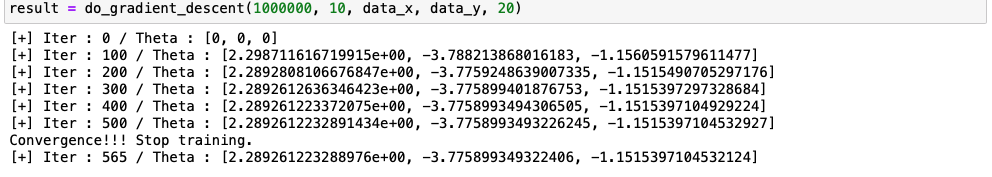
\includegraphics[width=15cm]{ml_2_4.png}
    \caption{Training with large learning rate}
    \label{fig:galaxy}
\end{figure}

As you can see, the $\theta$s converged after iteration of 500. Which was far less than original iteration count with learning rate of 0.1.

Thus, I learned following things:
\begin{itemize}
    \item When training logistic regression, the absolute value of update will be small. If we use learning rate that is too small, it will even slow down the training process as well. Therefore, picking a decent learning rate will accelerate training and converge all $\theta$s faster.
    \item Using overcomplicated model is not the key for accuracy and better results. 
\end{itemize}

\end{document}
